\chapter{Training}
\label{chap:training}

The following chapter presents the properties of the dataset that is later used to train a CNN as well as the necessary preprocessing to feed the data into the network. Additionally, the concept of data augmentation is introduced, which is used for creating a larger dataset to train on. Finally, various regularization techniques are considered that are employed to improve the results of the classification by combating overfitting.

	\section{Dataset}
The dataset used in the following experiments is made up of 90 microscopy images and their label images from three experiments on slightly different types of live \textit{Drosophila} cells. The dimension of all images is $960 \times 608$ pixels ($w \times h$) and the images are given in grayscale. The labelled images are of dimension $3 \times 960 \times 608 \times$ ($d \times w \times h$), where the background class is represented by RGB[0, 0, 0] (black), the cell body is marked as RGB[0, 255, 0] (green), the Lamellopodia are RGB[255, 0, 0] (red) and the Filopodia are RGB[0, 0, 255] (blue).

Another ``3-class'' version of the dataset was created in which the classes for Lamellopodia and Filopodia are fused into one, marked as RGB[255, 0, 0] (red). This was done because even for a human, separating Filopodia pixels from Lamellopodia pixels was hard to do because of the varying contrast in the images, and it was deemed valuable to see how a network performs if the ground truth data is more straight-forward to interpret.\\

\begin {figure}[!htb]
	
	\begin {subfigure}[{position=b}]{0.6\linewidth}
		\begin {center}
		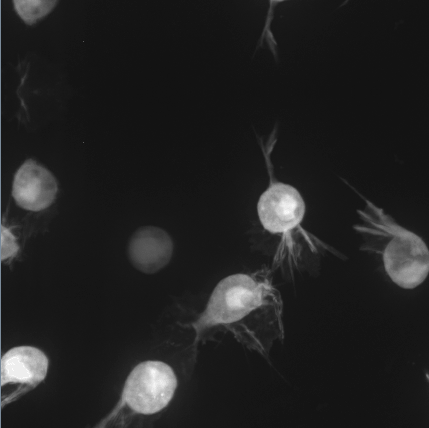
\includegraphics[scale=0.65]{img/dataset_ex1.png}
		\end{center}
	\end {subfigure}
	\begin {subfigure}[{position=b}]{0.3\linewidth}
		\begin {center}
		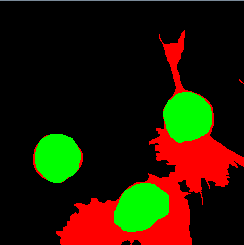
\includegraphics[scale=0.60]{img/dataset_ex2.png}
		\end{center}
	\end {subfigure}

		\caption[An example image tile from the 3-class dataset.]{An example image tile from the 3-class dataset with corresponding label image. The label image is smaller than the input tile because the image tile already includes a mirrored border as padding (see Section \textbf{\ref{subsec:mirror_tiling}}).}
		\label{fig:dataset_example}
	

\end {figure}

	\section {Preprocessing and Data Augmentation}
Usually, neural networks do not work well with input of an arbitrary form, which is why data is preprocessed before training the network on it. The same preprocessing is applied during classification of new images. Hence, in the following sections, the preprocessing operations performed on input data to the U-Net is described. Furthermore, the concept of \textit{data augmentation} is explored, which helps with training when data is scarce.


		\subsection{Normalization}
\label{subsec:normalization}
Neural networks perform consistently better when the input data is normalized, that is, when it is transformed into a representation which has zero mean and unit variance (see Section \textbf{\ref{sec:weight_init}}). This is achieved by subtracting the mean value of the input image per channel from each channel of that image\footnote{Another approach often used is to compute a mean image from all images in the dataset and substract that from each image. However, in the following experiments, individual means were used.} and then dividing by the image's standard deviation (see Figure \textbf{\ref{fig:norma}}).

\begin {figure}[!htb]
	\begin{center}
		\scalebox{1.0}{%% Creator: Matplotlib, PGF backend
%%
%% To include the figure in your LaTeX document, write
%%   \input{<filename>.pgf}
%%
%% Make sure the required packages are loaded in your preamble
%%   \usepackage{pgf}
%%
%% Figures using additional raster images can only be included by \input if
%% they are in the same directory as the main LaTeX file. For loading figures
%% from other directories you can use the `import` package
%%   \usepackage{import}
%% and then include the figures with
%%   \import{<path to file>}{<filename>.pgf}
%%
%% Matplotlib used the following preamble
%%   \usepackage{fontspec}
%%   \setmainfont{DejaVu Serif}
%%   \setsansfont{DejaVu Sans}
%%   \setmonofont{DejaVu Sans Mono}
%%
\begingroup%
\makeatletter%
\begin{pgfpicture}%
\pgfpathrectangle{\pgfpointorigin}{\pgfqpoint{4.000000in}{2.500000in}}%
\pgfusepath{use as bounding box, clip}%
\begin{pgfscope}%
\pgfsetbuttcap%
\pgfsetmiterjoin%
\definecolor{currentfill}{rgb}{1.000000,1.000000,1.000000}%
\pgfsetfillcolor{currentfill}%
\pgfsetlinewidth{0.000000pt}%
\definecolor{currentstroke}{rgb}{1.000000,1.000000,1.000000}%
\pgfsetstrokecolor{currentstroke}%
\pgfsetdash{}{0pt}%
\pgfpathmoveto{\pgfqpoint{0.000000in}{0.000000in}}%
\pgfpathlineto{\pgfqpoint{4.000000in}{0.000000in}}%
\pgfpathlineto{\pgfqpoint{4.000000in}{2.500000in}}%
\pgfpathlineto{\pgfqpoint{0.000000in}{2.500000in}}%
\pgfpathclose%
\pgfusepath{fill}%
\end{pgfscope}%
\begin{pgfscope}%
\pgfsetbuttcap%
\pgfsetmiterjoin%
\definecolor{currentfill}{rgb}{1.000000,1.000000,1.000000}%
\pgfsetfillcolor{currentfill}%
\pgfsetlinewidth{0.000000pt}%
\definecolor{currentstroke}{rgb}{0.000000,0.000000,0.000000}%
\pgfsetstrokecolor{currentstroke}%
\pgfsetstrokeopacity{0.000000}%
\pgfsetdash{}{0pt}%
\pgfpathmoveto{\pgfqpoint{0.647778in}{0.582778in}}%
\pgfpathlineto{\pgfqpoint{3.815000in}{0.582778in}}%
\pgfpathlineto{\pgfqpoint{3.815000in}{2.295000in}}%
\pgfpathlineto{\pgfqpoint{0.647778in}{2.295000in}}%
\pgfpathclose%
\pgfusepath{fill}%
\end{pgfscope}%
\begin{pgfscope}%
\pgfpathrectangle{\pgfqpoint{0.647778in}{0.582778in}}{\pgfqpoint{3.167222in}{1.712222in}} %
\pgfusepath{clip}%
\pgfsetbuttcap%
\pgfsetroundjoin%
\definecolor{currentfill}{rgb}{0.121569,0.466667,0.705882}%
\pgfsetfillcolor{currentfill}%
\pgfsetlinewidth{1.003750pt}%
\definecolor{currentstroke}{rgb}{0.121569,0.466667,0.705882}%
\pgfsetstrokecolor{currentstroke}%
\pgfsetdash{}{0pt}%
\pgfpathmoveto{\pgfqpoint{2.838705in}{1.702381in}}%
\pgfpathcurveto{\pgfqpoint{2.842388in}{1.702381in}}{\pgfqpoint{2.845922in}{1.703844in}}{\pgfqpoint{2.848526in}{1.706449in}}%
\pgfpathcurveto{\pgfqpoint{2.851131in}{1.709054in}}{\pgfqpoint{2.852594in}{1.712587in}}{\pgfqpoint{2.852594in}{1.716270in}}%
\pgfpathcurveto{\pgfqpoint{2.852594in}{1.719953in}}{\pgfqpoint{2.851131in}{1.723486in}}{\pgfqpoint{2.848526in}{1.726091in}}%
\pgfpathcurveto{\pgfqpoint{2.845922in}{1.728695in}}{\pgfqpoint{2.842388in}{1.730159in}}{\pgfqpoint{2.838705in}{1.730159in}}%
\pgfpathcurveto{\pgfqpoint{2.835022in}{1.730159in}}{\pgfqpoint{2.831489in}{1.728695in}}{\pgfqpoint{2.828884in}{1.726091in}}%
\pgfpathcurveto{\pgfqpoint{2.826280in}{1.723486in}}{\pgfqpoint{2.824816in}{1.719953in}}{\pgfqpoint{2.824816in}{1.716270in}}%
\pgfpathcurveto{\pgfqpoint{2.824816in}{1.712587in}}{\pgfqpoint{2.826280in}{1.709054in}}{\pgfqpoint{2.828884in}{1.706449in}}%
\pgfpathcurveto{\pgfqpoint{2.831489in}{1.703844in}}{\pgfqpoint{2.835022in}{1.702381in}}{\pgfqpoint{2.838705in}{1.702381in}}%
\pgfpathclose%
\pgfusepath{stroke,fill}%
\end{pgfscope}%
\begin{pgfscope}%
\pgfpathrectangle{\pgfqpoint{0.647778in}{0.582778in}}{\pgfqpoint{3.167222in}{1.712222in}} %
\pgfusepath{clip}%
\pgfsetbuttcap%
\pgfsetroundjoin%
\definecolor{currentfill}{rgb}{0.121569,0.466667,0.705882}%
\pgfsetfillcolor{currentfill}%
\pgfsetlinewidth{1.003750pt}%
\definecolor{currentstroke}{rgb}{0.121569,0.466667,0.705882}%
\pgfsetstrokecolor{currentstroke}%
\pgfsetdash{}{0pt}%
\pgfpathmoveto{\pgfqpoint{2.280190in}{1.776065in}}%
\pgfpathcurveto{\pgfqpoint{2.283874in}{1.776065in}}{\pgfqpoint{2.287407in}{1.777529in}}{\pgfqpoint{2.290011in}{1.780133in}}%
\pgfpathcurveto{\pgfqpoint{2.292616in}{1.782738in}}{\pgfqpoint{2.294079in}{1.786271in}}{\pgfqpoint{2.294079in}{1.789954in}}%
\pgfpathcurveto{\pgfqpoint{2.294079in}{1.793638in}}{\pgfqpoint{2.292616in}{1.797171in}}{\pgfqpoint{2.290011in}{1.799775in}}%
\pgfpathcurveto{\pgfqpoint{2.287407in}{1.802380in}}{\pgfqpoint{2.283874in}{1.803843in}}{\pgfqpoint{2.280190in}{1.803843in}}%
\pgfpathcurveto{\pgfqpoint{2.276507in}{1.803843in}}{\pgfqpoint{2.272974in}{1.802380in}}{\pgfqpoint{2.270369in}{1.799775in}}%
\pgfpathcurveto{\pgfqpoint{2.267765in}{1.797171in}}{\pgfqpoint{2.266301in}{1.793638in}}{\pgfqpoint{2.266301in}{1.789954in}}%
\pgfpathcurveto{\pgfqpoint{2.266301in}{1.786271in}}{\pgfqpoint{2.267765in}{1.782738in}}{\pgfqpoint{2.270369in}{1.780133in}}%
\pgfpathcurveto{\pgfqpoint{2.272974in}{1.777529in}}{\pgfqpoint{2.276507in}{1.776065in}}{\pgfqpoint{2.280190in}{1.776065in}}%
\pgfpathclose%
\pgfusepath{stroke,fill}%
\end{pgfscope}%
\begin{pgfscope}%
\pgfpathrectangle{\pgfqpoint{0.647778in}{0.582778in}}{\pgfqpoint{3.167222in}{1.712222in}} %
\pgfusepath{clip}%
\pgfsetbuttcap%
\pgfsetroundjoin%
\definecolor{currentfill}{rgb}{0.121569,0.466667,0.705882}%
\pgfsetfillcolor{currentfill}%
\pgfsetlinewidth{1.003750pt}%
\definecolor{currentstroke}{rgb}{0.121569,0.466667,0.705882}%
\pgfsetstrokecolor{currentstroke}%
\pgfsetdash{}{0pt}%
\pgfpathmoveto{\pgfqpoint{2.730633in}{1.684820in}}%
\pgfpathcurveto{\pgfqpoint{2.734317in}{1.684820in}}{\pgfqpoint{2.737850in}{1.686283in}}{\pgfqpoint{2.740454in}{1.688888in}}%
\pgfpathcurveto{\pgfqpoint{2.743059in}{1.691493in}}{\pgfqpoint{2.744522in}{1.695026in}}{\pgfqpoint{2.744522in}{1.698709in}}%
\pgfpathcurveto{\pgfqpoint{2.744522in}{1.702392in}}{\pgfqpoint{2.743059in}{1.705925in}}{\pgfqpoint{2.740454in}{1.708530in}}%
\pgfpathcurveto{\pgfqpoint{2.737850in}{1.711134in}}{\pgfqpoint{2.734317in}{1.712598in}}{\pgfqpoint{2.730633in}{1.712598in}}%
\pgfpathcurveto{\pgfqpoint{2.726950in}{1.712598in}}{\pgfqpoint{2.723417in}{1.711134in}}{\pgfqpoint{2.720812in}{1.708530in}}%
\pgfpathcurveto{\pgfqpoint{2.718208in}{1.705925in}}{\pgfqpoint{2.716744in}{1.702392in}}{\pgfqpoint{2.716744in}{1.698709in}}%
\pgfpathcurveto{\pgfqpoint{2.716744in}{1.695026in}}{\pgfqpoint{2.718208in}{1.691493in}}{\pgfqpoint{2.720812in}{1.688888in}}%
\pgfpathcurveto{\pgfqpoint{2.723417in}{1.686283in}}{\pgfqpoint{2.726950in}{1.684820in}}{\pgfqpoint{2.730633in}{1.684820in}}%
\pgfpathclose%
\pgfusepath{stroke,fill}%
\end{pgfscope}%
\begin{pgfscope}%
\pgfpathrectangle{\pgfqpoint{0.647778in}{0.582778in}}{\pgfqpoint{3.167222in}{1.712222in}} %
\pgfusepath{clip}%
\pgfsetbuttcap%
\pgfsetroundjoin%
\definecolor{currentfill}{rgb}{0.121569,0.466667,0.705882}%
\pgfsetfillcolor{currentfill}%
\pgfsetlinewidth{1.003750pt}%
\definecolor{currentstroke}{rgb}{0.121569,0.466667,0.705882}%
\pgfsetstrokecolor{currentstroke}%
\pgfsetdash{}{0pt}%
\pgfpathmoveto{\pgfqpoint{2.652050in}{1.790473in}}%
\pgfpathcurveto{\pgfqpoint{2.655733in}{1.790473in}}{\pgfqpoint{2.659266in}{1.791936in}}{\pgfqpoint{2.661871in}{1.794541in}}%
\pgfpathcurveto{\pgfqpoint{2.664475in}{1.797145in}}{\pgfqpoint{2.665939in}{1.800678in}}{\pgfqpoint{2.665939in}{1.804362in}}%
\pgfpathcurveto{\pgfqpoint{2.665939in}{1.808045in}}{\pgfqpoint{2.664475in}{1.811578in}}{\pgfqpoint{2.661871in}{1.814182in}}%
\pgfpathcurveto{\pgfqpoint{2.659266in}{1.816787in}}{\pgfqpoint{2.655733in}{1.818250in}}{\pgfqpoint{2.652050in}{1.818250in}}%
\pgfpathcurveto{\pgfqpoint{2.648367in}{1.818250in}}{\pgfqpoint{2.644834in}{1.816787in}}{\pgfqpoint{2.642229in}{1.814182in}}%
\pgfpathcurveto{\pgfqpoint{2.639625in}{1.811578in}}{\pgfqpoint{2.638161in}{1.808045in}}{\pgfqpoint{2.638161in}{1.804362in}}%
\pgfpathcurveto{\pgfqpoint{2.638161in}{1.800678in}}{\pgfqpoint{2.639625in}{1.797145in}}{\pgfqpoint{2.642229in}{1.794541in}}%
\pgfpathcurveto{\pgfqpoint{2.644834in}{1.791936in}}{\pgfqpoint{2.648367in}{1.790473in}}{\pgfqpoint{2.652050in}{1.790473in}}%
\pgfpathclose%
\pgfusepath{stroke,fill}%
\end{pgfscope}%
\begin{pgfscope}%
\pgfpathrectangle{\pgfqpoint{0.647778in}{0.582778in}}{\pgfqpoint{3.167222in}{1.712222in}} %
\pgfusepath{clip}%
\pgfsetbuttcap%
\pgfsetroundjoin%
\definecolor{currentfill}{rgb}{0.121569,0.466667,0.705882}%
\pgfsetfillcolor{currentfill}%
\pgfsetlinewidth{1.003750pt}%
\definecolor{currentstroke}{rgb}{0.121569,0.466667,0.705882}%
\pgfsetstrokecolor{currentstroke}%
\pgfsetdash{}{0pt}%
\pgfpathmoveto{\pgfqpoint{2.547862in}{1.957242in}}%
\pgfpathcurveto{\pgfqpoint{2.551546in}{1.957242in}}{\pgfqpoint{2.555079in}{1.958706in}}{\pgfqpoint{2.557683in}{1.961310in}}%
\pgfpathcurveto{\pgfqpoint{2.560288in}{1.963915in}}{\pgfqpoint{2.561751in}{1.967448in}}{\pgfqpoint{2.561751in}{1.971131in}}%
\pgfpathcurveto{\pgfqpoint{2.561751in}{1.974814in}}{\pgfqpoint{2.560288in}{1.978347in}}{\pgfqpoint{2.557683in}{1.980952in}}%
\pgfpathcurveto{\pgfqpoint{2.555079in}{1.983556in}}{\pgfqpoint{2.551546in}{1.985020in}}{\pgfqpoint{2.547862in}{1.985020in}}%
\pgfpathcurveto{\pgfqpoint{2.544179in}{1.985020in}}{\pgfqpoint{2.540646in}{1.983556in}}{\pgfqpoint{2.538041in}{1.980952in}}%
\pgfpathcurveto{\pgfqpoint{2.535437in}{1.978347in}}{\pgfqpoint{2.533973in}{1.974814in}}{\pgfqpoint{2.533973in}{1.971131in}}%
\pgfpathcurveto{\pgfqpoint{2.533973in}{1.967448in}}{\pgfqpoint{2.535437in}{1.963915in}}{\pgfqpoint{2.538041in}{1.961310in}}%
\pgfpathcurveto{\pgfqpoint{2.540646in}{1.958706in}}{\pgfqpoint{2.544179in}{1.957242in}}{\pgfqpoint{2.547862in}{1.957242in}}%
\pgfpathclose%
\pgfusepath{stroke,fill}%
\end{pgfscope}%
\begin{pgfscope}%
\pgfpathrectangle{\pgfqpoint{0.647778in}{0.582778in}}{\pgfqpoint{3.167222in}{1.712222in}} %
\pgfusepath{clip}%
\pgfsetbuttcap%
\pgfsetroundjoin%
\definecolor{currentfill}{rgb}{0.121569,0.466667,0.705882}%
\pgfsetfillcolor{currentfill}%
\pgfsetlinewidth{1.003750pt}%
\definecolor{currentstroke}{rgb}{0.121569,0.466667,0.705882}%
\pgfsetstrokecolor{currentstroke}%
\pgfsetdash{}{0pt}%
\pgfpathmoveto{\pgfqpoint{2.755171in}{1.875378in}}%
\pgfpathcurveto{\pgfqpoint{2.758855in}{1.875378in}}{\pgfqpoint{2.762388in}{1.876841in}}{\pgfqpoint{2.764992in}{1.879446in}}%
\pgfpathcurveto{\pgfqpoint{2.767597in}{1.882050in}}{\pgfqpoint{2.769060in}{1.885583in}}{\pgfqpoint{2.769060in}{1.889267in}}%
\pgfpathcurveto{\pgfqpoint{2.769060in}{1.892950in}}{\pgfqpoint{2.767597in}{1.896483in}}{\pgfqpoint{2.764992in}{1.899088in}}%
\pgfpathcurveto{\pgfqpoint{2.762388in}{1.901692in}}{\pgfqpoint{2.758855in}{1.903156in}}{\pgfqpoint{2.755171in}{1.903156in}}%
\pgfpathcurveto{\pgfqpoint{2.751488in}{1.903156in}}{\pgfqpoint{2.747955in}{1.901692in}}{\pgfqpoint{2.745350in}{1.899088in}}%
\pgfpathcurveto{\pgfqpoint{2.742746in}{1.896483in}}{\pgfqpoint{2.741282in}{1.892950in}}{\pgfqpoint{2.741282in}{1.889267in}}%
\pgfpathcurveto{\pgfqpoint{2.741282in}{1.885583in}}{\pgfqpoint{2.742746in}{1.882050in}}{\pgfqpoint{2.745350in}{1.879446in}}%
\pgfpathcurveto{\pgfqpoint{2.747955in}{1.876841in}}{\pgfqpoint{2.751488in}{1.875378in}}{\pgfqpoint{2.755171in}{1.875378in}}%
\pgfpathclose%
\pgfusepath{stroke,fill}%
\end{pgfscope}%
\begin{pgfscope}%
\pgfpathrectangle{\pgfqpoint{0.647778in}{0.582778in}}{\pgfqpoint{3.167222in}{1.712222in}} %
\pgfusepath{clip}%
\pgfsetbuttcap%
\pgfsetroundjoin%
\definecolor{currentfill}{rgb}{0.121569,0.466667,0.705882}%
\pgfsetfillcolor{currentfill}%
\pgfsetlinewidth{1.003750pt}%
\definecolor{currentstroke}{rgb}{0.121569,0.466667,0.705882}%
\pgfsetstrokecolor{currentstroke}%
\pgfsetdash{}{0pt}%
\pgfpathmoveto{\pgfqpoint{2.401399in}{1.821336in}}%
\pgfpathcurveto{\pgfqpoint{2.405083in}{1.821336in}}{\pgfqpoint{2.408616in}{1.822799in}}{\pgfqpoint{2.411220in}{1.825403in}}%
\pgfpathcurveto{\pgfqpoint{2.413825in}{1.828008in}}{\pgfqpoint{2.415288in}{1.831541in}}{\pgfqpoint{2.415288in}{1.835224in}}%
\pgfpathcurveto{\pgfqpoint{2.415288in}{1.838908in}}{\pgfqpoint{2.413825in}{1.842441in}}{\pgfqpoint{2.411220in}{1.845045in}}%
\pgfpathcurveto{\pgfqpoint{2.408616in}{1.847650in}}{\pgfqpoint{2.405083in}{1.849113in}}{\pgfqpoint{2.401399in}{1.849113in}}%
\pgfpathcurveto{\pgfqpoint{2.397716in}{1.849113in}}{\pgfqpoint{2.394183in}{1.847650in}}{\pgfqpoint{2.391578in}{1.845045in}}%
\pgfpathcurveto{\pgfqpoint{2.388974in}{1.842441in}}{\pgfqpoint{2.387511in}{1.838908in}}{\pgfqpoint{2.387511in}{1.835224in}}%
\pgfpathcurveto{\pgfqpoint{2.387511in}{1.831541in}}{\pgfqpoint{2.388974in}{1.828008in}}{\pgfqpoint{2.391578in}{1.825403in}}%
\pgfpathcurveto{\pgfqpoint{2.394183in}{1.822799in}}{\pgfqpoint{2.397716in}{1.821336in}}{\pgfqpoint{2.401399in}{1.821336in}}%
\pgfpathclose%
\pgfusepath{stroke,fill}%
\end{pgfscope}%
\begin{pgfscope}%
\pgfpathrectangle{\pgfqpoint{0.647778in}{0.582778in}}{\pgfqpoint{3.167222in}{1.712222in}} %
\pgfusepath{clip}%
\pgfsetbuttcap%
\pgfsetroundjoin%
\definecolor{currentfill}{rgb}{0.121569,0.466667,0.705882}%
\pgfsetfillcolor{currentfill}%
\pgfsetlinewidth{1.003750pt}%
\definecolor{currentstroke}{rgb}{0.121569,0.466667,0.705882}%
\pgfsetstrokecolor{currentstroke}%
\pgfsetdash{}{0pt}%
\pgfpathmoveto{\pgfqpoint{2.666497in}{1.898472in}}%
\pgfpathcurveto{\pgfqpoint{2.670180in}{1.898472in}}{\pgfqpoint{2.673713in}{1.899935in}}{\pgfqpoint{2.676318in}{1.902540in}}%
\pgfpathcurveto{\pgfqpoint{2.678922in}{1.905144in}}{\pgfqpoint{2.680386in}{1.908678in}}{\pgfqpoint{2.680386in}{1.912361in}}%
\pgfpathcurveto{\pgfqpoint{2.680386in}{1.916044in}}{\pgfqpoint{2.678922in}{1.919577in}}{\pgfqpoint{2.676318in}{1.922182in}}%
\pgfpathcurveto{\pgfqpoint{2.673713in}{1.924786in}}{\pgfqpoint{2.670180in}{1.926250in}}{\pgfqpoint{2.666497in}{1.926250in}}%
\pgfpathcurveto{\pgfqpoint{2.662813in}{1.926250in}}{\pgfqpoint{2.659280in}{1.924786in}}{\pgfqpoint{2.656676in}{1.922182in}}%
\pgfpathcurveto{\pgfqpoint{2.654071in}{1.919577in}}{\pgfqpoint{2.652608in}{1.916044in}}{\pgfqpoint{2.652608in}{1.912361in}}%
\pgfpathcurveto{\pgfqpoint{2.652608in}{1.908678in}}{\pgfqpoint{2.654071in}{1.905144in}}{\pgfqpoint{2.656676in}{1.902540in}}%
\pgfpathcurveto{\pgfqpoint{2.659280in}{1.899935in}}{\pgfqpoint{2.662813in}{1.898472in}}{\pgfqpoint{2.666497in}{1.898472in}}%
\pgfpathclose%
\pgfusepath{stroke,fill}%
\end{pgfscope}%
\begin{pgfscope}%
\pgfpathrectangle{\pgfqpoint{0.647778in}{0.582778in}}{\pgfqpoint{3.167222in}{1.712222in}} %
\pgfusepath{clip}%
\pgfsetbuttcap%
\pgfsetroundjoin%
\definecolor{currentfill}{rgb}{0.121569,0.466667,0.705882}%
\pgfsetfillcolor{currentfill}%
\pgfsetlinewidth{1.003750pt}%
\definecolor{currentstroke}{rgb}{0.121569,0.466667,0.705882}%
\pgfsetstrokecolor{currentstroke}%
\pgfsetdash{}{0pt}%
\pgfpathmoveto{\pgfqpoint{2.069422in}{1.909197in}}%
\pgfpathcurveto{\pgfqpoint{2.073105in}{1.909197in}}{\pgfqpoint{2.076638in}{1.910661in}}{\pgfqpoint{2.079242in}{1.913265in}}%
\pgfpathcurveto{\pgfqpoint{2.081847in}{1.915870in}}{\pgfqpoint{2.083310in}{1.919403in}}{\pgfqpoint{2.083310in}{1.923086in}}%
\pgfpathcurveto{\pgfqpoint{2.083310in}{1.926769in}}{\pgfqpoint{2.081847in}{1.930302in}}{\pgfqpoint{2.079242in}{1.932907in}}%
\pgfpathcurveto{\pgfqpoint{2.076638in}{1.935512in}}{\pgfqpoint{2.073105in}{1.936975in}}{\pgfqpoint{2.069422in}{1.936975in}}%
\pgfpathcurveto{\pgfqpoint{2.065738in}{1.936975in}}{\pgfqpoint{2.062205in}{1.935512in}}{\pgfqpoint{2.059601in}{1.932907in}}%
\pgfpathcurveto{\pgfqpoint{2.056996in}{1.930302in}}{\pgfqpoint{2.055533in}{1.926769in}}{\pgfqpoint{2.055533in}{1.923086in}}%
\pgfpathcurveto{\pgfqpoint{2.055533in}{1.919403in}}{\pgfqpoint{2.056996in}{1.915870in}}{\pgfqpoint{2.059601in}{1.913265in}}%
\pgfpathcurveto{\pgfqpoint{2.062205in}{1.910661in}}{\pgfqpoint{2.065738in}{1.909197in}}{\pgfqpoint{2.069422in}{1.909197in}}%
\pgfpathclose%
\pgfusepath{stroke,fill}%
\end{pgfscope}%
\begin{pgfscope}%
\pgfpathrectangle{\pgfqpoint{0.647778in}{0.582778in}}{\pgfqpoint{3.167222in}{1.712222in}} %
\pgfusepath{clip}%
\pgfsetbuttcap%
\pgfsetroundjoin%
\definecolor{currentfill}{rgb}{0.121569,0.466667,0.705882}%
\pgfsetfillcolor{currentfill}%
\pgfsetlinewidth{1.003750pt}%
\definecolor{currentstroke}{rgb}{0.121569,0.466667,0.705882}%
\pgfsetstrokecolor{currentstroke}%
\pgfsetdash{}{0pt}%
\pgfpathmoveto{\pgfqpoint{2.581499in}{1.924917in}}%
\pgfpathcurveto{\pgfqpoint{2.585182in}{1.924917in}}{\pgfqpoint{2.588715in}{1.926380in}}{\pgfqpoint{2.591320in}{1.928985in}}%
\pgfpathcurveto{\pgfqpoint{2.593925in}{1.931589in}}{\pgfqpoint{2.595388in}{1.935122in}}{\pgfqpoint{2.595388in}{1.938805in}}%
\pgfpathcurveto{\pgfqpoint{2.595388in}{1.942489in}}{\pgfqpoint{2.593925in}{1.946022in}}{\pgfqpoint{2.591320in}{1.948626in}}%
\pgfpathcurveto{\pgfqpoint{2.588715in}{1.951231in}}{\pgfqpoint{2.585182in}{1.952694in}}{\pgfqpoint{2.581499in}{1.952694in}}%
\pgfpathcurveto{\pgfqpoint{2.577816in}{1.952694in}}{\pgfqpoint{2.574283in}{1.951231in}}{\pgfqpoint{2.571678in}{1.948626in}}%
\pgfpathcurveto{\pgfqpoint{2.569074in}{1.946022in}}{\pgfqpoint{2.567610in}{1.942489in}}{\pgfqpoint{2.567610in}{1.938805in}}%
\pgfpathcurveto{\pgfqpoint{2.567610in}{1.935122in}}{\pgfqpoint{2.569074in}{1.931589in}}{\pgfqpoint{2.571678in}{1.928985in}}%
\pgfpathcurveto{\pgfqpoint{2.574283in}{1.926380in}}{\pgfqpoint{2.577816in}{1.924917in}}{\pgfqpoint{2.581499in}{1.924917in}}%
\pgfpathclose%
\pgfusepath{stroke,fill}%
\end{pgfscope}%
\begin{pgfscope}%
\pgfpathrectangle{\pgfqpoint{0.647778in}{0.582778in}}{\pgfqpoint{3.167222in}{1.712222in}} %
\pgfusepath{clip}%
\pgfsetbuttcap%
\pgfsetroundjoin%
\definecolor{currentfill}{rgb}{0.121569,0.466667,0.705882}%
\pgfsetfillcolor{currentfill}%
\pgfsetlinewidth{1.003750pt}%
\definecolor{currentstroke}{rgb}{0.121569,0.466667,0.705882}%
\pgfsetstrokecolor{currentstroke}%
\pgfsetdash{}{0pt}%
\pgfpathmoveto{\pgfqpoint{1.721913in}{1.885108in}}%
\pgfpathcurveto{\pgfqpoint{1.725597in}{1.885108in}}{\pgfqpoint{1.729130in}{1.886571in}}{\pgfqpoint{1.731734in}{1.889176in}}%
\pgfpathcurveto{\pgfqpoint{1.734339in}{1.891780in}}{\pgfqpoint{1.735802in}{1.895313in}}{\pgfqpoint{1.735802in}{1.898997in}}%
\pgfpathcurveto{\pgfqpoint{1.735802in}{1.902680in}}{\pgfqpoint{1.734339in}{1.906213in}}{\pgfqpoint{1.731734in}{1.908818in}}%
\pgfpathcurveto{\pgfqpoint{1.729130in}{1.911422in}}{\pgfqpoint{1.725597in}{1.912886in}}{\pgfqpoint{1.721913in}{1.912886in}}%
\pgfpathcurveto{\pgfqpoint{1.718230in}{1.912886in}}{\pgfqpoint{1.714697in}{1.911422in}}{\pgfqpoint{1.712092in}{1.908818in}}%
\pgfpathcurveto{\pgfqpoint{1.709488in}{1.906213in}}{\pgfqpoint{1.708024in}{1.902680in}}{\pgfqpoint{1.708024in}{1.898997in}}%
\pgfpathcurveto{\pgfqpoint{1.708024in}{1.895313in}}{\pgfqpoint{1.709488in}{1.891780in}}{\pgfqpoint{1.712092in}{1.889176in}}%
\pgfpathcurveto{\pgfqpoint{1.714697in}{1.886571in}}{\pgfqpoint{1.718230in}{1.885108in}}{\pgfqpoint{1.721913in}{1.885108in}}%
\pgfpathclose%
\pgfusepath{stroke,fill}%
\end{pgfscope}%
\begin{pgfscope}%
\pgfpathrectangle{\pgfqpoint{0.647778in}{0.582778in}}{\pgfqpoint{3.167222in}{1.712222in}} %
\pgfusepath{clip}%
\pgfsetbuttcap%
\pgfsetroundjoin%
\definecolor{currentfill}{rgb}{0.121569,0.466667,0.705882}%
\pgfsetfillcolor{currentfill}%
\pgfsetlinewidth{1.003750pt}%
\definecolor{currentstroke}{rgb}{0.121569,0.466667,0.705882}%
\pgfsetstrokecolor{currentstroke}%
\pgfsetdash{}{0pt}%
\pgfpathmoveto{\pgfqpoint{2.090576in}{1.855610in}}%
\pgfpathcurveto{\pgfqpoint{2.094260in}{1.855610in}}{\pgfqpoint{2.097793in}{1.857074in}}{\pgfqpoint{2.100397in}{1.859678in}}%
\pgfpathcurveto{\pgfqpoint{2.103002in}{1.862283in}}{\pgfqpoint{2.104465in}{1.865816in}}{\pgfqpoint{2.104465in}{1.869499in}}%
\pgfpathcurveto{\pgfqpoint{2.104465in}{1.873182in}}{\pgfqpoint{2.103002in}{1.876715in}}{\pgfqpoint{2.100397in}{1.879320in}}%
\pgfpathcurveto{\pgfqpoint{2.097793in}{1.881924in}}{\pgfqpoint{2.094260in}{1.883388in}}{\pgfqpoint{2.090576in}{1.883388in}}%
\pgfpathcurveto{\pgfqpoint{2.086893in}{1.883388in}}{\pgfqpoint{2.083360in}{1.881924in}}{\pgfqpoint{2.080755in}{1.879320in}}%
\pgfpathcurveto{\pgfqpoint{2.078151in}{1.876715in}}{\pgfqpoint{2.076687in}{1.873182in}}{\pgfqpoint{2.076687in}{1.869499in}}%
\pgfpathcurveto{\pgfqpoint{2.076687in}{1.865816in}}{\pgfqpoint{2.078151in}{1.862283in}}{\pgfqpoint{2.080755in}{1.859678in}}%
\pgfpathcurveto{\pgfqpoint{2.083360in}{1.857074in}}{\pgfqpoint{2.086893in}{1.855610in}}{\pgfqpoint{2.090576in}{1.855610in}}%
\pgfpathclose%
\pgfusepath{stroke,fill}%
\end{pgfscope}%
\begin{pgfscope}%
\pgfpathrectangle{\pgfqpoint{0.647778in}{0.582778in}}{\pgfqpoint{3.167222in}{1.712222in}} %
\pgfusepath{clip}%
\pgfsetbuttcap%
\pgfsetroundjoin%
\definecolor{currentfill}{rgb}{0.121569,0.466667,0.705882}%
\pgfsetfillcolor{currentfill}%
\pgfsetlinewidth{1.003750pt}%
\definecolor{currentstroke}{rgb}{0.121569,0.466667,0.705882}%
\pgfsetstrokecolor{currentstroke}%
\pgfsetdash{}{0pt}%
\pgfpathmoveto{\pgfqpoint{2.149283in}{1.636023in}}%
\pgfpathcurveto{\pgfqpoint{2.152966in}{1.636023in}}{\pgfqpoint{2.156499in}{1.637486in}}{\pgfqpoint{2.159104in}{1.640091in}}%
\pgfpathcurveto{\pgfqpoint{2.161708in}{1.642696in}}{\pgfqpoint{2.163172in}{1.646229in}}{\pgfqpoint{2.163172in}{1.649912in}}%
\pgfpathcurveto{\pgfqpoint{2.163172in}{1.653595in}}{\pgfqpoint{2.161708in}{1.657128in}}{\pgfqpoint{2.159104in}{1.659733in}}%
\pgfpathcurveto{\pgfqpoint{2.156499in}{1.662337in}}{\pgfqpoint{2.152966in}{1.663801in}}{\pgfqpoint{2.149283in}{1.663801in}}%
\pgfpathcurveto{\pgfqpoint{2.145599in}{1.663801in}}{\pgfqpoint{2.142066in}{1.662337in}}{\pgfqpoint{2.139462in}{1.659733in}}%
\pgfpathcurveto{\pgfqpoint{2.136857in}{1.657128in}}{\pgfqpoint{2.135394in}{1.653595in}}{\pgfqpoint{2.135394in}{1.649912in}}%
\pgfpathcurveto{\pgfqpoint{2.135394in}{1.646229in}}{\pgfqpoint{2.136857in}{1.642696in}}{\pgfqpoint{2.139462in}{1.640091in}}%
\pgfpathcurveto{\pgfqpoint{2.142066in}{1.637486in}}{\pgfqpoint{2.145599in}{1.636023in}}{\pgfqpoint{2.149283in}{1.636023in}}%
\pgfpathclose%
\pgfusepath{stroke,fill}%
\end{pgfscope}%
\begin{pgfscope}%
\pgfpathrectangle{\pgfqpoint{0.647778in}{0.582778in}}{\pgfqpoint{3.167222in}{1.712222in}} %
\pgfusepath{clip}%
\pgfsetbuttcap%
\pgfsetroundjoin%
\definecolor{currentfill}{rgb}{0.121569,0.466667,0.705882}%
\pgfsetfillcolor{currentfill}%
\pgfsetlinewidth{1.003750pt}%
\definecolor{currentstroke}{rgb}{0.121569,0.466667,0.705882}%
\pgfsetstrokecolor{currentstroke}%
\pgfsetdash{}{0pt}%
\pgfpathmoveto{\pgfqpoint{2.123881in}{1.765055in}}%
\pgfpathcurveto{\pgfqpoint{2.127565in}{1.765055in}}{\pgfqpoint{2.131098in}{1.766518in}}{\pgfqpoint{2.133702in}{1.769123in}}%
\pgfpathcurveto{\pgfqpoint{2.136307in}{1.771727in}}{\pgfqpoint{2.137770in}{1.775260in}}{\pgfqpoint{2.137770in}{1.778944in}}%
\pgfpathcurveto{\pgfqpoint{2.137770in}{1.782627in}}{\pgfqpoint{2.136307in}{1.786160in}}{\pgfqpoint{2.133702in}{1.788765in}}%
\pgfpathcurveto{\pgfqpoint{2.131098in}{1.791369in}}{\pgfqpoint{2.127565in}{1.792833in}}{\pgfqpoint{2.123881in}{1.792833in}}%
\pgfpathcurveto{\pgfqpoint{2.120198in}{1.792833in}}{\pgfqpoint{2.116665in}{1.791369in}}{\pgfqpoint{2.114060in}{1.788765in}}%
\pgfpathcurveto{\pgfqpoint{2.111456in}{1.786160in}}{\pgfqpoint{2.109993in}{1.782627in}}{\pgfqpoint{2.109993in}{1.778944in}}%
\pgfpathcurveto{\pgfqpoint{2.109993in}{1.775260in}}{\pgfqpoint{2.111456in}{1.771727in}}{\pgfqpoint{2.114060in}{1.769123in}}%
\pgfpathcurveto{\pgfqpoint{2.116665in}{1.766518in}}{\pgfqpoint{2.120198in}{1.765055in}}{\pgfqpoint{2.123881in}{1.765055in}}%
\pgfpathclose%
\pgfusepath{stroke,fill}%
\end{pgfscope}%
\begin{pgfscope}%
\pgfpathrectangle{\pgfqpoint{0.647778in}{0.582778in}}{\pgfqpoint{3.167222in}{1.712222in}} %
\pgfusepath{clip}%
\pgfsetbuttcap%
\pgfsetroundjoin%
\definecolor{currentfill}{rgb}{0.121569,0.466667,0.705882}%
\pgfsetfillcolor{currentfill}%
\pgfsetlinewidth{1.003750pt}%
\definecolor{currentstroke}{rgb}{0.121569,0.466667,0.705882}%
\pgfsetstrokecolor{currentstroke}%
\pgfsetdash{}{0pt}%
\pgfpathmoveto{\pgfqpoint{2.752169in}{1.959696in}}%
\pgfpathcurveto{\pgfqpoint{2.755853in}{1.959696in}}{\pgfqpoint{2.759386in}{1.961160in}}{\pgfqpoint{2.761990in}{1.963764in}}%
\pgfpathcurveto{\pgfqpoint{2.764595in}{1.966369in}}{\pgfqpoint{2.766058in}{1.969902in}}{\pgfqpoint{2.766058in}{1.973585in}}%
\pgfpathcurveto{\pgfqpoint{2.766058in}{1.977269in}}{\pgfqpoint{2.764595in}{1.980802in}}{\pgfqpoint{2.761990in}{1.983406in}}%
\pgfpathcurveto{\pgfqpoint{2.759386in}{1.986011in}}{\pgfqpoint{2.755853in}{1.987474in}}{\pgfqpoint{2.752169in}{1.987474in}}%
\pgfpathcurveto{\pgfqpoint{2.748486in}{1.987474in}}{\pgfqpoint{2.744953in}{1.986011in}}{\pgfqpoint{2.742348in}{1.983406in}}%
\pgfpathcurveto{\pgfqpoint{2.739744in}{1.980802in}}{\pgfqpoint{2.738280in}{1.977269in}}{\pgfqpoint{2.738280in}{1.973585in}}%
\pgfpathcurveto{\pgfqpoint{2.738280in}{1.969902in}}{\pgfqpoint{2.739744in}{1.966369in}}{\pgfqpoint{2.742348in}{1.963764in}}%
\pgfpathcurveto{\pgfqpoint{2.744953in}{1.961160in}}{\pgfqpoint{2.748486in}{1.959696in}}{\pgfqpoint{2.752169in}{1.959696in}}%
\pgfpathclose%
\pgfusepath{stroke,fill}%
\end{pgfscope}%
\begin{pgfscope}%
\pgfpathrectangle{\pgfqpoint{0.647778in}{0.582778in}}{\pgfqpoint{3.167222in}{1.712222in}} %
\pgfusepath{clip}%
\pgfsetbuttcap%
\pgfsetroundjoin%
\definecolor{currentfill}{rgb}{0.121569,0.466667,0.705882}%
\pgfsetfillcolor{currentfill}%
\pgfsetlinewidth{1.003750pt}%
\definecolor{currentstroke}{rgb}{0.121569,0.466667,0.705882}%
\pgfsetstrokecolor{currentstroke}%
\pgfsetdash{}{0pt}%
\pgfpathmoveto{\pgfqpoint{2.968167in}{1.803181in}}%
\pgfpathcurveto{\pgfqpoint{2.971851in}{1.803181in}}{\pgfqpoint{2.975384in}{1.804645in}}{\pgfqpoint{2.977988in}{1.807249in}}%
\pgfpathcurveto{\pgfqpoint{2.980593in}{1.809854in}}{\pgfqpoint{2.982056in}{1.813387in}}{\pgfqpoint{2.982056in}{1.817070in}}%
\pgfpathcurveto{\pgfqpoint{2.982056in}{1.820753in}}{\pgfqpoint{2.980593in}{1.824287in}}{\pgfqpoint{2.977988in}{1.826891in}}%
\pgfpathcurveto{\pgfqpoint{2.975384in}{1.829496in}}{\pgfqpoint{2.971851in}{1.830959in}}{\pgfqpoint{2.968167in}{1.830959in}}%
\pgfpathcurveto{\pgfqpoint{2.964484in}{1.830959in}}{\pgfqpoint{2.960951in}{1.829496in}}{\pgfqpoint{2.958346in}{1.826891in}}%
\pgfpathcurveto{\pgfqpoint{2.955742in}{1.824287in}}{\pgfqpoint{2.954278in}{1.820753in}}{\pgfqpoint{2.954278in}{1.817070in}}%
\pgfpathcurveto{\pgfqpoint{2.954278in}{1.813387in}}{\pgfqpoint{2.955742in}{1.809854in}}{\pgfqpoint{2.958346in}{1.807249in}}%
\pgfpathcurveto{\pgfqpoint{2.960951in}{1.804645in}}{\pgfqpoint{2.964484in}{1.803181in}}{\pgfqpoint{2.968167in}{1.803181in}}%
\pgfpathclose%
\pgfusepath{stroke,fill}%
\end{pgfscope}%
\begin{pgfscope}%
\pgfpathrectangle{\pgfqpoint{0.647778in}{0.582778in}}{\pgfqpoint{3.167222in}{1.712222in}} %
\pgfusepath{clip}%
\pgfsetbuttcap%
\pgfsetroundjoin%
\definecolor{currentfill}{rgb}{0.121569,0.466667,0.705882}%
\pgfsetfillcolor{currentfill}%
\pgfsetlinewidth{1.003750pt}%
\definecolor{currentstroke}{rgb}{0.121569,0.466667,0.705882}%
\pgfsetstrokecolor{currentstroke}%
\pgfsetdash{}{0pt}%
\pgfpathmoveto{\pgfqpoint{1.539840in}{2.017298in}}%
\pgfpathcurveto{\pgfqpoint{1.543524in}{2.017298in}}{\pgfqpoint{1.547057in}{2.018762in}}{\pgfqpoint{1.549661in}{2.021366in}}%
\pgfpathcurveto{\pgfqpoint{1.552266in}{2.023971in}}{\pgfqpoint{1.553729in}{2.027504in}}{\pgfqpoint{1.553729in}{2.031187in}}%
\pgfpathcurveto{\pgfqpoint{1.553729in}{2.034871in}}{\pgfqpoint{1.552266in}{2.038404in}}{\pgfqpoint{1.549661in}{2.041008in}}%
\pgfpathcurveto{\pgfqpoint{1.547057in}{2.043613in}}{\pgfqpoint{1.543524in}{2.045076in}}{\pgfqpoint{1.539840in}{2.045076in}}%
\pgfpathcurveto{\pgfqpoint{1.536157in}{2.045076in}}{\pgfqpoint{1.532624in}{2.043613in}}{\pgfqpoint{1.530019in}{2.041008in}}%
\pgfpathcurveto{\pgfqpoint{1.527415in}{2.038404in}}{\pgfqpoint{1.525951in}{2.034871in}}{\pgfqpoint{1.525951in}{2.031187in}}%
\pgfpathcurveto{\pgfqpoint{1.525951in}{2.027504in}}{\pgfqpoint{1.527415in}{2.023971in}}{\pgfqpoint{1.530019in}{2.021366in}}%
\pgfpathcurveto{\pgfqpoint{1.532624in}{2.018762in}}{\pgfqpoint{1.536157in}{2.017298in}}{\pgfqpoint{1.539840in}{2.017298in}}%
\pgfpathclose%
\pgfusepath{stroke,fill}%
\end{pgfscope}%
\begin{pgfscope}%
\pgfpathrectangle{\pgfqpoint{0.647778in}{0.582778in}}{\pgfqpoint{3.167222in}{1.712222in}} %
\pgfusepath{clip}%
\pgfsetbuttcap%
\pgfsetroundjoin%
\definecolor{currentfill}{rgb}{0.121569,0.466667,0.705882}%
\pgfsetfillcolor{currentfill}%
\pgfsetlinewidth{1.003750pt}%
\definecolor{currentstroke}{rgb}{0.121569,0.466667,0.705882}%
\pgfsetstrokecolor{currentstroke}%
\pgfsetdash{}{0pt}%
\pgfpathmoveto{\pgfqpoint{2.419404in}{2.007980in}}%
\pgfpathcurveto{\pgfqpoint{2.423088in}{2.007980in}}{\pgfqpoint{2.426621in}{2.009443in}}{\pgfqpoint{2.429225in}{2.012048in}}%
\pgfpathcurveto{\pgfqpoint{2.431830in}{2.014652in}}{\pgfqpoint{2.433293in}{2.018185in}}{\pgfqpoint{2.433293in}{2.021869in}}%
\pgfpathcurveto{\pgfqpoint{2.433293in}{2.025552in}}{\pgfqpoint{2.431830in}{2.029085in}}{\pgfqpoint{2.429225in}{2.031690in}}%
\pgfpathcurveto{\pgfqpoint{2.426621in}{2.034294in}}{\pgfqpoint{2.423088in}{2.035758in}}{\pgfqpoint{2.419404in}{2.035758in}}%
\pgfpathcurveto{\pgfqpoint{2.415721in}{2.035758in}}{\pgfqpoint{2.412188in}{2.034294in}}{\pgfqpoint{2.409584in}{2.031690in}}%
\pgfpathcurveto{\pgfqpoint{2.406979in}{2.029085in}}{\pgfqpoint{2.405516in}{2.025552in}}{\pgfqpoint{2.405516in}{2.021869in}}%
\pgfpathcurveto{\pgfqpoint{2.405516in}{2.018185in}}{\pgfqpoint{2.406979in}{2.014652in}}{\pgfqpoint{2.409584in}{2.012048in}}%
\pgfpathcurveto{\pgfqpoint{2.412188in}{2.009443in}}{\pgfqpoint{2.415721in}{2.007980in}}{\pgfqpoint{2.419404in}{2.007980in}}%
\pgfpathclose%
\pgfusepath{stroke,fill}%
\end{pgfscope}%
\begin{pgfscope}%
\pgfpathrectangle{\pgfqpoint{0.647778in}{0.582778in}}{\pgfqpoint{3.167222in}{1.712222in}} %
\pgfusepath{clip}%
\pgfsetbuttcap%
\pgfsetroundjoin%
\definecolor{currentfill}{rgb}{0.121569,0.466667,0.705882}%
\pgfsetfillcolor{currentfill}%
\pgfsetlinewidth{1.003750pt}%
\definecolor{currentstroke}{rgb}{0.121569,0.466667,0.705882}%
\pgfsetstrokecolor{currentstroke}%
\pgfsetdash{}{0pt}%
\pgfpathmoveto{\pgfqpoint{2.414538in}{1.850551in}}%
\pgfpathcurveto{\pgfqpoint{2.418221in}{1.850551in}}{\pgfqpoint{2.421754in}{1.852014in}}{\pgfqpoint{2.424359in}{1.854619in}}%
\pgfpathcurveto{\pgfqpoint{2.426963in}{1.857223in}}{\pgfqpoint{2.428427in}{1.860756in}}{\pgfqpoint{2.428427in}{1.864440in}}%
\pgfpathcurveto{\pgfqpoint{2.428427in}{1.868123in}}{\pgfqpoint{2.426963in}{1.871656in}}{\pgfqpoint{2.424359in}{1.874261in}}%
\pgfpathcurveto{\pgfqpoint{2.421754in}{1.876865in}}{\pgfqpoint{2.418221in}{1.878329in}}{\pgfqpoint{2.414538in}{1.878329in}}%
\pgfpathcurveto{\pgfqpoint{2.410855in}{1.878329in}}{\pgfqpoint{2.407322in}{1.876865in}}{\pgfqpoint{2.404717in}{1.874261in}}%
\pgfpathcurveto{\pgfqpoint{2.402113in}{1.871656in}}{\pgfqpoint{2.400649in}{1.868123in}}{\pgfqpoint{2.400649in}{1.864440in}}%
\pgfpathcurveto{\pgfqpoint{2.400649in}{1.860756in}}{\pgfqpoint{2.402113in}{1.857223in}}{\pgfqpoint{2.404717in}{1.854619in}}%
\pgfpathcurveto{\pgfqpoint{2.407322in}{1.852014in}}{\pgfqpoint{2.410855in}{1.850551in}}{\pgfqpoint{2.414538in}{1.850551in}}%
\pgfpathclose%
\pgfusepath{stroke,fill}%
\end{pgfscope}%
\begin{pgfscope}%
\pgfpathrectangle{\pgfqpoint{0.647778in}{0.582778in}}{\pgfqpoint{3.167222in}{1.712222in}} %
\pgfusepath{clip}%
\pgfsetbuttcap%
\pgfsetroundjoin%
\definecolor{currentfill}{rgb}{0.121569,0.466667,0.705882}%
\pgfsetfillcolor{currentfill}%
\pgfsetlinewidth{1.003750pt}%
\definecolor{currentstroke}{rgb}{0.121569,0.466667,0.705882}%
\pgfsetstrokecolor{currentstroke}%
\pgfsetdash{}{0pt}%
\pgfpathmoveto{\pgfqpoint{2.486783in}{1.608744in}}%
\pgfpathcurveto{\pgfqpoint{2.490467in}{1.608744in}}{\pgfqpoint{2.494000in}{1.610208in}}{\pgfqpoint{2.496604in}{1.612812in}}%
\pgfpathcurveto{\pgfqpoint{2.499209in}{1.615417in}}{\pgfqpoint{2.500672in}{1.618950in}}{\pgfqpoint{2.500672in}{1.622633in}}%
\pgfpathcurveto{\pgfqpoint{2.500672in}{1.626317in}}{\pgfqpoint{2.499209in}{1.629850in}}{\pgfqpoint{2.496604in}{1.632454in}}%
\pgfpathcurveto{\pgfqpoint{2.494000in}{1.635059in}}{\pgfqpoint{2.490467in}{1.636522in}}{\pgfqpoint{2.486783in}{1.636522in}}%
\pgfpathcurveto{\pgfqpoint{2.483100in}{1.636522in}}{\pgfqpoint{2.479567in}{1.635059in}}{\pgfqpoint{2.476962in}{1.632454in}}%
\pgfpathcurveto{\pgfqpoint{2.474358in}{1.629850in}}{\pgfqpoint{2.472894in}{1.626317in}}{\pgfqpoint{2.472894in}{1.622633in}}%
\pgfpathcurveto{\pgfqpoint{2.472894in}{1.618950in}}{\pgfqpoint{2.474358in}{1.615417in}}{\pgfqpoint{2.476962in}{1.612812in}}%
\pgfpathcurveto{\pgfqpoint{2.479567in}{1.610208in}}{\pgfqpoint{2.483100in}{1.608744in}}{\pgfqpoint{2.486783in}{1.608744in}}%
\pgfpathclose%
\pgfusepath{stroke,fill}%
\end{pgfscope}%
\begin{pgfscope}%
\pgfpathrectangle{\pgfqpoint{0.647778in}{0.582778in}}{\pgfqpoint{3.167222in}{1.712222in}} %
\pgfusepath{clip}%
\pgfsetbuttcap%
\pgfsetroundjoin%
\definecolor{currentfill}{rgb}{0.121569,0.466667,0.705882}%
\pgfsetfillcolor{currentfill}%
\pgfsetlinewidth{1.003750pt}%
\definecolor{currentstroke}{rgb}{0.121569,0.466667,0.705882}%
\pgfsetstrokecolor{currentstroke}%
\pgfsetdash{}{0pt}%
\pgfpathmoveto{\pgfqpoint{1.894262in}{1.720413in}}%
\pgfpathcurveto{\pgfqpoint{1.897946in}{1.720413in}}{\pgfqpoint{1.901479in}{1.721876in}}{\pgfqpoint{1.904083in}{1.724481in}}%
\pgfpathcurveto{\pgfqpoint{1.906688in}{1.727085in}}{\pgfqpoint{1.908151in}{1.730618in}}{\pgfqpoint{1.908151in}{1.734302in}}%
\pgfpathcurveto{\pgfqpoint{1.908151in}{1.737985in}}{\pgfqpoint{1.906688in}{1.741518in}}{\pgfqpoint{1.904083in}{1.744122in}}%
\pgfpathcurveto{\pgfqpoint{1.901479in}{1.746727in}}{\pgfqpoint{1.897946in}{1.748190in}}{\pgfqpoint{1.894262in}{1.748190in}}%
\pgfpathcurveto{\pgfqpoint{1.890579in}{1.748190in}}{\pgfqpoint{1.887046in}{1.746727in}}{\pgfqpoint{1.884442in}{1.744122in}}%
\pgfpathcurveto{\pgfqpoint{1.881837in}{1.741518in}}{\pgfqpoint{1.880374in}{1.737985in}}{\pgfqpoint{1.880374in}{1.734302in}}%
\pgfpathcurveto{\pgfqpoint{1.880374in}{1.730618in}}{\pgfqpoint{1.881837in}{1.727085in}}{\pgfqpoint{1.884442in}{1.724481in}}%
\pgfpathcurveto{\pgfqpoint{1.887046in}{1.721876in}}{\pgfqpoint{1.890579in}{1.720413in}}{\pgfqpoint{1.894262in}{1.720413in}}%
\pgfpathclose%
\pgfusepath{stroke,fill}%
\end{pgfscope}%
\begin{pgfscope}%
\pgfpathrectangle{\pgfqpoint{0.647778in}{0.582778in}}{\pgfqpoint{3.167222in}{1.712222in}} %
\pgfusepath{clip}%
\pgfsetbuttcap%
\pgfsetroundjoin%
\definecolor{currentfill}{rgb}{0.121569,0.466667,0.705882}%
\pgfsetfillcolor{currentfill}%
\pgfsetlinewidth{1.003750pt}%
\definecolor{currentstroke}{rgb}{0.121569,0.466667,0.705882}%
\pgfsetstrokecolor{currentstroke}%
\pgfsetdash{}{0pt}%
\pgfpathmoveto{\pgfqpoint{1.979882in}{1.822518in}}%
\pgfpathcurveto{\pgfqpoint{1.983566in}{1.822518in}}{\pgfqpoint{1.987099in}{1.823981in}}{\pgfqpoint{1.989703in}{1.826586in}}%
\pgfpathcurveto{\pgfqpoint{1.992308in}{1.829190in}}{\pgfqpoint{1.993771in}{1.832723in}}{\pgfqpoint{1.993771in}{1.836407in}}%
\pgfpathcurveto{\pgfqpoint{1.993771in}{1.840090in}}{\pgfqpoint{1.992308in}{1.843623in}}{\pgfqpoint{1.989703in}{1.846228in}}%
\pgfpathcurveto{\pgfqpoint{1.987099in}{1.848832in}}{\pgfqpoint{1.983566in}{1.850296in}}{\pgfqpoint{1.979882in}{1.850296in}}%
\pgfpathcurveto{\pgfqpoint{1.976199in}{1.850296in}}{\pgfqpoint{1.972666in}{1.848832in}}{\pgfqpoint{1.970061in}{1.846228in}}%
\pgfpathcurveto{\pgfqpoint{1.967457in}{1.843623in}}{\pgfqpoint{1.965993in}{1.840090in}}{\pgfqpoint{1.965993in}{1.836407in}}%
\pgfpathcurveto{\pgfqpoint{1.965993in}{1.832723in}}{\pgfqpoint{1.967457in}{1.829190in}}{\pgfqpoint{1.970061in}{1.826586in}}%
\pgfpathcurveto{\pgfqpoint{1.972666in}{1.823981in}}{\pgfqpoint{1.976199in}{1.822518in}}{\pgfqpoint{1.979882in}{1.822518in}}%
\pgfpathclose%
\pgfusepath{stroke,fill}%
\end{pgfscope}%
\begin{pgfscope}%
\pgfpathrectangle{\pgfqpoint{0.647778in}{0.582778in}}{\pgfqpoint{3.167222in}{1.712222in}} %
\pgfusepath{clip}%
\pgfsetbuttcap%
\pgfsetroundjoin%
\definecolor{currentfill}{rgb}{0.121569,0.466667,0.705882}%
\pgfsetfillcolor{currentfill}%
\pgfsetlinewidth{1.003750pt}%
\definecolor{currentstroke}{rgb}{0.121569,0.466667,0.705882}%
\pgfsetstrokecolor{currentstroke}%
\pgfsetdash{}{0pt}%
\pgfpathmoveto{\pgfqpoint{1.860046in}{1.565640in}}%
\pgfpathcurveto{\pgfqpoint{1.863730in}{1.565640in}}{\pgfqpoint{1.867263in}{1.567104in}}{\pgfqpoint{1.869867in}{1.569708in}}%
\pgfpathcurveto{\pgfqpoint{1.872472in}{1.572313in}}{\pgfqpoint{1.873935in}{1.575846in}}{\pgfqpoint{1.873935in}{1.579529in}}%
\pgfpathcurveto{\pgfqpoint{1.873935in}{1.583212in}}{\pgfqpoint{1.872472in}{1.586745in}}{\pgfqpoint{1.869867in}{1.589350in}}%
\pgfpathcurveto{\pgfqpoint{1.867263in}{1.591955in}}{\pgfqpoint{1.863730in}{1.593418in}}{\pgfqpoint{1.860046in}{1.593418in}}%
\pgfpathcurveto{\pgfqpoint{1.856363in}{1.593418in}}{\pgfqpoint{1.852830in}{1.591955in}}{\pgfqpoint{1.850225in}{1.589350in}}%
\pgfpathcurveto{\pgfqpoint{1.847621in}{1.586745in}}{\pgfqpoint{1.846157in}{1.583212in}}{\pgfqpoint{1.846157in}{1.579529in}}%
\pgfpathcurveto{\pgfqpoint{1.846157in}{1.575846in}}{\pgfqpoint{1.847621in}{1.572313in}}{\pgfqpoint{1.850225in}{1.569708in}}%
\pgfpathcurveto{\pgfqpoint{1.852830in}{1.567104in}}{\pgfqpoint{1.856363in}{1.565640in}}{\pgfqpoint{1.860046in}{1.565640in}}%
\pgfpathclose%
\pgfusepath{stroke,fill}%
\end{pgfscope}%
\begin{pgfscope}%
\pgfpathrectangle{\pgfqpoint{0.647778in}{0.582778in}}{\pgfqpoint{3.167222in}{1.712222in}} %
\pgfusepath{clip}%
\pgfsetbuttcap%
\pgfsetroundjoin%
\definecolor{currentfill}{rgb}{0.121569,0.466667,0.705882}%
\pgfsetfillcolor{currentfill}%
\pgfsetlinewidth{1.003750pt}%
\definecolor{currentstroke}{rgb}{0.121569,0.466667,0.705882}%
\pgfsetstrokecolor{currentstroke}%
\pgfsetdash{}{0pt}%
\pgfpathmoveto{\pgfqpoint{2.981964in}{1.950203in}}%
\pgfpathcurveto{\pgfqpoint{2.985647in}{1.950203in}}{\pgfqpoint{2.989180in}{1.951667in}}{\pgfqpoint{2.991785in}{1.954271in}}%
\pgfpathcurveto{\pgfqpoint{2.994389in}{1.956876in}}{\pgfqpoint{2.995853in}{1.960409in}}{\pgfqpoint{2.995853in}{1.964092in}}%
\pgfpathcurveto{\pgfqpoint{2.995853in}{1.967776in}}{\pgfqpoint{2.994389in}{1.971309in}}{\pgfqpoint{2.991785in}{1.973913in}}%
\pgfpathcurveto{\pgfqpoint{2.989180in}{1.976518in}}{\pgfqpoint{2.985647in}{1.977981in}}{\pgfqpoint{2.981964in}{1.977981in}}%
\pgfpathcurveto{\pgfqpoint{2.978280in}{1.977981in}}{\pgfqpoint{2.974747in}{1.976518in}}{\pgfqpoint{2.972143in}{1.973913in}}%
\pgfpathcurveto{\pgfqpoint{2.969538in}{1.971309in}}{\pgfqpoint{2.968075in}{1.967776in}}{\pgfqpoint{2.968075in}{1.964092in}}%
\pgfpathcurveto{\pgfqpoint{2.968075in}{1.960409in}}{\pgfqpoint{2.969538in}{1.956876in}}{\pgfqpoint{2.972143in}{1.954271in}}%
\pgfpathcurveto{\pgfqpoint{2.974747in}{1.951667in}}{\pgfqpoint{2.978280in}{1.950203in}}{\pgfqpoint{2.981964in}{1.950203in}}%
\pgfpathclose%
\pgfusepath{stroke,fill}%
\end{pgfscope}%
\begin{pgfscope}%
\pgfpathrectangle{\pgfqpoint{0.647778in}{0.582778in}}{\pgfqpoint{3.167222in}{1.712222in}} %
\pgfusepath{clip}%
\pgfsetbuttcap%
\pgfsetroundjoin%
\definecolor{currentfill}{rgb}{0.121569,0.466667,0.705882}%
\pgfsetfillcolor{currentfill}%
\pgfsetlinewidth{1.003750pt}%
\definecolor{currentstroke}{rgb}{0.121569,0.466667,0.705882}%
\pgfsetstrokecolor{currentstroke}%
\pgfsetdash{}{0pt}%
\pgfpathmoveto{\pgfqpoint{2.082590in}{1.925016in}}%
\pgfpathcurveto{\pgfqpoint{2.086274in}{1.925016in}}{\pgfqpoint{2.089807in}{1.926479in}}{\pgfqpoint{2.092411in}{1.929083in}}%
\pgfpathcurveto{\pgfqpoint{2.095016in}{1.931688in}}{\pgfqpoint{2.096479in}{1.935221in}}{\pgfqpoint{2.096479in}{1.938904in}}%
\pgfpathcurveto{\pgfqpoint{2.096479in}{1.942588in}}{\pgfqpoint{2.095016in}{1.946121in}}{\pgfqpoint{2.092411in}{1.948725in}}%
\pgfpathcurveto{\pgfqpoint{2.089807in}{1.951330in}}{\pgfqpoint{2.086274in}{1.952793in}}{\pgfqpoint{2.082590in}{1.952793in}}%
\pgfpathcurveto{\pgfqpoint{2.078907in}{1.952793in}}{\pgfqpoint{2.075374in}{1.951330in}}{\pgfqpoint{2.072769in}{1.948725in}}%
\pgfpathcurveto{\pgfqpoint{2.070165in}{1.946121in}}{\pgfqpoint{2.068701in}{1.942588in}}{\pgfqpoint{2.068701in}{1.938904in}}%
\pgfpathcurveto{\pgfqpoint{2.068701in}{1.935221in}}{\pgfqpoint{2.070165in}{1.931688in}}{\pgfqpoint{2.072769in}{1.929083in}}%
\pgfpathcurveto{\pgfqpoint{2.075374in}{1.926479in}}{\pgfqpoint{2.078907in}{1.925016in}}{\pgfqpoint{2.082590in}{1.925016in}}%
\pgfpathclose%
\pgfusepath{stroke,fill}%
\end{pgfscope}%
\begin{pgfscope}%
\pgfpathrectangle{\pgfqpoint{0.647778in}{0.582778in}}{\pgfqpoint{3.167222in}{1.712222in}} %
\pgfusepath{clip}%
\pgfsetbuttcap%
\pgfsetroundjoin%
\definecolor{currentfill}{rgb}{0.121569,0.466667,0.705882}%
\pgfsetfillcolor{currentfill}%
\pgfsetlinewidth{1.003750pt}%
\definecolor{currentstroke}{rgb}{0.121569,0.466667,0.705882}%
\pgfsetstrokecolor{currentstroke}%
\pgfsetdash{}{0pt}%
\pgfpathmoveto{\pgfqpoint{2.376781in}{1.609468in}}%
\pgfpathcurveto{\pgfqpoint{2.380465in}{1.609468in}}{\pgfqpoint{2.383998in}{1.610931in}}{\pgfqpoint{2.386602in}{1.613536in}}%
\pgfpathcurveto{\pgfqpoint{2.389207in}{1.616141in}}{\pgfqpoint{2.390670in}{1.619674in}}{\pgfqpoint{2.390670in}{1.623357in}}%
\pgfpathcurveto{\pgfqpoint{2.390670in}{1.627040in}}{\pgfqpoint{2.389207in}{1.630573in}}{\pgfqpoint{2.386602in}{1.633178in}}%
\pgfpathcurveto{\pgfqpoint{2.383998in}{1.635782in}}{\pgfqpoint{2.380465in}{1.637246in}}{\pgfqpoint{2.376781in}{1.637246in}}%
\pgfpathcurveto{\pgfqpoint{2.373098in}{1.637246in}}{\pgfqpoint{2.369565in}{1.635782in}}{\pgfqpoint{2.366960in}{1.633178in}}%
\pgfpathcurveto{\pgfqpoint{2.364356in}{1.630573in}}{\pgfqpoint{2.362892in}{1.627040in}}{\pgfqpoint{2.362892in}{1.623357in}}%
\pgfpathcurveto{\pgfqpoint{2.362892in}{1.619674in}}{\pgfqpoint{2.364356in}{1.616141in}}{\pgfqpoint{2.366960in}{1.613536in}}%
\pgfpathcurveto{\pgfqpoint{2.369565in}{1.610931in}}{\pgfqpoint{2.373098in}{1.609468in}}{\pgfqpoint{2.376781in}{1.609468in}}%
\pgfpathclose%
\pgfusepath{stroke,fill}%
\end{pgfscope}%
\begin{pgfscope}%
\pgfpathrectangle{\pgfqpoint{0.647778in}{0.582778in}}{\pgfqpoint{3.167222in}{1.712222in}} %
\pgfusepath{clip}%
\pgfsetbuttcap%
\pgfsetroundjoin%
\definecolor{currentfill}{rgb}{0.121569,0.466667,0.705882}%
\pgfsetfillcolor{currentfill}%
\pgfsetlinewidth{1.003750pt}%
\definecolor{currentstroke}{rgb}{0.121569,0.466667,0.705882}%
\pgfsetstrokecolor{currentstroke}%
\pgfsetdash{}{0pt}%
\pgfpathmoveto{\pgfqpoint{1.966696in}{1.912152in}}%
\pgfpathcurveto{\pgfqpoint{1.970379in}{1.912152in}}{\pgfqpoint{1.973912in}{1.913615in}}{\pgfqpoint{1.976516in}{1.916220in}}%
\pgfpathcurveto{\pgfqpoint{1.979121in}{1.918824in}}{\pgfqpoint{1.980584in}{1.922357in}}{\pgfqpoint{1.980584in}{1.926040in}}%
\pgfpathcurveto{\pgfqpoint{1.980584in}{1.929724in}}{\pgfqpoint{1.979121in}{1.933257in}}{\pgfqpoint{1.976516in}{1.935861in}}%
\pgfpathcurveto{\pgfqpoint{1.973912in}{1.938466in}}{\pgfqpoint{1.970379in}{1.939929in}}{\pgfqpoint{1.966696in}{1.939929in}}%
\pgfpathcurveto{\pgfqpoint{1.963012in}{1.939929in}}{\pgfqpoint{1.959479in}{1.938466in}}{\pgfqpoint{1.956875in}{1.935861in}}%
\pgfpathcurveto{\pgfqpoint{1.954270in}{1.933257in}}{\pgfqpoint{1.952807in}{1.929724in}}{\pgfqpoint{1.952807in}{1.926040in}}%
\pgfpathcurveto{\pgfqpoint{1.952807in}{1.922357in}}{\pgfqpoint{1.954270in}{1.918824in}}{\pgfqpoint{1.956875in}{1.916220in}}%
\pgfpathcurveto{\pgfqpoint{1.959479in}{1.913615in}}{\pgfqpoint{1.963012in}{1.912152in}}{\pgfqpoint{1.966696in}{1.912152in}}%
\pgfpathclose%
\pgfusepath{stroke,fill}%
\end{pgfscope}%
\begin{pgfscope}%
\pgfpathrectangle{\pgfqpoint{0.647778in}{0.582778in}}{\pgfqpoint{3.167222in}{1.712222in}} %
\pgfusepath{clip}%
\pgfsetbuttcap%
\pgfsetroundjoin%
\definecolor{currentfill}{rgb}{0.121569,0.466667,0.705882}%
\pgfsetfillcolor{currentfill}%
\pgfsetlinewidth{1.003750pt}%
\definecolor{currentstroke}{rgb}{0.121569,0.466667,0.705882}%
\pgfsetstrokecolor{currentstroke}%
\pgfsetdash{}{0pt}%
\pgfpathmoveto{\pgfqpoint{2.693196in}{1.699276in}}%
\pgfpathcurveto{\pgfqpoint{2.696879in}{1.699276in}}{\pgfqpoint{2.700412in}{1.700739in}}{\pgfqpoint{2.703017in}{1.703344in}}%
\pgfpathcurveto{\pgfqpoint{2.705621in}{1.705949in}}{\pgfqpoint{2.707085in}{1.709482in}}{\pgfqpoint{2.707085in}{1.713165in}}%
\pgfpathcurveto{\pgfqpoint{2.707085in}{1.716848in}}{\pgfqpoint{2.705621in}{1.720381in}}{\pgfqpoint{2.703017in}{1.722986in}}%
\pgfpathcurveto{\pgfqpoint{2.700412in}{1.725590in}}{\pgfqpoint{2.696879in}{1.727054in}}{\pgfqpoint{2.693196in}{1.727054in}}%
\pgfpathcurveto{\pgfqpoint{2.689513in}{1.727054in}}{\pgfqpoint{2.685980in}{1.725590in}}{\pgfqpoint{2.683375in}{1.722986in}}%
\pgfpathcurveto{\pgfqpoint{2.680770in}{1.720381in}}{\pgfqpoint{2.679307in}{1.716848in}}{\pgfqpoint{2.679307in}{1.713165in}}%
\pgfpathcurveto{\pgfqpoint{2.679307in}{1.709482in}}{\pgfqpoint{2.680770in}{1.705949in}}{\pgfqpoint{2.683375in}{1.703344in}}%
\pgfpathcurveto{\pgfqpoint{2.685980in}{1.700739in}}{\pgfqpoint{2.689513in}{1.699276in}}{\pgfqpoint{2.693196in}{1.699276in}}%
\pgfpathclose%
\pgfusepath{stroke,fill}%
\end{pgfscope}%
\begin{pgfscope}%
\pgfpathrectangle{\pgfqpoint{0.647778in}{0.582778in}}{\pgfqpoint{3.167222in}{1.712222in}} %
\pgfusepath{clip}%
\pgfsetbuttcap%
\pgfsetroundjoin%
\definecolor{currentfill}{rgb}{0.121569,0.466667,0.705882}%
\pgfsetfillcolor{currentfill}%
\pgfsetlinewidth{1.003750pt}%
\definecolor{currentstroke}{rgb}{0.121569,0.466667,0.705882}%
\pgfsetstrokecolor{currentstroke}%
\pgfsetdash{}{0pt}%
\pgfpathmoveto{\pgfqpoint{2.371256in}{1.728021in}}%
\pgfpathcurveto{\pgfqpoint{2.374940in}{1.728021in}}{\pgfqpoint{2.378473in}{1.729484in}}{\pgfqpoint{2.381077in}{1.732089in}}%
\pgfpathcurveto{\pgfqpoint{2.383682in}{1.734693in}}{\pgfqpoint{2.385145in}{1.738226in}}{\pgfqpoint{2.385145in}{1.741910in}}%
\pgfpathcurveto{\pgfqpoint{2.385145in}{1.745593in}}{\pgfqpoint{2.383682in}{1.749126in}}{\pgfqpoint{2.381077in}{1.751731in}}%
\pgfpathcurveto{\pgfqpoint{2.378473in}{1.754335in}}{\pgfqpoint{2.374940in}{1.755799in}}{\pgfqpoint{2.371256in}{1.755799in}}%
\pgfpathcurveto{\pgfqpoint{2.367573in}{1.755799in}}{\pgfqpoint{2.364040in}{1.754335in}}{\pgfqpoint{2.361435in}{1.751731in}}%
\pgfpathcurveto{\pgfqpoint{2.358831in}{1.749126in}}{\pgfqpoint{2.357367in}{1.745593in}}{\pgfqpoint{2.357367in}{1.741910in}}%
\pgfpathcurveto{\pgfqpoint{2.357367in}{1.738226in}}{\pgfqpoint{2.358831in}{1.734693in}}{\pgfqpoint{2.361435in}{1.732089in}}%
\pgfpathcurveto{\pgfqpoint{2.364040in}{1.729484in}}{\pgfqpoint{2.367573in}{1.728021in}}{\pgfqpoint{2.371256in}{1.728021in}}%
\pgfpathclose%
\pgfusepath{stroke,fill}%
\end{pgfscope}%
\begin{pgfscope}%
\pgfpathrectangle{\pgfqpoint{0.647778in}{0.582778in}}{\pgfqpoint{3.167222in}{1.712222in}} %
\pgfusepath{clip}%
\pgfsetbuttcap%
\pgfsetroundjoin%
\definecolor{currentfill}{rgb}{0.121569,0.466667,0.705882}%
\pgfsetfillcolor{currentfill}%
\pgfsetlinewidth{1.003750pt}%
\definecolor{currentstroke}{rgb}{0.121569,0.466667,0.705882}%
\pgfsetstrokecolor{currentstroke}%
\pgfsetdash{}{0pt}%
\pgfpathmoveto{\pgfqpoint{2.340156in}{1.775785in}}%
\pgfpathcurveto{\pgfqpoint{2.343839in}{1.775785in}}{\pgfqpoint{2.347372in}{1.777248in}}{\pgfqpoint{2.349977in}{1.779853in}}%
\pgfpathcurveto{\pgfqpoint{2.352581in}{1.782457in}}{\pgfqpoint{2.354044in}{1.785990in}}{\pgfqpoint{2.354044in}{1.789674in}}%
\pgfpathcurveto{\pgfqpoint{2.354044in}{1.793357in}}{\pgfqpoint{2.352581in}{1.796890in}}{\pgfqpoint{2.349977in}{1.799494in}}%
\pgfpathcurveto{\pgfqpoint{2.347372in}{1.802099in}}{\pgfqpoint{2.343839in}{1.803562in}}{\pgfqpoint{2.340156in}{1.803562in}}%
\pgfpathcurveto{\pgfqpoint{2.336472in}{1.803562in}}{\pgfqpoint{2.332939in}{1.802099in}}{\pgfqpoint{2.330335in}{1.799494in}}%
\pgfpathcurveto{\pgfqpoint{2.327730in}{1.796890in}}{\pgfqpoint{2.326267in}{1.793357in}}{\pgfqpoint{2.326267in}{1.789674in}}%
\pgfpathcurveto{\pgfqpoint{2.326267in}{1.785990in}}{\pgfqpoint{2.327730in}{1.782457in}}{\pgfqpoint{2.330335in}{1.779853in}}%
\pgfpathcurveto{\pgfqpoint{2.332939in}{1.777248in}}{\pgfqpoint{2.336472in}{1.775785in}}{\pgfqpoint{2.340156in}{1.775785in}}%
\pgfpathclose%
\pgfusepath{stroke,fill}%
\end{pgfscope}%
\begin{pgfscope}%
\pgfpathrectangle{\pgfqpoint{0.647778in}{0.582778in}}{\pgfqpoint{3.167222in}{1.712222in}} %
\pgfusepath{clip}%
\pgfsetbuttcap%
\pgfsetroundjoin%
\definecolor{currentfill}{rgb}{0.121569,0.466667,0.705882}%
\pgfsetfillcolor{currentfill}%
\pgfsetlinewidth{1.003750pt}%
\definecolor{currentstroke}{rgb}{0.121569,0.466667,0.705882}%
\pgfsetstrokecolor{currentstroke}%
\pgfsetdash{}{0pt}%
\pgfpathmoveto{\pgfqpoint{2.655809in}{2.031450in}}%
\pgfpathcurveto{\pgfqpoint{2.659493in}{2.031450in}}{\pgfqpoint{2.663026in}{2.032913in}}{\pgfqpoint{2.665630in}{2.035518in}}%
\pgfpathcurveto{\pgfqpoint{2.668235in}{2.038122in}}{\pgfqpoint{2.669698in}{2.041655in}}{\pgfqpoint{2.669698in}{2.045338in}}%
\pgfpathcurveto{\pgfqpoint{2.669698in}{2.049022in}}{\pgfqpoint{2.668235in}{2.052555in}}{\pgfqpoint{2.665630in}{2.055159in}}%
\pgfpathcurveto{\pgfqpoint{2.663026in}{2.057764in}}{\pgfqpoint{2.659493in}{2.059227in}}{\pgfqpoint{2.655809in}{2.059227in}}%
\pgfpathcurveto{\pgfqpoint{2.652126in}{2.059227in}}{\pgfqpoint{2.648593in}{2.057764in}}{\pgfqpoint{2.645989in}{2.055159in}}%
\pgfpathcurveto{\pgfqpoint{2.643384in}{2.052555in}}{\pgfqpoint{2.641921in}{2.049022in}}{\pgfqpoint{2.641921in}{2.045338in}}%
\pgfpathcurveto{\pgfqpoint{2.641921in}{2.041655in}}{\pgfqpoint{2.643384in}{2.038122in}}{\pgfqpoint{2.645989in}{2.035518in}}%
\pgfpathcurveto{\pgfqpoint{2.648593in}{2.032913in}}{\pgfqpoint{2.652126in}{2.031450in}}{\pgfqpoint{2.655809in}{2.031450in}}%
\pgfpathclose%
\pgfusepath{stroke,fill}%
\end{pgfscope}%
\begin{pgfscope}%
\pgfpathrectangle{\pgfqpoint{0.647778in}{0.582778in}}{\pgfqpoint{3.167222in}{1.712222in}} %
\pgfusepath{clip}%
\pgfsetbuttcap%
\pgfsetroundjoin%
\definecolor{currentfill}{rgb}{0.121569,0.466667,0.705882}%
\pgfsetfillcolor{currentfill}%
\pgfsetlinewidth{1.003750pt}%
\definecolor{currentstroke}{rgb}{0.121569,0.466667,0.705882}%
\pgfsetstrokecolor{currentstroke}%
\pgfsetdash{}{0pt}%
\pgfpathmoveto{\pgfqpoint{2.848755in}{1.685145in}}%
\pgfpathcurveto{\pgfqpoint{2.852439in}{1.685145in}}{\pgfqpoint{2.855972in}{1.686608in}}{\pgfqpoint{2.858576in}{1.689213in}}%
\pgfpathcurveto{\pgfqpoint{2.861181in}{1.691817in}}{\pgfqpoint{2.862644in}{1.695350in}}{\pgfqpoint{2.862644in}{1.699034in}}%
\pgfpathcurveto{\pgfqpoint{2.862644in}{1.702717in}}{\pgfqpoint{2.861181in}{1.706250in}}{\pgfqpoint{2.858576in}{1.708855in}}%
\pgfpathcurveto{\pgfqpoint{2.855972in}{1.711459in}}{\pgfqpoint{2.852439in}{1.712923in}}{\pgfqpoint{2.848755in}{1.712923in}}%
\pgfpathcurveto{\pgfqpoint{2.845072in}{1.712923in}}{\pgfqpoint{2.841539in}{1.711459in}}{\pgfqpoint{2.838934in}{1.708855in}}%
\pgfpathcurveto{\pgfqpoint{2.836330in}{1.706250in}}{\pgfqpoint{2.834866in}{1.702717in}}{\pgfqpoint{2.834866in}{1.699034in}}%
\pgfpathcurveto{\pgfqpoint{2.834866in}{1.695350in}}{\pgfqpoint{2.836330in}{1.691817in}}{\pgfqpoint{2.838934in}{1.689213in}}%
\pgfpathcurveto{\pgfqpoint{2.841539in}{1.686608in}}{\pgfqpoint{2.845072in}{1.685145in}}{\pgfqpoint{2.848755in}{1.685145in}}%
\pgfpathclose%
\pgfusepath{stroke,fill}%
\end{pgfscope}%
\begin{pgfscope}%
\pgfpathrectangle{\pgfqpoint{0.647778in}{0.582778in}}{\pgfqpoint{3.167222in}{1.712222in}} %
\pgfusepath{clip}%
\pgfsetbuttcap%
\pgfsetroundjoin%
\definecolor{currentfill}{rgb}{0.121569,0.466667,0.705882}%
\pgfsetfillcolor{currentfill}%
\pgfsetlinewidth{1.003750pt}%
\definecolor{currentstroke}{rgb}{0.121569,0.466667,0.705882}%
\pgfsetstrokecolor{currentstroke}%
\pgfsetdash{}{0pt}%
\pgfpathmoveto{\pgfqpoint{1.484337in}{2.069736in}}%
\pgfpathcurveto{\pgfqpoint{1.488020in}{2.069736in}}{\pgfqpoint{1.491553in}{2.071200in}}{\pgfqpoint{1.494158in}{2.073804in}}%
\pgfpathcurveto{\pgfqpoint{1.496762in}{2.076409in}}{\pgfqpoint{1.498226in}{2.079942in}}{\pgfqpoint{1.498226in}{2.083625in}}%
\pgfpathcurveto{\pgfqpoint{1.498226in}{2.087309in}}{\pgfqpoint{1.496762in}{2.090842in}}{\pgfqpoint{1.494158in}{2.093446in}}%
\pgfpathcurveto{\pgfqpoint{1.491553in}{2.096051in}}{\pgfqpoint{1.488020in}{2.097514in}}{\pgfqpoint{1.484337in}{2.097514in}}%
\pgfpathcurveto{\pgfqpoint{1.480654in}{2.097514in}}{\pgfqpoint{1.477121in}{2.096051in}}{\pgfqpoint{1.474516in}{2.093446in}}%
\pgfpathcurveto{\pgfqpoint{1.471911in}{2.090842in}}{\pgfqpoint{1.470448in}{2.087309in}}{\pgfqpoint{1.470448in}{2.083625in}}%
\pgfpathcurveto{\pgfqpoint{1.470448in}{2.079942in}}{\pgfqpoint{1.471911in}{2.076409in}}{\pgfqpoint{1.474516in}{2.073804in}}%
\pgfpathcurveto{\pgfqpoint{1.477121in}{2.071200in}}{\pgfqpoint{1.480654in}{2.069736in}}{\pgfqpoint{1.484337in}{2.069736in}}%
\pgfpathclose%
\pgfusepath{stroke,fill}%
\end{pgfscope}%
\begin{pgfscope}%
\pgfpathrectangle{\pgfqpoint{0.647778in}{0.582778in}}{\pgfqpoint{3.167222in}{1.712222in}} %
\pgfusepath{clip}%
\pgfsetbuttcap%
\pgfsetroundjoin%
\definecolor{currentfill}{rgb}{0.121569,0.466667,0.705882}%
\pgfsetfillcolor{currentfill}%
\pgfsetlinewidth{1.003750pt}%
\definecolor{currentstroke}{rgb}{0.121569,0.466667,0.705882}%
\pgfsetstrokecolor{currentstroke}%
\pgfsetdash{}{0pt}%
\pgfpathmoveto{\pgfqpoint{2.094208in}{1.846708in}}%
\pgfpathcurveto{\pgfqpoint{2.097891in}{1.846708in}}{\pgfqpoint{2.101424in}{1.848171in}}{\pgfqpoint{2.104029in}{1.850776in}}%
\pgfpathcurveto{\pgfqpoint{2.106633in}{1.853380in}}{\pgfqpoint{2.108097in}{1.856913in}}{\pgfqpoint{2.108097in}{1.860597in}}%
\pgfpathcurveto{\pgfqpoint{2.108097in}{1.864280in}}{\pgfqpoint{2.106633in}{1.867813in}}{\pgfqpoint{2.104029in}{1.870417in}}%
\pgfpathcurveto{\pgfqpoint{2.101424in}{1.873022in}}{\pgfqpoint{2.097891in}{1.874485in}}{\pgfqpoint{2.094208in}{1.874485in}}%
\pgfpathcurveto{\pgfqpoint{2.090525in}{1.874485in}}{\pgfqpoint{2.086992in}{1.873022in}}{\pgfqpoint{2.084387in}{1.870417in}}%
\pgfpathcurveto{\pgfqpoint{2.081783in}{1.867813in}}{\pgfqpoint{2.080319in}{1.864280in}}{\pgfqpoint{2.080319in}{1.860597in}}%
\pgfpathcurveto{\pgfqpoint{2.080319in}{1.856913in}}{\pgfqpoint{2.081783in}{1.853380in}}{\pgfqpoint{2.084387in}{1.850776in}}%
\pgfpathcurveto{\pgfqpoint{2.086992in}{1.848171in}}{\pgfqpoint{2.090525in}{1.846708in}}{\pgfqpoint{2.094208in}{1.846708in}}%
\pgfpathclose%
\pgfusepath{stroke,fill}%
\end{pgfscope}%
\begin{pgfscope}%
\pgfpathrectangle{\pgfqpoint{0.647778in}{0.582778in}}{\pgfqpoint{3.167222in}{1.712222in}} %
\pgfusepath{clip}%
\pgfsetbuttcap%
\pgfsetroundjoin%
\definecolor{currentfill}{rgb}{0.121569,0.466667,0.705882}%
\pgfsetfillcolor{currentfill}%
\pgfsetlinewidth{1.003750pt}%
\definecolor{currentstroke}{rgb}{0.121569,0.466667,0.705882}%
\pgfsetstrokecolor{currentstroke}%
\pgfsetdash{}{0pt}%
\pgfpathmoveto{\pgfqpoint{2.118360in}{1.894094in}}%
\pgfpathcurveto{\pgfqpoint{2.122043in}{1.894094in}}{\pgfqpoint{2.125576in}{1.895557in}}{\pgfqpoint{2.128181in}{1.898162in}}%
\pgfpathcurveto{\pgfqpoint{2.130786in}{1.900766in}}{\pgfqpoint{2.132249in}{1.904299in}}{\pgfqpoint{2.132249in}{1.907983in}}%
\pgfpathcurveto{\pgfqpoint{2.132249in}{1.911666in}}{\pgfqpoint{2.130786in}{1.915199in}}{\pgfqpoint{2.128181in}{1.917804in}}%
\pgfpathcurveto{\pgfqpoint{2.125576in}{1.920408in}}{\pgfqpoint{2.122043in}{1.921872in}}{\pgfqpoint{2.118360in}{1.921872in}}%
\pgfpathcurveto{\pgfqpoint{2.114677in}{1.921872in}}{\pgfqpoint{2.111144in}{1.920408in}}{\pgfqpoint{2.108539in}{1.917804in}}%
\pgfpathcurveto{\pgfqpoint{2.105935in}{1.915199in}}{\pgfqpoint{2.104471in}{1.911666in}}{\pgfqpoint{2.104471in}{1.907983in}}%
\pgfpathcurveto{\pgfqpoint{2.104471in}{1.904299in}}{\pgfqpoint{2.105935in}{1.900766in}}{\pgfqpoint{2.108539in}{1.898162in}}%
\pgfpathcurveto{\pgfqpoint{2.111144in}{1.895557in}}{\pgfqpoint{2.114677in}{1.894094in}}{\pgfqpoint{2.118360in}{1.894094in}}%
\pgfpathclose%
\pgfusepath{stroke,fill}%
\end{pgfscope}%
\begin{pgfscope}%
\pgfpathrectangle{\pgfqpoint{0.647778in}{0.582778in}}{\pgfqpoint{3.167222in}{1.712222in}} %
\pgfusepath{clip}%
\pgfsetbuttcap%
\pgfsetroundjoin%
\definecolor{currentfill}{rgb}{0.121569,0.466667,0.705882}%
\pgfsetfillcolor{currentfill}%
\pgfsetlinewidth{1.003750pt}%
\definecolor{currentstroke}{rgb}{0.121569,0.466667,0.705882}%
\pgfsetstrokecolor{currentstroke}%
\pgfsetdash{}{0pt}%
\pgfpathmoveto{\pgfqpoint{1.968426in}{1.783011in}}%
\pgfpathcurveto{\pgfqpoint{1.972109in}{1.783011in}}{\pgfqpoint{1.975642in}{1.784475in}}{\pgfqpoint{1.978247in}{1.787079in}}%
\pgfpathcurveto{\pgfqpoint{1.980852in}{1.789684in}}{\pgfqpoint{1.982315in}{1.793217in}}{\pgfqpoint{1.982315in}{1.796900in}}%
\pgfpathcurveto{\pgfqpoint{1.982315in}{1.800583in}}{\pgfqpoint{1.980852in}{1.804116in}}{\pgfqpoint{1.978247in}{1.806721in}}%
\pgfpathcurveto{\pgfqpoint{1.975642in}{1.809326in}}{\pgfqpoint{1.972109in}{1.810789in}}{\pgfqpoint{1.968426in}{1.810789in}}%
\pgfpathcurveto{\pgfqpoint{1.964743in}{1.810789in}}{\pgfqpoint{1.961210in}{1.809326in}}{\pgfqpoint{1.958605in}{1.806721in}}%
\pgfpathcurveto{\pgfqpoint{1.956001in}{1.804116in}}{\pgfqpoint{1.954537in}{1.800583in}}{\pgfqpoint{1.954537in}{1.796900in}}%
\pgfpathcurveto{\pgfqpoint{1.954537in}{1.793217in}}{\pgfqpoint{1.956001in}{1.789684in}}{\pgfqpoint{1.958605in}{1.787079in}}%
\pgfpathcurveto{\pgfqpoint{1.961210in}{1.784475in}}{\pgfqpoint{1.964743in}{1.783011in}}{\pgfqpoint{1.968426in}{1.783011in}}%
\pgfpathclose%
\pgfusepath{stroke,fill}%
\end{pgfscope}%
\begin{pgfscope}%
\pgfpathrectangle{\pgfqpoint{0.647778in}{0.582778in}}{\pgfqpoint{3.167222in}{1.712222in}} %
\pgfusepath{clip}%
\pgfsetbuttcap%
\pgfsetroundjoin%
\definecolor{currentfill}{rgb}{0.121569,0.466667,0.705882}%
\pgfsetfillcolor{currentfill}%
\pgfsetlinewidth{1.003750pt}%
\definecolor{currentstroke}{rgb}{0.121569,0.466667,0.705882}%
\pgfsetstrokecolor{currentstroke}%
\pgfsetdash{}{0pt}%
\pgfpathmoveto{\pgfqpoint{2.066423in}{1.790262in}}%
\pgfpathcurveto{\pgfqpoint{2.070106in}{1.790262in}}{\pgfqpoint{2.073639in}{1.791725in}}{\pgfqpoint{2.076243in}{1.794330in}}%
\pgfpathcurveto{\pgfqpoint{2.078848in}{1.796934in}}{\pgfqpoint{2.080311in}{1.800467in}}{\pgfqpoint{2.080311in}{1.804151in}}%
\pgfpathcurveto{\pgfqpoint{2.080311in}{1.807834in}}{\pgfqpoint{2.078848in}{1.811367in}}{\pgfqpoint{2.076243in}{1.813972in}}%
\pgfpathcurveto{\pgfqpoint{2.073639in}{1.816576in}}{\pgfqpoint{2.070106in}{1.818040in}}{\pgfqpoint{2.066423in}{1.818040in}}%
\pgfpathcurveto{\pgfqpoint{2.062739in}{1.818040in}}{\pgfqpoint{2.059206in}{1.816576in}}{\pgfqpoint{2.056602in}{1.813972in}}%
\pgfpathcurveto{\pgfqpoint{2.053997in}{1.811367in}}{\pgfqpoint{2.052534in}{1.807834in}}{\pgfqpoint{2.052534in}{1.804151in}}%
\pgfpathcurveto{\pgfqpoint{2.052534in}{1.800467in}}{\pgfqpoint{2.053997in}{1.796934in}}{\pgfqpoint{2.056602in}{1.794330in}}%
\pgfpathcurveto{\pgfqpoint{2.059206in}{1.791725in}}{\pgfqpoint{2.062739in}{1.790262in}}{\pgfqpoint{2.066423in}{1.790262in}}%
\pgfpathclose%
\pgfusepath{stroke,fill}%
\end{pgfscope}%
\begin{pgfscope}%
\pgfpathrectangle{\pgfqpoint{0.647778in}{0.582778in}}{\pgfqpoint{3.167222in}{1.712222in}} %
\pgfusepath{clip}%
\pgfsetbuttcap%
\pgfsetroundjoin%
\definecolor{currentfill}{rgb}{0.121569,0.466667,0.705882}%
\pgfsetfillcolor{currentfill}%
\pgfsetlinewidth{1.003750pt}%
\definecolor{currentstroke}{rgb}{0.121569,0.466667,0.705882}%
\pgfsetstrokecolor{currentstroke}%
\pgfsetdash{}{0pt}%
\pgfpathmoveto{\pgfqpoint{2.749671in}{1.932137in}}%
\pgfpathcurveto{\pgfqpoint{2.753355in}{1.932137in}}{\pgfqpoint{2.756888in}{1.933601in}}{\pgfqpoint{2.759492in}{1.936205in}}%
\pgfpathcurveto{\pgfqpoint{2.762097in}{1.938810in}}{\pgfqpoint{2.763560in}{1.942343in}}{\pgfqpoint{2.763560in}{1.946026in}}%
\pgfpathcurveto{\pgfqpoint{2.763560in}{1.949710in}}{\pgfqpoint{2.762097in}{1.953243in}}{\pgfqpoint{2.759492in}{1.955847in}}%
\pgfpathcurveto{\pgfqpoint{2.756888in}{1.958452in}}{\pgfqpoint{2.753355in}{1.959915in}}{\pgfqpoint{2.749671in}{1.959915in}}%
\pgfpathcurveto{\pgfqpoint{2.745988in}{1.959915in}}{\pgfqpoint{2.742455in}{1.958452in}}{\pgfqpoint{2.739851in}{1.955847in}}%
\pgfpathcurveto{\pgfqpoint{2.737246in}{1.953243in}}{\pgfqpoint{2.735783in}{1.949710in}}{\pgfqpoint{2.735783in}{1.946026in}}%
\pgfpathcurveto{\pgfqpoint{2.735783in}{1.942343in}}{\pgfqpoint{2.737246in}{1.938810in}}{\pgfqpoint{2.739851in}{1.936205in}}%
\pgfpathcurveto{\pgfqpoint{2.742455in}{1.933601in}}{\pgfqpoint{2.745988in}{1.932137in}}{\pgfqpoint{2.749671in}{1.932137in}}%
\pgfpathclose%
\pgfusepath{stroke,fill}%
\end{pgfscope}%
\begin{pgfscope}%
\pgfpathrectangle{\pgfqpoint{0.647778in}{0.582778in}}{\pgfqpoint{3.167222in}{1.712222in}} %
\pgfusepath{clip}%
\pgfsetbuttcap%
\pgfsetroundjoin%
\definecolor{currentfill}{rgb}{0.121569,0.466667,0.705882}%
\pgfsetfillcolor{currentfill}%
\pgfsetlinewidth{1.003750pt}%
\definecolor{currentstroke}{rgb}{0.121569,0.466667,0.705882}%
\pgfsetstrokecolor{currentstroke}%
\pgfsetdash{}{0pt}%
\pgfpathmoveto{\pgfqpoint{2.456266in}{1.933560in}}%
\pgfpathcurveto{\pgfqpoint{2.459950in}{1.933560in}}{\pgfqpoint{2.463483in}{1.935023in}}{\pgfqpoint{2.466087in}{1.937628in}}%
\pgfpathcurveto{\pgfqpoint{2.468692in}{1.940233in}}{\pgfqpoint{2.470155in}{1.943766in}}{\pgfqpoint{2.470155in}{1.947449in}}%
\pgfpathcurveto{\pgfqpoint{2.470155in}{1.951132in}}{\pgfqpoint{2.468692in}{1.954665in}}{\pgfqpoint{2.466087in}{1.957270in}}%
\pgfpathcurveto{\pgfqpoint{2.463483in}{1.959874in}}{\pgfqpoint{2.459950in}{1.961338in}}{\pgfqpoint{2.456266in}{1.961338in}}%
\pgfpathcurveto{\pgfqpoint{2.452583in}{1.961338in}}{\pgfqpoint{2.449050in}{1.959874in}}{\pgfqpoint{2.446445in}{1.957270in}}%
\pgfpathcurveto{\pgfqpoint{2.443841in}{1.954665in}}{\pgfqpoint{2.442377in}{1.951132in}}{\pgfqpoint{2.442377in}{1.947449in}}%
\pgfpathcurveto{\pgfqpoint{2.442377in}{1.943766in}}{\pgfqpoint{2.443841in}{1.940233in}}{\pgfqpoint{2.446445in}{1.937628in}}%
\pgfpathcurveto{\pgfqpoint{2.449050in}{1.935023in}}{\pgfqpoint{2.452583in}{1.933560in}}{\pgfqpoint{2.456266in}{1.933560in}}%
\pgfpathclose%
\pgfusepath{stroke,fill}%
\end{pgfscope}%
\begin{pgfscope}%
\pgfpathrectangle{\pgfqpoint{0.647778in}{0.582778in}}{\pgfqpoint{3.167222in}{1.712222in}} %
\pgfusepath{clip}%
\pgfsetbuttcap%
\pgfsetroundjoin%
\definecolor{currentfill}{rgb}{0.121569,0.466667,0.705882}%
\pgfsetfillcolor{currentfill}%
\pgfsetlinewidth{1.003750pt}%
\definecolor{currentstroke}{rgb}{0.121569,0.466667,0.705882}%
\pgfsetstrokecolor{currentstroke}%
\pgfsetdash{}{0pt}%
\pgfpathmoveto{\pgfqpoint{2.584721in}{2.032082in}}%
\pgfpathcurveto{\pgfqpoint{2.588404in}{2.032082in}}{\pgfqpoint{2.591937in}{2.033545in}}{\pgfqpoint{2.594542in}{2.036150in}}%
\pgfpathcurveto{\pgfqpoint{2.597146in}{2.038754in}}{\pgfqpoint{2.598610in}{2.042287in}}{\pgfqpoint{2.598610in}{2.045970in}}%
\pgfpathcurveto{\pgfqpoint{2.598610in}{2.049654in}}{\pgfqpoint{2.597146in}{2.053187in}}{\pgfqpoint{2.594542in}{2.055791in}}%
\pgfpathcurveto{\pgfqpoint{2.591937in}{2.058396in}}{\pgfqpoint{2.588404in}{2.059859in}}{\pgfqpoint{2.584721in}{2.059859in}}%
\pgfpathcurveto{\pgfqpoint{2.581038in}{2.059859in}}{\pgfqpoint{2.577505in}{2.058396in}}{\pgfqpoint{2.574900in}{2.055791in}}%
\pgfpathcurveto{\pgfqpoint{2.572295in}{2.053187in}}{\pgfqpoint{2.570832in}{2.049654in}}{\pgfqpoint{2.570832in}{2.045970in}}%
\pgfpathcurveto{\pgfqpoint{2.570832in}{2.042287in}}{\pgfqpoint{2.572295in}{2.038754in}}{\pgfqpoint{2.574900in}{2.036150in}}%
\pgfpathcurveto{\pgfqpoint{2.577505in}{2.033545in}}{\pgfqpoint{2.581038in}{2.032082in}}{\pgfqpoint{2.584721in}{2.032082in}}%
\pgfpathclose%
\pgfusepath{stroke,fill}%
\end{pgfscope}%
\begin{pgfscope}%
\pgfpathrectangle{\pgfqpoint{0.647778in}{0.582778in}}{\pgfqpoint{3.167222in}{1.712222in}} %
\pgfusepath{clip}%
\pgfsetbuttcap%
\pgfsetroundjoin%
\definecolor{currentfill}{rgb}{0.121569,0.466667,0.705882}%
\pgfsetfillcolor{currentfill}%
\pgfsetlinewidth{1.003750pt}%
\definecolor{currentstroke}{rgb}{0.121569,0.466667,0.705882}%
\pgfsetstrokecolor{currentstroke}%
\pgfsetdash{}{0pt}%
\pgfpathmoveto{\pgfqpoint{2.296143in}{1.932550in}}%
\pgfpathcurveto{\pgfqpoint{2.299827in}{1.932550in}}{\pgfqpoint{2.303360in}{1.934014in}}{\pgfqpoint{2.305964in}{1.936618in}}%
\pgfpathcurveto{\pgfqpoint{2.308569in}{1.939223in}}{\pgfqpoint{2.310032in}{1.942756in}}{\pgfqpoint{2.310032in}{1.946439in}}%
\pgfpathcurveto{\pgfqpoint{2.310032in}{1.950123in}}{\pgfqpoint{2.308569in}{1.953656in}}{\pgfqpoint{2.305964in}{1.956260in}}%
\pgfpathcurveto{\pgfqpoint{2.303360in}{1.958865in}}{\pgfqpoint{2.299827in}{1.960328in}}{\pgfqpoint{2.296143in}{1.960328in}}%
\pgfpathcurveto{\pgfqpoint{2.292460in}{1.960328in}}{\pgfqpoint{2.288927in}{1.958865in}}{\pgfqpoint{2.286323in}{1.956260in}}%
\pgfpathcurveto{\pgfqpoint{2.283718in}{1.953656in}}{\pgfqpoint{2.282255in}{1.950123in}}{\pgfqpoint{2.282255in}{1.946439in}}%
\pgfpathcurveto{\pgfqpoint{2.282255in}{1.942756in}}{\pgfqpoint{2.283718in}{1.939223in}}{\pgfqpoint{2.286323in}{1.936618in}}%
\pgfpathcurveto{\pgfqpoint{2.288927in}{1.934014in}}{\pgfqpoint{2.292460in}{1.932550in}}{\pgfqpoint{2.296143in}{1.932550in}}%
\pgfpathclose%
\pgfusepath{stroke,fill}%
\end{pgfscope}%
\begin{pgfscope}%
\pgfpathrectangle{\pgfqpoint{0.647778in}{0.582778in}}{\pgfqpoint{3.167222in}{1.712222in}} %
\pgfusepath{clip}%
\pgfsetbuttcap%
\pgfsetroundjoin%
\definecolor{currentfill}{rgb}{0.121569,0.466667,0.705882}%
\pgfsetfillcolor{currentfill}%
\pgfsetlinewidth{1.003750pt}%
\definecolor{currentstroke}{rgb}{0.121569,0.466667,0.705882}%
\pgfsetstrokecolor{currentstroke}%
\pgfsetdash{}{0pt}%
\pgfpathmoveto{\pgfqpoint{2.239116in}{1.729630in}}%
\pgfpathcurveto{\pgfqpoint{2.242800in}{1.729630in}}{\pgfqpoint{2.246333in}{1.731093in}}{\pgfqpoint{2.248937in}{1.733698in}}%
\pgfpathcurveto{\pgfqpoint{2.251542in}{1.736302in}}{\pgfqpoint{2.253005in}{1.739835in}}{\pgfqpoint{2.253005in}{1.743519in}}%
\pgfpathcurveto{\pgfqpoint{2.253005in}{1.747202in}}{\pgfqpoint{2.251542in}{1.750735in}}{\pgfqpoint{2.248937in}{1.753340in}}%
\pgfpathcurveto{\pgfqpoint{2.246333in}{1.755944in}}{\pgfqpoint{2.242800in}{1.757408in}}{\pgfqpoint{2.239116in}{1.757408in}}%
\pgfpathcurveto{\pgfqpoint{2.235433in}{1.757408in}}{\pgfqpoint{2.231900in}{1.755944in}}{\pgfqpoint{2.229296in}{1.753340in}}%
\pgfpathcurveto{\pgfqpoint{2.226691in}{1.750735in}}{\pgfqpoint{2.225228in}{1.747202in}}{\pgfqpoint{2.225228in}{1.743519in}}%
\pgfpathcurveto{\pgfqpoint{2.225228in}{1.739835in}}{\pgfqpoint{2.226691in}{1.736302in}}{\pgfqpoint{2.229296in}{1.733698in}}%
\pgfpathcurveto{\pgfqpoint{2.231900in}{1.731093in}}{\pgfqpoint{2.235433in}{1.729630in}}{\pgfqpoint{2.239116in}{1.729630in}}%
\pgfpathclose%
\pgfusepath{stroke,fill}%
\end{pgfscope}%
\begin{pgfscope}%
\pgfpathrectangle{\pgfqpoint{0.647778in}{0.582778in}}{\pgfqpoint{3.167222in}{1.712222in}} %
\pgfusepath{clip}%
\pgfsetbuttcap%
\pgfsetroundjoin%
\definecolor{currentfill}{rgb}{0.121569,0.466667,0.705882}%
\pgfsetfillcolor{currentfill}%
\pgfsetlinewidth{1.003750pt}%
\definecolor{currentstroke}{rgb}{0.121569,0.466667,0.705882}%
\pgfsetstrokecolor{currentstroke}%
\pgfsetdash{}{0pt}%
\pgfpathmoveto{\pgfqpoint{1.468209in}{1.947306in}}%
\pgfpathcurveto{\pgfqpoint{1.471892in}{1.947306in}}{\pgfqpoint{1.475425in}{1.948769in}}{\pgfqpoint{1.478030in}{1.951374in}}%
\pgfpathcurveto{\pgfqpoint{1.480635in}{1.953978in}}{\pgfqpoint{1.482098in}{1.957511in}}{\pgfqpoint{1.482098in}{1.961194in}}%
\pgfpathcurveto{\pgfqpoint{1.482098in}{1.964878in}}{\pgfqpoint{1.480635in}{1.968411in}}{\pgfqpoint{1.478030in}{1.971015in}}%
\pgfpathcurveto{\pgfqpoint{1.475425in}{1.973620in}}{\pgfqpoint{1.471892in}{1.975083in}}{\pgfqpoint{1.468209in}{1.975083in}}%
\pgfpathcurveto{\pgfqpoint{1.464526in}{1.975083in}}{\pgfqpoint{1.460993in}{1.973620in}}{\pgfqpoint{1.458388in}{1.971015in}}%
\pgfpathcurveto{\pgfqpoint{1.455784in}{1.968411in}}{\pgfqpoint{1.454320in}{1.964878in}}{\pgfqpoint{1.454320in}{1.961194in}}%
\pgfpathcurveto{\pgfqpoint{1.454320in}{1.957511in}}{\pgfqpoint{1.455784in}{1.953978in}}{\pgfqpoint{1.458388in}{1.951374in}}%
\pgfpathcurveto{\pgfqpoint{1.460993in}{1.948769in}}{\pgfqpoint{1.464526in}{1.947306in}}{\pgfqpoint{1.468209in}{1.947306in}}%
\pgfpathclose%
\pgfusepath{stroke,fill}%
\end{pgfscope}%
\begin{pgfscope}%
\pgfpathrectangle{\pgfqpoint{0.647778in}{0.582778in}}{\pgfqpoint{3.167222in}{1.712222in}} %
\pgfusepath{clip}%
\pgfsetbuttcap%
\pgfsetroundjoin%
\definecolor{currentfill}{rgb}{0.121569,0.466667,0.705882}%
\pgfsetfillcolor{currentfill}%
\pgfsetlinewidth{1.003750pt}%
\definecolor{currentstroke}{rgb}{0.121569,0.466667,0.705882}%
\pgfsetstrokecolor{currentstroke}%
\pgfsetdash{}{0pt}%
\pgfpathmoveto{\pgfqpoint{2.805714in}{1.889401in}}%
\pgfpathcurveto{\pgfqpoint{2.809397in}{1.889401in}}{\pgfqpoint{2.812930in}{1.890864in}}{\pgfqpoint{2.815535in}{1.893469in}}%
\pgfpathcurveto{\pgfqpoint{2.818139in}{1.896073in}}{\pgfqpoint{2.819603in}{1.899606in}}{\pgfqpoint{2.819603in}{1.903289in}}%
\pgfpathcurveto{\pgfqpoint{2.819603in}{1.906973in}}{\pgfqpoint{2.818139in}{1.910506in}}{\pgfqpoint{2.815535in}{1.913110in}}%
\pgfpathcurveto{\pgfqpoint{2.812930in}{1.915715in}}{\pgfqpoint{2.809397in}{1.917178in}}{\pgfqpoint{2.805714in}{1.917178in}}%
\pgfpathcurveto{\pgfqpoint{2.802030in}{1.917178in}}{\pgfqpoint{2.798497in}{1.915715in}}{\pgfqpoint{2.795893in}{1.913110in}}%
\pgfpathcurveto{\pgfqpoint{2.793288in}{1.910506in}}{\pgfqpoint{2.791825in}{1.906973in}}{\pgfqpoint{2.791825in}{1.903289in}}%
\pgfpathcurveto{\pgfqpoint{2.791825in}{1.899606in}}{\pgfqpoint{2.793288in}{1.896073in}}{\pgfqpoint{2.795893in}{1.893469in}}%
\pgfpathcurveto{\pgfqpoint{2.798497in}{1.890864in}}{\pgfqpoint{2.802030in}{1.889401in}}{\pgfqpoint{2.805714in}{1.889401in}}%
\pgfpathclose%
\pgfusepath{stroke,fill}%
\end{pgfscope}%
\begin{pgfscope}%
\pgfpathrectangle{\pgfqpoint{0.647778in}{0.582778in}}{\pgfqpoint{3.167222in}{1.712222in}} %
\pgfusepath{clip}%
\pgfsetbuttcap%
\pgfsetroundjoin%
\definecolor{currentfill}{rgb}{0.121569,0.466667,0.705882}%
\pgfsetfillcolor{currentfill}%
\pgfsetlinewidth{1.003750pt}%
\definecolor{currentstroke}{rgb}{0.121569,0.466667,0.705882}%
\pgfsetstrokecolor{currentstroke}%
\pgfsetdash{}{0pt}%
\pgfpathmoveto{\pgfqpoint{1.778449in}{1.984718in}}%
\pgfpathcurveto{\pgfqpoint{1.782133in}{1.984718in}}{\pgfqpoint{1.785666in}{1.986182in}}{\pgfqpoint{1.788270in}{1.988786in}}%
\pgfpathcurveto{\pgfqpoint{1.790875in}{1.991391in}}{\pgfqpoint{1.792338in}{1.994924in}}{\pgfqpoint{1.792338in}{1.998607in}}%
\pgfpathcurveto{\pgfqpoint{1.792338in}{2.002290in}}{\pgfqpoint{1.790875in}{2.005823in}}{\pgfqpoint{1.788270in}{2.008428in}}%
\pgfpathcurveto{\pgfqpoint{1.785666in}{2.011032in}}{\pgfqpoint{1.782133in}{2.012496in}}{\pgfqpoint{1.778449in}{2.012496in}}%
\pgfpathcurveto{\pgfqpoint{1.774766in}{2.012496in}}{\pgfqpoint{1.771233in}{2.011032in}}{\pgfqpoint{1.768628in}{2.008428in}}%
\pgfpathcurveto{\pgfqpoint{1.766024in}{2.005823in}}{\pgfqpoint{1.764560in}{2.002290in}}{\pgfqpoint{1.764560in}{1.998607in}}%
\pgfpathcurveto{\pgfqpoint{1.764560in}{1.994924in}}{\pgfqpoint{1.766024in}{1.991391in}}{\pgfqpoint{1.768628in}{1.988786in}}%
\pgfpathcurveto{\pgfqpoint{1.771233in}{1.986182in}}{\pgfqpoint{1.774766in}{1.984718in}}{\pgfqpoint{1.778449in}{1.984718in}}%
\pgfpathclose%
\pgfusepath{stroke,fill}%
\end{pgfscope}%
\begin{pgfscope}%
\pgfpathrectangle{\pgfqpoint{0.647778in}{0.582778in}}{\pgfqpoint{3.167222in}{1.712222in}} %
\pgfusepath{clip}%
\pgfsetbuttcap%
\pgfsetroundjoin%
\definecolor{currentfill}{rgb}{0.121569,0.466667,0.705882}%
\pgfsetfillcolor{currentfill}%
\pgfsetlinewidth{1.003750pt}%
\definecolor{currentstroke}{rgb}{0.121569,0.466667,0.705882}%
\pgfsetstrokecolor{currentstroke}%
\pgfsetdash{}{0pt}%
\pgfpathmoveto{\pgfqpoint{2.696234in}{2.021749in}}%
\pgfpathcurveto{\pgfqpoint{2.699917in}{2.021749in}}{\pgfqpoint{2.703450in}{2.023212in}}{\pgfqpoint{2.706055in}{2.025817in}}%
\pgfpathcurveto{\pgfqpoint{2.708659in}{2.028421in}}{\pgfqpoint{2.710123in}{2.031954in}}{\pgfqpoint{2.710123in}{2.035638in}}%
\pgfpathcurveto{\pgfqpoint{2.710123in}{2.039321in}}{\pgfqpoint{2.708659in}{2.042854in}}{\pgfqpoint{2.706055in}{2.045459in}}%
\pgfpathcurveto{\pgfqpoint{2.703450in}{2.048063in}}{\pgfqpoint{2.699917in}{2.049526in}}{\pgfqpoint{2.696234in}{2.049526in}}%
\pgfpathcurveto{\pgfqpoint{2.692551in}{2.049526in}}{\pgfqpoint{2.689018in}{2.048063in}}{\pgfqpoint{2.686413in}{2.045459in}}%
\pgfpathcurveto{\pgfqpoint{2.683809in}{2.042854in}}{\pgfqpoint{2.682345in}{2.039321in}}{\pgfqpoint{2.682345in}{2.035638in}}%
\pgfpathcurveto{\pgfqpoint{2.682345in}{2.031954in}}{\pgfqpoint{2.683809in}{2.028421in}}{\pgfqpoint{2.686413in}{2.025817in}}%
\pgfpathcurveto{\pgfqpoint{2.689018in}{2.023212in}}{\pgfqpoint{2.692551in}{2.021749in}}{\pgfqpoint{2.696234in}{2.021749in}}%
\pgfpathclose%
\pgfusepath{stroke,fill}%
\end{pgfscope}%
\begin{pgfscope}%
\pgfpathrectangle{\pgfqpoint{0.647778in}{0.582778in}}{\pgfqpoint{3.167222in}{1.712222in}} %
\pgfusepath{clip}%
\pgfsetbuttcap%
\pgfsetroundjoin%
\definecolor{currentfill}{rgb}{0.121569,0.466667,0.705882}%
\pgfsetfillcolor{currentfill}%
\pgfsetlinewidth{1.003750pt}%
\definecolor{currentstroke}{rgb}{0.121569,0.466667,0.705882}%
\pgfsetstrokecolor{currentstroke}%
\pgfsetdash{}{0pt}%
\pgfpathmoveto{\pgfqpoint{2.922000in}{1.618027in}}%
\pgfpathcurveto{\pgfqpoint{2.925684in}{1.618027in}}{\pgfqpoint{2.929217in}{1.619490in}}{\pgfqpoint{2.931821in}{1.622095in}}%
\pgfpathcurveto{\pgfqpoint{2.934426in}{1.624699in}}{\pgfqpoint{2.935889in}{1.628232in}}{\pgfqpoint{2.935889in}{1.631916in}}%
\pgfpathcurveto{\pgfqpoint{2.935889in}{1.635599in}}{\pgfqpoint{2.934426in}{1.639132in}}{\pgfqpoint{2.931821in}{1.641737in}}%
\pgfpathcurveto{\pgfqpoint{2.929217in}{1.644341in}}{\pgfqpoint{2.925684in}{1.645805in}}{\pgfqpoint{2.922000in}{1.645805in}}%
\pgfpathcurveto{\pgfqpoint{2.918317in}{1.645805in}}{\pgfqpoint{2.914784in}{1.644341in}}{\pgfqpoint{2.912180in}{1.641737in}}%
\pgfpathcurveto{\pgfqpoint{2.909575in}{1.639132in}}{\pgfqpoint{2.908112in}{1.635599in}}{\pgfqpoint{2.908112in}{1.631916in}}%
\pgfpathcurveto{\pgfqpoint{2.908112in}{1.628232in}}{\pgfqpoint{2.909575in}{1.624699in}}{\pgfqpoint{2.912180in}{1.622095in}}%
\pgfpathcurveto{\pgfqpoint{2.914784in}{1.619490in}}{\pgfqpoint{2.918317in}{1.618027in}}{\pgfqpoint{2.922000in}{1.618027in}}%
\pgfpathclose%
\pgfusepath{stroke,fill}%
\end{pgfscope}%
\begin{pgfscope}%
\pgfpathrectangle{\pgfqpoint{0.647778in}{0.582778in}}{\pgfqpoint{3.167222in}{1.712222in}} %
\pgfusepath{clip}%
\pgfsetbuttcap%
\pgfsetroundjoin%
\definecolor{currentfill}{rgb}{0.121569,0.466667,0.705882}%
\pgfsetfillcolor{currentfill}%
\pgfsetlinewidth{1.003750pt}%
\definecolor{currentstroke}{rgb}{0.121569,0.466667,0.705882}%
\pgfsetstrokecolor{currentstroke}%
\pgfsetdash{}{0pt}%
\pgfpathmoveto{\pgfqpoint{2.431005in}{1.921073in}}%
\pgfpathcurveto{\pgfqpoint{2.434689in}{1.921073in}}{\pgfqpoint{2.438222in}{1.922536in}}{\pgfqpoint{2.440826in}{1.925141in}}%
\pgfpathcurveto{\pgfqpoint{2.443431in}{1.927746in}}{\pgfqpoint{2.444894in}{1.931279in}}{\pgfqpoint{2.444894in}{1.934962in}}%
\pgfpathcurveto{\pgfqpoint{2.444894in}{1.938645in}}{\pgfqpoint{2.443431in}{1.942178in}}{\pgfqpoint{2.440826in}{1.944783in}}%
\pgfpathcurveto{\pgfqpoint{2.438222in}{1.947387in}}{\pgfqpoint{2.434689in}{1.948851in}}{\pgfqpoint{2.431005in}{1.948851in}}%
\pgfpathcurveto{\pgfqpoint{2.427322in}{1.948851in}}{\pgfqpoint{2.423789in}{1.947387in}}{\pgfqpoint{2.421184in}{1.944783in}}%
\pgfpathcurveto{\pgfqpoint{2.418580in}{1.942178in}}{\pgfqpoint{2.417116in}{1.938645in}}{\pgfqpoint{2.417116in}{1.934962in}}%
\pgfpathcurveto{\pgfqpoint{2.417116in}{1.931279in}}{\pgfqpoint{2.418580in}{1.927746in}}{\pgfqpoint{2.421184in}{1.925141in}}%
\pgfpathcurveto{\pgfqpoint{2.423789in}{1.922536in}}{\pgfqpoint{2.427322in}{1.921073in}}{\pgfqpoint{2.431005in}{1.921073in}}%
\pgfpathclose%
\pgfusepath{stroke,fill}%
\end{pgfscope}%
\begin{pgfscope}%
\pgfpathrectangle{\pgfqpoint{0.647778in}{0.582778in}}{\pgfqpoint{3.167222in}{1.712222in}} %
\pgfusepath{clip}%
\pgfsetbuttcap%
\pgfsetroundjoin%
\definecolor{currentfill}{rgb}{0.121569,0.466667,0.705882}%
\pgfsetfillcolor{currentfill}%
\pgfsetlinewidth{1.003750pt}%
\definecolor{currentstroke}{rgb}{0.121569,0.466667,0.705882}%
\pgfsetstrokecolor{currentstroke}%
\pgfsetdash{}{0pt}%
\pgfpathmoveto{\pgfqpoint{2.623192in}{1.990636in}}%
\pgfpathcurveto{\pgfqpoint{2.626875in}{1.990636in}}{\pgfqpoint{2.630408in}{1.992099in}}{\pgfqpoint{2.633013in}{1.994704in}}%
\pgfpathcurveto{\pgfqpoint{2.635617in}{1.997308in}}{\pgfqpoint{2.637081in}{2.000841in}}{\pgfqpoint{2.637081in}{2.004524in}}%
\pgfpathcurveto{\pgfqpoint{2.637081in}{2.008208in}}{\pgfqpoint{2.635617in}{2.011741in}}{\pgfqpoint{2.633013in}{2.014345in}}%
\pgfpathcurveto{\pgfqpoint{2.630408in}{2.016950in}}{\pgfqpoint{2.626875in}{2.018413in}}{\pgfqpoint{2.623192in}{2.018413in}}%
\pgfpathcurveto{\pgfqpoint{2.619508in}{2.018413in}}{\pgfqpoint{2.615975in}{2.016950in}}{\pgfqpoint{2.613371in}{2.014345in}}%
\pgfpathcurveto{\pgfqpoint{2.610766in}{2.011741in}}{\pgfqpoint{2.609303in}{2.008208in}}{\pgfqpoint{2.609303in}{2.004524in}}%
\pgfpathcurveto{\pgfqpoint{2.609303in}{2.000841in}}{\pgfqpoint{2.610766in}{1.997308in}}{\pgfqpoint{2.613371in}{1.994704in}}%
\pgfpathcurveto{\pgfqpoint{2.615975in}{1.992099in}}{\pgfqpoint{2.619508in}{1.990636in}}{\pgfqpoint{2.623192in}{1.990636in}}%
\pgfpathclose%
\pgfusepath{stroke,fill}%
\end{pgfscope}%
\begin{pgfscope}%
\pgfpathrectangle{\pgfqpoint{0.647778in}{0.582778in}}{\pgfqpoint{3.167222in}{1.712222in}} %
\pgfusepath{clip}%
\pgfsetbuttcap%
\pgfsetroundjoin%
\definecolor{currentfill}{rgb}{0.121569,0.466667,0.705882}%
\pgfsetfillcolor{currentfill}%
\pgfsetlinewidth{1.003750pt}%
\definecolor{currentstroke}{rgb}{0.121569,0.466667,0.705882}%
\pgfsetstrokecolor{currentstroke}%
\pgfsetdash{}{0pt}%
\pgfpathmoveto{\pgfqpoint{1.321607in}{1.634247in}}%
\pgfpathcurveto{\pgfqpoint{1.325290in}{1.634247in}}{\pgfqpoint{1.328823in}{1.635710in}}{\pgfqpoint{1.331428in}{1.638315in}}%
\pgfpathcurveto{\pgfqpoint{1.334033in}{1.640919in}}{\pgfqpoint{1.335496in}{1.644453in}}{\pgfqpoint{1.335496in}{1.648136in}}%
\pgfpathcurveto{\pgfqpoint{1.335496in}{1.651819in}}{\pgfqpoint{1.334033in}{1.655352in}}{\pgfqpoint{1.331428in}{1.657957in}}%
\pgfpathcurveto{\pgfqpoint{1.328823in}{1.660561in}}{\pgfqpoint{1.325290in}{1.662025in}}{\pgfqpoint{1.321607in}{1.662025in}}%
\pgfpathcurveto{\pgfqpoint{1.317924in}{1.662025in}}{\pgfqpoint{1.314391in}{1.660561in}}{\pgfqpoint{1.311786in}{1.657957in}}%
\pgfpathcurveto{\pgfqpoint{1.309182in}{1.655352in}}{\pgfqpoint{1.307718in}{1.651819in}}{\pgfqpoint{1.307718in}{1.648136in}}%
\pgfpathcurveto{\pgfqpoint{1.307718in}{1.644453in}}{\pgfqpoint{1.309182in}{1.640919in}}{\pgfqpoint{1.311786in}{1.638315in}}%
\pgfpathcurveto{\pgfqpoint{1.314391in}{1.635710in}}{\pgfqpoint{1.317924in}{1.634247in}}{\pgfqpoint{1.321607in}{1.634247in}}%
\pgfpathclose%
\pgfusepath{stroke,fill}%
\end{pgfscope}%
\begin{pgfscope}%
\pgfpathrectangle{\pgfqpoint{0.647778in}{0.582778in}}{\pgfqpoint{3.167222in}{1.712222in}} %
\pgfusepath{clip}%
\pgfsetbuttcap%
\pgfsetroundjoin%
\definecolor{currentfill}{rgb}{0.121569,0.466667,0.705882}%
\pgfsetfillcolor{currentfill}%
\pgfsetlinewidth{1.003750pt}%
\definecolor{currentstroke}{rgb}{0.121569,0.466667,0.705882}%
\pgfsetstrokecolor{currentstroke}%
\pgfsetdash{}{0pt}%
\pgfpathmoveto{\pgfqpoint{2.211494in}{2.065359in}}%
\pgfpathcurveto{\pgfqpoint{2.215177in}{2.065359in}}{\pgfqpoint{2.218710in}{2.066823in}}{\pgfqpoint{2.221315in}{2.069427in}}%
\pgfpathcurveto{\pgfqpoint{2.223919in}{2.072032in}}{\pgfqpoint{2.225383in}{2.075565in}}{\pgfqpoint{2.225383in}{2.079248in}}%
\pgfpathcurveto{\pgfqpoint{2.225383in}{2.082932in}}{\pgfqpoint{2.223919in}{2.086465in}}{\pgfqpoint{2.221315in}{2.089069in}}%
\pgfpathcurveto{\pgfqpoint{2.218710in}{2.091674in}}{\pgfqpoint{2.215177in}{2.093137in}}{\pgfqpoint{2.211494in}{2.093137in}}%
\pgfpathcurveto{\pgfqpoint{2.207811in}{2.093137in}}{\pgfqpoint{2.204278in}{2.091674in}}{\pgfqpoint{2.201673in}{2.089069in}}%
\pgfpathcurveto{\pgfqpoint{2.199069in}{2.086465in}}{\pgfqpoint{2.197605in}{2.082932in}}{\pgfqpoint{2.197605in}{2.079248in}}%
\pgfpathcurveto{\pgfqpoint{2.197605in}{2.075565in}}{\pgfqpoint{2.199069in}{2.072032in}}{\pgfqpoint{2.201673in}{2.069427in}}%
\pgfpathcurveto{\pgfqpoint{2.204278in}{2.066823in}}{\pgfqpoint{2.207811in}{2.065359in}}{\pgfqpoint{2.211494in}{2.065359in}}%
\pgfpathclose%
\pgfusepath{stroke,fill}%
\end{pgfscope}%
\begin{pgfscope}%
\pgfpathrectangle{\pgfqpoint{0.647778in}{0.582778in}}{\pgfqpoint{3.167222in}{1.712222in}} %
\pgfusepath{clip}%
\pgfsetbuttcap%
\pgfsetroundjoin%
\definecolor{currentfill}{rgb}{0.121569,0.466667,0.705882}%
\pgfsetfillcolor{currentfill}%
\pgfsetlinewidth{1.003750pt}%
\definecolor{currentstroke}{rgb}{0.121569,0.466667,0.705882}%
\pgfsetstrokecolor{currentstroke}%
\pgfsetdash{}{0pt}%
\pgfpathmoveto{\pgfqpoint{1.920917in}{1.884359in}}%
\pgfpathcurveto{\pgfqpoint{1.924600in}{1.884359in}}{\pgfqpoint{1.928133in}{1.885823in}}{\pgfqpoint{1.930738in}{1.888427in}}%
\pgfpathcurveto{\pgfqpoint{1.933342in}{1.891032in}}{\pgfqpoint{1.934806in}{1.894565in}}{\pgfqpoint{1.934806in}{1.898248in}}%
\pgfpathcurveto{\pgfqpoint{1.934806in}{1.901931in}}{\pgfqpoint{1.933342in}{1.905465in}}{\pgfqpoint{1.930738in}{1.908069in}}%
\pgfpathcurveto{\pgfqpoint{1.928133in}{1.910674in}}{\pgfqpoint{1.924600in}{1.912137in}}{\pgfqpoint{1.920917in}{1.912137in}}%
\pgfpathcurveto{\pgfqpoint{1.917233in}{1.912137in}}{\pgfqpoint{1.913700in}{1.910674in}}{\pgfqpoint{1.911096in}{1.908069in}}%
\pgfpathcurveto{\pgfqpoint{1.908491in}{1.905465in}}{\pgfqpoint{1.907028in}{1.901931in}}{\pgfqpoint{1.907028in}{1.898248in}}%
\pgfpathcurveto{\pgfqpoint{1.907028in}{1.894565in}}{\pgfqpoint{1.908491in}{1.891032in}}{\pgfqpoint{1.911096in}{1.888427in}}%
\pgfpathcurveto{\pgfqpoint{1.913700in}{1.885823in}}{\pgfqpoint{1.917233in}{1.884359in}}{\pgfqpoint{1.920917in}{1.884359in}}%
\pgfpathclose%
\pgfusepath{stroke,fill}%
\end{pgfscope}%
\begin{pgfscope}%
\pgfpathrectangle{\pgfqpoint{0.647778in}{0.582778in}}{\pgfqpoint{3.167222in}{1.712222in}} %
\pgfusepath{clip}%
\pgfsetbuttcap%
\pgfsetroundjoin%
\definecolor{currentfill}{rgb}{0.121569,0.466667,0.705882}%
\pgfsetfillcolor{currentfill}%
\pgfsetlinewidth{1.003750pt}%
\definecolor{currentstroke}{rgb}{0.121569,0.466667,0.705882}%
\pgfsetstrokecolor{currentstroke}%
\pgfsetdash{}{0pt}%
\pgfpathmoveto{\pgfqpoint{2.026962in}{1.918393in}}%
\pgfpathcurveto{\pgfqpoint{2.030646in}{1.918393in}}{\pgfqpoint{2.034179in}{1.919857in}}{\pgfqpoint{2.036783in}{1.922461in}}%
\pgfpathcurveto{\pgfqpoint{2.039388in}{1.925066in}}{\pgfqpoint{2.040851in}{1.928599in}}{\pgfqpoint{2.040851in}{1.932282in}}%
\pgfpathcurveto{\pgfqpoint{2.040851in}{1.935966in}}{\pgfqpoint{2.039388in}{1.939499in}}{\pgfqpoint{2.036783in}{1.942103in}}%
\pgfpathcurveto{\pgfqpoint{2.034179in}{1.944708in}}{\pgfqpoint{2.030646in}{1.946171in}}{\pgfqpoint{2.026962in}{1.946171in}}%
\pgfpathcurveto{\pgfqpoint{2.023279in}{1.946171in}}{\pgfqpoint{2.019746in}{1.944708in}}{\pgfqpoint{2.017141in}{1.942103in}}%
\pgfpathcurveto{\pgfqpoint{2.014537in}{1.939499in}}{\pgfqpoint{2.013073in}{1.935966in}}{\pgfqpoint{2.013073in}{1.932282in}}%
\pgfpathcurveto{\pgfqpoint{2.013073in}{1.928599in}}{\pgfqpoint{2.014537in}{1.925066in}}{\pgfqpoint{2.017141in}{1.922461in}}%
\pgfpathcurveto{\pgfqpoint{2.019746in}{1.919857in}}{\pgfqpoint{2.023279in}{1.918393in}}{\pgfqpoint{2.026962in}{1.918393in}}%
\pgfpathclose%
\pgfusepath{stroke,fill}%
\end{pgfscope}%
\begin{pgfscope}%
\pgfpathrectangle{\pgfqpoint{0.647778in}{0.582778in}}{\pgfqpoint{3.167222in}{1.712222in}} %
\pgfusepath{clip}%
\pgfsetbuttcap%
\pgfsetroundjoin%
\definecolor{currentfill}{rgb}{0.121569,0.466667,0.705882}%
\pgfsetfillcolor{currentfill}%
\pgfsetlinewidth{1.003750pt}%
\definecolor{currentstroke}{rgb}{0.121569,0.466667,0.705882}%
\pgfsetstrokecolor{currentstroke}%
\pgfsetdash{}{0pt}%
\pgfpathmoveto{\pgfqpoint{2.616829in}{1.712757in}}%
\pgfpathcurveto{\pgfqpoint{2.620512in}{1.712757in}}{\pgfqpoint{2.624045in}{1.714220in}}{\pgfqpoint{2.626650in}{1.716825in}}%
\pgfpathcurveto{\pgfqpoint{2.629254in}{1.719429in}}{\pgfqpoint{2.630718in}{1.722962in}}{\pgfqpoint{2.630718in}{1.726646in}}%
\pgfpathcurveto{\pgfqpoint{2.630718in}{1.730329in}}{\pgfqpoint{2.629254in}{1.733862in}}{\pgfqpoint{2.626650in}{1.736467in}}%
\pgfpathcurveto{\pgfqpoint{2.624045in}{1.739071in}}{\pgfqpoint{2.620512in}{1.740534in}}{\pgfqpoint{2.616829in}{1.740534in}}%
\pgfpathcurveto{\pgfqpoint{2.613146in}{1.740534in}}{\pgfqpoint{2.609613in}{1.739071in}}{\pgfqpoint{2.607008in}{1.736467in}}%
\pgfpathcurveto{\pgfqpoint{2.604403in}{1.733862in}}{\pgfqpoint{2.602940in}{1.730329in}}{\pgfqpoint{2.602940in}{1.726646in}}%
\pgfpathcurveto{\pgfqpoint{2.602940in}{1.722962in}}{\pgfqpoint{2.604403in}{1.719429in}}{\pgfqpoint{2.607008in}{1.716825in}}%
\pgfpathcurveto{\pgfqpoint{2.609613in}{1.714220in}}{\pgfqpoint{2.613146in}{1.712757in}}{\pgfqpoint{2.616829in}{1.712757in}}%
\pgfpathclose%
\pgfusepath{stroke,fill}%
\end{pgfscope}%
\begin{pgfscope}%
\pgfpathrectangle{\pgfqpoint{0.647778in}{0.582778in}}{\pgfqpoint{3.167222in}{1.712222in}} %
\pgfusepath{clip}%
\pgfsetbuttcap%
\pgfsetroundjoin%
\definecolor{currentfill}{rgb}{0.121569,0.466667,0.705882}%
\pgfsetfillcolor{currentfill}%
\pgfsetlinewidth{1.003750pt}%
\definecolor{currentstroke}{rgb}{0.121569,0.466667,0.705882}%
\pgfsetstrokecolor{currentstroke}%
\pgfsetdash{}{0pt}%
\pgfpathmoveto{\pgfqpoint{2.358545in}{1.826128in}}%
\pgfpathcurveto{\pgfqpoint{2.362229in}{1.826128in}}{\pgfqpoint{2.365762in}{1.827592in}}{\pgfqpoint{2.368366in}{1.830196in}}%
\pgfpathcurveto{\pgfqpoint{2.370971in}{1.832801in}}{\pgfqpoint{2.372434in}{1.836334in}}{\pgfqpoint{2.372434in}{1.840017in}}%
\pgfpathcurveto{\pgfqpoint{2.372434in}{1.843701in}}{\pgfqpoint{2.370971in}{1.847234in}}{\pgfqpoint{2.368366in}{1.849838in}}%
\pgfpathcurveto{\pgfqpoint{2.365762in}{1.852443in}}{\pgfqpoint{2.362229in}{1.853906in}}{\pgfqpoint{2.358545in}{1.853906in}}%
\pgfpathcurveto{\pgfqpoint{2.354862in}{1.853906in}}{\pgfqpoint{2.351329in}{1.852443in}}{\pgfqpoint{2.348724in}{1.849838in}}%
\pgfpathcurveto{\pgfqpoint{2.346120in}{1.847234in}}{\pgfqpoint{2.344656in}{1.843701in}}{\pgfqpoint{2.344656in}{1.840017in}}%
\pgfpathcurveto{\pgfqpoint{2.344656in}{1.836334in}}{\pgfqpoint{2.346120in}{1.832801in}}{\pgfqpoint{2.348724in}{1.830196in}}%
\pgfpathcurveto{\pgfqpoint{2.351329in}{1.827592in}}{\pgfqpoint{2.354862in}{1.826128in}}{\pgfqpoint{2.358545in}{1.826128in}}%
\pgfpathclose%
\pgfusepath{stroke,fill}%
\end{pgfscope}%
\begin{pgfscope}%
\pgfpathrectangle{\pgfqpoint{0.647778in}{0.582778in}}{\pgfqpoint{3.167222in}{1.712222in}} %
\pgfusepath{clip}%
\pgfsetbuttcap%
\pgfsetroundjoin%
\definecolor{currentfill}{rgb}{0.121569,0.466667,0.705882}%
\pgfsetfillcolor{currentfill}%
\pgfsetlinewidth{1.003750pt}%
\definecolor{currentstroke}{rgb}{0.121569,0.466667,0.705882}%
\pgfsetstrokecolor{currentstroke}%
\pgfsetdash{}{0pt}%
\pgfpathmoveto{\pgfqpoint{2.067184in}{2.045668in}}%
\pgfpathcurveto{\pgfqpoint{2.070867in}{2.045668in}}{\pgfqpoint{2.074400in}{2.047131in}}{\pgfqpoint{2.077005in}{2.049736in}}%
\pgfpathcurveto{\pgfqpoint{2.079609in}{2.052340in}}{\pgfqpoint{2.081073in}{2.055873in}}{\pgfqpoint{2.081073in}{2.059557in}}%
\pgfpathcurveto{\pgfqpoint{2.081073in}{2.063240in}}{\pgfqpoint{2.079609in}{2.066773in}}{\pgfqpoint{2.077005in}{2.069378in}}%
\pgfpathcurveto{\pgfqpoint{2.074400in}{2.071982in}}{\pgfqpoint{2.070867in}{2.073445in}}{\pgfqpoint{2.067184in}{2.073445in}}%
\pgfpathcurveto{\pgfqpoint{2.063500in}{2.073445in}}{\pgfqpoint{2.059967in}{2.071982in}}{\pgfqpoint{2.057363in}{2.069378in}}%
\pgfpathcurveto{\pgfqpoint{2.054758in}{2.066773in}}{\pgfqpoint{2.053295in}{2.063240in}}{\pgfqpoint{2.053295in}{2.059557in}}%
\pgfpathcurveto{\pgfqpoint{2.053295in}{2.055873in}}{\pgfqpoint{2.054758in}{2.052340in}}{\pgfqpoint{2.057363in}{2.049736in}}%
\pgfpathcurveto{\pgfqpoint{2.059967in}{2.047131in}}{\pgfqpoint{2.063500in}{2.045668in}}{\pgfqpoint{2.067184in}{2.045668in}}%
\pgfpathclose%
\pgfusepath{stroke,fill}%
\end{pgfscope}%
\begin{pgfscope}%
\pgfpathrectangle{\pgfqpoint{0.647778in}{0.582778in}}{\pgfqpoint{3.167222in}{1.712222in}} %
\pgfusepath{clip}%
\pgfsetbuttcap%
\pgfsetroundjoin%
\definecolor{currentfill}{rgb}{0.121569,0.466667,0.705882}%
\pgfsetfillcolor{currentfill}%
\pgfsetlinewidth{1.003750pt}%
\definecolor{currentstroke}{rgb}{0.121569,0.466667,0.705882}%
\pgfsetstrokecolor{currentstroke}%
\pgfsetdash{}{0pt}%
\pgfpathmoveto{\pgfqpoint{2.013230in}{1.699977in}}%
\pgfpathcurveto{\pgfqpoint{2.016913in}{1.699977in}}{\pgfqpoint{2.020446in}{1.701441in}}{\pgfqpoint{2.023051in}{1.704045in}}%
\pgfpathcurveto{\pgfqpoint{2.025655in}{1.706650in}}{\pgfqpoint{2.027119in}{1.710183in}}{\pgfqpoint{2.027119in}{1.713866in}}%
\pgfpathcurveto{\pgfqpoint{2.027119in}{1.717549in}}{\pgfqpoint{2.025655in}{1.721082in}}{\pgfqpoint{2.023051in}{1.723687in}}%
\pgfpathcurveto{\pgfqpoint{2.020446in}{1.726291in}}{\pgfqpoint{2.016913in}{1.727755in}}{\pgfqpoint{2.013230in}{1.727755in}}%
\pgfpathcurveto{\pgfqpoint{2.009546in}{1.727755in}}{\pgfqpoint{2.006013in}{1.726291in}}{\pgfqpoint{2.003409in}{1.723687in}}%
\pgfpathcurveto{\pgfqpoint{2.000804in}{1.721082in}}{\pgfqpoint{1.999341in}{1.717549in}}{\pgfqpoint{1.999341in}{1.713866in}}%
\pgfpathcurveto{\pgfqpoint{1.999341in}{1.710183in}}{\pgfqpoint{2.000804in}{1.706650in}}{\pgfqpoint{2.003409in}{1.704045in}}%
\pgfpathcurveto{\pgfqpoint{2.006013in}{1.701441in}}{\pgfqpoint{2.009546in}{1.699977in}}{\pgfqpoint{2.013230in}{1.699977in}}%
\pgfpathclose%
\pgfusepath{stroke,fill}%
\end{pgfscope}%
\begin{pgfscope}%
\pgfpathrectangle{\pgfqpoint{0.647778in}{0.582778in}}{\pgfqpoint{3.167222in}{1.712222in}} %
\pgfusepath{clip}%
\pgfsetbuttcap%
\pgfsetroundjoin%
\definecolor{currentfill}{rgb}{0.121569,0.466667,0.705882}%
\pgfsetfillcolor{currentfill}%
\pgfsetlinewidth{1.003750pt}%
\definecolor{currentstroke}{rgb}{0.121569,0.466667,0.705882}%
\pgfsetstrokecolor{currentstroke}%
\pgfsetdash{}{0pt}%
\pgfpathmoveto{\pgfqpoint{2.758346in}{2.010601in}}%
\pgfpathcurveto{\pgfqpoint{2.762029in}{2.010601in}}{\pgfqpoint{2.765562in}{2.012065in}}{\pgfqpoint{2.768167in}{2.014669in}}%
\pgfpathcurveto{\pgfqpoint{2.770771in}{2.017274in}}{\pgfqpoint{2.772235in}{2.020807in}}{\pgfqpoint{2.772235in}{2.024490in}}%
\pgfpathcurveto{\pgfqpoint{2.772235in}{2.028174in}}{\pgfqpoint{2.770771in}{2.031707in}}{\pgfqpoint{2.768167in}{2.034311in}}%
\pgfpathcurveto{\pgfqpoint{2.765562in}{2.036916in}}{\pgfqpoint{2.762029in}{2.038379in}}{\pgfqpoint{2.758346in}{2.038379in}}%
\pgfpathcurveto{\pgfqpoint{2.754662in}{2.038379in}}{\pgfqpoint{2.751129in}{2.036916in}}{\pgfqpoint{2.748525in}{2.034311in}}%
\pgfpathcurveto{\pgfqpoint{2.745920in}{2.031707in}}{\pgfqpoint{2.744457in}{2.028174in}}{\pgfqpoint{2.744457in}{2.024490in}}%
\pgfpathcurveto{\pgfqpoint{2.744457in}{2.020807in}}{\pgfqpoint{2.745920in}{2.017274in}}{\pgfqpoint{2.748525in}{2.014669in}}%
\pgfpathcurveto{\pgfqpoint{2.751129in}{2.012065in}}{\pgfqpoint{2.754662in}{2.010601in}}{\pgfqpoint{2.758346in}{2.010601in}}%
\pgfpathclose%
\pgfusepath{stroke,fill}%
\end{pgfscope}%
\begin{pgfscope}%
\pgfpathrectangle{\pgfqpoint{0.647778in}{0.582778in}}{\pgfqpoint{3.167222in}{1.712222in}} %
\pgfusepath{clip}%
\pgfsetbuttcap%
\pgfsetroundjoin%
\definecolor{currentfill}{rgb}{0.121569,0.466667,0.705882}%
\pgfsetfillcolor{currentfill}%
\pgfsetlinewidth{1.003750pt}%
\definecolor{currentstroke}{rgb}{0.121569,0.466667,0.705882}%
\pgfsetstrokecolor{currentstroke}%
\pgfsetdash{}{0pt}%
\pgfpathmoveto{\pgfqpoint{2.600760in}{1.993057in}}%
\pgfpathcurveto{\pgfqpoint{2.604444in}{1.993057in}}{\pgfqpoint{2.607977in}{1.994520in}}{\pgfqpoint{2.610581in}{1.997125in}}%
\pgfpathcurveto{\pgfqpoint{2.613186in}{1.999729in}}{\pgfqpoint{2.614649in}{2.003262in}}{\pgfqpoint{2.614649in}{2.006945in}}%
\pgfpathcurveto{\pgfqpoint{2.614649in}{2.010629in}}{\pgfqpoint{2.613186in}{2.014162in}}{\pgfqpoint{2.610581in}{2.016766in}}%
\pgfpathcurveto{\pgfqpoint{2.607977in}{2.019371in}}{\pgfqpoint{2.604444in}{2.020834in}}{\pgfqpoint{2.600760in}{2.020834in}}%
\pgfpathcurveto{\pgfqpoint{2.597077in}{2.020834in}}{\pgfqpoint{2.593544in}{2.019371in}}{\pgfqpoint{2.590939in}{2.016766in}}%
\pgfpathcurveto{\pgfqpoint{2.588335in}{2.014162in}}{\pgfqpoint{2.586871in}{2.010629in}}{\pgfqpoint{2.586871in}{2.006945in}}%
\pgfpathcurveto{\pgfqpoint{2.586871in}{2.003262in}}{\pgfqpoint{2.588335in}{1.999729in}}{\pgfqpoint{2.590939in}{1.997125in}}%
\pgfpathcurveto{\pgfqpoint{2.593544in}{1.994520in}}{\pgfqpoint{2.597077in}{1.993057in}}{\pgfqpoint{2.600760in}{1.993057in}}%
\pgfpathclose%
\pgfusepath{stroke,fill}%
\end{pgfscope}%
\begin{pgfscope}%
\pgfpathrectangle{\pgfqpoint{0.647778in}{0.582778in}}{\pgfqpoint{3.167222in}{1.712222in}} %
\pgfusepath{clip}%
\pgfsetbuttcap%
\pgfsetroundjoin%
\definecolor{currentfill}{rgb}{0.121569,0.466667,0.705882}%
\pgfsetfillcolor{currentfill}%
\pgfsetlinewidth{1.003750pt}%
\definecolor{currentstroke}{rgb}{0.121569,0.466667,0.705882}%
\pgfsetstrokecolor{currentstroke}%
\pgfsetdash{}{0pt}%
\pgfpathmoveto{\pgfqpoint{2.444703in}{1.906949in}}%
\pgfpathcurveto{\pgfqpoint{2.448387in}{1.906949in}}{\pgfqpoint{2.451920in}{1.908412in}}{\pgfqpoint{2.454524in}{1.911017in}}%
\pgfpathcurveto{\pgfqpoint{2.457129in}{1.913621in}}{\pgfqpoint{2.458592in}{1.917154in}}{\pgfqpoint{2.458592in}{1.920838in}}%
\pgfpathcurveto{\pgfqpoint{2.458592in}{1.924521in}}{\pgfqpoint{2.457129in}{1.928054in}}{\pgfqpoint{2.454524in}{1.930659in}}%
\pgfpathcurveto{\pgfqpoint{2.451920in}{1.933263in}}{\pgfqpoint{2.448387in}{1.934727in}}{\pgfqpoint{2.444703in}{1.934727in}}%
\pgfpathcurveto{\pgfqpoint{2.441020in}{1.934727in}}{\pgfqpoint{2.437487in}{1.933263in}}{\pgfqpoint{2.434883in}{1.930659in}}%
\pgfpathcurveto{\pgfqpoint{2.432278in}{1.928054in}}{\pgfqpoint{2.430815in}{1.924521in}}{\pgfqpoint{2.430815in}{1.920838in}}%
\pgfpathcurveto{\pgfqpoint{2.430815in}{1.917154in}}{\pgfqpoint{2.432278in}{1.913621in}}{\pgfqpoint{2.434883in}{1.911017in}}%
\pgfpathcurveto{\pgfqpoint{2.437487in}{1.908412in}}{\pgfqpoint{2.441020in}{1.906949in}}{\pgfqpoint{2.444703in}{1.906949in}}%
\pgfpathclose%
\pgfusepath{stroke,fill}%
\end{pgfscope}%
\begin{pgfscope}%
\pgfpathrectangle{\pgfqpoint{0.647778in}{0.582778in}}{\pgfqpoint{3.167222in}{1.712222in}} %
\pgfusepath{clip}%
\pgfsetbuttcap%
\pgfsetroundjoin%
\definecolor{currentfill}{rgb}{0.121569,0.466667,0.705882}%
\pgfsetfillcolor{currentfill}%
\pgfsetlinewidth{1.003750pt}%
\definecolor{currentstroke}{rgb}{0.121569,0.466667,0.705882}%
\pgfsetstrokecolor{currentstroke}%
\pgfsetdash{}{0pt}%
\pgfpathmoveto{\pgfqpoint{1.581137in}{2.048229in}}%
\pgfpathcurveto{\pgfqpoint{1.584820in}{2.048229in}}{\pgfqpoint{1.588353in}{2.049692in}}{\pgfqpoint{1.590958in}{2.052297in}}%
\pgfpathcurveto{\pgfqpoint{1.593562in}{2.054901in}}{\pgfqpoint{1.595026in}{2.058434in}}{\pgfqpoint{1.595026in}{2.062118in}}%
\pgfpathcurveto{\pgfqpoint{1.595026in}{2.065801in}}{\pgfqpoint{1.593562in}{2.069334in}}{\pgfqpoint{1.590958in}{2.071939in}}%
\pgfpathcurveto{\pgfqpoint{1.588353in}{2.074543in}}{\pgfqpoint{1.584820in}{2.076007in}}{\pgfqpoint{1.581137in}{2.076007in}}%
\pgfpathcurveto{\pgfqpoint{1.577454in}{2.076007in}}{\pgfqpoint{1.573921in}{2.074543in}}{\pgfqpoint{1.571316in}{2.071939in}}%
\pgfpathcurveto{\pgfqpoint{1.568712in}{2.069334in}}{\pgfqpoint{1.567248in}{2.065801in}}{\pgfqpoint{1.567248in}{2.062118in}}%
\pgfpathcurveto{\pgfqpoint{1.567248in}{2.058434in}}{\pgfqpoint{1.568712in}{2.054901in}}{\pgfqpoint{1.571316in}{2.052297in}}%
\pgfpathcurveto{\pgfqpoint{1.573921in}{2.049692in}}{\pgfqpoint{1.577454in}{2.048229in}}{\pgfqpoint{1.581137in}{2.048229in}}%
\pgfpathclose%
\pgfusepath{stroke,fill}%
\end{pgfscope}%
\begin{pgfscope}%
\pgfpathrectangle{\pgfqpoint{0.647778in}{0.582778in}}{\pgfqpoint{3.167222in}{1.712222in}} %
\pgfusepath{clip}%
\pgfsetbuttcap%
\pgfsetroundjoin%
\definecolor{currentfill}{rgb}{0.121569,0.466667,0.705882}%
\pgfsetfillcolor{currentfill}%
\pgfsetlinewidth{1.003750pt}%
\definecolor{currentstroke}{rgb}{0.121569,0.466667,0.705882}%
\pgfsetstrokecolor{currentstroke}%
\pgfsetdash{}{0pt}%
\pgfpathmoveto{\pgfqpoint{2.697802in}{1.715003in}}%
\pgfpathcurveto{\pgfqpoint{2.701486in}{1.715003in}}{\pgfqpoint{2.705019in}{1.716466in}}{\pgfqpoint{2.707623in}{1.719071in}}%
\pgfpathcurveto{\pgfqpoint{2.710228in}{1.721675in}}{\pgfqpoint{2.711691in}{1.725208in}}{\pgfqpoint{2.711691in}{1.728892in}}%
\pgfpathcurveto{\pgfqpoint{2.711691in}{1.732575in}}{\pgfqpoint{2.710228in}{1.736108in}}{\pgfqpoint{2.707623in}{1.738713in}}%
\pgfpathcurveto{\pgfqpoint{2.705019in}{1.741317in}}{\pgfqpoint{2.701486in}{1.742781in}}{\pgfqpoint{2.697802in}{1.742781in}}%
\pgfpathcurveto{\pgfqpoint{2.694119in}{1.742781in}}{\pgfqpoint{2.690586in}{1.741317in}}{\pgfqpoint{2.687981in}{1.738713in}}%
\pgfpathcurveto{\pgfqpoint{2.685377in}{1.736108in}}{\pgfqpoint{2.683913in}{1.732575in}}{\pgfqpoint{2.683913in}{1.728892in}}%
\pgfpathcurveto{\pgfqpoint{2.683913in}{1.725208in}}{\pgfqpoint{2.685377in}{1.721675in}}{\pgfqpoint{2.687981in}{1.719071in}}%
\pgfpathcurveto{\pgfqpoint{2.690586in}{1.716466in}}{\pgfqpoint{2.694119in}{1.715003in}}{\pgfqpoint{2.697802in}{1.715003in}}%
\pgfpathclose%
\pgfusepath{stroke,fill}%
\end{pgfscope}%
\begin{pgfscope}%
\pgfpathrectangle{\pgfqpoint{0.647778in}{0.582778in}}{\pgfqpoint{3.167222in}{1.712222in}} %
\pgfusepath{clip}%
\pgfsetbuttcap%
\pgfsetroundjoin%
\definecolor{currentfill}{rgb}{0.121569,0.466667,0.705882}%
\pgfsetfillcolor{currentfill}%
\pgfsetlinewidth{1.003750pt}%
\definecolor{currentstroke}{rgb}{0.121569,0.466667,0.705882}%
\pgfsetstrokecolor{currentstroke}%
\pgfsetdash{}{0pt}%
\pgfpathmoveto{\pgfqpoint{2.546515in}{1.961385in}}%
\pgfpathcurveto{\pgfqpoint{2.550199in}{1.961385in}}{\pgfqpoint{2.553732in}{1.962849in}}{\pgfqpoint{2.556336in}{1.965453in}}%
\pgfpathcurveto{\pgfqpoint{2.558941in}{1.968058in}}{\pgfqpoint{2.560404in}{1.971591in}}{\pgfqpoint{2.560404in}{1.975274in}}%
\pgfpathcurveto{\pgfqpoint{2.560404in}{1.978957in}}{\pgfqpoint{2.558941in}{1.982490in}}{\pgfqpoint{2.556336in}{1.985095in}}%
\pgfpathcurveto{\pgfqpoint{2.553732in}{1.987700in}}{\pgfqpoint{2.550199in}{1.989163in}}{\pgfqpoint{2.546515in}{1.989163in}}%
\pgfpathcurveto{\pgfqpoint{2.542832in}{1.989163in}}{\pgfqpoint{2.539299in}{1.987700in}}{\pgfqpoint{2.536695in}{1.985095in}}%
\pgfpathcurveto{\pgfqpoint{2.534090in}{1.982490in}}{\pgfqpoint{2.532627in}{1.978957in}}{\pgfqpoint{2.532627in}{1.975274in}}%
\pgfpathcurveto{\pgfqpoint{2.532627in}{1.971591in}}{\pgfqpoint{2.534090in}{1.968058in}}{\pgfqpoint{2.536695in}{1.965453in}}%
\pgfpathcurveto{\pgfqpoint{2.539299in}{1.962849in}}{\pgfqpoint{2.542832in}{1.961385in}}{\pgfqpoint{2.546515in}{1.961385in}}%
\pgfpathclose%
\pgfusepath{stroke,fill}%
\end{pgfscope}%
\begin{pgfscope}%
\pgfpathrectangle{\pgfqpoint{0.647778in}{0.582778in}}{\pgfqpoint{3.167222in}{1.712222in}} %
\pgfusepath{clip}%
\pgfsetbuttcap%
\pgfsetroundjoin%
\definecolor{currentfill}{rgb}{0.121569,0.466667,0.705882}%
\pgfsetfillcolor{currentfill}%
\pgfsetlinewidth{1.003750pt}%
\definecolor{currentstroke}{rgb}{0.121569,0.466667,0.705882}%
\pgfsetstrokecolor{currentstroke}%
\pgfsetdash{}{0pt}%
\pgfpathmoveto{\pgfqpoint{1.755019in}{1.953086in}}%
\pgfpathcurveto{\pgfqpoint{1.758702in}{1.953086in}}{\pgfqpoint{1.762235in}{1.954550in}}{\pgfqpoint{1.764840in}{1.957154in}}%
\pgfpathcurveto{\pgfqpoint{1.767444in}{1.959759in}}{\pgfqpoint{1.768908in}{1.963292in}}{\pgfqpoint{1.768908in}{1.966975in}}%
\pgfpathcurveto{\pgfqpoint{1.768908in}{1.970659in}}{\pgfqpoint{1.767444in}{1.974192in}}{\pgfqpoint{1.764840in}{1.976796in}}%
\pgfpathcurveto{\pgfqpoint{1.762235in}{1.979401in}}{\pgfqpoint{1.758702in}{1.980864in}}{\pgfqpoint{1.755019in}{1.980864in}}%
\pgfpathcurveto{\pgfqpoint{1.751335in}{1.980864in}}{\pgfqpoint{1.747802in}{1.979401in}}{\pgfqpoint{1.745198in}{1.976796in}}%
\pgfpathcurveto{\pgfqpoint{1.742593in}{1.974192in}}{\pgfqpoint{1.741130in}{1.970659in}}{\pgfqpoint{1.741130in}{1.966975in}}%
\pgfpathcurveto{\pgfqpoint{1.741130in}{1.963292in}}{\pgfqpoint{1.742593in}{1.959759in}}{\pgfqpoint{1.745198in}{1.957154in}}%
\pgfpathcurveto{\pgfqpoint{1.747802in}{1.954550in}}{\pgfqpoint{1.751335in}{1.953086in}}{\pgfqpoint{1.755019in}{1.953086in}}%
\pgfpathclose%
\pgfusepath{stroke,fill}%
\end{pgfscope}%
\begin{pgfscope}%
\pgfpathrectangle{\pgfqpoint{0.647778in}{0.582778in}}{\pgfqpoint{3.167222in}{1.712222in}} %
\pgfusepath{clip}%
\pgfsetbuttcap%
\pgfsetroundjoin%
\definecolor{currentfill}{rgb}{0.121569,0.466667,0.705882}%
\pgfsetfillcolor{currentfill}%
\pgfsetlinewidth{1.003750pt}%
\definecolor{currentstroke}{rgb}{0.121569,0.466667,0.705882}%
\pgfsetstrokecolor{currentstroke}%
\pgfsetdash{}{0pt}%
\pgfpathmoveto{\pgfqpoint{1.728607in}{1.981555in}}%
\pgfpathcurveto{\pgfqpoint{1.732290in}{1.981555in}}{\pgfqpoint{1.735823in}{1.983018in}}{\pgfqpoint{1.738428in}{1.985623in}}%
\pgfpathcurveto{\pgfqpoint{1.741032in}{1.988227in}}{\pgfqpoint{1.742496in}{1.991760in}}{\pgfqpoint{1.742496in}{1.995444in}}%
\pgfpathcurveto{\pgfqpoint{1.742496in}{1.999127in}}{\pgfqpoint{1.741032in}{2.002660in}}{\pgfqpoint{1.738428in}{2.005265in}}%
\pgfpathcurveto{\pgfqpoint{1.735823in}{2.007869in}}{\pgfqpoint{1.732290in}{2.009333in}}{\pgfqpoint{1.728607in}{2.009333in}}%
\pgfpathcurveto{\pgfqpoint{1.724923in}{2.009333in}}{\pgfqpoint{1.721390in}{2.007869in}}{\pgfqpoint{1.718786in}{2.005265in}}%
\pgfpathcurveto{\pgfqpoint{1.716181in}{2.002660in}}{\pgfqpoint{1.714718in}{1.999127in}}{\pgfqpoint{1.714718in}{1.995444in}}%
\pgfpathcurveto{\pgfqpoint{1.714718in}{1.991760in}}{\pgfqpoint{1.716181in}{1.988227in}}{\pgfqpoint{1.718786in}{1.985623in}}%
\pgfpathcurveto{\pgfqpoint{1.721390in}{1.983018in}}{\pgfqpoint{1.724923in}{1.981555in}}{\pgfqpoint{1.728607in}{1.981555in}}%
\pgfpathclose%
\pgfusepath{stroke,fill}%
\end{pgfscope}%
\begin{pgfscope}%
\pgfpathrectangle{\pgfqpoint{0.647778in}{0.582778in}}{\pgfqpoint{3.167222in}{1.712222in}} %
\pgfusepath{clip}%
\pgfsetbuttcap%
\pgfsetroundjoin%
\definecolor{currentfill}{rgb}{0.121569,0.466667,0.705882}%
\pgfsetfillcolor{currentfill}%
\pgfsetlinewidth{1.003750pt}%
\definecolor{currentstroke}{rgb}{0.121569,0.466667,0.705882}%
\pgfsetstrokecolor{currentstroke}%
\pgfsetdash{}{0pt}%
\pgfpathmoveto{\pgfqpoint{1.932419in}{1.823085in}}%
\pgfpathcurveto{\pgfqpoint{1.936102in}{1.823085in}}{\pgfqpoint{1.939635in}{1.824549in}}{\pgfqpoint{1.942239in}{1.827153in}}%
\pgfpathcurveto{\pgfqpoint{1.944844in}{1.829758in}}{\pgfqpoint{1.946307in}{1.833291in}}{\pgfqpoint{1.946307in}{1.836974in}}%
\pgfpathcurveto{\pgfqpoint{1.946307in}{1.840658in}}{\pgfqpoint{1.944844in}{1.844191in}}{\pgfqpoint{1.942239in}{1.846795in}}%
\pgfpathcurveto{\pgfqpoint{1.939635in}{1.849400in}}{\pgfqpoint{1.936102in}{1.850863in}}{\pgfqpoint{1.932419in}{1.850863in}}%
\pgfpathcurveto{\pgfqpoint{1.928735in}{1.850863in}}{\pgfqpoint{1.925202in}{1.849400in}}{\pgfqpoint{1.922598in}{1.846795in}}%
\pgfpathcurveto{\pgfqpoint{1.919993in}{1.844191in}}{\pgfqpoint{1.918530in}{1.840658in}}{\pgfqpoint{1.918530in}{1.836974in}}%
\pgfpathcurveto{\pgfqpoint{1.918530in}{1.833291in}}{\pgfqpoint{1.919993in}{1.829758in}}{\pgfqpoint{1.922598in}{1.827153in}}%
\pgfpathcurveto{\pgfqpoint{1.925202in}{1.824549in}}{\pgfqpoint{1.928735in}{1.823085in}}{\pgfqpoint{1.932419in}{1.823085in}}%
\pgfpathclose%
\pgfusepath{stroke,fill}%
\end{pgfscope}%
\begin{pgfscope}%
\pgfpathrectangle{\pgfqpoint{0.647778in}{0.582778in}}{\pgfqpoint{3.167222in}{1.712222in}} %
\pgfusepath{clip}%
\pgfsetbuttcap%
\pgfsetroundjoin%
\definecolor{currentfill}{rgb}{0.121569,0.466667,0.705882}%
\pgfsetfillcolor{currentfill}%
\pgfsetlinewidth{1.003750pt}%
\definecolor{currentstroke}{rgb}{0.121569,0.466667,0.705882}%
\pgfsetstrokecolor{currentstroke}%
\pgfsetdash{}{0pt}%
\pgfpathmoveto{\pgfqpoint{2.175567in}{2.085293in}}%
\pgfpathcurveto{\pgfqpoint{2.179251in}{2.085293in}}{\pgfqpoint{2.182784in}{2.086756in}}{\pgfqpoint{2.185388in}{2.089361in}}%
\pgfpathcurveto{\pgfqpoint{2.187993in}{2.091965in}}{\pgfqpoint{2.189456in}{2.095498in}}{\pgfqpoint{2.189456in}{2.099182in}}%
\pgfpathcurveto{\pgfqpoint{2.189456in}{2.102865in}}{\pgfqpoint{2.187993in}{2.106398in}}{\pgfqpoint{2.185388in}{2.109003in}}%
\pgfpathcurveto{\pgfqpoint{2.182784in}{2.111607in}}{\pgfqpoint{2.179251in}{2.113071in}}{\pgfqpoint{2.175567in}{2.113071in}}%
\pgfpathcurveto{\pgfqpoint{2.171884in}{2.113071in}}{\pgfqpoint{2.168351in}{2.111607in}}{\pgfqpoint{2.165747in}{2.109003in}}%
\pgfpathcurveto{\pgfqpoint{2.163142in}{2.106398in}}{\pgfqpoint{2.161679in}{2.102865in}}{\pgfqpoint{2.161679in}{2.099182in}}%
\pgfpathcurveto{\pgfqpoint{2.161679in}{2.095498in}}{\pgfqpoint{2.163142in}{2.091965in}}{\pgfqpoint{2.165747in}{2.089361in}}%
\pgfpathcurveto{\pgfqpoint{2.168351in}{2.086756in}}{\pgfqpoint{2.171884in}{2.085293in}}{\pgfqpoint{2.175567in}{2.085293in}}%
\pgfpathclose%
\pgfusepath{stroke,fill}%
\end{pgfscope}%
\begin{pgfscope}%
\pgfpathrectangle{\pgfqpoint{0.647778in}{0.582778in}}{\pgfqpoint{3.167222in}{1.712222in}} %
\pgfusepath{clip}%
\pgfsetbuttcap%
\pgfsetroundjoin%
\definecolor{currentfill}{rgb}{0.121569,0.466667,0.705882}%
\pgfsetfillcolor{currentfill}%
\pgfsetlinewidth{1.003750pt}%
\definecolor{currentstroke}{rgb}{0.121569,0.466667,0.705882}%
\pgfsetstrokecolor{currentstroke}%
\pgfsetdash{}{0pt}%
\pgfpathmoveto{\pgfqpoint{2.668152in}{1.966167in}}%
\pgfpathcurveto{\pgfqpoint{2.671835in}{1.966167in}}{\pgfqpoint{2.675368in}{1.967630in}}{\pgfqpoint{2.677972in}{1.970235in}}%
\pgfpathcurveto{\pgfqpoint{2.680577in}{1.972839in}}{\pgfqpoint{2.682040in}{1.976372in}}{\pgfqpoint{2.682040in}{1.980055in}}%
\pgfpathcurveto{\pgfqpoint{2.682040in}{1.983739in}}{\pgfqpoint{2.680577in}{1.987272in}}{\pgfqpoint{2.677972in}{1.989876in}}%
\pgfpathcurveto{\pgfqpoint{2.675368in}{1.992481in}}{\pgfqpoint{2.671835in}{1.993944in}}{\pgfqpoint{2.668152in}{1.993944in}}%
\pgfpathcurveto{\pgfqpoint{2.664468in}{1.993944in}}{\pgfqpoint{2.660935in}{1.992481in}}{\pgfqpoint{2.658331in}{1.989876in}}%
\pgfpathcurveto{\pgfqpoint{2.655726in}{1.987272in}}{\pgfqpoint{2.654263in}{1.983739in}}{\pgfqpoint{2.654263in}{1.980055in}}%
\pgfpathcurveto{\pgfqpoint{2.654263in}{1.976372in}}{\pgfqpoint{2.655726in}{1.972839in}}{\pgfqpoint{2.658331in}{1.970235in}}%
\pgfpathcurveto{\pgfqpoint{2.660935in}{1.967630in}}{\pgfqpoint{2.664468in}{1.966167in}}{\pgfqpoint{2.668152in}{1.966167in}}%
\pgfpathclose%
\pgfusepath{stroke,fill}%
\end{pgfscope}%
\begin{pgfscope}%
\pgfpathrectangle{\pgfqpoint{0.647778in}{0.582778in}}{\pgfqpoint{3.167222in}{1.712222in}} %
\pgfusepath{clip}%
\pgfsetbuttcap%
\pgfsetroundjoin%
\definecolor{currentfill}{rgb}{0.121569,0.466667,0.705882}%
\pgfsetfillcolor{currentfill}%
\pgfsetlinewidth{1.003750pt}%
\definecolor{currentstroke}{rgb}{0.121569,0.466667,0.705882}%
\pgfsetstrokecolor{currentstroke}%
\pgfsetdash{}{0pt}%
\pgfpathmoveto{\pgfqpoint{2.156170in}{1.736291in}}%
\pgfpathcurveto{\pgfqpoint{2.159854in}{1.736291in}}{\pgfqpoint{2.163387in}{1.737755in}}{\pgfqpoint{2.165991in}{1.740359in}}%
\pgfpathcurveto{\pgfqpoint{2.168596in}{1.742964in}}{\pgfqpoint{2.170059in}{1.746497in}}{\pgfqpoint{2.170059in}{1.750180in}}%
\pgfpathcurveto{\pgfqpoint{2.170059in}{1.753864in}}{\pgfqpoint{2.168596in}{1.757397in}}{\pgfqpoint{2.165991in}{1.760001in}}%
\pgfpathcurveto{\pgfqpoint{2.163387in}{1.762606in}}{\pgfqpoint{2.159854in}{1.764069in}}{\pgfqpoint{2.156170in}{1.764069in}}%
\pgfpathcurveto{\pgfqpoint{2.152487in}{1.764069in}}{\pgfqpoint{2.148954in}{1.762606in}}{\pgfqpoint{2.146349in}{1.760001in}}%
\pgfpathcurveto{\pgfqpoint{2.143745in}{1.757397in}}{\pgfqpoint{2.142282in}{1.753864in}}{\pgfqpoint{2.142282in}{1.750180in}}%
\pgfpathcurveto{\pgfqpoint{2.142282in}{1.746497in}}{\pgfqpoint{2.143745in}{1.742964in}}{\pgfqpoint{2.146349in}{1.740359in}}%
\pgfpathcurveto{\pgfqpoint{2.148954in}{1.737755in}}{\pgfqpoint{2.152487in}{1.736291in}}{\pgfqpoint{2.156170in}{1.736291in}}%
\pgfpathclose%
\pgfusepath{stroke,fill}%
\end{pgfscope}%
\begin{pgfscope}%
\pgfpathrectangle{\pgfqpoint{0.647778in}{0.582778in}}{\pgfqpoint{3.167222in}{1.712222in}} %
\pgfusepath{clip}%
\pgfsetbuttcap%
\pgfsetroundjoin%
\definecolor{currentfill}{rgb}{0.121569,0.466667,0.705882}%
\pgfsetfillcolor{currentfill}%
\pgfsetlinewidth{1.003750pt}%
\definecolor{currentstroke}{rgb}{0.121569,0.466667,0.705882}%
\pgfsetstrokecolor{currentstroke}%
\pgfsetdash{}{0pt}%
\pgfpathmoveto{\pgfqpoint{2.321017in}{1.807585in}}%
\pgfpathcurveto{\pgfqpoint{2.324700in}{1.807585in}}{\pgfqpoint{2.328233in}{1.809048in}}{\pgfqpoint{2.330838in}{1.811653in}}%
\pgfpathcurveto{\pgfqpoint{2.333442in}{1.814257in}}{\pgfqpoint{2.334906in}{1.817790in}}{\pgfqpoint{2.334906in}{1.821473in}}%
\pgfpathcurveto{\pgfqpoint{2.334906in}{1.825157in}}{\pgfqpoint{2.333442in}{1.828690in}}{\pgfqpoint{2.330838in}{1.831294in}}%
\pgfpathcurveto{\pgfqpoint{2.328233in}{1.833899in}}{\pgfqpoint{2.324700in}{1.835362in}}{\pgfqpoint{2.321017in}{1.835362in}}%
\pgfpathcurveto{\pgfqpoint{2.317334in}{1.835362in}}{\pgfqpoint{2.313801in}{1.833899in}}{\pgfqpoint{2.311196in}{1.831294in}}%
\pgfpathcurveto{\pgfqpoint{2.308592in}{1.828690in}}{\pgfqpoint{2.307128in}{1.825157in}}{\pgfqpoint{2.307128in}{1.821473in}}%
\pgfpathcurveto{\pgfqpoint{2.307128in}{1.817790in}}{\pgfqpoint{2.308592in}{1.814257in}}{\pgfqpoint{2.311196in}{1.811653in}}%
\pgfpathcurveto{\pgfqpoint{2.313801in}{1.809048in}}{\pgfqpoint{2.317334in}{1.807585in}}{\pgfqpoint{2.321017in}{1.807585in}}%
\pgfpathclose%
\pgfusepath{stroke,fill}%
\end{pgfscope}%
\begin{pgfscope}%
\pgfpathrectangle{\pgfqpoint{0.647778in}{0.582778in}}{\pgfqpoint{3.167222in}{1.712222in}} %
\pgfusepath{clip}%
\pgfsetbuttcap%
\pgfsetroundjoin%
\definecolor{currentfill}{rgb}{0.121569,0.466667,0.705882}%
\pgfsetfillcolor{currentfill}%
\pgfsetlinewidth{1.003750pt}%
\definecolor{currentstroke}{rgb}{0.121569,0.466667,0.705882}%
\pgfsetstrokecolor{currentstroke}%
\pgfsetdash{}{0pt}%
\pgfpathmoveto{\pgfqpoint{2.057979in}{2.119996in}}%
\pgfpathcurveto{\pgfqpoint{2.061663in}{2.119996in}}{\pgfqpoint{2.065196in}{2.121460in}}{\pgfqpoint{2.067800in}{2.124064in}}%
\pgfpathcurveto{\pgfqpoint{2.070405in}{2.126669in}}{\pgfqpoint{2.071868in}{2.130202in}}{\pgfqpoint{2.071868in}{2.133885in}}%
\pgfpathcurveto{\pgfqpoint{2.071868in}{2.137569in}}{\pgfqpoint{2.070405in}{2.141102in}}{\pgfqpoint{2.067800in}{2.143706in}}%
\pgfpathcurveto{\pgfqpoint{2.065196in}{2.146311in}}{\pgfqpoint{2.061663in}{2.147774in}}{\pgfqpoint{2.057979in}{2.147774in}}%
\pgfpathcurveto{\pgfqpoint{2.054296in}{2.147774in}}{\pgfqpoint{2.050763in}{2.146311in}}{\pgfqpoint{2.048158in}{2.143706in}}%
\pgfpathcurveto{\pgfqpoint{2.045554in}{2.141102in}}{\pgfqpoint{2.044090in}{2.137569in}}{\pgfqpoint{2.044090in}{2.133885in}}%
\pgfpathcurveto{\pgfqpoint{2.044090in}{2.130202in}}{\pgfqpoint{2.045554in}{2.126669in}}{\pgfqpoint{2.048158in}{2.124064in}}%
\pgfpathcurveto{\pgfqpoint{2.050763in}{2.121460in}}{\pgfqpoint{2.054296in}{2.119996in}}{\pgfqpoint{2.057979in}{2.119996in}}%
\pgfpathclose%
\pgfusepath{stroke,fill}%
\end{pgfscope}%
\begin{pgfscope}%
\pgfpathrectangle{\pgfqpoint{0.647778in}{0.582778in}}{\pgfqpoint{3.167222in}{1.712222in}} %
\pgfusepath{clip}%
\pgfsetbuttcap%
\pgfsetroundjoin%
\definecolor{currentfill}{rgb}{0.121569,0.466667,0.705882}%
\pgfsetfillcolor{currentfill}%
\pgfsetlinewidth{1.003750pt}%
\definecolor{currentstroke}{rgb}{0.121569,0.466667,0.705882}%
\pgfsetstrokecolor{currentstroke}%
\pgfsetdash{}{0pt}%
\pgfpathmoveto{\pgfqpoint{2.365433in}{1.890714in}}%
\pgfpathcurveto{\pgfqpoint{2.369117in}{1.890714in}}{\pgfqpoint{2.372650in}{1.892177in}}{\pgfqpoint{2.375254in}{1.894782in}}%
\pgfpathcurveto{\pgfqpoint{2.377859in}{1.897386in}}{\pgfqpoint{2.379322in}{1.900919in}}{\pgfqpoint{2.379322in}{1.904602in}}%
\pgfpathcurveto{\pgfqpoint{2.379322in}{1.908286in}}{\pgfqpoint{2.377859in}{1.911819in}}{\pgfqpoint{2.375254in}{1.914423in}}%
\pgfpathcurveto{\pgfqpoint{2.372650in}{1.917028in}}{\pgfqpoint{2.369117in}{1.918491in}}{\pgfqpoint{2.365433in}{1.918491in}}%
\pgfpathcurveto{\pgfqpoint{2.361750in}{1.918491in}}{\pgfqpoint{2.358217in}{1.917028in}}{\pgfqpoint{2.355612in}{1.914423in}}%
\pgfpathcurveto{\pgfqpoint{2.353008in}{1.911819in}}{\pgfqpoint{2.351544in}{1.908286in}}{\pgfqpoint{2.351544in}{1.904602in}}%
\pgfpathcurveto{\pgfqpoint{2.351544in}{1.900919in}}{\pgfqpoint{2.353008in}{1.897386in}}{\pgfqpoint{2.355612in}{1.894782in}}%
\pgfpathcurveto{\pgfqpoint{2.358217in}{1.892177in}}{\pgfqpoint{2.361750in}{1.890714in}}{\pgfqpoint{2.365433in}{1.890714in}}%
\pgfpathclose%
\pgfusepath{stroke,fill}%
\end{pgfscope}%
\begin{pgfscope}%
\pgfpathrectangle{\pgfqpoint{0.647778in}{0.582778in}}{\pgfqpoint{3.167222in}{1.712222in}} %
\pgfusepath{clip}%
\pgfsetbuttcap%
\pgfsetroundjoin%
\definecolor{currentfill}{rgb}{0.121569,0.466667,0.705882}%
\pgfsetfillcolor{currentfill}%
\pgfsetlinewidth{1.003750pt}%
\definecolor{currentstroke}{rgb}{0.121569,0.466667,0.705882}%
\pgfsetstrokecolor{currentstroke}%
\pgfsetdash{}{0pt}%
\pgfpathmoveto{\pgfqpoint{2.333997in}{1.789144in}}%
\pgfpathcurveto{\pgfqpoint{2.337681in}{1.789144in}}{\pgfqpoint{2.341214in}{1.790608in}}{\pgfqpoint{2.343818in}{1.793212in}}%
\pgfpathcurveto{\pgfqpoint{2.346423in}{1.795817in}}{\pgfqpoint{2.347886in}{1.799350in}}{\pgfqpoint{2.347886in}{1.803033in}}%
\pgfpathcurveto{\pgfqpoint{2.347886in}{1.806717in}}{\pgfqpoint{2.346423in}{1.810250in}}{\pgfqpoint{2.343818in}{1.812854in}}%
\pgfpathcurveto{\pgfqpoint{2.341214in}{1.815459in}}{\pgfqpoint{2.337681in}{1.816922in}}{\pgfqpoint{2.333997in}{1.816922in}}%
\pgfpathcurveto{\pgfqpoint{2.330314in}{1.816922in}}{\pgfqpoint{2.326781in}{1.815459in}}{\pgfqpoint{2.324176in}{1.812854in}}%
\pgfpathcurveto{\pgfqpoint{2.321572in}{1.810250in}}{\pgfqpoint{2.320108in}{1.806717in}}{\pgfqpoint{2.320108in}{1.803033in}}%
\pgfpathcurveto{\pgfqpoint{2.320108in}{1.799350in}}{\pgfqpoint{2.321572in}{1.795817in}}{\pgfqpoint{2.324176in}{1.793212in}}%
\pgfpathcurveto{\pgfqpoint{2.326781in}{1.790608in}}{\pgfqpoint{2.330314in}{1.789144in}}{\pgfqpoint{2.333997in}{1.789144in}}%
\pgfpathclose%
\pgfusepath{stroke,fill}%
\end{pgfscope}%
\begin{pgfscope}%
\pgfpathrectangle{\pgfqpoint{0.647778in}{0.582778in}}{\pgfqpoint{3.167222in}{1.712222in}} %
\pgfusepath{clip}%
\pgfsetbuttcap%
\pgfsetroundjoin%
\definecolor{currentfill}{rgb}{0.121569,0.466667,0.705882}%
\pgfsetfillcolor{currentfill}%
\pgfsetlinewidth{1.003750pt}%
\definecolor{currentstroke}{rgb}{0.121569,0.466667,0.705882}%
\pgfsetstrokecolor{currentstroke}%
\pgfsetdash{}{0pt}%
\pgfpathmoveto{\pgfqpoint{1.694018in}{2.020179in}}%
\pgfpathcurveto{\pgfqpoint{1.697702in}{2.020179in}}{\pgfqpoint{1.701235in}{2.021642in}}{\pgfqpoint{1.703839in}{2.024247in}}%
\pgfpathcurveto{\pgfqpoint{1.706444in}{2.026851in}}{\pgfqpoint{1.707907in}{2.030384in}}{\pgfqpoint{1.707907in}{2.034067in}}%
\pgfpathcurveto{\pgfqpoint{1.707907in}{2.037751in}}{\pgfqpoint{1.706444in}{2.041284in}}{\pgfqpoint{1.703839in}{2.043888in}}%
\pgfpathcurveto{\pgfqpoint{1.701235in}{2.046493in}}{\pgfqpoint{1.697702in}{2.047956in}}{\pgfqpoint{1.694018in}{2.047956in}}%
\pgfpathcurveto{\pgfqpoint{1.690335in}{2.047956in}}{\pgfqpoint{1.686802in}{2.046493in}}{\pgfqpoint{1.684197in}{2.043888in}}%
\pgfpathcurveto{\pgfqpoint{1.681593in}{2.041284in}}{\pgfqpoint{1.680129in}{2.037751in}}{\pgfqpoint{1.680129in}{2.034067in}}%
\pgfpathcurveto{\pgfqpoint{1.680129in}{2.030384in}}{\pgfqpoint{1.681593in}{2.026851in}}{\pgfqpoint{1.684197in}{2.024247in}}%
\pgfpathcurveto{\pgfqpoint{1.686802in}{2.021642in}}{\pgfqpoint{1.690335in}{2.020179in}}{\pgfqpoint{1.694018in}{2.020179in}}%
\pgfpathclose%
\pgfusepath{stroke,fill}%
\end{pgfscope}%
\begin{pgfscope}%
\pgfpathrectangle{\pgfqpoint{0.647778in}{0.582778in}}{\pgfqpoint{3.167222in}{1.712222in}} %
\pgfusepath{clip}%
\pgfsetbuttcap%
\pgfsetroundjoin%
\definecolor{currentfill}{rgb}{0.121569,0.466667,0.705882}%
\pgfsetfillcolor{currentfill}%
\pgfsetlinewidth{1.003750pt}%
\definecolor{currentstroke}{rgb}{0.121569,0.466667,0.705882}%
\pgfsetstrokecolor{currentstroke}%
\pgfsetdash{}{0pt}%
\pgfpathmoveto{\pgfqpoint{2.491930in}{1.984372in}}%
\pgfpathcurveto{\pgfqpoint{2.495614in}{1.984372in}}{\pgfqpoint{2.499147in}{1.985835in}}{\pgfqpoint{2.501751in}{1.988440in}}%
\pgfpathcurveto{\pgfqpoint{2.504356in}{1.991044in}}{\pgfqpoint{2.505819in}{1.994577in}}{\pgfqpoint{2.505819in}{1.998261in}}%
\pgfpathcurveto{\pgfqpoint{2.505819in}{2.001944in}}{\pgfqpoint{2.504356in}{2.005477in}}{\pgfqpoint{2.501751in}{2.008082in}}%
\pgfpathcurveto{\pgfqpoint{2.499147in}{2.010686in}}{\pgfqpoint{2.495614in}{2.012150in}}{\pgfqpoint{2.491930in}{2.012150in}}%
\pgfpathcurveto{\pgfqpoint{2.488247in}{2.012150in}}{\pgfqpoint{2.484714in}{2.010686in}}{\pgfqpoint{2.482109in}{2.008082in}}%
\pgfpathcurveto{\pgfqpoint{2.479505in}{2.005477in}}{\pgfqpoint{2.478042in}{2.001944in}}{\pgfqpoint{2.478042in}{1.998261in}}%
\pgfpathcurveto{\pgfqpoint{2.478042in}{1.994577in}}{\pgfqpoint{2.479505in}{1.991044in}}{\pgfqpoint{2.482109in}{1.988440in}}%
\pgfpathcurveto{\pgfqpoint{2.484714in}{1.985835in}}{\pgfqpoint{2.488247in}{1.984372in}}{\pgfqpoint{2.491930in}{1.984372in}}%
\pgfpathclose%
\pgfusepath{stroke,fill}%
\end{pgfscope}%
\begin{pgfscope}%
\pgfpathrectangle{\pgfqpoint{0.647778in}{0.582778in}}{\pgfqpoint{3.167222in}{1.712222in}} %
\pgfusepath{clip}%
\pgfsetbuttcap%
\pgfsetroundjoin%
\definecolor{currentfill}{rgb}{0.121569,0.466667,0.705882}%
\pgfsetfillcolor{currentfill}%
\pgfsetlinewidth{1.003750pt}%
\definecolor{currentstroke}{rgb}{0.121569,0.466667,0.705882}%
\pgfsetstrokecolor{currentstroke}%
\pgfsetdash{}{0pt}%
\pgfpathmoveto{\pgfqpoint{3.002279in}{1.902658in}}%
\pgfpathcurveto{\pgfqpoint{3.005962in}{1.902658in}}{\pgfqpoint{3.009495in}{1.904121in}}{\pgfqpoint{3.012100in}{1.906726in}}%
\pgfpathcurveto{\pgfqpoint{3.014704in}{1.909330in}}{\pgfqpoint{3.016168in}{1.912863in}}{\pgfqpoint{3.016168in}{1.916547in}}%
\pgfpathcurveto{\pgfqpoint{3.016168in}{1.920230in}}{\pgfqpoint{3.014704in}{1.923763in}}{\pgfqpoint{3.012100in}{1.926368in}}%
\pgfpathcurveto{\pgfqpoint{3.009495in}{1.928972in}}{\pgfqpoint{3.005962in}{1.930436in}}{\pgfqpoint{3.002279in}{1.930436in}}%
\pgfpathcurveto{\pgfqpoint{2.998595in}{1.930436in}}{\pgfqpoint{2.995062in}{1.928972in}}{\pgfqpoint{2.992458in}{1.926368in}}%
\pgfpathcurveto{\pgfqpoint{2.989853in}{1.923763in}}{\pgfqpoint{2.988390in}{1.920230in}}{\pgfqpoint{2.988390in}{1.916547in}}%
\pgfpathcurveto{\pgfqpoint{2.988390in}{1.912863in}}{\pgfqpoint{2.989853in}{1.909330in}}{\pgfqpoint{2.992458in}{1.906726in}}%
\pgfpathcurveto{\pgfqpoint{2.995062in}{1.904121in}}{\pgfqpoint{2.998595in}{1.902658in}}{\pgfqpoint{3.002279in}{1.902658in}}%
\pgfpathclose%
\pgfusepath{stroke,fill}%
\end{pgfscope}%
\begin{pgfscope}%
\pgfpathrectangle{\pgfqpoint{0.647778in}{0.582778in}}{\pgfqpoint{3.167222in}{1.712222in}} %
\pgfusepath{clip}%
\pgfsetbuttcap%
\pgfsetroundjoin%
\definecolor{currentfill}{rgb}{0.121569,0.466667,0.705882}%
\pgfsetfillcolor{currentfill}%
\pgfsetlinewidth{1.003750pt}%
\definecolor{currentstroke}{rgb}{0.121569,0.466667,0.705882}%
\pgfsetstrokecolor{currentstroke}%
\pgfsetdash{}{0pt}%
\pgfpathmoveto{\pgfqpoint{2.308673in}{1.891699in}}%
\pgfpathcurveto{\pgfqpoint{2.312357in}{1.891699in}}{\pgfqpoint{2.315890in}{1.893163in}}{\pgfqpoint{2.318494in}{1.895767in}}%
\pgfpathcurveto{\pgfqpoint{2.321099in}{1.898372in}}{\pgfqpoint{2.322562in}{1.901905in}}{\pgfqpoint{2.322562in}{1.905588in}}%
\pgfpathcurveto{\pgfqpoint{2.322562in}{1.909271in}}{\pgfqpoint{2.321099in}{1.912804in}}{\pgfqpoint{2.318494in}{1.915409in}}%
\pgfpathcurveto{\pgfqpoint{2.315890in}{1.918014in}}{\pgfqpoint{2.312357in}{1.919477in}}{\pgfqpoint{2.308673in}{1.919477in}}%
\pgfpathcurveto{\pgfqpoint{2.304990in}{1.919477in}}{\pgfqpoint{2.301457in}{1.918014in}}{\pgfqpoint{2.298852in}{1.915409in}}%
\pgfpathcurveto{\pgfqpoint{2.296248in}{1.912804in}}{\pgfqpoint{2.294784in}{1.909271in}}{\pgfqpoint{2.294784in}{1.905588in}}%
\pgfpathcurveto{\pgfqpoint{2.294784in}{1.901905in}}{\pgfqpoint{2.296248in}{1.898372in}}{\pgfqpoint{2.298852in}{1.895767in}}%
\pgfpathcurveto{\pgfqpoint{2.301457in}{1.893163in}}{\pgfqpoint{2.304990in}{1.891699in}}{\pgfqpoint{2.308673in}{1.891699in}}%
\pgfpathclose%
\pgfusepath{stroke,fill}%
\end{pgfscope}%
\begin{pgfscope}%
\pgfpathrectangle{\pgfqpoint{0.647778in}{0.582778in}}{\pgfqpoint{3.167222in}{1.712222in}} %
\pgfusepath{clip}%
\pgfsetbuttcap%
\pgfsetroundjoin%
\definecolor{currentfill}{rgb}{0.121569,0.466667,0.705882}%
\pgfsetfillcolor{currentfill}%
\pgfsetlinewidth{1.003750pt}%
\definecolor{currentstroke}{rgb}{0.121569,0.466667,0.705882}%
\pgfsetstrokecolor{currentstroke}%
\pgfsetdash{}{0pt}%
\pgfpathmoveto{\pgfqpoint{2.135255in}{2.092408in}}%
\pgfpathcurveto{\pgfqpoint{2.138938in}{2.092408in}}{\pgfqpoint{2.142471in}{2.093871in}}{\pgfqpoint{2.145076in}{2.096476in}}%
\pgfpathcurveto{\pgfqpoint{2.147680in}{2.099080in}}{\pgfqpoint{2.149144in}{2.102613in}}{\pgfqpoint{2.149144in}{2.106297in}}%
\pgfpathcurveto{\pgfqpoint{2.149144in}{2.109980in}}{\pgfqpoint{2.147680in}{2.113513in}}{\pgfqpoint{2.145076in}{2.116117in}}%
\pgfpathcurveto{\pgfqpoint{2.142471in}{2.118722in}}{\pgfqpoint{2.138938in}{2.120185in}}{\pgfqpoint{2.135255in}{2.120185in}}%
\pgfpathcurveto{\pgfqpoint{2.131571in}{2.120185in}}{\pgfqpoint{2.128038in}{2.118722in}}{\pgfqpoint{2.125434in}{2.116117in}}%
\pgfpathcurveto{\pgfqpoint{2.122829in}{2.113513in}}{\pgfqpoint{2.121366in}{2.109980in}}{\pgfqpoint{2.121366in}{2.106297in}}%
\pgfpathcurveto{\pgfqpoint{2.121366in}{2.102613in}}{\pgfqpoint{2.122829in}{2.099080in}}{\pgfqpoint{2.125434in}{2.096476in}}%
\pgfpathcurveto{\pgfqpoint{2.128038in}{2.093871in}}{\pgfqpoint{2.131571in}{2.092408in}}{\pgfqpoint{2.135255in}{2.092408in}}%
\pgfpathclose%
\pgfusepath{stroke,fill}%
\end{pgfscope}%
\begin{pgfscope}%
\pgfpathrectangle{\pgfqpoint{0.647778in}{0.582778in}}{\pgfqpoint{3.167222in}{1.712222in}} %
\pgfusepath{clip}%
\pgfsetbuttcap%
\pgfsetroundjoin%
\definecolor{currentfill}{rgb}{0.121569,0.466667,0.705882}%
\pgfsetfillcolor{currentfill}%
\pgfsetlinewidth{1.003750pt}%
\definecolor{currentstroke}{rgb}{0.121569,0.466667,0.705882}%
\pgfsetstrokecolor{currentstroke}%
\pgfsetdash{}{0pt}%
\pgfpathmoveto{\pgfqpoint{2.248757in}{2.047774in}}%
\pgfpathcurveto{\pgfqpoint{2.252441in}{2.047774in}}{\pgfqpoint{2.255974in}{2.049237in}}{\pgfqpoint{2.258578in}{2.051841in}}%
\pgfpathcurveto{\pgfqpoint{2.261183in}{2.054446in}}{\pgfqpoint{2.262646in}{2.057979in}}{\pgfqpoint{2.262646in}{2.061662in}}%
\pgfpathcurveto{\pgfqpoint{2.262646in}{2.065346in}}{\pgfqpoint{2.261183in}{2.068879in}}{\pgfqpoint{2.258578in}{2.071483in}}%
\pgfpathcurveto{\pgfqpoint{2.255974in}{2.074088in}}{\pgfqpoint{2.252441in}{2.075551in}}{\pgfqpoint{2.248757in}{2.075551in}}%
\pgfpathcurveto{\pgfqpoint{2.245074in}{2.075551in}}{\pgfqpoint{2.241541in}{2.074088in}}{\pgfqpoint{2.238936in}{2.071483in}}%
\pgfpathcurveto{\pgfqpoint{2.236332in}{2.068879in}}{\pgfqpoint{2.234868in}{2.065346in}}{\pgfqpoint{2.234868in}{2.061662in}}%
\pgfpathcurveto{\pgfqpoint{2.234868in}{2.057979in}}{\pgfqpoint{2.236332in}{2.054446in}}{\pgfqpoint{2.238936in}{2.051841in}}%
\pgfpathcurveto{\pgfqpoint{2.241541in}{2.049237in}}{\pgfqpoint{2.245074in}{2.047774in}}{\pgfqpoint{2.248757in}{2.047774in}}%
\pgfpathclose%
\pgfusepath{stroke,fill}%
\end{pgfscope}%
\begin{pgfscope}%
\pgfpathrectangle{\pgfqpoint{0.647778in}{0.582778in}}{\pgfqpoint{3.167222in}{1.712222in}} %
\pgfusepath{clip}%
\pgfsetbuttcap%
\pgfsetroundjoin%
\definecolor{currentfill}{rgb}{0.121569,0.466667,0.705882}%
\pgfsetfillcolor{currentfill}%
\pgfsetlinewidth{1.003750pt}%
\definecolor{currentstroke}{rgb}{0.121569,0.466667,0.705882}%
\pgfsetstrokecolor{currentstroke}%
\pgfsetdash{}{0pt}%
\pgfpathmoveto{\pgfqpoint{1.925734in}{2.030141in}}%
\pgfpathcurveto{\pgfqpoint{1.929417in}{2.030141in}}{\pgfqpoint{1.932950in}{2.031604in}}{\pgfqpoint{1.935554in}{2.034209in}}%
\pgfpathcurveto{\pgfqpoint{1.938159in}{2.036813in}}{\pgfqpoint{1.939622in}{2.040346in}}{\pgfqpoint{1.939622in}{2.044030in}}%
\pgfpathcurveto{\pgfqpoint{1.939622in}{2.047713in}}{\pgfqpoint{1.938159in}{2.051246in}}{\pgfqpoint{1.935554in}{2.053850in}}%
\pgfpathcurveto{\pgfqpoint{1.932950in}{2.056455in}}{\pgfqpoint{1.929417in}{2.057918in}}{\pgfqpoint{1.925734in}{2.057918in}}%
\pgfpathcurveto{\pgfqpoint{1.922050in}{2.057918in}}{\pgfqpoint{1.918517in}{2.056455in}}{\pgfqpoint{1.915913in}{2.053850in}}%
\pgfpathcurveto{\pgfqpoint{1.913308in}{2.051246in}}{\pgfqpoint{1.911845in}{2.047713in}}{\pgfqpoint{1.911845in}{2.044030in}}%
\pgfpathcurveto{\pgfqpoint{1.911845in}{2.040346in}}{\pgfqpoint{1.913308in}{2.036813in}}{\pgfqpoint{1.915913in}{2.034209in}}%
\pgfpathcurveto{\pgfqpoint{1.918517in}{2.031604in}}{\pgfqpoint{1.922050in}{2.030141in}}{\pgfqpoint{1.925734in}{2.030141in}}%
\pgfpathclose%
\pgfusepath{stroke,fill}%
\end{pgfscope}%
\begin{pgfscope}%
\pgfpathrectangle{\pgfqpoint{0.647778in}{0.582778in}}{\pgfqpoint{3.167222in}{1.712222in}} %
\pgfusepath{clip}%
\pgfsetbuttcap%
\pgfsetroundjoin%
\definecolor{currentfill}{rgb}{0.121569,0.466667,0.705882}%
\pgfsetfillcolor{currentfill}%
\pgfsetlinewidth{1.003750pt}%
\definecolor{currentstroke}{rgb}{0.121569,0.466667,0.705882}%
\pgfsetstrokecolor{currentstroke}%
\pgfsetdash{}{0pt}%
\pgfpathmoveto{\pgfqpoint{1.612264in}{1.498626in}}%
\pgfpathcurveto{\pgfqpoint{1.615947in}{1.498626in}}{\pgfqpoint{1.619480in}{1.500090in}}{\pgfqpoint{1.622085in}{1.502694in}}%
\pgfpathcurveto{\pgfqpoint{1.624689in}{1.505299in}}{\pgfqpoint{1.626152in}{1.508832in}}{\pgfqpoint{1.626152in}{1.512515in}}%
\pgfpathcurveto{\pgfqpoint{1.626152in}{1.516199in}}{\pgfqpoint{1.624689in}{1.519732in}}{\pgfqpoint{1.622085in}{1.522336in}}%
\pgfpathcurveto{\pgfqpoint{1.619480in}{1.524941in}}{\pgfqpoint{1.615947in}{1.526404in}}{\pgfqpoint{1.612264in}{1.526404in}}%
\pgfpathcurveto{\pgfqpoint{1.608580in}{1.526404in}}{\pgfqpoint{1.605047in}{1.524941in}}{\pgfqpoint{1.602443in}{1.522336in}}%
\pgfpathcurveto{\pgfqpoint{1.599838in}{1.519732in}}{\pgfqpoint{1.598375in}{1.516199in}}{\pgfqpoint{1.598375in}{1.512515in}}%
\pgfpathcurveto{\pgfqpoint{1.598375in}{1.508832in}}{\pgfqpoint{1.599838in}{1.505299in}}{\pgfqpoint{1.602443in}{1.502694in}}%
\pgfpathcurveto{\pgfqpoint{1.605047in}{1.500090in}}{\pgfqpoint{1.608580in}{1.498626in}}{\pgfqpoint{1.612264in}{1.498626in}}%
\pgfpathclose%
\pgfusepath{stroke,fill}%
\end{pgfscope}%
\begin{pgfscope}%
\pgfpathrectangle{\pgfqpoint{0.647778in}{0.582778in}}{\pgfqpoint{3.167222in}{1.712222in}} %
\pgfusepath{clip}%
\pgfsetbuttcap%
\pgfsetroundjoin%
\definecolor{currentfill}{rgb}{0.121569,0.466667,0.705882}%
\pgfsetfillcolor{currentfill}%
\pgfsetlinewidth{1.003750pt}%
\definecolor{currentstroke}{rgb}{0.121569,0.466667,0.705882}%
\pgfsetstrokecolor{currentstroke}%
\pgfsetdash{}{0pt}%
\pgfpathmoveto{\pgfqpoint{2.610397in}{1.779853in}}%
\pgfpathcurveto{\pgfqpoint{2.614080in}{1.779853in}}{\pgfqpoint{2.617613in}{1.781316in}}{\pgfqpoint{2.620218in}{1.783921in}}%
\pgfpathcurveto{\pgfqpoint{2.622822in}{1.786525in}}{\pgfqpoint{2.624286in}{1.790058in}}{\pgfqpoint{2.624286in}{1.793742in}}%
\pgfpathcurveto{\pgfqpoint{2.624286in}{1.797425in}}{\pgfqpoint{2.622822in}{1.800958in}}{\pgfqpoint{2.620218in}{1.803563in}}%
\pgfpathcurveto{\pgfqpoint{2.617613in}{1.806167in}}{\pgfqpoint{2.614080in}{1.807630in}}{\pgfqpoint{2.610397in}{1.807630in}}%
\pgfpathcurveto{\pgfqpoint{2.606713in}{1.807630in}}{\pgfqpoint{2.603180in}{1.806167in}}{\pgfqpoint{2.600576in}{1.803563in}}%
\pgfpathcurveto{\pgfqpoint{2.597971in}{1.800958in}}{\pgfqpoint{2.596508in}{1.797425in}}{\pgfqpoint{2.596508in}{1.793742in}}%
\pgfpathcurveto{\pgfqpoint{2.596508in}{1.790058in}}{\pgfqpoint{2.597971in}{1.786525in}}{\pgfqpoint{2.600576in}{1.783921in}}%
\pgfpathcurveto{\pgfqpoint{2.603180in}{1.781316in}}{\pgfqpoint{2.606713in}{1.779853in}}{\pgfqpoint{2.610397in}{1.779853in}}%
\pgfpathclose%
\pgfusepath{stroke,fill}%
\end{pgfscope}%
\begin{pgfscope}%
\pgfpathrectangle{\pgfqpoint{0.647778in}{0.582778in}}{\pgfqpoint{3.167222in}{1.712222in}} %
\pgfusepath{clip}%
\pgfsetbuttcap%
\pgfsetroundjoin%
\definecolor{currentfill}{rgb}{0.121569,0.466667,0.705882}%
\pgfsetfillcolor{currentfill}%
\pgfsetlinewidth{1.003750pt}%
\definecolor{currentstroke}{rgb}{0.121569,0.466667,0.705882}%
\pgfsetstrokecolor{currentstroke}%
\pgfsetdash{}{0pt}%
\pgfpathmoveto{\pgfqpoint{2.285165in}{1.977986in}}%
\pgfpathcurveto{\pgfqpoint{2.288848in}{1.977986in}}{\pgfqpoint{2.292381in}{1.979449in}}{\pgfqpoint{2.294985in}{1.982054in}}%
\pgfpathcurveto{\pgfqpoint{2.297590in}{1.984658in}}{\pgfqpoint{2.299053in}{1.988191in}}{\pgfqpoint{2.299053in}{1.991875in}}%
\pgfpathcurveto{\pgfqpoint{2.299053in}{1.995558in}}{\pgfqpoint{2.297590in}{1.999091in}}{\pgfqpoint{2.294985in}{2.001696in}}%
\pgfpathcurveto{\pgfqpoint{2.292381in}{2.004300in}}{\pgfqpoint{2.288848in}{2.005764in}}{\pgfqpoint{2.285165in}{2.005764in}}%
\pgfpathcurveto{\pgfqpoint{2.281481in}{2.005764in}}{\pgfqpoint{2.277948in}{2.004300in}}{\pgfqpoint{2.275344in}{2.001696in}}%
\pgfpathcurveto{\pgfqpoint{2.272739in}{1.999091in}}{\pgfqpoint{2.271276in}{1.995558in}}{\pgfqpoint{2.271276in}{1.991875in}}%
\pgfpathcurveto{\pgfqpoint{2.271276in}{1.988191in}}{\pgfqpoint{2.272739in}{1.984658in}}{\pgfqpoint{2.275344in}{1.982054in}}%
\pgfpathcurveto{\pgfqpoint{2.277948in}{1.979449in}}{\pgfqpoint{2.281481in}{1.977986in}}{\pgfqpoint{2.285165in}{1.977986in}}%
\pgfpathclose%
\pgfusepath{stroke,fill}%
\end{pgfscope}%
\begin{pgfscope}%
\pgfpathrectangle{\pgfqpoint{0.647778in}{0.582778in}}{\pgfqpoint{3.167222in}{1.712222in}} %
\pgfusepath{clip}%
\pgfsetbuttcap%
\pgfsetroundjoin%
\definecolor{currentfill}{rgb}{0.121569,0.466667,0.705882}%
\pgfsetfillcolor{currentfill}%
\pgfsetlinewidth{1.003750pt}%
\definecolor{currentstroke}{rgb}{0.121569,0.466667,0.705882}%
\pgfsetstrokecolor{currentstroke}%
\pgfsetdash{}{0pt}%
\pgfpathmoveto{\pgfqpoint{1.950632in}{1.892812in}}%
\pgfpathcurveto{\pgfqpoint{1.954315in}{1.892812in}}{\pgfqpoint{1.957848in}{1.894275in}}{\pgfqpoint{1.960453in}{1.896880in}}%
\pgfpathcurveto{\pgfqpoint{1.963057in}{1.899485in}}{\pgfqpoint{1.964521in}{1.903018in}}{\pgfqpoint{1.964521in}{1.906701in}}%
\pgfpathcurveto{\pgfqpoint{1.964521in}{1.910384in}}{\pgfqpoint{1.963057in}{1.913917in}}{\pgfqpoint{1.960453in}{1.916522in}}%
\pgfpathcurveto{\pgfqpoint{1.957848in}{1.919126in}}{\pgfqpoint{1.954315in}{1.920590in}}{\pgfqpoint{1.950632in}{1.920590in}}%
\pgfpathcurveto{\pgfqpoint{1.946948in}{1.920590in}}{\pgfqpoint{1.943415in}{1.919126in}}{\pgfqpoint{1.940811in}{1.916522in}}%
\pgfpathcurveto{\pgfqpoint{1.938206in}{1.913917in}}{\pgfqpoint{1.936743in}{1.910384in}}{\pgfqpoint{1.936743in}{1.906701in}}%
\pgfpathcurveto{\pgfqpoint{1.936743in}{1.903018in}}{\pgfqpoint{1.938206in}{1.899485in}}{\pgfqpoint{1.940811in}{1.896880in}}%
\pgfpathcurveto{\pgfqpoint{1.943415in}{1.894275in}}{\pgfqpoint{1.946948in}{1.892812in}}{\pgfqpoint{1.950632in}{1.892812in}}%
\pgfpathclose%
\pgfusepath{stroke,fill}%
\end{pgfscope}%
\begin{pgfscope}%
\pgfpathrectangle{\pgfqpoint{0.647778in}{0.582778in}}{\pgfqpoint{3.167222in}{1.712222in}} %
\pgfusepath{clip}%
\pgfsetbuttcap%
\pgfsetroundjoin%
\definecolor{currentfill}{rgb}{0.121569,0.466667,0.705882}%
\pgfsetfillcolor{currentfill}%
\pgfsetlinewidth{1.003750pt}%
\definecolor{currentstroke}{rgb}{0.121569,0.466667,0.705882}%
\pgfsetstrokecolor{currentstroke}%
\pgfsetdash{}{0pt}%
\pgfpathmoveto{\pgfqpoint{1.901263in}{1.557265in}}%
\pgfpathcurveto{\pgfqpoint{1.904946in}{1.557265in}}{\pgfqpoint{1.908479in}{1.558729in}}{\pgfqpoint{1.911084in}{1.561333in}}%
\pgfpathcurveto{\pgfqpoint{1.913689in}{1.563938in}}{\pgfqpoint{1.915152in}{1.567471in}}{\pgfqpoint{1.915152in}{1.571154in}}%
\pgfpathcurveto{\pgfqpoint{1.915152in}{1.574838in}}{\pgfqpoint{1.913689in}{1.578371in}}{\pgfqpoint{1.911084in}{1.580975in}}%
\pgfpathcurveto{\pgfqpoint{1.908479in}{1.583580in}}{\pgfqpoint{1.904946in}{1.585043in}}{\pgfqpoint{1.901263in}{1.585043in}}%
\pgfpathcurveto{\pgfqpoint{1.897580in}{1.585043in}}{\pgfqpoint{1.894047in}{1.583580in}}{\pgfqpoint{1.891442in}{1.580975in}}%
\pgfpathcurveto{\pgfqpoint{1.888838in}{1.578371in}}{\pgfqpoint{1.887374in}{1.574838in}}{\pgfqpoint{1.887374in}{1.571154in}}%
\pgfpathcurveto{\pgfqpoint{1.887374in}{1.567471in}}{\pgfqpoint{1.888838in}{1.563938in}}{\pgfqpoint{1.891442in}{1.561333in}}%
\pgfpathcurveto{\pgfqpoint{1.894047in}{1.558729in}}{\pgfqpoint{1.897580in}{1.557265in}}{\pgfqpoint{1.901263in}{1.557265in}}%
\pgfpathclose%
\pgfusepath{stroke,fill}%
\end{pgfscope}%
\begin{pgfscope}%
\pgfpathrectangle{\pgfqpoint{0.647778in}{0.582778in}}{\pgfqpoint{3.167222in}{1.712222in}} %
\pgfusepath{clip}%
\pgfsetbuttcap%
\pgfsetroundjoin%
\definecolor{currentfill}{rgb}{0.121569,0.466667,0.705882}%
\pgfsetfillcolor{currentfill}%
\pgfsetlinewidth{1.003750pt}%
\definecolor{currentstroke}{rgb}{0.121569,0.466667,0.705882}%
\pgfsetstrokecolor{currentstroke}%
\pgfsetdash{}{0pt}%
\pgfpathmoveto{\pgfqpoint{2.894275in}{2.009570in}}%
\pgfpathcurveto{\pgfqpoint{2.897958in}{2.009570in}}{\pgfqpoint{2.901491in}{2.011033in}}{\pgfqpoint{2.904096in}{2.013638in}}%
\pgfpathcurveto{\pgfqpoint{2.906700in}{2.016242in}}{\pgfqpoint{2.908163in}{2.019775in}}{\pgfqpoint{2.908163in}{2.023459in}}%
\pgfpathcurveto{\pgfqpoint{2.908163in}{2.027142in}}{\pgfqpoint{2.906700in}{2.030675in}}{\pgfqpoint{2.904096in}{2.033279in}}%
\pgfpathcurveto{\pgfqpoint{2.901491in}{2.035884in}}{\pgfqpoint{2.897958in}{2.037347in}}{\pgfqpoint{2.894275in}{2.037347in}}%
\pgfpathcurveto{\pgfqpoint{2.890591in}{2.037347in}}{\pgfqpoint{2.887058in}{2.035884in}}{\pgfqpoint{2.884454in}{2.033279in}}%
\pgfpathcurveto{\pgfqpoint{2.881849in}{2.030675in}}{\pgfqpoint{2.880386in}{2.027142in}}{\pgfqpoint{2.880386in}{2.023459in}}%
\pgfpathcurveto{\pgfqpoint{2.880386in}{2.019775in}}{\pgfqpoint{2.881849in}{2.016242in}}{\pgfqpoint{2.884454in}{2.013638in}}%
\pgfpathcurveto{\pgfqpoint{2.887058in}{2.011033in}}{\pgfqpoint{2.890591in}{2.009570in}}{\pgfqpoint{2.894275in}{2.009570in}}%
\pgfpathclose%
\pgfusepath{stroke,fill}%
\end{pgfscope}%
\begin{pgfscope}%
\pgfpathrectangle{\pgfqpoint{0.647778in}{0.582778in}}{\pgfqpoint{3.167222in}{1.712222in}} %
\pgfusepath{clip}%
\pgfsetbuttcap%
\pgfsetroundjoin%
\definecolor{currentfill}{rgb}{0.121569,0.466667,0.705882}%
\pgfsetfillcolor{currentfill}%
\pgfsetlinewidth{1.003750pt}%
\definecolor{currentstroke}{rgb}{0.121569,0.466667,0.705882}%
\pgfsetstrokecolor{currentstroke}%
\pgfsetdash{}{0pt}%
\pgfpathmoveto{\pgfqpoint{1.920145in}{1.822913in}}%
\pgfpathcurveto{\pgfqpoint{1.923828in}{1.822913in}}{\pgfqpoint{1.927361in}{1.824377in}}{\pgfqpoint{1.929966in}{1.826981in}}%
\pgfpathcurveto{\pgfqpoint{1.932571in}{1.829586in}}{\pgfqpoint{1.934034in}{1.833119in}}{\pgfqpoint{1.934034in}{1.836802in}}%
\pgfpathcurveto{\pgfqpoint{1.934034in}{1.840486in}}{\pgfqpoint{1.932571in}{1.844019in}}{\pgfqpoint{1.929966in}{1.846623in}}%
\pgfpathcurveto{\pgfqpoint{1.927361in}{1.849228in}}{\pgfqpoint{1.923828in}{1.850691in}}{\pgfqpoint{1.920145in}{1.850691in}}%
\pgfpathcurveto{\pgfqpoint{1.916462in}{1.850691in}}{\pgfqpoint{1.912929in}{1.849228in}}{\pgfqpoint{1.910324in}{1.846623in}}%
\pgfpathcurveto{\pgfqpoint{1.907720in}{1.844019in}}{\pgfqpoint{1.906256in}{1.840486in}}{\pgfqpoint{1.906256in}{1.836802in}}%
\pgfpathcurveto{\pgfqpoint{1.906256in}{1.833119in}}{\pgfqpoint{1.907720in}{1.829586in}}{\pgfqpoint{1.910324in}{1.826981in}}%
\pgfpathcurveto{\pgfqpoint{1.912929in}{1.824377in}}{\pgfqpoint{1.916462in}{1.822913in}}{\pgfqpoint{1.920145in}{1.822913in}}%
\pgfpathclose%
\pgfusepath{stroke,fill}%
\end{pgfscope}%
\begin{pgfscope}%
\pgfpathrectangle{\pgfqpoint{0.647778in}{0.582778in}}{\pgfqpoint{3.167222in}{1.712222in}} %
\pgfusepath{clip}%
\pgfsetbuttcap%
\pgfsetroundjoin%
\definecolor{currentfill}{rgb}{0.121569,0.466667,0.705882}%
\pgfsetfillcolor{currentfill}%
\pgfsetlinewidth{1.003750pt}%
\definecolor{currentstroke}{rgb}{0.121569,0.466667,0.705882}%
\pgfsetstrokecolor{currentstroke}%
\pgfsetdash{}{0pt}%
\pgfpathmoveto{\pgfqpoint{2.320382in}{1.776228in}}%
\pgfpathcurveto{\pgfqpoint{2.324065in}{1.776228in}}{\pgfqpoint{2.327598in}{1.777692in}}{\pgfqpoint{2.330203in}{1.780296in}}%
\pgfpathcurveto{\pgfqpoint{2.332807in}{1.782901in}}{\pgfqpoint{2.334271in}{1.786434in}}{\pgfqpoint{2.334271in}{1.790117in}}%
\pgfpathcurveto{\pgfqpoint{2.334271in}{1.793801in}}{\pgfqpoint{2.332807in}{1.797334in}}{\pgfqpoint{2.330203in}{1.799938in}}%
\pgfpathcurveto{\pgfqpoint{2.327598in}{1.802543in}}{\pgfqpoint{2.324065in}{1.804006in}}{\pgfqpoint{2.320382in}{1.804006in}}%
\pgfpathcurveto{\pgfqpoint{2.316699in}{1.804006in}}{\pgfqpoint{2.313166in}{1.802543in}}{\pgfqpoint{2.310561in}{1.799938in}}%
\pgfpathcurveto{\pgfqpoint{2.307956in}{1.797334in}}{\pgfqpoint{2.306493in}{1.793801in}}{\pgfqpoint{2.306493in}{1.790117in}}%
\pgfpathcurveto{\pgfqpoint{2.306493in}{1.786434in}}{\pgfqpoint{2.307956in}{1.782901in}}{\pgfqpoint{2.310561in}{1.780296in}}%
\pgfpathcurveto{\pgfqpoint{2.313166in}{1.777692in}}{\pgfqpoint{2.316699in}{1.776228in}}{\pgfqpoint{2.320382in}{1.776228in}}%
\pgfpathclose%
\pgfusepath{stroke,fill}%
\end{pgfscope}%
\begin{pgfscope}%
\pgfpathrectangle{\pgfqpoint{0.647778in}{0.582778in}}{\pgfqpoint{3.167222in}{1.712222in}} %
\pgfusepath{clip}%
\pgfsetbuttcap%
\pgfsetroundjoin%
\definecolor{currentfill}{rgb}{0.121569,0.466667,0.705882}%
\pgfsetfillcolor{currentfill}%
\pgfsetlinewidth{1.003750pt}%
\definecolor{currentstroke}{rgb}{0.121569,0.466667,0.705882}%
\pgfsetstrokecolor{currentstroke}%
\pgfsetdash{}{0pt}%
\pgfpathmoveto{\pgfqpoint{1.410013in}{2.081491in}}%
\pgfpathcurveto{\pgfqpoint{1.413696in}{2.081491in}}{\pgfqpoint{1.417229in}{2.082954in}}{\pgfqpoint{1.419834in}{2.085559in}}%
\pgfpathcurveto{\pgfqpoint{1.422438in}{2.088163in}}{\pgfqpoint{1.423902in}{2.091696in}}{\pgfqpoint{1.423902in}{2.095380in}}%
\pgfpathcurveto{\pgfqpoint{1.423902in}{2.099063in}}{\pgfqpoint{1.422438in}{2.102596in}}{\pgfqpoint{1.419834in}{2.105201in}}%
\pgfpathcurveto{\pgfqpoint{1.417229in}{2.107805in}}{\pgfqpoint{1.413696in}{2.109269in}}{\pgfqpoint{1.410013in}{2.109269in}}%
\pgfpathcurveto{\pgfqpoint{1.406329in}{2.109269in}}{\pgfqpoint{1.402796in}{2.107805in}}{\pgfqpoint{1.400192in}{2.105201in}}%
\pgfpathcurveto{\pgfqpoint{1.397587in}{2.102596in}}{\pgfqpoint{1.396124in}{2.099063in}}{\pgfqpoint{1.396124in}{2.095380in}}%
\pgfpathcurveto{\pgfqpoint{1.396124in}{2.091696in}}{\pgfqpoint{1.397587in}{2.088163in}}{\pgfqpoint{1.400192in}{2.085559in}}%
\pgfpathcurveto{\pgfqpoint{1.402796in}{2.082954in}}{\pgfqpoint{1.406329in}{2.081491in}}{\pgfqpoint{1.410013in}{2.081491in}}%
\pgfpathclose%
\pgfusepath{stroke,fill}%
\end{pgfscope}%
\begin{pgfscope}%
\pgfpathrectangle{\pgfqpoint{0.647778in}{0.582778in}}{\pgfqpoint{3.167222in}{1.712222in}} %
\pgfusepath{clip}%
\pgfsetbuttcap%
\pgfsetroundjoin%
\definecolor{currentfill}{rgb}{0.121569,0.466667,0.705882}%
\pgfsetfillcolor{currentfill}%
\pgfsetlinewidth{1.003750pt}%
\definecolor{currentstroke}{rgb}{0.121569,0.466667,0.705882}%
\pgfsetstrokecolor{currentstroke}%
\pgfsetdash{}{0pt}%
\pgfpathmoveto{\pgfqpoint{1.979243in}{1.820502in}}%
\pgfpathcurveto{\pgfqpoint{1.982927in}{1.820502in}}{\pgfqpoint{1.986460in}{1.821965in}}{\pgfqpoint{1.989064in}{1.824570in}}%
\pgfpathcurveto{\pgfqpoint{1.991669in}{1.827174in}}{\pgfqpoint{1.993132in}{1.830707in}}{\pgfqpoint{1.993132in}{1.834390in}}%
\pgfpathcurveto{\pgfqpoint{1.993132in}{1.838074in}}{\pgfqpoint{1.991669in}{1.841607in}}{\pgfqpoint{1.989064in}{1.844211in}}%
\pgfpathcurveto{\pgfqpoint{1.986460in}{1.846816in}}{\pgfqpoint{1.982927in}{1.848279in}}{\pgfqpoint{1.979243in}{1.848279in}}%
\pgfpathcurveto{\pgfqpoint{1.975560in}{1.848279in}}{\pgfqpoint{1.972027in}{1.846816in}}{\pgfqpoint{1.969422in}{1.844211in}}%
\pgfpathcurveto{\pgfqpoint{1.966818in}{1.841607in}}{\pgfqpoint{1.965354in}{1.838074in}}{\pgfqpoint{1.965354in}{1.834390in}}%
\pgfpathcurveto{\pgfqpoint{1.965354in}{1.830707in}}{\pgfqpoint{1.966818in}{1.827174in}}{\pgfqpoint{1.969422in}{1.824570in}}%
\pgfpathcurveto{\pgfqpoint{1.972027in}{1.821965in}}{\pgfqpoint{1.975560in}{1.820502in}}{\pgfqpoint{1.979243in}{1.820502in}}%
\pgfpathclose%
\pgfusepath{stroke,fill}%
\end{pgfscope}%
\begin{pgfscope}%
\pgfpathrectangle{\pgfqpoint{0.647778in}{0.582778in}}{\pgfqpoint{3.167222in}{1.712222in}} %
\pgfusepath{clip}%
\pgfsetbuttcap%
\pgfsetroundjoin%
\definecolor{currentfill}{rgb}{0.121569,0.466667,0.705882}%
\pgfsetfillcolor{currentfill}%
\pgfsetlinewidth{1.003750pt}%
\definecolor{currentstroke}{rgb}{0.121569,0.466667,0.705882}%
\pgfsetstrokecolor{currentstroke}%
\pgfsetdash{}{0pt}%
\pgfpathmoveto{\pgfqpoint{2.335416in}{1.927373in}}%
\pgfpathcurveto{\pgfqpoint{2.339100in}{1.927373in}}{\pgfqpoint{2.342633in}{1.928837in}}{\pgfqpoint{2.345237in}{1.931441in}}%
\pgfpathcurveto{\pgfqpoint{2.347842in}{1.934046in}}{\pgfqpoint{2.349305in}{1.937579in}}{\pgfqpoint{2.349305in}{1.941262in}}%
\pgfpathcurveto{\pgfqpoint{2.349305in}{1.944946in}}{\pgfqpoint{2.347842in}{1.948479in}}{\pgfqpoint{2.345237in}{1.951083in}}%
\pgfpathcurveto{\pgfqpoint{2.342633in}{1.953688in}}{\pgfqpoint{2.339100in}{1.955151in}}{\pgfqpoint{2.335416in}{1.955151in}}%
\pgfpathcurveto{\pgfqpoint{2.331733in}{1.955151in}}{\pgfqpoint{2.328200in}{1.953688in}}{\pgfqpoint{2.325595in}{1.951083in}}%
\pgfpathcurveto{\pgfqpoint{2.322991in}{1.948479in}}{\pgfqpoint{2.321527in}{1.944946in}}{\pgfqpoint{2.321527in}{1.941262in}}%
\pgfpathcurveto{\pgfqpoint{2.321527in}{1.937579in}}{\pgfqpoint{2.322991in}{1.934046in}}{\pgfqpoint{2.325595in}{1.931441in}}%
\pgfpathcurveto{\pgfqpoint{2.328200in}{1.928837in}}{\pgfqpoint{2.331733in}{1.927373in}}{\pgfqpoint{2.335416in}{1.927373in}}%
\pgfpathclose%
\pgfusepath{stroke,fill}%
\end{pgfscope}%
\begin{pgfscope}%
\pgfpathrectangle{\pgfqpoint{0.647778in}{0.582778in}}{\pgfqpoint{3.167222in}{1.712222in}} %
\pgfusepath{clip}%
\pgfsetbuttcap%
\pgfsetroundjoin%
\definecolor{currentfill}{rgb}{0.121569,0.466667,0.705882}%
\pgfsetfillcolor{currentfill}%
\pgfsetlinewidth{1.003750pt}%
\definecolor{currentstroke}{rgb}{0.121569,0.466667,0.705882}%
\pgfsetstrokecolor{currentstroke}%
\pgfsetdash{}{0pt}%
\pgfpathmoveto{\pgfqpoint{2.350932in}{1.898289in}}%
\pgfpathcurveto{\pgfqpoint{2.354616in}{1.898289in}}{\pgfqpoint{2.358149in}{1.899753in}}{\pgfqpoint{2.360753in}{1.902357in}}%
\pgfpathcurveto{\pgfqpoint{2.363358in}{1.904962in}}{\pgfqpoint{2.364821in}{1.908495in}}{\pgfqpoint{2.364821in}{1.912178in}}%
\pgfpathcurveto{\pgfqpoint{2.364821in}{1.915862in}}{\pgfqpoint{2.363358in}{1.919395in}}{\pgfqpoint{2.360753in}{1.921999in}}%
\pgfpathcurveto{\pgfqpoint{2.358149in}{1.924604in}}{\pgfqpoint{2.354616in}{1.926067in}}{\pgfqpoint{2.350932in}{1.926067in}}%
\pgfpathcurveto{\pgfqpoint{2.347249in}{1.926067in}}{\pgfqpoint{2.343716in}{1.924604in}}{\pgfqpoint{2.341111in}{1.921999in}}%
\pgfpathcurveto{\pgfqpoint{2.338507in}{1.919395in}}{\pgfqpoint{2.337043in}{1.915862in}}{\pgfqpoint{2.337043in}{1.912178in}}%
\pgfpathcurveto{\pgfqpoint{2.337043in}{1.908495in}}{\pgfqpoint{2.338507in}{1.904962in}}{\pgfqpoint{2.341111in}{1.902357in}}%
\pgfpathcurveto{\pgfqpoint{2.343716in}{1.899753in}}{\pgfqpoint{2.347249in}{1.898289in}}{\pgfqpoint{2.350932in}{1.898289in}}%
\pgfpathclose%
\pgfusepath{stroke,fill}%
\end{pgfscope}%
\begin{pgfscope}%
\pgfpathrectangle{\pgfqpoint{0.647778in}{0.582778in}}{\pgfqpoint{3.167222in}{1.712222in}} %
\pgfusepath{clip}%
\pgfsetbuttcap%
\pgfsetroundjoin%
\definecolor{currentfill}{rgb}{0.121569,0.466667,0.705882}%
\pgfsetfillcolor{currentfill}%
\pgfsetlinewidth{1.003750pt}%
\definecolor{currentstroke}{rgb}{0.121569,0.466667,0.705882}%
\pgfsetstrokecolor{currentstroke}%
\pgfsetdash{}{0pt}%
\pgfpathmoveto{\pgfqpoint{2.312373in}{1.806911in}}%
\pgfpathcurveto{\pgfqpoint{2.316057in}{1.806911in}}{\pgfqpoint{2.319590in}{1.808374in}}{\pgfqpoint{2.322194in}{1.810979in}}%
\pgfpathcurveto{\pgfqpoint{2.324799in}{1.813584in}}{\pgfqpoint{2.326262in}{1.817117in}}{\pgfqpoint{2.326262in}{1.820800in}}%
\pgfpathcurveto{\pgfqpoint{2.326262in}{1.824483in}}{\pgfqpoint{2.324799in}{1.828016in}}{\pgfqpoint{2.322194in}{1.830621in}}%
\pgfpathcurveto{\pgfqpoint{2.319590in}{1.833225in}}{\pgfqpoint{2.316057in}{1.834689in}}{\pgfqpoint{2.312373in}{1.834689in}}%
\pgfpathcurveto{\pgfqpoint{2.308690in}{1.834689in}}{\pgfqpoint{2.305157in}{1.833225in}}{\pgfqpoint{2.302552in}{1.830621in}}%
\pgfpathcurveto{\pgfqpoint{2.299948in}{1.828016in}}{\pgfqpoint{2.298484in}{1.824483in}}{\pgfqpoint{2.298484in}{1.820800in}}%
\pgfpathcurveto{\pgfqpoint{2.298484in}{1.817117in}}{\pgfqpoint{2.299948in}{1.813584in}}{\pgfqpoint{2.302552in}{1.810979in}}%
\pgfpathcurveto{\pgfqpoint{2.305157in}{1.808374in}}{\pgfqpoint{2.308690in}{1.806911in}}{\pgfqpoint{2.312373in}{1.806911in}}%
\pgfpathclose%
\pgfusepath{stroke,fill}%
\end{pgfscope}%
\begin{pgfscope}%
\pgfpathrectangle{\pgfqpoint{0.647778in}{0.582778in}}{\pgfqpoint{3.167222in}{1.712222in}} %
\pgfusepath{clip}%
\pgfsetbuttcap%
\pgfsetroundjoin%
\definecolor{currentfill}{rgb}{0.121569,0.466667,0.705882}%
\pgfsetfillcolor{currentfill}%
\pgfsetlinewidth{1.003750pt}%
\definecolor{currentstroke}{rgb}{0.121569,0.466667,0.705882}%
\pgfsetstrokecolor{currentstroke}%
\pgfsetdash{}{0pt}%
\pgfpathmoveto{\pgfqpoint{2.502656in}{1.678539in}}%
\pgfpathcurveto{\pgfqpoint{2.506339in}{1.678539in}}{\pgfqpoint{2.509872in}{1.680003in}}{\pgfqpoint{2.512477in}{1.682607in}}%
\pgfpathcurveto{\pgfqpoint{2.515081in}{1.685212in}}{\pgfqpoint{2.516545in}{1.688745in}}{\pgfqpoint{2.516545in}{1.692428in}}%
\pgfpathcurveto{\pgfqpoint{2.516545in}{1.696112in}}{\pgfqpoint{2.515081in}{1.699645in}}{\pgfqpoint{2.512477in}{1.702249in}}%
\pgfpathcurveto{\pgfqpoint{2.509872in}{1.704854in}}{\pgfqpoint{2.506339in}{1.706317in}}{\pgfqpoint{2.502656in}{1.706317in}}%
\pgfpathcurveto{\pgfqpoint{2.498972in}{1.706317in}}{\pgfqpoint{2.495439in}{1.704854in}}{\pgfqpoint{2.492835in}{1.702249in}}%
\pgfpathcurveto{\pgfqpoint{2.490230in}{1.699645in}}{\pgfqpoint{2.488767in}{1.696112in}}{\pgfqpoint{2.488767in}{1.692428in}}%
\pgfpathcurveto{\pgfqpoint{2.488767in}{1.688745in}}{\pgfqpoint{2.490230in}{1.685212in}}{\pgfqpoint{2.492835in}{1.682607in}}%
\pgfpathcurveto{\pgfqpoint{2.495439in}{1.680003in}}{\pgfqpoint{2.498972in}{1.678539in}}{\pgfqpoint{2.502656in}{1.678539in}}%
\pgfpathclose%
\pgfusepath{stroke,fill}%
\end{pgfscope}%
\begin{pgfscope}%
\pgfpathrectangle{\pgfqpoint{0.647778in}{0.582778in}}{\pgfqpoint{3.167222in}{1.712222in}} %
\pgfusepath{clip}%
\pgfsetbuttcap%
\pgfsetroundjoin%
\definecolor{currentfill}{rgb}{0.121569,0.466667,0.705882}%
\pgfsetfillcolor{currentfill}%
\pgfsetlinewidth{1.003750pt}%
\definecolor{currentstroke}{rgb}{0.121569,0.466667,0.705882}%
\pgfsetstrokecolor{currentstroke}%
\pgfsetdash{}{0pt}%
\pgfpathmoveto{\pgfqpoint{2.590662in}{2.001673in}}%
\pgfpathcurveto{\pgfqpoint{2.594345in}{2.001673in}}{\pgfqpoint{2.597878in}{2.003137in}}{\pgfqpoint{2.600483in}{2.005741in}}%
\pgfpathcurveto{\pgfqpoint{2.603087in}{2.008346in}}{\pgfqpoint{2.604550in}{2.011879in}}{\pgfqpoint{2.604550in}{2.015562in}}%
\pgfpathcurveto{\pgfqpoint{2.604550in}{2.019246in}}{\pgfqpoint{2.603087in}{2.022779in}}{\pgfqpoint{2.600483in}{2.025383in}}%
\pgfpathcurveto{\pgfqpoint{2.597878in}{2.027988in}}{\pgfqpoint{2.594345in}{2.029451in}}{\pgfqpoint{2.590662in}{2.029451in}}%
\pgfpathcurveto{\pgfqpoint{2.586978in}{2.029451in}}{\pgfqpoint{2.583445in}{2.027988in}}{\pgfqpoint{2.580841in}{2.025383in}}%
\pgfpathcurveto{\pgfqpoint{2.578236in}{2.022779in}}{\pgfqpoint{2.576773in}{2.019246in}}{\pgfqpoint{2.576773in}{2.015562in}}%
\pgfpathcurveto{\pgfqpoint{2.576773in}{2.011879in}}{\pgfqpoint{2.578236in}{2.008346in}}{\pgfqpoint{2.580841in}{2.005741in}}%
\pgfpathcurveto{\pgfqpoint{2.583445in}{2.003137in}}{\pgfqpoint{2.586978in}{2.001673in}}{\pgfqpoint{2.590662in}{2.001673in}}%
\pgfpathclose%
\pgfusepath{stroke,fill}%
\end{pgfscope}%
\begin{pgfscope}%
\pgfpathrectangle{\pgfqpoint{0.647778in}{0.582778in}}{\pgfqpoint{3.167222in}{1.712222in}} %
\pgfusepath{clip}%
\pgfsetbuttcap%
\pgfsetroundjoin%
\definecolor{currentfill}{rgb}{0.121569,0.466667,0.705882}%
\pgfsetfillcolor{currentfill}%
\pgfsetlinewidth{1.003750pt}%
\definecolor{currentstroke}{rgb}{0.121569,0.466667,0.705882}%
\pgfsetstrokecolor{currentstroke}%
\pgfsetdash{}{0pt}%
\pgfpathmoveto{\pgfqpoint{1.761335in}{1.758058in}}%
\pgfpathcurveto{\pgfqpoint{1.765018in}{1.758058in}}{\pgfqpoint{1.768551in}{1.759521in}}{\pgfqpoint{1.771156in}{1.762126in}}%
\pgfpathcurveto{\pgfqpoint{1.773760in}{1.764730in}}{\pgfqpoint{1.775224in}{1.768263in}}{\pgfqpoint{1.775224in}{1.771947in}}%
\pgfpathcurveto{\pgfqpoint{1.775224in}{1.775630in}}{\pgfqpoint{1.773760in}{1.779163in}}{\pgfqpoint{1.771156in}{1.781768in}}%
\pgfpathcurveto{\pgfqpoint{1.768551in}{1.784372in}}{\pgfqpoint{1.765018in}{1.785835in}}{\pgfqpoint{1.761335in}{1.785835in}}%
\pgfpathcurveto{\pgfqpoint{1.757651in}{1.785835in}}{\pgfqpoint{1.754118in}{1.784372in}}{\pgfqpoint{1.751514in}{1.781768in}}%
\pgfpathcurveto{\pgfqpoint{1.748909in}{1.779163in}}{\pgfqpoint{1.747446in}{1.775630in}}{\pgfqpoint{1.747446in}{1.771947in}}%
\pgfpathcurveto{\pgfqpoint{1.747446in}{1.768263in}}{\pgfqpoint{1.748909in}{1.764730in}}{\pgfqpoint{1.751514in}{1.762126in}}%
\pgfpathcurveto{\pgfqpoint{1.754118in}{1.759521in}}{\pgfqpoint{1.757651in}{1.758058in}}{\pgfqpoint{1.761335in}{1.758058in}}%
\pgfpathclose%
\pgfusepath{stroke,fill}%
\end{pgfscope}%
\begin{pgfscope}%
\pgfpathrectangle{\pgfqpoint{0.647778in}{0.582778in}}{\pgfqpoint{3.167222in}{1.712222in}} %
\pgfusepath{clip}%
\pgfsetbuttcap%
\pgfsetroundjoin%
\definecolor{currentfill}{rgb}{0.121569,0.466667,0.705882}%
\pgfsetfillcolor{currentfill}%
\pgfsetlinewidth{1.003750pt}%
\definecolor{currentstroke}{rgb}{0.121569,0.466667,0.705882}%
\pgfsetstrokecolor{currentstroke}%
\pgfsetdash{}{0pt}%
\pgfpathmoveto{\pgfqpoint{2.051211in}{2.071458in}}%
\pgfpathcurveto{\pgfqpoint{2.054894in}{2.071458in}}{\pgfqpoint{2.058427in}{2.072922in}}{\pgfqpoint{2.061032in}{2.075526in}}%
\pgfpathcurveto{\pgfqpoint{2.063636in}{2.078131in}}{\pgfqpoint{2.065100in}{2.081664in}}{\pgfqpoint{2.065100in}{2.085347in}}%
\pgfpathcurveto{\pgfqpoint{2.065100in}{2.089031in}}{\pgfqpoint{2.063636in}{2.092564in}}{\pgfqpoint{2.061032in}{2.095168in}}%
\pgfpathcurveto{\pgfqpoint{2.058427in}{2.097773in}}{\pgfqpoint{2.054894in}{2.099236in}}{\pgfqpoint{2.051211in}{2.099236in}}%
\pgfpathcurveto{\pgfqpoint{2.047528in}{2.099236in}}{\pgfqpoint{2.043995in}{2.097773in}}{\pgfqpoint{2.041390in}{2.095168in}}%
\pgfpathcurveto{\pgfqpoint{2.038785in}{2.092564in}}{\pgfqpoint{2.037322in}{2.089031in}}{\pgfqpoint{2.037322in}{2.085347in}}%
\pgfpathcurveto{\pgfqpoint{2.037322in}{2.081664in}}{\pgfqpoint{2.038785in}{2.078131in}}{\pgfqpoint{2.041390in}{2.075526in}}%
\pgfpathcurveto{\pgfqpoint{2.043995in}{2.072922in}}{\pgfqpoint{2.047528in}{2.071458in}}{\pgfqpoint{2.051211in}{2.071458in}}%
\pgfpathclose%
\pgfusepath{stroke,fill}%
\end{pgfscope}%
\begin{pgfscope}%
\pgfpathrectangle{\pgfqpoint{0.647778in}{0.582778in}}{\pgfqpoint{3.167222in}{1.712222in}} %
\pgfusepath{clip}%
\pgfsetbuttcap%
\pgfsetroundjoin%
\definecolor{currentfill}{rgb}{0.121569,0.466667,0.705882}%
\pgfsetfillcolor{currentfill}%
\pgfsetlinewidth{1.003750pt}%
\definecolor{currentstroke}{rgb}{0.121569,0.466667,0.705882}%
\pgfsetstrokecolor{currentstroke}%
\pgfsetdash{}{0pt}%
\pgfpathmoveto{\pgfqpoint{2.207293in}{1.945163in}}%
\pgfpathcurveto{\pgfqpoint{2.210977in}{1.945163in}}{\pgfqpoint{2.214510in}{1.946626in}}{\pgfqpoint{2.217114in}{1.949231in}}%
\pgfpathcurveto{\pgfqpoint{2.219719in}{1.951836in}}{\pgfqpoint{2.221182in}{1.955369in}}{\pgfqpoint{2.221182in}{1.959052in}}%
\pgfpathcurveto{\pgfqpoint{2.221182in}{1.962735in}}{\pgfqpoint{2.219719in}{1.966268in}}{\pgfqpoint{2.217114in}{1.968873in}}%
\pgfpathcurveto{\pgfqpoint{2.214510in}{1.971477in}}{\pgfqpoint{2.210977in}{1.972941in}}{\pgfqpoint{2.207293in}{1.972941in}}%
\pgfpathcurveto{\pgfqpoint{2.203610in}{1.972941in}}{\pgfqpoint{2.200077in}{1.971477in}}{\pgfqpoint{2.197472in}{1.968873in}}%
\pgfpathcurveto{\pgfqpoint{2.194868in}{1.966268in}}{\pgfqpoint{2.193404in}{1.962735in}}{\pgfqpoint{2.193404in}{1.959052in}}%
\pgfpathcurveto{\pgfqpoint{2.193404in}{1.955369in}}{\pgfqpoint{2.194868in}{1.951836in}}{\pgfqpoint{2.197472in}{1.949231in}}%
\pgfpathcurveto{\pgfqpoint{2.200077in}{1.946626in}}{\pgfqpoint{2.203610in}{1.945163in}}{\pgfqpoint{2.207293in}{1.945163in}}%
\pgfpathclose%
\pgfusepath{stroke,fill}%
\end{pgfscope}%
\begin{pgfscope}%
\pgfpathrectangle{\pgfqpoint{0.647778in}{0.582778in}}{\pgfqpoint{3.167222in}{1.712222in}} %
\pgfusepath{clip}%
\pgfsetbuttcap%
\pgfsetroundjoin%
\definecolor{currentfill}{rgb}{0.121569,0.466667,0.705882}%
\pgfsetfillcolor{currentfill}%
\pgfsetlinewidth{1.003750pt}%
\definecolor{currentstroke}{rgb}{0.121569,0.466667,0.705882}%
\pgfsetstrokecolor{currentstroke}%
\pgfsetdash{}{0pt}%
\pgfpathmoveto{\pgfqpoint{3.116204in}{2.063280in}}%
\pgfpathcurveto{\pgfqpoint{3.119887in}{2.063280in}}{\pgfqpoint{3.123420in}{2.064743in}}{\pgfqpoint{3.126025in}{2.067348in}}%
\pgfpathcurveto{\pgfqpoint{3.128629in}{2.069952in}}{\pgfqpoint{3.130093in}{2.073485in}}{\pgfqpoint{3.130093in}{2.077168in}}%
\pgfpathcurveto{\pgfqpoint{3.130093in}{2.080852in}}{\pgfqpoint{3.128629in}{2.084385in}}{\pgfqpoint{3.126025in}{2.086989in}}%
\pgfpathcurveto{\pgfqpoint{3.123420in}{2.089594in}}{\pgfqpoint{3.119887in}{2.091057in}}{\pgfqpoint{3.116204in}{2.091057in}}%
\pgfpathcurveto{\pgfqpoint{3.112520in}{2.091057in}}{\pgfqpoint{3.108987in}{2.089594in}}{\pgfqpoint{3.106383in}{2.086989in}}%
\pgfpathcurveto{\pgfqpoint{3.103778in}{2.084385in}}{\pgfqpoint{3.102315in}{2.080852in}}{\pgfqpoint{3.102315in}{2.077168in}}%
\pgfpathcurveto{\pgfqpoint{3.102315in}{2.073485in}}{\pgfqpoint{3.103778in}{2.069952in}}{\pgfqpoint{3.106383in}{2.067348in}}%
\pgfpathcurveto{\pgfqpoint{3.108987in}{2.064743in}}{\pgfqpoint{3.112520in}{2.063280in}}{\pgfqpoint{3.116204in}{2.063280in}}%
\pgfpathclose%
\pgfusepath{stroke,fill}%
\end{pgfscope}%
\begin{pgfscope}%
\pgfpathrectangle{\pgfqpoint{0.647778in}{0.582778in}}{\pgfqpoint{3.167222in}{1.712222in}} %
\pgfusepath{clip}%
\pgfsetbuttcap%
\pgfsetroundjoin%
\definecolor{currentfill}{rgb}{0.121569,0.466667,0.705882}%
\pgfsetfillcolor{currentfill}%
\pgfsetlinewidth{1.003750pt}%
\definecolor{currentstroke}{rgb}{0.121569,0.466667,0.705882}%
\pgfsetstrokecolor{currentstroke}%
\pgfsetdash{}{0pt}%
\pgfpathmoveto{\pgfqpoint{2.001957in}{1.867311in}}%
\pgfpathcurveto{\pgfqpoint{2.005640in}{1.867311in}}{\pgfqpoint{2.009173in}{1.868774in}}{\pgfqpoint{2.011778in}{1.871379in}}%
\pgfpathcurveto{\pgfqpoint{2.014382in}{1.873983in}}{\pgfqpoint{2.015846in}{1.877517in}}{\pgfqpoint{2.015846in}{1.881200in}}%
\pgfpathcurveto{\pgfqpoint{2.015846in}{1.884883in}}{\pgfqpoint{2.014382in}{1.888416in}}{\pgfqpoint{2.011778in}{1.891021in}}%
\pgfpathcurveto{\pgfqpoint{2.009173in}{1.893625in}}{\pgfqpoint{2.005640in}{1.895089in}}{\pgfqpoint{2.001957in}{1.895089in}}%
\pgfpathcurveto{\pgfqpoint{1.998273in}{1.895089in}}{\pgfqpoint{1.994740in}{1.893625in}}{\pgfqpoint{1.992136in}{1.891021in}}%
\pgfpathcurveto{\pgfqpoint{1.989531in}{1.888416in}}{\pgfqpoint{1.988068in}{1.884883in}}{\pgfqpoint{1.988068in}{1.881200in}}%
\pgfpathcurveto{\pgfqpoint{1.988068in}{1.877517in}}{\pgfqpoint{1.989531in}{1.873983in}}{\pgfqpoint{1.992136in}{1.871379in}}%
\pgfpathcurveto{\pgfqpoint{1.994740in}{1.868774in}}{\pgfqpoint{1.998273in}{1.867311in}}{\pgfqpoint{2.001957in}{1.867311in}}%
\pgfpathclose%
\pgfusepath{stroke,fill}%
\end{pgfscope}%
\begin{pgfscope}%
\pgfpathrectangle{\pgfqpoint{0.647778in}{0.582778in}}{\pgfqpoint{3.167222in}{1.712222in}} %
\pgfusepath{clip}%
\pgfsetbuttcap%
\pgfsetroundjoin%
\definecolor{currentfill}{rgb}{0.121569,0.466667,0.705882}%
\pgfsetfillcolor{currentfill}%
\pgfsetlinewidth{1.003750pt}%
\definecolor{currentstroke}{rgb}{0.121569,0.466667,0.705882}%
\pgfsetstrokecolor{currentstroke}%
\pgfsetdash{}{0pt}%
\pgfpathmoveto{\pgfqpoint{2.113523in}{1.799997in}}%
\pgfpathcurveto{\pgfqpoint{2.117207in}{1.799997in}}{\pgfqpoint{2.120740in}{1.801460in}}{\pgfqpoint{2.123344in}{1.804065in}}%
\pgfpathcurveto{\pgfqpoint{2.125949in}{1.806669in}}{\pgfqpoint{2.127412in}{1.810202in}}{\pgfqpoint{2.127412in}{1.813886in}}%
\pgfpathcurveto{\pgfqpoint{2.127412in}{1.817569in}}{\pgfqpoint{2.125949in}{1.821102in}}{\pgfqpoint{2.123344in}{1.823707in}}%
\pgfpathcurveto{\pgfqpoint{2.120740in}{1.826311in}}{\pgfqpoint{2.117207in}{1.827774in}}{\pgfqpoint{2.113523in}{1.827774in}}%
\pgfpathcurveto{\pgfqpoint{2.109840in}{1.827774in}}{\pgfqpoint{2.106307in}{1.826311in}}{\pgfqpoint{2.103702in}{1.823707in}}%
\pgfpathcurveto{\pgfqpoint{2.101098in}{1.821102in}}{\pgfqpoint{2.099635in}{1.817569in}}{\pgfqpoint{2.099635in}{1.813886in}}%
\pgfpathcurveto{\pgfqpoint{2.099635in}{1.810202in}}{\pgfqpoint{2.101098in}{1.806669in}}{\pgfqpoint{2.103702in}{1.804065in}}%
\pgfpathcurveto{\pgfqpoint{2.106307in}{1.801460in}}{\pgfqpoint{2.109840in}{1.799997in}}{\pgfqpoint{2.113523in}{1.799997in}}%
\pgfpathclose%
\pgfusepath{stroke,fill}%
\end{pgfscope}%
\begin{pgfscope}%
\pgfpathrectangle{\pgfqpoint{0.647778in}{0.582778in}}{\pgfqpoint{3.167222in}{1.712222in}} %
\pgfusepath{clip}%
\pgfsetbuttcap%
\pgfsetroundjoin%
\definecolor{currentfill}{rgb}{0.121569,0.466667,0.705882}%
\pgfsetfillcolor{currentfill}%
\pgfsetlinewidth{1.003750pt}%
\definecolor{currentstroke}{rgb}{0.121569,0.466667,0.705882}%
\pgfsetstrokecolor{currentstroke}%
\pgfsetdash{}{0pt}%
\pgfpathmoveto{\pgfqpoint{2.264274in}{1.898429in}}%
\pgfpathcurveto{\pgfqpoint{2.267957in}{1.898429in}}{\pgfqpoint{2.271490in}{1.899892in}}{\pgfqpoint{2.274095in}{1.902497in}}%
\pgfpathcurveto{\pgfqpoint{2.276699in}{1.905101in}}{\pgfqpoint{2.278163in}{1.908634in}}{\pgfqpoint{2.278163in}{1.912317in}}%
\pgfpathcurveto{\pgfqpoint{2.278163in}{1.916001in}}{\pgfqpoint{2.276699in}{1.919534in}}{\pgfqpoint{2.274095in}{1.922138in}}%
\pgfpathcurveto{\pgfqpoint{2.271490in}{1.924743in}}{\pgfqpoint{2.267957in}{1.926206in}}{\pgfqpoint{2.264274in}{1.926206in}}%
\pgfpathcurveto{\pgfqpoint{2.260591in}{1.926206in}}{\pgfqpoint{2.257058in}{1.924743in}}{\pgfqpoint{2.254453in}{1.922138in}}%
\pgfpathcurveto{\pgfqpoint{2.251848in}{1.919534in}}{\pgfqpoint{2.250385in}{1.916001in}}{\pgfqpoint{2.250385in}{1.912317in}}%
\pgfpathcurveto{\pgfqpoint{2.250385in}{1.908634in}}{\pgfqpoint{2.251848in}{1.905101in}}{\pgfqpoint{2.254453in}{1.902497in}}%
\pgfpathcurveto{\pgfqpoint{2.257058in}{1.899892in}}{\pgfqpoint{2.260591in}{1.898429in}}{\pgfqpoint{2.264274in}{1.898429in}}%
\pgfpathclose%
\pgfusepath{stroke,fill}%
\end{pgfscope}%
\begin{pgfscope}%
\pgfpathrectangle{\pgfqpoint{0.647778in}{0.582778in}}{\pgfqpoint{3.167222in}{1.712222in}} %
\pgfusepath{clip}%
\pgfsetbuttcap%
\pgfsetroundjoin%
\definecolor{currentfill}{rgb}{0.121569,0.466667,0.705882}%
\pgfsetfillcolor{currentfill}%
\pgfsetlinewidth{1.003750pt}%
\definecolor{currentstroke}{rgb}{0.121569,0.466667,0.705882}%
\pgfsetstrokecolor{currentstroke}%
\pgfsetdash{}{0pt}%
\pgfpathmoveto{\pgfqpoint{2.389355in}{1.844675in}}%
\pgfpathcurveto{\pgfqpoint{2.393038in}{1.844675in}}{\pgfqpoint{2.396571in}{1.846139in}}{\pgfqpoint{2.399176in}{1.848743in}}%
\pgfpathcurveto{\pgfqpoint{2.401780in}{1.851348in}}{\pgfqpoint{2.403244in}{1.854881in}}{\pgfqpoint{2.403244in}{1.858564in}}%
\pgfpathcurveto{\pgfqpoint{2.403244in}{1.862247in}}{\pgfqpoint{2.401780in}{1.865780in}}{\pgfqpoint{2.399176in}{1.868385in}}%
\pgfpathcurveto{\pgfqpoint{2.396571in}{1.870990in}}{\pgfqpoint{2.393038in}{1.872453in}}{\pgfqpoint{2.389355in}{1.872453in}}%
\pgfpathcurveto{\pgfqpoint{2.385672in}{1.872453in}}{\pgfqpoint{2.382139in}{1.870990in}}{\pgfqpoint{2.379534in}{1.868385in}}%
\pgfpathcurveto{\pgfqpoint{2.376929in}{1.865780in}}{\pgfqpoint{2.375466in}{1.862247in}}{\pgfqpoint{2.375466in}{1.858564in}}%
\pgfpathcurveto{\pgfqpoint{2.375466in}{1.854881in}}{\pgfqpoint{2.376929in}{1.851348in}}{\pgfqpoint{2.379534in}{1.848743in}}%
\pgfpathcurveto{\pgfqpoint{2.382139in}{1.846139in}}{\pgfqpoint{2.385672in}{1.844675in}}{\pgfqpoint{2.389355in}{1.844675in}}%
\pgfpathclose%
\pgfusepath{stroke,fill}%
\end{pgfscope}%
\begin{pgfscope}%
\pgfpathrectangle{\pgfqpoint{0.647778in}{0.582778in}}{\pgfqpoint{3.167222in}{1.712222in}} %
\pgfusepath{clip}%
\pgfsetbuttcap%
\pgfsetroundjoin%
\definecolor{currentfill}{rgb}{0.121569,0.466667,0.705882}%
\pgfsetfillcolor{currentfill}%
\pgfsetlinewidth{1.003750pt}%
\definecolor{currentstroke}{rgb}{0.121569,0.466667,0.705882}%
\pgfsetstrokecolor{currentstroke}%
\pgfsetdash{}{0pt}%
\pgfpathmoveto{\pgfqpoint{3.182418in}{1.674707in}}%
\pgfpathcurveto{\pgfqpoint{3.186101in}{1.674707in}}{\pgfqpoint{3.189634in}{1.676170in}}{\pgfqpoint{3.192239in}{1.678775in}}%
\pgfpathcurveto{\pgfqpoint{3.194843in}{1.681379in}}{\pgfqpoint{3.196307in}{1.684912in}}{\pgfqpoint{3.196307in}{1.688596in}}%
\pgfpathcurveto{\pgfqpoint{3.196307in}{1.692279in}}{\pgfqpoint{3.194843in}{1.695812in}}{\pgfqpoint{3.192239in}{1.698417in}}%
\pgfpathcurveto{\pgfqpoint{3.189634in}{1.701021in}}{\pgfqpoint{3.186101in}{1.702485in}}{\pgfqpoint{3.182418in}{1.702485in}}%
\pgfpathcurveto{\pgfqpoint{3.178734in}{1.702485in}}{\pgfqpoint{3.175201in}{1.701021in}}{\pgfqpoint{3.172597in}{1.698417in}}%
\pgfpathcurveto{\pgfqpoint{3.169992in}{1.695812in}}{\pgfqpoint{3.168529in}{1.692279in}}{\pgfqpoint{3.168529in}{1.688596in}}%
\pgfpathcurveto{\pgfqpoint{3.168529in}{1.684912in}}{\pgfqpoint{3.169992in}{1.681379in}}{\pgfqpoint{3.172597in}{1.678775in}}%
\pgfpathcurveto{\pgfqpoint{3.175201in}{1.676170in}}{\pgfqpoint{3.178734in}{1.674707in}}{\pgfqpoint{3.182418in}{1.674707in}}%
\pgfpathclose%
\pgfusepath{stroke,fill}%
\end{pgfscope}%
\begin{pgfscope}%
\pgfpathrectangle{\pgfqpoint{0.647778in}{0.582778in}}{\pgfqpoint{3.167222in}{1.712222in}} %
\pgfusepath{clip}%
\pgfsetbuttcap%
\pgfsetroundjoin%
\definecolor{currentfill}{rgb}{0.121569,0.466667,0.705882}%
\pgfsetfillcolor{currentfill}%
\pgfsetlinewidth{1.003750pt}%
\definecolor{currentstroke}{rgb}{0.121569,0.466667,0.705882}%
\pgfsetstrokecolor{currentstroke}%
\pgfsetdash{}{0pt}%
\pgfpathmoveto{\pgfqpoint{2.141198in}{1.933425in}}%
\pgfpathcurveto{\pgfqpoint{2.144881in}{1.933425in}}{\pgfqpoint{2.148414in}{1.934888in}}{\pgfqpoint{2.151019in}{1.937493in}}%
\pgfpathcurveto{\pgfqpoint{2.153623in}{1.940097in}}{\pgfqpoint{2.155087in}{1.943630in}}{\pgfqpoint{2.155087in}{1.947314in}}%
\pgfpathcurveto{\pgfqpoint{2.155087in}{1.950997in}}{\pgfqpoint{2.153623in}{1.954530in}}{\pgfqpoint{2.151019in}{1.957134in}}%
\pgfpathcurveto{\pgfqpoint{2.148414in}{1.959739in}}{\pgfqpoint{2.144881in}{1.961202in}}{\pgfqpoint{2.141198in}{1.961202in}}%
\pgfpathcurveto{\pgfqpoint{2.137514in}{1.961202in}}{\pgfqpoint{2.133981in}{1.959739in}}{\pgfqpoint{2.131377in}{1.957134in}}%
\pgfpathcurveto{\pgfqpoint{2.128772in}{1.954530in}}{\pgfqpoint{2.127309in}{1.950997in}}{\pgfqpoint{2.127309in}{1.947314in}}%
\pgfpathcurveto{\pgfqpoint{2.127309in}{1.943630in}}{\pgfqpoint{2.128772in}{1.940097in}}{\pgfqpoint{2.131377in}{1.937493in}}%
\pgfpathcurveto{\pgfqpoint{2.133981in}{1.934888in}}{\pgfqpoint{2.137514in}{1.933425in}}{\pgfqpoint{2.141198in}{1.933425in}}%
\pgfpathclose%
\pgfusepath{stroke,fill}%
\end{pgfscope}%
\begin{pgfscope}%
\pgfpathrectangle{\pgfqpoint{0.647778in}{0.582778in}}{\pgfqpoint{3.167222in}{1.712222in}} %
\pgfusepath{clip}%
\pgfsetbuttcap%
\pgfsetroundjoin%
\definecolor{currentfill}{rgb}{0.121569,0.466667,0.705882}%
\pgfsetfillcolor{currentfill}%
\pgfsetlinewidth{1.003750pt}%
\definecolor{currentstroke}{rgb}{0.121569,0.466667,0.705882}%
\pgfsetstrokecolor{currentstroke}%
\pgfsetdash{}{0pt}%
\pgfpathmoveto{\pgfqpoint{2.314819in}{2.022276in}}%
\pgfpathcurveto{\pgfqpoint{2.318502in}{2.022276in}}{\pgfqpoint{2.322035in}{2.023739in}}{\pgfqpoint{2.324640in}{2.026344in}}%
\pgfpathcurveto{\pgfqpoint{2.327244in}{2.028948in}}{\pgfqpoint{2.328708in}{2.032481in}}{\pgfqpoint{2.328708in}{2.036165in}}%
\pgfpathcurveto{\pgfqpoint{2.328708in}{2.039848in}}{\pgfqpoint{2.327244in}{2.043381in}}{\pgfqpoint{2.324640in}{2.045986in}}%
\pgfpathcurveto{\pgfqpoint{2.322035in}{2.048590in}}{\pgfqpoint{2.318502in}{2.050054in}}{\pgfqpoint{2.314819in}{2.050054in}}%
\pgfpathcurveto{\pgfqpoint{2.311136in}{2.050054in}}{\pgfqpoint{2.307603in}{2.048590in}}{\pgfqpoint{2.304998in}{2.045986in}}%
\pgfpathcurveto{\pgfqpoint{2.302394in}{2.043381in}}{\pgfqpoint{2.300930in}{2.039848in}}{\pgfqpoint{2.300930in}{2.036165in}}%
\pgfpathcurveto{\pgfqpoint{2.300930in}{2.032481in}}{\pgfqpoint{2.302394in}{2.028948in}}{\pgfqpoint{2.304998in}{2.026344in}}%
\pgfpathcurveto{\pgfqpoint{2.307603in}{2.023739in}}{\pgfqpoint{2.311136in}{2.022276in}}{\pgfqpoint{2.314819in}{2.022276in}}%
\pgfpathclose%
\pgfusepath{stroke,fill}%
\end{pgfscope}%
\begin{pgfscope}%
\pgfpathrectangle{\pgfqpoint{0.647778in}{0.582778in}}{\pgfqpoint{3.167222in}{1.712222in}} %
\pgfusepath{clip}%
\pgfsetbuttcap%
\pgfsetroundjoin%
\definecolor{currentfill}{rgb}{0.121569,0.466667,0.705882}%
\pgfsetfillcolor{currentfill}%
\pgfsetlinewidth{1.003750pt}%
\definecolor{currentstroke}{rgb}{0.121569,0.466667,0.705882}%
\pgfsetstrokecolor{currentstroke}%
\pgfsetdash{}{0pt}%
\pgfpathmoveto{\pgfqpoint{2.424048in}{1.896895in}}%
\pgfpathcurveto{\pgfqpoint{2.427732in}{1.896895in}}{\pgfqpoint{2.431265in}{1.898358in}}{\pgfqpoint{2.433869in}{1.900963in}}%
\pgfpathcurveto{\pgfqpoint{2.436474in}{1.903567in}}{\pgfqpoint{2.437937in}{1.907100in}}{\pgfqpoint{2.437937in}{1.910784in}}%
\pgfpathcurveto{\pgfqpoint{2.437937in}{1.914467in}}{\pgfqpoint{2.436474in}{1.918000in}}{\pgfqpoint{2.433869in}{1.920605in}}%
\pgfpathcurveto{\pgfqpoint{2.431265in}{1.923209in}}{\pgfqpoint{2.427732in}{1.924672in}}{\pgfqpoint{2.424048in}{1.924672in}}%
\pgfpathcurveto{\pgfqpoint{2.420365in}{1.924672in}}{\pgfqpoint{2.416832in}{1.923209in}}{\pgfqpoint{2.414227in}{1.920605in}}%
\pgfpathcurveto{\pgfqpoint{2.411623in}{1.918000in}}{\pgfqpoint{2.410159in}{1.914467in}}{\pgfqpoint{2.410159in}{1.910784in}}%
\pgfpathcurveto{\pgfqpoint{2.410159in}{1.907100in}}{\pgfqpoint{2.411623in}{1.903567in}}{\pgfqpoint{2.414227in}{1.900963in}}%
\pgfpathcurveto{\pgfqpoint{2.416832in}{1.898358in}}{\pgfqpoint{2.420365in}{1.896895in}}{\pgfqpoint{2.424048in}{1.896895in}}%
\pgfpathclose%
\pgfusepath{stroke,fill}%
\end{pgfscope}%
\begin{pgfscope}%
\pgfpathrectangle{\pgfqpoint{0.647778in}{0.582778in}}{\pgfqpoint{3.167222in}{1.712222in}} %
\pgfusepath{clip}%
\pgfsetbuttcap%
\pgfsetroundjoin%
\definecolor{currentfill}{rgb}{0.121569,0.466667,0.705882}%
\pgfsetfillcolor{currentfill}%
\pgfsetlinewidth{1.003750pt}%
\definecolor{currentstroke}{rgb}{0.121569,0.466667,0.705882}%
\pgfsetstrokecolor{currentstroke}%
\pgfsetdash{}{0pt}%
\pgfpathmoveto{\pgfqpoint{2.722705in}{1.507956in}}%
\pgfpathcurveto{\pgfqpoint{2.726389in}{1.507956in}}{\pgfqpoint{2.729922in}{1.509419in}}{\pgfqpoint{2.732526in}{1.512024in}}%
\pgfpathcurveto{\pgfqpoint{2.735131in}{1.514628in}}{\pgfqpoint{2.736594in}{1.518161in}}{\pgfqpoint{2.736594in}{1.521845in}}%
\pgfpathcurveto{\pgfqpoint{2.736594in}{1.525528in}}{\pgfqpoint{2.735131in}{1.529061in}}{\pgfqpoint{2.732526in}{1.531666in}}%
\pgfpathcurveto{\pgfqpoint{2.729922in}{1.534270in}}{\pgfqpoint{2.726389in}{1.535734in}}{\pgfqpoint{2.722705in}{1.535734in}}%
\pgfpathcurveto{\pgfqpoint{2.719022in}{1.535734in}}{\pgfqpoint{2.715489in}{1.534270in}}{\pgfqpoint{2.712885in}{1.531666in}}%
\pgfpathcurveto{\pgfqpoint{2.710280in}{1.529061in}}{\pgfqpoint{2.708817in}{1.525528in}}{\pgfqpoint{2.708817in}{1.521845in}}%
\pgfpathcurveto{\pgfqpoint{2.708817in}{1.518161in}}{\pgfqpoint{2.710280in}{1.514628in}}{\pgfqpoint{2.712885in}{1.512024in}}%
\pgfpathcurveto{\pgfqpoint{2.715489in}{1.509419in}}{\pgfqpoint{2.719022in}{1.507956in}}{\pgfqpoint{2.722705in}{1.507956in}}%
\pgfpathclose%
\pgfusepath{stroke,fill}%
\end{pgfscope}%
\begin{pgfscope}%
\pgfpathrectangle{\pgfqpoint{0.647778in}{0.582778in}}{\pgfqpoint{3.167222in}{1.712222in}} %
\pgfusepath{clip}%
\pgfsetbuttcap%
\pgfsetroundjoin%
\definecolor{currentfill}{rgb}{0.121569,0.466667,0.705882}%
\pgfsetfillcolor{currentfill}%
\pgfsetlinewidth{1.003750pt}%
\definecolor{currentstroke}{rgb}{0.121569,0.466667,0.705882}%
\pgfsetstrokecolor{currentstroke}%
\pgfsetdash{}{0pt}%
\pgfpathmoveto{\pgfqpoint{1.802618in}{1.932250in}}%
\pgfpathcurveto{\pgfqpoint{1.806302in}{1.932250in}}{\pgfqpoint{1.809835in}{1.933713in}}{\pgfqpoint{1.812439in}{1.936318in}}%
\pgfpathcurveto{\pgfqpoint{1.815044in}{1.938922in}}{\pgfqpoint{1.816507in}{1.942455in}}{\pgfqpoint{1.816507in}{1.946139in}}%
\pgfpathcurveto{\pgfqpoint{1.816507in}{1.949822in}}{\pgfqpoint{1.815044in}{1.953355in}}{\pgfqpoint{1.812439in}{1.955960in}}%
\pgfpathcurveto{\pgfqpoint{1.809835in}{1.958564in}}{\pgfqpoint{1.806302in}{1.960028in}}{\pgfqpoint{1.802618in}{1.960028in}}%
\pgfpathcurveto{\pgfqpoint{1.798935in}{1.960028in}}{\pgfqpoint{1.795402in}{1.958564in}}{\pgfqpoint{1.792797in}{1.955960in}}%
\pgfpathcurveto{\pgfqpoint{1.790193in}{1.953355in}}{\pgfqpoint{1.788730in}{1.949822in}}{\pgfqpoint{1.788730in}{1.946139in}}%
\pgfpathcurveto{\pgfqpoint{1.788730in}{1.942455in}}{\pgfqpoint{1.790193in}{1.938922in}}{\pgfqpoint{1.792797in}{1.936318in}}%
\pgfpathcurveto{\pgfqpoint{1.795402in}{1.933713in}}{\pgfqpoint{1.798935in}{1.932250in}}{\pgfqpoint{1.802618in}{1.932250in}}%
\pgfpathclose%
\pgfusepath{stroke,fill}%
\end{pgfscope}%
\begin{pgfscope}%
\pgfpathrectangle{\pgfqpoint{0.647778in}{0.582778in}}{\pgfqpoint{3.167222in}{1.712222in}} %
\pgfusepath{clip}%
\pgfsetbuttcap%
\pgfsetroundjoin%
\definecolor{currentfill}{rgb}{0.121569,0.466667,0.705882}%
\pgfsetfillcolor{currentfill}%
\pgfsetlinewidth{1.003750pt}%
\definecolor{currentstroke}{rgb}{0.121569,0.466667,0.705882}%
\pgfsetstrokecolor{currentstroke}%
\pgfsetdash{}{0pt}%
\pgfpathmoveto{\pgfqpoint{1.487338in}{1.703327in}}%
\pgfpathcurveto{\pgfqpoint{1.491021in}{1.703327in}}{\pgfqpoint{1.494554in}{1.704791in}}{\pgfqpoint{1.497159in}{1.707395in}}%
\pgfpathcurveto{\pgfqpoint{1.499763in}{1.710000in}}{\pgfqpoint{1.501227in}{1.713533in}}{\pgfqpoint{1.501227in}{1.717216in}}%
\pgfpathcurveto{\pgfqpoint{1.501227in}{1.720899in}}{\pgfqpoint{1.499763in}{1.724433in}}{\pgfqpoint{1.497159in}{1.727037in}}%
\pgfpathcurveto{\pgfqpoint{1.494554in}{1.729642in}}{\pgfqpoint{1.491021in}{1.731105in}}{\pgfqpoint{1.487338in}{1.731105in}}%
\pgfpathcurveto{\pgfqpoint{1.483654in}{1.731105in}}{\pgfqpoint{1.480121in}{1.729642in}}{\pgfqpoint{1.477517in}{1.727037in}}%
\pgfpathcurveto{\pgfqpoint{1.474912in}{1.724433in}}{\pgfqpoint{1.473449in}{1.720899in}}{\pgfqpoint{1.473449in}{1.717216in}}%
\pgfpathcurveto{\pgfqpoint{1.473449in}{1.713533in}}{\pgfqpoint{1.474912in}{1.710000in}}{\pgfqpoint{1.477517in}{1.707395in}}%
\pgfpathcurveto{\pgfqpoint{1.480121in}{1.704791in}}{\pgfqpoint{1.483654in}{1.703327in}}{\pgfqpoint{1.487338in}{1.703327in}}%
\pgfpathclose%
\pgfusepath{stroke,fill}%
\end{pgfscope}%
\begin{pgfscope}%
\pgfpathrectangle{\pgfqpoint{0.647778in}{0.582778in}}{\pgfqpoint{3.167222in}{1.712222in}} %
\pgfusepath{clip}%
\pgfsetbuttcap%
\pgfsetroundjoin%
\definecolor{currentfill}{rgb}{0.121569,0.466667,0.705882}%
\pgfsetfillcolor{currentfill}%
\pgfsetlinewidth{1.003750pt}%
\definecolor{currentstroke}{rgb}{0.121569,0.466667,0.705882}%
\pgfsetstrokecolor{currentstroke}%
\pgfsetdash{}{0pt}%
\pgfpathmoveto{\pgfqpoint{1.874965in}{1.851494in}}%
\pgfpathcurveto{\pgfqpoint{1.878648in}{1.851494in}}{\pgfqpoint{1.882181in}{1.852957in}}{\pgfqpoint{1.884786in}{1.855562in}}%
\pgfpathcurveto{\pgfqpoint{1.887390in}{1.858166in}}{\pgfqpoint{1.888854in}{1.861699in}}{\pgfqpoint{1.888854in}{1.865383in}}%
\pgfpathcurveto{\pgfqpoint{1.888854in}{1.869066in}}{\pgfqpoint{1.887390in}{1.872599in}}{\pgfqpoint{1.884786in}{1.875203in}}%
\pgfpathcurveto{\pgfqpoint{1.882181in}{1.877808in}}{\pgfqpoint{1.878648in}{1.879271in}}{\pgfqpoint{1.874965in}{1.879271in}}%
\pgfpathcurveto{\pgfqpoint{1.871281in}{1.879271in}}{\pgfqpoint{1.867748in}{1.877808in}}{\pgfqpoint{1.865144in}{1.875203in}}%
\pgfpathcurveto{\pgfqpoint{1.862539in}{1.872599in}}{\pgfqpoint{1.861076in}{1.869066in}}{\pgfqpoint{1.861076in}{1.865383in}}%
\pgfpathcurveto{\pgfqpoint{1.861076in}{1.861699in}}{\pgfqpoint{1.862539in}{1.858166in}}{\pgfqpoint{1.865144in}{1.855562in}}%
\pgfpathcurveto{\pgfqpoint{1.867748in}{1.852957in}}{\pgfqpoint{1.871281in}{1.851494in}}{\pgfqpoint{1.874965in}{1.851494in}}%
\pgfpathclose%
\pgfusepath{stroke,fill}%
\end{pgfscope}%
\begin{pgfscope}%
\pgfpathrectangle{\pgfqpoint{0.647778in}{0.582778in}}{\pgfqpoint{3.167222in}{1.712222in}} %
\pgfusepath{clip}%
\pgfsetbuttcap%
\pgfsetroundjoin%
\definecolor{currentfill}{rgb}{0.121569,0.466667,0.705882}%
\pgfsetfillcolor{currentfill}%
\pgfsetlinewidth{1.003750pt}%
\definecolor{currentstroke}{rgb}{0.121569,0.466667,0.705882}%
\pgfsetstrokecolor{currentstroke}%
\pgfsetdash{}{0pt}%
\pgfpathmoveto{\pgfqpoint{1.684577in}{1.636863in}}%
\pgfpathcurveto{\pgfqpoint{1.688260in}{1.636863in}}{\pgfqpoint{1.691793in}{1.638326in}}{\pgfqpoint{1.694398in}{1.640931in}}%
\pgfpathcurveto{\pgfqpoint{1.697002in}{1.643535in}}{\pgfqpoint{1.698466in}{1.647068in}}{\pgfqpoint{1.698466in}{1.650752in}}%
\pgfpathcurveto{\pgfqpoint{1.698466in}{1.654435in}}{\pgfqpoint{1.697002in}{1.657968in}}{\pgfqpoint{1.694398in}{1.660573in}}%
\pgfpathcurveto{\pgfqpoint{1.691793in}{1.663177in}}{\pgfqpoint{1.688260in}{1.664641in}}{\pgfqpoint{1.684577in}{1.664641in}}%
\pgfpathcurveto{\pgfqpoint{1.680894in}{1.664641in}}{\pgfqpoint{1.677361in}{1.663177in}}{\pgfqpoint{1.674756in}{1.660573in}}%
\pgfpathcurveto{\pgfqpoint{1.672151in}{1.657968in}}{\pgfqpoint{1.670688in}{1.654435in}}{\pgfqpoint{1.670688in}{1.650752in}}%
\pgfpathcurveto{\pgfqpoint{1.670688in}{1.647068in}}{\pgfqpoint{1.672151in}{1.643535in}}{\pgfqpoint{1.674756in}{1.640931in}}%
\pgfpathcurveto{\pgfqpoint{1.677361in}{1.638326in}}{\pgfqpoint{1.680894in}{1.636863in}}{\pgfqpoint{1.684577in}{1.636863in}}%
\pgfpathclose%
\pgfusepath{stroke,fill}%
\end{pgfscope}%
\begin{pgfscope}%
\pgfpathrectangle{\pgfqpoint{0.647778in}{0.582778in}}{\pgfqpoint{3.167222in}{1.712222in}} %
\pgfusepath{clip}%
\pgfsetbuttcap%
\pgfsetroundjoin%
\definecolor{currentfill}{rgb}{0.121569,0.466667,0.705882}%
\pgfsetfillcolor{currentfill}%
\pgfsetlinewidth{1.003750pt}%
\definecolor{currentstroke}{rgb}{0.121569,0.466667,0.705882}%
\pgfsetstrokecolor{currentstroke}%
\pgfsetdash{}{0pt}%
\pgfpathmoveto{\pgfqpoint{2.234436in}{1.793935in}}%
\pgfpathcurveto{\pgfqpoint{2.238120in}{1.793935in}}{\pgfqpoint{2.241653in}{1.795398in}}{\pgfqpoint{2.244257in}{1.798003in}}%
\pgfpathcurveto{\pgfqpoint{2.246862in}{1.800607in}}{\pgfqpoint{2.248325in}{1.804140in}}{\pgfqpoint{2.248325in}{1.807824in}}%
\pgfpathcurveto{\pgfqpoint{2.248325in}{1.811507in}}{\pgfqpoint{2.246862in}{1.815040in}}{\pgfqpoint{2.244257in}{1.817645in}}%
\pgfpathcurveto{\pgfqpoint{2.241653in}{1.820249in}}{\pgfqpoint{2.238120in}{1.821713in}}{\pgfqpoint{2.234436in}{1.821713in}}%
\pgfpathcurveto{\pgfqpoint{2.230753in}{1.821713in}}{\pgfqpoint{2.227220in}{1.820249in}}{\pgfqpoint{2.224615in}{1.817645in}}%
\pgfpathcurveto{\pgfqpoint{2.222011in}{1.815040in}}{\pgfqpoint{2.220547in}{1.811507in}}{\pgfqpoint{2.220547in}{1.807824in}}%
\pgfpathcurveto{\pgfqpoint{2.220547in}{1.804140in}}{\pgfqpoint{2.222011in}{1.800607in}}{\pgfqpoint{2.224615in}{1.798003in}}%
\pgfpathcurveto{\pgfqpoint{2.227220in}{1.795398in}}{\pgfqpoint{2.230753in}{1.793935in}}{\pgfqpoint{2.234436in}{1.793935in}}%
\pgfpathclose%
\pgfusepath{stroke,fill}%
\end{pgfscope}%
\begin{pgfscope}%
\pgfpathrectangle{\pgfqpoint{0.647778in}{0.582778in}}{\pgfqpoint{3.167222in}{1.712222in}} %
\pgfusepath{clip}%
\pgfsetbuttcap%
\pgfsetroundjoin%
\definecolor{currentfill}{rgb}{0.121569,0.466667,0.705882}%
\pgfsetfillcolor{currentfill}%
\pgfsetlinewidth{1.003750pt}%
\definecolor{currentstroke}{rgb}{0.121569,0.466667,0.705882}%
\pgfsetstrokecolor{currentstroke}%
\pgfsetdash{}{0pt}%
\pgfpathmoveto{\pgfqpoint{2.174824in}{2.065790in}}%
\pgfpathcurveto{\pgfqpoint{2.178507in}{2.065790in}}{\pgfqpoint{2.182040in}{2.067253in}}{\pgfqpoint{2.184645in}{2.069858in}}%
\pgfpathcurveto{\pgfqpoint{2.187249in}{2.072462in}}{\pgfqpoint{2.188712in}{2.075995in}}{\pgfqpoint{2.188712in}{2.079679in}}%
\pgfpathcurveto{\pgfqpoint{2.188712in}{2.083362in}}{\pgfqpoint{2.187249in}{2.086895in}}{\pgfqpoint{2.184645in}{2.089500in}}%
\pgfpathcurveto{\pgfqpoint{2.182040in}{2.092104in}}{\pgfqpoint{2.178507in}{2.093568in}}{\pgfqpoint{2.174824in}{2.093568in}}%
\pgfpathcurveto{\pgfqpoint{2.171140in}{2.093568in}}{\pgfqpoint{2.167607in}{2.092104in}}{\pgfqpoint{2.165003in}{2.089500in}}%
\pgfpathcurveto{\pgfqpoint{2.162398in}{2.086895in}}{\pgfqpoint{2.160935in}{2.083362in}}{\pgfqpoint{2.160935in}{2.079679in}}%
\pgfpathcurveto{\pgfqpoint{2.160935in}{2.075995in}}{\pgfqpoint{2.162398in}{2.072462in}}{\pgfqpoint{2.165003in}{2.069858in}}%
\pgfpathcurveto{\pgfqpoint{2.167607in}{2.067253in}}{\pgfqpoint{2.171140in}{2.065790in}}{\pgfqpoint{2.174824in}{2.065790in}}%
\pgfpathclose%
\pgfusepath{stroke,fill}%
\end{pgfscope}%
\begin{pgfscope}%
\pgfpathrectangle{\pgfqpoint{0.647778in}{0.582778in}}{\pgfqpoint{3.167222in}{1.712222in}} %
\pgfusepath{clip}%
\pgfsetbuttcap%
\pgfsetroundjoin%
\definecolor{currentfill}{rgb}{0.121569,0.466667,0.705882}%
\pgfsetfillcolor{currentfill}%
\pgfsetlinewidth{1.003750pt}%
\definecolor{currentstroke}{rgb}{0.121569,0.466667,0.705882}%
\pgfsetstrokecolor{currentstroke}%
\pgfsetdash{}{0pt}%
\pgfpathmoveto{\pgfqpoint{2.045267in}{1.657006in}}%
\pgfpathcurveto{\pgfqpoint{2.048950in}{1.657006in}}{\pgfqpoint{2.052483in}{1.658470in}}{\pgfqpoint{2.055088in}{1.661074in}}%
\pgfpathcurveto{\pgfqpoint{2.057692in}{1.663679in}}{\pgfqpoint{2.059155in}{1.667212in}}{\pgfqpoint{2.059155in}{1.670895in}}%
\pgfpathcurveto{\pgfqpoint{2.059155in}{1.674579in}}{\pgfqpoint{2.057692in}{1.678112in}}{\pgfqpoint{2.055088in}{1.680716in}}%
\pgfpathcurveto{\pgfqpoint{2.052483in}{1.683321in}}{\pgfqpoint{2.048950in}{1.684784in}}{\pgfqpoint{2.045267in}{1.684784in}}%
\pgfpathcurveto{\pgfqpoint{2.041583in}{1.684784in}}{\pgfqpoint{2.038050in}{1.683321in}}{\pgfqpoint{2.035446in}{1.680716in}}%
\pgfpathcurveto{\pgfqpoint{2.032841in}{1.678112in}}{\pgfqpoint{2.031378in}{1.674579in}}{\pgfqpoint{2.031378in}{1.670895in}}%
\pgfpathcurveto{\pgfqpoint{2.031378in}{1.667212in}}{\pgfqpoint{2.032841in}{1.663679in}}{\pgfqpoint{2.035446in}{1.661074in}}%
\pgfpathcurveto{\pgfqpoint{2.038050in}{1.658470in}}{\pgfqpoint{2.041583in}{1.657006in}}{\pgfqpoint{2.045267in}{1.657006in}}%
\pgfpathclose%
\pgfusepath{stroke,fill}%
\end{pgfscope}%
\begin{pgfscope}%
\pgfpathrectangle{\pgfqpoint{0.647778in}{0.582778in}}{\pgfqpoint{3.167222in}{1.712222in}} %
\pgfusepath{clip}%
\pgfsetbuttcap%
\pgfsetroundjoin%
\definecolor{currentfill}{rgb}{0.121569,0.466667,0.705882}%
\pgfsetfillcolor{currentfill}%
\pgfsetlinewidth{1.003750pt}%
\definecolor{currentstroke}{rgb}{0.121569,0.466667,0.705882}%
\pgfsetstrokecolor{currentstroke}%
\pgfsetdash{}{0pt}%
\pgfpathmoveto{\pgfqpoint{2.981744in}{2.112519in}}%
\pgfpathcurveto{\pgfqpoint{2.985428in}{2.112519in}}{\pgfqpoint{2.988961in}{2.113982in}}{\pgfqpoint{2.991565in}{2.116587in}}%
\pgfpathcurveto{\pgfqpoint{2.994170in}{2.119191in}}{\pgfqpoint{2.995633in}{2.122725in}}{\pgfqpoint{2.995633in}{2.126408in}}%
\pgfpathcurveto{\pgfqpoint{2.995633in}{2.130091in}}{\pgfqpoint{2.994170in}{2.133624in}}{\pgfqpoint{2.991565in}{2.136229in}}%
\pgfpathcurveto{\pgfqpoint{2.988961in}{2.138833in}}{\pgfqpoint{2.985428in}{2.140297in}}{\pgfqpoint{2.981744in}{2.140297in}}%
\pgfpathcurveto{\pgfqpoint{2.978061in}{2.140297in}}{\pgfqpoint{2.974528in}{2.138833in}}{\pgfqpoint{2.971923in}{2.136229in}}%
\pgfpathcurveto{\pgfqpoint{2.969319in}{2.133624in}}{\pgfqpoint{2.967855in}{2.130091in}}{\pgfqpoint{2.967855in}{2.126408in}}%
\pgfpathcurveto{\pgfqpoint{2.967855in}{2.122725in}}{\pgfqpoint{2.969319in}{2.119191in}}{\pgfqpoint{2.971923in}{2.116587in}}%
\pgfpathcurveto{\pgfqpoint{2.974528in}{2.113982in}}{\pgfqpoint{2.978061in}{2.112519in}}{\pgfqpoint{2.981744in}{2.112519in}}%
\pgfpathclose%
\pgfusepath{stroke,fill}%
\end{pgfscope}%
\begin{pgfscope}%
\pgfpathrectangle{\pgfqpoint{0.647778in}{0.582778in}}{\pgfqpoint{3.167222in}{1.712222in}} %
\pgfusepath{clip}%
\pgfsetbuttcap%
\pgfsetroundjoin%
\definecolor{currentfill}{rgb}{0.121569,0.466667,0.705882}%
\pgfsetfillcolor{currentfill}%
\pgfsetlinewidth{1.003750pt}%
\definecolor{currentstroke}{rgb}{0.121569,0.466667,0.705882}%
\pgfsetstrokecolor{currentstroke}%
\pgfsetdash{}{0pt}%
\pgfpathmoveto{\pgfqpoint{1.951832in}{1.931555in}}%
\pgfpathcurveto{\pgfqpoint{1.955515in}{1.931555in}}{\pgfqpoint{1.959048in}{1.933018in}}{\pgfqpoint{1.961653in}{1.935623in}}%
\pgfpathcurveto{\pgfqpoint{1.964257in}{1.938227in}}{\pgfqpoint{1.965721in}{1.941760in}}{\pgfqpoint{1.965721in}{1.945444in}}%
\pgfpathcurveto{\pgfqpoint{1.965721in}{1.949127in}}{\pgfqpoint{1.964257in}{1.952660in}}{\pgfqpoint{1.961653in}{1.955265in}}%
\pgfpathcurveto{\pgfqpoint{1.959048in}{1.957869in}}{\pgfqpoint{1.955515in}{1.959333in}}{\pgfqpoint{1.951832in}{1.959333in}}%
\pgfpathcurveto{\pgfqpoint{1.948149in}{1.959333in}}{\pgfqpoint{1.944616in}{1.957869in}}{\pgfqpoint{1.942011in}{1.955265in}}%
\pgfpathcurveto{\pgfqpoint{1.939407in}{1.952660in}}{\pgfqpoint{1.937943in}{1.949127in}}{\pgfqpoint{1.937943in}{1.945444in}}%
\pgfpathcurveto{\pgfqpoint{1.937943in}{1.941760in}}{\pgfqpoint{1.939407in}{1.938227in}}{\pgfqpoint{1.942011in}{1.935623in}}%
\pgfpathcurveto{\pgfqpoint{1.944616in}{1.933018in}}{\pgfqpoint{1.948149in}{1.931555in}}{\pgfqpoint{1.951832in}{1.931555in}}%
\pgfpathclose%
\pgfusepath{stroke,fill}%
\end{pgfscope}%
\begin{pgfscope}%
\pgfpathrectangle{\pgfqpoint{0.647778in}{0.582778in}}{\pgfqpoint{3.167222in}{1.712222in}} %
\pgfusepath{clip}%
\pgfsetbuttcap%
\pgfsetroundjoin%
\definecolor{currentfill}{rgb}{0.121569,0.466667,0.705882}%
\pgfsetfillcolor{currentfill}%
\pgfsetlinewidth{1.003750pt}%
\definecolor{currentstroke}{rgb}{0.121569,0.466667,0.705882}%
\pgfsetstrokecolor{currentstroke}%
\pgfsetdash{}{0pt}%
\pgfpathmoveto{\pgfqpoint{2.563502in}{2.057301in}}%
\pgfpathcurveto{\pgfqpoint{2.567186in}{2.057301in}}{\pgfqpoint{2.570719in}{2.058764in}}{\pgfqpoint{2.573323in}{2.061369in}}%
\pgfpathcurveto{\pgfqpoint{2.575928in}{2.063974in}}{\pgfqpoint{2.577391in}{2.067507in}}{\pgfqpoint{2.577391in}{2.071190in}}%
\pgfpathcurveto{\pgfqpoint{2.577391in}{2.074873in}}{\pgfqpoint{2.575928in}{2.078406in}}{\pgfqpoint{2.573323in}{2.081011in}}%
\pgfpathcurveto{\pgfqpoint{2.570719in}{2.083615in}}{\pgfqpoint{2.567186in}{2.085079in}}{\pgfqpoint{2.563502in}{2.085079in}}%
\pgfpathcurveto{\pgfqpoint{2.559819in}{2.085079in}}{\pgfqpoint{2.556286in}{2.083615in}}{\pgfqpoint{2.553681in}{2.081011in}}%
\pgfpathcurveto{\pgfqpoint{2.551077in}{2.078406in}}{\pgfqpoint{2.549613in}{2.074873in}}{\pgfqpoint{2.549613in}{2.071190in}}%
\pgfpathcurveto{\pgfqpoint{2.549613in}{2.067507in}}{\pgfqpoint{2.551077in}{2.063974in}}{\pgfqpoint{2.553681in}{2.061369in}}%
\pgfpathcurveto{\pgfqpoint{2.556286in}{2.058764in}}{\pgfqpoint{2.559819in}{2.057301in}}{\pgfqpoint{2.563502in}{2.057301in}}%
\pgfpathclose%
\pgfusepath{stroke,fill}%
\end{pgfscope}%
\begin{pgfscope}%
\pgfpathrectangle{\pgfqpoint{0.647778in}{0.582778in}}{\pgfqpoint{3.167222in}{1.712222in}} %
\pgfusepath{clip}%
\pgfsetbuttcap%
\pgfsetroundjoin%
\definecolor{currentfill}{rgb}{0.121569,0.466667,0.705882}%
\pgfsetfillcolor{currentfill}%
\pgfsetlinewidth{1.003750pt}%
\definecolor{currentstroke}{rgb}{0.121569,0.466667,0.705882}%
\pgfsetstrokecolor{currentstroke}%
\pgfsetdash{}{0pt}%
\pgfpathmoveto{\pgfqpoint{2.545610in}{1.889293in}}%
\pgfpathcurveto{\pgfqpoint{2.549293in}{1.889293in}}{\pgfqpoint{2.552826in}{1.890756in}}{\pgfqpoint{2.555431in}{1.893361in}}%
\pgfpathcurveto{\pgfqpoint{2.558036in}{1.895965in}}{\pgfqpoint{2.559499in}{1.899499in}}{\pgfqpoint{2.559499in}{1.903182in}}%
\pgfpathcurveto{\pgfqpoint{2.559499in}{1.906865in}}{\pgfqpoint{2.558036in}{1.910398in}}{\pgfqpoint{2.555431in}{1.913003in}}%
\pgfpathcurveto{\pgfqpoint{2.552826in}{1.915607in}}{\pgfqpoint{2.549293in}{1.917071in}}{\pgfqpoint{2.545610in}{1.917071in}}%
\pgfpathcurveto{\pgfqpoint{2.541927in}{1.917071in}}{\pgfqpoint{2.538394in}{1.915607in}}{\pgfqpoint{2.535789in}{1.913003in}}%
\pgfpathcurveto{\pgfqpoint{2.533185in}{1.910398in}}{\pgfqpoint{2.531721in}{1.906865in}}{\pgfqpoint{2.531721in}{1.903182in}}%
\pgfpathcurveto{\pgfqpoint{2.531721in}{1.899499in}}{\pgfqpoint{2.533185in}{1.895965in}}{\pgfqpoint{2.535789in}{1.893361in}}%
\pgfpathcurveto{\pgfqpoint{2.538394in}{1.890756in}}{\pgfqpoint{2.541927in}{1.889293in}}{\pgfqpoint{2.545610in}{1.889293in}}%
\pgfpathclose%
\pgfusepath{stroke,fill}%
\end{pgfscope}%
\begin{pgfscope}%
\pgfpathrectangle{\pgfqpoint{0.647778in}{0.582778in}}{\pgfqpoint{3.167222in}{1.712222in}} %
\pgfusepath{clip}%
\pgfsetbuttcap%
\pgfsetroundjoin%
\definecolor{currentfill}{rgb}{0.121569,0.466667,0.705882}%
\pgfsetfillcolor{currentfill}%
\pgfsetlinewidth{1.003750pt}%
\definecolor{currentstroke}{rgb}{0.121569,0.466667,0.705882}%
\pgfsetstrokecolor{currentstroke}%
\pgfsetdash{}{0pt}%
\pgfpathmoveto{\pgfqpoint{2.331587in}{1.920992in}}%
\pgfpathcurveto{\pgfqpoint{2.335271in}{1.920992in}}{\pgfqpoint{2.338804in}{1.922455in}}{\pgfqpoint{2.341408in}{1.925060in}}%
\pgfpathcurveto{\pgfqpoint{2.344013in}{1.927665in}}{\pgfqpoint{2.345476in}{1.931198in}}{\pgfqpoint{2.345476in}{1.934881in}}%
\pgfpathcurveto{\pgfqpoint{2.345476in}{1.938564in}}{\pgfqpoint{2.344013in}{1.942097in}}{\pgfqpoint{2.341408in}{1.944702in}}%
\pgfpathcurveto{\pgfqpoint{2.338804in}{1.947306in}}{\pgfqpoint{2.335271in}{1.948770in}}{\pgfqpoint{2.331587in}{1.948770in}}%
\pgfpathcurveto{\pgfqpoint{2.327904in}{1.948770in}}{\pgfqpoint{2.324371in}{1.947306in}}{\pgfqpoint{2.321766in}{1.944702in}}%
\pgfpathcurveto{\pgfqpoint{2.319162in}{1.942097in}}{\pgfqpoint{2.317699in}{1.938564in}}{\pgfqpoint{2.317699in}{1.934881in}}%
\pgfpathcurveto{\pgfqpoint{2.317699in}{1.931198in}}{\pgfqpoint{2.319162in}{1.927665in}}{\pgfqpoint{2.321766in}{1.925060in}}%
\pgfpathcurveto{\pgfqpoint{2.324371in}{1.922455in}}{\pgfqpoint{2.327904in}{1.920992in}}{\pgfqpoint{2.331587in}{1.920992in}}%
\pgfpathclose%
\pgfusepath{stroke,fill}%
\end{pgfscope}%
\begin{pgfscope}%
\pgfpathrectangle{\pgfqpoint{0.647778in}{0.582778in}}{\pgfqpoint{3.167222in}{1.712222in}} %
\pgfusepath{clip}%
\pgfsetbuttcap%
\pgfsetroundjoin%
\definecolor{currentfill}{rgb}{0.121569,0.466667,0.705882}%
\pgfsetfillcolor{currentfill}%
\pgfsetlinewidth{1.003750pt}%
\definecolor{currentstroke}{rgb}{0.121569,0.466667,0.705882}%
\pgfsetstrokecolor{currentstroke}%
\pgfsetdash{}{0pt}%
\pgfpathmoveto{\pgfqpoint{2.318217in}{1.698978in}}%
\pgfpathcurveto{\pgfqpoint{2.321901in}{1.698978in}}{\pgfqpoint{2.325434in}{1.700441in}}{\pgfqpoint{2.328038in}{1.703045in}}%
\pgfpathcurveto{\pgfqpoint{2.330643in}{1.705650in}}{\pgfqpoint{2.332106in}{1.709183in}}{\pgfqpoint{2.332106in}{1.712866in}}%
\pgfpathcurveto{\pgfqpoint{2.332106in}{1.716550in}}{\pgfqpoint{2.330643in}{1.720083in}}{\pgfqpoint{2.328038in}{1.722687in}}%
\pgfpathcurveto{\pgfqpoint{2.325434in}{1.725292in}}{\pgfqpoint{2.321901in}{1.726755in}}{\pgfqpoint{2.318217in}{1.726755in}}%
\pgfpathcurveto{\pgfqpoint{2.314534in}{1.726755in}}{\pgfqpoint{2.311001in}{1.725292in}}{\pgfqpoint{2.308396in}{1.722687in}}%
\pgfpathcurveto{\pgfqpoint{2.305792in}{1.720083in}}{\pgfqpoint{2.304328in}{1.716550in}}{\pgfqpoint{2.304328in}{1.712866in}}%
\pgfpathcurveto{\pgfqpoint{2.304328in}{1.709183in}}{\pgfqpoint{2.305792in}{1.705650in}}{\pgfqpoint{2.308396in}{1.703045in}}%
\pgfpathcurveto{\pgfqpoint{2.311001in}{1.700441in}}{\pgfqpoint{2.314534in}{1.698978in}}{\pgfqpoint{2.318217in}{1.698978in}}%
\pgfpathclose%
\pgfusepath{stroke,fill}%
\end{pgfscope}%
\begin{pgfscope}%
\pgfpathrectangle{\pgfqpoint{0.647778in}{0.582778in}}{\pgfqpoint{3.167222in}{1.712222in}} %
\pgfusepath{clip}%
\pgfsetbuttcap%
\pgfsetroundjoin%
\definecolor{currentfill}{rgb}{0.121569,0.466667,0.705882}%
\pgfsetfillcolor{currentfill}%
\pgfsetlinewidth{1.003750pt}%
\definecolor{currentstroke}{rgb}{0.121569,0.466667,0.705882}%
\pgfsetstrokecolor{currentstroke}%
\pgfsetdash{}{0pt}%
\pgfpathmoveto{\pgfqpoint{3.001736in}{1.927043in}}%
\pgfpathcurveto{\pgfqpoint{3.005419in}{1.927043in}}{\pgfqpoint{3.008952in}{1.928506in}}{\pgfqpoint{3.011557in}{1.931111in}}%
\pgfpathcurveto{\pgfqpoint{3.014161in}{1.933716in}}{\pgfqpoint{3.015625in}{1.937249in}}{\pgfqpoint{3.015625in}{1.940932in}}%
\pgfpathcurveto{\pgfqpoint{3.015625in}{1.944615in}}{\pgfqpoint{3.014161in}{1.948148in}}{\pgfqpoint{3.011557in}{1.950753in}}%
\pgfpathcurveto{\pgfqpoint{3.008952in}{1.953357in}}{\pgfqpoint{3.005419in}{1.954821in}}{\pgfqpoint{3.001736in}{1.954821in}}%
\pgfpathcurveto{\pgfqpoint{2.998052in}{1.954821in}}{\pgfqpoint{2.994519in}{1.953357in}}{\pgfqpoint{2.991915in}{1.950753in}}%
\pgfpathcurveto{\pgfqpoint{2.989310in}{1.948148in}}{\pgfqpoint{2.987847in}{1.944615in}}{\pgfqpoint{2.987847in}{1.940932in}}%
\pgfpathcurveto{\pgfqpoint{2.987847in}{1.937249in}}{\pgfqpoint{2.989310in}{1.933716in}}{\pgfqpoint{2.991915in}{1.931111in}}%
\pgfpathcurveto{\pgfqpoint{2.994519in}{1.928506in}}{\pgfqpoint{2.998052in}{1.927043in}}{\pgfqpoint{3.001736in}{1.927043in}}%
\pgfpathclose%
\pgfusepath{stroke,fill}%
\end{pgfscope}%
\begin{pgfscope}%
\pgfpathrectangle{\pgfqpoint{0.647778in}{0.582778in}}{\pgfqpoint{3.167222in}{1.712222in}} %
\pgfusepath{clip}%
\pgfsetbuttcap%
\pgfsetroundjoin%
\definecolor{currentfill}{rgb}{0.121569,0.466667,0.705882}%
\pgfsetfillcolor{currentfill}%
\pgfsetlinewidth{1.003750pt}%
\definecolor{currentstroke}{rgb}{0.121569,0.466667,0.705882}%
\pgfsetstrokecolor{currentstroke}%
\pgfsetdash{}{0pt}%
\pgfpathmoveto{\pgfqpoint{2.207336in}{1.847371in}}%
\pgfpathcurveto{\pgfqpoint{2.211020in}{1.847371in}}{\pgfqpoint{2.214553in}{1.848835in}}{\pgfqpoint{2.217157in}{1.851439in}}%
\pgfpathcurveto{\pgfqpoint{2.219762in}{1.854044in}}{\pgfqpoint{2.221225in}{1.857577in}}{\pgfqpoint{2.221225in}{1.861260in}}%
\pgfpathcurveto{\pgfqpoint{2.221225in}{1.864943in}}{\pgfqpoint{2.219762in}{1.868476in}}{\pgfqpoint{2.217157in}{1.871081in}}%
\pgfpathcurveto{\pgfqpoint{2.214553in}{1.873685in}}{\pgfqpoint{2.211020in}{1.875149in}}{\pgfqpoint{2.207336in}{1.875149in}}%
\pgfpathcurveto{\pgfqpoint{2.203653in}{1.875149in}}{\pgfqpoint{2.200120in}{1.873685in}}{\pgfqpoint{2.197515in}{1.871081in}}%
\pgfpathcurveto{\pgfqpoint{2.194911in}{1.868476in}}{\pgfqpoint{2.193447in}{1.864943in}}{\pgfqpoint{2.193447in}{1.861260in}}%
\pgfpathcurveto{\pgfqpoint{2.193447in}{1.857577in}}{\pgfqpoint{2.194911in}{1.854044in}}{\pgfqpoint{2.197515in}{1.851439in}}%
\pgfpathcurveto{\pgfqpoint{2.200120in}{1.848835in}}{\pgfqpoint{2.203653in}{1.847371in}}{\pgfqpoint{2.207336in}{1.847371in}}%
\pgfpathclose%
\pgfusepath{stroke,fill}%
\end{pgfscope}%
\begin{pgfscope}%
\pgfpathrectangle{\pgfqpoint{0.647778in}{0.582778in}}{\pgfqpoint{3.167222in}{1.712222in}} %
\pgfusepath{clip}%
\pgfsetbuttcap%
\pgfsetroundjoin%
\definecolor{currentfill}{rgb}{0.121569,0.466667,0.705882}%
\pgfsetfillcolor{currentfill}%
\pgfsetlinewidth{1.003750pt}%
\definecolor{currentstroke}{rgb}{0.121569,0.466667,0.705882}%
\pgfsetstrokecolor{currentstroke}%
\pgfsetdash{}{0pt}%
\pgfpathmoveto{\pgfqpoint{2.479249in}{1.862001in}}%
\pgfpathcurveto{\pgfqpoint{2.482933in}{1.862001in}}{\pgfqpoint{2.486466in}{1.863464in}}{\pgfqpoint{2.489070in}{1.866069in}}%
\pgfpathcurveto{\pgfqpoint{2.491675in}{1.868673in}}{\pgfqpoint{2.493138in}{1.872206in}}{\pgfqpoint{2.493138in}{1.875890in}}%
\pgfpathcurveto{\pgfqpoint{2.493138in}{1.879573in}}{\pgfqpoint{2.491675in}{1.883106in}}{\pgfqpoint{2.489070in}{1.885711in}}%
\pgfpathcurveto{\pgfqpoint{2.486466in}{1.888315in}}{\pgfqpoint{2.482933in}{1.889779in}}{\pgfqpoint{2.479249in}{1.889779in}}%
\pgfpathcurveto{\pgfqpoint{2.475566in}{1.889779in}}{\pgfqpoint{2.472033in}{1.888315in}}{\pgfqpoint{2.469428in}{1.885711in}}%
\pgfpathcurveto{\pgfqpoint{2.466824in}{1.883106in}}{\pgfqpoint{2.465360in}{1.879573in}}{\pgfqpoint{2.465360in}{1.875890in}}%
\pgfpathcurveto{\pgfqpoint{2.465360in}{1.872206in}}{\pgfqpoint{2.466824in}{1.868673in}}{\pgfqpoint{2.469428in}{1.866069in}}%
\pgfpathcurveto{\pgfqpoint{2.472033in}{1.863464in}}{\pgfqpoint{2.475566in}{1.862001in}}{\pgfqpoint{2.479249in}{1.862001in}}%
\pgfpathclose%
\pgfusepath{stroke,fill}%
\end{pgfscope}%
\begin{pgfscope}%
\pgfpathrectangle{\pgfqpoint{0.647778in}{0.582778in}}{\pgfqpoint{3.167222in}{1.712222in}} %
\pgfusepath{clip}%
\pgfsetbuttcap%
\pgfsetroundjoin%
\definecolor{currentfill}{rgb}{0.121569,0.466667,0.705882}%
\pgfsetfillcolor{currentfill}%
\pgfsetlinewidth{1.003750pt}%
\definecolor{currentstroke}{rgb}{0.121569,0.466667,0.705882}%
\pgfsetstrokecolor{currentstroke}%
\pgfsetdash{}{0pt}%
\pgfpathmoveto{\pgfqpoint{1.915060in}{1.727348in}}%
\pgfpathcurveto{\pgfqpoint{1.918743in}{1.727348in}}{\pgfqpoint{1.922276in}{1.728811in}}{\pgfqpoint{1.924881in}{1.731416in}}%
\pgfpathcurveto{\pgfqpoint{1.927485in}{1.734020in}}{\pgfqpoint{1.928949in}{1.737553in}}{\pgfqpoint{1.928949in}{1.741237in}}%
\pgfpathcurveto{\pgfqpoint{1.928949in}{1.744920in}}{\pgfqpoint{1.927485in}{1.748453in}}{\pgfqpoint{1.924881in}{1.751058in}}%
\pgfpathcurveto{\pgfqpoint{1.922276in}{1.753662in}}{\pgfqpoint{1.918743in}{1.755126in}}{\pgfqpoint{1.915060in}{1.755126in}}%
\pgfpathcurveto{\pgfqpoint{1.911376in}{1.755126in}}{\pgfqpoint{1.907843in}{1.753662in}}{\pgfqpoint{1.905239in}{1.751058in}}%
\pgfpathcurveto{\pgfqpoint{1.902634in}{1.748453in}}{\pgfqpoint{1.901171in}{1.744920in}}{\pgfqpoint{1.901171in}{1.741237in}}%
\pgfpathcurveto{\pgfqpoint{1.901171in}{1.737553in}}{\pgfqpoint{1.902634in}{1.734020in}}{\pgfqpoint{1.905239in}{1.731416in}}%
\pgfpathcurveto{\pgfqpoint{1.907843in}{1.728811in}}{\pgfqpoint{1.911376in}{1.727348in}}{\pgfqpoint{1.915060in}{1.727348in}}%
\pgfpathclose%
\pgfusepath{stroke,fill}%
\end{pgfscope}%
\begin{pgfscope}%
\pgfpathrectangle{\pgfqpoint{0.647778in}{0.582778in}}{\pgfqpoint{3.167222in}{1.712222in}} %
\pgfusepath{clip}%
\pgfsetbuttcap%
\pgfsetroundjoin%
\definecolor{currentfill}{rgb}{0.121569,0.466667,0.705882}%
\pgfsetfillcolor{currentfill}%
\pgfsetlinewidth{1.003750pt}%
\definecolor{currentstroke}{rgb}{0.121569,0.466667,0.705882}%
\pgfsetstrokecolor{currentstroke}%
\pgfsetdash{}{0pt}%
\pgfpathmoveto{\pgfqpoint{2.582664in}{1.848757in}}%
\pgfpathcurveto{\pgfqpoint{2.586348in}{1.848757in}}{\pgfqpoint{2.589881in}{1.850220in}}{\pgfqpoint{2.592485in}{1.852825in}}%
\pgfpathcurveto{\pgfqpoint{2.595090in}{1.855430in}}{\pgfqpoint{2.596553in}{1.858963in}}{\pgfqpoint{2.596553in}{1.862646in}}%
\pgfpathcurveto{\pgfqpoint{2.596553in}{1.866329in}}{\pgfqpoint{2.595090in}{1.869862in}}{\pgfqpoint{2.592485in}{1.872467in}}%
\pgfpathcurveto{\pgfqpoint{2.589881in}{1.875071in}}{\pgfqpoint{2.586348in}{1.876535in}}{\pgfqpoint{2.582664in}{1.876535in}}%
\pgfpathcurveto{\pgfqpoint{2.578981in}{1.876535in}}{\pgfqpoint{2.575448in}{1.875071in}}{\pgfqpoint{2.572843in}{1.872467in}}%
\pgfpathcurveto{\pgfqpoint{2.570239in}{1.869862in}}{\pgfqpoint{2.568775in}{1.866329in}}{\pgfqpoint{2.568775in}{1.862646in}}%
\pgfpathcurveto{\pgfqpoint{2.568775in}{1.858963in}}{\pgfqpoint{2.570239in}{1.855430in}}{\pgfqpoint{2.572843in}{1.852825in}}%
\pgfpathcurveto{\pgfqpoint{2.575448in}{1.850220in}}{\pgfqpoint{2.578981in}{1.848757in}}{\pgfqpoint{2.582664in}{1.848757in}}%
\pgfpathclose%
\pgfusepath{stroke,fill}%
\end{pgfscope}%
\begin{pgfscope}%
\pgfpathrectangle{\pgfqpoint{0.647778in}{0.582778in}}{\pgfqpoint{3.167222in}{1.712222in}} %
\pgfusepath{clip}%
\pgfsetbuttcap%
\pgfsetroundjoin%
\definecolor{currentfill}{rgb}{0.121569,0.466667,0.705882}%
\pgfsetfillcolor{currentfill}%
\pgfsetlinewidth{1.003750pt}%
\definecolor{currentstroke}{rgb}{0.121569,0.466667,0.705882}%
\pgfsetstrokecolor{currentstroke}%
\pgfsetdash{}{0pt}%
\pgfpathmoveto{\pgfqpoint{1.626981in}{1.891350in}}%
\pgfpathcurveto{\pgfqpoint{1.630664in}{1.891350in}}{\pgfqpoint{1.634197in}{1.892813in}}{\pgfqpoint{1.636802in}{1.895418in}}%
\pgfpathcurveto{\pgfqpoint{1.639406in}{1.898022in}}{\pgfqpoint{1.640870in}{1.901555in}}{\pgfqpoint{1.640870in}{1.905239in}}%
\pgfpathcurveto{\pgfqpoint{1.640870in}{1.908922in}}{\pgfqpoint{1.639406in}{1.912455in}}{\pgfqpoint{1.636802in}{1.915060in}}%
\pgfpathcurveto{\pgfqpoint{1.634197in}{1.917664in}}{\pgfqpoint{1.630664in}{1.919128in}}{\pgfqpoint{1.626981in}{1.919128in}}%
\pgfpathcurveto{\pgfqpoint{1.623297in}{1.919128in}}{\pgfqpoint{1.619764in}{1.917664in}}{\pgfqpoint{1.617160in}{1.915060in}}%
\pgfpathcurveto{\pgfqpoint{1.614555in}{1.912455in}}{\pgfqpoint{1.613092in}{1.908922in}}{\pgfqpoint{1.613092in}{1.905239in}}%
\pgfpathcurveto{\pgfqpoint{1.613092in}{1.901555in}}{\pgfqpoint{1.614555in}{1.898022in}}{\pgfqpoint{1.617160in}{1.895418in}}%
\pgfpathcurveto{\pgfqpoint{1.619764in}{1.892813in}}{\pgfqpoint{1.623297in}{1.891350in}}{\pgfqpoint{1.626981in}{1.891350in}}%
\pgfpathclose%
\pgfusepath{stroke,fill}%
\end{pgfscope}%
\begin{pgfscope}%
\pgfpathrectangle{\pgfqpoint{0.647778in}{0.582778in}}{\pgfqpoint{3.167222in}{1.712222in}} %
\pgfusepath{clip}%
\pgfsetbuttcap%
\pgfsetroundjoin%
\definecolor{currentfill}{rgb}{0.121569,0.466667,0.705882}%
\pgfsetfillcolor{currentfill}%
\pgfsetlinewidth{1.003750pt}%
\definecolor{currentstroke}{rgb}{0.121569,0.466667,0.705882}%
\pgfsetstrokecolor{currentstroke}%
\pgfsetdash{}{0pt}%
\pgfpathmoveto{\pgfqpoint{2.735153in}{1.783934in}}%
\pgfpathcurveto{\pgfqpoint{2.738836in}{1.783934in}}{\pgfqpoint{2.742369in}{1.785397in}}{\pgfqpoint{2.744974in}{1.788002in}}%
\pgfpathcurveto{\pgfqpoint{2.747578in}{1.790606in}}{\pgfqpoint{2.749042in}{1.794139in}}{\pgfqpoint{2.749042in}{1.797823in}}%
\pgfpathcurveto{\pgfqpoint{2.749042in}{1.801506in}}{\pgfqpoint{2.747578in}{1.805039in}}{\pgfqpoint{2.744974in}{1.807644in}}%
\pgfpathcurveto{\pgfqpoint{2.742369in}{1.810248in}}{\pgfqpoint{2.738836in}{1.811712in}}{\pgfqpoint{2.735153in}{1.811712in}}%
\pgfpathcurveto{\pgfqpoint{2.731469in}{1.811712in}}{\pgfqpoint{2.727936in}{1.810248in}}{\pgfqpoint{2.725332in}{1.807644in}}%
\pgfpathcurveto{\pgfqpoint{2.722727in}{1.805039in}}{\pgfqpoint{2.721264in}{1.801506in}}{\pgfqpoint{2.721264in}{1.797823in}}%
\pgfpathcurveto{\pgfqpoint{2.721264in}{1.794139in}}{\pgfqpoint{2.722727in}{1.790606in}}{\pgfqpoint{2.725332in}{1.788002in}}%
\pgfpathcurveto{\pgfqpoint{2.727936in}{1.785397in}}{\pgfqpoint{2.731469in}{1.783934in}}{\pgfqpoint{2.735153in}{1.783934in}}%
\pgfpathclose%
\pgfusepath{stroke,fill}%
\end{pgfscope}%
\begin{pgfscope}%
\pgfpathrectangle{\pgfqpoint{0.647778in}{0.582778in}}{\pgfqpoint{3.167222in}{1.712222in}} %
\pgfusepath{clip}%
\pgfsetbuttcap%
\pgfsetroundjoin%
\definecolor{currentfill}{rgb}{0.121569,0.466667,0.705882}%
\pgfsetfillcolor{currentfill}%
\pgfsetlinewidth{1.003750pt}%
\definecolor{currentstroke}{rgb}{0.121569,0.466667,0.705882}%
\pgfsetstrokecolor{currentstroke}%
\pgfsetdash{}{0pt}%
\pgfpathmoveto{\pgfqpoint{1.991236in}{1.985517in}}%
\pgfpathcurveto{\pgfqpoint{1.994920in}{1.985517in}}{\pgfqpoint{1.998453in}{1.986981in}}{\pgfqpoint{2.001057in}{1.989585in}}%
\pgfpathcurveto{\pgfqpoint{2.003662in}{1.992190in}}{\pgfqpoint{2.005125in}{1.995723in}}{\pgfqpoint{2.005125in}{1.999406in}}%
\pgfpathcurveto{\pgfqpoint{2.005125in}{2.003089in}}{\pgfqpoint{2.003662in}{2.006622in}}{\pgfqpoint{2.001057in}{2.009227in}}%
\pgfpathcurveto{\pgfqpoint{1.998453in}{2.011832in}}{\pgfqpoint{1.994920in}{2.013295in}}{\pgfqpoint{1.991236in}{2.013295in}}%
\pgfpathcurveto{\pgfqpoint{1.987553in}{2.013295in}}{\pgfqpoint{1.984020in}{2.011832in}}{\pgfqpoint{1.981416in}{2.009227in}}%
\pgfpathcurveto{\pgfqpoint{1.978811in}{2.006622in}}{\pgfqpoint{1.977348in}{2.003089in}}{\pgfqpoint{1.977348in}{1.999406in}}%
\pgfpathcurveto{\pgfqpoint{1.977348in}{1.995723in}}{\pgfqpoint{1.978811in}{1.992190in}}{\pgfqpoint{1.981416in}{1.989585in}}%
\pgfpathcurveto{\pgfqpoint{1.984020in}{1.986981in}}{\pgfqpoint{1.987553in}{1.985517in}}{\pgfqpoint{1.991236in}{1.985517in}}%
\pgfpathclose%
\pgfusepath{stroke,fill}%
\end{pgfscope}%
\begin{pgfscope}%
\pgfpathrectangle{\pgfqpoint{0.647778in}{0.582778in}}{\pgfqpoint{3.167222in}{1.712222in}} %
\pgfusepath{clip}%
\pgfsetbuttcap%
\pgfsetroundjoin%
\definecolor{currentfill}{rgb}{0.121569,0.466667,0.705882}%
\pgfsetfillcolor{currentfill}%
\pgfsetlinewidth{1.003750pt}%
\definecolor{currentstroke}{rgb}{0.121569,0.466667,0.705882}%
\pgfsetstrokecolor{currentstroke}%
\pgfsetdash{}{0pt}%
\pgfpathmoveto{\pgfqpoint{2.261060in}{1.793843in}}%
\pgfpathcurveto{\pgfqpoint{2.264744in}{1.793843in}}{\pgfqpoint{2.268277in}{1.795307in}}{\pgfqpoint{2.270881in}{1.797911in}}%
\pgfpathcurveto{\pgfqpoint{2.273486in}{1.800516in}}{\pgfqpoint{2.274949in}{1.804049in}}{\pgfqpoint{2.274949in}{1.807732in}}%
\pgfpathcurveto{\pgfqpoint{2.274949in}{1.811416in}}{\pgfqpoint{2.273486in}{1.814949in}}{\pgfqpoint{2.270881in}{1.817553in}}%
\pgfpathcurveto{\pgfqpoint{2.268277in}{1.820158in}}{\pgfqpoint{2.264744in}{1.821621in}}{\pgfqpoint{2.261060in}{1.821621in}}%
\pgfpathcurveto{\pgfqpoint{2.257377in}{1.821621in}}{\pgfqpoint{2.253844in}{1.820158in}}{\pgfqpoint{2.251240in}{1.817553in}}%
\pgfpathcurveto{\pgfqpoint{2.248635in}{1.814949in}}{\pgfqpoint{2.247172in}{1.811416in}}{\pgfqpoint{2.247172in}{1.807732in}}%
\pgfpathcurveto{\pgfqpoint{2.247172in}{1.804049in}}{\pgfqpoint{2.248635in}{1.800516in}}{\pgfqpoint{2.251240in}{1.797911in}}%
\pgfpathcurveto{\pgfqpoint{2.253844in}{1.795307in}}{\pgfqpoint{2.257377in}{1.793843in}}{\pgfqpoint{2.261060in}{1.793843in}}%
\pgfpathclose%
\pgfusepath{stroke,fill}%
\end{pgfscope}%
\begin{pgfscope}%
\pgfpathrectangle{\pgfqpoint{0.647778in}{0.582778in}}{\pgfqpoint{3.167222in}{1.712222in}} %
\pgfusepath{clip}%
\pgfsetbuttcap%
\pgfsetroundjoin%
\definecolor{currentfill}{rgb}{0.121569,0.466667,0.705882}%
\pgfsetfillcolor{currentfill}%
\pgfsetlinewidth{1.003750pt}%
\definecolor{currentstroke}{rgb}{0.121569,0.466667,0.705882}%
\pgfsetstrokecolor{currentstroke}%
\pgfsetdash{}{0pt}%
\pgfpathmoveto{\pgfqpoint{3.074206in}{1.635679in}}%
\pgfpathcurveto{\pgfqpoint{3.077889in}{1.635679in}}{\pgfqpoint{3.081422in}{1.637143in}}{\pgfqpoint{3.084027in}{1.639747in}}%
\pgfpathcurveto{\pgfqpoint{3.086631in}{1.642352in}}{\pgfqpoint{3.088095in}{1.645885in}}{\pgfqpoint{3.088095in}{1.649568in}}%
\pgfpathcurveto{\pgfqpoint{3.088095in}{1.653251in}}{\pgfqpoint{3.086631in}{1.656784in}}{\pgfqpoint{3.084027in}{1.659389in}}%
\pgfpathcurveto{\pgfqpoint{3.081422in}{1.661993in}}{\pgfqpoint{3.077889in}{1.663457in}}{\pgfqpoint{3.074206in}{1.663457in}}%
\pgfpathcurveto{\pgfqpoint{3.070522in}{1.663457in}}{\pgfqpoint{3.066989in}{1.661993in}}{\pgfqpoint{3.064385in}{1.659389in}}%
\pgfpathcurveto{\pgfqpoint{3.061780in}{1.656784in}}{\pgfqpoint{3.060317in}{1.653251in}}{\pgfqpoint{3.060317in}{1.649568in}}%
\pgfpathcurveto{\pgfqpoint{3.060317in}{1.645885in}}{\pgfqpoint{3.061780in}{1.642352in}}{\pgfqpoint{3.064385in}{1.639747in}}%
\pgfpathcurveto{\pgfqpoint{3.066989in}{1.637143in}}{\pgfqpoint{3.070522in}{1.635679in}}{\pgfqpoint{3.074206in}{1.635679in}}%
\pgfpathclose%
\pgfusepath{stroke,fill}%
\end{pgfscope}%
\begin{pgfscope}%
\pgfpathrectangle{\pgfqpoint{0.647778in}{0.582778in}}{\pgfqpoint{3.167222in}{1.712222in}} %
\pgfusepath{clip}%
\pgfsetbuttcap%
\pgfsetroundjoin%
\definecolor{currentfill}{rgb}{0.121569,0.466667,0.705882}%
\pgfsetfillcolor{currentfill}%
\pgfsetlinewidth{1.003750pt}%
\definecolor{currentstroke}{rgb}{0.121569,0.466667,0.705882}%
\pgfsetstrokecolor{currentstroke}%
\pgfsetdash{}{0pt}%
\pgfpathmoveto{\pgfqpoint{2.672566in}{1.942494in}}%
\pgfpathcurveto{\pgfqpoint{2.676249in}{1.942494in}}{\pgfqpoint{2.679782in}{1.943957in}}{\pgfqpoint{2.682387in}{1.946561in}}%
\pgfpathcurveto{\pgfqpoint{2.684992in}{1.949166in}}{\pgfqpoint{2.686455in}{1.952699in}}{\pgfqpoint{2.686455in}{1.956382in}}%
\pgfpathcurveto{\pgfqpoint{2.686455in}{1.960066in}}{\pgfqpoint{2.684992in}{1.963599in}}{\pgfqpoint{2.682387in}{1.966203in}}%
\pgfpathcurveto{\pgfqpoint{2.679782in}{1.968808in}}{\pgfqpoint{2.676249in}{1.970271in}}{\pgfqpoint{2.672566in}{1.970271in}}%
\pgfpathcurveto{\pgfqpoint{2.668883in}{1.970271in}}{\pgfqpoint{2.665350in}{1.968808in}}{\pgfqpoint{2.662745in}{1.966203in}}%
\pgfpathcurveto{\pgfqpoint{2.660141in}{1.963599in}}{\pgfqpoint{2.658677in}{1.960066in}}{\pgfqpoint{2.658677in}{1.956382in}}%
\pgfpathcurveto{\pgfqpoint{2.658677in}{1.952699in}}{\pgfqpoint{2.660141in}{1.949166in}}{\pgfqpoint{2.662745in}{1.946561in}}%
\pgfpathcurveto{\pgfqpoint{2.665350in}{1.943957in}}{\pgfqpoint{2.668883in}{1.942494in}}{\pgfqpoint{2.672566in}{1.942494in}}%
\pgfpathclose%
\pgfusepath{stroke,fill}%
\end{pgfscope}%
\begin{pgfscope}%
\pgfpathrectangle{\pgfqpoint{0.647778in}{0.582778in}}{\pgfqpoint{3.167222in}{1.712222in}} %
\pgfusepath{clip}%
\pgfsetbuttcap%
\pgfsetroundjoin%
\definecolor{currentfill}{rgb}{0.121569,0.466667,0.705882}%
\pgfsetfillcolor{currentfill}%
\pgfsetlinewidth{1.003750pt}%
\definecolor{currentstroke}{rgb}{0.121569,0.466667,0.705882}%
\pgfsetstrokecolor{currentstroke}%
\pgfsetdash{}{0pt}%
\pgfpathmoveto{\pgfqpoint{2.417468in}{1.853824in}}%
\pgfpathcurveto{\pgfqpoint{2.421151in}{1.853824in}}{\pgfqpoint{2.424684in}{1.855288in}}{\pgfqpoint{2.427289in}{1.857892in}}%
\pgfpathcurveto{\pgfqpoint{2.429893in}{1.860497in}}{\pgfqpoint{2.431357in}{1.864030in}}{\pgfqpoint{2.431357in}{1.867713in}}%
\pgfpathcurveto{\pgfqpoint{2.431357in}{1.871397in}}{\pgfqpoint{2.429893in}{1.874930in}}{\pgfqpoint{2.427289in}{1.877534in}}%
\pgfpathcurveto{\pgfqpoint{2.424684in}{1.880139in}}{\pgfqpoint{2.421151in}{1.881602in}}{\pgfqpoint{2.417468in}{1.881602in}}%
\pgfpathcurveto{\pgfqpoint{2.413784in}{1.881602in}}{\pgfqpoint{2.410251in}{1.880139in}}{\pgfqpoint{2.407647in}{1.877534in}}%
\pgfpathcurveto{\pgfqpoint{2.405042in}{1.874930in}}{\pgfqpoint{2.403579in}{1.871397in}}{\pgfqpoint{2.403579in}{1.867713in}}%
\pgfpathcurveto{\pgfqpoint{2.403579in}{1.864030in}}{\pgfqpoint{2.405042in}{1.860497in}}{\pgfqpoint{2.407647in}{1.857892in}}%
\pgfpathcurveto{\pgfqpoint{2.410251in}{1.855288in}}{\pgfqpoint{2.413784in}{1.853824in}}{\pgfqpoint{2.417468in}{1.853824in}}%
\pgfpathclose%
\pgfusepath{stroke,fill}%
\end{pgfscope}%
\begin{pgfscope}%
\pgfpathrectangle{\pgfqpoint{0.647778in}{0.582778in}}{\pgfqpoint{3.167222in}{1.712222in}} %
\pgfusepath{clip}%
\pgfsetbuttcap%
\pgfsetroundjoin%
\definecolor{currentfill}{rgb}{0.121569,0.466667,0.705882}%
\pgfsetfillcolor{currentfill}%
\pgfsetlinewidth{1.003750pt}%
\definecolor{currentstroke}{rgb}{0.121569,0.466667,0.705882}%
\pgfsetstrokecolor{currentstroke}%
\pgfsetdash{}{0pt}%
\pgfpathmoveto{\pgfqpoint{2.440631in}{1.962948in}}%
\pgfpathcurveto{\pgfqpoint{2.444314in}{1.962948in}}{\pgfqpoint{2.447847in}{1.964412in}}{\pgfqpoint{2.450452in}{1.967016in}}%
\pgfpathcurveto{\pgfqpoint{2.453056in}{1.969621in}}{\pgfqpoint{2.454520in}{1.973154in}}{\pgfqpoint{2.454520in}{1.976837in}}%
\pgfpathcurveto{\pgfqpoint{2.454520in}{1.980520in}}{\pgfqpoint{2.453056in}{1.984053in}}{\pgfqpoint{2.450452in}{1.986658in}}%
\pgfpathcurveto{\pgfqpoint{2.447847in}{1.989263in}}{\pgfqpoint{2.444314in}{1.990726in}}{\pgfqpoint{2.440631in}{1.990726in}}%
\pgfpathcurveto{\pgfqpoint{2.436948in}{1.990726in}}{\pgfqpoint{2.433415in}{1.989263in}}{\pgfqpoint{2.430810in}{1.986658in}}%
\pgfpathcurveto{\pgfqpoint{2.428206in}{1.984053in}}{\pgfqpoint{2.426742in}{1.980520in}}{\pgfqpoint{2.426742in}{1.976837in}}%
\pgfpathcurveto{\pgfqpoint{2.426742in}{1.973154in}}{\pgfqpoint{2.428206in}{1.969621in}}{\pgfqpoint{2.430810in}{1.967016in}}%
\pgfpathcurveto{\pgfqpoint{2.433415in}{1.964412in}}{\pgfqpoint{2.436948in}{1.962948in}}{\pgfqpoint{2.440631in}{1.962948in}}%
\pgfpathclose%
\pgfusepath{stroke,fill}%
\end{pgfscope}%
\begin{pgfscope}%
\pgfpathrectangle{\pgfqpoint{0.647778in}{0.582778in}}{\pgfqpoint{3.167222in}{1.712222in}} %
\pgfusepath{clip}%
\pgfsetbuttcap%
\pgfsetroundjoin%
\definecolor{currentfill}{rgb}{0.121569,0.466667,0.705882}%
\pgfsetfillcolor{currentfill}%
\pgfsetlinewidth{1.003750pt}%
\definecolor{currentstroke}{rgb}{0.121569,0.466667,0.705882}%
\pgfsetstrokecolor{currentstroke}%
\pgfsetdash{}{0pt}%
\pgfpathmoveto{\pgfqpoint{1.808547in}{1.923277in}}%
\pgfpathcurveto{\pgfqpoint{1.812231in}{1.923277in}}{\pgfqpoint{1.815764in}{1.924740in}}{\pgfqpoint{1.818368in}{1.927345in}}%
\pgfpathcurveto{\pgfqpoint{1.820973in}{1.929949in}}{\pgfqpoint{1.822436in}{1.933482in}}{\pgfqpoint{1.822436in}{1.937166in}}%
\pgfpathcurveto{\pgfqpoint{1.822436in}{1.940849in}}{\pgfqpoint{1.820973in}{1.944382in}}{\pgfqpoint{1.818368in}{1.946987in}}%
\pgfpathcurveto{\pgfqpoint{1.815764in}{1.949591in}}{\pgfqpoint{1.812231in}{1.951055in}}{\pgfqpoint{1.808547in}{1.951055in}}%
\pgfpathcurveto{\pgfqpoint{1.804864in}{1.951055in}}{\pgfqpoint{1.801331in}{1.949591in}}{\pgfqpoint{1.798727in}{1.946987in}}%
\pgfpathcurveto{\pgfqpoint{1.796122in}{1.944382in}}{\pgfqpoint{1.794659in}{1.940849in}}{\pgfqpoint{1.794659in}{1.937166in}}%
\pgfpathcurveto{\pgfqpoint{1.794659in}{1.933482in}}{\pgfqpoint{1.796122in}{1.929949in}}{\pgfqpoint{1.798727in}{1.927345in}}%
\pgfpathcurveto{\pgfqpoint{1.801331in}{1.924740in}}{\pgfqpoint{1.804864in}{1.923277in}}{\pgfqpoint{1.808547in}{1.923277in}}%
\pgfpathclose%
\pgfusepath{stroke,fill}%
\end{pgfscope}%
\begin{pgfscope}%
\pgfpathrectangle{\pgfqpoint{0.647778in}{0.582778in}}{\pgfqpoint{3.167222in}{1.712222in}} %
\pgfusepath{clip}%
\pgfsetbuttcap%
\pgfsetroundjoin%
\definecolor{currentfill}{rgb}{0.121569,0.466667,0.705882}%
\pgfsetfillcolor{currentfill}%
\pgfsetlinewidth{1.003750pt}%
\definecolor{currentstroke}{rgb}{0.121569,0.466667,0.705882}%
\pgfsetstrokecolor{currentstroke}%
\pgfsetdash{}{0pt}%
\pgfpathmoveto{\pgfqpoint{2.383794in}{1.815221in}}%
\pgfpathcurveto{\pgfqpoint{2.387478in}{1.815221in}}{\pgfqpoint{2.391011in}{1.816684in}}{\pgfqpoint{2.393615in}{1.819289in}}%
\pgfpathcurveto{\pgfqpoint{2.396220in}{1.821893in}}{\pgfqpoint{2.397683in}{1.825426in}}{\pgfqpoint{2.397683in}{1.829110in}}%
\pgfpathcurveto{\pgfqpoint{2.397683in}{1.832793in}}{\pgfqpoint{2.396220in}{1.836326in}}{\pgfqpoint{2.393615in}{1.838931in}}%
\pgfpathcurveto{\pgfqpoint{2.391011in}{1.841535in}}{\pgfqpoint{2.387478in}{1.842999in}}{\pgfqpoint{2.383794in}{1.842999in}}%
\pgfpathcurveto{\pgfqpoint{2.380111in}{1.842999in}}{\pgfqpoint{2.376578in}{1.841535in}}{\pgfqpoint{2.373973in}{1.838931in}}%
\pgfpathcurveto{\pgfqpoint{2.371369in}{1.836326in}}{\pgfqpoint{2.369905in}{1.832793in}}{\pgfqpoint{2.369905in}{1.829110in}}%
\pgfpathcurveto{\pgfqpoint{2.369905in}{1.825426in}}{\pgfqpoint{2.371369in}{1.821893in}}{\pgfqpoint{2.373973in}{1.819289in}}%
\pgfpathcurveto{\pgfqpoint{2.376578in}{1.816684in}}{\pgfqpoint{2.380111in}{1.815221in}}{\pgfqpoint{2.383794in}{1.815221in}}%
\pgfpathclose%
\pgfusepath{stroke,fill}%
\end{pgfscope}%
\begin{pgfscope}%
\pgfpathrectangle{\pgfqpoint{0.647778in}{0.582778in}}{\pgfqpoint{3.167222in}{1.712222in}} %
\pgfusepath{clip}%
\pgfsetbuttcap%
\pgfsetroundjoin%
\definecolor{currentfill}{rgb}{0.121569,0.466667,0.705882}%
\pgfsetfillcolor{currentfill}%
\pgfsetlinewidth{1.003750pt}%
\definecolor{currentstroke}{rgb}{0.121569,0.466667,0.705882}%
\pgfsetstrokecolor{currentstroke}%
\pgfsetdash{}{0pt}%
\pgfpathmoveto{\pgfqpoint{1.722272in}{1.941700in}}%
\pgfpathcurveto{\pgfqpoint{1.725955in}{1.941700in}}{\pgfqpoint{1.729488in}{1.943163in}}{\pgfqpoint{1.732093in}{1.945768in}}%
\pgfpathcurveto{\pgfqpoint{1.734697in}{1.948372in}}{\pgfqpoint{1.736161in}{1.951905in}}{\pgfqpoint{1.736161in}{1.955589in}}%
\pgfpathcurveto{\pgfqpoint{1.736161in}{1.959272in}}{\pgfqpoint{1.734697in}{1.962805in}}{\pgfqpoint{1.732093in}{1.965410in}}%
\pgfpathcurveto{\pgfqpoint{1.729488in}{1.968014in}}{\pgfqpoint{1.725955in}{1.969478in}}{\pgfqpoint{1.722272in}{1.969478in}}%
\pgfpathcurveto{\pgfqpoint{1.718589in}{1.969478in}}{\pgfqpoint{1.715056in}{1.968014in}}{\pgfqpoint{1.712451in}{1.965410in}}%
\pgfpathcurveto{\pgfqpoint{1.709846in}{1.962805in}}{\pgfqpoint{1.708383in}{1.959272in}}{\pgfqpoint{1.708383in}{1.955589in}}%
\pgfpathcurveto{\pgfqpoint{1.708383in}{1.951905in}}{\pgfqpoint{1.709846in}{1.948372in}}{\pgfqpoint{1.712451in}{1.945768in}}%
\pgfpathcurveto{\pgfqpoint{1.715056in}{1.943163in}}{\pgfqpoint{1.718589in}{1.941700in}}{\pgfqpoint{1.722272in}{1.941700in}}%
\pgfpathclose%
\pgfusepath{stroke,fill}%
\end{pgfscope}%
\begin{pgfscope}%
\pgfpathrectangle{\pgfqpoint{0.647778in}{0.582778in}}{\pgfqpoint{3.167222in}{1.712222in}} %
\pgfusepath{clip}%
\pgfsetbuttcap%
\pgfsetroundjoin%
\definecolor{currentfill}{rgb}{0.121569,0.466667,0.705882}%
\pgfsetfillcolor{currentfill}%
\pgfsetlinewidth{1.003750pt}%
\definecolor{currentstroke}{rgb}{0.121569,0.466667,0.705882}%
\pgfsetstrokecolor{currentstroke}%
\pgfsetdash{}{0pt}%
\pgfpathmoveto{\pgfqpoint{1.543970in}{1.872635in}}%
\pgfpathcurveto{\pgfqpoint{1.547653in}{1.872635in}}{\pgfqpoint{1.551186in}{1.874098in}}{\pgfqpoint{1.553791in}{1.876703in}}%
\pgfpathcurveto{\pgfqpoint{1.556395in}{1.879307in}}{\pgfqpoint{1.557859in}{1.882840in}}{\pgfqpoint{1.557859in}{1.886524in}}%
\pgfpathcurveto{\pgfqpoint{1.557859in}{1.890207in}}{\pgfqpoint{1.556395in}{1.893740in}}{\pgfqpoint{1.553791in}{1.896344in}}%
\pgfpathcurveto{\pgfqpoint{1.551186in}{1.898949in}}{\pgfqpoint{1.547653in}{1.900412in}}{\pgfqpoint{1.543970in}{1.900412in}}%
\pgfpathcurveto{\pgfqpoint{1.540287in}{1.900412in}}{\pgfqpoint{1.536754in}{1.898949in}}{\pgfqpoint{1.534149in}{1.896344in}}%
\pgfpathcurveto{\pgfqpoint{1.531545in}{1.893740in}}{\pgfqpoint{1.530081in}{1.890207in}}{\pgfqpoint{1.530081in}{1.886524in}}%
\pgfpathcurveto{\pgfqpoint{1.530081in}{1.882840in}}{\pgfqpoint{1.531545in}{1.879307in}}{\pgfqpoint{1.534149in}{1.876703in}}%
\pgfpathcurveto{\pgfqpoint{1.536754in}{1.874098in}}{\pgfqpoint{1.540287in}{1.872635in}}{\pgfqpoint{1.543970in}{1.872635in}}%
\pgfpathclose%
\pgfusepath{stroke,fill}%
\end{pgfscope}%
\begin{pgfscope}%
\pgfpathrectangle{\pgfqpoint{0.647778in}{0.582778in}}{\pgfqpoint{3.167222in}{1.712222in}} %
\pgfusepath{clip}%
\pgfsetbuttcap%
\pgfsetroundjoin%
\definecolor{currentfill}{rgb}{0.121569,0.466667,0.705882}%
\pgfsetfillcolor{currentfill}%
\pgfsetlinewidth{1.003750pt}%
\definecolor{currentstroke}{rgb}{0.121569,0.466667,0.705882}%
\pgfsetstrokecolor{currentstroke}%
\pgfsetdash{}{0pt}%
\pgfpathmoveto{\pgfqpoint{2.646471in}{1.838979in}}%
\pgfpathcurveto{\pgfqpoint{2.650154in}{1.838979in}}{\pgfqpoint{2.653687in}{1.840443in}}{\pgfqpoint{2.656292in}{1.843047in}}%
\pgfpathcurveto{\pgfqpoint{2.658897in}{1.845652in}}{\pgfqpoint{2.660360in}{1.849185in}}{\pgfqpoint{2.660360in}{1.852868in}}%
\pgfpathcurveto{\pgfqpoint{2.660360in}{1.856551in}}{\pgfqpoint{2.658897in}{1.860084in}}{\pgfqpoint{2.656292in}{1.862689in}}%
\pgfpathcurveto{\pgfqpoint{2.653687in}{1.865294in}}{\pgfqpoint{2.650154in}{1.866757in}}{\pgfqpoint{2.646471in}{1.866757in}}%
\pgfpathcurveto{\pgfqpoint{2.642788in}{1.866757in}}{\pgfqpoint{2.639255in}{1.865294in}}{\pgfqpoint{2.636650in}{1.862689in}}%
\pgfpathcurveto{\pgfqpoint{2.634046in}{1.860084in}}{\pgfqpoint{2.632582in}{1.856551in}}{\pgfqpoint{2.632582in}{1.852868in}}%
\pgfpathcurveto{\pgfqpoint{2.632582in}{1.849185in}}{\pgfqpoint{2.634046in}{1.845652in}}{\pgfqpoint{2.636650in}{1.843047in}}%
\pgfpathcurveto{\pgfqpoint{2.639255in}{1.840443in}}{\pgfqpoint{2.642788in}{1.838979in}}{\pgfqpoint{2.646471in}{1.838979in}}%
\pgfpathclose%
\pgfusepath{stroke,fill}%
\end{pgfscope}%
\begin{pgfscope}%
\pgfpathrectangle{\pgfqpoint{0.647778in}{0.582778in}}{\pgfqpoint{3.167222in}{1.712222in}} %
\pgfusepath{clip}%
\pgfsetbuttcap%
\pgfsetroundjoin%
\definecolor{currentfill}{rgb}{0.121569,0.466667,0.705882}%
\pgfsetfillcolor{currentfill}%
\pgfsetlinewidth{1.003750pt}%
\definecolor{currentstroke}{rgb}{0.121569,0.466667,0.705882}%
\pgfsetstrokecolor{currentstroke}%
\pgfsetdash{}{0pt}%
\pgfpathmoveto{\pgfqpoint{2.251048in}{1.881631in}}%
\pgfpathcurveto{\pgfqpoint{2.254731in}{1.881631in}}{\pgfqpoint{2.258264in}{1.883094in}}{\pgfqpoint{2.260869in}{1.885699in}}%
\pgfpathcurveto{\pgfqpoint{2.263474in}{1.888304in}}{\pgfqpoint{2.264937in}{1.891837in}}{\pgfqpoint{2.264937in}{1.895520in}}%
\pgfpathcurveto{\pgfqpoint{2.264937in}{1.899203in}}{\pgfqpoint{2.263474in}{1.902736in}}{\pgfqpoint{2.260869in}{1.905341in}}%
\pgfpathcurveto{\pgfqpoint{2.258264in}{1.907945in}}{\pgfqpoint{2.254731in}{1.909409in}}{\pgfqpoint{2.251048in}{1.909409in}}%
\pgfpathcurveto{\pgfqpoint{2.247365in}{1.909409in}}{\pgfqpoint{2.243832in}{1.907945in}}{\pgfqpoint{2.241227in}{1.905341in}}%
\pgfpathcurveto{\pgfqpoint{2.238623in}{1.902736in}}{\pgfqpoint{2.237159in}{1.899203in}}{\pgfqpoint{2.237159in}{1.895520in}}%
\pgfpathcurveto{\pgfqpoint{2.237159in}{1.891837in}}{\pgfqpoint{2.238623in}{1.888304in}}{\pgfqpoint{2.241227in}{1.885699in}}%
\pgfpathcurveto{\pgfqpoint{2.243832in}{1.883094in}}{\pgfqpoint{2.247365in}{1.881631in}}{\pgfqpoint{2.251048in}{1.881631in}}%
\pgfpathclose%
\pgfusepath{stroke,fill}%
\end{pgfscope}%
\begin{pgfscope}%
\pgfpathrectangle{\pgfqpoint{0.647778in}{0.582778in}}{\pgfqpoint{3.167222in}{1.712222in}} %
\pgfusepath{clip}%
\pgfsetbuttcap%
\pgfsetroundjoin%
\definecolor{currentfill}{rgb}{0.121569,0.466667,0.705882}%
\pgfsetfillcolor{currentfill}%
\pgfsetlinewidth{1.003750pt}%
\definecolor{currentstroke}{rgb}{0.121569,0.466667,0.705882}%
\pgfsetstrokecolor{currentstroke}%
\pgfsetdash{}{0pt}%
\pgfpathmoveto{\pgfqpoint{1.971929in}{1.841188in}}%
\pgfpathcurveto{\pgfqpoint{1.975612in}{1.841188in}}{\pgfqpoint{1.979145in}{1.842652in}}{\pgfqpoint{1.981750in}{1.845256in}}%
\pgfpathcurveto{\pgfqpoint{1.984354in}{1.847861in}}{\pgfqpoint{1.985818in}{1.851394in}}{\pgfqpoint{1.985818in}{1.855077in}}%
\pgfpathcurveto{\pgfqpoint{1.985818in}{1.858761in}}{\pgfqpoint{1.984354in}{1.862294in}}{\pgfqpoint{1.981750in}{1.864898in}}%
\pgfpathcurveto{\pgfqpoint{1.979145in}{1.867503in}}{\pgfqpoint{1.975612in}{1.868966in}}{\pgfqpoint{1.971929in}{1.868966in}}%
\pgfpathcurveto{\pgfqpoint{1.968245in}{1.868966in}}{\pgfqpoint{1.964712in}{1.867503in}}{\pgfqpoint{1.962108in}{1.864898in}}%
\pgfpathcurveto{\pgfqpoint{1.959503in}{1.862294in}}{\pgfqpoint{1.958040in}{1.858761in}}{\pgfqpoint{1.958040in}{1.855077in}}%
\pgfpathcurveto{\pgfqpoint{1.958040in}{1.851394in}}{\pgfqpoint{1.959503in}{1.847861in}}{\pgfqpoint{1.962108in}{1.845256in}}%
\pgfpathcurveto{\pgfqpoint{1.964712in}{1.842652in}}{\pgfqpoint{1.968245in}{1.841188in}}{\pgfqpoint{1.971929in}{1.841188in}}%
\pgfpathclose%
\pgfusepath{stroke,fill}%
\end{pgfscope}%
\begin{pgfscope}%
\pgfpathrectangle{\pgfqpoint{0.647778in}{0.582778in}}{\pgfqpoint{3.167222in}{1.712222in}} %
\pgfusepath{clip}%
\pgfsetbuttcap%
\pgfsetroundjoin%
\definecolor{currentfill}{rgb}{0.121569,0.466667,0.705882}%
\pgfsetfillcolor{currentfill}%
\pgfsetlinewidth{1.003750pt}%
\definecolor{currentstroke}{rgb}{0.121569,0.466667,0.705882}%
\pgfsetstrokecolor{currentstroke}%
\pgfsetdash{}{0pt}%
\pgfpathmoveto{\pgfqpoint{1.966770in}{1.917645in}}%
\pgfpathcurveto{\pgfqpoint{1.970453in}{1.917645in}}{\pgfqpoint{1.973986in}{1.919108in}}{\pgfqpoint{1.976591in}{1.921713in}}%
\pgfpathcurveto{\pgfqpoint{1.979195in}{1.924317in}}{\pgfqpoint{1.980659in}{1.927850in}}{\pgfqpoint{1.980659in}{1.931534in}}%
\pgfpathcurveto{\pgfqpoint{1.980659in}{1.935217in}}{\pgfqpoint{1.979195in}{1.938750in}}{\pgfqpoint{1.976591in}{1.941355in}}%
\pgfpathcurveto{\pgfqpoint{1.973986in}{1.943959in}}{\pgfqpoint{1.970453in}{1.945423in}}{\pgfqpoint{1.966770in}{1.945423in}}%
\pgfpathcurveto{\pgfqpoint{1.963087in}{1.945423in}}{\pgfqpoint{1.959554in}{1.943959in}}{\pgfqpoint{1.956949in}{1.941355in}}%
\pgfpathcurveto{\pgfqpoint{1.954345in}{1.938750in}}{\pgfqpoint{1.952881in}{1.935217in}}{\pgfqpoint{1.952881in}{1.931534in}}%
\pgfpathcurveto{\pgfqpoint{1.952881in}{1.927850in}}{\pgfqpoint{1.954345in}{1.924317in}}{\pgfqpoint{1.956949in}{1.921713in}}%
\pgfpathcurveto{\pgfqpoint{1.959554in}{1.919108in}}{\pgfqpoint{1.963087in}{1.917645in}}{\pgfqpoint{1.966770in}{1.917645in}}%
\pgfpathclose%
\pgfusepath{stroke,fill}%
\end{pgfscope}%
\begin{pgfscope}%
\pgfpathrectangle{\pgfqpoint{0.647778in}{0.582778in}}{\pgfqpoint{3.167222in}{1.712222in}} %
\pgfusepath{clip}%
\pgfsetbuttcap%
\pgfsetroundjoin%
\definecolor{currentfill}{rgb}{0.121569,0.466667,0.705882}%
\pgfsetfillcolor{currentfill}%
\pgfsetlinewidth{1.003750pt}%
\definecolor{currentstroke}{rgb}{0.121569,0.466667,0.705882}%
\pgfsetstrokecolor{currentstroke}%
\pgfsetdash{}{0pt}%
\pgfpathmoveto{\pgfqpoint{2.827732in}{1.813763in}}%
\pgfpathcurveto{\pgfqpoint{2.831415in}{1.813763in}}{\pgfqpoint{2.834948in}{1.815227in}}{\pgfqpoint{2.837553in}{1.817831in}}%
\pgfpathcurveto{\pgfqpoint{2.840158in}{1.820436in}}{\pgfqpoint{2.841621in}{1.823969in}}{\pgfqpoint{2.841621in}{1.827652in}}%
\pgfpathcurveto{\pgfqpoint{2.841621in}{1.831336in}}{\pgfqpoint{2.840158in}{1.834869in}}{\pgfqpoint{2.837553in}{1.837473in}}%
\pgfpathcurveto{\pgfqpoint{2.834948in}{1.840078in}}{\pgfqpoint{2.831415in}{1.841541in}}{\pgfqpoint{2.827732in}{1.841541in}}%
\pgfpathcurveto{\pgfqpoint{2.824049in}{1.841541in}}{\pgfqpoint{2.820516in}{1.840078in}}{\pgfqpoint{2.817911in}{1.837473in}}%
\pgfpathcurveto{\pgfqpoint{2.815307in}{1.834869in}}{\pgfqpoint{2.813843in}{1.831336in}}{\pgfqpoint{2.813843in}{1.827652in}}%
\pgfpathcurveto{\pgfqpoint{2.813843in}{1.823969in}}{\pgfqpoint{2.815307in}{1.820436in}}{\pgfqpoint{2.817911in}{1.817831in}}%
\pgfpathcurveto{\pgfqpoint{2.820516in}{1.815227in}}{\pgfqpoint{2.824049in}{1.813763in}}{\pgfqpoint{2.827732in}{1.813763in}}%
\pgfpathclose%
\pgfusepath{stroke,fill}%
\end{pgfscope}%
\begin{pgfscope}%
\pgfpathrectangle{\pgfqpoint{0.647778in}{0.582778in}}{\pgfqpoint{3.167222in}{1.712222in}} %
\pgfusepath{clip}%
\pgfsetbuttcap%
\pgfsetroundjoin%
\definecolor{currentfill}{rgb}{0.121569,0.466667,0.705882}%
\pgfsetfillcolor{currentfill}%
\pgfsetlinewidth{1.003750pt}%
\definecolor{currentstroke}{rgb}{0.121569,0.466667,0.705882}%
\pgfsetstrokecolor{currentstroke}%
\pgfsetdash{}{0pt}%
\pgfpathmoveto{\pgfqpoint{2.494782in}{1.659220in}}%
\pgfpathcurveto{\pgfqpoint{2.498466in}{1.659220in}}{\pgfqpoint{2.501999in}{1.660683in}}{\pgfqpoint{2.504603in}{1.663288in}}%
\pgfpathcurveto{\pgfqpoint{2.507208in}{1.665892in}}{\pgfqpoint{2.508671in}{1.669425in}}{\pgfqpoint{2.508671in}{1.673109in}}%
\pgfpathcurveto{\pgfqpoint{2.508671in}{1.676792in}}{\pgfqpoint{2.507208in}{1.680325in}}{\pgfqpoint{2.504603in}{1.682930in}}%
\pgfpathcurveto{\pgfqpoint{2.501999in}{1.685534in}}{\pgfqpoint{2.498466in}{1.686998in}}{\pgfqpoint{2.494782in}{1.686998in}}%
\pgfpathcurveto{\pgfqpoint{2.491099in}{1.686998in}}{\pgfqpoint{2.487566in}{1.685534in}}{\pgfqpoint{2.484962in}{1.682930in}}%
\pgfpathcurveto{\pgfqpoint{2.482357in}{1.680325in}}{\pgfqpoint{2.480894in}{1.676792in}}{\pgfqpoint{2.480894in}{1.673109in}}%
\pgfpathcurveto{\pgfqpoint{2.480894in}{1.669425in}}{\pgfqpoint{2.482357in}{1.665892in}}{\pgfqpoint{2.484962in}{1.663288in}}%
\pgfpathcurveto{\pgfqpoint{2.487566in}{1.660683in}}{\pgfqpoint{2.491099in}{1.659220in}}{\pgfqpoint{2.494782in}{1.659220in}}%
\pgfpathclose%
\pgfusepath{stroke,fill}%
\end{pgfscope}%
\begin{pgfscope}%
\pgfpathrectangle{\pgfqpoint{0.647778in}{0.582778in}}{\pgfqpoint{3.167222in}{1.712222in}} %
\pgfusepath{clip}%
\pgfsetbuttcap%
\pgfsetroundjoin%
\definecolor{currentfill}{rgb}{0.121569,0.466667,0.705882}%
\pgfsetfillcolor{currentfill}%
\pgfsetlinewidth{1.003750pt}%
\definecolor{currentstroke}{rgb}{0.121569,0.466667,0.705882}%
\pgfsetstrokecolor{currentstroke}%
\pgfsetdash{}{0pt}%
\pgfpathmoveto{\pgfqpoint{2.461302in}{1.697831in}}%
\pgfpathcurveto{\pgfqpoint{2.464985in}{1.697831in}}{\pgfqpoint{2.468518in}{1.699294in}}{\pgfqpoint{2.471123in}{1.701899in}}%
\pgfpathcurveto{\pgfqpoint{2.473727in}{1.704503in}}{\pgfqpoint{2.475191in}{1.708036in}}{\pgfqpoint{2.475191in}{1.711720in}}%
\pgfpathcurveto{\pgfqpoint{2.475191in}{1.715403in}}{\pgfqpoint{2.473727in}{1.718936in}}{\pgfqpoint{2.471123in}{1.721541in}}%
\pgfpathcurveto{\pgfqpoint{2.468518in}{1.724145in}}{\pgfqpoint{2.464985in}{1.725609in}}{\pgfqpoint{2.461302in}{1.725609in}}%
\pgfpathcurveto{\pgfqpoint{2.457619in}{1.725609in}}{\pgfqpoint{2.454086in}{1.724145in}}{\pgfqpoint{2.451481in}{1.721541in}}%
\pgfpathcurveto{\pgfqpoint{2.448877in}{1.718936in}}{\pgfqpoint{2.447413in}{1.715403in}}{\pgfqpoint{2.447413in}{1.711720in}}%
\pgfpathcurveto{\pgfqpoint{2.447413in}{1.708036in}}{\pgfqpoint{2.448877in}{1.704503in}}{\pgfqpoint{2.451481in}{1.701899in}}%
\pgfpathcurveto{\pgfqpoint{2.454086in}{1.699294in}}{\pgfqpoint{2.457619in}{1.697831in}}{\pgfqpoint{2.461302in}{1.697831in}}%
\pgfpathclose%
\pgfusepath{stroke,fill}%
\end{pgfscope}%
\begin{pgfscope}%
\pgfpathrectangle{\pgfqpoint{0.647778in}{0.582778in}}{\pgfqpoint{3.167222in}{1.712222in}} %
\pgfusepath{clip}%
\pgfsetbuttcap%
\pgfsetroundjoin%
\definecolor{currentfill}{rgb}{0.121569,0.466667,0.705882}%
\pgfsetfillcolor{currentfill}%
\pgfsetlinewidth{1.003750pt}%
\definecolor{currentstroke}{rgb}{0.121569,0.466667,0.705882}%
\pgfsetstrokecolor{currentstroke}%
\pgfsetdash{}{0pt}%
\pgfpathmoveto{\pgfqpoint{2.744720in}{1.782866in}}%
\pgfpathcurveto{\pgfqpoint{2.748403in}{1.782866in}}{\pgfqpoint{2.751936in}{1.784330in}}{\pgfqpoint{2.754541in}{1.786934in}}%
\pgfpathcurveto{\pgfqpoint{2.757146in}{1.789539in}}{\pgfqpoint{2.758609in}{1.793072in}}{\pgfqpoint{2.758609in}{1.796755in}}%
\pgfpathcurveto{\pgfqpoint{2.758609in}{1.800439in}}{\pgfqpoint{2.757146in}{1.803972in}}{\pgfqpoint{2.754541in}{1.806576in}}%
\pgfpathcurveto{\pgfqpoint{2.751936in}{1.809181in}}{\pgfqpoint{2.748403in}{1.810644in}}{\pgfqpoint{2.744720in}{1.810644in}}%
\pgfpathcurveto{\pgfqpoint{2.741037in}{1.810644in}}{\pgfqpoint{2.737504in}{1.809181in}}{\pgfqpoint{2.734899in}{1.806576in}}%
\pgfpathcurveto{\pgfqpoint{2.732295in}{1.803972in}}{\pgfqpoint{2.730831in}{1.800439in}}{\pgfqpoint{2.730831in}{1.796755in}}%
\pgfpathcurveto{\pgfqpoint{2.730831in}{1.793072in}}{\pgfqpoint{2.732295in}{1.789539in}}{\pgfqpoint{2.734899in}{1.786934in}}%
\pgfpathcurveto{\pgfqpoint{2.737504in}{1.784330in}}{\pgfqpoint{2.741037in}{1.782866in}}{\pgfqpoint{2.744720in}{1.782866in}}%
\pgfpathclose%
\pgfusepath{stroke,fill}%
\end{pgfscope}%
\begin{pgfscope}%
\pgfpathrectangle{\pgfqpoint{0.647778in}{0.582778in}}{\pgfqpoint{3.167222in}{1.712222in}} %
\pgfusepath{clip}%
\pgfsetbuttcap%
\pgfsetroundjoin%
\definecolor{currentfill}{rgb}{0.121569,0.466667,0.705882}%
\pgfsetfillcolor{currentfill}%
\pgfsetlinewidth{1.003750pt}%
\definecolor{currentstroke}{rgb}{0.121569,0.466667,0.705882}%
\pgfsetstrokecolor{currentstroke}%
\pgfsetdash{}{0pt}%
\pgfpathmoveto{\pgfqpoint{2.719589in}{1.977700in}}%
\pgfpathcurveto{\pgfqpoint{2.723272in}{1.977700in}}{\pgfqpoint{2.726805in}{1.979164in}}{\pgfqpoint{2.729410in}{1.981768in}}%
\pgfpathcurveto{\pgfqpoint{2.732014in}{1.984373in}}{\pgfqpoint{2.733478in}{1.987906in}}{\pgfqpoint{2.733478in}{1.991589in}}%
\pgfpathcurveto{\pgfqpoint{2.733478in}{1.995273in}}{\pgfqpoint{2.732014in}{1.998806in}}{\pgfqpoint{2.729410in}{2.001410in}}%
\pgfpathcurveto{\pgfqpoint{2.726805in}{2.004015in}}{\pgfqpoint{2.723272in}{2.005478in}}{\pgfqpoint{2.719589in}{2.005478in}}%
\pgfpathcurveto{\pgfqpoint{2.715905in}{2.005478in}}{\pgfqpoint{2.712372in}{2.004015in}}{\pgfqpoint{2.709768in}{2.001410in}}%
\pgfpathcurveto{\pgfqpoint{2.707163in}{1.998806in}}{\pgfqpoint{2.705700in}{1.995273in}}{\pgfqpoint{2.705700in}{1.991589in}}%
\pgfpathcurveto{\pgfqpoint{2.705700in}{1.987906in}}{\pgfqpoint{2.707163in}{1.984373in}}{\pgfqpoint{2.709768in}{1.981768in}}%
\pgfpathcurveto{\pgfqpoint{2.712372in}{1.979164in}}{\pgfqpoint{2.715905in}{1.977700in}}{\pgfqpoint{2.719589in}{1.977700in}}%
\pgfpathclose%
\pgfusepath{stroke,fill}%
\end{pgfscope}%
\begin{pgfscope}%
\pgfpathrectangle{\pgfqpoint{0.647778in}{0.582778in}}{\pgfqpoint{3.167222in}{1.712222in}} %
\pgfusepath{clip}%
\pgfsetbuttcap%
\pgfsetroundjoin%
\definecolor{currentfill}{rgb}{0.121569,0.466667,0.705882}%
\pgfsetfillcolor{currentfill}%
\pgfsetlinewidth{1.003750pt}%
\definecolor{currentstroke}{rgb}{0.121569,0.466667,0.705882}%
\pgfsetstrokecolor{currentstroke}%
\pgfsetdash{}{0pt}%
\pgfpathmoveto{\pgfqpoint{2.376385in}{1.968803in}}%
\pgfpathcurveto{\pgfqpoint{2.380068in}{1.968803in}}{\pgfqpoint{2.383601in}{1.970266in}}{\pgfqpoint{2.386206in}{1.972871in}}%
\pgfpathcurveto{\pgfqpoint{2.388810in}{1.975476in}}{\pgfqpoint{2.390273in}{1.979009in}}{\pgfqpoint{2.390273in}{1.982692in}}%
\pgfpathcurveto{\pgfqpoint{2.390273in}{1.986375in}}{\pgfqpoint{2.388810in}{1.989908in}}{\pgfqpoint{2.386206in}{1.992513in}}%
\pgfpathcurveto{\pgfqpoint{2.383601in}{1.995117in}}{\pgfqpoint{2.380068in}{1.996581in}}{\pgfqpoint{2.376385in}{1.996581in}}%
\pgfpathcurveto{\pgfqpoint{2.372701in}{1.996581in}}{\pgfqpoint{2.369168in}{1.995117in}}{\pgfqpoint{2.366564in}{1.992513in}}%
\pgfpathcurveto{\pgfqpoint{2.363959in}{1.989908in}}{\pgfqpoint{2.362496in}{1.986375in}}{\pgfqpoint{2.362496in}{1.982692in}}%
\pgfpathcurveto{\pgfqpoint{2.362496in}{1.979009in}}{\pgfqpoint{2.363959in}{1.975476in}}{\pgfqpoint{2.366564in}{1.972871in}}%
\pgfpathcurveto{\pgfqpoint{2.369168in}{1.970266in}}{\pgfqpoint{2.372701in}{1.968803in}}{\pgfqpoint{2.376385in}{1.968803in}}%
\pgfpathclose%
\pgfusepath{stroke,fill}%
\end{pgfscope}%
\begin{pgfscope}%
\pgfpathrectangle{\pgfqpoint{0.647778in}{0.582778in}}{\pgfqpoint{3.167222in}{1.712222in}} %
\pgfusepath{clip}%
\pgfsetbuttcap%
\pgfsetroundjoin%
\definecolor{currentfill}{rgb}{0.121569,0.466667,0.705882}%
\pgfsetfillcolor{currentfill}%
\pgfsetlinewidth{1.003750pt}%
\definecolor{currentstroke}{rgb}{0.121569,0.466667,0.705882}%
\pgfsetstrokecolor{currentstroke}%
\pgfsetdash{}{0pt}%
\pgfpathmoveto{\pgfqpoint{2.020154in}{2.001932in}}%
\pgfpathcurveto{\pgfqpoint{2.023838in}{2.001932in}}{\pgfqpoint{2.027371in}{2.003395in}}{\pgfqpoint{2.029975in}{2.006000in}}%
\pgfpathcurveto{\pgfqpoint{2.032580in}{2.008604in}}{\pgfqpoint{2.034043in}{2.012137in}}{\pgfqpoint{2.034043in}{2.015821in}}%
\pgfpathcurveto{\pgfqpoint{2.034043in}{2.019504in}}{\pgfqpoint{2.032580in}{2.023037in}}{\pgfqpoint{2.029975in}{2.025642in}}%
\pgfpathcurveto{\pgfqpoint{2.027371in}{2.028246in}}{\pgfqpoint{2.023838in}{2.029710in}}{\pgfqpoint{2.020154in}{2.029710in}}%
\pgfpathcurveto{\pgfqpoint{2.016471in}{2.029710in}}{\pgfqpoint{2.012938in}{2.028246in}}{\pgfqpoint{2.010333in}{2.025642in}}%
\pgfpathcurveto{\pgfqpoint{2.007729in}{2.023037in}}{\pgfqpoint{2.006265in}{2.019504in}}{\pgfqpoint{2.006265in}{2.015821in}}%
\pgfpathcurveto{\pgfqpoint{2.006265in}{2.012137in}}{\pgfqpoint{2.007729in}{2.008604in}}{\pgfqpoint{2.010333in}{2.006000in}}%
\pgfpathcurveto{\pgfqpoint{2.012938in}{2.003395in}}{\pgfqpoint{2.016471in}{2.001932in}}{\pgfqpoint{2.020154in}{2.001932in}}%
\pgfpathclose%
\pgfusepath{stroke,fill}%
\end{pgfscope}%
\begin{pgfscope}%
\pgfpathrectangle{\pgfqpoint{0.647778in}{0.582778in}}{\pgfqpoint{3.167222in}{1.712222in}} %
\pgfusepath{clip}%
\pgfsetbuttcap%
\pgfsetroundjoin%
\definecolor{currentfill}{rgb}{0.121569,0.466667,0.705882}%
\pgfsetfillcolor{currentfill}%
\pgfsetlinewidth{1.003750pt}%
\definecolor{currentstroke}{rgb}{0.121569,0.466667,0.705882}%
\pgfsetstrokecolor{currentstroke}%
\pgfsetdash{}{0pt}%
\pgfpathmoveto{\pgfqpoint{2.529935in}{1.999407in}}%
\pgfpathcurveto{\pgfqpoint{2.533618in}{1.999407in}}{\pgfqpoint{2.537151in}{2.000870in}}{\pgfqpoint{2.539756in}{2.003475in}}%
\pgfpathcurveto{\pgfqpoint{2.542361in}{2.006079in}}{\pgfqpoint{2.543824in}{2.009612in}}{\pgfqpoint{2.543824in}{2.013296in}}%
\pgfpathcurveto{\pgfqpoint{2.543824in}{2.016979in}}{\pgfqpoint{2.542361in}{2.020512in}}{\pgfqpoint{2.539756in}{2.023116in}}%
\pgfpathcurveto{\pgfqpoint{2.537151in}{2.025721in}}{\pgfqpoint{2.533618in}{2.027184in}}{\pgfqpoint{2.529935in}{2.027184in}}%
\pgfpathcurveto{\pgfqpoint{2.526252in}{2.027184in}}{\pgfqpoint{2.522719in}{2.025721in}}{\pgfqpoint{2.520114in}{2.023116in}}%
\pgfpathcurveto{\pgfqpoint{2.517510in}{2.020512in}}{\pgfqpoint{2.516046in}{2.016979in}}{\pgfqpoint{2.516046in}{2.013296in}}%
\pgfpathcurveto{\pgfqpoint{2.516046in}{2.009612in}}{\pgfqpoint{2.517510in}{2.006079in}}{\pgfqpoint{2.520114in}{2.003475in}}%
\pgfpathcurveto{\pgfqpoint{2.522719in}{2.000870in}}{\pgfqpoint{2.526252in}{1.999407in}}{\pgfqpoint{2.529935in}{1.999407in}}%
\pgfpathclose%
\pgfusepath{stroke,fill}%
\end{pgfscope}%
\begin{pgfscope}%
\pgfpathrectangle{\pgfqpoint{0.647778in}{0.582778in}}{\pgfqpoint{3.167222in}{1.712222in}} %
\pgfusepath{clip}%
\pgfsetbuttcap%
\pgfsetroundjoin%
\definecolor{currentfill}{rgb}{0.121569,0.466667,0.705882}%
\pgfsetfillcolor{currentfill}%
\pgfsetlinewidth{1.003750pt}%
\definecolor{currentstroke}{rgb}{0.121569,0.466667,0.705882}%
\pgfsetstrokecolor{currentstroke}%
\pgfsetdash{}{0pt}%
\pgfpathmoveto{\pgfqpoint{2.814529in}{1.957016in}}%
\pgfpathcurveto{\pgfqpoint{2.818213in}{1.957016in}}{\pgfqpoint{2.821746in}{1.958479in}}{\pgfqpoint{2.824350in}{1.961084in}}%
\pgfpathcurveto{\pgfqpoint{2.826955in}{1.963688in}}{\pgfqpoint{2.828418in}{1.967221in}}{\pgfqpoint{2.828418in}{1.970905in}}%
\pgfpathcurveto{\pgfqpoint{2.828418in}{1.974588in}}{\pgfqpoint{2.826955in}{1.978121in}}{\pgfqpoint{2.824350in}{1.980726in}}%
\pgfpathcurveto{\pgfqpoint{2.821746in}{1.983330in}}{\pgfqpoint{2.818213in}{1.984794in}}{\pgfqpoint{2.814529in}{1.984794in}}%
\pgfpathcurveto{\pgfqpoint{2.810846in}{1.984794in}}{\pgfqpoint{2.807313in}{1.983330in}}{\pgfqpoint{2.804708in}{1.980726in}}%
\pgfpathcurveto{\pgfqpoint{2.802104in}{1.978121in}}{\pgfqpoint{2.800641in}{1.974588in}}{\pgfqpoint{2.800641in}{1.970905in}}%
\pgfpathcurveto{\pgfqpoint{2.800641in}{1.967221in}}{\pgfqpoint{2.802104in}{1.963688in}}{\pgfqpoint{2.804708in}{1.961084in}}%
\pgfpathcurveto{\pgfqpoint{2.807313in}{1.958479in}}{\pgfqpoint{2.810846in}{1.957016in}}{\pgfqpoint{2.814529in}{1.957016in}}%
\pgfpathclose%
\pgfusepath{stroke,fill}%
\end{pgfscope}%
\begin{pgfscope}%
\pgfpathrectangle{\pgfqpoint{0.647778in}{0.582778in}}{\pgfqpoint{3.167222in}{1.712222in}} %
\pgfusepath{clip}%
\pgfsetbuttcap%
\pgfsetroundjoin%
\definecolor{currentfill}{rgb}{0.121569,0.466667,0.705882}%
\pgfsetfillcolor{currentfill}%
\pgfsetlinewidth{1.003750pt}%
\definecolor{currentstroke}{rgb}{0.121569,0.466667,0.705882}%
\pgfsetstrokecolor{currentstroke}%
\pgfsetdash{}{0pt}%
\pgfpathmoveto{\pgfqpoint{1.680831in}{1.826730in}}%
\pgfpathcurveto{\pgfqpoint{1.684514in}{1.826730in}}{\pgfqpoint{1.688048in}{1.828193in}}{\pgfqpoint{1.690652in}{1.830798in}}%
\pgfpathcurveto{\pgfqpoint{1.693257in}{1.833402in}}{\pgfqpoint{1.694720in}{1.836935in}}{\pgfqpoint{1.694720in}{1.840619in}}%
\pgfpathcurveto{\pgfqpoint{1.694720in}{1.844302in}}{\pgfqpoint{1.693257in}{1.847835in}}{\pgfqpoint{1.690652in}{1.850440in}}%
\pgfpathcurveto{\pgfqpoint{1.688048in}{1.853044in}}{\pgfqpoint{1.684514in}{1.854508in}}{\pgfqpoint{1.680831in}{1.854508in}}%
\pgfpathcurveto{\pgfqpoint{1.677148in}{1.854508in}}{\pgfqpoint{1.673615in}{1.853044in}}{\pgfqpoint{1.671010in}{1.850440in}}%
\pgfpathcurveto{\pgfqpoint{1.668406in}{1.847835in}}{\pgfqpoint{1.666942in}{1.844302in}}{\pgfqpoint{1.666942in}{1.840619in}}%
\pgfpathcurveto{\pgfqpoint{1.666942in}{1.836935in}}{\pgfqpoint{1.668406in}{1.833402in}}{\pgfqpoint{1.671010in}{1.830798in}}%
\pgfpathcurveto{\pgfqpoint{1.673615in}{1.828193in}}{\pgfqpoint{1.677148in}{1.826730in}}{\pgfqpoint{1.680831in}{1.826730in}}%
\pgfpathclose%
\pgfusepath{stroke,fill}%
\end{pgfscope}%
\begin{pgfscope}%
\pgfpathrectangle{\pgfqpoint{0.647778in}{0.582778in}}{\pgfqpoint{3.167222in}{1.712222in}} %
\pgfusepath{clip}%
\pgfsetbuttcap%
\pgfsetroundjoin%
\definecolor{currentfill}{rgb}{0.121569,0.466667,0.705882}%
\pgfsetfillcolor{currentfill}%
\pgfsetlinewidth{1.003750pt}%
\definecolor{currentstroke}{rgb}{0.121569,0.466667,0.705882}%
\pgfsetstrokecolor{currentstroke}%
\pgfsetdash{}{0pt}%
\pgfpathmoveto{\pgfqpoint{2.749407in}{2.008313in}}%
\pgfpathcurveto{\pgfqpoint{2.753091in}{2.008313in}}{\pgfqpoint{2.756624in}{2.009776in}}{\pgfqpoint{2.759228in}{2.012380in}}%
\pgfpathcurveto{\pgfqpoint{2.761833in}{2.014985in}}{\pgfqpoint{2.763296in}{2.018518in}}{\pgfqpoint{2.763296in}{2.022201in}}%
\pgfpathcurveto{\pgfqpoint{2.763296in}{2.025885in}}{\pgfqpoint{2.761833in}{2.029418in}}{\pgfqpoint{2.759228in}{2.032022in}}%
\pgfpathcurveto{\pgfqpoint{2.756624in}{2.034627in}}{\pgfqpoint{2.753091in}{2.036090in}}{\pgfqpoint{2.749407in}{2.036090in}}%
\pgfpathcurveto{\pgfqpoint{2.745724in}{2.036090in}}{\pgfqpoint{2.742191in}{2.034627in}}{\pgfqpoint{2.739586in}{2.032022in}}%
\pgfpathcurveto{\pgfqpoint{2.736982in}{2.029418in}}{\pgfqpoint{2.735518in}{2.025885in}}{\pgfqpoint{2.735518in}{2.022201in}}%
\pgfpathcurveto{\pgfqpoint{2.735518in}{2.018518in}}{\pgfqpoint{2.736982in}{2.014985in}}{\pgfqpoint{2.739586in}{2.012380in}}%
\pgfpathcurveto{\pgfqpoint{2.742191in}{2.009776in}}{\pgfqpoint{2.745724in}{2.008313in}}{\pgfqpoint{2.749407in}{2.008313in}}%
\pgfpathclose%
\pgfusepath{stroke,fill}%
\end{pgfscope}%
\begin{pgfscope}%
\pgfpathrectangle{\pgfqpoint{0.647778in}{0.582778in}}{\pgfqpoint{3.167222in}{1.712222in}} %
\pgfusepath{clip}%
\pgfsetbuttcap%
\pgfsetroundjoin%
\definecolor{currentfill}{rgb}{0.121569,0.466667,0.705882}%
\pgfsetfillcolor{currentfill}%
\pgfsetlinewidth{1.003750pt}%
\definecolor{currentstroke}{rgb}{0.121569,0.466667,0.705882}%
\pgfsetstrokecolor{currentstroke}%
\pgfsetdash{}{0pt}%
\pgfpathmoveto{\pgfqpoint{1.834996in}{1.561504in}}%
\pgfpathcurveto{\pgfqpoint{1.838679in}{1.561504in}}{\pgfqpoint{1.842213in}{1.562968in}}{\pgfqpoint{1.844817in}{1.565572in}}%
\pgfpathcurveto{\pgfqpoint{1.847422in}{1.568177in}}{\pgfqpoint{1.848885in}{1.571710in}}{\pgfqpoint{1.848885in}{1.575393in}}%
\pgfpathcurveto{\pgfqpoint{1.848885in}{1.579077in}}{\pgfqpoint{1.847422in}{1.582610in}}{\pgfqpoint{1.844817in}{1.585214in}}%
\pgfpathcurveto{\pgfqpoint{1.842213in}{1.587819in}}{\pgfqpoint{1.838679in}{1.589282in}}{\pgfqpoint{1.834996in}{1.589282in}}%
\pgfpathcurveto{\pgfqpoint{1.831313in}{1.589282in}}{\pgfqpoint{1.827780in}{1.587819in}}{\pgfqpoint{1.825175in}{1.585214in}}%
\pgfpathcurveto{\pgfqpoint{1.822571in}{1.582610in}}{\pgfqpoint{1.821107in}{1.579077in}}{\pgfqpoint{1.821107in}{1.575393in}}%
\pgfpathcurveto{\pgfqpoint{1.821107in}{1.571710in}}{\pgfqpoint{1.822571in}{1.568177in}}{\pgfqpoint{1.825175in}{1.565572in}}%
\pgfpathcurveto{\pgfqpoint{1.827780in}{1.562968in}}{\pgfqpoint{1.831313in}{1.561504in}}{\pgfqpoint{1.834996in}{1.561504in}}%
\pgfpathclose%
\pgfusepath{stroke,fill}%
\end{pgfscope}%
\begin{pgfscope}%
\pgfpathrectangle{\pgfqpoint{0.647778in}{0.582778in}}{\pgfqpoint{3.167222in}{1.712222in}} %
\pgfusepath{clip}%
\pgfsetbuttcap%
\pgfsetroundjoin%
\definecolor{currentfill}{rgb}{0.121569,0.466667,0.705882}%
\pgfsetfillcolor{currentfill}%
\pgfsetlinewidth{1.003750pt}%
\definecolor{currentstroke}{rgb}{0.121569,0.466667,0.705882}%
\pgfsetstrokecolor{currentstroke}%
\pgfsetdash{}{0pt}%
\pgfpathmoveto{\pgfqpoint{2.633440in}{1.700173in}}%
\pgfpathcurveto{\pgfqpoint{2.637123in}{1.700173in}}{\pgfqpoint{2.640656in}{1.701636in}}{\pgfqpoint{2.643260in}{1.704241in}}%
\pgfpathcurveto{\pgfqpoint{2.645865in}{1.706846in}}{\pgfqpoint{2.647328in}{1.710379in}}{\pgfqpoint{2.647328in}{1.714062in}}%
\pgfpathcurveto{\pgfqpoint{2.647328in}{1.717745in}}{\pgfqpoint{2.645865in}{1.721278in}}{\pgfqpoint{2.643260in}{1.723883in}}%
\pgfpathcurveto{\pgfqpoint{2.640656in}{1.726487in}}{\pgfqpoint{2.637123in}{1.727951in}}{\pgfqpoint{2.633440in}{1.727951in}}%
\pgfpathcurveto{\pgfqpoint{2.629756in}{1.727951in}}{\pgfqpoint{2.626223in}{1.726487in}}{\pgfqpoint{2.623619in}{1.723883in}}%
\pgfpathcurveto{\pgfqpoint{2.621014in}{1.721278in}}{\pgfqpoint{2.619551in}{1.717745in}}{\pgfqpoint{2.619551in}{1.714062in}}%
\pgfpathcurveto{\pgfqpoint{2.619551in}{1.710379in}}{\pgfqpoint{2.621014in}{1.706846in}}{\pgfqpoint{2.623619in}{1.704241in}}%
\pgfpathcurveto{\pgfqpoint{2.626223in}{1.701636in}}{\pgfqpoint{2.629756in}{1.700173in}}{\pgfqpoint{2.633440in}{1.700173in}}%
\pgfpathclose%
\pgfusepath{stroke,fill}%
\end{pgfscope}%
\begin{pgfscope}%
\pgfpathrectangle{\pgfqpoint{0.647778in}{0.582778in}}{\pgfqpoint{3.167222in}{1.712222in}} %
\pgfusepath{clip}%
\pgfsetbuttcap%
\pgfsetroundjoin%
\definecolor{currentfill}{rgb}{0.121569,0.466667,0.705882}%
\pgfsetfillcolor{currentfill}%
\pgfsetlinewidth{1.003750pt}%
\definecolor{currentstroke}{rgb}{0.121569,0.466667,0.705882}%
\pgfsetstrokecolor{currentstroke}%
\pgfsetdash{}{0pt}%
\pgfpathmoveto{\pgfqpoint{2.136106in}{1.775571in}}%
\pgfpathcurveto{\pgfqpoint{2.139789in}{1.775571in}}{\pgfqpoint{2.143322in}{1.777035in}}{\pgfqpoint{2.145927in}{1.779639in}}%
\pgfpathcurveto{\pgfqpoint{2.148532in}{1.782244in}}{\pgfqpoint{2.149995in}{1.785777in}}{\pgfqpoint{2.149995in}{1.789460in}}%
\pgfpathcurveto{\pgfqpoint{2.149995in}{1.793144in}}{\pgfqpoint{2.148532in}{1.796677in}}{\pgfqpoint{2.145927in}{1.799281in}}%
\pgfpathcurveto{\pgfqpoint{2.143322in}{1.801886in}}{\pgfqpoint{2.139789in}{1.803349in}}{\pgfqpoint{2.136106in}{1.803349in}}%
\pgfpathcurveto{\pgfqpoint{2.132423in}{1.803349in}}{\pgfqpoint{2.128890in}{1.801886in}}{\pgfqpoint{2.126285in}{1.799281in}}%
\pgfpathcurveto{\pgfqpoint{2.123681in}{1.796677in}}{\pgfqpoint{2.122217in}{1.793144in}}{\pgfqpoint{2.122217in}{1.789460in}}%
\pgfpathcurveto{\pgfqpoint{2.122217in}{1.785777in}}{\pgfqpoint{2.123681in}{1.782244in}}{\pgfqpoint{2.126285in}{1.779639in}}%
\pgfpathcurveto{\pgfqpoint{2.128890in}{1.777035in}}{\pgfqpoint{2.132423in}{1.775571in}}{\pgfqpoint{2.136106in}{1.775571in}}%
\pgfpathclose%
\pgfusepath{stroke,fill}%
\end{pgfscope}%
\begin{pgfscope}%
\pgfpathrectangle{\pgfqpoint{0.647778in}{0.582778in}}{\pgfqpoint{3.167222in}{1.712222in}} %
\pgfusepath{clip}%
\pgfsetbuttcap%
\pgfsetroundjoin%
\definecolor{currentfill}{rgb}{0.121569,0.466667,0.705882}%
\pgfsetfillcolor{currentfill}%
\pgfsetlinewidth{1.003750pt}%
\definecolor{currentstroke}{rgb}{0.121569,0.466667,0.705882}%
\pgfsetstrokecolor{currentstroke}%
\pgfsetdash{}{0pt}%
\pgfpathmoveto{\pgfqpoint{1.799963in}{1.799030in}}%
\pgfpathcurveto{\pgfqpoint{1.803646in}{1.799030in}}{\pgfqpoint{1.807179in}{1.800493in}}{\pgfqpoint{1.809784in}{1.803098in}}%
\pgfpathcurveto{\pgfqpoint{1.812388in}{1.805702in}}{\pgfqpoint{1.813852in}{1.809235in}}{\pgfqpoint{1.813852in}{1.812919in}}%
\pgfpathcurveto{\pgfqpoint{1.813852in}{1.816602in}}{\pgfqpoint{1.812388in}{1.820135in}}{\pgfqpoint{1.809784in}{1.822740in}}%
\pgfpathcurveto{\pgfqpoint{1.807179in}{1.825344in}}{\pgfqpoint{1.803646in}{1.826808in}}{\pgfqpoint{1.799963in}{1.826808in}}%
\pgfpathcurveto{\pgfqpoint{1.796279in}{1.826808in}}{\pgfqpoint{1.792746in}{1.825344in}}{\pgfqpoint{1.790142in}{1.822740in}}%
\pgfpathcurveto{\pgfqpoint{1.787537in}{1.820135in}}{\pgfqpoint{1.786074in}{1.816602in}}{\pgfqpoint{1.786074in}{1.812919in}}%
\pgfpathcurveto{\pgfqpoint{1.786074in}{1.809235in}}{\pgfqpoint{1.787537in}{1.805702in}}{\pgfqpoint{1.790142in}{1.803098in}}%
\pgfpathcurveto{\pgfqpoint{1.792746in}{1.800493in}}{\pgfqpoint{1.796279in}{1.799030in}}{\pgfqpoint{1.799963in}{1.799030in}}%
\pgfpathclose%
\pgfusepath{stroke,fill}%
\end{pgfscope}%
\begin{pgfscope}%
\pgfpathrectangle{\pgfqpoint{0.647778in}{0.582778in}}{\pgfqpoint{3.167222in}{1.712222in}} %
\pgfusepath{clip}%
\pgfsetbuttcap%
\pgfsetroundjoin%
\definecolor{currentfill}{rgb}{0.121569,0.466667,0.705882}%
\pgfsetfillcolor{currentfill}%
\pgfsetlinewidth{1.003750pt}%
\definecolor{currentstroke}{rgb}{0.121569,0.466667,0.705882}%
\pgfsetstrokecolor{currentstroke}%
\pgfsetdash{}{0pt}%
\pgfpathmoveto{\pgfqpoint{2.114388in}{1.764542in}}%
\pgfpathcurveto{\pgfqpoint{2.118072in}{1.764542in}}{\pgfqpoint{2.121605in}{1.766005in}}{\pgfqpoint{2.124209in}{1.768610in}}%
\pgfpathcurveto{\pgfqpoint{2.126814in}{1.771214in}}{\pgfqpoint{2.128277in}{1.774747in}}{\pgfqpoint{2.128277in}{1.778431in}}%
\pgfpathcurveto{\pgfqpoint{2.128277in}{1.782114in}}{\pgfqpoint{2.126814in}{1.785647in}}{\pgfqpoint{2.124209in}{1.788251in}}%
\pgfpathcurveto{\pgfqpoint{2.121605in}{1.790856in}}{\pgfqpoint{2.118072in}{1.792319in}}{\pgfqpoint{2.114388in}{1.792319in}}%
\pgfpathcurveto{\pgfqpoint{2.110705in}{1.792319in}}{\pgfqpoint{2.107172in}{1.790856in}}{\pgfqpoint{2.104567in}{1.788251in}}%
\pgfpathcurveto{\pgfqpoint{2.101963in}{1.785647in}}{\pgfqpoint{2.100499in}{1.782114in}}{\pgfqpoint{2.100499in}{1.778431in}}%
\pgfpathcurveto{\pgfqpoint{2.100499in}{1.774747in}}{\pgfqpoint{2.101963in}{1.771214in}}{\pgfqpoint{2.104567in}{1.768610in}}%
\pgfpathcurveto{\pgfqpoint{2.107172in}{1.766005in}}{\pgfqpoint{2.110705in}{1.764542in}}{\pgfqpoint{2.114388in}{1.764542in}}%
\pgfpathclose%
\pgfusepath{stroke,fill}%
\end{pgfscope}%
\begin{pgfscope}%
\pgfpathrectangle{\pgfqpoint{0.647778in}{0.582778in}}{\pgfqpoint{3.167222in}{1.712222in}} %
\pgfusepath{clip}%
\pgfsetbuttcap%
\pgfsetroundjoin%
\definecolor{currentfill}{rgb}{0.121569,0.466667,0.705882}%
\pgfsetfillcolor{currentfill}%
\pgfsetlinewidth{1.003750pt}%
\definecolor{currentstroke}{rgb}{0.121569,0.466667,0.705882}%
\pgfsetstrokecolor{currentstroke}%
\pgfsetdash{}{0pt}%
\pgfpathmoveto{\pgfqpoint{1.519274in}{1.883513in}}%
\pgfpathcurveto{\pgfqpoint{1.522957in}{1.883513in}}{\pgfqpoint{1.526490in}{1.884977in}}{\pgfqpoint{1.529094in}{1.887581in}}%
\pgfpathcurveto{\pgfqpoint{1.531699in}{1.890186in}}{\pgfqpoint{1.533162in}{1.893719in}}{\pgfqpoint{1.533162in}{1.897402in}}%
\pgfpathcurveto{\pgfqpoint{1.533162in}{1.901086in}}{\pgfqpoint{1.531699in}{1.904619in}}{\pgfqpoint{1.529094in}{1.907223in}}%
\pgfpathcurveto{\pgfqpoint{1.526490in}{1.909828in}}{\pgfqpoint{1.522957in}{1.911291in}}{\pgfqpoint{1.519274in}{1.911291in}}%
\pgfpathcurveto{\pgfqpoint{1.515590in}{1.911291in}}{\pgfqpoint{1.512057in}{1.909828in}}{\pgfqpoint{1.509453in}{1.907223in}}%
\pgfpathcurveto{\pgfqpoint{1.506848in}{1.904619in}}{\pgfqpoint{1.505385in}{1.901086in}}{\pgfqpoint{1.505385in}{1.897402in}}%
\pgfpathcurveto{\pgfqpoint{1.505385in}{1.893719in}}{\pgfqpoint{1.506848in}{1.890186in}}{\pgfqpoint{1.509453in}{1.887581in}}%
\pgfpathcurveto{\pgfqpoint{1.512057in}{1.884977in}}{\pgfqpoint{1.515590in}{1.883513in}}{\pgfqpoint{1.519274in}{1.883513in}}%
\pgfpathclose%
\pgfusepath{stroke,fill}%
\end{pgfscope}%
\begin{pgfscope}%
\pgfpathrectangle{\pgfqpoint{0.647778in}{0.582778in}}{\pgfqpoint{3.167222in}{1.712222in}} %
\pgfusepath{clip}%
\pgfsetbuttcap%
\pgfsetroundjoin%
\definecolor{currentfill}{rgb}{0.121569,0.466667,0.705882}%
\pgfsetfillcolor{currentfill}%
\pgfsetlinewidth{1.003750pt}%
\definecolor{currentstroke}{rgb}{0.121569,0.466667,0.705882}%
\pgfsetstrokecolor{currentstroke}%
\pgfsetdash{}{0pt}%
\pgfpathmoveto{\pgfqpoint{2.380914in}{1.741380in}}%
\pgfpathcurveto{\pgfqpoint{2.384598in}{1.741380in}}{\pgfqpoint{2.388131in}{1.742843in}}{\pgfqpoint{2.390735in}{1.745448in}}%
\pgfpathcurveto{\pgfqpoint{2.393340in}{1.748052in}}{\pgfqpoint{2.394803in}{1.751585in}}{\pgfqpoint{2.394803in}{1.755269in}}%
\pgfpathcurveto{\pgfqpoint{2.394803in}{1.758952in}}{\pgfqpoint{2.393340in}{1.762485in}}{\pgfqpoint{2.390735in}{1.765089in}}%
\pgfpathcurveto{\pgfqpoint{2.388131in}{1.767694in}}{\pgfqpoint{2.384598in}{1.769157in}}{\pgfqpoint{2.380914in}{1.769157in}}%
\pgfpathcurveto{\pgfqpoint{2.377231in}{1.769157in}}{\pgfqpoint{2.373698in}{1.767694in}}{\pgfqpoint{2.371093in}{1.765089in}}%
\pgfpathcurveto{\pgfqpoint{2.368489in}{1.762485in}}{\pgfqpoint{2.367025in}{1.758952in}}{\pgfqpoint{2.367025in}{1.755269in}}%
\pgfpathcurveto{\pgfqpoint{2.367025in}{1.751585in}}{\pgfqpoint{2.368489in}{1.748052in}}{\pgfqpoint{2.371093in}{1.745448in}}%
\pgfpathcurveto{\pgfqpoint{2.373698in}{1.742843in}}{\pgfqpoint{2.377231in}{1.741380in}}{\pgfqpoint{2.380914in}{1.741380in}}%
\pgfpathclose%
\pgfusepath{stroke,fill}%
\end{pgfscope}%
\begin{pgfscope}%
\pgfpathrectangle{\pgfqpoint{0.647778in}{0.582778in}}{\pgfqpoint{3.167222in}{1.712222in}} %
\pgfusepath{clip}%
\pgfsetbuttcap%
\pgfsetroundjoin%
\definecolor{currentfill}{rgb}{0.121569,0.466667,0.705882}%
\pgfsetfillcolor{currentfill}%
\pgfsetlinewidth{1.003750pt}%
\definecolor{currentstroke}{rgb}{0.121569,0.466667,0.705882}%
\pgfsetstrokecolor{currentstroke}%
\pgfsetdash{}{0pt}%
\pgfpathmoveto{\pgfqpoint{3.007614in}{1.963431in}}%
\pgfpathcurveto{\pgfqpoint{3.011298in}{1.963431in}}{\pgfqpoint{3.014831in}{1.964894in}}{\pgfqpoint{3.017435in}{1.967499in}}%
\pgfpathcurveto{\pgfqpoint{3.020040in}{1.970103in}}{\pgfqpoint{3.021503in}{1.973636in}}{\pgfqpoint{3.021503in}{1.977320in}}%
\pgfpathcurveto{\pgfqpoint{3.021503in}{1.981003in}}{\pgfqpoint{3.020040in}{1.984536in}}{\pgfqpoint{3.017435in}{1.987141in}}%
\pgfpathcurveto{\pgfqpoint{3.014831in}{1.989745in}}{\pgfqpoint{3.011298in}{1.991209in}}{\pgfqpoint{3.007614in}{1.991209in}}%
\pgfpathcurveto{\pgfqpoint{3.003931in}{1.991209in}}{\pgfqpoint{3.000398in}{1.989745in}}{\pgfqpoint{2.997794in}{1.987141in}}%
\pgfpathcurveto{\pgfqpoint{2.995189in}{1.984536in}}{\pgfqpoint{2.993726in}{1.981003in}}{\pgfqpoint{2.993726in}{1.977320in}}%
\pgfpathcurveto{\pgfqpoint{2.993726in}{1.973636in}}{\pgfqpoint{2.995189in}{1.970103in}}{\pgfqpoint{2.997794in}{1.967499in}}%
\pgfpathcurveto{\pgfqpoint{3.000398in}{1.964894in}}{\pgfqpoint{3.003931in}{1.963431in}}{\pgfqpoint{3.007614in}{1.963431in}}%
\pgfpathclose%
\pgfusepath{stroke,fill}%
\end{pgfscope}%
\begin{pgfscope}%
\pgfpathrectangle{\pgfqpoint{0.647778in}{0.582778in}}{\pgfqpoint{3.167222in}{1.712222in}} %
\pgfusepath{clip}%
\pgfsetbuttcap%
\pgfsetroundjoin%
\definecolor{currentfill}{rgb}{0.121569,0.466667,0.705882}%
\pgfsetfillcolor{currentfill}%
\pgfsetlinewidth{1.003750pt}%
\definecolor{currentstroke}{rgb}{0.121569,0.466667,0.705882}%
\pgfsetstrokecolor{currentstroke}%
\pgfsetdash{}{0pt}%
\pgfpathmoveto{\pgfqpoint{2.353869in}{2.082092in}}%
\pgfpathcurveto{\pgfqpoint{2.357552in}{2.082092in}}{\pgfqpoint{2.361085in}{2.083556in}}{\pgfqpoint{2.363690in}{2.086160in}}%
\pgfpathcurveto{\pgfqpoint{2.366294in}{2.088765in}}{\pgfqpoint{2.367758in}{2.092298in}}{\pgfqpoint{2.367758in}{2.095981in}}%
\pgfpathcurveto{\pgfqpoint{2.367758in}{2.099664in}}{\pgfqpoint{2.366294in}{2.103197in}}{\pgfqpoint{2.363690in}{2.105802in}}%
\pgfpathcurveto{\pgfqpoint{2.361085in}{2.108407in}}{\pgfqpoint{2.357552in}{2.109870in}}{\pgfqpoint{2.353869in}{2.109870in}}%
\pgfpathcurveto{\pgfqpoint{2.350185in}{2.109870in}}{\pgfqpoint{2.346652in}{2.108407in}}{\pgfqpoint{2.344048in}{2.105802in}}%
\pgfpathcurveto{\pgfqpoint{2.341443in}{2.103197in}}{\pgfqpoint{2.339980in}{2.099664in}}{\pgfqpoint{2.339980in}{2.095981in}}%
\pgfpathcurveto{\pgfqpoint{2.339980in}{2.092298in}}{\pgfqpoint{2.341443in}{2.088765in}}{\pgfqpoint{2.344048in}{2.086160in}}%
\pgfpathcurveto{\pgfqpoint{2.346652in}{2.083556in}}{\pgfqpoint{2.350185in}{2.082092in}}{\pgfqpoint{2.353869in}{2.082092in}}%
\pgfpathclose%
\pgfusepath{stroke,fill}%
\end{pgfscope}%
\begin{pgfscope}%
\pgfpathrectangle{\pgfqpoint{0.647778in}{0.582778in}}{\pgfqpoint{3.167222in}{1.712222in}} %
\pgfusepath{clip}%
\pgfsetbuttcap%
\pgfsetroundjoin%
\definecolor{currentfill}{rgb}{0.121569,0.466667,0.705882}%
\pgfsetfillcolor{currentfill}%
\pgfsetlinewidth{1.003750pt}%
\definecolor{currentstroke}{rgb}{0.121569,0.466667,0.705882}%
\pgfsetstrokecolor{currentstroke}%
\pgfsetdash{}{0pt}%
\pgfpathmoveto{\pgfqpoint{2.543964in}{1.774174in}}%
\pgfpathcurveto{\pgfqpoint{2.547648in}{1.774174in}}{\pgfqpoint{2.551181in}{1.775637in}}{\pgfqpoint{2.553785in}{1.778242in}}%
\pgfpathcurveto{\pgfqpoint{2.556390in}{1.780846in}}{\pgfqpoint{2.557853in}{1.784379in}}{\pgfqpoint{2.557853in}{1.788063in}}%
\pgfpathcurveto{\pgfqpoint{2.557853in}{1.791746in}}{\pgfqpoint{2.556390in}{1.795279in}}{\pgfqpoint{2.553785in}{1.797884in}}%
\pgfpathcurveto{\pgfqpoint{2.551181in}{1.800488in}}{\pgfqpoint{2.547648in}{1.801952in}}{\pgfqpoint{2.543964in}{1.801952in}}%
\pgfpathcurveto{\pgfqpoint{2.540281in}{1.801952in}}{\pgfqpoint{2.536748in}{1.800488in}}{\pgfqpoint{2.534144in}{1.797884in}}%
\pgfpathcurveto{\pgfqpoint{2.531539in}{1.795279in}}{\pgfqpoint{2.530076in}{1.791746in}}{\pgfqpoint{2.530076in}{1.788063in}}%
\pgfpathcurveto{\pgfqpoint{2.530076in}{1.784379in}}{\pgfqpoint{2.531539in}{1.780846in}}{\pgfqpoint{2.534144in}{1.778242in}}%
\pgfpathcurveto{\pgfqpoint{2.536748in}{1.775637in}}{\pgfqpoint{2.540281in}{1.774174in}}{\pgfqpoint{2.543964in}{1.774174in}}%
\pgfpathclose%
\pgfusepath{stroke,fill}%
\end{pgfscope}%
\begin{pgfscope}%
\pgfpathrectangle{\pgfqpoint{0.647778in}{0.582778in}}{\pgfqpoint{3.167222in}{1.712222in}} %
\pgfusepath{clip}%
\pgfsetbuttcap%
\pgfsetroundjoin%
\definecolor{currentfill}{rgb}{0.121569,0.466667,0.705882}%
\pgfsetfillcolor{currentfill}%
\pgfsetlinewidth{1.003750pt}%
\definecolor{currentstroke}{rgb}{0.121569,0.466667,0.705882}%
\pgfsetstrokecolor{currentstroke}%
\pgfsetdash{}{0pt}%
\pgfpathmoveto{\pgfqpoint{1.223163in}{1.962707in}}%
\pgfpathcurveto{\pgfqpoint{1.226846in}{1.962707in}}{\pgfqpoint{1.230379in}{1.964171in}}{\pgfqpoint{1.232984in}{1.966775in}}%
\pgfpathcurveto{\pgfqpoint{1.235588in}{1.969380in}}{\pgfqpoint{1.237052in}{1.972913in}}{\pgfqpoint{1.237052in}{1.976596in}}%
\pgfpathcurveto{\pgfqpoint{1.237052in}{1.980279in}}{\pgfqpoint{1.235588in}{1.983812in}}{\pgfqpoint{1.232984in}{1.986417in}}%
\pgfpathcurveto{\pgfqpoint{1.230379in}{1.989022in}}{\pgfqpoint{1.226846in}{1.990485in}}{\pgfqpoint{1.223163in}{1.990485in}}%
\pgfpathcurveto{\pgfqpoint{1.219479in}{1.990485in}}{\pgfqpoint{1.215946in}{1.989022in}}{\pgfqpoint{1.213342in}{1.986417in}}%
\pgfpathcurveto{\pgfqpoint{1.210737in}{1.983812in}}{\pgfqpoint{1.209274in}{1.980279in}}{\pgfqpoint{1.209274in}{1.976596in}}%
\pgfpathcurveto{\pgfqpoint{1.209274in}{1.972913in}}{\pgfqpoint{1.210737in}{1.969380in}}{\pgfqpoint{1.213342in}{1.966775in}}%
\pgfpathcurveto{\pgfqpoint{1.215946in}{1.964171in}}{\pgfqpoint{1.219479in}{1.962707in}}{\pgfqpoint{1.223163in}{1.962707in}}%
\pgfpathclose%
\pgfusepath{stroke,fill}%
\end{pgfscope}%
\begin{pgfscope}%
\pgfpathrectangle{\pgfqpoint{0.647778in}{0.582778in}}{\pgfqpoint{3.167222in}{1.712222in}} %
\pgfusepath{clip}%
\pgfsetbuttcap%
\pgfsetroundjoin%
\definecolor{currentfill}{rgb}{0.121569,0.466667,0.705882}%
\pgfsetfillcolor{currentfill}%
\pgfsetlinewidth{1.003750pt}%
\definecolor{currentstroke}{rgb}{0.121569,0.466667,0.705882}%
\pgfsetstrokecolor{currentstroke}%
\pgfsetdash{}{0pt}%
\pgfpathmoveto{\pgfqpoint{2.203917in}{2.003956in}}%
\pgfpathcurveto{\pgfqpoint{2.207601in}{2.003956in}}{\pgfqpoint{2.211134in}{2.005420in}}{\pgfqpoint{2.213738in}{2.008024in}}%
\pgfpathcurveto{\pgfqpoint{2.216343in}{2.010629in}}{\pgfqpoint{2.217806in}{2.014162in}}{\pgfqpoint{2.217806in}{2.017845in}}%
\pgfpathcurveto{\pgfqpoint{2.217806in}{2.021528in}}{\pgfqpoint{2.216343in}{2.025061in}}{\pgfqpoint{2.213738in}{2.027666in}}%
\pgfpathcurveto{\pgfqpoint{2.211134in}{2.030271in}}{\pgfqpoint{2.207601in}{2.031734in}}{\pgfqpoint{2.203917in}{2.031734in}}%
\pgfpathcurveto{\pgfqpoint{2.200234in}{2.031734in}}{\pgfqpoint{2.196701in}{2.030271in}}{\pgfqpoint{2.194096in}{2.027666in}}%
\pgfpathcurveto{\pgfqpoint{2.191492in}{2.025061in}}{\pgfqpoint{2.190028in}{2.021528in}}{\pgfqpoint{2.190028in}{2.017845in}}%
\pgfpathcurveto{\pgfqpoint{2.190028in}{2.014162in}}{\pgfqpoint{2.191492in}{2.010629in}}{\pgfqpoint{2.194096in}{2.008024in}}%
\pgfpathcurveto{\pgfqpoint{2.196701in}{2.005420in}}{\pgfqpoint{2.200234in}{2.003956in}}{\pgfqpoint{2.203917in}{2.003956in}}%
\pgfpathclose%
\pgfusepath{stroke,fill}%
\end{pgfscope}%
\begin{pgfscope}%
\pgfpathrectangle{\pgfqpoint{0.647778in}{0.582778in}}{\pgfqpoint{3.167222in}{1.712222in}} %
\pgfusepath{clip}%
\pgfsetbuttcap%
\pgfsetroundjoin%
\definecolor{currentfill}{rgb}{0.121569,0.466667,0.705882}%
\pgfsetfillcolor{currentfill}%
\pgfsetlinewidth{1.003750pt}%
\definecolor{currentstroke}{rgb}{0.121569,0.466667,0.705882}%
\pgfsetstrokecolor{currentstroke}%
\pgfsetdash{}{0pt}%
\pgfpathmoveto{\pgfqpoint{1.650665in}{1.950366in}}%
\pgfpathcurveto{\pgfqpoint{1.654348in}{1.950366in}}{\pgfqpoint{1.657881in}{1.951829in}}{\pgfqpoint{1.660486in}{1.954434in}}%
\pgfpathcurveto{\pgfqpoint{1.663090in}{1.957038in}}{\pgfqpoint{1.664554in}{1.960571in}}{\pgfqpoint{1.664554in}{1.964255in}}%
\pgfpathcurveto{\pgfqpoint{1.664554in}{1.967938in}}{\pgfqpoint{1.663090in}{1.971471in}}{\pgfqpoint{1.660486in}{1.974075in}}%
\pgfpathcurveto{\pgfqpoint{1.657881in}{1.976680in}}{\pgfqpoint{1.654348in}{1.978143in}}{\pgfqpoint{1.650665in}{1.978143in}}%
\pgfpathcurveto{\pgfqpoint{1.646981in}{1.978143in}}{\pgfqpoint{1.643448in}{1.976680in}}{\pgfqpoint{1.640844in}{1.974075in}}%
\pgfpathcurveto{\pgfqpoint{1.638239in}{1.971471in}}{\pgfqpoint{1.636776in}{1.967938in}}{\pgfqpoint{1.636776in}{1.964255in}}%
\pgfpathcurveto{\pgfqpoint{1.636776in}{1.960571in}}{\pgfqpoint{1.638239in}{1.957038in}}{\pgfqpoint{1.640844in}{1.954434in}}%
\pgfpathcurveto{\pgfqpoint{1.643448in}{1.951829in}}{\pgfqpoint{1.646981in}{1.950366in}}{\pgfqpoint{1.650665in}{1.950366in}}%
\pgfpathclose%
\pgfusepath{stroke,fill}%
\end{pgfscope}%
\begin{pgfscope}%
\pgfpathrectangle{\pgfqpoint{0.647778in}{0.582778in}}{\pgfqpoint{3.167222in}{1.712222in}} %
\pgfusepath{clip}%
\pgfsetbuttcap%
\pgfsetroundjoin%
\definecolor{currentfill}{rgb}{0.121569,0.466667,0.705882}%
\pgfsetfillcolor{currentfill}%
\pgfsetlinewidth{1.003750pt}%
\definecolor{currentstroke}{rgb}{0.121569,0.466667,0.705882}%
\pgfsetstrokecolor{currentstroke}%
\pgfsetdash{}{0pt}%
\pgfpathmoveto{\pgfqpoint{1.821993in}{1.927822in}}%
\pgfpathcurveto{\pgfqpoint{1.825676in}{1.927822in}}{\pgfqpoint{1.829209in}{1.929285in}}{\pgfqpoint{1.831814in}{1.931890in}}%
\pgfpathcurveto{\pgfqpoint{1.834418in}{1.934494in}}{\pgfqpoint{1.835882in}{1.938027in}}{\pgfqpoint{1.835882in}{1.941710in}}%
\pgfpathcurveto{\pgfqpoint{1.835882in}{1.945394in}}{\pgfqpoint{1.834418in}{1.948927in}}{\pgfqpoint{1.831814in}{1.951531in}}%
\pgfpathcurveto{\pgfqpoint{1.829209in}{1.954136in}}{\pgfqpoint{1.825676in}{1.955599in}}{\pgfqpoint{1.821993in}{1.955599in}}%
\pgfpathcurveto{\pgfqpoint{1.818309in}{1.955599in}}{\pgfqpoint{1.814776in}{1.954136in}}{\pgfqpoint{1.812172in}{1.951531in}}%
\pgfpathcurveto{\pgfqpoint{1.809567in}{1.948927in}}{\pgfqpoint{1.808104in}{1.945394in}}{\pgfqpoint{1.808104in}{1.941710in}}%
\pgfpathcurveto{\pgfqpoint{1.808104in}{1.938027in}}{\pgfqpoint{1.809567in}{1.934494in}}{\pgfqpoint{1.812172in}{1.931890in}}%
\pgfpathcurveto{\pgfqpoint{1.814776in}{1.929285in}}{\pgfqpoint{1.818309in}{1.927822in}}{\pgfqpoint{1.821993in}{1.927822in}}%
\pgfpathclose%
\pgfusepath{stroke,fill}%
\end{pgfscope}%
\begin{pgfscope}%
\pgfpathrectangle{\pgfqpoint{0.647778in}{0.582778in}}{\pgfqpoint{3.167222in}{1.712222in}} %
\pgfusepath{clip}%
\pgfsetbuttcap%
\pgfsetroundjoin%
\definecolor{currentfill}{rgb}{0.121569,0.466667,0.705882}%
\pgfsetfillcolor{currentfill}%
\pgfsetlinewidth{1.003750pt}%
\definecolor{currentstroke}{rgb}{0.121569,0.466667,0.705882}%
\pgfsetstrokecolor{currentstroke}%
\pgfsetdash{}{0pt}%
\pgfpathmoveto{\pgfqpoint{2.647068in}{1.885747in}}%
\pgfpathcurveto{\pgfqpoint{2.650751in}{1.885747in}}{\pgfqpoint{2.654284in}{1.887210in}}{\pgfqpoint{2.656889in}{1.889815in}}%
\pgfpathcurveto{\pgfqpoint{2.659493in}{1.892420in}}{\pgfqpoint{2.660957in}{1.895953in}}{\pgfqpoint{2.660957in}{1.899636in}}%
\pgfpathcurveto{\pgfqpoint{2.660957in}{1.903319in}}{\pgfqpoint{2.659493in}{1.906852in}}{\pgfqpoint{2.656889in}{1.909457in}}%
\pgfpathcurveto{\pgfqpoint{2.654284in}{1.912061in}}{\pgfqpoint{2.650751in}{1.913525in}}{\pgfqpoint{2.647068in}{1.913525in}}%
\pgfpathcurveto{\pgfqpoint{2.643384in}{1.913525in}}{\pgfqpoint{2.639851in}{1.912061in}}{\pgfqpoint{2.637247in}{1.909457in}}%
\pgfpathcurveto{\pgfqpoint{2.634642in}{1.906852in}}{\pgfqpoint{2.633179in}{1.903319in}}{\pgfqpoint{2.633179in}{1.899636in}}%
\pgfpathcurveto{\pgfqpoint{2.633179in}{1.895953in}}{\pgfqpoint{2.634642in}{1.892420in}}{\pgfqpoint{2.637247in}{1.889815in}}%
\pgfpathcurveto{\pgfqpoint{2.639851in}{1.887210in}}{\pgfqpoint{2.643384in}{1.885747in}}{\pgfqpoint{2.647068in}{1.885747in}}%
\pgfpathclose%
\pgfusepath{stroke,fill}%
\end{pgfscope}%
\begin{pgfscope}%
\pgfpathrectangle{\pgfqpoint{0.647778in}{0.582778in}}{\pgfqpoint{3.167222in}{1.712222in}} %
\pgfusepath{clip}%
\pgfsetbuttcap%
\pgfsetroundjoin%
\definecolor{currentfill}{rgb}{0.121569,0.466667,0.705882}%
\pgfsetfillcolor{currentfill}%
\pgfsetlinewidth{1.003750pt}%
\definecolor{currentstroke}{rgb}{0.121569,0.466667,0.705882}%
\pgfsetstrokecolor{currentstroke}%
\pgfsetdash{}{0pt}%
\pgfpathmoveto{\pgfqpoint{2.243851in}{1.864384in}}%
\pgfpathcurveto{\pgfqpoint{2.247534in}{1.864384in}}{\pgfqpoint{2.251067in}{1.865847in}}{\pgfqpoint{2.253672in}{1.868452in}}%
\pgfpathcurveto{\pgfqpoint{2.256277in}{1.871056in}}{\pgfqpoint{2.257740in}{1.874589in}}{\pgfqpoint{2.257740in}{1.878272in}}%
\pgfpathcurveto{\pgfqpoint{2.257740in}{1.881956in}}{\pgfqpoint{2.256277in}{1.885489in}}{\pgfqpoint{2.253672in}{1.888093in}}%
\pgfpathcurveto{\pgfqpoint{2.251067in}{1.890698in}}{\pgfqpoint{2.247534in}{1.892161in}}{\pgfqpoint{2.243851in}{1.892161in}}%
\pgfpathcurveto{\pgfqpoint{2.240168in}{1.892161in}}{\pgfqpoint{2.236635in}{1.890698in}}{\pgfqpoint{2.234030in}{1.888093in}}%
\pgfpathcurveto{\pgfqpoint{2.231426in}{1.885489in}}{\pgfqpoint{2.229962in}{1.881956in}}{\pgfqpoint{2.229962in}{1.878272in}}%
\pgfpathcurveto{\pgfqpoint{2.229962in}{1.874589in}}{\pgfqpoint{2.231426in}{1.871056in}}{\pgfqpoint{2.234030in}{1.868452in}}%
\pgfpathcurveto{\pgfqpoint{2.236635in}{1.865847in}}{\pgfqpoint{2.240168in}{1.864384in}}{\pgfqpoint{2.243851in}{1.864384in}}%
\pgfpathclose%
\pgfusepath{stroke,fill}%
\end{pgfscope}%
\begin{pgfscope}%
\pgfpathrectangle{\pgfqpoint{0.647778in}{0.582778in}}{\pgfqpoint{3.167222in}{1.712222in}} %
\pgfusepath{clip}%
\pgfsetbuttcap%
\pgfsetroundjoin%
\definecolor{currentfill}{rgb}{0.121569,0.466667,0.705882}%
\pgfsetfillcolor{currentfill}%
\pgfsetlinewidth{1.003750pt}%
\definecolor{currentstroke}{rgb}{0.121569,0.466667,0.705882}%
\pgfsetstrokecolor{currentstroke}%
\pgfsetdash{}{0pt}%
\pgfpathmoveto{\pgfqpoint{2.306986in}{1.563996in}}%
\pgfpathcurveto{\pgfqpoint{2.310669in}{1.563996in}}{\pgfqpoint{2.314202in}{1.565460in}}{\pgfqpoint{2.316807in}{1.568064in}}%
\pgfpathcurveto{\pgfqpoint{2.319411in}{1.570669in}}{\pgfqpoint{2.320875in}{1.574202in}}{\pgfqpoint{2.320875in}{1.577885in}}%
\pgfpathcurveto{\pgfqpoint{2.320875in}{1.581569in}}{\pgfqpoint{2.319411in}{1.585102in}}{\pgfqpoint{2.316807in}{1.587706in}}%
\pgfpathcurveto{\pgfqpoint{2.314202in}{1.590311in}}{\pgfqpoint{2.310669in}{1.591774in}}{\pgfqpoint{2.306986in}{1.591774in}}%
\pgfpathcurveto{\pgfqpoint{2.303302in}{1.591774in}}{\pgfqpoint{2.299769in}{1.590311in}}{\pgfqpoint{2.297165in}{1.587706in}}%
\pgfpathcurveto{\pgfqpoint{2.294560in}{1.585102in}}{\pgfqpoint{2.293097in}{1.581569in}}{\pgfqpoint{2.293097in}{1.577885in}}%
\pgfpathcurveto{\pgfqpoint{2.293097in}{1.574202in}}{\pgfqpoint{2.294560in}{1.570669in}}{\pgfqpoint{2.297165in}{1.568064in}}%
\pgfpathcurveto{\pgfqpoint{2.299769in}{1.565460in}}{\pgfqpoint{2.303302in}{1.563996in}}{\pgfqpoint{2.306986in}{1.563996in}}%
\pgfpathclose%
\pgfusepath{stroke,fill}%
\end{pgfscope}%
\begin{pgfscope}%
\pgfpathrectangle{\pgfqpoint{0.647778in}{0.582778in}}{\pgfqpoint{3.167222in}{1.712222in}} %
\pgfusepath{clip}%
\pgfsetbuttcap%
\pgfsetroundjoin%
\definecolor{currentfill}{rgb}{0.121569,0.466667,0.705882}%
\pgfsetfillcolor{currentfill}%
\pgfsetlinewidth{1.003750pt}%
\definecolor{currentstroke}{rgb}{0.121569,0.466667,0.705882}%
\pgfsetstrokecolor{currentstroke}%
\pgfsetdash{}{0pt}%
\pgfpathmoveto{\pgfqpoint{2.024491in}{1.789304in}}%
\pgfpathcurveto{\pgfqpoint{2.028174in}{1.789304in}}{\pgfqpoint{2.031707in}{1.790767in}}{\pgfqpoint{2.034312in}{1.793372in}}%
\pgfpathcurveto{\pgfqpoint{2.036916in}{1.795977in}}{\pgfqpoint{2.038380in}{1.799510in}}{\pgfqpoint{2.038380in}{1.803193in}}%
\pgfpathcurveto{\pgfqpoint{2.038380in}{1.806876in}}{\pgfqpoint{2.036916in}{1.810409in}}{\pgfqpoint{2.034312in}{1.813014in}}%
\pgfpathcurveto{\pgfqpoint{2.031707in}{1.815618in}}{\pgfqpoint{2.028174in}{1.817082in}}{\pgfqpoint{2.024491in}{1.817082in}}%
\pgfpathcurveto{\pgfqpoint{2.020807in}{1.817082in}}{\pgfqpoint{2.017274in}{1.815618in}}{\pgfqpoint{2.014670in}{1.813014in}}%
\pgfpathcurveto{\pgfqpoint{2.012065in}{1.810409in}}{\pgfqpoint{2.010602in}{1.806876in}}{\pgfqpoint{2.010602in}{1.803193in}}%
\pgfpathcurveto{\pgfqpoint{2.010602in}{1.799510in}}{\pgfqpoint{2.012065in}{1.795977in}}{\pgfqpoint{2.014670in}{1.793372in}}%
\pgfpathcurveto{\pgfqpoint{2.017274in}{1.790767in}}{\pgfqpoint{2.020807in}{1.789304in}}{\pgfqpoint{2.024491in}{1.789304in}}%
\pgfpathclose%
\pgfusepath{stroke,fill}%
\end{pgfscope}%
\begin{pgfscope}%
\pgfpathrectangle{\pgfqpoint{0.647778in}{0.582778in}}{\pgfqpoint{3.167222in}{1.712222in}} %
\pgfusepath{clip}%
\pgfsetbuttcap%
\pgfsetroundjoin%
\definecolor{currentfill}{rgb}{0.121569,0.466667,0.705882}%
\pgfsetfillcolor{currentfill}%
\pgfsetlinewidth{1.003750pt}%
\definecolor{currentstroke}{rgb}{0.121569,0.466667,0.705882}%
\pgfsetstrokecolor{currentstroke}%
\pgfsetdash{}{0pt}%
\pgfpathmoveto{\pgfqpoint{2.109938in}{2.142292in}}%
\pgfpathcurveto{\pgfqpoint{2.113621in}{2.142292in}}{\pgfqpoint{2.117154in}{2.143755in}}{\pgfqpoint{2.119759in}{2.146360in}}%
\pgfpathcurveto{\pgfqpoint{2.122363in}{2.148964in}}{\pgfqpoint{2.123827in}{2.152497in}}{\pgfqpoint{2.123827in}{2.156181in}}%
\pgfpathcurveto{\pgfqpoint{2.123827in}{2.159864in}}{\pgfqpoint{2.122363in}{2.163397in}}{\pgfqpoint{2.119759in}{2.166002in}}%
\pgfpathcurveto{\pgfqpoint{2.117154in}{2.168606in}}{\pgfqpoint{2.113621in}{2.170070in}}{\pgfqpoint{2.109938in}{2.170070in}}%
\pgfpathcurveto{\pgfqpoint{2.106254in}{2.170070in}}{\pgfqpoint{2.102721in}{2.168606in}}{\pgfqpoint{2.100117in}{2.166002in}}%
\pgfpathcurveto{\pgfqpoint{2.097512in}{2.163397in}}{\pgfqpoint{2.096049in}{2.159864in}}{\pgfqpoint{2.096049in}{2.156181in}}%
\pgfpathcurveto{\pgfqpoint{2.096049in}{2.152497in}}{\pgfqpoint{2.097512in}{2.148964in}}{\pgfqpoint{2.100117in}{2.146360in}}%
\pgfpathcurveto{\pgfqpoint{2.102721in}{2.143755in}}{\pgfqpoint{2.106254in}{2.142292in}}{\pgfqpoint{2.109938in}{2.142292in}}%
\pgfpathclose%
\pgfusepath{stroke,fill}%
\end{pgfscope}%
\begin{pgfscope}%
\pgfpathrectangle{\pgfqpoint{0.647778in}{0.582778in}}{\pgfqpoint{3.167222in}{1.712222in}} %
\pgfusepath{clip}%
\pgfsetbuttcap%
\pgfsetroundjoin%
\definecolor{currentfill}{rgb}{0.121569,0.466667,0.705882}%
\pgfsetfillcolor{currentfill}%
\pgfsetlinewidth{1.003750pt}%
\definecolor{currentstroke}{rgb}{0.121569,0.466667,0.705882}%
\pgfsetstrokecolor{currentstroke}%
\pgfsetdash{}{0pt}%
\pgfpathmoveto{\pgfqpoint{2.139756in}{1.944434in}}%
\pgfpathcurveto{\pgfqpoint{2.143439in}{1.944434in}}{\pgfqpoint{2.146972in}{1.945897in}}{\pgfqpoint{2.149576in}{1.948502in}}%
\pgfpathcurveto{\pgfqpoint{2.152181in}{1.951106in}}{\pgfqpoint{2.153644in}{1.954639in}}{\pgfqpoint{2.153644in}{1.958323in}}%
\pgfpathcurveto{\pgfqpoint{2.153644in}{1.962006in}}{\pgfqpoint{2.152181in}{1.965539in}}{\pgfqpoint{2.149576in}{1.968143in}}%
\pgfpathcurveto{\pgfqpoint{2.146972in}{1.970748in}}{\pgfqpoint{2.143439in}{1.972211in}}{\pgfqpoint{2.139756in}{1.972211in}}%
\pgfpathcurveto{\pgfqpoint{2.136072in}{1.972211in}}{\pgfqpoint{2.132539in}{1.970748in}}{\pgfqpoint{2.129935in}{1.968143in}}%
\pgfpathcurveto{\pgfqpoint{2.127330in}{1.965539in}}{\pgfqpoint{2.125867in}{1.962006in}}{\pgfqpoint{2.125867in}{1.958323in}}%
\pgfpathcurveto{\pgfqpoint{2.125867in}{1.954639in}}{\pgfqpoint{2.127330in}{1.951106in}}{\pgfqpoint{2.129935in}{1.948502in}}%
\pgfpathcurveto{\pgfqpoint{2.132539in}{1.945897in}}{\pgfqpoint{2.136072in}{1.944434in}}{\pgfqpoint{2.139756in}{1.944434in}}%
\pgfpathclose%
\pgfusepath{stroke,fill}%
\end{pgfscope}%
\begin{pgfscope}%
\pgfpathrectangle{\pgfqpoint{0.647778in}{0.582778in}}{\pgfqpoint{3.167222in}{1.712222in}} %
\pgfusepath{clip}%
\pgfsetbuttcap%
\pgfsetroundjoin%
\definecolor{currentfill}{rgb}{0.121569,0.466667,0.705882}%
\pgfsetfillcolor{currentfill}%
\pgfsetlinewidth{1.003750pt}%
\definecolor{currentstroke}{rgb}{0.121569,0.466667,0.705882}%
\pgfsetstrokecolor{currentstroke}%
\pgfsetdash{}{0pt}%
\pgfpathmoveto{\pgfqpoint{2.699220in}{2.109669in}}%
\pgfpathcurveto{\pgfqpoint{2.702903in}{2.109669in}}{\pgfqpoint{2.706436in}{2.111132in}}{\pgfqpoint{2.709041in}{2.113737in}}%
\pgfpathcurveto{\pgfqpoint{2.711646in}{2.116341in}}{\pgfqpoint{2.713109in}{2.119874in}}{\pgfqpoint{2.713109in}{2.123557in}}%
\pgfpathcurveto{\pgfqpoint{2.713109in}{2.127241in}}{\pgfqpoint{2.711646in}{2.130774in}}{\pgfqpoint{2.709041in}{2.133378in}}%
\pgfpathcurveto{\pgfqpoint{2.706436in}{2.135983in}}{\pgfqpoint{2.702903in}{2.137446in}}{\pgfqpoint{2.699220in}{2.137446in}}%
\pgfpathcurveto{\pgfqpoint{2.695537in}{2.137446in}}{\pgfqpoint{2.692004in}{2.135983in}}{\pgfqpoint{2.689399in}{2.133378in}}%
\pgfpathcurveto{\pgfqpoint{2.686795in}{2.130774in}}{\pgfqpoint{2.685331in}{2.127241in}}{\pgfqpoint{2.685331in}{2.123557in}}%
\pgfpathcurveto{\pgfqpoint{2.685331in}{2.119874in}}{\pgfqpoint{2.686795in}{2.116341in}}{\pgfqpoint{2.689399in}{2.113737in}}%
\pgfpathcurveto{\pgfqpoint{2.692004in}{2.111132in}}{\pgfqpoint{2.695537in}{2.109669in}}{\pgfqpoint{2.699220in}{2.109669in}}%
\pgfpathclose%
\pgfusepath{stroke,fill}%
\end{pgfscope}%
\begin{pgfscope}%
\pgfpathrectangle{\pgfqpoint{0.647778in}{0.582778in}}{\pgfqpoint{3.167222in}{1.712222in}} %
\pgfusepath{clip}%
\pgfsetbuttcap%
\pgfsetroundjoin%
\definecolor{currentfill}{rgb}{0.121569,0.466667,0.705882}%
\pgfsetfillcolor{currentfill}%
\pgfsetlinewidth{1.003750pt}%
\definecolor{currentstroke}{rgb}{0.121569,0.466667,0.705882}%
\pgfsetstrokecolor{currentstroke}%
\pgfsetdash{}{0pt}%
\pgfpathmoveto{\pgfqpoint{2.416172in}{1.909411in}}%
\pgfpathcurveto{\pgfqpoint{2.419856in}{1.909411in}}{\pgfqpoint{2.423389in}{1.910874in}}{\pgfqpoint{2.425993in}{1.913479in}}%
\pgfpathcurveto{\pgfqpoint{2.428598in}{1.916083in}}{\pgfqpoint{2.430061in}{1.919616in}}{\pgfqpoint{2.430061in}{1.923300in}}%
\pgfpathcurveto{\pgfqpoint{2.430061in}{1.926983in}}{\pgfqpoint{2.428598in}{1.930516in}}{\pgfqpoint{2.425993in}{1.933120in}}%
\pgfpathcurveto{\pgfqpoint{2.423389in}{1.935725in}}{\pgfqpoint{2.419856in}{1.937188in}}{\pgfqpoint{2.416172in}{1.937188in}}%
\pgfpathcurveto{\pgfqpoint{2.412489in}{1.937188in}}{\pgfqpoint{2.408956in}{1.935725in}}{\pgfqpoint{2.406351in}{1.933120in}}%
\pgfpathcurveto{\pgfqpoint{2.403747in}{1.930516in}}{\pgfqpoint{2.402283in}{1.926983in}}{\pgfqpoint{2.402283in}{1.923300in}}%
\pgfpathcurveto{\pgfqpoint{2.402283in}{1.919616in}}{\pgfqpoint{2.403747in}{1.916083in}}{\pgfqpoint{2.406351in}{1.913479in}}%
\pgfpathcurveto{\pgfqpoint{2.408956in}{1.910874in}}{\pgfqpoint{2.412489in}{1.909411in}}{\pgfqpoint{2.416172in}{1.909411in}}%
\pgfpathclose%
\pgfusepath{stroke,fill}%
\end{pgfscope}%
\begin{pgfscope}%
\pgfpathrectangle{\pgfqpoint{0.647778in}{0.582778in}}{\pgfqpoint{3.167222in}{1.712222in}} %
\pgfusepath{clip}%
\pgfsetbuttcap%
\pgfsetroundjoin%
\definecolor{currentfill}{rgb}{0.121569,0.466667,0.705882}%
\pgfsetfillcolor{currentfill}%
\pgfsetlinewidth{1.003750pt}%
\definecolor{currentstroke}{rgb}{0.121569,0.466667,0.705882}%
\pgfsetstrokecolor{currentstroke}%
\pgfsetdash{}{0pt}%
\pgfpathmoveto{\pgfqpoint{2.160656in}{1.872820in}}%
\pgfpathcurveto{\pgfqpoint{2.164339in}{1.872820in}}{\pgfqpoint{2.167872in}{1.874283in}}{\pgfqpoint{2.170477in}{1.876888in}}%
\pgfpathcurveto{\pgfqpoint{2.173081in}{1.879493in}}{\pgfqpoint{2.174545in}{1.883026in}}{\pgfqpoint{2.174545in}{1.886709in}}%
\pgfpathcurveto{\pgfqpoint{2.174545in}{1.890392in}}{\pgfqpoint{2.173081in}{1.893925in}}{\pgfqpoint{2.170477in}{1.896530in}}%
\pgfpathcurveto{\pgfqpoint{2.167872in}{1.899134in}}{\pgfqpoint{2.164339in}{1.900598in}}{\pgfqpoint{2.160656in}{1.900598in}}%
\pgfpathcurveto{\pgfqpoint{2.156973in}{1.900598in}}{\pgfqpoint{2.153440in}{1.899134in}}{\pgfqpoint{2.150835in}{1.896530in}}%
\pgfpathcurveto{\pgfqpoint{2.148230in}{1.893925in}}{\pgfqpoint{2.146767in}{1.890392in}}{\pgfqpoint{2.146767in}{1.886709in}}%
\pgfpathcurveto{\pgfqpoint{2.146767in}{1.883026in}}{\pgfqpoint{2.148230in}{1.879493in}}{\pgfqpoint{2.150835in}{1.876888in}}%
\pgfpathcurveto{\pgfqpoint{2.153440in}{1.874283in}}{\pgfqpoint{2.156973in}{1.872820in}}{\pgfqpoint{2.160656in}{1.872820in}}%
\pgfpathclose%
\pgfusepath{stroke,fill}%
\end{pgfscope}%
\begin{pgfscope}%
\pgfpathrectangle{\pgfqpoint{0.647778in}{0.582778in}}{\pgfqpoint{3.167222in}{1.712222in}} %
\pgfusepath{clip}%
\pgfsetbuttcap%
\pgfsetroundjoin%
\definecolor{currentfill}{rgb}{0.121569,0.466667,0.705882}%
\pgfsetfillcolor{currentfill}%
\pgfsetlinewidth{1.003750pt}%
\definecolor{currentstroke}{rgb}{0.121569,0.466667,0.705882}%
\pgfsetstrokecolor{currentstroke}%
\pgfsetdash{}{0pt}%
\pgfpathmoveto{\pgfqpoint{2.490392in}{1.528188in}}%
\pgfpathcurveto{\pgfqpoint{2.494075in}{1.528188in}}{\pgfqpoint{2.497608in}{1.529652in}}{\pgfqpoint{2.500213in}{1.532256in}}%
\pgfpathcurveto{\pgfqpoint{2.502817in}{1.534861in}}{\pgfqpoint{2.504281in}{1.538394in}}{\pgfqpoint{2.504281in}{1.542077in}}%
\pgfpathcurveto{\pgfqpoint{2.504281in}{1.545761in}}{\pgfqpoint{2.502817in}{1.549294in}}{\pgfqpoint{2.500213in}{1.551898in}}%
\pgfpathcurveto{\pgfqpoint{2.497608in}{1.554503in}}{\pgfqpoint{2.494075in}{1.555966in}}{\pgfqpoint{2.490392in}{1.555966in}}%
\pgfpathcurveto{\pgfqpoint{2.486708in}{1.555966in}}{\pgfqpoint{2.483175in}{1.554503in}}{\pgfqpoint{2.480571in}{1.551898in}}%
\pgfpathcurveto{\pgfqpoint{2.477966in}{1.549294in}}{\pgfqpoint{2.476503in}{1.545761in}}{\pgfqpoint{2.476503in}{1.542077in}}%
\pgfpathcurveto{\pgfqpoint{2.476503in}{1.538394in}}{\pgfqpoint{2.477966in}{1.534861in}}{\pgfqpoint{2.480571in}{1.532256in}}%
\pgfpathcurveto{\pgfqpoint{2.483175in}{1.529652in}}{\pgfqpoint{2.486708in}{1.528188in}}{\pgfqpoint{2.490392in}{1.528188in}}%
\pgfpathclose%
\pgfusepath{stroke,fill}%
\end{pgfscope}%
\begin{pgfscope}%
\pgfpathrectangle{\pgfqpoint{0.647778in}{0.582778in}}{\pgfqpoint{3.167222in}{1.712222in}} %
\pgfusepath{clip}%
\pgfsetbuttcap%
\pgfsetroundjoin%
\definecolor{currentfill}{rgb}{0.121569,0.466667,0.705882}%
\pgfsetfillcolor{currentfill}%
\pgfsetlinewidth{1.003750pt}%
\definecolor{currentstroke}{rgb}{0.121569,0.466667,0.705882}%
\pgfsetstrokecolor{currentstroke}%
\pgfsetdash{}{0pt}%
\pgfpathmoveto{\pgfqpoint{2.187571in}{1.845620in}}%
\pgfpathcurveto{\pgfqpoint{2.191254in}{1.845620in}}{\pgfqpoint{2.194787in}{1.847083in}}{\pgfqpoint{2.197392in}{1.849688in}}%
\pgfpathcurveto{\pgfqpoint{2.199996in}{1.852292in}}{\pgfqpoint{2.201460in}{1.855825in}}{\pgfqpoint{2.201460in}{1.859508in}}%
\pgfpathcurveto{\pgfqpoint{2.201460in}{1.863192in}}{\pgfqpoint{2.199996in}{1.866725in}}{\pgfqpoint{2.197392in}{1.869329in}}%
\pgfpathcurveto{\pgfqpoint{2.194787in}{1.871934in}}{\pgfqpoint{2.191254in}{1.873397in}}{\pgfqpoint{2.187571in}{1.873397in}}%
\pgfpathcurveto{\pgfqpoint{2.183887in}{1.873397in}}{\pgfqpoint{2.180354in}{1.871934in}}{\pgfqpoint{2.177750in}{1.869329in}}%
\pgfpathcurveto{\pgfqpoint{2.175145in}{1.866725in}}{\pgfqpoint{2.173682in}{1.863192in}}{\pgfqpoint{2.173682in}{1.859508in}}%
\pgfpathcurveto{\pgfqpoint{2.173682in}{1.855825in}}{\pgfqpoint{2.175145in}{1.852292in}}{\pgfqpoint{2.177750in}{1.849688in}}%
\pgfpathcurveto{\pgfqpoint{2.180354in}{1.847083in}}{\pgfqpoint{2.183887in}{1.845620in}}{\pgfqpoint{2.187571in}{1.845620in}}%
\pgfpathclose%
\pgfusepath{stroke,fill}%
\end{pgfscope}%
\begin{pgfscope}%
\pgfpathrectangle{\pgfqpoint{0.647778in}{0.582778in}}{\pgfqpoint{3.167222in}{1.712222in}} %
\pgfusepath{clip}%
\pgfsetbuttcap%
\pgfsetroundjoin%
\definecolor{currentfill}{rgb}{0.121569,0.466667,0.705882}%
\pgfsetfillcolor{currentfill}%
\pgfsetlinewidth{1.003750pt}%
\definecolor{currentstroke}{rgb}{0.121569,0.466667,0.705882}%
\pgfsetstrokecolor{currentstroke}%
\pgfsetdash{}{0pt}%
\pgfpathmoveto{\pgfqpoint{1.981908in}{1.868141in}}%
\pgfpathcurveto{\pgfqpoint{1.985591in}{1.868141in}}{\pgfqpoint{1.989124in}{1.869605in}}{\pgfqpoint{1.991728in}{1.872209in}}%
\pgfpathcurveto{\pgfqpoint{1.994333in}{1.874814in}}{\pgfqpoint{1.995796in}{1.878347in}}{\pgfqpoint{1.995796in}{1.882030in}}%
\pgfpathcurveto{\pgfqpoint{1.995796in}{1.885713in}}{\pgfqpoint{1.994333in}{1.889246in}}{\pgfqpoint{1.991728in}{1.891851in}}%
\pgfpathcurveto{\pgfqpoint{1.989124in}{1.894456in}}{\pgfqpoint{1.985591in}{1.895919in}}{\pgfqpoint{1.981908in}{1.895919in}}%
\pgfpathcurveto{\pgfqpoint{1.978224in}{1.895919in}}{\pgfqpoint{1.974691in}{1.894456in}}{\pgfqpoint{1.972087in}{1.891851in}}%
\pgfpathcurveto{\pgfqpoint{1.969482in}{1.889246in}}{\pgfqpoint{1.968019in}{1.885713in}}{\pgfqpoint{1.968019in}{1.882030in}}%
\pgfpathcurveto{\pgfqpoint{1.968019in}{1.878347in}}{\pgfqpoint{1.969482in}{1.874814in}}{\pgfqpoint{1.972087in}{1.872209in}}%
\pgfpathcurveto{\pgfqpoint{1.974691in}{1.869605in}}{\pgfqpoint{1.978224in}{1.868141in}}{\pgfqpoint{1.981908in}{1.868141in}}%
\pgfpathclose%
\pgfusepath{stroke,fill}%
\end{pgfscope}%
\begin{pgfscope}%
\pgfpathrectangle{\pgfqpoint{0.647778in}{0.582778in}}{\pgfqpoint{3.167222in}{1.712222in}} %
\pgfusepath{clip}%
\pgfsetbuttcap%
\pgfsetroundjoin%
\definecolor{currentfill}{rgb}{0.121569,0.466667,0.705882}%
\pgfsetfillcolor{currentfill}%
\pgfsetlinewidth{1.003750pt}%
\definecolor{currentstroke}{rgb}{0.121569,0.466667,0.705882}%
\pgfsetstrokecolor{currentstroke}%
\pgfsetdash{}{0pt}%
\pgfpathmoveto{\pgfqpoint{2.584385in}{1.885337in}}%
\pgfpathcurveto{\pgfqpoint{2.588068in}{1.885337in}}{\pgfqpoint{2.591601in}{1.886801in}}{\pgfqpoint{2.594206in}{1.889405in}}%
\pgfpathcurveto{\pgfqpoint{2.596810in}{1.892010in}}{\pgfqpoint{2.598274in}{1.895543in}}{\pgfqpoint{2.598274in}{1.899226in}}%
\pgfpathcurveto{\pgfqpoint{2.598274in}{1.902909in}}{\pgfqpoint{2.596810in}{1.906442in}}{\pgfqpoint{2.594206in}{1.909047in}}%
\pgfpathcurveto{\pgfqpoint{2.591601in}{1.911651in}}{\pgfqpoint{2.588068in}{1.913115in}}{\pgfqpoint{2.584385in}{1.913115in}}%
\pgfpathcurveto{\pgfqpoint{2.580702in}{1.913115in}}{\pgfqpoint{2.577169in}{1.911651in}}{\pgfqpoint{2.574564in}{1.909047in}}%
\pgfpathcurveto{\pgfqpoint{2.571959in}{1.906442in}}{\pgfqpoint{2.570496in}{1.902909in}}{\pgfqpoint{2.570496in}{1.899226in}}%
\pgfpathcurveto{\pgfqpoint{2.570496in}{1.895543in}}{\pgfqpoint{2.571959in}{1.892010in}}{\pgfqpoint{2.574564in}{1.889405in}}%
\pgfpathcurveto{\pgfqpoint{2.577169in}{1.886801in}}{\pgfqpoint{2.580702in}{1.885337in}}{\pgfqpoint{2.584385in}{1.885337in}}%
\pgfpathclose%
\pgfusepath{stroke,fill}%
\end{pgfscope}%
\begin{pgfscope}%
\pgfpathrectangle{\pgfqpoint{0.647778in}{0.582778in}}{\pgfqpoint{3.167222in}{1.712222in}} %
\pgfusepath{clip}%
\pgfsetbuttcap%
\pgfsetroundjoin%
\definecolor{currentfill}{rgb}{0.121569,0.466667,0.705882}%
\pgfsetfillcolor{currentfill}%
\pgfsetlinewidth{1.003750pt}%
\definecolor{currentstroke}{rgb}{0.121569,0.466667,0.705882}%
\pgfsetstrokecolor{currentstroke}%
\pgfsetdash{}{0pt}%
\pgfpathmoveto{\pgfqpoint{1.887870in}{1.858760in}}%
\pgfpathcurveto{\pgfqpoint{1.891553in}{1.858760in}}{\pgfqpoint{1.895086in}{1.860224in}}{\pgfqpoint{1.897691in}{1.862828in}}%
\pgfpathcurveto{\pgfqpoint{1.900295in}{1.865433in}}{\pgfqpoint{1.901759in}{1.868966in}}{\pgfqpoint{1.901759in}{1.872649in}}%
\pgfpathcurveto{\pgfqpoint{1.901759in}{1.876332in}}{\pgfqpoint{1.900295in}{1.879865in}}{\pgfqpoint{1.897691in}{1.882470in}}%
\pgfpathcurveto{\pgfqpoint{1.895086in}{1.885074in}}{\pgfqpoint{1.891553in}{1.886538in}}{\pgfqpoint{1.887870in}{1.886538in}}%
\pgfpathcurveto{\pgfqpoint{1.884187in}{1.886538in}}{\pgfqpoint{1.880654in}{1.885074in}}{\pgfqpoint{1.878049in}{1.882470in}}%
\pgfpathcurveto{\pgfqpoint{1.875445in}{1.879865in}}{\pgfqpoint{1.873981in}{1.876332in}}{\pgfqpoint{1.873981in}{1.872649in}}%
\pgfpathcurveto{\pgfqpoint{1.873981in}{1.868966in}}{\pgfqpoint{1.875445in}{1.865433in}}{\pgfqpoint{1.878049in}{1.862828in}}%
\pgfpathcurveto{\pgfqpoint{1.880654in}{1.860224in}}{\pgfqpoint{1.884187in}{1.858760in}}{\pgfqpoint{1.887870in}{1.858760in}}%
\pgfpathclose%
\pgfusepath{stroke,fill}%
\end{pgfscope}%
\begin{pgfscope}%
\pgfpathrectangle{\pgfqpoint{0.647778in}{0.582778in}}{\pgfqpoint{3.167222in}{1.712222in}} %
\pgfusepath{clip}%
\pgfsetbuttcap%
\pgfsetroundjoin%
\definecolor{currentfill}{rgb}{0.121569,0.466667,0.705882}%
\pgfsetfillcolor{currentfill}%
\pgfsetlinewidth{1.003750pt}%
\definecolor{currentstroke}{rgb}{0.121569,0.466667,0.705882}%
\pgfsetstrokecolor{currentstroke}%
\pgfsetdash{}{0pt}%
\pgfpathmoveto{\pgfqpoint{1.451134in}{1.824724in}}%
\pgfpathcurveto{\pgfqpoint{1.454817in}{1.824724in}}{\pgfqpoint{1.458350in}{1.826187in}}{\pgfqpoint{1.460955in}{1.828791in}}%
\pgfpathcurveto{\pgfqpoint{1.463559in}{1.831396in}}{\pgfqpoint{1.465023in}{1.834929in}}{\pgfqpoint{1.465023in}{1.838612in}}%
\pgfpathcurveto{\pgfqpoint{1.465023in}{1.842296in}}{\pgfqpoint{1.463559in}{1.845829in}}{\pgfqpoint{1.460955in}{1.848433in}}%
\pgfpathcurveto{\pgfqpoint{1.458350in}{1.851038in}}{\pgfqpoint{1.454817in}{1.852501in}}{\pgfqpoint{1.451134in}{1.852501in}}%
\pgfpathcurveto{\pgfqpoint{1.447450in}{1.852501in}}{\pgfqpoint{1.443917in}{1.851038in}}{\pgfqpoint{1.441313in}{1.848433in}}%
\pgfpathcurveto{\pgfqpoint{1.438708in}{1.845829in}}{\pgfqpoint{1.437245in}{1.842296in}}{\pgfqpoint{1.437245in}{1.838612in}}%
\pgfpathcurveto{\pgfqpoint{1.437245in}{1.834929in}}{\pgfqpoint{1.438708in}{1.831396in}}{\pgfqpoint{1.441313in}{1.828791in}}%
\pgfpathcurveto{\pgfqpoint{1.443917in}{1.826187in}}{\pgfqpoint{1.447450in}{1.824724in}}{\pgfqpoint{1.451134in}{1.824724in}}%
\pgfpathclose%
\pgfusepath{stroke,fill}%
\end{pgfscope}%
\begin{pgfscope}%
\pgfpathrectangle{\pgfqpoint{0.647778in}{0.582778in}}{\pgfqpoint{3.167222in}{1.712222in}} %
\pgfusepath{clip}%
\pgfsetbuttcap%
\pgfsetroundjoin%
\definecolor{currentfill}{rgb}{0.121569,0.466667,0.705882}%
\pgfsetfillcolor{currentfill}%
\pgfsetlinewidth{1.003750pt}%
\definecolor{currentstroke}{rgb}{0.121569,0.466667,0.705882}%
\pgfsetstrokecolor{currentstroke}%
\pgfsetdash{}{0pt}%
\pgfpathmoveto{\pgfqpoint{2.204482in}{2.064844in}}%
\pgfpathcurveto{\pgfqpoint{2.208165in}{2.064844in}}{\pgfqpoint{2.211698in}{2.066308in}}{\pgfqpoint{2.214303in}{2.068912in}}%
\pgfpathcurveto{\pgfqpoint{2.216908in}{2.071517in}}{\pgfqpoint{2.218371in}{2.075050in}}{\pgfqpoint{2.218371in}{2.078733in}}%
\pgfpathcurveto{\pgfqpoint{2.218371in}{2.082417in}}{\pgfqpoint{2.216908in}{2.085950in}}{\pgfqpoint{2.214303in}{2.088554in}}%
\pgfpathcurveto{\pgfqpoint{2.211698in}{2.091159in}}{\pgfqpoint{2.208165in}{2.092622in}}{\pgfqpoint{2.204482in}{2.092622in}}%
\pgfpathcurveto{\pgfqpoint{2.200799in}{2.092622in}}{\pgfqpoint{2.197266in}{2.091159in}}{\pgfqpoint{2.194661in}{2.088554in}}%
\pgfpathcurveto{\pgfqpoint{2.192057in}{2.085950in}}{\pgfqpoint{2.190593in}{2.082417in}}{\pgfqpoint{2.190593in}{2.078733in}}%
\pgfpathcurveto{\pgfqpoint{2.190593in}{2.075050in}}{\pgfqpoint{2.192057in}{2.071517in}}{\pgfqpoint{2.194661in}{2.068912in}}%
\pgfpathcurveto{\pgfqpoint{2.197266in}{2.066308in}}{\pgfqpoint{2.200799in}{2.064844in}}{\pgfqpoint{2.204482in}{2.064844in}}%
\pgfpathclose%
\pgfusepath{stroke,fill}%
\end{pgfscope}%
\begin{pgfscope}%
\pgfpathrectangle{\pgfqpoint{0.647778in}{0.582778in}}{\pgfqpoint{3.167222in}{1.712222in}} %
\pgfusepath{clip}%
\pgfsetbuttcap%
\pgfsetroundjoin%
\definecolor{currentfill}{rgb}{0.121569,0.466667,0.705882}%
\pgfsetfillcolor{currentfill}%
\pgfsetlinewidth{1.003750pt}%
\definecolor{currentstroke}{rgb}{0.121569,0.466667,0.705882}%
\pgfsetstrokecolor{currentstroke}%
\pgfsetdash{}{0pt}%
\pgfpathmoveto{\pgfqpoint{2.638106in}{2.019199in}}%
\pgfpathcurveto{\pgfqpoint{2.641789in}{2.019199in}}{\pgfqpoint{2.645322in}{2.020662in}}{\pgfqpoint{2.647927in}{2.023266in}}%
\pgfpathcurveto{\pgfqpoint{2.650531in}{2.025871in}}{\pgfqpoint{2.651995in}{2.029404in}}{\pgfqpoint{2.651995in}{2.033087in}}%
\pgfpathcurveto{\pgfqpoint{2.651995in}{2.036771in}}{\pgfqpoint{2.650531in}{2.040304in}}{\pgfqpoint{2.647927in}{2.042908in}}%
\pgfpathcurveto{\pgfqpoint{2.645322in}{2.045513in}}{\pgfqpoint{2.641789in}{2.046976in}}{\pgfqpoint{2.638106in}{2.046976in}}%
\pgfpathcurveto{\pgfqpoint{2.634422in}{2.046976in}}{\pgfqpoint{2.630889in}{2.045513in}}{\pgfqpoint{2.628285in}{2.042908in}}%
\pgfpathcurveto{\pgfqpoint{2.625680in}{2.040304in}}{\pgfqpoint{2.624217in}{2.036771in}}{\pgfqpoint{2.624217in}{2.033087in}}%
\pgfpathcurveto{\pgfqpoint{2.624217in}{2.029404in}}{\pgfqpoint{2.625680in}{2.025871in}}{\pgfqpoint{2.628285in}{2.023266in}}%
\pgfpathcurveto{\pgfqpoint{2.630889in}{2.020662in}}{\pgfqpoint{2.634422in}{2.019199in}}{\pgfqpoint{2.638106in}{2.019199in}}%
\pgfpathclose%
\pgfusepath{stroke,fill}%
\end{pgfscope}%
\begin{pgfscope}%
\pgfpathrectangle{\pgfqpoint{0.647778in}{0.582778in}}{\pgfqpoint{3.167222in}{1.712222in}} %
\pgfusepath{clip}%
\pgfsetbuttcap%
\pgfsetroundjoin%
\definecolor{currentfill}{rgb}{0.121569,0.466667,0.705882}%
\pgfsetfillcolor{currentfill}%
\pgfsetlinewidth{1.003750pt}%
\definecolor{currentstroke}{rgb}{0.121569,0.466667,0.705882}%
\pgfsetstrokecolor{currentstroke}%
\pgfsetdash{}{0pt}%
\pgfpathmoveto{\pgfqpoint{2.215105in}{1.912489in}}%
\pgfpathcurveto{\pgfqpoint{2.218788in}{1.912489in}}{\pgfqpoint{2.222321in}{1.913952in}}{\pgfqpoint{2.224926in}{1.916557in}}%
\pgfpathcurveto{\pgfqpoint{2.227530in}{1.919162in}}{\pgfqpoint{2.228994in}{1.922695in}}{\pgfqpoint{2.228994in}{1.926378in}}%
\pgfpathcurveto{\pgfqpoint{2.228994in}{1.930061in}}{\pgfqpoint{2.227530in}{1.933594in}}{\pgfqpoint{2.224926in}{1.936199in}}%
\pgfpathcurveto{\pgfqpoint{2.222321in}{1.938803in}}{\pgfqpoint{2.218788in}{1.940267in}}{\pgfqpoint{2.215105in}{1.940267in}}%
\pgfpathcurveto{\pgfqpoint{2.211421in}{1.940267in}}{\pgfqpoint{2.207888in}{1.938803in}}{\pgfqpoint{2.205284in}{1.936199in}}%
\pgfpathcurveto{\pgfqpoint{2.202679in}{1.933594in}}{\pgfqpoint{2.201216in}{1.930061in}}{\pgfqpoint{2.201216in}{1.926378in}}%
\pgfpathcurveto{\pgfqpoint{2.201216in}{1.922695in}}{\pgfqpoint{2.202679in}{1.919162in}}{\pgfqpoint{2.205284in}{1.916557in}}%
\pgfpathcurveto{\pgfqpoint{2.207888in}{1.913952in}}{\pgfqpoint{2.211421in}{1.912489in}}{\pgfqpoint{2.215105in}{1.912489in}}%
\pgfpathclose%
\pgfusepath{stroke,fill}%
\end{pgfscope}%
\begin{pgfscope}%
\pgfpathrectangle{\pgfqpoint{0.647778in}{0.582778in}}{\pgfqpoint{3.167222in}{1.712222in}} %
\pgfusepath{clip}%
\pgfsetbuttcap%
\pgfsetroundjoin%
\definecolor{currentfill}{rgb}{0.121569,0.466667,0.705882}%
\pgfsetfillcolor{currentfill}%
\pgfsetlinewidth{1.003750pt}%
\definecolor{currentstroke}{rgb}{0.121569,0.466667,0.705882}%
\pgfsetstrokecolor{currentstroke}%
\pgfsetdash{}{0pt}%
\pgfpathmoveto{\pgfqpoint{1.680559in}{2.185510in}}%
\pgfpathcurveto{\pgfqpoint{1.684243in}{2.185510in}}{\pgfqpoint{1.687776in}{2.186973in}}{\pgfqpoint{1.690380in}{2.189578in}}%
\pgfpathcurveto{\pgfqpoint{1.692985in}{2.192182in}}{\pgfqpoint{1.694448in}{2.195715in}}{\pgfqpoint{1.694448in}{2.199398in}}%
\pgfpathcurveto{\pgfqpoint{1.694448in}{2.203082in}}{\pgfqpoint{1.692985in}{2.206615in}}{\pgfqpoint{1.690380in}{2.209219in}}%
\pgfpathcurveto{\pgfqpoint{1.687776in}{2.211824in}}{\pgfqpoint{1.684243in}{2.213287in}}{\pgfqpoint{1.680559in}{2.213287in}}%
\pgfpathcurveto{\pgfqpoint{1.676876in}{2.213287in}}{\pgfqpoint{1.673343in}{2.211824in}}{\pgfqpoint{1.670738in}{2.209219in}}%
\pgfpathcurveto{\pgfqpoint{1.668134in}{2.206615in}}{\pgfqpoint{1.666670in}{2.203082in}}{\pgfqpoint{1.666670in}{2.199398in}}%
\pgfpathcurveto{\pgfqpoint{1.666670in}{2.195715in}}{\pgfqpoint{1.668134in}{2.192182in}}{\pgfqpoint{1.670738in}{2.189578in}}%
\pgfpathcurveto{\pgfqpoint{1.673343in}{2.186973in}}{\pgfqpoint{1.676876in}{2.185510in}}{\pgfqpoint{1.680559in}{2.185510in}}%
\pgfpathclose%
\pgfusepath{stroke,fill}%
\end{pgfscope}%
\begin{pgfscope}%
\pgfpathrectangle{\pgfqpoint{0.647778in}{0.582778in}}{\pgfqpoint{3.167222in}{1.712222in}} %
\pgfusepath{clip}%
\pgfsetbuttcap%
\pgfsetroundjoin%
\definecolor{currentfill}{rgb}{0.121569,0.466667,0.705882}%
\pgfsetfillcolor{currentfill}%
\pgfsetlinewidth{1.003750pt}%
\definecolor{currentstroke}{rgb}{0.121569,0.466667,0.705882}%
\pgfsetstrokecolor{currentstroke}%
\pgfsetdash{}{0pt}%
\pgfpathmoveto{\pgfqpoint{2.377302in}{2.014783in}}%
\pgfpathcurveto{\pgfqpoint{2.380986in}{2.014783in}}{\pgfqpoint{2.384519in}{2.016247in}}{\pgfqpoint{2.387123in}{2.018851in}}%
\pgfpathcurveto{\pgfqpoint{2.389728in}{2.021456in}}{\pgfqpoint{2.391191in}{2.024989in}}{\pgfqpoint{2.391191in}{2.028672in}}%
\pgfpathcurveto{\pgfqpoint{2.391191in}{2.032355in}}{\pgfqpoint{2.389728in}{2.035888in}}{\pgfqpoint{2.387123in}{2.038493in}}%
\pgfpathcurveto{\pgfqpoint{2.384519in}{2.041097in}}{\pgfqpoint{2.380986in}{2.042561in}}{\pgfqpoint{2.377302in}{2.042561in}}%
\pgfpathcurveto{\pgfqpoint{2.373619in}{2.042561in}}{\pgfqpoint{2.370086in}{2.041097in}}{\pgfqpoint{2.367482in}{2.038493in}}%
\pgfpathcurveto{\pgfqpoint{2.364877in}{2.035888in}}{\pgfqpoint{2.363414in}{2.032355in}}{\pgfqpoint{2.363414in}{2.028672in}}%
\pgfpathcurveto{\pgfqpoint{2.363414in}{2.024989in}}{\pgfqpoint{2.364877in}{2.021456in}}{\pgfqpoint{2.367482in}{2.018851in}}%
\pgfpathcurveto{\pgfqpoint{2.370086in}{2.016247in}}{\pgfqpoint{2.373619in}{2.014783in}}{\pgfqpoint{2.377302in}{2.014783in}}%
\pgfpathclose%
\pgfusepath{stroke,fill}%
\end{pgfscope}%
\begin{pgfscope}%
\pgfpathrectangle{\pgfqpoint{0.647778in}{0.582778in}}{\pgfqpoint{3.167222in}{1.712222in}} %
\pgfusepath{clip}%
\pgfsetbuttcap%
\pgfsetroundjoin%
\definecolor{currentfill}{rgb}{0.121569,0.466667,0.705882}%
\pgfsetfillcolor{currentfill}%
\pgfsetlinewidth{1.003750pt}%
\definecolor{currentstroke}{rgb}{0.121569,0.466667,0.705882}%
\pgfsetstrokecolor{currentstroke}%
\pgfsetdash{}{0pt}%
\pgfpathmoveto{\pgfqpoint{1.816748in}{1.859883in}}%
\pgfpathcurveto{\pgfqpoint{1.820432in}{1.859883in}}{\pgfqpoint{1.823965in}{1.861346in}}{\pgfqpoint{1.826569in}{1.863951in}}%
\pgfpathcurveto{\pgfqpoint{1.829174in}{1.866555in}}{\pgfqpoint{1.830637in}{1.870088in}}{\pgfqpoint{1.830637in}{1.873772in}}%
\pgfpathcurveto{\pgfqpoint{1.830637in}{1.877455in}}{\pgfqpoint{1.829174in}{1.880988in}}{\pgfqpoint{1.826569in}{1.883593in}}%
\pgfpathcurveto{\pgfqpoint{1.823965in}{1.886197in}}{\pgfqpoint{1.820432in}{1.887661in}}{\pgfqpoint{1.816748in}{1.887661in}}%
\pgfpathcurveto{\pgfqpoint{1.813065in}{1.887661in}}{\pgfqpoint{1.809532in}{1.886197in}}{\pgfqpoint{1.806927in}{1.883593in}}%
\pgfpathcurveto{\pgfqpoint{1.804323in}{1.880988in}}{\pgfqpoint{1.802859in}{1.877455in}}{\pgfqpoint{1.802859in}{1.873772in}}%
\pgfpathcurveto{\pgfqpoint{1.802859in}{1.870088in}}{\pgfqpoint{1.804323in}{1.866555in}}{\pgfqpoint{1.806927in}{1.863951in}}%
\pgfpathcurveto{\pgfqpoint{1.809532in}{1.861346in}}{\pgfqpoint{1.813065in}{1.859883in}}{\pgfqpoint{1.816748in}{1.859883in}}%
\pgfpathclose%
\pgfusepath{stroke,fill}%
\end{pgfscope}%
\begin{pgfscope}%
\pgfpathrectangle{\pgfqpoint{0.647778in}{0.582778in}}{\pgfqpoint{3.167222in}{1.712222in}} %
\pgfusepath{clip}%
\pgfsetbuttcap%
\pgfsetroundjoin%
\definecolor{currentfill}{rgb}{0.121569,0.466667,0.705882}%
\pgfsetfillcolor{currentfill}%
\pgfsetlinewidth{1.003750pt}%
\definecolor{currentstroke}{rgb}{0.121569,0.466667,0.705882}%
\pgfsetstrokecolor{currentstroke}%
\pgfsetdash{}{0pt}%
\pgfpathmoveto{\pgfqpoint{2.185164in}{1.820442in}}%
\pgfpathcurveto{\pgfqpoint{2.188847in}{1.820442in}}{\pgfqpoint{2.192381in}{1.821905in}}{\pgfqpoint{2.194985in}{1.824510in}}%
\pgfpathcurveto{\pgfqpoint{2.197590in}{1.827114in}}{\pgfqpoint{2.199053in}{1.830647in}}{\pgfqpoint{2.199053in}{1.834331in}}%
\pgfpathcurveto{\pgfqpoint{2.199053in}{1.838014in}}{\pgfqpoint{2.197590in}{1.841547in}}{\pgfqpoint{2.194985in}{1.844152in}}%
\pgfpathcurveto{\pgfqpoint{2.192381in}{1.846756in}}{\pgfqpoint{2.188847in}{1.848220in}}{\pgfqpoint{2.185164in}{1.848220in}}%
\pgfpathcurveto{\pgfqpoint{2.181481in}{1.848220in}}{\pgfqpoint{2.177948in}{1.846756in}}{\pgfqpoint{2.175343in}{1.844152in}}%
\pgfpathcurveto{\pgfqpoint{2.172739in}{1.841547in}}{\pgfqpoint{2.171275in}{1.838014in}}{\pgfqpoint{2.171275in}{1.834331in}}%
\pgfpathcurveto{\pgfqpoint{2.171275in}{1.830647in}}{\pgfqpoint{2.172739in}{1.827114in}}{\pgfqpoint{2.175343in}{1.824510in}}%
\pgfpathcurveto{\pgfqpoint{2.177948in}{1.821905in}}{\pgfqpoint{2.181481in}{1.820442in}}{\pgfqpoint{2.185164in}{1.820442in}}%
\pgfpathclose%
\pgfusepath{stroke,fill}%
\end{pgfscope}%
\begin{pgfscope}%
\pgfpathrectangle{\pgfqpoint{0.647778in}{0.582778in}}{\pgfqpoint{3.167222in}{1.712222in}} %
\pgfusepath{clip}%
\pgfsetbuttcap%
\pgfsetroundjoin%
\definecolor{currentfill}{rgb}{0.121569,0.466667,0.705882}%
\pgfsetfillcolor{currentfill}%
\pgfsetlinewidth{1.003750pt}%
\definecolor{currentstroke}{rgb}{0.121569,0.466667,0.705882}%
\pgfsetstrokecolor{currentstroke}%
\pgfsetdash{}{0pt}%
\pgfpathmoveto{\pgfqpoint{2.455856in}{1.868271in}}%
\pgfpathcurveto{\pgfqpoint{2.459539in}{1.868271in}}{\pgfqpoint{2.463072in}{1.869734in}}{\pgfqpoint{2.465677in}{1.872339in}}%
\pgfpathcurveto{\pgfqpoint{2.468281in}{1.874943in}}{\pgfqpoint{2.469745in}{1.878476in}}{\pgfqpoint{2.469745in}{1.882160in}}%
\pgfpathcurveto{\pgfqpoint{2.469745in}{1.885843in}}{\pgfqpoint{2.468281in}{1.889376in}}{\pgfqpoint{2.465677in}{1.891981in}}%
\pgfpathcurveto{\pgfqpoint{2.463072in}{1.894585in}}{\pgfqpoint{2.459539in}{1.896049in}}{\pgfqpoint{2.455856in}{1.896049in}}%
\pgfpathcurveto{\pgfqpoint{2.452172in}{1.896049in}}{\pgfqpoint{2.448639in}{1.894585in}}{\pgfqpoint{2.446035in}{1.891981in}}%
\pgfpathcurveto{\pgfqpoint{2.443430in}{1.889376in}}{\pgfqpoint{2.441967in}{1.885843in}}{\pgfqpoint{2.441967in}{1.882160in}}%
\pgfpathcurveto{\pgfqpoint{2.441967in}{1.878476in}}{\pgfqpoint{2.443430in}{1.874943in}}{\pgfqpoint{2.446035in}{1.872339in}}%
\pgfpathcurveto{\pgfqpoint{2.448639in}{1.869734in}}{\pgfqpoint{2.452172in}{1.868271in}}{\pgfqpoint{2.455856in}{1.868271in}}%
\pgfpathclose%
\pgfusepath{stroke,fill}%
\end{pgfscope}%
\begin{pgfscope}%
\pgfpathrectangle{\pgfqpoint{0.647778in}{0.582778in}}{\pgfqpoint{3.167222in}{1.712222in}} %
\pgfusepath{clip}%
\pgfsetbuttcap%
\pgfsetroundjoin%
\definecolor{currentfill}{rgb}{0.121569,0.466667,0.705882}%
\pgfsetfillcolor{currentfill}%
\pgfsetlinewidth{1.003750pt}%
\definecolor{currentstroke}{rgb}{0.121569,0.466667,0.705882}%
\pgfsetstrokecolor{currentstroke}%
\pgfsetdash{}{0pt}%
\pgfpathmoveto{\pgfqpoint{1.712291in}{1.898058in}}%
\pgfpathcurveto{\pgfqpoint{1.715975in}{1.898058in}}{\pgfqpoint{1.719508in}{1.899521in}}{\pgfqpoint{1.722112in}{1.902126in}}%
\pgfpathcurveto{\pgfqpoint{1.724717in}{1.904730in}}{\pgfqpoint{1.726180in}{1.908263in}}{\pgfqpoint{1.726180in}{1.911947in}}%
\pgfpathcurveto{\pgfqpoint{1.726180in}{1.915630in}}{\pgfqpoint{1.724717in}{1.919163in}}{\pgfqpoint{1.722112in}{1.921768in}}%
\pgfpathcurveto{\pgfqpoint{1.719508in}{1.924372in}}{\pgfqpoint{1.715975in}{1.925836in}}{\pgfqpoint{1.712291in}{1.925836in}}%
\pgfpathcurveto{\pgfqpoint{1.708608in}{1.925836in}}{\pgfqpoint{1.705075in}{1.924372in}}{\pgfqpoint{1.702470in}{1.921768in}}%
\pgfpathcurveto{\pgfqpoint{1.699866in}{1.919163in}}{\pgfqpoint{1.698402in}{1.915630in}}{\pgfqpoint{1.698402in}{1.911947in}}%
\pgfpathcurveto{\pgfqpoint{1.698402in}{1.908263in}}{\pgfqpoint{1.699866in}{1.904730in}}{\pgfqpoint{1.702470in}{1.902126in}}%
\pgfpathcurveto{\pgfqpoint{1.705075in}{1.899521in}}{\pgfqpoint{1.708608in}{1.898058in}}{\pgfqpoint{1.712291in}{1.898058in}}%
\pgfpathclose%
\pgfusepath{stroke,fill}%
\end{pgfscope}%
\begin{pgfscope}%
\pgfpathrectangle{\pgfqpoint{0.647778in}{0.582778in}}{\pgfqpoint{3.167222in}{1.712222in}} %
\pgfusepath{clip}%
\pgfsetbuttcap%
\pgfsetroundjoin%
\definecolor{currentfill}{rgb}{0.121569,0.466667,0.705882}%
\pgfsetfillcolor{currentfill}%
\pgfsetlinewidth{1.003750pt}%
\definecolor{currentstroke}{rgb}{0.121569,0.466667,0.705882}%
\pgfsetstrokecolor{currentstroke}%
\pgfsetdash{}{0pt}%
\pgfpathmoveto{\pgfqpoint{2.732388in}{1.838067in}}%
\pgfpathcurveto{\pgfqpoint{2.736071in}{1.838067in}}{\pgfqpoint{2.739604in}{1.839530in}}{\pgfqpoint{2.742209in}{1.842135in}}%
\pgfpathcurveto{\pgfqpoint{2.744814in}{1.844740in}}{\pgfqpoint{2.746277in}{1.848273in}}{\pgfqpoint{2.746277in}{1.851956in}}%
\pgfpathcurveto{\pgfqpoint{2.746277in}{1.855639in}}{\pgfqpoint{2.744814in}{1.859172in}}{\pgfqpoint{2.742209in}{1.861777in}}%
\pgfpathcurveto{\pgfqpoint{2.739604in}{1.864381in}}{\pgfqpoint{2.736071in}{1.865845in}}{\pgfqpoint{2.732388in}{1.865845in}}%
\pgfpathcurveto{\pgfqpoint{2.728705in}{1.865845in}}{\pgfqpoint{2.725172in}{1.864381in}}{\pgfqpoint{2.722567in}{1.861777in}}%
\pgfpathcurveto{\pgfqpoint{2.719963in}{1.859172in}}{\pgfqpoint{2.718499in}{1.855639in}}{\pgfqpoint{2.718499in}{1.851956in}}%
\pgfpathcurveto{\pgfqpoint{2.718499in}{1.848273in}}{\pgfqpoint{2.719963in}{1.844740in}}{\pgfqpoint{2.722567in}{1.842135in}}%
\pgfpathcurveto{\pgfqpoint{2.725172in}{1.839530in}}{\pgfqpoint{2.728705in}{1.838067in}}{\pgfqpoint{2.732388in}{1.838067in}}%
\pgfpathclose%
\pgfusepath{stroke,fill}%
\end{pgfscope}%
\begin{pgfscope}%
\pgfpathrectangle{\pgfqpoint{0.647778in}{0.582778in}}{\pgfqpoint{3.167222in}{1.712222in}} %
\pgfusepath{clip}%
\pgfsetbuttcap%
\pgfsetroundjoin%
\definecolor{currentfill}{rgb}{0.121569,0.466667,0.705882}%
\pgfsetfillcolor{currentfill}%
\pgfsetlinewidth{1.003750pt}%
\definecolor{currentstroke}{rgb}{0.121569,0.466667,0.705882}%
\pgfsetstrokecolor{currentstroke}%
\pgfsetdash{}{0pt}%
\pgfpathmoveto{\pgfqpoint{2.220745in}{1.914800in}}%
\pgfpathcurveto{\pgfqpoint{2.224428in}{1.914800in}}{\pgfqpoint{2.227961in}{1.916264in}}{\pgfqpoint{2.230566in}{1.918868in}}%
\pgfpathcurveto{\pgfqpoint{2.233171in}{1.921473in}}{\pgfqpoint{2.234634in}{1.925006in}}{\pgfqpoint{2.234634in}{1.928689in}}%
\pgfpathcurveto{\pgfqpoint{2.234634in}{1.932373in}}{\pgfqpoint{2.233171in}{1.935906in}}{\pgfqpoint{2.230566in}{1.938510in}}%
\pgfpathcurveto{\pgfqpoint{2.227961in}{1.941115in}}{\pgfqpoint{2.224428in}{1.942578in}}{\pgfqpoint{2.220745in}{1.942578in}}%
\pgfpathcurveto{\pgfqpoint{2.217062in}{1.942578in}}{\pgfqpoint{2.213529in}{1.941115in}}{\pgfqpoint{2.210924in}{1.938510in}}%
\pgfpathcurveto{\pgfqpoint{2.208320in}{1.935906in}}{\pgfqpoint{2.206856in}{1.932373in}}{\pgfqpoint{2.206856in}{1.928689in}}%
\pgfpathcurveto{\pgfqpoint{2.206856in}{1.925006in}}{\pgfqpoint{2.208320in}{1.921473in}}{\pgfqpoint{2.210924in}{1.918868in}}%
\pgfpathcurveto{\pgfqpoint{2.213529in}{1.916264in}}{\pgfqpoint{2.217062in}{1.914800in}}{\pgfqpoint{2.220745in}{1.914800in}}%
\pgfpathclose%
\pgfusepath{stroke,fill}%
\end{pgfscope}%
\begin{pgfscope}%
\pgfpathrectangle{\pgfqpoint{0.647778in}{0.582778in}}{\pgfqpoint{3.167222in}{1.712222in}} %
\pgfusepath{clip}%
\pgfsetbuttcap%
\pgfsetroundjoin%
\definecolor{currentfill}{rgb}{0.121569,0.466667,0.705882}%
\pgfsetfillcolor{currentfill}%
\pgfsetlinewidth{1.003750pt}%
\definecolor{currentstroke}{rgb}{0.121569,0.466667,0.705882}%
\pgfsetstrokecolor{currentstroke}%
\pgfsetdash{}{0pt}%
\pgfpathmoveto{\pgfqpoint{1.852958in}{1.776621in}}%
\pgfpathcurveto{\pgfqpoint{1.856642in}{1.776621in}}{\pgfqpoint{1.860175in}{1.778084in}}{\pgfqpoint{1.862779in}{1.780689in}}%
\pgfpathcurveto{\pgfqpoint{1.865384in}{1.783293in}}{\pgfqpoint{1.866847in}{1.786826in}}{\pgfqpoint{1.866847in}{1.790510in}}%
\pgfpathcurveto{\pgfqpoint{1.866847in}{1.794193in}}{\pgfqpoint{1.865384in}{1.797726in}}{\pgfqpoint{1.862779in}{1.800331in}}%
\pgfpathcurveto{\pgfqpoint{1.860175in}{1.802935in}}{\pgfqpoint{1.856642in}{1.804398in}}{\pgfqpoint{1.852958in}{1.804398in}}%
\pgfpathcurveto{\pgfqpoint{1.849275in}{1.804398in}}{\pgfqpoint{1.845742in}{1.802935in}}{\pgfqpoint{1.843137in}{1.800331in}}%
\pgfpathcurveto{\pgfqpoint{1.840533in}{1.797726in}}{\pgfqpoint{1.839069in}{1.794193in}}{\pgfqpoint{1.839069in}{1.790510in}}%
\pgfpathcurveto{\pgfqpoint{1.839069in}{1.786826in}}{\pgfqpoint{1.840533in}{1.783293in}}{\pgfqpoint{1.843137in}{1.780689in}}%
\pgfpathcurveto{\pgfqpoint{1.845742in}{1.778084in}}{\pgfqpoint{1.849275in}{1.776621in}}{\pgfqpoint{1.852958in}{1.776621in}}%
\pgfpathclose%
\pgfusepath{stroke,fill}%
\end{pgfscope}%
\begin{pgfscope}%
\pgfpathrectangle{\pgfqpoint{0.647778in}{0.582778in}}{\pgfqpoint{3.167222in}{1.712222in}} %
\pgfusepath{clip}%
\pgfsetbuttcap%
\pgfsetroundjoin%
\definecolor{currentfill}{rgb}{0.121569,0.466667,0.705882}%
\pgfsetfillcolor{currentfill}%
\pgfsetlinewidth{1.003750pt}%
\definecolor{currentstroke}{rgb}{0.121569,0.466667,0.705882}%
\pgfsetstrokecolor{currentstroke}%
\pgfsetdash{}{0pt}%
\pgfpathmoveto{\pgfqpoint{2.401213in}{1.975099in}}%
\pgfpathcurveto{\pgfqpoint{2.404896in}{1.975099in}}{\pgfqpoint{2.408429in}{1.976562in}}{\pgfqpoint{2.411034in}{1.979167in}}%
\pgfpathcurveto{\pgfqpoint{2.413638in}{1.981771in}}{\pgfqpoint{2.415102in}{1.985304in}}{\pgfqpoint{2.415102in}{1.988988in}}%
\pgfpathcurveto{\pgfqpoint{2.415102in}{1.992671in}}{\pgfqpoint{2.413638in}{1.996204in}}{\pgfqpoint{2.411034in}{1.998808in}}%
\pgfpathcurveto{\pgfqpoint{2.408429in}{2.001413in}}{\pgfqpoint{2.404896in}{2.002876in}}{\pgfqpoint{2.401213in}{2.002876in}}%
\pgfpathcurveto{\pgfqpoint{2.397530in}{2.002876in}}{\pgfqpoint{2.393997in}{2.001413in}}{\pgfqpoint{2.391392in}{1.998808in}}%
\pgfpathcurveto{\pgfqpoint{2.388788in}{1.996204in}}{\pgfqpoint{2.387324in}{1.992671in}}{\pgfqpoint{2.387324in}{1.988988in}}%
\pgfpathcurveto{\pgfqpoint{2.387324in}{1.985304in}}{\pgfqpoint{2.388788in}{1.981771in}}{\pgfqpoint{2.391392in}{1.979167in}}%
\pgfpathcurveto{\pgfqpoint{2.393997in}{1.976562in}}{\pgfqpoint{2.397530in}{1.975099in}}{\pgfqpoint{2.401213in}{1.975099in}}%
\pgfpathclose%
\pgfusepath{stroke,fill}%
\end{pgfscope}%
\begin{pgfscope}%
\pgfpathrectangle{\pgfqpoint{0.647778in}{0.582778in}}{\pgfqpoint{3.167222in}{1.712222in}} %
\pgfusepath{clip}%
\pgfsetbuttcap%
\pgfsetroundjoin%
\definecolor{currentfill}{rgb}{0.121569,0.466667,0.705882}%
\pgfsetfillcolor{currentfill}%
\pgfsetlinewidth{1.003750pt}%
\definecolor{currentstroke}{rgb}{0.121569,0.466667,0.705882}%
\pgfsetstrokecolor{currentstroke}%
\pgfsetdash{}{0pt}%
\pgfpathmoveto{\pgfqpoint{2.028472in}{1.862628in}}%
\pgfpathcurveto{\pgfqpoint{2.032155in}{1.862628in}}{\pgfqpoint{2.035688in}{1.864092in}}{\pgfqpoint{2.038293in}{1.866696in}}%
\pgfpathcurveto{\pgfqpoint{2.040897in}{1.869301in}}{\pgfqpoint{2.042361in}{1.872834in}}{\pgfqpoint{2.042361in}{1.876517in}}%
\pgfpathcurveto{\pgfqpoint{2.042361in}{1.880200in}}{\pgfqpoint{2.040897in}{1.883733in}}{\pgfqpoint{2.038293in}{1.886338in}}%
\pgfpathcurveto{\pgfqpoint{2.035688in}{1.888942in}}{\pgfqpoint{2.032155in}{1.890406in}}{\pgfqpoint{2.028472in}{1.890406in}}%
\pgfpathcurveto{\pgfqpoint{2.024788in}{1.890406in}}{\pgfqpoint{2.021255in}{1.888942in}}{\pgfqpoint{2.018651in}{1.886338in}}%
\pgfpathcurveto{\pgfqpoint{2.016046in}{1.883733in}}{\pgfqpoint{2.014583in}{1.880200in}}{\pgfqpoint{2.014583in}{1.876517in}}%
\pgfpathcurveto{\pgfqpoint{2.014583in}{1.872834in}}{\pgfqpoint{2.016046in}{1.869301in}}{\pgfqpoint{2.018651in}{1.866696in}}%
\pgfpathcurveto{\pgfqpoint{2.021255in}{1.864092in}}{\pgfqpoint{2.024788in}{1.862628in}}{\pgfqpoint{2.028472in}{1.862628in}}%
\pgfpathclose%
\pgfusepath{stroke,fill}%
\end{pgfscope}%
\begin{pgfscope}%
\pgfpathrectangle{\pgfqpoint{0.647778in}{0.582778in}}{\pgfqpoint{3.167222in}{1.712222in}} %
\pgfusepath{clip}%
\pgfsetbuttcap%
\pgfsetroundjoin%
\definecolor{currentfill}{rgb}{0.121569,0.466667,0.705882}%
\pgfsetfillcolor{currentfill}%
\pgfsetlinewidth{1.003750pt}%
\definecolor{currentstroke}{rgb}{0.121569,0.466667,0.705882}%
\pgfsetstrokecolor{currentstroke}%
\pgfsetdash{}{0pt}%
\pgfpathmoveto{\pgfqpoint{2.397567in}{1.727917in}}%
\pgfpathcurveto{\pgfqpoint{2.401251in}{1.727917in}}{\pgfqpoint{2.404784in}{1.729380in}}{\pgfqpoint{2.407388in}{1.731985in}}%
\pgfpathcurveto{\pgfqpoint{2.409993in}{1.734590in}}{\pgfqpoint{2.411456in}{1.738123in}}{\pgfqpoint{2.411456in}{1.741806in}}%
\pgfpathcurveto{\pgfqpoint{2.411456in}{1.745489in}}{\pgfqpoint{2.409993in}{1.749022in}}{\pgfqpoint{2.407388in}{1.751627in}}%
\pgfpathcurveto{\pgfqpoint{2.404784in}{1.754231in}}{\pgfqpoint{2.401251in}{1.755695in}}{\pgfqpoint{2.397567in}{1.755695in}}%
\pgfpathcurveto{\pgfqpoint{2.393884in}{1.755695in}}{\pgfqpoint{2.390351in}{1.754231in}}{\pgfqpoint{2.387746in}{1.751627in}}%
\pgfpathcurveto{\pgfqpoint{2.385142in}{1.749022in}}{\pgfqpoint{2.383678in}{1.745489in}}{\pgfqpoint{2.383678in}{1.741806in}}%
\pgfpathcurveto{\pgfqpoint{2.383678in}{1.738123in}}{\pgfqpoint{2.385142in}{1.734590in}}{\pgfqpoint{2.387746in}{1.731985in}}%
\pgfpathcurveto{\pgfqpoint{2.390351in}{1.729380in}}{\pgfqpoint{2.393884in}{1.727917in}}{\pgfqpoint{2.397567in}{1.727917in}}%
\pgfpathclose%
\pgfusepath{stroke,fill}%
\end{pgfscope}%
\begin{pgfscope}%
\pgfpathrectangle{\pgfqpoint{0.647778in}{0.582778in}}{\pgfqpoint{3.167222in}{1.712222in}} %
\pgfusepath{clip}%
\pgfsetbuttcap%
\pgfsetroundjoin%
\definecolor{currentfill}{rgb}{0.121569,0.466667,0.705882}%
\pgfsetfillcolor{currentfill}%
\pgfsetlinewidth{1.003750pt}%
\definecolor{currentstroke}{rgb}{0.121569,0.466667,0.705882}%
\pgfsetstrokecolor{currentstroke}%
\pgfsetdash{}{0pt}%
\pgfpathmoveto{\pgfqpoint{2.871721in}{1.941161in}}%
\pgfpathcurveto{\pgfqpoint{2.875405in}{1.941161in}}{\pgfqpoint{2.878938in}{1.942625in}}{\pgfqpoint{2.881542in}{1.945229in}}%
\pgfpathcurveto{\pgfqpoint{2.884147in}{1.947834in}}{\pgfqpoint{2.885610in}{1.951367in}}{\pgfqpoint{2.885610in}{1.955050in}}%
\pgfpathcurveto{\pgfqpoint{2.885610in}{1.958733in}}{\pgfqpoint{2.884147in}{1.962266in}}{\pgfqpoint{2.881542in}{1.964871in}}%
\pgfpathcurveto{\pgfqpoint{2.878938in}{1.967475in}}{\pgfqpoint{2.875405in}{1.968939in}}{\pgfqpoint{2.871721in}{1.968939in}}%
\pgfpathcurveto{\pgfqpoint{2.868038in}{1.968939in}}{\pgfqpoint{2.864505in}{1.967475in}}{\pgfqpoint{2.861900in}{1.964871in}}%
\pgfpathcurveto{\pgfqpoint{2.859296in}{1.962266in}}{\pgfqpoint{2.857832in}{1.958733in}}{\pgfqpoint{2.857832in}{1.955050in}}%
\pgfpathcurveto{\pgfqpoint{2.857832in}{1.951367in}}{\pgfqpoint{2.859296in}{1.947834in}}{\pgfqpoint{2.861900in}{1.945229in}}%
\pgfpathcurveto{\pgfqpoint{2.864505in}{1.942625in}}{\pgfqpoint{2.868038in}{1.941161in}}{\pgfqpoint{2.871721in}{1.941161in}}%
\pgfpathclose%
\pgfusepath{stroke,fill}%
\end{pgfscope}%
\begin{pgfscope}%
\pgfpathrectangle{\pgfqpoint{0.647778in}{0.582778in}}{\pgfqpoint{3.167222in}{1.712222in}} %
\pgfusepath{clip}%
\pgfsetbuttcap%
\pgfsetroundjoin%
\definecolor{currentfill}{rgb}{0.121569,0.466667,0.705882}%
\pgfsetfillcolor{currentfill}%
\pgfsetlinewidth{1.003750pt}%
\definecolor{currentstroke}{rgb}{0.121569,0.466667,0.705882}%
\pgfsetstrokecolor{currentstroke}%
\pgfsetdash{}{0pt}%
\pgfpathmoveto{\pgfqpoint{2.505858in}{2.058451in}}%
\pgfpathcurveto{\pgfqpoint{2.509541in}{2.058451in}}{\pgfqpoint{2.513074in}{2.059915in}}{\pgfqpoint{2.515679in}{2.062519in}}%
\pgfpathcurveto{\pgfqpoint{2.518283in}{2.065124in}}{\pgfqpoint{2.519747in}{2.068657in}}{\pgfqpoint{2.519747in}{2.072340in}}%
\pgfpathcurveto{\pgfqpoint{2.519747in}{2.076024in}}{\pgfqpoint{2.518283in}{2.079557in}}{\pgfqpoint{2.515679in}{2.082161in}}%
\pgfpathcurveto{\pgfqpoint{2.513074in}{2.084766in}}{\pgfqpoint{2.509541in}{2.086229in}}{\pgfqpoint{2.505858in}{2.086229in}}%
\pgfpathcurveto{\pgfqpoint{2.502174in}{2.086229in}}{\pgfqpoint{2.498641in}{2.084766in}}{\pgfqpoint{2.496037in}{2.082161in}}%
\pgfpathcurveto{\pgfqpoint{2.493432in}{2.079557in}}{\pgfqpoint{2.491969in}{2.076024in}}{\pgfqpoint{2.491969in}{2.072340in}}%
\pgfpathcurveto{\pgfqpoint{2.491969in}{2.068657in}}{\pgfqpoint{2.493432in}{2.065124in}}{\pgfqpoint{2.496037in}{2.062519in}}%
\pgfpathcurveto{\pgfqpoint{2.498641in}{2.059915in}}{\pgfqpoint{2.502174in}{2.058451in}}{\pgfqpoint{2.505858in}{2.058451in}}%
\pgfpathclose%
\pgfusepath{stroke,fill}%
\end{pgfscope}%
\begin{pgfscope}%
\pgfpathrectangle{\pgfqpoint{0.647778in}{0.582778in}}{\pgfqpoint{3.167222in}{1.712222in}} %
\pgfusepath{clip}%
\pgfsetbuttcap%
\pgfsetroundjoin%
\definecolor{currentfill}{rgb}{0.121569,0.466667,0.705882}%
\pgfsetfillcolor{currentfill}%
\pgfsetlinewidth{1.003750pt}%
\definecolor{currentstroke}{rgb}{0.121569,0.466667,0.705882}%
\pgfsetstrokecolor{currentstroke}%
\pgfsetdash{}{0pt}%
\pgfpathmoveto{\pgfqpoint{2.887651in}{1.932666in}}%
\pgfpathcurveto{\pgfqpoint{2.891334in}{1.932666in}}{\pgfqpoint{2.894867in}{1.934129in}}{\pgfqpoint{2.897472in}{1.936734in}}%
\pgfpathcurveto{\pgfqpoint{2.900076in}{1.939338in}}{\pgfqpoint{2.901540in}{1.942871in}}{\pgfqpoint{2.901540in}{1.946555in}}%
\pgfpathcurveto{\pgfqpoint{2.901540in}{1.950238in}}{\pgfqpoint{2.900076in}{1.953771in}}{\pgfqpoint{2.897472in}{1.956375in}}%
\pgfpathcurveto{\pgfqpoint{2.894867in}{1.958980in}}{\pgfqpoint{2.891334in}{1.960443in}}{\pgfqpoint{2.887651in}{1.960443in}}%
\pgfpathcurveto{\pgfqpoint{2.883967in}{1.960443in}}{\pgfqpoint{2.880434in}{1.958980in}}{\pgfqpoint{2.877830in}{1.956375in}}%
\pgfpathcurveto{\pgfqpoint{2.875225in}{1.953771in}}{\pgfqpoint{2.873762in}{1.950238in}}{\pgfqpoint{2.873762in}{1.946555in}}%
\pgfpathcurveto{\pgfqpoint{2.873762in}{1.942871in}}{\pgfqpoint{2.875225in}{1.939338in}}{\pgfqpoint{2.877830in}{1.936734in}}%
\pgfpathcurveto{\pgfqpoint{2.880434in}{1.934129in}}{\pgfqpoint{2.883967in}{1.932666in}}{\pgfqpoint{2.887651in}{1.932666in}}%
\pgfpathclose%
\pgfusepath{stroke,fill}%
\end{pgfscope}%
\begin{pgfscope}%
\pgfpathrectangle{\pgfqpoint{0.647778in}{0.582778in}}{\pgfqpoint{3.167222in}{1.712222in}} %
\pgfusepath{clip}%
\pgfsetbuttcap%
\pgfsetroundjoin%
\definecolor{currentfill}{rgb}{0.121569,0.466667,0.705882}%
\pgfsetfillcolor{currentfill}%
\pgfsetlinewidth{1.003750pt}%
\definecolor{currentstroke}{rgb}{0.121569,0.466667,0.705882}%
\pgfsetstrokecolor{currentstroke}%
\pgfsetdash{}{0pt}%
\pgfpathmoveto{\pgfqpoint{2.198052in}{1.838931in}}%
\pgfpathcurveto{\pgfqpoint{2.201735in}{1.838931in}}{\pgfqpoint{2.205268in}{1.840394in}}{\pgfqpoint{2.207873in}{1.842999in}}%
\pgfpathcurveto{\pgfqpoint{2.210478in}{1.845604in}}{\pgfqpoint{2.211941in}{1.849137in}}{\pgfqpoint{2.211941in}{1.852820in}}%
\pgfpathcurveto{\pgfqpoint{2.211941in}{1.856503in}}{\pgfqpoint{2.210478in}{1.860036in}}{\pgfqpoint{2.207873in}{1.862641in}}%
\pgfpathcurveto{\pgfqpoint{2.205268in}{1.865245in}}{\pgfqpoint{2.201735in}{1.866709in}}{\pgfqpoint{2.198052in}{1.866709in}}%
\pgfpathcurveto{\pgfqpoint{2.194369in}{1.866709in}}{\pgfqpoint{2.190836in}{1.865245in}}{\pgfqpoint{2.188231in}{1.862641in}}%
\pgfpathcurveto{\pgfqpoint{2.185627in}{1.860036in}}{\pgfqpoint{2.184163in}{1.856503in}}{\pgfqpoint{2.184163in}{1.852820in}}%
\pgfpathcurveto{\pgfqpoint{2.184163in}{1.849137in}}{\pgfqpoint{2.185627in}{1.845604in}}{\pgfqpoint{2.188231in}{1.842999in}}%
\pgfpathcurveto{\pgfqpoint{2.190836in}{1.840394in}}{\pgfqpoint{2.194369in}{1.838931in}}{\pgfqpoint{2.198052in}{1.838931in}}%
\pgfpathclose%
\pgfusepath{stroke,fill}%
\end{pgfscope}%
\begin{pgfscope}%
\pgfpathrectangle{\pgfqpoint{0.647778in}{0.582778in}}{\pgfqpoint{3.167222in}{1.712222in}} %
\pgfusepath{clip}%
\pgfsetbuttcap%
\pgfsetroundjoin%
\definecolor{currentfill}{rgb}{0.121569,0.466667,0.705882}%
\pgfsetfillcolor{currentfill}%
\pgfsetlinewidth{1.003750pt}%
\definecolor{currentstroke}{rgb}{0.121569,0.466667,0.705882}%
\pgfsetstrokecolor{currentstroke}%
\pgfsetdash{}{0pt}%
\pgfpathmoveto{\pgfqpoint{2.017426in}{1.899763in}}%
\pgfpathcurveto{\pgfqpoint{2.021109in}{1.899763in}}{\pgfqpoint{2.024642in}{1.901226in}}{\pgfqpoint{2.027247in}{1.903831in}}%
\pgfpathcurveto{\pgfqpoint{2.029852in}{1.906435in}}{\pgfqpoint{2.031315in}{1.909968in}}{\pgfqpoint{2.031315in}{1.913652in}}%
\pgfpathcurveto{\pgfqpoint{2.031315in}{1.917335in}}{\pgfqpoint{2.029852in}{1.920868in}}{\pgfqpoint{2.027247in}{1.923473in}}%
\pgfpathcurveto{\pgfqpoint{2.024642in}{1.926077in}}{\pgfqpoint{2.021109in}{1.927541in}}{\pgfqpoint{2.017426in}{1.927541in}}%
\pgfpathcurveto{\pgfqpoint{2.013743in}{1.927541in}}{\pgfqpoint{2.010210in}{1.926077in}}{\pgfqpoint{2.007605in}{1.923473in}}%
\pgfpathcurveto{\pgfqpoint{2.005001in}{1.920868in}}{\pgfqpoint{2.003537in}{1.917335in}}{\pgfqpoint{2.003537in}{1.913652in}}%
\pgfpathcurveto{\pgfqpoint{2.003537in}{1.909968in}}{\pgfqpoint{2.005001in}{1.906435in}}{\pgfqpoint{2.007605in}{1.903831in}}%
\pgfpathcurveto{\pgfqpoint{2.010210in}{1.901226in}}{\pgfqpoint{2.013743in}{1.899763in}}{\pgfqpoint{2.017426in}{1.899763in}}%
\pgfpathclose%
\pgfusepath{stroke,fill}%
\end{pgfscope}%
\begin{pgfscope}%
\pgfpathrectangle{\pgfqpoint{0.647778in}{0.582778in}}{\pgfqpoint{3.167222in}{1.712222in}} %
\pgfusepath{clip}%
\pgfsetbuttcap%
\pgfsetroundjoin%
\definecolor{currentfill}{rgb}{0.121569,0.466667,0.705882}%
\pgfsetfillcolor{currentfill}%
\pgfsetlinewidth{1.003750pt}%
\definecolor{currentstroke}{rgb}{0.121569,0.466667,0.705882}%
\pgfsetstrokecolor{currentstroke}%
\pgfsetdash{}{0pt}%
\pgfpathmoveto{\pgfqpoint{2.310192in}{1.744453in}}%
\pgfpathcurveto{\pgfqpoint{2.313875in}{1.744453in}}{\pgfqpoint{2.317408in}{1.745916in}}{\pgfqpoint{2.320013in}{1.748521in}}%
\pgfpathcurveto{\pgfqpoint{2.322617in}{1.751125in}}{\pgfqpoint{2.324081in}{1.754658in}}{\pgfqpoint{2.324081in}{1.758342in}}%
\pgfpathcurveto{\pgfqpoint{2.324081in}{1.762025in}}{\pgfqpoint{2.322617in}{1.765558in}}{\pgfqpoint{2.320013in}{1.768162in}}%
\pgfpathcurveto{\pgfqpoint{2.317408in}{1.770767in}}{\pgfqpoint{2.313875in}{1.772230in}}{\pgfqpoint{2.310192in}{1.772230in}}%
\pgfpathcurveto{\pgfqpoint{2.306509in}{1.772230in}}{\pgfqpoint{2.302976in}{1.770767in}}{\pgfqpoint{2.300371in}{1.768162in}}%
\pgfpathcurveto{\pgfqpoint{2.297766in}{1.765558in}}{\pgfqpoint{2.296303in}{1.762025in}}{\pgfqpoint{2.296303in}{1.758342in}}%
\pgfpathcurveto{\pgfqpoint{2.296303in}{1.754658in}}{\pgfqpoint{2.297766in}{1.751125in}}{\pgfqpoint{2.300371in}{1.748521in}}%
\pgfpathcurveto{\pgfqpoint{2.302976in}{1.745916in}}{\pgfqpoint{2.306509in}{1.744453in}}{\pgfqpoint{2.310192in}{1.744453in}}%
\pgfpathclose%
\pgfusepath{stroke,fill}%
\end{pgfscope}%
\begin{pgfscope}%
\pgfpathrectangle{\pgfqpoint{0.647778in}{0.582778in}}{\pgfqpoint{3.167222in}{1.712222in}} %
\pgfusepath{clip}%
\pgfsetbuttcap%
\pgfsetroundjoin%
\definecolor{currentfill}{rgb}{0.121569,0.466667,0.705882}%
\pgfsetfillcolor{currentfill}%
\pgfsetlinewidth{1.003750pt}%
\definecolor{currentstroke}{rgb}{0.121569,0.466667,0.705882}%
\pgfsetstrokecolor{currentstroke}%
\pgfsetdash{}{0pt}%
\pgfpathmoveto{\pgfqpoint{2.431742in}{1.861176in}}%
\pgfpathcurveto{\pgfqpoint{2.435425in}{1.861176in}}{\pgfqpoint{2.438958in}{1.862639in}}{\pgfqpoint{2.441563in}{1.865243in}}%
\pgfpathcurveto{\pgfqpoint{2.444167in}{1.867848in}}{\pgfqpoint{2.445631in}{1.871381in}}{\pgfqpoint{2.445631in}{1.875064in}}%
\pgfpathcurveto{\pgfqpoint{2.445631in}{1.878748in}}{\pgfqpoint{2.444167in}{1.882281in}}{\pgfqpoint{2.441563in}{1.884885in}}%
\pgfpathcurveto{\pgfqpoint{2.438958in}{1.887490in}}{\pgfqpoint{2.435425in}{1.888953in}}{\pgfqpoint{2.431742in}{1.888953in}}%
\pgfpathcurveto{\pgfqpoint{2.428058in}{1.888953in}}{\pgfqpoint{2.424525in}{1.887490in}}{\pgfqpoint{2.421921in}{1.884885in}}%
\pgfpathcurveto{\pgfqpoint{2.419316in}{1.882281in}}{\pgfqpoint{2.417853in}{1.878748in}}{\pgfqpoint{2.417853in}{1.875064in}}%
\pgfpathcurveto{\pgfqpoint{2.417853in}{1.871381in}}{\pgfqpoint{2.419316in}{1.867848in}}{\pgfqpoint{2.421921in}{1.865243in}}%
\pgfpathcurveto{\pgfqpoint{2.424525in}{1.862639in}}{\pgfqpoint{2.428058in}{1.861176in}}{\pgfqpoint{2.431742in}{1.861176in}}%
\pgfpathclose%
\pgfusepath{stroke,fill}%
\end{pgfscope}%
\begin{pgfscope}%
\pgfpathrectangle{\pgfqpoint{0.647778in}{0.582778in}}{\pgfqpoint{3.167222in}{1.712222in}} %
\pgfusepath{clip}%
\pgfsetbuttcap%
\pgfsetroundjoin%
\definecolor{currentfill}{rgb}{0.121569,0.466667,0.705882}%
\pgfsetfillcolor{currentfill}%
\pgfsetlinewidth{1.003750pt}%
\definecolor{currentstroke}{rgb}{0.121569,0.466667,0.705882}%
\pgfsetstrokecolor{currentstroke}%
\pgfsetdash{}{0pt}%
\pgfpathmoveto{\pgfqpoint{2.432507in}{1.814231in}}%
\pgfpathcurveto{\pgfqpoint{2.436190in}{1.814231in}}{\pgfqpoint{2.439723in}{1.815695in}}{\pgfqpoint{2.442328in}{1.818299in}}%
\pgfpathcurveto{\pgfqpoint{2.444932in}{1.820904in}}{\pgfqpoint{2.446396in}{1.824437in}}{\pgfqpoint{2.446396in}{1.828120in}}%
\pgfpathcurveto{\pgfqpoint{2.446396in}{1.831803in}}{\pgfqpoint{2.444932in}{1.835336in}}{\pgfqpoint{2.442328in}{1.837941in}}%
\pgfpathcurveto{\pgfqpoint{2.439723in}{1.840545in}}{\pgfqpoint{2.436190in}{1.842009in}}{\pgfqpoint{2.432507in}{1.842009in}}%
\pgfpathcurveto{\pgfqpoint{2.428823in}{1.842009in}}{\pgfqpoint{2.425290in}{1.840545in}}{\pgfqpoint{2.422686in}{1.837941in}}%
\pgfpathcurveto{\pgfqpoint{2.420081in}{1.835336in}}{\pgfqpoint{2.418618in}{1.831803in}}{\pgfqpoint{2.418618in}{1.828120in}}%
\pgfpathcurveto{\pgfqpoint{2.418618in}{1.824437in}}{\pgfqpoint{2.420081in}{1.820904in}}{\pgfqpoint{2.422686in}{1.818299in}}%
\pgfpathcurveto{\pgfqpoint{2.425290in}{1.815695in}}{\pgfqpoint{2.428823in}{1.814231in}}{\pgfqpoint{2.432507in}{1.814231in}}%
\pgfpathclose%
\pgfusepath{stroke,fill}%
\end{pgfscope}%
\begin{pgfscope}%
\pgfpathrectangle{\pgfqpoint{0.647778in}{0.582778in}}{\pgfqpoint{3.167222in}{1.712222in}} %
\pgfusepath{clip}%
\pgfsetbuttcap%
\pgfsetroundjoin%
\definecolor{currentfill}{rgb}{0.121569,0.466667,0.705882}%
\pgfsetfillcolor{currentfill}%
\pgfsetlinewidth{1.003750pt}%
\definecolor{currentstroke}{rgb}{0.121569,0.466667,0.705882}%
\pgfsetstrokecolor{currentstroke}%
\pgfsetdash{}{0pt}%
\pgfpathmoveto{\pgfqpoint{2.358508in}{1.713574in}}%
\pgfpathcurveto{\pgfqpoint{2.362191in}{1.713574in}}{\pgfqpoint{2.365724in}{1.715038in}}{\pgfqpoint{2.368329in}{1.717642in}}%
\pgfpathcurveto{\pgfqpoint{2.370933in}{1.720247in}}{\pgfqpoint{2.372397in}{1.723780in}}{\pgfqpoint{2.372397in}{1.727463in}}%
\pgfpathcurveto{\pgfqpoint{2.372397in}{1.731147in}}{\pgfqpoint{2.370933in}{1.734680in}}{\pgfqpoint{2.368329in}{1.737284in}}%
\pgfpathcurveto{\pgfqpoint{2.365724in}{1.739889in}}{\pgfqpoint{2.362191in}{1.741352in}}{\pgfqpoint{2.358508in}{1.741352in}}%
\pgfpathcurveto{\pgfqpoint{2.354825in}{1.741352in}}{\pgfqpoint{2.351292in}{1.739889in}}{\pgfqpoint{2.348687in}{1.737284in}}%
\pgfpathcurveto{\pgfqpoint{2.346083in}{1.734680in}}{\pgfqpoint{2.344619in}{1.731147in}}{\pgfqpoint{2.344619in}{1.727463in}}%
\pgfpathcurveto{\pgfqpoint{2.344619in}{1.723780in}}{\pgfqpoint{2.346083in}{1.720247in}}{\pgfqpoint{2.348687in}{1.717642in}}%
\pgfpathcurveto{\pgfqpoint{2.351292in}{1.715038in}}{\pgfqpoint{2.354825in}{1.713574in}}{\pgfqpoint{2.358508in}{1.713574in}}%
\pgfpathclose%
\pgfusepath{stroke,fill}%
\end{pgfscope}%
\begin{pgfscope}%
\pgfpathrectangle{\pgfqpoint{0.647778in}{0.582778in}}{\pgfqpoint{3.167222in}{1.712222in}} %
\pgfusepath{clip}%
\pgfsetbuttcap%
\pgfsetroundjoin%
\definecolor{currentfill}{rgb}{0.121569,0.466667,0.705882}%
\pgfsetfillcolor{currentfill}%
\pgfsetlinewidth{1.003750pt}%
\definecolor{currentstroke}{rgb}{0.121569,0.466667,0.705882}%
\pgfsetstrokecolor{currentstroke}%
\pgfsetdash{}{0pt}%
\pgfpathmoveto{\pgfqpoint{2.052292in}{1.922791in}}%
\pgfpathcurveto{\pgfqpoint{2.055976in}{1.922791in}}{\pgfqpoint{2.059509in}{1.924254in}}{\pgfqpoint{2.062113in}{1.926859in}}%
\pgfpathcurveto{\pgfqpoint{2.064718in}{1.929463in}}{\pgfqpoint{2.066181in}{1.932996in}}{\pgfqpoint{2.066181in}{1.936680in}}%
\pgfpathcurveto{\pgfqpoint{2.066181in}{1.940363in}}{\pgfqpoint{2.064718in}{1.943896in}}{\pgfqpoint{2.062113in}{1.946501in}}%
\pgfpathcurveto{\pgfqpoint{2.059509in}{1.949105in}}{\pgfqpoint{2.055976in}{1.950569in}}{\pgfqpoint{2.052292in}{1.950569in}}%
\pgfpathcurveto{\pgfqpoint{2.048609in}{1.950569in}}{\pgfqpoint{2.045076in}{1.949105in}}{\pgfqpoint{2.042471in}{1.946501in}}%
\pgfpathcurveto{\pgfqpoint{2.039867in}{1.943896in}}{\pgfqpoint{2.038403in}{1.940363in}}{\pgfqpoint{2.038403in}{1.936680in}}%
\pgfpathcurveto{\pgfqpoint{2.038403in}{1.932996in}}{\pgfqpoint{2.039867in}{1.929463in}}{\pgfqpoint{2.042471in}{1.926859in}}%
\pgfpathcurveto{\pgfqpoint{2.045076in}{1.924254in}}{\pgfqpoint{2.048609in}{1.922791in}}{\pgfqpoint{2.052292in}{1.922791in}}%
\pgfpathclose%
\pgfusepath{stroke,fill}%
\end{pgfscope}%
\begin{pgfscope}%
\pgfpathrectangle{\pgfqpoint{0.647778in}{0.582778in}}{\pgfqpoint{3.167222in}{1.712222in}} %
\pgfusepath{clip}%
\pgfsetbuttcap%
\pgfsetroundjoin%
\definecolor{currentfill}{rgb}{0.121569,0.466667,0.705882}%
\pgfsetfillcolor{currentfill}%
\pgfsetlinewidth{1.003750pt}%
\definecolor{currentstroke}{rgb}{0.121569,0.466667,0.705882}%
\pgfsetstrokecolor{currentstroke}%
\pgfsetdash{}{0pt}%
\pgfpathmoveto{\pgfqpoint{2.775924in}{1.719073in}}%
\pgfpathcurveto{\pgfqpoint{2.779607in}{1.719073in}}{\pgfqpoint{2.783140in}{1.720536in}}{\pgfqpoint{2.785744in}{1.723141in}}%
\pgfpathcurveto{\pgfqpoint{2.788349in}{1.725745in}}{\pgfqpoint{2.789812in}{1.729278in}}{\pgfqpoint{2.789812in}{1.732961in}}%
\pgfpathcurveto{\pgfqpoint{2.789812in}{1.736645in}}{\pgfqpoint{2.788349in}{1.740178in}}{\pgfqpoint{2.785744in}{1.742782in}}%
\pgfpathcurveto{\pgfqpoint{2.783140in}{1.745387in}}{\pgfqpoint{2.779607in}{1.746850in}}{\pgfqpoint{2.775924in}{1.746850in}}%
\pgfpathcurveto{\pgfqpoint{2.772240in}{1.746850in}}{\pgfqpoint{2.768707in}{1.745387in}}{\pgfqpoint{2.766103in}{1.742782in}}%
\pgfpathcurveto{\pgfqpoint{2.763498in}{1.740178in}}{\pgfqpoint{2.762035in}{1.736645in}}{\pgfqpoint{2.762035in}{1.732961in}}%
\pgfpathcurveto{\pgfqpoint{2.762035in}{1.729278in}}{\pgfqpoint{2.763498in}{1.725745in}}{\pgfqpoint{2.766103in}{1.723141in}}%
\pgfpathcurveto{\pgfqpoint{2.768707in}{1.720536in}}{\pgfqpoint{2.772240in}{1.719073in}}{\pgfqpoint{2.775924in}{1.719073in}}%
\pgfpathclose%
\pgfusepath{stroke,fill}%
\end{pgfscope}%
\begin{pgfscope}%
\pgfpathrectangle{\pgfqpoint{0.647778in}{0.582778in}}{\pgfqpoint{3.167222in}{1.712222in}} %
\pgfusepath{clip}%
\pgfsetbuttcap%
\pgfsetroundjoin%
\definecolor{currentfill}{rgb}{0.121569,0.466667,0.705882}%
\pgfsetfillcolor{currentfill}%
\pgfsetlinewidth{1.003750pt}%
\definecolor{currentstroke}{rgb}{0.121569,0.466667,0.705882}%
\pgfsetstrokecolor{currentstroke}%
\pgfsetdash{}{0pt}%
\pgfpathmoveto{\pgfqpoint{2.367099in}{1.919440in}}%
\pgfpathcurveto{\pgfqpoint{2.370782in}{1.919440in}}{\pgfqpoint{2.374315in}{1.920903in}}{\pgfqpoint{2.376920in}{1.923508in}}%
\pgfpathcurveto{\pgfqpoint{2.379524in}{1.926112in}}{\pgfqpoint{2.380988in}{1.929645in}}{\pgfqpoint{2.380988in}{1.933329in}}%
\pgfpathcurveto{\pgfqpoint{2.380988in}{1.937012in}}{\pgfqpoint{2.379524in}{1.940545in}}{\pgfqpoint{2.376920in}{1.943150in}}%
\pgfpathcurveto{\pgfqpoint{2.374315in}{1.945754in}}{\pgfqpoint{2.370782in}{1.947218in}}{\pgfqpoint{2.367099in}{1.947218in}}%
\pgfpathcurveto{\pgfqpoint{2.363415in}{1.947218in}}{\pgfqpoint{2.359882in}{1.945754in}}{\pgfqpoint{2.357278in}{1.943150in}}%
\pgfpathcurveto{\pgfqpoint{2.354673in}{1.940545in}}{\pgfqpoint{2.353210in}{1.937012in}}{\pgfqpoint{2.353210in}{1.933329in}}%
\pgfpathcurveto{\pgfqpoint{2.353210in}{1.929645in}}{\pgfqpoint{2.354673in}{1.926112in}}{\pgfqpoint{2.357278in}{1.923508in}}%
\pgfpathcurveto{\pgfqpoint{2.359882in}{1.920903in}}{\pgfqpoint{2.363415in}{1.919440in}}{\pgfqpoint{2.367099in}{1.919440in}}%
\pgfpathclose%
\pgfusepath{stroke,fill}%
\end{pgfscope}%
\begin{pgfscope}%
\pgfpathrectangle{\pgfqpoint{0.647778in}{0.582778in}}{\pgfqpoint{3.167222in}{1.712222in}} %
\pgfusepath{clip}%
\pgfsetbuttcap%
\pgfsetroundjoin%
\definecolor{currentfill}{rgb}{0.121569,0.466667,0.705882}%
\pgfsetfillcolor{currentfill}%
\pgfsetlinewidth{1.003750pt}%
\definecolor{currentstroke}{rgb}{0.121569,0.466667,0.705882}%
\pgfsetstrokecolor{currentstroke}%
\pgfsetdash{}{0pt}%
\pgfpathmoveto{\pgfqpoint{1.953493in}{1.940976in}}%
\pgfpathcurveto{\pgfqpoint{1.957176in}{1.940976in}}{\pgfqpoint{1.960709in}{1.942439in}}{\pgfqpoint{1.963314in}{1.945044in}}%
\pgfpathcurveto{\pgfqpoint{1.965918in}{1.947648in}}{\pgfqpoint{1.967382in}{1.951181in}}{\pgfqpoint{1.967382in}{1.954865in}}%
\pgfpathcurveto{\pgfqpoint{1.967382in}{1.958548in}}{\pgfqpoint{1.965918in}{1.962081in}}{\pgfqpoint{1.963314in}{1.964686in}}%
\pgfpathcurveto{\pgfqpoint{1.960709in}{1.967290in}}{\pgfqpoint{1.957176in}{1.968754in}}{\pgfqpoint{1.953493in}{1.968754in}}%
\pgfpathcurveto{\pgfqpoint{1.949810in}{1.968754in}}{\pgfqpoint{1.946277in}{1.967290in}}{\pgfqpoint{1.943672in}{1.964686in}}%
\pgfpathcurveto{\pgfqpoint{1.941067in}{1.962081in}}{\pgfqpoint{1.939604in}{1.958548in}}{\pgfqpoint{1.939604in}{1.954865in}}%
\pgfpathcurveto{\pgfqpoint{1.939604in}{1.951181in}}{\pgfqpoint{1.941067in}{1.947648in}}{\pgfqpoint{1.943672in}{1.945044in}}%
\pgfpathcurveto{\pgfqpoint{1.946277in}{1.942439in}}{\pgfqpoint{1.949810in}{1.940976in}}{\pgfqpoint{1.953493in}{1.940976in}}%
\pgfpathclose%
\pgfusepath{stroke,fill}%
\end{pgfscope}%
\begin{pgfscope}%
\pgfpathrectangle{\pgfqpoint{0.647778in}{0.582778in}}{\pgfqpoint{3.167222in}{1.712222in}} %
\pgfusepath{clip}%
\pgfsetbuttcap%
\pgfsetroundjoin%
\definecolor{currentfill}{rgb}{0.121569,0.466667,0.705882}%
\pgfsetfillcolor{currentfill}%
\pgfsetlinewidth{1.003750pt}%
\definecolor{currentstroke}{rgb}{0.121569,0.466667,0.705882}%
\pgfsetstrokecolor{currentstroke}%
\pgfsetdash{}{0pt}%
\pgfpathmoveto{\pgfqpoint{2.433367in}{1.843390in}}%
\pgfpathcurveto{\pgfqpoint{2.437051in}{1.843390in}}{\pgfqpoint{2.440584in}{1.844853in}}{\pgfqpoint{2.443188in}{1.847458in}}%
\pgfpathcurveto{\pgfqpoint{2.445793in}{1.850062in}}{\pgfqpoint{2.447256in}{1.853595in}}{\pgfqpoint{2.447256in}{1.857279in}}%
\pgfpathcurveto{\pgfqpoint{2.447256in}{1.860962in}}{\pgfqpoint{2.445793in}{1.864495in}}{\pgfqpoint{2.443188in}{1.867100in}}%
\pgfpathcurveto{\pgfqpoint{2.440584in}{1.869704in}}{\pgfqpoint{2.437051in}{1.871168in}}{\pgfqpoint{2.433367in}{1.871168in}}%
\pgfpathcurveto{\pgfqpoint{2.429684in}{1.871168in}}{\pgfqpoint{2.426151in}{1.869704in}}{\pgfqpoint{2.423546in}{1.867100in}}%
\pgfpathcurveto{\pgfqpoint{2.420942in}{1.864495in}}{\pgfqpoint{2.419478in}{1.860962in}}{\pgfqpoint{2.419478in}{1.857279in}}%
\pgfpathcurveto{\pgfqpoint{2.419478in}{1.853595in}}{\pgfqpoint{2.420942in}{1.850062in}}{\pgfqpoint{2.423546in}{1.847458in}}%
\pgfpathcurveto{\pgfqpoint{2.426151in}{1.844853in}}{\pgfqpoint{2.429684in}{1.843390in}}{\pgfqpoint{2.433367in}{1.843390in}}%
\pgfpathclose%
\pgfusepath{stroke,fill}%
\end{pgfscope}%
\begin{pgfscope}%
\pgfpathrectangle{\pgfqpoint{0.647778in}{0.582778in}}{\pgfqpoint{3.167222in}{1.712222in}} %
\pgfusepath{clip}%
\pgfsetbuttcap%
\pgfsetroundjoin%
\definecolor{currentfill}{rgb}{0.121569,0.466667,0.705882}%
\pgfsetfillcolor{currentfill}%
\pgfsetlinewidth{1.003750pt}%
\definecolor{currentstroke}{rgb}{0.121569,0.466667,0.705882}%
\pgfsetstrokecolor{currentstroke}%
\pgfsetdash{}{0pt}%
\pgfpathmoveto{\pgfqpoint{2.312769in}{1.862477in}}%
\pgfpathcurveto{\pgfqpoint{2.316453in}{1.862477in}}{\pgfqpoint{2.319986in}{1.863940in}}{\pgfqpoint{2.322590in}{1.866545in}}%
\pgfpathcurveto{\pgfqpoint{2.325195in}{1.869149in}}{\pgfqpoint{2.326658in}{1.872682in}}{\pgfqpoint{2.326658in}{1.876366in}}%
\pgfpathcurveto{\pgfqpoint{2.326658in}{1.880049in}}{\pgfqpoint{2.325195in}{1.883582in}}{\pgfqpoint{2.322590in}{1.886187in}}%
\pgfpathcurveto{\pgfqpoint{2.319986in}{1.888791in}}{\pgfqpoint{2.316453in}{1.890255in}}{\pgfqpoint{2.312769in}{1.890255in}}%
\pgfpathcurveto{\pgfqpoint{2.309086in}{1.890255in}}{\pgfqpoint{2.305553in}{1.888791in}}{\pgfqpoint{2.302948in}{1.886187in}}%
\pgfpathcurveto{\pgfqpoint{2.300344in}{1.883582in}}{\pgfqpoint{2.298880in}{1.880049in}}{\pgfqpoint{2.298880in}{1.876366in}}%
\pgfpathcurveto{\pgfqpoint{2.298880in}{1.872682in}}{\pgfqpoint{2.300344in}{1.869149in}}{\pgfqpoint{2.302948in}{1.866545in}}%
\pgfpathcurveto{\pgfqpoint{2.305553in}{1.863940in}}{\pgfqpoint{2.309086in}{1.862477in}}{\pgfqpoint{2.312769in}{1.862477in}}%
\pgfpathclose%
\pgfusepath{stroke,fill}%
\end{pgfscope}%
\begin{pgfscope}%
\pgfpathrectangle{\pgfqpoint{0.647778in}{0.582778in}}{\pgfqpoint{3.167222in}{1.712222in}} %
\pgfusepath{clip}%
\pgfsetbuttcap%
\pgfsetroundjoin%
\definecolor{currentfill}{rgb}{0.121569,0.466667,0.705882}%
\pgfsetfillcolor{currentfill}%
\pgfsetlinewidth{1.003750pt}%
\definecolor{currentstroke}{rgb}{0.121569,0.466667,0.705882}%
\pgfsetstrokecolor{currentstroke}%
\pgfsetdash{}{0pt}%
\pgfpathmoveto{\pgfqpoint{3.474593in}{1.921419in}}%
\pgfpathcurveto{\pgfqpoint{3.478276in}{1.921419in}}{\pgfqpoint{3.481809in}{1.922882in}}{\pgfqpoint{3.484414in}{1.925487in}}%
\pgfpathcurveto{\pgfqpoint{3.487018in}{1.928091in}}{\pgfqpoint{3.488482in}{1.931624in}}{\pgfqpoint{3.488482in}{1.935308in}}%
\pgfpathcurveto{\pgfqpoint{3.488482in}{1.938991in}}{\pgfqpoint{3.487018in}{1.942524in}}{\pgfqpoint{3.484414in}{1.945129in}}%
\pgfpathcurveto{\pgfqpoint{3.481809in}{1.947733in}}{\pgfqpoint{3.478276in}{1.949197in}}{\pgfqpoint{3.474593in}{1.949197in}}%
\pgfpathcurveto{\pgfqpoint{3.470909in}{1.949197in}}{\pgfqpoint{3.467376in}{1.947733in}}{\pgfqpoint{3.464772in}{1.945129in}}%
\pgfpathcurveto{\pgfqpoint{3.462167in}{1.942524in}}{\pgfqpoint{3.460704in}{1.938991in}}{\pgfqpoint{3.460704in}{1.935308in}}%
\pgfpathcurveto{\pgfqpoint{3.460704in}{1.931624in}}{\pgfqpoint{3.462167in}{1.928091in}}{\pgfqpoint{3.464772in}{1.925487in}}%
\pgfpathcurveto{\pgfqpoint{3.467376in}{1.922882in}}{\pgfqpoint{3.470909in}{1.921419in}}{\pgfqpoint{3.474593in}{1.921419in}}%
\pgfpathclose%
\pgfusepath{stroke,fill}%
\end{pgfscope}%
\begin{pgfscope}%
\pgfpathrectangle{\pgfqpoint{0.647778in}{0.582778in}}{\pgfqpoint{3.167222in}{1.712222in}} %
\pgfusepath{clip}%
\pgfsetbuttcap%
\pgfsetroundjoin%
\definecolor{currentfill}{rgb}{0.121569,0.466667,0.705882}%
\pgfsetfillcolor{currentfill}%
\pgfsetlinewidth{1.003750pt}%
\definecolor{currentstroke}{rgb}{0.121569,0.466667,0.705882}%
\pgfsetstrokecolor{currentstroke}%
\pgfsetdash{}{0pt}%
\pgfpathmoveto{\pgfqpoint{2.474962in}{1.883659in}}%
\pgfpathcurveto{\pgfqpoint{2.478645in}{1.883659in}}{\pgfqpoint{2.482178in}{1.885123in}}{\pgfqpoint{2.484782in}{1.887727in}}%
\pgfpathcurveto{\pgfqpoint{2.487387in}{1.890332in}}{\pgfqpoint{2.488850in}{1.893865in}}{\pgfqpoint{2.488850in}{1.897548in}}%
\pgfpathcurveto{\pgfqpoint{2.488850in}{1.901231in}}{\pgfqpoint{2.487387in}{1.904764in}}{\pgfqpoint{2.484782in}{1.907369in}}%
\pgfpathcurveto{\pgfqpoint{2.482178in}{1.909973in}}{\pgfqpoint{2.478645in}{1.911437in}}{\pgfqpoint{2.474962in}{1.911437in}}%
\pgfpathcurveto{\pgfqpoint{2.471278in}{1.911437in}}{\pgfqpoint{2.467745in}{1.909973in}}{\pgfqpoint{2.465141in}{1.907369in}}%
\pgfpathcurveto{\pgfqpoint{2.462536in}{1.904764in}}{\pgfqpoint{2.461073in}{1.901231in}}{\pgfqpoint{2.461073in}{1.897548in}}%
\pgfpathcurveto{\pgfqpoint{2.461073in}{1.893865in}}{\pgfqpoint{2.462536in}{1.890332in}}{\pgfqpoint{2.465141in}{1.887727in}}%
\pgfpathcurveto{\pgfqpoint{2.467745in}{1.885123in}}{\pgfqpoint{2.471278in}{1.883659in}}{\pgfqpoint{2.474962in}{1.883659in}}%
\pgfpathclose%
\pgfusepath{stroke,fill}%
\end{pgfscope}%
\begin{pgfscope}%
\pgfpathrectangle{\pgfqpoint{0.647778in}{0.582778in}}{\pgfqpoint{3.167222in}{1.712222in}} %
\pgfusepath{clip}%
\pgfsetbuttcap%
\pgfsetroundjoin%
\definecolor{currentfill}{rgb}{0.121569,0.466667,0.705882}%
\pgfsetfillcolor{currentfill}%
\pgfsetlinewidth{1.003750pt}%
\definecolor{currentstroke}{rgb}{0.121569,0.466667,0.705882}%
\pgfsetstrokecolor{currentstroke}%
\pgfsetdash{}{0pt}%
\pgfpathmoveto{\pgfqpoint{2.569063in}{1.856072in}}%
\pgfpathcurveto{\pgfqpoint{2.572747in}{1.856072in}}{\pgfqpoint{2.576280in}{1.857535in}}{\pgfqpoint{2.578884in}{1.860140in}}%
\pgfpathcurveto{\pgfqpoint{2.581489in}{1.862744in}}{\pgfqpoint{2.582952in}{1.866277in}}{\pgfqpoint{2.582952in}{1.869960in}}%
\pgfpathcurveto{\pgfqpoint{2.582952in}{1.873644in}}{\pgfqpoint{2.581489in}{1.877177in}}{\pgfqpoint{2.578884in}{1.879781in}}%
\pgfpathcurveto{\pgfqpoint{2.576280in}{1.882386in}}{\pgfqpoint{2.572747in}{1.883849in}}{\pgfqpoint{2.569063in}{1.883849in}}%
\pgfpathcurveto{\pgfqpoint{2.565380in}{1.883849in}}{\pgfqpoint{2.561847in}{1.882386in}}{\pgfqpoint{2.559242in}{1.879781in}}%
\pgfpathcurveto{\pgfqpoint{2.556638in}{1.877177in}}{\pgfqpoint{2.555174in}{1.873644in}}{\pgfqpoint{2.555174in}{1.869960in}}%
\pgfpathcurveto{\pgfqpoint{2.555174in}{1.866277in}}{\pgfqpoint{2.556638in}{1.862744in}}{\pgfqpoint{2.559242in}{1.860140in}}%
\pgfpathcurveto{\pgfqpoint{2.561847in}{1.857535in}}{\pgfqpoint{2.565380in}{1.856072in}}{\pgfqpoint{2.569063in}{1.856072in}}%
\pgfpathclose%
\pgfusepath{stroke,fill}%
\end{pgfscope}%
\begin{pgfscope}%
\pgfpathrectangle{\pgfqpoint{0.647778in}{0.582778in}}{\pgfqpoint{3.167222in}{1.712222in}} %
\pgfusepath{clip}%
\pgfsetbuttcap%
\pgfsetroundjoin%
\definecolor{currentfill}{rgb}{0.121569,0.466667,0.705882}%
\pgfsetfillcolor{currentfill}%
\pgfsetlinewidth{1.003750pt}%
\definecolor{currentstroke}{rgb}{0.121569,0.466667,0.705882}%
\pgfsetstrokecolor{currentstroke}%
\pgfsetdash{}{0pt}%
\pgfpathmoveto{\pgfqpoint{2.714574in}{1.780296in}}%
\pgfpathcurveto{\pgfqpoint{2.718257in}{1.780296in}}{\pgfqpoint{2.721790in}{1.781760in}}{\pgfqpoint{2.724395in}{1.784364in}}%
\pgfpathcurveto{\pgfqpoint{2.727000in}{1.786969in}}{\pgfqpoint{2.728463in}{1.790502in}}{\pgfqpoint{2.728463in}{1.794185in}}%
\pgfpathcurveto{\pgfqpoint{2.728463in}{1.797869in}}{\pgfqpoint{2.727000in}{1.801402in}}{\pgfqpoint{2.724395in}{1.804006in}}%
\pgfpathcurveto{\pgfqpoint{2.721790in}{1.806611in}}{\pgfqpoint{2.718257in}{1.808074in}}{\pgfqpoint{2.714574in}{1.808074in}}%
\pgfpathcurveto{\pgfqpoint{2.710891in}{1.808074in}}{\pgfqpoint{2.707358in}{1.806611in}}{\pgfqpoint{2.704753in}{1.804006in}}%
\pgfpathcurveto{\pgfqpoint{2.702149in}{1.801402in}}{\pgfqpoint{2.700685in}{1.797869in}}{\pgfqpoint{2.700685in}{1.794185in}}%
\pgfpathcurveto{\pgfqpoint{2.700685in}{1.790502in}}{\pgfqpoint{2.702149in}{1.786969in}}{\pgfqpoint{2.704753in}{1.784364in}}%
\pgfpathcurveto{\pgfqpoint{2.707358in}{1.781760in}}{\pgfqpoint{2.710891in}{1.780296in}}{\pgfqpoint{2.714574in}{1.780296in}}%
\pgfpathclose%
\pgfusepath{stroke,fill}%
\end{pgfscope}%
\begin{pgfscope}%
\pgfpathrectangle{\pgfqpoint{0.647778in}{0.582778in}}{\pgfqpoint{3.167222in}{1.712222in}} %
\pgfusepath{clip}%
\pgfsetbuttcap%
\pgfsetroundjoin%
\definecolor{currentfill}{rgb}{0.121569,0.466667,0.705882}%
\pgfsetfillcolor{currentfill}%
\pgfsetlinewidth{1.003750pt}%
\definecolor{currentstroke}{rgb}{0.121569,0.466667,0.705882}%
\pgfsetstrokecolor{currentstroke}%
\pgfsetdash{}{0pt}%
\pgfpathmoveto{\pgfqpoint{2.408781in}{1.926737in}}%
\pgfpathcurveto{\pgfqpoint{2.412464in}{1.926737in}}{\pgfqpoint{2.415997in}{1.928200in}}{\pgfqpoint{2.418602in}{1.930805in}}%
\pgfpathcurveto{\pgfqpoint{2.421206in}{1.933409in}}{\pgfqpoint{2.422670in}{1.936942in}}{\pgfqpoint{2.422670in}{1.940626in}}%
\pgfpathcurveto{\pgfqpoint{2.422670in}{1.944309in}}{\pgfqpoint{2.421206in}{1.947842in}}{\pgfqpoint{2.418602in}{1.950447in}}%
\pgfpathcurveto{\pgfqpoint{2.415997in}{1.953051in}}{\pgfqpoint{2.412464in}{1.954515in}}{\pgfqpoint{2.408781in}{1.954515in}}%
\pgfpathcurveto{\pgfqpoint{2.405098in}{1.954515in}}{\pgfqpoint{2.401565in}{1.953051in}}{\pgfqpoint{2.398960in}{1.950447in}}%
\pgfpathcurveto{\pgfqpoint{2.396355in}{1.947842in}}{\pgfqpoint{2.394892in}{1.944309in}}{\pgfqpoint{2.394892in}{1.940626in}}%
\pgfpathcurveto{\pgfqpoint{2.394892in}{1.936942in}}{\pgfqpoint{2.396355in}{1.933409in}}{\pgfqpoint{2.398960in}{1.930805in}}%
\pgfpathcurveto{\pgfqpoint{2.401565in}{1.928200in}}{\pgfqpoint{2.405098in}{1.926737in}}{\pgfqpoint{2.408781in}{1.926737in}}%
\pgfpathclose%
\pgfusepath{stroke,fill}%
\end{pgfscope}%
\begin{pgfscope}%
\pgfpathrectangle{\pgfqpoint{0.647778in}{0.582778in}}{\pgfqpoint{3.167222in}{1.712222in}} %
\pgfusepath{clip}%
\pgfsetbuttcap%
\pgfsetroundjoin%
\definecolor{currentfill}{rgb}{0.121569,0.466667,0.705882}%
\pgfsetfillcolor{currentfill}%
\pgfsetlinewidth{1.003750pt}%
\definecolor{currentstroke}{rgb}{0.121569,0.466667,0.705882}%
\pgfsetstrokecolor{currentstroke}%
\pgfsetdash{}{0pt}%
\pgfpathmoveto{\pgfqpoint{2.408808in}{1.788468in}}%
\pgfpathcurveto{\pgfqpoint{2.412492in}{1.788468in}}{\pgfqpoint{2.416025in}{1.789931in}}{\pgfqpoint{2.418629in}{1.792536in}}%
\pgfpathcurveto{\pgfqpoint{2.421234in}{1.795140in}}{\pgfqpoint{2.422697in}{1.798673in}}{\pgfqpoint{2.422697in}{1.802357in}}%
\pgfpathcurveto{\pgfqpoint{2.422697in}{1.806040in}}{\pgfqpoint{2.421234in}{1.809573in}}{\pgfqpoint{2.418629in}{1.812178in}}%
\pgfpathcurveto{\pgfqpoint{2.416025in}{1.814782in}}{\pgfqpoint{2.412492in}{1.816246in}}{\pgfqpoint{2.408808in}{1.816246in}}%
\pgfpathcurveto{\pgfqpoint{2.405125in}{1.816246in}}{\pgfqpoint{2.401592in}{1.814782in}}{\pgfqpoint{2.398987in}{1.812178in}}%
\pgfpathcurveto{\pgfqpoint{2.396383in}{1.809573in}}{\pgfqpoint{2.394920in}{1.806040in}}{\pgfqpoint{2.394920in}{1.802357in}}%
\pgfpathcurveto{\pgfqpoint{2.394920in}{1.798673in}}{\pgfqpoint{2.396383in}{1.795140in}}{\pgfqpoint{2.398987in}{1.792536in}}%
\pgfpathcurveto{\pgfqpoint{2.401592in}{1.789931in}}{\pgfqpoint{2.405125in}{1.788468in}}{\pgfqpoint{2.408808in}{1.788468in}}%
\pgfpathclose%
\pgfusepath{stroke,fill}%
\end{pgfscope}%
\begin{pgfscope}%
\pgfpathrectangle{\pgfqpoint{0.647778in}{0.582778in}}{\pgfqpoint{3.167222in}{1.712222in}} %
\pgfusepath{clip}%
\pgfsetbuttcap%
\pgfsetroundjoin%
\definecolor{currentfill}{rgb}{0.121569,0.466667,0.705882}%
\pgfsetfillcolor{currentfill}%
\pgfsetlinewidth{1.003750pt}%
\definecolor{currentstroke}{rgb}{0.121569,0.466667,0.705882}%
\pgfsetstrokecolor{currentstroke}%
\pgfsetdash{}{0pt}%
\pgfpathmoveto{\pgfqpoint{2.484828in}{1.786077in}}%
\pgfpathcurveto{\pgfqpoint{2.488511in}{1.786077in}}{\pgfqpoint{2.492044in}{1.787540in}}{\pgfqpoint{2.494649in}{1.790145in}}%
\pgfpathcurveto{\pgfqpoint{2.497253in}{1.792749in}}{\pgfqpoint{2.498717in}{1.796282in}}{\pgfqpoint{2.498717in}{1.799966in}}%
\pgfpathcurveto{\pgfqpoint{2.498717in}{1.803649in}}{\pgfqpoint{2.497253in}{1.807182in}}{\pgfqpoint{2.494649in}{1.809787in}}%
\pgfpathcurveto{\pgfqpoint{2.492044in}{1.812391in}}{\pgfqpoint{2.488511in}{1.813854in}}{\pgfqpoint{2.484828in}{1.813854in}}%
\pgfpathcurveto{\pgfqpoint{2.481145in}{1.813854in}}{\pgfqpoint{2.477612in}{1.812391in}}{\pgfqpoint{2.475007in}{1.809787in}}%
\pgfpathcurveto{\pgfqpoint{2.472402in}{1.807182in}}{\pgfqpoint{2.470939in}{1.803649in}}{\pgfqpoint{2.470939in}{1.799966in}}%
\pgfpathcurveto{\pgfqpoint{2.470939in}{1.796282in}}{\pgfqpoint{2.472402in}{1.792749in}}{\pgfqpoint{2.475007in}{1.790145in}}%
\pgfpathcurveto{\pgfqpoint{2.477612in}{1.787540in}}{\pgfqpoint{2.481145in}{1.786077in}}{\pgfqpoint{2.484828in}{1.786077in}}%
\pgfpathclose%
\pgfusepath{stroke,fill}%
\end{pgfscope}%
\begin{pgfscope}%
\pgfpathrectangle{\pgfqpoint{0.647778in}{0.582778in}}{\pgfqpoint{3.167222in}{1.712222in}} %
\pgfusepath{clip}%
\pgfsetbuttcap%
\pgfsetroundjoin%
\definecolor{currentfill}{rgb}{0.121569,0.466667,0.705882}%
\pgfsetfillcolor{currentfill}%
\pgfsetlinewidth{1.003750pt}%
\definecolor{currentstroke}{rgb}{0.121569,0.466667,0.705882}%
\pgfsetstrokecolor{currentstroke}%
\pgfsetdash{}{0pt}%
\pgfpathmoveto{\pgfqpoint{1.963443in}{2.216690in}}%
\pgfpathcurveto{\pgfqpoint{1.967126in}{2.216690in}}{\pgfqpoint{1.970659in}{2.218153in}}{\pgfqpoint{1.973264in}{2.220758in}}%
\pgfpathcurveto{\pgfqpoint{1.975868in}{2.223362in}}{\pgfqpoint{1.977332in}{2.226895in}}{\pgfqpoint{1.977332in}{2.230579in}}%
\pgfpathcurveto{\pgfqpoint{1.977332in}{2.234262in}}{\pgfqpoint{1.975868in}{2.237795in}}{\pgfqpoint{1.973264in}{2.240400in}}%
\pgfpathcurveto{\pgfqpoint{1.970659in}{2.243004in}}{\pgfqpoint{1.967126in}{2.244468in}}{\pgfqpoint{1.963443in}{2.244468in}}%
\pgfpathcurveto{\pgfqpoint{1.959760in}{2.244468in}}{\pgfqpoint{1.956227in}{2.243004in}}{\pgfqpoint{1.953622in}{2.240400in}}%
\pgfpathcurveto{\pgfqpoint{1.951017in}{2.237795in}}{\pgfqpoint{1.949554in}{2.234262in}}{\pgfqpoint{1.949554in}{2.230579in}}%
\pgfpathcurveto{\pgfqpoint{1.949554in}{2.226895in}}{\pgfqpoint{1.951017in}{2.223362in}}{\pgfqpoint{1.953622in}{2.220758in}}%
\pgfpathcurveto{\pgfqpoint{1.956227in}{2.218153in}}{\pgfqpoint{1.959760in}{2.216690in}}{\pgfqpoint{1.963443in}{2.216690in}}%
\pgfpathclose%
\pgfusepath{stroke,fill}%
\end{pgfscope}%
\begin{pgfscope}%
\pgfpathrectangle{\pgfqpoint{0.647778in}{0.582778in}}{\pgfqpoint{3.167222in}{1.712222in}} %
\pgfusepath{clip}%
\pgfsetbuttcap%
\pgfsetroundjoin%
\definecolor{currentfill}{rgb}{0.121569,0.466667,0.705882}%
\pgfsetfillcolor{currentfill}%
\pgfsetlinewidth{1.003750pt}%
\definecolor{currentstroke}{rgb}{0.121569,0.466667,0.705882}%
\pgfsetstrokecolor{currentstroke}%
\pgfsetdash{}{0pt}%
\pgfpathmoveto{\pgfqpoint{2.903675in}{1.879686in}}%
\pgfpathcurveto{\pgfqpoint{2.907358in}{1.879686in}}{\pgfqpoint{2.910891in}{1.881149in}}{\pgfqpoint{2.913496in}{1.883754in}}%
\pgfpathcurveto{\pgfqpoint{2.916100in}{1.886358in}}{\pgfqpoint{2.917563in}{1.889891in}}{\pgfqpoint{2.917563in}{1.893575in}}%
\pgfpathcurveto{\pgfqpoint{2.917563in}{1.897258in}}{\pgfqpoint{2.916100in}{1.900791in}}{\pgfqpoint{2.913496in}{1.903396in}}%
\pgfpathcurveto{\pgfqpoint{2.910891in}{1.906000in}}{\pgfqpoint{2.907358in}{1.907464in}}{\pgfqpoint{2.903675in}{1.907464in}}%
\pgfpathcurveto{\pgfqpoint{2.899991in}{1.907464in}}{\pgfqpoint{2.896458in}{1.906000in}}{\pgfqpoint{2.893854in}{1.903396in}}%
\pgfpathcurveto{\pgfqpoint{2.891249in}{1.900791in}}{\pgfqpoint{2.889786in}{1.897258in}}{\pgfqpoint{2.889786in}{1.893575in}}%
\pgfpathcurveto{\pgfqpoint{2.889786in}{1.889891in}}{\pgfqpoint{2.891249in}{1.886358in}}{\pgfqpoint{2.893854in}{1.883754in}}%
\pgfpathcurveto{\pgfqpoint{2.896458in}{1.881149in}}{\pgfqpoint{2.899991in}{1.879686in}}{\pgfqpoint{2.903675in}{1.879686in}}%
\pgfpathclose%
\pgfusepath{stroke,fill}%
\end{pgfscope}%
\begin{pgfscope}%
\pgfpathrectangle{\pgfqpoint{0.647778in}{0.582778in}}{\pgfqpoint{3.167222in}{1.712222in}} %
\pgfusepath{clip}%
\pgfsetbuttcap%
\pgfsetroundjoin%
\definecolor{currentfill}{rgb}{0.121569,0.466667,0.705882}%
\pgfsetfillcolor{currentfill}%
\pgfsetlinewidth{1.003750pt}%
\definecolor{currentstroke}{rgb}{0.121569,0.466667,0.705882}%
\pgfsetstrokecolor{currentstroke}%
\pgfsetdash{}{0pt}%
\pgfpathmoveto{\pgfqpoint{2.506020in}{2.198334in}}%
\pgfpathcurveto{\pgfqpoint{2.509703in}{2.198334in}}{\pgfqpoint{2.513236in}{2.199797in}}{\pgfqpoint{2.515841in}{2.202402in}}%
\pgfpathcurveto{\pgfqpoint{2.518445in}{2.205006in}}{\pgfqpoint{2.519908in}{2.208539in}}{\pgfqpoint{2.519908in}{2.212223in}}%
\pgfpathcurveto{\pgfqpoint{2.519908in}{2.215906in}}{\pgfqpoint{2.518445in}{2.219439in}}{\pgfqpoint{2.515841in}{2.222044in}}%
\pgfpathcurveto{\pgfqpoint{2.513236in}{2.224648in}}{\pgfqpoint{2.509703in}{2.226112in}}{\pgfqpoint{2.506020in}{2.226112in}}%
\pgfpathcurveto{\pgfqpoint{2.502336in}{2.226112in}}{\pgfqpoint{2.498803in}{2.224648in}}{\pgfqpoint{2.496199in}{2.222044in}}%
\pgfpathcurveto{\pgfqpoint{2.493594in}{2.219439in}}{\pgfqpoint{2.492131in}{2.215906in}}{\pgfqpoint{2.492131in}{2.212223in}}%
\pgfpathcurveto{\pgfqpoint{2.492131in}{2.208539in}}{\pgfqpoint{2.493594in}{2.205006in}}{\pgfqpoint{2.496199in}{2.202402in}}%
\pgfpathcurveto{\pgfqpoint{2.498803in}{2.199797in}}{\pgfqpoint{2.502336in}{2.198334in}}{\pgfqpoint{2.506020in}{2.198334in}}%
\pgfpathclose%
\pgfusepath{stroke,fill}%
\end{pgfscope}%
\begin{pgfscope}%
\pgfpathrectangle{\pgfqpoint{0.647778in}{0.582778in}}{\pgfqpoint{3.167222in}{1.712222in}} %
\pgfusepath{clip}%
\pgfsetbuttcap%
\pgfsetroundjoin%
\definecolor{currentfill}{rgb}{0.121569,0.466667,0.705882}%
\pgfsetfillcolor{currentfill}%
\pgfsetlinewidth{1.003750pt}%
\definecolor{currentstroke}{rgb}{0.121569,0.466667,0.705882}%
\pgfsetstrokecolor{currentstroke}%
\pgfsetdash{}{0pt}%
\pgfpathmoveto{\pgfqpoint{2.466116in}{1.943237in}}%
\pgfpathcurveto{\pgfqpoint{2.469799in}{1.943237in}}{\pgfqpoint{2.473332in}{1.944700in}}{\pgfqpoint{2.475937in}{1.947305in}}%
\pgfpathcurveto{\pgfqpoint{2.478541in}{1.949909in}}{\pgfqpoint{2.480005in}{1.953442in}}{\pgfqpoint{2.480005in}{1.957126in}}%
\pgfpathcurveto{\pgfqpoint{2.480005in}{1.960809in}}{\pgfqpoint{2.478541in}{1.964342in}}{\pgfqpoint{2.475937in}{1.966946in}}%
\pgfpathcurveto{\pgfqpoint{2.473332in}{1.969551in}}{\pgfqpoint{2.469799in}{1.971014in}}{\pgfqpoint{2.466116in}{1.971014in}}%
\pgfpathcurveto{\pgfqpoint{2.462432in}{1.971014in}}{\pgfqpoint{2.458899in}{1.969551in}}{\pgfqpoint{2.456295in}{1.966946in}}%
\pgfpathcurveto{\pgfqpoint{2.453690in}{1.964342in}}{\pgfqpoint{2.452227in}{1.960809in}}{\pgfqpoint{2.452227in}{1.957126in}}%
\pgfpathcurveto{\pgfqpoint{2.452227in}{1.953442in}}{\pgfqpoint{2.453690in}{1.949909in}}{\pgfqpoint{2.456295in}{1.947305in}}%
\pgfpathcurveto{\pgfqpoint{2.458899in}{1.944700in}}{\pgfqpoint{2.462432in}{1.943237in}}{\pgfqpoint{2.466116in}{1.943237in}}%
\pgfpathclose%
\pgfusepath{stroke,fill}%
\end{pgfscope}%
\begin{pgfscope}%
\pgfpathrectangle{\pgfqpoint{0.647778in}{0.582778in}}{\pgfqpoint{3.167222in}{1.712222in}} %
\pgfusepath{clip}%
\pgfsetbuttcap%
\pgfsetroundjoin%
\definecolor{currentfill}{rgb}{0.121569,0.466667,0.705882}%
\pgfsetfillcolor{currentfill}%
\pgfsetlinewidth{1.003750pt}%
\definecolor{currentstroke}{rgb}{0.121569,0.466667,0.705882}%
\pgfsetstrokecolor{currentstroke}%
\pgfsetdash{}{0pt}%
\pgfpathmoveto{\pgfqpoint{2.275503in}{1.839228in}}%
\pgfpathcurveto{\pgfqpoint{2.279186in}{1.839228in}}{\pgfqpoint{2.282719in}{1.840691in}}{\pgfqpoint{2.285324in}{1.843296in}}%
\pgfpathcurveto{\pgfqpoint{2.287929in}{1.845900in}}{\pgfqpoint{2.289392in}{1.849433in}}{\pgfqpoint{2.289392in}{1.853116in}}%
\pgfpathcurveto{\pgfqpoint{2.289392in}{1.856800in}}{\pgfqpoint{2.287929in}{1.860333in}}{\pgfqpoint{2.285324in}{1.862937in}}%
\pgfpathcurveto{\pgfqpoint{2.282719in}{1.865542in}}{\pgfqpoint{2.279186in}{1.867005in}}{\pgfqpoint{2.275503in}{1.867005in}}%
\pgfpathcurveto{\pgfqpoint{2.271820in}{1.867005in}}{\pgfqpoint{2.268287in}{1.865542in}}{\pgfqpoint{2.265682in}{1.862937in}}%
\pgfpathcurveto{\pgfqpoint{2.263078in}{1.860333in}}{\pgfqpoint{2.261614in}{1.856800in}}{\pgfqpoint{2.261614in}{1.853116in}}%
\pgfpathcurveto{\pgfqpoint{2.261614in}{1.849433in}}{\pgfqpoint{2.263078in}{1.845900in}}{\pgfqpoint{2.265682in}{1.843296in}}%
\pgfpathcurveto{\pgfqpoint{2.268287in}{1.840691in}}{\pgfqpoint{2.271820in}{1.839228in}}{\pgfqpoint{2.275503in}{1.839228in}}%
\pgfpathclose%
\pgfusepath{stroke,fill}%
\end{pgfscope}%
\begin{pgfscope}%
\pgfpathrectangle{\pgfqpoint{0.647778in}{0.582778in}}{\pgfqpoint{3.167222in}{1.712222in}} %
\pgfusepath{clip}%
\pgfsetbuttcap%
\pgfsetroundjoin%
\definecolor{currentfill}{rgb}{0.121569,0.466667,0.705882}%
\pgfsetfillcolor{currentfill}%
\pgfsetlinewidth{1.003750pt}%
\definecolor{currentstroke}{rgb}{0.121569,0.466667,0.705882}%
\pgfsetstrokecolor{currentstroke}%
\pgfsetdash{}{0pt}%
\pgfpathmoveto{\pgfqpoint{1.893473in}{1.657324in}}%
\pgfpathcurveto{\pgfqpoint{1.897157in}{1.657324in}}{\pgfqpoint{1.900690in}{1.658788in}}{\pgfqpoint{1.903294in}{1.661392in}}%
\pgfpathcurveto{\pgfqpoint{1.905899in}{1.663997in}}{\pgfqpoint{1.907362in}{1.667530in}}{\pgfqpoint{1.907362in}{1.671213in}}%
\pgfpathcurveto{\pgfqpoint{1.907362in}{1.674897in}}{\pgfqpoint{1.905899in}{1.678430in}}{\pgfqpoint{1.903294in}{1.681034in}}%
\pgfpathcurveto{\pgfqpoint{1.900690in}{1.683639in}}{\pgfqpoint{1.897157in}{1.685102in}}{\pgfqpoint{1.893473in}{1.685102in}}%
\pgfpathcurveto{\pgfqpoint{1.889790in}{1.685102in}}{\pgfqpoint{1.886257in}{1.683639in}}{\pgfqpoint{1.883652in}{1.681034in}}%
\pgfpathcurveto{\pgfqpoint{1.881048in}{1.678430in}}{\pgfqpoint{1.879584in}{1.674897in}}{\pgfqpoint{1.879584in}{1.671213in}}%
\pgfpathcurveto{\pgfqpoint{1.879584in}{1.667530in}}{\pgfqpoint{1.881048in}{1.663997in}}{\pgfqpoint{1.883652in}{1.661392in}}%
\pgfpathcurveto{\pgfqpoint{1.886257in}{1.658788in}}{\pgfqpoint{1.889790in}{1.657324in}}{\pgfqpoint{1.893473in}{1.657324in}}%
\pgfpathclose%
\pgfusepath{stroke,fill}%
\end{pgfscope}%
\begin{pgfscope}%
\pgfpathrectangle{\pgfqpoint{0.647778in}{0.582778in}}{\pgfqpoint{3.167222in}{1.712222in}} %
\pgfusepath{clip}%
\pgfsetbuttcap%
\pgfsetroundjoin%
\definecolor{currentfill}{rgb}{0.121569,0.466667,0.705882}%
\pgfsetfillcolor{currentfill}%
\pgfsetlinewidth{1.003750pt}%
\definecolor{currentstroke}{rgb}{0.121569,0.466667,0.705882}%
\pgfsetstrokecolor{currentstroke}%
\pgfsetdash{}{0pt}%
\pgfpathmoveto{\pgfqpoint{2.094252in}{1.788384in}}%
\pgfpathcurveto{\pgfqpoint{2.097935in}{1.788384in}}{\pgfqpoint{2.101468in}{1.789847in}}{\pgfqpoint{2.104073in}{1.792452in}}%
\pgfpathcurveto{\pgfqpoint{2.106677in}{1.795056in}}{\pgfqpoint{2.108141in}{1.798589in}}{\pgfqpoint{2.108141in}{1.802273in}}%
\pgfpathcurveto{\pgfqpoint{2.108141in}{1.805956in}}{\pgfqpoint{2.106677in}{1.809489in}}{\pgfqpoint{2.104073in}{1.812094in}}%
\pgfpathcurveto{\pgfqpoint{2.101468in}{1.814698in}}{\pgfqpoint{2.097935in}{1.816162in}}{\pgfqpoint{2.094252in}{1.816162in}}%
\pgfpathcurveto{\pgfqpoint{2.090568in}{1.816162in}}{\pgfqpoint{2.087035in}{1.814698in}}{\pgfqpoint{2.084431in}{1.812094in}}%
\pgfpathcurveto{\pgfqpoint{2.081826in}{1.809489in}}{\pgfqpoint{2.080363in}{1.805956in}}{\pgfqpoint{2.080363in}{1.802273in}}%
\pgfpathcurveto{\pgfqpoint{2.080363in}{1.798589in}}{\pgfqpoint{2.081826in}{1.795056in}}{\pgfqpoint{2.084431in}{1.792452in}}%
\pgfpathcurveto{\pgfqpoint{2.087035in}{1.789847in}}{\pgfqpoint{2.090568in}{1.788384in}}{\pgfqpoint{2.094252in}{1.788384in}}%
\pgfpathclose%
\pgfusepath{stroke,fill}%
\end{pgfscope}%
\begin{pgfscope}%
\pgfpathrectangle{\pgfqpoint{0.647778in}{0.582778in}}{\pgfqpoint{3.167222in}{1.712222in}} %
\pgfusepath{clip}%
\pgfsetbuttcap%
\pgfsetroundjoin%
\definecolor{currentfill}{rgb}{0.121569,0.466667,0.705882}%
\pgfsetfillcolor{currentfill}%
\pgfsetlinewidth{1.003750pt}%
\definecolor{currentstroke}{rgb}{0.121569,0.466667,0.705882}%
\pgfsetstrokecolor{currentstroke}%
\pgfsetdash{}{0pt}%
\pgfpathmoveto{\pgfqpoint{3.089434in}{1.666478in}}%
\pgfpathcurveto{\pgfqpoint{3.093117in}{1.666478in}}{\pgfqpoint{3.096650in}{1.667942in}}{\pgfqpoint{3.099255in}{1.670546in}}%
\pgfpathcurveto{\pgfqpoint{3.101859in}{1.673151in}}{\pgfqpoint{3.103323in}{1.676684in}}{\pgfqpoint{3.103323in}{1.680367in}}%
\pgfpathcurveto{\pgfqpoint{3.103323in}{1.684051in}}{\pgfqpoint{3.101859in}{1.687584in}}{\pgfqpoint{3.099255in}{1.690188in}}%
\pgfpathcurveto{\pgfqpoint{3.096650in}{1.692793in}}{\pgfqpoint{3.093117in}{1.694256in}}{\pgfqpoint{3.089434in}{1.694256in}}%
\pgfpathcurveto{\pgfqpoint{3.085750in}{1.694256in}}{\pgfqpoint{3.082217in}{1.692793in}}{\pgfqpoint{3.079613in}{1.690188in}}%
\pgfpathcurveto{\pgfqpoint{3.077008in}{1.687584in}}{\pgfqpoint{3.075545in}{1.684051in}}{\pgfqpoint{3.075545in}{1.680367in}}%
\pgfpathcurveto{\pgfqpoint{3.075545in}{1.676684in}}{\pgfqpoint{3.077008in}{1.673151in}}{\pgfqpoint{3.079613in}{1.670546in}}%
\pgfpathcurveto{\pgfqpoint{3.082217in}{1.667942in}}{\pgfqpoint{3.085750in}{1.666478in}}{\pgfqpoint{3.089434in}{1.666478in}}%
\pgfpathclose%
\pgfusepath{stroke,fill}%
\end{pgfscope}%
\begin{pgfscope}%
\pgfpathrectangle{\pgfqpoint{0.647778in}{0.582778in}}{\pgfqpoint{3.167222in}{1.712222in}} %
\pgfusepath{clip}%
\pgfsetbuttcap%
\pgfsetroundjoin%
\definecolor{currentfill}{rgb}{0.121569,0.466667,0.705882}%
\pgfsetfillcolor{currentfill}%
\pgfsetlinewidth{1.003750pt}%
\definecolor{currentstroke}{rgb}{0.121569,0.466667,0.705882}%
\pgfsetstrokecolor{currentstroke}%
\pgfsetdash{}{0pt}%
\pgfpathmoveto{\pgfqpoint{1.879328in}{1.790861in}}%
\pgfpathcurveto{\pgfqpoint{1.883011in}{1.790861in}}{\pgfqpoint{1.886544in}{1.792325in}}{\pgfqpoint{1.889149in}{1.794929in}}%
\pgfpathcurveto{\pgfqpoint{1.891753in}{1.797534in}}{\pgfqpoint{1.893217in}{1.801067in}}{\pgfqpoint{1.893217in}{1.804750in}}%
\pgfpathcurveto{\pgfqpoint{1.893217in}{1.808434in}}{\pgfqpoint{1.891753in}{1.811967in}}{\pgfqpoint{1.889149in}{1.814571in}}%
\pgfpathcurveto{\pgfqpoint{1.886544in}{1.817176in}}{\pgfqpoint{1.883011in}{1.818639in}}{\pgfqpoint{1.879328in}{1.818639in}}%
\pgfpathcurveto{\pgfqpoint{1.875644in}{1.818639in}}{\pgfqpoint{1.872111in}{1.817176in}}{\pgfqpoint{1.869507in}{1.814571in}}%
\pgfpathcurveto{\pgfqpoint{1.866902in}{1.811967in}}{\pgfqpoint{1.865439in}{1.808434in}}{\pgfqpoint{1.865439in}{1.804750in}}%
\pgfpathcurveto{\pgfqpoint{1.865439in}{1.801067in}}{\pgfqpoint{1.866902in}{1.797534in}}{\pgfqpoint{1.869507in}{1.794929in}}%
\pgfpathcurveto{\pgfqpoint{1.872111in}{1.792325in}}{\pgfqpoint{1.875644in}{1.790861in}}{\pgfqpoint{1.879328in}{1.790861in}}%
\pgfpathclose%
\pgfusepath{stroke,fill}%
\end{pgfscope}%
\begin{pgfscope}%
\pgfpathrectangle{\pgfqpoint{0.647778in}{0.582778in}}{\pgfqpoint{3.167222in}{1.712222in}} %
\pgfusepath{clip}%
\pgfsetbuttcap%
\pgfsetroundjoin%
\definecolor{currentfill}{rgb}{0.121569,0.466667,0.705882}%
\pgfsetfillcolor{currentfill}%
\pgfsetlinewidth{1.003750pt}%
\definecolor{currentstroke}{rgb}{0.121569,0.466667,0.705882}%
\pgfsetstrokecolor{currentstroke}%
\pgfsetdash{}{0pt}%
\pgfpathmoveto{\pgfqpoint{2.448287in}{1.876606in}}%
\pgfpathcurveto{\pgfqpoint{2.451970in}{1.876606in}}{\pgfqpoint{2.455503in}{1.878069in}}{\pgfqpoint{2.458108in}{1.880674in}}%
\pgfpathcurveto{\pgfqpoint{2.460712in}{1.883278in}}{\pgfqpoint{2.462176in}{1.886811in}}{\pgfqpoint{2.462176in}{1.890495in}}%
\pgfpathcurveto{\pgfqpoint{2.462176in}{1.894178in}}{\pgfqpoint{2.460712in}{1.897711in}}{\pgfqpoint{2.458108in}{1.900316in}}%
\pgfpathcurveto{\pgfqpoint{2.455503in}{1.902920in}}{\pgfqpoint{2.451970in}{1.904384in}}{\pgfqpoint{2.448287in}{1.904384in}}%
\pgfpathcurveto{\pgfqpoint{2.444604in}{1.904384in}}{\pgfqpoint{2.441071in}{1.902920in}}{\pgfqpoint{2.438466in}{1.900316in}}%
\pgfpathcurveto{\pgfqpoint{2.435862in}{1.897711in}}{\pgfqpoint{2.434398in}{1.894178in}}{\pgfqpoint{2.434398in}{1.890495in}}%
\pgfpathcurveto{\pgfqpoint{2.434398in}{1.886811in}}{\pgfqpoint{2.435862in}{1.883278in}}{\pgfqpoint{2.438466in}{1.880674in}}%
\pgfpathcurveto{\pgfqpoint{2.441071in}{1.878069in}}{\pgfqpoint{2.444604in}{1.876606in}}{\pgfqpoint{2.448287in}{1.876606in}}%
\pgfpathclose%
\pgfusepath{stroke,fill}%
\end{pgfscope}%
\begin{pgfscope}%
\pgfpathrectangle{\pgfqpoint{0.647778in}{0.582778in}}{\pgfqpoint{3.167222in}{1.712222in}} %
\pgfusepath{clip}%
\pgfsetbuttcap%
\pgfsetroundjoin%
\definecolor{currentfill}{rgb}{0.121569,0.466667,0.705882}%
\pgfsetfillcolor{currentfill}%
\pgfsetlinewidth{1.003750pt}%
\definecolor{currentstroke}{rgb}{0.121569,0.466667,0.705882}%
\pgfsetstrokecolor{currentstroke}%
\pgfsetdash{}{0pt}%
\pgfpathmoveto{\pgfqpoint{2.220428in}{1.705750in}}%
\pgfpathcurveto{\pgfqpoint{2.224111in}{1.705750in}}{\pgfqpoint{2.227644in}{1.707213in}}{\pgfqpoint{2.230248in}{1.709818in}}%
\pgfpathcurveto{\pgfqpoint{2.232853in}{1.712422in}}{\pgfqpoint{2.234316in}{1.715955in}}{\pgfqpoint{2.234316in}{1.719639in}}%
\pgfpathcurveto{\pgfqpoint{2.234316in}{1.723322in}}{\pgfqpoint{2.232853in}{1.726855in}}{\pgfqpoint{2.230248in}{1.729460in}}%
\pgfpathcurveto{\pgfqpoint{2.227644in}{1.732064in}}{\pgfqpoint{2.224111in}{1.733528in}}{\pgfqpoint{2.220428in}{1.733528in}}%
\pgfpathcurveto{\pgfqpoint{2.216744in}{1.733528in}}{\pgfqpoint{2.213211in}{1.732064in}}{\pgfqpoint{2.210607in}{1.729460in}}%
\pgfpathcurveto{\pgfqpoint{2.208002in}{1.726855in}}{\pgfqpoint{2.206539in}{1.723322in}}{\pgfqpoint{2.206539in}{1.719639in}}%
\pgfpathcurveto{\pgfqpoint{2.206539in}{1.715955in}}{\pgfqpoint{2.208002in}{1.712422in}}{\pgfqpoint{2.210607in}{1.709818in}}%
\pgfpathcurveto{\pgfqpoint{2.213211in}{1.707213in}}{\pgfqpoint{2.216744in}{1.705750in}}{\pgfqpoint{2.220428in}{1.705750in}}%
\pgfpathclose%
\pgfusepath{stroke,fill}%
\end{pgfscope}%
\begin{pgfscope}%
\pgfpathrectangle{\pgfqpoint{0.647778in}{0.582778in}}{\pgfqpoint{3.167222in}{1.712222in}} %
\pgfusepath{clip}%
\pgfsetbuttcap%
\pgfsetroundjoin%
\definecolor{currentfill}{rgb}{0.121569,0.466667,0.705882}%
\pgfsetfillcolor{currentfill}%
\pgfsetlinewidth{1.003750pt}%
\definecolor{currentstroke}{rgb}{0.121569,0.466667,0.705882}%
\pgfsetstrokecolor{currentstroke}%
\pgfsetdash{}{0pt}%
\pgfpathmoveto{\pgfqpoint{2.151726in}{1.887042in}}%
\pgfpathcurveto{\pgfqpoint{2.155409in}{1.887042in}}{\pgfqpoint{2.158942in}{1.888505in}}{\pgfqpoint{2.161547in}{1.891110in}}%
\pgfpathcurveto{\pgfqpoint{2.164151in}{1.893714in}}{\pgfqpoint{2.165615in}{1.897247in}}{\pgfqpoint{2.165615in}{1.900931in}}%
\pgfpathcurveto{\pgfqpoint{2.165615in}{1.904614in}}{\pgfqpoint{2.164151in}{1.908147in}}{\pgfqpoint{2.161547in}{1.910752in}}%
\pgfpathcurveto{\pgfqpoint{2.158942in}{1.913356in}}{\pgfqpoint{2.155409in}{1.914820in}}{\pgfqpoint{2.151726in}{1.914820in}}%
\pgfpathcurveto{\pgfqpoint{2.148042in}{1.914820in}}{\pgfqpoint{2.144509in}{1.913356in}}{\pgfqpoint{2.141905in}{1.910752in}}%
\pgfpathcurveto{\pgfqpoint{2.139300in}{1.908147in}}{\pgfqpoint{2.137837in}{1.904614in}}{\pgfqpoint{2.137837in}{1.900931in}}%
\pgfpathcurveto{\pgfqpoint{2.137837in}{1.897247in}}{\pgfqpoint{2.139300in}{1.893714in}}{\pgfqpoint{2.141905in}{1.891110in}}%
\pgfpathcurveto{\pgfqpoint{2.144509in}{1.888505in}}{\pgfqpoint{2.148042in}{1.887042in}}{\pgfqpoint{2.151726in}{1.887042in}}%
\pgfpathclose%
\pgfusepath{stroke,fill}%
\end{pgfscope}%
\begin{pgfscope}%
\pgfpathrectangle{\pgfqpoint{0.647778in}{0.582778in}}{\pgfqpoint{3.167222in}{1.712222in}} %
\pgfusepath{clip}%
\pgfsetbuttcap%
\pgfsetroundjoin%
\definecolor{currentfill}{rgb}{0.121569,0.466667,0.705882}%
\pgfsetfillcolor{currentfill}%
\pgfsetlinewidth{1.003750pt}%
\definecolor{currentstroke}{rgb}{0.121569,0.466667,0.705882}%
\pgfsetstrokecolor{currentstroke}%
\pgfsetdash{}{0pt}%
\pgfpathmoveto{\pgfqpoint{2.065437in}{1.944653in}}%
\pgfpathcurveto{\pgfqpoint{2.069121in}{1.944653in}}{\pgfqpoint{2.072654in}{1.946116in}}{\pgfqpoint{2.075258in}{1.948721in}}%
\pgfpathcurveto{\pgfqpoint{2.077863in}{1.951326in}}{\pgfqpoint{2.079326in}{1.954859in}}{\pgfqpoint{2.079326in}{1.958542in}}%
\pgfpathcurveto{\pgfqpoint{2.079326in}{1.962225in}}{\pgfqpoint{2.077863in}{1.965758in}}{\pgfqpoint{2.075258in}{1.968363in}}%
\pgfpathcurveto{\pgfqpoint{2.072654in}{1.970967in}}{\pgfqpoint{2.069121in}{1.972431in}}{\pgfqpoint{2.065437in}{1.972431in}}%
\pgfpathcurveto{\pgfqpoint{2.061754in}{1.972431in}}{\pgfqpoint{2.058221in}{1.970967in}}{\pgfqpoint{2.055617in}{1.968363in}}%
\pgfpathcurveto{\pgfqpoint{2.053012in}{1.965758in}}{\pgfqpoint{2.051549in}{1.962225in}}{\pgfqpoint{2.051549in}{1.958542in}}%
\pgfpathcurveto{\pgfqpoint{2.051549in}{1.954859in}}{\pgfqpoint{2.053012in}{1.951326in}}{\pgfqpoint{2.055617in}{1.948721in}}%
\pgfpathcurveto{\pgfqpoint{2.058221in}{1.946116in}}{\pgfqpoint{2.061754in}{1.944653in}}{\pgfqpoint{2.065437in}{1.944653in}}%
\pgfpathclose%
\pgfusepath{stroke,fill}%
\end{pgfscope}%
\begin{pgfscope}%
\pgfpathrectangle{\pgfqpoint{0.647778in}{0.582778in}}{\pgfqpoint{3.167222in}{1.712222in}} %
\pgfusepath{clip}%
\pgfsetbuttcap%
\pgfsetroundjoin%
\definecolor{currentfill}{rgb}{0.121569,0.466667,0.705882}%
\pgfsetfillcolor{currentfill}%
\pgfsetlinewidth{1.003750pt}%
\definecolor{currentstroke}{rgb}{0.121569,0.466667,0.705882}%
\pgfsetstrokecolor{currentstroke}%
\pgfsetdash{}{0pt}%
\pgfpathmoveto{\pgfqpoint{2.172159in}{2.059018in}}%
\pgfpathcurveto{\pgfqpoint{2.175842in}{2.059018in}}{\pgfqpoint{2.179375in}{2.060481in}}{\pgfqpoint{2.181980in}{2.063086in}}%
\pgfpathcurveto{\pgfqpoint{2.184584in}{2.065690in}}{\pgfqpoint{2.186048in}{2.069223in}}{\pgfqpoint{2.186048in}{2.072907in}}%
\pgfpathcurveto{\pgfqpoint{2.186048in}{2.076590in}}{\pgfqpoint{2.184584in}{2.080123in}}{\pgfqpoint{2.181980in}{2.082728in}}%
\pgfpathcurveto{\pgfqpoint{2.179375in}{2.085332in}}{\pgfqpoint{2.175842in}{2.086796in}}{\pgfqpoint{2.172159in}{2.086796in}}%
\pgfpathcurveto{\pgfqpoint{2.168475in}{2.086796in}}{\pgfqpoint{2.164942in}{2.085332in}}{\pgfqpoint{2.162338in}{2.082728in}}%
\pgfpathcurveto{\pgfqpoint{2.159733in}{2.080123in}}{\pgfqpoint{2.158270in}{2.076590in}}{\pgfqpoint{2.158270in}{2.072907in}}%
\pgfpathcurveto{\pgfqpoint{2.158270in}{2.069223in}}{\pgfqpoint{2.159733in}{2.065690in}}{\pgfqpoint{2.162338in}{2.063086in}}%
\pgfpathcurveto{\pgfqpoint{2.164942in}{2.060481in}}{\pgfqpoint{2.168475in}{2.059018in}}{\pgfqpoint{2.172159in}{2.059018in}}%
\pgfpathclose%
\pgfusepath{stroke,fill}%
\end{pgfscope}%
\begin{pgfscope}%
\pgfpathrectangle{\pgfqpoint{0.647778in}{0.582778in}}{\pgfqpoint{3.167222in}{1.712222in}} %
\pgfusepath{clip}%
\pgfsetbuttcap%
\pgfsetroundjoin%
\definecolor{currentfill}{rgb}{0.121569,0.466667,0.705882}%
\pgfsetfillcolor{currentfill}%
\pgfsetlinewidth{1.003750pt}%
\definecolor{currentstroke}{rgb}{0.121569,0.466667,0.705882}%
\pgfsetstrokecolor{currentstroke}%
\pgfsetdash{}{0pt}%
\pgfpathmoveto{\pgfqpoint{2.084165in}{1.799709in}}%
\pgfpathcurveto{\pgfqpoint{2.087848in}{1.799709in}}{\pgfqpoint{2.091381in}{1.801172in}}{\pgfqpoint{2.093986in}{1.803777in}}%
\pgfpathcurveto{\pgfqpoint{2.096590in}{1.806381in}}{\pgfqpoint{2.098054in}{1.809914in}}{\pgfqpoint{2.098054in}{1.813598in}}%
\pgfpathcurveto{\pgfqpoint{2.098054in}{1.817281in}}{\pgfqpoint{2.096590in}{1.820814in}}{\pgfqpoint{2.093986in}{1.823419in}}%
\pgfpathcurveto{\pgfqpoint{2.091381in}{1.826023in}}{\pgfqpoint{2.087848in}{1.827487in}}{\pgfqpoint{2.084165in}{1.827487in}}%
\pgfpathcurveto{\pgfqpoint{2.080481in}{1.827487in}}{\pgfqpoint{2.076948in}{1.826023in}}{\pgfqpoint{2.074344in}{1.823419in}}%
\pgfpathcurveto{\pgfqpoint{2.071739in}{1.820814in}}{\pgfqpoint{2.070276in}{1.817281in}}{\pgfqpoint{2.070276in}{1.813598in}}%
\pgfpathcurveto{\pgfqpoint{2.070276in}{1.809914in}}{\pgfqpoint{2.071739in}{1.806381in}}{\pgfqpoint{2.074344in}{1.803777in}}%
\pgfpathcurveto{\pgfqpoint{2.076948in}{1.801172in}}{\pgfqpoint{2.080481in}{1.799709in}}{\pgfqpoint{2.084165in}{1.799709in}}%
\pgfpathclose%
\pgfusepath{stroke,fill}%
\end{pgfscope}%
\begin{pgfscope}%
\pgfpathrectangle{\pgfqpoint{0.647778in}{0.582778in}}{\pgfqpoint{3.167222in}{1.712222in}} %
\pgfusepath{clip}%
\pgfsetbuttcap%
\pgfsetroundjoin%
\definecolor{currentfill}{rgb}{0.121569,0.466667,0.705882}%
\pgfsetfillcolor{currentfill}%
\pgfsetlinewidth{1.003750pt}%
\definecolor{currentstroke}{rgb}{0.121569,0.466667,0.705882}%
\pgfsetstrokecolor{currentstroke}%
\pgfsetdash{}{0pt}%
\pgfpathmoveto{\pgfqpoint{2.463866in}{1.874410in}}%
\pgfpathcurveto{\pgfqpoint{2.467549in}{1.874410in}}{\pgfqpoint{2.471082in}{1.875874in}}{\pgfqpoint{2.473687in}{1.878478in}}%
\pgfpathcurveto{\pgfqpoint{2.476291in}{1.881083in}}{\pgfqpoint{2.477755in}{1.884616in}}{\pgfqpoint{2.477755in}{1.888299in}}%
\pgfpathcurveto{\pgfqpoint{2.477755in}{1.891983in}}{\pgfqpoint{2.476291in}{1.895516in}}{\pgfqpoint{2.473687in}{1.898120in}}%
\pgfpathcurveto{\pgfqpoint{2.471082in}{1.900725in}}{\pgfqpoint{2.467549in}{1.902188in}}{\pgfqpoint{2.463866in}{1.902188in}}%
\pgfpathcurveto{\pgfqpoint{2.460182in}{1.902188in}}{\pgfqpoint{2.456649in}{1.900725in}}{\pgfqpoint{2.454045in}{1.898120in}}%
\pgfpathcurveto{\pgfqpoint{2.451440in}{1.895516in}}{\pgfqpoint{2.449977in}{1.891983in}}{\pgfqpoint{2.449977in}{1.888299in}}%
\pgfpathcurveto{\pgfqpoint{2.449977in}{1.884616in}}{\pgfqpoint{2.451440in}{1.881083in}}{\pgfqpoint{2.454045in}{1.878478in}}%
\pgfpathcurveto{\pgfqpoint{2.456649in}{1.875874in}}{\pgfqpoint{2.460182in}{1.874410in}}{\pgfqpoint{2.463866in}{1.874410in}}%
\pgfpathclose%
\pgfusepath{stroke,fill}%
\end{pgfscope}%
\begin{pgfscope}%
\pgfpathrectangle{\pgfqpoint{0.647778in}{0.582778in}}{\pgfqpoint{3.167222in}{1.712222in}} %
\pgfusepath{clip}%
\pgfsetbuttcap%
\pgfsetroundjoin%
\definecolor{currentfill}{rgb}{0.121569,0.466667,0.705882}%
\pgfsetfillcolor{currentfill}%
\pgfsetlinewidth{1.003750pt}%
\definecolor{currentstroke}{rgb}{0.121569,0.466667,0.705882}%
\pgfsetstrokecolor{currentstroke}%
\pgfsetdash{}{0pt}%
\pgfpathmoveto{\pgfqpoint{2.073174in}{1.773966in}}%
\pgfpathcurveto{\pgfqpoint{2.076858in}{1.773966in}}{\pgfqpoint{2.080391in}{1.775429in}}{\pgfqpoint{2.082995in}{1.778034in}}%
\pgfpathcurveto{\pgfqpoint{2.085600in}{1.780638in}}{\pgfqpoint{2.087063in}{1.784171in}}{\pgfqpoint{2.087063in}{1.787855in}}%
\pgfpathcurveto{\pgfqpoint{2.087063in}{1.791538in}}{\pgfqpoint{2.085600in}{1.795071in}}{\pgfqpoint{2.082995in}{1.797676in}}%
\pgfpathcurveto{\pgfqpoint{2.080391in}{1.800280in}}{\pgfqpoint{2.076858in}{1.801744in}}{\pgfqpoint{2.073174in}{1.801744in}}%
\pgfpathcurveto{\pgfqpoint{2.069491in}{1.801744in}}{\pgfqpoint{2.065958in}{1.800280in}}{\pgfqpoint{2.063353in}{1.797676in}}%
\pgfpathcurveto{\pgfqpoint{2.060749in}{1.795071in}}{\pgfqpoint{2.059285in}{1.791538in}}{\pgfqpoint{2.059285in}{1.787855in}}%
\pgfpathcurveto{\pgfqpoint{2.059285in}{1.784171in}}{\pgfqpoint{2.060749in}{1.780638in}}{\pgfqpoint{2.063353in}{1.778034in}}%
\pgfpathcurveto{\pgfqpoint{2.065958in}{1.775429in}}{\pgfqpoint{2.069491in}{1.773966in}}{\pgfqpoint{2.073174in}{1.773966in}}%
\pgfpathclose%
\pgfusepath{stroke,fill}%
\end{pgfscope}%
\begin{pgfscope}%
\pgfpathrectangle{\pgfqpoint{0.647778in}{0.582778in}}{\pgfqpoint{3.167222in}{1.712222in}} %
\pgfusepath{clip}%
\pgfsetbuttcap%
\pgfsetroundjoin%
\definecolor{currentfill}{rgb}{0.121569,0.466667,0.705882}%
\pgfsetfillcolor{currentfill}%
\pgfsetlinewidth{1.003750pt}%
\definecolor{currentstroke}{rgb}{0.121569,0.466667,0.705882}%
\pgfsetstrokecolor{currentstroke}%
\pgfsetdash{}{0pt}%
\pgfpathmoveto{\pgfqpoint{2.856129in}{1.827912in}}%
\pgfpathcurveto{\pgfqpoint{2.859812in}{1.827912in}}{\pgfqpoint{2.863345in}{1.829375in}}{\pgfqpoint{2.865950in}{1.831980in}}%
\pgfpathcurveto{\pgfqpoint{2.868554in}{1.834584in}}{\pgfqpoint{2.870018in}{1.838117in}}{\pgfqpoint{2.870018in}{1.841800in}}%
\pgfpathcurveto{\pgfqpoint{2.870018in}{1.845484in}}{\pgfqpoint{2.868554in}{1.849017in}}{\pgfqpoint{2.865950in}{1.851621in}}%
\pgfpathcurveto{\pgfqpoint{2.863345in}{1.854226in}}{\pgfqpoint{2.859812in}{1.855689in}}{\pgfqpoint{2.856129in}{1.855689in}}%
\pgfpathcurveto{\pgfqpoint{2.852445in}{1.855689in}}{\pgfqpoint{2.848912in}{1.854226in}}{\pgfqpoint{2.846308in}{1.851621in}}%
\pgfpathcurveto{\pgfqpoint{2.843703in}{1.849017in}}{\pgfqpoint{2.842240in}{1.845484in}}{\pgfqpoint{2.842240in}{1.841800in}}%
\pgfpathcurveto{\pgfqpoint{2.842240in}{1.838117in}}{\pgfqpoint{2.843703in}{1.834584in}}{\pgfqpoint{2.846308in}{1.831980in}}%
\pgfpathcurveto{\pgfqpoint{2.848912in}{1.829375in}}{\pgfqpoint{2.852445in}{1.827912in}}{\pgfqpoint{2.856129in}{1.827912in}}%
\pgfpathclose%
\pgfusepath{stroke,fill}%
\end{pgfscope}%
\begin{pgfscope}%
\pgfpathrectangle{\pgfqpoint{0.647778in}{0.582778in}}{\pgfqpoint{3.167222in}{1.712222in}} %
\pgfusepath{clip}%
\pgfsetbuttcap%
\pgfsetroundjoin%
\definecolor{currentfill}{rgb}{0.121569,0.466667,0.705882}%
\pgfsetfillcolor{currentfill}%
\pgfsetlinewidth{1.003750pt}%
\definecolor{currentstroke}{rgb}{0.121569,0.466667,0.705882}%
\pgfsetstrokecolor{currentstroke}%
\pgfsetdash{}{0pt}%
\pgfpathmoveto{\pgfqpoint{2.628420in}{1.831679in}}%
\pgfpathcurveto{\pgfqpoint{2.632103in}{1.831679in}}{\pgfqpoint{2.635636in}{1.833143in}}{\pgfqpoint{2.638241in}{1.835747in}}%
\pgfpathcurveto{\pgfqpoint{2.640845in}{1.838352in}}{\pgfqpoint{2.642309in}{1.841885in}}{\pgfqpoint{2.642309in}{1.845568in}}%
\pgfpathcurveto{\pgfqpoint{2.642309in}{1.849251in}}{\pgfqpoint{2.640845in}{1.852784in}}{\pgfqpoint{2.638241in}{1.855389in}}%
\pgfpathcurveto{\pgfqpoint{2.635636in}{1.857994in}}{\pgfqpoint{2.632103in}{1.859457in}}{\pgfqpoint{2.628420in}{1.859457in}}%
\pgfpathcurveto{\pgfqpoint{2.624736in}{1.859457in}}{\pgfqpoint{2.621203in}{1.857994in}}{\pgfqpoint{2.618599in}{1.855389in}}%
\pgfpathcurveto{\pgfqpoint{2.615994in}{1.852784in}}{\pgfqpoint{2.614531in}{1.849251in}}{\pgfqpoint{2.614531in}{1.845568in}}%
\pgfpathcurveto{\pgfqpoint{2.614531in}{1.841885in}}{\pgfqpoint{2.615994in}{1.838352in}}{\pgfqpoint{2.618599in}{1.835747in}}%
\pgfpathcurveto{\pgfqpoint{2.621203in}{1.833143in}}{\pgfqpoint{2.624736in}{1.831679in}}{\pgfqpoint{2.628420in}{1.831679in}}%
\pgfpathclose%
\pgfusepath{stroke,fill}%
\end{pgfscope}%
\begin{pgfscope}%
\pgfpathrectangle{\pgfqpoint{0.647778in}{0.582778in}}{\pgfqpoint{3.167222in}{1.712222in}} %
\pgfusepath{clip}%
\pgfsetbuttcap%
\pgfsetroundjoin%
\definecolor{currentfill}{rgb}{0.121569,0.466667,0.705882}%
\pgfsetfillcolor{currentfill}%
\pgfsetlinewidth{1.003750pt}%
\definecolor{currentstroke}{rgb}{0.121569,0.466667,0.705882}%
\pgfsetstrokecolor{currentstroke}%
\pgfsetdash{}{0pt}%
\pgfpathmoveto{\pgfqpoint{2.481342in}{2.007166in}}%
\pgfpathcurveto{\pgfqpoint{2.485025in}{2.007166in}}{\pgfqpoint{2.488558in}{2.008630in}}{\pgfqpoint{2.491163in}{2.011234in}}%
\pgfpathcurveto{\pgfqpoint{2.493767in}{2.013839in}}{\pgfqpoint{2.495231in}{2.017372in}}{\pgfqpoint{2.495231in}{2.021055in}}%
\pgfpathcurveto{\pgfqpoint{2.495231in}{2.024739in}}{\pgfqpoint{2.493767in}{2.028272in}}{\pgfqpoint{2.491163in}{2.030876in}}%
\pgfpathcurveto{\pgfqpoint{2.488558in}{2.033481in}}{\pgfqpoint{2.485025in}{2.034944in}}{\pgfqpoint{2.481342in}{2.034944in}}%
\pgfpathcurveto{\pgfqpoint{2.477659in}{2.034944in}}{\pgfqpoint{2.474126in}{2.033481in}}{\pgfqpoint{2.471521in}{2.030876in}}%
\pgfpathcurveto{\pgfqpoint{2.468917in}{2.028272in}}{\pgfqpoint{2.467453in}{2.024739in}}{\pgfqpoint{2.467453in}{2.021055in}}%
\pgfpathcurveto{\pgfqpoint{2.467453in}{2.017372in}}{\pgfqpoint{2.468917in}{2.013839in}}{\pgfqpoint{2.471521in}{2.011234in}}%
\pgfpathcurveto{\pgfqpoint{2.474126in}{2.008630in}}{\pgfqpoint{2.477659in}{2.007166in}}{\pgfqpoint{2.481342in}{2.007166in}}%
\pgfpathclose%
\pgfusepath{stroke,fill}%
\end{pgfscope}%
\begin{pgfscope}%
\pgfpathrectangle{\pgfqpoint{0.647778in}{0.582778in}}{\pgfqpoint{3.167222in}{1.712222in}} %
\pgfusepath{clip}%
\pgfsetbuttcap%
\pgfsetroundjoin%
\definecolor{currentfill}{rgb}{0.121569,0.466667,0.705882}%
\pgfsetfillcolor{currentfill}%
\pgfsetlinewidth{1.003750pt}%
\definecolor{currentstroke}{rgb}{0.121569,0.466667,0.705882}%
\pgfsetstrokecolor{currentstroke}%
\pgfsetdash{}{0pt}%
\pgfpathmoveto{\pgfqpoint{2.231220in}{1.769208in}}%
\pgfpathcurveto{\pgfqpoint{2.234904in}{1.769208in}}{\pgfqpoint{2.238437in}{1.770672in}}{\pgfqpoint{2.241041in}{1.773276in}}%
\pgfpathcurveto{\pgfqpoint{2.243646in}{1.775881in}}{\pgfqpoint{2.245109in}{1.779414in}}{\pgfqpoint{2.245109in}{1.783097in}}%
\pgfpathcurveto{\pgfqpoint{2.245109in}{1.786780in}}{\pgfqpoint{2.243646in}{1.790313in}}{\pgfqpoint{2.241041in}{1.792918in}}%
\pgfpathcurveto{\pgfqpoint{2.238437in}{1.795522in}}{\pgfqpoint{2.234904in}{1.796986in}}{\pgfqpoint{2.231220in}{1.796986in}}%
\pgfpathcurveto{\pgfqpoint{2.227537in}{1.796986in}}{\pgfqpoint{2.224004in}{1.795522in}}{\pgfqpoint{2.221399in}{1.792918in}}%
\pgfpathcurveto{\pgfqpoint{2.218795in}{1.790313in}}{\pgfqpoint{2.217331in}{1.786780in}}{\pgfqpoint{2.217331in}{1.783097in}}%
\pgfpathcurveto{\pgfqpoint{2.217331in}{1.779414in}}{\pgfqpoint{2.218795in}{1.775881in}}{\pgfqpoint{2.221399in}{1.773276in}}%
\pgfpathcurveto{\pgfqpoint{2.224004in}{1.770672in}}{\pgfqpoint{2.227537in}{1.769208in}}{\pgfqpoint{2.231220in}{1.769208in}}%
\pgfpathclose%
\pgfusepath{stroke,fill}%
\end{pgfscope}%
\begin{pgfscope}%
\pgfpathrectangle{\pgfqpoint{0.647778in}{0.582778in}}{\pgfqpoint{3.167222in}{1.712222in}} %
\pgfusepath{clip}%
\pgfsetbuttcap%
\pgfsetroundjoin%
\definecolor{currentfill}{rgb}{0.121569,0.466667,0.705882}%
\pgfsetfillcolor{currentfill}%
\pgfsetlinewidth{1.003750pt}%
\definecolor{currentstroke}{rgb}{0.121569,0.466667,0.705882}%
\pgfsetstrokecolor{currentstroke}%
\pgfsetdash{}{0pt}%
\pgfpathmoveto{\pgfqpoint{2.743123in}{1.981981in}}%
\pgfpathcurveto{\pgfqpoint{2.746806in}{1.981981in}}{\pgfqpoint{2.750339in}{1.983444in}}{\pgfqpoint{2.752944in}{1.986049in}}%
\pgfpathcurveto{\pgfqpoint{2.755548in}{1.988654in}}{\pgfqpoint{2.757011in}{1.992187in}}{\pgfqpoint{2.757011in}{1.995870in}}%
\pgfpathcurveto{\pgfqpoint{2.757011in}{1.999553in}}{\pgfqpoint{2.755548in}{2.003086in}}{\pgfqpoint{2.752944in}{2.005691in}}%
\pgfpathcurveto{\pgfqpoint{2.750339in}{2.008295in}}{\pgfqpoint{2.746806in}{2.009759in}}{\pgfqpoint{2.743123in}{2.009759in}}%
\pgfpathcurveto{\pgfqpoint{2.739439in}{2.009759in}}{\pgfqpoint{2.735906in}{2.008295in}}{\pgfqpoint{2.733302in}{2.005691in}}%
\pgfpathcurveto{\pgfqpoint{2.730697in}{2.003086in}}{\pgfqpoint{2.729234in}{1.999553in}}{\pgfqpoint{2.729234in}{1.995870in}}%
\pgfpathcurveto{\pgfqpoint{2.729234in}{1.992187in}}{\pgfqpoint{2.730697in}{1.988654in}}{\pgfqpoint{2.733302in}{1.986049in}}%
\pgfpathcurveto{\pgfqpoint{2.735906in}{1.983444in}}{\pgfqpoint{2.739439in}{1.981981in}}{\pgfqpoint{2.743123in}{1.981981in}}%
\pgfpathclose%
\pgfusepath{stroke,fill}%
\end{pgfscope}%
\begin{pgfscope}%
\pgfpathrectangle{\pgfqpoint{0.647778in}{0.582778in}}{\pgfqpoint{3.167222in}{1.712222in}} %
\pgfusepath{clip}%
\pgfsetbuttcap%
\pgfsetroundjoin%
\definecolor{currentfill}{rgb}{0.121569,0.466667,0.705882}%
\pgfsetfillcolor{currentfill}%
\pgfsetlinewidth{1.003750pt}%
\definecolor{currentstroke}{rgb}{0.121569,0.466667,0.705882}%
\pgfsetstrokecolor{currentstroke}%
\pgfsetdash{}{0pt}%
\pgfpathmoveto{\pgfqpoint{2.783525in}{1.748273in}}%
\pgfpathcurveto{\pgfqpoint{2.787209in}{1.748273in}}{\pgfqpoint{2.790742in}{1.749736in}}{\pgfqpoint{2.793346in}{1.752341in}}%
\pgfpathcurveto{\pgfqpoint{2.795951in}{1.754945in}}{\pgfqpoint{2.797414in}{1.758478in}}{\pgfqpoint{2.797414in}{1.762161in}}%
\pgfpathcurveto{\pgfqpoint{2.797414in}{1.765845in}}{\pgfqpoint{2.795951in}{1.769378in}}{\pgfqpoint{2.793346in}{1.771982in}}%
\pgfpathcurveto{\pgfqpoint{2.790742in}{1.774587in}}{\pgfqpoint{2.787209in}{1.776050in}}{\pgfqpoint{2.783525in}{1.776050in}}%
\pgfpathcurveto{\pgfqpoint{2.779842in}{1.776050in}}{\pgfqpoint{2.776309in}{1.774587in}}{\pgfqpoint{2.773704in}{1.771982in}}%
\pgfpathcurveto{\pgfqpoint{2.771100in}{1.769378in}}{\pgfqpoint{2.769636in}{1.765845in}}{\pgfqpoint{2.769636in}{1.762161in}}%
\pgfpathcurveto{\pgfqpoint{2.769636in}{1.758478in}}{\pgfqpoint{2.771100in}{1.754945in}}{\pgfqpoint{2.773704in}{1.752341in}}%
\pgfpathcurveto{\pgfqpoint{2.776309in}{1.749736in}}{\pgfqpoint{2.779842in}{1.748273in}}{\pgfqpoint{2.783525in}{1.748273in}}%
\pgfpathclose%
\pgfusepath{stroke,fill}%
\end{pgfscope}%
\begin{pgfscope}%
\pgfpathrectangle{\pgfqpoint{0.647778in}{0.582778in}}{\pgfqpoint{3.167222in}{1.712222in}} %
\pgfusepath{clip}%
\pgfsetbuttcap%
\pgfsetroundjoin%
\definecolor{currentfill}{rgb}{0.121569,0.466667,0.705882}%
\pgfsetfillcolor{currentfill}%
\pgfsetlinewidth{1.003750pt}%
\definecolor{currentstroke}{rgb}{0.121569,0.466667,0.705882}%
\pgfsetstrokecolor{currentstroke}%
\pgfsetdash{}{0pt}%
\pgfpathmoveto{\pgfqpoint{2.447008in}{1.885791in}}%
\pgfpathcurveto{\pgfqpoint{2.450691in}{1.885791in}}{\pgfqpoint{2.454224in}{1.887254in}}{\pgfqpoint{2.456829in}{1.889859in}}%
\pgfpathcurveto{\pgfqpoint{2.459433in}{1.892463in}}{\pgfqpoint{2.460896in}{1.895996in}}{\pgfqpoint{2.460896in}{1.899680in}}%
\pgfpathcurveto{\pgfqpoint{2.460896in}{1.903363in}}{\pgfqpoint{2.459433in}{1.906896in}}{\pgfqpoint{2.456829in}{1.909501in}}%
\pgfpathcurveto{\pgfqpoint{2.454224in}{1.912105in}}{\pgfqpoint{2.450691in}{1.913569in}}{\pgfqpoint{2.447008in}{1.913569in}}%
\pgfpathcurveto{\pgfqpoint{2.443324in}{1.913569in}}{\pgfqpoint{2.439791in}{1.912105in}}{\pgfqpoint{2.437187in}{1.909501in}}%
\pgfpathcurveto{\pgfqpoint{2.434582in}{1.906896in}}{\pgfqpoint{2.433119in}{1.903363in}}{\pgfqpoint{2.433119in}{1.899680in}}%
\pgfpathcurveto{\pgfqpoint{2.433119in}{1.895996in}}{\pgfqpoint{2.434582in}{1.892463in}}{\pgfqpoint{2.437187in}{1.889859in}}%
\pgfpathcurveto{\pgfqpoint{2.439791in}{1.887254in}}{\pgfqpoint{2.443324in}{1.885791in}}{\pgfqpoint{2.447008in}{1.885791in}}%
\pgfpathclose%
\pgfusepath{stroke,fill}%
\end{pgfscope}%
\begin{pgfscope}%
\pgfpathrectangle{\pgfqpoint{0.647778in}{0.582778in}}{\pgfqpoint{3.167222in}{1.712222in}} %
\pgfusepath{clip}%
\pgfsetbuttcap%
\pgfsetroundjoin%
\definecolor{currentfill}{rgb}{0.121569,0.466667,0.705882}%
\pgfsetfillcolor{currentfill}%
\pgfsetlinewidth{1.003750pt}%
\definecolor{currentstroke}{rgb}{0.121569,0.466667,0.705882}%
\pgfsetstrokecolor{currentstroke}%
\pgfsetdash{}{0pt}%
\pgfpathmoveto{\pgfqpoint{2.679723in}{1.725727in}}%
\pgfpathcurveto{\pgfqpoint{2.683407in}{1.725727in}}{\pgfqpoint{2.686940in}{1.727190in}}{\pgfqpoint{2.689544in}{1.729795in}}%
\pgfpathcurveto{\pgfqpoint{2.692149in}{1.732399in}}{\pgfqpoint{2.693612in}{1.735932in}}{\pgfqpoint{2.693612in}{1.739616in}}%
\pgfpathcurveto{\pgfqpoint{2.693612in}{1.743299in}}{\pgfqpoint{2.692149in}{1.746832in}}{\pgfqpoint{2.689544in}{1.749436in}}%
\pgfpathcurveto{\pgfqpoint{2.686940in}{1.752041in}}{\pgfqpoint{2.683407in}{1.753504in}}{\pgfqpoint{2.679723in}{1.753504in}}%
\pgfpathcurveto{\pgfqpoint{2.676040in}{1.753504in}}{\pgfqpoint{2.672507in}{1.752041in}}{\pgfqpoint{2.669903in}{1.749436in}}%
\pgfpathcurveto{\pgfqpoint{2.667298in}{1.746832in}}{\pgfqpoint{2.665835in}{1.743299in}}{\pgfqpoint{2.665835in}{1.739616in}}%
\pgfpathcurveto{\pgfqpoint{2.665835in}{1.735932in}}{\pgfqpoint{2.667298in}{1.732399in}}{\pgfqpoint{2.669903in}{1.729795in}}%
\pgfpathcurveto{\pgfqpoint{2.672507in}{1.727190in}}{\pgfqpoint{2.676040in}{1.725727in}}{\pgfqpoint{2.679723in}{1.725727in}}%
\pgfpathclose%
\pgfusepath{stroke,fill}%
\end{pgfscope}%
\begin{pgfscope}%
\pgfpathrectangle{\pgfqpoint{0.647778in}{0.582778in}}{\pgfqpoint{3.167222in}{1.712222in}} %
\pgfusepath{clip}%
\pgfsetbuttcap%
\pgfsetroundjoin%
\definecolor{currentfill}{rgb}{0.121569,0.466667,0.705882}%
\pgfsetfillcolor{currentfill}%
\pgfsetlinewidth{1.003750pt}%
\definecolor{currentstroke}{rgb}{0.121569,0.466667,0.705882}%
\pgfsetstrokecolor{currentstroke}%
\pgfsetdash{}{0pt}%
\pgfpathmoveto{\pgfqpoint{2.501008in}{1.664521in}}%
\pgfpathcurveto{\pgfqpoint{2.504691in}{1.664521in}}{\pgfqpoint{2.508224in}{1.665984in}}{\pgfqpoint{2.510829in}{1.668589in}}%
\pgfpathcurveto{\pgfqpoint{2.513434in}{1.671193in}}{\pgfqpoint{2.514897in}{1.674726in}}{\pgfqpoint{2.514897in}{1.678410in}}%
\pgfpathcurveto{\pgfqpoint{2.514897in}{1.682093in}}{\pgfqpoint{2.513434in}{1.685626in}}{\pgfqpoint{2.510829in}{1.688231in}}%
\pgfpathcurveto{\pgfqpoint{2.508224in}{1.690835in}}{\pgfqpoint{2.504691in}{1.692299in}}{\pgfqpoint{2.501008in}{1.692299in}}%
\pgfpathcurveto{\pgfqpoint{2.497325in}{1.692299in}}{\pgfqpoint{2.493792in}{1.690835in}}{\pgfqpoint{2.491187in}{1.688231in}}%
\pgfpathcurveto{\pgfqpoint{2.488583in}{1.685626in}}{\pgfqpoint{2.487119in}{1.682093in}}{\pgfqpoint{2.487119in}{1.678410in}}%
\pgfpathcurveto{\pgfqpoint{2.487119in}{1.674726in}}{\pgfqpoint{2.488583in}{1.671193in}}{\pgfqpoint{2.491187in}{1.668589in}}%
\pgfpathcurveto{\pgfqpoint{2.493792in}{1.665984in}}{\pgfqpoint{2.497325in}{1.664521in}}{\pgfqpoint{2.501008in}{1.664521in}}%
\pgfpathclose%
\pgfusepath{stroke,fill}%
\end{pgfscope}%
\begin{pgfscope}%
\pgfpathrectangle{\pgfqpoint{0.647778in}{0.582778in}}{\pgfqpoint{3.167222in}{1.712222in}} %
\pgfusepath{clip}%
\pgfsetbuttcap%
\pgfsetroundjoin%
\definecolor{currentfill}{rgb}{0.121569,0.466667,0.705882}%
\pgfsetfillcolor{currentfill}%
\pgfsetlinewidth{1.003750pt}%
\definecolor{currentstroke}{rgb}{0.121569,0.466667,0.705882}%
\pgfsetstrokecolor{currentstroke}%
\pgfsetdash{}{0pt}%
\pgfpathmoveto{\pgfqpoint{2.110498in}{1.896762in}}%
\pgfpathcurveto{\pgfqpoint{2.114182in}{1.896762in}}{\pgfqpoint{2.117715in}{1.898225in}}{\pgfqpoint{2.120319in}{1.900830in}}%
\pgfpathcurveto{\pgfqpoint{2.122924in}{1.903435in}}{\pgfqpoint{2.124387in}{1.906968in}}{\pgfqpoint{2.124387in}{1.910651in}}%
\pgfpathcurveto{\pgfqpoint{2.124387in}{1.914334in}}{\pgfqpoint{2.122924in}{1.917867in}}{\pgfqpoint{2.120319in}{1.920472in}}%
\pgfpathcurveto{\pgfqpoint{2.117715in}{1.923076in}}{\pgfqpoint{2.114182in}{1.924540in}}{\pgfqpoint{2.110498in}{1.924540in}}%
\pgfpathcurveto{\pgfqpoint{2.106815in}{1.924540in}}{\pgfqpoint{2.103282in}{1.923076in}}{\pgfqpoint{2.100677in}{1.920472in}}%
\pgfpathcurveto{\pgfqpoint{2.098073in}{1.917867in}}{\pgfqpoint{2.096609in}{1.914334in}}{\pgfqpoint{2.096609in}{1.910651in}}%
\pgfpathcurveto{\pgfqpoint{2.096609in}{1.906968in}}{\pgfqpoint{2.098073in}{1.903435in}}{\pgfqpoint{2.100677in}{1.900830in}}%
\pgfpathcurveto{\pgfqpoint{2.103282in}{1.898225in}}{\pgfqpoint{2.106815in}{1.896762in}}{\pgfqpoint{2.110498in}{1.896762in}}%
\pgfpathclose%
\pgfusepath{stroke,fill}%
\end{pgfscope}%
\begin{pgfscope}%
\pgfpathrectangle{\pgfqpoint{0.647778in}{0.582778in}}{\pgfqpoint{3.167222in}{1.712222in}} %
\pgfusepath{clip}%
\pgfsetbuttcap%
\pgfsetroundjoin%
\definecolor{currentfill}{rgb}{0.121569,0.466667,0.705882}%
\pgfsetfillcolor{currentfill}%
\pgfsetlinewidth{1.003750pt}%
\definecolor{currentstroke}{rgb}{0.121569,0.466667,0.705882}%
\pgfsetstrokecolor{currentstroke}%
\pgfsetdash{}{0pt}%
\pgfpathmoveto{\pgfqpoint{1.883580in}{1.681782in}}%
\pgfpathcurveto{\pgfqpoint{1.887264in}{1.681782in}}{\pgfqpoint{1.890797in}{1.683246in}}{\pgfqpoint{1.893401in}{1.685850in}}%
\pgfpathcurveto{\pgfqpoint{1.896006in}{1.688455in}}{\pgfqpoint{1.897469in}{1.691988in}}{\pgfqpoint{1.897469in}{1.695671in}}%
\pgfpathcurveto{\pgfqpoint{1.897469in}{1.699355in}}{\pgfqpoint{1.896006in}{1.702888in}}{\pgfqpoint{1.893401in}{1.705492in}}%
\pgfpathcurveto{\pgfqpoint{1.890797in}{1.708097in}}{\pgfqpoint{1.887264in}{1.709560in}}{\pgfqpoint{1.883580in}{1.709560in}}%
\pgfpathcurveto{\pgfqpoint{1.879897in}{1.709560in}}{\pgfqpoint{1.876364in}{1.708097in}}{\pgfqpoint{1.873759in}{1.705492in}}%
\pgfpathcurveto{\pgfqpoint{1.871155in}{1.702888in}}{\pgfqpoint{1.869691in}{1.699355in}}{\pgfqpoint{1.869691in}{1.695671in}}%
\pgfpathcurveto{\pgfqpoint{1.869691in}{1.691988in}}{\pgfqpoint{1.871155in}{1.688455in}}{\pgfqpoint{1.873759in}{1.685850in}}%
\pgfpathcurveto{\pgfqpoint{1.876364in}{1.683246in}}{\pgfqpoint{1.879897in}{1.681782in}}{\pgfqpoint{1.883580in}{1.681782in}}%
\pgfpathclose%
\pgfusepath{stroke,fill}%
\end{pgfscope}%
\begin{pgfscope}%
\pgfpathrectangle{\pgfqpoint{0.647778in}{0.582778in}}{\pgfqpoint{3.167222in}{1.712222in}} %
\pgfusepath{clip}%
\pgfsetbuttcap%
\pgfsetroundjoin%
\definecolor{currentfill}{rgb}{0.121569,0.466667,0.705882}%
\pgfsetfillcolor{currentfill}%
\pgfsetlinewidth{1.003750pt}%
\definecolor{currentstroke}{rgb}{0.121569,0.466667,0.705882}%
\pgfsetstrokecolor{currentstroke}%
\pgfsetdash{}{0pt}%
\pgfpathmoveto{\pgfqpoint{2.741445in}{2.102878in}}%
\pgfpathcurveto{\pgfqpoint{2.745128in}{2.102878in}}{\pgfqpoint{2.748661in}{2.104342in}}{\pgfqpoint{2.751266in}{2.106946in}}%
\pgfpathcurveto{\pgfqpoint{2.753870in}{2.109551in}}{\pgfqpoint{2.755334in}{2.113084in}}{\pgfqpoint{2.755334in}{2.116767in}}%
\pgfpathcurveto{\pgfqpoint{2.755334in}{2.120451in}}{\pgfqpoint{2.753870in}{2.123984in}}{\pgfqpoint{2.751266in}{2.126588in}}%
\pgfpathcurveto{\pgfqpoint{2.748661in}{2.129193in}}{\pgfqpoint{2.745128in}{2.130656in}}{\pgfqpoint{2.741445in}{2.130656in}}%
\pgfpathcurveto{\pgfqpoint{2.737761in}{2.130656in}}{\pgfqpoint{2.734228in}{2.129193in}}{\pgfqpoint{2.731624in}{2.126588in}}%
\pgfpathcurveto{\pgfqpoint{2.729019in}{2.123984in}}{\pgfqpoint{2.727556in}{2.120451in}}{\pgfqpoint{2.727556in}{2.116767in}}%
\pgfpathcurveto{\pgfqpoint{2.727556in}{2.113084in}}{\pgfqpoint{2.729019in}{2.109551in}}{\pgfqpoint{2.731624in}{2.106946in}}%
\pgfpathcurveto{\pgfqpoint{2.734228in}{2.104342in}}{\pgfqpoint{2.737761in}{2.102878in}}{\pgfqpoint{2.741445in}{2.102878in}}%
\pgfpathclose%
\pgfusepath{stroke,fill}%
\end{pgfscope}%
\begin{pgfscope}%
\pgfpathrectangle{\pgfqpoint{0.647778in}{0.582778in}}{\pgfqpoint{3.167222in}{1.712222in}} %
\pgfusepath{clip}%
\pgfsetbuttcap%
\pgfsetroundjoin%
\definecolor{currentfill}{rgb}{0.121569,0.466667,0.705882}%
\pgfsetfillcolor{currentfill}%
\pgfsetlinewidth{1.003750pt}%
\definecolor{currentstroke}{rgb}{0.121569,0.466667,0.705882}%
\pgfsetstrokecolor{currentstroke}%
\pgfsetdash{}{0pt}%
\pgfpathmoveto{\pgfqpoint{2.192869in}{2.070070in}}%
\pgfpathcurveto{\pgfqpoint{2.196552in}{2.070070in}}{\pgfqpoint{2.200085in}{2.071533in}}{\pgfqpoint{2.202690in}{2.074138in}}%
\pgfpathcurveto{\pgfqpoint{2.205295in}{2.076742in}}{\pgfqpoint{2.206758in}{2.080275in}}{\pgfqpoint{2.206758in}{2.083959in}}%
\pgfpathcurveto{\pgfqpoint{2.206758in}{2.087642in}}{\pgfqpoint{2.205295in}{2.091175in}}{\pgfqpoint{2.202690in}{2.093780in}}%
\pgfpathcurveto{\pgfqpoint{2.200085in}{2.096384in}}{\pgfqpoint{2.196552in}{2.097848in}}{\pgfqpoint{2.192869in}{2.097848in}}%
\pgfpathcurveto{\pgfqpoint{2.189186in}{2.097848in}}{\pgfqpoint{2.185653in}{2.096384in}}{\pgfqpoint{2.183048in}{2.093780in}}%
\pgfpathcurveto{\pgfqpoint{2.180444in}{2.091175in}}{\pgfqpoint{2.178980in}{2.087642in}}{\pgfqpoint{2.178980in}{2.083959in}}%
\pgfpathcurveto{\pgfqpoint{2.178980in}{2.080275in}}{\pgfqpoint{2.180444in}{2.076742in}}{\pgfqpoint{2.183048in}{2.074138in}}%
\pgfpathcurveto{\pgfqpoint{2.185653in}{2.071533in}}{\pgfqpoint{2.189186in}{2.070070in}}{\pgfqpoint{2.192869in}{2.070070in}}%
\pgfpathclose%
\pgfusepath{stroke,fill}%
\end{pgfscope}%
\begin{pgfscope}%
\pgfpathrectangle{\pgfqpoint{0.647778in}{0.582778in}}{\pgfqpoint{3.167222in}{1.712222in}} %
\pgfusepath{clip}%
\pgfsetbuttcap%
\pgfsetroundjoin%
\definecolor{currentfill}{rgb}{0.121569,0.466667,0.705882}%
\pgfsetfillcolor{currentfill}%
\pgfsetlinewidth{1.003750pt}%
\definecolor{currentstroke}{rgb}{0.121569,0.466667,0.705882}%
\pgfsetstrokecolor{currentstroke}%
\pgfsetdash{}{0pt}%
\pgfpathmoveto{\pgfqpoint{1.711598in}{1.837861in}}%
\pgfpathcurveto{\pgfqpoint{1.715281in}{1.837861in}}{\pgfqpoint{1.718814in}{1.839324in}}{\pgfqpoint{1.721419in}{1.841929in}}%
\pgfpathcurveto{\pgfqpoint{1.724023in}{1.844533in}}{\pgfqpoint{1.725487in}{1.848066in}}{\pgfqpoint{1.725487in}{1.851750in}}%
\pgfpathcurveto{\pgfqpoint{1.725487in}{1.855433in}}{\pgfqpoint{1.724023in}{1.858966in}}{\pgfqpoint{1.721419in}{1.861570in}}%
\pgfpathcurveto{\pgfqpoint{1.718814in}{1.864175in}}{\pgfqpoint{1.715281in}{1.865638in}}{\pgfqpoint{1.711598in}{1.865638in}}%
\pgfpathcurveto{\pgfqpoint{1.707914in}{1.865638in}}{\pgfqpoint{1.704381in}{1.864175in}}{\pgfqpoint{1.701777in}{1.861570in}}%
\pgfpathcurveto{\pgfqpoint{1.699172in}{1.858966in}}{\pgfqpoint{1.697709in}{1.855433in}}{\pgfqpoint{1.697709in}{1.851750in}}%
\pgfpathcurveto{\pgfqpoint{1.697709in}{1.848066in}}{\pgfqpoint{1.699172in}{1.844533in}}{\pgfqpoint{1.701777in}{1.841929in}}%
\pgfpathcurveto{\pgfqpoint{1.704381in}{1.839324in}}{\pgfqpoint{1.707914in}{1.837861in}}{\pgfqpoint{1.711598in}{1.837861in}}%
\pgfpathclose%
\pgfusepath{stroke,fill}%
\end{pgfscope}%
\begin{pgfscope}%
\pgfpathrectangle{\pgfqpoint{0.647778in}{0.582778in}}{\pgfqpoint{3.167222in}{1.712222in}} %
\pgfusepath{clip}%
\pgfsetbuttcap%
\pgfsetroundjoin%
\definecolor{currentfill}{rgb}{0.121569,0.466667,0.705882}%
\pgfsetfillcolor{currentfill}%
\pgfsetlinewidth{1.003750pt}%
\definecolor{currentstroke}{rgb}{0.121569,0.466667,0.705882}%
\pgfsetstrokecolor{currentstroke}%
\pgfsetdash{}{0pt}%
\pgfpathmoveto{\pgfqpoint{2.351034in}{2.082270in}}%
\pgfpathcurveto{\pgfqpoint{2.354718in}{2.082270in}}{\pgfqpoint{2.358251in}{2.083734in}}{\pgfqpoint{2.360855in}{2.086338in}}%
\pgfpathcurveto{\pgfqpoint{2.363460in}{2.088943in}}{\pgfqpoint{2.364923in}{2.092476in}}{\pgfqpoint{2.364923in}{2.096159in}}%
\pgfpathcurveto{\pgfqpoint{2.364923in}{2.099842in}}{\pgfqpoint{2.363460in}{2.103375in}}{\pgfqpoint{2.360855in}{2.105980in}}%
\pgfpathcurveto{\pgfqpoint{2.358251in}{2.108585in}}{\pgfqpoint{2.354718in}{2.110048in}}{\pgfqpoint{2.351034in}{2.110048in}}%
\pgfpathcurveto{\pgfqpoint{2.347351in}{2.110048in}}{\pgfqpoint{2.343818in}{2.108585in}}{\pgfqpoint{2.341213in}{2.105980in}}%
\pgfpathcurveto{\pgfqpoint{2.338609in}{2.103375in}}{\pgfqpoint{2.337145in}{2.099842in}}{\pgfqpoint{2.337145in}{2.096159in}}%
\pgfpathcurveto{\pgfqpoint{2.337145in}{2.092476in}}{\pgfqpoint{2.338609in}{2.088943in}}{\pgfqpoint{2.341213in}{2.086338in}}%
\pgfpathcurveto{\pgfqpoint{2.343818in}{2.083734in}}{\pgfqpoint{2.347351in}{2.082270in}}{\pgfqpoint{2.351034in}{2.082270in}}%
\pgfpathclose%
\pgfusepath{stroke,fill}%
\end{pgfscope}%
\begin{pgfscope}%
\pgfpathrectangle{\pgfqpoint{0.647778in}{0.582778in}}{\pgfqpoint{3.167222in}{1.712222in}} %
\pgfusepath{clip}%
\pgfsetbuttcap%
\pgfsetroundjoin%
\definecolor{currentfill}{rgb}{0.121569,0.466667,0.705882}%
\pgfsetfillcolor{currentfill}%
\pgfsetlinewidth{1.003750pt}%
\definecolor{currentstroke}{rgb}{0.121569,0.466667,0.705882}%
\pgfsetstrokecolor{currentstroke}%
\pgfsetdash{}{0pt}%
\pgfpathmoveto{\pgfqpoint{2.696219in}{1.839725in}}%
\pgfpathcurveto{\pgfqpoint{2.699903in}{1.839725in}}{\pgfqpoint{2.703436in}{1.841189in}}{\pgfqpoint{2.706040in}{1.843793in}}%
\pgfpathcurveto{\pgfqpoint{2.708645in}{1.846398in}}{\pgfqpoint{2.710108in}{1.849931in}}{\pgfqpoint{2.710108in}{1.853614in}}%
\pgfpathcurveto{\pgfqpoint{2.710108in}{1.857297in}}{\pgfqpoint{2.708645in}{1.860830in}}{\pgfqpoint{2.706040in}{1.863435in}}%
\pgfpathcurveto{\pgfqpoint{2.703436in}{1.866039in}}{\pgfqpoint{2.699903in}{1.867503in}}{\pgfqpoint{2.696219in}{1.867503in}}%
\pgfpathcurveto{\pgfqpoint{2.692536in}{1.867503in}}{\pgfqpoint{2.689003in}{1.866039in}}{\pgfqpoint{2.686399in}{1.863435in}}%
\pgfpathcurveto{\pgfqpoint{2.683794in}{1.860830in}}{\pgfqpoint{2.682331in}{1.857297in}}{\pgfqpoint{2.682331in}{1.853614in}}%
\pgfpathcurveto{\pgfqpoint{2.682331in}{1.849931in}}{\pgfqpoint{2.683794in}{1.846398in}}{\pgfqpoint{2.686399in}{1.843793in}}%
\pgfpathcurveto{\pgfqpoint{2.689003in}{1.841189in}}{\pgfqpoint{2.692536in}{1.839725in}}{\pgfqpoint{2.696219in}{1.839725in}}%
\pgfpathclose%
\pgfusepath{stroke,fill}%
\end{pgfscope}%
\begin{pgfscope}%
\pgfpathrectangle{\pgfqpoint{0.647778in}{0.582778in}}{\pgfqpoint{3.167222in}{1.712222in}} %
\pgfusepath{clip}%
\pgfsetbuttcap%
\pgfsetroundjoin%
\definecolor{currentfill}{rgb}{0.121569,0.466667,0.705882}%
\pgfsetfillcolor{currentfill}%
\pgfsetlinewidth{1.003750pt}%
\definecolor{currentstroke}{rgb}{0.121569,0.466667,0.705882}%
\pgfsetstrokecolor{currentstroke}%
\pgfsetdash{}{0pt}%
\pgfpathmoveto{\pgfqpoint{3.498354in}{1.998545in}}%
\pgfpathcurveto{\pgfqpoint{3.502038in}{1.998545in}}{\pgfqpoint{3.505571in}{2.000009in}}{\pgfqpoint{3.508175in}{2.002613in}}%
\pgfpathcurveto{\pgfqpoint{3.510780in}{2.005218in}}{\pgfqpoint{3.512243in}{2.008751in}}{\pgfqpoint{3.512243in}{2.012434in}}%
\pgfpathcurveto{\pgfqpoint{3.512243in}{2.016117in}}{\pgfqpoint{3.510780in}{2.019650in}}{\pgfqpoint{3.508175in}{2.022255in}}%
\pgfpathcurveto{\pgfqpoint{3.505571in}{2.024860in}}{\pgfqpoint{3.502038in}{2.026323in}}{\pgfqpoint{3.498354in}{2.026323in}}%
\pgfpathcurveto{\pgfqpoint{3.494671in}{2.026323in}}{\pgfqpoint{3.491138in}{2.024860in}}{\pgfqpoint{3.488533in}{2.022255in}}%
\pgfpathcurveto{\pgfqpoint{3.485929in}{2.019650in}}{\pgfqpoint{3.484465in}{2.016117in}}{\pgfqpoint{3.484465in}{2.012434in}}%
\pgfpathcurveto{\pgfqpoint{3.484465in}{2.008751in}}{\pgfqpoint{3.485929in}{2.005218in}}{\pgfqpoint{3.488533in}{2.002613in}}%
\pgfpathcurveto{\pgfqpoint{3.491138in}{2.000009in}}{\pgfqpoint{3.494671in}{1.998545in}}{\pgfqpoint{3.498354in}{1.998545in}}%
\pgfpathclose%
\pgfusepath{stroke,fill}%
\end{pgfscope}%
\begin{pgfscope}%
\pgfpathrectangle{\pgfqpoint{0.647778in}{0.582778in}}{\pgfqpoint{3.167222in}{1.712222in}} %
\pgfusepath{clip}%
\pgfsetbuttcap%
\pgfsetroundjoin%
\definecolor{currentfill}{rgb}{0.121569,0.466667,0.705882}%
\pgfsetfillcolor{currentfill}%
\pgfsetlinewidth{1.003750pt}%
\definecolor{currentstroke}{rgb}{0.121569,0.466667,0.705882}%
\pgfsetstrokecolor{currentstroke}%
\pgfsetdash{}{0pt}%
\pgfpathmoveto{\pgfqpoint{2.877190in}{1.896610in}}%
\pgfpathcurveto{\pgfqpoint{2.880874in}{1.896610in}}{\pgfqpoint{2.884407in}{1.898073in}}{\pgfqpoint{2.887011in}{1.900678in}}%
\pgfpathcurveto{\pgfqpoint{2.889616in}{1.903282in}}{\pgfqpoint{2.891079in}{1.906815in}}{\pgfqpoint{2.891079in}{1.910499in}}%
\pgfpathcurveto{\pgfqpoint{2.891079in}{1.914182in}}{\pgfqpoint{2.889616in}{1.917715in}}{\pgfqpoint{2.887011in}{1.920319in}}%
\pgfpathcurveto{\pgfqpoint{2.884407in}{1.922924in}}{\pgfqpoint{2.880874in}{1.924387in}}{\pgfqpoint{2.877190in}{1.924387in}}%
\pgfpathcurveto{\pgfqpoint{2.873507in}{1.924387in}}{\pgfqpoint{2.869974in}{1.922924in}}{\pgfqpoint{2.867369in}{1.920319in}}%
\pgfpathcurveto{\pgfqpoint{2.864765in}{1.917715in}}{\pgfqpoint{2.863301in}{1.914182in}}{\pgfqpoint{2.863301in}{1.910499in}}%
\pgfpathcurveto{\pgfqpoint{2.863301in}{1.906815in}}{\pgfqpoint{2.864765in}{1.903282in}}{\pgfqpoint{2.867369in}{1.900678in}}%
\pgfpathcurveto{\pgfqpoint{2.869974in}{1.898073in}}{\pgfqpoint{2.873507in}{1.896610in}}{\pgfqpoint{2.877190in}{1.896610in}}%
\pgfpathclose%
\pgfusepath{stroke,fill}%
\end{pgfscope}%
\begin{pgfscope}%
\pgfpathrectangle{\pgfqpoint{0.647778in}{0.582778in}}{\pgfqpoint{3.167222in}{1.712222in}} %
\pgfusepath{clip}%
\pgfsetbuttcap%
\pgfsetroundjoin%
\definecolor{currentfill}{rgb}{0.121569,0.466667,0.705882}%
\pgfsetfillcolor{currentfill}%
\pgfsetlinewidth{1.003750pt}%
\definecolor{currentstroke}{rgb}{0.121569,0.466667,0.705882}%
\pgfsetstrokecolor{currentstroke}%
\pgfsetdash{}{0pt}%
\pgfpathmoveto{\pgfqpoint{2.065508in}{1.954375in}}%
\pgfpathcurveto{\pgfqpoint{2.069191in}{1.954375in}}{\pgfqpoint{2.072724in}{1.955838in}}{\pgfqpoint{2.075329in}{1.958442in}}%
\pgfpathcurveto{\pgfqpoint{2.077934in}{1.961047in}}{\pgfqpoint{2.079397in}{1.964580in}}{\pgfqpoint{2.079397in}{1.968263in}}%
\pgfpathcurveto{\pgfqpoint{2.079397in}{1.971947in}}{\pgfqpoint{2.077934in}{1.975480in}}{\pgfqpoint{2.075329in}{1.978084in}}%
\pgfpathcurveto{\pgfqpoint{2.072724in}{1.980689in}}{\pgfqpoint{2.069191in}{1.982152in}}{\pgfqpoint{2.065508in}{1.982152in}}%
\pgfpathcurveto{\pgfqpoint{2.061825in}{1.982152in}}{\pgfqpoint{2.058292in}{1.980689in}}{\pgfqpoint{2.055687in}{1.978084in}}%
\pgfpathcurveto{\pgfqpoint{2.053083in}{1.975480in}}{\pgfqpoint{2.051619in}{1.971947in}}{\pgfqpoint{2.051619in}{1.968263in}}%
\pgfpathcurveto{\pgfqpoint{2.051619in}{1.964580in}}{\pgfqpoint{2.053083in}{1.961047in}}{\pgfqpoint{2.055687in}{1.958442in}}%
\pgfpathcurveto{\pgfqpoint{2.058292in}{1.955838in}}{\pgfqpoint{2.061825in}{1.954375in}}{\pgfqpoint{2.065508in}{1.954375in}}%
\pgfpathclose%
\pgfusepath{stroke,fill}%
\end{pgfscope}%
\begin{pgfscope}%
\pgfpathrectangle{\pgfqpoint{0.647778in}{0.582778in}}{\pgfqpoint{3.167222in}{1.712222in}} %
\pgfusepath{clip}%
\pgfsetbuttcap%
\pgfsetroundjoin%
\definecolor{currentfill}{rgb}{0.121569,0.466667,0.705882}%
\pgfsetfillcolor{currentfill}%
\pgfsetlinewidth{1.003750pt}%
\definecolor{currentstroke}{rgb}{0.121569,0.466667,0.705882}%
\pgfsetstrokecolor{currentstroke}%
\pgfsetdash{}{0pt}%
\pgfpathmoveto{\pgfqpoint{2.992091in}{1.953324in}}%
\pgfpathcurveto{\pgfqpoint{2.995774in}{1.953324in}}{\pgfqpoint{2.999308in}{1.954788in}}{\pgfqpoint{3.001912in}{1.957392in}}%
\pgfpathcurveto{\pgfqpoint{3.004517in}{1.959997in}}{\pgfqpoint{3.005980in}{1.963530in}}{\pgfqpoint{3.005980in}{1.967213in}}%
\pgfpathcurveto{\pgfqpoint{3.005980in}{1.970897in}}{\pgfqpoint{3.004517in}{1.974430in}}{\pgfqpoint{3.001912in}{1.977034in}}%
\pgfpathcurveto{\pgfqpoint{2.999308in}{1.979639in}}{\pgfqpoint{2.995774in}{1.981102in}}{\pgfqpoint{2.992091in}{1.981102in}}%
\pgfpathcurveto{\pgfqpoint{2.988408in}{1.981102in}}{\pgfqpoint{2.984875in}{1.979639in}}{\pgfqpoint{2.982270in}{1.977034in}}%
\pgfpathcurveto{\pgfqpoint{2.979666in}{1.974430in}}{\pgfqpoint{2.978202in}{1.970897in}}{\pgfqpoint{2.978202in}{1.967213in}}%
\pgfpathcurveto{\pgfqpoint{2.978202in}{1.963530in}}{\pgfqpoint{2.979666in}{1.959997in}}{\pgfqpoint{2.982270in}{1.957392in}}%
\pgfpathcurveto{\pgfqpoint{2.984875in}{1.954788in}}{\pgfqpoint{2.988408in}{1.953324in}}{\pgfqpoint{2.992091in}{1.953324in}}%
\pgfpathclose%
\pgfusepath{stroke,fill}%
\end{pgfscope}%
\begin{pgfscope}%
\pgfpathrectangle{\pgfqpoint{0.647778in}{0.582778in}}{\pgfqpoint{3.167222in}{1.712222in}} %
\pgfusepath{clip}%
\pgfsetbuttcap%
\pgfsetroundjoin%
\definecolor{currentfill}{rgb}{0.121569,0.466667,0.705882}%
\pgfsetfillcolor{currentfill}%
\pgfsetlinewidth{1.003750pt}%
\definecolor{currentstroke}{rgb}{0.121569,0.466667,0.705882}%
\pgfsetstrokecolor{currentstroke}%
\pgfsetdash{}{0pt}%
\pgfpathmoveto{\pgfqpoint{1.659676in}{1.861615in}}%
\pgfpathcurveto{\pgfqpoint{1.663360in}{1.861615in}}{\pgfqpoint{1.666893in}{1.863078in}}{\pgfqpoint{1.669497in}{1.865683in}}%
\pgfpathcurveto{\pgfqpoint{1.672102in}{1.868287in}}{\pgfqpoint{1.673565in}{1.871820in}}{\pgfqpoint{1.673565in}{1.875504in}}%
\pgfpathcurveto{\pgfqpoint{1.673565in}{1.879187in}}{\pgfqpoint{1.672102in}{1.882720in}}{\pgfqpoint{1.669497in}{1.885325in}}%
\pgfpathcurveto{\pgfqpoint{1.666893in}{1.887929in}}{\pgfqpoint{1.663360in}{1.889392in}}{\pgfqpoint{1.659676in}{1.889392in}}%
\pgfpathcurveto{\pgfqpoint{1.655993in}{1.889392in}}{\pgfqpoint{1.652460in}{1.887929in}}{\pgfqpoint{1.649855in}{1.885325in}}%
\pgfpathcurveto{\pgfqpoint{1.647251in}{1.882720in}}{\pgfqpoint{1.645787in}{1.879187in}}{\pgfqpoint{1.645787in}{1.875504in}}%
\pgfpathcurveto{\pgfqpoint{1.645787in}{1.871820in}}{\pgfqpoint{1.647251in}{1.868287in}}{\pgfqpoint{1.649855in}{1.865683in}}%
\pgfpathcurveto{\pgfqpoint{1.652460in}{1.863078in}}{\pgfqpoint{1.655993in}{1.861615in}}{\pgfqpoint{1.659676in}{1.861615in}}%
\pgfpathclose%
\pgfusepath{stroke,fill}%
\end{pgfscope}%
\begin{pgfscope}%
\pgfpathrectangle{\pgfqpoint{0.647778in}{0.582778in}}{\pgfqpoint{3.167222in}{1.712222in}} %
\pgfusepath{clip}%
\pgfsetbuttcap%
\pgfsetroundjoin%
\definecolor{currentfill}{rgb}{0.121569,0.466667,0.705882}%
\pgfsetfillcolor{currentfill}%
\pgfsetlinewidth{1.003750pt}%
\definecolor{currentstroke}{rgb}{0.121569,0.466667,0.705882}%
\pgfsetstrokecolor{currentstroke}%
\pgfsetdash{}{0pt}%
\pgfpathmoveto{\pgfqpoint{2.305286in}{2.015395in}}%
\pgfpathcurveto{\pgfqpoint{2.308970in}{2.015395in}}{\pgfqpoint{2.312503in}{2.016858in}}{\pgfqpoint{2.315107in}{2.019463in}}%
\pgfpathcurveto{\pgfqpoint{2.317712in}{2.022067in}}{\pgfqpoint{2.319175in}{2.025600in}}{\pgfqpoint{2.319175in}{2.029284in}}%
\pgfpathcurveto{\pgfqpoint{2.319175in}{2.032967in}}{\pgfqpoint{2.317712in}{2.036500in}}{\pgfqpoint{2.315107in}{2.039104in}}%
\pgfpathcurveto{\pgfqpoint{2.312503in}{2.041709in}}{\pgfqpoint{2.308970in}{2.043172in}}{\pgfqpoint{2.305286in}{2.043172in}}%
\pgfpathcurveto{\pgfqpoint{2.301603in}{2.043172in}}{\pgfqpoint{2.298070in}{2.041709in}}{\pgfqpoint{2.295465in}{2.039104in}}%
\pgfpathcurveto{\pgfqpoint{2.292861in}{2.036500in}}{\pgfqpoint{2.291397in}{2.032967in}}{\pgfqpoint{2.291397in}{2.029284in}}%
\pgfpathcurveto{\pgfqpoint{2.291397in}{2.025600in}}{\pgfqpoint{2.292861in}{2.022067in}}{\pgfqpoint{2.295465in}{2.019463in}}%
\pgfpathcurveto{\pgfqpoint{2.298070in}{2.016858in}}{\pgfqpoint{2.301603in}{2.015395in}}{\pgfqpoint{2.305286in}{2.015395in}}%
\pgfpathclose%
\pgfusepath{stroke,fill}%
\end{pgfscope}%
\begin{pgfscope}%
\pgfpathrectangle{\pgfqpoint{0.647778in}{0.582778in}}{\pgfqpoint{3.167222in}{1.712222in}} %
\pgfusepath{clip}%
\pgfsetbuttcap%
\pgfsetroundjoin%
\definecolor{currentfill}{rgb}{0.121569,0.466667,0.705882}%
\pgfsetfillcolor{currentfill}%
\pgfsetlinewidth{1.003750pt}%
\definecolor{currentstroke}{rgb}{0.121569,0.466667,0.705882}%
\pgfsetstrokecolor{currentstroke}%
\pgfsetdash{}{0pt}%
\pgfpathmoveto{\pgfqpoint{2.020503in}{1.862666in}}%
\pgfpathcurveto{\pgfqpoint{2.024187in}{1.862666in}}{\pgfqpoint{2.027720in}{1.864129in}}{\pgfqpoint{2.030324in}{1.866734in}}%
\pgfpathcurveto{\pgfqpoint{2.032929in}{1.869338in}}{\pgfqpoint{2.034392in}{1.872871in}}{\pgfqpoint{2.034392in}{1.876555in}}%
\pgfpathcurveto{\pgfqpoint{2.034392in}{1.880238in}}{\pgfqpoint{2.032929in}{1.883771in}}{\pgfqpoint{2.030324in}{1.886375in}}%
\pgfpathcurveto{\pgfqpoint{2.027720in}{1.888980in}}{\pgfqpoint{2.024187in}{1.890443in}}{\pgfqpoint{2.020503in}{1.890443in}}%
\pgfpathcurveto{\pgfqpoint{2.016820in}{1.890443in}}{\pgfqpoint{2.013287in}{1.888980in}}{\pgfqpoint{2.010682in}{1.886375in}}%
\pgfpathcurveto{\pgfqpoint{2.008078in}{1.883771in}}{\pgfqpoint{2.006614in}{1.880238in}}{\pgfqpoint{2.006614in}{1.876555in}}%
\pgfpathcurveto{\pgfqpoint{2.006614in}{1.872871in}}{\pgfqpoint{2.008078in}{1.869338in}}{\pgfqpoint{2.010682in}{1.866734in}}%
\pgfpathcurveto{\pgfqpoint{2.013287in}{1.864129in}}{\pgfqpoint{2.016820in}{1.862666in}}{\pgfqpoint{2.020503in}{1.862666in}}%
\pgfpathclose%
\pgfusepath{stroke,fill}%
\end{pgfscope}%
\begin{pgfscope}%
\pgfpathrectangle{\pgfqpoint{0.647778in}{0.582778in}}{\pgfqpoint{3.167222in}{1.712222in}} %
\pgfusepath{clip}%
\pgfsetbuttcap%
\pgfsetroundjoin%
\definecolor{currentfill}{rgb}{0.121569,0.466667,0.705882}%
\pgfsetfillcolor{currentfill}%
\pgfsetlinewidth{1.003750pt}%
\definecolor{currentstroke}{rgb}{0.121569,0.466667,0.705882}%
\pgfsetstrokecolor{currentstroke}%
\pgfsetdash{}{0pt}%
\pgfpathmoveto{\pgfqpoint{2.621901in}{1.904511in}}%
\pgfpathcurveto{\pgfqpoint{2.625585in}{1.904511in}}{\pgfqpoint{2.629118in}{1.905974in}}{\pgfqpoint{2.631722in}{1.908579in}}%
\pgfpathcurveto{\pgfqpoint{2.634327in}{1.911183in}}{\pgfqpoint{2.635790in}{1.914716in}}{\pgfqpoint{2.635790in}{1.918399in}}%
\pgfpathcurveto{\pgfqpoint{2.635790in}{1.922083in}}{\pgfqpoint{2.634327in}{1.925616in}}{\pgfqpoint{2.631722in}{1.928220in}}%
\pgfpathcurveto{\pgfqpoint{2.629118in}{1.930825in}}{\pgfqpoint{2.625585in}{1.932288in}}{\pgfqpoint{2.621901in}{1.932288in}}%
\pgfpathcurveto{\pgfqpoint{2.618218in}{1.932288in}}{\pgfqpoint{2.614685in}{1.930825in}}{\pgfqpoint{2.612081in}{1.928220in}}%
\pgfpathcurveto{\pgfqpoint{2.609476in}{1.925616in}}{\pgfqpoint{2.608013in}{1.922083in}}{\pgfqpoint{2.608013in}{1.918399in}}%
\pgfpathcurveto{\pgfqpoint{2.608013in}{1.914716in}}{\pgfqpoint{2.609476in}{1.911183in}}{\pgfqpoint{2.612081in}{1.908579in}}%
\pgfpathcurveto{\pgfqpoint{2.614685in}{1.905974in}}{\pgfqpoint{2.618218in}{1.904511in}}{\pgfqpoint{2.621901in}{1.904511in}}%
\pgfpathclose%
\pgfusepath{stroke,fill}%
\end{pgfscope}%
\begin{pgfscope}%
\pgfpathrectangle{\pgfqpoint{0.647778in}{0.582778in}}{\pgfqpoint{3.167222in}{1.712222in}} %
\pgfusepath{clip}%
\pgfsetbuttcap%
\pgfsetroundjoin%
\definecolor{currentfill}{rgb}{0.121569,0.466667,0.705882}%
\pgfsetfillcolor{currentfill}%
\pgfsetlinewidth{1.003750pt}%
\definecolor{currentstroke}{rgb}{0.121569,0.466667,0.705882}%
\pgfsetstrokecolor{currentstroke}%
\pgfsetdash{}{0pt}%
\pgfpathmoveto{\pgfqpoint{1.888024in}{2.028494in}}%
\pgfpathcurveto{\pgfqpoint{1.891708in}{2.028494in}}{\pgfqpoint{1.895241in}{2.029957in}}{\pgfqpoint{1.897845in}{2.032562in}}%
\pgfpathcurveto{\pgfqpoint{1.900450in}{2.035166in}}{\pgfqpoint{1.901913in}{2.038699in}}{\pgfqpoint{1.901913in}{2.042383in}}%
\pgfpathcurveto{\pgfqpoint{1.901913in}{2.046066in}}{\pgfqpoint{1.900450in}{2.049599in}}{\pgfqpoint{1.897845in}{2.052204in}}%
\pgfpathcurveto{\pgfqpoint{1.895241in}{2.054808in}}{\pgfqpoint{1.891708in}{2.056272in}}{\pgfqpoint{1.888024in}{2.056272in}}%
\pgfpathcurveto{\pgfqpoint{1.884341in}{2.056272in}}{\pgfqpoint{1.880808in}{2.054808in}}{\pgfqpoint{1.878203in}{2.052204in}}%
\pgfpathcurveto{\pgfqpoint{1.875599in}{2.049599in}}{\pgfqpoint{1.874135in}{2.046066in}}{\pgfqpoint{1.874135in}{2.042383in}}%
\pgfpathcurveto{\pgfqpoint{1.874135in}{2.038699in}}{\pgfqpoint{1.875599in}{2.035166in}}{\pgfqpoint{1.878203in}{2.032562in}}%
\pgfpathcurveto{\pgfqpoint{1.880808in}{2.029957in}}{\pgfqpoint{1.884341in}{2.028494in}}{\pgfqpoint{1.888024in}{2.028494in}}%
\pgfpathclose%
\pgfusepath{stroke,fill}%
\end{pgfscope}%
\begin{pgfscope}%
\pgfpathrectangle{\pgfqpoint{0.647778in}{0.582778in}}{\pgfqpoint{3.167222in}{1.712222in}} %
\pgfusepath{clip}%
\pgfsetbuttcap%
\pgfsetroundjoin%
\definecolor{currentfill}{rgb}{0.121569,0.466667,0.705882}%
\pgfsetfillcolor{currentfill}%
\pgfsetlinewidth{1.003750pt}%
\definecolor{currentstroke}{rgb}{0.121569,0.466667,0.705882}%
\pgfsetstrokecolor{currentstroke}%
\pgfsetdash{}{0pt}%
\pgfpathmoveto{\pgfqpoint{1.610770in}{1.883353in}}%
\pgfpathcurveto{\pgfqpoint{1.614453in}{1.883353in}}{\pgfqpoint{1.617986in}{1.884816in}}{\pgfqpoint{1.620591in}{1.887421in}}%
\pgfpathcurveto{\pgfqpoint{1.623195in}{1.890026in}}{\pgfqpoint{1.624659in}{1.893559in}}{\pgfqpoint{1.624659in}{1.897242in}}%
\pgfpathcurveto{\pgfqpoint{1.624659in}{1.900925in}}{\pgfqpoint{1.623195in}{1.904458in}}{\pgfqpoint{1.620591in}{1.907063in}}%
\pgfpathcurveto{\pgfqpoint{1.617986in}{1.909667in}}{\pgfqpoint{1.614453in}{1.911131in}}{\pgfqpoint{1.610770in}{1.911131in}}%
\pgfpathcurveto{\pgfqpoint{1.607086in}{1.911131in}}{\pgfqpoint{1.603553in}{1.909667in}}{\pgfqpoint{1.600949in}{1.907063in}}%
\pgfpathcurveto{\pgfqpoint{1.598344in}{1.904458in}}{\pgfqpoint{1.596881in}{1.900925in}}{\pgfqpoint{1.596881in}{1.897242in}}%
\pgfpathcurveto{\pgfqpoint{1.596881in}{1.893559in}}{\pgfqpoint{1.598344in}{1.890026in}}{\pgfqpoint{1.600949in}{1.887421in}}%
\pgfpathcurveto{\pgfqpoint{1.603553in}{1.884816in}}{\pgfqpoint{1.607086in}{1.883353in}}{\pgfqpoint{1.610770in}{1.883353in}}%
\pgfpathclose%
\pgfusepath{stroke,fill}%
\end{pgfscope}%
\begin{pgfscope}%
\pgfpathrectangle{\pgfqpoint{0.647778in}{0.582778in}}{\pgfqpoint{3.167222in}{1.712222in}} %
\pgfusepath{clip}%
\pgfsetbuttcap%
\pgfsetroundjoin%
\definecolor{currentfill}{rgb}{0.121569,0.466667,0.705882}%
\pgfsetfillcolor{currentfill}%
\pgfsetlinewidth{1.003750pt}%
\definecolor{currentstroke}{rgb}{0.121569,0.466667,0.705882}%
\pgfsetstrokecolor{currentstroke}%
\pgfsetdash{}{0pt}%
\pgfpathmoveto{\pgfqpoint{2.861968in}{1.872620in}}%
\pgfpathcurveto{\pgfqpoint{2.865652in}{1.872620in}}{\pgfqpoint{2.869185in}{1.874083in}}{\pgfqpoint{2.871789in}{1.876688in}}%
\pgfpathcurveto{\pgfqpoint{2.874394in}{1.879292in}}{\pgfqpoint{2.875857in}{1.882825in}}{\pgfqpoint{2.875857in}{1.886509in}}%
\pgfpathcurveto{\pgfqpoint{2.875857in}{1.890192in}}{\pgfqpoint{2.874394in}{1.893725in}}{\pgfqpoint{2.871789in}{1.896330in}}%
\pgfpathcurveto{\pgfqpoint{2.869185in}{1.898934in}}{\pgfqpoint{2.865652in}{1.900398in}}{\pgfqpoint{2.861968in}{1.900398in}}%
\pgfpathcurveto{\pgfqpoint{2.858285in}{1.900398in}}{\pgfqpoint{2.854752in}{1.898934in}}{\pgfqpoint{2.852147in}{1.896330in}}%
\pgfpathcurveto{\pgfqpoint{2.849543in}{1.893725in}}{\pgfqpoint{2.848079in}{1.890192in}}{\pgfqpoint{2.848079in}{1.886509in}}%
\pgfpathcurveto{\pgfqpoint{2.848079in}{1.882825in}}{\pgfqpoint{2.849543in}{1.879292in}}{\pgfqpoint{2.852147in}{1.876688in}}%
\pgfpathcurveto{\pgfqpoint{2.854752in}{1.874083in}}{\pgfqpoint{2.858285in}{1.872620in}}{\pgfqpoint{2.861968in}{1.872620in}}%
\pgfpathclose%
\pgfusepath{stroke,fill}%
\end{pgfscope}%
\begin{pgfscope}%
\pgfpathrectangle{\pgfqpoint{0.647778in}{0.582778in}}{\pgfqpoint{3.167222in}{1.712222in}} %
\pgfusepath{clip}%
\pgfsetbuttcap%
\pgfsetroundjoin%
\definecolor{currentfill}{rgb}{0.121569,0.466667,0.705882}%
\pgfsetfillcolor{currentfill}%
\pgfsetlinewidth{1.003750pt}%
\definecolor{currentstroke}{rgb}{0.121569,0.466667,0.705882}%
\pgfsetstrokecolor{currentstroke}%
\pgfsetdash{}{0pt}%
\pgfpathmoveto{\pgfqpoint{1.505657in}{1.915360in}}%
\pgfpathcurveto{\pgfqpoint{1.509340in}{1.915360in}}{\pgfqpoint{1.512873in}{1.916824in}}{\pgfqpoint{1.515478in}{1.919428in}}%
\pgfpathcurveto{\pgfqpoint{1.518082in}{1.922033in}}{\pgfqpoint{1.519546in}{1.925566in}}{\pgfqpoint{1.519546in}{1.929249in}}%
\pgfpathcurveto{\pgfqpoint{1.519546in}{1.932932in}}{\pgfqpoint{1.518082in}{1.936465in}}{\pgfqpoint{1.515478in}{1.939070in}}%
\pgfpathcurveto{\pgfqpoint{1.512873in}{1.941675in}}{\pgfqpoint{1.509340in}{1.943138in}}{\pgfqpoint{1.505657in}{1.943138in}}%
\pgfpathcurveto{\pgfqpoint{1.501974in}{1.943138in}}{\pgfqpoint{1.498441in}{1.941675in}}{\pgfqpoint{1.495836in}{1.939070in}}%
\pgfpathcurveto{\pgfqpoint{1.493231in}{1.936465in}}{\pgfqpoint{1.491768in}{1.932932in}}{\pgfqpoint{1.491768in}{1.929249in}}%
\pgfpathcurveto{\pgfqpoint{1.491768in}{1.925566in}}{\pgfqpoint{1.493231in}{1.922033in}}{\pgfqpoint{1.495836in}{1.919428in}}%
\pgfpathcurveto{\pgfqpoint{1.498441in}{1.916824in}}{\pgfqpoint{1.501974in}{1.915360in}}{\pgfqpoint{1.505657in}{1.915360in}}%
\pgfpathclose%
\pgfusepath{stroke,fill}%
\end{pgfscope}%
\begin{pgfscope}%
\pgfpathrectangle{\pgfqpoint{0.647778in}{0.582778in}}{\pgfqpoint{3.167222in}{1.712222in}} %
\pgfusepath{clip}%
\pgfsetbuttcap%
\pgfsetroundjoin%
\definecolor{currentfill}{rgb}{0.121569,0.466667,0.705882}%
\pgfsetfillcolor{currentfill}%
\pgfsetlinewidth{1.003750pt}%
\definecolor{currentstroke}{rgb}{0.121569,0.466667,0.705882}%
\pgfsetstrokecolor{currentstroke}%
\pgfsetdash{}{0pt}%
\pgfpathmoveto{\pgfqpoint{2.186315in}{1.845390in}}%
\pgfpathcurveto{\pgfqpoint{2.189998in}{1.845390in}}{\pgfqpoint{2.193531in}{1.846853in}}{\pgfqpoint{2.196136in}{1.849457in}}%
\pgfpathcurveto{\pgfqpoint{2.198740in}{1.852062in}}{\pgfqpoint{2.200204in}{1.855595in}}{\pgfqpoint{2.200204in}{1.859278in}}%
\pgfpathcurveto{\pgfqpoint{2.200204in}{1.862962in}}{\pgfqpoint{2.198740in}{1.866495in}}{\pgfqpoint{2.196136in}{1.869099in}}%
\pgfpathcurveto{\pgfqpoint{2.193531in}{1.871704in}}{\pgfqpoint{2.189998in}{1.873167in}}{\pgfqpoint{2.186315in}{1.873167in}}%
\pgfpathcurveto{\pgfqpoint{2.182632in}{1.873167in}}{\pgfqpoint{2.179099in}{1.871704in}}{\pgfqpoint{2.176494in}{1.869099in}}%
\pgfpathcurveto{\pgfqpoint{2.173889in}{1.866495in}}{\pgfqpoint{2.172426in}{1.862962in}}{\pgfqpoint{2.172426in}{1.859278in}}%
\pgfpathcurveto{\pgfqpoint{2.172426in}{1.855595in}}{\pgfqpoint{2.173889in}{1.852062in}}{\pgfqpoint{2.176494in}{1.849457in}}%
\pgfpathcurveto{\pgfqpoint{2.179099in}{1.846853in}}{\pgfqpoint{2.182632in}{1.845390in}}{\pgfqpoint{2.186315in}{1.845390in}}%
\pgfpathclose%
\pgfusepath{stroke,fill}%
\end{pgfscope}%
\begin{pgfscope}%
\pgfpathrectangle{\pgfqpoint{0.647778in}{0.582778in}}{\pgfqpoint{3.167222in}{1.712222in}} %
\pgfusepath{clip}%
\pgfsetbuttcap%
\pgfsetroundjoin%
\definecolor{currentfill}{rgb}{0.121569,0.466667,0.705882}%
\pgfsetfillcolor{currentfill}%
\pgfsetlinewidth{1.003750pt}%
\definecolor{currentstroke}{rgb}{0.121569,0.466667,0.705882}%
\pgfsetstrokecolor{currentstroke}%
\pgfsetdash{}{0pt}%
\pgfpathmoveto{\pgfqpoint{2.154915in}{1.831416in}}%
\pgfpathcurveto{\pgfqpoint{2.158598in}{1.831416in}}{\pgfqpoint{2.162131in}{1.832879in}}{\pgfqpoint{2.164736in}{1.835484in}}%
\pgfpathcurveto{\pgfqpoint{2.167340in}{1.838088in}}{\pgfqpoint{2.168804in}{1.841621in}}{\pgfqpoint{2.168804in}{1.845305in}}%
\pgfpathcurveto{\pgfqpoint{2.168804in}{1.848988in}}{\pgfqpoint{2.167340in}{1.852521in}}{\pgfqpoint{2.164736in}{1.855126in}}%
\pgfpathcurveto{\pgfqpoint{2.162131in}{1.857730in}}{\pgfqpoint{2.158598in}{1.859194in}}{\pgfqpoint{2.154915in}{1.859194in}}%
\pgfpathcurveto{\pgfqpoint{2.151231in}{1.859194in}}{\pgfqpoint{2.147698in}{1.857730in}}{\pgfqpoint{2.145094in}{1.855126in}}%
\pgfpathcurveto{\pgfqpoint{2.142489in}{1.852521in}}{\pgfqpoint{2.141026in}{1.848988in}}{\pgfqpoint{2.141026in}{1.845305in}}%
\pgfpathcurveto{\pgfqpoint{2.141026in}{1.841621in}}{\pgfqpoint{2.142489in}{1.838088in}}{\pgfqpoint{2.145094in}{1.835484in}}%
\pgfpathcurveto{\pgfqpoint{2.147698in}{1.832879in}}{\pgfqpoint{2.151231in}{1.831416in}}{\pgfqpoint{2.154915in}{1.831416in}}%
\pgfpathclose%
\pgfusepath{stroke,fill}%
\end{pgfscope}%
\begin{pgfscope}%
\pgfpathrectangle{\pgfqpoint{0.647778in}{0.582778in}}{\pgfqpoint{3.167222in}{1.712222in}} %
\pgfusepath{clip}%
\pgfsetbuttcap%
\pgfsetroundjoin%
\definecolor{currentfill}{rgb}{0.121569,0.466667,0.705882}%
\pgfsetfillcolor{currentfill}%
\pgfsetlinewidth{1.003750pt}%
\definecolor{currentstroke}{rgb}{0.121569,0.466667,0.705882}%
\pgfsetstrokecolor{currentstroke}%
\pgfsetdash{}{0pt}%
\pgfpathmoveto{\pgfqpoint{1.873326in}{1.843715in}}%
\pgfpathcurveto{\pgfqpoint{1.877009in}{1.843715in}}{\pgfqpoint{1.880542in}{1.845178in}}{\pgfqpoint{1.883147in}{1.847783in}}%
\pgfpathcurveto{\pgfqpoint{1.885751in}{1.850387in}}{\pgfqpoint{1.887215in}{1.853920in}}{\pgfqpoint{1.887215in}{1.857604in}}%
\pgfpathcurveto{\pgfqpoint{1.887215in}{1.861287in}}{\pgfqpoint{1.885751in}{1.864820in}}{\pgfqpoint{1.883147in}{1.867424in}}%
\pgfpathcurveto{\pgfqpoint{1.880542in}{1.870029in}}{\pgfqpoint{1.877009in}{1.871492in}}{\pgfqpoint{1.873326in}{1.871492in}}%
\pgfpathcurveto{\pgfqpoint{1.869642in}{1.871492in}}{\pgfqpoint{1.866109in}{1.870029in}}{\pgfqpoint{1.863505in}{1.867424in}}%
\pgfpathcurveto{\pgfqpoint{1.860900in}{1.864820in}}{\pgfqpoint{1.859437in}{1.861287in}}{\pgfqpoint{1.859437in}{1.857604in}}%
\pgfpathcurveto{\pgfqpoint{1.859437in}{1.853920in}}{\pgfqpoint{1.860900in}{1.850387in}}{\pgfqpoint{1.863505in}{1.847783in}}%
\pgfpathcurveto{\pgfqpoint{1.866109in}{1.845178in}}{\pgfqpoint{1.869642in}{1.843715in}}{\pgfqpoint{1.873326in}{1.843715in}}%
\pgfpathclose%
\pgfusepath{stroke,fill}%
\end{pgfscope}%
\begin{pgfscope}%
\pgfpathrectangle{\pgfqpoint{0.647778in}{0.582778in}}{\pgfqpoint{3.167222in}{1.712222in}} %
\pgfusepath{clip}%
\pgfsetbuttcap%
\pgfsetroundjoin%
\definecolor{currentfill}{rgb}{0.121569,0.466667,0.705882}%
\pgfsetfillcolor{currentfill}%
\pgfsetlinewidth{1.003750pt}%
\definecolor{currentstroke}{rgb}{0.121569,0.466667,0.705882}%
\pgfsetstrokecolor{currentstroke}%
\pgfsetdash{}{0pt}%
\pgfpathmoveto{\pgfqpoint{3.034655in}{1.805325in}}%
\pgfpathcurveto{\pgfqpoint{3.038339in}{1.805325in}}{\pgfqpoint{3.041872in}{1.806789in}}{\pgfqpoint{3.044476in}{1.809393in}}%
\pgfpathcurveto{\pgfqpoint{3.047081in}{1.811998in}}{\pgfqpoint{3.048544in}{1.815531in}}{\pgfqpoint{3.048544in}{1.819214in}}%
\pgfpathcurveto{\pgfqpoint{3.048544in}{1.822898in}}{\pgfqpoint{3.047081in}{1.826431in}}{\pgfqpoint{3.044476in}{1.829035in}}%
\pgfpathcurveto{\pgfqpoint{3.041872in}{1.831640in}}{\pgfqpoint{3.038339in}{1.833103in}}{\pgfqpoint{3.034655in}{1.833103in}}%
\pgfpathcurveto{\pgfqpoint{3.030972in}{1.833103in}}{\pgfqpoint{3.027439in}{1.831640in}}{\pgfqpoint{3.024834in}{1.829035in}}%
\pgfpathcurveto{\pgfqpoint{3.022230in}{1.826431in}}{\pgfqpoint{3.020766in}{1.822898in}}{\pgfqpoint{3.020766in}{1.819214in}}%
\pgfpathcurveto{\pgfqpoint{3.020766in}{1.815531in}}{\pgfqpoint{3.022230in}{1.811998in}}{\pgfqpoint{3.024834in}{1.809393in}}%
\pgfpathcurveto{\pgfqpoint{3.027439in}{1.806789in}}{\pgfqpoint{3.030972in}{1.805325in}}{\pgfqpoint{3.034655in}{1.805325in}}%
\pgfpathclose%
\pgfusepath{stroke,fill}%
\end{pgfscope}%
\begin{pgfscope}%
\pgfpathrectangle{\pgfqpoint{0.647778in}{0.582778in}}{\pgfqpoint{3.167222in}{1.712222in}} %
\pgfusepath{clip}%
\pgfsetbuttcap%
\pgfsetroundjoin%
\definecolor{currentfill}{rgb}{0.121569,0.466667,0.705882}%
\pgfsetfillcolor{currentfill}%
\pgfsetlinewidth{1.003750pt}%
\definecolor{currentstroke}{rgb}{0.121569,0.466667,0.705882}%
\pgfsetstrokecolor{currentstroke}%
\pgfsetdash{}{0pt}%
\pgfpathmoveto{\pgfqpoint{1.914598in}{1.864643in}}%
\pgfpathcurveto{\pgfqpoint{1.918282in}{1.864643in}}{\pgfqpoint{1.921815in}{1.866106in}}{\pgfqpoint{1.924419in}{1.868711in}}%
\pgfpathcurveto{\pgfqpoint{1.927024in}{1.871315in}}{\pgfqpoint{1.928487in}{1.874848in}}{\pgfqpoint{1.928487in}{1.878531in}}%
\pgfpathcurveto{\pgfqpoint{1.928487in}{1.882215in}}{\pgfqpoint{1.927024in}{1.885748in}}{\pgfqpoint{1.924419in}{1.888352in}}%
\pgfpathcurveto{\pgfqpoint{1.921815in}{1.890957in}}{\pgfqpoint{1.918282in}{1.892420in}}{\pgfqpoint{1.914598in}{1.892420in}}%
\pgfpathcurveto{\pgfqpoint{1.910915in}{1.892420in}}{\pgfqpoint{1.907382in}{1.890957in}}{\pgfqpoint{1.904777in}{1.888352in}}%
\pgfpathcurveto{\pgfqpoint{1.902173in}{1.885748in}}{\pgfqpoint{1.900709in}{1.882215in}}{\pgfqpoint{1.900709in}{1.878531in}}%
\pgfpathcurveto{\pgfqpoint{1.900709in}{1.874848in}}{\pgfqpoint{1.902173in}{1.871315in}}{\pgfqpoint{1.904777in}{1.868711in}}%
\pgfpathcurveto{\pgfqpoint{1.907382in}{1.866106in}}{\pgfqpoint{1.910915in}{1.864643in}}{\pgfqpoint{1.914598in}{1.864643in}}%
\pgfpathclose%
\pgfusepath{stroke,fill}%
\end{pgfscope}%
\begin{pgfscope}%
\pgfpathrectangle{\pgfqpoint{0.647778in}{0.582778in}}{\pgfqpoint{3.167222in}{1.712222in}} %
\pgfusepath{clip}%
\pgfsetbuttcap%
\pgfsetroundjoin%
\definecolor{currentfill}{rgb}{0.121569,0.466667,0.705882}%
\pgfsetfillcolor{currentfill}%
\pgfsetlinewidth{1.003750pt}%
\definecolor{currentstroke}{rgb}{0.121569,0.466667,0.705882}%
\pgfsetstrokecolor{currentstroke}%
\pgfsetdash{}{0pt}%
\pgfpathmoveto{\pgfqpoint{2.260704in}{2.043545in}}%
\pgfpathcurveto{\pgfqpoint{2.264387in}{2.043545in}}{\pgfqpoint{2.267920in}{2.045009in}}{\pgfqpoint{2.270525in}{2.047613in}}%
\pgfpathcurveto{\pgfqpoint{2.273129in}{2.050218in}}{\pgfqpoint{2.274593in}{2.053751in}}{\pgfqpoint{2.274593in}{2.057434in}}%
\pgfpathcurveto{\pgfqpoint{2.274593in}{2.061118in}}{\pgfqpoint{2.273129in}{2.064651in}}{\pgfqpoint{2.270525in}{2.067255in}}%
\pgfpathcurveto{\pgfqpoint{2.267920in}{2.069860in}}{\pgfqpoint{2.264387in}{2.071323in}}{\pgfqpoint{2.260704in}{2.071323in}}%
\pgfpathcurveto{\pgfqpoint{2.257020in}{2.071323in}}{\pgfqpoint{2.253487in}{2.069860in}}{\pgfqpoint{2.250883in}{2.067255in}}%
\pgfpathcurveto{\pgfqpoint{2.248278in}{2.064651in}}{\pgfqpoint{2.246815in}{2.061118in}}{\pgfqpoint{2.246815in}{2.057434in}}%
\pgfpathcurveto{\pgfqpoint{2.246815in}{2.053751in}}{\pgfqpoint{2.248278in}{2.050218in}}{\pgfqpoint{2.250883in}{2.047613in}}%
\pgfpathcurveto{\pgfqpoint{2.253487in}{2.045009in}}{\pgfqpoint{2.257020in}{2.043545in}}{\pgfqpoint{2.260704in}{2.043545in}}%
\pgfpathclose%
\pgfusepath{stroke,fill}%
\end{pgfscope}%
\begin{pgfscope}%
\pgfpathrectangle{\pgfqpoint{0.647778in}{0.582778in}}{\pgfqpoint{3.167222in}{1.712222in}} %
\pgfusepath{clip}%
\pgfsetbuttcap%
\pgfsetroundjoin%
\definecolor{currentfill}{rgb}{0.121569,0.466667,0.705882}%
\pgfsetfillcolor{currentfill}%
\pgfsetlinewidth{1.003750pt}%
\definecolor{currentstroke}{rgb}{0.121569,0.466667,0.705882}%
\pgfsetstrokecolor{currentstroke}%
\pgfsetdash{}{0pt}%
\pgfpathmoveto{\pgfqpoint{2.229602in}{2.023327in}}%
\pgfpathcurveto{\pgfqpoint{2.233286in}{2.023327in}}{\pgfqpoint{2.236819in}{2.024790in}}{\pgfqpoint{2.239423in}{2.027395in}}%
\pgfpathcurveto{\pgfqpoint{2.242028in}{2.029999in}}{\pgfqpoint{2.243491in}{2.033532in}}{\pgfqpoint{2.243491in}{2.037216in}}%
\pgfpathcurveto{\pgfqpoint{2.243491in}{2.040899in}}{\pgfqpoint{2.242028in}{2.044432in}}{\pgfqpoint{2.239423in}{2.047037in}}%
\pgfpathcurveto{\pgfqpoint{2.236819in}{2.049641in}}{\pgfqpoint{2.233286in}{2.051105in}}{\pgfqpoint{2.229602in}{2.051105in}}%
\pgfpathcurveto{\pgfqpoint{2.225919in}{2.051105in}}{\pgfqpoint{2.222386in}{2.049641in}}{\pgfqpoint{2.219781in}{2.047037in}}%
\pgfpathcurveto{\pgfqpoint{2.217177in}{2.044432in}}{\pgfqpoint{2.215713in}{2.040899in}}{\pgfqpoint{2.215713in}{2.037216in}}%
\pgfpathcurveto{\pgfqpoint{2.215713in}{2.033532in}}{\pgfqpoint{2.217177in}{2.029999in}}{\pgfqpoint{2.219781in}{2.027395in}}%
\pgfpathcurveto{\pgfqpoint{2.222386in}{2.024790in}}{\pgfqpoint{2.225919in}{2.023327in}}{\pgfqpoint{2.229602in}{2.023327in}}%
\pgfpathclose%
\pgfusepath{stroke,fill}%
\end{pgfscope}%
\begin{pgfscope}%
\pgfpathrectangle{\pgfqpoint{0.647778in}{0.582778in}}{\pgfqpoint{3.167222in}{1.712222in}} %
\pgfusepath{clip}%
\pgfsetbuttcap%
\pgfsetroundjoin%
\definecolor{currentfill}{rgb}{0.121569,0.466667,0.705882}%
\pgfsetfillcolor{currentfill}%
\pgfsetlinewidth{1.003750pt}%
\definecolor{currentstroke}{rgb}{0.121569,0.466667,0.705882}%
\pgfsetstrokecolor{currentstroke}%
\pgfsetdash{}{0pt}%
\pgfpathmoveto{\pgfqpoint{2.585316in}{1.985140in}}%
\pgfpathcurveto{\pgfqpoint{2.588999in}{1.985140in}}{\pgfqpoint{2.592532in}{1.986603in}}{\pgfqpoint{2.595137in}{1.989207in}}%
\pgfpathcurveto{\pgfqpoint{2.597741in}{1.991812in}}{\pgfqpoint{2.599205in}{1.995345in}}{\pgfqpoint{2.599205in}{1.999028in}}%
\pgfpathcurveto{\pgfqpoint{2.599205in}{2.002712in}}{\pgfqpoint{2.597741in}{2.006245in}}{\pgfqpoint{2.595137in}{2.008849in}}%
\pgfpathcurveto{\pgfqpoint{2.592532in}{2.011454in}}{\pgfqpoint{2.588999in}{2.012917in}}{\pgfqpoint{2.585316in}{2.012917in}}%
\pgfpathcurveto{\pgfqpoint{2.581632in}{2.012917in}}{\pgfqpoint{2.578099in}{2.011454in}}{\pgfqpoint{2.575495in}{2.008849in}}%
\pgfpathcurveto{\pgfqpoint{2.572890in}{2.006245in}}{\pgfqpoint{2.571427in}{2.002712in}}{\pgfqpoint{2.571427in}{1.999028in}}%
\pgfpathcurveto{\pgfqpoint{2.571427in}{1.995345in}}{\pgfqpoint{2.572890in}{1.991812in}}{\pgfqpoint{2.575495in}{1.989207in}}%
\pgfpathcurveto{\pgfqpoint{2.578099in}{1.986603in}}{\pgfqpoint{2.581632in}{1.985140in}}{\pgfqpoint{2.585316in}{1.985140in}}%
\pgfpathclose%
\pgfusepath{stroke,fill}%
\end{pgfscope}%
\begin{pgfscope}%
\pgfpathrectangle{\pgfqpoint{0.647778in}{0.582778in}}{\pgfqpoint{3.167222in}{1.712222in}} %
\pgfusepath{clip}%
\pgfsetbuttcap%
\pgfsetroundjoin%
\definecolor{currentfill}{rgb}{0.121569,0.466667,0.705882}%
\pgfsetfillcolor{currentfill}%
\pgfsetlinewidth{1.003750pt}%
\definecolor{currentstroke}{rgb}{0.121569,0.466667,0.705882}%
\pgfsetstrokecolor{currentstroke}%
\pgfsetdash{}{0pt}%
\pgfpathmoveto{\pgfqpoint{2.391727in}{1.767380in}}%
\pgfpathcurveto{\pgfqpoint{2.395410in}{1.767380in}}{\pgfqpoint{2.398943in}{1.768843in}}{\pgfqpoint{2.401547in}{1.771448in}}%
\pgfpathcurveto{\pgfqpoint{2.404152in}{1.774052in}}{\pgfqpoint{2.405615in}{1.777585in}}{\pgfqpoint{2.405615in}{1.781269in}}%
\pgfpathcurveto{\pgfqpoint{2.405615in}{1.784952in}}{\pgfqpoint{2.404152in}{1.788485in}}{\pgfqpoint{2.401547in}{1.791090in}}%
\pgfpathcurveto{\pgfqpoint{2.398943in}{1.793694in}}{\pgfqpoint{2.395410in}{1.795158in}}{\pgfqpoint{2.391727in}{1.795158in}}%
\pgfpathcurveto{\pgfqpoint{2.388043in}{1.795158in}}{\pgfqpoint{2.384510in}{1.793694in}}{\pgfqpoint{2.381906in}{1.791090in}}%
\pgfpathcurveto{\pgfqpoint{2.379301in}{1.788485in}}{\pgfqpoint{2.377838in}{1.784952in}}{\pgfqpoint{2.377838in}{1.781269in}}%
\pgfpathcurveto{\pgfqpoint{2.377838in}{1.777585in}}{\pgfqpoint{2.379301in}{1.774052in}}{\pgfqpoint{2.381906in}{1.771448in}}%
\pgfpathcurveto{\pgfqpoint{2.384510in}{1.768843in}}{\pgfqpoint{2.388043in}{1.767380in}}{\pgfqpoint{2.391727in}{1.767380in}}%
\pgfpathclose%
\pgfusepath{stroke,fill}%
\end{pgfscope}%
\begin{pgfscope}%
\pgfpathrectangle{\pgfqpoint{0.647778in}{0.582778in}}{\pgfqpoint{3.167222in}{1.712222in}} %
\pgfusepath{clip}%
\pgfsetbuttcap%
\pgfsetroundjoin%
\definecolor{currentfill}{rgb}{0.121569,0.466667,0.705882}%
\pgfsetfillcolor{currentfill}%
\pgfsetlinewidth{1.003750pt}%
\definecolor{currentstroke}{rgb}{0.121569,0.466667,0.705882}%
\pgfsetstrokecolor{currentstroke}%
\pgfsetdash{}{0pt}%
\pgfpathmoveto{\pgfqpoint{2.794418in}{2.008706in}}%
\pgfpathcurveto{\pgfqpoint{2.798101in}{2.008706in}}{\pgfqpoint{2.801634in}{2.010170in}}{\pgfqpoint{2.804239in}{2.012774in}}%
\pgfpathcurveto{\pgfqpoint{2.806843in}{2.015379in}}{\pgfqpoint{2.808307in}{2.018912in}}{\pgfqpoint{2.808307in}{2.022595in}}%
\pgfpathcurveto{\pgfqpoint{2.808307in}{2.026278in}}{\pgfqpoint{2.806843in}{2.029811in}}{\pgfqpoint{2.804239in}{2.032416in}}%
\pgfpathcurveto{\pgfqpoint{2.801634in}{2.035020in}}{\pgfqpoint{2.798101in}{2.036484in}}{\pgfqpoint{2.794418in}{2.036484in}}%
\pgfpathcurveto{\pgfqpoint{2.790734in}{2.036484in}}{\pgfqpoint{2.787201in}{2.035020in}}{\pgfqpoint{2.784597in}{2.032416in}}%
\pgfpathcurveto{\pgfqpoint{2.781992in}{2.029811in}}{\pgfqpoint{2.780529in}{2.026278in}}{\pgfqpoint{2.780529in}{2.022595in}}%
\pgfpathcurveto{\pgfqpoint{2.780529in}{2.018912in}}{\pgfqpoint{2.781992in}{2.015379in}}{\pgfqpoint{2.784597in}{2.012774in}}%
\pgfpathcurveto{\pgfqpoint{2.787201in}{2.010170in}}{\pgfqpoint{2.790734in}{2.008706in}}{\pgfqpoint{2.794418in}{2.008706in}}%
\pgfpathclose%
\pgfusepath{stroke,fill}%
\end{pgfscope}%
\begin{pgfscope}%
\pgfpathrectangle{\pgfqpoint{0.647778in}{0.582778in}}{\pgfqpoint{3.167222in}{1.712222in}} %
\pgfusepath{clip}%
\pgfsetbuttcap%
\pgfsetroundjoin%
\definecolor{currentfill}{rgb}{0.121569,0.466667,0.705882}%
\pgfsetfillcolor{currentfill}%
\pgfsetlinewidth{1.003750pt}%
\definecolor{currentstroke}{rgb}{0.121569,0.466667,0.705882}%
\pgfsetstrokecolor{currentstroke}%
\pgfsetdash{}{0pt}%
\pgfpathmoveto{\pgfqpoint{2.541259in}{1.680991in}}%
\pgfpathcurveto{\pgfqpoint{2.544942in}{1.680991in}}{\pgfqpoint{2.548475in}{1.682455in}}{\pgfqpoint{2.551080in}{1.685059in}}%
\pgfpathcurveto{\pgfqpoint{2.553684in}{1.687664in}}{\pgfqpoint{2.555148in}{1.691197in}}{\pgfqpoint{2.555148in}{1.694880in}}%
\pgfpathcurveto{\pgfqpoint{2.555148in}{1.698564in}}{\pgfqpoint{2.553684in}{1.702097in}}{\pgfqpoint{2.551080in}{1.704701in}}%
\pgfpathcurveto{\pgfqpoint{2.548475in}{1.707306in}}{\pgfqpoint{2.544942in}{1.708769in}}{\pgfqpoint{2.541259in}{1.708769in}}%
\pgfpathcurveto{\pgfqpoint{2.537576in}{1.708769in}}{\pgfqpoint{2.534043in}{1.707306in}}{\pgfqpoint{2.531438in}{1.704701in}}%
\pgfpathcurveto{\pgfqpoint{2.528833in}{1.702097in}}{\pgfqpoint{2.527370in}{1.698564in}}{\pgfqpoint{2.527370in}{1.694880in}}%
\pgfpathcurveto{\pgfqpoint{2.527370in}{1.691197in}}{\pgfqpoint{2.528833in}{1.687664in}}{\pgfqpoint{2.531438in}{1.685059in}}%
\pgfpathcurveto{\pgfqpoint{2.534043in}{1.682455in}}{\pgfqpoint{2.537576in}{1.680991in}}{\pgfqpoint{2.541259in}{1.680991in}}%
\pgfpathclose%
\pgfusepath{stroke,fill}%
\end{pgfscope}%
\begin{pgfscope}%
\pgfpathrectangle{\pgfqpoint{0.647778in}{0.582778in}}{\pgfqpoint{3.167222in}{1.712222in}} %
\pgfusepath{clip}%
\pgfsetbuttcap%
\pgfsetroundjoin%
\definecolor{currentfill}{rgb}{0.121569,0.466667,0.705882}%
\pgfsetfillcolor{currentfill}%
\pgfsetlinewidth{1.003750pt}%
\definecolor{currentstroke}{rgb}{0.121569,0.466667,0.705882}%
\pgfsetstrokecolor{currentstroke}%
\pgfsetdash{}{0pt}%
\pgfpathmoveto{\pgfqpoint{2.252137in}{1.827596in}}%
\pgfpathcurveto{\pgfqpoint{2.255821in}{1.827596in}}{\pgfqpoint{2.259354in}{1.829060in}}{\pgfqpoint{2.261958in}{1.831664in}}%
\pgfpathcurveto{\pgfqpoint{2.264563in}{1.834269in}}{\pgfqpoint{2.266026in}{1.837802in}}{\pgfqpoint{2.266026in}{1.841485in}}%
\pgfpathcurveto{\pgfqpoint{2.266026in}{1.845169in}}{\pgfqpoint{2.264563in}{1.848702in}}{\pgfqpoint{2.261958in}{1.851306in}}%
\pgfpathcurveto{\pgfqpoint{2.259354in}{1.853911in}}{\pgfqpoint{2.255821in}{1.855374in}}{\pgfqpoint{2.252137in}{1.855374in}}%
\pgfpathcurveto{\pgfqpoint{2.248454in}{1.855374in}}{\pgfqpoint{2.244921in}{1.853911in}}{\pgfqpoint{2.242316in}{1.851306in}}%
\pgfpathcurveto{\pgfqpoint{2.239712in}{1.848702in}}{\pgfqpoint{2.238248in}{1.845169in}}{\pgfqpoint{2.238248in}{1.841485in}}%
\pgfpathcurveto{\pgfqpoint{2.238248in}{1.837802in}}{\pgfqpoint{2.239712in}{1.834269in}}{\pgfqpoint{2.242316in}{1.831664in}}%
\pgfpathcurveto{\pgfqpoint{2.244921in}{1.829060in}}{\pgfqpoint{2.248454in}{1.827596in}}{\pgfqpoint{2.252137in}{1.827596in}}%
\pgfpathclose%
\pgfusepath{stroke,fill}%
\end{pgfscope}%
\begin{pgfscope}%
\pgfpathrectangle{\pgfqpoint{0.647778in}{0.582778in}}{\pgfqpoint{3.167222in}{1.712222in}} %
\pgfusepath{clip}%
\pgfsetbuttcap%
\pgfsetroundjoin%
\definecolor{currentfill}{rgb}{0.121569,0.466667,0.705882}%
\pgfsetfillcolor{currentfill}%
\pgfsetlinewidth{1.003750pt}%
\definecolor{currentstroke}{rgb}{0.121569,0.466667,0.705882}%
\pgfsetstrokecolor{currentstroke}%
\pgfsetdash{}{0pt}%
\pgfpathmoveto{\pgfqpoint{2.590863in}{1.891819in}}%
\pgfpathcurveto{\pgfqpoint{2.594546in}{1.891819in}}{\pgfqpoint{2.598079in}{1.893282in}}{\pgfqpoint{2.600684in}{1.895886in}}%
\pgfpathcurveto{\pgfqpoint{2.603288in}{1.898491in}}{\pgfqpoint{2.604752in}{1.902024in}}{\pgfqpoint{2.604752in}{1.905707in}}%
\pgfpathcurveto{\pgfqpoint{2.604752in}{1.909391in}}{\pgfqpoint{2.603288in}{1.912924in}}{\pgfqpoint{2.600684in}{1.915528in}}%
\pgfpathcurveto{\pgfqpoint{2.598079in}{1.918133in}}{\pgfqpoint{2.594546in}{1.919596in}}{\pgfqpoint{2.590863in}{1.919596in}}%
\pgfpathcurveto{\pgfqpoint{2.587180in}{1.919596in}}{\pgfqpoint{2.583646in}{1.918133in}}{\pgfqpoint{2.581042in}{1.915528in}}%
\pgfpathcurveto{\pgfqpoint{2.578437in}{1.912924in}}{\pgfqpoint{2.576974in}{1.909391in}}{\pgfqpoint{2.576974in}{1.905707in}}%
\pgfpathcurveto{\pgfqpoint{2.576974in}{1.902024in}}{\pgfqpoint{2.578437in}{1.898491in}}{\pgfqpoint{2.581042in}{1.895886in}}%
\pgfpathcurveto{\pgfqpoint{2.583646in}{1.893282in}}{\pgfqpoint{2.587180in}{1.891819in}}{\pgfqpoint{2.590863in}{1.891819in}}%
\pgfpathclose%
\pgfusepath{stroke,fill}%
\end{pgfscope}%
\begin{pgfscope}%
\pgfpathrectangle{\pgfqpoint{0.647778in}{0.582778in}}{\pgfqpoint{3.167222in}{1.712222in}} %
\pgfusepath{clip}%
\pgfsetbuttcap%
\pgfsetroundjoin%
\definecolor{currentfill}{rgb}{0.121569,0.466667,0.705882}%
\pgfsetfillcolor{currentfill}%
\pgfsetlinewidth{1.003750pt}%
\definecolor{currentstroke}{rgb}{0.121569,0.466667,0.705882}%
\pgfsetstrokecolor{currentstroke}%
\pgfsetdash{}{0pt}%
\pgfpathmoveto{\pgfqpoint{1.829167in}{1.885142in}}%
\pgfpathcurveto{\pgfqpoint{1.832850in}{1.885142in}}{\pgfqpoint{1.836383in}{1.886606in}}{\pgfqpoint{1.838988in}{1.889210in}}%
\pgfpathcurveto{\pgfqpoint{1.841592in}{1.891815in}}{\pgfqpoint{1.843055in}{1.895348in}}{\pgfqpoint{1.843055in}{1.899031in}}%
\pgfpathcurveto{\pgfqpoint{1.843055in}{1.902714in}}{\pgfqpoint{1.841592in}{1.906247in}}{\pgfqpoint{1.838988in}{1.908852in}}%
\pgfpathcurveto{\pgfqpoint{1.836383in}{1.911457in}}{\pgfqpoint{1.832850in}{1.912920in}}{\pgfqpoint{1.829167in}{1.912920in}}%
\pgfpathcurveto{\pgfqpoint{1.825483in}{1.912920in}}{\pgfqpoint{1.821950in}{1.911457in}}{\pgfqpoint{1.819346in}{1.908852in}}%
\pgfpathcurveto{\pgfqpoint{1.816741in}{1.906247in}}{\pgfqpoint{1.815278in}{1.902714in}}{\pgfqpoint{1.815278in}{1.899031in}}%
\pgfpathcurveto{\pgfqpoint{1.815278in}{1.895348in}}{\pgfqpoint{1.816741in}{1.891815in}}{\pgfqpoint{1.819346in}{1.889210in}}%
\pgfpathcurveto{\pgfqpoint{1.821950in}{1.886606in}}{\pgfqpoint{1.825483in}{1.885142in}}{\pgfqpoint{1.829167in}{1.885142in}}%
\pgfpathclose%
\pgfusepath{stroke,fill}%
\end{pgfscope}%
\begin{pgfscope}%
\pgfpathrectangle{\pgfqpoint{0.647778in}{0.582778in}}{\pgfqpoint{3.167222in}{1.712222in}} %
\pgfusepath{clip}%
\pgfsetbuttcap%
\pgfsetroundjoin%
\definecolor{currentfill}{rgb}{0.121569,0.466667,0.705882}%
\pgfsetfillcolor{currentfill}%
\pgfsetlinewidth{1.003750pt}%
\definecolor{currentstroke}{rgb}{0.121569,0.466667,0.705882}%
\pgfsetstrokecolor{currentstroke}%
\pgfsetdash{}{0pt}%
\pgfpathmoveto{\pgfqpoint{3.094704in}{1.821195in}}%
\pgfpathcurveto{\pgfqpoint{3.098388in}{1.821195in}}{\pgfqpoint{3.101921in}{1.822658in}}{\pgfqpoint{3.104525in}{1.825263in}}%
\pgfpathcurveto{\pgfqpoint{3.107130in}{1.827868in}}{\pgfqpoint{3.108593in}{1.831401in}}{\pgfqpoint{3.108593in}{1.835084in}}%
\pgfpathcurveto{\pgfqpoint{3.108593in}{1.838767in}}{\pgfqpoint{3.107130in}{1.842300in}}{\pgfqpoint{3.104525in}{1.844905in}}%
\pgfpathcurveto{\pgfqpoint{3.101921in}{1.847509in}}{\pgfqpoint{3.098388in}{1.848973in}}{\pgfqpoint{3.094704in}{1.848973in}}%
\pgfpathcurveto{\pgfqpoint{3.091021in}{1.848973in}}{\pgfqpoint{3.087488in}{1.847509in}}{\pgfqpoint{3.084883in}{1.844905in}}%
\pgfpathcurveto{\pgfqpoint{3.082279in}{1.842300in}}{\pgfqpoint{3.080815in}{1.838767in}}{\pgfqpoint{3.080815in}{1.835084in}}%
\pgfpathcurveto{\pgfqpoint{3.080815in}{1.831401in}}{\pgfqpoint{3.082279in}{1.827868in}}{\pgfqpoint{3.084883in}{1.825263in}}%
\pgfpathcurveto{\pgfqpoint{3.087488in}{1.822658in}}{\pgfqpoint{3.091021in}{1.821195in}}{\pgfqpoint{3.094704in}{1.821195in}}%
\pgfpathclose%
\pgfusepath{stroke,fill}%
\end{pgfscope}%
\begin{pgfscope}%
\pgfpathrectangle{\pgfqpoint{0.647778in}{0.582778in}}{\pgfqpoint{3.167222in}{1.712222in}} %
\pgfusepath{clip}%
\pgfsetbuttcap%
\pgfsetroundjoin%
\definecolor{currentfill}{rgb}{0.121569,0.466667,0.705882}%
\pgfsetfillcolor{currentfill}%
\pgfsetlinewidth{1.003750pt}%
\definecolor{currentstroke}{rgb}{0.121569,0.466667,0.705882}%
\pgfsetstrokecolor{currentstroke}%
\pgfsetdash{}{0pt}%
\pgfpathmoveto{\pgfqpoint{2.567448in}{1.911262in}}%
\pgfpathcurveto{\pgfqpoint{2.571132in}{1.911262in}}{\pgfqpoint{2.574665in}{1.912726in}}{\pgfqpoint{2.577269in}{1.915330in}}%
\pgfpathcurveto{\pgfqpoint{2.579874in}{1.917935in}}{\pgfqpoint{2.581337in}{1.921468in}}{\pgfqpoint{2.581337in}{1.925151in}}%
\pgfpathcurveto{\pgfqpoint{2.581337in}{1.928835in}}{\pgfqpoint{2.579874in}{1.932368in}}{\pgfqpoint{2.577269in}{1.934972in}}%
\pgfpathcurveto{\pgfqpoint{2.574665in}{1.937577in}}{\pgfqpoint{2.571132in}{1.939040in}}{\pgfqpoint{2.567448in}{1.939040in}}%
\pgfpathcurveto{\pgfqpoint{2.563765in}{1.939040in}}{\pgfqpoint{2.560232in}{1.937577in}}{\pgfqpoint{2.557627in}{1.934972in}}%
\pgfpathcurveto{\pgfqpoint{2.555023in}{1.932368in}}{\pgfqpoint{2.553559in}{1.928835in}}{\pgfqpoint{2.553559in}{1.925151in}}%
\pgfpathcurveto{\pgfqpoint{2.553559in}{1.921468in}}{\pgfqpoint{2.555023in}{1.917935in}}{\pgfqpoint{2.557627in}{1.915330in}}%
\pgfpathcurveto{\pgfqpoint{2.560232in}{1.912726in}}{\pgfqpoint{2.563765in}{1.911262in}}{\pgfqpoint{2.567448in}{1.911262in}}%
\pgfpathclose%
\pgfusepath{stroke,fill}%
\end{pgfscope}%
\begin{pgfscope}%
\pgfpathrectangle{\pgfqpoint{0.647778in}{0.582778in}}{\pgfqpoint{3.167222in}{1.712222in}} %
\pgfusepath{clip}%
\pgfsetbuttcap%
\pgfsetroundjoin%
\definecolor{currentfill}{rgb}{0.121569,0.466667,0.705882}%
\pgfsetfillcolor{currentfill}%
\pgfsetlinewidth{1.003750pt}%
\definecolor{currentstroke}{rgb}{0.121569,0.466667,0.705882}%
\pgfsetstrokecolor{currentstroke}%
\pgfsetdash{}{0pt}%
\pgfpathmoveto{\pgfqpoint{2.541467in}{1.687683in}}%
\pgfpathcurveto{\pgfqpoint{2.545151in}{1.687683in}}{\pgfqpoint{2.548684in}{1.689147in}}{\pgfqpoint{2.551288in}{1.691751in}}%
\pgfpathcurveto{\pgfqpoint{2.553893in}{1.694356in}}{\pgfqpoint{2.555356in}{1.697889in}}{\pgfqpoint{2.555356in}{1.701572in}}%
\pgfpathcurveto{\pgfqpoint{2.555356in}{1.705256in}}{\pgfqpoint{2.553893in}{1.708789in}}{\pgfqpoint{2.551288in}{1.711393in}}%
\pgfpathcurveto{\pgfqpoint{2.548684in}{1.713998in}}{\pgfqpoint{2.545151in}{1.715461in}}{\pgfqpoint{2.541467in}{1.715461in}}%
\pgfpathcurveto{\pgfqpoint{2.537784in}{1.715461in}}{\pgfqpoint{2.534251in}{1.713998in}}{\pgfqpoint{2.531646in}{1.711393in}}%
\pgfpathcurveto{\pgfqpoint{2.529042in}{1.708789in}}{\pgfqpoint{2.527578in}{1.705256in}}{\pgfqpoint{2.527578in}{1.701572in}}%
\pgfpathcurveto{\pgfqpoint{2.527578in}{1.697889in}}{\pgfqpoint{2.529042in}{1.694356in}}{\pgfqpoint{2.531646in}{1.691751in}}%
\pgfpathcurveto{\pgfqpoint{2.534251in}{1.689147in}}{\pgfqpoint{2.537784in}{1.687683in}}{\pgfqpoint{2.541467in}{1.687683in}}%
\pgfpathclose%
\pgfusepath{stroke,fill}%
\end{pgfscope}%
\begin{pgfscope}%
\pgfpathrectangle{\pgfqpoint{0.647778in}{0.582778in}}{\pgfqpoint{3.167222in}{1.712222in}} %
\pgfusepath{clip}%
\pgfsetbuttcap%
\pgfsetroundjoin%
\definecolor{currentfill}{rgb}{0.121569,0.466667,0.705882}%
\pgfsetfillcolor{currentfill}%
\pgfsetlinewidth{1.003750pt}%
\definecolor{currentstroke}{rgb}{0.121569,0.466667,0.705882}%
\pgfsetstrokecolor{currentstroke}%
\pgfsetdash{}{0pt}%
\pgfpathmoveto{\pgfqpoint{1.955629in}{1.750659in}}%
\pgfpathcurveto{\pgfqpoint{1.959312in}{1.750659in}}{\pgfqpoint{1.962845in}{1.752122in}}{\pgfqpoint{1.965450in}{1.754727in}}%
\pgfpathcurveto{\pgfqpoint{1.968054in}{1.757331in}}{\pgfqpoint{1.969518in}{1.760864in}}{\pgfqpoint{1.969518in}{1.764548in}}%
\pgfpathcurveto{\pgfqpoint{1.969518in}{1.768231in}}{\pgfqpoint{1.968054in}{1.771764in}}{\pgfqpoint{1.965450in}{1.774368in}}%
\pgfpathcurveto{\pgfqpoint{1.962845in}{1.776973in}}{\pgfqpoint{1.959312in}{1.778436in}}{\pgfqpoint{1.955629in}{1.778436in}}%
\pgfpathcurveto{\pgfqpoint{1.951945in}{1.778436in}}{\pgfqpoint{1.948412in}{1.776973in}}{\pgfqpoint{1.945808in}{1.774368in}}%
\pgfpathcurveto{\pgfqpoint{1.943203in}{1.771764in}}{\pgfqpoint{1.941740in}{1.768231in}}{\pgfqpoint{1.941740in}{1.764548in}}%
\pgfpathcurveto{\pgfqpoint{1.941740in}{1.760864in}}{\pgfqpoint{1.943203in}{1.757331in}}{\pgfqpoint{1.945808in}{1.754727in}}%
\pgfpathcurveto{\pgfqpoint{1.948412in}{1.752122in}}{\pgfqpoint{1.951945in}{1.750659in}}{\pgfqpoint{1.955629in}{1.750659in}}%
\pgfpathclose%
\pgfusepath{stroke,fill}%
\end{pgfscope}%
\begin{pgfscope}%
\pgfpathrectangle{\pgfqpoint{0.647778in}{0.582778in}}{\pgfqpoint{3.167222in}{1.712222in}} %
\pgfusepath{clip}%
\pgfsetbuttcap%
\pgfsetroundjoin%
\definecolor{currentfill}{rgb}{0.121569,0.466667,0.705882}%
\pgfsetfillcolor{currentfill}%
\pgfsetlinewidth{1.003750pt}%
\definecolor{currentstroke}{rgb}{0.121569,0.466667,0.705882}%
\pgfsetstrokecolor{currentstroke}%
\pgfsetdash{}{0pt}%
\pgfpathmoveto{\pgfqpoint{1.904319in}{1.793892in}}%
\pgfpathcurveto{\pgfqpoint{1.908003in}{1.793892in}}{\pgfqpoint{1.911536in}{1.795356in}}{\pgfqpoint{1.914140in}{1.797960in}}%
\pgfpathcurveto{\pgfqpoint{1.916745in}{1.800565in}}{\pgfqpoint{1.918208in}{1.804098in}}{\pgfqpoint{1.918208in}{1.807781in}}%
\pgfpathcurveto{\pgfqpoint{1.918208in}{1.811465in}}{\pgfqpoint{1.916745in}{1.814998in}}{\pgfqpoint{1.914140in}{1.817602in}}%
\pgfpathcurveto{\pgfqpoint{1.911536in}{1.820207in}}{\pgfqpoint{1.908003in}{1.821670in}}{\pgfqpoint{1.904319in}{1.821670in}}%
\pgfpathcurveto{\pgfqpoint{1.900636in}{1.821670in}}{\pgfqpoint{1.897103in}{1.820207in}}{\pgfqpoint{1.894498in}{1.817602in}}%
\pgfpathcurveto{\pgfqpoint{1.891894in}{1.814998in}}{\pgfqpoint{1.890430in}{1.811465in}}{\pgfqpoint{1.890430in}{1.807781in}}%
\pgfpathcurveto{\pgfqpoint{1.890430in}{1.804098in}}{\pgfqpoint{1.891894in}{1.800565in}}{\pgfqpoint{1.894498in}{1.797960in}}%
\pgfpathcurveto{\pgfqpoint{1.897103in}{1.795356in}}{\pgfqpoint{1.900636in}{1.793892in}}{\pgfqpoint{1.904319in}{1.793892in}}%
\pgfpathclose%
\pgfusepath{stroke,fill}%
\end{pgfscope}%
\begin{pgfscope}%
\pgfpathrectangle{\pgfqpoint{0.647778in}{0.582778in}}{\pgfqpoint{3.167222in}{1.712222in}} %
\pgfusepath{clip}%
\pgfsetbuttcap%
\pgfsetroundjoin%
\definecolor{currentfill}{rgb}{0.121569,0.466667,0.705882}%
\pgfsetfillcolor{currentfill}%
\pgfsetlinewidth{1.003750pt}%
\definecolor{currentstroke}{rgb}{0.121569,0.466667,0.705882}%
\pgfsetstrokecolor{currentstroke}%
\pgfsetdash{}{0pt}%
\pgfpathmoveto{\pgfqpoint{2.133729in}{1.666617in}}%
\pgfpathcurveto{\pgfqpoint{2.137412in}{1.666617in}}{\pgfqpoint{2.140945in}{1.668080in}}{\pgfqpoint{2.143550in}{1.670685in}}%
\pgfpathcurveto{\pgfqpoint{2.146154in}{1.673289in}}{\pgfqpoint{2.147618in}{1.676822in}}{\pgfqpoint{2.147618in}{1.680506in}}%
\pgfpathcurveto{\pgfqpoint{2.147618in}{1.684189in}}{\pgfqpoint{2.146154in}{1.687722in}}{\pgfqpoint{2.143550in}{1.690327in}}%
\pgfpathcurveto{\pgfqpoint{2.140945in}{1.692931in}}{\pgfqpoint{2.137412in}{1.694394in}}{\pgfqpoint{2.133729in}{1.694394in}}%
\pgfpathcurveto{\pgfqpoint{2.130045in}{1.694394in}}{\pgfqpoint{2.126512in}{1.692931in}}{\pgfqpoint{2.123908in}{1.690327in}}%
\pgfpathcurveto{\pgfqpoint{2.121303in}{1.687722in}}{\pgfqpoint{2.119840in}{1.684189in}}{\pgfqpoint{2.119840in}{1.680506in}}%
\pgfpathcurveto{\pgfqpoint{2.119840in}{1.676822in}}{\pgfqpoint{2.121303in}{1.673289in}}{\pgfqpoint{2.123908in}{1.670685in}}%
\pgfpathcurveto{\pgfqpoint{2.126512in}{1.668080in}}{\pgfqpoint{2.130045in}{1.666617in}}{\pgfqpoint{2.133729in}{1.666617in}}%
\pgfpathclose%
\pgfusepath{stroke,fill}%
\end{pgfscope}%
\begin{pgfscope}%
\pgfpathrectangle{\pgfqpoint{0.647778in}{0.582778in}}{\pgfqpoint{3.167222in}{1.712222in}} %
\pgfusepath{clip}%
\pgfsetbuttcap%
\pgfsetroundjoin%
\definecolor{currentfill}{rgb}{0.121569,0.466667,0.705882}%
\pgfsetfillcolor{currentfill}%
\pgfsetlinewidth{1.003750pt}%
\definecolor{currentstroke}{rgb}{0.121569,0.466667,0.705882}%
\pgfsetstrokecolor{currentstroke}%
\pgfsetdash{}{0pt}%
\pgfpathmoveto{\pgfqpoint{1.939553in}{1.967118in}}%
\pgfpathcurveto{\pgfqpoint{1.943236in}{1.967118in}}{\pgfqpoint{1.946769in}{1.968581in}}{\pgfqpoint{1.949374in}{1.971186in}}%
\pgfpathcurveto{\pgfqpoint{1.951978in}{1.973790in}}{\pgfqpoint{1.953442in}{1.977323in}}{\pgfqpoint{1.953442in}{1.981007in}}%
\pgfpathcurveto{\pgfqpoint{1.953442in}{1.984690in}}{\pgfqpoint{1.951978in}{1.988223in}}{\pgfqpoint{1.949374in}{1.990828in}}%
\pgfpathcurveto{\pgfqpoint{1.946769in}{1.993432in}}{\pgfqpoint{1.943236in}{1.994896in}}{\pgfqpoint{1.939553in}{1.994896in}}%
\pgfpathcurveto{\pgfqpoint{1.935869in}{1.994896in}}{\pgfqpoint{1.932336in}{1.993432in}}{\pgfqpoint{1.929732in}{1.990828in}}%
\pgfpathcurveto{\pgfqpoint{1.927127in}{1.988223in}}{\pgfqpoint{1.925664in}{1.984690in}}{\pgfqpoint{1.925664in}{1.981007in}}%
\pgfpathcurveto{\pgfqpoint{1.925664in}{1.977323in}}{\pgfqpoint{1.927127in}{1.973790in}}{\pgfqpoint{1.929732in}{1.971186in}}%
\pgfpathcurveto{\pgfqpoint{1.932336in}{1.968581in}}{\pgfqpoint{1.935869in}{1.967118in}}{\pgfqpoint{1.939553in}{1.967118in}}%
\pgfpathclose%
\pgfusepath{stroke,fill}%
\end{pgfscope}%
\begin{pgfscope}%
\pgfpathrectangle{\pgfqpoint{0.647778in}{0.582778in}}{\pgfqpoint{3.167222in}{1.712222in}} %
\pgfusepath{clip}%
\pgfsetbuttcap%
\pgfsetroundjoin%
\definecolor{currentfill}{rgb}{0.121569,0.466667,0.705882}%
\pgfsetfillcolor{currentfill}%
\pgfsetlinewidth{1.003750pt}%
\definecolor{currentstroke}{rgb}{0.121569,0.466667,0.705882}%
\pgfsetstrokecolor{currentstroke}%
\pgfsetdash{}{0pt}%
\pgfpathmoveto{\pgfqpoint{2.815757in}{1.903793in}}%
\pgfpathcurveto{\pgfqpoint{2.819440in}{1.903793in}}{\pgfqpoint{2.822973in}{1.905257in}}{\pgfqpoint{2.825578in}{1.907861in}}%
\pgfpathcurveto{\pgfqpoint{2.828182in}{1.910466in}}{\pgfqpoint{2.829646in}{1.913999in}}{\pgfqpoint{2.829646in}{1.917682in}}%
\pgfpathcurveto{\pgfqpoint{2.829646in}{1.921366in}}{\pgfqpoint{2.828182in}{1.924899in}}{\pgfqpoint{2.825578in}{1.927503in}}%
\pgfpathcurveto{\pgfqpoint{2.822973in}{1.930108in}}{\pgfqpoint{2.819440in}{1.931571in}}{\pgfqpoint{2.815757in}{1.931571in}}%
\pgfpathcurveto{\pgfqpoint{2.812073in}{1.931571in}}{\pgfqpoint{2.808540in}{1.930108in}}{\pgfqpoint{2.805936in}{1.927503in}}%
\pgfpathcurveto{\pgfqpoint{2.803331in}{1.924899in}}{\pgfqpoint{2.801868in}{1.921366in}}{\pgfqpoint{2.801868in}{1.917682in}}%
\pgfpathcurveto{\pgfqpoint{2.801868in}{1.913999in}}{\pgfqpoint{2.803331in}{1.910466in}}{\pgfqpoint{2.805936in}{1.907861in}}%
\pgfpathcurveto{\pgfqpoint{2.808540in}{1.905257in}}{\pgfqpoint{2.812073in}{1.903793in}}{\pgfqpoint{2.815757in}{1.903793in}}%
\pgfpathclose%
\pgfusepath{stroke,fill}%
\end{pgfscope}%
\begin{pgfscope}%
\pgfpathrectangle{\pgfqpoint{0.647778in}{0.582778in}}{\pgfqpoint{3.167222in}{1.712222in}} %
\pgfusepath{clip}%
\pgfsetbuttcap%
\pgfsetroundjoin%
\definecolor{currentfill}{rgb}{0.121569,0.466667,0.705882}%
\pgfsetfillcolor{currentfill}%
\pgfsetlinewidth{1.003750pt}%
\definecolor{currentstroke}{rgb}{0.121569,0.466667,0.705882}%
\pgfsetstrokecolor{currentstroke}%
\pgfsetdash{}{0pt}%
\pgfpathmoveto{\pgfqpoint{1.820756in}{1.833144in}}%
\pgfpathcurveto{\pgfqpoint{1.824440in}{1.833144in}}{\pgfqpoint{1.827973in}{1.834607in}}{\pgfqpoint{1.830577in}{1.837211in}}%
\pgfpathcurveto{\pgfqpoint{1.833182in}{1.839816in}}{\pgfqpoint{1.834645in}{1.843349in}}{\pgfqpoint{1.834645in}{1.847032in}}%
\pgfpathcurveto{\pgfqpoint{1.834645in}{1.850716in}}{\pgfqpoint{1.833182in}{1.854249in}}{\pgfqpoint{1.830577in}{1.856853in}}%
\pgfpathcurveto{\pgfqpoint{1.827973in}{1.859458in}}{\pgfqpoint{1.824440in}{1.860921in}}{\pgfqpoint{1.820756in}{1.860921in}}%
\pgfpathcurveto{\pgfqpoint{1.817073in}{1.860921in}}{\pgfqpoint{1.813540in}{1.859458in}}{\pgfqpoint{1.810935in}{1.856853in}}%
\pgfpathcurveto{\pgfqpoint{1.808331in}{1.854249in}}{\pgfqpoint{1.806868in}{1.850716in}}{\pgfqpoint{1.806868in}{1.847032in}}%
\pgfpathcurveto{\pgfqpoint{1.806868in}{1.843349in}}{\pgfqpoint{1.808331in}{1.839816in}}{\pgfqpoint{1.810935in}{1.837211in}}%
\pgfpathcurveto{\pgfqpoint{1.813540in}{1.834607in}}{\pgfqpoint{1.817073in}{1.833144in}}{\pgfqpoint{1.820756in}{1.833144in}}%
\pgfpathclose%
\pgfusepath{stroke,fill}%
\end{pgfscope}%
\begin{pgfscope}%
\pgfpathrectangle{\pgfqpoint{0.647778in}{0.582778in}}{\pgfqpoint{3.167222in}{1.712222in}} %
\pgfusepath{clip}%
\pgfsetbuttcap%
\pgfsetroundjoin%
\definecolor{currentfill}{rgb}{0.121569,0.466667,0.705882}%
\pgfsetfillcolor{currentfill}%
\pgfsetlinewidth{1.003750pt}%
\definecolor{currentstroke}{rgb}{0.121569,0.466667,0.705882}%
\pgfsetstrokecolor{currentstroke}%
\pgfsetdash{}{0pt}%
\pgfpathmoveto{\pgfqpoint{2.147798in}{1.496739in}}%
\pgfpathcurveto{\pgfqpoint{2.151482in}{1.496739in}}{\pgfqpoint{2.155015in}{1.498202in}}{\pgfqpoint{2.157619in}{1.500807in}}%
\pgfpathcurveto{\pgfqpoint{2.160224in}{1.503412in}}{\pgfqpoint{2.161687in}{1.506945in}}{\pgfqpoint{2.161687in}{1.510628in}}%
\pgfpathcurveto{\pgfqpoint{2.161687in}{1.514311in}}{\pgfqpoint{2.160224in}{1.517844in}}{\pgfqpoint{2.157619in}{1.520449in}}%
\pgfpathcurveto{\pgfqpoint{2.155015in}{1.523053in}}{\pgfqpoint{2.151482in}{1.524517in}}{\pgfqpoint{2.147798in}{1.524517in}}%
\pgfpathcurveto{\pgfqpoint{2.144115in}{1.524517in}}{\pgfqpoint{2.140582in}{1.523053in}}{\pgfqpoint{2.137977in}{1.520449in}}%
\pgfpathcurveto{\pgfqpoint{2.135373in}{1.517844in}}{\pgfqpoint{2.133909in}{1.514311in}}{\pgfqpoint{2.133909in}{1.510628in}}%
\pgfpathcurveto{\pgfqpoint{2.133909in}{1.506945in}}{\pgfqpoint{2.135373in}{1.503412in}}{\pgfqpoint{2.137977in}{1.500807in}}%
\pgfpathcurveto{\pgfqpoint{2.140582in}{1.498202in}}{\pgfqpoint{2.144115in}{1.496739in}}{\pgfqpoint{2.147798in}{1.496739in}}%
\pgfpathclose%
\pgfusepath{stroke,fill}%
\end{pgfscope}%
\begin{pgfscope}%
\pgfpathrectangle{\pgfqpoint{0.647778in}{0.582778in}}{\pgfqpoint{3.167222in}{1.712222in}} %
\pgfusepath{clip}%
\pgfsetbuttcap%
\pgfsetroundjoin%
\definecolor{currentfill}{rgb}{0.121569,0.466667,0.705882}%
\pgfsetfillcolor{currentfill}%
\pgfsetlinewidth{1.003750pt}%
\definecolor{currentstroke}{rgb}{0.121569,0.466667,0.705882}%
\pgfsetstrokecolor{currentstroke}%
\pgfsetdash{}{0pt}%
\pgfpathmoveto{\pgfqpoint{2.705981in}{1.957962in}}%
\pgfpathcurveto{\pgfqpoint{2.709665in}{1.957962in}}{\pgfqpoint{2.713198in}{1.959425in}}{\pgfqpoint{2.715802in}{1.962030in}}%
\pgfpathcurveto{\pgfqpoint{2.718407in}{1.964635in}}{\pgfqpoint{2.719870in}{1.968168in}}{\pgfqpoint{2.719870in}{1.971851in}}%
\pgfpathcurveto{\pgfqpoint{2.719870in}{1.975534in}}{\pgfqpoint{2.718407in}{1.979067in}}{\pgfqpoint{2.715802in}{1.981672in}}%
\pgfpathcurveto{\pgfqpoint{2.713198in}{1.984276in}}{\pgfqpoint{2.709665in}{1.985740in}}{\pgfqpoint{2.705981in}{1.985740in}}%
\pgfpathcurveto{\pgfqpoint{2.702298in}{1.985740in}}{\pgfqpoint{2.698765in}{1.984276in}}{\pgfqpoint{2.696160in}{1.981672in}}%
\pgfpathcurveto{\pgfqpoint{2.693556in}{1.979067in}}{\pgfqpoint{2.692092in}{1.975534in}}{\pgfqpoint{2.692092in}{1.971851in}}%
\pgfpathcurveto{\pgfqpoint{2.692092in}{1.968168in}}{\pgfqpoint{2.693556in}{1.964635in}}{\pgfqpoint{2.696160in}{1.962030in}}%
\pgfpathcurveto{\pgfqpoint{2.698765in}{1.959425in}}{\pgfqpoint{2.702298in}{1.957962in}}{\pgfqpoint{2.705981in}{1.957962in}}%
\pgfpathclose%
\pgfusepath{stroke,fill}%
\end{pgfscope}%
\begin{pgfscope}%
\pgfpathrectangle{\pgfqpoint{0.647778in}{0.582778in}}{\pgfqpoint{3.167222in}{1.712222in}} %
\pgfusepath{clip}%
\pgfsetbuttcap%
\pgfsetroundjoin%
\definecolor{currentfill}{rgb}{0.121569,0.466667,0.705882}%
\pgfsetfillcolor{currentfill}%
\pgfsetlinewidth{1.003750pt}%
\definecolor{currentstroke}{rgb}{0.121569,0.466667,0.705882}%
\pgfsetstrokecolor{currentstroke}%
\pgfsetdash{}{0pt}%
\pgfpathmoveto{\pgfqpoint{1.631139in}{1.899679in}}%
\pgfpathcurveto{\pgfqpoint{1.634823in}{1.899679in}}{\pgfqpoint{1.638356in}{1.901142in}}{\pgfqpoint{1.640960in}{1.903747in}}%
\pgfpathcurveto{\pgfqpoint{1.643565in}{1.906351in}}{\pgfqpoint{1.645028in}{1.909884in}}{\pgfqpoint{1.645028in}{1.913568in}}%
\pgfpathcurveto{\pgfqpoint{1.645028in}{1.917251in}}{\pgfqpoint{1.643565in}{1.920784in}}{\pgfqpoint{1.640960in}{1.923389in}}%
\pgfpathcurveto{\pgfqpoint{1.638356in}{1.925993in}}{\pgfqpoint{1.634823in}{1.927457in}}{\pgfqpoint{1.631139in}{1.927457in}}%
\pgfpathcurveto{\pgfqpoint{1.627456in}{1.927457in}}{\pgfqpoint{1.623923in}{1.925993in}}{\pgfqpoint{1.621318in}{1.923389in}}%
\pgfpathcurveto{\pgfqpoint{1.618714in}{1.920784in}}{\pgfqpoint{1.617250in}{1.917251in}}{\pgfqpoint{1.617250in}{1.913568in}}%
\pgfpathcurveto{\pgfqpoint{1.617250in}{1.909884in}}{\pgfqpoint{1.618714in}{1.906351in}}{\pgfqpoint{1.621318in}{1.903747in}}%
\pgfpathcurveto{\pgfqpoint{1.623923in}{1.901142in}}{\pgfqpoint{1.627456in}{1.899679in}}{\pgfqpoint{1.631139in}{1.899679in}}%
\pgfpathclose%
\pgfusepath{stroke,fill}%
\end{pgfscope}%
\begin{pgfscope}%
\pgfpathrectangle{\pgfqpoint{0.647778in}{0.582778in}}{\pgfqpoint{3.167222in}{1.712222in}} %
\pgfusepath{clip}%
\pgfsetbuttcap%
\pgfsetroundjoin%
\definecolor{currentfill}{rgb}{0.121569,0.466667,0.705882}%
\pgfsetfillcolor{currentfill}%
\pgfsetlinewidth{1.003750pt}%
\definecolor{currentstroke}{rgb}{0.121569,0.466667,0.705882}%
\pgfsetstrokecolor{currentstroke}%
\pgfsetdash{}{0pt}%
\pgfpathmoveto{\pgfqpoint{1.998658in}{1.866091in}}%
\pgfpathcurveto{\pgfqpoint{2.002341in}{1.866091in}}{\pgfqpoint{2.005874in}{1.867554in}}{\pgfqpoint{2.008478in}{1.870159in}}%
\pgfpathcurveto{\pgfqpoint{2.011083in}{1.872763in}}{\pgfqpoint{2.012546in}{1.876296in}}{\pgfqpoint{2.012546in}{1.879980in}}%
\pgfpathcurveto{\pgfqpoint{2.012546in}{1.883663in}}{\pgfqpoint{2.011083in}{1.887196in}}{\pgfqpoint{2.008478in}{1.889801in}}%
\pgfpathcurveto{\pgfqpoint{2.005874in}{1.892405in}}{\pgfqpoint{2.002341in}{1.893869in}}{\pgfqpoint{1.998658in}{1.893869in}}%
\pgfpathcurveto{\pgfqpoint{1.994974in}{1.893869in}}{\pgfqpoint{1.991441in}{1.892405in}}{\pgfqpoint{1.988837in}{1.889801in}}%
\pgfpathcurveto{\pgfqpoint{1.986232in}{1.887196in}}{\pgfqpoint{1.984769in}{1.883663in}}{\pgfqpoint{1.984769in}{1.879980in}}%
\pgfpathcurveto{\pgfqpoint{1.984769in}{1.876296in}}{\pgfqpoint{1.986232in}{1.872763in}}{\pgfqpoint{1.988837in}{1.870159in}}%
\pgfpathcurveto{\pgfqpoint{1.991441in}{1.867554in}}{\pgfqpoint{1.994974in}{1.866091in}}{\pgfqpoint{1.998658in}{1.866091in}}%
\pgfpathclose%
\pgfusepath{stroke,fill}%
\end{pgfscope}%
\begin{pgfscope}%
\pgfpathrectangle{\pgfqpoint{0.647778in}{0.582778in}}{\pgfqpoint{3.167222in}{1.712222in}} %
\pgfusepath{clip}%
\pgfsetbuttcap%
\pgfsetroundjoin%
\definecolor{currentfill}{rgb}{0.121569,0.466667,0.705882}%
\pgfsetfillcolor{currentfill}%
\pgfsetlinewidth{1.003750pt}%
\definecolor{currentstroke}{rgb}{0.121569,0.466667,0.705882}%
\pgfsetstrokecolor{currentstroke}%
\pgfsetdash{}{0pt}%
\pgfpathmoveto{\pgfqpoint{2.730486in}{1.791400in}}%
\pgfpathcurveto{\pgfqpoint{2.734170in}{1.791400in}}{\pgfqpoint{2.737703in}{1.792864in}}{\pgfqpoint{2.740307in}{1.795468in}}%
\pgfpathcurveto{\pgfqpoint{2.742912in}{1.798073in}}{\pgfqpoint{2.744375in}{1.801606in}}{\pgfqpoint{2.744375in}{1.805289in}}%
\pgfpathcurveto{\pgfqpoint{2.744375in}{1.808972in}}{\pgfqpoint{2.742912in}{1.812505in}}{\pgfqpoint{2.740307in}{1.815110in}}%
\pgfpathcurveto{\pgfqpoint{2.737703in}{1.817714in}}{\pgfqpoint{2.734170in}{1.819178in}}{\pgfqpoint{2.730486in}{1.819178in}}%
\pgfpathcurveto{\pgfqpoint{2.726803in}{1.819178in}}{\pgfqpoint{2.723270in}{1.817714in}}{\pgfqpoint{2.720665in}{1.815110in}}%
\pgfpathcurveto{\pgfqpoint{2.718061in}{1.812505in}}{\pgfqpoint{2.716598in}{1.808972in}}{\pgfqpoint{2.716598in}{1.805289in}}%
\pgfpathcurveto{\pgfqpoint{2.716598in}{1.801606in}}{\pgfqpoint{2.718061in}{1.798073in}}{\pgfqpoint{2.720665in}{1.795468in}}%
\pgfpathcurveto{\pgfqpoint{2.723270in}{1.792864in}}{\pgfqpoint{2.726803in}{1.791400in}}{\pgfqpoint{2.730486in}{1.791400in}}%
\pgfpathclose%
\pgfusepath{stroke,fill}%
\end{pgfscope}%
\begin{pgfscope}%
\pgfpathrectangle{\pgfqpoint{0.647778in}{0.582778in}}{\pgfqpoint{3.167222in}{1.712222in}} %
\pgfusepath{clip}%
\pgfsetbuttcap%
\pgfsetroundjoin%
\definecolor{currentfill}{rgb}{0.121569,0.466667,0.705882}%
\pgfsetfillcolor{currentfill}%
\pgfsetlinewidth{1.003750pt}%
\definecolor{currentstroke}{rgb}{0.121569,0.466667,0.705882}%
\pgfsetstrokecolor{currentstroke}%
\pgfsetdash{}{0pt}%
\pgfpathmoveto{\pgfqpoint{3.670541in}{1.733746in}}%
\pgfpathcurveto{\pgfqpoint{3.674224in}{1.733746in}}{\pgfqpoint{3.677757in}{1.735209in}}{\pgfqpoint{3.680362in}{1.737814in}}%
\pgfpathcurveto{\pgfqpoint{3.682967in}{1.740418in}}{\pgfqpoint{3.684430in}{1.743951in}}{\pgfqpoint{3.684430in}{1.747634in}}%
\pgfpathcurveto{\pgfqpoint{3.684430in}{1.751318in}}{\pgfqpoint{3.682967in}{1.754851in}}{\pgfqpoint{3.680362in}{1.757455in}}%
\pgfpathcurveto{\pgfqpoint{3.677757in}{1.760060in}}{\pgfqpoint{3.674224in}{1.761523in}}{\pgfqpoint{3.670541in}{1.761523in}}%
\pgfpathcurveto{\pgfqpoint{3.666858in}{1.761523in}}{\pgfqpoint{3.663325in}{1.760060in}}{\pgfqpoint{3.660720in}{1.757455in}}%
\pgfpathcurveto{\pgfqpoint{3.658116in}{1.754851in}}{\pgfqpoint{3.656652in}{1.751318in}}{\pgfqpoint{3.656652in}{1.747634in}}%
\pgfpathcurveto{\pgfqpoint{3.656652in}{1.743951in}}{\pgfqpoint{3.658116in}{1.740418in}}{\pgfqpoint{3.660720in}{1.737814in}}%
\pgfpathcurveto{\pgfqpoint{3.663325in}{1.735209in}}{\pgfqpoint{3.666858in}{1.733746in}}{\pgfqpoint{3.670541in}{1.733746in}}%
\pgfpathclose%
\pgfusepath{stroke,fill}%
\end{pgfscope}%
\begin{pgfscope}%
\pgfpathrectangle{\pgfqpoint{0.647778in}{0.582778in}}{\pgfqpoint{3.167222in}{1.712222in}} %
\pgfusepath{clip}%
\pgfsetbuttcap%
\pgfsetroundjoin%
\definecolor{currentfill}{rgb}{0.121569,0.466667,0.705882}%
\pgfsetfillcolor{currentfill}%
\pgfsetlinewidth{1.003750pt}%
\definecolor{currentstroke}{rgb}{0.121569,0.466667,0.705882}%
\pgfsetstrokecolor{currentstroke}%
\pgfsetdash{}{0pt}%
\pgfpathmoveto{\pgfqpoint{2.609898in}{2.002759in}}%
\pgfpathcurveto{\pgfqpoint{2.613581in}{2.002759in}}{\pgfqpoint{2.617114in}{2.004222in}}{\pgfqpoint{2.619719in}{2.006827in}}%
\pgfpathcurveto{\pgfqpoint{2.622323in}{2.009431in}}{\pgfqpoint{2.623787in}{2.012964in}}{\pgfqpoint{2.623787in}{2.016648in}}%
\pgfpathcurveto{\pgfqpoint{2.623787in}{2.020331in}}{\pgfqpoint{2.622323in}{2.023864in}}{\pgfqpoint{2.619719in}{2.026468in}}%
\pgfpathcurveto{\pgfqpoint{2.617114in}{2.029073in}}{\pgfqpoint{2.613581in}{2.030536in}}{\pgfqpoint{2.609898in}{2.030536in}}%
\pgfpathcurveto{\pgfqpoint{2.606215in}{2.030536in}}{\pgfqpoint{2.602682in}{2.029073in}}{\pgfqpoint{2.600077in}{2.026468in}}%
\pgfpathcurveto{\pgfqpoint{2.597473in}{2.023864in}}{\pgfqpoint{2.596009in}{2.020331in}}{\pgfqpoint{2.596009in}{2.016648in}}%
\pgfpathcurveto{\pgfqpoint{2.596009in}{2.012964in}}{\pgfqpoint{2.597473in}{2.009431in}}{\pgfqpoint{2.600077in}{2.006827in}}%
\pgfpathcurveto{\pgfqpoint{2.602682in}{2.004222in}}{\pgfqpoint{2.606215in}{2.002759in}}{\pgfqpoint{2.609898in}{2.002759in}}%
\pgfpathclose%
\pgfusepath{stroke,fill}%
\end{pgfscope}%
\begin{pgfscope}%
\pgfpathrectangle{\pgfqpoint{0.647778in}{0.582778in}}{\pgfqpoint{3.167222in}{1.712222in}} %
\pgfusepath{clip}%
\pgfsetbuttcap%
\pgfsetroundjoin%
\definecolor{currentfill}{rgb}{0.121569,0.466667,0.705882}%
\pgfsetfillcolor{currentfill}%
\pgfsetlinewidth{1.003750pt}%
\definecolor{currentstroke}{rgb}{0.121569,0.466667,0.705882}%
\pgfsetstrokecolor{currentstroke}%
\pgfsetdash{}{0pt}%
\pgfpathmoveto{\pgfqpoint{2.559945in}{1.756489in}}%
\pgfpathcurveto{\pgfqpoint{2.563628in}{1.756489in}}{\pgfqpoint{2.567161in}{1.757952in}}{\pgfqpoint{2.569765in}{1.760557in}}%
\pgfpathcurveto{\pgfqpoint{2.572370in}{1.763161in}}{\pgfqpoint{2.573833in}{1.766694in}}{\pgfqpoint{2.573833in}{1.770377in}}%
\pgfpathcurveto{\pgfqpoint{2.573833in}{1.774061in}}{\pgfqpoint{2.572370in}{1.777594in}}{\pgfqpoint{2.569765in}{1.780198in}}%
\pgfpathcurveto{\pgfqpoint{2.567161in}{1.782803in}}{\pgfqpoint{2.563628in}{1.784266in}}{\pgfqpoint{2.559945in}{1.784266in}}%
\pgfpathcurveto{\pgfqpoint{2.556261in}{1.784266in}}{\pgfqpoint{2.552728in}{1.782803in}}{\pgfqpoint{2.550124in}{1.780198in}}%
\pgfpathcurveto{\pgfqpoint{2.547519in}{1.777594in}}{\pgfqpoint{2.546056in}{1.774061in}}{\pgfqpoint{2.546056in}{1.770377in}}%
\pgfpathcurveto{\pgfqpoint{2.546056in}{1.766694in}}{\pgfqpoint{2.547519in}{1.763161in}}{\pgfqpoint{2.550124in}{1.760557in}}%
\pgfpathcurveto{\pgfqpoint{2.552728in}{1.757952in}}{\pgfqpoint{2.556261in}{1.756489in}}{\pgfqpoint{2.559945in}{1.756489in}}%
\pgfpathclose%
\pgfusepath{stroke,fill}%
\end{pgfscope}%
\begin{pgfscope}%
\pgfpathrectangle{\pgfqpoint{0.647778in}{0.582778in}}{\pgfqpoint{3.167222in}{1.712222in}} %
\pgfusepath{clip}%
\pgfsetbuttcap%
\pgfsetroundjoin%
\definecolor{currentfill}{rgb}{0.121569,0.466667,0.705882}%
\pgfsetfillcolor{currentfill}%
\pgfsetlinewidth{1.003750pt}%
\definecolor{currentstroke}{rgb}{0.121569,0.466667,0.705882}%
\pgfsetstrokecolor{currentstroke}%
\pgfsetdash{}{0pt}%
\pgfpathmoveto{\pgfqpoint{1.999703in}{1.616735in}}%
\pgfpathcurveto{\pgfqpoint{2.003386in}{1.616735in}}{\pgfqpoint{2.006919in}{1.618199in}}{\pgfqpoint{2.009524in}{1.620803in}}%
\pgfpathcurveto{\pgfqpoint{2.012128in}{1.623408in}}{\pgfqpoint{2.013592in}{1.626941in}}{\pgfqpoint{2.013592in}{1.630624in}}%
\pgfpathcurveto{\pgfqpoint{2.013592in}{1.634308in}}{\pgfqpoint{2.012128in}{1.637841in}}{\pgfqpoint{2.009524in}{1.640445in}}%
\pgfpathcurveto{\pgfqpoint{2.006919in}{1.643050in}}{\pgfqpoint{2.003386in}{1.644513in}}{\pgfqpoint{1.999703in}{1.644513in}}%
\pgfpathcurveto{\pgfqpoint{1.996019in}{1.644513in}}{\pgfqpoint{1.992486in}{1.643050in}}{\pgfqpoint{1.989882in}{1.640445in}}%
\pgfpathcurveto{\pgfqpoint{1.987277in}{1.637841in}}{\pgfqpoint{1.985814in}{1.634308in}}{\pgfqpoint{1.985814in}{1.630624in}}%
\pgfpathcurveto{\pgfqpoint{1.985814in}{1.626941in}}{\pgfqpoint{1.987277in}{1.623408in}}{\pgfqpoint{1.989882in}{1.620803in}}%
\pgfpathcurveto{\pgfqpoint{1.992486in}{1.618199in}}{\pgfqpoint{1.996019in}{1.616735in}}{\pgfqpoint{1.999703in}{1.616735in}}%
\pgfpathclose%
\pgfusepath{stroke,fill}%
\end{pgfscope}%
\begin{pgfscope}%
\pgfpathrectangle{\pgfqpoint{0.647778in}{0.582778in}}{\pgfqpoint{3.167222in}{1.712222in}} %
\pgfusepath{clip}%
\pgfsetbuttcap%
\pgfsetroundjoin%
\definecolor{currentfill}{rgb}{0.121569,0.466667,0.705882}%
\pgfsetfillcolor{currentfill}%
\pgfsetlinewidth{1.003750pt}%
\definecolor{currentstroke}{rgb}{0.121569,0.466667,0.705882}%
\pgfsetstrokecolor{currentstroke}%
\pgfsetdash{}{0pt}%
\pgfpathmoveto{\pgfqpoint{1.637003in}{1.764984in}}%
\pgfpathcurveto{\pgfqpoint{1.640686in}{1.764984in}}{\pgfqpoint{1.644219in}{1.766448in}}{\pgfqpoint{1.646824in}{1.769052in}}%
\pgfpathcurveto{\pgfqpoint{1.649428in}{1.771657in}}{\pgfqpoint{1.650892in}{1.775190in}}{\pgfqpoint{1.650892in}{1.778873in}}%
\pgfpathcurveto{\pgfqpoint{1.650892in}{1.782557in}}{\pgfqpoint{1.649428in}{1.786090in}}{\pgfqpoint{1.646824in}{1.788694in}}%
\pgfpathcurveto{\pgfqpoint{1.644219in}{1.791299in}}{\pgfqpoint{1.640686in}{1.792762in}}{\pgfqpoint{1.637003in}{1.792762in}}%
\pgfpathcurveto{\pgfqpoint{1.633320in}{1.792762in}}{\pgfqpoint{1.629787in}{1.791299in}}{\pgfqpoint{1.627182in}{1.788694in}}%
\pgfpathcurveto{\pgfqpoint{1.624578in}{1.786090in}}{\pgfqpoint{1.623114in}{1.782557in}}{\pgfqpoint{1.623114in}{1.778873in}}%
\pgfpathcurveto{\pgfqpoint{1.623114in}{1.775190in}}{\pgfqpoint{1.624578in}{1.771657in}}{\pgfqpoint{1.627182in}{1.769052in}}%
\pgfpathcurveto{\pgfqpoint{1.629787in}{1.766448in}}{\pgfqpoint{1.633320in}{1.764984in}}{\pgfqpoint{1.637003in}{1.764984in}}%
\pgfpathclose%
\pgfusepath{stroke,fill}%
\end{pgfscope}%
\begin{pgfscope}%
\pgfpathrectangle{\pgfqpoint{0.647778in}{0.582778in}}{\pgfqpoint{3.167222in}{1.712222in}} %
\pgfusepath{clip}%
\pgfsetbuttcap%
\pgfsetroundjoin%
\definecolor{currentfill}{rgb}{0.121569,0.466667,0.705882}%
\pgfsetfillcolor{currentfill}%
\pgfsetlinewidth{1.003750pt}%
\definecolor{currentstroke}{rgb}{0.121569,0.466667,0.705882}%
\pgfsetstrokecolor{currentstroke}%
\pgfsetdash{}{0pt}%
\pgfpathmoveto{\pgfqpoint{2.099520in}{1.435592in}}%
\pgfpathcurveto{\pgfqpoint{2.103203in}{1.435592in}}{\pgfqpoint{2.106736in}{1.437055in}}{\pgfqpoint{2.109341in}{1.439660in}}%
\pgfpathcurveto{\pgfqpoint{2.111945in}{1.442264in}}{\pgfqpoint{2.113409in}{1.445797in}}{\pgfqpoint{2.113409in}{1.449481in}}%
\pgfpathcurveto{\pgfqpoint{2.113409in}{1.453164in}}{\pgfqpoint{2.111945in}{1.456697in}}{\pgfqpoint{2.109341in}{1.459302in}}%
\pgfpathcurveto{\pgfqpoint{2.106736in}{1.461906in}}{\pgfqpoint{2.103203in}{1.463370in}}{\pgfqpoint{2.099520in}{1.463370in}}%
\pgfpathcurveto{\pgfqpoint{2.095836in}{1.463370in}}{\pgfqpoint{2.092303in}{1.461906in}}{\pgfqpoint{2.089699in}{1.459302in}}%
\pgfpathcurveto{\pgfqpoint{2.087094in}{1.456697in}}{\pgfqpoint{2.085631in}{1.453164in}}{\pgfqpoint{2.085631in}{1.449481in}}%
\pgfpathcurveto{\pgfqpoint{2.085631in}{1.445797in}}{\pgfqpoint{2.087094in}{1.442264in}}{\pgfqpoint{2.089699in}{1.439660in}}%
\pgfpathcurveto{\pgfqpoint{2.092303in}{1.437055in}}{\pgfqpoint{2.095836in}{1.435592in}}{\pgfqpoint{2.099520in}{1.435592in}}%
\pgfpathclose%
\pgfusepath{stroke,fill}%
\end{pgfscope}%
\begin{pgfscope}%
\pgfpathrectangle{\pgfqpoint{0.647778in}{0.582778in}}{\pgfqpoint{3.167222in}{1.712222in}} %
\pgfusepath{clip}%
\pgfsetbuttcap%
\pgfsetroundjoin%
\definecolor{currentfill}{rgb}{0.121569,0.466667,0.705882}%
\pgfsetfillcolor{currentfill}%
\pgfsetlinewidth{1.003750pt}%
\definecolor{currentstroke}{rgb}{0.121569,0.466667,0.705882}%
\pgfsetstrokecolor{currentstroke}%
\pgfsetdash{}{0pt}%
\pgfpathmoveto{\pgfqpoint{1.376082in}{1.919192in}}%
\pgfpathcurveto{\pgfqpoint{1.379765in}{1.919192in}}{\pgfqpoint{1.383298in}{1.920655in}}{\pgfqpoint{1.385902in}{1.923260in}}%
\pgfpathcurveto{\pgfqpoint{1.388507in}{1.925864in}}{\pgfqpoint{1.389970in}{1.929397in}}{\pgfqpoint{1.389970in}{1.933081in}}%
\pgfpathcurveto{\pgfqpoint{1.389970in}{1.936764in}}{\pgfqpoint{1.388507in}{1.940297in}}{\pgfqpoint{1.385902in}{1.942902in}}%
\pgfpathcurveto{\pgfqpoint{1.383298in}{1.945506in}}{\pgfqpoint{1.379765in}{1.946970in}}{\pgfqpoint{1.376082in}{1.946970in}}%
\pgfpathcurveto{\pgfqpoint{1.372398in}{1.946970in}}{\pgfqpoint{1.368865in}{1.945506in}}{\pgfqpoint{1.366261in}{1.942902in}}%
\pgfpathcurveto{\pgfqpoint{1.363656in}{1.940297in}}{\pgfqpoint{1.362193in}{1.936764in}}{\pgfqpoint{1.362193in}{1.933081in}}%
\pgfpathcurveto{\pgfqpoint{1.362193in}{1.929397in}}{\pgfqpoint{1.363656in}{1.925864in}}{\pgfqpoint{1.366261in}{1.923260in}}%
\pgfpathcurveto{\pgfqpoint{1.368865in}{1.920655in}}{\pgfqpoint{1.372398in}{1.919192in}}{\pgfqpoint{1.376082in}{1.919192in}}%
\pgfpathclose%
\pgfusepath{stroke,fill}%
\end{pgfscope}%
\begin{pgfscope}%
\pgfpathrectangle{\pgfqpoint{0.647778in}{0.582778in}}{\pgfqpoint{3.167222in}{1.712222in}} %
\pgfusepath{clip}%
\pgfsetbuttcap%
\pgfsetroundjoin%
\definecolor{currentfill}{rgb}{0.121569,0.466667,0.705882}%
\pgfsetfillcolor{currentfill}%
\pgfsetlinewidth{1.003750pt}%
\definecolor{currentstroke}{rgb}{0.121569,0.466667,0.705882}%
\pgfsetstrokecolor{currentstroke}%
\pgfsetdash{}{0pt}%
\pgfpathmoveto{\pgfqpoint{3.457366in}{1.870609in}}%
\pgfpathcurveto{\pgfqpoint{3.461049in}{1.870609in}}{\pgfqpoint{3.464582in}{1.872073in}}{\pgfqpoint{3.467187in}{1.874677in}}%
\pgfpathcurveto{\pgfqpoint{3.469792in}{1.877282in}}{\pgfqpoint{3.471255in}{1.880815in}}{\pgfqpoint{3.471255in}{1.884498in}}%
\pgfpathcurveto{\pgfqpoint{3.471255in}{1.888182in}}{\pgfqpoint{3.469792in}{1.891715in}}{\pgfqpoint{3.467187in}{1.894319in}}%
\pgfpathcurveto{\pgfqpoint{3.464582in}{1.896924in}}{\pgfqpoint{3.461049in}{1.898387in}}{\pgfqpoint{3.457366in}{1.898387in}}%
\pgfpathcurveto{\pgfqpoint{3.453683in}{1.898387in}}{\pgfqpoint{3.450150in}{1.896924in}}{\pgfqpoint{3.447545in}{1.894319in}}%
\pgfpathcurveto{\pgfqpoint{3.444941in}{1.891715in}}{\pgfqpoint{3.443477in}{1.888182in}}{\pgfqpoint{3.443477in}{1.884498in}}%
\pgfpathcurveto{\pgfqpoint{3.443477in}{1.880815in}}{\pgfqpoint{3.444941in}{1.877282in}}{\pgfqpoint{3.447545in}{1.874677in}}%
\pgfpathcurveto{\pgfqpoint{3.450150in}{1.872073in}}{\pgfqpoint{3.453683in}{1.870609in}}{\pgfqpoint{3.457366in}{1.870609in}}%
\pgfpathclose%
\pgfusepath{stroke,fill}%
\end{pgfscope}%
\begin{pgfscope}%
\pgfpathrectangle{\pgfqpoint{0.647778in}{0.582778in}}{\pgfqpoint{3.167222in}{1.712222in}} %
\pgfusepath{clip}%
\pgfsetbuttcap%
\pgfsetroundjoin%
\definecolor{currentfill}{rgb}{0.121569,0.466667,0.705882}%
\pgfsetfillcolor{currentfill}%
\pgfsetlinewidth{1.003750pt}%
\definecolor{currentstroke}{rgb}{0.121569,0.466667,0.705882}%
\pgfsetstrokecolor{currentstroke}%
\pgfsetdash{}{0pt}%
\pgfpathmoveto{\pgfqpoint{2.164853in}{1.772180in}}%
\pgfpathcurveto{\pgfqpoint{2.168536in}{1.772180in}}{\pgfqpoint{2.172069in}{1.773643in}}{\pgfqpoint{2.174674in}{1.776248in}}%
\pgfpathcurveto{\pgfqpoint{2.177278in}{1.778852in}}{\pgfqpoint{2.178741in}{1.782385in}}{\pgfqpoint{2.178741in}{1.786069in}}%
\pgfpathcurveto{\pgfqpoint{2.178741in}{1.789752in}}{\pgfqpoint{2.177278in}{1.793285in}}{\pgfqpoint{2.174674in}{1.795890in}}%
\pgfpathcurveto{\pgfqpoint{2.172069in}{1.798494in}}{\pgfqpoint{2.168536in}{1.799958in}}{\pgfqpoint{2.164853in}{1.799958in}}%
\pgfpathcurveto{\pgfqpoint{2.161169in}{1.799958in}}{\pgfqpoint{2.157636in}{1.798494in}}{\pgfqpoint{2.155032in}{1.795890in}}%
\pgfpathcurveto{\pgfqpoint{2.152427in}{1.793285in}}{\pgfqpoint{2.150964in}{1.789752in}}{\pgfqpoint{2.150964in}{1.786069in}}%
\pgfpathcurveto{\pgfqpoint{2.150964in}{1.782385in}}{\pgfqpoint{2.152427in}{1.778852in}}{\pgfqpoint{2.155032in}{1.776248in}}%
\pgfpathcurveto{\pgfqpoint{2.157636in}{1.773643in}}{\pgfqpoint{2.161169in}{1.772180in}}{\pgfqpoint{2.164853in}{1.772180in}}%
\pgfpathclose%
\pgfusepath{stroke,fill}%
\end{pgfscope}%
\begin{pgfscope}%
\pgfpathrectangle{\pgfqpoint{0.647778in}{0.582778in}}{\pgfqpoint{3.167222in}{1.712222in}} %
\pgfusepath{clip}%
\pgfsetbuttcap%
\pgfsetroundjoin%
\definecolor{currentfill}{rgb}{0.121569,0.466667,0.705882}%
\pgfsetfillcolor{currentfill}%
\pgfsetlinewidth{1.003750pt}%
\definecolor{currentstroke}{rgb}{0.121569,0.466667,0.705882}%
\pgfsetstrokecolor{currentstroke}%
\pgfsetdash{}{0pt}%
\pgfpathmoveto{\pgfqpoint{1.393445in}{2.045163in}}%
\pgfpathcurveto{\pgfqpoint{1.397128in}{2.045163in}}{\pgfqpoint{1.400661in}{2.046627in}}{\pgfqpoint{1.403266in}{2.049231in}}%
\pgfpathcurveto{\pgfqpoint{1.405870in}{2.051836in}}{\pgfqpoint{1.407333in}{2.055369in}}{\pgfqpoint{1.407333in}{2.059052in}}%
\pgfpathcurveto{\pgfqpoint{1.407333in}{2.062735in}}{\pgfqpoint{1.405870in}{2.066268in}}{\pgfqpoint{1.403266in}{2.068873in}}%
\pgfpathcurveto{\pgfqpoint{1.400661in}{2.071477in}}{\pgfqpoint{1.397128in}{2.072941in}}{\pgfqpoint{1.393445in}{2.072941in}}%
\pgfpathcurveto{\pgfqpoint{1.389761in}{2.072941in}}{\pgfqpoint{1.386228in}{2.071477in}}{\pgfqpoint{1.383624in}{2.068873in}}%
\pgfpathcurveto{\pgfqpoint{1.381019in}{2.066268in}}{\pgfqpoint{1.379556in}{2.062735in}}{\pgfqpoint{1.379556in}{2.059052in}}%
\pgfpathcurveto{\pgfqpoint{1.379556in}{2.055369in}}{\pgfqpoint{1.381019in}{2.051836in}}{\pgfqpoint{1.383624in}{2.049231in}}%
\pgfpathcurveto{\pgfqpoint{1.386228in}{2.046627in}}{\pgfqpoint{1.389761in}{2.045163in}}{\pgfqpoint{1.393445in}{2.045163in}}%
\pgfpathclose%
\pgfusepath{stroke,fill}%
\end{pgfscope}%
\begin{pgfscope}%
\pgfpathrectangle{\pgfqpoint{0.647778in}{0.582778in}}{\pgfqpoint{3.167222in}{1.712222in}} %
\pgfusepath{clip}%
\pgfsetbuttcap%
\pgfsetroundjoin%
\definecolor{currentfill}{rgb}{0.121569,0.466667,0.705882}%
\pgfsetfillcolor{currentfill}%
\pgfsetlinewidth{1.003750pt}%
\definecolor{currentstroke}{rgb}{0.121569,0.466667,0.705882}%
\pgfsetstrokecolor{currentstroke}%
\pgfsetdash{}{0pt}%
\pgfpathmoveto{\pgfqpoint{2.516735in}{1.748648in}}%
\pgfpathcurveto{\pgfqpoint{2.520418in}{1.748648in}}{\pgfqpoint{2.523951in}{1.750111in}}{\pgfqpoint{2.526556in}{1.752716in}}%
\pgfpathcurveto{\pgfqpoint{2.529160in}{1.755320in}}{\pgfqpoint{2.530624in}{1.758853in}}{\pgfqpoint{2.530624in}{1.762536in}}%
\pgfpathcurveto{\pgfqpoint{2.530624in}{1.766220in}}{\pgfqpoint{2.529160in}{1.769753in}}{\pgfqpoint{2.526556in}{1.772357in}}%
\pgfpathcurveto{\pgfqpoint{2.523951in}{1.774962in}}{\pgfqpoint{2.520418in}{1.776425in}}{\pgfqpoint{2.516735in}{1.776425in}}%
\pgfpathcurveto{\pgfqpoint{2.513051in}{1.776425in}}{\pgfqpoint{2.509518in}{1.774962in}}{\pgfqpoint{2.506914in}{1.772357in}}%
\pgfpathcurveto{\pgfqpoint{2.504309in}{1.769753in}}{\pgfqpoint{2.502846in}{1.766220in}}{\pgfqpoint{2.502846in}{1.762536in}}%
\pgfpathcurveto{\pgfqpoint{2.502846in}{1.758853in}}{\pgfqpoint{2.504309in}{1.755320in}}{\pgfqpoint{2.506914in}{1.752716in}}%
\pgfpathcurveto{\pgfqpoint{2.509518in}{1.750111in}}{\pgfqpoint{2.513051in}{1.748648in}}{\pgfqpoint{2.516735in}{1.748648in}}%
\pgfpathclose%
\pgfusepath{stroke,fill}%
\end{pgfscope}%
\begin{pgfscope}%
\pgfpathrectangle{\pgfqpoint{0.647778in}{0.582778in}}{\pgfqpoint{3.167222in}{1.712222in}} %
\pgfusepath{clip}%
\pgfsetbuttcap%
\pgfsetroundjoin%
\definecolor{currentfill}{rgb}{0.121569,0.466667,0.705882}%
\pgfsetfillcolor{currentfill}%
\pgfsetlinewidth{1.003750pt}%
\definecolor{currentstroke}{rgb}{0.121569,0.466667,0.705882}%
\pgfsetstrokecolor{currentstroke}%
\pgfsetdash{}{0pt}%
\pgfpathmoveto{\pgfqpoint{1.930818in}{1.850762in}}%
\pgfpathcurveto{\pgfqpoint{1.934502in}{1.850762in}}{\pgfqpoint{1.938035in}{1.852225in}}{\pgfqpoint{1.940639in}{1.854829in}}%
\pgfpathcurveto{\pgfqpoint{1.943244in}{1.857434in}}{\pgfqpoint{1.944707in}{1.860967in}}{\pgfqpoint{1.944707in}{1.864650in}}%
\pgfpathcurveto{\pgfqpoint{1.944707in}{1.868334in}}{\pgfqpoint{1.943244in}{1.871867in}}{\pgfqpoint{1.940639in}{1.874471in}}%
\pgfpathcurveto{\pgfqpoint{1.938035in}{1.877076in}}{\pgfqpoint{1.934502in}{1.878539in}}{\pgfqpoint{1.930818in}{1.878539in}}%
\pgfpathcurveto{\pgfqpoint{1.927135in}{1.878539in}}{\pgfqpoint{1.923602in}{1.877076in}}{\pgfqpoint{1.920997in}{1.874471in}}%
\pgfpathcurveto{\pgfqpoint{1.918393in}{1.871867in}}{\pgfqpoint{1.916930in}{1.868334in}}{\pgfqpoint{1.916930in}{1.864650in}}%
\pgfpathcurveto{\pgfqpoint{1.916930in}{1.860967in}}{\pgfqpoint{1.918393in}{1.857434in}}{\pgfqpoint{1.920997in}{1.854829in}}%
\pgfpathcurveto{\pgfqpoint{1.923602in}{1.852225in}}{\pgfqpoint{1.927135in}{1.850762in}}{\pgfqpoint{1.930818in}{1.850762in}}%
\pgfpathclose%
\pgfusepath{stroke,fill}%
\end{pgfscope}%
\begin{pgfscope}%
\pgfpathrectangle{\pgfqpoint{0.647778in}{0.582778in}}{\pgfqpoint{3.167222in}{1.712222in}} %
\pgfusepath{clip}%
\pgfsetbuttcap%
\pgfsetroundjoin%
\definecolor{currentfill}{rgb}{0.121569,0.466667,0.705882}%
\pgfsetfillcolor{currentfill}%
\pgfsetlinewidth{1.003750pt}%
\definecolor{currentstroke}{rgb}{0.121569,0.466667,0.705882}%
\pgfsetstrokecolor{currentstroke}%
\pgfsetdash{}{0pt}%
\pgfpathmoveto{\pgfqpoint{2.793656in}{1.891386in}}%
\pgfpathcurveto{\pgfqpoint{2.797339in}{1.891386in}}{\pgfqpoint{2.800872in}{1.892849in}}{\pgfqpoint{2.803477in}{1.895454in}}%
\pgfpathcurveto{\pgfqpoint{2.806081in}{1.898058in}}{\pgfqpoint{2.807545in}{1.901591in}}{\pgfqpoint{2.807545in}{1.905274in}}%
\pgfpathcurveto{\pgfqpoint{2.807545in}{1.908958in}}{\pgfqpoint{2.806081in}{1.912491in}}{\pgfqpoint{2.803477in}{1.915095in}}%
\pgfpathcurveto{\pgfqpoint{2.800872in}{1.917700in}}{\pgfqpoint{2.797339in}{1.919163in}}{\pgfqpoint{2.793656in}{1.919163in}}%
\pgfpathcurveto{\pgfqpoint{2.789972in}{1.919163in}}{\pgfqpoint{2.786439in}{1.917700in}}{\pgfqpoint{2.783835in}{1.915095in}}%
\pgfpathcurveto{\pgfqpoint{2.781230in}{1.912491in}}{\pgfqpoint{2.779767in}{1.908958in}}{\pgfqpoint{2.779767in}{1.905274in}}%
\pgfpathcurveto{\pgfqpoint{2.779767in}{1.901591in}}{\pgfqpoint{2.781230in}{1.898058in}}{\pgfqpoint{2.783835in}{1.895454in}}%
\pgfpathcurveto{\pgfqpoint{2.786439in}{1.892849in}}{\pgfqpoint{2.789972in}{1.891386in}}{\pgfqpoint{2.793656in}{1.891386in}}%
\pgfpathclose%
\pgfusepath{stroke,fill}%
\end{pgfscope}%
\begin{pgfscope}%
\pgfpathrectangle{\pgfqpoint{0.647778in}{0.582778in}}{\pgfqpoint{3.167222in}{1.712222in}} %
\pgfusepath{clip}%
\pgfsetbuttcap%
\pgfsetroundjoin%
\definecolor{currentfill}{rgb}{0.121569,0.466667,0.705882}%
\pgfsetfillcolor{currentfill}%
\pgfsetlinewidth{1.003750pt}%
\definecolor{currentstroke}{rgb}{0.121569,0.466667,0.705882}%
\pgfsetstrokecolor{currentstroke}%
\pgfsetdash{}{0pt}%
\pgfpathmoveto{\pgfqpoint{2.354875in}{1.604564in}}%
\pgfpathcurveto{\pgfqpoint{2.358558in}{1.604564in}}{\pgfqpoint{2.362091in}{1.606027in}}{\pgfqpoint{2.364696in}{1.608632in}}%
\pgfpathcurveto{\pgfqpoint{2.367300in}{1.611236in}}{\pgfqpoint{2.368764in}{1.614769in}}{\pgfqpoint{2.368764in}{1.618453in}}%
\pgfpathcurveto{\pgfqpoint{2.368764in}{1.622136in}}{\pgfqpoint{2.367300in}{1.625669in}}{\pgfqpoint{2.364696in}{1.628273in}}%
\pgfpathcurveto{\pgfqpoint{2.362091in}{1.630878in}}{\pgfqpoint{2.358558in}{1.632341in}}{\pgfqpoint{2.354875in}{1.632341in}}%
\pgfpathcurveto{\pgfqpoint{2.351192in}{1.632341in}}{\pgfqpoint{2.347659in}{1.630878in}}{\pgfqpoint{2.345054in}{1.628273in}}%
\pgfpathcurveto{\pgfqpoint{2.342450in}{1.625669in}}{\pgfqpoint{2.340986in}{1.622136in}}{\pgfqpoint{2.340986in}{1.618453in}}%
\pgfpathcurveto{\pgfqpoint{2.340986in}{1.614769in}}{\pgfqpoint{2.342450in}{1.611236in}}{\pgfqpoint{2.345054in}{1.608632in}}%
\pgfpathcurveto{\pgfqpoint{2.347659in}{1.606027in}}{\pgfqpoint{2.351192in}{1.604564in}}{\pgfqpoint{2.354875in}{1.604564in}}%
\pgfpathclose%
\pgfusepath{stroke,fill}%
\end{pgfscope}%
\begin{pgfscope}%
\pgfpathrectangle{\pgfqpoint{0.647778in}{0.582778in}}{\pgfqpoint{3.167222in}{1.712222in}} %
\pgfusepath{clip}%
\pgfsetbuttcap%
\pgfsetroundjoin%
\definecolor{currentfill}{rgb}{0.121569,0.466667,0.705882}%
\pgfsetfillcolor{currentfill}%
\pgfsetlinewidth{1.003750pt}%
\definecolor{currentstroke}{rgb}{0.121569,0.466667,0.705882}%
\pgfsetstrokecolor{currentstroke}%
\pgfsetdash{}{0pt}%
\pgfpathmoveto{\pgfqpoint{1.468649in}{1.907221in}}%
\pgfpathcurveto{\pgfqpoint{1.472333in}{1.907221in}}{\pgfqpoint{1.475866in}{1.908685in}}{\pgfqpoint{1.478470in}{1.911289in}}%
\pgfpathcurveto{\pgfqpoint{1.481075in}{1.913894in}}{\pgfqpoint{1.482538in}{1.917427in}}{\pgfqpoint{1.482538in}{1.921110in}}%
\pgfpathcurveto{\pgfqpoint{1.482538in}{1.924794in}}{\pgfqpoint{1.481075in}{1.928327in}}{\pgfqpoint{1.478470in}{1.930931in}}%
\pgfpathcurveto{\pgfqpoint{1.475866in}{1.933536in}}{\pgfqpoint{1.472333in}{1.934999in}}{\pgfqpoint{1.468649in}{1.934999in}}%
\pgfpathcurveto{\pgfqpoint{1.464966in}{1.934999in}}{\pgfqpoint{1.461433in}{1.933536in}}{\pgfqpoint{1.458828in}{1.930931in}}%
\pgfpathcurveto{\pgfqpoint{1.456224in}{1.928327in}}{\pgfqpoint{1.454760in}{1.924794in}}{\pgfqpoint{1.454760in}{1.921110in}}%
\pgfpathcurveto{\pgfqpoint{1.454760in}{1.917427in}}{\pgfqpoint{1.456224in}{1.913894in}}{\pgfqpoint{1.458828in}{1.911289in}}%
\pgfpathcurveto{\pgfqpoint{1.461433in}{1.908685in}}{\pgfqpoint{1.464966in}{1.907221in}}{\pgfqpoint{1.468649in}{1.907221in}}%
\pgfpathclose%
\pgfusepath{stroke,fill}%
\end{pgfscope}%
\begin{pgfscope}%
\pgfpathrectangle{\pgfqpoint{0.647778in}{0.582778in}}{\pgfqpoint{3.167222in}{1.712222in}} %
\pgfusepath{clip}%
\pgfsetbuttcap%
\pgfsetroundjoin%
\definecolor{currentfill}{rgb}{0.121569,0.466667,0.705882}%
\pgfsetfillcolor{currentfill}%
\pgfsetlinewidth{1.003750pt}%
\definecolor{currentstroke}{rgb}{0.121569,0.466667,0.705882}%
\pgfsetstrokecolor{currentstroke}%
\pgfsetdash{}{0pt}%
\pgfpathmoveto{\pgfqpoint{2.389356in}{1.654196in}}%
\pgfpathcurveto{\pgfqpoint{2.393039in}{1.654196in}}{\pgfqpoint{2.396572in}{1.655660in}}{\pgfqpoint{2.399177in}{1.658264in}}%
\pgfpathcurveto{\pgfqpoint{2.401781in}{1.660869in}}{\pgfqpoint{2.403245in}{1.664402in}}{\pgfqpoint{2.403245in}{1.668085in}}%
\pgfpathcurveto{\pgfqpoint{2.403245in}{1.671769in}}{\pgfqpoint{2.401781in}{1.675302in}}{\pgfqpoint{2.399177in}{1.677906in}}%
\pgfpathcurveto{\pgfqpoint{2.396572in}{1.680511in}}{\pgfqpoint{2.393039in}{1.681974in}}{\pgfqpoint{2.389356in}{1.681974in}}%
\pgfpathcurveto{\pgfqpoint{2.385673in}{1.681974in}}{\pgfqpoint{2.382140in}{1.680511in}}{\pgfqpoint{2.379535in}{1.677906in}}%
\pgfpathcurveto{\pgfqpoint{2.376930in}{1.675302in}}{\pgfqpoint{2.375467in}{1.671769in}}{\pgfqpoint{2.375467in}{1.668085in}}%
\pgfpathcurveto{\pgfqpoint{2.375467in}{1.664402in}}{\pgfqpoint{2.376930in}{1.660869in}}{\pgfqpoint{2.379535in}{1.658264in}}%
\pgfpathcurveto{\pgfqpoint{2.382140in}{1.655660in}}{\pgfqpoint{2.385673in}{1.654196in}}{\pgfqpoint{2.389356in}{1.654196in}}%
\pgfpathclose%
\pgfusepath{stroke,fill}%
\end{pgfscope}%
\begin{pgfscope}%
\pgfpathrectangle{\pgfqpoint{0.647778in}{0.582778in}}{\pgfqpoint{3.167222in}{1.712222in}} %
\pgfusepath{clip}%
\pgfsetbuttcap%
\pgfsetroundjoin%
\definecolor{currentfill}{rgb}{0.121569,0.466667,0.705882}%
\pgfsetfillcolor{currentfill}%
\pgfsetlinewidth{1.003750pt}%
\definecolor{currentstroke}{rgb}{0.121569,0.466667,0.705882}%
\pgfsetstrokecolor{currentstroke}%
\pgfsetdash{}{0pt}%
\pgfpathmoveto{\pgfqpoint{2.685244in}{1.789010in}}%
\pgfpathcurveto{\pgfqpoint{2.688927in}{1.789010in}}{\pgfqpoint{2.692460in}{1.790474in}}{\pgfqpoint{2.695065in}{1.793078in}}%
\pgfpathcurveto{\pgfqpoint{2.697669in}{1.795683in}}{\pgfqpoint{2.699133in}{1.799216in}}{\pgfqpoint{2.699133in}{1.802899in}}%
\pgfpathcurveto{\pgfqpoint{2.699133in}{1.806583in}}{\pgfqpoint{2.697669in}{1.810116in}}{\pgfqpoint{2.695065in}{1.812720in}}%
\pgfpathcurveto{\pgfqpoint{2.692460in}{1.815325in}}{\pgfqpoint{2.688927in}{1.816788in}}{\pgfqpoint{2.685244in}{1.816788in}}%
\pgfpathcurveto{\pgfqpoint{2.681561in}{1.816788in}}{\pgfqpoint{2.678028in}{1.815325in}}{\pgfqpoint{2.675423in}{1.812720in}}%
\pgfpathcurveto{\pgfqpoint{2.672819in}{1.810116in}}{\pgfqpoint{2.671355in}{1.806583in}}{\pgfqpoint{2.671355in}{1.802899in}}%
\pgfpathcurveto{\pgfqpoint{2.671355in}{1.799216in}}{\pgfqpoint{2.672819in}{1.795683in}}{\pgfqpoint{2.675423in}{1.793078in}}%
\pgfpathcurveto{\pgfqpoint{2.678028in}{1.790474in}}{\pgfqpoint{2.681561in}{1.789010in}}{\pgfqpoint{2.685244in}{1.789010in}}%
\pgfpathclose%
\pgfusepath{stroke,fill}%
\end{pgfscope}%
\begin{pgfscope}%
\pgfpathrectangle{\pgfqpoint{0.647778in}{0.582778in}}{\pgfqpoint{3.167222in}{1.712222in}} %
\pgfusepath{clip}%
\pgfsetbuttcap%
\pgfsetroundjoin%
\definecolor{currentfill}{rgb}{0.121569,0.466667,0.705882}%
\pgfsetfillcolor{currentfill}%
\pgfsetlinewidth{1.003750pt}%
\definecolor{currentstroke}{rgb}{0.121569,0.466667,0.705882}%
\pgfsetstrokecolor{currentstroke}%
\pgfsetdash{}{0pt}%
\pgfpathmoveto{\pgfqpoint{2.364731in}{1.598894in}}%
\pgfpathcurveto{\pgfqpoint{2.368415in}{1.598894in}}{\pgfqpoint{2.371948in}{1.600358in}}{\pgfqpoint{2.374552in}{1.602962in}}%
\pgfpathcurveto{\pgfqpoint{2.377157in}{1.605567in}}{\pgfqpoint{2.378620in}{1.609100in}}{\pgfqpoint{2.378620in}{1.612783in}}%
\pgfpathcurveto{\pgfqpoint{2.378620in}{1.616467in}}{\pgfqpoint{2.377157in}{1.620000in}}{\pgfqpoint{2.374552in}{1.622604in}}%
\pgfpathcurveto{\pgfqpoint{2.371948in}{1.625209in}}{\pgfqpoint{2.368415in}{1.626672in}}{\pgfqpoint{2.364731in}{1.626672in}}%
\pgfpathcurveto{\pgfqpoint{2.361048in}{1.626672in}}{\pgfqpoint{2.357515in}{1.625209in}}{\pgfqpoint{2.354910in}{1.622604in}}%
\pgfpathcurveto{\pgfqpoint{2.352306in}{1.620000in}}{\pgfqpoint{2.350842in}{1.616467in}}{\pgfqpoint{2.350842in}{1.612783in}}%
\pgfpathcurveto{\pgfqpoint{2.350842in}{1.609100in}}{\pgfqpoint{2.352306in}{1.605567in}}{\pgfqpoint{2.354910in}{1.602962in}}%
\pgfpathcurveto{\pgfqpoint{2.357515in}{1.600358in}}{\pgfqpoint{2.361048in}{1.598894in}}{\pgfqpoint{2.364731in}{1.598894in}}%
\pgfpathclose%
\pgfusepath{stroke,fill}%
\end{pgfscope}%
\begin{pgfscope}%
\pgfpathrectangle{\pgfqpoint{0.647778in}{0.582778in}}{\pgfqpoint{3.167222in}{1.712222in}} %
\pgfusepath{clip}%
\pgfsetbuttcap%
\pgfsetroundjoin%
\definecolor{currentfill}{rgb}{0.121569,0.466667,0.705882}%
\pgfsetfillcolor{currentfill}%
\pgfsetlinewidth{1.003750pt}%
\definecolor{currentstroke}{rgb}{0.121569,0.466667,0.705882}%
\pgfsetstrokecolor{currentstroke}%
\pgfsetdash{}{0pt}%
\pgfpathmoveto{\pgfqpoint{2.142630in}{1.572709in}}%
\pgfpathcurveto{\pgfqpoint{2.146313in}{1.572709in}}{\pgfqpoint{2.149846in}{1.574172in}}{\pgfqpoint{2.152451in}{1.576777in}}%
\pgfpathcurveto{\pgfqpoint{2.155055in}{1.579381in}}{\pgfqpoint{2.156518in}{1.582914in}}{\pgfqpoint{2.156518in}{1.586598in}}%
\pgfpathcurveto{\pgfqpoint{2.156518in}{1.590281in}}{\pgfqpoint{2.155055in}{1.593814in}}{\pgfqpoint{2.152451in}{1.596419in}}%
\pgfpathcurveto{\pgfqpoint{2.149846in}{1.599023in}}{\pgfqpoint{2.146313in}{1.600487in}}{\pgfqpoint{2.142630in}{1.600487in}}%
\pgfpathcurveto{\pgfqpoint{2.138946in}{1.600487in}}{\pgfqpoint{2.135413in}{1.599023in}}{\pgfqpoint{2.132809in}{1.596419in}}%
\pgfpathcurveto{\pgfqpoint{2.130204in}{1.593814in}}{\pgfqpoint{2.128741in}{1.590281in}}{\pgfqpoint{2.128741in}{1.586598in}}%
\pgfpathcurveto{\pgfqpoint{2.128741in}{1.582914in}}{\pgfqpoint{2.130204in}{1.579381in}}{\pgfqpoint{2.132809in}{1.576777in}}%
\pgfpathcurveto{\pgfqpoint{2.135413in}{1.574172in}}{\pgfqpoint{2.138946in}{1.572709in}}{\pgfqpoint{2.142630in}{1.572709in}}%
\pgfpathclose%
\pgfusepath{stroke,fill}%
\end{pgfscope}%
\begin{pgfscope}%
\pgfpathrectangle{\pgfqpoint{0.647778in}{0.582778in}}{\pgfqpoint{3.167222in}{1.712222in}} %
\pgfusepath{clip}%
\pgfsetbuttcap%
\pgfsetroundjoin%
\definecolor{currentfill}{rgb}{0.121569,0.466667,0.705882}%
\pgfsetfillcolor{currentfill}%
\pgfsetlinewidth{1.003750pt}%
\definecolor{currentstroke}{rgb}{0.121569,0.466667,0.705882}%
\pgfsetstrokecolor{currentstroke}%
\pgfsetdash{}{0pt}%
\pgfpathmoveto{\pgfqpoint{2.785481in}{1.722735in}}%
\pgfpathcurveto{\pgfqpoint{2.789165in}{1.722735in}}{\pgfqpoint{2.792698in}{1.724198in}}{\pgfqpoint{2.795302in}{1.726803in}}%
\pgfpathcurveto{\pgfqpoint{2.797907in}{1.729407in}}{\pgfqpoint{2.799370in}{1.732940in}}{\pgfqpoint{2.799370in}{1.736624in}}%
\pgfpathcurveto{\pgfqpoint{2.799370in}{1.740307in}}{\pgfqpoint{2.797907in}{1.743840in}}{\pgfqpoint{2.795302in}{1.746444in}}%
\pgfpathcurveto{\pgfqpoint{2.792698in}{1.749049in}}{\pgfqpoint{2.789165in}{1.750512in}}{\pgfqpoint{2.785481in}{1.750512in}}%
\pgfpathcurveto{\pgfqpoint{2.781798in}{1.750512in}}{\pgfqpoint{2.778265in}{1.749049in}}{\pgfqpoint{2.775660in}{1.746444in}}%
\pgfpathcurveto{\pgfqpoint{2.773056in}{1.743840in}}{\pgfqpoint{2.771592in}{1.740307in}}{\pgfqpoint{2.771592in}{1.736624in}}%
\pgfpathcurveto{\pgfqpoint{2.771592in}{1.732940in}}{\pgfqpoint{2.773056in}{1.729407in}}{\pgfqpoint{2.775660in}{1.726803in}}%
\pgfpathcurveto{\pgfqpoint{2.778265in}{1.724198in}}{\pgfqpoint{2.781798in}{1.722735in}}{\pgfqpoint{2.785481in}{1.722735in}}%
\pgfpathclose%
\pgfusepath{stroke,fill}%
\end{pgfscope}%
\begin{pgfscope}%
\pgfpathrectangle{\pgfqpoint{0.647778in}{0.582778in}}{\pgfqpoint{3.167222in}{1.712222in}} %
\pgfusepath{clip}%
\pgfsetbuttcap%
\pgfsetroundjoin%
\definecolor{currentfill}{rgb}{0.121569,0.466667,0.705882}%
\pgfsetfillcolor{currentfill}%
\pgfsetlinewidth{1.003750pt}%
\definecolor{currentstroke}{rgb}{0.121569,0.466667,0.705882}%
\pgfsetstrokecolor{currentstroke}%
\pgfsetdash{}{0pt}%
\pgfpathmoveto{\pgfqpoint{2.868539in}{1.934283in}}%
\pgfpathcurveto{\pgfqpoint{2.872223in}{1.934283in}}{\pgfqpoint{2.875756in}{1.935746in}}{\pgfqpoint{2.878360in}{1.938351in}}%
\pgfpathcurveto{\pgfqpoint{2.880965in}{1.940955in}}{\pgfqpoint{2.882428in}{1.944488in}}{\pgfqpoint{2.882428in}{1.948172in}}%
\pgfpathcurveto{\pgfqpoint{2.882428in}{1.951855in}}{\pgfqpoint{2.880965in}{1.955388in}}{\pgfqpoint{2.878360in}{1.957993in}}%
\pgfpathcurveto{\pgfqpoint{2.875756in}{1.960597in}}{\pgfqpoint{2.872223in}{1.962061in}}{\pgfqpoint{2.868539in}{1.962061in}}%
\pgfpathcurveto{\pgfqpoint{2.864856in}{1.962061in}}{\pgfqpoint{2.861323in}{1.960597in}}{\pgfqpoint{2.858718in}{1.957993in}}%
\pgfpathcurveto{\pgfqpoint{2.856114in}{1.955388in}}{\pgfqpoint{2.854650in}{1.951855in}}{\pgfqpoint{2.854650in}{1.948172in}}%
\pgfpathcurveto{\pgfqpoint{2.854650in}{1.944488in}}{\pgfqpoint{2.856114in}{1.940955in}}{\pgfqpoint{2.858718in}{1.938351in}}%
\pgfpathcurveto{\pgfqpoint{2.861323in}{1.935746in}}{\pgfqpoint{2.864856in}{1.934283in}}{\pgfqpoint{2.868539in}{1.934283in}}%
\pgfpathclose%
\pgfusepath{stroke,fill}%
\end{pgfscope}%
\begin{pgfscope}%
\pgfpathrectangle{\pgfqpoint{0.647778in}{0.582778in}}{\pgfqpoint{3.167222in}{1.712222in}} %
\pgfusepath{clip}%
\pgfsetbuttcap%
\pgfsetroundjoin%
\definecolor{currentfill}{rgb}{0.121569,0.466667,0.705882}%
\pgfsetfillcolor{currentfill}%
\pgfsetlinewidth{1.003750pt}%
\definecolor{currentstroke}{rgb}{0.121569,0.466667,0.705882}%
\pgfsetstrokecolor{currentstroke}%
\pgfsetdash{}{0pt}%
\pgfpathmoveto{\pgfqpoint{2.416004in}{1.946549in}}%
\pgfpathcurveto{\pgfqpoint{2.419687in}{1.946549in}}{\pgfqpoint{2.423220in}{1.948013in}}{\pgfqpoint{2.425825in}{1.950617in}}%
\pgfpathcurveto{\pgfqpoint{2.428429in}{1.953222in}}{\pgfqpoint{2.429893in}{1.956755in}}{\pgfqpoint{2.429893in}{1.960438in}}%
\pgfpathcurveto{\pgfqpoint{2.429893in}{1.964121in}}{\pgfqpoint{2.428429in}{1.967654in}}{\pgfqpoint{2.425825in}{1.970259in}}%
\pgfpathcurveto{\pgfqpoint{2.423220in}{1.972864in}}{\pgfqpoint{2.419687in}{1.974327in}}{\pgfqpoint{2.416004in}{1.974327in}}%
\pgfpathcurveto{\pgfqpoint{2.412320in}{1.974327in}}{\pgfqpoint{2.408787in}{1.972864in}}{\pgfqpoint{2.406183in}{1.970259in}}%
\pgfpathcurveto{\pgfqpoint{2.403578in}{1.967654in}}{\pgfqpoint{2.402115in}{1.964121in}}{\pgfqpoint{2.402115in}{1.960438in}}%
\pgfpathcurveto{\pgfqpoint{2.402115in}{1.956755in}}{\pgfqpoint{2.403578in}{1.953222in}}{\pgfqpoint{2.406183in}{1.950617in}}%
\pgfpathcurveto{\pgfqpoint{2.408787in}{1.948013in}}{\pgfqpoint{2.412320in}{1.946549in}}{\pgfqpoint{2.416004in}{1.946549in}}%
\pgfpathclose%
\pgfusepath{stroke,fill}%
\end{pgfscope}%
\begin{pgfscope}%
\pgfpathrectangle{\pgfqpoint{0.647778in}{0.582778in}}{\pgfqpoint{3.167222in}{1.712222in}} %
\pgfusepath{clip}%
\pgfsetbuttcap%
\pgfsetroundjoin%
\definecolor{currentfill}{rgb}{0.121569,0.466667,0.705882}%
\pgfsetfillcolor{currentfill}%
\pgfsetlinewidth{1.003750pt}%
\definecolor{currentstroke}{rgb}{0.121569,0.466667,0.705882}%
\pgfsetstrokecolor{currentstroke}%
\pgfsetdash{}{0pt}%
\pgfpathmoveto{\pgfqpoint{1.480561in}{1.550960in}}%
\pgfpathcurveto{\pgfqpoint{1.484244in}{1.550960in}}{\pgfqpoint{1.487777in}{1.552423in}}{\pgfqpoint{1.490381in}{1.555027in}}%
\pgfpathcurveto{\pgfqpoint{1.492986in}{1.557632in}}{\pgfqpoint{1.494449in}{1.561165in}}{\pgfqpoint{1.494449in}{1.564848in}}%
\pgfpathcurveto{\pgfqpoint{1.494449in}{1.568532in}}{\pgfqpoint{1.492986in}{1.572065in}}{\pgfqpoint{1.490381in}{1.574669in}}%
\pgfpathcurveto{\pgfqpoint{1.487777in}{1.577274in}}{\pgfqpoint{1.484244in}{1.578737in}}{\pgfqpoint{1.480561in}{1.578737in}}%
\pgfpathcurveto{\pgfqpoint{1.476877in}{1.578737in}}{\pgfqpoint{1.473344in}{1.577274in}}{\pgfqpoint{1.470740in}{1.574669in}}%
\pgfpathcurveto{\pgfqpoint{1.468135in}{1.572065in}}{\pgfqpoint{1.466672in}{1.568532in}}{\pgfqpoint{1.466672in}{1.564848in}}%
\pgfpathcurveto{\pgfqpoint{1.466672in}{1.561165in}}{\pgfqpoint{1.468135in}{1.557632in}}{\pgfqpoint{1.470740in}{1.555027in}}%
\pgfpathcurveto{\pgfqpoint{1.473344in}{1.552423in}}{\pgfqpoint{1.476877in}{1.550960in}}{\pgfqpoint{1.480561in}{1.550960in}}%
\pgfpathclose%
\pgfusepath{stroke,fill}%
\end{pgfscope}%
\begin{pgfscope}%
\pgfpathrectangle{\pgfqpoint{0.647778in}{0.582778in}}{\pgfqpoint{3.167222in}{1.712222in}} %
\pgfusepath{clip}%
\pgfsetbuttcap%
\pgfsetroundjoin%
\definecolor{currentfill}{rgb}{0.121569,0.466667,0.705882}%
\pgfsetfillcolor{currentfill}%
\pgfsetlinewidth{1.003750pt}%
\definecolor{currentstroke}{rgb}{0.121569,0.466667,0.705882}%
\pgfsetstrokecolor{currentstroke}%
\pgfsetdash{}{0pt}%
\pgfpathmoveto{\pgfqpoint{2.275565in}{1.903475in}}%
\pgfpathcurveto{\pgfqpoint{2.279248in}{1.903475in}}{\pgfqpoint{2.282781in}{1.904938in}}{\pgfqpoint{2.285386in}{1.907543in}}%
\pgfpathcurveto{\pgfqpoint{2.287991in}{1.910147in}}{\pgfqpoint{2.289454in}{1.913680in}}{\pgfqpoint{2.289454in}{1.917364in}}%
\pgfpathcurveto{\pgfqpoint{2.289454in}{1.921047in}}{\pgfqpoint{2.287991in}{1.924580in}}{\pgfqpoint{2.285386in}{1.927185in}}%
\pgfpathcurveto{\pgfqpoint{2.282781in}{1.929789in}}{\pgfqpoint{2.279248in}{1.931253in}}{\pgfqpoint{2.275565in}{1.931253in}}%
\pgfpathcurveto{\pgfqpoint{2.271882in}{1.931253in}}{\pgfqpoint{2.268349in}{1.929789in}}{\pgfqpoint{2.265744in}{1.927185in}}%
\pgfpathcurveto{\pgfqpoint{2.263140in}{1.924580in}}{\pgfqpoint{2.261676in}{1.921047in}}{\pgfqpoint{2.261676in}{1.917364in}}%
\pgfpathcurveto{\pgfqpoint{2.261676in}{1.913680in}}{\pgfqpoint{2.263140in}{1.910147in}}{\pgfqpoint{2.265744in}{1.907543in}}%
\pgfpathcurveto{\pgfqpoint{2.268349in}{1.904938in}}{\pgfqpoint{2.271882in}{1.903475in}}{\pgfqpoint{2.275565in}{1.903475in}}%
\pgfpathclose%
\pgfusepath{stroke,fill}%
\end{pgfscope}%
\begin{pgfscope}%
\pgfpathrectangle{\pgfqpoint{0.647778in}{0.582778in}}{\pgfqpoint{3.167222in}{1.712222in}} %
\pgfusepath{clip}%
\pgfsetbuttcap%
\pgfsetroundjoin%
\definecolor{currentfill}{rgb}{0.121569,0.466667,0.705882}%
\pgfsetfillcolor{currentfill}%
\pgfsetlinewidth{1.003750pt}%
\definecolor{currentstroke}{rgb}{0.121569,0.466667,0.705882}%
\pgfsetstrokecolor{currentstroke}%
\pgfsetdash{}{0pt}%
\pgfpathmoveto{\pgfqpoint{2.880819in}{1.961997in}}%
\pgfpathcurveto{\pgfqpoint{2.884502in}{1.961997in}}{\pgfqpoint{2.888035in}{1.963460in}}{\pgfqpoint{2.890640in}{1.966065in}}%
\pgfpathcurveto{\pgfqpoint{2.893244in}{1.968669in}}{\pgfqpoint{2.894708in}{1.972202in}}{\pgfqpoint{2.894708in}{1.975886in}}%
\pgfpathcurveto{\pgfqpoint{2.894708in}{1.979569in}}{\pgfqpoint{2.893244in}{1.983102in}}{\pgfqpoint{2.890640in}{1.985707in}}%
\pgfpathcurveto{\pgfqpoint{2.888035in}{1.988311in}}{\pgfqpoint{2.884502in}{1.989775in}}{\pgfqpoint{2.880819in}{1.989775in}}%
\pgfpathcurveto{\pgfqpoint{2.877135in}{1.989775in}}{\pgfqpoint{2.873602in}{1.988311in}}{\pgfqpoint{2.870998in}{1.985707in}}%
\pgfpathcurveto{\pgfqpoint{2.868393in}{1.983102in}}{\pgfqpoint{2.866930in}{1.979569in}}{\pgfqpoint{2.866930in}{1.975886in}}%
\pgfpathcurveto{\pgfqpoint{2.866930in}{1.972202in}}{\pgfqpoint{2.868393in}{1.968669in}}{\pgfqpoint{2.870998in}{1.966065in}}%
\pgfpathcurveto{\pgfqpoint{2.873602in}{1.963460in}}{\pgfqpoint{2.877135in}{1.961997in}}{\pgfqpoint{2.880819in}{1.961997in}}%
\pgfpathclose%
\pgfusepath{stroke,fill}%
\end{pgfscope}%
\begin{pgfscope}%
\pgfpathrectangle{\pgfqpoint{0.647778in}{0.582778in}}{\pgfqpoint{3.167222in}{1.712222in}} %
\pgfusepath{clip}%
\pgfsetbuttcap%
\pgfsetroundjoin%
\definecolor{currentfill}{rgb}{0.121569,0.466667,0.705882}%
\pgfsetfillcolor{currentfill}%
\pgfsetlinewidth{1.003750pt}%
\definecolor{currentstroke}{rgb}{0.121569,0.466667,0.705882}%
\pgfsetstrokecolor{currentstroke}%
\pgfsetdash{}{0pt}%
\pgfpathmoveto{\pgfqpoint{1.732941in}{2.101725in}}%
\pgfpathcurveto{\pgfqpoint{1.736624in}{2.101725in}}{\pgfqpoint{1.740157in}{2.103188in}}{\pgfqpoint{1.742762in}{2.105793in}}%
\pgfpathcurveto{\pgfqpoint{1.745366in}{2.108398in}}{\pgfqpoint{1.746830in}{2.111931in}}{\pgfqpoint{1.746830in}{2.115614in}}%
\pgfpathcurveto{\pgfqpoint{1.746830in}{2.119297in}}{\pgfqpoint{1.745366in}{2.122830in}}{\pgfqpoint{1.742762in}{2.125435in}}%
\pgfpathcurveto{\pgfqpoint{1.740157in}{2.128039in}}{\pgfqpoint{1.736624in}{2.129503in}}{\pgfqpoint{1.732941in}{2.129503in}}%
\pgfpathcurveto{\pgfqpoint{1.729257in}{2.129503in}}{\pgfqpoint{1.725724in}{2.128039in}}{\pgfqpoint{1.723120in}{2.125435in}}%
\pgfpathcurveto{\pgfqpoint{1.720515in}{2.122830in}}{\pgfqpoint{1.719052in}{2.119297in}}{\pgfqpoint{1.719052in}{2.115614in}}%
\pgfpathcurveto{\pgfqpoint{1.719052in}{2.111931in}}{\pgfqpoint{1.720515in}{2.108398in}}{\pgfqpoint{1.723120in}{2.105793in}}%
\pgfpathcurveto{\pgfqpoint{1.725724in}{2.103188in}}{\pgfqpoint{1.729257in}{2.101725in}}{\pgfqpoint{1.732941in}{2.101725in}}%
\pgfpathclose%
\pgfusepath{stroke,fill}%
\end{pgfscope}%
\begin{pgfscope}%
\pgfpathrectangle{\pgfqpoint{0.647778in}{0.582778in}}{\pgfqpoint{3.167222in}{1.712222in}} %
\pgfusepath{clip}%
\pgfsetbuttcap%
\pgfsetroundjoin%
\definecolor{currentfill}{rgb}{0.121569,0.466667,0.705882}%
\pgfsetfillcolor{currentfill}%
\pgfsetlinewidth{1.003750pt}%
\definecolor{currentstroke}{rgb}{0.121569,0.466667,0.705882}%
\pgfsetstrokecolor{currentstroke}%
\pgfsetdash{}{0pt}%
\pgfpathmoveto{\pgfqpoint{2.184693in}{2.021156in}}%
\pgfpathcurveto{\pgfqpoint{2.188376in}{2.021156in}}{\pgfqpoint{2.191909in}{2.022620in}}{\pgfqpoint{2.194514in}{2.025224in}}%
\pgfpathcurveto{\pgfqpoint{2.197118in}{2.027829in}}{\pgfqpoint{2.198582in}{2.031362in}}{\pgfqpoint{2.198582in}{2.035045in}}%
\pgfpathcurveto{\pgfqpoint{2.198582in}{2.038729in}}{\pgfqpoint{2.197118in}{2.042262in}}{\pgfqpoint{2.194514in}{2.044866in}}%
\pgfpathcurveto{\pgfqpoint{2.191909in}{2.047471in}}{\pgfqpoint{2.188376in}{2.048934in}}{\pgfqpoint{2.184693in}{2.048934in}}%
\pgfpathcurveto{\pgfqpoint{2.181010in}{2.048934in}}{\pgfqpoint{2.177477in}{2.047471in}}{\pgfqpoint{2.174872in}{2.044866in}}%
\pgfpathcurveto{\pgfqpoint{2.172267in}{2.042262in}}{\pgfqpoint{2.170804in}{2.038729in}}{\pgfqpoint{2.170804in}{2.035045in}}%
\pgfpathcurveto{\pgfqpoint{2.170804in}{2.031362in}}{\pgfqpoint{2.172267in}{2.027829in}}{\pgfqpoint{2.174872in}{2.025224in}}%
\pgfpathcurveto{\pgfqpoint{2.177477in}{2.022620in}}{\pgfqpoint{2.181010in}{2.021156in}}{\pgfqpoint{2.184693in}{2.021156in}}%
\pgfpathclose%
\pgfusepath{stroke,fill}%
\end{pgfscope}%
\begin{pgfscope}%
\pgfpathrectangle{\pgfqpoint{0.647778in}{0.582778in}}{\pgfqpoint{3.167222in}{1.712222in}} %
\pgfusepath{clip}%
\pgfsetbuttcap%
\pgfsetroundjoin%
\definecolor{currentfill}{rgb}{0.121569,0.466667,0.705882}%
\pgfsetfillcolor{currentfill}%
\pgfsetlinewidth{1.003750pt}%
\definecolor{currentstroke}{rgb}{0.121569,0.466667,0.705882}%
\pgfsetstrokecolor{currentstroke}%
\pgfsetdash{}{0pt}%
\pgfpathmoveto{\pgfqpoint{2.473709in}{1.864243in}}%
\pgfpathcurveto{\pgfqpoint{2.477393in}{1.864243in}}{\pgfqpoint{2.480926in}{1.865706in}}{\pgfqpoint{2.483530in}{1.868311in}}%
\pgfpathcurveto{\pgfqpoint{2.486135in}{1.870915in}}{\pgfqpoint{2.487598in}{1.874448in}}{\pgfqpoint{2.487598in}{1.878132in}}%
\pgfpathcurveto{\pgfqpoint{2.487598in}{1.881815in}}{\pgfqpoint{2.486135in}{1.885348in}}{\pgfqpoint{2.483530in}{1.887953in}}%
\pgfpathcurveto{\pgfqpoint{2.480926in}{1.890557in}}{\pgfqpoint{2.477393in}{1.892021in}}{\pgfqpoint{2.473709in}{1.892021in}}%
\pgfpathcurveto{\pgfqpoint{2.470026in}{1.892021in}}{\pgfqpoint{2.466493in}{1.890557in}}{\pgfqpoint{2.463888in}{1.887953in}}%
\pgfpathcurveto{\pgfqpoint{2.461284in}{1.885348in}}{\pgfqpoint{2.459820in}{1.881815in}}{\pgfqpoint{2.459820in}{1.878132in}}%
\pgfpathcurveto{\pgfqpoint{2.459820in}{1.874448in}}{\pgfqpoint{2.461284in}{1.870915in}}{\pgfqpoint{2.463888in}{1.868311in}}%
\pgfpathcurveto{\pgfqpoint{2.466493in}{1.865706in}}{\pgfqpoint{2.470026in}{1.864243in}}{\pgfqpoint{2.473709in}{1.864243in}}%
\pgfpathclose%
\pgfusepath{stroke,fill}%
\end{pgfscope}%
\begin{pgfscope}%
\pgfpathrectangle{\pgfqpoint{0.647778in}{0.582778in}}{\pgfqpoint{3.167222in}{1.712222in}} %
\pgfusepath{clip}%
\pgfsetbuttcap%
\pgfsetroundjoin%
\definecolor{currentfill}{rgb}{0.121569,0.466667,0.705882}%
\pgfsetfillcolor{currentfill}%
\pgfsetlinewidth{1.003750pt}%
\definecolor{currentstroke}{rgb}{0.121569,0.466667,0.705882}%
\pgfsetstrokecolor{currentstroke}%
\pgfsetdash{}{0pt}%
\pgfpathmoveto{\pgfqpoint{2.288978in}{1.452802in}}%
\pgfpathcurveto{\pgfqpoint{2.292661in}{1.452802in}}{\pgfqpoint{2.296194in}{1.454265in}}{\pgfqpoint{2.298799in}{1.456870in}}%
\pgfpathcurveto{\pgfqpoint{2.301403in}{1.459474in}}{\pgfqpoint{2.302867in}{1.463007in}}{\pgfqpoint{2.302867in}{1.466691in}}%
\pgfpathcurveto{\pgfqpoint{2.302867in}{1.470374in}}{\pgfqpoint{2.301403in}{1.473907in}}{\pgfqpoint{2.298799in}{1.476512in}}%
\pgfpathcurveto{\pgfqpoint{2.296194in}{1.479116in}}{\pgfqpoint{2.292661in}{1.480580in}}{\pgfqpoint{2.288978in}{1.480580in}}%
\pgfpathcurveto{\pgfqpoint{2.285295in}{1.480580in}}{\pgfqpoint{2.281762in}{1.479116in}}{\pgfqpoint{2.279157in}{1.476512in}}%
\pgfpathcurveto{\pgfqpoint{2.276552in}{1.473907in}}{\pgfqpoint{2.275089in}{1.470374in}}{\pgfqpoint{2.275089in}{1.466691in}}%
\pgfpathcurveto{\pgfqpoint{2.275089in}{1.463007in}}{\pgfqpoint{2.276552in}{1.459474in}}{\pgfqpoint{2.279157in}{1.456870in}}%
\pgfpathcurveto{\pgfqpoint{2.281762in}{1.454265in}}{\pgfqpoint{2.285295in}{1.452802in}}{\pgfqpoint{2.288978in}{1.452802in}}%
\pgfpathclose%
\pgfusepath{stroke,fill}%
\end{pgfscope}%
\begin{pgfscope}%
\pgfpathrectangle{\pgfqpoint{0.647778in}{0.582778in}}{\pgfqpoint{3.167222in}{1.712222in}} %
\pgfusepath{clip}%
\pgfsetbuttcap%
\pgfsetroundjoin%
\definecolor{currentfill}{rgb}{0.121569,0.466667,0.705882}%
\pgfsetfillcolor{currentfill}%
\pgfsetlinewidth{1.003750pt}%
\definecolor{currentstroke}{rgb}{0.121569,0.466667,0.705882}%
\pgfsetstrokecolor{currentstroke}%
\pgfsetdash{}{0pt}%
\pgfpathmoveto{\pgfqpoint{2.243116in}{1.806345in}}%
\pgfpathcurveto{\pgfqpoint{2.246799in}{1.806345in}}{\pgfqpoint{2.250332in}{1.807808in}}{\pgfqpoint{2.252937in}{1.810413in}}%
\pgfpathcurveto{\pgfqpoint{2.255541in}{1.813017in}}{\pgfqpoint{2.257005in}{1.816550in}}{\pgfqpoint{2.257005in}{1.820234in}}%
\pgfpathcurveto{\pgfqpoint{2.257005in}{1.823917in}}{\pgfqpoint{2.255541in}{1.827450in}}{\pgfqpoint{2.252937in}{1.830055in}}%
\pgfpathcurveto{\pgfqpoint{2.250332in}{1.832659in}}{\pgfqpoint{2.246799in}{1.834122in}}{\pgfqpoint{2.243116in}{1.834122in}}%
\pgfpathcurveto{\pgfqpoint{2.239432in}{1.834122in}}{\pgfqpoint{2.235899in}{1.832659in}}{\pgfqpoint{2.233295in}{1.830055in}}%
\pgfpathcurveto{\pgfqpoint{2.230690in}{1.827450in}}{\pgfqpoint{2.229227in}{1.823917in}}{\pgfqpoint{2.229227in}{1.820234in}}%
\pgfpathcurveto{\pgfqpoint{2.229227in}{1.816550in}}{\pgfqpoint{2.230690in}{1.813017in}}{\pgfqpoint{2.233295in}{1.810413in}}%
\pgfpathcurveto{\pgfqpoint{2.235899in}{1.807808in}}{\pgfqpoint{2.239432in}{1.806345in}}{\pgfqpoint{2.243116in}{1.806345in}}%
\pgfpathclose%
\pgfusepath{stroke,fill}%
\end{pgfscope}%
\begin{pgfscope}%
\pgfpathrectangle{\pgfqpoint{0.647778in}{0.582778in}}{\pgfqpoint{3.167222in}{1.712222in}} %
\pgfusepath{clip}%
\pgfsetbuttcap%
\pgfsetroundjoin%
\definecolor{currentfill}{rgb}{0.121569,0.466667,0.705882}%
\pgfsetfillcolor{currentfill}%
\pgfsetlinewidth{1.003750pt}%
\definecolor{currentstroke}{rgb}{0.121569,0.466667,0.705882}%
\pgfsetstrokecolor{currentstroke}%
\pgfsetdash{}{0pt}%
\pgfpathmoveto{\pgfqpoint{2.090440in}{1.925913in}}%
\pgfpathcurveto{\pgfqpoint{2.094123in}{1.925913in}}{\pgfqpoint{2.097656in}{1.927376in}}{\pgfqpoint{2.100261in}{1.929981in}}%
\pgfpathcurveto{\pgfqpoint{2.102865in}{1.932585in}}{\pgfqpoint{2.104329in}{1.936118in}}{\pgfqpoint{2.104329in}{1.939802in}}%
\pgfpathcurveto{\pgfqpoint{2.104329in}{1.943485in}}{\pgfqpoint{2.102865in}{1.947018in}}{\pgfqpoint{2.100261in}{1.949623in}}%
\pgfpathcurveto{\pgfqpoint{2.097656in}{1.952227in}}{\pgfqpoint{2.094123in}{1.953691in}}{\pgfqpoint{2.090440in}{1.953691in}}%
\pgfpathcurveto{\pgfqpoint{2.086756in}{1.953691in}}{\pgfqpoint{2.083223in}{1.952227in}}{\pgfqpoint{2.080619in}{1.949623in}}%
\pgfpathcurveto{\pgfqpoint{2.078014in}{1.947018in}}{\pgfqpoint{2.076551in}{1.943485in}}{\pgfqpoint{2.076551in}{1.939802in}}%
\pgfpathcurveto{\pgfqpoint{2.076551in}{1.936118in}}{\pgfqpoint{2.078014in}{1.932585in}}{\pgfqpoint{2.080619in}{1.929981in}}%
\pgfpathcurveto{\pgfqpoint{2.083223in}{1.927376in}}{\pgfqpoint{2.086756in}{1.925913in}}{\pgfqpoint{2.090440in}{1.925913in}}%
\pgfpathclose%
\pgfusepath{stroke,fill}%
\end{pgfscope}%
\begin{pgfscope}%
\pgfpathrectangle{\pgfqpoint{0.647778in}{0.582778in}}{\pgfqpoint{3.167222in}{1.712222in}} %
\pgfusepath{clip}%
\pgfsetbuttcap%
\pgfsetroundjoin%
\definecolor{currentfill}{rgb}{0.121569,0.466667,0.705882}%
\pgfsetfillcolor{currentfill}%
\pgfsetlinewidth{1.003750pt}%
\definecolor{currentstroke}{rgb}{0.121569,0.466667,0.705882}%
\pgfsetstrokecolor{currentstroke}%
\pgfsetdash{}{0pt}%
\pgfpathmoveto{\pgfqpoint{2.935960in}{1.677921in}}%
\pgfpathcurveto{\pgfqpoint{2.939644in}{1.677921in}}{\pgfqpoint{2.943177in}{1.679385in}}{\pgfqpoint{2.945781in}{1.681989in}}%
\pgfpathcurveto{\pgfqpoint{2.948386in}{1.684594in}}{\pgfqpoint{2.949849in}{1.688127in}}{\pgfqpoint{2.949849in}{1.691810in}}%
\pgfpathcurveto{\pgfqpoint{2.949849in}{1.695493in}}{\pgfqpoint{2.948386in}{1.699026in}}{\pgfqpoint{2.945781in}{1.701631in}}%
\pgfpathcurveto{\pgfqpoint{2.943177in}{1.704235in}}{\pgfqpoint{2.939644in}{1.705699in}}{\pgfqpoint{2.935960in}{1.705699in}}%
\pgfpathcurveto{\pgfqpoint{2.932277in}{1.705699in}}{\pgfqpoint{2.928744in}{1.704235in}}{\pgfqpoint{2.926139in}{1.701631in}}%
\pgfpathcurveto{\pgfqpoint{2.923535in}{1.699026in}}{\pgfqpoint{2.922071in}{1.695493in}}{\pgfqpoint{2.922071in}{1.691810in}}%
\pgfpathcurveto{\pgfqpoint{2.922071in}{1.688127in}}{\pgfqpoint{2.923535in}{1.684594in}}{\pgfqpoint{2.926139in}{1.681989in}}%
\pgfpathcurveto{\pgfqpoint{2.928744in}{1.679385in}}{\pgfqpoint{2.932277in}{1.677921in}}{\pgfqpoint{2.935960in}{1.677921in}}%
\pgfpathclose%
\pgfusepath{stroke,fill}%
\end{pgfscope}%
\begin{pgfscope}%
\pgfpathrectangle{\pgfqpoint{0.647778in}{0.582778in}}{\pgfqpoint{3.167222in}{1.712222in}} %
\pgfusepath{clip}%
\pgfsetbuttcap%
\pgfsetroundjoin%
\definecolor{currentfill}{rgb}{0.121569,0.466667,0.705882}%
\pgfsetfillcolor{currentfill}%
\pgfsetlinewidth{1.003750pt}%
\definecolor{currentstroke}{rgb}{0.121569,0.466667,0.705882}%
\pgfsetstrokecolor{currentstroke}%
\pgfsetdash{}{0pt}%
\pgfpathmoveto{\pgfqpoint{1.626975in}{1.923326in}}%
\pgfpathcurveto{\pgfqpoint{1.630658in}{1.923326in}}{\pgfqpoint{1.634191in}{1.924789in}}{\pgfqpoint{1.636796in}{1.927394in}}%
\pgfpathcurveto{\pgfqpoint{1.639401in}{1.929998in}}{\pgfqpoint{1.640864in}{1.933531in}}{\pgfqpoint{1.640864in}{1.937215in}}%
\pgfpathcurveto{\pgfqpoint{1.640864in}{1.940898in}}{\pgfqpoint{1.639401in}{1.944431in}}{\pgfqpoint{1.636796in}{1.947036in}}%
\pgfpathcurveto{\pgfqpoint{1.634191in}{1.949640in}}{\pgfqpoint{1.630658in}{1.951104in}}{\pgfqpoint{1.626975in}{1.951104in}}%
\pgfpathcurveto{\pgfqpoint{1.623292in}{1.951104in}}{\pgfqpoint{1.619759in}{1.949640in}}{\pgfqpoint{1.617154in}{1.947036in}}%
\pgfpathcurveto{\pgfqpoint{1.614550in}{1.944431in}}{\pgfqpoint{1.613086in}{1.940898in}}{\pgfqpoint{1.613086in}{1.937215in}}%
\pgfpathcurveto{\pgfqpoint{1.613086in}{1.933531in}}{\pgfqpoint{1.614550in}{1.929998in}}{\pgfqpoint{1.617154in}{1.927394in}}%
\pgfpathcurveto{\pgfqpoint{1.619759in}{1.924789in}}{\pgfqpoint{1.623292in}{1.923326in}}{\pgfqpoint{1.626975in}{1.923326in}}%
\pgfpathclose%
\pgfusepath{stroke,fill}%
\end{pgfscope}%
\begin{pgfscope}%
\pgfpathrectangle{\pgfqpoint{0.647778in}{0.582778in}}{\pgfqpoint{3.167222in}{1.712222in}} %
\pgfusepath{clip}%
\pgfsetbuttcap%
\pgfsetroundjoin%
\definecolor{currentfill}{rgb}{0.121569,0.466667,0.705882}%
\pgfsetfillcolor{currentfill}%
\pgfsetlinewidth{1.003750pt}%
\definecolor{currentstroke}{rgb}{0.121569,0.466667,0.705882}%
\pgfsetstrokecolor{currentstroke}%
\pgfsetdash{}{0pt}%
\pgfpathmoveto{\pgfqpoint{2.492896in}{1.967478in}}%
\pgfpathcurveto{\pgfqpoint{2.496579in}{1.967478in}}{\pgfqpoint{2.500112in}{1.968942in}}{\pgfqpoint{2.502716in}{1.971546in}}%
\pgfpathcurveto{\pgfqpoint{2.505321in}{1.974151in}}{\pgfqpoint{2.506784in}{1.977684in}}{\pgfqpoint{2.506784in}{1.981367in}}%
\pgfpathcurveto{\pgfqpoint{2.506784in}{1.985051in}}{\pgfqpoint{2.505321in}{1.988584in}}{\pgfqpoint{2.502716in}{1.991188in}}%
\pgfpathcurveto{\pgfqpoint{2.500112in}{1.993793in}}{\pgfqpoint{2.496579in}{1.995256in}}{\pgfqpoint{2.492896in}{1.995256in}}%
\pgfpathcurveto{\pgfqpoint{2.489212in}{1.995256in}}{\pgfqpoint{2.485679in}{1.993793in}}{\pgfqpoint{2.483075in}{1.991188in}}%
\pgfpathcurveto{\pgfqpoint{2.480470in}{1.988584in}}{\pgfqpoint{2.479007in}{1.985051in}}{\pgfqpoint{2.479007in}{1.981367in}}%
\pgfpathcurveto{\pgfqpoint{2.479007in}{1.977684in}}{\pgfqpoint{2.480470in}{1.974151in}}{\pgfqpoint{2.483075in}{1.971546in}}%
\pgfpathcurveto{\pgfqpoint{2.485679in}{1.968942in}}{\pgfqpoint{2.489212in}{1.967478in}}{\pgfqpoint{2.492896in}{1.967478in}}%
\pgfpathclose%
\pgfusepath{stroke,fill}%
\end{pgfscope}%
\begin{pgfscope}%
\pgfpathrectangle{\pgfqpoint{0.647778in}{0.582778in}}{\pgfqpoint{3.167222in}{1.712222in}} %
\pgfusepath{clip}%
\pgfsetbuttcap%
\pgfsetroundjoin%
\definecolor{currentfill}{rgb}{0.121569,0.466667,0.705882}%
\pgfsetfillcolor{currentfill}%
\pgfsetlinewidth{1.003750pt}%
\definecolor{currentstroke}{rgb}{0.121569,0.466667,0.705882}%
\pgfsetstrokecolor{currentstroke}%
\pgfsetdash{}{0pt}%
\pgfpathmoveto{\pgfqpoint{2.427284in}{1.739755in}}%
\pgfpathcurveto{\pgfqpoint{2.430968in}{1.739755in}}{\pgfqpoint{2.434501in}{1.741218in}}{\pgfqpoint{2.437105in}{1.743823in}}%
\pgfpathcurveto{\pgfqpoint{2.439710in}{1.746427in}}{\pgfqpoint{2.441173in}{1.749960in}}{\pgfqpoint{2.441173in}{1.753644in}}%
\pgfpathcurveto{\pgfqpoint{2.441173in}{1.757327in}}{\pgfqpoint{2.439710in}{1.760860in}}{\pgfqpoint{2.437105in}{1.763465in}}%
\pgfpathcurveto{\pgfqpoint{2.434501in}{1.766069in}}{\pgfqpoint{2.430968in}{1.767532in}}{\pgfqpoint{2.427284in}{1.767532in}}%
\pgfpathcurveto{\pgfqpoint{2.423601in}{1.767532in}}{\pgfqpoint{2.420068in}{1.766069in}}{\pgfqpoint{2.417463in}{1.763465in}}%
\pgfpathcurveto{\pgfqpoint{2.414859in}{1.760860in}}{\pgfqpoint{2.413395in}{1.757327in}}{\pgfqpoint{2.413395in}{1.753644in}}%
\pgfpathcurveto{\pgfqpoint{2.413395in}{1.749960in}}{\pgfqpoint{2.414859in}{1.746427in}}{\pgfqpoint{2.417463in}{1.743823in}}%
\pgfpathcurveto{\pgfqpoint{2.420068in}{1.741218in}}{\pgfqpoint{2.423601in}{1.739755in}}{\pgfqpoint{2.427284in}{1.739755in}}%
\pgfpathclose%
\pgfusepath{stroke,fill}%
\end{pgfscope}%
\begin{pgfscope}%
\pgfpathrectangle{\pgfqpoint{0.647778in}{0.582778in}}{\pgfqpoint{3.167222in}{1.712222in}} %
\pgfusepath{clip}%
\pgfsetbuttcap%
\pgfsetroundjoin%
\definecolor{currentfill}{rgb}{0.121569,0.466667,0.705882}%
\pgfsetfillcolor{currentfill}%
\pgfsetlinewidth{1.003750pt}%
\definecolor{currentstroke}{rgb}{0.121569,0.466667,0.705882}%
\pgfsetstrokecolor{currentstroke}%
\pgfsetdash{}{0pt}%
\pgfpathmoveto{\pgfqpoint{2.346133in}{1.991203in}}%
\pgfpathcurveto{\pgfqpoint{2.349817in}{1.991203in}}{\pgfqpoint{2.353350in}{1.992667in}}{\pgfqpoint{2.355954in}{1.995271in}}%
\pgfpathcurveto{\pgfqpoint{2.358559in}{1.997876in}}{\pgfqpoint{2.360022in}{2.001409in}}{\pgfqpoint{2.360022in}{2.005092in}}%
\pgfpathcurveto{\pgfqpoint{2.360022in}{2.008776in}}{\pgfqpoint{2.358559in}{2.012309in}}{\pgfqpoint{2.355954in}{2.014913in}}%
\pgfpathcurveto{\pgfqpoint{2.353350in}{2.017518in}}{\pgfqpoint{2.349817in}{2.018981in}}{\pgfqpoint{2.346133in}{2.018981in}}%
\pgfpathcurveto{\pgfqpoint{2.342450in}{2.018981in}}{\pgfqpoint{2.338917in}{2.017518in}}{\pgfqpoint{2.336312in}{2.014913in}}%
\pgfpathcurveto{\pgfqpoint{2.333708in}{2.012309in}}{\pgfqpoint{2.332244in}{2.008776in}}{\pgfqpoint{2.332244in}{2.005092in}}%
\pgfpathcurveto{\pgfqpoint{2.332244in}{2.001409in}}{\pgfqpoint{2.333708in}{1.997876in}}{\pgfqpoint{2.336312in}{1.995271in}}%
\pgfpathcurveto{\pgfqpoint{2.338917in}{1.992667in}}{\pgfqpoint{2.342450in}{1.991203in}}{\pgfqpoint{2.346133in}{1.991203in}}%
\pgfpathclose%
\pgfusepath{stroke,fill}%
\end{pgfscope}%
\begin{pgfscope}%
\pgfpathrectangle{\pgfqpoint{0.647778in}{0.582778in}}{\pgfqpoint{3.167222in}{1.712222in}} %
\pgfusepath{clip}%
\pgfsetbuttcap%
\pgfsetroundjoin%
\definecolor{currentfill}{rgb}{0.121569,0.466667,0.705882}%
\pgfsetfillcolor{currentfill}%
\pgfsetlinewidth{1.003750pt}%
\definecolor{currentstroke}{rgb}{0.121569,0.466667,0.705882}%
\pgfsetstrokecolor{currentstroke}%
\pgfsetdash{}{0pt}%
\pgfpathmoveto{\pgfqpoint{1.667949in}{1.865213in}}%
\pgfpathcurveto{\pgfqpoint{1.671633in}{1.865213in}}{\pgfqpoint{1.675166in}{1.866676in}}{\pgfqpoint{1.677770in}{1.869281in}}%
\pgfpathcurveto{\pgfqpoint{1.680375in}{1.871885in}}{\pgfqpoint{1.681838in}{1.875418in}}{\pgfqpoint{1.681838in}{1.879102in}}%
\pgfpathcurveto{\pgfqpoint{1.681838in}{1.882785in}}{\pgfqpoint{1.680375in}{1.886318in}}{\pgfqpoint{1.677770in}{1.888923in}}%
\pgfpathcurveto{\pgfqpoint{1.675166in}{1.891527in}}{\pgfqpoint{1.671633in}{1.892991in}}{\pgfqpoint{1.667949in}{1.892991in}}%
\pgfpathcurveto{\pgfqpoint{1.664266in}{1.892991in}}{\pgfqpoint{1.660733in}{1.891527in}}{\pgfqpoint{1.658128in}{1.888923in}}%
\pgfpathcurveto{\pgfqpoint{1.655524in}{1.886318in}}{\pgfqpoint{1.654060in}{1.882785in}}{\pgfqpoint{1.654060in}{1.879102in}}%
\pgfpathcurveto{\pgfqpoint{1.654060in}{1.875418in}}{\pgfqpoint{1.655524in}{1.871885in}}{\pgfqpoint{1.658128in}{1.869281in}}%
\pgfpathcurveto{\pgfqpoint{1.660733in}{1.866676in}}{\pgfqpoint{1.664266in}{1.865213in}}{\pgfqpoint{1.667949in}{1.865213in}}%
\pgfpathclose%
\pgfusepath{stroke,fill}%
\end{pgfscope}%
\begin{pgfscope}%
\pgfpathrectangle{\pgfqpoint{0.647778in}{0.582778in}}{\pgfqpoint{3.167222in}{1.712222in}} %
\pgfusepath{clip}%
\pgfsetbuttcap%
\pgfsetroundjoin%
\definecolor{currentfill}{rgb}{0.121569,0.466667,0.705882}%
\pgfsetfillcolor{currentfill}%
\pgfsetlinewidth{1.003750pt}%
\definecolor{currentstroke}{rgb}{0.121569,0.466667,0.705882}%
\pgfsetstrokecolor{currentstroke}%
\pgfsetdash{}{0pt}%
\pgfpathmoveto{\pgfqpoint{2.003335in}{1.693504in}}%
\pgfpathcurveto{\pgfqpoint{2.007018in}{1.693504in}}{\pgfqpoint{2.010551in}{1.694967in}}{\pgfqpoint{2.013156in}{1.697572in}}%
\pgfpathcurveto{\pgfqpoint{2.015760in}{1.700176in}}{\pgfqpoint{2.017224in}{1.703709in}}{\pgfqpoint{2.017224in}{1.707393in}}%
\pgfpathcurveto{\pgfqpoint{2.017224in}{1.711076in}}{\pgfqpoint{2.015760in}{1.714609in}}{\pgfqpoint{2.013156in}{1.717214in}}%
\pgfpathcurveto{\pgfqpoint{2.010551in}{1.719818in}}{\pgfqpoint{2.007018in}{1.721282in}}{\pgfqpoint{2.003335in}{1.721282in}}%
\pgfpathcurveto{\pgfqpoint{1.999652in}{1.721282in}}{\pgfqpoint{1.996119in}{1.719818in}}{\pgfqpoint{1.993514in}{1.717214in}}%
\pgfpathcurveto{\pgfqpoint{1.990910in}{1.714609in}}{\pgfqpoint{1.989446in}{1.711076in}}{\pgfqpoint{1.989446in}{1.707393in}}%
\pgfpathcurveto{\pgfqpoint{1.989446in}{1.703709in}}{\pgfqpoint{1.990910in}{1.700176in}}{\pgfqpoint{1.993514in}{1.697572in}}%
\pgfpathcurveto{\pgfqpoint{1.996119in}{1.694967in}}{\pgfqpoint{1.999652in}{1.693504in}}{\pgfqpoint{2.003335in}{1.693504in}}%
\pgfpathclose%
\pgfusepath{stroke,fill}%
\end{pgfscope}%
\begin{pgfscope}%
\pgfpathrectangle{\pgfqpoint{0.647778in}{0.582778in}}{\pgfqpoint{3.167222in}{1.712222in}} %
\pgfusepath{clip}%
\pgfsetbuttcap%
\pgfsetroundjoin%
\definecolor{currentfill}{rgb}{0.121569,0.466667,0.705882}%
\pgfsetfillcolor{currentfill}%
\pgfsetlinewidth{1.003750pt}%
\definecolor{currentstroke}{rgb}{0.121569,0.466667,0.705882}%
\pgfsetstrokecolor{currentstroke}%
\pgfsetdash{}{0pt}%
\pgfpathmoveto{\pgfqpoint{1.511747in}{1.726227in}}%
\pgfpathcurveto{\pgfqpoint{1.515430in}{1.726227in}}{\pgfqpoint{1.518963in}{1.727690in}}{\pgfqpoint{1.521568in}{1.730295in}}%
\pgfpathcurveto{\pgfqpoint{1.524172in}{1.732899in}}{\pgfqpoint{1.525636in}{1.736432in}}{\pgfqpoint{1.525636in}{1.740116in}}%
\pgfpathcurveto{\pgfqpoint{1.525636in}{1.743799in}}{\pgfqpoint{1.524172in}{1.747332in}}{\pgfqpoint{1.521568in}{1.749937in}}%
\pgfpathcurveto{\pgfqpoint{1.518963in}{1.752541in}}{\pgfqpoint{1.515430in}{1.754005in}}{\pgfqpoint{1.511747in}{1.754005in}}%
\pgfpathcurveto{\pgfqpoint{1.508063in}{1.754005in}}{\pgfqpoint{1.504530in}{1.752541in}}{\pgfqpoint{1.501926in}{1.749937in}}%
\pgfpathcurveto{\pgfqpoint{1.499321in}{1.747332in}}{\pgfqpoint{1.497858in}{1.743799in}}{\pgfqpoint{1.497858in}{1.740116in}}%
\pgfpathcurveto{\pgfqpoint{1.497858in}{1.736432in}}{\pgfqpoint{1.499321in}{1.732899in}}{\pgfqpoint{1.501926in}{1.730295in}}%
\pgfpathcurveto{\pgfqpoint{1.504530in}{1.727690in}}{\pgfqpoint{1.508063in}{1.726227in}}{\pgfqpoint{1.511747in}{1.726227in}}%
\pgfpathclose%
\pgfusepath{stroke,fill}%
\end{pgfscope}%
\begin{pgfscope}%
\pgfpathrectangle{\pgfqpoint{0.647778in}{0.582778in}}{\pgfqpoint{3.167222in}{1.712222in}} %
\pgfusepath{clip}%
\pgfsetbuttcap%
\pgfsetroundjoin%
\definecolor{currentfill}{rgb}{0.121569,0.466667,0.705882}%
\pgfsetfillcolor{currentfill}%
\pgfsetlinewidth{1.003750pt}%
\definecolor{currentstroke}{rgb}{0.121569,0.466667,0.705882}%
\pgfsetstrokecolor{currentstroke}%
\pgfsetdash{}{0pt}%
\pgfpathmoveto{\pgfqpoint{1.398348in}{1.633169in}}%
\pgfpathcurveto{\pgfqpoint{1.402032in}{1.633169in}}{\pgfqpoint{1.405565in}{1.634633in}}{\pgfqpoint{1.408169in}{1.637237in}}%
\pgfpathcurveto{\pgfqpoint{1.410774in}{1.639842in}}{\pgfqpoint{1.412237in}{1.643375in}}{\pgfqpoint{1.412237in}{1.647058in}}%
\pgfpathcurveto{\pgfqpoint{1.412237in}{1.650742in}}{\pgfqpoint{1.410774in}{1.654275in}}{\pgfqpoint{1.408169in}{1.656879in}}%
\pgfpathcurveto{\pgfqpoint{1.405565in}{1.659484in}}{\pgfqpoint{1.402032in}{1.660947in}}{\pgfqpoint{1.398348in}{1.660947in}}%
\pgfpathcurveto{\pgfqpoint{1.394665in}{1.660947in}}{\pgfqpoint{1.391132in}{1.659484in}}{\pgfqpoint{1.388527in}{1.656879in}}%
\pgfpathcurveto{\pgfqpoint{1.385923in}{1.654275in}}{\pgfqpoint{1.384459in}{1.650742in}}{\pgfqpoint{1.384459in}{1.647058in}}%
\pgfpathcurveto{\pgfqpoint{1.384459in}{1.643375in}}{\pgfqpoint{1.385923in}{1.639842in}}{\pgfqpoint{1.388527in}{1.637237in}}%
\pgfpathcurveto{\pgfqpoint{1.391132in}{1.634633in}}{\pgfqpoint{1.394665in}{1.633169in}}{\pgfqpoint{1.398348in}{1.633169in}}%
\pgfpathclose%
\pgfusepath{stroke,fill}%
\end{pgfscope}%
\begin{pgfscope}%
\pgfpathrectangle{\pgfqpoint{0.647778in}{0.582778in}}{\pgfqpoint{3.167222in}{1.712222in}} %
\pgfusepath{clip}%
\pgfsetbuttcap%
\pgfsetroundjoin%
\definecolor{currentfill}{rgb}{0.121569,0.466667,0.705882}%
\pgfsetfillcolor{currentfill}%
\pgfsetlinewidth{1.003750pt}%
\definecolor{currentstroke}{rgb}{0.121569,0.466667,0.705882}%
\pgfsetstrokecolor{currentstroke}%
\pgfsetdash{}{0pt}%
\pgfpathmoveto{\pgfqpoint{2.946233in}{1.881411in}}%
\pgfpathcurveto{\pgfqpoint{2.949917in}{1.881411in}}{\pgfqpoint{2.953450in}{1.882874in}}{\pgfqpoint{2.956054in}{1.885478in}}%
\pgfpathcurveto{\pgfqpoint{2.958659in}{1.888083in}}{\pgfqpoint{2.960122in}{1.891616in}}{\pgfqpoint{2.960122in}{1.895299in}}%
\pgfpathcurveto{\pgfqpoint{2.960122in}{1.898983in}}{\pgfqpoint{2.958659in}{1.902516in}}{\pgfqpoint{2.956054in}{1.905120in}}%
\pgfpathcurveto{\pgfqpoint{2.953450in}{1.907725in}}{\pgfqpoint{2.949917in}{1.909188in}}{\pgfqpoint{2.946233in}{1.909188in}}%
\pgfpathcurveto{\pgfqpoint{2.942550in}{1.909188in}}{\pgfqpoint{2.939017in}{1.907725in}}{\pgfqpoint{2.936412in}{1.905120in}}%
\pgfpathcurveto{\pgfqpoint{2.933808in}{1.902516in}}{\pgfqpoint{2.932344in}{1.898983in}}{\pgfqpoint{2.932344in}{1.895299in}}%
\pgfpathcurveto{\pgfqpoint{2.932344in}{1.891616in}}{\pgfqpoint{2.933808in}{1.888083in}}{\pgfqpoint{2.936412in}{1.885478in}}%
\pgfpathcurveto{\pgfqpoint{2.939017in}{1.882874in}}{\pgfqpoint{2.942550in}{1.881411in}}{\pgfqpoint{2.946233in}{1.881411in}}%
\pgfpathclose%
\pgfusepath{stroke,fill}%
\end{pgfscope}%
\begin{pgfscope}%
\pgfpathrectangle{\pgfqpoint{0.647778in}{0.582778in}}{\pgfqpoint{3.167222in}{1.712222in}} %
\pgfusepath{clip}%
\pgfsetbuttcap%
\pgfsetroundjoin%
\definecolor{currentfill}{rgb}{0.121569,0.466667,0.705882}%
\pgfsetfillcolor{currentfill}%
\pgfsetlinewidth{1.003750pt}%
\definecolor{currentstroke}{rgb}{0.121569,0.466667,0.705882}%
\pgfsetstrokecolor{currentstroke}%
\pgfsetdash{}{0pt}%
\pgfpathmoveto{\pgfqpoint{1.621956in}{1.929992in}}%
\pgfpathcurveto{\pgfqpoint{1.625639in}{1.929992in}}{\pgfqpoint{1.629172in}{1.931455in}}{\pgfqpoint{1.631776in}{1.934060in}}%
\pgfpathcurveto{\pgfqpoint{1.634381in}{1.936664in}}{\pgfqpoint{1.635844in}{1.940197in}}{\pgfqpoint{1.635844in}{1.943881in}}%
\pgfpathcurveto{\pgfqpoint{1.635844in}{1.947564in}}{\pgfqpoint{1.634381in}{1.951097in}}{\pgfqpoint{1.631776in}{1.953702in}}%
\pgfpathcurveto{\pgfqpoint{1.629172in}{1.956306in}}{\pgfqpoint{1.625639in}{1.957770in}}{\pgfqpoint{1.621956in}{1.957770in}}%
\pgfpathcurveto{\pgfqpoint{1.618272in}{1.957770in}}{\pgfqpoint{1.614739in}{1.956306in}}{\pgfqpoint{1.612135in}{1.953702in}}%
\pgfpathcurveto{\pgfqpoint{1.609530in}{1.951097in}}{\pgfqpoint{1.608067in}{1.947564in}}{\pgfqpoint{1.608067in}{1.943881in}}%
\pgfpathcurveto{\pgfqpoint{1.608067in}{1.940197in}}{\pgfqpoint{1.609530in}{1.936664in}}{\pgfqpoint{1.612135in}{1.934060in}}%
\pgfpathcurveto{\pgfqpoint{1.614739in}{1.931455in}}{\pgfqpoint{1.618272in}{1.929992in}}{\pgfqpoint{1.621956in}{1.929992in}}%
\pgfpathclose%
\pgfusepath{stroke,fill}%
\end{pgfscope}%
\begin{pgfscope}%
\pgfpathrectangle{\pgfqpoint{0.647778in}{0.582778in}}{\pgfqpoint{3.167222in}{1.712222in}} %
\pgfusepath{clip}%
\pgfsetbuttcap%
\pgfsetroundjoin%
\definecolor{currentfill}{rgb}{0.121569,0.466667,0.705882}%
\pgfsetfillcolor{currentfill}%
\pgfsetlinewidth{1.003750pt}%
\definecolor{currentstroke}{rgb}{0.121569,0.466667,0.705882}%
\pgfsetstrokecolor{currentstroke}%
\pgfsetdash{}{0pt}%
\pgfpathmoveto{\pgfqpoint{2.337768in}{1.820544in}}%
\pgfpathcurveto{\pgfqpoint{2.341451in}{1.820544in}}{\pgfqpoint{2.344984in}{1.822007in}}{\pgfqpoint{2.347589in}{1.824612in}}%
\pgfpathcurveto{\pgfqpoint{2.350193in}{1.827216in}}{\pgfqpoint{2.351657in}{1.830749in}}{\pgfqpoint{2.351657in}{1.834433in}}%
\pgfpathcurveto{\pgfqpoint{2.351657in}{1.838116in}}{\pgfqpoint{2.350193in}{1.841649in}}{\pgfqpoint{2.347589in}{1.844254in}}%
\pgfpathcurveto{\pgfqpoint{2.344984in}{1.846858in}}{\pgfqpoint{2.341451in}{1.848322in}}{\pgfqpoint{2.337768in}{1.848322in}}%
\pgfpathcurveto{\pgfqpoint{2.334084in}{1.848322in}}{\pgfqpoint{2.330551in}{1.846858in}}{\pgfqpoint{2.327947in}{1.844254in}}%
\pgfpathcurveto{\pgfqpoint{2.325342in}{1.841649in}}{\pgfqpoint{2.323879in}{1.838116in}}{\pgfqpoint{2.323879in}{1.834433in}}%
\pgfpathcurveto{\pgfqpoint{2.323879in}{1.830749in}}{\pgfqpoint{2.325342in}{1.827216in}}{\pgfqpoint{2.327947in}{1.824612in}}%
\pgfpathcurveto{\pgfqpoint{2.330551in}{1.822007in}}{\pgfqpoint{2.334084in}{1.820544in}}{\pgfqpoint{2.337768in}{1.820544in}}%
\pgfpathclose%
\pgfusepath{stroke,fill}%
\end{pgfscope}%
\begin{pgfscope}%
\pgfpathrectangle{\pgfqpoint{0.647778in}{0.582778in}}{\pgfqpoint{3.167222in}{1.712222in}} %
\pgfusepath{clip}%
\pgfsetbuttcap%
\pgfsetroundjoin%
\definecolor{currentfill}{rgb}{0.121569,0.466667,0.705882}%
\pgfsetfillcolor{currentfill}%
\pgfsetlinewidth{1.003750pt}%
\definecolor{currentstroke}{rgb}{0.121569,0.466667,0.705882}%
\pgfsetstrokecolor{currentstroke}%
\pgfsetdash{}{0pt}%
\pgfpathmoveto{\pgfqpoint{2.496856in}{1.787248in}}%
\pgfpathcurveto{\pgfqpoint{2.500540in}{1.787248in}}{\pgfqpoint{2.504073in}{1.788711in}}{\pgfqpoint{2.506677in}{1.791316in}}%
\pgfpathcurveto{\pgfqpoint{2.509282in}{1.793920in}}{\pgfqpoint{2.510745in}{1.797453in}}{\pgfqpoint{2.510745in}{1.801137in}}%
\pgfpathcurveto{\pgfqpoint{2.510745in}{1.804820in}}{\pgfqpoint{2.509282in}{1.808353in}}{\pgfqpoint{2.506677in}{1.810957in}}%
\pgfpathcurveto{\pgfqpoint{2.504073in}{1.813562in}}{\pgfqpoint{2.500540in}{1.815025in}}{\pgfqpoint{2.496856in}{1.815025in}}%
\pgfpathcurveto{\pgfqpoint{2.493173in}{1.815025in}}{\pgfqpoint{2.489640in}{1.813562in}}{\pgfqpoint{2.487035in}{1.810957in}}%
\pgfpathcurveto{\pgfqpoint{2.484431in}{1.808353in}}{\pgfqpoint{2.482967in}{1.804820in}}{\pgfqpoint{2.482967in}{1.801137in}}%
\pgfpathcurveto{\pgfqpoint{2.482967in}{1.797453in}}{\pgfqpoint{2.484431in}{1.793920in}}{\pgfqpoint{2.487035in}{1.791316in}}%
\pgfpathcurveto{\pgfqpoint{2.489640in}{1.788711in}}{\pgfqpoint{2.493173in}{1.787248in}}{\pgfqpoint{2.496856in}{1.787248in}}%
\pgfpathclose%
\pgfusepath{stroke,fill}%
\end{pgfscope}%
\begin{pgfscope}%
\pgfpathrectangle{\pgfqpoint{0.647778in}{0.582778in}}{\pgfqpoint{3.167222in}{1.712222in}} %
\pgfusepath{clip}%
\pgfsetbuttcap%
\pgfsetroundjoin%
\definecolor{currentfill}{rgb}{0.121569,0.466667,0.705882}%
\pgfsetfillcolor{currentfill}%
\pgfsetlinewidth{1.003750pt}%
\definecolor{currentstroke}{rgb}{0.121569,0.466667,0.705882}%
\pgfsetstrokecolor{currentstroke}%
\pgfsetdash{}{0pt}%
\pgfpathmoveto{\pgfqpoint{2.004112in}{2.049549in}}%
\pgfpathcurveto{\pgfqpoint{2.007795in}{2.049549in}}{\pgfqpoint{2.011328in}{2.051013in}}{\pgfqpoint{2.013933in}{2.053617in}}%
\pgfpathcurveto{\pgfqpoint{2.016537in}{2.056222in}}{\pgfqpoint{2.018001in}{2.059755in}}{\pgfqpoint{2.018001in}{2.063438in}}%
\pgfpathcurveto{\pgfqpoint{2.018001in}{2.067121in}}{\pgfqpoint{2.016537in}{2.070654in}}{\pgfqpoint{2.013933in}{2.073259in}}%
\pgfpathcurveto{\pgfqpoint{2.011328in}{2.075864in}}{\pgfqpoint{2.007795in}{2.077327in}}{\pgfqpoint{2.004112in}{2.077327in}}%
\pgfpathcurveto{\pgfqpoint{2.000429in}{2.077327in}}{\pgfqpoint{1.996896in}{2.075864in}}{\pgfqpoint{1.994291in}{2.073259in}}%
\pgfpathcurveto{\pgfqpoint{1.991687in}{2.070654in}}{\pgfqpoint{1.990223in}{2.067121in}}{\pgfqpoint{1.990223in}{2.063438in}}%
\pgfpathcurveto{\pgfqpoint{1.990223in}{2.059755in}}{\pgfqpoint{1.991687in}{2.056222in}}{\pgfqpoint{1.994291in}{2.053617in}}%
\pgfpathcurveto{\pgfqpoint{1.996896in}{2.051013in}}{\pgfqpoint{2.000429in}{2.049549in}}{\pgfqpoint{2.004112in}{2.049549in}}%
\pgfpathclose%
\pgfusepath{stroke,fill}%
\end{pgfscope}%
\begin{pgfscope}%
\pgfpathrectangle{\pgfqpoint{0.647778in}{0.582778in}}{\pgfqpoint{3.167222in}{1.712222in}} %
\pgfusepath{clip}%
\pgfsetbuttcap%
\pgfsetroundjoin%
\definecolor{currentfill}{rgb}{0.121569,0.466667,0.705882}%
\pgfsetfillcolor{currentfill}%
\pgfsetlinewidth{1.003750pt}%
\definecolor{currentstroke}{rgb}{0.121569,0.466667,0.705882}%
\pgfsetstrokecolor{currentstroke}%
\pgfsetdash{}{0pt}%
\pgfpathmoveto{\pgfqpoint{2.825102in}{1.684019in}}%
\pgfpathcurveto{\pgfqpoint{2.828786in}{1.684019in}}{\pgfqpoint{2.832319in}{1.685482in}}{\pgfqpoint{2.834923in}{1.688087in}}%
\pgfpathcurveto{\pgfqpoint{2.837528in}{1.690691in}}{\pgfqpoint{2.838991in}{1.694224in}}{\pgfqpoint{2.838991in}{1.697908in}}%
\pgfpathcurveto{\pgfqpoint{2.838991in}{1.701591in}}{\pgfqpoint{2.837528in}{1.705124in}}{\pgfqpoint{2.834923in}{1.707729in}}%
\pgfpathcurveto{\pgfqpoint{2.832319in}{1.710333in}}{\pgfqpoint{2.828786in}{1.711797in}}{\pgfqpoint{2.825102in}{1.711797in}}%
\pgfpathcurveto{\pgfqpoint{2.821419in}{1.711797in}}{\pgfqpoint{2.817886in}{1.710333in}}{\pgfqpoint{2.815281in}{1.707729in}}%
\pgfpathcurveto{\pgfqpoint{2.812677in}{1.705124in}}{\pgfqpoint{2.811214in}{1.701591in}}{\pgfqpoint{2.811214in}{1.697908in}}%
\pgfpathcurveto{\pgfqpoint{2.811214in}{1.694224in}}{\pgfqpoint{2.812677in}{1.690691in}}{\pgfqpoint{2.815281in}{1.688087in}}%
\pgfpathcurveto{\pgfqpoint{2.817886in}{1.685482in}}{\pgfqpoint{2.821419in}{1.684019in}}{\pgfqpoint{2.825102in}{1.684019in}}%
\pgfpathclose%
\pgfusepath{stroke,fill}%
\end{pgfscope}%
\begin{pgfscope}%
\pgfpathrectangle{\pgfqpoint{0.647778in}{0.582778in}}{\pgfqpoint{3.167222in}{1.712222in}} %
\pgfusepath{clip}%
\pgfsetbuttcap%
\pgfsetroundjoin%
\definecolor{currentfill}{rgb}{0.121569,0.466667,0.705882}%
\pgfsetfillcolor{currentfill}%
\pgfsetlinewidth{1.003750pt}%
\definecolor{currentstroke}{rgb}{0.121569,0.466667,0.705882}%
\pgfsetstrokecolor{currentstroke}%
\pgfsetdash{}{0pt}%
\pgfpathmoveto{\pgfqpoint{1.898573in}{1.557805in}}%
\pgfpathcurveto{\pgfqpoint{1.902256in}{1.557805in}}{\pgfqpoint{1.905789in}{1.559268in}}{\pgfqpoint{1.908394in}{1.561873in}}%
\pgfpathcurveto{\pgfqpoint{1.910998in}{1.564478in}}{\pgfqpoint{1.912462in}{1.568011in}}{\pgfqpoint{1.912462in}{1.571694in}}%
\pgfpathcurveto{\pgfqpoint{1.912462in}{1.575377in}}{\pgfqpoint{1.910998in}{1.578910in}}{\pgfqpoint{1.908394in}{1.581515in}}%
\pgfpathcurveto{\pgfqpoint{1.905789in}{1.584119in}}{\pgfqpoint{1.902256in}{1.585583in}}{\pgfqpoint{1.898573in}{1.585583in}}%
\pgfpathcurveto{\pgfqpoint{1.894890in}{1.585583in}}{\pgfqpoint{1.891357in}{1.584119in}}{\pgfqpoint{1.888752in}{1.581515in}}%
\pgfpathcurveto{\pgfqpoint{1.886147in}{1.578910in}}{\pgfqpoint{1.884684in}{1.575377in}}{\pgfqpoint{1.884684in}{1.571694in}}%
\pgfpathcurveto{\pgfqpoint{1.884684in}{1.568011in}}{\pgfqpoint{1.886147in}{1.564478in}}{\pgfqpoint{1.888752in}{1.561873in}}%
\pgfpathcurveto{\pgfqpoint{1.891357in}{1.559268in}}{\pgfqpoint{1.894890in}{1.557805in}}{\pgfqpoint{1.898573in}{1.557805in}}%
\pgfpathclose%
\pgfusepath{stroke,fill}%
\end{pgfscope}%
\begin{pgfscope}%
\pgfpathrectangle{\pgfqpoint{0.647778in}{0.582778in}}{\pgfqpoint{3.167222in}{1.712222in}} %
\pgfusepath{clip}%
\pgfsetbuttcap%
\pgfsetroundjoin%
\definecolor{currentfill}{rgb}{0.121569,0.466667,0.705882}%
\pgfsetfillcolor{currentfill}%
\pgfsetlinewidth{1.003750pt}%
\definecolor{currentstroke}{rgb}{0.121569,0.466667,0.705882}%
\pgfsetstrokecolor{currentstroke}%
\pgfsetdash{}{0pt}%
\pgfpathmoveto{\pgfqpoint{2.510073in}{1.727210in}}%
\pgfpathcurveto{\pgfqpoint{2.513757in}{1.727210in}}{\pgfqpoint{2.517290in}{1.728674in}}{\pgfqpoint{2.519894in}{1.731278in}}%
\pgfpathcurveto{\pgfqpoint{2.522499in}{1.733883in}}{\pgfqpoint{2.523962in}{1.737416in}}{\pgfqpoint{2.523962in}{1.741099in}}%
\pgfpathcurveto{\pgfqpoint{2.523962in}{1.744783in}}{\pgfqpoint{2.522499in}{1.748316in}}{\pgfqpoint{2.519894in}{1.750920in}}%
\pgfpathcurveto{\pgfqpoint{2.517290in}{1.753525in}}{\pgfqpoint{2.513757in}{1.754988in}}{\pgfqpoint{2.510073in}{1.754988in}}%
\pgfpathcurveto{\pgfqpoint{2.506390in}{1.754988in}}{\pgfqpoint{2.502857in}{1.753525in}}{\pgfqpoint{2.500253in}{1.750920in}}%
\pgfpathcurveto{\pgfqpoint{2.497648in}{1.748316in}}{\pgfqpoint{2.496185in}{1.744783in}}{\pgfqpoint{2.496185in}{1.741099in}}%
\pgfpathcurveto{\pgfqpoint{2.496185in}{1.737416in}}{\pgfqpoint{2.497648in}{1.733883in}}{\pgfqpoint{2.500253in}{1.731278in}}%
\pgfpathcurveto{\pgfqpoint{2.502857in}{1.728674in}}{\pgfqpoint{2.506390in}{1.727210in}}{\pgfqpoint{2.510073in}{1.727210in}}%
\pgfpathclose%
\pgfusepath{stroke,fill}%
\end{pgfscope}%
\begin{pgfscope}%
\pgfpathrectangle{\pgfqpoint{0.647778in}{0.582778in}}{\pgfqpoint{3.167222in}{1.712222in}} %
\pgfusepath{clip}%
\pgfsetbuttcap%
\pgfsetroundjoin%
\definecolor{currentfill}{rgb}{0.121569,0.466667,0.705882}%
\pgfsetfillcolor{currentfill}%
\pgfsetlinewidth{1.003750pt}%
\definecolor{currentstroke}{rgb}{0.121569,0.466667,0.705882}%
\pgfsetstrokecolor{currentstroke}%
\pgfsetdash{}{0pt}%
\pgfpathmoveto{\pgfqpoint{1.747222in}{1.994087in}}%
\pgfpathcurveto{\pgfqpoint{1.750905in}{1.994087in}}{\pgfqpoint{1.754438in}{1.995551in}}{\pgfqpoint{1.757043in}{1.998155in}}%
\pgfpathcurveto{\pgfqpoint{1.759648in}{2.000760in}}{\pgfqpoint{1.761111in}{2.004293in}}{\pgfqpoint{1.761111in}{2.007976in}}%
\pgfpathcurveto{\pgfqpoint{1.761111in}{2.011660in}}{\pgfqpoint{1.759648in}{2.015193in}}{\pgfqpoint{1.757043in}{2.017797in}}%
\pgfpathcurveto{\pgfqpoint{1.754438in}{2.020402in}}{\pgfqpoint{1.750905in}{2.021865in}}{\pgfqpoint{1.747222in}{2.021865in}}%
\pgfpathcurveto{\pgfqpoint{1.743539in}{2.021865in}}{\pgfqpoint{1.740006in}{2.020402in}}{\pgfqpoint{1.737401in}{2.017797in}}%
\pgfpathcurveto{\pgfqpoint{1.734797in}{2.015193in}}{\pgfqpoint{1.733333in}{2.011660in}}{\pgfqpoint{1.733333in}{2.007976in}}%
\pgfpathcurveto{\pgfqpoint{1.733333in}{2.004293in}}{\pgfqpoint{1.734797in}{2.000760in}}{\pgfqpoint{1.737401in}{1.998155in}}%
\pgfpathcurveto{\pgfqpoint{1.740006in}{1.995551in}}{\pgfqpoint{1.743539in}{1.994087in}}{\pgfqpoint{1.747222in}{1.994087in}}%
\pgfpathclose%
\pgfusepath{stroke,fill}%
\end{pgfscope}%
\begin{pgfscope}%
\pgfpathrectangle{\pgfqpoint{0.647778in}{0.582778in}}{\pgfqpoint{3.167222in}{1.712222in}} %
\pgfusepath{clip}%
\pgfsetbuttcap%
\pgfsetroundjoin%
\definecolor{currentfill}{rgb}{0.121569,0.466667,0.705882}%
\pgfsetfillcolor{currentfill}%
\pgfsetlinewidth{1.003750pt}%
\definecolor{currentstroke}{rgb}{0.121569,0.466667,0.705882}%
\pgfsetstrokecolor{currentstroke}%
\pgfsetdash{}{0pt}%
\pgfpathmoveto{\pgfqpoint{1.811646in}{1.793025in}}%
\pgfpathcurveto{\pgfqpoint{1.815330in}{1.793025in}}{\pgfqpoint{1.818863in}{1.794488in}}{\pgfqpoint{1.821467in}{1.797093in}}%
\pgfpathcurveto{\pgfqpoint{1.824072in}{1.799697in}}{\pgfqpoint{1.825535in}{1.803230in}}{\pgfqpoint{1.825535in}{1.806914in}}%
\pgfpathcurveto{\pgfqpoint{1.825535in}{1.810597in}}{\pgfqpoint{1.824072in}{1.814130in}}{\pgfqpoint{1.821467in}{1.816735in}}%
\pgfpathcurveto{\pgfqpoint{1.818863in}{1.819339in}}{\pgfqpoint{1.815330in}{1.820803in}}{\pgfqpoint{1.811646in}{1.820803in}}%
\pgfpathcurveto{\pgfqpoint{1.807963in}{1.820803in}}{\pgfqpoint{1.804430in}{1.819339in}}{\pgfqpoint{1.801825in}{1.816735in}}%
\pgfpathcurveto{\pgfqpoint{1.799221in}{1.814130in}}{\pgfqpoint{1.797757in}{1.810597in}}{\pgfqpoint{1.797757in}{1.806914in}}%
\pgfpathcurveto{\pgfqpoint{1.797757in}{1.803230in}}{\pgfqpoint{1.799221in}{1.799697in}}{\pgfqpoint{1.801825in}{1.797093in}}%
\pgfpathcurveto{\pgfqpoint{1.804430in}{1.794488in}}{\pgfqpoint{1.807963in}{1.793025in}}{\pgfqpoint{1.811646in}{1.793025in}}%
\pgfpathclose%
\pgfusepath{stroke,fill}%
\end{pgfscope}%
\begin{pgfscope}%
\pgfpathrectangle{\pgfqpoint{0.647778in}{0.582778in}}{\pgfqpoint{3.167222in}{1.712222in}} %
\pgfusepath{clip}%
\pgfsetbuttcap%
\pgfsetroundjoin%
\definecolor{currentfill}{rgb}{0.121569,0.466667,0.705882}%
\pgfsetfillcolor{currentfill}%
\pgfsetlinewidth{1.003750pt}%
\definecolor{currentstroke}{rgb}{0.121569,0.466667,0.705882}%
\pgfsetstrokecolor{currentstroke}%
\pgfsetdash{}{0pt}%
\pgfpathmoveto{\pgfqpoint{2.712329in}{1.806540in}}%
\pgfpathcurveto{\pgfqpoint{2.716012in}{1.806540in}}{\pgfqpoint{2.719545in}{1.808004in}}{\pgfqpoint{2.722150in}{1.810608in}}%
\pgfpathcurveto{\pgfqpoint{2.724754in}{1.813213in}}{\pgfqpoint{2.726218in}{1.816746in}}{\pgfqpoint{2.726218in}{1.820429in}}%
\pgfpathcurveto{\pgfqpoint{2.726218in}{1.824112in}}{\pgfqpoint{2.724754in}{1.827645in}}{\pgfqpoint{2.722150in}{1.830250in}}%
\pgfpathcurveto{\pgfqpoint{2.719545in}{1.832855in}}{\pgfqpoint{2.716012in}{1.834318in}}{\pgfqpoint{2.712329in}{1.834318in}}%
\pgfpathcurveto{\pgfqpoint{2.708645in}{1.834318in}}{\pgfqpoint{2.705112in}{1.832855in}}{\pgfqpoint{2.702508in}{1.830250in}}%
\pgfpathcurveto{\pgfqpoint{2.699903in}{1.827645in}}{\pgfqpoint{2.698440in}{1.824112in}}{\pgfqpoint{2.698440in}{1.820429in}}%
\pgfpathcurveto{\pgfqpoint{2.698440in}{1.816746in}}{\pgfqpoint{2.699903in}{1.813213in}}{\pgfqpoint{2.702508in}{1.810608in}}%
\pgfpathcurveto{\pgfqpoint{2.705112in}{1.808004in}}{\pgfqpoint{2.708645in}{1.806540in}}{\pgfqpoint{2.712329in}{1.806540in}}%
\pgfpathclose%
\pgfusepath{stroke,fill}%
\end{pgfscope}%
\begin{pgfscope}%
\pgfpathrectangle{\pgfqpoint{0.647778in}{0.582778in}}{\pgfqpoint{3.167222in}{1.712222in}} %
\pgfusepath{clip}%
\pgfsetbuttcap%
\pgfsetroundjoin%
\definecolor{currentfill}{rgb}{0.121569,0.466667,0.705882}%
\pgfsetfillcolor{currentfill}%
\pgfsetlinewidth{1.003750pt}%
\definecolor{currentstroke}{rgb}{0.121569,0.466667,0.705882}%
\pgfsetstrokecolor{currentstroke}%
\pgfsetdash{}{0pt}%
\pgfpathmoveto{\pgfqpoint{2.032117in}{1.685642in}}%
\pgfpathcurveto{\pgfqpoint{2.035800in}{1.685642in}}{\pgfqpoint{2.039333in}{1.687106in}}{\pgfqpoint{2.041938in}{1.689710in}}%
\pgfpathcurveto{\pgfqpoint{2.044542in}{1.692315in}}{\pgfqpoint{2.046006in}{1.695848in}}{\pgfqpoint{2.046006in}{1.699531in}}%
\pgfpathcurveto{\pgfqpoint{2.046006in}{1.703214in}}{\pgfqpoint{2.044542in}{1.706747in}}{\pgfqpoint{2.041938in}{1.709352in}}%
\pgfpathcurveto{\pgfqpoint{2.039333in}{1.711957in}}{\pgfqpoint{2.035800in}{1.713420in}}{\pgfqpoint{2.032117in}{1.713420in}}%
\pgfpathcurveto{\pgfqpoint{2.028434in}{1.713420in}}{\pgfqpoint{2.024901in}{1.711957in}}{\pgfqpoint{2.022296in}{1.709352in}}%
\pgfpathcurveto{\pgfqpoint{2.019691in}{1.706747in}}{\pgfqpoint{2.018228in}{1.703214in}}{\pgfqpoint{2.018228in}{1.699531in}}%
\pgfpathcurveto{\pgfqpoint{2.018228in}{1.695848in}}{\pgfqpoint{2.019691in}{1.692315in}}{\pgfqpoint{2.022296in}{1.689710in}}%
\pgfpathcurveto{\pgfqpoint{2.024901in}{1.687106in}}{\pgfqpoint{2.028434in}{1.685642in}}{\pgfqpoint{2.032117in}{1.685642in}}%
\pgfpathclose%
\pgfusepath{stroke,fill}%
\end{pgfscope}%
\begin{pgfscope}%
\pgfpathrectangle{\pgfqpoint{0.647778in}{0.582778in}}{\pgfqpoint{3.167222in}{1.712222in}} %
\pgfusepath{clip}%
\pgfsetbuttcap%
\pgfsetroundjoin%
\definecolor{currentfill}{rgb}{0.121569,0.466667,0.705882}%
\pgfsetfillcolor{currentfill}%
\pgfsetlinewidth{1.003750pt}%
\definecolor{currentstroke}{rgb}{0.121569,0.466667,0.705882}%
\pgfsetstrokecolor{currentstroke}%
\pgfsetdash{}{0pt}%
\pgfpathmoveto{\pgfqpoint{2.839686in}{1.738746in}}%
\pgfpathcurveto{\pgfqpoint{2.843370in}{1.738746in}}{\pgfqpoint{2.846903in}{1.740209in}}{\pgfqpoint{2.849507in}{1.742814in}}%
\pgfpathcurveto{\pgfqpoint{2.852112in}{1.745418in}}{\pgfqpoint{2.853575in}{1.748951in}}{\pgfqpoint{2.853575in}{1.752635in}}%
\pgfpathcurveto{\pgfqpoint{2.853575in}{1.756318in}}{\pgfqpoint{2.852112in}{1.759851in}}{\pgfqpoint{2.849507in}{1.762455in}}%
\pgfpathcurveto{\pgfqpoint{2.846903in}{1.765060in}}{\pgfqpoint{2.843370in}{1.766523in}}{\pgfqpoint{2.839686in}{1.766523in}}%
\pgfpathcurveto{\pgfqpoint{2.836003in}{1.766523in}}{\pgfqpoint{2.832470in}{1.765060in}}{\pgfqpoint{2.829865in}{1.762455in}}%
\pgfpathcurveto{\pgfqpoint{2.827261in}{1.759851in}}{\pgfqpoint{2.825797in}{1.756318in}}{\pgfqpoint{2.825797in}{1.752635in}}%
\pgfpathcurveto{\pgfqpoint{2.825797in}{1.748951in}}{\pgfqpoint{2.827261in}{1.745418in}}{\pgfqpoint{2.829865in}{1.742814in}}%
\pgfpathcurveto{\pgfqpoint{2.832470in}{1.740209in}}{\pgfqpoint{2.836003in}{1.738746in}}{\pgfqpoint{2.839686in}{1.738746in}}%
\pgfpathclose%
\pgfusepath{stroke,fill}%
\end{pgfscope}%
\begin{pgfscope}%
\pgfpathrectangle{\pgfqpoint{0.647778in}{0.582778in}}{\pgfqpoint{3.167222in}{1.712222in}} %
\pgfusepath{clip}%
\pgfsetbuttcap%
\pgfsetroundjoin%
\definecolor{currentfill}{rgb}{0.121569,0.466667,0.705882}%
\pgfsetfillcolor{currentfill}%
\pgfsetlinewidth{1.003750pt}%
\definecolor{currentstroke}{rgb}{0.121569,0.466667,0.705882}%
\pgfsetstrokecolor{currentstroke}%
\pgfsetdash{}{0pt}%
\pgfpathmoveto{\pgfqpoint{2.702899in}{1.931601in}}%
\pgfpathcurveto{\pgfqpoint{2.706582in}{1.931601in}}{\pgfqpoint{2.710115in}{1.933064in}}{\pgfqpoint{2.712720in}{1.935669in}}%
\pgfpathcurveto{\pgfqpoint{2.715324in}{1.938273in}}{\pgfqpoint{2.716788in}{1.941806in}}{\pgfqpoint{2.716788in}{1.945490in}}%
\pgfpathcurveto{\pgfqpoint{2.716788in}{1.949173in}}{\pgfqpoint{2.715324in}{1.952706in}}{\pgfqpoint{2.712720in}{1.955311in}}%
\pgfpathcurveto{\pgfqpoint{2.710115in}{1.957915in}}{\pgfqpoint{2.706582in}{1.959379in}}{\pgfqpoint{2.702899in}{1.959379in}}%
\pgfpathcurveto{\pgfqpoint{2.699215in}{1.959379in}}{\pgfqpoint{2.695682in}{1.957915in}}{\pgfqpoint{2.693078in}{1.955311in}}%
\pgfpathcurveto{\pgfqpoint{2.690473in}{1.952706in}}{\pgfqpoint{2.689010in}{1.949173in}}{\pgfqpoint{2.689010in}{1.945490in}}%
\pgfpathcurveto{\pgfqpoint{2.689010in}{1.941806in}}{\pgfqpoint{2.690473in}{1.938273in}}{\pgfqpoint{2.693078in}{1.935669in}}%
\pgfpathcurveto{\pgfqpoint{2.695682in}{1.933064in}}{\pgfqpoint{2.699215in}{1.931601in}}{\pgfqpoint{2.702899in}{1.931601in}}%
\pgfpathclose%
\pgfusepath{stroke,fill}%
\end{pgfscope}%
\begin{pgfscope}%
\pgfpathrectangle{\pgfqpoint{0.647778in}{0.582778in}}{\pgfqpoint{3.167222in}{1.712222in}} %
\pgfusepath{clip}%
\pgfsetbuttcap%
\pgfsetroundjoin%
\definecolor{currentfill}{rgb}{0.121569,0.466667,0.705882}%
\pgfsetfillcolor{currentfill}%
\pgfsetlinewidth{1.003750pt}%
\definecolor{currentstroke}{rgb}{0.121569,0.466667,0.705882}%
\pgfsetstrokecolor{currentstroke}%
\pgfsetdash{}{0pt}%
\pgfpathmoveto{\pgfqpoint{2.132825in}{2.030555in}}%
\pgfpathcurveto{\pgfqpoint{2.136509in}{2.030555in}}{\pgfqpoint{2.140042in}{2.032018in}}{\pgfqpoint{2.142646in}{2.034623in}}%
\pgfpathcurveto{\pgfqpoint{2.145251in}{2.037228in}}{\pgfqpoint{2.146714in}{2.040761in}}{\pgfqpoint{2.146714in}{2.044444in}}%
\pgfpathcurveto{\pgfqpoint{2.146714in}{2.048127in}}{\pgfqpoint{2.145251in}{2.051660in}}{\pgfqpoint{2.142646in}{2.054265in}}%
\pgfpathcurveto{\pgfqpoint{2.140042in}{2.056869in}}{\pgfqpoint{2.136509in}{2.058333in}}{\pgfqpoint{2.132825in}{2.058333in}}%
\pgfpathcurveto{\pgfqpoint{2.129142in}{2.058333in}}{\pgfqpoint{2.125609in}{2.056869in}}{\pgfqpoint{2.123004in}{2.054265in}}%
\pgfpathcurveto{\pgfqpoint{2.120400in}{2.051660in}}{\pgfqpoint{2.118936in}{2.048127in}}{\pgfqpoint{2.118936in}{2.044444in}}%
\pgfpathcurveto{\pgfqpoint{2.118936in}{2.040761in}}{\pgfqpoint{2.120400in}{2.037228in}}{\pgfqpoint{2.123004in}{2.034623in}}%
\pgfpathcurveto{\pgfqpoint{2.125609in}{2.032018in}}{\pgfqpoint{2.129142in}{2.030555in}}{\pgfqpoint{2.132825in}{2.030555in}}%
\pgfpathclose%
\pgfusepath{stroke,fill}%
\end{pgfscope}%
\begin{pgfscope}%
\pgfpathrectangle{\pgfqpoint{0.647778in}{0.582778in}}{\pgfqpoint{3.167222in}{1.712222in}} %
\pgfusepath{clip}%
\pgfsetbuttcap%
\pgfsetroundjoin%
\definecolor{currentfill}{rgb}{0.121569,0.466667,0.705882}%
\pgfsetfillcolor{currentfill}%
\pgfsetlinewidth{1.003750pt}%
\definecolor{currentstroke}{rgb}{0.121569,0.466667,0.705882}%
\pgfsetstrokecolor{currentstroke}%
\pgfsetdash{}{0pt}%
\pgfpathmoveto{\pgfqpoint{2.414270in}{1.855408in}}%
\pgfpathcurveto{\pgfqpoint{2.417954in}{1.855408in}}{\pgfqpoint{2.421487in}{1.856871in}}{\pgfqpoint{2.424091in}{1.859476in}}%
\pgfpathcurveto{\pgfqpoint{2.426696in}{1.862080in}}{\pgfqpoint{2.428159in}{1.865613in}}{\pgfqpoint{2.428159in}{1.869297in}}%
\pgfpathcurveto{\pgfqpoint{2.428159in}{1.872980in}}{\pgfqpoint{2.426696in}{1.876513in}}{\pgfqpoint{2.424091in}{1.879118in}}%
\pgfpathcurveto{\pgfqpoint{2.421487in}{1.881722in}}{\pgfqpoint{2.417954in}{1.883186in}}{\pgfqpoint{2.414270in}{1.883186in}}%
\pgfpathcurveto{\pgfqpoint{2.410587in}{1.883186in}}{\pgfqpoint{2.407054in}{1.881722in}}{\pgfqpoint{2.404449in}{1.879118in}}%
\pgfpathcurveto{\pgfqpoint{2.401845in}{1.876513in}}{\pgfqpoint{2.400381in}{1.872980in}}{\pgfqpoint{2.400381in}{1.869297in}}%
\pgfpathcurveto{\pgfqpoint{2.400381in}{1.865613in}}{\pgfqpoint{2.401845in}{1.862080in}}{\pgfqpoint{2.404449in}{1.859476in}}%
\pgfpathcurveto{\pgfqpoint{2.407054in}{1.856871in}}{\pgfqpoint{2.410587in}{1.855408in}}{\pgfqpoint{2.414270in}{1.855408in}}%
\pgfpathclose%
\pgfusepath{stroke,fill}%
\end{pgfscope}%
\begin{pgfscope}%
\pgfpathrectangle{\pgfqpoint{0.647778in}{0.582778in}}{\pgfqpoint{3.167222in}{1.712222in}} %
\pgfusepath{clip}%
\pgfsetbuttcap%
\pgfsetroundjoin%
\definecolor{currentfill}{rgb}{0.121569,0.466667,0.705882}%
\pgfsetfillcolor{currentfill}%
\pgfsetlinewidth{1.003750pt}%
\definecolor{currentstroke}{rgb}{0.121569,0.466667,0.705882}%
\pgfsetstrokecolor{currentstroke}%
\pgfsetdash{}{0pt}%
\pgfpathmoveto{\pgfqpoint{1.817943in}{1.898078in}}%
\pgfpathcurveto{\pgfqpoint{1.821627in}{1.898078in}}{\pgfqpoint{1.825160in}{1.899541in}}{\pgfqpoint{1.827764in}{1.902146in}}%
\pgfpathcurveto{\pgfqpoint{1.830369in}{1.904751in}}{\pgfqpoint{1.831832in}{1.908284in}}{\pgfqpoint{1.831832in}{1.911967in}}%
\pgfpathcurveto{\pgfqpoint{1.831832in}{1.915650in}}{\pgfqpoint{1.830369in}{1.919183in}}{\pgfqpoint{1.827764in}{1.921788in}}%
\pgfpathcurveto{\pgfqpoint{1.825160in}{1.924392in}}{\pgfqpoint{1.821627in}{1.925856in}}{\pgfqpoint{1.817943in}{1.925856in}}%
\pgfpathcurveto{\pgfqpoint{1.814260in}{1.925856in}}{\pgfqpoint{1.810727in}{1.924392in}}{\pgfqpoint{1.808122in}{1.921788in}}%
\pgfpathcurveto{\pgfqpoint{1.805518in}{1.919183in}}{\pgfqpoint{1.804054in}{1.915650in}}{\pgfqpoint{1.804054in}{1.911967in}}%
\pgfpathcurveto{\pgfqpoint{1.804054in}{1.908284in}}{\pgfqpoint{1.805518in}{1.904751in}}{\pgfqpoint{1.808122in}{1.902146in}}%
\pgfpathcurveto{\pgfqpoint{1.810727in}{1.899541in}}{\pgfqpoint{1.814260in}{1.898078in}}{\pgfqpoint{1.817943in}{1.898078in}}%
\pgfpathclose%
\pgfusepath{stroke,fill}%
\end{pgfscope}%
\begin{pgfscope}%
\pgfpathrectangle{\pgfqpoint{0.647778in}{0.582778in}}{\pgfqpoint{3.167222in}{1.712222in}} %
\pgfusepath{clip}%
\pgfsetbuttcap%
\pgfsetroundjoin%
\definecolor{currentfill}{rgb}{0.121569,0.466667,0.705882}%
\pgfsetfillcolor{currentfill}%
\pgfsetlinewidth{1.003750pt}%
\definecolor{currentstroke}{rgb}{0.121569,0.466667,0.705882}%
\pgfsetstrokecolor{currentstroke}%
\pgfsetdash{}{0pt}%
\pgfpathmoveto{\pgfqpoint{1.898341in}{1.813076in}}%
\pgfpathcurveto{\pgfqpoint{1.902024in}{1.813076in}}{\pgfqpoint{1.905557in}{1.814540in}}{\pgfqpoint{1.908162in}{1.817144in}}%
\pgfpathcurveto{\pgfqpoint{1.910766in}{1.819749in}}{\pgfqpoint{1.912230in}{1.823282in}}{\pgfqpoint{1.912230in}{1.826965in}}%
\pgfpathcurveto{\pgfqpoint{1.912230in}{1.830649in}}{\pgfqpoint{1.910766in}{1.834182in}}{\pgfqpoint{1.908162in}{1.836786in}}%
\pgfpathcurveto{\pgfqpoint{1.905557in}{1.839391in}}{\pgfqpoint{1.902024in}{1.840854in}}{\pgfqpoint{1.898341in}{1.840854in}}%
\pgfpathcurveto{\pgfqpoint{1.894658in}{1.840854in}}{\pgfqpoint{1.891125in}{1.839391in}}{\pgfqpoint{1.888520in}{1.836786in}}%
\pgfpathcurveto{\pgfqpoint{1.885916in}{1.834182in}}{\pgfqpoint{1.884452in}{1.830649in}}{\pgfqpoint{1.884452in}{1.826965in}}%
\pgfpathcurveto{\pgfqpoint{1.884452in}{1.823282in}}{\pgfqpoint{1.885916in}{1.819749in}}{\pgfqpoint{1.888520in}{1.817144in}}%
\pgfpathcurveto{\pgfqpoint{1.891125in}{1.814540in}}{\pgfqpoint{1.894658in}{1.813076in}}{\pgfqpoint{1.898341in}{1.813076in}}%
\pgfpathclose%
\pgfusepath{stroke,fill}%
\end{pgfscope}%
\begin{pgfscope}%
\pgfpathrectangle{\pgfqpoint{0.647778in}{0.582778in}}{\pgfqpoint{3.167222in}{1.712222in}} %
\pgfusepath{clip}%
\pgfsetbuttcap%
\pgfsetroundjoin%
\definecolor{currentfill}{rgb}{0.121569,0.466667,0.705882}%
\pgfsetfillcolor{currentfill}%
\pgfsetlinewidth{1.003750pt}%
\definecolor{currentstroke}{rgb}{0.121569,0.466667,0.705882}%
\pgfsetstrokecolor{currentstroke}%
\pgfsetdash{}{0pt}%
\pgfpathmoveto{\pgfqpoint{2.420614in}{1.786143in}}%
\pgfpathcurveto{\pgfqpoint{2.424297in}{1.786143in}}{\pgfqpoint{2.427830in}{1.787607in}}{\pgfqpoint{2.430435in}{1.790211in}}%
\pgfpathcurveto{\pgfqpoint{2.433039in}{1.792816in}}{\pgfqpoint{2.434503in}{1.796349in}}{\pgfqpoint{2.434503in}{1.800032in}}%
\pgfpathcurveto{\pgfqpoint{2.434503in}{1.803716in}}{\pgfqpoint{2.433039in}{1.807249in}}{\pgfqpoint{2.430435in}{1.809853in}}%
\pgfpathcurveto{\pgfqpoint{2.427830in}{1.812458in}}{\pgfqpoint{2.424297in}{1.813921in}}{\pgfqpoint{2.420614in}{1.813921in}}%
\pgfpathcurveto{\pgfqpoint{2.416930in}{1.813921in}}{\pgfqpoint{2.413397in}{1.812458in}}{\pgfqpoint{2.410793in}{1.809853in}}%
\pgfpathcurveto{\pgfqpoint{2.408188in}{1.807249in}}{\pgfqpoint{2.406725in}{1.803716in}}{\pgfqpoint{2.406725in}{1.800032in}}%
\pgfpathcurveto{\pgfqpoint{2.406725in}{1.796349in}}{\pgfqpoint{2.408188in}{1.792816in}}{\pgfqpoint{2.410793in}{1.790211in}}%
\pgfpathcurveto{\pgfqpoint{2.413397in}{1.787607in}}{\pgfqpoint{2.416930in}{1.786143in}}{\pgfqpoint{2.420614in}{1.786143in}}%
\pgfpathclose%
\pgfusepath{stroke,fill}%
\end{pgfscope}%
\begin{pgfscope}%
\pgfpathrectangle{\pgfqpoint{0.647778in}{0.582778in}}{\pgfqpoint{3.167222in}{1.712222in}} %
\pgfusepath{clip}%
\pgfsetbuttcap%
\pgfsetroundjoin%
\definecolor{currentfill}{rgb}{0.121569,0.466667,0.705882}%
\pgfsetfillcolor{currentfill}%
\pgfsetlinewidth{1.003750pt}%
\definecolor{currentstroke}{rgb}{0.121569,0.466667,0.705882}%
\pgfsetstrokecolor{currentstroke}%
\pgfsetdash{}{0pt}%
\pgfpathmoveto{\pgfqpoint{2.690711in}{1.712109in}}%
\pgfpathcurveto{\pgfqpoint{2.694394in}{1.712109in}}{\pgfqpoint{2.697927in}{1.713573in}}{\pgfqpoint{2.700532in}{1.716177in}}%
\pgfpathcurveto{\pgfqpoint{2.703136in}{1.718782in}}{\pgfqpoint{2.704600in}{1.722315in}}{\pgfqpoint{2.704600in}{1.725998in}}%
\pgfpathcurveto{\pgfqpoint{2.704600in}{1.729682in}}{\pgfqpoint{2.703136in}{1.733215in}}{\pgfqpoint{2.700532in}{1.735819in}}%
\pgfpathcurveto{\pgfqpoint{2.697927in}{1.738424in}}{\pgfqpoint{2.694394in}{1.739887in}}{\pgfqpoint{2.690711in}{1.739887in}}%
\pgfpathcurveto{\pgfqpoint{2.687028in}{1.739887in}}{\pgfqpoint{2.683495in}{1.738424in}}{\pgfqpoint{2.680890in}{1.735819in}}%
\pgfpathcurveto{\pgfqpoint{2.678286in}{1.733215in}}{\pgfqpoint{2.676822in}{1.729682in}}{\pgfqpoint{2.676822in}{1.725998in}}%
\pgfpathcurveto{\pgfqpoint{2.676822in}{1.722315in}}{\pgfqpoint{2.678286in}{1.718782in}}{\pgfqpoint{2.680890in}{1.716177in}}%
\pgfpathcurveto{\pgfqpoint{2.683495in}{1.713573in}}{\pgfqpoint{2.687028in}{1.712109in}}{\pgfqpoint{2.690711in}{1.712109in}}%
\pgfpathclose%
\pgfusepath{stroke,fill}%
\end{pgfscope}%
\begin{pgfscope}%
\pgfpathrectangle{\pgfqpoint{0.647778in}{0.582778in}}{\pgfqpoint{3.167222in}{1.712222in}} %
\pgfusepath{clip}%
\pgfsetbuttcap%
\pgfsetroundjoin%
\definecolor{currentfill}{rgb}{0.121569,0.466667,0.705882}%
\pgfsetfillcolor{currentfill}%
\pgfsetlinewidth{1.003750pt}%
\definecolor{currentstroke}{rgb}{0.121569,0.466667,0.705882}%
\pgfsetstrokecolor{currentstroke}%
\pgfsetdash{}{0pt}%
\pgfpathmoveto{\pgfqpoint{2.262392in}{2.092840in}}%
\pgfpathcurveto{\pgfqpoint{2.266075in}{2.092840in}}{\pgfqpoint{2.269608in}{2.094304in}}{\pgfqpoint{2.272212in}{2.096908in}}%
\pgfpathcurveto{\pgfqpoint{2.274817in}{2.099513in}}{\pgfqpoint{2.276280in}{2.103046in}}{\pgfqpoint{2.276280in}{2.106729in}}%
\pgfpathcurveto{\pgfqpoint{2.276280in}{2.110412in}}{\pgfqpoint{2.274817in}{2.113945in}}{\pgfqpoint{2.272212in}{2.116550in}}%
\pgfpathcurveto{\pgfqpoint{2.269608in}{2.119154in}}{\pgfqpoint{2.266075in}{2.120618in}}{\pgfqpoint{2.262392in}{2.120618in}}%
\pgfpathcurveto{\pgfqpoint{2.258708in}{2.120618in}}{\pgfqpoint{2.255175in}{2.119154in}}{\pgfqpoint{2.252571in}{2.116550in}}%
\pgfpathcurveto{\pgfqpoint{2.249966in}{2.113945in}}{\pgfqpoint{2.248503in}{2.110412in}}{\pgfqpoint{2.248503in}{2.106729in}}%
\pgfpathcurveto{\pgfqpoint{2.248503in}{2.103046in}}{\pgfqpoint{2.249966in}{2.099513in}}{\pgfqpoint{2.252571in}{2.096908in}}%
\pgfpathcurveto{\pgfqpoint{2.255175in}{2.094304in}}{\pgfqpoint{2.258708in}{2.092840in}}{\pgfqpoint{2.262392in}{2.092840in}}%
\pgfpathclose%
\pgfusepath{stroke,fill}%
\end{pgfscope}%
\begin{pgfscope}%
\pgfpathrectangle{\pgfqpoint{0.647778in}{0.582778in}}{\pgfqpoint{3.167222in}{1.712222in}} %
\pgfusepath{clip}%
\pgfsetbuttcap%
\pgfsetroundjoin%
\definecolor{currentfill}{rgb}{0.121569,0.466667,0.705882}%
\pgfsetfillcolor{currentfill}%
\pgfsetlinewidth{1.003750pt}%
\definecolor{currentstroke}{rgb}{0.121569,0.466667,0.705882}%
\pgfsetstrokecolor{currentstroke}%
\pgfsetdash{}{0pt}%
\pgfpathmoveto{\pgfqpoint{1.905566in}{1.845812in}}%
\pgfpathcurveto{\pgfqpoint{1.909249in}{1.845812in}}{\pgfqpoint{1.912782in}{1.847275in}}{\pgfqpoint{1.915387in}{1.849880in}}%
\pgfpathcurveto{\pgfqpoint{1.917991in}{1.852484in}}{\pgfqpoint{1.919455in}{1.856017in}}{\pgfqpoint{1.919455in}{1.859701in}}%
\pgfpathcurveto{\pgfqpoint{1.919455in}{1.863384in}}{\pgfqpoint{1.917991in}{1.866917in}}{\pgfqpoint{1.915387in}{1.869522in}}%
\pgfpathcurveto{\pgfqpoint{1.912782in}{1.872126in}}{\pgfqpoint{1.909249in}{1.873590in}}{\pgfqpoint{1.905566in}{1.873590in}}%
\pgfpathcurveto{\pgfqpoint{1.901882in}{1.873590in}}{\pgfqpoint{1.898349in}{1.872126in}}{\pgfqpoint{1.895745in}{1.869522in}}%
\pgfpathcurveto{\pgfqpoint{1.893140in}{1.866917in}}{\pgfqpoint{1.891677in}{1.863384in}}{\pgfqpoint{1.891677in}{1.859701in}}%
\pgfpathcurveto{\pgfqpoint{1.891677in}{1.856017in}}{\pgfqpoint{1.893140in}{1.852484in}}{\pgfqpoint{1.895745in}{1.849880in}}%
\pgfpathcurveto{\pgfqpoint{1.898349in}{1.847275in}}{\pgfqpoint{1.901882in}{1.845812in}}{\pgfqpoint{1.905566in}{1.845812in}}%
\pgfpathclose%
\pgfusepath{stroke,fill}%
\end{pgfscope}%
\begin{pgfscope}%
\pgfpathrectangle{\pgfqpoint{0.647778in}{0.582778in}}{\pgfqpoint{3.167222in}{1.712222in}} %
\pgfusepath{clip}%
\pgfsetbuttcap%
\pgfsetroundjoin%
\definecolor{currentfill}{rgb}{0.121569,0.466667,0.705882}%
\pgfsetfillcolor{currentfill}%
\pgfsetlinewidth{1.003750pt}%
\definecolor{currentstroke}{rgb}{0.121569,0.466667,0.705882}%
\pgfsetstrokecolor{currentstroke}%
\pgfsetdash{}{0pt}%
\pgfpathmoveto{\pgfqpoint{2.328193in}{1.598186in}}%
\pgfpathcurveto{\pgfqpoint{2.331876in}{1.598186in}}{\pgfqpoint{2.335409in}{1.599650in}}{\pgfqpoint{2.338014in}{1.602254in}}%
\pgfpathcurveto{\pgfqpoint{2.340618in}{1.604859in}}{\pgfqpoint{2.342082in}{1.608392in}}{\pgfqpoint{2.342082in}{1.612075in}}%
\pgfpathcurveto{\pgfqpoint{2.342082in}{1.615759in}}{\pgfqpoint{2.340618in}{1.619292in}}{\pgfqpoint{2.338014in}{1.621896in}}%
\pgfpathcurveto{\pgfqpoint{2.335409in}{1.624501in}}{\pgfqpoint{2.331876in}{1.625964in}}{\pgfqpoint{2.328193in}{1.625964in}}%
\pgfpathcurveto{\pgfqpoint{2.324509in}{1.625964in}}{\pgfqpoint{2.320976in}{1.624501in}}{\pgfqpoint{2.318372in}{1.621896in}}%
\pgfpathcurveto{\pgfqpoint{2.315767in}{1.619292in}}{\pgfqpoint{2.314304in}{1.615759in}}{\pgfqpoint{2.314304in}{1.612075in}}%
\pgfpathcurveto{\pgfqpoint{2.314304in}{1.608392in}}{\pgfqpoint{2.315767in}{1.604859in}}{\pgfqpoint{2.318372in}{1.602254in}}%
\pgfpathcurveto{\pgfqpoint{2.320976in}{1.599650in}}{\pgfqpoint{2.324509in}{1.598186in}}{\pgfqpoint{2.328193in}{1.598186in}}%
\pgfpathclose%
\pgfusepath{stroke,fill}%
\end{pgfscope}%
\begin{pgfscope}%
\pgfpathrectangle{\pgfqpoint{0.647778in}{0.582778in}}{\pgfqpoint{3.167222in}{1.712222in}} %
\pgfusepath{clip}%
\pgfsetbuttcap%
\pgfsetroundjoin%
\definecolor{currentfill}{rgb}{0.121569,0.466667,0.705882}%
\pgfsetfillcolor{currentfill}%
\pgfsetlinewidth{1.003750pt}%
\definecolor{currentstroke}{rgb}{0.121569,0.466667,0.705882}%
\pgfsetstrokecolor{currentstroke}%
\pgfsetdash{}{0pt}%
\pgfpathmoveto{\pgfqpoint{2.510191in}{1.906800in}}%
\pgfpathcurveto{\pgfqpoint{2.513874in}{1.906800in}}{\pgfqpoint{2.517407in}{1.908264in}}{\pgfqpoint{2.520012in}{1.910868in}}%
\pgfpathcurveto{\pgfqpoint{2.522616in}{1.913473in}}{\pgfqpoint{2.524080in}{1.917006in}}{\pgfqpoint{2.524080in}{1.920689in}}%
\pgfpathcurveto{\pgfqpoint{2.524080in}{1.924373in}}{\pgfqpoint{2.522616in}{1.927906in}}{\pgfqpoint{2.520012in}{1.930510in}}%
\pgfpathcurveto{\pgfqpoint{2.517407in}{1.933115in}}{\pgfqpoint{2.513874in}{1.934578in}}{\pgfqpoint{2.510191in}{1.934578in}}%
\pgfpathcurveto{\pgfqpoint{2.506508in}{1.934578in}}{\pgfqpoint{2.502975in}{1.933115in}}{\pgfqpoint{2.500370in}{1.930510in}}%
\pgfpathcurveto{\pgfqpoint{2.497765in}{1.927906in}}{\pgfqpoint{2.496302in}{1.924373in}}{\pgfqpoint{2.496302in}{1.920689in}}%
\pgfpathcurveto{\pgfqpoint{2.496302in}{1.917006in}}{\pgfqpoint{2.497765in}{1.913473in}}{\pgfqpoint{2.500370in}{1.910868in}}%
\pgfpathcurveto{\pgfqpoint{2.502975in}{1.908264in}}{\pgfqpoint{2.506508in}{1.906800in}}{\pgfqpoint{2.510191in}{1.906800in}}%
\pgfpathclose%
\pgfusepath{stroke,fill}%
\end{pgfscope}%
\begin{pgfscope}%
\pgfpathrectangle{\pgfqpoint{0.647778in}{0.582778in}}{\pgfqpoint{3.167222in}{1.712222in}} %
\pgfusepath{clip}%
\pgfsetbuttcap%
\pgfsetroundjoin%
\definecolor{currentfill}{rgb}{0.121569,0.466667,0.705882}%
\pgfsetfillcolor{currentfill}%
\pgfsetlinewidth{1.003750pt}%
\definecolor{currentstroke}{rgb}{0.121569,0.466667,0.705882}%
\pgfsetstrokecolor{currentstroke}%
\pgfsetdash{}{0pt}%
\pgfpathmoveto{\pgfqpoint{2.141034in}{1.837493in}}%
\pgfpathcurveto{\pgfqpoint{2.144717in}{1.837493in}}{\pgfqpoint{2.148250in}{1.838956in}}{\pgfqpoint{2.150855in}{1.841561in}}%
\pgfpathcurveto{\pgfqpoint{2.153459in}{1.844165in}}{\pgfqpoint{2.154923in}{1.847698in}}{\pgfqpoint{2.154923in}{1.851382in}}%
\pgfpathcurveto{\pgfqpoint{2.154923in}{1.855065in}}{\pgfqpoint{2.153459in}{1.858598in}}{\pgfqpoint{2.150855in}{1.861203in}}%
\pgfpathcurveto{\pgfqpoint{2.148250in}{1.863807in}}{\pgfqpoint{2.144717in}{1.865271in}}{\pgfqpoint{2.141034in}{1.865271in}}%
\pgfpathcurveto{\pgfqpoint{2.137350in}{1.865271in}}{\pgfqpoint{2.133817in}{1.863807in}}{\pgfqpoint{2.131213in}{1.861203in}}%
\pgfpathcurveto{\pgfqpoint{2.128608in}{1.858598in}}{\pgfqpoint{2.127145in}{1.855065in}}{\pgfqpoint{2.127145in}{1.851382in}}%
\pgfpathcurveto{\pgfqpoint{2.127145in}{1.847698in}}{\pgfqpoint{2.128608in}{1.844165in}}{\pgfqpoint{2.131213in}{1.841561in}}%
\pgfpathcurveto{\pgfqpoint{2.133817in}{1.838956in}}{\pgfqpoint{2.137350in}{1.837493in}}{\pgfqpoint{2.141034in}{1.837493in}}%
\pgfpathclose%
\pgfusepath{stroke,fill}%
\end{pgfscope}%
\begin{pgfscope}%
\pgfpathrectangle{\pgfqpoint{0.647778in}{0.582778in}}{\pgfqpoint{3.167222in}{1.712222in}} %
\pgfusepath{clip}%
\pgfsetbuttcap%
\pgfsetroundjoin%
\definecolor{currentfill}{rgb}{0.121569,0.466667,0.705882}%
\pgfsetfillcolor{currentfill}%
\pgfsetlinewidth{1.003750pt}%
\definecolor{currentstroke}{rgb}{0.121569,0.466667,0.705882}%
\pgfsetstrokecolor{currentstroke}%
\pgfsetdash{}{0pt}%
\pgfpathmoveto{\pgfqpoint{2.493192in}{1.954808in}}%
\pgfpathcurveto{\pgfqpoint{2.496876in}{1.954808in}}{\pgfqpoint{2.500409in}{1.956272in}}{\pgfqpoint{2.503013in}{1.958876in}}%
\pgfpathcurveto{\pgfqpoint{2.505618in}{1.961481in}}{\pgfqpoint{2.507081in}{1.965014in}}{\pgfqpoint{2.507081in}{1.968697in}}%
\pgfpathcurveto{\pgfqpoint{2.507081in}{1.972381in}}{\pgfqpoint{2.505618in}{1.975914in}}{\pgfqpoint{2.503013in}{1.978518in}}%
\pgfpathcurveto{\pgfqpoint{2.500409in}{1.981123in}}{\pgfqpoint{2.496876in}{1.982586in}}{\pgfqpoint{2.493192in}{1.982586in}}%
\pgfpathcurveto{\pgfqpoint{2.489509in}{1.982586in}}{\pgfqpoint{2.485976in}{1.981123in}}{\pgfqpoint{2.483371in}{1.978518in}}%
\pgfpathcurveto{\pgfqpoint{2.480767in}{1.975914in}}{\pgfqpoint{2.479303in}{1.972381in}}{\pgfqpoint{2.479303in}{1.968697in}}%
\pgfpathcurveto{\pgfqpoint{2.479303in}{1.965014in}}{\pgfqpoint{2.480767in}{1.961481in}}{\pgfqpoint{2.483371in}{1.958876in}}%
\pgfpathcurveto{\pgfqpoint{2.485976in}{1.956272in}}{\pgfqpoint{2.489509in}{1.954808in}}{\pgfqpoint{2.493192in}{1.954808in}}%
\pgfpathclose%
\pgfusepath{stroke,fill}%
\end{pgfscope}%
\begin{pgfscope}%
\pgfpathrectangle{\pgfqpoint{0.647778in}{0.582778in}}{\pgfqpoint{3.167222in}{1.712222in}} %
\pgfusepath{clip}%
\pgfsetbuttcap%
\pgfsetroundjoin%
\definecolor{currentfill}{rgb}{0.121569,0.466667,0.705882}%
\pgfsetfillcolor{currentfill}%
\pgfsetlinewidth{1.003750pt}%
\definecolor{currentstroke}{rgb}{0.121569,0.466667,0.705882}%
\pgfsetstrokecolor{currentstroke}%
\pgfsetdash{}{0pt}%
\pgfpathmoveto{\pgfqpoint{2.081450in}{1.848620in}}%
\pgfpathcurveto{\pgfqpoint{2.085134in}{1.848620in}}{\pgfqpoint{2.088667in}{1.850083in}}{\pgfqpoint{2.091271in}{1.852688in}}%
\pgfpathcurveto{\pgfqpoint{2.093876in}{1.855292in}}{\pgfqpoint{2.095339in}{1.858825in}}{\pgfqpoint{2.095339in}{1.862509in}}%
\pgfpathcurveto{\pgfqpoint{2.095339in}{1.866192in}}{\pgfqpoint{2.093876in}{1.869725in}}{\pgfqpoint{2.091271in}{1.872330in}}%
\pgfpathcurveto{\pgfqpoint{2.088667in}{1.874934in}}{\pgfqpoint{2.085134in}{1.876397in}}{\pgfqpoint{2.081450in}{1.876397in}}%
\pgfpathcurveto{\pgfqpoint{2.077767in}{1.876397in}}{\pgfqpoint{2.074234in}{1.874934in}}{\pgfqpoint{2.071629in}{1.872330in}}%
\pgfpathcurveto{\pgfqpoint{2.069025in}{1.869725in}}{\pgfqpoint{2.067561in}{1.866192in}}{\pgfqpoint{2.067561in}{1.862509in}}%
\pgfpathcurveto{\pgfqpoint{2.067561in}{1.858825in}}{\pgfqpoint{2.069025in}{1.855292in}}{\pgfqpoint{2.071629in}{1.852688in}}%
\pgfpathcurveto{\pgfqpoint{2.074234in}{1.850083in}}{\pgfqpoint{2.077767in}{1.848620in}}{\pgfqpoint{2.081450in}{1.848620in}}%
\pgfpathclose%
\pgfusepath{stroke,fill}%
\end{pgfscope}%
\begin{pgfscope}%
\pgfpathrectangle{\pgfqpoint{0.647778in}{0.582778in}}{\pgfqpoint{3.167222in}{1.712222in}} %
\pgfusepath{clip}%
\pgfsetbuttcap%
\pgfsetroundjoin%
\definecolor{currentfill}{rgb}{0.121569,0.466667,0.705882}%
\pgfsetfillcolor{currentfill}%
\pgfsetlinewidth{1.003750pt}%
\definecolor{currentstroke}{rgb}{0.121569,0.466667,0.705882}%
\pgfsetstrokecolor{currentstroke}%
\pgfsetdash{}{0pt}%
\pgfpathmoveto{\pgfqpoint{1.952414in}{2.041590in}}%
\pgfpathcurveto{\pgfqpoint{1.956097in}{2.041590in}}{\pgfqpoint{1.959630in}{2.043053in}}{\pgfqpoint{1.962235in}{2.045658in}}%
\pgfpathcurveto{\pgfqpoint{1.964839in}{2.048262in}}{\pgfqpoint{1.966303in}{2.051795in}}{\pgfqpoint{1.966303in}{2.055478in}}%
\pgfpathcurveto{\pgfqpoint{1.966303in}{2.059162in}}{\pgfqpoint{1.964839in}{2.062695in}}{\pgfqpoint{1.962235in}{2.065299in}}%
\pgfpathcurveto{\pgfqpoint{1.959630in}{2.067904in}}{\pgfqpoint{1.956097in}{2.069367in}}{\pgfqpoint{1.952414in}{2.069367in}}%
\pgfpathcurveto{\pgfqpoint{1.948730in}{2.069367in}}{\pgfqpoint{1.945197in}{2.067904in}}{\pgfqpoint{1.942593in}{2.065299in}}%
\pgfpathcurveto{\pgfqpoint{1.939988in}{2.062695in}}{\pgfqpoint{1.938525in}{2.059162in}}{\pgfqpoint{1.938525in}{2.055478in}}%
\pgfpathcurveto{\pgfqpoint{1.938525in}{2.051795in}}{\pgfqpoint{1.939988in}{2.048262in}}{\pgfqpoint{1.942593in}{2.045658in}}%
\pgfpathcurveto{\pgfqpoint{1.945197in}{2.043053in}}{\pgfqpoint{1.948730in}{2.041590in}}{\pgfqpoint{1.952414in}{2.041590in}}%
\pgfpathclose%
\pgfusepath{stroke,fill}%
\end{pgfscope}%
\begin{pgfscope}%
\pgfpathrectangle{\pgfqpoint{0.647778in}{0.582778in}}{\pgfqpoint{3.167222in}{1.712222in}} %
\pgfusepath{clip}%
\pgfsetbuttcap%
\pgfsetroundjoin%
\definecolor{currentfill}{rgb}{0.121569,0.466667,0.705882}%
\pgfsetfillcolor{currentfill}%
\pgfsetlinewidth{1.003750pt}%
\definecolor{currentstroke}{rgb}{0.121569,0.466667,0.705882}%
\pgfsetstrokecolor{currentstroke}%
\pgfsetdash{}{0pt}%
\pgfpathmoveto{\pgfqpoint{2.167764in}{1.771548in}}%
\pgfpathcurveto{\pgfqpoint{2.171447in}{1.771548in}}{\pgfqpoint{2.174980in}{1.773012in}}{\pgfqpoint{2.177585in}{1.775616in}}%
\pgfpathcurveto{\pgfqpoint{2.180189in}{1.778221in}}{\pgfqpoint{2.181653in}{1.781754in}}{\pgfqpoint{2.181653in}{1.785437in}}%
\pgfpathcurveto{\pgfqpoint{2.181653in}{1.789121in}}{\pgfqpoint{2.180189in}{1.792654in}}{\pgfqpoint{2.177585in}{1.795258in}}%
\pgfpathcurveto{\pgfqpoint{2.174980in}{1.797863in}}{\pgfqpoint{2.171447in}{1.799326in}}{\pgfqpoint{2.167764in}{1.799326in}}%
\pgfpathcurveto{\pgfqpoint{2.164080in}{1.799326in}}{\pgfqpoint{2.160547in}{1.797863in}}{\pgfqpoint{2.157943in}{1.795258in}}%
\pgfpathcurveto{\pgfqpoint{2.155338in}{1.792654in}}{\pgfqpoint{2.153875in}{1.789121in}}{\pgfqpoint{2.153875in}{1.785437in}}%
\pgfpathcurveto{\pgfqpoint{2.153875in}{1.781754in}}{\pgfqpoint{2.155338in}{1.778221in}}{\pgfqpoint{2.157943in}{1.775616in}}%
\pgfpathcurveto{\pgfqpoint{2.160547in}{1.773012in}}{\pgfqpoint{2.164080in}{1.771548in}}{\pgfqpoint{2.167764in}{1.771548in}}%
\pgfpathclose%
\pgfusepath{stroke,fill}%
\end{pgfscope}%
\begin{pgfscope}%
\pgfpathrectangle{\pgfqpoint{0.647778in}{0.582778in}}{\pgfqpoint{3.167222in}{1.712222in}} %
\pgfusepath{clip}%
\pgfsetbuttcap%
\pgfsetroundjoin%
\definecolor{currentfill}{rgb}{0.121569,0.466667,0.705882}%
\pgfsetfillcolor{currentfill}%
\pgfsetlinewidth{1.003750pt}%
\definecolor{currentstroke}{rgb}{0.121569,0.466667,0.705882}%
\pgfsetstrokecolor{currentstroke}%
\pgfsetdash{}{0pt}%
\pgfpathmoveto{\pgfqpoint{2.717990in}{1.688373in}}%
\pgfpathcurveto{\pgfqpoint{2.721674in}{1.688373in}}{\pgfqpoint{2.725207in}{1.689836in}}{\pgfqpoint{2.727811in}{1.692441in}}%
\pgfpathcurveto{\pgfqpoint{2.730416in}{1.695045in}}{\pgfqpoint{2.731879in}{1.698579in}}{\pgfqpoint{2.731879in}{1.702262in}}%
\pgfpathcurveto{\pgfqpoint{2.731879in}{1.705945in}}{\pgfqpoint{2.730416in}{1.709478in}}{\pgfqpoint{2.727811in}{1.712083in}}%
\pgfpathcurveto{\pgfqpoint{2.725207in}{1.714687in}}{\pgfqpoint{2.721674in}{1.716151in}}{\pgfqpoint{2.717990in}{1.716151in}}%
\pgfpathcurveto{\pgfqpoint{2.714307in}{1.716151in}}{\pgfqpoint{2.710774in}{1.714687in}}{\pgfqpoint{2.708169in}{1.712083in}}%
\pgfpathcurveto{\pgfqpoint{2.705565in}{1.709478in}}{\pgfqpoint{2.704101in}{1.705945in}}{\pgfqpoint{2.704101in}{1.702262in}}%
\pgfpathcurveto{\pgfqpoint{2.704101in}{1.698579in}}{\pgfqpoint{2.705565in}{1.695045in}}{\pgfqpoint{2.708169in}{1.692441in}}%
\pgfpathcurveto{\pgfqpoint{2.710774in}{1.689836in}}{\pgfqpoint{2.714307in}{1.688373in}}{\pgfqpoint{2.717990in}{1.688373in}}%
\pgfpathclose%
\pgfusepath{stroke,fill}%
\end{pgfscope}%
\begin{pgfscope}%
\pgfpathrectangle{\pgfqpoint{0.647778in}{0.582778in}}{\pgfqpoint{3.167222in}{1.712222in}} %
\pgfusepath{clip}%
\pgfsetbuttcap%
\pgfsetroundjoin%
\definecolor{currentfill}{rgb}{0.121569,0.466667,0.705882}%
\pgfsetfillcolor{currentfill}%
\pgfsetlinewidth{1.003750pt}%
\definecolor{currentstroke}{rgb}{0.121569,0.466667,0.705882}%
\pgfsetstrokecolor{currentstroke}%
\pgfsetdash{}{0pt}%
\pgfpathmoveto{\pgfqpoint{2.257720in}{1.757654in}}%
\pgfpathcurveto{\pgfqpoint{2.261404in}{1.757654in}}{\pgfqpoint{2.264937in}{1.759118in}}{\pgfqpoint{2.267541in}{1.761722in}}%
\pgfpathcurveto{\pgfqpoint{2.270146in}{1.764327in}}{\pgfqpoint{2.271609in}{1.767860in}}{\pgfqpoint{2.271609in}{1.771543in}}%
\pgfpathcurveto{\pgfqpoint{2.271609in}{1.775227in}}{\pgfqpoint{2.270146in}{1.778760in}}{\pgfqpoint{2.267541in}{1.781364in}}%
\pgfpathcurveto{\pgfqpoint{2.264937in}{1.783969in}}{\pgfqpoint{2.261404in}{1.785432in}}{\pgfqpoint{2.257720in}{1.785432in}}%
\pgfpathcurveto{\pgfqpoint{2.254037in}{1.785432in}}{\pgfqpoint{2.250504in}{1.783969in}}{\pgfqpoint{2.247900in}{1.781364in}}%
\pgfpathcurveto{\pgfqpoint{2.245295in}{1.778760in}}{\pgfqpoint{2.243832in}{1.775227in}}{\pgfqpoint{2.243832in}{1.771543in}}%
\pgfpathcurveto{\pgfqpoint{2.243832in}{1.767860in}}{\pgfqpoint{2.245295in}{1.764327in}}{\pgfqpoint{2.247900in}{1.761722in}}%
\pgfpathcurveto{\pgfqpoint{2.250504in}{1.759118in}}{\pgfqpoint{2.254037in}{1.757654in}}{\pgfqpoint{2.257720in}{1.757654in}}%
\pgfpathclose%
\pgfusepath{stroke,fill}%
\end{pgfscope}%
\begin{pgfscope}%
\pgfpathrectangle{\pgfqpoint{0.647778in}{0.582778in}}{\pgfqpoint{3.167222in}{1.712222in}} %
\pgfusepath{clip}%
\pgfsetbuttcap%
\pgfsetroundjoin%
\definecolor{currentfill}{rgb}{0.121569,0.466667,0.705882}%
\pgfsetfillcolor{currentfill}%
\pgfsetlinewidth{1.003750pt}%
\definecolor{currentstroke}{rgb}{0.121569,0.466667,0.705882}%
\pgfsetstrokecolor{currentstroke}%
\pgfsetdash{}{0pt}%
\pgfpathmoveto{\pgfqpoint{3.181593in}{1.971674in}}%
\pgfpathcurveto{\pgfqpoint{3.185277in}{1.971674in}}{\pgfqpoint{3.188810in}{1.973137in}}{\pgfqpoint{3.191414in}{1.975742in}}%
\pgfpathcurveto{\pgfqpoint{3.194019in}{1.978346in}}{\pgfqpoint{3.195482in}{1.981879in}}{\pgfqpoint{3.195482in}{1.985563in}}%
\pgfpathcurveto{\pgfqpoint{3.195482in}{1.989246in}}{\pgfqpoint{3.194019in}{1.992779in}}{\pgfqpoint{3.191414in}{1.995384in}}%
\pgfpathcurveto{\pgfqpoint{3.188810in}{1.997988in}}{\pgfqpoint{3.185277in}{1.999451in}}{\pgfqpoint{3.181593in}{1.999451in}}%
\pgfpathcurveto{\pgfqpoint{3.177910in}{1.999451in}}{\pgfqpoint{3.174377in}{1.997988in}}{\pgfqpoint{3.171773in}{1.995384in}}%
\pgfpathcurveto{\pgfqpoint{3.169168in}{1.992779in}}{\pgfqpoint{3.167705in}{1.989246in}}{\pgfqpoint{3.167705in}{1.985563in}}%
\pgfpathcurveto{\pgfqpoint{3.167705in}{1.981879in}}{\pgfqpoint{3.169168in}{1.978346in}}{\pgfqpoint{3.171773in}{1.975742in}}%
\pgfpathcurveto{\pgfqpoint{3.174377in}{1.973137in}}{\pgfqpoint{3.177910in}{1.971674in}}{\pgfqpoint{3.181593in}{1.971674in}}%
\pgfpathclose%
\pgfusepath{stroke,fill}%
\end{pgfscope}%
\begin{pgfscope}%
\pgfpathrectangle{\pgfqpoint{0.647778in}{0.582778in}}{\pgfqpoint{3.167222in}{1.712222in}} %
\pgfusepath{clip}%
\pgfsetbuttcap%
\pgfsetroundjoin%
\definecolor{currentfill}{rgb}{0.121569,0.466667,0.705882}%
\pgfsetfillcolor{currentfill}%
\pgfsetlinewidth{1.003750pt}%
\definecolor{currentstroke}{rgb}{0.121569,0.466667,0.705882}%
\pgfsetstrokecolor{currentstroke}%
\pgfsetdash{}{0pt}%
\pgfpathmoveto{\pgfqpoint{1.817345in}{1.769650in}}%
\pgfpathcurveto{\pgfqpoint{1.821029in}{1.769650in}}{\pgfqpoint{1.824562in}{1.771113in}}{\pgfqpoint{1.827166in}{1.773718in}}%
\pgfpathcurveto{\pgfqpoint{1.829771in}{1.776322in}}{\pgfqpoint{1.831234in}{1.779855in}}{\pgfqpoint{1.831234in}{1.783539in}}%
\pgfpathcurveto{\pgfqpoint{1.831234in}{1.787222in}}{\pgfqpoint{1.829771in}{1.790755in}}{\pgfqpoint{1.827166in}{1.793360in}}%
\pgfpathcurveto{\pgfqpoint{1.824562in}{1.795964in}}{\pgfqpoint{1.821029in}{1.797428in}}{\pgfqpoint{1.817345in}{1.797428in}}%
\pgfpathcurveto{\pgfqpoint{1.813662in}{1.797428in}}{\pgfqpoint{1.810129in}{1.795964in}}{\pgfqpoint{1.807524in}{1.793360in}}%
\pgfpathcurveto{\pgfqpoint{1.804920in}{1.790755in}}{\pgfqpoint{1.803456in}{1.787222in}}{\pgfqpoint{1.803456in}{1.783539in}}%
\pgfpathcurveto{\pgfqpoint{1.803456in}{1.779855in}}{\pgfqpoint{1.804920in}{1.776322in}}{\pgfqpoint{1.807524in}{1.773718in}}%
\pgfpathcurveto{\pgfqpoint{1.810129in}{1.771113in}}{\pgfqpoint{1.813662in}{1.769650in}}{\pgfqpoint{1.817345in}{1.769650in}}%
\pgfpathclose%
\pgfusepath{stroke,fill}%
\end{pgfscope}%
\begin{pgfscope}%
\pgfpathrectangle{\pgfqpoint{0.647778in}{0.582778in}}{\pgfqpoint{3.167222in}{1.712222in}} %
\pgfusepath{clip}%
\pgfsetbuttcap%
\pgfsetroundjoin%
\definecolor{currentfill}{rgb}{0.121569,0.466667,0.705882}%
\pgfsetfillcolor{currentfill}%
\pgfsetlinewidth{1.003750pt}%
\definecolor{currentstroke}{rgb}{0.121569,0.466667,0.705882}%
\pgfsetstrokecolor{currentstroke}%
\pgfsetdash{}{0pt}%
\pgfpathmoveto{\pgfqpoint{2.064531in}{1.915807in}}%
\pgfpathcurveto{\pgfqpoint{2.068214in}{1.915807in}}{\pgfqpoint{2.071747in}{1.917270in}}{\pgfqpoint{2.074352in}{1.919875in}}%
\pgfpathcurveto{\pgfqpoint{2.076956in}{1.922479in}}{\pgfqpoint{2.078420in}{1.926012in}}{\pgfqpoint{2.078420in}{1.929695in}}%
\pgfpathcurveto{\pgfqpoint{2.078420in}{1.933379in}}{\pgfqpoint{2.076956in}{1.936912in}}{\pgfqpoint{2.074352in}{1.939516in}}%
\pgfpathcurveto{\pgfqpoint{2.071747in}{1.942121in}}{\pgfqpoint{2.068214in}{1.943584in}}{\pgfqpoint{2.064531in}{1.943584in}}%
\pgfpathcurveto{\pgfqpoint{2.060847in}{1.943584in}}{\pgfqpoint{2.057314in}{1.942121in}}{\pgfqpoint{2.054710in}{1.939516in}}%
\pgfpathcurveto{\pgfqpoint{2.052105in}{1.936912in}}{\pgfqpoint{2.050642in}{1.933379in}}{\pgfqpoint{2.050642in}{1.929695in}}%
\pgfpathcurveto{\pgfqpoint{2.050642in}{1.926012in}}{\pgfqpoint{2.052105in}{1.922479in}}{\pgfqpoint{2.054710in}{1.919875in}}%
\pgfpathcurveto{\pgfqpoint{2.057314in}{1.917270in}}{\pgfqpoint{2.060847in}{1.915807in}}{\pgfqpoint{2.064531in}{1.915807in}}%
\pgfpathclose%
\pgfusepath{stroke,fill}%
\end{pgfscope}%
\begin{pgfscope}%
\pgfpathrectangle{\pgfqpoint{0.647778in}{0.582778in}}{\pgfqpoint{3.167222in}{1.712222in}} %
\pgfusepath{clip}%
\pgfsetbuttcap%
\pgfsetroundjoin%
\definecolor{currentfill}{rgb}{0.121569,0.466667,0.705882}%
\pgfsetfillcolor{currentfill}%
\pgfsetlinewidth{1.003750pt}%
\definecolor{currentstroke}{rgb}{0.121569,0.466667,0.705882}%
\pgfsetstrokecolor{currentstroke}%
\pgfsetdash{}{0pt}%
\pgfpathmoveto{\pgfqpoint{3.171206in}{1.785997in}}%
\pgfpathcurveto{\pgfqpoint{3.174889in}{1.785997in}}{\pgfqpoint{3.178422in}{1.787461in}}{\pgfqpoint{3.181027in}{1.790065in}}%
\pgfpathcurveto{\pgfqpoint{3.183631in}{1.792670in}}{\pgfqpoint{3.185095in}{1.796203in}}{\pgfqpoint{3.185095in}{1.799886in}}%
\pgfpathcurveto{\pgfqpoint{3.185095in}{1.803570in}}{\pgfqpoint{3.183631in}{1.807103in}}{\pgfqpoint{3.181027in}{1.809707in}}%
\pgfpathcurveto{\pgfqpoint{3.178422in}{1.812312in}}{\pgfqpoint{3.174889in}{1.813775in}}{\pgfqpoint{3.171206in}{1.813775in}}%
\pgfpathcurveto{\pgfqpoint{3.167523in}{1.813775in}}{\pgfqpoint{3.163990in}{1.812312in}}{\pgfqpoint{3.161385in}{1.809707in}}%
\pgfpathcurveto{\pgfqpoint{3.158780in}{1.807103in}}{\pgfqpoint{3.157317in}{1.803570in}}{\pgfqpoint{3.157317in}{1.799886in}}%
\pgfpathcurveto{\pgfqpoint{3.157317in}{1.796203in}}{\pgfqpoint{3.158780in}{1.792670in}}{\pgfqpoint{3.161385in}{1.790065in}}%
\pgfpathcurveto{\pgfqpoint{3.163990in}{1.787461in}}{\pgfqpoint{3.167523in}{1.785997in}}{\pgfqpoint{3.171206in}{1.785997in}}%
\pgfpathclose%
\pgfusepath{stroke,fill}%
\end{pgfscope}%
\begin{pgfscope}%
\pgfpathrectangle{\pgfqpoint{0.647778in}{0.582778in}}{\pgfqpoint{3.167222in}{1.712222in}} %
\pgfusepath{clip}%
\pgfsetbuttcap%
\pgfsetroundjoin%
\definecolor{currentfill}{rgb}{0.121569,0.466667,0.705882}%
\pgfsetfillcolor{currentfill}%
\pgfsetlinewidth{1.003750pt}%
\definecolor{currentstroke}{rgb}{0.121569,0.466667,0.705882}%
\pgfsetstrokecolor{currentstroke}%
\pgfsetdash{}{0pt}%
\pgfpathmoveto{\pgfqpoint{2.255867in}{1.927803in}}%
\pgfpathcurveto{\pgfqpoint{2.259550in}{1.927803in}}{\pgfqpoint{2.263083in}{1.929266in}}{\pgfqpoint{2.265688in}{1.931871in}}%
\pgfpathcurveto{\pgfqpoint{2.268292in}{1.934475in}}{\pgfqpoint{2.269756in}{1.938008in}}{\pgfqpoint{2.269756in}{1.941691in}}%
\pgfpathcurveto{\pgfqpoint{2.269756in}{1.945375in}}{\pgfqpoint{2.268292in}{1.948908in}}{\pgfqpoint{2.265688in}{1.951512in}}%
\pgfpathcurveto{\pgfqpoint{2.263083in}{1.954117in}}{\pgfqpoint{2.259550in}{1.955580in}}{\pgfqpoint{2.255867in}{1.955580in}}%
\pgfpathcurveto{\pgfqpoint{2.252183in}{1.955580in}}{\pgfqpoint{2.248650in}{1.954117in}}{\pgfqpoint{2.246046in}{1.951512in}}%
\pgfpathcurveto{\pgfqpoint{2.243441in}{1.948908in}}{\pgfqpoint{2.241978in}{1.945375in}}{\pgfqpoint{2.241978in}{1.941691in}}%
\pgfpathcurveto{\pgfqpoint{2.241978in}{1.938008in}}{\pgfqpoint{2.243441in}{1.934475in}}{\pgfqpoint{2.246046in}{1.931871in}}%
\pgfpathcurveto{\pgfqpoint{2.248650in}{1.929266in}}{\pgfqpoint{2.252183in}{1.927803in}}{\pgfqpoint{2.255867in}{1.927803in}}%
\pgfpathclose%
\pgfusepath{stroke,fill}%
\end{pgfscope}%
\begin{pgfscope}%
\pgfpathrectangle{\pgfqpoint{0.647778in}{0.582778in}}{\pgfqpoint{3.167222in}{1.712222in}} %
\pgfusepath{clip}%
\pgfsetbuttcap%
\pgfsetroundjoin%
\definecolor{currentfill}{rgb}{0.121569,0.466667,0.705882}%
\pgfsetfillcolor{currentfill}%
\pgfsetlinewidth{1.003750pt}%
\definecolor{currentstroke}{rgb}{0.121569,0.466667,0.705882}%
\pgfsetstrokecolor{currentstroke}%
\pgfsetdash{}{0pt}%
\pgfpathmoveto{\pgfqpoint{2.807395in}{1.797632in}}%
\pgfpathcurveto{\pgfqpoint{2.811079in}{1.797632in}}{\pgfqpoint{2.814612in}{1.799095in}}{\pgfqpoint{2.817216in}{1.801700in}}%
\pgfpathcurveto{\pgfqpoint{2.819821in}{1.804304in}}{\pgfqpoint{2.821284in}{1.807837in}}{\pgfqpoint{2.821284in}{1.811521in}}%
\pgfpathcurveto{\pgfqpoint{2.821284in}{1.815204in}}{\pgfqpoint{2.819821in}{1.818737in}}{\pgfqpoint{2.817216in}{1.821342in}}%
\pgfpathcurveto{\pgfqpoint{2.814612in}{1.823946in}}{\pgfqpoint{2.811079in}{1.825410in}}{\pgfqpoint{2.807395in}{1.825410in}}%
\pgfpathcurveto{\pgfqpoint{2.803712in}{1.825410in}}{\pgfqpoint{2.800179in}{1.823946in}}{\pgfqpoint{2.797574in}{1.821342in}}%
\pgfpathcurveto{\pgfqpoint{2.794970in}{1.818737in}}{\pgfqpoint{2.793506in}{1.815204in}}{\pgfqpoint{2.793506in}{1.811521in}}%
\pgfpathcurveto{\pgfqpoint{2.793506in}{1.807837in}}{\pgfqpoint{2.794970in}{1.804304in}}{\pgfqpoint{2.797574in}{1.801700in}}%
\pgfpathcurveto{\pgfqpoint{2.800179in}{1.799095in}}{\pgfqpoint{2.803712in}{1.797632in}}{\pgfqpoint{2.807395in}{1.797632in}}%
\pgfpathclose%
\pgfusepath{stroke,fill}%
\end{pgfscope}%
\begin{pgfscope}%
\pgfpathrectangle{\pgfqpoint{0.647778in}{0.582778in}}{\pgfqpoint{3.167222in}{1.712222in}} %
\pgfusepath{clip}%
\pgfsetbuttcap%
\pgfsetroundjoin%
\definecolor{currentfill}{rgb}{0.121569,0.466667,0.705882}%
\pgfsetfillcolor{currentfill}%
\pgfsetlinewidth{1.003750pt}%
\definecolor{currentstroke}{rgb}{0.121569,0.466667,0.705882}%
\pgfsetstrokecolor{currentstroke}%
\pgfsetdash{}{0pt}%
\pgfpathmoveto{\pgfqpoint{2.301365in}{1.766655in}}%
\pgfpathcurveto{\pgfqpoint{2.305048in}{1.766655in}}{\pgfqpoint{2.308581in}{1.768119in}}{\pgfqpoint{2.311186in}{1.770723in}}%
\pgfpathcurveto{\pgfqpoint{2.313790in}{1.773328in}}{\pgfqpoint{2.315254in}{1.776861in}}{\pgfqpoint{2.315254in}{1.780544in}}%
\pgfpathcurveto{\pgfqpoint{2.315254in}{1.784227in}}{\pgfqpoint{2.313790in}{1.787760in}}{\pgfqpoint{2.311186in}{1.790365in}}%
\pgfpathcurveto{\pgfqpoint{2.308581in}{1.792969in}}{\pgfqpoint{2.305048in}{1.794433in}}{\pgfqpoint{2.301365in}{1.794433in}}%
\pgfpathcurveto{\pgfqpoint{2.297682in}{1.794433in}}{\pgfqpoint{2.294149in}{1.792969in}}{\pgfqpoint{2.291544in}{1.790365in}}%
\pgfpathcurveto{\pgfqpoint{2.288940in}{1.787760in}}{\pgfqpoint{2.287476in}{1.784227in}}{\pgfqpoint{2.287476in}{1.780544in}}%
\pgfpathcurveto{\pgfqpoint{2.287476in}{1.776861in}}{\pgfqpoint{2.288940in}{1.773328in}}{\pgfqpoint{2.291544in}{1.770723in}}%
\pgfpathcurveto{\pgfqpoint{2.294149in}{1.768119in}}{\pgfqpoint{2.297682in}{1.766655in}}{\pgfqpoint{2.301365in}{1.766655in}}%
\pgfpathclose%
\pgfusepath{stroke,fill}%
\end{pgfscope}%
\begin{pgfscope}%
\pgfpathrectangle{\pgfqpoint{0.647778in}{0.582778in}}{\pgfqpoint{3.167222in}{1.712222in}} %
\pgfusepath{clip}%
\pgfsetbuttcap%
\pgfsetroundjoin%
\definecolor{currentfill}{rgb}{0.121569,0.466667,0.705882}%
\pgfsetfillcolor{currentfill}%
\pgfsetlinewidth{1.003750pt}%
\definecolor{currentstroke}{rgb}{0.121569,0.466667,0.705882}%
\pgfsetstrokecolor{currentstroke}%
\pgfsetdash{}{0pt}%
\pgfpathmoveto{\pgfqpoint{1.512326in}{1.639524in}}%
\pgfpathcurveto{\pgfqpoint{1.516009in}{1.639524in}}{\pgfqpoint{1.519542in}{1.640987in}}{\pgfqpoint{1.522147in}{1.643592in}}%
\pgfpathcurveto{\pgfqpoint{1.524751in}{1.646196in}}{\pgfqpoint{1.526214in}{1.649729in}}{\pgfqpoint{1.526214in}{1.653413in}}%
\pgfpathcurveto{\pgfqpoint{1.526214in}{1.657096in}}{\pgfqpoint{1.524751in}{1.660629in}}{\pgfqpoint{1.522147in}{1.663234in}}%
\pgfpathcurveto{\pgfqpoint{1.519542in}{1.665838in}}{\pgfqpoint{1.516009in}{1.667302in}}{\pgfqpoint{1.512326in}{1.667302in}}%
\pgfpathcurveto{\pgfqpoint{1.508642in}{1.667302in}}{\pgfqpoint{1.505109in}{1.665838in}}{\pgfqpoint{1.502505in}{1.663234in}}%
\pgfpathcurveto{\pgfqpoint{1.499900in}{1.660629in}}{\pgfqpoint{1.498437in}{1.657096in}}{\pgfqpoint{1.498437in}{1.653413in}}%
\pgfpathcurveto{\pgfqpoint{1.498437in}{1.649729in}}{\pgfqpoint{1.499900in}{1.646196in}}{\pgfqpoint{1.502505in}{1.643592in}}%
\pgfpathcurveto{\pgfqpoint{1.505109in}{1.640987in}}{\pgfqpoint{1.508642in}{1.639524in}}{\pgfqpoint{1.512326in}{1.639524in}}%
\pgfpathclose%
\pgfusepath{stroke,fill}%
\end{pgfscope}%
\begin{pgfscope}%
\pgfpathrectangle{\pgfqpoint{0.647778in}{0.582778in}}{\pgfqpoint{3.167222in}{1.712222in}} %
\pgfusepath{clip}%
\pgfsetbuttcap%
\pgfsetroundjoin%
\definecolor{currentfill}{rgb}{0.121569,0.466667,0.705882}%
\pgfsetfillcolor{currentfill}%
\pgfsetlinewidth{1.003750pt}%
\definecolor{currentstroke}{rgb}{0.121569,0.466667,0.705882}%
\pgfsetstrokecolor{currentstroke}%
\pgfsetdash{}{0pt}%
\pgfpathmoveto{\pgfqpoint{1.946638in}{1.716127in}}%
\pgfpathcurveto{\pgfqpoint{1.950321in}{1.716127in}}{\pgfqpoint{1.953854in}{1.717590in}}{\pgfqpoint{1.956459in}{1.720195in}}%
\pgfpathcurveto{\pgfqpoint{1.959063in}{1.722799in}}{\pgfqpoint{1.960527in}{1.726332in}}{\pgfqpoint{1.960527in}{1.730016in}}%
\pgfpathcurveto{\pgfqpoint{1.960527in}{1.733699in}}{\pgfqpoint{1.959063in}{1.737232in}}{\pgfqpoint{1.956459in}{1.739836in}}%
\pgfpathcurveto{\pgfqpoint{1.953854in}{1.742441in}}{\pgfqpoint{1.950321in}{1.743904in}}{\pgfqpoint{1.946638in}{1.743904in}}%
\pgfpathcurveto{\pgfqpoint{1.942955in}{1.743904in}}{\pgfqpoint{1.939422in}{1.742441in}}{\pgfqpoint{1.936817in}{1.739836in}}%
\pgfpathcurveto{\pgfqpoint{1.934212in}{1.737232in}}{\pgfqpoint{1.932749in}{1.733699in}}{\pgfqpoint{1.932749in}{1.730016in}}%
\pgfpathcurveto{\pgfqpoint{1.932749in}{1.726332in}}{\pgfqpoint{1.934212in}{1.722799in}}{\pgfqpoint{1.936817in}{1.720195in}}%
\pgfpathcurveto{\pgfqpoint{1.939422in}{1.717590in}}{\pgfqpoint{1.942955in}{1.716127in}}{\pgfqpoint{1.946638in}{1.716127in}}%
\pgfpathclose%
\pgfusepath{stroke,fill}%
\end{pgfscope}%
\begin{pgfscope}%
\pgfpathrectangle{\pgfqpoint{0.647778in}{0.582778in}}{\pgfqpoint{3.167222in}{1.712222in}} %
\pgfusepath{clip}%
\pgfsetbuttcap%
\pgfsetroundjoin%
\definecolor{currentfill}{rgb}{0.121569,0.466667,0.705882}%
\pgfsetfillcolor{currentfill}%
\pgfsetlinewidth{1.003750pt}%
\definecolor{currentstroke}{rgb}{0.121569,0.466667,0.705882}%
\pgfsetstrokecolor{currentstroke}%
\pgfsetdash{}{0pt}%
\pgfpathmoveto{\pgfqpoint{2.368879in}{1.659290in}}%
\pgfpathcurveto{\pgfqpoint{2.372563in}{1.659290in}}{\pgfqpoint{2.376096in}{1.660754in}}{\pgfqpoint{2.378700in}{1.663358in}}%
\pgfpathcurveto{\pgfqpoint{2.381305in}{1.665963in}}{\pgfqpoint{2.382768in}{1.669496in}}{\pgfqpoint{2.382768in}{1.673179in}}%
\pgfpathcurveto{\pgfqpoint{2.382768in}{1.676863in}}{\pgfqpoint{2.381305in}{1.680396in}}{\pgfqpoint{2.378700in}{1.683000in}}%
\pgfpathcurveto{\pgfqpoint{2.376096in}{1.685605in}}{\pgfqpoint{2.372563in}{1.687068in}}{\pgfqpoint{2.368879in}{1.687068in}}%
\pgfpathcurveto{\pgfqpoint{2.365196in}{1.687068in}}{\pgfqpoint{2.361663in}{1.685605in}}{\pgfqpoint{2.359058in}{1.683000in}}%
\pgfpathcurveto{\pgfqpoint{2.356454in}{1.680396in}}{\pgfqpoint{2.354990in}{1.676863in}}{\pgfqpoint{2.354990in}{1.673179in}}%
\pgfpathcurveto{\pgfqpoint{2.354990in}{1.669496in}}{\pgfqpoint{2.356454in}{1.665963in}}{\pgfqpoint{2.359058in}{1.663358in}}%
\pgfpathcurveto{\pgfqpoint{2.361663in}{1.660754in}}{\pgfqpoint{2.365196in}{1.659290in}}{\pgfqpoint{2.368879in}{1.659290in}}%
\pgfpathclose%
\pgfusepath{stroke,fill}%
\end{pgfscope}%
\begin{pgfscope}%
\pgfpathrectangle{\pgfqpoint{0.647778in}{0.582778in}}{\pgfqpoint{3.167222in}{1.712222in}} %
\pgfusepath{clip}%
\pgfsetbuttcap%
\pgfsetroundjoin%
\definecolor{currentfill}{rgb}{0.121569,0.466667,0.705882}%
\pgfsetfillcolor{currentfill}%
\pgfsetlinewidth{1.003750pt}%
\definecolor{currentstroke}{rgb}{0.121569,0.466667,0.705882}%
\pgfsetstrokecolor{currentstroke}%
\pgfsetdash{}{0pt}%
\pgfpathmoveto{\pgfqpoint{2.182381in}{1.849392in}}%
\pgfpathcurveto{\pgfqpoint{2.186064in}{1.849392in}}{\pgfqpoint{2.189597in}{1.850856in}}{\pgfqpoint{2.192202in}{1.853460in}}%
\pgfpathcurveto{\pgfqpoint{2.194807in}{1.856065in}}{\pgfqpoint{2.196270in}{1.859598in}}{\pgfqpoint{2.196270in}{1.863281in}}%
\pgfpathcurveto{\pgfqpoint{2.196270in}{1.866964in}}{\pgfqpoint{2.194807in}{1.870497in}}{\pgfqpoint{2.192202in}{1.873102in}}%
\pgfpathcurveto{\pgfqpoint{2.189597in}{1.875706in}}{\pgfqpoint{2.186064in}{1.877170in}}{\pgfqpoint{2.182381in}{1.877170in}}%
\pgfpathcurveto{\pgfqpoint{2.178698in}{1.877170in}}{\pgfqpoint{2.175165in}{1.875706in}}{\pgfqpoint{2.172560in}{1.873102in}}%
\pgfpathcurveto{\pgfqpoint{2.169956in}{1.870497in}}{\pgfqpoint{2.168492in}{1.866964in}}{\pgfqpoint{2.168492in}{1.863281in}}%
\pgfpathcurveto{\pgfqpoint{2.168492in}{1.859598in}}{\pgfqpoint{2.169956in}{1.856065in}}{\pgfqpoint{2.172560in}{1.853460in}}%
\pgfpathcurveto{\pgfqpoint{2.175165in}{1.850856in}}{\pgfqpoint{2.178698in}{1.849392in}}{\pgfqpoint{2.182381in}{1.849392in}}%
\pgfpathclose%
\pgfusepath{stroke,fill}%
\end{pgfscope}%
\begin{pgfscope}%
\pgfpathrectangle{\pgfqpoint{0.647778in}{0.582778in}}{\pgfqpoint{3.167222in}{1.712222in}} %
\pgfusepath{clip}%
\pgfsetbuttcap%
\pgfsetroundjoin%
\definecolor{currentfill}{rgb}{0.121569,0.466667,0.705882}%
\pgfsetfillcolor{currentfill}%
\pgfsetlinewidth{1.003750pt}%
\definecolor{currentstroke}{rgb}{0.121569,0.466667,0.705882}%
\pgfsetstrokecolor{currentstroke}%
\pgfsetdash{}{0pt}%
\pgfpathmoveto{\pgfqpoint{2.443013in}{1.878315in}}%
\pgfpathcurveto{\pgfqpoint{2.446696in}{1.878315in}}{\pgfqpoint{2.450229in}{1.879779in}}{\pgfqpoint{2.452834in}{1.882383in}}%
\pgfpathcurveto{\pgfqpoint{2.455438in}{1.884988in}}{\pgfqpoint{2.456902in}{1.888521in}}{\pgfqpoint{2.456902in}{1.892204in}}%
\pgfpathcurveto{\pgfqpoint{2.456902in}{1.895888in}}{\pgfqpoint{2.455438in}{1.899421in}}{\pgfqpoint{2.452834in}{1.902025in}}%
\pgfpathcurveto{\pgfqpoint{2.450229in}{1.904630in}}{\pgfqpoint{2.446696in}{1.906093in}}{\pgfqpoint{2.443013in}{1.906093in}}%
\pgfpathcurveto{\pgfqpoint{2.439330in}{1.906093in}}{\pgfqpoint{2.435797in}{1.904630in}}{\pgfqpoint{2.433192in}{1.902025in}}%
\pgfpathcurveto{\pgfqpoint{2.430588in}{1.899421in}}{\pgfqpoint{2.429124in}{1.895888in}}{\pgfqpoint{2.429124in}{1.892204in}}%
\pgfpathcurveto{\pgfqpoint{2.429124in}{1.888521in}}{\pgfqpoint{2.430588in}{1.884988in}}{\pgfqpoint{2.433192in}{1.882383in}}%
\pgfpathcurveto{\pgfqpoint{2.435797in}{1.879779in}}{\pgfqpoint{2.439330in}{1.878315in}}{\pgfqpoint{2.443013in}{1.878315in}}%
\pgfpathclose%
\pgfusepath{stroke,fill}%
\end{pgfscope}%
\begin{pgfscope}%
\pgfpathrectangle{\pgfqpoint{0.647778in}{0.582778in}}{\pgfqpoint{3.167222in}{1.712222in}} %
\pgfusepath{clip}%
\pgfsetbuttcap%
\pgfsetroundjoin%
\definecolor{currentfill}{rgb}{0.121569,0.466667,0.705882}%
\pgfsetfillcolor{currentfill}%
\pgfsetlinewidth{1.003750pt}%
\definecolor{currentstroke}{rgb}{0.121569,0.466667,0.705882}%
\pgfsetstrokecolor{currentstroke}%
\pgfsetdash{}{0pt}%
\pgfpathmoveto{\pgfqpoint{2.079728in}{1.878382in}}%
\pgfpathcurveto{\pgfqpoint{2.083412in}{1.878382in}}{\pgfqpoint{2.086945in}{1.879845in}}{\pgfqpoint{2.089549in}{1.882450in}}%
\pgfpathcurveto{\pgfqpoint{2.092154in}{1.885054in}}{\pgfqpoint{2.093617in}{1.888587in}}{\pgfqpoint{2.093617in}{1.892271in}}%
\pgfpathcurveto{\pgfqpoint{2.093617in}{1.895954in}}{\pgfqpoint{2.092154in}{1.899487in}}{\pgfqpoint{2.089549in}{1.902092in}}%
\pgfpathcurveto{\pgfqpoint{2.086945in}{1.904696in}}{\pgfqpoint{2.083412in}{1.906160in}}{\pgfqpoint{2.079728in}{1.906160in}}%
\pgfpathcurveto{\pgfqpoint{2.076045in}{1.906160in}}{\pgfqpoint{2.072512in}{1.904696in}}{\pgfqpoint{2.069907in}{1.902092in}}%
\pgfpathcurveto{\pgfqpoint{2.067303in}{1.899487in}}{\pgfqpoint{2.065839in}{1.895954in}}{\pgfqpoint{2.065839in}{1.892271in}}%
\pgfpathcurveto{\pgfqpoint{2.065839in}{1.888587in}}{\pgfqpoint{2.067303in}{1.885054in}}{\pgfqpoint{2.069907in}{1.882450in}}%
\pgfpathcurveto{\pgfqpoint{2.072512in}{1.879845in}}{\pgfqpoint{2.076045in}{1.878382in}}{\pgfqpoint{2.079728in}{1.878382in}}%
\pgfpathclose%
\pgfusepath{stroke,fill}%
\end{pgfscope}%
\begin{pgfscope}%
\pgfpathrectangle{\pgfqpoint{0.647778in}{0.582778in}}{\pgfqpoint{3.167222in}{1.712222in}} %
\pgfusepath{clip}%
\pgfsetbuttcap%
\pgfsetroundjoin%
\definecolor{currentfill}{rgb}{0.121569,0.466667,0.705882}%
\pgfsetfillcolor{currentfill}%
\pgfsetlinewidth{1.003750pt}%
\definecolor{currentstroke}{rgb}{0.121569,0.466667,0.705882}%
\pgfsetstrokecolor{currentstroke}%
\pgfsetdash{}{0pt}%
\pgfpathmoveto{\pgfqpoint{2.651096in}{2.079876in}}%
\pgfpathcurveto{\pgfqpoint{2.654779in}{2.079876in}}{\pgfqpoint{2.658312in}{2.081340in}}{\pgfqpoint{2.660917in}{2.083944in}}%
\pgfpathcurveto{\pgfqpoint{2.663521in}{2.086549in}}{\pgfqpoint{2.664985in}{2.090082in}}{\pgfqpoint{2.664985in}{2.093765in}}%
\pgfpathcurveto{\pgfqpoint{2.664985in}{2.097449in}}{\pgfqpoint{2.663521in}{2.100982in}}{\pgfqpoint{2.660917in}{2.103586in}}%
\pgfpathcurveto{\pgfqpoint{2.658312in}{2.106191in}}{\pgfqpoint{2.654779in}{2.107654in}}{\pgfqpoint{2.651096in}{2.107654in}}%
\pgfpathcurveto{\pgfqpoint{2.647412in}{2.107654in}}{\pgfqpoint{2.643879in}{2.106191in}}{\pgfqpoint{2.641275in}{2.103586in}}%
\pgfpathcurveto{\pgfqpoint{2.638670in}{2.100982in}}{\pgfqpoint{2.637207in}{2.097449in}}{\pgfqpoint{2.637207in}{2.093765in}}%
\pgfpathcurveto{\pgfqpoint{2.637207in}{2.090082in}}{\pgfqpoint{2.638670in}{2.086549in}}{\pgfqpoint{2.641275in}{2.083944in}}%
\pgfpathcurveto{\pgfqpoint{2.643879in}{2.081340in}}{\pgfqpoint{2.647412in}{2.079876in}}{\pgfqpoint{2.651096in}{2.079876in}}%
\pgfpathclose%
\pgfusepath{stroke,fill}%
\end{pgfscope}%
\begin{pgfscope}%
\pgfpathrectangle{\pgfqpoint{0.647778in}{0.582778in}}{\pgfqpoint{3.167222in}{1.712222in}} %
\pgfusepath{clip}%
\pgfsetbuttcap%
\pgfsetroundjoin%
\definecolor{currentfill}{rgb}{0.121569,0.466667,0.705882}%
\pgfsetfillcolor{currentfill}%
\pgfsetlinewidth{1.003750pt}%
\definecolor{currentstroke}{rgb}{0.121569,0.466667,0.705882}%
\pgfsetstrokecolor{currentstroke}%
\pgfsetdash{}{0pt}%
\pgfpathmoveto{\pgfqpoint{1.277093in}{1.656400in}}%
\pgfpathcurveto{\pgfqpoint{1.280777in}{1.656400in}}{\pgfqpoint{1.284310in}{1.657864in}}{\pgfqpoint{1.286914in}{1.660468in}}%
\pgfpathcurveto{\pgfqpoint{1.289519in}{1.663073in}}{\pgfqpoint{1.290982in}{1.666606in}}{\pgfqpoint{1.290982in}{1.670289in}}%
\pgfpathcurveto{\pgfqpoint{1.290982in}{1.673973in}}{\pgfqpoint{1.289519in}{1.677506in}}{\pgfqpoint{1.286914in}{1.680110in}}%
\pgfpathcurveto{\pgfqpoint{1.284310in}{1.682715in}}{\pgfqpoint{1.280777in}{1.684178in}}{\pgfqpoint{1.277093in}{1.684178in}}%
\pgfpathcurveto{\pgfqpoint{1.273410in}{1.684178in}}{\pgfqpoint{1.269877in}{1.682715in}}{\pgfqpoint{1.267273in}{1.680110in}}%
\pgfpathcurveto{\pgfqpoint{1.264668in}{1.677506in}}{\pgfqpoint{1.263205in}{1.673973in}}{\pgfqpoint{1.263205in}{1.670289in}}%
\pgfpathcurveto{\pgfqpoint{1.263205in}{1.666606in}}{\pgfqpoint{1.264668in}{1.663073in}}{\pgfqpoint{1.267273in}{1.660468in}}%
\pgfpathcurveto{\pgfqpoint{1.269877in}{1.657864in}}{\pgfqpoint{1.273410in}{1.656400in}}{\pgfqpoint{1.277093in}{1.656400in}}%
\pgfpathclose%
\pgfusepath{stroke,fill}%
\end{pgfscope}%
\begin{pgfscope}%
\pgfpathrectangle{\pgfqpoint{0.647778in}{0.582778in}}{\pgfqpoint{3.167222in}{1.712222in}} %
\pgfusepath{clip}%
\pgfsetbuttcap%
\pgfsetroundjoin%
\definecolor{currentfill}{rgb}{0.121569,0.466667,0.705882}%
\pgfsetfillcolor{currentfill}%
\pgfsetlinewidth{1.003750pt}%
\definecolor{currentstroke}{rgb}{0.121569,0.466667,0.705882}%
\pgfsetstrokecolor{currentstroke}%
\pgfsetdash{}{0pt}%
\pgfpathmoveto{\pgfqpoint{2.447639in}{2.056191in}}%
\pgfpathcurveto{\pgfqpoint{2.451323in}{2.056191in}}{\pgfqpoint{2.454856in}{2.057655in}}{\pgfqpoint{2.457460in}{2.060259in}}%
\pgfpathcurveto{\pgfqpoint{2.460065in}{2.062864in}}{\pgfqpoint{2.461528in}{2.066397in}}{\pgfqpoint{2.461528in}{2.070080in}}%
\pgfpathcurveto{\pgfqpoint{2.461528in}{2.073763in}}{\pgfqpoint{2.460065in}{2.077296in}}{\pgfqpoint{2.457460in}{2.079901in}}%
\pgfpathcurveto{\pgfqpoint{2.454856in}{2.082506in}}{\pgfqpoint{2.451323in}{2.083969in}}{\pgfqpoint{2.447639in}{2.083969in}}%
\pgfpathcurveto{\pgfqpoint{2.443956in}{2.083969in}}{\pgfqpoint{2.440423in}{2.082506in}}{\pgfqpoint{2.437818in}{2.079901in}}%
\pgfpathcurveto{\pgfqpoint{2.435214in}{2.077296in}}{\pgfqpoint{2.433750in}{2.073763in}}{\pgfqpoint{2.433750in}{2.070080in}}%
\pgfpathcurveto{\pgfqpoint{2.433750in}{2.066397in}}{\pgfqpoint{2.435214in}{2.062864in}}{\pgfqpoint{2.437818in}{2.060259in}}%
\pgfpathcurveto{\pgfqpoint{2.440423in}{2.057655in}}{\pgfqpoint{2.443956in}{2.056191in}}{\pgfqpoint{2.447639in}{2.056191in}}%
\pgfpathclose%
\pgfusepath{stroke,fill}%
\end{pgfscope}%
\begin{pgfscope}%
\pgfpathrectangle{\pgfqpoint{0.647778in}{0.582778in}}{\pgfqpoint{3.167222in}{1.712222in}} %
\pgfusepath{clip}%
\pgfsetbuttcap%
\pgfsetroundjoin%
\definecolor{currentfill}{rgb}{0.121569,0.466667,0.705882}%
\pgfsetfillcolor{currentfill}%
\pgfsetlinewidth{1.003750pt}%
\definecolor{currentstroke}{rgb}{0.121569,0.466667,0.705882}%
\pgfsetstrokecolor{currentstroke}%
\pgfsetdash{}{0pt}%
\pgfpathmoveto{\pgfqpoint{3.141787in}{1.789684in}}%
\pgfpathcurveto{\pgfqpoint{3.145470in}{1.789684in}}{\pgfqpoint{3.149003in}{1.791147in}}{\pgfqpoint{3.151608in}{1.793752in}}%
\pgfpathcurveto{\pgfqpoint{3.154212in}{1.796356in}}{\pgfqpoint{3.155675in}{1.799889in}}{\pgfqpoint{3.155675in}{1.803572in}}%
\pgfpathcurveto{\pgfqpoint{3.155675in}{1.807256in}}{\pgfqpoint{3.154212in}{1.810789in}}{\pgfqpoint{3.151608in}{1.813393in}}%
\pgfpathcurveto{\pgfqpoint{3.149003in}{1.815998in}}{\pgfqpoint{3.145470in}{1.817461in}}{\pgfqpoint{3.141787in}{1.817461in}}%
\pgfpathcurveto{\pgfqpoint{3.138103in}{1.817461in}}{\pgfqpoint{3.134570in}{1.815998in}}{\pgfqpoint{3.131966in}{1.813393in}}%
\pgfpathcurveto{\pgfqpoint{3.129361in}{1.810789in}}{\pgfqpoint{3.127898in}{1.807256in}}{\pgfqpoint{3.127898in}{1.803572in}}%
\pgfpathcurveto{\pgfqpoint{3.127898in}{1.799889in}}{\pgfqpoint{3.129361in}{1.796356in}}{\pgfqpoint{3.131966in}{1.793752in}}%
\pgfpathcurveto{\pgfqpoint{3.134570in}{1.791147in}}{\pgfqpoint{3.138103in}{1.789684in}}{\pgfqpoint{3.141787in}{1.789684in}}%
\pgfpathclose%
\pgfusepath{stroke,fill}%
\end{pgfscope}%
\begin{pgfscope}%
\pgfpathrectangle{\pgfqpoint{0.647778in}{0.582778in}}{\pgfqpoint{3.167222in}{1.712222in}} %
\pgfusepath{clip}%
\pgfsetbuttcap%
\pgfsetroundjoin%
\definecolor{currentfill}{rgb}{0.121569,0.466667,0.705882}%
\pgfsetfillcolor{currentfill}%
\pgfsetlinewidth{1.003750pt}%
\definecolor{currentstroke}{rgb}{0.121569,0.466667,0.705882}%
\pgfsetstrokecolor{currentstroke}%
\pgfsetdash{}{0pt}%
\pgfpathmoveto{\pgfqpoint{2.697766in}{1.835828in}}%
\pgfpathcurveto{\pgfqpoint{2.701450in}{1.835828in}}{\pgfqpoint{2.704983in}{1.837292in}}{\pgfqpoint{2.707587in}{1.839896in}}%
\pgfpathcurveto{\pgfqpoint{2.710192in}{1.842501in}}{\pgfqpoint{2.711655in}{1.846034in}}{\pgfqpoint{2.711655in}{1.849717in}}%
\pgfpathcurveto{\pgfqpoint{2.711655in}{1.853400in}}{\pgfqpoint{2.710192in}{1.856933in}}{\pgfqpoint{2.707587in}{1.859538in}}%
\pgfpathcurveto{\pgfqpoint{2.704983in}{1.862143in}}{\pgfqpoint{2.701450in}{1.863606in}}{\pgfqpoint{2.697766in}{1.863606in}}%
\pgfpathcurveto{\pgfqpoint{2.694083in}{1.863606in}}{\pgfqpoint{2.690550in}{1.862143in}}{\pgfqpoint{2.687946in}{1.859538in}}%
\pgfpathcurveto{\pgfqpoint{2.685341in}{1.856933in}}{\pgfqpoint{2.683878in}{1.853400in}}{\pgfqpoint{2.683878in}{1.849717in}}%
\pgfpathcurveto{\pgfqpoint{2.683878in}{1.846034in}}{\pgfqpoint{2.685341in}{1.842501in}}{\pgfqpoint{2.687946in}{1.839896in}}%
\pgfpathcurveto{\pgfqpoint{2.690550in}{1.837292in}}{\pgfqpoint{2.694083in}{1.835828in}}{\pgfqpoint{2.697766in}{1.835828in}}%
\pgfpathclose%
\pgfusepath{stroke,fill}%
\end{pgfscope}%
\begin{pgfscope}%
\pgfpathrectangle{\pgfqpoint{0.647778in}{0.582778in}}{\pgfqpoint{3.167222in}{1.712222in}} %
\pgfusepath{clip}%
\pgfsetbuttcap%
\pgfsetroundjoin%
\definecolor{currentfill}{rgb}{0.121569,0.466667,0.705882}%
\pgfsetfillcolor{currentfill}%
\pgfsetlinewidth{1.003750pt}%
\definecolor{currentstroke}{rgb}{0.121569,0.466667,0.705882}%
\pgfsetstrokecolor{currentstroke}%
\pgfsetdash{}{0pt}%
\pgfpathmoveto{\pgfqpoint{2.480667in}{2.124584in}}%
\pgfpathcurveto{\pgfqpoint{2.484351in}{2.124584in}}{\pgfqpoint{2.487884in}{2.126048in}}{\pgfqpoint{2.490488in}{2.128652in}}%
\pgfpathcurveto{\pgfqpoint{2.493093in}{2.131257in}}{\pgfqpoint{2.494556in}{2.134790in}}{\pgfqpoint{2.494556in}{2.138473in}}%
\pgfpathcurveto{\pgfqpoint{2.494556in}{2.142157in}}{\pgfqpoint{2.493093in}{2.145690in}}{\pgfqpoint{2.490488in}{2.148294in}}%
\pgfpathcurveto{\pgfqpoint{2.487884in}{2.150899in}}{\pgfqpoint{2.484351in}{2.152362in}}{\pgfqpoint{2.480667in}{2.152362in}}%
\pgfpathcurveto{\pgfqpoint{2.476984in}{2.152362in}}{\pgfqpoint{2.473451in}{2.150899in}}{\pgfqpoint{2.470846in}{2.148294in}}%
\pgfpathcurveto{\pgfqpoint{2.468242in}{2.145690in}}{\pgfqpoint{2.466778in}{2.142157in}}{\pgfqpoint{2.466778in}{2.138473in}}%
\pgfpathcurveto{\pgfqpoint{2.466778in}{2.134790in}}{\pgfqpoint{2.468242in}{2.131257in}}{\pgfqpoint{2.470846in}{2.128652in}}%
\pgfpathcurveto{\pgfqpoint{2.473451in}{2.126048in}}{\pgfqpoint{2.476984in}{2.124584in}}{\pgfqpoint{2.480667in}{2.124584in}}%
\pgfpathclose%
\pgfusepath{stroke,fill}%
\end{pgfscope}%
\begin{pgfscope}%
\pgfpathrectangle{\pgfqpoint{0.647778in}{0.582778in}}{\pgfqpoint{3.167222in}{1.712222in}} %
\pgfusepath{clip}%
\pgfsetbuttcap%
\pgfsetroundjoin%
\definecolor{currentfill}{rgb}{0.121569,0.466667,0.705882}%
\pgfsetfillcolor{currentfill}%
\pgfsetlinewidth{1.003750pt}%
\definecolor{currentstroke}{rgb}{0.121569,0.466667,0.705882}%
\pgfsetstrokecolor{currentstroke}%
\pgfsetdash{}{0pt}%
\pgfpathmoveto{\pgfqpoint{2.942223in}{1.901852in}}%
\pgfpathcurveto{\pgfqpoint{2.945906in}{1.901852in}}{\pgfqpoint{2.949439in}{1.903316in}}{\pgfqpoint{2.952044in}{1.905920in}}%
\pgfpathcurveto{\pgfqpoint{2.954649in}{1.908525in}}{\pgfqpoint{2.956112in}{1.912058in}}{\pgfqpoint{2.956112in}{1.915741in}}%
\pgfpathcurveto{\pgfqpoint{2.956112in}{1.919425in}}{\pgfqpoint{2.954649in}{1.922958in}}{\pgfqpoint{2.952044in}{1.925562in}}%
\pgfpathcurveto{\pgfqpoint{2.949439in}{1.928167in}}{\pgfqpoint{2.945906in}{1.929630in}}{\pgfqpoint{2.942223in}{1.929630in}}%
\pgfpathcurveto{\pgfqpoint{2.938540in}{1.929630in}}{\pgfqpoint{2.935007in}{1.928167in}}{\pgfqpoint{2.932402in}{1.925562in}}%
\pgfpathcurveto{\pgfqpoint{2.929798in}{1.922958in}}{\pgfqpoint{2.928334in}{1.919425in}}{\pgfqpoint{2.928334in}{1.915741in}}%
\pgfpathcurveto{\pgfqpoint{2.928334in}{1.912058in}}{\pgfqpoint{2.929798in}{1.908525in}}{\pgfqpoint{2.932402in}{1.905920in}}%
\pgfpathcurveto{\pgfqpoint{2.935007in}{1.903316in}}{\pgfqpoint{2.938540in}{1.901852in}}{\pgfqpoint{2.942223in}{1.901852in}}%
\pgfpathclose%
\pgfusepath{stroke,fill}%
\end{pgfscope}%
\begin{pgfscope}%
\pgfpathrectangle{\pgfqpoint{0.647778in}{0.582778in}}{\pgfqpoint{3.167222in}{1.712222in}} %
\pgfusepath{clip}%
\pgfsetbuttcap%
\pgfsetroundjoin%
\definecolor{currentfill}{rgb}{0.121569,0.466667,0.705882}%
\pgfsetfillcolor{currentfill}%
\pgfsetlinewidth{1.003750pt}%
\definecolor{currentstroke}{rgb}{0.121569,0.466667,0.705882}%
\pgfsetstrokecolor{currentstroke}%
\pgfsetdash{}{0pt}%
\pgfpathmoveto{\pgfqpoint{2.815767in}{1.910300in}}%
\pgfpathcurveto{\pgfqpoint{2.819450in}{1.910300in}}{\pgfqpoint{2.822983in}{1.911763in}}{\pgfqpoint{2.825588in}{1.914368in}}%
\pgfpathcurveto{\pgfqpoint{2.828192in}{1.916973in}}{\pgfqpoint{2.829656in}{1.920506in}}{\pgfqpoint{2.829656in}{1.924189in}}%
\pgfpathcurveto{\pgfqpoint{2.829656in}{1.927872in}}{\pgfqpoint{2.828192in}{1.931405in}}{\pgfqpoint{2.825588in}{1.934010in}}%
\pgfpathcurveto{\pgfqpoint{2.822983in}{1.936614in}}{\pgfqpoint{2.819450in}{1.938078in}}{\pgfqpoint{2.815767in}{1.938078in}}%
\pgfpathcurveto{\pgfqpoint{2.812083in}{1.938078in}}{\pgfqpoint{2.808550in}{1.936614in}}{\pgfqpoint{2.805946in}{1.934010in}}%
\pgfpathcurveto{\pgfqpoint{2.803341in}{1.931405in}}{\pgfqpoint{2.801878in}{1.927872in}}{\pgfqpoint{2.801878in}{1.924189in}}%
\pgfpathcurveto{\pgfqpoint{2.801878in}{1.920506in}}{\pgfqpoint{2.803341in}{1.916973in}}{\pgfqpoint{2.805946in}{1.914368in}}%
\pgfpathcurveto{\pgfqpoint{2.808550in}{1.911763in}}{\pgfqpoint{2.812083in}{1.910300in}}{\pgfqpoint{2.815767in}{1.910300in}}%
\pgfpathclose%
\pgfusepath{stroke,fill}%
\end{pgfscope}%
\begin{pgfscope}%
\pgfpathrectangle{\pgfqpoint{0.647778in}{0.582778in}}{\pgfqpoint{3.167222in}{1.712222in}} %
\pgfusepath{clip}%
\pgfsetbuttcap%
\pgfsetroundjoin%
\definecolor{currentfill}{rgb}{0.121569,0.466667,0.705882}%
\pgfsetfillcolor{currentfill}%
\pgfsetlinewidth{1.003750pt}%
\definecolor{currentstroke}{rgb}{0.121569,0.466667,0.705882}%
\pgfsetstrokecolor{currentstroke}%
\pgfsetdash{}{0pt}%
\pgfpathmoveto{\pgfqpoint{2.783255in}{1.821993in}}%
\pgfpathcurveto{\pgfqpoint{2.786938in}{1.821993in}}{\pgfqpoint{2.790471in}{1.823456in}}{\pgfqpoint{2.793076in}{1.826061in}}%
\pgfpathcurveto{\pgfqpoint{2.795680in}{1.828666in}}{\pgfqpoint{2.797144in}{1.832199in}}{\pgfqpoint{2.797144in}{1.835882in}}%
\pgfpathcurveto{\pgfqpoint{2.797144in}{1.839565in}}{\pgfqpoint{2.795680in}{1.843098in}}{\pgfqpoint{2.793076in}{1.845703in}}%
\pgfpathcurveto{\pgfqpoint{2.790471in}{1.848307in}}{\pgfqpoint{2.786938in}{1.849771in}}{\pgfqpoint{2.783255in}{1.849771in}}%
\pgfpathcurveto{\pgfqpoint{2.779571in}{1.849771in}}{\pgfqpoint{2.776038in}{1.848307in}}{\pgfqpoint{2.773434in}{1.845703in}}%
\pgfpathcurveto{\pgfqpoint{2.770829in}{1.843098in}}{\pgfqpoint{2.769366in}{1.839565in}}{\pgfqpoint{2.769366in}{1.835882in}}%
\pgfpathcurveto{\pgfqpoint{2.769366in}{1.832199in}}{\pgfqpoint{2.770829in}{1.828666in}}{\pgfqpoint{2.773434in}{1.826061in}}%
\pgfpathcurveto{\pgfqpoint{2.776038in}{1.823456in}}{\pgfqpoint{2.779571in}{1.821993in}}{\pgfqpoint{2.783255in}{1.821993in}}%
\pgfpathclose%
\pgfusepath{stroke,fill}%
\end{pgfscope}%
\begin{pgfscope}%
\pgfpathrectangle{\pgfqpoint{0.647778in}{0.582778in}}{\pgfqpoint{3.167222in}{1.712222in}} %
\pgfusepath{clip}%
\pgfsetbuttcap%
\pgfsetroundjoin%
\definecolor{currentfill}{rgb}{0.121569,0.466667,0.705882}%
\pgfsetfillcolor{currentfill}%
\pgfsetlinewidth{1.003750pt}%
\definecolor{currentstroke}{rgb}{0.121569,0.466667,0.705882}%
\pgfsetstrokecolor{currentstroke}%
\pgfsetdash{}{0pt}%
\pgfpathmoveto{\pgfqpoint{2.791334in}{1.631310in}}%
\pgfpathcurveto{\pgfqpoint{2.795017in}{1.631310in}}{\pgfqpoint{2.798550in}{1.632773in}}{\pgfqpoint{2.801155in}{1.635378in}}%
\pgfpathcurveto{\pgfqpoint{2.803759in}{1.637982in}}{\pgfqpoint{2.805223in}{1.641515in}}{\pgfqpoint{2.805223in}{1.645199in}}%
\pgfpathcurveto{\pgfqpoint{2.805223in}{1.648882in}}{\pgfqpoint{2.803759in}{1.652415in}}{\pgfqpoint{2.801155in}{1.655020in}}%
\pgfpathcurveto{\pgfqpoint{2.798550in}{1.657624in}}{\pgfqpoint{2.795017in}{1.659088in}}{\pgfqpoint{2.791334in}{1.659088in}}%
\pgfpathcurveto{\pgfqpoint{2.787650in}{1.659088in}}{\pgfqpoint{2.784117in}{1.657624in}}{\pgfqpoint{2.781513in}{1.655020in}}%
\pgfpathcurveto{\pgfqpoint{2.778908in}{1.652415in}}{\pgfqpoint{2.777445in}{1.648882in}}{\pgfqpoint{2.777445in}{1.645199in}}%
\pgfpathcurveto{\pgfqpoint{2.777445in}{1.641515in}}{\pgfqpoint{2.778908in}{1.637982in}}{\pgfqpoint{2.781513in}{1.635378in}}%
\pgfpathcurveto{\pgfqpoint{2.784117in}{1.632773in}}{\pgfqpoint{2.787650in}{1.631310in}}{\pgfqpoint{2.791334in}{1.631310in}}%
\pgfpathclose%
\pgfusepath{stroke,fill}%
\end{pgfscope}%
\begin{pgfscope}%
\pgfpathrectangle{\pgfqpoint{0.647778in}{0.582778in}}{\pgfqpoint{3.167222in}{1.712222in}} %
\pgfusepath{clip}%
\pgfsetbuttcap%
\pgfsetroundjoin%
\definecolor{currentfill}{rgb}{0.121569,0.466667,0.705882}%
\pgfsetfillcolor{currentfill}%
\pgfsetlinewidth{1.003750pt}%
\definecolor{currentstroke}{rgb}{0.121569,0.466667,0.705882}%
\pgfsetstrokecolor{currentstroke}%
\pgfsetdash{}{0pt}%
\pgfpathmoveto{\pgfqpoint{2.100103in}{1.909303in}}%
\pgfpathcurveto{\pgfqpoint{2.103787in}{1.909303in}}{\pgfqpoint{2.107320in}{1.910766in}}{\pgfqpoint{2.109924in}{1.913371in}}%
\pgfpathcurveto{\pgfqpoint{2.112529in}{1.915975in}}{\pgfqpoint{2.113992in}{1.919508in}}{\pgfqpoint{2.113992in}{1.923192in}}%
\pgfpathcurveto{\pgfqpoint{2.113992in}{1.926875in}}{\pgfqpoint{2.112529in}{1.930408in}}{\pgfqpoint{2.109924in}{1.933012in}}%
\pgfpathcurveto{\pgfqpoint{2.107320in}{1.935617in}}{\pgfqpoint{2.103787in}{1.937080in}}{\pgfqpoint{2.100103in}{1.937080in}}%
\pgfpathcurveto{\pgfqpoint{2.096420in}{1.937080in}}{\pgfqpoint{2.092887in}{1.935617in}}{\pgfqpoint{2.090282in}{1.933012in}}%
\pgfpathcurveto{\pgfqpoint{2.087678in}{1.930408in}}{\pgfqpoint{2.086214in}{1.926875in}}{\pgfqpoint{2.086214in}{1.923192in}}%
\pgfpathcurveto{\pgfqpoint{2.086214in}{1.919508in}}{\pgfqpoint{2.087678in}{1.915975in}}{\pgfqpoint{2.090282in}{1.913371in}}%
\pgfpathcurveto{\pgfqpoint{2.092887in}{1.910766in}}{\pgfqpoint{2.096420in}{1.909303in}}{\pgfqpoint{2.100103in}{1.909303in}}%
\pgfpathclose%
\pgfusepath{stroke,fill}%
\end{pgfscope}%
\begin{pgfscope}%
\pgfpathrectangle{\pgfqpoint{0.647778in}{0.582778in}}{\pgfqpoint{3.167222in}{1.712222in}} %
\pgfusepath{clip}%
\pgfsetbuttcap%
\pgfsetroundjoin%
\definecolor{currentfill}{rgb}{0.121569,0.466667,0.705882}%
\pgfsetfillcolor{currentfill}%
\pgfsetlinewidth{1.003750pt}%
\definecolor{currentstroke}{rgb}{0.121569,0.466667,0.705882}%
\pgfsetstrokecolor{currentstroke}%
\pgfsetdash{}{0pt}%
\pgfpathmoveto{\pgfqpoint{2.100449in}{1.604328in}}%
\pgfpathcurveto{\pgfqpoint{2.104133in}{1.604328in}}{\pgfqpoint{2.107666in}{1.605792in}}{\pgfqpoint{2.110270in}{1.608396in}}%
\pgfpathcurveto{\pgfqpoint{2.112875in}{1.611001in}}{\pgfqpoint{2.114338in}{1.614534in}}{\pgfqpoint{2.114338in}{1.618217in}}%
\pgfpathcurveto{\pgfqpoint{2.114338in}{1.621900in}}{\pgfqpoint{2.112875in}{1.625433in}}{\pgfqpoint{2.110270in}{1.628038in}}%
\pgfpathcurveto{\pgfqpoint{2.107666in}{1.630642in}}{\pgfqpoint{2.104133in}{1.632106in}}{\pgfqpoint{2.100449in}{1.632106in}}%
\pgfpathcurveto{\pgfqpoint{2.096766in}{1.632106in}}{\pgfqpoint{2.093233in}{1.630642in}}{\pgfqpoint{2.090628in}{1.628038in}}%
\pgfpathcurveto{\pgfqpoint{2.088024in}{1.625433in}}{\pgfqpoint{2.086560in}{1.621900in}}{\pgfqpoint{2.086560in}{1.618217in}}%
\pgfpathcurveto{\pgfqpoint{2.086560in}{1.614534in}}{\pgfqpoint{2.088024in}{1.611001in}}{\pgfqpoint{2.090628in}{1.608396in}}%
\pgfpathcurveto{\pgfqpoint{2.093233in}{1.605792in}}{\pgfqpoint{2.096766in}{1.604328in}}{\pgfqpoint{2.100449in}{1.604328in}}%
\pgfpathclose%
\pgfusepath{stroke,fill}%
\end{pgfscope}%
\begin{pgfscope}%
\pgfpathrectangle{\pgfqpoint{0.647778in}{0.582778in}}{\pgfqpoint{3.167222in}{1.712222in}} %
\pgfusepath{clip}%
\pgfsetbuttcap%
\pgfsetroundjoin%
\definecolor{currentfill}{rgb}{0.121569,0.466667,0.705882}%
\pgfsetfillcolor{currentfill}%
\pgfsetlinewidth{1.003750pt}%
\definecolor{currentstroke}{rgb}{0.121569,0.466667,0.705882}%
\pgfsetstrokecolor{currentstroke}%
\pgfsetdash{}{0pt}%
\pgfpathmoveto{\pgfqpoint{1.977716in}{1.933112in}}%
\pgfpathcurveto{\pgfqpoint{1.981399in}{1.933112in}}{\pgfqpoint{1.984932in}{1.934575in}}{\pgfqpoint{1.987537in}{1.937180in}}%
\pgfpathcurveto{\pgfqpoint{1.990141in}{1.939784in}}{\pgfqpoint{1.991605in}{1.943317in}}{\pgfqpoint{1.991605in}{1.947001in}}%
\pgfpathcurveto{\pgfqpoint{1.991605in}{1.950684in}}{\pgfqpoint{1.990141in}{1.954217in}}{\pgfqpoint{1.987537in}{1.956822in}}%
\pgfpathcurveto{\pgfqpoint{1.984932in}{1.959426in}}{\pgfqpoint{1.981399in}{1.960890in}}{\pgfqpoint{1.977716in}{1.960890in}}%
\pgfpathcurveto{\pgfqpoint{1.974032in}{1.960890in}}{\pgfqpoint{1.970499in}{1.959426in}}{\pgfqpoint{1.967895in}{1.956822in}}%
\pgfpathcurveto{\pgfqpoint{1.965290in}{1.954217in}}{\pgfqpoint{1.963827in}{1.950684in}}{\pgfqpoint{1.963827in}{1.947001in}}%
\pgfpathcurveto{\pgfqpoint{1.963827in}{1.943317in}}{\pgfqpoint{1.965290in}{1.939784in}}{\pgfqpoint{1.967895in}{1.937180in}}%
\pgfpathcurveto{\pgfqpoint{1.970499in}{1.934575in}}{\pgfqpoint{1.974032in}{1.933112in}}{\pgfqpoint{1.977716in}{1.933112in}}%
\pgfpathclose%
\pgfusepath{stroke,fill}%
\end{pgfscope}%
\begin{pgfscope}%
\pgfpathrectangle{\pgfqpoint{0.647778in}{0.582778in}}{\pgfqpoint{3.167222in}{1.712222in}} %
\pgfusepath{clip}%
\pgfsetbuttcap%
\pgfsetroundjoin%
\definecolor{currentfill}{rgb}{0.121569,0.466667,0.705882}%
\pgfsetfillcolor{currentfill}%
\pgfsetlinewidth{1.003750pt}%
\definecolor{currentstroke}{rgb}{0.121569,0.466667,0.705882}%
\pgfsetstrokecolor{currentstroke}%
\pgfsetdash{}{0pt}%
\pgfpathmoveto{\pgfqpoint{2.420292in}{1.669264in}}%
\pgfpathcurveto{\pgfqpoint{2.423975in}{1.669264in}}{\pgfqpoint{2.427508in}{1.670727in}}{\pgfqpoint{2.430113in}{1.673332in}}%
\pgfpathcurveto{\pgfqpoint{2.432717in}{1.675936in}}{\pgfqpoint{2.434181in}{1.679469in}}{\pgfqpoint{2.434181in}{1.683152in}}%
\pgfpathcurveto{\pgfqpoint{2.434181in}{1.686836in}}{\pgfqpoint{2.432717in}{1.690369in}}{\pgfqpoint{2.430113in}{1.692973in}}%
\pgfpathcurveto{\pgfqpoint{2.427508in}{1.695578in}}{\pgfqpoint{2.423975in}{1.697041in}}{\pgfqpoint{2.420292in}{1.697041in}}%
\pgfpathcurveto{\pgfqpoint{2.416608in}{1.697041in}}{\pgfqpoint{2.413075in}{1.695578in}}{\pgfqpoint{2.410471in}{1.692973in}}%
\pgfpathcurveto{\pgfqpoint{2.407866in}{1.690369in}}{\pgfqpoint{2.406403in}{1.686836in}}{\pgfqpoint{2.406403in}{1.683152in}}%
\pgfpathcurveto{\pgfqpoint{2.406403in}{1.679469in}}{\pgfqpoint{2.407866in}{1.675936in}}{\pgfqpoint{2.410471in}{1.673332in}}%
\pgfpathcurveto{\pgfqpoint{2.413075in}{1.670727in}}{\pgfqpoint{2.416608in}{1.669264in}}{\pgfqpoint{2.420292in}{1.669264in}}%
\pgfpathclose%
\pgfusepath{stroke,fill}%
\end{pgfscope}%
\begin{pgfscope}%
\pgfpathrectangle{\pgfqpoint{0.647778in}{0.582778in}}{\pgfqpoint{3.167222in}{1.712222in}} %
\pgfusepath{clip}%
\pgfsetbuttcap%
\pgfsetroundjoin%
\definecolor{currentfill}{rgb}{0.121569,0.466667,0.705882}%
\pgfsetfillcolor{currentfill}%
\pgfsetlinewidth{1.003750pt}%
\definecolor{currentstroke}{rgb}{0.121569,0.466667,0.705882}%
\pgfsetstrokecolor{currentstroke}%
\pgfsetdash{}{0pt}%
\pgfpathmoveto{\pgfqpoint{2.269560in}{1.951421in}}%
\pgfpathcurveto{\pgfqpoint{2.273244in}{1.951421in}}{\pgfqpoint{2.276777in}{1.952884in}}{\pgfqpoint{2.279381in}{1.955489in}}%
\pgfpathcurveto{\pgfqpoint{2.281986in}{1.958093in}}{\pgfqpoint{2.283449in}{1.961626in}}{\pgfqpoint{2.283449in}{1.965310in}}%
\pgfpathcurveto{\pgfqpoint{2.283449in}{1.968993in}}{\pgfqpoint{2.281986in}{1.972526in}}{\pgfqpoint{2.279381in}{1.975131in}}%
\pgfpathcurveto{\pgfqpoint{2.276777in}{1.977735in}}{\pgfqpoint{2.273244in}{1.979199in}}{\pgfqpoint{2.269560in}{1.979199in}}%
\pgfpathcurveto{\pgfqpoint{2.265877in}{1.979199in}}{\pgfqpoint{2.262344in}{1.977735in}}{\pgfqpoint{2.259740in}{1.975131in}}%
\pgfpathcurveto{\pgfqpoint{2.257135in}{1.972526in}}{\pgfqpoint{2.255672in}{1.968993in}}{\pgfqpoint{2.255672in}{1.965310in}}%
\pgfpathcurveto{\pgfqpoint{2.255672in}{1.961626in}}{\pgfqpoint{2.257135in}{1.958093in}}{\pgfqpoint{2.259740in}{1.955489in}}%
\pgfpathcurveto{\pgfqpoint{2.262344in}{1.952884in}}{\pgfqpoint{2.265877in}{1.951421in}}{\pgfqpoint{2.269560in}{1.951421in}}%
\pgfpathclose%
\pgfusepath{stroke,fill}%
\end{pgfscope}%
\begin{pgfscope}%
\pgfpathrectangle{\pgfqpoint{0.647778in}{0.582778in}}{\pgfqpoint{3.167222in}{1.712222in}} %
\pgfusepath{clip}%
\pgfsetbuttcap%
\pgfsetroundjoin%
\definecolor{currentfill}{rgb}{0.121569,0.466667,0.705882}%
\pgfsetfillcolor{currentfill}%
\pgfsetlinewidth{1.003750pt}%
\definecolor{currentstroke}{rgb}{0.121569,0.466667,0.705882}%
\pgfsetstrokecolor{currentstroke}%
\pgfsetdash{}{0pt}%
\pgfpathmoveto{\pgfqpoint{2.557279in}{1.913192in}}%
\pgfpathcurveto{\pgfqpoint{2.560963in}{1.913192in}}{\pgfqpoint{2.564496in}{1.914655in}}{\pgfqpoint{2.567100in}{1.917260in}}%
\pgfpathcurveto{\pgfqpoint{2.569705in}{1.919864in}}{\pgfqpoint{2.571168in}{1.923397in}}{\pgfqpoint{2.571168in}{1.927081in}}%
\pgfpathcurveto{\pgfqpoint{2.571168in}{1.930764in}}{\pgfqpoint{2.569705in}{1.934297in}}{\pgfqpoint{2.567100in}{1.936901in}}%
\pgfpathcurveto{\pgfqpoint{2.564496in}{1.939506in}}{\pgfqpoint{2.560963in}{1.940969in}}{\pgfqpoint{2.557279in}{1.940969in}}%
\pgfpathcurveto{\pgfqpoint{2.553596in}{1.940969in}}{\pgfqpoint{2.550063in}{1.939506in}}{\pgfqpoint{2.547458in}{1.936901in}}%
\pgfpathcurveto{\pgfqpoint{2.544854in}{1.934297in}}{\pgfqpoint{2.543391in}{1.930764in}}{\pgfqpoint{2.543391in}{1.927081in}}%
\pgfpathcurveto{\pgfqpoint{2.543391in}{1.923397in}}{\pgfqpoint{2.544854in}{1.919864in}}{\pgfqpoint{2.547458in}{1.917260in}}%
\pgfpathcurveto{\pgfqpoint{2.550063in}{1.914655in}}{\pgfqpoint{2.553596in}{1.913192in}}{\pgfqpoint{2.557279in}{1.913192in}}%
\pgfpathclose%
\pgfusepath{stroke,fill}%
\end{pgfscope}%
\begin{pgfscope}%
\pgfpathrectangle{\pgfqpoint{0.647778in}{0.582778in}}{\pgfqpoint{3.167222in}{1.712222in}} %
\pgfusepath{clip}%
\pgfsetbuttcap%
\pgfsetroundjoin%
\definecolor{currentfill}{rgb}{0.121569,0.466667,0.705882}%
\pgfsetfillcolor{currentfill}%
\pgfsetlinewidth{1.003750pt}%
\definecolor{currentstroke}{rgb}{0.121569,0.466667,0.705882}%
\pgfsetstrokecolor{currentstroke}%
\pgfsetdash{}{0pt}%
\pgfpathmoveto{\pgfqpoint{2.288998in}{1.856270in}}%
\pgfpathcurveto{\pgfqpoint{2.292681in}{1.856270in}}{\pgfqpoint{2.296214in}{1.857734in}}{\pgfqpoint{2.298818in}{1.860338in}}%
\pgfpathcurveto{\pgfqpoint{2.301423in}{1.862943in}}{\pgfqpoint{2.302886in}{1.866476in}}{\pgfqpoint{2.302886in}{1.870159in}}%
\pgfpathcurveto{\pgfqpoint{2.302886in}{1.873843in}}{\pgfqpoint{2.301423in}{1.877376in}}{\pgfqpoint{2.298818in}{1.879980in}}%
\pgfpathcurveto{\pgfqpoint{2.296214in}{1.882585in}}{\pgfqpoint{2.292681in}{1.884048in}}{\pgfqpoint{2.288998in}{1.884048in}}%
\pgfpathcurveto{\pgfqpoint{2.285314in}{1.884048in}}{\pgfqpoint{2.281781in}{1.882585in}}{\pgfqpoint{2.279177in}{1.879980in}}%
\pgfpathcurveto{\pgfqpoint{2.276572in}{1.877376in}}{\pgfqpoint{2.275109in}{1.873843in}}{\pgfqpoint{2.275109in}{1.870159in}}%
\pgfpathcurveto{\pgfqpoint{2.275109in}{1.866476in}}{\pgfqpoint{2.276572in}{1.862943in}}{\pgfqpoint{2.279177in}{1.860338in}}%
\pgfpathcurveto{\pgfqpoint{2.281781in}{1.857734in}}{\pgfqpoint{2.285314in}{1.856270in}}{\pgfqpoint{2.288998in}{1.856270in}}%
\pgfpathclose%
\pgfusepath{stroke,fill}%
\end{pgfscope}%
\begin{pgfscope}%
\pgfpathrectangle{\pgfqpoint{0.647778in}{0.582778in}}{\pgfqpoint{3.167222in}{1.712222in}} %
\pgfusepath{clip}%
\pgfsetbuttcap%
\pgfsetroundjoin%
\definecolor{currentfill}{rgb}{0.121569,0.466667,0.705882}%
\pgfsetfillcolor{currentfill}%
\pgfsetlinewidth{1.003750pt}%
\definecolor{currentstroke}{rgb}{0.121569,0.466667,0.705882}%
\pgfsetstrokecolor{currentstroke}%
\pgfsetdash{}{0pt}%
\pgfpathmoveto{\pgfqpoint{2.477485in}{1.876160in}}%
\pgfpathcurveto{\pgfqpoint{2.481168in}{1.876160in}}{\pgfqpoint{2.484701in}{1.877624in}}{\pgfqpoint{2.487305in}{1.880228in}}%
\pgfpathcurveto{\pgfqpoint{2.489910in}{1.882833in}}{\pgfqpoint{2.491373in}{1.886366in}}{\pgfqpoint{2.491373in}{1.890049in}}%
\pgfpathcurveto{\pgfqpoint{2.491373in}{1.893733in}}{\pgfqpoint{2.489910in}{1.897266in}}{\pgfqpoint{2.487305in}{1.899870in}}%
\pgfpathcurveto{\pgfqpoint{2.484701in}{1.902475in}}{\pgfqpoint{2.481168in}{1.903938in}}{\pgfqpoint{2.477485in}{1.903938in}}%
\pgfpathcurveto{\pgfqpoint{2.473801in}{1.903938in}}{\pgfqpoint{2.470268in}{1.902475in}}{\pgfqpoint{2.467664in}{1.899870in}}%
\pgfpathcurveto{\pgfqpoint{2.465059in}{1.897266in}}{\pgfqpoint{2.463596in}{1.893733in}}{\pgfqpoint{2.463596in}{1.890049in}}%
\pgfpathcurveto{\pgfqpoint{2.463596in}{1.886366in}}{\pgfqpoint{2.465059in}{1.882833in}}{\pgfqpoint{2.467664in}{1.880228in}}%
\pgfpathcurveto{\pgfqpoint{2.470268in}{1.877624in}}{\pgfqpoint{2.473801in}{1.876160in}}{\pgfqpoint{2.477485in}{1.876160in}}%
\pgfpathclose%
\pgfusepath{stroke,fill}%
\end{pgfscope}%
\begin{pgfscope}%
\pgfpathrectangle{\pgfqpoint{0.647778in}{0.582778in}}{\pgfqpoint{3.167222in}{1.712222in}} %
\pgfusepath{clip}%
\pgfsetbuttcap%
\pgfsetroundjoin%
\definecolor{currentfill}{rgb}{0.121569,0.466667,0.705882}%
\pgfsetfillcolor{currentfill}%
\pgfsetlinewidth{1.003750pt}%
\definecolor{currentstroke}{rgb}{0.121569,0.466667,0.705882}%
\pgfsetstrokecolor{currentstroke}%
\pgfsetdash{}{0pt}%
\pgfpathmoveto{\pgfqpoint{2.819795in}{1.971495in}}%
\pgfpathcurveto{\pgfqpoint{2.823479in}{1.971495in}}{\pgfqpoint{2.827012in}{1.972958in}}{\pgfqpoint{2.829616in}{1.975563in}}%
\pgfpathcurveto{\pgfqpoint{2.832221in}{1.978167in}}{\pgfqpoint{2.833684in}{1.981700in}}{\pgfqpoint{2.833684in}{1.985384in}}%
\pgfpathcurveto{\pgfqpoint{2.833684in}{1.989067in}}{\pgfqpoint{2.832221in}{1.992600in}}{\pgfqpoint{2.829616in}{1.995205in}}%
\pgfpathcurveto{\pgfqpoint{2.827012in}{1.997809in}}{\pgfqpoint{2.823479in}{1.999273in}}{\pgfqpoint{2.819795in}{1.999273in}}%
\pgfpathcurveto{\pgfqpoint{2.816112in}{1.999273in}}{\pgfqpoint{2.812579in}{1.997809in}}{\pgfqpoint{2.809974in}{1.995205in}}%
\pgfpathcurveto{\pgfqpoint{2.807370in}{1.992600in}}{\pgfqpoint{2.805906in}{1.989067in}}{\pgfqpoint{2.805906in}{1.985384in}}%
\pgfpathcurveto{\pgfqpoint{2.805906in}{1.981700in}}{\pgfqpoint{2.807370in}{1.978167in}}{\pgfqpoint{2.809974in}{1.975563in}}%
\pgfpathcurveto{\pgfqpoint{2.812579in}{1.972958in}}{\pgfqpoint{2.816112in}{1.971495in}}{\pgfqpoint{2.819795in}{1.971495in}}%
\pgfpathclose%
\pgfusepath{stroke,fill}%
\end{pgfscope}%
\begin{pgfscope}%
\pgfpathrectangle{\pgfqpoint{0.647778in}{0.582778in}}{\pgfqpoint{3.167222in}{1.712222in}} %
\pgfusepath{clip}%
\pgfsetbuttcap%
\pgfsetroundjoin%
\definecolor{currentfill}{rgb}{0.121569,0.466667,0.705882}%
\pgfsetfillcolor{currentfill}%
\pgfsetlinewidth{1.003750pt}%
\definecolor{currentstroke}{rgb}{0.121569,0.466667,0.705882}%
\pgfsetstrokecolor{currentstroke}%
\pgfsetdash{}{0pt}%
\pgfpathmoveto{\pgfqpoint{2.823324in}{1.783818in}}%
\pgfpathcurveto{\pgfqpoint{2.827008in}{1.783818in}}{\pgfqpoint{2.830541in}{1.785281in}}{\pgfqpoint{2.833145in}{1.787886in}}%
\pgfpathcurveto{\pgfqpoint{2.835750in}{1.790490in}}{\pgfqpoint{2.837213in}{1.794023in}}{\pgfqpoint{2.837213in}{1.797707in}}%
\pgfpathcurveto{\pgfqpoint{2.837213in}{1.801390in}}{\pgfqpoint{2.835750in}{1.804923in}}{\pgfqpoint{2.833145in}{1.807528in}}%
\pgfpathcurveto{\pgfqpoint{2.830541in}{1.810132in}}{\pgfqpoint{2.827008in}{1.811596in}}{\pgfqpoint{2.823324in}{1.811596in}}%
\pgfpathcurveto{\pgfqpoint{2.819641in}{1.811596in}}{\pgfqpoint{2.816108in}{1.810132in}}{\pgfqpoint{2.813503in}{1.807528in}}%
\pgfpathcurveto{\pgfqpoint{2.810899in}{1.804923in}}{\pgfqpoint{2.809435in}{1.801390in}}{\pgfqpoint{2.809435in}{1.797707in}}%
\pgfpathcurveto{\pgfqpoint{2.809435in}{1.794023in}}{\pgfqpoint{2.810899in}{1.790490in}}{\pgfqpoint{2.813503in}{1.787886in}}%
\pgfpathcurveto{\pgfqpoint{2.816108in}{1.785281in}}{\pgfqpoint{2.819641in}{1.783818in}}{\pgfqpoint{2.823324in}{1.783818in}}%
\pgfpathclose%
\pgfusepath{stroke,fill}%
\end{pgfscope}%
\begin{pgfscope}%
\pgfpathrectangle{\pgfqpoint{0.647778in}{0.582778in}}{\pgfqpoint{3.167222in}{1.712222in}} %
\pgfusepath{clip}%
\pgfsetbuttcap%
\pgfsetroundjoin%
\definecolor{currentfill}{rgb}{0.121569,0.466667,0.705882}%
\pgfsetfillcolor{currentfill}%
\pgfsetlinewidth{1.003750pt}%
\definecolor{currentstroke}{rgb}{0.121569,0.466667,0.705882}%
\pgfsetstrokecolor{currentstroke}%
\pgfsetdash{}{0pt}%
\pgfpathmoveto{\pgfqpoint{2.193181in}{1.896039in}}%
\pgfpathcurveto{\pgfqpoint{2.196864in}{1.896039in}}{\pgfqpoint{2.200397in}{1.897502in}}{\pgfqpoint{2.203002in}{1.900107in}}%
\pgfpathcurveto{\pgfqpoint{2.205606in}{1.902711in}}{\pgfqpoint{2.207070in}{1.906244in}}{\pgfqpoint{2.207070in}{1.909927in}}%
\pgfpathcurveto{\pgfqpoint{2.207070in}{1.913611in}}{\pgfqpoint{2.205606in}{1.917144in}}{\pgfqpoint{2.203002in}{1.919748in}}%
\pgfpathcurveto{\pgfqpoint{2.200397in}{1.922353in}}{\pgfqpoint{2.196864in}{1.923816in}}{\pgfqpoint{2.193181in}{1.923816in}}%
\pgfpathcurveto{\pgfqpoint{2.189497in}{1.923816in}}{\pgfqpoint{2.185964in}{1.922353in}}{\pgfqpoint{2.183360in}{1.919748in}}%
\pgfpathcurveto{\pgfqpoint{2.180755in}{1.917144in}}{\pgfqpoint{2.179292in}{1.913611in}}{\pgfqpoint{2.179292in}{1.909927in}}%
\pgfpathcurveto{\pgfqpoint{2.179292in}{1.906244in}}{\pgfqpoint{2.180755in}{1.902711in}}{\pgfqpoint{2.183360in}{1.900107in}}%
\pgfpathcurveto{\pgfqpoint{2.185964in}{1.897502in}}{\pgfqpoint{2.189497in}{1.896039in}}{\pgfqpoint{2.193181in}{1.896039in}}%
\pgfpathclose%
\pgfusepath{stroke,fill}%
\end{pgfscope}%
\begin{pgfscope}%
\pgfpathrectangle{\pgfqpoint{0.647778in}{0.582778in}}{\pgfqpoint{3.167222in}{1.712222in}} %
\pgfusepath{clip}%
\pgfsetbuttcap%
\pgfsetroundjoin%
\definecolor{currentfill}{rgb}{0.121569,0.466667,0.705882}%
\pgfsetfillcolor{currentfill}%
\pgfsetlinewidth{1.003750pt}%
\definecolor{currentstroke}{rgb}{0.121569,0.466667,0.705882}%
\pgfsetstrokecolor{currentstroke}%
\pgfsetdash{}{0pt}%
\pgfpathmoveto{\pgfqpoint{2.353612in}{1.909874in}}%
\pgfpathcurveto{\pgfqpoint{2.357295in}{1.909874in}}{\pgfqpoint{2.360828in}{1.911337in}}{\pgfqpoint{2.363433in}{1.913942in}}%
\pgfpathcurveto{\pgfqpoint{2.366038in}{1.916547in}}{\pgfqpoint{2.367501in}{1.920080in}}{\pgfqpoint{2.367501in}{1.923763in}}%
\pgfpathcurveto{\pgfqpoint{2.367501in}{1.927446in}}{\pgfqpoint{2.366038in}{1.930979in}}{\pgfqpoint{2.363433in}{1.933584in}}%
\pgfpathcurveto{\pgfqpoint{2.360828in}{1.936188in}}{\pgfqpoint{2.357295in}{1.937652in}}{\pgfqpoint{2.353612in}{1.937652in}}%
\pgfpathcurveto{\pgfqpoint{2.349929in}{1.937652in}}{\pgfqpoint{2.346396in}{1.936188in}}{\pgfqpoint{2.343791in}{1.933584in}}%
\pgfpathcurveto{\pgfqpoint{2.341187in}{1.930979in}}{\pgfqpoint{2.339723in}{1.927446in}}{\pgfqpoint{2.339723in}{1.923763in}}%
\pgfpathcurveto{\pgfqpoint{2.339723in}{1.920080in}}{\pgfqpoint{2.341187in}{1.916547in}}{\pgfqpoint{2.343791in}{1.913942in}}%
\pgfpathcurveto{\pgfqpoint{2.346396in}{1.911337in}}{\pgfqpoint{2.349929in}{1.909874in}}{\pgfqpoint{2.353612in}{1.909874in}}%
\pgfpathclose%
\pgfusepath{stroke,fill}%
\end{pgfscope}%
\begin{pgfscope}%
\pgfpathrectangle{\pgfqpoint{0.647778in}{0.582778in}}{\pgfqpoint{3.167222in}{1.712222in}} %
\pgfusepath{clip}%
\pgfsetbuttcap%
\pgfsetroundjoin%
\definecolor{currentfill}{rgb}{0.121569,0.466667,0.705882}%
\pgfsetfillcolor{currentfill}%
\pgfsetlinewidth{1.003750pt}%
\definecolor{currentstroke}{rgb}{0.121569,0.466667,0.705882}%
\pgfsetstrokecolor{currentstroke}%
\pgfsetdash{}{0pt}%
\pgfpathmoveto{\pgfqpoint{2.202341in}{1.898743in}}%
\pgfpathcurveto{\pgfqpoint{2.206024in}{1.898743in}}{\pgfqpoint{2.209557in}{1.900206in}}{\pgfqpoint{2.212162in}{1.902811in}}%
\pgfpathcurveto{\pgfqpoint{2.214766in}{1.905415in}}{\pgfqpoint{2.216230in}{1.908948in}}{\pgfqpoint{2.216230in}{1.912632in}}%
\pgfpathcurveto{\pgfqpoint{2.216230in}{1.916315in}}{\pgfqpoint{2.214766in}{1.919848in}}{\pgfqpoint{2.212162in}{1.922453in}}%
\pgfpathcurveto{\pgfqpoint{2.209557in}{1.925057in}}{\pgfqpoint{2.206024in}{1.926521in}}{\pgfqpoint{2.202341in}{1.926521in}}%
\pgfpathcurveto{\pgfqpoint{2.198657in}{1.926521in}}{\pgfqpoint{2.195124in}{1.925057in}}{\pgfqpoint{2.192520in}{1.922453in}}%
\pgfpathcurveto{\pgfqpoint{2.189915in}{1.919848in}}{\pgfqpoint{2.188452in}{1.916315in}}{\pgfqpoint{2.188452in}{1.912632in}}%
\pgfpathcurveto{\pgfqpoint{2.188452in}{1.908948in}}{\pgfqpoint{2.189915in}{1.905415in}}{\pgfqpoint{2.192520in}{1.902811in}}%
\pgfpathcurveto{\pgfqpoint{2.195124in}{1.900206in}}{\pgfqpoint{2.198657in}{1.898743in}}{\pgfqpoint{2.202341in}{1.898743in}}%
\pgfpathclose%
\pgfusepath{stroke,fill}%
\end{pgfscope}%
\begin{pgfscope}%
\pgfpathrectangle{\pgfqpoint{0.647778in}{0.582778in}}{\pgfqpoint{3.167222in}{1.712222in}} %
\pgfusepath{clip}%
\pgfsetbuttcap%
\pgfsetroundjoin%
\definecolor{currentfill}{rgb}{0.121569,0.466667,0.705882}%
\pgfsetfillcolor{currentfill}%
\pgfsetlinewidth{1.003750pt}%
\definecolor{currentstroke}{rgb}{0.121569,0.466667,0.705882}%
\pgfsetstrokecolor{currentstroke}%
\pgfsetdash{}{0pt}%
\pgfpathmoveto{\pgfqpoint{2.431837in}{1.708250in}}%
\pgfpathcurveto{\pgfqpoint{2.435520in}{1.708250in}}{\pgfqpoint{2.439053in}{1.709714in}}{\pgfqpoint{2.441658in}{1.712318in}}%
\pgfpathcurveto{\pgfqpoint{2.444263in}{1.714923in}}{\pgfqpoint{2.445726in}{1.718456in}}{\pgfqpoint{2.445726in}{1.722139in}}%
\pgfpathcurveto{\pgfqpoint{2.445726in}{1.725822in}}{\pgfqpoint{2.444263in}{1.729355in}}{\pgfqpoint{2.441658in}{1.731960in}}%
\pgfpathcurveto{\pgfqpoint{2.439053in}{1.734564in}}{\pgfqpoint{2.435520in}{1.736028in}}{\pgfqpoint{2.431837in}{1.736028in}}%
\pgfpathcurveto{\pgfqpoint{2.428154in}{1.736028in}}{\pgfqpoint{2.424621in}{1.734564in}}{\pgfqpoint{2.422016in}{1.731960in}}%
\pgfpathcurveto{\pgfqpoint{2.419412in}{1.729355in}}{\pgfqpoint{2.417948in}{1.725822in}}{\pgfqpoint{2.417948in}{1.722139in}}%
\pgfpathcurveto{\pgfqpoint{2.417948in}{1.718456in}}{\pgfqpoint{2.419412in}{1.714923in}}{\pgfqpoint{2.422016in}{1.712318in}}%
\pgfpathcurveto{\pgfqpoint{2.424621in}{1.709714in}}{\pgfqpoint{2.428154in}{1.708250in}}{\pgfqpoint{2.431837in}{1.708250in}}%
\pgfpathclose%
\pgfusepath{stroke,fill}%
\end{pgfscope}%
\begin{pgfscope}%
\pgfpathrectangle{\pgfqpoint{0.647778in}{0.582778in}}{\pgfqpoint{3.167222in}{1.712222in}} %
\pgfusepath{clip}%
\pgfsetbuttcap%
\pgfsetroundjoin%
\definecolor{currentfill}{rgb}{0.121569,0.466667,0.705882}%
\pgfsetfillcolor{currentfill}%
\pgfsetlinewidth{1.003750pt}%
\definecolor{currentstroke}{rgb}{0.121569,0.466667,0.705882}%
\pgfsetstrokecolor{currentstroke}%
\pgfsetdash{}{0pt}%
\pgfpathmoveto{\pgfqpoint{2.364583in}{1.941703in}}%
\pgfpathcurveto{\pgfqpoint{2.368266in}{1.941703in}}{\pgfqpoint{2.371799in}{1.943166in}}{\pgfqpoint{2.374404in}{1.945771in}}%
\pgfpathcurveto{\pgfqpoint{2.377008in}{1.948375in}}{\pgfqpoint{2.378472in}{1.951908in}}{\pgfqpoint{2.378472in}{1.955592in}}%
\pgfpathcurveto{\pgfqpoint{2.378472in}{1.959275in}}{\pgfqpoint{2.377008in}{1.962808in}}{\pgfqpoint{2.374404in}{1.965413in}}%
\pgfpathcurveto{\pgfqpoint{2.371799in}{1.968017in}}{\pgfqpoint{2.368266in}{1.969481in}}{\pgfqpoint{2.364583in}{1.969481in}}%
\pgfpathcurveto{\pgfqpoint{2.360900in}{1.969481in}}{\pgfqpoint{2.357367in}{1.968017in}}{\pgfqpoint{2.354762in}{1.965413in}}%
\pgfpathcurveto{\pgfqpoint{2.352158in}{1.962808in}}{\pgfqpoint{2.350694in}{1.959275in}}{\pgfqpoint{2.350694in}{1.955592in}}%
\pgfpathcurveto{\pgfqpoint{2.350694in}{1.951908in}}{\pgfqpoint{2.352158in}{1.948375in}}{\pgfqpoint{2.354762in}{1.945771in}}%
\pgfpathcurveto{\pgfqpoint{2.357367in}{1.943166in}}{\pgfqpoint{2.360900in}{1.941703in}}{\pgfqpoint{2.364583in}{1.941703in}}%
\pgfpathclose%
\pgfusepath{stroke,fill}%
\end{pgfscope}%
\begin{pgfscope}%
\pgfpathrectangle{\pgfqpoint{0.647778in}{0.582778in}}{\pgfqpoint{3.167222in}{1.712222in}} %
\pgfusepath{clip}%
\pgfsetbuttcap%
\pgfsetroundjoin%
\definecolor{currentfill}{rgb}{0.121569,0.466667,0.705882}%
\pgfsetfillcolor{currentfill}%
\pgfsetlinewidth{1.003750pt}%
\definecolor{currentstroke}{rgb}{0.121569,0.466667,0.705882}%
\pgfsetstrokecolor{currentstroke}%
\pgfsetdash{}{0pt}%
\pgfpathmoveto{\pgfqpoint{2.344785in}{1.850620in}}%
\pgfpathcurveto{\pgfqpoint{2.348468in}{1.850620in}}{\pgfqpoint{2.352001in}{1.852083in}}{\pgfqpoint{2.354606in}{1.854688in}}%
\pgfpathcurveto{\pgfqpoint{2.357210in}{1.857292in}}{\pgfqpoint{2.358674in}{1.860826in}}{\pgfqpoint{2.358674in}{1.864509in}}%
\pgfpathcurveto{\pgfqpoint{2.358674in}{1.868192in}}{\pgfqpoint{2.357210in}{1.871725in}}{\pgfqpoint{2.354606in}{1.874330in}}%
\pgfpathcurveto{\pgfqpoint{2.352001in}{1.876934in}}{\pgfqpoint{2.348468in}{1.878398in}}{\pgfqpoint{2.344785in}{1.878398in}}%
\pgfpathcurveto{\pgfqpoint{2.341101in}{1.878398in}}{\pgfqpoint{2.337568in}{1.876934in}}{\pgfqpoint{2.334964in}{1.874330in}}%
\pgfpathcurveto{\pgfqpoint{2.332359in}{1.871725in}}{\pgfqpoint{2.330896in}{1.868192in}}{\pgfqpoint{2.330896in}{1.864509in}}%
\pgfpathcurveto{\pgfqpoint{2.330896in}{1.860826in}}{\pgfqpoint{2.332359in}{1.857292in}}{\pgfqpoint{2.334964in}{1.854688in}}%
\pgfpathcurveto{\pgfqpoint{2.337568in}{1.852083in}}{\pgfqpoint{2.341101in}{1.850620in}}{\pgfqpoint{2.344785in}{1.850620in}}%
\pgfpathclose%
\pgfusepath{stroke,fill}%
\end{pgfscope}%
\begin{pgfscope}%
\pgfpathrectangle{\pgfqpoint{0.647778in}{0.582778in}}{\pgfqpoint{3.167222in}{1.712222in}} %
\pgfusepath{clip}%
\pgfsetbuttcap%
\pgfsetroundjoin%
\definecolor{currentfill}{rgb}{0.121569,0.466667,0.705882}%
\pgfsetfillcolor{currentfill}%
\pgfsetlinewidth{1.003750pt}%
\definecolor{currentstroke}{rgb}{0.121569,0.466667,0.705882}%
\pgfsetstrokecolor{currentstroke}%
\pgfsetdash{}{0pt}%
\pgfpathmoveto{\pgfqpoint{1.940116in}{1.747969in}}%
\pgfpathcurveto{\pgfqpoint{1.943800in}{1.747969in}}{\pgfqpoint{1.947333in}{1.749433in}}{\pgfqpoint{1.949937in}{1.752037in}}%
\pgfpathcurveto{\pgfqpoint{1.952542in}{1.754642in}}{\pgfqpoint{1.954005in}{1.758175in}}{\pgfqpoint{1.954005in}{1.761858in}}%
\pgfpathcurveto{\pgfqpoint{1.954005in}{1.765542in}}{\pgfqpoint{1.952542in}{1.769075in}}{\pgfqpoint{1.949937in}{1.771679in}}%
\pgfpathcurveto{\pgfqpoint{1.947333in}{1.774284in}}{\pgfqpoint{1.943800in}{1.775747in}}{\pgfqpoint{1.940116in}{1.775747in}}%
\pgfpathcurveto{\pgfqpoint{1.936433in}{1.775747in}}{\pgfqpoint{1.932900in}{1.774284in}}{\pgfqpoint{1.930296in}{1.771679in}}%
\pgfpathcurveto{\pgfqpoint{1.927691in}{1.769075in}}{\pgfqpoint{1.926228in}{1.765542in}}{\pgfqpoint{1.926228in}{1.761858in}}%
\pgfpathcurveto{\pgfqpoint{1.926228in}{1.758175in}}{\pgfqpoint{1.927691in}{1.754642in}}{\pgfqpoint{1.930296in}{1.752037in}}%
\pgfpathcurveto{\pgfqpoint{1.932900in}{1.749433in}}{\pgfqpoint{1.936433in}{1.747969in}}{\pgfqpoint{1.940116in}{1.747969in}}%
\pgfpathclose%
\pgfusepath{stroke,fill}%
\end{pgfscope}%
\begin{pgfscope}%
\pgfpathrectangle{\pgfqpoint{0.647778in}{0.582778in}}{\pgfqpoint{3.167222in}{1.712222in}} %
\pgfusepath{clip}%
\pgfsetbuttcap%
\pgfsetroundjoin%
\definecolor{currentfill}{rgb}{0.121569,0.466667,0.705882}%
\pgfsetfillcolor{currentfill}%
\pgfsetlinewidth{1.003750pt}%
\definecolor{currentstroke}{rgb}{0.121569,0.466667,0.705882}%
\pgfsetstrokecolor{currentstroke}%
\pgfsetdash{}{0pt}%
\pgfpathmoveto{\pgfqpoint{1.834155in}{1.823108in}}%
\pgfpathcurveto{\pgfqpoint{1.837838in}{1.823108in}}{\pgfqpoint{1.841371in}{1.824572in}}{\pgfqpoint{1.843976in}{1.827176in}}%
\pgfpathcurveto{\pgfqpoint{1.846580in}{1.829781in}}{\pgfqpoint{1.848044in}{1.833314in}}{\pgfqpoint{1.848044in}{1.836997in}}%
\pgfpathcurveto{\pgfqpoint{1.848044in}{1.840681in}}{\pgfqpoint{1.846580in}{1.844214in}}{\pgfqpoint{1.843976in}{1.846818in}}%
\pgfpathcurveto{\pgfqpoint{1.841371in}{1.849423in}}{\pgfqpoint{1.837838in}{1.850886in}}{\pgfqpoint{1.834155in}{1.850886in}}%
\pgfpathcurveto{\pgfqpoint{1.830471in}{1.850886in}}{\pgfqpoint{1.826938in}{1.849423in}}{\pgfqpoint{1.824334in}{1.846818in}}%
\pgfpathcurveto{\pgfqpoint{1.821729in}{1.844214in}}{\pgfqpoint{1.820266in}{1.840681in}}{\pgfqpoint{1.820266in}{1.836997in}}%
\pgfpathcurveto{\pgfqpoint{1.820266in}{1.833314in}}{\pgfqpoint{1.821729in}{1.829781in}}{\pgfqpoint{1.824334in}{1.827176in}}%
\pgfpathcurveto{\pgfqpoint{1.826938in}{1.824572in}}{\pgfqpoint{1.830471in}{1.823108in}}{\pgfqpoint{1.834155in}{1.823108in}}%
\pgfpathclose%
\pgfusepath{stroke,fill}%
\end{pgfscope}%
\begin{pgfscope}%
\pgfpathrectangle{\pgfqpoint{0.647778in}{0.582778in}}{\pgfqpoint{3.167222in}{1.712222in}} %
\pgfusepath{clip}%
\pgfsetbuttcap%
\pgfsetroundjoin%
\definecolor{currentfill}{rgb}{0.121569,0.466667,0.705882}%
\pgfsetfillcolor{currentfill}%
\pgfsetlinewidth{1.003750pt}%
\definecolor{currentstroke}{rgb}{0.121569,0.466667,0.705882}%
\pgfsetstrokecolor{currentstroke}%
\pgfsetdash{}{0pt}%
\pgfpathmoveto{\pgfqpoint{2.132563in}{1.558813in}}%
\pgfpathcurveto{\pgfqpoint{2.136246in}{1.558813in}}{\pgfqpoint{2.139779in}{1.560276in}}{\pgfqpoint{2.142384in}{1.562881in}}%
\pgfpathcurveto{\pgfqpoint{2.144988in}{1.565485in}}{\pgfqpoint{2.146452in}{1.569018in}}{\pgfqpoint{2.146452in}{1.572701in}}%
\pgfpathcurveto{\pgfqpoint{2.146452in}{1.576385in}}{\pgfqpoint{2.144988in}{1.579918in}}{\pgfqpoint{2.142384in}{1.582522in}}%
\pgfpathcurveto{\pgfqpoint{2.139779in}{1.585127in}}{\pgfqpoint{2.136246in}{1.586590in}}{\pgfqpoint{2.132563in}{1.586590in}}%
\pgfpathcurveto{\pgfqpoint{2.128879in}{1.586590in}}{\pgfqpoint{2.125346in}{1.585127in}}{\pgfqpoint{2.122742in}{1.582522in}}%
\pgfpathcurveto{\pgfqpoint{2.120137in}{1.579918in}}{\pgfqpoint{2.118674in}{1.576385in}}{\pgfqpoint{2.118674in}{1.572701in}}%
\pgfpathcurveto{\pgfqpoint{2.118674in}{1.569018in}}{\pgfqpoint{2.120137in}{1.565485in}}{\pgfqpoint{2.122742in}{1.562881in}}%
\pgfpathcurveto{\pgfqpoint{2.125346in}{1.560276in}}{\pgfqpoint{2.128879in}{1.558813in}}{\pgfqpoint{2.132563in}{1.558813in}}%
\pgfpathclose%
\pgfusepath{stroke,fill}%
\end{pgfscope}%
\begin{pgfscope}%
\pgfpathrectangle{\pgfqpoint{0.647778in}{0.582778in}}{\pgfqpoint{3.167222in}{1.712222in}} %
\pgfusepath{clip}%
\pgfsetbuttcap%
\pgfsetroundjoin%
\definecolor{currentfill}{rgb}{0.121569,0.466667,0.705882}%
\pgfsetfillcolor{currentfill}%
\pgfsetlinewidth{1.003750pt}%
\definecolor{currentstroke}{rgb}{0.121569,0.466667,0.705882}%
\pgfsetstrokecolor{currentstroke}%
\pgfsetdash{}{0pt}%
\pgfpathmoveto{\pgfqpoint{2.523623in}{2.029356in}}%
\pgfpathcurveto{\pgfqpoint{2.527306in}{2.029356in}}{\pgfqpoint{2.530839in}{2.030820in}}{\pgfqpoint{2.533443in}{2.033424in}}%
\pgfpathcurveto{\pgfqpoint{2.536048in}{2.036029in}}{\pgfqpoint{2.537511in}{2.039562in}}{\pgfqpoint{2.537511in}{2.043245in}}%
\pgfpathcurveto{\pgfqpoint{2.537511in}{2.046928in}}{\pgfqpoint{2.536048in}{2.050461in}}{\pgfqpoint{2.533443in}{2.053066in}}%
\pgfpathcurveto{\pgfqpoint{2.530839in}{2.055670in}}{\pgfqpoint{2.527306in}{2.057134in}}{\pgfqpoint{2.523623in}{2.057134in}}%
\pgfpathcurveto{\pgfqpoint{2.519939in}{2.057134in}}{\pgfqpoint{2.516406in}{2.055670in}}{\pgfqpoint{2.513802in}{2.053066in}}%
\pgfpathcurveto{\pgfqpoint{2.511197in}{2.050461in}}{\pgfqpoint{2.509734in}{2.046928in}}{\pgfqpoint{2.509734in}{2.043245in}}%
\pgfpathcurveto{\pgfqpoint{2.509734in}{2.039562in}}{\pgfqpoint{2.511197in}{2.036029in}}{\pgfqpoint{2.513802in}{2.033424in}}%
\pgfpathcurveto{\pgfqpoint{2.516406in}{2.030820in}}{\pgfqpoint{2.519939in}{2.029356in}}{\pgfqpoint{2.523623in}{2.029356in}}%
\pgfpathclose%
\pgfusepath{stroke,fill}%
\end{pgfscope}%
\begin{pgfscope}%
\pgfpathrectangle{\pgfqpoint{0.647778in}{0.582778in}}{\pgfqpoint{3.167222in}{1.712222in}} %
\pgfusepath{clip}%
\pgfsetbuttcap%
\pgfsetroundjoin%
\definecolor{currentfill}{rgb}{0.121569,0.466667,0.705882}%
\pgfsetfillcolor{currentfill}%
\pgfsetlinewidth{1.003750pt}%
\definecolor{currentstroke}{rgb}{0.121569,0.466667,0.705882}%
\pgfsetstrokecolor{currentstroke}%
\pgfsetdash{}{0pt}%
\pgfpathmoveto{\pgfqpoint{2.868794in}{1.537194in}}%
\pgfpathcurveto{\pgfqpoint{2.872477in}{1.537194in}}{\pgfqpoint{2.876010in}{1.538657in}}{\pgfqpoint{2.878615in}{1.541262in}}%
\pgfpathcurveto{\pgfqpoint{2.881219in}{1.543866in}}{\pgfqpoint{2.882682in}{1.547399in}}{\pgfqpoint{2.882682in}{1.551083in}}%
\pgfpathcurveto{\pgfqpoint{2.882682in}{1.554766in}}{\pgfqpoint{2.881219in}{1.558299in}}{\pgfqpoint{2.878615in}{1.560903in}}%
\pgfpathcurveto{\pgfqpoint{2.876010in}{1.563508in}}{\pgfqpoint{2.872477in}{1.564971in}}{\pgfqpoint{2.868794in}{1.564971in}}%
\pgfpathcurveto{\pgfqpoint{2.865110in}{1.564971in}}{\pgfqpoint{2.861577in}{1.563508in}}{\pgfqpoint{2.858973in}{1.560903in}}%
\pgfpathcurveto{\pgfqpoint{2.856368in}{1.558299in}}{\pgfqpoint{2.854905in}{1.554766in}}{\pgfqpoint{2.854905in}{1.551083in}}%
\pgfpathcurveto{\pgfqpoint{2.854905in}{1.547399in}}{\pgfqpoint{2.856368in}{1.543866in}}{\pgfqpoint{2.858973in}{1.541262in}}%
\pgfpathcurveto{\pgfqpoint{2.861577in}{1.538657in}}{\pgfqpoint{2.865110in}{1.537194in}}{\pgfqpoint{2.868794in}{1.537194in}}%
\pgfpathclose%
\pgfusepath{stroke,fill}%
\end{pgfscope}%
\begin{pgfscope}%
\pgfpathrectangle{\pgfqpoint{0.647778in}{0.582778in}}{\pgfqpoint{3.167222in}{1.712222in}} %
\pgfusepath{clip}%
\pgfsetbuttcap%
\pgfsetroundjoin%
\definecolor{currentfill}{rgb}{0.121569,0.466667,0.705882}%
\pgfsetfillcolor{currentfill}%
\pgfsetlinewidth{1.003750pt}%
\definecolor{currentstroke}{rgb}{0.121569,0.466667,0.705882}%
\pgfsetstrokecolor{currentstroke}%
\pgfsetdash{}{0pt}%
\pgfpathmoveto{\pgfqpoint{2.029629in}{1.738274in}}%
\pgfpathcurveto{\pgfqpoint{2.033313in}{1.738274in}}{\pgfqpoint{2.036846in}{1.739737in}}{\pgfqpoint{2.039450in}{1.742342in}}%
\pgfpathcurveto{\pgfqpoint{2.042055in}{1.744946in}}{\pgfqpoint{2.043518in}{1.748479in}}{\pgfqpoint{2.043518in}{1.752163in}}%
\pgfpathcurveto{\pgfqpoint{2.043518in}{1.755846in}}{\pgfqpoint{2.042055in}{1.759379in}}{\pgfqpoint{2.039450in}{1.761983in}}%
\pgfpathcurveto{\pgfqpoint{2.036846in}{1.764588in}}{\pgfqpoint{2.033313in}{1.766051in}}{\pgfqpoint{2.029629in}{1.766051in}}%
\pgfpathcurveto{\pgfqpoint{2.025946in}{1.766051in}}{\pgfqpoint{2.022413in}{1.764588in}}{\pgfqpoint{2.019809in}{1.761983in}}%
\pgfpathcurveto{\pgfqpoint{2.017204in}{1.759379in}}{\pgfqpoint{2.015741in}{1.755846in}}{\pgfqpoint{2.015741in}{1.752163in}}%
\pgfpathcurveto{\pgfqpoint{2.015741in}{1.748479in}}{\pgfqpoint{2.017204in}{1.744946in}}{\pgfqpoint{2.019809in}{1.742342in}}%
\pgfpathcurveto{\pgfqpoint{2.022413in}{1.739737in}}{\pgfqpoint{2.025946in}{1.738274in}}{\pgfqpoint{2.029629in}{1.738274in}}%
\pgfpathclose%
\pgfusepath{stroke,fill}%
\end{pgfscope}%
\begin{pgfscope}%
\pgfpathrectangle{\pgfqpoint{0.647778in}{0.582778in}}{\pgfqpoint{3.167222in}{1.712222in}} %
\pgfusepath{clip}%
\pgfsetbuttcap%
\pgfsetroundjoin%
\definecolor{currentfill}{rgb}{0.121569,0.466667,0.705882}%
\pgfsetfillcolor{currentfill}%
\pgfsetlinewidth{1.003750pt}%
\definecolor{currentstroke}{rgb}{0.121569,0.466667,0.705882}%
\pgfsetstrokecolor{currentstroke}%
\pgfsetdash{}{0pt}%
\pgfpathmoveto{\pgfqpoint{2.541378in}{1.817729in}}%
\pgfpathcurveto{\pgfqpoint{2.545061in}{1.817729in}}{\pgfqpoint{2.548594in}{1.819192in}}{\pgfqpoint{2.551199in}{1.821797in}}%
\pgfpathcurveto{\pgfqpoint{2.553803in}{1.824401in}}{\pgfqpoint{2.555267in}{1.827934in}}{\pgfqpoint{2.555267in}{1.831618in}}%
\pgfpathcurveto{\pgfqpoint{2.555267in}{1.835301in}}{\pgfqpoint{2.553803in}{1.838834in}}{\pgfqpoint{2.551199in}{1.841439in}}%
\pgfpathcurveto{\pgfqpoint{2.548594in}{1.844043in}}{\pgfqpoint{2.545061in}{1.845507in}}{\pgfqpoint{2.541378in}{1.845507in}}%
\pgfpathcurveto{\pgfqpoint{2.537694in}{1.845507in}}{\pgfqpoint{2.534161in}{1.844043in}}{\pgfqpoint{2.531557in}{1.841439in}}%
\pgfpathcurveto{\pgfqpoint{2.528952in}{1.838834in}}{\pgfqpoint{2.527489in}{1.835301in}}{\pgfqpoint{2.527489in}{1.831618in}}%
\pgfpathcurveto{\pgfqpoint{2.527489in}{1.827934in}}{\pgfqpoint{2.528952in}{1.824401in}}{\pgfqpoint{2.531557in}{1.821797in}}%
\pgfpathcurveto{\pgfqpoint{2.534161in}{1.819192in}}{\pgfqpoint{2.537694in}{1.817729in}}{\pgfqpoint{2.541378in}{1.817729in}}%
\pgfpathclose%
\pgfusepath{stroke,fill}%
\end{pgfscope}%
\begin{pgfscope}%
\pgfpathrectangle{\pgfqpoint{0.647778in}{0.582778in}}{\pgfqpoint{3.167222in}{1.712222in}} %
\pgfusepath{clip}%
\pgfsetbuttcap%
\pgfsetroundjoin%
\definecolor{currentfill}{rgb}{0.121569,0.466667,0.705882}%
\pgfsetfillcolor{currentfill}%
\pgfsetlinewidth{1.003750pt}%
\definecolor{currentstroke}{rgb}{0.121569,0.466667,0.705882}%
\pgfsetstrokecolor{currentstroke}%
\pgfsetdash{}{0pt}%
\pgfpathmoveto{\pgfqpoint{2.410201in}{1.981539in}}%
\pgfpathcurveto{\pgfqpoint{2.413884in}{1.981539in}}{\pgfqpoint{2.417417in}{1.983002in}}{\pgfqpoint{2.420022in}{1.985607in}}%
\pgfpathcurveto{\pgfqpoint{2.422626in}{1.988211in}}{\pgfqpoint{2.424090in}{1.991744in}}{\pgfqpoint{2.424090in}{1.995428in}}%
\pgfpathcurveto{\pgfqpoint{2.424090in}{1.999111in}}{\pgfqpoint{2.422626in}{2.002644in}}{\pgfqpoint{2.420022in}{2.005249in}}%
\pgfpathcurveto{\pgfqpoint{2.417417in}{2.007853in}}{\pgfqpoint{2.413884in}{2.009317in}}{\pgfqpoint{2.410201in}{2.009317in}}%
\pgfpathcurveto{\pgfqpoint{2.406518in}{2.009317in}}{\pgfqpoint{2.402985in}{2.007853in}}{\pgfqpoint{2.400380in}{2.005249in}}%
\pgfpathcurveto{\pgfqpoint{2.397776in}{2.002644in}}{\pgfqpoint{2.396312in}{1.999111in}}{\pgfqpoint{2.396312in}{1.995428in}}%
\pgfpathcurveto{\pgfqpoint{2.396312in}{1.991744in}}{\pgfqpoint{2.397776in}{1.988211in}}{\pgfqpoint{2.400380in}{1.985607in}}%
\pgfpathcurveto{\pgfqpoint{2.402985in}{1.983002in}}{\pgfqpoint{2.406518in}{1.981539in}}{\pgfqpoint{2.410201in}{1.981539in}}%
\pgfpathclose%
\pgfusepath{stroke,fill}%
\end{pgfscope}%
\begin{pgfscope}%
\pgfpathrectangle{\pgfqpoint{0.647778in}{0.582778in}}{\pgfqpoint{3.167222in}{1.712222in}} %
\pgfusepath{clip}%
\pgfsetbuttcap%
\pgfsetroundjoin%
\definecolor{currentfill}{rgb}{0.121569,0.466667,0.705882}%
\pgfsetfillcolor{currentfill}%
\pgfsetlinewidth{1.003750pt}%
\definecolor{currentstroke}{rgb}{0.121569,0.466667,0.705882}%
\pgfsetstrokecolor{currentstroke}%
\pgfsetdash{}{0pt}%
\pgfpathmoveto{\pgfqpoint{2.249233in}{1.697459in}}%
\pgfpathcurveto{\pgfqpoint{2.252916in}{1.697459in}}{\pgfqpoint{2.256449in}{1.698923in}}{\pgfqpoint{2.259054in}{1.701527in}}%
\pgfpathcurveto{\pgfqpoint{2.261658in}{1.704132in}}{\pgfqpoint{2.263122in}{1.707665in}}{\pgfqpoint{2.263122in}{1.711348in}}%
\pgfpathcurveto{\pgfqpoint{2.263122in}{1.715032in}}{\pgfqpoint{2.261658in}{1.718565in}}{\pgfqpoint{2.259054in}{1.721169in}}%
\pgfpathcurveto{\pgfqpoint{2.256449in}{1.723774in}}{\pgfqpoint{2.252916in}{1.725237in}}{\pgfqpoint{2.249233in}{1.725237in}}%
\pgfpathcurveto{\pgfqpoint{2.245550in}{1.725237in}}{\pgfqpoint{2.242017in}{1.723774in}}{\pgfqpoint{2.239412in}{1.721169in}}%
\pgfpathcurveto{\pgfqpoint{2.236808in}{1.718565in}}{\pgfqpoint{2.235344in}{1.715032in}}{\pgfqpoint{2.235344in}{1.711348in}}%
\pgfpathcurveto{\pgfqpoint{2.235344in}{1.707665in}}{\pgfqpoint{2.236808in}{1.704132in}}{\pgfqpoint{2.239412in}{1.701527in}}%
\pgfpathcurveto{\pgfqpoint{2.242017in}{1.698923in}}{\pgfqpoint{2.245550in}{1.697459in}}{\pgfqpoint{2.249233in}{1.697459in}}%
\pgfpathclose%
\pgfusepath{stroke,fill}%
\end{pgfscope}%
\begin{pgfscope}%
\pgfpathrectangle{\pgfqpoint{0.647778in}{0.582778in}}{\pgfqpoint{3.167222in}{1.712222in}} %
\pgfusepath{clip}%
\pgfsetbuttcap%
\pgfsetroundjoin%
\definecolor{currentfill}{rgb}{0.121569,0.466667,0.705882}%
\pgfsetfillcolor{currentfill}%
\pgfsetlinewidth{1.003750pt}%
\definecolor{currentstroke}{rgb}{0.121569,0.466667,0.705882}%
\pgfsetstrokecolor{currentstroke}%
\pgfsetdash{}{0pt}%
\pgfpathmoveto{\pgfqpoint{2.837984in}{1.825301in}}%
\pgfpathcurveto{\pgfqpoint{2.841667in}{1.825301in}}{\pgfqpoint{2.845200in}{1.826764in}}{\pgfqpoint{2.847805in}{1.829369in}}%
\pgfpathcurveto{\pgfqpoint{2.850410in}{1.831973in}}{\pgfqpoint{2.851873in}{1.835506in}}{\pgfqpoint{2.851873in}{1.839189in}}%
\pgfpathcurveto{\pgfqpoint{2.851873in}{1.842873in}}{\pgfqpoint{2.850410in}{1.846406in}}{\pgfqpoint{2.847805in}{1.849010in}}%
\pgfpathcurveto{\pgfqpoint{2.845200in}{1.851615in}}{\pgfqpoint{2.841667in}{1.853078in}}{\pgfqpoint{2.837984in}{1.853078in}}%
\pgfpathcurveto{\pgfqpoint{2.834301in}{1.853078in}}{\pgfqpoint{2.830768in}{1.851615in}}{\pgfqpoint{2.828163in}{1.849010in}}%
\pgfpathcurveto{\pgfqpoint{2.825559in}{1.846406in}}{\pgfqpoint{2.824095in}{1.842873in}}{\pgfqpoint{2.824095in}{1.839189in}}%
\pgfpathcurveto{\pgfqpoint{2.824095in}{1.835506in}}{\pgfqpoint{2.825559in}{1.831973in}}{\pgfqpoint{2.828163in}{1.829369in}}%
\pgfpathcurveto{\pgfqpoint{2.830768in}{1.826764in}}{\pgfqpoint{2.834301in}{1.825301in}}{\pgfqpoint{2.837984in}{1.825301in}}%
\pgfpathclose%
\pgfusepath{stroke,fill}%
\end{pgfscope}%
\begin{pgfscope}%
\pgfpathrectangle{\pgfqpoint{0.647778in}{0.582778in}}{\pgfqpoint{3.167222in}{1.712222in}} %
\pgfusepath{clip}%
\pgfsetbuttcap%
\pgfsetroundjoin%
\definecolor{currentfill}{rgb}{0.121569,0.466667,0.705882}%
\pgfsetfillcolor{currentfill}%
\pgfsetlinewidth{1.003750pt}%
\definecolor{currentstroke}{rgb}{0.121569,0.466667,0.705882}%
\pgfsetstrokecolor{currentstroke}%
\pgfsetdash{}{0pt}%
\pgfpathmoveto{\pgfqpoint{2.679316in}{1.829205in}}%
\pgfpathcurveto{\pgfqpoint{2.683000in}{1.829205in}}{\pgfqpoint{2.686533in}{1.830668in}}{\pgfqpoint{2.689137in}{1.833273in}}%
\pgfpathcurveto{\pgfqpoint{2.691742in}{1.835877in}}{\pgfqpoint{2.693205in}{1.839410in}}{\pgfqpoint{2.693205in}{1.843094in}}%
\pgfpathcurveto{\pgfqpoint{2.693205in}{1.846777in}}{\pgfqpoint{2.691742in}{1.850310in}}{\pgfqpoint{2.689137in}{1.852915in}}%
\pgfpathcurveto{\pgfqpoint{2.686533in}{1.855519in}}{\pgfqpoint{2.683000in}{1.856983in}}{\pgfqpoint{2.679316in}{1.856983in}}%
\pgfpathcurveto{\pgfqpoint{2.675633in}{1.856983in}}{\pgfqpoint{2.672100in}{1.855519in}}{\pgfqpoint{2.669495in}{1.852915in}}%
\pgfpathcurveto{\pgfqpoint{2.666891in}{1.850310in}}{\pgfqpoint{2.665427in}{1.846777in}}{\pgfqpoint{2.665427in}{1.843094in}}%
\pgfpathcurveto{\pgfqpoint{2.665427in}{1.839410in}}{\pgfqpoint{2.666891in}{1.835877in}}{\pgfqpoint{2.669495in}{1.833273in}}%
\pgfpathcurveto{\pgfqpoint{2.672100in}{1.830668in}}{\pgfqpoint{2.675633in}{1.829205in}}{\pgfqpoint{2.679316in}{1.829205in}}%
\pgfpathclose%
\pgfusepath{stroke,fill}%
\end{pgfscope}%
\begin{pgfscope}%
\pgfpathrectangle{\pgfqpoint{0.647778in}{0.582778in}}{\pgfqpoint{3.167222in}{1.712222in}} %
\pgfusepath{clip}%
\pgfsetbuttcap%
\pgfsetroundjoin%
\definecolor{currentfill}{rgb}{0.121569,0.466667,0.705882}%
\pgfsetfillcolor{currentfill}%
\pgfsetlinewidth{1.003750pt}%
\definecolor{currentstroke}{rgb}{0.121569,0.466667,0.705882}%
\pgfsetstrokecolor{currentstroke}%
\pgfsetdash{}{0pt}%
\pgfpathmoveto{\pgfqpoint{2.835821in}{1.525926in}}%
\pgfpathcurveto{\pgfqpoint{2.839504in}{1.525926in}}{\pgfqpoint{2.843037in}{1.527390in}}{\pgfqpoint{2.845642in}{1.529994in}}%
\pgfpathcurveto{\pgfqpoint{2.848246in}{1.532599in}}{\pgfqpoint{2.849710in}{1.536132in}}{\pgfqpoint{2.849710in}{1.539815in}}%
\pgfpathcurveto{\pgfqpoint{2.849710in}{1.543499in}}{\pgfqpoint{2.848246in}{1.547032in}}{\pgfqpoint{2.845642in}{1.549636in}}%
\pgfpathcurveto{\pgfqpoint{2.843037in}{1.552241in}}{\pgfqpoint{2.839504in}{1.553704in}}{\pgfqpoint{2.835821in}{1.553704in}}%
\pgfpathcurveto{\pgfqpoint{2.832137in}{1.553704in}}{\pgfqpoint{2.828604in}{1.552241in}}{\pgfqpoint{2.826000in}{1.549636in}}%
\pgfpathcurveto{\pgfqpoint{2.823395in}{1.547032in}}{\pgfqpoint{2.821932in}{1.543499in}}{\pgfqpoint{2.821932in}{1.539815in}}%
\pgfpathcurveto{\pgfqpoint{2.821932in}{1.536132in}}{\pgfqpoint{2.823395in}{1.532599in}}{\pgfqpoint{2.826000in}{1.529994in}}%
\pgfpathcurveto{\pgfqpoint{2.828604in}{1.527390in}}{\pgfqpoint{2.832137in}{1.525926in}}{\pgfqpoint{2.835821in}{1.525926in}}%
\pgfpathclose%
\pgfusepath{stroke,fill}%
\end{pgfscope}%
\begin{pgfscope}%
\pgfpathrectangle{\pgfqpoint{0.647778in}{0.582778in}}{\pgfqpoint{3.167222in}{1.712222in}} %
\pgfusepath{clip}%
\pgfsetbuttcap%
\pgfsetroundjoin%
\definecolor{currentfill}{rgb}{0.121569,0.466667,0.705882}%
\pgfsetfillcolor{currentfill}%
\pgfsetlinewidth{1.003750pt}%
\definecolor{currentstroke}{rgb}{0.121569,0.466667,0.705882}%
\pgfsetstrokecolor{currentstroke}%
\pgfsetdash{}{0pt}%
\pgfpathmoveto{\pgfqpoint{2.418882in}{2.115224in}}%
\pgfpathcurveto{\pgfqpoint{2.422566in}{2.115224in}}{\pgfqpoint{2.426099in}{2.116687in}}{\pgfqpoint{2.428703in}{2.119292in}}%
\pgfpathcurveto{\pgfqpoint{2.431308in}{2.121896in}}{\pgfqpoint{2.432771in}{2.125429in}}{\pgfqpoint{2.432771in}{2.129113in}}%
\pgfpathcurveto{\pgfqpoint{2.432771in}{2.132796in}}{\pgfqpoint{2.431308in}{2.136329in}}{\pgfqpoint{2.428703in}{2.138934in}}%
\pgfpathcurveto{\pgfqpoint{2.426099in}{2.141538in}}{\pgfqpoint{2.422566in}{2.143002in}}{\pgfqpoint{2.418882in}{2.143002in}}%
\pgfpathcurveto{\pgfqpoint{2.415199in}{2.143002in}}{\pgfqpoint{2.411666in}{2.141538in}}{\pgfqpoint{2.409061in}{2.138934in}}%
\pgfpathcurveto{\pgfqpoint{2.406457in}{2.136329in}}{\pgfqpoint{2.404993in}{2.132796in}}{\pgfqpoint{2.404993in}{2.129113in}}%
\pgfpathcurveto{\pgfqpoint{2.404993in}{2.125429in}}{\pgfqpoint{2.406457in}{2.121896in}}{\pgfqpoint{2.409061in}{2.119292in}}%
\pgfpathcurveto{\pgfqpoint{2.411666in}{2.116687in}}{\pgfqpoint{2.415199in}{2.115224in}}{\pgfqpoint{2.418882in}{2.115224in}}%
\pgfpathclose%
\pgfusepath{stroke,fill}%
\end{pgfscope}%
\begin{pgfscope}%
\pgfpathrectangle{\pgfqpoint{0.647778in}{0.582778in}}{\pgfqpoint{3.167222in}{1.712222in}} %
\pgfusepath{clip}%
\pgfsetbuttcap%
\pgfsetroundjoin%
\definecolor{currentfill}{rgb}{0.121569,0.466667,0.705882}%
\pgfsetfillcolor{currentfill}%
\pgfsetlinewidth{1.003750pt}%
\definecolor{currentstroke}{rgb}{0.121569,0.466667,0.705882}%
\pgfsetstrokecolor{currentstroke}%
\pgfsetdash{}{0pt}%
\pgfpathmoveto{\pgfqpoint{1.612660in}{1.543795in}}%
\pgfpathcurveto{\pgfqpoint{1.616343in}{1.543795in}}{\pgfqpoint{1.619876in}{1.545258in}}{\pgfqpoint{1.622481in}{1.547862in}}%
\pgfpathcurveto{\pgfqpoint{1.625085in}{1.550467in}}{\pgfqpoint{1.626549in}{1.554000in}}{\pgfqpoint{1.626549in}{1.557683in}}%
\pgfpathcurveto{\pgfqpoint{1.626549in}{1.561367in}}{\pgfqpoint{1.625085in}{1.564900in}}{\pgfqpoint{1.622481in}{1.567504in}}%
\pgfpathcurveto{\pgfqpoint{1.619876in}{1.570109in}}{\pgfqpoint{1.616343in}{1.571572in}}{\pgfqpoint{1.612660in}{1.571572in}}%
\pgfpathcurveto{\pgfqpoint{1.608977in}{1.571572in}}{\pgfqpoint{1.605444in}{1.570109in}}{\pgfqpoint{1.602839in}{1.567504in}}%
\pgfpathcurveto{\pgfqpoint{1.600234in}{1.564900in}}{\pgfqpoint{1.598771in}{1.561367in}}{\pgfqpoint{1.598771in}{1.557683in}}%
\pgfpathcurveto{\pgfqpoint{1.598771in}{1.554000in}}{\pgfqpoint{1.600234in}{1.550467in}}{\pgfqpoint{1.602839in}{1.547862in}}%
\pgfpathcurveto{\pgfqpoint{1.605444in}{1.545258in}}{\pgfqpoint{1.608977in}{1.543795in}}{\pgfqpoint{1.612660in}{1.543795in}}%
\pgfpathclose%
\pgfusepath{stroke,fill}%
\end{pgfscope}%
\begin{pgfscope}%
\pgfpathrectangle{\pgfqpoint{0.647778in}{0.582778in}}{\pgfqpoint{3.167222in}{1.712222in}} %
\pgfusepath{clip}%
\pgfsetbuttcap%
\pgfsetroundjoin%
\definecolor{currentfill}{rgb}{0.121569,0.466667,0.705882}%
\pgfsetfillcolor{currentfill}%
\pgfsetlinewidth{1.003750pt}%
\definecolor{currentstroke}{rgb}{0.121569,0.466667,0.705882}%
\pgfsetstrokecolor{currentstroke}%
\pgfsetdash{}{0pt}%
\pgfpathmoveto{\pgfqpoint{2.521077in}{2.067550in}}%
\pgfpathcurveto{\pgfqpoint{2.524761in}{2.067550in}}{\pgfqpoint{2.528294in}{2.069014in}}{\pgfqpoint{2.530898in}{2.071618in}}%
\pgfpathcurveto{\pgfqpoint{2.533503in}{2.074223in}}{\pgfqpoint{2.534966in}{2.077756in}}{\pgfqpoint{2.534966in}{2.081439in}}%
\pgfpathcurveto{\pgfqpoint{2.534966in}{2.085123in}}{\pgfqpoint{2.533503in}{2.088656in}}{\pgfqpoint{2.530898in}{2.091260in}}%
\pgfpathcurveto{\pgfqpoint{2.528294in}{2.093865in}}{\pgfqpoint{2.524761in}{2.095328in}}{\pgfqpoint{2.521077in}{2.095328in}}%
\pgfpathcurveto{\pgfqpoint{2.517394in}{2.095328in}}{\pgfqpoint{2.513861in}{2.093865in}}{\pgfqpoint{2.511256in}{2.091260in}}%
\pgfpathcurveto{\pgfqpoint{2.508652in}{2.088656in}}{\pgfqpoint{2.507188in}{2.085123in}}{\pgfqpoint{2.507188in}{2.081439in}}%
\pgfpathcurveto{\pgfqpoint{2.507188in}{2.077756in}}{\pgfqpoint{2.508652in}{2.074223in}}{\pgfqpoint{2.511256in}{2.071618in}}%
\pgfpathcurveto{\pgfqpoint{2.513861in}{2.069014in}}{\pgfqpoint{2.517394in}{2.067550in}}{\pgfqpoint{2.521077in}{2.067550in}}%
\pgfpathclose%
\pgfusepath{stroke,fill}%
\end{pgfscope}%
\begin{pgfscope}%
\pgfpathrectangle{\pgfqpoint{0.647778in}{0.582778in}}{\pgfqpoint{3.167222in}{1.712222in}} %
\pgfusepath{clip}%
\pgfsetbuttcap%
\pgfsetroundjoin%
\definecolor{currentfill}{rgb}{0.121569,0.466667,0.705882}%
\pgfsetfillcolor{currentfill}%
\pgfsetlinewidth{1.003750pt}%
\definecolor{currentstroke}{rgb}{0.121569,0.466667,0.705882}%
\pgfsetstrokecolor{currentstroke}%
\pgfsetdash{}{0pt}%
\pgfpathmoveto{\pgfqpoint{1.791920in}{1.856973in}}%
\pgfpathcurveto{\pgfqpoint{1.795604in}{1.856973in}}{\pgfqpoint{1.799137in}{1.858436in}}{\pgfqpoint{1.801741in}{1.861041in}}%
\pgfpathcurveto{\pgfqpoint{1.804346in}{1.863645in}}{\pgfqpoint{1.805809in}{1.867178in}}{\pgfqpoint{1.805809in}{1.870862in}}%
\pgfpathcurveto{\pgfqpoint{1.805809in}{1.874545in}}{\pgfqpoint{1.804346in}{1.878078in}}{\pgfqpoint{1.801741in}{1.880683in}}%
\pgfpathcurveto{\pgfqpoint{1.799137in}{1.883287in}}{\pgfqpoint{1.795604in}{1.884751in}}{\pgfqpoint{1.791920in}{1.884751in}}%
\pgfpathcurveto{\pgfqpoint{1.788237in}{1.884751in}}{\pgfqpoint{1.784704in}{1.883287in}}{\pgfqpoint{1.782100in}{1.880683in}}%
\pgfpathcurveto{\pgfqpoint{1.779495in}{1.878078in}}{\pgfqpoint{1.778032in}{1.874545in}}{\pgfqpoint{1.778032in}{1.870862in}}%
\pgfpathcurveto{\pgfqpoint{1.778032in}{1.867178in}}{\pgfqpoint{1.779495in}{1.863645in}}{\pgfqpoint{1.782100in}{1.861041in}}%
\pgfpathcurveto{\pgfqpoint{1.784704in}{1.858436in}}{\pgfqpoint{1.788237in}{1.856973in}}{\pgfqpoint{1.791920in}{1.856973in}}%
\pgfpathclose%
\pgfusepath{stroke,fill}%
\end{pgfscope}%
\begin{pgfscope}%
\pgfpathrectangle{\pgfqpoint{0.647778in}{0.582778in}}{\pgfqpoint{3.167222in}{1.712222in}} %
\pgfusepath{clip}%
\pgfsetbuttcap%
\pgfsetroundjoin%
\definecolor{currentfill}{rgb}{0.121569,0.466667,0.705882}%
\pgfsetfillcolor{currentfill}%
\pgfsetlinewidth{1.003750pt}%
\definecolor{currentstroke}{rgb}{0.121569,0.466667,0.705882}%
\pgfsetstrokecolor{currentstroke}%
\pgfsetdash{}{0pt}%
\pgfpathmoveto{\pgfqpoint{2.090621in}{1.878305in}}%
\pgfpathcurveto{\pgfqpoint{2.094304in}{1.878305in}}{\pgfqpoint{2.097837in}{1.879768in}}{\pgfqpoint{2.100442in}{1.882373in}}%
\pgfpathcurveto{\pgfqpoint{2.103046in}{1.884977in}}{\pgfqpoint{2.104510in}{1.888510in}}{\pgfqpoint{2.104510in}{1.892194in}}%
\pgfpathcurveto{\pgfqpoint{2.104510in}{1.895877in}}{\pgfqpoint{2.103046in}{1.899410in}}{\pgfqpoint{2.100442in}{1.902015in}}%
\pgfpathcurveto{\pgfqpoint{2.097837in}{1.904619in}}{\pgfqpoint{2.094304in}{1.906083in}}{\pgfqpoint{2.090621in}{1.906083in}}%
\pgfpathcurveto{\pgfqpoint{2.086937in}{1.906083in}}{\pgfqpoint{2.083404in}{1.904619in}}{\pgfqpoint{2.080800in}{1.902015in}}%
\pgfpathcurveto{\pgfqpoint{2.078195in}{1.899410in}}{\pgfqpoint{2.076732in}{1.895877in}}{\pgfqpoint{2.076732in}{1.892194in}}%
\pgfpathcurveto{\pgfqpoint{2.076732in}{1.888510in}}{\pgfqpoint{2.078195in}{1.884977in}}{\pgfqpoint{2.080800in}{1.882373in}}%
\pgfpathcurveto{\pgfqpoint{2.083404in}{1.879768in}}{\pgfqpoint{2.086937in}{1.878305in}}{\pgfqpoint{2.090621in}{1.878305in}}%
\pgfpathclose%
\pgfusepath{stroke,fill}%
\end{pgfscope}%
\begin{pgfscope}%
\pgfpathrectangle{\pgfqpoint{0.647778in}{0.582778in}}{\pgfqpoint{3.167222in}{1.712222in}} %
\pgfusepath{clip}%
\pgfsetbuttcap%
\pgfsetroundjoin%
\definecolor{currentfill}{rgb}{0.121569,0.466667,0.705882}%
\pgfsetfillcolor{currentfill}%
\pgfsetlinewidth{1.003750pt}%
\definecolor{currentstroke}{rgb}{0.121569,0.466667,0.705882}%
\pgfsetstrokecolor{currentstroke}%
\pgfsetdash{}{0pt}%
\pgfpathmoveto{\pgfqpoint{2.676503in}{2.023526in}}%
\pgfpathcurveto{\pgfqpoint{2.680186in}{2.023526in}}{\pgfqpoint{2.683719in}{2.024989in}}{\pgfqpoint{2.686324in}{2.027594in}}%
\pgfpathcurveto{\pgfqpoint{2.688928in}{2.030198in}}{\pgfqpoint{2.690392in}{2.033731in}}{\pgfqpoint{2.690392in}{2.037415in}}%
\pgfpathcurveto{\pgfqpoint{2.690392in}{2.041098in}}{\pgfqpoint{2.688928in}{2.044631in}}{\pgfqpoint{2.686324in}{2.047236in}}%
\pgfpathcurveto{\pgfqpoint{2.683719in}{2.049840in}}{\pgfqpoint{2.680186in}{2.051303in}}{\pgfqpoint{2.676503in}{2.051303in}}%
\pgfpathcurveto{\pgfqpoint{2.672819in}{2.051303in}}{\pgfqpoint{2.669286in}{2.049840in}}{\pgfqpoint{2.666682in}{2.047236in}}%
\pgfpathcurveto{\pgfqpoint{2.664077in}{2.044631in}}{\pgfqpoint{2.662614in}{2.041098in}}{\pgfqpoint{2.662614in}{2.037415in}}%
\pgfpathcurveto{\pgfqpoint{2.662614in}{2.033731in}}{\pgfqpoint{2.664077in}{2.030198in}}{\pgfqpoint{2.666682in}{2.027594in}}%
\pgfpathcurveto{\pgfqpoint{2.669286in}{2.024989in}}{\pgfqpoint{2.672819in}{2.023526in}}{\pgfqpoint{2.676503in}{2.023526in}}%
\pgfpathclose%
\pgfusepath{stroke,fill}%
\end{pgfscope}%
\begin{pgfscope}%
\pgfpathrectangle{\pgfqpoint{0.647778in}{0.582778in}}{\pgfqpoint{3.167222in}{1.712222in}} %
\pgfusepath{clip}%
\pgfsetbuttcap%
\pgfsetroundjoin%
\definecolor{currentfill}{rgb}{0.121569,0.466667,0.705882}%
\pgfsetfillcolor{currentfill}%
\pgfsetlinewidth{1.003750pt}%
\definecolor{currentstroke}{rgb}{0.121569,0.466667,0.705882}%
\pgfsetstrokecolor{currentstroke}%
\pgfsetdash{}{0pt}%
\pgfpathmoveto{\pgfqpoint{2.340022in}{1.941054in}}%
\pgfpathcurveto{\pgfqpoint{2.343706in}{1.941054in}}{\pgfqpoint{2.347239in}{1.942517in}}{\pgfqpoint{2.349843in}{1.945122in}}%
\pgfpathcurveto{\pgfqpoint{2.352448in}{1.947726in}}{\pgfqpoint{2.353911in}{1.951259in}}{\pgfqpoint{2.353911in}{1.954943in}}%
\pgfpathcurveto{\pgfqpoint{2.353911in}{1.958626in}}{\pgfqpoint{2.352448in}{1.962159in}}{\pgfqpoint{2.349843in}{1.964764in}}%
\pgfpathcurveto{\pgfqpoint{2.347239in}{1.967368in}}{\pgfqpoint{2.343706in}{1.968832in}}{\pgfqpoint{2.340022in}{1.968832in}}%
\pgfpathcurveto{\pgfqpoint{2.336339in}{1.968832in}}{\pgfqpoint{2.332806in}{1.967368in}}{\pgfqpoint{2.330201in}{1.964764in}}%
\pgfpathcurveto{\pgfqpoint{2.327597in}{1.962159in}}{\pgfqpoint{2.326133in}{1.958626in}}{\pgfqpoint{2.326133in}{1.954943in}}%
\pgfpathcurveto{\pgfqpoint{2.326133in}{1.951259in}}{\pgfqpoint{2.327597in}{1.947726in}}{\pgfqpoint{2.330201in}{1.945122in}}%
\pgfpathcurveto{\pgfqpoint{2.332806in}{1.942517in}}{\pgfqpoint{2.336339in}{1.941054in}}{\pgfqpoint{2.340022in}{1.941054in}}%
\pgfpathclose%
\pgfusepath{stroke,fill}%
\end{pgfscope}%
\begin{pgfscope}%
\pgfpathrectangle{\pgfqpoint{0.647778in}{0.582778in}}{\pgfqpoint{3.167222in}{1.712222in}} %
\pgfusepath{clip}%
\pgfsetbuttcap%
\pgfsetroundjoin%
\definecolor{currentfill}{rgb}{0.121569,0.466667,0.705882}%
\pgfsetfillcolor{currentfill}%
\pgfsetlinewidth{1.003750pt}%
\definecolor{currentstroke}{rgb}{0.121569,0.466667,0.705882}%
\pgfsetstrokecolor{currentstroke}%
\pgfsetdash{}{0pt}%
\pgfpathmoveto{\pgfqpoint{2.299352in}{1.779256in}}%
\pgfpathcurveto{\pgfqpoint{2.303035in}{1.779256in}}{\pgfqpoint{2.306568in}{1.780720in}}{\pgfqpoint{2.309172in}{1.783324in}}%
\pgfpathcurveto{\pgfqpoint{2.311777in}{1.785929in}}{\pgfqpoint{2.313240in}{1.789462in}}{\pgfqpoint{2.313240in}{1.793145in}}%
\pgfpathcurveto{\pgfqpoint{2.313240in}{1.796828in}}{\pgfqpoint{2.311777in}{1.800361in}}{\pgfqpoint{2.309172in}{1.802966in}}%
\pgfpathcurveto{\pgfqpoint{2.306568in}{1.805571in}}{\pgfqpoint{2.303035in}{1.807034in}}{\pgfqpoint{2.299352in}{1.807034in}}%
\pgfpathcurveto{\pgfqpoint{2.295668in}{1.807034in}}{\pgfqpoint{2.292135in}{1.805571in}}{\pgfqpoint{2.289531in}{1.802966in}}%
\pgfpathcurveto{\pgfqpoint{2.286926in}{1.800361in}}{\pgfqpoint{2.285463in}{1.796828in}}{\pgfqpoint{2.285463in}{1.793145in}}%
\pgfpathcurveto{\pgfqpoint{2.285463in}{1.789462in}}{\pgfqpoint{2.286926in}{1.785929in}}{\pgfqpoint{2.289531in}{1.783324in}}%
\pgfpathcurveto{\pgfqpoint{2.292135in}{1.780720in}}{\pgfqpoint{2.295668in}{1.779256in}}{\pgfqpoint{2.299352in}{1.779256in}}%
\pgfpathclose%
\pgfusepath{stroke,fill}%
\end{pgfscope}%
\begin{pgfscope}%
\pgfpathrectangle{\pgfqpoint{0.647778in}{0.582778in}}{\pgfqpoint{3.167222in}{1.712222in}} %
\pgfusepath{clip}%
\pgfsetbuttcap%
\pgfsetroundjoin%
\definecolor{currentfill}{rgb}{0.121569,0.466667,0.705882}%
\pgfsetfillcolor{currentfill}%
\pgfsetlinewidth{1.003750pt}%
\definecolor{currentstroke}{rgb}{0.121569,0.466667,0.705882}%
\pgfsetstrokecolor{currentstroke}%
\pgfsetdash{}{0pt}%
\pgfpathmoveto{\pgfqpoint{1.871295in}{1.826421in}}%
\pgfpathcurveto{\pgfqpoint{1.874978in}{1.826421in}}{\pgfqpoint{1.878511in}{1.827885in}}{\pgfqpoint{1.881116in}{1.830489in}}%
\pgfpathcurveto{\pgfqpoint{1.883720in}{1.833094in}}{\pgfqpoint{1.885184in}{1.836627in}}{\pgfqpoint{1.885184in}{1.840310in}}%
\pgfpathcurveto{\pgfqpoint{1.885184in}{1.843994in}}{\pgfqpoint{1.883720in}{1.847527in}}{\pgfqpoint{1.881116in}{1.850131in}}%
\pgfpathcurveto{\pgfqpoint{1.878511in}{1.852736in}}{\pgfqpoint{1.874978in}{1.854199in}}{\pgfqpoint{1.871295in}{1.854199in}}%
\pgfpathcurveto{\pgfqpoint{1.867611in}{1.854199in}}{\pgfqpoint{1.864078in}{1.852736in}}{\pgfqpoint{1.861474in}{1.850131in}}%
\pgfpathcurveto{\pgfqpoint{1.858869in}{1.847527in}}{\pgfqpoint{1.857406in}{1.843994in}}{\pgfqpoint{1.857406in}{1.840310in}}%
\pgfpathcurveto{\pgfqpoint{1.857406in}{1.836627in}}{\pgfqpoint{1.858869in}{1.833094in}}{\pgfqpoint{1.861474in}{1.830489in}}%
\pgfpathcurveto{\pgfqpoint{1.864078in}{1.827885in}}{\pgfqpoint{1.867611in}{1.826421in}}{\pgfqpoint{1.871295in}{1.826421in}}%
\pgfpathclose%
\pgfusepath{stroke,fill}%
\end{pgfscope}%
\begin{pgfscope}%
\pgfpathrectangle{\pgfqpoint{0.647778in}{0.582778in}}{\pgfqpoint{3.167222in}{1.712222in}} %
\pgfusepath{clip}%
\pgfsetbuttcap%
\pgfsetroundjoin%
\definecolor{currentfill}{rgb}{0.121569,0.466667,0.705882}%
\pgfsetfillcolor{currentfill}%
\pgfsetlinewidth{1.003750pt}%
\definecolor{currentstroke}{rgb}{0.121569,0.466667,0.705882}%
\pgfsetstrokecolor{currentstroke}%
\pgfsetdash{}{0pt}%
\pgfpathmoveto{\pgfqpoint{2.256911in}{1.693477in}}%
\pgfpathcurveto{\pgfqpoint{2.260594in}{1.693477in}}{\pgfqpoint{2.264127in}{1.694940in}}{\pgfqpoint{2.266732in}{1.697545in}}%
\pgfpathcurveto{\pgfqpoint{2.269336in}{1.700149in}}{\pgfqpoint{2.270799in}{1.703682in}}{\pgfqpoint{2.270799in}{1.707366in}}%
\pgfpathcurveto{\pgfqpoint{2.270799in}{1.711049in}}{\pgfqpoint{2.269336in}{1.714582in}}{\pgfqpoint{2.266732in}{1.717187in}}%
\pgfpathcurveto{\pgfqpoint{2.264127in}{1.719791in}}{\pgfqpoint{2.260594in}{1.721255in}}{\pgfqpoint{2.256911in}{1.721255in}}%
\pgfpathcurveto{\pgfqpoint{2.253227in}{1.721255in}}{\pgfqpoint{2.249694in}{1.719791in}}{\pgfqpoint{2.247090in}{1.717187in}}%
\pgfpathcurveto{\pgfqpoint{2.244485in}{1.714582in}}{\pgfqpoint{2.243022in}{1.711049in}}{\pgfqpoint{2.243022in}{1.707366in}}%
\pgfpathcurveto{\pgfqpoint{2.243022in}{1.703682in}}{\pgfqpoint{2.244485in}{1.700149in}}{\pgfqpoint{2.247090in}{1.697545in}}%
\pgfpathcurveto{\pgfqpoint{2.249694in}{1.694940in}}{\pgfqpoint{2.253227in}{1.693477in}}{\pgfqpoint{2.256911in}{1.693477in}}%
\pgfpathclose%
\pgfusepath{stroke,fill}%
\end{pgfscope}%
\begin{pgfscope}%
\pgfpathrectangle{\pgfqpoint{0.647778in}{0.582778in}}{\pgfqpoint{3.167222in}{1.712222in}} %
\pgfusepath{clip}%
\pgfsetbuttcap%
\pgfsetroundjoin%
\definecolor{currentfill}{rgb}{0.121569,0.466667,0.705882}%
\pgfsetfillcolor{currentfill}%
\pgfsetlinewidth{1.003750pt}%
\definecolor{currentstroke}{rgb}{0.121569,0.466667,0.705882}%
\pgfsetstrokecolor{currentstroke}%
\pgfsetdash{}{0pt}%
\pgfpathmoveto{\pgfqpoint{2.578639in}{1.787176in}}%
\pgfpathcurveto{\pgfqpoint{2.582322in}{1.787176in}}{\pgfqpoint{2.585855in}{1.788639in}}{\pgfqpoint{2.588460in}{1.791244in}}%
\pgfpathcurveto{\pgfqpoint{2.591065in}{1.793848in}}{\pgfqpoint{2.592528in}{1.797381in}}{\pgfqpoint{2.592528in}{1.801064in}}%
\pgfpathcurveto{\pgfqpoint{2.592528in}{1.804748in}}{\pgfqpoint{2.591065in}{1.808281in}}{\pgfqpoint{2.588460in}{1.810885in}}%
\pgfpathcurveto{\pgfqpoint{2.585855in}{1.813490in}}{\pgfqpoint{2.582322in}{1.814953in}}{\pgfqpoint{2.578639in}{1.814953in}}%
\pgfpathcurveto{\pgfqpoint{2.574956in}{1.814953in}}{\pgfqpoint{2.571423in}{1.813490in}}{\pgfqpoint{2.568818in}{1.810885in}}%
\pgfpathcurveto{\pgfqpoint{2.566214in}{1.808281in}}{\pgfqpoint{2.564750in}{1.804748in}}{\pgfqpoint{2.564750in}{1.801064in}}%
\pgfpathcurveto{\pgfqpoint{2.564750in}{1.797381in}}{\pgfqpoint{2.566214in}{1.793848in}}{\pgfqpoint{2.568818in}{1.791244in}}%
\pgfpathcurveto{\pgfqpoint{2.571423in}{1.788639in}}{\pgfqpoint{2.574956in}{1.787176in}}{\pgfqpoint{2.578639in}{1.787176in}}%
\pgfpathclose%
\pgfusepath{stroke,fill}%
\end{pgfscope}%
\begin{pgfscope}%
\pgfpathrectangle{\pgfqpoint{0.647778in}{0.582778in}}{\pgfqpoint{3.167222in}{1.712222in}} %
\pgfusepath{clip}%
\pgfsetbuttcap%
\pgfsetroundjoin%
\definecolor{currentfill}{rgb}{0.121569,0.466667,0.705882}%
\pgfsetfillcolor{currentfill}%
\pgfsetlinewidth{1.003750pt}%
\definecolor{currentstroke}{rgb}{0.121569,0.466667,0.705882}%
\pgfsetstrokecolor{currentstroke}%
\pgfsetdash{}{0pt}%
\pgfpathmoveto{\pgfqpoint{2.650334in}{2.044884in}}%
\pgfpathcurveto{\pgfqpoint{2.654017in}{2.044884in}}{\pgfqpoint{2.657550in}{2.046347in}}{\pgfqpoint{2.660155in}{2.048952in}}%
\pgfpathcurveto{\pgfqpoint{2.662759in}{2.051556in}}{\pgfqpoint{2.664223in}{2.055089in}}{\pgfqpoint{2.664223in}{2.058773in}}%
\pgfpathcurveto{\pgfqpoint{2.664223in}{2.062456in}}{\pgfqpoint{2.662759in}{2.065989in}}{\pgfqpoint{2.660155in}{2.068594in}}%
\pgfpathcurveto{\pgfqpoint{2.657550in}{2.071198in}}{\pgfqpoint{2.654017in}{2.072662in}}{\pgfqpoint{2.650334in}{2.072662in}}%
\pgfpathcurveto{\pgfqpoint{2.646650in}{2.072662in}}{\pgfqpoint{2.643117in}{2.071198in}}{\pgfqpoint{2.640513in}{2.068594in}}%
\pgfpathcurveto{\pgfqpoint{2.637908in}{2.065989in}}{\pgfqpoint{2.636445in}{2.062456in}}{\pgfqpoint{2.636445in}{2.058773in}}%
\pgfpathcurveto{\pgfqpoint{2.636445in}{2.055089in}}{\pgfqpoint{2.637908in}{2.051556in}}{\pgfqpoint{2.640513in}{2.048952in}}%
\pgfpathcurveto{\pgfqpoint{2.643117in}{2.046347in}}{\pgfqpoint{2.646650in}{2.044884in}}{\pgfqpoint{2.650334in}{2.044884in}}%
\pgfpathclose%
\pgfusepath{stroke,fill}%
\end{pgfscope}%
\begin{pgfscope}%
\pgfpathrectangle{\pgfqpoint{0.647778in}{0.582778in}}{\pgfqpoint{3.167222in}{1.712222in}} %
\pgfusepath{clip}%
\pgfsetbuttcap%
\pgfsetroundjoin%
\definecolor{currentfill}{rgb}{0.121569,0.466667,0.705882}%
\pgfsetfillcolor{currentfill}%
\pgfsetlinewidth{1.003750pt}%
\definecolor{currentstroke}{rgb}{0.121569,0.466667,0.705882}%
\pgfsetstrokecolor{currentstroke}%
\pgfsetdash{}{0pt}%
\pgfpathmoveto{\pgfqpoint{1.719940in}{1.874765in}}%
\pgfpathcurveto{\pgfqpoint{1.723624in}{1.874765in}}{\pgfqpoint{1.727157in}{1.876228in}}{\pgfqpoint{1.729761in}{1.878833in}}%
\pgfpathcurveto{\pgfqpoint{1.732366in}{1.881437in}}{\pgfqpoint{1.733829in}{1.884970in}}{\pgfqpoint{1.733829in}{1.888654in}}%
\pgfpathcurveto{\pgfqpoint{1.733829in}{1.892337in}}{\pgfqpoint{1.732366in}{1.895870in}}{\pgfqpoint{1.729761in}{1.898475in}}%
\pgfpathcurveto{\pgfqpoint{1.727157in}{1.901079in}}{\pgfqpoint{1.723624in}{1.902543in}}{\pgfqpoint{1.719940in}{1.902543in}}%
\pgfpathcurveto{\pgfqpoint{1.716257in}{1.902543in}}{\pgfqpoint{1.712724in}{1.901079in}}{\pgfqpoint{1.710119in}{1.898475in}}%
\pgfpathcurveto{\pgfqpoint{1.707515in}{1.895870in}}{\pgfqpoint{1.706051in}{1.892337in}}{\pgfqpoint{1.706051in}{1.888654in}}%
\pgfpathcurveto{\pgfqpoint{1.706051in}{1.884970in}}{\pgfqpoint{1.707515in}{1.881437in}}{\pgfqpoint{1.710119in}{1.878833in}}%
\pgfpathcurveto{\pgfqpoint{1.712724in}{1.876228in}}{\pgfqpoint{1.716257in}{1.874765in}}{\pgfqpoint{1.719940in}{1.874765in}}%
\pgfpathclose%
\pgfusepath{stroke,fill}%
\end{pgfscope}%
\begin{pgfscope}%
\pgfpathrectangle{\pgfqpoint{0.647778in}{0.582778in}}{\pgfqpoint{3.167222in}{1.712222in}} %
\pgfusepath{clip}%
\pgfsetbuttcap%
\pgfsetroundjoin%
\definecolor{currentfill}{rgb}{0.121569,0.466667,0.705882}%
\pgfsetfillcolor{currentfill}%
\pgfsetlinewidth{1.003750pt}%
\definecolor{currentstroke}{rgb}{0.121569,0.466667,0.705882}%
\pgfsetstrokecolor{currentstroke}%
\pgfsetdash{}{0pt}%
\pgfpathmoveto{\pgfqpoint{2.030500in}{2.022132in}}%
\pgfpathcurveto{\pgfqpoint{2.034183in}{2.022132in}}{\pgfqpoint{2.037716in}{2.023595in}}{\pgfqpoint{2.040321in}{2.026200in}}%
\pgfpathcurveto{\pgfqpoint{2.042926in}{2.028804in}}{\pgfqpoint{2.044389in}{2.032337in}}{\pgfqpoint{2.044389in}{2.036020in}}%
\pgfpathcurveto{\pgfqpoint{2.044389in}{2.039704in}}{\pgfqpoint{2.042926in}{2.043237in}}{\pgfqpoint{2.040321in}{2.045841in}}%
\pgfpathcurveto{\pgfqpoint{2.037716in}{2.048446in}}{\pgfqpoint{2.034183in}{2.049909in}}{\pgfqpoint{2.030500in}{2.049909in}}%
\pgfpathcurveto{\pgfqpoint{2.026817in}{2.049909in}}{\pgfqpoint{2.023284in}{2.048446in}}{\pgfqpoint{2.020679in}{2.045841in}}%
\pgfpathcurveto{\pgfqpoint{2.018075in}{2.043237in}}{\pgfqpoint{2.016611in}{2.039704in}}{\pgfqpoint{2.016611in}{2.036020in}}%
\pgfpathcurveto{\pgfqpoint{2.016611in}{2.032337in}}{\pgfqpoint{2.018075in}{2.028804in}}{\pgfqpoint{2.020679in}{2.026200in}}%
\pgfpathcurveto{\pgfqpoint{2.023284in}{2.023595in}}{\pgfqpoint{2.026817in}{2.022132in}}{\pgfqpoint{2.030500in}{2.022132in}}%
\pgfpathclose%
\pgfusepath{stroke,fill}%
\end{pgfscope}%
\begin{pgfscope}%
\pgfpathrectangle{\pgfqpoint{0.647778in}{0.582778in}}{\pgfqpoint{3.167222in}{1.712222in}} %
\pgfusepath{clip}%
\pgfsetbuttcap%
\pgfsetroundjoin%
\definecolor{currentfill}{rgb}{0.121569,0.466667,0.705882}%
\pgfsetfillcolor{currentfill}%
\pgfsetlinewidth{1.003750pt}%
\definecolor{currentstroke}{rgb}{0.121569,0.466667,0.705882}%
\pgfsetstrokecolor{currentstroke}%
\pgfsetdash{}{0pt}%
\pgfpathmoveto{\pgfqpoint{2.597091in}{1.939430in}}%
\pgfpathcurveto{\pgfqpoint{2.600774in}{1.939430in}}{\pgfqpoint{2.604307in}{1.940893in}}{\pgfqpoint{2.606912in}{1.943498in}}%
\pgfpathcurveto{\pgfqpoint{2.609517in}{1.946102in}}{\pgfqpoint{2.610980in}{1.949635in}}{\pgfqpoint{2.610980in}{1.953318in}}%
\pgfpathcurveto{\pgfqpoint{2.610980in}{1.957002in}}{\pgfqpoint{2.609517in}{1.960535in}}{\pgfqpoint{2.606912in}{1.963139in}}%
\pgfpathcurveto{\pgfqpoint{2.604307in}{1.965744in}}{\pgfqpoint{2.600774in}{1.967207in}}{\pgfqpoint{2.597091in}{1.967207in}}%
\pgfpathcurveto{\pgfqpoint{2.593408in}{1.967207in}}{\pgfqpoint{2.589875in}{1.965744in}}{\pgfqpoint{2.587270in}{1.963139in}}%
\pgfpathcurveto{\pgfqpoint{2.584666in}{1.960535in}}{\pgfqpoint{2.583202in}{1.957002in}}{\pgfqpoint{2.583202in}{1.953318in}}%
\pgfpathcurveto{\pgfqpoint{2.583202in}{1.949635in}}{\pgfqpoint{2.584666in}{1.946102in}}{\pgfqpoint{2.587270in}{1.943498in}}%
\pgfpathcurveto{\pgfqpoint{2.589875in}{1.940893in}}{\pgfqpoint{2.593408in}{1.939430in}}{\pgfqpoint{2.597091in}{1.939430in}}%
\pgfpathclose%
\pgfusepath{stroke,fill}%
\end{pgfscope}%
\begin{pgfscope}%
\pgfpathrectangle{\pgfqpoint{0.647778in}{0.582778in}}{\pgfqpoint{3.167222in}{1.712222in}} %
\pgfusepath{clip}%
\pgfsetbuttcap%
\pgfsetroundjoin%
\definecolor{currentfill}{rgb}{0.121569,0.466667,0.705882}%
\pgfsetfillcolor{currentfill}%
\pgfsetlinewidth{1.003750pt}%
\definecolor{currentstroke}{rgb}{0.121569,0.466667,0.705882}%
\pgfsetstrokecolor{currentstroke}%
\pgfsetdash{}{0pt}%
\pgfpathmoveto{\pgfqpoint{1.902303in}{1.704109in}}%
\pgfpathcurveto{\pgfqpoint{1.905987in}{1.704109in}}{\pgfqpoint{1.909520in}{1.705572in}}{\pgfqpoint{1.912124in}{1.708177in}}%
\pgfpathcurveto{\pgfqpoint{1.914729in}{1.710781in}}{\pgfqpoint{1.916192in}{1.714314in}}{\pgfqpoint{1.916192in}{1.717998in}}%
\pgfpathcurveto{\pgfqpoint{1.916192in}{1.721681in}}{\pgfqpoint{1.914729in}{1.725214in}}{\pgfqpoint{1.912124in}{1.727819in}}%
\pgfpathcurveto{\pgfqpoint{1.909520in}{1.730423in}}{\pgfqpoint{1.905987in}{1.731887in}}{\pgfqpoint{1.902303in}{1.731887in}}%
\pgfpathcurveto{\pgfqpoint{1.898620in}{1.731887in}}{\pgfqpoint{1.895087in}{1.730423in}}{\pgfqpoint{1.892483in}{1.727819in}}%
\pgfpathcurveto{\pgfqpoint{1.889878in}{1.725214in}}{\pgfqpoint{1.888415in}{1.721681in}}{\pgfqpoint{1.888415in}{1.717998in}}%
\pgfpathcurveto{\pgfqpoint{1.888415in}{1.714314in}}{\pgfqpoint{1.889878in}{1.710781in}}{\pgfqpoint{1.892483in}{1.708177in}}%
\pgfpathcurveto{\pgfqpoint{1.895087in}{1.705572in}}{\pgfqpoint{1.898620in}{1.704109in}}{\pgfqpoint{1.902303in}{1.704109in}}%
\pgfpathclose%
\pgfusepath{stroke,fill}%
\end{pgfscope}%
\begin{pgfscope}%
\pgfpathrectangle{\pgfqpoint{0.647778in}{0.582778in}}{\pgfqpoint{3.167222in}{1.712222in}} %
\pgfusepath{clip}%
\pgfsetbuttcap%
\pgfsetroundjoin%
\definecolor{currentfill}{rgb}{0.121569,0.466667,0.705882}%
\pgfsetfillcolor{currentfill}%
\pgfsetlinewidth{1.003750pt}%
\definecolor{currentstroke}{rgb}{0.121569,0.466667,0.705882}%
\pgfsetstrokecolor{currentstroke}%
\pgfsetdash{}{0pt}%
\pgfpathmoveto{\pgfqpoint{1.976295in}{1.919784in}}%
\pgfpathcurveto{\pgfqpoint{1.979978in}{1.919784in}}{\pgfqpoint{1.983511in}{1.921248in}}{\pgfqpoint{1.986116in}{1.923852in}}%
\pgfpathcurveto{\pgfqpoint{1.988720in}{1.926457in}}{\pgfqpoint{1.990184in}{1.929990in}}{\pgfqpoint{1.990184in}{1.933673in}}%
\pgfpathcurveto{\pgfqpoint{1.990184in}{1.937357in}}{\pgfqpoint{1.988720in}{1.940890in}}{\pgfqpoint{1.986116in}{1.943494in}}%
\pgfpathcurveto{\pgfqpoint{1.983511in}{1.946099in}}{\pgfqpoint{1.979978in}{1.947562in}}{\pgfqpoint{1.976295in}{1.947562in}}%
\pgfpathcurveto{\pgfqpoint{1.972611in}{1.947562in}}{\pgfqpoint{1.969078in}{1.946099in}}{\pgfqpoint{1.966474in}{1.943494in}}%
\pgfpathcurveto{\pgfqpoint{1.963869in}{1.940890in}}{\pgfqpoint{1.962406in}{1.937357in}}{\pgfqpoint{1.962406in}{1.933673in}}%
\pgfpathcurveto{\pgfqpoint{1.962406in}{1.929990in}}{\pgfqpoint{1.963869in}{1.926457in}}{\pgfqpoint{1.966474in}{1.923852in}}%
\pgfpathcurveto{\pgfqpoint{1.969078in}{1.921248in}}{\pgfqpoint{1.972611in}{1.919784in}}{\pgfqpoint{1.976295in}{1.919784in}}%
\pgfpathclose%
\pgfusepath{stroke,fill}%
\end{pgfscope}%
\begin{pgfscope}%
\pgfpathrectangle{\pgfqpoint{0.647778in}{0.582778in}}{\pgfqpoint{3.167222in}{1.712222in}} %
\pgfusepath{clip}%
\pgfsetbuttcap%
\pgfsetroundjoin%
\definecolor{currentfill}{rgb}{0.121569,0.466667,0.705882}%
\pgfsetfillcolor{currentfill}%
\pgfsetlinewidth{1.003750pt}%
\definecolor{currentstroke}{rgb}{0.121569,0.466667,0.705882}%
\pgfsetstrokecolor{currentstroke}%
\pgfsetdash{}{0pt}%
\pgfpathmoveto{\pgfqpoint{2.692179in}{1.890999in}}%
\pgfpathcurveto{\pgfqpoint{2.695862in}{1.890999in}}{\pgfqpoint{2.699395in}{1.892463in}}{\pgfqpoint{2.701999in}{1.895067in}}%
\pgfpathcurveto{\pgfqpoint{2.704604in}{1.897672in}}{\pgfqpoint{2.706067in}{1.901205in}}{\pgfqpoint{2.706067in}{1.904888in}}%
\pgfpathcurveto{\pgfqpoint{2.706067in}{1.908572in}}{\pgfqpoint{2.704604in}{1.912105in}}{\pgfqpoint{2.701999in}{1.914709in}}%
\pgfpathcurveto{\pgfqpoint{2.699395in}{1.917314in}}{\pgfqpoint{2.695862in}{1.918777in}}{\pgfqpoint{2.692179in}{1.918777in}}%
\pgfpathcurveto{\pgfqpoint{2.688495in}{1.918777in}}{\pgfqpoint{2.684962in}{1.917314in}}{\pgfqpoint{2.682358in}{1.914709in}}%
\pgfpathcurveto{\pgfqpoint{2.679753in}{1.912105in}}{\pgfqpoint{2.678290in}{1.908572in}}{\pgfqpoint{2.678290in}{1.904888in}}%
\pgfpathcurveto{\pgfqpoint{2.678290in}{1.901205in}}{\pgfqpoint{2.679753in}{1.897672in}}{\pgfqpoint{2.682358in}{1.895067in}}%
\pgfpathcurveto{\pgfqpoint{2.684962in}{1.892463in}}{\pgfqpoint{2.688495in}{1.890999in}}{\pgfqpoint{2.692179in}{1.890999in}}%
\pgfpathclose%
\pgfusepath{stroke,fill}%
\end{pgfscope}%
\begin{pgfscope}%
\pgfpathrectangle{\pgfqpoint{0.647778in}{0.582778in}}{\pgfqpoint{3.167222in}{1.712222in}} %
\pgfusepath{clip}%
\pgfsetbuttcap%
\pgfsetroundjoin%
\definecolor{currentfill}{rgb}{0.121569,0.466667,0.705882}%
\pgfsetfillcolor{currentfill}%
\pgfsetlinewidth{1.003750pt}%
\definecolor{currentstroke}{rgb}{0.121569,0.466667,0.705882}%
\pgfsetstrokecolor{currentstroke}%
\pgfsetdash{}{0pt}%
\pgfpathmoveto{\pgfqpoint{2.086436in}{2.006450in}}%
\pgfpathcurveto{\pgfqpoint{2.090119in}{2.006450in}}{\pgfqpoint{2.093652in}{2.007913in}}{\pgfqpoint{2.096257in}{2.010518in}}%
\pgfpathcurveto{\pgfqpoint{2.098861in}{2.013122in}}{\pgfqpoint{2.100325in}{2.016655in}}{\pgfqpoint{2.100325in}{2.020339in}}%
\pgfpathcurveto{\pgfqpoint{2.100325in}{2.024022in}}{\pgfqpoint{2.098861in}{2.027555in}}{\pgfqpoint{2.096257in}{2.030160in}}%
\pgfpathcurveto{\pgfqpoint{2.093652in}{2.032764in}}{\pgfqpoint{2.090119in}{2.034228in}}{\pgfqpoint{2.086436in}{2.034228in}}%
\pgfpathcurveto{\pgfqpoint{2.082752in}{2.034228in}}{\pgfqpoint{2.079219in}{2.032764in}}{\pgfqpoint{2.076615in}{2.030160in}}%
\pgfpathcurveto{\pgfqpoint{2.074010in}{2.027555in}}{\pgfqpoint{2.072547in}{2.024022in}}{\pgfqpoint{2.072547in}{2.020339in}}%
\pgfpathcurveto{\pgfqpoint{2.072547in}{2.016655in}}{\pgfqpoint{2.074010in}{2.013122in}}{\pgfqpoint{2.076615in}{2.010518in}}%
\pgfpathcurveto{\pgfqpoint{2.079219in}{2.007913in}}{\pgfqpoint{2.082752in}{2.006450in}}{\pgfqpoint{2.086436in}{2.006450in}}%
\pgfpathclose%
\pgfusepath{stroke,fill}%
\end{pgfscope}%
\begin{pgfscope}%
\pgfpathrectangle{\pgfqpoint{0.647778in}{0.582778in}}{\pgfqpoint{3.167222in}{1.712222in}} %
\pgfusepath{clip}%
\pgfsetbuttcap%
\pgfsetroundjoin%
\definecolor{currentfill}{rgb}{0.121569,0.466667,0.705882}%
\pgfsetfillcolor{currentfill}%
\pgfsetlinewidth{1.003750pt}%
\definecolor{currentstroke}{rgb}{0.121569,0.466667,0.705882}%
\pgfsetstrokecolor{currentstroke}%
\pgfsetdash{}{0pt}%
\pgfpathmoveto{\pgfqpoint{2.337447in}{2.020768in}}%
\pgfpathcurveto{\pgfqpoint{2.341131in}{2.020768in}}{\pgfqpoint{2.344664in}{2.022232in}}{\pgfqpoint{2.347268in}{2.024836in}}%
\pgfpathcurveto{\pgfqpoint{2.349873in}{2.027441in}}{\pgfqpoint{2.351336in}{2.030974in}}{\pgfqpoint{2.351336in}{2.034657in}}%
\pgfpathcurveto{\pgfqpoint{2.351336in}{2.038341in}}{\pgfqpoint{2.349873in}{2.041874in}}{\pgfqpoint{2.347268in}{2.044478in}}%
\pgfpathcurveto{\pgfqpoint{2.344664in}{2.047083in}}{\pgfqpoint{2.341131in}{2.048546in}}{\pgfqpoint{2.337447in}{2.048546in}}%
\pgfpathcurveto{\pgfqpoint{2.333764in}{2.048546in}}{\pgfqpoint{2.330231in}{2.047083in}}{\pgfqpoint{2.327626in}{2.044478in}}%
\pgfpathcurveto{\pgfqpoint{2.325022in}{2.041874in}}{\pgfqpoint{2.323558in}{2.038341in}}{\pgfqpoint{2.323558in}{2.034657in}}%
\pgfpathcurveto{\pgfqpoint{2.323558in}{2.030974in}}{\pgfqpoint{2.325022in}{2.027441in}}{\pgfqpoint{2.327626in}{2.024836in}}%
\pgfpathcurveto{\pgfqpoint{2.330231in}{2.022232in}}{\pgfqpoint{2.333764in}{2.020768in}}{\pgfqpoint{2.337447in}{2.020768in}}%
\pgfpathclose%
\pgfusepath{stroke,fill}%
\end{pgfscope}%
\begin{pgfscope}%
\pgfpathrectangle{\pgfqpoint{0.647778in}{0.582778in}}{\pgfqpoint{3.167222in}{1.712222in}} %
\pgfusepath{clip}%
\pgfsetbuttcap%
\pgfsetroundjoin%
\definecolor{currentfill}{rgb}{0.121569,0.466667,0.705882}%
\pgfsetfillcolor{currentfill}%
\pgfsetlinewidth{1.003750pt}%
\definecolor{currentstroke}{rgb}{0.121569,0.466667,0.705882}%
\pgfsetstrokecolor{currentstroke}%
\pgfsetdash{}{0pt}%
\pgfpathmoveto{\pgfqpoint{2.771277in}{1.860539in}}%
\pgfpathcurveto{\pgfqpoint{2.774960in}{1.860539in}}{\pgfqpoint{2.778493in}{1.862002in}}{\pgfqpoint{2.781098in}{1.864607in}}%
\pgfpathcurveto{\pgfqpoint{2.783702in}{1.867211in}}{\pgfqpoint{2.785166in}{1.870744in}}{\pgfqpoint{2.785166in}{1.874428in}}%
\pgfpathcurveto{\pgfqpoint{2.785166in}{1.878111in}}{\pgfqpoint{2.783702in}{1.881644in}}{\pgfqpoint{2.781098in}{1.884249in}}%
\pgfpathcurveto{\pgfqpoint{2.778493in}{1.886853in}}{\pgfqpoint{2.774960in}{1.888317in}}{\pgfqpoint{2.771277in}{1.888317in}}%
\pgfpathcurveto{\pgfqpoint{2.767594in}{1.888317in}}{\pgfqpoint{2.764061in}{1.886853in}}{\pgfqpoint{2.761456in}{1.884249in}}%
\pgfpathcurveto{\pgfqpoint{2.758852in}{1.881644in}}{\pgfqpoint{2.757388in}{1.878111in}}{\pgfqpoint{2.757388in}{1.874428in}}%
\pgfpathcurveto{\pgfqpoint{2.757388in}{1.870744in}}{\pgfqpoint{2.758852in}{1.867211in}}{\pgfqpoint{2.761456in}{1.864607in}}%
\pgfpathcurveto{\pgfqpoint{2.764061in}{1.862002in}}{\pgfqpoint{2.767594in}{1.860539in}}{\pgfqpoint{2.771277in}{1.860539in}}%
\pgfpathclose%
\pgfusepath{stroke,fill}%
\end{pgfscope}%
\begin{pgfscope}%
\pgfpathrectangle{\pgfqpoint{0.647778in}{0.582778in}}{\pgfqpoint{3.167222in}{1.712222in}} %
\pgfusepath{clip}%
\pgfsetbuttcap%
\pgfsetroundjoin%
\definecolor{currentfill}{rgb}{0.121569,0.466667,0.705882}%
\pgfsetfillcolor{currentfill}%
\pgfsetlinewidth{1.003750pt}%
\definecolor{currentstroke}{rgb}{0.121569,0.466667,0.705882}%
\pgfsetstrokecolor{currentstroke}%
\pgfsetdash{}{0pt}%
\pgfpathmoveto{\pgfqpoint{3.104527in}{1.813186in}}%
\pgfpathcurveto{\pgfqpoint{3.108210in}{1.813186in}}{\pgfqpoint{3.111743in}{1.814650in}}{\pgfqpoint{3.114348in}{1.817254in}}%
\pgfpathcurveto{\pgfqpoint{3.116952in}{1.819859in}}{\pgfqpoint{3.118416in}{1.823392in}}{\pgfqpoint{3.118416in}{1.827075in}}%
\pgfpathcurveto{\pgfqpoint{3.118416in}{1.830758in}}{\pgfqpoint{3.116952in}{1.834291in}}{\pgfqpoint{3.114348in}{1.836896in}}%
\pgfpathcurveto{\pgfqpoint{3.111743in}{1.839501in}}{\pgfqpoint{3.108210in}{1.840964in}}{\pgfqpoint{3.104527in}{1.840964in}}%
\pgfpathcurveto{\pgfqpoint{3.100844in}{1.840964in}}{\pgfqpoint{3.097311in}{1.839501in}}{\pgfqpoint{3.094706in}{1.836896in}}%
\pgfpathcurveto{\pgfqpoint{3.092101in}{1.834291in}}{\pgfqpoint{3.090638in}{1.830758in}}{\pgfqpoint{3.090638in}{1.827075in}}%
\pgfpathcurveto{\pgfqpoint{3.090638in}{1.823392in}}{\pgfqpoint{3.092101in}{1.819859in}}{\pgfqpoint{3.094706in}{1.817254in}}%
\pgfpathcurveto{\pgfqpoint{3.097311in}{1.814650in}}{\pgfqpoint{3.100844in}{1.813186in}}{\pgfqpoint{3.104527in}{1.813186in}}%
\pgfpathclose%
\pgfusepath{stroke,fill}%
\end{pgfscope}%
\begin{pgfscope}%
\pgfpathrectangle{\pgfqpoint{0.647778in}{0.582778in}}{\pgfqpoint{3.167222in}{1.712222in}} %
\pgfusepath{clip}%
\pgfsetbuttcap%
\pgfsetroundjoin%
\definecolor{currentfill}{rgb}{0.121569,0.466667,0.705882}%
\pgfsetfillcolor{currentfill}%
\pgfsetlinewidth{1.003750pt}%
\definecolor{currentstroke}{rgb}{0.121569,0.466667,0.705882}%
\pgfsetstrokecolor{currentstroke}%
\pgfsetdash{}{0pt}%
\pgfpathmoveto{\pgfqpoint{2.226004in}{1.890054in}}%
\pgfpathcurveto{\pgfqpoint{2.229687in}{1.890054in}}{\pgfqpoint{2.233220in}{1.891517in}}{\pgfqpoint{2.235825in}{1.894121in}}%
\pgfpathcurveto{\pgfqpoint{2.238429in}{1.896726in}}{\pgfqpoint{2.239893in}{1.900259in}}{\pgfqpoint{2.239893in}{1.903942in}}%
\pgfpathcurveto{\pgfqpoint{2.239893in}{1.907626in}}{\pgfqpoint{2.238429in}{1.911159in}}{\pgfqpoint{2.235825in}{1.913763in}}%
\pgfpathcurveto{\pgfqpoint{2.233220in}{1.916368in}}{\pgfqpoint{2.229687in}{1.917831in}}{\pgfqpoint{2.226004in}{1.917831in}}%
\pgfpathcurveto{\pgfqpoint{2.222321in}{1.917831in}}{\pgfqpoint{2.218788in}{1.916368in}}{\pgfqpoint{2.216183in}{1.913763in}}%
\pgfpathcurveto{\pgfqpoint{2.213578in}{1.911159in}}{\pgfqpoint{2.212115in}{1.907626in}}{\pgfqpoint{2.212115in}{1.903942in}}%
\pgfpathcurveto{\pgfqpoint{2.212115in}{1.900259in}}{\pgfqpoint{2.213578in}{1.896726in}}{\pgfqpoint{2.216183in}{1.894121in}}%
\pgfpathcurveto{\pgfqpoint{2.218788in}{1.891517in}}{\pgfqpoint{2.222321in}{1.890054in}}{\pgfqpoint{2.226004in}{1.890054in}}%
\pgfpathclose%
\pgfusepath{stroke,fill}%
\end{pgfscope}%
\begin{pgfscope}%
\pgfpathrectangle{\pgfqpoint{0.647778in}{0.582778in}}{\pgfqpoint{3.167222in}{1.712222in}} %
\pgfusepath{clip}%
\pgfsetbuttcap%
\pgfsetroundjoin%
\definecolor{currentfill}{rgb}{0.121569,0.466667,0.705882}%
\pgfsetfillcolor{currentfill}%
\pgfsetlinewidth{1.003750pt}%
\definecolor{currentstroke}{rgb}{0.121569,0.466667,0.705882}%
\pgfsetstrokecolor{currentstroke}%
\pgfsetdash{}{0pt}%
\pgfpathmoveto{\pgfqpoint{1.677643in}{1.713798in}}%
\pgfpathcurveto{\pgfqpoint{1.681326in}{1.713798in}}{\pgfqpoint{1.684859in}{1.715261in}}{\pgfqpoint{1.687464in}{1.717866in}}%
\pgfpathcurveto{\pgfqpoint{1.690069in}{1.720470in}}{\pgfqpoint{1.691532in}{1.724003in}}{\pgfqpoint{1.691532in}{1.727687in}}%
\pgfpathcurveto{\pgfqpoint{1.691532in}{1.731370in}}{\pgfqpoint{1.690069in}{1.734903in}}{\pgfqpoint{1.687464in}{1.737508in}}%
\pgfpathcurveto{\pgfqpoint{1.684859in}{1.740112in}}{\pgfqpoint{1.681326in}{1.741576in}}{\pgfqpoint{1.677643in}{1.741576in}}%
\pgfpathcurveto{\pgfqpoint{1.673960in}{1.741576in}}{\pgfqpoint{1.670427in}{1.740112in}}{\pgfqpoint{1.667822in}{1.737508in}}%
\pgfpathcurveto{\pgfqpoint{1.665218in}{1.734903in}}{\pgfqpoint{1.663754in}{1.731370in}}{\pgfqpoint{1.663754in}{1.727687in}}%
\pgfpathcurveto{\pgfqpoint{1.663754in}{1.724003in}}{\pgfqpoint{1.665218in}{1.720470in}}{\pgfqpoint{1.667822in}{1.717866in}}%
\pgfpathcurveto{\pgfqpoint{1.670427in}{1.715261in}}{\pgfqpoint{1.673960in}{1.713798in}}{\pgfqpoint{1.677643in}{1.713798in}}%
\pgfpathclose%
\pgfusepath{stroke,fill}%
\end{pgfscope}%
\begin{pgfscope}%
\pgfpathrectangle{\pgfqpoint{0.647778in}{0.582778in}}{\pgfqpoint{3.167222in}{1.712222in}} %
\pgfusepath{clip}%
\pgfsetbuttcap%
\pgfsetroundjoin%
\definecolor{currentfill}{rgb}{0.121569,0.466667,0.705882}%
\pgfsetfillcolor{currentfill}%
\pgfsetlinewidth{1.003750pt}%
\definecolor{currentstroke}{rgb}{0.121569,0.466667,0.705882}%
\pgfsetstrokecolor{currentstroke}%
\pgfsetdash{}{0pt}%
\pgfpathmoveto{\pgfqpoint{2.796299in}{1.722824in}}%
\pgfpathcurveto{\pgfqpoint{2.799982in}{1.722824in}}{\pgfqpoint{2.803515in}{1.724287in}}{\pgfqpoint{2.806120in}{1.726892in}}%
\pgfpathcurveto{\pgfqpoint{2.808724in}{1.729496in}}{\pgfqpoint{2.810188in}{1.733029in}}{\pgfqpoint{2.810188in}{1.736713in}}%
\pgfpathcurveto{\pgfqpoint{2.810188in}{1.740396in}}{\pgfqpoint{2.808724in}{1.743929in}}{\pgfqpoint{2.806120in}{1.746534in}}%
\pgfpathcurveto{\pgfqpoint{2.803515in}{1.749138in}}{\pgfqpoint{2.799982in}{1.750602in}}{\pgfqpoint{2.796299in}{1.750602in}}%
\pgfpathcurveto{\pgfqpoint{2.792615in}{1.750602in}}{\pgfqpoint{2.789082in}{1.749138in}}{\pgfqpoint{2.786478in}{1.746534in}}%
\pgfpathcurveto{\pgfqpoint{2.783873in}{1.743929in}}{\pgfqpoint{2.782410in}{1.740396in}}{\pgfqpoint{2.782410in}{1.736713in}}%
\pgfpathcurveto{\pgfqpoint{2.782410in}{1.733029in}}{\pgfqpoint{2.783873in}{1.729496in}}{\pgfqpoint{2.786478in}{1.726892in}}%
\pgfpathcurveto{\pgfqpoint{2.789082in}{1.724287in}}{\pgfqpoint{2.792615in}{1.722824in}}{\pgfqpoint{2.796299in}{1.722824in}}%
\pgfpathclose%
\pgfusepath{stroke,fill}%
\end{pgfscope}%
\begin{pgfscope}%
\pgfpathrectangle{\pgfqpoint{0.647778in}{0.582778in}}{\pgfqpoint{3.167222in}{1.712222in}} %
\pgfusepath{clip}%
\pgfsetbuttcap%
\pgfsetroundjoin%
\definecolor{currentfill}{rgb}{0.121569,0.466667,0.705882}%
\pgfsetfillcolor{currentfill}%
\pgfsetlinewidth{1.003750pt}%
\definecolor{currentstroke}{rgb}{0.121569,0.466667,0.705882}%
\pgfsetstrokecolor{currentstroke}%
\pgfsetdash{}{0pt}%
\pgfpathmoveto{\pgfqpoint{1.412765in}{1.618388in}}%
\pgfpathcurveto{\pgfqpoint{1.416448in}{1.618388in}}{\pgfqpoint{1.419981in}{1.619851in}}{\pgfqpoint{1.422586in}{1.622456in}}%
\pgfpathcurveto{\pgfqpoint{1.425190in}{1.625060in}}{\pgfqpoint{1.426654in}{1.628593in}}{\pgfqpoint{1.426654in}{1.632277in}}%
\pgfpathcurveto{\pgfqpoint{1.426654in}{1.635960in}}{\pgfqpoint{1.425190in}{1.639493in}}{\pgfqpoint{1.422586in}{1.642098in}}%
\pgfpathcurveto{\pgfqpoint{1.419981in}{1.644702in}}{\pgfqpoint{1.416448in}{1.646166in}}{\pgfqpoint{1.412765in}{1.646166in}}%
\pgfpathcurveto{\pgfqpoint{1.409081in}{1.646166in}}{\pgfqpoint{1.405548in}{1.644702in}}{\pgfqpoint{1.402944in}{1.642098in}}%
\pgfpathcurveto{\pgfqpoint{1.400339in}{1.639493in}}{\pgfqpoint{1.398876in}{1.635960in}}{\pgfqpoint{1.398876in}{1.632277in}}%
\pgfpathcurveto{\pgfqpoint{1.398876in}{1.628593in}}{\pgfqpoint{1.400339in}{1.625060in}}{\pgfqpoint{1.402944in}{1.622456in}}%
\pgfpathcurveto{\pgfqpoint{1.405548in}{1.619851in}}{\pgfqpoint{1.409081in}{1.618388in}}{\pgfqpoint{1.412765in}{1.618388in}}%
\pgfpathclose%
\pgfusepath{stroke,fill}%
\end{pgfscope}%
\begin{pgfscope}%
\pgfpathrectangle{\pgfqpoint{0.647778in}{0.582778in}}{\pgfqpoint{3.167222in}{1.712222in}} %
\pgfusepath{clip}%
\pgfsetbuttcap%
\pgfsetroundjoin%
\definecolor{currentfill}{rgb}{0.121569,0.466667,0.705882}%
\pgfsetfillcolor{currentfill}%
\pgfsetlinewidth{1.003750pt}%
\definecolor{currentstroke}{rgb}{0.121569,0.466667,0.705882}%
\pgfsetstrokecolor{currentstroke}%
\pgfsetdash{}{0pt}%
\pgfpathmoveto{\pgfqpoint{1.123478in}{1.933236in}}%
\pgfpathcurveto{\pgfqpoint{1.127161in}{1.933236in}}{\pgfqpoint{1.130694in}{1.934700in}}{\pgfqpoint{1.133299in}{1.937304in}}%
\pgfpathcurveto{\pgfqpoint{1.135903in}{1.939909in}}{\pgfqpoint{1.137367in}{1.943442in}}{\pgfqpoint{1.137367in}{1.947125in}}%
\pgfpathcurveto{\pgfqpoint{1.137367in}{1.950808in}}{\pgfqpoint{1.135903in}{1.954341in}}{\pgfqpoint{1.133299in}{1.956946in}}%
\pgfpathcurveto{\pgfqpoint{1.130694in}{1.959551in}}{\pgfqpoint{1.127161in}{1.961014in}}{\pgfqpoint{1.123478in}{1.961014in}}%
\pgfpathcurveto{\pgfqpoint{1.119794in}{1.961014in}}{\pgfqpoint{1.116261in}{1.959551in}}{\pgfqpoint{1.113657in}{1.956946in}}%
\pgfpathcurveto{\pgfqpoint{1.111052in}{1.954341in}}{\pgfqpoint{1.109589in}{1.950808in}}{\pgfqpoint{1.109589in}{1.947125in}}%
\pgfpathcurveto{\pgfqpoint{1.109589in}{1.943442in}}{\pgfqpoint{1.111052in}{1.939909in}}{\pgfqpoint{1.113657in}{1.937304in}}%
\pgfpathcurveto{\pgfqpoint{1.116261in}{1.934700in}}{\pgfqpoint{1.119794in}{1.933236in}}{\pgfqpoint{1.123478in}{1.933236in}}%
\pgfpathclose%
\pgfusepath{stroke,fill}%
\end{pgfscope}%
\begin{pgfscope}%
\pgfpathrectangle{\pgfqpoint{0.647778in}{0.582778in}}{\pgfqpoint{3.167222in}{1.712222in}} %
\pgfusepath{clip}%
\pgfsetbuttcap%
\pgfsetroundjoin%
\definecolor{currentfill}{rgb}{0.121569,0.466667,0.705882}%
\pgfsetfillcolor{currentfill}%
\pgfsetlinewidth{1.003750pt}%
\definecolor{currentstroke}{rgb}{0.121569,0.466667,0.705882}%
\pgfsetstrokecolor{currentstroke}%
\pgfsetdash{}{0pt}%
\pgfpathmoveto{\pgfqpoint{2.613453in}{1.742873in}}%
\pgfpathcurveto{\pgfqpoint{2.617136in}{1.742873in}}{\pgfqpoint{2.620669in}{1.744336in}}{\pgfqpoint{2.623274in}{1.746941in}}%
\pgfpathcurveto{\pgfqpoint{2.625878in}{1.749545in}}{\pgfqpoint{2.627342in}{1.753079in}}{\pgfqpoint{2.627342in}{1.756762in}}%
\pgfpathcurveto{\pgfqpoint{2.627342in}{1.760445in}}{\pgfqpoint{2.625878in}{1.763978in}}{\pgfqpoint{2.623274in}{1.766583in}}%
\pgfpathcurveto{\pgfqpoint{2.620669in}{1.769187in}}{\pgfqpoint{2.617136in}{1.770651in}}{\pgfqpoint{2.613453in}{1.770651in}}%
\pgfpathcurveto{\pgfqpoint{2.609769in}{1.770651in}}{\pgfqpoint{2.606236in}{1.769187in}}{\pgfqpoint{2.603632in}{1.766583in}}%
\pgfpathcurveto{\pgfqpoint{2.601027in}{1.763978in}}{\pgfqpoint{2.599564in}{1.760445in}}{\pgfqpoint{2.599564in}{1.756762in}}%
\pgfpathcurveto{\pgfqpoint{2.599564in}{1.753079in}}{\pgfqpoint{2.601027in}{1.749545in}}{\pgfqpoint{2.603632in}{1.746941in}}%
\pgfpathcurveto{\pgfqpoint{2.606236in}{1.744336in}}{\pgfqpoint{2.609769in}{1.742873in}}{\pgfqpoint{2.613453in}{1.742873in}}%
\pgfpathclose%
\pgfusepath{stroke,fill}%
\end{pgfscope}%
\begin{pgfscope}%
\pgfpathrectangle{\pgfqpoint{0.647778in}{0.582778in}}{\pgfqpoint{3.167222in}{1.712222in}} %
\pgfusepath{clip}%
\pgfsetbuttcap%
\pgfsetroundjoin%
\definecolor{currentfill}{rgb}{0.121569,0.466667,0.705882}%
\pgfsetfillcolor{currentfill}%
\pgfsetlinewidth{1.003750pt}%
\definecolor{currentstroke}{rgb}{0.121569,0.466667,0.705882}%
\pgfsetstrokecolor{currentstroke}%
\pgfsetdash{}{0pt}%
\pgfpathmoveto{\pgfqpoint{2.949704in}{1.963133in}}%
\pgfpathcurveto{\pgfqpoint{2.953387in}{1.963133in}}{\pgfqpoint{2.956920in}{1.964597in}}{\pgfqpoint{2.959525in}{1.967201in}}%
\pgfpathcurveto{\pgfqpoint{2.962129in}{1.969806in}}{\pgfqpoint{2.963592in}{1.973339in}}{\pgfqpoint{2.963592in}{1.977022in}}%
\pgfpathcurveto{\pgfqpoint{2.963592in}{1.980706in}}{\pgfqpoint{2.962129in}{1.984239in}}{\pgfqpoint{2.959525in}{1.986843in}}%
\pgfpathcurveto{\pgfqpoint{2.956920in}{1.989448in}}{\pgfqpoint{2.953387in}{1.990911in}}{\pgfqpoint{2.949704in}{1.990911in}}%
\pgfpathcurveto{\pgfqpoint{2.946020in}{1.990911in}}{\pgfqpoint{2.942487in}{1.989448in}}{\pgfqpoint{2.939883in}{1.986843in}}%
\pgfpathcurveto{\pgfqpoint{2.937278in}{1.984239in}}{\pgfqpoint{2.935815in}{1.980706in}}{\pgfqpoint{2.935815in}{1.977022in}}%
\pgfpathcurveto{\pgfqpoint{2.935815in}{1.973339in}}{\pgfqpoint{2.937278in}{1.969806in}}{\pgfqpoint{2.939883in}{1.967201in}}%
\pgfpathcurveto{\pgfqpoint{2.942487in}{1.964597in}}{\pgfqpoint{2.946020in}{1.963133in}}{\pgfqpoint{2.949704in}{1.963133in}}%
\pgfpathclose%
\pgfusepath{stroke,fill}%
\end{pgfscope}%
\begin{pgfscope}%
\pgfpathrectangle{\pgfqpoint{0.647778in}{0.582778in}}{\pgfqpoint{3.167222in}{1.712222in}} %
\pgfusepath{clip}%
\pgfsetbuttcap%
\pgfsetroundjoin%
\definecolor{currentfill}{rgb}{0.121569,0.466667,0.705882}%
\pgfsetfillcolor{currentfill}%
\pgfsetlinewidth{1.003750pt}%
\definecolor{currentstroke}{rgb}{0.121569,0.466667,0.705882}%
\pgfsetstrokecolor{currentstroke}%
\pgfsetdash{}{0pt}%
\pgfpathmoveto{\pgfqpoint{2.538105in}{1.937409in}}%
\pgfpathcurveto{\pgfqpoint{2.541788in}{1.937409in}}{\pgfqpoint{2.545321in}{1.938872in}}{\pgfqpoint{2.547926in}{1.941477in}}%
\pgfpathcurveto{\pgfqpoint{2.550530in}{1.944081in}}{\pgfqpoint{2.551994in}{1.947614in}}{\pgfqpoint{2.551994in}{1.951298in}}%
\pgfpathcurveto{\pgfqpoint{2.551994in}{1.954981in}}{\pgfqpoint{2.550530in}{1.958514in}}{\pgfqpoint{2.547926in}{1.961119in}}%
\pgfpathcurveto{\pgfqpoint{2.545321in}{1.963723in}}{\pgfqpoint{2.541788in}{1.965187in}}{\pgfqpoint{2.538105in}{1.965187in}}%
\pgfpathcurveto{\pgfqpoint{2.534421in}{1.965187in}}{\pgfqpoint{2.530888in}{1.963723in}}{\pgfqpoint{2.528284in}{1.961119in}}%
\pgfpathcurveto{\pgfqpoint{2.525679in}{1.958514in}}{\pgfqpoint{2.524216in}{1.954981in}}{\pgfqpoint{2.524216in}{1.951298in}}%
\pgfpathcurveto{\pgfqpoint{2.524216in}{1.947614in}}{\pgfqpoint{2.525679in}{1.944081in}}{\pgfqpoint{2.528284in}{1.941477in}}%
\pgfpathcurveto{\pgfqpoint{2.530888in}{1.938872in}}{\pgfqpoint{2.534421in}{1.937409in}}{\pgfqpoint{2.538105in}{1.937409in}}%
\pgfpathclose%
\pgfusepath{stroke,fill}%
\end{pgfscope}%
\begin{pgfscope}%
\pgfpathrectangle{\pgfqpoint{0.647778in}{0.582778in}}{\pgfqpoint{3.167222in}{1.712222in}} %
\pgfusepath{clip}%
\pgfsetbuttcap%
\pgfsetroundjoin%
\definecolor{currentfill}{rgb}{0.121569,0.466667,0.705882}%
\pgfsetfillcolor{currentfill}%
\pgfsetlinewidth{1.003750pt}%
\definecolor{currentstroke}{rgb}{0.121569,0.466667,0.705882}%
\pgfsetstrokecolor{currentstroke}%
\pgfsetdash{}{0pt}%
\pgfpathmoveto{\pgfqpoint{1.874398in}{1.888878in}}%
\pgfpathcurveto{\pgfqpoint{1.878082in}{1.888878in}}{\pgfqpoint{1.881615in}{1.890341in}}{\pgfqpoint{1.884219in}{1.892946in}}%
\pgfpathcurveto{\pgfqpoint{1.886824in}{1.895550in}}{\pgfqpoint{1.888287in}{1.899083in}}{\pgfqpoint{1.888287in}{1.902766in}}%
\pgfpathcurveto{\pgfqpoint{1.888287in}{1.906450in}}{\pgfqpoint{1.886824in}{1.909983in}}{\pgfqpoint{1.884219in}{1.912587in}}%
\pgfpathcurveto{\pgfqpoint{1.881615in}{1.915192in}}{\pgfqpoint{1.878082in}{1.916655in}}{\pgfqpoint{1.874398in}{1.916655in}}%
\pgfpathcurveto{\pgfqpoint{1.870715in}{1.916655in}}{\pgfqpoint{1.867182in}{1.915192in}}{\pgfqpoint{1.864577in}{1.912587in}}%
\pgfpathcurveto{\pgfqpoint{1.861973in}{1.909983in}}{\pgfqpoint{1.860509in}{1.906450in}}{\pgfqpoint{1.860509in}{1.902766in}}%
\pgfpathcurveto{\pgfqpoint{1.860509in}{1.899083in}}{\pgfqpoint{1.861973in}{1.895550in}}{\pgfqpoint{1.864577in}{1.892946in}}%
\pgfpathcurveto{\pgfqpoint{1.867182in}{1.890341in}}{\pgfqpoint{1.870715in}{1.888878in}}{\pgfqpoint{1.874398in}{1.888878in}}%
\pgfpathclose%
\pgfusepath{stroke,fill}%
\end{pgfscope}%
\begin{pgfscope}%
\pgfpathrectangle{\pgfqpoint{0.647778in}{0.582778in}}{\pgfqpoint{3.167222in}{1.712222in}} %
\pgfusepath{clip}%
\pgfsetbuttcap%
\pgfsetroundjoin%
\definecolor{currentfill}{rgb}{0.121569,0.466667,0.705882}%
\pgfsetfillcolor{currentfill}%
\pgfsetlinewidth{1.003750pt}%
\definecolor{currentstroke}{rgb}{0.121569,0.466667,0.705882}%
\pgfsetstrokecolor{currentstroke}%
\pgfsetdash{}{0pt}%
\pgfpathmoveto{\pgfqpoint{2.388532in}{1.904969in}}%
\pgfpathcurveto{\pgfqpoint{2.392215in}{1.904969in}}{\pgfqpoint{2.395748in}{1.906432in}}{\pgfqpoint{2.398353in}{1.909037in}}%
\pgfpathcurveto{\pgfqpoint{2.400957in}{1.911641in}}{\pgfqpoint{2.402421in}{1.915174in}}{\pgfqpoint{2.402421in}{1.918858in}}%
\pgfpathcurveto{\pgfqpoint{2.402421in}{1.922541in}}{\pgfqpoint{2.400957in}{1.926074in}}{\pgfqpoint{2.398353in}{1.928679in}}%
\pgfpathcurveto{\pgfqpoint{2.395748in}{1.931283in}}{\pgfqpoint{2.392215in}{1.932747in}}{\pgfqpoint{2.388532in}{1.932747in}}%
\pgfpathcurveto{\pgfqpoint{2.384848in}{1.932747in}}{\pgfqpoint{2.381315in}{1.931283in}}{\pgfqpoint{2.378711in}{1.928679in}}%
\pgfpathcurveto{\pgfqpoint{2.376106in}{1.926074in}}{\pgfqpoint{2.374643in}{1.922541in}}{\pgfqpoint{2.374643in}{1.918858in}}%
\pgfpathcurveto{\pgfqpoint{2.374643in}{1.915174in}}{\pgfqpoint{2.376106in}{1.911641in}}{\pgfqpoint{2.378711in}{1.909037in}}%
\pgfpathcurveto{\pgfqpoint{2.381315in}{1.906432in}}{\pgfqpoint{2.384848in}{1.904969in}}{\pgfqpoint{2.388532in}{1.904969in}}%
\pgfpathclose%
\pgfusepath{stroke,fill}%
\end{pgfscope}%
\begin{pgfscope}%
\pgfpathrectangle{\pgfqpoint{0.647778in}{0.582778in}}{\pgfqpoint{3.167222in}{1.712222in}} %
\pgfusepath{clip}%
\pgfsetbuttcap%
\pgfsetroundjoin%
\definecolor{currentfill}{rgb}{0.121569,0.466667,0.705882}%
\pgfsetfillcolor{currentfill}%
\pgfsetlinewidth{1.003750pt}%
\definecolor{currentstroke}{rgb}{0.121569,0.466667,0.705882}%
\pgfsetstrokecolor{currentstroke}%
\pgfsetdash{}{0pt}%
\pgfpathmoveto{\pgfqpoint{2.356624in}{2.146623in}}%
\pgfpathcurveto{\pgfqpoint{2.360308in}{2.146623in}}{\pgfqpoint{2.363841in}{2.148086in}}{\pgfqpoint{2.366445in}{2.150691in}}%
\pgfpathcurveto{\pgfqpoint{2.369050in}{2.153295in}}{\pgfqpoint{2.370513in}{2.156828in}}{\pgfqpoint{2.370513in}{2.160512in}}%
\pgfpathcurveto{\pgfqpoint{2.370513in}{2.164195in}}{\pgfqpoint{2.369050in}{2.167728in}}{\pgfqpoint{2.366445in}{2.170333in}}%
\pgfpathcurveto{\pgfqpoint{2.363841in}{2.172937in}}{\pgfqpoint{2.360308in}{2.174401in}}{\pgfqpoint{2.356624in}{2.174401in}}%
\pgfpathcurveto{\pgfqpoint{2.352941in}{2.174401in}}{\pgfqpoint{2.349408in}{2.172937in}}{\pgfqpoint{2.346804in}{2.170333in}}%
\pgfpathcurveto{\pgfqpoint{2.344199in}{2.167728in}}{\pgfqpoint{2.342736in}{2.164195in}}{\pgfqpoint{2.342736in}{2.160512in}}%
\pgfpathcurveto{\pgfqpoint{2.342736in}{2.156828in}}{\pgfqpoint{2.344199in}{2.153295in}}{\pgfqpoint{2.346804in}{2.150691in}}%
\pgfpathcurveto{\pgfqpoint{2.349408in}{2.148086in}}{\pgfqpoint{2.352941in}{2.146623in}}{\pgfqpoint{2.356624in}{2.146623in}}%
\pgfpathclose%
\pgfusepath{stroke,fill}%
\end{pgfscope}%
\begin{pgfscope}%
\pgfpathrectangle{\pgfqpoint{0.647778in}{0.582778in}}{\pgfqpoint{3.167222in}{1.712222in}} %
\pgfusepath{clip}%
\pgfsetbuttcap%
\pgfsetroundjoin%
\definecolor{currentfill}{rgb}{0.121569,0.466667,0.705882}%
\pgfsetfillcolor{currentfill}%
\pgfsetlinewidth{1.003750pt}%
\definecolor{currentstroke}{rgb}{0.121569,0.466667,0.705882}%
\pgfsetstrokecolor{currentstroke}%
\pgfsetdash{}{0pt}%
\pgfpathmoveto{\pgfqpoint{2.156155in}{1.803228in}}%
\pgfpathcurveto{\pgfqpoint{2.159838in}{1.803228in}}{\pgfqpoint{2.163371in}{1.804692in}}{\pgfqpoint{2.165976in}{1.807296in}}%
\pgfpathcurveto{\pgfqpoint{2.168580in}{1.809901in}}{\pgfqpoint{2.170044in}{1.813434in}}{\pgfqpoint{2.170044in}{1.817117in}}%
\pgfpathcurveto{\pgfqpoint{2.170044in}{1.820801in}}{\pgfqpoint{2.168580in}{1.824334in}}{\pgfqpoint{2.165976in}{1.826938in}}%
\pgfpathcurveto{\pgfqpoint{2.163371in}{1.829543in}}{\pgfqpoint{2.159838in}{1.831006in}}{\pgfqpoint{2.156155in}{1.831006in}}%
\pgfpathcurveto{\pgfqpoint{2.152472in}{1.831006in}}{\pgfqpoint{2.148938in}{1.829543in}}{\pgfqpoint{2.146334in}{1.826938in}}%
\pgfpathcurveto{\pgfqpoint{2.143729in}{1.824334in}}{\pgfqpoint{2.142266in}{1.820801in}}{\pgfqpoint{2.142266in}{1.817117in}}%
\pgfpathcurveto{\pgfqpoint{2.142266in}{1.813434in}}{\pgfqpoint{2.143729in}{1.809901in}}{\pgfqpoint{2.146334in}{1.807296in}}%
\pgfpathcurveto{\pgfqpoint{2.148938in}{1.804692in}}{\pgfqpoint{2.152472in}{1.803228in}}{\pgfqpoint{2.156155in}{1.803228in}}%
\pgfpathclose%
\pgfusepath{stroke,fill}%
\end{pgfscope}%
\begin{pgfscope}%
\pgfpathrectangle{\pgfqpoint{0.647778in}{0.582778in}}{\pgfqpoint{3.167222in}{1.712222in}} %
\pgfusepath{clip}%
\pgfsetbuttcap%
\pgfsetroundjoin%
\definecolor{currentfill}{rgb}{0.121569,0.466667,0.705882}%
\pgfsetfillcolor{currentfill}%
\pgfsetlinewidth{1.003750pt}%
\definecolor{currentstroke}{rgb}{0.121569,0.466667,0.705882}%
\pgfsetstrokecolor{currentstroke}%
\pgfsetdash{}{0pt}%
\pgfpathmoveto{\pgfqpoint{2.143525in}{2.116072in}}%
\pgfpathcurveto{\pgfqpoint{2.147208in}{2.116072in}}{\pgfqpoint{2.150741in}{2.117536in}}{\pgfqpoint{2.153346in}{2.120140in}}%
\pgfpathcurveto{\pgfqpoint{2.155950in}{2.122745in}}{\pgfqpoint{2.157413in}{2.126278in}}{\pgfqpoint{2.157413in}{2.129961in}}%
\pgfpathcurveto{\pgfqpoint{2.157413in}{2.133645in}}{\pgfqpoint{2.155950in}{2.137178in}}{\pgfqpoint{2.153346in}{2.139782in}}%
\pgfpathcurveto{\pgfqpoint{2.150741in}{2.142387in}}{\pgfqpoint{2.147208in}{2.143850in}}{\pgfqpoint{2.143525in}{2.143850in}}%
\pgfpathcurveto{\pgfqpoint{2.139841in}{2.143850in}}{\pgfqpoint{2.136308in}{2.142387in}}{\pgfqpoint{2.133704in}{2.139782in}}%
\pgfpathcurveto{\pgfqpoint{2.131099in}{2.137178in}}{\pgfqpoint{2.129636in}{2.133645in}}{\pgfqpoint{2.129636in}{2.129961in}}%
\pgfpathcurveto{\pgfqpoint{2.129636in}{2.126278in}}{\pgfqpoint{2.131099in}{2.122745in}}{\pgfqpoint{2.133704in}{2.120140in}}%
\pgfpathcurveto{\pgfqpoint{2.136308in}{2.117536in}}{\pgfqpoint{2.139841in}{2.116072in}}{\pgfqpoint{2.143525in}{2.116072in}}%
\pgfpathclose%
\pgfusepath{stroke,fill}%
\end{pgfscope}%
\begin{pgfscope}%
\pgfpathrectangle{\pgfqpoint{0.647778in}{0.582778in}}{\pgfqpoint{3.167222in}{1.712222in}} %
\pgfusepath{clip}%
\pgfsetbuttcap%
\pgfsetroundjoin%
\definecolor{currentfill}{rgb}{0.121569,0.466667,0.705882}%
\pgfsetfillcolor{currentfill}%
\pgfsetlinewidth{1.003750pt}%
\definecolor{currentstroke}{rgb}{0.121569,0.466667,0.705882}%
\pgfsetstrokecolor{currentstroke}%
\pgfsetdash{}{0pt}%
\pgfpathmoveto{\pgfqpoint{2.064880in}{1.877279in}}%
\pgfpathcurveto{\pgfqpoint{2.068564in}{1.877279in}}{\pgfqpoint{2.072097in}{1.878742in}}{\pgfqpoint{2.074701in}{1.881347in}}%
\pgfpathcurveto{\pgfqpoint{2.077306in}{1.883951in}}{\pgfqpoint{2.078769in}{1.887484in}}{\pgfqpoint{2.078769in}{1.891168in}}%
\pgfpathcurveto{\pgfqpoint{2.078769in}{1.894851in}}{\pgfqpoint{2.077306in}{1.898384in}}{\pgfqpoint{2.074701in}{1.900989in}}%
\pgfpathcurveto{\pgfqpoint{2.072097in}{1.903593in}}{\pgfqpoint{2.068564in}{1.905057in}}{\pgfqpoint{2.064880in}{1.905057in}}%
\pgfpathcurveto{\pgfqpoint{2.061197in}{1.905057in}}{\pgfqpoint{2.057664in}{1.903593in}}{\pgfqpoint{2.055060in}{1.900989in}}%
\pgfpathcurveto{\pgfqpoint{2.052455in}{1.898384in}}{\pgfqpoint{2.050992in}{1.894851in}}{\pgfqpoint{2.050992in}{1.891168in}}%
\pgfpathcurveto{\pgfqpoint{2.050992in}{1.887484in}}{\pgfqpoint{2.052455in}{1.883951in}}{\pgfqpoint{2.055060in}{1.881347in}}%
\pgfpathcurveto{\pgfqpoint{2.057664in}{1.878742in}}{\pgfqpoint{2.061197in}{1.877279in}}{\pgfqpoint{2.064880in}{1.877279in}}%
\pgfpathclose%
\pgfusepath{stroke,fill}%
\end{pgfscope}%
\begin{pgfscope}%
\pgfpathrectangle{\pgfqpoint{0.647778in}{0.582778in}}{\pgfqpoint{3.167222in}{1.712222in}} %
\pgfusepath{clip}%
\pgfsetbuttcap%
\pgfsetroundjoin%
\definecolor{currentfill}{rgb}{0.121569,0.466667,0.705882}%
\pgfsetfillcolor{currentfill}%
\pgfsetlinewidth{1.003750pt}%
\definecolor{currentstroke}{rgb}{0.121569,0.466667,0.705882}%
\pgfsetstrokecolor{currentstroke}%
\pgfsetdash{}{0pt}%
\pgfpathmoveto{\pgfqpoint{2.829368in}{1.976110in}}%
\pgfpathcurveto{\pgfqpoint{2.833051in}{1.976110in}}{\pgfqpoint{2.836584in}{1.977573in}}{\pgfqpoint{2.839188in}{1.980178in}}%
\pgfpathcurveto{\pgfqpoint{2.841793in}{1.982782in}}{\pgfqpoint{2.843256in}{1.986315in}}{\pgfqpoint{2.843256in}{1.989999in}}%
\pgfpathcurveto{\pgfqpoint{2.843256in}{1.993682in}}{\pgfqpoint{2.841793in}{1.997215in}}{\pgfqpoint{2.839188in}{1.999820in}}%
\pgfpathcurveto{\pgfqpoint{2.836584in}{2.002424in}}{\pgfqpoint{2.833051in}{2.003888in}}{\pgfqpoint{2.829368in}{2.003888in}}%
\pgfpathcurveto{\pgfqpoint{2.825684in}{2.003888in}}{\pgfqpoint{2.822151in}{2.002424in}}{\pgfqpoint{2.819547in}{1.999820in}}%
\pgfpathcurveto{\pgfqpoint{2.816942in}{1.997215in}}{\pgfqpoint{2.815479in}{1.993682in}}{\pgfqpoint{2.815479in}{1.989999in}}%
\pgfpathcurveto{\pgfqpoint{2.815479in}{1.986315in}}{\pgfqpoint{2.816942in}{1.982782in}}{\pgfqpoint{2.819547in}{1.980178in}}%
\pgfpathcurveto{\pgfqpoint{2.822151in}{1.977573in}}{\pgfqpoint{2.825684in}{1.976110in}}{\pgfqpoint{2.829368in}{1.976110in}}%
\pgfpathclose%
\pgfusepath{stroke,fill}%
\end{pgfscope}%
\begin{pgfscope}%
\pgfpathrectangle{\pgfqpoint{0.647778in}{0.582778in}}{\pgfqpoint{3.167222in}{1.712222in}} %
\pgfusepath{clip}%
\pgfsetbuttcap%
\pgfsetroundjoin%
\definecolor{currentfill}{rgb}{0.121569,0.466667,0.705882}%
\pgfsetfillcolor{currentfill}%
\pgfsetlinewidth{1.003750pt}%
\definecolor{currentstroke}{rgb}{0.121569,0.466667,0.705882}%
\pgfsetstrokecolor{currentstroke}%
\pgfsetdash{}{0pt}%
\pgfpathmoveto{\pgfqpoint{1.900474in}{1.770021in}}%
\pgfpathcurveto{\pgfqpoint{1.904158in}{1.770021in}}{\pgfqpoint{1.907691in}{1.771485in}}{\pgfqpoint{1.910295in}{1.774089in}}%
\pgfpathcurveto{\pgfqpoint{1.912900in}{1.776694in}}{\pgfqpoint{1.914363in}{1.780227in}}{\pgfqpoint{1.914363in}{1.783910in}}%
\pgfpathcurveto{\pgfqpoint{1.914363in}{1.787593in}}{\pgfqpoint{1.912900in}{1.791126in}}{\pgfqpoint{1.910295in}{1.793731in}}%
\pgfpathcurveto{\pgfqpoint{1.907691in}{1.796335in}}{\pgfqpoint{1.904158in}{1.797799in}}{\pgfqpoint{1.900474in}{1.797799in}}%
\pgfpathcurveto{\pgfqpoint{1.896791in}{1.797799in}}{\pgfqpoint{1.893258in}{1.796335in}}{\pgfqpoint{1.890653in}{1.793731in}}%
\pgfpathcurveto{\pgfqpoint{1.888049in}{1.791126in}}{\pgfqpoint{1.886585in}{1.787593in}}{\pgfqpoint{1.886585in}{1.783910in}}%
\pgfpathcurveto{\pgfqpoint{1.886585in}{1.780227in}}{\pgfqpoint{1.888049in}{1.776694in}}{\pgfqpoint{1.890653in}{1.774089in}}%
\pgfpathcurveto{\pgfqpoint{1.893258in}{1.771485in}}{\pgfqpoint{1.896791in}{1.770021in}}{\pgfqpoint{1.900474in}{1.770021in}}%
\pgfpathclose%
\pgfusepath{stroke,fill}%
\end{pgfscope}%
\begin{pgfscope}%
\pgfpathrectangle{\pgfqpoint{0.647778in}{0.582778in}}{\pgfqpoint{3.167222in}{1.712222in}} %
\pgfusepath{clip}%
\pgfsetbuttcap%
\pgfsetroundjoin%
\definecolor{currentfill}{rgb}{0.121569,0.466667,0.705882}%
\pgfsetfillcolor{currentfill}%
\pgfsetlinewidth{1.003750pt}%
\definecolor{currentstroke}{rgb}{0.121569,0.466667,0.705882}%
\pgfsetstrokecolor{currentstroke}%
\pgfsetdash{}{0pt}%
\pgfpathmoveto{\pgfqpoint{3.059527in}{2.054560in}}%
\pgfpathcurveto{\pgfqpoint{3.063211in}{2.054560in}}{\pgfqpoint{3.066744in}{2.056024in}}{\pgfqpoint{3.069348in}{2.058628in}}%
\pgfpathcurveto{\pgfqpoint{3.071953in}{2.061233in}}{\pgfqpoint{3.073416in}{2.064766in}}{\pgfqpoint{3.073416in}{2.068449in}}%
\pgfpathcurveto{\pgfqpoint{3.073416in}{2.072133in}}{\pgfqpoint{3.071953in}{2.075666in}}{\pgfqpoint{3.069348in}{2.078270in}}%
\pgfpathcurveto{\pgfqpoint{3.066744in}{2.080875in}}{\pgfqpoint{3.063211in}{2.082338in}}{\pgfqpoint{3.059527in}{2.082338in}}%
\pgfpathcurveto{\pgfqpoint{3.055844in}{2.082338in}}{\pgfqpoint{3.052311in}{2.080875in}}{\pgfqpoint{3.049707in}{2.078270in}}%
\pgfpathcurveto{\pgfqpoint{3.047102in}{2.075666in}}{\pgfqpoint{3.045639in}{2.072133in}}{\pgfqpoint{3.045639in}{2.068449in}}%
\pgfpathcurveto{\pgfqpoint{3.045639in}{2.064766in}}{\pgfqpoint{3.047102in}{2.061233in}}{\pgfqpoint{3.049707in}{2.058628in}}%
\pgfpathcurveto{\pgfqpoint{3.052311in}{2.056024in}}{\pgfqpoint{3.055844in}{2.054560in}}{\pgfqpoint{3.059527in}{2.054560in}}%
\pgfpathclose%
\pgfusepath{stroke,fill}%
\end{pgfscope}%
\begin{pgfscope}%
\pgfpathrectangle{\pgfqpoint{0.647778in}{0.582778in}}{\pgfqpoint{3.167222in}{1.712222in}} %
\pgfusepath{clip}%
\pgfsetbuttcap%
\pgfsetroundjoin%
\definecolor{currentfill}{rgb}{0.121569,0.466667,0.705882}%
\pgfsetfillcolor{currentfill}%
\pgfsetlinewidth{1.003750pt}%
\definecolor{currentstroke}{rgb}{0.121569,0.466667,0.705882}%
\pgfsetstrokecolor{currentstroke}%
\pgfsetdash{}{0pt}%
\pgfpathmoveto{\pgfqpoint{2.180530in}{1.819225in}}%
\pgfpathcurveto{\pgfqpoint{2.184214in}{1.819225in}}{\pgfqpoint{2.187747in}{1.820688in}}{\pgfqpoint{2.190351in}{1.823293in}}%
\pgfpathcurveto{\pgfqpoint{2.192956in}{1.825897in}}{\pgfqpoint{2.194419in}{1.829430in}}{\pgfqpoint{2.194419in}{1.833114in}}%
\pgfpathcurveto{\pgfqpoint{2.194419in}{1.836797in}}{\pgfqpoint{2.192956in}{1.840330in}}{\pgfqpoint{2.190351in}{1.842935in}}%
\pgfpathcurveto{\pgfqpoint{2.187747in}{1.845539in}}{\pgfqpoint{2.184214in}{1.847003in}}{\pgfqpoint{2.180530in}{1.847003in}}%
\pgfpathcurveto{\pgfqpoint{2.176847in}{1.847003in}}{\pgfqpoint{2.173314in}{1.845539in}}{\pgfqpoint{2.170709in}{1.842935in}}%
\pgfpathcurveto{\pgfqpoint{2.168105in}{1.840330in}}{\pgfqpoint{2.166641in}{1.836797in}}{\pgfqpoint{2.166641in}{1.833114in}}%
\pgfpathcurveto{\pgfqpoint{2.166641in}{1.829430in}}{\pgfqpoint{2.168105in}{1.825897in}}{\pgfqpoint{2.170709in}{1.823293in}}%
\pgfpathcurveto{\pgfqpoint{2.173314in}{1.820688in}}{\pgfqpoint{2.176847in}{1.819225in}}{\pgfqpoint{2.180530in}{1.819225in}}%
\pgfpathclose%
\pgfusepath{stroke,fill}%
\end{pgfscope}%
\begin{pgfscope}%
\pgfpathrectangle{\pgfqpoint{0.647778in}{0.582778in}}{\pgfqpoint{3.167222in}{1.712222in}} %
\pgfusepath{clip}%
\pgfsetbuttcap%
\pgfsetroundjoin%
\definecolor{currentfill}{rgb}{0.121569,0.466667,0.705882}%
\pgfsetfillcolor{currentfill}%
\pgfsetlinewidth{1.003750pt}%
\definecolor{currentstroke}{rgb}{0.121569,0.466667,0.705882}%
\pgfsetstrokecolor{currentstroke}%
\pgfsetdash{}{0pt}%
\pgfpathmoveto{\pgfqpoint{1.606715in}{1.663971in}}%
\pgfpathcurveto{\pgfqpoint{1.610398in}{1.663971in}}{\pgfqpoint{1.613931in}{1.665434in}}{\pgfqpoint{1.616536in}{1.668039in}}%
\pgfpathcurveto{\pgfqpoint{1.619140in}{1.670643in}}{\pgfqpoint{1.620603in}{1.674176in}}{\pgfqpoint{1.620603in}{1.677860in}}%
\pgfpathcurveto{\pgfqpoint{1.620603in}{1.681543in}}{\pgfqpoint{1.619140in}{1.685076in}}{\pgfqpoint{1.616536in}{1.687681in}}%
\pgfpathcurveto{\pgfqpoint{1.613931in}{1.690285in}}{\pgfqpoint{1.610398in}{1.691749in}}{\pgfqpoint{1.606715in}{1.691749in}}%
\pgfpathcurveto{\pgfqpoint{1.603031in}{1.691749in}}{\pgfqpoint{1.599498in}{1.690285in}}{\pgfqpoint{1.596894in}{1.687681in}}%
\pgfpathcurveto{\pgfqpoint{1.594289in}{1.685076in}}{\pgfqpoint{1.592826in}{1.681543in}}{\pgfqpoint{1.592826in}{1.677860in}}%
\pgfpathcurveto{\pgfqpoint{1.592826in}{1.674176in}}{\pgfqpoint{1.594289in}{1.670643in}}{\pgfqpoint{1.596894in}{1.668039in}}%
\pgfpathcurveto{\pgfqpoint{1.599498in}{1.665434in}}{\pgfqpoint{1.603031in}{1.663971in}}{\pgfqpoint{1.606715in}{1.663971in}}%
\pgfpathclose%
\pgfusepath{stroke,fill}%
\end{pgfscope}%
\begin{pgfscope}%
\pgfpathrectangle{\pgfqpoint{0.647778in}{0.582778in}}{\pgfqpoint{3.167222in}{1.712222in}} %
\pgfusepath{clip}%
\pgfsetbuttcap%
\pgfsetroundjoin%
\definecolor{currentfill}{rgb}{0.121569,0.466667,0.705882}%
\pgfsetfillcolor{currentfill}%
\pgfsetlinewidth{1.003750pt}%
\definecolor{currentstroke}{rgb}{0.121569,0.466667,0.705882}%
\pgfsetstrokecolor{currentstroke}%
\pgfsetdash{}{0pt}%
\pgfpathmoveto{\pgfqpoint{2.272509in}{1.803248in}}%
\pgfpathcurveto{\pgfqpoint{2.276192in}{1.803248in}}{\pgfqpoint{2.279725in}{1.804711in}}{\pgfqpoint{2.282330in}{1.807316in}}%
\pgfpathcurveto{\pgfqpoint{2.284934in}{1.809920in}}{\pgfqpoint{2.286398in}{1.813453in}}{\pgfqpoint{2.286398in}{1.817137in}}%
\pgfpathcurveto{\pgfqpoint{2.286398in}{1.820820in}}{\pgfqpoint{2.284934in}{1.824353in}}{\pgfqpoint{2.282330in}{1.826958in}}%
\pgfpathcurveto{\pgfqpoint{2.279725in}{1.829562in}}{\pgfqpoint{2.276192in}{1.831026in}}{\pgfqpoint{2.272509in}{1.831026in}}%
\pgfpathcurveto{\pgfqpoint{2.268825in}{1.831026in}}{\pgfqpoint{2.265292in}{1.829562in}}{\pgfqpoint{2.262688in}{1.826958in}}%
\pgfpathcurveto{\pgfqpoint{2.260083in}{1.824353in}}{\pgfqpoint{2.258620in}{1.820820in}}{\pgfqpoint{2.258620in}{1.817137in}}%
\pgfpathcurveto{\pgfqpoint{2.258620in}{1.813453in}}{\pgfqpoint{2.260083in}{1.809920in}}{\pgfqpoint{2.262688in}{1.807316in}}%
\pgfpathcurveto{\pgfqpoint{2.265292in}{1.804711in}}{\pgfqpoint{2.268825in}{1.803248in}}{\pgfqpoint{2.272509in}{1.803248in}}%
\pgfpathclose%
\pgfusepath{stroke,fill}%
\end{pgfscope}%
\begin{pgfscope}%
\pgfpathrectangle{\pgfqpoint{0.647778in}{0.582778in}}{\pgfqpoint{3.167222in}{1.712222in}} %
\pgfusepath{clip}%
\pgfsetbuttcap%
\pgfsetroundjoin%
\definecolor{currentfill}{rgb}{0.121569,0.466667,0.705882}%
\pgfsetfillcolor{currentfill}%
\pgfsetlinewidth{1.003750pt}%
\definecolor{currentstroke}{rgb}{0.121569,0.466667,0.705882}%
\pgfsetstrokecolor{currentstroke}%
\pgfsetdash{}{0pt}%
\pgfpathmoveto{\pgfqpoint{2.248147in}{2.013890in}}%
\pgfpathcurveto{\pgfqpoint{2.251831in}{2.013890in}}{\pgfqpoint{2.255364in}{2.015353in}}{\pgfqpoint{2.257968in}{2.017958in}}%
\pgfpathcurveto{\pgfqpoint{2.260573in}{2.020562in}}{\pgfqpoint{2.262036in}{2.024095in}}{\pgfqpoint{2.262036in}{2.027778in}}%
\pgfpathcurveto{\pgfqpoint{2.262036in}{2.031462in}}{\pgfqpoint{2.260573in}{2.034995in}}{\pgfqpoint{2.257968in}{2.037599in}}%
\pgfpathcurveto{\pgfqpoint{2.255364in}{2.040204in}}{\pgfqpoint{2.251831in}{2.041667in}}{\pgfqpoint{2.248147in}{2.041667in}}%
\pgfpathcurveto{\pgfqpoint{2.244464in}{2.041667in}}{\pgfqpoint{2.240931in}{2.040204in}}{\pgfqpoint{2.238326in}{2.037599in}}%
\pgfpathcurveto{\pgfqpoint{2.235722in}{2.034995in}}{\pgfqpoint{2.234259in}{2.031462in}}{\pgfqpoint{2.234259in}{2.027778in}}%
\pgfpathcurveto{\pgfqpoint{2.234259in}{2.024095in}}{\pgfqpoint{2.235722in}{2.020562in}}{\pgfqpoint{2.238326in}{2.017958in}}%
\pgfpathcurveto{\pgfqpoint{2.240931in}{2.015353in}}{\pgfqpoint{2.244464in}{2.013890in}}{\pgfqpoint{2.248147in}{2.013890in}}%
\pgfpathclose%
\pgfusepath{stroke,fill}%
\end{pgfscope}%
\begin{pgfscope}%
\pgfpathrectangle{\pgfqpoint{0.647778in}{0.582778in}}{\pgfqpoint{3.167222in}{1.712222in}} %
\pgfusepath{clip}%
\pgfsetbuttcap%
\pgfsetroundjoin%
\definecolor{currentfill}{rgb}{0.121569,0.466667,0.705882}%
\pgfsetfillcolor{currentfill}%
\pgfsetlinewidth{1.003750pt}%
\definecolor{currentstroke}{rgb}{0.121569,0.466667,0.705882}%
\pgfsetstrokecolor{currentstroke}%
\pgfsetdash{}{0pt}%
\pgfpathmoveto{\pgfqpoint{1.530098in}{1.717426in}}%
\pgfpathcurveto{\pgfqpoint{1.533782in}{1.717426in}}{\pgfqpoint{1.537315in}{1.718890in}}{\pgfqpoint{1.539919in}{1.721494in}}%
\pgfpathcurveto{\pgfqpoint{1.542524in}{1.724099in}}{\pgfqpoint{1.543987in}{1.727632in}}{\pgfqpoint{1.543987in}{1.731315in}}%
\pgfpathcurveto{\pgfqpoint{1.543987in}{1.734999in}}{\pgfqpoint{1.542524in}{1.738532in}}{\pgfqpoint{1.539919in}{1.741136in}}%
\pgfpathcurveto{\pgfqpoint{1.537315in}{1.743741in}}{\pgfqpoint{1.533782in}{1.745204in}}{\pgfqpoint{1.530098in}{1.745204in}}%
\pgfpathcurveto{\pgfqpoint{1.526415in}{1.745204in}}{\pgfqpoint{1.522882in}{1.743741in}}{\pgfqpoint{1.520277in}{1.741136in}}%
\pgfpathcurveto{\pgfqpoint{1.517673in}{1.738532in}}{\pgfqpoint{1.516209in}{1.734999in}}{\pgfqpoint{1.516209in}{1.731315in}}%
\pgfpathcurveto{\pgfqpoint{1.516209in}{1.727632in}}{\pgfqpoint{1.517673in}{1.724099in}}{\pgfqpoint{1.520277in}{1.721494in}}%
\pgfpathcurveto{\pgfqpoint{1.522882in}{1.718890in}}{\pgfqpoint{1.526415in}{1.717426in}}{\pgfqpoint{1.530098in}{1.717426in}}%
\pgfpathclose%
\pgfusepath{stroke,fill}%
\end{pgfscope}%
\begin{pgfscope}%
\pgfpathrectangle{\pgfqpoint{0.647778in}{0.582778in}}{\pgfqpoint{3.167222in}{1.712222in}} %
\pgfusepath{clip}%
\pgfsetbuttcap%
\pgfsetroundjoin%
\definecolor{currentfill}{rgb}{0.121569,0.466667,0.705882}%
\pgfsetfillcolor{currentfill}%
\pgfsetlinewidth{1.003750pt}%
\definecolor{currentstroke}{rgb}{0.121569,0.466667,0.705882}%
\pgfsetstrokecolor{currentstroke}%
\pgfsetdash{}{0pt}%
\pgfpathmoveto{\pgfqpoint{2.619079in}{1.871543in}}%
\pgfpathcurveto{\pgfqpoint{2.622762in}{1.871543in}}{\pgfqpoint{2.626295in}{1.873006in}}{\pgfqpoint{2.628900in}{1.875611in}}%
\pgfpathcurveto{\pgfqpoint{2.631505in}{1.878215in}}{\pgfqpoint{2.632968in}{1.881748in}}{\pgfqpoint{2.632968in}{1.885432in}}%
\pgfpathcurveto{\pgfqpoint{2.632968in}{1.889115in}}{\pgfqpoint{2.631505in}{1.892648in}}{\pgfqpoint{2.628900in}{1.895253in}}%
\pgfpathcurveto{\pgfqpoint{2.626295in}{1.897857in}}{\pgfqpoint{2.622762in}{1.899321in}}{\pgfqpoint{2.619079in}{1.899321in}}%
\pgfpathcurveto{\pgfqpoint{2.615396in}{1.899321in}}{\pgfqpoint{2.611863in}{1.897857in}}{\pgfqpoint{2.609258in}{1.895253in}}%
\pgfpathcurveto{\pgfqpoint{2.606654in}{1.892648in}}{\pgfqpoint{2.605190in}{1.889115in}}{\pgfqpoint{2.605190in}{1.885432in}}%
\pgfpathcurveto{\pgfqpoint{2.605190in}{1.881748in}}{\pgfqpoint{2.606654in}{1.878215in}}{\pgfqpoint{2.609258in}{1.875611in}}%
\pgfpathcurveto{\pgfqpoint{2.611863in}{1.873006in}}{\pgfqpoint{2.615396in}{1.871543in}}{\pgfqpoint{2.619079in}{1.871543in}}%
\pgfpathclose%
\pgfusepath{stroke,fill}%
\end{pgfscope}%
\begin{pgfscope}%
\pgfpathrectangle{\pgfqpoint{0.647778in}{0.582778in}}{\pgfqpoint{3.167222in}{1.712222in}} %
\pgfusepath{clip}%
\pgfsetbuttcap%
\pgfsetroundjoin%
\definecolor{currentfill}{rgb}{0.121569,0.466667,0.705882}%
\pgfsetfillcolor{currentfill}%
\pgfsetlinewidth{1.003750pt}%
\definecolor{currentstroke}{rgb}{0.121569,0.466667,0.705882}%
\pgfsetstrokecolor{currentstroke}%
\pgfsetdash{}{0pt}%
\pgfpathmoveto{\pgfqpoint{2.164038in}{1.858034in}}%
\pgfpathcurveto{\pgfqpoint{2.167721in}{1.858034in}}{\pgfqpoint{2.171254in}{1.859498in}}{\pgfqpoint{2.173859in}{1.862102in}}%
\pgfpathcurveto{\pgfqpoint{2.176463in}{1.864707in}}{\pgfqpoint{2.177927in}{1.868240in}}{\pgfqpoint{2.177927in}{1.871923in}}%
\pgfpathcurveto{\pgfqpoint{2.177927in}{1.875606in}}{\pgfqpoint{2.176463in}{1.879139in}}{\pgfqpoint{2.173859in}{1.881744in}}%
\pgfpathcurveto{\pgfqpoint{2.171254in}{1.884349in}}{\pgfqpoint{2.167721in}{1.885812in}}{\pgfqpoint{2.164038in}{1.885812in}}%
\pgfpathcurveto{\pgfqpoint{2.160354in}{1.885812in}}{\pgfqpoint{2.156821in}{1.884349in}}{\pgfqpoint{2.154217in}{1.881744in}}%
\pgfpathcurveto{\pgfqpoint{2.151612in}{1.879139in}}{\pgfqpoint{2.150149in}{1.875606in}}{\pgfqpoint{2.150149in}{1.871923in}}%
\pgfpathcurveto{\pgfqpoint{2.150149in}{1.868240in}}{\pgfqpoint{2.151612in}{1.864707in}}{\pgfqpoint{2.154217in}{1.862102in}}%
\pgfpathcurveto{\pgfqpoint{2.156821in}{1.859498in}}{\pgfqpoint{2.160354in}{1.858034in}}{\pgfqpoint{2.164038in}{1.858034in}}%
\pgfpathclose%
\pgfusepath{stroke,fill}%
\end{pgfscope}%
\begin{pgfscope}%
\pgfpathrectangle{\pgfqpoint{0.647778in}{0.582778in}}{\pgfqpoint{3.167222in}{1.712222in}} %
\pgfusepath{clip}%
\pgfsetbuttcap%
\pgfsetroundjoin%
\definecolor{currentfill}{rgb}{0.121569,0.466667,0.705882}%
\pgfsetfillcolor{currentfill}%
\pgfsetlinewidth{1.003750pt}%
\definecolor{currentstroke}{rgb}{0.121569,0.466667,0.705882}%
\pgfsetstrokecolor{currentstroke}%
\pgfsetdash{}{0pt}%
\pgfpathmoveto{\pgfqpoint{3.118953in}{1.682212in}}%
\pgfpathcurveto{\pgfqpoint{3.122636in}{1.682212in}}{\pgfqpoint{3.126169in}{1.683675in}}{\pgfqpoint{3.128774in}{1.686280in}}%
\pgfpathcurveto{\pgfqpoint{3.131378in}{1.688884in}}{\pgfqpoint{3.132842in}{1.692417in}}{\pgfqpoint{3.132842in}{1.696101in}}%
\pgfpathcurveto{\pgfqpoint{3.132842in}{1.699784in}}{\pgfqpoint{3.131378in}{1.703317in}}{\pgfqpoint{3.128774in}{1.705922in}}%
\pgfpathcurveto{\pgfqpoint{3.126169in}{1.708526in}}{\pgfqpoint{3.122636in}{1.709990in}}{\pgfqpoint{3.118953in}{1.709990in}}%
\pgfpathcurveto{\pgfqpoint{3.115269in}{1.709990in}}{\pgfqpoint{3.111736in}{1.708526in}}{\pgfqpoint{3.109132in}{1.705922in}}%
\pgfpathcurveto{\pgfqpoint{3.106527in}{1.703317in}}{\pgfqpoint{3.105064in}{1.699784in}}{\pgfqpoint{3.105064in}{1.696101in}}%
\pgfpathcurveto{\pgfqpoint{3.105064in}{1.692417in}}{\pgfqpoint{3.106527in}{1.688884in}}{\pgfqpoint{3.109132in}{1.686280in}}%
\pgfpathcurveto{\pgfqpoint{3.111736in}{1.683675in}}{\pgfqpoint{3.115269in}{1.682212in}}{\pgfqpoint{3.118953in}{1.682212in}}%
\pgfpathclose%
\pgfusepath{stroke,fill}%
\end{pgfscope}%
\begin{pgfscope}%
\pgfpathrectangle{\pgfqpoint{0.647778in}{0.582778in}}{\pgfqpoint{3.167222in}{1.712222in}} %
\pgfusepath{clip}%
\pgfsetbuttcap%
\pgfsetroundjoin%
\definecolor{currentfill}{rgb}{0.121569,0.466667,0.705882}%
\pgfsetfillcolor{currentfill}%
\pgfsetlinewidth{1.003750pt}%
\definecolor{currentstroke}{rgb}{0.121569,0.466667,0.705882}%
\pgfsetstrokecolor{currentstroke}%
\pgfsetdash{}{0pt}%
\pgfpathmoveto{\pgfqpoint{1.881787in}{1.719141in}}%
\pgfpathcurveto{\pgfqpoint{1.885470in}{1.719141in}}{\pgfqpoint{1.889003in}{1.720605in}}{\pgfqpoint{1.891608in}{1.723209in}}%
\pgfpathcurveto{\pgfqpoint{1.894212in}{1.725814in}}{\pgfqpoint{1.895675in}{1.729347in}}{\pgfqpoint{1.895675in}{1.733030in}}%
\pgfpathcurveto{\pgfqpoint{1.895675in}{1.736714in}}{\pgfqpoint{1.894212in}{1.740247in}}{\pgfqpoint{1.891608in}{1.742851in}}%
\pgfpathcurveto{\pgfqpoint{1.889003in}{1.745456in}}{\pgfqpoint{1.885470in}{1.746919in}}{\pgfqpoint{1.881787in}{1.746919in}}%
\pgfpathcurveto{\pgfqpoint{1.878103in}{1.746919in}}{\pgfqpoint{1.874570in}{1.745456in}}{\pgfqpoint{1.871966in}{1.742851in}}%
\pgfpathcurveto{\pgfqpoint{1.869361in}{1.740247in}}{\pgfqpoint{1.867898in}{1.736714in}}{\pgfqpoint{1.867898in}{1.733030in}}%
\pgfpathcurveto{\pgfqpoint{1.867898in}{1.729347in}}{\pgfqpoint{1.869361in}{1.725814in}}{\pgfqpoint{1.871966in}{1.723209in}}%
\pgfpathcurveto{\pgfqpoint{1.874570in}{1.720605in}}{\pgfqpoint{1.878103in}{1.719141in}}{\pgfqpoint{1.881787in}{1.719141in}}%
\pgfpathclose%
\pgfusepath{stroke,fill}%
\end{pgfscope}%
\begin{pgfscope}%
\pgfpathrectangle{\pgfqpoint{0.647778in}{0.582778in}}{\pgfqpoint{3.167222in}{1.712222in}} %
\pgfusepath{clip}%
\pgfsetbuttcap%
\pgfsetroundjoin%
\definecolor{currentfill}{rgb}{0.121569,0.466667,0.705882}%
\pgfsetfillcolor{currentfill}%
\pgfsetlinewidth{1.003750pt}%
\definecolor{currentstroke}{rgb}{0.121569,0.466667,0.705882}%
\pgfsetstrokecolor{currentstroke}%
\pgfsetdash{}{0pt}%
\pgfpathmoveto{\pgfqpoint{2.305379in}{1.932108in}}%
\pgfpathcurveto{\pgfqpoint{2.309062in}{1.932108in}}{\pgfqpoint{2.312595in}{1.933572in}}{\pgfqpoint{2.315200in}{1.936176in}}%
\pgfpathcurveto{\pgfqpoint{2.317804in}{1.938781in}}{\pgfqpoint{2.319268in}{1.942314in}}{\pgfqpoint{2.319268in}{1.945997in}}%
\pgfpathcurveto{\pgfqpoint{2.319268in}{1.949680in}}{\pgfqpoint{2.317804in}{1.953213in}}{\pgfqpoint{2.315200in}{1.955818in}}%
\pgfpathcurveto{\pgfqpoint{2.312595in}{1.958423in}}{\pgfqpoint{2.309062in}{1.959886in}}{\pgfqpoint{2.305379in}{1.959886in}}%
\pgfpathcurveto{\pgfqpoint{2.301695in}{1.959886in}}{\pgfqpoint{2.298162in}{1.958423in}}{\pgfqpoint{2.295558in}{1.955818in}}%
\pgfpathcurveto{\pgfqpoint{2.292953in}{1.953213in}}{\pgfqpoint{2.291490in}{1.949680in}}{\pgfqpoint{2.291490in}{1.945997in}}%
\pgfpathcurveto{\pgfqpoint{2.291490in}{1.942314in}}{\pgfqpoint{2.292953in}{1.938781in}}{\pgfqpoint{2.295558in}{1.936176in}}%
\pgfpathcurveto{\pgfqpoint{2.298162in}{1.933572in}}{\pgfqpoint{2.301695in}{1.932108in}}{\pgfqpoint{2.305379in}{1.932108in}}%
\pgfpathclose%
\pgfusepath{stroke,fill}%
\end{pgfscope}%
\begin{pgfscope}%
\pgfpathrectangle{\pgfqpoint{0.647778in}{0.582778in}}{\pgfqpoint{3.167222in}{1.712222in}} %
\pgfusepath{clip}%
\pgfsetbuttcap%
\pgfsetroundjoin%
\definecolor{currentfill}{rgb}{0.121569,0.466667,0.705882}%
\pgfsetfillcolor{currentfill}%
\pgfsetlinewidth{1.003750pt}%
\definecolor{currentstroke}{rgb}{0.121569,0.466667,0.705882}%
\pgfsetstrokecolor{currentstroke}%
\pgfsetdash{}{0pt}%
\pgfpathmoveto{\pgfqpoint{3.237059in}{1.710234in}}%
\pgfpathcurveto{\pgfqpoint{3.240742in}{1.710234in}}{\pgfqpoint{3.244275in}{1.711698in}}{\pgfqpoint{3.246880in}{1.714302in}}%
\pgfpathcurveto{\pgfqpoint{3.249485in}{1.716907in}}{\pgfqpoint{3.250948in}{1.720440in}}{\pgfqpoint{3.250948in}{1.724123in}}%
\pgfpathcurveto{\pgfqpoint{3.250948in}{1.727807in}}{\pgfqpoint{3.249485in}{1.731340in}}{\pgfqpoint{3.246880in}{1.733944in}}%
\pgfpathcurveto{\pgfqpoint{3.244275in}{1.736549in}}{\pgfqpoint{3.240742in}{1.738012in}}{\pgfqpoint{3.237059in}{1.738012in}}%
\pgfpathcurveto{\pgfqpoint{3.233376in}{1.738012in}}{\pgfqpoint{3.229843in}{1.736549in}}{\pgfqpoint{3.227238in}{1.733944in}}%
\pgfpathcurveto{\pgfqpoint{3.224634in}{1.731340in}}{\pgfqpoint{3.223170in}{1.727807in}}{\pgfqpoint{3.223170in}{1.724123in}}%
\pgfpathcurveto{\pgfqpoint{3.223170in}{1.720440in}}{\pgfqpoint{3.224634in}{1.716907in}}{\pgfqpoint{3.227238in}{1.714302in}}%
\pgfpathcurveto{\pgfqpoint{3.229843in}{1.711698in}}{\pgfqpoint{3.233376in}{1.710234in}}{\pgfqpoint{3.237059in}{1.710234in}}%
\pgfpathclose%
\pgfusepath{stroke,fill}%
\end{pgfscope}%
\begin{pgfscope}%
\pgfpathrectangle{\pgfqpoint{0.647778in}{0.582778in}}{\pgfqpoint{3.167222in}{1.712222in}} %
\pgfusepath{clip}%
\pgfsetbuttcap%
\pgfsetroundjoin%
\definecolor{currentfill}{rgb}{0.121569,0.466667,0.705882}%
\pgfsetfillcolor{currentfill}%
\pgfsetlinewidth{1.003750pt}%
\definecolor{currentstroke}{rgb}{0.121569,0.466667,0.705882}%
\pgfsetstrokecolor{currentstroke}%
\pgfsetdash{}{0pt}%
\pgfpathmoveto{\pgfqpoint{1.909326in}{1.697255in}}%
\pgfpathcurveto{\pgfqpoint{1.913010in}{1.697255in}}{\pgfqpoint{1.916543in}{1.698718in}}{\pgfqpoint{1.919147in}{1.701323in}}%
\pgfpathcurveto{\pgfqpoint{1.921752in}{1.703927in}}{\pgfqpoint{1.923215in}{1.707460in}}{\pgfqpoint{1.923215in}{1.711144in}}%
\pgfpathcurveto{\pgfqpoint{1.923215in}{1.714827in}}{\pgfqpoint{1.921752in}{1.718360in}}{\pgfqpoint{1.919147in}{1.720965in}}%
\pgfpathcurveto{\pgfqpoint{1.916543in}{1.723569in}}{\pgfqpoint{1.913010in}{1.725033in}}{\pgfqpoint{1.909326in}{1.725033in}}%
\pgfpathcurveto{\pgfqpoint{1.905643in}{1.725033in}}{\pgfqpoint{1.902110in}{1.723569in}}{\pgfqpoint{1.899505in}{1.720965in}}%
\pgfpathcurveto{\pgfqpoint{1.896901in}{1.718360in}}{\pgfqpoint{1.895437in}{1.714827in}}{\pgfqpoint{1.895437in}{1.711144in}}%
\pgfpathcurveto{\pgfqpoint{1.895437in}{1.707460in}}{\pgfqpoint{1.896901in}{1.703927in}}{\pgfqpoint{1.899505in}{1.701323in}}%
\pgfpathcurveto{\pgfqpoint{1.902110in}{1.698718in}}{\pgfqpoint{1.905643in}{1.697255in}}{\pgfqpoint{1.909326in}{1.697255in}}%
\pgfpathclose%
\pgfusepath{stroke,fill}%
\end{pgfscope}%
\begin{pgfscope}%
\pgfpathrectangle{\pgfqpoint{0.647778in}{0.582778in}}{\pgfqpoint{3.167222in}{1.712222in}} %
\pgfusepath{clip}%
\pgfsetbuttcap%
\pgfsetroundjoin%
\definecolor{currentfill}{rgb}{0.121569,0.466667,0.705882}%
\pgfsetfillcolor{currentfill}%
\pgfsetlinewidth{1.003750pt}%
\definecolor{currentstroke}{rgb}{0.121569,0.466667,0.705882}%
\pgfsetstrokecolor{currentstroke}%
\pgfsetdash{}{0pt}%
\pgfpathmoveto{\pgfqpoint{2.643839in}{1.705217in}}%
\pgfpathcurveto{\pgfqpoint{2.647522in}{1.705217in}}{\pgfqpoint{2.651055in}{1.706680in}}{\pgfqpoint{2.653659in}{1.709285in}}%
\pgfpathcurveto{\pgfqpoint{2.656264in}{1.711889in}}{\pgfqpoint{2.657727in}{1.715422in}}{\pgfqpoint{2.657727in}{1.719106in}}%
\pgfpathcurveto{\pgfqpoint{2.657727in}{1.722789in}}{\pgfqpoint{2.656264in}{1.726322in}}{\pgfqpoint{2.653659in}{1.728927in}}%
\pgfpathcurveto{\pgfqpoint{2.651055in}{1.731531in}}{\pgfqpoint{2.647522in}{1.732995in}}{\pgfqpoint{2.643839in}{1.732995in}}%
\pgfpathcurveto{\pgfqpoint{2.640155in}{1.732995in}}{\pgfqpoint{2.636622in}{1.731531in}}{\pgfqpoint{2.634018in}{1.728927in}}%
\pgfpathcurveto{\pgfqpoint{2.631413in}{1.726322in}}{\pgfqpoint{2.629950in}{1.722789in}}{\pgfqpoint{2.629950in}{1.719106in}}%
\pgfpathcurveto{\pgfqpoint{2.629950in}{1.715422in}}{\pgfqpoint{2.631413in}{1.711889in}}{\pgfqpoint{2.634018in}{1.709285in}}%
\pgfpathcurveto{\pgfqpoint{2.636622in}{1.706680in}}{\pgfqpoint{2.640155in}{1.705217in}}{\pgfqpoint{2.643839in}{1.705217in}}%
\pgfpathclose%
\pgfusepath{stroke,fill}%
\end{pgfscope}%
\begin{pgfscope}%
\pgfpathrectangle{\pgfqpoint{0.647778in}{0.582778in}}{\pgfqpoint{3.167222in}{1.712222in}} %
\pgfusepath{clip}%
\pgfsetbuttcap%
\pgfsetroundjoin%
\definecolor{currentfill}{rgb}{0.121569,0.466667,0.705882}%
\pgfsetfillcolor{currentfill}%
\pgfsetlinewidth{1.003750pt}%
\definecolor{currentstroke}{rgb}{0.121569,0.466667,0.705882}%
\pgfsetstrokecolor{currentstroke}%
\pgfsetdash{}{0pt}%
\pgfpathmoveto{\pgfqpoint{2.450186in}{1.916884in}}%
\pgfpathcurveto{\pgfqpoint{2.453869in}{1.916884in}}{\pgfqpoint{2.457402in}{1.918348in}}{\pgfqpoint{2.460007in}{1.920952in}}%
\pgfpathcurveto{\pgfqpoint{2.462611in}{1.923557in}}{\pgfqpoint{2.464075in}{1.927090in}}{\pgfqpoint{2.464075in}{1.930773in}}%
\pgfpathcurveto{\pgfqpoint{2.464075in}{1.934457in}}{\pgfqpoint{2.462611in}{1.937990in}}{\pgfqpoint{2.460007in}{1.940594in}}%
\pgfpathcurveto{\pgfqpoint{2.457402in}{1.943199in}}{\pgfqpoint{2.453869in}{1.944662in}}{\pgfqpoint{2.450186in}{1.944662in}}%
\pgfpathcurveto{\pgfqpoint{2.446502in}{1.944662in}}{\pgfqpoint{2.442969in}{1.943199in}}{\pgfqpoint{2.440365in}{1.940594in}}%
\pgfpathcurveto{\pgfqpoint{2.437760in}{1.937990in}}{\pgfqpoint{2.436297in}{1.934457in}}{\pgfqpoint{2.436297in}{1.930773in}}%
\pgfpathcurveto{\pgfqpoint{2.436297in}{1.927090in}}{\pgfqpoint{2.437760in}{1.923557in}}{\pgfqpoint{2.440365in}{1.920952in}}%
\pgfpathcurveto{\pgfqpoint{2.442969in}{1.918348in}}{\pgfqpoint{2.446502in}{1.916884in}}{\pgfqpoint{2.450186in}{1.916884in}}%
\pgfpathclose%
\pgfusepath{stroke,fill}%
\end{pgfscope}%
\begin{pgfscope}%
\pgfpathrectangle{\pgfqpoint{0.647778in}{0.582778in}}{\pgfqpoint{3.167222in}{1.712222in}} %
\pgfusepath{clip}%
\pgfsetbuttcap%
\pgfsetroundjoin%
\definecolor{currentfill}{rgb}{0.121569,0.466667,0.705882}%
\pgfsetfillcolor{currentfill}%
\pgfsetlinewidth{1.003750pt}%
\definecolor{currentstroke}{rgb}{0.121569,0.466667,0.705882}%
\pgfsetstrokecolor{currentstroke}%
\pgfsetdash{}{0pt}%
\pgfpathmoveto{\pgfqpoint{1.934973in}{1.887374in}}%
\pgfpathcurveto{\pgfqpoint{1.938656in}{1.887374in}}{\pgfqpoint{1.942189in}{1.888838in}}{\pgfqpoint{1.944794in}{1.891442in}}%
\pgfpathcurveto{\pgfqpoint{1.947398in}{1.894047in}}{\pgfqpoint{1.948862in}{1.897580in}}{\pgfqpoint{1.948862in}{1.901263in}}%
\pgfpathcurveto{\pgfqpoint{1.948862in}{1.904947in}}{\pgfqpoint{1.947398in}{1.908480in}}{\pgfqpoint{1.944794in}{1.911084in}}%
\pgfpathcurveto{\pgfqpoint{1.942189in}{1.913689in}}{\pgfqpoint{1.938656in}{1.915152in}}{\pgfqpoint{1.934973in}{1.915152in}}%
\pgfpathcurveto{\pgfqpoint{1.931289in}{1.915152in}}{\pgfqpoint{1.927756in}{1.913689in}}{\pgfqpoint{1.925152in}{1.911084in}}%
\pgfpathcurveto{\pgfqpoint{1.922547in}{1.908480in}}{\pgfqpoint{1.921084in}{1.904947in}}{\pgfqpoint{1.921084in}{1.901263in}}%
\pgfpathcurveto{\pgfqpoint{1.921084in}{1.897580in}}{\pgfqpoint{1.922547in}{1.894047in}}{\pgfqpoint{1.925152in}{1.891442in}}%
\pgfpathcurveto{\pgfqpoint{1.927756in}{1.888838in}}{\pgfqpoint{1.931289in}{1.887374in}}{\pgfqpoint{1.934973in}{1.887374in}}%
\pgfpathclose%
\pgfusepath{stroke,fill}%
\end{pgfscope}%
\begin{pgfscope}%
\pgfpathrectangle{\pgfqpoint{0.647778in}{0.582778in}}{\pgfqpoint{3.167222in}{1.712222in}} %
\pgfusepath{clip}%
\pgfsetbuttcap%
\pgfsetroundjoin%
\definecolor{currentfill}{rgb}{0.121569,0.466667,0.705882}%
\pgfsetfillcolor{currentfill}%
\pgfsetlinewidth{1.003750pt}%
\definecolor{currentstroke}{rgb}{0.121569,0.466667,0.705882}%
\pgfsetstrokecolor{currentstroke}%
\pgfsetdash{}{0pt}%
\pgfpathmoveto{\pgfqpoint{2.335295in}{1.658936in}}%
\pgfpathcurveto{\pgfqpoint{2.338978in}{1.658936in}}{\pgfqpoint{2.342511in}{1.660399in}}{\pgfqpoint{2.345116in}{1.663004in}}%
\pgfpathcurveto{\pgfqpoint{2.347720in}{1.665608in}}{\pgfqpoint{2.349184in}{1.669141in}}{\pgfqpoint{2.349184in}{1.672825in}}%
\pgfpathcurveto{\pgfqpoint{2.349184in}{1.676508in}}{\pgfqpoint{2.347720in}{1.680041in}}{\pgfqpoint{2.345116in}{1.682646in}}%
\pgfpathcurveto{\pgfqpoint{2.342511in}{1.685250in}}{\pgfqpoint{2.338978in}{1.686714in}}{\pgfqpoint{2.335295in}{1.686714in}}%
\pgfpathcurveto{\pgfqpoint{2.331611in}{1.686714in}}{\pgfqpoint{2.328078in}{1.685250in}}{\pgfqpoint{2.325474in}{1.682646in}}%
\pgfpathcurveto{\pgfqpoint{2.322869in}{1.680041in}}{\pgfqpoint{2.321406in}{1.676508in}}{\pgfqpoint{2.321406in}{1.672825in}}%
\pgfpathcurveto{\pgfqpoint{2.321406in}{1.669141in}}{\pgfqpoint{2.322869in}{1.665608in}}{\pgfqpoint{2.325474in}{1.663004in}}%
\pgfpathcurveto{\pgfqpoint{2.328078in}{1.660399in}}{\pgfqpoint{2.331611in}{1.658936in}}{\pgfqpoint{2.335295in}{1.658936in}}%
\pgfpathclose%
\pgfusepath{stroke,fill}%
\end{pgfscope}%
\begin{pgfscope}%
\pgfpathrectangle{\pgfqpoint{0.647778in}{0.582778in}}{\pgfqpoint{3.167222in}{1.712222in}} %
\pgfusepath{clip}%
\pgfsetbuttcap%
\pgfsetroundjoin%
\definecolor{currentfill}{rgb}{0.121569,0.466667,0.705882}%
\pgfsetfillcolor{currentfill}%
\pgfsetlinewidth{1.003750pt}%
\definecolor{currentstroke}{rgb}{0.121569,0.466667,0.705882}%
\pgfsetstrokecolor{currentstroke}%
\pgfsetdash{}{0pt}%
\pgfpathmoveto{\pgfqpoint{2.804746in}{1.662817in}}%
\pgfpathcurveto{\pgfqpoint{2.808429in}{1.662817in}}{\pgfqpoint{2.811962in}{1.664280in}}{\pgfqpoint{2.814566in}{1.666885in}}%
\pgfpathcurveto{\pgfqpoint{2.817171in}{1.669489in}}{\pgfqpoint{2.818634in}{1.673022in}}{\pgfqpoint{2.818634in}{1.676706in}}%
\pgfpathcurveto{\pgfqpoint{2.818634in}{1.680389in}}{\pgfqpoint{2.817171in}{1.683922in}}{\pgfqpoint{2.814566in}{1.686527in}}%
\pgfpathcurveto{\pgfqpoint{2.811962in}{1.689131in}}{\pgfqpoint{2.808429in}{1.690595in}}{\pgfqpoint{2.804746in}{1.690595in}}%
\pgfpathcurveto{\pgfqpoint{2.801062in}{1.690595in}}{\pgfqpoint{2.797529in}{1.689131in}}{\pgfqpoint{2.794925in}{1.686527in}}%
\pgfpathcurveto{\pgfqpoint{2.792320in}{1.683922in}}{\pgfqpoint{2.790857in}{1.680389in}}{\pgfqpoint{2.790857in}{1.676706in}}%
\pgfpathcurveto{\pgfqpoint{2.790857in}{1.673022in}}{\pgfqpoint{2.792320in}{1.669489in}}{\pgfqpoint{2.794925in}{1.666885in}}%
\pgfpathcurveto{\pgfqpoint{2.797529in}{1.664280in}}{\pgfqpoint{2.801062in}{1.662817in}}{\pgfqpoint{2.804746in}{1.662817in}}%
\pgfpathclose%
\pgfusepath{stroke,fill}%
\end{pgfscope}%
\begin{pgfscope}%
\pgfpathrectangle{\pgfqpoint{0.647778in}{0.582778in}}{\pgfqpoint{3.167222in}{1.712222in}} %
\pgfusepath{clip}%
\pgfsetbuttcap%
\pgfsetroundjoin%
\definecolor{currentfill}{rgb}{0.121569,0.466667,0.705882}%
\pgfsetfillcolor{currentfill}%
\pgfsetlinewidth{1.003750pt}%
\definecolor{currentstroke}{rgb}{0.121569,0.466667,0.705882}%
\pgfsetstrokecolor{currentstroke}%
\pgfsetdash{}{0pt}%
\pgfpathmoveto{\pgfqpoint{2.017650in}{1.622574in}}%
\pgfpathcurveto{\pgfqpoint{2.021333in}{1.622574in}}{\pgfqpoint{2.024866in}{1.624038in}}{\pgfqpoint{2.027471in}{1.626642in}}%
\pgfpathcurveto{\pgfqpoint{2.030075in}{1.629247in}}{\pgfqpoint{2.031539in}{1.632780in}}{\pgfqpoint{2.031539in}{1.636463in}}%
\pgfpathcurveto{\pgfqpoint{2.031539in}{1.640147in}}{\pgfqpoint{2.030075in}{1.643680in}}{\pgfqpoint{2.027471in}{1.646284in}}%
\pgfpathcurveto{\pgfqpoint{2.024866in}{1.648889in}}{\pgfqpoint{2.021333in}{1.650352in}}{\pgfqpoint{2.017650in}{1.650352in}}%
\pgfpathcurveto{\pgfqpoint{2.013966in}{1.650352in}}{\pgfqpoint{2.010433in}{1.648889in}}{\pgfqpoint{2.007829in}{1.646284in}}%
\pgfpathcurveto{\pgfqpoint{2.005224in}{1.643680in}}{\pgfqpoint{2.003761in}{1.640147in}}{\pgfqpoint{2.003761in}{1.636463in}}%
\pgfpathcurveto{\pgfqpoint{2.003761in}{1.632780in}}{\pgfqpoint{2.005224in}{1.629247in}}{\pgfqpoint{2.007829in}{1.626642in}}%
\pgfpathcurveto{\pgfqpoint{2.010433in}{1.624038in}}{\pgfqpoint{2.013966in}{1.622574in}}{\pgfqpoint{2.017650in}{1.622574in}}%
\pgfpathclose%
\pgfusepath{stroke,fill}%
\end{pgfscope}%
\begin{pgfscope}%
\pgfpathrectangle{\pgfqpoint{0.647778in}{0.582778in}}{\pgfqpoint{3.167222in}{1.712222in}} %
\pgfusepath{clip}%
\pgfsetbuttcap%
\pgfsetroundjoin%
\definecolor{currentfill}{rgb}{0.121569,0.466667,0.705882}%
\pgfsetfillcolor{currentfill}%
\pgfsetlinewidth{1.003750pt}%
\definecolor{currentstroke}{rgb}{0.121569,0.466667,0.705882}%
\pgfsetstrokecolor{currentstroke}%
\pgfsetdash{}{0pt}%
\pgfpathmoveto{\pgfqpoint{2.326350in}{1.583825in}}%
\pgfpathcurveto{\pgfqpoint{2.330034in}{1.583825in}}{\pgfqpoint{2.333567in}{1.585289in}}{\pgfqpoint{2.336171in}{1.587893in}}%
\pgfpathcurveto{\pgfqpoint{2.338776in}{1.590498in}}{\pgfqpoint{2.340239in}{1.594031in}}{\pgfqpoint{2.340239in}{1.597714in}}%
\pgfpathcurveto{\pgfqpoint{2.340239in}{1.601398in}}{\pgfqpoint{2.338776in}{1.604931in}}{\pgfqpoint{2.336171in}{1.607535in}}%
\pgfpathcurveto{\pgfqpoint{2.333567in}{1.610140in}}{\pgfqpoint{2.330034in}{1.611603in}}{\pgfqpoint{2.326350in}{1.611603in}}%
\pgfpathcurveto{\pgfqpoint{2.322667in}{1.611603in}}{\pgfqpoint{2.319134in}{1.610140in}}{\pgfqpoint{2.316529in}{1.607535in}}%
\pgfpathcurveto{\pgfqpoint{2.313925in}{1.604931in}}{\pgfqpoint{2.312461in}{1.601398in}}{\pgfqpoint{2.312461in}{1.597714in}}%
\pgfpathcurveto{\pgfqpoint{2.312461in}{1.594031in}}{\pgfqpoint{2.313925in}{1.590498in}}{\pgfqpoint{2.316529in}{1.587893in}}%
\pgfpathcurveto{\pgfqpoint{2.319134in}{1.585289in}}{\pgfqpoint{2.322667in}{1.583825in}}{\pgfqpoint{2.326350in}{1.583825in}}%
\pgfpathclose%
\pgfusepath{stroke,fill}%
\end{pgfscope}%
\begin{pgfscope}%
\pgfpathrectangle{\pgfqpoint{0.647778in}{0.582778in}}{\pgfqpoint{3.167222in}{1.712222in}} %
\pgfusepath{clip}%
\pgfsetbuttcap%
\pgfsetroundjoin%
\definecolor{currentfill}{rgb}{0.121569,0.466667,0.705882}%
\pgfsetfillcolor{currentfill}%
\pgfsetlinewidth{1.003750pt}%
\definecolor{currentstroke}{rgb}{0.121569,0.466667,0.705882}%
\pgfsetstrokecolor{currentstroke}%
\pgfsetdash{}{0pt}%
\pgfpathmoveto{\pgfqpoint{3.009539in}{1.808064in}}%
\pgfpathcurveto{\pgfqpoint{3.013222in}{1.808064in}}{\pgfqpoint{3.016755in}{1.809527in}}{\pgfqpoint{3.019360in}{1.812132in}}%
\pgfpathcurveto{\pgfqpoint{3.021964in}{1.814737in}}{\pgfqpoint{3.023428in}{1.818270in}}{\pgfqpoint{3.023428in}{1.821953in}}%
\pgfpathcurveto{\pgfqpoint{3.023428in}{1.825636in}}{\pgfqpoint{3.021964in}{1.829169in}}{\pgfqpoint{3.019360in}{1.831774in}}%
\pgfpathcurveto{\pgfqpoint{3.016755in}{1.834378in}}{\pgfqpoint{3.013222in}{1.835842in}}{\pgfqpoint{3.009539in}{1.835842in}}%
\pgfpathcurveto{\pgfqpoint{3.005855in}{1.835842in}}{\pgfqpoint{3.002322in}{1.834378in}}{\pgfqpoint{2.999718in}{1.831774in}}%
\pgfpathcurveto{\pgfqpoint{2.997113in}{1.829169in}}{\pgfqpoint{2.995650in}{1.825636in}}{\pgfqpoint{2.995650in}{1.821953in}}%
\pgfpathcurveto{\pgfqpoint{2.995650in}{1.818270in}}{\pgfqpoint{2.997113in}{1.814737in}}{\pgfqpoint{2.999718in}{1.812132in}}%
\pgfpathcurveto{\pgfqpoint{3.002322in}{1.809527in}}{\pgfqpoint{3.005855in}{1.808064in}}{\pgfqpoint{3.009539in}{1.808064in}}%
\pgfpathclose%
\pgfusepath{stroke,fill}%
\end{pgfscope}%
\begin{pgfscope}%
\pgfpathrectangle{\pgfqpoint{0.647778in}{0.582778in}}{\pgfqpoint{3.167222in}{1.712222in}} %
\pgfusepath{clip}%
\pgfsetbuttcap%
\pgfsetroundjoin%
\definecolor{currentfill}{rgb}{0.121569,0.466667,0.705882}%
\pgfsetfillcolor{currentfill}%
\pgfsetlinewidth{1.003750pt}%
\definecolor{currentstroke}{rgb}{0.121569,0.466667,0.705882}%
\pgfsetstrokecolor{currentstroke}%
\pgfsetdash{}{0pt}%
\pgfpathmoveto{\pgfqpoint{2.252686in}{1.893700in}}%
\pgfpathcurveto{\pgfqpoint{2.256369in}{1.893700in}}{\pgfqpoint{2.259902in}{1.895164in}}{\pgfqpoint{2.262507in}{1.897768in}}%
\pgfpathcurveto{\pgfqpoint{2.265111in}{1.900373in}}{\pgfqpoint{2.266575in}{1.903906in}}{\pgfqpoint{2.266575in}{1.907589in}}%
\pgfpathcurveto{\pgfqpoint{2.266575in}{1.911273in}}{\pgfqpoint{2.265111in}{1.914806in}}{\pgfqpoint{2.262507in}{1.917410in}}%
\pgfpathcurveto{\pgfqpoint{2.259902in}{1.920015in}}{\pgfqpoint{2.256369in}{1.921478in}}{\pgfqpoint{2.252686in}{1.921478in}}%
\pgfpathcurveto{\pgfqpoint{2.249003in}{1.921478in}}{\pgfqpoint{2.245470in}{1.920015in}}{\pgfqpoint{2.242865in}{1.917410in}}%
\pgfpathcurveto{\pgfqpoint{2.240261in}{1.914806in}}{\pgfqpoint{2.238797in}{1.911273in}}{\pgfqpoint{2.238797in}{1.907589in}}%
\pgfpathcurveto{\pgfqpoint{2.238797in}{1.903906in}}{\pgfqpoint{2.240261in}{1.900373in}}{\pgfqpoint{2.242865in}{1.897768in}}%
\pgfpathcurveto{\pgfqpoint{2.245470in}{1.895164in}}{\pgfqpoint{2.249003in}{1.893700in}}{\pgfqpoint{2.252686in}{1.893700in}}%
\pgfpathclose%
\pgfusepath{stroke,fill}%
\end{pgfscope}%
\begin{pgfscope}%
\pgfpathrectangle{\pgfqpoint{0.647778in}{0.582778in}}{\pgfqpoint{3.167222in}{1.712222in}} %
\pgfusepath{clip}%
\pgfsetbuttcap%
\pgfsetroundjoin%
\definecolor{currentfill}{rgb}{0.121569,0.466667,0.705882}%
\pgfsetfillcolor{currentfill}%
\pgfsetlinewidth{1.003750pt}%
\definecolor{currentstroke}{rgb}{0.121569,0.466667,0.705882}%
\pgfsetstrokecolor{currentstroke}%
\pgfsetdash{}{0pt}%
\pgfpathmoveto{\pgfqpoint{1.835188in}{1.923493in}}%
\pgfpathcurveto{\pgfqpoint{1.838871in}{1.923493in}}{\pgfqpoint{1.842404in}{1.924957in}}{\pgfqpoint{1.845009in}{1.927561in}}%
\pgfpathcurveto{\pgfqpoint{1.847613in}{1.930166in}}{\pgfqpoint{1.849077in}{1.933699in}}{\pgfqpoint{1.849077in}{1.937382in}}%
\pgfpathcurveto{\pgfqpoint{1.849077in}{1.941065in}}{\pgfqpoint{1.847613in}{1.944598in}}{\pgfqpoint{1.845009in}{1.947203in}}%
\pgfpathcurveto{\pgfqpoint{1.842404in}{1.949807in}}{\pgfqpoint{1.838871in}{1.951271in}}{\pgfqpoint{1.835188in}{1.951271in}}%
\pgfpathcurveto{\pgfqpoint{1.831504in}{1.951271in}}{\pgfqpoint{1.827971in}{1.949807in}}{\pgfqpoint{1.825367in}{1.947203in}}%
\pgfpathcurveto{\pgfqpoint{1.822762in}{1.944598in}}{\pgfqpoint{1.821299in}{1.941065in}}{\pgfqpoint{1.821299in}{1.937382in}}%
\pgfpathcurveto{\pgfqpoint{1.821299in}{1.933699in}}{\pgfqpoint{1.822762in}{1.930166in}}{\pgfqpoint{1.825367in}{1.927561in}}%
\pgfpathcurveto{\pgfqpoint{1.827971in}{1.924957in}}{\pgfqpoint{1.831504in}{1.923493in}}{\pgfqpoint{1.835188in}{1.923493in}}%
\pgfpathclose%
\pgfusepath{stroke,fill}%
\end{pgfscope}%
\begin{pgfscope}%
\pgfpathrectangle{\pgfqpoint{0.647778in}{0.582778in}}{\pgfqpoint{3.167222in}{1.712222in}} %
\pgfusepath{clip}%
\pgfsetbuttcap%
\pgfsetroundjoin%
\definecolor{currentfill}{rgb}{0.121569,0.466667,0.705882}%
\pgfsetfillcolor{currentfill}%
\pgfsetlinewidth{1.003750pt}%
\definecolor{currentstroke}{rgb}{0.121569,0.466667,0.705882}%
\pgfsetstrokecolor{currentstroke}%
\pgfsetdash{}{0pt}%
\pgfpathmoveto{\pgfqpoint{2.826621in}{1.801746in}}%
\pgfpathcurveto{\pgfqpoint{2.830304in}{1.801746in}}{\pgfqpoint{2.833837in}{1.803210in}}{\pgfqpoint{2.836442in}{1.805814in}}%
\pgfpathcurveto{\pgfqpoint{2.839046in}{1.808419in}}{\pgfqpoint{2.840510in}{1.811952in}}{\pgfqpoint{2.840510in}{1.815635in}}%
\pgfpathcurveto{\pgfqpoint{2.840510in}{1.819318in}}{\pgfqpoint{2.839046in}{1.822851in}}{\pgfqpoint{2.836442in}{1.825456in}}%
\pgfpathcurveto{\pgfqpoint{2.833837in}{1.828061in}}{\pgfqpoint{2.830304in}{1.829524in}}{\pgfqpoint{2.826621in}{1.829524in}}%
\pgfpathcurveto{\pgfqpoint{2.822937in}{1.829524in}}{\pgfqpoint{2.819404in}{1.828061in}}{\pgfqpoint{2.816800in}{1.825456in}}%
\pgfpathcurveto{\pgfqpoint{2.814195in}{1.822851in}}{\pgfqpoint{2.812732in}{1.819318in}}{\pgfqpoint{2.812732in}{1.815635in}}%
\pgfpathcurveto{\pgfqpoint{2.812732in}{1.811952in}}{\pgfqpoint{2.814195in}{1.808419in}}{\pgfqpoint{2.816800in}{1.805814in}}%
\pgfpathcurveto{\pgfqpoint{2.819404in}{1.803210in}}{\pgfqpoint{2.822937in}{1.801746in}}{\pgfqpoint{2.826621in}{1.801746in}}%
\pgfpathclose%
\pgfusepath{stroke,fill}%
\end{pgfscope}%
\begin{pgfscope}%
\pgfpathrectangle{\pgfqpoint{0.647778in}{0.582778in}}{\pgfqpoint{3.167222in}{1.712222in}} %
\pgfusepath{clip}%
\pgfsetbuttcap%
\pgfsetroundjoin%
\definecolor{currentfill}{rgb}{0.121569,0.466667,0.705882}%
\pgfsetfillcolor{currentfill}%
\pgfsetlinewidth{1.003750pt}%
\definecolor{currentstroke}{rgb}{0.121569,0.466667,0.705882}%
\pgfsetstrokecolor{currentstroke}%
\pgfsetdash{}{0pt}%
\pgfpathmoveto{\pgfqpoint{1.906392in}{1.707841in}}%
\pgfpathcurveto{\pgfqpoint{1.910075in}{1.707841in}}{\pgfqpoint{1.913608in}{1.709304in}}{\pgfqpoint{1.916213in}{1.711909in}}%
\pgfpathcurveto{\pgfqpoint{1.918817in}{1.714513in}}{\pgfqpoint{1.920281in}{1.718046in}}{\pgfqpoint{1.920281in}{1.721729in}}%
\pgfpathcurveto{\pgfqpoint{1.920281in}{1.725413in}}{\pgfqpoint{1.918817in}{1.728946in}}{\pgfqpoint{1.916213in}{1.731550in}}%
\pgfpathcurveto{\pgfqpoint{1.913608in}{1.734155in}}{\pgfqpoint{1.910075in}{1.735618in}}{\pgfqpoint{1.906392in}{1.735618in}}%
\pgfpathcurveto{\pgfqpoint{1.902708in}{1.735618in}}{\pgfqpoint{1.899175in}{1.734155in}}{\pgfqpoint{1.896571in}{1.731550in}}%
\pgfpathcurveto{\pgfqpoint{1.893966in}{1.728946in}}{\pgfqpoint{1.892503in}{1.725413in}}{\pgfqpoint{1.892503in}{1.721729in}}%
\pgfpathcurveto{\pgfqpoint{1.892503in}{1.718046in}}{\pgfqpoint{1.893966in}{1.714513in}}{\pgfqpoint{1.896571in}{1.711909in}}%
\pgfpathcurveto{\pgfqpoint{1.899175in}{1.709304in}}{\pgfqpoint{1.902708in}{1.707841in}}{\pgfqpoint{1.906392in}{1.707841in}}%
\pgfpathclose%
\pgfusepath{stroke,fill}%
\end{pgfscope}%
\begin{pgfscope}%
\pgfpathrectangle{\pgfqpoint{0.647778in}{0.582778in}}{\pgfqpoint{3.167222in}{1.712222in}} %
\pgfusepath{clip}%
\pgfsetbuttcap%
\pgfsetroundjoin%
\definecolor{currentfill}{rgb}{0.121569,0.466667,0.705882}%
\pgfsetfillcolor{currentfill}%
\pgfsetlinewidth{1.003750pt}%
\definecolor{currentstroke}{rgb}{0.121569,0.466667,0.705882}%
\pgfsetstrokecolor{currentstroke}%
\pgfsetdash{}{0pt}%
\pgfpathmoveto{\pgfqpoint{2.074082in}{1.875611in}}%
\pgfpathcurveto{\pgfqpoint{2.077765in}{1.875611in}}{\pgfqpoint{2.081298in}{1.877075in}}{\pgfqpoint{2.083903in}{1.879679in}}%
\pgfpathcurveto{\pgfqpoint{2.086507in}{1.882284in}}{\pgfqpoint{2.087971in}{1.885817in}}{\pgfqpoint{2.087971in}{1.889500in}}%
\pgfpathcurveto{\pgfqpoint{2.087971in}{1.893184in}}{\pgfqpoint{2.086507in}{1.896717in}}{\pgfqpoint{2.083903in}{1.899321in}}%
\pgfpathcurveto{\pgfqpoint{2.081298in}{1.901926in}}{\pgfqpoint{2.077765in}{1.903389in}}{\pgfqpoint{2.074082in}{1.903389in}}%
\pgfpathcurveto{\pgfqpoint{2.070398in}{1.903389in}}{\pgfqpoint{2.066865in}{1.901926in}}{\pgfqpoint{2.064261in}{1.899321in}}%
\pgfpathcurveto{\pgfqpoint{2.061656in}{1.896717in}}{\pgfqpoint{2.060193in}{1.893184in}}{\pgfqpoint{2.060193in}{1.889500in}}%
\pgfpathcurveto{\pgfqpoint{2.060193in}{1.885817in}}{\pgfqpoint{2.061656in}{1.882284in}}{\pgfqpoint{2.064261in}{1.879679in}}%
\pgfpathcurveto{\pgfqpoint{2.066865in}{1.877075in}}{\pgfqpoint{2.070398in}{1.875611in}}{\pgfqpoint{2.074082in}{1.875611in}}%
\pgfpathclose%
\pgfusepath{stroke,fill}%
\end{pgfscope}%
\begin{pgfscope}%
\pgfpathrectangle{\pgfqpoint{0.647778in}{0.582778in}}{\pgfqpoint{3.167222in}{1.712222in}} %
\pgfusepath{clip}%
\pgfsetbuttcap%
\pgfsetroundjoin%
\definecolor{currentfill}{rgb}{0.121569,0.466667,0.705882}%
\pgfsetfillcolor{currentfill}%
\pgfsetlinewidth{1.003750pt}%
\definecolor{currentstroke}{rgb}{0.121569,0.466667,0.705882}%
\pgfsetstrokecolor{currentstroke}%
\pgfsetdash{}{0pt}%
\pgfpathmoveto{\pgfqpoint{2.512124in}{1.816778in}}%
\pgfpathcurveto{\pgfqpoint{2.515807in}{1.816778in}}{\pgfqpoint{2.519340in}{1.818242in}}{\pgfqpoint{2.521945in}{1.820846in}}%
\pgfpathcurveto{\pgfqpoint{2.524550in}{1.823451in}}{\pgfqpoint{2.526013in}{1.826984in}}{\pgfqpoint{2.526013in}{1.830667in}}%
\pgfpathcurveto{\pgfqpoint{2.526013in}{1.834351in}}{\pgfqpoint{2.524550in}{1.837884in}}{\pgfqpoint{2.521945in}{1.840488in}}%
\pgfpathcurveto{\pgfqpoint{2.519340in}{1.843093in}}{\pgfqpoint{2.515807in}{1.844556in}}{\pgfqpoint{2.512124in}{1.844556in}}%
\pgfpathcurveto{\pgfqpoint{2.508441in}{1.844556in}}{\pgfqpoint{2.504908in}{1.843093in}}{\pgfqpoint{2.502303in}{1.840488in}}%
\pgfpathcurveto{\pgfqpoint{2.499699in}{1.837884in}}{\pgfqpoint{2.498235in}{1.834351in}}{\pgfqpoint{2.498235in}{1.830667in}}%
\pgfpathcurveto{\pgfqpoint{2.498235in}{1.826984in}}{\pgfqpoint{2.499699in}{1.823451in}}{\pgfqpoint{2.502303in}{1.820846in}}%
\pgfpathcurveto{\pgfqpoint{2.504908in}{1.818242in}}{\pgfqpoint{2.508441in}{1.816778in}}{\pgfqpoint{2.512124in}{1.816778in}}%
\pgfpathclose%
\pgfusepath{stroke,fill}%
\end{pgfscope}%
\begin{pgfscope}%
\pgfpathrectangle{\pgfqpoint{0.647778in}{0.582778in}}{\pgfqpoint{3.167222in}{1.712222in}} %
\pgfusepath{clip}%
\pgfsetbuttcap%
\pgfsetroundjoin%
\definecolor{currentfill}{rgb}{0.121569,0.466667,0.705882}%
\pgfsetfillcolor{currentfill}%
\pgfsetlinewidth{1.003750pt}%
\definecolor{currentstroke}{rgb}{0.121569,0.466667,0.705882}%
\pgfsetstrokecolor{currentstroke}%
\pgfsetdash{}{0pt}%
\pgfpathmoveto{\pgfqpoint{1.906169in}{1.995542in}}%
\pgfpathcurveto{\pgfqpoint{1.909852in}{1.995542in}}{\pgfqpoint{1.913385in}{1.997005in}}{\pgfqpoint{1.915989in}{1.999610in}}%
\pgfpathcurveto{\pgfqpoint{1.918594in}{2.002214in}}{\pgfqpoint{1.920057in}{2.005747in}}{\pgfqpoint{1.920057in}{2.009430in}}%
\pgfpathcurveto{\pgfqpoint{1.920057in}{2.013114in}}{\pgfqpoint{1.918594in}{2.016647in}}{\pgfqpoint{1.915989in}{2.019251in}}%
\pgfpathcurveto{\pgfqpoint{1.913385in}{2.021856in}}{\pgfqpoint{1.909852in}{2.023319in}}{\pgfqpoint{1.906169in}{2.023319in}}%
\pgfpathcurveto{\pgfqpoint{1.902485in}{2.023319in}}{\pgfqpoint{1.898952in}{2.021856in}}{\pgfqpoint{1.896348in}{2.019251in}}%
\pgfpathcurveto{\pgfqpoint{1.893743in}{2.016647in}}{\pgfqpoint{1.892280in}{2.013114in}}{\pgfqpoint{1.892280in}{2.009430in}}%
\pgfpathcurveto{\pgfqpoint{1.892280in}{2.005747in}}{\pgfqpoint{1.893743in}{2.002214in}}{\pgfqpoint{1.896348in}{1.999610in}}%
\pgfpathcurveto{\pgfqpoint{1.898952in}{1.997005in}}{\pgfqpoint{1.902485in}{1.995542in}}{\pgfqpoint{1.906169in}{1.995542in}}%
\pgfpathclose%
\pgfusepath{stroke,fill}%
\end{pgfscope}%
\begin{pgfscope}%
\pgfpathrectangle{\pgfqpoint{0.647778in}{0.582778in}}{\pgfqpoint{3.167222in}{1.712222in}} %
\pgfusepath{clip}%
\pgfsetbuttcap%
\pgfsetroundjoin%
\definecolor{currentfill}{rgb}{0.121569,0.466667,0.705882}%
\pgfsetfillcolor{currentfill}%
\pgfsetlinewidth{1.003750pt}%
\definecolor{currentstroke}{rgb}{0.121569,0.466667,0.705882}%
\pgfsetstrokecolor{currentstroke}%
\pgfsetdash{}{0pt}%
\pgfpathmoveto{\pgfqpoint{2.025338in}{1.708543in}}%
\pgfpathcurveto{\pgfqpoint{2.029021in}{1.708543in}}{\pgfqpoint{2.032554in}{1.710007in}}{\pgfqpoint{2.035159in}{1.712611in}}%
\pgfpathcurveto{\pgfqpoint{2.037763in}{1.715216in}}{\pgfqpoint{2.039227in}{1.718749in}}{\pgfqpoint{2.039227in}{1.722432in}}%
\pgfpathcurveto{\pgfqpoint{2.039227in}{1.726116in}}{\pgfqpoint{2.037763in}{1.729649in}}{\pgfqpoint{2.035159in}{1.732253in}}%
\pgfpathcurveto{\pgfqpoint{2.032554in}{1.734858in}}{\pgfqpoint{2.029021in}{1.736321in}}{\pgfqpoint{2.025338in}{1.736321in}}%
\pgfpathcurveto{\pgfqpoint{2.021655in}{1.736321in}}{\pgfqpoint{2.018122in}{1.734858in}}{\pgfqpoint{2.015517in}{1.732253in}}%
\pgfpathcurveto{\pgfqpoint{2.012912in}{1.729649in}}{\pgfqpoint{2.011449in}{1.726116in}}{\pgfqpoint{2.011449in}{1.722432in}}%
\pgfpathcurveto{\pgfqpoint{2.011449in}{1.718749in}}{\pgfqpoint{2.012912in}{1.715216in}}{\pgfqpoint{2.015517in}{1.712611in}}%
\pgfpathcurveto{\pgfqpoint{2.018122in}{1.710007in}}{\pgfqpoint{2.021655in}{1.708543in}}{\pgfqpoint{2.025338in}{1.708543in}}%
\pgfpathclose%
\pgfusepath{stroke,fill}%
\end{pgfscope}%
\begin{pgfscope}%
\pgfpathrectangle{\pgfqpoint{0.647778in}{0.582778in}}{\pgfqpoint{3.167222in}{1.712222in}} %
\pgfusepath{clip}%
\pgfsetbuttcap%
\pgfsetroundjoin%
\definecolor{currentfill}{rgb}{0.121569,0.466667,0.705882}%
\pgfsetfillcolor{currentfill}%
\pgfsetlinewidth{1.003750pt}%
\definecolor{currentstroke}{rgb}{0.121569,0.466667,0.705882}%
\pgfsetstrokecolor{currentstroke}%
\pgfsetdash{}{0pt}%
\pgfpathmoveto{\pgfqpoint{1.990001in}{2.023289in}}%
\pgfpathcurveto{\pgfqpoint{1.993685in}{2.023289in}}{\pgfqpoint{1.997218in}{2.024752in}}{\pgfqpoint{1.999822in}{2.027356in}}%
\pgfpathcurveto{\pgfqpoint{2.002427in}{2.029961in}}{\pgfqpoint{2.003890in}{2.033494in}}{\pgfqpoint{2.003890in}{2.037177in}}%
\pgfpathcurveto{\pgfqpoint{2.003890in}{2.040861in}}{\pgfqpoint{2.002427in}{2.044394in}}{\pgfqpoint{1.999822in}{2.046998in}}%
\pgfpathcurveto{\pgfqpoint{1.997218in}{2.049603in}}{\pgfqpoint{1.993685in}{2.051066in}}{\pgfqpoint{1.990001in}{2.051066in}}%
\pgfpathcurveto{\pgfqpoint{1.986318in}{2.051066in}}{\pgfqpoint{1.982785in}{2.049603in}}{\pgfqpoint{1.980180in}{2.046998in}}%
\pgfpathcurveto{\pgfqpoint{1.977576in}{2.044394in}}{\pgfqpoint{1.976112in}{2.040861in}}{\pgfqpoint{1.976112in}{2.037177in}}%
\pgfpathcurveto{\pgfqpoint{1.976112in}{2.033494in}}{\pgfqpoint{1.977576in}{2.029961in}}{\pgfqpoint{1.980180in}{2.027356in}}%
\pgfpathcurveto{\pgfqpoint{1.982785in}{2.024752in}}{\pgfqpoint{1.986318in}{2.023289in}}{\pgfqpoint{1.990001in}{2.023289in}}%
\pgfpathclose%
\pgfusepath{stroke,fill}%
\end{pgfscope}%
\begin{pgfscope}%
\pgfpathrectangle{\pgfqpoint{0.647778in}{0.582778in}}{\pgfqpoint{3.167222in}{1.712222in}} %
\pgfusepath{clip}%
\pgfsetbuttcap%
\pgfsetroundjoin%
\definecolor{currentfill}{rgb}{0.121569,0.466667,0.705882}%
\pgfsetfillcolor{currentfill}%
\pgfsetlinewidth{1.003750pt}%
\definecolor{currentstroke}{rgb}{0.121569,0.466667,0.705882}%
\pgfsetstrokecolor{currentstroke}%
\pgfsetdash{}{0pt}%
\pgfpathmoveto{\pgfqpoint{3.142929in}{2.002806in}}%
\pgfpathcurveto{\pgfqpoint{3.146613in}{2.002806in}}{\pgfqpoint{3.150146in}{2.004270in}}{\pgfqpoint{3.152750in}{2.006874in}}%
\pgfpathcurveto{\pgfqpoint{3.155355in}{2.009479in}}{\pgfqpoint{3.156818in}{2.013012in}}{\pgfqpoint{3.156818in}{2.016695in}}%
\pgfpathcurveto{\pgfqpoint{3.156818in}{2.020379in}}{\pgfqpoint{3.155355in}{2.023912in}}{\pgfqpoint{3.152750in}{2.026516in}}%
\pgfpathcurveto{\pgfqpoint{3.150146in}{2.029121in}}{\pgfqpoint{3.146613in}{2.030584in}}{\pgfqpoint{3.142929in}{2.030584in}}%
\pgfpathcurveto{\pgfqpoint{3.139246in}{2.030584in}}{\pgfqpoint{3.135713in}{2.029121in}}{\pgfqpoint{3.133108in}{2.026516in}}%
\pgfpathcurveto{\pgfqpoint{3.130504in}{2.023912in}}{\pgfqpoint{3.129040in}{2.020379in}}{\pgfqpoint{3.129040in}{2.016695in}}%
\pgfpathcurveto{\pgfqpoint{3.129040in}{2.013012in}}{\pgfqpoint{3.130504in}{2.009479in}}{\pgfqpoint{3.133108in}{2.006874in}}%
\pgfpathcurveto{\pgfqpoint{3.135713in}{2.004270in}}{\pgfqpoint{3.139246in}{2.002806in}}{\pgfqpoint{3.142929in}{2.002806in}}%
\pgfpathclose%
\pgfusepath{stroke,fill}%
\end{pgfscope}%
\begin{pgfscope}%
\pgfpathrectangle{\pgfqpoint{0.647778in}{0.582778in}}{\pgfqpoint{3.167222in}{1.712222in}} %
\pgfusepath{clip}%
\pgfsetbuttcap%
\pgfsetroundjoin%
\definecolor{currentfill}{rgb}{0.121569,0.466667,0.705882}%
\pgfsetfillcolor{currentfill}%
\pgfsetlinewidth{1.003750pt}%
\definecolor{currentstroke}{rgb}{0.121569,0.466667,0.705882}%
\pgfsetstrokecolor{currentstroke}%
\pgfsetdash{}{0pt}%
\pgfpathmoveto{\pgfqpoint{1.820607in}{1.954490in}}%
\pgfpathcurveto{\pgfqpoint{1.824290in}{1.954490in}}{\pgfqpoint{1.827823in}{1.955954in}}{\pgfqpoint{1.830428in}{1.958558in}}%
\pgfpathcurveto{\pgfqpoint{1.833032in}{1.961163in}}{\pgfqpoint{1.834496in}{1.964696in}}{\pgfqpoint{1.834496in}{1.968379in}}%
\pgfpathcurveto{\pgfqpoint{1.834496in}{1.972062in}}{\pgfqpoint{1.833032in}{1.975595in}}{\pgfqpoint{1.830428in}{1.978200in}}%
\pgfpathcurveto{\pgfqpoint{1.827823in}{1.980805in}}{\pgfqpoint{1.824290in}{1.982268in}}{\pgfqpoint{1.820607in}{1.982268in}}%
\pgfpathcurveto{\pgfqpoint{1.816923in}{1.982268in}}{\pgfqpoint{1.813390in}{1.980805in}}{\pgfqpoint{1.810786in}{1.978200in}}%
\pgfpathcurveto{\pgfqpoint{1.808181in}{1.975595in}}{\pgfqpoint{1.806718in}{1.972062in}}{\pgfqpoint{1.806718in}{1.968379in}}%
\pgfpathcurveto{\pgfqpoint{1.806718in}{1.964696in}}{\pgfqpoint{1.808181in}{1.961163in}}{\pgfqpoint{1.810786in}{1.958558in}}%
\pgfpathcurveto{\pgfqpoint{1.813390in}{1.955954in}}{\pgfqpoint{1.816923in}{1.954490in}}{\pgfqpoint{1.820607in}{1.954490in}}%
\pgfpathclose%
\pgfusepath{stroke,fill}%
\end{pgfscope}%
\begin{pgfscope}%
\pgfpathrectangle{\pgfqpoint{0.647778in}{0.582778in}}{\pgfqpoint{3.167222in}{1.712222in}} %
\pgfusepath{clip}%
\pgfsetbuttcap%
\pgfsetroundjoin%
\definecolor{currentfill}{rgb}{0.121569,0.466667,0.705882}%
\pgfsetfillcolor{currentfill}%
\pgfsetlinewidth{1.003750pt}%
\definecolor{currentstroke}{rgb}{0.121569,0.466667,0.705882}%
\pgfsetstrokecolor{currentstroke}%
\pgfsetdash{}{0pt}%
\pgfpathmoveto{\pgfqpoint{2.148100in}{1.730212in}}%
\pgfpathcurveto{\pgfqpoint{2.151783in}{1.730212in}}{\pgfqpoint{2.155316in}{1.731676in}}{\pgfqpoint{2.157921in}{1.734280in}}%
\pgfpathcurveto{\pgfqpoint{2.160525in}{1.736885in}}{\pgfqpoint{2.161989in}{1.740418in}}{\pgfqpoint{2.161989in}{1.744101in}}%
\pgfpathcurveto{\pgfqpoint{2.161989in}{1.747785in}}{\pgfqpoint{2.160525in}{1.751318in}}{\pgfqpoint{2.157921in}{1.753922in}}%
\pgfpathcurveto{\pgfqpoint{2.155316in}{1.756527in}}{\pgfqpoint{2.151783in}{1.757990in}}{\pgfqpoint{2.148100in}{1.757990in}}%
\pgfpathcurveto{\pgfqpoint{2.144416in}{1.757990in}}{\pgfqpoint{2.140883in}{1.756527in}}{\pgfqpoint{2.138279in}{1.753922in}}%
\pgfpathcurveto{\pgfqpoint{2.135674in}{1.751318in}}{\pgfqpoint{2.134211in}{1.747785in}}{\pgfqpoint{2.134211in}{1.744101in}}%
\pgfpathcurveto{\pgfqpoint{2.134211in}{1.740418in}}{\pgfqpoint{2.135674in}{1.736885in}}{\pgfqpoint{2.138279in}{1.734280in}}%
\pgfpathcurveto{\pgfqpoint{2.140883in}{1.731676in}}{\pgfqpoint{2.144416in}{1.730212in}}{\pgfqpoint{2.148100in}{1.730212in}}%
\pgfpathclose%
\pgfusepath{stroke,fill}%
\end{pgfscope}%
\begin{pgfscope}%
\pgfpathrectangle{\pgfqpoint{0.647778in}{0.582778in}}{\pgfqpoint{3.167222in}{1.712222in}} %
\pgfusepath{clip}%
\pgfsetbuttcap%
\pgfsetroundjoin%
\definecolor{currentfill}{rgb}{0.121569,0.466667,0.705882}%
\pgfsetfillcolor{currentfill}%
\pgfsetlinewidth{1.003750pt}%
\definecolor{currentstroke}{rgb}{0.121569,0.466667,0.705882}%
\pgfsetstrokecolor{currentstroke}%
\pgfsetdash{}{0pt}%
\pgfpathmoveto{\pgfqpoint{2.759169in}{1.717048in}}%
\pgfpathcurveto{\pgfqpoint{2.762853in}{1.717048in}}{\pgfqpoint{2.766386in}{1.718512in}}{\pgfqpoint{2.768990in}{1.721116in}}%
\pgfpathcurveto{\pgfqpoint{2.771595in}{1.723721in}}{\pgfqpoint{2.773058in}{1.727254in}}{\pgfqpoint{2.773058in}{1.730937in}}%
\pgfpathcurveto{\pgfqpoint{2.773058in}{1.734621in}}{\pgfqpoint{2.771595in}{1.738154in}}{\pgfqpoint{2.768990in}{1.740758in}}%
\pgfpathcurveto{\pgfqpoint{2.766386in}{1.743363in}}{\pgfqpoint{2.762853in}{1.744826in}}{\pgfqpoint{2.759169in}{1.744826in}}%
\pgfpathcurveto{\pgfqpoint{2.755486in}{1.744826in}}{\pgfqpoint{2.751953in}{1.743363in}}{\pgfqpoint{2.749349in}{1.740758in}}%
\pgfpathcurveto{\pgfqpoint{2.746744in}{1.738154in}}{\pgfqpoint{2.745281in}{1.734621in}}{\pgfqpoint{2.745281in}{1.730937in}}%
\pgfpathcurveto{\pgfqpoint{2.745281in}{1.727254in}}{\pgfqpoint{2.746744in}{1.723721in}}{\pgfqpoint{2.749349in}{1.721116in}}%
\pgfpathcurveto{\pgfqpoint{2.751953in}{1.718512in}}{\pgfqpoint{2.755486in}{1.717048in}}{\pgfqpoint{2.759169in}{1.717048in}}%
\pgfpathclose%
\pgfusepath{stroke,fill}%
\end{pgfscope}%
\begin{pgfscope}%
\pgfpathrectangle{\pgfqpoint{0.647778in}{0.582778in}}{\pgfqpoint{3.167222in}{1.712222in}} %
\pgfusepath{clip}%
\pgfsetbuttcap%
\pgfsetroundjoin%
\definecolor{currentfill}{rgb}{0.121569,0.466667,0.705882}%
\pgfsetfillcolor{currentfill}%
\pgfsetlinewidth{1.003750pt}%
\definecolor{currentstroke}{rgb}{0.121569,0.466667,0.705882}%
\pgfsetstrokecolor{currentstroke}%
\pgfsetdash{}{0pt}%
\pgfpathmoveto{\pgfqpoint{2.094459in}{2.005674in}}%
\pgfpathcurveto{\pgfqpoint{2.098142in}{2.005674in}}{\pgfqpoint{2.101675in}{2.007137in}}{\pgfqpoint{2.104280in}{2.009742in}}%
\pgfpathcurveto{\pgfqpoint{2.106885in}{2.012346in}}{\pgfqpoint{2.108348in}{2.015879in}}{\pgfqpoint{2.108348in}{2.019563in}}%
\pgfpathcurveto{\pgfqpoint{2.108348in}{2.023246in}}{\pgfqpoint{2.106885in}{2.026779in}}{\pgfqpoint{2.104280in}{2.029383in}}%
\pgfpathcurveto{\pgfqpoint{2.101675in}{2.031988in}}{\pgfqpoint{2.098142in}{2.033451in}}{\pgfqpoint{2.094459in}{2.033451in}}%
\pgfpathcurveto{\pgfqpoint{2.090776in}{2.033451in}}{\pgfqpoint{2.087243in}{2.031988in}}{\pgfqpoint{2.084638in}{2.029383in}}%
\pgfpathcurveto{\pgfqpoint{2.082034in}{2.026779in}}{\pgfqpoint{2.080570in}{2.023246in}}{\pgfqpoint{2.080570in}{2.019563in}}%
\pgfpathcurveto{\pgfqpoint{2.080570in}{2.015879in}}{\pgfqpoint{2.082034in}{2.012346in}}{\pgfqpoint{2.084638in}{2.009742in}}%
\pgfpathcurveto{\pgfqpoint{2.087243in}{2.007137in}}{\pgfqpoint{2.090776in}{2.005674in}}{\pgfqpoint{2.094459in}{2.005674in}}%
\pgfpathclose%
\pgfusepath{stroke,fill}%
\end{pgfscope}%
\begin{pgfscope}%
\pgfpathrectangle{\pgfqpoint{0.647778in}{0.582778in}}{\pgfqpoint{3.167222in}{1.712222in}} %
\pgfusepath{clip}%
\pgfsetbuttcap%
\pgfsetroundjoin%
\definecolor{currentfill}{rgb}{0.121569,0.466667,0.705882}%
\pgfsetfillcolor{currentfill}%
\pgfsetlinewidth{1.003750pt}%
\definecolor{currentstroke}{rgb}{0.121569,0.466667,0.705882}%
\pgfsetstrokecolor{currentstroke}%
\pgfsetdash{}{0pt}%
\pgfpathmoveto{\pgfqpoint{2.270599in}{1.841278in}}%
\pgfpathcurveto{\pgfqpoint{2.274282in}{1.841278in}}{\pgfqpoint{2.277815in}{1.842742in}}{\pgfqpoint{2.280419in}{1.845346in}}%
\pgfpathcurveto{\pgfqpoint{2.283024in}{1.847951in}}{\pgfqpoint{2.284487in}{1.851484in}}{\pgfqpoint{2.284487in}{1.855167in}}%
\pgfpathcurveto{\pgfqpoint{2.284487in}{1.858851in}}{\pgfqpoint{2.283024in}{1.862384in}}{\pgfqpoint{2.280419in}{1.864988in}}%
\pgfpathcurveto{\pgfqpoint{2.277815in}{1.867593in}}{\pgfqpoint{2.274282in}{1.869056in}}{\pgfqpoint{2.270599in}{1.869056in}}%
\pgfpathcurveto{\pgfqpoint{2.266915in}{1.869056in}}{\pgfqpoint{2.263382in}{1.867593in}}{\pgfqpoint{2.260778in}{1.864988in}}%
\pgfpathcurveto{\pgfqpoint{2.258173in}{1.862384in}}{\pgfqpoint{2.256710in}{1.858851in}}{\pgfqpoint{2.256710in}{1.855167in}}%
\pgfpathcurveto{\pgfqpoint{2.256710in}{1.851484in}}{\pgfqpoint{2.258173in}{1.847951in}}{\pgfqpoint{2.260778in}{1.845346in}}%
\pgfpathcurveto{\pgfqpoint{2.263382in}{1.842742in}}{\pgfqpoint{2.266915in}{1.841278in}}{\pgfqpoint{2.270599in}{1.841278in}}%
\pgfpathclose%
\pgfusepath{stroke,fill}%
\end{pgfscope}%
\begin{pgfscope}%
\pgfpathrectangle{\pgfqpoint{0.647778in}{0.582778in}}{\pgfqpoint{3.167222in}{1.712222in}} %
\pgfusepath{clip}%
\pgfsetbuttcap%
\pgfsetroundjoin%
\definecolor{currentfill}{rgb}{0.121569,0.466667,0.705882}%
\pgfsetfillcolor{currentfill}%
\pgfsetlinewidth{1.003750pt}%
\definecolor{currentstroke}{rgb}{0.121569,0.466667,0.705882}%
\pgfsetstrokecolor{currentstroke}%
\pgfsetdash{}{0pt}%
\pgfpathmoveto{\pgfqpoint{1.947158in}{1.830963in}}%
\pgfpathcurveto{\pgfqpoint{1.950841in}{1.830963in}}{\pgfqpoint{1.954374in}{1.832427in}}{\pgfqpoint{1.956978in}{1.835031in}}%
\pgfpathcurveto{\pgfqpoint{1.959583in}{1.837636in}}{\pgfqpoint{1.961046in}{1.841169in}}{\pgfqpoint{1.961046in}{1.844852in}}%
\pgfpathcurveto{\pgfqpoint{1.961046in}{1.848536in}}{\pgfqpoint{1.959583in}{1.852069in}}{\pgfqpoint{1.956978in}{1.854673in}}%
\pgfpathcurveto{\pgfqpoint{1.954374in}{1.857278in}}{\pgfqpoint{1.950841in}{1.858741in}}{\pgfqpoint{1.947158in}{1.858741in}}%
\pgfpathcurveto{\pgfqpoint{1.943474in}{1.858741in}}{\pgfqpoint{1.939941in}{1.857278in}}{\pgfqpoint{1.937337in}{1.854673in}}%
\pgfpathcurveto{\pgfqpoint{1.934732in}{1.852069in}}{\pgfqpoint{1.933269in}{1.848536in}}{\pgfqpoint{1.933269in}{1.844852in}}%
\pgfpathcurveto{\pgfqpoint{1.933269in}{1.841169in}}{\pgfqpoint{1.934732in}{1.837636in}}{\pgfqpoint{1.937337in}{1.835031in}}%
\pgfpathcurveto{\pgfqpoint{1.939941in}{1.832427in}}{\pgfqpoint{1.943474in}{1.830963in}}{\pgfqpoint{1.947158in}{1.830963in}}%
\pgfpathclose%
\pgfusepath{stroke,fill}%
\end{pgfscope}%
\begin{pgfscope}%
\pgfpathrectangle{\pgfqpoint{0.647778in}{0.582778in}}{\pgfqpoint{3.167222in}{1.712222in}} %
\pgfusepath{clip}%
\pgfsetbuttcap%
\pgfsetroundjoin%
\definecolor{currentfill}{rgb}{0.121569,0.466667,0.705882}%
\pgfsetfillcolor{currentfill}%
\pgfsetlinewidth{1.003750pt}%
\definecolor{currentstroke}{rgb}{0.121569,0.466667,0.705882}%
\pgfsetstrokecolor{currentstroke}%
\pgfsetdash{}{0pt}%
\pgfpathmoveto{\pgfqpoint{2.242627in}{1.749651in}}%
\pgfpathcurveto{\pgfqpoint{2.246310in}{1.749651in}}{\pgfqpoint{2.249843in}{1.751115in}}{\pgfqpoint{2.252448in}{1.753719in}}%
\pgfpathcurveto{\pgfqpoint{2.255052in}{1.756324in}}{\pgfqpoint{2.256515in}{1.759857in}}{\pgfqpoint{2.256515in}{1.763540in}}%
\pgfpathcurveto{\pgfqpoint{2.256515in}{1.767223in}}{\pgfqpoint{2.255052in}{1.770756in}}{\pgfqpoint{2.252448in}{1.773361in}}%
\pgfpathcurveto{\pgfqpoint{2.249843in}{1.775965in}}{\pgfqpoint{2.246310in}{1.777429in}}{\pgfqpoint{2.242627in}{1.777429in}}%
\pgfpathcurveto{\pgfqpoint{2.238943in}{1.777429in}}{\pgfqpoint{2.235410in}{1.775965in}}{\pgfqpoint{2.232806in}{1.773361in}}%
\pgfpathcurveto{\pgfqpoint{2.230201in}{1.770756in}}{\pgfqpoint{2.228738in}{1.767223in}}{\pgfqpoint{2.228738in}{1.763540in}}%
\pgfpathcurveto{\pgfqpoint{2.228738in}{1.759857in}}{\pgfqpoint{2.230201in}{1.756324in}}{\pgfqpoint{2.232806in}{1.753719in}}%
\pgfpathcurveto{\pgfqpoint{2.235410in}{1.751115in}}{\pgfqpoint{2.238943in}{1.749651in}}{\pgfqpoint{2.242627in}{1.749651in}}%
\pgfpathclose%
\pgfusepath{stroke,fill}%
\end{pgfscope}%
\begin{pgfscope}%
\pgfpathrectangle{\pgfqpoint{0.647778in}{0.582778in}}{\pgfqpoint{3.167222in}{1.712222in}} %
\pgfusepath{clip}%
\pgfsetbuttcap%
\pgfsetroundjoin%
\definecolor{currentfill}{rgb}{0.121569,0.466667,0.705882}%
\pgfsetfillcolor{currentfill}%
\pgfsetlinewidth{1.003750pt}%
\definecolor{currentstroke}{rgb}{0.121569,0.466667,0.705882}%
\pgfsetstrokecolor{currentstroke}%
\pgfsetdash{}{0pt}%
\pgfpathmoveto{\pgfqpoint{1.822590in}{1.836147in}}%
\pgfpathcurveto{\pgfqpoint{1.826274in}{1.836147in}}{\pgfqpoint{1.829807in}{1.837610in}}{\pgfqpoint{1.832411in}{1.840215in}}%
\pgfpathcurveto{\pgfqpoint{1.835016in}{1.842819in}}{\pgfqpoint{1.836479in}{1.846352in}}{\pgfqpoint{1.836479in}{1.850036in}}%
\pgfpathcurveto{\pgfqpoint{1.836479in}{1.853719in}}{\pgfqpoint{1.835016in}{1.857252in}}{\pgfqpoint{1.832411in}{1.859857in}}%
\pgfpathcurveto{\pgfqpoint{1.829807in}{1.862461in}}{\pgfqpoint{1.826274in}{1.863925in}}{\pgfqpoint{1.822590in}{1.863925in}}%
\pgfpathcurveto{\pgfqpoint{1.818907in}{1.863925in}}{\pgfqpoint{1.815374in}{1.862461in}}{\pgfqpoint{1.812769in}{1.859857in}}%
\pgfpathcurveto{\pgfqpoint{1.810165in}{1.857252in}}{\pgfqpoint{1.808701in}{1.853719in}}{\pgfqpoint{1.808701in}{1.850036in}}%
\pgfpathcurveto{\pgfqpoint{1.808701in}{1.846352in}}{\pgfqpoint{1.810165in}{1.842819in}}{\pgfqpoint{1.812769in}{1.840215in}}%
\pgfpathcurveto{\pgfqpoint{1.815374in}{1.837610in}}{\pgfqpoint{1.818907in}{1.836147in}}{\pgfqpoint{1.822590in}{1.836147in}}%
\pgfpathclose%
\pgfusepath{stroke,fill}%
\end{pgfscope}%
\begin{pgfscope}%
\pgfpathrectangle{\pgfqpoint{0.647778in}{0.582778in}}{\pgfqpoint{3.167222in}{1.712222in}} %
\pgfusepath{clip}%
\pgfsetbuttcap%
\pgfsetroundjoin%
\definecolor{currentfill}{rgb}{0.121569,0.466667,0.705882}%
\pgfsetfillcolor{currentfill}%
\pgfsetlinewidth{1.003750pt}%
\definecolor{currentstroke}{rgb}{0.121569,0.466667,0.705882}%
\pgfsetstrokecolor{currentstroke}%
\pgfsetdash{}{0pt}%
\pgfpathmoveto{\pgfqpoint{3.041070in}{2.048663in}}%
\pgfpathcurveto{\pgfqpoint{3.044754in}{2.048663in}}{\pgfqpoint{3.048287in}{2.050126in}}{\pgfqpoint{3.050891in}{2.052731in}}%
\pgfpathcurveto{\pgfqpoint{3.053496in}{2.055335in}}{\pgfqpoint{3.054959in}{2.058868in}}{\pgfqpoint{3.054959in}{2.062552in}}%
\pgfpathcurveto{\pgfqpoint{3.054959in}{2.066235in}}{\pgfqpoint{3.053496in}{2.069768in}}{\pgfqpoint{3.050891in}{2.072372in}}%
\pgfpathcurveto{\pgfqpoint{3.048287in}{2.074977in}}{\pgfqpoint{3.044754in}{2.076440in}}{\pgfqpoint{3.041070in}{2.076440in}}%
\pgfpathcurveto{\pgfqpoint{3.037387in}{2.076440in}}{\pgfqpoint{3.033854in}{2.074977in}}{\pgfqpoint{3.031249in}{2.072372in}}%
\pgfpathcurveto{\pgfqpoint{3.028645in}{2.069768in}}{\pgfqpoint{3.027181in}{2.066235in}}{\pgfqpoint{3.027181in}{2.062552in}}%
\pgfpathcurveto{\pgfqpoint{3.027181in}{2.058868in}}{\pgfqpoint{3.028645in}{2.055335in}}{\pgfqpoint{3.031249in}{2.052731in}}%
\pgfpathcurveto{\pgfqpoint{3.033854in}{2.050126in}}{\pgfqpoint{3.037387in}{2.048663in}}{\pgfqpoint{3.041070in}{2.048663in}}%
\pgfpathclose%
\pgfusepath{stroke,fill}%
\end{pgfscope}%
\begin{pgfscope}%
\pgfpathrectangle{\pgfqpoint{0.647778in}{0.582778in}}{\pgfqpoint{3.167222in}{1.712222in}} %
\pgfusepath{clip}%
\pgfsetbuttcap%
\pgfsetroundjoin%
\definecolor{currentfill}{rgb}{0.121569,0.466667,0.705882}%
\pgfsetfillcolor{currentfill}%
\pgfsetlinewidth{1.003750pt}%
\definecolor{currentstroke}{rgb}{0.121569,0.466667,0.705882}%
\pgfsetstrokecolor{currentstroke}%
\pgfsetdash{}{0pt}%
\pgfpathmoveto{\pgfqpoint{1.774210in}{1.750496in}}%
\pgfpathcurveto{\pgfqpoint{1.777894in}{1.750496in}}{\pgfqpoint{1.781427in}{1.751959in}}{\pgfqpoint{1.784031in}{1.754564in}}%
\pgfpathcurveto{\pgfqpoint{1.786636in}{1.757168in}}{\pgfqpoint{1.788099in}{1.760701in}}{\pgfqpoint{1.788099in}{1.764384in}}%
\pgfpathcurveto{\pgfqpoint{1.788099in}{1.768068in}}{\pgfqpoint{1.786636in}{1.771601in}}{\pgfqpoint{1.784031in}{1.774205in}}%
\pgfpathcurveto{\pgfqpoint{1.781427in}{1.776810in}}{\pgfqpoint{1.777894in}{1.778273in}}{\pgfqpoint{1.774210in}{1.778273in}}%
\pgfpathcurveto{\pgfqpoint{1.770527in}{1.778273in}}{\pgfqpoint{1.766994in}{1.776810in}}{\pgfqpoint{1.764389in}{1.774205in}}%
\pgfpathcurveto{\pgfqpoint{1.761785in}{1.771601in}}{\pgfqpoint{1.760321in}{1.768068in}}{\pgfqpoint{1.760321in}{1.764384in}}%
\pgfpathcurveto{\pgfqpoint{1.760321in}{1.760701in}}{\pgfqpoint{1.761785in}{1.757168in}}{\pgfqpoint{1.764389in}{1.754564in}}%
\pgfpathcurveto{\pgfqpoint{1.766994in}{1.751959in}}{\pgfqpoint{1.770527in}{1.750496in}}{\pgfqpoint{1.774210in}{1.750496in}}%
\pgfpathclose%
\pgfusepath{stroke,fill}%
\end{pgfscope}%
\begin{pgfscope}%
\pgfpathrectangle{\pgfqpoint{0.647778in}{0.582778in}}{\pgfqpoint{3.167222in}{1.712222in}} %
\pgfusepath{clip}%
\pgfsetbuttcap%
\pgfsetroundjoin%
\definecolor{currentfill}{rgb}{0.121569,0.466667,0.705882}%
\pgfsetfillcolor{currentfill}%
\pgfsetlinewidth{1.003750pt}%
\definecolor{currentstroke}{rgb}{0.121569,0.466667,0.705882}%
\pgfsetstrokecolor{currentstroke}%
\pgfsetdash{}{0pt}%
\pgfpathmoveto{\pgfqpoint{2.192726in}{1.698097in}}%
\pgfpathcurveto{\pgfqpoint{2.196410in}{1.698097in}}{\pgfqpoint{2.199943in}{1.699561in}}{\pgfqpoint{2.202547in}{1.702165in}}%
\pgfpathcurveto{\pgfqpoint{2.205152in}{1.704770in}}{\pgfqpoint{2.206615in}{1.708303in}}{\pgfqpoint{2.206615in}{1.711986in}}%
\pgfpathcurveto{\pgfqpoint{2.206615in}{1.715669in}}{\pgfqpoint{2.205152in}{1.719202in}}{\pgfqpoint{2.202547in}{1.721807in}}%
\pgfpathcurveto{\pgfqpoint{2.199943in}{1.724411in}}{\pgfqpoint{2.196410in}{1.725875in}}{\pgfqpoint{2.192726in}{1.725875in}}%
\pgfpathcurveto{\pgfqpoint{2.189043in}{1.725875in}}{\pgfqpoint{2.185510in}{1.724411in}}{\pgfqpoint{2.182906in}{1.721807in}}%
\pgfpathcurveto{\pgfqpoint{2.180301in}{1.719202in}}{\pgfqpoint{2.178838in}{1.715669in}}{\pgfqpoint{2.178838in}{1.711986in}}%
\pgfpathcurveto{\pgfqpoint{2.178838in}{1.708303in}}{\pgfqpoint{2.180301in}{1.704770in}}{\pgfqpoint{2.182906in}{1.702165in}}%
\pgfpathcurveto{\pgfqpoint{2.185510in}{1.699561in}}{\pgfqpoint{2.189043in}{1.698097in}}{\pgfqpoint{2.192726in}{1.698097in}}%
\pgfpathclose%
\pgfusepath{stroke,fill}%
\end{pgfscope}%
\begin{pgfscope}%
\pgfpathrectangle{\pgfqpoint{0.647778in}{0.582778in}}{\pgfqpoint{3.167222in}{1.712222in}} %
\pgfusepath{clip}%
\pgfsetbuttcap%
\pgfsetroundjoin%
\definecolor{currentfill}{rgb}{0.121569,0.466667,0.705882}%
\pgfsetfillcolor{currentfill}%
\pgfsetlinewidth{1.003750pt}%
\definecolor{currentstroke}{rgb}{0.121569,0.466667,0.705882}%
\pgfsetstrokecolor{currentstroke}%
\pgfsetdash{}{0pt}%
\pgfpathmoveto{\pgfqpoint{2.784931in}{1.819505in}}%
\pgfpathcurveto{\pgfqpoint{2.788614in}{1.819505in}}{\pgfqpoint{2.792147in}{1.820969in}}{\pgfqpoint{2.794751in}{1.823573in}}%
\pgfpathcurveto{\pgfqpoint{2.797356in}{1.826178in}}{\pgfqpoint{2.798819in}{1.829711in}}{\pgfqpoint{2.798819in}{1.833394in}}%
\pgfpathcurveto{\pgfqpoint{2.798819in}{1.837077in}}{\pgfqpoint{2.797356in}{1.840610in}}{\pgfqpoint{2.794751in}{1.843215in}}%
\pgfpathcurveto{\pgfqpoint{2.792147in}{1.845820in}}{\pgfqpoint{2.788614in}{1.847283in}}{\pgfqpoint{2.784931in}{1.847283in}}%
\pgfpathcurveto{\pgfqpoint{2.781247in}{1.847283in}}{\pgfqpoint{2.777714in}{1.845820in}}{\pgfqpoint{2.775110in}{1.843215in}}%
\pgfpathcurveto{\pgfqpoint{2.772505in}{1.840610in}}{\pgfqpoint{2.771042in}{1.837077in}}{\pgfqpoint{2.771042in}{1.833394in}}%
\pgfpathcurveto{\pgfqpoint{2.771042in}{1.829711in}}{\pgfqpoint{2.772505in}{1.826178in}}{\pgfqpoint{2.775110in}{1.823573in}}%
\pgfpathcurveto{\pgfqpoint{2.777714in}{1.820969in}}{\pgfqpoint{2.781247in}{1.819505in}}{\pgfqpoint{2.784931in}{1.819505in}}%
\pgfpathclose%
\pgfusepath{stroke,fill}%
\end{pgfscope}%
\begin{pgfscope}%
\pgfpathrectangle{\pgfqpoint{0.647778in}{0.582778in}}{\pgfqpoint{3.167222in}{1.712222in}} %
\pgfusepath{clip}%
\pgfsetbuttcap%
\pgfsetroundjoin%
\definecolor{currentfill}{rgb}{0.121569,0.466667,0.705882}%
\pgfsetfillcolor{currentfill}%
\pgfsetlinewidth{1.003750pt}%
\definecolor{currentstroke}{rgb}{0.121569,0.466667,0.705882}%
\pgfsetstrokecolor{currentstroke}%
\pgfsetdash{}{0pt}%
\pgfpathmoveto{\pgfqpoint{2.496472in}{1.622978in}}%
\pgfpathcurveto{\pgfqpoint{2.500155in}{1.622978in}}{\pgfqpoint{2.503688in}{1.624442in}}{\pgfqpoint{2.506293in}{1.627046in}}%
\pgfpathcurveto{\pgfqpoint{2.508897in}{1.629651in}}{\pgfqpoint{2.510361in}{1.633184in}}{\pgfqpoint{2.510361in}{1.636867in}}%
\pgfpathcurveto{\pgfqpoint{2.510361in}{1.640551in}}{\pgfqpoint{2.508897in}{1.644084in}}{\pgfqpoint{2.506293in}{1.646688in}}%
\pgfpathcurveto{\pgfqpoint{2.503688in}{1.649293in}}{\pgfqpoint{2.500155in}{1.650756in}}{\pgfqpoint{2.496472in}{1.650756in}}%
\pgfpathcurveto{\pgfqpoint{2.492788in}{1.650756in}}{\pgfqpoint{2.489255in}{1.649293in}}{\pgfqpoint{2.486651in}{1.646688in}}%
\pgfpathcurveto{\pgfqpoint{2.484046in}{1.644084in}}{\pgfqpoint{2.482583in}{1.640551in}}{\pgfqpoint{2.482583in}{1.636867in}}%
\pgfpathcurveto{\pgfqpoint{2.482583in}{1.633184in}}{\pgfqpoint{2.484046in}{1.629651in}}{\pgfqpoint{2.486651in}{1.627046in}}%
\pgfpathcurveto{\pgfqpoint{2.489255in}{1.624442in}}{\pgfqpoint{2.492788in}{1.622978in}}{\pgfqpoint{2.496472in}{1.622978in}}%
\pgfpathclose%
\pgfusepath{stroke,fill}%
\end{pgfscope}%
\begin{pgfscope}%
\pgfpathrectangle{\pgfqpoint{0.647778in}{0.582778in}}{\pgfqpoint{3.167222in}{1.712222in}} %
\pgfusepath{clip}%
\pgfsetbuttcap%
\pgfsetroundjoin%
\definecolor{currentfill}{rgb}{0.121569,0.466667,0.705882}%
\pgfsetfillcolor{currentfill}%
\pgfsetlinewidth{1.003750pt}%
\definecolor{currentstroke}{rgb}{0.121569,0.466667,0.705882}%
\pgfsetstrokecolor{currentstroke}%
\pgfsetdash{}{0pt}%
\pgfpathmoveto{\pgfqpoint{2.085333in}{1.688054in}}%
\pgfpathcurveto{\pgfqpoint{2.089016in}{1.688054in}}{\pgfqpoint{2.092549in}{1.689517in}}{\pgfqpoint{2.095154in}{1.692121in}}%
\pgfpathcurveto{\pgfqpoint{2.097758in}{1.694726in}}{\pgfqpoint{2.099222in}{1.698259in}}{\pgfqpoint{2.099222in}{1.701942in}}%
\pgfpathcurveto{\pgfqpoint{2.099222in}{1.705626in}}{\pgfqpoint{2.097758in}{1.709159in}}{\pgfqpoint{2.095154in}{1.711763in}}%
\pgfpathcurveto{\pgfqpoint{2.092549in}{1.714368in}}{\pgfqpoint{2.089016in}{1.715831in}}{\pgfqpoint{2.085333in}{1.715831in}}%
\pgfpathcurveto{\pgfqpoint{2.081649in}{1.715831in}}{\pgfqpoint{2.078116in}{1.714368in}}{\pgfqpoint{2.075512in}{1.711763in}}%
\pgfpathcurveto{\pgfqpoint{2.072907in}{1.709159in}}{\pgfqpoint{2.071444in}{1.705626in}}{\pgfqpoint{2.071444in}{1.701942in}}%
\pgfpathcurveto{\pgfqpoint{2.071444in}{1.698259in}}{\pgfqpoint{2.072907in}{1.694726in}}{\pgfqpoint{2.075512in}{1.692121in}}%
\pgfpathcurveto{\pgfqpoint{2.078116in}{1.689517in}}{\pgfqpoint{2.081649in}{1.688054in}}{\pgfqpoint{2.085333in}{1.688054in}}%
\pgfpathclose%
\pgfusepath{stroke,fill}%
\end{pgfscope}%
\begin{pgfscope}%
\pgfpathrectangle{\pgfqpoint{0.647778in}{0.582778in}}{\pgfqpoint{3.167222in}{1.712222in}} %
\pgfusepath{clip}%
\pgfsetbuttcap%
\pgfsetroundjoin%
\definecolor{currentfill}{rgb}{0.121569,0.466667,0.705882}%
\pgfsetfillcolor{currentfill}%
\pgfsetlinewidth{1.003750pt}%
\definecolor{currentstroke}{rgb}{0.121569,0.466667,0.705882}%
\pgfsetstrokecolor{currentstroke}%
\pgfsetdash{}{0pt}%
\pgfpathmoveto{\pgfqpoint{2.404707in}{1.816414in}}%
\pgfpathcurveto{\pgfqpoint{2.408391in}{1.816414in}}{\pgfqpoint{2.411924in}{1.817878in}}{\pgfqpoint{2.414528in}{1.820482in}}%
\pgfpathcurveto{\pgfqpoint{2.417133in}{1.823087in}}{\pgfqpoint{2.418596in}{1.826620in}}{\pgfqpoint{2.418596in}{1.830303in}}%
\pgfpathcurveto{\pgfqpoint{2.418596in}{1.833987in}}{\pgfqpoint{2.417133in}{1.837520in}}{\pgfqpoint{2.414528in}{1.840124in}}%
\pgfpathcurveto{\pgfqpoint{2.411924in}{1.842729in}}{\pgfqpoint{2.408391in}{1.844192in}}{\pgfqpoint{2.404707in}{1.844192in}}%
\pgfpathcurveto{\pgfqpoint{2.401024in}{1.844192in}}{\pgfqpoint{2.397491in}{1.842729in}}{\pgfqpoint{2.394886in}{1.840124in}}%
\pgfpathcurveto{\pgfqpoint{2.392282in}{1.837520in}}{\pgfqpoint{2.390818in}{1.833987in}}{\pgfqpoint{2.390818in}{1.830303in}}%
\pgfpathcurveto{\pgfqpoint{2.390818in}{1.826620in}}{\pgfqpoint{2.392282in}{1.823087in}}{\pgfqpoint{2.394886in}{1.820482in}}%
\pgfpathcurveto{\pgfqpoint{2.397491in}{1.817878in}}{\pgfqpoint{2.401024in}{1.816414in}}{\pgfqpoint{2.404707in}{1.816414in}}%
\pgfpathclose%
\pgfusepath{stroke,fill}%
\end{pgfscope}%
\begin{pgfscope}%
\pgfpathrectangle{\pgfqpoint{0.647778in}{0.582778in}}{\pgfqpoint{3.167222in}{1.712222in}} %
\pgfusepath{clip}%
\pgfsetbuttcap%
\pgfsetroundjoin%
\definecolor{currentfill}{rgb}{0.121569,0.466667,0.705882}%
\pgfsetfillcolor{currentfill}%
\pgfsetlinewidth{1.003750pt}%
\definecolor{currentstroke}{rgb}{0.121569,0.466667,0.705882}%
\pgfsetstrokecolor{currentstroke}%
\pgfsetdash{}{0pt}%
\pgfpathmoveto{\pgfqpoint{2.436953in}{1.617236in}}%
\pgfpathcurveto{\pgfqpoint{2.440636in}{1.617236in}}{\pgfqpoint{2.444169in}{1.618700in}}{\pgfqpoint{2.446774in}{1.621304in}}%
\pgfpathcurveto{\pgfqpoint{2.449378in}{1.623909in}}{\pgfqpoint{2.450842in}{1.627442in}}{\pgfqpoint{2.450842in}{1.631125in}}%
\pgfpathcurveto{\pgfqpoint{2.450842in}{1.634808in}}{\pgfqpoint{2.449378in}{1.638341in}}{\pgfqpoint{2.446774in}{1.640946in}}%
\pgfpathcurveto{\pgfqpoint{2.444169in}{1.643550in}}{\pgfqpoint{2.440636in}{1.645014in}}{\pgfqpoint{2.436953in}{1.645014in}}%
\pgfpathcurveto{\pgfqpoint{2.433269in}{1.645014in}}{\pgfqpoint{2.429736in}{1.643550in}}{\pgfqpoint{2.427132in}{1.640946in}}%
\pgfpathcurveto{\pgfqpoint{2.424527in}{1.638341in}}{\pgfqpoint{2.423064in}{1.634808in}}{\pgfqpoint{2.423064in}{1.631125in}}%
\pgfpathcurveto{\pgfqpoint{2.423064in}{1.627442in}}{\pgfqpoint{2.424527in}{1.623909in}}{\pgfqpoint{2.427132in}{1.621304in}}%
\pgfpathcurveto{\pgfqpoint{2.429736in}{1.618700in}}{\pgfqpoint{2.433269in}{1.617236in}}{\pgfqpoint{2.436953in}{1.617236in}}%
\pgfpathclose%
\pgfusepath{stroke,fill}%
\end{pgfscope}%
\begin{pgfscope}%
\pgfpathrectangle{\pgfqpoint{0.647778in}{0.582778in}}{\pgfqpoint{3.167222in}{1.712222in}} %
\pgfusepath{clip}%
\pgfsetbuttcap%
\pgfsetroundjoin%
\definecolor{currentfill}{rgb}{0.121569,0.466667,0.705882}%
\pgfsetfillcolor{currentfill}%
\pgfsetlinewidth{1.003750pt}%
\definecolor{currentstroke}{rgb}{0.121569,0.466667,0.705882}%
\pgfsetstrokecolor{currentstroke}%
\pgfsetdash{}{0pt}%
\pgfpathmoveto{\pgfqpoint{1.666791in}{1.732268in}}%
\pgfpathcurveto{\pgfqpoint{1.670474in}{1.732268in}}{\pgfqpoint{1.674007in}{1.733732in}}{\pgfqpoint{1.676612in}{1.736336in}}%
\pgfpathcurveto{\pgfqpoint{1.679217in}{1.738941in}}{\pgfqpoint{1.680680in}{1.742474in}}{\pgfqpoint{1.680680in}{1.746157in}}%
\pgfpathcurveto{\pgfqpoint{1.680680in}{1.749841in}}{\pgfqpoint{1.679217in}{1.753374in}}{\pgfqpoint{1.676612in}{1.755978in}}%
\pgfpathcurveto{\pgfqpoint{1.674007in}{1.758583in}}{\pgfqpoint{1.670474in}{1.760046in}}{\pgfqpoint{1.666791in}{1.760046in}}%
\pgfpathcurveto{\pgfqpoint{1.663108in}{1.760046in}}{\pgfqpoint{1.659575in}{1.758583in}}{\pgfqpoint{1.656970in}{1.755978in}}%
\pgfpathcurveto{\pgfqpoint{1.654366in}{1.753374in}}{\pgfqpoint{1.652902in}{1.749841in}}{\pgfqpoint{1.652902in}{1.746157in}}%
\pgfpathcurveto{\pgfqpoint{1.652902in}{1.742474in}}{\pgfqpoint{1.654366in}{1.738941in}}{\pgfqpoint{1.656970in}{1.736336in}}%
\pgfpathcurveto{\pgfqpoint{1.659575in}{1.733732in}}{\pgfqpoint{1.663108in}{1.732268in}}{\pgfqpoint{1.666791in}{1.732268in}}%
\pgfpathclose%
\pgfusepath{stroke,fill}%
\end{pgfscope}%
\begin{pgfscope}%
\pgfpathrectangle{\pgfqpoint{0.647778in}{0.582778in}}{\pgfqpoint{3.167222in}{1.712222in}} %
\pgfusepath{clip}%
\pgfsetbuttcap%
\pgfsetroundjoin%
\definecolor{currentfill}{rgb}{1.000000,0.498039,0.054902}%
\pgfsetfillcolor{currentfill}%
\pgfsetlinewidth{1.003750pt}%
\definecolor{currentstroke}{rgb}{1.000000,0.498039,0.054902}%
\pgfsetstrokecolor{currentstroke}%
\pgfsetdash{}{0pt}%
\pgfpathmoveto{\pgfqpoint{1.428920in}{1.268449in}}%
\pgfpathcurveto{\pgfqpoint{1.432604in}{1.268449in}}{\pgfqpoint{1.436137in}{1.269913in}}{\pgfqpoint{1.438741in}{1.272517in}}%
\pgfpathcurveto{\pgfqpoint{1.441346in}{1.275122in}}{\pgfqpoint{1.442809in}{1.278655in}}{\pgfqpoint{1.442809in}{1.282338in}}%
\pgfpathcurveto{\pgfqpoint{1.442809in}{1.286021in}}{\pgfqpoint{1.441346in}{1.289554in}}{\pgfqpoint{1.438741in}{1.292159in}}%
\pgfpathcurveto{\pgfqpoint{1.436137in}{1.294763in}}{\pgfqpoint{1.432604in}{1.296227in}}{\pgfqpoint{1.428920in}{1.296227in}}%
\pgfpathcurveto{\pgfqpoint{1.425237in}{1.296227in}}{\pgfqpoint{1.421704in}{1.294763in}}{\pgfqpoint{1.419099in}{1.292159in}}%
\pgfpathcurveto{\pgfqpoint{1.416495in}{1.289554in}}{\pgfqpoint{1.415032in}{1.286021in}}{\pgfqpoint{1.415032in}{1.282338in}}%
\pgfpathcurveto{\pgfqpoint{1.415032in}{1.278655in}}{\pgfqpoint{1.416495in}{1.275122in}}{\pgfqpoint{1.419099in}{1.272517in}}%
\pgfpathcurveto{\pgfqpoint{1.421704in}{1.269913in}}{\pgfqpoint{1.425237in}{1.268449in}}{\pgfqpoint{1.428920in}{1.268449in}}%
\pgfpathclose%
\pgfusepath{stroke,fill}%
\end{pgfscope}%
\begin{pgfscope}%
\pgfpathrectangle{\pgfqpoint{0.647778in}{0.582778in}}{\pgfqpoint{3.167222in}{1.712222in}} %
\pgfusepath{clip}%
\pgfsetbuttcap%
\pgfsetroundjoin%
\definecolor{currentfill}{rgb}{1.000000,0.498039,0.054902}%
\pgfsetfillcolor{currentfill}%
\pgfsetlinewidth{1.003750pt}%
\definecolor{currentstroke}{rgb}{1.000000,0.498039,0.054902}%
\pgfsetstrokecolor{currentstroke}%
\pgfsetdash{}{0pt}%
\pgfpathmoveto{\pgfqpoint{1.224386in}{1.345412in}}%
\pgfpathcurveto{\pgfqpoint{1.228069in}{1.345412in}}{\pgfqpoint{1.231602in}{1.346875in}}{\pgfqpoint{1.234207in}{1.349480in}}%
\pgfpathcurveto{\pgfqpoint{1.236811in}{1.352084in}}{\pgfqpoint{1.238275in}{1.355617in}}{\pgfqpoint{1.238275in}{1.359301in}}%
\pgfpathcurveto{\pgfqpoint{1.238275in}{1.362984in}}{\pgfqpoint{1.236811in}{1.366517in}}{\pgfqpoint{1.234207in}{1.369122in}}%
\pgfpathcurveto{\pgfqpoint{1.231602in}{1.371726in}}{\pgfqpoint{1.228069in}{1.373190in}}{\pgfqpoint{1.224386in}{1.373190in}}%
\pgfpathcurveto{\pgfqpoint{1.220702in}{1.373190in}}{\pgfqpoint{1.217169in}{1.371726in}}{\pgfqpoint{1.214565in}{1.369122in}}%
\pgfpathcurveto{\pgfqpoint{1.211960in}{1.366517in}}{\pgfqpoint{1.210497in}{1.362984in}}{\pgfqpoint{1.210497in}{1.359301in}}%
\pgfpathcurveto{\pgfqpoint{1.210497in}{1.355617in}}{\pgfqpoint{1.211960in}{1.352084in}}{\pgfqpoint{1.214565in}{1.349480in}}%
\pgfpathcurveto{\pgfqpoint{1.217169in}{1.346875in}}{\pgfqpoint{1.220702in}{1.345412in}}{\pgfqpoint{1.224386in}{1.345412in}}%
\pgfpathclose%
\pgfusepath{stroke,fill}%
\end{pgfscope}%
\begin{pgfscope}%
\pgfpathrectangle{\pgfqpoint{0.647778in}{0.582778in}}{\pgfqpoint{3.167222in}{1.712222in}} %
\pgfusepath{clip}%
\pgfsetbuttcap%
\pgfsetroundjoin%
\definecolor{currentfill}{rgb}{1.000000,0.498039,0.054902}%
\pgfsetfillcolor{currentfill}%
\pgfsetlinewidth{1.003750pt}%
\definecolor{currentstroke}{rgb}{1.000000,0.498039,0.054902}%
\pgfsetstrokecolor{currentstroke}%
\pgfsetdash{}{0pt}%
\pgfpathmoveto{\pgfqpoint{1.389343in}{1.250107in}}%
\pgfpathcurveto{\pgfqpoint{1.393027in}{1.250107in}}{\pgfqpoint{1.396560in}{1.251570in}}{\pgfqpoint{1.399164in}{1.254175in}}%
\pgfpathcurveto{\pgfqpoint{1.401769in}{1.256779in}}{\pgfqpoint{1.403232in}{1.260312in}}{\pgfqpoint{1.403232in}{1.263996in}}%
\pgfpathcurveto{\pgfqpoint{1.403232in}{1.267679in}}{\pgfqpoint{1.401769in}{1.271212in}}{\pgfqpoint{1.399164in}{1.273817in}}%
\pgfpathcurveto{\pgfqpoint{1.396560in}{1.276421in}}{\pgfqpoint{1.393027in}{1.277884in}}{\pgfqpoint{1.389343in}{1.277884in}}%
\pgfpathcurveto{\pgfqpoint{1.385660in}{1.277884in}}{\pgfqpoint{1.382127in}{1.276421in}}{\pgfqpoint{1.379522in}{1.273817in}}%
\pgfpathcurveto{\pgfqpoint{1.376918in}{1.271212in}}{\pgfqpoint{1.375454in}{1.267679in}}{\pgfqpoint{1.375454in}{1.263996in}}%
\pgfpathcurveto{\pgfqpoint{1.375454in}{1.260312in}}{\pgfqpoint{1.376918in}{1.256779in}}{\pgfqpoint{1.379522in}{1.254175in}}%
\pgfpathcurveto{\pgfqpoint{1.382127in}{1.251570in}}{\pgfqpoint{1.385660in}{1.250107in}}{\pgfqpoint{1.389343in}{1.250107in}}%
\pgfpathclose%
\pgfusepath{stroke,fill}%
\end{pgfscope}%
\begin{pgfscope}%
\pgfpathrectangle{\pgfqpoint{0.647778in}{0.582778in}}{\pgfqpoint{3.167222in}{1.712222in}} %
\pgfusepath{clip}%
\pgfsetbuttcap%
\pgfsetroundjoin%
\definecolor{currentfill}{rgb}{1.000000,0.498039,0.054902}%
\pgfsetfillcolor{currentfill}%
\pgfsetlinewidth{1.003750pt}%
\definecolor{currentstroke}{rgb}{1.000000,0.498039,0.054902}%
\pgfsetstrokecolor{currentstroke}%
\pgfsetdash{}{0pt}%
\pgfpathmoveto{\pgfqpoint{1.360565in}{1.360460in}}%
\pgfpathcurveto{\pgfqpoint{1.364248in}{1.360460in}}{\pgfqpoint{1.367781in}{1.361924in}}{\pgfqpoint{1.370386in}{1.364528in}}%
\pgfpathcurveto{\pgfqpoint{1.372991in}{1.367133in}}{\pgfqpoint{1.374454in}{1.370666in}}{\pgfqpoint{1.374454in}{1.374349in}}%
\pgfpathcurveto{\pgfqpoint{1.374454in}{1.378033in}}{\pgfqpoint{1.372991in}{1.381566in}}{\pgfqpoint{1.370386in}{1.384170in}}%
\pgfpathcurveto{\pgfqpoint{1.367781in}{1.386775in}}{\pgfqpoint{1.364248in}{1.388238in}}{\pgfqpoint{1.360565in}{1.388238in}}%
\pgfpathcurveto{\pgfqpoint{1.356882in}{1.388238in}}{\pgfqpoint{1.353349in}{1.386775in}}{\pgfqpoint{1.350744in}{1.384170in}}%
\pgfpathcurveto{\pgfqpoint{1.348140in}{1.381566in}}{\pgfqpoint{1.346676in}{1.378033in}}{\pgfqpoint{1.346676in}{1.374349in}}%
\pgfpathcurveto{\pgfqpoint{1.346676in}{1.370666in}}{\pgfqpoint{1.348140in}{1.367133in}}{\pgfqpoint{1.350744in}{1.364528in}}%
\pgfpathcurveto{\pgfqpoint{1.353349in}{1.361924in}}{\pgfqpoint{1.356882in}{1.360460in}}{\pgfqpoint{1.360565in}{1.360460in}}%
\pgfpathclose%
\pgfusepath{stroke,fill}%
\end{pgfscope}%
\begin{pgfscope}%
\pgfpathrectangle{\pgfqpoint{0.647778in}{0.582778in}}{\pgfqpoint{3.167222in}{1.712222in}} %
\pgfusepath{clip}%
\pgfsetbuttcap%
\pgfsetroundjoin%
\definecolor{currentfill}{rgb}{1.000000,0.498039,0.054902}%
\pgfsetfillcolor{currentfill}%
\pgfsetlinewidth{1.003750pt}%
\definecolor{currentstroke}{rgb}{1.000000,0.498039,0.054902}%
\pgfsetstrokecolor{currentstroke}%
\pgfsetdash{}{0pt}%
\pgfpathmoveto{\pgfqpoint{1.322410in}{1.534650in}}%
\pgfpathcurveto{\pgfqpoint{1.326094in}{1.534650in}}{\pgfqpoint{1.329627in}{1.536114in}}{\pgfqpoint{1.332231in}{1.538718in}}%
\pgfpathcurveto{\pgfqpoint{1.334836in}{1.541323in}}{\pgfqpoint{1.336299in}{1.544856in}}{\pgfqpoint{1.336299in}{1.548539in}}%
\pgfpathcurveto{\pgfqpoint{1.336299in}{1.552222in}}{\pgfqpoint{1.334836in}{1.555755in}}{\pgfqpoint{1.332231in}{1.558360in}}%
\pgfpathcurveto{\pgfqpoint{1.329627in}{1.560965in}}{\pgfqpoint{1.326094in}{1.562428in}}{\pgfqpoint{1.322410in}{1.562428in}}%
\pgfpathcurveto{\pgfqpoint{1.318727in}{1.562428in}}{\pgfqpoint{1.315194in}{1.560965in}}{\pgfqpoint{1.312589in}{1.558360in}}%
\pgfpathcurveto{\pgfqpoint{1.309985in}{1.555755in}}{\pgfqpoint{1.308521in}{1.552222in}}{\pgfqpoint{1.308521in}{1.548539in}}%
\pgfpathcurveto{\pgfqpoint{1.308521in}{1.544856in}}{\pgfqpoint{1.309985in}{1.541323in}}{\pgfqpoint{1.312589in}{1.538718in}}%
\pgfpathcurveto{\pgfqpoint{1.315194in}{1.536114in}}{\pgfqpoint{1.318727in}{1.534650in}}{\pgfqpoint{1.322410in}{1.534650in}}%
\pgfpathclose%
\pgfusepath{stroke,fill}%
\end{pgfscope}%
\begin{pgfscope}%
\pgfpathrectangle{\pgfqpoint{0.647778in}{0.582778in}}{\pgfqpoint{3.167222in}{1.712222in}} %
\pgfusepath{clip}%
\pgfsetbuttcap%
\pgfsetroundjoin%
\definecolor{currentfill}{rgb}{1.000000,0.498039,0.054902}%
\pgfsetfillcolor{currentfill}%
\pgfsetlinewidth{1.003750pt}%
\definecolor{currentstroke}{rgb}{1.000000,0.498039,0.054902}%
\pgfsetstrokecolor{currentstroke}%
\pgfsetdash{}{0pt}%
\pgfpathmoveto{\pgfqpoint{1.398329in}{1.449143in}}%
\pgfpathcurveto{\pgfqpoint{1.402013in}{1.449143in}}{\pgfqpoint{1.405546in}{1.450607in}}{\pgfqpoint{1.408150in}{1.453211in}}%
\pgfpathcurveto{\pgfqpoint{1.410755in}{1.455816in}}{\pgfqpoint{1.412218in}{1.459349in}}{\pgfqpoint{1.412218in}{1.463032in}}%
\pgfpathcurveto{\pgfqpoint{1.412218in}{1.466716in}}{\pgfqpoint{1.410755in}{1.470249in}}{\pgfqpoint{1.408150in}{1.472853in}}%
\pgfpathcurveto{\pgfqpoint{1.405546in}{1.475458in}}{\pgfqpoint{1.402013in}{1.476921in}}{\pgfqpoint{1.398329in}{1.476921in}}%
\pgfpathcurveto{\pgfqpoint{1.394646in}{1.476921in}}{\pgfqpoint{1.391113in}{1.475458in}}{\pgfqpoint{1.388508in}{1.472853in}}%
\pgfpathcurveto{\pgfqpoint{1.385904in}{1.470249in}}{\pgfqpoint{1.384440in}{1.466716in}}{\pgfqpoint{1.384440in}{1.463032in}}%
\pgfpathcurveto{\pgfqpoint{1.384440in}{1.459349in}}{\pgfqpoint{1.385904in}{1.455816in}}{\pgfqpoint{1.388508in}{1.453211in}}%
\pgfpathcurveto{\pgfqpoint{1.391113in}{1.450607in}}{\pgfqpoint{1.394646in}{1.449143in}}{\pgfqpoint{1.398329in}{1.449143in}}%
\pgfpathclose%
\pgfusepath{stroke,fill}%
\end{pgfscope}%
\begin{pgfscope}%
\pgfpathrectangle{\pgfqpoint{0.647778in}{0.582778in}}{\pgfqpoint{3.167222in}{1.712222in}} %
\pgfusepath{clip}%
\pgfsetbuttcap%
\pgfsetroundjoin%
\definecolor{currentfill}{rgb}{1.000000,0.498039,0.054902}%
\pgfsetfillcolor{currentfill}%
\pgfsetlinewidth{1.003750pt}%
\definecolor{currentstroke}{rgb}{1.000000,0.498039,0.054902}%
\pgfsetstrokecolor{currentstroke}%
\pgfsetdash{}{0pt}%
\pgfpathmoveto{\pgfqpoint{1.268774in}{1.392696in}}%
\pgfpathcurveto{\pgfqpoint{1.272457in}{1.392696in}}{\pgfqpoint{1.275990in}{1.394160in}}{\pgfqpoint{1.278595in}{1.396764in}}%
\pgfpathcurveto{\pgfqpoint{1.281199in}{1.399369in}}{\pgfqpoint{1.282663in}{1.402902in}}{\pgfqpoint{1.282663in}{1.406585in}}%
\pgfpathcurveto{\pgfqpoint{1.282663in}{1.410269in}}{\pgfqpoint{1.281199in}{1.413802in}}{\pgfqpoint{1.278595in}{1.416406in}}%
\pgfpathcurveto{\pgfqpoint{1.275990in}{1.419011in}}{\pgfqpoint{1.272457in}{1.420474in}}{\pgfqpoint{1.268774in}{1.420474in}}%
\pgfpathcurveto{\pgfqpoint{1.265091in}{1.420474in}}{\pgfqpoint{1.261558in}{1.419011in}}{\pgfqpoint{1.258953in}{1.416406in}}%
\pgfpathcurveto{\pgfqpoint{1.256348in}{1.413802in}}{\pgfqpoint{1.254885in}{1.410269in}}{\pgfqpoint{1.254885in}{1.406585in}}%
\pgfpathcurveto{\pgfqpoint{1.254885in}{1.402902in}}{\pgfqpoint{1.256348in}{1.399369in}}{\pgfqpoint{1.258953in}{1.396764in}}%
\pgfpathcurveto{\pgfqpoint{1.261558in}{1.394160in}}{\pgfqpoint{1.265091in}{1.392696in}}{\pgfqpoint{1.268774in}{1.392696in}}%
\pgfpathclose%
\pgfusepath{stroke,fill}%
\end{pgfscope}%
\begin{pgfscope}%
\pgfpathrectangle{\pgfqpoint{0.647778in}{0.582778in}}{\pgfqpoint{3.167222in}{1.712222in}} %
\pgfusepath{clip}%
\pgfsetbuttcap%
\pgfsetroundjoin%
\definecolor{currentfill}{rgb}{1.000000,0.498039,0.054902}%
\pgfsetfillcolor{currentfill}%
\pgfsetlinewidth{1.003750pt}%
\definecolor{currentstroke}{rgb}{1.000000,0.498039,0.054902}%
\pgfsetstrokecolor{currentstroke}%
\pgfsetdash{}{0pt}%
\pgfpathmoveto{\pgfqpoint{1.365856in}{1.473265in}}%
\pgfpathcurveto{\pgfqpoint{1.369539in}{1.473265in}}{\pgfqpoint{1.373072in}{1.474728in}}{\pgfqpoint{1.375677in}{1.477333in}}%
\pgfpathcurveto{\pgfqpoint{1.378281in}{1.479938in}}{\pgfqpoint{1.379745in}{1.483471in}}{\pgfqpoint{1.379745in}{1.487154in}}%
\pgfpathcurveto{\pgfqpoint{1.379745in}{1.490837in}}{\pgfqpoint{1.378281in}{1.494370in}}{\pgfqpoint{1.375677in}{1.496975in}}%
\pgfpathcurveto{\pgfqpoint{1.373072in}{1.499579in}}{\pgfqpoint{1.369539in}{1.501043in}}{\pgfqpoint{1.365856in}{1.501043in}}%
\pgfpathcurveto{\pgfqpoint{1.362172in}{1.501043in}}{\pgfqpoint{1.358639in}{1.499579in}}{\pgfqpoint{1.356035in}{1.496975in}}%
\pgfpathcurveto{\pgfqpoint{1.353430in}{1.494370in}}{\pgfqpoint{1.351967in}{1.490837in}}{\pgfqpoint{1.351967in}{1.487154in}}%
\pgfpathcurveto{\pgfqpoint{1.351967in}{1.483471in}}{\pgfqpoint{1.353430in}{1.479938in}}{\pgfqpoint{1.356035in}{1.477333in}}%
\pgfpathcurveto{\pgfqpoint{1.358639in}{1.474728in}}{\pgfqpoint{1.362172in}{1.473265in}}{\pgfqpoint{1.365856in}{1.473265in}}%
\pgfpathclose%
\pgfusepath{stroke,fill}%
\end{pgfscope}%
\begin{pgfscope}%
\pgfpathrectangle{\pgfqpoint{0.647778in}{0.582778in}}{\pgfqpoint{3.167222in}{1.712222in}} %
\pgfusepath{clip}%
\pgfsetbuttcap%
\pgfsetroundjoin%
\definecolor{currentfill}{rgb}{1.000000,0.498039,0.054902}%
\pgfsetfillcolor{currentfill}%
\pgfsetlinewidth{1.003750pt}%
\definecolor{currentstroke}{rgb}{1.000000,0.498039,0.054902}%
\pgfsetstrokecolor{currentstroke}%
\pgfsetdash{}{0pt}%
\pgfpathmoveto{\pgfqpoint{1.147200in}{1.484467in}}%
\pgfpathcurveto{\pgfqpoint{1.150883in}{1.484467in}}{\pgfqpoint{1.154416in}{1.485931in}}{\pgfqpoint{1.157021in}{1.488535in}}%
\pgfpathcurveto{\pgfqpoint{1.159625in}{1.491140in}}{\pgfqpoint{1.161089in}{1.494673in}}{\pgfqpoint{1.161089in}{1.498356in}}%
\pgfpathcurveto{\pgfqpoint{1.161089in}{1.502040in}}{\pgfqpoint{1.159625in}{1.505573in}}{\pgfqpoint{1.157021in}{1.508177in}}%
\pgfpathcurveto{\pgfqpoint{1.154416in}{1.510782in}}{\pgfqpoint{1.150883in}{1.512245in}}{\pgfqpoint{1.147200in}{1.512245in}}%
\pgfpathcurveto{\pgfqpoint{1.143516in}{1.512245in}}{\pgfqpoint{1.139983in}{1.510782in}}{\pgfqpoint{1.137379in}{1.508177in}}%
\pgfpathcurveto{\pgfqpoint{1.134774in}{1.505573in}}{\pgfqpoint{1.133311in}{1.502040in}}{\pgfqpoint{1.133311in}{1.498356in}}%
\pgfpathcurveto{\pgfqpoint{1.133311in}{1.494673in}}{\pgfqpoint{1.134774in}{1.491140in}}{\pgfqpoint{1.137379in}{1.488535in}}%
\pgfpathcurveto{\pgfqpoint{1.139983in}{1.485931in}}{\pgfqpoint{1.143516in}{1.484467in}}{\pgfqpoint{1.147200in}{1.484467in}}%
\pgfpathclose%
\pgfusepath{stroke,fill}%
\end{pgfscope}%
\begin{pgfscope}%
\pgfpathrectangle{\pgfqpoint{0.647778in}{0.582778in}}{\pgfqpoint{3.167222in}{1.712222in}} %
\pgfusepath{clip}%
\pgfsetbuttcap%
\pgfsetroundjoin%
\definecolor{currentfill}{rgb}{1.000000,0.498039,0.054902}%
\pgfsetfillcolor{currentfill}%
\pgfsetlinewidth{1.003750pt}%
\definecolor{currentstroke}{rgb}{1.000000,0.498039,0.054902}%
\pgfsetstrokecolor{currentstroke}%
\pgfsetdash{}{0pt}%
\pgfpathmoveto{\pgfqpoint{1.334729in}{1.500886in}}%
\pgfpathcurveto{\pgfqpoint{1.338412in}{1.500886in}}{\pgfqpoint{1.341945in}{1.502350in}}{\pgfqpoint{1.344549in}{1.504954in}}%
\pgfpathcurveto{\pgfqpoint{1.347154in}{1.507559in}}{\pgfqpoint{1.348617in}{1.511092in}}{\pgfqpoint{1.348617in}{1.514775in}}%
\pgfpathcurveto{\pgfqpoint{1.348617in}{1.518459in}}{\pgfqpoint{1.347154in}{1.521992in}}{\pgfqpoint{1.344549in}{1.524596in}}%
\pgfpathcurveto{\pgfqpoint{1.341945in}{1.527201in}}{\pgfqpoint{1.338412in}{1.528664in}}{\pgfqpoint{1.334729in}{1.528664in}}%
\pgfpathcurveto{\pgfqpoint{1.331045in}{1.528664in}}{\pgfqpoint{1.327512in}{1.527201in}}{\pgfqpoint{1.324908in}{1.524596in}}%
\pgfpathcurveto{\pgfqpoint{1.322303in}{1.521992in}}{\pgfqpoint{1.320840in}{1.518459in}}{\pgfqpoint{1.320840in}{1.514775in}}%
\pgfpathcurveto{\pgfqpoint{1.320840in}{1.511092in}}{\pgfqpoint{1.322303in}{1.507559in}}{\pgfqpoint{1.324908in}{1.504954in}}%
\pgfpathcurveto{\pgfqpoint{1.327512in}{1.502350in}}{\pgfqpoint{1.331045in}{1.500886in}}{\pgfqpoint{1.334729in}{1.500886in}}%
\pgfpathclose%
\pgfusepath{stroke,fill}%
\end{pgfscope}%
\begin{pgfscope}%
\pgfpathrectangle{\pgfqpoint{0.647778in}{0.582778in}}{\pgfqpoint{3.167222in}{1.712222in}} %
\pgfusepath{clip}%
\pgfsetbuttcap%
\pgfsetroundjoin%
\definecolor{currentfill}{rgb}{1.000000,0.498039,0.054902}%
\pgfsetfillcolor{currentfill}%
\pgfsetlinewidth{1.003750pt}%
\definecolor{currentstroke}{rgb}{1.000000,0.498039,0.054902}%
\pgfsetstrokecolor{currentstroke}%
\pgfsetdash{}{0pt}%
\pgfpathmoveto{\pgfqpoint{1.019938in}{1.459306in}}%
\pgfpathcurveto{\pgfqpoint{1.023621in}{1.459306in}}{\pgfqpoint{1.027154in}{1.460770in}}{\pgfqpoint{1.029759in}{1.463374in}}%
\pgfpathcurveto{\pgfqpoint{1.032363in}{1.465979in}}{\pgfqpoint{1.033827in}{1.469512in}}{\pgfqpoint{1.033827in}{1.473195in}}%
\pgfpathcurveto{\pgfqpoint{1.033827in}{1.476879in}}{\pgfqpoint{1.032363in}{1.480412in}}{\pgfqpoint{1.029759in}{1.483016in}}%
\pgfpathcurveto{\pgfqpoint{1.027154in}{1.485621in}}{\pgfqpoint{1.023621in}{1.487084in}}{\pgfqpoint{1.019938in}{1.487084in}}%
\pgfpathcurveto{\pgfqpoint{1.016255in}{1.487084in}}{\pgfqpoint{1.012722in}{1.485621in}}{\pgfqpoint{1.010117in}{1.483016in}}%
\pgfpathcurveto{\pgfqpoint{1.007513in}{1.480412in}}{\pgfqpoint{1.006049in}{1.476879in}}{\pgfqpoint{1.006049in}{1.473195in}}%
\pgfpathcurveto{\pgfqpoint{1.006049in}{1.469512in}}{\pgfqpoint{1.007513in}{1.465979in}}{\pgfqpoint{1.010117in}{1.463374in}}%
\pgfpathcurveto{\pgfqpoint{1.012722in}{1.460770in}}{\pgfqpoint{1.016255in}{1.459306in}}{\pgfqpoint{1.019938in}{1.459306in}}%
\pgfpathclose%
\pgfusepath{stroke,fill}%
\end{pgfscope}%
\begin{pgfscope}%
\pgfpathrectangle{\pgfqpoint{0.647778in}{0.582778in}}{\pgfqpoint{3.167222in}{1.712222in}} %
\pgfusepath{clip}%
\pgfsetbuttcap%
\pgfsetroundjoin%
\definecolor{currentfill}{rgb}{1.000000,0.498039,0.054902}%
\pgfsetfillcolor{currentfill}%
\pgfsetlinewidth{1.003750pt}%
\definecolor{currentstroke}{rgb}{1.000000,0.498039,0.054902}%
\pgfsetstrokecolor{currentstroke}%
\pgfsetdash{}{0pt}%
\pgfpathmoveto{\pgfqpoint{1.154947in}{1.428496in}}%
\pgfpathcurveto{\pgfqpoint{1.158630in}{1.428496in}}{\pgfqpoint{1.162163in}{1.429959in}}{\pgfqpoint{1.164768in}{1.432564in}}%
\pgfpathcurveto{\pgfqpoint{1.167372in}{1.435169in}}{\pgfqpoint{1.168836in}{1.438702in}}{\pgfqpoint{1.168836in}{1.442385in}}%
\pgfpathcurveto{\pgfqpoint{1.168836in}{1.446068in}}{\pgfqpoint{1.167372in}{1.449601in}}{\pgfqpoint{1.164768in}{1.452206in}}%
\pgfpathcurveto{\pgfqpoint{1.162163in}{1.454810in}}{\pgfqpoint{1.158630in}{1.456274in}}{\pgfqpoint{1.154947in}{1.456274in}}%
\pgfpathcurveto{\pgfqpoint{1.151263in}{1.456274in}}{\pgfqpoint{1.147730in}{1.454810in}}{\pgfqpoint{1.145126in}{1.452206in}}%
\pgfpathcurveto{\pgfqpoint{1.142521in}{1.449601in}}{\pgfqpoint{1.141058in}{1.446068in}}{\pgfqpoint{1.141058in}{1.442385in}}%
\pgfpathcurveto{\pgfqpoint{1.141058in}{1.438702in}}{\pgfqpoint{1.142521in}{1.435169in}}{\pgfqpoint{1.145126in}{1.432564in}}%
\pgfpathcurveto{\pgfqpoint{1.147730in}{1.429959in}}{\pgfqpoint{1.151263in}{1.428496in}}{\pgfqpoint{1.154947in}{1.428496in}}%
\pgfpathclose%
\pgfusepath{stroke,fill}%
\end{pgfscope}%
\begin{pgfscope}%
\pgfpathrectangle{\pgfqpoint{0.647778in}{0.582778in}}{\pgfqpoint{3.167222in}{1.712222in}} %
\pgfusepath{clip}%
\pgfsetbuttcap%
\pgfsetroundjoin%
\definecolor{currentfill}{rgb}{1.000000,0.498039,0.054902}%
\pgfsetfillcolor{currentfill}%
\pgfsetlinewidth{1.003750pt}%
\definecolor{currentstroke}{rgb}{1.000000,0.498039,0.054902}%
\pgfsetstrokecolor{currentstroke}%
\pgfsetdash{}{0pt}%
\pgfpathmoveto{\pgfqpoint{1.176446in}{1.199139in}}%
\pgfpathcurveto{\pgfqpoint{1.180129in}{1.199139in}}{\pgfqpoint{1.183662in}{1.200602in}}{\pgfqpoint{1.186267in}{1.203206in}}%
\pgfpathcurveto{\pgfqpoint{1.188871in}{1.205811in}}{\pgfqpoint{1.190335in}{1.209344in}}{\pgfqpoint{1.190335in}{1.213027in}}%
\pgfpathcurveto{\pgfqpoint{1.190335in}{1.216711in}}{\pgfqpoint{1.188871in}{1.220244in}}{\pgfqpoint{1.186267in}{1.222848in}}%
\pgfpathcurveto{\pgfqpoint{1.183662in}{1.225453in}}{\pgfqpoint{1.180129in}{1.226916in}}{\pgfqpoint{1.176446in}{1.226916in}}%
\pgfpathcurveto{\pgfqpoint{1.172762in}{1.226916in}}{\pgfqpoint{1.169229in}{1.225453in}}{\pgfqpoint{1.166625in}{1.222848in}}%
\pgfpathcurveto{\pgfqpoint{1.164020in}{1.220244in}}{\pgfqpoint{1.162557in}{1.216711in}}{\pgfqpoint{1.162557in}{1.213027in}}%
\pgfpathcurveto{\pgfqpoint{1.162557in}{1.209344in}}{\pgfqpoint{1.164020in}{1.205811in}}{\pgfqpoint{1.166625in}{1.203206in}}%
\pgfpathcurveto{\pgfqpoint{1.169229in}{1.200602in}}{\pgfqpoint{1.172762in}{1.199139in}}{\pgfqpoint{1.176446in}{1.199139in}}%
\pgfpathclose%
\pgfusepath{stroke,fill}%
\end{pgfscope}%
\begin{pgfscope}%
\pgfpathrectangle{\pgfqpoint{0.647778in}{0.582778in}}{\pgfqpoint{3.167222in}{1.712222in}} %
\pgfusepath{clip}%
\pgfsetbuttcap%
\pgfsetroundjoin%
\definecolor{currentfill}{rgb}{1.000000,0.498039,0.054902}%
\pgfsetfillcolor{currentfill}%
\pgfsetlinewidth{1.003750pt}%
\definecolor{currentstroke}{rgb}{1.000000,0.498039,0.054902}%
\pgfsetstrokecolor{currentstroke}%
\pgfsetdash{}{0pt}%
\pgfpathmoveto{\pgfqpoint{1.167144in}{1.333912in}}%
\pgfpathcurveto{\pgfqpoint{1.170827in}{1.333912in}}{\pgfqpoint{1.174360in}{1.335375in}}{\pgfqpoint{1.176964in}{1.337980in}}%
\pgfpathcurveto{\pgfqpoint{1.179569in}{1.340584in}}{\pgfqpoint{1.181032in}{1.344117in}}{\pgfqpoint{1.181032in}{1.347800in}}%
\pgfpathcurveto{\pgfqpoint{1.181032in}{1.351484in}}{\pgfqpoint{1.179569in}{1.355017in}}{\pgfqpoint{1.176964in}{1.357621in}}%
\pgfpathcurveto{\pgfqpoint{1.174360in}{1.360226in}}{\pgfqpoint{1.170827in}{1.361689in}}{\pgfqpoint{1.167144in}{1.361689in}}%
\pgfpathcurveto{\pgfqpoint{1.163460in}{1.361689in}}{\pgfqpoint{1.159927in}{1.360226in}}{\pgfqpoint{1.157323in}{1.357621in}}%
\pgfpathcurveto{\pgfqpoint{1.154718in}{1.355017in}}{\pgfqpoint{1.153255in}{1.351484in}}{\pgfqpoint{1.153255in}{1.347800in}}%
\pgfpathcurveto{\pgfqpoint{1.153255in}{1.344117in}}{\pgfqpoint{1.154718in}{1.340584in}}{\pgfqpoint{1.157323in}{1.337980in}}%
\pgfpathcurveto{\pgfqpoint{1.159927in}{1.335375in}}{\pgfqpoint{1.163460in}{1.333912in}}{\pgfqpoint{1.167144in}{1.333912in}}%
\pgfpathclose%
\pgfusepath{stroke,fill}%
\end{pgfscope}%
\begin{pgfscope}%
\pgfpathrectangle{\pgfqpoint{0.647778in}{0.582778in}}{\pgfqpoint{3.167222in}{1.712222in}} %
\pgfusepath{clip}%
\pgfsetbuttcap%
\pgfsetroundjoin%
\definecolor{currentfill}{rgb}{1.000000,0.498039,0.054902}%
\pgfsetfillcolor{currentfill}%
\pgfsetlinewidth{1.003750pt}%
\definecolor{currentstroke}{rgb}{1.000000,0.498039,0.054902}%
\pgfsetstrokecolor{currentstroke}%
\pgfsetdash{}{0pt}%
\pgfpathmoveto{\pgfqpoint{1.397230in}{1.537214in}}%
\pgfpathcurveto{\pgfqpoint{1.400913in}{1.537214in}}{\pgfqpoint{1.404446in}{1.538677in}}{\pgfqpoint{1.407051in}{1.541282in}}%
\pgfpathcurveto{\pgfqpoint{1.409655in}{1.543886in}}{\pgfqpoint{1.411119in}{1.547419in}}{\pgfqpoint{1.411119in}{1.551103in}}%
\pgfpathcurveto{\pgfqpoint{1.411119in}{1.554786in}}{\pgfqpoint{1.409655in}{1.558319in}}{\pgfqpoint{1.407051in}{1.560923in}}%
\pgfpathcurveto{\pgfqpoint{1.404446in}{1.563528in}}{\pgfqpoint{1.400913in}{1.564991in}}{\pgfqpoint{1.397230in}{1.564991in}}%
\pgfpathcurveto{\pgfqpoint{1.393547in}{1.564991in}}{\pgfqpoint{1.390014in}{1.563528in}}{\pgfqpoint{1.387409in}{1.560923in}}%
\pgfpathcurveto{\pgfqpoint{1.384804in}{1.558319in}}{\pgfqpoint{1.383341in}{1.554786in}}{\pgfqpoint{1.383341in}{1.551103in}}%
\pgfpathcurveto{\pgfqpoint{1.383341in}{1.547419in}}{\pgfqpoint{1.384804in}{1.543886in}}{\pgfqpoint{1.387409in}{1.541282in}}%
\pgfpathcurveto{\pgfqpoint{1.390014in}{1.538677in}}{\pgfqpoint{1.393547in}{1.537214in}}{\pgfqpoint{1.397230in}{1.537214in}}%
\pgfpathclose%
\pgfusepath{stroke,fill}%
\end{pgfscope}%
\begin{pgfscope}%
\pgfpathrectangle{\pgfqpoint{0.647778in}{0.582778in}}{\pgfqpoint{3.167222in}{1.712222in}} %
\pgfusepath{clip}%
\pgfsetbuttcap%
\pgfsetroundjoin%
\definecolor{currentfill}{rgb}{1.000000,0.498039,0.054902}%
\pgfsetfillcolor{currentfill}%
\pgfsetlinewidth{1.003750pt}%
\definecolor{currentstroke}{rgb}{1.000000,0.498039,0.054902}%
\pgfsetstrokecolor{currentstroke}%
\pgfsetdash{}{0pt}%
\pgfpathmoveto{\pgfqpoint{1.476331in}{1.373734in}}%
\pgfpathcurveto{\pgfqpoint{1.480014in}{1.373734in}}{\pgfqpoint{1.483547in}{1.375198in}}{\pgfqpoint{1.486152in}{1.377802in}}%
\pgfpathcurveto{\pgfqpoint{1.488756in}{1.380407in}}{\pgfqpoint{1.490220in}{1.383940in}}{\pgfqpoint{1.490220in}{1.387623in}}%
\pgfpathcurveto{\pgfqpoint{1.490220in}{1.391307in}}{\pgfqpoint{1.488756in}{1.394840in}}{\pgfqpoint{1.486152in}{1.397444in}}%
\pgfpathcurveto{\pgfqpoint{1.483547in}{1.400049in}}{\pgfqpoint{1.480014in}{1.401512in}}{\pgfqpoint{1.476331in}{1.401512in}}%
\pgfpathcurveto{\pgfqpoint{1.472648in}{1.401512in}}{\pgfqpoint{1.469115in}{1.400049in}}{\pgfqpoint{1.466510in}{1.397444in}}%
\pgfpathcurveto{\pgfqpoint{1.463906in}{1.394840in}}{\pgfqpoint{1.462442in}{1.391307in}}{\pgfqpoint{1.462442in}{1.387623in}}%
\pgfpathcurveto{\pgfqpoint{1.462442in}{1.383940in}}{\pgfqpoint{1.463906in}{1.380407in}}{\pgfqpoint{1.466510in}{1.377802in}}%
\pgfpathcurveto{\pgfqpoint{1.469115in}{1.375198in}}{\pgfqpoint{1.472648in}{1.373734in}}{\pgfqpoint{1.476331in}{1.373734in}}%
\pgfpathclose%
\pgfusepath{stroke,fill}%
\end{pgfscope}%
\begin{pgfscope}%
\pgfpathrectangle{\pgfqpoint{0.647778in}{0.582778in}}{\pgfqpoint{3.167222in}{1.712222in}} %
\pgfusepath{clip}%
\pgfsetbuttcap%
\pgfsetroundjoin%
\definecolor{currentfill}{rgb}{1.000000,0.498039,0.054902}%
\pgfsetfillcolor{currentfill}%
\pgfsetlinewidth{1.003750pt}%
\definecolor{currentstroke}{rgb}{1.000000,0.498039,0.054902}%
\pgfsetstrokecolor{currentstroke}%
\pgfsetdash{}{0pt}%
\pgfpathmoveto{\pgfqpoint{0.953261in}{1.597379in}}%
\pgfpathcurveto{\pgfqpoint{0.956944in}{1.597379in}}{\pgfqpoint{0.960477in}{1.598842in}}{\pgfqpoint{0.963082in}{1.601447in}}%
\pgfpathcurveto{\pgfqpoint{0.965686in}{1.604051in}}{\pgfqpoint{0.967150in}{1.607584in}}{\pgfqpoint{0.967150in}{1.611268in}}%
\pgfpathcurveto{\pgfqpoint{0.967150in}{1.614951in}}{\pgfqpoint{0.965686in}{1.618484in}}{\pgfqpoint{0.963082in}{1.621088in}}%
\pgfpathcurveto{\pgfqpoint{0.960477in}{1.623693in}}{\pgfqpoint{0.956944in}{1.625156in}}{\pgfqpoint{0.953261in}{1.625156in}}%
\pgfpathcurveto{\pgfqpoint{0.949577in}{1.625156in}}{\pgfqpoint{0.946044in}{1.623693in}}{\pgfqpoint{0.943440in}{1.621088in}}%
\pgfpathcurveto{\pgfqpoint{0.940835in}{1.618484in}}{\pgfqpoint{0.939372in}{1.614951in}}{\pgfqpoint{0.939372in}{1.611268in}}%
\pgfpathcurveto{\pgfqpoint{0.939372in}{1.607584in}}{\pgfqpoint{0.940835in}{1.604051in}}{\pgfqpoint{0.943440in}{1.601447in}}%
\pgfpathcurveto{\pgfqpoint{0.946044in}{1.598842in}}{\pgfqpoint{0.949577in}{1.597379in}}{\pgfqpoint{0.953261in}{1.597379in}}%
\pgfpathclose%
\pgfusepath{stroke,fill}%
\end{pgfscope}%
\begin{pgfscope}%
\pgfpathrectangle{\pgfqpoint{0.647778in}{0.582778in}}{\pgfqpoint{3.167222in}{1.712222in}} %
\pgfusepath{clip}%
\pgfsetbuttcap%
\pgfsetroundjoin%
\definecolor{currentfill}{rgb}{1.000000,0.498039,0.054902}%
\pgfsetfillcolor{currentfill}%
\pgfsetlinewidth{1.003750pt}%
\definecolor{currentstroke}{rgb}{1.000000,0.498039,0.054902}%
\pgfsetstrokecolor{currentstroke}%
\pgfsetdash{}{0pt}%
\pgfpathmoveto{\pgfqpoint{1.275368in}{1.587645in}}%
\pgfpathcurveto{\pgfqpoint{1.279051in}{1.587645in}}{\pgfqpoint{1.282584in}{1.589109in}}{\pgfqpoint{1.285189in}{1.591713in}}%
\pgfpathcurveto{\pgfqpoint{1.287793in}{1.594318in}}{\pgfqpoint{1.289256in}{1.597851in}}{\pgfqpoint{1.289256in}{1.601534in}}%
\pgfpathcurveto{\pgfqpoint{1.289256in}{1.605218in}}{\pgfqpoint{1.287793in}{1.608751in}}{\pgfqpoint{1.285189in}{1.611355in}}%
\pgfpathcurveto{\pgfqpoint{1.282584in}{1.613960in}}{\pgfqpoint{1.279051in}{1.615423in}}{\pgfqpoint{1.275368in}{1.615423in}}%
\pgfpathcurveto{\pgfqpoint{1.271684in}{1.615423in}}{\pgfqpoint{1.268151in}{1.613960in}}{\pgfqpoint{1.265547in}{1.611355in}}%
\pgfpathcurveto{\pgfqpoint{1.262942in}{1.608751in}}{\pgfqpoint{1.261479in}{1.605218in}}{\pgfqpoint{1.261479in}{1.601534in}}%
\pgfpathcurveto{\pgfqpoint{1.261479in}{1.597851in}}{\pgfqpoint{1.262942in}{1.594318in}}{\pgfqpoint{1.265547in}{1.591713in}}%
\pgfpathcurveto{\pgfqpoint{1.268151in}{1.589109in}}{\pgfqpoint{1.271684in}{1.587645in}}{\pgfqpoint{1.275368in}{1.587645in}}%
\pgfpathclose%
\pgfusepath{stroke,fill}%
\end{pgfscope}%
\begin{pgfscope}%
\pgfpathrectangle{\pgfqpoint{0.647778in}{0.582778in}}{\pgfqpoint{3.167222in}{1.712222in}} %
\pgfusepath{clip}%
\pgfsetbuttcap%
\pgfsetroundjoin%
\definecolor{currentfill}{rgb}{1.000000,0.498039,0.054902}%
\pgfsetfillcolor{currentfill}%
\pgfsetlinewidth{1.003750pt}%
\definecolor{currentstroke}{rgb}{1.000000,0.498039,0.054902}%
\pgfsetstrokecolor{currentstroke}%
\pgfsetdash{}{0pt}%
\pgfpathmoveto{\pgfqpoint{1.273585in}{1.423212in}}%
\pgfpathcurveto{\pgfqpoint{1.277269in}{1.423212in}}{\pgfqpoint{1.280802in}{1.424675in}}{\pgfqpoint{1.283406in}{1.427280in}}%
\pgfpathcurveto{\pgfqpoint{1.286011in}{1.429884in}}{\pgfqpoint{1.287474in}{1.433417in}}{\pgfqpoint{1.287474in}{1.437100in}}%
\pgfpathcurveto{\pgfqpoint{1.287474in}{1.440784in}}{\pgfqpoint{1.286011in}{1.444317in}}{\pgfqpoint{1.283406in}{1.446921in}}%
\pgfpathcurveto{\pgfqpoint{1.280802in}{1.449526in}}{\pgfqpoint{1.277269in}{1.450989in}}{\pgfqpoint{1.273585in}{1.450989in}}%
\pgfpathcurveto{\pgfqpoint{1.269902in}{1.450989in}}{\pgfqpoint{1.266369in}{1.449526in}}{\pgfqpoint{1.263764in}{1.446921in}}%
\pgfpathcurveto{\pgfqpoint{1.261160in}{1.444317in}}{\pgfqpoint{1.259697in}{1.440784in}}{\pgfqpoint{1.259697in}{1.437100in}}%
\pgfpathcurveto{\pgfqpoint{1.259697in}{1.433417in}}{\pgfqpoint{1.261160in}{1.429884in}}{\pgfqpoint{1.263764in}{1.427280in}}%
\pgfpathcurveto{\pgfqpoint{1.266369in}{1.424675in}}{\pgfqpoint{1.269902in}{1.423212in}}{\pgfqpoint{1.273585in}{1.423212in}}%
\pgfpathclose%
\pgfusepath{stroke,fill}%
\end{pgfscope}%
\begin{pgfscope}%
\pgfpathrectangle{\pgfqpoint{0.647778in}{0.582778in}}{\pgfqpoint{3.167222in}{1.712222in}} %
\pgfusepath{clip}%
\pgfsetbuttcap%
\pgfsetroundjoin%
\definecolor{currentfill}{rgb}{1.000000,0.498039,0.054902}%
\pgfsetfillcolor{currentfill}%
\pgfsetlinewidth{1.003750pt}%
\definecolor{currentstroke}{rgb}{1.000000,0.498039,0.054902}%
\pgfsetstrokecolor{currentstroke}%
\pgfsetdash{}{0pt}%
\pgfpathmoveto{\pgfqpoint{1.300042in}{1.170646in}}%
\pgfpathcurveto{\pgfqpoint{1.303726in}{1.170646in}}{\pgfqpoint{1.307259in}{1.172109in}}{\pgfqpoint{1.309863in}{1.174714in}}%
\pgfpathcurveto{\pgfqpoint{1.312468in}{1.177319in}}{\pgfqpoint{1.313931in}{1.180852in}}{\pgfqpoint{1.313931in}{1.184535in}}%
\pgfpathcurveto{\pgfqpoint{1.313931in}{1.188218in}}{\pgfqpoint{1.312468in}{1.191751in}}{\pgfqpoint{1.309863in}{1.194356in}}%
\pgfpathcurveto{\pgfqpoint{1.307259in}{1.196960in}}{\pgfqpoint{1.303726in}{1.198424in}}{\pgfqpoint{1.300042in}{1.198424in}}%
\pgfpathcurveto{\pgfqpoint{1.296359in}{1.198424in}}{\pgfqpoint{1.292826in}{1.196960in}}{\pgfqpoint{1.290222in}{1.194356in}}%
\pgfpathcurveto{\pgfqpoint{1.287617in}{1.191751in}}{\pgfqpoint{1.286154in}{1.188218in}}{\pgfqpoint{1.286154in}{1.184535in}}%
\pgfpathcurveto{\pgfqpoint{1.286154in}{1.180852in}}{\pgfqpoint{1.287617in}{1.177319in}}{\pgfqpoint{1.290222in}{1.174714in}}%
\pgfpathcurveto{\pgfqpoint{1.292826in}{1.172109in}}{\pgfqpoint{1.296359in}{1.170646in}}{\pgfqpoint{1.300042in}{1.170646in}}%
\pgfpathclose%
\pgfusepath{stroke,fill}%
\end{pgfscope}%
\begin{pgfscope}%
\pgfpathrectangle{\pgfqpoint{0.647778in}{0.582778in}}{\pgfqpoint{3.167222in}{1.712222in}} %
\pgfusepath{clip}%
\pgfsetbuttcap%
\pgfsetroundjoin%
\definecolor{currentfill}{rgb}{1.000000,0.498039,0.054902}%
\pgfsetfillcolor{currentfill}%
\pgfsetlinewidth{1.003750pt}%
\definecolor{currentstroke}{rgb}{1.000000,0.498039,0.054902}%
\pgfsetstrokecolor{currentstroke}%
\pgfsetdash{}{0pt}%
\pgfpathmoveto{\pgfqpoint{1.083054in}{1.287283in}}%
\pgfpathcurveto{\pgfqpoint{1.086738in}{1.287283in}}{\pgfqpoint{1.090271in}{1.288746in}}{\pgfqpoint{1.092875in}{1.291351in}}%
\pgfpathcurveto{\pgfqpoint{1.095480in}{1.293956in}}{\pgfqpoint{1.096943in}{1.297489in}}{\pgfqpoint{1.096943in}{1.301172in}}%
\pgfpathcurveto{\pgfqpoint{1.096943in}{1.304855in}}{\pgfqpoint{1.095480in}{1.308388in}}{\pgfqpoint{1.092875in}{1.310993in}}%
\pgfpathcurveto{\pgfqpoint{1.090271in}{1.313597in}}{\pgfqpoint{1.086738in}{1.315061in}}{\pgfqpoint{1.083054in}{1.315061in}}%
\pgfpathcurveto{\pgfqpoint{1.079371in}{1.315061in}}{\pgfqpoint{1.075838in}{1.313597in}}{\pgfqpoint{1.073233in}{1.310993in}}%
\pgfpathcurveto{\pgfqpoint{1.070629in}{1.308388in}}{\pgfqpoint{1.069166in}{1.304855in}}{\pgfqpoint{1.069166in}{1.301172in}}%
\pgfpathcurveto{\pgfqpoint{1.069166in}{1.297489in}}{\pgfqpoint{1.070629in}{1.293956in}}{\pgfqpoint{1.073233in}{1.291351in}}%
\pgfpathcurveto{\pgfqpoint{1.075838in}{1.288746in}}{\pgfqpoint{1.079371in}{1.287283in}}{\pgfqpoint{1.083054in}{1.287283in}}%
\pgfpathclose%
\pgfusepath{stroke,fill}%
\end{pgfscope}%
\begin{pgfscope}%
\pgfpathrectangle{\pgfqpoint{0.647778in}{0.582778in}}{\pgfqpoint{3.167222in}{1.712222in}} %
\pgfusepath{clip}%
\pgfsetbuttcap%
\pgfsetroundjoin%
\definecolor{currentfill}{rgb}{1.000000,0.498039,0.054902}%
\pgfsetfillcolor{currentfill}%
\pgfsetlinewidth{1.003750pt}%
\definecolor{currentstroke}{rgb}{1.000000,0.498039,0.054902}%
\pgfsetstrokecolor{currentstroke}%
\pgfsetdash{}{0pt}%
\pgfpathmoveto{\pgfqpoint{1.114409in}{1.393931in}}%
\pgfpathcurveto{\pgfqpoint{1.118093in}{1.393931in}}{\pgfqpoint{1.121626in}{1.395395in}}{\pgfqpoint{1.124230in}{1.397999in}}%
\pgfpathcurveto{\pgfqpoint{1.126835in}{1.400604in}}{\pgfqpoint{1.128298in}{1.404137in}}{\pgfqpoint{1.128298in}{1.407820in}}%
\pgfpathcurveto{\pgfqpoint{1.128298in}{1.411504in}}{\pgfqpoint{1.126835in}{1.415037in}}{\pgfqpoint{1.124230in}{1.417641in}}%
\pgfpathcurveto{\pgfqpoint{1.121626in}{1.420246in}}{\pgfqpoint{1.118093in}{1.421709in}}{\pgfqpoint{1.114409in}{1.421709in}}%
\pgfpathcurveto{\pgfqpoint{1.110726in}{1.421709in}}{\pgfqpoint{1.107193in}{1.420246in}}{\pgfqpoint{1.104588in}{1.417641in}}%
\pgfpathcurveto{\pgfqpoint{1.101984in}{1.415037in}}{\pgfqpoint{1.100521in}{1.411504in}}{\pgfqpoint{1.100521in}{1.407820in}}%
\pgfpathcurveto{\pgfqpoint{1.100521in}{1.404137in}}{\pgfqpoint{1.101984in}{1.400604in}}{\pgfqpoint{1.104588in}{1.397999in}}%
\pgfpathcurveto{\pgfqpoint{1.107193in}{1.395395in}}{\pgfqpoint{1.110726in}{1.393931in}}{\pgfqpoint{1.114409in}{1.393931in}}%
\pgfpathclose%
\pgfusepath{stroke,fill}%
\end{pgfscope}%
\begin{pgfscope}%
\pgfpathrectangle{\pgfqpoint{0.647778in}{0.582778in}}{\pgfqpoint{3.167222in}{1.712222in}} %
\pgfusepath{clip}%
\pgfsetbuttcap%
\pgfsetroundjoin%
\definecolor{currentfill}{rgb}{1.000000,0.498039,0.054902}%
\pgfsetfillcolor{currentfill}%
\pgfsetlinewidth{1.003750pt}%
\definecolor{currentstroke}{rgb}{1.000000,0.498039,0.054902}%
\pgfsetstrokecolor{currentstroke}%
\pgfsetdash{}{0pt}%
\pgfpathmoveto{\pgfqpoint{1.070524in}{1.125624in}}%
\pgfpathcurveto{\pgfqpoint{1.074207in}{1.125624in}}{\pgfqpoint{1.077740in}{1.127087in}}{\pgfqpoint{1.080345in}{1.129692in}}%
\pgfpathcurveto{\pgfqpoint{1.082949in}{1.132296in}}{\pgfqpoint{1.084413in}{1.135829in}}{\pgfqpoint{1.084413in}{1.139513in}}%
\pgfpathcurveto{\pgfqpoint{1.084413in}{1.143196in}}{\pgfqpoint{1.082949in}{1.146729in}}{\pgfqpoint{1.080345in}{1.149334in}}%
\pgfpathcurveto{\pgfqpoint{1.077740in}{1.151938in}}{\pgfqpoint{1.074207in}{1.153402in}}{\pgfqpoint{1.070524in}{1.153402in}}%
\pgfpathcurveto{\pgfqpoint{1.066841in}{1.153402in}}{\pgfqpoint{1.063308in}{1.151938in}}{\pgfqpoint{1.060703in}{1.149334in}}%
\pgfpathcurveto{\pgfqpoint{1.058099in}{1.146729in}}{\pgfqpoint{1.056635in}{1.143196in}}{\pgfqpoint{1.056635in}{1.139513in}}%
\pgfpathcurveto{\pgfqpoint{1.056635in}{1.135829in}}{\pgfqpoint{1.058099in}{1.132296in}}{\pgfqpoint{1.060703in}{1.129692in}}%
\pgfpathcurveto{\pgfqpoint{1.063308in}{1.127087in}}{\pgfqpoint{1.066841in}{1.125624in}}{\pgfqpoint{1.070524in}{1.125624in}}%
\pgfpathclose%
\pgfusepath{stroke,fill}%
\end{pgfscope}%
\begin{pgfscope}%
\pgfpathrectangle{\pgfqpoint{0.647778in}{0.582778in}}{\pgfqpoint{3.167222in}{1.712222in}} %
\pgfusepath{clip}%
\pgfsetbuttcap%
\pgfsetroundjoin%
\definecolor{currentfill}{rgb}{1.000000,0.498039,0.054902}%
\pgfsetfillcolor{currentfill}%
\pgfsetlinewidth{1.003750pt}%
\definecolor{currentstroke}{rgb}{1.000000,0.498039,0.054902}%
\pgfsetstrokecolor{currentstroke}%
\pgfsetdash{}{0pt}%
\pgfpathmoveto{\pgfqpoint{1.481383in}{1.527298in}}%
\pgfpathcurveto{\pgfqpoint{1.485067in}{1.527298in}}{\pgfqpoint{1.488600in}{1.528762in}}{\pgfqpoint{1.491204in}{1.531366in}}%
\pgfpathcurveto{\pgfqpoint{1.493809in}{1.533971in}}{\pgfqpoint{1.495272in}{1.537504in}}{\pgfqpoint{1.495272in}{1.541187in}}%
\pgfpathcurveto{\pgfqpoint{1.495272in}{1.544871in}}{\pgfqpoint{1.493809in}{1.548404in}}{\pgfqpoint{1.491204in}{1.551008in}}%
\pgfpathcurveto{\pgfqpoint{1.488600in}{1.553613in}}{\pgfqpoint{1.485067in}{1.555076in}}{\pgfqpoint{1.481383in}{1.555076in}}%
\pgfpathcurveto{\pgfqpoint{1.477700in}{1.555076in}}{\pgfqpoint{1.474167in}{1.553613in}}{\pgfqpoint{1.471563in}{1.551008in}}%
\pgfpathcurveto{\pgfqpoint{1.468958in}{1.548404in}}{\pgfqpoint{1.467495in}{1.544871in}}{\pgfqpoint{1.467495in}{1.541187in}}%
\pgfpathcurveto{\pgfqpoint{1.467495in}{1.537504in}}{\pgfqpoint{1.468958in}{1.533971in}}{\pgfqpoint{1.471563in}{1.531366in}}%
\pgfpathcurveto{\pgfqpoint{1.474167in}{1.528762in}}{\pgfqpoint{1.477700in}{1.527298in}}{\pgfqpoint{1.481383in}{1.527298in}}%
\pgfpathclose%
\pgfusepath{stroke,fill}%
\end{pgfscope}%
\begin{pgfscope}%
\pgfpathrectangle{\pgfqpoint{0.647778in}{0.582778in}}{\pgfqpoint{3.167222in}{1.712222in}} %
\pgfusepath{clip}%
\pgfsetbuttcap%
\pgfsetroundjoin%
\definecolor{currentfill}{rgb}{1.000000,0.498039,0.054902}%
\pgfsetfillcolor{currentfill}%
\pgfsetlinewidth{1.003750pt}%
\definecolor{currentstroke}{rgb}{1.000000,0.498039,0.054902}%
\pgfsetstrokecolor{currentstroke}%
\pgfsetdash{}{0pt}%
\pgfpathmoveto{\pgfqpoint{1.152022in}{1.500990in}}%
\pgfpathcurveto{\pgfqpoint{1.155706in}{1.500990in}}{\pgfqpoint{1.159239in}{1.502453in}}{\pgfqpoint{1.161843in}{1.505058in}}%
\pgfpathcurveto{\pgfqpoint{1.164448in}{1.507662in}}{\pgfqpoint{1.165911in}{1.511195in}}{\pgfqpoint{1.165911in}{1.514879in}}%
\pgfpathcurveto{\pgfqpoint{1.165911in}{1.518562in}}{\pgfqpoint{1.164448in}{1.522095in}}{\pgfqpoint{1.161843in}{1.524699in}}%
\pgfpathcurveto{\pgfqpoint{1.159239in}{1.527304in}}{\pgfqpoint{1.155706in}{1.528767in}}{\pgfqpoint{1.152022in}{1.528767in}}%
\pgfpathcurveto{\pgfqpoint{1.148339in}{1.528767in}}{\pgfqpoint{1.144806in}{1.527304in}}{\pgfqpoint{1.142201in}{1.524699in}}%
\pgfpathcurveto{\pgfqpoint{1.139597in}{1.522095in}}{\pgfqpoint{1.138133in}{1.518562in}}{\pgfqpoint{1.138133in}{1.514879in}}%
\pgfpathcurveto{\pgfqpoint{1.138133in}{1.511195in}}{\pgfqpoint{1.139597in}{1.507662in}}{\pgfqpoint{1.142201in}{1.505058in}}%
\pgfpathcurveto{\pgfqpoint{1.144806in}{1.502453in}}{\pgfqpoint{1.148339in}{1.500990in}}{\pgfqpoint{1.152022in}{1.500990in}}%
\pgfpathclose%
\pgfusepath{stroke,fill}%
\end{pgfscope}%
\begin{pgfscope}%
\pgfpathrectangle{\pgfqpoint{0.647778in}{0.582778in}}{\pgfqpoint{3.167222in}{1.712222in}} %
\pgfusepath{clip}%
\pgfsetbuttcap%
\pgfsetroundjoin%
\definecolor{currentfill}{rgb}{1.000000,0.498039,0.054902}%
\pgfsetfillcolor{currentfill}%
\pgfsetlinewidth{1.003750pt}%
\definecolor{currentstroke}{rgb}{1.000000,0.498039,0.054902}%
\pgfsetstrokecolor{currentstroke}%
\pgfsetdash{}{0pt}%
\pgfpathmoveto{\pgfqpoint{1.259758in}{1.171402in}}%
\pgfpathcurveto{\pgfqpoint{1.263442in}{1.171402in}}{\pgfqpoint{1.266975in}{1.172865in}}{\pgfqpoint{1.269579in}{1.175470in}}%
\pgfpathcurveto{\pgfqpoint{1.272184in}{1.178074in}}{\pgfqpoint{1.273647in}{1.181607in}}{\pgfqpoint{1.273647in}{1.185291in}}%
\pgfpathcurveto{\pgfqpoint{1.273647in}{1.188974in}}{\pgfqpoint{1.272184in}{1.192507in}}{\pgfqpoint{1.269579in}{1.195112in}}%
\pgfpathcurveto{\pgfqpoint{1.266975in}{1.197716in}}{\pgfqpoint{1.263442in}{1.199180in}}{\pgfqpoint{1.259758in}{1.199180in}}%
\pgfpathcurveto{\pgfqpoint{1.256075in}{1.199180in}}{\pgfqpoint{1.252542in}{1.197716in}}{\pgfqpoint{1.249938in}{1.195112in}}%
\pgfpathcurveto{\pgfqpoint{1.247333in}{1.192507in}}{\pgfqpoint{1.245870in}{1.188974in}}{\pgfqpoint{1.245870in}{1.185291in}}%
\pgfpathcurveto{\pgfqpoint{1.245870in}{1.181607in}}{\pgfqpoint{1.247333in}{1.178074in}}{\pgfqpoint{1.249938in}{1.175470in}}%
\pgfpathcurveto{\pgfqpoint{1.252542in}{1.172865in}}{\pgfqpoint{1.256075in}{1.171402in}}{\pgfqpoint{1.259758in}{1.171402in}}%
\pgfpathclose%
\pgfusepath{stroke,fill}%
\end{pgfscope}%
\begin{pgfscope}%
\pgfpathrectangle{\pgfqpoint{0.647778in}{0.582778in}}{\pgfqpoint{3.167222in}{1.712222in}} %
\pgfusepath{clip}%
\pgfsetbuttcap%
\pgfsetroundjoin%
\definecolor{currentfill}{rgb}{1.000000,0.498039,0.054902}%
\pgfsetfillcolor{currentfill}%
\pgfsetlinewidth{1.003750pt}%
\definecolor{currentstroke}{rgb}{1.000000,0.498039,0.054902}%
\pgfsetstrokecolor{currentstroke}%
\pgfsetdash{}{0pt}%
\pgfpathmoveto{\pgfqpoint{1.109580in}{1.487553in}}%
\pgfpathcurveto{\pgfqpoint{1.113264in}{1.487553in}}{\pgfqpoint{1.116797in}{1.489017in}}{\pgfqpoint{1.119401in}{1.491621in}}%
\pgfpathcurveto{\pgfqpoint{1.122006in}{1.494226in}}{\pgfqpoint{1.123469in}{1.497759in}}{\pgfqpoint{1.123469in}{1.501442in}}%
\pgfpathcurveto{\pgfqpoint{1.123469in}{1.505126in}}{\pgfqpoint{1.122006in}{1.508659in}}{\pgfqpoint{1.119401in}{1.511263in}}%
\pgfpathcurveto{\pgfqpoint{1.116797in}{1.513868in}}{\pgfqpoint{1.113264in}{1.515331in}}{\pgfqpoint{1.109580in}{1.515331in}}%
\pgfpathcurveto{\pgfqpoint{1.105897in}{1.515331in}}{\pgfqpoint{1.102364in}{1.513868in}}{\pgfqpoint{1.099759in}{1.511263in}}%
\pgfpathcurveto{\pgfqpoint{1.097155in}{1.508659in}}{\pgfqpoint{1.095691in}{1.505126in}}{\pgfqpoint{1.095691in}{1.501442in}}%
\pgfpathcurveto{\pgfqpoint{1.095691in}{1.497759in}}{\pgfqpoint{1.097155in}{1.494226in}}{\pgfqpoint{1.099759in}{1.491621in}}%
\pgfpathcurveto{\pgfqpoint{1.102364in}{1.489017in}}{\pgfqpoint{1.105897in}{1.487553in}}{\pgfqpoint{1.109580in}{1.487553in}}%
\pgfpathclose%
\pgfusepath{stroke,fill}%
\end{pgfscope}%
\begin{pgfscope}%
\pgfpathrectangle{\pgfqpoint{0.647778in}{0.582778in}}{\pgfqpoint{3.167222in}{1.712222in}} %
\pgfusepath{clip}%
\pgfsetbuttcap%
\pgfsetroundjoin%
\definecolor{currentfill}{rgb}{1.000000,0.498039,0.054902}%
\pgfsetfillcolor{currentfill}%
\pgfsetlinewidth{1.003750pt}%
\definecolor{currentstroke}{rgb}{1.000000,0.498039,0.054902}%
\pgfsetstrokecolor{currentstroke}%
\pgfsetdash{}{0pt}%
\pgfpathmoveto{\pgfqpoint{1.375633in}{1.265206in}}%
\pgfpathcurveto{\pgfqpoint{1.379317in}{1.265206in}}{\pgfqpoint{1.382850in}{1.266669in}}{\pgfqpoint{1.385454in}{1.269274in}}%
\pgfpathcurveto{\pgfqpoint{1.388059in}{1.271878in}}{\pgfqpoint{1.389522in}{1.275411in}}{\pgfqpoint{1.389522in}{1.279095in}}%
\pgfpathcurveto{\pgfqpoint{1.389522in}{1.282778in}}{\pgfqpoint{1.388059in}{1.286311in}}{\pgfqpoint{1.385454in}{1.288916in}}%
\pgfpathcurveto{\pgfqpoint{1.382850in}{1.291520in}}{\pgfqpoint{1.379317in}{1.292984in}}{\pgfqpoint{1.375633in}{1.292984in}}%
\pgfpathcurveto{\pgfqpoint{1.371950in}{1.292984in}}{\pgfqpoint{1.368417in}{1.291520in}}{\pgfqpoint{1.365812in}{1.288916in}}%
\pgfpathcurveto{\pgfqpoint{1.363208in}{1.286311in}}{\pgfqpoint{1.361744in}{1.282778in}}{\pgfqpoint{1.361744in}{1.279095in}}%
\pgfpathcurveto{\pgfqpoint{1.361744in}{1.275411in}}{\pgfqpoint{1.363208in}{1.271878in}}{\pgfqpoint{1.365812in}{1.269274in}}%
\pgfpathcurveto{\pgfqpoint{1.368417in}{1.266669in}}{\pgfqpoint{1.371950in}{1.265206in}}{\pgfqpoint{1.375633in}{1.265206in}}%
\pgfpathclose%
\pgfusepath{stroke,fill}%
\end{pgfscope}%
\begin{pgfscope}%
\pgfpathrectangle{\pgfqpoint{0.647778in}{0.582778in}}{\pgfqpoint{3.167222in}{1.712222in}} %
\pgfusepath{clip}%
\pgfsetbuttcap%
\pgfsetroundjoin%
\definecolor{currentfill}{rgb}{1.000000,0.498039,0.054902}%
\pgfsetfillcolor{currentfill}%
\pgfsetlinewidth{1.003750pt}%
\definecolor{currentstroke}{rgb}{1.000000,0.498039,0.054902}%
\pgfsetstrokecolor{currentstroke}%
\pgfsetdash{}{0pt}%
\pgfpathmoveto{\pgfqpoint{1.257735in}{1.295230in}}%
\pgfpathcurveto{\pgfqpoint{1.261418in}{1.295230in}}{\pgfqpoint{1.264951in}{1.296693in}}{\pgfqpoint{1.267556in}{1.299298in}}%
\pgfpathcurveto{\pgfqpoint{1.270161in}{1.301902in}}{\pgfqpoint{1.271624in}{1.305435in}}{\pgfqpoint{1.271624in}{1.309119in}}%
\pgfpathcurveto{\pgfqpoint{1.271624in}{1.312802in}}{\pgfqpoint{1.270161in}{1.316335in}}{\pgfqpoint{1.267556in}{1.318940in}}%
\pgfpathcurveto{\pgfqpoint{1.264951in}{1.321544in}}{\pgfqpoint{1.261418in}{1.323008in}}{\pgfqpoint{1.257735in}{1.323008in}}%
\pgfpathcurveto{\pgfqpoint{1.254052in}{1.323008in}}{\pgfqpoint{1.250519in}{1.321544in}}{\pgfqpoint{1.247914in}{1.318940in}}%
\pgfpathcurveto{\pgfqpoint{1.245310in}{1.316335in}}{\pgfqpoint{1.243846in}{1.312802in}}{\pgfqpoint{1.243846in}{1.309119in}}%
\pgfpathcurveto{\pgfqpoint{1.243846in}{1.305435in}}{\pgfqpoint{1.245310in}{1.301902in}}{\pgfqpoint{1.247914in}{1.299298in}}%
\pgfpathcurveto{\pgfqpoint{1.250519in}{1.296693in}}{\pgfqpoint{1.254052in}{1.295230in}}{\pgfqpoint{1.257735in}{1.295230in}}%
\pgfpathclose%
\pgfusepath{stroke,fill}%
\end{pgfscope}%
\begin{pgfscope}%
\pgfpathrectangle{\pgfqpoint{0.647778in}{0.582778in}}{\pgfqpoint{3.167222in}{1.712222in}} %
\pgfusepath{clip}%
\pgfsetbuttcap%
\pgfsetroundjoin%
\definecolor{currentfill}{rgb}{1.000000,0.498039,0.054902}%
\pgfsetfillcolor{currentfill}%
\pgfsetlinewidth{1.003750pt}%
\definecolor{currentstroke}{rgb}{1.000000,0.498039,0.054902}%
\pgfsetstrokecolor{currentstroke}%
\pgfsetdash{}{0pt}%
\pgfpathmoveto{\pgfqpoint{1.246346in}{1.345119in}}%
\pgfpathcurveto{\pgfqpoint{1.250029in}{1.345119in}}{\pgfqpoint{1.253562in}{1.346582in}}{\pgfqpoint{1.256167in}{1.349187in}}%
\pgfpathcurveto{\pgfqpoint{1.258771in}{1.351791in}}{\pgfqpoint{1.260235in}{1.355324in}}{\pgfqpoint{1.260235in}{1.359008in}}%
\pgfpathcurveto{\pgfqpoint{1.260235in}{1.362691in}}{\pgfqpoint{1.258771in}{1.366224in}}{\pgfqpoint{1.256167in}{1.368829in}}%
\pgfpathcurveto{\pgfqpoint{1.253562in}{1.371433in}}{\pgfqpoint{1.250029in}{1.372897in}}{\pgfqpoint{1.246346in}{1.372897in}}%
\pgfpathcurveto{\pgfqpoint{1.242662in}{1.372897in}}{\pgfqpoint{1.239129in}{1.371433in}}{\pgfqpoint{1.236525in}{1.368829in}}%
\pgfpathcurveto{\pgfqpoint{1.233920in}{1.366224in}}{\pgfqpoint{1.232457in}{1.362691in}}{\pgfqpoint{1.232457in}{1.359008in}}%
\pgfpathcurveto{\pgfqpoint{1.232457in}{1.355324in}}{\pgfqpoint{1.233920in}{1.351791in}}{\pgfqpoint{1.236525in}{1.349187in}}%
\pgfpathcurveto{\pgfqpoint{1.239129in}{1.346582in}}{\pgfqpoint{1.242662in}{1.345119in}}{\pgfqpoint{1.246346in}{1.345119in}}%
\pgfpathclose%
\pgfusepath{stroke,fill}%
\end{pgfscope}%
\begin{pgfscope}%
\pgfpathrectangle{\pgfqpoint{0.647778in}{0.582778in}}{\pgfqpoint{3.167222in}{1.712222in}} %
\pgfusepath{clip}%
\pgfsetbuttcap%
\pgfsetroundjoin%
\definecolor{currentfill}{rgb}{1.000000,0.498039,0.054902}%
\pgfsetfillcolor{currentfill}%
\pgfsetlinewidth{1.003750pt}%
\definecolor{currentstroke}{rgb}{1.000000,0.498039,0.054902}%
\pgfsetstrokecolor{currentstroke}%
\pgfsetdash{}{0pt}%
\pgfpathmoveto{\pgfqpoint{1.361942in}{1.612159in}}%
\pgfpathcurveto{\pgfqpoint{1.365625in}{1.612159in}}{\pgfqpoint{1.369158in}{1.613623in}}{\pgfqpoint{1.371763in}{1.616227in}}%
\pgfpathcurveto{\pgfqpoint{1.374367in}{1.618832in}}{\pgfqpoint{1.375831in}{1.622365in}}{\pgfqpoint{1.375831in}{1.626048in}}%
\pgfpathcurveto{\pgfqpoint{1.375831in}{1.629732in}}{\pgfqpoint{1.374367in}{1.633265in}}{\pgfqpoint{1.371763in}{1.635869in}}%
\pgfpathcurveto{\pgfqpoint{1.369158in}{1.638474in}}{\pgfqpoint{1.365625in}{1.639937in}}{\pgfqpoint{1.361942in}{1.639937in}}%
\pgfpathcurveto{\pgfqpoint{1.358258in}{1.639937in}}{\pgfqpoint{1.354725in}{1.638474in}}{\pgfqpoint{1.352121in}{1.635869in}}%
\pgfpathcurveto{\pgfqpoint{1.349516in}{1.633265in}}{\pgfqpoint{1.348053in}{1.629732in}}{\pgfqpoint{1.348053in}{1.626048in}}%
\pgfpathcurveto{\pgfqpoint{1.348053in}{1.622365in}}{\pgfqpoint{1.349516in}{1.618832in}}{\pgfqpoint{1.352121in}{1.616227in}}%
\pgfpathcurveto{\pgfqpoint{1.354725in}{1.613623in}}{\pgfqpoint{1.358258in}{1.612159in}}{\pgfqpoint{1.361942in}{1.612159in}}%
\pgfpathclose%
\pgfusepath{stroke,fill}%
\end{pgfscope}%
\begin{pgfscope}%
\pgfpathrectangle{\pgfqpoint{0.647778in}{0.582778in}}{\pgfqpoint{3.167222in}{1.712222in}} %
\pgfusepath{clip}%
\pgfsetbuttcap%
\pgfsetroundjoin%
\definecolor{currentfill}{rgb}{1.000000,0.498039,0.054902}%
\pgfsetfillcolor{currentfill}%
\pgfsetlinewidth{1.003750pt}%
\definecolor{currentstroke}{rgb}{1.000000,0.498039,0.054902}%
\pgfsetstrokecolor{currentstroke}%
\pgfsetdash{}{0pt}%
\pgfpathmoveto{\pgfqpoint{1.432601in}{1.250446in}}%
\pgfpathcurveto{\pgfqpoint{1.436284in}{1.250446in}}{\pgfqpoint{1.439817in}{1.251909in}}{\pgfqpoint{1.442422in}{1.254514in}}%
\pgfpathcurveto{\pgfqpoint{1.445026in}{1.257118in}}{\pgfqpoint{1.446490in}{1.260651in}}{\pgfqpoint{1.446490in}{1.264335in}}%
\pgfpathcurveto{\pgfqpoint{1.446490in}{1.268018in}}{\pgfqpoint{1.445026in}{1.271551in}}{\pgfqpoint{1.442422in}{1.274156in}}%
\pgfpathcurveto{\pgfqpoint{1.439817in}{1.276760in}}{\pgfqpoint{1.436284in}{1.278224in}}{\pgfqpoint{1.432601in}{1.278224in}}%
\pgfpathcurveto{\pgfqpoint{1.428917in}{1.278224in}}{\pgfqpoint{1.425384in}{1.276760in}}{\pgfqpoint{1.422780in}{1.274156in}}%
\pgfpathcurveto{\pgfqpoint{1.420175in}{1.271551in}}{\pgfqpoint{1.418712in}{1.268018in}}{\pgfqpoint{1.418712in}{1.264335in}}%
\pgfpathcurveto{\pgfqpoint{1.418712in}{1.260651in}}{\pgfqpoint{1.420175in}{1.257118in}}{\pgfqpoint{1.422780in}{1.254514in}}%
\pgfpathcurveto{\pgfqpoint{1.425384in}{1.251909in}}{\pgfqpoint{1.428917in}{1.250446in}}{\pgfqpoint{1.432601in}{1.250446in}}%
\pgfpathclose%
\pgfusepath{stroke,fill}%
\end{pgfscope}%
\begin{pgfscope}%
\pgfpathrectangle{\pgfqpoint{0.647778in}{0.582778in}}{\pgfqpoint{3.167222in}{1.712222in}} %
\pgfusepath{clip}%
\pgfsetbuttcap%
\pgfsetroundjoin%
\definecolor{currentfill}{rgb}{1.000000,0.498039,0.054902}%
\pgfsetfillcolor{currentfill}%
\pgfsetlinewidth{1.003750pt}%
\definecolor{currentstroke}{rgb}{1.000000,0.498039,0.054902}%
\pgfsetstrokecolor{currentstroke}%
\pgfsetdash{}{0pt}%
\pgfpathmoveto{\pgfqpoint{0.932935in}{1.652150in}}%
\pgfpathcurveto{\pgfqpoint{0.936618in}{1.652150in}}{\pgfqpoint{0.940151in}{1.653613in}}{\pgfqpoint{0.942756in}{1.656218in}}%
\pgfpathcurveto{\pgfqpoint{0.945360in}{1.658822in}}{\pgfqpoint{0.946824in}{1.662355in}}{\pgfqpoint{0.946824in}{1.666039in}}%
\pgfpathcurveto{\pgfqpoint{0.946824in}{1.669722in}}{\pgfqpoint{0.945360in}{1.673255in}}{\pgfqpoint{0.942756in}{1.675860in}}%
\pgfpathcurveto{\pgfqpoint{0.940151in}{1.678464in}}{\pgfqpoint{0.936618in}{1.679928in}}{\pgfqpoint{0.932935in}{1.679928in}}%
\pgfpathcurveto{\pgfqpoint{0.929251in}{1.679928in}}{\pgfqpoint{0.925718in}{1.678464in}}{\pgfqpoint{0.923114in}{1.675860in}}%
\pgfpathcurveto{\pgfqpoint{0.920509in}{1.673255in}}{\pgfqpoint{0.919046in}{1.669722in}}{\pgfqpoint{0.919046in}{1.666039in}}%
\pgfpathcurveto{\pgfqpoint{0.919046in}{1.662355in}}{\pgfqpoint{0.920509in}{1.658822in}}{\pgfqpoint{0.923114in}{1.656218in}}%
\pgfpathcurveto{\pgfqpoint{0.925718in}{1.653613in}}{\pgfqpoint{0.929251in}{1.652150in}}{\pgfqpoint{0.932935in}{1.652150in}}%
\pgfpathclose%
\pgfusepath{stroke,fill}%
\end{pgfscope}%
\begin{pgfscope}%
\pgfpathrectangle{\pgfqpoint{0.647778in}{0.582778in}}{\pgfqpoint{3.167222in}{1.712222in}} %
\pgfusepath{clip}%
\pgfsetbuttcap%
\pgfsetroundjoin%
\definecolor{currentfill}{rgb}{1.000000,0.498039,0.054902}%
\pgfsetfillcolor{currentfill}%
\pgfsetlinewidth{1.003750pt}%
\definecolor{currentstroke}{rgb}{1.000000,0.498039,0.054902}%
\pgfsetstrokecolor{currentstroke}%
\pgfsetdash{}{0pt}%
\pgfpathmoveto{\pgfqpoint{1.156277in}{1.419197in}}%
\pgfpathcurveto{\pgfqpoint{1.159960in}{1.419197in}}{\pgfqpoint{1.163493in}{1.420661in}}{\pgfqpoint{1.166098in}{1.423265in}}%
\pgfpathcurveto{\pgfqpoint{1.168702in}{1.425870in}}{\pgfqpoint{1.170166in}{1.429403in}}{\pgfqpoint{1.170166in}{1.433086in}}%
\pgfpathcurveto{\pgfqpoint{1.170166in}{1.436770in}}{\pgfqpoint{1.168702in}{1.440303in}}{\pgfqpoint{1.166098in}{1.442907in}}%
\pgfpathcurveto{\pgfqpoint{1.163493in}{1.445512in}}{\pgfqpoint{1.159960in}{1.446975in}}{\pgfqpoint{1.156277in}{1.446975in}}%
\pgfpathcurveto{\pgfqpoint{1.152593in}{1.446975in}}{\pgfqpoint{1.149060in}{1.445512in}}{\pgfqpoint{1.146456in}{1.442907in}}%
\pgfpathcurveto{\pgfqpoint{1.143851in}{1.440303in}}{\pgfqpoint{1.142388in}{1.436770in}}{\pgfqpoint{1.142388in}{1.433086in}}%
\pgfpathcurveto{\pgfqpoint{1.142388in}{1.429403in}}{\pgfqpoint{1.143851in}{1.425870in}}{\pgfqpoint{1.146456in}{1.423265in}}%
\pgfpathcurveto{\pgfqpoint{1.149060in}{1.420661in}}{\pgfqpoint{1.152593in}{1.419197in}}{\pgfqpoint{1.156277in}{1.419197in}}%
\pgfpathclose%
\pgfusepath{stroke,fill}%
\end{pgfscope}%
\begin{pgfscope}%
\pgfpathrectangle{\pgfqpoint{0.647778in}{0.582778in}}{\pgfqpoint{3.167222in}{1.712222in}} %
\pgfusepath{clip}%
\pgfsetbuttcap%
\pgfsetroundjoin%
\definecolor{currentfill}{rgb}{1.000000,0.498039,0.054902}%
\pgfsetfillcolor{currentfill}%
\pgfsetlinewidth{1.003750pt}%
\definecolor{currentstroke}{rgb}{1.000000,0.498039,0.054902}%
\pgfsetstrokecolor{currentstroke}%
\pgfsetdash{}{0pt}%
\pgfpathmoveto{\pgfqpoint{1.165122in}{1.468692in}}%
\pgfpathcurveto{\pgfqpoint{1.168805in}{1.468692in}}{\pgfqpoint{1.172338in}{1.470156in}}{\pgfqpoint{1.174942in}{1.472760in}}%
\pgfpathcurveto{\pgfqpoint{1.177547in}{1.475365in}}{\pgfqpoint{1.179010in}{1.478898in}}{\pgfqpoint{1.179010in}{1.482581in}}%
\pgfpathcurveto{\pgfqpoint{1.179010in}{1.486265in}}{\pgfqpoint{1.177547in}{1.489798in}}{\pgfqpoint{1.174942in}{1.492402in}}%
\pgfpathcurveto{\pgfqpoint{1.172338in}{1.495007in}}{\pgfqpoint{1.168805in}{1.496470in}}{\pgfqpoint{1.165122in}{1.496470in}}%
\pgfpathcurveto{\pgfqpoint{1.161438in}{1.496470in}}{\pgfqpoint{1.157905in}{1.495007in}}{\pgfqpoint{1.155301in}{1.492402in}}%
\pgfpathcurveto{\pgfqpoint{1.152696in}{1.489798in}}{\pgfqpoint{1.151233in}{1.486265in}}{\pgfqpoint{1.151233in}{1.482581in}}%
\pgfpathcurveto{\pgfqpoint{1.151233in}{1.478898in}}{\pgfqpoint{1.152696in}{1.475365in}}{\pgfqpoint{1.155301in}{1.472760in}}%
\pgfpathcurveto{\pgfqpoint{1.157905in}{1.470156in}}{\pgfqpoint{1.161438in}{1.468692in}}{\pgfqpoint{1.165122in}{1.468692in}}%
\pgfpathclose%
\pgfusepath{stroke,fill}%
\end{pgfscope}%
\begin{pgfscope}%
\pgfpathrectangle{\pgfqpoint{0.647778in}{0.582778in}}{\pgfqpoint{3.167222in}{1.712222in}} %
\pgfusepath{clip}%
\pgfsetbuttcap%
\pgfsetroundjoin%
\definecolor{currentfill}{rgb}{1.000000,0.498039,0.054902}%
\pgfsetfillcolor{currentfill}%
\pgfsetlinewidth{1.003750pt}%
\definecolor{currentstroke}{rgb}{1.000000,0.498039,0.054902}%
\pgfsetstrokecolor{currentstroke}%
\pgfsetdash{}{0pt}%
\pgfpathmoveto{\pgfqpoint{1.110214in}{1.352667in}}%
\pgfpathcurveto{\pgfqpoint{1.113897in}{1.352667in}}{\pgfqpoint{1.117430in}{1.354130in}}{\pgfqpoint{1.120035in}{1.356735in}}%
\pgfpathcurveto{\pgfqpoint{1.122639in}{1.359339in}}{\pgfqpoint{1.124103in}{1.362872in}}{\pgfqpoint{1.124103in}{1.366556in}}%
\pgfpathcurveto{\pgfqpoint{1.124103in}{1.370239in}}{\pgfqpoint{1.122639in}{1.373772in}}{\pgfqpoint{1.120035in}{1.376377in}}%
\pgfpathcurveto{\pgfqpoint{1.117430in}{1.378981in}}{\pgfqpoint{1.113897in}{1.380445in}}{\pgfqpoint{1.110214in}{1.380445in}}%
\pgfpathcurveto{\pgfqpoint{1.106531in}{1.380445in}}{\pgfqpoint{1.102998in}{1.378981in}}{\pgfqpoint{1.100393in}{1.376377in}}%
\pgfpathcurveto{\pgfqpoint{1.097788in}{1.373772in}}{\pgfqpoint{1.096325in}{1.370239in}}{\pgfqpoint{1.096325in}{1.366556in}}%
\pgfpathcurveto{\pgfqpoint{1.096325in}{1.362872in}}{\pgfqpoint{1.097788in}{1.359339in}}{\pgfqpoint{1.100393in}{1.356735in}}%
\pgfpathcurveto{\pgfqpoint{1.102998in}{1.354130in}}{\pgfqpoint{1.106531in}{1.352667in}}{\pgfqpoint{1.110214in}{1.352667in}}%
\pgfpathclose%
\pgfusepath{stroke,fill}%
\end{pgfscope}%
\begin{pgfscope}%
\pgfpathrectangle{\pgfqpoint{0.647778in}{0.582778in}}{\pgfqpoint{3.167222in}{1.712222in}} %
\pgfusepath{clip}%
\pgfsetbuttcap%
\pgfsetroundjoin%
\definecolor{currentfill}{rgb}{1.000000,0.498039,0.054902}%
\pgfsetfillcolor{currentfill}%
\pgfsetlinewidth{1.003750pt}%
\definecolor{currentstroke}{rgb}{1.000000,0.498039,0.054902}%
\pgfsetstrokecolor{currentstroke}%
\pgfsetdash{}{0pt}%
\pgfpathmoveto{\pgfqpoint{1.146101in}{1.360240in}}%
\pgfpathcurveto{\pgfqpoint{1.149785in}{1.360240in}}{\pgfqpoint{1.153318in}{1.361704in}}{\pgfqpoint{1.155922in}{1.364308in}}%
\pgfpathcurveto{\pgfqpoint{1.158527in}{1.366913in}}{\pgfqpoint{1.159990in}{1.370446in}}{\pgfqpoint{1.159990in}{1.374129in}}%
\pgfpathcurveto{\pgfqpoint{1.159990in}{1.377812in}}{\pgfqpoint{1.158527in}{1.381345in}}{\pgfqpoint{1.155922in}{1.383950in}}%
\pgfpathcurveto{\pgfqpoint{1.153318in}{1.386555in}}{\pgfqpoint{1.149785in}{1.388018in}}{\pgfqpoint{1.146101in}{1.388018in}}%
\pgfpathcurveto{\pgfqpoint{1.142418in}{1.388018in}}{\pgfqpoint{1.138885in}{1.386555in}}{\pgfqpoint{1.136281in}{1.383950in}}%
\pgfpathcurveto{\pgfqpoint{1.133676in}{1.381345in}}{\pgfqpoint{1.132213in}{1.377812in}}{\pgfqpoint{1.132213in}{1.374129in}}%
\pgfpathcurveto{\pgfqpoint{1.132213in}{1.370446in}}{\pgfqpoint{1.133676in}{1.366913in}}{\pgfqpoint{1.136281in}{1.364308in}}%
\pgfpathcurveto{\pgfqpoint{1.138885in}{1.361704in}}{\pgfqpoint{1.142418in}{1.360240in}}{\pgfqpoint{1.146101in}{1.360240in}}%
\pgfpathclose%
\pgfusepath{stroke,fill}%
\end{pgfscope}%
\begin{pgfscope}%
\pgfpathrectangle{\pgfqpoint{0.647778in}{0.582778in}}{\pgfqpoint{3.167222in}{1.712222in}} %
\pgfusepath{clip}%
\pgfsetbuttcap%
\pgfsetroundjoin%
\definecolor{currentfill}{rgb}{1.000000,0.498039,0.054902}%
\pgfsetfillcolor{currentfill}%
\pgfsetlinewidth{1.003750pt}%
\definecolor{currentstroke}{rgb}{1.000000,0.498039,0.054902}%
\pgfsetstrokecolor{currentstroke}%
\pgfsetdash{}{0pt}%
\pgfpathmoveto{\pgfqpoint{1.396315in}{1.508428in}}%
\pgfpathcurveto{\pgfqpoint{1.399999in}{1.508428in}}{\pgfqpoint{1.403532in}{1.509892in}}{\pgfqpoint{1.406136in}{1.512496in}}%
\pgfpathcurveto{\pgfqpoint{1.408741in}{1.515101in}}{\pgfqpoint{1.410204in}{1.518634in}}{\pgfqpoint{1.410204in}{1.522317in}}%
\pgfpathcurveto{\pgfqpoint{1.410204in}{1.526001in}}{\pgfqpoint{1.408741in}{1.529534in}}{\pgfqpoint{1.406136in}{1.532138in}}%
\pgfpathcurveto{\pgfqpoint{1.403532in}{1.534743in}}{\pgfqpoint{1.399999in}{1.536206in}}{\pgfqpoint{1.396315in}{1.536206in}}%
\pgfpathcurveto{\pgfqpoint{1.392632in}{1.536206in}}{\pgfqpoint{1.389099in}{1.534743in}}{\pgfqpoint{1.386494in}{1.532138in}}%
\pgfpathcurveto{\pgfqpoint{1.383890in}{1.529534in}}{\pgfqpoint{1.382426in}{1.526001in}}{\pgfqpoint{1.382426in}{1.522317in}}%
\pgfpathcurveto{\pgfqpoint{1.382426in}{1.518634in}}{\pgfqpoint{1.383890in}{1.515101in}}{\pgfqpoint{1.386494in}{1.512496in}}%
\pgfpathcurveto{\pgfqpoint{1.389099in}{1.509892in}}{\pgfqpoint{1.392632in}{1.508428in}}{\pgfqpoint{1.396315in}{1.508428in}}%
\pgfpathclose%
\pgfusepath{stroke,fill}%
\end{pgfscope}%
\begin{pgfscope}%
\pgfpathrectangle{\pgfqpoint{0.647778in}{0.582778in}}{\pgfqpoint{3.167222in}{1.712222in}} %
\pgfusepath{clip}%
\pgfsetbuttcap%
\pgfsetroundjoin%
\definecolor{currentfill}{rgb}{1.000000,0.498039,0.054902}%
\pgfsetfillcolor{currentfill}%
\pgfsetlinewidth{1.003750pt}%
\definecolor{currentstroke}{rgb}{1.000000,0.498039,0.054902}%
\pgfsetstrokecolor{currentstroke}%
\pgfsetdash{}{0pt}%
\pgfpathmoveto{\pgfqpoint{1.288867in}{1.509914in}}%
\pgfpathcurveto{\pgfqpoint{1.292550in}{1.509914in}}{\pgfqpoint{1.296083in}{1.511378in}}{\pgfqpoint{1.298688in}{1.513982in}}%
\pgfpathcurveto{\pgfqpoint{1.301292in}{1.516587in}}{\pgfqpoint{1.302756in}{1.520120in}}{\pgfqpoint{1.302756in}{1.523803in}}%
\pgfpathcurveto{\pgfqpoint{1.302756in}{1.527487in}}{\pgfqpoint{1.301292in}{1.531020in}}{\pgfqpoint{1.298688in}{1.533624in}}%
\pgfpathcurveto{\pgfqpoint{1.296083in}{1.536229in}}{\pgfqpoint{1.292550in}{1.537692in}}{\pgfqpoint{1.288867in}{1.537692in}}%
\pgfpathcurveto{\pgfqpoint{1.285183in}{1.537692in}}{\pgfqpoint{1.281650in}{1.536229in}}{\pgfqpoint{1.279046in}{1.533624in}}%
\pgfpathcurveto{\pgfqpoint{1.276441in}{1.531020in}}{\pgfqpoint{1.274978in}{1.527487in}}{\pgfqpoint{1.274978in}{1.523803in}}%
\pgfpathcurveto{\pgfqpoint{1.274978in}{1.520120in}}{\pgfqpoint{1.276441in}{1.516587in}}{\pgfqpoint{1.279046in}{1.513982in}}%
\pgfpathcurveto{\pgfqpoint{1.281650in}{1.511378in}}{\pgfqpoint{1.285183in}{1.509914in}}{\pgfqpoint{1.288867in}{1.509914in}}%
\pgfpathclose%
\pgfusepath{stroke,fill}%
\end{pgfscope}%
\begin{pgfscope}%
\pgfpathrectangle{\pgfqpoint{0.647778in}{0.582778in}}{\pgfqpoint{3.167222in}{1.712222in}} %
\pgfusepath{clip}%
\pgfsetbuttcap%
\pgfsetroundjoin%
\definecolor{currentfill}{rgb}{1.000000,0.498039,0.054902}%
\pgfsetfillcolor{currentfill}%
\pgfsetlinewidth{1.003750pt}%
\definecolor{currentstroke}{rgb}{1.000000,0.498039,0.054902}%
\pgfsetstrokecolor{currentstroke}%
\pgfsetdash{}{0pt}%
\pgfpathmoveto{\pgfqpoint{1.335908in}{1.612820in}}%
\pgfpathcurveto{\pgfqpoint{1.339592in}{1.612820in}}{\pgfqpoint{1.343125in}{1.614283in}}{\pgfqpoint{1.345729in}{1.616888in}}%
\pgfpathcurveto{\pgfqpoint{1.348334in}{1.619492in}}{\pgfqpoint{1.349797in}{1.623025in}}{\pgfqpoint{1.349797in}{1.626709in}}%
\pgfpathcurveto{\pgfqpoint{1.349797in}{1.630392in}}{\pgfqpoint{1.348334in}{1.633925in}}{\pgfqpoint{1.345729in}{1.636529in}}%
\pgfpathcurveto{\pgfqpoint{1.343125in}{1.639134in}}{\pgfqpoint{1.339592in}{1.640597in}}{\pgfqpoint{1.335908in}{1.640597in}}%
\pgfpathcurveto{\pgfqpoint{1.332225in}{1.640597in}}{\pgfqpoint{1.328692in}{1.639134in}}{\pgfqpoint{1.326087in}{1.636529in}}%
\pgfpathcurveto{\pgfqpoint{1.323483in}{1.633925in}}{\pgfqpoint{1.322020in}{1.630392in}}{\pgfqpoint{1.322020in}{1.626709in}}%
\pgfpathcurveto{\pgfqpoint{1.322020in}{1.623025in}}{\pgfqpoint{1.323483in}{1.619492in}}{\pgfqpoint{1.326087in}{1.616888in}}%
\pgfpathcurveto{\pgfqpoint{1.328692in}{1.614283in}}{\pgfqpoint{1.332225in}{1.612820in}}{\pgfqpoint{1.335908in}{1.612820in}}%
\pgfpathclose%
\pgfusepath{stroke,fill}%
\end{pgfscope}%
\begin{pgfscope}%
\pgfpathrectangle{\pgfqpoint{0.647778in}{0.582778in}}{\pgfqpoint{3.167222in}{1.712222in}} %
\pgfusepath{clip}%
\pgfsetbuttcap%
\pgfsetroundjoin%
\definecolor{currentfill}{rgb}{1.000000,0.498039,0.054902}%
\pgfsetfillcolor{currentfill}%
\pgfsetlinewidth{1.003750pt}%
\definecolor{currentstroke}{rgb}{1.000000,0.498039,0.054902}%
\pgfsetstrokecolor{currentstroke}%
\pgfsetdash{}{0pt}%
\pgfpathmoveto{\pgfqpoint{1.230228in}{1.508860in}}%
\pgfpathcurveto{\pgfqpoint{1.233911in}{1.508860in}}{\pgfqpoint{1.237444in}{1.510323in}}{\pgfqpoint{1.240049in}{1.512928in}}%
\pgfpathcurveto{\pgfqpoint{1.242653in}{1.515532in}}{\pgfqpoint{1.244117in}{1.519065in}}{\pgfqpoint{1.244117in}{1.522749in}}%
\pgfpathcurveto{\pgfqpoint{1.244117in}{1.526432in}}{\pgfqpoint{1.242653in}{1.529965in}}{\pgfqpoint{1.240049in}{1.532570in}}%
\pgfpathcurveto{\pgfqpoint{1.237444in}{1.535174in}}{\pgfqpoint{1.233911in}{1.536638in}}{\pgfqpoint{1.230228in}{1.536638in}}%
\pgfpathcurveto{\pgfqpoint{1.226545in}{1.536638in}}{\pgfqpoint{1.223012in}{1.535174in}}{\pgfqpoint{1.220407in}{1.532570in}}%
\pgfpathcurveto{\pgfqpoint{1.217802in}{1.529965in}}{\pgfqpoint{1.216339in}{1.526432in}}{\pgfqpoint{1.216339in}{1.522749in}}%
\pgfpathcurveto{\pgfqpoint{1.216339in}{1.519065in}}{\pgfqpoint{1.217802in}{1.515532in}}{\pgfqpoint{1.220407in}{1.512928in}}%
\pgfpathcurveto{\pgfqpoint{1.223012in}{1.510323in}}{\pgfqpoint{1.226545in}{1.508860in}}{\pgfqpoint{1.230228in}{1.508860in}}%
\pgfpathclose%
\pgfusepath{stroke,fill}%
\end{pgfscope}%
\begin{pgfscope}%
\pgfpathrectangle{\pgfqpoint{0.647778in}{0.582778in}}{\pgfqpoint{3.167222in}{1.712222in}} %
\pgfusepath{clip}%
\pgfsetbuttcap%
\pgfsetroundjoin%
\definecolor{currentfill}{rgb}{1.000000,0.498039,0.054902}%
\pgfsetfillcolor{currentfill}%
\pgfsetlinewidth{1.003750pt}%
\definecolor{currentstroke}{rgb}{1.000000,0.498039,0.054902}%
\pgfsetstrokecolor{currentstroke}%
\pgfsetdash{}{0pt}%
\pgfpathmoveto{\pgfqpoint{1.209344in}{1.296910in}}%
\pgfpathcurveto{\pgfqpoint{1.213027in}{1.296910in}}{\pgfqpoint{1.216560in}{1.298374in}}{\pgfqpoint{1.219165in}{1.300978in}}%
\pgfpathcurveto{\pgfqpoint{1.221769in}{1.303583in}}{\pgfqpoint{1.223233in}{1.307116in}}{\pgfqpoint{1.223233in}{1.310799in}}%
\pgfpathcurveto{\pgfqpoint{1.223233in}{1.314482in}}{\pgfqpoint{1.221769in}{1.318016in}}{\pgfqpoint{1.219165in}{1.320620in}}%
\pgfpathcurveto{\pgfqpoint{1.216560in}{1.323225in}}{\pgfqpoint{1.213027in}{1.324688in}}{\pgfqpoint{1.209344in}{1.324688in}}%
\pgfpathcurveto{\pgfqpoint{1.205661in}{1.324688in}}{\pgfqpoint{1.202128in}{1.323225in}}{\pgfqpoint{1.199523in}{1.320620in}}%
\pgfpathcurveto{\pgfqpoint{1.196919in}{1.318016in}}{\pgfqpoint{1.195455in}{1.314482in}}{\pgfqpoint{1.195455in}{1.310799in}}%
\pgfpathcurveto{\pgfqpoint{1.195455in}{1.307116in}}{\pgfqpoint{1.196919in}{1.303583in}}{\pgfqpoint{1.199523in}{1.300978in}}%
\pgfpathcurveto{\pgfqpoint{1.202128in}{1.298374in}}{\pgfqpoint{1.205661in}{1.296910in}}{\pgfqpoint{1.209344in}{1.296910in}}%
\pgfpathclose%
\pgfusepath{stroke,fill}%
\end{pgfscope}%
\begin{pgfscope}%
\pgfpathrectangle{\pgfqpoint{0.647778in}{0.582778in}}{\pgfqpoint{3.167222in}{1.712222in}} %
\pgfusepath{clip}%
\pgfsetbuttcap%
\pgfsetroundjoin%
\definecolor{currentfill}{rgb}{1.000000,0.498039,0.054902}%
\pgfsetfillcolor{currentfill}%
\pgfsetlinewidth{1.003750pt}%
\definecolor{currentstroke}{rgb}{1.000000,0.498039,0.054902}%
\pgfsetstrokecolor{currentstroke}%
\pgfsetdash{}{0pt}%
\pgfpathmoveto{\pgfqpoint{0.927029in}{1.524271in}}%
\pgfpathcurveto{\pgfqpoint{0.930712in}{1.524271in}}{\pgfqpoint{0.934245in}{1.525735in}}{\pgfqpoint{0.936850in}{1.528339in}}%
\pgfpathcurveto{\pgfqpoint{0.939454in}{1.530944in}}{\pgfqpoint{0.940917in}{1.534477in}}{\pgfqpoint{0.940917in}{1.538160in}}%
\pgfpathcurveto{\pgfqpoint{0.940917in}{1.541844in}}{\pgfqpoint{0.939454in}{1.545377in}}{\pgfqpoint{0.936850in}{1.547981in}}%
\pgfpathcurveto{\pgfqpoint{0.934245in}{1.550586in}}{\pgfqpoint{0.930712in}{1.552049in}}{\pgfqpoint{0.927029in}{1.552049in}}%
\pgfpathcurveto{\pgfqpoint{0.923345in}{1.552049in}}{\pgfqpoint{0.919812in}{1.550586in}}{\pgfqpoint{0.917208in}{1.547981in}}%
\pgfpathcurveto{\pgfqpoint{0.914603in}{1.545377in}}{\pgfqpoint{0.913140in}{1.541844in}}{\pgfqpoint{0.913140in}{1.538160in}}%
\pgfpathcurveto{\pgfqpoint{0.913140in}{1.534477in}}{\pgfqpoint{0.914603in}{1.530944in}}{\pgfqpoint{0.917208in}{1.528339in}}%
\pgfpathcurveto{\pgfqpoint{0.919812in}{1.525735in}}{\pgfqpoint{0.923345in}{1.524271in}}{\pgfqpoint{0.927029in}{1.524271in}}%
\pgfpathclose%
\pgfusepath{stroke,fill}%
\end{pgfscope}%
\begin{pgfscope}%
\pgfpathrectangle{\pgfqpoint{0.647778in}{0.582778in}}{\pgfqpoint{3.167222in}{1.712222in}} %
\pgfusepath{clip}%
\pgfsetbuttcap%
\pgfsetroundjoin%
\definecolor{currentfill}{rgb}{1.000000,0.498039,0.054902}%
\pgfsetfillcolor{currentfill}%
\pgfsetlinewidth{1.003750pt}%
\definecolor{currentstroke}{rgb}{1.000000,0.498039,0.054902}%
\pgfsetstrokecolor{currentstroke}%
\pgfsetdash{}{0pt}%
\pgfpathmoveto{\pgfqpoint{1.416839in}{1.463790in}}%
\pgfpathcurveto{\pgfqpoint{1.420522in}{1.463790in}}{\pgfqpoint{1.424055in}{1.465253in}}{\pgfqpoint{1.426659in}{1.467858in}}%
\pgfpathcurveto{\pgfqpoint{1.429264in}{1.470463in}}{\pgfqpoint{1.430727in}{1.473996in}}{\pgfqpoint{1.430727in}{1.477679in}}%
\pgfpathcurveto{\pgfqpoint{1.430727in}{1.481362in}}{\pgfqpoint{1.429264in}{1.484895in}}{\pgfqpoint{1.426659in}{1.487500in}}%
\pgfpathcurveto{\pgfqpoint{1.424055in}{1.490104in}}{\pgfqpoint{1.420522in}{1.491568in}}{\pgfqpoint{1.416839in}{1.491568in}}%
\pgfpathcurveto{\pgfqpoint{1.413155in}{1.491568in}}{\pgfqpoint{1.409622in}{1.490104in}}{\pgfqpoint{1.407018in}{1.487500in}}%
\pgfpathcurveto{\pgfqpoint{1.404413in}{1.484895in}}{\pgfqpoint{1.402950in}{1.481362in}}{\pgfqpoint{1.402950in}{1.477679in}}%
\pgfpathcurveto{\pgfqpoint{1.402950in}{1.473996in}}{\pgfqpoint{1.404413in}{1.470463in}}{\pgfqpoint{1.407018in}{1.467858in}}%
\pgfpathcurveto{\pgfqpoint{1.409622in}{1.465253in}}{\pgfqpoint{1.413155in}{1.463790in}}{\pgfqpoint{1.416839in}{1.463790in}}%
\pgfpathclose%
\pgfusepath{stroke,fill}%
\end{pgfscope}%
\begin{pgfscope}%
\pgfpathrectangle{\pgfqpoint{0.647778in}{0.582778in}}{\pgfqpoint{3.167222in}{1.712222in}} %
\pgfusepath{clip}%
\pgfsetbuttcap%
\pgfsetroundjoin%
\definecolor{currentfill}{rgb}{1.000000,0.498039,0.054902}%
\pgfsetfillcolor{currentfill}%
\pgfsetlinewidth{1.003750pt}%
\definecolor{currentstroke}{rgb}{1.000000,0.498039,0.054902}%
\pgfsetstrokecolor{currentstroke}%
\pgfsetdash{}{0pt}%
\pgfpathmoveto{\pgfqpoint{1.040642in}{1.563349in}}%
\pgfpathcurveto{\pgfqpoint{1.044326in}{1.563349in}}{\pgfqpoint{1.047859in}{1.564812in}}{\pgfqpoint{1.050463in}{1.567417in}}%
\pgfpathcurveto{\pgfqpoint{1.053068in}{1.570021in}}{\pgfqpoint{1.054531in}{1.573554in}}{\pgfqpoint{1.054531in}{1.577238in}}%
\pgfpathcurveto{\pgfqpoint{1.054531in}{1.580921in}}{\pgfqpoint{1.053068in}{1.584454in}}{\pgfqpoint{1.050463in}{1.587059in}}%
\pgfpathcurveto{\pgfqpoint{1.047859in}{1.589663in}}{\pgfqpoint{1.044326in}{1.591127in}}{\pgfqpoint{1.040642in}{1.591127in}}%
\pgfpathcurveto{\pgfqpoint{1.036959in}{1.591127in}}{\pgfqpoint{1.033426in}{1.589663in}}{\pgfqpoint{1.030821in}{1.587059in}}%
\pgfpathcurveto{\pgfqpoint{1.028217in}{1.584454in}}{\pgfqpoint{1.026753in}{1.580921in}}{\pgfqpoint{1.026753in}{1.577238in}}%
\pgfpathcurveto{\pgfqpoint{1.026753in}{1.573554in}}{\pgfqpoint{1.028217in}{1.570021in}}{\pgfqpoint{1.030821in}{1.567417in}}%
\pgfpathcurveto{\pgfqpoint{1.033426in}{1.564812in}}{\pgfqpoint{1.036959in}{1.563349in}}{\pgfqpoint{1.040642in}{1.563349in}}%
\pgfpathclose%
\pgfusepath{stroke,fill}%
\end{pgfscope}%
\begin{pgfscope}%
\pgfpathrectangle{\pgfqpoint{0.647778in}{0.582778in}}{\pgfqpoint{3.167222in}{1.712222in}} %
\pgfusepath{clip}%
\pgfsetbuttcap%
\pgfsetroundjoin%
\definecolor{currentfill}{rgb}{1.000000,0.498039,0.054902}%
\pgfsetfillcolor{currentfill}%
\pgfsetlinewidth{1.003750pt}%
\definecolor{currentstroke}{rgb}{1.000000,0.498039,0.054902}%
\pgfsetstrokecolor{currentstroke}%
\pgfsetdash{}{0pt}%
\pgfpathmoveto{\pgfqpoint{1.376746in}{1.602027in}}%
\pgfpathcurveto{\pgfqpoint{1.380429in}{1.602027in}}{\pgfqpoint{1.383962in}{1.603490in}}{\pgfqpoint{1.386567in}{1.606095in}}%
\pgfpathcurveto{\pgfqpoint{1.389171in}{1.608699in}}{\pgfqpoint{1.390635in}{1.612232in}}{\pgfqpoint{1.390635in}{1.615916in}}%
\pgfpathcurveto{\pgfqpoint{1.390635in}{1.619599in}}{\pgfqpoint{1.389171in}{1.623132in}}{\pgfqpoint{1.386567in}{1.625737in}}%
\pgfpathcurveto{\pgfqpoint{1.383962in}{1.628341in}}{\pgfqpoint{1.380429in}{1.629805in}}{\pgfqpoint{1.376746in}{1.629805in}}%
\pgfpathcurveto{\pgfqpoint{1.373062in}{1.629805in}}{\pgfqpoint{1.369529in}{1.628341in}}{\pgfqpoint{1.366925in}{1.625737in}}%
\pgfpathcurveto{\pgfqpoint{1.364320in}{1.623132in}}{\pgfqpoint{1.362857in}{1.619599in}}{\pgfqpoint{1.362857in}{1.615916in}}%
\pgfpathcurveto{\pgfqpoint{1.362857in}{1.612232in}}{\pgfqpoint{1.364320in}{1.608699in}}{\pgfqpoint{1.366925in}{1.606095in}}%
\pgfpathcurveto{\pgfqpoint{1.369529in}{1.603490in}}{\pgfqpoint{1.373062in}{1.602027in}}{\pgfqpoint{1.376746in}{1.602027in}}%
\pgfpathclose%
\pgfusepath{stroke,fill}%
\end{pgfscope}%
\begin{pgfscope}%
\pgfpathrectangle{\pgfqpoint{0.647778in}{0.582778in}}{\pgfqpoint{3.167222in}{1.712222in}} %
\pgfusepath{clip}%
\pgfsetbuttcap%
\pgfsetroundjoin%
\definecolor{currentfill}{rgb}{1.000000,0.498039,0.054902}%
\pgfsetfillcolor{currentfill}%
\pgfsetlinewidth{1.003750pt}%
\definecolor{currentstroke}{rgb}{1.000000,0.498039,0.054902}%
\pgfsetstrokecolor{currentstroke}%
\pgfsetdash{}{0pt}%
\pgfpathmoveto{\pgfqpoint{1.459424in}{1.180342in}}%
\pgfpathcurveto{\pgfqpoint{1.463108in}{1.180342in}}{\pgfqpoint{1.466641in}{1.181805in}}{\pgfqpoint{1.469245in}{1.184410in}}%
\pgfpathcurveto{\pgfqpoint{1.471850in}{1.187014in}}{\pgfqpoint{1.473313in}{1.190547in}}{\pgfqpoint{1.473313in}{1.194231in}}%
\pgfpathcurveto{\pgfqpoint{1.473313in}{1.197914in}}{\pgfqpoint{1.471850in}{1.201447in}}{\pgfqpoint{1.469245in}{1.204051in}}%
\pgfpathcurveto{\pgfqpoint{1.466641in}{1.206656in}}{\pgfqpoint{1.463108in}{1.208119in}}{\pgfqpoint{1.459424in}{1.208119in}}%
\pgfpathcurveto{\pgfqpoint{1.455741in}{1.208119in}}{\pgfqpoint{1.452208in}{1.206656in}}{\pgfqpoint{1.449603in}{1.204051in}}%
\pgfpathcurveto{\pgfqpoint{1.446999in}{1.201447in}}{\pgfqpoint{1.445535in}{1.197914in}}{\pgfqpoint{1.445535in}{1.194231in}}%
\pgfpathcurveto{\pgfqpoint{1.445535in}{1.190547in}}{\pgfqpoint{1.446999in}{1.187014in}}{\pgfqpoint{1.449603in}{1.184410in}}%
\pgfpathcurveto{\pgfqpoint{1.452208in}{1.181805in}}{\pgfqpoint{1.455741in}{1.180342in}}{\pgfqpoint{1.459424in}{1.180342in}}%
\pgfpathclose%
\pgfusepath{stroke,fill}%
\end{pgfscope}%
\begin{pgfscope}%
\pgfpathrectangle{\pgfqpoint{0.647778in}{0.582778in}}{\pgfqpoint{3.167222in}{1.712222in}} %
\pgfusepath{clip}%
\pgfsetbuttcap%
\pgfsetroundjoin%
\definecolor{currentfill}{rgb}{1.000000,0.498039,0.054902}%
\pgfsetfillcolor{currentfill}%
\pgfsetlinewidth{1.003750pt}%
\definecolor{currentstroke}{rgb}{1.000000,0.498039,0.054902}%
\pgfsetstrokecolor{currentstroke}%
\pgfsetdash{}{0pt}%
\pgfpathmoveto{\pgfqpoint{1.279616in}{1.496872in}}%
\pgfpathcurveto{\pgfqpoint{1.283299in}{1.496872in}}{\pgfqpoint{1.286832in}{1.498335in}}{\pgfqpoint{1.289437in}{1.500940in}}%
\pgfpathcurveto{\pgfqpoint{1.292041in}{1.503544in}}{\pgfqpoint{1.293505in}{1.507077in}}{\pgfqpoint{1.293505in}{1.510761in}}%
\pgfpathcurveto{\pgfqpoint{1.293505in}{1.514444in}}{\pgfqpoint{1.292041in}{1.517977in}}{\pgfqpoint{1.289437in}{1.520582in}}%
\pgfpathcurveto{\pgfqpoint{1.286832in}{1.523186in}}{\pgfqpoint{1.283299in}{1.524650in}}{\pgfqpoint{1.279616in}{1.524650in}}%
\pgfpathcurveto{\pgfqpoint{1.275933in}{1.524650in}}{\pgfqpoint{1.272399in}{1.523186in}}{\pgfqpoint{1.269795in}{1.520582in}}%
\pgfpathcurveto{\pgfqpoint{1.267190in}{1.517977in}}{\pgfqpoint{1.265727in}{1.514444in}}{\pgfqpoint{1.265727in}{1.510761in}}%
\pgfpathcurveto{\pgfqpoint{1.265727in}{1.507077in}}{\pgfqpoint{1.267190in}{1.503544in}}{\pgfqpoint{1.269795in}{1.500940in}}%
\pgfpathcurveto{\pgfqpoint{1.272399in}{1.498335in}}{\pgfqpoint{1.275933in}{1.496872in}}{\pgfqpoint{1.279616in}{1.496872in}}%
\pgfpathclose%
\pgfusepath{stroke,fill}%
\end{pgfscope}%
\begin{pgfscope}%
\pgfpathrectangle{\pgfqpoint{0.647778in}{0.582778in}}{\pgfqpoint{3.167222in}{1.712222in}} %
\pgfusepath{clip}%
\pgfsetbuttcap%
\pgfsetroundjoin%
\definecolor{currentfill}{rgb}{1.000000,0.498039,0.054902}%
\pgfsetfillcolor{currentfill}%
\pgfsetlinewidth{1.003750pt}%
\definecolor{currentstroke}{rgb}{1.000000,0.498039,0.054902}%
\pgfsetstrokecolor{currentstroke}%
\pgfsetdash{}{0pt}%
\pgfpathmoveto{\pgfqpoint{1.349997in}{1.569529in}}%
\pgfpathcurveto{\pgfqpoint{1.353680in}{1.569529in}}{\pgfqpoint{1.357213in}{1.570993in}}{\pgfqpoint{1.359818in}{1.573597in}}%
\pgfpathcurveto{\pgfqpoint{1.362422in}{1.576202in}}{\pgfqpoint{1.363886in}{1.579735in}}{\pgfqpoint{1.363886in}{1.583418in}}%
\pgfpathcurveto{\pgfqpoint{1.363886in}{1.587102in}}{\pgfqpoint{1.362422in}{1.590635in}}{\pgfqpoint{1.359818in}{1.593239in}}%
\pgfpathcurveto{\pgfqpoint{1.357213in}{1.595844in}}{\pgfqpoint{1.353680in}{1.597307in}}{\pgfqpoint{1.349997in}{1.597307in}}%
\pgfpathcurveto{\pgfqpoint{1.346313in}{1.597307in}}{\pgfqpoint{1.342780in}{1.595844in}}{\pgfqpoint{1.340176in}{1.593239in}}%
\pgfpathcurveto{\pgfqpoint{1.337571in}{1.590635in}}{\pgfqpoint{1.336108in}{1.587102in}}{\pgfqpoint{1.336108in}{1.583418in}}%
\pgfpathcurveto{\pgfqpoint{1.336108in}{1.579735in}}{\pgfqpoint{1.337571in}{1.576202in}}{\pgfqpoint{1.340176in}{1.573597in}}%
\pgfpathcurveto{\pgfqpoint{1.342780in}{1.570993in}}{\pgfqpoint{1.346313in}{1.569529in}}{\pgfqpoint{1.349997in}{1.569529in}}%
\pgfpathclose%
\pgfusepath{stroke,fill}%
\end{pgfscope}%
\begin{pgfscope}%
\pgfpathrectangle{\pgfqpoint{0.647778in}{0.582778in}}{\pgfqpoint{3.167222in}{1.712222in}} %
\pgfusepath{clip}%
\pgfsetbuttcap%
\pgfsetroundjoin%
\definecolor{currentfill}{rgb}{1.000000,0.498039,0.054902}%
\pgfsetfillcolor{currentfill}%
\pgfsetlinewidth{1.003750pt}%
\definecolor{currentstroke}{rgb}{1.000000,0.498039,0.054902}%
\pgfsetstrokecolor{currentstroke}%
\pgfsetdash{}{0pt}%
\pgfpathmoveto{\pgfqpoint{0.873341in}{1.197283in}}%
\pgfpathcurveto{\pgfqpoint{0.877025in}{1.197283in}}{\pgfqpoint{0.880558in}{1.198747in}}{\pgfqpoint{0.883162in}{1.201351in}}%
\pgfpathcurveto{\pgfqpoint{0.885767in}{1.203956in}}{\pgfqpoint{0.887230in}{1.207489in}}{\pgfqpoint{0.887230in}{1.211172in}}%
\pgfpathcurveto{\pgfqpoint{0.887230in}{1.214856in}}{\pgfqpoint{0.885767in}{1.218389in}}{\pgfqpoint{0.883162in}{1.220993in}}%
\pgfpathcurveto{\pgfqpoint{0.880558in}{1.223598in}}{\pgfqpoint{0.877025in}{1.225061in}}{\pgfqpoint{0.873341in}{1.225061in}}%
\pgfpathcurveto{\pgfqpoint{0.869658in}{1.225061in}}{\pgfqpoint{0.866125in}{1.223598in}}{\pgfqpoint{0.863520in}{1.220993in}}%
\pgfpathcurveto{\pgfqpoint{0.860916in}{1.218389in}}{\pgfqpoint{0.859452in}{1.214856in}}{\pgfqpoint{0.859452in}{1.211172in}}%
\pgfpathcurveto{\pgfqpoint{0.859452in}{1.207489in}}{\pgfqpoint{0.860916in}{1.203956in}}{\pgfqpoint{0.863520in}{1.201351in}}%
\pgfpathcurveto{\pgfqpoint{0.866125in}{1.198747in}}{\pgfqpoint{0.869658in}{1.197283in}}{\pgfqpoint{0.873341in}{1.197283in}}%
\pgfpathclose%
\pgfusepath{stroke,fill}%
\end{pgfscope}%
\begin{pgfscope}%
\pgfpathrectangle{\pgfqpoint{0.647778in}{0.582778in}}{\pgfqpoint{3.167222in}{1.712222in}} %
\pgfusepath{clip}%
\pgfsetbuttcap%
\pgfsetroundjoin%
\definecolor{currentfill}{rgb}{1.000000,0.498039,0.054902}%
\pgfsetfillcolor{currentfill}%
\pgfsetlinewidth{1.003750pt}%
\definecolor{currentstroke}{rgb}{1.000000,0.498039,0.054902}%
\pgfsetstrokecolor{currentstroke}%
\pgfsetdash{}{0pt}%
\pgfpathmoveto{\pgfqpoint{1.199228in}{1.647578in}}%
\pgfpathcurveto{\pgfqpoint{1.202912in}{1.647578in}}{\pgfqpoint{1.206445in}{1.649042in}}{\pgfqpoint{1.209049in}{1.651646in}}%
\pgfpathcurveto{\pgfqpoint{1.211654in}{1.654251in}}{\pgfqpoint{1.213117in}{1.657784in}}{\pgfqpoint{1.213117in}{1.661467in}}%
\pgfpathcurveto{\pgfqpoint{1.213117in}{1.665150in}}{\pgfqpoint{1.211654in}{1.668683in}}{\pgfqpoint{1.209049in}{1.671288in}}%
\pgfpathcurveto{\pgfqpoint{1.206445in}{1.673892in}}{\pgfqpoint{1.202912in}{1.675356in}}{\pgfqpoint{1.199228in}{1.675356in}}%
\pgfpathcurveto{\pgfqpoint{1.195545in}{1.675356in}}{\pgfqpoint{1.192012in}{1.673892in}}{\pgfqpoint{1.189407in}{1.671288in}}%
\pgfpathcurveto{\pgfqpoint{1.186803in}{1.668683in}}{\pgfqpoint{1.185339in}{1.665150in}}{\pgfqpoint{1.185339in}{1.661467in}}%
\pgfpathcurveto{\pgfqpoint{1.185339in}{1.657784in}}{\pgfqpoint{1.186803in}{1.654251in}}{\pgfqpoint{1.189407in}{1.651646in}}%
\pgfpathcurveto{\pgfqpoint{1.192012in}{1.649042in}}{\pgfqpoint{1.195545in}{1.647578in}}{\pgfqpoint{1.199228in}{1.647578in}}%
\pgfpathclose%
\pgfusepath{stroke,fill}%
\end{pgfscope}%
\begin{pgfscope}%
\pgfpathrectangle{\pgfqpoint{0.647778in}{0.582778in}}{\pgfqpoint{3.167222in}{1.712222in}} %
\pgfusepath{clip}%
\pgfsetbuttcap%
\pgfsetroundjoin%
\definecolor{currentfill}{rgb}{1.000000,0.498039,0.054902}%
\pgfsetfillcolor{currentfill}%
\pgfsetlinewidth{1.003750pt}%
\definecolor{currentstroke}{rgb}{1.000000,0.498039,0.054902}%
\pgfsetstrokecolor{currentstroke}%
\pgfsetdash{}{0pt}%
\pgfpathmoveto{\pgfqpoint{1.092815in}{1.458524in}}%
\pgfpathcurveto{\pgfqpoint{1.096499in}{1.458524in}}{\pgfqpoint{1.100032in}{1.459988in}}{\pgfqpoint{1.102636in}{1.462592in}}%
\pgfpathcurveto{\pgfqpoint{1.105241in}{1.465197in}}{\pgfqpoint{1.106704in}{1.468730in}}{\pgfqpoint{1.106704in}{1.472413in}}%
\pgfpathcurveto{\pgfqpoint{1.106704in}{1.476097in}}{\pgfqpoint{1.105241in}{1.479630in}}{\pgfqpoint{1.102636in}{1.482234in}}%
\pgfpathcurveto{\pgfqpoint{1.100032in}{1.484839in}}{\pgfqpoint{1.096499in}{1.486302in}}{\pgfqpoint{1.092815in}{1.486302in}}%
\pgfpathcurveto{\pgfqpoint{1.089132in}{1.486302in}}{\pgfqpoint{1.085599in}{1.484839in}}{\pgfqpoint{1.082995in}{1.482234in}}%
\pgfpathcurveto{\pgfqpoint{1.080390in}{1.479630in}}{\pgfqpoint{1.078927in}{1.476097in}}{\pgfqpoint{1.078927in}{1.472413in}}%
\pgfpathcurveto{\pgfqpoint{1.078927in}{1.468730in}}{\pgfqpoint{1.080390in}{1.465197in}}{\pgfqpoint{1.082995in}{1.462592in}}%
\pgfpathcurveto{\pgfqpoint{1.085599in}{1.459988in}}{\pgfqpoint{1.089132in}{1.458524in}}{\pgfqpoint{1.092815in}{1.458524in}}%
\pgfpathclose%
\pgfusepath{stroke,fill}%
\end{pgfscope}%
\begin{pgfscope}%
\pgfpathrectangle{\pgfqpoint{0.647778in}{0.582778in}}{\pgfqpoint{3.167222in}{1.712222in}} %
\pgfusepath{clip}%
\pgfsetbuttcap%
\pgfsetroundjoin%
\definecolor{currentfill}{rgb}{1.000000,0.498039,0.054902}%
\pgfsetfillcolor{currentfill}%
\pgfsetlinewidth{1.003750pt}%
\definecolor{currentstroke}{rgb}{1.000000,0.498039,0.054902}%
\pgfsetstrokecolor{currentstroke}%
\pgfsetdash{}{0pt}%
\pgfpathmoveto{\pgfqpoint{1.131651in}{1.494073in}}%
\pgfpathcurveto{\pgfqpoint{1.135334in}{1.494073in}}{\pgfqpoint{1.138867in}{1.495536in}}{\pgfqpoint{1.141472in}{1.498141in}}%
\pgfpathcurveto{\pgfqpoint{1.144076in}{1.500745in}}{\pgfqpoint{1.145540in}{1.504278in}}{\pgfqpoint{1.145540in}{1.507962in}}%
\pgfpathcurveto{\pgfqpoint{1.145540in}{1.511645in}}{\pgfqpoint{1.144076in}{1.515178in}}{\pgfqpoint{1.141472in}{1.517783in}}%
\pgfpathcurveto{\pgfqpoint{1.138867in}{1.520387in}}{\pgfqpoint{1.135334in}{1.521851in}}{\pgfqpoint{1.131651in}{1.521851in}}%
\pgfpathcurveto{\pgfqpoint{1.127967in}{1.521851in}}{\pgfqpoint{1.124434in}{1.520387in}}{\pgfqpoint{1.121830in}{1.517783in}}%
\pgfpathcurveto{\pgfqpoint{1.119225in}{1.515178in}}{\pgfqpoint{1.117762in}{1.511645in}}{\pgfqpoint{1.117762in}{1.507962in}}%
\pgfpathcurveto{\pgfqpoint{1.117762in}{1.504278in}}{\pgfqpoint{1.119225in}{1.500745in}}{\pgfqpoint{1.121830in}{1.498141in}}%
\pgfpathcurveto{\pgfqpoint{1.124434in}{1.495536in}}{\pgfqpoint{1.127967in}{1.494073in}}{\pgfqpoint{1.131651in}{1.494073in}}%
\pgfpathclose%
\pgfusepath{stroke,fill}%
\end{pgfscope}%
\begin{pgfscope}%
\pgfpathrectangle{\pgfqpoint{0.647778in}{0.582778in}}{\pgfqpoint{3.167222in}{1.712222in}} %
\pgfusepath{clip}%
\pgfsetbuttcap%
\pgfsetroundjoin%
\definecolor{currentfill}{rgb}{1.000000,0.498039,0.054902}%
\pgfsetfillcolor{currentfill}%
\pgfsetlinewidth{1.003750pt}%
\definecolor{currentstroke}{rgb}{1.000000,0.498039,0.054902}%
\pgfsetstrokecolor{currentstroke}%
\pgfsetdash{}{0pt}%
\pgfpathmoveto{\pgfqpoint{1.347667in}{1.279286in}}%
\pgfpathcurveto{\pgfqpoint{1.351350in}{1.279286in}}{\pgfqpoint{1.354883in}{1.280750in}}{\pgfqpoint{1.357488in}{1.283354in}}%
\pgfpathcurveto{\pgfqpoint{1.360092in}{1.285959in}}{\pgfqpoint{1.361556in}{1.289492in}}{\pgfqpoint{1.361556in}{1.293175in}}%
\pgfpathcurveto{\pgfqpoint{1.361556in}{1.296859in}}{\pgfqpoint{1.360092in}{1.300392in}}{\pgfqpoint{1.357488in}{1.302996in}}%
\pgfpathcurveto{\pgfqpoint{1.354883in}{1.305601in}}{\pgfqpoint{1.351350in}{1.307064in}}{\pgfqpoint{1.347667in}{1.307064in}}%
\pgfpathcurveto{\pgfqpoint{1.343983in}{1.307064in}}{\pgfqpoint{1.340450in}{1.305601in}}{\pgfqpoint{1.337846in}{1.302996in}}%
\pgfpathcurveto{\pgfqpoint{1.335241in}{1.300392in}}{\pgfqpoint{1.333778in}{1.296859in}}{\pgfqpoint{1.333778in}{1.293175in}}%
\pgfpathcurveto{\pgfqpoint{1.333778in}{1.289492in}}{\pgfqpoint{1.335241in}{1.285959in}}{\pgfqpoint{1.337846in}{1.283354in}}%
\pgfpathcurveto{\pgfqpoint{1.340450in}{1.280750in}}{\pgfqpoint{1.343983in}{1.279286in}}{\pgfqpoint{1.347667in}{1.279286in}}%
\pgfpathclose%
\pgfusepath{stroke,fill}%
\end{pgfscope}%
\begin{pgfscope}%
\pgfpathrectangle{\pgfqpoint{0.647778in}{0.582778in}}{\pgfqpoint{3.167222in}{1.712222in}} %
\pgfusepath{clip}%
\pgfsetbuttcap%
\pgfsetroundjoin%
\definecolor{currentfill}{rgb}{1.000000,0.498039,0.054902}%
\pgfsetfillcolor{currentfill}%
\pgfsetlinewidth{1.003750pt}%
\definecolor{currentstroke}{rgb}{1.000000,0.498039,0.054902}%
\pgfsetstrokecolor{currentstroke}%
\pgfsetdash{}{0pt}%
\pgfpathmoveto{\pgfqpoint{1.253080in}{1.397703in}}%
\pgfpathcurveto{\pgfqpoint{1.256764in}{1.397703in}}{\pgfqpoint{1.260297in}{1.399166in}}{\pgfqpoint{1.262901in}{1.401771in}}%
\pgfpathcurveto{\pgfqpoint{1.265506in}{1.404375in}}{\pgfqpoint{1.266969in}{1.407908in}}{\pgfqpoint{1.266969in}{1.411591in}}%
\pgfpathcurveto{\pgfqpoint{1.266969in}{1.415275in}}{\pgfqpoint{1.265506in}{1.418808in}}{\pgfqpoint{1.262901in}{1.421412in}}%
\pgfpathcurveto{\pgfqpoint{1.260297in}{1.424017in}}{\pgfqpoint{1.256764in}{1.425480in}}{\pgfqpoint{1.253080in}{1.425480in}}%
\pgfpathcurveto{\pgfqpoint{1.249397in}{1.425480in}}{\pgfqpoint{1.245864in}{1.424017in}}{\pgfqpoint{1.243259in}{1.421412in}}%
\pgfpathcurveto{\pgfqpoint{1.240655in}{1.418808in}}{\pgfqpoint{1.239191in}{1.415275in}}{\pgfqpoint{1.239191in}{1.411591in}}%
\pgfpathcurveto{\pgfqpoint{1.239191in}{1.407908in}}{\pgfqpoint{1.240655in}{1.404375in}}{\pgfqpoint{1.243259in}{1.401771in}}%
\pgfpathcurveto{\pgfqpoint{1.245864in}{1.399166in}}{\pgfqpoint{1.249397in}{1.397703in}}{\pgfqpoint{1.253080in}{1.397703in}}%
\pgfpathclose%
\pgfusepath{stroke,fill}%
\end{pgfscope}%
\begin{pgfscope}%
\pgfpathrectangle{\pgfqpoint{0.647778in}{0.582778in}}{\pgfqpoint{3.167222in}{1.712222in}} %
\pgfusepath{clip}%
\pgfsetbuttcap%
\pgfsetroundjoin%
\definecolor{currentfill}{rgb}{1.000000,0.498039,0.054902}%
\pgfsetfillcolor{currentfill}%
\pgfsetlinewidth{1.003750pt}%
\definecolor{currentstroke}{rgb}{1.000000,0.498039,0.054902}%
\pgfsetstrokecolor{currentstroke}%
\pgfsetdash{}{0pt}%
\pgfpathmoveto{\pgfqpoint{1.146380in}{1.627010in}}%
\pgfpathcurveto{\pgfqpoint{1.150064in}{1.627010in}}{\pgfqpoint{1.153597in}{1.628474in}}{\pgfqpoint{1.156201in}{1.631078in}}%
\pgfpathcurveto{\pgfqpoint{1.158806in}{1.633683in}}{\pgfqpoint{1.160269in}{1.637216in}}{\pgfqpoint{1.160269in}{1.640899in}}%
\pgfpathcurveto{\pgfqpoint{1.160269in}{1.644583in}}{\pgfqpoint{1.158806in}{1.648116in}}{\pgfqpoint{1.156201in}{1.650720in}}%
\pgfpathcurveto{\pgfqpoint{1.153597in}{1.653325in}}{\pgfqpoint{1.150064in}{1.654788in}}{\pgfqpoint{1.146380in}{1.654788in}}%
\pgfpathcurveto{\pgfqpoint{1.142697in}{1.654788in}}{\pgfqpoint{1.139164in}{1.653325in}}{\pgfqpoint{1.136559in}{1.650720in}}%
\pgfpathcurveto{\pgfqpoint{1.133955in}{1.648116in}}{\pgfqpoint{1.132491in}{1.644583in}}{\pgfqpoint{1.132491in}{1.640899in}}%
\pgfpathcurveto{\pgfqpoint{1.132491in}{1.637216in}}{\pgfqpoint{1.133955in}{1.633683in}}{\pgfqpoint{1.136559in}{1.631078in}}%
\pgfpathcurveto{\pgfqpoint{1.139164in}{1.628474in}}{\pgfqpoint{1.142697in}{1.627010in}}{\pgfqpoint{1.146380in}{1.627010in}}%
\pgfpathclose%
\pgfusepath{stroke,fill}%
\end{pgfscope}%
\begin{pgfscope}%
\pgfpathrectangle{\pgfqpoint{0.647778in}{0.582778in}}{\pgfqpoint{3.167222in}{1.712222in}} %
\pgfusepath{clip}%
\pgfsetbuttcap%
\pgfsetroundjoin%
\definecolor{currentfill}{rgb}{1.000000,0.498039,0.054902}%
\pgfsetfillcolor{currentfill}%
\pgfsetlinewidth{1.003750pt}%
\definecolor{currentstroke}{rgb}{1.000000,0.498039,0.054902}%
\pgfsetstrokecolor{currentstroke}%
\pgfsetdash{}{0pt}%
\pgfpathmoveto{\pgfqpoint{1.126622in}{1.265938in}}%
\pgfpathcurveto{\pgfqpoint{1.130305in}{1.265938in}}{\pgfqpoint{1.133838in}{1.267402in}}{\pgfqpoint{1.136443in}{1.270006in}}%
\pgfpathcurveto{\pgfqpoint{1.139047in}{1.272611in}}{\pgfqpoint{1.140510in}{1.276144in}}{\pgfqpoint{1.140510in}{1.279827in}}%
\pgfpathcurveto{\pgfqpoint{1.140510in}{1.283510in}}{\pgfqpoint{1.139047in}{1.287043in}}{\pgfqpoint{1.136443in}{1.289648in}}%
\pgfpathcurveto{\pgfqpoint{1.133838in}{1.292253in}}{\pgfqpoint{1.130305in}{1.293716in}}{\pgfqpoint{1.126622in}{1.293716in}}%
\pgfpathcurveto{\pgfqpoint{1.122938in}{1.293716in}}{\pgfqpoint{1.119405in}{1.292253in}}{\pgfqpoint{1.116801in}{1.289648in}}%
\pgfpathcurveto{\pgfqpoint{1.114196in}{1.287043in}}{\pgfqpoint{1.112733in}{1.283510in}}{\pgfqpoint{1.112733in}{1.279827in}}%
\pgfpathcurveto{\pgfqpoint{1.112733in}{1.276144in}}{\pgfqpoint{1.114196in}{1.272611in}}{\pgfqpoint{1.116801in}{1.270006in}}%
\pgfpathcurveto{\pgfqpoint{1.119405in}{1.267402in}}{\pgfqpoint{1.122938in}{1.265938in}}{\pgfqpoint{1.126622in}{1.265938in}}%
\pgfpathclose%
\pgfusepath{stroke,fill}%
\end{pgfscope}%
\begin{pgfscope}%
\pgfpathrectangle{\pgfqpoint{0.647778in}{0.582778in}}{\pgfqpoint{3.167222in}{1.712222in}} %
\pgfusepath{clip}%
\pgfsetbuttcap%
\pgfsetroundjoin%
\definecolor{currentfill}{rgb}{1.000000,0.498039,0.054902}%
\pgfsetfillcolor{currentfill}%
\pgfsetlinewidth{1.003750pt}%
\definecolor{currentstroke}{rgb}{1.000000,0.498039,0.054902}%
\pgfsetstrokecolor{currentstroke}%
\pgfsetdash{}{0pt}%
\pgfpathmoveto{\pgfqpoint{1.399492in}{1.590384in}}%
\pgfpathcurveto{\pgfqpoint{1.403175in}{1.590384in}}{\pgfqpoint{1.406708in}{1.591847in}}{\pgfqpoint{1.409313in}{1.594452in}}%
\pgfpathcurveto{\pgfqpoint{1.411917in}{1.597056in}}{\pgfqpoint{1.413381in}{1.600589in}}{\pgfqpoint{1.413381in}{1.604273in}}%
\pgfpathcurveto{\pgfqpoint{1.413381in}{1.607956in}}{\pgfqpoint{1.411917in}{1.611489in}}{\pgfqpoint{1.409313in}{1.614094in}}%
\pgfpathcurveto{\pgfqpoint{1.406708in}{1.616698in}}{\pgfqpoint{1.403175in}{1.618162in}}{\pgfqpoint{1.399492in}{1.618162in}}%
\pgfpathcurveto{\pgfqpoint{1.395808in}{1.618162in}}{\pgfqpoint{1.392275in}{1.616698in}}{\pgfqpoint{1.389671in}{1.614094in}}%
\pgfpathcurveto{\pgfqpoint{1.387066in}{1.611489in}}{\pgfqpoint{1.385603in}{1.607956in}}{\pgfqpoint{1.385603in}{1.604273in}}%
\pgfpathcurveto{\pgfqpoint{1.385603in}{1.600589in}}{\pgfqpoint{1.387066in}{1.597056in}}{\pgfqpoint{1.389671in}{1.594452in}}%
\pgfpathcurveto{\pgfqpoint{1.392275in}{1.591847in}}{\pgfqpoint{1.395808in}{1.590384in}}{\pgfqpoint{1.399492in}{1.590384in}}%
\pgfpathclose%
\pgfusepath{stroke,fill}%
\end{pgfscope}%
\begin{pgfscope}%
\pgfpathrectangle{\pgfqpoint{0.647778in}{0.582778in}}{\pgfqpoint{3.167222in}{1.712222in}} %
\pgfusepath{clip}%
\pgfsetbuttcap%
\pgfsetroundjoin%
\definecolor{currentfill}{rgb}{1.000000,0.498039,0.054902}%
\pgfsetfillcolor{currentfill}%
\pgfsetlinewidth{1.003750pt}%
\definecolor{currentstroke}{rgb}{1.000000,0.498039,0.054902}%
\pgfsetstrokecolor{currentstroke}%
\pgfsetdash{}{0pt}%
\pgfpathmoveto{\pgfqpoint{1.341782in}{1.572058in}}%
\pgfpathcurveto{\pgfqpoint{1.345466in}{1.572058in}}{\pgfqpoint{1.348999in}{1.573522in}}{\pgfqpoint{1.351603in}{1.576126in}}%
\pgfpathcurveto{\pgfqpoint{1.354208in}{1.578731in}}{\pgfqpoint{1.355671in}{1.582264in}}{\pgfqpoint{1.355671in}{1.585947in}}%
\pgfpathcurveto{\pgfqpoint{1.355671in}{1.589630in}}{\pgfqpoint{1.354208in}{1.593163in}}{\pgfqpoint{1.351603in}{1.595768in}}%
\pgfpathcurveto{\pgfqpoint{1.348999in}{1.598373in}}{\pgfqpoint{1.345466in}{1.599836in}}{\pgfqpoint{1.341782in}{1.599836in}}%
\pgfpathcurveto{\pgfqpoint{1.338099in}{1.599836in}}{\pgfqpoint{1.334566in}{1.598373in}}{\pgfqpoint{1.331961in}{1.595768in}}%
\pgfpathcurveto{\pgfqpoint{1.329357in}{1.593163in}}{\pgfqpoint{1.327893in}{1.589630in}}{\pgfqpoint{1.327893in}{1.585947in}}%
\pgfpathcurveto{\pgfqpoint{1.327893in}{1.582264in}}{\pgfqpoint{1.329357in}{1.578731in}}{\pgfqpoint{1.331961in}{1.576126in}}%
\pgfpathcurveto{\pgfqpoint{1.334566in}{1.573522in}}{\pgfqpoint{1.338099in}{1.572058in}}{\pgfqpoint{1.341782in}{1.572058in}}%
\pgfpathclose%
\pgfusepath{stroke,fill}%
\end{pgfscope}%
\begin{pgfscope}%
\pgfpathrectangle{\pgfqpoint{0.647778in}{0.582778in}}{\pgfqpoint{3.167222in}{1.712222in}} %
\pgfusepath{clip}%
\pgfsetbuttcap%
\pgfsetroundjoin%
\definecolor{currentfill}{rgb}{1.000000,0.498039,0.054902}%
\pgfsetfillcolor{currentfill}%
\pgfsetlinewidth{1.003750pt}%
\definecolor{currentstroke}{rgb}{1.000000,0.498039,0.054902}%
\pgfsetstrokecolor{currentstroke}%
\pgfsetdash{}{0pt}%
\pgfpathmoveto{\pgfqpoint{1.284632in}{1.482119in}}%
\pgfpathcurveto{\pgfqpoint{1.288316in}{1.482119in}}{\pgfqpoint{1.291849in}{1.483583in}}{\pgfqpoint{1.294453in}{1.486187in}}%
\pgfpathcurveto{\pgfqpoint{1.297058in}{1.488792in}}{\pgfqpoint{1.298521in}{1.492325in}}{\pgfqpoint{1.298521in}{1.496008in}}%
\pgfpathcurveto{\pgfqpoint{1.298521in}{1.499692in}}{\pgfqpoint{1.297058in}{1.503225in}}{\pgfqpoint{1.294453in}{1.505829in}}%
\pgfpathcurveto{\pgfqpoint{1.291849in}{1.508434in}}{\pgfqpoint{1.288316in}{1.509897in}}{\pgfqpoint{1.284632in}{1.509897in}}%
\pgfpathcurveto{\pgfqpoint{1.280949in}{1.509897in}}{\pgfqpoint{1.277416in}{1.508434in}}{\pgfqpoint{1.274811in}{1.505829in}}%
\pgfpathcurveto{\pgfqpoint{1.272207in}{1.503225in}}{\pgfqpoint{1.270743in}{1.499692in}}{\pgfqpoint{1.270743in}{1.496008in}}%
\pgfpathcurveto{\pgfqpoint{1.270743in}{1.492325in}}{\pgfqpoint{1.272207in}{1.488792in}}{\pgfqpoint{1.274811in}{1.486187in}}%
\pgfpathcurveto{\pgfqpoint{1.277416in}{1.483583in}}{\pgfqpoint{1.280949in}{1.482119in}}{\pgfqpoint{1.284632in}{1.482119in}}%
\pgfpathclose%
\pgfusepath{stroke,fill}%
\end{pgfscope}%
\begin{pgfscope}%
\pgfpathrectangle{\pgfqpoint{0.647778in}{0.582778in}}{\pgfqpoint{3.167222in}{1.712222in}} %
\pgfusepath{clip}%
\pgfsetbuttcap%
\pgfsetroundjoin%
\definecolor{currentfill}{rgb}{1.000000,0.498039,0.054902}%
\pgfsetfillcolor{currentfill}%
\pgfsetlinewidth{1.003750pt}%
\definecolor{currentstroke}{rgb}{1.000000,0.498039,0.054902}%
\pgfsetstrokecolor{currentstroke}%
\pgfsetdash{}{0pt}%
\pgfpathmoveto{\pgfqpoint{0.968384in}{1.629685in}}%
\pgfpathcurveto{\pgfqpoint{0.972068in}{1.629685in}}{\pgfqpoint{0.975601in}{1.631149in}}{\pgfqpoint{0.978205in}{1.633753in}}%
\pgfpathcurveto{\pgfqpoint{0.980810in}{1.636358in}}{\pgfqpoint{0.982273in}{1.639891in}}{\pgfqpoint{0.982273in}{1.643574in}}%
\pgfpathcurveto{\pgfqpoint{0.982273in}{1.647258in}}{\pgfqpoint{0.980810in}{1.650791in}}{\pgfqpoint{0.978205in}{1.653395in}}%
\pgfpathcurveto{\pgfqpoint{0.975601in}{1.656000in}}{\pgfqpoint{0.972068in}{1.657463in}}{\pgfqpoint{0.968384in}{1.657463in}}%
\pgfpathcurveto{\pgfqpoint{0.964701in}{1.657463in}}{\pgfqpoint{0.961168in}{1.656000in}}{\pgfqpoint{0.958563in}{1.653395in}}%
\pgfpathcurveto{\pgfqpoint{0.955959in}{1.650791in}}{\pgfqpoint{0.954495in}{1.647258in}}{\pgfqpoint{0.954495in}{1.643574in}}%
\pgfpathcurveto{\pgfqpoint{0.954495in}{1.639891in}}{\pgfqpoint{0.955959in}{1.636358in}}{\pgfqpoint{0.958563in}{1.633753in}}%
\pgfpathcurveto{\pgfqpoint{0.961168in}{1.631149in}}{\pgfqpoint{0.964701in}{1.629685in}}{\pgfqpoint{0.968384in}{1.629685in}}%
\pgfpathclose%
\pgfusepath{stroke,fill}%
\end{pgfscope}%
\begin{pgfscope}%
\pgfpathrectangle{\pgfqpoint{0.647778in}{0.582778in}}{\pgfqpoint{3.167222in}{1.712222in}} %
\pgfusepath{clip}%
\pgfsetbuttcap%
\pgfsetroundjoin%
\definecolor{currentfill}{rgb}{1.000000,0.498039,0.054902}%
\pgfsetfillcolor{currentfill}%
\pgfsetlinewidth{1.003750pt}%
\definecolor{currentstroke}{rgb}{1.000000,0.498039,0.054902}%
\pgfsetstrokecolor{currentstroke}%
\pgfsetdash{}{0pt}%
\pgfpathmoveto{\pgfqpoint{1.377320in}{1.281632in}}%
\pgfpathcurveto{\pgfqpoint{1.381004in}{1.281632in}}{\pgfqpoint{1.384537in}{1.283096in}}{\pgfqpoint{1.387141in}{1.285700in}}%
\pgfpathcurveto{\pgfqpoint{1.389746in}{1.288305in}}{\pgfqpoint{1.391209in}{1.291838in}}{\pgfqpoint{1.391209in}{1.295521in}}%
\pgfpathcurveto{\pgfqpoint{1.391209in}{1.299205in}}{\pgfqpoint{1.389746in}{1.302738in}}{\pgfqpoint{1.387141in}{1.305342in}}%
\pgfpathcurveto{\pgfqpoint{1.384537in}{1.307947in}}{\pgfqpoint{1.381004in}{1.309410in}}{\pgfqpoint{1.377320in}{1.309410in}}%
\pgfpathcurveto{\pgfqpoint{1.373637in}{1.309410in}}{\pgfqpoint{1.370104in}{1.307947in}}{\pgfqpoint{1.367499in}{1.305342in}}%
\pgfpathcurveto{\pgfqpoint{1.364895in}{1.302738in}}{\pgfqpoint{1.363431in}{1.299205in}}{\pgfqpoint{1.363431in}{1.295521in}}%
\pgfpathcurveto{\pgfqpoint{1.363431in}{1.291838in}}{\pgfqpoint{1.364895in}{1.288305in}}{\pgfqpoint{1.367499in}{1.285700in}}%
\pgfpathcurveto{\pgfqpoint{1.370104in}{1.283096in}}{\pgfqpoint{1.373637in}{1.281632in}}{\pgfqpoint{1.377320in}{1.281632in}}%
\pgfpathclose%
\pgfusepath{stroke,fill}%
\end{pgfscope}%
\begin{pgfscope}%
\pgfpathrectangle{\pgfqpoint{0.647778in}{0.582778in}}{\pgfqpoint{3.167222in}{1.712222in}} %
\pgfusepath{clip}%
\pgfsetbuttcap%
\pgfsetroundjoin%
\definecolor{currentfill}{rgb}{1.000000,0.498039,0.054902}%
\pgfsetfillcolor{currentfill}%
\pgfsetlinewidth{1.003750pt}%
\definecolor{currentstroke}{rgb}{1.000000,0.498039,0.054902}%
\pgfsetstrokecolor{currentstroke}%
\pgfsetdash{}{0pt}%
\pgfpathmoveto{\pgfqpoint{1.321917in}{1.538978in}}%
\pgfpathcurveto{\pgfqpoint{1.325600in}{1.538978in}}{\pgfqpoint{1.329134in}{1.540441in}}{\pgfqpoint{1.331738in}{1.543046in}}%
\pgfpathcurveto{\pgfqpoint{1.334343in}{1.545650in}}{\pgfqpoint{1.335806in}{1.549183in}}{\pgfqpoint{1.335806in}{1.552866in}}%
\pgfpathcurveto{\pgfqpoint{1.335806in}{1.556550in}}{\pgfqpoint{1.334343in}{1.560083in}}{\pgfqpoint{1.331738in}{1.562687in}}%
\pgfpathcurveto{\pgfqpoint{1.329134in}{1.565292in}}{\pgfqpoint{1.325600in}{1.566755in}}{\pgfqpoint{1.321917in}{1.566755in}}%
\pgfpathcurveto{\pgfqpoint{1.318234in}{1.566755in}}{\pgfqpoint{1.314701in}{1.565292in}}{\pgfqpoint{1.312096in}{1.562687in}}%
\pgfpathcurveto{\pgfqpoint{1.309492in}{1.560083in}}{\pgfqpoint{1.308028in}{1.556550in}}{\pgfqpoint{1.308028in}{1.552866in}}%
\pgfpathcurveto{\pgfqpoint{1.308028in}{1.549183in}}{\pgfqpoint{1.309492in}{1.545650in}}{\pgfqpoint{1.312096in}{1.543046in}}%
\pgfpathcurveto{\pgfqpoint{1.314701in}{1.540441in}}{\pgfqpoint{1.318234in}{1.538978in}}{\pgfqpoint{1.321917in}{1.538978in}}%
\pgfpathclose%
\pgfusepath{stroke,fill}%
\end{pgfscope}%
\begin{pgfscope}%
\pgfpathrectangle{\pgfqpoint{0.647778in}{0.582778in}}{\pgfqpoint{3.167222in}{1.712222in}} %
\pgfusepath{clip}%
\pgfsetbuttcap%
\pgfsetroundjoin%
\definecolor{currentfill}{rgb}{1.000000,0.498039,0.054902}%
\pgfsetfillcolor{currentfill}%
\pgfsetlinewidth{1.003750pt}%
\definecolor{currentstroke}{rgb}{1.000000,0.498039,0.054902}%
\pgfsetstrokecolor{currentstroke}%
\pgfsetdash{}{0pt}%
\pgfpathmoveto{\pgfqpoint{1.032062in}{1.530310in}}%
\pgfpathcurveto{\pgfqpoint{1.035745in}{1.530310in}}{\pgfqpoint{1.039278in}{1.531773in}}{\pgfqpoint{1.041883in}{1.534378in}}%
\pgfpathcurveto{\pgfqpoint{1.044487in}{1.536982in}}{\pgfqpoint{1.045951in}{1.540515in}}{\pgfqpoint{1.045951in}{1.544198in}}%
\pgfpathcurveto{\pgfqpoint{1.045951in}{1.547882in}}{\pgfqpoint{1.044487in}{1.551415in}}{\pgfqpoint{1.041883in}{1.554019in}}%
\pgfpathcurveto{\pgfqpoint{1.039278in}{1.556624in}}{\pgfqpoint{1.035745in}{1.558087in}}{\pgfqpoint{1.032062in}{1.558087in}}%
\pgfpathcurveto{\pgfqpoint{1.028378in}{1.558087in}}{\pgfqpoint{1.024845in}{1.556624in}}{\pgfqpoint{1.022241in}{1.554019in}}%
\pgfpathcurveto{\pgfqpoint{1.019636in}{1.551415in}}{\pgfqpoint{1.018173in}{1.547882in}}{\pgfqpoint{1.018173in}{1.544198in}}%
\pgfpathcurveto{\pgfqpoint{1.018173in}{1.540515in}}{\pgfqpoint{1.019636in}{1.536982in}}{\pgfqpoint{1.022241in}{1.534378in}}%
\pgfpathcurveto{\pgfqpoint{1.024845in}{1.531773in}}{\pgfqpoint{1.028378in}{1.530310in}}{\pgfqpoint{1.032062in}{1.530310in}}%
\pgfpathclose%
\pgfusepath{stroke,fill}%
\end{pgfscope}%
\begin{pgfscope}%
\pgfpathrectangle{\pgfqpoint{0.647778in}{0.582778in}}{\pgfqpoint{3.167222in}{1.712222in}} %
\pgfusepath{clip}%
\pgfsetbuttcap%
\pgfsetroundjoin%
\definecolor{currentfill}{rgb}{1.000000,0.498039,0.054902}%
\pgfsetfillcolor{currentfill}%
\pgfsetlinewidth{1.003750pt}%
\definecolor{currentstroke}{rgb}{1.000000,0.498039,0.054902}%
\pgfsetstrokecolor{currentstroke}%
\pgfsetdash{}{0pt}%
\pgfpathmoveto{\pgfqpoint{1.022389in}{1.560045in}}%
\pgfpathcurveto{\pgfqpoint{1.026073in}{1.560045in}}{\pgfqpoint{1.029606in}{1.561508in}}{\pgfqpoint{1.032210in}{1.564113in}}%
\pgfpathcurveto{\pgfqpoint{1.034815in}{1.566717in}}{\pgfqpoint{1.036278in}{1.570250in}}{\pgfqpoint{1.036278in}{1.573934in}}%
\pgfpathcurveto{\pgfqpoint{1.036278in}{1.577617in}}{\pgfqpoint{1.034815in}{1.581150in}}{\pgfqpoint{1.032210in}{1.583755in}}%
\pgfpathcurveto{\pgfqpoint{1.029606in}{1.586359in}}{\pgfqpoint{1.026073in}{1.587823in}}{\pgfqpoint{1.022389in}{1.587823in}}%
\pgfpathcurveto{\pgfqpoint{1.018706in}{1.587823in}}{\pgfqpoint{1.015173in}{1.586359in}}{\pgfqpoint{1.012568in}{1.583755in}}%
\pgfpathcurveto{\pgfqpoint{1.009964in}{1.581150in}}{\pgfqpoint{1.008500in}{1.577617in}}{\pgfqpoint{1.008500in}{1.573934in}}%
\pgfpathcurveto{\pgfqpoint{1.008500in}{1.570250in}}{\pgfqpoint{1.009964in}{1.566717in}}{\pgfqpoint{1.012568in}{1.564113in}}%
\pgfpathcurveto{\pgfqpoint{1.015173in}{1.561508in}}{\pgfqpoint{1.018706in}{1.560045in}}{\pgfqpoint{1.022389in}{1.560045in}}%
\pgfpathclose%
\pgfusepath{stroke,fill}%
\end{pgfscope}%
\begin{pgfscope}%
\pgfpathrectangle{\pgfqpoint{0.647778in}{0.582778in}}{\pgfqpoint{3.167222in}{1.712222in}} %
\pgfusepath{clip}%
\pgfsetbuttcap%
\pgfsetroundjoin%
\definecolor{currentfill}{rgb}{1.000000,0.498039,0.054902}%
\pgfsetfillcolor{currentfill}%
\pgfsetlinewidth{1.003750pt}%
\definecolor{currentstroke}{rgb}{1.000000,0.498039,0.054902}%
\pgfsetstrokecolor{currentstroke}%
\pgfsetdash{}{0pt}%
\pgfpathmoveto{\pgfqpoint{1.097028in}{1.394524in}}%
\pgfpathcurveto{\pgfqpoint{1.100711in}{1.394524in}}{\pgfqpoint{1.104244in}{1.395988in}}{\pgfqpoint{1.106849in}{1.398592in}}%
\pgfpathcurveto{\pgfqpoint{1.109453in}{1.401197in}}{\pgfqpoint{1.110916in}{1.404730in}}{\pgfqpoint{1.110916in}{1.408413in}}%
\pgfpathcurveto{\pgfqpoint{1.110916in}{1.412096in}}{\pgfqpoint{1.109453in}{1.415629in}}{\pgfqpoint{1.106849in}{1.418234in}}%
\pgfpathcurveto{\pgfqpoint{1.104244in}{1.420839in}}{\pgfqpoint{1.100711in}{1.422302in}}{\pgfqpoint{1.097028in}{1.422302in}}%
\pgfpathcurveto{\pgfqpoint{1.093344in}{1.422302in}}{\pgfqpoint{1.089811in}{1.420839in}}{\pgfqpoint{1.087207in}{1.418234in}}%
\pgfpathcurveto{\pgfqpoint{1.084602in}{1.415629in}}{\pgfqpoint{1.083139in}{1.412096in}}{\pgfqpoint{1.083139in}{1.408413in}}%
\pgfpathcurveto{\pgfqpoint{1.083139in}{1.404730in}}{\pgfqpoint{1.084602in}{1.401197in}}{\pgfqpoint{1.087207in}{1.398592in}}%
\pgfpathcurveto{\pgfqpoint{1.089811in}{1.395988in}}{\pgfqpoint{1.093344in}{1.394524in}}{\pgfqpoint{1.097028in}{1.394524in}}%
\pgfpathclose%
\pgfusepath{stroke,fill}%
\end{pgfscope}%
\begin{pgfscope}%
\pgfpathrectangle{\pgfqpoint{0.647778in}{0.582778in}}{\pgfqpoint{3.167222in}{1.712222in}} %
\pgfusepath{clip}%
\pgfsetbuttcap%
\pgfsetroundjoin%
\definecolor{currentfill}{rgb}{1.000000,0.498039,0.054902}%
\pgfsetfillcolor{currentfill}%
\pgfsetlinewidth{1.003750pt}%
\definecolor{currentstroke}{rgb}{1.000000,0.498039,0.054902}%
\pgfsetstrokecolor{currentstroke}%
\pgfsetdash{}{0pt}%
\pgfpathmoveto{\pgfqpoint{1.186072in}{1.668398in}}%
\pgfpathcurveto{\pgfqpoint{1.189755in}{1.668398in}}{\pgfqpoint{1.193288in}{1.669862in}}{\pgfqpoint{1.195893in}{1.672466in}}%
\pgfpathcurveto{\pgfqpoint{1.198497in}{1.675071in}}{\pgfqpoint{1.199960in}{1.678604in}}{\pgfqpoint{1.199960in}{1.682287in}}%
\pgfpathcurveto{\pgfqpoint{1.199960in}{1.685971in}}{\pgfqpoint{1.198497in}{1.689504in}}{\pgfqpoint{1.195893in}{1.692108in}}%
\pgfpathcurveto{\pgfqpoint{1.193288in}{1.694713in}}{\pgfqpoint{1.189755in}{1.696176in}}{\pgfqpoint{1.186072in}{1.696176in}}%
\pgfpathcurveto{\pgfqpoint{1.182388in}{1.696176in}}{\pgfqpoint{1.178855in}{1.694713in}}{\pgfqpoint{1.176251in}{1.692108in}}%
\pgfpathcurveto{\pgfqpoint{1.173646in}{1.689504in}}{\pgfqpoint{1.172183in}{1.685971in}}{\pgfqpoint{1.172183in}{1.682287in}}%
\pgfpathcurveto{\pgfqpoint{1.172183in}{1.678604in}}{\pgfqpoint{1.173646in}{1.675071in}}{\pgfqpoint{1.176251in}{1.672466in}}%
\pgfpathcurveto{\pgfqpoint{1.178855in}{1.669862in}}{\pgfqpoint{1.182388in}{1.668398in}}{\pgfqpoint{1.186072in}{1.668398in}}%
\pgfpathclose%
\pgfusepath{stroke,fill}%
\end{pgfscope}%
\begin{pgfscope}%
\pgfpathrectangle{\pgfqpoint{0.647778in}{0.582778in}}{\pgfqpoint{3.167222in}{1.712222in}} %
\pgfusepath{clip}%
\pgfsetbuttcap%
\pgfsetroundjoin%
\definecolor{currentfill}{rgb}{1.000000,0.498039,0.054902}%
\pgfsetfillcolor{currentfill}%
\pgfsetlinewidth{1.003750pt}%
\definecolor{currentstroke}{rgb}{1.000000,0.498039,0.054902}%
\pgfsetstrokecolor{currentstroke}%
\pgfsetdash{}{0pt}%
\pgfpathmoveto{\pgfqpoint{1.366462in}{1.543972in}}%
\pgfpathcurveto{\pgfqpoint{1.370145in}{1.543972in}}{\pgfqpoint{1.373678in}{1.545435in}}{\pgfqpoint{1.376283in}{1.548040in}}%
\pgfpathcurveto{\pgfqpoint{1.378887in}{1.550644in}}{\pgfqpoint{1.380351in}{1.554177in}}{\pgfqpoint{1.380351in}{1.557861in}}%
\pgfpathcurveto{\pgfqpoint{1.380351in}{1.561544in}}{\pgfqpoint{1.378887in}{1.565077in}}{\pgfqpoint{1.376283in}{1.567682in}}%
\pgfpathcurveto{\pgfqpoint{1.373678in}{1.570286in}}{\pgfqpoint{1.370145in}{1.571749in}}{\pgfqpoint{1.366462in}{1.571749in}}%
\pgfpathcurveto{\pgfqpoint{1.362778in}{1.571749in}}{\pgfqpoint{1.359245in}{1.570286in}}{\pgfqpoint{1.356641in}{1.567682in}}%
\pgfpathcurveto{\pgfqpoint{1.354036in}{1.565077in}}{\pgfqpoint{1.352573in}{1.561544in}}{\pgfqpoint{1.352573in}{1.557861in}}%
\pgfpathcurveto{\pgfqpoint{1.352573in}{1.554177in}}{\pgfqpoint{1.354036in}{1.550644in}}{\pgfqpoint{1.356641in}{1.548040in}}%
\pgfpathcurveto{\pgfqpoint{1.359245in}{1.545435in}}{\pgfqpoint{1.362778in}{1.543972in}}{\pgfqpoint{1.366462in}{1.543972in}}%
\pgfpathclose%
\pgfusepath{stroke,fill}%
\end{pgfscope}%
\begin{pgfscope}%
\pgfpathrectangle{\pgfqpoint{0.647778in}{0.582778in}}{\pgfqpoint{3.167222in}{1.712222in}} %
\pgfusepath{clip}%
\pgfsetbuttcap%
\pgfsetroundjoin%
\definecolor{currentfill}{rgb}{1.000000,0.498039,0.054902}%
\pgfsetfillcolor{currentfill}%
\pgfsetlinewidth{1.003750pt}%
\definecolor{currentstroke}{rgb}{1.000000,0.498039,0.054902}%
\pgfsetstrokecolor{currentstroke}%
\pgfsetdash{}{0pt}%
\pgfpathmoveto{\pgfqpoint{1.178968in}{1.303868in}}%
\pgfpathcurveto{\pgfqpoint{1.182652in}{1.303868in}}{\pgfqpoint{1.186185in}{1.305332in}}{\pgfqpoint{1.188789in}{1.307936in}}%
\pgfpathcurveto{\pgfqpoint{1.191394in}{1.310541in}}{\pgfqpoint{1.192857in}{1.314074in}}{\pgfqpoint{1.192857in}{1.317757in}}%
\pgfpathcurveto{\pgfqpoint{1.192857in}{1.321441in}}{\pgfqpoint{1.191394in}{1.324974in}}{\pgfqpoint{1.188789in}{1.327578in}}%
\pgfpathcurveto{\pgfqpoint{1.186185in}{1.330183in}}{\pgfqpoint{1.182652in}{1.331646in}}{\pgfqpoint{1.178968in}{1.331646in}}%
\pgfpathcurveto{\pgfqpoint{1.175285in}{1.331646in}}{\pgfqpoint{1.171752in}{1.330183in}}{\pgfqpoint{1.169147in}{1.327578in}}%
\pgfpathcurveto{\pgfqpoint{1.166543in}{1.324974in}}{\pgfqpoint{1.165079in}{1.321441in}}{\pgfqpoint{1.165079in}{1.317757in}}%
\pgfpathcurveto{\pgfqpoint{1.165079in}{1.314074in}}{\pgfqpoint{1.166543in}{1.310541in}}{\pgfqpoint{1.169147in}{1.307936in}}%
\pgfpathcurveto{\pgfqpoint{1.171752in}{1.305332in}}{\pgfqpoint{1.175285in}{1.303868in}}{\pgfqpoint{1.178968in}{1.303868in}}%
\pgfpathclose%
\pgfusepath{stroke,fill}%
\end{pgfscope}%
\begin{pgfscope}%
\pgfpathrectangle{\pgfqpoint{0.647778in}{0.582778in}}{\pgfqpoint{3.167222in}{1.712222in}} %
\pgfusepath{clip}%
\pgfsetbuttcap%
\pgfsetroundjoin%
\definecolor{currentfill}{rgb}{1.000000,0.498039,0.054902}%
\pgfsetfillcolor{currentfill}%
\pgfsetlinewidth{1.003750pt}%
\definecolor{currentstroke}{rgb}{1.000000,0.498039,0.054902}%
\pgfsetstrokecolor{currentstroke}%
\pgfsetdash{}{0pt}%
\pgfpathmoveto{\pgfqpoint{1.239337in}{1.378334in}}%
\pgfpathcurveto{\pgfqpoint{1.243020in}{1.378334in}}{\pgfqpoint{1.246553in}{1.379797in}}{\pgfqpoint{1.249158in}{1.382402in}}%
\pgfpathcurveto{\pgfqpoint{1.251762in}{1.385006in}}{\pgfqpoint{1.253226in}{1.388539in}}{\pgfqpoint{1.253226in}{1.392222in}}%
\pgfpathcurveto{\pgfqpoint{1.253226in}{1.395906in}}{\pgfqpoint{1.251762in}{1.399439in}}{\pgfqpoint{1.249158in}{1.402043in}}%
\pgfpathcurveto{\pgfqpoint{1.246553in}{1.404648in}}{\pgfqpoint{1.243020in}{1.406111in}}{\pgfqpoint{1.239337in}{1.406111in}}%
\pgfpathcurveto{\pgfqpoint{1.235654in}{1.406111in}}{\pgfqpoint{1.232121in}{1.404648in}}{\pgfqpoint{1.229516in}{1.402043in}}%
\pgfpathcurveto{\pgfqpoint{1.226911in}{1.399439in}}{\pgfqpoint{1.225448in}{1.395906in}}{\pgfqpoint{1.225448in}{1.392222in}}%
\pgfpathcurveto{\pgfqpoint{1.225448in}{1.388539in}}{\pgfqpoint{1.226911in}{1.385006in}}{\pgfqpoint{1.229516in}{1.382402in}}%
\pgfpathcurveto{\pgfqpoint{1.232121in}{1.379797in}}{\pgfqpoint{1.235654in}{1.378334in}}{\pgfqpoint{1.239337in}{1.378334in}}%
\pgfpathclose%
\pgfusepath{stroke,fill}%
\end{pgfscope}%
\begin{pgfscope}%
\pgfpathrectangle{\pgfqpoint{0.647778in}{0.582778in}}{\pgfqpoint{3.167222in}{1.712222in}} %
\pgfusepath{clip}%
\pgfsetbuttcap%
\pgfsetroundjoin%
\definecolor{currentfill}{rgb}{1.000000,0.498039,0.054902}%
\pgfsetfillcolor{currentfill}%
\pgfsetlinewidth{1.003750pt}%
\definecolor{currentstroke}{rgb}{1.000000,0.498039,0.054902}%
\pgfsetstrokecolor{currentstroke}%
\pgfsetdash{}{0pt}%
\pgfpathmoveto{\pgfqpoint{1.143009in}{1.704646in}}%
\pgfpathcurveto{\pgfqpoint{1.146693in}{1.704646in}}{\pgfqpoint{1.150226in}{1.706110in}}{\pgfqpoint{1.152830in}{1.708714in}}%
\pgfpathcurveto{\pgfqpoint{1.155435in}{1.711319in}}{\pgfqpoint{1.156898in}{1.714852in}}{\pgfqpoint{1.156898in}{1.718535in}}%
\pgfpathcurveto{\pgfqpoint{1.156898in}{1.722218in}}{\pgfqpoint{1.155435in}{1.725752in}}{\pgfqpoint{1.152830in}{1.728356in}}%
\pgfpathcurveto{\pgfqpoint{1.150226in}{1.730961in}}{\pgfqpoint{1.146693in}{1.732424in}}{\pgfqpoint{1.143009in}{1.732424in}}%
\pgfpathcurveto{\pgfqpoint{1.139326in}{1.732424in}}{\pgfqpoint{1.135793in}{1.730961in}}{\pgfqpoint{1.133188in}{1.728356in}}%
\pgfpathcurveto{\pgfqpoint{1.130584in}{1.725752in}}{\pgfqpoint{1.129120in}{1.722218in}}{\pgfqpoint{1.129120in}{1.718535in}}%
\pgfpathcurveto{\pgfqpoint{1.129120in}{1.714852in}}{\pgfqpoint{1.130584in}{1.711319in}}{\pgfqpoint{1.133188in}{1.708714in}}%
\pgfpathcurveto{\pgfqpoint{1.135793in}{1.706110in}}{\pgfqpoint{1.139326in}{1.704646in}}{\pgfqpoint{1.143009in}{1.704646in}}%
\pgfpathclose%
\pgfusepath{stroke,fill}%
\end{pgfscope}%
\begin{pgfscope}%
\pgfpathrectangle{\pgfqpoint{0.647778in}{0.582778in}}{\pgfqpoint{3.167222in}{1.712222in}} %
\pgfusepath{clip}%
\pgfsetbuttcap%
\pgfsetroundjoin%
\definecolor{currentfill}{rgb}{1.000000,0.498039,0.054902}%
\pgfsetfillcolor{currentfill}%
\pgfsetlinewidth{1.003750pt}%
\definecolor{currentstroke}{rgb}{1.000000,0.498039,0.054902}%
\pgfsetstrokecolor{currentstroke}%
\pgfsetdash{}{0pt}%
\pgfpathmoveto{\pgfqpoint{1.255603in}{1.465161in}}%
\pgfpathcurveto{\pgfqpoint{1.259286in}{1.465161in}}{\pgfqpoint{1.262819in}{1.466625in}}{\pgfqpoint{1.265424in}{1.469229in}}%
\pgfpathcurveto{\pgfqpoint{1.268028in}{1.471834in}}{\pgfqpoint{1.269492in}{1.475367in}}{\pgfqpoint{1.269492in}{1.479050in}}%
\pgfpathcurveto{\pgfqpoint{1.269492in}{1.482734in}}{\pgfqpoint{1.268028in}{1.486267in}}{\pgfqpoint{1.265424in}{1.488871in}}%
\pgfpathcurveto{\pgfqpoint{1.262819in}{1.491476in}}{\pgfqpoint{1.259286in}{1.492939in}}{\pgfqpoint{1.255603in}{1.492939in}}%
\pgfpathcurveto{\pgfqpoint{1.251919in}{1.492939in}}{\pgfqpoint{1.248386in}{1.491476in}}{\pgfqpoint{1.245782in}{1.488871in}}%
\pgfpathcurveto{\pgfqpoint{1.243177in}{1.486267in}}{\pgfqpoint{1.241714in}{1.482734in}}{\pgfqpoint{1.241714in}{1.479050in}}%
\pgfpathcurveto{\pgfqpoint{1.241714in}{1.475367in}}{\pgfqpoint{1.243177in}{1.471834in}}{\pgfqpoint{1.245782in}{1.469229in}}%
\pgfpathcurveto{\pgfqpoint{1.248386in}{1.466625in}}{\pgfqpoint{1.251919in}{1.465161in}}{\pgfqpoint{1.255603in}{1.465161in}}%
\pgfpathclose%
\pgfusepath{stroke,fill}%
\end{pgfscope}%
\begin{pgfscope}%
\pgfpathrectangle{\pgfqpoint{0.647778in}{0.582778in}}{\pgfqpoint{3.167222in}{1.712222in}} %
\pgfusepath{clip}%
\pgfsetbuttcap%
\pgfsetroundjoin%
\definecolor{currentfill}{rgb}{1.000000,0.498039,0.054902}%
\pgfsetfillcolor{currentfill}%
\pgfsetlinewidth{1.003750pt}%
\definecolor{currentstroke}{rgb}{1.000000,0.498039,0.054902}%
\pgfsetstrokecolor{currentstroke}%
\pgfsetdash{}{0pt}%
\pgfpathmoveto{\pgfqpoint{1.244090in}{1.359073in}}%
\pgfpathcurveto{\pgfqpoint{1.247774in}{1.359073in}}{\pgfqpoint{1.251307in}{1.360536in}}{\pgfqpoint{1.253911in}{1.363141in}}%
\pgfpathcurveto{\pgfqpoint{1.256516in}{1.365746in}}{\pgfqpoint{1.257979in}{1.369279in}}{\pgfqpoint{1.257979in}{1.372962in}}%
\pgfpathcurveto{\pgfqpoint{1.257979in}{1.376645in}}{\pgfqpoint{1.256516in}{1.380178in}}{\pgfqpoint{1.253911in}{1.382783in}}%
\pgfpathcurveto{\pgfqpoint{1.251307in}{1.385387in}}{\pgfqpoint{1.247774in}{1.386851in}}{\pgfqpoint{1.244090in}{1.386851in}}%
\pgfpathcurveto{\pgfqpoint{1.240407in}{1.386851in}}{\pgfqpoint{1.236874in}{1.385387in}}{\pgfqpoint{1.234269in}{1.382783in}}%
\pgfpathcurveto{\pgfqpoint{1.231665in}{1.380178in}}{\pgfqpoint{1.230202in}{1.376645in}}{\pgfqpoint{1.230202in}{1.372962in}}%
\pgfpathcurveto{\pgfqpoint{1.230202in}{1.369279in}}{\pgfqpoint{1.231665in}{1.365746in}}{\pgfqpoint{1.234269in}{1.363141in}}%
\pgfpathcurveto{\pgfqpoint{1.236874in}{1.360536in}}{\pgfqpoint{1.240407in}{1.359073in}}{\pgfqpoint{1.244090in}{1.359073in}}%
\pgfpathclose%
\pgfusepath{stroke,fill}%
\end{pgfscope}%
\begin{pgfscope}%
\pgfpathrectangle{\pgfqpoint{0.647778in}{0.582778in}}{\pgfqpoint{3.167222in}{1.712222in}} %
\pgfusepath{clip}%
\pgfsetbuttcap%
\pgfsetroundjoin%
\definecolor{currentfill}{rgb}{1.000000,0.498039,0.054902}%
\pgfsetfillcolor{currentfill}%
\pgfsetlinewidth{1.003750pt}%
\definecolor{currentstroke}{rgb}{1.000000,0.498039,0.054902}%
\pgfsetstrokecolor{currentstroke}%
\pgfsetdash{}{0pt}%
\pgfpathmoveto{\pgfqpoint{1.009723in}{1.600387in}}%
\pgfpathcurveto{\pgfqpoint{1.013406in}{1.600387in}}{\pgfqpoint{1.016939in}{1.601850in}}{\pgfqpoint{1.019544in}{1.604455in}}%
\pgfpathcurveto{\pgfqpoint{1.022148in}{1.607059in}}{\pgfqpoint{1.023611in}{1.610593in}}{\pgfqpoint{1.023611in}{1.614276in}}%
\pgfpathcurveto{\pgfqpoint{1.023611in}{1.617959in}}{\pgfqpoint{1.022148in}{1.621492in}}{\pgfqpoint{1.019544in}{1.624097in}}%
\pgfpathcurveto{\pgfqpoint{1.016939in}{1.626701in}}{\pgfqpoint{1.013406in}{1.628165in}}{\pgfqpoint{1.009723in}{1.628165in}}%
\pgfpathcurveto{\pgfqpoint{1.006039in}{1.628165in}}{\pgfqpoint{1.002506in}{1.626701in}}{\pgfqpoint{0.999902in}{1.624097in}}%
\pgfpathcurveto{\pgfqpoint{0.997297in}{1.621492in}}{\pgfqpoint{0.995834in}{1.617959in}}{\pgfqpoint{0.995834in}{1.614276in}}%
\pgfpathcurveto{\pgfqpoint{0.995834in}{1.610593in}}{\pgfqpoint{0.997297in}{1.607059in}}{\pgfqpoint{0.999902in}{1.604455in}}%
\pgfpathcurveto{\pgfqpoint{1.002506in}{1.601850in}}{\pgfqpoint{1.006039in}{1.600387in}}{\pgfqpoint{1.009723in}{1.600387in}}%
\pgfpathclose%
\pgfusepath{stroke,fill}%
\end{pgfscope}%
\begin{pgfscope}%
\pgfpathrectangle{\pgfqpoint{0.647778in}{0.582778in}}{\pgfqpoint{3.167222in}{1.712222in}} %
\pgfusepath{clip}%
\pgfsetbuttcap%
\pgfsetroundjoin%
\definecolor{currentfill}{rgb}{1.000000,0.498039,0.054902}%
\pgfsetfillcolor{currentfill}%
\pgfsetlinewidth{1.003750pt}%
\definecolor{currentstroke}{rgb}{1.000000,0.498039,0.054902}%
\pgfsetstrokecolor{currentstroke}%
\pgfsetdash{}{0pt}%
\pgfpathmoveto{\pgfqpoint{1.301927in}{1.562987in}}%
\pgfpathcurveto{\pgfqpoint{1.305611in}{1.562987in}}{\pgfqpoint{1.309144in}{1.564451in}}{\pgfqpoint{1.311748in}{1.567055in}}%
\pgfpathcurveto{\pgfqpoint{1.314353in}{1.569660in}}{\pgfqpoint{1.315816in}{1.573193in}}{\pgfqpoint{1.315816in}{1.576876in}}%
\pgfpathcurveto{\pgfqpoint{1.315816in}{1.580559in}}{\pgfqpoint{1.314353in}{1.584092in}}{\pgfqpoint{1.311748in}{1.586697in}}%
\pgfpathcurveto{\pgfqpoint{1.309144in}{1.589302in}}{\pgfqpoint{1.305611in}{1.590765in}}{\pgfqpoint{1.301927in}{1.590765in}}%
\pgfpathcurveto{\pgfqpoint{1.298244in}{1.590765in}}{\pgfqpoint{1.294711in}{1.589302in}}{\pgfqpoint{1.292106in}{1.586697in}}%
\pgfpathcurveto{\pgfqpoint{1.289502in}{1.584092in}}{\pgfqpoint{1.288039in}{1.580559in}}{\pgfqpoint{1.288039in}{1.576876in}}%
\pgfpathcurveto{\pgfqpoint{1.288039in}{1.573193in}}{\pgfqpoint{1.289502in}{1.569660in}}{\pgfqpoint{1.292106in}{1.567055in}}%
\pgfpathcurveto{\pgfqpoint{1.294711in}{1.564451in}}{\pgfqpoint{1.298244in}{1.562987in}}{\pgfqpoint{1.301927in}{1.562987in}}%
\pgfpathclose%
\pgfusepath{stroke,fill}%
\end{pgfscope}%
\begin{pgfscope}%
\pgfpathrectangle{\pgfqpoint{0.647778in}{0.582778in}}{\pgfqpoint{3.167222in}{1.712222in}} %
\pgfusepath{clip}%
\pgfsetbuttcap%
\pgfsetroundjoin%
\definecolor{currentfill}{rgb}{1.000000,0.498039,0.054902}%
\pgfsetfillcolor{currentfill}%
\pgfsetlinewidth{1.003750pt}%
\definecolor{currentstroke}{rgb}{1.000000,0.498039,0.054902}%
\pgfsetstrokecolor{currentstroke}%
\pgfsetdash{}{0pt}%
\pgfpathmoveto{\pgfqpoint{1.488823in}{1.477637in}}%
\pgfpathcurveto{\pgfqpoint{1.492506in}{1.477637in}}{\pgfqpoint{1.496039in}{1.479101in}}{\pgfqpoint{1.498644in}{1.481705in}}%
\pgfpathcurveto{\pgfqpoint{1.501248in}{1.484310in}}{\pgfqpoint{1.502712in}{1.487843in}}{\pgfqpoint{1.502712in}{1.491526in}}%
\pgfpathcurveto{\pgfqpoint{1.502712in}{1.495209in}}{\pgfqpoint{1.501248in}{1.498742in}}{\pgfqpoint{1.498644in}{1.501347in}}%
\pgfpathcurveto{\pgfqpoint{1.496039in}{1.503952in}}{\pgfqpoint{1.492506in}{1.505415in}}{\pgfqpoint{1.488823in}{1.505415in}}%
\pgfpathcurveto{\pgfqpoint{1.485140in}{1.505415in}}{\pgfqpoint{1.481607in}{1.503952in}}{\pgfqpoint{1.479002in}{1.501347in}}%
\pgfpathcurveto{\pgfqpoint{1.476398in}{1.498742in}}{\pgfqpoint{1.474934in}{1.495209in}}{\pgfqpoint{1.474934in}{1.491526in}}%
\pgfpathcurveto{\pgfqpoint{1.474934in}{1.487843in}}{\pgfqpoint{1.476398in}{1.484310in}}{\pgfqpoint{1.479002in}{1.481705in}}%
\pgfpathcurveto{\pgfqpoint{1.481607in}{1.479101in}}{\pgfqpoint{1.485140in}{1.477637in}}{\pgfqpoint{1.488823in}{1.477637in}}%
\pgfpathclose%
\pgfusepath{stroke,fill}%
\end{pgfscope}%
\begin{pgfscope}%
\pgfpathrectangle{\pgfqpoint{0.647778in}{0.582778in}}{\pgfqpoint{3.167222in}{1.712222in}} %
\pgfusepath{clip}%
\pgfsetbuttcap%
\pgfsetroundjoin%
\definecolor{currentfill}{rgb}{1.000000,0.498039,0.054902}%
\pgfsetfillcolor{currentfill}%
\pgfsetlinewidth{1.003750pt}%
\definecolor{currentstroke}{rgb}{1.000000,0.498039,0.054902}%
\pgfsetstrokecolor{currentstroke}%
\pgfsetdash{}{0pt}%
\pgfpathmoveto{\pgfqpoint{1.234817in}{1.466191in}}%
\pgfpathcurveto{\pgfqpoint{1.238500in}{1.466191in}}{\pgfqpoint{1.242033in}{1.467654in}}{\pgfqpoint{1.244637in}{1.470259in}}%
\pgfpathcurveto{\pgfqpoint{1.247242in}{1.472863in}}{\pgfqpoint{1.248705in}{1.476396in}}{\pgfqpoint{1.248705in}{1.480080in}}%
\pgfpathcurveto{\pgfqpoint{1.248705in}{1.483763in}}{\pgfqpoint{1.247242in}{1.487296in}}{\pgfqpoint{1.244637in}{1.489901in}}%
\pgfpathcurveto{\pgfqpoint{1.242033in}{1.492505in}}{\pgfqpoint{1.238500in}{1.493969in}}{\pgfqpoint{1.234817in}{1.493969in}}%
\pgfpathcurveto{\pgfqpoint{1.231133in}{1.493969in}}{\pgfqpoint{1.227600in}{1.492505in}}{\pgfqpoint{1.224996in}{1.489901in}}%
\pgfpathcurveto{\pgfqpoint{1.222391in}{1.487296in}}{\pgfqpoint{1.220928in}{1.483763in}}{\pgfqpoint{1.220928in}{1.480080in}}%
\pgfpathcurveto{\pgfqpoint{1.220928in}{1.476396in}}{\pgfqpoint{1.222391in}{1.472863in}}{\pgfqpoint{1.224996in}{1.470259in}}%
\pgfpathcurveto{\pgfqpoint{1.227600in}{1.467654in}}{\pgfqpoint{1.231133in}{1.466191in}}{\pgfqpoint{1.234817in}{1.466191in}}%
\pgfpathclose%
\pgfusepath{stroke,fill}%
\end{pgfscope}%
\begin{pgfscope}%
\pgfpathrectangle{\pgfqpoint{0.647778in}{0.582778in}}{\pgfqpoint{3.167222in}{1.712222in}} %
\pgfusepath{clip}%
\pgfsetbuttcap%
\pgfsetroundjoin%
\definecolor{currentfill}{rgb}{1.000000,0.498039,0.054902}%
\pgfsetfillcolor{currentfill}%
\pgfsetlinewidth{1.003750pt}%
\definecolor{currentstroke}{rgb}{1.000000,0.498039,0.054902}%
\pgfsetstrokecolor{currentstroke}%
\pgfsetdash{}{0pt}%
\pgfpathmoveto{\pgfqpoint{1.171309in}{1.675830in}}%
\pgfpathcurveto{\pgfqpoint{1.174992in}{1.675830in}}{\pgfqpoint{1.178525in}{1.677293in}}{\pgfqpoint{1.181130in}{1.679898in}}%
\pgfpathcurveto{\pgfqpoint{1.183734in}{1.682502in}}{\pgfqpoint{1.185198in}{1.686035in}}{\pgfqpoint{1.185198in}{1.689719in}}%
\pgfpathcurveto{\pgfqpoint{1.185198in}{1.693402in}}{\pgfqpoint{1.183734in}{1.696935in}}{\pgfqpoint{1.181130in}{1.699540in}}%
\pgfpathcurveto{\pgfqpoint{1.178525in}{1.702144in}}{\pgfqpoint{1.174992in}{1.703608in}}{\pgfqpoint{1.171309in}{1.703608in}}%
\pgfpathcurveto{\pgfqpoint{1.167625in}{1.703608in}}{\pgfqpoint{1.164092in}{1.702144in}}{\pgfqpoint{1.161488in}{1.699540in}}%
\pgfpathcurveto{\pgfqpoint{1.158883in}{1.696935in}}{\pgfqpoint{1.157420in}{1.693402in}}{\pgfqpoint{1.157420in}{1.689719in}}%
\pgfpathcurveto{\pgfqpoint{1.157420in}{1.686035in}}{\pgfqpoint{1.158883in}{1.682502in}}{\pgfqpoint{1.161488in}{1.679898in}}%
\pgfpathcurveto{\pgfqpoint{1.164092in}{1.677293in}}{\pgfqpoint{1.167625in}{1.675830in}}{\pgfqpoint{1.171309in}{1.675830in}}%
\pgfpathclose%
\pgfusepath{stroke,fill}%
\end{pgfscope}%
\begin{pgfscope}%
\pgfpathrectangle{\pgfqpoint{0.647778in}{0.582778in}}{\pgfqpoint{3.167222in}{1.712222in}} %
\pgfusepath{clip}%
\pgfsetbuttcap%
\pgfsetroundjoin%
\definecolor{currentfill}{rgb}{1.000000,0.498039,0.054902}%
\pgfsetfillcolor{currentfill}%
\pgfsetlinewidth{1.003750pt}%
\definecolor{currentstroke}{rgb}{1.000000,0.498039,0.054902}%
\pgfsetstrokecolor{currentstroke}%
\pgfsetdash{}{0pt}%
\pgfpathmoveto{\pgfqpoint{1.212875in}{1.629210in}}%
\pgfpathcurveto{\pgfqpoint{1.216558in}{1.629210in}}{\pgfqpoint{1.220091in}{1.630673in}}{\pgfqpoint{1.222696in}{1.633278in}}%
\pgfpathcurveto{\pgfqpoint{1.225300in}{1.635882in}}{\pgfqpoint{1.226763in}{1.639415in}}{\pgfqpoint{1.226763in}{1.643099in}}%
\pgfpathcurveto{\pgfqpoint{1.226763in}{1.646782in}}{\pgfqpoint{1.225300in}{1.650315in}}{\pgfqpoint{1.222696in}{1.652920in}}%
\pgfpathcurveto{\pgfqpoint{1.220091in}{1.655524in}}{\pgfqpoint{1.216558in}{1.656988in}}{\pgfqpoint{1.212875in}{1.656988in}}%
\pgfpathcurveto{\pgfqpoint{1.209191in}{1.656988in}}{\pgfqpoint{1.205658in}{1.655524in}}{\pgfqpoint{1.203054in}{1.652920in}}%
\pgfpathcurveto{\pgfqpoint{1.200449in}{1.650315in}}{\pgfqpoint{1.198986in}{1.646782in}}{\pgfqpoint{1.198986in}{1.643099in}}%
\pgfpathcurveto{\pgfqpoint{1.198986in}{1.639415in}}{\pgfqpoint{1.200449in}{1.635882in}}{\pgfqpoint{1.203054in}{1.633278in}}%
\pgfpathcurveto{\pgfqpoint{1.205658in}{1.630673in}}{\pgfqpoint{1.209191in}{1.629210in}}{\pgfqpoint{1.212875in}{1.629210in}}%
\pgfpathclose%
\pgfusepath{stroke,fill}%
\end{pgfscope}%
\begin{pgfscope}%
\pgfpathrectangle{\pgfqpoint{0.647778in}{0.582778in}}{\pgfqpoint{3.167222in}{1.712222in}} %
\pgfusepath{clip}%
\pgfsetbuttcap%
\pgfsetroundjoin%
\definecolor{currentfill}{rgb}{1.000000,0.498039,0.054902}%
\pgfsetfillcolor{currentfill}%
\pgfsetlinewidth{1.003750pt}%
\definecolor{currentstroke}{rgb}{1.000000,0.498039,0.054902}%
\pgfsetstrokecolor{currentstroke}%
\pgfsetdash{}{0pt}%
\pgfpathmoveto{\pgfqpoint{1.094579in}{1.610792in}}%
\pgfpathcurveto{\pgfqpoint{1.098263in}{1.610792in}}{\pgfqpoint{1.101796in}{1.612256in}}{\pgfqpoint{1.104400in}{1.614860in}}%
\pgfpathcurveto{\pgfqpoint{1.107005in}{1.617465in}}{\pgfqpoint{1.108468in}{1.620998in}}{\pgfqpoint{1.108468in}{1.624681in}}%
\pgfpathcurveto{\pgfqpoint{1.108468in}{1.628365in}}{\pgfqpoint{1.107005in}{1.631898in}}{\pgfqpoint{1.104400in}{1.634502in}}%
\pgfpathcurveto{\pgfqpoint{1.101796in}{1.637107in}}{\pgfqpoint{1.098263in}{1.638570in}}{\pgfqpoint{1.094579in}{1.638570in}}%
\pgfpathcurveto{\pgfqpoint{1.090896in}{1.638570in}}{\pgfqpoint{1.087363in}{1.637107in}}{\pgfqpoint{1.084759in}{1.634502in}}%
\pgfpathcurveto{\pgfqpoint{1.082154in}{1.631898in}}{\pgfqpoint{1.080691in}{1.628365in}}{\pgfqpoint{1.080691in}{1.624681in}}%
\pgfpathcurveto{\pgfqpoint{1.080691in}{1.620998in}}{\pgfqpoint{1.082154in}{1.617465in}}{\pgfqpoint{1.084759in}{1.614860in}}%
\pgfpathcurveto{\pgfqpoint{1.087363in}{1.612256in}}{\pgfqpoint{1.090896in}{1.610792in}}{\pgfqpoint{1.094579in}{1.610792in}}%
\pgfpathclose%
\pgfusepath{stroke,fill}%
\end{pgfscope}%
\begin{pgfscope}%
\pgfpathrectangle{\pgfqpoint{0.647778in}{0.582778in}}{\pgfqpoint{3.167222in}{1.712222in}} %
\pgfusepath{clip}%
\pgfsetbuttcap%
\pgfsetroundjoin%
\definecolor{currentfill}{rgb}{1.000000,0.498039,0.054902}%
\pgfsetfillcolor{currentfill}%
\pgfsetlinewidth{1.003750pt}%
\definecolor{currentstroke}{rgb}{1.000000,0.498039,0.054902}%
\pgfsetstrokecolor{currentstroke}%
\pgfsetdash{}{0pt}%
\pgfpathmoveto{\pgfqpoint{0.979783in}{1.055628in}}%
\pgfpathcurveto{\pgfqpoint{0.983466in}{1.055628in}}{\pgfqpoint{0.986999in}{1.057092in}}{\pgfqpoint{0.989604in}{1.059696in}}%
\pgfpathcurveto{\pgfqpoint{0.992209in}{1.062301in}}{\pgfqpoint{0.993672in}{1.065834in}}{\pgfqpoint{0.993672in}{1.069517in}}%
\pgfpathcurveto{\pgfqpoint{0.993672in}{1.073201in}}{\pgfqpoint{0.992209in}{1.076734in}}{\pgfqpoint{0.989604in}{1.079338in}}%
\pgfpathcurveto{\pgfqpoint{0.986999in}{1.081943in}}{\pgfqpoint{0.983466in}{1.083406in}}{\pgfqpoint{0.979783in}{1.083406in}}%
\pgfpathcurveto{\pgfqpoint{0.976100in}{1.083406in}}{\pgfqpoint{0.972567in}{1.081943in}}{\pgfqpoint{0.969962in}{1.079338in}}%
\pgfpathcurveto{\pgfqpoint{0.967358in}{1.076734in}}{\pgfqpoint{0.965894in}{1.073201in}}{\pgfqpoint{0.965894in}{1.069517in}}%
\pgfpathcurveto{\pgfqpoint{0.965894in}{1.065834in}}{\pgfqpoint{0.967358in}{1.062301in}}{\pgfqpoint{0.969962in}{1.059696in}}%
\pgfpathcurveto{\pgfqpoint{0.972567in}{1.057092in}}{\pgfqpoint{0.976100in}{1.055628in}}{\pgfqpoint{0.979783in}{1.055628in}}%
\pgfpathclose%
\pgfusepath{stroke,fill}%
\end{pgfscope}%
\begin{pgfscope}%
\pgfpathrectangle{\pgfqpoint{0.647778in}{0.582778in}}{\pgfqpoint{3.167222in}{1.712222in}} %
\pgfusepath{clip}%
\pgfsetbuttcap%
\pgfsetroundjoin%
\definecolor{currentfill}{rgb}{1.000000,0.498039,0.054902}%
\pgfsetfillcolor{currentfill}%
\pgfsetlinewidth{1.003750pt}%
\definecolor{currentstroke}{rgb}{1.000000,0.498039,0.054902}%
\pgfsetstrokecolor{currentstroke}%
\pgfsetdash{}{0pt}%
\pgfpathmoveto{\pgfqpoint{1.345311in}{1.349368in}}%
\pgfpathcurveto{\pgfqpoint{1.348995in}{1.349368in}}{\pgfqpoint{1.352528in}{1.350831in}}{\pgfqpoint{1.355132in}{1.353436in}}%
\pgfpathcurveto{\pgfqpoint{1.357737in}{1.356040in}}{\pgfqpoint{1.359200in}{1.359573in}}{\pgfqpoint{1.359200in}{1.363257in}}%
\pgfpathcurveto{\pgfqpoint{1.359200in}{1.366940in}}{\pgfqpoint{1.357737in}{1.370473in}}{\pgfqpoint{1.355132in}{1.373078in}}%
\pgfpathcurveto{\pgfqpoint{1.352528in}{1.375682in}}{\pgfqpoint{1.348995in}{1.377146in}}{\pgfqpoint{1.345311in}{1.377146in}}%
\pgfpathcurveto{\pgfqpoint{1.341628in}{1.377146in}}{\pgfqpoint{1.338095in}{1.375682in}}{\pgfqpoint{1.335490in}{1.373078in}}%
\pgfpathcurveto{\pgfqpoint{1.332886in}{1.370473in}}{\pgfqpoint{1.331422in}{1.366940in}}{\pgfqpoint{1.331422in}{1.363257in}}%
\pgfpathcurveto{\pgfqpoint{1.331422in}{1.359573in}}{\pgfqpoint{1.332886in}{1.356040in}}{\pgfqpoint{1.335490in}{1.353436in}}%
\pgfpathcurveto{\pgfqpoint{1.338095in}{1.350831in}}{\pgfqpoint{1.341628in}{1.349368in}}{\pgfqpoint{1.345311in}{1.349368in}}%
\pgfpathclose%
\pgfusepath{stroke,fill}%
\end{pgfscope}%
\begin{pgfscope}%
\pgfpathrectangle{\pgfqpoint{0.647778in}{0.582778in}}{\pgfqpoint{3.167222in}{1.712222in}} %
\pgfusepath{clip}%
\pgfsetbuttcap%
\pgfsetroundjoin%
\definecolor{currentfill}{rgb}{1.000000,0.498039,0.054902}%
\pgfsetfillcolor{currentfill}%
\pgfsetlinewidth{1.003750pt}%
\definecolor{currentstroke}{rgb}{1.000000,0.498039,0.054902}%
\pgfsetstrokecolor{currentstroke}%
\pgfsetdash{}{0pt}%
\pgfpathmoveto{\pgfqpoint{1.226207in}{1.556317in}}%
\pgfpathcurveto{\pgfqpoint{1.229891in}{1.556317in}}{\pgfqpoint{1.233424in}{1.557780in}}{\pgfqpoint{1.236028in}{1.560385in}}%
\pgfpathcurveto{\pgfqpoint{1.238633in}{1.562989in}}{\pgfqpoint{1.240096in}{1.566522in}}{\pgfqpoint{1.240096in}{1.570206in}}%
\pgfpathcurveto{\pgfqpoint{1.240096in}{1.573889in}}{\pgfqpoint{1.238633in}{1.577422in}}{\pgfqpoint{1.236028in}{1.580027in}}%
\pgfpathcurveto{\pgfqpoint{1.233424in}{1.582631in}}{\pgfqpoint{1.229891in}{1.584095in}}{\pgfqpoint{1.226207in}{1.584095in}}%
\pgfpathcurveto{\pgfqpoint{1.222524in}{1.584095in}}{\pgfqpoint{1.218991in}{1.582631in}}{\pgfqpoint{1.216386in}{1.580027in}}%
\pgfpathcurveto{\pgfqpoint{1.213782in}{1.577422in}}{\pgfqpoint{1.212318in}{1.573889in}}{\pgfqpoint{1.212318in}{1.570206in}}%
\pgfpathcurveto{\pgfqpoint{1.212318in}{1.566522in}}{\pgfqpoint{1.213782in}{1.562989in}}{\pgfqpoint{1.216386in}{1.560385in}}%
\pgfpathcurveto{\pgfqpoint{1.218991in}{1.557780in}}{\pgfqpoint{1.222524in}{1.556317in}}{\pgfqpoint{1.226207in}{1.556317in}}%
\pgfpathclose%
\pgfusepath{stroke,fill}%
\end{pgfscope}%
\begin{pgfscope}%
\pgfpathrectangle{\pgfqpoint{0.647778in}{0.582778in}}{\pgfqpoint{3.167222in}{1.712222in}} %
\pgfusepath{clip}%
\pgfsetbuttcap%
\pgfsetroundjoin%
\definecolor{currentfill}{rgb}{1.000000,0.498039,0.054902}%
\pgfsetfillcolor{currentfill}%
\pgfsetlinewidth{1.003750pt}%
\definecolor{currentstroke}{rgb}{1.000000,0.498039,0.054902}%
\pgfsetstrokecolor{currentstroke}%
\pgfsetdash{}{0pt}%
\pgfpathmoveto{\pgfqpoint{1.103697in}{1.467353in}}%
\pgfpathcurveto{\pgfqpoint{1.107381in}{1.467353in}}{\pgfqpoint{1.110914in}{1.468817in}}{\pgfqpoint{1.113518in}{1.471421in}}%
\pgfpathcurveto{\pgfqpoint{1.116123in}{1.474026in}}{\pgfqpoint{1.117586in}{1.477559in}}{\pgfqpoint{1.117586in}{1.481242in}}%
\pgfpathcurveto{\pgfqpoint{1.117586in}{1.484926in}}{\pgfqpoint{1.116123in}{1.488459in}}{\pgfqpoint{1.113518in}{1.491063in}}%
\pgfpathcurveto{\pgfqpoint{1.110914in}{1.493668in}}{\pgfqpoint{1.107381in}{1.495131in}}{\pgfqpoint{1.103697in}{1.495131in}}%
\pgfpathcurveto{\pgfqpoint{1.100014in}{1.495131in}}{\pgfqpoint{1.096481in}{1.493668in}}{\pgfqpoint{1.093877in}{1.491063in}}%
\pgfpathcurveto{\pgfqpoint{1.091272in}{1.488459in}}{\pgfqpoint{1.089809in}{1.484926in}}{\pgfqpoint{1.089809in}{1.481242in}}%
\pgfpathcurveto{\pgfqpoint{1.089809in}{1.477559in}}{\pgfqpoint{1.091272in}{1.474026in}}{\pgfqpoint{1.093877in}{1.471421in}}%
\pgfpathcurveto{\pgfqpoint{1.096481in}{1.468817in}}{\pgfqpoint{1.100014in}{1.467353in}}{\pgfqpoint{1.103697in}{1.467353in}}%
\pgfpathclose%
\pgfusepath{stroke,fill}%
\end{pgfscope}%
\begin{pgfscope}%
\pgfpathrectangle{\pgfqpoint{0.647778in}{0.582778in}}{\pgfqpoint{3.167222in}{1.712222in}} %
\pgfusepath{clip}%
\pgfsetbuttcap%
\pgfsetroundjoin%
\definecolor{currentfill}{rgb}{1.000000,0.498039,0.054902}%
\pgfsetfillcolor{currentfill}%
\pgfsetlinewidth{1.003750pt}%
\definecolor{currentstroke}{rgb}{1.000000,0.498039,0.054902}%
\pgfsetstrokecolor{currentstroke}%
\pgfsetdash{}{0pt}%
\pgfpathmoveto{\pgfqpoint{1.085618in}{1.116877in}}%
\pgfpathcurveto{\pgfqpoint{1.089301in}{1.116877in}}{\pgfqpoint{1.092834in}{1.118340in}}{\pgfqpoint{1.095439in}{1.120944in}}%
\pgfpathcurveto{\pgfqpoint{1.098044in}{1.123549in}}{\pgfqpoint{1.099507in}{1.127082in}}{\pgfqpoint{1.099507in}{1.130765in}}%
\pgfpathcurveto{\pgfqpoint{1.099507in}{1.134449in}}{\pgfqpoint{1.098044in}{1.137982in}}{\pgfqpoint{1.095439in}{1.140586in}}%
\pgfpathcurveto{\pgfqpoint{1.092834in}{1.143191in}}{\pgfqpoint{1.089301in}{1.144654in}}{\pgfqpoint{1.085618in}{1.144654in}}%
\pgfpathcurveto{\pgfqpoint{1.081935in}{1.144654in}}{\pgfqpoint{1.078402in}{1.143191in}}{\pgfqpoint{1.075797in}{1.140586in}}%
\pgfpathcurveto{\pgfqpoint{1.073193in}{1.137982in}}{\pgfqpoint{1.071729in}{1.134449in}}{\pgfqpoint{1.071729in}{1.130765in}}%
\pgfpathcurveto{\pgfqpoint{1.071729in}{1.127082in}}{\pgfqpoint{1.073193in}{1.123549in}}{\pgfqpoint{1.075797in}{1.120944in}}%
\pgfpathcurveto{\pgfqpoint{1.078402in}{1.118340in}}{\pgfqpoint{1.081935in}{1.116877in}}{\pgfqpoint{1.085618in}{1.116877in}}%
\pgfpathclose%
\pgfusepath{stroke,fill}%
\end{pgfscope}%
\begin{pgfscope}%
\pgfpathrectangle{\pgfqpoint{0.647778in}{0.582778in}}{\pgfqpoint{3.167222in}{1.712222in}} %
\pgfusepath{clip}%
\pgfsetbuttcap%
\pgfsetroundjoin%
\definecolor{currentfill}{rgb}{1.000000,0.498039,0.054902}%
\pgfsetfillcolor{currentfill}%
\pgfsetlinewidth{1.003750pt}%
\definecolor{currentstroke}{rgb}{1.000000,0.498039,0.054902}%
\pgfsetstrokecolor{currentstroke}%
\pgfsetdash{}{0pt}%
\pgfpathmoveto{\pgfqpoint{1.449271in}{1.589306in}}%
\pgfpathcurveto{\pgfqpoint{1.452954in}{1.589306in}}{\pgfqpoint{1.456487in}{1.590769in}}{\pgfqpoint{1.459092in}{1.593374in}}%
\pgfpathcurveto{\pgfqpoint{1.461696in}{1.595979in}}{\pgfqpoint{1.463159in}{1.599512in}}{\pgfqpoint{1.463159in}{1.603195in}}%
\pgfpathcurveto{\pgfqpoint{1.463159in}{1.606878in}}{\pgfqpoint{1.461696in}{1.610411in}}{\pgfqpoint{1.459092in}{1.613016in}}%
\pgfpathcurveto{\pgfqpoint{1.456487in}{1.615620in}}{\pgfqpoint{1.452954in}{1.617084in}}{\pgfqpoint{1.449271in}{1.617084in}}%
\pgfpathcurveto{\pgfqpoint{1.445587in}{1.617084in}}{\pgfqpoint{1.442054in}{1.615620in}}{\pgfqpoint{1.439450in}{1.613016in}}%
\pgfpathcurveto{\pgfqpoint{1.436845in}{1.610411in}}{\pgfqpoint{1.435382in}{1.606878in}}{\pgfqpoint{1.435382in}{1.603195in}}%
\pgfpathcurveto{\pgfqpoint{1.435382in}{1.599512in}}{\pgfqpoint{1.436845in}{1.595979in}}{\pgfqpoint{1.439450in}{1.593374in}}%
\pgfpathcurveto{\pgfqpoint{1.442054in}{1.590769in}}{\pgfqpoint{1.445587in}{1.589306in}}{\pgfqpoint{1.449271in}{1.589306in}}%
\pgfpathclose%
\pgfusepath{stroke,fill}%
\end{pgfscope}%
\begin{pgfscope}%
\pgfpathrectangle{\pgfqpoint{0.647778in}{0.582778in}}{\pgfqpoint{3.167222in}{1.712222in}} %
\pgfusepath{clip}%
\pgfsetbuttcap%
\pgfsetroundjoin%
\definecolor{currentfill}{rgb}{1.000000,0.498039,0.054902}%
\pgfsetfillcolor{currentfill}%
\pgfsetlinewidth{1.003750pt}%
\definecolor{currentstroke}{rgb}{1.000000,0.498039,0.054902}%
\pgfsetstrokecolor{currentstroke}%
\pgfsetdash{}{0pt}%
\pgfpathmoveto{\pgfqpoint{1.092533in}{1.394344in}}%
\pgfpathcurveto{\pgfqpoint{1.096216in}{1.394344in}}{\pgfqpoint{1.099749in}{1.395808in}}{\pgfqpoint{1.102354in}{1.398412in}}%
\pgfpathcurveto{\pgfqpoint{1.104958in}{1.401017in}}{\pgfqpoint{1.106422in}{1.404550in}}{\pgfqpoint{1.106422in}{1.408233in}}%
\pgfpathcurveto{\pgfqpoint{1.106422in}{1.411917in}}{\pgfqpoint{1.104958in}{1.415450in}}{\pgfqpoint{1.102354in}{1.418054in}}%
\pgfpathcurveto{\pgfqpoint{1.099749in}{1.420659in}}{\pgfqpoint{1.096216in}{1.422122in}}{\pgfqpoint{1.092533in}{1.422122in}}%
\pgfpathcurveto{\pgfqpoint{1.088850in}{1.422122in}}{\pgfqpoint{1.085317in}{1.420659in}}{\pgfqpoint{1.082712in}{1.418054in}}%
\pgfpathcurveto{\pgfqpoint{1.080107in}{1.415450in}}{\pgfqpoint{1.078644in}{1.411917in}}{\pgfqpoint{1.078644in}{1.408233in}}%
\pgfpathcurveto{\pgfqpoint{1.078644in}{1.404550in}}{\pgfqpoint{1.080107in}{1.401017in}}{\pgfqpoint{1.082712in}{1.398412in}}%
\pgfpathcurveto{\pgfqpoint{1.085317in}{1.395808in}}{\pgfqpoint{1.088850in}{1.394344in}}{\pgfqpoint{1.092533in}{1.394344in}}%
\pgfpathclose%
\pgfusepath{stroke,fill}%
\end{pgfscope}%
\begin{pgfscope}%
\pgfpathrectangle{\pgfqpoint{0.647778in}{0.582778in}}{\pgfqpoint{3.167222in}{1.712222in}} %
\pgfusepath{clip}%
\pgfsetbuttcap%
\pgfsetroundjoin%
\definecolor{currentfill}{rgb}{1.000000,0.498039,0.054902}%
\pgfsetfillcolor{currentfill}%
\pgfsetlinewidth{1.003750pt}%
\definecolor{currentstroke}{rgb}{1.000000,0.498039,0.054902}%
\pgfsetstrokecolor{currentstroke}%
\pgfsetdash{}{0pt}%
\pgfpathmoveto{\pgfqpoint{1.239104in}{1.345582in}}%
\pgfpathcurveto{\pgfqpoint{1.242788in}{1.345582in}}{\pgfqpoint{1.246321in}{1.347046in}}{\pgfqpoint{1.248925in}{1.349650in}}%
\pgfpathcurveto{\pgfqpoint{1.251530in}{1.352255in}}{\pgfqpoint{1.252993in}{1.355788in}}{\pgfqpoint{1.252993in}{1.359471in}}%
\pgfpathcurveto{\pgfqpoint{1.252993in}{1.363155in}}{\pgfqpoint{1.251530in}{1.366688in}}{\pgfqpoint{1.248925in}{1.369292in}}%
\pgfpathcurveto{\pgfqpoint{1.246321in}{1.371897in}}{\pgfqpoint{1.242788in}{1.373360in}}{\pgfqpoint{1.239104in}{1.373360in}}%
\pgfpathcurveto{\pgfqpoint{1.235421in}{1.373360in}}{\pgfqpoint{1.231888in}{1.371897in}}{\pgfqpoint{1.229283in}{1.369292in}}%
\pgfpathcurveto{\pgfqpoint{1.226679in}{1.366688in}}{\pgfqpoint{1.225215in}{1.363155in}}{\pgfqpoint{1.225215in}{1.359471in}}%
\pgfpathcurveto{\pgfqpoint{1.225215in}{1.355788in}}{\pgfqpoint{1.226679in}{1.352255in}}{\pgfqpoint{1.229283in}{1.349650in}}%
\pgfpathcurveto{\pgfqpoint{1.231888in}{1.347046in}}{\pgfqpoint{1.235421in}{1.345582in}}{\pgfqpoint{1.239104in}{1.345582in}}%
\pgfpathclose%
\pgfusepath{stroke,fill}%
\end{pgfscope}%
\begin{pgfscope}%
\pgfpathrectangle{\pgfqpoint{0.647778in}{0.582778in}}{\pgfqpoint{3.167222in}{1.712222in}} %
\pgfusepath{clip}%
\pgfsetbuttcap%
\pgfsetroundjoin%
\definecolor{currentfill}{rgb}{1.000000,0.498039,0.054902}%
\pgfsetfillcolor{currentfill}%
\pgfsetlinewidth{1.003750pt}%
\definecolor{currentstroke}{rgb}{1.000000,0.498039,0.054902}%
\pgfsetstrokecolor{currentstroke}%
\pgfsetdash{}{0pt}%
\pgfpathmoveto{\pgfqpoint{0.905716in}{1.664427in}}%
\pgfpathcurveto{\pgfqpoint{0.909400in}{1.664427in}}{\pgfqpoint{0.912933in}{1.665891in}}{\pgfqpoint{0.915537in}{1.668495in}}%
\pgfpathcurveto{\pgfqpoint{0.918142in}{1.671100in}}{\pgfqpoint{0.919605in}{1.674633in}}{\pgfqpoint{0.919605in}{1.678316in}}%
\pgfpathcurveto{\pgfqpoint{0.919605in}{1.682000in}}{\pgfqpoint{0.918142in}{1.685533in}}{\pgfqpoint{0.915537in}{1.688137in}}%
\pgfpathcurveto{\pgfqpoint{0.912933in}{1.690742in}}{\pgfqpoint{0.909400in}{1.692205in}}{\pgfqpoint{0.905716in}{1.692205in}}%
\pgfpathcurveto{\pgfqpoint{0.902033in}{1.692205in}}{\pgfqpoint{0.898500in}{1.690742in}}{\pgfqpoint{0.895895in}{1.688137in}}%
\pgfpathcurveto{\pgfqpoint{0.893291in}{1.685533in}}{\pgfqpoint{0.891828in}{1.682000in}}{\pgfqpoint{0.891828in}{1.678316in}}%
\pgfpathcurveto{\pgfqpoint{0.891828in}{1.674633in}}{\pgfqpoint{0.893291in}{1.671100in}}{\pgfqpoint{0.895895in}{1.668495in}}%
\pgfpathcurveto{\pgfqpoint{0.898500in}{1.665891in}}{\pgfqpoint{0.902033in}{1.664427in}}{\pgfqpoint{0.905716in}{1.664427in}}%
\pgfpathclose%
\pgfusepath{stroke,fill}%
\end{pgfscope}%
\begin{pgfscope}%
\pgfpathrectangle{\pgfqpoint{0.647778in}{0.582778in}}{\pgfqpoint{3.167222in}{1.712222in}} %
\pgfusepath{clip}%
\pgfsetbuttcap%
\pgfsetroundjoin%
\definecolor{currentfill}{rgb}{1.000000,0.498039,0.054902}%
\pgfsetfillcolor{currentfill}%
\pgfsetlinewidth{1.003750pt}%
\definecolor{currentstroke}{rgb}{1.000000,0.498039,0.054902}%
\pgfsetstrokecolor{currentstroke}%
\pgfsetdash{}{0pt}%
\pgfpathmoveto{\pgfqpoint{1.114175in}{1.391825in}}%
\pgfpathcurveto{\pgfqpoint{1.117859in}{1.391825in}}{\pgfqpoint{1.121392in}{1.393289in}}{\pgfqpoint{1.123996in}{1.395893in}}%
\pgfpathcurveto{\pgfqpoint{1.126601in}{1.398498in}}{\pgfqpoint{1.128064in}{1.402031in}}{\pgfqpoint{1.128064in}{1.405714in}}%
\pgfpathcurveto{\pgfqpoint{1.128064in}{1.409398in}}{\pgfqpoint{1.126601in}{1.412931in}}{\pgfqpoint{1.123996in}{1.415535in}}%
\pgfpathcurveto{\pgfqpoint{1.121392in}{1.418140in}}{\pgfqpoint{1.117859in}{1.419603in}}{\pgfqpoint{1.114175in}{1.419603in}}%
\pgfpathcurveto{\pgfqpoint{1.110492in}{1.419603in}}{\pgfqpoint{1.106959in}{1.418140in}}{\pgfqpoint{1.104354in}{1.415535in}}%
\pgfpathcurveto{\pgfqpoint{1.101750in}{1.412931in}}{\pgfqpoint{1.100286in}{1.409398in}}{\pgfqpoint{1.100286in}{1.405714in}}%
\pgfpathcurveto{\pgfqpoint{1.100286in}{1.402031in}}{\pgfqpoint{1.101750in}{1.398498in}}{\pgfqpoint{1.104354in}{1.395893in}}%
\pgfpathcurveto{\pgfqpoint{1.106959in}{1.393289in}}{\pgfqpoint{1.110492in}{1.391825in}}{\pgfqpoint{1.114175in}{1.391825in}}%
\pgfpathclose%
\pgfusepath{stroke,fill}%
\end{pgfscope}%
\begin{pgfscope}%
\pgfpathrectangle{\pgfqpoint{0.647778in}{0.582778in}}{\pgfqpoint{3.167222in}{1.712222in}} %
\pgfusepath{clip}%
\pgfsetbuttcap%
\pgfsetroundjoin%
\definecolor{currentfill}{rgb}{1.000000,0.498039,0.054902}%
\pgfsetfillcolor{currentfill}%
\pgfsetlinewidth{1.003750pt}%
\definecolor{currentstroke}{rgb}{1.000000,0.498039,0.054902}%
\pgfsetstrokecolor{currentstroke}%
\pgfsetdash{}{0pt}%
\pgfpathmoveto{\pgfqpoint{1.244610in}{1.503453in}}%
\pgfpathcurveto{\pgfqpoint{1.248293in}{1.503453in}}{\pgfqpoint{1.251826in}{1.504916in}}{\pgfqpoint{1.254431in}{1.507520in}}%
\pgfpathcurveto{\pgfqpoint{1.257036in}{1.510125in}}{\pgfqpoint{1.258499in}{1.513658in}}{\pgfqpoint{1.258499in}{1.517341in}}%
\pgfpathcurveto{\pgfqpoint{1.258499in}{1.521025in}}{\pgfqpoint{1.257036in}{1.524558in}}{\pgfqpoint{1.254431in}{1.527162in}}%
\pgfpathcurveto{\pgfqpoint{1.251826in}{1.529767in}}{\pgfqpoint{1.248293in}{1.531230in}}{\pgfqpoint{1.244610in}{1.531230in}}%
\pgfpathcurveto{\pgfqpoint{1.240927in}{1.531230in}}{\pgfqpoint{1.237394in}{1.529767in}}{\pgfqpoint{1.234789in}{1.527162in}}%
\pgfpathcurveto{\pgfqpoint{1.232185in}{1.524558in}}{\pgfqpoint{1.230721in}{1.521025in}}{\pgfqpoint{1.230721in}{1.517341in}}%
\pgfpathcurveto{\pgfqpoint{1.230721in}{1.513658in}}{\pgfqpoint{1.232185in}{1.510125in}}{\pgfqpoint{1.234789in}{1.507520in}}%
\pgfpathcurveto{\pgfqpoint{1.237394in}{1.504916in}}{\pgfqpoint{1.240927in}{1.503453in}}{\pgfqpoint{1.244610in}{1.503453in}}%
\pgfpathclose%
\pgfusepath{stroke,fill}%
\end{pgfscope}%
\begin{pgfscope}%
\pgfpathrectangle{\pgfqpoint{0.647778in}{0.582778in}}{\pgfqpoint{3.167222in}{1.712222in}} %
\pgfusepath{clip}%
\pgfsetbuttcap%
\pgfsetroundjoin%
\definecolor{currentfill}{rgb}{1.000000,0.498039,0.054902}%
\pgfsetfillcolor{currentfill}%
\pgfsetlinewidth{1.003750pt}%
\definecolor{currentstroke}{rgb}{1.000000,0.498039,0.054902}%
\pgfsetstrokecolor{currentstroke}%
\pgfsetdash{}{0pt}%
\pgfpathmoveto{\pgfqpoint{1.250292in}{1.473074in}}%
\pgfpathcurveto{\pgfqpoint{1.253976in}{1.473074in}}{\pgfqpoint{1.257509in}{1.474538in}}{\pgfqpoint{1.260113in}{1.477142in}}%
\pgfpathcurveto{\pgfqpoint{1.262718in}{1.479747in}}{\pgfqpoint{1.264181in}{1.483280in}}{\pgfqpoint{1.264181in}{1.486963in}}%
\pgfpathcurveto{\pgfqpoint{1.264181in}{1.490647in}}{\pgfqpoint{1.262718in}{1.494180in}}{\pgfqpoint{1.260113in}{1.496784in}}%
\pgfpathcurveto{\pgfqpoint{1.257509in}{1.499389in}}{\pgfqpoint{1.253976in}{1.500852in}}{\pgfqpoint{1.250292in}{1.500852in}}%
\pgfpathcurveto{\pgfqpoint{1.246609in}{1.500852in}}{\pgfqpoint{1.243076in}{1.499389in}}{\pgfqpoint{1.240471in}{1.496784in}}%
\pgfpathcurveto{\pgfqpoint{1.237867in}{1.494180in}}{\pgfqpoint{1.236403in}{1.490647in}}{\pgfqpoint{1.236403in}{1.486963in}}%
\pgfpathcurveto{\pgfqpoint{1.236403in}{1.483280in}}{\pgfqpoint{1.237867in}{1.479747in}}{\pgfqpoint{1.240471in}{1.477142in}}%
\pgfpathcurveto{\pgfqpoint{1.243076in}{1.474538in}}{\pgfqpoint{1.246609in}{1.473074in}}{\pgfqpoint{1.250292in}{1.473074in}}%
\pgfpathclose%
\pgfusepath{stroke,fill}%
\end{pgfscope}%
\begin{pgfscope}%
\pgfpathrectangle{\pgfqpoint{0.647778in}{0.582778in}}{\pgfqpoint{3.167222in}{1.712222in}} %
\pgfusepath{clip}%
\pgfsetbuttcap%
\pgfsetroundjoin%
\definecolor{currentfill}{rgb}{1.000000,0.498039,0.054902}%
\pgfsetfillcolor{currentfill}%
\pgfsetlinewidth{1.003750pt}%
\definecolor{currentstroke}{rgb}{1.000000,0.498039,0.054902}%
\pgfsetstrokecolor{currentstroke}%
\pgfsetdash{}{0pt}%
\pgfpathmoveto{\pgfqpoint{1.236171in}{1.377630in}}%
\pgfpathcurveto{\pgfqpoint{1.239855in}{1.377630in}}{\pgfqpoint{1.243388in}{1.379094in}}{\pgfqpoint{1.245992in}{1.381698in}}%
\pgfpathcurveto{\pgfqpoint{1.248597in}{1.384303in}}{\pgfqpoint{1.250060in}{1.387836in}}{\pgfqpoint{1.250060in}{1.391519in}}%
\pgfpathcurveto{\pgfqpoint{1.250060in}{1.395202in}}{\pgfqpoint{1.248597in}{1.398735in}}{\pgfqpoint{1.245992in}{1.401340in}}%
\pgfpathcurveto{\pgfqpoint{1.243388in}{1.403945in}}{\pgfqpoint{1.239855in}{1.405408in}}{\pgfqpoint{1.236171in}{1.405408in}}%
\pgfpathcurveto{\pgfqpoint{1.232488in}{1.405408in}}{\pgfqpoint{1.228955in}{1.403945in}}{\pgfqpoint{1.226351in}{1.401340in}}%
\pgfpathcurveto{\pgfqpoint{1.223746in}{1.398735in}}{\pgfqpoint{1.222283in}{1.395202in}}{\pgfqpoint{1.222283in}{1.391519in}}%
\pgfpathcurveto{\pgfqpoint{1.222283in}{1.387836in}}{\pgfqpoint{1.223746in}{1.384303in}}{\pgfqpoint{1.226351in}{1.381698in}}%
\pgfpathcurveto{\pgfqpoint{1.228955in}{1.379094in}}{\pgfqpoint{1.232488in}{1.377630in}}{\pgfqpoint{1.236171in}{1.377630in}}%
\pgfpathclose%
\pgfusepath{stroke,fill}%
\end{pgfscope}%
\begin{pgfscope}%
\pgfpathrectangle{\pgfqpoint{0.647778in}{0.582778in}}{\pgfqpoint{3.167222in}{1.712222in}} %
\pgfusepath{clip}%
\pgfsetbuttcap%
\pgfsetroundjoin%
\definecolor{currentfill}{rgb}{1.000000,0.498039,0.054902}%
\pgfsetfillcolor{currentfill}%
\pgfsetlinewidth{1.003750pt}%
\definecolor{currentstroke}{rgb}{1.000000,0.498039,0.054902}%
\pgfsetstrokecolor{currentstroke}%
\pgfsetdash{}{0pt}%
\pgfpathmoveto{\pgfqpoint{1.305855in}{1.243547in}}%
\pgfpathcurveto{\pgfqpoint{1.309539in}{1.243547in}}{\pgfqpoint{1.313072in}{1.245010in}}{\pgfqpoint{1.315676in}{1.247615in}}%
\pgfpathcurveto{\pgfqpoint{1.318281in}{1.250219in}}{\pgfqpoint{1.319744in}{1.253752in}}{\pgfqpoint{1.319744in}{1.257435in}}%
\pgfpathcurveto{\pgfqpoint{1.319744in}{1.261119in}}{\pgfqpoint{1.318281in}{1.264652in}}{\pgfqpoint{1.315676in}{1.267256in}}%
\pgfpathcurveto{\pgfqpoint{1.313072in}{1.269861in}}{\pgfqpoint{1.309539in}{1.271324in}}{\pgfqpoint{1.305855in}{1.271324in}}%
\pgfpathcurveto{\pgfqpoint{1.302172in}{1.271324in}}{\pgfqpoint{1.298639in}{1.269861in}}{\pgfqpoint{1.296034in}{1.267256in}}%
\pgfpathcurveto{\pgfqpoint{1.293430in}{1.264652in}}{\pgfqpoint{1.291966in}{1.261119in}}{\pgfqpoint{1.291966in}{1.257435in}}%
\pgfpathcurveto{\pgfqpoint{1.291966in}{1.253752in}}{\pgfqpoint{1.293430in}{1.250219in}}{\pgfqpoint{1.296034in}{1.247615in}}%
\pgfpathcurveto{\pgfqpoint{1.298639in}{1.245010in}}{\pgfqpoint{1.302172in}{1.243547in}}{\pgfqpoint{1.305855in}{1.243547in}}%
\pgfpathclose%
\pgfusepath{stroke,fill}%
\end{pgfscope}%
\begin{pgfscope}%
\pgfpathrectangle{\pgfqpoint{0.647778in}{0.582778in}}{\pgfqpoint{3.167222in}{1.712222in}} %
\pgfusepath{clip}%
\pgfsetbuttcap%
\pgfsetroundjoin%
\definecolor{currentfill}{rgb}{1.000000,0.498039,0.054902}%
\pgfsetfillcolor{currentfill}%
\pgfsetlinewidth{1.003750pt}%
\definecolor{currentstroke}{rgb}{1.000000,0.498039,0.054902}%
\pgfsetstrokecolor{currentstroke}%
\pgfsetdash{}{0pt}%
\pgfpathmoveto{\pgfqpoint{1.338084in}{1.581058in}}%
\pgfpathcurveto{\pgfqpoint{1.341767in}{1.581058in}}{\pgfqpoint{1.345300in}{1.582522in}}{\pgfqpoint{1.347905in}{1.585126in}}%
\pgfpathcurveto{\pgfqpoint{1.350509in}{1.587731in}}{\pgfqpoint{1.351973in}{1.591264in}}{\pgfqpoint{1.351973in}{1.594947in}}%
\pgfpathcurveto{\pgfqpoint{1.351973in}{1.598631in}}{\pgfqpoint{1.350509in}{1.602164in}}{\pgfqpoint{1.347905in}{1.604768in}}%
\pgfpathcurveto{\pgfqpoint{1.345300in}{1.607373in}}{\pgfqpoint{1.341767in}{1.608836in}}{\pgfqpoint{1.338084in}{1.608836in}}%
\pgfpathcurveto{\pgfqpoint{1.334401in}{1.608836in}}{\pgfqpoint{1.330868in}{1.607373in}}{\pgfqpoint{1.328263in}{1.604768in}}%
\pgfpathcurveto{\pgfqpoint{1.325658in}{1.602164in}}{\pgfqpoint{1.324195in}{1.598631in}}{\pgfqpoint{1.324195in}{1.594947in}}%
\pgfpathcurveto{\pgfqpoint{1.324195in}{1.591264in}}{\pgfqpoint{1.325658in}{1.587731in}}{\pgfqpoint{1.328263in}{1.585126in}}%
\pgfpathcurveto{\pgfqpoint{1.330868in}{1.582522in}}{\pgfqpoint{1.334401in}{1.581058in}}{\pgfqpoint{1.338084in}{1.581058in}}%
\pgfpathclose%
\pgfusepath{stroke,fill}%
\end{pgfscope}%
\begin{pgfscope}%
\pgfpathrectangle{\pgfqpoint{0.647778in}{0.582778in}}{\pgfqpoint{3.167222in}{1.712222in}} %
\pgfusepath{clip}%
\pgfsetbuttcap%
\pgfsetroundjoin%
\definecolor{currentfill}{rgb}{1.000000,0.498039,0.054902}%
\pgfsetfillcolor{currentfill}%
\pgfsetlinewidth{1.003750pt}%
\definecolor{currentstroke}{rgb}{1.000000,0.498039,0.054902}%
\pgfsetstrokecolor{currentstroke}%
\pgfsetdash{}{0pt}%
\pgfpathmoveto{\pgfqpoint{1.034375in}{1.326603in}}%
\pgfpathcurveto{\pgfqpoint{1.038058in}{1.326603in}}{\pgfqpoint{1.041591in}{1.328066in}}{\pgfqpoint{1.044196in}{1.330671in}}%
\pgfpathcurveto{\pgfqpoint{1.046800in}{1.333276in}}{\pgfqpoint{1.048264in}{1.336809in}}{\pgfqpoint{1.048264in}{1.340492in}}%
\pgfpathcurveto{\pgfqpoint{1.048264in}{1.344175in}}{\pgfqpoint{1.046800in}{1.347708in}}{\pgfqpoint{1.044196in}{1.350313in}}%
\pgfpathcurveto{\pgfqpoint{1.041591in}{1.352917in}}{\pgfqpoint{1.038058in}{1.354381in}}{\pgfqpoint{1.034375in}{1.354381in}}%
\pgfpathcurveto{\pgfqpoint{1.030691in}{1.354381in}}{\pgfqpoint{1.027158in}{1.352917in}}{\pgfqpoint{1.024554in}{1.350313in}}%
\pgfpathcurveto{\pgfqpoint{1.021949in}{1.347708in}}{\pgfqpoint{1.020486in}{1.344175in}}{\pgfqpoint{1.020486in}{1.340492in}}%
\pgfpathcurveto{\pgfqpoint{1.020486in}{1.336809in}}{\pgfqpoint{1.021949in}{1.333276in}}{\pgfqpoint{1.024554in}{1.330671in}}%
\pgfpathcurveto{\pgfqpoint{1.027158in}{1.328066in}}{\pgfqpoint{1.030691in}{1.326603in}}{\pgfqpoint{1.034375in}{1.326603in}}%
\pgfpathclose%
\pgfusepath{stroke,fill}%
\end{pgfscope}%
\begin{pgfscope}%
\pgfpathrectangle{\pgfqpoint{0.647778in}{0.582778in}}{\pgfqpoint{3.167222in}{1.712222in}} %
\pgfusepath{clip}%
\pgfsetbuttcap%
\pgfsetroundjoin%
\definecolor{currentfill}{rgb}{1.000000,0.498039,0.054902}%
\pgfsetfillcolor{currentfill}%
\pgfsetlinewidth{1.003750pt}%
\definecolor{currentstroke}{rgb}{1.000000,0.498039,0.054902}%
\pgfsetstrokecolor{currentstroke}%
\pgfsetdash{}{0pt}%
\pgfpathmoveto{\pgfqpoint{1.140531in}{1.653949in}}%
\pgfpathcurveto{\pgfqpoint{1.144214in}{1.653949in}}{\pgfqpoint{1.147747in}{1.655412in}}{\pgfqpoint{1.150352in}{1.658017in}}%
\pgfpathcurveto{\pgfqpoint{1.152956in}{1.660621in}}{\pgfqpoint{1.154420in}{1.664154in}}{\pgfqpoint{1.154420in}{1.667837in}}%
\pgfpathcurveto{\pgfqpoint{1.154420in}{1.671521in}}{\pgfqpoint{1.152956in}{1.675054in}}{\pgfqpoint{1.150352in}{1.677658in}}%
\pgfpathcurveto{\pgfqpoint{1.147747in}{1.680263in}}{\pgfqpoint{1.144214in}{1.681726in}}{\pgfqpoint{1.140531in}{1.681726in}}%
\pgfpathcurveto{\pgfqpoint{1.136847in}{1.681726in}}{\pgfqpoint{1.133314in}{1.680263in}}{\pgfqpoint{1.130710in}{1.677658in}}%
\pgfpathcurveto{\pgfqpoint{1.128105in}{1.675054in}}{\pgfqpoint{1.126642in}{1.671521in}}{\pgfqpoint{1.126642in}{1.667837in}}%
\pgfpathcurveto{\pgfqpoint{1.126642in}{1.664154in}}{\pgfqpoint{1.128105in}{1.660621in}}{\pgfqpoint{1.130710in}{1.658017in}}%
\pgfpathcurveto{\pgfqpoint{1.133314in}{1.655412in}}{\pgfqpoint{1.136847in}{1.653949in}}{\pgfqpoint{1.140531in}{1.653949in}}%
\pgfpathclose%
\pgfusepath{stroke,fill}%
\end{pgfscope}%
\begin{pgfscope}%
\pgfpathrectangle{\pgfqpoint{0.647778in}{0.582778in}}{\pgfqpoint{3.167222in}{1.712222in}} %
\pgfusepath{clip}%
\pgfsetbuttcap%
\pgfsetroundjoin%
\definecolor{currentfill}{rgb}{1.000000,0.498039,0.054902}%
\pgfsetfillcolor{currentfill}%
\pgfsetlinewidth{1.003750pt}%
\definecolor{currentstroke}{rgb}{1.000000,0.498039,0.054902}%
\pgfsetstrokecolor{currentstroke}%
\pgfsetdash{}{0pt}%
\pgfpathmoveto{\pgfqpoint{1.197690in}{1.522034in}}%
\pgfpathcurveto{\pgfqpoint{1.201373in}{1.522034in}}{\pgfqpoint{1.204906in}{1.523497in}}{\pgfqpoint{1.207511in}{1.526102in}}%
\pgfpathcurveto{\pgfqpoint{1.210115in}{1.528706in}}{\pgfqpoint{1.211579in}{1.532239in}}{\pgfqpoint{1.211579in}{1.535923in}}%
\pgfpathcurveto{\pgfqpoint{1.211579in}{1.539606in}}{\pgfqpoint{1.210115in}{1.543139in}}{\pgfqpoint{1.207511in}{1.545743in}}%
\pgfpathcurveto{\pgfqpoint{1.204906in}{1.548348in}}{\pgfqpoint{1.201373in}{1.549811in}}{\pgfqpoint{1.197690in}{1.549811in}}%
\pgfpathcurveto{\pgfqpoint{1.194007in}{1.549811in}}{\pgfqpoint{1.190474in}{1.548348in}}{\pgfqpoint{1.187869in}{1.545743in}}%
\pgfpathcurveto{\pgfqpoint{1.185264in}{1.543139in}}{\pgfqpoint{1.183801in}{1.539606in}}{\pgfqpoint{1.183801in}{1.535923in}}%
\pgfpathcurveto{\pgfqpoint{1.183801in}{1.532239in}}{\pgfqpoint{1.185264in}{1.528706in}}{\pgfqpoint{1.187869in}{1.526102in}}%
\pgfpathcurveto{\pgfqpoint{1.190474in}{1.523497in}}{\pgfqpoint{1.194007in}{1.522034in}}{\pgfqpoint{1.197690in}{1.522034in}}%
\pgfpathclose%
\pgfusepath{stroke,fill}%
\end{pgfscope}%
\begin{pgfscope}%
\pgfpathrectangle{\pgfqpoint{0.647778in}{0.582778in}}{\pgfqpoint{3.167222in}{1.712222in}} %
\pgfusepath{clip}%
\pgfsetbuttcap%
\pgfsetroundjoin%
\definecolor{currentfill}{rgb}{1.000000,0.498039,0.054902}%
\pgfsetfillcolor{currentfill}%
\pgfsetlinewidth{1.003750pt}%
\definecolor{currentstroke}{rgb}{1.000000,0.498039,0.054902}%
\pgfsetstrokecolor{currentstroke}%
\pgfsetdash{}{0pt}%
\pgfpathmoveto{\pgfqpoint{1.530544in}{1.645406in}}%
\pgfpathcurveto{\pgfqpoint{1.534227in}{1.645406in}}{\pgfqpoint{1.537760in}{1.646869in}}{\pgfqpoint{1.540365in}{1.649474in}}%
\pgfpathcurveto{\pgfqpoint{1.542969in}{1.652078in}}{\pgfqpoint{1.544433in}{1.655611in}}{\pgfqpoint{1.544433in}{1.659295in}}%
\pgfpathcurveto{\pgfqpoint{1.544433in}{1.662978in}}{\pgfqpoint{1.542969in}{1.666511in}}{\pgfqpoint{1.540365in}{1.669116in}}%
\pgfpathcurveto{\pgfqpoint{1.537760in}{1.671720in}}{\pgfqpoint{1.534227in}{1.673184in}}{\pgfqpoint{1.530544in}{1.673184in}}%
\pgfpathcurveto{\pgfqpoint{1.526860in}{1.673184in}}{\pgfqpoint{1.523327in}{1.671720in}}{\pgfqpoint{1.520723in}{1.669116in}}%
\pgfpathcurveto{\pgfqpoint{1.518118in}{1.666511in}}{\pgfqpoint{1.516655in}{1.662978in}}{\pgfqpoint{1.516655in}{1.659295in}}%
\pgfpathcurveto{\pgfqpoint{1.516655in}{1.655611in}}{\pgfqpoint{1.518118in}{1.652078in}}{\pgfqpoint{1.520723in}{1.649474in}}%
\pgfpathcurveto{\pgfqpoint{1.523327in}{1.646869in}}{\pgfqpoint{1.526860in}{1.645406in}}{\pgfqpoint{1.530544in}{1.645406in}}%
\pgfpathclose%
\pgfusepath{stroke,fill}%
\end{pgfscope}%
\begin{pgfscope}%
\pgfpathrectangle{\pgfqpoint{0.647778in}{0.582778in}}{\pgfqpoint{3.167222in}{1.712222in}} %
\pgfusepath{clip}%
\pgfsetbuttcap%
\pgfsetroundjoin%
\definecolor{currentfill}{rgb}{1.000000,0.498039,0.054902}%
\pgfsetfillcolor{currentfill}%
\pgfsetlinewidth{1.003750pt}%
\definecolor{currentstroke}{rgb}{1.000000,0.498039,0.054902}%
\pgfsetstrokecolor{currentstroke}%
\pgfsetdash{}{0pt}%
\pgfpathmoveto{\pgfqpoint{1.122493in}{1.440718in}}%
\pgfpathcurveto{\pgfqpoint{1.126177in}{1.440718in}}{\pgfqpoint{1.129710in}{1.442181in}}{\pgfqpoint{1.132314in}{1.444786in}}%
\pgfpathcurveto{\pgfqpoint{1.134919in}{1.447390in}}{\pgfqpoint{1.136382in}{1.450923in}}{\pgfqpoint{1.136382in}{1.454606in}}%
\pgfpathcurveto{\pgfqpoint{1.136382in}{1.458290in}}{\pgfqpoint{1.134919in}{1.461823in}}{\pgfqpoint{1.132314in}{1.464427in}}%
\pgfpathcurveto{\pgfqpoint{1.129710in}{1.467032in}}{\pgfqpoint{1.126177in}{1.468495in}}{\pgfqpoint{1.122493in}{1.468495in}}%
\pgfpathcurveto{\pgfqpoint{1.118810in}{1.468495in}}{\pgfqpoint{1.115277in}{1.467032in}}{\pgfqpoint{1.112672in}{1.464427in}}%
\pgfpathcurveto{\pgfqpoint{1.110068in}{1.461823in}}{\pgfqpoint{1.108604in}{1.458290in}}{\pgfqpoint{1.108604in}{1.454606in}}%
\pgfpathcurveto{\pgfqpoint{1.108604in}{1.450923in}}{\pgfqpoint{1.110068in}{1.447390in}}{\pgfqpoint{1.112672in}{1.444786in}}%
\pgfpathcurveto{\pgfqpoint{1.115277in}{1.442181in}}{\pgfqpoint{1.118810in}{1.440718in}}{\pgfqpoint{1.122493in}{1.440718in}}%
\pgfpathclose%
\pgfusepath{stroke,fill}%
\end{pgfscope}%
\begin{pgfscope}%
\pgfpathrectangle{\pgfqpoint{0.647778in}{0.582778in}}{\pgfqpoint{3.167222in}{1.712222in}} %
\pgfusepath{clip}%
\pgfsetbuttcap%
\pgfsetroundjoin%
\definecolor{currentfill}{rgb}{1.000000,0.498039,0.054902}%
\pgfsetfillcolor{currentfill}%
\pgfsetlinewidth{1.003750pt}%
\definecolor{currentstroke}{rgb}{1.000000,0.498039,0.054902}%
\pgfsetstrokecolor{currentstroke}%
\pgfsetdash{}{0pt}%
\pgfpathmoveto{\pgfqpoint{1.163350in}{1.370408in}}%
\pgfpathcurveto{\pgfqpoint{1.167034in}{1.370408in}}{\pgfqpoint{1.170567in}{1.371872in}}{\pgfqpoint{1.173171in}{1.374476in}}%
\pgfpathcurveto{\pgfqpoint{1.175776in}{1.377081in}}{\pgfqpoint{1.177239in}{1.380614in}}{\pgfqpoint{1.177239in}{1.384297in}}%
\pgfpathcurveto{\pgfqpoint{1.177239in}{1.387980in}}{\pgfqpoint{1.175776in}{1.391513in}}{\pgfqpoint{1.173171in}{1.394118in}}%
\pgfpathcurveto{\pgfqpoint{1.170567in}{1.396723in}}{\pgfqpoint{1.167034in}{1.398186in}}{\pgfqpoint{1.163350in}{1.398186in}}%
\pgfpathcurveto{\pgfqpoint{1.159667in}{1.398186in}}{\pgfqpoint{1.156134in}{1.396723in}}{\pgfqpoint{1.153529in}{1.394118in}}%
\pgfpathcurveto{\pgfqpoint{1.150925in}{1.391513in}}{\pgfqpoint{1.149461in}{1.387980in}}{\pgfqpoint{1.149461in}{1.384297in}}%
\pgfpathcurveto{\pgfqpoint{1.149461in}{1.380614in}}{\pgfqpoint{1.150925in}{1.377081in}}{\pgfqpoint{1.153529in}{1.374476in}}%
\pgfpathcurveto{\pgfqpoint{1.156134in}{1.371872in}}{\pgfqpoint{1.159667in}{1.370408in}}{\pgfqpoint{1.163350in}{1.370408in}}%
\pgfpathclose%
\pgfusepath{stroke,fill}%
\end{pgfscope}%
\begin{pgfscope}%
\pgfpathrectangle{\pgfqpoint{0.647778in}{0.582778in}}{\pgfqpoint{3.167222in}{1.712222in}} %
\pgfusepath{clip}%
\pgfsetbuttcap%
\pgfsetroundjoin%
\definecolor{currentfill}{rgb}{1.000000,0.498039,0.054902}%
\pgfsetfillcolor{currentfill}%
\pgfsetlinewidth{1.003750pt}%
\definecolor{currentstroke}{rgb}{1.000000,0.498039,0.054902}%
\pgfsetstrokecolor{currentstroke}%
\pgfsetdash{}{0pt}%
\pgfpathmoveto{\pgfqpoint{1.218557in}{1.473220in}}%
\pgfpathcurveto{\pgfqpoint{1.222240in}{1.473220in}}{\pgfqpoint{1.225773in}{1.474683in}}{\pgfqpoint{1.228378in}{1.477288in}}%
\pgfpathcurveto{\pgfqpoint{1.230982in}{1.479892in}}{\pgfqpoint{1.232446in}{1.483425in}}{\pgfqpoint{1.232446in}{1.487109in}}%
\pgfpathcurveto{\pgfqpoint{1.232446in}{1.490792in}}{\pgfqpoint{1.230982in}{1.494325in}}{\pgfqpoint{1.228378in}{1.496930in}}%
\pgfpathcurveto{\pgfqpoint{1.225773in}{1.499534in}}{\pgfqpoint{1.222240in}{1.500997in}}{\pgfqpoint{1.218557in}{1.500997in}}%
\pgfpathcurveto{\pgfqpoint{1.214874in}{1.500997in}}{\pgfqpoint{1.211341in}{1.499534in}}{\pgfqpoint{1.208736in}{1.496930in}}%
\pgfpathcurveto{\pgfqpoint{1.206131in}{1.494325in}}{\pgfqpoint{1.204668in}{1.490792in}}{\pgfqpoint{1.204668in}{1.487109in}}%
\pgfpathcurveto{\pgfqpoint{1.204668in}{1.483425in}}{\pgfqpoint{1.206131in}{1.479892in}}{\pgfqpoint{1.208736in}{1.477288in}}%
\pgfpathcurveto{\pgfqpoint{1.211341in}{1.474683in}}{\pgfqpoint{1.214874in}{1.473220in}}{\pgfqpoint{1.218557in}{1.473220in}}%
\pgfpathclose%
\pgfusepath{stroke,fill}%
\end{pgfscope}%
\begin{pgfscope}%
\pgfpathrectangle{\pgfqpoint{0.647778in}{0.582778in}}{\pgfqpoint{3.167222in}{1.712222in}} %
\pgfusepath{clip}%
\pgfsetbuttcap%
\pgfsetroundjoin%
\definecolor{currentfill}{rgb}{1.000000,0.498039,0.054902}%
\pgfsetfillcolor{currentfill}%
\pgfsetlinewidth{1.003750pt}%
\definecolor{currentstroke}{rgb}{1.000000,0.498039,0.054902}%
\pgfsetstrokecolor{currentstroke}%
\pgfsetdash{}{0pt}%
\pgfpathmoveto{\pgfqpoint{1.264363in}{1.417075in}}%
\pgfpathcurveto{\pgfqpoint{1.268046in}{1.417075in}}{\pgfqpoint{1.271579in}{1.418538in}}{\pgfqpoint{1.274184in}{1.421143in}}%
\pgfpathcurveto{\pgfqpoint{1.276789in}{1.423747in}}{\pgfqpoint{1.278252in}{1.427280in}}{\pgfqpoint{1.278252in}{1.430963in}}%
\pgfpathcurveto{\pgfqpoint{1.278252in}{1.434647in}}{\pgfqpoint{1.276789in}{1.438180in}}{\pgfqpoint{1.274184in}{1.440784in}}%
\pgfpathcurveto{\pgfqpoint{1.271579in}{1.443389in}}{\pgfqpoint{1.268046in}{1.444852in}}{\pgfqpoint{1.264363in}{1.444852in}}%
\pgfpathcurveto{\pgfqpoint{1.260680in}{1.444852in}}{\pgfqpoint{1.257147in}{1.443389in}}{\pgfqpoint{1.254542in}{1.440784in}}%
\pgfpathcurveto{\pgfqpoint{1.251938in}{1.438180in}}{\pgfqpoint{1.250474in}{1.434647in}}{\pgfqpoint{1.250474in}{1.430963in}}%
\pgfpathcurveto{\pgfqpoint{1.250474in}{1.427280in}}{\pgfqpoint{1.251938in}{1.423747in}}{\pgfqpoint{1.254542in}{1.421143in}}%
\pgfpathcurveto{\pgfqpoint{1.257147in}{1.418538in}}{\pgfqpoint{1.260680in}{1.417075in}}{\pgfqpoint{1.264363in}{1.417075in}}%
\pgfpathclose%
\pgfusepath{stroke,fill}%
\end{pgfscope}%
\begin{pgfscope}%
\pgfpathrectangle{\pgfqpoint{0.647778in}{0.582778in}}{\pgfqpoint{3.167222in}{1.712222in}} %
\pgfusepath{clip}%
\pgfsetbuttcap%
\pgfsetroundjoin%
\definecolor{currentfill}{rgb}{1.000000,0.498039,0.054902}%
\pgfsetfillcolor{currentfill}%
\pgfsetlinewidth{1.003750pt}%
\definecolor{currentstroke}{rgb}{1.000000,0.498039,0.054902}%
\pgfsetstrokecolor{currentstroke}%
\pgfsetdash{}{0pt}%
\pgfpathmoveto{\pgfqpoint{1.554792in}{1.239544in}}%
\pgfpathcurveto{\pgfqpoint{1.558475in}{1.239544in}}{\pgfqpoint{1.562008in}{1.241007in}}{\pgfqpoint{1.564613in}{1.243612in}}%
\pgfpathcurveto{\pgfqpoint{1.567217in}{1.246216in}}{\pgfqpoint{1.568681in}{1.249749in}}{\pgfqpoint{1.568681in}{1.253433in}}%
\pgfpathcurveto{\pgfqpoint{1.568681in}{1.257116in}}{\pgfqpoint{1.567217in}{1.260649in}}{\pgfqpoint{1.564613in}{1.263253in}}%
\pgfpathcurveto{\pgfqpoint{1.562008in}{1.265858in}}{\pgfqpoint{1.558475in}{1.267321in}}{\pgfqpoint{1.554792in}{1.267321in}}%
\pgfpathcurveto{\pgfqpoint{1.551109in}{1.267321in}}{\pgfqpoint{1.547576in}{1.265858in}}{\pgfqpoint{1.544971in}{1.263253in}}%
\pgfpathcurveto{\pgfqpoint{1.542367in}{1.260649in}}{\pgfqpoint{1.540903in}{1.257116in}}{\pgfqpoint{1.540903in}{1.253433in}}%
\pgfpathcurveto{\pgfqpoint{1.540903in}{1.249749in}}{\pgfqpoint{1.542367in}{1.246216in}}{\pgfqpoint{1.544971in}{1.243612in}}%
\pgfpathcurveto{\pgfqpoint{1.547576in}{1.241007in}}{\pgfqpoint{1.551109in}{1.239544in}}{\pgfqpoint{1.554792in}{1.239544in}}%
\pgfpathclose%
\pgfusepath{stroke,fill}%
\end{pgfscope}%
\begin{pgfscope}%
\pgfpathrectangle{\pgfqpoint{0.647778in}{0.582778in}}{\pgfqpoint{3.167222in}{1.712222in}} %
\pgfusepath{clip}%
\pgfsetbuttcap%
\pgfsetroundjoin%
\definecolor{currentfill}{rgb}{1.000000,0.498039,0.054902}%
\pgfsetfillcolor{currentfill}%
\pgfsetlinewidth{1.003750pt}%
\definecolor{currentstroke}{rgb}{1.000000,0.498039,0.054902}%
\pgfsetstrokecolor{currentstroke}%
\pgfsetdash{}{0pt}%
\pgfpathmoveto{\pgfqpoint{1.173485in}{1.509773in}}%
\pgfpathcurveto{\pgfqpoint{1.177168in}{1.509773in}}{\pgfqpoint{1.180701in}{1.511236in}}{\pgfqpoint{1.183306in}{1.513841in}}%
\pgfpathcurveto{\pgfqpoint{1.185910in}{1.516445in}}{\pgfqpoint{1.187374in}{1.519978in}}{\pgfqpoint{1.187374in}{1.523662in}}%
\pgfpathcurveto{\pgfqpoint{1.187374in}{1.527345in}}{\pgfqpoint{1.185910in}{1.530878in}}{\pgfqpoint{1.183306in}{1.533483in}}%
\pgfpathcurveto{\pgfqpoint{1.180701in}{1.536087in}}{\pgfqpoint{1.177168in}{1.537551in}}{\pgfqpoint{1.173485in}{1.537551in}}%
\pgfpathcurveto{\pgfqpoint{1.169802in}{1.537551in}}{\pgfqpoint{1.166269in}{1.536087in}}{\pgfqpoint{1.163664in}{1.533483in}}%
\pgfpathcurveto{\pgfqpoint{1.161059in}{1.530878in}}{\pgfqpoint{1.159596in}{1.527345in}}{\pgfqpoint{1.159596in}{1.523662in}}%
\pgfpathcurveto{\pgfqpoint{1.159596in}{1.519978in}}{\pgfqpoint{1.161059in}{1.516445in}}{\pgfqpoint{1.163664in}{1.513841in}}%
\pgfpathcurveto{\pgfqpoint{1.166269in}{1.511236in}}{\pgfqpoint{1.169802in}{1.509773in}}{\pgfqpoint{1.173485in}{1.509773in}}%
\pgfpathclose%
\pgfusepath{stroke,fill}%
\end{pgfscope}%
\begin{pgfscope}%
\pgfpathrectangle{\pgfqpoint{0.647778in}{0.582778in}}{\pgfqpoint{3.167222in}{1.712222in}} %
\pgfusepath{clip}%
\pgfsetbuttcap%
\pgfsetroundjoin%
\definecolor{currentfill}{rgb}{1.000000,0.498039,0.054902}%
\pgfsetfillcolor{currentfill}%
\pgfsetlinewidth{1.003750pt}%
\definecolor{currentstroke}{rgb}{1.000000,0.498039,0.054902}%
\pgfsetstrokecolor{currentstroke}%
\pgfsetdash{}{0pt}%
\pgfpathmoveto{\pgfqpoint{1.237067in}{1.602578in}}%
\pgfpathcurveto{\pgfqpoint{1.240751in}{1.602578in}}{\pgfqpoint{1.244284in}{1.604041in}}{\pgfqpoint{1.246888in}{1.606646in}}%
\pgfpathcurveto{\pgfqpoint{1.249493in}{1.609250in}}{\pgfqpoint{1.250956in}{1.612783in}}{\pgfqpoint{1.250956in}{1.616467in}}%
\pgfpathcurveto{\pgfqpoint{1.250956in}{1.620150in}}{\pgfqpoint{1.249493in}{1.623683in}}{\pgfqpoint{1.246888in}{1.626287in}}%
\pgfpathcurveto{\pgfqpoint{1.244284in}{1.628892in}}{\pgfqpoint{1.240751in}{1.630355in}}{\pgfqpoint{1.237067in}{1.630355in}}%
\pgfpathcurveto{\pgfqpoint{1.233384in}{1.630355in}}{\pgfqpoint{1.229851in}{1.628892in}}{\pgfqpoint{1.227246in}{1.626287in}}%
\pgfpathcurveto{\pgfqpoint{1.224642in}{1.623683in}}{\pgfqpoint{1.223178in}{1.620150in}}{\pgfqpoint{1.223178in}{1.616467in}}%
\pgfpathcurveto{\pgfqpoint{1.223178in}{1.612783in}}{\pgfqpoint{1.224642in}{1.609250in}}{\pgfqpoint{1.227246in}{1.606646in}}%
\pgfpathcurveto{\pgfqpoint{1.229851in}{1.604041in}}{\pgfqpoint{1.233384in}{1.602578in}}{\pgfqpoint{1.237067in}{1.602578in}}%
\pgfpathclose%
\pgfusepath{stroke,fill}%
\end{pgfscope}%
\begin{pgfscope}%
\pgfpathrectangle{\pgfqpoint{0.647778in}{0.582778in}}{\pgfqpoint{3.167222in}{1.712222in}} %
\pgfusepath{clip}%
\pgfsetbuttcap%
\pgfsetroundjoin%
\definecolor{currentfill}{rgb}{1.000000,0.498039,0.054902}%
\pgfsetfillcolor{currentfill}%
\pgfsetlinewidth{1.003750pt}%
\definecolor{currentstroke}{rgb}{1.000000,0.498039,0.054902}%
\pgfsetstrokecolor{currentstroke}%
\pgfsetdash{}{0pt}%
\pgfpathmoveto{\pgfqpoint{1.277068in}{1.471618in}}%
\pgfpathcurveto{\pgfqpoint{1.280752in}{1.471618in}}{\pgfqpoint{1.284285in}{1.473081in}}{\pgfqpoint{1.286889in}{1.475686in}}%
\pgfpathcurveto{\pgfqpoint{1.289494in}{1.478290in}}{\pgfqpoint{1.290957in}{1.481823in}}{\pgfqpoint{1.290957in}{1.485506in}}%
\pgfpathcurveto{\pgfqpoint{1.290957in}{1.489190in}}{\pgfqpoint{1.289494in}{1.492723in}}{\pgfqpoint{1.286889in}{1.495327in}}%
\pgfpathcurveto{\pgfqpoint{1.284285in}{1.497932in}}{\pgfqpoint{1.280752in}{1.499395in}}{\pgfqpoint{1.277068in}{1.499395in}}%
\pgfpathcurveto{\pgfqpoint{1.273385in}{1.499395in}}{\pgfqpoint{1.269852in}{1.497932in}}{\pgfqpoint{1.267247in}{1.495327in}}%
\pgfpathcurveto{\pgfqpoint{1.264643in}{1.492723in}}{\pgfqpoint{1.263179in}{1.489190in}}{\pgfqpoint{1.263179in}{1.485506in}}%
\pgfpathcurveto{\pgfqpoint{1.263179in}{1.481823in}}{\pgfqpoint{1.264643in}{1.478290in}}{\pgfqpoint{1.267247in}{1.475686in}}%
\pgfpathcurveto{\pgfqpoint{1.269852in}{1.473081in}}{\pgfqpoint{1.273385in}{1.471618in}}{\pgfqpoint{1.277068in}{1.471618in}}%
\pgfpathclose%
\pgfusepath{stroke,fill}%
\end{pgfscope}%
\begin{pgfscope}%
\pgfpathrectangle{\pgfqpoint{0.647778in}{0.582778in}}{\pgfqpoint{3.167222in}{1.712222in}} %
\pgfusepath{clip}%
\pgfsetbuttcap%
\pgfsetroundjoin%
\definecolor{currentfill}{rgb}{1.000000,0.498039,0.054902}%
\pgfsetfillcolor{currentfill}%
\pgfsetlinewidth{1.003750pt}%
\definecolor{currentstroke}{rgb}{1.000000,0.498039,0.054902}%
\pgfsetstrokecolor{currentstroke}%
\pgfsetdash{}{0pt}%
\pgfpathmoveto{\pgfqpoint{1.386440in}{1.065373in}}%
\pgfpathcurveto{\pgfqpoint{1.390123in}{1.065373in}}{\pgfqpoint{1.393656in}{1.066837in}}{\pgfqpoint{1.396261in}{1.069441in}}%
\pgfpathcurveto{\pgfqpoint{1.398865in}{1.072046in}}{\pgfqpoint{1.400329in}{1.075579in}}{\pgfqpoint{1.400329in}{1.079262in}}%
\pgfpathcurveto{\pgfqpoint{1.400329in}{1.082945in}}{\pgfqpoint{1.398865in}{1.086478in}}{\pgfqpoint{1.396261in}{1.089083in}}%
\pgfpathcurveto{\pgfqpoint{1.393656in}{1.091687in}}{\pgfqpoint{1.390123in}{1.093151in}}{\pgfqpoint{1.386440in}{1.093151in}}%
\pgfpathcurveto{\pgfqpoint{1.382757in}{1.093151in}}{\pgfqpoint{1.379224in}{1.091687in}}{\pgfqpoint{1.376619in}{1.089083in}}%
\pgfpathcurveto{\pgfqpoint{1.374015in}{1.086478in}}{\pgfqpoint{1.372551in}{1.082945in}}{\pgfqpoint{1.372551in}{1.079262in}}%
\pgfpathcurveto{\pgfqpoint{1.372551in}{1.075579in}}{\pgfqpoint{1.374015in}{1.072046in}}{\pgfqpoint{1.376619in}{1.069441in}}%
\pgfpathcurveto{\pgfqpoint{1.379224in}{1.066837in}}{\pgfqpoint{1.382757in}{1.065373in}}{\pgfqpoint{1.386440in}{1.065373in}}%
\pgfpathclose%
\pgfusepath{stroke,fill}%
\end{pgfscope}%
\begin{pgfscope}%
\pgfpathrectangle{\pgfqpoint{0.647778in}{0.582778in}}{\pgfqpoint{3.167222in}{1.712222in}} %
\pgfusepath{clip}%
\pgfsetbuttcap%
\pgfsetroundjoin%
\definecolor{currentfill}{rgb}{1.000000,0.498039,0.054902}%
\pgfsetfillcolor{currentfill}%
\pgfsetlinewidth{1.003750pt}%
\definecolor{currentstroke}{rgb}{1.000000,0.498039,0.054902}%
\pgfsetstrokecolor{currentstroke}%
\pgfsetdash{}{0pt}%
\pgfpathmoveto{\pgfqpoint{1.049493in}{1.508546in}}%
\pgfpathcurveto{\pgfqpoint{1.053177in}{1.508546in}}{\pgfqpoint{1.056710in}{1.510009in}}{\pgfqpoint{1.059314in}{1.512614in}}%
\pgfpathcurveto{\pgfqpoint{1.061919in}{1.515218in}}{\pgfqpoint{1.063382in}{1.518751in}}{\pgfqpoint{1.063382in}{1.522435in}}%
\pgfpathcurveto{\pgfqpoint{1.063382in}{1.526118in}}{\pgfqpoint{1.061919in}{1.529651in}}{\pgfqpoint{1.059314in}{1.532256in}}%
\pgfpathcurveto{\pgfqpoint{1.056710in}{1.534860in}}{\pgfqpoint{1.053177in}{1.536324in}}{\pgfqpoint{1.049493in}{1.536324in}}%
\pgfpathcurveto{\pgfqpoint{1.045810in}{1.536324in}}{\pgfqpoint{1.042277in}{1.534860in}}{\pgfqpoint{1.039672in}{1.532256in}}%
\pgfpathcurveto{\pgfqpoint{1.037068in}{1.529651in}}{\pgfqpoint{1.035604in}{1.526118in}}{\pgfqpoint{1.035604in}{1.522435in}}%
\pgfpathcurveto{\pgfqpoint{1.035604in}{1.518751in}}{\pgfqpoint{1.037068in}{1.515218in}}{\pgfqpoint{1.039672in}{1.512614in}}%
\pgfpathcurveto{\pgfqpoint{1.042277in}{1.510009in}}{\pgfqpoint{1.045810in}{1.508546in}}{\pgfqpoint{1.049493in}{1.508546in}}%
\pgfpathclose%
\pgfusepath{stroke,fill}%
\end{pgfscope}%
\begin{pgfscope}%
\pgfpathrectangle{\pgfqpoint{0.647778in}{0.582778in}}{\pgfqpoint{3.167222in}{1.712222in}} %
\pgfusepath{clip}%
\pgfsetbuttcap%
\pgfsetroundjoin%
\definecolor{currentfill}{rgb}{1.000000,0.498039,0.054902}%
\pgfsetfillcolor{currentfill}%
\pgfsetlinewidth{1.003750pt}%
\definecolor{currentstroke}{rgb}{1.000000,0.498039,0.054902}%
\pgfsetstrokecolor{currentstroke}%
\pgfsetdash{}{0pt}%
\pgfpathmoveto{\pgfqpoint{0.934034in}{1.269437in}}%
\pgfpathcurveto{\pgfqpoint{0.937717in}{1.269437in}}{\pgfqpoint{0.941250in}{1.270901in}}{\pgfqpoint{0.943855in}{1.273505in}}%
\pgfpathcurveto{\pgfqpoint{0.946459in}{1.276110in}}{\pgfqpoint{0.947923in}{1.279643in}}{\pgfqpoint{0.947923in}{1.283326in}}%
\pgfpathcurveto{\pgfqpoint{0.947923in}{1.287010in}}{\pgfqpoint{0.946459in}{1.290543in}}{\pgfqpoint{0.943855in}{1.293147in}}%
\pgfpathcurveto{\pgfqpoint{0.941250in}{1.295752in}}{\pgfqpoint{0.937717in}{1.297215in}}{\pgfqpoint{0.934034in}{1.297215in}}%
\pgfpathcurveto{\pgfqpoint{0.930350in}{1.297215in}}{\pgfqpoint{0.926817in}{1.295752in}}{\pgfqpoint{0.924213in}{1.293147in}}%
\pgfpathcurveto{\pgfqpoint{0.921608in}{1.290543in}}{\pgfqpoint{0.920145in}{1.287010in}}{\pgfqpoint{0.920145in}{1.283326in}}%
\pgfpathcurveto{\pgfqpoint{0.920145in}{1.279643in}}{\pgfqpoint{0.921608in}{1.276110in}}{\pgfqpoint{0.924213in}{1.273505in}}%
\pgfpathcurveto{\pgfqpoint{0.926817in}{1.270901in}}{\pgfqpoint{0.930350in}{1.269437in}}{\pgfqpoint{0.934034in}{1.269437in}}%
\pgfpathclose%
\pgfusepath{stroke,fill}%
\end{pgfscope}%
\begin{pgfscope}%
\pgfpathrectangle{\pgfqpoint{0.647778in}{0.582778in}}{\pgfqpoint{3.167222in}{1.712222in}} %
\pgfusepath{clip}%
\pgfsetbuttcap%
\pgfsetroundjoin%
\definecolor{currentfill}{rgb}{1.000000,0.498039,0.054902}%
\pgfsetfillcolor{currentfill}%
\pgfsetlinewidth{1.003750pt}%
\definecolor{currentstroke}{rgb}{1.000000,0.498039,0.054902}%
\pgfsetstrokecolor{currentstroke}%
\pgfsetdash{}{0pt}%
\pgfpathmoveto{\pgfqpoint{1.075987in}{1.424196in}}%
\pgfpathcurveto{\pgfqpoint{1.079671in}{1.424196in}}{\pgfqpoint{1.083204in}{1.425660in}}{\pgfqpoint{1.085808in}{1.428264in}}%
\pgfpathcurveto{\pgfqpoint{1.088413in}{1.430869in}}{\pgfqpoint{1.089876in}{1.434402in}}{\pgfqpoint{1.089876in}{1.438085in}}%
\pgfpathcurveto{\pgfqpoint{1.089876in}{1.441769in}}{\pgfqpoint{1.088413in}{1.445302in}}{\pgfqpoint{1.085808in}{1.447906in}}%
\pgfpathcurveto{\pgfqpoint{1.083204in}{1.450511in}}{\pgfqpoint{1.079671in}{1.451974in}}{\pgfqpoint{1.075987in}{1.451974in}}%
\pgfpathcurveto{\pgfqpoint{1.072304in}{1.451974in}}{\pgfqpoint{1.068771in}{1.450511in}}{\pgfqpoint{1.066166in}{1.447906in}}%
\pgfpathcurveto{\pgfqpoint{1.063562in}{1.445302in}}{\pgfqpoint{1.062098in}{1.441769in}}{\pgfqpoint{1.062098in}{1.438085in}}%
\pgfpathcurveto{\pgfqpoint{1.062098in}{1.434402in}}{\pgfqpoint{1.063562in}{1.430869in}}{\pgfqpoint{1.066166in}{1.428264in}}%
\pgfpathcurveto{\pgfqpoint{1.068771in}{1.425660in}}{\pgfqpoint{1.072304in}{1.424196in}}{\pgfqpoint{1.075987in}{1.424196in}}%
\pgfpathclose%
\pgfusepath{stroke,fill}%
\end{pgfscope}%
\begin{pgfscope}%
\pgfpathrectangle{\pgfqpoint{0.647778in}{0.582778in}}{\pgfqpoint{3.167222in}{1.712222in}} %
\pgfusepath{clip}%
\pgfsetbuttcap%
\pgfsetroundjoin%
\definecolor{currentfill}{rgb}{1.000000,0.498039,0.054902}%
\pgfsetfillcolor{currentfill}%
\pgfsetlinewidth{1.003750pt}%
\definecolor{currentstroke}{rgb}{1.000000,0.498039,0.054902}%
\pgfsetstrokecolor{currentstroke}%
\pgfsetdash{}{0pt}%
\pgfpathmoveto{\pgfqpoint{1.006265in}{1.200016in}}%
\pgfpathcurveto{\pgfqpoint{1.009948in}{1.200016in}}{\pgfqpoint{1.013481in}{1.201479in}}{\pgfqpoint{1.016086in}{1.204084in}}%
\pgfpathcurveto{\pgfqpoint{1.018691in}{1.206688in}}{\pgfqpoint{1.020154in}{1.210221in}}{\pgfqpoint{1.020154in}{1.213905in}}%
\pgfpathcurveto{\pgfqpoint{1.020154in}{1.217588in}}{\pgfqpoint{1.018691in}{1.221121in}}{\pgfqpoint{1.016086in}{1.223726in}}%
\pgfpathcurveto{\pgfqpoint{1.013481in}{1.226330in}}{\pgfqpoint{1.009948in}{1.227794in}}{\pgfqpoint{1.006265in}{1.227794in}}%
\pgfpathcurveto{\pgfqpoint{1.002582in}{1.227794in}}{\pgfqpoint{0.999049in}{1.226330in}}{\pgfqpoint{0.996444in}{1.223726in}}%
\pgfpathcurveto{\pgfqpoint{0.993840in}{1.221121in}}{\pgfqpoint{0.992376in}{1.217588in}}{\pgfqpoint{0.992376in}{1.213905in}}%
\pgfpathcurveto{\pgfqpoint{0.992376in}{1.210221in}}{\pgfqpoint{0.993840in}{1.206688in}}{\pgfqpoint{0.996444in}{1.204084in}}%
\pgfpathcurveto{\pgfqpoint{0.999049in}{1.201479in}}{\pgfqpoint{1.002582in}{1.200016in}}{\pgfqpoint{1.006265in}{1.200016in}}%
\pgfpathclose%
\pgfusepath{stroke,fill}%
\end{pgfscope}%
\begin{pgfscope}%
\pgfpathrectangle{\pgfqpoint{0.647778in}{0.582778in}}{\pgfqpoint{3.167222in}{1.712222in}} %
\pgfusepath{clip}%
\pgfsetbuttcap%
\pgfsetroundjoin%
\definecolor{currentfill}{rgb}{1.000000,0.498039,0.054902}%
\pgfsetfillcolor{currentfill}%
\pgfsetlinewidth{1.003750pt}%
\definecolor{currentstroke}{rgb}{1.000000,0.498039,0.054902}%
\pgfsetstrokecolor{currentstroke}%
\pgfsetdash{}{0pt}%
\pgfpathmoveto{\pgfqpoint{1.207630in}{1.364077in}}%
\pgfpathcurveto{\pgfqpoint{1.211313in}{1.364077in}}{\pgfqpoint{1.214846in}{1.365540in}}{\pgfqpoint{1.217451in}{1.368144in}}%
\pgfpathcurveto{\pgfqpoint{1.220056in}{1.370749in}}{\pgfqpoint{1.221519in}{1.374282in}}{\pgfqpoint{1.221519in}{1.377965in}}%
\pgfpathcurveto{\pgfqpoint{1.221519in}{1.381649in}}{\pgfqpoint{1.220056in}{1.385182in}}{\pgfqpoint{1.217451in}{1.387786in}}%
\pgfpathcurveto{\pgfqpoint{1.214846in}{1.390391in}}{\pgfqpoint{1.211313in}{1.391854in}}{\pgfqpoint{1.207630in}{1.391854in}}%
\pgfpathcurveto{\pgfqpoint{1.203947in}{1.391854in}}{\pgfqpoint{1.200414in}{1.390391in}}{\pgfqpoint{1.197809in}{1.387786in}}%
\pgfpathcurveto{\pgfqpoint{1.195205in}{1.385182in}}{\pgfqpoint{1.193741in}{1.381649in}}{\pgfqpoint{1.193741in}{1.377965in}}%
\pgfpathcurveto{\pgfqpoint{1.193741in}{1.374282in}}{\pgfqpoint{1.195205in}{1.370749in}}{\pgfqpoint{1.197809in}{1.368144in}}%
\pgfpathcurveto{\pgfqpoint{1.200414in}{1.365540in}}{\pgfqpoint{1.203947in}{1.364077in}}{\pgfqpoint{1.207630in}{1.364077in}}%
\pgfpathclose%
\pgfusepath{stroke,fill}%
\end{pgfscope}%
\begin{pgfscope}%
\pgfpathrectangle{\pgfqpoint{0.647778in}{0.582778in}}{\pgfqpoint{3.167222in}{1.712222in}} %
\pgfusepath{clip}%
\pgfsetbuttcap%
\pgfsetroundjoin%
\definecolor{currentfill}{rgb}{1.000000,0.498039,0.054902}%
\pgfsetfillcolor{currentfill}%
\pgfsetlinewidth{1.003750pt}%
\definecolor{currentstroke}{rgb}{1.000000,0.498039,0.054902}%
\pgfsetstrokecolor{currentstroke}%
\pgfsetdash{}{0pt}%
\pgfpathmoveto{\pgfqpoint{1.185799in}{1.648028in}}%
\pgfpathcurveto{\pgfqpoint{1.189483in}{1.648028in}}{\pgfqpoint{1.193016in}{1.649491in}}{\pgfqpoint{1.195620in}{1.652096in}}%
\pgfpathcurveto{\pgfqpoint{1.198225in}{1.654700in}}{\pgfqpoint{1.199688in}{1.658233in}}{\pgfqpoint{1.199688in}{1.661917in}}%
\pgfpathcurveto{\pgfqpoint{1.199688in}{1.665600in}}{\pgfqpoint{1.198225in}{1.669133in}}{\pgfqpoint{1.195620in}{1.671738in}}%
\pgfpathcurveto{\pgfqpoint{1.193016in}{1.674342in}}{\pgfqpoint{1.189483in}{1.675806in}}{\pgfqpoint{1.185799in}{1.675806in}}%
\pgfpathcurveto{\pgfqpoint{1.182116in}{1.675806in}}{\pgfqpoint{1.178583in}{1.674342in}}{\pgfqpoint{1.175978in}{1.671738in}}%
\pgfpathcurveto{\pgfqpoint{1.173374in}{1.669133in}}{\pgfqpoint{1.171910in}{1.665600in}}{\pgfqpoint{1.171910in}{1.661917in}}%
\pgfpathcurveto{\pgfqpoint{1.171910in}{1.658233in}}{\pgfqpoint{1.173374in}{1.654700in}}{\pgfqpoint{1.175978in}{1.652096in}}%
\pgfpathcurveto{\pgfqpoint{1.178583in}{1.649491in}}{\pgfqpoint{1.182116in}{1.648028in}}{\pgfqpoint{1.185799in}{1.648028in}}%
\pgfpathclose%
\pgfusepath{stroke,fill}%
\end{pgfscope}%
\begin{pgfscope}%
\pgfpathrectangle{\pgfqpoint{0.647778in}{0.582778in}}{\pgfqpoint{3.167222in}{1.712222in}} %
\pgfusepath{clip}%
\pgfsetbuttcap%
\pgfsetroundjoin%
\definecolor{currentfill}{rgb}{1.000000,0.498039,0.054902}%
\pgfsetfillcolor{currentfill}%
\pgfsetlinewidth{1.003750pt}%
\definecolor{currentstroke}{rgb}{1.000000,0.498039,0.054902}%
\pgfsetstrokecolor{currentstroke}%
\pgfsetdash{}{0pt}%
\pgfpathmoveto{\pgfqpoint{1.138354in}{1.221055in}}%
\pgfpathcurveto{\pgfqpoint{1.142037in}{1.221055in}}{\pgfqpoint{1.145570in}{1.222519in}}{\pgfqpoint{1.148175in}{1.225123in}}%
\pgfpathcurveto{\pgfqpoint{1.150779in}{1.227728in}}{\pgfqpoint{1.152243in}{1.231261in}}{\pgfqpoint{1.152243in}{1.234944in}}%
\pgfpathcurveto{\pgfqpoint{1.152243in}{1.238628in}}{\pgfqpoint{1.150779in}{1.242161in}}{\pgfqpoint{1.148175in}{1.244765in}}%
\pgfpathcurveto{\pgfqpoint{1.145570in}{1.247370in}}{\pgfqpoint{1.142037in}{1.248833in}}{\pgfqpoint{1.138354in}{1.248833in}}%
\pgfpathcurveto{\pgfqpoint{1.134670in}{1.248833in}}{\pgfqpoint{1.131137in}{1.247370in}}{\pgfqpoint{1.128533in}{1.244765in}}%
\pgfpathcurveto{\pgfqpoint{1.125928in}{1.242161in}}{\pgfqpoint{1.124465in}{1.238628in}}{\pgfqpoint{1.124465in}{1.234944in}}%
\pgfpathcurveto{\pgfqpoint{1.124465in}{1.231261in}}{\pgfqpoint{1.125928in}{1.227728in}}{\pgfqpoint{1.128533in}{1.225123in}}%
\pgfpathcurveto{\pgfqpoint{1.131137in}{1.222519in}}{\pgfqpoint{1.134670in}{1.221055in}}{\pgfqpoint{1.138354in}{1.221055in}}%
\pgfpathclose%
\pgfusepath{stroke,fill}%
\end{pgfscope}%
\begin{pgfscope}%
\pgfpathrectangle{\pgfqpoint{0.647778in}{0.582778in}}{\pgfqpoint{3.167222in}{1.712222in}} %
\pgfusepath{clip}%
\pgfsetbuttcap%
\pgfsetroundjoin%
\definecolor{currentfill}{rgb}{1.000000,0.498039,0.054902}%
\pgfsetfillcolor{currentfill}%
\pgfsetlinewidth{1.003750pt}%
\definecolor{currentstroke}{rgb}{1.000000,0.498039,0.054902}%
\pgfsetstrokecolor{currentstroke}%
\pgfsetdash{}{0pt}%
\pgfpathmoveto{\pgfqpoint{1.481303in}{1.696836in}}%
\pgfpathcurveto{\pgfqpoint{1.484986in}{1.696836in}}{\pgfqpoint{1.488519in}{1.698299in}}{\pgfqpoint{1.491124in}{1.700904in}}%
\pgfpathcurveto{\pgfqpoint{1.493728in}{1.703509in}}{\pgfqpoint{1.495192in}{1.707042in}}{\pgfqpoint{1.495192in}{1.710725in}}%
\pgfpathcurveto{\pgfqpoint{1.495192in}{1.714408in}}{\pgfqpoint{1.493728in}{1.717941in}}{\pgfqpoint{1.491124in}{1.720546in}}%
\pgfpathcurveto{\pgfqpoint{1.488519in}{1.723150in}}{\pgfqpoint{1.484986in}{1.724614in}}{\pgfqpoint{1.481303in}{1.724614in}}%
\pgfpathcurveto{\pgfqpoint{1.477620in}{1.724614in}}{\pgfqpoint{1.474087in}{1.723150in}}{\pgfqpoint{1.471482in}{1.720546in}}%
\pgfpathcurveto{\pgfqpoint{1.468878in}{1.717941in}}{\pgfqpoint{1.467414in}{1.714408in}}{\pgfqpoint{1.467414in}{1.710725in}}%
\pgfpathcurveto{\pgfqpoint{1.467414in}{1.707042in}}{\pgfqpoint{1.468878in}{1.703509in}}{\pgfqpoint{1.471482in}{1.700904in}}%
\pgfpathcurveto{\pgfqpoint{1.474087in}{1.698299in}}{\pgfqpoint{1.477620in}{1.696836in}}{\pgfqpoint{1.481303in}{1.696836in}}%
\pgfpathclose%
\pgfusepath{stroke,fill}%
\end{pgfscope}%
\begin{pgfscope}%
\pgfpathrectangle{\pgfqpoint{0.647778in}{0.582778in}}{\pgfqpoint{3.167222in}{1.712222in}} %
\pgfusepath{clip}%
\pgfsetbuttcap%
\pgfsetroundjoin%
\definecolor{currentfill}{rgb}{1.000000,0.498039,0.054902}%
\pgfsetfillcolor{currentfill}%
\pgfsetlinewidth{1.003750pt}%
\definecolor{currentstroke}{rgb}{1.000000,0.498039,0.054902}%
\pgfsetstrokecolor{currentstroke}%
\pgfsetdash{}{0pt}%
\pgfpathmoveto{\pgfqpoint{1.104137in}{1.507820in}}%
\pgfpathcurveto{\pgfqpoint{1.107820in}{1.507820in}}{\pgfqpoint{1.111353in}{1.509283in}}{\pgfqpoint{1.113958in}{1.511888in}}%
\pgfpathcurveto{\pgfqpoint{1.116562in}{1.514492in}}{\pgfqpoint{1.118026in}{1.518025in}}{\pgfqpoint{1.118026in}{1.521709in}}%
\pgfpathcurveto{\pgfqpoint{1.118026in}{1.525392in}}{\pgfqpoint{1.116562in}{1.528925in}}{\pgfqpoint{1.113958in}{1.531530in}}%
\pgfpathcurveto{\pgfqpoint{1.111353in}{1.534134in}}{\pgfqpoint{1.107820in}{1.535598in}}{\pgfqpoint{1.104137in}{1.535598in}}%
\pgfpathcurveto{\pgfqpoint{1.100454in}{1.535598in}}{\pgfqpoint{1.096921in}{1.534134in}}{\pgfqpoint{1.094316in}{1.531530in}}%
\pgfpathcurveto{\pgfqpoint{1.091712in}{1.528925in}}{\pgfqpoint{1.090248in}{1.525392in}}{\pgfqpoint{1.090248in}{1.521709in}}%
\pgfpathcurveto{\pgfqpoint{1.090248in}{1.518025in}}{\pgfqpoint{1.091712in}{1.514492in}}{\pgfqpoint{1.094316in}{1.511888in}}%
\pgfpathcurveto{\pgfqpoint{1.096921in}{1.509283in}}{\pgfqpoint{1.100454in}{1.507820in}}{\pgfqpoint{1.104137in}{1.507820in}}%
\pgfpathclose%
\pgfusepath{stroke,fill}%
\end{pgfscope}%
\begin{pgfscope}%
\pgfpathrectangle{\pgfqpoint{0.647778in}{0.582778in}}{\pgfqpoint{3.167222in}{1.712222in}} %
\pgfusepath{clip}%
\pgfsetbuttcap%
\pgfsetroundjoin%
\definecolor{currentfill}{rgb}{1.000000,0.498039,0.054902}%
\pgfsetfillcolor{currentfill}%
\pgfsetlinewidth{1.003750pt}%
\definecolor{currentstroke}{rgb}{1.000000,0.498039,0.054902}%
\pgfsetstrokecolor{currentstroke}%
\pgfsetdash{}{0pt}%
\pgfpathmoveto{\pgfqpoint{1.328138in}{1.639161in}}%
\pgfpathcurveto{\pgfqpoint{1.331821in}{1.639161in}}{\pgfqpoint{1.335354in}{1.640625in}}{\pgfqpoint{1.337959in}{1.643229in}}%
\pgfpathcurveto{\pgfqpoint{1.340563in}{1.645834in}}{\pgfqpoint{1.342027in}{1.649367in}}{\pgfqpoint{1.342027in}{1.653050in}}%
\pgfpathcurveto{\pgfqpoint{1.342027in}{1.656733in}}{\pgfqpoint{1.340563in}{1.660266in}}{\pgfqpoint{1.337959in}{1.662871in}}%
\pgfpathcurveto{\pgfqpoint{1.335354in}{1.665476in}}{\pgfqpoint{1.331821in}{1.666939in}}{\pgfqpoint{1.328138in}{1.666939in}}%
\pgfpathcurveto{\pgfqpoint{1.324454in}{1.666939in}}{\pgfqpoint{1.320921in}{1.665476in}}{\pgfqpoint{1.318317in}{1.662871in}}%
\pgfpathcurveto{\pgfqpoint{1.315712in}{1.660266in}}{\pgfqpoint{1.314249in}{1.656733in}}{\pgfqpoint{1.314249in}{1.653050in}}%
\pgfpathcurveto{\pgfqpoint{1.314249in}{1.649367in}}{\pgfqpoint{1.315712in}{1.645834in}}{\pgfqpoint{1.318317in}{1.643229in}}%
\pgfpathcurveto{\pgfqpoint{1.320921in}{1.640625in}}{\pgfqpoint{1.324454in}{1.639161in}}{\pgfqpoint{1.328138in}{1.639161in}}%
\pgfpathclose%
\pgfusepath{stroke,fill}%
\end{pgfscope}%
\begin{pgfscope}%
\pgfpathrectangle{\pgfqpoint{0.647778in}{0.582778in}}{\pgfqpoint{3.167222in}{1.712222in}} %
\pgfusepath{clip}%
\pgfsetbuttcap%
\pgfsetroundjoin%
\definecolor{currentfill}{rgb}{1.000000,0.498039,0.054902}%
\pgfsetfillcolor{currentfill}%
\pgfsetlinewidth{1.003750pt}%
\definecolor{currentstroke}{rgb}{1.000000,0.498039,0.054902}%
\pgfsetstrokecolor{currentstroke}%
\pgfsetdash{}{0pt}%
\pgfpathmoveto{\pgfqpoint{1.321586in}{1.463678in}}%
\pgfpathcurveto{\pgfqpoint{1.325269in}{1.463678in}}{\pgfqpoint{1.328802in}{1.465141in}}{\pgfqpoint{1.331406in}{1.467746in}}%
\pgfpathcurveto{\pgfqpoint{1.334011in}{1.470350in}}{\pgfqpoint{1.335474in}{1.473883in}}{\pgfqpoint{1.335474in}{1.477567in}}%
\pgfpathcurveto{\pgfqpoint{1.335474in}{1.481250in}}{\pgfqpoint{1.334011in}{1.484783in}}{\pgfqpoint{1.331406in}{1.487387in}}%
\pgfpathcurveto{\pgfqpoint{1.328802in}{1.489992in}}{\pgfqpoint{1.325269in}{1.491455in}}{\pgfqpoint{1.321586in}{1.491455in}}%
\pgfpathcurveto{\pgfqpoint{1.317902in}{1.491455in}}{\pgfqpoint{1.314369in}{1.489992in}}{\pgfqpoint{1.311765in}{1.487387in}}%
\pgfpathcurveto{\pgfqpoint{1.309160in}{1.484783in}}{\pgfqpoint{1.307697in}{1.481250in}}{\pgfqpoint{1.307697in}{1.477567in}}%
\pgfpathcurveto{\pgfqpoint{1.307697in}{1.473883in}}{\pgfqpoint{1.309160in}{1.470350in}}{\pgfqpoint{1.311765in}{1.467746in}}%
\pgfpathcurveto{\pgfqpoint{1.314369in}{1.465141in}}{\pgfqpoint{1.317902in}{1.463678in}}{\pgfqpoint{1.321586in}{1.463678in}}%
\pgfpathclose%
\pgfusepath{stroke,fill}%
\end{pgfscope}%
\begin{pgfscope}%
\pgfpathrectangle{\pgfqpoint{0.647778in}{0.582778in}}{\pgfqpoint{3.167222in}{1.712222in}} %
\pgfusepath{clip}%
\pgfsetbuttcap%
\pgfsetroundjoin%
\definecolor{currentfill}{rgb}{1.000000,0.498039,0.054902}%
\pgfsetfillcolor{currentfill}%
\pgfsetlinewidth{1.003750pt}%
\definecolor{currentstroke}{rgb}{1.000000,0.498039,0.054902}%
\pgfsetstrokecolor{currentstroke}%
\pgfsetdash{}{0pt}%
\pgfpathmoveto{\pgfqpoint{1.243208in}{1.496787in}}%
\pgfpathcurveto{\pgfqpoint{1.246891in}{1.496787in}}{\pgfqpoint{1.250424in}{1.498251in}}{\pgfqpoint{1.253029in}{1.500855in}}%
\pgfpathcurveto{\pgfqpoint{1.255633in}{1.503460in}}{\pgfqpoint{1.257097in}{1.506993in}}{\pgfqpoint{1.257097in}{1.510676in}}%
\pgfpathcurveto{\pgfqpoint{1.257097in}{1.514359in}}{\pgfqpoint{1.255633in}{1.517892in}}{\pgfqpoint{1.253029in}{1.520497in}}%
\pgfpathcurveto{\pgfqpoint{1.250424in}{1.523102in}}{\pgfqpoint{1.246891in}{1.524565in}}{\pgfqpoint{1.243208in}{1.524565in}}%
\pgfpathcurveto{\pgfqpoint{1.239525in}{1.524565in}}{\pgfqpoint{1.235992in}{1.523102in}}{\pgfqpoint{1.233387in}{1.520497in}}%
\pgfpathcurveto{\pgfqpoint{1.230782in}{1.517892in}}{\pgfqpoint{1.229319in}{1.514359in}}{\pgfqpoint{1.229319in}{1.510676in}}%
\pgfpathcurveto{\pgfqpoint{1.229319in}{1.506993in}}{\pgfqpoint{1.230782in}{1.503460in}}{\pgfqpoint{1.233387in}{1.500855in}}%
\pgfpathcurveto{\pgfqpoint{1.235992in}{1.498251in}}{\pgfqpoint{1.239525in}{1.496787in}}{\pgfqpoint{1.243208in}{1.496787in}}%
\pgfpathclose%
\pgfusepath{stroke,fill}%
\end{pgfscope}%
\begin{pgfscope}%
\pgfpathrectangle{\pgfqpoint{0.647778in}{0.582778in}}{\pgfqpoint{3.167222in}{1.712222in}} %
\pgfusepath{clip}%
\pgfsetbuttcap%
\pgfsetroundjoin%
\definecolor{currentfill}{rgb}{1.000000,0.498039,0.054902}%
\pgfsetfillcolor{currentfill}%
\pgfsetlinewidth{1.003750pt}%
\definecolor{currentstroke}{rgb}{1.000000,0.498039,0.054902}%
\pgfsetstrokecolor{currentstroke}%
\pgfsetdash{}{0pt}%
\pgfpathmoveto{\pgfqpoint{1.238312in}{1.264894in}}%
\pgfpathcurveto{\pgfqpoint{1.241995in}{1.264894in}}{\pgfqpoint{1.245528in}{1.266358in}}{\pgfqpoint{1.248133in}{1.268962in}}%
\pgfpathcurveto{\pgfqpoint{1.250737in}{1.271567in}}{\pgfqpoint{1.252201in}{1.275100in}}{\pgfqpoint{1.252201in}{1.278783in}}%
\pgfpathcurveto{\pgfqpoint{1.252201in}{1.282466in}}{\pgfqpoint{1.250737in}{1.285999in}}{\pgfqpoint{1.248133in}{1.288604in}}%
\pgfpathcurveto{\pgfqpoint{1.245528in}{1.291208in}}{\pgfqpoint{1.241995in}{1.292672in}}{\pgfqpoint{1.238312in}{1.292672in}}%
\pgfpathcurveto{\pgfqpoint{1.234628in}{1.292672in}}{\pgfqpoint{1.231095in}{1.291208in}}{\pgfqpoint{1.228491in}{1.288604in}}%
\pgfpathcurveto{\pgfqpoint{1.225886in}{1.285999in}}{\pgfqpoint{1.224423in}{1.282466in}}{\pgfqpoint{1.224423in}{1.278783in}}%
\pgfpathcurveto{\pgfqpoint{1.224423in}{1.275100in}}{\pgfqpoint{1.225886in}{1.271567in}}{\pgfqpoint{1.228491in}{1.268962in}}%
\pgfpathcurveto{\pgfqpoint{1.231095in}{1.266358in}}{\pgfqpoint{1.234628in}{1.264894in}}{\pgfqpoint{1.238312in}{1.264894in}}%
\pgfpathclose%
\pgfusepath{stroke,fill}%
\end{pgfscope}%
\begin{pgfscope}%
\pgfpathrectangle{\pgfqpoint{0.647778in}{0.582778in}}{\pgfqpoint{3.167222in}{1.712222in}} %
\pgfusepath{clip}%
\pgfsetbuttcap%
\pgfsetroundjoin%
\definecolor{currentfill}{rgb}{1.000000,0.498039,0.054902}%
\pgfsetfillcolor{currentfill}%
\pgfsetlinewidth{1.003750pt}%
\definecolor{currentstroke}{rgb}{1.000000,0.498039,0.054902}%
\pgfsetstrokecolor{currentstroke}%
\pgfsetdash{}{0pt}%
\pgfpathmoveto{\pgfqpoint{1.488624in}{1.503107in}}%
\pgfpathcurveto{\pgfqpoint{1.492308in}{1.503107in}}{\pgfqpoint{1.495841in}{1.504571in}}{\pgfqpoint{1.498445in}{1.507175in}}%
\pgfpathcurveto{\pgfqpoint{1.501050in}{1.509780in}}{\pgfqpoint{1.502513in}{1.513313in}}{\pgfqpoint{1.502513in}{1.516996in}}%
\pgfpathcurveto{\pgfqpoint{1.502513in}{1.520680in}}{\pgfqpoint{1.501050in}{1.524213in}}{\pgfqpoint{1.498445in}{1.526817in}}%
\pgfpathcurveto{\pgfqpoint{1.495841in}{1.529422in}}{\pgfqpoint{1.492308in}{1.530885in}}{\pgfqpoint{1.488624in}{1.530885in}}%
\pgfpathcurveto{\pgfqpoint{1.484941in}{1.530885in}}{\pgfqpoint{1.481408in}{1.529422in}}{\pgfqpoint{1.478803in}{1.526817in}}%
\pgfpathcurveto{\pgfqpoint{1.476199in}{1.524213in}}{\pgfqpoint{1.474735in}{1.520680in}}{\pgfqpoint{1.474735in}{1.516996in}}%
\pgfpathcurveto{\pgfqpoint{1.474735in}{1.513313in}}{\pgfqpoint{1.476199in}{1.509780in}}{\pgfqpoint{1.478803in}{1.507175in}}%
\pgfpathcurveto{\pgfqpoint{1.481408in}{1.504571in}}{\pgfqpoint{1.484941in}{1.503107in}}{\pgfqpoint{1.488624in}{1.503107in}}%
\pgfpathclose%
\pgfusepath{stroke,fill}%
\end{pgfscope}%
\begin{pgfscope}%
\pgfpathrectangle{\pgfqpoint{0.647778in}{0.582778in}}{\pgfqpoint{3.167222in}{1.712222in}} %
\pgfusepath{clip}%
\pgfsetbuttcap%
\pgfsetroundjoin%
\definecolor{currentfill}{rgb}{1.000000,0.498039,0.054902}%
\pgfsetfillcolor{currentfill}%
\pgfsetlinewidth{1.003750pt}%
\definecolor{currentstroke}{rgb}{1.000000,0.498039,0.054902}%
\pgfsetstrokecolor{currentstroke}%
\pgfsetdash{}{0pt}%
\pgfpathmoveto{\pgfqpoint{1.197706in}{1.419890in}}%
\pgfpathcurveto{\pgfqpoint{1.201389in}{1.419890in}}{\pgfqpoint{1.204922in}{1.421354in}}{\pgfqpoint{1.207527in}{1.423958in}}%
\pgfpathcurveto{\pgfqpoint{1.210131in}{1.426563in}}{\pgfqpoint{1.211595in}{1.430096in}}{\pgfqpoint{1.211595in}{1.433779in}}%
\pgfpathcurveto{\pgfqpoint{1.211595in}{1.437463in}}{\pgfqpoint{1.210131in}{1.440996in}}{\pgfqpoint{1.207527in}{1.443600in}}%
\pgfpathcurveto{\pgfqpoint{1.204922in}{1.446205in}}{\pgfqpoint{1.201389in}{1.447668in}}{\pgfqpoint{1.197706in}{1.447668in}}%
\pgfpathcurveto{\pgfqpoint{1.194022in}{1.447668in}}{\pgfqpoint{1.190489in}{1.446205in}}{\pgfqpoint{1.187885in}{1.443600in}}%
\pgfpathcurveto{\pgfqpoint{1.185280in}{1.440996in}}{\pgfqpoint{1.183817in}{1.437463in}}{\pgfqpoint{1.183817in}{1.433779in}}%
\pgfpathcurveto{\pgfqpoint{1.183817in}{1.430096in}}{\pgfqpoint{1.185280in}{1.426563in}}{\pgfqpoint{1.187885in}{1.423958in}}%
\pgfpathcurveto{\pgfqpoint{1.190489in}{1.421354in}}{\pgfqpoint{1.194022in}{1.419890in}}{\pgfqpoint{1.197706in}{1.419890in}}%
\pgfpathclose%
\pgfusepath{stroke,fill}%
\end{pgfscope}%
\begin{pgfscope}%
\pgfpathrectangle{\pgfqpoint{0.647778in}{0.582778in}}{\pgfqpoint{3.167222in}{1.712222in}} %
\pgfusepath{clip}%
\pgfsetbuttcap%
\pgfsetroundjoin%
\definecolor{currentfill}{rgb}{1.000000,0.498039,0.054902}%
\pgfsetfillcolor{currentfill}%
\pgfsetlinewidth{1.003750pt}%
\definecolor{currentstroke}{rgb}{1.000000,0.498039,0.054902}%
\pgfsetstrokecolor{currentstroke}%
\pgfsetdash{}{0pt}%
\pgfpathmoveto{\pgfqpoint{1.297283in}{1.435171in}}%
\pgfpathcurveto{\pgfqpoint{1.300967in}{1.435171in}}{\pgfqpoint{1.304500in}{1.436635in}}{\pgfqpoint{1.307104in}{1.439239in}}%
\pgfpathcurveto{\pgfqpoint{1.309709in}{1.441844in}}{\pgfqpoint{1.311172in}{1.445377in}}{\pgfqpoint{1.311172in}{1.449060in}}%
\pgfpathcurveto{\pgfqpoint{1.311172in}{1.452744in}}{\pgfqpoint{1.309709in}{1.456277in}}{\pgfqpoint{1.307104in}{1.458881in}}%
\pgfpathcurveto{\pgfqpoint{1.304500in}{1.461486in}}{\pgfqpoint{1.300967in}{1.462949in}}{\pgfqpoint{1.297283in}{1.462949in}}%
\pgfpathcurveto{\pgfqpoint{1.293600in}{1.462949in}}{\pgfqpoint{1.290067in}{1.461486in}}{\pgfqpoint{1.287463in}{1.458881in}}%
\pgfpathcurveto{\pgfqpoint{1.284858in}{1.456277in}}{\pgfqpoint{1.283395in}{1.452744in}}{\pgfqpoint{1.283395in}{1.449060in}}%
\pgfpathcurveto{\pgfqpoint{1.283395in}{1.445377in}}{\pgfqpoint{1.284858in}{1.441844in}}{\pgfqpoint{1.287463in}{1.439239in}}%
\pgfpathcurveto{\pgfqpoint{1.290067in}{1.436635in}}{\pgfqpoint{1.293600in}{1.435171in}}{\pgfqpoint{1.297283in}{1.435171in}}%
\pgfpathclose%
\pgfusepath{stroke,fill}%
\end{pgfscope}%
\begin{pgfscope}%
\pgfpathrectangle{\pgfqpoint{0.647778in}{0.582778in}}{\pgfqpoint{3.167222in}{1.712222in}} %
\pgfusepath{clip}%
\pgfsetbuttcap%
\pgfsetroundjoin%
\definecolor{currentfill}{rgb}{1.000000,0.498039,0.054902}%
\pgfsetfillcolor{currentfill}%
\pgfsetlinewidth{1.003750pt}%
\definecolor{currentstroke}{rgb}{1.000000,0.498039,0.054902}%
\pgfsetstrokecolor{currentstroke}%
\pgfsetdash{}{0pt}%
\pgfpathmoveto{\pgfqpoint{1.090671in}{1.294527in}}%
\pgfpathcurveto{\pgfqpoint{1.094354in}{1.294527in}}{\pgfqpoint{1.097887in}{1.295990in}}{\pgfqpoint{1.100492in}{1.298595in}}%
\pgfpathcurveto{\pgfqpoint{1.103096in}{1.301199in}}{\pgfqpoint{1.104560in}{1.304732in}}{\pgfqpoint{1.104560in}{1.308416in}}%
\pgfpathcurveto{\pgfqpoint{1.104560in}{1.312099in}}{\pgfqpoint{1.103096in}{1.315632in}}{\pgfqpoint{1.100492in}{1.318237in}}%
\pgfpathcurveto{\pgfqpoint{1.097887in}{1.320841in}}{\pgfqpoint{1.094354in}{1.322305in}}{\pgfqpoint{1.090671in}{1.322305in}}%
\pgfpathcurveto{\pgfqpoint{1.086987in}{1.322305in}}{\pgfqpoint{1.083454in}{1.320841in}}{\pgfqpoint{1.080850in}{1.318237in}}%
\pgfpathcurveto{\pgfqpoint{1.078245in}{1.315632in}}{\pgfqpoint{1.076782in}{1.312099in}}{\pgfqpoint{1.076782in}{1.308416in}}%
\pgfpathcurveto{\pgfqpoint{1.076782in}{1.304732in}}{\pgfqpoint{1.078245in}{1.301199in}}{\pgfqpoint{1.080850in}{1.298595in}}%
\pgfpathcurveto{\pgfqpoint{1.083454in}{1.295990in}}{\pgfqpoint{1.086987in}{1.294527in}}{\pgfqpoint{1.090671in}{1.294527in}}%
\pgfpathclose%
\pgfusepath{stroke,fill}%
\end{pgfscope}%
\begin{pgfscope}%
\pgfpathrectangle{\pgfqpoint{0.647778in}{0.582778in}}{\pgfqpoint{3.167222in}{1.712222in}} %
\pgfusepath{clip}%
\pgfsetbuttcap%
\pgfsetroundjoin%
\definecolor{currentfill}{rgb}{1.000000,0.498039,0.054902}%
\pgfsetfillcolor{currentfill}%
\pgfsetlinewidth{1.003750pt}%
\definecolor{currentstroke}{rgb}{1.000000,0.498039,0.054902}%
\pgfsetstrokecolor{currentstroke}%
\pgfsetdash{}{0pt}%
\pgfpathmoveto{\pgfqpoint{1.335155in}{1.421338in}}%
\pgfpathcurveto{\pgfqpoint{1.338839in}{1.421338in}}{\pgfqpoint{1.342372in}{1.422801in}}{\pgfqpoint{1.344976in}{1.425406in}}%
\pgfpathcurveto{\pgfqpoint{1.347581in}{1.428011in}}{\pgfqpoint{1.349044in}{1.431544in}}{\pgfqpoint{1.349044in}{1.435227in}}%
\pgfpathcurveto{\pgfqpoint{1.349044in}{1.438910in}}{\pgfqpoint{1.347581in}{1.442443in}}{\pgfqpoint{1.344976in}{1.445048in}}%
\pgfpathcurveto{\pgfqpoint{1.342372in}{1.447652in}}{\pgfqpoint{1.338839in}{1.449116in}}{\pgfqpoint{1.335155in}{1.449116in}}%
\pgfpathcurveto{\pgfqpoint{1.331472in}{1.449116in}}{\pgfqpoint{1.327939in}{1.447652in}}{\pgfqpoint{1.325334in}{1.445048in}}%
\pgfpathcurveto{\pgfqpoint{1.322730in}{1.442443in}}{\pgfqpoint{1.321266in}{1.438910in}}{\pgfqpoint{1.321266in}{1.435227in}}%
\pgfpathcurveto{\pgfqpoint{1.321266in}{1.431544in}}{\pgfqpoint{1.322730in}{1.428011in}}{\pgfqpoint{1.325334in}{1.425406in}}%
\pgfpathcurveto{\pgfqpoint{1.327939in}{1.422801in}}{\pgfqpoint{1.331472in}{1.421338in}}{\pgfqpoint{1.335155in}{1.421338in}}%
\pgfpathclose%
\pgfusepath{stroke,fill}%
\end{pgfscope}%
\begin{pgfscope}%
\pgfpathrectangle{\pgfqpoint{0.647778in}{0.582778in}}{\pgfqpoint{3.167222in}{1.712222in}} %
\pgfusepath{clip}%
\pgfsetbuttcap%
\pgfsetroundjoin%
\definecolor{currentfill}{rgb}{1.000000,0.498039,0.054902}%
\pgfsetfillcolor{currentfill}%
\pgfsetlinewidth{1.003750pt}%
\definecolor{currentstroke}{rgb}{1.000000,0.498039,0.054902}%
\pgfsetstrokecolor{currentstroke}%
\pgfsetdash{}{0pt}%
\pgfpathmoveto{\pgfqpoint{0.985173in}{1.465826in}}%
\pgfpathcurveto{\pgfqpoint{0.988856in}{1.465826in}}{\pgfqpoint{0.992389in}{1.467289in}}{\pgfqpoint{0.994994in}{1.469894in}}%
\pgfpathcurveto{\pgfqpoint{0.997598in}{1.472498in}}{\pgfqpoint{0.999062in}{1.476032in}}{\pgfqpoint{0.999062in}{1.479715in}}%
\pgfpathcurveto{\pgfqpoint{0.999062in}{1.483398in}}{\pgfqpoint{0.997598in}{1.486931in}}{\pgfqpoint{0.994994in}{1.489536in}}%
\pgfpathcurveto{\pgfqpoint{0.992389in}{1.492140in}}{\pgfqpoint{0.988856in}{1.493604in}}{\pgfqpoint{0.985173in}{1.493604in}}%
\pgfpathcurveto{\pgfqpoint{0.981489in}{1.493604in}}{\pgfqpoint{0.977956in}{1.492140in}}{\pgfqpoint{0.975352in}{1.489536in}}%
\pgfpathcurveto{\pgfqpoint{0.972747in}{1.486931in}}{\pgfqpoint{0.971284in}{1.483398in}}{\pgfqpoint{0.971284in}{1.479715in}}%
\pgfpathcurveto{\pgfqpoint{0.971284in}{1.476032in}}{\pgfqpoint{0.972747in}{1.472498in}}{\pgfqpoint{0.975352in}{1.469894in}}%
\pgfpathcurveto{\pgfqpoint{0.977956in}{1.467289in}}{\pgfqpoint{0.981489in}{1.465826in}}{\pgfqpoint{0.985173in}{1.465826in}}%
\pgfpathclose%
\pgfusepath{stroke,fill}%
\end{pgfscope}%
\begin{pgfscope}%
\pgfpathrectangle{\pgfqpoint{0.647778in}{0.582778in}}{\pgfqpoint{3.167222in}{1.712222in}} %
\pgfusepath{clip}%
\pgfsetbuttcap%
\pgfsetroundjoin%
\definecolor{currentfill}{rgb}{1.000000,0.498039,0.054902}%
\pgfsetfillcolor{currentfill}%
\pgfsetlinewidth{1.003750pt}%
\definecolor{currentstroke}{rgb}{1.000000,0.498039,0.054902}%
\pgfsetstrokecolor{currentstroke}%
\pgfsetdash{}{0pt}%
\pgfpathmoveto{\pgfqpoint{1.390998in}{1.353631in}}%
\pgfpathcurveto{\pgfqpoint{1.394682in}{1.353631in}}{\pgfqpoint{1.398215in}{1.355094in}}{\pgfqpoint{1.400819in}{1.357699in}}%
\pgfpathcurveto{\pgfqpoint{1.403424in}{1.360303in}}{\pgfqpoint{1.404887in}{1.363836in}}{\pgfqpoint{1.404887in}{1.367520in}}%
\pgfpathcurveto{\pgfqpoint{1.404887in}{1.371203in}}{\pgfqpoint{1.403424in}{1.374736in}}{\pgfqpoint{1.400819in}{1.377340in}}%
\pgfpathcurveto{\pgfqpoint{1.398215in}{1.379945in}}{\pgfqpoint{1.394682in}{1.381408in}}{\pgfqpoint{1.390998in}{1.381408in}}%
\pgfpathcurveto{\pgfqpoint{1.387315in}{1.381408in}}{\pgfqpoint{1.383782in}{1.379945in}}{\pgfqpoint{1.381177in}{1.377340in}}%
\pgfpathcurveto{\pgfqpoint{1.378573in}{1.374736in}}{\pgfqpoint{1.377109in}{1.371203in}}{\pgfqpoint{1.377109in}{1.367520in}}%
\pgfpathcurveto{\pgfqpoint{1.377109in}{1.363836in}}{\pgfqpoint{1.378573in}{1.360303in}}{\pgfqpoint{1.381177in}{1.357699in}}%
\pgfpathcurveto{\pgfqpoint{1.383782in}{1.355094in}}{\pgfqpoint{1.387315in}{1.353631in}}{\pgfqpoint{1.390998in}{1.353631in}}%
\pgfpathclose%
\pgfusepath{stroke,fill}%
\end{pgfscope}%
\begin{pgfscope}%
\pgfpathrectangle{\pgfqpoint{0.647778in}{0.582778in}}{\pgfqpoint{3.167222in}{1.712222in}} %
\pgfusepath{clip}%
\pgfsetbuttcap%
\pgfsetroundjoin%
\definecolor{currentfill}{rgb}{1.000000,0.498039,0.054902}%
\pgfsetfillcolor{currentfill}%
\pgfsetlinewidth{1.003750pt}%
\definecolor{currentstroke}{rgb}{1.000000,0.498039,0.054902}%
\pgfsetstrokecolor{currentstroke}%
\pgfsetdash{}{0pt}%
\pgfpathmoveto{\pgfqpoint{1.118567in}{1.564183in}}%
\pgfpathcurveto{\pgfqpoint{1.122251in}{1.564183in}}{\pgfqpoint{1.125784in}{1.565647in}}{\pgfqpoint{1.128388in}{1.568251in}}%
\pgfpathcurveto{\pgfqpoint{1.130993in}{1.570856in}}{\pgfqpoint{1.132456in}{1.574389in}}{\pgfqpoint{1.132456in}{1.578072in}}%
\pgfpathcurveto{\pgfqpoint{1.132456in}{1.581756in}}{\pgfqpoint{1.130993in}{1.585289in}}{\pgfqpoint{1.128388in}{1.587893in}}%
\pgfpathcurveto{\pgfqpoint{1.125784in}{1.590498in}}{\pgfqpoint{1.122251in}{1.591961in}}{\pgfqpoint{1.118567in}{1.591961in}}%
\pgfpathcurveto{\pgfqpoint{1.114884in}{1.591961in}}{\pgfqpoint{1.111351in}{1.590498in}}{\pgfqpoint{1.108746in}{1.587893in}}%
\pgfpathcurveto{\pgfqpoint{1.106142in}{1.585289in}}{\pgfqpoint{1.104679in}{1.581756in}}{\pgfqpoint{1.104679in}{1.578072in}}%
\pgfpathcurveto{\pgfqpoint{1.104679in}{1.574389in}}{\pgfqpoint{1.106142in}{1.570856in}}{\pgfqpoint{1.108746in}{1.568251in}}%
\pgfpathcurveto{\pgfqpoint{1.111351in}{1.565647in}}{\pgfqpoint{1.114884in}{1.564183in}}{\pgfqpoint{1.118567in}{1.564183in}}%
\pgfpathclose%
\pgfusepath{stroke,fill}%
\end{pgfscope}%
\begin{pgfscope}%
\pgfpathrectangle{\pgfqpoint{0.647778in}{0.582778in}}{\pgfqpoint{3.167222in}{1.712222in}} %
\pgfusepath{clip}%
\pgfsetbuttcap%
\pgfsetroundjoin%
\definecolor{currentfill}{rgb}{1.000000,0.498039,0.054902}%
\pgfsetfillcolor{currentfill}%
\pgfsetlinewidth{1.003750pt}%
\definecolor{currentstroke}{rgb}{1.000000,0.498039,0.054902}%
\pgfsetstrokecolor{currentstroke}%
\pgfsetdash{}{0pt}%
\pgfpathmoveto{\pgfqpoint{1.217380in}{1.363981in}}%
\pgfpathcurveto{\pgfqpoint{1.221064in}{1.363981in}}{\pgfqpoint{1.224597in}{1.365445in}}{\pgfqpoint{1.227201in}{1.368049in}}%
\pgfpathcurveto{\pgfqpoint{1.229806in}{1.370654in}}{\pgfqpoint{1.231269in}{1.374187in}}{\pgfqpoint{1.231269in}{1.377870in}}%
\pgfpathcurveto{\pgfqpoint{1.231269in}{1.381553in}}{\pgfqpoint{1.229806in}{1.385086in}}{\pgfqpoint{1.227201in}{1.387691in}}%
\pgfpathcurveto{\pgfqpoint{1.224597in}{1.390295in}}{\pgfqpoint{1.221064in}{1.391759in}}{\pgfqpoint{1.217380in}{1.391759in}}%
\pgfpathcurveto{\pgfqpoint{1.213697in}{1.391759in}}{\pgfqpoint{1.210164in}{1.390295in}}{\pgfqpoint{1.207559in}{1.387691in}}%
\pgfpathcurveto{\pgfqpoint{1.204955in}{1.385086in}}{\pgfqpoint{1.203491in}{1.381553in}}{\pgfqpoint{1.203491in}{1.377870in}}%
\pgfpathcurveto{\pgfqpoint{1.203491in}{1.374187in}}{\pgfqpoint{1.204955in}{1.370654in}}{\pgfqpoint{1.207559in}{1.368049in}}%
\pgfpathcurveto{\pgfqpoint{1.210164in}{1.365445in}}{\pgfqpoint{1.213697in}{1.363981in}}{\pgfqpoint{1.217380in}{1.363981in}}%
\pgfpathclose%
\pgfusepath{stroke,fill}%
\end{pgfscope}%
\begin{pgfscope}%
\pgfpathrectangle{\pgfqpoint{0.647778in}{0.582778in}}{\pgfqpoint{3.167222in}{1.712222in}} %
\pgfusepath{clip}%
\pgfsetbuttcap%
\pgfsetroundjoin%
\definecolor{currentfill}{rgb}{1.000000,0.498039,0.054902}%
\pgfsetfillcolor{currentfill}%
\pgfsetlinewidth{1.003750pt}%
\definecolor{currentstroke}{rgb}{1.000000,0.498039,0.054902}%
\pgfsetstrokecolor{currentstroke}%
\pgfsetdash{}{0pt}%
\pgfpathmoveto{\pgfqpoint{1.515164in}{1.198779in}}%
\pgfpathcurveto{\pgfqpoint{1.518847in}{1.198779in}}{\pgfqpoint{1.522380in}{1.200243in}}{\pgfqpoint{1.524984in}{1.202847in}}%
\pgfpathcurveto{\pgfqpoint{1.527589in}{1.205452in}}{\pgfqpoint{1.529052in}{1.208985in}}{\pgfqpoint{1.529052in}{1.212668in}}%
\pgfpathcurveto{\pgfqpoint{1.529052in}{1.216352in}}{\pgfqpoint{1.527589in}{1.219885in}}{\pgfqpoint{1.524984in}{1.222489in}}%
\pgfpathcurveto{\pgfqpoint{1.522380in}{1.225094in}}{\pgfqpoint{1.518847in}{1.226557in}}{\pgfqpoint{1.515164in}{1.226557in}}%
\pgfpathcurveto{\pgfqpoint{1.511480in}{1.226557in}}{\pgfqpoint{1.507947in}{1.225094in}}{\pgfqpoint{1.505343in}{1.222489in}}%
\pgfpathcurveto{\pgfqpoint{1.502738in}{1.219885in}}{\pgfqpoint{1.501275in}{1.216352in}}{\pgfqpoint{1.501275in}{1.212668in}}%
\pgfpathcurveto{\pgfqpoint{1.501275in}{1.208985in}}{\pgfqpoint{1.502738in}{1.205452in}}{\pgfqpoint{1.505343in}{1.202847in}}%
\pgfpathcurveto{\pgfqpoint{1.507947in}{1.200243in}}{\pgfqpoint{1.511480in}{1.198779in}}{\pgfqpoint{1.515164in}{1.198779in}}%
\pgfpathclose%
\pgfusepath{stroke,fill}%
\end{pgfscope}%
\begin{pgfscope}%
\pgfpathrectangle{\pgfqpoint{0.647778in}{0.582778in}}{\pgfqpoint{3.167222in}{1.712222in}} %
\pgfusepath{clip}%
\pgfsetbuttcap%
\pgfsetroundjoin%
\definecolor{currentfill}{rgb}{1.000000,0.498039,0.054902}%
\pgfsetfillcolor{currentfill}%
\pgfsetlinewidth{1.003750pt}%
\definecolor{currentstroke}{rgb}{1.000000,0.498039,0.054902}%
\pgfsetstrokecolor{currentstroke}%
\pgfsetdash{}{0pt}%
\pgfpathmoveto{\pgfqpoint{1.368078in}{1.519245in}}%
\pgfpathcurveto{\pgfqpoint{1.371762in}{1.519245in}}{\pgfqpoint{1.375295in}{1.520709in}}{\pgfqpoint{1.377899in}{1.523313in}}%
\pgfpathcurveto{\pgfqpoint{1.380504in}{1.525918in}}{\pgfqpoint{1.381967in}{1.529451in}}{\pgfqpoint{1.381967in}{1.533134in}}%
\pgfpathcurveto{\pgfqpoint{1.381967in}{1.536818in}}{\pgfqpoint{1.380504in}{1.540351in}}{\pgfqpoint{1.377899in}{1.542955in}}%
\pgfpathcurveto{\pgfqpoint{1.375295in}{1.545560in}}{\pgfqpoint{1.371762in}{1.547023in}}{\pgfqpoint{1.368078in}{1.547023in}}%
\pgfpathcurveto{\pgfqpoint{1.364395in}{1.547023in}}{\pgfqpoint{1.360862in}{1.545560in}}{\pgfqpoint{1.358257in}{1.542955in}}%
\pgfpathcurveto{\pgfqpoint{1.355653in}{1.540351in}}{\pgfqpoint{1.354189in}{1.536818in}}{\pgfqpoint{1.354189in}{1.533134in}}%
\pgfpathcurveto{\pgfqpoint{1.354189in}{1.529451in}}{\pgfqpoint{1.355653in}{1.525918in}}{\pgfqpoint{1.358257in}{1.523313in}}%
\pgfpathcurveto{\pgfqpoint{1.360862in}{1.520709in}}{\pgfqpoint{1.364395in}{1.519245in}}{\pgfqpoint{1.368078in}{1.519245in}}%
\pgfpathclose%
\pgfusepath{stroke,fill}%
\end{pgfscope}%
\begin{pgfscope}%
\pgfpathrectangle{\pgfqpoint{0.647778in}{0.582778in}}{\pgfqpoint{3.167222in}{1.712222in}} %
\pgfusepath{clip}%
\pgfsetbuttcap%
\pgfsetroundjoin%
\definecolor{currentfill}{rgb}{1.000000,0.498039,0.054902}%
\pgfsetfillcolor{currentfill}%
\pgfsetlinewidth{1.003750pt}%
\definecolor{currentstroke}{rgb}{1.000000,0.498039,0.054902}%
\pgfsetstrokecolor{currentstroke}%
\pgfsetdash{}{0pt}%
\pgfpathmoveto{\pgfqpoint{1.274658in}{1.426631in}}%
\pgfpathcurveto{\pgfqpoint{1.278342in}{1.426631in}}{\pgfqpoint{1.281875in}{1.428094in}}{\pgfqpoint{1.284479in}{1.430699in}}%
\pgfpathcurveto{\pgfqpoint{1.287084in}{1.433303in}}{\pgfqpoint{1.288547in}{1.436836in}}{\pgfqpoint{1.288547in}{1.440520in}}%
\pgfpathcurveto{\pgfqpoint{1.288547in}{1.444203in}}{\pgfqpoint{1.287084in}{1.447736in}}{\pgfqpoint{1.284479in}{1.450341in}}%
\pgfpathcurveto{\pgfqpoint{1.281875in}{1.452945in}}{\pgfqpoint{1.278342in}{1.454409in}}{\pgfqpoint{1.274658in}{1.454409in}}%
\pgfpathcurveto{\pgfqpoint{1.270975in}{1.454409in}}{\pgfqpoint{1.267442in}{1.452945in}}{\pgfqpoint{1.264837in}{1.450341in}}%
\pgfpathcurveto{\pgfqpoint{1.262233in}{1.447736in}}{\pgfqpoint{1.260769in}{1.444203in}}{\pgfqpoint{1.260769in}{1.440520in}}%
\pgfpathcurveto{\pgfqpoint{1.260769in}{1.436836in}}{\pgfqpoint{1.262233in}{1.433303in}}{\pgfqpoint{1.264837in}{1.430699in}}%
\pgfpathcurveto{\pgfqpoint{1.267442in}{1.428094in}}{\pgfqpoint{1.270975in}{1.426631in}}{\pgfqpoint{1.274658in}{1.426631in}}%
\pgfpathclose%
\pgfusepath{stroke,fill}%
\end{pgfscope}%
\begin{pgfscope}%
\pgfpathrectangle{\pgfqpoint{0.647778in}{0.582778in}}{\pgfqpoint{3.167222in}{1.712222in}} %
\pgfusepath{clip}%
\pgfsetbuttcap%
\pgfsetroundjoin%
\definecolor{currentfill}{rgb}{1.000000,0.498039,0.054902}%
\pgfsetfillcolor{currentfill}%
\pgfsetlinewidth{1.003750pt}%
\definecolor{currentstroke}{rgb}{1.000000,0.498039,0.054902}%
\pgfsetstrokecolor{currentstroke}%
\pgfsetdash{}{0pt}%
\pgfpathmoveto{\pgfqpoint{1.283141in}{1.540610in}}%
\pgfpathcurveto{\pgfqpoint{1.286824in}{1.540610in}}{\pgfqpoint{1.290357in}{1.542074in}}{\pgfqpoint{1.292962in}{1.544678in}}%
\pgfpathcurveto{\pgfqpoint{1.295566in}{1.547283in}}{\pgfqpoint{1.297030in}{1.550816in}}{\pgfqpoint{1.297030in}{1.554499in}}%
\pgfpathcurveto{\pgfqpoint{1.297030in}{1.558182in}}{\pgfqpoint{1.295566in}{1.561715in}}{\pgfqpoint{1.292962in}{1.564320in}}%
\pgfpathcurveto{\pgfqpoint{1.290357in}{1.566924in}}{\pgfqpoint{1.286824in}{1.568388in}}{\pgfqpoint{1.283141in}{1.568388in}}%
\pgfpathcurveto{\pgfqpoint{1.279458in}{1.568388in}}{\pgfqpoint{1.275925in}{1.566924in}}{\pgfqpoint{1.273320in}{1.564320in}}%
\pgfpathcurveto{\pgfqpoint{1.270716in}{1.561715in}}{\pgfqpoint{1.269252in}{1.558182in}}{\pgfqpoint{1.269252in}{1.554499in}}%
\pgfpathcurveto{\pgfqpoint{1.269252in}{1.550816in}}{\pgfqpoint{1.270716in}{1.547283in}}{\pgfqpoint{1.273320in}{1.544678in}}%
\pgfpathcurveto{\pgfqpoint{1.275925in}{1.542074in}}{\pgfqpoint{1.279458in}{1.540610in}}{\pgfqpoint{1.283141in}{1.540610in}}%
\pgfpathclose%
\pgfusepath{stroke,fill}%
\end{pgfscope}%
\begin{pgfscope}%
\pgfpathrectangle{\pgfqpoint{0.647778in}{0.582778in}}{\pgfqpoint{3.167222in}{1.712222in}} %
\pgfusepath{clip}%
\pgfsetbuttcap%
\pgfsetroundjoin%
\definecolor{currentfill}{rgb}{1.000000,0.498039,0.054902}%
\pgfsetfillcolor{currentfill}%
\pgfsetlinewidth{1.003750pt}%
\definecolor{currentstroke}{rgb}{1.000000,0.498039,0.054902}%
\pgfsetstrokecolor{currentstroke}%
\pgfsetdash{}{0pt}%
\pgfpathmoveto{\pgfqpoint{1.051665in}{1.499173in}}%
\pgfpathcurveto{\pgfqpoint{1.055348in}{1.499173in}}{\pgfqpoint{1.058881in}{1.500637in}}{\pgfqpoint{1.061485in}{1.503241in}}%
\pgfpathcurveto{\pgfqpoint{1.064090in}{1.505846in}}{\pgfqpoint{1.065553in}{1.509379in}}{\pgfqpoint{1.065553in}{1.513062in}}%
\pgfpathcurveto{\pgfqpoint{1.065553in}{1.516746in}}{\pgfqpoint{1.064090in}{1.520279in}}{\pgfqpoint{1.061485in}{1.522883in}}%
\pgfpathcurveto{\pgfqpoint{1.058881in}{1.525488in}}{\pgfqpoint{1.055348in}{1.526951in}}{\pgfqpoint{1.051665in}{1.526951in}}%
\pgfpathcurveto{\pgfqpoint{1.047981in}{1.526951in}}{\pgfqpoint{1.044448in}{1.525488in}}{\pgfqpoint{1.041844in}{1.522883in}}%
\pgfpathcurveto{\pgfqpoint{1.039239in}{1.520279in}}{\pgfqpoint{1.037776in}{1.516746in}}{\pgfqpoint{1.037776in}{1.513062in}}%
\pgfpathcurveto{\pgfqpoint{1.037776in}{1.509379in}}{\pgfqpoint{1.039239in}{1.505846in}}{\pgfqpoint{1.041844in}{1.503241in}}%
\pgfpathcurveto{\pgfqpoint{1.044448in}{1.500637in}}{\pgfqpoint{1.047981in}{1.499173in}}{\pgfqpoint{1.051665in}{1.499173in}}%
\pgfpathclose%
\pgfusepath{stroke,fill}%
\end{pgfscope}%
\begin{pgfscope}%
\pgfpathrectangle{\pgfqpoint{0.647778in}{0.582778in}}{\pgfqpoint{3.167222in}{1.712222in}} %
\pgfusepath{clip}%
\pgfsetbuttcap%
\pgfsetroundjoin%
\definecolor{currentfill}{rgb}{1.000000,0.498039,0.054902}%
\pgfsetfillcolor{currentfill}%
\pgfsetlinewidth{1.003750pt}%
\definecolor{currentstroke}{rgb}{1.000000,0.498039,0.054902}%
\pgfsetstrokecolor{currentstroke}%
\pgfsetdash{}{0pt}%
\pgfpathmoveto{\pgfqpoint{1.262327in}{1.386310in}}%
\pgfpathcurveto{\pgfqpoint{1.266010in}{1.386310in}}{\pgfqpoint{1.269543in}{1.387773in}}{\pgfqpoint{1.272148in}{1.390378in}}%
\pgfpathcurveto{\pgfqpoint{1.274752in}{1.392982in}}{\pgfqpoint{1.276216in}{1.396515in}}{\pgfqpoint{1.276216in}{1.400199in}}%
\pgfpathcurveto{\pgfqpoint{1.276216in}{1.403882in}}{\pgfqpoint{1.274752in}{1.407415in}}{\pgfqpoint{1.272148in}{1.410019in}}%
\pgfpathcurveto{\pgfqpoint{1.269543in}{1.412624in}}{\pgfqpoint{1.266010in}{1.414087in}}{\pgfqpoint{1.262327in}{1.414087in}}%
\pgfpathcurveto{\pgfqpoint{1.258643in}{1.414087in}}{\pgfqpoint{1.255110in}{1.412624in}}{\pgfqpoint{1.252506in}{1.410019in}}%
\pgfpathcurveto{\pgfqpoint{1.249901in}{1.407415in}}{\pgfqpoint{1.248438in}{1.403882in}}{\pgfqpoint{1.248438in}{1.400199in}}%
\pgfpathcurveto{\pgfqpoint{1.248438in}{1.396515in}}{\pgfqpoint{1.249901in}{1.392982in}}{\pgfqpoint{1.252506in}{1.390378in}}%
\pgfpathcurveto{\pgfqpoint{1.255110in}{1.387773in}}{\pgfqpoint{1.258643in}{1.386310in}}{\pgfqpoint{1.262327in}{1.386310in}}%
\pgfpathclose%
\pgfusepath{stroke,fill}%
\end{pgfscope}%
\begin{pgfscope}%
\pgfpathrectangle{\pgfqpoint{0.647778in}{0.582778in}}{\pgfqpoint{3.167222in}{1.712222in}} %
\pgfusepath{clip}%
\pgfsetbuttcap%
\pgfsetroundjoin%
\definecolor{currentfill}{rgb}{1.000000,0.498039,0.054902}%
\pgfsetfillcolor{currentfill}%
\pgfsetlinewidth{1.003750pt}%
\definecolor{currentstroke}{rgb}{1.000000,0.498039,0.054902}%
\pgfsetstrokecolor{currentstroke}%
\pgfsetdash{}{0pt}%
\pgfpathmoveto{\pgfqpoint{1.020069in}{1.518416in}}%
\pgfpathcurveto{\pgfqpoint{1.023753in}{1.518416in}}{\pgfqpoint{1.027286in}{1.519880in}}{\pgfqpoint{1.029890in}{1.522484in}}%
\pgfpathcurveto{\pgfqpoint{1.032495in}{1.525089in}}{\pgfqpoint{1.033958in}{1.528622in}}{\pgfqpoint{1.033958in}{1.532305in}}%
\pgfpathcurveto{\pgfqpoint{1.033958in}{1.535989in}}{\pgfqpoint{1.032495in}{1.539522in}}{\pgfqpoint{1.029890in}{1.542126in}}%
\pgfpathcurveto{\pgfqpoint{1.027286in}{1.544731in}}{\pgfqpoint{1.023753in}{1.546194in}}{\pgfqpoint{1.020069in}{1.546194in}}%
\pgfpathcurveto{\pgfqpoint{1.016386in}{1.546194in}}{\pgfqpoint{1.012853in}{1.544731in}}{\pgfqpoint{1.010249in}{1.542126in}}%
\pgfpathcurveto{\pgfqpoint{1.007644in}{1.539522in}}{\pgfqpoint{1.006181in}{1.535989in}}{\pgfqpoint{1.006181in}{1.532305in}}%
\pgfpathcurveto{\pgfqpoint{1.006181in}{1.528622in}}{\pgfqpoint{1.007644in}{1.525089in}}{\pgfqpoint{1.010249in}{1.522484in}}%
\pgfpathcurveto{\pgfqpoint{1.012853in}{1.519880in}}{\pgfqpoint{1.016386in}{1.518416in}}{\pgfqpoint{1.020069in}{1.518416in}}%
\pgfpathclose%
\pgfusepath{stroke,fill}%
\end{pgfscope}%
\begin{pgfscope}%
\pgfpathrectangle{\pgfqpoint{0.647778in}{0.582778in}}{\pgfqpoint{3.167222in}{1.712222in}} %
\pgfusepath{clip}%
\pgfsetbuttcap%
\pgfsetroundjoin%
\definecolor{currentfill}{rgb}{1.000000,0.498039,0.054902}%
\pgfsetfillcolor{currentfill}%
\pgfsetlinewidth{1.003750pt}%
\definecolor{currentstroke}{rgb}{1.000000,0.498039,0.054902}%
\pgfsetstrokecolor{currentstroke}%
\pgfsetdash{}{0pt}%
\pgfpathmoveto{\pgfqpoint{0.954773in}{1.446278in}}%
\pgfpathcurveto{\pgfqpoint{0.958457in}{1.446278in}}{\pgfqpoint{0.961990in}{1.447741in}}{\pgfqpoint{0.964594in}{1.450346in}}%
\pgfpathcurveto{\pgfqpoint{0.967199in}{1.452951in}}{\pgfqpoint{0.968662in}{1.456484in}}{\pgfqpoint{0.968662in}{1.460167in}}%
\pgfpathcurveto{\pgfqpoint{0.968662in}{1.463850in}}{\pgfqpoint{0.967199in}{1.467383in}}{\pgfqpoint{0.964594in}{1.469988in}}%
\pgfpathcurveto{\pgfqpoint{0.961990in}{1.472592in}}{\pgfqpoint{0.958457in}{1.474056in}}{\pgfqpoint{0.954773in}{1.474056in}}%
\pgfpathcurveto{\pgfqpoint{0.951090in}{1.474056in}}{\pgfqpoint{0.947557in}{1.472592in}}{\pgfqpoint{0.944952in}{1.469988in}}%
\pgfpathcurveto{\pgfqpoint{0.942348in}{1.467383in}}{\pgfqpoint{0.940884in}{1.463850in}}{\pgfqpoint{0.940884in}{1.460167in}}%
\pgfpathcurveto{\pgfqpoint{0.940884in}{1.456484in}}{\pgfqpoint{0.942348in}{1.452951in}}{\pgfqpoint{0.944952in}{1.450346in}}%
\pgfpathcurveto{\pgfqpoint{0.947557in}{1.447741in}}{\pgfqpoint{0.951090in}{1.446278in}}{\pgfqpoint{0.954773in}{1.446278in}}%
\pgfpathclose%
\pgfusepath{stroke,fill}%
\end{pgfscope}%
\begin{pgfscope}%
\pgfpathrectangle{\pgfqpoint{0.647778in}{0.582778in}}{\pgfqpoint{3.167222in}{1.712222in}} %
\pgfusepath{clip}%
\pgfsetbuttcap%
\pgfsetroundjoin%
\definecolor{currentfill}{rgb}{1.000000,0.498039,0.054902}%
\pgfsetfillcolor{currentfill}%
\pgfsetlinewidth{1.003750pt}%
\definecolor{currentstroke}{rgb}{1.000000,0.498039,0.054902}%
\pgfsetstrokecolor{currentstroke}%
\pgfsetdash{}{0pt}%
\pgfpathmoveto{\pgfqpoint{1.358522in}{1.411125in}}%
\pgfpathcurveto{\pgfqpoint{1.362205in}{1.411125in}}{\pgfqpoint{1.365738in}{1.412589in}}{\pgfqpoint{1.368343in}{1.415193in}}%
\pgfpathcurveto{\pgfqpoint{1.370948in}{1.417798in}}{\pgfqpoint{1.372411in}{1.421331in}}{\pgfqpoint{1.372411in}{1.425014in}}%
\pgfpathcurveto{\pgfqpoint{1.372411in}{1.428697in}}{\pgfqpoint{1.370948in}{1.432230in}}{\pgfqpoint{1.368343in}{1.434835in}}%
\pgfpathcurveto{\pgfqpoint{1.365738in}{1.437439in}}{\pgfqpoint{1.362205in}{1.438903in}}{\pgfqpoint{1.358522in}{1.438903in}}%
\pgfpathcurveto{\pgfqpoint{1.354839in}{1.438903in}}{\pgfqpoint{1.351306in}{1.437439in}}{\pgfqpoint{1.348701in}{1.434835in}}%
\pgfpathcurveto{\pgfqpoint{1.346097in}{1.432230in}}{\pgfqpoint{1.344633in}{1.428697in}}{\pgfqpoint{1.344633in}{1.425014in}}%
\pgfpathcurveto{\pgfqpoint{1.344633in}{1.421331in}}{\pgfqpoint{1.346097in}{1.417798in}}{\pgfqpoint{1.348701in}{1.415193in}}%
\pgfpathcurveto{\pgfqpoint{1.351306in}{1.412589in}}{\pgfqpoint{1.354839in}{1.411125in}}{\pgfqpoint{1.358522in}{1.411125in}}%
\pgfpathclose%
\pgfusepath{stroke,fill}%
\end{pgfscope}%
\begin{pgfscope}%
\pgfpathrectangle{\pgfqpoint{0.647778in}{0.582778in}}{\pgfqpoint{3.167222in}{1.712222in}} %
\pgfusepath{clip}%
\pgfsetbuttcap%
\pgfsetroundjoin%
\definecolor{currentfill}{rgb}{1.000000,0.498039,0.054902}%
\pgfsetfillcolor{currentfill}%
\pgfsetlinewidth{1.003750pt}%
\definecolor{currentstroke}{rgb}{1.000000,0.498039,0.054902}%
\pgfsetstrokecolor{currentstroke}%
\pgfsetdash{}{0pt}%
\pgfpathmoveto{\pgfqpoint{1.213713in}{1.455675in}}%
\pgfpathcurveto{\pgfqpoint{1.217397in}{1.455675in}}{\pgfqpoint{1.220930in}{1.457138in}}{\pgfqpoint{1.223534in}{1.459743in}}%
\pgfpathcurveto{\pgfqpoint{1.226139in}{1.462347in}}{\pgfqpoint{1.227602in}{1.465880in}}{\pgfqpoint{1.227602in}{1.469564in}}%
\pgfpathcurveto{\pgfqpoint{1.227602in}{1.473247in}}{\pgfqpoint{1.226139in}{1.476780in}}{\pgfqpoint{1.223534in}{1.479385in}}%
\pgfpathcurveto{\pgfqpoint{1.220930in}{1.481989in}}{\pgfqpoint{1.217397in}{1.483453in}}{\pgfqpoint{1.213713in}{1.483453in}}%
\pgfpathcurveto{\pgfqpoint{1.210030in}{1.483453in}}{\pgfqpoint{1.206497in}{1.481989in}}{\pgfqpoint{1.203893in}{1.479385in}}%
\pgfpathcurveto{\pgfqpoint{1.201288in}{1.476780in}}{\pgfqpoint{1.199825in}{1.473247in}}{\pgfqpoint{1.199825in}{1.469564in}}%
\pgfpathcurveto{\pgfqpoint{1.199825in}{1.465880in}}{\pgfqpoint{1.201288in}{1.462347in}}{\pgfqpoint{1.203893in}{1.459743in}}%
\pgfpathcurveto{\pgfqpoint{1.206497in}{1.457138in}}{\pgfqpoint{1.210030in}{1.455675in}}{\pgfqpoint{1.213713in}{1.455675in}}%
\pgfpathclose%
\pgfusepath{stroke,fill}%
\end{pgfscope}%
\begin{pgfscope}%
\pgfpathrectangle{\pgfqpoint{0.647778in}{0.582778in}}{\pgfqpoint{3.167222in}{1.712222in}} %
\pgfusepath{clip}%
\pgfsetbuttcap%
\pgfsetroundjoin%
\definecolor{currentfill}{rgb}{1.000000,0.498039,0.054902}%
\pgfsetfillcolor{currentfill}%
\pgfsetlinewidth{1.003750pt}%
\definecolor{currentstroke}{rgb}{1.000000,0.498039,0.054902}%
\pgfsetstrokecolor{currentstroke}%
\pgfsetdash{}{0pt}%
\pgfpathmoveto{\pgfqpoint{1.111497in}{1.413433in}}%
\pgfpathcurveto{\pgfqpoint{1.115180in}{1.413433in}}{\pgfqpoint{1.118713in}{1.414896in}}{\pgfqpoint{1.121318in}{1.417501in}}%
\pgfpathcurveto{\pgfqpoint{1.123922in}{1.420105in}}{\pgfqpoint{1.125386in}{1.423638in}}{\pgfqpoint{1.125386in}{1.427322in}}%
\pgfpathcurveto{\pgfqpoint{1.125386in}{1.431005in}}{\pgfqpoint{1.123922in}{1.434538in}}{\pgfqpoint{1.121318in}{1.437143in}}%
\pgfpathcurveto{\pgfqpoint{1.118713in}{1.439747in}}{\pgfqpoint{1.115180in}{1.441211in}}{\pgfqpoint{1.111497in}{1.441211in}}%
\pgfpathcurveto{\pgfqpoint{1.107813in}{1.441211in}}{\pgfqpoint{1.104280in}{1.439747in}}{\pgfqpoint{1.101676in}{1.437143in}}%
\pgfpathcurveto{\pgfqpoint{1.099071in}{1.434538in}}{\pgfqpoint{1.097608in}{1.431005in}}{\pgfqpoint{1.097608in}{1.427322in}}%
\pgfpathcurveto{\pgfqpoint{1.097608in}{1.423638in}}{\pgfqpoint{1.099071in}{1.420105in}}{\pgfqpoint{1.101676in}{1.417501in}}%
\pgfpathcurveto{\pgfqpoint{1.104280in}{1.414896in}}{\pgfqpoint{1.107813in}{1.413433in}}{\pgfqpoint{1.111497in}{1.413433in}}%
\pgfpathclose%
\pgfusepath{stroke,fill}%
\end{pgfscope}%
\begin{pgfscope}%
\pgfpathrectangle{\pgfqpoint{0.647778in}{0.582778in}}{\pgfqpoint{3.167222in}{1.712222in}} %
\pgfusepath{clip}%
\pgfsetbuttcap%
\pgfsetroundjoin%
\definecolor{currentfill}{rgb}{1.000000,0.498039,0.054902}%
\pgfsetfillcolor{currentfill}%
\pgfsetlinewidth{1.003750pt}%
\definecolor{currentstroke}{rgb}{1.000000,0.498039,0.054902}%
\pgfsetstrokecolor{currentstroke}%
\pgfsetdash{}{0pt}%
\pgfpathmoveto{\pgfqpoint{1.109607in}{1.493291in}}%
\pgfpathcurveto{\pgfqpoint{1.113291in}{1.493291in}}{\pgfqpoint{1.116824in}{1.494754in}}{\pgfqpoint{1.119428in}{1.497359in}}%
\pgfpathcurveto{\pgfqpoint{1.122033in}{1.499963in}}{\pgfqpoint{1.123496in}{1.503496in}}{\pgfqpoint{1.123496in}{1.507180in}}%
\pgfpathcurveto{\pgfqpoint{1.123496in}{1.510863in}}{\pgfqpoint{1.122033in}{1.514396in}}{\pgfqpoint{1.119428in}{1.517001in}}%
\pgfpathcurveto{\pgfqpoint{1.116824in}{1.519605in}}{\pgfqpoint{1.113291in}{1.521069in}}{\pgfqpoint{1.109607in}{1.521069in}}%
\pgfpathcurveto{\pgfqpoint{1.105924in}{1.521069in}}{\pgfqpoint{1.102391in}{1.519605in}}{\pgfqpoint{1.099787in}{1.517001in}}%
\pgfpathcurveto{\pgfqpoint{1.097182in}{1.514396in}}{\pgfqpoint{1.095719in}{1.510863in}}{\pgfqpoint{1.095719in}{1.507180in}}%
\pgfpathcurveto{\pgfqpoint{1.095719in}{1.503496in}}{\pgfqpoint{1.097182in}{1.499963in}}{\pgfqpoint{1.099787in}{1.497359in}}%
\pgfpathcurveto{\pgfqpoint{1.102391in}{1.494754in}}{\pgfqpoint{1.105924in}{1.493291in}}{\pgfqpoint{1.109607in}{1.493291in}}%
\pgfpathclose%
\pgfusepath{stroke,fill}%
\end{pgfscope}%
\begin{pgfscope}%
\pgfpathrectangle{\pgfqpoint{0.647778in}{0.582778in}}{\pgfqpoint{3.167222in}{1.712222in}} %
\pgfusepath{clip}%
\pgfsetbuttcap%
\pgfsetroundjoin%
\definecolor{currentfill}{rgb}{1.000000,0.498039,0.054902}%
\pgfsetfillcolor{currentfill}%
\pgfsetlinewidth{1.003750pt}%
\definecolor{currentstroke}{rgb}{1.000000,0.498039,0.054902}%
\pgfsetstrokecolor{currentstroke}%
\pgfsetdash{}{0pt}%
\pgfpathmoveto{\pgfqpoint{1.424902in}{1.384787in}}%
\pgfpathcurveto{\pgfqpoint{1.428585in}{1.384787in}}{\pgfqpoint{1.432118in}{1.386251in}}{\pgfqpoint{1.434723in}{1.388855in}}%
\pgfpathcurveto{\pgfqpoint{1.437327in}{1.391460in}}{\pgfqpoint{1.438791in}{1.394993in}}{\pgfqpoint{1.438791in}{1.398676in}}%
\pgfpathcurveto{\pgfqpoint{1.438791in}{1.402360in}}{\pgfqpoint{1.437327in}{1.405893in}}{\pgfqpoint{1.434723in}{1.408497in}}%
\pgfpathcurveto{\pgfqpoint{1.432118in}{1.411102in}}{\pgfqpoint{1.428585in}{1.412565in}}{\pgfqpoint{1.424902in}{1.412565in}}%
\pgfpathcurveto{\pgfqpoint{1.421219in}{1.412565in}}{\pgfqpoint{1.417686in}{1.411102in}}{\pgfqpoint{1.415081in}{1.408497in}}%
\pgfpathcurveto{\pgfqpoint{1.412476in}{1.405893in}}{\pgfqpoint{1.411013in}{1.402360in}}{\pgfqpoint{1.411013in}{1.398676in}}%
\pgfpathcurveto{\pgfqpoint{1.411013in}{1.394993in}}{\pgfqpoint{1.412476in}{1.391460in}}{\pgfqpoint{1.415081in}{1.388855in}}%
\pgfpathcurveto{\pgfqpoint{1.417686in}{1.386251in}}{\pgfqpoint{1.421219in}{1.384787in}}{\pgfqpoint{1.424902in}{1.384787in}}%
\pgfpathclose%
\pgfusepath{stroke,fill}%
\end{pgfscope}%
\begin{pgfscope}%
\pgfpathrectangle{\pgfqpoint{0.647778in}{0.582778in}}{\pgfqpoint{3.167222in}{1.712222in}} %
\pgfusepath{clip}%
\pgfsetbuttcap%
\pgfsetroundjoin%
\definecolor{currentfill}{rgb}{1.000000,0.498039,0.054902}%
\pgfsetfillcolor{currentfill}%
\pgfsetlinewidth{1.003750pt}%
\definecolor{currentstroke}{rgb}{1.000000,0.498039,0.054902}%
\pgfsetstrokecolor{currentstroke}%
\pgfsetdash{}{0pt}%
\pgfpathmoveto{\pgfqpoint{1.302972in}{1.223368in}}%
\pgfpathcurveto{\pgfqpoint{1.306655in}{1.223368in}}{\pgfqpoint{1.310188in}{1.224831in}}{\pgfqpoint{1.312793in}{1.227435in}}%
\pgfpathcurveto{\pgfqpoint{1.315397in}{1.230040in}}{\pgfqpoint{1.316861in}{1.233573in}}{\pgfqpoint{1.316861in}{1.237256in}}%
\pgfpathcurveto{\pgfqpoint{1.316861in}{1.240940in}}{\pgfqpoint{1.315397in}{1.244473in}}{\pgfqpoint{1.312793in}{1.247077in}}%
\pgfpathcurveto{\pgfqpoint{1.310188in}{1.249682in}}{\pgfqpoint{1.306655in}{1.251145in}}{\pgfqpoint{1.302972in}{1.251145in}}%
\pgfpathcurveto{\pgfqpoint{1.299289in}{1.251145in}}{\pgfqpoint{1.295755in}{1.249682in}}{\pgfqpoint{1.293151in}{1.247077in}}%
\pgfpathcurveto{\pgfqpoint{1.290546in}{1.244473in}}{\pgfqpoint{1.289083in}{1.240940in}}{\pgfqpoint{1.289083in}{1.237256in}}%
\pgfpathcurveto{\pgfqpoint{1.289083in}{1.233573in}}{\pgfqpoint{1.290546in}{1.230040in}}{\pgfqpoint{1.293151in}{1.227435in}}%
\pgfpathcurveto{\pgfqpoint{1.295755in}{1.224831in}}{\pgfqpoint{1.299289in}{1.223368in}}{\pgfqpoint{1.302972in}{1.223368in}}%
\pgfpathclose%
\pgfusepath{stroke,fill}%
\end{pgfscope}%
\begin{pgfscope}%
\pgfpathrectangle{\pgfqpoint{0.647778in}{0.582778in}}{\pgfqpoint{3.167222in}{1.712222in}} %
\pgfusepath{clip}%
\pgfsetbuttcap%
\pgfsetroundjoin%
\definecolor{currentfill}{rgb}{1.000000,0.498039,0.054902}%
\pgfsetfillcolor{currentfill}%
\pgfsetlinewidth{1.003750pt}%
\definecolor{currentstroke}{rgb}{1.000000,0.498039,0.054902}%
\pgfsetstrokecolor{currentstroke}%
\pgfsetdash{}{0pt}%
\pgfpathmoveto{\pgfqpoint{1.290711in}{1.263697in}}%
\pgfpathcurveto{\pgfqpoint{1.294394in}{1.263697in}}{\pgfqpoint{1.297927in}{1.265160in}}{\pgfqpoint{1.300532in}{1.267765in}}%
\pgfpathcurveto{\pgfqpoint{1.303136in}{1.270369in}}{\pgfqpoint{1.304600in}{1.273902in}}{\pgfqpoint{1.304600in}{1.277585in}}%
\pgfpathcurveto{\pgfqpoint{1.304600in}{1.281269in}}{\pgfqpoint{1.303136in}{1.284802in}}{\pgfqpoint{1.300532in}{1.287406in}}%
\pgfpathcurveto{\pgfqpoint{1.297927in}{1.290011in}}{\pgfqpoint{1.294394in}{1.291474in}}{\pgfqpoint{1.290711in}{1.291474in}}%
\pgfpathcurveto{\pgfqpoint{1.287028in}{1.291474in}}{\pgfqpoint{1.283495in}{1.290011in}}{\pgfqpoint{1.280890in}{1.287406in}}%
\pgfpathcurveto{\pgfqpoint{1.278285in}{1.284802in}}{\pgfqpoint{1.276822in}{1.281269in}}{\pgfqpoint{1.276822in}{1.277585in}}%
\pgfpathcurveto{\pgfqpoint{1.276822in}{1.273902in}}{\pgfqpoint{1.278285in}{1.270369in}}{\pgfqpoint{1.280890in}{1.267765in}}%
\pgfpathcurveto{\pgfqpoint{1.283495in}{1.265160in}}{\pgfqpoint{1.287028in}{1.263697in}}{\pgfqpoint{1.290711in}{1.263697in}}%
\pgfpathclose%
\pgfusepath{stroke,fill}%
\end{pgfscope}%
\begin{pgfscope}%
\pgfpathrectangle{\pgfqpoint{0.647778in}{0.582778in}}{\pgfqpoint{3.167222in}{1.712222in}} %
\pgfusepath{clip}%
\pgfsetbuttcap%
\pgfsetroundjoin%
\definecolor{currentfill}{rgb}{1.000000,0.498039,0.054902}%
\pgfsetfillcolor{currentfill}%
\pgfsetlinewidth{1.003750pt}%
\definecolor{currentstroke}{rgb}{1.000000,0.498039,0.054902}%
\pgfsetstrokecolor{currentstroke}%
\pgfsetdash{}{0pt}%
\pgfpathmoveto{\pgfqpoint{1.394502in}{1.352516in}}%
\pgfpathcurveto{\pgfqpoint{1.398185in}{1.352516in}}{\pgfqpoint{1.401718in}{1.353979in}}{\pgfqpoint{1.404323in}{1.356584in}}%
\pgfpathcurveto{\pgfqpoint{1.406927in}{1.359188in}}{\pgfqpoint{1.408391in}{1.362721in}}{\pgfqpoint{1.408391in}{1.366404in}}%
\pgfpathcurveto{\pgfqpoint{1.408391in}{1.370088in}}{\pgfqpoint{1.406927in}{1.373621in}}{\pgfqpoint{1.404323in}{1.376225in}}%
\pgfpathcurveto{\pgfqpoint{1.401718in}{1.378830in}}{\pgfqpoint{1.398185in}{1.380293in}}{\pgfqpoint{1.394502in}{1.380293in}}%
\pgfpathcurveto{\pgfqpoint{1.390819in}{1.380293in}}{\pgfqpoint{1.387286in}{1.378830in}}{\pgfqpoint{1.384681in}{1.376225in}}%
\pgfpathcurveto{\pgfqpoint{1.382076in}{1.373621in}}{\pgfqpoint{1.380613in}{1.370088in}}{\pgfqpoint{1.380613in}{1.366404in}}%
\pgfpathcurveto{\pgfqpoint{1.380613in}{1.362721in}}{\pgfqpoint{1.382076in}{1.359188in}}{\pgfqpoint{1.384681in}{1.356584in}}%
\pgfpathcurveto{\pgfqpoint{1.387286in}{1.353979in}}{\pgfqpoint{1.390819in}{1.352516in}}{\pgfqpoint{1.394502in}{1.352516in}}%
\pgfpathclose%
\pgfusepath{stroke,fill}%
\end{pgfscope}%
\begin{pgfscope}%
\pgfpathrectangle{\pgfqpoint{0.647778in}{0.582778in}}{\pgfqpoint{3.167222in}{1.712222in}} %
\pgfusepath{clip}%
\pgfsetbuttcap%
\pgfsetroundjoin%
\definecolor{currentfill}{rgb}{1.000000,0.498039,0.054902}%
\pgfsetfillcolor{currentfill}%
\pgfsetlinewidth{1.003750pt}%
\definecolor{currentstroke}{rgb}{1.000000,0.498039,0.054902}%
\pgfsetstrokecolor{currentstroke}%
\pgfsetdash{}{0pt}%
\pgfpathmoveto{\pgfqpoint{1.385299in}{1.556019in}}%
\pgfpathcurveto{\pgfqpoint{1.388982in}{1.556019in}}{\pgfqpoint{1.392515in}{1.557482in}}{\pgfqpoint{1.395120in}{1.560087in}}%
\pgfpathcurveto{\pgfqpoint{1.397724in}{1.562691in}}{\pgfqpoint{1.399188in}{1.566224in}}{\pgfqpoint{1.399188in}{1.569908in}}%
\pgfpathcurveto{\pgfqpoint{1.399188in}{1.573591in}}{\pgfqpoint{1.397724in}{1.577124in}}{\pgfqpoint{1.395120in}{1.579729in}}%
\pgfpathcurveto{\pgfqpoint{1.392515in}{1.582333in}}{\pgfqpoint{1.388982in}{1.583797in}}{\pgfqpoint{1.385299in}{1.583797in}}%
\pgfpathcurveto{\pgfqpoint{1.381615in}{1.583797in}}{\pgfqpoint{1.378082in}{1.582333in}}{\pgfqpoint{1.375478in}{1.579729in}}%
\pgfpathcurveto{\pgfqpoint{1.372873in}{1.577124in}}{\pgfqpoint{1.371410in}{1.573591in}}{\pgfqpoint{1.371410in}{1.569908in}}%
\pgfpathcurveto{\pgfqpoint{1.371410in}{1.566224in}}{\pgfqpoint{1.372873in}{1.562691in}}{\pgfqpoint{1.375478in}{1.560087in}}%
\pgfpathcurveto{\pgfqpoint{1.378082in}{1.557482in}}{\pgfqpoint{1.381615in}{1.556019in}}{\pgfqpoint{1.385299in}{1.556019in}}%
\pgfpathclose%
\pgfusepath{stroke,fill}%
\end{pgfscope}%
\begin{pgfscope}%
\pgfpathrectangle{\pgfqpoint{0.647778in}{0.582778in}}{\pgfqpoint{3.167222in}{1.712222in}} %
\pgfusepath{clip}%
\pgfsetbuttcap%
\pgfsetroundjoin%
\definecolor{currentfill}{rgb}{1.000000,0.498039,0.054902}%
\pgfsetfillcolor{currentfill}%
\pgfsetlinewidth{1.003750pt}%
\definecolor{currentstroke}{rgb}{1.000000,0.498039,0.054902}%
\pgfsetstrokecolor{currentstroke}%
\pgfsetdash{}{0pt}%
\pgfpathmoveto{\pgfqpoint{1.259613in}{1.546725in}}%
\pgfpathcurveto{\pgfqpoint{1.263297in}{1.546725in}}{\pgfqpoint{1.266830in}{1.548189in}}{\pgfqpoint{1.269434in}{1.550793in}}%
\pgfpathcurveto{\pgfqpoint{1.272039in}{1.553398in}}{\pgfqpoint{1.273502in}{1.556931in}}{\pgfqpoint{1.273502in}{1.560614in}}%
\pgfpathcurveto{\pgfqpoint{1.273502in}{1.564298in}}{\pgfqpoint{1.272039in}{1.567831in}}{\pgfqpoint{1.269434in}{1.570435in}}%
\pgfpathcurveto{\pgfqpoint{1.266830in}{1.573040in}}{\pgfqpoint{1.263297in}{1.574503in}}{\pgfqpoint{1.259613in}{1.574503in}}%
\pgfpathcurveto{\pgfqpoint{1.255930in}{1.574503in}}{\pgfqpoint{1.252397in}{1.573040in}}{\pgfqpoint{1.249792in}{1.570435in}}%
\pgfpathcurveto{\pgfqpoint{1.247188in}{1.567831in}}{\pgfqpoint{1.245724in}{1.564298in}}{\pgfqpoint{1.245724in}{1.560614in}}%
\pgfpathcurveto{\pgfqpoint{1.245724in}{1.556931in}}{\pgfqpoint{1.247188in}{1.553398in}}{\pgfqpoint{1.249792in}{1.550793in}}%
\pgfpathcurveto{\pgfqpoint{1.252397in}{1.548189in}}{\pgfqpoint{1.255930in}{1.546725in}}{\pgfqpoint{1.259613in}{1.546725in}}%
\pgfpathclose%
\pgfusepath{stroke,fill}%
\end{pgfscope}%
\begin{pgfscope}%
\pgfpathrectangle{\pgfqpoint{0.647778in}{0.582778in}}{\pgfqpoint{3.167222in}{1.712222in}} %
\pgfusepath{clip}%
\pgfsetbuttcap%
\pgfsetroundjoin%
\definecolor{currentfill}{rgb}{1.000000,0.498039,0.054902}%
\pgfsetfillcolor{currentfill}%
\pgfsetlinewidth{1.003750pt}%
\definecolor{currentstroke}{rgb}{1.000000,0.498039,0.054902}%
\pgfsetstrokecolor{currentstroke}%
\pgfsetdash{}{0pt}%
\pgfpathmoveto{\pgfqpoint{1.129157in}{1.581328in}}%
\pgfpathcurveto{\pgfqpoint{1.132841in}{1.581328in}}{\pgfqpoint{1.136374in}{1.582792in}}{\pgfqpoint{1.138978in}{1.585396in}}%
\pgfpathcurveto{\pgfqpoint{1.141583in}{1.588001in}}{\pgfqpoint{1.143046in}{1.591534in}}{\pgfqpoint{1.143046in}{1.595217in}}%
\pgfpathcurveto{\pgfqpoint{1.143046in}{1.598901in}}{\pgfqpoint{1.141583in}{1.602434in}}{\pgfqpoint{1.138978in}{1.605038in}}%
\pgfpathcurveto{\pgfqpoint{1.136374in}{1.607643in}}{\pgfqpoint{1.132841in}{1.609106in}}{\pgfqpoint{1.129157in}{1.609106in}}%
\pgfpathcurveto{\pgfqpoint{1.125474in}{1.609106in}}{\pgfqpoint{1.121941in}{1.607643in}}{\pgfqpoint{1.119336in}{1.605038in}}%
\pgfpathcurveto{\pgfqpoint{1.116732in}{1.602434in}}{\pgfqpoint{1.115269in}{1.598901in}}{\pgfqpoint{1.115269in}{1.595217in}}%
\pgfpathcurveto{\pgfqpoint{1.115269in}{1.591534in}}{\pgfqpoint{1.116732in}{1.588001in}}{\pgfqpoint{1.119336in}{1.585396in}}%
\pgfpathcurveto{\pgfqpoint{1.121941in}{1.582792in}}{\pgfqpoint{1.125474in}{1.581328in}}{\pgfqpoint{1.129157in}{1.581328in}}%
\pgfpathclose%
\pgfusepath{stroke,fill}%
\end{pgfscope}%
\begin{pgfscope}%
\pgfpathrectangle{\pgfqpoint{0.647778in}{0.582778in}}{\pgfqpoint{3.167222in}{1.712222in}} %
\pgfusepath{clip}%
\pgfsetbuttcap%
\pgfsetroundjoin%
\definecolor{currentfill}{rgb}{1.000000,0.498039,0.054902}%
\pgfsetfillcolor{currentfill}%
\pgfsetlinewidth{1.003750pt}%
\definecolor{currentstroke}{rgb}{1.000000,0.498039,0.054902}%
\pgfsetstrokecolor{currentstroke}%
\pgfsetdash{}{0pt}%
\pgfpathmoveto{\pgfqpoint{1.315845in}{1.578691in}}%
\pgfpathcurveto{\pgfqpoint{1.319529in}{1.578691in}}{\pgfqpoint{1.323062in}{1.580154in}}{\pgfqpoint{1.325666in}{1.582759in}}%
\pgfpathcurveto{\pgfqpoint{1.328271in}{1.585363in}}{\pgfqpoint{1.329734in}{1.588896in}}{\pgfqpoint{1.329734in}{1.592580in}}%
\pgfpathcurveto{\pgfqpoint{1.329734in}{1.596263in}}{\pgfqpoint{1.328271in}{1.599796in}}{\pgfqpoint{1.325666in}{1.602401in}}%
\pgfpathcurveto{\pgfqpoint{1.323062in}{1.605005in}}{\pgfqpoint{1.319529in}{1.606469in}}{\pgfqpoint{1.315845in}{1.606469in}}%
\pgfpathcurveto{\pgfqpoint{1.312162in}{1.606469in}}{\pgfqpoint{1.308629in}{1.605005in}}{\pgfqpoint{1.306024in}{1.602401in}}%
\pgfpathcurveto{\pgfqpoint{1.303420in}{1.599796in}}{\pgfqpoint{1.301956in}{1.596263in}}{\pgfqpoint{1.301956in}{1.592580in}}%
\pgfpathcurveto{\pgfqpoint{1.301956in}{1.588896in}}{\pgfqpoint{1.303420in}{1.585363in}}{\pgfqpoint{1.306024in}{1.582759in}}%
\pgfpathcurveto{\pgfqpoint{1.308629in}{1.580154in}}{\pgfqpoint{1.312162in}{1.578691in}}{\pgfqpoint{1.315845in}{1.578691in}}%
\pgfpathclose%
\pgfusepath{stroke,fill}%
\end{pgfscope}%
\begin{pgfscope}%
\pgfpathrectangle{\pgfqpoint{0.647778in}{0.582778in}}{\pgfqpoint{3.167222in}{1.712222in}} %
\pgfusepath{clip}%
\pgfsetbuttcap%
\pgfsetroundjoin%
\definecolor{currentfill}{rgb}{1.000000,0.498039,0.054902}%
\pgfsetfillcolor{currentfill}%
\pgfsetlinewidth{1.003750pt}%
\definecolor{currentstroke}{rgb}{1.000000,0.498039,0.054902}%
\pgfsetstrokecolor{currentstroke}%
\pgfsetdash{}{0pt}%
\pgfpathmoveto{\pgfqpoint{1.420067in}{1.534414in}}%
\pgfpathcurveto{\pgfqpoint{1.423750in}{1.534414in}}{\pgfqpoint{1.427283in}{1.535877in}}{\pgfqpoint{1.429888in}{1.538482in}}%
\pgfpathcurveto{\pgfqpoint{1.432492in}{1.541086in}}{\pgfqpoint{1.433956in}{1.544619in}}{\pgfqpoint{1.433956in}{1.548303in}}%
\pgfpathcurveto{\pgfqpoint{1.433956in}{1.551986in}}{\pgfqpoint{1.432492in}{1.555519in}}{\pgfqpoint{1.429888in}{1.558124in}}%
\pgfpathcurveto{\pgfqpoint{1.427283in}{1.560728in}}{\pgfqpoint{1.423750in}{1.562191in}}{\pgfqpoint{1.420067in}{1.562191in}}%
\pgfpathcurveto{\pgfqpoint{1.416384in}{1.562191in}}{\pgfqpoint{1.412851in}{1.560728in}}{\pgfqpoint{1.410246in}{1.558124in}}%
\pgfpathcurveto{\pgfqpoint{1.407642in}{1.555519in}}{\pgfqpoint{1.406178in}{1.551986in}}{\pgfqpoint{1.406178in}{1.548303in}}%
\pgfpathcurveto{\pgfqpoint{1.406178in}{1.544619in}}{\pgfqpoint{1.407642in}{1.541086in}}{\pgfqpoint{1.410246in}{1.538482in}}%
\pgfpathcurveto{\pgfqpoint{1.412851in}{1.535877in}}{\pgfqpoint{1.416384in}{1.534414in}}{\pgfqpoint{1.420067in}{1.534414in}}%
\pgfpathclose%
\pgfusepath{stroke,fill}%
\end{pgfscope}%
\begin{pgfscope}%
\pgfpathrectangle{\pgfqpoint{0.647778in}{0.582778in}}{\pgfqpoint{3.167222in}{1.712222in}} %
\pgfusepath{clip}%
\pgfsetbuttcap%
\pgfsetroundjoin%
\definecolor{currentfill}{rgb}{1.000000,0.498039,0.054902}%
\pgfsetfillcolor{currentfill}%
\pgfsetlinewidth{1.003750pt}%
\definecolor{currentstroke}{rgb}{1.000000,0.498039,0.054902}%
\pgfsetstrokecolor{currentstroke}%
\pgfsetdash{}{0pt}%
\pgfpathmoveto{\pgfqpoint{1.004893in}{1.398331in}}%
\pgfpathcurveto{\pgfqpoint{1.008577in}{1.398331in}}{\pgfqpoint{1.012110in}{1.399794in}}{\pgfqpoint{1.014714in}{1.402399in}}%
\pgfpathcurveto{\pgfqpoint{1.017319in}{1.405003in}}{\pgfqpoint{1.018782in}{1.408536in}}{\pgfqpoint{1.018782in}{1.412220in}}%
\pgfpathcurveto{\pgfqpoint{1.018782in}{1.415903in}}{\pgfqpoint{1.017319in}{1.419436in}}{\pgfqpoint{1.014714in}{1.422041in}}%
\pgfpathcurveto{\pgfqpoint{1.012110in}{1.424645in}}{\pgfqpoint{1.008577in}{1.426109in}}{\pgfqpoint{1.004893in}{1.426109in}}%
\pgfpathcurveto{\pgfqpoint{1.001210in}{1.426109in}}{\pgfqpoint{0.997677in}{1.424645in}}{\pgfqpoint{0.995072in}{1.422041in}}%
\pgfpathcurveto{\pgfqpoint{0.992468in}{1.419436in}}{\pgfqpoint{0.991004in}{1.415903in}}{\pgfqpoint{0.991004in}{1.412220in}}%
\pgfpathcurveto{\pgfqpoint{0.991004in}{1.408536in}}{\pgfqpoint{0.992468in}{1.405003in}}{\pgfqpoint{0.995072in}{1.402399in}}%
\pgfpathcurveto{\pgfqpoint{0.997677in}{1.399794in}}{\pgfqpoint{1.001210in}{1.398331in}}{\pgfqpoint{1.004893in}{1.398331in}}%
\pgfpathclose%
\pgfusepath{stroke,fill}%
\end{pgfscope}%
\begin{pgfscope}%
\pgfpathrectangle{\pgfqpoint{0.647778in}{0.582778in}}{\pgfqpoint{3.167222in}{1.712222in}} %
\pgfusepath{clip}%
\pgfsetbuttcap%
\pgfsetroundjoin%
\definecolor{currentfill}{rgb}{1.000000,0.498039,0.054902}%
\pgfsetfillcolor{currentfill}%
\pgfsetlinewidth{1.003750pt}%
\definecolor{currentstroke}{rgb}{1.000000,0.498039,0.054902}%
\pgfsetstrokecolor{currentstroke}%
\pgfsetdash{}{0pt}%
\pgfpathmoveto{\pgfqpoint{1.396218in}{1.587993in}}%
\pgfpathcurveto{\pgfqpoint{1.399902in}{1.587993in}}{\pgfqpoint{1.403435in}{1.589456in}}{\pgfqpoint{1.406039in}{1.592061in}}%
\pgfpathcurveto{\pgfqpoint{1.408644in}{1.594665in}}{\pgfqpoint{1.410107in}{1.598198in}}{\pgfqpoint{1.410107in}{1.601882in}}%
\pgfpathcurveto{\pgfqpoint{1.410107in}{1.605565in}}{\pgfqpoint{1.408644in}{1.609098in}}{\pgfqpoint{1.406039in}{1.611703in}}%
\pgfpathcurveto{\pgfqpoint{1.403435in}{1.614307in}}{\pgfqpoint{1.399902in}{1.615771in}}{\pgfqpoint{1.396218in}{1.615771in}}%
\pgfpathcurveto{\pgfqpoint{1.392535in}{1.615771in}}{\pgfqpoint{1.389002in}{1.614307in}}{\pgfqpoint{1.386398in}{1.611703in}}%
\pgfpathcurveto{\pgfqpoint{1.383793in}{1.609098in}}{\pgfqpoint{1.382330in}{1.605565in}}{\pgfqpoint{1.382330in}{1.601882in}}%
\pgfpathcurveto{\pgfqpoint{1.382330in}{1.598198in}}{\pgfqpoint{1.383793in}{1.594665in}}{\pgfqpoint{1.386398in}{1.592061in}}%
\pgfpathcurveto{\pgfqpoint{1.389002in}{1.589456in}}{\pgfqpoint{1.392535in}{1.587993in}}{\pgfqpoint{1.396218in}{1.587993in}}%
\pgfpathclose%
\pgfusepath{stroke,fill}%
\end{pgfscope}%
\begin{pgfscope}%
\pgfpathrectangle{\pgfqpoint{0.647778in}{0.582778in}}{\pgfqpoint{3.167222in}{1.712222in}} %
\pgfusepath{clip}%
\pgfsetbuttcap%
\pgfsetroundjoin%
\definecolor{currentfill}{rgb}{1.000000,0.498039,0.054902}%
\pgfsetfillcolor{currentfill}%
\pgfsetlinewidth{1.003750pt}%
\definecolor{currentstroke}{rgb}{1.000000,0.498039,0.054902}%
\pgfsetstrokecolor{currentstroke}%
\pgfsetdash{}{0pt}%
\pgfpathmoveto{\pgfqpoint{1.061350in}{1.121304in}}%
\pgfpathcurveto{\pgfqpoint{1.065034in}{1.121304in}}{\pgfqpoint{1.068567in}{1.122767in}}{\pgfqpoint{1.071171in}{1.125372in}}%
\pgfpathcurveto{\pgfqpoint{1.073776in}{1.127977in}}{\pgfqpoint{1.075239in}{1.131510in}}{\pgfqpoint{1.075239in}{1.135193in}}%
\pgfpathcurveto{\pgfqpoint{1.075239in}{1.138876in}}{\pgfqpoint{1.073776in}{1.142409in}}{\pgfqpoint{1.071171in}{1.145014in}}%
\pgfpathcurveto{\pgfqpoint{1.068567in}{1.147618in}}{\pgfqpoint{1.065034in}{1.149082in}}{\pgfqpoint{1.061350in}{1.149082in}}%
\pgfpathcurveto{\pgfqpoint{1.057667in}{1.149082in}}{\pgfqpoint{1.054134in}{1.147618in}}{\pgfqpoint{1.051529in}{1.145014in}}%
\pgfpathcurveto{\pgfqpoint{1.048925in}{1.142409in}}{\pgfqpoint{1.047461in}{1.138876in}}{\pgfqpoint{1.047461in}{1.135193in}}%
\pgfpathcurveto{\pgfqpoint{1.047461in}{1.131510in}}{\pgfqpoint{1.048925in}{1.127977in}}{\pgfqpoint{1.051529in}{1.125372in}}%
\pgfpathcurveto{\pgfqpoint{1.054134in}{1.122767in}}{\pgfqpoint{1.057667in}{1.121304in}}{\pgfqpoint{1.061350in}{1.121304in}}%
\pgfpathclose%
\pgfusepath{stroke,fill}%
\end{pgfscope}%
\begin{pgfscope}%
\pgfpathrectangle{\pgfqpoint{0.647778in}{0.582778in}}{\pgfqpoint{3.167222in}{1.712222in}} %
\pgfusepath{clip}%
\pgfsetbuttcap%
\pgfsetroundjoin%
\definecolor{currentfill}{rgb}{1.000000,0.498039,0.054902}%
\pgfsetfillcolor{currentfill}%
\pgfsetlinewidth{1.003750pt}%
\definecolor{currentstroke}{rgb}{1.000000,0.498039,0.054902}%
\pgfsetstrokecolor{currentstroke}%
\pgfsetdash{}{0pt}%
\pgfpathmoveto{\pgfqpoint{1.353750in}{1.266143in}}%
\pgfpathcurveto{\pgfqpoint{1.357433in}{1.266143in}}{\pgfqpoint{1.360966in}{1.267606in}}{\pgfqpoint{1.363571in}{1.270211in}}%
\pgfpathcurveto{\pgfqpoint{1.366175in}{1.272815in}}{\pgfqpoint{1.367639in}{1.276348in}}{\pgfqpoint{1.367639in}{1.280032in}}%
\pgfpathcurveto{\pgfqpoint{1.367639in}{1.283715in}}{\pgfqpoint{1.366175in}{1.287248in}}{\pgfqpoint{1.363571in}{1.289853in}}%
\pgfpathcurveto{\pgfqpoint{1.360966in}{1.292457in}}{\pgfqpoint{1.357433in}{1.293921in}}{\pgfqpoint{1.353750in}{1.293921in}}%
\pgfpathcurveto{\pgfqpoint{1.350066in}{1.293921in}}{\pgfqpoint{1.346533in}{1.292457in}}{\pgfqpoint{1.343929in}{1.289853in}}%
\pgfpathcurveto{\pgfqpoint{1.341324in}{1.287248in}}{\pgfqpoint{1.339861in}{1.283715in}}{\pgfqpoint{1.339861in}{1.280032in}}%
\pgfpathcurveto{\pgfqpoint{1.339861in}{1.276348in}}{\pgfqpoint{1.341324in}{1.272815in}}{\pgfqpoint{1.343929in}{1.270211in}}%
\pgfpathcurveto{\pgfqpoint{1.346533in}{1.267606in}}{\pgfqpoint{1.350066in}{1.266143in}}{\pgfqpoint{1.353750in}{1.266143in}}%
\pgfpathclose%
\pgfusepath{stroke,fill}%
\end{pgfscope}%
\begin{pgfscope}%
\pgfpathrectangle{\pgfqpoint{0.647778in}{0.582778in}}{\pgfqpoint{3.167222in}{1.712222in}} %
\pgfusepath{clip}%
\pgfsetbuttcap%
\pgfsetroundjoin%
\definecolor{currentfill}{rgb}{1.000000,0.498039,0.054902}%
\pgfsetfillcolor{currentfill}%
\pgfsetlinewidth{1.003750pt}%
\definecolor{currentstroke}{rgb}{1.000000,0.498039,0.054902}%
\pgfsetstrokecolor{currentstroke}%
\pgfsetdash{}{0pt}%
\pgfpathmoveto{\pgfqpoint{1.171620in}{1.344896in}}%
\pgfpathcurveto{\pgfqpoint{1.175304in}{1.344896in}}{\pgfqpoint{1.178837in}{1.346359in}}{\pgfqpoint{1.181441in}{1.348964in}}%
\pgfpathcurveto{\pgfqpoint{1.184046in}{1.351569in}}{\pgfqpoint{1.185509in}{1.355102in}}{\pgfqpoint{1.185509in}{1.358785in}}%
\pgfpathcurveto{\pgfqpoint{1.185509in}{1.362468in}}{\pgfqpoint{1.184046in}{1.366001in}}{\pgfqpoint{1.181441in}{1.368606in}}%
\pgfpathcurveto{\pgfqpoint{1.178837in}{1.371210in}}{\pgfqpoint{1.175304in}{1.372674in}}{\pgfqpoint{1.171620in}{1.372674in}}%
\pgfpathcurveto{\pgfqpoint{1.167937in}{1.372674in}}{\pgfqpoint{1.164404in}{1.371210in}}{\pgfqpoint{1.161799in}{1.368606in}}%
\pgfpathcurveto{\pgfqpoint{1.159195in}{1.366001in}}{\pgfqpoint{1.157731in}{1.362468in}}{\pgfqpoint{1.157731in}{1.358785in}}%
\pgfpathcurveto{\pgfqpoint{1.157731in}{1.355102in}}{\pgfqpoint{1.159195in}{1.351569in}}{\pgfqpoint{1.161799in}{1.348964in}}%
\pgfpathcurveto{\pgfqpoint{1.164404in}{1.346359in}}{\pgfqpoint{1.167937in}{1.344896in}}{\pgfqpoint{1.171620in}{1.344896in}}%
\pgfpathclose%
\pgfusepath{stroke,fill}%
\end{pgfscope}%
\begin{pgfscope}%
\pgfpathrectangle{\pgfqpoint{0.647778in}{0.582778in}}{\pgfqpoint{3.167222in}{1.712222in}} %
\pgfusepath{clip}%
\pgfsetbuttcap%
\pgfsetroundjoin%
\definecolor{currentfill}{rgb}{1.000000,0.498039,0.054902}%
\pgfsetfillcolor{currentfill}%
\pgfsetlinewidth{1.003750pt}%
\definecolor{currentstroke}{rgb}{1.000000,0.498039,0.054902}%
\pgfsetstrokecolor{currentstroke}%
\pgfsetdash{}{0pt}%
\pgfpathmoveto{\pgfqpoint{1.048521in}{1.369398in}}%
\pgfpathcurveto{\pgfqpoint{1.052204in}{1.369398in}}{\pgfqpoint{1.055737in}{1.370862in}}{\pgfqpoint{1.058342in}{1.373466in}}%
\pgfpathcurveto{\pgfqpoint{1.060946in}{1.376071in}}{\pgfqpoint{1.062410in}{1.379604in}}{\pgfqpoint{1.062410in}{1.383287in}}%
\pgfpathcurveto{\pgfqpoint{1.062410in}{1.386970in}}{\pgfqpoint{1.060946in}{1.390503in}}{\pgfqpoint{1.058342in}{1.393108in}}%
\pgfpathcurveto{\pgfqpoint{1.055737in}{1.395713in}}{\pgfqpoint{1.052204in}{1.397176in}}{\pgfqpoint{1.048521in}{1.397176in}}%
\pgfpathcurveto{\pgfqpoint{1.044837in}{1.397176in}}{\pgfqpoint{1.041304in}{1.395713in}}{\pgfqpoint{1.038700in}{1.393108in}}%
\pgfpathcurveto{\pgfqpoint{1.036095in}{1.390503in}}{\pgfqpoint{1.034632in}{1.386970in}}{\pgfqpoint{1.034632in}{1.383287in}}%
\pgfpathcurveto{\pgfqpoint{1.034632in}{1.379604in}}{\pgfqpoint{1.036095in}{1.376071in}}{\pgfqpoint{1.038700in}{1.373466in}}%
\pgfpathcurveto{\pgfqpoint{1.041304in}{1.370862in}}{\pgfqpoint{1.044837in}{1.369398in}}{\pgfqpoint{1.048521in}{1.369398in}}%
\pgfpathclose%
\pgfusepath{stroke,fill}%
\end{pgfscope}%
\begin{pgfscope}%
\pgfpathrectangle{\pgfqpoint{0.647778in}{0.582778in}}{\pgfqpoint{3.167222in}{1.712222in}} %
\pgfusepath{clip}%
\pgfsetbuttcap%
\pgfsetroundjoin%
\definecolor{currentfill}{rgb}{1.000000,0.498039,0.054902}%
\pgfsetfillcolor{currentfill}%
\pgfsetlinewidth{1.003750pt}%
\definecolor{currentstroke}{rgb}{1.000000,0.498039,0.054902}%
\pgfsetstrokecolor{currentstroke}%
\pgfsetdash{}{0pt}%
\pgfpathmoveto{\pgfqpoint{1.163667in}{1.333376in}}%
\pgfpathcurveto{\pgfqpoint{1.167350in}{1.333376in}}{\pgfqpoint{1.170883in}{1.334839in}}{\pgfqpoint{1.173488in}{1.337444in}}%
\pgfpathcurveto{\pgfqpoint{1.176093in}{1.340048in}}{\pgfqpoint{1.177556in}{1.343581in}}{\pgfqpoint{1.177556in}{1.347264in}}%
\pgfpathcurveto{\pgfqpoint{1.177556in}{1.350948in}}{\pgfqpoint{1.176093in}{1.354481in}}{\pgfqpoint{1.173488in}{1.357085in}}%
\pgfpathcurveto{\pgfqpoint{1.170883in}{1.359690in}}{\pgfqpoint{1.167350in}{1.361153in}}{\pgfqpoint{1.163667in}{1.361153in}}%
\pgfpathcurveto{\pgfqpoint{1.159984in}{1.361153in}}{\pgfqpoint{1.156451in}{1.359690in}}{\pgfqpoint{1.153846in}{1.357085in}}%
\pgfpathcurveto{\pgfqpoint{1.151242in}{1.354481in}}{\pgfqpoint{1.149778in}{1.350948in}}{\pgfqpoint{1.149778in}{1.347264in}}%
\pgfpathcurveto{\pgfqpoint{1.149778in}{1.343581in}}{\pgfqpoint{1.151242in}{1.340048in}}{\pgfqpoint{1.153846in}{1.337444in}}%
\pgfpathcurveto{\pgfqpoint{1.156451in}{1.334839in}}{\pgfqpoint{1.159984in}{1.333376in}}{\pgfqpoint{1.163667in}{1.333376in}}%
\pgfpathclose%
\pgfusepath{stroke,fill}%
\end{pgfscope}%
\begin{pgfscope}%
\pgfpathrectangle{\pgfqpoint{0.647778in}{0.582778in}}{\pgfqpoint{3.167222in}{1.712222in}} %
\pgfusepath{clip}%
\pgfsetbuttcap%
\pgfsetroundjoin%
\definecolor{currentfill}{rgb}{1.000000,0.498039,0.054902}%
\pgfsetfillcolor{currentfill}%
\pgfsetlinewidth{1.003750pt}%
\definecolor{currentstroke}{rgb}{1.000000,0.498039,0.054902}%
\pgfsetstrokecolor{currentstroke}%
\pgfsetdash{}{0pt}%
\pgfpathmoveto{\pgfqpoint{0.945729in}{1.457641in}}%
\pgfpathcurveto{\pgfqpoint{0.949412in}{1.457641in}}{\pgfqpoint{0.952945in}{1.459104in}}{\pgfqpoint{0.955550in}{1.461709in}}%
\pgfpathcurveto{\pgfqpoint{0.958154in}{1.464313in}}{\pgfqpoint{0.959618in}{1.467846in}}{\pgfqpoint{0.959618in}{1.471530in}}%
\pgfpathcurveto{\pgfqpoint{0.959618in}{1.475213in}}{\pgfqpoint{0.958154in}{1.478746in}}{\pgfqpoint{0.955550in}{1.481351in}}%
\pgfpathcurveto{\pgfqpoint{0.952945in}{1.483955in}}{\pgfqpoint{0.949412in}{1.485419in}}{\pgfqpoint{0.945729in}{1.485419in}}%
\pgfpathcurveto{\pgfqpoint{0.942046in}{1.485419in}}{\pgfqpoint{0.938513in}{1.483955in}}{\pgfqpoint{0.935908in}{1.481351in}}%
\pgfpathcurveto{\pgfqpoint{0.933304in}{1.478746in}}{\pgfqpoint{0.931840in}{1.475213in}}{\pgfqpoint{0.931840in}{1.471530in}}%
\pgfpathcurveto{\pgfqpoint{0.931840in}{1.467846in}}{\pgfqpoint{0.933304in}{1.464313in}}{\pgfqpoint{0.935908in}{1.461709in}}%
\pgfpathcurveto{\pgfqpoint{0.938513in}{1.459104in}}{\pgfqpoint{0.942046in}{1.457641in}}{\pgfqpoint{0.945729in}{1.457641in}}%
\pgfpathclose%
\pgfusepath{stroke,fill}%
\end{pgfscope}%
\begin{pgfscope}%
\pgfpathrectangle{\pgfqpoint{0.647778in}{0.582778in}}{\pgfqpoint{3.167222in}{1.712222in}} %
\pgfusepath{clip}%
\pgfsetbuttcap%
\pgfsetroundjoin%
\definecolor{currentfill}{rgb}{1.000000,0.498039,0.054902}%
\pgfsetfillcolor{currentfill}%
\pgfsetlinewidth{1.003750pt}%
\definecolor{currentstroke}{rgb}{1.000000,0.498039,0.054902}%
\pgfsetstrokecolor{currentstroke}%
\pgfsetdash{}{0pt}%
\pgfpathmoveto{\pgfqpoint{1.261272in}{1.309183in}}%
\pgfpathcurveto{\pgfqpoint{1.264955in}{1.309183in}}{\pgfqpoint{1.268488in}{1.310646in}}{\pgfqpoint{1.271093in}{1.313251in}}%
\pgfpathcurveto{\pgfqpoint{1.273698in}{1.315855in}}{\pgfqpoint{1.275161in}{1.319388in}}{\pgfqpoint{1.275161in}{1.323072in}}%
\pgfpathcurveto{\pgfqpoint{1.275161in}{1.326755in}}{\pgfqpoint{1.273698in}{1.330288in}}{\pgfqpoint{1.271093in}{1.332893in}}%
\pgfpathcurveto{\pgfqpoint{1.268488in}{1.335497in}}{\pgfqpoint{1.264955in}{1.336961in}}{\pgfqpoint{1.261272in}{1.336961in}}%
\pgfpathcurveto{\pgfqpoint{1.257589in}{1.336961in}}{\pgfqpoint{1.254056in}{1.335497in}}{\pgfqpoint{1.251451in}{1.332893in}}%
\pgfpathcurveto{\pgfqpoint{1.248847in}{1.330288in}}{\pgfqpoint{1.247383in}{1.326755in}}{\pgfqpoint{1.247383in}{1.323072in}}%
\pgfpathcurveto{\pgfqpoint{1.247383in}{1.319388in}}{\pgfqpoint{1.248847in}{1.315855in}}{\pgfqpoint{1.251451in}{1.313251in}}%
\pgfpathcurveto{\pgfqpoint{1.254056in}{1.310646in}}{\pgfqpoint{1.257589in}{1.309183in}}{\pgfqpoint{1.261272in}{1.309183in}}%
\pgfpathclose%
\pgfusepath{stroke,fill}%
\end{pgfscope}%
\begin{pgfscope}%
\pgfpathrectangle{\pgfqpoint{0.647778in}{0.582778in}}{\pgfqpoint{3.167222in}{1.712222in}} %
\pgfusepath{clip}%
\pgfsetbuttcap%
\pgfsetroundjoin%
\definecolor{currentfill}{rgb}{1.000000,0.498039,0.054902}%
\pgfsetfillcolor{currentfill}%
\pgfsetlinewidth{1.003750pt}%
\definecolor{currentstroke}{rgb}{1.000000,0.498039,0.054902}%
\pgfsetstrokecolor{currentstroke}%
\pgfsetdash{}{0pt}%
\pgfpathmoveto{\pgfqpoint{1.490777in}{1.541114in}}%
\pgfpathcurveto{\pgfqpoint{1.494460in}{1.541114in}}{\pgfqpoint{1.497993in}{1.542578in}}{\pgfqpoint{1.500598in}{1.545182in}}%
\pgfpathcurveto{\pgfqpoint{1.503202in}{1.547787in}}{\pgfqpoint{1.504666in}{1.551320in}}{\pgfqpoint{1.504666in}{1.555003in}}%
\pgfpathcurveto{\pgfqpoint{1.504666in}{1.558687in}}{\pgfqpoint{1.503202in}{1.562220in}}{\pgfqpoint{1.500598in}{1.564824in}}%
\pgfpathcurveto{\pgfqpoint{1.497993in}{1.567429in}}{\pgfqpoint{1.494460in}{1.568892in}}{\pgfqpoint{1.490777in}{1.568892in}}%
\pgfpathcurveto{\pgfqpoint{1.487094in}{1.568892in}}{\pgfqpoint{1.483561in}{1.567429in}}{\pgfqpoint{1.480956in}{1.564824in}}%
\pgfpathcurveto{\pgfqpoint{1.478352in}{1.562220in}}{\pgfqpoint{1.476888in}{1.558687in}}{\pgfqpoint{1.476888in}{1.555003in}}%
\pgfpathcurveto{\pgfqpoint{1.476888in}{1.551320in}}{\pgfqpoint{1.478352in}{1.547787in}}{\pgfqpoint{1.480956in}{1.545182in}}%
\pgfpathcurveto{\pgfqpoint{1.483561in}{1.542578in}}{\pgfqpoint{1.487094in}{1.541114in}}{\pgfqpoint{1.490777in}{1.541114in}}%
\pgfpathclose%
\pgfusepath{stroke,fill}%
\end{pgfscope}%
\begin{pgfscope}%
\pgfpathrectangle{\pgfqpoint{0.647778in}{0.582778in}}{\pgfqpoint{3.167222in}{1.712222in}} %
\pgfusepath{clip}%
\pgfsetbuttcap%
\pgfsetroundjoin%
\definecolor{currentfill}{rgb}{1.000000,0.498039,0.054902}%
\pgfsetfillcolor{currentfill}%
\pgfsetlinewidth{1.003750pt}%
\definecolor{currentstroke}{rgb}{1.000000,0.498039,0.054902}%
\pgfsetstrokecolor{currentstroke}%
\pgfsetdash{}{0pt}%
\pgfpathmoveto{\pgfqpoint{1.251368in}{1.665055in}}%
\pgfpathcurveto{\pgfqpoint{1.255051in}{1.665055in}}{\pgfqpoint{1.258584in}{1.666519in}}{\pgfqpoint{1.261189in}{1.669123in}}%
\pgfpathcurveto{\pgfqpoint{1.263793in}{1.671728in}}{\pgfqpoint{1.265256in}{1.675261in}}{\pgfqpoint{1.265256in}{1.678944in}}%
\pgfpathcurveto{\pgfqpoint{1.265256in}{1.682628in}}{\pgfqpoint{1.263793in}{1.686161in}}{\pgfqpoint{1.261189in}{1.688765in}}%
\pgfpathcurveto{\pgfqpoint{1.258584in}{1.691370in}}{\pgfqpoint{1.255051in}{1.692833in}}{\pgfqpoint{1.251368in}{1.692833in}}%
\pgfpathcurveto{\pgfqpoint{1.247684in}{1.692833in}}{\pgfqpoint{1.244151in}{1.691370in}}{\pgfqpoint{1.241547in}{1.688765in}}%
\pgfpathcurveto{\pgfqpoint{1.238942in}{1.686161in}}{\pgfqpoint{1.237479in}{1.682628in}}{\pgfqpoint{1.237479in}{1.678944in}}%
\pgfpathcurveto{\pgfqpoint{1.237479in}{1.675261in}}{\pgfqpoint{1.238942in}{1.671728in}}{\pgfqpoint{1.241547in}{1.669123in}}%
\pgfpathcurveto{\pgfqpoint{1.244151in}{1.666519in}}{\pgfqpoint{1.247684in}{1.665055in}}{\pgfqpoint{1.251368in}{1.665055in}}%
\pgfpathclose%
\pgfusepath{stroke,fill}%
\end{pgfscope}%
\begin{pgfscope}%
\pgfpathrectangle{\pgfqpoint{0.647778in}{0.582778in}}{\pgfqpoint{3.167222in}{1.712222in}} %
\pgfusepath{clip}%
\pgfsetbuttcap%
\pgfsetroundjoin%
\definecolor{currentfill}{rgb}{1.000000,0.498039,0.054902}%
\pgfsetfillcolor{currentfill}%
\pgfsetlinewidth{1.003750pt}%
\definecolor{currentstroke}{rgb}{1.000000,0.498039,0.054902}%
\pgfsetstrokecolor{currentstroke}%
\pgfsetdash{}{0pt}%
\pgfpathmoveto{\pgfqpoint{1.320983in}{1.343436in}}%
\pgfpathcurveto{\pgfqpoint{1.324666in}{1.343436in}}{\pgfqpoint{1.328199in}{1.344900in}}{\pgfqpoint{1.330804in}{1.347504in}}%
\pgfpathcurveto{\pgfqpoint{1.333408in}{1.350109in}}{\pgfqpoint{1.334872in}{1.353642in}}{\pgfqpoint{1.334872in}{1.357325in}}%
\pgfpathcurveto{\pgfqpoint{1.334872in}{1.361009in}}{\pgfqpoint{1.333408in}{1.364542in}}{\pgfqpoint{1.330804in}{1.367146in}}%
\pgfpathcurveto{\pgfqpoint{1.328199in}{1.369751in}}{\pgfqpoint{1.324666in}{1.371214in}}{\pgfqpoint{1.320983in}{1.371214in}}%
\pgfpathcurveto{\pgfqpoint{1.317300in}{1.371214in}}{\pgfqpoint{1.313767in}{1.369751in}}{\pgfqpoint{1.311162in}{1.367146in}}%
\pgfpathcurveto{\pgfqpoint{1.308557in}{1.364542in}}{\pgfqpoint{1.307094in}{1.361009in}}{\pgfqpoint{1.307094in}{1.357325in}}%
\pgfpathcurveto{\pgfqpoint{1.307094in}{1.353642in}}{\pgfqpoint{1.308557in}{1.350109in}}{\pgfqpoint{1.311162in}{1.347504in}}%
\pgfpathcurveto{\pgfqpoint{1.313767in}{1.344900in}}{\pgfqpoint{1.317300in}{1.343436in}}{\pgfqpoint{1.320983in}{1.343436in}}%
\pgfpathclose%
\pgfusepath{stroke,fill}%
\end{pgfscope}%
\begin{pgfscope}%
\pgfpathrectangle{\pgfqpoint{0.647778in}{0.582778in}}{\pgfqpoint{3.167222in}{1.712222in}} %
\pgfusepath{clip}%
\pgfsetbuttcap%
\pgfsetroundjoin%
\definecolor{currentfill}{rgb}{1.000000,0.498039,0.054902}%
\pgfsetfillcolor{currentfill}%
\pgfsetlinewidth{1.003750pt}%
\definecolor{currentstroke}{rgb}{1.000000,0.498039,0.054902}%
\pgfsetstrokecolor{currentstroke}%
\pgfsetdash{}{0pt}%
\pgfpathmoveto{\pgfqpoint{0.837290in}{1.540358in}}%
\pgfpathcurveto{\pgfqpoint{0.840973in}{1.540358in}}{\pgfqpoint{0.844506in}{1.541822in}}{\pgfqpoint{0.847111in}{1.544426in}}%
\pgfpathcurveto{\pgfqpoint{0.849715in}{1.547031in}}{\pgfqpoint{0.851179in}{1.550564in}}{\pgfqpoint{0.851179in}{1.554247in}}%
\pgfpathcurveto{\pgfqpoint{0.851179in}{1.557931in}}{\pgfqpoint{0.849715in}{1.561464in}}{\pgfqpoint{0.847111in}{1.564068in}}%
\pgfpathcurveto{\pgfqpoint{0.844506in}{1.566673in}}{\pgfqpoint{0.840973in}{1.568136in}}{\pgfqpoint{0.837290in}{1.568136in}}%
\pgfpathcurveto{\pgfqpoint{0.833606in}{1.568136in}}{\pgfqpoint{0.830073in}{1.566673in}}{\pgfqpoint{0.827469in}{1.564068in}}%
\pgfpathcurveto{\pgfqpoint{0.824864in}{1.561464in}}{\pgfqpoint{0.823401in}{1.557931in}}{\pgfqpoint{0.823401in}{1.554247in}}%
\pgfpathcurveto{\pgfqpoint{0.823401in}{1.550564in}}{\pgfqpoint{0.824864in}{1.547031in}}{\pgfqpoint{0.827469in}{1.544426in}}%
\pgfpathcurveto{\pgfqpoint{0.830073in}{1.541822in}}{\pgfqpoint{0.833606in}{1.540358in}}{\pgfqpoint{0.837290in}{1.540358in}}%
\pgfpathclose%
\pgfusepath{stroke,fill}%
\end{pgfscope}%
\begin{pgfscope}%
\pgfpathrectangle{\pgfqpoint{0.647778in}{0.582778in}}{\pgfqpoint{3.167222in}{1.712222in}} %
\pgfusepath{clip}%
\pgfsetbuttcap%
\pgfsetroundjoin%
\definecolor{currentfill}{rgb}{1.000000,0.498039,0.054902}%
\pgfsetfillcolor{currentfill}%
\pgfsetlinewidth{1.003750pt}%
\definecolor{currentstroke}{rgb}{1.000000,0.498039,0.054902}%
\pgfsetstrokecolor{currentstroke}%
\pgfsetdash{}{0pt}%
\pgfpathmoveto{\pgfqpoint{1.196454in}{1.583443in}}%
\pgfpathcurveto{\pgfqpoint{1.200137in}{1.583443in}}{\pgfqpoint{1.203670in}{1.584906in}}{\pgfqpoint{1.206275in}{1.587511in}}%
\pgfpathcurveto{\pgfqpoint{1.208879in}{1.590115in}}{\pgfqpoint{1.210342in}{1.593648in}}{\pgfqpoint{1.210342in}{1.597332in}}%
\pgfpathcurveto{\pgfqpoint{1.210342in}{1.601015in}}{\pgfqpoint{1.208879in}{1.604548in}}{\pgfqpoint{1.206275in}{1.607153in}}%
\pgfpathcurveto{\pgfqpoint{1.203670in}{1.609757in}}{\pgfqpoint{1.200137in}{1.611221in}}{\pgfqpoint{1.196454in}{1.611221in}}%
\pgfpathcurveto{\pgfqpoint{1.192770in}{1.611221in}}{\pgfqpoint{1.189237in}{1.609757in}}{\pgfqpoint{1.186633in}{1.607153in}}%
\pgfpathcurveto{\pgfqpoint{1.184028in}{1.604548in}}{\pgfqpoint{1.182565in}{1.601015in}}{\pgfqpoint{1.182565in}{1.597332in}}%
\pgfpathcurveto{\pgfqpoint{1.182565in}{1.593648in}}{\pgfqpoint{1.184028in}{1.590115in}}{\pgfqpoint{1.186633in}{1.587511in}}%
\pgfpathcurveto{\pgfqpoint{1.189237in}{1.584906in}}{\pgfqpoint{1.192770in}{1.583443in}}{\pgfqpoint{1.196454in}{1.583443in}}%
\pgfpathclose%
\pgfusepath{stroke,fill}%
\end{pgfscope}%
\begin{pgfscope}%
\pgfpathrectangle{\pgfqpoint{0.647778in}{0.582778in}}{\pgfqpoint{3.167222in}{1.712222in}} %
\pgfusepath{clip}%
\pgfsetbuttcap%
\pgfsetroundjoin%
\definecolor{currentfill}{rgb}{1.000000,0.498039,0.054902}%
\pgfsetfillcolor{currentfill}%
\pgfsetlinewidth{1.003750pt}%
\definecolor{currentstroke}{rgb}{1.000000,0.498039,0.054902}%
\pgfsetstrokecolor{currentstroke}%
\pgfsetdash{}{0pt}%
\pgfpathmoveto{\pgfqpoint{0.993846in}{1.527468in}}%
\pgfpathcurveto{\pgfqpoint{0.997529in}{1.527468in}}{\pgfqpoint{1.001062in}{1.528931in}}{\pgfqpoint{1.003667in}{1.531536in}}%
\pgfpathcurveto{\pgfqpoint{1.006272in}{1.534140in}}{\pgfqpoint{1.007735in}{1.537673in}}{\pgfqpoint{1.007735in}{1.541357in}}%
\pgfpathcurveto{\pgfqpoint{1.007735in}{1.545040in}}{\pgfqpoint{1.006272in}{1.548573in}}{\pgfqpoint{1.003667in}{1.551178in}}%
\pgfpathcurveto{\pgfqpoint{1.001062in}{1.553782in}}{\pgfqpoint{0.997529in}{1.555245in}}{\pgfqpoint{0.993846in}{1.555245in}}%
\pgfpathcurveto{\pgfqpoint{0.990163in}{1.555245in}}{\pgfqpoint{0.986630in}{1.553782in}}{\pgfqpoint{0.984025in}{1.551178in}}%
\pgfpathcurveto{\pgfqpoint{0.981421in}{1.548573in}}{\pgfqpoint{0.979957in}{1.545040in}}{\pgfqpoint{0.979957in}{1.541357in}}%
\pgfpathcurveto{\pgfqpoint{0.979957in}{1.537673in}}{\pgfqpoint{0.981421in}{1.534140in}}{\pgfqpoint{0.984025in}{1.531536in}}%
\pgfpathcurveto{\pgfqpoint{0.986630in}{1.528931in}}{\pgfqpoint{0.990163in}{1.527468in}}{\pgfqpoint{0.993846in}{1.527468in}}%
\pgfpathclose%
\pgfusepath{stroke,fill}%
\end{pgfscope}%
\begin{pgfscope}%
\pgfpathrectangle{\pgfqpoint{0.647778in}{0.582778in}}{\pgfqpoint{3.167222in}{1.712222in}} %
\pgfusepath{clip}%
\pgfsetbuttcap%
\pgfsetroundjoin%
\definecolor{currentfill}{rgb}{1.000000,0.498039,0.054902}%
\pgfsetfillcolor{currentfill}%
\pgfsetlinewidth{1.003750pt}%
\definecolor{currentstroke}{rgb}{1.000000,0.498039,0.054902}%
\pgfsetstrokecolor{currentstroke}%
\pgfsetdash{}{0pt}%
\pgfpathmoveto{\pgfqpoint{1.056588in}{1.503921in}}%
\pgfpathcurveto{\pgfqpoint{1.060272in}{1.503921in}}{\pgfqpoint{1.063805in}{1.505384in}}{\pgfqpoint{1.066409in}{1.507989in}}%
\pgfpathcurveto{\pgfqpoint{1.069014in}{1.510593in}}{\pgfqpoint{1.070477in}{1.514126in}}{\pgfqpoint{1.070477in}{1.517809in}}%
\pgfpathcurveto{\pgfqpoint{1.070477in}{1.521493in}}{\pgfqpoint{1.069014in}{1.525026in}}{\pgfqpoint{1.066409in}{1.527630in}}%
\pgfpathcurveto{\pgfqpoint{1.063805in}{1.530235in}}{\pgfqpoint{1.060272in}{1.531698in}}{\pgfqpoint{1.056588in}{1.531698in}}%
\pgfpathcurveto{\pgfqpoint{1.052905in}{1.531698in}}{\pgfqpoint{1.049372in}{1.530235in}}{\pgfqpoint{1.046767in}{1.527630in}}%
\pgfpathcurveto{\pgfqpoint{1.044163in}{1.525026in}}{\pgfqpoint{1.042699in}{1.521493in}}{\pgfqpoint{1.042699in}{1.517809in}}%
\pgfpathcurveto{\pgfqpoint{1.042699in}{1.514126in}}{\pgfqpoint{1.044163in}{1.510593in}}{\pgfqpoint{1.046767in}{1.507989in}}%
\pgfpathcurveto{\pgfqpoint{1.049372in}{1.505384in}}{\pgfqpoint{1.052905in}{1.503921in}}{\pgfqpoint{1.056588in}{1.503921in}}%
\pgfpathclose%
\pgfusepath{stroke,fill}%
\end{pgfscope}%
\begin{pgfscope}%
\pgfpathrectangle{\pgfqpoint{0.647778in}{0.582778in}}{\pgfqpoint{3.167222in}{1.712222in}} %
\pgfusepath{clip}%
\pgfsetbuttcap%
\pgfsetroundjoin%
\definecolor{currentfill}{rgb}{1.000000,0.498039,0.054902}%
\pgfsetfillcolor{currentfill}%
\pgfsetlinewidth{1.003750pt}%
\definecolor{currentstroke}{rgb}{1.000000,0.498039,0.054902}%
\pgfsetstrokecolor{currentstroke}%
\pgfsetdash{}{0pt}%
\pgfpathmoveto{\pgfqpoint{1.358741in}{1.459974in}}%
\pgfpathcurveto{\pgfqpoint{1.362424in}{1.459974in}}{\pgfqpoint{1.365957in}{1.461437in}}{\pgfqpoint{1.368561in}{1.464042in}}%
\pgfpathcurveto{\pgfqpoint{1.371166in}{1.466646in}}{\pgfqpoint{1.372629in}{1.470179in}}{\pgfqpoint{1.372629in}{1.473863in}}%
\pgfpathcurveto{\pgfqpoint{1.372629in}{1.477546in}}{\pgfqpoint{1.371166in}{1.481079in}}{\pgfqpoint{1.368561in}{1.483684in}}%
\pgfpathcurveto{\pgfqpoint{1.365957in}{1.486288in}}{\pgfqpoint{1.362424in}{1.487752in}}{\pgfqpoint{1.358741in}{1.487752in}}%
\pgfpathcurveto{\pgfqpoint{1.355057in}{1.487752in}}{\pgfqpoint{1.351524in}{1.486288in}}{\pgfqpoint{1.348920in}{1.483684in}}%
\pgfpathcurveto{\pgfqpoint{1.346315in}{1.481079in}}{\pgfqpoint{1.344852in}{1.477546in}}{\pgfqpoint{1.344852in}{1.473863in}}%
\pgfpathcurveto{\pgfqpoint{1.344852in}{1.470179in}}{\pgfqpoint{1.346315in}{1.466646in}}{\pgfqpoint{1.348920in}{1.464042in}}%
\pgfpathcurveto{\pgfqpoint{1.351524in}{1.461437in}}{\pgfqpoint{1.355057in}{1.459974in}}{\pgfqpoint{1.358741in}{1.459974in}}%
\pgfpathclose%
\pgfusepath{stroke,fill}%
\end{pgfscope}%
\begin{pgfscope}%
\pgfpathrectangle{\pgfqpoint{0.647778in}{0.582778in}}{\pgfqpoint{3.167222in}{1.712222in}} %
\pgfusepath{clip}%
\pgfsetbuttcap%
\pgfsetroundjoin%
\definecolor{currentfill}{rgb}{1.000000,0.498039,0.054902}%
\pgfsetfillcolor{currentfill}%
\pgfsetlinewidth{1.003750pt}%
\definecolor{currentstroke}{rgb}{1.000000,0.498039,0.054902}%
\pgfsetstrokecolor{currentstroke}%
\pgfsetdash{}{0pt}%
\pgfpathmoveto{\pgfqpoint{1.211078in}{1.437660in}}%
\pgfpathcurveto{\pgfqpoint{1.214761in}{1.437660in}}{\pgfqpoint{1.218294in}{1.439123in}}{\pgfqpoint{1.220899in}{1.441728in}}%
\pgfpathcurveto{\pgfqpoint{1.223503in}{1.444332in}}{\pgfqpoint{1.224967in}{1.447865in}}{\pgfqpoint{1.224967in}{1.451549in}}%
\pgfpathcurveto{\pgfqpoint{1.224967in}{1.455232in}}{\pgfqpoint{1.223503in}{1.458765in}}{\pgfqpoint{1.220899in}{1.461370in}}%
\pgfpathcurveto{\pgfqpoint{1.218294in}{1.463974in}}{\pgfqpoint{1.214761in}{1.465438in}}{\pgfqpoint{1.211078in}{1.465438in}}%
\pgfpathcurveto{\pgfqpoint{1.207394in}{1.465438in}}{\pgfqpoint{1.203861in}{1.463974in}}{\pgfqpoint{1.201257in}{1.461370in}}%
\pgfpathcurveto{\pgfqpoint{1.198652in}{1.458765in}}{\pgfqpoint{1.197189in}{1.455232in}}{\pgfqpoint{1.197189in}{1.451549in}}%
\pgfpathcurveto{\pgfqpoint{1.197189in}{1.447865in}}{\pgfqpoint{1.198652in}{1.444332in}}{\pgfqpoint{1.201257in}{1.441728in}}%
\pgfpathcurveto{\pgfqpoint{1.203861in}{1.439123in}}{\pgfqpoint{1.207394in}{1.437660in}}{\pgfqpoint{1.211078in}{1.437660in}}%
\pgfpathclose%
\pgfusepath{stroke,fill}%
\end{pgfscope}%
\begin{pgfscope}%
\pgfpathrectangle{\pgfqpoint{0.647778in}{0.582778in}}{\pgfqpoint{3.167222in}{1.712222in}} %
\pgfusepath{clip}%
\pgfsetbuttcap%
\pgfsetroundjoin%
\definecolor{currentfill}{rgb}{1.000000,0.498039,0.054902}%
\pgfsetfillcolor{currentfill}%
\pgfsetlinewidth{1.003750pt}%
\definecolor{currentstroke}{rgb}{1.000000,0.498039,0.054902}%
\pgfsetstrokecolor{currentstroke}%
\pgfsetdash{}{0pt}%
\pgfpathmoveto{\pgfqpoint{1.234198in}{1.123907in}}%
\pgfpathcurveto{\pgfqpoint{1.237882in}{1.123907in}}{\pgfqpoint{1.241415in}{1.125370in}}{\pgfqpoint{1.244019in}{1.127975in}}%
\pgfpathcurveto{\pgfqpoint{1.246624in}{1.130580in}}{\pgfqpoint{1.248087in}{1.134113in}}{\pgfqpoint{1.248087in}{1.137796in}}%
\pgfpathcurveto{\pgfqpoint{1.248087in}{1.141479in}}{\pgfqpoint{1.246624in}{1.145012in}}{\pgfqpoint{1.244019in}{1.147617in}}%
\pgfpathcurveto{\pgfqpoint{1.241415in}{1.150221in}}{\pgfqpoint{1.237882in}{1.151685in}}{\pgfqpoint{1.234198in}{1.151685in}}%
\pgfpathcurveto{\pgfqpoint{1.230515in}{1.151685in}}{\pgfqpoint{1.226982in}{1.150221in}}{\pgfqpoint{1.224378in}{1.147617in}}%
\pgfpathcurveto{\pgfqpoint{1.221773in}{1.145012in}}{\pgfqpoint{1.220310in}{1.141479in}}{\pgfqpoint{1.220310in}{1.137796in}}%
\pgfpathcurveto{\pgfqpoint{1.220310in}{1.134113in}}{\pgfqpoint{1.221773in}{1.130580in}}{\pgfqpoint{1.224378in}{1.127975in}}%
\pgfpathcurveto{\pgfqpoint{1.226982in}{1.125370in}}{\pgfqpoint{1.230515in}{1.123907in}}{\pgfqpoint{1.234198in}{1.123907in}}%
\pgfpathclose%
\pgfusepath{stroke,fill}%
\end{pgfscope}%
\begin{pgfscope}%
\pgfpathrectangle{\pgfqpoint{0.647778in}{0.582778in}}{\pgfqpoint{3.167222in}{1.712222in}} %
\pgfusepath{clip}%
\pgfsetbuttcap%
\pgfsetroundjoin%
\definecolor{currentfill}{rgb}{1.000000,0.498039,0.054902}%
\pgfsetfillcolor{currentfill}%
\pgfsetlinewidth{1.003750pt}%
\definecolor{currentstroke}{rgb}{1.000000,0.498039,0.054902}%
\pgfsetstrokecolor{currentstroke}%
\pgfsetdash{}{0pt}%
\pgfpathmoveto{\pgfqpoint{1.130746in}{1.359240in}}%
\pgfpathcurveto{\pgfqpoint{1.134429in}{1.359240in}}{\pgfqpoint{1.137962in}{1.360703in}}{\pgfqpoint{1.140566in}{1.363308in}}%
\pgfpathcurveto{\pgfqpoint{1.143171in}{1.365912in}}{\pgfqpoint{1.144634in}{1.369445in}}{\pgfqpoint{1.144634in}{1.373129in}}%
\pgfpathcurveto{\pgfqpoint{1.144634in}{1.376812in}}{\pgfqpoint{1.143171in}{1.380345in}}{\pgfqpoint{1.140566in}{1.382950in}}%
\pgfpathcurveto{\pgfqpoint{1.137962in}{1.385554in}}{\pgfqpoint{1.134429in}{1.387018in}}{\pgfqpoint{1.130746in}{1.387018in}}%
\pgfpathcurveto{\pgfqpoint{1.127062in}{1.387018in}}{\pgfqpoint{1.123529in}{1.385554in}}{\pgfqpoint{1.120925in}{1.382950in}}%
\pgfpathcurveto{\pgfqpoint{1.118320in}{1.380345in}}{\pgfqpoint{1.116857in}{1.376812in}}{\pgfqpoint{1.116857in}{1.373129in}}%
\pgfpathcurveto{\pgfqpoint{1.116857in}{1.369445in}}{\pgfqpoint{1.118320in}{1.365912in}}{\pgfqpoint{1.120925in}{1.363308in}}%
\pgfpathcurveto{\pgfqpoint{1.123529in}{1.360703in}}{\pgfqpoint{1.127062in}{1.359240in}}{\pgfqpoint{1.130746in}{1.359240in}}%
\pgfpathclose%
\pgfusepath{stroke,fill}%
\end{pgfscope}%
\begin{pgfscope}%
\pgfpathrectangle{\pgfqpoint{0.647778in}{0.582778in}}{\pgfqpoint{3.167222in}{1.712222in}} %
\pgfusepath{clip}%
\pgfsetbuttcap%
\pgfsetroundjoin%
\definecolor{currentfill}{rgb}{1.000000,0.498039,0.054902}%
\pgfsetfillcolor{currentfill}%
\pgfsetlinewidth{1.003750pt}%
\definecolor{currentstroke}{rgb}{1.000000,0.498039,0.054902}%
\pgfsetstrokecolor{currentstroke}%
\pgfsetdash{}{0pt}%
\pgfpathmoveto{\pgfqpoint{1.162037in}{1.727934in}}%
\pgfpathcurveto{\pgfqpoint{1.165721in}{1.727934in}}{\pgfqpoint{1.169254in}{1.729397in}}{\pgfqpoint{1.171858in}{1.732002in}}%
\pgfpathcurveto{\pgfqpoint{1.174463in}{1.734606in}}{\pgfqpoint{1.175926in}{1.738139in}}{\pgfqpoint{1.175926in}{1.741823in}}%
\pgfpathcurveto{\pgfqpoint{1.175926in}{1.745506in}}{\pgfqpoint{1.174463in}{1.749039in}}{\pgfqpoint{1.171858in}{1.751644in}}%
\pgfpathcurveto{\pgfqpoint{1.169254in}{1.754248in}}{\pgfqpoint{1.165721in}{1.755711in}}{\pgfqpoint{1.162037in}{1.755711in}}%
\pgfpathcurveto{\pgfqpoint{1.158354in}{1.755711in}}{\pgfqpoint{1.154821in}{1.754248in}}{\pgfqpoint{1.152216in}{1.751644in}}%
\pgfpathcurveto{\pgfqpoint{1.149612in}{1.749039in}}{\pgfqpoint{1.148148in}{1.745506in}}{\pgfqpoint{1.148148in}{1.741823in}}%
\pgfpathcurveto{\pgfqpoint{1.148148in}{1.738139in}}{\pgfqpoint{1.149612in}{1.734606in}}{\pgfqpoint{1.152216in}{1.732002in}}%
\pgfpathcurveto{\pgfqpoint{1.154821in}{1.729397in}}{\pgfqpoint{1.158354in}{1.727934in}}{\pgfqpoint{1.162037in}{1.727934in}}%
\pgfpathclose%
\pgfusepath{stroke,fill}%
\end{pgfscope}%
\begin{pgfscope}%
\pgfpathrectangle{\pgfqpoint{0.647778in}{0.582778in}}{\pgfqpoint{3.167222in}{1.712222in}} %
\pgfusepath{clip}%
\pgfsetbuttcap%
\pgfsetroundjoin%
\definecolor{currentfill}{rgb}{1.000000,0.498039,0.054902}%
\pgfsetfillcolor{currentfill}%
\pgfsetlinewidth{1.003750pt}%
\definecolor{currentstroke}{rgb}{1.000000,0.498039,0.054902}%
\pgfsetstrokecolor{currentstroke}%
\pgfsetdash{}{0pt}%
\pgfpathmoveto{\pgfqpoint{1.172957in}{1.521272in}}%
\pgfpathcurveto{\pgfqpoint{1.176640in}{1.521272in}}{\pgfqpoint{1.180173in}{1.522735in}}{\pgfqpoint{1.182778in}{1.525340in}}%
\pgfpathcurveto{\pgfqpoint{1.185382in}{1.527944in}}{\pgfqpoint{1.186846in}{1.531477in}}{\pgfqpoint{1.186846in}{1.535161in}}%
\pgfpathcurveto{\pgfqpoint{1.186846in}{1.538844in}}{\pgfqpoint{1.185382in}{1.542377in}}{\pgfqpoint{1.182778in}{1.544982in}}%
\pgfpathcurveto{\pgfqpoint{1.180173in}{1.547586in}}{\pgfqpoint{1.176640in}{1.549050in}}{\pgfqpoint{1.172957in}{1.549050in}}%
\pgfpathcurveto{\pgfqpoint{1.169273in}{1.549050in}}{\pgfqpoint{1.165740in}{1.547586in}}{\pgfqpoint{1.163136in}{1.544982in}}%
\pgfpathcurveto{\pgfqpoint{1.160531in}{1.542377in}}{\pgfqpoint{1.159068in}{1.538844in}}{\pgfqpoint{1.159068in}{1.535161in}}%
\pgfpathcurveto{\pgfqpoint{1.159068in}{1.531477in}}{\pgfqpoint{1.160531in}{1.527944in}}{\pgfqpoint{1.163136in}{1.525340in}}%
\pgfpathcurveto{\pgfqpoint{1.165740in}{1.522735in}}{\pgfqpoint{1.169273in}{1.521272in}}{\pgfqpoint{1.172957in}{1.521272in}}%
\pgfpathclose%
\pgfusepath{stroke,fill}%
\end{pgfscope}%
\begin{pgfscope}%
\pgfpathrectangle{\pgfqpoint{0.647778in}{0.582778in}}{\pgfqpoint{3.167222in}{1.712222in}} %
\pgfusepath{clip}%
\pgfsetbuttcap%
\pgfsetroundjoin%
\definecolor{currentfill}{rgb}{1.000000,0.498039,0.054902}%
\pgfsetfillcolor{currentfill}%
\pgfsetlinewidth{1.003750pt}%
\definecolor{currentstroke}{rgb}{1.000000,0.498039,0.054902}%
\pgfsetstrokecolor{currentstroke}%
\pgfsetdash{}{0pt}%
\pgfpathmoveto{\pgfqpoint{1.377839in}{1.693859in}}%
\pgfpathcurveto{\pgfqpoint{1.381523in}{1.693859in}}{\pgfqpoint{1.385056in}{1.695322in}}{\pgfqpoint{1.387660in}{1.697927in}}%
\pgfpathcurveto{\pgfqpoint{1.390265in}{1.700531in}}{\pgfqpoint{1.391728in}{1.704064in}}{\pgfqpoint{1.391728in}{1.707748in}}%
\pgfpathcurveto{\pgfqpoint{1.391728in}{1.711431in}}{\pgfqpoint{1.390265in}{1.714964in}}{\pgfqpoint{1.387660in}{1.717569in}}%
\pgfpathcurveto{\pgfqpoint{1.385056in}{1.720173in}}{\pgfqpoint{1.381523in}{1.721637in}}{\pgfqpoint{1.377839in}{1.721637in}}%
\pgfpathcurveto{\pgfqpoint{1.374156in}{1.721637in}}{\pgfqpoint{1.370623in}{1.720173in}}{\pgfqpoint{1.368018in}{1.717569in}}%
\pgfpathcurveto{\pgfqpoint{1.365414in}{1.714964in}}{\pgfqpoint{1.363950in}{1.711431in}}{\pgfqpoint{1.363950in}{1.707748in}}%
\pgfpathcurveto{\pgfqpoint{1.363950in}{1.704064in}}{\pgfqpoint{1.365414in}{1.700531in}}{\pgfqpoint{1.368018in}{1.697927in}}%
\pgfpathcurveto{\pgfqpoint{1.370623in}{1.695322in}}{\pgfqpoint{1.374156in}{1.693859in}}{\pgfqpoint{1.377839in}{1.693859in}}%
\pgfpathclose%
\pgfusepath{stroke,fill}%
\end{pgfscope}%
\begin{pgfscope}%
\pgfpathrectangle{\pgfqpoint{0.647778in}{0.582778in}}{\pgfqpoint{3.167222in}{1.712222in}} %
\pgfusepath{clip}%
\pgfsetbuttcap%
\pgfsetroundjoin%
\definecolor{currentfill}{rgb}{1.000000,0.498039,0.054902}%
\pgfsetfillcolor{currentfill}%
\pgfsetlinewidth{1.003750pt}%
\definecolor{currentstroke}{rgb}{1.000000,0.498039,0.054902}%
\pgfsetstrokecolor{currentstroke}%
\pgfsetdash{}{0pt}%
\pgfpathmoveto{\pgfqpoint{1.274184in}{1.484690in}}%
\pgfpathcurveto{\pgfqpoint{1.277867in}{1.484690in}}{\pgfqpoint{1.281400in}{1.486154in}}{\pgfqpoint{1.284005in}{1.488758in}}%
\pgfpathcurveto{\pgfqpoint{1.286609in}{1.491363in}}{\pgfqpoint{1.288073in}{1.494896in}}{\pgfqpoint{1.288073in}{1.498579in}}%
\pgfpathcurveto{\pgfqpoint{1.288073in}{1.502263in}}{\pgfqpoint{1.286609in}{1.505796in}}{\pgfqpoint{1.284005in}{1.508400in}}%
\pgfpathcurveto{\pgfqpoint{1.281400in}{1.511005in}}{\pgfqpoint{1.277867in}{1.512468in}}{\pgfqpoint{1.274184in}{1.512468in}}%
\pgfpathcurveto{\pgfqpoint{1.270501in}{1.512468in}}{\pgfqpoint{1.266967in}{1.511005in}}{\pgfqpoint{1.264363in}{1.508400in}}%
\pgfpathcurveto{\pgfqpoint{1.261758in}{1.505796in}}{\pgfqpoint{1.260295in}{1.502263in}}{\pgfqpoint{1.260295in}{1.498579in}}%
\pgfpathcurveto{\pgfqpoint{1.260295in}{1.494896in}}{\pgfqpoint{1.261758in}{1.491363in}}{\pgfqpoint{1.264363in}{1.488758in}}%
\pgfpathcurveto{\pgfqpoint{1.266967in}{1.486154in}}{\pgfqpoint{1.270501in}{1.484690in}}{\pgfqpoint{1.274184in}{1.484690in}}%
\pgfpathclose%
\pgfusepath{stroke,fill}%
\end{pgfscope}%
\begin{pgfscope}%
\pgfpathrectangle{\pgfqpoint{0.647778in}{0.582778in}}{\pgfqpoint{3.167222in}{1.712222in}} %
\pgfusepath{clip}%
\pgfsetbuttcap%
\pgfsetroundjoin%
\definecolor{currentfill}{rgb}{1.000000,0.498039,0.054902}%
\pgfsetfillcolor{currentfill}%
\pgfsetlinewidth{1.003750pt}%
\definecolor{currentstroke}{rgb}{1.000000,0.498039,0.054902}%
\pgfsetstrokecolor{currentstroke}%
\pgfsetdash{}{0pt}%
\pgfpathmoveto{\pgfqpoint{1.180611in}{1.446472in}}%
\pgfpathcurveto{\pgfqpoint{1.184294in}{1.446472in}}{\pgfqpoint{1.187827in}{1.447935in}}{\pgfqpoint{1.190432in}{1.450540in}}%
\pgfpathcurveto{\pgfqpoint{1.193036in}{1.453144in}}{\pgfqpoint{1.194500in}{1.456677in}}{\pgfqpoint{1.194500in}{1.460361in}}%
\pgfpathcurveto{\pgfqpoint{1.194500in}{1.464044in}}{\pgfqpoint{1.193036in}{1.467577in}}{\pgfqpoint{1.190432in}{1.470182in}}%
\pgfpathcurveto{\pgfqpoint{1.187827in}{1.472786in}}{\pgfqpoint{1.184294in}{1.474249in}}{\pgfqpoint{1.180611in}{1.474249in}}%
\pgfpathcurveto{\pgfqpoint{1.176927in}{1.474249in}}{\pgfqpoint{1.173394in}{1.472786in}}{\pgfqpoint{1.170790in}{1.470182in}}%
\pgfpathcurveto{\pgfqpoint{1.168185in}{1.467577in}}{\pgfqpoint{1.166722in}{1.464044in}}{\pgfqpoint{1.166722in}{1.460361in}}%
\pgfpathcurveto{\pgfqpoint{1.166722in}{1.456677in}}{\pgfqpoint{1.168185in}{1.453144in}}{\pgfqpoint{1.170790in}{1.450540in}}%
\pgfpathcurveto{\pgfqpoint{1.173394in}{1.447935in}}{\pgfqpoint{1.176927in}{1.446472in}}{\pgfqpoint{1.180611in}{1.446472in}}%
\pgfpathclose%
\pgfusepath{stroke,fill}%
\end{pgfscope}%
\begin{pgfscope}%
\pgfpathrectangle{\pgfqpoint{0.647778in}{0.582778in}}{\pgfqpoint{3.167222in}{1.712222in}} %
\pgfusepath{clip}%
\pgfsetbuttcap%
\pgfsetroundjoin%
\definecolor{currentfill}{rgb}{1.000000,0.498039,0.054902}%
\pgfsetfillcolor{currentfill}%
\pgfsetlinewidth{1.003750pt}%
\definecolor{currentstroke}{rgb}{1.000000,0.498039,0.054902}%
\pgfsetstrokecolor{currentstroke}%
\pgfsetdash{}{0pt}%
\pgfpathmoveto{\pgfqpoint{1.301364in}{1.086506in}}%
\pgfpathcurveto{\pgfqpoint{1.305047in}{1.086506in}}{\pgfqpoint{1.308580in}{1.087969in}}{\pgfqpoint{1.311185in}{1.090574in}}%
\pgfpathcurveto{\pgfqpoint{1.313789in}{1.093178in}}{\pgfqpoint{1.315253in}{1.096711in}}{\pgfqpoint{1.315253in}{1.100395in}}%
\pgfpathcurveto{\pgfqpoint{1.315253in}{1.104078in}}{\pgfqpoint{1.313789in}{1.107611in}}{\pgfqpoint{1.311185in}{1.110216in}}%
\pgfpathcurveto{\pgfqpoint{1.308580in}{1.112820in}}{\pgfqpoint{1.305047in}{1.114284in}}{\pgfqpoint{1.301364in}{1.114284in}}%
\pgfpathcurveto{\pgfqpoint{1.297681in}{1.114284in}}{\pgfqpoint{1.294148in}{1.112820in}}{\pgfqpoint{1.291543in}{1.110216in}}%
\pgfpathcurveto{\pgfqpoint{1.288939in}{1.107611in}}{\pgfqpoint{1.287475in}{1.104078in}}{\pgfqpoint{1.287475in}{1.100395in}}%
\pgfpathcurveto{\pgfqpoint{1.287475in}{1.096711in}}{\pgfqpoint{1.288939in}{1.093178in}}{\pgfqpoint{1.291543in}{1.090574in}}%
\pgfpathcurveto{\pgfqpoint{1.294148in}{1.087969in}}{\pgfqpoint{1.297681in}{1.086506in}}{\pgfqpoint{1.301364in}{1.086506in}}%
\pgfpathclose%
\pgfusepath{stroke,fill}%
\end{pgfscope}%
\begin{pgfscope}%
\pgfpathrectangle{\pgfqpoint{0.647778in}{0.582778in}}{\pgfqpoint{3.167222in}{1.712222in}} %
\pgfusepath{clip}%
\pgfsetbuttcap%
\pgfsetroundjoin%
\definecolor{currentfill}{rgb}{1.000000,0.498039,0.054902}%
\pgfsetfillcolor{currentfill}%
\pgfsetlinewidth{1.003750pt}%
\definecolor{currentstroke}{rgb}{1.000000,0.498039,0.054902}%
\pgfsetstrokecolor{currentstroke}%
\pgfsetdash{}{0pt}%
\pgfpathmoveto{\pgfqpoint{1.190467in}{1.418061in}}%
\pgfpathcurveto{\pgfqpoint{1.194151in}{1.418061in}}{\pgfqpoint{1.197684in}{1.419524in}}{\pgfqpoint{1.200288in}{1.422129in}}%
\pgfpathcurveto{\pgfqpoint{1.202893in}{1.424733in}}{\pgfqpoint{1.204356in}{1.428267in}}{\pgfqpoint{1.204356in}{1.431950in}}%
\pgfpathcurveto{\pgfqpoint{1.204356in}{1.435633in}}{\pgfqpoint{1.202893in}{1.439166in}}{\pgfqpoint{1.200288in}{1.441771in}}%
\pgfpathcurveto{\pgfqpoint{1.197684in}{1.444375in}}{\pgfqpoint{1.194151in}{1.445839in}}{\pgfqpoint{1.190467in}{1.445839in}}%
\pgfpathcurveto{\pgfqpoint{1.186784in}{1.445839in}}{\pgfqpoint{1.183251in}{1.444375in}}{\pgfqpoint{1.180646in}{1.441771in}}%
\pgfpathcurveto{\pgfqpoint{1.178042in}{1.439166in}}{\pgfqpoint{1.176578in}{1.435633in}}{\pgfqpoint{1.176578in}{1.431950in}}%
\pgfpathcurveto{\pgfqpoint{1.176578in}{1.428267in}}{\pgfqpoint{1.178042in}{1.424733in}}{\pgfqpoint{1.180646in}{1.422129in}}%
\pgfpathcurveto{\pgfqpoint{1.183251in}{1.419524in}}{\pgfqpoint{1.186784in}{1.418061in}}{\pgfqpoint{1.190467in}{1.418061in}}%
\pgfpathclose%
\pgfusepath{stroke,fill}%
\end{pgfscope}%
\begin{pgfscope}%
\pgfpathrectangle{\pgfqpoint{0.647778in}{0.582778in}}{\pgfqpoint{3.167222in}{1.712222in}} %
\pgfusepath{clip}%
\pgfsetbuttcap%
\pgfsetroundjoin%
\definecolor{currentfill}{rgb}{1.000000,0.498039,0.054902}%
\pgfsetfillcolor{currentfill}%
\pgfsetlinewidth{1.003750pt}%
\definecolor{currentstroke}{rgb}{1.000000,0.498039,0.054902}%
\pgfsetstrokecolor{currentstroke}%
\pgfsetdash{}{0pt}%
\pgfpathmoveto{\pgfqpoint{1.115151in}{1.441585in}}%
\pgfpathcurveto{\pgfqpoint{1.118834in}{1.441585in}}{\pgfqpoint{1.122367in}{1.443048in}}{\pgfqpoint{1.124972in}{1.445653in}}%
\pgfpathcurveto{\pgfqpoint{1.127577in}{1.448257in}}{\pgfqpoint{1.129040in}{1.451790in}}{\pgfqpoint{1.129040in}{1.455474in}}%
\pgfpathcurveto{\pgfqpoint{1.129040in}{1.459157in}}{\pgfqpoint{1.127577in}{1.462690in}}{\pgfqpoint{1.124972in}{1.465295in}}%
\pgfpathcurveto{\pgfqpoint{1.122367in}{1.467899in}}{\pgfqpoint{1.118834in}{1.469363in}}{\pgfqpoint{1.115151in}{1.469363in}}%
\pgfpathcurveto{\pgfqpoint{1.111468in}{1.469363in}}{\pgfqpoint{1.107935in}{1.467899in}}{\pgfqpoint{1.105330in}{1.465295in}}%
\pgfpathcurveto{\pgfqpoint{1.102726in}{1.462690in}}{\pgfqpoint{1.101262in}{1.459157in}}{\pgfqpoint{1.101262in}{1.455474in}}%
\pgfpathcurveto{\pgfqpoint{1.101262in}{1.451790in}}{\pgfqpoint{1.102726in}{1.448257in}}{\pgfqpoint{1.105330in}{1.445653in}}%
\pgfpathcurveto{\pgfqpoint{1.107935in}{1.443048in}}{\pgfqpoint{1.111468in}{1.441585in}}{\pgfqpoint{1.115151in}{1.441585in}}%
\pgfpathclose%
\pgfusepath{stroke,fill}%
\end{pgfscope}%
\begin{pgfscope}%
\pgfpathrectangle{\pgfqpoint{0.647778in}{0.582778in}}{\pgfqpoint{3.167222in}{1.712222in}} %
\pgfusepath{clip}%
\pgfsetbuttcap%
\pgfsetroundjoin%
\definecolor{currentfill}{rgb}{1.000000,0.498039,0.054902}%
\pgfsetfillcolor{currentfill}%
\pgfsetlinewidth{1.003750pt}%
\definecolor{currentstroke}{rgb}{1.000000,0.498039,0.054902}%
\pgfsetstrokecolor{currentstroke}%
\pgfsetdash{}{0pt}%
\pgfpathmoveto{\pgfqpoint{1.335785in}{1.459546in}}%
\pgfpathcurveto{\pgfqpoint{1.339469in}{1.459546in}}{\pgfqpoint{1.343002in}{1.461009in}}{\pgfqpoint{1.345606in}{1.463614in}}%
\pgfpathcurveto{\pgfqpoint{1.348211in}{1.466218in}}{\pgfqpoint{1.349674in}{1.469751in}}{\pgfqpoint{1.349674in}{1.473435in}}%
\pgfpathcurveto{\pgfqpoint{1.349674in}{1.477118in}}{\pgfqpoint{1.348211in}{1.480651in}}{\pgfqpoint{1.345606in}{1.483256in}}%
\pgfpathcurveto{\pgfqpoint{1.343002in}{1.485860in}}{\pgfqpoint{1.339469in}{1.487324in}}{\pgfqpoint{1.335785in}{1.487324in}}%
\pgfpathcurveto{\pgfqpoint{1.332102in}{1.487324in}}{\pgfqpoint{1.328569in}{1.485860in}}{\pgfqpoint{1.325964in}{1.483256in}}%
\pgfpathcurveto{\pgfqpoint{1.323360in}{1.480651in}}{\pgfqpoint{1.321896in}{1.477118in}}{\pgfqpoint{1.321896in}{1.473435in}}%
\pgfpathcurveto{\pgfqpoint{1.321896in}{1.469751in}}{\pgfqpoint{1.323360in}{1.466218in}}{\pgfqpoint{1.325964in}{1.463614in}}%
\pgfpathcurveto{\pgfqpoint{1.328569in}{1.461009in}}{\pgfqpoint{1.332102in}{1.459546in}}{\pgfqpoint{1.335785in}{1.459546in}}%
\pgfpathclose%
\pgfusepath{stroke,fill}%
\end{pgfscope}%
\begin{pgfscope}%
\pgfpathrectangle{\pgfqpoint{0.647778in}{0.582778in}}{\pgfqpoint{3.167222in}{1.712222in}} %
\pgfusepath{clip}%
\pgfsetbuttcap%
\pgfsetroundjoin%
\definecolor{currentfill}{rgb}{1.000000,0.498039,0.054902}%
\pgfsetfillcolor{currentfill}%
\pgfsetlinewidth{1.003750pt}%
\definecolor{currentstroke}{rgb}{1.000000,0.498039,0.054902}%
\pgfsetstrokecolor{currentstroke}%
\pgfsetdash{}{0pt}%
\pgfpathmoveto{\pgfqpoint{1.080713in}{1.431786in}}%
\pgfpathcurveto{\pgfqpoint{1.084397in}{1.431786in}}{\pgfqpoint{1.087930in}{1.433250in}}{\pgfqpoint{1.090534in}{1.435854in}}%
\pgfpathcurveto{\pgfqpoint{1.093139in}{1.438459in}}{\pgfqpoint{1.094602in}{1.441992in}}{\pgfqpoint{1.094602in}{1.445675in}}%
\pgfpathcurveto{\pgfqpoint{1.094602in}{1.449358in}}{\pgfqpoint{1.093139in}{1.452891in}}{\pgfqpoint{1.090534in}{1.455496in}}%
\pgfpathcurveto{\pgfqpoint{1.087930in}{1.458101in}}{\pgfqpoint{1.084397in}{1.459564in}}{\pgfqpoint{1.080713in}{1.459564in}}%
\pgfpathcurveto{\pgfqpoint{1.077030in}{1.459564in}}{\pgfqpoint{1.073497in}{1.458101in}}{\pgfqpoint{1.070892in}{1.455496in}}%
\pgfpathcurveto{\pgfqpoint{1.068288in}{1.452891in}}{\pgfqpoint{1.066825in}{1.449358in}}{\pgfqpoint{1.066825in}{1.445675in}}%
\pgfpathcurveto{\pgfqpoint{1.066825in}{1.441992in}}{\pgfqpoint{1.068288in}{1.438459in}}{\pgfqpoint{1.070892in}{1.435854in}}%
\pgfpathcurveto{\pgfqpoint{1.073497in}{1.433250in}}{\pgfqpoint{1.077030in}{1.431786in}}{\pgfqpoint{1.080713in}{1.431786in}}%
\pgfpathclose%
\pgfusepath{stroke,fill}%
\end{pgfscope}%
\begin{pgfscope}%
\pgfpathrectangle{\pgfqpoint{0.647778in}{0.582778in}}{\pgfqpoint{3.167222in}{1.712222in}} %
\pgfusepath{clip}%
\pgfsetbuttcap%
\pgfsetroundjoin%
\definecolor{currentfill}{rgb}{1.000000,0.498039,0.054902}%
\pgfsetfillcolor{currentfill}%
\pgfsetlinewidth{1.003750pt}%
\definecolor{currentstroke}{rgb}{1.000000,0.498039,0.054902}%
\pgfsetstrokecolor{currentstroke}%
\pgfsetdash{}{0pt}%
\pgfpathmoveto{\pgfqpoint{0.920775in}{1.396235in}}%
\pgfpathcurveto{\pgfqpoint{0.924459in}{1.396235in}}{\pgfqpoint{0.927992in}{1.397699in}}{\pgfqpoint{0.930596in}{1.400303in}}%
\pgfpathcurveto{\pgfqpoint{0.933201in}{1.402908in}}{\pgfqpoint{0.934664in}{1.406441in}}{\pgfqpoint{0.934664in}{1.410124in}}%
\pgfpathcurveto{\pgfqpoint{0.934664in}{1.413807in}}{\pgfqpoint{0.933201in}{1.417340in}}{\pgfqpoint{0.930596in}{1.419945in}}%
\pgfpathcurveto{\pgfqpoint{0.927992in}{1.422550in}}{\pgfqpoint{0.924459in}{1.424013in}}{\pgfqpoint{0.920775in}{1.424013in}}%
\pgfpathcurveto{\pgfqpoint{0.917092in}{1.424013in}}{\pgfqpoint{0.913559in}{1.422550in}}{\pgfqpoint{0.910954in}{1.419945in}}%
\pgfpathcurveto{\pgfqpoint{0.908350in}{1.417340in}}{\pgfqpoint{0.906887in}{1.413807in}}{\pgfqpoint{0.906887in}{1.410124in}}%
\pgfpathcurveto{\pgfqpoint{0.906887in}{1.406441in}}{\pgfqpoint{0.908350in}{1.402908in}}{\pgfqpoint{0.910954in}{1.400303in}}%
\pgfpathcurveto{\pgfqpoint{0.913559in}{1.397699in}}{\pgfqpoint{0.917092in}{1.396235in}}{\pgfqpoint{0.920775in}{1.396235in}}%
\pgfpathclose%
\pgfusepath{stroke,fill}%
\end{pgfscope}%
\begin{pgfscope}%
\pgfpathrectangle{\pgfqpoint{0.647778in}{0.582778in}}{\pgfqpoint{3.167222in}{1.712222in}} %
\pgfusepath{clip}%
\pgfsetbuttcap%
\pgfsetroundjoin%
\definecolor{currentfill}{rgb}{1.000000,0.498039,0.054902}%
\pgfsetfillcolor{currentfill}%
\pgfsetlinewidth{1.003750pt}%
\definecolor{currentstroke}{rgb}{1.000000,0.498039,0.054902}%
\pgfsetstrokecolor{currentstroke}%
\pgfsetdash{}{0pt}%
\pgfpathmoveto{\pgfqpoint{1.196660in}{1.647040in}}%
\pgfpathcurveto{\pgfqpoint{1.200344in}{1.647040in}}{\pgfqpoint{1.203877in}{1.648504in}}{\pgfqpoint{1.206481in}{1.651108in}}%
\pgfpathcurveto{\pgfqpoint{1.209086in}{1.653713in}}{\pgfqpoint{1.210549in}{1.657246in}}{\pgfqpoint{1.210549in}{1.660929in}}%
\pgfpathcurveto{\pgfqpoint{1.210549in}{1.664612in}}{\pgfqpoint{1.209086in}{1.668145in}}{\pgfqpoint{1.206481in}{1.670750in}}%
\pgfpathcurveto{\pgfqpoint{1.203877in}{1.673355in}}{\pgfqpoint{1.200344in}{1.674818in}}{\pgfqpoint{1.196660in}{1.674818in}}%
\pgfpathcurveto{\pgfqpoint{1.192977in}{1.674818in}}{\pgfqpoint{1.189444in}{1.673355in}}{\pgfqpoint{1.186840in}{1.670750in}}%
\pgfpathcurveto{\pgfqpoint{1.184235in}{1.668145in}}{\pgfqpoint{1.182772in}{1.664612in}}{\pgfqpoint{1.182772in}{1.660929in}}%
\pgfpathcurveto{\pgfqpoint{1.182772in}{1.657246in}}{\pgfqpoint{1.184235in}{1.653713in}}{\pgfqpoint{1.186840in}{1.651108in}}%
\pgfpathcurveto{\pgfqpoint{1.189444in}{1.648504in}}{\pgfqpoint{1.192977in}{1.647040in}}{\pgfqpoint{1.196660in}{1.647040in}}%
\pgfpathclose%
\pgfusepath{stroke,fill}%
\end{pgfscope}%
\begin{pgfscope}%
\pgfpathrectangle{\pgfqpoint{0.647778in}{0.582778in}}{\pgfqpoint{3.167222in}{1.712222in}} %
\pgfusepath{clip}%
\pgfsetbuttcap%
\pgfsetroundjoin%
\definecolor{currentfill}{rgb}{1.000000,0.498039,0.054902}%
\pgfsetfillcolor{currentfill}%
\pgfsetlinewidth{1.003750pt}%
\definecolor{currentstroke}{rgb}{1.000000,0.498039,0.054902}%
\pgfsetstrokecolor{currentstroke}%
\pgfsetdash{}{0pt}%
\pgfpathmoveto{\pgfqpoint{1.355459in}{1.599363in}}%
\pgfpathcurveto{\pgfqpoint{1.359142in}{1.599363in}}{\pgfqpoint{1.362675in}{1.600827in}}{\pgfqpoint{1.365280in}{1.603431in}}%
\pgfpathcurveto{\pgfqpoint{1.367884in}{1.606036in}}{\pgfqpoint{1.369347in}{1.609569in}}{\pgfqpoint{1.369347in}{1.613252in}}%
\pgfpathcurveto{\pgfqpoint{1.369347in}{1.616936in}}{\pgfqpoint{1.367884in}{1.620469in}}{\pgfqpoint{1.365280in}{1.623073in}}%
\pgfpathcurveto{\pgfqpoint{1.362675in}{1.625678in}}{\pgfqpoint{1.359142in}{1.627141in}}{\pgfqpoint{1.355459in}{1.627141in}}%
\pgfpathcurveto{\pgfqpoint{1.351775in}{1.627141in}}{\pgfqpoint{1.348242in}{1.625678in}}{\pgfqpoint{1.345638in}{1.623073in}}%
\pgfpathcurveto{\pgfqpoint{1.343033in}{1.620469in}}{\pgfqpoint{1.341570in}{1.616936in}}{\pgfqpoint{1.341570in}{1.613252in}}%
\pgfpathcurveto{\pgfqpoint{1.341570in}{1.609569in}}{\pgfqpoint{1.343033in}{1.606036in}}{\pgfqpoint{1.345638in}{1.603431in}}%
\pgfpathcurveto{\pgfqpoint{1.348242in}{1.600827in}}{\pgfqpoint{1.351775in}{1.599363in}}{\pgfqpoint{1.355459in}{1.599363in}}%
\pgfpathclose%
\pgfusepath{stroke,fill}%
\end{pgfscope}%
\begin{pgfscope}%
\pgfpathrectangle{\pgfqpoint{0.647778in}{0.582778in}}{\pgfqpoint{3.167222in}{1.712222in}} %
\pgfusepath{clip}%
\pgfsetbuttcap%
\pgfsetroundjoin%
\definecolor{currentfill}{rgb}{1.000000,0.498039,0.054902}%
\pgfsetfillcolor{currentfill}%
\pgfsetlinewidth{1.003750pt}%
\definecolor{currentstroke}{rgb}{1.000000,0.498039,0.054902}%
\pgfsetstrokecolor{currentstroke}%
\pgfsetdash{}{0pt}%
\pgfpathmoveto{\pgfqpoint{1.200551in}{1.487906in}}%
\pgfpathcurveto{\pgfqpoint{1.204234in}{1.487906in}}{\pgfqpoint{1.207767in}{1.489369in}}{\pgfqpoint{1.210372in}{1.491974in}}%
\pgfpathcurveto{\pgfqpoint{1.212976in}{1.494578in}}{\pgfqpoint{1.214439in}{1.498111in}}{\pgfqpoint{1.214439in}{1.501795in}}%
\pgfpathcurveto{\pgfqpoint{1.214439in}{1.505478in}}{\pgfqpoint{1.212976in}{1.509011in}}{\pgfqpoint{1.210372in}{1.511616in}}%
\pgfpathcurveto{\pgfqpoint{1.207767in}{1.514220in}}{\pgfqpoint{1.204234in}{1.515684in}}{\pgfqpoint{1.200551in}{1.515684in}}%
\pgfpathcurveto{\pgfqpoint{1.196867in}{1.515684in}}{\pgfqpoint{1.193334in}{1.514220in}}{\pgfqpoint{1.190730in}{1.511616in}}%
\pgfpathcurveto{\pgfqpoint{1.188125in}{1.509011in}}{\pgfqpoint{1.186662in}{1.505478in}}{\pgfqpoint{1.186662in}{1.501795in}}%
\pgfpathcurveto{\pgfqpoint{1.186662in}{1.498111in}}{\pgfqpoint{1.188125in}{1.494578in}}{\pgfqpoint{1.190730in}{1.491974in}}%
\pgfpathcurveto{\pgfqpoint{1.193334in}{1.489369in}}{\pgfqpoint{1.196867in}{1.487906in}}{\pgfqpoint{1.200551in}{1.487906in}}%
\pgfpathclose%
\pgfusepath{stroke,fill}%
\end{pgfscope}%
\begin{pgfscope}%
\pgfpathrectangle{\pgfqpoint{0.647778in}{0.582778in}}{\pgfqpoint{3.167222in}{1.712222in}} %
\pgfusepath{clip}%
\pgfsetbuttcap%
\pgfsetroundjoin%
\definecolor{currentfill}{rgb}{1.000000,0.498039,0.054902}%
\pgfsetfillcolor{currentfill}%
\pgfsetlinewidth{1.003750pt}%
\definecolor{currentstroke}{rgb}{1.000000,0.498039,0.054902}%
\pgfsetstrokecolor{currentstroke}%
\pgfsetdash{}{0pt}%
\pgfpathmoveto{\pgfqpoint{1.004794in}{1.773074in}}%
\pgfpathcurveto{\pgfqpoint{1.008477in}{1.773074in}}{\pgfqpoint{1.012010in}{1.774538in}}{\pgfqpoint{1.014615in}{1.777142in}}%
\pgfpathcurveto{\pgfqpoint{1.017219in}{1.779747in}}{\pgfqpoint{1.018683in}{1.783280in}}{\pgfqpoint{1.018683in}{1.786963in}}%
\pgfpathcurveto{\pgfqpoint{1.018683in}{1.790647in}}{\pgfqpoint{1.017219in}{1.794180in}}{\pgfqpoint{1.014615in}{1.796784in}}%
\pgfpathcurveto{\pgfqpoint{1.012010in}{1.799389in}}{\pgfqpoint{1.008477in}{1.800852in}}{\pgfqpoint{1.004794in}{1.800852in}}%
\pgfpathcurveto{\pgfqpoint{1.001110in}{1.800852in}}{\pgfqpoint{0.997577in}{1.799389in}}{\pgfqpoint{0.994973in}{1.796784in}}%
\pgfpathcurveto{\pgfqpoint{0.992368in}{1.794180in}}{\pgfqpoint{0.990905in}{1.790647in}}{\pgfqpoint{0.990905in}{1.786963in}}%
\pgfpathcurveto{\pgfqpoint{0.990905in}{1.783280in}}{\pgfqpoint{0.992368in}{1.779747in}}{\pgfqpoint{0.994973in}{1.777142in}}%
\pgfpathcurveto{\pgfqpoint{0.997577in}{1.774538in}}{\pgfqpoint{1.001110in}{1.773074in}}{\pgfqpoint{1.004794in}{1.773074in}}%
\pgfpathclose%
\pgfusepath{stroke,fill}%
\end{pgfscope}%
\begin{pgfscope}%
\pgfpathrectangle{\pgfqpoint{0.647778in}{0.582778in}}{\pgfqpoint{3.167222in}{1.712222in}} %
\pgfusepath{clip}%
\pgfsetbuttcap%
\pgfsetroundjoin%
\definecolor{currentfill}{rgb}{1.000000,0.498039,0.054902}%
\pgfsetfillcolor{currentfill}%
\pgfsetlinewidth{1.003750pt}%
\definecolor{currentstroke}{rgb}{1.000000,0.498039,0.054902}%
\pgfsetstrokecolor{currentstroke}%
\pgfsetdash{}{0pt}%
\pgfpathmoveto{\pgfqpoint{1.259949in}{1.594751in}}%
\pgfpathcurveto{\pgfqpoint{1.263633in}{1.594751in}}{\pgfqpoint{1.267166in}{1.596215in}}{\pgfqpoint{1.269770in}{1.598819in}}%
\pgfpathcurveto{\pgfqpoint{1.272375in}{1.601424in}}{\pgfqpoint{1.273838in}{1.604957in}}{\pgfqpoint{1.273838in}{1.608640in}}%
\pgfpathcurveto{\pgfqpoint{1.273838in}{1.612324in}}{\pgfqpoint{1.272375in}{1.615857in}}{\pgfqpoint{1.269770in}{1.618461in}}%
\pgfpathcurveto{\pgfqpoint{1.267166in}{1.621066in}}{\pgfqpoint{1.263633in}{1.622529in}}{\pgfqpoint{1.259949in}{1.622529in}}%
\pgfpathcurveto{\pgfqpoint{1.256266in}{1.622529in}}{\pgfqpoint{1.252733in}{1.621066in}}{\pgfqpoint{1.250128in}{1.618461in}}%
\pgfpathcurveto{\pgfqpoint{1.247524in}{1.615857in}}{\pgfqpoint{1.246060in}{1.612324in}}{\pgfqpoint{1.246060in}{1.608640in}}%
\pgfpathcurveto{\pgfqpoint{1.246060in}{1.604957in}}{\pgfqpoint{1.247524in}{1.601424in}}{\pgfqpoint{1.250128in}{1.598819in}}%
\pgfpathcurveto{\pgfqpoint{1.252733in}{1.596215in}}{\pgfqpoint{1.256266in}{1.594751in}}{\pgfqpoint{1.259949in}{1.594751in}}%
\pgfpathclose%
\pgfusepath{stroke,fill}%
\end{pgfscope}%
\begin{pgfscope}%
\pgfpathrectangle{\pgfqpoint{0.647778in}{0.582778in}}{\pgfqpoint{3.167222in}{1.712222in}} %
\pgfusepath{clip}%
\pgfsetbuttcap%
\pgfsetroundjoin%
\definecolor{currentfill}{rgb}{1.000000,0.498039,0.054902}%
\pgfsetfillcolor{currentfill}%
\pgfsetlinewidth{1.003750pt}%
\definecolor{currentstroke}{rgb}{1.000000,0.498039,0.054902}%
\pgfsetstrokecolor{currentstroke}%
\pgfsetdash{}{0pt}%
\pgfpathmoveto{\pgfqpoint{1.054668in}{1.432959in}}%
\pgfpathcurveto{\pgfqpoint{1.058351in}{1.432959in}}{\pgfqpoint{1.061884in}{1.434422in}}{\pgfqpoint{1.064489in}{1.437027in}}%
\pgfpathcurveto{\pgfqpoint{1.067093in}{1.439632in}}{\pgfqpoint{1.068557in}{1.443165in}}{\pgfqpoint{1.068557in}{1.446848in}}%
\pgfpathcurveto{\pgfqpoint{1.068557in}{1.450531in}}{\pgfqpoint{1.067093in}{1.454064in}}{\pgfqpoint{1.064489in}{1.456669in}}%
\pgfpathcurveto{\pgfqpoint{1.061884in}{1.459273in}}{\pgfqpoint{1.058351in}{1.460737in}}{\pgfqpoint{1.054668in}{1.460737in}}%
\pgfpathcurveto{\pgfqpoint{1.050984in}{1.460737in}}{\pgfqpoint{1.047451in}{1.459273in}}{\pgfqpoint{1.044847in}{1.456669in}}%
\pgfpathcurveto{\pgfqpoint{1.042242in}{1.454064in}}{\pgfqpoint{1.040779in}{1.450531in}}{\pgfqpoint{1.040779in}{1.446848in}}%
\pgfpathcurveto{\pgfqpoint{1.040779in}{1.443165in}}{\pgfqpoint{1.042242in}{1.439632in}}{\pgfqpoint{1.044847in}{1.437027in}}%
\pgfpathcurveto{\pgfqpoint{1.047451in}{1.434422in}}{\pgfqpoint{1.050984in}{1.432959in}}{\pgfqpoint{1.054668in}{1.432959in}}%
\pgfpathclose%
\pgfusepath{stroke,fill}%
\end{pgfscope}%
\begin{pgfscope}%
\pgfpathrectangle{\pgfqpoint{0.647778in}{0.582778in}}{\pgfqpoint{3.167222in}{1.712222in}} %
\pgfusepath{clip}%
\pgfsetbuttcap%
\pgfsetroundjoin%
\definecolor{currentfill}{rgb}{1.000000,0.498039,0.054902}%
\pgfsetfillcolor{currentfill}%
\pgfsetlinewidth{1.003750pt}%
\definecolor{currentstroke}{rgb}{1.000000,0.498039,0.054902}%
\pgfsetstrokecolor{currentstroke}%
\pgfsetdash{}{0pt}%
\pgfpathmoveto{\pgfqpoint{1.189586in}{1.391763in}}%
\pgfpathcurveto{\pgfqpoint{1.193269in}{1.391763in}}{\pgfqpoint{1.196802in}{1.393226in}}{\pgfqpoint{1.199407in}{1.395831in}}%
\pgfpathcurveto{\pgfqpoint{1.202011in}{1.398436in}}{\pgfqpoint{1.203475in}{1.401969in}}{\pgfqpoint{1.203475in}{1.405652in}}%
\pgfpathcurveto{\pgfqpoint{1.203475in}{1.409335in}}{\pgfqpoint{1.202011in}{1.412868in}}{\pgfqpoint{1.199407in}{1.415473in}}%
\pgfpathcurveto{\pgfqpoint{1.196802in}{1.418077in}}{\pgfqpoint{1.193269in}{1.419541in}}{\pgfqpoint{1.189586in}{1.419541in}}%
\pgfpathcurveto{\pgfqpoint{1.185903in}{1.419541in}}{\pgfqpoint{1.182370in}{1.418077in}}{\pgfqpoint{1.179765in}{1.415473in}}%
\pgfpathcurveto{\pgfqpoint{1.177161in}{1.412868in}}{\pgfqpoint{1.175697in}{1.409335in}}{\pgfqpoint{1.175697in}{1.405652in}}%
\pgfpathcurveto{\pgfqpoint{1.175697in}{1.401969in}}{\pgfqpoint{1.177161in}{1.398436in}}{\pgfqpoint{1.179765in}{1.395831in}}%
\pgfpathcurveto{\pgfqpoint{1.182370in}{1.393226in}}{\pgfqpoint{1.185903in}{1.391763in}}{\pgfqpoint{1.189586in}{1.391763in}}%
\pgfpathclose%
\pgfusepath{stroke,fill}%
\end{pgfscope}%
\begin{pgfscope}%
\pgfpathrectangle{\pgfqpoint{0.647778in}{0.582778in}}{\pgfqpoint{3.167222in}{1.712222in}} %
\pgfusepath{clip}%
\pgfsetbuttcap%
\pgfsetroundjoin%
\definecolor{currentfill}{rgb}{1.000000,0.498039,0.054902}%
\pgfsetfillcolor{currentfill}%
\pgfsetlinewidth{1.003750pt}%
\definecolor{currentstroke}{rgb}{1.000000,0.498039,0.054902}%
\pgfsetstrokecolor{currentstroke}%
\pgfsetdash{}{0pt}%
\pgfpathmoveto{\pgfqpoint{1.288716in}{1.441720in}}%
\pgfpathcurveto{\pgfqpoint{1.292400in}{1.441720in}}{\pgfqpoint{1.295933in}{1.443183in}}{\pgfqpoint{1.298537in}{1.445788in}}%
\pgfpathcurveto{\pgfqpoint{1.301142in}{1.448393in}}{\pgfqpoint{1.302605in}{1.451926in}}{\pgfqpoint{1.302605in}{1.455609in}}%
\pgfpathcurveto{\pgfqpoint{1.302605in}{1.459292in}}{\pgfqpoint{1.301142in}{1.462825in}}{\pgfqpoint{1.298537in}{1.465430in}}%
\pgfpathcurveto{\pgfqpoint{1.295933in}{1.468034in}}{\pgfqpoint{1.292400in}{1.469498in}}{\pgfqpoint{1.288716in}{1.469498in}}%
\pgfpathcurveto{\pgfqpoint{1.285033in}{1.469498in}}{\pgfqpoint{1.281500in}{1.468034in}}{\pgfqpoint{1.278896in}{1.465430in}}%
\pgfpathcurveto{\pgfqpoint{1.276291in}{1.462825in}}{\pgfqpoint{1.274828in}{1.459292in}}{\pgfqpoint{1.274828in}{1.455609in}}%
\pgfpathcurveto{\pgfqpoint{1.274828in}{1.451926in}}{\pgfqpoint{1.276291in}{1.448393in}}{\pgfqpoint{1.278896in}{1.445788in}}%
\pgfpathcurveto{\pgfqpoint{1.281500in}{1.443183in}}{\pgfqpoint{1.285033in}{1.441720in}}{\pgfqpoint{1.288716in}{1.441720in}}%
\pgfpathclose%
\pgfusepath{stroke,fill}%
\end{pgfscope}%
\begin{pgfscope}%
\pgfpathrectangle{\pgfqpoint{0.647778in}{0.582778in}}{\pgfqpoint{3.167222in}{1.712222in}} %
\pgfusepath{clip}%
\pgfsetbuttcap%
\pgfsetroundjoin%
\definecolor{currentfill}{rgb}{1.000000,0.498039,0.054902}%
\pgfsetfillcolor{currentfill}%
\pgfsetlinewidth{1.003750pt}%
\definecolor{currentstroke}{rgb}{1.000000,0.498039,0.054902}%
\pgfsetstrokecolor{currentstroke}%
\pgfsetdash{}{0pt}%
\pgfpathmoveto{\pgfqpoint{1.016414in}{1.472832in}}%
\pgfpathcurveto{\pgfqpoint{1.020098in}{1.472832in}}{\pgfqpoint{1.023631in}{1.474296in}}{\pgfqpoint{1.026235in}{1.476900in}}%
\pgfpathcurveto{\pgfqpoint{1.028840in}{1.479505in}}{\pgfqpoint{1.030303in}{1.483038in}}{\pgfqpoint{1.030303in}{1.486721in}}%
\pgfpathcurveto{\pgfqpoint{1.030303in}{1.490405in}}{\pgfqpoint{1.028840in}{1.493938in}}{\pgfqpoint{1.026235in}{1.496542in}}%
\pgfpathcurveto{\pgfqpoint{1.023631in}{1.499147in}}{\pgfqpoint{1.020098in}{1.500610in}}{\pgfqpoint{1.016414in}{1.500610in}}%
\pgfpathcurveto{\pgfqpoint{1.012731in}{1.500610in}}{\pgfqpoint{1.009198in}{1.499147in}}{\pgfqpoint{1.006593in}{1.496542in}}%
\pgfpathcurveto{\pgfqpoint{1.003989in}{1.493938in}}{\pgfqpoint{1.002525in}{1.490405in}}{\pgfqpoint{1.002525in}{1.486721in}}%
\pgfpathcurveto{\pgfqpoint{1.002525in}{1.483038in}}{\pgfqpoint{1.003989in}{1.479505in}}{\pgfqpoint{1.006593in}{1.476900in}}%
\pgfpathcurveto{\pgfqpoint{1.009198in}{1.474296in}}{\pgfqpoint{1.012731in}{1.472832in}}{\pgfqpoint{1.016414in}{1.472832in}}%
\pgfpathclose%
\pgfusepath{stroke,fill}%
\end{pgfscope}%
\begin{pgfscope}%
\pgfpathrectangle{\pgfqpoint{0.647778in}{0.582778in}}{\pgfqpoint{3.167222in}{1.712222in}} %
\pgfusepath{clip}%
\pgfsetbuttcap%
\pgfsetroundjoin%
\definecolor{currentfill}{rgb}{1.000000,0.498039,0.054902}%
\pgfsetfillcolor{currentfill}%
\pgfsetlinewidth{1.003750pt}%
\definecolor{currentstroke}{rgb}{1.000000,0.498039,0.054902}%
\pgfsetstrokecolor{currentstroke}%
\pgfsetdash{}{0pt}%
\pgfpathmoveto{\pgfqpoint{1.389986in}{1.410172in}}%
\pgfpathcurveto{\pgfqpoint{1.393669in}{1.410172in}}{\pgfqpoint{1.397202in}{1.411636in}}{\pgfqpoint{1.399807in}{1.414240in}}%
\pgfpathcurveto{\pgfqpoint{1.402411in}{1.416845in}}{\pgfqpoint{1.403875in}{1.420378in}}{\pgfqpoint{1.403875in}{1.424061in}}%
\pgfpathcurveto{\pgfqpoint{1.403875in}{1.427745in}}{\pgfqpoint{1.402411in}{1.431278in}}{\pgfqpoint{1.399807in}{1.433882in}}%
\pgfpathcurveto{\pgfqpoint{1.397202in}{1.436487in}}{\pgfqpoint{1.393669in}{1.437950in}}{\pgfqpoint{1.389986in}{1.437950in}}%
\pgfpathcurveto{\pgfqpoint{1.386302in}{1.437950in}}{\pgfqpoint{1.382769in}{1.436487in}}{\pgfqpoint{1.380165in}{1.433882in}}%
\pgfpathcurveto{\pgfqpoint{1.377560in}{1.431278in}}{\pgfqpoint{1.376097in}{1.427745in}}{\pgfqpoint{1.376097in}{1.424061in}}%
\pgfpathcurveto{\pgfqpoint{1.376097in}{1.420378in}}{\pgfqpoint{1.377560in}{1.416845in}}{\pgfqpoint{1.380165in}{1.414240in}}%
\pgfpathcurveto{\pgfqpoint{1.382769in}{1.411636in}}{\pgfqpoint{1.386302in}{1.410172in}}{\pgfqpoint{1.389986in}{1.410172in}}%
\pgfpathclose%
\pgfusepath{stroke,fill}%
\end{pgfscope}%
\begin{pgfscope}%
\pgfpathrectangle{\pgfqpoint{0.647778in}{0.582778in}}{\pgfqpoint{3.167222in}{1.712222in}} %
\pgfusepath{clip}%
\pgfsetbuttcap%
\pgfsetroundjoin%
\definecolor{currentfill}{rgb}{1.000000,0.498039,0.054902}%
\pgfsetfillcolor{currentfill}%
\pgfsetlinewidth{1.003750pt}%
\definecolor{currentstroke}{rgb}{1.000000,0.498039,0.054902}%
\pgfsetstrokecolor{currentstroke}%
\pgfsetdash{}{0pt}%
\pgfpathmoveto{\pgfqpoint{1.202616in}{1.490320in}}%
\pgfpathcurveto{\pgfqpoint{1.206300in}{1.490320in}}{\pgfqpoint{1.209833in}{1.491783in}}{\pgfqpoint{1.212437in}{1.494388in}}%
\pgfpathcurveto{\pgfqpoint{1.215042in}{1.496992in}}{\pgfqpoint{1.216505in}{1.500525in}}{\pgfqpoint{1.216505in}{1.504209in}}%
\pgfpathcurveto{\pgfqpoint{1.216505in}{1.507892in}}{\pgfqpoint{1.215042in}{1.511425in}}{\pgfqpoint{1.212437in}{1.514030in}}%
\pgfpathcurveto{\pgfqpoint{1.209833in}{1.516634in}}{\pgfqpoint{1.206300in}{1.518098in}}{\pgfqpoint{1.202616in}{1.518098in}}%
\pgfpathcurveto{\pgfqpoint{1.198933in}{1.518098in}}{\pgfqpoint{1.195400in}{1.516634in}}{\pgfqpoint{1.192795in}{1.514030in}}%
\pgfpathcurveto{\pgfqpoint{1.190191in}{1.511425in}}{\pgfqpoint{1.188727in}{1.507892in}}{\pgfqpoint{1.188727in}{1.504209in}}%
\pgfpathcurveto{\pgfqpoint{1.188727in}{1.500525in}}{\pgfqpoint{1.190191in}{1.496992in}}{\pgfqpoint{1.192795in}{1.494388in}}%
\pgfpathcurveto{\pgfqpoint{1.195400in}{1.491783in}}{\pgfqpoint{1.198933in}{1.490320in}}{\pgfqpoint{1.202616in}{1.490320in}}%
\pgfpathclose%
\pgfusepath{stroke,fill}%
\end{pgfscope}%
\begin{pgfscope}%
\pgfpathrectangle{\pgfqpoint{0.647778in}{0.582778in}}{\pgfqpoint{3.167222in}{1.712222in}} %
\pgfusepath{clip}%
\pgfsetbuttcap%
\pgfsetroundjoin%
\definecolor{currentfill}{rgb}{1.000000,0.498039,0.054902}%
\pgfsetfillcolor{currentfill}%
\pgfsetlinewidth{1.003750pt}%
\definecolor{currentstroke}{rgb}{1.000000,0.498039,0.054902}%
\pgfsetstrokecolor{currentstroke}%
\pgfsetdash{}{0pt}%
\pgfpathmoveto{\pgfqpoint{1.067928in}{1.345992in}}%
\pgfpathcurveto{\pgfqpoint{1.071612in}{1.345992in}}{\pgfqpoint{1.075145in}{1.347455in}}{\pgfqpoint{1.077749in}{1.350060in}}%
\pgfpathcurveto{\pgfqpoint{1.080354in}{1.352665in}}{\pgfqpoint{1.081817in}{1.356198in}}{\pgfqpoint{1.081817in}{1.359881in}}%
\pgfpathcurveto{\pgfqpoint{1.081817in}{1.363564in}}{\pgfqpoint{1.080354in}{1.367097in}}{\pgfqpoint{1.077749in}{1.369702in}}%
\pgfpathcurveto{\pgfqpoint{1.075145in}{1.372306in}}{\pgfqpoint{1.071612in}{1.373770in}}{\pgfqpoint{1.067928in}{1.373770in}}%
\pgfpathcurveto{\pgfqpoint{1.064245in}{1.373770in}}{\pgfqpoint{1.060712in}{1.372306in}}{\pgfqpoint{1.058107in}{1.369702in}}%
\pgfpathcurveto{\pgfqpoint{1.055503in}{1.367097in}}{\pgfqpoint{1.054039in}{1.363564in}}{\pgfqpoint{1.054039in}{1.359881in}}%
\pgfpathcurveto{\pgfqpoint{1.054039in}{1.356198in}}{\pgfqpoint{1.055503in}{1.352665in}}{\pgfqpoint{1.058107in}{1.350060in}}%
\pgfpathcurveto{\pgfqpoint{1.060712in}{1.347455in}}{\pgfqpoint{1.064245in}{1.345992in}}{\pgfqpoint{1.067928in}{1.345992in}}%
\pgfpathclose%
\pgfusepath{stroke,fill}%
\end{pgfscope}%
\begin{pgfscope}%
\pgfpathrectangle{\pgfqpoint{0.647778in}{0.582778in}}{\pgfqpoint{3.167222in}{1.712222in}} %
\pgfusepath{clip}%
\pgfsetbuttcap%
\pgfsetroundjoin%
\definecolor{currentfill}{rgb}{1.000000,0.498039,0.054902}%
\pgfsetfillcolor{currentfill}%
\pgfsetlinewidth{1.003750pt}%
\definecolor{currentstroke}{rgb}{1.000000,0.498039,0.054902}%
\pgfsetstrokecolor{currentstroke}%
\pgfsetdash{}{0pt}%
\pgfpathmoveto{\pgfqpoint{1.268706in}{1.553301in}}%
\pgfpathcurveto{\pgfqpoint{1.272389in}{1.553301in}}{\pgfqpoint{1.275922in}{1.554765in}}{\pgfqpoint{1.278527in}{1.557369in}}%
\pgfpathcurveto{\pgfqpoint{1.281131in}{1.559974in}}{\pgfqpoint{1.282595in}{1.563507in}}{\pgfqpoint{1.282595in}{1.567190in}}%
\pgfpathcurveto{\pgfqpoint{1.282595in}{1.570873in}}{\pgfqpoint{1.281131in}{1.574406in}}{\pgfqpoint{1.278527in}{1.577011in}}%
\pgfpathcurveto{\pgfqpoint{1.275922in}{1.579616in}}{\pgfqpoint{1.272389in}{1.581079in}}{\pgfqpoint{1.268706in}{1.581079in}}%
\pgfpathcurveto{\pgfqpoint{1.265022in}{1.581079in}}{\pgfqpoint{1.261489in}{1.579616in}}{\pgfqpoint{1.258885in}{1.577011in}}%
\pgfpathcurveto{\pgfqpoint{1.256280in}{1.574406in}}{\pgfqpoint{1.254817in}{1.570873in}}{\pgfqpoint{1.254817in}{1.567190in}}%
\pgfpathcurveto{\pgfqpoint{1.254817in}{1.563507in}}{\pgfqpoint{1.256280in}{1.559974in}}{\pgfqpoint{1.258885in}{1.557369in}}%
\pgfpathcurveto{\pgfqpoint{1.261489in}{1.554765in}}{\pgfqpoint{1.265022in}{1.553301in}}{\pgfqpoint{1.268706in}{1.553301in}}%
\pgfpathclose%
\pgfusepath{stroke,fill}%
\end{pgfscope}%
\begin{pgfscope}%
\pgfpathrectangle{\pgfqpoint{0.647778in}{0.582778in}}{\pgfqpoint{3.167222in}{1.712222in}} %
\pgfusepath{clip}%
\pgfsetbuttcap%
\pgfsetroundjoin%
\definecolor{currentfill}{rgb}{1.000000,0.498039,0.054902}%
\pgfsetfillcolor{currentfill}%
\pgfsetlinewidth{1.003750pt}%
\definecolor{currentstroke}{rgb}{1.000000,0.498039,0.054902}%
\pgfsetstrokecolor{currentstroke}%
\pgfsetdash{}{0pt}%
\pgfpathmoveto{\pgfqpoint{1.132203in}{1.435826in}}%
\pgfpathcurveto{\pgfqpoint{1.135887in}{1.435826in}}{\pgfqpoint{1.139420in}{1.437290in}}{\pgfqpoint{1.142024in}{1.439894in}}%
\pgfpathcurveto{\pgfqpoint{1.144629in}{1.442499in}}{\pgfqpoint{1.146092in}{1.446032in}}{\pgfqpoint{1.146092in}{1.449715in}}%
\pgfpathcurveto{\pgfqpoint{1.146092in}{1.453399in}}{\pgfqpoint{1.144629in}{1.456932in}}{\pgfqpoint{1.142024in}{1.459536in}}%
\pgfpathcurveto{\pgfqpoint{1.139420in}{1.462141in}}{\pgfqpoint{1.135887in}{1.463604in}}{\pgfqpoint{1.132203in}{1.463604in}}%
\pgfpathcurveto{\pgfqpoint{1.128520in}{1.463604in}}{\pgfqpoint{1.124987in}{1.462141in}}{\pgfqpoint{1.122383in}{1.459536in}}%
\pgfpathcurveto{\pgfqpoint{1.119778in}{1.456932in}}{\pgfqpoint{1.118315in}{1.453399in}}{\pgfqpoint{1.118315in}{1.449715in}}%
\pgfpathcurveto{\pgfqpoint{1.118315in}{1.446032in}}{\pgfqpoint{1.119778in}{1.442499in}}{\pgfqpoint{1.122383in}{1.439894in}}%
\pgfpathcurveto{\pgfqpoint{1.124987in}{1.437290in}}{\pgfqpoint{1.128520in}{1.435826in}}{\pgfqpoint{1.132203in}{1.435826in}}%
\pgfpathclose%
\pgfusepath{stroke,fill}%
\end{pgfscope}%
\begin{pgfscope}%
\pgfpathrectangle{\pgfqpoint{0.647778in}{0.582778in}}{\pgfqpoint{3.167222in}{1.712222in}} %
\pgfusepath{clip}%
\pgfsetbuttcap%
\pgfsetroundjoin%
\definecolor{currentfill}{rgb}{1.000000,0.498039,0.054902}%
\pgfsetfillcolor{currentfill}%
\pgfsetlinewidth{1.003750pt}%
\definecolor{currentstroke}{rgb}{1.000000,0.498039,0.054902}%
\pgfsetstrokecolor{currentstroke}%
\pgfsetdash{}{0pt}%
\pgfpathmoveto{\pgfqpoint{1.267371in}{1.295121in}}%
\pgfpathcurveto{\pgfqpoint{1.271054in}{1.295121in}}{\pgfqpoint{1.274587in}{1.296585in}}{\pgfqpoint{1.277191in}{1.299189in}}%
\pgfpathcurveto{\pgfqpoint{1.279796in}{1.301794in}}{\pgfqpoint{1.281259in}{1.305327in}}{\pgfqpoint{1.281259in}{1.309010in}}%
\pgfpathcurveto{\pgfqpoint{1.281259in}{1.312694in}}{\pgfqpoint{1.279796in}{1.316227in}}{\pgfqpoint{1.277191in}{1.318831in}}%
\pgfpathcurveto{\pgfqpoint{1.274587in}{1.321436in}}{\pgfqpoint{1.271054in}{1.322899in}}{\pgfqpoint{1.267371in}{1.322899in}}%
\pgfpathcurveto{\pgfqpoint{1.263687in}{1.322899in}}{\pgfqpoint{1.260154in}{1.321436in}}{\pgfqpoint{1.257550in}{1.318831in}}%
\pgfpathcurveto{\pgfqpoint{1.254945in}{1.316227in}}{\pgfqpoint{1.253482in}{1.312694in}}{\pgfqpoint{1.253482in}{1.309010in}}%
\pgfpathcurveto{\pgfqpoint{1.253482in}{1.305327in}}{\pgfqpoint{1.254945in}{1.301794in}}{\pgfqpoint{1.257550in}{1.299189in}}%
\pgfpathcurveto{\pgfqpoint{1.260154in}{1.296585in}}{\pgfqpoint{1.263687in}{1.295121in}}{\pgfqpoint{1.267371in}{1.295121in}}%
\pgfpathclose%
\pgfusepath{stroke,fill}%
\end{pgfscope}%
\begin{pgfscope}%
\pgfpathrectangle{\pgfqpoint{0.647778in}{0.582778in}}{\pgfqpoint{3.167222in}{1.712222in}} %
\pgfusepath{clip}%
\pgfsetbuttcap%
\pgfsetroundjoin%
\definecolor{currentfill}{rgb}{1.000000,0.498039,0.054902}%
\pgfsetfillcolor{currentfill}%
\pgfsetlinewidth{1.003750pt}%
\definecolor{currentstroke}{rgb}{1.000000,0.498039,0.054902}%
\pgfsetstrokecolor{currentstroke}%
\pgfsetdash{}{0pt}%
\pgfpathmoveto{\pgfqpoint{1.441011in}{1.517854in}}%
\pgfpathcurveto{\pgfqpoint{1.444695in}{1.517854in}}{\pgfqpoint{1.448228in}{1.519317in}}{\pgfqpoint{1.450832in}{1.521922in}}%
\pgfpathcurveto{\pgfqpoint{1.453437in}{1.524526in}}{\pgfqpoint{1.454900in}{1.528059in}}{\pgfqpoint{1.454900in}{1.531743in}}%
\pgfpathcurveto{\pgfqpoint{1.454900in}{1.535426in}}{\pgfqpoint{1.453437in}{1.538959in}}{\pgfqpoint{1.450832in}{1.541563in}}%
\pgfpathcurveto{\pgfqpoint{1.448228in}{1.544168in}}{\pgfqpoint{1.444695in}{1.545631in}}{\pgfqpoint{1.441011in}{1.545631in}}%
\pgfpathcurveto{\pgfqpoint{1.437328in}{1.545631in}}{\pgfqpoint{1.433795in}{1.544168in}}{\pgfqpoint{1.431190in}{1.541563in}}%
\pgfpathcurveto{\pgfqpoint{1.428586in}{1.538959in}}{\pgfqpoint{1.427122in}{1.535426in}}{\pgfqpoint{1.427122in}{1.531743in}}%
\pgfpathcurveto{\pgfqpoint{1.427122in}{1.528059in}}{\pgfqpoint{1.428586in}{1.524526in}}{\pgfqpoint{1.431190in}{1.521922in}}%
\pgfpathcurveto{\pgfqpoint{1.433795in}{1.519317in}}{\pgfqpoint{1.437328in}{1.517854in}}{\pgfqpoint{1.441011in}{1.517854in}}%
\pgfpathclose%
\pgfusepath{stroke,fill}%
\end{pgfscope}%
\begin{pgfscope}%
\pgfpathrectangle{\pgfqpoint{0.647778in}{0.582778in}}{\pgfqpoint{3.167222in}{1.712222in}} %
\pgfusepath{clip}%
\pgfsetbuttcap%
\pgfsetroundjoin%
\definecolor{currentfill}{rgb}{1.000000,0.498039,0.054902}%
\pgfsetfillcolor{currentfill}%
\pgfsetlinewidth{1.003750pt}%
\definecolor{currentstroke}{rgb}{1.000000,0.498039,0.054902}%
\pgfsetstrokecolor{currentstroke}%
\pgfsetdash{}{0pt}%
\pgfpathmoveto{\pgfqpoint{1.307028in}{1.640363in}}%
\pgfpathcurveto{\pgfqpoint{1.310711in}{1.640363in}}{\pgfqpoint{1.314244in}{1.641826in}}{\pgfqpoint{1.316849in}{1.644431in}}%
\pgfpathcurveto{\pgfqpoint{1.319453in}{1.647035in}}{\pgfqpoint{1.320917in}{1.650568in}}{\pgfqpoint{1.320917in}{1.654252in}}%
\pgfpathcurveto{\pgfqpoint{1.320917in}{1.657935in}}{\pgfqpoint{1.319453in}{1.661468in}}{\pgfqpoint{1.316849in}{1.664072in}}%
\pgfpathcurveto{\pgfqpoint{1.314244in}{1.666677in}}{\pgfqpoint{1.310711in}{1.668140in}}{\pgfqpoint{1.307028in}{1.668140in}}%
\pgfpathcurveto{\pgfqpoint{1.303344in}{1.668140in}}{\pgfqpoint{1.299811in}{1.666677in}}{\pgfqpoint{1.297207in}{1.664072in}}%
\pgfpathcurveto{\pgfqpoint{1.294602in}{1.661468in}}{\pgfqpoint{1.293139in}{1.657935in}}{\pgfqpoint{1.293139in}{1.654252in}}%
\pgfpathcurveto{\pgfqpoint{1.293139in}{1.650568in}}{\pgfqpoint{1.294602in}{1.647035in}}{\pgfqpoint{1.297207in}{1.644431in}}%
\pgfpathcurveto{\pgfqpoint{1.299811in}{1.641826in}}{\pgfqpoint{1.303344in}{1.640363in}}{\pgfqpoint{1.307028in}{1.640363in}}%
\pgfpathclose%
\pgfusepath{stroke,fill}%
\end{pgfscope}%
\begin{pgfscope}%
\pgfpathrectangle{\pgfqpoint{0.647778in}{0.582778in}}{\pgfqpoint{3.167222in}{1.712222in}} %
\pgfusepath{clip}%
\pgfsetbuttcap%
\pgfsetroundjoin%
\definecolor{currentfill}{rgb}{1.000000,0.498039,0.054902}%
\pgfsetfillcolor{currentfill}%
\pgfsetlinewidth{1.003750pt}%
\definecolor{currentstroke}{rgb}{1.000000,0.498039,0.054902}%
\pgfsetstrokecolor{currentstroke}%
\pgfsetdash{}{0pt}%
\pgfpathmoveto{\pgfqpoint{1.446845in}{1.508980in}}%
\pgfpathcurveto{\pgfqpoint{1.450528in}{1.508980in}}{\pgfqpoint{1.454061in}{1.510444in}}{\pgfqpoint{1.456666in}{1.513048in}}%
\pgfpathcurveto{\pgfqpoint{1.459270in}{1.515653in}}{\pgfqpoint{1.460734in}{1.519186in}}{\pgfqpoint{1.460734in}{1.522869in}}%
\pgfpathcurveto{\pgfqpoint{1.460734in}{1.526552in}}{\pgfqpoint{1.459270in}{1.530085in}}{\pgfqpoint{1.456666in}{1.532690in}}%
\pgfpathcurveto{\pgfqpoint{1.454061in}{1.535295in}}{\pgfqpoint{1.450528in}{1.536758in}}{\pgfqpoint{1.446845in}{1.536758in}}%
\pgfpathcurveto{\pgfqpoint{1.443162in}{1.536758in}}{\pgfqpoint{1.439629in}{1.535295in}}{\pgfqpoint{1.437024in}{1.532690in}}%
\pgfpathcurveto{\pgfqpoint{1.434419in}{1.530085in}}{\pgfqpoint{1.432956in}{1.526552in}}{\pgfqpoint{1.432956in}{1.522869in}}%
\pgfpathcurveto{\pgfqpoint{1.432956in}{1.519186in}}{\pgfqpoint{1.434419in}{1.515653in}}{\pgfqpoint{1.437024in}{1.513048in}}%
\pgfpathcurveto{\pgfqpoint{1.439629in}{1.510444in}}{\pgfqpoint{1.443162in}{1.508980in}}{\pgfqpoint{1.446845in}{1.508980in}}%
\pgfpathclose%
\pgfusepath{stroke,fill}%
\end{pgfscope}%
\begin{pgfscope}%
\pgfpathrectangle{\pgfqpoint{0.647778in}{0.582778in}}{\pgfqpoint{3.167222in}{1.712222in}} %
\pgfusepath{clip}%
\pgfsetbuttcap%
\pgfsetroundjoin%
\definecolor{currentfill}{rgb}{1.000000,0.498039,0.054902}%
\pgfsetfillcolor{currentfill}%
\pgfsetlinewidth{1.003750pt}%
\definecolor{currentstroke}{rgb}{1.000000,0.498039,0.054902}%
\pgfsetstrokecolor{currentstroke}%
\pgfsetdash{}{0pt}%
\pgfpathmoveto{\pgfqpoint{1.194306in}{1.411075in}}%
\pgfpathcurveto{\pgfqpoint{1.197989in}{1.411075in}}{\pgfqpoint{1.201522in}{1.412538in}}{\pgfqpoint{1.204127in}{1.415143in}}%
\pgfpathcurveto{\pgfqpoint{1.206731in}{1.417747in}}{\pgfqpoint{1.208195in}{1.421280in}}{\pgfqpoint{1.208195in}{1.424964in}}%
\pgfpathcurveto{\pgfqpoint{1.208195in}{1.428647in}}{\pgfqpoint{1.206731in}{1.432180in}}{\pgfqpoint{1.204127in}{1.434785in}}%
\pgfpathcurveto{\pgfqpoint{1.201522in}{1.437389in}}{\pgfqpoint{1.197989in}{1.438853in}}{\pgfqpoint{1.194306in}{1.438853in}}%
\pgfpathcurveto{\pgfqpoint{1.190622in}{1.438853in}}{\pgfqpoint{1.187089in}{1.437389in}}{\pgfqpoint{1.184485in}{1.434785in}}%
\pgfpathcurveto{\pgfqpoint{1.181880in}{1.432180in}}{\pgfqpoint{1.180417in}{1.428647in}}{\pgfqpoint{1.180417in}{1.424964in}}%
\pgfpathcurveto{\pgfqpoint{1.180417in}{1.421280in}}{\pgfqpoint{1.181880in}{1.417747in}}{\pgfqpoint{1.184485in}{1.415143in}}%
\pgfpathcurveto{\pgfqpoint{1.187089in}{1.412538in}}{\pgfqpoint{1.190622in}{1.411075in}}{\pgfqpoint{1.194306in}{1.411075in}}%
\pgfpathclose%
\pgfusepath{stroke,fill}%
\end{pgfscope}%
\begin{pgfscope}%
\pgfpathrectangle{\pgfqpoint{0.647778in}{0.582778in}}{\pgfqpoint{3.167222in}{1.712222in}} %
\pgfusepath{clip}%
\pgfsetbuttcap%
\pgfsetroundjoin%
\definecolor{currentfill}{rgb}{1.000000,0.498039,0.054902}%
\pgfsetfillcolor{currentfill}%
\pgfsetlinewidth{1.003750pt}%
\definecolor{currentstroke}{rgb}{1.000000,0.498039,0.054902}%
\pgfsetstrokecolor{currentstroke}%
\pgfsetdash{}{0pt}%
\pgfpathmoveto{\pgfqpoint{1.128158in}{1.474613in}}%
\pgfpathcurveto{\pgfqpoint{1.131842in}{1.474613in}}{\pgfqpoint{1.135375in}{1.476077in}}{\pgfqpoint{1.137979in}{1.478681in}}%
\pgfpathcurveto{\pgfqpoint{1.140584in}{1.481286in}}{\pgfqpoint{1.142047in}{1.484819in}}{\pgfqpoint{1.142047in}{1.488502in}}%
\pgfpathcurveto{\pgfqpoint{1.142047in}{1.492186in}}{\pgfqpoint{1.140584in}{1.495719in}}{\pgfqpoint{1.137979in}{1.498323in}}%
\pgfpathcurveto{\pgfqpoint{1.135375in}{1.500928in}}{\pgfqpoint{1.131842in}{1.502391in}}{\pgfqpoint{1.128158in}{1.502391in}}%
\pgfpathcurveto{\pgfqpoint{1.124475in}{1.502391in}}{\pgfqpoint{1.120942in}{1.500928in}}{\pgfqpoint{1.118337in}{1.498323in}}%
\pgfpathcurveto{\pgfqpoint{1.115733in}{1.495719in}}{\pgfqpoint{1.114269in}{1.492186in}}{\pgfqpoint{1.114269in}{1.488502in}}%
\pgfpathcurveto{\pgfqpoint{1.114269in}{1.484819in}}{\pgfqpoint{1.115733in}{1.481286in}}{\pgfqpoint{1.118337in}{1.478681in}}%
\pgfpathcurveto{\pgfqpoint{1.120942in}{1.476077in}}{\pgfqpoint{1.124475in}{1.474613in}}{\pgfqpoint{1.128158in}{1.474613in}}%
\pgfpathclose%
\pgfusepath{stroke,fill}%
\end{pgfscope}%
\begin{pgfscope}%
\pgfpathrectangle{\pgfqpoint{0.647778in}{0.582778in}}{\pgfqpoint{3.167222in}{1.712222in}} %
\pgfusepath{clip}%
\pgfsetbuttcap%
\pgfsetroundjoin%
\definecolor{currentfill}{rgb}{1.000000,0.498039,0.054902}%
\pgfsetfillcolor{currentfill}%
\pgfsetlinewidth{1.003750pt}%
\definecolor{currentstroke}{rgb}{1.000000,0.498039,0.054902}%
\pgfsetstrokecolor{currentstroke}%
\pgfsetdash{}{0pt}%
\pgfpathmoveto{\pgfqpoint{1.235373in}{1.312393in}}%
\pgfpathcurveto{\pgfqpoint{1.239056in}{1.312393in}}{\pgfqpoint{1.242589in}{1.313856in}}{\pgfqpoint{1.245194in}{1.316461in}}%
\pgfpathcurveto{\pgfqpoint{1.247798in}{1.319065in}}{\pgfqpoint{1.249262in}{1.322598in}}{\pgfqpoint{1.249262in}{1.326282in}}%
\pgfpathcurveto{\pgfqpoint{1.249262in}{1.329965in}}{\pgfqpoint{1.247798in}{1.333498in}}{\pgfqpoint{1.245194in}{1.336102in}}%
\pgfpathcurveto{\pgfqpoint{1.242589in}{1.338707in}}{\pgfqpoint{1.239056in}{1.340170in}}{\pgfqpoint{1.235373in}{1.340170in}}%
\pgfpathcurveto{\pgfqpoint{1.231689in}{1.340170in}}{\pgfqpoint{1.228156in}{1.338707in}}{\pgfqpoint{1.225552in}{1.336102in}}%
\pgfpathcurveto{\pgfqpoint{1.222947in}{1.333498in}}{\pgfqpoint{1.221484in}{1.329965in}}{\pgfqpoint{1.221484in}{1.326282in}}%
\pgfpathcurveto{\pgfqpoint{1.221484in}{1.322598in}}{\pgfqpoint{1.222947in}{1.319065in}}{\pgfqpoint{1.225552in}{1.316461in}}%
\pgfpathcurveto{\pgfqpoint{1.228156in}{1.313856in}}{\pgfqpoint{1.231689in}{1.312393in}}{\pgfqpoint{1.235373in}{1.312393in}}%
\pgfpathclose%
\pgfusepath{stroke,fill}%
\end{pgfscope}%
\begin{pgfscope}%
\pgfpathrectangle{\pgfqpoint{0.647778in}{0.582778in}}{\pgfqpoint{3.167222in}{1.712222in}} %
\pgfusepath{clip}%
\pgfsetbuttcap%
\pgfsetroundjoin%
\definecolor{currentfill}{rgb}{1.000000,0.498039,0.054902}%
\pgfsetfillcolor{currentfill}%
\pgfsetlinewidth{1.003750pt}%
\definecolor{currentstroke}{rgb}{1.000000,0.498039,0.054902}%
\pgfsetstrokecolor{currentstroke}%
\pgfsetdash{}{0pt}%
\pgfpathmoveto{\pgfqpoint{1.279886in}{1.434309in}}%
\pgfpathcurveto{\pgfqpoint{1.283569in}{1.434309in}}{\pgfqpoint{1.287102in}{1.435773in}}{\pgfqpoint{1.289707in}{1.438377in}}%
\pgfpathcurveto{\pgfqpoint{1.292311in}{1.440982in}}{\pgfqpoint{1.293775in}{1.444515in}}{\pgfqpoint{1.293775in}{1.448198in}}%
\pgfpathcurveto{\pgfqpoint{1.293775in}{1.451881in}}{\pgfqpoint{1.292311in}{1.455414in}}{\pgfqpoint{1.289707in}{1.458019in}}%
\pgfpathcurveto{\pgfqpoint{1.287102in}{1.460623in}}{\pgfqpoint{1.283569in}{1.462087in}}{\pgfqpoint{1.279886in}{1.462087in}}%
\pgfpathcurveto{\pgfqpoint{1.276202in}{1.462087in}}{\pgfqpoint{1.272669in}{1.460623in}}{\pgfqpoint{1.270065in}{1.458019in}}%
\pgfpathcurveto{\pgfqpoint{1.267460in}{1.455414in}}{\pgfqpoint{1.265997in}{1.451881in}}{\pgfqpoint{1.265997in}{1.448198in}}%
\pgfpathcurveto{\pgfqpoint{1.265997in}{1.444515in}}{\pgfqpoint{1.267460in}{1.440982in}}{\pgfqpoint{1.270065in}{1.438377in}}%
\pgfpathcurveto{\pgfqpoint{1.272669in}{1.435773in}}{\pgfqpoint{1.276202in}{1.434309in}}{\pgfqpoint{1.279886in}{1.434309in}}%
\pgfpathclose%
\pgfusepath{stroke,fill}%
\end{pgfscope}%
\begin{pgfscope}%
\pgfpathrectangle{\pgfqpoint{0.647778in}{0.582778in}}{\pgfqpoint{3.167222in}{1.712222in}} %
\pgfusepath{clip}%
\pgfsetbuttcap%
\pgfsetroundjoin%
\definecolor{currentfill}{rgb}{1.000000,0.498039,0.054902}%
\pgfsetfillcolor{currentfill}%
\pgfsetlinewidth{1.003750pt}%
\definecolor{currentstroke}{rgb}{1.000000,0.498039,0.054902}%
\pgfsetstrokecolor{currentstroke}%
\pgfsetdash{}{0pt}%
\pgfpathmoveto{\pgfqpoint{1.280166in}{1.385276in}}%
\pgfpathcurveto{\pgfqpoint{1.283849in}{1.385276in}}{\pgfqpoint{1.287382in}{1.386739in}}{\pgfqpoint{1.289987in}{1.389344in}}%
\pgfpathcurveto{\pgfqpoint{1.292591in}{1.391948in}}{\pgfqpoint{1.294055in}{1.395481in}}{\pgfqpoint{1.294055in}{1.399165in}}%
\pgfpathcurveto{\pgfqpoint{1.294055in}{1.402848in}}{\pgfqpoint{1.292591in}{1.406381in}}{\pgfqpoint{1.289987in}{1.408986in}}%
\pgfpathcurveto{\pgfqpoint{1.287382in}{1.411590in}}{\pgfqpoint{1.283849in}{1.413054in}}{\pgfqpoint{1.280166in}{1.413054in}}%
\pgfpathcurveto{\pgfqpoint{1.276482in}{1.413054in}}{\pgfqpoint{1.272949in}{1.411590in}}{\pgfqpoint{1.270345in}{1.408986in}}%
\pgfpathcurveto{\pgfqpoint{1.267740in}{1.406381in}}{\pgfqpoint{1.266277in}{1.402848in}}{\pgfqpoint{1.266277in}{1.399165in}}%
\pgfpathcurveto{\pgfqpoint{1.266277in}{1.395481in}}{\pgfqpoint{1.267740in}{1.391948in}}{\pgfqpoint{1.270345in}{1.389344in}}%
\pgfpathcurveto{\pgfqpoint{1.272949in}{1.386739in}}{\pgfqpoint{1.276482in}{1.385276in}}{\pgfqpoint{1.280166in}{1.385276in}}%
\pgfpathclose%
\pgfusepath{stroke,fill}%
\end{pgfscope}%
\begin{pgfscope}%
\pgfpathrectangle{\pgfqpoint{0.647778in}{0.582778in}}{\pgfqpoint{3.167222in}{1.712222in}} %
\pgfusepath{clip}%
\pgfsetbuttcap%
\pgfsetroundjoin%
\definecolor{currentfill}{rgb}{1.000000,0.498039,0.054902}%
\pgfsetfillcolor{currentfill}%
\pgfsetlinewidth{1.003750pt}%
\definecolor{currentstroke}{rgb}{1.000000,0.498039,0.054902}%
\pgfsetstrokecolor{currentstroke}%
\pgfsetdash{}{0pt}%
\pgfpathmoveto{\pgfqpoint{1.253067in}{1.280141in}}%
\pgfpathcurveto{\pgfqpoint{1.256750in}{1.280141in}}{\pgfqpoint{1.260283in}{1.281604in}}{\pgfqpoint{1.262887in}{1.284209in}}%
\pgfpathcurveto{\pgfqpoint{1.265492in}{1.286813in}}{\pgfqpoint{1.266955in}{1.290346in}}{\pgfqpoint{1.266955in}{1.294029in}}%
\pgfpathcurveto{\pgfqpoint{1.266955in}{1.297713in}}{\pgfqpoint{1.265492in}{1.301246in}}{\pgfqpoint{1.262887in}{1.303850in}}%
\pgfpathcurveto{\pgfqpoint{1.260283in}{1.306455in}}{\pgfqpoint{1.256750in}{1.307918in}}{\pgfqpoint{1.253067in}{1.307918in}}%
\pgfpathcurveto{\pgfqpoint{1.249383in}{1.307918in}}{\pgfqpoint{1.245850in}{1.306455in}}{\pgfqpoint{1.243246in}{1.303850in}}%
\pgfpathcurveto{\pgfqpoint{1.240641in}{1.301246in}}{\pgfqpoint{1.239178in}{1.297713in}}{\pgfqpoint{1.239178in}{1.294029in}}%
\pgfpathcurveto{\pgfqpoint{1.239178in}{1.290346in}}{\pgfqpoint{1.240641in}{1.286813in}}{\pgfqpoint{1.243246in}{1.284209in}}%
\pgfpathcurveto{\pgfqpoint{1.245850in}{1.281604in}}{\pgfqpoint{1.249383in}{1.280141in}}{\pgfqpoint{1.253067in}{1.280141in}}%
\pgfpathclose%
\pgfusepath{stroke,fill}%
\end{pgfscope}%
\begin{pgfscope}%
\pgfpathrectangle{\pgfqpoint{0.647778in}{0.582778in}}{\pgfqpoint{3.167222in}{1.712222in}} %
\pgfusepath{clip}%
\pgfsetbuttcap%
\pgfsetroundjoin%
\definecolor{currentfill}{rgb}{1.000000,0.498039,0.054902}%
\pgfsetfillcolor{currentfill}%
\pgfsetlinewidth{1.003750pt}%
\definecolor{currentstroke}{rgb}{1.000000,0.498039,0.054902}%
\pgfsetstrokecolor{currentstroke}%
\pgfsetdash{}{0pt}%
\pgfpathmoveto{\pgfqpoint{1.140927in}{1.498666in}}%
\pgfpathcurveto{\pgfqpoint{1.144610in}{1.498666in}}{\pgfqpoint{1.148143in}{1.500129in}}{\pgfqpoint{1.150748in}{1.502734in}}%
\pgfpathcurveto{\pgfqpoint{1.153352in}{1.505338in}}{\pgfqpoint{1.154816in}{1.508871in}}{\pgfqpoint{1.154816in}{1.512555in}}%
\pgfpathcurveto{\pgfqpoint{1.154816in}{1.516238in}}{\pgfqpoint{1.153352in}{1.519771in}}{\pgfqpoint{1.150748in}{1.522376in}}%
\pgfpathcurveto{\pgfqpoint{1.148143in}{1.524980in}}{\pgfqpoint{1.144610in}{1.526444in}}{\pgfqpoint{1.140927in}{1.526444in}}%
\pgfpathcurveto{\pgfqpoint{1.137243in}{1.526444in}}{\pgfqpoint{1.133710in}{1.524980in}}{\pgfqpoint{1.131106in}{1.522376in}}%
\pgfpathcurveto{\pgfqpoint{1.128501in}{1.519771in}}{\pgfqpoint{1.127038in}{1.516238in}}{\pgfqpoint{1.127038in}{1.512555in}}%
\pgfpathcurveto{\pgfqpoint{1.127038in}{1.508871in}}{\pgfqpoint{1.128501in}{1.505338in}}{\pgfqpoint{1.131106in}{1.502734in}}%
\pgfpathcurveto{\pgfqpoint{1.133710in}{1.500129in}}{\pgfqpoint{1.137243in}{1.498666in}}{\pgfqpoint{1.140927in}{1.498666in}}%
\pgfpathclose%
\pgfusepath{stroke,fill}%
\end{pgfscope}%
\begin{pgfscope}%
\pgfpathrectangle{\pgfqpoint{0.647778in}{0.582778in}}{\pgfqpoint{3.167222in}{1.712222in}} %
\pgfusepath{clip}%
\pgfsetbuttcap%
\pgfsetroundjoin%
\definecolor{currentfill}{rgb}{1.000000,0.498039,0.054902}%
\pgfsetfillcolor{currentfill}%
\pgfsetlinewidth{1.003750pt}%
\definecolor{currentstroke}{rgb}{1.000000,0.498039,0.054902}%
\pgfsetstrokecolor{currentstroke}%
\pgfsetdash{}{0pt}%
\pgfpathmoveto{\pgfqpoint{1.405929in}{1.285883in}}%
\pgfpathcurveto{\pgfqpoint{1.409612in}{1.285883in}}{\pgfqpoint{1.413145in}{1.287347in}}{\pgfqpoint{1.415750in}{1.289951in}}%
\pgfpathcurveto{\pgfqpoint{1.418355in}{1.292556in}}{\pgfqpoint{1.419818in}{1.296089in}}{\pgfqpoint{1.419818in}{1.299772in}}%
\pgfpathcurveto{\pgfqpoint{1.419818in}{1.303456in}}{\pgfqpoint{1.418355in}{1.306989in}}{\pgfqpoint{1.415750in}{1.309593in}}%
\pgfpathcurveto{\pgfqpoint{1.413145in}{1.312198in}}{\pgfqpoint{1.409612in}{1.313661in}}{\pgfqpoint{1.405929in}{1.313661in}}%
\pgfpathcurveto{\pgfqpoint{1.402246in}{1.313661in}}{\pgfqpoint{1.398713in}{1.312198in}}{\pgfqpoint{1.396108in}{1.309593in}}%
\pgfpathcurveto{\pgfqpoint{1.393504in}{1.306989in}}{\pgfqpoint{1.392040in}{1.303456in}}{\pgfqpoint{1.392040in}{1.299772in}}%
\pgfpathcurveto{\pgfqpoint{1.392040in}{1.296089in}}{\pgfqpoint{1.393504in}{1.292556in}}{\pgfqpoint{1.396108in}{1.289951in}}%
\pgfpathcurveto{\pgfqpoint{1.398713in}{1.287347in}}{\pgfqpoint{1.402246in}{1.285883in}}{\pgfqpoint{1.405929in}{1.285883in}}%
\pgfpathclose%
\pgfusepath{stroke,fill}%
\end{pgfscope}%
\begin{pgfscope}%
\pgfpathrectangle{\pgfqpoint{0.647778in}{0.582778in}}{\pgfqpoint{3.167222in}{1.712222in}} %
\pgfusepath{clip}%
\pgfsetbuttcap%
\pgfsetroundjoin%
\definecolor{currentfill}{rgb}{1.000000,0.498039,0.054902}%
\pgfsetfillcolor{currentfill}%
\pgfsetlinewidth{1.003750pt}%
\definecolor{currentstroke}{rgb}{1.000000,0.498039,0.054902}%
\pgfsetstrokecolor{currentstroke}%
\pgfsetdash{}{0pt}%
\pgfpathmoveto{\pgfqpoint{1.256213in}{1.495166in}}%
\pgfpathcurveto{\pgfqpoint{1.259896in}{1.495166in}}{\pgfqpoint{1.263429in}{1.496629in}}{\pgfqpoint{1.266033in}{1.499234in}}%
\pgfpathcurveto{\pgfqpoint{1.268638in}{1.501838in}}{\pgfqpoint{1.270101in}{1.505371in}}{\pgfqpoint{1.270101in}{1.509055in}}%
\pgfpathcurveto{\pgfqpoint{1.270101in}{1.512738in}}{\pgfqpoint{1.268638in}{1.516271in}}{\pgfqpoint{1.266033in}{1.518876in}}%
\pgfpathcurveto{\pgfqpoint{1.263429in}{1.521480in}}{\pgfqpoint{1.259896in}{1.522944in}}{\pgfqpoint{1.256213in}{1.522944in}}%
\pgfpathcurveto{\pgfqpoint{1.252529in}{1.522944in}}{\pgfqpoint{1.248996in}{1.521480in}}{\pgfqpoint{1.246392in}{1.518876in}}%
\pgfpathcurveto{\pgfqpoint{1.243787in}{1.516271in}}{\pgfqpoint{1.242324in}{1.512738in}}{\pgfqpoint{1.242324in}{1.509055in}}%
\pgfpathcurveto{\pgfqpoint{1.242324in}{1.505371in}}{\pgfqpoint{1.243787in}{1.501838in}}{\pgfqpoint{1.246392in}{1.499234in}}%
\pgfpathcurveto{\pgfqpoint{1.248996in}{1.496629in}}{\pgfqpoint{1.252529in}{1.495166in}}{\pgfqpoint{1.256213in}{1.495166in}}%
\pgfpathclose%
\pgfusepath{stroke,fill}%
\end{pgfscope}%
\begin{pgfscope}%
\pgfpathrectangle{\pgfqpoint{0.647778in}{0.582778in}}{\pgfqpoint{3.167222in}{1.712222in}} %
\pgfusepath{clip}%
\pgfsetbuttcap%
\pgfsetroundjoin%
\definecolor{currentfill}{rgb}{1.000000,0.498039,0.054902}%
\pgfsetfillcolor{currentfill}%
\pgfsetlinewidth{1.003750pt}%
\definecolor{currentstroke}{rgb}{1.000000,0.498039,0.054902}%
\pgfsetstrokecolor{currentstroke}%
\pgfsetdash{}{0pt}%
\pgfpathmoveto{\pgfqpoint{1.104745in}{1.517660in}}%
\pgfpathcurveto{\pgfqpoint{1.108429in}{1.517660in}}{\pgfqpoint{1.111962in}{1.519124in}}{\pgfqpoint{1.114566in}{1.521728in}}%
\pgfpathcurveto{\pgfqpoint{1.117171in}{1.524333in}}{\pgfqpoint{1.118634in}{1.527866in}}{\pgfqpoint{1.118634in}{1.531549in}}%
\pgfpathcurveto{\pgfqpoint{1.118634in}{1.535233in}}{\pgfqpoint{1.117171in}{1.538766in}}{\pgfqpoint{1.114566in}{1.541370in}}%
\pgfpathcurveto{\pgfqpoint{1.111962in}{1.543975in}}{\pgfqpoint{1.108429in}{1.545438in}}{\pgfqpoint{1.104745in}{1.545438in}}%
\pgfpathcurveto{\pgfqpoint{1.101062in}{1.545438in}}{\pgfqpoint{1.097529in}{1.543975in}}{\pgfqpoint{1.094924in}{1.541370in}}%
\pgfpathcurveto{\pgfqpoint{1.092320in}{1.538766in}}{\pgfqpoint{1.090856in}{1.535233in}}{\pgfqpoint{1.090856in}{1.531549in}}%
\pgfpathcurveto{\pgfqpoint{1.090856in}{1.527866in}}{\pgfqpoint{1.092320in}{1.524333in}}{\pgfqpoint{1.094924in}{1.521728in}}%
\pgfpathcurveto{\pgfqpoint{1.097529in}{1.519124in}}{\pgfqpoint{1.101062in}{1.517660in}}{\pgfqpoint{1.104745in}{1.517660in}}%
\pgfpathclose%
\pgfusepath{stroke,fill}%
\end{pgfscope}%
\begin{pgfscope}%
\pgfpathrectangle{\pgfqpoint{0.647778in}{0.582778in}}{\pgfqpoint{3.167222in}{1.712222in}} %
\pgfusepath{clip}%
\pgfsetbuttcap%
\pgfsetroundjoin%
\definecolor{currentfill}{rgb}{1.000000,0.498039,0.054902}%
\pgfsetfillcolor{currentfill}%
\pgfsetlinewidth{1.003750pt}%
\definecolor{currentstroke}{rgb}{1.000000,0.498039,0.054902}%
\pgfsetstrokecolor{currentstroke}%
\pgfsetdash{}{0pt}%
\pgfpathmoveto{\pgfqpoint{1.280481in}{1.415732in}}%
\pgfpathcurveto{\pgfqpoint{1.284164in}{1.415732in}}{\pgfqpoint{1.287697in}{1.417196in}}{\pgfqpoint{1.290302in}{1.419800in}}%
\pgfpathcurveto{\pgfqpoint{1.292906in}{1.422405in}}{\pgfqpoint{1.294370in}{1.425938in}}{\pgfqpoint{1.294370in}{1.429621in}}%
\pgfpathcurveto{\pgfqpoint{1.294370in}{1.433304in}}{\pgfqpoint{1.292906in}{1.436837in}}{\pgfqpoint{1.290302in}{1.439442in}}%
\pgfpathcurveto{\pgfqpoint{1.287697in}{1.442047in}}{\pgfqpoint{1.284164in}{1.443510in}}{\pgfqpoint{1.280481in}{1.443510in}}%
\pgfpathcurveto{\pgfqpoint{1.276798in}{1.443510in}}{\pgfqpoint{1.273265in}{1.442047in}}{\pgfqpoint{1.270660in}{1.439442in}}%
\pgfpathcurveto{\pgfqpoint{1.268055in}{1.436837in}}{\pgfqpoint{1.266592in}{1.433304in}}{\pgfqpoint{1.266592in}{1.429621in}}%
\pgfpathcurveto{\pgfqpoint{1.266592in}{1.425938in}}{\pgfqpoint{1.268055in}{1.422405in}}{\pgfqpoint{1.270660in}{1.419800in}}%
\pgfpathcurveto{\pgfqpoint{1.273265in}{1.417196in}}{\pgfqpoint{1.276798in}{1.415732in}}{\pgfqpoint{1.280481in}{1.415732in}}%
\pgfpathclose%
\pgfusepath{stroke,fill}%
\end{pgfscope}%
\begin{pgfscope}%
\pgfpathrectangle{\pgfqpoint{0.647778in}{0.582778in}}{\pgfqpoint{3.167222in}{1.712222in}} %
\pgfusepath{clip}%
\pgfsetbuttcap%
\pgfsetroundjoin%
\definecolor{currentfill}{rgb}{1.000000,0.498039,0.054902}%
\pgfsetfillcolor{currentfill}%
\pgfsetlinewidth{1.003750pt}%
\definecolor{currentstroke}{rgb}{1.000000,0.498039,0.054902}%
\pgfsetstrokecolor{currentstroke}%
\pgfsetdash{}{0pt}%
\pgfpathmoveto{\pgfqpoint{1.236316in}{1.435668in}}%
\pgfpathcurveto{\pgfqpoint{1.240000in}{1.435668in}}{\pgfqpoint{1.243533in}{1.437132in}}{\pgfqpoint{1.246137in}{1.439736in}}%
\pgfpathcurveto{\pgfqpoint{1.248742in}{1.442341in}}{\pgfqpoint{1.250205in}{1.445874in}}{\pgfqpoint{1.250205in}{1.449557in}}%
\pgfpathcurveto{\pgfqpoint{1.250205in}{1.453241in}}{\pgfqpoint{1.248742in}{1.456774in}}{\pgfqpoint{1.246137in}{1.459378in}}%
\pgfpathcurveto{\pgfqpoint{1.243533in}{1.461983in}}{\pgfqpoint{1.240000in}{1.463446in}}{\pgfqpoint{1.236316in}{1.463446in}}%
\pgfpathcurveto{\pgfqpoint{1.232633in}{1.463446in}}{\pgfqpoint{1.229100in}{1.461983in}}{\pgfqpoint{1.226496in}{1.459378in}}%
\pgfpathcurveto{\pgfqpoint{1.223891in}{1.456774in}}{\pgfqpoint{1.222428in}{1.453241in}}{\pgfqpoint{1.222428in}{1.449557in}}%
\pgfpathcurveto{\pgfqpoint{1.222428in}{1.445874in}}{\pgfqpoint{1.223891in}{1.442341in}}{\pgfqpoint{1.226496in}{1.439736in}}%
\pgfpathcurveto{\pgfqpoint{1.229100in}{1.437132in}}{\pgfqpoint{1.232633in}{1.435668in}}{\pgfqpoint{1.236316in}{1.435668in}}%
\pgfpathclose%
\pgfusepath{stroke,fill}%
\end{pgfscope}%
\begin{pgfscope}%
\pgfpathrectangle{\pgfqpoint{0.647778in}{0.582778in}}{\pgfqpoint{3.167222in}{1.712222in}} %
\pgfusepath{clip}%
\pgfsetbuttcap%
\pgfsetroundjoin%
\definecolor{currentfill}{rgb}{1.000000,0.498039,0.054902}%
\pgfsetfillcolor{currentfill}%
\pgfsetlinewidth{1.003750pt}%
\definecolor{currentstroke}{rgb}{1.000000,0.498039,0.054902}%
\pgfsetstrokecolor{currentstroke}%
\pgfsetdash{}{0pt}%
\pgfpathmoveto{\pgfqpoint{1.661790in}{1.497233in}}%
\pgfpathcurveto{\pgfqpoint{1.665473in}{1.497233in}}{\pgfqpoint{1.669006in}{1.498696in}}{\pgfqpoint{1.671611in}{1.501301in}}%
\pgfpathcurveto{\pgfqpoint{1.674215in}{1.503905in}}{\pgfqpoint{1.675679in}{1.507438in}}{\pgfqpoint{1.675679in}{1.511122in}}%
\pgfpathcurveto{\pgfqpoint{1.675679in}{1.514805in}}{\pgfqpoint{1.674215in}{1.518338in}}{\pgfqpoint{1.671611in}{1.520943in}}%
\pgfpathcurveto{\pgfqpoint{1.669006in}{1.523547in}}{\pgfqpoint{1.665473in}{1.525011in}}{\pgfqpoint{1.661790in}{1.525011in}}%
\pgfpathcurveto{\pgfqpoint{1.658107in}{1.525011in}}{\pgfqpoint{1.654574in}{1.523547in}}{\pgfqpoint{1.651969in}{1.520943in}}%
\pgfpathcurveto{\pgfqpoint{1.649365in}{1.518338in}}{\pgfqpoint{1.647901in}{1.514805in}}{\pgfqpoint{1.647901in}{1.511122in}}%
\pgfpathcurveto{\pgfqpoint{1.647901in}{1.507438in}}{\pgfqpoint{1.649365in}{1.503905in}}{\pgfqpoint{1.651969in}{1.501301in}}%
\pgfpathcurveto{\pgfqpoint{1.654574in}{1.498696in}}{\pgfqpoint{1.658107in}{1.497233in}}{\pgfqpoint{1.661790in}{1.497233in}}%
\pgfpathclose%
\pgfusepath{stroke,fill}%
\end{pgfscope}%
\begin{pgfscope}%
\pgfpathrectangle{\pgfqpoint{0.647778in}{0.582778in}}{\pgfqpoint{3.167222in}{1.712222in}} %
\pgfusepath{clip}%
\pgfsetbuttcap%
\pgfsetroundjoin%
\definecolor{currentfill}{rgb}{1.000000,0.498039,0.054902}%
\pgfsetfillcolor{currentfill}%
\pgfsetlinewidth{1.003750pt}%
\definecolor{currentstroke}{rgb}{1.000000,0.498039,0.054902}%
\pgfsetstrokecolor{currentstroke}%
\pgfsetdash{}{0pt}%
\pgfpathmoveto{\pgfqpoint{1.295713in}{1.457793in}}%
\pgfpathcurveto{\pgfqpoint{1.299397in}{1.457793in}}{\pgfqpoint{1.302930in}{1.459257in}}{\pgfqpoint{1.305534in}{1.461861in}}%
\pgfpathcurveto{\pgfqpoint{1.308139in}{1.464466in}}{\pgfqpoint{1.309602in}{1.467999in}}{\pgfqpoint{1.309602in}{1.471682in}}%
\pgfpathcurveto{\pgfqpoint{1.309602in}{1.475365in}}{\pgfqpoint{1.308139in}{1.478898in}}{\pgfqpoint{1.305534in}{1.481503in}}%
\pgfpathcurveto{\pgfqpoint{1.302930in}{1.484107in}}{\pgfqpoint{1.299397in}{1.485571in}}{\pgfqpoint{1.295713in}{1.485571in}}%
\pgfpathcurveto{\pgfqpoint{1.292030in}{1.485571in}}{\pgfqpoint{1.288497in}{1.484107in}}{\pgfqpoint{1.285892in}{1.481503in}}%
\pgfpathcurveto{\pgfqpoint{1.283288in}{1.478898in}}{\pgfqpoint{1.281824in}{1.475365in}}{\pgfqpoint{1.281824in}{1.471682in}}%
\pgfpathcurveto{\pgfqpoint{1.281824in}{1.467999in}}{\pgfqpoint{1.283288in}{1.464466in}}{\pgfqpoint{1.285892in}{1.461861in}}%
\pgfpathcurveto{\pgfqpoint{1.288497in}{1.459257in}}{\pgfqpoint{1.292030in}{1.457793in}}{\pgfqpoint{1.295713in}{1.457793in}}%
\pgfpathclose%
\pgfusepath{stroke,fill}%
\end{pgfscope}%
\begin{pgfscope}%
\pgfpathrectangle{\pgfqpoint{0.647778in}{0.582778in}}{\pgfqpoint{3.167222in}{1.712222in}} %
\pgfusepath{clip}%
\pgfsetbuttcap%
\pgfsetroundjoin%
\definecolor{currentfill}{rgb}{1.000000,0.498039,0.054902}%
\pgfsetfillcolor{currentfill}%
\pgfsetlinewidth{1.003750pt}%
\definecolor{currentstroke}{rgb}{1.000000,0.498039,0.054902}%
\pgfsetstrokecolor{currentstroke}%
\pgfsetdash{}{0pt}%
\pgfpathmoveto{\pgfqpoint{1.330174in}{1.428978in}}%
\pgfpathcurveto{\pgfqpoint{1.333858in}{1.428978in}}{\pgfqpoint{1.337391in}{1.430442in}}{\pgfqpoint{1.339995in}{1.433046in}}%
\pgfpathcurveto{\pgfqpoint{1.342600in}{1.435651in}}{\pgfqpoint{1.344063in}{1.439184in}}{\pgfqpoint{1.344063in}{1.442867in}}%
\pgfpathcurveto{\pgfqpoint{1.344063in}{1.446550in}}{\pgfqpoint{1.342600in}{1.450083in}}{\pgfqpoint{1.339995in}{1.452688in}}%
\pgfpathcurveto{\pgfqpoint{1.337391in}{1.455292in}}{\pgfqpoint{1.333858in}{1.456756in}}{\pgfqpoint{1.330174in}{1.456756in}}%
\pgfpathcurveto{\pgfqpoint{1.326491in}{1.456756in}}{\pgfqpoint{1.322958in}{1.455292in}}{\pgfqpoint{1.320353in}{1.452688in}}%
\pgfpathcurveto{\pgfqpoint{1.317749in}{1.450083in}}{\pgfqpoint{1.316285in}{1.446550in}}{\pgfqpoint{1.316285in}{1.442867in}}%
\pgfpathcurveto{\pgfqpoint{1.316285in}{1.439184in}}{\pgfqpoint{1.317749in}{1.435651in}}{\pgfqpoint{1.320353in}{1.433046in}}%
\pgfpathcurveto{\pgfqpoint{1.322958in}{1.430442in}}{\pgfqpoint{1.326491in}{1.428978in}}{\pgfqpoint{1.330174in}{1.428978in}}%
\pgfpathclose%
\pgfusepath{stroke,fill}%
\end{pgfscope}%
\begin{pgfscope}%
\pgfpathrectangle{\pgfqpoint{0.647778in}{0.582778in}}{\pgfqpoint{3.167222in}{1.712222in}} %
\pgfusepath{clip}%
\pgfsetbuttcap%
\pgfsetroundjoin%
\definecolor{currentfill}{rgb}{1.000000,0.498039,0.054902}%
\pgfsetfillcolor{currentfill}%
\pgfsetlinewidth{1.003750pt}%
\definecolor{currentstroke}{rgb}{1.000000,0.498039,0.054902}%
\pgfsetstrokecolor{currentstroke}%
\pgfsetdash{}{0pt}%
\pgfpathmoveto{\pgfqpoint{1.383462in}{1.349831in}}%
\pgfpathcurveto{\pgfqpoint{1.387146in}{1.349831in}}{\pgfqpoint{1.390679in}{1.351295in}}{\pgfqpoint{1.393283in}{1.353899in}}%
\pgfpathcurveto{\pgfqpoint{1.395888in}{1.356504in}}{\pgfqpoint{1.397351in}{1.360037in}}{\pgfqpoint{1.397351in}{1.363720in}}%
\pgfpathcurveto{\pgfqpoint{1.397351in}{1.367403in}}{\pgfqpoint{1.395888in}{1.370936in}}{\pgfqpoint{1.393283in}{1.373541in}}%
\pgfpathcurveto{\pgfqpoint{1.390679in}{1.376146in}}{\pgfqpoint{1.387146in}{1.377609in}}{\pgfqpoint{1.383462in}{1.377609in}}%
\pgfpathcurveto{\pgfqpoint{1.379779in}{1.377609in}}{\pgfqpoint{1.376246in}{1.376146in}}{\pgfqpoint{1.373641in}{1.373541in}}%
\pgfpathcurveto{\pgfqpoint{1.371037in}{1.370936in}}{\pgfqpoint{1.369573in}{1.367403in}}{\pgfqpoint{1.369573in}{1.363720in}}%
\pgfpathcurveto{\pgfqpoint{1.369573in}{1.360037in}}{\pgfqpoint{1.371037in}{1.356504in}}{\pgfqpoint{1.373641in}{1.353899in}}%
\pgfpathcurveto{\pgfqpoint{1.376246in}{1.351295in}}{\pgfqpoint{1.379779in}{1.349831in}}{\pgfqpoint{1.383462in}{1.349831in}}%
\pgfpathclose%
\pgfusepath{stroke,fill}%
\end{pgfscope}%
\begin{pgfscope}%
\pgfpathrectangle{\pgfqpoint{0.647778in}{0.582778in}}{\pgfqpoint{3.167222in}{1.712222in}} %
\pgfusepath{clip}%
\pgfsetbuttcap%
\pgfsetroundjoin%
\definecolor{currentfill}{rgb}{1.000000,0.498039,0.054902}%
\pgfsetfillcolor{currentfill}%
\pgfsetlinewidth{1.003750pt}%
\definecolor{currentstroke}{rgb}{1.000000,0.498039,0.054902}%
\pgfsetstrokecolor{currentstroke}%
\pgfsetdash{}{0pt}%
\pgfpathmoveto{\pgfqpoint{1.271477in}{1.502787in}}%
\pgfpathcurveto{\pgfqpoint{1.275160in}{1.502787in}}{\pgfqpoint{1.278693in}{1.504251in}}{\pgfqpoint{1.281298in}{1.506855in}}%
\pgfpathcurveto{\pgfqpoint{1.283903in}{1.509460in}}{\pgfqpoint{1.285366in}{1.512993in}}{\pgfqpoint{1.285366in}{1.516676in}}%
\pgfpathcurveto{\pgfqpoint{1.285366in}{1.520360in}}{\pgfqpoint{1.283903in}{1.523893in}}{\pgfqpoint{1.281298in}{1.526497in}}%
\pgfpathcurveto{\pgfqpoint{1.278693in}{1.529102in}}{\pgfqpoint{1.275160in}{1.530565in}}{\pgfqpoint{1.271477in}{1.530565in}}%
\pgfpathcurveto{\pgfqpoint{1.267794in}{1.530565in}}{\pgfqpoint{1.264261in}{1.529102in}}{\pgfqpoint{1.261656in}{1.526497in}}%
\pgfpathcurveto{\pgfqpoint{1.259052in}{1.523893in}}{\pgfqpoint{1.257588in}{1.520360in}}{\pgfqpoint{1.257588in}{1.516676in}}%
\pgfpathcurveto{\pgfqpoint{1.257588in}{1.512993in}}{\pgfqpoint{1.259052in}{1.509460in}}{\pgfqpoint{1.261656in}{1.506855in}}%
\pgfpathcurveto{\pgfqpoint{1.264261in}{1.504251in}}{\pgfqpoint{1.267794in}{1.502787in}}{\pgfqpoint{1.271477in}{1.502787in}}%
\pgfpathclose%
\pgfusepath{stroke,fill}%
\end{pgfscope}%
\begin{pgfscope}%
\pgfpathrectangle{\pgfqpoint{0.647778in}{0.582778in}}{\pgfqpoint{3.167222in}{1.712222in}} %
\pgfusepath{clip}%
\pgfsetbuttcap%
\pgfsetroundjoin%
\definecolor{currentfill}{rgb}{1.000000,0.498039,0.054902}%
\pgfsetfillcolor{currentfill}%
\pgfsetlinewidth{1.003750pt}%
\definecolor{currentstroke}{rgb}{1.000000,0.498039,0.054902}%
\pgfsetstrokecolor{currentstroke}%
\pgfsetdash{}{0pt}%
\pgfpathmoveto{\pgfqpoint{1.271487in}{1.358366in}}%
\pgfpathcurveto{\pgfqpoint{1.275171in}{1.358366in}}{\pgfqpoint{1.278704in}{1.359830in}}{\pgfqpoint{1.281308in}{1.362434in}}%
\pgfpathcurveto{\pgfqpoint{1.283913in}{1.365039in}}{\pgfqpoint{1.285376in}{1.368572in}}{\pgfqpoint{1.285376in}{1.372255in}}%
\pgfpathcurveto{\pgfqpoint{1.285376in}{1.375939in}}{\pgfqpoint{1.283913in}{1.379472in}}{\pgfqpoint{1.281308in}{1.382076in}}%
\pgfpathcurveto{\pgfqpoint{1.278704in}{1.384681in}}{\pgfqpoint{1.275171in}{1.386144in}}{\pgfqpoint{1.271487in}{1.386144in}}%
\pgfpathcurveto{\pgfqpoint{1.267804in}{1.386144in}}{\pgfqpoint{1.264271in}{1.384681in}}{\pgfqpoint{1.261666in}{1.382076in}}%
\pgfpathcurveto{\pgfqpoint{1.259062in}{1.379472in}}{\pgfqpoint{1.257598in}{1.375939in}}{\pgfqpoint{1.257598in}{1.372255in}}%
\pgfpathcurveto{\pgfqpoint{1.257598in}{1.368572in}}{\pgfqpoint{1.259062in}{1.365039in}}{\pgfqpoint{1.261666in}{1.362434in}}%
\pgfpathcurveto{\pgfqpoint{1.264271in}{1.359830in}}{\pgfqpoint{1.267804in}{1.358366in}}{\pgfqpoint{1.271487in}{1.358366in}}%
\pgfpathclose%
\pgfusepath{stroke,fill}%
\end{pgfscope}%
\begin{pgfscope}%
\pgfpathrectangle{\pgfqpoint{0.647778in}{0.582778in}}{\pgfqpoint{3.167222in}{1.712222in}} %
\pgfusepath{clip}%
\pgfsetbuttcap%
\pgfsetroundjoin%
\definecolor{currentfill}{rgb}{1.000000,0.498039,0.054902}%
\pgfsetfillcolor{currentfill}%
\pgfsetlinewidth{1.003750pt}%
\definecolor{currentstroke}{rgb}{1.000000,0.498039,0.054902}%
\pgfsetstrokecolor{currentstroke}%
\pgfsetdash{}{0pt}%
\pgfpathmoveto{\pgfqpoint{1.299326in}{1.355869in}}%
\pgfpathcurveto{\pgfqpoint{1.303010in}{1.355869in}}{\pgfqpoint{1.306543in}{1.357332in}}{\pgfqpoint{1.309147in}{1.359937in}}%
\pgfpathcurveto{\pgfqpoint{1.311752in}{1.362541in}}{\pgfqpoint{1.313215in}{1.366074in}}{\pgfqpoint{1.313215in}{1.369758in}}%
\pgfpathcurveto{\pgfqpoint{1.313215in}{1.373441in}}{\pgfqpoint{1.311752in}{1.376974in}}{\pgfqpoint{1.309147in}{1.379579in}}%
\pgfpathcurveto{\pgfqpoint{1.306543in}{1.382183in}}{\pgfqpoint{1.303010in}{1.383647in}}{\pgfqpoint{1.299326in}{1.383647in}}%
\pgfpathcurveto{\pgfqpoint{1.295643in}{1.383647in}}{\pgfqpoint{1.292110in}{1.382183in}}{\pgfqpoint{1.289505in}{1.379579in}}%
\pgfpathcurveto{\pgfqpoint{1.286901in}{1.376974in}}{\pgfqpoint{1.285438in}{1.373441in}}{\pgfqpoint{1.285438in}{1.369758in}}%
\pgfpathcurveto{\pgfqpoint{1.285438in}{1.366074in}}{\pgfqpoint{1.286901in}{1.362541in}}{\pgfqpoint{1.289505in}{1.359937in}}%
\pgfpathcurveto{\pgfqpoint{1.292110in}{1.357332in}}{\pgfqpoint{1.295643in}{1.355869in}}{\pgfqpoint{1.299326in}{1.355869in}}%
\pgfpathclose%
\pgfusepath{stroke,fill}%
\end{pgfscope}%
\begin{pgfscope}%
\pgfpathrectangle{\pgfqpoint{0.647778in}{0.582778in}}{\pgfqpoint{3.167222in}{1.712222in}} %
\pgfusepath{clip}%
\pgfsetbuttcap%
\pgfsetroundjoin%
\definecolor{currentfill}{rgb}{1.000000,0.498039,0.054902}%
\pgfsetfillcolor{currentfill}%
\pgfsetlinewidth{1.003750pt}%
\definecolor{currentstroke}{rgb}{1.000000,0.498039,0.054902}%
\pgfsetstrokecolor{currentstroke}%
\pgfsetdash{}{0pt}%
\pgfpathmoveto{\pgfqpoint{1.108389in}{1.805642in}}%
\pgfpathcurveto{\pgfqpoint{1.112072in}{1.805642in}}{\pgfqpoint{1.115605in}{1.807106in}}{\pgfqpoint{1.118210in}{1.809710in}}%
\pgfpathcurveto{\pgfqpoint{1.120815in}{1.812315in}}{\pgfqpoint{1.122278in}{1.815848in}}{\pgfqpoint{1.122278in}{1.819531in}}%
\pgfpathcurveto{\pgfqpoint{1.122278in}{1.823214in}}{\pgfqpoint{1.120815in}{1.826747in}}{\pgfqpoint{1.118210in}{1.829352in}}%
\pgfpathcurveto{\pgfqpoint{1.115605in}{1.831956in}}{\pgfqpoint{1.112072in}{1.833420in}}{\pgfqpoint{1.108389in}{1.833420in}}%
\pgfpathcurveto{\pgfqpoint{1.104706in}{1.833420in}}{\pgfqpoint{1.101173in}{1.831956in}}{\pgfqpoint{1.098568in}{1.829352in}}%
\pgfpathcurveto{\pgfqpoint{1.095964in}{1.826747in}}{\pgfqpoint{1.094500in}{1.823214in}}{\pgfqpoint{1.094500in}{1.819531in}}%
\pgfpathcurveto{\pgfqpoint{1.094500in}{1.815848in}}{\pgfqpoint{1.095964in}{1.812315in}}{\pgfqpoint{1.098568in}{1.809710in}}%
\pgfpathcurveto{\pgfqpoint{1.101173in}{1.807106in}}{\pgfqpoint{1.104706in}{1.805642in}}{\pgfqpoint{1.108389in}{1.805642in}}%
\pgfpathclose%
\pgfusepath{stroke,fill}%
\end{pgfscope}%
\begin{pgfscope}%
\pgfpathrectangle{\pgfqpoint{0.647778in}{0.582778in}}{\pgfqpoint{3.167222in}{1.712222in}} %
\pgfusepath{clip}%
\pgfsetbuttcap%
\pgfsetroundjoin%
\definecolor{currentfill}{rgb}{1.000000,0.498039,0.054902}%
\pgfsetfillcolor{currentfill}%
\pgfsetlinewidth{1.003750pt}%
\definecolor{currentstroke}{rgb}{1.000000,0.498039,0.054902}%
\pgfsetstrokecolor{currentstroke}%
\pgfsetdash{}{0pt}%
\pgfpathmoveto{\pgfqpoint{1.452713in}{1.453643in}}%
\pgfpathcurveto{\pgfqpoint{1.456396in}{1.453643in}}{\pgfqpoint{1.459929in}{1.455106in}}{\pgfqpoint{1.462534in}{1.457711in}}%
\pgfpathcurveto{\pgfqpoint{1.465138in}{1.460315in}}{\pgfqpoint{1.466602in}{1.463848in}}{\pgfqpoint{1.466602in}{1.467532in}}%
\pgfpathcurveto{\pgfqpoint{1.466602in}{1.471215in}}{\pgfqpoint{1.465138in}{1.474748in}}{\pgfqpoint{1.462534in}{1.477353in}}%
\pgfpathcurveto{\pgfqpoint{1.459929in}{1.479957in}}{\pgfqpoint{1.456396in}{1.481421in}}{\pgfqpoint{1.452713in}{1.481421in}}%
\pgfpathcurveto{\pgfqpoint{1.449030in}{1.481421in}}{\pgfqpoint{1.445497in}{1.479957in}}{\pgfqpoint{1.442892in}{1.477353in}}%
\pgfpathcurveto{\pgfqpoint{1.440288in}{1.474748in}}{\pgfqpoint{1.438824in}{1.471215in}}{\pgfqpoint{1.438824in}{1.467532in}}%
\pgfpathcurveto{\pgfqpoint{1.438824in}{1.463848in}}{\pgfqpoint{1.440288in}{1.460315in}}{\pgfqpoint{1.442892in}{1.457711in}}%
\pgfpathcurveto{\pgfqpoint{1.445497in}{1.455106in}}{\pgfqpoint{1.449030in}{1.453643in}}{\pgfqpoint{1.452713in}{1.453643in}}%
\pgfpathclose%
\pgfusepath{stroke,fill}%
\end{pgfscope}%
\begin{pgfscope}%
\pgfpathrectangle{\pgfqpoint{0.647778in}{0.582778in}}{\pgfqpoint{3.167222in}{1.712222in}} %
\pgfusepath{clip}%
\pgfsetbuttcap%
\pgfsetroundjoin%
\definecolor{currentfill}{rgb}{1.000000,0.498039,0.054902}%
\pgfsetfillcolor{currentfill}%
\pgfsetlinewidth{1.003750pt}%
\definecolor{currentstroke}{rgb}{1.000000,0.498039,0.054902}%
\pgfsetstrokecolor{currentstroke}%
\pgfsetdash{}{0pt}%
\pgfpathmoveto{\pgfqpoint{1.307087in}{1.786469in}}%
\pgfpathcurveto{\pgfqpoint{1.310770in}{1.786469in}}{\pgfqpoint{1.314303in}{1.787933in}}{\pgfqpoint{1.316908in}{1.790537in}}%
\pgfpathcurveto{\pgfqpoint{1.319513in}{1.793142in}}{\pgfqpoint{1.320976in}{1.796675in}}{\pgfqpoint{1.320976in}{1.800358in}}%
\pgfpathcurveto{\pgfqpoint{1.320976in}{1.804041in}}{\pgfqpoint{1.319513in}{1.807574in}}{\pgfqpoint{1.316908in}{1.810179in}}%
\pgfpathcurveto{\pgfqpoint{1.314303in}{1.812784in}}{\pgfqpoint{1.310770in}{1.814247in}}{\pgfqpoint{1.307087in}{1.814247in}}%
\pgfpathcurveto{\pgfqpoint{1.303404in}{1.814247in}}{\pgfqpoint{1.299871in}{1.812784in}}{\pgfqpoint{1.297266in}{1.810179in}}%
\pgfpathcurveto{\pgfqpoint{1.294662in}{1.807574in}}{\pgfqpoint{1.293198in}{1.804041in}}{\pgfqpoint{1.293198in}{1.800358in}}%
\pgfpathcurveto{\pgfqpoint{1.293198in}{1.796675in}}{\pgfqpoint{1.294662in}{1.793142in}}{\pgfqpoint{1.297266in}{1.790537in}}%
\pgfpathcurveto{\pgfqpoint{1.299871in}{1.787933in}}{\pgfqpoint{1.303404in}{1.786469in}}{\pgfqpoint{1.307087in}{1.786469in}}%
\pgfpathclose%
\pgfusepath{stroke,fill}%
\end{pgfscope}%
\begin{pgfscope}%
\pgfpathrectangle{\pgfqpoint{0.647778in}{0.582778in}}{\pgfqpoint{3.167222in}{1.712222in}} %
\pgfusepath{clip}%
\pgfsetbuttcap%
\pgfsetroundjoin%
\definecolor{currentfill}{rgb}{1.000000,0.498039,0.054902}%
\pgfsetfillcolor{currentfill}%
\pgfsetlinewidth{1.003750pt}%
\definecolor{currentstroke}{rgb}{1.000000,0.498039,0.054902}%
\pgfsetstrokecolor{currentstroke}%
\pgfsetdash{}{0pt}%
\pgfpathmoveto{\pgfqpoint{1.292474in}{1.520022in}}%
\pgfpathcurveto{\pgfqpoint{1.296157in}{1.520022in}}{\pgfqpoint{1.299690in}{1.521485in}}{\pgfqpoint{1.302295in}{1.524090in}}%
\pgfpathcurveto{\pgfqpoint{1.304899in}{1.526694in}}{\pgfqpoint{1.306363in}{1.530227in}}{\pgfqpoint{1.306363in}{1.533910in}}%
\pgfpathcurveto{\pgfqpoint{1.306363in}{1.537594in}}{\pgfqpoint{1.304899in}{1.541127in}}{\pgfqpoint{1.302295in}{1.543731in}}%
\pgfpathcurveto{\pgfqpoint{1.299690in}{1.546336in}}{\pgfqpoint{1.296157in}{1.547799in}}{\pgfqpoint{1.292474in}{1.547799in}}%
\pgfpathcurveto{\pgfqpoint{1.288790in}{1.547799in}}{\pgfqpoint{1.285257in}{1.546336in}}{\pgfqpoint{1.282653in}{1.543731in}}%
\pgfpathcurveto{\pgfqpoint{1.280048in}{1.541127in}}{\pgfqpoint{1.278585in}{1.537594in}}{\pgfqpoint{1.278585in}{1.533910in}}%
\pgfpathcurveto{\pgfqpoint{1.278585in}{1.530227in}}{\pgfqpoint{1.280048in}{1.526694in}}{\pgfqpoint{1.282653in}{1.524090in}}%
\pgfpathcurveto{\pgfqpoint{1.285257in}{1.521485in}}{\pgfqpoint{1.288790in}{1.520022in}}{\pgfqpoint{1.292474in}{1.520022in}}%
\pgfpathclose%
\pgfusepath{stroke,fill}%
\end{pgfscope}%
\begin{pgfscope}%
\pgfpathrectangle{\pgfqpoint{0.647778in}{0.582778in}}{\pgfqpoint{3.167222in}{1.712222in}} %
\pgfusepath{clip}%
\pgfsetbuttcap%
\pgfsetroundjoin%
\definecolor{currentfill}{rgb}{1.000000,0.498039,0.054902}%
\pgfsetfillcolor{currentfill}%
\pgfsetlinewidth{1.003750pt}%
\definecolor{currentstroke}{rgb}{1.000000,0.498039,0.054902}%
\pgfsetstrokecolor{currentstroke}%
\pgfsetdash{}{0pt}%
\pgfpathmoveto{\pgfqpoint{1.222669in}{1.411385in}}%
\pgfpathcurveto{\pgfqpoint{1.226353in}{1.411385in}}{\pgfqpoint{1.229886in}{1.412848in}}{\pgfqpoint{1.232490in}{1.415453in}}%
\pgfpathcurveto{\pgfqpoint{1.235095in}{1.418057in}}{\pgfqpoint{1.236558in}{1.421590in}}{\pgfqpoint{1.236558in}{1.425274in}}%
\pgfpathcurveto{\pgfqpoint{1.236558in}{1.428957in}}{\pgfqpoint{1.235095in}{1.432490in}}{\pgfqpoint{1.232490in}{1.435094in}}%
\pgfpathcurveto{\pgfqpoint{1.229886in}{1.437699in}}{\pgfqpoint{1.226353in}{1.439162in}}{\pgfqpoint{1.222669in}{1.439162in}}%
\pgfpathcurveto{\pgfqpoint{1.218986in}{1.439162in}}{\pgfqpoint{1.215453in}{1.437699in}}{\pgfqpoint{1.212848in}{1.435094in}}%
\pgfpathcurveto{\pgfqpoint{1.210244in}{1.432490in}}{\pgfqpoint{1.208780in}{1.428957in}}{\pgfqpoint{1.208780in}{1.425274in}}%
\pgfpathcurveto{\pgfqpoint{1.208780in}{1.421590in}}{\pgfqpoint{1.210244in}{1.418057in}}{\pgfqpoint{1.212848in}{1.415453in}}%
\pgfpathcurveto{\pgfqpoint{1.215453in}{1.412848in}}{\pgfqpoint{1.218986in}{1.411385in}}{\pgfqpoint{1.222669in}{1.411385in}}%
\pgfpathclose%
\pgfusepath{stroke,fill}%
\end{pgfscope}%
\begin{pgfscope}%
\pgfpathrectangle{\pgfqpoint{0.647778in}{0.582778in}}{\pgfqpoint{3.167222in}{1.712222in}} %
\pgfusepath{clip}%
\pgfsetbuttcap%
\pgfsetroundjoin%
\definecolor{currentfill}{rgb}{1.000000,0.498039,0.054902}%
\pgfsetfillcolor{currentfill}%
\pgfsetlinewidth{1.003750pt}%
\definecolor{currentstroke}{rgb}{1.000000,0.498039,0.054902}%
\pgfsetstrokecolor{currentstroke}%
\pgfsetdash{}{0pt}%
\pgfpathmoveto{\pgfqpoint{1.082765in}{1.221388in}}%
\pgfpathcurveto{\pgfqpoint{1.086449in}{1.221388in}}{\pgfqpoint{1.089982in}{1.222851in}}{\pgfqpoint{1.092586in}{1.225456in}}%
\pgfpathcurveto{\pgfqpoint{1.095191in}{1.228060in}}{\pgfqpoint{1.096654in}{1.231593in}}{\pgfqpoint{1.096654in}{1.235277in}}%
\pgfpathcurveto{\pgfqpoint{1.096654in}{1.238960in}}{\pgfqpoint{1.095191in}{1.242493in}}{\pgfqpoint{1.092586in}{1.245097in}}%
\pgfpathcurveto{\pgfqpoint{1.089982in}{1.247702in}}{\pgfqpoint{1.086449in}{1.249165in}}{\pgfqpoint{1.082765in}{1.249165in}}%
\pgfpathcurveto{\pgfqpoint{1.079082in}{1.249165in}}{\pgfqpoint{1.075549in}{1.247702in}}{\pgfqpoint{1.072944in}{1.245097in}}%
\pgfpathcurveto{\pgfqpoint{1.070340in}{1.242493in}}{\pgfqpoint{1.068876in}{1.238960in}}{\pgfqpoint{1.068876in}{1.235277in}}%
\pgfpathcurveto{\pgfqpoint{1.068876in}{1.231593in}}{\pgfqpoint{1.070340in}{1.228060in}}{\pgfqpoint{1.072944in}{1.225456in}}%
\pgfpathcurveto{\pgfqpoint{1.075549in}{1.222851in}}{\pgfqpoint{1.079082in}{1.221388in}}{\pgfqpoint{1.082765in}{1.221388in}}%
\pgfpathclose%
\pgfusepath{stroke,fill}%
\end{pgfscope}%
\begin{pgfscope}%
\pgfpathrectangle{\pgfqpoint{0.647778in}{0.582778in}}{\pgfqpoint{3.167222in}{1.712222in}} %
\pgfusepath{clip}%
\pgfsetbuttcap%
\pgfsetroundjoin%
\definecolor{currentfill}{rgb}{1.000000,0.498039,0.054902}%
\pgfsetfillcolor{currentfill}%
\pgfsetlinewidth{1.003750pt}%
\definecolor{currentstroke}{rgb}{1.000000,0.498039,0.054902}%
\pgfsetstrokecolor{currentstroke}%
\pgfsetdash{}{0pt}%
\pgfpathmoveto{\pgfqpoint{1.156293in}{1.358279in}}%
\pgfpathcurveto{\pgfqpoint{1.159976in}{1.358279in}}{\pgfqpoint{1.163509in}{1.359742in}}{\pgfqpoint{1.166114in}{1.362346in}}%
\pgfpathcurveto{\pgfqpoint{1.168718in}{1.364951in}}{\pgfqpoint{1.170182in}{1.368484in}}{\pgfqpoint{1.170182in}{1.372167in}}%
\pgfpathcurveto{\pgfqpoint{1.170182in}{1.375851in}}{\pgfqpoint{1.168718in}{1.379384in}}{\pgfqpoint{1.166114in}{1.381988in}}%
\pgfpathcurveto{\pgfqpoint{1.163509in}{1.384593in}}{\pgfqpoint{1.159976in}{1.386056in}}{\pgfqpoint{1.156293in}{1.386056in}}%
\pgfpathcurveto{\pgfqpoint{1.152609in}{1.386056in}}{\pgfqpoint{1.149076in}{1.384593in}}{\pgfqpoint{1.146472in}{1.381988in}}%
\pgfpathcurveto{\pgfqpoint{1.143867in}{1.379384in}}{\pgfqpoint{1.142404in}{1.375851in}}{\pgfqpoint{1.142404in}{1.372167in}}%
\pgfpathcurveto{\pgfqpoint{1.142404in}{1.368484in}}{\pgfqpoint{1.143867in}{1.364951in}}{\pgfqpoint{1.146472in}{1.362346in}}%
\pgfpathcurveto{\pgfqpoint{1.149076in}{1.359742in}}{\pgfqpoint{1.152609in}{1.358279in}}{\pgfqpoint{1.156293in}{1.358279in}}%
\pgfpathclose%
\pgfusepath{stroke,fill}%
\end{pgfscope}%
\begin{pgfscope}%
\pgfpathrectangle{\pgfqpoint{0.647778in}{0.582778in}}{\pgfqpoint{3.167222in}{1.712222in}} %
\pgfusepath{clip}%
\pgfsetbuttcap%
\pgfsetroundjoin%
\definecolor{currentfill}{rgb}{1.000000,0.498039,0.054902}%
\pgfsetfillcolor{currentfill}%
\pgfsetlinewidth{1.003750pt}%
\definecolor{currentstroke}{rgb}{1.000000,0.498039,0.054902}%
\pgfsetstrokecolor{currentstroke}%
\pgfsetdash{}{0pt}%
\pgfpathmoveto{\pgfqpoint{1.520740in}{1.230949in}}%
\pgfpathcurveto{\pgfqpoint{1.524424in}{1.230949in}}{\pgfqpoint{1.527957in}{1.232412in}}{\pgfqpoint{1.530561in}{1.235017in}}%
\pgfpathcurveto{\pgfqpoint{1.533166in}{1.237622in}}{\pgfqpoint{1.534629in}{1.241155in}}{\pgfqpoint{1.534629in}{1.244838in}}%
\pgfpathcurveto{\pgfqpoint{1.534629in}{1.248521in}}{\pgfqpoint{1.533166in}{1.252054in}}{\pgfqpoint{1.530561in}{1.254659in}}%
\pgfpathcurveto{\pgfqpoint{1.527957in}{1.257263in}}{\pgfqpoint{1.524424in}{1.258727in}}{\pgfqpoint{1.520740in}{1.258727in}}%
\pgfpathcurveto{\pgfqpoint{1.517057in}{1.258727in}}{\pgfqpoint{1.513524in}{1.257263in}}{\pgfqpoint{1.510919in}{1.254659in}}%
\pgfpathcurveto{\pgfqpoint{1.508315in}{1.252054in}}{\pgfqpoint{1.506851in}{1.248521in}}{\pgfqpoint{1.506851in}{1.244838in}}%
\pgfpathcurveto{\pgfqpoint{1.506851in}{1.241155in}}{\pgfqpoint{1.508315in}{1.237622in}}{\pgfqpoint{1.510919in}{1.235017in}}%
\pgfpathcurveto{\pgfqpoint{1.513524in}{1.232412in}}{\pgfqpoint{1.517057in}{1.230949in}}{\pgfqpoint{1.520740in}{1.230949in}}%
\pgfpathclose%
\pgfusepath{stroke,fill}%
\end{pgfscope}%
\begin{pgfscope}%
\pgfpathrectangle{\pgfqpoint{0.647778in}{0.582778in}}{\pgfqpoint{3.167222in}{1.712222in}} %
\pgfusepath{clip}%
\pgfsetbuttcap%
\pgfsetroundjoin%
\definecolor{currentfill}{rgb}{1.000000,0.498039,0.054902}%
\pgfsetfillcolor{currentfill}%
\pgfsetlinewidth{1.003750pt}%
\definecolor{currentstroke}{rgb}{1.000000,0.498039,0.054902}%
\pgfsetstrokecolor{currentstroke}%
\pgfsetdash{}{0pt}%
\pgfpathmoveto{\pgfqpoint{1.077585in}{1.360866in}}%
\pgfpathcurveto{\pgfqpoint{1.081269in}{1.360866in}}{\pgfqpoint{1.084802in}{1.362330in}}{\pgfqpoint{1.087406in}{1.364934in}}%
\pgfpathcurveto{\pgfqpoint{1.090011in}{1.367539in}}{\pgfqpoint{1.091474in}{1.371072in}}{\pgfqpoint{1.091474in}{1.374755in}}%
\pgfpathcurveto{\pgfqpoint{1.091474in}{1.378439in}}{\pgfqpoint{1.090011in}{1.381972in}}{\pgfqpoint{1.087406in}{1.384576in}}%
\pgfpathcurveto{\pgfqpoint{1.084802in}{1.387181in}}{\pgfqpoint{1.081269in}{1.388644in}}{\pgfqpoint{1.077585in}{1.388644in}}%
\pgfpathcurveto{\pgfqpoint{1.073902in}{1.388644in}}{\pgfqpoint{1.070369in}{1.387181in}}{\pgfqpoint{1.067764in}{1.384576in}}%
\pgfpathcurveto{\pgfqpoint{1.065160in}{1.381972in}}{\pgfqpoint{1.063696in}{1.378439in}}{\pgfqpoint{1.063696in}{1.374755in}}%
\pgfpathcurveto{\pgfqpoint{1.063696in}{1.371072in}}{\pgfqpoint{1.065160in}{1.367539in}}{\pgfqpoint{1.067764in}{1.364934in}}%
\pgfpathcurveto{\pgfqpoint{1.070369in}{1.362330in}}{\pgfqpoint{1.073902in}{1.360866in}}{\pgfqpoint{1.077585in}{1.360866in}}%
\pgfpathclose%
\pgfusepath{stroke,fill}%
\end{pgfscope}%
\begin{pgfscope}%
\pgfpathrectangle{\pgfqpoint{0.647778in}{0.582778in}}{\pgfqpoint{3.167222in}{1.712222in}} %
\pgfusepath{clip}%
\pgfsetbuttcap%
\pgfsetroundjoin%
\definecolor{currentfill}{rgb}{1.000000,0.498039,0.054902}%
\pgfsetfillcolor{currentfill}%
\pgfsetlinewidth{1.003750pt}%
\definecolor{currentstroke}{rgb}{1.000000,0.498039,0.054902}%
\pgfsetstrokecolor{currentstroke}%
\pgfsetdash{}{0pt}%
\pgfpathmoveto{\pgfqpoint{1.285945in}{1.450426in}}%
\pgfpathcurveto{\pgfqpoint{1.289628in}{1.450426in}}{\pgfqpoint{1.293161in}{1.451889in}}{\pgfqpoint{1.295766in}{1.454494in}}%
\pgfpathcurveto{\pgfqpoint{1.298370in}{1.457098in}}{\pgfqpoint{1.299834in}{1.460631in}}{\pgfqpoint{1.299834in}{1.464315in}}%
\pgfpathcurveto{\pgfqpoint{1.299834in}{1.467998in}}{\pgfqpoint{1.298370in}{1.471531in}}{\pgfqpoint{1.295766in}{1.474136in}}%
\pgfpathcurveto{\pgfqpoint{1.293161in}{1.476740in}}{\pgfqpoint{1.289628in}{1.478204in}}{\pgfqpoint{1.285945in}{1.478204in}}%
\pgfpathcurveto{\pgfqpoint{1.282261in}{1.478204in}}{\pgfqpoint{1.278728in}{1.476740in}}{\pgfqpoint{1.276124in}{1.474136in}}%
\pgfpathcurveto{\pgfqpoint{1.273519in}{1.471531in}}{\pgfqpoint{1.272056in}{1.467998in}}{\pgfqpoint{1.272056in}{1.464315in}}%
\pgfpathcurveto{\pgfqpoint{1.272056in}{1.460631in}}{\pgfqpoint{1.273519in}{1.457098in}}{\pgfqpoint{1.276124in}{1.454494in}}%
\pgfpathcurveto{\pgfqpoint{1.278728in}{1.451889in}}{\pgfqpoint{1.282261in}{1.450426in}}{\pgfqpoint{1.285945in}{1.450426in}}%
\pgfpathclose%
\pgfusepath{stroke,fill}%
\end{pgfscope}%
\begin{pgfscope}%
\pgfpathrectangle{\pgfqpoint{0.647778in}{0.582778in}}{\pgfqpoint{3.167222in}{1.712222in}} %
\pgfusepath{clip}%
\pgfsetbuttcap%
\pgfsetroundjoin%
\definecolor{currentfill}{rgb}{1.000000,0.498039,0.054902}%
\pgfsetfillcolor{currentfill}%
\pgfsetlinewidth{1.003750pt}%
\definecolor{currentstroke}{rgb}{1.000000,0.498039,0.054902}%
\pgfsetstrokecolor{currentstroke}%
\pgfsetdash{}{0pt}%
\pgfpathmoveto{\pgfqpoint{1.202500in}{1.271968in}}%
\pgfpathcurveto{\pgfqpoint{1.206183in}{1.271968in}}{\pgfqpoint{1.209716in}{1.273431in}}{\pgfqpoint{1.212321in}{1.276036in}}%
\pgfpathcurveto{\pgfqpoint{1.214925in}{1.278640in}}{\pgfqpoint{1.216389in}{1.282173in}}{\pgfqpoint{1.216389in}{1.285857in}}%
\pgfpathcurveto{\pgfqpoint{1.216389in}{1.289540in}}{\pgfqpoint{1.214925in}{1.293073in}}{\pgfqpoint{1.212321in}{1.295678in}}%
\pgfpathcurveto{\pgfqpoint{1.209716in}{1.298282in}}{\pgfqpoint{1.206183in}{1.299746in}}{\pgfqpoint{1.202500in}{1.299746in}}%
\pgfpathcurveto{\pgfqpoint{1.198816in}{1.299746in}}{\pgfqpoint{1.195283in}{1.298282in}}{\pgfqpoint{1.192679in}{1.295678in}}%
\pgfpathcurveto{\pgfqpoint{1.190074in}{1.293073in}}{\pgfqpoint{1.188611in}{1.289540in}}{\pgfqpoint{1.188611in}{1.285857in}}%
\pgfpathcurveto{\pgfqpoint{1.188611in}{1.282173in}}{\pgfqpoint{1.190074in}{1.278640in}}{\pgfqpoint{1.192679in}{1.276036in}}%
\pgfpathcurveto{\pgfqpoint{1.195283in}{1.273431in}}{\pgfqpoint{1.198816in}{1.271968in}}{\pgfqpoint{1.202500in}{1.271968in}}%
\pgfpathclose%
\pgfusepath{stroke,fill}%
\end{pgfscope}%
\begin{pgfscope}%
\pgfpathrectangle{\pgfqpoint{0.647778in}{0.582778in}}{\pgfqpoint{3.167222in}{1.712222in}} %
\pgfusepath{clip}%
\pgfsetbuttcap%
\pgfsetroundjoin%
\definecolor{currentfill}{rgb}{1.000000,0.498039,0.054902}%
\pgfsetfillcolor{currentfill}%
\pgfsetlinewidth{1.003750pt}%
\definecolor{currentstroke}{rgb}{1.000000,0.498039,0.054902}%
\pgfsetstrokecolor{currentstroke}%
\pgfsetdash{}{0pt}%
\pgfpathmoveto{\pgfqpoint{1.177341in}{1.461326in}}%
\pgfpathcurveto{\pgfqpoint{1.181024in}{1.461326in}}{\pgfqpoint{1.184557in}{1.462790in}}{\pgfqpoint{1.187161in}{1.465394in}}%
\pgfpathcurveto{\pgfqpoint{1.189766in}{1.467999in}}{\pgfqpoint{1.191229in}{1.471532in}}{\pgfqpoint{1.191229in}{1.475215in}}%
\pgfpathcurveto{\pgfqpoint{1.191229in}{1.478899in}}{\pgfqpoint{1.189766in}{1.482432in}}{\pgfqpoint{1.187161in}{1.485036in}}%
\pgfpathcurveto{\pgfqpoint{1.184557in}{1.487641in}}{\pgfqpoint{1.181024in}{1.489104in}}{\pgfqpoint{1.177341in}{1.489104in}}%
\pgfpathcurveto{\pgfqpoint{1.173657in}{1.489104in}}{\pgfqpoint{1.170124in}{1.487641in}}{\pgfqpoint{1.167520in}{1.485036in}}%
\pgfpathcurveto{\pgfqpoint{1.164915in}{1.482432in}}{\pgfqpoint{1.163452in}{1.478899in}}{\pgfqpoint{1.163452in}{1.475215in}}%
\pgfpathcurveto{\pgfqpoint{1.163452in}{1.471532in}}{\pgfqpoint{1.164915in}{1.467999in}}{\pgfqpoint{1.167520in}{1.465394in}}%
\pgfpathcurveto{\pgfqpoint{1.170124in}{1.462790in}}{\pgfqpoint{1.173657in}{1.461326in}}{\pgfqpoint{1.177341in}{1.461326in}}%
\pgfpathclose%
\pgfusepath{stroke,fill}%
\end{pgfscope}%
\begin{pgfscope}%
\pgfpathrectangle{\pgfqpoint{0.647778in}{0.582778in}}{\pgfqpoint{3.167222in}{1.712222in}} %
\pgfusepath{clip}%
\pgfsetbuttcap%
\pgfsetroundjoin%
\definecolor{currentfill}{rgb}{1.000000,0.498039,0.054902}%
\pgfsetfillcolor{currentfill}%
\pgfsetlinewidth{1.003750pt}%
\definecolor{currentstroke}{rgb}{1.000000,0.498039,0.054902}%
\pgfsetstrokecolor{currentstroke}%
\pgfsetdash{}{0pt}%
\pgfpathmoveto{\pgfqpoint{1.145741in}{1.521501in}}%
\pgfpathcurveto{\pgfqpoint{1.149424in}{1.521501in}}{\pgfqpoint{1.152957in}{1.522964in}}{\pgfqpoint{1.155562in}{1.525569in}}%
\pgfpathcurveto{\pgfqpoint{1.158166in}{1.528173in}}{\pgfqpoint{1.159630in}{1.531706in}}{\pgfqpoint{1.159630in}{1.535390in}}%
\pgfpathcurveto{\pgfqpoint{1.159630in}{1.539073in}}{\pgfqpoint{1.158166in}{1.542606in}}{\pgfqpoint{1.155562in}{1.545211in}}%
\pgfpathcurveto{\pgfqpoint{1.152957in}{1.547815in}}{\pgfqpoint{1.149424in}{1.549279in}}{\pgfqpoint{1.145741in}{1.549279in}}%
\pgfpathcurveto{\pgfqpoint{1.142057in}{1.549279in}}{\pgfqpoint{1.138524in}{1.547815in}}{\pgfqpoint{1.135920in}{1.545211in}}%
\pgfpathcurveto{\pgfqpoint{1.133315in}{1.542606in}}{\pgfqpoint{1.131852in}{1.539073in}}{\pgfqpoint{1.131852in}{1.535390in}}%
\pgfpathcurveto{\pgfqpoint{1.131852in}{1.531706in}}{\pgfqpoint{1.133315in}{1.528173in}}{\pgfqpoint{1.135920in}{1.525569in}}%
\pgfpathcurveto{\pgfqpoint{1.138524in}{1.522964in}}{\pgfqpoint{1.142057in}{1.521501in}}{\pgfqpoint{1.145741in}{1.521501in}}%
\pgfpathclose%
\pgfusepath{stroke,fill}%
\end{pgfscope}%
\begin{pgfscope}%
\pgfpathrectangle{\pgfqpoint{0.647778in}{0.582778in}}{\pgfqpoint{3.167222in}{1.712222in}} %
\pgfusepath{clip}%
\pgfsetbuttcap%
\pgfsetroundjoin%
\definecolor{currentfill}{rgb}{1.000000,0.498039,0.054902}%
\pgfsetfillcolor{currentfill}%
\pgfsetlinewidth{1.003750pt}%
\definecolor{currentstroke}{rgb}{1.000000,0.498039,0.054902}%
\pgfsetstrokecolor{currentstroke}%
\pgfsetdash{}{0pt}%
\pgfpathmoveto{\pgfqpoint{1.184823in}{1.640954in}}%
\pgfpathcurveto{\pgfqpoint{1.188507in}{1.640954in}}{\pgfqpoint{1.192040in}{1.642418in}}{\pgfqpoint{1.194644in}{1.645022in}}%
\pgfpathcurveto{\pgfqpoint{1.197249in}{1.647627in}}{\pgfqpoint{1.198712in}{1.651160in}}{\pgfqpoint{1.198712in}{1.654843in}}%
\pgfpathcurveto{\pgfqpoint{1.198712in}{1.658527in}}{\pgfqpoint{1.197249in}{1.662060in}}{\pgfqpoint{1.194644in}{1.664664in}}%
\pgfpathcurveto{\pgfqpoint{1.192040in}{1.667269in}}{\pgfqpoint{1.188507in}{1.668732in}}{\pgfqpoint{1.184823in}{1.668732in}}%
\pgfpathcurveto{\pgfqpoint{1.181140in}{1.668732in}}{\pgfqpoint{1.177607in}{1.667269in}}{\pgfqpoint{1.175002in}{1.664664in}}%
\pgfpathcurveto{\pgfqpoint{1.172398in}{1.662060in}}{\pgfqpoint{1.170934in}{1.658527in}}{\pgfqpoint{1.170934in}{1.654843in}}%
\pgfpathcurveto{\pgfqpoint{1.170934in}{1.651160in}}{\pgfqpoint{1.172398in}{1.647627in}}{\pgfqpoint{1.175002in}{1.645022in}}%
\pgfpathcurveto{\pgfqpoint{1.177607in}{1.642418in}}{\pgfqpoint{1.181140in}{1.640954in}}{\pgfqpoint{1.184823in}{1.640954in}}%
\pgfpathclose%
\pgfusepath{stroke,fill}%
\end{pgfscope}%
\begin{pgfscope}%
\pgfpathrectangle{\pgfqpoint{0.647778in}{0.582778in}}{\pgfqpoint{3.167222in}{1.712222in}} %
\pgfusepath{clip}%
\pgfsetbuttcap%
\pgfsetroundjoin%
\definecolor{currentfill}{rgb}{1.000000,0.498039,0.054902}%
\pgfsetfillcolor{currentfill}%
\pgfsetlinewidth{1.003750pt}%
\definecolor{currentstroke}{rgb}{1.000000,0.498039,0.054902}%
\pgfsetstrokecolor{currentstroke}%
\pgfsetdash{}{0pt}%
\pgfpathmoveto{\pgfqpoint{1.152599in}{1.370107in}}%
\pgfpathcurveto{\pgfqpoint{1.156282in}{1.370107in}}{\pgfqpoint{1.159815in}{1.371571in}}{\pgfqpoint{1.162420in}{1.374175in}}%
\pgfpathcurveto{\pgfqpoint{1.165024in}{1.376780in}}{\pgfqpoint{1.166488in}{1.380313in}}{\pgfqpoint{1.166488in}{1.383996in}}%
\pgfpathcurveto{\pgfqpoint{1.166488in}{1.387680in}}{\pgfqpoint{1.165024in}{1.391213in}}{\pgfqpoint{1.162420in}{1.393817in}}%
\pgfpathcurveto{\pgfqpoint{1.159815in}{1.396422in}}{\pgfqpoint{1.156282in}{1.397885in}}{\pgfqpoint{1.152599in}{1.397885in}}%
\pgfpathcurveto{\pgfqpoint{1.148915in}{1.397885in}}{\pgfqpoint{1.145382in}{1.396422in}}{\pgfqpoint{1.142778in}{1.393817in}}%
\pgfpathcurveto{\pgfqpoint{1.140173in}{1.391213in}}{\pgfqpoint{1.138710in}{1.387680in}}{\pgfqpoint{1.138710in}{1.383996in}}%
\pgfpathcurveto{\pgfqpoint{1.138710in}{1.380313in}}{\pgfqpoint{1.140173in}{1.376780in}}{\pgfqpoint{1.142778in}{1.374175in}}%
\pgfpathcurveto{\pgfqpoint{1.145382in}{1.371571in}}{\pgfqpoint{1.148915in}{1.370107in}}{\pgfqpoint{1.152599in}{1.370107in}}%
\pgfpathclose%
\pgfusepath{stroke,fill}%
\end{pgfscope}%
\begin{pgfscope}%
\pgfpathrectangle{\pgfqpoint{0.647778in}{0.582778in}}{\pgfqpoint{3.167222in}{1.712222in}} %
\pgfusepath{clip}%
\pgfsetbuttcap%
\pgfsetroundjoin%
\definecolor{currentfill}{rgb}{1.000000,0.498039,0.054902}%
\pgfsetfillcolor{currentfill}%
\pgfsetlinewidth{1.003750pt}%
\definecolor{currentstroke}{rgb}{1.000000,0.498039,0.054902}%
\pgfsetstrokecolor{currentstroke}%
\pgfsetdash{}{0pt}%
\pgfpathmoveto{\pgfqpoint{1.291650in}{1.448133in}}%
\pgfpathcurveto{\pgfqpoint{1.295333in}{1.448133in}}{\pgfqpoint{1.298866in}{1.449596in}}{\pgfqpoint{1.301471in}{1.452201in}}%
\pgfpathcurveto{\pgfqpoint{1.304075in}{1.454805in}}{\pgfqpoint{1.305539in}{1.458338in}}{\pgfqpoint{1.305539in}{1.462022in}}%
\pgfpathcurveto{\pgfqpoint{1.305539in}{1.465705in}}{\pgfqpoint{1.304075in}{1.469238in}}{\pgfqpoint{1.301471in}{1.471843in}}%
\pgfpathcurveto{\pgfqpoint{1.298866in}{1.474447in}}{\pgfqpoint{1.295333in}{1.475911in}}{\pgfqpoint{1.291650in}{1.475911in}}%
\pgfpathcurveto{\pgfqpoint{1.287966in}{1.475911in}}{\pgfqpoint{1.284433in}{1.474447in}}{\pgfqpoint{1.281829in}{1.471843in}}%
\pgfpathcurveto{\pgfqpoint{1.279224in}{1.469238in}}{\pgfqpoint{1.277761in}{1.465705in}}{\pgfqpoint{1.277761in}{1.462022in}}%
\pgfpathcurveto{\pgfqpoint{1.277761in}{1.458338in}}{\pgfqpoint{1.279224in}{1.454805in}}{\pgfqpoint{1.281829in}{1.452201in}}%
\pgfpathcurveto{\pgfqpoint{1.284433in}{1.449596in}}{\pgfqpoint{1.287966in}{1.448133in}}{\pgfqpoint{1.291650in}{1.448133in}}%
\pgfpathclose%
\pgfusepath{stroke,fill}%
\end{pgfscope}%
\begin{pgfscope}%
\pgfpathrectangle{\pgfqpoint{0.647778in}{0.582778in}}{\pgfqpoint{3.167222in}{1.712222in}} %
\pgfusepath{clip}%
\pgfsetbuttcap%
\pgfsetroundjoin%
\definecolor{currentfill}{rgb}{1.000000,0.498039,0.054902}%
\pgfsetfillcolor{currentfill}%
\pgfsetlinewidth{1.003750pt}%
\definecolor{currentstroke}{rgb}{1.000000,0.498039,0.054902}%
\pgfsetstrokecolor{currentstroke}%
\pgfsetdash{}{0pt}%
\pgfpathmoveto{\pgfqpoint{1.148574in}{1.343219in}}%
\pgfpathcurveto{\pgfqpoint{1.152257in}{1.343219in}}{\pgfqpoint{1.155790in}{1.344682in}}{\pgfqpoint{1.158395in}{1.347287in}}%
\pgfpathcurveto{\pgfqpoint{1.161000in}{1.349892in}}{\pgfqpoint{1.162463in}{1.353425in}}{\pgfqpoint{1.162463in}{1.357108in}}%
\pgfpathcurveto{\pgfqpoint{1.162463in}{1.360791in}}{\pgfqpoint{1.161000in}{1.364324in}}{\pgfqpoint{1.158395in}{1.366929in}}%
\pgfpathcurveto{\pgfqpoint{1.155790in}{1.369533in}}{\pgfqpoint{1.152257in}{1.370997in}}{\pgfqpoint{1.148574in}{1.370997in}}%
\pgfpathcurveto{\pgfqpoint{1.144891in}{1.370997in}}{\pgfqpoint{1.141358in}{1.369533in}}{\pgfqpoint{1.138753in}{1.366929in}}%
\pgfpathcurveto{\pgfqpoint{1.136149in}{1.364324in}}{\pgfqpoint{1.134685in}{1.360791in}}{\pgfqpoint{1.134685in}{1.357108in}}%
\pgfpathcurveto{\pgfqpoint{1.134685in}{1.353425in}}{\pgfqpoint{1.136149in}{1.349892in}}{\pgfqpoint{1.138753in}{1.347287in}}%
\pgfpathcurveto{\pgfqpoint{1.141358in}{1.344682in}}{\pgfqpoint{1.144891in}{1.343219in}}{\pgfqpoint{1.148574in}{1.343219in}}%
\pgfpathclose%
\pgfusepath{stroke,fill}%
\end{pgfscope}%
\begin{pgfscope}%
\pgfpathrectangle{\pgfqpoint{0.647778in}{0.582778in}}{\pgfqpoint{3.167222in}{1.712222in}} %
\pgfusepath{clip}%
\pgfsetbuttcap%
\pgfsetroundjoin%
\definecolor{currentfill}{rgb}{1.000000,0.498039,0.054902}%
\pgfsetfillcolor{currentfill}%
\pgfsetlinewidth{1.003750pt}%
\definecolor{currentstroke}{rgb}{1.000000,0.498039,0.054902}%
\pgfsetstrokecolor{currentstroke}%
\pgfsetdash{}{0pt}%
\pgfpathmoveto{\pgfqpoint{1.435301in}{1.399565in}}%
\pgfpathcurveto{\pgfqpoint{1.438985in}{1.399565in}}{\pgfqpoint{1.442518in}{1.401028in}}{\pgfqpoint{1.445122in}{1.403633in}}%
\pgfpathcurveto{\pgfqpoint{1.447727in}{1.406238in}}{\pgfqpoint{1.449190in}{1.409771in}}{\pgfqpoint{1.449190in}{1.413454in}}%
\pgfpathcurveto{\pgfqpoint{1.449190in}{1.417137in}}{\pgfqpoint{1.447727in}{1.420670in}}{\pgfqpoint{1.445122in}{1.423275in}}%
\pgfpathcurveto{\pgfqpoint{1.442518in}{1.425879in}}{\pgfqpoint{1.438985in}{1.427343in}}{\pgfqpoint{1.435301in}{1.427343in}}%
\pgfpathcurveto{\pgfqpoint{1.431618in}{1.427343in}}{\pgfqpoint{1.428085in}{1.425879in}}{\pgfqpoint{1.425480in}{1.423275in}}%
\pgfpathcurveto{\pgfqpoint{1.422876in}{1.420670in}}{\pgfqpoint{1.421412in}{1.417137in}}{\pgfqpoint{1.421412in}{1.413454in}}%
\pgfpathcurveto{\pgfqpoint{1.421412in}{1.409771in}}{\pgfqpoint{1.422876in}{1.406238in}}{\pgfqpoint{1.425480in}{1.403633in}}%
\pgfpathcurveto{\pgfqpoint{1.428085in}{1.401028in}}{\pgfqpoint{1.431618in}{1.399565in}}{\pgfqpoint{1.435301in}{1.399565in}}%
\pgfpathclose%
\pgfusepath{stroke,fill}%
\end{pgfscope}%
\begin{pgfscope}%
\pgfpathrectangle{\pgfqpoint{0.647778in}{0.582778in}}{\pgfqpoint{3.167222in}{1.712222in}} %
\pgfusepath{clip}%
\pgfsetbuttcap%
\pgfsetroundjoin%
\definecolor{currentfill}{rgb}{1.000000,0.498039,0.054902}%
\pgfsetfillcolor{currentfill}%
\pgfsetlinewidth{1.003750pt}%
\definecolor{currentstroke}{rgb}{1.000000,0.498039,0.054902}%
\pgfsetstrokecolor{currentstroke}%
\pgfsetdash{}{0pt}%
\pgfpathmoveto{\pgfqpoint{1.351911in}{1.403500in}}%
\pgfpathcurveto{\pgfqpoint{1.355595in}{1.403500in}}{\pgfqpoint{1.359128in}{1.404964in}}{\pgfqpoint{1.361732in}{1.407568in}}%
\pgfpathcurveto{\pgfqpoint{1.364337in}{1.410173in}}{\pgfqpoint{1.365800in}{1.413706in}}{\pgfqpoint{1.365800in}{1.417389in}}%
\pgfpathcurveto{\pgfqpoint{1.365800in}{1.421073in}}{\pgfqpoint{1.364337in}{1.424606in}}{\pgfqpoint{1.361732in}{1.427210in}}%
\pgfpathcurveto{\pgfqpoint{1.359128in}{1.429815in}}{\pgfqpoint{1.355595in}{1.431278in}}{\pgfqpoint{1.351911in}{1.431278in}}%
\pgfpathcurveto{\pgfqpoint{1.348228in}{1.431278in}}{\pgfqpoint{1.344695in}{1.429815in}}{\pgfqpoint{1.342091in}{1.427210in}}%
\pgfpathcurveto{\pgfqpoint{1.339486in}{1.424606in}}{\pgfqpoint{1.338023in}{1.421073in}}{\pgfqpoint{1.338023in}{1.417389in}}%
\pgfpathcurveto{\pgfqpoint{1.338023in}{1.413706in}}{\pgfqpoint{1.339486in}{1.410173in}}{\pgfqpoint{1.342091in}{1.407568in}}%
\pgfpathcurveto{\pgfqpoint{1.344695in}{1.404964in}}{\pgfqpoint{1.348228in}{1.403500in}}{\pgfqpoint{1.351911in}{1.403500in}}%
\pgfpathclose%
\pgfusepath{stroke,fill}%
\end{pgfscope}%
\begin{pgfscope}%
\pgfpathrectangle{\pgfqpoint{0.647778in}{0.582778in}}{\pgfqpoint{3.167222in}{1.712222in}} %
\pgfusepath{clip}%
\pgfsetbuttcap%
\pgfsetroundjoin%
\definecolor{currentfill}{rgb}{1.000000,0.498039,0.054902}%
\pgfsetfillcolor{currentfill}%
\pgfsetlinewidth{1.003750pt}%
\definecolor{currentstroke}{rgb}{1.000000,0.498039,0.054902}%
\pgfsetstrokecolor{currentstroke}%
\pgfsetdash{}{0pt}%
\pgfpathmoveto{\pgfqpoint{1.298050in}{1.586796in}}%
\pgfpathcurveto{\pgfqpoint{1.301733in}{1.586796in}}{\pgfqpoint{1.305266in}{1.588259in}}{\pgfqpoint{1.307871in}{1.590864in}}%
\pgfpathcurveto{\pgfqpoint{1.310475in}{1.593468in}}{\pgfqpoint{1.311939in}{1.597001in}}{\pgfqpoint{1.311939in}{1.600685in}}%
\pgfpathcurveto{\pgfqpoint{1.311939in}{1.604368in}}{\pgfqpoint{1.310475in}{1.607901in}}{\pgfqpoint{1.307871in}{1.610506in}}%
\pgfpathcurveto{\pgfqpoint{1.305266in}{1.613110in}}{\pgfqpoint{1.301733in}{1.614574in}}{\pgfqpoint{1.298050in}{1.614574in}}%
\pgfpathcurveto{\pgfqpoint{1.294366in}{1.614574in}}{\pgfqpoint{1.290833in}{1.613110in}}{\pgfqpoint{1.288229in}{1.610506in}}%
\pgfpathcurveto{\pgfqpoint{1.285624in}{1.607901in}}{\pgfqpoint{1.284161in}{1.604368in}}{\pgfqpoint{1.284161in}{1.600685in}}%
\pgfpathcurveto{\pgfqpoint{1.284161in}{1.597001in}}{\pgfqpoint{1.285624in}{1.593468in}}{\pgfqpoint{1.288229in}{1.590864in}}%
\pgfpathcurveto{\pgfqpoint{1.290833in}{1.588259in}}{\pgfqpoint{1.294366in}{1.586796in}}{\pgfqpoint{1.298050in}{1.586796in}}%
\pgfpathclose%
\pgfusepath{stroke,fill}%
\end{pgfscope}%
\begin{pgfscope}%
\pgfpathrectangle{\pgfqpoint{0.647778in}{0.582778in}}{\pgfqpoint{3.167222in}{1.712222in}} %
\pgfusepath{clip}%
\pgfsetbuttcap%
\pgfsetroundjoin%
\definecolor{currentfill}{rgb}{1.000000,0.498039,0.054902}%
\pgfsetfillcolor{currentfill}%
\pgfsetlinewidth{1.003750pt}%
\definecolor{currentstroke}{rgb}{1.000000,0.498039,0.054902}%
\pgfsetstrokecolor{currentstroke}%
\pgfsetdash{}{0pt}%
\pgfpathmoveto{\pgfqpoint{1.206452in}{1.338250in}}%
\pgfpathcurveto{\pgfqpoint{1.210136in}{1.338250in}}{\pgfqpoint{1.213669in}{1.339713in}}{\pgfqpoint{1.216273in}{1.342318in}}%
\pgfpathcurveto{\pgfqpoint{1.218878in}{1.344922in}}{\pgfqpoint{1.220341in}{1.348455in}}{\pgfqpoint{1.220341in}{1.352138in}}%
\pgfpathcurveto{\pgfqpoint{1.220341in}{1.355822in}}{\pgfqpoint{1.218878in}{1.359355in}}{\pgfqpoint{1.216273in}{1.361959in}}%
\pgfpathcurveto{\pgfqpoint{1.213669in}{1.364564in}}{\pgfqpoint{1.210136in}{1.366027in}}{\pgfqpoint{1.206452in}{1.366027in}}%
\pgfpathcurveto{\pgfqpoint{1.202769in}{1.366027in}}{\pgfqpoint{1.199236in}{1.364564in}}{\pgfqpoint{1.196631in}{1.361959in}}%
\pgfpathcurveto{\pgfqpoint{1.194027in}{1.359355in}}{\pgfqpoint{1.192563in}{1.355822in}}{\pgfqpoint{1.192563in}{1.352138in}}%
\pgfpathcurveto{\pgfqpoint{1.192563in}{1.348455in}}{\pgfqpoint{1.194027in}{1.344922in}}{\pgfqpoint{1.196631in}{1.342318in}}%
\pgfpathcurveto{\pgfqpoint{1.199236in}{1.339713in}}{\pgfqpoint{1.202769in}{1.338250in}}{\pgfqpoint{1.206452in}{1.338250in}}%
\pgfpathclose%
\pgfusepath{stroke,fill}%
\end{pgfscope}%
\begin{pgfscope}%
\pgfpathrectangle{\pgfqpoint{0.647778in}{0.582778in}}{\pgfqpoint{3.167222in}{1.712222in}} %
\pgfusepath{clip}%
\pgfsetbuttcap%
\pgfsetroundjoin%
\definecolor{currentfill}{rgb}{1.000000,0.498039,0.054902}%
\pgfsetfillcolor{currentfill}%
\pgfsetlinewidth{1.003750pt}%
\definecolor{currentstroke}{rgb}{1.000000,0.498039,0.054902}%
\pgfsetstrokecolor{currentstroke}%
\pgfsetdash{}{0pt}%
\pgfpathmoveto{\pgfqpoint{1.393917in}{1.560490in}}%
\pgfpathcurveto{\pgfqpoint{1.397600in}{1.560490in}}{\pgfqpoint{1.401133in}{1.561953in}}{\pgfqpoint{1.403738in}{1.564558in}}%
\pgfpathcurveto{\pgfqpoint{1.406342in}{1.567162in}}{\pgfqpoint{1.407806in}{1.570695in}}{\pgfqpoint{1.407806in}{1.574379in}}%
\pgfpathcurveto{\pgfqpoint{1.407806in}{1.578062in}}{\pgfqpoint{1.406342in}{1.581595in}}{\pgfqpoint{1.403738in}{1.584200in}}%
\pgfpathcurveto{\pgfqpoint{1.401133in}{1.586804in}}{\pgfqpoint{1.397600in}{1.588268in}}{\pgfqpoint{1.393917in}{1.588268in}}%
\pgfpathcurveto{\pgfqpoint{1.390234in}{1.588268in}}{\pgfqpoint{1.386701in}{1.586804in}}{\pgfqpoint{1.384096in}{1.584200in}}%
\pgfpathcurveto{\pgfqpoint{1.381491in}{1.581595in}}{\pgfqpoint{1.380028in}{1.578062in}}{\pgfqpoint{1.380028in}{1.574379in}}%
\pgfpathcurveto{\pgfqpoint{1.380028in}{1.570695in}}{\pgfqpoint{1.381491in}{1.567162in}}{\pgfqpoint{1.384096in}{1.564558in}}%
\pgfpathcurveto{\pgfqpoint{1.386701in}{1.561953in}}{\pgfqpoint{1.390234in}{1.560490in}}{\pgfqpoint{1.393917in}{1.560490in}}%
\pgfpathclose%
\pgfusepath{stroke,fill}%
\end{pgfscope}%
\begin{pgfscope}%
\pgfpathrectangle{\pgfqpoint{0.647778in}{0.582778in}}{\pgfqpoint{3.167222in}{1.712222in}} %
\pgfusepath{clip}%
\pgfsetbuttcap%
\pgfsetroundjoin%
\definecolor{currentfill}{rgb}{1.000000,0.498039,0.054902}%
\pgfsetfillcolor{currentfill}%
\pgfsetlinewidth{1.003750pt}%
\definecolor{currentstroke}{rgb}{1.000000,0.498039,0.054902}%
\pgfsetstrokecolor{currentstroke}%
\pgfsetdash{}{0pt}%
\pgfpathmoveto{\pgfqpoint{1.408713in}{1.316383in}}%
\pgfpathcurveto{\pgfqpoint{1.412396in}{1.316383in}}{\pgfqpoint{1.415929in}{1.317846in}}{\pgfqpoint{1.418534in}{1.320451in}}%
\pgfpathcurveto{\pgfqpoint{1.421138in}{1.323055in}}{\pgfqpoint{1.422602in}{1.326588in}}{\pgfqpoint{1.422602in}{1.330271in}}%
\pgfpathcurveto{\pgfqpoint{1.422602in}{1.333955in}}{\pgfqpoint{1.421138in}{1.337488in}}{\pgfqpoint{1.418534in}{1.340092in}}%
\pgfpathcurveto{\pgfqpoint{1.415929in}{1.342697in}}{\pgfqpoint{1.412396in}{1.344160in}}{\pgfqpoint{1.408713in}{1.344160in}}%
\pgfpathcurveto{\pgfqpoint{1.405030in}{1.344160in}}{\pgfqpoint{1.401497in}{1.342697in}}{\pgfqpoint{1.398892in}{1.340092in}}%
\pgfpathcurveto{\pgfqpoint{1.396287in}{1.337488in}}{\pgfqpoint{1.394824in}{1.333955in}}{\pgfqpoint{1.394824in}{1.330271in}}%
\pgfpathcurveto{\pgfqpoint{1.394824in}{1.326588in}}{\pgfqpoint{1.396287in}{1.323055in}}{\pgfqpoint{1.398892in}{1.320451in}}%
\pgfpathcurveto{\pgfqpoint{1.401497in}{1.317846in}}{\pgfqpoint{1.405030in}{1.316383in}}{\pgfqpoint{1.408713in}{1.316383in}}%
\pgfpathclose%
\pgfusepath{stroke,fill}%
\end{pgfscope}%
\begin{pgfscope}%
\pgfpathrectangle{\pgfqpoint{0.647778in}{0.582778in}}{\pgfqpoint{3.167222in}{1.712222in}} %
\pgfusepath{clip}%
\pgfsetbuttcap%
\pgfsetroundjoin%
\definecolor{currentfill}{rgb}{1.000000,0.498039,0.054902}%
\pgfsetfillcolor{currentfill}%
\pgfsetlinewidth{1.003750pt}%
\definecolor{currentstroke}{rgb}{1.000000,0.498039,0.054902}%
\pgfsetstrokecolor{currentstroke}%
\pgfsetdash{}{0pt}%
\pgfpathmoveto{\pgfqpoint{1.285476in}{1.460020in}}%
\pgfpathcurveto{\pgfqpoint{1.289160in}{1.460020in}}{\pgfqpoint{1.292693in}{1.461483in}}{\pgfqpoint{1.295297in}{1.464088in}}%
\pgfpathcurveto{\pgfqpoint{1.297902in}{1.466692in}}{\pgfqpoint{1.299365in}{1.470225in}}{\pgfqpoint{1.299365in}{1.473909in}}%
\pgfpathcurveto{\pgfqpoint{1.299365in}{1.477592in}}{\pgfqpoint{1.297902in}{1.481125in}}{\pgfqpoint{1.295297in}{1.483730in}}%
\pgfpathcurveto{\pgfqpoint{1.292693in}{1.486334in}}{\pgfqpoint{1.289160in}{1.487798in}}{\pgfqpoint{1.285476in}{1.487798in}}%
\pgfpathcurveto{\pgfqpoint{1.281793in}{1.487798in}}{\pgfqpoint{1.278260in}{1.486334in}}{\pgfqpoint{1.275655in}{1.483730in}}%
\pgfpathcurveto{\pgfqpoint{1.273051in}{1.481125in}}{\pgfqpoint{1.271587in}{1.477592in}}{\pgfqpoint{1.271587in}{1.473909in}}%
\pgfpathcurveto{\pgfqpoint{1.271587in}{1.470225in}}{\pgfqpoint{1.273051in}{1.466692in}}{\pgfqpoint{1.275655in}{1.464088in}}%
\pgfpathcurveto{\pgfqpoint{1.278260in}{1.461483in}}{\pgfqpoint{1.281793in}{1.460020in}}{\pgfqpoint{1.285476in}{1.460020in}}%
\pgfpathclose%
\pgfusepath{stroke,fill}%
\end{pgfscope}%
\begin{pgfscope}%
\pgfpathrectangle{\pgfqpoint{0.647778in}{0.582778in}}{\pgfqpoint{3.167222in}{1.712222in}} %
\pgfusepath{clip}%
\pgfsetbuttcap%
\pgfsetroundjoin%
\definecolor{currentfill}{rgb}{1.000000,0.498039,0.054902}%
\pgfsetfillcolor{currentfill}%
\pgfsetlinewidth{1.003750pt}%
\definecolor{currentstroke}{rgb}{1.000000,0.498039,0.054902}%
\pgfsetstrokecolor{currentstroke}%
\pgfsetdash{}{0pt}%
\pgfpathmoveto{\pgfqpoint{1.370699in}{1.292833in}}%
\pgfpathcurveto{\pgfqpoint{1.374383in}{1.292833in}}{\pgfqpoint{1.377916in}{1.294297in}}{\pgfqpoint{1.380520in}{1.296901in}}%
\pgfpathcurveto{\pgfqpoint{1.383125in}{1.299506in}}{\pgfqpoint{1.384588in}{1.303039in}}{\pgfqpoint{1.384588in}{1.306722in}}%
\pgfpathcurveto{\pgfqpoint{1.384588in}{1.310406in}}{\pgfqpoint{1.383125in}{1.313939in}}{\pgfqpoint{1.380520in}{1.316543in}}%
\pgfpathcurveto{\pgfqpoint{1.377916in}{1.319148in}}{\pgfqpoint{1.374383in}{1.320611in}}{\pgfqpoint{1.370699in}{1.320611in}}%
\pgfpathcurveto{\pgfqpoint{1.367016in}{1.320611in}}{\pgfqpoint{1.363483in}{1.319148in}}{\pgfqpoint{1.360879in}{1.316543in}}%
\pgfpathcurveto{\pgfqpoint{1.358274in}{1.313939in}}{\pgfqpoint{1.356811in}{1.310406in}}{\pgfqpoint{1.356811in}{1.306722in}}%
\pgfpathcurveto{\pgfqpoint{1.356811in}{1.303039in}}{\pgfqpoint{1.358274in}{1.299506in}}{\pgfqpoint{1.360879in}{1.296901in}}%
\pgfpathcurveto{\pgfqpoint{1.363483in}{1.294297in}}{\pgfqpoint{1.367016in}{1.292833in}}{\pgfqpoint{1.370699in}{1.292833in}}%
\pgfpathclose%
\pgfusepath{stroke,fill}%
\end{pgfscope}%
\begin{pgfscope}%
\pgfpathrectangle{\pgfqpoint{0.647778in}{0.582778in}}{\pgfqpoint{3.167222in}{1.712222in}} %
\pgfusepath{clip}%
\pgfsetbuttcap%
\pgfsetroundjoin%
\definecolor{currentfill}{rgb}{1.000000,0.498039,0.054902}%
\pgfsetfillcolor{currentfill}%
\pgfsetlinewidth{1.003750pt}%
\definecolor{currentstroke}{rgb}{1.000000,0.498039,0.054902}%
\pgfsetstrokecolor{currentstroke}%
\pgfsetdash{}{0pt}%
\pgfpathmoveto{\pgfqpoint{1.305252in}{1.228904in}}%
\pgfpathcurveto{\pgfqpoint{1.308935in}{1.228904in}}{\pgfqpoint{1.312468in}{1.230368in}}{\pgfqpoint{1.315073in}{1.232972in}}%
\pgfpathcurveto{\pgfqpoint{1.317677in}{1.235577in}}{\pgfqpoint{1.319141in}{1.239110in}}{\pgfqpoint{1.319141in}{1.242793in}}%
\pgfpathcurveto{\pgfqpoint{1.319141in}{1.246477in}}{\pgfqpoint{1.317677in}{1.250010in}}{\pgfqpoint{1.315073in}{1.252614in}}%
\pgfpathcurveto{\pgfqpoint{1.312468in}{1.255219in}}{\pgfqpoint{1.308935in}{1.256682in}}{\pgfqpoint{1.305252in}{1.256682in}}%
\pgfpathcurveto{\pgfqpoint{1.301568in}{1.256682in}}{\pgfqpoint{1.298035in}{1.255219in}}{\pgfqpoint{1.295431in}{1.252614in}}%
\pgfpathcurveto{\pgfqpoint{1.292826in}{1.250010in}}{\pgfqpoint{1.291363in}{1.246477in}}{\pgfqpoint{1.291363in}{1.242793in}}%
\pgfpathcurveto{\pgfqpoint{1.291363in}{1.239110in}}{\pgfqpoint{1.292826in}{1.235577in}}{\pgfqpoint{1.295431in}{1.232972in}}%
\pgfpathcurveto{\pgfqpoint{1.298035in}{1.230368in}}{\pgfqpoint{1.301568in}{1.228904in}}{\pgfqpoint{1.305252in}{1.228904in}}%
\pgfpathclose%
\pgfusepath{stroke,fill}%
\end{pgfscope}%
\begin{pgfscope}%
\pgfpathrectangle{\pgfqpoint{0.647778in}{0.582778in}}{\pgfqpoint{3.167222in}{1.712222in}} %
\pgfusepath{clip}%
\pgfsetbuttcap%
\pgfsetroundjoin%
\definecolor{currentfill}{rgb}{1.000000,0.498039,0.054902}%
\pgfsetfillcolor{currentfill}%
\pgfsetlinewidth{1.003750pt}%
\definecolor{currentstroke}{rgb}{1.000000,0.498039,0.054902}%
\pgfsetstrokecolor{currentstroke}%
\pgfsetdash{}{0pt}%
\pgfpathmoveto{\pgfqpoint{1.162242in}{1.471479in}}%
\pgfpathcurveto{\pgfqpoint{1.165926in}{1.471479in}}{\pgfqpoint{1.169459in}{1.472942in}}{\pgfqpoint{1.172063in}{1.475547in}}%
\pgfpathcurveto{\pgfqpoint{1.174668in}{1.478152in}}{\pgfqpoint{1.176131in}{1.481685in}}{\pgfqpoint{1.176131in}{1.485368in}}%
\pgfpathcurveto{\pgfqpoint{1.176131in}{1.489051in}}{\pgfqpoint{1.174668in}{1.492584in}}{\pgfqpoint{1.172063in}{1.495189in}}%
\pgfpathcurveto{\pgfqpoint{1.169459in}{1.497793in}}{\pgfqpoint{1.165926in}{1.499257in}}{\pgfqpoint{1.162242in}{1.499257in}}%
\pgfpathcurveto{\pgfqpoint{1.158559in}{1.499257in}}{\pgfqpoint{1.155026in}{1.497793in}}{\pgfqpoint{1.152422in}{1.495189in}}%
\pgfpathcurveto{\pgfqpoint{1.149817in}{1.492584in}}{\pgfqpoint{1.148354in}{1.489051in}}{\pgfqpoint{1.148354in}{1.485368in}}%
\pgfpathcurveto{\pgfqpoint{1.148354in}{1.481685in}}{\pgfqpoint{1.149817in}{1.478152in}}{\pgfqpoint{1.152422in}{1.475547in}}%
\pgfpathcurveto{\pgfqpoint{1.155026in}{1.472942in}}{\pgfqpoint{1.158559in}{1.471479in}}{\pgfqpoint{1.162242in}{1.471479in}}%
\pgfpathclose%
\pgfusepath{stroke,fill}%
\end{pgfscope}%
\begin{pgfscope}%
\pgfpathrectangle{\pgfqpoint{0.647778in}{0.582778in}}{\pgfqpoint{3.167222in}{1.712222in}} %
\pgfusepath{clip}%
\pgfsetbuttcap%
\pgfsetroundjoin%
\definecolor{currentfill}{rgb}{1.000000,0.498039,0.054902}%
\pgfsetfillcolor{currentfill}%
\pgfsetlinewidth{1.003750pt}%
\definecolor{currentstroke}{rgb}{1.000000,0.498039,0.054902}%
\pgfsetstrokecolor{currentstroke}%
\pgfsetdash{}{0pt}%
\pgfpathmoveto{\pgfqpoint{1.079142in}{1.246934in}}%
\pgfpathcurveto{\pgfqpoint{1.082826in}{1.246934in}}{\pgfqpoint{1.086359in}{1.248397in}}{\pgfqpoint{1.088963in}{1.251002in}}%
\pgfpathcurveto{\pgfqpoint{1.091568in}{1.253606in}}{\pgfqpoint{1.093031in}{1.257139in}}{\pgfqpoint{1.093031in}{1.260823in}}%
\pgfpathcurveto{\pgfqpoint{1.093031in}{1.264506in}}{\pgfqpoint{1.091568in}{1.268039in}}{\pgfqpoint{1.088963in}{1.270644in}}%
\pgfpathcurveto{\pgfqpoint{1.086359in}{1.273248in}}{\pgfqpoint{1.082826in}{1.274712in}}{\pgfqpoint{1.079142in}{1.274712in}}%
\pgfpathcurveto{\pgfqpoint{1.075459in}{1.274712in}}{\pgfqpoint{1.071926in}{1.273248in}}{\pgfqpoint{1.069321in}{1.270644in}}%
\pgfpathcurveto{\pgfqpoint{1.066717in}{1.268039in}}{\pgfqpoint{1.065254in}{1.264506in}}{\pgfqpoint{1.065254in}{1.260823in}}%
\pgfpathcurveto{\pgfqpoint{1.065254in}{1.257139in}}{\pgfqpoint{1.066717in}{1.253606in}}{\pgfqpoint{1.069321in}{1.251002in}}%
\pgfpathcurveto{\pgfqpoint{1.071926in}{1.248397in}}{\pgfqpoint{1.075459in}{1.246934in}}{\pgfqpoint{1.079142in}{1.246934in}}%
\pgfpathclose%
\pgfusepath{stroke,fill}%
\end{pgfscope}%
\begin{pgfscope}%
\pgfpathrectangle{\pgfqpoint{0.647778in}{0.582778in}}{\pgfqpoint{3.167222in}{1.712222in}} %
\pgfusepath{clip}%
\pgfsetbuttcap%
\pgfsetroundjoin%
\definecolor{currentfill}{rgb}{1.000000,0.498039,0.054902}%
\pgfsetfillcolor{currentfill}%
\pgfsetlinewidth{1.003750pt}%
\definecolor{currentstroke}{rgb}{1.000000,0.498039,0.054902}%
\pgfsetstrokecolor{currentstroke}%
\pgfsetdash{}{0pt}%
\pgfpathmoveto{\pgfqpoint{1.393302in}{1.686766in}}%
\pgfpathcurveto{\pgfqpoint{1.396986in}{1.686766in}}{\pgfqpoint{1.400519in}{1.688230in}}{\pgfqpoint{1.403123in}{1.690834in}}%
\pgfpathcurveto{\pgfqpoint{1.405728in}{1.693439in}}{\pgfqpoint{1.407191in}{1.696972in}}{\pgfqpoint{1.407191in}{1.700655in}}%
\pgfpathcurveto{\pgfqpoint{1.407191in}{1.704339in}}{\pgfqpoint{1.405728in}{1.707872in}}{\pgfqpoint{1.403123in}{1.710476in}}%
\pgfpathcurveto{\pgfqpoint{1.400519in}{1.713081in}}{\pgfqpoint{1.396986in}{1.714544in}}{\pgfqpoint{1.393302in}{1.714544in}}%
\pgfpathcurveto{\pgfqpoint{1.389619in}{1.714544in}}{\pgfqpoint{1.386086in}{1.713081in}}{\pgfqpoint{1.383482in}{1.710476in}}%
\pgfpathcurveto{\pgfqpoint{1.380877in}{1.707872in}}{\pgfqpoint{1.379414in}{1.704339in}}{\pgfqpoint{1.379414in}{1.700655in}}%
\pgfpathcurveto{\pgfqpoint{1.379414in}{1.696972in}}{\pgfqpoint{1.380877in}{1.693439in}}{\pgfqpoint{1.383482in}{1.690834in}}%
\pgfpathcurveto{\pgfqpoint{1.386086in}{1.688230in}}{\pgfqpoint{1.389619in}{1.686766in}}{\pgfqpoint{1.393302in}{1.686766in}}%
\pgfpathclose%
\pgfusepath{stroke,fill}%
\end{pgfscope}%
\begin{pgfscope}%
\pgfpathrectangle{\pgfqpoint{0.647778in}{0.582778in}}{\pgfqpoint{3.167222in}{1.712222in}} %
\pgfusepath{clip}%
\pgfsetbuttcap%
\pgfsetroundjoin%
\definecolor{currentfill}{rgb}{1.000000,0.498039,0.054902}%
\pgfsetfillcolor{currentfill}%
\pgfsetlinewidth{1.003750pt}%
\definecolor{currentstroke}{rgb}{1.000000,0.498039,0.054902}%
\pgfsetstrokecolor{currentstroke}%
\pgfsetdash{}{0pt}%
\pgfpathmoveto{\pgfqpoint{1.192408in}{1.652498in}}%
\pgfpathcurveto{\pgfqpoint{1.196091in}{1.652498in}}{\pgfqpoint{1.199624in}{1.653962in}}{\pgfqpoint{1.202229in}{1.656566in}}%
\pgfpathcurveto{\pgfqpoint{1.204833in}{1.659171in}}{\pgfqpoint{1.206297in}{1.662704in}}{\pgfqpoint{1.206297in}{1.666387in}}%
\pgfpathcurveto{\pgfqpoint{1.206297in}{1.670071in}}{\pgfqpoint{1.204833in}{1.673604in}}{\pgfqpoint{1.202229in}{1.676208in}}%
\pgfpathcurveto{\pgfqpoint{1.199624in}{1.678813in}}{\pgfqpoint{1.196091in}{1.680276in}}{\pgfqpoint{1.192408in}{1.680276in}}%
\pgfpathcurveto{\pgfqpoint{1.188724in}{1.680276in}}{\pgfqpoint{1.185191in}{1.678813in}}{\pgfqpoint{1.182587in}{1.676208in}}%
\pgfpathcurveto{\pgfqpoint{1.179982in}{1.673604in}}{\pgfqpoint{1.178519in}{1.670071in}}{\pgfqpoint{1.178519in}{1.666387in}}%
\pgfpathcurveto{\pgfqpoint{1.178519in}{1.662704in}}{\pgfqpoint{1.179982in}{1.659171in}}{\pgfqpoint{1.182587in}{1.656566in}}%
\pgfpathcurveto{\pgfqpoint{1.185191in}{1.653962in}}{\pgfqpoint{1.188724in}{1.652498in}}{\pgfqpoint{1.192408in}{1.652498in}}%
\pgfpathclose%
\pgfusepath{stroke,fill}%
\end{pgfscope}%
\begin{pgfscope}%
\pgfpathrectangle{\pgfqpoint{0.647778in}{0.582778in}}{\pgfqpoint{3.167222in}{1.712222in}} %
\pgfusepath{clip}%
\pgfsetbuttcap%
\pgfsetroundjoin%
\definecolor{currentfill}{rgb}{1.000000,0.498039,0.054902}%
\pgfsetfillcolor{currentfill}%
\pgfsetlinewidth{1.003750pt}%
\definecolor{currentstroke}{rgb}{1.000000,0.498039,0.054902}%
\pgfsetstrokecolor{currentstroke}%
\pgfsetdash{}{0pt}%
\pgfpathmoveto{\pgfqpoint{1.016160in}{1.409957in}}%
\pgfpathcurveto{\pgfqpoint{1.019844in}{1.409957in}}{\pgfqpoint{1.023377in}{1.411420in}}{\pgfqpoint{1.025981in}{1.414025in}}%
\pgfpathcurveto{\pgfqpoint{1.028586in}{1.416629in}}{\pgfqpoint{1.030049in}{1.420162in}}{\pgfqpoint{1.030049in}{1.423846in}}%
\pgfpathcurveto{\pgfqpoint{1.030049in}{1.427529in}}{\pgfqpoint{1.028586in}{1.431062in}}{\pgfqpoint{1.025981in}{1.433667in}}%
\pgfpathcurveto{\pgfqpoint{1.023377in}{1.436271in}}{\pgfqpoint{1.019844in}{1.437735in}}{\pgfqpoint{1.016160in}{1.437735in}}%
\pgfpathcurveto{\pgfqpoint{1.012477in}{1.437735in}}{\pgfqpoint{1.008944in}{1.436271in}}{\pgfqpoint{1.006339in}{1.433667in}}%
\pgfpathcurveto{\pgfqpoint{1.003735in}{1.431062in}}{\pgfqpoint{1.002272in}{1.427529in}}{\pgfqpoint{1.002272in}{1.423846in}}%
\pgfpathcurveto{\pgfqpoint{1.002272in}{1.420162in}}{\pgfqpoint{1.003735in}{1.416629in}}{\pgfqpoint{1.006339in}{1.414025in}}%
\pgfpathcurveto{\pgfqpoint{1.008944in}{1.411420in}}{\pgfqpoint{1.012477in}{1.409957in}}{\pgfqpoint{1.016160in}{1.409957in}}%
\pgfpathclose%
\pgfusepath{stroke,fill}%
\end{pgfscope}%
\begin{pgfscope}%
\pgfpathrectangle{\pgfqpoint{0.647778in}{0.582778in}}{\pgfqpoint{3.167222in}{1.712222in}} %
\pgfusepath{clip}%
\pgfsetbuttcap%
\pgfsetroundjoin%
\definecolor{currentfill}{rgb}{1.000000,0.498039,0.054902}%
\pgfsetfillcolor{currentfill}%
\pgfsetlinewidth{1.003750pt}%
\definecolor{currentstroke}{rgb}{1.000000,0.498039,0.054902}%
\pgfsetstrokecolor{currentstroke}%
\pgfsetdash{}{0pt}%
\pgfpathmoveto{\pgfqpoint{1.250330in}{1.665241in}}%
\pgfpathcurveto{\pgfqpoint{1.254013in}{1.665241in}}{\pgfqpoint{1.257546in}{1.666705in}}{\pgfqpoint{1.260151in}{1.669309in}}%
\pgfpathcurveto{\pgfqpoint{1.262755in}{1.671914in}}{\pgfqpoint{1.264218in}{1.675447in}}{\pgfqpoint{1.264218in}{1.679130in}}%
\pgfpathcurveto{\pgfqpoint{1.264218in}{1.682814in}}{\pgfqpoint{1.262755in}{1.686347in}}{\pgfqpoint{1.260151in}{1.688951in}}%
\pgfpathcurveto{\pgfqpoint{1.257546in}{1.691556in}}{\pgfqpoint{1.254013in}{1.693019in}}{\pgfqpoint{1.250330in}{1.693019in}}%
\pgfpathcurveto{\pgfqpoint{1.246646in}{1.693019in}}{\pgfqpoint{1.243113in}{1.691556in}}{\pgfqpoint{1.240509in}{1.688951in}}%
\pgfpathcurveto{\pgfqpoint{1.237904in}{1.686347in}}{\pgfqpoint{1.236441in}{1.682814in}}{\pgfqpoint{1.236441in}{1.679130in}}%
\pgfpathcurveto{\pgfqpoint{1.236441in}{1.675447in}}{\pgfqpoint{1.237904in}{1.671914in}}{\pgfqpoint{1.240509in}{1.669309in}}%
\pgfpathcurveto{\pgfqpoint{1.243113in}{1.666705in}}{\pgfqpoint{1.246646in}{1.665241in}}{\pgfqpoint{1.250330in}{1.665241in}}%
\pgfpathclose%
\pgfusepath{stroke,fill}%
\end{pgfscope}%
\begin{pgfscope}%
\pgfpathrectangle{\pgfqpoint{0.647778in}{0.582778in}}{\pgfqpoint{3.167222in}{1.712222in}} %
\pgfusepath{clip}%
\pgfsetbuttcap%
\pgfsetroundjoin%
\definecolor{currentfill}{rgb}{1.000000,0.498039,0.054902}%
\pgfsetfillcolor{currentfill}%
\pgfsetlinewidth{1.003750pt}%
\definecolor{currentstroke}{rgb}{1.000000,0.498039,0.054902}%
\pgfsetstrokecolor{currentstroke}%
\pgfsetdash{}{0pt}%
\pgfpathmoveto{\pgfqpoint{1.376740in}{1.411904in}}%
\pgfpathcurveto{\pgfqpoint{1.380424in}{1.411904in}}{\pgfqpoint{1.383957in}{1.413368in}}{\pgfqpoint{1.386561in}{1.415972in}}%
\pgfpathcurveto{\pgfqpoint{1.389166in}{1.418577in}}{\pgfqpoint{1.390629in}{1.422110in}}{\pgfqpoint{1.390629in}{1.425793in}}%
\pgfpathcurveto{\pgfqpoint{1.390629in}{1.429477in}}{\pgfqpoint{1.389166in}{1.433010in}}{\pgfqpoint{1.386561in}{1.435614in}}%
\pgfpathcurveto{\pgfqpoint{1.383957in}{1.438219in}}{\pgfqpoint{1.380424in}{1.439682in}}{\pgfqpoint{1.376740in}{1.439682in}}%
\pgfpathcurveto{\pgfqpoint{1.373057in}{1.439682in}}{\pgfqpoint{1.369524in}{1.438219in}}{\pgfqpoint{1.366920in}{1.435614in}}%
\pgfpathcurveto{\pgfqpoint{1.364315in}{1.433010in}}{\pgfqpoint{1.362852in}{1.429477in}}{\pgfqpoint{1.362852in}{1.425793in}}%
\pgfpathcurveto{\pgfqpoint{1.362852in}{1.422110in}}{\pgfqpoint{1.364315in}{1.418577in}}{\pgfqpoint{1.366920in}{1.415972in}}%
\pgfpathcurveto{\pgfqpoint{1.369524in}{1.413368in}}{\pgfqpoint{1.373057in}{1.411904in}}{\pgfqpoint{1.376740in}{1.411904in}}%
\pgfpathclose%
\pgfusepath{stroke,fill}%
\end{pgfscope}%
\begin{pgfscope}%
\pgfpathrectangle{\pgfqpoint{0.647778in}{0.582778in}}{\pgfqpoint{3.167222in}{1.712222in}} %
\pgfusepath{clip}%
\pgfsetbuttcap%
\pgfsetroundjoin%
\definecolor{currentfill}{rgb}{1.000000,0.498039,0.054902}%
\pgfsetfillcolor{currentfill}%
\pgfsetlinewidth{1.003750pt}%
\definecolor{currentstroke}{rgb}{1.000000,0.498039,0.054902}%
\pgfsetstrokecolor{currentstroke}%
\pgfsetdash{}{0pt}%
\pgfpathmoveto{\pgfqpoint{1.670492in}{1.577791in}}%
\pgfpathcurveto{\pgfqpoint{1.674175in}{1.577791in}}{\pgfqpoint{1.677708in}{1.579254in}}{\pgfqpoint{1.680313in}{1.581859in}}%
\pgfpathcurveto{\pgfqpoint{1.682917in}{1.584463in}}{\pgfqpoint{1.684381in}{1.587996in}}{\pgfqpoint{1.684381in}{1.591680in}}%
\pgfpathcurveto{\pgfqpoint{1.684381in}{1.595363in}}{\pgfqpoint{1.682917in}{1.598896in}}{\pgfqpoint{1.680313in}{1.601501in}}%
\pgfpathcurveto{\pgfqpoint{1.677708in}{1.604105in}}{\pgfqpoint{1.674175in}{1.605569in}}{\pgfqpoint{1.670492in}{1.605569in}}%
\pgfpathcurveto{\pgfqpoint{1.666808in}{1.605569in}}{\pgfqpoint{1.663275in}{1.604105in}}{\pgfqpoint{1.660671in}{1.601501in}}%
\pgfpathcurveto{\pgfqpoint{1.658066in}{1.598896in}}{\pgfqpoint{1.656603in}{1.595363in}}{\pgfqpoint{1.656603in}{1.591680in}}%
\pgfpathcurveto{\pgfqpoint{1.656603in}{1.587996in}}{\pgfqpoint{1.658066in}{1.584463in}}{\pgfqpoint{1.660671in}{1.581859in}}%
\pgfpathcurveto{\pgfqpoint{1.663275in}{1.579254in}}{\pgfqpoint{1.666808in}{1.577791in}}{\pgfqpoint{1.670492in}{1.577791in}}%
\pgfpathclose%
\pgfusepath{stroke,fill}%
\end{pgfscope}%
\begin{pgfscope}%
\pgfpathrectangle{\pgfqpoint{0.647778in}{0.582778in}}{\pgfqpoint{3.167222in}{1.712222in}} %
\pgfusepath{clip}%
\pgfsetbuttcap%
\pgfsetroundjoin%
\definecolor{currentfill}{rgb}{1.000000,0.498039,0.054902}%
\pgfsetfillcolor{currentfill}%
\pgfsetlinewidth{1.003750pt}%
\definecolor{currentstroke}{rgb}{1.000000,0.498039,0.054902}%
\pgfsetstrokecolor{currentstroke}%
\pgfsetdash{}{0pt}%
\pgfpathmoveto{\pgfqpoint{1.443014in}{1.471320in}}%
\pgfpathcurveto{\pgfqpoint{1.446697in}{1.471320in}}{\pgfqpoint{1.450230in}{1.472783in}}{\pgfqpoint{1.452835in}{1.475388in}}%
\pgfpathcurveto{\pgfqpoint{1.455440in}{1.477992in}}{\pgfqpoint{1.456903in}{1.481525in}}{\pgfqpoint{1.456903in}{1.485209in}}%
\pgfpathcurveto{\pgfqpoint{1.456903in}{1.488892in}}{\pgfqpoint{1.455440in}{1.492425in}}{\pgfqpoint{1.452835in}{1.495030in}}%
\pgfpathcurveto{\pgfqpoint{1.450230in}{1.497634in}}{\pgfqpoint{1.446697in}{1.499098in}}{\pgfqpoint{1.443014in}{1.499098in}}%
\pgfpathcurveto{\pgfqpoint{1.439331in}{1.499098in}}{\pgfqpoint{1.435798in}{1.497634in}}{\pgfqpoint{1.433193in}{1.495030in}}%
\pgfpathcurveto{\pgfqpoint{1.430589in}{1.492425in}}{\pgfqpoint{1.429125in}{1.488892in}}{\pgfqpoint{1.429125in}{1.485209in}}%
\pgfpathcurveto{\pgfqpoint{1.429125in}{1.481525in}}{\pgfqpoint{1.430589in}{1.477992in}}{\pgfqpoint{1.433193in}{1.475388in}}%
\pgfpathcurveto{\pgfqpoint{1.435798in}{1.472783in}}{\pgfqpoint{1.439331in}{1.471320in}}{\pgfqpoint{1.443014in}{1.471320in}}%
\pgfpathclose%
\pgfusepath{stroke,fill}%
\end{pgfscope}%
\begin{pgfscope}%
\pgfpathrectangle{\pgfqpoint{0.647778in}{0.582778in}}{\pgfqpoint{3.167222in}{1.712222in}} %
\pgfusepath{clip}%
\pgfsetbuttcap%
\pgfsetroundjoin%
\definecolor{currentfill}{rgb}{1.000000,0.498039,0.054902}%
\pgfsetfillcolor{currentfill}%
\pgfsetlinewidth{1.003750pt}%
\definecolor{currentstroke}{rgb}{1.000000,0.498039,0.054902}%
\pgfsetstrokecolor{currentstroke}%
\pgfsetdash{}{0pt}%
\pgfpathmoveto{\pgfqpoint{1.145767in}{1.531655in}}%
\pgfpathcurveto{\pgfqpoint{1.149450in}{1.531655in}}{\pgfqpoint{1.152983in}{1.533118in}}{\pgfqpoint{1.155587in}{1.535723in}}%
\pgfpathcurveto{\pgfqpoint{1.158192in}{1.538327in}}{\pgfqpoint{1.159655in}{1.541861in}}{\pgfqpoint{1.159655in}{1.545544in}}%
\pgfpathcurveto{\pgfqpoint{1.159655in}{1.549227in}}{\pgfqpoint{1.158192in}{1.552760in}}{\pgfqpoint{1.155587in}{1.555365in}}%
\pgfpathcurveto{\pgfqpoint{1.152983in}{1.557969in}}{\pgfqpoint{1.149450in}{1.559433in}}{\pgfqpoint{1.145767in}{1.559433in}}%
\pgfpathcurveto{\pgfqpoint{1.142083in}{1.559433in}}{\pgfqpoint{1.138550in}{1.557969in}}{\pgfqpoint{1.135946in}{1.555365in}}%
\pgfpathcurveto{\pgfqpoint{1.133341in}{1.552760in}}{\pgfqpoint{1.131878in}{1.549227in}}{\pgfqpoint{1.131878in}{1.545544in}}%
\pgfpathcurveto{\pgfqpoint{1.131878in}{1.541861in}}{\pgfqpoint{1.133341in}{1.538327in}}{\pgfqpoint{1.135946in}{1.535723in}}%
\pgfpathcurveto{\pgfqpoint{1.138550in}{1.533118in}}{\pgfqpoint{1.142083in}{1.531655in}}{\pgfqpoint{1.145767in}{1.531655in}}%
\pgfpathclose%
\pgfusepath{stroke,fill}%
\end{pgfscope}%
\begin{pgfscope}%
\pgfpathrectangle{\pgfqpoint{0.647778in}{0.582778in}}{\pgfqpoint{3.167222in}{1.712222in}} %
\pgfusepath{clip}%
\pgfsetbuttcap%
\pgfsetroundjoin%
\definecolor{currentfill}{rgb}{1.000000,0.498039,0.054902}%
\pgfsetfillcolor{currentfill}%
\pgfsetlinewidth{1.003750pt}%
\definecolor{currentstroke}{rgb}{1.000000,0.498039,0.054902}%
\pgfsetstrokecolor{currentstroke}%
\pgfsetdash{}{0pt}%
\pgfpathmoveto{\pgfqpoint{1.485092in}{1.530558in}}%
\pgfpathcurveto{\pgfqpoint{1.488776in}{1.530558in}}{\pgfqpoint{1.492309in}{1.532021in}}{\pgfqpoint{1.494913in}{1.534626in}}%
\pgfpathcurveto{\pgfqpoint{1.497518in}{1.537230in}}{\pgfqpoint{1.498981in}{1.540763in}}{\pgfqpoint{1.498981in}{1.544447in}}%
\pgfpathcurveto{\pgfqpoint{1.498981in}{1.548130in}}{\pgfqpoint{1.497518in}{1.551663in}}{\pgfqpoint{1.494913in}{1.554268in}}%
\pgfpathcurveto{\pgfqpoint{1.492309in}{1.556872in}}{\pgfqpoint{1.488776in}{1.558336in}}{\pgfqpoint{1.485092in}{1.558336in}}%
\pgfpathcurveto{\pgfqpoint{1.481409in}{1.558336in}}{\pgfqpoint{1.477876in}{1.556872in}}{\pgfqpoint{1.475271in}{1.554268in}}%
\pgfpathcurveto{\pgfqpoint{1.472667in}{1.551663in}}{\pgfqpoint{1.471203in}{1.548130in}}{\pgfqpoint{1.471203in}{1.544447in}}%
\pgfpathcurveto{\pgfqpoint{1.471203in}{1.540763in}}{\pgfqpoint{1.472667in}{1.537230in}}{\pgfqpoint{1.475271in}{1.534626in}}%
\pgfpathcurveto{\pgfqpoint{1.477876in}{1.532021in}}{\pgfqpoint{1.481409in}{1.530558in}}{\pgfqpoint{1.485092in}{1.530558in}}%
\pgfpathclose%
\pgfusepath{stroke,fill}%
\end{pgfscope}%
\begin{pgfscope}%
\pgfpathrectangle{\pgfqpoint{0.647778in}{0.582778in}}{\pgfqpoint{3.167222in}{1.712222in}} %
\pgfusepath{clip}%
\pgfsetbuttcap%
\pgfsetroundjoin%
\definecolor{currentfill}{rgb}{1.000000,0.498039,0.054902}%
\pgfsetfillcolor{currentfill}%
\pgfsetlinewidth{1.003750pt}%
\definecolor{currentstroke}{rgb}{1.000000,0.498039,0.054902}%
\pgfsetstrokecolor{currentstroke}%
\pgfsetdash{}{0pt}%
\pgfpathmoveto{\pgfqpoint{0.997146in}{1.434768in}}%
\pgfpathcurveto{\pgfqpoint{1.000829in}{1.434768in}}{\pgfqpoint{1.004362in}{1.436231in}}{\pgfqpoint{1.006967in}{1.438836in}}%
\pgfpathcurveto{\pgfqpoint{1.009572in}{1.441440in}}{\pgfqpoint{1.011035in}{1.444973in}}{\pgfqpoint{1.011035in}{1.448657in}}%
\pgfpathcurveto{\pgfqpoint{1.011035in}{1.452340in}}{\pgfqpoint{1.009572in}{1.455873in}}{\pgfqpoint{1.006967in}{1.458478in}}%
\pgfpathcurveto{\pgfqpoint{1.004362in}{1.461082in}}{\pgfqpoint{1.000829in}{1.462546in}}{\pgfqpoint{0.997146in}{1.462546in}}%
\pgfpathcurveto{\pgfqpoint{0.993463in}{1.462546in}}{\pgfqpoint{0.989930in}{1.461082in}}{\pgfqpoint{0.987325in}{1.458478in}}%
\pgfpathcurveto{\pgfqpoint{0.984721in}{1.455873in}}{\pgfqpoint{0.983257in}{1.452340in}}{\pgfqpoint{0.983257in}{1.448657in}}%
\pgfpathcurveto{\pgfqpoint{0.983257in}{1.444973in}}{\pgfqpoint{0.984721in}{1.441440in}}{\pgfqpoint{0.987325in}{1.438836in}}%
\pgfpathcurveto{\pgfqpoint{0.989930in}{1.436231in}}{\pgfqpoint{0.993463in}{1.434768in}}{\pgfqpoint{0.997146in}{1.434768in}}%
\pgfpathclose%
\pgfusepath{stroke,fill}%
\end{pgfscope}%
\begin{pgfscope}%
\pgfpathrectangle{\pgfqpoint{0.647778in}{0.582778in}}{\pgfqpoint{3.167222in}{1.712222in}} %
\pgfusepath{clip}%
\pgfsetbuttcap%
\pgfsetroundjoin%
\definecolor{currentfill}{rgb}{1.000000,0.498039,0.054902}%
\pgfsetfillcolor{currentfill}%
\pgfsetlinewidth{1.003750pt}%
\definecolor{currentstroke}{rgb}{1.000000,0.498039,0.054902}%
\pgfsetstrokecolor{currentstroke}%
\pgfsetdash{}{0pt}%
\pgfpathmoveto{\pgfqpoint{1.233576in}{1.595390in}}%
\pgfpathcurveto{\pgfqpoint{1.237260in}{1.595390in}}{\pgfqpoint{1.240793in}{1.596854in}}{\pgfqpoint{1.243397in}{1.599458in}}%
\pgfpathcurveto{\pgfqpoint{1.246002in}{1.602063in}}{\pgfqpoint{1.247465in}{1.605596in}}{\pgfqpoint{1.247465in}{1.609279in}}%
\pgfpathcurveto{\pgfqpoint{1.247465in}{1.612962in}}{\pgfqpoint{1.246002in}{1.616495in}}{\pgfqpoint{1.243397in}{1.619100in}}%
\pgfpathcurveto{\pgfqpoint{1.240793in}{1.621705in}}{\pgfqpoint{1.237260in}{1.623168in}}{\pgfqpoint{1.233576in}{1.623168in}}%
\pgfpathcurveto{\pgfqpoint{1.229893in}{1.623168in}}{\pgfqpoint{1.226360in}{1.621705in}}{\pgfqpoint{1.223755in}{1.619100in}}%
\pgfpathcurveto{\pgfqpoint{1.221151in}{1.616495in}}{\pgfqpoint{1.219687in}{1.612962in}}{\pgfqpoint{1.219687in}{1.609279in}}%
\pgfpathcurveto{\pgfqpoint{1.219687in}{1.605596in}}{\pgfqpoint{1.221151in}{1.602063in}}{\pgfqpoint{1.223755in}{1.599458in}}%
\pgfpathcurveto{\pgfqpoint{1.226360in}{1.596854in}}{\pgfqpoint{1.229893in}{1.595390in}}{\pgfqpoint{1.233576in}{1.595390in}}%
\pgfpathclose%
\pgfusepath{stroke,fill}%
\end{pgfscope}%
\begin{pgfscope}%
\pgfpathrectangle{\pgfqpoint{0.647778in}{0.582778in}}{\pgfqpoint{3.167222in}{1.712222in}} %
\pgfusepath{clip}%
\pgfsetbuttcap%
\pgfsetroundjoin%
\definecolor{currentfill}{rgb}{1.000000,0.498039,0.054902}%
\pgfsetfillcolor{currentfill}%
\pgfsetlinewidth{1.003750pt}%
\definecolor{currentstroke}{rgb}{1.000000,0.498039,0.054902}%
\pgfsetstrokecolor{currentstroke}%
\pgfsetdash{}{0pt}%
\pgfpathmoveto{\pgfqpoint{1.129285in}{1.435866in}}%
\pgfpathcurveto{\pgfqpoint{1.132969in}{1.435866in}}{\pgfqpoint{1.136502in}{1.437329in}}{\pgfqpoint{1.139106in}{1.439933in}}%
\pgfpathcurveto{\pgfqpoint{1.141711in}{1.442538in}}{\pgfqpoint{1.143174in}{1.446071in}}{\pgfqpoint{1.143174in}{1.449754in}}%
\pgfpathcurveto{\pgfqpoint{1.143174in}{1.453438in}}{\pgfqpoint{1.141711in}{1.456971in}}{\pgfqpoint{1.139106in}{1.459575in}}%
\pgfpathcurveto{\pgfqpoint{1.136502in}{1.462180in}}{\pgfqpoint{1.132969in}{1.463643in}}{\pgfqpoint{1.129285in}{1.463643in}}%
\pgfpathcurveto{\pgfqpoint{1.125602in}{1.463643in}}{\pgfqpoint{1.122069in}{1.462180in}}{\pgfqpoint{1.119464in}{1.459575in}}%
\pgfpathcurveto{\pgfqpoint{1.116860in}{1.456971in}}{\pgfqpoint{1.115396in}{1.453438in}}{\pgfqpoint{1.115396in}{1.449754in}}%
\pgfpathcurveto{\pgfqpoint{1.115396in}{1.446071in}}{\pgfqpoint{1.116860in}{1.442538in}}{\pgfqpoint{1.119464in}{1.439933in}}%
\pgfpathcurveto{\pgfqpoint{1.122069in}{1.437329in}}{\pgfqpoint{1.125602in}{1.435866in}}{\pgfqpoint{1.129285in}{1.435866in}}%
\pgfpathclose%
\pgfusepath{stroke,fill}%
\end{pgfscope}%
\begin{pgfscope}%
\pgfpathrectangle{\pgfqpoint{0.647778in}{0.582778in}}{\pgfqpoint{3.167222in}{1.712222in}} %
\pgfusepath{clip}%
\pgfsetbuttcap%
\pgfsetroundjoin%
\definecolor{currentfill}{rgb}{1.000000,0.498039,0.054902}%
\pgfsetfillcolor{currentfill}%
\pgfsetlinewidth{1.003750pt}%
\definecolor{currentstroke}{rgb}{1.000000,0.498039,0.054902}%
\pgfsetstrokecolor{currentstroke}%
\pgfsetdash{}{0pt}%
\pgfpathmoveto{\pgfqpoint{1.349524in}{1.479572in}}%
\pgfpathcurveto{\pgfqpoint{1.353208in}{1.479572in}}{\pgfqpoint{1.356741in}{1.481036in}}{\pgfqpoint{1.359345in}{1.483640in}}%
\pgfpathcurveto{\pgfqpoint{1.361950in}{1.486245in}}{\pgfqpoint{1.363413in}{1.489778in}}{\pgfqpoint{1.363413in}{1.493461in}}%
\pgfpathcurveto{\pgfqpoint{1.363413in}{1.497145in}}{\pgfqpoint{1.361950in}{1.500678in}}{\pgfqpoint{1.359345in}{1.503282in}}%
\pgfpathcurveto{\pgfqpoint{1.356741in}{1.505887in}}{\pgfqpoint{1.353208in}{1.507350in}}{\pgfqpoint{1.349524in}{1.507350in}}%
\pgfpathcurveto{\pgfqpoint{1.345841in}{1.507350in}}{\pgfqpoint{1.342308in}{1.505887in}}{\pgfqpoint{1.339703in}{1.503282in}}%
\pgfpathcurveto{\pgfqpoint{1.337099in}{1.500678in}}{\pgfqpoint{1.335635in}{1.497145in}}{\pgfqpoint{1.335635in}{1.493461in}}%
\pgfpathcurveto{\pgfqpoint{1.335635in}{1.489778in}}{\pgfqpoint{1.337099in}{1.486245in}}{\pgfqpoint{1.339703in}{1.483640in}}%
\pgfpathcurveto{\pgfqpoint{1.342308in}{1.481036in}}{\pgfqpoint{1.345841in}{1.479572in}}{\pgfqpoint{1.349524in}{1.479572in}}%
\pgfpathclose%
\pgfusepath{stroke,fill}%
\end{pgfscope}%
\begin{pgfscope}%
\pgfpathrectangle{\pgfqpoint{0.647778in}{0.582778in}}{\pgfqpoint{3.167222in}{1.712222in}} %
\pgfusepath{clip}%
\pgfsetbuttcap%
\pgfsetroundjoin%
\definecolor{currentfill}{rgb}{1.000000,0.498039,0.054902}%
\pgfsetfillcolor{currentfill}%
\pgfsetlinewidth{1.003750pt}%
\definecolor{currentstroke}{rgb}{1.000000,0.498039,0.054902}%
\pgfsetstrokecolor{currentstroke}%
\pgfsetdash{}{0pt}%
\pgfpathmoveto{\pgfqpoint{1.080770in}{1.609072in}}%
\pgfpathcurveto{\pgfqpoint{1.084453in}{1.609072in}}{\pgfqpoint{1.087986in}{1.610536in}}{\pgfqpoint{1.090591in}{1.613140in}}%
\pgfpathcurveto{\pgfqpoint{1.093195in}{1.615745in}}{\pgfqpoint{1.094659in}{1.619278in}}{\pgfqpoint{1.094659in}{1.622961in}}%
\pgfpathcurveto{\pgfqpoint{1.094659in}{1.626644in}}{\pgfqpoint{1.093195in}{1.630177in}}{\pgfqpoint{1.090591in}{1.632782in}}%
\pgfpathcurveto{\pgfqpoint{1.087986in}{1.635387in}}{\pgfqpoint{1.084453in}{1.636850in}}{\pgfqpoint{1.080770in}{1.636850in}}%
\pgfpathcurveto{\pgfqpoint{1.077086in}{1.636850in}}{\pgfqpoint{1.073553in}{1.635387in}}{\pgfqpoint{1.070949in}{1.632782in}}%
\pgfpathcurveto{\pgfqpoint{1.068344in}{1.630177in}}{\pgfqpoint{1.066881in}{1.626644in}}{\pgfqpoint{1.066881in}{1.622961in}}%
\pgfpathcurveto{\pgfqpoint{1.066881in}{1.619278in}}{\pgfqpoint{1.068344in}{1.615745in}}{\pgfqpoint{1.070949in}{1.613140in}}%
\pgfpathcurveto{\pgfqpoint{1.073553in}{1.610536in}}{\pgfqpoint{1.077086in}{1.609072in}}{\pgfqpoint{1.080770in}{1.609072in}}%
\pgfpathclose%
\pgfusepath{stroke,fill}%
\end{pgfscope}%
\begin{pgfscope}%
\pgfpathrectangle{\pgfqpoint{0.647778in}{0.582778in}}{\pgfqpoint{3.167222in}{1.712222in}} %
\pgfusepath{clip}%
\pgfsetbuttcap%
\pgfsetroundjoin%
\definecolor{currentfill}{rgb}{1.000000,0.498039,0.054902}%
\pgfsetfillcolor{currentfill}%
\pgfsetlinewidth{1.003750pt}%
\definecolor{currentstroke}{rgb}{1.000000,0.498039,0.054902}%
\pgfsetstrokecolor{currentstroke}%
\pgfsetdash{}{0pt}%
\pgfpathmoveto{\pgfqpoint{0.979236in}{1.457473in}}%
\pgfpathcurveto{\pgfqpoint{0.982919in}{1.457473in}}{\pgfqpoint{0.986452in}{1.458937in}}{\pgfqpoint{0.989057in}{1.461541in}}%
\pgfpathcurveto{\pgfqpoint{0.991661in}{1.464146in}}{\pgfqpoint{0.993125in}{1.467679in}}{\pgfqpoint{0.993125in}{1.471362in}}%
\pgfpathcurveto{\pgfqpoint{0.993125in}{1.475046in}}{\pgfqpoint{0.991661in}{1.478579in}}{\pgfqpoint{0.989057in}{1.481183in}}%
\pgfpathcurveto{\pgfqpoint{0.986452in}{1.483788in}}{\pgfqpoint{0.982919in}{1.485251in}}{\pgfqpoint{0.979236in}{1.485251in}}%
\pgfpathcurveto{\pgfqpoint{0.975553in}{1.485251in}}{\pgfqpoint{0.972020in}{1.483788in}}{\pgfqpoint{0.969415in}{1.481183in}}%
\pgfpathcurveto{\pgfqpoint{0.966811in}{1.478579in}}{\pgfqpoint{0.965347in}{1.475046in}}{\pgfqpoint{0.965347in}{1.471362in}}%
\pgfpathcurveto{\pgfqpoint{0.965347in}{1.467679in}}{\pgfqpoint{0.966811in}{1.464146in}}{\pgfqpoint{0.969415in}{1.461541in}}%
\pgfpathcurveto{\pgfqpoint{0.972020in}{1.458937in}}{\pgfqpoint{0.975553in}{1.457473in}}{\pgfqpoint{0.979236in}{1.457473in}}%
\pgfpathclose%
\pgfusepath{stroke,fill}%
\end{pgfscope}%
\begin{pgfscope}%
\pgfpathrectangle{\pgfqpoint{0.647778in}{0.582778in}}{\pgfqpoint{3.167222in}{1.712222in}} %
\pgfusepath{clip}%
\pgfsetbuttcap%
\pgfsetroundjoin%
\definecolor{currentfill}{rgb}{1.000000,0.498039,0.054902}%
\pgfsetfillcolor{currentfill}%
\pgfsetlinewidth{1.003750pt}%
\definecolor{currentstroke}{rgb}{1.000000,0.498039,0.054902}%
\pgfsetstrokecolor{currentstroke}%
\pgfsetdash{}{0pt}%
\pgfpathmoveto{\pgfqpoint{1.437440in}{1.446263in}}%
\pgfpathcurveto{\pgfqpoint{1.441123in}{1.446263in}}{\pgfqpoint{1.444656in}{1.447726in}}{\pgfqpoint{1.447261in}{1.450331in}}%
\pgfpathcurveto{\pgfqpoint{1.449865in}{1.452935in}}{\pgfqpoint{1.451329in}{1.456468in}}{\pgfqpoint{1.451329in}{1.460152in}}%
\pgfpathcurveto{\pgfqpoint{1.451329in}{1.463835in}}{\pgfqpoint{1.449865in}{1.467368in}}{\pgfqpoint{1.447261in}{1.469973in}}%
\pgfpathcurveto{\pgfqpoint{1.444656in}{1.472577in}}{\pgfqpoint{1.441123in}{1.474040in}}{\pgfqpoint{1.437440in}{1.474040in}}%
\pgfpathcurveto{\pgfqpoint{1.433756in}{1.474040in}}{\pgfqpoint{1.430223in}{1.472577in}}{\pgfqpoint{1.427619in}{1.469973in}}%
\pgfpathcurveto{\pgfqpoint{1.425014in}{1.467368in}}{\pgfqpoint{1.423551in}{1.463835in}}{\pgfqpoint{1.423551in}{1.460152in}}%
\pgfpathcurveto{\pgfqpoint{1.423551in}{1.456468in}}{\pgfqpoint{1.425014in}{1.452935in}}{\pgfqpoint{1.427619in}{1.450331in}}%
\pgfpathcurveto{\pgfqpoint{1.430223in}{1.447726in}}{\pgfqpoint{1.433756in}{1.446263in}}{\pgfqpoint{1.437440in}{1.446263in}}%
\pgfpathclose%
\pgfusepath{stroke,fill}%
\end{pgfscope}%
\begin{pgfscope}%
\pgfpathrectangle{\pgfqpoint{0.647778in}{0.582778in}}{\pgfqpoint{3.167222in}{1.712222in}} %
\pgfusepath{clip}%
\pgfsetbuttcap%
\pgfsetroundjoin%
\definecolor{currentfill}{rgb}{1.000000,0.498039,0.054902}%
\pgfsetfillcolor{currentfill}%
\pgfsetlinewidth{1.003750pt}%
\definecolor{currentstroke}{rgb}{1.000000,0.498039,0.054902}%
\pgfsetstrokecolor{currentstroke}%
\pgfsetdash{}{0pt}%
\pgfpathmoveto{\pgfqpoint{0.940742in}{1.490905in}}%
\pgfpathcurveto{\pgfqpoint{0.944426in}{1.490905in}}{\pgfqpoint{0.947959in}{1.492368in}}{\pgfqpoint{0.950563in}{1.494973in}}%
\pgfpathcurveto{\pgfqpoint{0.953168in}{1.497577in}}{\pgfqpoint{0.954631in}{1.501110in}}{\pgfqpoint{0.954631in}{1.504794in}}%
\pgfpathcurveto{\pgfqpoint{0.954631in}{1.508477in}}{\pgfqpoint{0.953168in}{1.512010in}}{\pgfqpoint{0.950563in}{1.514614in}}%
\pgfpathcurveto{\pgfqpoint{0.947959in}{1.517219in}}{\pgfqpoint{0.944426in}{1.518682in}}{\pgfqpoint{0.940742in}{1.518682in}}%
\pgfpathcurveto{\pgfqpoint{0.937059in}{1.518682in}}{\pgfqpoint{0.933526in}{1.517219in}}{\pgfqpoint{0.930922in}{1.514614in}}%
\pgfpathcurveto{\pgfqpoint{0.928317in}{1.512010in}}{\pgfqpoint{0.926854in}{1.508477in}}{\pgfqpoint{0.926854in}{1.504794in}}%
\pgfpathcurveto{\pgfqpoint{0.926854in}{1.501110in}}{\pgfqpoint{0.928317in}{1.497577in}}{\pgfqpoint{0.930922in}{1.494973in}}%
\pgfpathcurveto{\pgfqpoint{0.933526in}{1.492368in}}{\pgfqpoint{0.937059in}{1.490905in}}{\pgfqpoint{0.940742in}{1.490905in}}%
\pgfpathclose%
\pgfusepath{stroke,fill}%
\end{pgfscope}%
\begin{pgfscope}%
\pgfpathrectangle{\pgfqpoint{0.647778in}{0.582778in}}{\pgfqpoint{3.167222in}{1.712222in}} %
\pgfusepath{clip}%
\pgfsetbuttcap%
\pgfsetroundjoin%
\definecolor{currentfill}{rgb}{1.000000,0.498039,0.054902}%
\pgfsetfillcolor{currentfill}%
\pgfsetlinewidth{1.003750pt}%
\definecolor{currentstroke}{rgb}{1.000000,0.498039,0.054902}%
\pgfsetstrokecolor{currentstroke}%
\pgfsetdash{}{0pt}%
\pgfpathmoveto{\pgfqpoint{1.190007in}{1.417821in}}%
\pgfpathcurveto{\pgfqpoint{1.193691in}{1.417821in}}{\pgfqpoint{1.197224in}{1.419284in}}{\pgfqpoint{1.199828in}{1.421889in}}%
\pgfpathcurveto{\pgfqpoint{1.202433in}{1.424493in}}{\pgfqpoint{1.203896in}{1.428026in}}{\pgfqpoint{1.203896in}{1.431710in}}%
\pgfpathcurveto{\pgfqpoint{1.203896in}{1.435393in}}{\pgfqpoint{1.202433in}{1.438926in}}{\pgfqpoint{1.199828in}{1.441531in}}%
\pgfpathcurveto{\pgfqpoint{1.197224in}{1.444135in}}{\pgfqpoint{1.193691in}{1.445598in}}{\pgfqpoint{1.190007in}{1.445598in}}%
\pgfpathcurveto{\pgfqpoint{1.186324in}{1.445598in}}{\pgfqpoint{1.182791in}{1.444135in}}{\pgfqpoint{1.180187in}{1.441531in}}%
\pgfpathcurveto{\pgfqpoint{1.177582in}{1.438926in}}{\pgfqpoint{1.176119in}{1.435393in}}{\pgfqpoint{1.176119in}{1.431710in}}%
\pgfpathcurveto{\pgfqpoint{1.176119in}{1.428026in}}{\pgfqpoint{1.177582in}{1.424493in}}{\pgfqpoint{1.180187in}{1.421889in}}%
\pgfpathcurveto{\pgfqpoint{1.182791in}{1.419284in}}{\pgfqpoint{1.186324in}{1.417821in}}{\pgfqpoint{1.190007in}{1.417821in}}%
\pgfpathclose%
\pgfusepath{stroke,fill}%
\end{pgfscope}%
\begin{pgfscope}%
\pgfpathrectangle{\pgfqpoint{0.647778in}{0.582778in}}{\pgfqpoint{3.167222in}{1.712222in}} %
\pgfusepath{clip}%
\pgfsetbuttcap%
\pgfsetroundjoin%
\definecolor{currentfill}{rgb}{1.000000,0.498039,0.054902}%
\pgfsetfillcolor{currentfill}%
\pgfsetlinewidth{1.003750pt}%
\definecolor{currentstroke}{rgb}{1.000000,0.498039,0.054902}%
\pgfsetstrokecolor{currentstroke}%
\pgfsetdash{}{0pt}%
\pgfpathmoveto{\pgfqpoint{1.178508in}{1.403225in}}%
\pgfpathcurveto{\pgfqpoint{1.182192in}{1.403225in}}{\pgfqpoint{1.185725in}{1.404689in}}{\pgfqpoint{1.188329in}{1.407293in}}%
\pgfpathcurveto{\pgfqpoint{1.190934in}{1.409898in}}{\pgfqpoint{1.192397in}{1.413431in}}{\pgfqpoint{1.192397in}{1.417114in}}%
\pgfpathcurveto{\pgfqpoint{1.192397in}{1.420797in}}{\pgfqpoint{1.190934in}{1.424330in}}{\pgfqpoint{1.188329in}{1.426935in}}%
\pgfpathcurveto{\pgfqpoint{1.185725in}{1.429540in}}{\pgfqpoint{1.182192in}{1.431003in}}{\pgfqpoint{1.178508in}{1.431003in}}%
\pgfpathcurveto{\pgfqpoint{1.174825in}{1.431003in}}{\pgfqpoint{1.171292in}{1.429540in}}{\pgfqpoint{1.168687in}{1.426935in}}%
\pgfpathcurveto{\pgfqpoint{1.166083in}{1.424330in}}{\pgfqpoint{1.164619in}{1.420797in}}{\pgfqpoint{1.164619in}{1.417114in}}%
\pgfpathcurveto{\pgfqpoint{1.164619in}{1.413431in}}{\pgfqpoint{1.166083in}{1.409898in}}{\pgfqpoint{1.168687in}{1.407293in}}%
\pgfpathcurveto{\pgfqpoint{1.171292in}{1.404689in}}{\pgfqpoint{1.174825in}{1.403225in}}{\pgfqpoint{1.178508in}{1.403225in}}%
\pgfpathclose%
\pgfusepath{stroke,fill}%
\end{pgfscope}%
\begin{pgfscope}%
\pgfpathrectangle{\pgfqpoint{0.647778in}{0.582778in}}{\pgfqpoint{3.167222in}{1.712222in}} %
\pgfusepath{clip}%
\pgfsetbuttcap%
\pgfsetroundjoin%
\definecolor{currentfill}{rgb}{1.000000,0.498039,0.054902}%
\pgfsetfillcolor{currentfill}%
\pgfsetlinewidth{1.003750pt}%
\definecolor{currentstroke}{rgb}{1.000000,0.498039,0.054902}%
\pgfsetstrokecolor{currentstroke}%
\pgfsetdash{}{0pt}%
\pgfpathmoveto{\pgfqpoint{1.075387in}{1.416071in}}%
\pgfpathcurveto{\pgfqpoint{1.079070in}{1.416071in}}{\pgfqpoint{1.082603in}{1.417535in}}{\pgfqpoint{1.085208in}{1.420139in}}%
\pgfpathcurveto{\pgfqpoint{1.087813in}{1.422744in}}{\pgfqpoint{1.089276in}{1.426277in}}{\pgfqpoint{1.089276in}{1.429960in}}%
\pgfpathcurveto{\pgfqpoint{1.089276in}{1.433644in}}{\pgfqpoint{1.087813in}{1.437177in}}{\pgfqpoint{1.085208in}{1.439781in}}%
\pgfpathcurveto{\pgfqpoint{1.082603in}{1.442386in}}{\pgfqpoint{1.079070in}{1.443849in}}{\pgfqpoint{1.075387in}{1.443849in}}%
\pgfpathcurveto{\pgfqpoint{1.071704in}{1.443849in}}{\pgfqpoint{1.068171in}{1.442386in}}{\pgfqpoint{1.065566in}{1.439781in}}%
\pgfpathcurveto{\pgfqpoint{1.062962in}{1.437177in}}{\pgfqpoint{1.061498in}{1.433644in}}{\pgfqpoint{1.061498in}{1.429960in}}%
\pgfpathcurveto{\pgfqpoint{1.061498in}{1.426277in}}{\pgfqpoint{1.062962in}{1.422744in}}{\pgfqpoint{1.065566in}{1.420139in}}%
\pgfpathcurveto{\pgfqpoint{1.068171in}{1.417535in}}{\pgfqpoint{1.071704in}{1.416071in}}{\pgfqpoint{1.075387in}{1.416071in}}%
\pgfpathclose%
\pgfusepath{stroke,fill}%
\end{pgfscope}%
\begin{pgfscope}%
\pgfpathrectangle{\pgfqpoint{0.647778in}{0.582778in}}{\pgfqpoint{3.167222in}{1.712222in}} %
\pgfusepath{clip}%
\pgfsetbuttcap%
\pgfsetroundjoin%
\definecolor{currentfill}{rgb}{1.000000,0.498039,0.054902}%
\pgfsetfillcolor{currentfill}%
\pgfsetlinewidth{1.003750pt}%
\definecolor{currentstroke}{rgb}{1.000000,0.498039,0.054902}%
\pgfsetstrokecolor{currentstroke}%
\pgfsetdash{}{0pt}%
\pgfpathmoveto{\pgfqpoint{1.500680in}{1.375974in}}%
\pgfpathcurveto{\pgfqpoint{1.504363in}{1.375974in}}{\pgfqpoint{1.507896in}{1.377437in}}{\pgfqpoint{1.510501in}{1.380042in}}%
\pgfpathcurveto{\pgfqpoint{1.513105in}{1.382647in}}{\pgfqpoint{1.514569in}{1.386180in}}{\pgfqpoint{1.514569in}{1.389863in}}%
\pgfpathcurveto{\pgfqpoint{1.514569in}{1.393546in}}{\pgfqpoint{1.513105in}{1.397079in}}{\pgfqpoint{1.510501in}{1.399684in}}%
\pgfpathcurveto{\pgfqpoint{1.507896in}{1.402288in}}{\pgfqpoint{1.504363in}{1.403752in}}{\pgfqpoint{1.500680in}{1.403752in}}%
\pgfpathcurveto{\pgfqpoint{1.496996in}{1.403752in}}{\pgfqpoint{1.493463in}{1.402288in}}{\pgfqpoint{1.490859in}{1.399684in}}%
\pgfpathcurveto{\pgfqpoint{1.488254in}{1.397079in}}{\pgfqpoint{1.486791in}{1.393546in}}{\pgfqpoint{1.486791in}{1.389863in}}%
\pgfpathcurveto{\pgfqpoint{1.486791in}{1.386180in}}{\pgfqpoint{1.488254in}{1.382647in}}{\pgfqpoint{1.490859in}{1.380042in}}%
\pgfpathcurveto{\pgfqpoint{1.493463in}{1.377437in}}{\pgfqpoint{1.496996in}{1.375974in}}{\pgfqpoint{1.500680in}{1.375974in}}%
\pgfpathclose%
\pgfusepath{stroke,fill}%
\end{pgfscope}%
\begin{pgfscope}%
\pgfpathrectangle{\pgfqpoint{0.647778in}{0.582778in}}{\pgfqpoint{3.167222in}{1.712222in}} %
\pgfusepath{clip}%
\pgfsetbuttcap%
\pgfsetroundjoin%
\definecolor{currentfill}{rgb}{1.000000,0.498039,0.054902}%
\pgfsetfillcolor{currentfill}%
\pgfsetlinewidth{1.003750pt}%
\definecolor{currentstroke}{rgb}{1.000000,0.498039,0.054902}%
\pgfsetstrokecolor{currentstroke}%
\pgfsetdash{}{0pt}%
\pgfpathmoveto{\pgfqpoint{1.090502in}{1.437930in}}%
\pgfpathcurveto{\pgfqpoint{1.094185in}{1.437930in}}{\pgfqpoint{1.097718in}{1.439394in}}{\pgfqpoint{1.100323in}{1.441998in}}%
\pgfpathcurveto{\pgfqpoint{1.102927in}{1.444603in}}{\pgfqpoint{1.104391in}{1.448136in}}{\pgfqpoint{1.104391in}{1.451819in}}%
\pgfpathcurveto{\pgfqpoint{1.104391in}{1.455503in}}{\pgfqpoint{1.102927in}{1.459036in}}{\pgfqpoint{1.100323in}{1.461640in}}%
\pgfpathcurveto{\pgfqpoint{1.097718in}{1.464245in}}{\pgfqpoint{1.094185in}{1.465708in}}{\pgfqpoint{1.090502in}{1.465708in}}%
\pgfpathcurveto{\pgfqpoint{1.086818in}{1.465708in}}{\pgfqpoint{1.083285in}{1.464245in}}{\pgfqpoint{1.080681in}{1.461640in}}%
\pgfpathcurveto{\pgfqpoint{1.078076in}{1.459036in}}{\pgfqpoint{1.076613in}{1.455503in}}{\pgfqpoint{1.076613in}{1.451819in}}%
\pgfpathcurveto{\pgfqpoint{1.076613in}{1.448136in}}{\pgfqpoint{1.078076in}{1.444603in}}{\pgfqpoint{1.080681in}{1.441998in}}%
\pgfpathcurveto{\pgfqpoint{1.083285in}{1.439394in}}{\pgfqpoint{1.086818in}{1.437930in}}{\pgfqpoint{1.090502in}{1.437930in}}%
\pgfpathclose%
\pgfusepath{stroke,fill}%
\end{pgfscope}%
\begin{pgfscope}%
\pgfpathrectangle{\pgfqpoint{0.647778in}{0.582778in}}{\pgfqpoint{3.167222in}{1.712222in}} %
\pgfusepath{clip}%
\pgfsetbuttcap%
\pgfsetroundjoin%
\definecolor{currentfill}{rgb}{1.000000,0.498039,0.054902}%
\pgfsetfillcolor{currentfill}%
\pgfsetlinewidth{1.003750pt}%
\definecolor{currentstroke}{rgb}{1.000000,0.498039,0.054902}%
\pgfsetstrokecolor{currentstroke}%
\pgfsetdash{}{0pt}%
\pgfpathmoveto{\pgfqpoint{1.217249in}{1.624793in}}%
\pgfpathcurveto{\pgfqpoint{1.220933in}{1.624793in}}{\pgfqpoint{1.224466in}{1.626257in}}{\pgfqpoint{1.227070in}{1.628861in}}%
\pgfpathcurveto{\pgfqpoint{1.229675in}{1.631466in}}{\pgfqpoint{1.231138in}{1.634999in}}{\pgfqpoint{1.231138in}{1.638682in}}%
\pgfpathcurveto{\pgfqpoint{1.231138in}{1.642366in}}{\pgfqpoint{1.229675in}{1.645899in}}{\pgfqpoint{1.227070in}{1.648503in}}%
\pgfpathcurveto{\pgfqpoint{1.224466in}{1.651108in}}{\pgfqpoint{1.220933in}{1.652571in}}{\pgfqpoint{1.217249in}{1.652571in}}%
\pgfpathcurveto{\pgfqpoint{1.213566in}{1.652571in}}{\pgfqpoint{1.210033in}{1.651108in}}{\pgfqpoint{1.207429in}{1.648503in}}%
\pgfpathcurveto{\pgfqpoint{1.204824in}{1.645899in}}{\pgfqpoint{1.203361in}{1.642366in}}{\pgfqpoint{1.203361in}{1.638682in}}%
\pgfpathcurveto{\pgfqpoint{1.203361in}{1.634999in}}{\pgfqpoint{1.204824in}{1.631466in}}{\pgfqpoint{1.207429in}{1.628861in}}%
\pgfpathcurveto{\pgfqpoint{1.210033in}{1.626257in}}{\pgfqpoint{1.213566in}{1.624793in}}{\pgfqpoint{1.217249in}{1.624793in}}%
\pgfpathclose%
\pgfusepath{stroke,fill}%
\end{pgfscope}%
\begin{pgfscope}%
\pgfpathrectangle{\pgfqpoint{0.647778in}{0.582778in}}{\pgfqpoint{3.167222in}{1.712222in}} %
\pgfusepath{clip}%
\pgfsetbuttcap%
\pgfsetroundjoin%
\definecolor{currentfill}{rgb}{1.000000,0.498039,0.054902}%
\pgfsetfillcolor{currentfill}%
\pgfsetlinewidth{1.003750pt}%
\definecolor{currentstroke}{rgb}{1.000000,0.498039,0.054902}%
\pgfsetstrokecolor{currentstroke}%
\pgfsetdash{}{0pt}%
\pgfpathmoveto{\pgfqpoint{1.205860in}{1.603675in}}%
\pgfpathcurveto{\pgfqpoint{1.209543in}{1.603675in}}{\pgfqpoint{1.213076in}{1.605139in}}{\pgfqpoint{1.215681in}{1.607743in}}%
\pgfpathcurveto{\pgfqpoint{1.218285in}{1.610348in}}{\pgfqpoint{1.219749in}{1.613881in}}{\pgfqpoint{1.219749in}{1.617564in}}%
\pgfpathcurveto{\pgfqpoint{1.219749in}{1.621247in}}{\pgfqpoint{1.218285in}{1.624780in}}{\pgfqpoint{1.215681in}{1.627385in}}%
\pgfpathcurveto{\pgfqpoint{1.213076in}{1.629990in}}{\pgfqpoint{1.209543in}{1.631453in}}{\pgfqpoint{1.205860in}{1.631453in}}%
\pgfpathcurveto{\pgfqpoint{1.202176in}{1.631453in}}{\pgfqpoint{1.198643in}{1.629990in}}{\pgfqpoint{1.196039in}{1.627385in}}%
\pgfpathcurveto{\pgfqpoint{1.193434in}{1.624780in}}{\pgfqpoint{1.191971in}{1.621247in}}{\pgfqpoint{1.191971in}{1.617564in}}%
\pgfpathcurveto{\pgfqpoint{1.191971in}{1.613881in}}{\pgfqpoint{1.193434in}{1.610348in}}{\pgfqpoint{1.196039in}{1.607743in}}%
\pgfpathcurveto{\pgfqpoint{1.198643in}{1.605139in}}{\pgfqpoint{1.202176in}{1.603675in}}{\pgfqpoint{1.205860in}{1.603675in}}%
\pgfpathclose%
\pgfusepath{stroke,fill}%
\end{pgfscope}%
\begin{pgfscope}%
\pgfpathrectangle{\pgfqpoint{0.647778in}{0.582778in}}{\pgfqpoint{3.167222in}{1.712222in}} %
\pgfusepath{clip}%
\pgfsetbuttcap%
\pgfsetroundjoin%
\definecolor{currentfill}{rgb}{1.000000,0.498039,0.054902}%
\pgfsetfillcolor{currentfill}%
\pgfsetlinewidth{1.003750pt}%
\definecolor{currentstroke}{rgb}{1.000000,0.498039,0.054902}%
\pgfsetstrokecolor{currentstroke}%
\pgfsetdash{}{0pt}%
\pgfpathmoveto{\pgfqpoint{1.336126in}{1.563789in}}%
\pgfpathcurveto{\pgfqpoint{1.339810in}{1.563789in}}{\pgfqpoint{1.343343in}{1.565252in}}{\pgfqpoint{1.345947in}{1.567857in}}%
\pgfpathcurveto{\pgfqpoint{1.348552in}{1.570461in}}{\pgfqpoint{1.350015in}{1.573994in}}{\pgfqpoint{1.350015in}{1.577678in}}%
\pgfpathcurveto{\pgfqpoint{1.350015in}{1.581361in}}{\pgfqpoint{1.348552in}{1.584894in}}{\pgfqpoint{1.345947in}{1.587499in}}%
\pgfpathcurveto{\pgfqpoint{1.343343in}{1.590103in}}{\pgfqpoint{1.339810in}{1.591567in}}{\pgfqpoint{1.336126in}{1.591567in}}%
\pgfpathcurveto{\pgfqpoint{1.332443in}{1.591567in}}{\pgfqpoint{1.328910in}{1.590103in}}{\pgfqpoint{1.326305in}{1.587499in}}%
\pgfpathcurveto{\pgfqpoint{1.323701in}{1.584894in}}{\pgfqpoint{1.322237in}{1.581361in}}{\pgfqpoint{1.322237in}{1.577678in}}%
\pgfpathcurveto{\pgfqpoint{1.322237in}{1.573994in}}{\pgfqpoint{1.323701in}{1.570461in}}{\pgfqpoint{1.326305in}{1.567857in}}%
\pgfpathcurveto{\pgfqpoint{1.328910in}{1.565252in}}{\pgfqpoint{1.332443in}{1.563789in}}{\pgfqpoint{1.336126in}{1.563789in}}%
\pgfpathclose%
\pgfusepath{stroke,fill}%
\end{pgfscope}%
\begin{pgfscope}%
\pgfpathrectangle{\pgfqpoint{0.647778in}{0.582778in}}{\pgfqpoint{3.167222in}{1.712222in}} %
\pgfusepath{clip}%
\pgfsetbuttcap%
\pgfsetroundjoin%
\definecolor{currentfill}{rgb}{1.000000,0.498039,0.054902}%
\pgfsetfillcolor{currentfill}%
\pgfsetlinewidth{1.003750pt}%
\definecolor{currentstroke}{rgb}{1.000000,0.498039,0.054902}%
\pgfsetstrokecolor{currentstroke}%
\pgfsetdash{}{0pt}%
\pgfpathmoveto{\pgfqpoint{1.265232in}{1.336340in}}%
\pgfpathcurveto{\pgfqpoint{1.268915in}{1.336340in}}{\pgfqpoint{1.272448in}{1.337803in}}{\pgfqpoint{1.275053in}{1.340408in}}%
\pgfpathcurveto{\pgfqpoint{1.277657in}{1.343012in}}{\pgfqpoint{1.279120in}{1.346546in}}{\pgfqpoint{1.279120in}{1.350229in}}%
\pgfpathcurveto{\pgfqpoint{1.279120in}{1.353912in}}{\pgfqpoint{1.277657in}{1.357445in}}{\pgfqpoint{1.275053in}{1.360050in}}%
\pgfpathcurveto{\pgfqpoint{1.272448in}{1.362654in}}{\pgfqpoint{1.268915in}{1.364118in}}{\pgfqpoint{1.265232in}{1.364118in}}%
\pgfpathcurveto{\pgfqpoint{1.261548in}{1.364118in}}{\pgfqpoint{1.258015in}{1.362654in}}{\pgfqpoint{1.255411in}{1.360050in}}%
\pgfpathcurveto{\pgfqpoint{1.252806in}{1.357445in}}{\pgfqpoint{1.251343in}{1.353912in}}{\pgfqpoint{1.251343in}{1.350229in}}%
\pgfpathcurveto{\pgfqpoint{1.251343in}{1.346546in}}{\pgfqpoint{1.252806in}{1.343012in}}{\pgfqpoint{1.255411in}{1.340408in}}%
\pgfpathcurveto{\pgfqpoint{1.258015in}{1.337803in}}{\pgfqpoint{1.261548in}{1.336340in}}{\pgfqpoint{1.265232in}{1.336340in}}%
\pgfpathclose%
\pgfusepath{stroke,fill}%
\end{pgfscope}%
\begin{pgfscope}%
\pgfpathrectangle{\pgfqpoint{0.647778in}{0.582778in}}{\pgfqpoint{3.167222in}{1.712222in}} %
\pgfusepath{clip}%
\pgfsetbuttcap%
\pgfsetroundjoin%
\definecolor{currentfill}{rgb}{1.000000,0.498039,0.054902}%
\pgfsetfillcolor{currentfill}%
\pgfsetlinewidth{1.003750pt}%
\definecolor{currentstroke}{rgb}{1.000000,0.498039,0.054902}%
\pgfsetstrokecolor{currentstroke}%
\pgfsetdash{}{0pt}%
\pgfpathmoveto{\pgfqpoint{1.412702in}{1.588404in}}%
\pgfpathcurveto{\pgfqpoint{1.416385in}{1.588404in}}{\pgfqpoint{1.419918in}{1.589867in}}{\pgfqpoint{1.422523in}{1.592472in}}%
\pgfpathcurveto{\pgfqpoint{1.425127in}{1.595077in}}{\pgfqpoint{1.426591in}{1.598610in}}{\pgfqpoint{1.426591in}{1.602293in}}%
\pgfpathcurveto{\pgfqpoint{1.426591in}{1.605976in}}{\pgfqpoint{1.425127in}{1.609509in}}{\pgfqpoint{1.422523in}{1.612114in}}%
\pgfpathcurveto{\pgfqpoint{1.419918in}{1.614718in}}{\pgfqpoint{1.416385in}{1.616182in}}{\pgfqpoint{1.412702in}{1.616182in}}%
\pgfpathcurveto{\pgfqpoint{1.409019in}{1.616182in}}{\pgfqpoint{1.405485in}{1.614718in}}{\pgfqpoint{1.402881in}{1.612114in}}%
\pgfpathcurveto{\pgfqpoint{1.400276in}{1.609509in}}{\pgfqpoint{1.398813in}{1.605976in}}{\pgfqpoint{1.398813in}{1.602293in}}%
\pgfpathcurveto{\pgfqpoint{1.398813in}{1.598610in}}{\pgfqpoint{1.400276in}{1.595077in}}{\pgfqpoint{1.402881in}{1.592472in}}%
\pgfpathcurveto{\pgfqpoint{1.405485in}{1.589867in}}{\pgfqpoint{1.409019in}{1.588404in}}{\pgfqpoint{1.412702in}{1.588404in}}%
\pgfpathclose%
\pgfusepath{stroke,fill}%
\end{pgfscope}%
\begin{pgfscope}%
\pgfpathrectangle{\pgfqpoint{0.647778in}{0.582778in}}{\pgfqpoint{3.167222in}{1.712222in}} %
\pgfusepath{clip}%
\pgfsetbuttcap%
\pgfsetroundjoin%
\definecolor{currentfill}{rgb}{1.000000,0.498039,0.054902}%
\pgfsetfillcolor{currentfill}%
\pgfsetlinewidth{1.003750pt}%
\definecolor{currentstroke}{rgb}{1.000000,0.498039,0.054902}%
\pgfsetstrokecolor{currentstroke}%
\pgfsetdash{}{0pt}%
\pgfpathmoveto{\pgfqpoint{1.319992in}{1.246108in}}%
\pgfpathcurveto{\pgfqpoint{1.323675in}{1.246108in}}{\pgfqpoint{1.327208in}{1.247571in}}{\pgfqpoint{1.329813in}{1.250176in}}%
\pgfpathcurveto{\pgfqpoint{1.332418in}{1.252780in}}{\pgfqpoint{1.333881in}{1.256313in}}{\pgfqpoint{1.333881in}{1.259996in}}%
\pgfpathcurveto{\pgfqpoint{1.333881in}{1.263680in}}{\pgfqpoint{1.332418in}{1.267213in}}{\pgfqpoint{1.329813in}{1.269817in}}%
\pgfpathcurveto{\pgfqpoint{1.327208in}{1.272422in}}{\pgfqpoint{1.323675in}{1.273885in}}{\pgfqpoint{1.319992in}{1.273885in}}%
\pgfpathcurveto{\pgfqpoint{1.316309in}{1.273885in}}{\pgfqpoint{1.312776in}{1.272422in}}{\pgfqpoint{1.310171in}{1.269817in}}%
\pgfpathcurveto{\pgfqpoint{1.307567in}{1.267213in}}{\pgfqpoint{1.306103in}{1.263680in}}{\pgfqpoint{1.306103in}{1.259996in}}%
\pgfpathcurveto{\pgfqpoint{1.306103in}{1.256313in}}{\pgfqpoint{1.307567in}{1.252780in}}{\pgfqpoint{1.310171in}{1.250176in}}%
\pgfpathcurveto{\pgfqpoint{1.312776in}{1.247571in}}{\pgfqpoint{1.316309in}{1.246108in}}{\pgfqpoint{1.319992in}{1.246108in}}%
\pgfpathclose%
\pgfusepath{stroke,fill}%
\end{pgfscope}%
\begin{pgfscope}%
\pgfpathrectangle{\pgfqpoint{0.647778in}{0.582778in}}{\pgfqpoint{3.167222in}{1.712222in}} %
\pgfusepath{clip}%
\pgfsetbuttcap%
\pgfsetroundjoin%
\definecolor{currentfill}{rgb}{1.000000,0.498039,0.054902}%
\pgfsetfillcolor{currentfill}%
\pgfsetlinewidth{1.003750pt}%
\definecolor{currentstroke}{rgb}{1.000000,0.498039,0.054902}%
\pgfsetstrokecolor{currentstroke}%
\pgfsetdash{}{0pt}%
\pgfpathmoveto{\pgfqpoint{1.214112in}{1.399236in}}%
\pgfpathcurveto{\pgfqpoint{1.217796in}{1.399236in}}{\pgfqpoint{1.221329in}{1.400699in}}{\pgfqpoint{1.223933in}{1.403304in}}%
\pgfpathcurveto{\pgfqpoint{1.226538in}{1.405908in}}{\pgfqpoint{1.228001in}{1.409441in}}{\pgfqpoint{1.228001in}{1.413125in}}%
\pgfpathcurveto{\pgfqpoint{1.228001in}{1.416808in}}{\pgfqpoint{1.226538in}{1.420341in}}{\pgfqpoint{1.223933in}{1.422946in}}%
\pgfpathcurveto{\pgfqpoint{1.221329in}{1.425550in}}{\pgfqpoint{1.217796in}{1.427014in}}{\pgfqpoint{1.214112in}{1.427014in}}%
\pgfpathcurveto{\pgfqpoint{1.210429in}{1.427014in}}{\pgfqpoint{1.206896in}{1.425550in}}{\pgfqpoint{1.204291in}{1.422946in}}%
\pgfpathcurveto{\pgfqpoint{1.201687in}{1.420341in}}{\pgfqpoint{1.200223in}{1.416808in}}{\pgfqpoint{1.200223in}{1.413125in}}%
\pgfpathcurveto{\pgfqpoint{1.200223in}{1.409441in}}{\pgfqpoint{1.201687in}{1.405908in}}{\pgfqpoint{1.204291in}{1.403304in}}%
\pgfpathcurveto{\pgfqpoint{1.206896in}{1.400699in}}{\pgfqpoint{1.210429in}{1.399236in}}{\pgfqpoint{1.214112in}{1.399236in}}%
\pgfpathclose%
\pgfusepath{stroke,fill}%
\end{pgfscope}%
\begin{pgfscope}%
\pgfpathrectangle{\pgfqpoint{0.647778in}{0.582778in}}{\pgfqpoint{3.167222in}{1.712222in}} %
\pgfusepath{clip}%
\pgfsetbuttcap%
\pgfsetroundjoin%
\definecolor{currentfill}{rgb}{1.000000,0.498039,0.054902}%
\pgfsetfillcolor{currentfill}%
\pgfsetlinewidth{1.003750pt}%
\definecolor{currentstroke}{rgb}{1.000000,0.498039,0.054902}%
\pgfsetstrokecolor{currentstroke}%
\pgfsetdash{}{0pt}%
\pgfpathmoveto{\pgfqpoint{1.338158in}{1.466316in}}%
\pgfpathcurveto{\pgfqpoint{1.341841in}{1.466316in}}{\pgfqpoint{1.345374in}{1.467779in}}{\pgfqpoint{1.347979in}{1.470384in}}%
\pgfpathcurveto{\pgfqpoint{1.350583in}{1.472988in}}{\pgfqpoint{1.352047in}{1.476521in}}{\pgfqpoint{1.352047in}{1.480204in}}%
\pgfpathcurveto{\pgfqpoint{1.352047in}{1.483888in}}{\pgfqpoint{1.350583in}{1.487421in}}{\pgfqpoint{1.347979in}{1.490025in}}%
\pgfpathcurveto{\pgfqpoint{1.345374in}{1.492630in}}{\pgfqpoint{1.341841in}{1.494093in}}{\pgfqpoint{1.338158in}{1.494093in}}%
\pgfpathcurveto{\pgfqpoint{1.334474in}{1.494093in}}{\pgfqpoint{1.330941in}{1.492630in}}{\pgfqpoint{1.328337in}{1.490025in}}%
\pgfpathcurveto{\pgfqpoint{1.325732in}{1.487421in}}{\pgfqpoint{1.324269in}{1.483888in}}{\pgfqpoint{1.324269in}{1.480204in}}%
\pgfpathcurveto{\pgfqpoint{1.324269in}{1.476521in}}{\pgfqpoint{1.325732in}{1.472988in}}{\pgfqpoint{1.328337in}{1.470384in}}%
\pgfpathcurveto{\pgfqpoint{1.330941in}{1.467779in}}{\pgfqpoint{1.334474in}{1.466316in}}{\pgfqpoint{1.338158in}{1.466316in}}%
\pgfpathclose%
\pgfusepath{stroke,fill}%
\end{pgfscope}%
\begin{pgfscope}%
\pgfpathrectangle{\pgfqpoint{0.647778in}{0.582778in}}{\pgfqpoint{3.167222in}{1.712222in}} %
\pgfusepath{clip}%
\pgfsetbuttcap%
\pgfsetroundjoin%
\definecolor{currentfill}{rgb}{1.000000,0.498039,0.054902}%
\pgfsetfillcolor{currentfill}%
\pgfsetlinewidth{1.003750pt}%
\definecolor{currentstroke}{rgb}{1.000000,0.498039,0.054902}%
\pgfsetstrokecolor{currentstroke}%
\pgfsetdash{}{0pt}%
\pgfpathmoveto{\pgfqpoint{1.059216in}{1.459342in}}%
\pgfpathcurveto{\pgfqpoint{1.062899in}{1.459342in}}{\pgfqpoint{1.066432in}{1.460806in}}{\pgfqpoint{1.069036in}{1.463410in}}%
\pgfpathcurveto{\pgfqpoint{1.071641in}{1.466015in}}{\pgfqpoint{1.073104in}{1.469548in}}{\pgfqpoint{1.073104in}{1.473231in}}%
\pgfpathcurveto{\pgfqpoint{1.073104in}{1.476914in}}{\pgfqpoint{1.071641in}{1.480447in}}{\pgfqpoint{1.069036in}{1.483052in}}%
\pgfpathcurveto{\pgfqpoint{1.066432in}{1.485656in}}{\pgfqpoint{1.062899in}{1.487120in}}{\pgfqpoint{1.059216in}{1.487120in}}%
\pgfpathcurveto{\pgfqpoint{1.055532in}{1.487120in}}{\pgfqpoint{1.051999in}{1.485656in}}{\pgfqpoint{1.049395in}{1.483052in}}%
\pgfpathcurveto{\pgfqpoint{1.046790in}{1.480447in}}{\pgfqpoint{1.045327in}{1.476914in}}{\pgfqpoint{1.045327in}{1.473231in}}%
\pgfpathcurveto{\pgfqpoint{1.045327in}{1.469548in}}{\pgfqpoint{1.046790in}{1.466015in}}{\pgfqpoint{1.049395in}{1.463410in}}%
\pgfpathcurveto{\pgfqpoint{1.051999in}{1.460806in}}{\pgfqpoint{1.055532in}{1.459342in}}{\pgfqpoint{1.059216in}{1.459342in}}%
\pgfpathclose%
\pgfusepath{stroke,fill}%
\end{pgfscope}%
\begin{pgfscope}%
\pgfpathrectangle{\pgfqpoint{0.647778in}{0.582778in}}{\pgfqpoint{3.167222in}{1.712222in}} %
\pgfusepath{clip}%
\pgfsetbuttcap%
\pgfsetroundjoin%
\definecolor{currentfill}{rgb}{1.000000,0.498039,0.054902}%
\pgfsetfillcolor{currentfill}%
\pgfsetlinewidth{1.003750pt}%
\definecolor{currentstroke}{rgb}{1.000000,0.498039,0.054902}%
\pgfsetstrokecolor{currentstroke}%
\pgfsetdash{}{0pt}%
\pgfpathmoveto{\pgfqpoint{1.522670in}{1.392550in}}%
\pgfpathcurveto{\pgfqpoint{1.526354in}{1.392550in}}{\pgfqpoint{1.529887in}{1.394013in}}{\pgfqpoint{1.532491in}{1.396618in}}%
\pgfpathcurveto{\pgfqpoint{1.535096in}{1.399222in}}{\pgfqpoint{1.536559in}{1.402755in}}{\pgfqpoint{1.536559in}{1.406439in}}%
\pgfpathcurveto{\pgfqpoint{1.536559in}{1.410122in}}{\pgfqpoint{1.535096in}{1.413655in}}{\pgfqpoint{1.532491in}{1.416260in}}%
\pgfpathcurveto{\pgfqpoint{1.529887in}{1.418864in}}{\pgfqpoint{1.526354in}{1.420327in}}{\pgfqpoint{1.522670in}{1.420327in}}%
\pgfpathcurveto{\pgfqpoint{1.518987in}{1.420327in}}{\pgfqpoint{1.515454in}{1.418864in}}{\pgfqpoint{1.512849in}{1.416260in}}%
\pgfpathcurveto{\pgfqpoint{1.510245in}{1.413655in}}{\pgfqpoint{1.508781in}{1.410122in}}{\pgfqpoint{1.508781in}{1.406439in}}%
\pgfpathcurveto{\pgfqpoint{1.508781in}{1.402755in}}{\pgfqpoint{1.510245in}{1.399222in}}{\pgfqpoint{1.512849in}{1.396618in}}%
\pgfpathcurveto{\pgfqpoint{1.515454in}{1.394013in}}{\pgfqpoint{1.518987in}{1.392550in}}{\pgfqpoint{1.522670in}{1.392550in}}%
\pgfpathclose%
\pgfusepath{stroke,fill}%
\end{pgfscope}%
\begin{pgfscope}%
\pgfpathrectangle{\pgfqpoint{0.647778in}{0.582778in}}{\pgfqpoint{3.167222in}{1.712222in}} %
\pgfusepath{clip}%
\pgfsetbuttcap%
\pgfsetroundjoin%
\definecolor{currentfill}{rgb}{1.000000,0.498039,0.054902}%
\pgfsetfillcolor{currentfill}%
\pgfsetlinewidth{1.003750pt}%
\definecolor{currentstroke}{rgb}{1.000000,0.498039,0.054902}%
\pgfsetstrokecolor{currentstroke}%
\pgfsetdash{}{0pt}%
\pgfpathmoveto{\pgfqpoint{1.329583in}{1.486624in}}%
\pgfpathcurveto{\pgfqpoint{1.333266in}{1.486624in}}{\pgfqpoint{1.336799in}{1.488088in}}{\pgfqpoint{1.339404in}{1.490692in}}%
\pgfpathcurveto{\pgfqpoint{1.342008in}{1.493297in}}{\pgfqpoint{1.343472in}{1.496830in}}{\pgfqpoint{1.343472in}{1.500513in}}%
\pgfpathcurveto{\pgfqpoint{1.343472in}{1.504197in}}{\pgfqpoint{1.342008in}{1.507730in}}{\pgfqpoint{1.339404in}{1.510334in}}%
\pgfpathcurveto{\pgfqpoint{1.336799in}{1.512939in}}{\pgfqpoint{1.333266in}{1.514402in}}{\pgfqpoint{1.329583in}{1.514402in}}%
\pgfpathcurveto{\pgfqpoint{1.325900in}{1.514402in}}{\pgfqpoint{1.322367in}{1.512939in}}{\pgfqpoint{1.319762in}{1.510334in}}%
\pgfpathcurveto{\pgfqpoint{1.317157in}{1.507730in}}{\pgfqpoint{1.315694in}{1.504197in}}{\pgfqpoint{1.315694in}{1.500513in}}%
\pgfpathcurveto{\pgfqpoint{1.315694in}{1.496830in}}{\pgfqpoint{1.317157in}{1.493297in}}{\pgfqpoint{1.319762in}{1.490692in}}%
\pgfpathcurveto{\pgfqpoint{1.322367in}{1.488088in}}{\pgfqpoint{1.325900in}{1.486624in}}{\pgfqpoint{1.329583in}{1.486624in}}%
\pgfpathclose%
\pgfusepath{stroke,fill}%
\end{pgfscope}%
\begin{pgfscope}%
\pgfpathrectangle{\pgfqpoint{0.647778in}{0.582778in}}{\pgfqpoint{3.167222in}{1.712222in}} %
\pgfusepath{clip}%
\pgfsetbuttcap%
\pgfsetroundjoin%
\definecolor{currentfill}{rgb}{1.000000,0.498039,0.054902}%
\pgfsetfillcolor{currentfill}%
\pgfsetlinewidth{1.003750pt}%
\definecolor{currentstroke}{rgb}{1.000000,0.498039,0.054902}%
\pgfsetstrokecolor{currentstroke}%
\pgfsetdash{}{0pt}%
\pgfpathmoveto{\pgfqpoint{1.320068in}{1.253098in}}%
\pgfpathcurveto{\pgfqpoint{1.323752in}{1.253098in}}{\pgfqpoint{1.327285in}{1.254561in}}{\pgfqpoint{1.329889in}{1.257165in}}%
\pgfpathcurveto{\pgfqpoint{1.332494in}{1.259770in}}{\pgfqpoint{1.333957in}{1.263303in}}{\pgfqpoint{1.333957in}{1.266986in}}%
\pgfpathcurveto{\pgfqpoint{1.333957in}{1.270670in}}{\pgfqpoint{1.332494in}{1.274203in}}{\pgfqpoint{1.329889in}{1.276807in}}%
\pgfpathcurveto{\pgfqpoint{1.327285in}{1.279412in}}{\pgfqpoint{1.323752in}{1.280875in}}{\pgfqpoint{1.320068in}{1.280875in}}%
\pgfpathcurveto{\pgfqpoint{1.316385in}{1.280875in}}{\pgfqpoint{1.312852in}{1.279412in}}{\pgfqpoint{1.310247in}{1.276807in}}%
\pgfpathcurveto{\pgfqpoint{1.307643in}{1.274203in}}{\pgfqpoint{1.306180in}{1.270670in}}{\pgfqpoint{1.306180in}{1.266986in}}%
\pgfpathcurveto{\pgfqpoint{1.306180in}{1.263303in}}{\pgfqpoint{1.307643in}{1.259770in}}{\pgfqpoint{1.310247in}{1.257165in}}%
\pgfpathcurveto{\pgfqpoint{1.312852in}{1.254561in}}{\pgfqpoint{1.316385in}{1.253098in}}{\pgfqpoint{1.320068in}{1.253098in}}%
\pgfpathclose%
\pgfusepath{stroke,fill}%
\end{pgfscope}%
\begin{pgfscope}%
\pgfpathrectangle{\pgfqpoint{0.647778in}{0.582778in}}{\pgfqpoint{3.167222in}{1.712222in}} %
\pgfusepath{clip}%
\pgfsetbuttcap%
\pgfsetroundjoin%
\definecolor{currentfill}{rgb}{1.000000,0.498039,0.054902}%
\pgfsetfillcolor{currentfill}%
\pgfsetlinewidth{1.003750pt}%
\definecolor{currentstroke}{rgb}{1.000000,0.498039,0.054902}%
\pgfsetstrokecolor{currentstroke}%
\pgfsetdash{}{0pt}%
\pgfpathmoveto{\pgfqpoint{1.105527in}{1.318875in}}%
\pgfpathcurveto{\pgfqpoint{1.109211in}{1.318875in}}{\pgfqpoint{1.112744in}{1.320338in}}{\pgfqpoint{1.115348in}{1.322943in}}%
\pgfpathcurveto{\pgfqpoint{1.117953in}{1.325547in}}{\pgfqpoint{1.119416in}{1.329080in}}{\pgfqpoint{1.119416in}{1.332764in}}%
\pgfpathcurveto{\pgfqpoint{1.119416in}{1.336447in}}{\pgfqpoint{1.117953in}{1.339980in}}{\pgfqpoint{1.115348in}{1.342585in}}%
\pgfpathcurveto{\pgfqpoint{1.112744in}{1.345189in}}{\pgfqpoint{1.109211in}{1.346653in}}{\pgfqpoint{1.105527in}{1.346653in}}%
\pgfpathcurveto{\pgfqpoint{1.101844in}{1.346653in}}{\pgfqpoint{1.098311in}{1.345189in}}{\pgfqpoint{1.095707in}{1.342585in}}%
\pgfpathcurveto{\pgfqpoint{1.093102in}{1.339980in}}{\pgfqpoint{1.091639in}{1.336447in}}{\pgfqpoint{1.091639in}{1.332764in}}%
\pgfpathcurveto{\pgfqpoint{1.091639in}{1.329080in}}{\pgfqpoint{1.093102in}{1.325547in}}{\pgfqpoint{1.095707in}{1.322943in}}%
\pgfpathcurveto{\pgfqpoint{1.098311in}{1.320338in}}{\pgfqpoint{1.101844in}{1.318875in}}{\pgfqpoint{1.105527in}{1.318875in}}%
\pgfpathclose%
\pgfusepath{stroke,fill}%
\end{pgfscope}%
\begin{pgfscope}%
\pgfpathrectangle{\pgfqpoint{0.647778in}{0.582778in}}{\pgfqpoint{3.167222in}{1.712222in}} %
\pgfusepath{clip}%
\pgfsetbuttcap%
\pgfsetroundjoin%
\definecolor{currentfill}{rgb}{1.000000,0.498039,0.054902}%
\pgfsetfillcolor{currentfill}%
\pgfsetlinewidth{1.003750pt}%
\definecolor{currentstroke}{rgb}{1.000000,0.498039,0.054902}%
\pgfsetstrokecolor{currentstroke}%
\pgfsetdash{}{0pt}%
\pgfpathmoveto{\pgfqpoint{1.086737in}{1.364032in}}%
\pgfpathcurveto{\pgfqpoint{1.090421in}{1.364032in}}{\pgfqpoint{1.093954in}{1.365496in}}{\pgfqpoint{1.096558in}{1.368100in}}%
\pgfpathcurveto{\pgfqpoint{1.099163in}{1.370705in}}{\pgfqpoint{1.100626in}{1.374238in}}{\pgfqpoint{1.100626in}{1.377921in}}%
\pgfpathcurveto{\pgfqpoint{1.100626in}{1.381605in}}{\pgfqpoint{1.099163in}{1.385138in}}{\pgfqpoint{1.096558in}{1.387742in}}%
\pgfpathcurveto{\pgfqpoint{1.093954in}{1.390347in}}{\pgfqpoint{1.090421in}{1.391810in}}{\pgfqpoint{1.086737in}{1.391810in}}%
\pgfpathcurveto{\pgfqpoint{1.083054in}{1.391810in}}{\pgfqpoint{1.079521in}{1.390347in}}{\pgfqpoint{1.076916in}{1.387742in}}%
\pgfpathcurveto{\pgfqpoint{1.074312in}{1.385138in}}{\pgfqpoint{1.072848in}{1.381605in}}{\pgfqpoint{1.072848in}{1.377921in}}%
\pgfpathcurveto{\pgfqpoint{1.072848in}{1.374238in}}{\pgfqpoint{1.074312in}{1.370705in}}{\pgfqpoint{1.076916in}{1.368100in}}%
\pgfpathcurveto{\pgfqpoint{1.079521in}{1.365496in}}{\pgfqpoint{1.083054in}{1.364032in}}{\pgfqpoint{1.086737in}{1.364032in}}%
\pgfpathclose%
\pgfusepath{stroke,fill}%
\end{pgfscope}%
\begin{pgfscope}%
\pgfpathrectangle{\pgfqpoint{0.647778in}{0.582778in}}{\pgfqpoint{3.167222in}{1.712222in}} %
\pgfusepath{clip}%
\pgfsetbuttcap%
\pgfsetroundjoin%
\definecolor{currentfill}{rgb}{1.000000,0.498039,0.054902}%
\pgfsetfillcolor{currentfill}%
\pgfsetlinewidth{1.003750pt}%
\definecolor{currentstroke}{rgb}{1.000000,0.498039,0.054902}%
\pgfsetstrokecolor{currentstroke}%
\pgfsetdash{}{0pt}%
\pgfpathmoveto{\pgfqpoint{1.170750in}{1.231093in}}%
\pgfpathcurveto{\pgfqpoint{1.174433in}{1.231093in}}{\pgfqpoint{1.177966in}{1.232557in}}{\pgfqpoint{1.180571in}{1.235161in}}%
\pgfpathcurveto{\pgfqpoint{1.183175in}{1.237766in}}{\pgfqpoint{1.184639in}{1.241299in}}{\pgfqpoint{1.184639in}{1.244982in}}%
\pgfpathcurveto{\pgfqpoint{1.184639in}{1.248666in}}{\pgfqpoint{1.183175in}{1.252199in}}{\pgfqpoint{1.180571in}{1.254803in}}%
\pgfpathcurveto{\pgfqpoint{1.177966in}{1.257408in}}{\pgfqpoint{1.174433in}{1.258871in}}{\pgfqpoint{1.170750in}{1.258871in}}%
\pgfpathcurveto{\pgfqpoint{1.167066in}{1.258871in}}{\pgfqpoint{1.163533in}{1.257408in}}{\pgfqpoint{1.160929in}{1.254803in}}%
\pgfpathcurveto{\pgfqpoint{1.158324in}{1.252199in}}{\pgfqpoint{1.156861in}{1.248666in}}{\pgfqpoint{1.156861in}{1.244982in}}%
\pgfpathcurveto{\pgfqpoint{1.156861in}{1.241299in}}{\pgfqpoint{1.158324in}{1.237766in}}{\pgfqpoint{1.160929in}{1.235161in}}%
\pgfpathcurveto{\pgfqpoint{1.163533in}{1.232557in}}{\pgfqpoint{1.167066in}{1.231093in}}{\pgfqpoint{1.170750in}{1.231093in}}%
\pgfpathclose%
\pgfusepath{stroke,fill}%
\end{pgfscope}%
\begin{pgfscope}%
\pgfpathrectangle{\pgfqpoint{0.647778in}{0.582778in}}{\pgfqpoint{3.167222in}{1.712222in}} %
\pgfusepath{clip}%
\pgfsetbuttcap%
\pgfsetroundjoin%
\definecolor{currentfill}{rgb}{1.000000,0.498039,0.054902}%
\pgfsetfillcolor{currentfill}%
\pgfsetlinewidth{1.003750pt}%
\definecolor{currentstroke}{rgb}{1.000000,0.498039,0.054902}%
\pgfsetstrokecolor{currentstroke}%
\pgfsetdash{}{0pt}%
\pgfpathmoveto{\pgfqpoint{1.099640in}{1.544965in}}%
\pgfpathcurveto{\pgfqpoint{1.103324in}{1.544965in}}{\pgfqpoint{1.106857in}{1.546429in}}{\pgfqpoint{1.109461in}{1.549033in}}%
\pgfpathcurveto{\pgfqpoint{1.112066in}{1.551638in}}{\pgfqpoint{1.113529in}{1.555171in}}{\pgfqpoint{1.113529in}{1.558854in}}%
\pgfpathcurveto{\pgfqpoint{1.113529in}{1.562538in}}{\pgfqpoint{1.112066in}{1.566071in}}{\pgfqpoint{1.109461in}{1.568675in}}%
\pgfpathcurveto{\pgfqpoint{1.106857in}{1.571280in}}{\pgfqpoint{1.103324in}{1.572743in}}{\pgfqpoint{1.099640in}{1.572743in}}%
\pgfpathcurveto{\pgfqpoint{1.095957in}{1.572743in}}{\pgfqpoint{1.092424in}{1.571280in}}{\pgfqpoint{1.089819in}{1.568675in}}%
\pgfpathcurveto{\pgfqpoint{1.087215in}{1.566071in}}{\pgfqpoint{1.085751in}{1.562538in}}{\pgfqpoint{1.085751in}{1.558854in}}%
\pgfpathcurveto{\pgfqpoint{1.085751in}{1.555171in}}{\pgfqpoint{1.087215in}{1.551638in}}{\pgfqpoint{1.089819in}{1.549033in}}%
\pgfpathcurveto{\pgfqpoint{1.092424in}{1.546429in}}{\pgfqpoint{1.095957in}{1.544965in}}{\pgfqpoint{1.099640in}{1.544965in}}%
\pgfpathclose%
\pgfusepath{stroke,fill}%
\end{pgfscope}%
\begin{pgfscope}%
\pgfpathrectangle{\pgfqpoint{0.647778in}{0.582778in}}{\pgfqpoint{3.167222in}{1.712222in}} %
\pgfusepath{clip}%
\pgfsetbuttcap%
\pgfsetroundjoin%
\definecolor{currentfill}{rgb}{1.000000,0.498039,0.054902}%
\pgfsetfillcolor{currentfill}%
\pgfsetlinewidth{1.003750pt}%
\definecolor{currentstroke}{rgb}{1.000000,0.498039,0.054902}%
\pgfsetstrokecolor{currentstroke}%
\pgfsetdash{}{0pt}%
\pgfpathmoveto{\pgfqpoint{1.420516in}{1.478823in}}%
\pgfpathcurveto{\pgfqpoint{1.424200in}{1.478823in}}{\pgfqpoint{1.427733in}{1.480287in}}{\pgfqpoint{1.430337in}{1.482891in}}%
\pgfpathcurveto{\pgfqpoint{1.432942in}{1.485496in}}{\pgfqpoint{1.434405in}{1.489029in}}{\pgfqpoint{1.434405in}{1.492712in}}%
\pgfpathcurveto{\pgfqpoint{1.434405in}{1.496396in}}{\pgfqpoint{1.432942in}{1.499929in}}{\pgfqpoint{1.430337in}{1.502533in}}%
\pgfpathcurveto{\pgfqpoint{1.427733in}{1.505138in}}{\pgfqpoint{1.424200in}{1.506601in}}{\pgfqpoint{1.420516in}{1.506601in}}%
\pgfpathcurveto{\pgfqpoint{1.416833in}{1.506601in}}{\pgfqpoint{1.413300in}{1.505138in}}{\pgfqpoint{1.410695in}{1.502533in}}%
\pgfpathcurveto{\pgfqpoint{1.408091in}{1.499929in}}{\pgfqpoint{1.406628in}{1.496396in}}{\pgfqpoint{1.406628in}{1.492712in}}%
\pgfpathcurveto{\pgfqpoint{1.406628in}{1.489029in}}{\pgfqpoint{1.408091in}{1.485496in}}{\pgfqpoint{1.410695in}{1.482891in}}%
\pgfpathcurveto{\pgfqpoint{1.413300in}{1.480287in}}{\pgfqpoint{1.416833in}{1.478823in}}{\pgfqpoint{1.420516in}{1.478823in}}%
\pgfpathclose%
\pgfusepath{stroke,fill}%
\end{pgfscope}%
\begin{pgfscope}%
\pgfpathrectangle{\pgfqpoint{0.647778in}{0.582778in}}{\pgfqpoint{3.167222in}{1.712222in}} %
\pgfusepath{clip}%
\pgfsetbuttcap%
\pgfsetroundjoin%
\definecolor{currentfill}{rgb}{1.000000,0.498039,0.054902}%
\pgfsetfillcolor{currentfill}%
\pgfsetlinewidth{1.003750pt}%
\definecolor{currentstroke}{rgb}{1.000000,0.498039,0.054902}%
\pgfsetstrokecolor{currentstroke}%
\pgfsetdash{}{0pt}%
\pgfpathmoveto{\pgfqpoint{1.056136in}{1.405030in}}%
\pgfpathcurveto{\pgfqpoint{1.059819in}{1.405030in}}{\pgfqpoint{1.063352in}{1.406493in}}{\pgfqpoint{1.065957in}{1.409098in}}%
\pgfpathcurveto{\pgfqpoint{1.068561in}{1.411702in}}{\pgfqpoint{1.070024in}{1.415235in}}{\pgfqpoint{1.070024in}{1.418919in}}%
\pgfpathcurveto{\pgfqpoint{1.070024in}{1.422602in}}{\pgfqpoint{1.068561in}{1.426135in}}{\pgfqpoint{1.065957in}{1.428740in}}%
\pgfpathcurveto{\pgfqpoint{1.063352in}{1.431344in}}{\pgfqpoint{1.059819in}{1.432808in}}{\pgfqpoint{1.056136in}{1.432808in}}%
\pgfpathcurveto{\pgfqpoint{1.052452in}{1.432808in}}{\pgfqpoint{1.048919in}{1.431344in}}{\pgfqpoint{1.046315in}{1.428740in}}%
\pgfpathcurveto{\pgfqpoint{1.043710in}{1.426135in}}{\pgfqpoint{1.042247in}{1.422602in}}{\pgfqpoint{1.042247in}{1.418919in}}%
\pgfpathcurveto{\pgfqpoint{1.042247in}{1.415235in}}{\pgfqpoint{1.043710in}{1.411702in}}{\pgfqpoint{1.046315in}{1.409098in}}%
\pgfpathcurveto{\pgfqpoint{1.048919in}{1.406493in}}{\pgfqpoint{1.052452in}{1.405030in}}{\pgfqpoint{1.056136in}{1.405030in}}%
\pgfpathclose%
\pgfusepath{stroke,fill}%
\end{pgfscope}%
\begin{pgfscope}%
\pgfpathrectangle{\pgfqpoint{0.647778in}{0.582778in}}{\pgfqpoint{3.167222in}{1.712222in}} %
\pgfusepath{clip}%
\pgfsetbuttcap%
\pgfsetroundjoin%
\definecolor{currentfill}{rgb}{1.000000,0.498039,0.054902}%
\pgfsetfillcolor{currentfill}%
\pgfsetlinewidth{1.003750pt}%
\definecolor{currentstroke}{rgb}{1.000000,0.498039,0.054902}%
\pgfsetstrokecolor{currentstroke}%
\pgfsetdash{}{0pt}%
\pgfpathmoveto{\pgfqpoint{1.175902in}{1.053657in}}%
\pgfpathcurveto{\pgfqpoint{1.179586in}{1.053657in}}{\pgfqpoint{1.183119in}{1.055121in}}{\pgfqpoint{1.185723in}{1.057725in}}%
\pgfpathcurveto{\pgfqpoint{1.188328in}{1.060330in}}{\pgfqpoint{1.189791in}{1.063863in}}{\pgfqpoint{1.189791in}{1.067546in}}%
\pgfpathcurveto{\pgfqpoint{1.189791in}{1.071229in}}{\pgfqpoint{1.188328in}{1.074762in}}{\pgfqpoint{1.185723in}{1.077367in}}%
\pgfpathcurveto{\pgfqpoint{1.183119in}{1.079971in}}{\pgfqpoint{1.179586in}{1.081435in}}{\pgfqpoint{1.175902in}{1.081435in}}%
\pgfpathcurveto{\pgfqpoint{1.172219in}{1.081435in}}{\pgfqpoint{1.168686in}{1.079971in}}{\pgfqpoint{1.166081in}{1.077367in}}%
\pgfpathcurveto{\pgfqpoint{1.163477in}{1.074762in}}{\pgfqpoint{1.162013in}{1.071229in}}{\pgfqpoint{1.162013in}{1.067546in}}%
\pgfpathcurveto{\pgfqpoint{1.162013in}{1.063863in}}{\pgfqpoint{1.163477in}{1.060330in}}{\pgfqpoint{1.166081in}{1.057725in}}%
\pgfpathcurveto{\pgfqpoint{1.168686in}{1.055121in}}{\pgfqpoint{1.172219in}{1.053657in}}{\pgfqpoint{1.175902in}{1.053657in}}%
\pgfpathclose%
\pgfusepath{stroke,fill}%
\end{pgfscope}%
\begin{pgfscope}%
\pgfpathrectangle{\pgfqpoint{0.647778in}{0.582778in}}{\pgfqpoint{3.167222in}{1.712222in}} %
\pgfusepath{clip}%
\pgfsetbuttcap%
\pgfsetroundjoin%
\definecolor{currentfill}{rgb}{1.000000,0.498039,0.054902}%
\pgfsetfillcolor{currentfill}%
\pgfsetlinewidth{1.003750pt}%
\definecolor{currentstroke}{rgb}{1.000000,0.498039,0.054902}%
\pgfsetstrokecolor{currentstroke}%
\pgfsetdash{}{0pt}%
\pgfpathmoveto{\pgfqpoint{1.380315in}{1.535402in}}%
\pgfpathcurveto{\pgfqpoint{1.383999in}{1.535402in}}{\pgfqpoint{1.387532in}{1.536866in}}{\pgfqpoint{1.390136in}{1.539470in}}%
\pgfpathcurveto{\pgfqpoint{1.392741in}{1.542075in}}{\pgfqpoint{1.394204in}{1.545608in}}{\pgfqpoint{1.394204in}{1.549291in}}%
\pgfpathcurveto{\pgfqpoint{1.394204in}{1.552974in}}{\pgfqpoint{1.392741in}{1.556507in}}{\pgfqpoint{1.390136in}{1.559112in}}%
\pgfpathcurveto{\pgfqpoint{1.387532in}{1.561717in}}{\pgfqpoint{1.383999in}{1.563180in}}{\pgfqpoint{1.380315in}{1.563180in}}%
\pgfpathcurveto{\pgfqpoint{1.376632in}{1.563180in}}{\pgfqpoint{1.373099in}{1.561717in}}{\pgfqpoint{1.370494in}{1.559112in}}%
\pgfpathcurveto{\pgfqpoint{1.367890in}{1.556507in}}{\pgfqpoint{1.366426in}{1.552974in}}{\pgfqpoint{1.366426in}{1.549291in}}%
\pgfpathcurveto{\pgfqpoint{1.366426in}{1.545608in}}{\pgfqpoint{1.367890in}{1.542075in}}{\pgfqpoint{1.370494in}{1.539470in}}%
\pgfpathcurveto{\pgfqpoint{1.373099in}{1.536866in}}{\pgfqpoint{1.376632in}{1.535402in}}{\pgfqpoint{1.380315in}{1.535402in}}%
\pgfpathclose%
\pgfusepath{stroke,fill}%
\end{pgfscope}%
\begin{pgfscope}%
\pgfpathrectangle{\pgfqpoint{0.647778in}{0.582778in}}{\pgfqpoint{3.167222in}{1.712222in}} %
\pgfusepath{clip}%
\pgfsetbuttcap%
\pgfsetroundjoin%
\definecolor{currentfill}{rgb}{1.000000,0.498039,0.054902}%
\pgfsetfillcolor{currentfill}%
\pgfsetlinewidth{1.003750pt}%
\definecolor{currentstroke}{rgb}{1.000000,0.498039,0.054902}%
\pgfsetstrokecolor{currentstroke}%
\pgfsetdash{}{0pt}%
\pgfpathmoveto{\pgfqpoint{0.986696in}{1.474526in}}%
\pgfpathcurveto{\pgfqpoint{0.990379in}{1.474526in}}{\pgfqpoint{0.993912in}{1.475989in}}{\pgfqpoint{0.996517in}{1.478594in}}%
\pgfpathcurveto{\pgfqpoint{0.999121in}{1.481198in}}{\pgfqpoint{1.000584in}{1.484731in}}{\pgfqpoint{1.000584in}{1.488415in}}%
\pgfpathcurveto{\pgfqpoint{1.000584in}{1.492098in}}{\pgfqpoint{0.999121in}{1.495631in}}{\pgfqpoint{0.996517in}{1.498235in}}%
\pgfpathcurveto{\pgfqpoint{0.993912in}{1.500840in}}{\pgfqpoint{0.990379in}{1.502303in}}{\pgfqpoint{0.986696in}{1.502303in}}%
\pgfpathcurveto{\pgfqpoint{0.983012in}{1.502303in}}{\pgfqpoint{0.979479in}{1.500840in}}{\pgfqpoint{0.976875in}{1.498235in}}%
\pgfpathcurveto{\pgfqpoint{0.974270in}{1.495631in}}{\pgfqpoint{0.972807in}{1.492098in}}{\pgfqpoint{0.972807in}{1.488415in}}%
\pgfpathcurveto{\pgfqpoint{0.972807in}{1.484731in}}{\pgfqpoint{0.974270in}{1.481198in}}{\pgfqpoint{0.976875in}{1.478594in}}%
\pgfpathcurveto{\pgfqpoint{0.979479in}{1.475989in}}{\pgfqpoint{0.983012in}{1.474526in}}{\pgfqpoint{0.986696in}{1.474526in}}%
\pgfpathclose%
\pgfusepath{stroke,fill}%
\end{pgfscope}%
\begin{pgfscope}%
\pgfpathrectangle{\pgfqpoint{0.647778in}{0.582778in}}{\pgfqpoint{3.167222in}{1.712222in}} %
\pgfusepath{clip}%
\pgfsetbuttcap%
\pgfsetroundjoin%
\definecolor{currentfill}{rgb}{1.000000,0.498039,0.054902}%
\pgfsetfillcolor{currentfill}%
\pgfsetlinewidth{1.003750pt}%
\definecolor{currentstroke}{rgb}{1.000000,0.498039,0.054902}%
\pgfsetstrokecolor{currentstroke}%
\pgfsetdash{}{0pt}%
\pgfpathmoveto{\pgfqpoint{1.121285in}{1.439443in}}%
\pgfpathcurveto{\pgfqpoint{1.124968in}{1.439443in}}{\pgfqpoint{1.128501in}{1.440907in}}{\pgfqpoint{1.131106in}{1.443511in}}%
\pgfpathcurveto{\pgfqpoint{1.133711in}{1.446116in}}{\pgfqpoint{1.135174in}{1.449649in}}{\pgfqpoint{1.135174in}{1.453332in}}%
\pgfpathcurveto{\pgfqpoint{1.135174in}{1.457015in}}{\pgfqpoint{1.133711in}{1.460548in}}{\pgfqpoint{1.131106in}{1.463153in}}%
\pgfpathcurveto{\pgfqpoint{1.128501in}{1.465758in}}{\pgfqpoint{1.124968in}{1.467221in}}{\pgfqpoint{1.121285in}{1.467221in}}%
\pgfpathcurveto{\pgfqpoint{1.117602in}{1.467221in}}{\pgfqpoint{1.114069in}{1.465758in}}{\pgfqpoint{1.111464in}{1.463153in}}%
\pgfpathcurveto{\pgfqpoint{1.108860in}{1.460548in}}{\pgfqpoint{1.107396in}{1.457015in}}{\pgfqpoint{1.107396in}{1.453332in}}%
\pgfpathcurveto{\pgfqpoint{1.107396in}{1.449649in}}{\pgfqpoint{1.108860in}{1.446116in}}{\pgfqpoint{1.111464in}{1.443511in}}%
\pgfpathcurveto{\pgfqpoint{1.114069in}{1.440907in}}{\pgfqpoint{1.117602in}{1.439443in}}{\pgfqpoint{1.121285in}{1.439443in}}%
\pgfpathclose%
\pgfusepath{stroke,fill}%
\end{pgfscope}%
\begin{pgfscope}%
\pgfpathrectangle{\pgfqpoint{0.647778in}{0.582778in}}{\pgfqpoint{3.167222in}{1.712222in}} %
\pgfusepath{clip}%
\pgfsetbuttcap%
\pgfsetroundjoin%
\definecolor{currentfill}{rgb}{1.000000,0.498039,0.054902}%
\pgfsetfillcolor{currentfill}%
\pgfsetlinewidth{1.003750pt}%
\definecolor{currentstroke}{rgb}{1.000000,0.498039,0.054902}%
\pgfsetstrokecolor{currentstroke}%
\pgfsetdash{}{0pt}%
\pgfpathmoveto{\pgfqpoint{1.389289in}{1.361429in}}%
\pgfpathcurveto{\pgfqpoint{1.392973in}{1.361429in}}{\pgfqpoint{1.396506in}{1.362892in}}{\pgfqpoint{1.399110in}{1.365497in}}%
\pgfpathcurveto{\pgfqpoint{1.401715in}{1.368102in}}{\pgfqpoint{1.403178in}{1.371635in}}{\pgfqpoint{1.403178in}{1.375318in}}%
\pgfpathcurveto{\pgfqpoint{1.403178in}{1.379001in}}{\pgfqpoint{1.401715in}{1.382534in}}{\pgfqpoint{1.399110in}{1.385139in}}%
\pgfpathcurveto{\pgfqpoint{1.396506in}{1.387743in}}{\pgfqpoint{1.392973in}{1.389207in}}{\pgfqpoint{1.389289in}{1.389207in}}%
\pgfpathcurveto{\pgfqpoint{1.385606in}{1.389207in}}{\pgfqpoint{1.382073in}{1.387743in}}{\pgfqpoint{1.379469in}{1.385139in}}%
\pgfpathcurveto{\pgfqpoint{1.376864in}{1.382534in}}{\pgfqpoint{1.375401in}{1.379001in}}{\pgfqpoint{1.375401in}{1.375318in}}%
\pgfpathcurveto{\pgfqpoint{1.375401in}{1.371635in}}{\pgfqpoint{1.376864in}{1.368102in}}{\pgfqpoint{1.379469in}{1.365497in}}%
\pgfpathcurveto{\pgfqpoint{1.382073in}{1.362892in}}{\pgfqpoint{1.385606in}{1.361429in}}{\pgfqpoint{1.389289in}{1.361429in}}%
\pgfpathclose%
\pgfusepath{stroke,fill}%
\end{pgfscope}%
\begin{pgfscope}%
\pgfpathrectangle{\pgfqpoint{0.647778in}{0.582778in}}{\pgfqpoint{3.167222in}{1.712222in}} %
\pgfusepath{clip}%
\pgfsetbuttcap%
\pgfsetroundjoin%
\definecolor{currentfill}{rgb}{1.000000,0.498039,0.054902}%
\pgfsetfillcolor{currentfill}%
\pgfsetlinewidth{1.003750pt}%
\definecolor{currentstroke}{rgb}{1.000000,0.498039,0.054902}%
\pgfsetstrokecolor{currentstroke}%
\pgfsetdash{}{0pt}%
\pgfpathmoveto{\pgfqpoint{1.733549in}{1.301209in}}%
\pgfpathcurveto{\pgfqpoint{1.737232in}{1.301209in}}{\pgfqpoint{1.740765in}{1.302673in}}{\pgfqpoint{1.743369in}{1.305277in}}%
\pgfpathcurveto{\pgfqpoint{1.745974in}{1.307882in}}{\pgfqpoint{1.747437in}{1.311415in}}{\pgfqpoint{1.747437in}{1.315098in}}%
\pgfpathcurveto{\pgfqpoint{1.747437in}{1.318781in}}{\pgfqpoint{1.745974in}{1.322314in}}{\pgfqpoint{1.743369in}{1.324919in}}%
\pgfpathcurveto{\pgfqpoint{1.740765in}{1.327524in}}{\pgfqpoint{1.737232in}{1.328987in}}{\pgfqpoint{1.733549in}{1.328987in}}%
\pgfpathcurveto{\pgfqpoint{1.729865in}{1.328987in}}{\pgfqpoint{1.726332in}{1.327524in}}{\pgfqpoint{1.723728in}{1.324919in}}%
\pgfpathcurveto{\pgfqpoint{1.721123in}{1.322314in}}{\pgfqpoint{1.719660in}{1.318781in}}{\pgfqpoint{1.719660in}{1.315098in}}%
\pgfpathcurveto{\pgfqpoint{1.719660in}{1.311415in}}{\pgfqpoint{1.721123in}{1.307882in}}{\pgfqpoint{1.723728in}{1.305277in}}%
\pgfpathcurveto{\pgfqpoint{1.726332in}{1.302673in}}{\pgfqpoint{1.729865in}{1.301209in}}{\pgfqpoint{1.733549in}{1.301209in}}%
\pgfpathclose%
\pgfusepath{stroke,fill}%
\end{pgfscope}%
\begin{pgfscope}%
\pgfpathrectangle{\pgfqpoint{0.647778in}{0.582778in}}{\pgfqpoint{3.167222in}{1.712222in}} %
\pgfusepath{clip}%
\pgfsetbuttcap%
\pgfsetroundjoin%
\definecolor{currentfill}{rgb}{1.000000,0.498039,0.054902}%
\pgfsetfillcolor{currentfill}%
\pgfsetlinewidth{1.003750pt}%
\definecolor{currentstroke}{rgb}{1.000000,0.498039,0.054902}%
\pgfsetstrokecolor{currentstroke}%
\pgfsetdash{}{0pt}%
\pgfpathmoveto{\pgfqpoint{1.345129in}{1.582192in}}%
\pgfpathcurveto{\pgfqpoint{1.348812in}{1.582192in}}{\pgfqpoint{1.352345in}{1.583655in}}{\pgfqpoint{1.354949in}{1.586260in}}%
\pgfpathcurveto{\pgfqpoint{1.357554in}{1.588864in}}{\pgfqpoint{1.359017in}{1.592397in}}{\pgfqpoint{1.359017in}{1.596081in}}%
\pgfpathcurveto{\pgfqpoint{1.359017in}{1.599764in}}{\pgfqpoint{1.357554in}{1.603297in}}{\pgfqpoint{1.354949in}{1.605902in}}%
\pgfpathcurveto{\pgfqpoint{1.352345in}{1.608506in}}{\pgfqpoint{1.348812in}{1.609970in}}{\pgfqpoint{1.345129in}{1.609970in}}%
\pgfpathcurveto{\pgfqpoint{1.341445in}{1.609970in}}{\pgfqpoint{1.337912in}{1.608506in}}{\pgfqpoint{1.335308in}{1.605902in}}%
\pgfpathcurveto{\pgfqpoint{1.332703in}{1.603297in}}{\pgfqpoint{1.331240in}{1.599764in}}{\pgfqpoint{1.331240in}{1.596081in}}%
\pgfpathcurveto{\pgfqpoint{1.331240in}{1.592397in}}{\pgfqpoint{1.332703in}{1.588864in}}{\pgfqpoint{1.335308in}{1.586260in}}%
\pgfpathcurveto{\pgfqpoint{1.337912in}{1.583655in}}{\pgfqpoint{1.341445in}{1.582192in}}{\pgfqpoint{1.345129in}{1.582192in}}%
\pgfpathclose%
\pgfusepath{stroke,fill}%
\end{pgfscope}%
\begin{pgfscope}%
\pgfpathrectangle{\pgfqpoint{0.647778in}{0.582778in}}{\pgfqpoint{3.167222in}{1.712222in}} %
\pgfusepath{clip}%
\pgfsetbuttcap%
\pgfsetroundjoin%
\definecolor{currentfill}{rgb}{1.000000,0.498039,0.054902}%
\pgfsetfillcolor{currentfill}%
\pgfsetlinewidth{1.003750pt}%
\definecolor{currentstroke}{rgb}{1.000000,0.498039,0.054902}%
\pgfsetstrokecolor{currentstroke}%
\pgfsetdash{}{0pt}%
\pgfpathmoveto{\pgfqpoint{1.326835in}{1.324964in}}%
\pgfpathcurveto{\pgfqpoint{1.330518in}{1.324964in}}{\pgfqpoint{1.334051in}{1.326428in}}{\pgfqpoint{1.336656in}{1.329032in}}%
\pgfpathcurveto{\pgfqpoint{1.339260in}{1.331637in}}{\pgfqpoint{1.340724in}{1.335170in}}{\pgfqpoint{1.340724in}{1.338853in}}%
\pgfpathcurveto{\pgfqpoint{1.340724in}{1.342536in}}{\pgfqpoint{1.339260in}{1.346069in}}{\pgfqpoint{1.336656in}{1.348674in}}%
\pgfpathcurveto{\pgfqpoint{1.334051in}{1.351279in}}{\pgfqpoint{1.330518in}{1.352742in}}{\pgfqpoint{1.326835in}{1.352742in}}%
\pgfpathcurveto{\pgfqpoint{1.323152in}{1.352742in}}{\pgfqpoint{1.319619in}{1.351279in}}{\pgfqpoint{1.317014in}{1.348674in}}%
\pgfpathcurveto{\pgfqpoint{1.314410in}{1.346069in}}{\pgfqpoint{1.312946in}{1.342536in}}{\pgfqpoint{1.312946in}{1.338853in}}%
\pgfpathcurveto{\pgfqpoint{1.312946in}{1.335170in}}{\pgfqpoint{1.314410in}{1.331637in}}{\pgfqpoint{1.317014in}{1.329032in}}%
\pgfpathcurveto{\pgfqpoint{1.319619in}{1.326428in}}{\pgfqpoint{1.323152in}{1.324964in}}{\pgfqpoint{1.326835in}{1.324964in}}%
\pgfpathclose%
\pgfusepath{stroke,fill}%
\end{pgfscope}%
\begin{pgfscope}%
\pgfpathrectangle{\pgfqpoint{0.647778in}{0.582778in}}{\pgfqpoint{3.167222in}{1.712222in}} %
\pgfusepath{clip}%
\pgfsetbuttcap%
\pgfsetroundjoin%
\definecolor{currentfill}{rgb}{1.000000,0.498039,0.054902}%
\pgfsetfillcolor{currentfill}%
\pgfsetlinewidth{1.003750pt}%
\definecolor{currentstroke}{rgb}{1.000000,0.498039,0.054902}%
\pgfsetstrokecolor{currentstroke}%
\pgfsetdash{}{0pt}%
\pgfpathmoveto{\pgfqpoint{1.121668in}{1.178993in}}%
\pgfpathcurveto{\pgfqpoint{1.125351in}{1.178993in}}{\pgfqpoint{1.128884in}{1.180456in}}{\pgfqpoint{1.131489in}{1.183061in}}%
\pgfpathcurveto{\pgfqpoint{1.134093in}{1.185665in}}{\pgfqpoint{1.135557in}{1.189198in}}{\pgfqpoint{1.135557in}{1.192881in}}%
\pgfpathcurveto{\pgfqpoint{1.135557in}{1.196565in}}{\pgfqpoint{1.134093in}{1.200098in}}{\pgfqpoint{1.131489in}{1.202702in}}%
\pgfpathcurveto{\pgfqpoint{1.128884in}{1.205307in}}{\pgfqpoint{1.125351in}{1.206770in}}{\pgfqpoint{1.121668in}{1.206770in}}%
\pgfpathcurveto{\pgfqpoint{1.117985in}{1.206770in}}{\pgfqpoint{1.114452in}{1.205307in}}{\pgfqpoint{1.111847in}{1.202702in}}%
\pgfpathcurveto{\pgfqpoint{1.109242in}{1.200098in}}{\pgfqpoint{1.107779in}{1.196565in}}{\pgfqpoint{1.107779in}{1.192881in}}%
\pgfpathcurveto{\pgfqpoint{1.107779in}{1.189198in}}{\pgfqpoint{1.109242in}{1.185665in}}{\pgfqpoint{1.111847in}{1.183061in}}%
\pgfpathcurveto{\pgfqpoint{1.114452in}{1.180456in}}{\pgfqpoint{1.117985in}{1.178993in}}{\pgfqpoint{1.121668in}{1.178993in}}%
\pgfpathclose%
\pgfusepath{stroke,fill}%
\end{pgfscope}%
\begin{pgfscope}%
\pgfpathrectangle{\pgfqpoint{0.647778in}{0.582778in}}{\pgfqpoint{3.167222in}{1.712222in}} %
\pgfusepath{clip}%
\pgfsetbuttcap%
\pgfsetroundjoin%
\definecolor{currentfill}{rgb}{1.000000,0.498039,0.054902}%
\pgfsetfillcolor{currentfill}%
\pgfsetlinewidth{1.003750pt}%
\definecolor{currentstroke}{rgb}{1.000000,0.498039,0.054902}%
\pgfsetstrokecolor{currentstroke}%
\pgfsetdash{}{0pt}%
\pgfpathmoveto{\pgfqpoint{0.988843in}{1.333838in}}%
\pgfpathcurveto{\pgfqpoint{0.992526in}{1.333838in}}{\pgfqpoint{0.996059in}{1.335301in}}{\pgfqpoint{0.998664in}{1.337906in}}%
\pgfpathcurveto{\pgfqpoint{1.001268in}{1.340511in}}{\pgfqpoint{1.002732in}{1.344044in}}{\pgfqpoint{1.002732in}{1.347727in}}%
\pgfpathcurveto{\pgfqpoint{1.002732in}{1.351410in}}{\pgfqpoint{1.001268in}{1.354943in}}{\pgfqpoint{0.998664in}{1.357548in}}%
\pgfpathcurveto{\pgfqpoint{0.996059in}{1.360152in}}{\pgfqpoint{0.992526in}{1.361616in}}{\pgfqpoint{0.988843in}{1.361616in}}%
\pgfpathcurveto{\pgfqpoint{0.985160in}{1.361616in}}{\pgfqpoint{0.981627in}{1.360152in}}{\pgfqpoint{0.979022in}{1.357548in}}%
\pgfpathcurveto{\pgfqpoint{0.976417in}{1.354943in}}{\pgfqpoint{0.974954in}{1.351410in}}{\pgfqpoint{0.974954in}{1.347727in}}%
\pgfpathcurveto{\pgfqpoint{0.974954in}{1.344044in}}{\pgfqpoint{0.976417in}{1.340511in}}{\pgfqpoint{0.979022in}{1.337906in}}%
\pgfpathcurveto{\pgfqpoint{0.981627in}{1.335301in}}{\pgfqpoint{0.985160in}{1.333838in}}{\pgfqpoint{0.988843in}{1.333838in}}%
\pgfpathclose%
\pgfusepath{stroke,fill}%
\end{pgfscope}%
\begin{pgfscope}%
\pgfpathrectangle{\pgfqpoint{0.647778in}{0.582778in}}{\pgfqpoint{3.167222in}{1.712222in}} %
\pgfusepath{clip}%
\pgfsetbuttcap%
\pgfsetroundjoin%
\definecolor{currentfill}{rgb}{1.000000,0.498039,0.054902}%
\pgfsetfillcolor{currentfill}%
\pgfsetlinewidth{1.003750pt}%
\definecolor{currentstroke}{rgb}{1.000000,0.498039,0.054902}%
\pgfsetstrokecolor{currentstroke}%
\pgfsetdash{}{0pt}%
\pgfpathmoveto{\pgfqpoint{1.158222in}{0.989789in}}%
\pgfpathcurveto{\pgfqpoint{1.161905in}{0.989789in}}{\pgfqpoint{1.165438in}{0.991253in}}{\pgfqpoint{1.168043in}{0.993857in}}%
\pgfpathcurveto{\pgfqpoint{1.170647in}{0.996462in}}{\pgfqpoint{1.172111in}{0.999995in}}{\pgfqpoint{1.172111in}{1.003678in}}%
\pgfpathcurveto{\pgfqpoint{1.172111in}{1.007362in}}{\pgfqpoint{1.170647in}{1.010895in}}{\pgfqpoint{1.168043in}{1.013499in}}%
\pgfpathcurveto{\pgfqpoint{1.165438in}{1.016104in}}{\pgfqpoint{1.161905in}{1.017567in}}{\pgfqpoint{1.158222in}{1.017567in}}%
\pgfpathcurveto{\pgfqpoint{1.154539in}{1.017567in}}{\pgfqpoint{1.151006in}{1.016104in}}{\pgfqpoint{1.148401in}{1.013499in}}%
\pgfpathcurveto{\pgfqpoint{1.145797in}{1.010895in}}{\pgfqpoint{1.144333in}{1.007362in}}{\pgfqpoint{1.144333in}{1.003678in}}%
\pgfpathcurveto{\pgfqpoint{1.144333in}{0.999995in}}{\pgfqpoint{1.145797in}{0.996462in}}{\pgfqpoint{1.148401in}{0.993857in}}%
\pgfpathcurveto{\pgfqpoint{1.151006in}{0.991253in}}{\pgfqpoint{1.154539in}{0.989789in}}{\pgfqpoint{1.158222in}{0.989789in}}%
\pgfpathclose%
\pgfusepath{stroke,fill}%
\end{pgfscope}%
\begin{pgfscope}%
\pgfpathrectangle{\pgfqpoint{0.647778in}{0.582778in}}{\pgfqpoint{3.167222in}{1.712222in}} %
\pgfusepath{clip}%
\pgfsetbuttcap%
\pgfsetroundjoin%
\definecolor{currentfill}{rgb}{1.000000,0.498039,0.054902}%
\pgfsetfillcolor{currentfill}%
\pgfsetlinewidth{1.003750pt}%
\definecolor{currentstroke}{rgb}{1.000000,0.498039,0.054902}%
\pgfsetstrokecolor{currentstroke}%
\pgfsetdash{}{0pt}%
\pgfpathmoveto{\pgfqpoint{0.893290in}{1.494907in}}%
\pgfpathcurveto{\pgfqpoint{0.896974in}{1.494907in}}{\pgfqpoint{0.900507in}{1.496370in}}{\pgfqpoint{0.903111in}{1.498975in}}%
\pgfpathcurveto{\pgfqpoint{0.905716in}{1.501579in}}{\pgfqpoint{0.907179in}{1.505112in}}{\pgfqpoint{0.907179in}{1.508796in}}%
\pgfpathcurveto{\pgfqpoint{0.907179in}{1.512479in}}{\pgfqpoint{0.905716in}{1.516012in}}{\pgfqpoint{0.903111in}{1.518617in}}%
\pgfpathcurveto{\pgfqpoint{0.900507in}{1.521221in}}{\pgfqpoint{0.896974in}{1.522685in}}{\pgfqpoint{0.893290in}{1.522685in}}%
\pgfpathcurveto{\pgfqpoint{0.889607in}{1.522685in}}{\pgfqpoint{0.886074in}{1.521221in}}{\pgfqpoint{0.883469in}{1.518617in}}%
\pgfpathcurveto{\pgfqpoint{0.880865in}{1.516012in}}{\pgfqpoint{0.879402in}{1.512479in}}{\pgfqpoint{0.879402in}{1.508796in}}%
\pgfpathcurveto{\pgfqpoint{0.879402in}{1.505112in}}{\pgfqpoint{0.880865in}{1.501579in}}{\pgfqpoint{0.883469in}{1.498975in}}%
\pgfpathcurveto{\pgfqpoint{0.886074in}{1.496370in}}{\pgfqpoint{0.889607in}{1.494907in}}{\pgfqpoint{0.893290in}{1.494907in}}%
\pgfpathclose%
\pgfusepath{stroke,fill}%
\end{pgfscope}%
\begin{pgfscope}%
\pgfpathrectangle{\pgfqpoint{0.647778in}{0.582778in}}{\pgfqpoint{3.167222in}{1.712222in}} %
\pgfusepath{clip}%
\pgfsetbuttcap%
\pgfsetroundjoin%
\definecolor{currentfill}{rgb}{1.000000,0.498039,0.054902}%
\pgfsetfillcolor{currentfill}%
\pgfsetlinewidth{1.003750pt}%
\definecolor{currentstroke}{rgb}{1.000000,0.498039,0.054902}%
\pgfsetstrokecolor{currentstroke}%
\pgfsetdash{}{0pt}%
\pgfpathmoveto{\pgfqpoint{1.655481in}{1.444163in}}%
\pgfpathcurveto{\pgfqpoint{1.659165in}{1.444163in}}{\pgfqpoint{1.662698in}{1.445626in}}{\pgfqpoint{1.665302in}{1.448231in}}%
\pgfpathcurveto{\pgfqpoint{1.667907in}{1.450835in}}{\pgfqpoint{1.669370in}{1.454368in}}{\pgfqpoint{1.669370in}{1.458052in}}%
\pgfpathcurveto{\pgfqpoint{1.669370in}{1.461735in}}{\pgfqpoint{1.667907in}{1.465268in}}{\pgfqpoint{1.665302in}{1.467873in}}%
\pgfpathcurveto{\pgfqpoint{1.662698in}{1.470477in}}{\pgfqpoint{1.659165in}{1.471941in}}{\pgfqpoint{1.655481in}{1.471941in}}%
\pgfpathcurveto{\pgfqpoint{1.651798in}{1.471941in}}{\pgfqpoint{1.648265in}{1.470477in}}{\pgfqpoint{1.645660in}{1.467873in}}%
\pgfpathcurveto{\pgfqpoint{1.643056in}{1.465268in}}{\pgfqpoint{1.641592in}{1.461735in}}{\pgfqpoint{1.641592in}{1.458052in}}%
\pgfpathcurveto{\pgfqpoint{1.641592in}{1.454368in}}{\pgfqpoint{1.643056in}{1.450835in}}{\pgfqpoint{1.645660in}{1.448231in}}%
\pgfpathcurveto{\pgfqpoint{1.648265in}{1.445626in}}{\pgfqpoint{1.651798in}{1.444163in}}{\pgfqpoint{1.655481in}{1.444163in}}%
\pgfpathclose%
\pgfusepath{stroke,fill}%
\end{pgfscope}%
\begin{pgfscope}%
\pgfpathrectangle{\pgfqpoint{0.647778in}{0.582778in}}{\pgfqpoint{3.167222in}{1.712222in}} %
\pgfusepath{clip}%
\pgfsetbuttcap%
\pgfsetroundjoin%
\definecolor{currentfill}{rgb}{1.000000,0.498039,0.054902}%
\pgfsetfillcolor{currentfill}%
\pgfsetlinewidth{1.003750pt}%
\definecolor{currentstroke}{rgb}{1.000000,0.498039,0.054902}%
\pgfsetstrokecolor{currentstroke}%
\pgfsetdash{}{0pt}%
\pgfpathmoveto{\pgfqpoint{1.182148in}{1.341354in}}%
\pgfpathcurveto{\pgfqpoint{1.185831in}{1.341354in}}{\pgfqpoint{1.189364in}{1.342817in}}{\pgfqpoint{1.191969in}{1.345422in}}%
\pgfpathcurveto{\pgfqpoint{1.194573in}{1.348026in}}{\pgfqpoint{1.196037in}{1.351559in}}{\pgfqpoint{1.196037in}{1.355243in}}%
\pgfpathcurveto{\pgfqpoint{1.196037in}{1.358926in}}{\pgfqpoint{1.194573in}{1.362459in}}{\pgfqpoint{1.191969in}{1.365063in}}%
\pgfpathcurveto{\pgfqpoint{1.189364in}{1.367668in}}{\pgfqpoint{1.185831in}{1.369131in}}{\pgfqpoint{1.182148in}{1.369131in}}%
\pgfpathcurveto{\pgfqpoint{1.178464in}{1.369131in}}{\pgfqpoint{1.174931in}{1.367668in}}{\pgfqpoint{1.172327in}{1.365063in}}%
\pgfpathcurveto{\pgfqpoint{1.169722in}{1.362459in}}{\pgfqpoint{1.168259in}{1.358926in}}{\pgfqpoint{1.168259in}{1.355243in}}%
\pgfpathcurveto{\pgfqpoint{1.168259in}{1.351559in}}{\pgfqpoint{1.169722in}{1.348026in}}{\pgfqpoint{1.172327in}{1.345422in}}%
\pgfpathcurveto{\pgfqpoint{1.174931in}{1.342817in}}{\pgfqpoint{1.178464in}{1.341354in}}{\pgfqpoint{1.182148in}{1.341354in}}%
\pgfpathclose%
\pgfusepath{stroke,fill}%
\end{pgfscope}%
\begin{pgfscope}%
\pgfpathrectangle{\pgfqpoint{0.647778in}{0.582778in}}{\pgfqpoint{3.167222in}{1.712222in}} %
\pgfusepath{clip}%
\pgfsetbuttcap%
\pgfsetroundjoin%
\definecolor{currentfill}{rgb}{1.000000,0.498039,0.054902}%
\pgfsetfillcolor{currentfill}%
\pgfsetlinewidth{1.003750pt}%
\definecolor{currentstroke}{rgb}{1.000000,0.498039,0.054902}%
\pgfsetstrokecolor{currentstroke}%
\pgfsetdash{}{0pt}%
\pgfpathmoveto{\pgfqpoint{0.899649in}{1.626483in}}%
\pgfpathcurveto{\pgfqpoint{0.903332in}{1.626483in}}{\pgfqpoint{0.906865in}{1.627947in}}{\pgfqpoint{0.909470in}{1.630551in}}%
\pgfpathcurveto{\pgfqpoint{0.912074in}{1.633156in}}{\pgfqpoint{0.913538in}{1.636689in}}{\pgfqpoint{0.913538in}{1.640372in}}%
\pgfpathcurveto{\pgfqpoint{0.913538in}{1.644055in}}{\pgfqpoint{0.912074in}{1.647588in}}{\pgfqpoint{0.909470in}{1.650193in}}%
\pgfpathcurveto{\pgfqpoint{0.906865in}{1.652798in}}{\pgfqpoint{0.903332in}{1.654261in}}{\pgfqpoint{0.899649in}{1.654261in}}%
\pgfpathcurveto{\pgfqpoint{0.895966in}{1.654261in}}{\pgfqpoint{0.892433in}{1.652798in}}{\pgfqpoint{0.889828in}{1.650193in}}%
\pgfpathcurveto{\pgfqpoint{0.887224in}{1.647588in}}{\pgfqpoint{0.885760in}{1.644055in}}{\pgfqpoint{0.885760in}{1.640372in}}%
\pgfpathcurveto{\pgfqpoint{0.885760in}{1.636689in}}{\pgfqpoint{0.887224in}{1.633156in}}{\pgfqpoint{0.889828in}{1.630551in}}%
\pgfpathcurveto{\pgfqpoint{0.892433in}{1.627947in}}{\pgfqpoint{0.895966in}{1.626483in}}{\pgfqpoint{0.899649in}{1.626483in}}%
\pgfpathclose%
\pgfusepath{stroke,fill}%
\end{pgfscope}%
\begin{pgfscope}%
\pgfpathrectangle{\pgfqpoint{0.647778in}{0.582778in}}{\pgfqpoint{3.167222in}{1.712222in}} %
\pgfusepath{clip}%
\pgfsetbuttcap%
\pgfsetroundjoin%
\definecolor{currentfill}{rgb}{1.000000,0.498039,0.054902}%
\pgfsetfillcolor{currentfill}%
\pgfsetlinewidth{1.003750pt}%
\definecolor{currentstroke}{rgb}{1.000000,0.498039,0.054902}%
\pgfsetstrokecolor{currentstroke}%
\pgfsetdash{}{0pt}%
\pgfpathmoveto{\pgfqpoint{1.311011in}{1.316774in}}%
\pgfpathcurveto{\pgfqpoint{1.314694in}{1.316774in}}{\pgfqpoint{1.318227in}{1.318238in}}{\pgfqpoint{1.320832in}{1.320842in}}%
\pgfpathcurveto{\pgfqpoint{1.323437in}{1.323447in}}{\pgfqpoint{1.324900in}{1.326980in}}{\pgfqpoint{1.324900in}{1.330663in}}%
\pgfpathcurveto{\pgfqpoint{1.324900in}{1.334347in}}{\pgfqpoint{1.323437in}{1.337880in}}{\pgfqpoint{1.320832in}{1.340484in}}%
\pgfpathcurveto{\pgfqpoint{1.318227in}{1.343089in}}{\pgfqpoint{1.314694in}{1.344552in}}{\pgfqpoint{1.311011in}{1.344552in}}%
\pgfpathcurveto{\pgfqpoint{1.307328in}{1.344552in}}{\pgfqpoint{1.303795in}{1.343089in}}{\pgfqpoint{1.301190in}{1.340484in}}%
\pgfpathcurveto{\pgfqpoint{1.298586in}{1.337880in}}{\pgfqpoint{1.297122in}{1.334347in}}{\pgfqpoint{1.297122in}{1.330663in}}%
\pgfpathcurveto{\pgfqpoint{1.297122in}{1.326980in}}{\pgfqpoint{1.298586in}{1.323447in}}{\pgfqpoint{1.301190in}{1.320842in}}%
\pgfpathcurveto{\pgfqpoint{1.303795in}{1.318238in}}{\pgfqpoint{1.307328in}{1.316774in}}{\pgfqpoint{1.311011in}{1.316774in}}%
\pgfpathclose%
\pgfusepath{stroke,fill}%
\end{pgfscope}%
\begin{pgfscope}%
\pgfpathrectangle{\pgfqpoint{0.647778in}{0.582778in}}{\pgfqpoint{3.167222in}{1.712222in}} %
\pgfusepath{clip}%
\pgfsetbuttcap%
\pgfsetroundjoin%
\definecolor{currentfill}{rgb}{1.000000,0.498039,0.054902}%
\pgfsetfillcolor{currentfill}%
\pgfsetlinewidth{1.003750pt}%
\definecolor{currentstroke}{rgb}{1.000000,0.498039,0.054902}%
\pgfsetstrokecolor{currentstroke}%
\pgfsetdash{}{0pt}%
\pgfpathmoveto{\pgfqpoint{1.096442in}{1.423432in}}%
\pgfpathcurveto{\pgfqpoint{1.100125in}{1.423432in}}{\pgfqpoint{1.103658in}{1.424895in}}{\pgfqpoint{1.106263in}{1.427500in}}%
\pgfpathcurveto{\pgfqpoint{1.108867in}{1.430104in}}{\pgfqpoint{1.110330in}{1.433637in}}{\pgfqpoint{1.110330in}{1.437321in}}%
\pgfpathcurveto{\pgfqpoint{1.110330in}{1.441004in}}{\pgfqpoint{1.108867in}{1.444537in}}{\pgfqpoint{1.106263in}{1.447142in}}%
\pgfpathcurveto{\pgfqpoint{1.103658in}{1.449746in}}{\pgfqpoint{1.100125in}{1.451210in}}{\pgfqpoint{1.096442in}{1.451210in}}%
\pgfpathcurveto{\pgfqpoint{1.092758in}{1.451210in}}{\pgfqpoint{1.089225in}{1.449746in}}{\pgfqpoint{1.086621in}{1.447142in}}%
\pgfpathcurveto{\pgfqpoint{1.084016in}{1.444537in}}{\pgfqpoint{1.082553in}{1.441004in}}{\pgfqpoint{1.082553in}{1.437321in}}%
\pgfpathcurveto{\pgfqpoint{1.082553in}{1.433637in}}{\pgfqpoint{1.084016in}{1.430104in}}{\pgfqpoint{1.086621in}{1.427500in}}%
\pgfpathcurveto{\pgfqpoint{1.089225in}{1.424895in}}{\pgfqpoint{1.092758in}{1.423432in}}{\pgfqpoint{1.096442in}{1.423432in}}%
\pgfpathclose%
\pgfusepath{stroke,fill}%
\end{pgfscope}%
\begin{pgfscope}%
\pgfpathrectangle{\pgfqpoint{0.647778in}{0.582778in}}{\pgfqpoint{3.167222in}{1.712222in}} %
\pgfusepath{clip}%
\pgfsetbuttcap%
\pgfsetroundjoin%
\definecolor{currentfill}{rgb}{1.000000,0.498039,0.054902}%
\pgfsetfillcolor{currentfill}%
\pgfsetlinewidth{1.003750pt}%
\definecolor{currentstroke}{rgb}{1.000000,0.498039,0.054902}%
\pgfsetstrokecolor{currentstroke}%
\pgfsetdash{}{0pt}%
\pgfpathmoveto{\pgfqpoint{1.412423in}{1.465863in}}%
\pgfpathcurveto{\pgfqpoint{1.416106in}{1.465863in}}{\pgfqpoint{1.419639in}{1.467327in}}{\pgfqpoint{1.422244in}{1.469931in}}%
\pgfpathcurveto{\pgfqpoint{1.424848in}{1.472536in}}{\pgfqpoint{1.426312in}{1.476069in}}{\pgfqpoint{1.426312in}{1.479752in}}%
\pgfpathcurveto{\pgfqpoint{1.426312in}{1.483436in}}{\pgfqpoint{1.424848in}{1.486969in}}{\pgfqpoint{1.422244in}{1.489573in}}%
\pgfpathcurveto{\pgfqpoint{1.419639in}{1.492178in}}{\pgfqpoint{1.416106in}{1.493641in}}{\pgfqpoint{1.412423in}{1.493641in}}%
\pgfpathcurveto{\pgfqpoint{1.408739in}{1.493641in}}{\pgfqpoint{1.405206in}{1.492178in}}{\pgfqpoint{1.402602in}{1.489573in}}%
\pgfpathcurveto{\pgfqpoint{1.399997in}{1.486969in}}{\pgfqpoint{1.398534in}{1.483436in}}{\pgfqpoint{1.398534in}{1.479752in}}%
\pgfpathcurveto{\pgfqpoint{1.398534in}{1.476069in}}{\pgfqpoint{1.399997in}{1.472536in}}{\pgfqpoint{1.402602in}{1.469931in}}%
\pgfpathcurveto{\pgfqpoint{1.405206in}{1.467327in}}{\pgfqpoint{1.408739in}{1.465863in}}{\pgfqpoint{1.412423in}{1.465863in}}%
\pgfpathclose%
\pgfusepath{stroke,fill}%
\end{pgfscope}%
\begin{pgfscope}%
\pgfpathrectangle{\pgfqpoint{0.647778in}{0.582778in}}{\pgfqpoint{3.167222in}{1.712222in}} %
\pgfusepath{clip}%
\pgfsetbuttcap%
\pgfsetroundjoin%
\definecolor{currentfill}{rgb}{1.000000,0.498039,0.054902}%
\pgfsetfillcolor{currentfill}%
\pgfsetlinewidth{1.003750pt}%
\definecolor{currentstroke}{rgb}{1.000000,0.498039,0.054902}%
\pgfsetstrokecolor{currentstroke}%
\pgfsetdash{}{0pt}%
\pgfpathmoveto{\pgfqpoint{1.251736in}{1.166279in}}%
\pgfpathcurveto{\pgfqpoint{1.255419in}{1.166279in}}{\pgfqpoint{1.258952in}{1.167743in}}{\pgfqpoint{1.261557in}{1.170347in}}%
\pgfpathcurveto{\pgfqpoint{1.264162in}{1.172952in}}{\pgfqpoint{1.265625in}{1.176485in}}{\pgfqpoint{1.265625in}{1.180168in}}%
\pgfpathcurveto{\pgfqpoint{1.265625in}{1.183852in}}{\pgfqpoint{1.264162in}{1.187385in}}{\pgfqpoint{1.261557in}{1.189989in}}%
\pgfpathcurveto{\pgfqpoint{1.258952in}{1.192594in}}{\pgfqpoint{1.255419in}{1.194057in}}{\pgfqpoint{1.251736in}{1.194057in}}%
\pgfpathcurveto{\pgfqpoint{1.248053in}{1.194057in}}{\pgfqpoint{1.244520in}{1.192594in}}{\pgfqpoint{1.241915in}{1.189989in}}%
\pgfpathcurveto{\pgfqpoint{1.239311in}{1.187385in}}{\pgfqpoint{1.237847in}{1.183852in}}{\pgfqpoint{1.237847in}{1.180168in}}%
\pgfpathcurveto{\pgfqpoint{1.237847in}{1.176485in}}{\pgfqpoint{1.239311in}{1.172952in}}{\pgfqpoint{1.241915in}{1.170347in}}%
\pgfpathcurveto{\pgfqpoint{1.244520in}{1.167743in}}{\pgfqpoint{1.248053in}{1.166279in}}{\pgfqpoint{1.251736in}{1.166279in}}%
\pgfpathclose%
\pgfusepath{stroke,fill}%
\end{pgfscope}%
\begin{pgfscope}%
\pgfpathrectangle{\pgfqpoint{0.647778in}{0.582778in}}{\pgfqpoint{3.167222in}{1.712222in}} %
\pgfusepath{clip}%
\pgfsetbuttcap%
\pgfsetroundjoin%
\definecolor{currentfill}{rgb}{1.000000,0.498039,0.054902}%
\pgfsetfillcolor{currentfill}%
\pgfsetlinewidth{1.003750pt}%
\definecolor{currentstroke}{rgb}{1.000000,0.498039,0.054902}%
\pgfsetstrokecolor{currentstroke}%
\pgfsetdash{}{0pt}%
\pgfpathmoveto{\pgfqpoint{0.927190in}{1.482404in}}%
\pgfpathcurveto{\pgfqpoint{0.930873in}{1.482404in}}{\pgfqpoint{0.934406in}{1.483867in}}{\pgfqpoint{0.937011in}{1.486472in}}%
\pgfpathcurveto{\pgfqpoint{0.939615in}{1.489076in}}{\pgfqpoint{0.941079in}{1.492609in}}{\pgfqpoint{0.941079in}{1.496293in}}%
\pgfpathcurveto{\pgfqpoint{0.941079in}{1.499976in}}{\pgfqpoint{0.939615in}{1.503509in}}{\pgfqpoint{0.937011in}{1.506114in}}%
\pgfpathcurveto{\pgfqpoint{0.934406in}{1.508718in}}{\pgfqpoint{0.930873in}{1.510182in}}{\pgfqpoint{0.927190in}{1.510182in}}%
\pgfpathcurveto{\pgfqpoint{0.923506in}{1.510182in}}{\pgfqpoint{0.919973in}{1.508718in}}{\pgfqpoint{0.917369in}{1.506114in}}%
\pgfpathcurveto{\pgfqpoint{0.914764in}{1.503509in}}{\pgfqpoint{0.913301in}{1.499976in}}{\pgfqpoint{0.913301in}{1.496293in}}%
\pgfpathcurveto{\pgfqpoint{0.913301in}{1.492609in}}{\pgfqpoint{0.914764in}{1.489076in}}{\pgfqpoint{0.917369in}{1.486472in}}%
\pgfpathcurveto{\pgfqpoint{0.919973in}{1.483867in}}{\pgfqpoint{0.923506in}{1.482404in}}{\pgfqpoint{0.927190in}{1.482404in}}%
\pgfpathclose%
\pgfusepath{stroke,fill}%
\end{pgfscope}%
\begin{pgfscope}%
\pgfpathrectangle{\pgfqpoint{0.647778in}{0.582778in}}{\pgfqpoint{3.167222in}{1.712222in}} %
\pgfusepath{clip}%
\pgfsetbuttcap%
\pgfsetroundjoin%
\definecolor{currentfill}{rgb}{1.000000,0.498039,0.054902}%
\pgfsetfillcolor{currentfill}%
\pgfsetlinewidth{1.003750pt}%
\definecolor{currentstroke}{rgb}{1.000000,0.498039,0.054902}%
\pgfsetstrokecolor{currentstroke}%
\pgfsetdash{}{0pt}%
\pgfpathmoveto{\pgfqpoint{1.264363in}{1.218120in}}%
\pgfpathcurveto{\pgfqpoint{1.268047in}{1.218120in}}{\pgfqpoint{1.271580in}{1.219584in}}{\pgfqpoint{1.274184in}{1.222188in}}%
\pgfpathcurveto{\pgfqpoint{1.276789in}{1.224793in}}{\pgfqpoint{1.278252in}{1.228326in}}{\pgfqpoint{1.278252in}{1.232009in}}%
\pgfpathcurveto{\pgfqpoint{1.278252in}{1.235693in}}{\pgfqpoint{1.276789in}{1.239226in}}{\pgfqpoint{1.274184in}{1.241830in}}%
\pgfpathcurveto{\pgfqpoint{1.271580in}{1.244435in}}{\pgfqpoint{1.268047in}{1.245898in}}{\pgfqpoint{1.264363in}{1.245898in}}%
\pgfpathcurveto{\pgfqpoint{1.260680in}{1.245898in}}{\pgfqpoint{1.257147in}{1.244435in}}{\pgfqpoint{1.254543in}{1.241830in}}%
\pgfpathcurveto{\pgfqpoint{1.251938in}{1.239226in}}{\pgfqpoint{1.250475in}{1.235693in}}{\pgfqpoint{1.250475in}{1.232009in}}%
\pgfpathcurveto{\pgfqpoint{1.250475in}{1.228326in}}{\pgfqpoint{1.251938in}{1.224793in}}{\pgfqpoint{1.254543in}{1.222188in}}%
\pgfpathcurveto{\pgfqpoint{1.257147in}{1.219584in}}{\pgfqpoint{1.260680in}{1.218120in}}{\pgfqpoint{1.264363in}{1.218120in}}%
\pgfpathclose%
\pgfusepath{stroke,fill}%
\end{pgfscope}%
\begin{pgfscope}%
\pgfpathrectangle{\pgfqpoint{0.647778in}{0.582778in}}{\pgfqpoint{3.167222in}{1.712222in}} %
\pgfusepath{clip}%
\pgfsetbuttcap%
\pgfsetroundjoin%
\definecolor{currentfill}{rgb}{1.000000,0.498039,0.054902}%
\pgfsetfillcolor{currentfill}%
\pgfsetlinewidth{1.003750pt}%
\definecolor{currentstroke}{rgb}{1.000000,0.498039,0.054902}%
\pgfsetstrokecolor{currentstroke}%
\pgfsetdash{}{0pt}%
\pgfpathmoveto{\pgfqpoint{1.372721in}{1.358933in}}%
\pgfpathcurveto{\pgfqpoint{1.376405in}{1.358933in}}{\pgfqpoint{1.379938in}{1.360397in}}{\pgfqpoint{1.382542in}{1.363001in}}%
\pgfpathcurveto{\pgfqpoint{1.385147in}{1.365606in}}{\pgfqpoint{1.386610in}{1.369139in}}{\pgfqpoint{1.386610in}{1.372822in}}%
\pgfpathcurveto{\pgfqpoint{1.386610in}{1.376505in}}{\pgfqpoint{1.385147in}{1.380038in}}{\pgfqpoint{1.382542in}{1.382643in}}%
\pgfpathcurveto{\pgfqpoint{1.379938in}{1.385247in}}{\pgfqpoint{1.376405in}{1.386711in}}{\pgfqpoint{1.372721in}{1.386711in}}%
\pgfpathcurveto{\pgfqpoint{1.369038in}{1.386711in}}{\pgfqpoint{1.365505in}{1.385247in}}{\pgfqpoint{1.362900in}{1.382643in}}%
\pgfpathcurveto{\pgfqpoint{1.360296in}{1.380038in}}{\pgfqpoint{1.358832in}{1.376505in}}{\pgfqpoint{1.358832in}{1.372822in}}%
\pgfpathcurveto{\pgfqpoint{1.358832in}{1.369139in}}{\pgfqpoint{1.360296in}{1.365606in}}{\pgfqpoint{1.362900in}{1.363001in}}%
\pgfpathcurveto{\pgfqpoint{1.365505in}{1.360397in}}{\pgfqpoint{1.369038in}{1.358933in}}{\pgfqpoint{1.372721in}{1.358933in}}%
\pgfpathclose%
\pgfusepath{stroke,fill}%
\end{pgfscope}%
\begin{pgfscope}%
\pgfpathrectangle{\pgfqpoint{0.647778in}{0.582778in}}{\pgfqpoint{3.167222in}{1.712222in}} %
\pgfusepath{clip}%
\pgfsetbuttcap%
\pgfsetroundjoin%
\definecolor{currentfill}{rgb}{1.000000,0.498039,0.054902}%
\pgfsetfillcolor{currentfill}%
\pgfsetlinewidth{1.003750pt}%
\definecolor{currentstroke}{rgb}{1.000000,0.498039,0.054902}%
\pgfsetstrokecolor{currentstroke}%
\pgfsetdash{}{0pt}%
\pgfpathmoveto{\pgfqpoint{1.255346in}{1.160358in}}%
\pgfpathcurveto{\pgfqpoint{1.259029in}{1.160358in}}{\pgfqpoint{1.262562in}{1.161821in}}{\pgfqpoint{1.265167in}{1.164426in}}%
\pgfpathcurveto{\pgfqpoint{1.267771in}{1.167030in}}{\pgfqpoint{1.269234in}{1.170563in}}{\pgfqpoint{1.269234in}{1.174247in}}%
\pgfpathcurveto{\pgfqpoint{1.269234in}{1.177930in}}{\pgfqpoint{1.267771in}{1.181463in}}{\pgfqpoint{1.265167in}{1.184068in}}%
\pgfpathcurveto{\pgfqpoint{1.262562in}{1.186672in}}{\pgfqpoint{1.259029in}{1.188136in}}{\pgfqpoint{1.255346in}{1.188136in}}%
\pgfpathcurveto{\pgfqpoint{1.251662in}{1.188136in}}{\pgfqpoint{1.248129in}{1.186672in}}{\pgfqpoint{1.245525in}{1.184068in}}%
\pgfpathcurveto{\pgfqpoint{1.242920in}{1.181463in}}{\pgfqpoint{1.241457in}{1.177930in}}{\pgfqpoint{1.241457in}{1.174247in}}%
\pgfpathcurveto{\pgfqpoint{1.241457in}{1.170563in}}{\pgfqpoint{1.242920in}{1.167030in}}{\pgfqpoint{1.245525in}{1.164426in}}%
\pgfpathcurveto{\pgfqpoint{1.248129in}{1.161821in}}{\pgfqpoint{1.251662in}{1.160358in}}{\pgfqpoint{1.255346in}{1.160358in}}%
\pgfpathclose%
\pgfusepath{stroke,fill}%
\end{pgfscope}%
\begin{pgfscope}%
\pgfpathrectangle{\pgfqpoint{0.647778in}{0.582778in}}{\pgfqpoint{3.167222in}{1.712222in}} %
\pgfusepath{clip}%
\pgfsetbuttcap%
\pgfsetroundjoin%
\definecolor{currentfill}{rgb}{1.000000,0.498039,0.054902}%
\pgfsetfillcolor{currentfill}%
\pgfsetlinewidth{1.003750pt}%
\definecolor{currentstroke}{rgb}{1.000000,0.498039,0.054902}%
\pgfsetstrokecolor{currentstroke}%
\pgfsetdash{}{0pt}%
\pgfpathmoveto{\pgfqpoint{1.174009in}{1.133007in}}%
\pgfpathcurveto{\pgfqpoint{1.177693in}{1.133007in}}{\pgfqpoint{1.181226in}{1.134470in}}{\pgfqpoint{1.183830in}{1.137075in}}%
\pgfpathcurveto{\pgfqpoint{1.186435in}{1.139680in}}{\pgfqpoint{1.187898in}{1.143213in}}{\pgfqpoint{1.187898in}{1.146896in}}%
\pgfpathcurveto{\pgfqpoint{1.187898in}{1.150579in}}{\pgfqpoint{1.186435in}{1.154112in}}{\pgfqpoint{1.183830in}{1.156717in}}%
\pgfpathcurveto{\pgfqpoint{1.181226in}{1.159321in}}{\pgfqpoint{1.177693in}{1.160785in}}{\pgfqpoint{1.174009in}{1.160785in}}%
\pgfpathcurveto{\pgfqpoint{1.170326in}{1.160785in}}{\pgfqpoint{1.166793in}{1.159321in}}{\pgfqpoint{1.164188in}{1.156717in}}%
\pgfpathcurveto{\pgfqpoint{1.161584in}{1.154112in}}{\pgfqpoint{1.160120in}{1.150579in}}{\pgfqpoint{1.160120in}{1.146896in}}%
\pgfpathcurveto{\pgfqpoint{1.160120in}{1.143213in}}{\pgfqpoint{1.161584in}{1.139680in}}{\pgfqpoint{1.164188in}{1.137075in}}%
\pgfpathcurveto{\pgfqpoint{1.166793in}{1.134470in}}{\pgfqpoint{1.170326in}{1.133007in}}{\pgfqpoint{1.174009in}{1.133007in}}%
\pgfpathclose%
\pgfusepath{stroke,fill}%
\end{pgfscope}%
\begin{pgfscope}%
\pgfpathrectangle{\pgfqpoint{0.647778in}{0.582778in}}{\pgfqpoint{3.167222in}{1.712222in}} %
\pgfusepath{clip}%
\pgfsetbuttcap%
\pgfsetroundjoin%
\definecolor{currentfill}{rgb}{1.000000,0.498039,0.054902}%
\pgfsetfillcolor{currentfill}%
\pgfsetlinewidth{1.003750pt}%
\definecolor{currentstroke}{rgb}{1.000000,0.498039,0.054902}%
\pgfsetstrokecolor{currentstroke}%
\pgfsetdash{}{0pt}%
\pgfpathmoveto{\pgfqpoint{1.409429in}{1.289708in}}%
\pgfpathcurveto{\pgfqpoint{1.413113in}{1.289708in}}{\pgfqpoint{1.416646in}{1.291172in}}{\pgfqpoint{1.419250in}{1.293776in}}%
\pgfpathcurveto{\pgfqpoint{1.421855in}{1.296381in}}{\pgfqpoint{1.423318in}{1.299914in}}{\pgfqpoint{1.423318in}{1.303597in}}%
\pgfpathcurveto{\pgfqpoint{1.423318in}{1.307281in}}{\pgfqpoint{1.421855in}{1.310814in}}{\pgfqpoint{1.419250in}{1.313418in}}%
\pgfpathcurveto{\pgfqpoint{1.416646in}{1.316023in}}{\pgfqpoint{1.413113in}{1.317486in}}{\pgfqpoint{1.409429in}{1.317486in}}%
\pgfpathcurveto{\pgfqpoint{1.405746in}{1.317486in}}{\pgfqpoint{1.402213in}{1.316023in}}{\pgfqpoint{1.399608in}{1.313418in}}%
\pgfpathcurveto{\pgfqpoint{1.397004in}{1.310814in}}{\pgfqpoint{1.395540in}{1.307281in}}{\pgfqpoint{1.395540in}{1.303597in}}%
\pgfpathcurveto{\pgfqpoint{1.395540in}{1.299914in}}{\pgfqpoint{1.397004in}{1.296381in}}{\pgfqpoint{1.399608in}{1.293776in}}%
\pgfpathcurveto{\pgfqpoint{1.402213in}{1.291172in}}{\pgfqpoint{1.405746in}{1.289708in}}{\pgfqpoint{1.409429in}{1.289708in}}%
\pgfpathclose%
\pgfusepath{stroke,fill}%
\end{pgfscope}%
\begin{pgfscope}%
\pgfpathrectangle{\pgfqpoint{0.647778in}{0.582778in}}{\pgfqpoint{3.167222in}{1.712222in}} %
\pgfusepath{clip}%
\pgfsetbuttcap%
\pgfsetroundjoin%
\definecolor{currentfill}{rgb}{1.000000,0.498039,0.054902}%
\pgfsetfillcolor{currentfill}%
\pgfsetlinewidth{1.003750pt}%
\definecolor{currentstroke}{rgb}{1.000000,0.498039,0.054902}%
\pgfsetstrokecolor{currentstroke}%
\pgfsetdash{}{0pt}%
\pgfpathmoveto{\pgfqpoint{1.439846in}{1.510669in}}%
\pgfpathcurveto{\pgfqpoint{1.443529in}{1.510669in}}{\pgfqpoint{1.447062in}{1.512133in}}{\pgfqpoint{1.449667in}{1.514737in}}%
\pgfpathcurveto{\pgfqpoint{1.452271in}{1.517342in}}{\pgfqpoint{1.453735in}{1.520875in}}{\pgfqpoint{1.453735in}{1.524558in}}%
\pgfpathcurveto{\pgfqpoint{1.453735in}{1.528241in}}{\pgfqpoint{1.452271in}{1.531774in}}{\pgfqpoint{1.449667in}{1.534379in}}%
\pgfpathcurveto{\pgfqpoint{1.447062in}{1.536984in}}{\pgfqpoint{1.443529in}{1.538447in}}{\pgfqpoint{1.439846in}{1.538447in}}%
\pgfpathcurveto{\pgfqpoint{1.436163in}{1.538447in}}{\pgfqpoint{1.432630in}{1.536984in}}{\pgfqpoint{1.430025in}{1.534379in}}%
\pgfpathcurveto{\pgfqpoint{1.427421in}{1.531774in}}{\pgfqpoint{1.425957in}{1.528241in}}{\pgfqpoint{1.425957in}{1.524558in}}%
\pgfpathcurveto{\pgfqpoint{1.425957in}{1.520875in}}{\pgfqpoint{1.427421in}{1.517342in}}{\pgfqpoint{1.430025in}{1.514737in}}%
\pgfpathcurveto{\pgfqpoint{1.432630in}{1.512133in}}{\pgfqpoint{1.436163in}{1.510669in}}{\pgfqpoint{1.439846in}{1.510669in}}%
\pgfpathclose%
\pgfusepath{stroke,fill}%
\end{pgfscope}%
\begin{pgfscope}%
\pgfpathrectangle{\pgfqpoint{0.647778in}{0.582778in}}{\pgfqpoint{3.167222in}{1.712222in}} %
\pgfusepath{clip}%
\pgfsetbuttcap%
\pgfsetroundjoin%
\definecolor{currentfill}{rgb}{1.000000,0.498039,0.054902}%
\pgfsetfillcolor{currentfill}%
\pgfsetlinewidth{1.003750pt}%
\definecolor{currentstroke}{rgb}{1.000000,0.498039,0.054902}%
\pgfsetstrokecolor{currentstroke}%
\pgfsetdash{}{0pt}%
\pgfpathmoveto{\pgfqpoint{1.274122in}{1.523481in}}%
\pgfpathcurveto{\pgfqpoint{1.277806in}{1.523481in}}{\pgfqpoint{1.281339in}{1.524945in}}{\pgfqpoint{1.283943in}{1.527549in}}%
\pgfpathcurveto{\pgfqpoint{1.286548in}{1.530154in}}{\pgfqpoint{1.288011in}{1.533687in}}{\pgfqpoint{1.288011in}{1.537370in}}%
\pgfpathcurveto{\pgfqpoint{1.288011in}{1.541054in}}{\pgfqpoint{1.286548in}{1.544587in}}{\pgfqpoint{1.283943in}{1.547191in}}%
\pgfpathcurveto{\pgfqpoint{1.281339in}{1.549796in}}{\pgfqpoint{1.277806in}{1.551259in}}{\pgfqpoint{1.274122in}{1.551259in}}%
\pgfpathcurveto{\pgfqpoint{1.270439in}{1.551259in}}{\pgfqpoint{1.266906in}{1.549796in}}{\pgfqpoint{1.264301in}{1.547191in}}%
\pgfpathcurveto{\pgfqpoint{1.261697in}{1.544587in}}{\pgfqpoint{1.260233in}{1.541054in}}{\pgfqpoint{1.260233in}{1.537370in}}%
\pgfpathcurveto{\pgfqpoint{1.260233in}{1.533687in}}{\pgfqpoint{1.261697in}{1.530154in}}{\pgfqpoint{1.264301in}{1.527549in}}%
\pgfpathcurveto{\pgfqpoint{1.266906in}{1.524945in}}{\pgfqpoint{1.270439in}{1.523481in}}{\pgfqpoint{1.274122in}{1.523481in}}%
\pgfpathclose%
\pgfusepath{stroke,fill}%
\end{pgfscope}%
\begin{pgfscope}%
\pgfpathrectangle{\pgfqpoint{0.647778in}{0.582778in}}{\pgfqpoint{3.167222in}{1.712222in}} %
\pgfusepath{clip}%
\pgfsetbuttcap%
\pgfsetroundjoin%
\definecolor{currentfill}{rgb}{1.000000,0.498039,0.054902}%
\pgfsetfillcolor{currentfill}%
\pgfsetlinewidth{1.003750pt}%
\definecolor{currentstroke}{rgb}{1.000000,0.498039,0.054902}%
\pgfsetstrokecolor{currentstroke}%
\pgfsetdash{}{0pt}%
\pgfpathmoveto{\pgfqpoint{0.931552in}{1.110290in}}%
\pgfpathcurveto{\pgfqpoint{0.935235in}{1.110290in}}{\pgfqpoint{0.938768in}{1.111754in}}{\pgfqpoint{0.941373in}{1.114358in}}%
\pgfpathcurveto{\pgfqpoint{0.943977in}{1.116963in}}{\pgfqpoint{0.945441in}{1.120496in}}{\pgfqpoint{0.945441in}{1.124179in}}%
\pgfpathcurveto{\pgfqpoint{0.945441in}{1.127862in}}{\pgfqpoint{0.943977in}{1.131395in}}{\pgfqpoint{0.941373in}{1.134000in}}%
\pgfpathcurveto{\pgfqpoint{0.938768in}{1.136604in}}{\pgfqpoint{0.935235in}{1.138068in}}{\pgfqpoint{0.931552in}{1.138068in}}%
\pgfpathcurveto{\pgfqpoint{0.927868in}{1.138068in}}{\pgfqpoint{0.924335in}{1.136604in}}{\pgfqpoint{0.921731in}{1.134000in}}%
\pgfpathcurveto{\pgfqpoint{0.919126in}{1.131395in}}{\pgfqpoint{0.917663in}{1.127862in}}{\pgfqpoint{0.917663in}{1.124179in}}%
\pgfpathcurveto{\pgfqpoint{0.917663in}{1.120496in}}{\pgfqpoint{0.919126in}{1.116963in}}{\pgfqpoint{0.921731in}{1.114358in}}%
\pgfpathcurveto{\pgfqpoint{0.924335in}{1.111754in}}{\pgfqpoint{0.927868in}{1.110290in}}{\pgfqpoint{0.931552in}{1.110290in}}%
\pgfpathclose%
\pgfusepath{stroke,fill}%
\end{pgfscope}%
\begin{pgfscope}%
\pgfpathrectangle{\pgfqpoint{0.647778in}{0.582778in}}{\pgfqpoint{3.167222in}{1.712222in}} %
\pgfusepath{clip}%
\pgfsetbuttcap%
\pgfsetroundjoin%
\definecolor{currentfill}{rgb}{1.000000,0.498039,0.054902}%
\pgfsetfillcolor{currentfill}%
\pgfsetlinewidth{1.003750pt}%
\definecolor{currentstroke}{rgb}{1.000000,0.498039,0.054902}%
\pgfsetstrokecolor{currentstroke}%
\pgfsetdash{}{0pt}%
\pgfpathmoveto{\pgfqpoint{1.222692in}{1.478491in}}%
\pgfpathcurveto{\pgfqpoint{1.226375in}{1.478491in}}{\pgfqpoint{1.229908in}{1.479954in}}{\pgfqpoint{1.232513in}{1.482559in}}%
\pgfpathcurveto{\pgfqpoint{1.235117in}{1.485163in}}{\pgfqpoint{1.236581in}{1.488696in}}{\pgfqpoint{1.236581in}{1.492380in}}%
\pgfpathcurveto{\pgfqpoint{1.236581in}{1.496063in}}{\pgfqpoint{1.235117in}{1.499596in}}{\pgfqpoint{1.232513in}{1.502200in}}%
\pgfpathcurveto{\pgfqpoint{1.229908in}{1.504805in}}{\pgfqpoint{1.226375in}{1.506268in}}{\pgfqpoint{1.222692in}{1.506268in}}%
\pgfpathcurveto{\pgfqpoint{1.219009in}{1.506268in}}{\pgfqpoint{1.215476in}{1.504805in}}{\pgfqpoint{1.212871in}{1.502200in}}%
\pgfpathcurveto{\pgfqpoint{1.210266in}{1.499596in}}{\pgfqpoint{1.208803in}{1.496063in}}{\pgfqpoint{1.208803in}{1.492380in}}%
\pgfpathcurveto{\pgfqpoint{1.208803in}{1.488696in}}{\pgfqpoint{1.210266in}{1.485163in}}{\pgfqpoint{1.212871in}{1.482559in}}%
\pgfpathcurveto{\pgfqpoint{1.215476in}{1.479954in}}{\pgfqpoint{1.219009in}{1.478491in}}{\pgfqpoint{1.222692in}{1.478491in}}%
\pgfpathclose%
\pgfusepath{stroke,fill}%
\end{pgfscope}%
\begin{pgfscope}%
\pgfpathrectangle{\pgfqpoint{0.647778in}{0.582778in}}{\pgfqpoint{3.167222in}{1.712222in}} %
\pgfusepath{clip}%
\pgfsetbuttcap%
\pgfsetroundjoin%
\definecolor{currentfill}{rgb}{1.000000,0.498039,0.054902}%
\pgfsetfillcolor{currentfill}%
\pgfsetlinewidth{1.003750pt}%
\definecolor{currentstroke}{rgb}{1.000000,0.498039,0.054902}%
\pgfsetstrokecolor{currentstroke}%
\pgfsetdash{}{0pt}%
\pgfpathmoveto{\pgfqpoint{1.444343in}{1.539617in}}%
\pgfpathcurveto{\pgfqpoint{1.448026in}{1.539617in}}{\pgfqpoint{1.451559in}{1.541080in}}{\pgfqpoint{1.454164in}{1.543684in}}%
\pgfpathcurveto{\pgfqpoint{1.456768in}{1.546289in}}{\pgfqpoint{1.458232in}{1.549822in}}{\pgfqpoint{1.458232in}{1.553505in}}%
\pgfpathcurveto{\pgfqpoint{1.458232in}{1.557189in}}{\pgfqpoint{1.456768in}{1.560722in}}{\pgfqpoint{1.454164in}{1.563326in}}%
\pgfpathcurveto{\pgfqpoint{1.451559in}{1.565931in}}{\pgfqpoint{1.448026in}{1.567394in}}{\pgfqpoint{1.444343in}{1.567394in}}%
\pgfpathcurveto{\pgfqpoint{1.440659in}{1.567394in}}{\pgfqpoint{1.437126in}{1.565931in}}{\pgfqpoint{1.434522in}{1.563326in}}%
\pgfpathcurveto{\pgfqpoint{1.431917in}{1.560722in}}{\pgfqpoint{1.430454in}{1.557189in}}{\pgfqpoint{1.430454in}{1.553505in}}%
\pgfpathcurveto{\pgfqpoint{1.430454in}{1.549822in}}{\pgfqpoint{1.431917in}{1.546289in}}{\pgfqpoint{1.434522in}{1.543684in}}%
\pgfpathcurveto{\pgfqpoint{1.437126in}{1.541080in}}{\pgfqpoint{1.440659in}{1.539617in}}{\pgfqpoint{1.444343in}{1.539617in}}%
\pgfpathclose%
\pgfusepath{stroke,fill}%
\end{pgfscope}%
\begin{pgfscope}%
\pgfpathrectangle{\pgfqpoint{0.647778in}{0.582778in}}{\pgfqpoint{3.167222in}{1.712222in}} %
\pgfusepath{clip}%
\pgfsetbuttcap%
\pgfsetroundjoin%
\definecolor{currentfill}{rgb}{1.000000,0.498039,0.054902}%
\pgfsetfillcolor{currentfill}%
\pgfsetlinewidth{1.003750pt}%
\definecolor{currentstroke}{rgb}{1.000000,0.498039,0.054902}%
\pgfsetstrokecolor{currentstroke}%
\pgfsetdash{}{0pt}%
\pgfpathmoveto{\pgfqpoint{1.023976in}{1.685562in}}%
\pgfpathcurveto{\pgfqpoint{1.027660in}{1.685562in}}{\pgfqpoint{1.031193in}{1.687025in}}{\pgfqpoint{1.033797in}{1.689630in}}%
\pgfpathcurveto{\pgfqpoint{1.036402in}{1.692234in}}{\pgfqpoint{1.037865in}{1.695767in}}{\pgfqpoint{1.037865in}{1.699451in}}%
\pgfpathcurveto{\pgfqpoint{1.037865in}{1.703134in}}{\pgfqpoint{1.036402in}{1.706667in}}{\pgfqpoint{1.033797in}{1.709272in}}%
\pgfpathcurveto{\pgfqpoint{1.031193in}{1.711876in}}{\pgfqpoint{1.027660in}{1.713340in}}{\pgfqpoint{1.023976in}{1.713340in}}%
\pgfpathcurveto{\pgfqpoint{1.020293in}{1.713340in}}{\pgfqpoint{1.016760in}{1.711876in}}{\pgfqpoint{1.014156in}{1.709272in}}%
\pgfpathcurveto{\pgfqpoint{1.011551in}{1.706667in}}{\pgfqpoint{1.010088in}{1.703134in}}{\pgfqpoint{1.010088in}{1.699451in}}%
\pgfpathcurveto{\pgfqpoint{1.010088in}{1.695767in}}{\pgfqpoint{1.011551in}{1.692234in}}{\pgfqpoint{1.014156in}{1.689630in}}%
\pgfpathcurveto{\pgfqpoint{1.016760in}{1.687025in}}{\pgfqpoint{1.020293in}{1.685562in}}{\pgfqpoint{1.023976in}{1.685562in}}%
\pgfpathclose%
\pgfusepath{stroke,fill}%
\end{pgfscope}%
\begin{pgfscope}%
\pgfpathrectangle{\pgfqpoint{0.647778in}{0.582778in}}{\pgfqpoint{3.167222in}{1.712222in}} %
\pgfusepath{clip}%
\pgfsetbuttcap%
\pgfsetroundjoin%
\definecolor{currentfill}{rgb}{1.000000,0.498039,0.054902}%
\pgfsetfillcolor{currentfill}%
\pgfsetlinewidth{1.003750pt}%
\definecolor{currentstroke}{rgb}{1.000000,0.498039,0.054902}%
\pgfsetstrokecolor{currentstroke}%
\pgfsetdash{}{0pt}%
\pgfpathmoveto{\pgfqpoint{1.189413in}{1.601408in}}%
\pgfpathcurveto{\pgfqpoint{1.193097in}{1.601408in}}{\pgfqpoint{1.196630in}{1.602872in}}{\pgfqpoint{1.199234in}{1.605476in}}%
\pgfpathcurveto{\pgfqpoint{1.201839in}{1.608081in}}{\pgfqpoint{1.203302in}{1.611614in}}{\pgfqpoint{1.203302in}{1.615297in}}%
\pgfpathcurveto{\pgfqpoint{1.203302in}{1.618980in}}{\pgfqpoint{1.201839in}{1.622514in}}{\pgfqpoint{1.199234in}{1.625118in}}%
\pgfpathcurveto{\pgfqpoint{1.196630in}{1.627723in}}{\pgfqpoint{1.193097in}{1.629186in}}{\pgfqpoint{1.189413in}{1.629186in}}%
\pgfpathcurveto{\pgfqpoint{1.185730in}{1.629186in}}{\pgfqpoint{1.182197in}{1.627723in}}{\pgfqpoint{1.179593in}{1.625118in}}%
\pgfpathcurveto{\pgfqpoint{1.176988in}{1.622514in}}{\pgfqpoint{1.175525in}{1.618980in}}{\pgfqpoint{1.175525in}{1.615297in}}%
\pgfpathcurveto{\pgfqpoint{1.175525in}{1.611614in}}{\pgfqpoint{1.176988in}{1.608081in}}{\pgfqpoint{1.179593in}{1.605476in}}%
\pgfpathcurveto{\pgfqpoint{1.182197in}{1.602872in}}{\pgfqpoint{1.185730in}{1.601408in}}{\pgfqpoint{1.189413in}{1.601408in}}%
\pgfpathclose%
\pgfusepath{stroke,fill}%
\end{pgfscope}%
\begin{pgfscope}%
\pgfpathrectangle{\pgfqpoint{0.647778in}{0.582778in}}{\pgfqpoint{3.167222in}{1.712222in}} %
\pgfusepath{clip}%
\pgfsetbuttcap%
\pgfsetroundjoin%
\definecolor{currentfill}{rgb}{1.000000,0.498039,0.054902}%
\pgfsetfillcolor{currentfill}%
\pgfsetlinewidth{1.003750pt}%
\definecolor{currentstroke}{rgb}{1.000000,0.498039,0.054902}%
\pgfsetstrokecolor{currentstroke}%
\pgfsetdash{}{0pt}%
\pgfpathmoveto{\pgfqpoint{1.295255in}{1.437513in}}%
\pgfpathcurveto{\pgfqpoint{1.298938in}{1.437513in}}{\pgfqpoint{1.302471in}{1.438976in}}{\pgfqpoint{1.305076in}{1.441581in}}%
\pgfpathcurveto{\pgfqpoint{1.307680in}{1.444186in}}{\pgfqpoint{1.309144in}{1.447719in}}{\pgfqpoint{1.309144in}{1.451402in}}%
\pgfpathcurveto{\pgfqpoint{1.309144in}{1.455085in}}{\pgfqpoint{1.307680in}{1.458618in}}{\pgfqpoint{1.305076in}{1.461223in}}%
\pgfpathcurveto{\pgfqpoint{1.302471in}{1.463827in}}{\pgfqpoint{1.298938in}{1.465291in}}{\pgfqpoint{1.295255in}{1.465291in}}%
\pgfpathcurveto{\pgfqpoint{1.291571in}{1.465291in}}{\pgfqpoint{1.288038in}{1.463827in}}{\pgfqpoint{1.285434in}{1.461223in}}%
\pgfpathcurveto{\pgfqpoint{1.282829in}{1.458618in}}{\pgfqpoint{1.281366in}{1.455085in}}{\pgfqpoint{1.281366in}{1.451402in}}%
\pgfpathcurveto{\pgfqpoint{1.281366in}{1.447719in}}{\pgfqpoint{1.282829in}{1.444186in}}{\pgfqpoint{1.285434in}{1.441581in}}%
\pgfpathcurveto{\pgfqpoint{1.288038in}{1.438976in}}{\pgfqpoint{1.291571in}{1.437513in}}{\pgfqpoint{1.295255in}{1.437513in}}%
\pgfpathclose%
\pgfusepath{stroke,fill}%
\end{pgfscope}%
\begin{pgfscope}%
\pgfpathrectangle{\pgfqpoint{0.647778in}{0.582778in}}{\pgfqpoint{3.167222in}{1.712222in}} %
\pgfusepath{clip}%
\pgfsetbuttcap%
\pgfsetroundjoin%
\definecolor{currentfill}{rgb}{1.000000,0.498039,0.054902}%
\pgfsetfillcolor{currentfill}%
\pgfsetlinewidth{1.003750pt}%
\definecolor{currentstroke}{rgb}{1.000000,0.498039,0.054902}%
\pgfsetstrokecolor{currentstroke}%
\pgfsetdash{}{0pt}%
\pgfpathmoveto{\pgfqpoint{1.227604in}{1.007765in}}%
\pgfpathcurveto{\pgfqpoint{1.231287in}{1.007765in}}{\pgfqpoint{1.234820in}{1.009228in}}{\pgfqpoint{1.237425in}{1.011833in}}%
\pgfpathcurveto{\pgfqpoint{1.240029in}{1.014437in}}{\pgfqpoint{1.241493in}{1.017970in}}{\pgfqpoint{1.241493in}{1.021654in}}%
\pgfpathcurveto{\pgfqpoint{1.241493in}{1.025337in}}{\pgfqpoint{1.240029in}{1.028870in}}{\pgfqpoint{1.237425in}{1.031475in}}%
\pgfpathcurveto{\pgfqpoint{1.234820in}{1.034079in}}{\pgfqpoint{1.231287in}{1.035543in}}{\pgfqpoint{1.227604in}{1.035543in}}%
\pgfpathcurveto{\pgfqpoint{1.223920in}{1.035543in}}{\pgfqpoint{1.220387in}{1.034079in}}{\pgfqpoint{1.217783in}{1.031475in}}%
\pgfpathcurveto{\pgfqpoint{1.215178in}{1.028870in}}{\pgfqpoint{1.213715in}{1.025337in}}{\pgfqpoint{1.213715in}{1.021654in}}%
\pgfpathcurveto{\pgfqpoint{1.213715in}{1.017970in}}{\pgfqpoint{1.215178in}{1.014437in}}{\pgfqpoint{1.217783in}{1.011833in}}%
\pgfpathcurveto{\pgfqpoint{1.220387in}{1.009228in}}{\pgfqpoint{1.223920in}{1.007765in}}{\pgfqpoint{1.227604in}{1.007765in}}%
\pgfpathclose%
\pgfusepath{stroke,fill}%
\end{pgfscope}%
\begin{pgfscope}%
\pgfpathrectangle{\pgfqpoint{0.647778in}{0.582778in}}{\pgfqpoint{3.167222in}{1.712222in}} %
\pgfusepath{clip}%
\pgfsetbuttcap%
\pgfsetroundjoin%
\definecolor{currentfill}{rgb}{1.000000,0.498039,0.054902}%
\pgfsetfillcolor{currentfill}%
\pgfsetlinewidth{1.003750pt}%
\definecolor{currentstroke}{rgb}{1.000000,0.498039,0.054902}%
\pgfsetstrokecolor{currentstroke}%
\pgfsetdash{}{0pt}%
\pgfpathmoveto{\pgfqpoint{1.210809in}{1.377039in}}%
\pgfpathcurveto{\pgfqpoint{1.214492in}{1.377039in}}{\pgfqpoint{1.218025in}{1.378502in}}{\pgfqpoint{1.220630in}{1.381107in}}%
\pgfpathcurveto{\pgfqpoint{1.223234in}{1.383711in}}{\pgfqpoint{1.224697in}{1.387244in}}{\pgfqpoint{1.224697in}{1.390927in}}%
\pgfpathcurveto{\pgfqpoint{1.224697in}{1.394611in}}{\pgfqpoint{1.223234in}{1.398144in}}{\pgfqpoint{1.220630in}{1.400748in}}%
\pgfpathcurveto{\pgfqpoint{1.218025in}{1.403353in}}{\pgfqpoint{1.214492in}{1.404816in}}{\pgfqpoint{1.210809in}{1.404816in}}%
\pgfpathcurveto{\pgfqpoint{1.207125in}{1.404816in}}{\pgfqpoint{1.203592in}{1.403353in}}{\pgfqpoint{1.200988in}{1.400748in}}%
\pgfpathcurveto{\pgfqpoint{1.198383in}{1.398144in}}{\pgfqpoint{1.196920in}{1.394611in}}{\pgfqpoint{1.196920in}{1.390927in}}%
\pgfpathcurveto{\pgfqpoint{1.196920in}{1.387244in}}{\pgfqpoint{1.198383in}{1.383711in}}{\pgfqpoint{1.200988in}{1.381107in}}%
\pgfpathcurveto{\pgfqpoint{1.203592in}{1.378502in}}{\pgfqpoint{1.207125in}{1.377039in}}{\pgfqpoint{1.210809in}{1.377039in}}%
\pgfpathclose%
\pgfusepath{stroke,fill}%
\end{pgfscope}%
\begin{pgfscope}%
\pgfpathrectangle{\pgfqpoint{0.647778in}{0.582778in}}{\pgfqpoint{3.167222in}{1.712222in}} %
\pgfusepath{clip}%
\pgfsetbuttcap%
\pgfsetroundjoin%
\definecolor{currentfill}{rgb}{1.000000,0.498039,0.054902}%
\pgfsetfillcolor{currentfill}%
\pgfsetlinewidth{1.003750pt}%
\definecolor{currentstroke}{rgb}{1.000000,0.498039,0.054902}%
\pgfsetstrokecolor{currentstroke}%
\pgfsetdash{}{0pt}%
\pgfpathmoveto{\pgfqpoint{1.154897in}{1.501927in}}%
\pgfpathcurveto{\pgfqpoint{1.158580in}{1.501927in}}{\pgfqpoint{1.162113in}{1.503390in}}{\pgfqpoint{1.164718in}{1.505995in}}%
\pgfpathcurveto{\pgfqpoint{1.167322in}{1.508599in}}{\pgfqpoint{1.168786in}{1.512132in}}{\pgfqpoint{1.168786in}{1.515816in}}%
\pgfpathcurveto{\pgfqpoint{1.168786in}{1.519499in}}{\pgfqpoint{1.167322in}{1.523032in}}{\pgfqpoint{1.164718in}{1.525637in}}%
\pgfpathcurveto{\pgfqpoint{1.162113in}{1.528241in}}{\pgfqpoint{1.158580in}{1.529705in}}{\pgfqpoint{1.154897in}{1.529705in}}%
\pgfpathcurveto{\pgfqpoint{1.151213in}{1.529705in}}{\pgfqpoint{1.147680in}{1.528241in}}{\pgfqpoint{1.145076in}{1.525637in}}%
\pgfpathcurveto{\pgfqpoint{1.142471in}{1.523032in}}{\pgfqpoint{1.141008in}{1.519499in}}{\pgfqpoint{1.141008in}{1.515816in}}%
\pgfpathcurveto{\pgfqpoint{1.141008in}{1.512132in}}{\pgfqpoint{1.142471in}{1.508599in}}{\pgfqpoint{1.145076in}{1.505995in}}%
\pgfpathcurveto{\pgfqpoint{1.147680in}{1.503390in}}{\pgfqpoint{1.151213in}{1.501927in}}{\pgfqpoint{1.154897in}{1.501927in}}%
\pgfpathclose%
\pgfusepath{stroke,fill}%
\end{pgfscope}%
\begin{pgfscope}%
\pgfpathrectangle{\pgfqpoint{0.647778in}{0.582778in}}{\pgfqpoint{3.167222in}{1.712222in}} %
\pgfusepath{clip}%
\pgfsetbuttcap%
\pgfsetroundjoin%
\definecolor{currentfill}{rgb}{1.000000,0.498039,0.054902}%
\pgfsetfillcolor{currentfill}%
\pgfsetlinewidth{1.003750pt}%
\definecolor{currentstroke}{rgb}{1.000000,0.498039,0.054902}%
\pgfsetstrokecolor{currentstroke}%
\pgfsetdash{}{0pt}%
\pgfpathmoveto{\pgfqpoint{1.464536in}{1.242901in}}%
\pgfpathcurveto{\pgfqpoint{1.468220in}{1.242901in}}{\pgfqpoint{1.471753in}{1.244364in}}{\pgfqpoint{1.474357in}{1.246969in}}%
\pgfpathcurveto{\pgfqpoint{1.476962in}{1.249573in}}{\pgfqpoint{1.478425in}{1.253106in}}{\pgfqpoint{1.478425in}{1.256790in}}%
\pgfpathcurveto{\pgfqpoint{1.478425in}{1.260473in}}{\pgfqpoint{1.476962in}{1.264006in}}{\pgfqpoint{1.474357in}{1.266611in}}%
\pgfpathcurveto{\pgfqpoint{1.471753in}{1.269215in}}{\pgfqpoint{1.468220in}{1.270679in}}{\pgfqpoint{1.464536in}{1.270679in}}%
\pgfpathcurveto{\pgfqpoint{1.460853in}{1.270679in}}{\pgfqpoint{1.457320in}{1.269215in}}{\pgfqpoint{1.454715in}{1.266611in}}%
\pgfpathcurveto{\pgfqpoint{1.452111in}{1.264006in}}{\pgfqpoint{1.450648in}{1.260473in}}{\pgfqpoint{1.450648in}{1.256790in}}%
\pgfpathcurveto{\pgfqpoint{1.450648in}{1.253106in}}{\pgfqpoint{1.452111in}{1.249573in}}{\pgfqpoint{1.454715in}{1.246969in}}%
\pgfpathcurveto{\pgfqpoint{1.457320in}{1.244364in}}{\pgfqpoint{1.460853in}{1.242901in}}{\pgfqpoint{1.464536in}{1.242901in}}%
\pgfpathclose%
\pgfusepath{stroke,fill}%
\end{pgfscope}%
\begin{pgfscope}%
\pgfpathrectangle{\pgfqpoint{0.647778in}{0.582778in}}{\pgfqpoint{3.167222in}{1.712222in}} %
\pgfusepath{clip}%
\pgfsetbuttcap%
\pgfsetroundjoin%
\definecolor{currentfill}{rgb}{1.000000,0.498039,0.054902}%
\pgfsetfillcolor{currentfill}%
\pgfsetlinewidth{1.003750pt}%
\definecolor{currentstroke}{rgb}{1.000000,0.498039,0.054902}%
\pgfsetstrokecolor{currentstroke}%
\pgfsetdash{}{0pt}%
\pgfpathmoveto{\pgfqpoint{0.985171in}{1.499225in}}%
\pgfpathcurveto{\pgfqpoint{0.988854in}{1.499225in}}{\pgfqpoint{0.992387in}{1.500688in}}{\pgfqpoint{0.994992in}{1.503293in}}%
\pgfpathcurveto{\pgfqpoint{0.997596in}{1.505897in}}{\pgfqpoint{0.999059in}{1.509430in}}{\pgfqpoint{0.999059in}{1.513114in}}%
\pgfpathcurveto{\pgfqpoint{0.999059in}{1.516797in}}{\pgfqpoint{0.997596in}{1.520330in}}{\pgfqpoint{0.994992in}{1.522935in}}%
\pgfpathcurveto{\pgfqpoint{0.992387in}{1.525539in}}{\pgfqpoint{0.988854in}{1.527003in}}{\pgfqpoint{0.985171in}{1.527003in}}%
\pgfpathcurveto{\pgfqpoint{0.981487in}{1.527003in}}{\pgfqpoint{0.977954in}{1.525539in}}{\pgfqpoint{0.975350in}{1.522935in}}%
\pgfpathcurveto{\pgfqpoint{0.972745in}{1.520330in}}{\pgfqpoint{0.971282in}{1.516797in}}{\pgfqpoint{0.971282in}{1.513114in}}%
\pgfpathcurveto{\pgfqpoint{0.971282in}{1.509430in}}{\pgfqpoint{0.972745in}{1.505897in}}{\pgfqpoint{0.975350in}{1.503293in}}%
\pgfpathcurveto{\pgfqpoint{0.977954in}{1.500688in}}{\pgfqpoint{0.981487in}{1.499225in}}{\pgfqpoint{0.985171in}{1.499225in}}%
\pgfpathclose%
\pgfusepath{stroke,fill}%
\end{pgfscope}%
\begin{pgfscope}%
\pgfpathrectangle{\pgfqpoint{0.647778in}{0.582778in}}{\pgfqpoint{3.167222in}{1.712222in}} %
\pgfusepath{clip}%
\pgfsetbuttcap%
\pgfsetroundjoin%
\definecolor{currentfill}{rgb}{1.000000,0.498039,0.054902}%
\pgfsetfillcolor{currentfill}%
\pgfsetlinewidth{1.003750pt}%
\definecolor{currentstroke}{rgb}{1.000000,0.498039,0.054902}%
\pgfsetstrokecolor{currentstroke}%
\pgfsetdash{}{0pt}%
\pgfpathmoveto{\pgfqpoint{1.302281in}{1.545342in}}%
\pgfpathcurveto{\pgfqpoint{1.305964in}{1.545342in}}{\pgfqpoint{1.309497in}{1.546805in}}{\pgfqpoint{1.312102in}{1.549410in}}%
\pgfpathcurveto{\pgfqpoint{1.314706in}{1.552014in}}{\pgfqpoint{1.316170in}{1.555547in}}{\pgfqpoint{1.316170in}{1.559231in}}%
\pgfpathcurveto{\pgfqpoint{1.316170in}{1.562914in}}{\pgfqpoint{1.314706in}{1.566447in}}{\pgfqpoint{1.312102in}{1.569052in}}%
\pgfpathcurveto{\pgfqpoint{1.309497in}{1.571656in}}{\pgfqpoint{1.305964in}{1.573120in}}{\pgfqpoint{1.302281in}{1.573120in}}%
\pgfpathcurveto{\pgfqpoint{1.298597in}{1.573120in}}{\pgfqpoint{1.295064in}{1.571656in}}{\pgfqpoint{1.292460in}{1.569052in}}%
\pgfpathcurveto{\pgfqpoint{1.289855in}{1.566447in}}{\pgfqpoint{1.288392in}{1.562914in}}{\pgfqpoint{1.288392in}{1.559231in}}%
\pgfpathcurveto{\pgfqpoint{1.288392in}{1.555547in}}{\pgfqpoint{1.289855in}{1.552014in}}{\pgfqpoint{1.292460in}{1.549410in}}%
\pgfpathcurveto{\pgfqpoint{1.295064in}{1.546805in}}{\pgfqpoint{1.298597in}{1.545342in}}{\pgfqpoint{1.302281in}{1.545342in}}%
\pgfpathclose%
\pgfusepath{stroke,fill}%
\end{pgfscope}%
\begin{pgfscope}%
\pgfpathrectangle{\pgfqpoint{0.647778in}{0.582778in}}{\pgfqpoint{3.167222in}{1.712222in}} %
\pgfusepath{clip}%
\pgfsetbuttcap%
\pgfsetroundjoin%
\definecolor{currentfill}{rgb}{1.000000,0.498039,0.054902}%
\pgfsetfillcolor{currentfill}%
\pgfsetlinewidth{1.003750pt}%
\definecolor{currentstroke}{rgb}{1.000000,0.498039,0.054902}%
\pgfsetstrokecolor{currentstroke}%
\pgfsetdash{}{0pt}%
\pgfpathmoveto{\pgfqpoint{1.278253in}{1.307486in}}%
\pgfpathcurveto{\pgfqpoint{1.281937in}{1.307486in}}{\pgfqpoint{1.285470in}{1.308949in}}{\pgfqpoint{1.288074in}{1.311554in}}%
\pgfpathcurveto{\pgfqpoint{1.290679in}{1.314158in}}{\pgfqpoint{1.292142in}{1.317691in}}{\pgfqpoint{1.292142in}{1.321375in}}%
\pgfpathcurveto{\pgfqpoint{1.292142in}{1.325058in}}{\pgfqpoint{1.290679in}{1.328591in}}{\pgfqpoint{1.288074in}{1.331196in}}%
\pgfpathcurveto{\pgfqpoint{1.285470in}{1.333800in}}{\pgfqpoint{1.281937in}{1.335263in}}{\pgfqpoint{1.278253in}{1.335263in}}%
\pgfpathcurveto{\pgfqpoint{1.274570in}{1.335263in}}{\pgfqpoint{1.271037in}{1.333800in}}{\pgfqpoint{1.268432in}{1.331196in}}%
\pgfpathcurveto{\pgfqpoint{1.265828in}{1.328591in}}{\pgfqpoint{1.264364in}{1.325058in}}{\pgfqpoint{1.264364in}{1.321375in}}%
\pgfpathcurveto{\pgfqpoint{1.264364in}{1.317691in}}{\pgfqpoint{1.265828in}{1.314158in}}{\pgfqpoint{1.268432in}{1.311554in}}%
\pgfpathcurveto{\pgfqpoint{1.271037in}{1.308949in}}{\pgfqpoint{1.274570in}{1.307486in}}{\pgfqpoint{1.278253in}{1.307486in}}%
\pgfpathclose%
\pgfusepath{stroke,fill}%
\end{pgfscope}%
\begin{pgfscope}%
\pgfpathrectangle{\pgfqpoint{0.647778in}{0.582778in}}{\pgfqpoint{3.167222in}{1.712222in}} %
\pgfusepath{clip}%
\pgfsetbuttcap%
\pgfsetroundjoin%
\definecolor{currentfill}{rgb}{1.000000,0.498039,0.054902}%
\pgfsetfillcolor{currentfill}%
\pgfsetlinewidth{1.003750pt}%
\definecolor{currentstroke}{rgb}{1.000000,0.498039,0.054902}%
\pgfsetstrokecolor{currentstroke}%
\pgfsetdash{}{0pt}%
\pgfpathmoveto{\pgfqpoint{1.248535in}{1.570122in}}%
\pgfpathcurveto{\pgfqpoint{1.252218in}{1.570122in}}{\pgfqpoint{1.255751in}{1.571586in}}{\pgfqpoint{1.258356in}{1.574190in}}%
\pgfpathcurveto{\pgfqpoint{1.260960in}{1.576795in}}{\pgfqpoint{1.262424in}{1.580328in}}{\pgfqpoint{1.262424in}{1.584011in}}%
\pgfpathcurveto{\pgfqpoint{1.262424in}{1.587695in}}{\pgfqpoint{1.260960in}{1.591228in}}{\pgfqpoint{1.258356in}{1.593832in}}%
\pgfpathcurveto{\pgfqpoint{1.255751in}{1.596437in}}{\pgfqpoint{1.252218in}{1.597900in}}{\pgfqpoint{1.248535in}{1.597900in}}%
\pgfpathcurveto{\pgfqpoint{1.244851in}{1.597900in}}{\pgfqpoint{1.241318in}{1.596437in}}{\pgfqpoint{1.238714in}{1.593832in}}%
\pgfpathcurveto{\pgfqpoint{1.236109in}{1.591228in}}{\pgfqpoint{1.234646in}{1.587695in}}{\pgfqpoint{1.234646in}{1.584011in}}%
\pgfpathcurveto{\pgfqpoint{1.234646in}{1.580328in}}{\pgfqpoint{1.236109in}{1.576795in}}{\pgfqpoint{1.238714in}{1.574190in}}%
\pgfpathcurveto{\pgfqpoint{1.241318in}{1.571586in}}{\pgfqpoint{1.244851in}{1.570122in}}{\pgfqpoint{1.248535in}{1.570122in}}%
\pgfpathclose%
\pgfusepath{stroke,fill}%
\end{pgfscope}%
\begin{pgfscope}%
\pgfpathrectangle{\pgfqpoint{0.647778in}{0.582778in}}{\pgfqpoint{3.167222in}{1.712222in}} %
\pgfusepath{clip}%
\pgfsetbuttcap%
\pgfsetroundjoin%
\definecolor{currentfill}{rgb}{1.000000,0.498039,0.054902}%
\pgfsetfillcolor{currentfill}%
\pgfsetlinewidth{1.003750pt}%
\definecolor{currentstroke}{rgb}{1.000000,0.498039,0.054902}%
\pgfsetstrokecolor{currentstroke}%
\pgfsetdash{}{0pt}%
\pgfpathmoveto{\pgfqpoint{1.000176in}{1.438526in}}%
\pgfpathcurveto{\pgfqpoint{1.003859in}{1.438526in}}{\pgfqpoint{1.007392in}{1.439990in}}{\pgfqpoint{1.009997in}{1.442594in}}%
\pgfpathcurveto{\pgfqpoint{1.012601in}{1.445199in}}{\pgfqpoint{1.014065in}{1.448732in}}{\pgfqpoint{1.014065in}{1.452415in}}%
\pgfpathcurveto{\pgfqpoint{1.014065in}{1.456098in}}{\pgfqpoint{1.012601in}{1.459631in}}{\pgfqpoint{1.009997in}{1.462236in}}%
\pgfpathcurveto{\pgfqpoint{1.007392in}{1.464840in}}{\pgfqpoint{1.003859in}{1.466304in}}{\pgfqpoint{1.000176in}{1.466304in}}%
\pgfpathcurveto{\pgfqpoint{0.996492in}{1.466304in}}{\pgfqpoint{0.992959in}{1.464840in}}{\pgfqpoint{0.990355in}{1.462236in}}%
\pgfpathcurveto{\pgfqpoint{0.987750in}{1.459631in}}{\pgfqpoint{0.986287in}{1.456098in}}{\pgfqpoint{0.986287in}{1.452415in}}%
\pgfpathcurveto{\pgfqpoint{0.986287in}{1.448732in}}{\pgfqpoint{0.987750in}{1.445199in}}{\pgfqpoint{0.990355in}{1.442594in}}%
\pgfpathcurveto{\pgfqpoint{0.992959in}{1.439990in}}{\pgfqpoint{0.996492in}{1.438526in}}{\pgfqpoint{1.000176in}{1.438526in}}%
\pgfpathclose%
\pgfusepath{stroke,fill}%
\end{pgfscope}%
\begin{pgfscope}%
\pgfpathrectangle{\pgfqpoint{0.647778in}{0.582778in}}{\pgfqpoint{3.167222in}{1.712222in}} %
\pgfusepath{clip}%
\pgfsetbuttcap%
\pgfsetroundjoin%
\definecolor{currentfill}{rgb}{1.000000,0.498039,0.054902}%
\pgfsetfillcolor{currentfill}%
\pgfsetlinewidth{1.003750pt}%
\definecolor{currentstroke}{rgb}{1.000000,0.498039,0.054902}%
\pgfsetstrokecolor{currentstroke}%
\pgfsetdash{}{0pt}%
\pgfpathmoveto{\pgfqpoint{1.122998in}{1.259177in}}%
\pgfpathcurveto{\pgfqpoint{1.126681in}{1.259177in}}{\pgfqpoint{1.130214in}{1.260640in}}{\pgfqpoint{1.132819in}{1.263245in}}%
\pgfpathcurveto{\pgfqpoint{1.135423in}{1.265849in}}{\pgfqpoint{1.136887in}{1.269382in}}{\pgfqpoint{1.136887in}{1.273066in}}%
\pgfpathcurveto{\pgfqpoint{1.136887in}{1.276749in}}{\pgfqpoint{1.135423in}{1.280282in}}{\pgfqpoint{1.132819in}{1.282887in}}%
\pgfpathcurveto{\pgfqpoint{1.130214in}{1.285491in}}{\pgfqpoint{1.126681in}{1.286955in}}{\pgfqpoint{1.122998in}{1.286955in}}%
\pgfpathcurveto{\pgfqpoint{1.119315in}{1.286955in}}{\pgfqpoint{1.115782in}{1.285491in}}{\pgfqpoint{1.113177in}{1.282887in}}%
\pgfpathcurveto{\pgfqpoint{1.110573in}{1.280282in}}{\pgfqpoint{1.109109in}{1.276749in}}{\pgfqpoint{1.109109in}{1.273066in}}%
\pgfpathcurveto{\pgfqpoint{1.109109in}{1.269382in}}{\pgfqpoint{1.110573in}{1.265849in}}{\pgfqpoint{1.113177in}{1.263245in}}%
\pgfpathcurveto{\pgfqpoint{1.115782in}{1.260640in}}{\pgfqpoint{1.119315in}{1.259177in}}{\pgfqpoint{1.122998in}{1.259177in}}%
\pgfpathclose%
\pgfusepath{stroke,fill}%
\end{pgfscope}%
\begin{pgfscope}%
\pgfpathrectangle{\pgfqpoint{0.647778in}{0.582778in}}{\pgfqpoint{3.167222in}{1.712222in}} %
\pgfusepath{clip}%
\pgfsetbuttcap%
\pgfsetroundjoin%
\definecolor{currentfill}{rgb}{1.000000,0.498039,0.054902}%
\pgfsetfillcolor{currentfill}%
\pgfsetlinewidth{1.003750pt}%
\definecolor{currentstroke}{rgb}{1.000000,0.498039,0.054902}%
\pgfsetstrokecolor{currentstroke}%
\pgfsetdash{}{0pt}%
\pgfpathmoveto{\pgfqpoint{0.942973in}{1.293356in}}%
\pgfpathcurveto{\pgfqpoint{0.946656in}{1.293356in}}{\pgfqpoint{0.950189in}{1.294819in}}{\pgfqpoint{0.952794in}{1.297424in}}%
\pgfpathcurveto{\pgfqpoint{0.955398in}{1.300028in}}{\pgfqpoint{0.956862in}{1.303561in}}{\pgfqpoint{0.956862in}{1.307245in}}%
\pgfpathcurveto{\pgfqpoint{0.956862in}{1.310928in}}{\pgfqpoint{0.955398in}{1.314461in}}{\pgfqpoint{0.952794in}{1.317066in}}%
\pgfpathcurveto{\pgfqpoint{0.950189in}{1.319670in}}{\pgfqpoint{0.946656in}{1.321134in}}{\pgfqpoint{0.942973in}{1.321134in}}%
\pgfpathcurveto{\pgfqpoint{0.939289in}{1.321134in}}{\pgfqpoint{0.935756in}{1.319670in}}{\pgfqpoint{0.933152in}{1.317066in}}%
\pgfpathcurveto{\pgfqpoint{0.930547in}{1.314461in}}{\pgfqpoint{0.929084in}{1.310928in}}{\pgfqpoint{0.929084in}{1.307245in}}%
\pgfpathcurveto{\pgfqpoint{0.929084in}{1.303561in}}{\pgfqpoint{0.930547in}{1.300028in}}{\pgfqpoint{0.933152in}{1.297424in}}%
\pgfpathcurveto{\pgfqpoint{0.935756in}{1.294819in}}{\pgfqpoint{0.939289in}{1.293356in}}{\pgfqpoint{0.942973in}{1.293356in}}%
\pgfpathclose%
\pgfusepath{stroke,fill}%
\end{pgfscope}%
\begin{pgfscope}%
\pgfpathrectangle{\pgfqpoint{0.647778in}{0.582778in}}{\pgfqpoint{3.167222in}{1.712222in}} %
\pgfusepath{clip}%
\pgfsetbuttcap%
\pgfsetroundjoin%
\definecolor{currentfill}{rgb}{1.000000,0.498039,0.054902}%
\pgfsetfillcolor{currentfill}%
\pgfsetlinewidth{1.003750pt}%
\definecolor{currentstroke}{rgb}{1.000000,0.498039,0.054902}%
\pgfsetstrokecolor{currentstroke}%
\pgfsetdash{}{0pt}%
\pgfpathmoveto{\pgfqpoint{0.901445in}{1.196158in}}%
\pgfpathcurveto{\pgfqpoint{0.905128in}{1.196158in}}{\pgfqpoint{0.908661in}{1.197621in}}{\pgfqpoint{0.911266in}{1.200226in}}%
\pgfpathcurveto{\pgfqpoint{0.913870in}{1.202830in}}{\pgfqpoint{0.915334in}{1.206363in}}{\pgfqpoint{0.915334in}{1.210047in}}%
\pgfpathcurveto{\pgfqpoint{0.915334in}{1.213730in}}{\pgfqpoint{0.913870in}{1.217263in}}{\pgfqpoint{0.911266in}{1.219868in}}%
\pgfpathcurveto{\pgfqpoint{0.908661in}{1.222472in}}{\pgfqpoint{0.905128in}{1.223936in}}{\pgfqpoint{0.901445in}{1.223936in}}%
\pgfpathcurveto{\pgfqpoint{0.897761in}{1.223936in}}{\pgfqpoint{0.894228in}{1.222472in}}{\pgfqpoint{0.891624in}{1.219868in}}%
\pgfpathcurveto{\pgfqpoint{0.889019in}{1.217263in}}{\pgfqpoint{0.887556in}{1.213730in}}{\pgfqpoint{0.887556in}{1.210047in}}%
\pgfpathcurveto{\pgfqpoint{0.887556in}{1.206363in}}{\pgfqpoint{0.889019in}{1.202830in}}{\pgfqpoint{0.891624in}{1.200226in}}%
\pgfpathcurveto{\pgfqpoint{0.894228in}{1.197621in}}{\pgfqpoint{0.897761in}{1.196158in}}{\pgfqpoint{0.901445in}{1.196158in}}%
\pgfpathclose%
\pgfusepath{stroke,fill}%
\end{pgfscope}%
\begin{pgfscope}%
\pgfpathrectangle{\pgfqpoint{0.647778in}{0.582778in}}{\pgfqpoint{3.167222in}{1.712222in}} %
\pgfusepath{clip}%
\pgfsetbuttcap%
\pgfsetroundjoin%
\definecolor{currentfill}{rgb}{1.000000,0.498039,0.054902}%
\pgfsetfillcolor{currentfill}%
\pgfsetlinewidth{1.003750pt}%
\definecolor{currentstroke}{rgb}{1.000000,0.498039,0.054902}%
\pgfsetstrokecolor{currentstroke}%
\pgfsetdash{}{0pt}%
\pgfpathmoveto{\pgfqpoint{1.468298in}{1.455444in}}%
\pgfpathcurveto{\pgfqpoint{1.471982in}{1.455444in}}{\pgfqpoint{1.475515in}{1.456908in}}{\pgfqpoint{1.478119in}{1.459512in}}%
\pgfpathcurveto{\pgfqpoint{1.480724in}{1.462117in}}{\pgfqpoint{1.482187in}{1.465650in}}{\pgfqpoint{1.482187in}{1.469333in}}%
\pgfpathcurveto{\pgfqpoint{1.482187in}{1.473017in}}{\pgfqpoint{1.480724in}{1.476550in}}{\pgfqpoint{1.478119in}{1.479154in}}%
\pgfpathcurveto{\pgfqpoint{1.475515in}{1.481759in}}{\pgfqpoint{1.471982in}{1.483222in}}{\pgfqpoint{1.468298in}{1.483222in}}%
\pgfpathcurveto{\pgfqpoint{1.464615in}{1.483222in}}{\pgfqpoint{1.461082in}{1.481759in}}{\pgfqpoint{1.458478in}{1.479154in}}%
\pgfpathcurveto{\pgfqpoint{1.455873in}{1.476550in}}{\pgfqpoint{1.454410in}{1.473017in}}{\pgfqpoint{1.454410in}{1.469333in}}%
\pgfpathcurveto{\pgfqpoint{1.454410in}{1.465650in}}{\pgfqpoint{1.455873in}{1.462117in}}{\pgfqpoint{1.458478in}{1.459512in}}%
\pgfpathcurveto{\pgfqpoint{1.461082in}{1.456908in}}{\pgfqpoint{1.464615in}{1.455444in}}{\pgfqpoint{1.468298in}{1.455444in}}%
\pgfpathclose%
\pgfusepath{stroke,fill}%
\end{pgfscope}%
\begin{pgfscope}%
\pgfpathrectangle{\pgfqpoint{0.647778in}{0.582778in}}{\pgfqpoint{3.167222in}{1.712222in}} %
\pgfusepath{clip}%
\pgfsetbuttcap%
\pgfsetroundjoin%
\definecolor{currentfill}{rgb}{1.000000,0.498039,0.054902}%
\pgfsetfillcolor{currentfill}%
\pgfsetlinewidth{1.003750pt}%
\definecolor{currentstroke}{rgb}{1.000000,0.498039,0.054902}%
\pgfsetstrokecolor{currentstroke}%
\pgfsetdash{}{0pt}%
\pgfpathmoveto{\pgfqpoint{0.983332in}{1.506187in}}%
\pgfpathcurveto{\pgfqpoint{0.987016in}{1.506187in}}{\pgfqpoint{0.990549in}{1.507651in}}{\pgfqpoint{0.993153in}{1.510255in}}%
\pgfpathcurveto{\pgfqpoint{0.995758in}{1.512860in}}{\pgfqpoint{0.997221in}{1.516393in}}{\pgfqpoint{0.997221in}{1.520076in}}%
\pgfpathcurveto{\pgfqpoint{0.997221in}{1.523760in}}{\pgfqpoint{0.995758in}{1.527293in}}{\pgfqpoint{0.993153in}{1.529897in}}%
\pgfpathcurveto{\pgfqpoint{0.990549in}{1.532502in}}{\pgfqpoint{0.987016in}{1.533965in}}{\pgfqpoint{0.983332in}{1.533965in}}%
\pgfpathcurveto{\pgfqpoint{0.979649in}{1.533965in}}{\pgfqpoint{0.976116in}{1.532502in}}{\pgfqpoint{0.973511in}{1.529897in}}%
\pgfpathcurveto{\pgfqpoint{0.970907in}{1.527293in}}{\pgfqpoint{0.969443in}{1.523760in}}{\pgfqpoint{0.969443in}{1.520076in}}%
\pgfpathcurveto{\pgfqpoint{0.969443in}{1.516393in}}{\pgfqpoint{0.970907in}{1.512860in}}{\pgfqpoint{0.973511in}{1.510255in}}%
\pgfpathcurveto{\pgfqpoint{0.976116in}{1.507651in}}{\pgfqpoint{0.979649in}{1.506187in}}{\pgfqpoint{0.983332in}{1.506187in}}%
\pgfpathclose%
\pgfusepath{stroke,fill}%
\end{pgfscope}%
\begin{pgfscope}%
\pgfpathrectangle{\pgfqpoint{0.647778in}{0.582778in}}{\pgfqpoint{3.167222in}{1.712222in}} %
\pgfusepath{clip}%
\pgfsetbuttcap%
\pgfsetroundjoin%
\definecolor{currentfill}{rgb}{1.000000,0.498039,0.054902}%
\pgfsetfillcolor{currentfill}%
\pgfsetlinewidth{1.003750pt}%
\definecolor{currentstroke}{rgb}{1.000000,0.498039,0.054902}%
\pgfsetstrokecolor{currentstroke}%
\pgfsetdash{}{0pt}%
\pgfpathmoveto{\pgfqpoint{1.245471in}{1.391869in}}%
\pgfpathcurveto{\pgfqpoint{1.249155in}{1.391869in}}{\pgfqpoint{1.252688in}{1.393333in}}{\pgfqpoint{1.255292in}{1.395937in}}%
\pgfpathcurveto{\pgfqpoint{1.257897in}{1.398542in}}{\pgfqpoint{1.259360in}{1.402075in}}{\pgfqpoint{1.259360in}{1.405758in}}%
\pgfpathcurveto{\pgfqpoint{1.259360in}{1.409442in}}{\pgfqpoint{1.257897in}{1.412975in}}{\pgfqpoint{1.255292in}{1.415579in}}%
\pgfpathcurveto{\pgfqpoint{1.252688in}{1.418184in}}{\pgfqpoint{1.249155in}{1.419647in}}{\pgfqpoint{1.245471in}{1.419647in}}%
\pgfpathcurveto{\pgfqpoint{1.241788in}{1.419647in}}{\pgfqpoint{1.238255in}{1.418184in}}{\pgfqpoint{1.235650in}{1.415579in}}%
\pgfpathcurveto{\pgfqpoint{1.233046in}{1.412975in}}{\pgfqpoint{1.231582in}{1.409442in}}{\pgfqpoint{1.231582in}{1.405758in}}%
\pgfpathcurveto{\pgfqpoint{1.231582in}{1.402075in}}{\pgfqpoint{1.233046in}{1.398542in}}{\pgfqpoint{1.235650in}{1.395937in}}%
\pgfpathcurveto{\pgfqpoint{1.238255in}{1.393333in}}{\pgfqpoint{1.241788in}{1.391869in}}{\pgfqpoint{1.245471in}{1.391869in}}%
\pgfpathclose%
\pgfusepath{stroke,fill}%
\end{pgfscope}%
\begin{pgfscope}%
\pgfpathrectangle{\pgfqpoint{0.647778in}{0.582778in}}{\pgfqpoint{3.167222in}{1.712222in}} %
\pgfusepath{clip}%
\pgfsetbuttcap%
\pgfsetroundjoin%
\definecolor{currentfill}{rgb}{1.000000,0.498039,0.054902}%
\pgfsetfillcolor{currentfill}%
\pgfsetlinewidth{1.003750pt}%
\definecolor{currentstroke}{rgb}{1.000000,0.498039,0.054902}%
\pgfsetstrokecolor{currentstroke}%
\pgfsetdash{}{0pt}%
\pgfpathmoveto{\pgfqpoint{1.303731in}{1.357092in}}%
\pgfpathcurveto{\pgfqpoint{1.307415in}{1.357092in}}{\pgfqpoint{1.310948in}{1.358555in}}{\pgfqpoint{1.313552in}{1.361160in}}%
\pgfpathcurveto{\pgfqpoint{1.316157in}{1.363764in}}{\pgfqpoint{1.317620in}{1.367297in}}{\pgfqpoint{1.317620in}{1.370981in}}%
\pgfpathcurveto{\pgfqpoint{1.317620in}{1.374664in}}{\pgfqpoint{1.316157in}{1.378197in}}{\pgfqpoint{1.313552in}{1.380802in}}%
\pgfpathcurveto{\pgfqpoint{1.310948in}{1.383406in}}{\pgfqpoint{1.307415in}{1.384870in}}{\pgfqpoint{1.303731in}{1.384870in}}%
\pgfpathcurveto{\pgfqpoint{1.300048in}{1.384870in}}{\pgfqpoint{1.296515in}{1.383406in}}{\pgfqpoint{1.293910in}{1.380802in}}%
\pgfpathcurveto{\pgfqpoint{1.291306in}{1.378197in}}{\pgfqpoint{1.289842in}{1.374664in}}{\pgfqpoint{1.289842in}{1.370981in}}%
\pgfpathcurveto{\pgfqpoint{1.289842in}{1.367297in}}{\pgfqpoint{1.291306in}{1.363764in}}{\pgfqpoint{1.293910in}{1.361160in}}%
\pgfpathcurveto{\pgfqpoint{1.296515in}{1.358555in}}{\pgfqpoint{1.300048in}{1.357092in}}{\pgfqpoint{1.303731in}{1.357092in}}%
\pgfpathclose%
\pgfusepath{stroke,fill}%
\end{pgfscope}%
\begin{pgfscope}%
\pgfpathrectangle{\pgfqpoint{0.647778in}{0.582778in}}{\pgfqpoint{3.167222in}{1.712222in}} %
\pgfusepath{clip}%
\pgfsetbuttcap%
\pgfsetroundjoin%
\definecolor{currentfill}{rgb}{1.000000,0.498039,0.054902}%
\pgfsetfillcolor{currentfill}%
\pgfsetlinewidth{1.003750pt}%
\definecolor{currentstroke}{rgb}{1.000000,0.498039,0.054902}%
\pgfsetstrokecolor{currentstroke}%
\pgfsetdash{}{0pt}%
\pgfpathmoveto{\pgfqpoint{1.123283in}{1.631064in}}%
\pgfpathcurveto{\pgfqpoint{1.126966in}{1.631064in}}{\pgfqpoint{1.130499in}{1.632528in}}{\pgfqpoint{1.133103in}{1.635132in}}%
\pgfpathcurveto{\pgfqpoint{1.135708in}{1.637737in}}{\pgfqpoint{1.137171in}{1.641270in}}{\pgfqpoint{1.137171in}{1.644953in}}%
\pgfpathcurveto{\pgfqpoint{1.137171in}{1.648637in}}{\pgfqpoint{1.135708in}{1.652170in}}{\pgfqpoint{1.133103in}{1.654774in}}%
\pgfpathcurveto{\pgfqpoint{1.130499in}{1.657379in}}{\pgfqpoint{1.126966in}{1.658842in}}{\pgfqpoint{1.123283in}{1.658842in}}%
\pgfpathcurveto{\pgfqpoint{1.119599in}{1.658842in}}{\pgfqpoint{1.116066in}{1.657379in}}{\pgfqpoint{1.113462in}{1.654774in}}%
\pgfpathcurveto{\pgfqpoint{1.110857in}{1.652170in}}{\pgfqpoint{1.109394in}{1.648637in}}{\pgfqpoint{1.109394in}{1.644953in}}%
\pgfpathcurveto{\pgfqpoint{1.109394in}{1.641270in}}{\pgfqpoint{1.110857in}{1.637737in}}{\pgfqpoint{1.113462in}{1.635132in}}%
\pgfpathcurveto{\pgfqpoint{1.116066in}{1.632528in}}{\pgfqpoint{1.119599in}{1.631064in}}{\pgfqpoint{1.123283in}{1.631064in}}%
\pgfpathclose%
\pgfusepath{stroke,fill}%
\end{pgfscope}%
\begin{pgfscope}%
\pgfpathrectangle{\pgfqpoint{0.647778in}{0.582778in}}{\pgfqpoint{3.167222in}{1.712222in}} %
\pgfusepath{clip}%
\pgfsetbuttcap%
\pgfsetroundjoin%
\definecolor{currentfill}{rgb}{1.000000,0.498039,0.054902}%
\pgfsetfillcolor{currentfill}%
\pgfsetlinewidth{1.003750pt}%
\definecolor{currentstroke}{rgb}{1.000000,0.498039,0.054902}%
\pgfsetstrokecolor{currentstroke}%
\pgfsetdash{}{0pt}%
\pgfpathmoveto{\pgfqpoint{1.423939in}{1.249270in}}%
\pgfpathcurveto{\pgfqpoint{1.427622in}{1.249270in}}{\pgfqpoint{1.431155in}{1.250733in}}{\pgfqpoint{1.433760in}{1.253338in}}%
\pgfpathcurveto{\pgfqpoint{1.436364in}{1.255942in}}{\pgfqpoint{1.437828in}{1.259475in}}{\pgfqpoint{1.437828in}{1.263159in}}%
\pgfpathcurveto{\pgfqpoint{1.437828in}{1.266842in}}{\pgfqpoint{1.436364in}{1.270375in}}{\pgfqpoint{1.433760in}{1.272980in}}%
\pgfpathcurveto{\pgfqpoint{1.431155in}{1.275584in}}{\pgfqpoint{1.427622in}{1.277048in}}{\pgfqpoint{1.423939in}{1.277048in}}%
\pgfpathcurveto{\pgfqpoint{1.420256in}{1.277048in}}{\pgfqpoint{1.416723in}{1.275584in}}{\pgfqpoint{1.414118in}{1.272980in}}%
\pgfpathcurveto{\pgfqpoint{1.411513in}{1.270375in}}{\pgfqpoint{1.410050in}{1.266842in}}{\pgfqpoint{1.410050in}{1.263159in}}%
\pgfpathcurveto{\pgfqpoint{1.410050in}{1.259475in}}{\pgfqpoint{1.411513in}{1.255942in}}{\pgfqpoint{1.414118in}{1.253338in}}%
\pgfpathcurveto{\pgfqpoint{1.416723in}{1.250733in}}{\pgfqpoint{1.420256in}{1.249270in}}{\pgfqpoint{1.423939in}{1.249270in}}%
\pgfpathclose%
\pgfusepath{stroke,fill}%
\end{pgfscope}%
\begin{pgfscope}%
\pgfpathrectangle{\pgfqpoint{0.647778in}{0.582778in}}{\pgfqpoint{3.167222in}{1.712222in}} %
\pgfusepath{clip}%
\pgfsetbuttcap%
\pgfsetroundjoin%
\definecolor{currentfill}{rgb}{1.000000,0.498039,0.054902}%
\pgfsetfillcolor{currentfill}%
\pgfsetlinewidth{1.003750pt}%
\definecolor{currentstroke}{rgb}{1.000000,0.498039,0.054902}%
\pgfsetstrokecolor{currentstroke}%
\pgfsetdash{}{0pt}%
\pgfpathmoveto{\pgfqpoint{1.084633in}{1.117440in}}%
\pgfpathcurveto{\pgfqpoint{1.088316in}{1.117440in}}{\pgfqpoint{1.091849in}{1.118904in}}{\pgfqpoint{1.094454in}{1.121508in}}%
\pgfpathcurveto{\pgfqpoint{1.097058in}{1.124113in}}{\pgfqpoint{1.098522in}{1.127646in}}{\pgfqpoint{1.098522in}{1.131329in}}%
\pgfpathcurveto{\pgfqpoint{1.098522in}{1.135012in}}{\pgfqpoint{1.097058in}{1.138545in}}{\pgfqpoint{1.094454in}{1.141150in}}%
\pgfpathcurveto{\pgfqpoint{1.091849in}{1.143755in}}{\pgfqpoint{1.088316in}{1.145218in}}{\pgfqpoint{1.084633in}{1.145218in}}%
\pgfpathcurveto{\pgfqpoint{1.080950in}{1.145218in}}{\pgfqpoint{1.077417in}{1.143755in}}{\pgfqpoint{1.074812in}{1.141150in}}%
\pgfpathcurveto{\pgfqpoint{1.072207in}{1.138545in}}{\pgfqpoint{1.070744in}{1.135012in}}{\pgfqpoint{1.070744in}{1.131329in}}%
\pgfpathcurveto{\pgfqpoint{1.070744in}{1.127646in}}{\pgfqpoint{1.072207in}{1.124113in}}{\pgfqpoint{1.074812in}{1.121508in}}%
\pgfpathcurveto{\pgfqpoint{1.077417in}{1.118904in}}{\pgfqpoint{1.080950in}{1.117440in}}{\pgfqpoint{1.084633in}{1.117440in}}%
\pgfpathclose%
\pgfusepath{stroke,fill}%
\end{pgfscope}%
\begin{pgfscope}%
\pgfpathrectangle{\pgfqpoint{0.647778in}{0.582778in}}{\pgfqpoint{3.167222in}{1.712222in}} %
\pgfusepath{clip}%
\pgfsetbuttcap%
\pgfsetroundjoin%
\definecolor{currentfill}{rgb}{1.000000,0.498039,0.054902}%
\pgfsetfillcolor{currentfill}%
\pgfsetlinewidth{1.003750pt}%
\definecolor{currentstroke}{rgb}{1.000000,0.498039,0.054902}%
\pgfsetstrokecolor{currentstroke}%
\pgfsetdash{}{0pt}%
\pgfpathmoveto{\pgfqpoint{1.308572in}{1.294383in}}%
\pgfpathcurveto{\pgfqpoint{1.312255in}{1.294383in}}{\pgfqpoint{1.315788in}{1.295847in}}{\pgfqpoint{1.318393in}{1.298451in}}%
\pgfpathcurveto{\pgfqpoint{1.320997in}{1.301056in}}{\pgfqpoint{1.322461in}{1.304589in}}{\pgfqpoint{1.322461in}{1.308272in}}%
\pgfpathcurveto{\pgfqpoint{1.322461in}{1.311955in}}{\pgfqpoint{1.320997in}{1.315488in}}{\pgfqpoint{1.318393in}{1.318093in}}%
\pgfpathcurveto{\pgfqpoint{1.315788in}{1.320697in}}{\pgfqpoint{1.312255in}{1.322161in}}{\pgfqpoint{1.308572in}{1.322161in}}%
\pgfpathcurveto{\pgfqpoint{1.304888in}{1.322161in}}{\pgfqpoint{1.301355in}{1.320697in}}{\pgfqpoint{1.298751in}{1.318093in}}%
\pgfpathcurveto{\pgfqpoint{1.296146in}{1.315488in}}{\pgfqpoint{1.294683in}{1.311955in}}{\pgfqpoint{1.294683in}{1.308272in}}%
\pgfpathcurveto{\pgfqpoint{1.294683in}{1.304589in}}{\pgfqpoint{1.296146in}{1.301056in}}{\pgfqpoint{1.298751in}{1.298451in}}%
\pgfpathcurveto{\pgfqpoint{1.301355in}{1.295847in}}{\pgfqpoint{1.304888in}{1.294383in}}{\pgfqpoint{1.308572in}{1.294383in}}%
\pgfpathclose%
\pgfusepath{stroke,fill}%
\end{pgfscope}%
\begin{pgfscope}%
\pgfpathrectangle{\pgfqpoint{0.647778in}{0.582778in}}{\pgfqpoint{3.167222in}{1.712222in}} %
\pgfusepath{clip}%
\pgfsetbuttcap%
\pgfsetroundjoin%
\definecolor{currentfill}{rgb}{1.000000,0.498039,0.054902}%
\pgfsetfillcolor{currentfill}%
\pgfsetlinewidth{1.003750pt}%
\definecolor{currentstroke}{rgb}{1.000000,0.498039,0.054902}%
\pgfsetstrokecolor{currentstroke}%
\pgfsetdash{}{0pt}%
\pgfpathmoveto{\pgfqpoint{1.029206in}{1.573135in}}%
\pgfpathcurveto{\pgfqpoint{1.032890in}{1.573135in}}{\pgfqpoint{1.036423in}{1.574598in}}{\pgfqpoint{1.039027in}{1.577203in}}%
\pgfpathcurveto{\pgfqpoint{1.041632in}{1.579807in}}{\pgfqpoint{1.043095in}{1.583340in}}{\pgfqpoint{1.043095in}{1.587024in}}%
\pgfpathcurveto{\pgfqpoint{1.043095in}{1.590707in}}{\pgfqpoint{1.041632in}{1.594240in}}{\pgfqpoint{1.039027in}{1.596845in}}%
\pgfpathcurveto{\pgfqpoint{1.036423in}{1.599449in}}{\pgfqpoint{1.032890in}{1.600913in}}{\pgfqpoint{1.029206in}{1.600913in}}%
\pgfpathcurveto{\pgfqpoint{1.025523in}{1.600913in}}{\pgfqpoint{1.021990in}{1.599449in}}{\pgfqpoint{1.019386in}{1.596845in}}%
\pgfpathcurveto{\pgfqpoint{1.016781in}{1.594240in}}{\pgfqpoint{1.015318in}{1.590707in}}{\pgfqpoint{1.015318in}{1.587024in}}%
\pgfpathcurveto{\pgfqpoint{1.015318in}{1.583340in}}{\pgfqpoint{1.016781in}{1.579807in}}{\pgfqpoint{1.019386in}{1.577203in}}%
\pgfpathcurveto{\pgfqpoint{1.021990in}{1.574598in}}{\pgfqpoint{1.025523in}{1.573135in}}{\pgfqpoint{1.029206in}{1.573135in}}%
\pgfpathclose%
\pgfusepath{stroke,fill}%
\end{pgfscope}%
\begin{pgfscope}%
\pgfpathrectangle{\pgfqpoint{0.647778in}{0.582778in}}{\pgfqpoint{3.167222in}{1.712222in}} %
\pgfusepath{clip}%
\pgfsetbuttcap%
\pgfsetroundjoin%
\definecolor{currentfill}{rgb}{1.000000,0.498039,0.054902}%
\pgfsetfillcolor{currentfill}%
\pgfsetlinewidth{1.003750pt}%
\definecolor{currentstroke}{rgb}{1.000000,0.498039,0.054902}%
\pgfsetstrokecolor{currentstroke}%
\pgfsetdash{}{0pt}%
\pgfpathmoveto{\pgfqpoint{1.052799in}{1.363126in}}%
\pgfpathcurveto{\pgfqpoint{1.056483in}{1.363126in}}{\pgfqpoint{1.060016in}{1.364590in}}{\pgfqpoint{1.062620in}{1.367194in}}%
\pgfpathcurveto{\pgfqpoint{1.065225in}{1.369799in}}{\pgfqpoint{1.066688in}{1.373332in}}{\pgfqpoint{1.066688in}{1.377015in}}%
\pgfpathcurveto{\pgfqpoint{1.066688in}{1.380698in}}{\pgfqpoint{1.065225in}{1.384231in}}{\pgfqpoint{1.062620in}{1.386836in}}%
\pgfpathcurveto{\pgfqpoint{1.060016in}{1.389441in}}{\pgfqpoint{1.056483in}{1.390904in}}{\pgfqpoint{1.052799in}{1.390904in}}%
\pgfpathcurveto{\pgfqpoint{1.049116in}{1.390904in}}{\pgfqpoint{1.045583in}{1.389441in}}{\pgfqpoint{1.042978in}{1.386836in}}%
\pgfpathcurveto{\pgfqpoint{1.040374in}{1.384231in}}{\pgfqpoint{1.038910in}{1.380698in}}{\pgfqpoint{1.038910in}{1.377015in}}%
\pgfpathcurveto{\pgfqpoint{1.038910in}{1.373332in}}{\pgfqpoint{1.040374in}{1.369799in}}{\pgfqpoint{1.042978in}{1.367194in}}%
\pgfpathcurveto{\pgfqpoint{1.045583in}{1.364590in}}{\pgfqpoint{1.049116in}{1.363126in}}{\pgfqpoint{1.052799in}{1.363126in}}%
\pgfpathclose%
\pgfusepath{stroke,fill}%
\end{pgfscope}%
\begin{pgfscope}%
\pgfpathrectangle{\pgfqpoint{0.647778in}{0.582778in}}{\pgfqpoint{3.167222in}{1.712222in}} %
\pgfusepath{clip}%
\pgfsetbuttcap%
\pgfsetroundjoin%
\definecolor{currentfill}{rgb}{1.000000,0.498039,0.054902}%
\pgfsetfillcolor{currentfill}%
\pgfsetlinewidth{1.003750pt}%
\definecolor{currentstroke}{rgb}{1.000000,0.498039,0.054902}%
\pgfsetstrokecolor{currentstroke}%
\pgfsetdash{}{0pt}%
\pgfpathmoveto{\pgfqpoint{1.382640in}{1.377243in}}%
\pgfpathcurveto{\pgfqpoint{1.386323in}{1.377243in}}{\pgfqpoint{1.389856in}{1.378706in}}{\pgfqpoint{1.392461in}{1.381311in}}%
\pgfpathcurveto{\pgfqpoint{1.395065in}{1.383915in}}{\pgfqpoint{1.396529in}{1.387448in}}{\pgfqpoint{1.396529in}{1.391132in}}%
\pgfpathcurveto{\pgfqpoint{1.396529in}{1.394815in}}{\pgfqpoint{1.395065in}{1.398348in}}{\pgfqpoint{1.392461in}{1.400953in}}%
\pgfpathcurveto{\pgfqpoint{1.389856in}{1.403557in}}{\pgfqpoint{1.386323in}{1.405021in}}{\pgfqpoint{1.382640in}{1.405021in}}%
\pgfpathcurveto{\pgfqpoint{1.378957in}{1.405021in}}{\pgfqpoint{1.375424in}{1.403557in}}{\pgfqpoint{1.372819in}{1.400953in}}%
\pgfpathcurveto{\pgfqpoint{1.370214in}{1.398348in}}{\pgfqpoint{1.368751in}{1.394815in}}{\pgfqpoint{1.368751in}{1.391132in}}%
\pgfpathcurveto{\pgfqpoint{1.368751in}{1.387448in}}{\pgfqpoint{1.370214in}{1.383915in}}{\pgfqpoint{1.372819in}{1.381311in}}%
\pgfpathcurveto{\pgfqpoint{1.375424in}{1.378706in}}{\pgfqpoint{1.378957in}{1.377243in}}{\pgfqpoint{1.382640in}{1.377243in}}%
\pgfpathclose%
\pgfusepath{stroke,fill}%
\end{pgfscope}%
\begin{pgfscope}%
\pgfpathrectangle{\pgfqpoint{0.647778in}{0.582778in}}{\pgfqpoint{3.167222in}{1.712222in}} %
\pgfusepath{clip}%
\pgfsetbuttcap%
\pgfsetroundjoin%
\definecolor{currentfill}{rgb}{1.000000,0.498039,0.054902}%
\pgfsetfillcolor{currentfill}%
\pgfsetlinewidth{1.003750pt}%
\definecolor{currentstroke}{rgb}{1.000000,0.498039,0.054902}%
\pgfsetstrokecolor{currentstroke}%
\pgfsetdash{}{0pt}%
\pgfpathmoveto{\pgfqpoint{1.133538in}{1.250965in}}%
\pgfpathcurveto{\pgfqpoint{1.137222in}{1.250965in}}{\pgfqpoint{1.140755in}{1.252429in}}{\pgfqpoint{1.143359in}{1.255033in}}%
\pgfpathcurveto{\pgfqpoint{1.145964in}{1.257638in}}{\pgfqpoint{1.147427in}{1.261171in}}{\pgfqpoint{1.147427in}{1.264854in}}%
\pgfpathcurveto{\pgfqpoint{1.147427in}{1.268538in}}{\pgfqpoint{1.145964in}{1.272071in}}{\pgfqpoint{1.143359in}{1.274675in}}%
\pgfpathcurveto{\pgfqpoint{1.140755in}{1.277280in}}{\pgfqpoint{1.137222in}{1.278743in}}{\pgfqpoint{1.133538in}{1.278743in}}%
\pgfpathcurveto{\pgfqpoint{1.129855in}{1.278743in}}{\pgfqpoint{1.126322in}{1.277280in}}{\pgfqpoint{1.123717in}{1.274675in}}%
\pgfpathcurveto{\pgfqpoint{1.121113in}{1.272071in}}{\pgfqpoint{1.119649in}{1.268538in}}{\pgfqpoint{1.119649in}{1.264854in}}%
\pgfpathcurveto{\pgfqpoint{1.119649in}{1.261171in}}{\pgfqpoint{1.121113in}{1.257638in}}{\pgfqpoint{1.123717in}{1.255033in}}%
\pgfpathcurveto{\pgfqpoint{1.126322in}{1.252429in}}{\pgfqpoint{1.129855in}{1.250965in}}{\pgfqpoint{1.133538in}{1.250965in}}%
\pgfpathclose%
\pgfusepath{stroke,fill}%
\end{pgfscope}%
\begin{pgfscope}%
\pgfpathrectangle{\pgfqpoint{0.647778in}{0.582778in}}{\pgfqpoint{3.167222in}{1.712222in}} %
\pgfusepath{clip}%
\pgfsetbuttcap%
\pgfsetroundjoin%
\definecolor{currentfill}{rgb}{1.000000,0.498039,0.054902}%
\pgfsetfillcolor{currentfill}%
\pgfsetlinewidth{1.003750pt}%
\definecolor{currentstroke}{rgb}{1.000000,0.498039,0.054902}%
\pgfsetstrokecolor{currentstroke}%
\pgfsetdash{}{0pt}%
\pgfpathmoveto{\pgfqpoint{1.429280in}{1.306432in}}%
\pgfpathcurveto{\pgfqpoint{1.432963in}{1.306432in}}{\pgfqpoint{1.436496in}{1.307895in}}{\pgfqpoint{1.439101in}{1.310500in}}%
\pgfpathcurveto{\pgfqpoint{1.441705in}{1.313104in}}{\pgfqpoint{1.443169in}{1.316637in}}{\pgfqpoint{1.443169in}{1.320321in}}%
\pgfpathcurveto{\pgfqpoint{1.443169in}{1.324004in}}{\pgfqpoint{1.441705in}{1.327537in}}{\pgfqpoint{1.439101in}{1.330142in}}%
\pgfpathcurveto{\pgfqpoint{1.436496in}{1.332746in}}{\pgfqpoint{1.432963in}{1.334210in}}{\pgfqpoint{1.429280in}{1.334210in}}%
\pgfpathcurveto{\pgfqpoint{1.425596in}{1.334210in}}{\pgfqpoint{1.422063in}{1.332746in}}{\pgfqpoint{1.419459in}{1.330142in}}%
\pgfpathcurveto{\pgfqpoint{1.416854in}{1.327537in}}{\pgfqpoint{1.415391in}{1.324004in}}{\pgfqpoint{1.415391in}{1.320321in}}%
\pgfpathcurveto{\pgfqpoint{1.415391in}{1.316637in}}{\pgfqpoint{1.416854in}{1.313104in}}{\pgfqpoint{1.419459in}{1.310500in}}%
\pgfpathcurveto{\pgfqpoint{1.422063in}{1.307895in}}{\pgfqpoint{1.425596in}{1.306432in}}{\pgfqpoint{1.429280in}{1.306432in}}%
\pgfpathclose%
\pgfusepath{stroke,fill}%
\end{pgfscope}%
\begin{pgfscope}%
\pgfpathrectangle{\pgfqpoint{0.647778in}{0.582778in}}{\pgfqpoint{3.167222in}{1.712222in}} %
\pgfusepath{clip}%
\pgfsetbuttcap%
\pgfsetroundjoin%
\definecolor{currentfill}{rgb}{1.000000,0.498039,0.054902}%
\pgfsetfillcolor{currentfill}%
\pgfsetlinewidth{1.003750pt}%
\definecolor{currentstroke}{rgb}{1.000000,0.498039,0.054902}%
\pgfsetstrokecolor{currentstroke}%
\pgfsetdash{}{0pt}%
\pgfpathmoveto{\pgfqpoint{1.379187in}{1.507868in}}%
\pgfpathcurveto{\pgfqpoint{1.382870in}{1.507868in}}{\pgfqpoint{1.386403in}{1.509331in}}{\pgfqpoint{1.389007in}{1.511936in}}%
\pgfpathcurveto{\pgfqpoint{1.391612in}{1.514540in}}{\pgfqpoint{1.393075in}{1.518073in}}{\pgfqpoint{1.393075in}{1.521757in}}%
\pgfpathcurveto{\pgfqpoint{1.393075in}{1.525440in}}{\pgfqpoint{1.391612in}{1.528973in}}{\pgfqpoint{1.389007in}{1.531578in}}%
\pgfpathcurveto{\pgfqpoint{1.386403in}{1.534182in}}{\pgfqpoint{1.382870in}{1.535646in}}{\pgfqpoint{1.379187in}{1.535646in}}%
\pgfpathcurveto{\pgfqpoint{1.375503in}{1.535646in}}{\pgfqpoint{1.371970in}{1.534182in}}{\pgfqpoint{1.369366in}{1.531578in}}%
\pgfpathcurveto{\pgfqpoint{1.366761in}{1.528973in}}{\pgfqpoint{1.365298in}{1.525440in}}{\pgfqpoint{1.365298in}{1.521757in}}%
\pgfpathcurveto{\pgfqpoint{1.365298in}{1.518073in}}{\pgfqpoint{1.366761in}{1.514540in}}{\pgfqpoint{1.369366in}{1.511936in}}%
\pgfpathcurveto{\pgfqpoint{1.371970in}{1.509331in}}{\pgfqpoint{1.375503in}{1.507868in}}{\pgfqpoint{1.379187in}{1.507868in}}%
\pgfpathclose%
\pgfusepath{stroke,fill}%
\end{pgfscope}%
\begin{pgfscope}%
\pgfpathrectangle{\pgfqpoint{0.647778in}{0.582778in}}{\pgfqpoint{3.167222in}{1.712222in}} %
\pgfusepath{clip}%
\pgfsetbuttcap%
\pgfsetroundjoin%
\definecolor{currentfill}{rgb}{1.000000,0.498039,0.054902}%
\pgfsetfillcolor{currentfill}%
\pgfsetlinewidth{1.003750pt}%
\definecolor{currentstroke}{rgb}{1.000000,0.498039,0.054902}%
\pgfsetstrokecolor{currentstroke}%
\pgfsetdash{}{0pt}%
\pgfpathmoveto{\pgfqpoint{1.170419in}{1.611225in}}%
\pgfpathcurveto{\pgfqpoint{1.174102in}{1.611225in}}{\pgfqpoint{1.177635in}{1.612689in}}{\pgfqpoint{1.180240in}{1.615293in}}%
\pgfpathcurveto{\pgfqpoint{1.182844in}{1.617898in}}{\pgfqpoint{1.184308in}{1.621431in}}{\pgfqpoint{1.184308in}{1.625114in}}%
\pgfpathcurveto{\pgfqpoint{1.184308in}{1.628797in}}{\pgfqpoint{1.182844in}{1.632330in}}{\pgfqpoint{1.180240in}{1.634935in}}%
\pgfpathcurveto{\pgfqpoint{1.177635in}{1.637539in}}{\pgfqpoint{1.174102in}{1.639003in}}{\pgfqpoint{1.170419in}{1.639003in}}%
\pgfpathcurveto{\pgfqpoint{1.166736in}{1.639003in}}{\pgfqpoint{1.163203in}{1.637539in}}{\pgfqpoint{1.160598in}{1.634935in}}%
\pgfpathcurveto{\pgfqpoint{1.157993in}{1.632330in}}{\pgfqpoint{1.156530in}{1.628797in}}{\pgfqpoint{1.156530in}{1.625114in}}%
\pgfpathcurveto{\pgfqpoint{1.156530in}{1.621431in}}{\pgfqpoint{1.157993in}{1.617898in}}{\pgfqpoint{1.160598in}{1.615293in}}%
\pgfpathcurveto{\pgfqpoint{1.163203in}{1.612689in}}{\pgfqpoint{1.166736in}{1.611225in}}{\pgfqpoint{1.170419in}{1.611225in}}%
\pgfpathclose%
\pgfusepath{stroke,fill}%
\end{pgfscope}%
\begin{pgfscope}%
\pgfpathrectangle{\pgfqpoint{0.647778in}{0.582778in}}{\pgfqpoint{3.167222in}{1.712222in}} %
\pgfusepath{clip}%
\pgfsetbuttcap%
\pgfsetroundjoin%
\definecolor{currentfill}{rgb}{1.000000,0.498039,0.054902}%
\pgfsetfillcolor{currentfill}%
\pgfsetlinewidth{1.003750pt}%
\definecolor{currentstroke}{rgb}{1.000000,0.498039,0.054902}%
\pgfsetstrokecolor{currentstroke}%
\pgfsetdash{}{0pt}%
\pgfpathmoveto{\pgfqpoint{1.273487in}{1.428285in}}%
\pgfpathcurveto{\pgfqpoint{1.277171in}{1.428285in}}{\pgfqpoint{1.280704in}{1.429748in}}{\pgfqpoint{1.283308in}{1.432353in}}%
\pgfpathcurveto{\pgfqpoint{1.285913in}{1.434957in}}{\pgfqpoint{1.287376in}{1.438490in}}{\pgfqpoint{1.287376in}{1.442174in}}%
\pgfpathcurveto{\pgfqpoint{1.287376in}{1.445857in}}{\pgfqpoint{1.285913in}{1.449390in}}{\pgfqpoint{1.283308in}{1.451995in}}%
\pgfpathcurveto{\pgfqpoint{1.280704in}{1.454599in}}{\pgfqpoint{1.277171in}{1.456063in}}{\pgfqpoint{1.273487in}{1.456063in}}%
\pgfpathcurveto{\pgfqpoint{1.269804in}{1.456063in}}{\pgfqpoint{1.266271in}{1.454599in}}{\pgfqpoint{1.263666in}{1.451995in}}%
\pgfpathcurveto{\pgfqpoint{1.261062in}{1.449390in}}{\pgfqpoint{1.259598in}{1.445857in}}{\pgfqpoint{1.259598in}{1.442174in}}%
\pgfpathcurveto{\pgfqpoint{1.259598in}{1.438490in}}{\pgfqpoint{1.261062in}{1.434957in}}{\pgfqpoint{1.263666in}{1.432353in}}%
\pgfpathcurveto{\pgfqpoint{1.266271in}{1.429748in}}{\pgfqpoint{1.269804in}{1.428285in}}{\pgfqpoint{1.273487in}{1.428285in}}%
\pgfpathclose%
\pgfusepath{stroke,fill}%
\end{pgfscope}%
\begin{pgfscope}%
\pgfpathrectangle{\pgfqpoint{0.647778in}{0.582778in}}{\pgfqpoint{3.167222in}{1.712222in}} %
\pgfusepath{clip}%
\pgfsetbuttcap%
\pgfsetroundjoin%
\definecolor{currentfill}{rgb}{1.000000,0.498039,0.054902}%
\pgfsetfillcolor{currentfill}%
\pgfsetlinewidth{1.003750pt}%
\definecolor{currentstroke}{rgb}{1.000000,0.498039,0.054902}%
\pgfsetstrokecolor{currentstroke}%
\pgfsetdash{}{0pt}%
\pgfpathmoveto{\pgfqpoint{1.055105in}{1.472854in}}%
\pgfpathcurveto{\pgfqpoint{1.058789in}{1.472854in}}{\pgfqpoint{1.062322in}{1.474317in}}{\pgfqpoint{1.064926in}{1.476922in}}%
\pgfpathcurveto{\pgfqpoint{1.067531in}{1.479526in}}{\pgfqpoint{1.068994in}{1.483059in}}{\pgfqpoint{1.068994in}{1.486742in}}%
\pgfpathcurveto{\pgfqpoint{1.068994in}{1.490426in}}{\pgfqpoint{1.067531in}{1.493959in}}{\pgfqpoint{1.064926in}{1.496563in}}%
\pgfpathcurveto{\pgfqpoint{1.062322in}{1.499168in}}{\pgfqpoint{1.058789in}{1.500631in}}{\pgfqpoint{1.055105in}{1.500631in}}%
\pgfpathcurveto{\pgfqpoint{1.051422in}{1.500631in}}{\pgfqpoint{1.047889in}{1.499168in}}{\pgfqpoint{1.045284in}{1.496563in}}%
\pgfpathcurveto{\pgfqpoint{1.042680in}{1.493959in}}{\pgfqpoint{1.041216in}{1.490426in}}{\pgfqpoint{1.041216in}{1.486742in}}%
\pgfpathcurveto{\pgfqpoint{1.041216in}{1.483059in}}{\pgfqpoint{1.042680in}{1.479526in}}{\pgfqpoint{1.045284in}{1.476922in}}%
\pgfpathcurveto{\pgfqpoint{1.047889in}{1.474317in}}{\pgfqpoint{1.051422in}{1.472854in}}{\pgfqpoint{1.055105in}{1.472854in}}%
\pgfpathclose%
\pgfusepath{stroke,fill}%
\end{pgfscope}%
\begin{pgfscope}%
\pgfpathrectangle{\pgfqpoint{0.647778in}{0.582778in}}{\pgfqpoint{3.167222in}{1.712222in}} %
\pgfusepath{clip}%
\pgfsetbuttcap%
\pgfsetroundjoin%
\definecolor{currentfill}{rgb}{1.000000,0.498039,0.054902}%
\pgfsetfillcolor{currentfill}%
\pgfsetlinewidth{1.003750pt}%
\definecolor{currentstroke}{rgb}{1.000000,0.498039,0.054902}%
\pgfsetstrokecolor{currentstroke}%
\pgfsetdash{}{0pt}%
\pgfpathmoveto{\pgfqpoint{1.084548in}{1.384070in}}%
\pgfpathcurveto{\pgfqpoint{1.088231in}{1.384070in}}{\pgfqpoint{1.091764in}{1.385533in}}{\pgfqpoint{1.094369in}{1.388138in}}%
\pgfpathcurveto{\pgfqpoint{1.096973in}{1.390742in}}{\pgfqpoint{1.098437in}{1.394275in}}{\pgfqpoint{1.098437in}{1.397959in}}%
\pgfpathcurveto{\pgfqpoint{1.098437in}{1.401642in}}{\pgfqpoint{1.096973in}{1.405175in}}{\pgfqpoint{1.094369in}{1.407779in}}%
\pgfpathcurveto{\pgfqpoint{1.091764in}{1.410384in}}{\pgfqpoint{1.088231in}{1.411847in}}{\pgfqpoint{1.084548in}{1.411847in}}%
\pgfpathcurveto{\pgfqpoint{1.080865in}{1.411847in}}{\pgfqpoint{1.077332in}{1.410384in}}{\pgfqpoint{1.074727in}{1.407779in}}%
\pgfpathcurveto{\pgfqpoint{1.072123in}{1.405175in}}{\pgfqpoint{1.070659in}{1.401642in}}{\pgfqpoint{1.070659in}{1.397959in}}%
\pgfpathcurveto{\pgfqpoint{1.070659in}{1.394275in}}{\pgfqpoint{1.072123in}{1.390742in}}{\pgfqpoint{1.074727in}{1.388138in}}%
\pgfpathcurveto{\pgfqpoint{1.077332in}{1.385533in}}{\pgfqpoint{1.080865in}{1.384070in}}{\pgfqpoint{1.084548in}{1.384070in}}%
\pgfpathclose%
\pgfusepath{stroke,fill}%
\end{pgfscope}%
\begin{pgfscope}%
\pgfpathrectangle{\pgfqpoint{0.647778in}{0.582778in}}{\pgfqpoint{3.167222in}{1.712222in}} %
\pgfusepath{clip}%
\pgfsetbuttcap%
\pgfsetroundjoin%
\definecolor{currentfill}{rgb}{1.000000,0.498039,0.054902}%
\pgfsetfillcolor{currentfill}%
\pgfsetlinewidth{1.003750pt}%
\definecolor{currentstroke}{rgb}{1.000000,0.498039,0.054902}%
\pgfsetstrokecolor{currentstroke}%
\pgfsetdash{}{0pt}%
\pgfpathmoveto{\pgfqpoint{1.275810in}{1.355938in}}%
\pgfpathcurveto{\pgfqpoint{1.279494in}{1.355938in}}{\pgfqpoint{1.283027in}{1.357402in}}{\pgfqpoint{1.285631in}{1.360006in}}%
\pgfpathcurveto{\pgfqpoint{1.288236in}{1.362611in}}{\pgfqpoint{1.289699in}{1.366144in}}{\pgfqpoint{1.289699in}{1.369827in}}%
\pgfpathcurveto{\pgfqpoint{1.289699in}{1.373511in}}{\pgfqpoint{1.288236in}{1.377044in}}{\pgfqpoint{1.285631in}{1.379648in}}%
\pgfpathcurveto{\pgfqpoint{1.283027in}{1.382253in}}{\pgfqpoint{1.279494in}{1.383716in}}{\pgfqpoint{1.275810in}{1.383716in}}%
\pgfpathcurveto{\pgfqpoint{1.272127in}{1.383716in}}{\pgfqpoint{1.268594in}{1.382253in}}{\pgfqpoint{1.265990in}{1.379648in}}%
\pgfpathcurveto{\pgfqpoint{1.263385in}{1.377044in}}{\pgfqpoint{1.261922in}{1.373511in}}{\pgfqpoint{1.261922in}{1.369827in}}%
\pgfpathcurveto{\pgfqpoint{1.261922in}{1.366144in}}{\pgfqpoint{1.263385in}{1.362611in}}{\pgfqpoint{1.265990in}{1.360006in}}%
\pgfpathcurveto{\pgfqpoint{1.268594in}{1.357402in}}{\pgfqpoint{1.272127in}{1.355938in}}{\pgfqpoint{1.275810in}{1.355938in}}%
\pgfpathclose%
\pgfusepath{stroke,fill}%
\end{pgfscope}%
\begin{pgfscope}%
\pgfpathrectangle{\pgfqpoint{0.647778in}{0.582778in}}{\pgfqpoint{3.167222in}{1.712222in}} %
\pgfusepath{clip}%
\pgfsetbuttcap%
\pgfsetroundjoin%
\definecolor{currentfill}{rgb}{1.000000,0.498039,0.054902}%
\pgfsetfillcolor{currentfill}%
\pgfsetlinewidth{1.003750pt}%
\definecolor{currentstroke}{rgb}{1.000000,0.498039,0.054902}%
\pgfsetstrokecolor{currentstroke}%
\pgfsetdash{}{0pt}%
\pgfpathmoveto{\pgfqpoint{1.374723in}{1.278610in}}%
\pgfpathcurveto{\pgfqpoint{1.378407in}{1.278610in}}{\pgfqpoint{1.381940in}{1.280074in}}{\pgfqpoint{1.384544in}{1.282678in}}%
\pgfpathcurveto{\pgfqpoint{1.387149in}{1.285283in}}{\pgfqpoint{1.388612in}{1.288816in}}{\pgfqpoint{1.388612in}{1.292499in}}%
\pgfpathcurveto{\pgfqpoint{1.388612in}{1.296183in}}{\pgfqpoint{1.387149in}{1.299716in}}{\pgfqpoint{1.384544in}{1.302320in}}%
\pgfpathcurveto{\pgfqpoint{1.381940in}{1.304925in}}{\pgfqpoint{1.378407in}{1.306388in}}{\pgfqpoint{1.374723in}{1.306388in}}%
\pgfpathcurveto{\pgfqpoint{1.371040in}{1.306388in}}{\pgfqpoint{1.367507in}{1.304925in}}{\pgfqpoint{1.364902in}{1.302320in}}%
\pgfpathcurveto{\pgfqpoint{1.362298in}{1.299716in}}{\pgfqpoint{1.360834in}{1.296183in}}{\pgfqpoint{1.360834in}{1.292499in}}%
\pgfpathcurveto{\pgfqpoint{1.360834in}{1.288816in}}{\pgfqpoint{1.362298in}{1.285283in}}{\pgfqpoint{1.364902in}{1.282678in}}%
\pgfpathcurveto{\pgfqpoint{1.367507in}{1.280074in}}{\pgfqpoint{1.371040in}{1.278610in}}{\pgfqpoint{1.374723in}{1.278610in}}%
\pgfpathclose%
\pgfusepath{stroke,fill}%
\end{pgfscope}%
\begin{pgfscope}%
\pgfpathrectangle{\pgfqpoint{0.647778in}{0.582778in}}{\pgfqpoint{3.167222in}{1.712222in}} %
\pgfusepath{clip}%
\pgfsetbuttcap%
\pgfsetroundjoin%
\definecolor{currentfill}{rgb}{1.000000,0.498039,0.054902}%
\pgfsetfillcolor{currentfill}%
\pgfsetlinewidth{1.003750pt}%
\definecolor{currentstroke}{rgb}{1.000000,0.498039,0.054902}%
\pgfsetstrokecolor{currentstroke}%
\pgfsetdash{}{0pt}%
\pgfpathmoveto{\pgfqpoint{1.217868in}{1.676282in}}%
\pgfpathcurveto{\pgfqpoint{1.221551in}{1.676282in}}{\pgfqpoint{1.225084in}{1.677745in}}{\pgfqpoint{1.227689in}{1.680350in}}%
\pgfpathcurveto{\pgfqpoint{1.230293in}{1.682954in}}{\pgfqpoint{1.231756in}{1.686487in}}{\pgfqpoint{1.231756in}{1.690170in}}%
\pgfpathcurveto{\pgfqpoint{1.231756in}{1.693854in}}{\pgfqpoint{1.230293in}{1.697387in}}{\pgfqpoint{1.227689in}{1.699991in}}%
\pgfpathcurveto{\pgfqpoint{1.225084in}{1.702596in}}{\pgfqpoint{1.221551in}{1.704059in}}{\pgfqpoint{1.217868in}{1.704059in}}%
\pgfpathcurveto{\pgfqpoint{1.214184in}{1.704059in}}{\pgfqpoint{1.210651in}{1.702596in}}{\pgfqpoint{1.208047in}{1.699991in}}%
\pgfpathcurveto{\pgfqpoint{1.205442in}{1.697387in}}{\pgfqpoint{1.203979in}{1.693854in}}{\pgfqpoint{1.203979in}{1.690170in}}%
\pgfpathcurveto{\pgfqpoint{1.203979in}{1.686487in}}{\pgfqpoint{1.205442in}{1.682954in}}{\pgfqpoint{1.208047in}{1.680350in}}%
\pgfpathcurveto{\pgfqpoint{1.210651in}{1.677745in}}{\pgfqpoint{1.214184in}{1.676282in}}{\pgfqpoint{1.217868in}{1.676282in}}%
\pgfpathclose%
\pgfusepath{stroke,fill}%
\end{pgfscope}%
\begin{pgfscope}%
\pgfpathrectangle{\pgfqpoint{0.647778in}{0.582778in}}{\pgfqpoint{3.167222in}{1.712222in}} %
\pgfusepath{clip}%
\pgfsetbuttcap%
\pgfsetroundjoin%
\definecolor{currentfill}{rgb}{1.000000,0.498039,0.054902}%
\pgfsetfillcolor{currentfill}%
\pgfsetlinewidth{1.003750pt}%
\definecolor{currentstroke}{rgb}{1.000000,0.498039,0.054902}%
\pgfsetstrokecolor{currentstroke}%
\pgfsetdash{}{0pt}%
\pgfpathmoveto{\pgfqpoint{1.087194in}{1.418262in}}%
\pgfpathcurveto{\pgfqpoint{1.090877in}{1.418262in}}{\pgfqpoint{1.094410in}{1.419725in}}{\pgfqpoint{1.097015in}{1.422330in}}%
\pgfpathcurveto{\pgfqpoint{1.099619in}{1.424934in}}{\pgfqpoint{1.101083in}{1.428467in}}{\pgfqpoint{1.101083in}{1.432151in}}%
\pgfpathcurveto{\pgfqpoint{1.101083in}{1.435834in}}{\pgfqpoint{1.099619in}{1.439367in}}{\pgfqpoint{1.097015in}{1.441972in}}%
\pgfpathcurveto{\pgfqpoint{1.094410in}{1.444576in}}{\pgfqpoint{1.090877in}{1.446040in}}{\pgfqpoint{1.087194in}{1.446040in}}%
\pgfpathcurveto{\pgfqpoint{1.083510in}{1.446040in}}{\pgfqpoint{1.079977in}{1.444576in}}{\pgfqpoint{1.077373in}{1.441972in}}%
\pgfpathcurveto{\pgfqpoint{1.074768in}{1.439367in}}{\pgfqpoint{1.073305in}{1.435834in}}{\pgfqpoint{1.073305in}{1.432151in}}%
\pgfpathcurveto{\pgfqpoint{1.073305in}{1.428467in}}{\pgfqpoint{1.074768in}{1.424934in}}{\pgfqpoint{1.077373in}{1.422330in}}%
\pgfpathcurveto{\pgfqpoint{1.079977in}{1.419725in}}{\pgfqpoint{1.083510in}{1.418262in}}{\pgfqpoint{1.087194in}{1.418262in}}%
\pgfpathclose%
\pgfusepath{stroke,fill}%
\end{pgfscope}%
\begin{pgfscope}%
\pgfpathrectangle{\pgfqpoint{0.647778in}{0.582778in}}{\pgfqpoint{3.167222in}{1.712222in}} %
\pgfusepath{clip}%
\pgfsetbuttcap%
\pgfsetroundjoin%
\definecolor{currentfill}{rgb}{1.000000,0.498039,0.054902}%
\pgfsetfillcolor{currentfill}%
\pgfsetlinewidth{1.003750pt}%
\definecolor{currentstroke}{rgb}{1.000000,0.498039,0.054902}%
\pgfsetstrokecolor{currentstroke}%
\pgfsetdash{}{0pt}%
\pgfpathmoveto{\pgfqpoint{1.241965in}{1.159618in}}%
\pgfpathcurveto{\pgfqpoint{1.245648in}{1.159618in}}{\pgfqpoint{1.249181in}{1.161082in}}{\pgfqpoint{1.251786in}{1.163686in}}%
\pgfpathcurveto{\pgfqpoint{1.254390in}{1.166291in}}{\pgfqpoint{1.255854in}{1.169824in}}{\pgfqpoint{1.255854in}{1.173507in}}%
\pgfpathcurveto{\pgfqpoint{1.255854in}{1.177191in}}{\pgfqpoint{1.254390in}{1.180724in}}{\pgfqpoint{1.251786in}{1.183328in}}%
\pgfpathcurveto{\pgfqpoint{1.249181in}{1.185933in}}{\pgfqpoint{1.245648in}{1.187396in}}{\pgfqpoint{1.241965in}{1.187396in}}%
\pgfpathcurveto{\pgfqpoint{1.238281in}{1.187396in}}{\pgfqpoint{1.234748in}{1.185933in}}{\pgfqpoint{1.232144in}{1.183328in}}%
\pgfpathcurveto{\pgfqpoint{1.229539in}{1.180724in}}{\pgfqpoint{1.228076in}{1.177191in}}{\pgfqpoint{1.228076in}{1.173507in}}%
\pgfpathcurveto{\pgfqpoint{1.228076in}{1.169824in}}{\pgfqpoint{1.229539in}{1.166291in}}{\pgfqpoint{1.232144in}{1.163686in}}%
\pgfpathcurveto{\pgfqpoint{1.234748in}{1.161082in}}{\pgfqpoint{1.238281in}{1.159618in}}{\pgfqpoint{1.241965in}{1.159618in}}%
\pgfpathclose%
\pgfusepath{stroke,fill}%
\end{pgfscope}%
\begin{pgfscope}%
\pgfpathrectangle{\pgfqpoint{0.647778in}{0.582778in}}{\pgfqpoint{3.167222in}{1.712222in}} %
\pgfusepath{clip}%
\pgfsetbuttcap%
\pgfsetroundjoin%
\definecolor{currentfill}{rgb}{1.000000,0.498039,0.054902}%
\pgfsetfillcolor{currentfill}%
\pgfsetlinewidth{1.003750pt}%
\definecolor{currentstroke}{rgb}{1.000000,0.498039,0.054902}%
\pgfsetstrokecolor{currentstroke}%
\pgfsetdash{}{0pt}%
\pgfpathmoveto{\pgfqpoint{1.308615in}{1.481964in}}%
\pgfpathcurveto{\pgfqpoint{1.312298in}{1.481964in}}{\pgfqpoint{1.315831in}{1.483428in}}{\pgfqpoint{1.318436in}{1.486032in}}%
\pgfpathcurveto{\pgfqpoint{1.321040in}{1.488637in}}{\pgfqpoint{1.322504in}{1.492170in}}{\pgfqpoint{1.322504in}{1.495853in}}%
\pgfpathcurveto{\pgfqpoint{1.322504in}{1.499536in}}{\pgfqpoint{1.321040in}{1.503069in}}{\pgfqpoint{1.318436in}{1.505674in}}%
\pgfpathcurveto{\pgfqpoint{1.315831in}{1.508278in}}{\pgfqpoint{1.312298in}{1.509742in}}{\pgfqpoint{1.308615in}{1.509742in}}%
\pgfpathcurveto{\pgfqpoint{1.304931in}{1.509742in}}{\pgfqpoint{1.301398in}{1.508278in}}{\pgfqpoint{1.298794in}{1.505674in}}%
\pgfpathcurveto{\pgfqpoint{1.296189in}{1.503069in}}{\pgfqpoint{1.294726in}{1.499536in}}{\pgfqpoint{1.294726in}{1.495853in}}%
\pgfpathcurveto{\pgfqpoint{1.294726in}{1.492170in}}{\pgfqpoint{1.296189in}{1.488637in}}{\pgfqpoint{1.298794in}{1.486032in}}%
\pgfpathcurveto{\pgfqpoint{1.301398in}{1.483428in}}{\pgfqpoint{1.304931in}{1.481964in}}{\pgfqpoint{1.308615in}{1.481964in}}%
\pgfpathclose%
\pgfusepath{stroke,fill}%
\end{pgfscope}%
\begin{pgfscope}%
\pgfpathrectangle{\pgfqpoint{0.647778in}{0.582778in}}{\pgfqpoint{3.167222in}{1.712222in}} %
\pgfusepath{clip}%
\pgfsetbuttcap%
\pgfsetroundjoin%
\definecolor{currentfill}{rgb}{1.000000,0.498039,0.054902}%
\pgfsetfillcolor{currentfill}%
\pgfsetlinewidth{1.003750pt}%
\definecolor{currentstroke}{rgb}{1.000000,0.498039,0.054902}%
\pgfsetstrokecolor{currentstroke}%
\pgfsetdash{}{0pt}%
\pgfpathmoveto{\pgfqpoint{1.173425in}{1.409573in}}%
\pgfpathcurveto{\pgfqpoint{1.177108in}{1.409573in}}{\pgfqpoint{1.180641in}{1.411036in}}{\pgfqpoint{1.183246in}{1.413641in}}%
\pgfpathcurveto{\pgfqpoint{1.185850in}{1.416245in}}{\pgfqpoint{1.187314in}{1.419778in}}{\pgfqpoint{1.187314in}{1.423462in}}%
\pgfpathcurveto{\pgfqpoint{1.187314in}{1.427145in}}{\pgfqpoint{1.185850in}{1.430678in}}{\pgfqpoint{1.183246in}{1.433283in}}%
\pgfpathcurveto{\pgfqpoint{1.180641in}{1.435887in}}{\pgfqpoint{1.177108in}{1.437351in}}{\pgfqpoint{1.173425in}{1.437351in}}%
\pgfpathcurveto{\pgfqpoint{1.169742in}{1.437351in}}{\pgfqpoint{1.166209in}{1.435887in}}{\pgfqpoint{1.163604in}{1.433283in}}%
\pgfpathcurveto{\pgfqpoint{1.160999in}{1.430678in}}{\pgfqpoint{1.159536in}{1.427145in}}{\pgfqpoint{1.159536in}{1.423462in}}%
\pgfpathcurveto{\pgfqpoint{1.159536in}{1.419778in}}{\pgfqpoint{1.160999in}{1.416245in}}{\pgfqpoint{1.163604in}{1.413641in}}%
\pgfpathcurveto{\pgfqpoint{1.166209in}{1.411036in}}{\pgfqpoint{1.169742in}{1.409573in}}{\pgfqpoint{1.173425in}{1.409573in}}%
\pgfpathclose%
\pgfusepath{stroke,fill}%
\end{pgfscope}%
\begin{pgfscope}%
\pgfpathrectangle{\pgfqpoint{0.647778in}{0.582778in}}{\pgfqpoint{3.167222in}{1.712222in}} %
\pgfusepath{clip}%
\pgfsetbuttcap%
\pgfsetroundjoin%
\definecolor{currentfill}{rgb}{1.000000,0.498039,0.054902}%
\pgfsetfillcolor{currentfill}%
\pgfsetlinewidth{1.003750pt}%
\definecolor{currentstroke}{rgb}{1.000000,0.498039,0.054902}%
\pgfsetstrokecolor{currentstroke}%
\pgfsetdash{}{0pt}%
\pgfpathmoveto{\pgfqpoint{1.302390in}{1.532108in}}%
\pgfpathcurveto{\pgfqpoint{1.306073in}{1.532108in}}{\pgfqpoint{1.309606in}{1.533571in}}{\pgfqpoint{1.312210in}{1.536176in}}%
\pgfpathcurveto{\pgfqpoint{1.314815in}{1.538781in}}{\pgfqpoint{1.316278in}{1.542314in}}{\pgfqpoint{1.316278in}{1.545997in}}%
\pgfpathcurveto{\pgfqpoint{1.316278in}{1.549680in}}{\pgfqpoint{1.314815in}{1.553213in}}{\pgfqpoint{1.312210in}{1.555818in}}%
\pgfpathcurveto{\pgfqpoint{1.309606in}{1.558422in}}{\pgfqpoint{1.306073in}{1.559886in}}{\pgfqpoint{1.302390in}{1.559886in}}%
\pgfpathcurveto{\pgfqpoint{1.298706in}{1.559886in}}{\pgfqpoint{1.295173in}{1.558422in}}{\pgfqpoint{1.292569in}{1.555818in}}%
\pgfpathcurveto{\pgfqpoint{1.289964in}{1.553213in}}{\pgfqpoint{1.288501in}{1.549680in}}{\pgfqpoint{1.288501in}{1.545997in}}%
\pgfpathcurveto{\pgfqpoint{1.288501in}{1.542314in}}{\pgfqpoint{1.289964in}{1.538781in}}{\pgfqpoint{1.292569in}{1.536176in}}%
\pgfpathcurveto{\pgfqpoint{1.295173in}{1.533571in}}{\pgfqpoint{1.298706in}{1.532108in}}{\pgfqpoint{1.302390in}{1.532108in}}%
\pgfpathclose%
\pgfusepath{stroke,fill}%
\end{pgfscope}%
\begin{pgfscope}%
\pgfpathrectangle{\pgfqpoint{0.647778in}{0.582778in}}{\pgfqpoint{3.167222in}{1.712222in}} %
\pgfusepath{clip}%
\pgfsetbuttcap%
\pgfsetroundjoin%
\definecolor{currentfill}{rgb}{1.000000,0.498039,0.054902}%
\pgfsetfillcolor{currentfill}%
\pgfsetlinewidth{1.003750pt}%
\definecolor{currentstroke}{rgb}{1.000000,0.498039,0.054902}%
\pgfsetstrokecolor{currentstroke}%
\pgfsetdash{}{0pt}%
\pgfpathmoveto{\pgfqpoint{1.151605in}{1.421195in}}%
\pgfpathcurveto{\pgfqpoint{1.155288in}{1.421195in}}{\pgfqpoint{1.158821in}{1.422658in}}{\pgfqpoint{1.161426in}{1.425263in}}%
\pgfpathcurveto{\pgfqpoint{1.164030in}{1.427867in}}{\pgfqpoint{1.165494in}{1.431400in}}{\pgfqpoint{1.165494in}{1.435084in}}%
\pgfpathcurveto{\pgfqpoint{1.165494in}{1.438767in}}{\pgfqpoint{1.164030in}{1.442300in}}{\pgfqpoint{1.161426in}{1.444904in}}%
\pgfpathcurveto{\pgfqpoint{1.158821in}{1.447509in}}{\pgfqpoint{1.155288in}{1.448972in}}{\pgfqpoint{1.151605in}{1.448972in}}%
\pgfpathcurveto{\pgfqpoint{1.147921in}{1.448972in}}{\pgfqpoint{1.144388in}{1.447509in}}{\pgfqpoint{1.141784in}{1.444904in}}%
\pgfpathcurveto{\pgfqpoint{1.139179in}{1.442300in}}{\pgfqpoint{1.137716in}{1.438767in}}{\pgfqpoint{1.137716in}{1.435084in}}%
\pgfpathcurveto{\pgfqpoint{1.137716in}{1.431400in}}{\pgfqpoint{1.139179in}{1.427867in}}{\pgfqpoint{1.141784in}{1.425263in}}%
\pgfpathcurveto{\pgfqpoint{1.144388in}{1.422658in}}{\pgfqpoint{1.147921in}{1.421195in}}{\pgfqpoint{1.151605in}{1.421195in}}%
\pgfpathclose%
\pgfusepath{stroke,fill}%
\end{pgfscope}%
\begin{pgfscope}%
\pgfpathrectangle{\pgfqpoint{0.647778in}{0.582778in}}{\pgfqpoint{3.167222in}{1.712222in}} %
\pgfusepath{clip}%
\pgfsetbuttcap%
\pgfsetroundjoin%
\definecolor{currentfill}{rgb}{1.000000,0.498039,0.054902}%
\pgfsetfillcolor{currentfill}%
\pgfsetlinewidth{1.003750pt}%
\definecolor{currentstroke}{rgb}{1.000000,0.498039,0.054902}%
\pgfsetstrokecolor{currentstroke}%
\pgfsetdash{}{0pt}%
\pgfpathmoveto{\pgfqpoint{1.104350in}{1.622751in}}%
\pgfpathcurveto{\pgfqpoint{1.108033in}{1.622751in}}{\pgfqpoint{1.111566in}{1.624214in}}{\pgfqpoint{1.114171in}{1.626819in}}%
\pgfpathcurveto{\pgfqpoint{1.116776in}{1.629423in}}{\pgfqpoint{1.118239in}{1.632956in}}{\pgfqpoint{1.118239in}{1.636640in}}%
\pgfpathcurveto{\pgfqpoint{1.118239in}{1.640323in}}{\pgfqpoint{1.116776in}{1.643856in}}{\pgfqpoint{1.114171in}{1.646460in}}%
\pgfpathcurveto{\pgfqpoint{1.111566in}{1.649065in}}{\pgfqpoint{1.108033in}{1.650528in}}{\pgfqpoint{1.104350in}{1.650528in}}%
\pgfpathcurveto{\pgfqpoint{1.100667in}{1.650528in}}{\pgfqpoint{1.097134in}{1.649065in}}{\pgfqpoint{1.094529in}{1.646460in}}%
\pgfpathcurveto{\pgfqpoint{1.091925in}{1.643856in}}{\pgfqpoint{1.090461in}{1.640323in}}{\pgfqpoint{1.090461in}{1.636640in}}%
\pgfpathcurveto{\pgfqpoint{1.090461in}{1.632956in}}{\pgfqpoint{1.091925in}{1.629423in}}{\pgfqpoint{1.094529in}{1.626819in}}%
\pgfpathcurveto{\pgfqpoint{1.097134in}{1.624214in}}{\pgfqpoint{1.100667in}{1.622751in}}{\pgfqpoint{1.104350in}{1.622751in}}%
\pgfpathclose%
\pgfusepath{stroke,fill}%
\end{pgfscope}%
\begin{pgfscope}%
\pgfpathrectangle{\pgfqpoint{0.647778in}{0.582778in}}{\pgfqpoint{3.167222in}{1.712222in}} %
\pgfusepath{clip}%
\pgfsetbuttcap%
\pgfsetroundjoin%
\definecolor{currentfill}{rgb}{1.000000,0.498039,0.054902}%
\pgfsetfillcolor{currentfill}%
\pgfsetlinewidth{1.003750pt}%
\definecolor{currentstroke}{rgb}{1.000000,0.498039,0.054902}%
\pgfsetstrokecolor{currentstroke}%
\pgfsetdash{}{0pt}%
\pgfpathmoveto{\pgfqpoint{1.183214in}{1.340694in}}%
\pgfpathcurveto{\pgfqpoint{1.186897in}{1.340694in}}{\pgfqpoint{1.190430in}{1.342157in}}{\pgfqpoint{1.193035in}{1.344762in}}%
\pgfpathcurveto{\pgfqpoint{1.195639in}{1.347367in}}{\pgfqpoint{1.197103in}{1.350900in}}{\pgfqpoint{1.197103in}{1.354583in}}%
\pgfpathcurveto{\pgfqpoint{1.197103in}{1.358266in}}{\pgfqpoint{1.195639in}{1.361799in}}{\pgfqpoint{1.193035in}{1.364404in}}%
\pgfpathcurveto{\pgfqpoint{1.190430in}{1.367008in}}{\pgfqpoint{1.186897in}{1.368472in}}{\pgfqpoint{1.183214in}{1.368472in}}%
\pgfpathcurveto{\pgfqpoint{1.179530in}{1.368472in}}{\pgfqpoint{1.175997in}{1.367008in}}{\pgfqpoint{1.173393in}{1.364404in}}%
\pgfpathcurveto{\pgfqpoint{1.170788in}{1.361799in}}{\pgfqpoint{1.169325in}{1.358266in}}{\pgfqpoint{1.169325in}{1.354583in}}%
\pgfpathcurveto{\pgfqpoint{1.169325in}{1.350900in}}{\pgfqpoint{1.170788in}{1.347367in}}{\pgfqpoint{1.173393in}{1.344762in}}%
\pgfpathcurveto{\pgfqpoint{1.175997in}{1.342157in}}{\pgfqpoint{1.179530in}{1.340694in}}{\pgfqpoint{1.183214in}{1.340694in}}%
\pgfpathclose%
\pgfusepath{stroke,fill}%
\end{pgfscope}%
\begin{pgfscope}%
\pgfpathrectangle{\pgfqpoint{0.647778in}{0.582778in}}{\pgfqpoint{3.167222in}{1.712222in}} %
\pgfusepath{clip}%
\pgfsetbuttcap%
\pgfsetroundjoin%
\definecolor{currentfill}{rgb}{1.000000,0.498039,0.054902}%
\pgfsetfillcolor{currentfill}%
\pgfsetlinewidth{1.003750pt}%
\definecolor{currentstroke}{rgb}{1.000000,0.498039,0.054902}%
\pgfsetstrokecolor{currentstroke}%
\pgfsetdash{}{0pt}%
\pgfpathmoveto{\pgfqpoint{1.384713in}{1.253818in}}%
\pgfpathcurveto{\pgfqpoint{1.388397in}{1.253818in}}{\pgfqpoint{1.391930in}{1.255281in}}{\pgfqpoint{1.394534in}{1.257886in}}%
\pgfpathcurveto{\pgfqpoint{1.397139in}{1.260490in}}{\pgfqpoint{1.398602in}{1.264023in}}{\pgfqpoint{1.398602in}{1.267707in}}%
\pgfpathcurveto{\pgfqpoint{1.398602in}{1.271390in}}{\pgfqpoint{1.397139in}{1.274923in}}{\pgfqpoint{1.394534in}{1.277528in}}%
\pgfpathcurveto{\pgfqpoint{1.391930in}{1.280132in}}{\pgfqpoint{1.388397in}{1.281596in}}{\pgfqpoint{1.384713in}{1.281596in}}%
\pgfpathcurveto{\pgfqpoint{1.381030in}{1.281596in}}{\pgfqpoint{1.377497in}{1.280132in}}{\pgfqpoint{1.374892in}{1.277528in}}%
\pgfpathcurveto{\pgfqpoint{1.372288in}{1.274923in}}{\pgfqpoint{1.370824in}{1.271390in}}{\pgfqpoint{1.370824in}{1.267707in}}%
\pgfpathcurveto{\pgfqpoint{1.370824in}{1.264023in}}{\pgfqpoint{1.372288in}{1.260490in}}{\pgfqpoint{1.374892in}{1.257886in}}%
\pgfpathcurveto{\pgfqpoint{1.377497in}{1.255281in}}{\pgfqpoint{1.381030in}{1.253818in}}{\pgfqpoint{1.384713in}{1.253818in}}%
\pgfpathclose%
\pgfusepath{stroke,fill}%
\end{pgfscope}%
\begin{pgfscope}%
\pgfpathrectangle{\pgfqpoint{0.647778in}{0.582778in}}{\pgfqpoint{3.167222in}{1.712222in}} %
\pgfusepath{clip}%
\pgfsetbuttcap%
\pgfsetroundjoin%
\definecolor{currentfill}{rgb}{1.000000,0.498039,0.054902}%
\pgfsetfillcolor{currentfill}%
\pgfsetlinewidth{1.003750pt}%
\definecolor{currentstroke}{rgb}{1.000000,0.498039,0.054902}%
\pgfsetstrokecolor{currentstroke}%
\pgfsetdash{}{0pt}%
\pgfpathmoveto{\pgfqpoint{1.216157in}{1.326182in}}%
\pgfpathcurveto{\pgfqpoint{1.219840in}{1.326182in}}{\pgfqpoint{1.223373in}{1.327645in}}{\pgfqpoint{1.225978in}{1.330250in}}%
\pgfpathcurveto{\pgfqpoint{1.228582in}{1.332854in}}{\pgfqpoint{1.230046in}{1.336387in}}{\pgfqpoint{1.230046in}{1.340071in}}%
\pgfpathcurveto{\pgfqpoint{1.230046in}{1.343754in}}{\pgfqpoint{1.228582in}{1.347287in}}{\pgfqpoint{1.225978in}{1.349892in}}%
\pgfpathcurveto{\pgfqpoint{1.223373in}{1.352496in}}{\pgfqpoint{1.219840in}{1.353960in}}{\pgfqpoint{1.216157in}{1.353960in}}%
\pgfpathcurveto{\pgfqpoint{1.212474in}{1.353960in}}{\pgfqpoint{1.208941in}{1.352496in}}{\pgfqpoint{1.206336in}{1.349892in}}%
\pgfpathcurveto{\pgfqpoint{1.203732in}{1.347287in}}{\pgfqpoint{1.202268in}{1.343754in}}{\pgfqpoint{1.202268in}{1.340071in}}%
\pgfpathcurveto{\pgfqpoint{1.202268in}{1.336387in}}{\pgfqpoint{1.203732in}{1.332854in}}{\pgfqpoint{1.206336in}{1.330250in}}%
\pgfpathcurveto{\pgfqpoint{1.208941in}{1.327645in}}{\pgfqpoint{1.212474in}{1.326182in}}{\pgfqpoint{1.216157in}{1.326182in}}%
\pgfpathclose%
\pgfusepath{stroke,fill}%
\end{pgfscope}%
\begin{pgfscope}%
\pgfpathrectangle{\pgfqpoint{0.647778in}{0.582778in}}{\pgfqpoint{3.167222in}{1.712222in}} %
\pgfusepath{clip}%
\pgfsetbuttcap%
\pgfsetroundjoin%
\definecolor{currentfill}{rgb}{1.000000,0.498039,0.054902}%
\pgfsetfillcolor{currentfill}%
\pgfsetlinewidth{1.003750pt}%
\definecolor{currentstroke}{rgb}{1.000000,0.498039,0.054902}%
\pgfsetstrokecolor{currentstroke}%
\pgfsetdash{}{0pt}%
\pgfpathmoveto{\pgfqpoint{1.554490in}{1.549724in}}%
\pgfpathcurveto{\pgfqpoint{1.558174in}{1.549724in}}{\pgfqpoint{1.561707in}{1.551187in}}{\pgfqpoint{1.564311in}{1.553792in}}%
\pgfpathcurveto{\pgfqpoint{1.566916in}{1.556396in}}{\pgfqpoint{1.568379in}{1.559929in}}{\pgfqpoint{1.568379in}{1.563613in}}%
\pgfpathcurveto{\pgfqpoint{1.568379in}{1.567296in}}{\pgfqpoint{1.566916in}{1.570829in}}{\pgfqpoint{1.564311in}{1.573434in}}%
\pgfpathcurveto{\pgfqpoint{1.561707in}{1.576038in}}{\pgfqpoint{1.558174in}{1.577502in}}{\pgfqpoint{1.554490in}{1.577502in}}%
\pgfpathcurveto{\pgfqpoint{1.550807in}{1.577502in}}{\pgfqpoint{1.547274in}{1.576038in}}{\pgfqpoint{1.544669in}{1.573434in}}%
\pgfpathcurveto{\pgfqpoint{1.542065in}{1.570829in}}{\pgfqpoint{1.540601in}{1.567296in}}{\pgfqpoint{1.540601in}{1.563613in}}%
\pgfpathcurveto{\pgfqpoint{1.540601in}{1.559929in}}{\pgfqpoint{1.542065in}{1.556396in}}{\pgfqpoint{1.544669in}{1.553792in}}%
\pgfpathcurveto{\pgfqpoint{1.547274in}{1.551187in}}{\pgfqpoint{1.550807in}{1.549724in}}{\pgfqpoint{1.554490in}{1.549724in}}%
\pgfpathclose%
\pgfusepath{stroke,fill}%
\end{pgfscope}%
\begin{pgfscope}%
\pgfpathrectangle{\pgfqpoint{0.647778in}{0.582778in}}{\pgfqpoint{3.167222in}{1.712222in}} %
\pgfusepath{clip}%
\pgfsetbuttcap%
\pgfsetroundjoin%
\definecolor{currentfill}{rgb}{1.000000,0.498039,0.054902}%
\pgfsetfillcolor{currentfill}%
\pgfsetlinewidth{1.003750pt}%
\definecolor{currentstroke}{rgb}{1.000000,0.498039,0.054902}%
\pgfsetstrokecolor{currentstroke}%
\pgfsetdash{}{0pt}%
\pgfpathmoveto{\pgfqpoint{1.054886in}{1.338711in}}%
\pgfpathcurveto{\pgfqpoint{1.058570in}{1.338711in}}{\pgfqpoint{1.062103in}{1.340174in}}{\pgfqpoint{1.064707in}{1.342779in}}%
\pgfpathcurveto{\pgfqpoint{1.067312in}{1.345383in}}{\pgfqpoint{1.068775in}{1.348916in}}{\pgfqpoint{1.068775in}{1.352600in}}%
\pgfpathcurveto{\pgfqpoint{1.068775in}{1.356283in}}{\pgfqpoint{1.067312in}{1.359816in}}{\pgfqpoint{1.064707in}{1.362421in}}%
\pgfpathcurveto{\pgfqpoint{1.062103in}{1.365025in}}{\pgfqpoint{1.058570in}{1.366489in}}{\pgfqpoint{1.054886in}{1.366489in}}%
\pgfpathcurveto{\pgfqpoint{1.051203in}{1.366489in}}{\pgfqpoint{1.047670in}{1.365025in}}{\pgfqpoint{1.045065in}{1.362421in}}%
\pgfpathcurveto{\pgfqpoint{1.042461in}{1.359816in}}{\pgfqpoint{1.040998in}{1.356283in}}{\pgfqpoint{1.040998in}{1.352600in}}%
\pgfpathcurveto{\pgfqpoint{1.040998in}{1.348916in}}{\pgfqpoint{1.042461in}{1.345383in}}{\pgfqpoint{1.045065in}{1.342779in}}%
\pgfpathcurveto{\pgfqpoint{1.047670in}{1.340174in}}{\pgfqpoint{1.051203in}{1.338711in}}{\pgfqpoint{1.054886in}{1.338711in}}%
\pgfpathclose%
\pgfusepath{stroke,fill}%
\end{pgfscope}%
\begin{pgfscope}%
\pgfpathrectangle{\pgfqpoint{0.647778in}{0.582778in}}{\pgfqpoint{3.167222in}{1.712222in}} %
\pgfusepath{clip}%
\pgfsetbuttcap%
\pgfsetroundjoin%
\definecolor{currentfill}{rgb}{1.000000,0.498039,0.054902}%
\pgfsetfillcolor{currentfill}%
\pgfsetlinewidth{1.003750pt}%
\definecolor{currentstroke}{rgb}{1.000000,0.498039,0.054902}%
\pgfsetstrokecolor{currentstroke}%
\pgfsetdash{}{0pt}%
\pgfpathmoveto{\pgfqpoint{1.145409in}{1.491371in}}%
\pgfpathcurveto{\pgfqpoint{1.149092in}{1.491371in}}{\pgfqpoint{1.152625in}{1.492834in}}{\pgfqpoint{1.155230in}{1.495439in}}%
\pgfpathcurveto{\pgfqpoint{1.157834in}{1.498043in}}{\pgfqpoint{1.159298in}{1.501576in}}{\pgfqpoint{1.159298in}{1.505260in}}%
\pgfpathcurveto{\pgfqpoint{1.159298in}{1.508943in}}{\pgfqpoint{1.157834in}{1.512476in}}{\pgfqpoint{1.155230in}{1.515081in}}%
\pgfpathcurveto{\pgfqpoint{1.152625in}{1.517685in}}{\pgfqpoint{1.149092in}{1.519149in}}{\pgfqpoint{1.145409in}{1.519149in}}%
\pgfpathcurveto{\pgfqpoint{1.141725in}{1.519149in}}{\pgfqpoint{1.138192in}{1.517685in}}{\pgfqpoint{1.135588in}{1.515081in}}%
\pgfpathcurveto{\pgfqpoint{1.132983in}{1.512476in}}{\pgfqpoint{1.131520in}{1.508943in}}{\pgfqpoint{1.131520in}{1.505260in}}%
\pgfpathcurveto{\pgfqpoint{1.131520in}{1.501576in}}{\pgfqpoint{1.132983in}{1.498043in}}{\pgfqpoint{1.135588in}{1.495439in}}%
\pgfpathcurveto{\pgfqpoint{1.138192in}{1.492834in}}{\pgfqpoint{1.141725in}{1.491371in}}{\pgfqpoint{1.145409in}{1.491371in}}%
\pgfpathclose%
\pgfusepath{stroke,fill}%
\end{pgfscope}%
\begin{pgfscope}%
\pgfpathrectangle{\pgfqpoint{0.647778in}{0.582778in}}{\pgfqpoint{3.167222in}{1.712222in}} %
\pgfusepath{clip}%
\pgfsetbuttcap%
\pgfsetroundjoin%
\definecolor{currentfill}{rgb}{1.000000,0.498039,0.054902}%
\pgfsetfillcolor{currentfill}%
\pgfsetlinewidth{1.003750pt}%
\definecolor{currentstroke}{rgb}{1.000000,0.498039,0.054902}%
\pgfsetstrokecolor{currentstroke}%
\pgfsetdash{}{0pt}%
\pgfpathmoveto{\pgfqpoint{1.550686in}{1.355786in}}%
\pgfpathcurveto{\pgfqpoint{1.554370in}{1.355786in}}{\pgfqpoint{1.557903in}{1.357249in}}{\pgfqpoint{1.560507in}{1.359854in}}%
\pgfpathcurveto{\pgfqpoint{1.563112in}{1.362458in}}{\pgfqpoint{1.564575in}{1.365991in}}{\pgfqpoint{1.564575in}{1.369675in}}%
\pgfpathcurveto{\pgfqpoint{1.564575in}{1.373358in}}{\pgfqpoint{1.563112in}{1.376891in}}{\pgfqpoint{1.560507in}{1.379496in}}%
\pgfpathcurveto{\pgfqpoint{1.557903in}{1.382100in}}{\pgfqpoint{1.554370in}{1.383564in}}{\pgfqpoint{1.550686in}{1.383564in}}%
\pgfpathcurveto{\pgfqpoint{1.547003in}{1.383564in}}{\pgfqpoint{1.543470in}{1.382100in}}{\pgfqpoint{1.540865in}{1.379496in}}%
\pgfpathcurveto{\pgfqpoint{1.538261in}{1.376891in}}{\pgfqpoint{1.536797in}{1.373358in}}{\pgfqpoint{1.536797in}{1.369675in}}%
\pgfpathcurveto{\pgfqpoint{1.536797in}{1.365991in}}{\pgfqpoint{1.538261in}{1.362458in}}{\pgfqpoint{1.540865in}{1.359854in}}%
\pgfpathcurveto{\pgfqpoint{1.543470in}{1.357249in}}{\pgfqpoint{1.547003in}{1.355786in}}{\pgfqpoint{1.550686in}{1.355786in}}%
\pgfpathclose%
\pgfusepath{stroke,fill}%
\end{pgfscope}%
\begin{pgfscope}%
\pgfpathrectangle{\pgfqpoint{0.647778in}{0.582778in}}{\pgfqpoint{3.167222in}{1.712222in}} %
\pgfusepath{clip}%
\pgfsetbuttcap%
\pgfsetroundjoin%
\definecolor{currentfill}{rgb}{1.000000,0.498039,0.054902}%
\pgfsetfillcolor{currentfill}%
\pgfsetlinewidth{1.003750pt}%
\definecolor{currentstroke}{rgb}{1.000000,0.498039,0.054902}%
\pgfsetstrokecolor{currentstroke}%
\pgfsetdash{}{0pt}%
\pgfpathmoveto{\pgfqpoint{1.215478in}{1.503901in}}%
\pgfpathcurveto{\pgfqpoint{1.219162in}{1.503901in}}{\pgfqpoint{1.222695in}{1.505364in}}{\pgfqpoint{1.225299in}{1.507969in}}%
\pgfpathcurveto{\pgfqpoint{1.227904in}{1.510573in}}{\pgfqpoint{1.229367in}{1.514106in}}{\pgfqpoint{1.229367in}{1.517790in}}%
\pgfpathcurveto{\pgfqpoint{1.229367in}{1.521473in}}{\pgfqpoint{1.227904in}{1.525006in}}{\pgfqpoint{1.225299in}{1.527611in}}%
\pgfpathcurveto{\pgfqpoint{1.222695in}{1.530215in}}{\pgfqpoint{1.219162in}{1.531679in}}{\pgfqpoint{1.215478in}{1.531679in}}%
\pgfpathcurveto{\pgfqpoint{1.211795in}{1.531679in}}{\pgfqpoint{1.208262in}{1.530215in}}{\pgfqpoint{1.205657in}{1.527611in}}%
\pgfpathcurveto{\pgfqpoint{1.203053in}{1.525006in}}{\pgfqpoint{1.201589in}{1.521473in}}{\pgfqpoint{1.201589in}{1.517790in}}%
\pgfpathcurveto{\pgfqpoint{1.201589in}{1.514106in}}{\pgfqpoint{1.203053in}{1.510573in}}{\pgfqpoint{1.205657in}{1.507969in}}%
\pgfpathcurveto{\pgfqpoint{1.208262in}{1.505364in}}{\pgfqpoint{1.211795in}{1.503901in}}{\pgfqpoint{1.215478in}{1.503901in}}%
\pgfpathclose%
\pgfusepath{stroke,fill}%
\end{pgfscope}%
\begin{pgfscope}%
\pgfpathrectangle{\pgfqpoint{0.647778in}{0.582778in}}{\pgfqpoint{3.167222in}{1.712222in}} %
\pgfusepath{clip}%
\pgfsetbuttcap%
\pgfsetroundjoin%
\definecolor{currentfill}{rgb}{1.000000,0.498039,0.054902}%
\pgfsetfillcolor{currentfill}%
\pgfsetlinewidth{1.003750pt}%
\definecolor{currentstroke}{rgb}{1.000000,0.498039,0.054902}%
\pgfsetstrokecolor{currentstroke}%
\pgfsetdash{}{0pt}%
\pgfpathmoveto{\pgfqpoint{1.417454in}{1.367938in}}%
\pgfpathcurveto{\pgfqpoint{1.421138in}{1.367938in}}{\pgfqpoint{1.424671in}{1.369402in}}{\pgfqpoint{1.427275in}{1.372006in}}%
\pgfpathcurveto{\pgfqpoint{1.429880in}{1.374611in}}{\pgfqpoint{1.431343in}{1.378144in}}{\pgfqpoint{1.431343in}{1.381827in}}%
\pgfpathcurveto{\pgfqpoint{1.431343in}{1.385510in}}{\pgfqpoint{1.429880in}{1.389043in}}{\pgfqpoint{1.427275in}{1.391648in}}%
\pgfpathcurveto{\pgfqpoint{1.424671in}{1.394252in}}{\pgfqpoint{1.421138in}{1.395716in}}{\pgfqpoint{1.417454in}{1.395716in}}%
\pgfpathcurveto{\pgfqpoint{1.413771in}{1.395716in}}{\pgfqpoint{1.410238in}{1.394252in}}{\pgfqpoint{1.407633in}{1.391648in}}%
\pgfpathcurveto{\pgfqpoint{1.405029in}{1.389043in}}{\pgfqpoint{1.403565in}{1.385510in}}{\pgfqpoint{1.403565in}{1.381827in}}%
\pgfpathcurveto{\pgfqpoint{1.403565in}{1.378144in}}{\pgfqpoint{1.405029in}{1.374611in}}{\pgfqpoint{1.407633in}{1.372006in}}%
\pgfpathcurveto{\pgfqpoint{1.410238in}{1.369402in}}{\pgfqpoint{1.413771in}{1.367938in}}{\pgfqpoint{1.417454in}{1.367938in}}%
\pgfpathclose%
\pgfusepath{stroke,fill}%
\end{pgfscope}%
\begin{pgfscope}%
\pgfpathrectangle{\pgfqpoint{0.647778in}{0.582778in}}{\pgfqpoint{3.167222in}{1.712222in}} %
\pgfusepath{clip}%
\pgfsetbuttcap%
\pgfsetroundjoin%
\definecolor{currentfill}{rgb}{1.000000,0.498039,0.054902}%
\pgfsetfillcolor{currentfill}%
\pgfsetlinewidth{1.003750pt}%
\definecolor{currentstroke}{rgb}{1.000000,0.498039,0.054902}%
\pgfsetstrokecolor{currentstroke}%
\pgfsetdash{}{0pt}%
\pgfpathmoveto{\pgfqpoint{1.232140in}{1.335583in}}%
\pgfpathcurveto{\pgfqpoint{1.235823in}{1.335583in}}{\pgfqpoint{1.239357in}{1.337046in}}{\pgfqpoint{1.241961in}{1.339651in}}%
\pgfpathcurveto{\pgfqpoint{1.244566in}{1.342255in}}{\pgfqpoint{1.246029in}{1.345789in}}{\pgfqpoint{1.246029in}{1.349472in}}%
\pgfpathcurveto{\pgfqpoint{1.246029in}{1.353155in}}{\pgfqpoint{1.244566in}{1.356688in}}{\pgfqpoint{1.241961in}{1.359293in}}%
\pgfpathcurveto{\pgfqpoint{1.239357in}{1.361897in}}{\pgfqpoint{1.235823in}{1.363361in}}{\pgfqpoint{1.232140in}{1.363361in}}%
\pgfpathcurveto{\pgfqpoint{1.228457in}{1.363361in}}{\pgfqpoint{1.224924in}{1.361897in}}{\pgfqpoint{1.222319in}{1.359293in}}%
\pgfpathcurveto{\pgfqpoint{1.219715in}{1.356688in}}{\pgfqpoint{1.218251in}{1.353155in}}{\pgfqpoint{1.218251in}{1.349472in}}%
\pgfpathcurveto{\pgfqpoint{1.218251in}{1.345789in}}{\pgfqpoint{1.219715in}{1.342255in}}{\pgfqpoint{1.222319in}{1.339651in}}%
\pgfpathcurveto{\pgfqpoint{1.224924in}{1.337046in}}{\pgfqpoint{1.228457in}{1.335583in}}{\pgfqpoint{1.232140in}{1.335583in}}%
\pgfpathclose%
\pgfusepath{stroke,fill}%
\end{pgfscope}%
\begin{pgfscope}%
\pgfpathrectangle{\pgfqpoint{0.647778in}{0.582778in}}{\pgfqpoint{3.167222in}{1.712222in}} %
\pgfusepath{clip}%
\pgfsetbuttcap%
\pgfsetroundjoin%
\definecolor{currentfill}{rgb}{1.000000,0.498039,0.054902}%
\pgfsetfillcolor{currentfill}%
\pgfsetlinewidth{1.003750pt}%
\definecolor{currentstroke}{rgb}{1.000000,0.498039,0.054902}%
\pgfsetstrokecolor{currentstroke}%
\pgfsetdash{}{0pt}%
\pgfpathmoveto{\pgfqpoint{0.943185in}{1.202795in}}%
\pgfpathcurveto{\pgfqpoint{0.946868in}{1.202795in}}{\pgfqpoint{0.950401in}{1.204259in}}{\pgfqpoint{0.953006in}{1.206863in}}%
\pgfpathcurveto{\pgfqpoint{0.955610in}{1.209468in}}{\pgfqpoint{0.957073in}{1.213001in}}{\pgfqpoint{0.957073in}{1.216684in}}%
\pgfpathcurveto{\pgfqpoint{0.957073in}{1.220367in}}{\pgfqpoint{0.955610in}{1.223900in}}{\pgfqpoint{0.953006in}{1.226505in}}%
\pgfpathcurveto{\pgfqpoint{0.950401in}{1.229110in}}{\pgfqpoint{0.946868in}{1.230573in}}{\pgfqpoint{0.943185in}{1.230573in}}%
\pgfpathcurveto{\pgfqpoint{0.939501in}{1.230573in}}{\pgfqpoint{0.935968in}{1.229110in}}{\pgfqpoint{0.933364in}{1.226505in}}%
\pgfpathcurveto{\pgfqpoint{0.930759in}{1.223900in}}{\pgfqpoint{0.929296in}{1.220367in}}{\pgfqpoint{0.929296in}{1.216684in}}%
\pgfpathcurveto{\pgfqpoint{0.929296in}{1.213001in}}{\pgfqpoint{0.930759in}{1.209468in}}{\pgfqpoint{0.933364in}{1.206863in}}%
\pgfpathcurveto{\pgfqpoint{0.935968in}{1.204259in}}{\pgfqpoint{0.939501in}{1.202795in}}{\pgfqpoint{0.943185in}{1.202795in}}%
\pgfpathclose%
\pgfusepath{stroke,fill}%
\end{pgfscope}%
\begin{pgfscope}%
\pgfpathrectangle{\pgfqpoint{0.647778in}{0.582778in}}{\pgfqpoint{3.167222in}{1.712222in}} %
\pgfusepath{clip}%
\pgfsetbuttcap%
\pgfsetroundjoin%
\definecolor{currentfill}{rgb}{1.000000,0.498039,0.054902}%
\pgfsetfillcolor{currentfill}%
\pgfsetlinewidth{1.003750pt}%
\definecolor{currentstroke}{rgb}{1.000000,0.498039,0.054902}%
\pgfsetstrokecolor{currentstroke}%
\pgfsetdash{}{0pt}%
\pgfpathmoveto{\pgfqpoint{1.102235in}{1.282806in}}%
\pgfpathcurveto{\pgfqpoint{1.105918in}{1.282806in}}{\pgfqpoint{1.109451in}{1.284270in}}{\pgfqpoint{1.112056in}{1.286874in}}%
\pgfpathcurveto{\pgfqpoint{1.114660in}{1.289479in}}{\pgfqpoint{1.116124in}{1.293012in}}{\pgfqpoint{1.116124in}{1.296695in}}%
\pgfpathcurveto{\pgfqpoint{1.116124in}{1.300379in}}{\pgfqpoint{1.114660in}{1.303912in}}{\pgfqpoint{1.112056in}{1.306516in}}%
\pgfpathcurveto{\pgfqpoint{1.109451in}{1.309121in}}{\pgfqpoint{1.105918in}{1.310584in}}{\pgfqpoint{1.102235in}{1.310584in}}%
\pgfpathcurveto{\pgfqpoint{1.098552in}{1.310584in}}{\pgfqpoint{1.095019in}{1.309121in}}{\pgfqpoint{1.092414in}{1.306516in}}%
\pgfpathcurveto{\pgfqpoint{1.089809in}{1.303912in}}{\pgfqpoint{1.088346in}{1.300379in}}{\pgfqpoint{1.088346in}{1.296695in}}%
\pgfpathcurveto{\pgfqpoint{1.088346in}{1.293012in}}{\pgfqpoint{1.089809in}{1.289479in}}{\pgfqpoint{1.092414in}{1.286874in}}%
\pgfpathcurveto{\pgfqpoint{1.095019in}{1.284270in}}{\pgfqpoint{1.098552in}{1.282806in}}{\pgfqpoint{1.102235in}{1.282806in}}%
\pgfpathclose%
\pgfusepath{stroke,fill}%
\end{pgfscope}%
\begin{pgfscope}%
\pgfpathrectangle{\pgfqpoint{0.647778in}{0.582778in}}{\pgfqpoint{3.167222in}{1.712222in}} %
\pgfusepath{clip}%
\pgfsetbuttcap%
\pgfsetroundjoin%
\definecolor{currentfill}{rgb}{1.000000,0.498039,0.054902}%
\pgfsetfillcolor{currentfill}%
\pgfsetlinewidth{1.003750pt}%
\definecolor{currentstroke}{rgb}{1.000000,0.498039,0.054902}%
\pgfsetstrokecolor{currentstroke}%
\pgfsetdash{}{0pt}%
\pgfpathmoveto{\pgfqpoint{1.256865in}{1.223441in}}%
\pgfpathcurveto{\pgfqpoint{1.260548in}{1.223441in}}{\pgfqpoint{1.264081in}{1.224904in}}{\pgfqpoint{1.266686in}{1.227509in}}%
\pgfpathcurveto{\pgfqpoint{1.269290in}{1.230114in}}{\pgfqpoint{1.270754in}{1.233647in}}{\pgfqpoint{1.270754in}{1.237330in}}%
\pgfpathcurveto{\pgfqpoint{1.270754in}{1.241013in}}{\pgfqpoint{1.269290in}{1.244546in}}{\pgfqpoint{1.266686in}{1.247151in}}%
\pgfpathcurveto{\pgfqpoint{1.264081in}{1.249755in}}{\pgfqpoint{1.260548in}{1.251219in}}{\pgfqpoint{1.256865in}{1.251219in}}%
\pgfpathcurveto{\pgfqpoint{1.253181in}{1.251219in}}{\pgfqpoint{1.249648in}{1.249755in}}{\pgfqpoint{1.247044in}{1.247151in}}%
\pgfpathcurveto{\pgfqpoint{1.244439in}{1.244546in}}{\pgfqpoint{1.242976in}{1.241013in}}{\pgfqpoint{1.242976in}{1.237330in}}%
\pgfpathcurveto{\pgfqpoint{1.242976in}{1.233647in}}{\pgfqpoint{1.244439in}{1.230114in}}{\pgfqpoint{1.247044in}{1.227509in}}%
\pgfpathcurveto{\pgfqpoint{1.249648in}{1.224904in}}{\pgfqpoint{1.253181in}{1.223441in}}{\pgfqpoint{1.256865in}{1.223441in}}%
\pgfpathclose%
\pgfusepath{stroke,fill}%
\end{pgfscope}%
\begin{pgfscope}%
\pgfpathrectangle{\pgfqpoint{0.647778in}{0.582778in}}{\pgfqpoint{3.167222in}{1.712222in}} %
\pgfusepath{clip}%
\pgfsetbuttcap%
\pgfsetroundjoin%
\definecolor{currentfill}{rgb}{1.000000,0.498039,0.054902}%
\pgfsetfillcolor{currentfill}%
\pgfsetlinewidth{1.003750pt}%
\definecolor{currentstroke}{rgb}{1.000000,0.498039,0.054902}%
\pgfsetstrokecolor{currentstroke}%
\pgfsetdash{}{0pt}%
\pgfpathmoveto{\pgfqpoint{1.188567in}{1.422001in}}%
\pgfpathcurveto{\pgfqpoint{1.192250in}{1.422001in}}{\pgfqpoint{1.195783in}{1.423465in}}{\pgfqpoint{1.198388in}{1.426069in}}%
\pgfpathcurveto{\pgfqpoint{1.200992in}{1.428674in}}{\pgfqpoint{1.202456in}{1.432207in}}{\pgfqpoint{1.202456in}{1.435890in}}%
\pgfpathcurveto{\pgfqpoint{1.202456in}{1.439574in}}{\pgfqpoint{1.200992in}{1.443107in}}{\pgfqpoint{1.198388in}{1.445711in}}%
\pgfpathcurveto{\pgfqpoint{1.195783in}{1.448316in}}{\pgfqpoint{1.192250in}{1.449779in}}{\pgfqpoint{1.188567in}{1.449779in}}%
\pgfpathcurveto{\pgfqpoint{1.184883in}{1.449779in}}{\pgfqpoint{1.181350in}{1.448316in}}{\pgfqpoint{1.178746in}{1.445711in}}%
\pgfpathcurveto{\pgfqpoint{1.176141in}{1.443107in}}{\pgfqpoint{1.174678in}{1.439574in}}{\pgfqpoint{1.174678in}{1.435890in}}%
\pgfpathcurveto{\pgfqpoint{1.174678in}{1.432207in}}{\pgfqpoint{1.176141in}{1.428674in}}{\pgfqpoint{1.178746in}{1.426069in}}%
\pgfpathcurveto{\pgfqpoint{1.181350in}{1.423465in}}{\pgfqpoint{1.184883in}{1.422001in}}{\pgfqpoint{1.188567in}{1.422001in}}%
\pgfpathclose%
\pgfusepath{stroke,fill}%
\end{pgfscope}%
\begin{pgfscope}%
\pgfpathrectangle{\pgfqpoint{0.647778in}{0.582778in}}{\pgfqpoint{3.167222in}{1.712222in}} %
\pgfusepath{clip}%
\pgfsetbuttcap%
\pgfsetroundjoin%
\definecolor{currentfill}{rgb}{1.000000,0.498039,0.054902}%
\pgfsetfillcolor{currentfill}%
\pgfsetlinewidth{1.003750pt}%
\definecolor{currentstroke}{rgb}{1.000000,0.498039,0.054902}%
\pgfsetstrokecolor{currentstroke}%
\pgfsetdash{}{0pt}%
\pgfpathmoveto{\pgfqpoint{1.284013in}{1.452212in}}%
\pgfpathcurveto{\pgfqpoint{1.287697in}{1.452212in}}{\pgfqpoint{1.291230in}{1.453675in}}{\pgfqpoint{1.293834in}{1.456280in}}%
\pgfpathcurveto{\pgfqpoint{1.296439in}{1.458884in}}{\pgfqpoint{1.297902in}{1.462417in}}{\pgfqpoint{1.297902in}{1.466100in}}%
\pgfpathcurveto{\pgfqpoint{1.297902in}{1.469784in}}{\pgfqpoint{1.296439in}{1.473317in}}{\pgfqpoint{1.293834in}{1.475921in}}%
\pgfpathcurveto{\pgfqpoint{1.291230in}{1.478526in}}{\pgfqpoint{1.287697in}{1.479989in}}{\pgfqpoint{1.284013in}{1.479989in}}%
\pgfpathcurveto{\pgfqpoint{1.280330in}{1.479989in}}{\pgfqpoint{1.276797in}{1.478526in}}{\pgfqpoint{1.274192in}{1.475921in}}%
\pgfpathcurveto{\pgfqpoint{1.271588in}{1.473317in}}{\pgfqpoint{1.270124in}{1.469784in}}{\pgfqpoint{1.270124in}{1.466100in}}%
\pgfpathcurveto{\pgfqpoint{1.270124in}{1.462417in}}{\pgfqpoint{1.271588in}{1.458884in}}{\pgfqpoint{1.274192in}{1.456280in}}%
\pgfpathcurveto{\pgfqpoint{1.276797in}{1.453675in}}{\pgfqpoint{1.280330in}{1.452212in}}{\pgfqpoint{1.284013in}{1.452212in}}%
\pgfpathclose%
\pgfusepath{stroke,fill}%
\end{pgfscope}%
\begin{pgfscope}%
\pgfpathrectangle{\pgfqpoint{0.647778in}{0.582778in}}{\pgfqpoint{3.167222in}{1.712222in}} %
\pgfusepath{clip}%
\pgfsetbuttcap%
\pgfsetroundjoin%
\definecolor{currentfill}{rgb}{1.000000,0.498039,0.054902}%
\pgfsetfillcolor{currentfill}%
\pgfsetlinewidth{1.003750pt}%
\definecolor{currentstroke}{rgb}{1.000000,0.498039,0.054902}%
\pgfsetstrokecolor{currentstroke}%
\pgfsetdash{}{0pt}%
\pgfpathmoveto{\pgfqpoint{1.150974in}{1.452281in}}%
\pgfpathcurveto{\pgfqpoint{1.154657in}{1.452281in}}{\pgfqpoint{1.158191in}{1.453744in}}{\pgfqpoint{1.160795in}{1.456349in}}%
\pgfpathcurveto{\pgfqpoint{1.163400in}{1.458953in}}{\pgfqpoint{1.164863in}{1.462486in}}{\pgfqpoint{1.164863in}{1.466170in}}%
\pgfpathcurveto{\pgfqpoint{1.164863in}{1.469853in}}{\pgfqpoint{1.163400in}{1.473386in}}{\pgfqpoint{1.160795in}{1.475991in}}%
\pgfpathcurveto{\pgfqpoint{1.158191in}{1.478595in}}{\pgfqpoint{1.154657in}{1.480059in}}{\pgfqpoint{1.150974in}{1.480059in}}%
\pgfpathcurveto{\pgfqpoint{1.147291in}{1.480059in}}{\pgfqpoint{1.143758in}{1.478595in}}{\pgfqpoint{1.141153in}{1.475991in}}%
\pgfpathcurveto{\pgfqpoint{1.138549in}{1.473386in}}{\pgfqpoint{1.137085in}{1.469853in}}{\pgfqpoint{1.137085in}{1.466170in}}%
\pgfpathcurveto{\pgfqpoint{1.137085in}{1.462486in}}{\pgfqpoint{1.138549in}{1.458953in}}{\pgfqpoint{1.141153in}{1.456349in}}%
\pgfpathcurveto{\pgfqpoint{1.143758in}{1.453744in}}{\pgfqpoint{1.147291in}{1.452281in}}{\pgfqpoint{1.150974in}{1.452281in}}%
\pgfpathclose%
\pgfusepath{stroke,fill}%
\end{pgfscope}%
\begin{pgfscope}%
\pgfpathrectangle{\pgfqpoint{0.647778in}{0.582778in}}{\pgfqpoint{3.167222in}{1.712222in}} %
\pgfusepath{clip}%
\pgfsetbuttcap%
\pgfsetroundjoin%
\definecolor{currentfill}{rgb}{1.000000,0.498039,0.054902}%
\pgfsetfillcolor{currentfill}%
\pgfsetlinewidth{1.003750pt}%
\definecolor{currentstroke}{rgb}{1.000000,0.498039,0.054902}%
\pgfsetstrokecolor{currentstroke}%
\pgfsetdash{}{0pt}%
\pgfpathmoveto{\pgfqpoint{1.360216in}{1.662741in}}%
\pgfpathcurveto{\pgfqpoint{1.363899in}{1.662741in}}{\pgfqpoint{1.367432in}{1.664205in}}{\pgfqpoint{1.370037in}{1.666809in}}%
\pgfpathcurveto{\pgfqpoint{1.372641in}{1.669414in}}{\pgfqpoint{1.374105in}{1.672947in}}{\pgfqpoint{1.374105in}{1.676630in}}%
\pgfpathcurveto{\pgfqpoint{1.374105in}{1.680313in}}{\pgfqpoint{1.372641in}{1.683846in}}{\pgfqpoint{1.370037in}{1.686451in}}%
\pgfpathcurveto{\pgfqpoint{1.367432in}{1.689055in}}{\pgfqpoint{1.363899in}{1.690519in}}{\pgfqpoint{1.360216in}{1.690519in}}%
\pgfpathcurveto{\pgfqpoint{1.356532in}{1.690519in}}{\pgfqpoint{1.352999in}{1.689055in}}{\pgfqpoint{1.350395in}{1.686451in}}%
\pgfpathcurveto{\pgfqpoint{1.347790in}{1.683846in}}{\pgfqpoint{1.346327in}{1.680313in}}{\pgfqpoint{1.346327in}{1.676630in}}%
\pgfpathcurveto{\pgfqpoint{1.346327in}{1.672947in}}{\pgfqpoint{1.347790in}{1.669414in}}{\pgfqpoint{1.350395in}{1.666809in}}%
\pgfpathcurveto{\pgfqpoint{1.352999in}{1.664205in}}{\pgfqpoint{1.356532in}{1.662741in}}{\pgfqpoint{1.360216in}{1.662741in}}%
\pgfpathclose%
\pgfusepath{stroke,fill}%
\end{pgfscope}%
\begin{pgfscope}%
\pgfpathrectangle{\pgfqpoint{0.647778in}{0.582778in}}{\pgfqpoint{3.167222in}{1.712222in}} %
\pgfusepath{clip}%
\pgfsetbuttcap%
\pgfsetroundjoin%
\definecolor{currentfill}{rgb}{1.000000,0.498039,0.054902}%
\pgfsetfillcolor{currentfill}%
\pgfsetlinewidth{1.003750pt}%
\definecolor{currentstroke}{rgb}{1.000000,0.498039,0.054902}%
\pgfsetstrokecolor{currentstroke}%
\pgfsetdash{}{0pt}%
\pgfpathmoveto{\pgfqpoint{0.857040in}{1.220423in}}%
\pgfpathcurveto{\pgfqpoint{0.860723in}{1.220423in}}{\pgfqpoint{0.864256in}{1.221886in}}{\pgfqpoint{0.866861in}{1.224490in}}%
\pgfpathcurveto{\pgfqpoint{0.869465in}{1.227095in}}{\pgfqpoint{0.870929in}{1.230628in}}{\pgfqpoint{0.870929in}{1.234311in}}%
\pgfpathcurveto{\pgfqpoint{0.870929in}{1.237995in}}{\pgfqpoint{0.869465in}{1.241528in}}{\pgfqpoint{0.866861in}{1.244132in}}%
\pgfpathcurveto{\pgfqpoint{0.864256in}{1.246737in}}{\pgfqpoint{0.860723in}{1.248200in}}{\pgfqpoint{0.857040in}{1.248200in}}%
\pgfpathcurveto{\pgfqpoint{0.853356in}{1.248200in}}{\pgfqpoint{0.849823in}{1.246737in}}{\pgfqpoint{0.847219in}{1.244132in}}%
\pgfpathcurveto{\pgfqpoint{0.844614in}{1.241528in}}{\pgfqpoint{0.843151in}{1.237995in}}{\pgfqpoint{0.843151in}{1.234311in}}%
\pgfpathcurveto{\pgfqpoint{0.843151in}{1.230628in}}{\pgfqpoint{0.844614in}{1.227095in}}{\pgfqpoint{0.847219in}{1.224490in}}%
\pgfpathcurveto{\pgfqpoint{0.849823in}{1.221886in}}{\pgfqpoint{0.853356in}{1.220423in}}{\pgfqpoint{0.857040in}{1.220423in}}%
\pgfpathclose%
\pgfusepath{stroke,fill}%
\end{pgfscope}%
\begin{pgfscope}%
\pgfpathrectangle{\pgfqpoint{0.647778in}{0.582778in}}{\pgfqpoint{3.167222in}{1.712222in}} %
\pgfusepath{clip}%
\pgfsetbuttcap%
\pgfsetroundjoin%
\definecolor{currentfill}{rgb}{1.000000,0.498039,0.054902}%
\pgfsetfillcolor{currentfill}%
\pgfsetlinewidth{1.003750pt}%
\definecolor{currentstroke}{rgb}{1.000000,0.498039,0.054902}%
\pgfsetstrokecolor{currentstroke}%
\pgfsetdash{}{0pt}%
\pgfpathmoveto{\pgfqpoint{1.285707in}{1.638002in}}%
\pgfpathcurveto{\pgfqpoint{1.289391in}{1.638002in}}{\pgfqpoint{1.292924in}{1.639465in}}{\pgfqpoint{1.295528in}{1.642070in}}%
\pgfpathcurveto{\pgfqpoint{1.298133in}{1.644674in}}{\pgfqpoint{1.299596in}{1.648207in}}{\pgfqpoint{1.299596in}{1.651891in}}%
\pgfpathcurveto{\pgfqpoint{1.299596in}{1.655574in}}{\pgfqpoint{1.298133in}{1.659107in}}{\pgfqpoint{1.295528in}{1.661712in}}%
\pgfpathcurveto{\pgfqpoint{1.292924in}{1.664316in}}{\pgfqpoint{1.289391in}{1.665780in}}{\pgfqpoint{1.285707in}{1.665780in}}%
\pgfpathcurveto{\pgfqpoint{1.282024in}{1.665780in}}{\pgfqpoint{1.278491in}{1.664316in}}{\pgfqpoint{1.275887in}{1.661712in}}%
\pgfpathcurveto{\pgfqpoint{1.273282in}{1.659107in}}{\pgfqpoint{1.271819in}{1.655574in}}{\pgfqpoint{1.271819in}{1.651891in}}%
\pgfpathcurveto{\pgfqpoint{1.271819in}{1.648207in}}{\pgfqpoint{1.273282in}{1.644674in}}{\pgfqpoint{1.275887in}{1.642070in}}%
\pgfpathcurveto{\pgfqpoint{1.278491in}{1.639465in}}{\pgfqpoint{1.282024in}{1.638002in}}{\pgfqpoint{1.285707in}{1.638002in}}%
\pgfpathclose%
\pgfusepath{stroke,fill}%
\end{pgfscope}%
\begin{pgfscope}%
\pgfpathrectangle{\pgfqpoint{0.647778in}{0.582778in}}{\pgfqpoint{3.167222in}{1.712222in}} %
\pgfusepath{clip}%
\pgfsetbuttcap%
\pgfsetroundjoin%
\definecolor{currentfill}{rgb}{1.000000,0.498039,0.054902}%
\pgfsetfillcolor{currentfill}%
\pgfsetlinewidth{1.003750pt}%
\definecolor{currentstroke}{rgb}{1.000000,0.498039,0.054902}%
\pgfsetstrokecolor{currentstroke}%
\pgfsetdash{}{0pt}%
\pgfpathmoveto{\pgfqpoint{1.539912in}{1.359636in}}%
\pgfpathcurveto{\pgfqpoint{1.543596in}{1.359636in}}{\pgfqpoint{1.547129in}{1.361100in}}{\pgfqpoint{1.549733in}{1.363704in}}%
\pgfpathcurveto{\pgfqpoint{1.552338in}{1.366309in}}{\pgfqpoint{1.553801in}{1.369842in}}{\pgfqpoint{1.553801in}{1.373525in}}%
\pgfpathcurveto{\pgfqpoint{1.553801in}{1.377208in}}{\pgfqpoint{1.552338in}{1.380741in}}{\pgfqpoint{1.549733in}{1.383346in}}%
\pgfpathcurveto{\pgfqpoint{1.547129in}{1.385950in}}{\pgfqpoint{1.543596in}{1.387414in}}{\pgfqpoint{1.539912in}{1.387414in}}%
\pgfpathcurveto{\pgfqpoint{1.536229in}{1.387414in}}{\pgfqpoint{1.532696in}{1.385950in}}{\pgfqpoint{1.530091in}{1.383346in}}%
\pgfpathcurveto{\pgfqpoint{1.527487in}{1.380741in}}{\pgfqpoint{1.526024in}{1.377208in}}{\pgfqpoint{1.526024in}{1.373525in}}%
\pgfpathcurveto{\pgfqpoint{1.526024in}{1.369842in}}{\pgfqpoint{1.527487in}{1.366309in}}{\pgfqpoint{1.530091in}{1.363704in}}%
\pgfpathcurveto{\pgfqpoint{1.532696in}{1.361100in}}{\pgfqpoint{1.536229in}{1.359636in}}{\pgfqpoint{1.539912in}{1.359636in}}%
\pgfpathclose%
\pgfusepath{stroke,fill}%
\end{pgfscope}%
\begin{pgfscope}%
\pgfpathrectangle{\pgfqpoint{0.647778in}{0.582778in}}{\pgfqpoint{3.167222in}{1.712222in}} %
\pgfusepath{clip}%
\pgfsetbuttcap%
\pgfsetroundjoin%
\definecolor{currentfill}{rgb}{1.000000,0.498039,0.054902}%
\pgfsetfillcolor{currentfill}%
\pgfsetlinewidth{1.003750pt}%
\definecolor{currentstroke}{rgb}{1.000000,0.498039,0.054902}%
\pgfsetstrokecolor{currentstroke}%
\pgfsetdash{}{0pt}%
\pgfpathmoveto{\pgfqpoint{1.377307in}{1.407834in}}%
\pgfpathcurveto{\pgfqpoint{1.380990in}{1.407834in}}{\pgfqpoint{1.384523in}{1.409297in}}{\pgfqpoint{1.387128in}{1.411902in}}%
\pgfpathcurveto{\pgfqpoint{1.389732in}{1.414506in}}{\pgfqpoint{1.391196in}{1.418039in}}{\pgfqpoint{1.391196in}{1.421723in}}%
\pgfpathcurveto{\pgfqpoint{1.391196in}{1.425406in}}{\pgfqpoint{1.389732in}{1.428939in}}{\pgfqpoint{1.387128in}{1.431544in}}%
\pgfpathcurveto{\pgfqpoint{1.384523in}{1.434148in}}{\pgfqpoint{1.380990in}{1.435612in}}{\pgfqpoint{1.377307in}{1.435612in}}%
\pgfpathcurveto{\pgfqpoint{1.373624in}{1.435612in}}{\pgfqpoint{1.370091in}{1.434148in}}{\pgfqpoint{1.367486in}{1.431544in}}%
\pgfpathcurveto{\pgfqpoint{1.364882in}{1.428939in}}{\pgfqpoint{1.363418in}{1.425406in}}{\pgfqpoint{1.363418in}{1.421723in}}%
\pgfpathcurveto{\pgfqpoint{1.363418in}{1.418039in}}{\pgfqpoint{1.364882in}{1.414506in}}{\pgfqpoint{1.367486in}{1.411902in}}%
\pgfpathcurveto{\pgfqpoint{1.370091in}{1.409297in}}{\pgfqpoint{1.373624in}{1.407834in}}{\pgfqpoint{1.377307in}{1.407834in}}%
\pgfpathclose%
\pgfusepath{stroke,fill}%
\end{pgfscope}%
\begin{pgfscope}%
\pgfpathrectangle{\pgfqpoint{0.647778in}{0.582778in}}{\pgfqpoint{3.167222in}{1.712222in}} %
\pgfusepath{clip}%
\pgfsetbuttcap%
\pgfsetroundjoin%
\definecolor{currentfill}{rgb}{1.000000,0.498039,0.054902}%
\pgfsetfillcolor{currentfill}%
\pgfsetlinewidth{1.003750pt}%
\definecolor{currentstroke}{rgb}{1.000000,0.498039,0.054902}%
\pgfsetstrokecolor{currentstroke}%
\pgfsetdash{}{0pt}%
\pgfpathmoveto{\pgfqpoint{1.297803in}{1.709438in}}%
\pgfpathcurveto{\pgfqpoint{1.301486in}{1.709438in}}{\pgfqpoint{1.305019in}{1.710902in}}{\pgfqpoint{1.307624in}{1.713506in}}%
\pgfpathcurveto{\pgfqpoint{1.310228in}{1.716111in}}{\pgfqpoint{1.311692in}{1.719644in}}{\pgfqpoint{1.311692in}{1.723327in}}%
\pgfpathcurveto{\pgfqpoint{1.311692in}{1.727010in}}{\pgfqpoint{1.310228in}{1.730543in}}{\pgfqpoint{1.307624in}{1.733148in}}%
\pgfpathcurveto{\pgfqpoint{1.305019in}{1.735753in}}{\pgfqpoint{1.301486in}{1.737216in}}{\pgfqpoint{1.297803in}{1.737216in}}%
\pgfpathcurveto{\pgfqpoint{1.294119in}{1.737216in}}{\pgfqpoint{1.290586in}{1.735753in}}{\pgfqpoint{1.287982in}{1.733148in}}%
\pgfpathcurveto{\pgfqpoint{1.285377in}{1.730543in}}{\pgfqpoint{1.283914in}{1.727010in}}{\pgfqpoint{1.283914in}{1.723327in}}%
\pgfpathcurveto{\pgfqpoint{1.283914in}{1.719644in}}{\pgfqpoint{1.285377in}{1.716111in}}{\pgfqpoint{1.287982in}{1.713506in}}%
\pgfpathcurveto{\pgfqpoint{1.290586in}{1.710902in}}{\pgfqpoint{1.294119in}{1.709438in}}{\pgfqpoint{1.297803in}{1.709438in}}%
\pgfpathclose%
\pgfusepath{stroke,fill}%
\end{pgfscope}%
\begin{pgfscope}%
\pgfpathrectangle{\pgfqpoint{0.647778in}{0.582778in}}{\pgfqpoint{3.167222in}{1.712222in}} %
\pgfusepath{clip}%
\pgfsetbuttcap%
\pgfsetroundjoin%
\definecolor{currentfill}{rgb}{1.000000,0.498039,0.054902}%
\pgfsetfillcolor{currentfill}%
\pgfsetlinewidth{1.003750pt}%
\definecolor{currentstroke}{rgb}{1.000000,0.498039,0.054902}%
\pgfsetstrokecolor{currentstroke}%
\pgfsetdash{}{0pt}%
\pgfpathmoveto{\pgfqpoint{1.466830in}{1.476796in}}%
\pgfpathcurveto{\pgfqpoint{1.470513in}{1.476796in}}{\pgfqpoint{1.474046in}{1.478259in}}{\pgfqpoint{1.476651in}{1.480864in}}%
\pgfpathcurveto{\pgfqpoint{1.479255in}{1.483468in}}{\pgfqpoint{1.480719in}{1.487001in}}{\pgfqpoint{1.480719in}{1.490685in}}%
\pgfpathcurveto{\pgfqpoint{1.480719in}{1.494368in}}{\pgfqpoint{1.479255in}{1.497901in}}{\pgfqpoint{1.476651in}{1.500506in}}%
\pgfpathcurveto{\pgfqpoint{1.474046in}{1.503110in}}{\pgfqpoint{1.470513in}{1.504574in}}{\pgfqpoint{1.466830in}{1.504574in}}%
\pgfpathcurveto{\pgfqpoint{1.463147in}{1.504574in}}{\pgfqpoint{1.459614in}{1.503110in}}{\pgfqpoint{1.457009in}{1.500506in}}%
\pgfpathcurveto{\pgfqpoint{1.454404in}{1.497901in}}{\pgfqpoint{1.452941in}{1.494368in}}{\pgfqpoint{1.452941in}{1.490685in}}%
\pgfpathcurveto{\pgfqpoint{1.452941in}{1.487001in}}{\pgfqpoint{1.454404in}{1.483468in}}{\pgfqpoint{1.457009in}{1.480864in}}%
\pgfpathcurveto{\pgfqpoint{1.459614in}{1.478259in}}{\pgfqpoint{1.463147in}{1.476796in}}{\pgfqpoint{1.466830in}{1.476796in}}%
\pgfpathclose%
\pgfusepath{stroke,fill}%
\end{pgfscope}%
\begin{pgfscope}%
\pgfpathrectangle{\pgfqpoint{0.647778in}{0.582778in}}{\pgfqpoint{3.167222in}{1.712222in}} %
\pgfusepath{clip}%
\pgfsetbuttcap%
\pgfsetroundjoin%
\definecolor{currentfill}{rgb}{1.000000,0.498039,0.054902}%
\pgfsetfillcolor{currentfill}%
\pgfsetlinewidth{1.003750pt}%
\definecolor{currentstroke}{rgb}{1.000000,0.498039,0.054902}%
\pgfsetstrokecolor{currentstroke}%
\pgfsetdash{}{0pt}%
\pgfpathmoveto{\pgfqpoint{1.420520in}{1.485619in}}%
\pgfpathcurveto{\pgfqpoint{1.424204in}{1.485619in}}{\pgfqpoint{1.427737in}{1.487083in}}{\pgfqpoint{1.430341in}{1.489687in}}%
\pgfpathcurveto{\pgfqpoint{1.432946in}{1.492292in}}{\pgfqpoint{1.434409in}{1.495825in}}{\pgfqpoint{1.434409in}{1.499508in}}%
\pgfpathcurveto{\pgfqpoint{1.434409in}{1.503192in}}{\pgfqpoint{1.432946in}{1.506725in}}{\pgfqpoint{1.430341in}{1.509329in}}%
\pgfpathcurveto{\pgfqpoint{1.427737in}{1.511934in}}{\pgfqpoint{1.424204in}{1.513397in}}{\pgfqpoint{1.420520in}{1.513397in}}%
\pgfpathcurveto{\pgfqpoint{1.416837in}{1.513397in}}{\pgfqpoint{1.413304in}{1.511934in}}{\pgfqpoint{1.410699in}{1.509329in}}%
\pgfpathcurveto{\pgfqpoint{1.408095in}{1.506725in}}{\pgfqpoint{1.406631in}{1.503192in}}{\pgfqpoint{1.406631in}{1.499508in}}%
\pgfpathcurveto{\pgfqpoint{1.406631in}{1.495825in}}{\pgfqpoint{1.408095in}{1.492292in}}{\pgfqpoint{1.410699in}{1.489687in}}%
\pgfpathcurveto{\pgfqpoint{1.413304in}{1.487083in}}{\pgfqpoint{1.416837in}{1.485619in}}{\pgfqpoint{1.420520in}{1.485619in}}%
\pgfpathclose%
\pgfusepath{stroke,fill}%
\end{pgfscope}%
\begin{pgfscope}%
\pgfpathrectangle{\pgfqpoint{0.647778in}{0.582778in}}{\pgfqpoint{3.167222in}{1.712222in}} %
\pgfusepath{clip}%
\pgfsetbuttcap%
\pgfsetroundjoin%
\definecolor{currentfill}{rgb}{1.000000,0.498039,0.054902}%
\pgfsetfillcolor{currentfill}%
\pgfsetlinewidth{1.003750pt}%
\definecolor{currentstroke}{rgb}{1.000000,0.498039,0.054902}%
\pgfsetstrokecolor{currentstroke}%
\pgfsetdash{}{0pt}%
\pgfpathmoveto{\pgfqpoint{1.408614in}{1.393383in}}%
\pgfpathcurveto{\pgfqpoint{1.412297in}{1.393383in}}{\pgfqpoint{1.415830in}{1.394847in}}{\pgfqpoint{1.418435in}{1.397451in}}%
\pgfpathcurveto{\pgfqpoint{1.421039in}{1.400056in}}{\pgfqpoint{1.422503in}{1.403589in}}{\pgfqpoint{1.422503in}{1.407272in}}%
\pgfpathcurveto{\pgfqpoint{1.422503in}{1.410955in}}{\pgfqpoint{1.421039in}{1.414488in}}{\pgfqpoint{1.418435in}{1.417093in}}%
\pgfpathcurveto{\pgfqpoint{1.415830in}{1.419698in}}{\pgfqpoint{1.412297in}{1.421161in}}{\pgfqpoint{1.408614in}{1.421161in}}%
\pgfpathcurveto{\pgfqpoint{1.404930in}{1.421161in}}{\pgfqpoint{1.401397in}{1.419698in}}{\pgfqpoint{1.398793in}{1.417093in}}%
\pgfpathcurveto{\pgfqpoint{1.396188in}{1.414488in}}{\pgfqpoint{1.394725in}{1.410955in}}{\pgfqpoint{1.394725in}{1.407272in}}%
\pgfpathcurveto{\pgfqpoint{1.394725in}{1.403589in}}{\pgfqpoint{1.396188in}{1.400056in}}{\pgfqpoint{1.398793in}{1.397451in}}%
\pgfpathcurveto{\pgfqpoint{1.401397in}{1.394847in}}{\pgfqpoint{1.404930in}{1.393383in}}{\pgfqpoint{1.408614in}{1.393383in}}%
\pgfpathclose%
\pgfusepath{stroke,fill}%
\end{pgfscope}%
\begin{pgfscope}%
\pgfpathrectangle{\pgfqpoint{0.647778in}{0.582778in}}{\pgfqpoint{3.167222in}{1.712222in}} %
\pgfusepath{clip}%
\pgfsetbuttcap%
\pgfsetroundjoin%
\definecolor{currentfill}{rgb}{1.000000,0.498039,0.054902}%
\pgfsetfillcolor{currentfill}%
\pgfsetlinewidth{1.003750pt}%
\definecolor{currentstroke}{rgb}{1.000000,0.498039,0.054902}%
\pgfsetstrokecolor{currentstroke}%
\pgfsetdash{}{0pt}%
\pgfpathmoveto{\pgfqpoint{1.411572in}{1.194216in}}%
\pgfpathcurveto{\pgfqpoint{1.415256in}{1.194216in}}{\pgfqpoint{1.418789in}{1.195679in}}{\pgfqpoint{1.421393in}{1.198284in}}%
\pgfpathcurveto{\pgfqpoint{1.423998in}{1.200888in}}{\pgfqpoint{1.425461in}{1.204421in}}{\pgfqpoint{1.425461in}{1.208104in}}%
\pgfpathcurveto{\pgfqpoint{1.425461in}{1.211788in}}{\pgfqpoint{1.423998in}{1.215321in}}{\pgfqpoint{1.421393in}{1.217925in}}%
\pgfpathcurveto{\pgfqpoint{1.418789in}{1.220530in}}{\pgfqpoint{1.415256in}{1.221993in}}{\pgfqpoint{1.411572in}{1.221993in}}%
\pgfpathcurveto{\pgfqpoint{1.407889in}{1.221993in}}{\pgfqpoint{1.404356in}{1.220530in}}{\pgfqpoint{1.401752in}{1.217925in}}%
\pgfpathcurveto{\pgfqpoint{1.399147in}{1.215321in}}{\pgfqpoint{1.397684in}{1.211788in}}{\pgfqpoint{1.397684in}{1.208104in}}%
\pgfpathcurveto{\pgfqpoint{1.397684in}{1.204421in}}{\pgfqpoint{1.399147in}{1.200888in}}{\pgfqpoint{1.401752in}{1.198284in}}%
\pgfpathcurveto{\pgfqpoint{1.404356in}{1.195679in}}{\pgfqpoint{1.407889in}{1.194216in}}{\pgfqpoint{1.411572in}{1.194216in}}%
\pgfpathclose%
\pgfusepath{stroke,fill}%
\end{pgfscope}%
\begin{pgfscope}%
\pgfpathrectangle{\pgfqpoint{0.647778in}{0.582778in}}{\pgfqpoint{3.167222in}{1.712222in}} %
\pgfusepath{clip}%
\pgfsetbuttcap%
\pgfsetroundjoin%
\definecolor{currentfill}{rgb}{1.000000,0.498039,0.054902}%
\pgfsetfillcolor{currentfill}%
\pgfsetlinewidth{1.003750pt}%
\definecolor{currentstroke}{rgb}{1.000000,0.498039,0.054902}%
\pgfsetstrokecolor{currentstroke}%
\pgfsetdash{}{0pt}%
\pgfpathmoveto{\pgfqpoint{1.158436in}{1.484578in}}%
\pgfpathcurveto{\pgfqpoint{1.162119in}{1.484578in}}{\pgfqpoint{1.165652in}{1.486041in}}{\pgfqpoint{1.168257in}{1.488646in}}%
\pgfpathcurveto{\pgfqpoint{1.170861in}{1.491250in}}{\pgfqpoint{1.172325in}{1.494783in}}{\pgfqpoint{1.172325in}{1.498467in}}%
\pgfpathcurveto{\pgfqpoint{1.172325in}{1.502150in}}{\pgfqpoint{1.170861in}{1.505683in}}{\pgfqpoint{1.168257in}{1.508287in}}%
\pgfpathcurveto{\pgfqpoint{1.165652in}{1.510892in}}{\pgfqpoint{1.162119in}{1.512355in}}{\pgfqpoint{1.158436in}{1.512355in}}%
\pgfpathcurveto{\pgfqpoint{1.154752in}{1.512355in}}{\pgfqpoint{1.151219in}{1.510892in}}{\pgfqpoint{1.148615in}{1.508287in}}%
\pgfpathcurveto{\pgfqpoint{1.146010in}{1.505683in}}{\pgfqpoint{1.144547in}{1.502150in}}{\pgfqpoint{1.144547in}{1.498467in}}%
\pgfpathcurveto{\pgfqpoint{1.144547in}{1.494783in}}{\pgfqpoint{1.146010in}{1.491250in}}{\pgfqpoint{1.148615in}{1.488646in}}%
\pgfpathcurveto{\pgfqpoint{1.151219in}{1.486041in}}{\pgfqpoint{1.154752in}{1.484578in}}{\pgfqpoint{1.158436in}{1.484578in}}%
\pgfpathclose%
\pgfusepath{stroke,fill}%
\end{pgfscope}%
\begin{pgfscope}%
\pgfpathrectangle{\pgfqpoint{0.647778in}{0.582778in}}{\pgfqpoint{3.167222in}{1.712222in}} %
\pgfusepath{clip}%
\pgfsetbuttcap%
\pgfsetroundjoin%
\definecolor{currentfill}{rgb}{1.000000,0.498039,0.054902}%
\pgfsetfillcolor{currentfill}%
\pgfsetlinewidth{1.003750pt}%
\definecolor{currentstroke}{rgb}{1.000000,0.498039,0.054902}%
\pgfsetstrokecolor{currentstroke}%
\pgfsetdash{}{0pt}%
\pgfpathmoveto{\pgfqpoint{1.158562in}{1.166033in}}%
\pgfpathcurveto{\pgfqpoint{1.162246in}{1.166033in}}{\pgfqpoint{1.165779in}{1.167497in}}{\pgfqpoint{1.168383in}{1.170101in}}%
\pgfpathcurveto{\pgfqpoint{1.170988in}{1.172706in}}{\pgfqpoint{1.172451in}{1.176239in}}{\pgfqpoint{1.172451in}{1.179922in}}%
\pgfpathcurveto{\pgfqpoint{1.172451in}{1.183606in}}{\pgfqpoint{1.170988in}{1.187139in}}{\pgfqpoint{1.168383in}{1.189743in}}%
\pgfpathcurveto{\pgfqpoint{1.165779in}{1.192348in}}{\pgfqpoint{1.162246in}{1.193811in}}{\pgfqpoint{1.158562in}{1.193811in}}%
\pgfpathcurveto{\pgfqpoint{1.154879in}{1.193811in}}{\pgfqpoint{1.151346in}{1.192348in}}{\pgfqpoint{1.148741in}{1.189743in}}%
\pgfpathcurveto{\pgfqpoint{1.146137in}{1.187139in}}{\pgfqpoint{1.144673in}{1.183606in}}{\pgfqpoint{1.144673in}{1.179922in}}%
\pgfpathcurveto{\pgfqpoint{1.144673in}{1.176239in}}{\pgfqpoint{1.146137in}{1.172706in}}{\pgfqpoint{1.148741in}{1.170101in}}%
\pgfpathcurveto{\pgfqpoint{1.151346in}{1.167497in}}{\pgfqpoint{1.154879in}{1.166033in}}{\pgfqpoint{1.158562in}{1.166033in}}%
\pgfpathclose%
\pgfusepath{stroke,fill}%
\end{pgfscope}%
\begin{pgfscope}%
\pgfpathrectangle{\pgfqpoint{0.647778in}{0.582778in}}{\pgfqpoint{3.167222in}{1.712222in}} %
\pgfusepath{clip}%
\pgfsetbuttcap%
\pgfsetroundjoin%
\definecolor{currentfill}{rgb}{1.000000,0.498039,0.054902}%
\pgfsetfillcolor{currentfill}%
\pgfsetlinewidth{1.003750pt}%
\definecolor{currentstroke}{rgb}{1.000000,0.498039,0.054902}%
\pgfsetstrokecolor{currentstroke}%
\pgfsetdash{}{0pt}%
\pgfpathmoveto{\pgfqpoint{1.113616in}{1.509446in}}%
\pgfpathcurveto{\pgfqpoint{1.117299in}{1.509446in}}{\pgfqpoint{1.120832in}{1.510910in}}{\pgfqpoint{1.123437in}{1.513514in}}%
\pgfpathcurveto{\pgfqpoint{1.126041in}{1.516119in}}{\pgfqpoint{1.127505in}{1.519652in}}{\pgfqpoint{1.127505in}{1.523335in}}%
\pgfpathcurveto{\pgfqpoint{1.127505in}{1.527019in}}{\pgfqpoint{1.126041in}{1.530552in}}{\pgfqpoint{1.123437in}{1.533156in}}%
\pgfpathcurveto{\pgfqpoint{1.120832in}{1.535761in}}{\pgfqpoint{1.117299in}{1.537224in}}{\pgfqpoint{1.113616in}{1.537224in}}%
\pgfpathcurveto{\pgfqpoint{1.109933in}{1.537224in}}{\pgfqpoint{1.106400in}{1.535761in}}{\pgfqpoint{1.103795in}{1.533156in}}%
\pgfpathcurveto{\pgfqpoint{1.101190in}{1.530552in}}{\pgfqpoint{1.099727in}{1.527019in}}{\pgfqpoint{1.099727in}{1.523335in}}%
\pgfpathcurveto{\pgfqpoint{1.099727in}{1.519652in}}{\pgfqpoint{1.101190in}{1.516119in}}{\pgfqpoint{1.103795in}{1.513514in}}%
\pgfpathcurveto{\pgfqpoint{1.106400in}{1.510910in}}{\pgfqpoint{1.109933in}{1.509446in}}{\pgfqpoint{1.113616in}{1.509446in}}%
\pgfpathclose%
\pgfusepath{stroke,fill}%
\end{pgfscope}%
\begin{pgfscope}%
\pgfpathrectangle{\pgfqpoint{0.647778in}{0.582778in}}{\pgfqpoint{3.167222in}{1.712222in}} %
\pgfusepath{clip}%
\pgfsetbuttcap%
\pgfsetroundjoin%
\definecolor{currentfill}{rgb}{1.000000,0.498039,0.054902}%
\pgfsetfillcolor{currentfill}%
\pgfsetlinewidth{1.003750pt}%
\definecolor{currentstroke}{rgb}{1.000000,0.498039,0.054902}%
\pgfsetstrokecolor{currentstroke}%
\pgfsetdash{}{0pt}%
\pgfpathmoveto{\pgfqpoint{1.275693in}{1.233858in}}%
\pgfpathcurveto{\pgfqpoint{1.279376in}{1.233858in}}{\pgfqpoint{1.282909in}{1.235321in}}{\pgfqpoint{1.285513in}{1.237926in}}%
\pgfpathcurveto{\pgfqpoint{1.288118in}{1.240531in}}{\pgfqpoint{1.289581in}{1.244064in}}{\pgfqpoint{1.289581in}{1.247747in}}%
\pgfpathcurveto{\pgfqpoint{1.289581in}{1.251430in}}{\pgfqpoint{1.288118in}{1.254963in}}{\pgfqpoint{1.285513in}{1.257568in}}%
\pgfpathcurveto{\pgfqpoint{1.282909in}{1.260172in}}{\pgfqpoint{1.279376in}{1.261636in}}{\pgfqpoint{1.275693in}{1.261636in}}%
\pgfpathcurveto{\pgfqpoint{1.272009in}{1.261636in}}{\pgfqpoint{1.268476in}{1.260172in}}{\pgfqpoint{1.265872in}{1.257568in}}%
\pgfpathcurveto{\pgfqpoint{1.263267in}{1.254963in}}{\pgfqpoint{1.261804in}{1.251430in}}{\pgfqpoint{1.261804in}{1.247747in}}%
\pgfpathcurveto{\pgfqpoint{1.261804in}{1.244064in}}{\pgfqpoint{1.263267in}{1.240531in}}{\pgfqpoint{1.265872in}{1.237926in}}%
\pgfpathcurveto{\pgfqpoint{1.268476in}{1.235321in}}{\pgfqpoint{1.272009in}{1.233858in}}{\pgfqpoint{1.275693in}{1.233858in}}%
\pgfpathclose%
\pgfusepath{stroke,fill}%
\end{pgfscope}%
\begin{pgfscope}%
\pgfpathrectangle{\pgfqpoint{0.647778in}{0.582778in}}{\pgfqpoint{3.167222in}{1.712222in}} %
\pgfusepath{clip}%
\pgfsetbuttcap%
\pgfsetroundjoin%
\definecolor{currentfill}{rgb}{1.000000,0.498039,0.054902}%
\pgfsetfillcolor{currentfill}%
\pgfsetlinewidth{1.003750pt}%
\definecolor{currentstroke}{rgb}{1.000000,0.498039,0.054902}%
\pgfsetstrokecolor{currentstroke}%
\pgfsetdash{}{0pt}%
\pgfpathmoveto{\pgfqpoint{1.220493in}{1.528570in}}%
\pgfpathcurveto{\pgfqpoint{1.224176in}{1.528570in}}{\pgfqpoint{1.227709in}{1.530033in}}{\pgfqpoint{1.230314in}{1.532638in}}%
\pgfpathcurveto{\pgfqpoint{1.232918in}{1.535242in}}{\pgfqpoint{1.234382in}{1.538775in}}{\pgfqpoint{1.234382in}{1.542459in}}%
\pgfpathcurveto{\pgfqpoint{1.234382in}{1.546142in}}{\pgfqpoint{1.232918in}{1.549675in}}{\pgfqpoint{1.230314in}{1.552280in}}%
\pgfpathcurveto{\pgfqpoint{1.227709in}{1.554884in}}{\pgfqpoint{1.224176in}{1.556348in}}{\pgfqpoint{1.220493in}{1.556348in}}%
\pgfpathcurveto{\pgfqpoint{1.216810in}{1.556348in}}{\pgfqpoint{1.213277in}{1.554884in}}{\pgfqpoint{1.210672in}{1.552280in}}%
\pgfpathcurveto{\pgfqpoint{1.208067in}{1.549675in}}{\pgfqpoint{1.206604in}{1.546142in}}{\pgfqpoint{1.206604in}{1.542459in}}%
\pgfpathcurveto{\pgfqpoint{1.206604in}{1.538775in}}{\pgfqpoint{1.208067in}{1.535242in}}{\pgfqpoint{1.210672in}{1.532638in}}%
\pgfpathcurveto{\pgfqpoint{1.213277in}{1.530033in}}{\pgfqpoint{1.216810in}{1.528570in}}{\pgfqpoint{1.220493in}{1.528570in}}%
\pgfpathclose%
\pgfusepath{stroke,fill}%
\end{pgfscope}%
\begin{pgfscope}%
\pgfpathrectangle{\pgfqpoint{0.647778in}{0.582778in}}{\pgfqpoint{3.167222in}{1.712222in}} %
\pgfusepath{clip}%
\pgfsetbuttcap%
\pgfsetroundjoin%
\definecolor{currentfill}{rgb}{1.000000,0.498039,0.054902}%
\pgfsetfillcolor{currentfill}%
\pgfsetlinewidth{1.003750pt}%
\definecolor{currentstroke}{rgb}{1.000000,0.498039,0.054902}%
\pgfsetstrokecolor{currentstroke}%
\pgfsetdash{}{0pt}%
\pgfpathmoveto{\pgfqpoint{1.325859in}{1.488640in}}%
\pgfpathcurveto{\pgfqpoint{1.329542in}{1.488640in}}{\pgfqpoint{1.333075in}{1.490103in}}{\pgfqpoint{1.335680in}{1.492708in}}%
\pgfpathcurveto{\pgfqpoint{1.338284in}{1.495312in}}{\pgfqpoint{1.339748in}{1.498845in}}{\pgfqpoint{1.339748in}{1.502529in}}%
\pgfpathcurveto{\pgfqpoint{1.339748in}{1.506212in}}{\pgfqpoint{1.338284in}{1.509745in}}{\pgfqpoint{1.335680in}{1.512349in}}%
\pgfpathcurveto{\pgfqpoint{1.333075in}{1.514954in}}{\pgfqpoint{1.329542in}{1.516417in}}{\pgfqpoint{1.325859in}{1.516417in}}%
\pgfpathcurveto{\pgfqpoint{1.322176in}{1.516417in}}{\pgfqpoint{1.318643in}{1.514954in}}{\pgfqpoint{1.316038in}{1.512349in}}%
\pgfpathcurveto{\pgfqpoint{1.313434in}{1.509745in}}{\pgfqpoint{1.311970in}{1.506212in}}{\pgfqpoint{1.311970in}{1.502529in}}%
\pgfpathcurveto{\pgfqpoint{1.311970in}{1.498845in}}{\pgfqpoint{1.313434in}{1.495312in}}{\pgfqpoint{1.316038in}{1.492708in}}%
\pgfpathcurveto{\pgfqpoint{1.318643in}{1.490103in}}{\pgfqpoint{1.322176in}{1.488640in}}{\pgfqpoint{1.325859in}{1.488640in}}%
\pgfpathclose%
\pgfusepath{stroke,fill}%
\end{pgfscope}%
\begin{pgfscope}%
\pgfpathrectangle{\pgfqpoint{0.647778in}{0.582778in}}{\pgfqpoint{3.167222in}{1.712222in}} %
\pgfusepath{clip}%
\pgfsetbuttcap%
\pgfsetroundjoin%
\definecolor{currentfill}{rgb}{1.000000,0.498039,0.054902}%
\pgfsetfillcolor{currentfill}%
\pgfsetlinewidth{1.003750pt}%
\definecolor{currentstroke}{rgb}{1.000000,0.498039,0.054902}%
\pgfsetstrokecolor{currentstroke}%
\pgfsetdash{}{0pt}%
\pgfpathmoveto{\pgfqpoint{1.227611in}{1.429186in}}%
\pgfpathcurveto{\pgfqpoint{1.231294in}{1.429186in}}{\pgfqpoint{1.234827in}{1.430649in}}{\pgfqpoint{1.237432in}{1.433254in}}%
\pgfpathcurveto{\pgfqpoint{1.240036in}{1.435858in}}{\pgfqpoint{1.241500in}{1.439391in}}{\pgfqpoint{1.241500in}{1.443075in}}%
\pgfpathcurveto{\pgfqpoint{1.241500in}{1.446758in}}{\pgfqpoint{1.240036in}{1.450291in}}{\pgfqpoint{1.237432in}{1.452896in}}%
\pgfpathcurveto{\pgfqpoint{1.234827in}{1.455500in}}{\pgfqpoint{1.231294in}{1.456964in}}{\pgfqpoint{1.227611in}{1.456964in}}%
\pgfpathcurveto{\pgfqpoint{1.223928in}{1.456964in}}{\pgfqpoint{1.220395in}{1.455500in}}{\pgfqpoint{1.217790in}{1.452896in}}%
\pgfpathcurveto{\pgfqpoint{1.215186in}{1.450291in}}{\pgfqpoint{1.213722in}{1.446758in}}{\pgfqpoint{1.213722in}{1.443075in}}%
\pgfpathcurveto{\pgfqpoint{1.213722in}{1.439391in}}{\pgfqpoint{1.215186in}{1.435858in}}{\pgfqpoint{1.217790in}{1.433254in}}%
\pgfpathcurveto{\pgfqpoint{1.220395in}{1.430649in}}{\pgfqpoint{1.223928in}{1.429186in}}{\pgfqpoint{1.227611in}{1.429186in}}%
\pgfpathclose%
\pgfusepath{stroke,fill}%
\end{pgfscope}%
\begin{pgfscope}%
\pgfpathrectangle{\pgfqpoint{0.647778in}{0.582778in}}{\pgfqpoint{3.167222in}{1.712222in}} %
\pgfusepath{clip}%
\pgfsetbuttcap%
\pgfsetroundjoin%
\definecolor{currentfill}{rgb}{1.000000,0.498039,0.054902}%
\pgfsetfillcolor{currentfill}%
\pgfsetlinewidth{1.003750pt}%
\definecolor{currentstroke}{rgb}{1.000000,0.498039,0.054902}%
\pgfsetstrokecolor{currentstroke}%
\pgfsetdash{}{0pt}%
\pgfpathmoveto{\pgfqpoint{1.296637in}{1.449961in}}%
\pgfpathcurveto{\pgfqpoint{1.300321in}{1.449961in}}{\pgfqpoint{1.303854in}{1.451424in}}{\pgfqpoint{1.306458in}{1.454029in}}%
\pgfpathcurveto{\pgfqpoint{1.309063in}{1.456633in}}{\pgfqpoint{1.310526in}{1.460166in}}{\pgfqpoint{1.310526in}{1.463849in}}%
\pgfpathcurveto{\pgfqpoint{1.310526in}{1.467533in}}{\pgfqpoint{1.309063in}{1.471066in}}{\pgfqpoint{1.306458in}{1.473670in}}%
\pgfpathcurveto{\pgfqpoint{1.303854in}{1.476275in}}{\pgfqpoint{1.300321in}{1.477738in}}{\pgfqpoint{1.296637in}{1.477738in}}%
\pgfpathcurveto{\pgfqpoint{1.292954in}{1.477738in}}{\pgfqpoint{1.289421in}{1.476275in}}{\pgfqpoint{1.286816in}{1.473670in}}%
\pgfpathcurveto{\pgfqpoint{1.284212in}{1.471066in}}{\pgfqpoint{1.282748in}{1.467533in}}{\pgfqpoint{1.282748in}{1.463849in}}%
\pgfpathcurveto{\pgfqpoint{1.282748in}{1.460166in}}{\pgfqpoint{1.284212in}{1.456633in}}{\pgfqpoint{1.286816in}{1.454029in}}%
\pgfpathcurveto{\pgfqpoint{1.289421in}{1.451424in}}{\pgfqpoint{1.292954in}{1.449961in}}{\pgfqpoint{1.296637in}{1.449961in}}%
\pgfpathclose%
\pgfusepath{stroke,fill}%
\end{pgfscope}%
\begin{pgfscope}%
\pgfpathrectangle{\pgfqpoint{0.647778in}{0.582778in}}{\pgfqpoint{3.167222in}{1.712222in}} %
\pgfusepath{clip}%
\pgfsetbuttcap%
\pgfsetroundjoin%
\definecolor{currentfill}{rgb}{1.000000,0.498039,0.054902}%
\pgfsetfillcolor{currentfill}%
\pgfsetlinewidth{1.003750pt}%
\definecolor{currentstroke}{rgb}{1.000000,0.498039,0.054902}%
\pgfsetstrokecolor{currentstroke}%
\pgfsetdash{}{0pt}%
\pgfpathmoveto{\pgfqpoint{1.421995in}{1.549537in}}%
\pgfpathcurveto{\pgfqpoint{1.425679in}{1.549537in}}{\pgfqpoint{1.429212in}{1.551001in}}{\pgfqpoint{1.431816in}{1.553605in}}%
\pgfpathcurveto{\pgfqpoint{1.434421in}{1.556210in}}{\pgfqpoint{1.435884in}{1.559743in}}{\pgfqpoint{1.435884in}{1.563426in}}%
\pgfpathcurveto{\pgfqpoint{1.435884in}{1.567109in}}{\pgfqpoint{1.434421in}{1.570642in}}{\pgfqpoint{1.431816in}{1.573247in}}%
\pgfpathcurveto{\pgfqpoint{1.429212in}{1.575851in}}{\pgfqpoint{1.425679in}{1.577315in}}{\pgfqpoint{1.421995in}{1.577315in}}%
\pgfpathcurveto{\pgfqpoint{1.418312in}{1.577315in}}{\pgfqpoint{1.414779in}{1.575851in}}{\pgfqpoint{1.412174in}{1.573247in}}%
\pgfpathcurveto{\pgfqpoint{1.409570in}{1.570642in}}{\pgfqpoint{1.408107in}{1.567109in}}{\pgfqpoint{1.408107in}{1.563426in}}%
\pgfpathcurveto{\pgfqpoint{1.408107in}{1.559743in}}{\pgfqpoint{1.409570in}{1.556210in}}{\pgfqpoint{1.412174in}{1.553605in}}%
\pgfpathcurveto{\pgfqpoint{1.414779in}{1.551001in}}{\pgfqpoint{1.418312in}{1.549537in}}{\pgfqpoint{1.421995in}{1.549537in}}%
\pgfpathclose%
\pgfusepath{stroke,fill}%
\end{pgfscope}%
\begin{pgfscope}%
\pgfpathrectangle{\pgfqpoint{0.647778in}{0.582778in}}{\pgfqpoint{3.167222in}{1.712222in}} %
\pgfusepath{clip}%
\pgfsetbuttcap%
\pgfsetroundjoin%
\definecolor{currentfill}{rgb}{1.000000,0.498039,0.054902}%
\pgfsetfillcolor{currentfill}%
\pgfsetlinewidth{1.003750pt}%
\definecolor{currentstroke}{rgb}{1.000000,0.498039,0.054902}%
\pgfsetstrokecolor{currentstroke}%
\pgfsetdash{}{0pt}%
\pgfpathmoveto{\pgfqpoint{1.423288in}{1.353509in}}%
\pgfpathcurveto{\pgfqpoint{1.426971in}{1.353509in}}{\pgfqpoint{1.430504in}{1.354973in}}{\pgfqpoint{1.433109in}{1.357577in}}%
\pgfpathcurveto{\pgfqpoint{1.435713in}{1.360182in}}{\pgfqpoint{1.437177in}{1.363715in}}{\pgfqpoint{1.437177in}{1.367398in}}%
\pgfpathcurveto{\pgfqpoint{1.437177in}{1.371082in}}{\pgfqpoint{1.435713in}{1.374615in}}{\pgfqpoint{1.433109in}{1.377219in}}%
\pgfpathcurveto{\pgfqpoint{1.430504in}{1.379824in}}{\pgfqpoint{1.426971in}{1.381287in}}{\pgfqpoint{1.423288in}{1.381287in}}%
\pgfpathcurveto{\pgfqpoint{1.419604in}{1.381287in}}{\pgfqpoint{1.416071in}{1.379824in}}{\pgfqpoint{1.413467in}{1.377219in}}%
\pgfpathcurveto{\pgfqpoint{1.410862in}{1.374615in}}{\pgfqpoint{1.409399in}{1.371082in}}{\pgfqpoint{1.409399in}{1.367398in}}%
\pgfpathcurveto{\pgfqpoint{1.409399in}{1.363715in}}{\pgfqpoint{1.410862in}{1.360182in}}{\pgfqpoint{1.413467in}{1.357577in}}%
\pgfpathcurveto{\pgfqpoint{1.416071in}{1.354973in}}{\pgfqpoint{1.419604in}{1.353509in}}{\pgfqpoint{1.423288in}{1.353509in}}%
\pgfpathclose%
\pgfusepath{stroke,fill}%
\end{pgfscope}%
\begin{pgfscope}%
\pgfpathrectangle{\pgfqpoint{0.647778in}{0.582778in}}{\pgfqpoint{3.167222in}{1.712222in}} %
\pgfusepath{clip}%
\pgfsetbuttcap%
\pgfsetroundjoin%
\definecolor{currentfill}{rgb}{1.000000,0.498039,0.054902}%
\pgfsetfillcolor{currentfill}%
\pgfsetlinewidth{1.003750pt}%
\definecolor{currentstroke}{rgb}{1.000000,0.498039,0.054902}%
\pgfsetstrokecolor{currentstroke}%
\pgfsetdash{}{0pt}%
\pgfpathmoveto{\pgfqpoint{1.192522in}{1.470723in}}%
\pgfpathcurveto{\pgfqpoint{1.196205in}{1.470723in}}{\pgfqpoint{1.199738in}{1.472187in}}{\pgfqpoint{1.202343in}{1.474791in}}%
\pgfpathcurveto{\pgfqpoint{1.204947in}{1.477396in}}{\pgfqpoint{1.206411in}{1.480929in}}{\pgfqpoint{1.206411in}{1.484612in}}%
\pgfpathcurveto{\pgfqpoint{1.206411in}{1.488296in}}{\pgfqpoint{1.204947in}{1.491829in}}{\pgfqpoint{1.202343in}{1.494433in}}%
\pgfpathcurveto{\pgfqpoint{1.199738in}{1.497038in}}{\pgfqpoint{1.196205in}{1.498501in}}{\pgfqpoint{1.192522in}{1.498501in}}%
\pgfpathcurveto{\pgfqpoint{1.188838in}{1.498501in}}{\pgfqpoint{1.185305in}{1.497038in}}{\pgfqpoint{1.182701in}{1.494433in}}%
\pgfpathcurveto{\pgfqpoint{1.180096in}{1.491829in}}{\pgfqpoint{1.178633in}{1.488296in}}{\pgfqpoint{1.178633in}{1.484612in}}%
\pgfpathcurveto{\pgfqpoint{1.178633in}{1.480929in}}{\pgfqpoint{1.180096in}{1.477396in}}{\pgfqpoint{1.182701in}{1.474791in}}%
\pgfpathcurveto{\pgfqpoint{1.185305in}{1.472187in}}{\pgfqpoint{1.188838in}{1.470723in}}{\pgfqpoint{1.192522in}{1.470723in}}%
\pgfpathclose%
\pgfusepath{stroke,fill}%
\end{pgfscope}%
\begin{pgfscope}%
\pgfpathrectangle{\pgfqpoint{0.647778in}{0.582778in}}{\pgfqpoint{3.167222in}{1.712222in}} %
\pgfusepath{clip}%
\pgfsetbuttcap%
\pgfsetroundjoin%
\definecolor{currentfill}{rgb}{1.000000,0.498039,0.054902}%
\pgfsetfillcolor{currentfill}%
\pgfsetlinewidth{1.003750pt}%
\definecolor{currentstroke}{rgb}{1.000000,0.498039,0.054902}%
\pgfsetstrokecolor{currentstroke}%
\pgfsetdash{}{0pt}%
\pgfpathmoveto{\pgfqpoint{1.251274in}{1.485174in}}%
\pgfpathcurveto{\pgfqpoint{1.254957in}{1.485174in}}{\pgfqpoint{1.258490in}{1.486638in}}{\pgfqpoint{1.261095in}{1.489242in}}%
\pgfpathcurveto{\pgfqpoint{1.263699in}{1.491847in}}{\pgfqpoint{1.265163in}{1.495380in}}{\pgfqpoint{1.265163in}{1.499063in}}%
\pgfpathcurveto{\pgfqpoint{1.265163in}{1.502747in}}{\pgfqpoint{1.263699in}{1.506280in}}{\pgfqpoint{1.261095in}{1.508884in}}%
\pgfpathcurveto{\pgfqpoint{1.258490in}{1.511489in}}{\pgfqpoint{1.254957in}{1.512952in}}{\pgfqpoint{1.251274in}{1.512952in}}%
\pgfpathcurveto{\pgfqpoint{1.247590in}{1.512952in}}{\pgfqpoint{1.244057in}{1.511489in}}{\pgfqpoint{1.241453in}{1.508884in}}%
\pgfpathcurveto{\pgfqpoint{1.238848in}{1.506280in}}{\pgfqpoint{1.237385in}{1.502747in}}{\pgfqpoint{1.237385in}{1.499063in}}%
\pgfpathcurveto{\pgfqpoint{1.237385in}{1.495380in}}{\pgfqpoint{1.238848in}{1.491847in}}{\pgfqpoint{1.241453in}{1.489242in}}%
\pgfpathcurveto{\pgfqpoint{1.244057in}{1.486638in}}{\pgfqpoint{1.247590in}{1.485174in}}{\pgfqpoint{1.251274in}{1.485174in}}%
\pgfpathclose%
\pgfusepath{stroke,fill}%
\end{pgfscope}%
\begin{pgfscope}%
\pgfpathrectangle{\pgfqpoint{0.647778in}{0.582778in}}{\pgfqpoint{3.167222in}{1.712222in}} %
\pgfusepath{clip}%
\pgfsetbuttcap%
\pgfsetroundjoin%
\definecolor{currentfill}{rgb}{1.000000,0.498039,0.054902}%
\pgfsetfillcolor{currentfill}%
\pgfsetlinewidth{1.003750pt}%
\definecolor{currentstroke}{rgb}{1.000000,0.498039,0.054902}%
\pgfsetstrokecolor{currentstroke}%
\pgfsetdash{}{0pt}%
\pgfpathmoveto{\pgfqpoint{1.195876in}{1.473548in}}%
\pgfpathcurveto{\pgfqpoint{1.199560in}{1.473548in}}{\pgfqpoint{1.203093in}{1.475011in}}{\pgfqpoint{1.205697in}{1.477616in}}%
\pgfpathcurveto{\pgfqpoint{1.208302in}{1.480221in}}{\pgfqpoint{1.209765in}{1.483754in}}{\pgfqpoint{1.209765in}{1.487437in}}%
\pgfpathcurveto{\pgfqpoint{1.209765in}{1.491120in}}{\pgfqpoint{1.208302in}{1.494653in}}{\pgfqpoint{1.205697in}{1.497258in}}%
\pgfpathcurveto{\pgfqpoint{1.203093in}{1.499862in}}{\pgfqpoint{1.199560in}{1.501326in}}{\pgfqpoint{1.195876in}{1.501326in}}%
\pgfpathcurveto{\pgfqpoint{1.192193in}{1.501326in}}{\pgfqpoint{1.188660in}{1.499862in}}{\pgfqpoint{1.186055in}{1.497258in}}%
\pgfpathcurveto{\pgfqpoint{1.183451in}{1.494653in}}{\pgfqpoint{1.181987in}{1.491120in}}{\pgfqpoint{1.181987in}{1.487437in}}%
\pgfpathcurveto{\pgfqpoint{1.181987in}{1.483754in}}{\pgfqpoint{1.183451in}{1.480221in}}{\pgfqpoint{1.186055in}{1.477616in}}%
\pgfpathcurveto{\pgfqpoint{1.188660in}{1.475011in}}{\pgfqpoint{1.192193in}{1.473548in}}{\pgfqpoint{1.195876in}{1.473548in}}%
\pgfpathclose%
\pgfusepath{stroke,fill}%
\end{pgfscope}%
\begin{pgfscope}%
\pgfpathrectangle{\pgfqpoint{0.647778in}{0.582778in}}{\pgfqpoint{3.167222in}{1.712222in}} %
\pgfusepath{clip}%
\pgfsetbuttcap%
\pgfsetroundjoin%
\definecolor{currentfill}{rgb}{1.000000,0.498039,0.054902}%
\pgfsetfillcolor{currentfill}%
\pgfsetlinewidth{1.003750pt}%
\definecolor{currentstroke}{rgb}{1.000000,0.498039,0.054902}%
\pgfsetstrokecolor{currentstroke}%
\pgfsetdash{}{0pt}%
\pgfpathmoveto{\pgfqpoint{1.279921in}{1.274579in}}%
\pgfpathcurveto{\pgfqpoint{1.283604in}{1.274579in}}{\pgfqpoint{1.287137in}{1.276043in}}{\pgfqpoint{1.289741in}{1.278647in}}%
\pgfpathcurveto{\pgfqpoint{1.292346in}{1.281252in}}{\pgfqpoint{1.293809in}{1.284785in}}{\pgfqpoint{1.293809in}{1.288468in}}%
\pgfpathcurveto{\pgfqpoint{1.293809in}{1.292152in}}{\pgfqpoint{1.292346in}{1.295685in}}{\pgfqpoint{1.289741in}{1.298289in}}%
\pgfpathcurveto{\pgfqpoint{1.287137in}{1.300894in}}{\pgfqpoint{1.283604in}{1.302357in}}{\pgfqpoint{1.279921in}{1.302357in}}%
\pgfpathcurveto{\pgfqpoint{1.276237in}{1.302357in}}{\pgfqpoint{1.272704in}{1.300894in}}{\pgfqpoint{1.270100in}{1.298289in}}%
\pgfpathcurveto{\pgfqpoint{1.267495in}{1.295685in}}{\pgfqpoint{1.266032in}{1.292152in}}{\pgfqpoint{1.266032in}{1.288468in}}%
\pgfpathcurveto{\pgfqpoint{1.266032in}{1.284785in}}{\pgfqpoint{1.267495in}{1.281252in}}{\pgfqpoint{1.270100in}{1.278647in}}%
\pgfpathcurveto{\pgfqpoint{1.272704in}{1.276043in}}{\pgfqpoint{1.276237in}{1.274579in}}{\pgfqpoint{1.279921in}{1.274579in}}%
\pgfpathclose%
\pgfusepath{stroke,fill}%
\end{pgfscope}%
\begin{pgfscope}%
\pgfpathrectangle{\pgfqpoint{0.647778in}{0.582778in}}{\pgfqpoint{3.167222in}{1.712222in}} %
\pgfusepath{clip}%
\pgfsetbuttcap%
\pgfsetroundjoin%
\definecolor{currentfill}{rgb}{1.000000,0.498039,0.054902}%
\pgfsetfillcolor{currentfill}%
\pgfsetlinewidth{1.003750pt}%
\definecolor{currentstroke}{rgb}{1.000000,0.498039,0.054902}%
\pgfsetstrokecolor{currentstroke}%
\pgfsetdash{}{0pt}%
\pgfpathmoveto{\pgfqpoint{1.255291in}{1.518420in}}%
\pgfpathcurveto{\pgfqpoint{1.258975in}{1.518420in}}{\pgfqpoint{1.262508in}{1.519883in}}{\pgfqpoint{1.265112in}{1.522488in}}%
\pgfpathcurveto{\pgfqpoint{1.267717in}{1.525092in}}{\pgfqpoint{1.269180in}{1.528625in}}{\pgfqpoint{1.269180in}{1.532308in}}%
\pgfpathcurveto{\pgfqpoint{1.269180in}{1.535992in}}{\pgfqpoint{1.267717in}{1.539525in}}{\pgfqpoint{1.265112in}{1.542129in}}%
\pgfpathcurveto{\pgfqpoint{1.262508in}{1.544734in}}{\pgfqpoint{1.258975in}{1.546197in}}{\pgfqpoint{1.255291in}{1.546197in}}%
\pgfpathcurveto{\pgfqpoint{1.251608in}{1.546197in}}{\pgfqpoint{1.248075in}{1.544734in}}{\pgfqpoint{1.245470in}{1.542129in}}%
\pgfpathcurveto{\pgfqpoint{1.242866in}{1.539525in}}{\pgfqpoint{1.241402in}{1.535992in}}{\pgfqpoint{1.241402in}{1.532308in}}%
\pgfpathcurveto{\pgfqpoint{1.241402in}{1.528625in}}{\pgfqpoint{1.242866in}{1.525092in}}{\pgfqpoint{1.245470in}{1.522488in}}%
\pgfpathcurveto{\pgfqpoint{1.248075in}{1.519883in}}{\pgfqpoint{1.251608in}{1.518420in}}{\pgfqpoint{1.255291in}{1.518420in}}%
\pgfpathclose%
\pgfusepath{stroke,fill}%
\end{pgfscope}%
\begin{pgfscope}%
\pgfpathrectangle{\pgfqpoint{0.647778in}{0.582778in}}{\pgfqpoint{3.167222in}{1.712222in}} %
\pgfusepath{clip}%
\pgfsetbuttcap%
\pgfsetroundjoin%
\definecolor{currentfill}{rgb}{1.000000,0.498039,0.054902}%
\pgfsetfillcolor{currentfill}%
\pgfsetlinewidth{1.003750pt}%
\definecolor{currentstroke}{rgb}{1.000000,0.498039,0.054902}%
\pgfsetstrokecolor{currentstroke}%
\pgfsetdash{}{0pt}%
\pgfpathmoveto{\pgfqpoint{1.248041in}{1.423284in}}%
\pgfpathcurveto{\pgfqpoint{1.251724in}{1.423284in}}{\pgfqpoint{1.255257in}{1.424747in}}{\pgfqpoint{1.257862in}{1.427352in}}%
\pgfpathcurveto{\pgfqpoint{1.260466in}{1.429956in}}{\pgfqpoint{1.261930in}{1.433489in}}{\pgfqpoint{1.261930in}{1.437173in}}%
\pgfpathcurveto{\pgfqpoint{1.261930in}{1.440856in}}{\pgfqpoint{1.260466in}{1.444389in}}{\pgfqpoint{1.257862in}{1.446994in}}%
\pgfpathcurveto{\pgfqpoint{1.255257in}{1.449598in}}{\pgfqpoint{1.251724in}{1.451062in}}{\pgfqpoint{1.248041in}{1.451062in}}%
\pgfpathcurveto{\pgfqpoint{1.244358in}{1.451062in}}{\pgfqpoint{1.240825in}{1.449598in}}{\pgfqpoint{1.238220in}{1.446994in}}%
\pgfpathcurveto{\pgfqpoint{1.235615in}{1.444389in}}{\pgfqpoint{1.234152in}{1.440856in}}{\pgfqpoint{1.234152in}{1.437173in}}%
\pgfpathcurveto{\pgfqpoint{1.234152in}{1.433489in}}{\pgfqpoint{1.235615in}{1.429956in}}{\pgfqpoint{1.238220in}{1.427352in}}%
\pgfpathcurveto{\pgfqpoint{1.240825in}{1.424747in}}{\pgfqpoint{1.244358in}{1.423284in}}{\pgfqpoint{1.248041in}{1.423284in}}%
\pgfpathclose%
\pgfusepath{stroke,fill}%
\end{pgfscope}%
\begin{pgfscope}%
\pgfpathrectangle{\pgfqpoint{0.647778in}{0.582778in}}{\pgfqpoint{3.167222in}{1.712222in}} %
\pgfusepath{clip}%
\pgfsetbuttcap%
\pgfsetroundjoin%
\definecolor{currentfill}{rgb}{1.000000,0.498039,0.054902}%
\pgfsetfillcolor{currentfill}%
\pgfsetlinewidth{1.003750pt}%
\definecolor{currentstroke}{rgb}{1.000000,0.498039,0.054902}%
\pgfsetstrokecolor{currentstroke}%
\pgfsetdash{}{0pt}%
\pgfpathmoveto{\pgfqpoint{1.099847in}{1.316066in}}%
\pgfpathcurveto{\pgfqpoint{1.103530in}{1.316066in}}{\pgfqpoint{1.107063in}{1.317529in}}{\pgfqpoint{1.109668in}{1.320134in}}%
\pgfpathcurveto{\pgfqpoint{1.112272in}{1.322738in}}{\pgfqpoint{1.113736in}{1.326272in}}{\pgfqpoint{1.113736in}{1.329955in}}%
\pgfpathcurveto{\pgfqpoint{1.113736in}{1.333638in}}{\pgfqpoint{1.112272in}{1.337171in}}{\pgfqpoint{1.109668in}{1.339776in}}%
\pgfpathcurveto{\pgfqpoint{1.107063in}{1.342380in}}{\pgfqpoint{1.103530in}{1.343844in}}{\pgfqpoint{1.099847in}{1.343844in}}%
\pgfpathcurveto{\pgfqpoint{1.096163in}{1.343844in}}{\pgfqpoint{1.092630in}{1.342380in}}{\pgfqpoint{1.090026in}{1.339776in}}%
\pgfpathcurveto{\pgfqpoint{1.087421in}{1.337171in}}{\pgfqpoint{1.085958in}{1.333638in}}{\pgfqpoint{1.085958in}{1.329955in}}%
\pgfpathcurveto{\pgfqpoint{1.085958in}{1.326272in}}{\pgfqpoint{1.087421in}{1.322738in}}{\pgfqpoint{1.090026in}{1.320134in}}%
\pgfpathcurveto{\pgfqpoint{1.092630in}{1.317529in}}{\pgfqpoint{1.096163in}{1.316066in}}{\pgfqpoint{1.099847in}{1.316066in}}%
\pgfpathclose%
\pgfusepath{stroke,fill}%
\end{pgfscope}%
\begin{pgfscope}%
\pgfpathrectangle{\pgfqpoint{0.647778in}{0.582778in}}{\pgfqpoint{3.167222in}{1.712222in}} %
\pgfusepath{clip}%
\pgfsetbuttcap%
\pgfsetroundjoin%
\definecolor{currentfill}{rgb}{1.000000,0.498039,0.054902}%
\pgfsetfillcolor{currentfill}%
\pgfsetlinewidth{1.003750pt}%
\definecolor{currentstroke}{rgb}{1.000000,0.498039,0.054902}%
\pgfsetstrokecolor{currentstroke}%
\pgfsetdash{}{0pt}%
\pgfpathmoveto{\pgfqpoint{1.061042in}{1.394548in}}%
\pgfpathcurveto{\pgfqpoint{1.064726in}{1.394548in}}{\pgfqpoint{1.068259in}{1.396012in}}{\pgfqpoint{1.070863in}{1.398616in}}%
\pgfpathcurveto{\pgfqpoint{1.073468in}{1.401221in}}{\pgfqpoint{1.074931in}{1.404754in}}{\pgfqpoint{1.074931in}{1.408437in}}%
\pgfpathcurveto{\pgfqpoint{1.074931in}{1.412120in}}{\pgfqpoint{1.073468in}{1.415653in}}{\pgfqpoint{1.070863in}{1.418258in}}%
\pgfpathcurveto{\pgfqpoint{1.068259in}{1.420863in}}{\pgfqpoint{1.064726in}{1.422326in}}{\pgfqpoint{1.061042in}{1.422326in}}%
\pgfpathcurveto{\pgfqpoint{1.057359in}{1.422326in}}{\pgfqpoint{1.053826in}{1.420863in}}{\pgfqpoint{1.051221in}{1.418258in}}%
\pgfpathcurveto{\pgfqpoint{1.048617in}{1.415653in}}{\pgfqpoint{1.047153in}{1.412120in}}{\pgfqpoint{1.047153in}{1.408437in}}%
\pgfpathcurveto{\pgfqpoint{1.047153in}{1.404754in}}{\pgfqpoint{1.048617in}{1.401221in}}{\pgfqpoint{1.051221in}{1.398616in}}%
\pgfpathcurveto{\pgfqpoint{1.053826in}{1.396012in}}{\pgfqpoint{1.057359in}{1.394548in}}{\pgfqpoint{1.061042in}{1.394548in}}%
\pgfpathclose%
\pgfusepath{stroke,fill}%
\end{pgfscope}%
\begin{pgfscope}%
\pgfpathrectangle{\pgfqpoint{0.647778in}{0.582778in}}{\pgfqpoint{3.167222in}{1.712222in}} %
\pgfusepath{clip}%
\pgfsetbuttcap%
\pgfsetroundjoin%
\definecolor{currentfill}{rgb}{1.000000,0.498039,0.054902}%
\pgfsetfillcolor{currentfill}%
\pgfsetlinewidth{1.003750pt}%
\definecolor{currentstroke}{rgb}{1.000000,0.498039,0.054902}%
\pgfsetstrokecolor{currentstroke}%
\pgfsetdash{}{0pt}%
\pgfpathmoveto{\pgfqpoint{1.170323in}{1.118493in}}%
\pgfpathcurveto{\pgfqpoint{1.174006in}{1.118493in}}{\pgfqpoint{1.177539in}{1.119956in}}{\pgfqpoint{1.180144in}{1.122561in}}%
\pgfpathcurveto{\pgfqpoint{1.182748in}{1.125165in}}{\pgfqpoint{1.184212in}{1.128698in}}{\pgfqpoint{1.184212in}{1.132381in}}%
\pgfpathcurveto{\pgfqpoint{1.184212in}{1.136065in}}{\pgfqpoint{1.182748in}{1.139598in}}{\pgfqpoint{1.180144in}{1.142202in}}%
\pgfpathcurveto{\pgfqpoint{1.177539in}{1.144807in}}{\pgfqpoint{1.174006in}{1.146270in}}{\pgfqpoint{1.170323in}{1.146270in}}%
\pgfpathcurveto{\pgfqpoint{1.166639in}{1.146270in}}{\pgfqpoint{1.163106in}{1.144807in}}{\pgfqpoint{1.160502in}{1.142202in}}%
\pgfpathcurveto{\pgfqpoint{1.157897in}{1.139598in}}{\pgfqpoint{1.156434in}{1.136065in}}{\pgfqpoint{1.156434in}{1.132381in}}%
\pgfpathcurveto{\pgfqpoint{1.156434in}{1.128698in}}{\pgfqpoint{1.157897in}{1.125165in}}{\pgfqpoint{1.160502in}{1.122561in}}%
\pgfpathcurveto{\pgfqpoint{1.163106in}{1.119956in}}{\pgfqpoint{1.166639in}{1.118493in}}{\pgfqpoint{1.170323in}{1.118493in}}%
\pgfpathclose%
\pgfusepath{stroke,fill}%
\end{pgfscope}%
\begin{pgfscope}%
\pgfpathrectangle{\pgfqpoint{0.647778in}{0.582778in}}{\pgfqpoint{3.167222in}{1.712222in}} %
\pgfusepath{clip}%
\pgfsetbuttcap%
\pgfsetroundjoin%
\definecolor{currentfill}{rgb}{1.000000,0.498039,0.054902}%
\pgfsetfillcolor{currentfill}%
\pgfsetlinewidth{1.003750pt}%
\definecolor{currentstroke}{rgb}{1.000000,0.498039,0.054902}%
\pgfsetstrokecolor{currentstroke}%
\pgfsetdash{}{0pt}%
\pgfpathmoveto{\pgfqpoint{1.313533in}{1.609973in}}%
\pgfpathcurveto{\pgfqpoint{1.317217in}{1.609973in}}{\pgfqpoint{1.320750in}{1.611436in}}{\pgfqpoint{1.323354in}{1.614041in}}%
\pgfpathcurveto{\pgfqpoint{1.325959in}{1.616645in}}{\pgfqpoint{1.327422in}{1.620178in}}{\pgfqpoint{1.327422in}{1.623862in}}%
\pgfpathcurveto{\pgfqpoint{1.327422in}{1.627545in}}{\pgfqpoint{1.325959in}{1.631078in}}{\pgfqpoint{1.323354in}{1.633683in}}%
\pgfpathcurveto{\pgfqpoint{1.320750in}{1.636287in}}{\pgfqpoint{1.317217in}{1.637751in}}{\pgfqpoint{1.313533in}{1.637751in}}%
\pgfpathcurveto{\pgfqpoint{1.309850in}{1.637751in}}{\pgfqpoint{1.306317in}{1.636287in}}{\pgfqpoint{1.303713in}{1.633683in}}%
\pgfpathcurveto{\pgfqpoint{1.301108in}{1.631078in}}{\pgfqpoint{1.299645in}{1.627545in}}{\pgfqpoint{1.299645in}{1.623862in}}%
\pgfpathcurveto{\pgfqpoint{1.299645in}{1.620178in}}{\pgfqpoint{1.301108in}{1.616645in}}{\pgfqpoint{1.303713in}{1.614041in}}%
\pgfpathcurveto{\pgfqpoint{1.306317in}{1.611436in}}{\pgfqpoint{1.309850in}{1.609973in}}{\pgfqpoint{1.313533in}{1.609973in}}%
\pgfpathclose%
\pgfusepath{stroke,fill}%
\end{pgfscope}%
\begin{pgfscope}%
\pgfpathrectangle{\pgfqpoint{0.647778in}{0.582778in}}{\pgfqpoint{3.167222in}{1.712222in}} %
\pgfusepath{clip}%
\pgfsetbuttcap%
\pgfsetroundjoin%
\definecolor{currentfill}{rgb}{1.000000,0.498039,0.054902}%
\pgfsetfillcolor{currentfill}%
\pgfsetlinewidth{1.003750pt}%
\definecolor{currentstroke}{rgb}{1.000000,0.498039,0.054902}%
\pgfsetstrokecolor{currentstroke}%
\pgfsetdash{}{0pt}%
\pgfpathmoveto{\pgfqpoint{1.439939in}{1.095912in}}%
\pgfpathcurveto{\pgfqpoint{1.443623in}{1.095912in}}{\pgfqpoint{1.447156in}{1.097375in}}{\pgfqpoint{1.449760in}{1.099980in}}%
\pgfpathcurveto{\pgfqpoint{1.452365in}{1.102584in}}{\pgfqpoint{1.453828in}{1.106117in}}{\pgfqpoint{1.453828in}{1.109801in}}%
\pgfpathcurveto{\pgfqpoint{1.453828in}{1.113484in}}{\pgfqpoint{1.452365in}{1.117017in}}{\pgfqpoint{1.449760in}{1.119622in}}%
\pgfpathcurveto{\pgfqpoint{1.447156in}{1.122226in}}{\pgfqpoint{1.443623in}{1.123690in}}{\pgfqpoint{1.439939in}{1.123690in}}%
\pgfpathcurveto{\pgfqpoint{1.436256in}{1.123690in}}{\pgfqpoint{1.432723in}{1.122226in}}{\pgfqpoint{1.430118in}{1.119622in}}%
\pgfpathcurveto{\pgfqpoint{1.427514in}{1.117017in}}{\pgfqpoint{1.426050in}{1.113484in}}{\pgfqpoint{1.426050in}{1.109801in}}%
\pgfpathcurveto{\pgfqpoint{1.426050in}{1.106117in}}{\pgfqpoint{1.427514in}{1.102584in}}{\pgfqpoint{1.430118in}{1.099980in}}%
\pgfpathcurveto{\pgfqpoint{1.432723in}{1.097375in}}{\pgfqpoint{1.436256in}{1.095912in}}{\pgfqpoint{1.439939in}{1.095912in}}%
\pgfpathclose%
\pgfusepath{stroke,fill}%
\end{pgfscope}%
\begin{pgfscope}%
\pgfpathrectangle{\pgfqpoint{0.647778in}{0.582778in}}{\pgfqpoint{3.167222in}{1.712222in}} %
\pgfusepath{clip}%
\pgfsetbuttcap%
\pgfsetroundjoin%
\definecolor{currentfill}{rgb}{1.000000,0.498039,0.054902}%
\pgfsetfillcolor{currentfill}%
\pgfsetlinewidth{1.003750pt}%
\definecolor{currentstroke}{rgb}{1.000000,0.498039,0.054902}%
\pgfsetstrokecolor{currentstroke}%
\pgfsetdash{}{0pt}%
\pgfpathmoveto{\pgfqpoint{1.132627in}{1.305939in}}%
\pgfpathcurveto{\pgfqpoint{1.136311in}{1.305939in}}{\pgfqpoint{1.139844in}{1.307402in}}{\pgfqpoint{1.142448in}{1.310007in}}%
\pgfpathcurveto{\pgfqpoint{1.145053in}{1.312611in}}{\pgfqpoint{1.146516in}{1.316144in}}{\pgfqpoint{1.146516in}{1.319828in}}%
\pgfpathcurveto{\pgfqpoint{1.146516in}{1.323511in}}{\pgfqpoint{1.145053in}{1.327044in}}{\pgfqpoint{1.142448in}{1.329649in}}%
\pgfpathcurveto{\pgfqpoint{1.139844in}{1.332253in}}{\pgfqpoint{1.136311in}{1.333717in}}{\pgfqpoint{1.132627in}{1.333717in}}%
\pgfpathcurveto{\pgfqpoint{1.128944in}{1.333717in}}{\pgfqpoint{1.125411in}{1.332253in}}{\pgfqpoint{1.122806in}{1.329649in}}%
\pgfpathcurveto{\pgfqpoint{1.120202in}{1.327044in}}{\pgfqpoint{1.118738in}{1.323511in}}{\pgfqpoint{1.118738in}{1.319828in}}%
\pgfpathcurveto{\pgfqpoint{1.118738in}{1.316144in}}{\pgfqpoint{1.120202in}{1.312611in}}{\pgfqpoint{1.122806in}{1.310007in}}%
\pgfpathcurveto{\pgfqpoint{1.125411in}{1.307402in}}{\pgfqpoint{1.128944in}{1.305939in}}{\pgfqpoint{1.132627in}{1.305939in}}%
\pgfpathclose%
\pgfusepath{stroke,fill}%
\end{pgfscope}%
\begin{pgfscope}%
\pgfpathrectangle{\pgfqpoint{0.647778in}{0.582778in}}{\pgfqpoint{3.167222in}{1.712222in}} %
\pgfusepath{clip}%
\pgfsetbuttcap%
\pgfsetroundjoin%
\definecolor{currentfill}{rgb}{1.000000,0.498039,0.054902}%
\pgfsetfillcolor{currentfill}%
\pgfsetlinewidth{1.003750pt}%
\definecolor{currentstroke}{rgb}{1.000000,0.498039,0.054902}%
\pgfsetstrokecolor{currentstroke}%
\pgfsetdash{}{0pt}%
\pgfpathmoveto{\pgfqpoint{1.320036in}{1.388929in}}%
\pgfpathcurveto{\pgfqpoint{1.323719in}{1.388929in}}{\pgfqpoint{1.327252in}{1.390393in}}{\pgfqpoint{1.329857in}{1.392997in}}%
\pgfpathcurveto{\pgfqpoint{1.332461in}{1.395602in}}{\pgfqpoint{1.333925in}{1.399135in}}{\pgfqpoint{1.333925in}{1.402818in}}%
\pgfpathcurveto{\pgfqpoint{1.333925in}{1.406501in}}{\pgfqpoint{1.332461in}{1.410034in}}{\pgfqpoint{1.329857in}{1.412639in}}%
\pgfpathcurveto{\pgfqpoint{1.327252in}{1.415244in}}{\pgfqpoint{1.323719in}{1.416707in}}{\pgfqpoint{1.320036in}{1.416707in}}%
\pgfpathcurveto{\pgfqpoint{1.316352in}{1.416707in}}{\pgfqpoint{1.312819in}{1.415244in}}{\pgfqpoint{1.310215in}{1.412639in}}%
\pgfpathcurveto{\pgfqpoint{1.307610in}{1.410034in}}{\pgfqpoint{1.306147in}{1.406501in}}{\pgfqpoint{1.306147in}{1.402818in}}%
\pgfpathcurveto{\pgfqpoint{1.306147in}{1.399135in}}{\pgfqpoint{1.307610in}{1.395602in}}{\pgfqpoint{1.310215in}{1.392997in}}%
\pgfpathcurveto{\pgfqpoint{1.312819in}{1.390393in}}{\pgfqpoint{1.316352in}{1.388929in}}{\pgfqpoint{1.320036in}{1.388929in}}%
\pgfpathclose%
\pgfusepath{stroke,fill}%
\end{pgfscope}%
\begin{pgfscope}%
\pgfpathrectangle{\pgfqpoint{0.647778in}{0.582778in}}{\pgfqpoint{3.167222in}{1.712222in}} %
\pgfusepath{clip}%
\pgfsetbuttcap%
\pgfsetroundjoin%
\definecolor{currentfill}{rgb}{1.000000,0.498039,0.054902}%
\pgfsetfillcolor{currentfill}%
\pgfsetlinewidth{1.003750pt}%
\definecolor{currentstroke}{rgb}{1.000000,0.498039,0.054902}%
\pgfsetstrokecolor{currentstroke}%
\pgfsetdash{}{0pt}%
\pgfpathmoveto{\pgfqpoint{1.271997in}{1.560028in}}%
\pgfpathcurveto{\pgfqpoint{1.275681in}{1.560028in}}{\pgfqpoint{1.279214in}{1.561491in}}{\pgfqpoint{1.281818in}{1.564096in}}%
\pgfpathcurveto{\pgfqpoint{1.284423in}{1.566700in}}{\pgfqpoint{1.285886in}{1.570233in}}{\pgfqpoint{1.285886in}{1.573917in}}%
\pgfpathcurveto{\pgfqpoint{1.285886in}{1.577600in}}{\pgfqpoint{1.284423in}{1.581133in}}{\pgfqpoint{1.281818in}{1.583738in}}%
\pgfpathcurveto{\pgfqpoint{1.279214in}{1.586342in}}{\pgfqpoint{1.275681in}{1.587806in}}{\pgfqpoint{1.271997in}{1.587806in}}%
\pgfpathcurveto{\pgfqpoint{1.268314in}{1.587806in}}{\pgfqpoint{1.264781in}{1.586342in}}{\pgfqpoint{1.262176in}{1.583738in}}%
\pgfpathcurveto{\pgfqpoint{1.259572in}{1.581133in}}{\pgfqpoint{1.258108in}{1.577600in}}{\pgfqpoint{1.258108in}{1.573917in}}%
\pgfpathcurveto{\pgfqpoint{1.258108in}{1.570233in}}{\pgfqpoint{1.259572in}{1.566700in}}{\pgfqpoint{1.262176in}{1.564096in}}%
\pgfpathcurveto{\pgfqpoint{1.264781in}{1.561491in}}{\pgfqpoint{1.268314in}{1.560028in}}{\pgfqpoint{1.271997in}{1.560028in}}%
\pgfpathclose%
\pgfusepath{stroke,fill}%
\end{pgfscope}%
\begin{pgfscope}%
\pgfpathrectangle{\pgfqpoint{0.647778in}{0.582778in}}{\pgfqpoint{3.167222in}{1.712222in}} %
\pgfusepath{clip}%
\pgfsetbuttcap%
\pgfsetroundjoin%
\definecolor{currentfill}{rgb}{1.000000,0.498039,0.054902}%
\pgfsetfillcolor{currentfill}%
\pgfsetlinewidth{1.003750pt}%
\definecolor{currentstroke}{rgb}{1.000000,0.498039,0.054902}%
\pgfsetstrokecolor{currentstroke}%
\pgfsetdash{}{0pt}%
\pgfpathmoveto{\pgfqpoint{1.213049in}{1.263308in}}%
\pgfpathcurveto{\pgfqpoint{1.216732in}{1.263308in}}{\pgfqpoint{1.220265in}{1.264772in}}{\pgfqpoint{1.222870in}{1.267376in}}%
\pgfpathcurveto{\pgfqpoint{1.225474in}{1.269981in}}{\pgfqpoint{1.226938in}{1.273514in}}{\pgfqpoint{1.226938in}{1.277197in}}%
\pgfpathcurveto{\pgfqpoint{1.226938in}{1.280881in}}{\pgfqpoint{1.225474in}{1.284414in}}{\pgfqpoint{1.222870in}{1.287018in}}%
\pgfpathcurveto{\pgfqpoint{1.220265in}{1.289623in}}{\pgfqpoint{1.216732in}{1.291086in}}{\pgfqpoint{1.213049in}{1.291086in}}%
\pgfpathcurveto{\pgfqpoint{1.209365in}{1.291086in}}{\pgfqpoint{1.205832in}{1.289623in}}{\pgfqpoint{1.203228in}{1.287018in}}%
\pgfpathcurveto{\pgfqpoint{1.200623in}{1.284414in}}{\pgfqpoint{1.199160in}{1.280881in}}{\pgfqpoint{1.199160in}{1.277197in}}%
\pgfpathcurveto{\pgfqpoint{1.199160in}{1.273514in}}{\pgfqpoint{1.200623in}{1.269981in}}{\pgfqpoint{1.203228in}{1.267376in}}%
\pgfpathcurveto{\pgfqpoint{1.205832in}{1.264772in}}{\pgfqpoint{1.209365in}{1.263308in}}{\pgfqpoint{1.213049in}{1.263308in}}%
\pgfpathclose%
\pgfusepath{stroke,fill}%
\end{pgfscope}%
\begin{pgfscope}%
\pgfpathrectangle{\pgfqpoint{0.647778in}{0.582778in}}{\pgfqpoint{3.167222in}{1.712222in}} %
\pgfusepath{clip}%
\pgfsetbuttcap%
\pgfsetroundjoin%
\definecolor{currentfill}{rgb}{1.000000,0.498039,0.054902}%
\pgfsetfillcolor{currentfill}%
\pgfsetlinewidth{1.003750pt}%
\definecolor{currentstroke}{rgb}{1.000000,0.498039,0.054902}%
\pgfsetstrokecolor{currentstroke}%
\pgfsetdash{}{0pt}%
\pgfpathmoveto{\pgfqpoint{1.428656in}{1.396838in}}%
\pgfpathcurveto{\pgfqpoint{1.432340in}{1.396838in}}{\pgfqpoint{1.435873in}{1.398301in}}{\pgfqpoint{1.438477in}{1.400906in}}%
\pgfpathcurveto{\pgfqpoint{1.441082in}{1.403510in}}{\pgfqpoint{1.442545in}{1.407043in}}{\pgfqpoint{1.442545in}{1.410727in}}%
\pgfpathcurveto{\pgfqpoint{1.442545in}{1.414410in}}{\pgfqpoint{1.441082in}{1.417943in}}{\pgfqpoint{1.438477in}{1.420548in}}%
\pgfpathcurveto{\pgfqpoint{1.435873in}{1.423152in}}{\pgfqpoint{1.432340in}{1.424616in}}{\pgfqpoint{1.428656in}{1.424616in}}%
\pgfpathcurveto{\pgfqpoint{1.424973in}{1.424616in}}{\pgfqpoint{1.421440in}{1.423152in}}{\pgfqpoint{1.418835in}{1.420548in}}%
\pgfpathcurveto{\pgfqpoint{1.416231in}{1.417943in}}{\pgfqpoint{1.414767in}{1.414410in}}{\pgfqpoint{1.414767in}{1.410727in}}%
\pgfpathcurveto{\pgfqpoint{1.414767in}{1.407043in}}{\pgfqpoint{1.416231in}{1.403510in}}{\pgfqpoint{1.418835in}{1.400906in}}%
\pgfpathcurveto{\pgfqpoint{1.421440in}{1.398301in}}{\pgfqpoint{1.424973in}{1.396838in}}{\pgfqpoint{1.428656in}{1.396838in}}%
\pgfpathclose%
\pgfusepath{stroke,fill}%
\end{pgfscope}%
\begin{pgfscope}%
\pgfpathrectangle{\pgfqpoint{0.647778in}{0.582778in}}{\pgfqpoint{3.167222in}{1.712222in}} %
\pgfusepath{clip}%
\pgfsetbuttcap%
\pgfsetroundjoin%
\definecolor{currentfill}{rgb}{1.000000,0.498039,0.054902}%
\pgfsetfillcolor{currentfill}%
\pgfsetlinewidth{1.003750pt}%
\definecolor{currentstroke}{rgb}{1.000000,0.498039,0.054902}%
\pgfsetstrokecolor{currentstroke}%
\pgfsetdash{}{0pt}%
\pgfpathmoveto{\pgfqpoint{1.370550in}{1.400916in}}%
\pgfpathcurveto{\pgfqpoint{1.374234in}{1.400916in}}{\pgfqpoint{1.377767in}{1.402379in}}{\pgfqpoint{1.380371in}{1.404984in}}%
\pgfpathcurveto{\pgfqpoint{1.382976in}{1.407588in}}{\pgfqpoint{1.384439in}{1.411121in}}{\pgfqpoint{1.384439in}{1.414805in}}%
\pgfpathcurveto{\pgfqpoint{1.384439in}{1.418488in}}{\pgfqpoint{1.382976in}{1.422021in}}{\pgfqpoint{1.380371in}{1.424626in}}%
\pgfpathcurveto{\pgfqpoint{1.377767in}{1.427230in}}{\pgfqpoint{1.374234in}{1.428694in}}{\pgfqpoint{1.370550in}{1.428694in}}%
\pgfpathcurveto{\pgfqpoint{1.366867in}{1.428694in}}{\pgfqpoint{1.363334in}{1.427230in}}{\pgfqpoint{1.360729in}{1.424626in}}%
\pgfpathcurveto{\pgfqpoint{1.358125in}{1.422021in}}{\pgfqpoint{1.356661in}{1.418488in}}{\pgfqpoint{1.356661in}{1.414805in}}%
\pgfpathcurveto{\pgfqpoint{1.356661in}{1.411121in}}{\pgfqpoint{1.358125in}{1.407588in}}{\pgfqpoint{1.360729in}{1.404984in}}%
\pgfpathcurveto{\pgfqpoint{1.363334in}{1.402379in}}{\pgfqpoint{1.366867in}{1.400916in}}{\pgfqpoint{1.370550in}{1.400916in}}%
\pgfpathclose%
\pgfusepath{stroke,fill}%
\end{pgfscope}%
\begin{pgfscope}%
\pgfpathrectangle{\pgfqpoint{0.647778in}{0.582778in}}{\pgfqpoint{3.167222in}{1.712222in}} %
\pgfusepath{clip}%
\pgfsetbuttcap%
\pgfsetroundjoin%
\definecolor{currentfill}{rgb}{1.000000,0.498039,0.054902}%
\pgfsetfillcolor{currentfill}%
\pgfsetlinewidth{1.003750pt}%
\definecolor{currentstroke}{rgb}{1.000000,0.498039,0.054902}%
\pgfsetstrokecolor{currentstroke}%
\pgfsetdash{}{0pt}%
\pgfpathmoveto{\pgfqpoint{1.427864in}{1.084143in}}%
\pgfpathcurveto{\pgfqpoint{1.431548in}{1.084143in}}{\pgfqpoint{1.435081in}{1.085607in}}{\pgfqpoint{1.437685in}{1.088211in}}%
\pgfpathcurveto{\pgfqpoint{1.440290in}{1.090816in}}{\pgfqpoint{1.441753in}{1.094349in}}{\pgfqpoint{1.441753in}{1.098032in}}%
\pgfpathcurveto{\pgfqpoint{1.441753in}{1.101715in}}{\pgfqpoint{1.440290in}{1.105248in}}{\pgfqpoint{1.437685in}{1.107853in}}%
\pgfpathcurveto{\pgfqpoint{1.435081in}{1.110458in}}{\pgfqpoint{1.431548in}{1.111921in}}{\pgfqpoint{1.427864in}{1.111921in}}%
\pgfpathcurveto{\pgfqpoint{1.424181in}{1.111921in}}{\pgfqpoint{1.420648in}{1.110458in}}{\pgfqpoint{1.418043in}{1.107853in}}%
\pgfpathcurveto{\pgfqpoint{1.415439in}{1.105248in}}{\pgfqpoint{1.413975in}{1.101715in}}{\pgfqpoint{1.413975in}{1.098032in}}%
\pgfpathcurveto{\pgfqpoint{1.413975in}{1.094349in}}{\pgfqpoint{1.415439in}{1.090816in}}{\pgfqpoint{1.418043in}{1.088211in}}%
\pgfpathcurveto{\pgfqpoint{1.420648in}{1.085607in}}{\pgfqpoint{1.424181in}{1.084143in}}{\pgfqpoint{1.427864in}{1.084143in}}%
\pgfpathclose%
\pgfusepath{stroke,fill}%
\end{pgfscope}%
\begin{pgfscope}%
\pgfpathrectangle{\pgfqpoint{0.647778in}{0.582778in}}{\pgfqpoint{3.167222in}{1.712222in}} %
\pgfusepath{clip}%
\pgfsetbuttcap%
\pgfsetroundjoin%
\definecolor{currentfill}{rgb}{1.000000,0.498039,0.054902}%
\pgfsetfillcolor{currentfill}%
\pgfsetlinewidth{1.003750pt}%
\definecolor{currentstroke}{rgb}{1.000000,0.498039,0.054902}%
\pgfsetstrokecolor{currentstroke}%
\pgfsetdash{}{0pt}%
\pgfpathmoveto{\pgfqpoint{1.275176in}{1.699661in}}%
\pgfpathcurveto{\pgfqpoint{1.278860in}{1.699661in}}{\pgfqpoint{1.282393in}{1.701125in}}{\pgfqpoint{1.284997in}{1.703729in}}%
\pgfpathcurveto{\pgfqpoint{1.287602in}{1.706334in}}{\pgfqpoint{1.289065in}{1.709867in}}{\pgfqpoint{1.289065in}{1.713550in}}%
\pgfpathcurveto{\pgfqpoint{1.289065in}{1.717234in}}{\pgfqpoint{1.287602in}{1.720767in}}{\pgfqpoint{1.284997in}{1.723371in}}%
\pgfpathcurveto{\pgfqpoint{1.282393in}{1.725976in}}{\pgfqpoint{1.278860in}{1.727439in}}{\pgfqpoint{1.275176in}{1.727439in}}%
\pgfpathcurveto{\pgfqpoint{1.271493in}{1.727439in}}{\pgfqpoint{1.267960in}{1.725976in}}{\pgfqpoint{1.265355in}{1.723371in}}%
\pgfpathcurveto{\pgfqpoint{1.262751in}{1.720767in}}{\pgfqpoint{1.261287in}{1.717234in}}{\pgfqpoint{1.261287in}{1.713550in}}%
\pgfpathcurveto{\pgfqpoint{1.261287in}{1.709867in}}{\pgfqpoint{1.262751in}{1.706334in}}{\pgfqpoint{1.265355in}{1.703729in}}%
\pgfpathcurveto{\pgfqpoint{1.267960in}{1.701125in}}{\pgfqpoint{1.271493in}{1.699661in}}{\pgfqpoint{1.275176in}{1.699661in}}%
\pgfpathclose%
\pgfusepath{stroke,fill}%
\end{pgfscope}%
\begin{pgfscope}%
\pgfpathrectangle{\pgfqpoint{0.647778in}{0.582778in}}{\pgfqpoint{3.167222in}{1.712222in}} %
\pgfusepath{clip}%
\pgfsetbuttcap%
\pgfsetroundjoin%
\definecolor{currentfill}{rgb}{1.000000,0.498039,0.054902}%
\pgfsetfillcolor{currentfill}%
\pgfsetlinewidth{1.003750pt}%
\definecolor{currentstroke}{rgb}{1.000000,0.498039,0.054902}%
\pgfsetstrokecolor{currentstroke}%
\pgfsetdash{}{0pt}%
\pgfpathmoveto{\pgfqpoint{0.979928in}{1.102806in}}%
\pgfpathcurveto{\pgfqpoint{0.983612in}{1.102806in}}{\pgfqpoint{0.987145in}{1.104270in}}{\pgfqpoint{0.989749in}{1.106874in}}%
\pgfpathcurveto{\pgfqpoint{0.992354in}{1.109479in}}{\pgfqpoint{0.993817in}{1.113012in}}{\pgfqpoint{0.993817in}{1.116695in}}%
\pgfpathcurveto{\pgfqpoint{0.993817in}{1.120379in}}{\pgfqpoint{0.992354in}{1.123912in}}{\pgfqpoint{0.989749in}{1.126516in}}%
\pgfpathcurveto{\pgfqpoint{0.987145in}{1.129121in}}{\pgfqpoint{0.983612in}{1.130584in}}{\pgfqpoint{0.979928in}{1.130584in}}%
\pgfpathcurveto{\pgfqpoint{0.976245in}{1.130584in}}{\pgfqpoint{0.972712in}{1.129121in}}{\pgfqpoint{0.970107in}{1.126516in}}%
\pgfpathcurveto{\pgfqpoint{0.967503in}{1.123912in}}{\pgfqpoint{0.966039in}{1.120379in}}{\pgfqpoint{0.966039in}{1.116695in}}%
\pgfpathcurveto{\pgfqpoint{0.966039in}{1.113012in}}{\pgfqpoint{0.967503in}{1.109479in}}{\pgfqpoint{0.970107in}{1.106874in}}%
\pgfpathcurveto{\pgfqpoint{0.972712in}{1.104270in}}{\pgfqpoint{0.976245in}{1.102806in}}{\pgfqpoint{0.979928in}{1.102806in}}%
\pgfpathclose%
\pgfusepath{stroke,fill}%
\end{pgfscope}%
\begin{pgfscope}%
\pgfpathrectangle{\pgfqpoint{0.647778in}{0.582778in}}{\pgfqpoint{3.167222in}{1.712222in}} %
\pgfusepath{clip}%
\pgfsetbuttcap%
\pgfsetroundjoin%
\definecolor{currentfill}{rgb}{1.000000,0.498039,0.054902}%
\pgfsetfillcolor{currentfill}%
\pgfsetlinewidth{1.003750pt}%
\definecolor{currentstroke}{rgb}{1.000000,0.498039,0.054902}%
\pgfsetstrokecolor{currentstroke}%
\pgfsetdash{}{0pt}%
\pgfpathmoveto{\pgfqpoint{1.312601in}{1.649867in}}%
\pgfpathcurveto{\pgfqpoint{1.316285in}{1.649867in}}{\pgfqpoint{1.319818in}{1.651330in}}{\pgfqpoint{1.322422in}{1.653935in}}%
\pgfpathcurveto{\pgfqpoint{1.325027in}{1.656539in}}{\pgfqpoint{1.326490in}{1.660072in}}{\pgfqpoint{1.326490in}{1.663756in}}%
\pgfpathcurveto{\pgfqpoint{1.326490in}{1.667439in}}{\pgfqpoint{1.325027in}{1.670972in}}{\pgfqpoint{1.322422in}{1.673577in}}%
\pgfpathcurveto{\pgfqpoint{1.319818in}{1.676181in}}{\pgfqpoint{1.316285in}{1.677644in}}{\pgfqpoint{1.312601in}{1.677644in}}%
\pgfpathcurveto{\pgfqpoint{1.308918in}{1.677644in}}{\pgfqpoint{1.305385in}{1.676181in}}{\pgfqpoint{1.302780in}{1.673577in}}%
\pgfpathcurveto{\pgfqpoint{1.300176in}{1.670972in}}{\pgfqpoint{1.298712in}{1.667439in}}{\pgfqpoint{1.298712in}{1.663756in}}%
\pgfpathcurveto{\pgfqpoint{1.298712in}{1.660072in}}{\pgfqpoint{1.300176in}{1.656539in}}{\pgfqpoint{1.302780in}{1.653935in}}%
\pgfpathcurveto{\pgfqpoint{1.305385in}{1.651330in}}{\pgfqpoint{1.308918in}{1.649867in}}{\pgfqpoint{1.312601in}{1.649867in}}%
\pgfpathclose%
\pgfusepath{stroke,fill}%
\end{pgfscope}%
\begin{pgfscope}%
\pgfpathrectangle{\pgfqpoint{0.647778in}{0.582778in}}{\pgfqpoint{3.167222in}{1.712222in}} %
\pgfusepath{clip}%
\pgfsetbuttcap%
\pgfsetroundjoin%
\definecolor{currentfill}{rgb}{1.000000,0.498039,0.054902}%
\pgfsetfillcolor{currentfill}%
\pgfsetlinewidth{1.003750pt}%
\definecolor{currentstroke}{rgb}{1.000000,0.498039,0.054902}%
\pgfsetstrokecolor{currentstroke}%
\pgfsetdash{}{0pt}%
\pgfpathmoveto{\pgfqpoint{1.045576in}{1.429919in}}%
\pgfpathcurveto{\pgfqpoint{1.049259in}{1.429919in}}{\pgfqpoint{1.052792in}{1.431383in}}{\pgfqpoint{1.055396in}{1.433987in}}%
\pgfpathcurveto{\pgfqpoint{1.058001in}{1.436592in}}{\pgfqpoint{1.059464in}{1.440125in}}{\pgfqpoint{1.059464in}{1.443808in}}%
\pgfpathcurveto{\pgfqpoint{1.059464in}{1.447492in}}{\pgfqpoint{1.058001in}{1.451025in}}{\pgfqpoint{1.055396in}{1.453629in}}%
\pgfpathcurveto{\pgfqpoint{1.052792in}{1.456234in}}{\pgfqpoint{1.049259in}{1.457697in}}{\pgfqpoint{1.045576in}{1.457697in}}%
\pgfpathcurveto{\pgfqpoint{1.041892in}{1.457697in}}{\pgfqpoint{1.038359in}{1.456234in}}{\pgfqpoint{1.035755in}{1.453629in}}%
\pgfpathcurveto{\pgfqpoint{1.033150in}{1.451025in}}{\pgfqpoint{1.031687in}{1.447492in}}{\pgfqpoint{1.031687in}{1.443808in}}%
\pgfpathcurveto{\pgfqpoint{1.031687in}{1.440125in}}{\pgfqpoint{1.033150in}{1.436592in}}{\pgfqpoint{1.035755in}{1.433987in}}%
\pgfpathcurveto{\pgfqpoint{1.038359in}{1.431383in}}{\pgfqpoint{1.041892in}{1.429919in}}{\pgfqpoint{1.045576in}{1.429919in}}%
\pgfpathclose%
\pgfusepath{stroke,fill}%
\end{pgfscope}%
\begin{pgfscope}%
\pgfpathrectangle{\pgfqpoint{0.647778in}{0.582778in}}{\pgfqpoint{3.167222in}{1.712222in}} %
\pgfusepath{clip}%
\pgfsetbuttcap%
\pgfsetroundjoin%
\definecolor{currentfill}{rgb}{1.000000,0.498039,0.054902}%
\pgfsetfillcolor{currentfill}%
\pgfsetlinewidth{1.003750pt}%
\definecolor{currentstroke}{rgb}{1.000000,0.498039,0.054902}%
\pgfsetstrokecolor{currentstroke}%
\pgfsetdash{}{0pt}%
\pgfpathmoveto{\pgfqpoint{1.154963in}{1.452201in}}%
\pgfpathcurveto{\pgfqpoint{1.158646in}{1.452201in}}{\pgfqpoint{1.162179in}{1.453664in}}{\pgfqpoint{1.164784in}{1.456268in}}%
\pgfpathcurveto{\pgfqpoint{1.167389in}{1.458873in}}{\pgfqpoint{1.168852in}{1.462406in}}{\pgfqpoint{1.168852in}{1.466089in}}%
\pgfpathcurveto{\pgfqpoint{1.168852in}{1.469773in}}{\pgfqpoint{1.167389in}{1.473306in}}{\pgfqpoint{1.164784in}{1.475910in}}%
\pgfpathcurveto{\pgfqpoint{1.162179in}{1.478515in}}{\pgfqpoint{1.158646in}{1.479978in}}{\pgfqpoint{1.154963in}{1.479978in}}%
\pgfpathcurveto{\pgfqpoint{1.151280in}{1.479978in}}{\pgfqpoint{1.147747in}{1.478515in}}{\pgfqpoint{1.145142in}{1.475910in}}%
\pgfpathcurveto{\pgfqpoint{1.142538in}{1.473306in}}{\pgfqpoint{1.141074in}{1.469773in}}{\pgfqpoint{1.141074in}{1.466089in}}%
\pgfpathcurveto{\pgfqpoint{1.141074in}{1.462406in}}{\pgfqpoint{1.142538in}{1.458873in}}{\pgfqpoint{1.145142in}{1.456268in}}%
\pgfpathcurveto{\pgfqpoint{1.147747in}{1.453664in}}{\pgfqpoint{1.151280in}{1.452201in}}{\pgfqpoint{1.154963in}{1.452201in}}%
\pgfpathclose%
\pgfusepath{stroke,fill}%
\end{pgfscope}%
\begin{pgfscope}%
\pgfpathrectangle{\pgfqpoint{0.647778in}{0.582778in}}{\pgfqpoint{3.167222in}{1.712222in}} %
\pgfusepath{clip}%
\pgfsetbuttcap%
\pgfsetroundjoin%
\definecolor{currentfill}{rgb}{1.000000,0.498039,0.054902}%
\pgfsetfillcolor{currentfill}%
\pgfsetlinewidth{1.003750pt}%
\definecolor{currentstroke}{rgb}{1.000000,0.498039,0.054902}%
\pgfsetstrokecolor{currentstroke}%
\pgfsetdash{}{0pt}%
\pgfpathmoveto{\pgfqpoint{1.369520in}{1.603883in}}%
\pgfpathcurveto{\pgfqpoint{1.373203in}{1.603883in}}{\pgfqpoint{1.376736in}{1.605346in}}{\pgfqpoint{1.379341in}{1.607951in}}%
\pgfpathcurveto{\pgfqpoint{1.381945in}{1.610556in}}{\pgfqpoint{1.383409in}{1.614089in}}{\pgfqpoint{1.383409in}{1.617772in}}%
\pgfpathcurveto{\pgfqpoint{1.383409in}{1.621455in}}{\pgfqpoint{1.381945in}{1.624988in}}{\pgfqpoint{1.379341in}{1.627593in}}%
\pgfpathcurveto{\pgfqpoint{1.376736in}{1.630197in}}{\pgfqpoint{1.373203in}{1.631661in}}{\pgfqpoint{1.369520in}{1.631661in}}%
\pgfpathcurveto{\pgfqpoint{1.365837in}{1.631661in}}{\pgfqpoint{1.362304in}{1.630197in}}{\pgfqpoint{1.359699in}{1.627593in}}%
\pgfpathcurveto{\pgfqpoint{1.357094in}{1.624988in}}{\pgfqpoint{1.355631in}{1.621455in}}{\pgfqpoint{1.355631in}{1.617772in}}%
\pgfpathcurveto{\pgfqpoint{1.355631in}{1.614089in}}{\pgfqpoint{1.357094in}{1.610556in}}{\pgfqpoint{1.359699in}{1.607951in}}%
\pgfpathcurveto{\pgfqpoint{1.362304in}{1.605346in}}{\pgfqpoint{1.365837in}{1.603883in}}{\pgfqpoint{1.369520in}{1.603883in}}%
\pgfpathclose%
\pgfusepath{stroke,fill}%
\end{pgfscope}%
\begin{pgfscope}%
\pgfpathrectangle{\pgfqpoint{0.647778in}{0.582778in}}{\pgfqpoint{3.167222in}{1.712222in}} %
\pgfusepath{clip}%
\pgfsetbuttcap%
\pgfsetroundjoin%
\definecolor{currentfill}{rgb}{1.000000,0.498039,0.054902}%
\pgfsetfillcolor{currentfill}%
\pgfsetlinewidth{1.003750pt}%
\definecolor{currentstroke}{rgb}{1.000000,0.498039,0.054902}%
\pgfsetstrokecolor{currentstroke}%
\pgfsetdash{}{0pt}%
\pgfpathmoveto{\pgfqpoint{1.246297in}{1.517742in}}%
\pgfpathcurveto{\pgfqpoint{1.249980in}{1.517742in}}{\pgfqpoint{1.253513in}{1.519205in}}{\pgfqpoint{1.256118in}{1.521809in}}%
\pgfpathcurveto{\pgfqpoint{1.258722in}{1.524414in}}{\pgfqpoint{1.260186in}{1.527947in}}{\pgfqpoint{1.260186in}{1.531630in}}%
\pgfpathcurveto{\pgfqpoint{1.260186in}{1.535314in}}{\pgfqpoint{1.258722in}{1.538847in}}{\pgfqpoint{1.256118in}{1.541451in}}%
\pgfpathcurveto{\pgfqpoint{1.253513in}{1.544056in}}{\pgfqpoint{1.249980in}{1.545519in}}{\pgfqpoint{1.246297in}{1.545519in}}%
\pgfpathcurveto{\pgfqpoint{1.242613in}{1.545519in}}{\pgfqpoint{1.239080in}{1.544056in}}{\pgfqpoint{1.236476in}{1.541451in}}%
\pgfpathcurveto{\pgfqpoint{1.233871in}{1.538847in}}{\pgfqpoint{1.232408in}{1.535314in}}{\pgfqpoint{1.232408in}{1.531630in}}%
\pgfpathcurveto{\pgfqpoint{1.232408in}{1.527947in}}{\pgfqpoint{1.233871in}{1.524414in}}{\pgfqpoint{1.236476in}{1.521809in}}%
\pgfpathcurveto{\pgfqpoint{1.239080in}{1.519205in}}{\pgfqpoint{1.242613in}{1.517742in}}{\pgfqpoint{1.246297in}{1.517742in}}%
\pgfpathclose%
\pgfusepath{stroke,fill}%
\end{pgfscope}%
\begin{pgfscope}%
\pgfpathrectangle{\pgfqpoint{0.647778in}{0.582778in}}{\pgfqpoint{3.167222in}{1.712222in}} %
\pgfusepath{clip}%
\pgfsetbuttcap%
\pgfsetroundjoin%
\definecolor{currentfill}{rgb}{1.000000,0.498039,0.054902}%
\pgfsetfillcolor{currentfill}%
\pgfsetlinewidth{1.003750pt}%
\definecolor{currentstroke}{rgb}{1.000000,0.498039,0.054902}%
\pgfsetstrokecolor{currentstroke}%
\pgfsetdash{}{0pt}%
\pgfpathmoveto{\pgfqpoint{1.231403in}{1.348745in}}%
\pgfpathcurveto{\pgfqpoint{1.235086in}{1.348745in}}{\pgfqpoint{1.238619in}{1.350208in}}{\pgfqpoint{1.241224in}{1.352813in}}%
\pgfpathcurveto{\pgfqpoint{1.243828in}{1.355417in}}{\pgfqpoint{1.245292in}{1.358950in}}{\pgfqpoint{1.245292in}{1.362634in}}%
\pgfpathcurveto{\pgfqpoint{1.245292in}{1.366317in}}{\pgfqpoint{1.243828in}{1.369850in}}{\pgfqpoint{1.241224in}{1.372455in}}%
\pgfpathcurveto{\pgfqpoint{1.238619in}{1.375059in}}{\pgfqpoint{1.235086in}{1.376523in}}{\pgfqpoint{1.231403in}{1.376523in}}%
\pgfpathcurveto{\pgfqpoint{1.227719in}{1.376523in}}{\pgfqpoint{1.224186in}{1.375059in}}{\pgfqpoint{1.221582in}{1.372455in}}%
\pgfpathcurveto{\pgfqpoint{1.218977in}{1.369850in}}{\pgfqpoint{1.217514in}{1.366317in}}{\pgfqpoint{1.217514in}{1.362634in}}%
\pgfpathcurveto{\pgfqpoint{1.217514in}{1.358950in}}{\pgfqpoint{1.218977in}{1.355417in}}{\pgfqpoint{1.221582in}{1.352813in}}%
\pgfpathcurveto{\pgfqpoint{1.224186in}{1.350208in}}{\pgfqpoint{1.227719in}{1.348745in}}{\pgfqpoint{1.231403in}{1.348745in}}%
\pgfpathclose%
\pgfusepath{stroke,fill}%
\end{pgfscope}%
\begin{pgfscope}%
\pgfpathrectangle{\pgfqpoint{0.647778in}{0.582778in}}{\pgfqpoint{3.167222in}{1.712222in}} %
\pgfusepath{clip}%
\pgfsetbuttcap%
\pgfsetroundjoin%
\definecolor{currentfill}{rgb}{1.000000,0.498039,0.054902}%
\pgfsetfillcolor{currentfill}%
\pgfsetlinewidth{1.003750pt}%
\definecolor{currentstroke}{rgb}{1.000000,0.498039,0.054902}%
\pgfsetstrokecolor{currentstroke}%
\pgfsetdash{}{0pt}%
\pgfpathmoveto{\pgfqpoint{1.074643in}{1.398009in}}%
\pgfpathcurveto{\pgfqpoint{1.078327in}{1.398009in}}{\pgfqpoint{1.081860in}{1.399472in}}{\pgfqpoint{1.084464in}{1.402077in}}%
\pgfpathcurveto{\pgfqpoint{1.087069in}{1.404681in}}{\pgfqpoint{1.088532in}{1.408214in}}{\pgfqpoint{1.088532in}{1.411898in}}%
\pgfpathcurveto{\pgfqpoint{1.088532in}{1.415581in}}{\pgfqpoint{1.087069in}{1.419114in}}{\pgfqpoint{1.084464in}{1.421719in}}%
\pgfpathcurveto{\pgfqpoint{1.081860in}{1.424323in}}{\pgfqpoint{1.078327in}{1.425786in}}{\pgfqpoint{1.074643in}{1.425786in}}%
\pgfpathcurveto{\pgfqpoint{1.070960in}{1.425786in}}{\pgfqpoint{1.067427in}{1.424323in}}{\pgfqpoint{1.064822in}{1.421719in}}%
\pgfpathcurveto{\pgfqpoint{1.062218in}{1.419114in}}{\pgfqpoint{1.060754in}{1.415581in}}{\pgfqpoint{1.060754in}{1.411898in}}%
\pgfpathcurveto{\pgfqpoint{1.060754in}{1.408214in}}{\pgfqpoint{1.062218in}{1.404681in}}{\pgfqpoint{1.064822in}{1.402077in}}%
\pgfpathcurveto{\pgfqpoint{1.067427in}{1.399472in}}{\pgfqpoint{1.070960in}{1.398009in}}{\pgfqpoint{1.074643in}{1.398009in}}%
\pgfpathclose%
\pgfusepath{stroke,fill}%
\end{pgfscope}%
\begin{pgfscope}%
\pgfpathrectangle{\pgfqpoint{0.647778in}{0.582778in}}{\pgfqpoint{3.167222in}{1.712222in}} %
\pgfusepath{clip}%
\pgfsetbuttcap%
\pgfsetroundjoin%
\definecolor{currentfill}{rgb}{1.000000,0.498039,0.054902}%
\pgfsetfillcolor{currentfill}%
\pgfsetlinewidth{1.003750pt}%
\definecolor{currentstroke}{rgb}{1.000000,0.498039,0.054902}%
\pgfsetstrokecolor{currentstroke}%
\pgfsetdash{}{0pt}%
\pgfpathmoveto{\pgfqpoint{1.215860in}{1.259149in}}%
\pgfpathcurveto{\pgfqpoint{1.219544in}{1.259149in}}{\pgfqpoint{1.223077in}{1.260612in}}{\pgfqpoint{1.225681in}{1.263217in}}%
\pgfpathcurveto{\pgfqpoint{1.228286in}{1.265821in}}{\pgfqpoint{1.229749in}{1.269354in}}{\pgfqpoint{1.229749in}{1.273038in}}%
\pgfpathcurveto{\pgfqpoint{1.229749in}{1.276721in}}{\pgfqpoint{1.228286in}{1.280254in}}{\pgfqpoint{1.225681in}{1.282859in}}%
\pgfpathcurveto{\pgfqpoint{1.223077in}{1.285463in}}{\pgfqpoint{1.219544in}{1.286927in}}{\pgfqpoint{1.215860in}{1.286927in}}%
\pgfpathcurveto{\pgfqpoint{1.212177in}{1.286927in}}{\pgfqpoint{1.208644in}{1.285463in}}{\pgfqpoint{1.206039in}{1.282859in}}%
\pgfpathcurveto{\pgfqpoint{1.203435in}{1.280254in}}{\pgfqpoint{1.201972in}{1.276721in}}{\pgfqpoint{1.201972in}{1.273038in}}%
\pgfpathcurveto{\pgfqpoint{1.201972in}{1.269354in}}{\pgfqpoint{1.203435in}{1.265821in}}{\pgfqpoint{1.206039in}{1.263217in}}%
\pgfpathcurveto{\pgfqpoint{1.208644in}{1.260612in}}{\pgfqpoint{1.212177in}{1.259149in}}{\pgfqpoint{1.215860in}{1.259149in}}%
\pgfpathclose%
\pgfusepath{stroke,fill}%
\end{pgfscope}%
\begin{pgfscope}%
\pgfpathrectangle{\pgfqpoint{0.647778in}{0.582778in}}{\pgfqpoint{3.167222in}{1.712222in}} %
\pgfusepath{clip}%
\pgfsetbuttcap%
\pgfsetroundjoin%
\definecolor{currentfill}{rgb}{1.000000,0.498039,0.054902}%
\pgfsetfillcolor{currentfill}%
\pgfsetlinewidth{1.003750pt}%
\definecolor{currentstroke}{rgb}{1.000000,0.498039,0.054902}%
\pgfsetstrokecolor{currentstroke}%
\pgfsetdash{}{0pt}%
\pgfpathmoveto{\pgfqpoint{1.333681in}{1.357017in}}%
\pgfpathcurveto{\pgfqpoint{1.337365in}{1.357017in}}{\pgfqpoint{1.340898in}{1.358480in}}{\pgfqpoint{1.343502in}{1.361085in}}%
\pgfpathcurveto{\pgfqpoint{1.346107in}{1.363689in}}{\pgfqpoint{1.347570in}{1.367222in}}{\pgfqpoint{1.347570in}{1.370905in}}%
\pgfpathcurveto{\pgfqpoint{1.347570in}{1.374589in}}{\pgfqpoint{1.346107in}{1.378122in}}{\pgfqpoint{1.343502in}{1.380726in}}%
\pgfpathcurveto{\pgfqpoint{1.340898in}{1.383331in}}{\pgfqpoint{1.337365in}{1.384794in}}{\pgfqpoint{1.333681in}{1.384794in}}%
\pgfpathcurveto{\pgfqpoint{1.329998in}{1.384794in}}{\pgfqpoint{1.326465in}{1.383331in}}{\pgfqpoint{1.323860in}{1.380726in}}%
\pgfpathcurveto{\pgfqpoint{1.321256in}{1.378122in}}{\pgfqpoint{1.319792in}{1.374589in}}{\pgfqpoint{1.319792in}{1.370905in}}%
\pgfpathcurveto{\pgfqpoint{1.319792in}{1.367222in}}{\pgfqpoint{1.321256in}{1.363689in}}{\pgfqpoint{1.323860in}{1.361085in}}%
\pgfpathcurveto{\pgfqpoint{1.326465in}{1.358480in}}{\pgfqpoint{1.329998in}{1.357017in}}{\pgfqpoint{1.333681in}{1.357017in}}%
\pgfpathclose%
\pgfusepath{stroke,fill}%
\end{pgfscope}%
\begin{pgfscope}%
\pgfpathrectangle{\pgfqpoint{0.647778in}{0.582778in}}{\pgfqpoint{3.167222in}{1.712222in}} %
\pgfusepath{clip}%
\pgfsetbuttcap%
\pgfsetroundjoin%
\definecolor{currentfill}{rgb}{1.000000,0.498039,0.054902}%
\pgfsetfillcolor{currentfill}%
\pgfsetlinewidth{1.003750pt}%
\definecolor{currentstroke}{rgb}{1.000000,0.498039,0.054902}%
\pgfsetstrokecolor{currentstroke}%
\pgfsetdash{}{0pt}%
\pgfpathmoveto{\pgfqpoint{1.359937in}{1.626192in}}%
\pgfpathcurveto{\pgfqpoint{1.363620in}{1.626192in}}{\pgfqpoint{1.367153in}{1.627655in}}{\pgfqpoint{1.369758in}{1.630260in}}%
\pgfpathcurveto{\pgfqpoint{1.372362in}{1.632864in}}{\pgfqpoint{1.373825in}{1.636397in}}{\pgfqpoint{1.373825in}{1.640080in}}%
\pgfpathcurveto{\pgfqpoint{1.373825in}{1.643764in}}{\pgfqpoint{1.372362in}{1.647297in}}{\pgfqpoint{1.369758in}{1.649901in}}%
\pgfpathcurveto{\pgfqpoint{1.367153in}{1.652506in}}{\pgfqpoint{1.363620in}{1.653969in}}{\pgfqpoint{1.359937in}{1.653969in}}%
\pgfpathcurveto{\pgfqpoint{1.356253in}{1.653969in}}{\pgfqpoint{1.352720in}{1.652506in}}{\pgfqpoint{1.350116in}{1.649901in}}%
\pgfpathcurveto{\pgfqpoint{1.347511in}{1.647297in}}{\pgfqpoint{1.346048in}{1.643764in}}{\pgfqpoint{1.346048in}{1.640080in}}%
\pgfpathcurveto{\pgfqpoint{1.346048in}{1.636397in}}{\pgfqpoint{1.347511in}{1.632864in}}{\pgfqpoint{1.350116in}{1.630260in}}%
\pgfpathcurveto{\pgfqpoint{1.352720in}{1.627655in}}{\pgfqpoint{1.356253in}{1.626192in}}{\pgfqpoint{1.359937in}{1.626192in}}%
\pgfpathclose%
\pgfusepath{stroke,fill}%
\end{pgfscope}%
\begin{pgfscope}%
\pgfpathrectangle{\pgfqpoint{0.647778in}{0.582778in}}{\pgfqpoint{3.167222in}{1.712222in}} %
\pgfusepath{clip}%
\pgfsetbuttcap%
\pgfsetroundjoin%
\definecolor{currentfill}{rgb}{1.000000,0.498039,0.054902}%
\pgfsetfillcolor{currentfill}%
\pgfsetlinewidth{1.003750pt}%
\definecolor{currentstroke}{rgb}{1.000000,0.498039,0.054902}%
\pgfsetstrokecolor{currentstroke}%
\pgfsetdash{}{0pt}%
\pgfpathmoveto{\pgfqpoint{1.019216in}{1.448503in}}%
\pgfpathcurveto{\pgfqpoint{1.022899in}{1.448503in}}{\pgfqpoint{1.026432in}{1.449967in}}{\pgfqpoint{1.029036in}{1.452571in}}%
\pgfpathcurveto{\pgfqpoint{1.031641in}{1.455176in}}{\pgfqpoint{1.033104in}{1.458709in}}{\pgfqpoint{1.033104in}{1.462392in}}%
\pgfpathcurveto{\pgfqpoint{1.033104in}{1.466075in}}{\pgfqpoint{1.031641in}{1.469608in}}{\pgfqpoint{1.029036in}{1.472213in}}%
\pgfpathcurveto{\pgfqpoint{1.026432in}{1.474818in}}{\pgfqpoint{1.022899in}{1.476281in}}{\pgfqpoint{1.019216in}{1.476281in}}%
\pgfpathcurveto{\pgfqpoint{1.015532in}{1.476281in}}{\pgfqpoint{1.011999in}{1.474818in}}{\pgfqpoint{1.009395in}{1.472213in}}%
\pgfpathcurveto{\pgfqpoint{1.006790in}{1.469608in}}{\pgfqpoint{1.005327in}{1.466075in}}{\pgfqpoint{1.005327in}{1.462392in}}%
\pgfpathcurveto{\pgfqpoint{1.005327in}{1.458709in}}{\pgfqpoint{1.006790in}{1.455176in}}{\pgfqpoint{1.009395in}{1.452571in}}%
\pgfpathcurveto{\pgfqpoint{1.011999in}{1.449967in}}{\pgfqpoint{1.015532in}{1.448503in}}{\pgfqpoint{1.019216in}{1.448503in}}%
\pgfpathclose%
\pgfusepath{stroke,fill}%
\end{pgfscope}%
\begin{pgfscope}%
\pgfpathrectangle{\pgfqpoint{0.647778in}{0.582778in}}{\pgfqpoint{3.167222in}{1.712222in}} %
\pgfusepath{clip}%
\pgfsetbuttcap%
\pgfsetroundjoin%
\definecolor{currentfill}{rgb}{1.000000,0.498039,0.054902}%
\pgfsetfillcolor{currentfill}%
\pgfsetlinewidth{1.003750pt}%
\definecolor{currentstroke}{rgb}{1.000000,0.498039,0.054902}%
\pgfsetstrokecolor{currentstroke}%
\pgfsetdash{}{0pt}%
\pgfpathmoveto{\pgfqpoint{1.132946in}{1.602427in}}%
\pgfpathcurveto{\pgfqpoint{1.136630in}{1.602427in}}{\pgfqpoint{1.140163in}{1.603890in}}{\pgfqpoint{1.142767in}{1.606495in}}%
\pgfpathcurveto{\pgfqpoint{1.145372in}{1.609099in}}{\pgfqpoint{1.146835in}{1.612632in}}{\pgfqpoint{1.146835in}{1.616316in}}%
\pgfpathcurveto{\pgfqpoint{1.146835in}{1.619999in}}{\pgfqpoint{1.145372in}{1.623532in}}{\pgfqpoint{1.142767in}{1.626137in}}%
\pgfpathcurveto{\pgfqpoint{1.140163in}{1.628741in}}{\pgfqpoint{1.136630in}{1.630205in}}{\pgfqpoint{1.132946in}{1.630205in}}%
\pgfpathcurveto{\pgfqpoint{1.129263in}{1.630205in}}{\pgfqpoint{1.125730in}{1.628741in}}{\pgfqpoint{1.123125in}{1.626137in}}%
\pgfpathcurveto{\pgfqpoint{1.120521in}{1.623532in}}{\pgfqpoint{1.119057in}{1.619999in}}{\pgfqpoint{1.119057in}{1.616316in}}%
\pgfpathcurveto{\pgfqpoint{1.119057in}{1.612632in}}{\pgfqpoint{1.120521in}{1.609099in}}{\pgfqpoint{1.123125in}{1.606495in}}%
\pgfpathcurveto{\pgfqpoint{1.125730in}{1.603890in}}{\pgfqpoint{1.129263in}{1.602427in}}{\pgfqpoint{1.132946in}{1.602427in}}%
\pgfpathclose%
\pgfusepath{stroke,fill}%
\end{pgfscope}%
\begin{pgfscope}%
\pgfpathrectangle{\pgfqpoint{0.647778in}{0.582778in}}{\pgfqpoint{3.167222in}{1.712222in}} %
\pgfusepath{clip}%
\pgfsetbuttcap%
\pgfsetroundjoin%
\definecolor{currentfill}{rgb}{1.000000,0.498039,0.054902}%
\pgfsetfillcolor{currentfill}%
\pgfsetlinewidth{1.003750pt}%
\definecolor{currentstroke}{rgb}{1.000000,0.498039,0.054902}%
\pgfsetstrokecolor{currentstroke}%
\pgfsetdash{}{0pt}%
\pgfpathmoveto{\pgfqpoint{1.340438in}{1.516045in}}%
\pgfpathcurveto{\pgfqpoint{1.344122in}{1.516045in}}{\pgfqpoint{1.347655in}{1.517508in}}{\pgfqpoint{1.350259in}{1.520113in}}%
\pgfpathcurveto{\pgfqpoint{1.352864in}{1.522718in}}{\pgfqpoint{1.354327in}{1.526251in}}{\pgfqpoint{1.354327in}{1.529934in}}%
\pgfpathcurveto{\pgfqpoint{1.354327in}{1.533617in}}{\pgfqpoint{1.352864in}{1.537150in}}{\pgfqpoint{1.350259in}{1.539755in}}%
\pgfpathcurveto{\pgfqpoint{1.347655in}{1.542359in}}{\pgfqpoint{1.344122in}{1.543823in}}{\pgfqpoint{1.340438in}{1.543823in}}%
\pgfpathcurveto{\pgfqpoint{1.336755in}{1.543823in}}{\pgfqpoint{1.333222in}{1.542359in}}{\pgfqpoint{1.330618in}{1.539755in}}%
\pgfpathcurveto{\pgfqpoint{1.328013in}{1.537150in}}{\pgfqpoint{1.326550in}{1.533617in}}{\pgfqpoint{1.326550in}{1.529934in}}%
\pgfpathcurveto{\pgfqpoint{1.326550in}{1.526251in}}{\pgfqpoint{1.328013in}{1.522718in}}{\pgfqpoint{1.330618in}{1.520113in}}%
\pgfpathcurveto{\pgfqpoint{1.333222in}{1.517508in}}{\pgfqpoint{1.336755in}{1.516045in}}{\pgfqpoint{1.340438in}{1.516045in}}%
\pgfpathclose%
\pgfusepath{stroke,fill}%
\end{pgfscope}%
\begin{pgfscope}%
\pgfpathrectangle{\pgfqpoint{0.647778in}{0.582778in}}{\pgfqpoint{3.167222in}{1.712222in}} %
\pgfusepath{clip}%
\pgfsetbuttcap%
\pgfsetroundjoin%
\definecolor{currentfill}{rgb}{1.000000,0.498039,0.054902}%
\pgfsetfillcolor{currentfill}%
\pgfsetlinewidth{1.003750pt}%
\definecolor{currentstroke}{rgb}{1.000000,0.498039,0.054902}%
\pgfsetstrokecolor{currentstroke}%
\pgfsetdash{}{0pt}%
\pgfpathmoveto{\pgfqpoint{1.085999in}{1.270254in}}%
\pgfpathcurveto{\pgfqpoint{1.089682in}{1.270254in}}{\pgfqpoint{1.093215in}{1.271717in}}{\pgfqpoint{1.095820in}{1.274322in}}%
\pgfpathcurveto{\pgfqpoint{1.098425in}{1.276926in}}{\pgfqpoint{1.099888in}{1.280459in}}{\pgfqpoint{1.099888in}{1.284143in}}%
\pgfpathcurveto{\pgfqpoint{1.099888in}{1.287826in}}{\pgfqpoint{1.098425in}{1.291359in}}{\pgfqpoint{1.095820in}{1.293964in}}%
\pgfpathcurveto{\pgfqpoint{1.093215in}{1.296568in}}{\pgfqpoint{1.089682in}{1.298032in}}{\pgfqpoint{1.085999in}{1.298032in}}%
\pgfpathcurveto{\pgfqpoint{1.082316in}{1.298032in}}{\pgfqpoint{1.078783in}{1.296568in}}{\pgfqpoint{1.076178in}{1.293964in}}%
\pgfpathcurveto{\pgfqpoint{1.073574in}{1.291359in}}{\pgfqpoint{1.072110in}{1.287826in}}{\pgfqpoint{1.072110in}{1.284143in}}%
\pgfpathcurveto{\pgfqpoint{1.072110in}{1.280459in}}{\pgfqpoint{1.073574in}{1.276926in}}{\pgfqpoint{1.076178in}{1.274322in}}%
\pgfpathcurveto{\pgfqpoint{1.078783in}{1.271717in}}{\pgfqpoint{1.082316in}{1.270254in}}{\pgfqpoint{1.085999in}{1.270254in}}%
\pgfpathclose%
\pgfusepath{stroke,fill}%
\end{pgfscope}%
\begin{pgfscope}%
\pgfpathrectangle{\pgfqpoint{0.647778in}{0.582778in}}{\pgfqpoint{3.167222in}{1.712222in}} %
\pgfusepath{clip}%
\pgfsetbuttcap%
\pgfsetroundjoin%
\definecolor{currentfill}{rgb}{1.000000,0.498039,0.054902}%
\pgfsetfillcolor{currentfill}%
\pgfsetlinewidth{1.003750pt}%
\definecolor{currentstroke}{rgb}{1.000000,0.498039,0.054902}%
\pgfsetstrokecolor{currentstroke}%
\pgfsetdash{}{0pt}%
\pgfpathmoveto{\pgfqpoint{1.113096in}{1.495526in}}%
\pgfpathcurveto{\pgfqpoint{1.116779in}{1.495526in}}{\pgfqpoint{1.120312in}{1.496989in}}{\pgfqpoint{1.122917in}{1.499594in}}%
\pgfpathcurveto{\pgfqpoint{1.125521in}{1.502198in}}{\pgfqpoint{1.126984in}{1.505731in}}{\pgfqpoint{1.126984in}{1.509415in}}%
\pgfpathcurveto{\pgfqpoint{1.126984in}{1.513098in}}{\pgfqpoint{1.125521in}{1.516631in}}{\pgfqpoint{1.122917in}{1.519235in}}%
\pgfpathcurveto{\pgfqpoint{1.120312in}{1.521840in}}{\pgfqpoint{1.116779in}{1.523303in}}{\pgfqpoint{1.113096in}{1.523303in}}%
\pgfpathcurveto{\pgfqpoint{1.109412in}{1.523303in}}{\pgfqpoint{1.105879in}{1.521840in}}{\pgfqpoint{1.103275in}{1.519235in}}%
\pgfpathcurveto{\pgfqpoint{1.100670in}{1.516631in}}{\pgfqpoint{1.099207in}{1.513098in}}{\pgfqpoint{1.099207in}{1.509415in}}%
\pgfpathcurveto{\pgfqpoint{1.099207in}{1.505731in}}{\pgfqpoint{1.100670in}{1.502198in}}{\pgfqpoint{1.103275in}{1.499594in}}%
\pgfpathcurveto{\pgfqpoint{1.105879in}{1.496989in}}{\pgfqpoint{1.109412in}{1.495526in}}{\pgfqpoint{1.113096in}{1.495526in}}%
\pgfpathclose%
\pgfusepath{stroke,fill}%
\end{pgfscope}%
\begin{pgfscope}%
\pgfpathrectangle{\pgfqpoint{0.647778in}{0.582778in}}{\pgfqpoint{3.167222in}{1.712222in}} %
\pgfusepath{clip}%
\pgfsetbuttcap%
\pgfsetroundjoin%
\definecolor{currentfill}{rgb}{1.000000,0.498039,0.054902}%
\pgfsetfillcolor{currentfill}%
\pgfsetlinewidth{1.003750pt}%
\definecolor{currentstroke}{rgb}{1.000000,0.498039,0.054902}%
\pgfsetstrokecolor{currentstroke}%
\pgfsetdash{}{0pt}%
\pgfpathmoveto{\pgfqpoint{1.375261in}{1.465460in}}%
\pgfpathcurveto{\pgfqpoint{1.378944in}{1.465460in}}{\pgfqpoint{1.382477in}{1.466923in}}{\pgfqpoint{1.385082in}{1.469528in}}%
\pgfpathcurveto{\pgfqpoint{1.387686in}{1.472132in}}{\pgfqpoint{1.389150in}{1.475665in}}{\pgfqpoint{1.389150in}{1.479349in}}%
\pgfpathcurveto{\pgfqpoint{1.389150in}{1.483032in}}{\pgfqpoint{1.387686in}{1.486565in}}{\pgfqpoint{1.385082in}{1.489170in}}%
\pgfpathcurveto{\pgfqpoint{1.382477in}{1.491774in}}{\pgfqpoint{1.378944in}{1.493238in}}{\pgfqpoint{1.375261in}{1.493238in}}%
\pgfpathcurveto{\pgfqpoint{1.371577in}{1.493238in}}{\pgfqpoint{1.368044in}{1.491774in}}{\pgfqpoint{1.365440in}{1.489170in}}%
\pgfpathcurveto{\pgfqpoint{1.362835in}{1.486565in}}{\pgfqpoint{1.361372in}{1.483032in}}{\pgfqpoint{1.361372in}{1.479349in}}%
\pgfpathcurveto{\pgfqpoint{1.361372in}{1.475665in}}{\pgfqpoint{1.362835in}{1.472132in}}{\pgfqpoint{1.365440in}{1.469528in}}%
\pgfpathcurveto{\pgfqpoint{1.368044in}{1.466923in}}{\pgfqpoint{1.371577in}{1.465460in}}{\pgfqpoint{1.375261in}{1.465460in}}%
\pgfpathclose%
\pgfusepath{stroke,fill}%
\end{pgfscope}%
\begin{pgfscope}%
\pgfpathrectangle{\pgfqpoint{0.647778in}{0.582778in}}{\pgfqpoint{3.167222in}{1.712222in}} %
\pgfusepath{clip}%
\pgfsetbuttcap%
\pgfsetroundjoin%
\definecolor{currentfill}{rgb}{1.000000,0.498039,0.054902}%
\pgfsetfillcolor{currentfill}%
\pgfsetlinewidth{1.003750pt}%
\definecolor{currentstroke}{rgb}{1.000000,0.498039,0.054902}%
\pgfsetstrokecolor{currentstroke}%
\pgfsetdash{}{0pt}%
\pgfpathmoveto{\pgfqpoint{1.153430in}{1.586047in}}%
\pgfpathcurveto{\pgfqpoint{1.157114in}{1.586047in}}{\pgfqpoint{1.160647in}{1.587511in}}{\pgfqpoint{1.163251in}{1.590115in}}%
\pgfpathcurveto{\pgfqpoint{1.165856in}{1.592720in}}{\pgfqpoint{1.167319in}{1.596253in}}{\pgfqpoint{1.167319in}{1.599936in}}%
\pgfpathcurveto{\pgfqpoint{1.167319in}{1.603620in}}{\pgfqpoint{1.165856in}{1.607153in}}{\pgfqpoint{1.163251in}{1.609757in}}%
\pgfpathcurveto{\pgfqpoint{1.160647in}{1.612362in}}{\pgfqpoint{1.157114in}{1.613825in}}{\pgfqpoint{1.153430in}{1.613825in}}%
\pgfpathcurveto{\pgfqpoint{1.149747in}{1.613825in}}{\pgfqpoint{1.146214in}{1.612362in}}{\pgfqpoint{1.143610in}{1.609757in}}%
\pgfpathcurveto{\pgfqpoint{1.141005in}{1.607153in}}{\pgfqpoint{1.139542in}{1.603620in}}{\pgfqpoint{1.139542in}{1.599936in}}%
\pgfpathcurveto{\pgfqpoint{1.139542in}{1.596253in}}{\pgfqpoint{1.141005in}{1.592720in}}{\pgfqpoint{1.143610in}{1.590115in}}%
\pgfpathcurveto{\pgfqpoint{1.146214in}{1.587511in}}{\pgfqpoint{1.149747in}{1.586047in}}{\pgfqpoint{1.153430in}{1.586047in}}%
\pgfpathclose%
\pgfusepath{stroke,fill}%
\end{pgfscope}%
\begin{pgfscope}%
\pgfpathrectangle{\pgfqpoint{0.647778in}{0.582778in}}{\pgfqpoint{3.167222in}{1.712222in}} %
\pgfusepath{clip}%
\pgfsetbuttcap%
\pgfsetroundjoin%
\definecolor{currentfill}{rgb}{1.000000,0.498039,0.054902}%
\pgfsetfillcolor{currentfill}%
\pgfsetlinewidth{1.003750pt}%
\definecolor{currentstroke}{rgb}{1.000000,0.498039,0.054902}%
\pgfsetstrokecolor{currentstroke}%
\pgfsetdash{}{0pt}%
\pgfpathmoveto{\pgfqpoint{1.245354in}{1.601003in}}%
\pgfpathcurveto{\pgfqpoint{1.249037in}{1.601003in}}{\pgfqpoint{1.252570in}{1.602466in}}{\pgfqpoint{1.255175in}{1.605071in}}%
\pgfpathcurveto{\pgfqpoint{1.257779in}{1.607675in}}{\pgfqpoint{1.259243in}{1.611209in}}{\pgfqpoint{1.259243in}{1.614892in}}%
\pgfpathcurveto{\pgfqpoint{1.259243in}{1.618575in}}{\pgfqpoint{1.257779in}{1.622108in}}{\pgfqpoint{1.255175in}{1.624713in}}%
\pgfpathcurveto{\pgfqpoint{1.252570in}{1.627317in}}{\pgfqpoint{1.249037in}{1.628781in}}{\pgfqpoint{1.245354in}{1.628781in}}%
\pgfpathcurveto{\pgfqpoint{1.241670in}{1.628781in}}{\pgfqpoint{1.238137in}{1.627317in}}{\pgfqpoint{1.235533in}{1.624713in}}%
\pgfpathcurveto{\pgfqpoint{1.232928in}{1.622108in}}{\pgfqpoint{1.231465in}{1.618575in}}{\pgfqpoint{1.231465in}{1.614892in}}%
\pgfpathcurveto{\pgfqpoint{1.231465in}{1.611209in}}{\pgfqpoint{1.232928in}{1.607675in}}{\pgfqpoint{1.235533in}{1.605071in}}%
\pgfpathcurveto{\pgfqpoint{1.238137in}{1.602466in}}{\pgfqpoint{1.241670in}{1.601003in}}{\pgfqpoint{1.245354in}{1.601003in}}%
\pgfpathclose%
\pgfusepath{stroke,fill}%
\end{pgfscope}%
\begin{pgfscope}%
\pgfpathrectangle{\pgfqpoint{0.647778in}{0.582778in}}{\pgfqpoint{3.167222in}{1.712222in}} %
\pgfusepath{clip}%
\pgfsetbuttcap%
\pgfsetroundjoin%
\definecolor{currentfill}{rgb}{1.000000,0.498039,0.054902}%
\pgfsetfillcolor{currentfill}%
\pgfsetlinewidth{1.003750pt}%
\definecolor{currentstroke}{rgb}{1.000000,0.498039,0.054902}%
\pgfsetstrokecolor{currentstroke}%
\pgfsetdash{}{0pt}%
\pgfpathmoveto{\pgfqpoint{1.404227in}{1.433644in}}%
\pgfpathcurveto{\pgfqpoint{1.407911in}{1.433644in}}{\pgfqpoint{1.411444in}{1.435108in}}{\pgfqpoint{1.414048in}{1.437712in}}%
\pgfpathcurveto{\pgfqpoint{1.416653in}{1.440317in}}{\pgfqpoint{1.418116in}{1.443850in}}{\pgfqpoint{1.418116in}{1.447533in}}%
\pgfpathcurveto{\pgfqpoint{1.418116in}{1.451216in}}{\pgfqpoint{1.416653in}{1.454749in}}{\pgfqpoint{1.414048in}{1.457354in}}%
\pgfpathcurveto{\pgfqpoint{1.411444in}{1.459958in}}{\pgfqpoint{1.407911in}{1.461422in}}{\pgfqpoint{1.404227in}{1.461422in}}%
\pgfpathcurveto{\pgfqpoint{1.400544in}{1.461422in}}{\pgfqpoint{1.397011in}{1.459958in}}{\pgfqpoint{1.394407in}{1.457354in}}%
\pgfpathcurveto{\pgfqpoint{1.391802in}{1.454749in}}{\pgfqpoint{1.390339in}{1.451216in}}{\pgfqpoint{1.390339in}{1.447533in}}%
\pgfpathcurveto{\pgfqpoint{1.390339in}{1.443850in}}{\pgfqpoint{1.391802in}{1.440317in}}{\pgfqpoint{1.394407in}{1.437712in}}%
\pgfpathcurveto{\pgfqpoint{1.397011in}{1.435108in}}{\pgfqpoint{1.400544in}{1.433644in}}{\pgfqpoint{1.404227in}{1.433644in}}%
\pgfpathclose%
\pgfusepath{stroke,fill}%
\end{pgfscope}%
\begin{pgfscope}%
\pgfpathrectangle{\pgfqpoint{0.647778in}{0.582778in}}{\pgfqpoint{3.167222in}{1.712222in}} %
\pgfusepath{clip}%
\pgfsetbuttcap%
\pgfsetroundjoin%
\definecolor{currentfill}{rgb}{1.000000,0.498039,0.054902}%
\pgfsetfillcolor{currentfill}%
\pgfsetlinewidth{1.003750pt}%
\definecolor{currentstroke}{rgb}{1.000000,0.498039,0.054902}%
\pgfsetstrokecolor{currentstroke}%
\pgfsetdash{}{0pt}%
\pgfpathmoveto{\pgfqpoint{1.526267in}{1.384184in}}%
\pgfpathcurveto{\pgfqpoint{1.529951in}{1.384184in}}{\pgfqpoint{1.533484in}{1.385648in}}{\pgfqpoint{1.536088in}{1.388252in}}%
\pgfpathcurveto{\pgfqpoint{1.538693in}{1.390857in}}{\pgfqpoint{1.540156in}{1.394390in}}{\pgfqpoint{1.540156in}{1.398073in}}%
\pgfpathcurveto{\pgfqpoint{1.540156in}{1.401757in}}{\pgfqpoint{1.538693in}{1.405290in}}{\pgfqpoint{1.536088in}{1.407894in}}%
\pgfpathcurveto{\pgfqpoint{1.533484in}{1.410499in}}{\pgfqpoint{1.529951in}{1.411962in}}{\pgfqpoint{1.526267in}{1.411962in}}%
\pgfpathcurveto{\pgfqpoint{1.522584in}{1.411962in}}{\pgfqpoint{1.519051in}{1.410499in}}{\pgfqpoint{1.516447in}{1.407894in}}%
\pgfpathcurveto{\pgfqpoint{1.513842in}{1.405290in}}{\pgfqpoint{1.512379in}{1.401757in}}{\pgfqpoint{1.512379in}{1.398073in}}%
\pgfpathcurveto{\pgfqpoint{1.512379in}{1.394390in}}{\pgfqpoint{1.513842in}{1.390857in}}{\pgfqpoint{1.516447in}{1.388252in}}%
\pgfpathcurveto{\pgfqpoint{1.519051in}{1.385648in}}{\pgfqpoint{1.522584in}{1.384184in}}{\pgfqpoint{1.526267in}{1.384184in}}%
\pgfpathclose%
\pgfusepath{stroke,fill}%
\end{pgfscope}%
\begin{pgfscope}%
\pgfpathrectangle{\pgfqpoint{0.647778in}{0.582778in}}{\pgfqpoint{3.167222in}{1.712222in}} %
\pgfusepath{clip}%
\pgfsetbuttcap%
\pgfsetroundjoin%
\definecolor{currentfill}{rgb}{1.000000,0.498039,0.054902}%
\pgfsetfillcolor{currentfill}%
\pgfsetlinewidth{1.003750pt}%
\definecolor{currentstroke}{rgb}{1.000000,0.498039,0.054902}%
\pgfsetstrokecolor{currentstroke}%
\pgfsetdash{}{0pt}%
\pgfpathmoveto{\pgfqpoint{1.204542in}{1.464472in}}%
\pgfpathcurveto{\pgfqpoint{1.208225in}{1.464472in}}{\pgfqpoint{1.211758in}{1.465935in}}{\pgfqpoint{1.214363in}{1.468540in}}%
\pgfpathcurveto{\pgfqpoint{1.216967in}{1.471145in}}{\pgfqpoint{1.218431in}{1.474678in}}{\pgfqpoint{1.218431in}{1.478361in}}%
\pgfpathcurveto{\pgfqpoint{1.218431in}{1.482044in}}{\pgfqpoint{1.216967in}{1.485577in}}{\pgfqpoint{1.214363in}{1.488182in}}%
\pgfpathcurveto{\pgfqpoint{1.211758in}{1.490786in}}{\pgfqpoint{1.208225in}{1.492250in}}{\pgfqpoint{1.204542in}{1.492250in}}%
\pgfpathcurveto{\pgfqpoint{1.200859in}{1.492250in}}{\pgfqpoint{1.197326in}{1.490786in}}{\pgfqpoint{1.194721in}{1.488182in}}%
\pgfpathcurveto{\pgfqpoint{1.192117in}{1.485577in}}{\pgfqpoint{1.190653in}{1.482044in}}{\pgfqpoint{1.190653in}{1.478361in}}%
\pgfpathcurveto{\pgfqpoint{1.190653in}{1.474678in}}{\pgfqpoint{1.192117in}{1.471145in}}{\pgfqpoint{1.194721in}{1.468540in}}%
\pgfpathcurveto{\pgfqpoint{1.197326in}{1.465935in}}{\pgfqpoint{1.200859in}{1.464472in}}{\pgfqpoint{1.204542in}{1.464472in}}%
\pgfpathclose%
\pgfusepath{stroke,fill}%
\end{pgfscope}%
\begin{pgfscope}%
\pgfpathrectangle{\pgfqpoint{0.647778in}{0.582778in}}{\pgfqpoint{3.167222in}{1.712222in}} %
\pgfusepath{clip}%
\pgfsetbuttcap%
\pgfsetroundjoin%
\definecolor{currentfill}{rgb}{1.000000,0.498039,0.054902}%
\pgfsetfillcolor{currentfill}%
\pgfsetlinewidth{1.003750pt}%
\definecolor{currentstroke}{rgb}{1.000000,0.498039,0.054902}%
\pgfsetstrokecolor{currentstroke}%
\pgfsetdash{}{0pt}%
\pgfpathmoveto{\pgfqpoint{1.003726in}{1.280374in}}%
\pgfpathcurveto{\pgfqpoint{1.007409in}{1.280374in}}{\pgfqpoint{1.010942in}{1.281837in}}{\pgfqpoint{1.013547in}{1.284442in}}%
\pgfpathcurveto{\pgfqpoint{1.016151in}{1.287046in}}{\pgfqpoint{1.017615in}{1.290579in}}{\pgfqpoint{1.017615in}{1.294263in}}%
\pgfpathcurveto{\pgfqpoint{1.017615in}{1.297946in}}{\pgfqpoint{1.016151in}{1.301479in}}{\pgfqpoint{1.013547in}{1.304084in}}%
\pgfpathcurveto{\pgfqpoint{1.010942in}{1.306688in}}{\pgfqpoint{1.007409in}{1.308152in}}{\pgfqpoint{1.003726in}{1.308152in}}%
\pgfpathcurveto{\pgfqpoint{1.000042in}{1.308152in}}{\pgfqpoint{0.996509in}{1.306688in}}{\pgfqpoint{0.993905in}{1.304084in}}%
\pgfpathcurveto{\pgfqpoint{0.991300in}{1.301479in}}{\pgfqpoint{0.989837in}{1.297946in}}{\pgfqpoint{0.989837in}{1.294263in}}%
\pgfpathcurveto{\pgfqpoint{0.989837in}{1.290579in}}{\pgfqpoint{0.991300in}{1.287046in}}{\pgfqpoint{0.993905in}{1.284442in}}%
\pgfpathcurveto{\pgfqpoint{0.996509in}{1.281837in}}{\pgfqpoint{1.000042in}{1.280374in}}{\pgfqpoint{1.003726in}{1.280374in}}%
\pgfpathclose%
\pgfusepath{stroke,fill}%
\end{pgfscope}%
\begin{pgfscope}%
\pgfpathrectangle{\pgfqpoint{0.647778in}{0.582778in}}{\pgfqpoint{3.167222in}{1.712222in}} %
\pgfusepath{clip}%
\pgfsetbuttcap%
\pgfsetroundjoin%
\definecolor{currentfill}{rgb}{1.000000,0.498039,0.054902}%
\pgfsetfillcolor{currentfill}%
\pgfsetlinewidth{1.003750pt}%
\definecolor{currentstroke}{rgb}{1.000000,0.498039,0.054902}%
\pgfsetstrokecolor{currentstroke}%
\pgfsetdash{}{0pt}%
\pgfpathmoveto{\pgfqpoint{1.413391in}{1.289801in}}%
\pgfpathcurveto{\pgfqpoint{1.417074in}{1.289801in}}{\pgfqpoint{1.420607in}{1.291265in}}{\pgfqpoint{1.423212in}{1.293869in}}%
\pgfpathcurveto{\pgfqpoint{1.425816in}{1.296474in}}{\pgfqpoint{1.427280in}{1.300007in}}{\pgfqpoint{1.427280in}{1.303690in}}%
\pgfpathcurveto{\pgfqpoint{1.427280in}{1.307374in}}{\pgfqpoint{1.425816in}{1.310907in}}{\pgfqpoint{1.423212in}{1.313511in}}%
\pgfpathcurveto{\pgfqpoint{1.420607in}{1.316116in}}{\pgfqpoint{1.417074in}{1.317579in}}{\pgfqpoint{1.413391in}{1.317579in}}%
\pgfpathcurveto{\pgfqpoint{1.409707in}{1.317579in}}{\pgfqpoint{1.406174in}{1.316116in}}{\pgfqpoint{1.403570in}{1.313511in}}%
\pgfpathcurveto{\pgfqpoint{1.400965in}{1.310907in}}{\pgfqpoint{1.399502in}{1.307374in}}{\pgfqpoint{1.399502in}{1.303690in}}%
\pgfpathcurveto{\pgfqpoint{1.399502in}{1.300007in}}{\pgfqpoint{1.400965in}{1.296474in}}{\pgfqpoint{1.403570in}{1.293869in}}%
\pgfpathcurveto{\pgfqpoint{1.406174in}{1.291265in}}{\pgfqpoint{1.409707in}{1.289801in}}{\pgfqpoint{1.413391in}{1.289801in}}%
\pgfpathclose%
\pgfusepath{stroke,fill}%
\end{pgfscope}%
\begin{pgfscope}%
\pgfpathrectangle{\pgfqpoint{0.647778in}{0.582778in}}{\pgfqpoint{3.167222in}{1.712222in}} %
\pgfusepath{clip}%
\pgfsetbuttcap%
\pgfsetroundjoin%
\definecolor{currentfill}{rgb}{1.000000,0.498039,0.054902}%
\pgfsetfillcolor{currentfill}%
\pgfsetlinewidth{1.003750pt}%
\definecolor{currentstroke}{rgb}{1.000000,0.498039,0.054902}%
\pgfsetstrokecolor{currentstroke}%
\pgfsetdash{}{0pt}%
\pgfpathmoveto{\pgfqpoint{0.906724in}{1.180719in}}%
\pgfpathcurveto{\pgfqpoint{0.910408in}{1.180719in}}{\pgfqpoint{0.913941in}{1.182182in}}{\pgfqpoint{0.916545in}{1.184787in}}%
\pgfpathcurveto{\pgfqpoint{0.919150in}{1.187391in}}{\pgfqpoint{0.920613in}{1.190924in}}{\pgfqpoint{0.920613in}{1.194608in}}%
\pgfpathcurveto{\pgfqpoint{0.920613in}{1.198291in}}{\pgfqpoint{0.919150in}{1.201824in}}{\pgfqpoint{0.916545in}{1.204428in}}%
\pgfpathcurveto{\pgfqpoint{0.913941in}{1.207033in}}{\pgfqpoint{0.910408in}{1.208496in}}{\pgfqpoint{0.906724in}{1.208496in}}%
\pgfpathcurveto{\pgfqpoint{0.903041in}{1.208496in}}{\pgfqpoint{0.899508in}{1.207033in}}{\pgfqpoint{0.896903in}{1.204428in}}%
\pgfpathcurveto{\pgfqpoint{0.894299in}{1.201824in}}{\pgfqpoint{0.892835in}{1.198291in}}{\pgfqpoint{0.892835in}{1.194608in}}%
\pgfpathcurveto{\pgfqpoint{0.892835in}{1.190924in}}{\pgfqpoint{0.894299in}{1.187391in}}{\pgfqpoint{0.896903in}{1.184787in}}%
\pgfpathcurveto{\pgfqpoint{0.899508in}{1.182182in}}{\pgfqpoint{0.903041in}{1.180719in}}{\pgfqpoint{0.906724in}{1.180719in}}%
\pgfpathclose%
\pgfusepath{stroke,fill}%
\end{pgfscope}%
\begin{pgfscope}%
\pgfpathrectangle{\pgfqpoint{0.647778in}{0.582778in}}{\pgfqpoint{3.167222in}{1.712222in}} %
\pgfusepath{clip}%
\pgfsetbuttcap%
\pgfsetroundjoin%
\definecolor{currentfill}{rgb}{1.000000,0.498039,0.054902}%
\pgfsetfillcolor{currentfill}%
\pgfsetlinewidth{1.003750pt}%
\definecolor{currentstroke}{rgb}{1.000000,0.498039,0.054902}%
\pgfsetstrokecolor{currentstroke}%
\pgfsetdash{}{0pt}%
\pgfpathmoveto{\pgfqpoint{0.800784in}{1.509576in}}%
\pgfpathcurveto{\pgfqpoint{0.804467in}{1.509576in}}{\pgfqpoint{0.808000in}{1.511040in}}{\pgfqpoint{0.810605in}{1.513644in}}%
\pgfpathcurveto{\pgfqpoint{0.813209in}{1.516249in}}{\pgfqpoint{0.814673in}{1.519782in}}{\pgfqpoint{0.814673in}{1.523465in}}%
\pgfpathcurveto{\pgfqpoint{0.814673in}{1.527148in}}{\pgfqpoint{0.813209in}{1.530681in}}{\pgfqpoint{0.810605in}{1.533286in}}%
\pgfpathcurveto{\pgfqpoint{0.808000in}{1.535890in}}{\pgfqpoint{0.804467in}{1.537354in}}{\pgfqpoint{0.800784in}{1.537354in}}%
\pgfpathcurveto{\pgfqpoint{0.797101in}{1.537354in}}{\pgfqpoint{0.793568in}{1.535890in}}{\pgfqpoint{0.790963in}{1.533286in}}%
\pgfpathcurveto{\pgfqpoint{0.788358in}{1.530681in}}{\pgfqpoint{0.786895in}{1.527148in}}{\pgfqpoint{0.786895in}{1.523465in}}%
\pgfpathcurveto{\pgfqpoint{0.786895in}{1.519782in}}{\pgfqpoint{0.788358in}{1.516249in}}{\pgfqpoint{0.790963in}{1.513644in}}%
\pgfpathcurveto{\pgfqpoint{0.793568in}{1.511040in}}{\pgfqpoint{0.797101in}{1.509576in}}{\pgfqpoint{0.800784in}{1.509576in}}%
\pgfpathclose%
\pgfusepath{stroke,fill}%
\end{pgfscope}%
\begin{pgfscope}%
\pgfpathrectangle{\pgfqpoint{0.647778in}{0.582778in}}{\pgfqpoint{3.167222in}{1.712222in}} %
\pgfusepath{clip}%
\pgfsetbuttcap%
\pgfsetroundjoin%
\definecolor{currentfill}{rgb}{1.000000,0.498039,0.054902}%
\pgfsetfillcolor{currentfill}%
\pgfsetlinewidth{1.003750pt}%
\definecolor{currentstroke}{rgb}{1.000000,0.498039,0.054902}%
\pgfsetstrokecolor{currentstroke}%
\pgfsetdash{}{0pt}%
\pgfpathmoveto{\pgfqpoint{1.346430in}{1.310743in}}%
\pgfpathcurveto{\pgfqpoint{1.350114in}{1.310743in}}{\pgfqpoint{1.353647in}{1.312206in}}{\pgfqpoint{1.356251in}{1.314811in}}%
\pgfpathcurveto{\pgfqpoint{1.358856in}{1.317415in}}{\pgfqpoint{1.360319in}{1.320948in}}{\pgfqpoint{1.360319in}{1.324632in}}%
\pgfpathcurveto{\pgfqpoint{1.360319in}{1.328315in}}{\pgfqpoint{1.358856in}{1.331848in}}{\pgfqpoint{1.356251in}{1.334453in}}%
\pgfpathcurveto{\pgfqpoint{1.353647in}{1.337057in}}{\pgfqpoint{1.350114in}{1.338521in}}{\pgfqpoint{1.346430in}{1.338521in}}%
\pgfpathcurveto{\pgfqpoint{1.342747in}{1.338521in}}{\pgfqpoint{1.339214in}{1.337057in}}{\pgfqpoint{1.336609in}{1.334453in}}%
\pgfpathcurveto{\pgfqpoint{1.334005in}{1.331848in}}{\pgfqpoint{1.332541in}{1.328315in}}{\pgfqpoint{1.332541in}{1.324632in}}%
\pgfpathcurveto{\pgfqpoint{1.332541in}{1.320948in}}{\pgfqpoint{1.334005in}{1.317415in}}{\pgfqpoint{1.336609in}{1.314811in}}%
\pgfpathcurveto{\pgfqpoint{1.339214in}{1.312206in}}{\pgfqpoint{1.342747in}{1.310743in}}{\pgfqpoint{1.346430in}{1.310743in}}%
\pgfpathclose%
\pgfusepath{stroke,fill}%
\end{pgfscope}%
\begin{pgfscope}%
\pgfpathrectangle{\pgfqpoint{0.647778in}{0.582778in}}{\pgfqpoint{3.167222in}{1.712222in}} %
\pgfusepath{clip}%
\pgfsetbuttcap%
\pgfsetroundjoin%
\definecolor{currentfill}{rgb}{1.000000,0.498039,0.054902}%
\pgfsetfillcolor{currentfill}%
\pgfsetlinewidth{1.003750pt}%
\definecolor{currentstroke}{rgb}{1.000000,0.498039,0.054902}%
\pgfsetstrokecolor{currentstroke}%
\pgfsetdash{}{0pt}%
\pgfpathmoveto{\pgfqpoint{1.469569in}{1.540804in}}%
\pgfpathcurveto{\pgfqpoint{1.473253in}{1.540804in}}{\pgfqpoint{1.476786in}{1.542267in}}{\pgfqpoint{1.479390in}{1.544872in}}%
\pgfpathcurveto{\pgfqpoint{1.481995in}{1.547476in}}{\pgfqpoint{1.483458in}{1.551009in}}{\pgfqpoint{1.483458in}{1.554692in}}%
\pgfpathcurveto{\pgfqpoint{1.483458in}{1.558376in}}{\pgfqpoint{1.481995in}{1.561909in}}{\pgfqpoint{1.479390in}{1.564513in}}%
\pgfpathcurveto{\pgfqpoint{1.476786in}{1.567118in}}{\pgfqpoint{1.473253in}{1.568581in}}{\pgfqpoint{1.469569in}{1.568581in}}%
\pgfpathcurveto{\pgfqpoint{1.465886in}{1.568581in}}{\pgfqpoint{1.462353in}{1.567118in}}{\pgfqpoint{1.459748in}{1.564513in}}%
\pgfpathcurveto{\pgfqpoint{1.457144in}{1.561909in}}{\pgfqpoint{1.455680in}{1.558376in}}{\pgfqpoint{1.455680in}{1.554692in}}%
\pgfpathcurveto{\pgfqpoint{1.455680in}{1.551009in}}{\pgfqpoint{1.457144in}{1.547476in}}{\pgfqpoint{1.459748in}{1.544872in}}%
\pgfpathcurveto{\pgfqpoint{1.462353in}{1.542267in}}{\pgfqpoint{1.465886in}{1.540804in}}{\pgfqpoint{1.469569in}{1.540804in}}%
\pgfpathclose%
\pgfusepath{stroke,fill}%
\end{pgfscope}%
\begin{pgfscope}%
\pgfpathrectangle{\pgfqpoint{0.647778in}{0.582778in}}{\pgfqpoint{3.167222in}{1.712222in}} %
\pgfusepath{clip}%
\pgfsetbuttcap%
\pgfsetroundjoin%
\definecolor{currentfill}{rgb}{1.000000,0.498039,0.054902}%
\pgfsetfillcolor{currentfill}%
\pgfsetlinewidth{1.003750pt}%
\definecolor{currentstroke}{rgb}{1.000000,0.498039,0.054902}%
\pgfsetstrokecolor{currentstroke}%
\pgfsetdash{}{0pt}%
\pgfpathmoveto{\pgfqpoint{1.318837in}{1.513934in}}%
\pgfpathcurveto{\pgfqpoint{1.322520in}{1.513934in}}{\pgfqpoint{1.326053in}{1.515398in}}{\pgfqpoint{1.328658in}{1.518002in}}%
\pgfpathcurveto{\pgfqpoint{1.331263in}{1.520607in}}{\pgfqpoint{1.332726in}{1.524140in}}{\pgfqpoint{1.332726in}{1.527823in}}%
\pgfpathcurveto{\pgfqpoint{1.332726in}{1.531507in}}{\pgfqpoint{1.331263in}{1.535040in}}{\pgfqpoint{1.328658in}{1.537644in}}%
\pgfpathcurveto{\pgfqpoint{1.326053in}{1.540249in}}{\pgfqpoint{1.322520in}{1.541712in}}{\pgfqpoint{1.318837in}{1.541712in}}%
\pgfpathcurveto{\pgfqpoint{1.315154in}{1.541712in}}{\pgfqpoint{1.311621in}{1.540249in}}{\pgfqpoint{1.309016in}{1.537644in}}%
\pgfpathcurveto{\pgfqpoint{1.306412in}{1.535040in}}{\pgfqpoint{1.304948in}{1.531507in}}{\pgfqpoint{1.304948in}{1.527823in}}%
\pgfpathcurveto{\pgfqpoint{1.304948in}{1.524140in}}{\pgfqpoint{1.306412in}{1.520607in}}{\pgfqpoint{1.309016in}{1.518002in}}%
\pgfpathcurveto{\pgfqpoint{1.311621in}{1.515398in}}{\pgfqpoint{1.315154in}{1.513934in}}{\pgfqpoint{1.318837in}{1.513934in}}%
\pgfpathclose%
\pgfusepath{stroke,fill}%
\end{pgfscope}%
\begin{pgfscope}%
\pgfpathrectangle{\pgfqpoint{0.647778in}{0.582778in}}{\pgfqpoint{3.167222in}{1.712222in}} %
\pgfusepath{clip}%
\pgfsetbuttcap%
\pgfsetroundjoin%
\definecolor{currentfill}{rgb}{1.000000,0.498039,0.054902}%
\pgfsetfillcolor{currentfill}%
\pgfsetlinewidth{1.003750pt}%
\definecolor{currentstroke}{rgb}{1.000000,0.498039,0.054902}%
\pgfsetstrokecolor{currentstroke}%
\pgfsetdash{}{0pt}%
\pgfpathmoveto{\pgfqpoint{1.075780in}{1.463244in}}%
\pgfpathcurveto{\pgfqpoint{1.079463in}{1.463244in}}{\pgfqpoint{1.082996in}{1.464707in}}{\pgfqpoint{1.085601in}{1.467312in}}%
\pgfpathcurveto{\pgfqpoint{1.088205in}{1.469916in}}{\pgfqpoint{1.089669in}{1.473449in}}{\pgfqpoint{1.089669in}{1.477133in}}%
\pgfpathcurveto{\pgfqpoint{1.089669in}{1.480816in}}{\pgfqpoint{1.088205in}{1.484349in}}{\pgfqpoint{1.085601in}{1.486954in}}%
\pgfpathcurveto{\pgfqpoint{1.082996in}{1.489558in}}{\pgfqpoint{1.079463in}{1.491022in}}{\pgfqpoint{1.075780in}{1.491022in}}%
\pgfpathcurveto{\pgfqpoint{1.072096in}{1.491022in}}{\pgfqpoint{1.068563in}{1.489558in}}{\pgfqpoint{1.065959in}{1.486954in}}%
\pgfpathcurveto{\pgfqpoint{1.063354in}{1.484349in}}{\pgfqpoint{1.061891in}{1.480816in}}{\pgfqpoint{1.061891in}{1.477133in}}%
\pgfpathcurveto{\pgfqpoint{1.061891in}{1.473449in}}{\pgfqpoint{1.063354in}{1.469916in}}{\pgfqpoint{1.065959in}{1.467312in}}%
\pgfpathcurveto{\pgfqpoint{1.068563in}{1.464707in}}{\pgfqpoint{1.072096in}{1.463244in}}{\pgfqpoint{1.075780in}{1.463244in}}%
\pgfpathclose%
\pgfusepath{stroke,fill}%
\end{pgfscope}%
\begin{pgfscope}%
\pgfpathrectangle{\pgfqpoint{0.647778in}{0.582778in}}{\pgfqpoint{3.167222in}{1.712222in}} %
\pgfusepath{clip}%
\pgfsetbuttcap%
\pgfsetroundjoin%
\definecolor{currentfill}{rgb}{1.000000,0.498039,0.054902}%
\pgfsetfillcolor{currentfill}%
\pgfsetlinewidth{1.003750pt}%
\definecolor{currentstroke}{rgb}{1.000000,0.498039,0.054902}%
\pgfsetstrokecolor{currentstroke}%
\pgfsetdash{}{0pt}%
\pgfpathmoveto{\pgfqpoint{1.264062in}{1.480051in}}%
\pgfpathcurveto{\pgfqpoint{1.267745in}{1.480051in}}{\pgfqpoint{1.271278in}{1.481514in}}{\pgfqpoint{1.273883in}{1.484119in}}%
\pgfpathcurveto{\pgfqpoint{1.276487in}{1.486724in}}{\pgfqpoint{1.277951in}{1.490257in}}{\pgfqpoint{1.277951in}{1.493940in}}%
\pgfpathcurveto{\pgfqpoint{1.277951in}{1.497623in}}{\pgfqpoint{1.276487in}{1.501156in}}{\pgfqpoint{1.273883in}{1.503761in}}%
\pgfpathcurveto{\pgfqpoint{1.271278in}{1.506365in}}{\pgfqpoint{1.267745in}{1.507829in}}{\pgfqpoint{1.264062in}{1.507829in}}%
\pgfpathcurveto{\pgfqpoint{1.260378in}{1.507829in}}{\pgfqpoint{1.256845in}{1.506365in}}{\pgfqpoint{1.254241in}{1.503761in}}%
\pgfpathcurveto{\pgfqpoint{1.251636in}{1.501156in}}{\pgfqpoint{1.250173in}{1.497623in}}{\pgfqpoint{1.250173in}{1.493940in}}%
\pgfpathcurveto{\pgfqpoint{1.250173in}{1.490257in}}{\pgfqpoint{1.251636in}{1.486724in}}{\pgfqpoint{1.254241in}{1.484119in}}%
\pgfpathcurveto{\pgfqpoint{1.256845in}{1.481514in}}{\pgfqpoint{1.260378in}{1.480051in}}{\pgfqpoint{1.264062in}{1.480051in}}%
\pgfpathclose%
\pgfusepath{stroke,fill}%
\end{pgfscope}%
\begin{pgfscope}%
\pgfpathrectangle{\pgfqpoint{0.647778in}{0.582778in}}{\pgfqpoint{3.167222in}{1.712222in}} %
\pgfusepath{clip}%
\pgfsetbuttcap%
\pgfsetroundjoin%
\definecolor{currentfill}{rgb}{1.000000,0.498039,0.054902}%
\pgfsetfillcolor{currentfill}%
\pgfsetlinewidth{1.003750pt}%
\definecolor{currentstroke}{rgb}{1.000000,0.498039,0.054902}%
\pgfsetstrokecolor{currentstroke}%
\pgfsetdash{}{0pt}%
\pgfpathmoveto{\pgfqpoint{1.252377in}{1.732457in}}%
\pgfpathcurveto{\pgfqpoint{1.256060in}{1.732457in}}{\pgfqpoint{1.259593in}{1.733921in}}{\pgfqpoint{1.262198in}{1.736525in}}%
\pgfpathcurveto{\pgfqpoint{1.264802in}{1.739130in}}{\pgfqpoint{1.266266in}{1.742663in}}{\pgfqpoint{1.266266in}{1.746346in}}%
\pgfpathcurveto{\pgfqpoint{1.266266in}{1.750030in}}{\pgfqpoint{1.264802in}{1.753563in}}{\pgfqpoint{1.262198in}{1.756167in}}%
\pgfpathcurveto{\pgfqpoint{1.259593in}{1.758772in}}{\pgfqpoint{1.256060in}{1.760235in}}{\pgfqpoint{1.252377in}{1.760235in}}%
\pgfpathcurveto{\pgfqpoint{1.248693in}{1.760235in}}{\pgfqpoint{1.245160in}{1.758772in}}{\pgfqpoint{1.242556in}{1.756167in}}%
\pgfpathcurveto{\pgfqpoint{1.239951in}{1.753563in}}{\pgfqpoint{1.238488in}{1.750030in}}{\pgfqpoint{1.238488in}{1.746346in}}%
\pgfpathcurveto{\pgfqpoint{1.238488in}{1.742663in}}{\pgfqpoint{1.239951in}{1.739130in}}{\pgfqpoint{1.242556in}{1.736525in}}%
\pgfpathcurveto{\pgfqpoint{1.245160in}{1.733921in}}{\pgfqpoint{1.248693in}{1.732457in}}{\pgfqpoint{1.252377in}{1.732457in}}%
\pgfpathclose%
\pgfusepath{stroke,fill}%
\end{pgfscope}%
\begin{pgfscope}%
\pgfpathrectangle{\pgfqpoint{0.647778in}{0.582778in}}{\pgfqpoint{3.167222in}{1.712222in}} %
\pgfusepath{clip}%
\pgfsetbuttcap%
\pgfsetroundjoin%
\definecolor{currentfill}{rgb}{1.000000,0.498039,0.054902}%
\pgfsetfillcolor{currentfill}%
\pgfsetlinewidth{1.003750pt}%
\definecolor{currentstroke}{rgb}{1.000000,0.498039,0.054902}%
\pgfsetstrokecolor{currentstroke}%
\pgfsetdash{}{0pt}%
\pgfpathmoveto{\pgfqpoint{1.178962in}{1.373784in}}%
\pgfpathcurveto{\pgfqpoint{1.182646in}{1.373784in}}{\pgfqpoint{1.186179in}{1.375247in}}{\pgfqpoint{1.188783in}{1.377852in}}%
\pgfpathcurveto{\pgfqpoint{1.191388in}{1.380456in}}{\pgfqpoint{1.192851in}{1.383989in}}{\pgfqpoint{1.192851in}{1.387672in}}%
\pgfpathcurveto{\pgfqpoint{1.192851in}{1.391356in}}{\pgfqpoint{1.191388in}{1.394889in}}{\pgfqpoint{1.188783in}{1.397493in}}%
\pgfpathcurveto{\pgfqpoint{1.186179in}{1.400098in}}{\pgfqpoint{1.182646in}{1.401561in}}{\pgfqpoint{1.178962in}{1.401561in}}%
\pgfpathcurveto{\pgfqpoint{1.175279in}{1.401561in}}{\pgfqpoint{1.171746in}{1.400098in}}{\pgfqpoint{1.169142in}{1.397493in}}%
\pgfpathcurveto{\pgfqpoint{1.166537in}{1.394889in}}{\pgfqpoint{1.165074in}{1.391356in}}{\pgfqpoint{1.165074in}{1.387672in}}%
\pgfpathcurveto{\pgfqpoint{1.165074in}{1.383989in}}{\pgfqpoint{1.166537in}{1.380456in}}{\pgfqpoint{1.169142in}{1.377852in}}%
\pgfpathcurveto{\pgfqpoint{1.171746in}{1.375247in}}{\pgfqpoint{1.175279in}{1.373784in}}{\pgfqpoint{1.178962in}{1.373784in}}%
\pgfpathclose%
\pgfusepath{stroke,fill}%
\end{pgfscope}%
\begin{pgfscope}%
\pgfpathrectangle{\pgfqpoint{0.647778in}{0.582778in}}{\pgfqpoint{3.167222in}{1.712222in}} %
\pgfusepath{clip}%
\pgfsetbuttcap%
\pgfsetroundjoin%
\definecolor{currentfill}{rgb}{1.000000,0.498039,0.054902}%
\pgfsetfillcolor{currentfill}%
\pgfsetlinewidth{1.003750pt}%
\definecolor{currentstroke}{rgb}{1.000000,0.498039,0.054902}%
\pgfsetstrokecolor{currentstroke}%
\pgfsetdash{}{0pt}%
\pgfpathmoveto{\pgfqpoint{1.174337in}{1.700547in}}%
\pgfpathcurveto{\pgfqpoint{1.178020in}{1.700547in}}{\pgfqpoint{1.181553in}{1.702011in}}{\pgfqpoint{1.184158in}{1.704615in}}%
\pgfpathcurveto{\pgfqpoint{1.186763in}{1.707220in}}{\pgfqpoint{1.188226in}{1.710753in}}{\pgfqpoint{1.188226in}{1.714436in}}%
\pgfpathcurveto{\pgfqpoint{1.188226in}{1.718120in}}{\pgfqpoint{1.186763in}{1.721653in}}{\pgfqpoint{1.184158in}{1.724257in}}%
\pgfpathcurveto{\pgfqpoint{1.181553in}{1.726862in}}{\pgfqpoint{1.178020in}{1.728325in}}{\pgfqpoint{1.174337in}{1.728325in}}%
\pgfpathcurveto{\pgfqpoint{1.170654in}{1.728325in}}{\pgfqpoint{1.167121in}{1.726862in}}{\pgfqpoint{1.164516in}{1.724257in}}%
\pgfpathcurveto{\pgfqpoint{1.161912in}{1.721653in}}{\pgfqpoint{1.160448in}{1.718120in}}{\pgfqpoint{1.160448in}{1.714436in}}%
\pgfpathcurveto{\pgfqpoint{1.160448in}{1.710753in}}{\pgfqpoint{1.161912in}{1.707220in}}{\pgfqpoint{1.164516in}{1.704615in}}%
\pgfpathcurveto{\pgfqpoint{1.167121in}{1.702011in}}{\pgfqpoint{1.170654in}{1.700547in}}{\pgfqpoint{1.174337in}{1.700547in}}%
\pgfpathclose%
\pgfusepath{stroke,fill}%
\end{pgfscope}%
\begin{pgfscope}%
\pgfpathrectangle{\pgfqpoint{0.647778in}{0.582778in}}{\pgfqpoint{3.167222in}{1.712222in}} %
\pgfusepath{clip}%
\pgfsetbuttcap%
\pgfsetroundjoin%
\definecolor{currentfill}{rgb}{1.000000,0.498039,0.054902}%
\pgfsetfillcolor{currentfill}%
\pgfsetlinewidth{1.003750pt}%
\definecolor{currentstroke}{rgb}{1.000000,0.498039,0.054902}%
\pgfsetstrokecolor{currentstroke}%
\pgfsetdash{}{0pt}%
\pgfpathmoveto{\pgfqpoint{1.145537in}{1.451129in}}%
\pgfpathcurveto{\pgfqpoint{1.149220in}{1.451129in}}{\pgfqpoint{1.152753in}{1.452592in}}{\pgfqpoint{1.155358in}{1.455197in}}%
\pgfpathcurveto{\pgfqpoint{1.157962in}{1.457801in}}{\pgfqpoint{1.159426in}{1.461334in}}{\pgfqpoint{1.159426in}{1.465018in}}%
\pgfpathcurveto{\pgfqpoint{1.159426in}{1.468701in}}{\pgfqpoint{1.157962in}{1.472234in}}{\pgfqpoint{1.155358in}{1.474839in}}%
\pgfpathcurveto{\pgfqpoint{1.152753in}{1.477443in}}{\pgfqpoint{1.149220in}{1.478907in}}{\pgfqpoint{1.145537in}{1.478907in}}%
\pgfpathcurveto{\pgfqpoint{1.141853in}{1.478907in}}{\pgfqpoint{1.138320in}{1.477443in}}{\pgfqpoint{1.135716in}{1.474839in}}%
\pgfpathcurveto{\pgfqpoint{1.133111in}{1.472234in}}{\pgfqpoint{1.131648in}{1.468701in}}{\pgfqpoint{1.131648in}{1.465018in}}%
\pgfpathcurveto{\pgfqpoint{1.131648in}{1.461334in}}{\pgfqpoint{1.133111in}{1.457801in}}{\pgfqpoint{1.135716in}{1.455197in}}%
\pgfpathcurveto{\pgfqpoint{1.138320in}{1.452592in}}{\pgfqpoint{1.141853in}{1.451129in}}{\pgfqpoint{1.145537in}{1.451129in}}%
\pgfpathclose%
\pgfusepath{stroke,fill}%
\end{pgfscope}%
\begin{pgfscope}%
\pgfpathrectangle{\pgfqpoint{0.647778in}{0.582778in}}{\pgfqpoint{3.167222in}{1.712222in}} %
\pgfusepath{clip}%
\pgfsetbuttcap%
\pgfsetroundjoin%
\definecolor{currentfill}{rgb}{1.000000,0.498039,0.054902}%
\pgfsetfillcolor{currentfill}%
\pgfsetlinewidth{1.003750pt}%
\definecolor{currentstroke}{rgb}{1.000000,0.498039,0.054902}%
\pgfsetstrokecolor{currentstroke}%
\pgfsetdash{}{0pt}%
\pgfpathmoveto{\pgfqpoint{1.425501in}{1.554357in}}%
\pgfpathcurveto{\pgfqpoint{1.429184in}{1.554357in}}{\pgfqpoint{1.432717in}{1.555821in}}{\pgfqpoint{1.435322in}{1.558425in}}%
\pgfpathcurveto{\pgfqpoint{1.437926in}{1.561030in}}{\pgfqpoint{1.439390in}{1.564563in}}{\pgfqpoint{1.439390in}{1.568246in}}%
\pgfpathcurveto{\pgfqpoint{1.439390in}{1.571930in}}{\pgfqpoint{1.437926in}{1.575463in}}{\pgfqpoint{1.435322in}{1.578067in}}%
\pgfpathcurveto{\pgfqpoint{1.432717in}{1.580672in}}{\pgfqpoint{1.429184in}{1.582135in}}{\pgfqpoint{1.425501in}{1.582135in}}%
\pgfpathcurveto{\pgfqpoint{1.421818in}{1.582135in}}{\pgfqpoint{1.418284in}{1.580672in}}{\pgfqpoint{1.415680in}{1.578067in}}%
\pgfpathcurveto{\pgfqpoint{1.413075in}{1.575463in}}{\pgfqpoint{1.411612in}{1.571930in}}{\pgfqpoint{1.411612in}{1.568246in}}%
\pgfpathcurveto{\pgfqpoint{1.411612in}{1.564563in}}{\pgfqpoint{1.413075in}{1.561030in}}{\pgfqpoint{1.415680in}{1.558425in}}%
\pgfpathcurveto{\pgfqpoint{1.418284in}{1.555821in}}{\pgfqpoint{1.421818in}{1.554357in}}{\pgfqpoint{1.425501in}{1.554357in}}%
\pgfpathclose%
\pgfusepath{stroke,fill}%
\end{pgfscope}%
\begin{pgfscope}%
\pgfpathrectangle{\pgfqpoint{0.647778in}{0.582778in}}{\pgfqpoint{3.167222in}{1.712222in}} %
\pgfusepath{clip}%
\pgfsetbuttcap%
\pgfsetroundjoin%
\definecolor{currentfill}{rgb}{1.000000,0.498039,0.054902}%
\pgfsetfillcolor{currentfill}%
\pgfsetlinewidth{1.003750pt}%
\definecolor{currentstroke}{rgb}{1.000000,0.498039,0.054902}%
\pgfsetstrokecolor{currentstroke}%
\pgfsetdash{}{0pt}%
\pgfpathmoveto{\pgfqpoint{1.085329in}{1.339099in}}%
\pgfpathcurveto{\pgfqpoint{1.089013in}{1.339099in}}{\pgfqpoint{1.092546in}{1.340562in}}{\pgfqpoint{1.095150in}{1.343167in}}%
\pgfpathcurveto{\pgfqpoint{1.097755in}{1.345771in}}{\pgfqpoint{1.099218in}{1.349304in}}{\pgfqpoint{1.099218in}{1.352988in}}%
\pgfpathcurveto{\pgfqpoint{1.099218in}{1.356671in}}{\pgfqpoint{1.097755in}{1.360204in}}{\pgfqpoint{1.095150in}{1.362809in}}%
\pgfpathcurveto{\pgfqpoint{1.092546in}{1.365413in}}{\pgfqpoint{1.089013in}{1.366877in}}{\pgfqpoint{1.085329in}{1.366877in}}%
\pgfpathcurveto{\pgfqpoint{1.081646in}{1.366877in}}{\pgfqpoint{1.078113in}{1.365413in}}{\pgfqpoint{1.075508in}{1.362809in}}%
\pgfpathcurveto{\pgfqpoint{1.072904in}{1.360204in}}{\pgfqpoint{1.071440in}{1.356671in}}{\pgfqpoint{1.071440in}{1.352988in}}%
\pgfpathcurveto{\pgfqpoint{1.071440in}{1.349304in}}{\pgfqpoint{1.072904in}{1.345771in}}{\pgfqpoint{1.075508in}{1.343167in}}%
\pgfpathcurveto{\pgfqpoint{1.078113in}{1.340562in}}{\pgfqpoint{1.081646in}{1.339099in}}{\pgfqpoint{1.085329in}{1.339099in}}%
\pgfpathclose%
\pgfusepath{stroke,fill}%
\end{pgfscope}%
\begin{pgfscope}%
\pgfpathrectangle{\pgfqpoint{0.647778in}{0.582778in}}{\pgfqpoint{3.167222in}{1.712222in}} %
\pgfusepath{clip}%
\pgfsetbuttcap%
\pgfsetroundjoin%
\definecolor{currentfill}{rgb}{1.000000,0.498039,0.054902}%
\pgfsetfillcolor{currentfill}%
\pgfsetlinewidth{1.003750pt}%
\definecolor{currentstroke}{rgb}{1.000000,0.498039,0.054902}%
\pgfsetstrokecolor{currentstroke}%
\pgfsetdash{}{0pt}%
\pgfpathmoveto{\pgfqpoint{1.509788in}{1.636299in}}%
\pgfpathcurveto{\pgfqpoint{1.513472in}{1.636299in}}{\pgfqpoint{1.517005in}{1.637762in}}{\pgfqpoint{1.519609in}{1.640367in}}%
\pgfpathcurveto{\pgfqpoint{1.522214in}{1.642971in}}{\pgfqpoint{1.523677in}{1.646504in}}{\pgfqpoint{1.523677in}{1.650188in}}%
\pgfpathcurveto{\pgfqpoint{1.523677in}{1.653871in}}{\pgfqpoint{1.522214in}{1.657404in}}{\pgfqpoint{1.519609in}{1.660009in}}%
\pgfpathcurveto{\pgfqpoint{1.517005in}{1.662613in}}{\pgfqpoint{1.513472in}{1.664076in}}{\pgfqpoint{1.509788in}{1.664076in}}%
\pgfpathcurveto{\pgfqpoint{1.506105in}{1.664076in}}{\pgfqpoint{1.502572in}{1.662613in}}{\pgfqpoint{1.499967in}{1.660009in}}%
\pgfpathcurveto{\pgfqpoint{1.497363in}{1.657404in}}{\pgfqpoint{1.495899in}{1.653871in}}{\pgfqpoint{1.495899in}{1.650188in}}%
\pgfpathcurveto{\pgfqpoint{1.495899in}{1.646504in}}{\pgfqpoint{1.497363in}{1.642971in}}{\pgfqpoint{1.499967in}{1.640367in}}%
\pgfpathcurveto{\pgfqpoint{1.502572in}{1.637762in}}{\pgfqpoint{1.506105in}{1.636299in}}{\pgfqpoint{1.509788in}{1.636299in}}%
\pgfpathclose%
\pgfusepath{stroke,fill}%
\end{pgfscope}%
\begin{pgfscope}%
\pgfpathrectangle{\pgfqpoint{0.647778in}{0.582778in}}{\pgfqpoint{3.167222in}{1.712222in}} %
\pgfusepath{clip}%
\pgfsetbuttcap%
\pgfsetroundjoin%
\definecolor{currentfill}{rgb}{1.000000,0.498039,0.054902}%
\pgfsetfillcolor{currentfill}%
\pgfsetlinewidth{1.003750pt}%
\definecolor{currentstroke}{rgb}{1.000000,0.498039,0.054902}%
\pgfsetstrokecolor{currentstroke}%
\pgfsetdash{}{0pt}%
\pgfpathmoveto{\pgfqpoint{1.187889in}{1.390492in}}%
\pgfpathcurveto{\pgfqpoint{1.191572in}{1.390492in}}{\pgfqpoint{1.195105in}{1.391955in}}{\pgfqpoint{1.197710in}{1.394560in}}%
\pgfpathcurveto{\pgfqpoint{1.200314in}{1.397164in}}{\pgfqpoint{1.201778in}{1.400697in}}{\pgfqpoint{1.201778in}{1.404381in}}%
\pgfpathcurveto{\pgfqpoint{1.201778in}{1.408064in}}{\pgfqpoint{1.200314in}{1.411597in}}{\pgfqpoint{1.197710in}{1.414202in}}%
\pgfpathcurveto{\pgfqpoint{1.195105in}{1.416806in}}{\pgfqpoint{1.191572in}{1.418270in}}{\pgfqpoint{1.187889in}{1.418270in}}%
\pgfpathcurveto{\pgfqpoint{1.184206in}{1.418270in}}{\pgfqpoint{1.180673in}{1.416806in}}{\pgfqpoint{1.178068in}{1.414202in}}%
\pgfpathcurveto{\pgfqpoint{1.175464in}{1.411597in}}{\pgfqpoint{1.174000in}{1.408064in}}{\pgfqpoint{1.174000in}{1.404381in}}%
\pgfpathcurveto{\pgfqpoint{1.174000in}{1.400697in}}{\pgfqpoint{1.175464in}{1.397164in}}{\pgfqpoint{1.178068in}{1.394560in}}%
\pgfpathcurveto{\pgfqpoint{1.180673in}{1.391955in}}{\pgfqpoint{1.184206in}{1.390492in}}{\pgfqpoint{1.187889in}{1.390492in}}%
\pgfpathclose%
\pgfusepath{stroke,fill}%
\end{pgfscope}%
\begin{pgfscope}%
\pgfpathrectangle{\pgfqpoint{0.647778in}{0.582778in}}{\pgfqpoint{3.167222in}{1.712222in}} %
\pgfusepath{clip}%
\pgfsetbuttcap%
\pgfsetroundjoin%
\definecolor{currentfill}{rgb}{1.000000,0.498039,0.054902}%
\pgfsetfillcolor{currentfill}%
\pgfsetlinewidth{1.003750pt}%
\definecolor{currentstroke}{rgb}{1.000000,0.498039,0.054902}%
\pgfsetstrokecolor{currentstroke}%
\pgfsetdash{}{0pt}%
\pgfpathmoveto{\pgfqpoint{0.977751in}{1.228330in}}%
\pgfpathcurveto{\pgfqpoint{0.981434in}{1.228330in}}{\pgfqpoint{0.984967in}{1.229793in}}{\pgfqpoint{0.987572in}{1.232398in}}%
\pgfpathcurveto{\pgfqpoint{0.990176in}{1.235002in}}{\pgfqpoint{0.991640in}{1.238535in}}{\pgfqpoint{0.991640in}{1.242219in}}%
\pgfpathcurveto{\pgfqpoint{0.991640in}{1.245902in}}{\pgfqpoint{0.990176in}{1.249435in}}{\pgfqpoint{0.987572in}{1.252040in}}%
\pgfpathcurveto{\pgfqpoint{0.984967in}{1.254644in}}{\pgfqpoint{0.981434in}{1.256108in}}{\pgfqpoint{0.977751in}{1.256108in}}%
\pgfpathcurveto{\pgfqpoint{0.974068in}{1.256108in}}{\pgfqpoint{0.970535in}{1.254644in}}{\pgfqpoint{0.967930in}{1.252040in}}%
\pgfpathcurveto{\pgfqpoint{0.965325in}{1.249435in}}{\pgfqpoint{0.963862in}{1.245902in}}{\pgfqpoint{0.963862in}{1.242219in}}%
\pgfpathcurveto{\pgfqpoint{0.963862in}{1.238535in}}{\pgfqpoint{0.965325in}{1.235002in}}{\pgfqpoint{0.967930in}{1.232398in}}%
\pgfpathcurveto{\pgfqpoint{0.970535in}{1.229793in}}{\pgfqpoint{0.974068in}{1.228330in}}{\pgfqpoint{0.977751in}{1.228330in}}%
\pgfpathclose%
\pgfusepath{stroke,fill}%
\end{pgfscope}%
\begin{pgfscope}%
\pgfpathrectangle{\pgfqpoint{0.647778in}{0.582778in}}{\pgfqpoint{3.167222in}{1.712222in}} %
\pgfusepath{clip}%
\pgfsetbuttcap%
\pgfsetroundjoin%
\definecolor{currentfill}{rgb}{1.000000,0.498039,0.054902}%
\pgfsetfillcolor{currentfill}%
\pgfsetlinewidth{1.003750pt}%
\definecolor{currentstroke}{rgb}{1.000000,0.498039,0.054902}%
\pgfsetstrokecolor{currentstroke}%
\pgfsetdash{}{0pt}%
\pgfpathmoveto{\pgfqpoint{1.221573in}{1.373804in}}%
\pgfpathcurveto{\pgfqpoint{1.225256in}{1.373804in}}{\pgfqpoint{1.228789in}{1.375267in}}{\pgfqpoint{1.231394in}{1.377872in}}%
\pgfpathcurveto{\pgfqpoint{1.233998in}{1.380476in}}{\pgfqpoint{1.235462in}{1.384009in}}{\pgfqpoint{1.235462in}{1.387693in}}%
\pgfpathcurveto{\pgfqpoint{1.235462in}{1.391376in}}{\pgfqpoint{1.233998in}{1.394909in}}{\pgfqpoint{1.231394in}{1.397514in}}%
\pgfpathcurveto{\pgfqpoint{1.228789in}{1.400118in}}{\pgfqpoint{1.225256in}{1.401582in}}{\pgfqpoint{1.221573in}{1.401582in}}%
\pgfpathcurveto{\pgfqpoint{1.217889in}{1.401582in}}{\pgfqpoint{1.214356in}{1.400118in}}{\pgfqpoint{1.211752in}{1.397514in}}%
\pgfpathcurveto{\pgfqpoint{1.209147in}{1.394909in}}{\pgfqpoint{1.207684in}{1.391376in}}{\pgfqpoint{1.207684in}{1.387693in}}%
\pgfpathcurveto{\pgfqpoint{1.207684in}{1.384009in}}{\pgfqpoint{1.209147in}{1.380476in}}{\pgfqpoint{1.211752in}{1.377872in}}%
\pgfpathcurveto{\pgfqpoint{1.214356in}{1.375267in}}{\pgfqpoint{1.217889in}{1.373804in}}{\pgfqpoint{1.221573in}{1.373804in}}%
\pgfpathclose%
\pgfusepath{stroke,fill}%
\end{pgfscope}%
\begin{pgfscope}%
\pgfpathrectangle{\pgfqpoint{0.647778in}{0.582778in}}{\pgfqpoint{3.167222in}{1.712222in}} %
\pgfusepath{clip}%
\pgfsetbuttcap%
\pgfsetroundjoin%
\definecolor{currentfill}{rgb}{1.000000,0.498039,0.054902}%
\pgfsetfillcolor{currentfill}%
\pgfsetlinewidth{1.003750pt}%
\definecolor{currentstroke}{rgb}{1.000000,0.498039,0.054902}%
\pgfsetstrokecolor{currentstroke}%
\pgfsetdash{}{0pt}%
\pgfpathmoveto{\pgfqpoint{1.212651in}{1.593818in}}%
\pgfpathcurveto{\pgfqpoint{1.216335in}{1.593818in}}{\pgfqpoint{1.219868in}{1.595282in}}{\pgfqpoint{1.222472in}{1.597886in}}%
\pgfpathcurveto{\pgfqpoint{1.225077in}{1.600491in}}{\pgfqpoint{1.226540in}{1.604024in}}{\pgfqpoint{1.226540in}{1.607707in}}%
\pgfpathcurveto{\pgfqpoint{1.226540in}{1.611390in}}{\pgfqpoint{1.225077in}{1.614923in}}{\pgfqpoint{1.222472in}{1.617528in}}%
\pgfpathcurveto{\pgfqpoint{1.219868in}{1.620132in}}{\pgfqpoint{1.216335in}{1.621596in}}{\pgfqpoint{1.212651in}{1.621596in}}%
\pgfpathcurveto{\pgfqpoint{1.208968in}{1.621596in}}{\pgfqpoint{1.205435in}{1.620132in}}{\pgfqpoint{1.202830in}{1.617528in}}%
\pgfpathcurveto{\pgfqpoint{1.200226in}{1.614923in}}{\pgfqpoint{1.198762in}{1.611390in}}{\pgfqpoint{1.198762in}{1.607707in}}%
\pgfpathcurveto{\pgfqpoint{1.198762in}{1.604024in}}{\pgfqpoint{1.200226in}{1.600491in}}{\pgfqpoint{1.202830in}{1.597886in}}%
\pgfpathcurveto{\pgfqpoint{1.205435in}{1.595282in}}{\pgfqpoint{1.208968in}{1.593818in}}{\pgfqpoint{1.212651in}{1.593818in}}%
\pgfpathclose%
\pgfusepath{stroke,fill}%
\end{pgfscope}%
\begin{pgfscope}%
\pgfpathrectangle{\pgfqpoint{0.647778in}{0.582778in}}{\pgfqpoint{3.167222in}{1.712222in}} %
\pgfusepath{clip}%
\pgfsetbuttcap%
\pgfsetroundjoin%
\definecolor{currentfill}{rgb}{1.000000,0.498039,0.054902}%
\pgfsetfillcolor{currentfill}%
\pgfsetlinewidth{1.003750pt}%
\definecolor{currentstroke}{rgb}{1.000000,0.498039,0.054902}%
\pgfsetstrokecolor{currentstroke}%
\pgfsetdash{}{0pt}%
\pgfpathmoveto{\pgfqpoint{0.949693in}{1.284164in}}%
\pgfpathcurveto{\pgfqpoint{0.953377in}{1.284164in}}{\pgfqpoint{0.956910in}{1.285627in}}{\pgfqpoint{0.959514in}{1.288232in}}%
\pgfpathcurveto{\pgfqpoint{0.962119in}{1.290836in}}{\pgfqpoint{0.963582in}{1.294369in}}{\pgfqpoint{0.963582in}{1.298053in}}%
\pgfpathcurveto{\pgfqpoint{0.963582in}{1.301736in}}{\pgfqpoint{0.962119in}{1.305269in}}{\pgfqpoint{0.959514in}{1.307874in}}%
\pgfpathcurveto{\pgfqpoint{0.956910in}{1.310478in}}{\pgfqpoint{0.953377in}{1.311942in}}{\pgfqpoint{0.949693in}{1.311942in}}%
\pgfpathcurveto{\pgfqpoint{0.946010in}{1.311942in}}{\pgfqpoint{0.942477in}{1.310478in}}{\pgfqpoint{0.939872in}{1.307874in}}%
\pgfpathcurveto{\pgfqpoint{0.937268in}{1.305269in}}{\pgfqpoint{0.935804in}{1.301736in}}{\pgfqpoint{0.935804in}{1.298053in}}%
\pgfpathcurveto{\pgfqpoint{0.935804in}{1.294369in}}{\pgfqpoint{0.937268in}{1.290836in}}{\pgfqpoint{0.939872in}{1.288232in}}%
\pgfpathcurveto{\pgfqpoint{0.942477in}{1.285627in}}{\pgfqpoint{0.946010in}{1.284164in}}{\pgfqpoint{0.949693in}{1.284164in}}%
\pgfpathclose%
\pgfusepath{stroke,fill}%
\end{pgfscope}%
\begin{pgfscope}%
\pgfpathrectangle{\pgfqpoint{0.647778in}{0.582778in}}{\pgfqpoint{3.167222in}{1.712222in}} %
\pgfusepath{clip}%
\pgfsetbuttcap%
\pgfsetroundjoin%
\definecolor{currentfill}{rgb}{1.000000,0.498039,0.054902}%
\pgfsetfillcolor{currentfill}%
\pgfsetlinewidth{1.003750pt}%
\definecolor{currentstroke}{rgb}{1.000000,0.498039,0.054902}%
\pgfsetstrokecolor{currentstroke}%
\pgfsetdash{}{0pt}%
\pgfpathmoveto{\pgfqpoint{1.348491in}{1.445138in}}%
\pgfpathcurveto{\pgfqpoint{1.352174in}{1.445138in}}{\pgfqpoint{1.355707in}{1.446601in}}{\pgfqpoint{1.358312in}{1.449206in}}%
\pgfpathcurveto{\pgfqpoint{1.360916in}{1.451810in}}{\pgfqpoint{1.362380in}{1.455343in}}{\pgfqpoint{1.362380in}{1.459027in}}%
\pgfpathcurveto{\pgfqpoint{1.362380in}{1.462710in}}{\pgfqpoint{1.360916in}{1.466243in}}{\pgfqpoint{1.358312in}{1.468847in}}%
\pgfpathcurveto{\pgfqpoint{1.355707in}{1.471452in}}{\pgfqpoint{1.352174in}{1.472915in}}{\pgfqpoint{1.348491in}{1.472915in}}%
\pgfpathcurveto{\pgfqpoint{1.344807in}{1.472915in}}{\pgfqpoint{1.341274in}{1.471452in}}{\pgfqpoint{1.338670in}{1.468847in}}%
\pgfpathcurveto{\pgfqpoint{1.336065in}{1.466243in}}{\pgfqpoint{1.334602in}{1.462710in}}{\pgfqpoint{1.334602in}{1.459027in}}%
\pgfpathcurveto{\pgfqpoint{1.334602in}{1.455343in}}{\pgfqpoint{1.336065in}{1.451810in}}{\pgfqpoint{1.338670in}{1.449206in}}%
\pgfpathcurveto{\pgfqpoint{1.341274in}{1.446601in}}{\pgfqpoint{1.344807in}{1.445138in}}{\pgfqpoint{1.348491in}{1.445138in}}%
\pgfpathclose%
\pgfusepath{stroke,fill}%
\end{pgfscope}%
\begin{pgfscope}%
\pgfpathrectangle{\pgfqpoint{0.647778in}{0.582778in}}{\pgfqpoint{3.167222in}{1.712222in}} %
\pgfusepath{clip}%
\pgfsetbuttcap%
\pgfsetroundjoin%
\definecolor{currentfill}{rgb}{1.000000,0.498039,0.054902}%
\pgfsetfillcolor{currentfill}%
\pgfsetlinewidth{1.003750pt}%
\definecolor{currentstroke}{rgb}{1.000000,0.498039,0.054902}%
\pgfsetstrokecolor{currentstroke}%
\pgfsetdash{}{0pt}%
\pgfpathmoveto{\pgfqpoint{1.181849in}{1.431028in}}%
\pgfpathcurveto{\pgfqpoint{1.185533in}{1.431028in}}{\pgfqpoint{1.189066in}{1.432491in}}{\pgfqpoint{1.191670in}{1.435096in}}%
\pgfpathcurveto{\pgfqpoint{1.194275in}{1.437700in}}{\pgfqpoint{1.195738in}{1.441233in}}{\pgfqpoint{1.195738in}{1.444917in}}%
\pgfpathcurveto{\pgfqpoint{1.195738in}{1.448600in}}{\pgfqpoint{1.194275in}{1.452133in}}{\pgfqpoint{1.191670in}{1.454738in}}%
\pgfpathcurveto{\pgfqpoint{1.189066in}{1.457342in}}{\pgfqpoint{1.185533in}{1.458806in}}{\pgfqpoint{1.181849in}{1.458806in}}%
\pgfpathcurveto{\pgfqpoint{1.178166in}{1.458806in}}{\pgfqpoint{1.174633in}{1.457342in}}{\pgfqpoint{1.172028in}{1.454738in}}%
\pgfpathcurveto{\pgfqpoint{1.169424in}{1.452133in}}{\pgfqpoint{1.167960in}{1.448600in}}{\pgfqpoint{1.167960in}{1.444917in}}%
\pgfpathcurveto{\pgfqpoint{1.167960in}{1.441233in}}{\pgfqpoint{1.169424in}{1.437700in}}{\pgfqpoint{1.172028in}{1.435096in}}%
\pgfpathcurveto{\pgfqpoint{1.174633in}{1.432491in}}{\pgfqpoint{1.178166in}{1.431028in}}{\pgfqpoint{1.181849in}{1.431028in}}%
\pgfpathclose%
\pgfusepath{stroke,fill}%
\end{pgfscope}%
\begin{pgfscope}%
\pgfpathrectangle{\pgfqpoint{0.647778in}{0.582778in}}{\pgfqpoint{3.167222in}{1.712222in}} %
\pgfusepath{clip}%
\pgfsetbuttcap%
\pgfsetroundjoin%
\definecolor{currentfill}{rgb}{1.000000,0.498039,0.054902}%
\pgfsetfillcolor{currentfill}%
\pgfsetlinewidth{1.003750pt}%
\definecolor{currentstroke}{rgb}{1.000000,0.498039,0.054902}%
\pgfsetstrokecolor{currentstroke}%
\pgfsetdash{}{0pt}%
\pgfpathmoveto{\pgfqpoint{1.531550in}{1.247383in}}%
\pgfpathcurveto{\pgfqpoint{1.535234in}{1.247383in}}{\pgfqpoint{1.538767in}{1.248846in}}{\pgfqpoint{1.541371in}{1.251451in}}%
\pgfpathcurveto{\pgfqpoint{1.543976in}{1.254055in}}{\pgfqpoint{1.545439in}{1.257588in}}{\pgfqpoint{1.545439in}{1.261271in}}%
\pgfpathcurveto{\pgfqpoint{1.545439in}{1.264955in}}{\pgfqpoint{1.543976in}{1.268488in}}{\pgfqpoint{1.541371in}{1.271092in}}%
\pgfpathcurveto{\pgfqpoint{1.538767in}{1.273697in}}{\pgfqpoint{1.535234in}{1.275160in}}{\pgfqpoint{1.531550in}{1.275160in}}%
\pgfpathcurveto{\pgfqpoint{1.527867in}{1.275160in}}{\pgfqpoint{1.524334in}{1.273697in}}{\pgfqpoint{1.521729in}{1.271092in}}%
\pgfpathcurveto{\pgfqpoint{1.519125in}{1.268488in}}{\pgfqpoint{1.517661in}{1.264955in}}{\pgfqpoint{1.517661in}{1.261271in}}%
\pgfpathcurveto{\pgfqpoint{1.517661in}{1.257588in}}{\pgfqpoint{1.519125in}{1.254055in}}{\pgfqpoint{1.521729in}{1.251451in}}%
\pgfpathcurveto{\pgfqpoint{1.524334in}{1.248846in}}{\pgfqpoint{1.527867in}{1.247383in}}{\pgfqpoint{1.531550in}{1.247383in}}%
\pgfpathclose%
\pgfusepath{stroke,fill}%
\end{pgfscope}%
\begin{pgfscope}%
\pgfpathrectangle{\pgfqpoint{0.647778in}{0.582778in}}{\pgfqpoint{3.167222in}{1.712222in}} %
\pgfusepath{clip}%
\pgfsetbuttcap%
\pgfsetroundjoin%
\definecolor{currentfill}{rgb}{1.000000,0.498039,0.054902}%
\pgfsetfillcolor{currentfill}%
\pgfsetlinewidth{1.003750pt}%
\definecolor{currentstroke}{rgb}{1.000000,0.498039,0.054902}%
\pgfsetstrokecolor{currentstroke}%
\pgfsetdash{}{0pt}%
\pgfpathmoveto{\pgfqpoint{1.078486in}{1.285955in}}%
\pgfpathcurveto{\pgfqpoint{1.082169in}{1.285955in}}{\pgfqpoint{1.085702in}{1.287419in}}{\pgfqpoint{1.088307in}{1.290023in}}%
\pgfpathcurveto{\pgfqpoint{1.090911in}{1.292628in}}{\pgfqpoint{1.092374in}{1.296161in}}{\pgfqpoint{1.092374in}{1.299844in}}%
\pgfpathcurveto{\pgfqpoint{1.092374in}{1.303527in}}{\pgfqpoint{1.090911in}{1.307060in}}{\pgfqpoint{1.088307in}{1.309665in}}%
\pgfpathcurveto{\pgfqpoint{1.085702in}{1.312269in}}{\pgfqpoint{1.082169in}{1.313733in}}{\pgfqpoint{1.078486in}{1.313733in}}%
\pgfpathcurveto{\pgfqpoint{1.074802in}{1.313733in}}{\pgfqpoint{1.071269in}{1.312269in}}{\pgfqpoint{1.068665in}{1.309665in}}%
\pgfpathcurveto{\pgfqpoint{1.066060in}{1.307060in}}{\pgfqpoint{1.064597in}{1.303527in}}{\pgfqpoint{1.064597in}{1.299844in}}%
\pgfpathcurveto{\pgfqpoint{1.064597in}{1.296161in}}{\pgfqpoint{1.066060in}{1.292628in}}{\pgfqpoint{1.068665in}{1.290023in}}%
\pgfpathcurveto{\pgfqpoint{1.071269in}{1.287419in}}{\pgfqpoint{1.074802in}{1.285955in}}{\pgfqpoint{1.078486in}{1.285955in}}%
\pgfpathclose%
\pgfusepath{stroke,fill}%
\end{pgfscope}%
\begin{pgfscope}%
\pgfpathrectangle{\pgfqpoint{0.647778in}{0.582778in}}{\pgfqpoint{3.167222in}{1.712222in}} %
\pgfusepath{clip}%
\pgfsetbuttcap%
\pgfsetroundjoin%
\definecolor{currentfill}{rgb}{1.000000,0.498039,0.054902}%
\pgfsetfillcolor{currentfill}%
\pgfsetlinewidth{1.003750pt}%
\definecolor{currentstroke}{rgb}{1.000000,0.498039,0.054902}%
\pgfsetstrokecolor{currentstroke}%
\pgfsetdash{}{0pt}%
\pgfpathmoveto{\pgfqpoint{1.233610in}{1.508398in}}%
\pgfpathcurveto{\pgfqpoint{1.237293in}{1.508398in}}{\pgfqpoint{1.240826in}{1.509861in}}{\pgfqpoint{1.243431in}{1.512466in}}%
\pgfpathcurveto{\pgfqpoint{1.246035in}{1.515070in}}{\pgfqpoint{1.247499in}{1.518603in}}{\pgfqpoint{1.247499in}{1.522287in}}%
\pgfpathcurveto{\pgfqpoint{1.247499in}{1.525970in}}{\pgfqpoint{1.246035in}{1.529503in}}{\pgfqpoint{1.243431in}{1.532108in}}%
\pgfpathcurveto{\pgfqpoint{1.240826in}{1.534712in}}{\pgfqpoint{1.237293in}{1.536176in}}{\pgfqpoint{1.233610in}{1.536176in}}%
\pgfpathcurveto{\pgfqpoint{1.229927in}{1.536176in}}{\pgfqpoint{1.226394in}{1.534712in}}{\pgfqpoint{1.223789in}{1.532108in}}%
\pgfpathcurveto{\pgfqpoint{1.221185in}{1.529503in}}{\pgfqpoint{1.219721in}{1.525970in}}{\pgfqpoint{1.219721in}{1.522287in}}%
\pgfpathcurveto{\pgfqpoint{1.219721in}{1.518603in}}{\pgfqpoint{1.221185in}{1.515070in}}{\pgfqpoint{1.223789in}{1.512466in}}%
\pgfpathcurveto{\pgfqpoint{1.226394in}{1.509861in}}{\pgfqpoint{1.229927in}{1.508398in}}{\pgfqpoint{1.233610in}{1.508398in}}%
\pgfpathclose%
\pgfusepath{stroke,fill}%
\end{pgfscope}%
\begin{pgfscope}%
\pgfpathrectangle{\pgfqpoint{0.647778in}{0.582778in}}{\pgfqpoint{3.167222in}{1.712222in}} %
\pgfusepath{clip}%
\pgfsetbuttcap%
\pgfsetroundjoin%
\definecolor{currentfill}{rgb}{1.000000,0.498039,0.054902}%
\pgfsetfillcolor{currentfill}%
\pgfsetlinewidth{1.003750pt}%
\definecolor{currentstroke}{rgb}{1.000000,0.498039,0.054902}%
\pgfsetstrokecolor{currentstroke}%
\pgfsetdash{}{0pt}%
\pgfpathmoveto{\pgfqpoint{1.574802in}{1.276652in}}%
\pgfpathcurveto{\pgfqpoint{1.578486in}{1.276652in}}{\pgfqpoint{1.582019in}{1.278115in}}{\pgfqpoint{1.584623in}{1.280720in}}%
\pgfpathcurveto{\pgfqpoint{1.587228in}{1.283324in}}{\pgfqpoint{1.588691in}{1.286857in}}{\pgfqpoint{1.588691in}{1.290541in}}%
\pgfpathcurveto{\pgfqpoint{1.588691in}{1.294224in}}{\pgfqpoint{1.587228in}{1.297757in}}{\pgfqpoint{1.584623in}{1.300362in}}%
\pgfpathcurveto{\pgfqpoint{1.582019in}{1.302966in}}{\pgfqpoint{1.578486in}{1.304430in}}{\pgfqpoint{1.574802in}{1.304430in}}%
\pgfpathcurveto{\pgfqpoint{1.571119in}{1.304430in}}{\pgfqpoint{1.567586in}{1.302966in}}{\pgfqpoint{1.564981in}{1.300362in}}%
\pgfpathcurveto{\pgfqpoint{1.562377in}{1.297757in}}{\pgfqpoint{1.560913in}{1.294224in}}{\pgfqpoint{1.560913in}{1.290541in}}%
\pgfpathcurveto{\pgfqpoint{1.560913in}{1.286857in}}{\pgfqpoint{1.562377in}{1.283324in}}{\pgfqpoint{1.564981in}{1.280720in}}%
\pgfpathcurveto{\pgfqpoint{1.567586in}{1.278115in}}{\pgfqpoint{1.571119in}{1.276652in}}{\pgfqpoint{1.574802in}{1.276652in}}%
\pgfpathclose%
\pgfusepath{stroke,fill}%
\end{pgfscope}%
\begin{pgfscope}%
\pgfpathrectangle{\pgfqpoint{0.647778in}{0.582778in}}{\pgfqpoint{3.167222in}{1.712222in}} %
\pgfusepath{clip}%
\pgfsetbuttcap%
\pgfsetroundjoin%
\definecolor{currentfill}{rgb}{1.000000,0.498039,0.054902}%
\pgfsetfillcolor{currentfill}%
\pgfsetlinewidth{1.003750pt}%
\definecolor{currentstroke}{rgb}{1.000000,0.498039,0.054902}%
\pgfsetstrokecolor{currentstroke}%
\pgfsetdash{}{0pt}%
\pgfpathmoveto{\pgfqpoint{1.088571in}{1.263095in}}%
\pgfpathcurveto{\pgfqpoint{1.092254in}{1.263095in}}{\pgfqpoint{1.095787in}{1.264558in}}{\pgfqpoint{1.098392in}{1.267163in}}%
\pgfpathcurveto{\pgfqpoint{1.100996in}{1.269767in}}{\pgfqpoint{1.102460in}{1.273300in}}{\pgfqpoint{1.102460in}{1.276984in}}%
\pgfpathcurveto{\pgfqpoint{1.102460in}{1.280667in}}{\pgfqpoint{1.100996in}{1.284200in}}{\pgfqpoint{1.098392in}{1.286805in}}%
\pgfpathcurveto{\pgfqpoint{1.095787in}{1.289409in}}{\pgfqpoint{1.092254in}{1.290873in}}{\pgfqpoint{1.088571in}{1.290873in}}%
\pgfpathcurveto{\pgfqpoint{1.084888in}{1.290873in}}{\pgfqpoint{1.081354in}{1.289409in}}{\pgfqpoint{1.078750in}{1.286805in}}%
\pgfpathcurveto{\pgfqpoint{1.076145in}{1.284200in}}{\pgfqpoint{1.074682in}{1.280667in}}{\pgfqpoint{1.074682in}{1.276984in}}%
\pgfpathcurveto{\pgfqpoint{1.074682in}{1.273300in}}{\pgfqpoint{1.076145in}{1.269767in}}{\pgfqpoint{1.078750in}{1.267163in}}%
\pgfpathcurveto{\pgfqpoint{1.081354in}{1.264558in}}{\pgfqpoint{1.084888in}{1.263095in}}{\pgfqpoint{1.088571in}{1.263095in}}%
\pgfpathclose%
\pgfusepath{stroke,fill}%
\end{pgfscope}%
\begin{pgfscope}%
\pgfpathrectangle{\pgfqpoint{0.647778in}{0.582778in}}{\pgfqpoint{3.167222in}{1.712222in}} %
\pgfusepath{clip}%
\pgfsetbuttcap%
\pgfsetroundjoin%
\definecolor{currentfill}{rgb}{1.000000,0.498039,0.054902}%
\pgfsetfillcolor{currentfill}%
\pgfsetlinewidth{1.003750pt}%
\definecolor{currentstroke}{rgb}{1.000000,0.498039,0.054902}%
\pgfsetstrokecolor{currentstroke}%
\pgfsetdash{}{0pt}%
\pgfpathmoveto{\pgfqpoint{1.357558in}{1.271411in}}%
\pgfpathcurveto{\pgfqpoint{1.361241in}{1.271411in}}{\pgfqpoint{1.364774in}{1.272874in}}{\pgfqpoint{1.367379in}{1.275479in}}%
\pgfpathcurveto{\pgfqpoint{1.369983in}{1.278083in}}{\pgfqpoint{1.371447in}{1.281616in}}{\pgfqpoint{1.371447in}{1.285300in}}%
\pgfpathcurveto{\pgfqpoint{1.371447in}{1.288983in}}{\pgfqpoint{1.369983in}{1.292516in}}{\pgfqpoint{1.367379in}{1.295121in}}%
\pgfpathcurveto{\pgfqpoint{1.364774in}{1.297725in}}{\pgfqpoint{1.361241in}{1.299189in}}{\pgfqpoint{1.357558in}{1.299189in}}%
\pgfpathcurveto{\pgfqpoint{1.353875in}{1.299189in}}{\pgfqpoint{1.350342in}{1.297725in}}{\pgfqpoint{1.347737in}{1.295121in}}%
\pgfpathcurveto{\pgfqpoint{1.345132in}{1.292516in}}{\pgfqpoint{1.343669in}{1.288983in}}{\pgfqpoint{1.343669in}{1.285300in}}%
\pgfpathcurveto{\pgfqpoint{1.343669in}{1.281616in}}{\pgfqpoint{1.345132in}{1.278083in}}{\pgfqpoint{1.347737in}{1.275479in}}%
\pgfpathcurveto{\pgfqpoint{1.350342in}{1.272874in}}{\pgfqpoint{1.353875in}{1.271411in}}{\pgfqpoint{1.357558in}{1.271411in}}%
\pgfpathclose%
\pgfusepath{stroke,fill}%
\end{pgfscope}%
\begin{pgfscope}%
\pgfpathrectangle{\pgfqpoint{0.647778in}{0.582778in}}{\pgfqpoint{3.167222in}{1.712222in}} %
\pgfusepath{clip}%
\pgfsetbuttcap%
\pgfsetroundjoin%
\definecolor{currentfill}{rgb}{1.000000,0.498039,0.054902}%
\pgfsetfillcolor{currentfill}%
\pgfsetlinewidth{1.003750pt}%
\definecolor{currentstroke}{rgb}{1.000000,0.498039,0.054902}%
\pgfsetstrokecolor{currentstroke}%
\pgfsetdash{}{0pt}%
\pgfpathmoveto{\pgfqpoint{1.286640in}{1.492497in}}%
\pgfpathcurveto{\pgfqpoint{1.290323in}{1.492497in}}{\pgfqpoint{1.293856in}{1.493960in}}{\pgfqpoint{1.296461in}{1.496565in}}%
\pgfpathcurveto{\pgfqpoint{1.299066in}{1.499169in}}{\pgfqpoint{1.300529in}{1.502702in}}{\pgfqpoint{1.300529in}{1.506386in}}%
\pgfpathcurveto{\pgfqpoint{1.300529in}{1.510069in}}{\pgfqpoint{1.299066in}{1.513602in}}{\pgfqpoint{1.296461in}{1.516206in}}%
\pgfpathcurveto{\pgfqpoint{1.293856in}{1.518811in}}{\pgfqpoint{1.290323in}{1.520274in}}{\pgfqpoint{1.286640in}{1.520274in}}%
\pgfpathcurveto{\pgfqpoint{1.282957in}{1.520274in}}{\pgfqpoint{1.279424in}{1.518811in}}{\pgfqpoint{1.276819in}{1.516206in}}%
\pgfpathcurveto{\pgfqpoint{1.274215in}{1.513602in}}{\pgfqpoint{1.272751in}{1.510069in}}{\pgfqpoint{1.272751in}{1.506386in}}%
\pgfpathcurveto{\pgfqpoint{1.272751in}{1.502702in}}{\pgfqpoint{1.274215in}{1.499169in}}{\pgfqpoint{1.276819in}{1.496565in}}%
\pgfpathcurveto{\pgfqpoint{1.279424in}{1.493960in}}{\pgfqpoint{1.282957in}{1.492497in}}{\pgfqpoint{1.286640in}{1.492497in}}%
\pgfpathclose%
\pgfusepath{stroke,fill}%
\end{pgfscope}%
\begin{pgfscope}%
\pgfpathrectangle{\pgfqpoint{0.647778in}{0.582778in}}{\pgfqpoint{3.167222in}{1.712222in}} %
\pgfusepath{clip}%
\pgfsetbuttcap%
\pgfsetroundjoin%
\definecolor{currentfill}{rgb}{1.000000,0.498039,0.054902}%
\pgfsetfillcolor{currentfill}%
\pgfsetlinewidth{1.003750pt}%
\definecolor{currentstroke}{rgb}{1.000000,0.498039,0.054902}%
\pgfsetstrokecolor{currentstroke}%
\pgfsetdash{}{0pt}%
\pgfpathmoveto{\pgfqpoint{1.097963in}{1.461674in}}%
\pgfpathcurveto{\pgfqpoint{1.101646in}{1.461674in}}{\pgfqpoint{1.105179in}{1.463137in}}{\pgfqpoint{1.107784in}{1.465742in}}%
\pgfpathcurveto{\pgfqpoint{1.110388in}{1.468346in}}{\pgfqpoint{1.111852in}{1.471879in}}{\pgfqpoint{1.111852in}{1.475562in}}%
\pgfpathcurveto{\pgfqpoint{1.111852in}{1.479246in}}{\pgfqpoint{1.110388in}{1.482779in}}{\pgfqpoint{1.107784in}{1.485383in}}%
\pgfpathcurveto{\pgfqpoint{1.105179in}{1.487988in}}{\pgfqpoint{1.101646in}{1.489451in}}{\pgfqpoint{1.097963in}{1.489451in}}%
\pgfpathcurveto{\pgfqpoint{1.094280in}{1.489451in}}{\pgfqpoint{1.090747in}{1.487988in}}{\pgfqpoint{1.088142in}{1.485383in}}%
\pgfpathcurveto{\pgfqpoint{1.085537in}{1.482779in}}{\pgfqpoint{1.084074in}{1.479246in}}{\pgfqpoint{1.084074in}{1.475562in}}%
\pgfpathcurveto{\pgfqpoint{1.084074in}{1.471879in}}{\pgfqpoint{1.085537in}{1.468346in}}{\pgfqpoint{1.088142in}{1.465742in}}%
\pgfpathcurveto{\pgfqpoint{1.090747in}{1.463137in}}{\pgfqpoint{1.094280in}{1.461674in}}{\pgfqpoint{1.097963in}{1.461674in}}%
\pgfpathclose%
\pgfusepath{stroke,fill}%
\end{pgfscope}%
\begin{pgfscope}%
\pgfpathrectangle{\pgfqpoint{0.647778in}{0.582778in}}{\pgfqpoint{3.167222in}{1.712222in}} %
\pgfusepath{clip}%
\pgfsetbuttcap%
\pgfsetroundjoin%
\definecolor{currentfill}{rgb}{1.000000,0.498039,0.054902}%
\pgfsetfillcolor{currentfill}%
\pgfsetlinewidth{1.003750pt}%
\definecolor{currentstroke}{rgb}{1.000000,0.498039,0.054902}%
\pgfsetstrokecolor{currentstroke}%
\pgfsetdash{}{0pt}%
\pgfpathmoveto{\pgfqpoint{1.244566in}{1.223071in}}%
\pgfpathcurveto{\pgfqpoint{1.248249in}{1.223071in}}{\pgfqpoint{1.251782in}{1.224534in}}{\pgfqpoint{1.254387in}{1.227139in}}%
\pgfpathcurveto{\pgfqpoint{1.256991in}{1.229743in}}{\pgfqpoint{1.258454in}{1.233276in}}{\pgfqpoint{1.258454in}{1.236960in}}%
\pgfpathcurveto{\pgfqpoint{1.258454in}{1.240643in}}{\pgfqpoint{1.256991in}{1.244176in}}{\pgfqpoint{1.254387in}{1.246781in}}%
\pgfpathcurveto{\pgfqpoint{1.251782in}{1.249385in}}{\pgfqpoint{1.248249in}{1.250849in}}{\pgfqpoint{1.244566in}{1.250849in}}%
\pgfpathcurveto{\pgfqpoint{1.240882in}{1.250849in}}{\pgfqpoint{1.237349in}{1.249385in}}{\pgfqpoint{1.234745in}{1.246781in}}%
\pgfpathcurveto{\pgfqpoint{1.232140in}{1.244176in}}{\pgfqpoint{1.230677in}{1.240643in}}{\pgfqpoint{1.230677in}{1.236960in}}%
\pgfpathcurveto{\pgfqpoint{1.230677in}{1.233276in}}{\pgfqpoint{1.232140in}{1.229743in}}{\pgfqpoint{1.234745in}{1.227139in}}%
\pgfpathcurveto{\pgfqpoint{1.237349in}{1.224534in}}{\pgfqpoint{1.240882in}{1.223071in}}{\pgfqpoint{1.244566in}{1.223071in}}%
\pgfpathclose%
\pgfusepath{stroke,fill}%
\end{pgfscope}%
\begin{pgfscope}%
\pgfpathrectangle{\pgfqpoint{0.647778in}{0.582778in}}{\pgfqpoint{3.167222in}{1.712222in}} %
\pgfusepath{clip}%
\pgfsetbuttcap%
\pgfsetroundjoin%
\definecolor{currentfill}{rgb}{1.000000,0.498039,0.054902}%
\pgfsetfillcolor{currentfill}%
\pgfsetlinewidth{1.003750pt}%
\definecolor{currentstroke}{rgb}{1.000000,0.498039,0.054902}%
\pgfsetstrokecolor{currentstroke}%
\pgfsetdash{}{0pt}%
\pgfpathmoveto{\pgfqpoint{1.416484in}{1.227124in}}%
\pgfpathcurveto{\pgfqpoint{1.420167in}{1.227124in}}{\pgfqpoint{1.423700in}{1.228588in}}{\pgfqpoint{1.426305in}{1.231192in}}%
\pgfpathcurveto{\pgfqpoint{1.428909in}{1.233797in}}{\pgfqpoint{1.430373in}{1.237330in}}{\pgfqpoint{1.430373in}{1.241013in}}%
\pgfpathcurveto{\pgfqpoint{1.430373in}{1.244697in}}{\pgfqpoint{1.428909in}{1.248230in}}{\pgfqpoint{1.426305in}{1.250834in}}%
\pgfpathcurveto{\pgfqpoint{1.423700in}{1.253439in}}{\pgfqpoint{1.420167in}{1.254902in}}{\pgfqpoint{1.416484in}{1.254902in}}%
\pgfpathcurveto{\pgfqpoint{1.412801in}{1.254902in}}{\pgfqpoint{1.409268in}{1.253439in}}{\pgfqpoint{1.406663in}{1.250834in}}%
\pgfpathcurveto{\pgfqpoint{1.404059in}{1.248230in}}{\pgfqpoint{1.402595in}{1.244697in}}{\pgfqpoint{1.402595in}{1.241013in}}%
\pgfpathcurveto{\pgfqpoint{1.402595in}{1.237330in}}{\pgfqpoint{1.404059in}{1.233797in}}{\pgfqpoint{1.406663in}{1.231192in}}%
\pgfpathcurveto{\pgfqpoint{1.409268in}{1.228588in}}{\pgfqpoint{1.412801in}{1.227124in}}{\pgfqpoint{1.416484in}{1.227124in}}%
\pgfpathclose%
\pgfusepath{stroke,fill}%
\end{pgfscope}%
\begin{pgfscope}%
\pgfpathrectangle{\pgfqpoint{0.647778in}{0.582778in}}{\pgfqpoint{3.167222in}{1.712222in}} %
\pgfusepath{clip}%
\pgfsetbuttcap%
\pgfsetroundjoin%
\definecolor{currentfill}{rgb}{1.000000,0.498039,0.054902}%
\pgfsetfillcolor{currentfill}%
\pgfsetlinewidth{1.003750pt}%
\definecolor{currentstroke}{rgb}{1.000000,0.498039,0.054902}%
\pgfsetstrokecolor{currentstroke}%
\pgfsetdash{}{0pt}%
\pgfpathmoveto{\pgfqpoint{1.128240in}{1.185091in}}%
\pgfpathcurveto{\pgfqpoint{1.131924in}{1.185091in}}{\pgfqpoint{1.135457in}{1.186555in}}{\pgfqpoint{1.138061in}{1.189159in}}%
\pgfpathcurveto{\pgfqpoint{1.140666in}{1.191764in}}{\pgfqpoint{1.142129in}{1.195297in}}{\pgfqpoint{1.142129in}{1.198980in}}%
\pgfpathcurveto{\pgfqpoint{1.142129in}{1.202664in}}{\pgfqpoint{1.140666in}{1.206197in}}{\pgfqpoint{1.138061in}{1.208801in}}%
\pgfpathcurveto{\pgfqpoint{1.135457in}{1.211406in}}{\pgfqpoint{1.131924in}{1.212869in}}{\pgfqpoint{1.128240in}{1.212869in}}%
\pgfpathcurveto{\pgfqpoint{1.124557in}{1.212869in}}{\pgfqpoint{1.121024in}{1.211406in}}{\pgfqpoint{1.118419in}{1.208801in}}%
\pgfpathcurveto{\pgfqpoint{1.115815in}{1.206197in}}{\pgfqpoint{1.114351in}{1.202664in}}{\pgfqpoint{1.114351in}{1.198980in}}%
\pgfpathcurveto{\pgfqpoint{1.114351in}{1.195297in}}{\pgfqpoint{1.115815in}{1.191764in}}{\pgfqpoint{1.118419in}{1.189159in}}%
\pgfpathcurveto{\pgfqpoint{1.121024in}{1.186555in}}{\pgfqpoint{1.124557in}{1.185091in}}{\pgfqpoint{1.128240in}{1.185091in}}%
\pgfpathclose%
\pgfusepath{stroke,fill}%
\end{pgfscope}%
\begin{pgfscope}%
\pgfpathrectangle{\pgfqpoint{0.647778in}{0.582778in}}{\pgfqpoint{3.167222in}{1.712222in}} %
\pgfusepath{clip}%
\pgfsetbuttcap%
\pgfsetroundjoin%
\definecolor{currentfill}{rgb}{1.000000,0.498039,0.054902}%
\pgfsetfillcolor{currentfill}%
\pgfsetlinewidth{1.003750pt}%
\definecolor{currentstroke}{rgb}{1.000000,0.498039,0.054902}%
\pgfsetstrokecolor{currentstroke}%
\pgfsetdash{}{0pt}%
\pgfpathmoveto{\pgfqpoint{1.241290in}{1.144618in}}%
\pgfpathcurveto{\pgfqpoint{1.244973in}{1.144618in}}{\pgfqpoint{1.248506in}{1.146082in}}{\pgfqpoint{1.251111in}{1.148686in}}%
\pgfpathcurveto{\pgfqpoint{1.253715in}{1.151291in}}{\pgfqpoint{1.255179in}{1.154824in}}{\pgfqpoint{1.255179in}{1.158507in}}%
\pgfpathcurveto{\pgfqpoint{1.255179in}{1.162191in}}{\pgfqpoint{1.253715in}{1.165724in}}{\pgfqpoint{1.251111in}{1.168328in}}%
\pgfpathcurveto{\pgfqpoint{1.248506in}{1.170933in}}{\pgfqpoint{1.244973in}{1.172396in}}{\pgfqpoint{1.241290in}{1.172396in}}%
\pgfpathcurveto{\pgfqpoint{1.237607in}{1.172396in}}{\pgfqpoint{1.234074in}{1.170933in}}{\pgfqpoint{1.231469in}{1.168328in}}%
\pgfpathcurveto{\pgfqpoint{1.228865in}{1.165724in}}{\pgfqpoint{1.227401in}{1.162191in}}{\pgfqpoint{1.227401in}{1.158507in}}%
\pgfpathcurveto{\pgfqpoint{1.227401in}{1.154824in}}{\pgfqpoint{1.228865in}{1.151291in}}{\pgfqpoint{1.231469in}{1.148686in}}%
\pgfpathcurveto{\pgfqpoint{1.234074in}{1.146082in}}{\pgfqpoint{1.237607in}{1.144618in}}{\pgfqpoint{1.241290in}{1.144618in}}%
\pgfpathclose%
\pgfusepath{stroke,fill}%
\end{pgfscope}%
\begin{pgfscope}%
\pgfpathrectangle{\pgfqpoint{0.647778in}{0.582778in}}{\pgfqpoint{3.167222in}{1.712222in}} %
\pgfusepath{clip}%
\pgfsetbuttcap%
\pgfsetroundjoin%
\definecolor{currentfill}{rgb}{1.000000,0.498039,0.054902}%
\pgfsetfillcolor{currentfill}%
\pgfsetlinewidth{1.003750pt}%
\definecolor{currentstroke}{rgb}{1.000000,0.498039,0.054902}%
\pgfsetstrokecolor{currentstroke}%
\pgfsetdash{}{0pt}%
\pgfpathmoveto{\pgfqpoint{1.491482in}{1.378834in}}%
\pgfpathcurveto{\pgfqpoint{1.495165in}{1.378834in}}{\pgfqpoint{1.498698in}{1.380298in}}{\pgfqpoint{1.501303in}{1.382902in}}%
\pgfpathcurveto{\pgfqpoint{1.503907in}{1.385507in}}{\pgfqpoint{1.505371in}{1.389040in}}{\pgfqpoint{1.505371in}{1.392723in}}%
\pgfpathcurveto{\pgfqpoint{1.505371in}{1.396407in}}{\pgfqpoint{1.503907in}{1.399940in}}{\pgfqpoint{1.501303in}{1.402544in}}%
\pgfpathcurveto{\pgfqpoint{1.498698in}{1.405149in}}{\pgfqpoint{1.495165in}{1.406612in}}{\pgfqpoint{1.491482in}{1.406612in}}%
\pgfpathcurveto{\pgfqpoint{1.487798in}{1.406612in}}{\pgfqpoint{1.484265in}{1.405149in}}{\pgfqpoint{1.481661in}{1.402544in}}%
\pgfpathcurveto{\pgfqpoint{1.479056in}{1.399940in}}{\pgfqpoint{1.477593in}{1.396407in}}{\pgfqpoint{1.477593in}{1.392723in}}%
\pgfpathcurveto{\pgfqpoint{1.477593in}{1.389040in}}{\pgfqpoint{1.479056in}{1.385507in}}{\pgfqpoint{1.481661in}{1.382902in}}%
\pgfpathcurveto{\pgfqpoint{1.484265in}{1.380298in}}{\pgfqpoint{1.487798in}{1.378834in}}{\pgfqpoint{1.491482in}{1.378834in}}%
\pgfpathclose%
\pgfusepath{stroke,fill}%
\end{pgfscope}%
\begin{pgfscope}%
\pgfpathrectangle{\pgfqpoint{0.647778in}{0.582778in}}{\pgfqpoint{3.167222in}{1.712222in}} %
\pgfusepath{clip}%
\pgfsetbuttcap%
\pgfsetroundjoin%
\definecolor{currentfill}{rgb}{1.000000,0.498039,0.054902}%
\pgfsetfillcolor{currentfill}%
\pgfsetlinewidth{1.003750pt}%
\definecolor{currentstroke}{rgb}{1.000000,0.498039,0.054902}%
\pgfsetstrokecolor{currentstroke}%
\pgfsetdash{}{0pt}%
\pgfpathmoveto{\pgfqpoint{1.214313in}{1.468281in}}%
\pgfpathcurveto{\pgfqpoint{1.217997in}{1.468281in}}{\pgfqpoint{1.221530in}{1.469745in}}{\pgfqpoint{1.224134in}{1.472349in}}%
\pgfpathcurveto{\pgfqpoint{1.226739in}{1.474954in}}{\pgfqpoint{1.228202in}{1.478487in}}{\pgfqpoint{1.228202in}{1.482170in}}%
\pgfpathcurveto{\pgfqpoint{1.228202in}{1.485853in}}{\pgfqpoint{1.226739in}{1.489386in}}{\pgfqpoint{1.224134in}{1.491991in}}%
\pgfpathcurveto{\pgfqpoint{1.221530in}{1.494595in}}{\pgfqpoint{1.217997in}{1.496059in}}{\pgfqpoint{1.214313in}{1.496059in}}%
\pgfpathcurveto{\pgfqpoint{1.210630in}{1.496059in}}{\pgfqpoint{1.207097in}{1.494595in}}{\pgfqpoint{1.204492in}{1.491991in}}%
\pgfpathcurveto{\pgfqpoint{1.201888in}{1.489386in}}{\pgfqpoint{1.200424in}{1.485853in}}{\pgfqpoint{1.200424in}{1.482170in}}%
\pgfpathcurveto{\pgfqpoint{1.200424in}{1.478487in}}{\pgfqpoint{1.201888in}{1.474954in}}{\pgfqpoint{1.204492in}{1.472349in}}%
\pgfpathcurveto{\pgfqpoint{1.207097in}{1.469745in}}{\pgfqpoint{1.210630in}{1.468281in}}{\pgfqpoint{1.214313in}{1.468281in}}%
\pgfpathclose%
\pgfusepath{stroke,fill}%
\end{pgfscope}%
\begin{pgfscope}%
\pgfpathrectangle{\pgfqpoint{0.647778in}{0.582778in}}{\pgfqpoint{3.167222in}{1.712222in}} %
\pgfusepath{clip}%
\pgfsetbuttcap%
\pgfsetroundjoin%
\definecolor{currentfill}{rgb}{1.000000,0.498039,0.054902}%
\pgfsetfillcolor{currentfill}%
\pgfsetlinewidth{1.003750pt}%
\definecolor{currentstroke}{rgb}{1.000000,0.498039,0.054902}%
\pgfsetstrokecolor{currentstroke}%
\pgfsetdash{}{0pt}%
\pgfpathmoveto{\pgfqpoint{1.061421in}{1.499399in}}%
\pgfpathcurveto{\pgfqpoint{1.065104in}{1.499399in}}{\pgfqpoint{1.068637in}{1.500863in}}{\pgfqpoint{1.071241in}{1.503467in}}%
\pgfpathcurveto{\pgfqpoint{1.073846in}{1.506072in}}{\pgfqpoint{1.075309in}{1.509605in}}{\pgfqpoint{1.075309in}{1.513288in}}%
\pgfpathcurveto{\pgfqpoint{1.075309in}{1.516972in}}{\pgfqpoint{1.073846in}{1.520505in}}{\pgfqpoint{1.071241in}{1.523109in}}%
\pgfpathcurveto{\pgfqpoint{1.068637in}{1.525714in}}{\pgfqpoint{1.065104in}{1.527177in}}{\pgfqpoint{1.061421in}{1.527177in}}%
\pgfpathcurveto{\pgfqpoint{1.057737in}{1.527177in}}{\pgfqpoint{1.054204in}{1.525714in}}{\pgfqpoint{1.051600in}{1.523109in}}%
\pgfpathcurveto{\pgfqpoint{1.048995in}{1.520505in}}{\pgfqpoint{1.047532in}{1.516972in}}{\pgfqpoint{1.047532in}{1.513288in}}%
\pgfpathcurveto{\pgfqpoint{1.047532in}{1.509605in}}{\pgfqpoint{1.048995in}{1.506072in}}{\pgfqpoint{1.051600in}{1.503467in}}%
\pgfpathcurveto{\pgfqpoint{1.054204in}{1.500863in}}{\pgfqpoint{1.057737in}{1.499399in}}{\pgfqpoint{1.061421in}{1.499399in}}%
\pgfpathclose%
\pgfusepath{stroke,fill}%
\end{pgfscope}%
\begin{pgfscope}%
\pgfpathrectangle{\pgfqpoint{0.647778in}{0.582778in}}{\pgfqpoint{3.167222in}{1.712222in}} %
\pgfusepath{clip}%
\pgfsetbuttcap%
\pgfsetroundjoin%
\definecolor{currentfill}{rgb}{1.000000,0.498039,0.054902}%
\pgfsetfillcolor{currentfill}%
\pgfsetlinewidth{1.003750pt}%
\definecolor{currentstroke}{rgb}{1.000000,0.498039,0.054902}%
\pgfsetstrokecolor{currentstroke}%
\pgfsetdash{}{0pt}%
\pgfpathmoveto{\pgfqpoint{1.424495in}{1.372235in}}%
\pgfpathcurveto{\pgfqpoint{1.428178in}{1.372235in}}{\pgfqpoint{1.431711in}{1.373699in}}{\pgfqpoint{1.434316in}{1.376303in}}%
\pgfpathcurveto{\pgfqpoint{1.436920in}{1.378908in}}{\pgfqpoint{1.438384in}{1.382441in}}{\pgfqpoint{1.438384in}{1.386124in}}%
\pgfpathcurveto{\pgfqpoint{1.438384in}{1.389808in}}{\pgfqpoint{1.436920in}{1.393341in}}{\pgfqpoint{1.434316in}{1.395945in}}%
\pgfpathcurveto{\pgfqpoint{1.431711in}{1.398550in}}{\pgfqpoint{1.428178in}{1.400013in}}{\pgfqpoint{1.424495in}{1.400013in}}%
\pgfpathcurveto{\pgfqpoint{1.420812in}{1.400013in}}{\pgfqpoint{1.417279in}{1.398550in}}{\pgfqpoint{1.414674in}{1.395945in}}%
\pgfpathcurveto{\pgfqpoint{1.412069in}{1.393341in}}{\pgfqpoint{1.410606in}{1.389808in}}{\pgfqpoint{1.410606in}{1.386124in}}%
\pgfpathcurveto{\pgfqpoint{1.410606in}{1.382441in}}{\pgfqpoint{1.412069in}{1.378908in}}{\pgfqpoint{1.414674in}{1.376303in}}%
\pgfpathcurveto{\pgfqpoint{1.417279in}{1.373699in}}{\pgfqpoint{1.420812in}{1.372235in}}{\pgfqpoint{1.424495in}{1.372235in}}%
\pgfpathclose%
\pgfusepath{stroke,fill}%
\end{pgfscope}%
\begin{pgfscope}%
\pgfpathrectangle{\pgfqpoint{0.647778in}{0.582778in}}{\pgfqpoint{3.167222in}{1.712222in}} %
\pgfusepath{clip}%
\pgfsetbuttcap%
\pgfsetroundjoin%
\definecolor{currentfill}{rgb}{1.000000,0.498039,0.054902}%
\pgfsetfillcolor{currentfill}%
\pgfsetlinewidth{1.003750pt}%
\definecolor{currentstroke}{rgb}{1.000000,0.498039,0.054902}%
\pgfsetstrokecolor{currentstroke}%
\pgfsetdash{}{0pt}%
\pgfpathmoveto{\pgfqpoint{1.087496in}{1.274152in}}%
\pgfpathcurveto{\pgfqpoint{1.091180in}{1.274152in}}{\pgfqpoint{1.094713in}{1.275615in}}{\pgfqpoint{1.097317in}{1.278220in}}%
\pgfpathcurveto{\pgfqpoint{1.099922in}{1.280824in}}{\pgfqpoint{1.101385in}{1.284357in}}{\pgfqpoint{1.101385in}{1.288040in}}%
\pgfpathcurveto{\pgfqpoint{1.101385in}{1.291724in}}{\pgfqpoint{1.099922in}{1.295257in}}{\pgfqpoint{1.097317in}{1.297861in}}%
\pgfpathcurveto{\pgfqpoint{1.094713in}{1.300466in}}{\pgfqpoint{1.091180in}{1.301929in}}{\pgfqpoint{1.087496in}{1.301929in}}%
\pgfpathcurveto{\pgfqpoint{1.083813in}{1.301929in}}{\pgfqpoint{1.080280in}{1.300466in}}{\pgfqpoint{1.077675in}{1.297861in}}%
\pgfpathcurveto{\pgfqpoint{1.075071in}{1.295257in}}{\pgfqpoint{1.073607in}{1.291724in}}{\pgfqpoint{1.073607in}{1.288040in}}%
\pgfpathcurveto{\pgfqpoint{1.073607in}{1.284357in}}{\pgfqpoint{1.075071in}{1.280824in}}{\pgfqpoint{1.077675in}{1.278220in}}%
\pgfpathcurveto{\pgfqpoint{1.080280in}{1.275615in}}{\pgfqpoint{1.083813in}{1.274152in}}{\pgfqpoint{1.087496in}{1.274152in}}%
\pgfpathclose%
\pgfusepath{stroke,fill}%
\end{pgfscope}%
\begin{pgfscope}%
\pgfpathrectangle{\pgfqpoint{0.647778in}{0.582778in}}{\pgfqpoint{3.167222in}{1.712222in}} %
\pgfusepath{clip}%
\pgfsetbuttcap%
\pgfsetroundjoin%
\definecolor{currentfill}{rgb}{1.000000,0.498039,0.054902}%
\pgfsetfillcolor{currentfill}%
\pgfsetlinewidth{1.003750pt}%
\definecolor{currentstroke}{rgb}{1.000000,0.498039,0.054902}%
\pgfsetstrokecolor{currentstroke}%
\pgfsetdash{}{0pt}%
\pgfpathmoveto{\pgfqpoint{1.148906in}{1.449387in}}%
\pgfpathcurveto{\pgfqpoint{1.152590in}{1.449387in}}{\pgfqpoint{1.156123in}{1.450851in}}{\pgfqpoint{1.158727in}{1.453455in}}%
\pgfpathcurveto{\pgfqpoint{1.161332in}{1.456060in}}{\pgfqpoint{1.162795in}{1.459593in}}{\pgfqpoint{1.162795in}{1.463276in}}%
\pgfpathcurveto{\pgfqpoint{1.162795in}{1.466960in}}{\pgfqpoint{1.161332in}{1.470493in}}{\pgfqpoint{1.158727in}{1.473097in}}%
\pgfpathcurveto{\pgfqpoint{1.156123in}{1.475702in}}{\pgfqpoint{1.152590in}{1.477165in}}{\pgfqpoint{1.148906in}{1.477165in}}%
\pgfpathcurveto{\pgfqpoint{1.145223in}{1.477165in}}{\pgfqpoint{1.141690in}{1.475702in}}{\pgfqpoint{1.139085in}{1.473097in}}%
\pgfpathcurveto{\pgfqpoint{1.136481in}{1.470493in}}{\pgfqpoint{1.135017in}{1.466960in}}{\pgfqpoint{1.135017in}{1.463276in}}%
\pgfpathcurveto{\pgfqpoint{1.135017in}{1.459593in}}{\pgfqpoint{1.136481in}{1.456060in}}{\pgfqpoint{1.139085in}{1.453455in}}%
\pgfpathcurveto{\pgfqpoint{1.141690in}{1.450851in}}{\pgfqpoint{1.145223in}{1.449387in}}{\pgfqpoint{1.148906in}{1.449387in}}%
\pgfpathclose%
\pgfusepath{stroke,fill}%
\end{pgfscope}%
\begin{pgfscope}%
\pgfpathrectangle{\pgfqpoint{0.647778in}{0.582778in}}{\pgfqpoint{3.167222in}{1.712222in}} %
\pgfusepath{clip}%
\pgfsetbuttcap%
\pgfsetroundjoin%
\definecolor{currentfill}{rgb}{1.000000,0.498039,0.054902}%
\pgfsetfillcolor{currentfill}%
\pgfsetlinewidth{1.003750pt}%
\definecolor{currentstroke}{rgb}{1.000000,0.498039,0.054902}%
\pgfsetstrokecolor{currentstroke}%
\pgfsetdash{}{0pt}%
\pgfpathmoveto{\pgfqpoint{1.309323in}{1.387937in}}%
\pgfpathcurveto{\pgfqpoint{1.313006in}{1.387937in}}{\pgfqpoint{1.316539in}{1.389400in}}{\pgfqpoint{1.319143in}{1.392005in}}%
\pgfpathcurveto{\pgfqpoint{1.321748in}{1.394609in}}{\pgfqpoint{1.323211in}{1.398142in}}{\pgfqpoint{1.323211in}{1.401826in}}%
\pgfpathcurveto{\pgfqpoint{1.323211in}{1.405509in}}{\pgfqpoint{1.321748in}{1.409042in}}{\pgfqpoint{1.319143in}{1.411646in}}%
\pgfpathcurveto{\pgfqpoint{1.316539in}{1.414251in}}{\pgfqpoint{1.313006in}{1.415714in}}{\pgfqpoint{1.309323in}{1.415714in}}%
\pgfpathcurveto{\pgfqpoint{1.305639in}{1.415714in}}{\pgfqpoint{1.302106in}{1.414251in}}{\pgfqpoint{1.299502in}{1.411646in}}%
\pgfpathcurveto{\pgfqpoint{1.296897in}{1.409042in}}{\pgfqpoint{1.295434in}{1.405509in}}{\pgfqpoint{1.295434in}{1.401826in}}%
\pgfpathcurveto{\pgfqpoint{1.295434in}{1.398142in}}{\pgfqpoint{1.296897in}{1.394609in}}{\pgfqpoint{1.299502in}{1.392005in}}%
\pgfpathcurveto{\pgfqpoint{1.302106in}{1.389400in}}{\pgfqpoint{1.305639in}{1.387937in}}{\pgfqpoint{1.309323in}{1.387937in}}%
\pgfpathclose%
\pgfusepath{stroke,fill}%
\end{pgfscope}%
\begin{pgfscope}%
\pgfpathrectangle{\pgfqpoint{0.647778in}{0.582778in}}{\pgfqpoint{3.167222in}{1.712222in}} %
\pgfusepath{clip}%
\pgfsetbuttcap%
\pgfsetroundjoin%
\definecolor{currentfill}{rgb}{1.000000,0.498039,0.054902}%
\pgfsetfillcolor{currentfill}%
\pgfsetlinewidth{1.003750pt}%
\definecolor{currentstroke}{rgb}{1.000000,0.498039,0.054902}%
\pgfsetstrokecolor{currentstroke}%
\pgfsetdash{}{0pt}%
\pgfpathmoveto{\pgfqpoint{1.087415in}{1.574654in}}%
\pgfpathcurveto{\pgfqpoint{1.091098in}{1.574654in}}{\pgfqpoint{1.094631in}{1.576117in}}{\pgfqpoint{1.097235in}{1.578722in}}%
\pgfpathcurveto{\pgfqpoint{1.099840in}{1.581326in}}{\pgfqpoint{1.101303in}{1.584859in}}{\pgfqpoint{1.101303in}{1.588543in}}%
\pgfpathcurveto{\pgfqpoint{1.101303in}{1.592226in}}{\pgfqpoint{1.099840in}{1.595759in}}{\pgfqpoint{1.097235in}{1.598364in}}%
\pgfpathcurveto{\pgfqpoint{1.094631in}{1.600968in}}{\pgfqpoint{1.091098in}{1.602432in}}{\pgfqpoint{1.087415in}{1.602432in}}%
\pgfpathcurveto{\pgfqpoint{1.083731in}{1.602432in}}{\pgfqpoint{1.080198in}{1.600968in}}{\pgfqpoint{1.077594in}{1.598364in}}%
\pgfpathcurveto{\pgfqpoint{1.074989in}{1.595759in}}{\pgfqpoint{1.073526in}{1.592226in}}{\pgfqpoint{1.073526in}{1.588543in}}%
\pgfpathcurveto{\pgfqpoint{1.073526in}{1.584859in}}{\pgfqpoint{1.074989in}{1.581326in}}{\pgfqpoint{1.077594in}{1.578722in}}%
\pgfpathcurveto{\pgfqpoint{1.080198in}{1.576117in}}{\pgfqpoint{1.083731in}{1.574654in}}{\pgfqpoint{1.087415in}{1.574654in}}%
\pgfpathclose%
\pgfusepath{stroke,fill}%
\end{pgfscope}%
\begin{pgfscope}%
\pgfpathrectangle{\pgfqpoint{0.647778in}{0.582778in}}{\pgfqpoint{3.167222in}{1.712222in}} %
\pgfusepath{clip}%
\pgfsetbuttcap%
\pgfsetroundjoin%
\definecolor{currentfill}{rgb}{1.000000,0.498039,0.054902}%
\pgfsetfillcolor{currentfill}%
\pgfsetlinewidth{1.003750pt}%
\definecolor{currentstroke}{rgb}{1.000000,0.498039,0.054902}%
\pgfsetstrokecolor{currentstroke}%
\pgfsetdash{}{0pt}%
\pgfpathmoveto{\pgfqpoint{1.131056in}{1.274886in}}%
\pgfpathcurveto{\pgfqpoint{1.134739in}{1.274886in}}{\pgfqpoint{1.138272in}{1.276349in}}{\pgfqpoint{1.140877in}{1.278954in}}%
\pgfpathcurveto{\pgfqpoint{1.143481in}{1.281558in}}{\pgfqpoint{1.144945in}{1.285091in}}{\pgfqpoint{1.144945in}{1.288775in}}%
\pgfpathcurveto{\pgfqpoint{1.144945in}{1.292458in}}{\pgfqpoint{1.143481in}{1.295991in}}{\pgfqpoint{1.140877in}{1.298596in}}%
\pgfpathcurveto{\pgfqpoint{1.138272in}{1.301200in}}{\pgfqpoint{1.134739in}{1.302663in}}{\pgfqpoint{1.131056in}{1.302663in}}%
\pgfpathcurveto{\pgfqpoint{1.127372in}{1.302663in}}{\pgfqpoint{1.123839in}{1.301200in}}{\pgfqpoint{1.121235in}{1.298596in}}%
\pgfpathcurveto{\pgfqpoint{1.118630in}{1.295991in}}{\pgfqpoint{1.117167in}{1.292458in}}{\pgfqpoint{1.117167in}{1.288775in}}%
\pgfpathcurveto{\pgfqpoint{1.117167in}{1.285091in}}{\pgfqpoint{1.118630in}{1.281558in}}{\pgfqpoint{1.121235in}{1.278954in}}%
\pgfpathcurveto{\pgfqpoint{1.123839in}{1.276349in}}{\pgfqpoint{1.127372in}{1.274886in}}{\pgfqpoint{1.131056in}{1.274886in}}%
\pgfpathclose%
\pgfusepath{stroke,fill}%
\end{pgfscope}%
\begin{pgfscope}%
\pgfpathrectangle{\pgfqpoint{0.647778in}{0.582778in}}{\pgfqpoint{3.167222in}{1.712222in}} %
\pgfusepath{clip}%
\pgfsetbuttcap%
\pgfsetroundjoin%
\definecolor{currentfill}{rgb}{1.000000,0.498039,0.054902}%
\pgfsetfillcolor{currentfill}%
\pgfsetlinewidth{1.003750pt}%
\definecolor{currentstroke}{rgb}{1.000000,0.498039,0.054902}%
\pgfsetstrokecolor{currentstroke}%
\pgfsetdash{}{0pt}%
\pgfpathmoveto{\pgfqpoint{1.118115in}{1.603635in}}%
\pgfpathcurveto{\pgfqpoint{1.121798in}{1.603635in}}{\pgfqpoint{1.125331in}{1.605099in}}{\pgfqpoint{1.127936in}{1.607703in}}%
\pgfpathcurveto{\pgfqpoint{1.130541in}{1.610308in}}{\pgfqpoint{1.132004in}{1.613841in}}{\pgfqpoint{1.132004in}{1.617524in}}%
\pgfpathcurveto{\pgfqpoint{1.132004in}{1.621208in}}{\pgfqpoint{1.130541in}{1.624741in}}{\pgfqpoint{1.127936in}{1.627345in}}%
\pgfpathcurveto{\pgfqpoint{1.125331in}{1.629950in}}{\pgfqpoint{1.121798in}{1.631413in}}{\pgfqpoint{1.118115in}{1.631413in}}%
\pgfpathcurveto{\pgfqpoint{1.114432in}{1.631413in}}{\pgfqpoint{1.110899in}{1.629950in}}{\pgfqpoint{1.108294in}{1.627345in}}%
\pgfpathcurveto{\pgfqpoint{1.105690in}{1.624741in}}{\pgfqpoint{1.104226in}{1.621208in}}{\pgfqpoint{1.104226in}{1.617524in}}%
\pgfpathcurveto{\pgfqpoint{1.104226in}{1.613841in}}{\pgfqpoint{1.105690in}{1.610308in}}{\pgfqpoint{1.108294in}{1.607703in}}%
\pgfpathcurveto{\pgfqpoint{1.110899in}{1.605099in}}{\pgfqpoint{1.114432in}{1.603635in}}{\pgfqpoint{1.118115in}{1.603635in}}%
\pgfpathclose%
\pgfusepath{stroke,fill}%
\end{pgfscope}%
\begin{pgfscope}%
\pgfpathrectangle{\pgfqpoint{0.647778in}{0.582778in}}{\pgfqpoint{3.167222in}{1.712222in}} %
\pgfusepath{clip}%
\pgfsetbuttcap%
\pgfsetroundjoin%
\definecolor{currentfill}{rgb}{1.000000,0.498039,0.054902}%
\pgfsetfillcolor{currentfill}%
\pgfsetlinewidth{1.003750pt}%
\definecolor{currentstroke}{rgb}{1.000000,0.498039,0.054902}%
\pgfsetstrokecolor{currentstroke}%
\pgfsetdash{}{0pt}%
\pgfpathmoveto{\pgfqpoint{1.540331in}{1.582242in}}%
\pgfpathcurveto{\pgfqpoint{1.544014in}{1.582242in}}{\pgfqpoint{1.547547in}{1.583705in}}{\pgfqpoint{1.550152in}{1.586310in}}%
\pgfpathcurveto{\pgfqpoint{1.552756in}{1.588914in}}{\pgfqpoint{1.554220in}{1.592447in}}{\pgfqpoint{1.554220in}{1.596131in}}%
\pgfpathcurveto{\pgfqpoint{1.554220in}{1.599814in}}{\pgfqpoint{1.552756in}{1.603347in}}{\pgfqpoint{1.550152in}{1.605952in}}%
\pgfpathcurveto{\pgfqpoint{1.547547in}{1.608556in}}{\pgfqpoint{1.544014in}{1.610020in}}{\pgfqpoint{1.540331in}{1.610020in}}%
\pgfpathcurveto{\pgfqpoint{1.536648in}{1.610020in}}{\pgfqpoint{1.533115in}{1.608556in}}{\pgfqpoint{1.530510in}{1.605952in}}%
\pgfpathcurveto{\pgfqpoint{1.527905in}{1.603347in}}{\pgfqpoint{1.526442in}{1.599814in}}{\pgfqpoint{1.526442in}{1.596131in}}%
\pgfpathcurveto{\pgfqpoint{1.526442in}{1.592447in}}{\pgfqpoint{1.527905in}{1.588914in}}{\pgfqpoint{1.530510in}{1.586310in}}%
\pgfpathcurveto{\pgfqpoint{1.533115in}{1.583705in}}{\pgfqpoint{1.536648in}{1.582242in}}{\pgfqpoint{1.540331in}{1.582242in}}%
\pgfpathclose%
\pgfusepath{stroke,fill}%
\end{pgfscope}%
\begin{pgfscope}%
\pgfpathrectangle{\pgfqpoint{0.647778in}{0.582778in}}{\pgfqpoint{3.167222in}{1.712222in}} %
\pgfusepath{clip}%
\pgfsetbuttcap%
\pgfsetroundjoin%
\definecolor{currentfill}{rgb}{1.000000,0.498039,0.054902}%
\pgfsetfillcolor{currentfill}%
\pgfsetlinewidth{1.003750pt}%
\definecolor{currentstroke}{rgb}{1.000000,0.498039,0.054902}%
\pgfsetstrokecolor{currentstroke}%
\pgfsetdash{}{0pt}%
\pgfpathmoveto{\pgfqpoint{1.056081in}{1.531776in}}%
\pgfpathcurveto{\pgfqpoint{1.059764in}{1.531776in}}{\pgfqpoint{1.063297in}{1.533239in}}{\pgfqpoint{1.065902in}{1.535844in}}%
\pgfpathcurveto{\pgfqpoint{1.068506in}{1.538448in}}{\pgfqpoint{1.069970in}{1.541981in}}{\pgfqpoint{1.069970in}{1.545665in}}%
\pgfpathcurveto{\pgfqpoint{1.069970in}{1.549348in}}{\pgfqpoint{1.068506in}{1.552881in}}{\pgfqpoint{1.065902in}{1.555486in}}%
\pgfpathcurveto{\pgfqpoint{1.063297in}{1.558090in}}{\pgfqpoint{1.059764in}{1.559554in}}{\pgfqpoint{1.056081in}{1.559554in}}%
\pgfpathcurveto{\pgfqpoint{1.052397in}{1.559554in}}{\pgfqpoint{1.048864in}{1.558090in}}{\pgfqpoint{1.046260in}{1.555486in}}%
\pgfpathcurveto{\pgfqpoint{1.043655in}{1.552881in}}{\pgfqpoint{1.042192in}{1.549348in}}{\pgfqpoint{1.042192in}{1.545665in}}%
\pgfpathcurveto{\pgfqpoint{1.042192in}{1.541981in}}{\pgfqpoint{1.043655in}{1.538448in}}{\pgfqpoint{1.046260in}{1.535844in}}%
\pgfpathcurveto{\pgfqpoint{1.048864in}{1.533239in}}{\pgfqpoint{1.052397in}{1.531776in}}{\pgfqpoint{1.056081in}{1.531776in}}%
\pgfpathclose%
\pgfusepath{stroke,fill}%
\end{pgfscope}%
\begin{pgfscope}%
\pgfpathrectangle{\pgfqpoint{0.647778in}{0.582778in}}{\pgfqpoint{3.167222in}{1.712222in}} %
\pgfusepath{clip}%
\pgfsetbuttcap%
\pgfsetroundjoin%
\definecolor{currentfill}{rgb}{1.000000,0.498039,0.054902}%
\pgfsetfillcolor{currentfill}%
\pgfsetlinewidth{1.003750pt}%
\definecolor{currentstroke}{rgb}{1.000000,0.498039,0.054902}%
\pgfsetstrokecolor{currentstroke}%
\pgfsetdash{}{0pt}%
\pgfpathmoveto{\pgfqpoint{1.176013in}{1.297519in}}%
\pgfpathcurveto{\pgfqpoint{1.179696in}{1.297519in}}{\pgfqpoint{1.183229in}{1.298982in}}{\pgfqpoint{1.185834in}{1.301587in}}%
\pgfpathcurveto{\pgfqpoint{1.188438in}{1.304191in}}{\pgfqpoint{1.189902in}{1.307724in}}{\pgfqpoint{1.189902in}{1.311408in}}%
\pgfpathcurveto{\pgfqpoint{1.189902in}{1.315091in}}{\pgfqpoint{1.188438in}{1.318624in}}{\pgfqpoint{1.185834in}{1.321229in}}%
\pgfpathcurveto{\pgfqpoint{1.183229in}{1.323833in}}{\pgfqpoint{1.179696in}{1.325296in}}{\pgfqpoint{1.176013in}{1.325296in}}%
\pgfpathcurveto{\pgfqpoint{1.172329in}{1.325296in}}{\pgfqpoint{1.168796in}{1.323833in}}{\pgfqpoint{1.166192in}{1.321229in}}%
\pgfpathcurveto{\pgfqpoint{1.163587in}{1.318624in}}{\pgfqpoint{1.162124in}{1.315091in}}{\pgfqpoint{1.162124in}{1.311408in}}%
\pgfpathcurveto{\pgfqpoint{1.162124in}{1.307724in}}{\pgfqpoint{1.163587in}{1.304191in}}{\pgfqpoint{1.166192in}{1.301587in}}%
\pgfpathcurveto{\pgfqpoint{1.168796in}{1.298982in}}{\pgfqpoint{1.172329in}{1.297519in}}{\pgfqpoint{1.176013in}{1.297519in}}%
\pgfpathclose%
\pgfusepath{stroke,fill}%
\end{pgfscope}%
\begin{pgfscope}%
\pgfpathrectangle{\pgfqpoint{0.647778in}{0.582778in}}{\pgfqpoint{3.167222in}{1.712222in}} %
\pgfusepath{clip}%
\pgfsetbuttcap%
\pgfsetroundjoin%
\definecolor{currentfill}{rgb}{1.000000,0.498039,0.054902}%
\pgfsetfillcolor{currentfill}%
\pgfsetlinewidth{1.003750pt}%
\definecolor{currentstroke}{rgb}{1.000000,0.498039,0.054902}%
\pgfsetstrokecolor{currentstroke}%
\pgfsetdash{}{0pt}%
\pgfpathmoveto{\pgfqpoint{1.399794in}{1.283769in}}%
\pgfpathcurveto{\pgfqpoint{1.403477in}{1.283769in}}{\pgfqpoint{1.407010in}{1.285232in}}{\pgfqpoint{1.409614in}{1.287837in}}%
\pgfpathcurveto{\pgfqpoint{1.412219in}{1.290442in}}{\pgfqpoint{1.413682in}{1.293975in}}{\pgfqpoint{1.413682in}{1.297658in}}%
\pgfpathcurveto{\pgfqpoint{1.413682in}{1.301341in}}{\pgfqpoint{1.412219in}{1.304874in}}{\pgfqpoint{1.409614in}{1.307479in}}%
\pgfpathcurveto{\pgfqpoint{1.407010in}{1.310083in}}{\pgfqpoint{1.403477in}{1.311547in}}{\pgfqpoint{1.399794in}{1.311547in}}%
\pgfpathcurveto{\pgfqpoint{1.396110in}{1.311547in}}{\pgfqpoint{1.392577in}{1.310083in}}{\pgfqpoint{1.389973in}{1.307479in}}%
\pgfpathcurveto{\pgfqpoint{1.387368in}{1.304874in}}{\pgfqpoint{1.385905in}{1.301341in}}{\pgfqpoint{1.385905in}{1.297658in}}%
\pgfpathcurveto{\pgfqpoint{1.385905in}{1.293975in}}{\pgfqpoint{1.387368in}{1.290442in}}{\pgfqpoint{1.389973in}{1.287837in}}%
\pgfpathcurveto{\pgfqpoint{1.392577in}{1.285232in}}{\pgfqpoint{1.396110in}{1.283769in}}{\pgfqpoint{1.399794in}{1.283769in}}%
\pgfpathclose%
\pgfusepath{stroke,fill}%
\end{pgfscope}%
\begin{pgfscope}%
\pgfpathrectangle{\pgfqpoint{0.647778in}{0.582778in}}{\pgfqpoint{3.167222in}{1.712222in}} %
\pgfusepath{clip}%
\pgfsetbuttcap%
\pgfsetroundjoin%
\definecolor{currentfill}{rgb}{1.000000,0.498039,0.054902}%
\pgfsetfillcolor{currentfill}%
\pgfsetlinewidth{1.003750pt}%
\definecolor{currentstroke}{rgb}{1.000000,0.498039,0.054902}%
\pgfsetstrokecolor{currentstroke}%
\pgfsetdash{}{0pt}%
\pgfpathmoveto{\pgfqpoint{1.156369in}{1.585237in}}%
\pgfpathcurveto{\pgfqpoint{1.160052in}{1.585237in}}{\pgfqpoint{1.163585in}{1.586700in}}{\pgfqpoint{1.166190in}{1.589305in}}%
\pgfpathcurveto{\pgfqpoint{1.168794in}{1.591909in}}{\pgfqpoint{1.170258in}{1.595442in}}{\pgfqpoint{1.170258in}{1.599126in}}%
\pgfpathcurveto{\pgfqpoint{1.170258in}{1.602809in}}{\pgfqpoint{1.168794in}{1.606342in}}{\pgfqpoint{1.166190in}{1.608946in}}%
\pgfpathcurveto{\pgfqpoint{1.163585in}{1.611551in}}{\pgfqpoint{1.160052in}{1.613014in}}{\pgfqpoint{1.156369in}{1.613014in}}%
\pgfpathcurveto{\pgfqpoint{1.152685in}{1.613014in}}{\pgfqpoint{1.149152in}{1.611551in}}{\pgfqpoint{1.146548in}{1.608946in}}%
\pgfpathcurveto{\pgfqpoint{1.143943in}{1.606342in}}{\pgfqpoint{1.142480in}{1.602809in}}{\pgfqpoint{1.142480in}{1.599126in}}%
\pgfpathcurveto{\pgfqpoint{1.142480in}{1.595442in}}{\pgfqpoint{1.143943in}{1.591909in}}{\pgfqpoint{1.146548in}{1.589305in}}%
\pgfpathcurveto{\pgfqpoint{1.149152in}{1.586700in}}{\pgfqpoint{1.152685in}{1.585237in}}{\pgfqpoint{1.156369in}{1.585237in}}%
\pgfpathclose%
\pgfusepath{stroke,fill}%
\end{pgfscope}%
\begin{pgfscope}%
\pgfpathrectangle{\pgfqpoint{0.647778in}{0.582778in}}{\pgfqpoint{3.167222in}{1.712222in}} %
\pgfusepath{clip}%
\pgfsetbuttcap%
\pgfsetroundjoin%
\definecolor{currentfill}{rgb}{1.000000,0.498039,0.054902}%
\pgfsetfillcolor{currentfill}%
\pgfsetlinewidth{1.003750pt}%
\definecolor{currentstroke}{rgb}{1.000000,0.498039,0.054902}%
\pgfsetstrokecolor{currentstroke}%
\pgfsetdash{}{0pt}%
\pgfpathmoveto{\pgfqpoint{1.220873in}{1.413527in}}%
\pgfpathcurveto{\pgfqpoint{1.224556in}{1.413527in}}{\pgfqpoint{1.228089in}{1.414990in}}{\pgfqpoint{1.230694in}{1.417595in}}%
\pgfpathcurveto{\pgfqpoint{1.233299in}{1.420199in}}{\pgfqpoint{1.234762in}{1.423732in}}{\pgfqpoint{1.234762in}{1.427416in}}%
\pgfpathcurveto{\pgfqpoint{1.234762in}{1.431099in}}{\pgfqpoint{1.233299in}{1.434632in}}{\pgfqpoint{1.230694in}{1.437236in}}%
\pgfpathcurveto{\pgfqpoint{1.228089in}{1.439841in}}{\pgfqpoint{1.224556in}{1.441304in}}{\pgfqpoint{1.220873in}{1.441304in}}%
\pgfpathcurveto{\pgfqpoint{1.217190in}{1.441304in}}{\pgfqpoint{1.213657in}{1.439841in}}{\pgfqpoint{1.211052in}{1.437236in}}%
\pgfpathcurveto{\pgfqpoint{1.208448in}{1.434632in}}{\pgfqpoint{1.206984in}{1.431099in}}{\pgfqpoint{1.206984in}{1.427416in}}%
\pgfpathcurveto{\pgfqpoint{1.206984in}{1.423732in}}{\pgfqpoint{1.208448in}{1.420199in}}{\pgfqpoint{1.211052in}{1.417595in}}%
\pgfpathcurveto{\pgfqpoint{1.213657in}{1.414990in}}{\pgfqpoint{1.217190in}{1.413527in}}{\pgfqpoint{1.220873in}{1.413527in}}%
\pgfpathclose%
\pgfusepath{stroke,fill}%
\end{pgfscope}%
\begin{pgfscope}%
\pgfpathrectangle{\pgfqpoint{0.647778in}{0.582778in}}{\pgfqpoint{3.167222in}{1.712222in}} %
\pgfusepath{clip}%
\pgfsetbuttcap%
\pgfsetroundjoin%
\definecolor{currentfill}{rgb}{1.000000,0.498039,0.054902}%
\pgfsetfillcolor{currentfill}%
\pgfsetlinewidth{1.003750pt}%
\definecolor{currentstroke}{rgb}{1.000000,0.498039,0.054902}%
\pgfsetstrokecolor{currentstroke}%
\pgfsetdash{}{0pt}%
\pgfpathmoveto{\pgfqpoint{1.102425in}{1.402753in}}%
\pgfpathcurveto{\pgfqpoint{1.106109in}{1.402753in}}{\pgfqpoint{1.109642in}{1.404216in}}{\pgfqpoint{1.112246in}{1.406821in}}%
\pgfpathcurveto{\pgfqpoint{1.114851in}{1.409425in}}{\pgfqpoint{1.116314in}{1.412958in}}{\pgfqpoint{1.116314in}{1.416641in}}%
\pgfpathcurveto{\pgfqpoint{1.116314in}{1.420325in}}{\pgfqpoint{1.114851in}{1.423858in}}{\pgfqpoint{1.112246in}{1.426462in}}%
\pgfpathcurveto{\pgfqpoint{1.109642in}{1.429067in}}{\pgfqpoint{1.106109in}{1.430530in}}{\pgfqpoint{1.102425in}{1.430530in}}%
\pgfpathcurveto{\pgfqpoint{1.098742in}{1.430530in}}{\pgfqpoint{1.095209in}{1.429067in}}{\pgfqpoint{1.092604in}{1.426462in}}%
\pgfpathcurveto{\pgfqpoint{1.090000in}{1.423858in}}{\pgfqpoint{1.088536in}{1.420325in}}{\pgfqpoint{1.088536in}{1.416641in}}%
\pgfpathcurveto{\pgfqpoint{1.088536in}{1.412958in}}{\pgfqpoint{1.090000in}{1.409425in}}{\pgfqpoint{1.092604in}{1.406821in}}%
\pgfpathcurveto{\pgfqpoint{1.095209in}{1.404216in}}{\pgfqpoint{1.098742in}{1.402753in}}{\pgfqpoint{1.102425in}{1.402753in}}%
\pgfpathclose%
\pgfusepath{stroke,fill}%
\end{pgfscope}%
\begin{pgfscope}%
\pgfpathrectangle{\pgfqpoint{0.647778in}{0.582778in}}{\pgfqpoint{3.167222in}{1.712222in}} %
\pgfusepath{clip}%
\pgfsetbuttcap%
\pgfsetroundjoin%
\definecolor{currentfill}{rgb}{1.000000,0.498039,0.054902}%
\pgfsetfillcolor{currentfill}%
\pgfsetlinewidth{1.003750pt}%
\definecolor{currentstroke}{rgb}{1.000000,0.498039,0.054902}%
\pgfsetstrokecolor{currentstroke}%
\pgfsetdash{}{0pt}%
\pgfpathmoveto{\pgfqpoint{1.210629in}{1.317822in}}%
\pgfpathcurveto{\pgfqpoint{1.214313in}{1.317822in}}{\pgfqpoint{1.217846in}{1.319286in}}{\pgfqpoint{1.220450in}{1.321890in}}%
\pgfpathcurveto{\pgfqpoint{1.223055in}{1.324495in}}{\pgfqpoint{1.224518in}{1.328028in}}{\pgfqpoint{1.224518in}{1.331711in}}%
\pgfpathcurveto{\pgfqpoint{1.224518in}{1.335395in}}{\pgfqpoint{1.223055in}{1.338928in}}{\pgfqpoint{1.220450in}{1.341532in}}%
\pgfpathcurveto{\pgfqpoint{1.217846in}{1.344137in}}{\pgfqpoint{1.214313in}{1.345600in}}{\pgfqpoint{1.210629in}{1.345600in}}%
\pgfpathcurveto{\pgfqpoint{1.206946in}{1.345600in}}{\pgfqpoint{1.203413in}{1.344137in}}{\pgfqpoint{1.200809in}{1.341532in}}%
\pgfpathcurveto{\pgfqpoint{1.198204in}{1.338928in}}{\pgfqpoint{1.196741in}{1.335395in}}{\pgfqpoint{1.196741in}{1.331711in}}%
\pgfpathcurveto{\pgfqpoint{1.196741in}{1.328028in}}{\pgfqpoint{1.198204in}{1.324495in}}{\pgfqpoint{1.200809in}{1.321890in}}%
\pgfpathcurveto{\pgfqpoint{1.203413in}{1.319286in}}{\pgfqpoint{1.206946in}{1.317822in}}{\pgfqpoint{1.210629in}{1.317822in}}%
\pgfpathclose%
\pgfusepath{stroke,fill}%
\end{pgfscope}%
\begin{pgfscope}%
\pgfpathrectangle{\pgfqpoint{0.647778in}{0.582778in}}{\pgfqpoint{3.167222in}{1.712222in}} %
\pgfusepath{clip}%
\pgfsetbuttcap%
\pgfsetroundjoin%
\definecolor{currentfill}{rgb}{1.000000,0.498039,0.054902}%
\pgfsetfillcolor{currentfill}%
\pgfsetlinewidth{1.003750pt}%
\definecolor{currentstroke}{rgb}{1.000000,0.498039,0.054902}%
\pgfsetstrokecolor{currentstroke}%
\pgfsetdash{}{0pt}%
\pgfpathmoveto{\pgfqpoint{1.056807in}{1.408167in}}%
\pgfpathcurveto{\pgfqpoint{1.060491in}{1.408167in}}{\pgfqpoint{1.064024in}{1.409630in}}{\pgfqpoint{1.066628in}{1.412235in}}%
\pgfpathcurveto{\pgfqpoint{1.069233in}{1.414839in}}{\pgfqpoint{1.070696in}{1.418372in}}{\pgfqpoint{1.070696in}{1.422056in}}%
\pgfpathcurveto{\pgfqpoint{1.070696in}{1.425739in}}{\pgfqpoint{1.069233in}{1.429272in}}{\pgfqpoint{1.066628in}{1.431877in}}%
\pgfpathcurveto{\pgfqpoint{1.064024in}{1.434481in}}{\pgfqpoint{1.060491in}{1.435944in}}{\pgfqpoint{1.056807in}{1.435944in}}%
\pgfpathcurveto{\pgfqpoint{1.053124in}{1.435944in}}{\pgfqpoint{1.049591in}{1.434481in}}{\pgfqpoint{1.046986in}{1.431877in}}%
\pgfpathcurveto{\pgfqpoint{1.044382in}{1.429272in}}{\pgfqpoint{1.042918in}{1.425739in}}{\pgfqpoint{1.042918in}{1.422056in}}%
\pgfpathcurveto{\pgfqpoint{1.042918in}{1.418372in}}{\pgfqpoint{1.044382in}{1.414839in}}{\pgfqpoint{1.046986in}{1.412235in}}%
\pgfpathcurveto{\pgfqpoint{1.049591in}{1.409630in}}{\pgfqpoint{1.053124in}{1.408167in}}{\pgfqpoint{1.056807in}{1.408167in}}%
\pgfpathclose%
\pgfusepath{stroke,fill}%
\end{pgfscope}%
\begin{pgfscope}%
\pgfpathrectangle{\pgfqpoint{0.647778in}{0.582778in}}{\pgfqpoint{3.167222in}{1.712222in}} %
\pgfusepath{clip}%
\pgfsetbuttcap%
\pgfsetroundjoin%
\definecolor{currentfill}{rgb}{1.000000,0.498039,0.054902}%
\pgfsetfillcolor{currentfill}%
\pgfsetlinewidth{1.003750pt}%
\definecolor{currentstroke}{rgb}{1.000000,0.498039,0.054902}%
\pgfsetstrokecolor{currentstroke}%
\pgfsetdash{}{0pt}%
\pgfpathmoveto{\pgfqpoint{1.503029in}{1.630138in}}%
\pgfpathcurveto{\pgfqpoint{1.506712in}{1.630138in}}{\pgfqpoint{1.510245in}{1.631602in}}{\pgfqpoint{1.512850in}{1.634206in}}%
\pgfpathcurveto{\pgfqpoint{1.515454in}{1.636811in}}{\pgfqpoint{1.516918in}{1.640344in}}{\pgfqpoint{1.516918in}{1.644027in}}%
\pgfpathcurveto{\pgfqpoint{1.516918in}{1.647711in}}{\pgfqpoint{1.515454in}{1.651244in}}{\pgfqpoint{1.512850in}{1.653848in}}%
\pgfpathcurveto{\pgfqpoint{1.510245in}{1.656453in}}{\pgfqpoint{1.506712in}{1.657916in}}{\pgfqpoint{1.503029in}{1.657916in}}%
\pgfpathcurveto{\pgfqpoint{1.499345in}{1.657916in}}{\pgfqpoint{1.495812in}{1.656453in}}{\pgfqpoint{1.493208in}{1.653848in}}%
\pgfpathcurveto{\pgfqpoint{1.490603in}{1.651244in}}{\pgfqpoint{1.489140in}{1.647711in}}{\pgfqpoint{1.489140in}{1.644027in}}%
\pgfpathcurveto{\pgfqpoint{1.489140in}{1.640344in}}{\pgfqpoint{1.490603in}{1.636811in}}{\pgfqpoint{1.493208in}{1.634206in}}%
\pgfpathcurveto{\pgfqpoint{1.495812in}{1.631602in}}{\pgfqpoint{1.499345in}{1.630138in}}{\pgfqpoint{1.503029in}{1.630138in}}%
\pgfpathclose%
\pgfusepath{stroke,fill}%
\end{pgfscope}%
\begin{pgfscope}%
\pgfpathrectangle{\pgfqpoint{0.647778in}{0.582778in}}{\pgfqpoint{3.167222in}{1.712222in}} %
\pgfusepath{clip}%
\pgfsetbuttcap%
\pgfsetroundjoin%
\definecolor{currentfill}{rgb}{1.000000,0.498039,0.054902}%
\pgfsetfillcolor{currentfill}%
\pgfsetlinewidth{1.003750pt}%
\definecolor{currentstroke}{rgb}{1.000000,0.498039,0.054902}%
\pgfsetstrokecolor{currentstroke}%
\pgfsetdash{}{0pt}%
\pgfpathmoveto{\pgfqpoint{1.039090in}{1.318704in}}%
\pgfpathcurveto{\pgfqpoint{1.042773in}{1.318704in}}{\pgfqpoint{1.046306in}{1.320168in}}{\pgfqpoint{1.048911in}{1.322772in}}%
\pgfpathcurveto{\pgfqpoint{1.051515in}{1.325377in}}{\pgfqpoint{1.052979in}{1.328910in}}{\pgfqpoint{1.052979in}{1.332593in}}%
\pgfpathcurveto{\pgfqpoint{1.052979in}{1.336277in}}{\pgfqpoint{1.051515in}{1.339810in}}{\pgfqpoint{1.048911in}{1.342414in}}%
\pgfpathcurveto{\pgfqpoint{1.046306in}{1.345019in}}{\pgfqpoint{1.042773in}{1.346482in}}{\pgfqpoint{1.039090in}{1.346482in}}%
\pgfpathcurveto{\pgfqpoint{1.035406in}{1.346482in}}{\pgfqpoint{1.031873in}{1.345019in}}{\pgfqpoint{1.029269in}{1.342414in}}%
\pgfpathcurveto{\pgfqpoint{1.026664in}{1.339810in}}{\pgfqpoint{1.025201in}{1.336277in}}{\pgfqpoint{1.025201in}{1.332593in}}%
\pgfpathcurveto{\pgfqpoint{1.025201in}{1.328910in}}{\pgfqpoint{1.026664in}{1.325377in}}{\pgfqpoint{1.029269in}{1.322772in}}%
\pgfpathcurveto{\pgfqpoint{1.031873in}{1.320168in}}{\pgfqpoint{1.035406in}{1.318704in}}{\pgfqpoint{1.039090in}{1.318704in}}%
\pgfpathclose%
\pgfusepath{stroke,fill}%
\end{pgfscope}%
\begin{pgfscope}%
\pgfpathrectangle{\pgfqpoint{0.647778in}{0.582778in}}{\pgfqpoint{3.167222in}{1.712222in}} %
\pgfusepath{clip}%
\pgfsetbuttcap%
\pgfsetroundjoin%
\definecolor{currentfill}{rgb}{1.000000,0.498039,0.054902}%
\pgfsetfillcolor{currentfill}%
\pgfsetlinewidth{1.003750pt}%
\definecolor{currentstroke}{rgb}{1.000000,0.498039,0.054902}%
\pgfsetstrokecolor{currentstroke}%
\pgfsetdash{}{0pt}%
\pgfpathmoveto{\pgfqpoint{1.192355in}{1.263975in}}%
\pgfpathcurveto{\pgfqpoint{1.196039in}{1.263975in}}{\pgfqpoint{1.199572in}{1.265438in}}{\pgfqpoint{1.202176in}{1.268043in}}%
\pgfpathcurveto{\pgfqpoint{1.204781in}{1.270647in}}{\pgfqpoint{1.206244in}{1.274180in}}{\pgfqpoint{1.206244in}{1.277863in}}%
\pgfpathcurveto{\pgfqpoint{1.206244in}{1.281547in}}{\pgfqpoint{1.204781in}{1.285080in}}{\pgfqpoint{1.202176in}{1.287684in}}%
\pgfpathcurveto{\pgfqpoint{1.199572in}{1.290289in}}{\pgfqpoint{1.196039in}{1.291752in}}{\pgfqpoint{1.192355in}{1.291752in}}%
\pgfpathcurveto{\pgfqpoint{1.188672in}{1.291752in}}{\pgfqpoint{1.185139in}{1.290289in}}{\pgfqpoint{1.182534in}{1.287684in}}%
\pgfpathcurveto{\pgfqpoint{1.179930in}{1.285080in}}{\pgfqpoint{1.178467in}{1.281547in}}{\pgfqpoint{1.178467in}{1.277863in}}%
\pgfpathcurveto{\pgfqpoint{1.178467in}{1.274180in}}{\pgfqpoint{1.179930in}{1.270647in}}{\pgfqpoint{1.182534in}{1.268043in}}%
\pgfpathcurveto{\pgfqpoint{1.185139in}{1.265438in}}{\pgfqpoint{1.188672in}{1.263975in}}{\pgfqpoint{1.192355in}{1.263975in}}%
\pgfpathclose%
\pgfusepath{stroke,fill}%
\end{pgfscope}%
\begin{pgfscope}%
\pgfpathrectangle{\pgfqpoint{0.647778in}{0.582778in}}{\pgfqpoint{3.167222in}{1.712222in}} %
\pgfusepath{clip}%
\pgfsetbuttcap%
\pgfsetroundjoin%
\definecolor{currentfill}{rgb}{1.000000,0.498039,0.054902}%
\pgfsetfillcolor{currentfill}%
\pgfsetlinewidth{1.003750pt}%
\definecolor{currentstroke}{rgb}{1.000000,0.498039,0.054902}%
\pgfsetstrokecolor{currentstroke}%
\pgfsetdash{}{0pt}%
\pgfpathmoveto{\pgfqpoint{1.409228in}{1.390785in}}%
\pgfpathcurveto{\pgfqpoint{1.412911in}{1.390785in}}{\pgfqpoint{1.416444in}{1.392248in}}{\pgfqpoint{1.419048in}{1.394853in}}%
\pgfpathcurveto{\pgfqpoint{1.421653in}{1.397457in}}{\pgfqpoint{1.423116in}{1.400990in}}{\pgfqpoint{1.423116in}{1.404674in}}%
\pgfpathcurveto{\pgfqpoint{1.423116in}{1.408357in}}{\pgfqpoint{1.421653in}{1.411890in}}{\pgfqpoint{1.419048in}{1.414494in}}%
\pgfpathcurveto{\pgfqpoint{1.416444in}{1.417099in}}{\pgfqpoint{1.412911in}{1.418562in}}{\pgfqpoint{1.409228in}{1.418562in}}%
\pgfpathcurveto{\pgfqpoint{1.405544in}{1.418562in}}{\pgfqpoint{1.402011in}{1.417099in}}{\pgfqpoint{1.399407in}{1.414494in}}%
\pgfpathcurveto{\pgfqpoint{1.396802in}{1.411890in}}{\pgfqpoint{1.395339in}{1.408357in}}{\pgfqpoint{1.395339in}{1.404674in}}%
\pgfpathcurveto{\pgfqpoint{1.395339in}{1.400990in}}{\pgfqpoint{1.396802in}{1.397457in}}{\pgfqpoint{1.399407in}{1.394853in}}%
\pgfpathcurveto{\pgfqpoint{1.402011in}{1.392248in}}{\pgfqpoint{1.405544in}{1.390785in}}{\pgfqpoint{1.409228in}{1.390785in}}%
\pgfpathclose%
\pgfusepath{stroke,fill}%
\end{pgfscope}%
\begin{pgfscope}%
\pgfpathrectangle{\pgfqpoint{0.647778in}{0.582778in}}{\pgfqpoint{3.167222in}{1.712222in}} %
\pgfusepath{clip}%
\pgfsetbuttcap%
\pgfsetroundjoin%
\definecolor{currentfill}{rgb}{1.000000,0.498039,0.054902}%
\pgfsetfillcolor{currentfill}%
\pgfsetlinewidth{1.003750pt}%
\definecolor{currentstroke}{rgb}{1.000000,0.498039,0.054902}%
\pgfsetstrokecolor{currentstroke}%
\pgfsetdash{}{0pt}%
\pgfpathmoveto{\pgfqpoint{1.303590in}{1.185514in}}%
\pgfpathcurveto{\pgfqpoint{1.307274in}{1.185514in}}{\pgfqpoint{1.310807in}{1.186977in}}{\pgfqpoint{1.313411in}{1.189581in}}%
\pgfpathcurveto{\pgfqpoint{1.316016in}{1.192186in}}{\pgfqpoint{1.317479in}{1.195719in}}{\pgfqpoint{1.317479in}{1.199402in}}%
\pgfpathcurveto{\pgfqpoint{1.317479in}{1.203086in}}{\pgfqpoint{1.316016in}{1.206619in}}{\pgfqpoint{1.313411in}{1.209223in}}%
\pgfpathcurveto{\pgfqpoint{1.310807in}{1.211828in}}{\pgfqpoint{1.307274in}{1.213291in}}{\pgfqpoint{1.303590in}{1.213291in}}%
\pgfpathcurveto{\pgfqpoint{1.299907in}{1.213291in}}{\pgfqpoint{1.296374in}{1.211828in}}{\pgfqpoint{1.293770in}{1.209223in}}%
\pgfpathcurveto{\pgfqpoint{1.291165in}{1.206619in}}{\pgfqpoint{1.289702in}{1.203086in}}{\pgfqpoint{1.289702in}{1.199402in}}%
\pgfpathcurveto{\pgfqpoint{1.289702in}{1.195719in}}{\pgfqpoint{1.291165in}{1.192186in}}{\pgfqpoint{1.293770in}{1.189581in}}%
\pgfpathcurveto{\pgfqpoint{1.296374in}{1.186977in}}{\pgfqpoint{1.299907in}{1.185514in}}{\pgfqpoint{1.303590in}{1.185514in}}%
\pgfpathclose%
\pgfusepath{stroke,fill}%
\end{pgfscope}%
\begin{pgfscope}%
\pgfpathrectangle{\pgfqpoint{0.647778in}{0.582778in}}{\pgfqpoint{3.167222in}{1.712222in}} %
\pgfusepath{clip}%
\pgfsetbuttcap%
\pgfsetroundjoin%
\definecolor{currentfill}{rgb}{1.000000,0.498039,0.054902}%
\pgfsetfillcolor{currentfill}%
\pgfsetlinewidth{1.003750pt}%
\definecolor{currentstroke}{rgb}{1.000000,0.498039,0.054902}%
\pgfsetstrokecolor{currentstroke}%
\pgfsetdash{}{0pt}%
\pgfpathmoveto{\pgfqpoint{1.153027in}{1.253484in}}%
\pgfpathcurveto{\pgfqpoint{1.156710in}{1.253484in}}{\pgfqpoint{1.160243in}{1.254947in}}{\pgfqpoint{1.162847in}{1.257552in}}%
\pgfpathcurveto{\pgfqpoint{1.165452in}{1.260157in}}{\pgfqpoint{1.166915in}{1.263690in}}{\pgfqpoint{1.166915in}{1.267373in}}%
\pgfpathcurveto{\pgfqpoint{1.166915in}{1.271056in}}{\pgfqpoint{1.165452in}{1.274589in}}{\pgfqpoint{1.162847in}{1.277194in}}%
\pgfpathcurveto{\pgfqpoint{1.160243in}{1.279798in}}{\pgfqpoint{1.156710in}{1.281262in}}{\pgfqpoint{1.153027in}{1.281262in}}%
\pgfpathcurveto{\pgfqpoint{1.149343in}{1.281262in}}{\pgfqpoint{1.145810in}{1.279798in}}{\pgfqpoint{1.143206in}{1.277194in}}%
\pgfpathcurveto{\pgfqpoint{1.140601in}{1.274589in}}{\pgfqpoint{1.139138in}{1.271056in}}{\pgfqpoint{1.139138in}{1.267373in}}%
\pgfpathcurveto{\pgfqpoint{1.139138in}{1.263690in}}{\pgfqpoint{1.140601in}{1.260157in}}{\pgfqpoint{1.143206in}{1.257552in}}%
\pgfpathcurveto{\pgfqpoint{1.145810in}{1.254947in}}{\pgfqpoint{1.149343in}{1.253484in}}{\pgfqpoint{1.153027in}{1.253484in}}%
\pgfpathclose%
\pgfusepath{stroke,fill}%
\end{pgfscope}%
\begin{pgfscope}%
\pgfpathrectangle{\pgfqpoint{0.647778in}{0.582778in}}{\pgfqpoint{3.167222in}{1.712222in}} %
\pgfusepath{clip}%
\pgfsetbuttcap%
\pgfsetroundjoin%
\definecolor{currentfill}{rgb}{1.000000,0.498039,0.054902}%
\pgfsetfillcolor{currentfill}%
\pgfsetlinewidth{1.003750pt}%
\definecolor{currentstroke}{rgb}{1.000000,0.498039,0.054902}%
\pgfsetstrokecolor{currentstroke}%
\pgfsetdash{}{0pt}%
\pgfpathmoveto{\pgfqpoint{1.269985in}{1.387556in}}%
\pgfpathcurveto{\pgfqpoint{1.273669in}{1.387556in}}{\pgfqpoint{1.277202in}{1.389020in}}{\pgfqpoint{1.279806in}{1.391624in}}%
\pgfpathcurveto{\pgfqpoint{1.282411in}{1.394229in}}{\pgfqpoint{1.283874in}{1.397762in}}{\pgfqpoint{1.283874in}{1.401445in}}%
\pgfpathcurveto{\pgfqpoint{1.283874in}{1.405129in}}{\pgfqpoint{1.282411in}{1.408662in}}{\pgfqpoint{1.279806in}{1.411266in}}%
\pgfpathcurveto{\pgfqpoint{1.277202in}{1.413871in}}{\pgfqpoint{1.273669in}{1.415334in}}{\pgfqpoint{1.269985in}{1.415334in}}%
\pgfpathcurveto{\pgfqpoint{1.266302in}{1.415334in}}{\pgfqpoint{1.262769in}{1.413871in}}{\pgfqpoint{1.260164in}{1.411266in}}%
\pgfpathcurveto{\pgfqpoint{1.257560in}{1.408662in}}{\pgfqpoint{1.256096in}{1.405129in}}{\pgfqpoint{1.256096in}{1.401445in}}%
\pgfpathcurveto{\pgfqpoint{1.256096in}{1.397762in}}{\pgfqpoint{1.257560in}{1.394229in}}{\pgfqpoint{1.260164in}{1.391624in}}%
\pgfpathcurveto{\pgfqpoint{1.262769in}{1.389020in}}{\pgfqpoint{1.266302in}{1.387556in}}{\pgfqpoint{1.269985in}{1.387556in}}%
\pgfpathclose%
\pgfusepath{stroke,fill}%
\end{pgfscope}%
\begin{pgfscope}%
\pgfpathrectangle{\pgfqpoint{0.647778in}{0.582778in}}{\pgfqpoint{3.167222in}{1.712222in}} %
\pgfusepath{clip}%
\pgfsetbuttcap%
\pgfsetroundjoin%
\definecolor{currentfill}{rgb}{1.000000,0.498039,0.054902}%
\pgfsetfillcolor{currentfill}%
\pgfsetlinewidth{1.003750pt}%
\definecolor{currentstroke}{rgb}{1.000000,0.498039,0.054902}%
\pgfsetstrokecolor{currentstroke}%
\pgfsetdash{}{0pt}%
\pgfpathmoveto{\pgfqpoint{1.281794in}{1.179516in}}%
\pgfpathcurveto{\pgfqpoint{1.285477in}{1.179516in}}{\pgfqpoint{1.289010in}{1.180979in}}{\pgfqpoint{1.291615in}{1.183584in}}%
\pgfpathcurveto{\pgfqpoint{1.294219in}{1.186188in}}{\pgfqpoint{1.295683in}{1.189721in}}{\pgfqpoint{1.295683in}{1.193405in}}%
\pgfpathcurveto{\pgfqpoint{1.295683in}{1.197088in}}{\pgfqpoint{1.294219in}{1.200621in}}{\pgfqpoint{1.291615in}{1.203225in}}%
\pgfpathcurveto{\pgfqpoint{1.289010in}{1.205830in}}{\pgfqpoint{1.285477in}{1.207293in}}{\pgfqpoint{1.281794in}{1.207293in}}%
\pgfpathcurveto{\pgfqpoint{1.278111in}{1.207293in}}{\pgfqpoint{1.274578in}{1.205830in}}{\pgfqpoint{1.271973in}{1.203225in}}%
\pgfpathcurveto{\pgfqpoint{1.269368in}{1.200621in}}{\pgfqpoint{1.267905in}{1.197088in}}{\pgfqpoint{1.267905in}{1.193405in}}%
\pgfpathcurveto{\pgfqpoint{1.267905in}{1.189721in}}{\pgfqpoint{1.269368in}{1.186188in}}{\pgfqpoint{1.271973in}{1.183584in}}%
\pgfpathcurveto{\pgfqpoint{1.274578in}{1.180979in}}{\pgfqpoint{1.278111in}{1.179516in}}{\pgfqpoint{1.281794in}{1.179516in}}%
\pgfpathclose%
\pgfusepath{stroke,fill}%
\end{pgfscope}%
\begin{pgfscope}%
\pgfpathrectangle{\pgfqpoint{0.647778in}{0.582778in}}{\pgfqpoint{3.167222in}{1.712222in}} %
\pgfusepath{clip}%
\pgfsetbuttcap%
\pgfsetroundjoin%
\definecolor{currentfill}{rgb}{1.000000,0.498039,0.054902}%
\pgfsetfillcolor{currentfill}%
\pgfsetlinewidth{1.003750pt}%
\definecolor{currentstroke}{rgb}{1.000000,0.498039,0.054902}%
\pgfsetstrokecolor{currentstroke}%
\pgfsetdash{}{0pt}%
\pgfpathmoveto{\pgfqpoint{0.999752in}{1.299666in}}%
\pgfpathcurveto{\pgfqpoint{1.003435in}{1.299666in}}{\pgfqpoint{1.006968in}{1.301130in}}{\pgfqpoint{1.009573in}{1.303734in}}%
\pgfpathcurveto{\pgfqpoint{1.012177in}{1.306339in}}{\pgfqpoint{1.013641in}{1.309872in}}{\pgfqpoint{1.013641in}{1.313555in}}%
\pgfpathcurveto{\pgfqpoint{1.013641in}{1.317238in}}{\pgfqpoint{1.012177in}{1.320771in}}{\pgfqpoint{1.009573in}{1.323376in}}%
\pgfpathcurveto{\pgfqpoint{1.006968in}{1.325981in}}{\pgfqpoint{1.003435in}{1.327444in}}{\pgfqpoint{0.999752in}{1.327444in}}%
\pgfpathcurveto{\pgfqpoint{0.996068in}{1.327444in}}{\pgfqpoint{0.992535in}{1.325981in}}{\pgfqpoint{0.989931in}{1.323376in}}%
\pgfpathcurveto{\pgfqpoint{0.987326in}{1.320771in}}{\pgfqpoint{0.985863in}{1.317238in}}{\pgfqpoint{0.985863in}{1.313555in}}%
\pgfpathcurveto{\pgfqpoint{0.985863in}{1.309872in}}{\pgfqpoint{0.987326in}{1.306339in}}{\pgfqpoint{0.989931in}{1.303734in}}%
\pgfpathcurveto{\pgfqpoint{0.992535in}{1.301130in}}{\pgfqpoint{0.996068in}{1.299666in}}{\pgfqpoint{0.999752in}{1.299666in}}%
\pgfpathclose%
\pgfusepath{stroke,fill}%
\end{pgfscope}%
\begin{pgfscope}%
\pgfsetbuttcap%
\pgfsetroundjoin%
\definecolor{currentfill}{rgb}{0.000000,0.000000,0.000000}%
\pgfsetfillcolor{currentfill}%
\pgfsetlinewidth{0.803000pt}%
\definecolor{currentstroke}{rgb}{0.000000,0.000000,0.000000}%
\pgfsetstrokecolor{currentstroke}%
\pgfsetdash{}{0pt}%
\pgfsys@defobject{currentmarker}{\pgfqpoint{0.000000in}{-0.048611in}}{\pgfqpoint{0.000000in}{0.000000in}}{%
\pgfpathmoveto{\pgfqpoint{0.000000in}{0.000000in}}%
\pgfpathlineto{\pgfqpoint{0.000000in}{-0.048611in}}%
\pgfusepath{stroke,fill}%
}%
\begin{pgfscope}%
\pgfsys@transformshift{1.231056in}{0.582778in}%
\pgfsys@useobject{currentmarker}{}%
\end{pgfscope}%
\end{pgfscope}%
\begin{pgfscope}%
\pgftext[x=1.231056in,y=0.485556in,,top]{\sffamily\fontsize{10.000000}{12.000000}\selectfont 0}%
\end{pgfscope}%
\begin{pgfscope}%
\pgfsetbuttcap%
\pgfsetroundjoin%
\definecolor{currentfill}{rgb}{0.000000,0.000000,0.000000}%
\pgfsetfillcolor{currentfill}%
\pgfsetlinewidth{0.803000pt}%
\definecolor{currentstroke}{rgb}{0.000000,0.000000,0.000000}%
\pgfsetstrokecolor{currentstroke}%
\pgfsetdash{}{0pt}%
\pgfsys@defobject{currentmarker}{\pgfqpoint{0.000000in}{-0.048611in}}{\pgfqpoint{0.000000in}{0.000000in}}{%
\pgfpathmoveto{\pgfqpoint{0.000000in}{0.000000in}}%
\pgfpathlineto{\pgfqpoint{0.000000in}{-0.048611in}}%
\pgfusepath{stroke,fill}%
}%
\begin{pgfscope}%
\pgfsys@transformshift{1.997158in}{0.582778in}%
\pgfsys@useobject{currentmarker}{}%
\end{pgfscope}%
\end{pgfscope}%
\begin{pgfscope}%
\pgftext[x=1.997158in,y=0.485556in,,top]{\sffamily\fontsize{10.000000}{12.000000}\selectfont 5}%
\end{pgfscope}%
\begin{pgfscope}%
\pgfsetbuttcap%
\pgfsetroundjoin%
\definecolor{currentfill}{rgb}{0.000000,0.000000,0.000000}%
\pgfsetfillcolor{currentfill}%
\pgfsetlinewidth{0.803000pt}%
\definecolor{currentstroke}{rgb}{0.000000,0.000000,0.000000}%
\pgfsetstrokecolor{currentstroke}%
\pgfsetdash{}{0pt}%
\pgfsys@defobject{currentmarker}{\pgfqpoint{0.000000in}{-0.048611in}}{\pgfqpoint{0.000000in}{0.000000in}}{%
\pgfpathmoveto{\pgfqpoint{0.000000in}{0.000000in}}%
\pgfpathlineto{\pgfqpoint{0.000000in}{-0.048611in}}%
\pgfusepath{stroke,fill}%
}%
\begin{pgfscope}%
\pgfsys@transformshift{2.763260in}{0.582778in}%
\pgfsys@useobject{currentmarker}{}%
\end{pgfscope}%
\end{pgfscope}%
\begin{pgfscope}%
\pgftext[x=2.763260in,y=0.485556in,,top]{\sffamily\fontsize{10.000000}{12.000000}\selectfont 10}%
\end{pgfscope}%
\begin{pgfscope}%
\pgfsetbuttcap%
\pgfsetroundjoin%
\definecolor{currentfill}{rgb}{0.000000,0.000000,0.000000}%
\pgfsetfillcolor{currentfill}%
\pgfsetlinewidth{0.803000pt}%
\definecolor{currentstroke}{rgb}{0.000000,0.000000,0.000000}%
\pgfsetstrokecolor{currentstroke}%
\pgfsetdash{}{0pt}%
\pgfsys@defobject{currentmarker}{\pgfqpoint{0.000000in}{-0.048611in}}{\pgfqpoint{0.000000in}{0.000000in}}{%
\pgfpathmoveto{\pgfqpoint{0.000000in}{0.000000in}}%
\pgfpathlineto{\pgfqpoint{0.000000in}{-0.048611in}}%
\pgfusepath{stroke,fill}%
}%
\begin{pgfscope}%
\pgfsys@transformshift{3.529361in}{0.582778in}%
\pgfsys@useobject{currentmarker}{}%
\end{pgfscope}%
\end{pgfscope}%
\begin{pgfscope}%
\pgftext[x=3.529361in,y=0.485556in,,top]{\sffamily\fontsize{10.000000}{12.000000}\selectfont 15}%
\end{pgfscope}%
\begin{pgfscope}%
\pgftext[x=2.231389in,y=0.295587in,,top]{\sffamily\fontsize{10.000000}{12.000000}\selectfont x}%
\end{pgfscope}%
\begin{pgfscope}%
\pgfsetbuttcap%
\pgfsetroundjoin%
\definecolor{currentfill}{rgb}{0.000000,0.000000,0.000000}%
\pgfsetfillcolor{currentfill}%
\pgfsetlinewidth{0.803000pt}%
\definecolor{currentstroke}{rgb}{0.000000,0.000000,0.000000}%
\pgfsetstrokecolor{currentstroke}%
\pgfsetdash{}{0pt}%
\pgfsys@defobject{currentmarker}{\pgfqpoint{-0.048611in}{0.000000in}}{\pgfqpoint{0.000000in}{0.000000in}}{%
\pgfpathmoveto{\pgfqpoint{0.000000in}{0.000000in}}%
\pgfpathlineto{\pgfqpoint{-0.048611in}{0.000000in}}%
\pgfusepath{stroke,fill}%
}%
\begin{pgfscope}%
\pgfsys@transformshift{0.647778in}{0.582778in}%
\pgfsys@useobject{currentmarker}{}%
\end{pgfscope}%
\end{pgfscope}%
\begin{pgfscope}%
\pgftext[x=0.345817in,y=0.530016in,left,base]{\sffamily\fontsize{10.000000}{12.000000}\selectfont −6}%
\end{pgfscope}%
\begin{pgfscope}%
\pgfsetbuttcap%
\pgfsetroundjoin%
\definecolor{currentfill}{rgb}{0.000000,0.000000,0.000000}%
\pgfsetfillcolor{currentfill}%
\pgfsetlinewidth{0.803000pt}%
\definecolor{currentstroke}{rgb}{0.000000,0.000000,0.000000}%
\pgfsetstrokecolor{currentstroke}%
\pgfsetdash{}{0pt}%
\pgfsys@defobject{currentmarker}{\pgfqpoint{-0.048611in}{0.000000in}}{\pgfqpoint{0.000000in}{0.000000in}}{%
\pgfpathmoveto{\pgfqpoint{0.000000in}{0.000000in}}%
\pgfpathlineto{\pgfqpoint{-0.048611in}{0.000000in}}%
\pgfusepath{stroke,fill}%
}%
\begin{pgfscope}%
\pgfsys@transformshift{0.647778in}{0.868148in}%
\pgfsys@useobject{currentmarker}{}%
\end{pgfscope}%
\end{pgfscope}%
\begin{pgfscope}%
\pgftext[x=0.345817in,y=0.815387in,left,base]{\sffamily\fontsize{10.000000}{12.000000}\selectfont −4}%
\end{pgfscope}%
\begin{pgfscope}%
\pgfsetbuttcap%
\pgfsetroundjoin%
\definecolor{currentfill}{rgb}{0.000000,0.000000,0.000000}%
\pgfsetfillcolor{currentfill}%
\pgfsetlinewidth{0.803000pt}%
\definecolor{currentstroke}{rgb}{0.000000,0.000000,0.000000}%
\pgfsetstrokecolor{currentstroke}%
\pgfsetdash{}{0pt}%
\pgfsys@defobject{currentmarker}{\pgfqpoint{-0.048611in}{0.000000in}}{\pgfqpoint{0.000000in}{0.000000in}}{%
\pgfpathmoveto{\pgfqpoint{0.000000in}{0.000000in}}%
\pgfpathlineto{\pgfqpoint{-0.048611in}{0.000000in}}%
\pgfusepath{stroke,fill}%
}%
\begin{pgfscope}%
\pgfsys@transformshift{0.647778in}{1.153519in}%
\pgfsys@useobject{currentmarker}{}%
\end{pgfscope}%
\end{pgfscope}%
\begin{pgfscope}%
\pgftext[x=0.345817in,y=1.100757in,left,base]{\sffamily\fontsize{10.000000}{12.000000}\selectfont −2}%
\end{pgfscope}%
\begin{pgfscope}%
\pgfsetbuttcap%
\pgfsetroundjoin%
\definecolor{currentfill}{rgb}{0.000000,0.000000,0.000000}%
\pgfsetfillcolor{currentfill}%
\pgfsetlinewidth{0.803000pt}%
\definecolor{currentstroke}{rgb}{0.000000,0.000000,0.000000}%
\pgfsetstrokecolor{currentstroke}%
\pgfsetdash{}{0pt}%
\pgfsys@defobject{currentmarker}{\pgfqpoint{-0.048611in}{0.000000in}}{\pgfqpoint{0.000000in}{0.000000in}}{%
\pgfpathmoveto{\pgfqpoint{0.000000in}{0.000000in}}%
\pgfpathlineto{\pgfqpoint{-0.048611in}{0.000000in}}%
\pgfusepath{stroke,fill}%
}%
\begin{pgfscope}%
\pgfsys@transformshift{0.647778in}{1.438889in}%
\pgfsys@useobject{currentmarker}{}%
\end{pgfscope}%
\end{pgfscope}%
\begin{pgfscope}%
\pgftext[x=0.462190in,y=1.386127in,left,base]{\sffamily\fontsize{10.000000}{12.000000}\selectfont 0}%
\end{pgfscope}%
\begin{pgfscope}%
\pgfsetbuttcap%
\pgfsetroundjoin%
\definecolor{currentfill}{rgb}{0.000000,0.000000,0.000000}%
\pgfsetfillcolor{currentfill}%
\pgfsetlinewidth{0.803000pt}%
\definecolor{currentstroke}{rgb}{0.000000,0.000000,0.000000}%
\pgfsetstrokecolor{currentstroke}%
\pgfsetdash{}{0pt}%
\pgfsys@defobject{currentmarker}{\pgfqpoint{-0.048611in}{0.000000in}}{\pgfqpoint{0.000000in}{0.000000in}}{%
\pgfpathmoveto{\pgfqpoint{0.000000in}{0.000000in}}%
\pgfpathlineto{\pgfqpoint{-0.048611in}{0.000000in}}%
\pgfusepath{stroke,fill}%
}%
\begin{pgfscope}%
\pgfsys@transformshift{0.647778in}{1.724259in}%
\pgfsys@useobject{currentmarker}{}%
\end{pgfscope}%
\end{pgfscope}%
\begin{pgfscope}%
\pgftext[x=0.462190in,y=1.671498in,left,base]{\sffamily\fontsize{10.000000}{12.000000}\selectfont 2}%
\end{pgfscope}%
\begin{pgfscope}%
\pgfsetbuttcap%
\pgfsetroundjoin%
\definecolor{currentfill}{rgb}{0.000000,0.000000,0.000000}%
\pgfsetfillcolor{currentfill}%
\pgfsetlinewidth{0.803000pt}%
\definecolor{currentstroke}{rgb}{0.000000,0.000000,0.000000}%
\pgfsetstrokecolor{currentstroke}%
\pgfsetdash{}{0pt}%
\pgfsys@defobject{currentmarker}{\pgfqpoint{-0.048611in}{0.000000in}}{\pgfqpoint{0.000000in}{0.000000in}}{%
\pgfpathmoveto{\pgfqpoint{0.000000in}{0.000000in}}%
\pgfpathlineto{\pgfqpoint{-0.048611in}{0.000000in}}%
\pgfusepath{stroke,fill}%
}%
\begin{pgfscope}%
\pgfsys@transformshift{0.647778in}{2.009630in}%
\pgfsys@useobject{currentmarker}{}%
\end{pgfscope}%
\end{pgfscope}%
\begin{pgfscope}%
\pgftext[x=0.462190in,y=1.956868in,left,base]{\sffamily\fontsize{10.000000}{12.000000}\selectfont 4}%
\end{pgfscope}%
\begin{pgfscope}%
\pgfsetbuttcap%
\pgfsetroundjoin%
\definecolor{currentfill}{rgb}{0.000000,0.000000,0.000000}%
\pgfsetfillcolor{currentfill}%
\pgfsetlinewidth{0.803000pt}%
\definecolor{currentstroke}{rgb}{0.000000,0.000000,0.000000}%
\pgfsetstrokecolor{currentstroke}%
\pgfsetdash{}{0pt}%
\pgfsys@defobject{currentmarker}{\pgfqpoint{-0.048611in}{0.000000in}}{\pgfqpoint{0.000000in}{0.000000in}}{%
\pgfpathmoveto{\pgfqpoint{0.000000in}{0.000000in}}%
\pgfpathlineto{\pgfqpoint{-0.048611in}{0.000000in}}%
\pgfusepath{stroke,fill}%
}%
\begin{pgfscope}%
\pgfsys@transformshift{0.647778in}{2.295000in}%
\pgfsys@useobject{currentmarker}{}%
\end{pgfscope}%
\end{pgfscope}%
\begin{pgfscope}%
\pgftext[x=0.462190in,y=2.242238in,left,base]{\sffamily\fontsize{10.000000}{12.000000}\selectfont 6}%
\end{pgfscope}%
\begin{pgfscope}%
\pgftext[x=0.290261in,y=1.438889in,,bottom,rotate=90.000000]{\sffamily\fontsize{10.000000}{12.000000}\selectfont y}%
\end{pgfscope}%
\begin{pgfscope}%
\pgfpathrectangle{\pgfqpoint{0.647778in}{0.582778in}}{\pgfqpoint{3.167222in}{1.712222in}} %
\pgfusepath{clip}%
\pgfsetrectcap%
\pgfsetroundjoin%
\pgfsetlinewidth{1.505625pt}%
\definecolor{currentstroke}{rgb}{0.000000,0.000000,0.000000}%
\pgfsetstrokecolor{currentstroke}%
\pgfsetdash{}{0pt}%
\pgfpathmoveto{\pgfqpoint{0.647778in}{1.438889in}}%
\pgfpathlineto{\pgfqpoint{3.815000in}{1.438889in}}%
\pgfusepath{stroke}%
\end{pgfscope}%
\begin{pgfscope}%
\pgfpathrectangle{\pgfqpoint{0.647778in}{0.582778in}}{\pgfqpoint{3.167222in}{1.712222in}} %
\pgfusepath{clip}%
\pgfsetrectcap%
\pgfsetroundjoin%
\pgfsetlinewidth{1.505625pt}%
\definecolor{currentstroke}{rgb}{0.000000,0.000000,0.000000}%
\pgfsetstrokecolor{currentstroke}%
\pgfsetdash{}{0pt}%
\pgfpathmoveto{\pgfqpoint{1.231056in}{0.582778in}}%
\pgfpathlineto{\pgfqpoint{1.231056in}{2.295000in}}%
\pgfusepath{stroke}%
\end{pgfscope}%
\begin{pgfscope}%
\pgfsetrectcap%
\pgfsetmiterjoin%
\pgfsetlinewidth{0.803000pt}%
\definecolor{currentstroke}{rgb}{0.000000,0.000000,0.000000}%
\pgfsetstrokecolor{currentstroke}%
\pgfsetdash{}{0pt}%
\pgfpathmoveto{\pgfqpoint{0.647778in}{0.582778in}}%
\pgfpathlineto{\pgfqpoint{0.647778in}{2.295000in}}%
\pgfusepath{stroke}%
\end{pgfscope}%
\begin{pgfscope}%
\pgfsetrectcap%
\pgfsetmiterjoin%
\pgfsetlinewidth{0.803000pt}%
\definecolor{currentstroke}{rgb}{0.000000,0.000000,0.000000}%
\pgfsetstrokecolor{currentstroke}%
\pgfsetdash{}{0pt}%
\pgfpathmoveto{\pgfqpoint{3.815000in}{0.582778in}}%
\pgfpathlineto{\pgfqpoint{3.815000in}{2.295000in}}%
\pgfusepath{stroke}%
\end{pgfscope}%
\begin{pgfscope}%
\pgfsetrectcap%
\pgfsetmiterjoin%
\pgfsetlinewidth{0.803000pt}%
\definecolor{currentstroke}{rgb}{0.000000,0.000000,0.000000}%
\pgfsetstrokecolor{currentstroke}%
\pgfsetdash{}{0pt}%
\pgfpathmoveto{\pgfqpoint{0.647778in}{0.582778in}}%
\pgfpathlineto{\pgfqpoint{3.815000in}{0.582778in}}%
\pgfusepath{stroke}%
\end{pgfscope}%
\begin{pgfscope}%
\pgfsetrectcap%
\pgfsetmiterjoin%
\pgfsetlinewidth{0.803000pt}%
\definecolor{currentstroke}{rgb}{0.000000,0.000000,0.000000}%
\pgfsetstrokecolor{currentstroke}%
\pgfsetdash{}{0pt}%
\pgfpathmoveto{\pgfqpoint{0.647778in}{2.295000in}}%
\pgfpathlineto{\pgfqpoint{3.815000in}{2.295000in}}%
\pgfusepath{stroke}%
\end{pgfscope}%
\end{pgfpicture}%
\makeatother%
\endgroup%
}
	\end{center}
	\caption[Normalization of two-dimensional data.]{Normalization of two-dimensional example data. The blue data points represent the original dataset, while the orange points show the dataset after normalization.}
	\label{fig:norma}
\end {figure}


		\subsection{Mirror Tiling and Rotation}
\label{subsec:mirror_tiling}
CNNs usually need fixed input sizes because the combination of convolutions and pooling shrink the image in a certain way. This has to be accounted for when considering the input size of the image, because some input sizes are invalid in consequence. For example, downsampling with stride $2 \times 2$ shrinks an image by a factor of two, but if the dimensions of the image are not divisable by two at any downsampling stage in the network, the operator cannot be applied without causing interpolation problems. Because the U-Net is supposed to take an input image of some size and output a segmentation map of the same size, the input size additionally has to be chosen correctly so that the network outputs an image of the correct size. This is done by adding a padding border to the input images so that in the case of an input size of $244 \times 244$, the padding increases the padded size to $428 \times 428$. This can be done by mirroring the image at its borders so that it matches the needed border size. This input size was chosen as a compromise between needed memory and context within the image available to the CNN.

However, as the original Drosophila data is of a larger size, each input image is first padded by a mirror border and then tiled into sub-images of the appropriate size to be fed to the network. This has the added benefit of not having to use mirrored data at those tile edges which are not at the edges of the large input image - instead, real data is used. The tiling starts at the top-left corner and continues from left to right and from top to bottom. Yet, tiling naively would result in ``broken'' tiles at the right and bottom borders when the size of the mirror-padded  image is not evenly divisable by the network's input size, which was the case for the given input data. Consequently, these broken tiles were repaired by starting at the edges of the image and going ``backward'' in both dimensions until a tile of size $428 \times 428$ is created, which uses both the broken tile data as well as data that is also part of the previous tile. While this reuses the overlapping parts of the tiles, this way, the data of the broken tiles can also be used for training (see Figure \textbf{\ref{fig:tile_mirror_rotate}}).

\noindent Moreover, a major requirement for training deep Neural Networks is an immense amount of data. Common image datasets such as MNIST\footnote{\url{http://yann.lecun.com/exdb/mnist/}}, CIFAR-100\footnote{\url{https://www.cs.toronto.edu/~kriz/cifar.html}} and ImageNet \cite{ILSVRC} contain 10,000 to 14.1 million images. Such numbers are absolutely out of reach for most biomedical applications as the data required is usually not publicly available. Manually labelling the data for this thesis took 30 - 45 minutes per image, making it impossible to create a large training set in a reasonable amount of time.

To nonetheless train a network to segment such images, \textit{data augmentation} is used to increase the number of samples. Data augmentation refers to some way of altering the available data in order to artificially create new data, which, for example, can be used to train a network to be invariant to certain transformations, although translational transformations can be disregarded as CNNs are naturally robust in the face of translated patterns (see Section \textbf{\ref{sec:CNN}}).

An easy way to multiply the number of samples eightfold is to flip all images only vertically, followed by rotations of both the original images and their flipped counterparts by $90^{\circ}$, $180^{\circ}$ and $270^{\circ}$, as this yields all possible combinations that are possible by flipping and rotating in $90^{\circ}$ steps.\\


\begin {figure}[!htb]
	\begin {subfigure}[t]{0.5\linewidth}
		\scalebox{0.5}{\input{img/fig_tile_mirror.pdf_tex}}

		\caption*{Mirror tiling. \textbf{a):} Input image. \textbf{b):} Mirroring to obtain border (blue). \textbf{c):} Tiling. Broken tiles are shown darker. \textbf{d):} Repairing broken tiles by using combining broken tile data with data from neighboring tiles by moving back from the image edges ``into'' the image. The total data used for repairing all broken tiles is shown in green, while the data used for repairing the bottom right tile is marked by a dashed square.}
	\end {subfigure}
	\hspace{1cm}
	\begin {subfigure}[t]{0.5\linewidth}
		\scalebox{0.5}{\input{img/fig_rotate.pdf_tex}}

		\caption*{Combinations of flipping and rotating a tile containing part of a larger image. Taking the original, rotated tiles and the vertical, rotated tiles is enough to obtain all possible variations.}
	\end {subfigure}

		\caption[Mirror tiling and rotating.]{}
		\label{fig:tile_mirror_rotate}

\end {figure}


		\subsection{Elastic Deformation}
Another data augmentation technique is \textit{Elastic Deformation} \cite{elastic}, which calculates a new image from an existing one by sampling random new positions for each pixel in the original image by adding displacement vectors drawn from a Gaussian distribution with standard deviation $\sigma$ to each pixel position. These vectors are additionally multiplied by a force parameter $\alpha$. The result is a slightly distorted image, and if $\alpha$ and $\sigma$ are chosen appropriately and the same deformation is applied to both an input image and its ground truth image, the resulting images are plausible enough to count as new samples to train on (see Figure \textbf{\ref{fig:elastic}}). This is especially useful for biological and medical use cases because Elastic Deformation produces transformations that can naturally occur, such as cells being squashed slightly during microscopy, which helps the network learn to also classify these correctly. For the work in this thesis, the deformation parameters were set to $\alpha = 200$ and $\sigma = 10$.\\

\noindent After tiling and removing all those tiles that contained only pixels of one class (e.g. background pixels only), the dataset then split into separate training and validation sets with a ratio of 4:1. The data augmentation was performed only for the training images, meaning that the network was tested on real images only. For both the 3- and 4-class datasets, the training set contained 12497 image tiles and their corresponding labels after applying augmentations, while the validation set contained 199 tiles cut from strictly unaltered images.


\begin {figure}[!htb]
	\begin{center}
		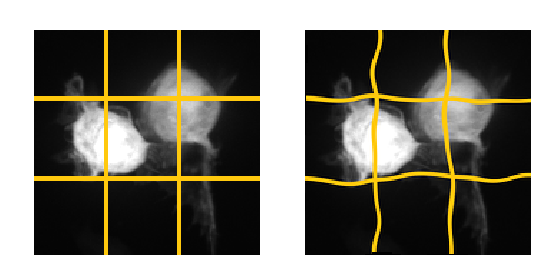
\includegraphics[scale=0.80]{img/fig_elastic.png}
	\end{center}
	\caption[Elastic deformation.]{\textbf{Left:} Input image with superimposed grid. \textbf{Right:} Elastic deformation with $\alpha = 100$ and $\sigma = 10$.}
	\label{fig:elastic}
\end {figure}


	\section {Regularization and Optimization}
\label{sec:reg_opt}

Choosing the number of hidden layers and the number of hidden neurons within them wisely is important because bad choices can make the network susceptible to underfitting or overfitting.

\textit{Underfitting} is the term for the inability of a method to model the data correctly. For example, a linear classifier always underfits on a not-linearly separable dataset because it is not powerful enough to solve the problem. \textit{Overfitting} is the exact opposite and occurs when the model is too complex so that it does not model a trend in the data, but instead memorizes the dataset (see Figure \textbf{\ref{fig:overfit}}). This is undesirable because such a model cannot generalize well and will make incorrect classifications once it is asked to classify data it has not been presented with during training. Therefore, a balance has to be found to equip a model with both enough power to classify correctly while also allowing leeway for generalizing when making predictions on new data.\\

\textbf{TODO: Regularization term for SGD: https://stats.stackexchange.com/questions/29130/difference-between-neural-net-weight-decay-and-learning-rate}\\

	\begin {figure}[!htb]
		\begin{center}
			%\textbf{TODO: uncomment in code}
			\scalebox{0.75}{%% Creator: Matplotlib, PGF backend
%%
%% To include the figure in your LaTeX document, write
%%   \input{<filename>.pgf}
%%
%% Make sure the required packages are loaded in your preamble
%%   \usepackage{pgf}
%%
%% Figures using additional raster images can only be included by \input if
%% they are in the same directory as the main LaTeX file. For loading figures
%% from other directories you can use the `import` package
%%   \usepackage{import}
%% and then include the figures with
%%   \import{<path to file>}{<filename>.pgf}
%%
%% Matplotlib used the following preamble
%%   \usepackage{fontspec}
%%   \setmainfont{DejaVu Serif}
%%   \setsansfont{DejaVu Sans}
%%   \setmonofont{DejaVu Sans Mono}
%%
\begingroup%
\makeatletter%
\begin{pgfpicture}%
\pgfpathrectangle{\pgfpointorigin}{\pgfqpoint{6.400000in}{4.800000in}}%
\pgfusepath{use as bounding box, clip}%
\begin{pgfscope}%
\pgfsetbuttcap%
\pgfsetmiterjoin%
\definecolor{currentfill}{rgb}{1.000000,1.000000,1.000000}%
\pgfsetfillcolor{currentfill}%
\pgfsetlinewidth{0.000000pt}%
\definecolor{currentstroke}{rgb}{1.000000,1.000000,1.000000}%
\pgfsetstrokecolor{currentstroke}%
\pgfsetdash{}{0pt}%
\pgfpathmoveto{\pgfqpoint{0.000000in}{0.000000in}}%
\pgfpathlineto{\pgfqpoint{6.400000in}{0.000000in}}%
\pgfpathlineto{\pgfqpoint{6.400000in}{4.800000in}}%
\pgfpathlineto{\pgfqpoint{0.000000in}{4.800000in}}%
\pgfpathclose%
\pgfusepath{fill}%
\end{pgfscope}%
\begin{pgfscope}%
\pgfsetbuttcap%
\pgfsetmiterjoin%
\definecolor{currentfill}{rgb}{1.000000,1.000000,1.000000}%
\pgfsetfillcolor{currentfill}%
\pgfsetlinewidth{0.000000pt}%
\definecolor{currentstroke}{rgb}{0.000000,0.000000,0.000000}%
\pgfsetstrokecolor{currentstroke}%
\pgfsetstrokeopacity{0.000000}%
\pgfsetdash{}{0pt}%
\pgfpathmoveto{\pgfqpoint{0.800000in}{0.528000in}}%
\pgfpathlineto{\pgfqpoint{5.760000in}{0.528000in}}%
\pgfpathlineto{\pgfqpoint{5.760000in}{4.224000in}}%
\pgfpathlineto{\pgfqpoint{0.800000in}{4.224000in}}%
\pgfpathclose%
\pgfusepath{fill}%
\end{pgfscope}%
\begin{pgfscope}%
\pgfpathrectangle{\pgfqpoint{0.800000in}{0.528000in}}{\pgfqpoint{4.960000in}{3.696000in}} %
\pgfusepath{clip}%
\pgfsetbuttcap%
\pgfsetroundjoin%
\definecolor{currentfill}{rgb}{0.827465,0.000000,0.000000}%
\pgfsetfillcolor{currentfill}%
\pgfsetfillopacity{0.300000}%
\pgfsetlinewidth{0.000000pt}%
\definecolor{currentstroke}{rgb}{0.000000,0.000000,0.000000}%
\pgfsetstrokecolor{currentstroke}%
\pgfsetdash{}{0pt}%
\pgfpathmoveto{\pgfqpoint{0.804614in}{0.528000in}}%
\pgfpathlineto{\pgfqpoint{0.809228in}{0.528000in}}%
\pgfpathlineto{\pgfqpoint{0.813842in}{0.528000in}}%
\pgfpathlineto{\pgfqpoint{0.818456in}{0.528000in}}%
\pgfpathlineto{\pgfqpoint{0.823070in}{0.528000in}}%
\pgfpathlineto{\pgfqpoint{0.827684in}{0.528000in}}%
\pgfpathlineto{\pgfqpoint{0.832298in}{0.528000in}}%
\pgfpathlineto{\pgfqpoint{0.836912in}{0.528000in}}%
\pgfpathlineto{\pgfqpoint{0.841526in}{0.528000in}}%
\pgfpathlineto{\pgfqpoint{0.846140in}{0.528000in}}%
\pgfpathlineto{\pgfqpoint{0.850753in}{0.528000in}}%
\pgfpathlineto{\pgfqpoint{0.855367in}{0.528000in}}%
\pgfpathlineto{\pgfqpoint{0.859981in}{0.528000in}}%
\pgfpathlineto{\pgfqpoint{0.864595in}{0.528000in}}%
\pgfpathlineto{\pgfqpoint{0.869209in}{0.528000in}}%
\pgfpathlineto{\pgfqpoint{0.873823in}{0.528000in}}%
\pgfpathlineto{\pgfqpoint{0.878437in}{0.528000in}}%
\pgfpathlineto{\pgfqpoint{0.883051in}{0.528000in}}%
\pgfpathlineto{\pgfqpoint{0.887665in}{0.528000in}}%
\pgfpathlineto{\pgfqpoint{0.892279in}{0.528000in}}%
\pgfpathlineto{\pgfqpoint{0.896893in}{0.528000in}}%
\pgfpathlineto{\pgfqpoint{0.901507in}{0.528000in}}%
\pgfpathlineto{\pgfqpoint{0.906121in}{0.528000in}}%
\pgfpathlineto{\pgfqpoint{0.910735in}{0.528000in}}%
\pgfpathlineto{\pgfqpoint{0.915349in}{0.528000in}}%
\pgfpathlineto{\pgfqpoint{0.919963in}{0.528000in}}%
\pgfpathlineto{\pgfqpoint{0.924577in}{0.528000in}}%
\pgfpathlineto{\pgfqpoint{0.929191in}{0.528000in}}%
\pgfpathlineto{\pgfqpoint{0.933805in}{0.528000in}}%
\pgfpathlineto{\pgfqpoint{0.938419in}{0.528000in}}%
\pgfpathlineto{\pgfqpoint{0.943033in}{0.528000in}}%
\pgfpathlineto{\pgfqpoint{0.947647in}{0.528000in}}%
\pgfpathlineto{\pgfqpoint{0.952260in}{0.528000in}}%
\pgfpathlineto{\pgfqpoint{0.956874in}{0.528000in}}%
\pgfpathlineto{\pgfqpoint{0.961488in}{0.528000in}}%
\pgfpathlineto{\pgfqpoint{0.966102in}{0.528000in}}%
\pgfpathlineto{\pgfqpoint{0.970716in}{0.528000in}}%
\pgfpathlineto{\pgfqpoint{0.975330in}{0.528000in}}%
\pgfpathlineto{\pgfqpoint{0.979944in}{0.528000in}}%
\pgfpathlineto{\pgfqpoint{0.984558in}{0.528000in}}%
\pgfpathlineto{\pgfqpoint{0.989172in}{0.528000in}}%
\pgfpathlineto{\pgfqpoint{0.993786in}{0.528000in}}%
\pgfpathlineto{\pgfqpoint{0.998400in}{0.528000in}}%
\pgfpathlineto{\pgfqpoint{1.003014in}{0.528000in}}%
\pgfpathlineto{\pgfqpoint{1.007628in}{0.528000in}}%
\pgfpathlineto{\pgfqpoint{1.012242in}{0.528000in}}%
\pgfpathlineto{\pgfqpoint{1.016856in}{0.528000in}}%
\pgfpathlineto{\pgfqpoint{1.021470in}{0.528000in}}%
\pgfpathlineto{\pgfqpoint{1.026084in}{0.528000in}}%
\pgfpathlineto{\pgfqpoint{1.030698in}{0.528000in}}%
\pgfpathlineto{\pgfqpoint{1.035312in}{0.528000in}}%
\pgfpathlineto{\pgfqpoint{1.039926in}{0.528000in}}%
\pgfpathlineto{\pgfqpoint{1.044540in}{0.528000in}}%
\pgfpathlineto{\pgfqpoint{1.049153in}{0.528000in}}%
\pgfpathlineto{\pgfqpoint{1.053767in}{0.528000in}}%
\pgfpathlineto{\pgfqpoint{1.058381in}{0.528000in}}%
\pgfpathlineto{\pgfqpoint{1.062995in}{0.528000in}}%
\pgfpathlineto{\pgfqpoint{1.067609in}{0.528000in}}%
\pgfpathlineto{\pgfqpoint{1.072223in}{0.528000in}}%
\pgfpathlineto{\pgfqpoint{1.076837in}{0.528000in}}%
\pgfpathlineto{\pgfqpoint{1.081451in}{0.528000in}}%
\pgfpathlineto{\pgfqpoint{1.086065in}{0.528000in}}%
\pgfpathlineto{\pgfqpoint{1.090679in}{0.528000in}}%
\pgfpathlineto{\pgfqpoint{1.095293in}{0.528000in}}%
\pgfpathlineto{\pgfqpoint{1.099907in}{0.528000in}}%
\pgfpathlineto{\pgfqpoint{1.104521in}{0.528000in}}%
\pgfpathlineto{\pgfqpoint{1.109135in}{0.528000in}}%
\pgfpathlineto{\pgfqpoint{1.113749in}{0.528000in}}%
\pgfpathlineto{\pgfqpoint{1.118363in}{0.528000in}}%
\pgfpathlineto{\pgfqpoint{1.122977in}{0.528000in}}%
\pgfpathlineto{\pgfqpoint{1.127591in}{0.528000in}}%
\pgfpathlineto{\pgfqpoint{1.132205in}{0.528000in}}%
\pgfpathlineto{\pgfqpoint{1.136819in}{0.528000in}}%
\pgfpathlineto{\pgfqpoint{1.141433in}{0.528000in}}%
\pgfpathlineto{\pgfqpoint{1.146047in}{0.528000in}}%
\pgfpathlineto{\pgfqpoint{1.150660in}{0.528000in}}%
\pgfpathlineto{\pgfqpoint{1.155274in}{0.528000in}}%
\pgfpathlineto{\pgfqpoint{1.159888in}{0.528000in}}%
\pgfpathlineto{\pgfqpoint{1.164502in}{0.528000in}}%
\pgfpathlineto{\pgfqpoint{1.169116in}{0.528000in}}%
\pgfpathlineto{\pgfqpoint{1.173730in}{0.528000in}}%
\pgfpathlineto{\pgfqpoint{1.178344in}{0.528000in}}%
\pgfpathlineto{\pgfqpoint{1.182958in}{0.528000in}}%
\pgfpathlineto{\pgfqpoint{1.187572in}{0.528000in}}%
\pgfpathlineto{\pgfqpoint{1.192186in}{0.528000in}}%
\pgfpathlineto{\pgfqpoint{1.196800in}{0.528000in}}%
\pgfpathlineto{\pgfqpoint{1.201414in}{0.528000in}}%
\pgfpathlineto{\pgfqpoint{1.206028in}{0.528000in}}%
\pgfpathlineto{\pgfqpoint{1.210642in}{0.528000in}}%
\pgfpathlineto{\pgfqpoint{1.215256in}{0.528000in}}%
\pgfpathlineto{\pgfqpoint{1.219870in}{0.528000in}}%
\pgfpathlineto{\pgfqpoint{1.224484in}{0.528000in}}%
\pgfpathlineto{\pgfqpoint{1.229098in}{0.528000in}}%
\pgfpathlineto{\pgfqpoint{1.233712in}{0.528000in}}%
\pgfpathlineto{\pgfqpoint{1.238326in}{0.528000in}}%
\pgfpathlineto{\pgfqpoint{1.242940in}{0.528000in}}%
\pgfpathlineto{\pgfqpoint{1.247553in}{0.528000in}}%
\pgfpathlineto{\pgfqpoint{1.252167in}{0.528000in}}%
\pgfpathlineto{\pgfqpoint{1.256781in}{0.528000in}}%
\pgfpathlineto{\pgfqpoint{1.261395in}{0.528000in}}%
\pgfpathlineto{\pgfqpoint{1.266009in}{0.528000in}}%
\pgfpathlineto{\pgfqpoint{1.270623in}{0.528000in}}%
\pgfpathlineto{\pgfqpoint{1.275237in}{0.528000in}}%
\pgfpathlineto{\pgfqpoint{1.279851in}{0.528000in}}%
\pgfpathlineto{\pgfqpoint{1.284465in}{0.528000in}}%
\pgfpathlineto{\pgfqpoint{1.289079in}{0.528000in}}%
\pgfpathlineto{\pgfqpoint{1.293693in}{0.528000in}}%
\pgfpathlineto{\pgfqpoint{1.298307in}{0.528000in}}%
\pgfpathlineto{\pgfqpoint{1.302921in}{0.528000in}}%
\pgfpathlineto{\pgfqpoint{1.307535in}{0.528000in}}%
\pgfpathlineto{\pgfqpoint{1.312149in}{0.528000in}}%
\pgfpathlineto{\pgfqpoint{1.316763in}{0.528000in}}%
\pgfpathlineto{\pgfqpoint{1.321377in}{0.528000in}}%
\pgfpathlineto{\pgfqpoint{1.325991in}{0.528000in}}%
\pgfpathlineto{\pgfqpoint{1.330605in}{0.528000in}}%
\pgfpathlineto{\pgfqpoint{1.335219in}{0.528000in}}%
\pgfpathlineto{\pgfqpoint{1.339833in}{0.528000in}}%
\pgfpathlineto{\pgfqpoint{1.344447in}{0.528000in}}%
\pgfpathlineto{\pgfqpoint{1.349060in}{0.528000in}}%
\pgfpathlineto{\pgfqpoint{1.353674in}{0.528000in}}%
\pgfpathlineto{\pgfqpoint{1.358288in}{0.528000in}}%
\pgfpathlineto{\pgfqpoint{1.362902in}{0.528000in}}%
\pgfpathlineto{\pgfqpoint{1.367516in}{0.528000in}}%
\pgfpathlineto{\pgfqpoint{1.372130in}{0.528000in}}%
\pgfpathlineto{\pgfqpoint{1.376744in}{0.528000in}}%
\pgfpathlineto{\pgfqpoint{1.381358in}{0.528000in}}%
\pgfpathlineto{\pgfqpoint{1.385972in}{0.528000in}}%
\pgfpathlineto{\pgfqpoint{1.390586in}{0.528000in}}%
\pgfpathlineto{\pgfqpoint{1.395200in}{0.528000in}}%
\pgfpathlineto{\pgfqpoint{1.399814in}{0.528000in}}%
\pgfpathlineto{\pgfqpoint{1.404428in}{0.528000in}}%
\pgfpathlineto{\pgfqpoint{1.409042in}{0.528000in}}%
\pgfpathlineto{\pgfqpoint{1.413656in}{0.528000in}}%
\pgfpathlineto{\pgfqpoint{1.418270in}{0.528000in}}%
\pgfpathlineto{\pgfqpoint{1.422884in}{0.528000in}}%
\pgfpathlineto{\pgfqpoint{1.427498in}{0.528000in}}%
\pgfpathlineto{\pgfqpoint{1.432112in}{0.528000in}}%
\pgfpathlineto{\pgfqpoint{1.436726in}{0.528000in}}%
\pgfpathlineto{\pgfqpoint{1.441340in}{0.528000in}}%
\pgfpathlineto{\pgfqpoint{1.445953in}{0.528000in}}%
\pgfpathlineto{\pgfqpoint{1.450567in}{0.528000in}}%
\pgfpathlineto{\pgfqpoint{1.455181in}{0.528000in}}%
\pgfpathlineto{\pgfqpoint{1.459795in}{0.528000in}}%
\pgfpathlineto{\pgfqpoint{1.464409in}{0.528000in}}%
\pgfpathlineto{\pgfqpoint{1.469023in}{0.528000in}}%
\pgfpathlineto{\pgfqpoint{1.473637in}{0.528000in}}%
\pgfpathlineto{\pgfqpoint{1.478251in}{0.528000in}}%
\pgfpathlineto{\pgfqpoint{1.482865in}{0.528000in}}%
\pgfpathlineto{\pgfqpoint{1.487479in}{0.528000in}}%
\pgfpathlineto{\pgfqpoint{1.492093in}{0.528000in}}%
\pgfpathlineto{\pgfqpoint{1.496707in}{0.528000in}}%
\pgfpathlineto{\pgfqpoint{1.501321in}{0.528000in}}%
\pgfpathlineto{\pgfqpoint{1.505935in}{0.528000in}}%
\pgfpathlineto{\pgfqpoint{1.510549in}{0.528000in}}%
\pgfpathlineto{\pgfqpoint{1.515163in}{0.528000in}}%
\pgfpathlineto{\pgfqpoint{1.519777in}{0.528000in}}%
\pgfpathlineto{\pgfqpoint{1.524391in}{0.528000in}}%
\pgfpathlineto{\pgfqpoint{1.529005in}{0.528000in}}%
\pgfpathlineto{\pgfqpoint{1.533619in}{0.528000in}}%
\pgfpathlineto{\pgfqpoint{1.538233in}{0.528000in}}%
\pgfpathlineto{\pgfqpoint{1.542847in}{0.528000in}}%
\pgfpathlineto{\pgfqpoint{1.547460in}{0.528000in}}%
\pgfpathlineto{\pgfqpoint{1.552074in}{0.528000in}}%
\pgfpathlineto{\pgfqpoint{1.556688in}{0.528000in}}%
\pgfpathlineto{\pgfqpoint{1.561302in}{0.528000in}}%
\pgfpathlineto{\pgfqpoint{1.565916in}{0.528000in}}%
\pgfpathlineto{\pgfqpoint{1.570530in}{0.528000in}}%
\pgfpathlineto{\pgfqpoint{1.575144in}{0.528000in}}%
\pgfpathlineto{\pgfqpoint{1.579758in}{0.528000in}}%
\pgfpathlineto{\pgfqpoint{1.584372in}{0.528000in}}%
\pgfpathlineto{\pgfqpoint{1.588986in}{0.528000in}}%
\pgfpathlineto{\pgfqpoint{1.593600in}{0.528000in}}%
\pgfpathlineto{\pgfqpoint{1.598214in}{0.528000in}}%
\pgfpathlineto{\pgfqpoint{1.602828in}{0.528000in}}%
\pgfpathlineto{\pgfqpoint{1.607442in}{0.528000in}}%
\pgfpathlineto{\pgfqpoint{1.612056in}{0.528000in}}%
\pgfpathlineto{\pgfqpoint{1.616670in}{0.528000in}}%
\pgfpathlineto{\pgfqpoint{1.621284in}{0.528000in}}%
\pgfpathlineto{\pgfqpoint{1.625898in}{0.528000in}}%
\pgfpathlineto{\pgfqpoint{1.630512in}{0.528000in}}%
\pgfpathlineto{\pgfqpoint{1.635126in}{0.528000in}}%
\pgfpathlineto{\pgfqpoint{1.639740in}{0.528000in}}%
\pgfpathlineto{\pgfqpoint{1.644353in}{0.528000in}}%
\pgfpathlineto{\pgfqpoint{1.648967in}{0.528000in}}%
\pgfpathlineto{\pgfqpoint{1.653581in}{0.528000in}}%
\pgfpathlineto{\pgfqpoint{1.658195in}{0.528000in}}%
\pgfpathlineto{\pgfqpoint{1.662809in}{0.528000in}}%
\pgfpathlineto{\pgfqpoint{1.667423in}{0.528000in}}%
\pgfpathlineto{\pgfqpoint{1.672037in}{0.528000in}}%
\pgfpathlineto{\pgfqpoint{1.676651in}{0.528000in}}%
\pgfpathlineto{\pgfqpoint{1.681265in}{0.528000in}}%
\pgfpathlineto{\pgfqpoint{1.685879in}{0.528000in}}%
\pgfpathlineto{\pgfqpoint{1.690493in}{0.528000in}}%
\pgfpathlineto{\pgfqpoint{1.695107in}{0.528000in}}%
\pgfpathlineto{\pgfqpoint{1.699721in}{0.528000in}}%
\pgfpathlineto{\pgfqpoint{1.704335in}{0.528000in}}%
\pgfpathlineto{\pgfqpoint{1.708949in}{0.528000in}}%
\pgfpathlineto{\pgfqpoint{1.713563in}{0.528000in}}%
\pgfpathlineto{\pgfqpoint{1.718177in}{0.528000in}}%
\pgfpathlineto{\pgfqpoint{1.722791in}{0.528000in}}%
\pgfpathlineto{\pgfqpoint{1.727405in}{0.528000in}}%
\pgfpathlineto{\pgfqpoint{1.732019in}{0.528000in}}%
\pgfpathlineto{\pgfqpoint{1.736633in}{0.528000in}}%
\pgfpathlineto{\pgfqpoint{1.741247in}{0.528000in}}%
\pgfpathlineto{\pgfqpoint{1.745860in}{0.528000in}}%
\pgfpathlineto{\pgfqpoint{1.750474in}{0.528000in}}%
\pgfpathlineto{\pgfqpoint{1.755088in}{0.528000in}}%
\pgfpathlineto{\pgfqpoint{1.759702in}{0.528000in}}%
\pgfpathlineto{\pgfqpoint{1.764316in}{0.528000in}}%
\pgfpathlineto{\pgfqpoint{1.768930in}{0.528000in}}%
\pgfpathlineto{\pgfqpoint{1.773544in}{0.528000in}}%
\pgfpathlineto{\pgfqpoint{1.778158in}{0.528000in}}%
\pgfpathlineto{\pgfqpoint{1.782772in}{0.528000in}}%
\pgfpathlineto{\pgfqpoint{1.787386in}{0.528000in}}%
\pgfpathlineto{\pgfqpoint{1.792000in}{0.528000in}}%
\pgfpathlineto{\pgfqpoint{1.796614in}{0.528000in}}%
\pgfpathlineto{\pgfqpoint{1.801228in}{0.528000in}}%
\pgfpathlineto{\pgfqpoint{1.805842in}{0.528000in}}%
\pgfpathlineto{\pgfqpoint{1.810456in}{0.528000in}}%
\pgfpathlineto{\pgfqpoint{1.815070in}{0.528000in}}%
\pgfpathlineto{\pgfqpoint{1.819684in}{0.528000in}}%
\pgfpathlineto{\pgfqpoint{1.824298in}{0.528000in}}%
\pgfpathlineto{\pgfqpoint{1.828912in}{0.528000in}}%
\pgfpathlineto{\pgfqpoint{1.833526in}{0.528000in}}%
\pgfpathlineto{\pgfqpoint{1.838140in}{0.528000in}}%
\pgfpathlineto{\pgfqpoint{1.842753in}{0.528000in}}%
\pgfpathlineto{\pgfqpoint{1.847367in}{0.528000in}}%
\pgfpathlineto{\pgfqpoint{1.851981in}{0.528000in}}%
\pgfpathlineto{\pgfqpoint{1.856595in}{0.528000in}}%
\pgfpathlineto{\pgfqpoint{1.861209in}{0.528000in}}%
\pgfpathlineto{\pgfqpoint{1.865823in}{0.528000in}}%
\pgfpathlineto{\pgfqpoint{1.870437in}{0.528000in}}%
\pgfpathlineto{\pgfqpoint{1.875051in}{0.528000in}}%
\pgfpathlineto{\pgfqpoint{1.879665in}{0.528000in}}%
\pgfpathlineto{\pgfqpoint{1.884279in}{0.528000in}}%
\pgfpathlineto{\pgfqpoint{1.888893in}{0.528000in}}%
\pgfpathlineto{\pgfqpoint{1.893507in}{0.528000in}}%
\pgfpathlineto{\pgfqpoint{1.898121in}{0.528000in}}%
\pgfpathlineto{\pgfqpoint{1.902735in}{0.528000in}}%
\pgfpathlineto{\pgfqpoint{1.907349in}{0.528000in}}%
\pgfpathlineto{\pgfqpoint{1.911963in}{0.528000in}}%
\pgfpathlineto{\pgfqpoint{1.916577in}{0.528000in}}%
\pgfpathlineto{\pgfqpoint{1.921191in}{0.528000in}}%
\pgfpathlineto{\pgfqpoint{1.925805in}{0.528000in}}%
\pgfpathlineto{\pgfqpoint{1.930419in}{0.528000in}}%
\pgfpathlineto{\pgfqpoint{1.935033in}{0.528000in}}%
\pgfpathlineto{\pgfqpoint{1.939647in}{0.528000in}}%
\pgfpathlineto{\pgfqpoint{1.944260in}{0.528000in}}%
\pgfpathlineto{\pgfqpoint{1.948874in}{0.528000in}}%
\pgfpathlineto{\pgfqpoint{1.953488in}{0.528000in}}%
\pgfpathlineto{\pgfqpoint{1.958102in}{0.528000in}}%
\pgfpathlineto{\pgfqpoint{1.962716in}{0.528000in}}%
\pgfpathlineto{\pgfqpoint{1.967330in}{0.528000in}}%
\pgfpathlineto{\pgfqpoint{1.971944in}{0.528000in}}%
\pgfpathlineto{\pgfqpoint{1.976558in}{0.528000in}}%
\pgfpathlineto{\pgfqpoint{1.981172in}{0.528000in}}%
\pgfpathlineto{\pgfqpoint{1.985786in}{0.528000in}}%
\pgfpathlineto{\pgfqpoint{1.990400in}{0.528000in}}%
\pgfpathlineto{\pgfqpoint{1.995014in}{0.528000in}}%
\pgfpathlineto{\pgfqpoint{1.999628in}{0.528000in}}%
\pgfpathlineto{\pgfqpoint{2.004242in}{0.528000in}}%
\pgfpathlineto{\pgfqpoint{2.008856in}{0.528000in}}%
\pgfpathlineto{\pgfqpoint{2.013470in}{0.528000in}}%
\pgfpathlineto{\pgfqpoint{2.018084in}{0.528000in}}%
\pgfpathlineto{\pgfqpoint{2.022698in}{0.528000in}}%
\pgfpathlineto{\pgfqpoint{2.027312in}{0.528000in}}%
\pgfpathlineto{\pgfqpoint{2.031926in}{0.528000in}}%
\pgfpathlineto{\pgfqpoint{2.036540in}{0.528000in}}%
\pgfpathlineto{\pgfqpoint{2.041153in}{0.528000in}}%
\pgfpathlineto{\pgfqpoint{2.045767in}{0.528000in}}%
\pgfpathlineto{\pgfqpoint{2.050381in}{0.528000in}}%
\pgfpathlineto{\pgfqpoint{2.054995in}{0.528000in}}%
\pgfpathlineto{\pgfqpoint{2.059609in}{0.528000in}}%
\pgfpathlineto{\pgfqpoint{2.064223in}{0.528000in}}%
\pgfpathlineto{\pgfqpoint{2.068837in}{0.528000in}}%
\pgfpathlineto{\pgfqpoint{2.073451in}{0.528000in}}%
\pgfpathlineto{\pgfqpoint{2.078065in}{0.528000in}}%
\pgfpathlineto{\pgfqpoint{2.082679in}{0.528000in}}%
\pgfpathlineto{\pgfqpoint{2.087293in}{0.528000in}}%
\pgfpathlineto{\pgfqpoint{2.091907in}{0.528000in}}%
\pgfpathlineto{\pgfqpoint{2.096521in}{0.528000in}}%
\pgfpathlineto{\pgfqpoint{2.101135in}{0.528000in}}%
\pgfpathlineto{\pgfqpoint{2.105749in}{0.528000in}}%
\pgfpathlineto{\pgfqpoint{2.110363in}{0.528000in}}%
\pgfpathlineto{\pgfqpoint{2.114977in}{0.528000in}}%
\pgfpathlineto{\pgfqpoint{2.119591in}{0.528000in}}%
\pgfpathlineto{\pgfqpoint{2.124205in}{0.528000in}}%
\pgfpathlineto{\pgfqpoint{2.128819in}{0.528000in}}%
\pgfpathlineto{\pgfqpoint{2.133433in}{0.528000in}}%
\pgfpathlineto{\pgfqpoint{2.138047in}{0.528000in}}%
\pgfpathlineto{\pgfqpoint{2.142660in}{0.528000in}}%
\pgfpathlineto{\pgfqpoint{2.147274in}{0.528000in}}%
\pgfpathlineto{\pgfqpoint{2.151888in}{0.528000in}}%
\pgfpathlineto{\pgfqpoint{2.156502in}{0.528000in}}%
\pgfpathlineto{\pgfqpoint{2.161116in}{0.528000in}}%
\pgfpathlineto{\pgfqpoint{2.165730in}{0.528000in}}%
\pgfpathlineto{\pgfqpoint{2.170344in}{0.528000in}}%
\pgfpathlineto{\pgfqpoint{2.174958in}{0.528000in}}%
\pgfpathlineto{\pgfqpoint{2.179572in}{0.528000in}}%
\pgfpathlineto{\pgfqpoint{2.184186in}{0.528000in}}%
\pgfpathlineto{\pgfqpoint{2.188800in}{0.528000in}}%
\pgfpathlineto{\pgfqpoint{2.193414in}{0.528000in}}%
\pgfpathlineto{\pgfqpoint{2.198028in}{0.528000in}}%
\pgfpathlineto{\pgfqpoint{2.202642in}{0.528000in}}%
\pgfpathlineto{\pgfqpoint{2.207256in}{0.528000in}}%
\pgfpathlineto{\pgfqpoint{2.211870in}{0.528000in}}%
\pgfpathlineto{\pgfqpoint{2.216484in}{0.528000in}}%
\pgfpathlineto{\pgfqpoint{2.221098in}{0.528000in}}%
\pgfpathlineto{\pgfqpoint{2.225712in}{0.528000in}}%
\pgfpathlineto{\pgfqpoint{2.230326in}{0.528000in}}%
\pgfpathlineto{\pgfqpoint{2.234940in}{0.528000in}}%
\pgfpathlineto{\pgfqpoint{2.239553in}{0.528000in}}%
\pgfpathlineto{\pgfqpoint{2.244167in}{0.528000in}}%
\pgfpathlineto{\pgfqpoint{2.248781in}{0.528000in}}%
\pgfpathlineto{\pgfqpoint{2.253395in}{0.528000in}}%
\pgfpathlineto{\pgfqpoint{2.258009in}{0.528000in}}%
\pgfpathlineto{\pgfqpoint{2.262623in}{0.528000in}}%
\pgfpathlineto{\pgfqpoint{2.267237in}{0.528000in}}%
\pgfpathlineto{\pgfqpoint{2.271851in}{0.528000in}}%
\pgfpathlineto{\pgfqpoint{2.276465in}{0.528000in}}%
\pgfpathlineto{\pgfqpoint{2.281079in}{0.528000in}}%
\pgfpathlineto{\pgfqpoint{2.285693in}{0.528000in}}%
\pgfpathlineto{\pgfqpoint{2.290307in}{0.528000in}}%
\pgfpathlineto{\pgfqpoint{2.294921in}{0.528000in}}%
\pgfpathlineto{\pgfqpoint{2.299535in}{0.528000in}}%
\pgfpathlineto{\pgfqpoint{2.304149in}{0.528000in}}%
\pgfpathlineto{\pgfqpoint{2.308763in}{0.528000in}}%
\pgfpathlineto{\pgfqpoint{2.313377in}{0.528000in}}%
\pgfpathlineto{\pgfqpoint{2.317991in}{0.528000in}}%
\pgfpathlineto{\pgfqpoint{2.322605in}{0.528000in}}%
\pgfpathlineto{\pgfqpoint{2.327219in}{0.528000in}}%
\pgfpathlineto{\pgfqpoint{2.331833in}{0.528000in}}%
\pgfpathlineto{\pgfqpoint{2.336447in}{0.528000in}}%
\pgfpathlineto{\pgfqpoint{2.341060in}{0.528000in}}%
\pgfpathlineto{\pgfqpoint{2.345674in}{0.528000in}}%
\pgfpathlineto{\pgfqpoint{2.346367in}{0.528000in}}%
\pgfpathlineto{\pgfqpoint{2.350288in}{0.531917in}}%
\pgfpathlineto{\pgfqpoint{2.350980in}{0.532608in}}%
\pgfpathlineto{\pgfqpoint{2.350980in}{0.537217in}}%
\pgfpathlineto{\pgfqpoint{2.350980in}{0.541825in}}%
\pgfpathlineto{\pgfqpoint{2.354902in}{0.545743in}}%
\pgfpathlineto{\pgfqpoint{2.355594in}{0.546434in}}%
\pgfpathlineto{\pgfqpoint{2.355594in}{0.551042in}}%
\pgfpathlineto{\pgfqpoint{2.355594in}{0.555651in}}%
\pgfpathlineto{\pgfqpoint{2.359516in}{0.559568in}}%
\pgfpathlineto{\pgfqpoint{2.360208in}{0.560259in}}%
\pgfpathlineto{\pgfqpoint{2.360208in}{0.564868in}}%
\pgfpathlineto{\pgfqpoint{2.360208in}{0.569476in}}%
\pgfpathlineto{\pgfqpoint{2.360208in}{0.574085in}}%
\pgfpathlineto{\pgfqpoint{2.364130in}{0.578002in}}%
\pgfpathlineto{\pgfqpoint{2.364822in}{0.578693in}}%
\pgfpathlineto{\pgfqpoint{2.364822in}{0.583302in}}%
\pgfpathlineto{\pgfqpoint{2.364822in}{0.587910in}}%
\pgfpathlineto{\pgfqpoint{2.368744in}{0.591827in}}%
\pgfpathlineto{\pgfqpoint{2.369436in}{0.592519in}}%
\pgfpathlineto{\pgfqpoint{2.369436in}{0.597127in}}%
\pgfpathlineto{\pgfqpoint{2.369436in}{0.601736in}}%
\pgfpathlineto{\pgfqpoint{2.373358in}{0.605653in}}%
\pgfpathlineto{\pgfqpoint{2.374050in}{0.606344in}}%
\pgfpathlineto{\pgfqpoint{2.374050in}{0.610953in}}%
\pgfpathlineto{\pgfqpoint{2.374050in}{0.615561in}}%
\pgfpathlineto{\pgfqpoint{2.377972in}{0.619478in}}%
\pgfpathlineto{\pgfqpoint{2.378664in}{0.620170in}}%
\pgfpathlineto{\pgfqpoint{2.378664in}{0.624778in}}%
\pgfpathlineto{\pgfqpoint{2.378664in}{0.629387in}}%
\pgfpathlineto{\pgfqpoint{2.382586in}{0.633304in}}%
\pgfpathlineto{\pgfqpoint{2.383278in}{0.633995in}}%
\pgfpathlineto{\pgfqpoint{2.383278in}{0.638603in}}%
\pgfpathlineto{\pgfqpoint{2.383278in}{0.643212in}}%
\pgfpathlineto{\pgfqpoint{2.387200in}{0.647129in}}%
\pgfpathlineto{\pgfqpoint{2.387892in}{0.647820in}}%
\pgfpathlineto{\pgfqpoint{2.387892in}{0.652429in}}%
\pgfpathlineto{\pgfqpoint{2.387892in}{0.657037in}}%
\pgfpathlineto{\pgfqpoint{2.391814in}{0.660955in}}%
\pgfpathlineto{\pgfqpoint{2.392506in}{0.661646in}}%
\pgfpathlineto{\pgfqpoint{2.392506in}{0.666254in}}%
\pgfpathlineto{\pgfqpoint{2.392506in}{0.670863in}}%
\pgfpathlineto{\pgfqpoint{2.396428in}{0.674780in}}%
\pgfpathlineto{\pgfqpoint{2.397120in}{0.675471in}}%
\pgfpathlineto{\pgfqpoint{2.397120in}{0.680080in}}%
\pgfpathlineto{\pgfqpoint{2.397120in}{0.684688in}}%
\pgfpathlineto{\pgfqpoint{2.397120in}{0.689297in}}%
\pgfpathlineto{\pgfqpoint{2.401042in}{0.693214in}}%
\pgfpathlineto{\pgfqpoint{2.401734in}{0.693905in}}%
\pgfpathlineto{\pgfqpoint{2.401734in}{0.698514in}}%
\pgfpathlineto{\pgfqpoint{2.401734in}{0.703122in}}%
\pgfpathlineto{\pgfqpoint{2.405656in}{0.707039in}}%
\pgfpathlineto{\pgfqpoint{2.406348in}{0.707731in}}%
\pgfpathlineto{\pgfqpoint{2.406348in}{0.712339in}}%
\pgfpathlineto{\pgfqpoint{2.406348in}{0.716948in}}%
\pgfpathlineto{\pgfqpoint{2.410270in}{0.720865in}}%
\pgfpathlineto{\pgfqpoint{2.410962in}{0.721556in}}%
\pgfpathlineto{\pgfqpoint{2.410962in}{0.726165in}}%
\pgfpathlineto{\pgfqpoint{2.410962in}{0.730773in}}%
\pgfpathlineto{\pgfqpoint{2.414884in}{0.734690in}}%
\pgfpathlineto{\pgfqpoint{2.415576in}{0.735382in}}%
\pgfpathlineto{\pgfqpoint{2.415576in}{0.739990in}}%
\pgfpathlineto{\pgfqpoint{2.415576in}{0.744599in}}%
\pgfpathlineto{\pgfqpoint{2.419498in}{0.748516in}}%
\pgfpathlineto{\pgfqpoint{2.420190in}{0.749207in}}%
\pgfpathlineto{\pgfqpoint{2.420190in}{0.753815in}}%
\pgfpathlineto{\pgfqpoint{2.420190in}{0.758424in}}%
\pgfpathlineto{\pgfqpoint{2.424112in}{0.762341in}}%
\pgfpathlineto{\pgfqpoint{2.424804in}{0.763032in}}%
\pgfpathlineto{\pgfqpoint{2.424804in}{0.767641in}}%
\pgfpathlineto{\pgfqpoint{2.424804in}{0.772249in}}%
\pgfpathlineto{\pgfqpoint{2.428726in}{0.776167in}}%
\pgfpathlineto{\pgfqpoint{2.429418in}{0.776858in}}%
\pgfpathlineto{\pgfqpoint{2.429418in}{0.781466in}}%
\pgfpathlineto{\pgfqpoint{2.429418in}{0.786075in}}%
\pgfpathlineto{\pgfqpoint{2.429418in}{0.790683in}}%
\pgfpathlineto{\pgfqpoint{2.433340in}{0.794600in}}%
\pgfpathlineto{\pgfqpoint{2.434032in}{0.795292in}}%
\pgfpathlineto{\pgfqpoint{2.434032in}{0.799900in}}%
\pgfpathlineto{\pgfqpoint{2.434032in}{0.804509in}}%
\pgfpathlineto{\pgfqpoint{2.437953in}{0.808426in}}%
\pgfpathlineto{\pgfqpoint{2.438646in}{0.809117in}}%
\pgfpathlineto{\pgfqpoint{2.438646in}{0.813726in}}%
\pgfpathlineto{\pgfqpoint{2.438646in}{0.818334in}}%
\pgfpathlineto{\pgfqpoint{2.442567in}{0.822251in}}%
\pgfpathlineto{\pgfqpoint{2.443260in}{0.822943in}}%
\pgfpathlineto{\pgfqpoint{2.443260in}{0.827551in}}%
\pgfpathlineto{\pgfqpoint{2.443260in}{0.832160in}}%
\pgfpathlineto{\pgfqpoint{2.447181in}{0.836077in}}%
\pgfpathlineto{\pgfqpoint{2.447873in}{0.836768in}}%
\pgfpathlineto{\pgfqpoint{2.447873in}{0.841377in}}%
\pgfpathlineto{\pgfqpoint{2.447873in}{0.845985in}}%
\pgfpathlineto{\pgfqpoint{2.451795in}{0.849902in}}%
\pgfpathlineto{\pgfqpoint{2.452487in}{0.850594in}}%
\pgfpathlineto{\pgfqpoint{2.452487in}{0.855202in}}%
\pgfpathlineto{\pgfqpoint{2.452487in}{0.859810in}}%
\pgfpathlineto{\pgfqpoint{2.456409in}{0.863728in}}%
\pgfpathlineto{\pgfqpoint{2.457101in}{0.864419in}}%
\pgfpathlineto{\pgfqpoint{2.457101in}{0.869027in}}%
\pgfpathlineto{\pgfqpoint{2.457101in}{0.873636in}}%
\pgfpathlineto{\pgfqpoint{2.461023in}{0.877553in}}%
\pgfpathlineto{\pgfqpoint{2.461715in}{0.878244in}}%
\pgfpathlineto{\pgfqpoint{2.461715in}{0.882853in}}%
\pgfpathlineto{\pgfqpoint{2.461715in}{0.887461in}}%
\pgfpathlineto{\pgfqpoint{2.461715in}{0.892070in}}%
\pgfpathlineto{\pgfqpoint{2.465637in}{0.895987in}}%
\pgfpathlineto{\pgfqpoint{2.466329in}{0.896678in}}%
\pgfpathlineto{\pgfqpoint{2.466329in}{0.901287in}}%
\pgfpathlineto{\pgfqpoint{2.466329in}{0.905895in}}%
\pgfpathlineto{\pgfqpoint{2.470251in}{0.909812in}}%
\pgfpathlineto{\pgfqpoint{2.470943in}{0.910504in}}%
\pgfpathlineto{\pgfqpoint{2.470943in}{0.915112in}}%
\pgfpathlineto{\pgfqpoint{2.470943in}{0.919721in}}%
\pgfpathlineto{\pgfqpoint{2.474865in}{0.923638in}}%
\pgfpathlineto{\pgfqpoint{2.475557in}{0.924329in}}%
\pgfpathlineto{\pgfqpoint{2.475557in}{0.928938in}}%
\pgfpathlineto{\pgfqpoint{2.475557in}{0.933546in}}%
\pgfpathlineto{\pgfqpoint{2.479479in}{0.937463in}}%
\pgfpathlineto{\pgfqpoint{2.480171in}{0.938155in}}%
\pgfpathlineto{\pgfqpoint{2.480171in}{0.942763in}}%
\pgfpathlineto{\pgfqpoint{2.480171in}{0.947372in}}%
\pgfpathlineto{\pgfqpoint{2.484093in}{0.951289in}}%
\pgfpathlineto{\pgfqpoint{2.484785in}{0.951980in}}%
\pgfpathlineto{\pgfqpoint{2.484785in}{0.956589in}}%
\pgfpathlineto{\pgfqpoint{2.484785in}{0.961197in}}%
\pgfpathlineto{\pgfqpoint{2.488707in}{0.965114in}}%
\pgfpathlineto{\pgfqpoint{2.489399in}{0.965805in}}%
\pgfpathlineto{\pgfqpoint{2.489399in}{0.970414in}}%
\pgfpathlineto{\pgfqpoint{2.489399in}{0.975022in}}%
\pgfpathlineto{\pgfqpoint{2.493321in}{0.978940in}}%
\pgfpathlineto{\pgfqpoint{2.494013in}{0.979631in}}%
\pgfpathlineto{\pgfqpoint{2.494013in}{0.984239in}}%
\pgfpathlineto{\pgfqpoint{2.494013in}{0.988848in}}%
\pgfpathlineto{\pgfqpoint{2.497935in}{0.992765in}}%
\pgfpathlineto{\pgfqpoint{2.498627in}{0.993456in}}%
\pgfpathlineto{\pgfqpoint{2.498627in}{0.998065in}}%
\pgfpathlineto{\pgfqpoint{2.498627in}{1.002673in}}%
\pgfpathlineto{\pgfqpoint{2.498627in}{1.007282in}}%
\pgfpathlineto{\pgfqpoint{2.502549in}{1.011199in}}%
\pgfpathlineto{\pgfqpoint{2.503241in}{1.011890in}}%
\pgfpathlineto{\pgfqpoint{2.503241in}{1.016499in}}%
\pgfpathlineto{\pgfqpoint{2.503241in}{1.021107in}}%
\pgfpathlineto{\pgfqpoint{2.507163in}{1.025024in}}%
\pgfpathlineto{\pgfqpoint{2.507855in}{1.025716in}}%
\pgfpathlineto{\pgfqpoint{2.507855in}{1.030324in}}%
\pgfpathlineto{\pgfqpoint{2.507855in}{1.034933in}}%
\pgfpathlineto{\pgfqpoint{2.511777in}{1.038850in}}%
\pgfpathlineto{\pgfqpoint{2.512469in}{1.039541in}}%
\pgfpathlineto{\pgfqpoint{2.512469in}{1.044150in}}%
\pgfpathlineto{\pgfqpoint{2.512469in}{1.048758in}}%
\pgfpathlineto{\pgfqpoint{2.516391in}{1.052675in}}%
\pgfpathlineto{\pgfqpoint{2.517083in}{1.053367in}}%
\pgfpathlineto{\pgfqpoint{2.517083in}{1.057975in}}%
\pgfpathlineto{\pgfqpoint{2.517083in}{1.062584in}}%
\pgfpathlineto{\pgfqpoint{2.521005in}{1.066501in}}%
\pgfpathlineto{\pgfqpoint{2.521697in}{1.067192in}}%
\pgfpathlineto{\pgfqpoint{2.521697in}{1.071800in}}%
\pgfpathlineto{\pgfqpoint{2.521697in}{1.076409in}}%
\pgfpathlineto{\pgfqpoint{2.525619in}{1.080326in}}%
\pgfpathlineto{\pgfqpoint{2.526311in}{1.081017in}}%
\pgfpathlineto{\pgfqpoint{2.526311in}{1.085626in}}%
\pgfpathlineto{\pgfqpoint{2.526311in}{1.090234in}}%
\pgfpathlineto{\pgfqpoint{2.530233in}{1.094152in}}%
\pgfpathlineto{\pgfqpoint{2.530925in}{1.094843in}}%
\pgfpathlineto{\pgfqpoint{2.530925in}{1.099451in}}%
\pgfpathlineto{\pgfqpoint{2.530925in}{1.104060in}}%
\pgfpathlineto{\pgfqpoint{2.530925in}{1.108668in}}%
\pgfpathlineto{\pgfqpoint{2.534847in}{1.112586in}}%
\pgfpathlineto{\pgfqpoint{2.535539in}{1.113277in}}%
\pgfpathlineto{\pgfqpoint{2.535539in}{1.117885in}}%
\pgfpathlineto{\pgfqpoint{2.535539in}{1.122494in}}%
\pgfpathlineto{\pgfqpoint{2.535539in}{1.127102in}}%
\pgfpathlineto{\pgfqpoint{2.535539in}{1.131711in}}%
\pgfpathlineto{\pgfqpoint{2.534847in}{1.132402in}}%
\pgfpathlineto{\pgfqpoint{2.530925in}{1.136319in}}%
\pgfpathlineto{\pgfqpoint{2.530925in}{1.140928in}}%
\pgfpathlineto{\pgfqpoint{2.530925in}{1.145536in}}%
\pgfpathlineto{\pgfqpoint{2.530233in}{1.146227in}}%
\pgfpathlineto{\pgfqpoint{2.526311in}{1.150145in}}%
\pgfpathlineto{\pgfqpoint{2.526311in}{1.154753in}}%
\pgfpathlineto{\pgfqpoint{2.526311in}{1.159362in}}%
\pgfpathlineto{\pgfqpoint{2.525619in}{1.160053in}}%
\pgfpathlineto{\pgfqpoint{2.521697in}{1.163970in}}%
\pgfpathlineto{\pgfqpoint{2.521697in}{1.168579in}}%
\pgfpathlineto{\pgfqpoint{2.521697in}{1.173187in}}%
\pgfpathlineto{\pgfqpoint{2.521697in}{1.177796in}}%
\pgfpathlineto{\pgfqpoint{2.521005in}{1.178487in}}%
\pgfpathlineto{\pgfqpoint{2.517083in}{1.182404in}}%
\pgfpathlineto{\pgfqpoint{2.517083in}{1.187012in}}%
\pgfpathlineto{\pgfqpoint{2.517083in}{1.191621in}}%
\pgfpathlineto{\pgfqpoint{2.516391in}{1.192312in}}%
\pgfpathlineto{\pgfqpoint{2.512469in}{1.196229in}}%
\pgfpathlineto{\pgfqpoint{2.512469in}{1.200838in}}%
\pgfpathlineto{\pgfqpoint{2.512469in}{1.205446in}}%
\pgfpathlineto{\pgfqpoint{2.511777in}{1.206138in}}%
\pgfpathlineto{\pgfqpoint{2.507855in}{1.210055in}}%
\pgfpathlineto{\pgfqpoint{2.507855in}{1.214663in}}%
\pgfpathlineto{\pgfqpoint{2.507855in}{1.219272in}}%
\pgfpathlineto{\pgfqpoint{2.507855in}{1.223880in}}%
\pgfpathlineto{\pgfqpoint{2.507163in}{1.224572in}}%
\pgfpathlineto{\pgfqpoint{2.503241in}{1.228489in}}%
\pgfpathlineto{\pgfqpoint{2.503241in}{1.233097in}}%
\pgfpathlineto{\pgfqpoint{2.503241in}{1.237706in}}%
\pgfpathlineto{\pgfqpoint{2.502549in}{1.238397in}}%
\pgfpathlineto{\pgfqpoint{2.498627in}{1.242314in}}%
\pgfpathlineto{\pgfqpoint{2.498627in}{1.246923in}}%
\pgfpathlineto{\pgfqpoint{2.498627in}{1.251531in}}%
\pgfpathlineto{\pgfqpoint{2.498627in}{1.256140in}}%
\pgfpathlineto{\pgfqpoint{2.497935in}{1.256831in}}%
\pgfpathlineto{\pgfqpoint{2.494013in}{1.260748in}}%
\pgfpathlineto{\pgfqpoint{2.494013in}{1.265357in}}%
\pgfpathlineto{\pgfqpoint{2.494013in}{1.269965in}}%
\pgfpathlineto{\pgfqpoint{2.493321in}{1.270656in}}%
\pgfpathlineto{\pgfqpoint{2.489399in}{1.274574in}}%
\pgfpathlineto{\pgfqpoint{2.489399in}{1.279182in}}%
\pgfpathlineto{\pgfqpoint{2.489399in}{1.283791in}}%
\pgfpathlineto{\pgfqpoint{2.488707in}{1.284482in}}%
\pgfpathlineto{\pgfqpoint{2.484785in}{1.288399in}}%
\pgfpathlineto{\pgfqpoint{2.484785in}{1.293007in}}%
\pgfpathlineto{\pgfqpoint{2.484785in}{1.297616in}}%
\pgfpathlineto{\pgfqpoint{2.484785in}{1.302224in}}%
\pgfpathlineto{\pgfqpoint{2.484093in}{1.302916in}}%
\pgfpathlineto{\pgfqpoint{2.480171in}{1.306833in}}%
\pgfpathlineto{\pgfqpoint{2.480171in}{1.311441in}}%
\pgfpathlineto{\pgfqpoint{2.480171in}{1.316050in}}%
\pgfpathlineto{\pgfqpoint{2.479479in}{1.316741in}}%
\pgfpathlineto{\pgfqpoint{2.475557in}{1.320658in}}%
\pgfpathlineto{\pgfqpoint{2.475557in}{1.325267in}}%
\pgfpathlineto{\pgfqpoint{2.475557in}{1.329875in}}%
\pgfpathlineto{\pgfqpoint{2.474865in}{1.330567in}}%
\pgfpathlineto{\pgfqpoint{2.470943in}{1.334484in}}%
\pgfpathlineto{\pgfqpoint{2.470943in}{1.339092in}}%
\pgfpathlineto{\pgfqpoint{2.470943in}{1.343701in}}%
\pgfpathlineto{\pgfqpoint{2.470943in}{1.348309in}}%
\pgfpathlineto{\pgfqpoint{2.470251in}{1.349000in}}%
\pgfpathlineto{\pgfqpoint{2.466329in}{1.352918in}}%
\pgfpathlineto{\pgfqpoint{2.466329in}{1.357526in}}%
\pgfpathlineto{\pgfqpoint{2.466329in}{1.362135in}}%
\pgfpathlineto{\pgfqpoint{2.465637in}{1.362826in}}%
\pgfpathlineto{\pgfqpoint{2.461715in}{1.366743in}}%
\pgfpathlineto{\pgfqpoint{2.461715in}{1.371352in}}%
\pgfpathlineto{\pgfqpoint{2.461715in}{1.375960in}}%
\pgfpathlineto{\pgfqpoint{2.461023in}{1.376651in}}%
\pgfpathlineto{\pgfqpoint{2.457101in}{1.380569in}}%
\pgfpathlineto{\pgfqpoint{2.457101in}{1.385177in}}%
\pgfpathlineto{\pgfqpoint{2.457101in}{1.389786in}}%
\pgfpathlineto{\pgfqpoint{2.457101in}{1.394394in}}%
\pgfpathlineto{\pgfqpoint{2.456409in}{1.395085in}}%
\pgfpathlineto{\pgfqpoint{2.452487in}{1.399002in}}%
\pgfpathlineto{\pgfqpoint{2.452487in}{1.403611in}}%
\pgfpathlineto{\pgfqpoint{2.452487in}{1.408219in}}%
\pgfpathlineto{\pgfqpoint{2.451795in}{1.408911in}}%
\pgfpathlineto{\pgfqpoint{2.447873in}{1.412828in}}%
\pgfpathlineto{\pgfqpoint{2.447873in}{1.417436in}}%
\pgfpathlineto{\pgfqpoint{2.447873in}{1.422045in}}%
\pgfpathlineto{\pgfqpoint{2.447873in}{1.426653in}}%
\pgfpathlineto{\pgfqpoint{2.447181in}{1.427345in}}%
\pgfpathlineto{\pgfqpoint{2.443260in}{1.431262in}}%
\pgfpathlineto{\pgfqpoint{2.443260in}{1.435870in}}%
\pgfpathlineto{\pgfqpoint{2.443260in}{1.440479in}}%
\pgfpathlineto{\pgfqpoint{2.442567in}{1.441170in}}%
\pgfpathlineto{\pgfqpoint{2.438646in}{1.445087in}}%
\pgfpathlineto{\pgfqpoint{2.438646in}{1.449696in}}%
\pgfpathlineto{\pgfqpoint{2.438646in}{1.454304in}}%
\pgfpathlineto{\pgfqpoint{2.437953in}{1.454996in}}%
\pgfpathlineto{\pgfqpoint{2.434032in}{1.458913in}}%
\pgfpathlineto{\pgfqpoint{2.434032in}{1.463521in}}%
\pgfpathlineto{\pgfqpoint{2.434032in}{1.468130in}}%
\pgfpathlineto{\pgfqpoint{2.434032in}{1.472738in}}%
\pgfpathlineto{\pgfqpoint{2.433340in}{1.473429in}}%
\pgfpathlineto{\pgfqpoint{2.429418in}{1.477347in}}%
\pgfpathlineto{\pgfqpoint{2.429418in}{1.481955in}}%
\pgfpathlineto{\pgfqpoint{2.429418in}{1.486564in}}%
\pgfpathlineto{\pgfqpoint{2.428726in}{1.487255in}}%
\pgfpathlineto{\pgfqpoint{2.424804in}{1.491172in}}%
\pgfpathlineto{\pgfqpoint{2.424804in}{1.495781in}}%
\pgfpathlineto{\pgfqpoint{2.424804in}{1.500389in}}%
\pgfpathlineto{\pgfqpoint{2.424112in}{1.501080in}}%
\pgfpathlineto{\pgfqpoint{2.420190in}{1.504998in}}%
\pgfpathlineto{\pgfqpoint{2.420190in}{1.509606in}}%
\pgfpathlineto{\pgfqpoint{2.420190in}{1.514214in}}%
\pgfpathlineto{\pgfqpoint{2.420190in}{1.518823in}}%
\pgfpathlineto{\pgfqpoint{2.419498in}{1.519514in}}%
\pgfpathlineto{\pgfqpoint{2.415576in}{1.523431in}}%
\pgfpathlineto{\pgfqpoint{2.415576in}{1.528040in}}%
\pgfpathlineto{\pgfqpoint{2.415576in}{1.532648in}}%
\pgfpathlineto{\pgfqpoint{2.414884in}{1.533340in}}%
\pgfpathlineto{\pgfqpoint{2.410962in}{1.537257in}}%
\pgfpathlineto{\pgfqpoint{2.410962in}{1.541865in}}%
\pgfpathlineto{\pgfqpoint{2.410962in}{1.546474in}}%
\pgfpathlineto{\pgfqpoint{2.410962in}{1.551082in}}%
\pgfpathlineto{\pgfqpoint{2.410270in}{1.551774in}}%
\pgfpathlineto{\pgfqpoint{2.406348in}{1.555691in}}%
\pgfpathlineto{\pgfqpoint{2.406348in}{1.560299in}}%
\pgfpathlineto{\pgfqpoint{2.406348in}{1.564908in}}%
\pgfpathlineto{\pgfqpoint{2.405656in}{1.565599in}}%
\pgfpathlineto{\pgfqpoint{2.401734in}{1.569516in}}%
\pgfpathlineto{\pgfqpoint{2.401734in}{1.574125in}}%
\pgfpathlineto{\pgfqpoint{2.401734in}{1.578733in}}%
\pgfpathlineto{\pgfqpoint{2.401734in}{1.583342in}}%
\pgfpathlineto{\pgfqpoint{2.401042in}{1.584033in}}%
\pgfpathlineto{\pgfqpoint{2.397120in}{1.587950in}}%
\pgfpathlineto{\pgfqpoint{2.397120in}{1.592559in}}%
\pgfpathlineto{\pgfqpoint{2.397120in}{1.597167in}}%
\pgfpathlineto{\pgfqpoint{2.397120in}{1.601776in}}%
\pgfpathlineto{\pgfqpoint{2.397120in}{1.606384in}}%
\pgfpathlineto{\pgfqpoint{2.397120in}{1.610993in}}%
\pgfpathlineto{\pgfqpoint{2.397120in}{1.615601in}}%
\pgfpathlineto{\pgfqpoint{2.397120in}{1.620209in}}%
\pgfpathlineto{\pgfqpoint{2.397120in}{1.624818in}}%
\pgfpathlineto{\pgfqpoint{2.397120in}{1.629426in}}%
\pgfpathlineto{\pgfqpoint{2.397120in}{1.634035in}}%
\pgfpathlineto{\pgfqpoint{2.397120in}{1.638643in}}%
\pgfpathlineto{\pgfqpoint{2.397120in}{1.643252in}}%
\pgfpathlineto{\pgfqpoint{2.397120in}{1.647860in}}%
\pgfpathlineto{\pgfqpoint{2.397120in}{1.652469in}}%
\pgfpathlineto{\pgfqpoint{2.396428in}{1.653160in}}%
\pgfpathlineto{\pgfqpoint{2.392506in}{1.657077in}}%
\pgfpathlineto{\pgfqpoint{2.392506in}{1.661686in}}%
\pgfpathlineto{\pgfqpoint{2.392506in}{1.666294in}}%
\pgfpathlineto{\pgfqpoint{2.392506in}{1.670903in}}%
\pgfpathlineto{\pgfqpoint{2.392506in}{1.675511in}}%
\pgfpathlineto{\pgfqpoint{2.392506in}{1.680120in}}%
\pgfpathlineto{\pgfqpoint{2.392506in}{1.684728in}}%
\pgfpathlineto{\pgfqpoint{2.392506in}{1.689337in}}%
\pgfpathlineto{\pgfqpoint{2.392506in}{1.693945in}}%
\pgfpathlineto{\pgfqpoint{2.392506in}{1.698554in}}%
\pgfpathlineto{\pgfqpoint{2.392506in}{1.703162in}}%
\pgfpathlineto{\pgfqpoint{2.392506in}{1.707771in}}%
\pgfpathlineto{\pgfqpoint{2.392506in}{1.712379in}}%
\pgfpathlineto{\pgfqpoint{2.392506in}{1.716988in}}%
\pgfpathlineto{\pgfqpoint{2.392506in}{1.721596in}}%
\pgfpathlineto{\pgfqpoint{2.392506in}{1.726204in}}%
\pgfpathlineto{\pgfqpoint{2.391814in}{1.726896in}}%
\pgfpathlineto{\pgfqpoint{2.387892in}{1.730813in}}%
\pgfpathlineto{\pgfqpoint{2.387892in}{1.735421in}}%
\pgfpathlineto{\pgfqpoint{2.387892in}{1.740030in}}%
\pgfpathlineto{\pgfqpoint{2.387892in}{1.744638in}}%
\pgfpathlineto{\pgfqpoint{2.387892in}{1.749247in}}%
\pgfpathlineto{\pgfqpoint{2.387892in}{1.753855in}}%
\pgfpathlineto{\pgfqpoint{2.387892in}{1.758464in}}%
\pgfpathlineto{\pgfqpoint{2.387892in}{1.763072in}}%
\pgfpathlineto{\pgfqpoint{2.387892in}{1.767681in}}%
\pgfpathlineto{\pgfqpoint{2.387892in}{1.772289in}}%
\pgfpathlineto{\pgfqpoint{2.387892in}{1.776898in}}%
\pgfpathlineto{\pgfqpoint{2.387892in}{1.781506in}}%
\pgfpathlineto{\pgfqpoint{2.387892in}{1.786115in}}%
\pgfpathlineto{\pgfqpoint{2.387892in}{1.790723in}}%
\pgfpathlineto{\pgfqpoint{2.387892in}{1.795332in}}%
\pgfpathlineto{\pgfqpoint{2.387200in}{1.796023in}}%
\pgfpathlineto{\pgfqpoint{2.383278in}{1.799940in}}%
\pgfpathlineto{\pgfqpoint{2.383278in}{1.804549in}}%
\pgfpathlineto{\pgfqpoint{2.383278in}{1.809157in}}%
\pgfpathlineto{\pgfqpoint{2.387200in}{1.813074in}}%
\pgfpathlineto{\pgfqpoint{2.387892in}{1.813766in}}%
\pgfpathlineto{\pgfqpoint{2.391814in}{1.817683in}}%
\pgfpathlineto{\pgfqpoint{2.392506in}{1.818374in}}%
\pgfpathlineto{\pgfqpoint{2.392506in}{1.822983in}}%
\pgfpathlineto{\pgfqpoint{2.396428in}{1.826900in}}%
\pgfpathlineto{\pgfqpoint{2.397120in}{1.827591in}}%
\pgfpathlineto{\pgfqpoint{2.401042in}{1.831508in}}%
\pgfpathlineto{\pgfqpoint{2.404964in}{1.827591in}}%
\pgfpathlineto{\pgfqpoint{2.405656in}{1.826900in}}%
\pgfpathlineto{\pgfqpoint{2.409578in}{1.822983in}}%
\pgfpathlineto{\pgfqpoint{2.410270in}{1.822291in}}%
\pgfpathlineto{\pgfqpoint{2.414192in}{1.818374in}}%
\pgfpathlineto{\pgfqpoint{2.414192in}{1.813766in}}%
\pgfpathlineto{\pgfqpoint{2.414884in}{1.813074in}}%
\pgfpathlineto{\pgfqpoint{2.418806in}{1.809157in}}%
\pgfpathlineto{\pgfqpoint{2.419498in}{1.808466in}}%
\pgfpathlineto{\pgfqpoint{2.423420in}{1.804549in}}%
\pgfpathlineto{\pgfqpoint{2.423420in}{1.799940in}}%
\pgfpathlineto{\pgfqpoint{2.424112in}{1.799249in}}%
\pgfpathlineto{\pgfqpoint{2.428033in}{1.795332in}}%
\pgfpathlineto{\pgfqpoint{2.428726in}{1.794640in}}%
\pgfpathlineto{\pgfqpoint{2.432647in}{1.790723in}}%
\pgfpathlineto{\pgfqpoint{2.432647in}{1.786115in}}%
\pgfpathlineto{\pgfqpoint{2.433340in}{1.785423in}}%
\pgfpathlineto{\pgfqpoint{2.437261in}{1.781506in}}%
\pgfpathlineto{\pgfqpoint{2.437953in}{1.780815in}}%
\pgfpathlineto{\pgfqpoint{2.441875in}{1.776898in}}%
\pgfpathlineto{\pgfqpoint{2.441875in}{1.772289in}}%
\pgfpathlineto{\pgfqpoint{2.442567in}{1.771598in}}%
\pgfpathlineto{\pgfqpoint{2.446489in}{1.767681in}}%
\pgfpathlineto{\pgfqpoint{2.447181in}{1.766990in}}%
\pgfpathlineto{\pgfqpoint{2.451103in}{1.763072in}}%
\pgfpathlineto{\pgfqpoint{2.451103in}{1.758464in}}%
\pgfpathlineto{\pgfqpoint{2.451795in}{1.757773in}}%
\pgfpathlineto{\pgfqpoint{2.455717in}{1.753855in}}%
\pgfpathlineto{\pgfqpoint{2.456409in}{1.753164in}}%
\pgfpathlineto{\pgfqpoint{2.460331in}{1.749247in}}%
\pgfpathlineto{\pgfqpoint{2.460331in}{1.744638in}}%
\pgfpathlineto{\pgfqpoint{2.461023in}{1.743947in}}%
\pgfpathlineto{\pgfqpoint{2.464945in}{1.740030in}}%
\pgfpathlineto{\pgfqpoint{2.465637in}{1.739339in}}%
\pgfpathlineto{\pgfqpoint{2.469559in}{1.735421in}}%
\pgfpathlineto{\pgfqpoint{2.469559in}{1.730813in}}%
\pgfpathlineto{\pgfqpoint{2.470251in}{1.730122in}}%
\pgfpathlineto{\pgfqpoint{2.474173in}{1.726204in}}%
\pgfpathlineto{\pgfqpoint{2.474173in}{1.721596in}}%
\pgfpathlineto{\pgfqpoint{2.474865in}{1.720905in}}%
\pgfpathlineto{\pgfqpoint{2.478787in}{1.716988in}}%
\pgfpathlineto{\pgfqpoint{2.478787in}{1.712379in}}%
\pgfpathlineto{\pgfqpoint{2.478787in}{1.707771in}}%
\pgfpathlineto{\pgfqpoint{2.479479in}{1.707079in}}%
\pgfpathlineto{\pgfqpoint{2.483401in}{1.703162in}}%
\pgfpathlineto{\pgfqpoint{2.483401in}{1.698554in}}%
\pgfpathlineto{\pgfqpoint{2.484093in}{1.697862in}}%
\pgfpathlineto{\pgfqpoint{2.488015in}{1.693945in}}%
\pgfpathlineto{\pgfqpoint{2.488015in}{1.689337in}}%
\pgfpathlineto{\pgfqpoint{2.488707in}{1.688645in}}%
\pgfpathlineto{\pgfqpoint{2.492629in}{1.684728in}}%
\pgfpathlineto{\pgfqpoint{2.492629in}{1.680120in}}%
\pgfpathlineto{\pgfqpoint{2.493321in}{1.679428in}}%
\pgfpathlineto{\pgfqpoint{2.497243in}{1.675511in}}%
\pgfpathlineto{\pgfqpoint{2.497243in}{1.670903in}}%
\pgfpathlineto{\pgfqpoint{2.497243in}{1.666294in}}%
\pgfpathlineto{\pgfqpoint{2.497935in}{1.665603in}}%
\pgfpathlineto{\pgfqpoint{2.501857in}{1.661686in}}%
\pgfpathlineto{\pgfqpoint{2.501857in}{1.657077in}}%
\pgfpathlineto{\pgfqpoint{2.502549in}{1.656386in}}%
\pgfpathlineto{\pgfqpoint{2.506471in}{1.652469in}}%
\pgfpathlineto{\pgfqpoint{2.506471in}{1.647860in}}%
\pgfpathlineto{\pgfqpoint{2.507163in}{1.647169in}}%
\pgfpathlineto{\pgfqpoint{2.511085in}{1.643252in}}%
\pgfpathlineto{\pgfqpoint{2.511085in}{1.638643in}}%
\pgfpathlineto{\pgfqpoint{2.511085in}{1.634035in}}%
\pgfpathlineto{\pgfqpoint{2.511777in}{1.633344in}}%
\pgfpathlineto{\pgfqpoint{2.515699in}{1.629426in}}%
\pgfpathlineto{\pgfqpoint{2.515699in}{1.624818in}}%
\pgfpathlineto{\pgfqpoint{2.516391in}{1.624127in}}%
\pgfpathlineto{\pgfqpoint{2.520313in}{1.620209in}}%
\pgfpathlineto{\pgfqpoint{2.520313in}{1.615601in}}%
\pgfpathlineto{\pgfqpoint{2.521005in}{1.614910in}}%
\pgfpathlineto{\pgfqpoint{2.524927in}{1.610993in}}%
\pgfpathlineto{\pgfqpoint{2.524927in}{1.606384in}}%
\pgfpathlineto{\pgfqpoint{2.524927in}{1.601776in}}%
\pgfpathlineto{\pgfqpoint{2.525619in}{1.601084in}}%
\pgfpathlineto{\pgfqpoint{2.529540in}{1.597167in}}%
\pgfpathlineto{\pgfqpoint{2.529540in}{1.592559in}}%
\pgfpathlineto{\pgfqpoint{2.530233in}{1.591867in}}%
\pgfpathlineto{\pgfqpoint{2.534154in}{1.587950in}}%
\pgfpathlineto{\pgfqpoint{2.534154in}{1.583342in}}%
\pgfpathlineto{\pgfqpoint{2.534847in}{1.582650in}}%
\pgfpathlineto{\pgfqpoint{2.538768in}{1.578733in}}%
\pgfpathlineto{\pgfqpoint{2.538768in}{1.574125in}}%
\pgfpathlineto{\pgfqpoint{2.539460in}{1.573433in}}%
\pgfpathlineto{\pgfqpoint{2.543382in}{1.569516in}}%
\pgfpathlineto{\pgfqpoint{2.543382in}{1.564908in}}%
\pgfpathlineto{\pgfqpoint{2.543382in}{1.560299in}}%
\pgfpathlineto{\pgfqpoint{2.544074in}{1.559608in}}%
\pgfpathlineto{\pgfqpoint{2.547996in}{1.555691in}}%
\pgfpathlineto{\pgfqpoint{2.547996in}{1.551082in}}%
\pgfpathlineto{\pgfqpoint{2.548688in}{1.550391in}}%
\pgfpathlineto{\pgfqpoint{2.552610in}{1.546474in}}%
\pgfpathlineto{\pgfqpoint{2.552610in}{1.541865in}}%
\pgfpathlineto{\pgfqpoint{2.553302in}{1.541174in}}%
\pgfpathlineto{\pgfqpoint{2.557224in}{1.537257in}}%
\pgfpathlineto{\pgfqpoint{2.557224in}{1.532648in}}%
\pgfpathlineto{\pgfqpoint{2.557224in}{1.528040in}}%
\pgfpathlineto{\pgfqpoint{2.557916in}{1.527349in}}%
\pgfpathlineto{\pgfqpoint{2.561838in}{1.523431in}}%
\pgfpathlineto{\pgfqpoint{2.561838in}{1.518823in}}%
\pgfpathlineto{\pgfqpoint{2.562530in}{1.518132in}}%
\pgfpathlineto{\pgfqpoint{2.566452in}{1.514214in}}%
\pgfpathlineto{\pgfqpoint{2.566452in}{1.509606in}}%
\pgfpathlineto{\pgfqpoint{2.567144in}{1.508915in}}%
\pgfpathlineto{\pgfqpoint{2.571066in}{1.504998in}}%
\pgfpathlineto{\pgfqpoint{2.571066in}{1.500389in}}%
\pgfpathlineto{\pgfqpoint{2.571066in}{1.495781in}}%
\pgfpathlineto{\pgfqpoint{2.571758in}{1.495089in}}%
\pgfpathlineto{\pgfqpoint{2.575680in}{1.491172in}}%
\pgfpathlineto{\pgfqpoint{2.575680in}{1.486564in}}%
\pgfpathlineto{\pgfqpoint{2.576372in}{1.485872in}}%
\pgfpathlineto{\pgfqpoint{2.580294in}{1.481955in}}%
\pgfpathlineto{\pgfqpoint{2.580294in}{1.477347in}}%
\pgfpathlineto{\pgfqpoint{2.580986in}{1.476655in}}%
\pgfpathlineto{\pgfqpoint{2.584908in}{1.472738in}}%
\pgfpathlineto{\pgfqpoint{2.584908in}{1.468130in}}%
\pgfpathlineto{\pgfqpoint{2.584908in}{1.463521in}}%
\pgfpathlineto{\pgfqpoint{2.585600in}{1.462830in}}%
\pgfpathlineto{\pgfqpoint{2.589522in}{1.458913in}}%
\pgfpathlineto{\pgfqpoint{2.589522in}{1.454304in}}%
\pgfpathlineto{\pgfqpoint{2.590214in}{1.453613in}}%
\pgfpathlineto{\pgfqpoint{2.594136in}{1.449696in}}%
\pgfpathlineto{\pgfqpoint{2.594136in}{1.445087in}}%
\pgfpathlineto{\pgfqpoint{2.594828in}{1.444396in}}%
\pgfpathlineto{\pgfqpoint{2.598750in}{1.440479in}}%
\pgfpathlineto{\pgfqpoint{2.598750in}{1.435870in}}%
\pgfpathlineto{\pgfqpoint{2.599442in}{1.435179in}}%
\pgfpathlineto{\pgfqpoint{2.603364in}{1.431262in}}%
\pgfpathlineto{\pgfqpoint{2.603364in}{1.426653in}}%
\pgfpathlineto{\pgfqpoint{2.603364in}{1.422045in}}%
\pgfpathlineto{\pgfqpoint{2.604056in}{1.421354in}}%
\pgfpathlineto{\pgfqpoint{2.607978in}{1.417436in}}%
\pgfpathlineto{\pgfqpoint{2.607978in}{1.412828in}}%
\pgfpathlineto{\pgfqpoint{2.608670in}{1.412137in}}%
\pgfpathlineto{\pgfqpoint{2.612592in}{1.408219in}}%
\pgfpathlineto{\pgfqpoint{2.612592in}{1.403611in}}%
\pgfpathlineto{\pgfqpoint{2.613284in}{1.402920in}}%
\pgfpathlineto{\pgfqpoint{2.617206in}{1.399002in}}%
\pgfpathlineto{\pgfqpoint{2.617206in}{1.394394in}}%
\pgfpathlineto{\pgfqpoint{2.617206in}{1.389786in}}%
\pgfpathlineto{\pgfqpoint{2.617898in}{1.389094in}}%
\pgfpathlineto{\pgfqpoint{2.621820in}{1.385177in}}%
\pgfpathlineto{\pgfqpoint{2.621820in}{1.380569in}}%
\pgfpathlineto{\pgfqpoint{2.622512in}{1.379877in}}%
\pgfpathlineto{\pgfqpoint{2.626433in}{1.375960in}}%
\pgfpathlineto{\pgfqpoint{2.626433in}{1.371352in}}%
\pgfpathlineto{\pgfqpoint{2.627126in}{1.370660in}}%
\pgfpathlineto{\pgfqpoint{2.631047in}{1.366743in}}%
\pgfpathlineto{\pgfqpoint{2.631047in}{1.362135in}}%
\pgfpathlineto{\pgfqpoint{2.631047in}{1.357526in}}%
\pgfpathlineto{\pgfqpoint{2.631740in}{1.356835in}}%
\pgfpathlineto{\pgfqpoint{2.635661in}{1.352918in}}%
\pgfpathlineto{\pgfqpoint{2.635661in}{1.348309in}}%
\pgfpathlineto{\pgfqpoint{2.636353in}{1.347618in}}%
\pgfpathlineto{\pgfqpoint{2.640275in}{1.343701in}}%
\pgfpathlineto{\pgfqpoint{2.640275in}{1.339092in}}%
\pgfpathlineto{\pgfqpoint{2.640967in}{1.338401in}}%
\pgfpathlineto{\pgfqpoint{2.644889in}{1.334484in}}%
\pgfpathlineto{\pgfqpoint{2.644889in}{1.329875in}}%
\pgfpathlineto{\pgfqpoint{2.645581in}{1.329184in}}%
\pgfpathlineto{\pgfqpoint{2.649503in}{1.325267in}}%
\pgfpathlineto{\pgfqpoint{2.649503in}{1.320658in}}%
\pgfpathlineto{\pgfqpoint{2.649503in}{1.316050in}}%
\pgfpathlineto{\pgfqpoint{2.650195in}{1.315359in}}%
\pgfpathlineto{\pgfqpoint{2.654117in}{1.311441in}}%
\pgfpathlineto{\pgfqpoint{2.654117in}{1.306833in}}%
\pgfpathlineto{\pgfqpoint{2.654809in}{1.306142in}}%
\pgfpathlineto{\pgfqpoint{2.658731in}{1.302224in}}%
\pgfpathlineto{\pgfqpoint{2.658731in}{1.297616in}}%
\pgfpathlineto{\pgfqpoint{2.659423in}{1.296925in}}%
\pgfpathlineto{\pgfqpoint{2.663345in}{1.293007in}}%
\pgfpathlineto{\pgfqpoint{2.663345in}{1.288399in}}%
\pgfpathlineto{\pgfqpoint{2.663345in}{1.283791in}}%
\pgfpathlineto{\pgfqpoint{2.664037in}{1.283099in}}%
\pgfpathlineto{\pgfqpoint{2.667959in}{1.279182in}}%
\pgfpathlineto{\pgfqpoint{2.667959in}{1.274574in}}%
\pgfpathlineto{\pgfqpoint{2.668651in}{1.273882in}}%
\pgfpathlineto{\pgfqpoint{2.672573in}{1.269965in}}%
\pgfpathlineto{\pgfqpoint{2.672573in}{1.265357in}}%
\pgfpathlineto{\pgfqpoint{2.673265in}{1.264665in}}%
\pgfpathlineto{\pgfqpoint{2.677187in}{1.260748in}}%
\pgfpathlineto{\pgfqpoint{2.677879in}{1.260057in}}%
\pgfpathlineto{\pgfqpoint{2.682493in}{1.260057in}}%
\pgfpathlineto{\pgfqpoint{2.686415in}{1.256140in}}%
\pgfpathlineto{\pgfqpoint{2.687107in}{1.255448in}}%
\pgfpathlineto{\pgfqpoint{2.691029in}{1.251531in}}%
\pgfpathlineto{\pgfqpoint{2.691721in}{1.250840in}}%
\pgfpathlineto{\pgfqpoint{2.696335in}{1.250840in}}%
\pgfpathlineto{\pgfqpoint{2.700257in}{1.246923in}}%
\pgfpathlineto{\pgfqpoint{2.700949in}{1.246231in}}%
\pgfpathlineto{\pgfqpoint{2.704871in}{1.242314in}}%
\pgfpathlineto{\pgfqpoint{2.705563in}{1.241623in}}%
\pgfpathlineto{\pgfqpoint{2.710177in}{1.241623in}}%
\pgfpathlineto{\pgfqpoint{2.714099in}{1.237706in}}%
\pgfpathlineto{\pgfqpoint{2.714791in}{1.237014in}}%
\pgfpathlineto{\pgfqpoint{2.719405in}{1.237014in}}%
\pgfpathlineto{\pgfqpoint{2.723327in}{1.233097in}}%
\pgfpathlineto{\pgfqpoint{2.724019in}{1.232406in}}%
\pgfpathlineto{\pgfqpoint{2.727940in}{1.228489in}}%
\pgfpathlineto{\pgfqpoint{2.728633in}{1.227798in}}%
\pgfpathlineto{\pgfqpoint{2.733247in}{1.227798in}}%
\pgfpathlineto{\pgfqpoint{2.737168in}{1.223880in}}%
\pgfpathlineto{\pgfqpoint{2.737860in}{1.223189in}}%
\pgfpathlineto{\pgfqpoint{2.741782in}{1.219272in}}%
\pgfpathlineto{\pgfqpoint{2.742474in}{1.218581in}}%
\pgfpathlineto{\pgfqpoint{2.747088in}{1.218581in}}%
\pgfpathlineto{\pgfqpoint{2.751010in}{1.214663in}}%
\pgfpathlineto{\pgfqpoint{2.751702in}{1.213972in}}%
\pgfpathlineto{\pgfqpoint{2.756316in}{1.213972in}}%
\pgfpathlineto{\pgfqpoint{2.760238in}{1.210055in}}%
\pgfpathlineto{\pgfqpoint{2.760930in}{1.209364in}}%
\pgfpathlineto{\pgfqpoint{2.764852in}{1.205446in}}%
\pgfpathlineto{\pgfqpoint{2.765544in}{1.204755in}}%
\pgfpathlineto{\pgfqpoint{2.770158in}{1.204755in}}%
\pgfpathlineto{\pgfqpoint{2.774080in}{1.200838in}}%
\pgfpathlineto{\pgfqpoint{2.774772in}{1.200147in}}%
\pgfpathlineto{\pgfqpoint{2.779386in}{1.200147in}}%
\pgfpathlineto{\pgfqpoint{2.783308in}{1.196229in}}%
\pgfpathlineto{\pgfqpoint{2.784000in}{1.195538in}}%
\pgfpathlineto{\pgfqpoint{2.787922in}{1.191621in}}%
\pgfpathlineto{\pgfqpoint{2.788614in}{1.190930in}}%
\pgfpathlineto{\pgfqpoint{2.793228in}{1.190930in}}%
\pgfpathlineto{\pgfqpoint{2.797150in}{1.187012in}}%
\pgfpathlineto{\pgfqpoint{2.797842in}{1.186321in}}%
\pgfpathlineto{\pgfqpoint{2.801764in}{1.182404in}}%
\pgfpathlineto{\pgfqpoint{2.802456in}{1.181713in}}%
\pgfpathlineto{\pgfqpoint{2.807070in}{1.181713in}}%
\pgfpathlineto{\pgfqpoint{2.810992in}{1.177796in}}%
\pgfpathlineto{\pgfqpoint{2.811684in}{1.177104in}}%
\pgfpathlineto{\pgfqpoint{2.816298in}{1.177104in}}%
\pgfpathlineto{\pgfqpoint{2.820220in}{1.173187in}}%
\pgfpathlineto{\pgfqpoint{2.820912in}{1.172496in}}%
\pgfpathlineto{\pgfqpoint{2.824833in}{1.168579in}}%
\pgfpathlineto{\pgfqpoint{2.825526in}{1.167887in}}%
\pgfpathlineto{\pgfqpoint{2.830140in}{1.167887in}}%
\pgfpathlineto{\pgfqpoint{2.834061in}{1.163970in}}%
\pgfpathlineto{\pgfqpoint{2.834753in}{1.163279in}}%
\pgfpathlineto{\pgfqpoint{2.838675in}{1.159362in}}%
\pgfpathlineto{\pgfqpoint{2.839367in}{1.158670in}}%
\pgfpathlineto{\pgfqpoint{2.843981in}{1.158670in}}%
\pgfpathlineto{\pgfqpoint{2.847903in}{1.154753in}}%
\pgfpathlineto{\pgfqpoint{2.848595in}{1.154062in}}%
\pgfpathlineto{\pgfqpoint{2.853209in}{1.154062in}}%
\pgfpathlineto{\pgfqpoint{2.857131in}{1.150145in}}%
\pgfpathlineto{\pgfqpoint{2.857823in}{1.149453in}}%
\pgfpathlineto{\pgfqpoint{2.861745in}{1.145536in}}%
\pgfpathlineto{\pgfqpoint{2.862437in}{1.144845in}}%
\pgfpathlineto{\pgfqpoint{2.867051in}{1.144845in}}%
\pgfpathlineto{\pgfqpoint{2.870973in}{1.140928in}}%
\pgfpathlineto{\pgfqpoint{2.871665in}{1.140236in}}%
\pgfpathlineto{\pgfqpoint{2.876279in}{1.140236in}}%
\pgfpathlineto{\pgfqpoint{2.880201in}{1.136319in}}%
\pgfpathlineto{\pgfqpoint{2.880893in}{1.135628in}}%
\pgfpathlineto{\pgfqpoint{2.884815in}{1.131711in}}%
\pgfpathlineto{\pgfqpoint{2.885507in}{1.131019in}}%
\pgfpathlineto{\pgfqpoint{2.890121in}{1.131019in}}%
\pgfpathlineto{\pgfqpoint{2.894043in}{1.127102in}}%
\pgfpathlineto{\pgfqpoint{2.894735in}{1.126411in}}%
\pgfpathlineto{\pgfqpoint{2.898657in}{1.122494in}}%
\pgfpathlineto{\pgfqpoint{2.899349in}{1.121802in}}%
\pgfpathlineto{\pgfqpoint{2.903963in}{1.121802in}}%
\pgfpathlineto{\pgfqpoint{2.907885in}{1.117885in}}%
\pgfpathlineto{\pgfqpoint{2.908577in}{1.117194in}}%
\pgfpathlineto{\pgfqpoint{2.913191in}{1.117194in}}%
\pgfpathlineto{\pgfqpoint{2.917113in}{1.113277in}}%
\pgfpathlineto{\pgfqpoint{2.917805in}{1.112586in}}%
\pgfpathlineto{\pgfqpoint{2.921727in}{1.108668in}}%
\pgfpathlineto{\pgfqpoint{2.922419in}{1.107977in}}%
\pgfpathlineto{\pgfqpoint{2.927033in}{1.107977in}}%
\pgfpathlineto{\pgfqpoint{2.930954in}{1.104060in}}%
\pgfpathlineto{\pgfqpoint{2.931647in}{1.103369in}}%
\pgfpathlineto{\pgfqpoint{2.936260in}{1.103369in}}%
\pgfpathlineto{\pgfqpoint{2.940182in}{1.099451in}}%
\pgfpathlineto{\pgfqpoint{2.940874in}{1.098760in}}%
\pgfpathlineto{\pgfqpoint{2.944796in}{1.094843in}}%
\pgfpathlineto{\pgfqpoint{2.945488in}{1.094152in}}%
\pgfpathlineto{\pgfqpoint{2.950102in}{1.094152in}}%
\pgfpathlineto{\pgfqpoint{2.954024in}{1.090234in}}%
\pgfpathlineto{\pgfqpoint{2.954716in}{1.089543in}}%
\pgfpathlineto{\pgfqpoint{2.958638in}{1.085626in}}%
\pgfpathlineto{\pgfqpoint{2.959330in}{1.084935in}}%
\pgfpathlineto{\pgfqpoint{2.963944in}{1.084935in}}%
\pgfpathlineto{\pgfqpoint{2.967866in}{1.081017in}}%
\pgfpathlineto{\pgfqpoint{2.968558in}{1.080326in}}%
\pgfpathlineto{\pgfqpoint{2.973172in}{1.080326in}}%
\pgfpathlineto{\pgfqpoint{2.977094in}{1.076409in}}%
\pgfpathlineto{\pgfqpoint{2.977786in}{1.075718in}}%
\pgfpathlineto{\pgfqpoint{2.981708in}{1.071800in}}%
\pgfpathlineto{\pgfqpoint{2.982400in}{1.071109in}}%
\pgfpathlineto{\pgfqpoint{2.987014in}{1.071109in}}%
\pgfpathlineto{\pgfqpoint{2.990936in}{1.067192in}}%
\pgfpathlineto{\pgfqpoint{2.991628in}{1.066501in}}%
\pgfpathlineto{\pgfqpoint{2.995550in}{1.062584in}}%
\pgfpathlineto{\pgfqpoint{2.996242in}{1.061892in}}%
\pgfpathlineto{\pgfqpoint{3.000856in}{1.061892in}}%
\pgfpathlineto{\pgfqpoint{3.004778in}{1.057975in}}%
\pgfpathlineto{\pgfqpoint{3.005470in}{1.057284in}}%
\pgfpathlineto{\pgfqpoint{3.010084in}{1.057284in}}%
\pgfpathlineto{\pgfqpoint{3.014006in}{1.053367in}}%
\pgfpathlineto{\pgfqpoint{3.014698in}{1.052675in}}%
\pgfpathlineto{\pgfqpoint{3.018620in}{1.048758in}}%
\pgfpathlineto{\pgfqpoint{3.019312in}{1.048067in}}%
\pgfpathlineto{\pgfqpoint{3.023926in}{1.048067in}}%
\pgfpathlineto{\pgfqpoint{3.027847in}{1.044150in}}%
\pgfpathlineto{\pgfqpoint{3.028540in}{1.043458in}}%
\pgfpathlineto{\pgfqpoint{3.033153in}{1.043458in}}%
\pgfpathlineto{\pgfqpoint{3.037075in}{1.039541in}}%
\pgfpathlineto{\pgfqpoint{3.037767in}{1.038850in}}%
\pgfpathlineto{\pgfqpoint{3.041689in}{1.034933in}}%
\pgfpathlineto{\pgfqpoint{3.042381in}{1.034241in}}%
\pgfpathlineto{\pgfqpoint{3.046995in}{1.034241in}}%
\pgfpathlineto{\pgfqpoint{3.050917in}{1.030324in}}%
\pgfpathlineto{\pgfqpoint{3.051609in}{1.029633in}}%
\pgfpathlineto{\pgfqpoint{3.055531in}{1.025716in}}%
\pgfpathlineto{\pgfqpoint{3.056223in}{1.025024in}}%
\pgfpathlineto{\pgfqpoint{3.060837in}{1.025024in}}%
\pgfpathlineto{\pgfqpoint{3.064759in}{1.021107in}}%
\pgfpathlineto{\pgfqpoint{3.065451in}{1.020416in}}%
\pgfpathlineto{\pgfqpoint{3.070065in}{1.020416in}}%
\pgfpathlineto{\pgfqpoint{3.073987in}{1.016499in}}%
\pgfpathlineto{\pgfqpoint{3.074679in}{1.015807in}}%
\pgfpathlineto{\pgfqpoint{3.078601in}{1.011890in}}%
\pgfpathlineto{\pgfqpoint{3.079293in}{1.011199in}}%
\pgfpathlineto{\pgfqpoint{3.083907in}{1.011199in}}%
\pgfpathlineto{\pgfqpoint{3.087829in}{1.007282in}}%
\pgfpathlineto{\pgfqpoint{3.088521in}{1.006591in}}%
\pgfpathlineto{\pgfqpoint{3.092443in}{1.002673in}}%
\pgfpathlineto{\pgfqpoint{3.093135in}{1.001982in}}%
\pgfpathlineto{\pgfqpoint{3.097749in}{1.001982in}}%
\pgfpathlineto{\pgfqpoint{3.101671in}{0.998065in}}%
\pgfpathlineto{\pgfqpoint{3.102363in}{0.997374in}}%
\pgfpathlineto{\pgfqpoint{3.106977in}{0.997374in}}%
\pgfpathlineto{\pgfqpoint{3.110899in}{0.993456in}}%
\pgfpathlineto{\pgfqpoint{3.111591in}{0.992765in}}%
\pgfpathlineto{\pgfqpoint{3.115513in}{0.988848in}}%
\pgfpathlineto{\pgfqpoint{3.116205in}{0.988157in}}%
\pgfpathlineto{\pgfqpoint{3.120819in}{0.988157in}}%
\pgfpathlineto{\pgfqpoint{3.124740in}{0.984239in}}%
\pgfpathlineto{\pgfqpoint{3.125433in}{0.983548in}}%
\pgfpathlineto{\pgfqpoint{3.130047in}{0.983548in}}%
\pgfpathlineto{\pgfqpoint{3.133968in}{0.979631in}}%
\pgfpathlineto{\pgfqpoint{3.134660in}{0.978940in}}%
\pgfpathlineto{\pgfqpoint{3.138582in}{0.975022in}}%
\pgfpathlineto{\pgfqpoint{3.139274in}{0.974331in}}%
\pgfpathlineto{\pgfqpoint{3.143888in}{0.974331in}}%
\pgfpathlineto{\pgfqpoint{3.147810in}{0.970414in}}%
\pgfpathlineto{\pgfqpoint{3.148502in}{0.969723in}}%
\pgfpathlineto{\pgfqpoint{3.152424in}{0.965805in}}%
\pgfpathlineto{\pgfqpoint{3.153116in}{0.965114in}}%
\pgfpathlineto{\pgfqpoint{3.157730in}{0.965114in}}%
\pgfpathlineto{\pgfqpoint{3.161652in}{0.961197in}}%
\pgfpathlineto{\pgfqpoint{3.162344in}{0.960506in}}%
\pgfpathlineto{\pgfqpoint{3.166958in}{0.960506in}}%
\pgfpathlineto{\pgfqpoint{3.170880in}{0.956589in}}%
\pgfpathlineto{\pgfqpoint{3.171572in}{0.955897in}}%
\pgfpathlineto{\pgfqpoint{3.175494in}{0.951980in}}%
\pgfpathlineto{\pgfqpoint{3.176186in}{0.951289in}}%
\pgfpathlineto{\pgfqpoint{3.180800in}{0.951289in}}%
\pgfpathlineto{\pgfqpoint{3.184722in}{0.947372in}}%
\pgfpathlineto{\pgfqpoint{3.185414in}{0.946680in}}%
\pgfpathlineto{\pgfqpoint{3.189336in}{0.942763in}}%
\pgfpathlineto{\pgfqpoint{3.190028in}{0.942072in}}%
\pgfpathlineto{\pgfqpoint{3.194642in}{0.942072in}}%
\pgfpathlineto{\pgfqpoint{3.198564in}{0.938155in}}%
\pgfpathlineto{\pgfqpoint{3.199256in}{0.937463in}}%
\pgfpathlineto{\pgfqpoint{3.203870in}{0.937463in}}%
\pgfpathlineto{\pgfqpoint{3.207792in}{0.933546in}}%
\pgfpathlineto{\pgfqpoint{3.208484in}{0.932855in}}%
\pgfpathlineto{\pgfqpoint{3.212406in}{0.928938in}}%
\pgfpathlineto{\pgfqpoint{3.213098in}{0.928246in}}%
\pgfpathlineto{\pgfqpoint{3.217712in}{0.928246in}}%
\pgfpathlineto{\pgfqpoint{3.221633in}{0.924329in}}%
\pgfpathlineto{\pgfqpoint{3.222326in}{0.923638in}}%
\pgfpathlineto{\pgfqpoint{3.226940in}{0.923638in}}%
\pgfpathlineto{\pgfqpoint{3.230861in}{0.919721in}}%
\pgfpathlineto{\pgfqpoint{3.231553in}{0.919029in}}%
\pgfpathlineto{\pgfqpoint{3.235475in}{0.915112in}}%
\pgfpathlineto{\pgfqpoint{3.236167in}{0.914421in}}%
\pgfpathlineto{\pgfqpoint{3.240781in}{0.914421in}}%
\pgfpathlineto{\pgfqpoint{3.244703in}{0.910504in}}%
\pgfpathlineto{\pgfqpoint{3.245395in}{0.909812in}}%
\pgfpathlineto{\pgfqpoint{3.249317in}{0.905895in}}%
\pgfpathlineto{\pgfqpoint{3.250009in}{0.905204in}}%
\pgfpathlineto{\pgfqpoint{3.254623in}{0.905204in}}%
\pgfpathlineto{\pgfqpoint{3.258545in}{0.901287in}}%
\pgfpathlineto{\pgfqpoint{3.259237in}{0.900596in}}%
\pgfpathlineto{\pgfqpoint{3.263851in}{0.900596in}}%
\pgfpathlineto{\pgfqpoint{3.267773in}{0.896678in}}%
\pgfpathlineto{\pgfqpoint{3.268465in}{0.895987in}}%
\pgfpathlineto{\pgfqpoint{3.272387in}{0.892070in}}%
\pgfpathlineto{\pgfqpoint{3.273079in}{0.891379in}}%
\pgfpathlineto{\pgfqpoint{3.277693in}{0.891379in}}%
\pgfpathlineto{\pgfqpoint{3.281615in}{0.887461in}}%
\pgfpathlineto{\pgfqpoint{3.282307in}{0.886770in}}%
\pgfpathlineto{\pgfqpoint{3.286921in}{0.886770in}}%
\pgfpathlineto{\pgfqpoint{3.290843in}{0.882853in}}%
\pgfpathlineto{\pgfqpoint{3.291535in}{0.882162in}}%
\pgfpathlineto{\pgfqpoint{3.295457in}{0.878244in}}%
\pgfpathlineto{\pgfqpoint{3.296149in}{0.877553in}}%
\pgfpathlineto{\pgfqpoint{3.300763in}{0.877553in}}%
\pgfpathlineto{\pgfqpoint{3.304685in}{0.873636in}}%
\pgfpathlineto{\pgfqpoint{3.305377in}{0.872945in}}%
\pgfpathlineto{\pgfqpoint{3.309299in}{0.869027in}}%
\pgfpathlineto{\pgfqpoint{3.309991in}{0.868336in}}%
\pgfpathlineto{\pgfqpoint{3.314605in}{0.868336in}}%
\pgfpathlineto{\pgfqpoint{3.318527in}{0.864419in}}%
\pgfpathlineto{\pgfqpoint{3.319219in}{0.863728in}}%
\pgfpathlineto{\pgfqpoint{3.323833in}{0.863728in}}%
\pgfpathlineto{\pgfqpoint{3.327754in}{0.859810in}}%
\pgfpathlineto{\pgfqpoint{3.328447in}{0.859119in}}%
\pgfpathlineto{\pgfqpoint{3.332368in}{0.855202in}}%
\pgfpathlineto{\pgfqpoint{3.333060in}{0.854511in}}%
\pgfpathlineto{\pgfqpoint{3.337674in}{0.854511in}}%
\pgfpathlineto{\pgfqpoint{3.341596in}{0.850594in}}%
\pgfpathlineto{\pgfqpoint{3.342288in}{0.849902in}}%
\pgfpathlineto{\pgfqpoint{3.346210in}{0.845985in}}%
\pgfpathlineto{\pgfqpoint{3.346902in}{0.845294in}}%
\pgfpathlineto{\pgfqpoint{3.351516in}{0.845294in}}%
\pgfpathlineto{\pgfqpoint{3.355438in}{0.841377in}}%
\pgfpathlineto{\pgfqpoint{3.356130in}{0.840685in}}%
\pgfpathlineto{\pgfqpoint{3.360744in}{0.840685in}}%
\pgfpathlineto{\pgfqpoint{3.364666in}{0.836768in}}%
\pgfpathlineto{\pgfqpoint{3.365358in}{0.836077in}}%
\pgfpathlineto{\pgfqpoint{3.369280in}{0.832160in}}%
\pgfpathlineto{\pgfqpoint{3.369972in}{0.831468in}}%
\pgfpathlineto{\pgfqpoint{3.374586in}{0.831468in}}%
\pgfpathlineto{\pgfqpoint{3.378508in}{0.827551in}}%
\pgfpathlineto{\pgfqpoint{3.379200in}{0.826860in}}%
\pgfpathlineto{\pgfqpoint{3.383814in}{0.826860in}}%
\pgfpathlineto{\pgfqpoint{3.387736in}{0.822943in}}%
\pgfpathlineto{\pgfqpoint{3.388428in}{0.822251in}}%
\pgfpathlineto{\pgfqpoint{3.392350in}{0.818334in}}%
\pgfpathlineto{\pgfqpoint{3.393042in}{0.817643in}}%
\pgfpathlineto{\pgfqpoint{3.397656in}{0.817643in}}%
\pgfpathlineto{\pgfqpoint{3.401578in}{0.813726in}}%
\pgfpathlineto{\pgfqpoint{3.402270in}{0.813034in}}%
\pgfpathlineto{\pgfqpoint{3.406192in}{0.809117in}}%
\pgfpathlineto{\pgfqpoint{3.406884in}{0.808426in}}%
\pgfpathlineto{\pgfqpoint{3.411498in}{0.808426in}}%
\pgfpathlineto{\pgfqpoint{3.415420in}{0.804509in}}%
\pgfpathlineto{\pgfqpoint{3.416112in}{0.803817in}}%
\pgfpathlineto{\pgfqpoint{3.420726in}{0.803817in}}%
\pgfpathlineto{\pgfqpoint{3.424647in}{0.799900in}}%
\pgfpathlineto{\pgfqpoint{3.425340in}{0.799209in}}%
\pgfpathlineto{\pgfqpoint{3.429261in}{0.795292in}}%
\pgfpathlineto{\pgfqpoint{3.429953in}{0.794600in}}%
\pgfpathlineto{\pgfqpoint{3.434567in}{0.794600in}}%
\pgfpathlineto{\pgfqpoint{3.438489in}{0.790683in}}%
\pgfpathlineto{\pgfqpoint{3.439181in}{0.789992in}}%
\pgfpathlineto{\pgfqpoint{3.443103in}{0.786075in}}%
\pgfpathlineto{\pgfqpoint{3.443795in}{0.785384in}}%
\pgfpathlineto{\pgfqpoint{3.448409in}{0.785384in}}%
\pgfpathlineto{\pgfqpoint{3.452331in}{0.781466in}}%
\pgfpathlineto{\pgfqpoint{3.453023in}{0.780775in}}%
\pgfpathlineto{\pgfqpoint{3.457637in}{0.780775in}}%
\pgfpathlineto{\pgfqpoint{3.461559in}{0.776858in}}%
\pgfpathlineto{\pgfqpoint{3.462251in}{0.776167in}}%
\pgfpathlineto{\pgfqpoint{3.466173in}{0.772249in}}%
\pgfpathlineto{\pgfqpoint{3.466865in}{0.771558in}}%
\pgfpathlineto{\pgfqpoint{3.471479in}{0.771558in}}%
\pgfpathlineto{\pgfqpoint{3.475401in}{0.767641in}}%
\pgfpathlineto{\pgfqpoint{3.476093in}{0.766950in}}%
\pgfpathlineto{\pgfqpoint{3.480707in}{0.766950in}}%
\pgfpathlineto{\pgfqpoint{3.484629in}{0.763032in}}%
\pgfpathlineto{\pgfqpoint{3.485321in}{0.762341in}}%
\pgfpathlineto{\pgfqpoint{3.489243in}{0.758424in}}%
\pgfpathlineto{\pgfqpoint{3.489935in}{0.757733in}}%
\pgfpathlineto{\pgfqpoint{3.494549in}{0.757733in}}%
\pgfpathlineto{\pgfqpoint{3.498471in}{0.753815in}}%
\pgfpathlineto{\pgfqpoint{3.499163in}{0.753124in}}%
\pgfpathlineto{\pgfqpoint{3.503085in}{0.749207in}}%
\pgfpathlineto{\pgfqpoint{3.503777in}{0.748516in}}%
\pgfpathlineto{\pgfqpoint{3.508391in}{0.748516in}}%
\pgfpathlineto{\pgfqpoint{3.512313in}{0.744599in}}%
\pgfpathlineto{\pgfqpoint{3.513005in}{0.743907in}}%
\pgfpathlineto{\pgfqpoint{3.517619in}{0.743907in}}%
\pgfpathlineto{\pgfqpoint{3.521540in}{0.739990in}}%
\pgfpathlineto{\pgfqpoint{3.522233in}{0.739299in}}%
\pgfpathlineto{\pgfqpoint{3.526154in}{0.735382in}}%
\pgfpathlineto{\pgfqpoint{3.526847in}{0.734690in}}%
\pgfpathlineto{\pgfqpoint{3.531460in}{0.734690in}}%
\pgfpathlineto{\pgfqpoint{3.535382in}{0.730773in}}%
\pgfpathlineto{\pgfqpoint{3.536074in}{0.730082in}}%
\pgfpathlineto{\pgfqpoint{3.539996in}{0.726165in}}%
\pgfpathlineto{\pgfqpoint{3.540688in}{0.725473in}}%
\pgfpathlineto{\pgfqpoint{3.545302in}{0.725473in}}%
\pgfpathlineto{\pgfqpoint{3.549224in}{0.721556in}}%
\pgfpathlineto{\pgfqpoint{3.549916in}{0.720865in}}%
\pgfpathlineto{\pgfqpoint{3.554530in}{0.720865in}}%
\pgfpathlineto{\pgfqpoint{3.558452in}{0.716948in}}%
\pgfpathlineto{\pgfqpoint{3.559144in}{0.716256in}}%
\pgfpathlineto{\pgfqpoint{3.563066in}{0.712339in}}%
\pgfpathlineto{\pgfqpoint{3.563758in}{0.711648in}}%
\pgfpathlineto{\pgfqpoint{3.568372in}{0.711648in}}%
\pgfpathlineto{\pgfqpoint{3.572294in}{0.707731in}}%
\pgfpathlineto{\pgfqpoint{3.572986in}{0.707039in}}%
\pgfpathlineto{\pgfqpoint{3.577600in}{0.707039in}}%
\pgfpathlineto{\pgfqpoint{3.581522in}{0.703122in}}%
\pgfpathlineto{\pgfqpoint{3.582214in}{0.702431in}}%
\pgfpathlineto{\pgfqpoint{3.586136in}{0.698514in}}%
\pgfpathlineto{\pgfqpoint{3.586828in}{0.697822in}}%
\pgfpathlineto{\pgfqpoint{3.591442in}{0.697822in}}%
\pgfpathlineto{\pgfqpoint{3.595364in}{0.693905in}}%
\pgfpathlineto{\pgfqpoint{3.596056in}{0.693214in}}%
\pgfpathlineto{\pgfqpoint{3.599978in}{0.689297in}}%
\pgfpathlineto{\pgfqpoint{3.600670in}{0.688605in}}%
\pgfpathlineto{\pgfqpoint{3.605284in}{0.688605in}}%
\pgfpathlineto{\pgfqpoint{3.609206in}{0.684688in}}%
\pgfpathlineto{\pgfqpoint{3.609898in}{0.683997in}}%
\pgfpathlineto{\pgfqpoint{3.614512in}{0.683997in}}%
\pgfpathlineto{\pgfqpoint{3.618433in}{0.680080in}}%
\pgfpathlineto{\pgfqpoint{3.619126in}{0.679389in}}%
\pgfpathlineto{\pgfqpoint{3.623047in}{0.675471in}}%
\pgfpathlineto{\pgfqpoint{3.623740in}{0.674780in}}%
\pgfpathlineto{\pgfqpoint{3.628353in}{0.674780in}}%
\pgfpathlineto{\pgfqpoint{3.632275in}{0.670863in}}%
\pgfpathlineto{\pgfqpoint{3.632967in}{0.670172in}}%
\pgfpathlineto{\pgfqpoint{3.637581in}{0.670172in}}%
\pgfpathlineto{\pgfqpoint{3.641503in}{0.666254in}}%
\pgfpathlineto{\pgfqpoint{3.642195in}{0.665563in}}%
\pgfpathlineto{\pgfqpoint{3.646117in}{0.661646in}}%
\pgfpathlineto{\pgfqpoint{3.646809in}{0.660955in}}%
\pgfpathlineto{\pgfqpoint{3.651423in}{0.660955in}}%
\pgfpathlineto{\pgfqpoint{3.655345in}{0.657037in}}%
\pgfpathlineto{\pgfqpoint{3.656037in}{0.656346in}}%
\pgfpathlineto{\pgfqpoint{3.659959in}{0.652429in}}%
\pgfpathlineto{\pgfqpoint{3.660651in}{0.651738in}}%
\pgfpathlineto{\pgfqpoint{3.665265in}{0.651738in}}%
\pgfpathlineto{\pgfqpoint{3.669187in}{0.647820in}}%
\pgfpathlineto{\pgfqpoint{3.669879in}{0.647129in}}%
\pgfpathlineto{\pgfqpoint{3.674493in}{0.647129in}}%
\pgfpathlineto{\pgfqpoint{3.678415in}{0.643212in}}%
\pgfpathlineto{\pgfqpoint{3.679107in}{0.642521in}}%
\pgfpathlineto{\pgfqpoint{3.683029in}{0.638603in}}%
\pgfpathlineto{\pgfqpoint{3.683721in}{0.637912in}}%
\pgfpathlineto{\pgfqpoint{3.688335in}{0.637912in}}%
\pgfpathlineto{\pgfqpoint{3.692257in}{0.633995in}}%
\pgfpathlineto{\pgfqpoint{3.692949in}{0.633304in}}%
\pgfpathlineto{\pgfqpoint{3.696871in}{0.629387in}}%
\pgfpathlineto{\pgfqpoint{3.697563in}{0.628695in}}%
\pgfpathlineto{\pgfqpoint{3.702177in}{0.628695in}}%
\pgfpathlineto{\pgfqpoint{3.706099in}{0.624778in}}%
\pgfpathlineto{\pgfqpoint{3.706791in}{0.624087in}}%
\pgfpathlineto{\pgfqpoint{3.711405in}{0.624087in}}%
\pgfpathlineto{\pgfqpoint{3.715327in}{0.620170in}}%
\pgfpathlineto{\pgfqpoint{3.716019in}{0.619478in}}%
\pgfpathlineto{\pgfqpoint{3.719940in}{0.615561in}}%
\pgfpathlineto{\pgfqpoint{3.720633in}{0.614870in}}%
\pgfpathlineto{\pgfqpoint{3.725247in}{0.614870in}}%
\pgfpathlineto{\pgfqpoint{3.729168in}{0.610953in}}%
\pgfpathlineto{\pgfqpoint{3.729860in}{0.610261in}}%
\pgfpathlineto{\pgfqpoint{3.734474in}{0.610261in}}%
\pgfpathlineto{\pgfqpoint{3.738396in}{0.606344in}}%
\pgfpathlineto{\pgfqpoint{3.739088in}{0.605653in}}%
\pgfpathlineto{\pgfqpoint{3.739780in}{0.606344in}}%
\pgfpathlineto{\pgfqpoint{3.739780in}{0.610953in}}%
\pgfpathlineto{\pgfqpoint{3.739780in}{0.615561in}}%
\pgfpathlineto{\pgfqpoint{3.739780in}{0.620170in}}%
\pgfpathlineto{\pgfqpoint{3.743702in}{0.624087in}}%
\pgfpathlineto{\pgfqpoint{3.744394in}{0.624778in}}%
\pgfpathlineto{\pgfqpoint{3.744394in}{0.629387in}}%
\pgfpathlineto{\pgfqpoint{3.744394in}{0.633995in}}%
\pgfpathlineto{\pgfqpoint{3.744394in}{0.638603in}}%
\pgfpathlineto{\pgfqpoint{3.744394in}{0.643212in}}%
\pgfpathlineto{\pgfqpoint{3.744394in}{0.647820in}}%
\pgfpathlineto{\pgfqpoint{3.744394in}{0.652429in}}%
\pgfpathlineto{\pgfqpoint{3.748316in}{0.656346in}}%
\pgfpathlineto{\pgfqpoint{3.749008in}{0.657037in}}%
\pgfpathlineto{\pgfqpoint{3.749008in}{0.661646in}}%
\pgfpathlineto{\pgfqpoint{3.749008in}{0.666254in}}%
\pgfpathlineto{\pgfqpoint{3.749008in}{0.670863in}}%
\pgfpathlineto{\pgfqpoint{3.749008in}{0.675471in}}%
\pgfpathlineto{\pgfqpoint{3.749008in}{0.680080in}}%
\pgfpathlineto{\pgfqpoint{3.752930in}{0.683997in}}%
\pgfpathlineto{\pgfqpoint{3.753622in}{0.684688in}}%
\pgfpathlineto{\pgfqpoint{3.753622in}{0.689297in}}%
\pgfpathlineto{\pgfqpoint{3.753622in}{0.693905in}}%
\pgfpathlineto{\pgfqpoint{3.753622in}{0.698514in}}%
\pgfpathlineto{\pgfqpoint{3.753622in}{0.703122in}}%
\pgfpathlineto{\pgfqpoint{3.753622in}{0.707731in}}%
\pgfpathlineto{\pgfqpoint{3.753622in}{0.712339in}}%
\pgfpathlineto{\pgfqpoint{3.757544in}{0.716256in}}%
\pgfpathlineto{\pgfqpoint{3.758236in}{0.716948in}}%
\pgfpathlineto{\pgfqpoint{3.758236in}{0.721556in}}%
\pgfpathlineto{\pgfqpoint{3.758236in}{0.726165in}}%
\pgfpathlineto{\pgfqpoint{3.758236in}{0.730773in}}%
\pgfpathlineto{\pgfqpoint{3.758236in}{0.735382in}}%
\pgfpathlineto{\pgfqpoint{3.758236in}{0.739990in}}%
\pgfpathlineto{\pgfqpoint{3.762158in}{0.743907in}}%
\pgfpathlineto{\pgfqpoint{3.762850in}{0.744599in}}%
\pgfpathlineto{\pgfqpoint{3.762850in}{0.749207in}}%
\pgfpathlineto{\pgfqpoint{3.762850in}{0.753815in}}%
\pgfpathlineto{\pgfqpoint{3.762850in}{0.758424in}}%
\pgfpathlineto{\pgfqpoint{3.762850in}{0.763032in}}%
\pgfpathlineto{\pgfqpoint{3.762850in}{0.767641in}}%
\pgfpathlineto{\pgfqpoint{3.762850in}{0.772249in}}%
\pgfpathlineto{\pgfqpoint{3.766772in}{0.776167in}}%
\pgfpathlineto{\pgfqpoint{3.767464in}{0.776858in}}%
\pgfpathlineto{\pgfqpoint{3.767464in}{0.781466in}}%
\pgfpathlineto{\pgfqpoint{3.767464in}{0.786075in}}%
\pgfpathlineto{\pgfqpoint{3.767464in}{0.790683in}}%
\pgfpathlineto{\pgfqpoint{3.767464in}{0.795292in}}%
\pgfpathlineto{\pgfqpoint{3.767464in}{0.799900in}}%
\pgfpathlineto{\pgfqpoint{3.771386in}{0.803817in}}%
\pgfpathlineto{\pgfqpoint{3.772078in}{0.804509in}}%
\pgfpathlineto{\pgfqpoint{3.772078in}{0.809117in}}%
\pgfpathlineto{\pgfqpoint{3.772078in}{0.813726in}}%
\pgfpathlineto{\pgfqpoint{3.772078in}{0.818334in}}%
\pgfpathlineto{\pgfqpoint{3.772078in}{0.822943in}}%
\pgfpathlineto{\pgfqpoint{3.772078in}{0.827551in}}%
\pgfpathlineto{\pgfqpoint{3.772078in}{0.832160in}}%
\pgfpathlineto{\pgfqpoint{3.776000in}{0.836077in}}%
\pgfpathlineto{\pgfqpoint{3.776692in}{0.836768in}}%
\pgfpathlineto{\pgfqpoint{3.776692in}{0.841377in}}%
\pgfpathlineto{\pgfqpoint{3.776692in}{0.845985in}}%
\pgfpathlineto{\pgfqpoint{3.776692in}{0.850594in}}%
\pgfpathlineto{\pgfqpoint{3.776692in}{0.855202in}}%
\pgfpathlineto{\pgfqpoint{3.776692in}{0.859810in}}%
\pgfpathlineto{\pgfqpoint{3.780614in}{0.863728in}}%
\pgfpathlineto{\pgfqpoint{3.781306in}{0.864419in}}%
\pgfpathlineto{\pgfqpoint{3.781306in}{0.869027in}}%
\pgfpathlineto{\pgfqpoint{3.781306in}{0.873636in}}%
\pgfpathlineto{\pgfqpoint{3.781306in}{0.878244in}}%
\pgfpathlineto{\pgfqpoint{3.781306in}{0.882853in}}%
\pgfpathlineto{\pgfqpoint{3.781306in}{0.887461in}}%
\pgfpathlineto{\pgfqpoint{3.781306in}{0.892070in}}%
\pgfpathlineto{\pgfqpoint{3.785228in}{0.895987in}}%
\pgfpathlineto{\pgfqpoint{3.785920in}{0.896678in}}%
\pgfpathlineto{\pgfqpoint{3.785920in}{0.901287in}}%
\pgfpathlineto{\pgfqpoint{3.785920in}{0.905895in}}%
\pgfpathlineto{\pgfqpoint{3.785920in}{0.910504in}}%
\pgfpathlineto{\pgfqpoint{3.785920in}{0.915112in}}%
\pgfpathlineto{\pgfqpoint{3.785920in}{0.919721in}}%
\pgfpathlineto{\pgfqpoint{3.789842in}{0.923638in}}%
\pgfpathlineto{\pgfqpoint{3.790534in}{0.924329in}}%
\pgfpathlineto{\pgfqpoint{3.790534in}{0.928938in}}%
\pgfpathlineto{\pgfqpoint{3.790534in}{0.933546in}}%
\pgfpathlineto{\pgfqpoint{3.790534in}{0.938155in}}%
\pgfpathlineto{\pgfqpoint{3.790534in}{0.942763in}}%
\pgfpathlineto{\pgfqpoint{3.790534in}{0.947372in}}%
\pgfpathlineto{\pgfqpoint{3.790534in}{0.951980in}}%
\pgfpathlineto{\pgfqpoint{3.794456in}{0.955897in}}%
\pgfpathlineto{\pgfqpoint{3.795148in}{0.956589in}}%
\pgfpathlineto{\pgfqpoint{3.795148in}{0.961197in}}%
\pgfpathlineto{\pgfqpoint{3.795148in}{0.965805in}}%
\pgfpathlineto{\pgfqpoint{3.795148in}{0.970414in}}%
\pgfpathlineto{\pgfqpoint{3.795148in}{0.975022in}}%
\pgfpathlineto{\pgfqpoint{3.795148in}{0.979631in}}%
\pgfpathlineto{\pgfqpoint{3.799070in}{0.983548in}}%
\pgfpathlineto{\pgfqpoint{3.799762in}{0.984239in}}%
\pgfpathlineto{\pgfqpoint{3.799762in}{0.988848in}}%
\pgfpathlineto{\pgfqpoint{3.799762in}{0.993456in}}%
\pgfpathlineto{\pgfqpoint{3.799762in}{0.998065in}}%
\pgfpathlineto{\pgfqpoint{3.799762in}{1.002673in}}%
\pgfpathlineto{\pgfqpoint{3.799762in}{1.007282in}}%
\pgfpathlineto{\pgfqpoint{3.799762in}{1.011890in}}%
\pgfpathlineto{\pgfqpoint{3.803684in}{1.015807in}}%
\pgfpathlineto{\pgfqpoint{3.804376in}{1.016499in}}%
\pgfpathlineto{\pgfqpoint{3.804376in}{1.021107in}}%
\pgfpathlineto{\pgfqpoint{3.804376in}{1.025716in}}%
\pgfpathlineto{\pgfqpoint{3.804376in}{1.030324in}}%
\pgfpathlineto{\pgfqpoint{3.804376in}{1.034933in}}%
\pgfpathlineto{\pgfqpoint{3.804376in}{1.039541in}}%
\pgfpathlineto{\pgfqpoint{3.808298in}{1.043458in}}%
\pgfpathlineto{\pgfqpoint{3.808990in}{1.044150in}}%
\pgfpathlineto{\pgfqpoint{3.808990in}{1.048758in}}%
\pgfpathlineto{\pgfqpoint{3.808990in}{1.053367in}}%
\pgfpathlineto{\pgfqpoint{3.808990in}{1.057975in}}%
\pgfpathlineto{\pgfqpoint{3.808990in}{1.062584in}}%
\pgfpathlineto{\pgfqpoint{3.808990in}{1.067192in}}%
\pgfpathlineto{\pgfqpoint{3.808990in}{1.071800in}}%
\pgfpathlineto{\pgfqpoint{3.812912in}{1.075718in}}%
\pgfpathlineto{\pgfqpoint{3.813604in}{1.076409in}}%
\pgfpathlineto{\pgfqpoint{3.813604in}{1.081017in}}%
\pgfpathlineto{\pgfqpoint{3.813604in}{1.085626in}}%
\pgfpathlineto{\pgfqpoint{3.813604in}{1.090234in}}%
\pgfpathlineto{\pgfqpoint{3.813604in}{1.094843in}}%
\pgfpathlineto{\pgfqpoint{3.813604in}{1.099451in}}%
\pgfpathlineto{\pgfqpoint{3.817526in}{1.103369in}}%
\pgfpathlineto{\pgfqpoint{3.818218in}{1.104060in}}%
\pgfpathlineto{\pgfqpoint{3.818218in}{1.108668in}}%
\pgfpathlineto{\pgfqpoint{3.818218in}{1.113277in}}%
\pgfpathlineto{\pgfqpoint{3.818218in}{1.117885in}}%
\pgfpathlineto{\pgfqpoint{3.818218in}{1.122494in}}%
\pgfpathlineto{\pgfqpoint{3.818218in}{1.127102in}}%
\pgfpathlineto{\pgfqpoint{3.818218in}{1.131711in}}%
\pgfpathlineto{\pgfqpoint{3.822140in}{1.135628in}}%
\pgfpathlineto{\pgfqpoint{3.822832in}{1.136319in}}%
\pgfpathlineto{\pgfqpoint{3.822832in}{1.140928in}}%
\pgfpathlineto{\pgfqpoint{3.822832in}{1.145536in}}%
\pgfpathlineto{\pgfqpoint{3.822832in}{1.150145in}}%
\pgfpathlineto{\pgfqpoint{3.822832in}{1.154753in}}%
\pgfpathlineto{\pgfqpoint{3.822832in}{1.159362in}}%
\pgfpathlineto{\pgfqpoint{3.826753in}{1.163279in}}%
\pgfpathlineto{\pgfqpoint{3.827446in}{1.163970in}}%
\pgfpathlineto{\pgfqpoint{3.827446in}{1.168579in}}%
\pgfpathlineto{\pgfqpoint{3.827446in}{1.173187in}}%
\pgfpathlineto{\pgfqpoint{3.827446in}{1.177796in}}%
\pgfpathlineto{\pgfqpoint{3.827446in}{1.182404in}}%
\pgfpathlineto{\pgfqpoint{3.827446in}{1.187012in}}%
\pgfpathlineto{\pgfqpoint{3.831367in}{1.190930in}}%
\pgfpathlineto{\pgfqpoint{3.832060in}{1.191621in}}%
\pgfpathlineto{\pgfqpoint{3.832060in}{1.196229in}}%
\pgfpathlineto{\pgfqpoint{3.832060in}{1.200838in}}%
\pgfpathlineto{\pgfqpoint{3.832060in}{1.205446in}}%
\pgfpathlineto{\pgfqpoint{3.832060in}{1.210055in}}%
\pgfpathlineto{\pgfqpoint{3.832060in}{1.214663in}}%
\pgfpathlineto{\pgfqpoint{3.832060in}{1.219272in}}%
\pgfpathlineto{\pgfqpoint{3.835981in}{1.223189in}}%
\pgfpathlineto{\pgfqpoint{3.836673in}{1.223880in}}%
\pgfpathlineto{\pgfqpoint{3.836673in}{1.228489in}}%
\pgfpathlineto{\pgfqpoint{3.836673in}{1.233097in}}%
\pgfpathlineto{\pgfqpoint{3.836673in}{1.237706in}}%
\pgfpathlineto{\pgfqpoint{3.836673in}{1.242314in}}%
\pgfpathlineto{\pgfqpoint{3.836673in}{1.246923in}}%
\pgfpathlineto{\pgfqpoint{3.840595in}{1.250840in}}%
\pgfpathlineto{\pgfqpoint{3.841287in}{1.251531in}}%
\pgfpathlineto{\pgfqpoint{3.841287in}{1.256140in}}%
\pgfpathlineto{\pgfqpoint{3.841287in}{1.260748in}}%
\pgfpathlineto{\pgfqpoint{3.841287in}{1.265357in}}%
\pgfpathlineto{\pgfqpoint{3.841287in}{1.269965in}}%
\pgfpathlineto{\pgfqpoint{3.841287in}{1.274574in}}%
\pgfpathlineto{\pgfqpoint{3.841287in}{1.279182in}}%
\pgfpathlineto{\pgfqpoint{3.845209in}{1.283099in}}%
\pgfpathlineto{\pgfqpoint{3.845901in}{1.283791in}}%
\pgfpathlineto{\pgfqpoint{3.845901in}{1.288399in}}%
\pgfpathlineto{\pgfqpoint{3.845901in}{1.293007in}}%
\pgfpathlineto{\pgfqpoint{3.845901in}{1.297616in}}%
\pgfpathlineto{\pgfqpoint{3.845901in}{1.302224in}}%
\pgfpathlineto{\pgfqpoint{3.845901in}{1.306833in}}%
\pgfpathlineto{\pgfqpoint{3.849823in}{1.310750in}}%
\pgfpathlineto{\pgfqpoint{3.850515in}{1.311441in}}%
\pgfpathlineto{\pgfqpoint{3.850515in}{1.316050in}}%
\pgfpathlineto{\pgfqpoint{3.850515in}{1.320658in}}%
\pgfpathlineto{\pgfqpoint{3.850515in}{1.325267in}}%
\pgfpathlineto{\pgfqpoint{3.850515in}{1.329875in}}%
\pgfpathlineto{\pgfqpoint{3.850515in}{1.334484in}}%
\pgfpathlineto{\pgfqpoint{3.854437in}{1.338401in}}%
\pgfpathlineto{\pgfqpoint{3.855129in}{1.339092in}}%
\pgfpathlineto{\pgfqpoint{3.855129in}{1.343701in}}%
\pgfpathlineto{\pgfqpoint{3.855129in}{1.348309in}}%
\pgfpathlineto{\pgfqpoint{3.855129in}{1.352918in}}%
\pgfpathlineto{\pgfqpoint{3.855129in}{1.357526in}}%
\pgfpathlineto{\pgfqpoint{3.855129in}{1.362135in}}%
\pgfpathlineto{\pgfqpoint{3.855129in}{1.366743in}}%
\pgfpathlineto{\pgfqpoint{3.859051in}{1.370660in}}%
\pgfpathlineto{\pgfqpoint{3.859743in}{1.371352in}}%
\pgfpathlineto{\pgfqpoint{3.859743in}{1.375960in}}%
\pgfpathlineto{\pgfqpoint{3.859743in}{1.380569in}}%
\pgfpathlineto{\pgfqpoint{3.859743in}{1.385177in}}%
\pgfpathlineto{\pgfqpoint{3.859743in}{1.389786in}}%
\pgfpathlineto{\pgfqpoint{3.859743in}{1.394394in}}%
\pgfpathlineto{\pgfqpoint{3.863665in}{1.398311in}}%
\pgfpathlineto{\pgfqpoint{3.864357in}{1.399002in}}%
\pgfpathlineto{\pgfqpoint{3.864357in}{1.403611in}}%
\pgfpathlineto{\pgfqpoint{3.864357in}{1.408219in}}%
\pgfpathlineto{\pgfqpoint{3.864357in}{1.412828in}}%
\pgfpathlineto{\pgfqpoint{3.864357in}{1.417436in}}%
\pgfpathlineto{\pgfqpoint{3.864357in}{1.422045in}}%
\pgfpathlineto{\pgfqpoint{3.864357in}{1.426653in}}%
\pgfpathlineto{\pgfqpoint{3.868279in}{1.430571in}}%
\pgfpathlineto{\pgfqpoint{3.868971in}{1.431262in}}%
\pgfpathlineto{\pgfqpoint{3.868971in}{1.435870in}}%
\pgfpathlineto{\pgfqpoint{3.868971in}{1.440479in}}%
\pgfpathlineto{\pgfqpoint{3.868971in}{1.445087in}}%
\pgfpathlineto{\pgfqpoint{3.868971in}{1.449696in}}%
\pgfpathlineto{\pgfqpoint{3.868971in}{1.454304in}}%
\pgfpathlineto{\pgfqpoint{3.872893in}{1.458221in}}%
\pgfpathlineto{\pgfqpoint{3.873585in}{1.458913in}}%
\pgfpathlineto{\pgfqpoint{3.873585in}{1.463521in}}%
\pgfpathlineto{\pgfqpoint{3.873585in}{1.468130in}}%
\pgfpathlineto{\pgfqpoint{3.873585in}{1.472738in}}%
\pgfpathlineto{\pgfqpoint{3.873585in}{1.477347in}}%
\pgfpathlineto{\pgfqpoint{3.873585in}{1.481955in}}%
\pgfpathlineto{\pgfqpoint{3.877507in}{1.485872in}}%
\pgfpathlineto{\pgfqpoint{3.878199in}{1.486564in}}%
\pgfpathlineto{\pgfqpoint{3.878199in}{1.491172in}}%
\pgfpathlineto{\pgfqpoint{3.878199in}{1.495781in}}%
\pgfpathlineto{\pgfqpoint{3.878199in}{1.500389in}}%
\pgfpathlineto{\pgfqpoint{3.878199in}{1.504998in}}%
\pgfpathlineto{\pgfqpoint{3.878199in}{1.509606in}}%
\pgfpathlineto{\pgfqpoint{3.878199in}{1.514214in}}%
\pgfpathlineto{\pgfqpoint{3.882121in}{1.518132in}}%
\pgfpathlineto{\pgfqpoint{3.882813in}{1.518823in}}%
\pgfpathlineto{\pgfqpoint{3.882813in}{1.523431in}}%
\pgfpathlineto{\pgfqpoint{3.882813in}{1.528040in}}%
\pgfpathlineto{\pgfqpoint{3.882813in}{1.532648in}}%
\pgfpathlineto{\pgfqpoint{3.882813in}{1.537257in}}%
\pgfpathlineto{\pgfqpoint{3.882813in}{1.541865in}}%
\pgfpathlineto{\pgfqpoint{3.886735in}{1.545783in}}%
\pgfpathlineto{\pgfqpoint{3.887427in}{1.546474in}}%
\pgfpathlineto{\pgfqpoint{3.887427in}{1.551082in}}%
\pgfpathlineto{\pgfqpoint{3.887427in}{1.555691in}}%
\pgfpathlineto{\pgfqpoint{3.887427in}{1.560299in}}%
\pgfpathlineto{\pgfqpoint{3.887427in}{1.564908in}}%
\pgfpathlineto{\pgfqpoint{3.887427in}{1.569516in}}%
\pgfpathlineto{\pgfqpoint{3.887427in}{1.574125in}}%
\pgfpathlineto{\pgfqpoint{3.891349in}{1.578042in}}%
\pgfpathlineto{\pgfqpoint{3.892041in}{1.578733in}}%
\pgfpathlineto{\pgfqpoint{3.892041in}{1.583342in}}%
\pgfpathlineto{\pgfqpoint{3.892041in}{1.587950in}}%
\pgfpathlineto{\pgfqpoint{3.892041in}{1.592559in}}%
\pgfpathlineto{\pgfqpoint{3.892041in}{1.597167in}}%
\pgfpathlineto{\pgfqpoint{3.892041in}{1.601776in}}%
\pgfpathlineto{\pgfqpoint{3.895963in}{1.605693in}}%
\pgfpathlineto{\pgfqpoint{3.896655in}{1.606384in}}%
\pgfpathlineto{\pgfqpoint{3.896655in}{1.610993in}}%
\pgfpathlineto{\pgfqpoint{3.896655in}{1.615601in}}%
\pgfpathlineto{\pgfqpoint{3.896655in}{1.620209in}}%
\pgfpathlineto{\pgfqpoint{3.896655in}{1.624818in}}%
\pgfpathlineto{\pgfqpoint{3.896655in}{1.629426in}}%
\pgfpathlineto{\pgfqpoint{3.900577in}{1.633344in}}%
\pgfpathlineto{\pgfqpoint{3.901269in}{1.634035in}}%
\pgfpathlineto{\pgfqpoint{3.901269in}{1.638643in}}%
\pgfpathlineto{\pgfqpoint{3.901269in}{1.643252in}}%
\pgfpathlineto{\pgfqpoint{3.901269in}{1.647860in}}%
\pgfpathlineto{\pgfqpoint{3.901269in}{1.652469in}}%
\pgfpathlineto{\pgfqpoint{3.901269in}{1.657077in}}%
\pgfpathlineto{\pgfqpoint{3.901269in}{1.661686in}}%
\pgfpathlineto{\pgfqpoint{3.905191in}{1.665603in}}%
\pgfpathlineto{\pgfqpoint{3.905883in}{1.666294in}}%
\pgfpathlineto{\pgfqpoint{3.905883in}{1.670903in}}%
\pgfpathlineto{\pgfqpoint{3.905883in}{1.675511in}}%
\pgfpathlineto{\pgfqpoint{3.905883in}{1.680120in}}%
\pgfpathlineto{\pgfqpoint{3.905883in}{1.684728in}}%
\pgfpathlineto{\pgfqpoint{3.905883in}{1.689337in}}%
\pgfpathlineto{\pgfqpoint{3.909805in}{1.693254in}}%
\pgfpathlineto{\pgfqpoint{3.910497in}{1.693945in}}%
\pgfpathlineto{\pgfqpoint{3.910497in}{1.698554in}}%
\pgfpathlineto{\pgfqpoint{3.910497in}{1.703162in}}%
\pgfpathlineto{\pgfqpoint{3.910497in}{1.707771in}}%
\pgfpathlineto{\pgfqpoint{3.910497in}{1.712379in}}%
\pgfpathlineto{\pgfqpoint{3.910497in}{1.716988in}}%
\pgfpathlineto{\pgfqpoint{3.910497in}{1.721596in}}%
\pgfpathlineto{\pgfqpoint{3.914419in}{1.725513in}}%
\pgfpathlineto{\pgfqpoint{3.915111in}{1.726204in}}%
\pgfpathlineto{\pgfqpoint{3.915111in}{1.730813in}}%
\pgfpathlineto{\pgfqpoint{3.915111in}{1.735421in}}%
\pgfpathlineto{\pgfqpoint{3.915111in}{1.740030in}}%
\pgfpathlineto{\pgfqpoint{3.915111in}{1.744638in}}%
\pgfpathlineto{\pgfqpoint{3.915111in}{1.749247in}}%
\pgfpathlineto{\pgfqpoint{3.919033in}{1.753164in}}%
\pgfpathlineto{\pgfqpoint{3.919725in}{1.753855in}}%
\pgfpathlineto{\pgfqpoint{3.919725in}{1.758464in}}%
\pgfpathlineto{\pgfqpoint{3.919725in}{1.763072in}}%
\pgfpathlineto{\pgfqpoint{3.919725in}{1.767681in}}%
\pgfpathlineto{\pgfqpoint{3.919725in}{1.772289in}}%
\pgfpathlineto{\pgfqpoint{3.919725in}{1.776898in}}%
\pgfpathlineto{\pgfqpoint{3.919725in}{1.781506in}}%
\pgfpathlineto{\pgfqpoint{3.923647in}{1.785423in}}%
\pgfpathlineto{\pgfqpoint{3.924339in}{1.786115in}}%
\pgfpathlineto{\pgfqpoint{3.924339in}{1.790723in}}%
\pgfpathlineto{\pgfqpoint{3.924339in}{1.795332in}}%
\pgfpathlineto{\pgfqpoint{3.924339in}{1.799940in}}%
\pgfpathlineto{\pgfqpoint{3.924339in}{1.804549in}}%
\pgfpathlineto{\pgfqpoint{3.924339in}{1.809157in}}%
\pgfpathlineto{\pgfqpoint{3.928260in}{1.813074in}}%
\pgfpathlineto{\pgfqpoint{3.928953in}{1.813766in}}%
\pgfpathlineto{\pgfqpoint{3.928953in}{1.818374in}}%
\pgfpathlineto{\pgfqpoint{3.928953in}{1.822983in}}%
\pgfpathlineto{\pgfqpoint{3.928953in}{1.827591in}}%
\pgfpathlineto{\pgfqpoint{3.928953in}{1.832200in}}%
\pgfpathlineto{\pgfqpoint{3.928953in}{1.836808in}}%
\pgfpathlineto{\pgfqpoint{3.932874in}{1.840725in}}%
\pgfpathlineto{\pgfqpoint{3.933567in}{1.841416in}}%
\pgfpathlineto{\pgfqpoint{3.933567in}{1.846025in}}%
\pgfpathlineto{\pgfqpoint{3.933567in}{1.850633in}}%
\pgfpathlineto{\pgfqpoint{3.933567in}{1.855242in}}%
\pgfpathlineto{\pgfqpoint{3.933567in}{1.859850in}}%
\pgfpathlineto{\pgfqpoint{3.933567in}{1.864459in}}%
\pgfpathlineto{\pgfqpoint{3.933567in}{1.869067in}}%
\pgfpathlineto{\pgfqpoint{3.937488in}{1.872985in}}%
\pgfpathlineto{\pgfqpoint{3.938180in}{1.873676in}}%
\pgfpathlineto{\pgfqpoint{3.938180in}{1.878284in}}%
\pgfpathlineto{\pgfqpoint{3.938180in}{1.882893in}}%
\pgfpathlineto{\pgfqpoint{3.938180in}{1.887501in}}%
\pgfpathlineto{\pgfqpoint{3.938180in}{1.892110in}}%
\pgfpathlineto{\pgfqpoint{3.938180in}{1.896718in}}%
\pgfpathlineto{\pgfqpoint{3.942102in}{1.900635in}}%
\pgfpathlineto{\pgfqpoint{3.942794in}{1.901327in}}%
\pgfpathlineto{\pgfqpoint{3.942794in}{1.905935in}}%
\pgfpathlineto{\pgfqpoint{3.942794in}{1.910544in}}%
\pgfpathlineto{\pgfqpoint{3.942794in}{1.915152in}}%
\pgfpathlineto{\pgfqpoint{3.942794in}{1.919761in}}%
\pgfpathlineto{\pgfqpoint{3.942794in}{1.924369in}}%
\pgfpathlineto{\pgfqpoint{3.942794in}{1.928978in}}%
\pgfpathlineto{\pgfqpoint{3.946716in}{1.932895in}}%
\pgfpathlineto{\pgfqpoint{3.947408in}{1.933586in}}%
\pgfpathlineto{\pgfqpoint{3.947408in}{1.938195in}}%
\pgfpathlineto{\pgfqpoint{3.947408in}{1.942803in}}%
\pgfpathlineto{\pgfqpoint{3.947408in}{1.947411in}}%
\pgfpathlineto{\pgfqpoint{3.947408in}{1.952020in}}%
\pgfpathlineto{\pgfqpoint{3.947408in}{1.956628in}}%
\pgfpathlineto{\pgfqpoint{3.951330in}{1.960546in}}%
\pgfpathlineto{\pgfqpoint{3.952022in}{1.961237in}}%
\pgfpathlineto{\pgfqpoint{3.952022in}{1.965845in}}%
\pgfpathlineto{\pgfqpoint{3.952022in}{1.970454in}}%
\pgfpathlineto{\pgfqpoint{3.952022in}{1.975062in}}%
\pgfpathlineto{\pgfqpoint{3.952022in}{1.979671in}}%
\pgfpathlineto{\pgfqpoint{3.952022in}{1.984279in}}%
\pgfpathlineto{\pgfqpoint{3.955944in}{1.988197in}}%
\pgfpathlineto{\pgfqpoint{3.956636in}{1.988888in}}%
\pgfpathlineto{\pgfqpoint{3.956636in}{1.993496in}}%
\pgfpathlineto{\pgfqpoint{3.956636in}{1.998105in}}%
\pgfpathlineto{\pgfqpoint{3.956636in}{2.002713in}}%
\pgfpathlineto{\pgfqpoint{3.956636in}{2.007322in}}%
\pgfpathlineto{\pgfqpoint{3.956636in}{2.011930in}}%
\pgfpathlineto{\pgfqpoint{3.956636in}{2.016539in}}%
\pgfpathlineto{\pgfqpoint{3.960558in}{2.020456in}}%
\pgfpathlineto{\pgfqpoint{3.961250in}{2.021147in}}%
\pgfpathlineto{\pgfqpoint{3.961250in}{2.025756in}}%
\pgfpathlineto{\pgfqpoint{3.961250in}{2.030364in}}%
\pgfpathlineto{\pgfqpoint{3.961250in}{2.034973in}}%
\pgfpathlineto{\pgfqpoint{3.961250in}{2.039581in}}%
\pgfpathlineto{\pgfqpoint{3.961250in}{2.044190in}}%
\pgfpathlineto{\pgfqpoint{3.965172in}{2.048107in}}%
\pgfpathlineto{\pgfqpoint{3.965864in}{2.048798in}}%
\pgfpathlineto{\pgfqpoint{3.965864in}{2.053406in}}%
\pgfpathlineto{\pgfqpoint{3.965864in}{2.058015in}}%
\pgfpathlineto{\pgfqpoint{3.965864in}{2.062623in}}%
\pgfpathlineto{\pgfqpoint{3.965864in}{2.067232in}}%
\pgfpathlineto{\pgfqpoint{3.965864in}{2.071840in}}%
\pgfpathlineto{\pgfqpoint{3.965864in}{2.076449in}}%
\pgfpathlineto{\pgfqpoint{3.969786in}{2.080366in}}%
\pgfpathlineto{\pgfqpoint{3.970478in}{2.081057in}}%
\pgfpathlineto{\pgfqpoint{3.970478in}{2.085666in}}%
\pgfpathlineto{\pgfqpoint{3.970478in}{2.090274in}}%
\pgfpathlineto{\pgfqpoint{3.970478in}{2.094883in}}%
\pgfpathlineto{\pgfqpoint{3.970478in}{2.099491in}}%
\pgfpathlineto{\pgfqpoint{3.970478in}{2.104100in}}%
\pgfpathlineto{\pgfqpoint{3.974400in}{2.108017in}}%
\pgfpathlineto{\pgfqpoint{3.975092in}{2.108708in}}%
\pgfpathlineto{\pgfqpoint{3.975092in}{2.113317in}}%
\pgfpathlineto{\pgfqpoint{3.975092in}{2.117925in}}%
\pgfpathlineto{\pgfqpoint{3.975092in}{2.122534in}}%
\pgfpathlineto{\pgfqpoint{3.975092in}{2.127142in}}%
\pgfpathlineto{\pgfqpoint{3.975092in}{2.131751in}}%
\pgfpathlineto{\pgfqpoint{3.979014in}{2.135668in}}%
\pgfpathlineto{\pgfqpoint{3.979706in}{2.136359in}}%
\pgfpathlineto{\pgfqpoint{3.979706in}{2.140968in}}%
\pgfpathlineto{\pgfqpoint{3.979706in}{2.145576in}}%
\pgfpathlineto{\pgfqpoint{3.979706in}{2.150185in}}%
\pgfpathlineto{\pgfqpoint{3.979706in}{2.154793in}}%
\pgfpathlineto{\pgfqpoint{3.979706in}{2.159401in}}%
\pgfpathlineto{\pgfqpoint{3.979706in}{2.164010in}}%
\pgfpathlineto{\pgfqpoint{3.983628in}{2.167927in}}%
\pgfpathlineto{\pgfqpoint{3.984320in}{2.168618in}}%
\pgfpathlineto{\pgfqpoint{3.984320in}{2.173227in}}%
\pgfpathlineto{\pgfqpoint{3.984320in}{2.177835in}}%
\pgfpathlineto{\pgfqpoint{3.984320in}{2.182444in}}%
\pgfpathlineto{\pgfqpoint{3.984320in}{2.187052in}}%
\pgfpathlineto{\pgfqpoint{3.984320in}{2.191661in}}%
\pgfpathlineto{\pgfqpoint{3.988242in}{2.195578in}}%
\pgfpathlineto{\pgfqpoint{3.988934in}{2.196269in}}%
\pgfpathlineto{\pgfqpoint{3.988934in}{2.200878in}}%
\pgfpathlineto{\pgfqpoint{3.988934in}{2.205486in}}%
\pgfpathlineto{\pgfqpoint{3.988934in}{2.210095in}}%
\pgfpathlineto{\pgfqpoint{3.988934in}{2.214703in}}%
\pgfpathlineto{\pgfqpoint{3.988934in}{2.219312in}}%
\pgfpathlineto{\pgfqpoint{3.988934in}{2.223920in}}%
\pgfpathlineto{\pgfqpoint{3.992856in}{2.227837in}}%
\pgfpathlineto{\pgfqpoint{3.993548in}{2.228529in}}%
\pgfpathlineto{\pgfqpoint{3.993548in}{2.233137in}}%
\pgfpathlineto{\pgfqpoint{3.993548in}{2.237746in}}%
\pgfpathlineto{\pgfqpoint{3.993548in}{2.242354in}}%
\pgfpathlineto{\pgfqpoint{3.993548in}{2.246963in}}%
\pgfpathlineto{\pgfqpoint{3.993548in}{2.251571in}}%
\pgfpathlineto{\pgfqpoint{3.997470in}{2.255488in}}%
\pgfpathlineto{\pgfqpoint{3.998162in}{2.256180in}}%
\pgfpathlineto{\pgfqpoint{3.998162in}{2.260788in}}%
\pgfpathlineto{\pgfqpoint{3.998162in}{2.265397in}}%
\pgfpathlineto{\pgfqpoint{3.998162in}{2.270005in}}%
\pgfpathlineto{\pgfqpoint{3.998162in}{2.274613in}}%
\pgfpathlineto{\pgfqpoint{3.998162in}{2.279222in}}%
\pgfpathlineto{\pgfqpoint{4.002084in}{2.283139in}}%
\pgfpathlineto{\pgfqpoint{4.002776in}{2.283830in}}%
\pgfpathlineto{\pgfqpoint{4.002776in}{2.288439in}}%
\pgfpathlineto{\pgfqpoint{4.002776in}{2.293047in}}%
\pgfpathlineto{\pgfqpoint{4.002776in}{2.297656in}}%
\pgfpathlineto{\pgfqpoint{4.002776in}{2.302264in}}%
\pgfpathlineto{\pgfqpoint{4.002776in}{2.306873in}}%
\pgfpathlineto{\pgfqpoint{4.002776in}{2.311481in}}%
\pgfpathlineto{\pgfqpoint{4.006698in}{2.315399in}}%
\pgfpathlineto{\pgfqpoint{4.007390in}{2.316090in}}%
\pgfpathlineto{\pgfqpoint{4.007390in}{2.320698in}}%
\pgfpathlineto{\pgfqpoint{4.007390in}{2.325307in}}%
\pgfpathlineto{\pgfqpoint{4.007390in}{2.329915in}}%
\pgfpathlineto{\pgfqpoint{4.007390in}{2.334524in}}%
\pgfpathlineto{\pgfqpoint{4.007390in}{2.339132in}}%
\pgfpathlineto{\pgfqpoint{4.011312in}{2.343049in}}%
\pgfpathlineto{\pgfqpoint{4.012004in}{2.343741in}}%
\pgfpathlineto{\pgfqpoint{4.012004in}{2.348349in}}%
\pgfpathlineto{\pgfqpoint{4.012004in}{2.352958in}}%
\pgfpathlineto{\pgfqpoint{4.012004in}{2.357566in}}%
\pgfpathlineto{\pgfqpoint{4.012004in}{2.362175in}}%
\pgfpathlineto{\pgfqpoint{4.012004in}{2.366783in}}%
\pgfpathlineto{\pgfqpoint{4.012004in}{2.371392in}}%
\pgfpathlineto{\pgfqpoint{4.015926in}{2.375309in}}%
\pgfpathlineto{\pgfqpoint{4.016618in}{2.376000in}}%
\pgfpathlineto{\pgfqpoint{4.016618in}{2.380608in}}%
\pgfpathlineto{\pgfqpoint{4.016618in}{2.385217in}}%
\pgfpathlineto{\pgfqpoint{4.016618in}{2.389825in}}%
\pgfpathlineto{\pgfqpoint{4.016618in}{2.394434in}}%
\pgfpathlineto{\pgfqpoint{4.016618in}{2.399042in}}%
\pgfpathlineto{\pgfqpoint{4.020540in}{2.402960in}}%
\pgfpathlineto{\pgfqpoint{4.021232in}{2.403651in}}%
\pgfpathlineto{\pgfqpoint{4.021232in}{2.408259in}}%
\pgfpathlineto{\pgfqpoint{4.021232in}{2.412868in}}%
\pgfpathlineto{\pgfqpoint{4.021232in}{2.417476in}}%
\pgfpathlineto{\pgfqpoint{4.021232in}{2.422085in}}%
\pgfpathlineto{\pgfqpoint{4.021232in}{2.426693in}}%
\pgfpathlineto{\pgfqpoint{4.025153in}{2.430610in}}%
\pgfpathlineto{\pgfqpoint{4.025846in}{2.431302in}}%
\pgfpathlineto{\pgfqpoint{4.025846in}{2.435910in}}%
\pgfpathlineto{\pgfqpoint{4.025846in}{2.440519in}}%
\pgfpathlineto{\pgfqpoint{4.025846in}{2.445127in}}%
\pgfpathlineto{\pgfqpoint{4.025846in}{2.449736in}}%
\pgfpathlineto{\pgfqpoint{4.025846in}{2.454344in}}%
\pgfpathlineto{\pgfqpoint{4.025846in}{2.458953in}}%
\pgfpathlineto{\pgfqpoint{4.029767in}{2.462870in}}%
\pgfpathlineto{\pgfqpoint{4.030460in}{2.463561in}}%
\pgfpathlineto{\pgfqpoint{4.030460in}{2.468170in}}%
\pgfpathlineto{\pgfqpoint{4.030460in}{2.472778in}}%
\pgfpathlineto{\pgfqpoint{4.030460in}{2.477387in}}%
\pgfpathlineto{\pgfqpoint{4.030460in}{2.481995in}}%
\pgfpathlineto{\pgfqpoint{4.030460in}{2.486603in}}%
\pgfpathlineto{\pgfqpoint{4.034381in}{2.490521in}}%
\pgfpathlineto{\pgfqpoint{4.035073in}{2.491212in}}%
\pgfpathlineto{\pgfqpoint{4.035073in}{2.495820in}}%
\pgfpathlineto{\pgfqpoint{4.035073in}{2.500429in}}%
\pgfpathlineto{\pgfqpoint{4.035073in}{2.505037in}}%
\pgfpathlineto{\pgfqpoint{4.035073in}{2.509646in}}%
\pgfpathlineto{\pgfqpoint{4.035073in}{2.514254in}}%
\pgfpathlineto{\pgfqpoint{4.035073in}{2.518863in}}%
\pgfpathlineto{\pgfqpoint{4.038995in}{2.522780in}}%
\pgfpathlineto{\pgfqpoint{4.039687in}{2.523471in}}%
\pgfpathlineto{\pgfqpoint{4.039687in}{2.528080in}}%
\pgfpathlineto{\pgfqpoint{4.039687in}{2.532688in}}%
\pgfpathlineto{\pgfqpoint{4.039687in}{2.537297in}}%
\pgfpathlineto{\pgfqpoint{4.039687in}{2.541905in}}%
\pgfpathlineto{\pgfqpoint{4.039687in}{2.546514in}}%
\pgfpathlineto{\pgfqpoint{4.043609in}{2.550431in}}%
\pgfpathlineto{\pgfqpoint{4.044301in}{2.551122in}}%
\pgfpathlineto{\pgfqpoint{4.044301in}{2.555731in}}%
\pgfpathlineto{\pgfqpoint{4.044301in}{2.560339in}}%
\pgfpathlineto{\pgfqpoint{4.044301in}{2.564948in}}%
\pgfpathlineto{\pgfqpoint{4.044301in}{2.569556in}}%
\pgfpathlineto{\pgfqpoint{4.044301in}{2.574165in}}%
\pgfpathlineto{\pgfqpoint{4.048223in}{2.578082in}}%
\pgfpathlineto{\pgfqpoint{4.048915in}{2.578773in}}%
\pgfpathlineto{\pgfqpoint{4.048915in}{2.583382in}}%
\pgfpathlineto{\pgfqpoint{4.048915in}{2.587990in}}%
\pgfpathlineto{\pgfqpoint{4.048915in}{2.592599in}}%
\pgfpathlineto{\pgfqpoint{4.048915in}{2.597207in}}%
\pgfpathlineto{\pgfqpoint{4.048915in}{2.601815in}}%
\pgfpathlineto{\pgfqpoint{4.048915in}{2.606424in}}%
\pgfpathlineto{\pgfqpoint{4.052837in}{2.610341in}}%
\pgfpathlineto{\pgfqpoint{4.053529in}{2.611032in}}%
\pgfpathlineto{\pgfqpoint{4.053529in}{2.615641in}}%
\pgfpathlineto{\pgfqpoint{4.053529in}{2.620249in}}%
\pgfpathlineto{\pgfqpoint{4.053529in}{2.624858in}}%
\pgfpathlineto{\pgfqpoint{4.053529in}{2.629466in}}%
\pgfpathlineto{\pgfqpoint{4.053529in}{2.634075in}}%
\pgfpathlineto{\pgfqpoint{4.057451in}{2.637992in}}%
\pgfpathlineto{\pgfqpoint{4.058143in}{2.638683in}}%
\pgfpathlineto{\pgfqpoint{4.058143in}{2.643292in}}%
\pgfpathlineto{\pgfqpoint{4.058143in}{2.647900in}}%
\pgfpathlineto{\pgfqpoint{4.058143in}{2.652509in}}%
\pgfpathlineto{\pgfqpoint{4.058143in}{2.657117in}}%
\pgfpathlineto{\pgfqpoint{4.058143in}{2.661726in}}%
\pgfpathlineto{\pgfqpoint{4.057451in}{2.662417in}}%
\pgfpathlineto{\pgfqpoint{4.053529in}{2.666334in}}%
\pgfpathlineto{\pgfqpoint{4.052837in}{2.667025in}}%
\pgfpathlineto{\pgfqpoint{4.048223in}{2.667025in}}%
\pgfpathlineto{\pgfqpoint{4.044301in}{2.670943in}}%
\pgfpathlineto{\pgfqpoint{4.043609in}{2.671634in}}%
\pgfpathlineto{\pgfqpoint{4.039687in}{2.675551in}}%
\pgfpathlineto{\pgfqpoint{4.038995in}{2.676242in}}%
\pgfpathlineto{\pgfqpoint{4.034381in}{2.676242in}}%
\pgfpathlineto{\pgfqpoint{4.030460in}{2.680160in}}%
\pgfpathlineto{\pgfqpoint{4.029767in}{2.680851in}}%
\pgfpathlineto{\pgfqpoint{4.025846in}{2.684768in}}%
\pgfpathlineto{\pgfqpoint{4.025153in}{2.685459in}}%
\pgfpathlineto{\pgfqpoint{4.020540in}{2.685459in}}%
\pgfpathlineto{\pgfqpoint{4.015926in}{2.685459in}}%
\pgfpathlineto{\pgfqpoint{4.011312in}{2.685459in}}%
\pgfpathlineto{\pgfqpoint{4.010620in}{2.684768in}}%
\pgfpathlineto{\pgfqpoint{4.006698in}{2.680851in}}%
\pgfpathlineto{\pgfqpoint{4.002084in}{2.680851in}}%
\pgfpathlineto{\pgfqpoint{3.997470in}{2.680851in}}%
\pgfpathlineto{\pgfqpoint{3.992856in}{2.680851in}}%
\pgfpathlineto{\pgfqpoint{3.988242in}{2.680851in}}%
\pgfpathlineto{\pgfqpoint{3.983628in}{2.680851in}}%
\pgfpathlineto{\pgfqpoint{3.982936in}{2.680160in}}%
\pgfpathlineto{\pgfqpoint{3.979014in}{2.676242in}}%
\pgfpathlineto{\pgfqpoint{3.974400in}{2.676242in}}%
\pgfpathlineto{\pgfqpoint{3.969786in}{2.676242in}}%
\pgfpathlineto{\pgfqpoint{3.965172in}{2.676242in}}%
\pgfpathlineto{\pgfqpoint{3.960558in}{2.676242in}}%
\pgfpathlineto{\pgfqpoint{3.955944in}{2.676242in}}%
\pgfpathlineto{\pgfqpoint{3.951330in}{2.676242in}}%
\pgfpathlineto{\pgfqpoint{3.950638in}{2.675551in}}%
\pgfpathlineto{\pgfqpoint{3.946716in}{2.671634in}}%
\pgfpathlineto{\pgfqpoint{3.942102in}{2.671634in}}%
\pgfpathlineto{\pgfqpoint{3.937488in}{2.671634in}}%
\pgfpathlineto{\pgfqpoint{3.932874in}{2.671634in}}%
\pgfpathlineto{\pgfqpoint{3.928260in}{2.671634in}}%
\pgfpathlineto{\pgfqpoint{3.923647in}{2.671634in}}%
\pgfpathlineto{\pgfqpoint{3.922954in}{2.670943in}}%
\pgfpathlineto{\pgfqpoint{3.919033in}{2.667025in}}%
\pgfpathlineto{\pgfqpoint{3.914419in}{2.667025in}}%
\pgfpathlineto{\pgfqpoint{3.909805in}{2.667025in}}%
\pgfpathlineto{\pgfqpoint{3.905191in}{2.667025in}}%
\pgfpathlineto{\pgfqpoint{3.900577in}{2.667025in}}%
\pgfpathlineto{\pgfqpoint{3.895963in}{2.667025in}}%
\pgfpathlineto{\pgfqpoint{3.891349in}{2.667025in}}%
\pgfpathlineto{\pgfqpoint{3.890657in}{2.666334in}}%
\pgfpathlineto{\pgfqpoint{3.886735in}{2.662417in}}%
\pgfpathlineto{\pgfqpoint{3.882121in}{2.662417in}}%
\pgfpathlineto{\pgfqpoint{3.877507in}{2.662417in}}%
\pgfpathlineto{\pgfqpoint{3.872893in}{2.662417in}}%
\pgfpathlineto{\pgfqpoint{3.868279in}{2.662417in}}%
\pgfpathlineto{\pgfqpoint{3.863665in}{2.662417in}}%
\pgfpathlineto{\pgfqpoint{3.859051in}{2.662417in}}%
\pgfpathlineto{\pgfqpoint{3.858359in}{2.661726in}}%
\pgfpathlineto{\pgfqpoint{3.854437in}{2.657808in}}%
\pgfpathlineto{\pgfqpoint{3.849823in}{2.657808in}}%
\pgfpathlineto{\pgfqpoint{3.845209in}{2.657808in}}%
\pgfpathlineto{\pgfqpoint{3.840595in}{2.657808in}}%
\pgfpathlineto{\pgfqpoint{3.835981in}{2.657808in}}%
\pgfpathlineto{\pgfqpoint{3.831367in}{2.657808in}}%
\pgfpathlineto{\pgfqpoint{3.830675in}{2.657117in}}%
\pgfpathlineto{\pgfqpoint{3.826753in}{2.653200in}}%
\pgfpathlineto{\pgfqpoint{3.822140in}{2.653200in}}%
\pgfpathlineto{\pgfqpoint{3.817526in}{2.653200in}}%
\pgfpathlineto{\pgfqpoint{3.812912in}{2.653200in}}%
\pgfpathlineto{\pgfqpoint{3.808298in}{2.653200in}}%
\pgfpathlineto{\pgfqpoint{3.803684in}{2.653200in}}%
\pgfpathlineto{\pgfqpoint{3.799070in}{2.653200in}}%
\pgfpathlineto{\pgfqpoint{3.798378in}{2.652509in}}%
\pgfpathlineto{\pgfqpoint{3.794456in}{2.648592in}}%
\pgfpathlineto{\pgfqpoint{3.789842in}{2.648592in}}%
\pgfpathlineto{\pgfqpoint{3.785228in}{2.648592in}}%
\pgfpathlineto{\pgfqpoint{3.780614in}{2.648592in}}%
\pgfpathlineto{\pgfqpoint{3.776000in}{2.648592in}}%
\pgfpathlineto{\pgfqpoint{3.771386in}{2.648592in}}%
\pgfpathlineto{\pgfqpoint{3.770694in}{2.647900in}}%
\pgfpathlineto{\pgfqpoint{3.766772in}{2.643983in}}%
\pgfpathlineto{\pgfqpoint{3.762158in}{2.643983in}}%
\pgfpathlineto{\pgfqpoint{3.757544in}{2.643983in}}%
\pgfpathlineto{\pgfqpoint{3.752930in}{2.643983in}}%
\pgfpathlineto{\pgfqpoint{3.748316in}{2.643983in}}%
\pgfpathlineto{\pgfqpoint{3.743702in}{2.643983in}}%
\pgfpathlineto{\pgfqpoint{3.739088in}{2.643983in}}%
\pgfpathlineto{\pgfqpoint{3.738396in}{2.643292in}}%
\pgfpathlineto{\pgfqpoint{3.734474in}{2.639375in}}%
\pgfpathlineto{\pgfqpoint{3.729860in}{2.639375in}}%
\pgfpathlineto{\pgfqpoint{3.725247in}{2.639375in}}%
\pgfpathlineto{\pgfqpoint{3.720633in}{2.639375in}}%
\pgfpathlineto{\pgfqpoint{3.716019in}{2.639375in}}%
\pgfpathlineto{\pgfqpoint{3.711405in}{2.639375in}}%
\pgfpathlineto{\pgfqpoint{3.710713in}{2.638683in}}%
\pgfpathlineto{\pgfqpoint{3.706791in}{2.634766in}}%
\pgfpathlineto{\pgfqpoint{3.702177in}{2.634766in}}%
\pgfpathlineto{\pgfqpoint{3.697563in}{2.634766in}}%
\pgfpathlineto{\pgfqpoint{3.692949in}{2.634766in}}%
\pgfpathlineto{\pgfqpoint{3.688335in}{2.634766in}}%
\pgfpathlineto{\pgfqpoint{3.683721in}{2.634766in}}%
\pgfpathlineto{\pgfqpoint{3.679107in}{2.634766in}}%
\pgfpathlineto{\pgfqpoint{3.678415in}{2.634075in}}%
\pgfpathlineto{\pgfqpoint{3.674493in}{2.630158in}}%
\pgfpathlineto{\pgfqpoint{3.669879in}{2.630158in}}%
\pgfpathlineto{\pgfqpoint{3.665265in}{2.630158in}}%
\pgfpathlineto{\pgfqpoint{3.660651in}{2.630158in}}%
\pgfpathlineto{\pgfqpoint{3.656037in}{2.630158in}}%
\pgfpathlineto{\pgfqpoint{3.651423in}{2.630158in}}%
\pgfpathlineto{\pgfqpoint{3.650731in}{2.629466in}}%
\pgfpathlineto{\pgfqpoint{3.646809in}{2.625549in}}%
\pgfpathlineto{\pgfqpoint{3.642195in}{2.625549in}}%
\pgfpathlineto{\pgfqpoint{3.637581in}{2.625549in}}%
\pgfpathlineto{\pgfqpoint{3.632967in}{2.625549in}}%
\pgfpathlineto{\pgfqpoint{3.628353in}{2.625549in}}%
\pgfpathlineto{\pgfqpoint{3.623740in}{2.625549in}}%
\pgfpathlineto{\pgfqpoint{3.619126in}{2.625549in}}%
\pgfpathlineto{\pgfqpoint{3.618433in}{2.624858in}}%
\pgfpathlineto{\pgfqpoint{3.614512in}{2.620941in}}%
\pgfpathlineto{\pgfqpoint{3.609898in}{2.620941in}}%
\pgfpathlineto{\pgfqpoint{3.605284in}{2.620941in}}%
\pgfpathlineto{\pgfqpoint{3.600670in}{2.620941in}}%
\pgfpathlineto{\pgfqpoint{3.596056in}{2.620941in}}%
\pgfpathlineto{\pgfqpoint{3.591442in}{2.620941in}}%
\pgfpathlineto{\pgfqpoint{3.590750in}{2.620249in}}%
\pgfpathlineto{\pgfqpoint{3.586828in}{2.616332in}}%
\pgfpathlineto{\pgfqpoint{3.582214in}{2.616332in}}%
\pgfpathlineto{\pgfqpoint{3.577600in}{2.616332in}}%
\pgfpathlineto{\pgfqpoint{3.572986in}{2.616332in}}%
\pgfpathlineto{\pgfqpoint{3.568372in}{2.616332in}}%
\pgfpathlineto{\pgfqpoint{3.563758in}{2.616332in}}%
\pgfpathlineto{\pgfqpoint{3.559144in}{2.616332in}}%
\pgfpathlineto{\pgfqpoint{3.558452in}{2.615641in}}%
\pgfpathlineto{\pgfqpoint{3.554530in}{2.611724in}}%
\pgfpathlineto{\pgfqpoint{3.549916in}{2.611724in}}%
\pgfpathlineto{\pgfqpoint{3.545302in}{2.611724in}}%
\pgfpathlineto{\pgfqpoint{3.540688in}{2.611724in}}%
\pgfpathlineto{\pgfqpoint{3.536074in}{2.611724in}}%
\pgfpathlineto{\pgfqpoint{3.531460in}{2.611724in}}%
\pgfpathlineto{\pgfqpoint{3.530768in}{2.611032in}}%
\pgfpathlineto{\pgfqpoint{3.526847in}{2.607115in}}%
\pgfpathlineto{\pgfqpoint{3.522233in}{2.607115in}}%
\pgfpathlineto{\pgfqpoint{3.517619in}{2.607115in}}%
\pgfpathlineto{\pgfqpoint{3.513005in}{2.607115in}}%
\pgfpathlineto{\pgfqpoint{3.508391in}{2.607115in}}%
\pgfpathlineto{\pgfqpoint{3.503777in}{2.607115in}}%
\pgfpathlineto{\pgfqpoint{3.499163in}{2.607115in}}%
\pgfpathlineto{\pgfqpoint{3.498471in}{2.606424in}}%
\pgfpathlineto{\pgfqpoint{3.494549in}{2.602507in}}%
\pgfpathlineto{\pgfqpoint{3.489935in}{2.602507in}}%
\pgfpathlineto{\pgfqpoint{3.485321in}{2.602507in}}%
\pgfpathlineto{\pgfqpoint{3.480707in}{2.602507in}}%
\pgfpathlineto{\pgfqpoint{3.476093in}{2.602507in}}%
\pgfpathlineto{\pgfqpoint{3.471479in}{2.602507in}}%
\pgfpathlineto{\pgfqpoint{3.470787in}{2.601815in}}%
\pgfpathlineto{\pgfqpoint{3.466865in}{2.597898in}}%
\pgfpathlineto{\pgfqpoint{3.462251in}{2.597898in}}%
\pgfpathlineto{\pgfqpoint{3.457637in}{2.597898in}}%
\pgfpathlineto{\pgfqpoint{3.453023in}{2.597898in}}%
\pgfpathlineto{\pgfqpoint{3.448409in}{2.597898in}}%
\pgfpathlineto{\pgfqpoint{3.443795in}{2.597898in}}%
\pgfpathlineto{\pgfqpoint{3.439181in}{2.597898in}}%
\pgfpathlineto{\pgfqpoint{3.438489in}{2.597207in}}%
\pgfpathlineto{\pgfqpoint{3.434567in}{2.593290in}}%
\pgfpathlineto{\pgfqpoint{3.429953in}{2.593290in}}%
\pgfpathlineto{\pgfqpoint{3.425340in}{2.593290in}}%
\pgfpathlineto{\pgfqpoint{3.420726in}{2.593290in}}%
\pgfpathlineto{\pgfqpoint{3.416112in}{2.593290in}}%
\pgfpathlineto{\pgfqpoint{3.411498in}{2.593290in}}%
\pgfpathlineto{\pgfqpoint{3.410806in}{2.592599in}}%
\pgfpathlineto{\pgfqpoint{3.406884in}{2.588681in}}%
\pgfpathlineto{\pgfqpoint{3.402270in}{2.588681in}}%
\pgfpathlineto{\pgfqpoint{3.397656in}{2.588681in}}%
\pgfpathlineto{\pgfqpoint{3.393042in}{2.588681in}}%
\pgfpathlineto{\pgfqpoint{3.388428in}{2.588681in}}%
\pgfpathlineto{\pgfqpoint{3.383814in}{2.588681in}}%
\pgfpathlineto{\pgfqpoint{3.379200in}{2.588681in}}%
\pgfpathlineto{\pgfqpoint{3.378508in}{2.587990in}}%
\pgfpathlineto{\pgfqpoint{3.374586in}{2.584073in}}%
\pgfpathlineto{\pgfqpoint{3.369972in}{2.584073in}}%
\pgfpathlineto{\pgfqpoint{3.365358in}{2.584073in}}%
\pgfpathlineto{\pgfqpoint{3.360744in}{2.584073in}}%
\pgfpathlineto{\pgfqpoint{3.356130in}{2.584073in}}%
\pgfpathlineto{\pgfqpoint{3.351516in}{2.584073in}}%
\pgfpathlineto{\pgfqpoint{3.346902in}{2.584073in}}%
\pgfpathlineto{\pgfqpoint{3.346210in}{2.583382in}}%
\pgfpathlineto{\pgfqpoint{3.342288in}{2.579464in}}%
\pgfpathlineto{\pgfqpoint{3.337674in}{2.579464in}}%
\pgfpathlineto{\pgfqpoint{3.333060in}{2.579464in}}%
\pgfpathlineto{\pgfqpoint{3.328447in}{2.579464in}}%
\pgfpathlineto{\pgfqpoint{3.323833in}{2.579464in}}%
\pgfpathlineto{\pgfqpoint{3.319219in}{2.579464in}}%
\pgfpathlineto{\pgfqpoint{3.318527in}{2.578773in}}%
\pgfpathlineto{\pgfqpoint{3.314605in}{2.574856in}}%
\pgfpathlineto{\pgfqpoint{3.309991in}{2.574856in}}%
\pgfpathlineto{\pgfqpoint{3.305377in}{2.574856in}}%
\pgfpathlineto{\pgfqpoint{3.300763in}{2.574856in}}%
\pgfpathlineto{\pgfqpoint{3.296149in}{2.574856in}}%
\pgfpathlineto{\pgfqpoint{3.291535in}{2.574856in}}%
\pgfpathlineto{\pgfqpoint{3.286921in}{2.574856in}}%
\pgfpathlineto{\pgfqpoint{3.286229in}{2.574165in}}%
\pgfpathlineto{\pgfqpoint{3.282307in}{2.570247in}}%
\pgfpathlineto{\pgfqpoint{3.277693in}{2.570247in}}%
\pgfpathlineto{\pgfqpoint{3.273079in}{2.570247in}}%
\pgfpathlineto{\pgfqpoint{3.268465in}{2.570247in}}%
\pgfpathlineto{\pgfqpoint{3.263851in}{2.570247in}}%
\pgfpathlineto{\pgfqpoint{3.259237in}{2.570247in}}%
\pgfpathlineto{\pgfqpoint{3.258545in}{2.569556in}}%
\pgfpathlineto{\pgfqpoint{3.254623in}{2.565639in}}%
\pgfpathlineto{\pgfqpoint{3.250009in}{2.565639in}}%
\pgfpathlineto{\pgfqpoint{3.245395in}{2.565639in}}%
\pgfpathlineto{\pgfqpoint{3.240781in}{2.565639in}}%
\pgfpathlineto{\pgfqpoint{3.236167in}{2.565639in}}%
\pgfpathlineto{\pgfqpoint{3.231553in}{2.565639in}}%
\pgfpathlineto{\pgfqpoint{3.226940in}{2.565639in}}%
\pgfpathlineto{\pgfqpoint{3.226247in}{2.564948in}}%
\pgfpathlineto{\pgfqpoint{3.222326in}{2.561030in}}%
\pgfpathlineto{\pgfqpoint{3.217712in}{2.561030in}}%
\pgfpathlineto{\pgfqpoint{3.213098in}{2.561030in}}%
\pgfpathlineto{\pgfqpoint{3.208484in}{2.561030in}}%
\pgfpathlineto{\pgfqpoint{3.203870in}{2.561030in}}%
\pgfpathlineto{\pgfqpoint{3.199256in}{2.561030in}}%
\pgfpathlineto{\pgfqpoint{3.198564in}{2.560339in}}%
\pgfpathlineto{\pgfqpoint{3.194642in}{2.556422in}}%
\pgfpathlineto{\pgfqpoint{3.190028in}{2.556422in}}%
\pgfpathlineto{\pgfqpoint{3.185414in}{2.556422in}}%
\pgfpathlineto{\pgfqpoint{3.180800in}{2.556422in}}%
\pgfpathlineto{\pgfqpoint{3.176186in}{2.556422in}}%
\pgfpathlineto{\pgfqpoint{3.171572in}{2.556422in}}%
\pgfpathlineto{\pgfqpoint{3.166958in}{2.556422in}}%
\pgfpathlineto{\pgfqpoint{3.166266in}{2.555731in}}%
\pgfpathlineto{\pgfqpoint{3.162344in}{2.551813in}}%
\pgfpathlineto{\pgfqpoint{3.157730in}{2.551813in}}%
\pgfpathlineto{\pgfqpoint{3.153116in}{2.551813in}}%
\pgfpathlineto{\pgfqpoint{3.148502in}{2.551813in}}%
\pgfpathlineto{\pgfqpoint{3.143888in}{2.551813in}}%
\pgfpathlineto{\pgfqpoint{3.139274in}{2.551813in}}%
\pgfpathlineto{\pgfqpoint{3.138582in}{2.551122in}}%
\pgfpathlineto{\pgfqpoint{3.134660in}{2.547205in}}%
\pgfpathlineto{\pgfqpoint{3.130047in}{2.547205in}}%
\pgfpathlineto{\pgfqpoint{3.125433in}{2.547205in}}%
\pgfpathlineto{\pgfqpoint{3.120819in}{2.547205in}}%
\pgfpathlineto{\pgfqpoint{3.116205in}{2.547205in}}%
\pgfpathlineto{\pgfqpoint{3.111591in}{2.547205in}}%
\pgfpathlineto{\pgfqpoint{3.106977in}{2.547205in}}%
\pgfpathlineto{\pgfqpoint{3.106285in}{2.546514in}}%
\pgfpathlineto{\pgfqpoint{3.102363in}{2.542597in}}%
\pgfpathlineto{\pgfqpoint{3.097749in}{2.542597in}}%
\pgfpathlineto{\pgfqpoint{3.093135in}{2.542597in}}%
\pgfpathlineto{\pgfqpoint{3.088521in}{2.542597in}}%
\pgfpathlineto{\pgfqpoint{3.083907in}{2.542597in}}%
\pgfpathlineto{\pgfqpoint{3.079293in}{2.542597in}}%
\pgfpathlineto{\pgfqpoint{3.078601in}{2.541905in}}%
\pgfpathlineto{\pgfqpoint{3.074679in}{2.537988in}}%
\pgfpathlineto{\pgfqpoint{3.070065in}{2.537988in}}%
\pgfpathlineto{\pgfqpoint{3.065451in}{2.537988in}}%
\pgfpathlineto{\pgfqpoint{3.060837in}{2.537988in}}%
\pgfpathlineto{\pgfqpoint{3.056223in}{2.537988in}}%
\pgfpathlineto{\pgfqpoint{3.051609in}{2.537988in}}%
\pgfpathlineto{\pgfqpoint{3.046995in}{2.537988in}}%
\pgfpathlineto{\pgfqpoint{3.046303in}{2.537297in}}%
\pgfpathlineto{\pgfqpoint{3.042381in}{2.533380in}}%
\pgfpathlineto{\pgfqpoint{3.037767in}{2.533380in}}%
\pgfpathlineto{\pgfqpoint{3.033153in}{2.533380in}}%
\pgfpathlineto{\pgfqpoint{3.028540in}{2.533380in}}%
\pgfpathlineto{\pgfqpoint{3.023926in}{2.533380in}}%
\pgfpathlineto{\pgfqpoint{3.019312in}{2.533380in}}%
\pgfpathlineto{\pgfqpoint{3.018620in}{2.532688in}}%
\pgfpathlineto{\pgfqpoint{3.014698in}{2.528771in}}%
\pgfpathlineto{\pgfqpoint{3.010084in}{2.528771in}}%
\pgfpathlineto{\pgfqpoint{3.005470in}{2.528771in}}%
\pgfpathlineto{\pgfqpoint{3.000856in}{2.528771in}}%
\pgfpathlineto{\pgfqpoint{2.996242in}{2.528771in}}%
\pgfpathlineto{\pgfqpoint{2.991628in}{2.528771in}}%
\pgfpathlineto{\pgfqpoint{2.987014in}{2.528771in}}%
\pgfpathlineto{\pgfqpoint{2.986322in}{2.528080in}}%
\pgfpathlineto{\pgfqpoint{2.982400in}{2.524163in}}%
\pgfpathlineto{\pgfqpoint{2.977786in}{2.524163in}}%
\pgfpathlineto{\pgfqpoint{2.973172in}{2.524163in}}%
\pgfpathlineto{\pgfqpoint{2.968558in}{2.524163in}}%
\pgfpathlineto{\pgfqpoint{2.963944in}{2.524163in}}%
\pgfpathlineto{\pgfqpoint{2.959330in}{2.524163in}}%
\pgfpathlineto{\pgfqpoint{2.958638in}{2.523471in}}%
\pgfpathlineto{\pgfqpoint{2.954716in}{2.519554in}}%
\pgfpathlineto{\pgfqpoint{2.950102in}{2.519554in}}%
\pgfpathlineto{\pgfqpoint{2.945488in}{2.519554in}}%
\pgfpathlineto{\pgfqpoint{2.940874in}{2.519554in}}%
\pgfpathlineto{\pgfqpoint{2.936260in}{2.519554in}}%
\pgfpathlineto{\pgfqpoint{2.931647in}{2.519554in}}%
\pgfpathlineto{\pgfqpoint{2.927033in}{2.519554in}}%
\pgfpathlineto{\pgfqpoint{2.926340in}{2.518863in}}%
\pgfpathlineto{\pgfqpoint{2.922419in}{2.514946in}}%
\pgfpathlineto{\pgfqpoint{2.917805in}{2.514946in}}%
\pgfpathlineto{\pgfqpoint{2.913191in}{2.514946in}}%
\pgfpathlineto{\pgfqpoint{2.908577in}{2.514946in}}%
\pgfpathlineto{\pgfqpoint{2.903963in}{2.514946in}}%
\pgfpathlineto{\pgfqpoint{2.899349in}{2.514946in}}%
\pgfpathlineto{\pgfqpoint{2.898657in}{2.514254in}}%
\pgfpathlineto{\pgfqpoint{2.894735in}{2.510337in}}%
\pgfpathlineto{\pgfqpoint{2.890121in}{2.510337in}}%
\pgfpathlineto{\pgfqpoint{2.885507in}{2.510337in}}%
\pgfpathlineto{\pgfqpoint{2.880893in}{2.510337in}}%
\pgfpathlineto{\pgfqpoint{2.876279in}{2.510337in}}%
\pgfpathlineto{\pgfqpoint{2.871665in}{2.510337in}}%
\pgfpathlineto{\pgfqpoint{2.867051in}{2.510337in}}%
\pgfpathlineto{\pgfqpoint{2.866359in}{2.509646in}}%
\pgfpathlineto{\pgfqpoint{2.862437in}{2.505729in}}%
\pgfpathlineto{\pgfqpoint{2.857823in}{2.505729in}}%
\pgfpathlineto{\pgfqpoint{2.853209in}{2.505729in}}%
\pgfpathlineto{\pgfqpoint{2.848595in}{2.505729in}}%
\pgfpathlineto{\pgfqpoint{2.843981in}{2.505729in}}%
\pgfpathlineto{\pgfqpoint{2.839367in}{2.505729in}}%
\pgfpathlineto{\pgfqpoint{2.834753in}{2.505729in}}%
\pgfpathlineto{\pgfqpoint{2.834061in}{2.505037in}}%
\pgfpathlineto{\pgfqpoint{2.830140in}{2.501120in}}%
\pgfpathlineto{\pgfqpoint{2.825526in}{2.501120in}}%
\pgfpathlineto{\pgfqpoint{2.820912in}{2.501120in}}%
\pgfpathlineto{\pgfqpoint{2.816298in}{2.501120in}}%
\pgfpathlineto{\pgfqpoint{2.812376in}{2.505037in}}%
\pgfpathlineto{\pgfqpoint{2.811684in}{2.505729in}}%
\pgfpathlineto{\pgfqpoint{2.807070in}{2.505729in}}%
\pgfpathlineto{\pgfqpoint{2.802456in}{2.505729in}}%
\pgfpathlineto{\pgfqpoint{2.798534in}{2.509646in}}%
\pgfpathlineto{\pgfqpoint{2.802456in}{2.513563in}}%
\pgfpathlineto{\pgfqpoint{2.807070in}{2.513563in}}%
\pgfpathlineto{\pgfqpoint{2.807762in}{2.514254in}}%
\pgfpathlineto{\pgfqpoint{2.811684in}{2.518172in}}%
\pgfpathlineto{\pgfqpoint{2.812376in}{2.518863in}}%
\pgfpathlineto{\pgfqpoint{2.816298in}{2.522780in}}%
\pgfpathlineto{\pgfqpoint{2.816990in}{2.523471in}}%
\pgfpathlineto{\pgfqpoint{2.820912in}{2.527389in}}%
\pgfpathlineto{\pgfqpoint{2.821604in}{2.528080in}}%
\pgfpathlineto{\pgfqpoint{2.825526in}{2.531997in}}%
\pgfpathlineto{\pgfqpoint{2.830140in}{2.531997in}}%
\pgfpathlineto{\pgfqpoint{2.830832in}{2.532688in}}%
\pgfpathlineto{\pgfqpoint{2.834753in}{2.536605in}}%
\pgfpathlineto{\pgfqpoint{2.835446in}{2.537297in}}%
\pgfpathlineto{\pgfqpoint{2.839367in}{2.541214in}}%
\pgfpathlineto{\pgfqpoint{2.840060in}{2.541905in}}%
\pgfpathlineto{\pgfqpoint{2.843981in}{2.545822in}}%
\pgfpathlineto{\pgfqpoint{2.844673in}{2.546514in}}%
\pgfpathlineto{\pgfqpoint{2.848595in}{2.550431in}}%
\pgfpathlineto{\pgfqpoint{2.853209in}{2.550431in}}%
\pgfpathlineto{\pgfqpoint{2.853901in}{2.551122in}}%
\pgfpathlineto{\pgfqpoint{2.857823in}{2.555039in}}%
\pgfpathlineto{\pgfqpoint{2.862437in}{2.555039in}}%
\pgfpathlineto{\pgfqpoint{2.863129in}{2.555731in}}%
\pgfpathlineto{\pgfqpoint{2.867051in}{2.559648in}}%
\pgfpathlineto{\pgfqpoint{2.871665in}{2.559648in}}%
\pgfpathlineto{\pgfqpoint{2.872357in}{2.560339in}}%
\pgfpathlineto{\pgfqpoint{2.876279in}{2.564256in}}%
\pgfpathlineto{\pgfqpoint{2.880893in}{2.564256in}}%
\pgfpathlineto{\pgfqpoint{2.881585in}{2.564948in}}%
\pgfpathlineto{\pgfqpoint{2.885507in}{2.568865in}}%
\pgfpathlineto{\pgfqpoint{2.886199in}{2.569556in}}%
\pgfpathlineto{\pgfqpoint{2.890121in}{2.573473in}}%
\pgfpathlineto{\pgfqpoint{2.894735in}{2.573473in}}%
\pgfpathlineto{\pgfqpoint{2.895427in}{2.574165in}}%
\pgfpathlineto{\pgfqpoint{2.899349in}{2.578082in}}%
\pgfpathlineto{\pgfqpoint{2.903963in}{2.578082in}}%
\pgfpathlineto{\pgfqpoint{2.904655in}{2.578773in}}%
\pgfpathlineto{\pgfqpoint{2.908577in}{2.582690in}}%
\pgfpathlineto{\pgfqpoint{2.913191in}{2.582690in}}%
\pgfpathlineto{\pgfqpoint{2.913883in}{2.583382in}}%
\pgfpathlineto{\pgfqpoint{2.917805in}{2.587299in}}%
\pgfpathlineto{\pgfqpoint{2.918497in}{2.587990in}}%
\pgfpathlineto{\pgfqpoint{2.922419in}{2.591907in}}%
\pgfpathlineto{\pgfqpoint{2.927033in}{2.591907in}}%
\pgfpathlineto{\pgfqpoint{2.927725in}{2.592599in}}%
\pgfpathlineto{\pgfqpoint{2.931647in}{2.596516in}}%
\pgfpathlineto{\pgfqpoint{2.936260in}{2.596516in}}%
\pgfpathlineto{\pgfqpoint{2.936953in}{2.597207in}}%
\pgfpathlineto{\pgfqpoint{2.940874in}{2.601124in}}%
\pgfpathlineto{\pgfqpoint{2.945488in}{2.601124in}}%
\pgfpathlineto{\pgfqpoint{2.946180in}{2.601815in}}%
\pgfpathlineto{\pgfqpoint{2.950102in}{2.605733in}}%
\pgfpathlineto{\pgfqpoint{2.950794in}{2.606424in}}%
\pgfpathlineto{\pgfqpoint{2.954716in}{2.610341in}}%
\pgfpathlineto{\pgfqpoint{2.959330in}{2.610341in}}%
\pgfpathlineto{\pgfqpoint{2.960022in}{2.611032in}}%
\pgfpathlineto{\pgfqpoint{2.963944in}{2.614950in}}%
\pgfpathlineto{\pgfqpoint{2.968558in}{2.614950in}}%
\pgfpathlineto{\pgfqpoint{2.969250in}{2.615641in}}%
\pgfpathlineto{\pgfqpoint{2.973172in}{2.619558in}}%
\pgfpathlineto{\pgfqpoint{2.977786in}{2.619558in}}%
\pgfpathlineto{\pgfqpoint{2.978478in}{2.620249in}}%
\pgfpathlineto{\pgfqpoint{2.982400in}{2.624167in}}%
\pgfpathlineto{\pgfqpoint{2.983092in}{2.624858in}}%
\pgfpathlineto{\pgfqpoint{2.987014in}{2.628775in}}%
\pgfpathlineto{\pgfqpoint{2.991628in}{2.628775in}}%
\pgfpathlineto{\pgfqpoint{2.992320in}{2.629466in}}%
\pgfpathlineto{\pgfqpoint{2.996242in}{2.633384in}}%
\pgfpathlineto{\pgfqpoint{3.000856in}{2.633384in}}%
\pgfpathlineto{\pgfqpoint{3.001548in}{2.634075in}}%
\pgfpathlineto{\pgfqpoint{3.005470in}{2.637992in}}%
\pgfpathlineto{\pgfqpoint{3.010084in}{2.637992in}}%
\pgfpathlineto{\pgfqpoint{3.010776in}{2.638683in}}%
\pgfpathlineto{\pgfqpoint{3.014698in}{2.642600in}}%
\pgfpathlineto{\pgfqpoint{3.015390in}{2.643292in}}%
\pgfpathlineto{\pgfqpoint{3.019312in}{2.647209in}}%
\pgfpathlineto{\pgfqpoint{3.023926in}{2.647209in}}%
\pgfpathlineto{\pgfqpoint{3.024618in}{2.647900in}}%
\pgfpathlineto{\pgfqpoint{3.028540in}{2.651817in}}%
\pgfpathlineto{\pgfqpoint{3.033153in}{2.651817in}}%
\pgfpathlineto{\pgfqpoint{3.033846in}{2.652509in}}%
\pgfpathlineto{\pgfqpoint{3.037767in}{2.656426in}}%
\pgfpathlineto{\pgfqpoint{3.042381in}{2.656426in}}%
\pgfpathlineto{\pgfqpoint{3.043073in}{2.657117in}}%
\pgfpathlineto{\pgfqpoint{3.046995in}{2.661034in}}%
\pgfpathlineto{\pgfqpoint{3.047687in}{2.661726in}}%
\pgfpathlineto{\pgfqpoint{3.051609in}{2.665643in}}%
\pgfpathlineto{\pgfqpoint{3.056223in}{2.665643in}}%
\pgfpathlineto{\pgfqpoint{3.056915in}{2.666334in}}%
\pgfpathlineto{\pgfqpoint{3.060837in}{2.670251in}}%
\pgfpathlineto{\pgfqpoint{3.065451in}{2.670251in}}%
\pgfpathlineto{\pgfqpoint{3.066143in}{2.670943in}}%
\pgfpathlineto{\pgfqpoint{3.070065in}{2.674860in}}%
\pgfpathlineto{\pgfqpoint{3.074679in}{2.674860in}}%
\pgfpathlineto{\pgfqpoint{3.075371in}{2.675551in}}%
\pgfpathlineto{\pgfqpoint{3.079293in}{2.679468in}}%
\pgfpathlineto{\pgfqpoint{3.079985in}{2.680160in}}%
\pgfpathlineto{\pgfqpoint{3.083907in}{2.684077in}}%
\pgfpathlineto{\pgfqpoint{3.088521in}{2.684077in}}%
\pgfpathlineto{\pgfqpoint{3.089213in}{2.684768in}}%
\pgfpathlineto{\pgfqpoint{3.093135in}{2.688685in}}%
\pgfpathlineto{\pgfqpoint{3.097749in}{2.688685in}}%
\pgfpathlineto{\pgfqpoint{3.098441in}{2.689377in}}%
\pgfpathlineto{\pgfqpoint{3.102363in}{2.693294in}}%
\pgfpathlineto{\pgfqpoint{3.106977in}{2.693294in}}%
\pgfpathlineto{\pgfqpoint{3.107669in}{2.693985in}}%
\pgfpathlineto{\pgfqpoint{3.111591in}{2.697902in}}%
\pgfpathlineto{\pgfqpoint{3.112283in}{2.698594in}}%
\pgfpathlineto{\pgfqpoint{3.116205in}{2.702511in}}%
\pgfpathlineto{\pgfqpoint{3.120819in}{2.702511in}}%
\pgfpathlineto{\pgfqpoint{3.121511in}{2.703202in}}%
\pgfpathlineto{\pgfqpoint{3.125433in}{2.707119in}}%
\pgfpathlineto{\pgfqpoint{3.130047in}{2.707119in}}%
\pgfpathlineto{\pgfqpoint{3.130739in}{2.707810in}}%
\pgfpathlineto{\pgfqpoint{3.134660in}{2.711728in}}%
\pgfpathlineto{\pgfqpoint{3.139274in}{2.711728in}}%
\pgfpathlineto{\pgfqpoint{3.139967in}{2.712419in}}%
\pgfpathlineto{\pgfqpoint{3.143888in}{2.716336in}}%
\pgfpathlineto{\pgfqpoint{3.144580in}{2.717027in}}%
\pgfpathlineto{\pgfqpoint{3.148502in}{2.720945in}}%
\pgfpathlineto{\pgfqpoint{3.153116in}{2.720945in}}%
\pgfpathlineto{\pgfqpoint{3.153808in}{2.721636in}}%
\pgfpathlineto{\pgfqpoint{3.157730in}{2.725553in}}%
\pgfpathlineto{\pgfqpoint{3.162344in}{2.725553in}}%
\pgfpathlineto{\pgfqpoint{3.163036in}{2.726244in}}%
\pgfpathlineto{\pgfqpoint{3.166958in}{2.730162in}}%
\pgfpathlineto{\pgfqpoint{3.171572in}{2.730162in}}%
\pgfpathlineto{\pgfqpoint{3.172264in}{2.730853in}}%
\pgfpathlineto{\pgfqpoint{3.176186in}{2.734770in}}%
\pgfpathlineto{\pgfqpoint{3.176878in}{2.735461in}}%
\pgfpathlineto{\pgfqpoint{3.180800in}{2.739379in}}%
\pgfpathlineto{\pgfqpoint{3.185414in}{2.739379in}}%
\pgfpathlineto{\pgfqpoint{3.186106in}{2.740070in}}%
\pgfpathlineto{\pgfqpoint{3.190028in}{2.743987in}}%
\pgfpathlineto{\pgfqpoint{3.194642in}{2.743987in}}%
\pgfpathlineto{\pgfqpoint{3.195334in}{2.744678in}}%
\pgfpathlineto{\pgfqpoint{3.199256in}{2.748596in}}%
\pgfpathlineto{\pgfqpoint{3.203870in}{2.748596in}}%
\pgfpathlineto{\pgfqpoint{3.204562in}{2.749287in}}%
\pgfpathlineto{\pgfqpoint{3.208484in}{2.753204in}}%
\pgfpathlineto{\pgfqpoint{3.209176in}{2.753895in}}%
\pgfpathlineto{\pgfqpoint{3.213098in}{2.757812in}}%
\pgfpathlineto{\pgfqpoint{3.217712in}{2.757812in}}%
\pgfpathlineto{\pgfqpoint{3.218404in}{2.758504in}}%
\pgfpathlineto{\pgfqpoint{3.222326in}{2.762421in}}%
\pgfpathlineto{\pgfqpoint{3.226940in}{2.762421in}}%
\pgfpathlineto{\pgfqpoint{3.227632in}{2.763112in}}%
\pgfpathlineto{\pgfqpoint{3.231553in}{2.767029in}}%
\pgfpathlineto{\pgfqpoint{3.236167in}{2.767029in}}%
\pgfpathlineto{\pgfqpoint{3.236860in}{2.767721in}}%
\pgfpathlineto{\pgfqpoint{3.240781in}{2.771638in}}%
\pgfpathlineto{\pgfqpoint{3.245395in}{2.771638in}}%
\pgfpathlineto{\pgfqpoint{3.246087in}{2.772329in}}%
\pgfpathlineto{\pgfqpoint{3.250009in}{2.776246in}}%
\pgfpathlineto{\pgfqpoint{3.250701in}{2.776938in}}%
\pgfpathlineto{\pgfqpoint{3.254623in}{2.780855in}}%
\pgfpathlineto{\pgfqpoint{3.259237in}{2.780855in}}%
\pgfpathlineto{\pgfqpoint{3.259929in}{2.781546in}}%
\pgfpathlineto{\pgfqpoint{3.263851in}{2.785463in}}%
\pgfpathlineto{\pgfqpoint{3.268465in}{2.785463in}}%
\pgfpathlineto{\pgfqpoint{3.269157in}{2.786155in}}%
\pgfpathlineto{\pgfqpoint{3.273079in}{2.790072in}}%
\pgfpathlineto{\pgfqpoint{3.277693in}{2.790072in}}%
\pgfpathlineto{\pgfqpoint{3.278385in}{2.790763in}}%
\pgfpathlineto{\pgfqpoint{3.282307in}{2.794680in}}%
\pgfpathlineto{\pgfqpoint{3.282999in}{2.795372in}}%
\pgfpathlineto{\pgfqpoint{3.286921in}{2.799289in}}%
\pgfpathlineto{\pgfqpoint{3.291535in}{2.799289in}}%
\pgfpathlineto{\pgfqpoint{3.292227in}{2.799980in}}%
\pgfpathlineto{\pgfqpoint{3.296149in}{2.803897in}}%
\pgfpathlineto{\pgfqpoint{3.300763in}{2.803897in}}%
\pgfpathlineto{\pgfqpoint{3.301455in}{2.804589in}}%
\pgfpathlineto{\pgfqpoint{3.305377in}{2.808506in}}%
\pgfpathlineto{\pgfqpoint{3.309991in}{2.808506in}}%
\pgfpathlineto{\pgfqpoint{3.310683in}{2.809197in}}%
\pgfpathlineto{\pgfqpoint{3.314605in}{2.813114in}}%
\pgfpathlineto{\pgfqpoint{3.315297in}{2.813805in}}%
\pgfpathlineto{\pgfqpoint{3.319219in}{2.817723in}}%
\pgfpathlineto{\pgfqpoint{3.323833in}{2.817723in}}%
\pgfpathlineto{\pgfqpoint{3.324525in}{2.818414in}}%
\pgfpathlineto{\pgfqpoint{3.328447in}{2.822331in}}%
\pgfpathlineto{\pgfqpoint{3.333060in}{2.822331in}}%
\pgfpathlineto{\pgfqpoint{3.333753in}{2.823022in}}%
\pgfpathlineto{\pgfqpoint{3.337674in}{2.826940in}}%
\pgfpathlineto{\pgfqpoint{3.342288in}{2.826940in}}%
\pgfpathlineto{\pgfqpoint{3.342980in}{2.827631in}}%
\pgfpathlineto{\pgfqpoint{3.346902in}{2.831548in}}%
\pgfpathlineto{\pgfqpoint{3.347594in}{2.832239in}}%
\pgfpathlineto{\pgfqpoint{3.351516in}{2.836157in}}%
\pgfpathlineto{\pgfqpoint{3.356130in}{2.836157in}}%
\pgfpathlineto{\pgfqpoint{3.356822in}{2.836848in}}%
\pgfpathlineto{\pgfqpoint{3.360744in}{2.840765in}}%
\pgfpathlineto{\pgfqpoint{3.365358in}{2.840765in}}%
\pgfpathlineto{\pgfqpoint{3.366050in}{2.841456in}}%
\pgfpathlineto{\pgfqpoint{3.369972in}{2.845374in}}%
\pgfpathlineto{\pgfqpoint{3.374586in}{2.845374in}}%
\pgfpathlineto{\pgfqpoint{3.375278in}{2.846065in}}%
\pgfpathlineto{\pgfqpoint{3.379200in}{2.849982in}}%
\pgfpathlineto{\pgfqpoint{3.379892in}{2.850673in}}%
\pgfpathlineto{\pgfqpoint{3.383814in}{2.854591in}}%
\pgfpathlineto{\pgfqpoint{3.388428in}{2.854591in}}%
\pgfpathlineto{\pgfqpoint{3.389120in}{2.855282in}}%
\pgfpathlineto{\pgfqpoint{3.393042in}{2.859199in}}%
\pgfpathlineto{\pgfqpoint{3.397656in}{2.859199in}}%
\pgfpathlineto{\pgfqpoint{3.398348in}{2.859890in}}%
\pgfpathlineto{\pgfqpoint{3.402270in}{2.863807in}}%
\pgfpathlineto{\pgfqpoint{3.406884in}{2.863807in}}%
\pgfpathlineto{\pgfqpoint{3.407576in}{2.864499in}}%
\pgfpathlineto{\pgfqpoint{3.411498in}{2.868416in}}%
\pgfpathlineto{\pgfqpoint{3.412190in}{2.869107in}}%
\pgfpathlineto{\pgfqpoint{3.416112in}{2.873024in}}%
\pgfpathlineto{\pgfqpoint{3.420726in}{2.873024in}}%
\pgfpathlineto{\pgfqpoint{3.421418in}{2.873716in}}%
\pgfpathlineto{\pgfqpoint{3.425340in}{2.877633in}}%
\pgfpathlineto{\pgfqpoint{3.429953in}{2.877633in}}%
\pgfpathlineto{\pgfqpoint{3.430646in}{2.878324in}}%
\pgfpathlineto{\pgfqpoint{3.434567in}{2.882241in}}%
\pgfpathlineto{\pgfqpoint{3.439181in}{2.882241in}}%
\pgfpathlineto{\pgfqpoint{3.439873in}{2.882933in}}%
\pgfpathlineto{\pgfqpoint{3.443795in}{2.886850in}}%
\pgfpathlineto{\pgfqpoint{3.444487in}{2.887541in}}%
\pgfpathlineto{\pgfqpoint{3.448409in}{2.891458in}}%
\pgfpathlineto{\pgfqpoint{3.453023in}{2.891458in}}%
\pgfpathlineto{\pgfqpoint{3.453715in}{2.892150in}}%
\pgfpathlineto{\pgfqpoint{3.457637in}{2.896067in}}%
\pgfpathlineto{\pgfqpoint{3.462251in}{2.896067in}}%
\pgfpathlineto{\pgfqpoint{3.462943in}{2.896758in}}%
\pgfpathlineto{\pgfqpoint{3.466865in}{2.900675in}}%
\pgfpathlineto{\pgfqpoint{3.471479in}{2.900675in}}%
\pgfpathlineto{\pgfqpoint{3.472171in}{2.901367in}}%
\pgfpathlineto{\pgfqpoint{3.476093in}{2.905284in}}%
\pgfpathlineto{\pgfqpoint{3.476785in}{2.905975in}}%
\pgfpathlineto{\pgfqpoint{3.480707in}{2.909892in}}%
\pgfpathlineto{\pgfqpoint{3.485321in}{2.909892in}}%
\pgfpathlineto{\pgfqpoint{3.486013in}{2.910584in}}%
\pgfpathlineto{\pgfqpoint{3.489935in}{2.914501in}}%
\pgfpathlineto{\pgfqpoint{3.494549in}{2.914501in}}%
\pgfpathlineto{\pgfqpoint{3.495241in}{2.915192in}}%
\pgfpathlineto{\pgfqpoint{3.499163in}{2.919109in}}%
\pgfpathlineto{\pgfqpoint{3.503777in}{2.919109in}}%
\pgfpathlineto{\pgfqpoint{3.504469in}{2.919800in}}%
\pgfpathlineto{\pgfqpoint{3.508391in}{2.923718in}}%
\pgfpathlineto{\pgfqpoint{3.509083in}{2.924409in}}%
\pgfpathlineto{\pgfqpoint{3.513005in}{2.928326in}}%
\pgfpathlineto{\pgfqpoint{3.517619in}{2.928326in}}%
\pgfpathlineto{\pgfqpoint{3.518311in}{2.929017in}}%
\pgfpathlineto{\pgfqpoint{3.522233in}{2.932935in}}%
\pgfpathlineto{\pgfqpoint{3.526847in}{2.932935in}}%
\pgfpathlineto{\pgfqpoint{3.527539in}{2.933626in}}%
\pgfpathlineto{\pgfqpoint{3.531460in}{2.937543in}}%
\pgfpathlineto{\pgfqpoint{3.536074in}{2.937543in}}%
\pgfpathlineto{\pgfqpoint{3.536767in}{2.938234in}}%
\pgfpathlineto{\pgfqpoint{3.540688in}{2.942152in}}%
\pgfpathlineto{\pgfqpoint{3.541380in}{2.942843in}}%
\pgfpathlineto{\pgfqpoint{3.545302in}{2.946760in}}%
\pgfpathlineto{\pgfqpoint{3.549916in}{2.946760in}}%
\pgfpathlineto{\pgfqpoint{3.550608in}{2.947451in}}%
\pgfpathlineto{\pgfqpoint{3.554530in}{2.951369in}}%
\pgfpathlineto{\pgfqpoint{3.559144in}{2.951369in}}%
\pgfpathlineto{\pgfqpoint{3.559836in}{2.952060in}}%
\pgfpathlineto{\pgfqpoint{3.563758in}{2.955977in}}%
\pgfpathlineto{\pgfqpoint{3.568372in}{2.955977in}}%
\pgfpathlineto{\pgfqpoint{3.569064in}{2.956668in}}%
\pgfpathlineto{\pgfqpoint{3.572986in}{2.960586in}}%
\pgfpathlineto{\pgfqpoint{3.573678in}{2.961277in}}%
\pgfpathlineto{\pgfqpoint{3.577600in}{2.965194in}}%
\pgfpathlineto{\pgfqpoint{3.582214in}{2.965194in}}%
\pgfpathlineto{\pgfqpoint{3.582906in}{2.965885in}}%
\pgfpathlineto{\pgfqpoint{3.586828in}{2.969802in}}%
\pgfpathlineto{\pgfqpoint{3.591442in}{2.969802in}}%
\pgfpathlineto{\pgfqpoint{3.592134in}{2.970494in}}%
\pgfpathlineto{\pgfqpoint{3.596056in}{2.974411in}}%
\pgfpathlineto{\pgfqpoint{3.600670in}{2.974411in}}%
\pgfpathlineto{\pgfqpoint{3.601362in}{2.975102in}}%
\pgfpathlineto{\pgfqpoint{3.605284in}{2.979019in}}%
\pgfpathlineto{\pgfqpoint{3.609898in}{2.979019in}}%
\pgfpathlineto{\pgfqpoint{3.610590in}{2.979711in}}%
\pgfpathlineto{\pgfqpoint{3.614512in}{2.983628in}}%
\pgfpathlineto{\pgfqpoint{3.615204in}{2.984319in}}%
\pgfpathlineto{\pgfqpoint{3.619126in}{2.988236in}}%
\pgfpathlineto{\pgfqpoint{3.623740in}{2.988236in}}%
\pgfpathlineto{\pgfqpoint{3.624432in}{2.988928in}}%
\pgfpathlineto{\pgfqpoint{3.628353in}{2.992845in}}%
\pgfpathlineto{\pgfqpoint{3.632967in}{2.992845in}}%
\pgfpathlineto{\pgfqpoint{3.633660in}{2.993536in}}%
\pgfpathlineto{\pgfqpoint{3.637581in}{2.997453in}}%
\pgfpathlineto{\pgfqpoint{3.642195in}{2.997453in}}%
\pgfpathlineto{\pgfqpoint{3.642887in}{2.998145in}}%
\pgfpathlineto{\pgfqpoint{3.646809in}{3.002062in}}%
\pgfpathlineto{\pgfqpoint{3.647501in}{3.002753in}}%
\pgfpathlineto{\pgfqpoint{3.651423in}{3.006670in}}%
\pgfpathlineto{\pgfqpoint{3.656037in}{3.006670in}}%
\pgfpathlineto{\pgfqpoint{3.656729in}{3.007362in}}%
\pgfpathlineto{\pgfqpoint{3.660651in}{3.011279in}}%
\pgfpathlineto{\pgfqpoint{3.665265in}{3.011279in}}%
\pgfpathlineto{\pgfqpoint{3.665957in}{3.011970in}}%
\pgfpathlineto{\pgfqpoint{3.669879in}{3.015887in}}%
\pgfpathlineto{\pgfqpoint{3.674493in}{3.015887in}}%
\pgfpathlineto{\pgfqpoint{3.675185in}{3.016579in}}%
\pgfpathlineto{\pgfqpoint{3.679107in}{3.020496in}}%
\pgfpathlineto{\pgfqpoint{3.679799in}{3.021187in}}%
\pgfpathlineto{\pgfqpoint{3.683721in}{3.025104in}}%
\pgfpathlineto{\pgfqpoint{3.688335in}{3.025104in}}%
\pgfpathlineto{\pgfqpoint{3.689027in}{3.025796in}}%
\pgfpathlineto{\pgfqpoint{3.692949in}{3.029713in}}%
\pgfpathlineto{\pgfqpoint{3.697563in}{3.029713in}}%
\pgfpathlineto{\pgfqpoint{3.698255in}{3.030404in}}%
\pgfpathlineto{\pgfqpoint{3.702177in}{3.034321in}}%
\pgfpathlineto{\pgfqpoint{3.706791in}{3.034321in}}%
\pgfpathlineto{\pgfqpoint{3.707483in}{3.035012in}}%
\pgfpathlineto{\pgfqpoint{3.711405in}{3.038930in}}%
\pgfpathlineto{\pgfqpoint{3.712097in}{3.039621in}}%
\pgfpathlineto{\pgfqpoint{3.716019in}{3.043538in}}%
\pgfpathlineto{\pgfqpoint{3.720633in}{3.043538in}}%
\pgfpathlineto{\pgfqpoint{3.721325in}{3.044229in}}%
\pgfpathlineto{\pgfqpoint{3.725247in}{3.048147in}}%
\pgfpathlineto{\pgfqpoint{3.729860in}{3.048147in}}%
\pgfpathlineto{\pgfqpoint{3.730553in}{3.048838in}}%
\pgfpathlineto{\pgfqpoint{3.734474in}{3.052755in}}%
\pgfpathlineto{\pgfqpoint{3.739088in}{3.052755in}}%
\pgfpathlineto{\pgfqpoint{3.739780in}{3.053446in}}%
\pgfpathlineto{\pgfqpoint{3.743702in}{3.057364in}}%
\pgfpathlineto{\pgfqpoint{3.744394in}{3.058055in}}%
\pgfpathlineto{\pgfqpoint{3.748316in}{3.061972in}}%
\pgfpathlineto{\pgfqpoint{3.752930in}{3.061972in}}%
\pgfpathlineto{\pgfqpoint{3.753622in}{3.062663in}}%
\pgfpathlineto{\pgfqpoint{3.757544in}{3.066581in}}%
\pgfpathlineto{\pgfqpoint{3.762158in}{3.066581in}}%
\pgfpathlineto{\pgfqpoint{3.762850in}{3.067272in}}%
\pgfpathlineto{\pgfqpoint{3.766772in}{3.071189in}}%
\pgfpathlineto{\pgfqpoint{3.771386in}{3.071189in}}%
\pgfpathlineto{\pgfqpoint{3.772078in}{3.071880in}}%
\pgfpathlineto{\pgfqpoint{3.776000in}{3.075798in}}%
\pgfpathlineto{\pgfqpoint{3.776692in}{3.076489in}}%
\pgfpathlineto{\pgfqpoint{3.780614in}{3.080406in}}%
\pgfpathlineto{\pgfqpoint{3.785228in}{3.080406in}}%
\pgfpathlineto{\pgfqpoint{3.785920in}{3.081097in}}%
\pgfpathlineto{\pgfqpoint{3.789842in}{3.085014in}}%
\pgfpathlineto{\pgfqpoint{3.794456in}{3.085014in}}%
\pgfpathlineto{\pgfqpoint{3.795148in}{3.085706in}}%
\pgfpathlineto{\pgfqpoint{3.799070in}{3.089623in}}%
\pgfpathlineto{\pgfqpoint{3.803684in}{3.089623in}}%
\pgfpathlineto{\pgfqpoint{3.804376in}{3.090314in}}%
\pgfpathlineto{\pgfqpoint{3.808298in}{3.094231in}}%
\pgfpathlineto{\pgfqpoint{3.808990in}{3.094923in}}%
\pgfpathlineto{\pgfqpoint{3.812912in}{3.098840in}}%
\pgfpathlineto{\pgfqpoint{3.817526in}{3.098840in}}%
\pgfpathlineto{\pgfqpoint{3.818218in}{3.099531in}}%
\pgfpathlineto{\pgfqpoint{3.822140in}{3.103448in}}%
\pgfpathlineto{\pgfqpoint{3.826753in}{3.103448in}}%
\pgfpathlineto{\pgfqpoint{3.827446in}{3.104140in}}%
\pgfpathlineto{\pgfqpoint{3.831367in}{3.108057in}}%
\pgfpathlineto{\pgfqpoint{3.835981in}{3.108057in}}%
\pgfpathlineto{\pgfqpoint{3.836673in}{3.108748in}}%
\pgfpathlineto{\pgfqpoint{3.840595in}{3.112665in}}%
\pgfpathlineto{\pgfqpoint{3.841287in}{3.113357in}}%
\pgfpathlineto{\pgfqpoint{3.845209in}{3.117274in}}%
\pgfpathlineto{\pgfqpoint{3.849823in}{3.117274in}}%
\pgfpathlineto{\pgfqpoint{3.850515in}{3.117965in}}%
\pgfpathlineto{\pgfqpoint{3.854437in}{3.121882in}}%
\pgfpathlineto{\pgfqpoint{3.859051in}{3.121882in}}%
\pgfpathlineto{\pgfqpoint{3.859743in}{3.122574in}}%
\pgfpathlineto{\pgfqpoint{3.863665in}{3.126491in}}%
\pgfpathlineto{\pgfqpoint{3.868279in}{3.126491in}}%
\pgfpathlineto{\pgfqpoint{3.868971in}{3.127182in}}%
\pgfpathlineto{\pgfqpoint{3.872893in}{3.131099in}}%
\pgfpathlineto{\pgfqpoint{3.873585in}{3.131791in}}%
\pgfpathlineto{\pgfqpoint{3.877507in}{3.135708in}}%
\pgfpathlineto{\pgfqpoint{3.882121in}{3.135708in}}%
\pgfpathlineto{\pgfqpoint{3.882813in}{3.136399in}}%
\pgfpathlineto{\pgfqpoint{3.886735in}{3.140316in}}%
\pgfpathlineto{\pgfqpoint{3.891349in}{3.140316in}}%
\pgfpathlineto{\pgfqpoint{3.892041in}{3.141007in}}%
\pgfpathlineto{\pgfqpoint{3.895963in}{3.144925in}}%
\pgfpathlineto{\pgfqpoint{3.900577in}{3.144925in}}%
\pgfpathlineto{\pgfqpoint{3.901269in}{3.145616in}}%
\pgfpathlineto{\pgfqpoint{3.905191in}{3.149533in}}%
\pgfpathlineto{\pgfqpoint{3.905883in}{3.150224in}}%
\pgfpathlineto{\pgfqpoint{3.909805in}{3.154142in}}%
\pgfpathlineto{\pgfqpoint{3.914419in}{3.154142in}}%
\pgfpathlineto{\pgfqpoint{3.915111in}{3.154833in}}%
\pgfpathlineto{\pgfqpoint{3.919033in}{3.158750in}}%
\pgfpathlineto{\pgfqpoint{3.923647in}{3.158750in}}%
\pgfpathlineto{\pgfqpoint{3.924339in}{3.159441in}}%
\pgfpathlineto{\pgfqpoint{3.928260in}{3.163359in}}%
\pgfpathlineto{\pgfqpoint{3.932874in}{3.163359in}}%
\pgfpathlineto{\pgfqpoint{3.933567in}{3.164050in}}%
\pgfpathlineto{\pgfqpoint{3.937488in}{3.167967in}}%
\pgfpathlineto{\pgfqpoint{3.942102in}{3.167967in}}%
\pgfpathlineto{\pgfqpoint{3.942794in}{3.168658in}}%
\pgfpathlineto{\pgfqpoint{3.946716in}{3.172576in}}%
\pgfpathlineto{\pgfqpoint{3.947408in}{3.173267in}}%
\pgfpathlineto{\pgfqpoint{3.951330in}{3.177184in}}%
\pgfpathlineto{\pgfqpoint{3.955944in}{3.177184in}}%
\pgfpathlineto{\pgfqpoint{3.956636in}{3.177875in}}%
\pgfpathlineto{\pgfqpoint{3.960558in}{3.181793in}}%
\pgfpathlineto{\pgfqpoint{3.965172in}{3.181793in}}%
\pgfpathlineto{\pgfqpoint{3.965864in}{3.182484in}}%
\pgfpathlineto{\pgfqpoint{3.969786in}{3.186401in}}%
\pgfpathlineto{\pgfqpoint{3.974400in}{3.186401in}}%
\pgfpathlineto{\pgfqpoint{3.975092in}{3.187092in}}%
\pgfpathlineto{\pgfqpoint{3.979014in}{3.191009in}}%
\pgfpathlineto{\pgfqpoint{3.979706in}{3.191701in}}%
\pgfpathlineto{\pgfqpoint{3.983628in}{3.195618in}}%
\pgfpathlineto{\pgfqpoint{3.988242in}{3.195618in}}%
\pgfpathlineto{\pgfqpoint{3.988934in}{3.196309in}}%
\pgfpathlineto{\pgfqpoint{3.992856in}{3.200226in}}%
\pgfpathlineto{\pgfqpoint{3.997470in}{3.200226in}}%
\pgfpathlineto{\pgfqpoint{3.998162in}{3.200918in}}%
\pgfpathlineto{\pgfqpoint{4.002084in}{3.204835in}}%
\pgfpathlineto{\pgfqpoint{4.006698in}{3.204835in}}%
\pgfpathlineto{\pgfqpoint{4.007390in}{3.205526in}}%
\pgfpathlineto{\pgfqpoint{4.011312in}{3.209443in}}%
\pgfpathlineto{\pgfqpoint{4.012004in}{3.210135in}}%
\pgfpathlineto{\pgfqpoint{4.015926in}{3.214052in}}%
\pgfpathlineto{\pgfqpoint{4.020540in}{3.214052in}}%
\pgfpathlineto{\pgfqpoint{4.021232in}{3.214743in}}%
\pgfpathlineto{\pgfqpoint{4.025153in}{3.218660in}}%
\pgfpathlineto{\pgfqpoint{4.029767in}{3.218660in}}%
\pgfpathlineto{\pgfqpoint{4.030460in}{3.219352in}}%
\pgfpathlineto{\pgfqpoint{4.034381in}{3.223269in}}%
\pgfpathlineto{\pgfqpoint{4.038995in}{3.223269in}}%
\pgfpathlineto{\pgfqpoint{4.039687in}{3.223960in}}%
\pgfpathlineto{\pgfqpoint{4.043609in}{3.227877in}}%
\pgfpathlineto{\pgfqpoint{4.044301in}{3.228569in}}%
\pgfpathlineto{\pgfqpoint{4.048223in}{3.232486in}}%
\pgfpathlineto{\pgfqpoint{4.052837in}{3.232486in}}%
\pgfpathlineto{\pgfqpoint{4.053529in}{3.233177in}}%
\pgfpathlineto{\pgfqpoint{4.057451in}{3.237094in}}%
\pgfpathlineto{\pgfqpoint{4.062065in}{3.237094in}}%
\pgfpathlineto{\pgfqpoint{4.062757in}{3.237786in}}%
\pgfpathlineto{\pgfqpoint{4.066679in}{3.241703in}}%
\pgfpathlineto{\pgfqpoint{4.071293in}{3.241703in}}%
\pgfpathlineto{\pgfqpoint{4.071985in}{3.242394in}}%
\pgfpathlineto{\pgfqpoint{4.075907in}{3.246311in}}%
\pgfpathlineto{\pgfqpoint{4.076599in}{3.247002in}}%
\pgfpathlineto{\pgfqpoint{4.080521in}{3.250920in}}%
\pgfpathlineto{\pgfqpoint{4.085135in}{3.250920in}}%
\pgfpathlineto{\pgfqpoint{4.085827in}{3.251611in}}%
\pgfpathlineto{\pgfqpoint{4.089749in}{3.255528in}}%
\pgfpathlineto{\pgfqpoint{4.094363in}{3.255528in}}%
\pgfpathlineto{\pgfqpoint{4.095055in}{3.256219in}}%
\pgfpathlineto{\pgfqpoint{4.098977in}{3.260137in}}%
\pgfpathlineto{\pgfqpoint{4.103591in}{3.260137in}}%
\pgfpathlineto{\pgfqpoint{4.104283in}{3.260828in}}%
\pgfpathlineto{\pgfqpoint{4.108205in}{3.264745in}}%
\pgfpathlineto{\pgfqpoint{4.108897in}{3.265436in}}%
\pgfpathlineto{\pgfqpoint{4.112819in}{3.269354in}}%
\pgfpathlineto{\pgfqpoint{4.117433in}{3.269354in}}%
\pgfpathlineto{\pgfqpoint{4.118125in}{3.270045in}}%
\pgfpathlineto{\pgfqpoint{4.122047in}{3.273962in}}%
\pgfpathlineto{\pgfqpoint{4.126660in}{3.273962in}}%
\pgfpathlineto{\pgfqpoint{4.127353in}{3.274653in}}%
\pgfpathlineto{\pgfqpoint{4.131274in}{3.278571in}}%
\pgfpathlineto{\pgfqpoint{4.135888in}{3.278571in}}%
\pgfpathlineto{\pgfqpoint{4.136580in}{3.279262in}}%
\pgfpathlineto{\pgfqpoint{4.140502in}{3.283179in}}%
\pgfpathlineto{\pgfqpoint{4.141194in}{3.283870in}}%
\pgfpathlineto{\pgfqpoint{4.145116in}{3.287788in}}%
\pgfpathlineto{\pgfqpoint{4.149730in}{3.287788in}}%
\pgfpathlineto{\pgfqpoint{4.150422in}{3.288479in}}%
\pgfpathlineto{\pgfqpoint{4.154344in}{3.292396in}}%
\pgfpathlineto{\pgfqpoint{4.158958in}{3.292396in}}%
\pgfpathlineto{\pgfqpoint{4.159650in}{3.293087in}}%
\pgfpathlineto{\pgfqpoint{4.163572in}{3.297004in}}%
\pgfpathlineto{\pgfqpoint{4.168186in}{3.297004in}}%
\pgfpathlineto{\pgfqpoint{4.168878in}{3.297696in}}%
\pgfpathlineto{\pgfqpoint{4.172800in}{3.301613in}}%
\pgfpathlineto{\pgfqpoint{4.173492in}{3.302304in}}%
\pgfpathlineto{\pgfqpoint{4.177414in}{3.306221in}}%
\pgfpathlineto{\pgfqpoint{4.182028in}{3.306221in}}%
\pgfpathlineto{\pgfqpoint{4.182720in}{3.306913in}}%
\pgfpathlineto{\pgfqpoint{4.186642in}{3.310830in}}%
\pgfpathlineto{\pgfqpoint{4.191256in}{3.310830in}}%
\pgfpathlineto{\pgfqpoint{4.191948in}{3.311521in}}%
\pgfpathlineto{\pgfqpoint{4.195870in}{3.315438in}}%
\pgfpathlineto{\pgfqpoint{4.200484in}{3.315438in}}%
\pgfpathlineto{\pgfqpoint{4.201176in}{3.316130in}}%
\pgfpathlineto{\pgfqpoint{4.205098in}{3.320047in}}%
\pgfpathlineto{\pgfqpoint{4.205790in}{3.320738in}}%
\pgfpathlineto{\pgfqpoint{4.209712in}{3.324655in}}%
\pgfpathlineto{\pgfqpoint{4.214326in}{3.324655in}}%
\pgfpathlineto{\pgfqpoint{4.215018in}{3.325347in}}%
\pgfpathlineto{\pgfqpoint{4.218940in}{3.329264in}}%
\pgfpathlineto{\pgfqpoint{4.223553in}{3.329264in}}%
\pgfpathlineto{\pgfqpoint{4.224246in}{3.329955in}}%
\pgfpathlineto{\pgfqpoint{4.228167in}{3.333872in}}%
\pgfpathlineto{\pgfqpoint{4.232781in}{3.333872in}}%
\pgfpathlineto{\pgfqpoint{4.233473in}{3.334564in}}%
\pgfpathlineto{\pgfqpoint{4.237395in}{3.338481in}}%
\pgfpathlineto{\pgfqpoint{4.238087in}{3.339172in}}%
\pgfpathlineto{\pgfqpoint{4.242009in}{3.343089in}}%
\pgfpathlineto{\pgfqpoint{4.246623in}{3.343089in}}%
\pgfpathlineto{\pgfqpoint{4.247315in}{3.343781in}}%
\pgfpathlineto{\pgfqpoint{4.251237in}{3.347698in}}%
\pgfpathlineto{\pgfqpoint{4.255851in}{3.347698in}}%
\pgfpathlineto{\pgfqpoint{4.256543in}{3.348389in}}%
\pgfpathlineto{\pgfqpoint{4.260465in}{3.352306in}}%
\pgfpathlineto{\pgfqpoint{4.265079in}{3.352306in}}%
\pgfpathlineto{\pgfqpoint{4.265771in}{3.352998in}}%
\pgfpathlineto{\pgfqpoint{4.269693in}{3.356915in}}%
\pgfpathlineto{\pgfqpoint{4.270385in}{3.357606in}}%
\pgfpathlineto{\pgfqpoint{4.274307in}{3.361523in}}%
\pgfpathlineto{\pgfqpoint{4.278921in}{3.361523in}}%
\pgfpathlineto{\pgfqpoint{4.279613in}{3.362214in}}%
\pgfpathlineto{\pgfqpoint{4.283535in}{3.366132in}}%
\pgfpathlineto{\pgfqpoint{4.288149in}{3.366132in}}%
\pgfpathlineto{\pgfqpoint{4.288841in}{3.366823in}}%
\pgfpathlineto{\pgfqpoint{4.292763in}{3.370740in}}%
\pgfpathlineto{\pgfqpoint{4.297377in}{3.370740in}}%
\pgfpathlineto{\pgfqpoint{4.298069in}{3.371431in}}%
\pgfpathlineto{\pgfqpoint{4.301991in}{3.375349in}}%
\pgfpathlineto{\pgfqpoint{4.306605in}{3.375349in}}%
\pgfpathlineto{\pgfqpoint{4.307297in}{3.376040in}}%
\pgfpathlineto{\pgfqpoint{4.311219in}{3.379957in}}%
\pgfpathlineto{\pgfqpoint{4.311911in}{3.380648in}}%
\pgfpathlineto{\pgfqpoint{4.315833in}{3.384566in}}%
\pgfpathlineto{\pgfqpoint{4.320447in}{3.384566in}}%
\pgfpathlineto{\pgfqpoint{4.321139in}{3.385257in}}%
\pgfpathlineto{\pgfqpoint{4.325060in}{3.389174in}}%
\pgfpathlineto{\pgfqpoint{4.329674in}{3.389174in}}%
\pgfpathlineto{\pgfqpoint{4.330367in}{3.389865in}}%
\pgfpathlineto{\pgfqpoint{4.334288in}{3.393783in}}%
\pgfpathlineto{\pgfqpoint{4.338902in}{3.393783in}}%
\pgfpathlineto{\pgfqpoint{4.339594in}{3.394474in}}%
\pgfpathlineto{\pgfqpoint{4.343516in}{3.398391in}}%
\pgfpathlineto{\pgfqpoint{4.344208in}{3.399082in}}%
\pgfpathlineto{\pgfqpoint{4.348130in}{3.403000in}}%
\pgfpathlineto{\pgfqpoint{4.352744in}{3.403000in}}%
\pgfpathlineto{\pgfqpoint{4.353436in}{3.403691in}}%
\pgfpathlineto{\pgfqpoint{4.357358in}{3.407608in}}%
\pgfpathlineto{\pgfqpoint{4.361972in}{3.407608in}}%
\pgfpathlineto{\pgfqpoint{4.362664in}{3.408299in}}%
\pgfpathlineto{\pgfqpoint{4.366586in}{3.412216in}}%
\pgfpathlineto{\pgfqpoint{4.371200in}{3.412216in}}%
\pgfpathlineto{\pgfqpoint{4.371892in}{3.412908in}}%
\pgfpathlineto{\pgfqpoint{4.375814in}{3.416825in}}%
\pgfpathlineto{\pgfqpoint{4.376506in}{3.417516in}}%
\pgfpathlineto{\pgfqpoint{4.380428in}{3.421433in}}%
\pgfpathlineto{\pgfqpoint{4.385042in}{3.421433in}}%
\pgfpathlineto{\pgfqpoint{4.385734in}{3.422125in}}%
\pgfpathlineto{\pgfqpoint{4.389656in}{3.426042in}}%
\pgfpathlineto{\pgfqpoint{4.394270in}{3.426042in}}%
\pgfpathlineto{\pgfqpoint{4.394962in}{3.426733in}}%
\pgfpathlineto{\pgfqpoint{4.398884in}{3.430650in}}%
\pgfpathlineto{\pgfqpoint{4.403498in}{3.430650in}}%
\pgfpathlineto{\pgfqpoint{4.404190in}{3.431342in}}%
\pgfpathlineto{\pgfqpoint{4.408112in}{3.435259in}}%
\pgfpathlineto{\pgfqpoint{4.408804in}{3.435950in}}%
\pgfpathlineto{\pgfqpoint{4.412726in}{3.439867in}}%
\pgfpathlineto{\pgfqpoint{4.417340in}{3.439867in}}%
\pgfpathlineto{\pgfqpoint{4.418032in}{3.440559in}}%
\pgfpathlineto{\pgfqpoint{4.421953in}{3.444476in}}%
\pgfpathlineto{\pgfqpoint{4.426567in}{3.444476in}}%
\pgfpathlineto{\pgfqpoint{4.427260in}{3.445167in}}%
\pgfpathlineto{\pgfqpoint{4.431181in}{3.449084in}}%
\pgfpathlineto{\pgfqpoint{4.435795in}{3.449084in}}%
\pgfpathlineto{\pgfqpoint{4.436487in}{3.449776in}}%
\pgfpathlineto{\pgfqpoint{4.440409in}{3.453693in}}%
\pgfpathlineto{\pgfqpoint{4.441101in}{3.454384in}}%
\pgfpathlineto{\pgfqpoint{4.445023in}{3.458301in}}%
\pgfpathlineto{\pgfqpoint{4.449637in}{3.458301in}}%
\pgfpathlineto{\pgfqpoint{4.450329in}{3.458993in}}%
\pgfpathlineto{\pgfqpoint{4.454251in}{3.462910in}}%
\pgfpathlineto{\pgfqpoint{4.458865in}{3.462910in}}%
\pgfpathlineto{\pgfqpoint{4.459557in}{3.463601in}}%
\pgfpathlineto{\pgfqpoint{4.463479in}{3.467518in}}%
\pgfpathlineto{\pgfqpoint{4.468093in}{3.467518in}}%
\pgfpathlineto{\pgfqpoint{4.468785in}{3.468209in}}%
\pgfpathlineto{\pgfqpoint{4.472707in}{3.472127in}}%
\pgfpathlineto{\pgfqpoint{4.473399in}{3.472818in}}%
\pgfpathlineto{\pgfqpoint{4.477321in}{3.476735in}}%
\pgfpathlineto{\pgfqpoint{4.481935in}{3.476735in}}%
\pgfpathlineto{\pgfqpoint{4.482627in}{3.477426in}}%
\pgfpathlineto{\pgfqpoint{4.486549in}{3.481344in}}%
\pgfpathlineto{\pgfqpoint{4.491163in}{3.481344in}}%
\pgfpathlineto{\pgfqpoint{4.491855in}{3.482035in}}%
\pgfpathlineto{\pgfqpoint{4.495777in}{3.485952in}}%
\pgfpathlineto{\pgfqpoint{4.500391in}{3.485952in}}%
\pgfpathlineto{\pgfqpoint{4.501083in}{3.486643in}}%
\pgfpathlineto{\pgfqpoint{4.505005in}{3.490561in}}%
\pgfpathlineto{\pgfqpoint{4.505697in}{3.491252in}}%
\pgfpathlineto{\pgfqpoint{4.509619in}{3.495169in}}%
\pgfpathlineto{\pgfqpoint{4.514233in}{3.495169in}}%
\pgfpathlineto{\pgfqpoint{4.514925in}{3.495860in}}%
\pgfpathlineto{\pgfqpoint{4.518847in}{3.499778in}}%
\pgfpathlineto{\pgfqpoint{4.523460in}{3.499778in}}%
\pgfpathlineto{\pgfqpoint{4.524153in}{3.500469in}}%
\pgfpathlineto{\pgfqpoint{4.528074in}{3.504386in}}%
\pgfpathlineto{\pgfqpoint{4.532688in}{3.504386in}}%
\pgfpathlineto{\pgfqpoint{4.533380in}{3.505077in}}%
\pgfpathlineto{\pgfqpoint{4.537302in}{3.508995in}}%
\pgfpathlineto{\pgfqpoint{4.537994in}{3.509686in}}%
\pgfpathlineto{\pgfqpoint{4.541916in}{3.513603in}}%
\pgfpathlineto{\pgfqpoint{4.546530in}{3.513603in}}%
\pgfpathlineto{\pgfqpoint{4.547222in}{3.514294in}}%
\pgfpathlineto{\pgfqpoint{4.551144in}{3.518211in}}%
\pgfpathlineto{\pgfqpoint{4.555758in}{3.518211in}}%
\pgfpathlineto{\pgfqpoint{4.556450in}{3.518903in}}%
\pgfpathlineto{\pgfqpoint{4.560372in}{3.522820in}}%
\pgfpathlineto{\pgfqpoint{4.564986in}{3.522820in}}%
\pgfpathlineto{\pgfqpoint{4.565678in}{3.523511in}}%
\pgfpathlineto{\pgfqpoint{4.569600in}{3.527428in}}%
\pgfpathlineto{\pgfqpoint{4.570292in}{3.528120in}}%
\pgfpathlineto{\pgfqpoint{4.574214in}{3.532037in}}%
\pgfpathlineto{\pgfqpoint{4.578828in}{3.532037in}}%
\pgfpathlineto{\pgfqpoint{4.579520in}{3.532728in}}%
\pgfpathlineto{\pgfqpoint{4.583442in}{3.536645in}}%
\pgfpathlineto{\pgfqpoint{4.588056in}{3.536645in}}%
\pgfpathlineto{\pgfqpoint{4.588748in}{3.537337in}}%
\pgfpathlineto{\pgfqpoint{4.592670in}{3.541254in}}%
\pgfpathlineto{\pgfqpoint{4.597284in}{3.541254in}}%
\pgfpathlineto{\pgfqpoint{4.597976in}{3.541945in}}%
\pgfpathlineto{\pgfqpoint{4.601898in}{3.545862in}}%
\pgfpathlineto{\pgfqpoint{4.602590in}{3.546554in}}%
\pgfpathlineto{\pgfqpoint{4.606512in}{3.550471in}}%
\pgfpathlineto{\pgfqpoint{4.611126in}{3.550471in}}%
\pgfpathlineto{\pgfqpoint{4.611818in}{3.551162in}}%
\pgfpathlineto{\pgfqpoint{4.615740in}{3.555079in}}%
\pgfpathlineto{\pgfqpoint{4.620353in}{3.555079in}}%
\pgfpathlineto{\pgfqpoint{4.621046in}{3.555771in}}%
\pgfpathlineto{\pgfqpoint{4.624967in}{3.559688in}}%
\pgfpathlineto{\pgfqpoint{4.629581in}{3.559688in}}%
\pgfpathlineto{\pgfqpoint{4.630273in}{3.560379in}}%
\pgfpathlineto{\pgfqpoint{4.634195in}{3.564296in}}%
\pgfpathlineto{\pgfqpoint{4.634887in}{3.564988in}}%
\pgfpathlineto{\pgfqpoint{4.638809in}{3.568905in}}%
\pgfpathlineto{\pgfqpoint{4.643423in}{3.568905in}}%
\pgfpathlineto{\pgfqpoint{4.644115in}{3.569596in}}%
\pgfpathlineto{\pgfqpoint{4.648037in}{3.573513in}}%
\pgfpathlineto{\pgfqpoint{4.652651in}{3.573513in}}%
\pgfpathlineto{\pgfqpoint{4.653343in}{3.574204in}}%
\pgfpathlineto{\pgfqpoint{4.657265in}{3.578122in}}%
\pgfpathlineto{\pgfqpoint{4.661879in}{3.578122in}}%
\pgfpathlineto{\pgfqpoint{4.662571in}{3.578813in}}%
\pgfpathlineto{\pgfqpoint{4.666493in}{3.582730in}}%
\pgfpathlineto{\pgfqpoint{4.671107in}{3.582730in}}%
\pgfpathlineto{\pgfqpoint{4.671799in}{3.583421in}}%
\pgfpathlineto{\pgfqpoint{4.675721in}{3.587339in}}%
\pgfpathlineto{\pgfqpoint{4.676413in}{3.588030in}}%
\pgfpathlineto{\pgfqpoint{4.680335in}{3.591947in}}%
\pgfpathlineto{\pgfqpoint{4.684949in}{3.591947in}}%
\pgfpathlineto{\pgfqpoint{4.685641in}{3.592638in}}%
\pgfpathlineto{\pgfqpoint{4.689563in}{3.596556in}}%
\pgfpathlineto{\pgfqpoint{4.694177in}{3.596556in}}%
\pgfpathlineto{\pgfqpoint{4.694869in}{3.597247in}}%
\pgfpathlineto{\pgfqpoint{4.698791in}{3.601164in}}%
\pgfpathlineto{\pgfqpoint{4.703405in}{3.601164in}}%
\pgfpathlineto{\pgfqpoint{4.704097in}{3.601855in}}%
\pgfpathlineto{\pgfqpoint{4.708019in}{3.605773in}}%
\pgfpathlineto{\pgfqpoint{4.708711in}{3.606464in}}%
\pgfpathlineto{\pgfqpoint{4.712633in}{3.610381in}}%
\pgfpathlineto{\pgfqpoint{4.717247in}{3.610381in}}%
\pgfpathlineto{\pgfqpoint{4.717939in}{3.611072in}}%
\pgfpathlineto{\pgfqpoint{4.721860in}{3.614990in}}%
\pgfpathlineto{\pgfqpoint{4.726474in}{3.614990in}}%
\pgfpathlineto{\pgfqpoint{4.727167in}{3.615681in}}%
\pgfpathlineto{\pgfqpoint{4.731088in}{3.619598in}}%
\pgfpathlineto{\pgfqpoint{4.735702in}{3.619598in}}%
\pgfpathlineto{\pgfqpoint{4.736394in}{3.620289in}}%
\pgfpathlineto{\pgfqpoint{4.740316in}{3.624206in}}%
\pgfpathlineto{\pgfqpoint{4.741008in}{3.624898in}}%
\pgfpathlineto{\pgfqpoint{4.744930in}{3.628815in}}%
\pgfpathlineto{\pgfqpoint{4.749544in}{3.628815in}}%
\pgfpathlineto{\pgfqpoint{4.750236in}{3.629506in}}%
\pgfpathlineto{\pgfqpoint{4.754158in}{3.633423in}}%
\pgfpathlineto{\pgfqpoint{4.758772in}{3.633423in}}%
\pgfpathlineto{\pgfqpoint{4.759464in}{3.634115in}}%
\pgfpathlineto{\pgfqpoint{4.763386in}{3.638032in}}%
\pgfpathlineto{\pgfqpoint{4.768000in}{3.638032in}}%
\pgfpathlineto{\pgfqpoint{4.768692in}{3.638723in}}%
\pgfpathlineto{\pgfqpoint{4.772614in}{3.642640in}}%
\pgfpathlineto{\pgfqpoint{4.773306in}{3.643332in}}%
\pgfpathlineto{\pgfqpoint{4.777228in}{3.647249in}}%
\pgfpathlineto{\pgfqpoint{4.781842in}{3.647249in}}%
\pgfpathlineto{\pgfqpoint{4.782534in}{3.647940in}}%
\pgfpathlineto{\pgfqpoint{4.786456in}{3.651857in}}%
\pgfpathlineto{\pgfqpoint{4.791070in}{3.651857in}}%
\pgfpathlineto{\pgfqpoint{4.791762in}{3.652549in}}%
\pgfpathlineto{\pgfqpoint{4.795684in}{3.656466in}}%
\pgfpathlineto{\pgfqpoint{4.800298in}{3.656466in}}%
\pgfpathlineto{\pgfqpoint{4.800990in}{3.657157in}}%
\pgfpathlineto{\pgfqpoint{4.804912in}{3.661074in}}%
\pgfpathlineto{\pgfqpoint{4.805604in}{3.661766in}}%
\pgfpathlineto{\pgfqpoint{4.809526in}{3.665683in}}%
\pgfpathlineto{\pgfqpoint{4.814140in}{3.665683in}}%
\pgfpathlineto{\pgfqpoint{4.814832in}{3.666374in}}%
\pgfpathlineto{\pgfqpoint{4.818753in}{3.670291in}}%
\pgfpathlineto{\pgfqpoint{4.823367in}{3.670291in}}%
\pgfpathlineto{\pgfqpoint{4.824060in}{3.670983in}}%
\pgfpathlineto{\pgfqpoint{4.827981in}{3.674900in}}%
\pgfpathlineto{\pgfqpoint{4.832595in}{3.674900in}}%
\pgfpathlineto{\pgfqpoint{4.833287in}{3.675591in}}%
\pgfpathlineto{\pgfqpoint{4.837209in}{3.679508in}}%
\pgfpathlineto{\pgfqpoint{4.837901in}{3.680200in}}%
\pgfpathlineto{\pgfqpoint{4.841823in}{3.684117in}}%
\pgfpathlineto{\pgfqpoint{4.846437in}{3.684117in}}%
\pgfpathlineto{\pgfqpoint{4.847129in}{3.684808in}}%
\pgfpathlineto{\pgfqpoint{4.851051in}{3.688725in}}%
\pgfpathlineto{\pgfqpoint{4.855665in}{3.688725in}}%
\pgfpathlineto{\pgfqpoint{4.856357in}{3.689416in}}%
\pgfpathlineto{\pgfqpoint{4.860279in}{3.693334in}}%
\pgfpathlineto{\pgfqpoint{4.864893in}{3.693334in}}%
\pgfpathlineto{\pgfqpoint{4.865585in}{3.694025in}}%
\pgfpathlineto{\pgfqpoint{4.869507in}{3.697942in}}%
\pgfpathlineto{\pgfqpoint{4.870199in}{3.698633in}}%
\pgfpathlineto{\pgfqpoint{4.874121in}{3.702551in}}%
\pgfpathlineto{\pgfqpoint{4.878735in}{3.702551in}}%
\pgfpathlineto{\pgfqpoint{4.879427in}{3.703242in}}%
\pgfpathlineto{\pgfqpoint{4.883349in}{3.707159in}}%
\pgfpathlineto{\pgfqpoint{4.887963in}{3.707159in}}%
\pgfpathlineto{\pgfqpoint{4.888655in}{3.707850in}}%
\pgfpathlineto{\pgfqpoint{4.892577in}{3.711768in}}%
\pgfpathlineto{\pgfqpoint{4.897191in}{3.711768in}}%
\pgfpathlineto{\pgfqpoint{4.897883in}{3.712459in}}%
\pgfpathlineto{\pgfqpoint{4.901805in}{3.716376in}}%
\pgfpathlineto{\pgfqpoint{4.902497in}{3.717067in}}%
\pgfpathlineto{\pgfqpoint{4.906419in}{3.720985in}}%
\pgfpathlineto{\pgfqpoint{4.911033in}{3.720985in}}%
\pgfpathlineto{\pgfqpoint{4.911725in}{3.721676in}}%
\pgfpathlineto{\pgfqpoint{4.915647in}{3.725593in}}%
\pgfpathlineto{\pgfqpoint{4.920260in}{3.725593in}}%
\pgfpathlineto{\pgfqpoint{4.920953in}{3.726284in}}%
\pgfpathlineto{\pgfqpoint{4.924874in}{3.730201in}}%
\pgfpathlineto{\pgfqpoint{4.929488in}{3.730201in}}%
\pgfpathlineto{\pgfqpoint{4.930180in}{3.730893in}}%
\pgfpathlineto{\pgfqpoint{4.934102in}{3.734810in}}%
\pgfpathlineto{\pgfqpoint{4.934794in}{3.735501in}}%
\pgfpathlineto{\pgfqpoint{4.938716in}{3.739418in}}%
\pgfpathlineto{\pgfqpoint{4.943330in}{3.739418in}}%
\pgfpathlineto{\pgfqpoint{4.944022in}{3.740110in}}%
\pgfpathlineto{\pgfqpoint{4.947944in}{3.744027in}}%
\pgfpathlineto{\pgfqpoint{4.952558in}{3.744027in}}%
\pgfpathlineto{\pgfqpoint{4.953250in}{3.744718in}}%
\pgfpathlineto{\pgfqpoint{4.957172in}{3.748635in}}%
\pgfpathlineto{\pgfqpoint{4.961786in}{3.748635in}}%
\pgfpathlineto{\pgfqpoint{4.962478in}{3.749327in}}%
\pgfpathlineto{\pgfqpoint{4.966400in}{3.753244in}}%
\pgfpathlineto{\pgfqpoint{4.967092in}{3.753935in}}%
\pgfpathlineto{\pgfqpoint{4.971014in}{3.757852in}}%
\pgfpathlineto{\pgfqpoint{4.975628in}{3.757852in}}%
\pgfpathlineto{\pgfqpoint{4.976320in}{3.758544in}}%
\pgfpathlineto{\pgfqpoint{4.980242in}{3.762461in}}%
\pgfpathlineto{\pgfqpoint{4.984856in}{3.762461in}}%
\pgfpathlineto{\pgfqpoint{4.985548in}{3.763152in}}%
\pgfpathlineto{\pgfqpoint{4.989470in}{3.767069in}}%
\pgfpathlineto{\pgfqpoint{4.994084in}{3.767069in}}%
\pgfpathlineto{\pgfqpoint{4.994776in}{3.767761in}}%
\pgfpathlineto{\pgfqpoint{4.998698in}{3.771678in}}%
\pgfpathlineto{\pgfqpoint{5.003312in}{3.771678in}}%
\pgfpathlineto{\pgfqpoint{5.004004in}{3.772369in}}%
\pgfpathlineto{\pgfqpoint{5.007926in}{3.776286in}}%
\pgfpathlineto{\pgfqpoint{5.008618in}{3.776978in}}%
\pgfpathlineto{\pgfqpoint{5.012540in}{3.780895in}}%
\pgfpathlineto{\pgfqpoint{5.017153in}{3.780895in}}%
\pgfpathlineto{\pgfqpoint{5.017846in}{3.781586in}}%
\pgfpathlineto{\pgfqpoint{5.021767in}{3.785503in}}%
\pgfpathlineto{\pgfqpoint{5.026381in}{3.785503in}}%
\pgfpathlineto{\pgfqpoint{5.027073in}{3.786195in}}%
\pgfpathlineto{\pgfqpoint{5.030995in}{3.790112in}}%
\pgfpathlineto{\pgfqpoint{5.035609in}{3.790112in}}%
\pgfpathlineto{\pgfqpoint{5.036301in}{3.790803in}}%
\pgfpathlineto{\pgfqpoint{5.040223in}{3.794720in}}%
\pgfpathlineto{\pgfqpoint{5.040915in}{3.795411in}}%
\pgfpathlineto{\pgfqpoint{5.044837in}{3.799329in}}%
\pgfpathlineto{\pgfqpoint{5.049451in}{3.799329in}}%
\pgfpathlineto{\pgfqpoint{5.050143in}{3.800020in}}%
\pgfpathlineto{\pgfqpoint{5.054065in}{3.803937in}}%
\pgfpathlineto{\pgfqpoint{5.058679in}{3.803937in}}%
\pgfpathlineto{\pgfqpoint{5.059371in}{3.804628in}}%
\pgfpathlineto{\pgfqpoint{5.063293in}{3.808546in}}%
\pgfpathlineto{\pgfqpoint{5.067907in}{3.808546in}}%
\pgfpathlineto{\pgfqpoint{5.068599in}{3.809237in}}%
\pgfpathlineto{\pgfqpoint{5.072521in}{3.813154in}}%
\pgfpathlineto{\pgfqpoint{5.073213in}{3.813845in}}%
\pgfpathlineto{\pgfqpoint{5.077135in}{3.817763in}}%
\pgfpathlineto{\pgfqpoint{5.081749in}{3.817763in}}%
\pgfpathlineto{\pgfqpoint{5.082441in}{3.818454in}}%
\pgfpathlineto{\pgfqpoint{5.086363in}{3.822371in}}%
\pgfpathlineto{\pgfqpoint{5.090977in}{3.822371in}}%
\pgfpathlineto{\pgfqpoint{5.091669in}{3.823062in}}%
\pgfpathlineto{\pgfqpoint{5.095591in}{3.826980in}}%
\pgfpathlineto{\pgfqpoint{5.100205in}{3.826980in}}%
\pgfpathlineto{\pgfqpoint{5.100897in}{3.827671in}}%
\pgfpathlineto{\pgfqpoint{5.104819in}{3.831588in}}%
\pgfpathlineto{\pgfqpoint{5.105511in}{3.832279in}}%
\pgfpathlineto{\pgfqpoint{5.109433in}{3.836197in}}%
\pgfpathlineto{\pgfqpoint{5.114047in}{3.836197in}}%
\pgfpathlineto{\pgfqpoint{5.114739in}{3.836888in}}%
\pgfpathlineto{\pgfqpoint{5.118660in}{3.840805in}}%
\pgfpathlineto{\pgfqpoint{5.119353in}{3.841496in}}%
\pgfpathlineto{\pgfqpoint{5.123274in}{3.845413in}}%
\pgfpathlineto{\pgfqpoint{5.123967in}{3.846105in}}%
\pgfpathlineto{\pgfqpoint{5.127888in}{3.850022in}}%
\pgfpathlineto{\pgfqpoint{5.128580in}{3.850713in}}%
\pgfpathlineto{\pgfqpoint{5.132502in}{3.854630in}}%
\pgfpathlineto{\pgfqpoint{5.137116in}{3.854630in}}%
\pgfpathlineto{\pgfqpoint{5.137808in}{3.855322in}}%
\pgfpathlineto{\pgfqpoint{5.141730in}{3.859239in}}%
\pgfpathlineto{\pgfqpoint{5.142422in}{3.859930in}}%
\pgfpathlineto{\pgfqpoint{5.146344in}{3.863847in}}%
\pgfpathlineto{\pgfqpoint{5.147036in}{3.864539in}}%
\pgfpathlineto{\pgfqpoint{5.150958in}{3.868456in}}%
\pgfpathlineto{\pgfqpoint{5.151650in}{3.869147in}}%
\pgfpathlineto{\pgfqpoint{5.155572in}{3.873064in}}%
\pgfpathlineto{\pgfqpoint{5.160186in}{3.873064in}}%
\pgfpathlineto{\pgfqpoint{5.160878in}{3.873756in}}%
\pgfpathlineto{\pgfqpoint{5.164800in}{3.877673in}}%
\pgfpathlineto{\pgfqpoint{5.165492in}{3.878364in}}%
\pgfpathlineto{\pgfqpoint{5.169414in}{3.882281in}}%
\pgfpathlineto{\pgfqpoint{5.170106in}{3.882973in}}%
\pgfpathlineto{\pgfqpoint{5.174028in}{3.886890in}}%
\pgfpathlineto{\pgfqpoint{5.178642in}{3.886890in}}%
\pgfpathlineto{\pgfqpoint{5.179334in}{3.887581in}}%
\pgfpathlineto{\pgfqpoint{5.183256in}{3.891498in}}%
\pgfpathlineto{\pgfqpoint{5.183948in}{3.892190in}}%
\pgfpathlineto{\pgfqpoint{5.187870in}{3.896107in}}%
\pgfpathlineto{\pgfqpoint{5.188562in}{3.896798in}}%
\pgfpathlineto{\pgfqpoint{5.192484in}{3.900715in}}%
\pgfpathlineto{\pgfqpoint{5.193176in}{3.901406in}}%
\pgfpathlineto{\pgfqpoint{5.197098in}{3.905324in}}%
\pgfpathlineto{\pgfqpoint{5.201712in}{3.905324in}}%
\pgfpathlineto{\pgfqpoint{5.202404in}{3.906015in}}%
\pgfpathlineto{\pgfqpoint{5.206326in}{3.909932in}}%
\pgfpathlineto{\pgfqpoint{5.207018in}{3.910623in}}%
\pgfpathlineto{\pgfqpoint{5.210940in}{3.914541in}}%
\pgfpathlineto{\pgfqpoint{5.211632in}{3.915232in}}%
\pgfpathlineto{\pgfqpoint{5.215553in}{3.919149in}}%
\pgfpathlineto{\pgfqpoint{5.216246in}{3.919840in}}%
\pgfpathlineto{\pgfqpoint{5.220167in}{3.923758in}}%
\pgfpathlineto{\pgfqpoint{5.224781in}{3.923758in}}%
\pgfpathlineto{\pgfqpoint{5.225473in}{3.924449in}}%
\pgfpathlineto{\pgfqpoint{5.229395in}{3.928366in}}%
\pgfpathlineto{\pgfqpoint{5.230087in}{3.929057in}}%
\pgfpathlineto{\pgfqpoint{5.234009in}{3.932975in}}%
\pgfpathlineto{\pgfqpoint{5.234701in}{3.933666in}}%
\pgfpathlineto{\pgfqpoint{5.238623in}{3.937583in}}%
\pgfpathlineto{\pgfqpoint{5.243237in}{3.937583in}}%
\pgfpathlineto{\pgfqpoint{5.243929in}{3.938274in}}%
\pgfpathlineto{\pgfqpoint{5.247851in}{3.942192in}}%
\pgfpathlineto{\pgfqpoint{5.248543in}{3.942883in}}%
\pgfpathlineto{\pgfqpoint{5.252465in}{3.946800in}}%
\pgfpathlineto{\pgfqpoint{5.253157in}{3.947491in}}%
\pgfpathlineto{\pgfqpoint{5.257079in}{3.951408in}}%
\pgfpathlineto{\pgfqpoint{5.257771in}{3.952100in}}%
\pgfpathlineto{\pgfqpoint{5.261693in}{3.956017in}}%
\pgfpathlineto{\pgfqpoint{5.266307in}{3.956017in}}%
\pgfpathlineto{\pgfqpoint{5.266999in}{3.956708in}}%
\pgfpathlineto{\pgfqpoint{5.270921in}{3.960625in}}%
\pgfpathlineto{\pgfqpoint{5.271613in}{3.961317in}}%
\pgfpathlineto{\pgfqpoint{5.275535in}{3.965234in}}%
\pgfpathlineto{\pgfqpoint{5.276227in}{3.965925in}}%
\pgfpathlineto{\pgfqpoint{5.280149in}{3.969842in}}%
\pgfpathlineto{\pgfqpoint{5.280841in}{3.970534in}}%
\pgfpathlineto{\pgfqpoint{5.284763in}{3.974451in}}%
\pgfpathlineto{\pgfqpoint{5.289377in}{3.974451in}}%
\pgfpathlineto{\pgfqpoint{5.290069in}{3.975142in}}%
\pgfpathlineto{\pgfqpoint{5.293991in}{3.979059in}}%
\pgfpathlineto{\pgfqpoint{5.294683in}{3.979751in}}%
\pgfpathlineto{\pgfqpoint{5.298605in}{3.983668in}}%
\pgfpathlineto{\pgfqpoint{5.299297in}{3.984359in}}%
\pgfpathlineto{\pgfqpoint{5.303219in}{3.988276in}}%
\pgfpathlineto{\pgfqpoint{5.307833in}{3.988276in}}%
\pgfpathlineto{\pgfqpoint{5.308525in}{3.988968in}}%
\pgfpathlineto{\pgfqpoint{5.312447in}{3.992885in}}%
\pgfpathlineto{\pgfqpoint{5.313139in}{3.993576in}}%
\pgfpathlineto{\pgfqpoint{5.317060in}{3.997493in}}%
\pgfpathlineto{\pgfqpoint{5.317753in}{3.998185in}}%
\pgfpathlineto{\pgfqpoint{5.321674in}{4.002102in}}%
\pgfpathlineto{\pgfqpoint{5.322367in}{4.002793in}}%
\pgfpathlineto{\pgfqpoint{5.326288in}{4.006710in}}%
\pgfpathlineto{\pgfqpoint{5.330902in}{4.006710in}}%
\pgfpathlineto{\pgfqpoint{5.331594in}{4.007401in}}%
\pgfpathlineto{\pgfqpoint{5.335516in}{4.011319in}}%
\pgfpathlineto{\pgfqpoint{5.336208in}{4.012010in}}%
\pgfpathlineto{\pgfqpoint{5.340130in}{4.015927in}}%
\pgfpathlineto{\pgfqpoint{5.340822in}{4.016618in}}%
\pgfpathlineto{\pgfqpoint{5.344744in}{4.020536in}}%
\pgfpathlineto{\pgfqpoint{5.345436in}{4.021227in}}%
\pgfpathlineto{\pgfqpoint{5.349358in}{4.025144in}}%
\pgfpathlineto{\pgfqpoint{5.353972in}{4.025144in}}%
\pgfpathlineto{\pgfqpoint{5.354664in}{4.025835in}}%
\pgfpathlineto{\pgfqpoint{5.358586in}{4.029753in}}%
\pgfpathlineto{\pgfqpoint{5.359278in}{4.030444in}}%
\pgfpathlineto{\pgfqpoint{5.363200in}{4.034361in}}%
\pgfpathlineto{\pgfqpoint{5.363892in}{4.035052in}}%
\pgfpathlineto{\pgfqpoint{5.367814in}{4.038970in}}%
\pgfpathlineto{\pgfqpoint{5.368506in}{4.039661in}}%
\pgfpathlineto{\pgfqpoint{5.372428in}{4.043578in}}%
\pgfpathlineto{\pgfqpoint{5.377042in}{4.043578in}}%
\pgfpathlineto{\pgfqpoint{5.377734in}{4.044269in}}%
\pgfpathlineto{\pgfqpoint{5.381656in}{4.048187in}}%
\pgfpathlineto{\pgfqpoint{5.382348in}{4.048878in}}%
\pgfpathlineto{\pgfqpoint{5.386270in}{4.052795in}}%
\pgfpathlineto{\pgfqpoint{5.386962in}{4.053486in}}%
\pgfpathlineto{\pgfqpoint{5.390884in}{4.057403in}}%
\pgfpathlineto{\pgfqpoint{5.395498in}{4.057403in}}%
\pgfpathlineto{\pgfqpoint{5.396190in}{4.058095in}}%
\pgfpathlineto{\pgfqpoint{5.400112in}{4.062012in}}%
\pgfpathlineto{\pgfqpoint{5.400804in}{4.062703in}}%
\pgfpathlineto{\pgfqpoint{5.404726in}{4.066620in}}%
\pgfpathlineto{\pgfqpoint{5.405418in}{4.067312in}}%
\pgfpathlineto{\pgfqpoint{5.409340in}{4.071229in}}%
\pgfpathlineto{\pgfqpoint{5.410032in}{4.071920in}}%
\pgfpathlineto{\pgfqpoint{5.413953in}{4.075837in}}%
\pgfpathlineto{\pgfqpoint{5.418567in}{4.075837in}}%
\pgfpathlineto{\pgfqpoint{5.419260in}{4.076529in}}%
\pgfpathlineto{\pgfqpoint{5.423181in}{4.080446in}}%
\pgfpathlineto{\pgfqpoint{5.423873in}{4.081137in}}%
\pgfpathlineto{\pgfqpoint{5.427795in}{4.085054in}}%
\pgfpathlineto{\pgfqpoint{5.428487in}{4.085746in}}%
\pgfpathlineto{\pgfqpoint{5.432409in}{4.089663in}}%
\pgfpathlineto{\pgfqpoint{5.433101in}{4.090354in}}%
\pgfpathlineto{\pgfqpoint{5.437023in}{4.094271in}}%
\pgfpathlineto{\pgfqpoint{5.441637in}{4.094271in}}%
\pgfpathlineto{\pgfqpoint{5.442329in}{4.094963in}}%
\pgfpathlineto{\pgfqpoint{5.446251in}{4.098880in}}%
\pgfpathlineto{\pgfqpoint{5.446943in}{4.099571in}}%
\pgfpathlineto{\pgfqpoint{5.450865in}{4.103488in}}%
\pgfpathlineto{\pgfqpoint{5.451557in}{4.104180in}}%
\pgfpathlineto{\pgfqpoint{5.455479in}{4.108097in}}%
\pgfpathlineto{\pgfqpoint{5.460093in}{4.108097in}}%
\pgfpathlineto{\pgfqpoint{5.460785in}{4.108788in}}%
\pgfpathlineto{\pgfqpoint{5.464707in}{4.112705in}}%
\pgfpathlineto{\pgfqpoint{5.465399in}{4.113397in}}%
\pgfpathlineto{\pgfqpoint{5.469321in}{4.117314in}}%
\pgfpathlineto{\pgfqpoint{5.470013in}{4.118005in}}%
\pgfpathlineto{\pgfqpoint{5.473935in}{4.121922in}}%
\pgfpathlineto{\pgfqpoint{5.474627in}{4.122613in}}%
\pgfpathlineto{\pgfqpoint{5.478549in}{4.126531in}}%
\pgfpathlineto{\pgfqpoint{5.483163in}{4.126531in}}%
\pgfpathlineto{\pgfqpoint{5.483855in}{4.127222in}}%
\pgfpathlineto{\pgfqpoint{5.487777in}{4.131139in}}%
\pgfpathlineto{\pgfqpoint{5.488469in}{4.131830in}}%
\pgfpathlineto{\pgfqpoint{5.492391in}{4.135748in}}%
\pgfpathlineto{\pgfqpoint{5.493083in}{4.136439in}}%
\pgfpathlineto{\pgfqpoint{5.497005in}{4.140356in}}%
\pgfpathlineto{\pgfqpoint{5.497697in}{4.141047in}}%
\pgfpathlineto{\pgfqpoint{5.501619in}{4.144965in}}%
\pgfpathlineto{\pgfqpoint{5.506233in}{4.144965in}}%
\pgfpathlineto{\pgfqpoint{5.506925in}{4.145656in}}%
\pgfpathlineto{\pgfqpoint{5.510847in}{4.149573in}}%
\pgfpathlineto{\pgfqpoint{5.511539in}{4.150264in}}%
\pgfpathlineto{\pgfqpoint{5.515460in}{4.154182in}}%
\pgfpathlineto{\pgfqpoint{5.516153in}{4.154873in}}%
\pgfpathlineto{\pgfqpoint{5.520074in}{4.158790in}}%
\pgfpathlineto{\pgfqpoint{5.520767in}{4.159481in}}%
\pgfpathlineto{\pgfqpoint{5.524688in}{4.163399in}}%
\pgfpathlineto{\pgfqpoint{5.529302in}{4.163399in}}%
\pgfpathlineto{\pgfqpoint{5.529994in}{4.164090in}}%
\pgfpathlineto{\pgfqpoint{5.533916in}{4.168007in}}%
\pgfpathlineto{\pgfqpoint{5.534608in}{4.168698in}}%
\pgfpathlineto{\pgfqpoint{5.538530in}{4.172615in}}%
\pgfpathlineto{\pgfqpoint{5.539222in}{4.173307in}}%
\pgfpathlineto{\pgfqpoint{5.543144in}{4.177224in}}%
\pgfpathlineto{\pgfqpoint{5.547758in}{4.177224in}}%
\pgfpathlineto{\pgfqpoint{5.548450in}{4.177915in}}%
\pgfpathlineto{\pgfqpoint{5.552372in}{4.181832in}}%
\pgfpathlineto{\pgfqpoint{5.553064in}{4.182524in}}%
\pgfpathlineto{\pgfqpoint{5.556986in}{4.186441in}}%
\pgfpathlineto{\pgfqpoint{5.557678in}{4.187132in}}%
\pgfpathlineto{\pgfqpoint{5.561600in}{4.191049in}}%
\pgfpathlineto{\pgfqpoint{5.562292in}{4.191741in}}%
\pgfpathlineto{\pgfqpoint{5.566214in}{4.195658in}}%
\pgfpathlineto{\pgfqpoint{5.570828in}{4.195658in}}%
\pgfpathlineto{\pgfqpoint{5.571520in}{4.196349in}}%
\pgfpathlineto{\pgfqpoint{5.575442in}{4.200266in}}%
\pgfpathlineto{\pgfqpoint{5.576134in}{4.200958in}}%
\pgfpathlineto{\pgfqpoint{5.580056in}{4.204875in}}%
\pgfpathlineto{\pgfqpoint{5.580748in}{4.205566in}}%
\pgfpathlineto{\pgfqpoint{5.584670in}{4.209483in}}%
\pgfpathlineto{\pgfqpoint{5.585362in}{4.210175in}}%
\pgfpathlineto{\pgfqpoint{5.589284in}{4.214092in}}%
\pgfpathlineto{\pgfqpoint{5.593898in}{4.214092in}}%
\pgfpathlineto{\pgfqpoint{5.594590in}{4.214783in}}%
\pgfpathlineto{\pgfqpoint{5.598512in}{4.218700in}}%
\pgfpathlineto{\pgfqpoint{5.599204in}{4.219392in}}%
\pgfpathlineto{\pgfqpoint{5.603126in}{4.223309in}}%
\pgfpathlineto{\pgfqpoint{5.603818in}{4.224000in}}%
\pgfpathlineto{\pgfqpoint{5.603126in}{4.224000in}}%
\pgfpathlineto{\pgfqpoint{5.598512in}{4.224000in}}%
\pgfpathlineto{\pgfqpoint{5.593898in}{4.224000in}}%
\pgfpathlineto{\pgfqpoint{5.589284in}{4.224000in}}%
\pgfpathlineto{\pgfqpoint{5.584670in}{4.224000in}}%
\pgfpathlineto{\pgfqpoint{5.580056in}{4.224000in}}%
\pgfpathlineto{\pgfqpoint{5.575442in}{4.224000in}}%
\pgfpathlineto{\pgfqpoint{5.570828in}{4.224000in}}%
\pgfpathlineto{\pgfqpoint{5.566214in}{4.224000in}}%
\pgfpathlineto{\pgfqpoint{5.561600in}{4.224000in}}%
\pgfpathlineto{\pgfqpoint{5.556986in}{4.224000in}}%
\pgfpathlineto{\pgfqpoint{5.552372in}{4.224000in}}%
\pgfpathlineto{\pgfqpoint{5.547758in}{4.224000in}}%
\pgfpathlineto{\pgfqpoint{5.543144in}{4.224000in}}%
\pgfpathlineto{\pgfqpoint{5.538530in}{4.224000in}}%
\pgfpathlineto{\pgfqpoint{5.533916in}{4.224000in}}%
\pgfpathlineto{\pgfqpoint{5.529302in}{4.224000in}}%
\pgfpathlineto{\pgfqpoint{5.524688in}{4.224000in}}%
\pgfpathlineto{\pgfqpoint{5.520074in}{4.224000in}}%
\pgfpathlineto{\pgfqpoint{5.515460in}{4.224000in}}%
\pgfpathlineto{\pgfqpoint{5.510847in}{4.224000in}}%
\pgfpathlineto{\pgfqpoint{5.506233in}{4.224000in}}%
\pgfpathlineto{\pgfqpoint{5.501619in}{4.224000in}}%
\pgfpathlineto{\pgfqpoint{5.497005in}{4.224000in}}%
\pgfpathlineto{\pgfqpoint{5.492391in}{4.224000in}}%
\pgfpathlineto{\pgfqpoint{5.487777in}{4.224000in}}%
\pgfpathlineto{\pgfqpoint{5.483163in}{4.224000in}}%
\pgfpathlineto{\pgfqpoint{5.478549in}{4.224000in}}%
\pgfpathlineto{\pgfqpoint{5.473935in}{4.224000in}}%
\pgfpathlineto{\pgfqpoint{5.469321in}{4.224000in}}%
\pgfpathlineto{\pgfqpoint{5.464707in}{4.224000in}}%
\pgfpathlineto{\pgfqpoint{5.460093in}{4.224000in}}%
\pgfpathlineto{\pgfqpoint{5.455479in}{4.224000in}}%
\pgfpathlineto{\pgfqpoint{5.450865in}{4.224000in}}%
\pgfpathlineto{\pgfqpoint{5.446251in}{4.224000in}}%
\pgfpathlineto{\pgfqpoint{5.441637in}{4.224000in}}%
\pgfpathlineto{\pgfqpoint{5.437023in}{4.224000in}}%
\pgfpathlineto{\pgfqpoint{5.432409in}{4.224000in}}%
\pgfpathlineto{\pgfqpoint{5.427795in}{4.224000in}}%
\pgfpathlineto{\pgfqpoint{5.423181in}{4.224000in}}%
\pgfpathlineto{\pgfqpoint{5.418567in}{4.224000in}}%
\pgfpathlineto{\pgfqpoint{5.413953in}{4.224000in}}%
\pgfpathlineto{\pgfqpoint{5.409340in}{4.224000in}}%
\pgfpathlineto{\pgfqpoint{5.404726in}{4.224000in}}%
\pgfpathlineto{\pgfqpoint{5.400112in}{4.224000in}}%
\pgfpathlineto{\pgfqpoint{5.395498in}{4.224000in}}%
\pgfpathlineto{\pgfqpoint{5.390884in}{4.224000in}}%
\pgfpathlineto{\pgfqpoint{5.386270in}{4.224000in}}%
\pgfpathlineto{\pgfqpoint{5.381656in}{4.224000in}}%
\pgfpathlineto{\pgfqpoint{5.377042in}{4.224000in}}%
\pgfpathlineto{\pgfqpoint{5.372428in}{4.224000in}}%
\pgfpathlineto{\pgfqpoint{5.367814in}{4.224000in}}%
\pgfpathlineto{\pgfqpoint{5.363200in}{4.224000in}}%
\pgfpathlineto{\pgfqpoint{5.358586in}{4.224000in}}%
\pgfpathlineto{\pgfqpoint{5.353972in}{4.224000in}}%
\pgfpathlineto{\pgfqpoint{5.349358in}{4.224000in}}%
\pgfpathlineto{\pgfqpoint{5.344744in}{4.224000in}}%
\pgfpathlineto{\pgfqpoint{5.340130in}{4.224000in}}%
\pgfpathlineto{\pgfqpoint{5.335516in}{4.224000in}}%
\pgfpathlineto{\pgfqpoint{5.330902in}{4.224000in}}%
\pgfpathlineto{\pgfqpoint{5.326288in}{4.224000in}}%
\pgfpathlineto{\pgfqpoint{5.321674in}{4.224000in}}%
\pgfpathlineto{\pgfqpoint{5.317060in}{4.224000in}}%
\pgfpathlineto{\pgfqpoint{5.312447in}{4.224000in}}%
\pgfpathlineto{\pgfqpoint{5.307833in}{4.224000in}}%
\pgfpathlineto{\pgfqpoint{5.303219in}{4.224000in}}%
\pgfpathlineto{\pgfqpoint{5.298605in}{4.224000in}}%
\pgfpathlineto{\pgfqpoint{5.293991in}{4.224000in}}%
\pgfpathlineto{\pgfqpoint{5.289377in}{4.224000in}}%
\pgfpathlineto{\pgfqpoint{5.284763in}{4.224000in}}%
\pgfpathlineto{\pgfqpoint{5.280149in}{4.224000in}}%
\pgfpathlineto{\pgfqpoint{5.275535in}{4.224000in}}%
\pgfpathlineto{\pgfqpoint{5.270921in}{4.224000in}}%
\pgfpathlineto{\pgfqpoint{5.266307in}{4.224000in}}%
\pgfpathlineto{\pgfqpoint{5.261693in}{4.224000in}}%
\pgfpathlineto{\pgfqpoint{5.257079in}{4.224000in}}%
\pgfpathlineto{\pgfqpoint{5.252465in}{4.224000in}}%
\pgfpathlineto{\pgfqpoint{5.247851in}{4.224000in}}%
\pgfpathlineto{\pgfqpoint{5.243237in}{4.224000in}}%
\pgfpathlineto{\pgfqpoint{5.238623in}{4.224000in}}%
\pgfpathlineto{\pgfqpoint{5.234009in}{4.224000in}}%
\pgfpathlineto{\pgfqpoint{5.229395in}{4.224000in}}%
\pgfpathlineto{\pgfqpoint{5.224781in}{4.224000in}}%
\pgfpathlineto{\pgfqpoint{5.220167in}{4.224000in}}%
\pgfpathlineto{\pgfqpoint{5.215553in}{4.224000in}}%
\pgfpathlineto{\pgfqpoint{5.210940in}{4.224000in}}%
\pgfpathlineto{\pgfqpoint{5.206326in}{4.224000in}}%
\pgfpathlineto{\pgfqpoint{5.201712in}{4.224000in}}%
\pgfpathlineto{\pgfqpoint{5.197098in}{4.224000in}}%
\pgfpathlineto{\pgfqpoint{5.192484in}{4.224000in}}%
\pgfpathlineto{\pgfqpoint{5.187870in}{4.224000in}}%
\pgfpathlineto{\pgfqpoint{5.183256in}{4.224000in}}%
\pgfpathlineto{\pgfqpoint{5.178642in}{4.224000in}}%
\pgfpathlineto{\pgfqpoint{5.174028in}{4.224000in}}%
\pgfpathlineto{\pgfqpoint{5.169414in}{4.224000in}}%
\pgfpathlineto{\pgfqpoint{5.164800in}{4.224000in}}%
\pgfpathlineto{\pgfqpoint{5.160186in}{4.224000in}}%
\pgfpathlineto{\pgfqpoint{5.155572in}{4.224000in}}%
\pgfpathlineto{\pgfqpoint{5.150958in}{4.224000in}}%
\pgfpathlineto{\pgfqpoint{5.146344in}{4.224000in}}%
\pgfpathlineto{\pgfqpoint{5.141730in}{4.224000in}}%
\pgfpathlineto{\pgfqpoint{5.137116in}{4.224000in}}%
\pgfpathlineto{\pgfqpoint{5.132502in}{4.224000in}}%
\pgfpathlineto{\pgfqpoint{5.127888in}{4.224000in}}%
\pgfpathlineto{\pgfqpoint{5.123274in}{4.224000in}}%
\pgfpathlineto{\pgfqpoint{5.118660in}{4.224000in}}%
\pgfpathlineto{\pgfqpoint{5.114047in}{4.224000in}}%
\pgfpathlineto{\pgfqpoint{5.109433in}{4.224000in}}%
\pgfpathlineto{\pgfqpoint{5.104819in}{4.224000in}}%
\pgfpathlineto{\pgfqpoint{5.100205in}{4.224000in}}%
\pgfpathlineto{\pgfqpoint{5.095591in}{4.224000in}}%
\pgfpathlineto{\pgfqpoint{5.090977in}{4.224000in}}%
\pgfpathlineto{\pgfqpoint{5.086363in}{4.224000in}}%
\pgfpathlineto{\pgfqpoint{5.081749in}{4.224000in}}%
\pgfpathlineto{\pgfqpoint{5.077135in}{4.224000in}}%
\pgfpathlineto{\pgfqpoint{5.072521in}{4.224000in}}%
\pgfpathlineto{\pgfqpoint{5.067907in}{4.224000in}}%
\pgfpathlineto{\pgfqpoint{5.063293in}{4.224000in}}%
\pgfpathlineto{\pgfqpoint{5.058679in}{4.224000in}}%
\pgfpathlineto{\pgfqpoint{5.054065in}{4.224000in}}%
\pgfpathlineto{\pgfqpoint{5.049451in}{4.224000in}}%
\pgfpathlineto{\pgfqpoint{5.044837in}{4.224000in}}%
\pgfpathlineto{\pgfqpoint{5.040223in}{4.224000in}}%
\pgfpathlineto{\pgfqpoint{5.035609in}{4.224000in}}%
\pgfpathlineto{\pgfqpoint{5.030995in}{4.224000in}}%
\pgfpathlineto{\pgfqpoint{5.026381in}{4.224000in}}%
\pgfpathlineto{\pgfqpoint{5.021767in}{4.224000in}}%
\pgfpathlineto{\pgfqpoint{5.017153in}{4.224000in}}%
\pgfpathlineto{\pgfqpoint{5.012540in}{4.224000in}}%
\pgfpathlineto{\pgfqpoint{5.007926in}{4.224000in}}%
\pgfpathlineto{\pgfqpoint{5.003312in}{4.224000in}}%
\pgfpathlineto{\pgfqpoint{4.998698in}{4.224000in}}%
\pgfpathlineto{\pgfqpoint{4.994084in}{4.224000in}}%
\pgfpathlineto{\pgfqpoint{4.989470in}{4.224000in}}%
\pgfpathlineto{\pgfqpoint{4.984856in}{4.224000in}}%
\pgfpathlineto{\pgfqpoint{4.980242in}{4.224000in}}%
\pgfpathlineto{\pgfqpoint{4.975628in}{4.224000in}}%
\pgfpathlineto{\pgfqpoint{4.971014in}{4.224000in}}%
\pgfpathlineto{\pgfqpoint{4.966400in}{4.224000in}}%
\pgfpathlineto{\pgfqpoint{4.961786in}{4.224000in}}%
\pgfpathlineto{\pgfqpoint{4.957172in}{4.224000in}}%
\pgfpathlineto{\pgfqpoint{4.952558in}{4.224000in}}%
\pgfpathlineto{\pgfqpoint{4.947944in}{4.224000in}}%
\pgfpathlineto{\pgfqpoint{4.943330in}{4.224000in}}%
\pgfpathlineto{\pgfqpoint{4.938716in}{4.224000in}}%
\pgfpathlineto{\pgfqpoint{4.934102in}{4.224000in}}%
\pgfpathlineto{\pgfqpoint{4.929488in}{4.224000in}}%
\pgfpathlineto{\pgfqpoint{4.924874in}{4.224000in}}%
\pgfpathlineto{\pgfqpoint{4.920260in}{4.224000in}}%
\pgfpathlineto{\pgfqpoint{4.915647in}{4.224000in}}%
\pgfpathlineto{\pgfqpoint{4.911033in}{4.224000in}}%
\pgfpathlineto{\pgfqpoint{4.906419in}{4.224000in}}%
\pgfpathlineto{\pgfqpoint{4.901805in}{4.224000in}}%
\pgfpathlineto{\pgfqpoint{4.897191in}{4.224000in}}%
\pgfpathlineto{\pgfqpoint{4.892577in}{4.224000in}}%
\pgfpathlineto{\pgfqpoint{4.887963in}{4.224000in}}%
\pgfpathlineto{\pgfqpoint{4.883349in}{4.224000in}}%
\pgfpathlineto{\pgfqpoint{4.878735in}{4.224000in}}%
\pgfpathlineto{\pgfqpoint{4.874121in}{4.224000in}}%
\pgfpathlineto{\pgfqpoint{4.869507in}{4.224000in}}%
\pgfpathlineto{\pgfqpoint{4.864893in}{4.224000in}}%
\pgfpathlineto{\pgfqpoint{4.860279in}{4.224000in}}%
\pgfpathlineto{\pgfqpoint{4.855665in}{4.224000in}}%
\pgfpathlineto{\pgfqpoint{4.851051in}{4.224000in}}%
\pgfpathlineto{\pgfqpoint{4.846437in}{4.224000in}}%
\pgfpathlineto{\pgfqpoint{4.841823in}{4.224000in}}%
\pgfpathlineto{\pgfqpoint{4.837209in}{4.224000in}}%
\pgfpathlineto{\pgfqpoint{4.832595in}{4.224000in}}%
\pgfpathlineto{\pgfqpoint{4.827981in}{4.224000in}}%
\pgfpathlineto{\pgfqpoint{4.823367in}{4.224000in}}%
\pgfpathlineto{\pgfqpoint{4.818753in}{4.224000in}}%
\pgfpathlineto{\pgfqpoint{4.814140in}{4.224000in}}%
\pgfpathlineto{\pgfqpoint{4.809526in}{4.224000in}}%
\pgfpathlineto{\pgfqpoint{4.804912in}{4.224000in}}%
\pgfpathlineto{\pgfqpoint{4.800298in}{4.224000in}}%
\pgfpathlineto{\pgfqpoint{4.795684in}{4.224000in}}%
\pgfpathlineto{\pgfqpoint{4.791070in}{4.224000in}}%
\pgfpathlineto{\pgfqpoint{4.786456in}{4.224000in}}%
\pgfpathlineto{\pgfqpoint{4.781842in}{4.224000in}}%
\pgfpathlineto{\pgfqpoint{4.777228in}{4.224000in}}%
\pgfpathlineto{\pgfqpoint{4.772614in}{4.224000in}}%
\pgfpathlineto{\pgfqpoint{4.768000in}{4.224000in}}%
\pgfpathlineto{\pgfqpoint{4.763386in}{4.224000in}}%
\pgfpathlineto{\pgfqpoint{4.758772in}{4.224000in}}%
\pgfpathlineto{\pgfqpoint{4.754158in}{4.224000in}}%
\pgfpathlineto{\pgfqpoint{4.749544in}{4.224000in}}%
\pgfpathlineto{\pgfqpoint{4.744930in}{4.224000in}}%
\pgfpathlineto{\pgfqpoint{4.740316in}{4.224000in}}%
\pgfpathlineto{\pgfqpoint{4.735702in}{4.224000in}}%
\pgfpathlineto{\pgfqpoint{4.731088in}{4.224000in}}%
\pgfpathlineto{\pgfqpoint{4.726474in}{4.224000in}}%
\pgfpathlineto{\pgfqpoint{4.721860in}{4.224000in}}%
\pgfpathlineto{\pgfqpoint{4.717247in}{4.224000in}}%
\pgfpathlineto{\pgfqpoint{4.712633in}{4.224000in}}%
\pgfpathlineto{\pgfqpoint{4.708019in}{4.224000in}}%
\pgfpathlineto{\pgfqpoint{4.703405in}{4.224000in}}%
\pgfpathlineto{\pgfqpoint{4.698791in}{4.224000in}}%
\pgfpathlineto{\pgfqpoint{4.694177in}{4.224000in}}%
\pgfpathlineto{\pgfqpoint{4.689563in}{4.224000in}}%
\pgfpathlineto{\pgfqpoint{4.684949in}{4.224000in}}%
\pgfpathlineto{\pgfqpoint{4.680335in}{4.224000in}}%
\pgfpathlineto{\pgfqpoint{4.675721in}{4.224000in}}%
\pgfpathlineto{\pgfqpoint{4.671107in}{4.224000in}}%
\pgfpathlineto{\pgfqpoint{4.666493in}{4.224000in}}%
\pgfpathlineto{\pgfqpoint{4.661879in}{4.224000in}}%
\pgfpathlineto{\pgfqpoint{4.657265in}{4.224000in}}%
\pgfpathlineto{\pgfqpoint{4.652651in}{4.224000in}}%
\pgfpathlineto{\pgfqpoint{4.648037in}{4.224000in}}%
\pgfpathlineto{\pgfqpoint{4.643423in}{4.224000in}}%
\pgfpathlineto{\pgfqpoint{4.638809in}{4.224000in}}%
\pgfpathlineto{\pgfqpoint{4.634195in}{4.224000in}}%
\pgfpathlineto{\pgfqpoint{4.629581in}{4.224000in}}%
\pgfpathlineto{\pgfqpoint{4.624967in}{4.224000in}}%
\pgfpathlineto{\pgfqpoint{4.620353in}{4.224000in}}%
\pgfpathlineto{\pgfqpoint{4.615740in}{4.224000in}}%
\pgfpathlineto{\pgfqpoint{4.611126in}{4.224000in}}%
\pgfpathlineto{\pgfqpoint{4.606512in}{4.224000in}}%
\pgfpathlineto{\pgfqpoint{4.601898in}{4.224000in}}%
\pgfpathlineto{\pgfqpoint{4.597284in}{4.224000in}}%
\pgfpathlineto{\pgfqpoint{4.592670in}{4.224000in}}%
\pgfpathlineto{\pgfqpoint{4.588056in}{4.224000in}}%
\pgfpathlineto{\pgfqpoint{4.583442in}{4.224000in}}%
\pgfpathlineto{\pgfqpoint{4.578828in}{4.224000in}}%
\pgfpathlineto{\pgfqpoint{4.574214in}{4.224000in}}%
\pgfpathlineto{\pgfqpoint{4.569600in}{4.224000in}}%
\pgfpathlineto{\pgfqpoint{4.564986in}{4.224000in}}%
\pgfpathlineto{\pgfqpoint{4.560372in}{4.224000in}}%
\pgfpathlineto{\pgfqpoint{4.555758in}{4.224000in}}%
\pgfpathlineto{\pgfqpoint{4.551144in}{4.224000in}}%
\pgfpathlineto{\pgfqpoint{4.546530in}{4.224000in}}%
\pgfpathlineto{\pgfqpoint{4.541916in}{4.224000in}}%
\pgfpathlineto{\pgfqpoint{4.537302in}{4.224000in}}%
\pgfpathlineto{\pgfqpoint{4.532688in}{4.224000in}}%
\pgfpathlineto{\pgfqpoint{4.528074in}{4.224000in}}%
\pgfpathlineto{\pgfqpoint{4.523460in}{4.224000in}}%
\pgfpathlineto{\pgfqpoint{4.518847in}{4.224000in}}%
\pgfpathlineto{\pgfqpoint{4.514233in}{4.224000in}}%
\pgfpathlineto{\pgfqpoint{4.509619in}{4.224000in}}%
\pgfpathlineto{\pgfqpoint{4.505005in}{4.224000in}}%
\pgfpathlineto{\pgfqpoint{4.500391in}{4.224000in}}%
\pgfpathlineto{\pgfqpoint{4.495777in}{4.224000in}}%
\pgfpathlineto{\pgfqpoint{4.491163in}{4.224000in}}%
\pgfpathlineto{\pgfqpoint{4.486549in}{4.224000in}}%
\pgfpathlineto{\pgfqpoint{4.481935in}{4.224000in}}%
\pgfpathlineto{\pgfqpoint{4.477321in}{4.224000in}}%
\pgfpathlineto{\pgfqpoint{4.472707in}{4.224000in}}%
\pgfpathlineto{\pgfqpoint{4.468093in}{4.224000in}}%
\pgfpathlineto{\pgfqpoint{4.463479in}{4.224000in}}%
\pgfpathlineto{\pgfqpoint{4.458865in}{4.224000in}}%
\pgfpathlineto{\pgfqpoint{4.454251in}{4.224000in}}%
\pgfpathlineto{\pgfqpoint{4.449637in}{4.224000in}}%
\pgfpathlineto{\pgfqpoint{4.445023in}{4.224000in}}%
\pgfpathlineto{\pgfqpoint{4.440409in}{4.224000in}}%
\pgfpathlineto{\pgfqpoint{4.435795in}{4.224000in}}%
\pgfpathlineto{\pgfqpoint{4.431181in}{4.224000in}}%
\pgfpathlineto{\pgfqpoint{4.426567in}{4.224000in}}%
\pgfpathlineto{\pgfqpoint{4.421953in}{4.224000in}}%
\pgfpathlineto{\pgfqpoint{4.417340in}{4.224000in}}%
\pgfpathlineto{\pgfqpoint{4.412726in}{4.224000in}}%
\pgfpathlineto{\pgfqpoint{4.408112in}{4.224000in}}%
\pgfpathlineto{\pgfqpoint{4.403498in}{4.224000in}}%
\pgfpathlineto{\pgfqpoint{4.398884in}{4.224000in}}%
\pgfpathlineto{\pgfqpoint{4.394270in}{4.224000in}}%
\pgfpathlineto{\pgfqpoint{4.389656in}{4.224000in}}%
\pgfpathlineto{\pgfqpoint{4.385042in}{4.224000in}}%
\pgfpathlineto{\pgfqpoint{4.380428in}{4.224000in}}%
\pgfpathlineto{\pgfqpoint{4.375814in}{4.224000in}}%
\pgfpathlineto{\pgfqpoint{4.371200in}{4.224000in}}%
\pgfpathlineto{\pgfqpoint{4.366586in}{4.224000in}}%
\pgfpathlineto{\pgfqpoint{4.361972in}{4.224000in}}%
\pgfpathlineto{\pgfqpoint{4.357358in}{4.224000in}}%
\pgfpathlineto{\pgfqpoint{4.352744in}{4.224000in}}%
\pgfpathlineto{\pgfqpoint{4.348130in}{4.224000in}}%
\pgfpathlineto{\pgfqpoint{4.343516in}{4.224000in}}%
\pgfpathlineto{\pgfqpoint{4.338902in}{4.224000in}}%
\pgfpathlineto{\pgfqpoint{4.334288in}{4.224000in}}%
\pgfpathlineto{\pgfqpoint{4.329674in}{4.224000in}}%
\pgfpathlineto{\pgfqpoint{4.325060in}{4.224000in}}%
\pgfpathlineto{\pgfqpoint{4.320447in}{4.224000in}}%
\pgfpathlineto{\pgfqpoint{4.315833in}{4.224000in}}%
\pgfpathlineto{\pgfqpoint{4.311219in}{4.224000in}}%
\pgfpathlineto{\pgfqpoint{4.306605in}{4.224000in}}%
\pgfpathlineto{\pgfqpoint{4.301991in}{4.224000in}}%
\pgfpathlineto{\pgfqpoint{4.297377in}{4.224000in}}%
\pgfpathlineto{\pgfqpoint{4.292763in}{4.224000in}}%
\pgfpathlineto{\pgfqpoint{4.288149in}{4.224000in}}%
\pgfpathlineto{\pgfqpoint{4.283535in}{4.224000in}}%
\pgfpathlineto{\pgfqpoint{4.278921in}{4.224000in}}%
\pgfpathlineto{\pgfqpoint{4.274307in}{4.224000in}}%
\pgfpathlineto{\pgfqpoint{4.269693in}{4.224000in}}%
\pgfpathlineto{\pgfqpoint{4.265079in}{4.224000in}}%
\pgfpathlineto{\pgfqpoint{4.260465in}{4.224000in}}%
\pgfpathlineto{\pgfqpoint{4.255851in}{4.224000in}}%
\pgfpathlineto{\pgfqpoint{4.251237in}{4.224000in}}%
\pgfpathlineto{\pgfqpoint{4.246623in}{4.224000in}}%
\pgfpathlineto{\pgfqpoint{4.242009in}{4.224000in}}%
\pgfpathlineto{\pgfqpoint{4.237395in}{4.224000in}}%
\pgfpathlineto{\pgfqpoint{4.232781in}{4.224000in}}%
\pgfpathlineto{\pgfqpoint{4.228167in}{4.224000in}}%
\pgfpathlineto{\pgfqpoint{4.223553in}{4.224000in}}%
\pgfpathlineto{\pgfqpoint{4.218940in}{4.224000in}}%
\pgfpathlineto{\pgfqpoint{4.214326in}{4.224000in}}%
\pgfpathlineto{\pgfqpoint{4.209712in}{4.224000in}}%
\pgfpathlineto{\pgfqpoint{4.205098in}{4.224000in}}%
\pgfpathlineto{\pgfqpoint{4.200484in}{4.224000in}}%
\pgfpathlineto{\pgfqpoint{4.195870in}{4.224000in}}%
\pgfpathlineto{\pgfqpoint{4.191256in}{4.224000in}}%
\pgfpathlineto{\pgfqpoint{4.186642in}{4.224000in}}%
\pgfpathlineto{\pgfqpoint{4.182028in}{4.224000in}}%
\pgfpathlineto{\pgfqpoint{4.177414in}{4.224000in}}%
\pgfpathlineto{\pgfqpoint{4.172800in}{4.224000in}}%
\pgfpathlineto{\pgfqpoint{4.168186in}{4.224000in}}%
\pgfpathlineto{\pgfqpoint{4.163572in}{4.224000in}}%
\pgfpathlineto{\pgfqpoint{4.158958in}{4.224000in}}%
\pgfpathlineto{\pgfqpoint{4.154344in}{4.224000in}}%
\pgfpathlineto{\pgfqpoint{4.149730in}{4.224000in}}%
\pgfpathlineto{\pgfqpoint{4.145116in}{4.224000in}}%
\pgfpathlineto{\pgfqpoint{4.140502in}{4.224000in}}%
\pgfpathlineto{\pgfqpoint{4.135888in}{4.224000in}}%
\pgfpathlineto{\pgfqpoint{4.131274in}{4.224000in}}%
\pgfpathlineto{\pgfqpoint{4.126660in}{4.224000in}}%
\pgfpathlineto{\pgfqpoint{4.122047in}{4.224000in}}%
\pgfpathlineto{\pgfqpoint{4.117433in}{4.224000in}}%
\pgfpathlineto{\pgfqpoint{4.112819in}{4.224000in}}%
\pgfpathlineto{\pgfqpoint{4.108205in}{4.224000in}}%
\pgfpathlineto{\pgfqpoint{4.103591in}{4.224000in}}%
\pgfpathlineto{\pgfqpoint{4.098977in}{4.224000in}}%
\pgfpathlineto{\pgfqpoint{4.094363in}{4.224000in}}%
\pgfpathlineto{\pgfqpoint{4.089749in}{4.224000in}}%
\pgfpathlineto{\pgfqpoint{4.085135in}{4.224000in}}%
\pgfpathlineto{\pgfqpoint{4.080521in}{4.224000in}}%
\pgfpathlineto{\pgfqpoint{4.075907in}{4.224000in}}%
\pgfpathlineto{\pgfqpoint{4.071293in}{4.224000in}}%
\pgfpathlineto{\pgfqpoint{4.066679in}{4.224000in}}%
\pgfpathlineto{\pgfqpoint{4.062065in}{4.224000in}}%
\pgfpathlineto{\pgfqpoint{4.057451in}{4.224000in}}%
\pgfpathlineto{\pgfqpoint{4.052837in}{4.224000in}}%
\pgfpathlineto{\pgfqpoint{4.048223in}{4.224000in}}%
\pgfpathlineto{\pgfqpoint{4.043609in}{4.224000in}}%
\pgfpathlineto{\pgfqpoint{4.038995in}{4.224000in}}%
\pgfpathlineto{\pgfqpoint{4.034381in}{4.224000in}}%
\pgfpathlineto{\pgfqpoint{4.029767in}{4.224000in}}%
\pgfpathlineto{\pgfqpoint{4.025153in}{4.224000in}}%
\pgfpathlineto{\pgfqpoint{4.020540in}{4.224000in}}%
\pgfpathlineto{\pgfqpoint{4.015926in}{4.224000in}}%
\pgfpathlineto{\pgfqpoint{4.011312in}{4.224000in}}%
\pgfpathlineto{\pgfqpoint{4.006698in}{4.224000in}}%
\pgfpathlineto{\pgfqpoint{4.002084in}{4.224000in}}%
\pgfpathlineto{\pgfqpoint{3.997470in}{4.224000in}}%
\pgfpathlineto{\pgfqpoint{3.992856in}{4.224000in}}%
\pgfpathlineto{\pgfqpoint{3.988242in}{4.224000in}}%
\pgfpathlineto{\pgfqpoint{3.983628in}{4.224000in}}%
\pgfpathlineto{\pgfqpoint{3.979014in}{4.224000in}}%
\pgfpathlineto{\pgfqpoint{3.974400in}{4.224000in}}%
\pgfpathlineto{\pgfqpoint{3.969786in}{4.224000in}}%
\pgfpathlineto{\pgfqpoint{3.965172in}{4.224000in}}%
\pgfpathlineto{\pgfqpoint{3.960558in}{4.224000in}}%
\pgfpathlineto{\pgfqpoint{3.955944in}{4.224000in}}%
\pgfpathlineto{\pgfqpoint{3.951330in}{4.224000in}}%
\pgfpathlineto{\pgfqpoint{3.946716in}{4.224000in}}%
\pgfpathlineto{\pgfqpoint{3.942102in}{4.224000in}}%
\pgfpathlineto{\pgfqpoint{3.937488in}{4.224000in}}%
\pgfpathlineto{\pgfqpoint{3.932874in}{4.224000in}}%
\pgfpathlineto{\pgfqpoint{3.928260in}{4.224000in}}%
\pgfpathlineto{\pgfqpoint{3.923647in}{4.224000in}}%
\pgfpathlineto{\pgfqpoint{3.919033in}{4.224000in}}%
\pgfpathlineto{\pgfqpoint{3.914419in}{4.224000in}}%
\pgfpathlineto{\pgfqpoint{3.909805in}{4.224000in}}%
\pgfpathlineto{\pgfqpoint{3.905191in}{4.224000in}}%
\pgfpathlineto{\pgfqpoint{3.900577in}{4.224000in}}%
\pgfpathlineto{\pgfqpoint{3.895963in}{4.224000in}}%
\pgfpathlineto{\pgfqpoint{3.891349in}{4.224000in}}%
\pgfpathlineto{\pgfqpoint{3.886735in}{4.224000in}}%
\pgfpathlineto{\pgfqpoint{3.882121in}{4.224000in}}%
\pgfpathlineto{\pgfqpoint{3.877507in}{4.224000in}}%
\pgfpathlineto{\pgfqpoint{3.872893in}{4.224000in}}%
\pgfpathlineto{\pgfqpoint{3.868279in}{4.224000in}}%
\pgfpathlineto{\pgfqpoint{3.863665in}{4.224000in}}%
\pgfpathlineto{\pgfqpoint{3.859051in}{4.224000in}}%
\pgfpathlineto{\pgfqpoint{3.854437in}{4.224000in}}%
\pgfpathlineto{\pgfqpoint{3.849823in}{4.224000in}}%
\pgfpathlineto{\pgfqpoint{3.845209in}{4.224000in}}%
\pgfpathlineto{\pgfqpoint{3.840595in}{4.224000in}}%
\pgfpathlineto{\pgfqpoint{3.835981in}{4.224000in}}%
\pgfpathlineto{\pgfqpoint{3.831367in}{4.224000in}}%
\pgfpathlineto{\pgfqpoint{3.826753in}{4.224000in}}%
\pgfpathlineto{\pgfqpoint{3.822140in}{4.224000in}}%
\pgfpathlineto{\pgfqpoint{3.817526in}{4.224000in}}%
\pgfpathlineto{\pgfqpoint{3.812912in}{4.224000in}}%
\pgfpathlineto{\pgfqpoint{3.808298in}{4.224000in}}%
\pgfpathlineto{\pgfqpoint{3.803684in}{4.224000in}}%
\pgfpathlineto{\pgfqpoint{3.799070in}{4.224000in}}%
\pgfpathlineto{\pgfqpoint{3.794456in}{4.224000in}}%
\pgfpathlineto{\pgfqpoint{3.789842in}{4.224000in}}%
\pgfpathlineto{\pgfqpoint{3.785228in}{4.224000in}}%
\pgfpathlineto{\pgfqpoint{3.780614in}{4.224000in}}%
\pgfpathlineto{\pgfqpoint{3.776000in}{4.224000in}}%
\pgfpathlineto{\pgfqpoint{3.771386in}{4.224000in}}%
\pgfpathlineto{\pgfqpoint{3.766772in}{4.224000in}}%
\pgfpathlineto{\pgfqpoint{3.762158in}{4.224000in}}%
\pgfpathlineto{\pgfqpoint{3.757544in}{4.224000in}}%
\pgfpathlineto{\pgfqpoint{3.752930in}{4.224000in}}%
\pgfpathlineto{\pgfqpoint{3.748316in}{4.224000in}}%
\pgfpathlineto{\pgfqpoint{3.743702in}{4.224000in}}%
\pgfpathlineto{\pgfqpoint{3.739088in}{4.224000in}}%
\pgfpathlineto{\pgfqpoint{3.734474in}{4.224000in}}%
\pgfpathlineto{\pgfqpoint{3.729860in}{4.224000in}}%
\pgfpathlineto{\pgfqpoint{3.725247in}{4.224000in}}%
\pgfpathlineto{\pgfqpoint{3.720633in}{4.224000in}}%
\pgfpathlineto{\pgfqpoint{3.716019in}{4.224000in}}%
\pgfpathlineto{\pgfqpoint{3.711405in}{4.224000in}}%
\pgfpathlineto{\pgfqpoint{3.706791in}{4.224000in}}%
\pgfpathlineto{\pgfqpoint{3.702177in}{4.224000in}}%
\pgfpathlineto{\pgfqpoint{3.697563in}{4.224000in}}%
\pgfpathlineto{\pgfqpoint{3.692949in}{4.224000in}}%
\pgfpathlineto{\pgfqpoint{3.688335in}{4.224000in}}%
\pgfpathlineto{\pgfqpoint{3.683721in}{4.224000in}}%
\pgfpathlineto{\pgfqpoint{3.679107in}{4.224000in}}%
\pgfpathlineto{\pgfqpoint{3.674493in}{4.224000in}}%
\pgfpathlineto{\pgfqpoint{3.669879in}{4.224000in}}%
\pgfpathlineto{\pgfqpoint{3.665265in}{4.224000in}}%
\pgfpathlineto{\pgfqpoint{3.660651in}{4.224000in}}%
\pgfpathlineto{\pgfqpoint{3.656037in}{4.224000in}}%
\pgfpathlineto{\pgfqpoint{3.651423in}{4.224000in}}%
\pgfpathlineto{\pgfqpoint{3.646809in}{4.224000in}}%
\pgfpathlineto{\pgfqpoint{3.642195in}{4.224000in}}%
\pgfpathlineto{\pgfqpoint{3.637581in}{4.224000in}}%
\pgfpathlineto{\pgfqpoint{3.632967in}{4.224000in}}%
\pgfpathlineto{\pgfqpoint{3.628353in}{4.224000in}}%
\pgfpathlineto{\pgfqpoint{3.623740in}{4.224000in}}%
\pgfpathlineto{\pgfqpoint{3.619126in}{4.224000in}}%
\pgfpathlineto{\pgfqpoint{3.614512in}{4.224000in}}%
\pgfpathlineto{\pgfqpoint{3.609898in}{4.224000in}}%
\pgfpathlineto{\pgfqpoint{3.605284in}{4.224000in}}%
\pgfpathlineto{\pgfqpoint{3.600670in}{4.224000in}}%
\pgfpathlineto{\pgfqpoint{3.596056in}{4.224000in}}%
\pgfpathlineto{\pgfqpoint{3.591442in}{4.224000in}}%
\pgfpathlineto{\pgfqpoint{3.586828in}{4.224000in}}%
\pgfpathlineto{\pgfqpoint{3.582214in}{4.224000in}}%
\pgfpathlineto{\pgfqpoint{3.577600in}{4.224000in}}%
\pgfpathlineto{\pgfqpoint{3.572986in}{4.224000in}}%
\pgfpathlineto{\pgfqpoint{3.568372in}{4.224000in}}%
\pgfpathlineto{\pgfqpoint{3.563758in}{4.224000in}}%
\pgfpathlineto{\pgfqpoint{3.559144in}{4.224000in}}%
\pgfpathlineto{\pgfqpoint{3.554530in}{4.224000in}}%
\pgfpathlineto{\pgfqpoint{3.549916in}{4.224000in}}%
\pgfpathlineto{\pgfqpoint{3.545302in}{4.224000in}}%
\pgfpathlineto{\pgfqpoint{3.540688in}{4.224000in}}%
\pgfpathlineto{\pgfqpoint{3.536074in}{4.224000in}}%
\pgfpathlineto{\pgfqpoint{3.531460in}{4.224000in}}%
\pgfpathlineto{\pgfqpoint{3.526847in}{4.224000in}}%
\pgfpathlineto{\pgfqpoint{3.522233in}{4.224000in}}%
\pgfpathlineto{\pgfqpoint{3.517619in}{4.224000in}}%
\pgfpathlineto{\pgfqpoint{3.513005in}{4.224000in}}%
\pgfpathlineto{\pgfqpoint{3.508391in}{4.224000in}}%
\pgfpathlineto{\pgfqpoint{3.503777in}{4.224000in}}%
\pgfpathlineto{\pgfqpoint{3.499163in}{4.224000in}}%
\pgfpathlineto{\pgfqpoint{3.494549in}{4.224000in}}%
\pgfpathlineto{\pgfqpoint{3.489935in}{4.224000in}}%
\pgfpathlineto{\pgfqpoint{3.485321in}{4.224000in}}%
\pgfpathlineto{\pgfqpoint{3.480707in}{4.224000in}}%
\pgfpathlineto{\pgfqpoint{3.476093in}{4.224000in}}%
\pgfpathlineto{\pgfqpoint{3.471479in}{4.224000in}}%
\pgfpathlineto{\pgfqpoint{3.466865in}{4.224000in}}%
\pgfpathlineto{\pgfqpoint{3.462251in}{4.224000in}}%
\pgfpathlineto{\pgfqpoint{3.457637in}{4.224000in}}%
\pgfpathlineto{\pgfqpoint{3.453023in}{4.224000in}}%
\pgfpathlineto{\pgfqpoint{3.448409in}{4.224000in}}%
\pgfpathlineto{\pgfqpoint{3.443795in}{4.224000in}}%
\pgfpathlineto{\pgfqpoint{3.439181in}{4.224000in}}%
\pgfpathlineto{\pgfqpoint{3.434567in}{4.224000in}}%
\pgfpathlineto{\pgfqpoint{3.429953in}{4.224000in}}%
\pgfpathlineto{\pgfqpoint{3.425340in}{4.224000in}}%
\pgfpathlineto{\pgfqpoint{3.420726in}{4.224000in}}%
\pgfpathlineto{\pgfqpoint{3.416112in}{4.224000in}}%
\pgfpathlineto{\pgfqpoint{3.411498in}{4.224000in}}%
\pgfpathlineto{\pgfqpoint{3.406884in}{4.224000in}}%
\pgfpathlineto{\pgfqpoint{3.402270in}{4.224000in}}%
\pgfpathlineto{\pgfqpoint{3.397656in}{4.224000in}}%
\pgfpathlineto{\pgfqpoint{3.393042in}{4.224000in}}%
\pgfpathlineto{\pgfqpoint{3.388428in}{4.224000in}}%
\pgfpathlineto{\pgfqpoint{3.383814in}{4.224000in}}%
\pgfpathlineto{\pgfqpoint{3.379200in}{4.224000in}}%
\pgfpathlineto{\pgfqpoint{3.374586in}{4.224000in}}%
\pgfpathlineto{\pgfqpoint{3.369972in}{4.224000in}}%
\pgfpathlineto{\pgfqpoint{3.365358in}{4.224000in}}%
\pgfpathlineto{\pgfqpoint{3.360744in}{4.224000in}}%
\pgfpathlineto{\pgfqpoint{3.356130in}{4.224000in}}%
\pgfpathlineto{\pgfqpoint{3.351516in}{4.224000in}}%
\pgfpathlineto{\pgfqpoint{3.346902in}{4.224000in}}%
\pgfpathlineto{\pgfqpoint{3.342288in}{4.224000in}}%
\pgfpathlineto{\pgfqpoint{3.337674in}{4.224000in}}%
\pgfpathlineto{\pgfqpoint{3.333060in}{4.224000in}}%
\pgfpathlineto{\pgfqpoint{3.328447in}{4.224000in}}%
\pgfpathlineto{\pgfqpoint{3.323833in}{4.224000in}}%
\pgfpathlineto{\pgfqpoint{3.319219in}{4.224000in}}%
\pgfpathlineto{\pgfqpoint{3.314605in}{4.224000in}}%
\pgfpathlineto{\pgfqpoint{3.309991in}{4.224000in}}%
\pgfpathlineto{\pgfqpoint{3.305377in}{4.224000in}}%
\pgfpathlineto{\pgfqpoint{3.300763in}{4.224000in}}%
\pgfpathlineto{\pgfqpoint{3.296149in}{4.224000in}}%
\pgfpathlineto{\pgfqpoint{3.291535in}{4.224000in}}%
\pgfpathlineto{\pgfqpoint{3.286921in}{4.224000in}}%
\pgfpathlineto{\pgfqpoint{3.282307in}{4.224000in}}%
\pgfpathlineto{\pgfqpoint{3.277693in}{4.224000in}}%
\pgfpathlineto{\pgfqpoint{3.273079in}{4.224000in}}%
\pgfpathlineto{\pgfqpoint{3.268465in}{4.224000in}}%
\pgfpathlineto{\pgfqpoint{3.263851in}{4.224000in}}%
\pgfpathlineto{\pgfqpoint{3.259237in}{4.224000in}}%
\pgfpathlineto{\pgfqpoint{3.254623in}{4.224000in}}%
\pgfpathlineto{\pgfqpoint{3.250009in}{4.224000in}}%
\pgfpathlineto{\pgfqpoint{3.245395in}{4.224000in}}%
\pgfpathlineto{\pgfqpoint{3.240781in}{4.224000in}}%
\pgfpathlineto{\pgfqpoint{3.236167in}{4.224000in}}%
\pgfpathlineto{\pgfqpoint{3.231553in}{4.224000in}}%
\pgfpathlineto{\pgfqpoint{3.226940in}{4.224000in}}%
\pgfpathlineto{\pgfqpoint{3.222326in}{4.224000in}}%
\pgfpathlineto{\pgfqpoint{3.217712in}{4.224000in}}%
\pgfpathlineto{\pgfqpoint{3.213098in}{4.224000in}}%
\pgfpathlineto{\pgfqpoint{3.208484in}{4.224000in}}%
\pgfpathlineto{\pgfqpoint{3.203870in}{4.224000in}}%
\pgfpathlineto{\pgfqpoint{3.199256in}{4.224000in}}%
\pgfpathlineto{\pgfqpoint{3.194642in}{4.224000in}}%
\pgfpathlineto{\pgfqpoint{3.190028in}{4.224000in}}%
\pgfpathlineto{\pgfqpoint{3.185414in}{4.224000in}}%
\pgfpathlineto{\pgfqpoint{3.180800in}{4.224000in}}%
\pgfpathlineto{\pgfqpoint{3.176186in}{4.224000in}}%
\pgfpathlineto{\pgfqpoint{3.171572in}{4.224000in}}%
\pgfpathlineto{\pgfqpoint{3.166958in}{4.224000in}}%
\pgfpathlineto{\pgfqpoint{3.162344in}{4.224000in}}%
\pgfpathlineto{\pgfqpoint{3.157730in}{4.224000in}}%
\pgfpathlineto{\pgfqpoint{3.153116in}{4.224000in}}%
\pgfpathlineto{\pgfqpoint{3.148502in}{4.224000in}}%
\pgfpathlineto{\pgfqpoint{3.143888in}{4.224000in}}%
\pgfpathlineto{\pgfqpoint{3.139274in}{4.224000in}}%
\pgfpathlineto{\pgfqpoint{3.134660in}{4.224000in}}%
\pgfpathlineto{\pgfqpoint{3.130047in}{4.224000in}}%
\pgfpathlineto{\pgfqpoint{3.125433in}{4.224000in}}%
\pgfpathlineto{\pgfqpoint{3.120819in}{4.224000in}}%
\pgfpathlineto{\pgfqpoint{3.116205in}{4.224000in}}%
\pgfpathlineto{\pgfqpoint{3.111591in}{4.224000in}}%
\pgfpathlineto{\pgfqpoint{3.106977in}{4.224000in}}%
\pgfpathlineto{\pgfqpoint{3.102363in}{4.224000in}}%
\pgfpathlineto{\pgfqpoint{3.097749in}{4.224000in}}%
\pgfpathlineto{\pgfqpoint{3.093135in}{4.224000in}}%
\pgfpathlineto{\pgfqpoint{3.088521in}{4.224000in}}%
\pgfpathlineto{\pgfqpoint{3.083907in}{4.224000in}}%
\pgfpathlineto{\pgfqpoint{3.079293in}{4.224000in}}%
\pgfpathlineto{\pgfqpoint{3.074679in}{4.224000in}}%
\pgfpathlineto{\pgfqpoint{3.070065in}{4.224000in}}%
\pgfpathlineto{\pgfqpoint{3.065451in}{4.224000in}}%
\pgfpathlineto{\pgfqpoint{3.060837in}{4.224000in}}%
\pgfpathlineto{\pgfqpoint{3.056223in}{4.224000in}}%
\pgfpathlineto{\pgfqpoint{3.051609in}{4.224000in}}%
\pgfpathlineto{\pgfqpoint{3.046995in}{4.224000in}}%
\pgfpathlineto{\pgfqpoint{3.042381in}{4.224000in}}%
\pgfpathlineto{\pgfqpoint{3.037767in}{4.224000in}}%
\pgfpathlineto{\pgfqpoint{3.033153in}{4.224000in}}%
\pgfpathlineto{\pgfqpoint{3.028540in}{4.224000in}}%
\pgfpathlineto{\pgfqpoint{3.023926in}{4.224000in}}%
\pgfpathlineto{\pgfqpoint{3.019312in}{4.224000in}}%
\pgfpathlineto{\pgfqpoint{3.014698in}{4.224000in}}%
\pgfpathlineto{\pgfqpoint{3.010084in}{4.224000in}}%
\pgfpathlineto{\pgfqpoint{3.005470in}{4.224000in}}%
\pgfpathlineto{\pgfqpoint{3.000856in}{4.224000in}}%
\pgfpathlineto{\pgfqpoint{2.996242in}{4.224000in}}%
\pgfpathlineto{\pgfqpoint{2.991628in}{4.224000in}}%
\pgfpathlineto{\pgfqpoint{2.987014in}{4.224000in}}%
\pgfpathlineto{\pgfqpoint{2.982400in}{4.224000in}}%
\pgfpathlineto{\pgfqpoint{2.977786in}{4.224000in}}%
\pgfpathlineto{\pgfqpoint{2.973172in}{4.224000in}}%
\pgfpathlineto{\pgfqpoint{2.968558in}{4.224000in}}%
\pgfpathlineto{\pgfqpoint{2.963944in}{4.224000in}}%
\pgfpathlineto{\pgfqpoint{2.959330in}{4.224000in}}%
\pgfpathlineto{\pgfqpoint{2.954716in}{4.224000in}}%
\pgfpathlineto{\pgfqpoint{2.950102in}{4.224000in}}%
\pgfpathlineto{\pgfqpoint{2.945488in}{4.224000in}}%
\pgfpathlineto{\pgfqpoint{2.940874in}{4.224000in}}%
\pgfpathlineto{\pgfqpoint{2.936260in}{4.224000in}}%
\pgfpathlineto{\pgfqpoint{2.931647in}{4.224000in}}%
\pgfpathlineto{\pgfqpoint{2.927033in}{4.224000in}}%
\pgfpathlineto{\pgfqpoint{2.922419in}{4.224000in}}%
\pgfpathlineto{\pgfqpoint{2.917805in}{4.224000in}}%
\pgfpathlineto{\pgfqpoint{2.913191in}{4.224000in}}%
\pgfpathlineto{\pgfqpoint{2.908577in}{4.224000in}}%
\pgfpathlineto{\pgfqpoint{2.903963in}{4.224000in}}%
\pgfpathlineto{\pgfqpoint{2.899349in}{4.224000in}}%
\pgfpathlineto{\pgfqpoint{2.894735in}{4.224000in}}%
\pgfpathlineto{\pgfqpoint{2.890121in}{4.224000in}}%
\pgfpathlineto{\pgfqpoint{2.885507in}{4.224000in}}%
\pgfpathlineto{\pgfqpoint{2.880893in}{4.224000in}}%
\pgfpathlineto{\pgfqpoint{2.876279in}{4.224000in}}%
\pgfpathlineto{\pgfqpoint{2.871665in}{4.224000in}}%
\pgfpathlineto{\pgfqpoint{2.867051in}{4.224000in}}%
\pgfpathlineto{\pgfqpoint{2.862437in}{4.224000in}}%
\pgfpathlineto{\pgfqpoint{2.857823in}{4.224000in}}%
\pgfpathlineto{\pgfqpoint{2.853209in}{4.224000in}}%
\pgfpathlineto{\pgfqpoint{2.848595in}{4.224000in}}%
\pgfpathlineto{\pgfqpoint{2.843981in}{4.224000in}}%
\pgfpathlineto{\pgfqpoint{2.839367in}{4.224000in}}%
\pgfpathlineto{\pgfqpoint{2.834753in}{4.224000in}}%
\pgfpathlineto{\pgfqpoint{2.830140in}{4.224000in}}%
\pgfpathlineto{\pgfqpoint{2.825526in}{4.224000in}}%
\pgfpathlineto{\pgfqpoint{2.820912in}{4.224000in}}%
\pgfpathlineto{\pgfqpoint{2.816298in}{4.224000in}}%
\pgfpathlineto{\pgfqpoint{2.811684in}{4.224000in}}%
\pgfpathlineto{\pgfqpoint{2.807070in}{4.224000in}}%
\pgfpathlineto{\pgfqpoint{2.802456in}{4.224000in}}%
\pgfpathlineto{\pgfqpoint{2.797842in}{4.224000in}}%
\pgfpathlineto{\pgfqpoint{2.793228in}{4.224000in}}%
\pgfpathlineto{\pgfqpoint{2.788614in}{4.224000in}}%
\pgfpathlineto{\pgfqpoint{2.784000in}{4.224000in}}%
\pgfpathlineto{\pgfqpoint{2.779386in}{4.224000in}}%
\pgfpathlineto{\pgfqpoint{2.774772in}{4.224000in}}%
\pgfpathlineto{\pgfqpoint{2.770158in}{4.224000in}}%
\pgfpathlineto{\pgfqpoint{2.765544in}{4.224000in}}%
\pgfpathlineto{\pgfqpoint{2.760930in}{4.224000in}}%
\pgfpathlineto{\pgfqpoint{2.756316in}{4.224000in}}%
\pgfpathlineto{\pgfqpoint{2.751702in}{4.224000in}}%
\pgfpathlineto{\pgfqpoint{2.747088in}{4.224000in}}%
\pgfpathlineto{\pgfqpoint{2.742474in}{4.224000in}}%
\pgfpathlineto{\pgfqpoint{2.737860in}{4.224000in}}%
\pgfpathlineto{\pgfqpoint{2.733247in}{4.224000in}}%
\pgfpathlineto{\pgfqpoint{2.728633in}{4.224000in}}%
\pgfpathlineto{\pgfqpoint{2.724019in}{4.224000in}}%
\pgfpathlineto{\pgfqpoint{2.719405in}{4.224000in}}%
\pgfpathlineto{\pgfqpoint{2.714791in}{4.224000in}}%
\pgfpathlineto{\pgfqpoint{2.710177in}{4.224000in}}%
\pgfpathlineto{\pgfqpoint{2.705563in}{4.224000in}}%
\pgfpathlineto{\pgfqpoint{2.700949in}{4.224000in}}%
\pgfpathlineto{\pgfqpoint{2.696335in}{4.224000in}}%
\pgfpathlineto{\pgfqpoint{2.691721in}{4.224000in}}%
\pgfpathlineto{\pgfqpoint{2.687107in}{4.224000in}}%
\pgfpathlineto{\pgfqpoint{2.682493in}{4.224000in}}%
\pgfpathlineto{\pgfqpoint{2.677879in}{4.224000in}}%
\pgfpathlineto{\pgfqpoint{2.673265in}{4.224000in}}%
\pgfpathlineto{\pgfqpoint{2.668651in}{4.224000in}}%
\pgfpathlineto{\pgfqpoint{2.664037in}{4.224000in}}%
\pgfpathlineto{\pgfqpoint{2.659423in}{4.224000in}}%
\pgfpathlineto{\pgfqpoint{2.654809in}{4.224000in}}%
\pgfpathlineto{\pgfqpoint{2.650195in}{4.224000in}}%
\pgfpathlineto{\pgfqpoint{2.645581in}{4.224000in}}%
\pgfpathlineto{\pgfqpoint{2.640967in}{4.224000in}}%
\pgfpathlineto{\pgfqpoint{2.636353in}{4.224000in}}%
\pgfpathlineto{\pgfqpoint{2.631740in}{4.224000in}}%
\pgfpathlineto{\pgfqpoint{2.627126in}{4.224000in}}%
\pgfpathlineto{\pgfqpoint{2.622512in}{4.224000in}}%
\pgfpathlineto{\pgfqpoint{2.617898in}{4.224000in}}%
\pgfpathlineto{\pgfqpoint{2.613284in}{4.224000in}}%
\pgfpathlineto{\pgfqpoint{2.608670in}{4.224000in}}%
\pgfpathlineto{\pgfqpoint{2.604056in}{4.224000in}}%
\pgfpathlineto{\pgfqpoint{2.599442in}{4.224000in}}%
\pgfpathlineto{\pgfqpoint{2.594828in}{4.224000in}}%
\pgfpathlineto{\pgfqpoint{2.590214in}{4.224000in}}%
\pgfpathlineto{\pgfqpoint{2.585600in}{4.224000in}}%
\pgfpathlineto{\pgfqpoint{2.580986in}{4.224000in}}%
\pgfpathlineto{\pgfqpoint{2.576372in}{4.224000in}}%
\pgfpathlineto{\pgfqpoint{2.571758in}{4.224000in}}%
\pgfpathlineto{\pgfqpoint{2.567144in}{4.224000in}}%
\pgfpathlineto{\pgfqpoint{2.562530in}{4.224000in}}%
\pgfpathlineto{\pgfqpoint{2.557916in}{4.224000in}}%
\pgfpathlineto{\pgfqpoint{2.553302in}{4.224000in}}%
\pgfpathlineto{\pgfqpoint{2.548688in}{4.224000in}}%
\pgfpathlineto{\pgfqpoint{2.544074in}{4.224000in}}%
\pgfpathlineto{\pgfqpoint{2.539460in}{4.224000in}}%
\pgfpathlineto{\pgfqpoint{2.534847in}{4.224000in}}%
\pgfpathlineto{\pgfqpoint{2.530233in}{4.224000in}}%
\pgfpathlineto{\pgfqpoint{2.525619in}{4.224000in}}%
\pgfpathlineto{\pgfqpoint{2.521005in}{4.224000in}}%
\pgfpathlineto{\pgfqpoint{2.516391in}{4.224000in}}%
\pgfpathlineto{\pgfqpoint{2.511777in}{4.224000in}}%
\pgfpathlineto{\pgfqpoint{2.507163in}{4.224000in}}%
\pgfpathlineto{\pgfqpoint{2.502549in}{4.224000in}}%
\pgfpathlineto{\pgfqpoint{2.497935in}{4.224000in}}%
\pgfpathlineto{\pgfqpoint{2.493321in}{4.224000in}}%
\pgfpathlineto{\pgfqpoint{2.488707in}{4.224000in}}%
\pgfpathlineto{\pgfqpoint{2.484093in}{4.224000in}}%
\pgfpathlineto{\pgfqpoint{2.479479in}{4.224000in}}%
\pgfpathlineto{\pgfqpoint{2.474865in}{4.224000in}}%
\pgfpathlineto{\pgfqpoint{2.470251in}{4.224000in}}%
\pgfpathlineto{\pgfqpoint{2.465637in}{4.224000in}}%
\pgfpathlineto{\pgfqpoint{2.461023in}{4.224000in}}%
\pgfpathlineto{\pgfqpoint{2.456409in}{4.224000in}}%
\pgfpathlineto{\pgfqpoint{2.451795in}{4.224000in}}%
\pgfpathlineto{\pgfqpoint{2.447181in}{4.224000in}}%
\pgfpathlineto{\pgfqpoint{2.442567in}{4.224000in}}%
\pgfpathlineto{\pgfqpoint{2.437953in}{4.224000in}}%
\pgfpathlineto{\pgfqpoint{2.433340in}{4.224000in}}%
\pgfpathlineto{\pgfqpoint{2.428726in}{4.224000in}}%
\pgfpathlineto{\pgfqpoint{2.424112in}{4.224000in}}%
\pgfpathlineto{\pgfqpoint{2.419498in}{4.224000in}}%
\pgfpathlineto{\pgfqpoint{2.414884in}{4.224000in}}%
\pgfpathlineto{\pgfqpoint{2.410270in}{4.224000in}}%
\pgfpathlineto{\pgfqpoint{2.405656in}{4.224000in}}%
\pgfpathlineto{\pgfqpoint{2.401042in}{4.224000in}}%
\pgfpathlineto{\pgfqpoint{2.396428in}{4.224000in}}%
\pgfpathlineto{\pgfqpoint{2.391814in}{4.224000in}}%
\pgfpathlineto{\pgfqpoint{2.387200in}{4.224000in}}%
\pgfpathlineto{\pgfqpoint{2.382586in}{4.224000in}}%
\pgfpathlineto{\pgfqpoint{2.377972in}{4.224000in}}%
\pgfpathlineto{\pgfqpoint{2.373358in}{4.224000in}}%
\pgfpathlineto{\pgfqpoint{2.368744in}{4.224000in}}%
\pgfpathlineto{\pgfqpoint{2.364130in}{4.224000in}}%
\pgfpathlineto{\pgfqpoint{2.359516in}{4.224000in}}%
\pgfpathlineto{\pgfqpoint{2.354902in}{4.224000in}}%
\pgfpathlineto{\pgfqpoint{2.350288in}{4.224000in}}%
\pgfpathlineto{\pgfqpoint{2.345674in}{4.224000in}}%
\pgfpathlineto{\pgfqpoint{2.341060in}{4.224000in}}%
\pgfpathlineto{\pgfqpoint{2.336447in}{4.224000in}}%
\pgfpathlineto{\pgfqpoint{2.331833in}{4.224000in}}%
\pgfpathlineto{\pgfqpoint{2.327219in}{4.224000in}}%
\pgfpathlineto{\pgfqpoint{2.322605in}{4.224000in}}%
\pgfpathlineto{\pgfqpoint{2.317991in}{4.224000in}}%
\pgfpathlineto{\pgfqpoint{2.313377in}{4.224000in}}%
\pgfpathlineto{\pgfqpoint{2.308763in}{4.224000in}}%
\pgfpathlineto{\pgfqpoint{2.304149in}{4.224000in}}%
\pgfpathlineto{\pgfqpoint{2.299535in}{4.224000in}}%
\pgfpathlineto{\pgfqpoint{2.294921in}{4.224000in}}%
\pgfpathlineto{\pgfqpoint{2.290307in}{4.224000in}}%
\pgfpathlineto{\pgfqpoint{2.285693in}{4.224000in}}%
\pgfpathlineto{\pgfqpoint{2.281079in}{4.224000in}}%
\pgfpathlineto{\pgfqpoint{2.276465in}{4.224000in}}%
\pgfpathlineto{\pgfqpoint{2.271851in}{4.224000in}}%
\pgfpathlineto{\pgfqpoint{2.267237in}{4.224000in}}%
\pgfpathlineto{\pgfqpoint{2.262623in}{4.224000in}}%
\pgfpathlineto{\pgfqpoint{2.258009in}{4.224000in}}%
\pgfpathlineto{\pgfqpoint{2.253395in}{4.224000in}}%
\pgfpathlineto{\pgfqpoint{2.248781in}{4.224000in}}%
\pgfpathlineto{\pgfqpoint{2.244167in}{4.224000in}}%
\pgfpathlineto{\pgfqpoint{2.239553in}{4.224000in}}%
\pgfpathlineto{\pgfqpoint{2.234940in}{4.224000in}}%
\pgfpathlineto{\pgfqpoint{2.230326in}{4.224000in}}%
\pgfpathlineto{\pgfqpoint{2.225712in}{4.224000in}}%
\pgfpathlineto{\pgfqpoint{2.221098in}{4.224000in}}%
\pgfpathlineto{\pgfqpoint{2.216484in}{4.224000in}}%
\pgfpathlineto{\pgfqpoint{2.211870in}{4.224000in}}%
\pgfpathlineto{\pgfqpoint{2.207256in}{4.224000in}}%
\pgfpathlineto{\pgfqpoint{2.202642in}{4.224000in}}%
\pgfpathlineto{\pgfqpoint{2.198028in}{4.224000in}}%
\pgfpathlineto{\pgfqpoint{2.193414in}{4.224000in}}%
\pgfpathlineto{\pgfqpoint{2.188800in}{4.224000in}}%
\pgfpathlineto{\pgfqpoint{2.184186in}{4.224000in}}%
\pgfpathlineto{\pgfqpoint{2.179572in}{4.224000in}}%
\pgfpathlineto{\pgfqpoint{2.174958in}{4.224000in}}%
\pgfpathlineto{\pgfqpoint{2.170344in}{4.224000in}}%
\pgfpathlineto{\pgfqpoint{2.165730in}{4.224000in}}%
\pgfpathlineto{\pgfqpoint{2.161116in}{4.224000in}}%
\pgfpathlineto{\pgfqpoint{2.156502in}{4.224000in}}%
\pgfpathlineto{\pgfqpoint{2.151888in}{4.224000in}}%
\pgfpathlineto{\pgfqpoint{2.147274in}{4.224000in}}%
\pgfpathlineto{\pgfqpoint{2.142660in}{4.224000in}}%
\pgfpathlineto{\pgfqpoint{2.138047in}{4.224000in}}%
\pgfpathlineto{\pgfqpoint{2.133433in}{4.224000in}}%
\pgfpathlineto{\pgfqpoint{2.128819in}{4.224000in}}%
\pgfpathlineto{\pgfqpoint{2.124205in}{4.224000in}}%
\pgfpathlineto{\pgfqpoint{2.119591in}{4.224000in}}%
\pgfpathlineto{\pgfqpoint{2.114977in}{4.224000in}}%
\pgfpathlineto{\pgfqpoint{2.110363in}{4.224000in}}%
\pgfpathlineto{\pgfqpoint{2.105749in}{4.224000in}}%
\pgfpathlineto{\pgfqpoint{2.101135in}{4.224000in}}%
\pgfpathlineto{\pgfqpoint{2.096521in}{4.224000in}}%
\pgfpathlineto{\pgfqpoint{2.091907in}{4.224000in}}%
\pgfpathlineto{\pgfqpoint{2.087293in}{4.224000in}}%
\pgfpathlineto{\pgfqpoint{2.082679in}{4.224000in}}%
\pgfpathlineto{\pgfqpoint{2.078065in}{4.224000in}}%
\pgfpathlineto{\pgfqpoint{2.073451in}{4.224000in}}%
\pgfpathlineto{\pgfqpoint{2.068837in}{4.224000in}}%
\pgfpathlineto{\pgfqpoint{2.064223in}{4.224000in}}%
\pgfpathlineto{\pgfqpoint{2.059609in}{4.224000in}}%
\pgfpathlineto{\pgfqpoint{2.054995in}{4.224000in}}%
\pgfpathlineto{\pgfqpoint{2.050381in}{4.224000in}}%
\pgfpathlineto{\pgfqpoint{2.045767in}{4.224000in}}%
\pgfpathlineto{\pgfqpoint{2.041153in}{4.224000in}}%
\pgfpathlineto{\pgfqpoint{2.036540in}{4.224000in}}%
\pgfpathlineto{\pgfqpoint{2.031926in}{4.224000in}}%
\pgfpathlineto{\pgfqpoint{2.027312in}{4.224000in}}%
\pgfpathlineto{\pgfqpoint{2.022698in}{4.224000in}}%
\pgfpathlineto{\pgfqpoint{2.018084in}{4.224000in}}%
\pgfpathlineto{\pgfqpoint{2.013470in}{4.224000in}}%
\pgfpathlineto{\pgfqpoint{2.008856in}{4.224000in}}%
\pgfpathlineto{\pgfqpoint{2.004242in}{4.224000in}}%
\pgfpathlineto{\pgfqpoint{1.999628in}{4.224000in}}%
\pgfpathlineto{\pgfqpoint{1.995014in}{4.224000in}}%
\pgfpathlineto{\pgfqpoint{1.990400in}{4.224000in}}%
\pgfpathlineto{\pgfqpoint{1.985786in}{4.224000in}}%
\pgfpathlineto{\pgfqpoint{1.981172in}{4.224000in}}%
\pgfpathlineto{\pgfqpoint{1.976558in}{4.224000in}}%
\pgfpathlineto{\pgfqpoint{1.971944in}{4.224000in}}%
\pgfpathlineto{\pgfqpoint{1.967330in}{4.224000in}}%
\pgfpathlineto{\pgfqpoint{1.962716in}{4.224000in}}%
\pgfpathlineto{\pgfqpoint{1.958102in}{4.224000in}}%
\pgfpathlineto{\pgfqpoint{1.953488in}{4.224000in}}%
\pgfpathlineto{\pgfqpoint{1.948874in}{4.224000in}}%
\pgfpathlineto{\pgfqpoint{1.944260in}{4.224000in}}%
\pgfpathlineto{\pgfqpoint{1.939647in}{4.224000in}}%
\pgfpathlineto{\pgfqpoint{1.935033in}{4.224000in}}%
\pgfpathlineto{\pgfqpoint{1.930419in}{4.224000in}}%
\pgfpathlineto{\pgfqpoint{1.925805in}{4.224000in}}%
\pgfpathlineto{\pgfqpoint{1.921191in}{4.224000in}}%
\pgfpathlineto{\pgfqpoint{1.916577in}{4.224000in}}%
\pgfpathlineto{\pgfqpoint{1.911963in}{4.224000in}}%
\pgfpathlineto{\pgfqpoint{1.907349in}{4.224000in}}%
\pgfpathlineto{\pgfqpoint{1.902735in}{4.224000in}}%
\pgfpathlineto{\pgfqpoint{1.898121in}{4.224000in}}%
\pgfpathlineto{\pgfqpoint{1.893507in}{4.224000in}}%
\pgfpathlineto{\pgfqpoint{1.888893in}{4.224000in}}%
\pgfpathlineto{\pgfqpoint{1.884279in}{4.224000in}}%
\pgfpathlineto{\pgfqpoint{1.879665in}{4.224000in}}%
\pgfpathlineto{\pgfqpoint{1.875051in}{4.224000in}}%
\pgfpathlineto{\pgfqpoint{1.870437in}{4.224000in}}%
\pgfpathlineto{\pgfqpoint{1.865823in}{4.224000in}}%
\pgfpathlineto{\pgfqpoint{1.861209in}{4.224000in}}%
\pgfpathlineto{\pgfqpoint{1.856595in}{4.224000in}}%
\pgfpathlineto{\pgfqpoint{1.851981in}{4.224000in}}%
\pgfpathlineto{\pgfqpoint{1.847367in}{4.224000in}}%
\pgfpathlineto{\pgfqpoint{1.842753in}{4.224000in}}%
\pgfpathlineto{\pgfqpoint{1.838140in}{4.224000in}}%
\pgfpathlineto{\pgfqpoint{1.833526in}{4.224000in}}%
\pgfpathlineto{\pgfqpoint{1.828912in}{4.224000in}}%
\pgfpathlineto{\pgfqpoint{1.824298in}{4.224000in}}%
\pgfpathlineto{\pgfqpoint{1.819684in}{4.224000in}}%
\pgfpathlineto{\pgfqpoint{1.815070in}{4.224000in}}%
\pgfpathlineto{\pgfqpoint{1.810456in}{4.224000in}}%
\pgfpathlineto{\pgfqpoint{1.805842in}{4.224000in}}%
\pgfpathlineto{\pgfqpoint{1.801228in}{4.224000in}}%
\pgfpathlineto{\pgfqpoint{1.796614in}{4.224000in}}%
\pgfpathlineto{\pgfqpoint{1.792000in}{4.224000in}}%
\pgfpathlineto{\pgfqpoint{1.787386in}{4.224000in}}%
\pgfpathlineto{\pgfqpoint{1.782772in}{4.224000in}}%
\pgfpathlineto{\pgfqpoint{1.778158in}{4.224000in}}%
\pgfpathlineto{\pgfqpoint{1.773544in}{4.224000in}}%
\pgfpathlineto{\pgfqpoint{1.768930in}{4.224000in}}%
\pgfpathlineto{\pgfqpoint{1.764316in}{4.224000in}}%
\pgfpathlineto{\pgfqpoint{1.759702in}{4.224000in}}%
\pgfpathlineto{\pgfqpoint{1.755088in}{4.224000in}}%
\pgfpathlineto{\pgfqpoint{1.750474in}{4.224000in}}%
\pgfpathlineto{\pgfqpoint{1.745860in}{4.224000in}}%
\pgfpathlineto{\pgfqpoint{1.741247in}{4.224000in}}%
\pgfpathlineto{\pgfqpoint{1.736633in}{4.224000in}}%
\pgfpathlineto{\pgfqpoint{1.732019in}{4.224000in}}%
\pgfpathlineto{\pgfqpoint{1.727405in}{4.224000in}}%
\pgfpathlineto{\pgfqpoint{1.722791in}{4.224000in}}%
\pgfpathlineto{\pgfqpoint{1.718177in}{4.224000in}}%
\pgfpathlineto{\pgfqpoint{1.713563in}{4.224000in}}%
\pgfpathlineto{\pgfqpoint{1.708949in}{4.224000in}}%
\pgfpathlineto{\pgfqpoint{1.704335in}{4.224000in}}%
\pgfpathlineto{\pgfqpoint{1.699721in}{4.224000in}}%
\pgfpathlineto{\pgfqpoint{1.695107in}{4.224000in}}%
\pgfpathlineto{\pgfqpoint{1.690493in}{4.224000in}}%
\pgfpathlineto{\pgfqpoint{1.685879in}{4.224000in}}%
\pgfpathlineto{\pgfqpoint{1.681265in}{4.224000in}}%
\pgfpathlineto{\pgfqpoint{1.676651in}{4.224000in}}%
\pgfpathlineto{\pgfqpoint{1.672037in}{4.224000in}}%
\pgfpathlineto{\pgfqpoint{1.667423in}{4.224000in}}%
\pgfpathlineto{\pgfqpoint{1.662809in}{4.224000in}}%
\pgfpathlineto{\pgfqpoint{1.658195in}{4.224000in}}%
\pgfpathlineto{\pgfqpoint{1.653581in}{4.224000in}}%
\pgfpathlineto{\pgfqpoint{1.648967in}{4.224000in}}%
\pgfpathlineto{\pgfqpoint{1.644353in}{4.224000in}}%
\pgfpathlineto{\pgfqpoint{1.639740in}{4.224000in}}%
\pgfpathlineto{\pgfqpoint{1.635126in}{4.224000in}}%
\pgfpathlineto{\pgfqpoint{1.630512in}{4.224000in}}%
\pgfpathlineto{\pgfqpoint{1.625898in}{4.224000in}}%
\pgfpathlineto{\pgfqpoint{1.621284in}{4.224000in}}%
\pgfpathlineto{\pgfqpoint{1.616670in}{4.224000in}}%
\pgfpathlineto{\pgfqpoint{1.612056in}{4.224000in}}%
\pgfpathlineto{\pgfqpoint{1.607442in}{4.224000in}}%
\pgfpathlineto{\pgfqpoint{1.602828in}{4.224000in}}%
\pgfpathlineto{\pgfqpoint{1.598214in}{4.224000in}}%
\pgfpathlineto{\pgfqpoint{1.593600in}{4.224000in}}%
\pgfpathlineto{\pgfqpoint{1.588986in}{4.224000in}}%
\pgfpathlineto{\pgfqpoint{1.584372in}{4.224000in}}%
\pgfpathlineto{\pgfqpoint{1.579758in}{4.224000in}}%
\pgfpathlineto{\pgfqpoint{1.575144in}{4.224000in}}%
\pgfpathlineto{\pgfqpoint{1.570530in}{4.224000in}}%
\pgfpathlineto{\pgfqpoint{1.565916in}{4.224000in}}%
\pgfpathlineto{\pgfqpoint{1.561302in}{4.224000in}}%
\pgfpathlineto{\pgfqpoint{1.556688in}{4.224000in}}%
\pgfpathlineto{\pgfqpoint{1.552074in}{4.224000in}}%
\pgfpathlineto{\pgfqpoint{1.547460in}{4.224000in}}%
\pgfpathlineto{\pgfqpoint{1.542847in}{4.224000in}}%
\pgfpathlineto{\pgfqpoint{1.538233in}{4.224000in}}%
\pgfpathlineto{\pgfqpoint{1.533619in}{4.224000in}}%
\pgfpathlineto{\pgfqpoint{1.529005in}{4.224000in}}%
\pgfpathlineto{\pgfqpoint{1.524391in}{4.224000in}}%
\pgfpathlineto{\pgfqpoint{1.519777in}{4.224000in}}%
\pgfpathlineto{\pgfqpoint{1.515163in}{4.224000in}}%
\pgfpathlineto{\pgfqpoint{1.510549in}{4.224000in}}%
\pgfpathlineto{\pgfqpoint{1.505935in}{4.224000in}}%
\pgfpathlineto{\pgfqpoint{1.501321in}{4.224000in}}%
\pgfpathlineto{\pgfqpoint{1.496707in}{4.224000in}}%
\pgfpathlineto{\pgfqpoint{1.492093in}{4.224000in}}%
\pgfpathlineto{\pgfqpoint{1.487479in}{4.224000in}}%
\pgfpathlineto{\pgfqpoint{1.482865in}{4.224000in}}%
\pgfpathlineto{\pgfqpoint{1.478251in}{4.224000in}}%
\pgfpathlineto{\pgfqpoint{1.473637in}{4.224000in}}%
\pgfpathlineto{\pgfqpoint{1.469023in}{4.224000in}}%
\pgfpathlineto{\pgfqpoint{1.464409in}{4.224000in}}%
\pgfpathlineto{\pgfqpoint{1.459795in}{4.224000in}}%
\pgfpathlineto{\pgfqpoint{1.455181in}{4.224000in}}%
\pgfpathlineto{\pgfqpoint{1.450567in}{4.224000in}}%
\pgfpathlineto{\pgfqpoint{1.445953in}{4.224000in}}%
\pgfpathlineto{\pgfqpoint{1.441340in}{4.224000in}}%
\pgfpathlineto{\pgfqpoint{1.436726in}{4.224000in}}%
\pgfpathlineto{\pgfqpoint{1.432112in}{4.224000in}}%
\pgfpathlineto{\pgfqpoint{1.427498in}{4.224000in}}%
\pgfpathlineto{\pgfqpoint{1.422884in}{4.224000in}}%
\pgfpathlineto{\pgfqpoint{1.418270in}{4.224000in}}%
\pgfpathlineto{\pgfqpoint{1.413656in}{4.224000in}}%
\pgfpathlineto{\pgfqpoint{1.409042in}{4.224000in}}%
\pgfpathlineto{\pgfqpoint{1.404428in}{4.224000in}}%
\pgfpathlineto{\pgfqpoint{1.399814in}{4.224000in}}%
\pgfpathlineto{\pgfqpoint{1.395200in}{4.224000in}}%
\pgfpathlineto{\pgfqpoint{1.390586in}{4.224000in}}%
\pgfpathlineto{\pgfqpoint{1.385972in}{4.224000in}}%
\pgfpathlineto{\pgfqpoint{1.381358in}{4.224000in}}%
\pgfpathlineto{\pgfqpoint{1.376744in}{4.224000in}}%
\pgfpathlineto{\pgfqpoint{1.372130in}{4.224000in}}%
\pgfpathlineto{\pgfqpoint{1.367516in}{4.224000in}}%
\pgfpathlineto{\pgfqpoint{1.362902in}{4.224000in}}%
\pgfpathlineto{\pgfqpoint{1.358288in}{4.224000in}}%
\pgfpathlineto{\pgfqpoint{1.353674in}{4.224000in}}%
\pgfpathlineto{\pgfqpoint{1.349060in}{4.224000in}}%
\pgfpathlineto{\pgfqpoint{1.344447in}{4.224000in}}%
\pgfpathlineto{\pgfqpoint{1.339833in}{4.224000in}}%
\pgfpathlineto{\pgfqpoint{1.335219in}{4.224000in}}%
\pgfpathlineto{\pgfqpoint{1.330605in}{4.224000in}}%
\pgfpathlineto{\pgfqpoint{1.325991in}{4.224000in}}%
\pgfpathlineto{\pgfqpoint{1.321377in}{4.224000in}}%
\pgfpathlineto{\pgfqpoint{1.316763in}{4.224000in}}%
\pgfpathlineto{\pgfqpoint{1.312149in}{4.224000in}}%
\pgfpathlineto{\pgfqpoint{1.307535in}{4.224000in}}%
\pgfpathlineto{\pgfqpoint{1.302921in}{4.224000in}}%
\pgfpathlineto{\pgfqpoint{1.298307in}{4.224000in}}%
\pgfpathlineto{\pgfqpoint{1.293693in}{4.224000in}}%
\pgfpathlineto{\pgfqpoint{1.289079in}{4.224000in}}%
\pgfpathlineto{\pgfqpoint{1.284465in}{4.224000in}}%
\pgfpathlineto{\pgfqpoint{1.279851in}{4.224000in}}%
\pgfpathlineto{\pgfqpoint{1.275237in}{4.224000in}}%
\pgfpathlineto{\pgfqpoint{1.270623in}{4.224000in}}%
\pgfpathlineto{\pgfqpoint{1.266009in}{4.224000in}}%
\pgfpathlineto{\pgfqpoint{1.261395in}{4.224000in}}%
\pgfpathlineto{\pgfqpoint{1.256781in}{4.224000in}}%
\pgfpathlineto{\pgfqpoint{1.252167in}{4.224000in}}%
\pgfpathlineto{\pgfqpoint{1.247553in}{4.224000in}}%
\pgfpathlineto{\pgfqpoint{1.242940in}{4.224000in}}%
\pgfpathlineto{\pgfqpoint{1.238326in}{4.224000in}}%
\pgfpathlineto{\pgfqpoint{1.233712in}{4.224000in}}%
\pgfpathlineto{\pgfqpoint{1.229098in}{4.224000in}}%
\pgfpathlineto{\pgfqpoint{1.224484in}{4.224000in}}%
\pgfpathlineto{\pgfqpoint{1.219870in}{4.224000in}}%
\pgfpathlineto{\pgfqpoint{1.215256in}{4.224000in}}%
\pgfpathlineto{\pgfqpoint{1.210642in}{4.224000in}}%
\pgfpathlineto{\pgfqpoint{1.206028in}{4.224000in}}%
\pgfpathlineto{\pgfqpoint{1.201414in}{4.224000in}}%
\pgfpathlineto{\pgfqpoint{1.196800in}{4.224000in}}%
\pgfpathlineto{\pgfqpoint{1.192186in}{4.224000in}}%
\pgfpathlineto{\pgfqpoint{1.187572in}{4.224000in}}%
\pgfpathlineto{\pgfqpoint{1.182958in}{4.224000in}}%
\pgfpathlineto{\pgfqpoint{1.178344in}{4.224000in}}%
\pgfpathlineto{\pgfqpoint{1.173730in}{4.224000in}}%
\pgfpathlineto{\pgfqpoint{1.169116in}{4.224000in}}%
\pgfpathlineto{\pgfqpoint{1.164502in}{4.224000in}}%
\pgfpathlineto{\pgfqpoint{1.159888in}{4.224000in}}%
\pgfpathlineto{\pgfqpoint{1.155274in}{4.224000in}}%
\pgfpathlineto{\pgfqpoint{1.150660in}{4.224000in}}%
\pgfpathlineto{\pgfqpoint{1.146047in}{4.224000in}}%
\pgfpathlineto{\pgfqpoint{1.141433in}{4.224000in}}%
\pgfpathlineto{\pgfqpoint{1.136819in}{4.224000in}}%
\pgfpathlineto{\pgfqpoint{1.132205in}{4.224000in}}%
\pgfpathlineto{\pgfqpoint{1.127591in}{4.224000in}}%
\pgfpathlineto{\pgfqpoint{1.122977in}{4.224000in}}%
\pgfpathlineto{\pgfqpoint{1.118363in}{4.224000in}}%
\pgfpathlineto{\pgfqpoint{1.113749in}{4.224000in}}%
\pgfpathlineto{\pgfqpoint{1.109135in}{4.224000in}}%
\pgfpathlineto{\pgfqpoint{1.104521in}{4.224000in}}%
\pgfpathlineto{\pgfqpoint{1.099907in}{4.224000in}}%
\pgfpathlineto{\pgfqpoint{1.095293in}{4.224000in}}%
\pgfpathlineto{\pgfqpoint{1.090679in}{4.224000in}}%
\pgfpathlineto{\pgfqpoint{1.086065in}{4.224000in}}%
\pgfpathlineto{\pgfqpoint{1.081451in}{4.224000in}}%
\pgfpathlineto{\pgfqpoint{1.076837in}{4.224000in}}%
\pgfpathlineto{\pgfqpoint{1.072223in}{4.224000in}}%
\pgfpathlineto{\pgfqpoint{1.067609in}{4.224000in}}%
\pgfpathlineto{\pgfqpoint{1.062995in}{4.224000in}}%
\pgfpathlineto{\pgfqpoint{1.058381in}{4.224000in}}%
\pgfpathlineto{\pgfqpoint{1.053767in}{4.224000in}}%
\pgfpathlineto{\pgfqpoint{1.049153in}{4.224000in}}%
\pgfpathlineto{\pgfqpoint{1.044540in}{4.224000in}}%
\pgfpathlineto{\pgfqpoint{1.039926in}{4.224000in}}%
\pgfpathlineto{\pgfqpoint{1.035312in}{4.224000in}}%
\pgfpathlineto{\pgfqpoint{1.030698in}{4.224000in}}%
\pgfpathlineto{\pgfqpoint{1.026084in}{4.224000in}}%
\pgfpathlineto{\pgfqpoint{1.021470in}{4.224000in}}%
\pgfpathlineto{\pgfqpoint{1.016856in}{4.224000in}}%
\pgfpathlineto{\pgfqpoint{1.012242in}{4.224000in}}%
\pgfpathlineto{\pgfqpoint{1.007628in}{4.224000in}}%
\pgfpathlineto{\pgfqpoint{1.003014in}{4.224000in}}%
\pgfpathlineto{\pgfqpoint{0.998400in}{4.224000in}}%
\pgfpathlineto{\pgfqpoint{0.993786in}{4.224000in}}%
\pgfpathlineto{\pgfqpoint{0.989172in}{4.224000in}}%
\pgfpathlineto{\pgfqpoint{0.984558in}{4.224000in}}%
\pgfpathlineto{\pgfqpoint{0.979944in}{4.224000in}}%
\pgfpathlineto{\pgfqpoint{0.975330in}{4.224000in}}%
\pgfpathlineto{\pgfqpoint{0.970716in}{4.224000in}}%
\pgfpathlineto{\pgfqpoint{0.966102in}{4.224000in}}%
\pgfpathlineto{\pgfqpoint{0.961488in}{4.224000in}}%
\pgfpathlineto{\pgfqpoint{0.956874in}{4.224000in}}%
\pgfpathlineto{\pgfqpoint{0.952260in}{4.224000in}}%
\pgfpathlineto{\pgfqpoint{0.947647in}{4.224000in}}%
\pgfpathlineto{\pgfqpoint{0.943033in}{4.224000in}}%
\pgfpathlineto{\pgfqpoint{0.938419in}{4.224000in}}%
\pgfpathlineto{\pgfqpoint{0.933805in}{4.224000in}}%
\pgfpathlineto{\pgfqpoint{0.929191in}{4.224000in}}%
\pgfpathlineto{\pgfqpoint{0.924577in}{4.224000in}}%
\pgfpathlineto{\pgfqpoint{0.919963in}{4.224000in}}%
\pgfpathlineto{\pgfqpoint{0.915349in}{4.224000in}}%
\pgfpathlineto{\pgfqpoint{0.910735in}{4.224000in}}%
\pgfpathlineto{\pgfqpoint{0.906121in}{4.224000in}}%
\pgfpathlineto{\pgfqpoint{0.901507in}{4.224000in}}%
\pgfpathlineto{\pgfqpoint{0.896893in}{4.224000in}}%
\pgfpathlineto{\pgfqpoint{0.892279in}{4.224000in}}%
\pgfpathlineto{\pgfqpoint{0.887665in}{4.224000in}}%
\pgfpathlineto{\pgfqpoint{0.883051in}{4.224000in}}%
\pgfpathlineto{\pgfqpoint{0.878437in}{4.224000in}}%
\pgfpathlineto{\pgfqpoint{0.873823in}{4.224000in}}%
\pgfpathlineto{\pgfqpoint{0.869209in}{4.224000in}}%
\pgfpathlineto{\pgfqpoint{0.864595in}{4.224000in}}%
\pgfpathlineto{\pgfqpoint{0.859981in}{4.224000in}}%
\pgfpathlineto{\pgfqpoint{0.855367in}{4.224000in}}%
\pgfpathlineto{\pgfqpoint{0.850753in}{4.224000in}}%
\pgfpathlineto{\pgfqpoint{0.846140in}{4.224000in}}%
\pgfpathlineto{\pgfqpoint{0.841526in}{4.224000in}}%
\pgfpathlineto{\pgfqpoint{0.836912in}{4.224000in}}%
\pgfpathlineto{\pgfqpoint{0.832298in}{4.224000in}}%
\pgfpathlineto{\pgfqpoint{0.827684in}{4.224000in}}%
\pgfpathlineto{\pgfqpoint{0.823070in}{4.224000in}}%
\pgfpathlineto{\pgfqpoint{0.818456in}{4.224000in}}%
\pgfpathlineto{\pgfqpoint{0.813842in}{4.224000in}}%
\pgfpathlineto{\pgfqpoint{0.809228in}{4.224000in}}%
\pgfpathlineto{\pgfqpoint{0.804614in}{4.224000in}}%
\pgfpathlineto{\pgfqpoint{0.800000in}{4.224000in}}%
\pgfpathlineto{\pgfqpoint{0.800000in}{4.219392in}}%
\pgfpathlineto{\pgfqpoint{0.800000in}{4.214783in}}%
\pgfpathlineto{\pgfqpoint{0.800000in}{4.210175in}}%
\pgfpathlineto{\pgfqpoint{0.800000in}{4.205566in}}%
\pgfpathlineto{\pgfqpoint{0.800000in}{4.200958in}}%
\pgfpathlineto{\pgfqpoint{0.800000in}{4.196349in}}%
\pgfpathlineto{\pgfqpoint{0.800000in}{4.191741in}}%
\pgfpathlineto{\pgfqpoint{0.800000in}{4.187132in}}%
\pgfpathlineto{\pgfqpoint{0.800000in}{4.182524in}}%
\pgfpathlineto{\pgfqpoint{0.800000in}{4.177915in}}%
\pgfpathlineto{\pgfqpoint{0.800000in}{4.173307in}}%
\pgfpathlineto{\pgfqpoint{0.800000in}{4.168698in}}%
\pgfpathlineto{\pgfqpoint{0.800000in}{4.164090in}}%
\pgfpathlineto{\pgfqpoint{0.800000in}{4.159481in}}%
\pgfpathlineto{\pgfqpoint{0.800000in}{4.154873in}}%
\pgfpathlineto{\pgfqpoint{0.800000in}{4.150264in}}%
\pgfpathlineto{\pgfqpoint{0.800000in}{4.145656in}}%
\pgfpathlineto{\pgfqpoint{0.800000in}{4.141047in}}%
\pgfpathlineto{\pgfqpoint{0.800000in}{4.136439in}}%
\pgfpathlineto{\pgfqpoint{0.800000in}{4.131830in}}%
\pgfpathlineto{\pgfqpoint{0.800000in}{4.127222in}}%
\pgfpathlineto{\pgfqpoint{0.800000in}{4.122613in}}%
\pgfpathlineto{\pgfqpoint{0.800000in}{4.118005in}}%
\pgfpathlineto{\pgfqpoint{0.800000in}{4.113397in}}%
\pgfpathlineto{\pgfqpoint{0.800000in}{4.108788in}}%
\pgfpathlineto{\pgfqpoint{0.800000in}{4.104180in}}%
\pgfpathlineto{\pgfqpoint{0.800000in}{4.099571in}}%
\pgfpathlineto{\pgfqpoint{0.800000in}{4.094963in}}%
\pgfpathlineto{\pgfqpoint{0.800000in}{4.090354in}}%
\pgfpathlineto{\pgfqpoint{0.800000in}{4.085746in}}%
\pgfpathlineto{\pgfqpoint{0.800000in}{4.081137in}}%
\pgfpathlineto{\pgfqpoint{0.800000in}{4.076529in}}%
\pgfpathlineto{\pgfqpoint{0.800000in}{4.071920in}}%
\pgfpathlineto{\pgfqpoint{0.800000in}{4.067312in}}%
\pgfpathlineto{\pgfqpoint{0.800000in}{4.062703in}}%
\pgfpathlineto{\pgfqpoint{0.800000in}{4.058095in}}%
\pgfpathlineto{\pgfqpoint{0.800000in}{4.053486in}}%
\pgfpathlineto{\pgfqpoint{0.800000in}{4.048878in}}%
\pgfpathlineto{\pgfqpoint{0.800000in}{4.044269in}}%
\pgfpathlineto{\pgfqpoint{0.800000in}{4.039661in}}%
\pgfpathlineto{\pgfqpoint{0.800000in}{4.035052in}}%
\pgfpathlineto{\pgfqpoint{0.800000in}{4.030444in}}%
\pgfpathlineto{\pgfqpoint{0.800000in}{4.025835in}}%
\pgfpathlineto{\pgfqpoint{0.800000in}{4.021227in}}%
\pgfpathlineto{\pgfqpoint{0.800000in}{4.016618in}}%
\pgfpathlineto{\pgfqpoint{0.800000in}{4.012010in}}%
\pgfpathlineto{\pgfqpoint{0.800000in}{4.007401in}}%
\pgfpathlineto{\pgfqpoint{0.800000in}{4.002793in}}%
\pgfpathlineto{\pgfqpoint{0.800000in}{3.998185in}}%
\pgfpathlineto{\pgfqpoint{0.800000in}{3.993576in}}%
\pgfpathlineto{\pgfqpoint{0.800000in}{3.988968in}}%
\pgfpathlineto{\pgfqpoint{0.800000in}{3.984359in}}%
\pgfpathlineto{\pgfqpoint{0.800000in}{3.979751in}}%
\pgfpathlineto{\pgfqpoint{0.800000in}{3.975142in}}%
\pgfpathlineto{\pgfqpoint{0.800000in}{3.970534in}}%
\pgfpathlineto{\pgfqpoint{0.800000in}{3.965925in}}%
\pgfpathlineto{\pgfqpoint{0.800000in}{3.961317in}}%
\pgfpathlineto{\pgfqpoint{0.800000in}{3.956708in}}%
\pgfpathlineto{\pgfqpoint{0.800000in}{3.952100in}}%
\pgfpathlineto{\pgfqpoint{0.800000in}{3.947491in}}%
\pgfpathlineto{\pgfqpoint{0.800000in}{3.942883in}}%
\pgfpathlineto{\pgfqpoint{0.800000in}{3.938274in}}%
\pgfpathlineto{\pgfqpoint{0.800000in}{3.933666in}}%
\pgfpathlineto{\pgfqpoint{0.800000in}{3.929057in}}%
\pgfpathlineto{\pgfqpoint{0.800000in}{3.924449in}}%
\pgfpathlineto{\pgfqpoint{0.800000in}{3.919840in}}%
\pgfpathlineto{\pgfqpoint{0.800000in}{3.915232in}}%
\pgfpathlineto{\pgfqpoint{0.800000in}{3.910623in}}%
\pgfpathlineto{\pgfqpoint{0.800000in}{3.906015in}}%
\pgfpathlineto{\pgfqpoint{0.800000in}{3.901406in}}%
\pgfpathlineto{\pgfqpoint{0.800000in}{3.896798in}}%
\pgfpathlineto{\pgfqpoint{0.800000in}{3.892190in}}%
\pgfpathlineto{\pgfqpoint{0.800000in}{3.887581in}}%
\pgfpathlineto{\pgfqpoint{0.800000in}{3.882973in}}%
\pgfpathlineto{\pgfqpoint{0.800000in}{3.878364in}}%
\pgfpathlineto{\pgfqpoint{0.800000in}{3.873756in}}%
\pgfpathlineto{\pgfqpoint{0.800000in}{3.869147in}}%
\pgfpathlineto{\pgfqpoint{0.800000in}{3.864539in}}%
\pgfpathlineto{\pgfqpoint{0.800000in}{3.859930in}}%
\pgfpathlineto{\pgfqpoint{0.800000in}{3.855322in}}%
\pgfpathlineto{\pgfqpoint{0.800000in}{3.850713in}}%
\pgfpathlineto{\pgfqpoint{0.800000in}{3.846105in}}%
\pgfpathlineto{\pgfqpoint{0.800000in}{3.841496in}}%
\pgfpathlineto{\pgfqpoint{0.800000in}{3.836888in}}%
\pgfpathlineto{\pgfqpoint{0.800000in}{3.832279in}}%
\pgfpathlineto{\pgfqpoint{0.800000in}{3.827671in}}%
\pgfpathlineto{\pgfqpoint{0.800000in}{3.823062in}}%
\pgfpathlineto{\pgfqpoint{0.800000in}{3.818454in}}%
\pgfpathlineto{\pgfqpoint{0.800000in}{3.813845in}}%
\pgfpathlineto{\pgfqpoint{0.800000in}{3.809237in}}%
\pgfpathlineto{\pgfqpoint{0.800000in}{3.804628in}}%
\pgfpathlineto{\pgfqpoint{0.800000in}{3.800020in}}%
\pgfpathlineto{\pgfqpoint{0.800000in}{3.795411in}}%
\pgfpathlineto{\pgfqpoint{0.800000in}{3.790803in}}%
\pgfpathlineto{\pgfqpoint{0.800000in}{3.786195in}}%
\pgfpathlineto{\pgfqpoint{0.800000in}{3.781586in}}%
\pgfpathlineto{\pgfqpoint{0.800000in}{3.776978in}}%
\pgfpathlineto{\pgfqpoint{0.800000in}{3.772369in}}%
\pgfpathlineto{\pgfqpoint{0.800000in}{3.767761in}}%
\pgfpathlineto{\pgfqpoint{0.800000in}{3.763152in}}%
\pgfpathlineto{\pgfqpoint{0.800000in}{3.758544in}}%
\pgfpathlineto{\pgfqpoint{0.800000in}{3.753935in}}%
\pgfpathlineto{\pgfqpoint{0.800000in}{3.749327in}}%
\pgfpathlineto{\pgfqpoint{0.800000in}{3.744718in}}%
\pgfpathlineto{\pgfqpoint{0.800000in}{3.740110in}}%
\pgfpathlineto{\pgfqpoint{0.800000in}{3.735501in}}%
\pgfpathlineto{\pgfqpoint{0.800000in}{3.730893in}}%
\pgfpathlineto{\pgfqpoint{0.800000in}{3.726284in}}%
\pgfpathlineto{\pgfqpoint{0.800000in}{3.721676in}}%
\pgfpathlineto{\pgfqpoint{0.800000in}{3.717067in}}%
\pgfpathlineto{\pgfqpoint{0.800000in}{3.712459in}}%
\pgfpathlineto{\pgfqpoint{0.800000in}{3.707850in}}%
\pgfpathlineto{\pgfqpoint{0.800000in}{3.703242in}}%
\pgfpathlineto{\pgfqpoint{0.800000in}{3.698633in}}%
\pgfpathlineto{\pgfqpoint{0.800000in}{3.694025in}}%
\pgfpathlineto{\pgfqpoint{0.800000in}{3.689416in}}%
\pgfpathlineto{\pgfqpoint{0.800000in}{3.684808in}}%
\pgfpathlineto{\pgfqpoint{0.800000in}{3.680200in}}%
\pgfpathlineto{\pgfqpoint{0.800000in}{3.675591in}}%
\pgfpathlineto{\pgfqpoint{0.800000in}{3.670983in}}%
\pgfpathlineto{\pgfqpoint{0.800000in}{3.666374in}}%
\pgfpathlineto{\pgfqpoint{0.800000in}{3.661766in}}%
\pgfpathlineto{\pgfqpoint{0.800000in}{3.657157in}}%
\pgfpathlineto{\pgfqpoint{0.800000in}{3.652549in}}%
\pgfpathlineto{\pgfqpoint{0.800000in}{3.647940in}}%
\pgfpathlineto{\pgfqpoint{0.800000in}{3.643332in}}%
\pgfpathlineto{\pgfqpoint{0.800000in}{3.638723in}}%
\pgfpathlineto{\pgfqpoint{0.800000in}{3.634115in}}%
\pgfpathlineto{\pgfqpoint{0.800000in}{3.629506in}}%
\pgfpathlineto{\pgfqpoint{0.800000in}{3.624898in}}%
\pgfpathlineto{\pgfqpoint{0.800000in}{3.620289in}}%
\pgfpathlineto{\pgfqpoint{0.800000in}{3.615681in}}%
\pgfpathlineto{\pgfqpoint{0.800000in}{3.611072in}}%
\pgfpathlineto{\pgfqpoint{0.800000in}{3.606464in}}%
\pgfpathlineto{\pgfqpoint{0.800000in}{3.601855in}}%
\pgfpathlineto{\pgfqpoint{0.800000in}{3.597247in}}%
\pgfpathlineto{\pgfqpoint{0.800000in}{3.592638in}}%
\pgfpathlineto{\pgfqpoint{0.800000in}{3.588030in}}%
\pgfpathlineto{\pgfqpoint{0.800000in}{3.583421in}}%
\pgfpathlineto{\pgfqpoint{0.800000in}{3.578813in}}%
\pgfpathlineto{\pgfqpoint{0.800000in}{3.574204in}}%
\pgfpathlineto{\pgfqpoint{0.800000in}{3.569596in}}%
\pgfpathlineto{\pgfqpoint{0.800000in}{3.564988in}}%
\pgfpathlineto{\pgfqpoint{0.800000in}{3.560379in}}%
\pgfpathlineto{\pgfqpoint{0.800000in}{3.555771in}}%
\pgfpathlineto{\pgfqpoint{0.800000in}{3.551162in}}%
\pgfpathlineto{\pgfqpoint{0.800000in}{3.546554in}}%
\pgfpathlineto{\pgfqpoint{0.800000in}{3.541945in}}%
\pgfpathlineto{\pgfqpoint{0.800000in}{3.537337in}}%
\pgfpathlineto{\pgfqpoint{0.800000in}{3.532728in}}%
\pgfpathlineto{\pgfqpoint{0.800000in}{3.528120in}}%
\pgfpathlineto{\pgfqpoint{0.800000in}{3.523511in}}%
\pgfpathlineto{\pgfqpoint{0.800000in}{3.518903in}}%
\pgfpathlineto{\pgfqpoint{0.800000in}{3.514294in}}%
\pgfpathlineto{\pgfqpoint{0.800000in}{3.509686in}}%
\pgfpathlineto{\pgfqpoint{0.800000in}{3.505077in}}%
\pgfpathlineto{\pgfqpoint{0.800000in}{3.500469in}}%
\pgfpathlineto{\pgfqpoint{0.800000in}{3.495860in}}%
\pgfpathlineto{\pgfqpoint{0.800000in}{3.491252in}}%
\pgfpathlineto{\pgfqpoint{0.800000in}{3.486643in}}%
\pgfpathlineto{\pgfqpoint{0.800000in}{3.482035in}}%
\pgfpathlineto{\pgfqpoint{0.800000in}{3.477426in}}%
\pgfpathlineto{\pgfqpoint{0.800000in}{3.472818in}}%
\pgfpathlineto{\pgfqpoint{0.800000in}{3.468209in}}%
\pgfpathlineto{\pgfqpoint{0.800000in}{3.463601in}}%
\pgfpathlineto{\pgfqpoint{0.800000in}{3.458993in}}%
\pgfpathlineto{\pgfqpoint{0.800000in}{3.454384in}}%
\pgfpathlineto{\pgfqpoint{0.800000in}{3.449776in}}%
\pgfpathlineto{\pgfqpoint{0.800000in}{3.445167in}}%
\pgfpathlineto{\pgfqpoint{0.800000in}{3.440559in}}%
\pgfpathlineto{\pgfqpoint{0.800000in}{3.435950in}}%
\pgfpathlineto{\pgfqpoint{0.800000in}{3.431342in}}%
\pgfpathlineto{\pgfqpoint{0.800000in}{3.426733in}}%
\pgfpathlineto{\pgfqpoint{0.800000in}{3.422125in}}%
\pgfpathlineto{\pgfqpoint{0.800000in}{3.417516in}}%
\pgfpathlineto{\pgfqpoint{0.800000in}{3.412908in}}%
\pgfpathlineto{\pgfqpoint{0.800000in}{3.408299in}}%
\pgfpathlineto{\pgfqpoint{0.800000in}{3.403691in}}%
\pgfpathlineto{\pgfqpoint{0.800000in}{3.399082in}}%
\pgfpathlineto{\pgfqpoint{0.800000in}{3.394474in}}%
\pgfpathlineto{\pgfqpoint{0.800000in}{3.389865in}}%
\pgfpathlineto{\pgfqpoint{0.800000in}{3.385257in}}%
\pgfpathlineto{\pgfqpoint{0.800000in}{3.380648in}}%
\pgfpathlineto{\pgfqpoint{0.800000in}{3.376040in}}%
\pgfpathlineto{\pgfqpoint{0.800000in}{3.371431in}}%
\pgfpathlineto{\pgfqpoint{0.800000in}{3.366823in}}%
\pgfpathlineto{\pgfqpoint{0.800000in}{3.362214in}}%
\pgfpathlineto{\pgfqpoint{0.800000in}{3.357606in}}%
\pgfpathlineto{\pgfqpoint{0.800000in}{3.352998in}}%
\pgfpathlineto{\pgfqpoint{0.800000in}{3.348389in}}%
\pgfpathlineto{\pgfqpoint{0.800000in}{3.343781in}}%
\pgfpathlineto{\pgfqpoint{0.800000in}{3.339172in}}%
\pgfpathlineto{\pgfqpoint{0.800000in}{3.334564in}}%
\pgfpathlineto{\pgfqpoint{0.800000in}{3.329955in}}%
\pgfpathlineto{\pgfqpoint{0.800000in}{3.325347in}}%
\pgfpathlineto{\pgfqpoint{0.800000in}{3.320738in}}%
\pgfpathlineto{\pgfqpoint{0.800000in}{3.316130in}}%
\pgfpathlineto{\pgfqpoint{0.800000in}{3.311521in}}%
\pgfpathlineto{\pgfqpoint{0.800000in}{3.306913in}}%
\pgfpathlineto{\pgfqpoint{0.800000in}{3.302304in}}%
\pgfpathlineto{\pgfqpoint{0.800000in}{3.297696in}}%
\pgfpathlineto{\pgfqpoint{0.800000in}{3.293087in}}%
\pgfpathlineto{\pgfqpoint{0.800000in}{3.288479in}}%
\pgfpathlineto{\pgfqpoint{0.800000in}{3.283870in}}%
\pgfpathlineto{\pgfqpoint{0.800000in}{3.279262in}}%
\pgfpathlineto{\pgfqpoint{0.800000in}{3.274653in}}%
\pgfpathlineto{\pgfqpoint{0.800000in}{3.270045in}}%
\pgfpathlineto{\pgfqpoint{0.800000in}{3.265436in}}%
\pgfpathlineto{\pgfqpoint{0.800000in}{3.260828in}}%
\pgfpathlineto{\pgfqpoint{0.800000in}{3.256219in}}%
\pgfpathlineto{\pgfqpoint{0.800000in}{3.251611in}}%
\pgfpathlineto{\pgfqpoint{0.800000in}{3.247002in}}%
\pgfpathlineto{\pgfqpoint{0.800000in}{3.242394in}}%
\pgfpathlineto{\pgfqpoint{0.800000in}{3.237786in}}%
\pgfpathlineto{\pgfqpoint{0.800000in}{3.233177in}}%
\pgfpathlineto{\pgfqpoint{0.800000in}{3.228569in}}%
\pgfpathlineto{\pgfqpoint{0.800000in}{3.223960in}}%
\pgfpathlineto{\pgfqpoint{0.800000in}{3.219352in}}%
\pgfpathlineto{\pgfqpoint{0.800000in}{3.214743in}}%
\pgfpathlineto{\pgfqpoint{0.800000in}{3.210135in}}%
\pgfpathlineto{\pgfqpoint{0.800000in}{3.205526in}}%
\pgfpathlineto{\pgfqpoint{0.800000in}{3.200918in}}%
\pgfpathlineto{\pgfqpoint{0.800000in}{3.196309in}}%
\pgfpathlineto{\pgfqpoint{0.800000in}{3.191701in}}%
\pgfpathlineto{\pgfqpoint{0.800000in}{3.187092in}}%
\pgfpathlineto{\pgfqpoint{0.800000in}{3.182484in}}%
\pgfpathlineto{\pgfqpoint{0.800000in}{3.177875in}}%
\pgfpathlineto{\pgfqpoint{0.800000in}{3.173267in}}%
\pgfpathlineto{\pgfqpoint{0.800000in}{3.168658in}}%
\pgfpathlineto{\pgfqpoint{0.800000in}{3.164050in}}%
\pgfpathlineto{\pgfqpoint{0.800000in}{3.159441in}}%
\pgfpathlineto{\pgfqpoint{0.800000in}{3.154833in}}%
\pgfpathlineto{\pgfqpoint{0.800000in}{3.150224in}}%
\pgfpathlineto{\pgfqpoint{0.800000in}{3.145616in}}%
\pgfpathlineto{\pgfqpoint{0.800000in}{3.141007in}}%
\pgfpathlineto{\pgfqpoint{0.800000in}{3.136399in}}%
\pgfpathlineto{\pgfqpoint{0.800000in}{3.131791in}}%
\pgfpathlineto{\pgfqpoint{0.800000in}{3.127182in}}%
\pgfpathlineto{\pgfqpoint{0.800000in}{3.122574in}}%
\pgfpathlineto{\pgfqpoint{0.800000in}{3.117965in}}%
\pgfpathlineto{\pgfqpoint{0.800000in}{3.113357in}}%
\pgfpathlineto{\pgfqpoint{0.800000in}{3.108748in}}%
\pgfpathlineto{\pgfqpoint{0.800000in}{3.104140in}}%
\pgfpathlineto{\pgfqpoint{0.800000in}{3.099531in}}%
\pgfpathlineto{\pgfqpoint{0.800000in}{3.094923in}}%
\pgfpathlineto{\pgfqpoint{0.800000in}{3.090314in}}%
\pgfpathlineto{\pgfqpoint{0.800000in}{3.085706in}}%
\pgfpathlineto{\pgfqpoint{0.800000in}{3.081097in}}%
\pgfpathlineto{\pgfqpoint{0.800000in}{3.076489in}}%
\pgfpathlineto{\pgfqpoint{0.800000in}{3.071880in}}%
\pgfpathlineto{\pgfqpoint{0.800000in}{3.067272in}}%
\pgfpathlineto{\pgfqpoint{0.800000in}{3.062663in}}%
\pgfpathlineto{\pgfqpoint{0.800000in}{3.058055in}}%
\pgfpathlineto{\pgfqpoint{0.800000in}{3.053446in}}%
\pgfpathlineto{\pgfqpoint{0.800000in}{3.048838in}}%
\pgfpathlineto{\pgfqpoint{0.800000in}{3.044229in}}%
\pgfpathlineto{\pgfqpoint{0.800000in}{3.039621in}}%
\pgfpathlineto{\pgfqpoint{0.800000in}{3.035012in}}%
\pgfpathlineto{\pgfqpoint{0.800000in}{3.030404in}}%
\pgfpathlineto{\pgfqpoint{0.800000in}{3.025796in}}%
\pgfpathlineto{\pgfqpoint{0.800000in}{3.021187in}}%
\pgfpathlineto{\pgfqpoint{0.800000in}{3.016579in}}%
\pgfpathlineto{\pgfqpoint{0.800000in}{3.011970in}}%
\pgfpathlineto{\pgfqpoint{0.800000in}{3.007362in}}%
\pgfpathlineto{\pgfqpoint{0.800000in}{3.002753in}}%
\pgfpathlineto{\pgfqpoint{0.800000in}{2.998145in}}%
\pgfpathlineto{\pgfqpoint{0.800000in}{2.993536in}}%
\pgfpathlineto{\pgfqpoint{0.800000in}{2.988928in}}%
\pgfpathlineto{\pgfqpoint{0.800000in}{2.984319in}}%
\pgfpathlineto{\pgfqpoint{0.800000in}{2.979711in}}%
\pgfpathlineto{\pgfqpoint{0.800000in}{2.975102in}}%
\pgfpathlineto{\pgfqpoint{0.800000in}{2.970494in}}%
\pgfpathlineto{\pgfqpoint{0.800000in}{2.965885in}}%
\pgfpathlineto{\pgfqpoint{0.800000in}{2.961277in}}%
\pgfpathlineto{\pgfqpoint{0.800000in}{2.956668in}}%
\pgfpathlineto{\pgfqpoint{0.800000in}{2.952060in}}%
\pgfpathlineto{\pgfqpoint{0.800000in}{2.947451in}}%
\pgfpathlineto{\pgfqpoint{0.800000in}{2.942843in}}%
\pgfpathlineto{\pgfqpoint{0.800000in}{2.938234in}}%
\pgfpathlineto{\pgfqpoint{0.800000in}{2.933626in}}%
\pgfpathlineto{\pgfqpoint{0.800000in}{2.929017in}}%
\pgfpathlineto{\pgfqpoint{0.800000in}{2.924409in}}%
\pgfpathlineto{\pgfqpoint{0.800000in}{2.919800in}}%
\pgfpathlineto{\pgfqpoint{0.800000in}{2.915192in}}%
\pgfpathlineto{\pgfqpoint{0.800000in}{2.910584in}}%
\pgfpathlineto{\pgfqpoint{0.800000in}{2.905975in}}%
\pgfpathlineto{\pgfqpoint{0.800000in}{2.901367in}}%
\pgfpathlineto{\pgfqpoint{0.800000in}{2.896758in}}%
\pgfpathlineto{\pgfqpoint{0.800000in}{2.892150in}}%
\pgfpathlineto{\pgfqpoint{0.800000in}{2.887541in}}%
\pgfpathlineto{\pgfqpoint{0.800000in}{2.882933in}}%
\pgfpathlineto{\pgfqpoint{0.800000in}{2.878324in}}%
\pgfpathlineto{\pgfqpoint{0.800000in}{2.873716in}}%
\pgfpathlineto{\pgfqpoint{0.800000in}{2.869107in}}%
\pgfpathlineto{\pgfqpoint{0.800000in}{2.864499in}}%
\pgfpathlineto{\pgfqpoint{0.800000in}{2.859890in}}%
\pgfpathlineto{\pgfqpoint{0.800000in}{2.855282in}}%
\pgfpathlineto{\pgfqpoint{0.800000in}{2.850673in}}%
\pgfpathlineto{\pgfqpoint{0.800000in}{2.846065in}}%
\pgfpathlineto{\pgfqpoint{0.800000in}{2.841456in}}%
\pgfpathlineto{\pgfqpoint{0.800000in}{2.836848in}}%
\pgfpathlineto{\pgfqpoint{0.800000in}{2.832239in}}%
\pgfpathlineto{\pgfqpoint{0.800000in}{2.827631in}}%
\pgfpathlineto{\pgfqpoint{0.800000in}{2.823022in}}%
\pgfpathlineto{\pgfqpoint{0.800000in}{2.818414in}}%
\pgfpathlineto{\pgfqpoint{0.800000in}{2.813805in}}%
\pgfpathlineto{\pgfqpoint{0.800000in}{2.809197in}}%
\pgfpathlineto{\pgfqpoint{0.800000in}{2.804589in}}%
\pgfpathlineto{\pgfqpoint{0.800000in}{2.799980in}}%
\pgfpathlineto{\pgfqpoint{0.800000in}{2.795372in}}%
\pgfpathlineto{\pgfqpoint{0.800000in}{2.790763in}}%
\pgfpathlineto{\pgfqpoint{0.800000in}{2.786155in}}%
\pgfpathlineto{\pgfqpoint{0.800000in}{2.781546in}}%
\pgfpathlineto{\pgfqpoint{0.800000in}{2.776938in}}%
\pgfpathlineto{\pgfqpoint{0.800000in}{2.772329in}}%
\pgfpathlineto{\pgfqpoint{0.800000in}{2.767721in}}%
\pgfpathlineto{\pgfqpoint{0.800000in}{2.763112in}}%
\pgfpathlineto{\pgfqpoint{0.800000in}{2.758504in}}%
\pgfpathlineto{\pgfqpoint{0.800000in}{2.753895in}}%
\pgfpathlineto{\pgfqpoint{0.800000in}{2.749287in}}%
\pgfpathlineto{\pgfqpoint{0.800000in}{2.744678in}}%
\pgfpathlineto{\pgfqpoint{0.800000in}{2.740070in}}%
\pgfpathlineto{\pgfqpoint{0.800000in}{2.735461in}}%
\pgfpathlineto{\pgfqpoint{0.800000in}{2.730853in}}%
\pgfpathlineto{\pgfqpoint{0.800000in}{2.726244in}}%
\pgfpathlineto{\pgfqpoint{0.800000in}{2.721636in}}%
\pgfpathlineto{\pgfqpoint{0.800000in}{2.717027in}}%
\pgfpathlineto{\pgfqpoint{0.800000in}{2.712419in}}%
\pgfpathlineto{\pgfqpoint{0.800000in}{2.707810in}}%
\pgfpathlineto{\pgfqpoint{0.800000in}{2.703202in}}%
\pgfpathlineto{\pgfqpoint{0.800000in}{2.698594in}}%
\pgfpathlineto{\pgfqpoint{0.800000in}{2.693985in}}%
\pgfpathlineto{\pgfqpoint{0.800000in}{2.689377in}}%
\pgfpathlineto{\pgfqpoint{0.800000in}{2.684768in}}%
\pgfpathlineto{\pgfqpoint{0.800000in}{2.680160in}}%
\pgfpathlineto{\pgfqpoint{0.800000in}{2.675551in}}%
\pgfpathlineto{\pgfqpoint{0.800000in}{2.670943in}}%
\pgfpathlineto{\pgfqpoint{0.800000in}{2.666334in}}%
\pgfpathlineto{\pgfqpoint{0.800000in}{2.661726in}}%
\pgfpathlineto{\pgfqpoint{0.800000in}{2.657117in}}%
\pgfpathlineto{\pgfqpoint{0.800000in}{2.652509in}}%
\pgfpathlineto{\pgfqpoint{0.800000in}{2.647900in}}%
\pgfpathlineto{\pgfqpoint{0.800000in}{2.643292in}}%
\pgfpathlineto{\pgfqpoint{0.800000in}{2.638683in}}%
\pgfpathlineto{\pgfqpoint{0.800000in}{2.634075in}}%
\pgfpathlineto{\pgfqpoint{0.800000in}{2.629466in}}%
\pgfpathlineto{\pgfqpoint{0.800000in}{2.624858in}}%
\pgfpathlineto{\pgfqpoint{0.800000in}{2.620249in}}%
\pgfpathlineto{\pgfqpoint{0.800000in}{2.615641in}}%
\pgfpathlineto{\pgfqpoint{0.800000in}{2.611032in}}%
\pgfpathlineto{\pgfqpoint{0.800000in}{2.606424in}}%
\pgfpathlineto{\pgfqpoint{0.800000in}{2.601815in}}%
\pgfpathlineto{\pgfqpoint{0.800000in}{2.597207in}}%
\pgfpathlineto{\pgfqpoint{0.800000in}{2.592599in}}%
\pgfpathlineto{\pgfqpoint{0.800000in}{2.587990in}}%
\pgfpathlineto{\pgfqpoint{0.800000in}{2.583382in}}%
\pgfpathlineto{\pgfqpoint{0.800000in}{2.578773in}}%
\pgfpathlineto{\pgfqpoint{0.800000in}{2.574165in}}%
\pgfpathlineto{\pgfqpoint{0.800000in}{2.569556in}}%
\pgfpathlineto{\pgfqpoint{0.800000in}{2.564948in}}%
\pgfpathlineto{\pgfqpoint{0.800000in}{2.560339in}}%
\pgfpathlineto{\pgfqpoint{0.800000in}{2.555731in}}%
\pgfpathlineto{\pgfqpoint{0.800000in}{2.551122in}}%
\pgfpathlineto{\pgfqpoint{0.800000in}{2.546514in}}%
\pgfpathlineto{\pgfqpoint{0.800000in}{2.541905in}}%
\pgfpathlineto{\pgfqpoint{0.800000in}{2.537297in}}%
\pgfpathlineto{\pgfqpoint{0.800000in}{2.532688in}}%
\pgfpathlineto{\pgfqpoint{0.800000in}{2.528080in}}%
\pgfpathlineto{\pgfqpoint{0.800000in}{2.523471in}}%
\pgfpathlineto{\pgfqpoint{0.800000in}{2.518863in}}%
\pgfpathlineto{\pgfqpoint{0.800000in}{2.514254in}}%
\pgfpathlineto{\pgfqpoint{0.800000in}{2.509646in}}%
\pgfpathlineto{\pgfqpoint{0.800000in}{2.505037in}}%
\pgfpathlineto{\pgfqpoint{0.800000in}{2.500429in}}%
\pgfpathlineto{\pgfqpoint{0.800000in}{2.495820in}}%
\pgfpathlineto{\pgfqpoint{0.800000in}{2.491212in}}%
\pgfpathlineto{\pgfqpoint{0.800000in}{2.486603in}}%
\pgfpathlineto{\pgfqpoint{0.800000in}{2.481995in}}%
\pgfpathlineto{\pgfqpoint{0.800000in}{2.477387in}}%
\pgfpathlineto{\pgfqpoint{0.800000in}{2.472778in}}%
\pgfpathlineto{\pgfqpoint{0.800000in}{2.468170in}}%
\pgfpathlineto{\pgfqpoint{0.800000in}{2.463561in}}%
\pgfpathlineto{\pgfqpoint{0.800000in}{2.458953in}}%
\pgfpathlineto{\pgfqpoint{0.800000in}{2.454344in}}%
\pgfpathlineto{\pgfqpoint{0.800000in}{2.449736in}}%
\pgfpathlineto{\pgfqpoint{0.800000in}{2.445127in}}%
\pgfpathlineto{\pgfqpoint{0.800000in}{2.440519in}}%
\pgfpathlineto{\pgfqpoint{0.800000in}{2.435910in}}%
\pgfpathlineto{\pgfqpoint{0.800000in}{2.431302in}}%
\pgfpathlineto{\pgfqpoint{0.800000in}{2.426693in}}%
\pgfpathlineto{\pgfqpoint{0.800000in}{2.422085in}}%
\pgfpathlineto{\pgfqpoint{0.800000in}{2.417476in}}%
\pgfpathlineto{\pgfqpoint{0.800000in}{2.412868in}}%
\pgfpathlineto{\pgfqpoint{0.800000in}{2.408259in}}%
\pgfpathlineto{\pgfqpoint{0.800000in}{2.403651in}}%
\pgfpathlineto{\pgfqpoint{0.800000in}{2.399042in}}%
\pgfpathlineto{\pgfqpoint{0.800000in}{2.394434in}}%
\pgfpathlineto{\pgfqpoint{0.800000in}{2.389825in}}%
\pgfpathlineto{\pgfqpoint{0.800000in}{2.385217in}}%
\pgfpathlineto{\pgfqpoint{0.800000in}{2.380608in}}%
\pgfpathlineto{\pgfqpoint{0.800000in}{2.376000in}}%
\pgfpathlineto{\pgfqpoint{0.800000in}{2.371392in}}%
\pgfpathlineto{\pgfqpoint{0.800000in}{2.366783in}}%
\pgfpathlineto{\pgfqpoint{0.800000in}{2.362175in}}%
\pgfpathlineto{\pgfqpoint{0.800000in}{2.357566in}}%
\pgfpathlineto{\pgfqpoint{0.800000in}{2.352958in}}%
\pgfpathlineto{\pgfqpoint{0.800000in}{2.348349in}}%
\pgfpathlineto{\pgfqpoint{0.800000in}{2.343741in}}%
\pgfpathlineto{\pgfqpoint{0.800000in}{2.339132in}}%
\pgfpathlineto{\pgfqpoint{0.800000in}{2.334524in}}%
\pgfpathlineto{\pgfqpoint{0.800000in}{2.329915in}}%
\pgfpathlineto{\pgfqpoint{0.800000in}{2.325307in}}%
\pgfpathlineto{\pgfqpoint{0.800000in}{2.320698in}}%
\pgfpathlineto{\pgfqpoint{0.800000in}{2.316090in}}%
\pgfpathlineto{\pgfqpoint{0.800000in}{2.311481in}}%
\pgfpathlineto{\pgfqpoint{0.800000in}{2.306873in}}%
\pgfpathlineto{\pgfqpoint{0.800000in}{2.302264in}}%
\pgfpathlineto{\pgfqpoint{0.800000in}{2.297656in}}%
\pgfpathlineto{\pgfqpoint{0.800000in}{2.293047in}}%
\pgfpathlineto{\pgfqpoint{0.800000in}{2.288439in}}%
\pgfpathlineto{\pgfqpoint{0.800000in}{2.283830in}}%
\pgfpathlineto{\pgfqpoint{0.800000in}{2.279222in}}%
\pgfpathlineto{\pgfqpoint{0.800000in}{2.274613in}}%
\pgfpathlineto{\pgfqpoint{0.800000in}{2.270005in}}%
\pgfpathlineto{\pgfqpoint{0.800000in}{2.265397in}}%
\pgfpathlineto{\pgfqpoint{0.800000in}{2.260788in}}%
\pgfpathlineto{\pgfqpoint{0.800000in}{2.256180in}}%
\pgfpathlineto{\pgfqpoint{0.800000in}{2.251571in}}%
\pgfpathlineto{\pgfqpoint{0.800000in}{2.246963in}}%
\pgfpathlineto{\pgfqpoint{0.800000in}{2.242354in}}%
\pgfpathlineto{\pgfqpoint{0.800000in}{2.237746in}}%
\pgfpathlineto{\pgfqpoint{0.800000in}{2.233137in}}%
\pgfpathlineto{\pgfqpoint{0.800000in}{2.228529in}}%
\pgfpathlineto{\pgfqpoint{0.800000in}{2.223920in}}%
\pgfpathlineto{\pgfqpoint{0.800000in}{2.219312in}}%
\pgfpathlineto{\pgfqpoint{0.800000in}{2.214703in}}%
\pgfpathlineto{\pgfqpoint{0.800000in}{2.210095in}}%
\pgfpathlineto{\pgfqpoint{0.800000in}{2.205486in}}%
\pgfpathlineto{\pgfqpoint{0.800000in}{2.200878in}}%
\pgfpathlineto{\pgfqpoint{0.800000in}{2.196269in}}%
\pgfpathlineto{\pgfqpoint{0.800000in}{2.191661in}}%
\pgfpathlineto{\pgfqpoint{0.800000in}{2.187052in}}%
\pgfpathlineto{\pgfqpoint{0.800000in}{2.182444in}}%
\pgfpathlineto{\pgfqpoint{0.800000in}{2.177835in}}%
\pgfpathlineto{\pgfqpoint{0.800000in}{2.173227in}}%
\pgfpathlineto{\pgfqpoint{0.800000in}{2.168618in}}%
\pgfpathlineto{\pgfqpoint{0.800000in}{2.164010in}}%
\pgfpathlineto{\pgfqpoint{0.800000in}{2.159401in}}%
\pgfpathlineto{\pgfqpoint{0.800000in}{2.154793in}}%
\pgfpathlineto{\pgfqpoint{0.800000in}{2.150185in}}%
\pgfpathlineto{\pgfqpoint{0.800000in}{2.145576in}}%
\pgfpathlineto{\pgfqpoint{0.800000in}{2.140968in}}%
\pgfpathlineto{\pgfqpoint{0.800000in}{2.136359in}}%
\pgfpathlineto{\pgfqpoint{0.800000in}{2.131751in}}%
\pgfpathlineto{\pgfqpoint{0.800000in}{2.127142in}}%
\pgfpathlineto{\pgfqpoint{0.800000in}{2.122534in}}%
\pgfpathlineto{\pgfqpoint{0.800000in}{2.117925in}}%
\pgfpathlineto{\pgfqpoint{0.800000in}{2.113317in}}%
\pgfpathlineto{\pgfqpoint{0.800000in}{2.108708in}}%
\pgfpathlineto{\pgfqpoint{0.800000in}{2.104100in}}%
\pgfpathlineto{\pgfqpoint{0.800000in}{2.099491in}}%
\pgfpathlineto{\pgfqpoint{0.800000in}{2.094883in}}%
\pgfpathlineto{\pgfqpoint{0.800000in}{2.090274in}}%
\pgfpathlineto{\pgfqpoint{0.800000in}{2.085666in}}%
\pgfpathlineto{\pgfqpoint{0.800000in}{2.081057in}}%
\pgfpathlineto{\pgfqpoint{0.800000in}{2.076449in}}%
\pgfpathlineto{\pgfqpoint{0.800000in}{2.071840in}}%
\pgfpathlineto{\pgfqpoint{0.800000in}{2.067232in}}%
\pgfpathlineto{\pgfqpoint{0.800000in}{2.062623in}}%
\pgfpathlineto{\pgfqpoint{0.800000in}{2.058015in}}%
\pgfpathlineto{\pgfqpoint{0.800000in}{2.053406in}}%
\pgfpathlineto{\pgfqpoint{0.800000in}{2.048798in}}%
\pgfpathlineto{\pgfqpoint{0.800000in}{2.044190in}}%
\pgfpathlineto{\pgfqpoint{0.800000in}{2.039581in}}%
\pgfpathlineto{\pgfqpoint{0.800000in}{2.034973in}}%
\pgfpathlineto{\pgfqpoint{0.800000in}{2.030364in}}%
\pgfpathlineto{\pgfqpoint{0.800000in}{2.025756in}}%
\pgfpathlineto{\pgfqpoint{0.800000in}{2.021147in}}%
\pgfpathlineto{\pgfqpoint{0.800000in}{2.016539in}}%
\pgfpathlineto{\pgfqpoint{0.800000in}{2.011930in}}%
\pgfpathlineto{\pgfqpoint{0.800000in}{2.007322in}}%
\pgfpathlineto{\pgfqpoint{0.800000in}{2.002713in}}%
\pgfpathlineto{\pgfqpoint{0.800000in}{1.998105in}}%
\pgfpathlineto{\pgfqpoint{0.800000in}{1.993496in}}%
\pgfpathlineto{\pgfqpoint{0.800000in}{1.988888in}}%
\pgfpathlineto{\pgfqpoint{0.800000in}{1.984279in}}%
\pgfpathlineto{\pgfqpoint{0.800000in}{1.979671in}}%
\pgfpathlineto{\pgfqpoint{0.800000in}{1.975062in}}%
\pgfpathlineto{\pgfqpoint{0.800000in}{1.970454in}}%
\pgfpathlineto{\pgfqpoint{0.800000in}{1.965845in}}%
\pgfpathlineto{\pgfqpoint{0.800000in}{1.961237in}}%
\pgfpathlineto{\pgfqpoint{0.800000in}{1.956628in}}%
\pgfpathlineto{\pgfqpoint{0.800000in}{1.952020in}}%
\pgfpathlineto{\pgfqpoint{0.800000in}{1.947411in}}%
\pgfpathlineto{\pgfqpoint{0.800000in}{1.942803in}}%
\pgfpathlineto{\pgfqpoint{0.800000in}{1.938195in}}%
\pgfpathlineto{\pgfqpoint{0.800000in}{1.933586in}}%
\pgfpathlineto{\pgfqpoint{0.800000in}{1.928978in}}%
\pgfpathlineto{\pgfqpoint{0.800000in}{1.924369in}}%
\pgfpathlineto{\pgfqpoint{0.800000in}{1.919761in}}%
\pgfpathlineto{\pgfqpoint{0.800000in}{1.915152in}}%
\pgfpathlineto{\pgfqpoint{0.800000in}{1.910544in}}%
\pgfpathlineto{\pgfqpoint{0.800000in}{1.905935in}}%
\pgfpathlineto{\pgfqpoint{0.800000in}{1.901327in}}%
\pgfpathlineto{\pgfqpoint{0.800000in}{1.896718in}}%
\pgfpathlineto{\pgfqpoint{0.800000in}{1.892110in}}%
\pgfpathlineto{\pgfqpoint{0.800000in}{1.887501in}}%
\pgfpathlineto{\pgfqpoint{0.800000in}{1.882893in}}%
\pgfpathlineto{\pgfqpoint{0.800000in}{1.878284in}}%
\pgfpathlineto{\pgfqpoint{0.800000in}{1.873676in}}%
\pgfpathlineto{\pgfqpoint{0.800000in}{1.869067in}}%
\pgfpathlineto{\pgfqpoint{0.800000in}{1.864459in}}%
\pgfpathlineto{\pgfqpoint{0.800000in}{1.859850in}}%
\pgfpathlineto{\pgfqpoint{0.800000in}{1.855242in}}%
\pgfpathlineto{\pgfqpoint{0.800000in}{1.850633in}}%
\pgfpathlineto{\pgfqpoint{0.800000in}{1.846025in}}%
\pgfpathlineto{\pgfqpoint{0.800000in}{1.841416in}}%
\pgfpathlineto{\pgfqpoint{0.800000in}{1.836808in}}%
\pgfpathlineto{\pgfqpoint{0.800000in}{1.832200in}}%
\pgfpathlineto{\pgfqpoint{0.800000in}{1.827591in}}%
\pgfpathlineto{\pgfqpoint{0.800000in}{1.822983in}}%
\pgfpathlineto{\pgfqpoint{0.800000in}{1.818374in}}%
\pgfpathlineto{\pgfqpoint{0.800000in}{1.813766in}}%
\pgfpathlineto{\pgfqpoint{0.800000in}{1.809157in}}%
\pgfpathlineto{\pgfqpoint{0.800000in}{1.804549in}}%
\pgfpathlineto{\pgfqpoint{0.800000in}{1.799940in}}%
\pgfpathlineto{\pgfqpoint{0.800000in}{1.795332in}}%
\pgfpathlineto{\pgfqpoint{0.800000in}{1.790723in}}%
\pgfpathlineto{\pgfqpoint{0.800000in}{1.786115in}}%
\pgfpathlineto{\pgfqpoint{0.800000in}{1.781506in}}%
\pgfpathlineto{\pgfqpoint{0.800000in}{1.776898in}}%
\pgfpathlineto{\pgfqpoint{0.800000in}{1.772289in}}%
\pgfpathlineto{\pgfqpoint{0.800000in}{1.767681in}}%
\pgfpathlineto{\pgfqpoint{0.800000in}{1.763072in}}%
\pgfpathlineto{\pgfqpoint{0.800000in}{1.758464in}}%
\pgfpathlineto{\pgfqpoint{0.800000in}{1.753855in}}%
\pgfpathlineto{\pgfqpoint{0.800000in}{1.749247in}}%
\pgfpathlineto{\pgfqpoint{0.800000in}{1.744638in}}%
\pgfpathlineto{\pgfqpoint{0.800000in}{1.740030in}}%
\pgfpathlineto{\pgfqpoint{0.800000in}{1.735421in}}%
\pgfpathlineto{\pgfqpoint{0.800000in}{1.730813in}}%
\pgfpathlineto{\pgfqpoint{0.800000in}{1.726204in}}%
\pgfpathlineto{\pgfqpoint{0.800000in}{1.721596in}}%
\pgfpathlineto{\pgfqpoint{0.800000in}{1.716988in}}%
\pgfpathlineto{\pgfqpoint{0.800000in}{1.712379in}}%
\pgfpathlineto{\pgfqpoint{0.800000in}{1.707771in}}%
\pgfpathlineto{\pgfqpoint{0.800000in}{1.703162in}}%
\pgfpathlineto{\pgfqpoint{0.800000in}{1.698554in}}%
\pgfpathlineto{\pgfqpoint{0.800000in}{1.693945in}}%
\pgfpathlineto{\pgfqpoint{0.800000in}{1.689337in}}%
\pgfpathlineto{\pgfqpoint{0.800000in}{1.684728in}}%
\pgfpathlineto{\pgfqpoint{0.800000in}{1.680120in}}%
\pgfpathlineto{\pgfqpoint{0.800000in}{1.675511in}}%
\pgfpathlineto{\pgfqpoint{0.800000in}{1.670903in}}%
\pgfpathlineto{\pgfqpoint{0.800000in}{1.666294in}}%
\pgfpathlineto{\pgfqpoint{0.800000in}{1.661686in}}%
\pgfpathlineto{\pgfqpoint{0.800000in}{1.657077in}}%
\pgfpathlineto{\pgfqpoint{0.800000in}{1.652469in}}%
\pgfpathlineto{\pgfqpoint{0.800000in}{1.647860in}}%
\pgfpathlineto{\pgfqpoint{0.800000in}{1.643252in}}%
\pgfpathlineto{\pgfqpoint{0.800000in}{1.638643in}}%
\pgfpathlineto{\pgfqpoint{0.800000in}{1.634035in}}%
\pgfpathlineto{\pgfqpoint{0.800000in}{1.629426in}}%
\pgfpathlineto{\pgfqpoint{0.800000in}{1.624818in}}%
\pgfpathlineto{\pgfqpoint{0.800000in}{1.620209in}}%
\pgfpathlineto{\pgfqpoint{0.800000in}{1.615601in}}%
\pgfpathlineto{\pgfqpoint{0.800000in}{1.610993in}}%
\pgfpathlineto{\pgfqpoint{0.800000in}{1.606384in}}%
\pgfpathlineto{\pgfqpoint{0.800000in}{1.601776in}}%
\pgfpathlineto{\pgfqpoint{0.800000in}{1.597167in}}%
\pgfpathlineto{\pgfqpoint{0.800000in}{1.592559in}}%
\pgfpathlineto{\pgfqpoint{0.800000in}{1.587950in}}%
\pgfpathlineto{\pgfqpoint{0.800000in}{1.583342in}}%
\pgfpathlineto{\pgfqpoint{0.800000in}{1.578733in}}%
\pgfpathlineto{\pgfqpoint{0.800000in}{1.574125in}}%
\pgfpathlineto{\pgfqpoint{0.800000in}{1.569516in}}%
\pgfpathlineto{\pgfqpoint{0.800000in}{1.564908in}}%
\pgfpathlineto{\pgfqpoint{0.800000in}{1.560299in}}%
\pgfpathlineto{\pgfqpoint{0.800000in}{1.555691in}}%
\pgfpathlineto{\pgfqpoint{0.800000in}{1.551082in}}%
\pgfpathlineto{\pgfqpoint{0.800000in}{1.546474in}}%
\pgfpathlineto{\pgfqpoint{0.800000in}{1.541865in}}%
\pgfpathlineto{\pgfqpoint{0.800000in}{1.537257in}}%
\pgfpathlineto{\pgfqpoint{0.800000in}{1.532648in}}%
\pgfpathlineto{\pgfqpoint{0.800000in}{1.528040in}}%
\pgfpathlineto{\pgfqpoint{0.800000in}{1.523431in}}%
\pgfpathlineto{\pgfqpoint{0.800000in}{1.518823in}}%
\pgfpathlineto{\pgfqpoint{0.800000in}{1.514214in}}%
\pgfpathlineto{\pgfqpoint{0.800000in}{1.509606in}}%
\pgfpathlineto{\pgfqpoint{0.800000in}{1.504998in}}%
\pgfpathlineto{\pgfqpoint{0.800000in}{1.500389in}}%
\pgfpathlineto{\pgfqpoint{0.800000in}{1.495781in}}%
\pgfpathlineto{\pgfqpoint{0.800000in}{1.491172in}}%
\pgfpathlineto{\pgfqpoint{0.800000in}{1.486564in}}%
\pgfpathlineto{\pgfqpoint{0.800000in}{1.481955in}}%
\pgfpathlineto{\pgfqpoint{0.800000in}{1.477347in}}%
\pgfpathlineto{\pgfqpoint{0.800000in}{1.472738in}}%
\pgfpathlineto{\pgfqpoint{0.800000in}{1.468130in}}%
\pgfpathlineto{\pgfqpoint{0.800000in}{1.463521in}}%
\pgfpathlineto{\pgfqpoint{0.800000in}{1.458913in}}%
\pgfpathlineto{\pgfqpoint{0.800000in}{1.454304in}}%
\pgfpathlineto{\pgfqpoint{0.800000in}{1.449696in}}%
\pgfpathlineto{\pgfqpoint{0.800000in}{1.445087in}}%
\pgfpathlineto{\pgfqpoint{0.800000in}{1.440479in}}%
\pgfpathlineto{\pgfqpoint{0.800000in}{1.435870in}}%
\pgfpathlineto{\pgfqpoint{0.800000in}{1.431262in}}%
\pgfpathlineto{\pgfqpoint{0.800000in}{1.426653in}}%
\pgfpathlineto{\pgfqpoint{0.800000in}{1.422045in}}%
\pgfpathlineto{\pgfqpoint{0.800000in}{1.417436in}}%
\pgfpathlineto{\pgfqpoint{0.800000in}{1.412828in}}%
\pgfpathlineto{\pgfqpoint{0.800000in}{1.408219in}}%
\pgfpathlineto{\pgfqpoint{0.800000in}{1.403611in}}%
\pgfpathlineto{\pgfqpoint{0.800000in}{1.399002in}}%
\pgfpathlineto{\pgfqpoint{0.800000in}{1.394394in}}%
\pgfpathlineto{\pgfqpoint{0.800000in}{1.389786in}}%
\pgfpathlineto{\pgfqpoint{0.800000in}{1.385177in}}%
\pgfpathlineto{\pgfqpoint{0.800000in}{1.380569in}}%
\pgfpathlineto{\pgfqpoint{0.800000in}{1.375960in}}%
\pgfpathlineto{\pgfqpoint{0.800000in}{1.371352in}}%
\pgfpathlineto{\pgfqpoint{0.800000in}{1.366743in}}%
\pgfpathlineto{\pgfqpoint{0.800000in}{1.362135in}}%
\pgfpathlineto{\pgfqpoint{0.800000in}{1.357526in}}%
\pgfpathlineto{\pgfqpoint{0.800000in}{1.352918in}}%
\pgfpathlineto{\pgfqpoint{0.800000in}{1.348309in}}%
\pgfpathlineto{\pgfqpoint{0.800000in}{1.343701in}}%
\pgfpathlineto{\pgfqpoint{0.800000in}{1.339092in}}%
\pgfpathlineto{\pgfqpoint{0.800000in}{1.334484in}}%
\pgfpathlineto{\pgfqpoint{0.800000in}{1.329875in}}%
\pgfpathlineto{\pgfqpoint{0.800000in}{1.325267in}}%
\pgfpathlineto{\pgfqpoint{0.800000in}{1.320658in}}%
\pgfpathlineto{\pgfqpoint{0.800000in}{1.316050in}}%
\pgfpathlineto{\pgfqpoint{0.800000in}{1.311441in}}%
\pgfpathlineto{\pgfqpoint{0.800000in}{1.306833in}}%
\pgfpathlineto{\pgfqpoint{0.800000in}{1.302224in}}%
\pgfpathlineto{\pgfqpoint{0.800000in}{1.297616in}}%
\pgfpathlineto{\pgfqpoint{0.800000in}{1.293007in}}%
\pgfpathlineto{\pgfqpoint{0.800000in}{1.288399in}}%
\pgfpathlineto{\pgfqpoint{0.800000in}{1.283791in}}%
\pgfpathlineto{\pgfqpoint{0.800000in}{1.279182in}}%
\pgfpathlineto{\pgfqpoint{0.800000in}{1.274574in}}%
\pgfpathlineto{\pgfqpoint{0.800000in}{1.269965in}}%
\pgfpathlineto{\pgfqpoint{0.800000in}{1.265357in}}%
\pgfpathlineto{\pgfqpoint{0.800000in}{1.260748in}}%
\pgfpathlineto{\pgfqpoint{0.800000in}{1.256140in}}%
\pgfpathlineto{\pgfqpoint{0.800000in}{1.251531in}}%
\pgfpathlineto{\pgfqpoint{0.800000in}{1.246923in}}%
\pgfpathlineto{\pgfqpoint{0.800000in}{1.242314in}}%
\pgfpathlineto{\pgfqpoint{0.800000in}{1.237706in}}%
\pgfpathlineto{\pgfqpoint{0.800000in}{1.233097in}}%
\pgfpathlineto{\pgfqpoint{0.800000in}{1.228489in}}%
\pgfpathlineto{\pgfqpoint{0.800000in}{1.223880in}}%
\pgfpathlineto{\pgfqpoint{0.800000in}{1.219272in}}%
\pgfpathlineto{\pgfqpoint{0.800000in}{1.214663in}}%
\pgfpathlineto{\pgfqpoint{0.800000in}{1.210055in}}%
\pgfpathlineto{\pgfqpoint{0.800000in}{1.205446in}}%
\pgfpathlineto{\pgfqpoint{0.800000in}{1.200838in}}%
\pgfpathlineto{\pgfqpoint{0.800000in}{1.196229in}}%
\pgfpathlineto{\pgfqpoint{0.800000in}{1.191621in}}%
\pgfpathlineto{\pgfqpoint{0.800000in}{1.187012in}}%
\pgfpathlineto{\pgfqpoint{0.800000in}{1.182404in}}%
\pgfpathlineto{\pgfqpoint{0.800000in}{1.177796in}}%
\pgfpathlineto{\pgfqpoint{0.800000in}{1.173187in}}%
\pgfpathlineto{\pgfqpoint{0.800000in}{1.168579in}}%
\pgfpathlineto{\pgfqpoint{0.800000in}{1.163970in}}%
\pgfpathlineto{\pgfqpoint{0.800000in}{1.159362in}}%
\pgfpathlineto{\pgfqpoint{0.800000in}{1.154753in}}%
\pgfpathlineto{\pgfqpoint{0.800000in}{1.150145in}}%
\pgfpathlineto{\pgfqpoint{0.800000in}{1.145536in}}%
\pgfpathlineto{\pgfqpoint{0.800000in}{1.140928in}}%
\pgfpathlineto{\pgfqpoint{0.800000in}{1.136319in}}%
\pgfpathlineto{\pgfqpoint{0.800000in}{1.131711in}}%
\pgfpathlineto{\pgfqpoint{0.800000in}{1.127102in}}%
\pgfpathlineto{\pgfqpoint{0.800000in}{1.122494in}}%
\pgfpathlineto{\pgfqpoint{0.800000in}{1.117885in}}%
\pgfpathlineto{\pgfqpoint{0.800000in}{1.113277in}}%
\pgfpathlineto{\pgfqpoint{0.800000in}{1.108668in}}%
\pgfpathlineto{\pgfqpoint{0.800000in}{1.104060in}}%
\pgfpathlineto{\pgfqpoint{0.800000in}{1.099451in}}%
\pgfpathlineto{\pgfqpoint{0.800000in}{1.094843in}}%
\pgfpathlineto{\pgfqpoint{0.800000in}{1.090234in}}%
\pgfpathlineto{\pgfqpoint{0.800000in}{1.085626in}}%
\pgfpathlineto{\pgfqpoint{0.800000in}{1.081017in}}%
\pgfpathlineto{\pgfqpoint{0.800000in}{1.076409in}}%
\pgfpathlineto{\pgfqpoint{0.800000in}{1.071800in}}%
\pgfpathlineto{\pgfqpoint{0.800000in}{1.067192in}}%
\pgfpathlineto{\pgfqpoint{0.800000in}{1.062584in}}%
\pgfpathlineto{\pgfqpoint{0.800000in}{1.057975in}}%
\pgfpathlineto{\pgfqpoint{0.800000in}{1.053367in}}%
\pgfpathlineto{\pgfqpoint{0.800000in}{1.048758in}}%
\pgfpathlineto{\pgfqpoint{0.800000in}{1.044150in}}%
\pgfpathlineto{\pgfqpoint{0.800000in}{1.039541in}}%
\pgfpathlineto{\pgfqpoint{0.800000in}{1.034933in}}%
\pgfpathlineto{\pgfqpoint{0.800000in}{1.030324in}}%
\pgfpathlineto{\pgfqpoint{0.800000in}{1.025716in}}%
\pgfpathlineto{\pgfqpoint{0.800000in}{1.021107in}}%
\pgfpathlineto{\pgfqpoint{0.800000in}{1.016499in}}%
\pgfpathlineto{\pgfqpoint{0.800000in}{1.011890in}}%
\pgfpathlineto{\pgfqpoint{0.800000in}{1.007282in}}%
\pgfpathlineto{\pgfqpoint{0.800000in}{1.002673in}}%
\pgfpathlineto{\pgfqpoint{0.800000in}{0.998065in}}%
\pgfpathlineto{\pgfqpoint{0.800000in}{0.993456in}}%
\pgfpathlineto{\pgfqpoint{0.800000in}{0.988848in}}%
\pgfpathlineto{\pgfqpoint{0.800000in}{0.984239in}}%
\pgfpathlineto{\pgfqpoint{0.800000in}{0.979631in}}%
\pgfpathlineto{\pgfqpoint{0.800000in}{0.975022in}}%
\pgfpathlineto{\pgfqpoint{0.800000in}{0.970414in}}%
\pgfpathlineto{\pgfqpoint{0.800000in}{0.965805in}}%
\pgfpathlineto{\pgfqpoint{0.800000in}{0.961197in}}%
\pgfpathlineto{\pgfqpoint{0.800000in}{0.956589in}}%
\pgfpathlineto{\pgfqpoint{0.800000in}{0.951980in}}%
\pgfpathlineto{\pgfqpoint{0.800000in}{0.947372in}}%
\pgfpathlineto{\pgfqpoint{0.800000in}{0.942763in}}%
\pgfpathlineto{\pgfqpoint{0.800000in}{0.938155in}}%
\pgfpathlineto{\pgfqpoint{0.800000in}{0.933546in}}%
\pgfpathlineto{\pgfqpoint{0.800000in}{0.928938in}}%
\pgfpathlineto{\pgfqpoint{0.800000in}{0.924329in}}%
\pgfpathlineto{\pgfqpoint{0.800000in}{0.919721in}}%
\pgfpathlineto{\pgfqpoint{0.800000in}{0.915112in}}%
\pgfpathlineto{\pgfqpoint{0.800000in}{0.910504in}}%
\pgfpathlineto{\pgfqpoint{0.800000in}{0.905895in}}%
\pgfpathlineto{\pgfqpoint{0.800000in}{0.901287in}}%
\pgfpathlineto{\pgfqpoint{0.800000in}{0.896678in}}%
\pgfpathlineto{\pgfqpoint{0.800000in}{0.892070in}}%
\pgfpathlineto{\pgfqpoint{0.800000in}{0.887461in}}%
\pgfpathlineto{\pgfqpoint{0.800000in}{0.882853in}}%
\pgfpathlineto{\pgfqpoint{0.800000in}{0.878244in}}%
\pgfpathlineto{\pgfqpoint{0.800000in}{0.873636in}}%
\pgfpathlineto{\pgfqpoint{0.800000in}{0.869027in}}%
\pgfpathlineto{\pgfqpoint{0.800000in}{0.864419in}}%
\pgfpathlineto{\pgfqpoint{0.800000in}{0.859810in}}%
\pgfpathlineto{\pgfqpoint{0.800000in}{0.855202in}}%
\pgfpathlineto{\pgfqpoint{0.800000in}{0.850594in}}%
\pgfpathlineto{\pgfqpoint{0.800000in}{0.845985in}}%
\pgfpathlineto{\pgfqpoint{0.800000in}{0.841377in}}%
\pgfpathlineto{\pgfqpoint{0.800000in}{0.836768in}}%
\pgfpathlineto{\pgfqpoint{0.800000in}{0.832160in}}%
\pgfpathlineto{\pgfqpoint{0.800000in}{0.827551in}}%
\pgfpathlineto{\pgfqpoint{0.800000in}{0.822943in}}%
\pgfpathlineto{\pgfqpoint{0.800000in}{0.818334in}}%
\pgfpathlineto{\pgfqpoint{0.800000in}{0.813726in}}%
\pgfpathlineto{\pgfqpoint{0.800000in}{0.809117in}}%
\pgfpathlineto{\pgfqpoint{0.800000in}{0.804509in}}%
\pgfpathlineto{\pgfqpoint{0.800000in}{0.799900in}}%
\pgfpathlineto{\pgfqpoint{0.800000in}{0.795292in}}%
\pgfpathlineto{\pgfqpoint{0.800000in}{0.790683in}}%
\pgfpathlineto{\pgfqpoint{0.800000in}{0.786075in}}%
\pgfpathlineto{\pgfqpoint{0.800000in}{0.781466in}}%
\pgfpathlineto{\pgfqpoint{0.800000in}{0.776858in}}%
\pgfpathlineto{\pgfqpoint{0.800000in}{0.772249in}}%
\pgfpathlineto{\pgfqpoint{0.800000in}{0.767641in}}%
\pgfpathlineto{\pgfqpoint{0.800000in}{0.763032in}}%
\pgfpathlineto{\pgfqpoint{0.800000in}{0.758424in}}%
\pgfpathlineto{\pgfqpoint{0.800000in}{0.753815in}}%
\pgfpathlineto{\pgfqpoint{0.800000in}{0.749207in}}%
\pgfpathlineto{\pgfqpoint{0.800000in}{0.744599in}}%
\pgfpathlineto{\pgfqpoint{0.800000in}{0.739990in}}%
\pgfpathlineto{\pgfqpoint{0.800000in}{0.735382in}}%
\pgfpathlineto{\pgfqpoint{0.800000in}{0.730773in}}%
\pgfpathlineto{\pgfqpoint{0.800000in}{0.726165in}}%
\pgfpathlineto{\pgfqpoint{0.800000in}{0.721556in}}%
\pgfpathlineto{\pgfqpoint{0.800000in}{0.716948in}}%
\pgfpathlineto{\pgfqpoint{0.800000in}{0.712339in}}%
\pgfpathlineto{\pgfqpoint{0.800000in}{0.707731in}}%
\pgfpathlineto{\pgfqpoint{0.800000in}{0.703122in}}%
\pgfpathlineto{\pgfqpoint{0.800000in}{0.698514in}}%
\pgfpathlineto{\pgfqpoint{0.800000in}{0.693905in}}%
\pgfpathlineto{\pgfqpoint{0.800000in}{0.689297in}}%
\pgfpathlineto{\pgfqpoint{0.800000in}{0.684688in}}%
\pgfpathlineto{\pgfqpoint{0.800000in}{0.680080in}}%
\pgfpathlineto{\pgfqpoint{0.800000in}{0.675471in}}%
\pgfpathlineto{\pgfqpoint{0.800000in}{0.670863in}}%
\pgfpathlineto{\pgfqpoint{0.800000in}{0.666254in}}%
\pgfpathlineto{\pgfqpoint{0.800000in}{0.661646in}}%
\pgfpathlineto{\pgfqpoint{0.800000in}{0.657037in}}%
\pgfpathlineto{\pgfqpoint{0.800000in}{0.652429in}}%
\pgfpathlineto{\pgfqpoint{0.800000in}{0.647820in}}%
\pgfpathlineto{\pgfqpoint{0.800000in}{0.643212in}}%
\pgfpathlineto{\pgfqpoint{0.800000in}{0.638603in}}%
\pgfpathlineto{\pgfqpoint{0.800000in}{0.633995in}}%
\pgfpathlineto{\pgfqpoint{0.800000in}{0.629387in}}%
\pgfpathlineto{\pgfqpoint{0.800000in}{0.624778in}}%
\pgfpathlineto{\pgfqpoint{0.800000in}{0.620170in}}%
\pgfpathlineto{\pgfqpoint{0.800000in}{0.615561in}}%
\pgfpathlineto{\pgfqpoint{0.800000in}{0.610953in}}%
\pgfpathlineto{\pgfqpoint{0.800000in}{0.606344in}}%
\pgfpathlineto{\pgfqpoint{0.800000in}{0.601736in}}%
\pgfpathlineto{\pgfqpoint{0.800000in}{0.597127in}}%
\pgfpathlineto{\pgfqpoint{0.800000in}{0.592519in}}%
\pgfpathlineto{\pgfqpoint{0.800000in}{0.587910in}}%
\pgfpathlineto{\pgfqpoint{0.800000in}{0.583302in}}%
\pgfpathlineto{\pgfqpoint{0.800000in}{0.578693in}}%
\pgfpathlineto{\pgfqpoint{0.800000in}{0.574085in}}%
\pgfpathlineto{\pgfqpoint{0.800000in}{0.569476in}}%
\pgfpathlineto{\pgfqpoint{0.800000in}{0.564868in}}%
\pgfpathlineto{\pgfqpoint{0.800000in}{0.560259in}}%
\pgfpathlineto{\pgfqpoint{0.800000in}{0.555651in}}%
\pgfpathlineto{\pgfqpoint{0.800000in}{0.551042in}}%
\pgfpathlineto{\pgfqpoint{0.800000in}{0.546434in}}%
\pgfpathlineto{\pgfqpoint{0.800000in}{0.541825in}}%
\pgfpathlineto{\pgfqpoint{0.800000in}{0.537217in}}%
\pgfpathlineto{\pgfqpoint{0.800000in}{0.532608in}}%
\pgfpathlineto{\pgfqpoint{0.800000in}{0.528000in}}%
\pgfpathclose%
\pgfpathmoveto{\pgfqpoint{2.240246in}{2.233137in}}%
\pgfpathlineto{\pgfqpoint{2.239553in}{2.233828in}}%
\pgfpathlineto{\pgfqpoint{2.234940in}{2.233828in}}%
\pgfpathlineto{\pgfqpoint{2.230326in}{2.233828in}}%
\pgfpathlineto{\pgfqpoint{2.225712in}{2.233828in}}%
\pgfpathlineto{\pgfqpoint{2.221098in}{2.233828in}}%
\pgfpathlineto{\pgfqpoint{2.216484in}{2.233828in}}%
\pgfpathlineto{\pgfqpoint{2.211870in}{2.233828in}}%
\pgfpathlineto{\pgfqpoint{2.207948in}{2.237746in}}%
\pgfpathlineto{\pgfqpoint{2.207256in}{2.238437in}}%
\pgfpathlineto{\pgfqpoint{2.202642in}{2.238437in}}%
\pgfpathlineto{\pgfqpoint{2.198028in}{2.238437in}}%
\pgfpathlineto{\pgfqpoint{2.193414in}{2.238437in}}%
\pgfpathlineto{\pgfqpoint{2.189492in}{2.242354in}}%
\pgfpathlineto{\pgfqpoint{2.188800in}{2.243045in}}%
\pgfpathlineto{\pgfqpoint{2.184186in}{2.243045in}}%
\pgfpathlineto{\pgfqpoint{2.179572in}{2.243045in}}%
\pgfpathlineto{\pgfqpoint{2.174958in}{2.243045in}}%
\pgfpathlineto{\pgfqpoint{2.171036in}{2.246963in}}%
\pgfpathlineto{\pgfqpoint{2.170344in}{2.247654in}}%
\pgfpathlineto{\pgfqpoint{2.165730in}{2.247654in}}%
\pgfpathlineto{\pgfqpoint{2.161116in}{2.247654in}}%
\pgfpathlineto{\pgfqpoint{2.157194in}{2.251571in}}%
\pgfpathlineto{\pgfqpoint{2.156502in}{2.252262in}}%
\pgfpathlineto{\pgfqpoint{2.152580in}{2.256180in}}%
\pgfpathlineto{\pgfqpoint{2.151888in}{2.256871in}}%
\pgfpathlineto{\pgfqpoint{2.147967in}{2.260788in}}%
\pgfpathlineto{\pgfqpoint{2.147274in}{2.261479in}}%
\pgfpathlineto{\pgfqpoint{2.143353in}{2.265397in}}%
\pgfpathlineto{\pgfqpoint{2.142660in}{2.266088in}}%
\pgfpathlineto{\pgfqpoint{2.138739in}{2.270005in}}%
\pgfpathlineto{\pgfqpoint{2.138047in}{2.270696in}}%
\pgfpathlineto{\pgfqpoint{2.134125in}{2.274613in}}%
\pgfpathlineto{\pgfqpoint{2.133433in}{2.275305in}}%
\pgfpathlineto{\pgfqpoint{2.128819in}{2.275305in}}%
\pgfpathlineto{\pgfqpoint{2.124897in}{2.279222in}}%
\pgfpathlineto{\pgfqpoint{2.124205in}{2.279913in}}%
\pgfpathlineto{\pgfqpoint{2.120283in}{2.283830in}}%
\pgfpathlineto{\pgfqpoint{2.119591in}{2.284522in}}%
\pgfpathlineto{\pgfqpoint{2.115669in}{2.288439in}}%
\pgfpathlineto{\pgfqpoint{2.114977in}{2.289130in}}%
\pgfpathlineto{\pgfqpoint{2.111055in}{2.293047in}}%
\pgfpathlineto{\pgfqpoint{2.111055in}{2.297656in}}%
\pgfpathlineto{\pgfqpoint{2.114977in}{2.301573in}}%
\pgfpathlineto{\pgfqpoint{2.115669in}{2.302264in}}%
\pgfpathlineto{\pgfqpoint{2.119591in}{2.306182in}}%
\pgfpathlineto{\pgfqpoint{2.120283in}{2.306873in}}%
\pgfpathlineto{\pgfqpoint{2.124205in}{2.310790in}}%
\pgfpathlineto{\pgfqpoint{2.124897in}{2.311481in}}%
\pgfpathlineto{\pgfqpoint{2.128819in}{2.315399in}}%
\pgfpathlineto{\pgfqpoint{2.133433in}{2.315399in}}%
\pgfpathlineto{\pgfqpoint{2.134125in}{2.316090in}}%
\pgfpathlineto{\pgfqpoint{2.138047in}{2.320007in}}%
\pgfpathlineto{\pgfqpoint{2.142660in}{2.320007in}}%
\pgfpathlineto{\pgfqpoint{2.143353in}{2.320698in}}%
\pgfpathlineto{\pgfqpoint{2.147274in}{2.324615in}}%
\pgfpathlineto{\pgfqpoint{2.151888in}{2.324615in}}%
\pgfpathlineto{\pgfqpoint{2.152580in}{2.325307in}}%
\pgfpathlineto{\pgfqpoint{2.156502in}{2.329224in}}%
\pgfpathlineto{\pgfqpoint{2.161116in}{2.329224in}}%
\pgfpathlineto{\pgfqpoint{2.161808in}{2.329915in}}%
\pgfpathlineto{\pgfqpoint{2.165730in}{2.333832in}}%
\pgfpathlineto{\pgfqpoint{2.170344in}{2.333832in}}%
\pgfpathlineto{\pgfqpoint{2.171036in}{2.334524in}}%
\pgfpathlineto{\pgfqpoint{2.174958in}{2.338441in}}%
\pgfpathlineto{\pgfqpoint{2.179572in}{2.338441in}}%
\pgfpathlineto{\pgfqpoint{2.180264in}{2.339132in}}%
\pgfpathlineto{\pgfqpoint{2.184186in}{2.343049in}}%
\pgfpathlineto{\pgfqpoint{2.188800in}{2.343049in}}%
\pgfpathlineto{\pgfqpoint{2.189492in}{2.343741in}}%
\pgfpathlineto{\pgfqpoint{2.193414in}{2.347658in}}%
\pgfpathlineto{\pgfqpoint{2.198028in}{2.347658in}}%
\pgfpathlineto{\pgfqpoint{2.198720in}{2.348349in}}%
\pgfpathlineto{\pgfqpoint{2.202642in}{2.352266in}}%
\pgfpathlineto{\pgfqpoint{2.207256in}{2.352266in}}%
\pgfpathlineto{\pgfqpoint{2.207948in}{2.352958in}}%
\pgfpathlineto{\pgfqpoint{2.211870in}{2.356875in}}%
\pgfpathlineto{\pgfqpoint{2.216484in}{2.356875in}}%
\pgfpathlineto{\pgfqpoint{2.217176in}{2.357566in}}%
\pgfpathlineto{\pgfqpoint{2.221098in}{2.361483in}}%
\pgfpathlineto{\pgfqpoint{2.225712in}{2.361483in}}%
\pgfpathlineto{\pgfqpoint{2.230326in}{2.361483in}}%
\pgfpathlineto{\pgfqpoint{2.234247in}{2.357566in}}%
\pgfpathlineto{\pgfqpoint{2.234940in}{2.356875in}}%
\pgfpathlineto{\pgfqpoint{2.239553in}{2.356875in}}%
\pgfpathlineto{\pgfqpoint{2.244167in}{2.356875in}}%
\pgfpathlineto{\pgfqpoint{2.248089in}{2.352958in}}%
\pgfpathlineto{\pgfqpoint{2.248781in}{2.352266in}}%
\pgfpathlineto{\pgfqpoint{2.253395in}{2.352266in}}%
\pgfpathlineto{\pgfqpoint{2.257317in}{2.348349in}}%
\pgfpathlineto{\pgfqpoint{2.258009in}{2.347658in}}%
\pgfpathlineto{\pgfqpoint{2.262623in}{2.347658in}}%
\pgfpathlineto{\pgfqpoint{2.267237in}{2.347658in}}%
\pgfpathlineto{\pgfqpoint{2.271159in}{2.343741in}}%
\pgfpathlineto{\pgfqpoint{2.271159in}{2.339132in}}%
\pgfpathlineto{\pgfqpoint{2.271159in}{2.334524in}}%
\pgfpathlineto{\pgfqpoint{2.271159in}{2.329915in}}%
\pgfpathlineto{\pgfqpoint{2.271159in}{2.325307in}}%
\pgfpathlineto{\pgfqpoint{2.271159in}{2.320698in}}%
\pgfpathlineto{\pgfqpoint{2.271159in}{2.316090in}}%
\pgfpathlineto{\pgfqpoint{2.271159in}{2.311481in}}%
\pgfpathlineto{\pgfqpoint{2.271159in}{2.306873in}}%
\pgfpathlineto{\pgfqpoint{2.271159in}{2.302264in}}%
\pgfpathlineto{\pgfqpoint{2.271159in}{2.297656in}}%
\pgfpathlineto{\pgfqpoint{2.271159in}{2.293047in}}%
\pgfpathlineto{\pgfqpoint{2.271159in}{2.288439in}}%
\pgfpathlineto{\pgfqpoint{2.271159in}{2.283830in}}%
\pgfpathlineto{\pgfqpoint{2.271159in}{2.279222in}}%
\pgfpathlineto{\pgfqpoint{2.271159in}{2.274613in}}%
\pgfpathlineto{\pgfqpoint{2.271159in}{2.270005in}}%
\pgfpathlineto{\pgfqpoint{2.271159in}{2.265397in}}%
\pgfpathlineto{\pgfqpoint{2.271159in}{2.260788in}}%
\pgfpathlineto{\pgfqpoint{2.271159in}{2.256180in}}%
\pgfpathlineto{\pgfqpoint{2.271159in}{2.251571in}}%
\pgfpathlineto{\pgfqpoint{2.271159in}{2.246963in}}%
\pgfpathlineto{\pgfqpoint{2.271159in}{2.242354in}}%
\pgfpathlineto{\pgfqpoint{2.271159in}{2.237746in}}%
\pgfpathlineto{\pgfqpoint{2.271159in}{2.233137in}}%
\pgfpathlineto{\pgfqpoint{2.267237in}{2.229220in}}%
\pgfpathlineto{\pgfqpoint{2.262623in}{2.229220in}}%
\pgfpathlineto{\pgfqpoint{2.258009in}{2.229220in}}%
\pgfpathlineto{\pgfqpoint{2.253395in}{2.229220in}}%
\pgfpathlineto{\pgfqpoint{2.248781in}{2.229220in}}%
\pgfpathlineto{\pgfqpoint{2.244167in}{2.229220in}}%
\pgfpathclose%
\pgfusepath{fill}%
\end{pgfscope}%
\begin{pgfscope}%
\pgfpathrectangle{\pgfqpoint{0.800000in}{0.528000in}}{\pgfqpoint{4.960000in}{3.696000in}} %
\pgfusepath{clip}%
\pgfsetbuttcap%
\pgfsetroundjoin%
\definecolor{currentfill}{rgb}{1.000000,0.647059,0.000000}%
\pgfsetfillcolor{currentfill}%
\pgfsetfillopacity{0.300000}%
\pgfsetlinewidth{0.000000pt}%
\definecolor{currentstroke}{rgb}{0.000000,0.000000,0.000000}%
\pgfsetstrokecolor{currentstroke}%
\pgfsetdash{}{0pt}%
\pgfpathmoveto{\pgfqpoint{2.350288in}{0.531226in}}%
\pgfpathlineto{\pgfqpoint{2.351673in}{0.532608in}}%
\pgfpathlineto{\pgfqpoint{2.351673in}{0.537217in}}%
\pgfpathlineto{\pgfqpoint{2.351673in}{0.541825in}}%
\pgfpathlineto{\pgfqpoint{2.354902in}{0.545051in}}%
\pgfpathlineto{\pgfqpoint{2.356287in}{0.546434in}}%
\pgfpathlineto{\pgfqpoint{2.356287in}{0.551042in}}%
\pgfpathlineto{\pgfqpoint{2.356287in}{0.555651in}}%
\pgfpathlineto{\pgfqpoint{2.359516in}{0.558877in}}%
\pgfpathlineto{\pgfqpoint{2.360900in}{0.560259in}}%
\pgfpathlineto{\pgfqpoint{2.360900in}{0.564868in}}%
\pgfpathlineto{\pgfqpoint{2.360900in}{0.569476in}}%
\pgfpathlineto{\pgfqpoint{2.360900in}{0.574085in}}%
\pgfpathlineto{\pgfqpoint{2.364130in}{0.577311in}}%
\pgfpathlineto{\pgfqpoint{2.365514in}{0.578693in}}%
\pgfpathlineto{\pgfqpoint{2.365514in}{0.583302in}}%
\pgfpathlineto{\pgfqpoint{2.365514in}{0.587910in}}%
\pgfpathlineto{\pgfqpoint{2.368744in}{0.591136in}}%
\pgfpathlineto{\pgfqpoint{2.370128in}{0.592519in}}%
\pgfpathlineto{\pgfqpoint{2.370128in}{0.597127in}}%
\pgfpathlineto{\pgfqpoint{2.370128in}{0.601736in}}%
\pgfpathlineto{\pgfqpoint{2.373358in}{0.604962in}}%
\pgfpathlineto{\pgfqpoint{2.374742in}{0.606344in}}%
\pgfpathlineto{\pgfqpoint{2.374742in}{0.610953in}}%
\pgfpathlineto{\pgfqpoint{2.374742in}{0.615561in}}%
\pgfpathlineto{\pgfqpoint{2.377972in}{0.618787in}}%
\pgfpathlineto{\pgfqpoint{2.379356in}{0.620170in}}%
\pgfpathlineto{\pgfqpoint{2.379356in}{0.624778in}}%
\pgfpathlineto{\pgfqpoint{2.379356in}{0.629387in}}%
\pgfpathlineto{\pgfqpoint{2.382586in}{0.632612in}}%
\pgfpathlineto{\pgfqpoint{2.383970in}{0.633995in}}%
\pgfpathlineto{\pgfqpoint{2.383970in}{0.638603in}}%
\pgfpathlineto{\pgfqpoint{2.383970in}{0.643212in}}%
\pgfpathlineto{\pgfqpoint{2.387200in}{0.646438in}}%
\pgfpathlineto{\pgfqpoint{2.388584in}{0.647820in}}%
\pgfpathlineto{\pgfqpoint{2.388584in}{0.652429in}}%
\pgfpathlineto{\pgfqpoint{2.388584in}{0.657037in}}%
\pgfpathlineto{\pgfqpoint{2.391814in}{0.660263in}}%
\pgfpathlineto{\pgfqpoint{2.393198in}{0.661646in}}%
\pgfpathlineto{\pgfqpoint{2.393198in}{0.666254in}}%
\pgfpathlineto{\pgfqpoint{2.393198in}{0.670863in}}%
\pgfpathlineto{\pgfqpoint{2.396428in}{0.674089in}}%
\pgfpathlineto{\pgfqpoint{2.397812in}{0.675471in}}%
\pgfpathlineto{\pgfqpoint{2.397812in}{0.680080in}}%
\pgfpathlineto{\pgfqpoint{2.397812in}{0.684688in}}%
\pgfpathlineto{\pgfqpoint{2.397812in}{0.689297in}}%
\pgfpathlineto{\pgfqpoint{2.401042in}{0.692523in}}%
\pgfpathlineto{\pgfqpoint{2.402426in}{0.693905in}}%
\pgfpathlineto{\pgfqpoint{2.402426in}{0.698514in}}%
\pgfpathlineto{\pgfqpoint{2.402426in}{0.703122in}}%
\pgfpathlineto{\pgfqpoint{2.405656in}{0.706348in}}%
\pgfpathlineto{\pgfqpoint{2.407040in}{0.707731in}}%
\pgfpathlineto{\pgfqpoint{2.407040in}{0.712339in}}%
\pgfpathlineto{\pgfqpoint{2.407040in}{0.716948in}}%
\pgfpathlineto{\pgfqpoint{2.410270in}{0.720174in}}%
\pgfpathlineto{\pgfqpoint{2.411654in}{0.721556in}}%
\pgfpathlineto{\pgfqpoint{2.411654in}{0.726165in}}%
\pgfpathlineto{\pgfqpoint{2.411654in}{0.730773in}}%
\pgfpathlineto{\pgfqpoint{2.414884in}{0.733999in}}%
\pgfpathlineto{\pgfqpoint{2.416268in}{0.735382in}}%
\pgfpathlineto{\pgfqpoint{2.416268in}{0.739990in}}%
\pgfpathlineto{\pgfqpoint{2.416268in}{0.744599in}}%
\pgfpathlineto{\pgfqpoint{2.419498in}{0.747824in}}%
\pgfpathlineto{\pgfqpoint{2.420882in}{0.749207in}}%
\pgfpathlineto{\pgfqpoint{2.420882in}{0.753815in}}%
\pgfpathlineto{\pgfqpoint{2.420882in}{0.758424in}}%
\pgfpathlineto{\pgfqpoint{2.424112in}{0.761650in}}%
\pgfpathlineto{\pgfqpoint{2.425496in}{0.763032in}}%
\pgfpathlineto{\pgfqpoint{2.425496in}{0.767641in}}%
\pgfpathlineto{\pgfqpoint{2.425496in}{0.772249in}}%
\pgfpathlineto{\pgfqpoint{2.428726in}{0.775475in}}%
\pgfpathlineto{\pgfqpoint{2.430110in}{0.776858in}}%
\pgfpathlineto{\pgfqpoint{2.430110in}{0.781466in}}%
\pgfpathlineto{\pgfqpoint{2.430110in}{0.786075in}}%
\pgfpathlineto{\pgfqpoint{2.430110in}{0.790683in}}%
\pgfpathlineto{\pgfqpoint{2.433340in}{0.793909in}}%
\pgfpathlineto{\pgfqpoint{2.434724in}{0.795292in}}%
\pgfpathlineto{\pgfqpoint{2.434724in}{0.799900in}}%
\pgfpathlineto{\pgfqpoint{2.434724in}{0.804509in}}%
\pgfpathlineto{\pgfqpoint{2.437953in}{0.807735in}}%
\pgfpathlineto{\pgfqpoint{2.439338in}{0.809117in}}%
\pgfpathlineto{\pgfqpoint{2.439338in}{0.813726in}}%
\pgfpathlineto{\pgfqpoint{2.439338in}{0.818334in}}%
\pgfpathlineto{\pgfqpoint{2.442567in}{0.821560in}}%
\pgfpathlineto{\pgfqpoint{2.443952in}{0.822943in}}%
\pgfpathlineto{\pgfqpoint{2.443952in}{0.827551in}}%
\pgfpathlineto{\pgfqpoint{2.443952in}{0.832160in}}%
\pgfpathlineto{\pgfqpoint{2.447181in}{0.835386in}}%
\pgfpathlineto{\pgfqpoint{2.448566in}{0.836768in}}%
\pgfpathlineto{\pgfqpoint{2.448566in}{0.841377in}}%
\pgfpathlineto{\pgfqpoint{2.448566in}{0.845985in}}%
\pgfpathlineto{\pgfqpoint{2.451795in}{0.849211in}}%
\pgfpathlineto{\pgfqpoint{2.453180in}{0.850594in}}%
\pgfpathlineto{\pgfqpoint{2.453180in}{0.855202in}}%
\pgfpathlineto{\pgfqpoint{2.453180in}{0.859810in}}%
\pgfpathlineto{\pgfqpoint{2.456409in}{0.863036in}}%
\pgfpathlineto{\pgfqpoint{2.457793in}{0.864419in}}%
\pgfpathlineto{\pgfqpoint{2.457793in}{0.869027in}}%
\pgfpathlineto{\pgfqpoint{2.457793in}{0.873636in}}%
\pgfpathlineto{\pgfqpoint{2.461023in}{0.876862in}}%
\pgfpathlineto{\pgfqpoint{2.462407in}{0.878244in}}%
\pgfpathlineto{\pgfqpoint{2.462407in}{0.882853in}}%
\pgfpathlineto{\pgfqpoint{2.462407in}{0.887461in}}%
\pgfpathlineto{\pgfqpoint{2.462407in}{0.892070in}}%
\pgfpathlineto{\pgfqpoint{2.465637in}{0.895296in}}%
\pgfpathlineto{\pgfqpoint{2.467021in}{0.896678in}}%
\pgfpathlineto{\pgfqpoint{2.467021in}{0.901287in}}%
\pgfpathlineto{\pgfqpoint{2.467021in}{0.905895in}}%
\pgfpathlineto{\pgfqpoint{2.470251in}{0.909121in}}%
\pgfpathlineto{\pgfqpoint{2.471635in}{0.910504in}}%
\pgfpathlineto{\pgfqpoint{2.471635in}{0.915112in}}%
\pgfpathlineto{\pgfqpoint{2.471635in}{0.919721in}}%
\pgfpathlineto{\pgfqpoint{2.474865in}{0.922947in}}%
\pgfpathlineto{\pgfqpoint{2.476249in}{0.924329in}}%
\pgfpathlineto{\pgfqpoint{2.476249in}{0.928938in}}%
\pgfpathlineto{\pgfqpoint{2.476249in}{0.933546in}}%
\pgfpathlineto{\pgfqpoint{2.479479in}{0.936772in}}%
\pgfpathlineto{\pgfqpoint{2.480863in}{0.938155in}}%
\pgfpathlineto{\pgfqpoint{2.480863in}{0.942763in}}%
\pgfpathlineto{\pgfqpoint{2.480863in}{0.947372in}}%
\pgfpathlineto{\pgfqpoint{2.484093in}{0.950598in}}%
\pgfpathlineto{\pgfqpoint{2.485477in}{0.951980in}}%
\pgfpathlineto{\pgfqpoint{2.485477in}{0.956589in}}%
\pgfpathlineto{\pgfqpoint{2.485477in}{0.961197in}}%
\pgfpathlineto{\pgfqpoint{2.488707in}{0.964423in}}%
\pgfpathlineto{\pgfqpoint{2.490091in}{0.965805in}}%
\pgfpathlineto{\pgfqpoint{2.490091in}{0.970414in}}%
\pgfpathlineto{\pgfqpoint{2.490091in}{0.975022in}}%
\pgfpathlineto{\pgfqpoint{2.493321in}{0.978248in}}%
\pgfpathlineto{\pgfqpoint{2.494705in}{0.979631in}}%
\pgfpathlineto{\pgfqpoint{2.494705in}{0.984239in}}%
\pgfpathlineto{\pgfqpoint{2.494705in}{0.988848in}}%
\pgfpathlineto{\pgfqpoint{2.497935in}{0.992074in}}%
\pgfpathlineto{\pgfqpoint{2.499319in}{0.993456in}}%
\pgfpathlineto{\pgfqpoint{2.499319in}{0.998065in}}%
\pgfpathlineto{\pgfqpoint{2.499319in}{1.002673in}}%
\pgfpathlineto{\pgfqpoint{2.499319in}{1.007282in}}%
\pgfpathlineto{\pgfqpoint{2.502549in}{1.010508in}}%
\pgfpathlineto{\pgfqpoint{2.503933in}{1.011890in}}%
\pgfpathlineto{\pgfqpoint{2.503933in}{1.016499in}}%
\pgfpathlineto{\pgfqpoint{2.503933in}{1.021107in}}%
\pgfpathlineto{\pgfqpoint{2.507163in}{1.024333in}}%
\pgfpathlineto{\pgfqpoint{2.508547in}{1.025716in}}%
\pgfpathlineto{\pgfqpoint{2.508547in}{1.030324in}}%
\pgfpathlineto{\pgfqpoint{2.508547in}{1.034933in}}%
\pgfpathlineto{\pgfqpoint{2.511777in}{1.038159in}}%
\pgfpathlineto{\pgfqpoint{2.513161in}{1.039541in}}%
\pgfpathlineto{\pgfqpoint{2.513161in}{1.044150in}}%
\pgfpathlineto{\pgfqpoint{2.513161in}{1.048758in}}%
\pgfpathlineto{\pgfqpoint{2.516391in}{1.051984in}}%
\pgfpathlineto{\pgfqpoint{2.517775in}{1.053367in}}%
\pgfpathlineto{\pgfqpoint{2.517775in}{1.057975in}}%
\pgfpathlineto{\pgfqpoint{2.517775in}{1.062584in}}%
\pgfpathlineto{\pgfqpoint{2.521005in}{1.065809in}}%
\pgfpathlineto{\pgfqpoint{2.522389in}{1.067192in}}%
\pgfpathlineto{\pgfqpoint{2.522389in}{1.071800in}}%
\pgfpathlineto{\pgfqpoint{2.522389in}{1.076409in}}%
\pgfpathlineto{\pgfqpoint{2.525619in}{1.079635in}}%
\pgfpathlineto{\pgfqpoint{2.527003in}{1.081017in}}%
\pgfpathlineto{\pgfqpoint{2.527003in}{1.085626in}}%
\pgfpathlineto{\pgfqpoint{2.527003in}{1.090234in}}%
\pgfpathlineto{\pgfqpoint{2.530233in}{1.093460in}}%
\pgfpathlineto{\pgfqpoint{2.531617in}{1.094843in}}%
\pgfpathlineto{\pgfqpoint{2.531617in}{1.099451in}}%
\pgfpathlineto{\pgfqpoint{2.531617in}{1.104060in}}%
\pgfpathlineto{\pgfqpoint{2.531617in}{1.108668in}}%
\pgfpathlineto{\pgfqpoint{2.534847in}{1.111894in}}%
\pgfpathlineto{\pgfqpoint{2.536231in}{1.113277in}}%
\pgfpathlineto{\pgfqpoint{2.536231in}{1.117885in}}%
\pgfpathlineto{\pgfqpoint{2.536231in}{1.122494in}}%
\pgfpathlineto{\pgfqpoint{2.536231in}{1.127102in}}%
\pgfpathlineto{\pgfqpoint{2.536231in}{1.131711in}}%
\pgfpathlineto{\pgfqpoint{2.534847in}{1.133093in}}%
\pgfpathlineto{\pgfqpoint{2.531617in}{1.136319in}}%
\pgfpathlineto{\pgfqpoint{2.531617in}{1.140928in}}%
\pgfpathlineto{\pgfqpoint{2.531617in}{1.145536in}}%
\pgfpathlineto{\pgfqpoint{2.530233in}{1.146919in}}%
\pgfpathlineto{\pgfqpoint{2.527003in}{1.150145in}}%
\pgfpathlineto{\pgfqpoint{2.527003in}{1.154753in}}%
\pgfpathlineto{\pgfqpoint{2.527003in}{1.159362in}}%
\pgfpathlineto{\pgfqpoint{2.525619in}{1.160744in}}%
\pgfpathlineto{\pgfqpoint{2.522389in}{1.163970in}}%
\pgfpathlineto{\pgfqpoint{2.522389in}{1.168579in}}%
\pgfpathlineto{\pgfqpoint{2.522389in}{1.173187in}}%
\pgfpathlineto{\pgfqpoint{2.522389in}{1.177796in}}%
\pgfpathlineto{\pgfqpoint{2.521005in}{1.179178in}}%
\pgfpathlineto{\pgfqpoint{2.517775in}{1.182404in}}%
\pgfpathlineto{\pgfqpoint{2.517775in}{1.187012in}}%
\pgfpathlineto{\pgfqpoint{2.517775in}{1.191621in}}%
\pgfpathlineto{\pgfqpoint{2.516391in}{1.193003in}}%
\pgfpathlineto{\pgfqpoint{2.513161in}{1.196229in}}%
\pgfpathlineto{\pgfqpoint{2.513161in}{1.200838in}}%
\pgfpathlineto{\pgfqpoint{2.513161in}{1.205446in}}%
\pgfpathlineto{\pgfqpoint{2.511777in}{1.206829in}}%
\pgfpathlineto{\pgfqpoint{2.508547in}{1.210055in}}%
\pgfpathlineto{\pgfqpoint{2.508547in}{1.214663in}}%
\pgfpathlineto{\pgfqpoint{2.508547in}{1.219272in}}%
\pgfpathlineto{\pgfqpoint{2.508547in}{1.223880in}}%
\pgfpathlineto{\pgfqpoint{2.507163in}{1.225263in}}%
\pgfpathlineto{\pgfqpoint{2.503933in}{1.228489in}}%
\pgfpathlineto{\pgfqpoint{2.503933in}{1.233097in}}%
\pgfpathlineto{\pgfqpoint{2.503933in}{1.237706in}}%
\pgfpathlineto{\pgfqpoint{2.502549in}{1.239088in}}%
\pgfpathlineto{\pgfqpoint{2.499319in}{1.242314in}}%
\pgfpathlineto{\pgfqpoint{2.499319in}{1.246923in}}%
\pgfpathlineto{\pgfqpoint{2.499319in}{1.251531in}}%
\pgfpathlineto{\pgfqpoint{2.499319in}{1.256140in}}%
\pgfpathlineto{\pgfqpoint{2.497935in}{1.257522in}}%
\pgfpathlineto{\pgfqpoint{2.494705in}{1.260748in}}%
\pgfpathlineto{\pgfqpoint{2.494705in}{1.265357in}}%
\pgfpathlineto{\pgfqpoint{2.494705in}{1.269965in}}%
\pgfpathlineto{\pgfqpoint{2.493321in}{1.271348in}}%
\pgfpathlineto{\pgfqpoint{2.490091in}{1.274574in}}%
\pgfpathlineto{\pgfqpoint{2.490091in}{1.279182in}}%
\pgfpathlineto{\pgfqpoint{2.490091in}{1.283791in}}%
\pgfpathlineto{\pgfqpoint{2.488707in}{1.285173in}}%
\pgfpathlineto{\pgfqpoint{2.485477in}{1.288399in}}%
\pgfpathlineto{\pgfqpoint{2.485477in}{1.293007in}}%
\pgfpathlineto{\pgfqpoint{2.485477in}{1.297616in}}%
\pgfpathlineto{\pgfqpoint{2.485477in}{1.302224in}}%
\pgfpathlineto{\pgfqpoint{2.484093in}{1.303607in}}%
\pgfpathlineto{\pgfqpoint{2.480863in}{1.306833in}}%
\pgfpathlineto{\pgfqpoint{2.480863in}{1.311441in}}%
\pgfpathlineto{\pgfqpoint{2.480863in}{1.316050in}}%
\pgfpathlineto{\pgfqpoint{2.479479in}{1.317432in}}%
\pgfpathlineto{\pgfqpoint{2.476249in}{1.320658in}}%
\pgfpathlineto{\pgfqpoint{2.476249in}{1.325267in}}%
\pgfpathlineto{\pgfqpoint{2.476249in}{1.329875in}}%
\pgfpathlineto{\pgfqpoint{2.474865in}{1.331258in}}%
\pgfpathlineto{\pgfqpoint{2.471635in}{1.334484in}}%
\pgfpathlineto{\pgfqpoint{2.471635in}{1.339092in}}%
\pgfpathlineto{\pgfqpoint{2.471635in}{1.343701in}}%
\pgfpathlineto{\pgfqpoint{2.471635in}{1.348309in}}%
\pgfpathlineto{\pgfqpoint{2.470251in}{1.349692in}}%
\pgfpathlineto{\pgfqpoint{2.467021in}{1.352918in}}%
\pgfpathlineto{\pgfqpoint{2.467021in}{1.357526in}}%
\pgfpathlineto{\pgfqpoint{2.467021in}{1.362135in}}%
\pgfpathlineto{\pgfqpoint{2.465637in}{1.363517in}}%
\pgfpathlineto{\pgfqpoint{2.462407in}{1.366743in}}%
\pgfpathlineto{\pgfqpoint{2.462407in}{1.371352in}}%
\pgfpathlineto{\pgfqpoint{2.462407in}{1.375960in}}%
\pgfpathlineto{\pgfqpoint{2.461023in}{1.377343in}}%
\pgfpathlineto{\pgfqpoint{2.457793in}{1.380569in}}%
\pgfpathlineto{\pgfqpoint{2.457793in}{1.385177in}}%
\pgfpathlineto{\pgfqpoint{2.457793in}{1.389786in}}%
\pgfpathlineto{\pgfqpoint{2.457793in}{1.394394in}}%
\pgfpathlineto{\pgfqpoint{2.456409in}{1.395777in}}%
\pgfpathlineto{\pgfqpoint{2.453180in}{1.399002in}}%
\pgfpathlineto{\pgfqpoint{2.453180in}{1.403611in}}%
\pgfpathlineto{\pgfqpoint{2.453180in}{1.408219in}}%
\pgfpathlineto{\pgfqpoint{2.451795in}{1.409602in}}%
\pgfpathlineto{\pgfqpoint{2.448566in}{1.412828in}}%
\pgfpathlineto{\pgfqpoint{2.448566in}{1.417436in}}%
\pgfpathlineto{\pgfqpoint{2.448566in}{1.422045in}}%
\pgfpathlineto{\pgfqpoint{2.448566in}{1.426653in}}%
\pgfpathlineto{\pgfqpoint{2.447181in}{1.428036in}}%
\pgfpathlineto{\pgfqpoint{2.443952in}{1.431262in}}%
\pgfpathlineto{\pgfqpoint{2.443952in}{1.435870in}}%
\pgfpathlineto{\pgfqpoint{2.443952in}{1.440479in}}%
\pgfpathlineto{\pgfqpoint{2.442567in}{1.441861in}}%
\pgfpathlineto{\pgfqpoint{2.439338in}{1.445087in}}%
\pgfpathlineto{\pgfqpoint{2.439338in}{1.449696in}}%
\pgfpathlineto{\pgfqpoint{2.439338in}{1.454304in}}%
\pgfpathlineto{\pgfqpoint{2.437953in}{1.455687in}}%
\pgfpathlineto{\pgfqpoint{2.434724in}{1.458913in}}%
\pgfpathlineto{\pgfqpoint{2.434724in}{1.463521in}}%
\pgfpathlineto{\pgfqpoint{2.434724in}{1.468130in}}%
\pgfpathlineto{\pgfqpoint{2.434724in}{1.472738in}}%
\pgfpathlineto{\pgfqpoint{2.433340in}{1.474121in}}%
\pgfpathlineto{\pgfqpoint{2.430110in}{1.477347in}}%
\pgfpathlineto{\pgfqpoint{2.430110in}{1.481955in}}%
\pgfpathlineto{\pgfqpoint{2.430110in}{1.486564in}}%
\pgfpathlineto{\pgfqpoint{2.428726in}{1.487946in}}%
\pgfpathlineto{\pgfqpoint{2.425496in}{1.491172in}}%
\pgfpathlineto{\pgfqpoint{2.425496in}{1.495781in}}%
\pgfpathlineto{\pgfqpoint{2.425496in}{1.500389in}}%
\pgfpathlineto{\pgfqpoint{2.424112in}{1.501772in}}%
\pgfpathlineto{\pgfqpoint{2.420882in}{1.504998in}}%
\pgfpathlineto{\pgfqpoint{2.420882in}{1.509606in}}%
\pgfpathlineto{\pgfqpoint{2.420882in}{1.514214in}}%
\pgfpathlineto{\pgfqpoint{2.420882in}{1.518823in}}%
\pgfpathlineto{\pgfqpoint{2.419498in}{1.520205in}}%
\pgfpathlineto{\pgfqpoint{2.416268in}{1.523431in}}%
\pgfpathlineto{\pgfqpoint{2.416268in}{1.528040in}}%
\pgfpathlineto{\pgfqpoint{2.416268in}{1.532648in}}%
\pgfpathlineto{\pgfqpoint{2.414884in}{1.534031in}}%
\pgfpathlineto{\pgfqpoint{2.411654in}{1.537257in}}%
\pgfpathlineto{\pgfqpoint{2.411654in}{1.541865in}}%
\pgfpathlineto{\pgfqpoint{2.411654in}{1.546474in}}%
\pgfpathlineto{\pgfqpoint{2.411654in}{1.551082in}}%
\pgfpathlineto{\pgfqpoint{2.410270in}{1.552465in}}%
\pgfpathlineto{\pgfqpoint{2.407040in}{1.555691in}}%
\pgfpathlineto{\pgfqpoint{2.407040in}{1.560299in}}%
\pgfpathlineto{\pgfqpoint{2.407040in}{1.564908in}}%
\pgfpathlineto{\pgfqpoint{2.405656in}{1.566290in}}%
\pgfpathlineto{\pgfqpoint{2.402426in}{1.569516in}}%
\pgfpathlineto{\pgfqpoint{2.402426in}{1.574125in}}%
\pgfpathlineto{\pgfqpoint{2.402426in}{1.578733in}}%
\pgfpathlineto{\pgfqpoint{2.402426in}{1.583342in}}%
\pgfpathlineto{\pgfqpoint{2.401042in}{1.584724in}}%
\pgfpathlineto{\pgfqpoint{2.397812in}{1.587950in}}%
\pgfpathlineto{\pgfqpoint{2.397812in}{1.592559in}}%
\pgfpathlineto{\pgfqpoint{2.397812in}{1.597167in}}%
\pgfpathlineto{\pgfqpoint{2.397812in}{1.601776in}}%
\pgfpathlineto{\pgfqpoint{2.397812in}{1.606384in}}%
\pgfpathlineto{\pgfqpoint{2.397812in}{1.610993in}}%
\pgfpathlineto{\pgfqpoint{2.397812in}{1.615601in}}%
\pgfpathlineto{\pgfqpoint{2.397812in}{1.620209in}}%
\pgfpathlineto{\pgfqpoint{2.397812in}{1.624818in}}%
\pgfpathlineto{\pgfqpoint{2.397812in}{1.629426in}}%
\pgfpathlineto{\pgfqpoint{2.397812in}{1.634035in}}%
\pgfpathlineto{\pgfqpoint{2.397812in}{1.638643in}}%
\pgfpathlineto{\pgfqpoint{2.397812in}{1.643252in}}%
\pgfpathlineto{\pgfqpoint{2.397812in}{1.647860in}}%
\pgfpathlineto{\pgfqpoint{2.397812in}{1.652469in}}%
\pgfpathlineto{\pgfqpoint{2.396428in}{1.653851in}}%
\pgfpathlineto{\pgfqpoint{2.393198in}{1.657077in}}%
\pgfpathlineto{\pgfqpoint{2.393198in}{1.661686in}}%
\pgfpathlineto{\pgfqpoint{2.393198in}{1.666294in}}%
\pgfpathlineto{\pgfqpoint{2.393198in}{1.670903in}}%
\pgfpathlineto{\pgfqpoint{2.393198in}{1.675511in}}%
\pgfpathlineto{\pgfqpoint{2.393198in}{1.680120in}}%
\pgfpathlineto{\pgfqpoint{2.393198in}{1.684728in}}%
\pgfpathlineto{\pgfqpoint{2.393198in}{1.689337in}}%
\pgfpathlineto{\pgfqpoint{2.393198in}{1.693945in}}%
\pgfpathlineto{\pgfqpoint{2.393198in}{1.698554in}}%
\pgfpathlineto{\pgfqpoint{2.393198in}{1.703162in}}%
\pgfpathlineto{\pgfqpoint{2.393198in}{1.707771in}}%
\pgfpathlineto{\pgfqpoint{2.393198in}{1.712379in}}%
\pgfpathlineto{\pgfqpoint{2.393198in}{1.716988in}}%
\pgfpathlineto{\pgfqpoint{2.393198in}{1.721596in}}%
\pgfpathlineto{\pgfqpoint{2.393198in}{1.726204in}}%
\pgfpathlineto{\pgfqpoint{2.391814in}{1.727587in}}%
\pgfpathlineto{\pgfqpoint{2.388584in}{1.730813in}}%
\pgfpathlineto{\pgfqpoint{2.388584in}{1.735421in}}%
\pgfpathlineto{\pgfqpoint{2.388584in}{1.740030in}}%
\pgfpathlineto{\pgfqpoint{2.388584in}{1.744638in}}%
\pgfpathlineto{\pgfqpoint{2.388584in}{1.749247in}}%
\pgfpathlineto{\pgfqpoint{2.388584in}{1.753855in}}%
\pgfpathlineto{\pgfqpoint{2.388584in}{1.758464in}}%
\pgfpathlineto{\pgfqpoint{2.388584in}{1.763072in}}%
\pgfpathlineto{\pgfqpoint{2.388584in}{1.767681in}}%
\pgfpathlineto{\pgfqpoint{2.388584in}{1.772289in}}%
\pgfpathlineto{\pgfqpoint{2.388584in}{1.776898in}}%
\pgfpathlineto{\pgfqpoint{2.388584in}{1.781506in}}%
\pgfpathlineto{\pgfqpoint{2.388584in}{1.786115in}}%
\pgfpathlineto{\pgfqpoint{2.388584in}{1.790723in}}%
\pgfpathlineto{\pgfqpoint{2.388584in}{1.795332in}}%
\pgfpathlineto{\pgfqpoint{2.387200in}{1.796714in}}%
\pgfpathlineto{\pgfqpoint{2.383970in}{1.799940in}}%
\pgfpathlineto{\pgfqpoint{2.383970in}{1.804549in}}%
\pgfpathlineto{\pgfqpoint{2.383970in}{1.809157in}}%
\pgfpathlineto{\pgfqpoint{2.387200in}{1.812383in}}%
\pgfpathlineto{\pgfqpoint{2.388584in}{1.813766in}}%
\pgfpathlineto{\pgfqpoint{2.391814in}{1.816992in}}%
\pgfpathlineto{\pgfqpoint{2.393198in}{1.818374in}}%
\pgfpathlineto{\pgfqpoint{2.393198in}{1.822983in}}%
\pgfpathlineto{\pgfqpoint{2.396428in}{1.826208in}}%
\pgfpathlineto{\pgfqpoint{2.397812in}{1.827591in}}%
\pgfpathlineto{\pgfqpoint{2.401042in}{1.830817in}}%
\pgfpathlineto{\pgfqpoint{2.404272in}{1.827591in}}%
\pgfpathlineto{\pgfqpoint{2.405656in}{1.826208in}}%
\pgfpathlineto{\pgfqpoint{2.408886in}{1.822983in}}%
\pgfpathlineto{\pgfqpoint{2.410270in}{1.821600in}}%
\pgfpathlineto{\pgfqpoint{2.413500in}{1.818374in}}%
\pgfpathlineto{\pgfqpoint{2.413500in}{1.813766in}}%
\pgfpathlineto{\pgfqpoint{2.414884in}{1.812383in}}%
\pgfpathlineto{\pgfqpoint{2.418113in}{1.809157in}}%
\pgfpathlineto{\pgfqpoint{2.419498in}{1.807775in}}%
\pgfpathlineto{\pgfqpoint{2.422727in}{1.804549in}}%
\pgfpathlineto{\pgfqpoint{2.422727in}{1.799940in}}%
\pgfpathlineto{\pgfqpoint{2.424112in}{1.798558in}}%
\pgfpathlineto{\pgfqpoint{2.427341in}{1.795332in}}%
\pgfpathlineto{\pgfqpoint{2.428726in}{1.793949in}}%
\pgfpathlineto{\pgfqpoint{2.431955in}{1.790723in}}%
\pgfpathlineto{\pgfqpoint{2.431955in}{1.786115in}}%
\pgfpathlineto{\pgfqpoint{2.433340in}{1.784732in}}%
\pgfpathlineto{\pgfqpoint{2.436569in}{1.781506in}}%
\pgfpathlineto{\pgfqpoint{2.437953in}{1.780124in}}%
\pgfpathlineto{\pgfqpoint{2.441183in}{1.776898in}}%
\pgfpathlineto{\pgfqpoint{2.441183in}{1.772289in}}%
\pgfpathlineto{\pgfqpoint{2.442567in}{1.770907in}}%
\pgfpathlineto{\pgfqpoint{2.445797in}{1.767681in}}%
\pgfpathlineto{\pgfqpoint{2.447181in}{1.766298in}}%
\pgfpathlineto{\pgfqpoint{2.450411in}{1.763072in}}%
\pgfpathlineto{\pgfqpoint{2.450411in}{1.758464in}}%
\pgfpathlineto{\pgfqpoint{2.451795in}{1.757081in}}%
\pgfpathlineto{\pgfqpoint{2.455025in}{1.753855in}}%
\pgfpathlineto{\pgfqpoint{2.456409in}{1.752473in}}%
\pgfpathlineto{\pgfqpoint{2.459639in}{1.749247in}}%
\pgfpathlineto{\pgfqpoint{2.459639in}{1.744638in}}%
\pgfpathlineto{\pgfqpoint{2.461023in}{1.743256in}}%
\pgfpathlineto{\pgfqpoint{2.464253in}{1.740030in}}%
\pgfpathlineto{\pgfqpoint{2.465637in}{1.738647in}}%
\pgfpathlineto{\pgfqpoint{2.468867in}{1.735421in}}%
\pgfpathlineto{\pgfqpoint{2.468867in}{1.730813in}}%
\pgfpathlineto{\pgfqpoint{2.470251in}{1.729430in}}%
\pgfpathlineto{\pgfqpoint{2.473481in}{1.726204in}}%
\pgfpathlineto{\pgfqpoint{2.473481in}{1.721596in}}%
\pgfpathlineto{\pgfqpoint{2.474865in}{1.720213in}}%
\pgfpathlineto{\pgfqpoint{2.478095in}{1.716988in}}%
\pgfpathlineto{\pgfqpoint{2.478095in}{1.712379in}}%
\pgfpathlineto{\pgfqpoint{2.478095in}{1.707771in}}%
\pgfpathlineto{\pgfqpoint{2.479479in}{1.706388in}}%
\pgfpathlineto{\pgfqpoint{2.482709in}{1.703162in}}%
\pgfpathlineto{\pgfqpoint{2.482709in}{1.698554in}}%
\pgfpathlineto{\pgfqpoint{2.484093in}{1.697171in}}%
\pgfpathlineto{\pgfqpoint{2.487323in}{1.693945in}}%
\pgfpathlineto{\pgfqpoint{2.487323in}{1.689337in}}%
\pgfpathlineto{\pgfqpoint{2.488707in}{1.687954in}}%
\pgfpathlineto{\pgfqpoint{2.491937in}{1.684728in}}%
\pgfpathlineto{\pgfqpoint{2.491937in}{1.680120in}}%
\pgfpathlineto{\pgfqpoint{2.493321in}{1.678737in}}%
\pgfpathlineto{\pgfqpoint{2.496551in}{1.675511in}}%
\pgfpathlineto{\pgfqpoint{2.496551in}{1.670903in}}%
\pgfpathlineto{\pgfqpoint{2.496551in}{1.666294in}}%
\pgfpathlineto{\pgfqpoint{2.497935in}{1.664912in}}%
\pgfpathlineto{\pgfqpoint{2.501165in}{1.661686in}}%
\pgfpathlineto{\pgfqpoint{2.501165in}{1.657077in}}%
\pgfpathlineto{\pgfqpoint{2.502549in}{1.655695in}}%
\pgfpathlineto{\pgfqpoint{2.505779in}{1.652469in}}%
\pgfpathlineto{\pgfqpoint{2.505779in}{1.647860in}}%
\pgfpathlineto{\pgfqpoint{2.507163in}{1.646478in}}%
\pgfpathlineto{\pgfqpoint{2.510393in}{1.643252in}}%
\pgfpathlineto{\pgfqpoint{2.510393in}{1.638643in}}%
\pgfpathlineto{\pgfqpoint{2.510393in}{1.634035in}}%
\pgfpathlineto{\pgfqpoint{2.511777in}{1.632652in}}%
\pgfpathlineto{\pgfqpoint{2.515007in}{1.629426in}}%
\pgfpathlineto{\pgfqpoint{2.515007in}{1.624818in}}%
\pgfpathlineto{\pgfqpoint{2.516391in}{1.623435in}}%
\pgfpathlineto{\pgfqpoint{2.519620in}{1.620209in}}%
\pgfpathlineto{\pgfqpoint{2.519620in}{1.615601in}}%
\pgfpathlineto{\pgfqpoint{2.521005in}{1.614218in}}%
\pgfpathlineto{\pgfqpoint{2.524234in}{1.610993in}}%
\pgfpathlineto{\pgfqpoint{2.524234in}{1.606384in}}%
\pgfpathlineto{\pgfqpoint{2.524234in}{1.601776in}}%
\pgfpathlineto{\pgfqpoint{2.525619in}{1.600393in}}%
\pgfpathlineto{\pgfqpoint{2.528848in}{1.597167in}}%
\pgfpathlineto{\pgfqpoint{2.528848in}{1.592559in}}%
\pgfpathlineto{\pgfqpoint{2.530233in}{1.591176in}}%
\pgfpathlineto{\pgfqpoint{2.533462in}{1.587950in}}%
\pgfpathlineto{\pgfqpoint{2.533462in}{1.583342in}}%
\pgfpathlineto{\pgfqpoint{2.534847in}{1.581959in}}%
\pgfpathlineto{\pgfqpoint{2.538076in}{1.578733in}}%
\pgfpathlineto{\pgfqpoint{2.538076in}{1.574125in}}%
\pgfpathlineto{\pgfqpoint{2.539460in}{1.572742in}}%
\pgfpathlineto{\pgfqpoint{2.542690in}{1.569516in}}%
\pgfpathlineto{\pgfqpoint{2.542690in}{1.564908in}}%
\pgfpathlineto{\pgfqpoint{2.542690in}{1.560299in}}%
\pgfpathlineto{\pgfqpoint{2.544074in}{1.558917in}}%
\pgfpathlineto{\pgfqpoint{2.547304in}{1.555691in}}%
\pgfpathlineto{\pgfqpoint{2.547304in}{1.551082in}}%
\pgfpathlineto{\pgfqpoint{2.548688in}{1.549700in}}%
\pgfpathlineto{\pgfqpoint{2.551918in}{1.546474in}}%
\pgfpathlineto{\pgfqpoint{2.551918in}{1.541865in}}%
\pgfpathlineto{\pgfqpoint{2.553302in}{1.540483in}}%
\pgfpathlineto{\pgfqpoint{2.556532in}{1.537257in}}%
\pgfpathlineto{\pgfqpoint{2.556532in}{1.532648in}}%
\pgfpathlineto{\pgfqpoint{2.556532in}{1.528040in}}%
\pgfpathlineto{\pgfqpoint{2.557916in}{1.526657in}}%
\pgfpathlineto{\pgfqpoint{2.561146in}{1.523431in}}%
\pgfpathlineto{\pgfqpoint{2.561146in}{1.518823in}}%
\pgfpathlineto{\pgfqpoint{2.562530in}{1.517440in}}%
\pgfpathlineto{\pgfqpoint{2.565760in}{1.514214in}}%
\pgfpathlineto{\pgfqpoint{2.565760in}{1.509606in}}%
\pgfpathlineto{\pgfqpoint{2.567144in}{1.508223in}}%
\pgfpathlineto{\pgfqpoint{2.570374in}{1.504998in}}%
\pgfpathlineto{\pgfqpoint{2.570374in}{1.500389in}}%
\pgfpathlineto{\pgfqpoint{2.570374in}{1.495781in}}%
\pgfpathlineto{\pgfqpoint{2.571758in}{1.494398in}}%
\pgfpathlineto{\pgfqpoint{2.574988in}{1.491172in}}%
\pgfpathlineto{\pgfqpoint{2.574988in}{1.486564in}}%
\pgfpathlineto{\pgfqpoint{2.576372in}{1.485181in}}%
\pgfpathlineto{\pgfqpoint{2.579602in}{1.481955in}}%
\pgfpathlineto{\pgfqpoint{2.579602in}{1.477347in}}%
\pgfpathlineto{\pgfqpoint{2.580986in}{1.475964in}}%
\pgfpathlineto{\pgfqpoint{2.584216in}{1.472738in}}%
\pgfpathlineto{\pgfqpoint{2.584216in}{1.468130in}}%
\pgfpathlineto{\pgfqpoint{2.584216in}{1.463521in}}%
\pgfpathlineto{\pgfqpoint{2.585600in}{1.462139in}}%
\pgfpathlineto{\pgfqpoint{2.588830in}{1.458913in}}%
\pgfpathlineto{\pgfqpoint{2.588830in}{1.454304in}}%
\pgfpathlineto{\pgfqpoint{2.590214in}{1.452922in}}%
\pgfpathlineto{\pgfqpoint{2.593444in}{1.449696in}}%
\pgfpathlineto{\pgfqpoint{2.593444in}{1.445087in}}%
\pgfpathlineto{\pgfqpoint{2.594828in}{1.443705in}}%
\pgfpathlineto{\pgfqpoint{2.598058in}{1.440479in}}%
\pgfpathlineto{\pgfqpoint{2.598058in}{1.435870in}}%
\pgfpathlineto{\pgfqpoint{2.599442in}{1.434488in}}%
\pgfpathlineto{\pgfqpoint{2.602672in}{1.431262in}}%
\pgfpathlineto{\pgfqpoint{2.602672in}{1.426653in}}%
\pgfpathlineto{\pgfqpoint{2.602672in}{1.422045in}}%
\pgfpathlineto{\pgfqpoint{2.604056in}{1.420662in}}%
\pgfpathlineto{\pgfqpoint{2.607286in}{1.417436in}}%
\pgfpathlineto{\pgfqpoint{2.607286in}{1.412828in}}%
\pgfpathlineto{\pgfqpoint{2.608670in}{1.411445in}}%
\pgfpathlineto{\pgfqpoint{2.611900in}{1.408219in}}%
\pgfpathlineto{\pgfqpoint{2.611900in}{1.403611in}}%
\pgfpathlineto{\pgfqpoint{2.613284in}{1.402228in}}%
\pgfpathlineto{\pgfqpoint{2.616513in}{1.399002in}}%
\pgfpathlineto{\pgfqpoint{2.616513in}{1.394394in}}%
\pgfpathlineto{\pgfqpoint{2.616513in}{1.389786in}}%
\pgfpathlineto{\pgfqpoint{2.617898in}{1.388403in}}%
\pgfpathlineto{\pgfqpoint{2.621127in}{1.385177in}}%
\pgfpathlineto{\pgfqpoint{2.621127in}{1.380569in}}%
\pgfpathlineto{\pgfqpoint{2.622512in}{1.379186in}}%
\pgfpathlineto{\pgfqpoint{2.625741in}{1.375960in}}%
\pgfpathlineto{\pgfqpoint{2.625741in}{1.371352in}}%
\pgfpathlineto{\pgfqpoint{2.627126in}{1.369969in}}%
\pgfpathlineto{\pgfqpoint{2.630355in}{1.366743in}}%
\pgfpathlineto{\pgfqpoint{2.630355in}{1.362135in}}%
\pgfpathlineto{\pgfqpoint{2.630355in}{1.357526in}}%
\pgfpathlineto{\pgfqpoint{2.631740in}{1.356144in}}%
\pgfpathlineto{\pgfqpoint{2.634969in}{1.352918in}}%
\pgfpathlineto{\pgfqpoint{2.634969in}{1.348309in}}%
\pgfpathlineto{\pgfqpoint{2.636353in}{1.346927in}}%
\pgfpathlineto{\pgfqpoint{2.639583in}{1.343701in}}%
\pgfpathlineto{\pgfqpoint{2.639583in}{1.339092in}}%
\pgfpathlineto{\pgfqpoint{2.640967in}{1.337710in}}%
\pgfpathlineto{\pgfqpoint{2.644197in}{1.334484in}}%
\pgfpathlineto{\pgfqpoint{2.644197in}{1.329875in}}%
\pgfpathlineto{\pgfqpoint{2.645581in}{1.328493in}}%
\pgfpathlineto{\pgfqpoint{2.648811in}{1.325267in}}%
\pgfpathlineto{\pgfqpoint{2.648811in}{1.320658in}}%
\pgfpathlineto{\pgfqpoint{2.648811in}{1.316050in}}%
\pgfpathlineto{\pgfqpoint{2.650195in}{1.314667in}}%
\pgfpathlineto{\pgfqpoint{2.653425in}{1.311441in}}%
\pgfpathlineto{\pgfqpoint{2.653425in}{1.306833in}}%
\pgfpathlineto{\pgfqpoint{2.654809in}{1.305450in}}%
\pgfpathlineto{\pgfqpoint{2.658039in}{1.302224in}}%
\pgfpathlineto{\pgfqpoint{2.658039in}{1.297616in}}%
\pgfpathlineto{\pgfqpoint{2.659423in}{1.296233in}}%
\pgfpathlineto{\pgfqpoint{2.662653in}{1.293007in}}%
\pgfpathlineto{\pgfqpoint{2.662653in}{1.288399in}}%
\pgfpathlineto{\pgfqpoint{2.662653in}{1.283791in}}%
\pgfpathlineto{\pgfqpoint{2.664037in}{1.282408in}}%
\pgfpathlineto{\pgfqpoint{2.667267in}{1.279182in}}%
\pgfpathlineto{\pgfqpoint{2.667267in}{1.274574in}}%
\pgfpathlineto{\pgfqpoint{2.668651in}{1.273191in}}%
\pgfpathlineto{\pgfqpoint{2.671881in}{1.269965in}}%
\pgfpathlineto{\pgfqpoint{2.671881in}{1.265357in}}%
\pgfpathlineto{\pgfqpoint{2.673265in}{1.263974in}}%
\pgfpathlineto{\pgfqpoint{2.676495in}{1.260748in}}%
\pgfpathlineto{\pgfqpoint{2.677879in}{1.259366in}}%
\pgfpathlineto{\pgfqpoint{2.682493in}{1.259366in}}%
\pgfpathlineto{\pgfqpoint{2.685723in}{1.256140in}}%
\pgfpathlineto{\pgfqpoint{2.687107in}{1.254757in}}%
\pgfpathlineto{\pgfqpoint{2.690337in}{1.251531in}}%
\pgfpathlineto{\pgfqpoint{2.691721in}{1.250149in}}%
\pgfpathlineto{\pgfqpoint{2.696335in}{1.250149in}}%
\pgfpathlineto{\pgfqpoint{2.699565in}{1.246923in}}%
\pgfpathlineto{\pgfqpoint{2.700949in}{1.245540in}}%
\pgfpathlineto{\pgfqpoint{2.704179in}{1.242314in}}%
\pgfpathlineto{\pgfqpoint{2.705563in}{1.240932in}}%
\pgfpathlineto{\pgfqpoint{2.710177in}{1.240932in}}%
\pgfpathlineto{\pgfqpoint{2.713407in}{1.237706in}}%
\pgfpathlineto{\pgfqpoint{2.714791in}{1.236323in}}%
\pgfpathlineto{\pgfqpoint{2.719405in}{1.236323in}}%
\pgfpathlineto{\pgfqpoint{2.722634in}{1.233097in}}%
\pgfpathlineto{\pgfqpoint{2.724019in}{1.231715in}}%
\pgfpathlineto{\pgfqpoint{2.727248in}{1.228489in}}%
\pgfpathlineto{\pgfqpoint{2.728633in}{1.227106in}}%
\pgfpathlineto{\pgfqpoint{2.733247in}{1.227106in}}%
\pgfpathlineto{\pgfqpoint{2.736476in}{1.223880in}}%
\pgfpathlineto{\pgfqpoint{2.737860in}{1.222498in}}%
\pgfpathlineto{\pgfqpoint{2.741090in}{1.219272in}}%
\pgfpathlineto{\pgfqpoint{2.742474in}{1.217889in}}%
\pgfpathlineto{\pgfqpoint{2.747088in}{1.217889in}}%
\pgfpathlineto{\pgfqpoint{2.750318in}{1.214663in}}%
\pgfpathlineto{\pgfqpoint{2.751702in}{1.213281in}}%
\pgfpathlineto{\pgfqpoint{2.756316in}{1.213281in}}%
\pgfpathlineto{\pgfqpoint{2.759546in}{1.210055in}}%
\pgfpathlineto{\pgfqpoint{2.760930in}{1.208672in}}%
\pgfpathlineto{\pgfqpoint{2.764160in}{1.205446in}}%
\pgfpathlineto{\pgfqpoint{2.765544in}{1.204064in}}%
\pgfpathlineto{\pgfqpoint{2.770158in}{1.204064in}}%
\pgfpathlineto{\pgfqpoint{2.773388in}{1.200838in}}%
\pgfpathlineto{\pgfqpoint{2.774772in}{1.199455in}}%
\pgfpathlineto{\pgfqpoint{2.779386in}{1.199455in}}%
\pgfpathlineto{\pgfqpoint{2.782616in}{1.196229in}}%
\pgfpathlineto{\pgfqpoint{2.784000in}{1.194847in}}%
\pgfpathlineto{\pgfqpoint{2.787230in}{1.191621in}}%
\pgfpathlineto{\pgfqpoint{2.788614in}{1.190238in}}%
\pgfpathlineto{\pgfqpoint{2.793228in}{1.190238in}}%
\pgfpathlineto{\pgfqpoint{2.796458in}{1.187012in}}%
\pgfpathlineto{\pgfqpoint{2.797842in}{1.185630in}}%
\pgfpathlineto{\pgfqpoint{2.801072in}{1.182404in}}%
\pgfpathlineto{\pgfqpoint{2.802456in}{1.181021in}}%
\pgfpathlineto{\pgfqpoint{2.807070in}{1.181021in}}%
\pgfpathlineto{\pgfqpoint{2.810300in}{1.177796in}}%
\pgfpathlineto{\pgfqpoint{2.811684in}{1.176413in}}%
\pgfpathlineto{\pgfqpoint{2.816298in}{1.176413in}}%
\pgfpathlineto{\pgfqpoint{2.819527in}{1.173187in}}%
\pgfpathlineto{\pgfqpoint{2.820912in}{1.171804in}}%
\pgfpathlineto{\pgfqpoint{2.824141in}{1.168579in}}%
\pgfpathlineto{\pgfqpoint{2.825526in}{1.167196in}}%
\pgfpathlineto{\pgfqpoint{2.830140in}{1.167196in}}%
\pgfpathlineto{\pgfqpoint{2.833369in}{1.163970in}}%
\pgfpathlineto{\pgfqpoint{2.834753in}{1.162588in}}%
\pgfpathlineto{\pgfqpoint{2.837983in}{1.159362in}}%
\pgfpathlineto{\pgfqpoint{2.839367in}{1.157979in}}%
\pgfpathlineto{\pgfqpoint{2.843981in}{1.157979in}}%
\pgfpathlineto{\pgfqpoint{2.847211in}{1.154753in}}%
\pgfpathlineto{\pgfqpoint{2.848595in}{1.153371in}}%
\pgfpathlineto{\pgfqpoint{2.853209in}{1.153371in}}%
\pgfpathlineto{\pgfqpoint{2.856439in}{1.150145in}}%
\pgfpathlineto{\pgfqpoint{2.857823in}{1.148762in}}%
\pgfpathlineto{\pgfqpoint{2.861053in}{1.145536in}}%
\pgfpathlineto{\pgfqpoint{2.862437in}{1.144154in}}%
\pgfpathlineto{\pgfqpoint{2.867051in}{1.144154in}}%
\pgfpathlineto{\pgfqpoint{2.870281in}{1.140928in}}%
\pgfpathlineto{\pgfqpoint{2.871665in}{1.139545in}}%
\pgfpathlineto{\pgfqpoint{2.876279in}{1.139545in}}%
\pgfpathlineto{\pgfqpoint{2.879509in}{1.136319in}}%
\pgfpathlineto{\pgfqpoint{2.880893in}{1.134937in}}%
\pgfpathlineto{\pgfqpoint{2.884123in}{1.131711in}}%
\pgfpathlineto{\pgfqpoint{2.885507in}{1.130328in}}%
\pgfpathlineto{\pgfqpoint{2.890121in}{1.130328in}}%
\pgfpathlineto{\pgfqpoint{2.893351in}{1.127102in}}%
\pgfpathlineto{\pgfqpoint{2.894735in}{1.125720in}}%
\pgfpathlineto{\pgfqpoint{2.897965in}{1.122494in}}%
\pgfpathlineto{\pgfqpoint{2.899349in}{1.121111in}}%
\pgfpathlineto{\pgfqpoint{2.903963in}{1.121111in}}%
\pgfpathlineto{\pgfqpoint{2.907193in}{1.117885in}}%
\pgfpathlineto{\pgfqpoint{2.908577in}{1.116503in}}%
\pgfpathlineto{\pgfqpoint{2.913191in}{1.116503in}}%
\pgfpathlineto{\pgfqpoint{2.916420in}{1.113277in}}%
\pgfpathlineto{\pgfqpoint{2.917805in}{1.111894in}}%
\pgfpathlineto{\pgfqpoint{2.921034in}{1.108668in}}%
\pgfpathlineto{\pgfqpoint{2.922419in}{1.107286in}}%
\pgfpathlineto{\pgfqpoint{2.927033in}{1.107286in}}%
\pgfpathlineto{\pgfqpoint{2.930262in}{1.104060in}}%
\pgfpathlineto{\pgfqpoint{2.931647in}{1.102677in}}%
\pgfpathlineto{\pgfqpoint{2.936260in}{1.102677in}}%
\pgfpathlineto{\pgfqpoint{2.939490in}{1.099451in}}%
\pgfpathlineto{\pgfqpoint{2.940874in}{1.098069in}}%
\pgfpathlineto{\pgfqpoint{2.944104in}{1.094843in}}%
\pgfpathlineto{\pgfqpoint{2.945488in}{1.093460in}}%
\pgfpathlineto{\pgfqpoint{2.950102in}{1.093460in}}%
\pgfpathlineto{\pgfqpoint{2.953332in}{1.090234in}}%
\pgfpathlineto{\pgfqpoint{2.954716in}{1.088852in}}%
\pgfpathlineto{\pgfqpoint{2.957946in}{1.085626in}}%
\pgfpathlineto{\pgfqpoint{2.959330in}{1.084243in}}%
\pgfpathlineto{\pgfqpoint{2.963944in}{1.084243in}}%
\pgfpathlineto{\pgfqpoint{2.967174in}{1.081017in}}%
\pgfpathlineto{\pgfqpoint{2.968558in}{1.079635in}}%
\pgfpathlineto{\pgfqpoint{2.973172in}{1.079635in}}%
\pgfpathlineto{\pgfqpoint{2.976402in}{1.076409in}}%
\pgfpathlineto{\pgfqpoint{2.977786in}{1.075026in}}%
\pgfpathlineto{\pgfqpoint{2.981016in}{1.071800in}}%
\pgfpathlineto{\pgfqpoint{2.982400in}{1.070418in}}%
\pgfpathlineto{\pgfqpoint{2.987014in}{1.070418in}}%
\pgfpathlineto{\pgfqpoint{2.990244in}{1.067192in}}%
\pgfpathlineto{\pgfqpoint{2.991628in}{1.065809in}}%
\pgfpathlineto{\pgfqpoint{2.994858in}{1.062584in}}%
\pgfpathlineto{\pgfqpoint{2.996242in}{1.061201in}}%
\pgfpathlineto{\pgfqpoint{3.000856in}{1.061201in}}%
\pgfpathlineto{\pgfqpoint{3.004086in}{1.057975in}}%
\pgfpathlineto{\pgfqpoint{3.005470in}{1.056593in}}%
\pgfpathlineto{\pgfqpoint{3.010084in}{1.056593in}}%
\pgfpathlineto{\pgfqpoint{3.013313in}{1.053367in}}%
\pgfpathlineto{\pgfqpoint{3.014698in}{1.051984in}}%
\pgfpathlineto{\pgfqpoint{3.017927in}{1.048758in}}%
\pgfpathlineto{\pgfqpoint{3.019312in}{1.047376in}}%
\pgfpathlineto{\pgfqpoint{3.023926in}{1.047376in}}%
\pgfpathlineto{\pgfqpoint{3.027155in}{1.044150in}}%
\pgfpathlineto{\pgfqpoint{3.028540in}{1.042767in}}%
\pgfpathlineto{\pgfqpoint{3.033153in}{1.042767in}}%
\pgfpathlineto{\pgfqpoint{3.036383in}{1.039541in}}%
\pgfpathlineto{\pgfqpoint{3.037767in}{1.038159in}}%
\pgfpathlineto{\pgfqpoint{3.040997in}{1.034933in}}%
\pgfpathlineto{\pgfqpoint{3.042381in}{1.033550in}}%
\pgfpathlineto{\pgfqpoint{3.046995in}{1.033550in}}%
\pgfpathlineto{\pgfqpoint{3.050225in}{1.030324in}}%
\pgfpathlineto{\pgfqpoint{3.051609in}{1.028942in}}%
\pgfpathlineto{\pgfqpoint{3.054839in}{1.025716in}}%
\pgfpathlineto{\pgfqpoint{3.056223in}{1.024333in}}%
\pgfpathlineto{\pgfqpoint{3.060837in}{1.024333in}}%
\pgfpathlineto{\pgfqpoint{3.064067in}{1.021107in}}%
\pgfpathlineto{\pgfqpoint{3.065451in}{1.019725in}}%
\pgfpathlineto{\pgfqpoint{3.070065in}{1.019725in}}%
\pgfpathlineto{\pgfqpoint{3.073295in}{1.016499in}}%
\pgfpathlineto{\pgfqpoint{3.074679in}{1.015116in}}%
\pgfpathlineto{\pgfqpoint{3.077909in}{1.011890in}}%
\pgfpathlineto{\pgfqpoint{3.079293in}{1.010508in}}%
\pgfpathlineto{\pgfqpoint{3.083907in}{1.010508in}}%
\pgfpathlineto{\pgfqpoint{3.087137in}{1.007282in}}%
\pgfpathlineto{\pgfqpoint{3.088521in}{1.005899in}}%
\pgfpathlineto{\pgfqpoint{3.091751in}{1.002673in}}%
\pgfpathlineto{\pgfqpoint{3.093135in}{1.001291in}}%
\pgfpathlineto{\pgfqpoint{3.097749in}{1.001291in}}%
\pgfpathlineto{\pgfqpoint{3.100979in}{0.998065in}}%
\pgfpathlineto{\pgfqpoint{3.102363in}{0.996682in}}%
\pgfpathlineto{\pgfqpoint{3.106977in}{0.996682in}}%
\pgfpathlineto{\pgfqpoint{3.110207in}{0.993456in}}%
\pgfpathlineto{\pgfqpoint{3.111591in}{0.992074in}}%
\pgfpathlineto{\pgfqpoint{3.114820in}{0.988848in}}%
\pgfpathlineto{\pgfqpoint{3.116205in}{0.987465in}}%
\pgfpathlineto{\pgfqpoint{3.120819in}{0.987465in}}%
\pgfpathlineto{\pgfqpoint{3.124048in}{0.984239in}}%
\pgfpathlineto{\pgfqpoint{3.125433in}{0.982857in}}%
\pgfpathlineto{\pgfqpoint{3.130047in}{0.982857in}}%
\pgfpathlineto{\pgfqpoint{3.133276in}{0.979631in}}%
\pgfpathlineto{\pgfqpoint{3.134660in}{0.978248in}}%
\pgfpathlineto{\pgfqpoint{3.137890in}{0.975022in}}%
\pgfpathlineto{\pgfqpoint{3.139274in}{0.973640in}}%
\pgfpathlineto{\pgfqpoint{3.143888in}{0.973640in}}%
\pgfpathlineto{\pgfqpoint{3.147118in}{0.970414in}}%
\pgfpathlineto{\pgfqpoint{3.148502in}{0.969031in}}%
\pgfpathlineto{\pgfqpoint{3.151732in}{0.965805in}}%
\pgfpathlineto{\pgfqpoint{3.153116in}{0.964423in}}%
\pgfpathlineto{\pgfqpoint{3.157730in}{0.964423in}}%
\pgfpathlineto{\pgfqpoint{3.160960in}{0.961197in}}%
\pgfpathlineto{\pgfqpoint{3.162344in}{0.959814in}}%
\pgfpathlineto{\pgfqpoint{3.166958in}{0.959814in}}%
\pgfpathlineto{\pgfqpoint{3.170188in}{0.956589in}}%
\pgfpathlineto{\pgfqpoint{3.171572in}{0.955206in}}%
\pgfpathlineto{\pgfqpoint{3.174802in}{0.951980in}}%
\pgfpathlineto{\pgfqpoint{3.176186in}{0.950598in}}%
\pgfpathlineto{\pgfqpoint{3.180800in}{0.950598in}}%
\pgfpathlineto{\pgfqpoint{3.184030in}{0.947372in}}%
\pgfpathlineto{\pgfqpoint{3.185414in}{0.945989in}}%
\pgfpathlineto{\pgfqpoint{3.188644in}{0.942763in}}%
\pgfpathlineto{\pgfqpoint{3.190028in}{0.941381in}}%
\pgfpathlineto{\pgfqpoint{3.194642in}{0.941381in}}%
\pgfpathlineto{\pgfqpoint{3.197872in}{0.938155in}}%
\pgfpathlineto{\pgfqpoint{3.199256in}{0.936772in}}%
\pgfpathlineto{\pgfqpoint{3.203870in}{0.936772in}}%
\pgfpathlineto{\pgfqpoint{3.207100in}{0.933546in}}%
\pgfpathlineto{\pgfqpoint{3.208484in}{0.932164in}}%
\pgfpathlineto{\pgfqpoint{3.211713in}{0.928938in}}%
\pgfpathlineto{\pgfqpoint{3.213098in}{0.927555in}}%
\pgfpathlineto{\pgfqpoint{3.217712in}{0.927555in}}%
\pgfpathlineto{\pgfqpoint{3.220941in}{0.924329in}}%
\pgfpathlineto{\pgfqpoint{3.222326in}{0.922947in}}%
\pgfpathlineto{\pgfqpoint{3.226940in}{0.922947in}}%
\pgfpathlineto{\pgfqpoint{3.230169in}{0.919721in}}%
\pgfpathlineto{\pgfqpoint{3.231553in}{0.918338in}}%
\pgfpathlineto{\pgfqpoint{3.234783in}{0.915112in}}%
\pgfpathlineto{\pgfqpoint{3.236167in}{0.913730in}}%
\pgfpathlineto{\pgfqpoint{3.240781in}{0.913730in}}%
\pgfpathlineto{\pgfqpoint{3.244011in}{0.910504in}}%
\pgfpathlineto{\pgfqpoint{3.245395in}{0.909121in}}%
\pgfpathlineto{\pgfqpoint{3.248625in}{0.905895in}}%
\pgfpathlineto{\pgfqpoint{3.250009in}{0.904513in}}%
\pgfpathlineto{\pgfqpoint{3.254623in}{0.904513in}}%
\pgfpathlineto{\pgfqpoint{3.257853in}{0.901287in}}%
\pgfpathlineto{\pgfqpoint{3.259237in}{0.899904in}}%
\pgfpathlineto{\pgfqpoint{3.263851in}{0.899904in}}%
\pgfpathlineto{\pgfqpoint{3.267081in}{0.896678in}}%
\pgfpathlineto{\pgfqpoint{3.268465in}{0.895296in}}%
\pgfpathlineto{\pgfqpoint{3.271695in}{0.892070in}}%
\pgfpathlineto{\pgfqpoint{3.273079in}{0.890687in}}%
\pgfpathlineto{\pgfqpoint{3.277693in}{0.890687in}}%
\pgfpathlineto{\pgfqpoint{3.280923in}{0.887461in}}%
\pgfpathlineto{\pgfqpoint{3.282307in}{0.886079in}}%
\pgfpathlineto{\pgfqpoint{3.286921in}{0.886079in}}%
\pgfpathlineto{\pgfqpoint{3.290151in}{0.882853in}}%
\pgfpathlineto{\pgfqpoint{3.291535in}{0.881470in}}%
\pgfpathlineto{\pgfqpoint{3.294765in}{0.878244in}}%
\pgfpathlineto{\pgfqpoint{3.296149in}{0.876862in}}%
\pgfpathlineto{\pgfqpoint{3.300763in}{0.876862in}}%
\pgfpathlineto{\pgfqpoint{3.303993in}{0.873636in}}%
\pgfpathlineto{\pgfqpoint{3.305377in}{0.872253in}}%
\pgfpathlineto{\pgfqpoint{3.308607in}{0.869027in}}%
\pgfpathlineto{\pgfqpoint{3.309991in}{0.867645in}}%
\pgfpathlineto{\pgfqpoint{3.314605in}{0.867645in}}%
\pgfpathlineto{\pgfqpoint{3.317834in}{0.864419in}}%
\pgfpathlineto{\pgfqpoint{3.319219in}{0.863036in}}%
\pgfpathlineto{\pgfqpoint{3.323833in}{0.863036in}}%
\pgfpathlineto{\pgfqpoint{3.327062in}{0.859810in}}%
\pgfpathlineto{\pgfqpoint{3.328447in}{0.858428in}}%
\pgfpathlineto{\pgfqpoint{3.331676in}{0.855202in}}%
\pgfpathlineto{\pgfqpoint{3.333060in}{0.853819in}}%
\pgfpathlineto{\pgfqpoint{3.337674in}{0.853819in}}%
\pgfpathlineto{\pgfqpoint{3.340904in}{0.850594in}}%
\pgfpathlineto{\pgfqpoint{3.342288in}{0.849211in}}%
\pgfpathlineto{\pgfqpoint{3.345518in}{0.845985in}}%
\pgfpathlineto{\pgfqpoint{3.346902in}{0.844602in}}%
\pgfpathlineto{\pgfqpoint{3.351516in}{0.844602in}}%
\pgfpathlineto{\pgfqpoint{3.354746in}{0.841377in}}%
\pgfpathlineto{\pgfqpoint{3.356130in}{0.839994in}}%
\pgfpathlineto{\pgfqpoint{3.360744in}{0.839994in}}%
\pgfpathlineto{\pgfqpoint{3.363974in}{0.836768in}}%
\pgfpathlineto{\pgfqpoint{3.365358in}{0.835386in}}%
\pgfpathlineto{\pgfqpoint{3.368588in}{0.832160in}}%
\pgfpathlineto{\pgfqpoint{3.369972in}{0.830777in}}%
\pgfpathlineto{\pgfqpoint{3.374586in}{0.830777in}}%
\pgfpathlineto{\pgfqpoint{3.377816in}{0.827551in}}%
\pgfpathlineto{\pgfqpoint{3.379200in}{0.826169in}}%
\pgfpathlineto{\pgfqpoint{3.383814in}{0.826169in}}%
\pgfpathlineto{\pgfqpoint{3.387044in}{0.822943in}}%
\pgfpathlineto{\pgfqpoint{3.388428in}{0.821560in}}%
\pgfpathlineto{\pgfqpoint{3.391658in}{0.818334in}}%
\pgfpathlineto{\pgfqpoint{3.393042in}{0.816952in}}%
\pgfpathlineto{\pgfqpoint{3.397656in}{0.816952in}}%
\pgfpathlineto{\pgfqpoint{3.400886in}{0.813726in}}%
\pgfpathlineto{\pgfqpoint{3.402270in}{0.812343in}}%
\pgfpathlineto{\pgfqpoint{3.405500in}{0.809117in}}%
\pgfpathlineto{\pgfqpoint{3.406884in}{0.807735in}}%
\pgfpathlineto{\pgfqpoint{3.411498in}{0.807735in}}%
\pgfpathlineto{\pgfqpoint{3.414727in}{0.804509in}}%
\pgfpathlineto{\pgfqpoint{3.416112in}{0.803126in}}%
\pgfpathlineto{\pgfqpoint{3.420726in}{0.803126in}}%
\pgfpathlineto{\pgfqpoint{3.423955in}{0.799900in}}%
\pgfpathlineto{\pgfqpoint{3.425340in}{0.798518in}}%
\pgfpathlineto{\pgfqpoint{3.428569in}{0.795292in}}%
\pgfpathlineto{\pgfqpoint{3.429953in}{0.793909in}}%
\pgfpathlineto{\pgfqpoint{3.434567in}{0.793909in}}%
\pgfpathlineto{\pgfqpoint{3.437797in}{0.790683in}}%
\pgfpathlineto{\pgfqpoint{3.439181in}{0.789301in}}%
\pgfpathlineto{\pgfqpoint{3.442411in}{0.786075in}}%
\pgfpathlineto{\pgfqpoint{3.443795in}{0.784692in}}%
\pgfpathlineto{\pgfqpoint{3.448409in}{0.784692in}}%
\pgfpathlineto{\pgfqpoint{3.451639in}{0.781466in}}%
\pgfpathlineto{\pgfqpoint{3.453023in}{0.780084in}}%
\pgfpathlineto{\pgfqpoint{3.457637in}{0.780084in}}%
\pgfpathlineto{\pgfqpoint{3.460867in}{0.776858in}}%
\pgfpathlineto{\pgfqpoint{3.462251in}{0.775475in}}%
\pgfpathlineto{\pgfqpoint{3.465481in}{0.772249in}}%
\pgfpathlineto{\pgfqpoint{3.466865in}{0.770867in}}%
\pgfpathlineto{\pgfqpoint{3.471479in}{0.770867in}}%
\pgfpathlineto{\pgfqpoint{3.474709in}{0.767641in}}%
\pgfpathlineto{\pgfqpoint{3.476093in}{0.766258in}}%
\pgfpathlineto{\pgfqpoint{3.480707in}{0.766258in}}%
\pgfpathlineto{\pgfqpoint{3.483937in}{0.763032in}}%
\pgfpathlineto{\pgfqpoint{3.485321in}{0.761650in}}%
\pgfpathlineto{\pgfqpoint{3.488551in}{0.758424in}}%
\pgfpathlineto{\pgfqpoint{3.489935in}{0.757041in}}%
\pgfpathlineto{\pgfqpoint{3.494549in}{0.757041in}}%
\pgfpathlineto{\pgfqpoint{3.497779in}{0.753815in}}%
\pgfpathlineto{\pgfqpoint{3.499163in}{0.752433in}}%
\pgfpathlineto{\pgfqpoint{3.502393in}{0.749207in}}%
\pgfpathlineto{\pgfqpoint{3.503777in}{0.747824in}}%
\pgfpathlineto{\pgfqpoint{3.508391in}{0.747824in}}%
\pgfpathlineto{\pgfqpoint{3.511620in}{0.744599in}}%
\pgfpathlineto{\pgfqpoint{3.513005in}{0.743216in}}%
\pgfpathlineto{\pgfqpoint{3.517619in}{0.743216in}}%
\pgfpathlineto{\pgfqpoint{3.520848in}{0.739990in}}%
\pgfpathlineto{\pgfqpoint{3.522233in}{0.738607in}}%
\pgfpathlineto{\pgfqpoint{3.525462in}{0.735382in}}%
\pgfpathlineto{\pgfqpoint{3.526847in}{0.733999in}}%
\pgfpathlineto{\pgfqpoint{3.531460in}{0.733999in}}%
\pgfpathlineto{\pgfqpoint{3.534690in}{0.730773in}}%
\pgfpathlineto{\pgfqpoint{3.536074in}{0.729391in}}%
\pgfpathlineto{\pgfqpoint{3.539304in}{0.726165in}}%
\pgfpathlineto{\pgfqpoint{3.540688in}{0.724782in}}%
\pgfpathlineto{\pgfqpoint{3.545302in}{0.724782in}}%
\pgfpathlineto{\pgfqpoint{3.548532in}{0.721556in}}%
\pgfpathlineto{\pgfqpoint{3.549916in}{0.720174in}}%
\pgfpathlineto{\pgfqpoint{3.554530in}{0.720174in}}%
\pgfpathlineto{\pgfqpoint{3.557760in}{0.716948in}}%
\pgfpathlineto{\pgfqpoint{3.559144in}{0.715565in}}%
\pgfpathlineto{\pgfqpoint{3.562374in}{0.712339in}}%
\pgfpathlineto{\pgfqpoint{3.563758in}{0.710957in}}%
\pgfpathlineto{\pgfqpoint{3.568372in}{0.710957in}}%
\pgfpathlineto{\pgfqpoint{3.571602in}{0.707731in}}%
\pgfpathlineto{\pgfqpoint{3.572986in}{0.706348in}}%
\pgfpathlineto{\pgfqpoint{3.577600in}{0.706348in}}%
\pgfpathlineto{\pgfqpoint{3.580830in}{0.703122in}}%
\pgfpathlineto{\pgfqpoint{3.582214in}{0.701740in}}%
\pgfpathlineto{\pgfqpoint{3.585444in}{0.698514in}}%
\pgfpathlineto{\pgfqpoint{3.586828in}{0.697131in}}%
\pgfpathlineto{\pgfqpoint{3.591442in}{0.697131in}}%
\pgfpathlineto{\pgfqpoint{3.594672in}{0.693905in}}%
\pgfpathlineto{\pgfqpoint{3.596056in}{0.692523in}}%
\pgfpathlineto{\pgfqpoint{3.599286in}{0.689297in}}%
\pgfpathlineto{\pgfqpoint{3.600670in}{0.687914in}}%
\pgfpathlineto{\pgfqpoint{3.605284in}{0.687914in}}%
\pgfpathlineto{\pgfqpoint{3.608513in}{0.684688in}}%
\pgfpathlineto{\pgfqpoint{3.609898in}{0.683306in}}%
\pgfpathlineto{\pgfqpoint{3.614512in}{0.683306in}}%
\pgfpathlineto{\pgfqpoint{3.617741in}{0.680080in}}%
\pgfpathlineto{\pgfqpoint{3.619126in}{0.678697in}}%
\pgfpathlineto{\pgfqpoint{3.622355in}{0.675471in}}%
\pgfpathlineto{\pgfqpoint{3.623740in}{0.674089in}}%
\pgfpathlineto{\pgfqpoint{3.628353in}{0.674089in}}%
\pgfpathlineto{\pgfqpoint{3.631583in}{0.670863in}}%
\pgfpathlineto{\pgfqpoint{3.632967in}{0.669480in}}%
\pgfpathlineto{\pgfqpoint{3.637581in}{0.669480in}}%
\pgfpathlineto{\pgfqpoint{3.640811in}{0.666254in}}%
\pgfpathlineto{\pgfqpoint{3.642195in}{0.664872in}}%
\pgfpathlineto{\pgfqpoint{3.645425in}{0.661646in}}%
\pgfpathlineto{\pgfqpoint{3.646809in}{0.660263in}}%
\pgfpathlineto{\pgfqpoint{3.651423in}{0.660263in}}%
\pgfpathlineto{\pgfqpoint{3.654653in}{0.657037in}}%
\pgfpathlineto{\pgfqpoint{3.656037in}{0.655655in}}%
\pgfpathlineto{\pgfqpoint{3.659267in}{0.652429in}}%
\pgfpathlineto{\pgfqpoint{3.660651in}{0.651046in}}%
\pgfpathlineto{\pgfqpoint{3.665265in}{0.651046in}}%
\pgfpathlineto{\pgfqpoint{3.668495in}{0.647820in}}%
\pgfpathlineto{\pgfqpoint{3.669879in}{0.646438in}}%
\pgfpathlineto{\pgfqpoint{3.674493in}{0.646438in}}%
\pgfpathlineto{\pgfqpoint{3.677723in}{0.643212in}}%
\pgfpathlineto{\pgfqpoint{3.679107in}{0.641829in}}%
\pgfpathlineto{\pgfqpoint{3.682337in}{0.638603in}}%
\pgfpathlineto{\pgfqpoint{3.683721in}{0.637221in}}%
\pgfpathlineto{\pgfqpoint{3.688335in}{0.637221in}}%
\pgfpathlineto{\pgfqpoint{3.691565in}{0.633995in}}%
\pgfpathlineto{\pgfqpoint{3.692949in}{0.632612in}}%
\pgfpathlineto{\pgfqpoint{3.696179in}{0.629387in}}%
\pgfpathlineto{\pgfqpoint{3.697563in}{0.628004in}}%
\pgfpathlineto{\pgfqpoint{3.702177in}{0.628004in}}%
\pgfpathlineto{\pgfqpoint{3.705407in}{0.624778in}}%
\pgfpathlineto{\pgfqpoint{3.706791in}{0.623396in}}%
\pgfpathlineto{\pgfqpoint{3.711405in}{0.623396in}}%
\pgfpathlineto{\pgfqpoint{3.714634in}{0.620170in}}%
\pgfpathlineto{\pgfqpoint{3.716019in}{0.618787in}}%
\pgfpathlineto{\pgfqpoint{3.719248in}{0.615561in}}%
\pgfpathlineto{\pgfqpoint{3.720633in}{0.614179in}}%
\pgfpathlineto{\pgfqpoint{3.725247in}{0.614179in}}%
\pgfpathlineto{\pgfqpoint{3.728476in}{0.610953in}}%
\pgfpathlineto{\pgfqpoint{3.729860in}{0.609570in}}%
\pgfpathlineto{\pgfqpoint{3.734474in}{0.609570in}}%
\pgfpathlineto{\pgfqpoint{3.737704in}{0.606344in}}%
\pgfpathlineto{\pgfqpoint{3.739088in}{0.604962in}}%
\pgfpathlineto{\pgfqpoint{3.740473in}{0.606344in}}%
\pgfpathlineto{\pgfqpoint{3.740473in}{0.610953in}}%
\pgfpathlineto{\pgfqpoint{3.740473in}{0.615561in}}%
\pgfpathlineto{\pgfqpoint{3.740473in}{0.620170in}}%
\pgfpathlineto{\pgfqpoint{3.743702in}{0.623396in}}%
\pgfpathlineto{\pgfqpoint{3.745087in}{0.624778in}}%
\pgfpathlineto{\pgfqpoint{3.745087in}{0.629387in}}%
\pgfpathlineto{\pgfqpoint{3.745087in}{0.633995in}}%
\pgfpathlineto{\pgfqpoint{3.745087in}{0.638603in}}%
\pgfpathlineto{\pgfqpoint{3.745087in}{0.643212in}}%
\pgfpathlineto{\pgfqpoint{3.745087in}{0.647820in}}%
\pgfpathlineto{\pgfqpoint{3.745087in}{0.652429in}}%
\pgfpathlineto{\pgfqpoint{3.748316in}{0.655655in}}%
\pgfpathlineto{\pgfqpoint{3.749700in}{0.657037in}}%
\pgfpathlineto{\pgfqpoint{3.749700in}{0.661646in}}%
\pgfpathlineto{\pgfqpoint{3.749700in}{0.666254in}}%
\pgfpathlineto{\pgfqpoint{3.749700in}{0.670863in}}%
\pgfpathlineto{\pgfqpoint{3.749700in}{0.675471in}}%
\pgfpathlineto{\pgfqpoint{3.749700in}{0.680080in}}%
\pgfpathlineto{\pgfqpoint{3.752930in}{0.683306in}}%
\pgfpathlineto{\pgfqpoint{3.754314in}{0.684688in}}%
\pgfpathlineto{\pgfqpoint{3.754314in}{0.689297in}}%
\pgfpathlineto{\pgfqpoint{3.754314in}{0.693905in}}%
\pgfpathlineto{\pgfqpoint{3.754314in}{0.698514in}}%
\pgfpathlineto{\pgfqpoint{3.754314in}{0.703122in}}%
\pgfpathlineto{\pgfqpoint{3.754314in}{0.707731in}}%
\pgfpathlineto{\pgfqpoint{3.754314in}{0.712339in}}%
\pgfpathlineto{\pgfqpoint{3.757544in}{0.715565in}}%
\pgfpathlineto{\pgfqpoint{3.758928in}{0.716948in}}%
\pgfpathlineto{\pgfqpoint{3.758928in}{0.721556in}}%
\pgfpathlineto{\pgfqpoint{3.758928in}{0.726165in}}%
\pgfpathlineto{\pgfqpoint{3.758928in}{0.730773in}}%
\pgfpathlineto{\pgfqpoint{3.758928in}{0.735382in}}%
\pgfpathlineto{\pgfqpoint{3.758928in}{0.739990in}}%
\pgfpathlineto{\pgfqpoint{3.762158in}{0.743216in}}%
\pgfpathlineto{\pgfqpoint{3.763542in}{0.744599in}}%
\pgfpathlineto{\pgfqpoint{3.763542in}{0.749207in}}%
\pgfpathlineto{\pgfqpoint{3.763542in}{0.753815in}}%
\pgfpathlineto{\pgfqpoint{3.763542in}{0.758424in}}%
\pgfpathlineto{\pgfqpoint{3.763542in}{0.763032in}}%
\pgfpathlineto{\pgfqpoint{3.763542in}{0.767641in}}%
\pgfpathlineto{\pgfqpoint{3.763542in}{0.772249in}}%
\pgfpathlineto{\pgfqpoint{3.766772in}{0.775475in}}%
\pgfpathlineto{\pgfqpoint{3.768156in}{0.776858in}}%
\pgfpathlineto{\pgfqpoint{3.768156in}{0.781466in}}%
\pgfpathlineto{\pgfqpoint{3.768156in}{0.786075in}}%
\pgfpathlineto{\pgfqpoint{3.768156in}{0.790683in}}%
\pgfpathlineto{\pgfqpoint{3.768156in}{0.795292in}}%
\pgfpathlineto{\pgfqpoint{3.768156in}{0.799900in}}%
\pgfpathlineto{\pgfqpoint{3.771386in}{0.803126in}}%
\pgfpathlineto{\pgfqpoint{3.772770in}{0.804509in}}%
\pgfpathlineto{\pgfqpoint{3.772770in}{0.809117in}}%
\pgfpathlineto{\pgfqpoint{3.772770in}{0.813726in}}%
\pgfpathlineto{\pgfqpoint{3.772770in}{0.818334in}}%
\pgfpathlineto{\pgfqpoint{3.772770in}{0.822943in}}%
\pgfpathlineto{\pgfqpoint{3.772770in}{0.827551in}}%
\pgfpathlineto{\pgfqpoint{3.772770in}{0.832160in}}%
\pgfpathlineto{\pgfqpoint{3.776000in}{0.835386in}}%
\pgfpathlineto{\pgfqpoint{3.777384in}{0.836768in}}%
\pgfpathlineto{\pgfqpoint{3.777384in}{0.841377in}}%
\pgfpathlineto{\pgfqpoint{3.777384in}{0.845985in}}%
\pgfpathlineto{\pgfqpoint{3.777384in}{0.850594in}}%
\pgfpathlineto{\pgfqpoint{3.777384in}{0.855202in}}%
\pgfpathlineto{\pgfqpoint{3.777384in}{0.859810in}}%
\pgfpathlineto{\pgfqpoint{3.780614in}{0.863036in}}%
\pgfpathlineto{\pgfqpoint{3.781998in}{0.864419in}}%
\pgfpathlineto{\pgfqpoint{3.781998in}{0.869027in}}%
\pgfpathlineto{\pgfqpoint{3.781998in}{0.873636in}}%
\pgfpathlineto{\pgfqpoint{3.781998in}{0.878244in}}%
\pgfpathlineto{\pgfqpoint{3.781998in}{0.882853in}}%
\pgfpathlineto{\pgfqpoint{3.781998in}{0.887461in}}%
\pgfpathlineto{\pgfqpoint{3.781998in}{0.892070in}}%
\pgfpathlineto{\pgfqpoint{3.785228in}{0.895296in}}%
\pgfpathlineto{\pgfqpoint{3.786612in}{0.896678in}}%
\pgfpathlineto{\pgfqpoint{3.786612in}{0.901287in}}%
\pgfpathlineto{\pgfqpoint{3.786612in}{0.905895in}}%
\pgfpathlineto{\pgfqpoint{3.786612in}{0.910504in}}%
\pgfpathlineto{\pgfqpoint{3.786612in}{0.915112in}}%
\pgfpathlineto{\pgfqpoint{3.786612in}{0.919721in}}%
\pgfpathlineto{\pgfqpoint{3.789842in}{0.922947in}}%
\pgfpathlineto{\pgfqpoint{3.791226in}{0.924329in}}%
\pgfpathlineto{\pgfqpoint{3.791226in}{0.928938in}}%
\pgfpathlineto{\pgfqpoint{3.791226in}{0.933546in}}%
\pgfpathlineto{\pgfqpoint{3.791226in}{0.938155in}}%
\pgfpathlineto{\pgfqpoint{3.791226in}{0.942763in}}%
\pgfpathlineto{\pgfqpoint{3.791226in}{0.947372in}}%
\pgfpathlineto{\pgfqpoint{3.791226in}{0.951980in}}%
\pgfpathlineto{\pgfqpoint{3.794456in}{0.955206in}}%
\pgfpathlineto{\pgfqpoint{3.795840in}{0.956589in}}%
\pgfpathlineto{\pgfqpoint{3.795840in}{0.961197in}}%
\pgfpathlineto{\pgfqpoint{3.795840in}{0.965805in}}%
\pgfpathlineto{\pgfqpoint{3.795840in}{0.970414in}}%
\pgfpathlineto{\pgfqpoint{3.795840in}{0.975022in}}%
\pgfpathlineto{\pgfqpoint{3.795840in}{0.979631in}}%
\pgfpathlineto{\pgfqpoint{3.799070in}{0.982857in}}%
\pgfpathlineto{\pgfqpoint{3.800454in}{0.984239in}}%
\pgfpathlineto{\pgfqpoint{3.800454in}{0.988848in}}%
\pgfpathlineto{\pgfqpoint{3.800454in}{0.993456in}}%
\pgfpathlineto{\pgfqpoint{3.800454in}{0.998065in}}%
\pgfpathlineto{\pgfqpoint{3.800454in}{1.002673in}}%
\pgfpathlineto{\pgfqpoint{3.800454in}{1.007282in}}%
\pgfpathlineto{\pgfqpoint{3.800454in}{1.011890in}}%
\pgfpathlineto{\pgfqpoint{3.803684in}{1.015116in}}%
\pgfpathlineto{\pgfqpoint{3.805068in}{1.016499in}}%
\pgfpathlineto{\pgfqpoint{3.805068in}{1.021107in}}%
\pgfpathlineto{\pgfqpoint{3.805068in}{1.025716in}}%
\pgfpathlineto{\pgfqpoint{3.805068in}{1.030324in}}%
\pgfpathlineto{\pgfqpoint{3.805068in}{1.034933in}}%
\pgfpathlineto{\pgfqpoint{3.805068in}{1.039541in}}%
\pgfpathlineto{\pgfqpoint{3.808298in}{1.042767in}}%
\pgfpathlineto{\pgfqpoint{3.809682in}{1.044150in}}%
\pgfpathlineto{\pgfqpoint{3.809682in}{1.048758in}}%
\pgfpathlineto{\pgfqpoint{3.809682in}{1.053367in}}%
\pgfpathlineto{\pgfqpoint{3.809682in}{1.057975in}}%
\pgfpathlineto{\pgfqpoint{3.809682in}{1.062584in}}%
\pgfpathlineto{\pgfqpoint{3.809682in}{1.067192in}}%
\pgfpathlineto{\pgfqpoint{3.809682in}{1.071800in}}%
\pgfpathlineto{\pgfqpoint{3.812912in}{1.075026in}}%
\pgfpathlineto{\pgfqpoint{3.814296in}{1.076409in}}%
\pgfpathlineto{\pgfqpoint{3.814296in}{1.081017in}}%
\pgfpathlineto{\pgfqpoint{3.814296in}{1.085626in}}%
\pgfpathlineto{\pgfqpoint{3.814296in}{1.090234in}}%
\pgfpathlineto{\pgfqpoint{3.814296in}{1.094843in}}%
\pgfpathlineto{\pgfqpoint{3.814296in}{1.099451in}}%
\pgfpathlineto{\pgfqpoint{3.817526in}{1.102677in}}%
\pgfpathlineto{\pgfqpoint{3.818910in}{1.104060in}}%
\pgfpathlineto{\pgfqpoint{3.818910in}{1.108668in}}%
\pgfpathlineto{\pgfqpoint{3.818910in}{1.113277in}}%
\pgfpathlineto{\pgfqpoint{3.818910in}{1.117885in}}%
\pgfpathlineto{\pgfqpoint{3.818910in}{1.122494in}}%
\pgfpathlineto{\pgfqpoint{3.818910in}{1.127102in}}%
\pgfpathlineto{\pgfqpoint{3.818910in}{1.131711in}}%
\pgfpathlineto{\pgfqpoint{3.822140in}{1.134937in}}%
\pgfpathlineto{\pgfqpoint{3.823524in}{1.136319in}}%
\pgfpathlineto{\pgfqpoint{3.823524in}{1.140928in}}%
\pgfpathlineto{\pgfqpoint{3.823524in}{1.145536in}}%
\pgfpathlineto{\pgfqpoint{3.823524in}{1.150145in}}%
\pgfpathlineto{\pgfqpoint{3.823524in}{1.154753in}}%
\pgfpathlineto{\pgfqpoint{3.823524in}{1.159362in}}%
\pgfpathlineto{\pgfqpoint{3.826753in}{1.162588in}}%
\pgfpathlineto{\pgfqpoint{3.828138in}{1.163970in}}%
\pgfpathlineto{\pgfqpoint{3.828138in}{1.168579in}}%
\pgfpathlineto{\pgfqpoint{3.828138in}{1.173187in}}%
\pgfpathlineto{\pgfqpoint{3.828138in}{1.177796in}}%
\pgfpathlineto{\pgfqpoint{3.828138in}{1.182404in}}%
\pgfpathlineto{\pgfqpoint{3.828138in}{1.187012in}}%
\pgfpathlineto{\pgfqpoint{3.831367in}{1.190238in}}%
\pgfpathlineto{\pgfqpoint{3.832752in}{1.191621in}}%
\pgfpathlineto{\pgfqpoint{3.832752in}{1.196229in}}%
\pgfpathlineto{\pgfqpoint{3.832752in}{1.200838in}}%
\pgfpathlineto{\pgfqpoint{3.832752in}{1.205446in}}%
\pgfpathlineto{\pgfqpoint{3.832752in}{1.210055in}}%
\pgfpathlineto{\pgfqpoint{3.832752in}{1.214663in}}%
\pgfpathlineto{\pgfqpoint{3.832752in}{1.219272in}}%
\pgfpathlineto{\pgfqpoint{3.835981in}{1.222498in}}%
\pgfpathlineto{\pgfqpoint{3.837366in}{1.223880in}}%
\pgfpathlineto{\pgfqpoint{3.837366in}{1.228489in}}%
\pgfpathlineto{\pgfqpoint{3.837366in}{1.233097in}}%
\pgfpathlineto{\pgfqpoint{3.837366in}{1.237706in}}%
\pgfpathlineto{\pgfqpoint{3.837366in}{1.242314in}}%
\pgfpathlineto{\pgfqpoint{3.837366in}{1.246923in}}%
\pgfpathlineto{\pgfqpoint{3.840595in}{1.250149in}}%
\pgfpathlineto{\pgfqpoint{3.841980in}{1.251531in}}%
\pgfpathlineto{\pgfqpoint{3.841980in}{1.256140in}}%
\pgfpathlineto{\pgfqpoint{3.841980in}{1.260748in}}%
\pgfpathlineto{\pgfqpoint{3.841980in}{1.265357in}}%
\pgfpathlineto{\pgfqpoint{3.841980in}{1.269965in}}%
\pgfpathlineto{\pgfqpoint{3.841980in}{1.274574in}}%
\pgfpathlineto{\pgfqpoint{3.841980in}{1.279182in}}%
\pgfpathlineto{\pgfqpoint{3.845209in}{1.282408in}}%
\pgfpathlineto{\pgfqpoint{3.846593in}{1.283791in}}%
\pgfpathlineto{\pgfqpoint{3.846593in}{1.288399in}}%
\pgfpathlineto{\pgfqpoint{3.846593in}{1.293007in}}%
\pgfpathlineto{\pgfqpoint{3.846593in}{1.297616in}}%
\pgfpathlineto{\pgfqpoint{3.846593in}{1.302224in}}%
\pgfpathlineto{\pgfqpoint{3.846593in}{1.306833in}}%
\pgfpathlineto{\pgfqpoint{3.849823in}{1.310059in}}%
\pgfpathlineto{\pgfqpoint{3.851207in}{1.311441in}}%
\pgfpathlineto{\pgfqpoint{3.851207in}{1.316050in}}%
\pgfpathlineto{\pgfqpoint{3.851207in}{1.320658in}}%
\pgfpathlineto{\pgfqpoint{3.851207in}{1.325267in}}%
\pgfpathlineto{\pgfqpoint{3.851207in}{1.329875in}}%
\pgfpathlineto{\pgfqpoint{3.851207in}{1.334484in}}%
\pgfpathlineto{\pgfqpoint{3.854437in}{1.337710in}}%
\pgfpathlineto{\pgfqpoint{3.855821in}{1.339092in}}%
\pgfpathlineto{\pgfqpoint{3.855821in}{1.343701in}}%
\pgfpathlineto{\pgfqpoint{3.855821in}{1.348309in}}%
\pgfpathlineto{\pgfqpoint{3.855821in}{1.352918in}}%
\pgfpathlineto{\pgfqpoint{3.855821in}{1.357526in}}%
\pgfpathlineto{\pgfqpoint{3.855821in}{1.362135in}}%
\pgfpathlineto{\pgfqpoint{3.855821in}{1.366743in}}%
\pgfpathlineto{\pgfqpoint{3.859051in}{1.369969in}}%
\pgfpathlineto{\pgfqpoint{3.860435in}{1.371352in}}%
\pgfpathlineto{\pgfqpoint{3.860435in}{1.375960in}}%
\pgfpathlineto{\pgfqpoint{3.860435in}{1.380569in}}%
\pgfpathlineto{\pgfqpoint{3.860435in}{1.385177in}}%
\pgfpathlineto{\pgfqpoint{3.860435in}{1.389786in}}%
\pgfpathlineto{\pgfqpoint{3.860435in}{1.394394in}}%
\pgfpathlineto{\pgfqpoint{3.863665in}{1.397620in}}%
\pgfpathlineto{\pgfqpoint{3.865049in}{1.399002in}}%
\pgfpathlineto{\pgfqpoint{3.865049in}{1.403611in}}%
\pgfpathlineto{\pgfqpoint{3.865049in}{1.408219in}}%
\pgfpathlineto{\pgfqpoint{3.865049in}{1.412828in}}%
\pgfpathlineto{\pgfqpoint{3.865049in}{1.417436in}}%
\pgfpathlineto{\pgfqpoint{3.865049in}{1.422045in}}%
\pgfpathlineto{\pgfqpoint{3.865049in}{1.426653in}}%
\pgfpathlineto{\pgfqpoint{3.868279in}{1.429879in}}%
\pgfpathlineto{\pgfqpoint{3.869663in}{1.431262in}}%
\pgfpathlineto{\pgfqpoint{3.869663in}{1.435870in}}%
\pgfpathlineto{\pgfqpoint{3.869663in}{1.440479in}}%
\pgfpathlineto{\pgfqpoint{3.869663in}{1.445087in}}%
\pgfpathlineto{\pgfqpoint{3.869663in}{1.449696in}}%
\pgfpathlineto{\pgfqpoint{3.869663in}{1.454304in}}%
\pgfpathlineto{\pgfqpoint{3.872893in}{1.457530in}}%
\pgfpathlineto{\pgfqpoint{3.874277in}{1.458913in}}%
\pgfpathlineto{\pgfqpoint{3.874277in}{1.463521in}}%
\pgfpathlineto{\pgfqpoint{3.874277in}{1.468130in}}%
\pgfpathlineto{\pgfqpoint{3.874277in}{1.472738in}}%
\pgfpathlineto{\pgfqpoint{3.874277in}{1.477347in}}%
\pgfpathlineto{\pgfqpoint{3.874277in}{1.481955in}}%
\pgfpathlineto{\pgfqpoint{3.877507in}{1.485181in}}%
\pgfpathlineto{\pgfqpoint{3.878891in}{1.486564in}}%
\pgfpathlineto{\pgfqpoint{3.878891in}{1.491172in}}%
\pgfpathlineto{\pgfqpoint{3.878891in}{1.495781in}}%
\pgfpathlineto{\pgfqpoint{3.878891in}{1.500389in}}%
\pgfpathlineto{\pgfqpoint{3.878891in}{1.504998in}}%
\pgfpathlineto{\pgfqpoint{3.878891in}{1.509606in}}%
\pgfpathlineto{\pgfqpoint{3.878891in}{1.514214in}}%
\pgfpathlineto{\pgfqpoint{3.882121in}{1.517440in}}%
\pgfpathlineto{\pgfqpoint{3.883505in}{1.518823in}}%
\pgfpathlineto{\pgfqpoint{3.883505in}{1.523431in}}%
\pgfpathlineto{\pgfqpoint{3.883505in}{1.528040in}}%
\pgfpathlineto{\pgfqpoint{3.883505in}{1.532648in}}%
\pgfpathlineto{\pgfqpoint{3.883505in}{1.537257in}}%
\pgfpathlineto{\pgfqpoint{3.883505in}{1.541865in}}%
\pgfpathlineto{\pgfqpoint{3.886735in}{1.545091in}}%
\pgfpathlineto{\pgfqpoint{3.888119in}{1.546474in}}%
\pgfpathlineto{\pgfqpoint{3.888119in}{1.551082in}}%
\pgfpathlineto{\pgfqpoint{3.888119in}{1.555691in}}%
\pgfpathlineto{\pgfqpoint{3.888119in}{1.560299in}}%
\pgfpathlineto{\pgfqpoint{3.888119in}{1.564908in}}%
\pgfpathlineto{\pgfqpoint{3.888119in}{1.569516in}}%
\pgfpathlineto{\pgfqpoint{3.888119in}{1.574125in}}%
\pgfpathlineto{\pgfqpoint{3.891349in}{1.577351in}}%
\pgfpathlineto{\pgfqpoint{3.892733in}{1.578733in}}%
\pgfpathlineto{\pgfqpoint{3.892733in}{1.583342in}}%
\pgfpathlineto{\pgfqpoint{3.892733in}{1.587950in}}%
\pgfpathlineto{\pgfqpoint{3.892733in}{1.592559in}}%
\pgfpathlineto{\pgfqpoint{3.892733in}{1.597167in}}%
\pgfpathlineto{\pgfqpoint{3.892733in}{1.601776in}}%
\pgfpathlineto{\pgfqpoint{3.895963in}{1.605001in}}%
\pgfpathlineto{\pgfqpoint{3.897347in}{1.606384in}}%
\pgfpathlineto{\pgfqpoint{3.897347in}{1.610993in}}%
\pgfpathlineto{\pgfqpoint{3.897347in}{1.615601in}}%
\pgfpathlineto{\pgfqpoint{3.897347in}{1.620209in}}%
\pgfpathlineto{\pgfqpoint{3.897347in}{1.624818in}}%
\pgfpathlineto{\pgfqpoint{3.897347in}{1.629426in}}%
\pgfpathlineto{\pgfqpoint{3.900577in}{1.632652in}}%
\pgfpathlineto{\pgfqpoint{3.901961in}{1.634035in}}%
\pgfpathlineto{\pgfqpoint{3.901961in}{1.638643in}}%
\pgfpathlineto{\pgfqpoint{3.901961in}{1.643252in}}%
\pgfpathlineto{\pgfqpoint{3.901961in}{1.647860in}}%
\pgfpathlineto{\pgfqpoint{3.901961in}{1.652469in}}%
\pgfpathlineto{\pgfqpoint{3.901961in}{1.657077in}}%
\pgfpathlineto{\pgfqpoint{3.901961in}{1.661686in}}%
\pgfpathlineto{\pgfqpoint{3.905191in}{1.664912in}}%
\pgfpathlineto{\pgfqpoint{3.906575in}{1.666294in}}%
\pgfpathlineto{\pgfqpoint{3.906575in}{1.670903in}}%
\pgfpathlineto{\pgfqpoint{3.906575in}{1.675511in}}%
\pgfpathlineto{\pgfqpoint{3.906575in}{1.680120in}}%
\pgfpathlineto{\pgfqpoint{3.906575in}{1.684728in}}%
\pgfpathlineto{\pgfqpoint{3.906575in}{1.689337in}}%
\pgfpathlineto{\pgfqpoint{3.909805in}{1.692563in}}%
\pgfpathlineto{\pgfqpoint{3.911189in}{1.693945in}}%
\pgfpathlineto{\pgfqpoint{3.911189in}{1.698554in}}%
\pgfpathlineto{\pgfqpoint{3.911189in}{1.703162in}}%
\pgfpathlineto{\pgfqpoint{3.911189in}{1.707771in}}%
\pgfpathlineto{\pgfqpoint{3.911189in}{1.712379in}}%
\pgfpathlineto{\pgfqpoint{3.911189in}{1.716988in}}%
\pgfpathlineto{\pgfqpoint{3.911189in}{1.721596in}}%
\pgfpathlineto{\pgfqpoint{3.914419in}{1.724822in}}%
\pgfpathlineto{\pgfqpoint{3.915803in}{1.726204in}}%
\pgfpathlineto{\pgfqpoint{3.915803in}{1.730813in}}%
\pgfpathlineto{\pgfqpoint{3.915803in}{1.735421in}}%
\pgfpathlineto{\pgfqpoint{3.915803in}{1.740030in}}%
\pgfpathlineto{\pgfqpoint{3.915803in}{1.744638in}}%
\pgfpathlineto{\pgfqpoint{3.915803in}{1.749247in}}%
\pgfpathlineto{\pgfqpoint{3.919033in}{1.752473in}}%
\pgfpathlineto{\pgfqpoint{3.920417in}{1.753855in}}%
\pgfpathlineto{\pgfqpoint{3.920417in}{1.758464in}}%
\pgfpathlineto{\pgfqpoint{3.920417in}{1.763072in}}%
\pgfpathlineto{\pgfqpoint{3.920417in}{1.767681in}}%
\pgfpathlineto{\pgfqpoint{3.920417in}{1.772289in}}%
\pgfpathlineto{\pgfqpoint{3.920417in}{1.776898in}}%
\pgfpathlineto{\pgfqpoint{3.920417in}{1.781506in}}%
\pgfpathlineto{\pgfqpoint{3.923647in}{1.784732in}}%
\pgfpathlineto{\pgfqpoint{3.925031in}{1.786115in}}%
\pgfpathlineto{\pgfqpoint{3.925031in}{1.790723in}}%
\pgfpathlineto{\pgfqpoint{3.925031in}{1.795332in}}%
\pgfpathlineto{\pgfqpoint{3.925031in}{1.799940in}}%
\pgfpathlineto{\pgfqpoint{3.925031in}{1.804549in}}%
\pgfpathlineto{\pgfqpoint{3.925031in}{1.809157in}}%
\pgfpathlineto{\pgfqpoint{3.928260in}{1.812383in}}%
\pgfpathlineto{\pgfqpoint{3.929645in}{1.813766in}}%
\pgfpathlineto{\pgfqpoint{3.929645in}{1.818374in}}%
\pgfpathlineto{\pgfqpoint{3.929645in}{1.822983in}}%
\pgfpathlineto{\pgfqpoint{3.929645in}{1.827591in}}%
\pgfpathlineto{\pgfqpoint{3.929645in}{1.832200in}}%
\pgfpathlineto{\pgfqpoint{3.929645in}{1.836808in}}%
\pgfpathlineto{\pgfqpoint{3.932874in}{1.840034in}}%
\pgfpathlineto{\pgfqpoint{3.934259in}{1.841416in}}%
\pgfpathlineto{\pgfqpoint{3.934259in}{1.846025in}}%
\pgfpathlineto{\pgfqpoint{3.934259in}{1.850633in}}%
\pgfpathlineto{\pgfqpoint{3.934259in}{1.855242in}}%
\pgfpathlineto{\pgfqpoint{3.934259in}{1.859850in}}%
\pgfpathlineto{\pgfqpoint{3.934259in}{1.864459in}}%
\pgfpathlineto{\pgfqpoint{3.934259in}{1.869067in}}%
\pgfpathlineto{\pgfqpoint{3.937488in}{1.872293in}}%
\pgfpathlineto{\pgfqpoint{3.938873in}{1.873676in}}%
\pgfpathlineto{\pgfqpoint{3.938873in}{1.878284in}}%
\pgfpathlineto{\pgfqpoint{3.938873in}{1.882893in}}%
\pgfpathlineto{\pgfqpoint{3.938873in}{1.887501in}}%
\pgfpathlineto{\pgfqpoint{3.938873in}{1.892110in}}%
\pgfpathlineto{\pgfqpoint{3.938873in}{1.896718in}}%
\pgfpathlineto{\pgfqpoint{3.942102in}{1.899944in}}%
\pgfpathlineto{\pgfqpoint{3.943487in}{1.901327in}}%
\pgfpathlineto{\pgfqpoint{3.943487in}{1.905935in}}%
\pgfpathlineto{\pgfqpoint{3.943487in}{1.910544in}}%
\pgfpathlineto{\pgfqpoint{3.943487in}{1.915152in}}%
\pgfpathlineto{\pgfqpoint{3.943487in}{1.919761in}}%
\pgfpathlineto{\pgfqpoint{3.943487in}{1.924369in}}%
\pgfpathlineto{\pgfqpoint{3.943487in}{1.928978in}}%
\pgfpathlineto{\pgfqpoint{3.946716in}{1.932203in}}%
\pgfpathlineto{\pgfqpoint{3.948100in}{1.933586in}}%
\pgfpathlineto{\pgfqpoint{3.948100in}{1.938195in}}%
\pgfpathlineto{\pgfqpoint{3.948100in}{1.942803in}}%
\pgfpathlineto{\pgfqpoint{3.948100in}{1.947411in}}%
\pgfpathlineto{\pgfqpoint{3.948100in}{1.952020in}}%
\pgfpathlineto{\pgfqpoint{3.948100in}{1.956628in}}%
\pgfpathlineto{\pgfqpoint{3.951330in}{1.959854in}}%
\pgfpathlineto{\pgfqpoint{3.952714in}{1.961237in}}%
\pgfpathlineto{\pgfqpoint{3.952714in}{1.965845in}}%
\pgfpathlineto{\pgfqpoint{3.952714in}{1.970454in}}%
\pgfpathlineto{\pgfqpoint{3.952714in}{1.975062in}}%
\pgfpathlineto{\pgfqpoint{3.952714in}{1.979671in}}%
\pgfpathlineto{\pgfqpoint{3.952714in}{1.984279in}}%
\pgfpathlineto{\pgfqpoint{3.955944in}{1.987505in}}%
\pgfpathlineto{\pgfqpoint{3.957328in}{1.988888in}}%
\pgfpathlineto{\pgfqpoint{3.957328in}{1.993496in}}%
\pgfpathlineto{\pgfqpoint{3.957328in}{1.998105in}}%
\pgfpathlineto{\pgfqpoint{3.957328in}{2.002713in}}%
\pgfpathlineto{\pgfqpoint{3.957328in}{2.007322in}}%
\pgfpathlineto{\pgfqpoint{3.957328in}{2.011930in}}%
\pgfpathlineto{\pgfqpoint{3.957328in}{2.016539in}}%
\pgfpathlineto{\pgfqpoint{3.960558in}{2.019765in}}%
\pgfpathlineto{\pgfqpoint{3.961942in}{2.021147in}}%
\pgfpathlineto{\pgfqpoint{3.961942in}{2.025756in}}%
\pgfpathlineto{\pgfqpoint{3.961942in}{2.030364in}}%
\pgfpathlineto{\pgfqpoint{3.961942in}{2.034973in}}%
\pgfpathlineto{\pgfqpoint{3.961942in}{2.039581in}}%
\pgfpathlineto{\pgfqpoint{3.961942in}{2.044190in}}%
\pgfpathlineto{\pgfqpoint{3.965172in}{2.047415in}}%
\pgfpathlineto{\pgfqpoint{3.966556in}{2.048798in}}%
\pgfpathlineto{\pgfqpoint{3.966556in}{2.053406in}}%
\pgfpathlineto{\pgfqpoint{3.966556in}{2.058015in}}%
\pgfpathlineto{\pgfqpoint{3.966556in}{2.062623in}}%
\pgfpathlineto{\pgfqpoint{3.966556in}{2.067232in}}%
\pgfpathlineto{\pgfqpoint{3.966556in}{2.071840in}}%
\pgfpathlineto{\pgfqpoint{3.966556in}{2.076449in}}%
\pgfpathlineto{\pgfqpoint{3.969786in}{2.079675in}}%
\pgfpathlineto{\pgfqpoint{3.971170in}{2.081057in}}%
\pgfpathlineto{\pgfqpoint{3.971170in}{2.085666in}}%
\pgfpathlineto{\pgfqpoint{3.971170in}{2.090274in}}%
\pgfpathlineto{\pgfqpoint{3.971170in}{2.094883in}}%
\pgfpathlineto{\pgfqpoint{3.971170in}{2.099491in}}%
\pgfpathlineto{\pgfqpoint{3.971170in}{2.104100in}}%
\pgfpathlineto{\pgfqpoint{3.974400in}{2.107326in}}%
\pgfpathlineto{\pgfqpoint{3.975784in}{2.108708in}}%
\pgfpathlineto{\pgfqpoint{3.975784in}{2.113317in}}%
\pgfpathlineto{\pgfqpoint{3.975784in}{2.117925in}}%
\pgfpathlineto{\pgfqpoint{3.975784in}{2.122534in}}%
\pgfpathlineto{\pgfqpoint{3.975784in}{2.127142in}}%
\pgfpathlineto{\pgfqpoint{3.975784in}{2.131751in}}%
\pgfpathlineto{\pgfqpoint{3.979014in}{2.134977in}}%
\pgfpathlineto{\pgfqpoint{3.980398in}{2.136359in}}%
\pgfpathlineto{\pgfqpoint{3.980398in}{2.140968in}}%
\pgfpathlineto{\pgfqpoint{3.980398in}{2.145576in}}%
\pgfpathlineto{\pgfqpoint{3.980398in}{2.150185in}}%
\pgfpathlineto{\pgfqpoint{3.980398in}{2.154793in}}%
\pgfpathlineto{\pgfqpoint{3.980398in}{2.159401in}}%
\pgfpathlineto{\pgfqpoint{3.980398in}{2.164010in}}%
\pgfpathlineto{\pgfqpoint{3.983628in}{2.167236in}}%
\pgfpathlineto{\pgfqpoint{3.985012in}{2.168618in}}%
\pgfpathlineto{\pgfqpoint{3.985012in}{2.173227in}}%
\pgfpathlineto{\pgfqpoint{3.985012in}{2.177835in}}%
\pgfpathlineto{\pgfqpoint{3.985012in}{2.182444in}}%
\pgfpathlineto{\pgfqpoint{3.985012in}{2.187052in}}%
\pgfpathlineto{\pgfqpoint{3.985012in}{2.191661in}}%
\pgfpathlineto{\pgfqpoint{3.988242in}{2.194887in}}%
\pgfpathlineto{\pgfqpoint{3.989626in}{2.196269in}}%
\pgfpathlineto{\pgfqpoint{3.989626in}{2.200878in}}%
\pgfpathlineto{\pgfqpoint{3.989626in}{2.205486in}}%
\pgfpathlineto{\pgfqpoint{3.989626in}{2.210095in}}%
\pgfpathlineto{\pgfqpoint{3.989626in}{2.214703in}}%
\pgfpathlineto{\pgfqpoint{3.989626in}{2.219312in}}%
\pgfpathlineto{\pgfqpoint{3.989626in}{2.223920in}}%
\pgfpathlineto{\pgfqpoint{3.992856in}{2.227146in}}%
\pgfpathlineto{\pgfqpoint{3.994240in}{2.228529in}}%
\pgfpathlineto{\pgfqpoint{3.994240in}{2.233137in}}%
\pgfpathlineto{\pgfqpoint{3.994240in}{2.237746in}}%
\pgfpathlineto{\pgfqpoint{3.994240in}{2.242354in}}%
\pgfpathlineto{\pgfqpoint{3.994240in}{2.246963in}}%
\pgfpathlineto{\pgfqpoint{3.994240in}{2.251571in}}%
\pgfpathlineto{\pgfqpoint{3.997470in}{2.254797in}}%
\pgfpathlineto{\pgfqpoint{3.998854in}{2.256180in}}%
\pgfpathlineto{\pgfqpoint{3.998854in}{2.260788in}}%
\pgfpathlineto{\pgfqpoint{3.998854in}{2.265397in}}%
\pgfpathlineto{\pgfqpoint{3.998854in}{2.270005in}}%
\pgfpathlineto{\pgfqpoint{3.998854in}{2.274613in}}%
\pgfpathlineto{\pgfqpoint{3.998854in}{2.279222in}}%
\pgfpathlineto{\pgfqpoint{4.002084in}{2.282448in}}%
\pgfpathlineto{\pgfqpoint{4.003468in}{2.283830in}}%
\pgfpathlineto{\pgfqpoint{4.003468in}{2.288439in}}%
\pgfpathlineto{\pgfqpoint{4.003468in}{2.293047in}}%
\pgfpathlineto{\pgfqpoint{4.003468in}{2.297656in}}%
\pgfpathlineto{\pgfqpoint{4.003468in}{2.302264in}}%
\pgfpathlineto{\pgfqpoint{4.003468in}{2.306873in}}%
\pgfpathlineto{\pgfqpoint{4.003468in}{2.311481in}}%
\pgfpathlineto{\pgfqpoint{4.006698in}{2.314707in}}%
\pgfpathlineto{\pgfqpoint{4.008082in}{2.316090in}}%
\pgfpathlineto{\pgfqpoint{4.008082in}{2.320698in}}%
\pgfpathlineto{\pgfqpoint{4.008082in}{2.325307in}}%
\pgfpathlineto{\pgfqpoint{4.008082in}{2.329915in}}%
\pgfpathlineto{\pgfqpoint{4.008082in}{2.334524in}}%
\pgfpathlineto{\pgfqpoint{4.008082in}{2.339132in}}%
\pgfpathlineto{\pgfqpoint{4.011312in}{2.342358in}}%
\pgfpathlineto{\pgfqpoint{4.012696in}{2.343741in}}%
\pgfpathlineto{\pgfqpoint{4.012696in}{2.348349in}}%
\pgfpathlineto{\pgfqpoint{4.012696in}{2.352958in}}%
\pgfpathlineto{\pgfqpoint{4.012696in}{2.357566in}}%
\pgfpathlineto{\pgfqpoint{4.012696in}{2.362175in}}%
\pgfpathlineto{\pgfqpoint{4.012696in}{2.366783in}}%
\pgfpathlineto{\pgfqpoint{4.012696in}{2.371392in}}%
\pgfpathlineto{\pgfqpoint{4.015926in}{2.374617in}}%
\pgfpathlineto{\pgfqpoint{4.017310in}{2.376000in}}%
\pgfpathlineto{\pgfqpoint{4.017310in}{2.380608in}}%
\pgfpathlineto{\pgfqpoint{4.017310in}{2.385217in}}%
\pgfpathlineto{\pgfqpoint{4.017310in}{2.389825in}}%
\pgfpathlineto{\pgfqpoint{4.017310in}{2.394434in}}%
\pgfpathlineto{\pgfqpoint{4.017310in}{2.399042in}}%
\pgfpathlineto{\pgfqpoint{4.020540in}{2.402268in}}%
\pgfpathlineto{\pgfqpoint{4.021924in}{2.403651in}}%
\pgfpathlineto{\pgfqpoint{4.021924in}{2.408259in}}%
\pgfpathlineto{\pgfqpoint{4.021924in}{2.412868in}}%
\pgfpathlineto{\pgfqpoint{4.021924in}{2.417476in}}%
\pgfpathlineto{\pgfqpoint{4.021924in}{2.422085in}}%
\pgfpathlineto{\pgfqpoint{4.021924in}{2.426693in}}%
\pgfpathlineto{\pgfqpoint{4.025153in}{2.429919in}}%
\pgfpathlineto{\pgfqpoint{4.026538in}{2.431302in}}%
\pgfpathlineto{\pgfqpoint{4.026538in}{2.435910in}}%
\pgfpathlineto{\pgfqpoint{4.026538in}{2.440519in}}%
\pgfpathlineto{\pgfqpoint{4.026538in}{2.445127in}}%
\pgfpathlineto{\pgfqpoint{4.026538in}{2.449736in}}%
\pgfpathlineto{\pgfqpoint{4.026538in}{2.454344in}}%
\pgfpathlineto{\pgfqpoint{4.026538in}{2.458953in}}%
\pgfpathlineto{\pgfqpoint{4.029767in}{2.462179in}}%
\pgfpathlineto{\pgfqpoint{4.031152in}{2.463561in}}%
\pgfpathlineto{\pgfqpoint{4.031152in}{2.468170in}}%
\pgfpathlineto{\pgfqpoint{4.031152in}{2.472778in}}%
\pgfpathlineto{\pgfqpoint{4.031152in}{2.477387in}}%
\pgfpathlineto{\pgfqpoint{4.031152in}{2.481995in}}%
\pgfpathlineto{\pgfqpoint{4.031152in}{2.486603in}}%
\pgfpathlineto{\pgfqpoint{4.034381in}{2.489829in}}%
\pgfpathlineto{\pgfqpoint{4.035766in}{2.491212in}}%
\pgfpathlineto{\pgfqpoint{4.035766in}{2.495820in}}%
\pgfpathlineto{\pgfqpoint{4.035766in}{2.500429in}}%
\pgfpathlineto{\pgfqpoint{4.035766in}{2.505037in}}%
\pgfpathlineto{\pgfqpoint{4.035766in}{2.509646in}}%
\pgfpathlineto{\pgfqpoint{4.035766in}{2.514254in}}%
\pgfpathlineto{\pgfqpoint{4.035766in}{2.518863in}}%
\pgfpathlineto{\pgfqpoint{4.038995in}{2.522089in}}%
\pgfpathlineto{\pgfqpoint{4.040380in}{2.523471in}}%
\pgfpathlineto{\pgfqpoint{4.040380in}{2.528080in}}%
\pgfpathlineto{\pgfqpoint{4.040380in}{2.532688in}}%
\pgfpathlineto{\pgfqpoint{4.040380in}{2.537297in}}%
\pgfpathlineto{\pgfqpoint{4.040380in}{2.541905in}}%
\pgfpathlineto{\pgfqpoint{4.040380in}{2.546514in}}%
\pgfpathlineto{\pgfqpoint{4.043609in}{2.549740in}}%
\pgfpathlineto{\pgfqpoint{4.044993in}{2.551122in}}%
\pgfpathlineto{\pgfqpoint{4.044993in}{2.555731in}}%
\pgfpathlineto{\pgfqpoint{4.044993in}{2.560339in}}%
\pgfpathlineto{\pgfqpoint{4.044993in}{2.564948in}}%
\pgfpathlineto{\pgfqpoint{4.044993in}{2.569556in}}%
\pgfpathlineto{\pgfqpoint{4.044993in}{2.574165in}}%
\pgfpathlineto{\pgfqpoint{4.048223in}{2.577391in}}%
\pgfpathlineto{\pgfqpoint{4.049607in}{2.578773in}}%
\pgfpathlineto{\pgfqpoint{4.049607in}{2.583382in}}%
\pgfpathlineto{\pgfqpoint{4.049607in}{2.587990in}}%
\pgfpathlineto{\pgfqpoint{4.049607in}{2.592599in}}%
\pgfpathlineto{\pgfqpoint{4.049607in}{2.597207in}}%
\pgfpathlineto{\pgfqpoint{4.049607in}{2.601815in}}%
\pgfpathlineto{\pgfqpoint{4.049607in}{2.606424in}}%
\pgfpathlineto{\pgfqpoint{4.052837in}{2.609650in}}%
\pgfpathlineto{\pgfqpoint{4.054221in}{2.611032in}}%
\pgfpathlineto{\pgfqpoint{4.054221in}{2.615641in}}%
\pgfpathlineto{\pgfqpoint{4.054221in}{2.620249in}}%
\pgfpathlineto{\pgfqpoint{4.054221in}{2.624858in}}%
\pgfpathlineto{\pgfqpoint{4.054221in}{2.629466in}}%
\pgfpathlineto{\pgfqpoint{4.054221in}{2.634075in}}%
\pgfpathlineto{\pgfqpoint{4.057451in}{2.637301in}}%
\pgfpathlineto{\pgfqpoint{4.058835in}{2.638683in}}%
\pgfpathlineto{\pgfqpoint{4.058835in}{2.643292in}}%
\pgfpathlineto{\pgfqpoint{4.058835in}{2.647900in}}%
\pgfpathlineto{\pgfqpoint{4.058835in}{2.652509in}}%
\pgfpathlineto{\pgfqpoint{4.058835in}{2.657117in}}%
\pgfpathlineto{\pgfqpoint{4.058835in}{2.661726in}}%
\pgfpathlineto{\pgfqpoint{4.057451in}{2.663108in}}%
\pgfpathlineto{\pgfqpoint{4.054221in}{2.666334in}}%
\pgfpathlineto{\pgfqpoint{4.052837in}{2.667717in}}%
\pgfpathlineto{\pgfqpoint{4.048223in}{2.667717in}}%
\pgfpathlineto{\pgfqpoint{4.044993in}{2.670943in}}%
\pgfpathlineto{\pgfqpoint{4.043609in}{2.672325in}}%
\pgfpathlineto{\pgfqpoint{4.040380in}{2.675551in}}%
\pgfpathlineto{\pgfqpoint{4.038995in}{2.676934in}}%
\pgfpathlineto{\pgfqpoint{4.034381in}{2.676934in}}%
\pgfpathlineto{\pgfqpoint{4.031152in}{2.680160in}}%
\pgfpathlineto{\pgfqpoint{4.029767in}{2.681542in}}%
\pgfpathlineto{\pgfqpoint{4.026538in}{2.684768in}}%
\pgfpathlineto{\pgfqpoint{4.025153in}{2.686151in}}%
\pgfpathlineto{\pgfqpoint{4.020540in}{2.686151in}}%
\pgfpathlineto{\pgfqpoint{4.015926in}{2.686151in}}%
\pgfpathlineto{\pgfqpoint{4.011312in}{2.686151in}}%
\pgfpathlineto{\pgfqpoint{4.009927in}{2.684768in}}%
\pgfpathlineto{\pgfqpoint{4.006698in}{2.681542in}}%
\pgfpathlineto{\pgfqpoint{4.002084in}{2.681542in}}%
\pgfpathlineto{\pgfqpoint{3.997470in}{2.681542in}}%
\pgfpathlineto{\pgfqpoint{3.992856in}{2.681542in}}%
\pgfpathlineto{\pgfqpoint{3.988242in}{2.681542in}}%
\pgfpathlineto{\pgfqpoint{3.983628in}{2.681542in}}%
\pgfpathlineto{\pgfqpoint{3.982244in}{2.680160in}}%
\pgfpathlineto{\pgfqpoint{3.979014in}{2.676934in}}%
\pgfpathlineto{\pgfqpoint{3.974400in}{2.676934in}}%
\pgfpathlineto{\pgfqpoint{3.969786in}{2.676934in}}%
\pgfpathlineto{\pgfqpoint{3.965172in}{2.676934in}}%
\pgfpathlineto{\pgfqpoint{3.960558in}{2.676934in}}%
\pgfpathlineto{\pgfqpoint{3.955944in}{2.676934in}}%
\pgfpathlineto{\pgfqpoint{3.951330in}{2.676934in}}%
\pgfpathlineto{\pgfqpoint{3.949946in}{2.675551in}}%
\pgfpathlineto{\pgfqpoint{3.946716in}{2.672325in}}%
\pgfpathlineto{\pgfqpoint{3.942102in}{2.672325in}}%
\pgfpathlineto{\pgfqpoint{3.937488in}{2.672325in}}%
\pgfpathlineto{\pgfqpoint{3.932874in}{2.672325in}}%
\pgfpathlineto{\pgfqpoint{3.928260in}{2.672325in}}%
\pgfpathlineto{\pgfqpoint{3.923647in}{2.672325in}}%
\pgfpathlineto{\pgfqpoint{3.922262in}{2.670943in}}%
\pgfpathlineto{\pgfqpoint{3.919033in}{2.667717in}}%
\pgfpathlineto{\pgfqpoint{3.914419in}{2.667717in}}%
\pgfpathlineto{\pgfqpoint{3.909805in}{2.667717in}}%
\pgfpathlineto{\pgfqpoint{3.905191in}{2.667717in}}%
\pgfpathlineto{\pgfqpoint{3.900577in}{2.667717in}}%
\pgfpathlineto{\pgfqpoint{3.895963in}{2.667717in}}%
\pgfpathlineto{\pgfqpoint{3.891349in}{2.667717in}}%
\pgfpathlineto{\pgfqpoint{3.889965in}{2.666334in}}%
\pgfpathlineto{\pgfqpoint{3.886735in}{2.663108in}}%
\pgfpathlineto{\pgfqpoint{3.882121in}{2.663108in}}%
\pgfpathlineto{\pgfqpoint{3.877507in}{2.663108in}}%
\pgfpathlineto{\pgfqpoint{3.872893in}{2.663108in}}%
\pgfpathlineto{\pgfqpoint{3.868279in}{2.663108in}}%
\pgfpathlineto{\pgfqpoint{3.863665in}{2.663108in}}%
\pgfpathlineto{\pgfqpoint{3.859051in}{2.663108in}}%
\pgfpathlineto{\pgfqpoint{3.857667in}{2.661726in}}%
\pgfpathlineto{\pgfqpoint{3.854437in}{2.658500in}}%
\pgfpathlineto{\pgfqpoint{3.849823in}{2.658500in}}%
\pgfpathlineto{\pgfqpoint{3.845209in}{2.658500in}}%
\pgfpathlineto{\pgfqpoint{3.840595in}{2.658500in}}%
\pgfpathlineto{\pgfqpoint{3.835981in}{2.658500in}}%
\pgfpathlineto{\pgfqpoint{3.831367in}{2.658500in}}%
\pgfpathlineto{\pgfqpoint{3.829983in}{2.657117in}}%
\pgfpathlineto{\pgfqpoint{3.826753in}{2.653891in}}%
\pgfpathlineto{\pgfqpoint{3.822140in}{2.653891in}}%
\pgfpathlineto{\pgfqpoint{3.817526in}{2.653891in}}%
\pgfpathlineto{\pgfqpoint{3.812912in}{2.653891in}}%
\pgfpathlineto{\pgfqpoint{3.808298in}{2.653891in}}%
\pgfpathlineto{\pgfqpoint{3.803684in}{2.653891in}}%
\pgfpathlineto{\pgfqpoint{3.799070in}{2.653891in}}%
\pgfpathlineto{\pgfqpoint{3.797686in}{2.652509in}}%
\pgfpathlineto{\pgfqpoint{3.794456in}{2.649283in}}%
\pgfpathlineto{\pgfqpoint{3.789842in}{2.649283in}}%
\pgfpathlineto{\pgfqpoint{3.785228in}{2.649283in}}%
\pgfpathlineto{\pgfqpoint{3.780614in}{2.649283in}}%
\pgfpathlineto{\pgfqpoint{3.776000in}{2.649283in}}%
\pgfpathlineto{\pgfqpoint{3.771386in}{2.649283in}}%
\pgfpathlineto{\pgfqpoint{3.770002in}{2.647900in}}%
\pgfpathlineto{\pgfqpoint{3.766772in}{2.644674in}}%
\pgfpathlineto{\pgfqpoint{3.762158in}{2.644674in}}%
\pgfpathlineto{\pgfqpoint{3.757544in}{2.644674in}}%
\pgfpathlineto{\pgfqpoint{3.752930in}{2.644674in}}%
\pgfpathlineto{\pgfqpoint{3.748316in}{2.644674in}}%
\pgfpathlineto{\pgfqpoint{3.743702in}{2.644674in}}%
\pgfpathlineto{\pgfqpoint{3.739088in}{2.644674in}}%
\pgfpathlineto{\pgfqpoint{3.737704in}{2.643292in}}%
\pgfpathlineto{\pgfqpoint{3.734474in}{2.640066in}}%
\pgfpathlineto{\pgfqpoint{3.729860in}{2.640066in}}%
\pgfpathlineto{\pgfqpoint{3.725247in}{2.640066in}}%
\pgfpathlineto{\pgfqpoint{3.720633in}{2.640066in}}%
\pgfpathlineto{\pgfqpoint{3.716019in}{2.640066in}}%
\pgfpathlineto{\pgfqpoint{3.711405in}{2.640066in}}%
\pgfpathlineto{\pgfqpoint{3.710020in}{2.638683in}}%
\pgfpathlineto{\pgfqpoint{3.706791in}{2.635457in}}%
\pgfpathlineto{\pgfqpoint{3.702177in}{2.635457in}}%
\pgfpathlineto{\pgfqpoint{3.697563in}{2.635457in}}%
\pgfpathlineto{\pgfqpoint{3.692949in}{2.635457in}}%
\pgfpathlineto{\pgfqpoint{3.688335in}{2.635457in}}%
\pgfpathlineto{\pgfqpoint{3.683721in}{2.635457in}}%
\pgfpathlineto{\pgfqpoint{3.679107in}{2.635457in}}%
\pgfpathlineto{\pgfqpoint{3.677723in}{2.634075in}}%
\pgfpathlineto{\pgfqpoint{3.674493in}{2.630849in}}%
\pgfpathlineto{\pgfqpoint{3.669879in}{2.630849in}}%
\pgfpathlineto{\pgfqpoint{3.665265in}{2.630849in}}%
\pgfpathlineto{\pgfqpoint{3.660651in}{2.630849in}}%
\pgfpathlineto{\pgfqpoint{3.656037in}{2.630849in}}%
\pgfpathlineto{\pgfqpoint{3.651423in}{2.630849in}}%
\pgfpathlineto{\pgfqpoint{3.650039in}{2.629466in}}%
\pgfpathlineto{\pgfqpoint{3.646809in}{2.626240in}}%
\pgfpathlineto{\pgfqpoint{3.642195in}{2.626240in}}%
\pgfpathlineto{\pgfqpoint{3.637581in}{2.626240in}}%
\pgfpathlineto{\pgfqpoint{3.632967in}{2.626240in}}%
\pgfpathlineto{\pgfqpoint{3.628353in}{2.626240in}}%
\pgfpathlineto{\pgfqpoint{3.623740in}{2.626240in}}%
\pgfpathlineto{\pgfqpoint{3.619126in}{2.626240in}}%
\pgfpathlineto{\pgfqpoint{3.617741in}{2.624858in}}%
\pgfpathlineto{\pgfqpoint{3.614512in}{2.621632in}}%
\pgfpathlineto{\pgfqpoint{3.609898in}{2.621632in}}%
\pgfpathlineto{\pgfqpoint{3.605284in}{2.621632in}}%
\pgfpathlineto{\pgfqpoint{3.600670in}{2.621632in}}%
\pgfpathlineto{\pgfqpoint{3.596056in}{2.621632in}}%
\pgfpathlineto{\pgfqpoint{3.591442in}{2.621632in}}%
\pgfpathlineto{\pgfqpoint{3.590058in}{2.620249in}}%
\pgfpathlineto{\pgfqpoint{3.586828in}{2.617023in}}%
\pgfpathlineto{\pgfqpoint{3.582214in}{2.617023in}}%
\pgfpathlineto{\pgfqpoint{3.577600in}{2.617023in}}%
\pgfpathlineto{\pgfqpoint{3.572986in}{2.617023in}}%
\pgfpathlineto{\pgfqpoint{3.568372in}{2.617023in}}%
\pgfpathlineto{\pgfqpoint{3.563758in}{2.617023in}}%
\pgfpathlineto{\pgfqpoint{3.559144in}{2.617023in}}%
\pgfpathlineto{\pgfqpoint{3.557760in}{2.615641in}}%
\pgfpathlineto{\pgfqpoint{3.554530in}{2.612415in}}%
\pgfpathlineto{\pgfqpoint{3.549916in}{2.612415in}}%
\pgfpathlineto{\pgfqpoint{3.545302in}{2.612415in}}%
\pgfpathlineto{\pgfqpoint{3.540688in}{2.612415in}}%
\pgfpathlineto{\pgfqpoint{3.536074in}{2.612415in}}%
\pgfpathlineto{\pgfqpoint{3.531460in}{2.612415in}}%
\pgfpathlineto{\pgfqpoint{3.530076in}{2.611032in}}%
\pgfpathlineto{\pgfqpoint{3.526847in}{2.607806in}}%
\pgfpathlineto{\pgfqpoint{3.522233in}{2.607806in}}%
\pgfpathlineto{\pgfqpoint{3.517619in}{2.607806in}}%
\pgfpathlineto{\pgfqpoint{3.513005in}{2.607806in}}%
\pgfpathlineto{\pgfqpoint{3.508391in}{2.607806in}}%
\pgfpathlineto{\pgfqpoint{3.503777in}{2.607806in}}%
\pgfpathlineto{\pgfqpoint{3.499163in}{2.607806in}}%
\pgfpathlineto{\pgfqpoint{3.497779in}{2.606424in}}%
\pgfpathlineto{\pgfqpoint{3.494549in}{2.603198in}}%
\pgfpathlineto{\pgfqpoint{3.489935in}{2.603198in}}%
\pgfpathlineto{\pgfqpoint{3.485321in}{2.603198in}}%
\pgfpathlineto{\pgfqpoint{3.480707in}{2.603198in}}%
\pgfpathlineto{\pgfqpoint{3.476093in}{2.603198in}}%
\pgfpathlineto{\pgfqpoint{3.471479in}{2.603198in}}%
\pgfpathlineto{\pgfqpoint{3.470095in}{2.601815in}}%
\pgfpathlineto{\pgfqpoint{3.466865in}{2.598590in}}%
\pgfpathlineto{\pgfqpoint{3.462251in}{2.598590in}}%
\pgfpathlineto{\pgfqpoint{3.457637in}{2.598590in}}%
\pgfpathlineto{\pgfqpoint{3.453023in}{2.598590in}}%
\pgfpathlineto{\pgfqpoint{3.448409in}{2.598590in}}%
\pgfpathlineto{\pgfqpoint{3.443795in}{2.598590in}}%
\pgfpathlineto{\pgfqpoint{3.439181in}{2.598590in}}%
\pgfpathlineto{\pgfqpoint{3.437797in}{2.597207in}}%
\pgfpathlineto{\pgfqpoint{3.434567in}{2.593981in}}%
\pgfpathlineto{\pgfqpoint{3.429953in}{2.593981in}}%
\pgfpathlineto{\pgfqpoint{3.425340in}{2.593981in}}%
\pgfpathlineto{\pgfqpoint{3.420726in}{2.593981in}}%
\pgfpathlineto{\pgfqpoint{3.416112in}{2.593981in}}%
\pgfpathlineto{\pgfqpoint{3.411498in}{2.593981in}}%
\pgfpathlineto{\pgfqpoint{3.410113in}{2.592599in}}%
\pgfpathlineto{\pgfqpoint{3.406884in}{2.589373in}}%
\pgfpathlineto{\pgfqpoint{3.402270in}{2.589373in}}%
\pgfpathlineto{\pgfqpoint{3.397656in}{2.589373in}}%
\pgfpathlineto{\pgfqpoint{3.393042in}{2.589373in}}%
\pgfpathlineto{\pgfqpoint{3.388428in}{2.589373in}}%
\pgfpathlineto{\pgfqpoint{3.383814in}{2.589373in}}%
\pgfpathlineto{\pgfqpoint{3.379200in}{2.589373in}}%
\pgfpathlineto{\pgfqpoint{3.377816in}{2.587990in}}%
\pgfpathlineto{\pgfqpoint{3.374586in}{2.584764in}}%
\pgfpathlineto{\pgfqpoint{3.369972in}{2.584764in}}%
\pgfpathlineto{\pgfqpoint{3.365358in}{2.584764in}}%
\pgfpathlineto{\pgfqpoint{3.360744in}{2.584764in}}%
\pgfpathlineto{\pgfqpoint{3.356130in}{2.584764in}}%
\pgfpathlineto{\pgfqpoint{3.351516in}{2.584764in}}%
\pgfpathlineto{\pgfqpoint{3.346902in}{2.584764in}}%
\pgfpathlineto{\pgfqpoint{3.345518in}{2.583382in}}%
\pgfpathlineto{\pgfqpoint{3.342288in}{2.580156in}}%
\pgfpathlineto{\pgfqpoint{3.337674in}{2.580156in}}%
\pgfpathlineto{\pgfqpoint{3.333060in}{2.580156in}}%
\pgfpathlineto{\pgfqpoint{3.328447in}{2.580156in}}%
\pgfpathlineto{\pgfqpoint{3.323833in}{2.580156in}}%
\pgfpathlineto{\pgfqpoint{3.319219in}{2.580156in}}%
\pgfpathlineto{\pgfqpoint{3.317834in}{2.578773in}}%
\pgfpathlineto{\pgfqpoint{3.314605in}{2.575547in}}%
\pgfpathlineto{\pgfqpoint{3.309991in}{2.575547in}}%
\pgfpathlineto{\pgfqpoint{3.305377in}{2.575547in}}%
\pgfpathlineto{\pgfqpoint{3.300763in}{2.575547in}}%
\pgfpathlineto{\pgfqpoint{3.296149in}{2.575547in}}%
\pgfpathlineto{\pgfqpoint{3.291535in}{2.575547in}}%
\pgfpathlineto{\pgfqpoint{3.286921in}{2.575547in}}%
\pgfpathlineto{\pgfqpoint{3.285537in}{2.574165in}}%
\pgfpathlineto{\pgfqpoint{3.282307in}{2.570939in}}%
\pgfpathlineto{\pgfqpoint{3.277693in}{2.570939in}}%
\pgfpathlineto{\pgfqpoint{3.273079in}{2.570939in}}%
\pgfpathlineto{\pgfqpoint{3.268465in}{2.570939in}}%
\pgfpathlineto{\pgfqpoint{3.263851in}{2.570939in}}%
\pgfpathlineto{\pgfqpoint{3.259237in}{2.570939in}}%
\pgfpathlineto{\pgfqpoint{3.257853in}{2.569556in}}%
\pgfpathlineto{\pgfqpoint{3.254623in}{2.566330in}}%
\pgfpathlineto{\pgfqpoint{3.250009in}{2.566330in}}%
\pgfpathlineto{\pgfqpoint{3.245395in}{2.566330in}}%
\pgfpathlineto{\pgfqpoint{3.240781in}{2.566330in}}%
\pgfpathlineto{\pgfqpoint{3.236167in}{2.566330in}}%
\pgfpathlineto{\pgfqpoint{3.231553in}{2.566330in}}%
\pgfpathlineto{\pgfqpoint{3.226940in}{2.566330in}}%
\pgfpathlineto{\pgfqpoint{3.225555in}{2.564948in}}%
\pgfpathlineto{\pgfqpoint{3.222326in}{2.561722in}}%
\pgfpathlineto{\pgfqpoint{3.217712in}{2.561722in}}%
\pgfpathlineto{\pgfqpoint{3.213098in}{2.561722in}}%
\pgfpathlineto{\pgfqpoint{3.208484in}{2.561722in}}%
\pgfpathlineto{\pgfqpoint{3.203870in}{2.561722in}}%
\pgfpathlineto{\pgfqpoint{3.199256in}{2.561722in}}%
\pgfpathlineto{\pgfqpoint{3.197872in}{2.560339in}}%
\pgfpathlineto{\pgfqpoint{3.194642in}{2.557113in}}%
\pgfpathlineto{\pgfqpoint{3.190028in}{2.557113in}}%
\pgfpathlineto{\pgfqpoint{3.185414in}{2.557113in}}%
\pgfpathlineto{\pgfqpoint{3.180800in}{2.557113in}}%
\pgfpathlineto{\pgfqpoint{3.176186in}{2.557113in}}%
\pgfpathlineto{\pgfqpoint{3.171572in}{2.557113in}}%
\pgfpathlineto{\pgfqpoint{3.166958in}{2.557113in}}%
\pgfpathlineto{\pgfqpoint{3.165574in}{2.555731in}}%
\pgfpathlineto{\pgfqpoint{3.162344in}{2.552505in}}%
\pgfpathlineto{\pgfqpoint{3.157730in}{2.552505in}}%
\pgfpathlineto{\pgfqpoint{3.153116in}{2.552505in}}%
\pgfpathlineto{\pgfqpoint{3.148502in}{2.552505in}}%
\pgfpathlineto{\pgfqpoint{3.143888in}{2.552505in}}%
\pgfpathlineto{\pgfqpoint{3.139274in}{2.552505in}}%
\pgfpathlineto{\pgfqpoint{3.137890in}{2.551122in}}%
\pgfpathlineto{\pgfqpoint{3.134660in}{2.547896in}}%
\pgfpathlineto{\pgfqpoint{3.130047in}{2.547896in}}%
\pgfpathlineto{\pgfqpoint{3.125433in}{2.547896in}}%
\pgfpathlineto{\pgfqpoint{3.120819in}{2.547896in}}%
\pgfpathlineto{\pgfqpoint{3.116205in}{2.547896in}}%
\pgfpathlineto{\pgfqpoint{3.111591in}{2.547896in}}%
\pgfpathlineto{\pgfqpoint{3.106977in}{2.547896in}}%
\pgfpathlineto{\pgfqpoint{3.105593in}{2.546514in}}%
\pgfpathlineto{\pgfqpoint{3.102363in}{2.543288in}}%
\pgfpathlineto{\pgfqpoint{3.097749in}{2.543288in}}%
\pgfpathlineto{\pgfqpoint{3.093135in}{2.543288in}}%
\pgfpathlineto{\pgfqpoint{3.088521in}{2.543288in}}%
\pgfpathlineto{\pgfqpoint{3.083907in}{2.543288in}}%
\pgfpathlineto{\pgfqpoint{3.079293in}{2.543288in}}%
\pgfpathlineto{\pgfqpoint{3.077909in}{2.541905in}}%
\pgfpathlineto{\pgfqpoint{3.074679in}{2.538679in}}%
\pgfpathlineto{\pgfqpoint{3.070065in}{2.538679in}}%
\pgfpathlineto{\pgfqpoint{3.065451in}{2.538679in}}%
\pgfpathlineto{\pgfqpoint{3.060837in}{2.538679in}}%
\pgfpathlineto{\pgfqpoint{3.056223in}{2.538679in}}%
\pgfpathlineto{\pgfqpoint{3.051609in}{2.538679in}}%
\pgfpathlineto{\pgfqpoint{3.046995in}{2.538679in}}%
\pgfpathlineto{\pgfqpoint{3.045611in}{2.537297in}}%
\pgfpathlineto{\pgfqpoint{3.042381in}{2.534071in}}%
\pgfpathlineto{\pgfqpoint{3.037767in}{2.534071in}}%
\pgfpathlineto{\pgfqpoint{3.033153in}{2.534071in}}%
\pgfpathlineto{\pgfqpoint{3.028540in}{2.534071in}}%
\pgfpathlineto{\pgfqpoint{3.023926in}{2.534071in}}%
\pgfpathlineto{\pgfqpoint{3.019312in}{2.534071in}}%
\pgfpathlineto{\pgfqpoint{3.017927in}{2.532688in}}%
\pgfpathlineto{\pgfqpoint{3.014698in}{2.529462in}}%
\pgfpathlineto{\pgfqpoint{3.010084in}{2.529462in}}%
\pgfpathlineto{\pgfqpoint{3.005470in}{2.529462in}}%
\pgfpathlineto{\pgfqpoint{3.000856in}{2.529462in}}%
\pgfpathlineto{\pgfqpoint{2.996242in}{2.529462in}}%
\pgfpathlineto{\pgfqpoint{2.991628in}{2.529462in}}%
\pgfpathlineto{\pgfqpoint{2.987014in}{2.529462in}}%
\pgfpathlineto{\pgfqpoint{2.985630in}{2.528080in}}%
\pgfpathlineto{\pgfqpoint{2.982400in}{2.524854in}}%
\pgfpathlineto{\pgfqpoint{2.977786in}{2.524854in}}%
\pgfpathlineto{\pgfqpoint{2.973172in}{2.524854in}}%
\pgfpathlineto{\pgfqpoint{2.968558in}{2.524854in}}%
\pgfpathlineto{\pgfqpoint{2.963944in}{2.524854in}}%
\pgfpathlineto{\pgfqpoint{2.959330in}{2.524854in}}%
\pgfpathlineto{\pgfqpoint{2.957946in}{2.523471in}}%
\pgfpathlineto{\pgfqpoint{2.954716in}{2.520245in}}%
\pgfpathlineto{\pgfqpoint{2.950102in}{2.520245in}}%
\pgfpathlineto{\pgfqpoint{2.945488in}{2.520245in}}%
\pgfpathlineto{\pgfqpoint{2.940874in}{2.520245in}}%
\pgfpathlineto{\pgfqpoint{2.936260in}{2.520245in}}%
\pgfpathlineto{\pgfqpoint{2.931647in}{2.520245in}}%
\pgfpathlineto{\pgfqpoint{2.927033in}{2.520245in}}%
\pgfpathlineto{\pgfqpoint{2.925648in}{2.518863in}}%
\pgfpathlineto{\pgfqpoint{2.922419in}{2.515637in}}%
\pgfpathlineto{\pgfqpoint{2.917805in}{2.515637in}}%
\pgfpathlineto{\pgfqpoint{2.913191in}{2.515637in}}%
\pgfpathlineto{\pgfqpoint{2.908577in}{2.515637in}}%
\pgfpathlineto{\pgfqpoint{2.903963in}{2.515637in}}%
\pgfpathlineto{\pgfqpoint{2.899349in}{2.515637in}}%
\pgfpathlineto{\pgfqpoint{2.897965in}{2.514254in}}%
\pgfpathlineto{\pgfqpoint{2.894735in}{2.511028in}}%
\pgfpathlineto{\pgfqpoint{2.890121in}{2.511028in}}%
\pgfpathlineto{\pgfqpoint{2.885507in}{2.511028in}}%
\pgfpathlineto{\pgfqpoint{2.880893in}{2.511028in}}%
\pgfpathlineto{\pgfqpoint{2.876279in}{2.511028in}}%
\pgfpathlineto{\pgfqpoint{2.871665in}{2.511028in}}%
\pgfpathlineto{\pgfqpoint{2.867051in}{2.511028in}}%
\pgfpathlineto{\pgfqpoint{2.865667in}{2.509646in}}%
\pgfpathlineto{\pgfqpoint{2.862437in}{2.506420in}}%
\pgfpathlineto{\pgfqpoint{2.857823in}{2.506420in}}%
\pgfpathlineto{\pgfqpoint{2.853209in}{2.506420in}}%
\pgfpathlineto{\pgfqpoint{2.848595in}{2.506420in}}%
\pgfpathlineto{\pgfqpoint{2.843981in}{2.506420in}}%
\pgfpathlineto{\pgfqpoint{2.839367in}{2.506420in}}%
\pgfpathlineto{\pgfqpoint{2.834753in}{2.506420in}}%
\pgfpathlineto{\pgfqpoint{2.833369in}{2.505037in}}%
\pgfpathlineto{\pgfqpoint{2.830140in}{2.501811in}}%
\pgfpathlineto{\pgfqpoint{2.825526in}{2.501811in}}%
\pgfpathlineto{\pgfqpoint{2.820912in}{2.501811in}}%
\pgfpathlineto{\pgfqpoint{2.816298in}{2.501811in}}%
\pgfpathlineto{\pgfqpoint{2.813068in}{2.505037in}}%
\pgfpathlineto{\pgfqpoint{2.811684in}{2.506420in}}%
\pgfpathlineto{\pgfqpoint{2.807070in}{2.506420in}}%
\pgfpathlineto{\pgfqpoint{2.802456in}{2.506420in}}%
\pgfpathlineto{\pgfqpoint{2.799226in}{2.509646in}}%
\pgfpathlineto{\pgfqpoint{2.802456in}{2.512872in}}%
\pgfpathlineto{\pgfqpoint{2.807070in}{2.512872in}}%
\pgfpathlineto{\pgfqpoint{2.808454in}{2.514254in}}%
\pgfpathlineto{\pgfqpoint{2.811684in}{2.517480in}}%
\pgfpathlineto{\pgfqpoint{2.813068in}{2.518863in}}%
\pgfpathlineto{\pgfqpoint{2.816298in}{2.522089in}}%
\pgfpathlineto{\pgfqpoint{2.817682in}{2.523471in}}%
\pgfpathlineto{\pgfqpoint{2.820912in}{2.526697in}}%
\pgfpathlineto{\pgfqpoint{2.822296in}{2.528080in}}%
\pgfpathlineto{\pgfqpoint{2.825526in}{2.531306in}}%
\pgfpathlineto{\pgfqpoint{2.830140in}{2.531306in}}%
\pgfpathlineto{\pgfqpoint{2.831524in}{2.532688in}}%
\pgfpathlineto{\pgfqpoint{2.834753in}{2.535914in}}%
\pgfpathlineto{\pgfqpoint{2.836138in}{2.537297in}}%
\pgfpathlineto{\pgfqpoint{2.839367in}{2.540523in}}%
\pgfpathlineto{\pgfqpoint{2.840752in}{2.541905in}}%
\pgfpathlineto{\pgfqpoint{2.843981in}{2.545131in}}%
\pgfpathlineto{\pgfqpoint{2.845366in}{2.546514in}}%
\pgfpathlineto{\pgfqpoint{2.848595in}{2.549740in}}%
\pgfpathlineto{\pgfqpoint{2.853209in}{2.549740in}}%
\pgfpathlineto{\pgfqpoint{2.854593in}{2.551122in}}%
\pgfpathlineto{\pgfqpoint{2.857823in}{2.554348in}}%
\pgfpathlineto{\pgfqpoint{2.862437in}{2.554348in}}%
\pgfpathlineto{\pgfqpoint{2.863821in}{2.555731in}}%
\pgfpathlineto{\pgfqpoint{2.867051in}{2.558957in}}%
\pgfpathlineto{\pgfqpoint{2.871665in}{2.558957in}}%
\pgfpathlineto{\pgfqpoint{2.873049in}{2.560339in}}%
\pgfpathlineto{\pgfqpoint{2.876279in}{2.563565in}}%
\pgfpathlineto{\pgfqpoint{2.880893in}{2.563565in}}%
\pgfpathlineto{\pgfqpoint{2.882277in}{2.564948in}}%
\pgfpathlineto{\pgfqpoint{2.885507in}{2.568174in}}%
\pgfpathlineto{\pgfqpoint{2.886891in}{2.569556in}}%
\pgfpathlineto{\pgfqpoint{2.890121in}{2.572782in}}%
\pgfpathlineto{\pgfqpoint{2.894735in}{2.572782in}}%
\pgfpathlineto{\pgfqpoint{2.896119in}{2.574165in}}%
\pgfpathlineto{\pgfqpoint{2.899349in}{2.577391in}}%
\pgfpathlineto{\pgfqpoint{2.903963in}{2.577391in}}%
\pgfpathlineto{\pgfqpoint{2.905347in}{2.578773in}}%
\pgfpathlineto{\pgfqpoint{2.908577in}{2.581999in}}%
\pgfpathlineto{\pgfqpoint{2.913191in}{2.581999in}}%
\pgfpathlineto{\pgfqpoint{2.914575in}{2.583382in}}%
\pgfpathlineto{\pgfqpoint{2.917805in}{2.586607in}}%
\pgfpathlineto{\pgfqpoint{2.919189in}{2.587990in}}%
\pgfpathlineto{\pgfqpoint{2.922419in}{2.591216in}}%
\pgfpathlineto{\pgfqpoint{2.927033in}{2.591216in}}%
\pgfpathlineto{\pgfqpoint{2.928417in}{2.592599in}}%
\pgfpathlineto{\pgfqpoint{2.931647in}{2.595824in}}%
\pgfpathlineto{\pgfqpoint{2.936260in}{2.595824in}}%
\pgfpathlineto{\pgfqpoint{2.937645in}{2.597207in}}%
\pgfpathlineto{\pgfqpoint{2.940874in}{2.600433in}}%
\pgfpathlineto{\pgfqpoint{2.945488in}{2.600433in}}%
\pgfpathlineto{\pgfqpoint{2.946873in}{2.601815in}}%
\pgfpathlineto{\pgfqpoint{2.950102in}{2.605041in}}%
\pgfpathlineto{\pgfqpoint{2.951487in}{2.606424in}}%
\pgfpathlineto{\pgfqpoint{2.954716in}{2.609650in}}%
\pgfpathlineto{\pgfqpoint{2.959330in}{2.609650in}}%
\pgfpathlineto{\pgfqpoint{2.960714in}{2.611032in}}%
\pgfpathlineto{\pgfqpoint{2.963944in}{2.614258in}}%
\pgfpathlineto{\pgfqpoint{2.968558in}{2.614258in}}%
\pgfpathlineto{\pgfqpoint{2.969942in}{2.615641in}}%
\pgfpathlineto{\pgfqpoint{2.973172in}{2.618867in}}%
\pgfpathlineto{\pgfqpoint{2.977786in}{2.618867in}}%
\pgfpathlineto{\pgfqpoint{2.979170in}{2.620249in}}%
\pgfpathlineto{\pgfqpoint{2.982400in}{2.623475in}}%
\pgfpathlineto{\pgfqpoint{2.983784in}{2.624858in}}%
\pgfpathlineto{\pgfqpoint{2.987014in}{2.628084in}}%
\pgfpathlineto{\pgfqpoint{2.991628in}{2.628084in}}%
\pgfpathlineto{\pgfqpoint{2.993012in}{2.629466in}}%
\pgfpathlineto{\pgfqpoint{2.996242in}{2.632692in}}%
\pgfpathlineto{\pgfqpoint{3.000856in}{2.632692in}}%
\pgfpathlineto{\pgfqpoint{3.002240in}{2.634075in}}%
\pgfpathlineto{\pgfqpoint{3.005470in}{2.637301in}}%
\pgfpathlineto{\pgfqpoint{3.010084in}{2.637301in}}%
\pgfpathlineto{\pgfqpoint{3.011468in}{2.638683in}}%
\pgfpathlineto{\pgfqpoint{3.014698in}{2.641909in}}%
\pgfpathlineto{\pgfqpoint{3.016082in}{2.643292in}}%
\pgfpathlineto{\pgfqpoint{3.019312in}{2.646518in}}%
\pgfpathlineto{\pgfqpoint{3.023926in}{2.646518in}}%
\pgfpathlineto{\pgfqpoint{3.025310in}{2.647900in}}%
\pgfpathlineto{\pgfqpoint{3.028540in}{2.651126in}}%
\pgfpathlineto{\pgfqpoint{3.033153in}{2.651126in}}%
\pgfpathlineto{\pgfqpoint{3.034538in}{2.652509in}}%
\pgfpathlineto{\pgfqpoint{3.037767in}{2.655735in}}%
\pgfpathlineto{\pgfqpoint{3.042381in}{2.655735in}}%
\pgfpathlineto{\pgfqpoint{3.043766in}{2.657117in}}%
\pgfpathlineto{\pgfqpoint{3.046995in}{2.660343in}}%
\pgfpathlineto{\pgfqpoint{3.048380in}{2.661726in}}%
\pgfpathlineto{\pgfqpoint{3.051609in}{2.664952in}}%
\pgfpathlineto{\pgfqpoint{3.056223in}{2.664952in}}%
\pgfpathlineto{\pgfqpoint{3.057607in}{2.666334in}}%
\pgfpathlineto{\pgfqpoint{3.060837in}{2.669560in}}%
\pgfpathlineto{\pgfqpoint{3.065451in}{2.669560in}}%
\pgfpathlineto{\pgfqpoint{3.066835in}{2.670943in}}%
\pgfpathlineto{\pgfqpoint{3.070065in}{2.674169in}}%
\pgfpathlineto{\pgfqpoint{3.074679in}{2.674169in}}%
\pgfpathlineto{\pgfqpoint{3.076063in}{2.675551in}}%
\pgfpathlineto{\pgfqpoint{3.079293in}{2.678777in}}%
\pgfpathlineto{\pgfqpoint{3.080677in}{2.680160in}}%
\pgfpathlineto{\pgfqpoint{3.083907in}{2.683386in}}%
\pgfpathlineto{\pgfqpoint{3.088521in}{2.683386in}}%
\pgfpathlineto{\pgfqpoint{3.089905in}{2.684768in}}%
\pgfpathlineto{\pgfqpoint{3.093135in}{2.687994in}}%
\pgfpathlineto{\pgfqpoint{3.097749in}{2.687994in}}%
\pgfpathlineto{\pgfqpoint{3.099133in}{2.689377in}}%
\pgfpathlineto{\pgfqpoint{3.102363in}{2.692602in}}%
\pgfpathlineto{\pgfqpoint{3.106977in}{2.692602in}}%
\pgfpathlineto{\pgfqpoint{3.108361in}{2.693985in}}%
\pgfpathlineto{\pgfqpoint{3.111591in}{2.697211in}}%
\pgfpathlineto{\pgfqpoint{3.112975in}{2.698594in}}%
\pgfpathlineto{\pgfqpoint{3.116205in}{2.701819in}}%
\pgfpathlineto{\pgfqpoint{3.120819in}{2.701819in}}%
\pgfpathlineto{\pgfqpoint{3.122203in}{2.703202in}}%
\pgfpathlineto{\pgfqpoint{3.125433in}{2.706428in}}%
\pgfpathlineto{\pgfqpoint{3.130047in}{2.706428in}}%
\pgfpathlineto{\pgfqpoint{3.131431in}{2.707810in}}%
\pgfpathlineto{\pgfqpoint{3.134660in}{2.711036in}}%
\pgfpathlineto{\pgfqpoint{3.139274in}{2.711036in}}%
\pgfpathlineto{\pgfqpoint{3.140659in}{2.712419in}}%
\pgfpathlineto{\pgfqpoint{3.143888in}{2.715645in}}%
\pgfpathlineto{\pgfqpoint{3.145273in}{2.717027in}}%
\pgfpathlineto{\pgfqpoint{3.148502in}{2.720253in}}%
\pgfpathlineto{\pgfqpoint{3.153116in}{2.720253in}}%
\pgfpathlineto{\pgfqpoint{3.154500in}{2.721636in}}%
\pgfpathlineto{\pgfqpoint{3.157730in}{2.724862in}}%
\pgfpathlineto{\pgfqpoint{3.162344in}{2.724862in}}%
\pgfpathlineto{\pgfqpoint{3.163728in}{2.726244in}}%
\pgfpathlineto{\pgfqpoint{3.166958in}{2.729470in}}%
\pgfpathlineto{\pgfqpoint{3.171572in}{2.729470in}}%
\pgfpathlineto{\pgfqpoint{3.172956in}{2.730853in}}%
\pgfpathlineto{\pgfqpoint{3.176186in}{2.734079in}}%
\pgfpathlineto{\pgfqpoint{3.177570in}{2.735461in}}%
\pgfpathlineto{\pgfqpoint{3.180800in}{2.738687in}}%
\pgfpathlineto{\pgfqpoint{3.185414in}{2.738687in}}%
\pgfpathlineto{\pgfqpoint{3.186798in}{2.740070in}}%
\pgfpathlineto{\pgfqpoint{3.190028in}{2.743296in}}%
\pgfpathlineto{\pgfqpoint{3.194642in}{2.743296in}}%
\pgfpathlineto{\pgfqpoint{3.196026in}{2.744678in}}%
\pgfpathlineto{\pgfqpoint{3.199256in}{2.747904in}}%
\pgfpathlineto{\pgfqpoint{3.203870in}{2.747904in}}%
\pgfpathlineto{\pgfqpoint{3.205254in}{2.749287in}}%
\pgfpathlineto{\pgfqpoint{3.208484in}{2.752513in}}%
\pgfpathlineto{\pgfqpoint{3.209868in}{2.753895in}}%
\pgfpathlineto{\pgfqpoint{3.213098in}{2.757121in}}%
\pgfpathlineto{\pgfqpoint{3.217712in}{2.757121in}}%
\pgfpathlineto{\pgfqpoint{3.219096in}{2.758504in}}%
\pgfpathlineto{\pgfqpoint{3.222326in}{2.761730in}}%
\pgfpathlineto{\pgfqpoint{3.226940in}{2.761730in}}%
\pgfpathlineto{\pgfqpoint{3.228324in}{2.763112in}}%
\pgfpathlineto{\pgfqpoint{3.231553in}{2.766338in}}%
\pgfpathlineto{\pgfqpoint{3.236167in}{2.766338in}}%
\pgfpathlineto{\pgfqpoint{3.237552in}{2.767721in}}%
\pgfpathlineto{\pgfqpoint{3.240781in}{2.770947in}}%
\pgfpathlineto{\pgfqpoint{3.245395in}{2.770947in}}%
\pgfpathlineto{\pgfqpoint{3.246780in}{2.772329in}}%
\pgfpathlineto{\pgfqpoint{3.250009in}{2.775555in}}%
\pgfpathlineto{\pgfqpoint{3.251393in}{2.776938in}}%
\pgfpathlineto{\pgfqpoint{3.254623in}{2.780164in}}%
\pgfpathlineto{\pgfqpoint{3.259237in}{2.780164in}}%
\pgfpathlineto{\pgfqpoint{3.260621in}{2.781546in}}%
\pgfpathlineto{\pgfqpoint{3.263851in}{2.784772in}}%
\pgfpathlineto{\pgfqpoint{3.268465in}{2.784772in}}%
\pgfpathlineto{\pgfqpoint{3.269849in}{2.786155in}}%
\pgfpathlineto{\pgfqpoint{3.273079in}{2.789381in}}%
\pgfpathlineto{\pgfqpoint{3.277693in}{2.789381in}}%
\pgfpathlineto{\pgfqpoint{3.279077in}{2.790763in}}%
\pgfpathlineto{\pgfqpoint{3.282307in}{2.793989in}}%
\pgfpathlineto{\pgfqpoint{3.283691in}{2.795372in}}%
\pgfpathlineto{\pgfqpoint{3.286921in}{2.798598in}}%
\pgfpathlineto{\pgfqpoint{3.291535in}{2.798598in}}%
\pgfpathlineto{\pgfqpoint{3.292919in}{2.799980in}}%
\pgfpathlineto{\pgfqpoint{3.296149in}{2.803206in}}%
\pgfpathlineto{\pgfqpoint{3.300763in}{2.803206in}}%
\pgfpathlineto{\pgfqpoint{3.302147in}{2.804589in}}%
\pgfpathlineto{\pgfqpoint{3.305377in}{2.807814in}}%
\pgfpathlineto{\pgfqpoint{3.309991in}{2.807814in}}%
\pgfpathlineto{\pgfqpoint{3.311375in}{2.809197in}}%
\pgfpathlineto{\pgfqpoint{3.314605in}{2.812423in}}%
\pgfpathlineto{\pgfqpoint{3.315989in}{2.813805in}}%
\pgfpathlineto{\pgfqpoint{3.319219in}{2.817031in}}%
\pgfpathlineto{\pgfqpoint{3.323833in}{2.817031in}}%
\pgfpathlineto{\pgfqpoint{3.325217in}{2.818414in}}%
\pgfpathlineto{\pgfqpoint{3.328447in}{2.821640in}}%
\pgfpathlineto{\pgfqpoint{3.333060in}{2.821640in}}%
\pgfpathlineto{\pgfqpoint{3.334445in}{2.823022in}}%
\pgfpathlineto{\pgfqpoint{3.337674in}{2.826248in}}%
\pgfpathlineto{\pgfqpoint{3.342288in}{2.826248in}}%
\pgfpathlineto{\pgfqpoint{3.343673in}{2.827631in}}%
\pgfpathlineto{\pgfqpoint{3.346902in}{2.830857in}}%
\pgfpathlineto{\pgfqpoint{3.348287in}{2.832239in}}%
\pgfpathlineto{\pgfqpoint{3.351516in}{2.835465in}}%
\pgfpathlineto{\pgfqpoint{3.356130in}{2.835465in}}%
\pgfpathlineto{\pgfqpoint{3.357514in}{2.836848in}}%
\pgfpathlineto{\pgfqpoint{3.360744in}{2.840074in}}%
\pgfpathlineto{\pgfqpoint{3.365358in}{2.840074in}}%
\pgfpathlineto{\pgfqpoint{3.366742in}{2.841456in}}%
\pgfpathlineto{\pgfqpoint{3.369972in}{2.844682in}}%
\pgfpathlineto{\pgfqpoint{3.374586in}{2.844682in}}%
\pgfpathlineto{\pgfqpoint{3.375970in}{2.846065in}}%
\pgfpathlineto{\pgfqpoint{3.379200in}{2.849291in}}%
\pgfpathlineto{\pgfqpoint{3.380584in}{2.850673in}}%
\pgfpathlineto{\pgfqpoint{3.383814in}{2.853899in}}%
\pgfpathlineto{\pgfqpoint{3.388428in}{2.853899in}}%
\pgfpathlineto{\pgfqpoint{3.389812in}{2.855282in}}%
\pgfpathlineto{\pgfqpoint{3.393042in}{2.858508in}}%
\pgfpathlineto{\pgfqpoint{3.397656in}{2.858508in}}%
\pgfpathlineto{\pgfqpoint{3.399040in}{2.859890in}}%
\pgfpathlineto{\pgfqpoint{3.402270in}{2.863116in}}%
\pgfpathlineto{\pgfqpoint{3.406884in}{2.863116in}}%
\pgfpathlineto{\pgfqpoint{3.408268in}{2.864499in}}%
\pgfpathlineto{\pgfqpoint{3.411498in}{2.867725in}}%
\pgfpathlineto{\pgfqpoint{3.412882in}{2.869107in}}%
\pgfpathlineto{\pgfqpoint{3.416112in}{2.872333in}}%
\pgfpathlineto{\pgfqpoint{3.420726in}{2.872333in}}%
\pgfpathlineto{\pgfqpoint{3.422110in}{2.873716in}}%
\pgfpathlineto{\pgfqpoint{3.425340in}{2.876942in}}%
\pgfpathlineto{\pgfqpoint{3.429953in}{2.876942in}}%
\pgfpathlineto{\pgfqpoint{3.431338in}{2.878324in}}%
\pgfpathlineto{\pgfqpoint{3.434567in}{2.881550in}}%
\pgfpathlineto{\pgfqpoint{3.439181in}{2.881550in}}%
\pgfpathlineto{\pgfqpoint{3.440566in}{2.882933in}}%
\pgfpathlineto{\pgfqpoint{3.443795in}{2.886159in}}%
\pgfpathlineto{\pgfqpoint{3.445180in}{2.887541in}}%
\pgfpathlineto{\pgfqpoint{3.448409in}{2.890767in}}%
\pgfpathlineto{\pgfqpoint{3.453023in}{2.890767in}}%
\pgfpathlineto{\pgfqpoint{3.454407in}{2.892150in}}%
\pgfpathlineto{\pgfqpoint{3.457637in}{2.895376in}}%
\pgfpathlineto{\pgfqpoint{3.462251in}{2.895376in}}%
\pgfpathlineto{\pgfqpoint{3.463635in}{2.896758in}}%
\pgfpathlineto{\pgfqpoint{3.466865in}{2.899984in}}%
\pgfpathlineto{\pgfqpoint{3.471479in}{2.899984in}}%
\pgfpathlineto{\pgfqpoint{3.472863in}{2.901367in}}%
\pgfpathlineto{\pgfqpoint{3.476093in}{2.904593in}}%
\pgfpathlineto{\pgfqpoint{3.477477in}{2.905975in}}%
\pgfpathlineto{\pgfqpoint{3.480707in}{2.909201in}}%
\pgfpathlineto{\pgfqpoint{3.485321in}{2.909201in}}%
\pgfpathlineto{\pgfqpoint{3.486705in}{2.910584in}}%
\pgfpathlineto{\pgfqpoint{3.489935in}{2.913809in}}%
\pgfpathlineto{\pgfqpoint{3.494549in}{2.913809in}}%
\pgfpathlineto{\pgfqpoint{3.495933in}{2.915192in}}%
\pgfpathlineto{\pgfqpoint{3.499163in}{2.918418in}}%
\pgfpathlineto{\pgfqpoint{3.503777in}{2.918418in}}%
\pgfpathlineto{\pgfqpoint{3.505161in}{2.919800in}}%
\pgfpathlineto{\pgfqpoint{3.508391in}{2.923026in}}%
\pgfpathlineto{\pgfqpoint{3.509775in}{2.924409in}}%
\pgfpathlineto{\pgfqpoint{3.513005in}{2.927635in}}%
\pgfpathlineto{\pgfqpoint{3.517619in}{2.927635in}}%
\pgfpathlineto{\pgfqpoint{3.519003in}{2.929017in}}%
\pgfpathlineto{\pgfqpoint{3.522233in}{2.932243in}}%
\pgfpathlineto{\pgfqpoint{3.526847in}{2.932243in}}%
\pgfpathlineto{\pgfqpoint{3.528231in}{2.933626in}}%
\pgfpathlineto{\pgfqpoint{3.531460in}{2.936852in}}%
\pgfpathlineto{\pgfqpoint{3.536074in}{2.936852in}}%
\pgfpathlineto{\pgfqpoint{3.537459in}{2.938234in}}%
\pgfpathlineto{\pgfqpoint{3.540688in}{2.941460in}}%
\pgfpathlineto{\pgfqpoint{3.542073in}{2.942843in}}%
\pgfpathlineto{\pgfqpoint{3.545302in}{2.946069in}}%
\pgfpathlineto{\pgfqpoint{3.549916in}{2.946069in}}%
\pgfpathlineto{\pgfqpoint{3.551300in}{2.947451in}}%
\pgfpathlineto{\pgfqpoint{3.554530in}{2.950677in}}%
\pgfpathlineto{\pgfqpoint{3.559144in}{2.950677in}}%
\pgfpathlineto{\pgfqpoint{3.560528in}{2.952060in}}%
\pgfpathlineto{\pgfqpoint{3.563758in}{2.955286in}}%
\pgfpathlineto{\pgfqpoint{3.568372in}{2.955286in}}%
\pgfpathlineto{\pgfqpoint{3.569756in}{2.956668in}}%
\pgfpathlineto{\pgfqpoint{3.572986in}{2.959894in}}%
\pgfpathlineto{\pgfqpoint{3.574370in}{2.961277in}}%
\pgfpathlineto{\pgfqpoint{3.577600in}{2.964503in}}%
\pgfpathlineto{\pgfqpoint{3.582214in}{2.964503in}}%
\pgfpathlineto{\pgfqpoint{3.583598in}{2.965885in}}%
\pgfpathlineto{\pgfqpoint{3.586828in}{2.969111in}}%
\pgfpathlineto{\pgfqpoint{3.591442in}{2.969111in}}%
\pgfpathlineto{\pgfqpoint{3.592826in}{2.970494in}}%
\pgfpathlineto{\pgfqpoint{3.596056in}{2.973720in}}%
\pgfpathlineto{\pgfqpoint{3.600670in}{2.973720in}}%
\pgfpathlineto{\pgfqpoint{3.602054in}{2.975102in}}%
\pgfpathlineto{\pgfqpoint{3.605284in}{2.978328in}}%
\pgfpathlineto{\pgfqpoint{3.609898in}{2.978328in}}%
\pgfpathlineto{\pgfqpoint{3.611282in}{2.979711in}}%
\pgfpathlineto{\pgfqpoint{3.614512in}{2.982937in}}%
\pgfpathlineto{\pgfqpoint{3.615896in}{2.984319in}}%
\pgfpathlineto{\pgfqpoint{3.619126in}{2.987545in}}%
\pgfpathlineto{\pgfqpoint{3.623740in}{2.987545in}}%
\pgfpathlineto{\pgfqpoint{3.625124in}{2.988928in}}%
\pgfpathlineto{\pgfqpoint{3.628353in}{2.992154in}}%
\pgfpathlineto{\pgfqpoint{3.632967in}{2.992154in}}%
\pgfpathlineto{\pgfqpoint{3.634352in}{2.993536in}}%
\pgfpathlineto{\pgfqpoint{3.637581in}{2.996762in}}%
\pgfpathlineto{\pgfqpoint{3.642195in}{2.996762in}}%
\pgfpathlineto{\pgfqpoint{3.643580in}{2.998145in}}%
\pgfpathlineto{\pgfqpoint{3.646809in}{3.001371in}}%
\pgfpathlineto{\pgfqpoint{3.648193in}{3.002753in}}%
\pgfpathlineto{\pgfqpoint{3.651423in}{3.005979in}}%
\pgfpathlineto{\pgfqpoint{3.656037in}{3.005979in}}%
\pgfpathlineto{\pgfqpoint{3.657421in}{3.007362in}}%
\pgfpathlineto{\pgfqpoint{3.660651in}{3.010588in}}%
\pgfpathlineto{\pgfqpoint{3.665265in}{3.010588in}}%
\pgfpathlineto{\pgfqpoint{3.666649in}{3.011970in}}%
\pgfpathlineto{\pgfqpoint{3.669879in}{3.015196in}}%
\pgfpathlineto{\pgfqpoint{3.674493in}{3.015196in}}%
\pgfpathlineto{\pgfqpoint{3.675877in}{3.016579in}}%
\pgfpathlineto{\pgfqpoint{3.679107in}{3.019804in}}%
\pgfpathlineto{\pgfqpoint{3.680491in}{3.021187in}}%
\pgfpathlineto{\pgfqpoint{3.683721in}{3.024413in}}%
\pgfpathlineto{\pgfqpoint{3.688335in}{3.024413in}}%
\pgfpathlineto{\pgfqpoint{3.689719in}{3.025796in}}%
\pgfpathlineto{\pgfqpoint{3.692949in}{3.029021in}}%
\pgfpathlineto{\pgfqpoint{3.697563in}{3.029021in}}%
\pgfpathlineto{\pgfqpoint{3.698947in}{3.030404in}}%
\pgfpathlineto{\pgfqpoint{3.702177in}{3.033630in}}%
\pgfpathlineto{\pgfqpoint{3.706791in}{3.033630in}}%
\pgfpathlineto{\pgfqpoint{3.708175in}{3.035012in}}%
\pgfpathlineto{\pgfqpoint{3.711405in}{3.038238in}}%
\pgfpathlineto{\pgfqpoint{3.712789in}{3.039621in}}%
\pgfpathlineto{\pgfqpoint{3.716019in}{3.042847in}}%
\pgfpathlineto{\pgfqpoint{3.720633in}{3.042847in}}%
\pgfpathlineto{\pgfqpoint{3.722017in}{3.044229in}}%
\pgfpathlineto{\pgfqpoint{3.725247in}{3.047455in}}%
\pgfpathlineto{\pgfqpoint{3.729860in}{3.047455in}}%
\pgfpathlineto{\pgfqpoint{3.731245in}{3.048838in}}%
\pgfpathlineto{\pgfqpoint{3.734474in}{3.052064in}}%
\pgfpathlineto{\pgfqpoint{3.739088in}{3.052064in}}%
\pgfpathlineto{\pgfqpoint{3.740473in}{3.053446in}}%
\pgfpathlineto{\pgfqpoint{3.743702in}{3.056672in}}%
\pgfpathlineto{\pgfqpoint{3.745087in}{3.058055in}}%
\pgfpathlineto{\pgfqpoint{3.748316in}{3.061281in}}%
\pgfpathlineto{\pgfqpoint{3.752930in}{3.061281in}}%
\pgfpathlineto{\pgfqpoint{3.754314in}{3.062663in}}%
\pgfpathlineto{\pgfqpoint{3.757544in}{3.065889in}}%
\pgfpathlineto{\pgfqpoint{3.762158in}{3.065889in}}%
\pgfpathlineto{\pgfqpoint{3.763542in}{3.067272in}}%
\pgfpathlineto{\pgfqpoint{3.766772in}{3.070498in}}%
\pgfpathlineto{\pgfqpoint{3.771386in}{3.070498in}}%
\pgfpathlineto{\pgfqpoint{3.772770in}{3.071880in}}%
\pgfpathlineto{\pgfqpoint{3.776000in}{3.075106in}}%
\pgfpathlineto{\pgfqpoint{3.777384in}{3.076489in}}%
\pgfpathlineto{\pgfqpoint{3.780614in}{3.079715in}}%
\pgfpathlineto{\pgfqpoint{3.785228in}{3.079715in}}%
\pgfpathlineto{\pgfqpoint{3.786612in}{3.081097in}}%
\pgfpathlineto{\pgfqpoint{3.789842in}{3.084323in}}%
\pgfpathlineto{\pgfqpoint{3.794456in}{3.084323in}}%
\pgfpathlineto{\pgfqpoint{3.795840in}{3.085706in}}%
\pgfpathlineto{\pgfqpoint{3.799070in}{3.088932in}}%
\pgfpathlineto{\pgfqpoint{3.803684in}{3.088932in}}%
\pgfpathlineto{\pgfqpoint{3.805068in}{3.090314in}}%
\pgfpathlineto{\pgfqpoint{3.808298in}{3.093540in}}%
\pgfpathlineto{\pgfqpoint{3.809682in}{3.094923in}}%
\pgfpathlineto{\pgfqpoint{3.812912in}{3.098149in}}%
\pgfpathlineto{\pgfqpoint{3.817526in}{3.098149in}}%
\pgfpathlineto{\pgfqpoint{3.818910in}{3.099531in}}%
\pgfpathlineto{\pgfqpoint{3.822140in}{3.102757in}}%
\pgfpathlineto{\pgfqpoint{3.826753in}{3.102757in}}%
\pgfpathlineto{\pgfqpoint{3.828138in}{3.104140in}}%
\pgfpathlineto{\pgfqpoint{3.831367in}{3.107366in}}%
\pgfpathlineto{\pgfqpoint{3.835981in}{3.107366in}}%
\pgfpathlineto{\pgfqpoint{3.837366in}{3.108748in}}%
\pgfpathlineto{\pgfqpoint{3.840595in}{3.111974in}}%
\pgfpathlineto{\pgfqpoint{3.841980in}{3.113357in}}%
\pgfpathlineto{\pgfqpoint{3.845209in}{3.116583in}}%
\pgfpathlineto{\pgfqpoint{3.849823in}{3.116583in}}%
\pgfpathlineto{\pgfqpoint{3.851207in}{3.117965in}}%
\pgfpathlineto{\pgfqpoint{3.854437in}{3.121191in}}%
\pgfpathlineto{\pgfqpoint{3.859051in}{3.121191in}}%
\pgfpathlineto{\pgfqpoint{3.860435in}{3.122574in}}%
\pgfpathlineto{\pgfqpoint{3.863665in}{3.125800in}}%
\pgfpathlineto{\pgfqpoint{3.868279in}{3.125800in}}%
\pgfpathlineto{\pgfqpoint{3.869663in}{3.127182in}}%
\pgfpathlineto{\pgfqpoint{3.872893in}{3.130408in}}%
\pgfpathlineto{\pgfqpoint{3.874277in}{3.131791in}}%
\pgfpathlineto{\pgfqpoint{3.877507in}{3.135016in}}%
\pgfpathlineto{\pgfqpoint{3.882121in}{3.135016in}}%
\pgfpathlineto{\pgfqpoint{3.883505in}{3.136399in}}%
\pgfpathlineto{\pgfqpoint{3.886735in}{3.139625in}}%
\pgfpathlineto{\pgfqpoint{3.891349in}{3.139625in}}%
\pgfpathlineto{\pgfqpoint{3.892733in}{3.141007in}}%
\pgfpathlineto{\pgfqpoint{3.895963in}{3.144233in}}%
\pgfpathlineto{\pgfqpoint{3.900577in}{3.144233in}}%
\pgfpathlineto{\pgfqpoint{3.901961in}{3.145616in}}%
\pgfpathlineto{\pgfqpoint{3.905191in}{3.148842in}}%
\pgfpathlineto{\pgfqpoint{3.906575in}{3.150224in}}%
\pgfpathlineto{\pgfqpoint{3.909805in}{3.153450in}}%
\pgfpathlineto{\pgfqpoint{3.914419in}{3.153450in}}%
\pgfpathlineto{\pgfqpoint{3.915803in}{3.154833in}}%
\pgfpathlineto{\pgfqpoint{3.919033in}{3.158059in}}%
\pgfpathlineto{\pgfqpoint{3.923647in}{3.158059in}}%
\pgfpathlineto{\pgfqpoint{3.925031in}{3.159441in}}%
\pgfpathlineto{\pgfqpoint{3.928260in}{3.162667in}}%
\pgfpathlineto{\pgfqpoint{3.932874in}{3.162667in}}%
\pgfpathlineto{\pgfqpoint{3.934259in}{3.164050in}}%
\pgfpathlineto{\pgfqpoint{3.937488in}{3.167276in}}%
\pgfpathlineto{\pgfqpoint{3.942102in}{3.167276in}}%
\pgfpathlineto{\pgfqpoint{3.943487in}{3.168658in}}%
\pgfpathlineto{\pgfqpoint{3.946716in}{3.171884in}}%
\pgfpathlineto{\pgfqpoint{3.948100in}{3.173267in}}%
\pgfpathlineto{\pgfqpoint{3.951330in}{3.176493in}}%
\pgfpathlineto{\pgfqpoint{3.955944in}{3.176493in}}%
\pgfpathlineto{\pgfqpoint{3.957328in}{3.177875in}}%
\pgfpathlineto{\pgfqpoint{3.960558in}{3.181101in}}%
\pgfpathlineto{\pgfqpoint{3.965172in}{3.181101in}}%
\pgfpathlineto{\pgfqpoint{3.966556in}{3.182484in}}%
\pgfpathlineto{\pgfqpoint{3.969786in}{3.185710in}}%
\pgfpathlineto{\pgfqpoint{3.974400in}{3.185710in}}%
\pgfpathlineto{\pgfqpoint{3.975784in}{3.187092in}}%
\pgfpathlineto{\pgfqpoint{3.979014in}{3.190318in}}%
\pgfpathlineto{\pgfqpoint{3.980398in}{3.191701in}}%
\pgfpathlineto{\pgfqpoint{3.983628in}{3.194927in}}%
\pgfpathlineto{\pgfqpoint{3.988242in}{3.194927in}}%
\pgfpathlineto{\pgfqpoint{3.989626in}{3.196309in}}%
\pgfpathlineto{\pgfqpoint{3.992856in}{3.199535in}}%
\pgfpathlineto{\pgfqpoint{3.997470in}{3.199535in}}%
\pgfpathlineto{\pgfqpoint{3.998854in}{3.200918in}}%
\pgfpathlineto{\pgfqpoint{4.002084in}{3.204144in}}%
\pgfpathlineto{\pgfqpoint{4.006698in}{3.204144in}}%
\pgfpathlineto{\pgfqpoint{4.008082in}{3.205526in}}%
\pgfpathlineto{\pgfqpoint{4.011312in}{3.208752in}}%
\pgfpathlineto{\pgfqpoint{4.012696in}{3.210135in}}%
\pgfpathlineto{\pgfqpoint{4.015926in}{3.213361in}}%
\pgfpathlineto{\pgfqpoint{4.020540in}{3.213361in}}%
\pgfpathlineto{\pgfqpoint{4.021924in}{3.214743in}}%
\pgfpathlineto{\pgfqpoint{4.025153in}{3.217969in}}%
\pgfpathlineto{\pgfqpoint{4.029767in}{3.217969in}}%
\pgfpathlineto{\pgfqpoint{4.031152in}{3.219352in}}%
\pgfpathlineto{\pgfqpoint{4.034381in}{3.222578in}}%
\pgfpathlineto{\pgfqpoint{4.038995in}{3.222578in}}%
\pgfpathlineto{\pgfqpoint{4.040380in}{3.223960in}}%
\pgfpathlineto{\pgfqpoint{4.043609in}{3.227186in}}%
\pgfpathlineto{\pgfqpoint{4.044993in}{3.228569in}}%
\pgfpathlineto{\pgfqpoint{4.048223in}{3.231795in}}%
\pgfpathlineto{\pgfqpoint{4.052837in}{3.231795in}}%
\pgfpathlineto{\pgfqpoint{4.054221in}{3.233177in}}%
\pgfpathlineto{\pgfqpoint{4.057451in}{3.236403in}}%
\pgfpathlineto{\pgfqpoint{4.062065in}{3.236403in}}%
\pgfpathlineto{\pgfqpoint{4.063449in}{3.237786in}}%
\pgfpathlineto{\pgfqpoint{4.066679in}{3.241011in}}%
\pgfpathlineto{\pgfqpoint{4.071293in}{3.241011in}}%
\pgfpathlineto{\pgfqpoint{4.072677in}{3.242394in}}%
\pgfpathlineto{\pgfqpoint{4.075907in}{3.245620in}}%
\pgfpathlineto{\pgfqpoint{4.077291in}{3.247002in}}%
\pgfpathlineto{\pgfqpoint{4.080521in}{3.250228in}}%
\pgfpathlineto{\pgfqpoint{4.085135in}{3.250228in}}%
\pgfpathlineto{\pgfqpoint{4.086519in}{3.251611in}}%
\pgfpathlineto{\pgfqpoint{4.089749in}{3.254837in}}%
\pgfpathlineto{\pgfqpoint{4.094363in}{3.254837in}}%
\pgfpathlineto{\pgfqpoint{4.095747in}{3.256219in}}%
\pgfpathlineto{\pgfqpoint{4.098977in}{3.259445in}}%
\pgfpathlineto{\pgfqpoint{4.103591in}{3.259445in}}%
\pgfpathlineto{\pgfqpoint{4.104975in}{3.260828in}}%
\pgfpathlineto{\pgfqpoint{4.108205in}{3.264054in}}%
\pgfpathlineto{\pgfqpoint{4.109589in}{3.265436in}}%
\pgfpathlineto{\pgfqpoint{4.112819in}{3.268662in}}%
\pgfpathlineto{\pgfqpoint{4.117433in}{3.268662in}}%
\pgfpathlineto{\pgfqpoint{4.118817in}{3.270045in}}%
\pgfpathlineto{\pgfqpoint{4.122047in}{3.273271in}}%
\pgfpathlineto{\pgfqpoint{4.126660in}{3.273271in}}%
\pgfpathlineto{\pgfqpoint{4.128045in}{3.274653in}}%
\pgfpathlineto{\pgfqpoint{4.131274in}{3.277879in}}%
\pgfpathlineto{\pgfqpoint{4.135888in}{3.277879in}}%
\pgfpathlineto{\pgfqpoint{4.137273in}{3.279262in}}%
\pgfpathlineto{\pgfqpoint{4.140502in}{3.282488in}}%
\pgfpathlineto{\pgfqpoint{4.141887in}{3.283870in}}%
\pgfpathlineto{\pgfqpoint{4.145116in}{3.287096in}}%
\pgfpathlineto{\pgfqpoint{4.149730in}{3.287096in}}%
\pgfpathlineto{\pgfqpoint{4.151114in}{3.288479in}}%
\pgfpathlineto{\pgfqpoint{4.154344in}{3.291705in}}%
\pgfpathlineto{\pgfqpoint{4.158958in}{3.291705in}}%
\pgfpathlineto{\pgfqpoint{4.160342in}{3.293087in}}%
\pgfpathlineto{\pgfqpoint{4.163572in}{3.296313in}}%
\pgfpathlineto{\pgfqpoint{4.168186in}{3.296313in}}%
\pgfpathlineto{\pgfqpoint{4.169570in}{3.297696in}}%
\pgfpathlineto{\pgfqpoint{4.172800in}{3.300922in}}%
\pgfpathlineto{\pgfqpoint{4.174184in}{3.302304in}}%
\pgfpathlineto{\pgfqpoint{4.177414in}{3.305530in}}%
\pgfpathlineto{\pgfqpoint{4.182028in}{3.305530in}}%
\pgfpathlineto{\pgfqpoint{4.183412in}{3.306913in}}%
\pgfpathlineto{\pgfqpoint{4.186642in}{3.310139in}}%
\pgfpathlineto{\pgfqpoint{4.191256in}{3.310139in}}%
\pgfpathlineto{\pgfqpoint{4.192640in}{3.311521in}}%
\pgfpathlineto{\pgfqpoint{4.195870in}{3.314747in}}%
\pgfpathlineto{\pgfqpoint{4.200484in}{3.314747in}}%
\pgfpathlineto{\pgfqpoint{4.201868in}{3.316130in}}%
\pgfpathlineto{\pgfqpoint{4.205098in}{3.319356in}}%
\pgfpathlineto{\pgfqpoint{4.206482in}{3.320738in}}%
\pgfpathlineto{\pgfqpoint{4.209712in}{3.323964in}}%
\pgfpathlineto{\pgfqpoint{4.214326in}{3.323964in}}%
\pgfpathlineto{\pgfqpoint{4.215710in}{3.325347in}}%
\pgfpathlineto{\pgfqpoint{4.218940in}{3.328573in}}%
\pgfpathlineto{\pgfqpoint{4.223553in}{3.328573in}}%
\pgfpathlineto{\pgfqpoint{4.224938in}{3.329955in}}%
\pgfpathlineto{\pgfqpoint{4.228167in}{3.333181in}}%
\pgfpathlineto{\pgfqpoint{4.232781in}{3.333181in}}%
\pgfpathlineto{\pgfqpoint{4.234166in}{3.334564in}}%
\pgfpathlineto{\pgfqpoint{4.237395in}{3.337790in}}%
\pgfpathlineto{\pgfqpoint{4.238780in}{3.339172in}}%
\pgfpathlineto{\pgfqpoint{4.242009in}{3.342398in}}%
\pgfpathlineto{\pgfqpoint{4.246623in}{3.342398in}}%
\pgfpathlineto{\pgfqpoint{4.248007in}{3.343781in}}%
\pgfpathlineto{\pgfqpoint{4.251237in}{3.347006in}}%
\pgfpathlineto{\pgfqpoint{4.255851in}{3.347006in}}%
\pgfpathlineto{\pgfqpoint{4.257235in}{3.348389in}}%
\pgfpathlineto{\pgfqpoint{4.260465in}{3.351615in}}%
\pgfpathlineto{\pgfqpoint{4.265079in}{3.351615in}}%
\pgfpathlineto{\pgfqpoint{4.266463in}{3.352998in}}%
\pgfpathlineto{\pgfqpoint{4.269693in}{3.356223in}}%
\pgfpathlineto{\pgfqpoint{4.271077in}{3.357606in}}%
\pgfpathlineto{\pgfqpoint{4.274307in}{3.360832in}}%
\pgfpathlineto{\pgfqpoint{4.278921in}{3.360832in}}%
\pgfpathlineto{\pgfqpoint{4.280305in}{3.362214in}}%
\pgfpathlineto{\pgfqpoint{4.283535in}{3.365440in}}%
\pgfpathlineto{\pgfqpoint{4.288149in}{3.365440in}}%
\pgfpathlineto{\pgfqpoint{4.289533in}{3.366823in}}%
\pgfpathlineto{\pgfqpoint{4.292763in}{3.370049in}}%
\pgfpathlineto{\pgfqpoint{4.297377in}{3.370049in}}%
\pgfpathlineto{\pgfqpoint{4.298761in}{3.371431in}}%
\pgfpathlineto{\pgfqpoint{4.301991in}{3.374657in}}%
\pgfpathlineto{\pgfqpoint{4.306605in}{3.374657in}}%
\pgfpathlineto{\pgfqpoint{4.307989in}{3.376040in}}%
\pgfpathlineto{\pgfqpoint{4.311219in}{3.379266in}}%
\pgfpathlineto{\pgfqpoint{4.312603in}{3.380648in}}%
\pgfpathlineto{\pgfqpoint{4.315833in}{3.383874in}}%
\pgfpathlineto{\pgfqpoint{4.320447in}{3.383874in}}%
\pgfpathlineto{\pgfqpoint{4.321831in}{3.385257in}}%
\pgfpathlineto{\pgfqpoint{4.325060in}{3.388483in}}%
\pgfpathlineto{\pgfqpoint{4.329674in}{3.388483in}}%
\pgfpathlineto{\pgfqpoint{4.331059in}{3.389865in}}%
\pgfpathlineto{\pgfqpoint{4.334288in}{3.393091in}}%
\pgfpathlineto{\pgfqpoint{4.338902in}{3.393091in}}%
\pgfpathlineto{\pgfqpoint{4.340287in}{3.394474in}}%
\pgfpathlineto{\pgfqpoint{4.343516in}{3.397700in}}%
\pgfpathlineto{\pgfqpoint{4.344900in}{3.399082in}}%
\pgfpathlineto{\pgfqpoint{4.348130in}{3.402308in}}%
\pgfpathlineto{\pgfqpoint{4.352744in}{3.402308in}}%
\pgfpathlineto{\pgfqpoint{4.354128in}{3.403691in}}%
\pgfpathlineto{\pgfqpoint{4.357358in}{3.406917in}}%
\pgfpathlineto{\pgfqpoint{4.361972in}{3.406917in}}%
\pgfpathlineto{\pgfqpoint{4.363356in}{3.408299in}}%
\pgfpathlineto{\pgfqpoint{4.366586in}{3.411525in}}%
\pgfpathlineto{\pgfqpoint{4.371200in}{3.411525in}}%
\pgfpathlineto{\pgfqpoint{4.372584in}{3.412908in}}%
\pgfpathlineto{\pgfqpoint{4.375814in}{3.416134in}}%
\pgfpathlineto{\pgfqpoint{4.377198in}{3.417516in}}%
\pgfpathlineto{\pgfqpoint{4.380428in}{3.420742in}}%
\pgfpathlineto{\pgfqpoint{4.385042in}{3.420742in}}%
\pgfpathlineto{\pgfqpoint{4.386426in}{3.422125in}}%
\pgfpathlineto{\pgfqpoint{4.389656in}{3.425351in}}%
\pgfpathlineto{\pgfqpoint{4.394270in}{3.425351in}}%
\pgfpathlineto{\pgfqpoint{4.395654in}{3.426733in}}%
\pgfpathlineto{\pgfqpoint{4.398884in}{3.429959in}}%
\pgfpathlineto{\pgfqpoint{4.403498in}{3.429959in}}%
\pgfpathlineto{\pgfqpoint{4.404882in}{3.431342in}}%
\pgfpathlineto{\pgfqpoint{4.408112in}{3.434568in}}%
\pgfpathlineto{\pgfqpoint{4.409496in}{3.435950in}}%
\pgfpathlineto{\pgfqpoint{4.412726in}{3.439176in}}%
\pgfpathlineto{\pgfqpoint{4.417340in}{3.439176in}}%
\pgfpathlineto{\pgfqpoint{4.418724in}{3.440559in}}%
\pgfpathlineto{\pgfqpoint{4.421953in}{3.443785in}}%
\pgfpathlineto{\pgfqpoint{4.426567in}{3.443785in}}%
\pgfpathlineto{\pgfqpoint{4.427952in}{3.445167in}}%
\pgfpathlineto{\pgfqpoint{4.431181in}{3.448393in}}%
\pgfpathlineto{\pgfqpoint{4.435795in}{3.448393in}}%
\pgfpathlineto{\pgfqpoint{4.437180in}{3.449776in}}%
\pgfpathlineto{\pgfqpoint{4.440409in}{3.453001in}}%
\pgfpathlineto{\pgfqpoint{4.441793in}{3.454384in}}%
\pgfpathlineto{\pgfqpoint{4.445023in}{3.457610in}}%
\pgfpathlineto{\pgfqpoint{4.449637in}{3.457610in}}%
\pgfpathlineto{\pgfqpoint{4.451021in}{3.458993in}}%
\pgfpathlineto{\pgfqpoint{4.454251in}{3.462218in}}%
\pgfpathlineto{\pgfqpoint{4.458865in}{3.462218in}}%
\pgfpathlineto{\pgfqpoint{4.460249in}{3.463601in}}%
\pgfpathlineto{\pgfqpoint{4.463479in}{3.466827in}}%
\pgfpathlineto{\pgfqpoint{4.468093in}{3.466827in}}%
\pgfpathlineto{\pgfqpoint{4.469477in}{3.468209in}}%
\pgfpathlineto{\pgfqpoint{4.472707in}{3.471435in}}%
\pgfpathlineto{\pgfqpoint{4.474091in}{3.472818in}}%
\pgfpathlineto{\pgfqpoint{4.477321in}{3.476044in}}%
\pgfpathlineto{\pgfqpoint{4.481935in}{3.476044in}}%
\pgfpathlineto{\pgfqpoint{4.483319in}{3.477426in}}%
\pgfpathlineto{\pgfqpoint{4.486549in}{3.480652in}}%
\pgfpathlineto{\pgfqpoint{4.491163in}{3.480652in}}%
\pgfpathlineto{\pgfqpoint{4.492547in}{3.482035in}}%
\pgfpathlineto{\pgfqpoint{4.495777in}{3.485261in}}%
\pgfpathlineto{\pgfqpoint{4.500391in}{3.485261in}}%
\pgfpathlineto{\pgfqpoint{4.501775in}{3.486643in}}%
\pgfpathlineto{\pgfqpoint{4.505005in}{3.489869in}}%
\pgfpathlineto{\pgfqpoint{4.506389in}{3.491252in}}%
\pgfpathlineto{\pgfqpoint{4.509619in}{3.494478in}}%
\pgfpathlineto{\pgfqpoint{4.514233in}{3.494478in}}%
\pgfpathlineto{\pgfqpoint{4.515617in}{3.495860in}}%
\pgfpathlineto{\pgfqpoint{4.518847in}{3.499086in}}%
\pgfpathlineto{\pgfqpoint{4.523460in}{3.499086in}}%
\pgfpathlineto{\pgfqpoint{4.524845in}{3.500469in}}%
\pgfpathlineto{\pgfqpoint{4.528074in}{3.503695in}}%
\pgfpathlineto{\pgfqpoint{4.532688in}{3.503695in}}%
\pgfpathlineto{\pgfqpoint{4.534073in}{3.505077in}}%
\pgfpathlineto{\pgfqpoint{4.537302in}{3.508303in}}%
\pgfpathlineto{\pgfqpoint{4.538687in}{3.509686in}}%
\pgfpathlineto{\pgfqpoint{4.541916in}{3.512912in}}%
\pgfpathlineto{\pgfqpoint{4.546530in}{3.512912in}}%
\pgfpathlineto{\pgfqpoint{4.547914in}{3.514294in}}%
\pgfpathlineto{\pgfqpoint{4.551144in}{3.517520in}}%
\pgfpathlineto{\pgfqpoint{4.555758in}{3.517520in}}%
\pgfpathlineto{\pgfqpoint{4.557142in}{3.518903in}}%
\pgfpathlineto{\pgfqpoint{4.560372in}{3.522129in}}%
\pgfpathlineto{\pgfqpoint{4.564986in}{3.522129in}}%
\pgfpathlineto{\pgfqpoint{4.566370in}{3.523511in}}%
\pgfpathlineto{\pgfqpoint{4.569600in}{3.526737in}}%
\pgfpathlineto{\pgfqpoint{4.570984in}{3.528120in}}%
\pgfpathlineto{\pgfqpoint{4.574214in}{3.531346in}}%
\pgfpathlineto{\pgfqpoint{4.578828in}{3.531346in}}%
\pgfpathlineto{\pgfqpoint{4.580212in}{3.532728in}}%
\pgfpathlineto{\pgfqpoint{4.583442in}{3.535954in}}%
\pgfpathlineto{\pgfqpoint{4.588056in}{3.535954in}}%
\pgfpathlineto{\pgfqpoint{4.589440in}{3.537337in}}%
\pgfpathlineto{\pgfqpoint{4.592670in}{3.540563in}}%
\pgfpathlineto{\pgfqpoint{4.597284in}{3.540563in}}%
\pgfpathlineto{\pgfqpoint{4.598668in}{3.541945in}}%
\pgfpathlineto{\pgfqpoint{4.601898in}{3.545171in}}%
\pgfpathlineto{\pgfqpoint{4.603282in}{3.546554in}}%
\pgfpathlineto{\pgfqpoint{4.606512in}{3.549780in}}%
\pgfpathlineto{\pgfqpoint{4.611126in}{3.549780in}}%
\pgfpathlineto{\pgfqpoint{4.612510in}{3.551162in}}%
\pgfpathlineto{\pgfqpoint{4.615740in}{3.554388in}}%
\pgfpathlineto{\pgfqpoint{4.620353in}{3.554388in}}%
\pgfpathlineto{\pgfqpoint{4.621738in}{3.555771in}}%
\pgfpathlineto{\pgfqpoint{4.624967in}{3.558997in}}%
\pgfpathlineto{\pgfqpoint{4.629581in}{3.558997in}}%
\pgfpathlineto{\pgfqpoint{4.630966in}{3.560379in}}%
\pgfpathlineto{\pgfqpoint{4.634195in}{3.563605in}}%
\pgfpathlineto{\pgfqpoint{4.635580in}{3.564988in}}%
\pgfpathlineto{\pgfqpoint{4.638809in}{3.568213in}}%
\pgfpathlineto{\pgfqpoint{4.643423in}{3.568213in}}%
\pgfpathlineto{\pgfqpoint{4.644807in}{3.569596in}}%
\pgfpathlineto{\pgfqpoint{4.648037in}{3.572822in}}%
\pgfpathlineto{\pgfqpoint{4.652651in}{3.572822in}}%
\pgfpathlineto{\pgfqpoint{4.654035in}{3.574204in}}%
\pgfpathlineto{\pgfqpoint{4.657265in}{3.577430in}}%
\pgfpathlineto{\pgfqpoint{4.661879in}{3.577430in}}%
\pgfpathlineto{\pgfqpoint{4.663263in}{3.578813in}}%
\pgfpathlineto{\pgfqpoint{4.666493in}{3.582039in}}%
\pgfpathlineto{\pgfqpoint{4.671107in}{3.582039in}}%
\pgfpathlineto{\pgfqpoint{4.672491in}{3.583421in}}%
\pgfpathlineto{\pgfqpoint{4.675721in}{3.586647in}}%
\pgfpathlineto{\pgfqpoint{4.677105in}{3.588030in}}%
\pgfpathlineto{\pgfqpoint{4.680335in}{3.591256in}}%
\pgfpathlineto{\pgfqpoint{4.684949in}{3.591256in}}%
\pgfpathlineto{\pgfqpoint{4.686333in}{3.592638in}}%
\pgfpathlineto{\pgfqpoint{4.689563in}{3.595864in}}%
\pgfpathlineto{\pgfqpoint{4.694177in}{3.595864in}}%
\pgfpathlineto{\pgfqpoint{4.695561in}{3.597247in}}%
\pgfpathlineto{\pgfqpoint{4.698791in}{3.600473in}}%
\pgfpathlineto{\pgfqpoint{4.703405in}{3.600473in}}%
\pgfpathlineto{\pgfqpoint{4.704789in}{3.601855in}}%
\pgfpathlineto{\pgfqpoint{4.708019in}{3.605081in}}%
\pgfpathlineto{\pgfqpoint{4.709403in}{3.606464in}}%
\pgfpathlineto{\pgfqpoint{4.712633in}{3.609690in}}%
\pgfpathlineto{\pgfqpoint{4.717247in}{3.609690in}}%
\pgfpathlineto{\pgfqpoint{4.718631in}{3.611072in}}%
\pgfpathlineto{\pgfqpoint{4.721860in}{3.614298in}}%
\pgfpathlineto{\pgfqpoint{4.726474in}{3.614298in}}%
\pgfpathlineto{\pgfqpoint{4.727859in}{3.615681in}}%
\pgfpathlineto{\pgfqpoint{4.731088in}{3.618907in}}%
\pgfpathlineto{\pgfqpoint{4.735702in}{3.618907in}}%
\pgfpathlineto{\pgfqpoint{4.737087in}{3.620289in}}%
\pgfpathlineto{\pgfqpoint{4.740316in}{3.623515in}}%
\pgfpathlineto{\pgfqpoint{4.741700in}{3.624898in}}%
\pgfpathlineto{\pgfqpoint{4.744930in}{3.628124in}}%
\pgfpathlineto{\pgfqpoint{4.749544in}{3.628124in}}%
\pgfpathlineto{\pgfqpoint{4.750928in}{3.629506in}}%
\pgfpathlineto{\pgfqpoint{4.754158in}{3.632732in}}%
\pgfpathlineto{\pgfqpoint{4.758772in}{3.632732in}}%
\pgfpathlineto{\pgfqpoint{4.760156in}{3.634115in}}%
\pgfpathlineto{\pgfqpoint{4.763386in}{3.637341in}}%
\pgfpathlineto{\pgfqpoint{4.768000in}{3.637341in}}%
\pgfpathlineto{\pgfqpoint{4.769384in}{3.638723in}}%
\pgfpathlineto{\pgfqpoint{4.772614in}{3.641949in}}%
\pgfpathlineto{\pgfqpoint{4.773998in}{3.643332in}}%
\pgfpathlineto{\pgfqpoint{4.777228in}{3.646558in}}%
\pgfpathlineto{\pgfqpoint{4.781842in}{3.646558in}}%
\pgfpathlineto{\pgfqpoint{4.783226in}{3.647940in}}%
\pgfpathlineto{\pgfqpoint{4.786456in}{3.651166in}}%
\pgfpathlineto{\pgfqpoint{4.791070in}{3.651166in}}%
\pgfpathlineto{\pgfqpoint{4.792454in}{3.652549in}}%
\pgfpathlineto{\pgfqpoint{4.795684in}{3.655775in}}%
\pgfpathlineto{\pgfqpoint{4.800298in}{3.655775in}}%
\pgfpathlineto{\pgfqpoint{4.801682in}{3.657157in}}%
\pgfpathlineto{\pgfqpoint{4.804912in}{3.660383in}}%
\pgfpathlineto{\pgfqpoint{4.806296in}{3.661766in}}%
\pgfpathlineto{\pgfqpoint{4.809526in}{3.664992in}}%
\pgfpathlineto{\pgfqpoint{4.814140in}{3.664992in}}%
\pgfpathlineto{\pgfqpoint{4.815524in}{3.666374in}}%
\pgfpathlineto{\pgfqpoint{4.818753in}{3.669600in}}%
\pgfpathlineto{\pgfqpoint{4.823367in}{3.669600in}}%
\pgfpathlineto{\pgfqpoint{4.824752in}{3.670983in}}%
\pgfpathlineto{\pgfqpoint{4.827981in}{3.674208in}}%
\pgfpathlineto{\pgfqpoint{4.832595in}{3.674208in}}%
\pgfpathlineto{\pgfqpoint{4.833980in}{3.675591in}}%
\pgfpathlineto{\pgfqpoint{4.837209in}{3.678817in}}%
\pgfpathlineto{\pgfqpoint{4.838593in}{3.680200in}}%
\pgfpathlineto{\pgfqpoint{4.841823in}{3.683425in}}%
\pgfpathlineto{\pgfqpoint{4.846437in}{3.683425in}}%
\pgfpathlineto{\pgfqpoint{4.847821in}{3.684808in}}%
\pgfpathlineto{\pgfqpoint{4.851051in}{3.688034in}}%
\pgfpathlineto{\pgfqpoint{4.855665in}{3.688034in}}%
\pgfpathlineto{\pgfqpoint{4.857049in}{3.689416in}}%
\pgfpathlineto{\pgfqpoint{4.860279in}{3.692642in}}%
\pgfpathlineto{\pgfqpoint{4.864893in}{3.692642in}}%
\pgfpathlineto{\pgfqpoint{4.866277in}{3.694025in}}%
\pgfpathlineto{\pgfqpoint{4.869507in}{3.697251in}}%
\pgfpathlineto{\pgfqpoint{4.870891in}{3.698633in}}%
\pgfpathlineto{\pgfqpoint{4.874121in}{3.701859in}}%
\pgfpathlineto{\pgfqpoint{4.878735in}{3.701859in}}%
\pgfpathlineto{\pgfqpoint{4.880119in}{3.703242in}}%
\pgfpathlineto{\pgfqpoint{4.883349in}{3.706468in}}%
\pgfpathlineto{\pgfqpoint{4.887963in}{3.706468in}}%
\pgfpathlineto{\pgfqpoint{4.889347in}{3.707850in}}%
\pgfpathlineto{\pgfqpoint{4.892577in}{3.711076in}}%
\pgfpathlineto{\pgfqpoint{4.897191in}{3.711076in}}%
\pgfpathlineto{\pgfqpoint{4.898575in}{3.712459in}}%
\pgfpathlineto{\pgfqpoint{4.901805in}{3.715685in}}%
\pgfpathlineto{\pgfqpoint{4.903189in}{3.717067in}}%
\pgfpathlineto{\pgfqpoint{4.906419in}{3.720293in}}%
\pgfpathlineto{\pgfqpoint{4.911033in}{3.720293in}}%
\pgfpathlineto{\pgfqpoint{4.912417in}{3.721676in}}%
\pgfpathlineto{\pgfqpoint{4.915647in}{3.724902in}}%
\pgfpathlineto{\pgfqpoint{4.920260in}{3.724902in}}%
\pgfpathlineto{\pgfqpoint{4.921645in}{3.726284in}}%
\pgfpathlineto{\pgfqpoint{4.924874in}{3.729510in}}%
\pgfpathlineto{\pgfqpoint{4.929488in}{3.729510in}}%
\pgfpathlineto{\pgfqpoint{4.930873in}{3.730893in}}%
\pgfpathlineto{\pgfqpoint{4.934102in}{3.734119in}}%
\pgfpathlineto{\pgfqpoint{4.935487in}{3.735501in}}%
\pgfpathlineto{\pgfqpoint{4.938716in}{3.738727in}}%
\pgfpathlineto{\pgfqpoint{4.943330in}{3.738727in}}%
\pgfpathlineto{\pgfqpoint{4.944714in}{3.740110in}}%
\pgfpathlineto{\pgfqpoint{4.947944in}{3.743336in}}%
\pgfpathlineto{\pgfqpoint{4.952558in}{3.743336in}}%
\pgfpathlineto{\pgfqpoint{4.953942in}{3.744718in}}%
\pgfpathlineto{\pgfqpoint{4.957172in}{3.747944in}}%
\pgfpathlineto{\pgfqpoint{4.961786in}{3.747944in}}%
\pgfpathlineto{\pgfqpoint{4.963170in}{3.749327in}}%
\pgfpathlineto{\pgfqpoint{4.966400in}{3.752553in}}%
\pgfpathlineto{\pgfqpoint{4.967784in}{3.753935in}}%
\pgfpathlineto{\pgfqpoint{4.971014in}{3.757161in}}%
\pgfpathlineto{\pgfqpoint{4.975628in}{3.757161in}}%
\pgfpathlineto{\pgfqpoint{4.977012in}{3.758544in}}%
\pgfpathlineto{\pgfqpoint{4.980242in}{3.761770in}}%
\pgfpathlineto{\pgfqpoint{4.984856in}{3.761770in}}%
\pgfpathlineto{\pgfqpoint{4.986240in}{3.763152in}}%
\pgfpathlineto{\pgfqpoint{4.989470in}{3.766378in}}%
\pgfpathlineto{\pgfqpoint{4.994084in}{3.766378in}}%
\pgfpathlineto{\pgfqpoint{4.995468in}{3.767761in}}%
\pgfpathlineto{\pgfqpoint{4.998698in}{3.770987in}}%
\pgfpathlineto{\pgfqpoint{5.003312in}{3.770987in}}%
\pgfpathlineto{\pgfqpoint{5.004696in}{3.772369in}}%
\pgfpathlineto{\pgfqpoint{5.007926in}{3.775595in}}%
\pgfpathlineto{\pgfqpoint{5.009310in}{3.776978in}}%
\pgfpathlineto{\pgfqpoint{5.012540in}{3.780203in}}%
\pgfpathlineto{\pgfqpoint{5.017153in}{3.780203in}}%
\pgfpathlineto{\pgfqpoint{5.018538in}{3.781586in}}%
\pgfpathlineto{\pgfqpoint{5.021767in}{3.784812in}}%
\pgfpathlineto{\pgfqpoint{5.026381in}{3.784812in}}%
\pgfpathlineto{\pgfqpoint{5.027766in}{3.786195in}}%
\pgfpathlineto{\pgfqpoint{5.030995in}{3.789420in}}%
\pgfpathlineto{\pgfqpoint{5.035609in}{3.789420in}}%
\pgfpathlineto{\pgfqpoint{5.036993in}{3.790803in}}%
\pgfpathlineto{\pgfqpoint{5.040223in}{3.794029in}}%
\pgfpathlineto{\pgfqpoint{5.041607in}{3.795411in}}%
\pgfpathlineto{\pgfqpoint{5.044837in}{3.798637in}}%
\pgfpathlineto{\pgfqpoint{5.049451in}{3.798637in}}%
\pgfpathlineto{\pgfqpoint{5.050835in}{3.800020in}}%
\pgfpathlineto{\pgfqpoint{5.054065in}{3.803246in}}%
\pgfpathlineto{\pgfqpoint{5.058679in}{3.803246in}}%
\pgfpathlineto{\pgfqpoint{5.060063in}{3.804628in}}%
\pgfpathlineto{\pgfqpoint{5.063293in}{3.807854in}}%
\pgfpathlineto{\pgfqpoint{5.067907in}{3.807854in}}%
\pgfpathlineto{\pgfqpoint{5.069291in}{3.809237in}}%
\pgfpathlineto{\pgfqpoint{5.072521in}{3.812463in}}%
\pgfpathlineto{\pgfqpoint{5.073905in}{3.813845in}}%
\pgfpathlineto{\pgfqpoint{5.077135in}{3.817071in}}%
\pgfpathlineto{\pgfqpoint{5.081749in}{3.817071in}}%
\pgfpathlineto{\pgfqpoint{5.083133in}{3.818454in}}%
\pgfpathlineto{\pgfqpoint{5.086363in}{3.821680in}}%
\pgfpathlineto{\pgfqpoint{5.090977in}{3.821680in}}%
\pgfpathlineto{\pgfqpoint{5.092361in}{3.823062in}}%
\pgfpathlineto{\pgfqpoint{5.095591in}{3.826288in}}%
\pgfpathlineto{\pgfqpoint{5.100205in}{3.826288in}}%
\pgfpathlineto{\pgfqpoint{5.101589in}{3.827671in}}%
\pgfpathlineto{\pgfqpoint{5.104819in}{3.830897in}}%
\pgfpathlineto{\pgfqpoint{5.106203in}{3.832279in}}%
\pgfpathlineto{\pgfqpoint{5.109433in}{3.835505in}}%
\pgfpathlineto{\pgfqpoint{5.114047in}{3.835505in}}%
\pgfpathlineto{\pgfqpoint{5.115431in}{3.836888in}}%
\pgfpathlineto{\pgfqpoint{5.118660in}{3.840114in}}%
\pgfpathlineto{\pgfqpoint{5.120045in}{3.841496in}}%
\pgfpathlineto{\pgfqpoint{5.123274in}{3.844722in}}%
\pgfpathlineto{\pgfqpoint{5.124659in}{3.846105in}}%
\pgfpathlineto{\pgfqpoint{5.127888in}{3.849331in}}%
\pgfpathlineto{\pgfqpoint{5.129273in}{3.850713in}}%
\pgfpathlineto{\pgfqpoint{5.132502in}{3.853939in}}%
\pgfpathlineto{\pgfqpoint{5.137116in}{3.853939in}}%
\pgfpathlineto{\pgfqpoint{5.138500in}{3.855322in}}%
\pgfpathlineto{\pgfqpoint{5.141730in}{3.858548in}}%
\pgfpathlineto{\pgfqpoint{5.143114in}{3.859930in}}%
\pgfpathlineto{\pgfqpoint{5.146344in}{3.863156in}}%
\pgfpathlineto{\pgfqpoint{5.147728in}{3.864539in}}%
\pgfpathlineto{\pgfqpoint{5.150958in}{3.867765in}}%
\pgfpathlineto{\pgfqpoint{5.152342in}{3.869147in}}%
\pgfpathlineto{\pgfqpoint{5.155572in}{3.872373in}}%
\pgfpathlineto{\pgfqpoint{5.160186in}{3.872373in}}%
\pgfpathlineto{\pgfqpoint{5.161570in}{3.873756in}}%
\pgfpathlineto{\pgfqpoint{5.164800in}{3.876982in}}%
\pgfpathlineto{\pgfqpoint{5.166184in}{3.878364in}}%
\pgfpathlineto{\pgfqpoint{5.169414in}{3.881590in}}%
\pgfpathlineto{\pgfqpoint{5.170798in}{3.882973in}}%
\pgfpathlineto{\pgfqpoint{5.174028in}{3.886199in}}%
\pgfpathlineto{\pgfqpoint{5.178642in}{3.886199in}}%
\pgfpathlineto{\pgfqpoint{5.180026in}{3.887581in}}%
\pgfpathlineto{\pgfqpoint{5.183256in}{3.890807in}}%
\pgfpathlineto{\pgfqpoint{5.184640in}{3.892190in}}%
\pgfpathlineto{\pgfqpoint{5.187870in}{3.895415in}}%
\pgfpathlineto{\pgfqpoint{5.189254in}{3.896798in}}%
\pgfpathlineto{\pgfqpoint{5.192484in}{3.900024in}}%
\pgfpathlineto{\pgfqpoint{5.193868in}{3.901406in}}%
\pgfpathlineto{\pgfqpoint{5.197098in}{3.904632in}}%
\pgfpathlineto{\pgfqpoint{5.201712in}{3.904632in}}%
\pgfpathlineto{\pgfqpoint{5.203096in}{3.906015in}}%
\pgfpathlineto{\pgfqpoint{5.206326in}{3.909241in}}%
\pgfpathlineto{\pgfqpoint{5.207710in}{3.910623in}}%
\pgfpathlineto{\pgfqpoint{5.210940in}{3.913849in}}%
\pgfpathlineto{\pgfqpoint{5.212324in}{3.915232in}}%
\pgfpathlineto{\pgfqpoint{5.215553in}{3.918458in}}%
\pgfpathlineto{\pgfqpoint{5.216938in}{3.919840in}}%
\pgfpathlineto{\pgfqpoint{5.220167in}{3.923066in}}%
\pgfpathlineto{\pgfqpoint{5.224781in}{3.923066in}}%
\pgfpathlineto{\pgfqpoint{5.226166in}{3.924449in}}%
\pgfpathlineto{\pgfqpoint{5.229395in}{3.927675in}}%
\pgfpathlineto{\pgfqpoint{5.230780in}{3.929057in}}%
\pgfpathlineto{\pgfqpoint{5.234009in}{3.932283in}}%
\pgfpathlineto{\pgfqpoint{5.235393in}{3.933666in}}%
\pgfpathlineto{\pgfqpoint{5.238623in}{3.936892in}}%
\pgfpathlineto{\pgfqpoint{5.243237in}{3.936892in}}%
\pgfpathlineto{\pgfqpoint{5.244621in}{3.938274in}}%
\pgfpathlineto{\pgfqpoint{5.247851in}{3.941500in}}%
\pgfpathlineto{\pgfqpoint{5.249235in}{3.942883in}}%
\pgfpathlineto{\pgfqpoint{5.252465in}{3.946109in}}%
\pgfpathlineto{\pgfqpoint{5.253849in}{3.947491in}}%
\pgfpathlineto{\pgfqpoint{5.257079in}{3.950717in}}%
\pgfpathlineto{\pgfqpoint{5.258463in}{3.952100in}}%
\pgfpathlineto{\pgfqpoint{5.261693in}{3.955326in}}%
\pgfpathlineto{\pgfqpoint{5.266307in}{3.955326in}}%
\pgfpathlineto{\pgfqpoint{5.267691in}{3.956708in}}%
\pgfpathlineto{\pgfqpoint{5.270921in}{3.959934in}}%
\pgfpathlineto{\pgfqpoint{5.272305in}{3.961317in}}%
\pgfpathlineto{\pgfqpoint{5.275535in}{3.964543in}}%
\pgfpathlineto{\pgfqpoint{5.276919in}{3.965925in}}%
\pgfpathlineto{\pgfqpoint{5.280149in}{3.969151in}}%
\pgfpathlineto{\pgfqpoint{5.281533in}{3.970534in}}%
\pgfpathlineto{\pgfqpoint{5.284763in}{3.973760in}}%
\pgfpathlineto{\pgfqpoint{5.289377in}{3.973760in}}%
\pgfpathlineto{\pgfqpoint{5.290761in}{3.975142in}}%
\pgfpathlineto{\pgfqpoint{5.293991in}{3.978368in}}%
\pgfpathlineto{\pgfqpoint{5.295375in}{3.979751in}}%
\pgfpathlineto{\pgfqpoint{5.298605in}{3.982977in}}%
\pgfpathlineto{\pgfqpoint{5.299989in}{3.984359in}}%
\pgfpathlineto{\pgfqpoint{5.303219in}{3.987585in}}%
\pgfpathlineto{\pgfqpoint{5.307833in}{3.987585in}}%
\pgfpathlineto{\pgfqpoint{5.309217in}{3.988968in}}%
\pgfpathlineto{\pgfqpoint{5.312447in}{3.992194in}}%
\pgfpathlineto{\pgfqpoint{5.313831in}{3.993576in}}%
\pgfpathlineto{\pgfqpoint{5.317060in}{3.996802in}}%
\pgfpathlineto{\pgfqpoint{5.318445in}{3.998185in}}%
\pgfpathlineto{\pgfqpoint{5.321674in}{4.001410in}}%
\pgfpathlineto{\pgfqpoint{5.323059in}{4.002793in}}%
\pgfpathlineto{\pgfqpoint{5.326288in}{4.006019in}}%
\pgfpathlineto{\pgfqpoint{5.330902in}{4.006019in}}%
\pgfpathlineto{\pgfqpoint{5.332287in}{4.007401in}}%
\pgfpathlineto{\pgfqpoint{5.335516in}{4.010627in}}%
\pgfpathlineto{\pgfqpoint{5.336900in}{4.012010in}}%
\pgfpathlineto{\pgfqpoint{5.340130in}{4.015236in}}%
\pgfpathlineto{\pgfqpoint{5.341514in}{4.016618in}}%
\pgfpathlineto{\pgfqpoint{5.344744in}{4.019844in}}%
\pgfpathlineto{\pgfqpoint{5.346128in}{4.021227in}}%
\pgfpathlineto{\pgfqpoint{5.349358in}{4.024453in}}%
\pgfpathlineto{\pgfqpoint{5.353972in}{4.024453in}}%
\pgfpathlineto{\pgfqpoint{5.355356in}{4.025835in}}%
\pgfpathlineto{\pgfqpoint{5.358586in}{4.029061in}}%
\pgfpathlineto{\pgfqpoint{5.359970in}{4.030444in}}%
\pgfpathlineto{\pgfqpoint{5.363200in}{4.033670in}}%
\pgfpathlineto{\pgfqpoint{5.364584in}{4.035052in}}%
\pgfpathlineto{\pgfqpoint{5.367814in}{4.038278in}}%
\pgfpathlineto{\pgfqpoint{5.369198in}{4.039661in}}%
\pgfpathlineto{\pgfqpoint{5.372428in}{4.042887in}}%
\pgfpathlineto{\pgfqpoint{5.377042in}{4.042887in}}%
\pgfpathlineto{\pgfqpoint{5.378426in}{4.044269in}}%
\pgfpathlineto{\pgfqpoint{5.381656in}{4.047495in}}%
\pgfpathlineto{\pgfqpoint{5.383040in}{4.048878in}}%
\pgfpathlineto{\pgfqpoint{5.386270in}{4.052104in}}%
\pgfpathlineto{\pgfqpoint{5.387654in}{4.053486in}}%
\pgfpathlineto{\pgfqpoint{5.390884in}{4.056712in}}%
\pgfpathlineto{\pgfqpoint{5.395498in}{4.056712in}}%
\pgfpathlineto{\pgfqpoint{5.396882in}{4.058095in}}%
\pgfpathlineto{\pgfqpoint{5.400112in}{4.061321in}}%
\pgfpathlineto{\pgfqpoint{5.401496in}{4.062703in}}%
\pgfpathlineto{\pgfqpoint{5.404726in}{4.065929in}}%
\pgfpathlineto{\pgfqpoint{5.406110in}{4.067312in}}%
\pgfpathlineto{\pgfqpoint{5.409340in}{4.070538in}}%
\pgfpathlineto{\pgfqpoint{5.410724in}{4.071920in}}%
\pgfpathlineto{\pgfqpoint{5.413953in}{4.075146in}}%
\pgfpathlineto{\pgfqpoint{5.418567in}{4.075146in}}%
\pgfpathlineto{\pgfqpoint{5.419952in}{4.076529in}}%
\pgfpathlineto{\pgfqpoint{5.423181in}{4.079755in}}%
\pgfpathlineto{\pgfqpoint{5.424566in}{4.081137in}}%
\pgfpathlineto{\pgfqpoint{5.427795in}{4.084363in}}%
\pgfpathlineto{\pgfqpoint{5.429180in}{4.085746in}}%
\pgfpathlineto{\pgfqpoint{5.432409in}{4.088972in}}%
\pgfpathlineto{\pgfqpoint{5.433793in}{4.090354in}}%
\pgfpathlineto{\pgfqpoint{5.437023in}{4.093580in}}%
\pgfpathlineto{\pgfqpoint{5.441637in}{4.093580in}}%
\pgfpathlineto{\pgfqpoint{5.443021in}{4.094963in}}%
\pgfpathlineto{\pgfqpoint{5.446251in}{4.098189in}}%
\pgfpathlineto{\pgfqpoint{5.447635in}{4.099571in}}%
\pgfpathlineto{\pgfqpoint{5.450865in}{4.102797in}}%
\pgfpathlineto{\pgfqpoint{5.452249in}{4.104180in}}%
\pgfpathlineto{\pgfqpoint{5.455479in}{4.107405in}}%
\pgfpathlineto{\pgfqpoint{5.460093in}{4.107405in}}%
\pgfpathlineto{\pgfqpoint{5.461477in}{4.108788in}}%
\pgfpathlineto{\pgfqpoint{5.464707in}{4.112014in}}%
\pgfpathlineto{\pgfqpoint{5.466091in}{4.113397in}}%
\pgfpathlineto{\pgfqpoint{5.469321in}{4.116622in}}%
\pgfpathlineto{\pgfqpoint{5.470705in}{4.118005in}}%
\pgfpathlineto{\pgfqpoint{5.473935in}{4.121231in}}%
\pgfpathlineto{\pgfqpoint{5.475319in}{4.122613in}}%
\pgfpathlineto{\pgfqpoint{5.478549in}{4.125839in}}%
\pgfpathlineto{\pgfqpoint{5.483163in}{4.125839in}}%
\pgfpathlineto{\pgfqpoint{5.484547in}{4.127222in}}%
\pgfpathlineto{\pgfqpoint{5.487777in}{4.130448in}}%
\pgfpathlineto{\pgfqpoint{5.489161in}{4.131830in}}%
\pgfpathlineto{\pgfqpoint{5.492391in}{4.135056in}}%
\pgfpathlineto{\pgfqpoint{5.493775in}{4.136439in}}%
\pgfpathlineto{\pgfqpoint{5.497005in}{4.139665in}}%
\pgfpathlineto{\pgfqpoint{5.498389in}{4.141047in}}%
\pgfpathlineto{\pgfqpoint{5.501619in}{4.144273in}}%
\pgfpathlineto{\pgfqpoint{5.506233in}{4.144273in}}%
\pgfpathlineto{\pgfqpoint{5.507617in}{4.145656in}}%
\pgfpathlineto{\pgfqpoint{5.510847in}{4.148882in}}%
\pgfpathlineto{\pgfqpoint{5.512231in}{4.150264in}}%
\pgfpathlineto{\pgfqpoint{5.515460in}{4.153490in}}%
\pgfpathlineto{\pgfqpoint{5.516845in}{4.154873in}}%
\pgfpathlineto{\pgfqpoint{5.520074in}{4.158099in}}%
\pgfpathlineto{\pgfqpoint{5.521459in}{4.159481in}}%
\pgfpathlineto{\pgfqpoint{5.524688in}{4.162707in}}%
\pgfpathlineto{\pgfqpoint{5.529302in}{4.162707in}}%
\pgfpathlineto{\pgfqpoint{5.530687in}{4.164090in}}%
\pgfpathlineto{\pgfqpoint{5.533916in}{4.167316in}}%
\pgfpathlineto{\pgfqpoint{5.535300in}{4.168698in}}%
\pgfpathlineto{\pgfqpoint{5.538530in}{4.171924in}}%
\pgfpathlineto{\pgfqpoint{5.539914in}{4.173307in}}%
\pgfpathlineto{\pgfqpoint{5.543144in}{4.176533in}}%
\pgfpathlineto{\pgfqpoint{5.547758in}{4.176533in}}%
\pgfpathlineto{\pgfqpoint{5.549142in}{4.177915in}}%
\pgfpathlineto{\pgfqpoint{5.552372in}{4.181141in}}%
\pgfpathlineto{\pgfqpoint{5.553756in}{4.182524in}}%
\pgfpathlineto{\pgfqpoint{5.556986in}{4.185750in}}%
\pgfpathlineto{\pgfqpoint{5.558370in}{4.187132in}}%
\pgfpathlineto{\pgfqpoint{5.561600in}{4.190358in}}%
\pgfpathlineto{\pgfqpoint{5.562984in}{4.191741in}}%
\pgfpathlineto{\pgfqpoint{5.566214in}{4.194967in}}%
\pgfpathlineto{\pgfqpoint{5.570828in}{4.194967in}}%
\pgfpathlineto{\pgfqpoint{5.572212in}{4.196349in}}%
\pgfpathlineto{\pgfqpoint{5.575442in}{4.199575in}}%
\pgfpathlineto{\pgfqpoint{5.576826in}{4.200958in}}%
\pgfpathlineto{\pgfqpoint{5.580056in}{4.204184in}}%
\pgfpathlineto{\pgfqpoint{5.581440in}{4.205566in}}%
\pgfpathlineto{\pgfqpoint{5.584670in}{4.208792in}}%
\pgfpathlineto{\pgfqpoint{5.586054in}{4.210175in}}%
\pgfpathlineto{\pgfqpoint{5.589284in}{4.213400in}}%
\pgfpathlineto{\pgfqpoint{5.593898in}{4.213400in}}%
\pgfpathlineto{\pgfqpoint{5.595282in}{4.214783in}}%
\pgfpathlineto{\pgfqpoint{5.598512in}{4.218009in}}%
\pgfpathlineto{\pgfqpoint{5.599896in}{4.219392in}}%
\pgfpathlineto{\pgfqpoint{5.603126in}{4.222617in}}%
\pgfpathlineto{\pgfqpoint{5.604510in}{4.224000in}}%
\pgfpathlineto{\pgfqpoint{5.603818in}{4.224000in}}%
\pgfpathlineto{\pgfqpoint{5.603126in}{4.223309in}}%
\pgfpathlineto{\pgfqpoint{5.599204in}{4.219392in}}%
\pgfpathlineto{\pgfqpoint{5.598512in}{4.218700in}}%
\pgfpathlineto{\pgfqpoint{5.594590in}{4.214783in}}%
\pgfpathlineto{\pgfqpoint{5.593898in}{4.214092in}}%
\pgfpathlineto{\pgfqpoint{5.589284in}{4.214092in}}%
\pgfpathlineto{\pgfqpoint{5.585362in}{4.210175in}}%
\pgfpathlineto{\pgfqpoint{5.584670in}{4.209483in}}%
\pgfpathlineto{\pgfqpoint{5.580748in}{4.205566in}}%
\pgfpathlineto{\pgfqpoint{5.580056in}{4.204875in}}%
\pgfpathlineto{\pgfqpoint{5.576134in}{4.200958in}}%
\pgfpathlineto{\pgfqpoint{5.575442in}{4.200266in}}%
\pgfpathlineto{\pgfqpoint{5.571520in}{4.196349in}}%
\pgfpathlineto{\pgfqpoint{5.570828in}{4.195658in}}%
\pgfpathlineto{\pgfqpoint{5.566214in}{4.195658in}}%
\pgfpathlineto{\pgfqpoint{5.562292in}{4.191741in}}%
\pgfpathlineto{\pgfqpoint{5.561600in}{4.191049in}}%
\pgfpathlineto{\pgfqpoint{5.557678in}{4.187132in}}%
\pgfpathlineto{\pgfqpoint{5.556986in}{4.186441in}}%
\pgfpathlineto{\pgfqpoint{5.553064in}{4.182524in}}%
\pgfpathlineto{\pgfqpoint{5.552372in}{4.181832in}}%
\pgfpathlineto{\pgfqpoint{5.548450in}{4.177915in}}%
\pgfpathlineto{\pgfqpoint{5.547758in}{4.177224in}}%
\pgfpathlineto{\pgfqpoint{5.543144in}{4.177224in}}%
\pgfpathlineto{\pgfqpoint{5.539222in}{4.173307in}}%
\pgfpathlineto{\pgfqpoint{5.538530in}{4.172615in}}%
\pgfpathlineto{\pgfqpoint{5.534608in}{4.168698in}}%
\pgfpathlineto{\pgfqpoint{5.533916in}{4.168007in}}%
\pgfpathlineto{\pgfqpoint{5.529994in}{4.164090in}}%
\pgfpathlineto{\pgfqpoint{5.529302in}{4.163399in}}%
\pgfpathlineto{\pgfqpoint{5.524688in}{4.163399in}}%
\pgfpathlineto{\pgfqpoint{5.520767in}{4.159481in}}%
\pgfpathlineto{\pgfqpoint{5.520074in}{4.158790in}}%
\pgfpathlineto{\pgfqpoint{5.516153in}{4.154873in}}%
\pgfpathlineto{\pgfqpoint{5.515460in}{4.154182in}}%
\pgfpathlineto{\pgfqpoint{5.511539in}{4.150264in}}%
\pgfpathlineto{\pgfqpoint{5.510847in}{4.149573in}}%
\pgfpathlineto{\pgfqpoint{5.506925in}{4.145656in}}%
\pgfpathlineto{\pgfqpoint{5.506233in}{4.144965in}}%
\pgfpathlineto{\pgfqpoint{5.501619in}{4.144965in}}%
\pgfpathlineto{\pgfqpoint{5.497697in}{4.141047in}}%
\pgfpathlineto{\pgfqpoint{5.497005in}{4.140356in}}%
\pgfpathlineto{\pgfqpoint{5.493083in}{4.136439in}}%
\pgfpathlineto{\pgfqpoint{5.492391in}{4.135748in}}%
\pgfpathlineto{\pgfqpoint{5.488469in}{4.131830in}}%
\pgfpathlineto{\pgfqpoint{5.487777in}{4.131139in}}%
\pgfpathlineto{\pgfqpoint{5.483855in}{4.127222in}}%
\pgfpathlineto{\pgfqpoint{5.483163in}{4.126531in}}%
\pgfpathlineto{\pgfqpoint{5.478549in}{4.126531in}}%
\pgfpathlineto{\pgfqpoint{5.474627in}{4.122613in}}%
\pgfpathlineto{\pgfqpoint{5.473935in}{4.121922in}}%
\pgfpathlineto{\pgfqpoint{5.470013in}{4.118005in}}%
\pgfpathlineto{\pgfqpoint{5.469321in}{4.117314in}}%
\pgfpathlineto{\pgfqpoint{5.465399in}{4.113397in}}%
\pgfpathlineto{\pgfqpoint{5.464707in}{4.112705in}}%
\pgfpathlineto{\pgfqpoint{5.460785in}{4.108788in}}%
\pgfpathlineto{\pgfqpoint{5.460093in}{4.108097in}}%
\pgfpathlineto{\pgfqpoint{5.455479in}{4.108097in}}%
\pgfpathlineto{\pgfqpoint{5.451557in}{4.104180in}}%
\pgfpathlineto{\pgfqpoint{5.450865in}{4.103488in}}%
\pgfpathlineto{\pgfqpoint{5.446943in}{4.099571in}}%
\pgfpathlineto{\pgfqpoint{5.446251in}{4.098880in}}%
\pgfpathlineto{\pgfqpoint{5.442329in}{4.094963in}}%
\pgfpathlineto{\pgfqpoint{5.441637in}{4.094271in}}%
\pgfpathlineto{\pgfqpoint{5.437023in}{4.094271in}}%
\pgfpathlineto{\pgfqpoint{5.433101in}{4.090354in}}%
\pgfpathlineto{\pgfqpoint{5.432409in}{4.089663in}}%
\pgfpathlineto{\pgfqpoint{5.428487in}{4.085746in}}%
\pgfpathlineto{\pgfqpoint{5.427795in}{4.085054in}}%
\pgfpathlineto{\pgfqpoint{5.423873in}{4.081137in}}%
\pgfpathlineto{\pgfqpoint{5.423181in}{4.080446in}}%
\pgfpathlineto{\pgfqpoint{5.419260in}{4.076529in}}%
\pgfpathlineto{\pgfqpoint{5.418567in}{4.075837in}}%
\pgfpathlineto{\pgfqpoint{5.413953in}{4.075837in}}%
\pgfpathlineto{\pgfqpoint{5.410032in}{4.071920in}}%
\pgfpathlineto{\pgfqpoint{5.409340in}{4.071229in}}%
\pgfpathlineto{\pgfqpoint{5.405418in}{4.067312in}}%
\pgfpathlineto{\pgfqpoint{5.404726in}{4.066620in}}%
\pgfpathlineto{\pgfqpoint{5.400804in}{4.062703in}}%
\pgfpathlineto{\pgfqpoint{5.400112in}{4.062012in}}%
\pgfpathlineto{\pgfqpoint{5.396190in}{4.058095in}}%
\pgfpathlineto{\pgfqpoint{5.395498in}{4.057403in}}%
\pgfpathlineto{\pgfqpoint{5.390884in}{4.057403in}}%
\pgfpathlineto{\pgfqpoint{5.386962in}{4.053486in}}%
\pgfpathlineto{\pgfqpoint{5.386270in}{4.052795in}}%
\pgfpathlineto{\pgfqpoint{5.382348in}{4.048878in}}%
\pgfpathlineto{\pgfqpoint{5.381656in}{4.048187in}}%
\pgfpathlineto{\pgfqpoint{5.377734in}{4.044269in}}%
\pgfpathlineto{\pgfqpoint{5.377042in}{4.043578in}}%
\pgfpathlineto{\pgfqpoint{5.372428in}{4.043578in}}%
\pgfpathlineto{\pgfqpoint{5.368506in}{4.039661in}}%
\pgfpathlineto{\pgfqpoint{5.367814in}{4.038970in}}%
\pgfpathlineto{\pgfqpoint{5.363892in}{4.035052in}}%
\pgfpathlineto{\pgfqpoint{5.363200in}{4.034361in}}%
\pgfpathlineto{\pgfqpoint{5.359278in}{4.030444in}}%
\pgfpathlineto{\pgfqpoint{5.358586in}{4.029753in}}%
\pgfpathlineto{\pgfqpoint{5.354664in}{4.025835in}}%
\pgfpathlineto{\pgfqpoint{5.353972in}{4.025144in}}%
\pgfpathlineto{\pgfqpoint{5.349358in}{4.025144in}}%
\pgfpathlineto{\pgfqpoint{5.345436in}{4.021227in}}%
\pgfpathlineto{\pgfqpoint{5.344744in}{4.020536in}}%
\pgfpathlineto{\pgfqpoint{5.340822in}{4.016618in}}%
\pgfpathlineto{\pgfqpoint{5.340130in}{4.015927in}}%
\pgfpathlineto{\pgfqpoint{5.336208in}{4.012010in}}%
\pgfpathlineto{\pgfqpoint{5.335516in}{4.011319in}}%
\pgfpathlineto{\pgfqpoint{5.331594in}{4.007401in}}%
\pgfpathlineto{\pgfqpoint{5.330902in}{4.006710in}}%
\pgfpathlineto{\pgfqpoint{5.326288in}{4.006710in}}%
\pgfpathlineto{\pgfqpoint{5.322367in}{4.002793in}}%
\pgfpathlineto{\pgfqpoint{5.321674in}{4.002102in}}%
\pgfpathlineto{\pgfqpoint{5.317753in}{3.998185in}}%
\pgfpathlineto{\pgfqpoint{5.317060in}{3.997493in}}%
\pgfpathlineto{\pgfqpoint{5.313139in}{3.993576in}}%
\pgfpathlineto{\pgfqpoint{5.312447in}{3.992885in}}%
\pgfpathlineto{\pgfqpoint{5.308525in}{3.988968in}}%
\pgfpathlineto{\pgfqpoint{5.307833in}{3.988276in}}%
\pgfpathlineto{\pgfqpoint{5.303219in}{3.988276in}}%
\pgfpathlineto{\pgfqpoint{5.299297in}{3.984359in}}%
\pgfpathlineto{\pgfqpoint{5.298605in}{3.983668in}}%
\pgfpathlineto{\pgfqpoint{5.294683in}{3.979751in}}%
\pgfpathlineto{\pgfqpoint{5.293991in}{3.979059in}}%
\pgfpathlineto{\pgfqpoint{5.290069in}{3.975142in}}%
\pgfpathlineto{\pgfqpoint{5.289377in}{3.974451in}}%
\pgfpathlineto{\pgfqpoint{5.284763in}{3.974451in}}%
\pgfpathlineto{\pgfqpoint{5.280841in}{3.970534in}}%
\pgfpathlineto{\pgfqpoint{5.280149in}{3.969842in}}%
\pgfpathlineto{\pgfqpoint{5.276227in}{3.965925in}}%
\pgfpathlineto{\pgfqpoint{5.275535in}{3.965234in}}%
\pgfpathlineto{\pgfqpoint{5.271613in}{3.961317in}}%
\pgfpathlineto{\pgfqpoint{5.270921in}{3.960625in}}%
\pgfpathlineto{\pgfqpoint{5.266999in}{3.956708in}}%
\pgfpathlineto{\pgfqpoint{5.266307in}{3.956017in}}%
\pgfpathlineto{\pgfqpoint{5.261693in}{3.956017in}}%
\pgfpathlineto{\pgfqpoint{5.257771in}{3.952100in}}%
\pgfpathlineto{\pgfqpoint{5.257079in}{3.951408in}}%
\pgfpathlineto{\pgfqpoint{5.253157in}{3.947491in}}%
\pgfpathlineto{\pgfqpoint{5.252465in}{3.946800in}}%
\pgfpathlineto{\pgfqpoint{5.248543in}{3.942883in}}%
\pgfpathlineto{\pgfqpoint{5.247851in}{3.942192in}}%
\pgfpathlineto{\pgfqpoint{5.243929in}{3.938274in}}%
\pgfpathlineto{\pgfqpoint{5.243237in}{3.937583in}}%
\pgfpathlineto{\pgfqpoint{5.238623in}{3.937583in}}%
\pgfpathlineto{\pgfqpoint{5.234701in}{3.933666in}}%
\pgfpathlineto{\pgfqpoint{5.234009in}{3.932975in}}%
\pgfpathlineto{\pgfqpoint{5.230087in}{3.929057in}}%
\pgfpathlineto{\pgfqpoint{5.229395in}{3.928366in}}%
\pgfpathlineto{\pgfqpoint{5.225473in}{3.924449in}}%
\pgfpathlineto{\pgfqpoint{5.224781in}{3.923758in}}%
\pgfpathlineto{\pgfqpoint{5.220167in}{3.923758in}}%
\pgfpathlineto{\pgfqpoint{5.216246in}{3.919840in}}%
\pgfpathlineto{\pgfqpoint{5.215553in}{3.919149in}}%
\pgfpathlineto{\pgfqpoint{5.211632in}{3.915232in}}%
\pgfpathlineto{\pgfqpoint{5.210940in}{3.914541in}}%
\pgfpathlineto{\pgfqpoint{5.207018in}{3.910623in}}%
\pgfpathlineto{\pgfqpoint{5.206326in}{3.909932in}}%
\pgfpathlineto{\pgfqpoint{5.202404in}{3.906015in}}%
\pgfpathlineto{\pgfqpoint{5.201712in}{3.905324in}}%
\pgfpathlineto{\pgfqpoint{5.197098in}{3.905324in}}%
\pgfpathlineto{\pgfqpoint{5.193176in}{3.901406in}}%
\pgfpathlineto{\pgfqpoint{5.192484in}{3.900715in}}%
\pgfpathlineto{\pgfqpoint{5.188562in}{3.896798in}}%
\pgfpathlineto{\pgfqpoint{5.187870in}{3.896107in}}%
\pgfpathlineto{\pgfqpoint{5.183948in}{3.892190in}}%
\pgfpathlineto{\pgfqpoint{5.183256in}{3.891498in}}%
\pgfpathlineto{\pgfqpoint{5.179334in}{3.887581in}}%
\pgfpathlineto{\pgfqpoint{5.178642in}{3.886890in}}%
\pgfpathlineto{\pgfqpoint{5.174028in}{3.886890in}}%
\pgfpathlineto{\pgfqpoint{5.170106in}{3.882973in}}%
\pgfpathlineto{\pgfqpoint{5.169414in}{3.882281in}}%
\pgfpathlineto{\pgfqpoint{5.165492in}{3.878364in}}%
\pgfpathlineto{\pgfqpoint{5.164800in}{3.877673in}}%
\pgfpathlineto{\pgfqpoint{5.160878in}{3.873756in}}%
\pgfpathlineto{\pgfqpoint{5.160186in}{3.873064in}}%
\pgfpathlineto{\pgfqpoint{5.155572in}{3.873064in}}%
\pgfpathlineto{\pgfqpoint{5.151650in}{3.869147in}}%
\pgfpathlineto{\pgfqpoint{5.150958in}{3.868456in}}%
\pgfpathlineto{\pgfqpoint{5.147036in}{3.864539in}}%
\pgfpathlineto{\pgfqpoint{5.146344in}{3.863847in}}%
\pgfpathlineto{\pgfqpoint{5.142422in}{3.859930in}}%
\pgfpathlineto{\pgfqpoint{5.141730in}{3.859239in}}%
\pgfpathlineto{\pgfqpoint{5.137808in}{3.855322in}}%
\pgfpathlineto{\pgfqpoint{5.137116in}{3.854630in}}%
\pgfpathlineto{\pgfqpoint{5.132502in}{3.854630in}}%
\pgfpathlineto{\pgfqpoint{5.128580in}{3.850713in}}%
\pgfpathlineto{\pgfqpoint{5.127888in}{3.850022in}}%
\pgfpathlineto{\pgfqpoint{5.123967in}{3.846105in}}%
\pgfpathlineto{\pgfqpoint{5.123274in}{3.845413in}}%
\pgfpathlineto{\pgfqpoint{5.119353in}{3.841496in}}%
\pgfpathlineto{\pgfqpoint{5.118660in}{3.840805in}}%
\pgfpathlineto{\pgfqpoint{5.114739in}{3.836888in}}%
\pgfpathlineto{\pgfqpoint{5.114047in}{3.836197in}}%
\pgfpathlineto{\pgfqpoint{5.109433in}{3.836197in}}%
\pgfpathlineto{\pgfqpoint{5.105511in}{3.832279in}}%
\pgfpathlineto{\pgfqpoint{5.104819in}{3.831588in}}%
\pgfpathlineto{\pgfqpoint{5.100897in}{3.827671in}}%
\pgfpathlineto{\pgfqpoint{5.100205in}{3.826980in}}%
\pgfpathlineto{\pgfqpoint{5.095591in}{3.826980in}}%
\pgfpathlineto{\pgfqpoint{5.091669in}{3.823062in}}%
\pgfpathlineto{\pgfqpoint{5.090977in}{3.822371in}}%
\pgfpathlineto{\pgfqpoint{5.086363in}{3.822371in}}%
\pgfpathlineto{\pgfqpoint{5.082441in}{3.818454in}}%
\pgfpathlineto{\pgfqpoint{5.081749in}{3.817763in}}%
\pgfpathlineto{\pgfqpoint{5.077135in}{3.817763in}}%
\pgfpathlineto{\pgfqpoint{5.073213in}{3.813845in}}%
\pgfpathlineto{\pgfqpoint{5.072521in}{3.813154in}}%
\pgfpathlineto{\pgfqpoint{5.068599in}{3.809237in}}%
\pgfpathlineto{\pgfqpoint{5.067907in}{3.808546in}}%
\pgfpathlineto{\pgfqpoint{5.063293in}{3.808546in}}%
\pgfpathlineto{\pgfqpoint{5.059371in}{3.804628in}}%
\pgfpathlineto{\pgfqpoint{5.058679in}{3.803937in}}%
\pgfpathlineto{\pgfqpoint{5.054065in}{3.803937in}}%
\pgfpathlineto{\pgfqpoint{5.050143in}{3.800020in}}%
\pgfpathlineto{\pgfqpoint{5.049451in}{3.799329in}}%
\pgfpathlineto{\pgfqpoint{5.044837in}{3.799329in}}%
\pgfpathlineto{\pgfqpoint{5.040915in}{3.795411in}}%
\pgfpathlineto{\pgfqpoint{5.040223in}{3.794720in}}%
\pgfpathlineto{\pgfqpoint{5.036301in}{3.790803in}}%
\pgfpathlineto{\pgfqpoint{5.035609in}{3.790112in}}%
\pgfpathlineto{\pgfqpoint{5.030995in}{3.790112in}}%
\pgfpathlineto{\pgfqpoint{5.027073in}{3.786195in}}%
\pgfpathlineto{\pgfqpoint{5.026381in}{3.785503in}}%
\pgfpathlineto{\pgfqpoint{5.021767in}{3.785503in}}%
\pgfpathlineto{\pgfqpoint{5.017846in}{3.781586in}}%
\pgfpathlineto{\pgfqpoint{5.017153in}{3.780895in}}%
\pgfpathlineto{\pgfqpoint{5.012540in}{3.780895in}}%
\pgfpathlineto{\pgfqpoint{5.008618in}{3.776978in}}%
\pgfpathlineto{\pgfqpoint{5.007926in}{3.776286in}}%
\pgfpathlineto{\pgfqpoint{5.004004in}{3.772369in}}%
\pgfpathlineto{\pgfqpoint{5.003312in}{3.771678in}}%
\pgfpathlineto{\pgfqpoint{4.998698in}{3.771678in}}%
\pgfpathlineto{\pgfqpoint{4.994776in}{3.767761in}}%
\pgfpathlineto{\pgfqpoint{4.994084in}{3.767069in}}%
\pgfpathlineto{\pgfqpoint{4.989470in}{3.767069in}}%
\pgfpathlineto{\pgfqpoint{4.985548in}{3.763152in}}%
\pgfpathlineto{\pgfqpoint{4.984856in}{3.762461in}}%
\pgfpathlineto{\pgfqpoint{4.980242in}{3.762461in}}%
\pgfpathlineto{\pgfqpoint{4.976320in}{3.758544in}}%
\pgfpathlineto{\pgfqpoint{4.975628in}{3.757852in}}%
\pgfpathlineto{\pgfqpoint{4.971014in}{3.757852in}}%
\pgfpathlineto{\pgfqpoint{4.967092in}{3.753935in}}%
\pgfpathlineto{\pgfqpoint{4.966400in}{3.753244in}}%
\pgfpathlineto{\pgfqpoint{4.962478in}{3.749327in}}%
\pgfpathlineto{\pgfqpoint{4.961786in}{3.748635in}}%
\pgfpathlineto{\pgfqpoint{4.957172in}{3.748635in}}%
\pgfpathlineto{\pgfqpoint{4.953250in}{3.744718in}}%
\pgfpathlineto{\pgfqpoint{4.952558in}{3.744027in}}%
\pgfpathlineto{\pgfqpoint{4.947944in}{3.744027in}}%
\pgfpathlineto{\pgfqpoint{4.944022in}{3.740110in}}%
\pgfpathlineto{\pgfqpoint{4.943330in}{3.739418in}}%
\pgfpathlineto{\pgfqpoint{4.938716in}{3.739418in}}%
\pgfpathlineto{\pgfqpoint{4.934794in}{3.735501in}}%
\pgfpathlineto{\pgfqpoint{4.934102in}{3.734810in}}%
\pgfpathlineto{\pgfqpoint{4.930180in}{3.730893in}}%
\pgfpathlineto{\pgfqpoint{4.929488in}{3.730201in}}%
\pgfpathlineto{\pgfqpoint{4.924874in}{3.730201in}}%
\pgfpathlineto{\pgfqpoint{4.920953in}{3.726284in}}%
\pgfpathlineto{\pgfqpoint{4.920260in}{3.725593in}}%
\pgfpathlineto{\pgfqpoint{4.915647in}{3.725593in}}%
\pgfpathlineto{\pgfqpoint{4.911725in}{3.721676in}}%
\pgfpathlineto{\pgfqpoint{4.911033in}{3.720985in}}%
\pgfpathlineto{\pgfqpoint{4.906419in}{3.720985in}}%
\pgfpathlineto{\pgfqpoint{4.902497in}{3.717067in}}%
\pgfpathlineto{\pgfqpoint{4.901805in}{3.716376in}}%
\pgfpathlineto{\pgfqpoint{4.897883in}{3.712459in}}%
\pgfpathlineto{\pgfqpoint{4.897191in}{3.711768in}}%
\pgfpathlineto{\pgfqpoint{4.892577in}{3.711768in}}%
\pgfpathlineto{\pgfqpoint{4.888655in}{3.707850in}}%
\pgfpathlineto{\pgfqpoint{4.887963in}{3.707159in}}%
\pgfpathlineto{\pgfqpoint{4.883349in}{3.707159in}}%
\pgfpathlineto{\pgfqpoint{4.879427in}{3.703242in}}%
\pgfpathlineto{\pgfqpoint{4.878735in}{3.702551in}}%
\pgfpathlineto{\pgfqpoint{4.874121in}{3.702551in}}%
\pgfpathlineto{\pgfqpoint{4.870199in}{3.698633in}}%
\pgfpathlineto{\pgfqpoint{4.869507in}{3.697942in}}%
\pgfpathlineto{\pgfqpoint{4.865585in}{3.694025in}}%
\pgfpathlineto{\pgfqpoint{4.864893in}{3.693334in}}%
\pgfpathlineto{\pgfqpoint{4.860279in}{3.693334in}}%
\pgfpathlineto{\pgfqpoint{4.856357in}{3.689416in}}%
\pgfpathlineto{\pgfqpoint{4.855665in}{3.688725in}}%
\pgfpathlineto{\pgfqpoint{4.851051in}{3.688725in}}%
\pgfpathlineto{\pgfqpoint{4.847129in}{3.684808in}}%
\pgfpathlineto{\pgfqpoint{4.846437in}{3.684117in}}%
\pgfpathlineto{\pgfqpoint{4.841823in}{3.684117in}}%
\pgfpathlineto{\pgfqpoint{4.837901in}{3.680200in}}%
\pgfpathlineto{\pgfqpoint{4.837209in}{3.679508in}}%
\pgfpathlineto{\pgfqpoint{4.833287in}{3.675591in}}%
\pgfpathlineto{\pgfqpoint{4.832595in}{3.674900in}}%
\pgfpathlineto{\pgfqpoint{4.827981in}{3.674900in}}%
\pgfpathlineto{\pgfqpoint{4.824060in}{3.670983in}}%
\pgfpathlineto{\pgfqpoint{4.823367in}{3.670291in}}%
\pgfpathlineto{\pgfqpoint{4.818753in}{3.670291in}}%
\pgfpathlineto{\pgfqpoint{4.814832in}{3.666374in}}%
\pgfpathlineto{\pgfqpoint{4.814140in}{3.665683in}}%
\pgfpathlineto{\pgfqpoint{4.809526in}{3.665683in}}%
\pgfpathlineto{\pgfqpoint{4.805604in}{3.661766in}}%
\pgfpathlineto{\pgfqpoint{4.804912in}{3.661074in}}%
\pgfpathlineto{\pgfqpoint{4.800990in}{3.657157in}}%
\pgfpathlineto{\pgfqpoint{4.800298in}{3.656466in}}%
\pgfpathlineto{\pgfqpoint{4.795684in}{3.656466in}}%
\pgfpathlineto{\pgfqpoint{4.791762in}{3.652549in}}%
\pgfpathlineto{\pgfqpoint{4.791070in}{3.651857in}}%
\pgfpathlineto{\pgfqpoint{4.786456in}{3.651857in}}%
\pgfpathlineto{\pgfqpoint{4.782534in}{3.647940in}}%
\pgfpathlineto{\pgfqpoint{4.781842in}{3.647249in}}%
\pgfpathlineto{\pgfqpoint{4.777228in}{3.647249in}}%
\pgfpathlineto{\pgfqpoint{4.773306in}{3.643332in}}%
\pgfpathlineto{\pgfqpoint{4.772614in}{3.642640in}}%
\pgfpathlineto{\pgfqpoint{4.768692in}{3.638723in}}%
\pgfpathlineto{\pgfqpoint{4.768000in}{3.638032in}}%
\pgfpathlineto{\pgfqpoint{4.763386in}{3.638032in}}%
\pgfpathlineto{\pgfqpoint{4.759464in}{3.634115in}}%
\pgfpathlineto{\pgfqpoint{4.758772in}{3.633423in}}%
\pgfpathlineto{\pgfqpoint{4.754158in}{3.633423in}}%
\pgfpathlineto{\pgfqpoint{4.750236in}{3.629506in}}%
\pgfpathlineto{\pgfqpoint{4.749544in}{3.628815in}}%
\pgfpathlineto{\pgfqpoint{4.744930in}{3.628815in}}%
\pgfpathlineto{\pgfqpoint{4.741008in}{3.624898in}}%
\pgfpathlineto{\pgfqpoint{4.740316in}{3.624206in}}%
\pgfpathlineto{\pgfqpoint{4.736394in}{3.620289in}}%
\pgfpathlineto{\pgfqpoint{4.735702in}{3.619598in}}%
\pgfpathlineto{\pgfqpoint{4.731088in}{3.619598in}}%
\pgfpathlineto{\pgfqpoint{4.727167in}{3.615681in}}%
\pgfpathlineto{\pgfqpoint{4.726474in}{3.614990in}}%
\pgfpathlineto{\pgfqpoint{4.721860in}{3.614990in}}%
\pgfpathlineto{\pgfqpoint{4.717939in}{3.611072in}}%
\pgfpathlineto{\pgfqpoint{4.717247in}{3.610381in}}%
\pgfpathlineto{\pgfqpoint{4.712633in}{3.610381in}}%
\pgfpathlineto{\pgfqpoint{4.708711in}{3.606464in}}%
\pgfpathlineto{\pgfqpoint{4.708019in}{3.605773in}}%
\pgfpathlineto{\pgfqpoint{4.704097in}{3.601855in}}%
\pgfpathlineto{\pgfqpoint{4.703405in}{3.601164in}}%
\pgfpathlineto{\pgfqpoint{4.698791in}{3.601164in}}%
\pgfpathlineto{\pgfqpoint{4.694869in}{3.597247in}}%
\pgfpathlineto{\pgfqpoint{4.694177in}{3.596556in}}%
\pgfpathlineto{\pgfqpoint{4.689563in}{3.596556in}}%
\pgfpathlineto{\pgfqpoint{4.685641in}{3.592638in}}%
\pgfpathlineto{\pgfqpoint{4.684949in}{3.591947in}}%
\pgfpathlineto{\pgfqpoint{4.680335in}{3.591947in}}%
\pgfpathlineto{\pgfqpoint{4.676413in}{3.588030in}}%
\pgfpathlineto{\pgfqpoint{4.675721in}{3.587339in}}%
\pgfpathlineto{\pgfqpoint{4.671799in}{3.583421in}}%
\pgfpathlineto{\pgfqpoint{4.671107in}{3.582730in}}%
\pgfpathlineto{\pgfqpoint{4.666493in}{3.582730in}}%
\pgfpathlineto{\pgfqpoint{4.662571in}{3.578813in}}%
\pgfpathlineto{\pgfqpoint{4.661879in}{3.578122in}}%
\pgfpathlineto{\pgfqpoint{4.657265in}{3.578122in}}%
\pgfpathlineto{\pgfqpoint{4.653343in}{3.574204in}}%
\pgfpathlineto{\pgfqpoint{4.652651in}{3.573513in}}%
\pgfpathlineto{\pgfqpoint{4.648037in}{3.573513in}}%
\pgfpathlineto{\pgfqpoint{4.644115in}{3.569596in}}%
\pgfpathlineto{\pgfqpoint{4.643423in}{3.568905in}}%
\pgfpathlineto{\pgfqpoint{4.638809in}{3.568905in}}%
\pgfpathlineto{\pgfqpoint{4.634887in}{3.564988in}}%
\pgfpathlineto{\pgfqpoint{4.634195in}{3.564296in}}%
\pgfpathlineto{\pgfqpoint{4.630273in}{3.560379in}}%
\pgfpathlineto{\pgfqpoint{4.629581in}{3.559688in}}%
\pgfpathlineto{\pgfqpoint{4.624967in}{3.559688in}}%
\pgfpathlineto{\pgfqpoint{4.621046in}{3.555771in}}%
\pgfpathlineto{\pgfqpoint{4.620353in}{3.555079in}}%
\pgfpathlineto{\pgfqpoint{4.615740in}{3.555079in}}%
\pgfpathlineto{\pgfqpoint{4.611818in}{3.551162in}}%
\pgfpathlineto{\pgfqpoint{4.611126in}{3.550471in}}%
\pgfpathlineto{\pgfqpoint{4.606512in}{3.550471in}}%
\pgfpathlineto{\pgfqpoint{4.602590in}{3.546554in}}%
\pgfpathlineto{\pgfqpoint{4.601898in}{3.545862in}}%
\pgfpathlineto{\pgfqpoint{4.597976in}{3.541945in}}%
\pgfpathlineto{\pgfqpoint{4.597284in}{3.541254in}}%
\pgfpathlineto{\pgfqpoint{4.592670in}{3.541254in}}%
\pgfpathlineto{\pgfqpoint{4.588748in}{3.537337in}}%
\pgfpathlineto{\pgfqpoint{4.588056in}{3.536645in}}%
\pgfpathlineto{\pgfqpoint{4.583442in}{3.536645in}}%
\pgfpathlineto{\pgfqpoint{4.579520in}{3.532728in}}%
\pgfpathlineto{\pgfqpoint{4.578828in}{3.532037in}}%
\pgfpathlineto{\pgfqpoint{4.574214in}{3.532037in}}%
\pgfpathlineto{\pgfqpoint{4.570292in}{3.528120in}}%
\pgfpathlineto{\pgfqpoint{4.569600in}{3.527428in}}%
\pgfpathlineto{\pgfqpoint{4.565678in}{3.523511in}}%
\pgfpathlineto{\pgfqpoint{4.564986in}{3.522820in}}%
\pgfpathlineto{\pgfqpoint{4.560372in}{3.522820in}}%
\pgfpathlineto{\pgfqpoint{4.556450in}{3.518903in}}%
\pgfpathlineto{\pgfqpoint{4.555758in}{3.518211in}}%
\pgfpathlineto{\pgfqpoint{4.551144in}{3.518211in}}%
\pgfpathlineto{\pgfqpoint{4.547222in}{3.514294in}}%
\pgfpathlineto{\pgfqpoint{4.546530in}{3.513603in}}%
\pgfpathlineto{\pgfqpoint{4.541916in}{3.513603in}}%
\pgfpathlineto{\pgfqpoint{4.537994in}{3.509686in}}%
\pgfpathlineto{\pgfqpoint{4.537302in}{3.508995in}}%
\pgfpathlineto{\pgfqpoint{4.533380in}{3.505077in}}%
\pgfpathlineto{\pgfqpoint{4.532688in}{3.504386in}}%
\pgfpathlineto{\pgfqpoint{4.528074in}{3.504386in}}%
\pgfpathlineto{\pgfqpoint{4.524153in}{3.500469in}}%
\pgfpathlineto{\pgfqpoint{4.523460in}{3.499778in}}%
\pgfpathlineto{\pgfqpoint{4.518847in}{3.499778in}}%
\pgfpathlineto{\pgfqpoint{4.514925in}{3.495860in}}%
\pgfpathlineto{\pgfqpoint{4.514233in}{3.495169in}}%
\pgfpathlineto{\pgfqpoint{4.509619in}{3.495169in}}%
\pgfpathlineto{\pgfqpoint{4.505697in}{3.491252in}}%
\pgfpathlineto{\pgfqpoint{4.505005in}{3.490561in}}%
\pgfpathlineto{\pgfqpoint{4.501083in}{3.486643in}}%
\pgfpathlineto{\pgfqpoint{4.500391in}{3.485952in}}%
\pgfpathlineto{\pgfqpoint{4.495777in}{3.485952in}}%
\pgfpathlineto{\pgfqpoint{4.491855in}{3.482035in}}%
\pgfpathlineto{\pgfqpoint{4.491163in}{3.481344in}}%
\pgfpathlineto{\pgfqpoint{4.486549in}{3.481344in}}%
\pgfpathlineto{\pgfqpoint{4.482627in}{3.477426in}}%
\pgfpathlineto{\pgfqpoint{4.481935in}{3.476735in}}%
\pgfpathlineto{\pgfqpoint{4.477321in}{3.476735in}}%
\pgfpathlineto{\pgfqpoint{4.473399in}{3.472818in}}%
\pgfpathlineto{\pgfqpoint{4.472707in}{3.472127in}}%
\pgfpathlineto{\pgfqpoint{4.468785in}{3.468209in}}%
\pgfpathlineto{\pgfqpoint{4.468093in}{3.467518in}}%
\pgfpathlineto{\pgfqpoint{4.463479in}{3.467518in}}%
\pgfpathlineto{\pgfqpoint{4.459557in}{3.463601in}}%
\pgfpathlineto{\pgfqpoint{4.458865in}{3.462910in}}%
\pgfpathlineto{\pgfqpoint{4.454251in}{3.462910in}}%
\pgfpathlineto{\pgfqpoint{4.450329in}{3.458993in}}%
\pgfpathlineto{\pgfqpoint{4.449637in}{3.458301in}}%
\pgfpathlineto{\pgfqpoint{4.445023in}{3.458301in}}%
\pgfpathlineto{\pgfqpoint{4.441101in}{3.454384in}}%
\pgfpathlineto{\pgfqpoint{4.440409in}{3.453693in}}%
\pgfpathlineto{\pgfqpoint{4.436487in}{3.449776in}}%
\pgfpathlineto{\pgfqpoint{4.435795in}{3.449084in}}%
\pgfpathlineto{\pgfqpoint{4.431181in}{3.449084in}}%
\pgfpathlineto{\pgfqpoint{4.427260in}{3.445167in}}%
\pgfpathlineto{\pgfqpoint{4.426567in}{3.444476in}}%
\pgfpathlineto{\pgfqpoint{4.421953in}{3.444476in}}%
\pgfpathlineto{\pgfqpoint{4.418032in}{3.440559in}}%
\pgfpathlineto{\pgfqpoint{4.417340in}{3.439867in}}%
\pgfpathlineto{\pgfqpoint{4.412726in}{3.439867in}}%
\pgfpathlineto{\pgfqpoint{4.408804in}{3.435950in}}%
\pgfpathlineto{\pgfqpoint{4.408112in}{3.435259in}}%
\pgfpathlineto{\pgfqpoint{4.404190in}{3.431342in}}%
\pgfpathlineto{\pgfqpoint{4.403498in}{3.430650in}}%
\pgfpathlineto{\pgfqpoint{4.398884in}{3.430650in}}%
\pgfpathlineto{\pgfqpoint{4.394962in}{3.426733in}}%
\pgfpathlineto{\pgfqpoint{4.394270in}{3.426042in}}%
\pgfpathlineto{\pgfqpoint{4.389656in}{3.426042in}}%
\pgfpathlineto{\pgfqpoint{4.385734in}{3.422125in}}%
\pgfpathlineto{\pgfqpoint{4.385042in}{3.421433in}}%
\pgfpathlineto{\pgfqpoint{4.380428in}{3.421433in}}%
\pgfpathlineto{\pgfqpoint{4.376506in}{3.417516in}}%
\pgfpathlineto{\pgfqpoint{4.375814in}{3.416825in}}%
\pgfpathlineto{\pgfqpoint{4.371892in}{3.412908in}}%
\pgfpathlineto{\pgfqpoint{4.371200in}{3.412216in}}%
\pgfpathlineto{\pgfqpoint{4.366586in}{3.412216in}}%
\pgfpathlineto{\pgfqpoint{4.362664in}{3.408299in}}%
\pgfpathlineto{\pgfqpoint{4.361972in}{3.407608in}}%
\pgfpathlineto{\pgfqpoint{4.357358in}{3.407608in}}%
\pgfpathlineto{\pgfqpoint{4.353436in}{3.403691in}}%
\pgfpathlineto{\pgfqpoint{4.352744in}{3.403000in}}%
\pgfpathlineto{\pgfqpoint{4.348130in}{3.403000in}}%
\pgfpathlineto{\pgfqpoint{4.344208in}{3.399082in}}%
\pgfpathlineto{\pgfqpoint{4.343516in}{3.398391in}}%
\pgfpathlineto{\pgfqpoint{4.339594in}{3.394474in}}%
\pgfpathlineto{\pgfqpoint{4.338902in}{3.393783in}}%
\pgfpathlineto{\pgfqpoint{4.334288in}{3.393783in}}%
\pgfpathlineto{\pgfqpoint{4.330367in}{3.389865in}}%
\pgfpathlineto{\pgfqpoint{4.329674in}{3.389174in}}%
\pgfpathlineto{\pgfqpoint{4.325060in}{3.389174in}}%
\pgfpathlineto{\pgfqpoint{4.321139in}{3.385257in}}%
\pgfpathlineto{\pgfqpoint{4.320447in}{3.384566in}}%
\pgfpathlineto{\pgfqpoint{4.315833in}{3.384566in}}%
\pgfpathlineto{\pgfqpoint{4.311911in}{3.380648in}}%
\pgfpathlineto{\pgfqpoint{4.311219in}{3.379957in}}%
\pgfpathlineto{\pgfqpoint{4.307297in}{3.376040in}}%
\pgfpathlineto{\pgfqpoint{4.306605in}{3.375349in}}%
\pgfpathlineto{\pgfqpoint{4.301991in}{3.375349in}}%
\pgfpathlineto{\pgfqpoint{4.298069in}{3.371431in}}%
\pgfpathlineto{\pgfqpoint{4.297377in}{3.370740in}}%
\pgfpathlineto{\pgfqpoint{4.292763in}{3.370740in}}%
\pgfpathlineto{\pgfqpoint{4.288841in}{3.366823in}}%
\pgfpathlineto{\pgfqpoint{4.288149in}{3.366132in}}%
\pgfpathlineto{\pgfqpoint{4.283535in}{3.366132in}}%
\pgfpathlineto{\pgfqpoint{4.279613in}{3.362214in}}%
\pgfpathlineto{\pgfqpoint{4.278921in}{3.361523in}}%
\pgfpathlineto{\pgfqpoint{4.274307in}{3.361523in}}%
\pgfpathlineto{\pgfqpoint{4.270385in}{3.357606in}}%
\pgfpathlineto{\pgfqpoint{4.269693in}{3.356915in}}%
\pgfpathlineto{\pgfqpoint{4.265771in}{3.352998in}}%
\pgfpathlineto{\pgfqpoint{4.265079in}{3.352306in}}%
\pgfpathlineto{\pgfqpoint{4.260465in}{3.352306in}}%
\pgfpathlineto{\pgfqpoint{4.256543in}{3.348389in}}%
\pgfpathlineto{\pgfqpoint{4.255851in}{3.347698in}}%
\pgfpathlineto{\pgfqpoint{4.251237in}{3.347698in}}%
\pgfpathlineto{\pgfqpoint{4.247315in}{3.343781in}}%
\pgfpathlineto{\pgfqpoint{4.246623in}{3.343089in}}%
\pgfpathlineto{\pgfqpoint{4.242009in}{3.343089in}}%
\pgfpathlineto{\pgfqpoint{4.238087in}{3.339172in}}%
\pgfpathlineto{\pgfqpoint{4.237395in}{3.338481in}}%
\pgfpathlineto{\pgfqpoint{4.233473in}{3.334564in}}%
\pgfpathlineto{\pgfqpoint{4.232781in}{3.333872in}}%
\pgfpathlineto{\pgfqpoint{4.228167in}{3.333872in}}%
\pgfpathlineto{\pgfqpoint{4.224246in}{3.329955in}}%
\pgfpathlineto{\pgfqpoint{4.223553in}{3.329264in}}%
\pgfpathlineto{\pgfqpoint{4.218940in}{3.329264in}}%
\pgfpathlineto{\pgfqpoint{4.215018in}{3.325347in}}%
\pgfpathlineto{\pgfqpoint{4.214326in}{3.324655in}}%
\pgfpathlineto{\pgfqpoint{4.209712in}{3.324655in}}%
\pgfpathlineto{\pgfqpoint{4.205790in}{3.320738in}}%
\pgfpathlineto{\pgfqpoint{4.205098in}{3.320047in}}%
\pgfpathlineto{\pgfqpoint{4.201176in}{3.316130in}}%
\pgfpathlineto{\pgfqpoint{4.200484in}{3.315438in}}%
\pgfpathlineto{\pgfqpoint{4.195870in}{3.315438in}}%
\pgfpathlineto{\pgfqpoint{4.191948in}{3.311521in}}%
\pgfpathlineto{\pgfqpoint{4.191256in}{3.310830in}}%
\pgfpathlineto{\pgfqpoint{4.186642in}{3.310830in}}%
\pgfpathlineto{\pgfqpoint{4.182720in}{3.306913in}}%
\pgfpathlineto{\pgfqpoint{4.182028in}{3.306221in}}%
\pgfpathlineto{\pgfqpoint{4.177414in}{3.306221in}}%
\pgfpathlineto{\pgfqpoint{4.173492in}{3.302304in}}%
\pgfpathlineto{\pgfqpoint{4.172800in}{3.301613in}}%
\pgfpathlineto{\pgfqpoint{4.168878in}{3.297696in}}%
\pgfpathlineto{\pgfqpoint{4.168186in}{3.297004in}}%
\pgfpathlineto{\pgfqpoint{4.163572in}{3.297004in}}%
\pgfpathlineto{\pgfqpoint{4.159650in}{3.293087in}}%
\pgfpathlineto{\pgfqpoint{4.158958in}{3.292396in}}%
\pgfpathlineto{\pgfqpoint{4.154344in}{3.292396in}}%
\pgfpathlineto{\pgfqpoint{4.150422in}{3.288479in}}%
\pgfpathlineto{\pgfqpoint{4.149730in}{3.287788in}}%
\pgfpathlineto{\pgfqpoint{4.145116in}{3.287788in}}%
\pgfpathlineto{\pgfqpoint{4.141194in}{3.283870in}}%
\pgfpathlineto{\pgfqpoint{4.140502in}{3.283179in}}%
\pgfpathlineto{\pgfqpoint{4.136580in}{3.279262in}}%
\pgfpathlineto{\pgfqpoint{4.135888in}{3.278571in}}%
\pgfpathlineto{\pgfqpoint{4.131274in}{3.278571in}}%
\pgfpathlineto{\pgfqpoint{4.127353in}{3.274653in}}%
\pgfpathlineto{\pgfqpoint{4.126660in}{3.273962in}}%
\pgfpathlineto{\pgfqpoint{4.122047in}{3.273962in}}%
\pgfpathlineto{\pgfqpoint{4.118125in}{3.270045in}}%
\pgfpathlineto{\pgfqpoint{4.117433in}{3.269354in}}%
\pgfpathlineto{\pgfqpoint{4.112819in}{3.269354in}}%
\pgfpathlineto{\pgfqpoint{4.108897in}{3.265436in}}%
\pgfpathlineto{\pgfqpoint{4.108205in}{3.264745in}}%
\pgfpathlineto{\pgfqpoint{4.104283in}{3.260828in}}%
\pgfpathlineto{\pgfqpoint{4.103591in}{3.260137in}}%
\pgfpathlineto{\pgfqpoint{4.098977in}{3.260137in}}%
\pgfpathlineto{\pgfqpoint{4.095055in}{3.256219in}}%
\pgfpathlineto{\pgfqpoint{4.094363in}{3.255528in}}%
\pgfpathlineto{\pgfqpoint{4.089749in}{3.255528in}}%
\pgfpathlineto{\pgfqpoint{4.085827in}{3.251611in}}%
\pgfpathlineto{\pgfqpoint{4.085135in}{3.250920in}}%
\pgfpathlineto{\pgfqpoint{4.080521in}{3.250920in}}%
\pgfpathlineto{\pgfqpoint{4.076599in}{3.247002in}}%
\pgfpathlineto{\pgfqpoint{4.075907in}{3.246311in}}%
\pgfpathlineto{\pgfqpoint{4.071985in}{3.242394in}}%
\pgfpathlineto{\pgfqpoint{4.071293in}{3.241703in}}%
\pgfpathlineto{\pgfqpoint{4.066679in}{3.241703in}}%
\pgfpathlineto{\pgfqpoint{4.062757in}{3.237786in}}%
\pgfpathlineto{\pgfqpoint{4.062065in}{3.237094in}}%
\pgfpathlineto{\pgfqpoint{4.057451in}{3.237094in}}%
\pgfpathlineto{\pgfqpoint{4.053529in}{3.233177in}}%
\pgfpathlineto{\pgfqpoint{4.052837in}{3.232486in}}%
\pgfpathlineto{\pgfqpoint{4.048223in}{3.232486in}}%
\pgfpathlineto{\pgfqpoint{4.044301in}{3.228569in}}%
\pgfpathlineto{\pgfqpoint{4.043609in}{3.227877in}}%
\pgfpathlineto{\pgfqpoint{4.039687in}{3.223960in}}%
\pgfpathlineto{\pgfqpoint{4.038995in}{3.223269in}}%
\pgfpathlineto{\pgfqpoint{4.034381in}{3.223269in}}%
\pgfpathlineto{\pgfqpoint{4.030460in}{3.219352in}}%
\pgfpathlineto{\pgfqpoint{4.029767in}{3.218660in}}%
\pgfpathlineto{\pgfqpoint{4.025153in}{3.218660in}}%
\pgfpathlineto{\pgfqpoint{4.021232in}{3.214743in}}%
\pgfpathlineto{\pgfqpoint{4.020540in}{3.214052in}}%
\pgfpathlineto{\pgfqpoint{4.015926in}{3.214052in}}%
\pgfpathlineto{\pgfqpoint{4.012004in}{3.210135in}}%
\pgfpathlineto{\pgfqpoint{4.011312in}{3.209443in}}%
\pgfpathlineto{\pgfqpoint{4.007390in}{3.205526in}}%
\pgfpathlineto{\pgfqpoint{4.006698in}{3.204835in}}%
\pgfpathlineto{\pgfqpoint{4.002084in}{3.204835in}}%
\pgfpathlineto{\pgfqpoint{3.998162in}{3.200918in}}%
\pgfpathlineto{\pgfqpoint{3.997470in}{3.200226in}}%
\pgfpathlineto{\pgfqpoint{3.992856in}{3.200226in}}%
\pgfpathlineto{\pgfqpoint{3.988934in}{3.196309in}}%
\pgfpathlineto{\pgfqpoint{3.988242in}{3.195618in}}%
\pgfpathlineto{\pgfqpoint{3.983628in}{3.195618in}}%
\pgfpathlineto{\pgfqpoint{3.979706in}{3.191701in}}%
\pgfpathlineto{\pgfqpoint{3.979014in}{3.191009in}}%
\pgfpathlineto{\pgfqpoint{3.975092in}{3.187092in}}%
\pgfpathlineto{\pgfqpoint{3.974400in}{3.186401in}}%
\pgfpathlineto{\pgfqpoint{3.969786in}{3.186401in}}%
\pgfpathlineto{\pgfqpoint{3.965864in}{3.182484in}}%
\pgfpathlineto{\pgfqpoint{3.965172in}{3.181793in}}%
\pgfpathlineto{\pgfqpoint{3.960558in}{3.181793in}}%
\pgfpathlineto{\pgfqpoint{3.956636in}{3.177875in}}%
\pgfpathlineto{\pgfqpoint{3.955944in}{3.177184in}}%
\pgfpathlineto{\pgfqpoint{3.951330in}{3.177184in}}%
\pgfpathlineto{\pgfqpoint{3.947408in}{3.173267in}}%
\pgfpathlineto{\pgfqpoint{3.946716in}{3.172576in}}%
\pgfpathlineto{\pgfqpoint{3.942794in}{3.168658in}}%
\pgfpathlineto{\pgfqpoint{3.942102in}{3.167967in}}%
\pgfpathlineto{\pgfqpoint{3.937488in}{3.167967in}}%
\pgfpathlineto{\pgfqpoint{3.933567in}{3.164050in}}%
\pgfpathlineto{\pgfqpoint{3.932874in}{3.163359in}}%
\pgfpathlineto{\pgfqpoint{3.928260in}{3.163359in}}%
\pgfpathlineto{\pgfqpoint{3.924339in}{3.159441in}}%
\pgfpathlineto{\pgfqpoint{3.923647in}{3.158750in}}%
\pgfpathlineto{\pgfqpoint{3.919033in}{3.158750in}}%
\pgfpathlineto{\pgfqpoint{3.915111in}{3.154833in}}%
\pgfpathlineto{\pgfqpoint{3.914419in}{3.154142in}}%
\pgfpathlineto{\pgfqpoint{3.909805in}{3.154142in}}%
\pgfpathlineto{\pgfqpoint{3.905883in}{3.150224in}}%
\pgfpathlineto{\pgfqpoint{3.905191in}{3.149533in}}%
\pgfpathlineto{\pgfqpoint{3.901269in}{3.145616in}}%
\pgfpathlineto{\pgfqpoint{3.900577in}{3.144925in}}%
\pgfpathlineto{\pgfqpoint{3.895963in}{3.144925in}}%
\pgfpathlineto{\pgfqpoint{3.892041in}{3.141007in}}%
\pgfpathlineto{\pgfqpoint{3.891349in}{3.140316in}}%
\pgfpathlineto{\pgfqpoint{3.886735in}{3.140316in}}%
\pgfpathlineto{\pgfqpoint{3.882813in}{3.136399in}}%
\pgfpathlineto{\pgfqpoint{3.882121in}{3.135708in}}%
\pgfpathlineto{\pgfqpoint{3.877507in}{3.135708in}}%
\pgfpathlineto{\pgfqpoint{3.873585in}{3.131791in}}%
\pgfpathlineto{\pgfqpoint{3.872893in}{3.131099in}}%
\pgfpathlineto{\pgfqpoint{3.868971in}{3.127182in}}%
\pgfpathlineto{\pgfqpoint{3.868279in}{3.126491in}}%
\pgfpathlineto{\pgfqpoint{3.863665in}{3.126491in}}%
\pgfpathlineto{\pgfqpoint{3.859743in}{3.122574in}}%
\pgfpathlineto{\pgfqpoint{3.859051in}{3.121882in}}%
\pgfpathlineto{\pgfqpoint{3.854437in}{3.121882in}}%
\pgfpathlineto{\pgfqpoint{3.850515in}{3.117965in}}%
\pgfpathlineto{\pgfqpoint{3.849823in}{3.117274in}}%
\pgfpathlineto{\pgfqpoint{3.845209in}{3.117274in}}%
\pgfpathlineto{\pgfqpoint{3.841287in}{3.113357in}}%
\pgfpathlineto{\pgfqpoint{3.840595in}{3.112665in}}%
\pgfpathlineto{\pgfqpoint{3.836673in}{3.108748in}}%
\pgfpathlineto{\pgfqpoint{3.835981in}{3.108057in}}%
\pgfpathlineto{\pgfqpoint{3.831367in}{3.108057in}}%
\pgfpathlineto{\pgfqpoint{3.827446in}{3.104140in}}%
\pgfpathlineto{\pgfqpoint{3.826753in}{3.103448in}}%
\pgfpathlineto{\pgfqpoint{3.822140in}{3.103448in}}%
\pgfpathlineto{\pgfqpoint{3.818218in}{3.099531in}}%
\pgfpathlineto{\pgfqpoint{3.817526in}{3.098840in}}%
\pgfpathlineto{\pgfqpoint{3.812912in}{3.098840in}}%
\pgfpathlineto{\pgfqpoint{3.808990in}{3.094923in}}%
\pgfpathlineto{\pgfqpoint{3.808298in}{3.094231in}}%
\pgfpathlineto{\pgfqpoint{3.804376in}{3.090314in}}%
\pgfpathlineto{\pgfqpoint{3.803684in}{3.089623in}}%
\pgfpathlineto{\pgfqpoint{3.799070in}{3.089623in}}%
\pgfpathlineto{\pgfqpoint{3.795148in}{3.085706in}}%
\pgfpathlineto{\pgfqpoint{3.794456in}{3.085014in}}%
\pgfpathlineto{\pgfqpoint{3.789842in}{3.085014in}}%
\pgfpathlineto{\pgfqpoint{3.785920in}{3.081097in}}%
\pgfpathlineto{\pgfqpoint{3.785228in}{3.080406in}}%
\pgfpathlineto{\pgfqpoint{3.780614in}{3.080406in}}%
\pgfpathlineto{\pgfqpoint{3.776692in}{3.076489in}}%
\pgfpathlineto{\pgfqpoint{3.776000in}{3.075798in}}%
\pgfpathlineto{\pgfqpoint{3.772078in}{3.071880in}}%
\pgfpathlineto{\pgfqpoint{3.771386in}{3.071189in}}%
\pgfpathlineto{\pgfqpoint{3.766772in}{3.071189in}}%
\pgfpathlineto{\pgfqpoint{3.762850in}{3.067272in}}%
\pgfpathlineto{\pgfqpoint{3.762158in}{3.066581in}}%
\pgfpathlineto{\pgfqpoint{3.757544in}{3.066581in}}%
\pgfpathlineto{\pgfqpoint{3.753622in}{3.062663in}}%
\pgfpathlineto{\pgfqpoint{3.752930in}{3.061972in}}%
\pgfpathlineto{\pgfqpoint{3.748316in}{3.061972in}}%
\pgfpathlineto{\pgfqpoint{3.744394in}{3.058055in}}%
\pgfpathlineto{\pgfqpoint{3.743702in}{3.057364in}}%
\pgfpathlineto{\pgfqpoint{3.739780in}{3.053446in}}%
\pgfpathlineto{\pgfqpoint{3.739088in}{3.052755in}}%
\pgfpathlineto{\pgfqpoint{3.734474in}{3.052755in}}%
\pgfpathlineto{\pgfqpoint{3.730553in}{3.048838in}}%
\pgfpathlineto{\pgfqpoint{3.729860in}{3.048147in}}%
\pgfpathlineto{\pgfqpoint{3.725247in}{3.048147in}}%
\pgfpathlineto{\pgfqpoint{3.721325in}{3.044229in}}%
\pgfpathlineto{\pgfqpoint{3.720633in}{3.043538in}}%
\pgfpathlineto{\pgfqpoint{3.716019in}{3.043538in}}%
\pgfpathlineto{\pgfqpoint{3.712097in}{3.039621in}}%
\pgfpathlineto{\pgfqpoint{3.711405in}{3.038930in}}%
\pgfpathlineto{\pgfqpoint{3.707483in}{3.035012in}}%
\pgfpathlineto{\pgfqpoint{3.706791in}{3.034321in}}%
\pgfpathlineto{\pgfqpoint{3.702177in}{3.034321in}}%
\pgfpathlineto{\pgfqpoint{3.698255in}{3.030404in}}%
\pgfpathlineto{\pgfqpoint{3.697563in}{3.029713in}}%
\pgfpathlineto{\pgfqpoint{3.692949in}{3.029713in}}%
\pgfpathlineto{\pgfqpoint{3.689027in}{3.025796in}}%
\pgfpathlineto{\pgfqpoint{3.688335in}{3.025104in}}%
\pgfpathlineto{\pgfqpoint{3.683721in}{3.025104in}}%
\pgfpathlineto{\pgfqpoint{3.679799in}{3.021187in}}%
\pgfpathlineto{\pgfqpoint{3.679107in}{3.020496in}}%
\pgfpathlineto{\pgfqpoint{3.675185in}{3.016579in}}%
\pgfpathlineto{\pgfqpoint{3.674493in}{3.015887in}}%
\pgfpathlineto{\pgfqpoint{3.669879in}{3.015887in}}%
\pgfpathlineto{\pgfqpoint{3.665957in}{3.011970in}}%
\pgfpathlineto{\pgfqpoint{3.665265in}{3.011279in}}%
\pgfpathlineto{\pgfqpoint{3.660651in}{3.011279in}}%
\pgfpathlineto{\pgfqpoint{3.656729in}{3.007362in}}%
\pgfpathlineto{\pgfqpoint{3.656037in}{3.006670in}}%
\pgfpathlineto{\pgfqpoint{3.651423in}{3.006670in}}%
\pgfpathlineto{\pgfqpoint{3.647501in}{3.002753in}}%
\pgfpathlineto{\pgfqpoint{3.646809in}{3.002062in}}%
\pgfpathlineto{\pgfqpoint{3.642887in}{2.998145in}}%
\pgfpathlineto{\pgfqpoint{3.642195in}{2.997453in}}%
\pgfpathlineto{\pgfqpoint{3.637581in}{2.997453in}}%
\pgfpathlineto{\pgfqpoint{3.633660in}{2.993536in}}%
\pgfpathlineto{\pgfqpoint{3.632967in}{2.992845in}}%
\pgfpathlineto{\pgfqpoint{3.628353in}{2.992845in}}%
\pgfpathlineto{\pgfqpoint{3.624432in}{2.988928in}}%
\pgfpathlineto{\pgfqpoint{3.623740in}{2.988236in}}%
\pgfpathlineto{\pgfqpoint{3.619126in}{2.988236in}}%
\pgfpathlineto{\pgfqpoint{3.615204in}{2.984319in}}%
\pgfpathlineto{\pgfqpoint{3.614512in}{2.983628in}}%
\pgfpathlineto{\pgfqpoint{3.610590in}{2.979711in}}%
\pgfpathlineto{\pgfqpoint{3.609898in}{2.979019in}}%
\pgfpathlineto{\pgfqpoint{3.605284in}{2.979019in}}%
\pgfpathlineto{\pgfqpoint{3.601362in}{2.975102in}}%
\pgfpathlineto{\pgfqpoint{3.600670in}{2.974411in}}%
\pgfpathlineto{\pgfqpoint{3.596056in}{2.974411in}}%
\pgfpathlineto{\pgfqpoint{3.592134in}{2.970494in}}%
\pgfpathlineto{\pgfqpoint{3.591442in}{2.969802in}}%
\pgfpathlineto{\pgfqpoint{3.586828in}{2.969802in}}%
\pgfpathlineto{\pgfqpoint{3.582906in}{2.965885in}}%
\pgfpathlineto{\pgfqpoint{3.582214in}{2.965194in}}%
\pgfpathlineto{\pgfqpoint{3.577600in}{2.965194in}}%
\pgfpathlineto{\pgfqpoint{3.573678in}{2.961277in}}%
\pgfpathlineto{\pgfqpoint{3.572986in}{2.960586in}}%
\pgfpathlineto{\pgfqpoint{3.569064in}{2.956668in}}%
\pgfpathlineto{\pgfqpoint{3.568372in}{2.955977in}}%
\pgfpathlineto{\pgfqpoint{3.563758in}{2.955977in}}%
\pgfpathlineto{\pgfqpoint{3.559836in}{2.952060in}}%
\pgfpathlineto{\pgfqpoint{3.559144in}{2.951369in}}%
\pgfpathlineto{\pgfqpoint{3.554530in}{2.951369in}}%
\pgfpathlineto{\pgfqpoint{3.550608in}{2.947451in}}%
\pgfpathlineto{\pgfqpoint{3.549916in}{2.946760in}}%
\pgfpathlineto{\pgfqpoint{3.545302in}{2.946760in}}%
\pgfpathlineto{\pgfqpoint{3.541380in}{2.942843in}}%
\pgfpathlineto{\pgfqpoint{3.540688in}{2.942152in}}%
\pgfpathlineto{\pgfqpoint{3.536767in}{2.938234in}}%
\pgfpathlineto{\pgfqpoint{3.536074in}{2.937543in}}%
\pgfpathlineto{\pgfqpoint{3.531460in}{2.937543in}}%
\pgfpathlineto{\pgfqpoint{3.527539in}{2.933626in}}%
\pgfpathlineto{\pgfqpoint{3.526847in}{2.932935in}}%
\pgfpathlineto{\pgfqpoint{3.522233in}{2.932935in}}%
\pgfpathlineto{\pgfqpoint{3.518311in}{2.929017in}}%
\pgfpathlineto{\pgfqpoint{3.517619in}{2.928326in}}%
\pgfpathlineto{\pgfqpoint{3.513005in}{2.928326in}}%
\pgfpathlineto{\pgfqpoint{3.509083in}{2.924409in}}%
\pgfpathlineto{\pgfqpoint{3.508391in}{2.923718in}}%
\pgfpathlineto{\pgfqpoint{3.504469in}{2.919800in}}%
\pgfpathlineto{\pgfqpoint{3.503777in}{2.919109in}}%
\pgfpathlineto{\pgfqpoint{3.499163in}{2.919109in}}%
\pgfpathlineto{\pgfqpoint{3.495241in}{2.915192in}}%
\pgfpathlineto{\pgfqpoint{3.494549in}{2.914501in}}%
\pgfpathlineto{\pgfqpoint{3.489935in}{2.914501in}}%
\pgfpathlineto{\pgfqpoint{3.486013in}{2.910584in}}%
\pgfpathlineto{\pgfqpoint{3.485321in}{2.909892in}}%
\pgfpathlineto{\pgfqpoint{3.480707in}{2.909892in}}%
\pgfpathlineto{\pgfqpoint{3.476785in}{2.905975in}}%
\pgfpathlineto{\pgfqpoint{3.476093in}{2.905284in}}%
\pgfpathlineto{\pgfqpoint{3.472171in}{2.901367in}}%
\pgfpathlineto{\pgfqpoint{3.471479in}{2.900675in}}%
\pgfpathlineto{\pgfqpoint{3.466865in}{2.900675in}}%
\pgfpathlineto{\pgfqpoint{3.462943in}{2.896758in}}%
\pgfpathlineto{\pgfqpoint{3.462251in}{2.896067in}}%
\pgfpathlineto{\pgfqpoint{3.457637in}{2.896067in}}%
\pgfpathlineto{\pgfqpoint{3.453715in}{2.892150in}}%
\pgfpathlineto{\pgfqpoint{3.453023in}{2.891458in}}%
\pgfpathlineto{\pgfqpoint{3.448409in}{2.891458in}}%
\pgfpathlineto{\pgfqpoint{3.444487in}{2.887541in}}%
\pgfpathlineto{\pgfqpoint{3.443795in}{2.886850in}}%
\pgfpathlineto{\pgfqpoint{3.439873in}{2.882933in}}%
\pgfpathlineto{\pgfqpoint{3.439181in}{2.882241in}}%
\pgfpathlineto{\pgfqpoint{3.434567in}{2.882241in}}%
\pgfpathlineto{\pgfqpoint{3.430646in}{2.878324in}}%
\pgfpathlineto{\pgfqpoint{3.429953in}{2.877633in}}%
\pgfpathlineto{\pgfqpoint{3.425340in}{2.877633in}}%
\pgfpathlineto{\pgfqpoint{3.421418in}{2.873716in}}%
\pgfpathlineto{\pgfqpoint{3.420726in}{2.873024in}}%
\pgfpathlineto{\pgfqpoint{3.416112in}{2.873024in}}%
\pgfpathlineto{\pgfqpoint{3.412190in}{2.869107in}}%
\pgfpathlineto{\pgfqpoint{3.411498in}{2.868416in}}%
\pgfpathlineto{\pgfqpoint{3.407576in}{2.864499in}}%
\pgfpathlineto{\pgfqpoint{3.406884in}{2.863807in}}%
\pgfpathlineto{\pgfqpoint{3.402270in}{2.863807in}}%
\pgfpathlineto{\pgfqpoint{3.398348in}{2.859890in}}%
\pgfpathlineto{\pgfqpoint{3.397656in}{2.859199in}}%
\pgfpathlineto{\pgfqpoint{3.393042in}{2.859199in}}%
\pgfpathlineto{\pgfqpoint{3.389120in}{2.855282in}}%
\pgfpathlineto{\pgfqpoint{3.388428in}{2.854591in}}%
\pgfpathlineto{\pgfqpoint{3.383814in}{2.854591in}}%
\pgfpathlineto{\pgfqpoint{3.379892in}{2.850673in}}%
\pgfpathlineto{\pgfqpoint{3.379200in}{2.849982in}}%
\pgfpathlineto{\pgfqpoint{3.375278in}{2.846065in}}%
\pgfpathlineto{\pgfqpoint{3.374586in}{2.845374in}}%
\pgfpathlineto{\pgfqpoint{3.369972in}{2.845374in}}%
\pgfpathlineto{\pgfqpoint{3.366050in}{2.841456in}}%
\pgfpathlineto{\pgfqpoint{3.365358in}{2.840765in}}%
\pgfpathlineto{\pgfqpoint{3.360744in}{2.840765in}}%
\pgfpathlineto{\pgfqpoint{3.356822in}{2.836848in}}%
\pgfpathlineto{\pgfqpoint{3.356130in}{2.836157in}}%
\pgfpathlineto{\pgfqpoint{3.351516in}{2.836157in}}%
\pgfpathlineto{\pgfqpoint{3.347594in}{2.832239in}}%
\pgfpathlineto{\pgfqpoint{3.346902in}{2.831548in}}%
\pgfpathlineto{\pgfqpoint{3.342980in}{2.827631in}}%
\pgfpathlineto{\pgfqpoint{3.342288in}{2.826940in}}%
\pgfpathlineto{\pgfqpoint{3.337674in}{2.826940in}}%
\pgfpathlineto{\pgfqpoint{3.333753in}{2.823022in}}%
\pgfpathlineto{\pgfqpoint{3.333060in}{2.822331in}}%
\pgfpathlineto{\pgfqpoint{3.328447in}{2.822331in}}%
\pgfpathlineto{\pgfqpoint{3.324525in}{2.818414in}}%
\pgfpathlineto{\pgfqpoint{3.323833in}{2.817723in}}%
\pgfpathlineto{\pgfqpoint{3.319219in}{2.817723in}}%
\pgfpathlineto{\pgfqpoint{3.315297in}{2.813805in}}%
\pgfpathlineto{\pgfqpoint{3.314605in}{2.813114in}}%
\pgfpathlineto{\pgfqpoint{3.310683in}{2.809197in}}%
\pgfpathlineto{\pgfqpoint{3.309991in}{2.808506in}}%
\pgfpathlineto{\pgfqpoint{3.305377in}{2.808506in}}%
\pgfpathlineto{\pgfqpoint{3.301455in}{2.804589in}}%
\pgfpathlineto{\pgfqpoint{3.300763in}{2.803897in}}%
\pgfpathlineto{\pgfqpoint{3.296149in}{2.803897in}}%
\pgfpathlineto{\pgfqpoint{3.292227in}{2.799980in}}%
\pgfpathlineto{\pgfqpoint{3.291535in}{2.799289in}}%
\pgfpathlineto{\pgfqpoint{3.286921in}{2.799289in}}%
\pgfpathlineto{\pgfqpoint{3.282999in}{2.795372in}}%
\pgfpathlineto{\pgfqpoint{3.282307in}{2.794680in}}%
\pgfpathlineto{\pgfqpoint{3.278385in}{2.790763in}}%
\pgfpathlineto{\pgfqpoint{3.277693in}{2.790072in}}%
\pgfpathlineto{\pgfqpoint{3.273079in}{2.790072in}}%
\pgfpathlineto{\pgfqpoint{3.269157in}{2.786155in}}%
\pgfpathlineto{\pgfqpoint{3.268465in}{2.785463in}}%
\pgfpathlineto{\pgfqpoint{3.263851in}{2.785463in}}%
\pgfpathlineto{\pgfqpoint{3.259929in}{2.781546in}}%
\pgfpathlineto{\pgfqpoint{3.259237in}{2.780855in}}%
\pgfpathlineto{\pgfqpoint{3.254623in}{2.780855in}}%
\pgfpathlineto{\pgfqpoint{3.250701in}{2.776938in}}%
\pgfpathlineto{\pgfqpoint{3.250009in}{2.776246in}}%
\pgfpathlineto{\pgfqpoint{3.246087in}{2.772329in}}%
\pgfpathlineto{\pgfqpoint{3.245395in}{2.771638in}}%
\pgfpathlineto{\pgfqpoint{3.240781in}{2.771638in}}%
\pgfpathlineto{\pgfqpoint{3.236860in}{2.767721in}}%
\pgfpathlineto{\pgfqpoint{3.236167in}{2.767029in}}%
\pgfpathlineto{\pgfqpoint{3.231553in}{2.767029in}}%
\pgfpathlineto{\pgfqpoint{3.227632in}{2.763112in}}%
\pgfpathlineto{\pgfqpoint{3.226940in}{2.762421in}}%
\pgfpathlineto{\pgfqpoint{3.222326in}{2.762421in}}%
\pgfpathlineto{\pgfqpoint{3.218404in}{2.758504in}}%
\pgfpathlineto{\pgfqpoint{3.217712in}{2.757812in}}%
\pgfpathlineto{\pgfqpoint{3.213098in}{2.757812in}}%
\pgfpathlineto{\pgfqpoint{3.209176in}{2.753895in}}%
\pgfpathlineto{\pgfqpoint{3.208484in}{2.753204in}}%
\pgfpathlineto{\pgfqpoint{3.204562in}{2.749287in}}%
\pgfpathlineto{\pgfqpoint{3.203870in}{2.748596in}}%
\pgfpathlineto{\pgfqpoint{3.199256in}{2.748596in}}%
\pgfpathlineto{\pgfqpoint{3.195334in}{2.744678in}}%
\pgfpathlineto{\pgfqpoint{3.194642in}{2.743987in}}%
\pgfpathlineto{\pgfqpoint{3.190028in}{2.743987in}}%
\pgfpathlineto{\pgfqpoint{3.186106in}{2.740070in}}%
\pgfpathlineto{\pgfqpoint{3.185414in}{2.739379in}}%
\pgfpathlineto{\pgfqpoint{3.180800in}{2.739379in}}%
\pgfpathlineto{\pgfqpoint{3.176878in}{2.735461in}}%
\pgfpathlineto{\pgfqpoint{3.176186in}{2.734770in}}%
\pgfpathlineto{\pgfqpoint{3.172264in}{2.730853in}}%
\pgfpathlineto{\pgfqpoint{3.171572in}{2.730162in}}%
\pgfpathlineto{\pgfqpoint{3.166958in}{2.730162in}}%
\pgfpathlineto{\pgfqpoint{3.163036in}{2.726244in}}%
\pgfpathlineto{\pgfqpoint{3.162344in}{2.725553in}}%
\pgfpathlineto{\pgfqpoint{3.157730in}{2.725553in}}%
\pgfpathlineto{\pgfqpoint{3.153808in}{2.721636in}}%
\pgfpathlineto{\pgfqpoint{3.153116in}{2.720945in}}%
\pgfpathlineto{\pgfqpoint{3.148502in}{2.720945in}}%
\pgfpathlineto{\pgfqpoint{3.144580in}{2.717027in}}%
\pgfpathlineto{\pgfqpoint{3.143888in}{2.716336in}}%
\pgfpathlineto{\pgfqpoint{3.139967in}{2.712419in}}%
\pgfpathlineto{\pgfqpoint{3.139274in}{2.711728in}}%
\pgfpathlineto{\pgfqpoint{3.134660in}{2.711728in}}%
\pgfpathlineto{\pgfqpoint{3.130739in}{2.707810in}}%
\pgfpathlineto{\pgfqpoint{3.130047in}{2.707119in}}%
\pgfpathlineto{\pgfqpoint{3.125433in}{2.707119in}}%
\pgfpathlineto{\pgfqpoint{3.121511in}{2.703202in}}%
\pgfpathlineto{\pgfqpoint{3.120819in}{2.702511in}}%
\pgfpathlineto{\pgfqpoint{3.116205in}{2.702511in}}%
\pgfpathlineto{\pgfqpoint{3.112283in}{2.698594in}}%
\pgfpathlineto{\pgfqpoint{3.111591in}{2.697902in}}%
\pgfpathlineto{\pgfqpoint{3.107669in}{2.693985in}}%
\pgfpathlineto{\pgfqpoint{3.106977in}{2.693294in}}%
\pgfpathlineto{\pgfqpoint{3.102363in}{2.693294in}}%
\pgfpathlineto{\pgfqpoint{3.098441in}{2.689377in}}%
\pgfpathlineto{\pgfqpoint{3.097749in}{2.688685in}}%
\pgfpathlineto{\pgfqpoint{3.093135in}{2.688685in}}%
\pgfpathlineto{\pgfqpoint{3.089213in}{2.684768in}}%
\pgfpathlineto{\pgfqpoint{3.088521in}{2.684077in}}%
\pgfpathlineto{\pgfqpoint{3.083907in}{2.684077in}}%
\pgfpathlineto{\pgfqpoint{3.079985in}{2.680160in}}%
\pgfpathlineto{\pgfqpoint{3.079293in}{2.679468in}}%
\pgfpathlineto{\pgfqpoint{3.075371in}{2.675551in}}%
\pgfpathlineto{\pgfqpoint{3.074679in}{2.674860in}}%
\pgfpathlineto{\pgfqpoint{3.070065in}{2.674860in}}%
\pgfpathlineto{\pgfqpoint{3.066143in}{2.670943in}}%
\pgfpathlineto{\pgfqpoint{3.065451in}{2.670251in}}%
\pgfpathlineto{\pgfqpoint{3.060837in}{2.670251in}}%
\pgfpathlineto{\pgfqpoint{3.056915in}{2.666334in}}%
\pgfpathlineto{\pgfqpoint{3.056223in}{2.665643in}}%
\pgfpathlineto{\pgfqpoint{3.051609in}{2.665643in}}%
\pgfpathlineto{\pgfqpoint{3.047687in}{2.661726in}}%
\pgfpathlineto{\pgfqpoint{3.046995in}{2.661034in}}%
\pgfpathlineto{\pgfqpoint{3.043073in}{2.657117in}}%
\pgfpathlineto{\pgfqpoint{3.042381in}{2.656426in}}%
\pgfpathlineto{\pgfqpoint{3.037767in}{2.656426in}}%
\pgfpathlineto{\pgfqpoint{3.033846in}{2.652509in}}%
\pgfpathlineto{\pgfqpoint{3.033153in}{2.651817in}}%
\pgfpathlineto{\pgfqpoint{3.028540in}{2.651817in}}%
\pgfpathlineto{\pgfqpoint{3.024618in}{2.647900in}}%
\pgfpathlineto{\pgfqpoint{3.023926in}{2.647209in}}%
\pgfpathlineto{\pgfqpoint{3.019312in}{2.647209in}}%
\pgfpathlineto{\pgfqpoint{3.015390in}{2.643292in}}%
\pgfpathlineto{\pgfqpoint{3.014698in}{2.642600in}}%
\pgfpathlineto{\pgfqpoint{3.010776in}{2.638683in}}%
\pgfpathlineto{\pgfqpoint{3.010084in}{2.637992in}}%
\pgfpathlineto{\pgfqpoint{3.005470in}{2.637992in}}%
\pgfpathlineto{\pgfqpoint{3.001548in}{2.634075in}}%
\pgfpathlineto{\pgfqpoint{3.000856in}{2.633384in}}%
\pgfpathlineto{\pgfqpoint{2.996242in}{2.633384in}}%
\pgfpathlineto{\pgfqpoint{2.992320in}{2.629466in}}%
\pgfpathlineto{\pgfqpoint{2.991628in}{2.628775in}}%
\pgfpathlineto{\pgfqpoint{2.987014in}{2.628775in}}%
\pgfpathlineto{\pgfqpoint{2.983092in}{2.624858in}}%
\pgfpathlineto{\pgfqpoint{2.982400in}{2.624167in}}%
\pgfpathlineto{\pgfqpoint{2.978478in}{2.620249in}}%
\pgfpathlineto{\pgfqpoint{2.977786in}{2.619558in}}%
\pgfpathlineto{\pgfqpoint{2.973172in}{2.619558in}}%
\pgfpathlineto{\pgfqpoint{2.969250in}{2.615641in}}%
\pgfpathlineto{\pgfqpoint{2.968558in}{2.614950in}}%
\pgfpathlineto{\pgfqpoint{2.963944in}{2.614950in}}%
\pgfpathlineto{\pgfqpoint{2.960022in}{2.611032in}}%
\pgfpathlineto{\pgfqpoint{2.959330in}{2.610341in}}%
\pgfpathlineto{\pgfqpoint{2.954716in}{2.610341in}}%
\pgfpathlineto{\pgfqpoint{2.950794in}{2.606424in}}%
\pgfpathlineto{\pgfqpoint{2.950102in}{2.605733in}}%
\pgfpathlineto{\pgfqpoint{2.946180in}{2.601815in}}%
\pgfpathlineto{\pgfqpoint{2.945488in}{2.601124in}}%
\pgfpathlineto{\pgfqpoint{2.940874in}{2.601124in}}%
\pgfpathlineto{\pgfqpoint{2.936953in}{2.597207in}}%
\pgfpathlineto{\pgfqpoint{2.936260in}{2.596516in}}%
\pgfpathlineto{\pgfqpoint{2.931647in}{2.596516in}}%
\pgfpathlineto{\pgfqpoint{2.927725in}{2.592599in}}%
\pgfpathlineto{\pgfqpoint{2.927033in}{2.591907in}}%
\pgfpathlineto{\pgfqpoint{2.922419in}{2.591907in}}%
\pgfpathlineto{\pgfqpoint{2.918497in}{2.587990in}}%
\pgfpathlineto{\pgfqpoint{2.917805in}{2.587299in}}%
\pgfpathlineto{\pgfqpoint{2.913883in}{2.583382in}}%
\pgfpathlineto{\pgfqpoint{2.913191in}{2.582690in}}%
\pgfpathlineto{\pgfqpoint{2.908577in}{2.582690in}}%
\pgfpathlineto{\pgfqpoint{2.904655in}{2.578773in}}%
\pgfpathlineto{\pgfqpoint{2.903963in}{2.578082in}}%
\pgfpathlineto{\pgfqpoint{2.899349in}{2.578082in}}%
\pgfpathlineto{\pgfqpoint{2.895427in}{2.574165in}}%
\pgfpathlineto{\pgfqpoint{2.894735in}{2.573473in}}%
\pgfpathlineto{\pgfqpoint{2.890121in}{2.573473in}}%
\pgfpathlineto{\pgfqpoint{2.886199in}{2.569556in}}%
\pgfpathlineto{\pgfqpoint{2.885507in}{2.568865in}}%
\pgfpathlineto{\pgfqpoint{2.881585in}{2.564948in}}%
\pgfpathlineto{\pgfqpoint{2.880893in}{2.564256in}}%
\pgfpathlineto{\pgfqpoint{2.876279in}{2.564256in}}%
\pgfpathlineto{\pgfqpoint{2.872357in}{2.560339in}}%
\pgfpathlineto{\pgfqpoint{2.871665in}{2.559648in}}%
\pgfpathlineto{\pgfqpoint{2.867051in}{2.559648in}}%
\pgfpathlineto{\pgfqpoint{2.863129in}{2.555731in}}%
\pgfpathlineto{\pgfqpoint{2.862437in}{2.555039in}}%
\pgfpathlineto{\pgfqpoint{2.857823in}{2.555039in}}%
\pgfpathlineto{\pgfqpoint{2.853901in}{2.551122in}}%
\pgfpathlineto{\pgfqpoint{2.853209in}{2.550431in}}%
\pgfpathlineto{\pgfqpoint{2.848595in}{2.550431in}}%
\pgfpathlineto{\pgfqpoint{2.844673in}{2.546514in}}%
\pgfpathlineto{\pgfqpoint{2.843981in}{2.545822in}}%
\pgfpathlineto{\pgfqpoint{2.840060in}{2.541905in}}%
\pgfpathlineto{\pgfqpoint{2.839367in}{2.541214in}}%
\pgfpathlineto{\pgfqpoint{2.835446in}{2.537297in}}%
\pgfpathlineto{\pgfqpoint{2.834753in}{2.536605in}}%
\pgfpathlineto{\pgfqpoint{2.830832in}{2.532688in}}%
\pgfpathlineto{\pgfqpoint{2.830140in}{2.531997in}}%
\pgfpathlineto{\pgfqpoint{2.825526in}{2.531997in}}%
\pgfpathlineto{\pgfqpoint{2.821604in}{2.528080in}}%
\pgfpathlineto{\pgfqpoint{2.820912in}{2.527389in}}%
\pgfpathlineto{\pgfqpoint{2.816990in}{2.523471in}}%
\pgfpathlineto{\pgfqpoint{2.816298in}{2.522780in}}%
\pgfpathlineto{\pgfqpoint{2.812376in}{2.518863in}}%
\pgfpathlineto{\pgfqpoint{2.811684in}{2.518172in}}%
\pgfpathlineto{\pgfqpoint{2.807762in}{2.514254in}}%
\pgfpathlineto{\pgfqpoint{2.807070in}{2.513563in}}%
\pgfpathlineto{\pgfqpoint{2.802456in}{2.513563in}}%
\pgfpathlineto{\pgfqpoint{2.798534in}{2.509646in}}%
\pgfpathlineto{\pgfqpoint{2.802456in}{2.505729in}}%
\pgfpathlineto{\pgfqpoint{2.807070in}{2.505729in}}%
\pgfpathlineto{\pgfqpoint{2.811684in}{2.505729in}}%
\pgfpathlineto{\pgfqpoint{2.812376in}{2.505037in}}%
\pgfpathlineto{\pgfqpoint{2.816298in}{2.501120in}}%
\pgfpathlineto{\pgfqpoint{2.820912in}{2.501120in}}%
\pgfpathlineto{\pgfqpoint{2.825526in}{2.501120in}}%
\pgfpathlineto{\pgfqpoint{2.830140in}{2.501120in}}%
\pgfpathlineto{\pgfqpoint{2.834061in}{2.505037in}}%
\pgfpathlineto{\pgfqpoint{2.834753in}{2.505729in}}%
\pgfpathlineto{\pgfqpoint{2.839367in}{2.505729in}}%
\pgfpathlineto{\pgfqpoint{2.843981in}{2.505729in}}%
\pgfpathlineto{\pgfqpoint{2.848595in}{2.505729in}}%
\pgfpathlineto{\pgfqpoint{2.853209in}{2.505729in}}%
\pgfpathlineto{\pgfqpoint{2.857823in}{2.505729in}}%
\pgfpathlineto{\pgfqpoint{2.862437in}{2.505729in}}%
\pgfpathlineto{\pgfqpoint{2.866359in}{2.509646in}}%
\pgfpathlineto{\pgfqpoint{2.867051in}{2.510337in}}%
\pgfpathlineto{\pgfqpoint{2.871665in}{2.510337in}}%
\pgfpathlineto{\pgfqpoint{2.876279in}{2.510337in}}%
\pgfpathlineto{\pgfqpoint{2.880893in}{2.510337in}}%
\pgfpathlineto{\pgfqpoint{2.885507in}{2.510337in}}%
\pgfpathlineto{\pgfqpoint{2.890121in}{2.510337in}}%
\pgfpathlineto{\pgfqpoint{2.894735in}{2.510337in}}%
\pgfpathlineto{\pgfqpoint{2.898657in}{2.514254in}}%
\pgfpathlineto{\pgfqpoint{2.899349in}{2.514946in}}%
\pgfpathlineto{\pgfqpoint{2.903963in}{2.514946in}}%
\pgfpathlineto{\pgfqpoint{2.908577in}{2.514946in}}%
\pgfpathlineto{\pgfqpoint{2.913191in}{2.514946in}}%
\pgfpathlineto{\pgfqpoint{2.917805in}{2.514946in}}%
\pgfpathlineto{\pgfqpoint{2.922419in}{2.514946in}}%
\pgfpathlineto{\pgfqpoint{2.926340in}{2.518863in}}%
\pgfpathlineto{\pgfqpoint{2.927033in}{2.519554in}}%
\pgfpathlineto{\pgfqpoint{2.931647in}{2.519554in}}%
\pgfpathlineto{\pgfqpoint{2.936260in}{2.519554in}}%
\pgfpathlineto{\pgfqpoint{2.940874in}{2.519554in}}%
\pgfpathlineto{\pgfqpoint{2.945488in}{2.519554in}}%
\pgfpathlineto{\pgfqpoint{2.950102in}{2.519554in}}%
\pgfpathlineto{\pgfqpoint{2.954716in}{2.519554in}}%
\pgfpathlineto{\pgfqpoint{2.958638in}{2.523471in}}%
\pgfpathlineto{\pgfqpoint{2.959330in}{2.524163in}}%
\pgfpathlineto{\pgfqpoint{2.963944in}{2.524163in}}%
\pgfpathlineto{\pgfqpoint{2.968558in}{2.524163in}}%
\pgfpathlineto{\pgfqpoint{2.973172in}{2.524163in}}%
\pgfpathlineto{\pgfqpoint{2.977786in}{2.524163in}}%
\pgfpathlineto{\pgfqpoint{2.982400in}{2.524163in}}%
\pgfpathlineto{\pgfqpoint{2.986322in}{2.528080in}}%
\pgfpathlineto{\pgfqpoint{2.987014in}{2.528771in}}%
\pgfpathlineto{\pgfqpoint{2.991628in}{2.528771in}}%
\pgfpathlineto{\pgfqpoint{2.996242in}{2.528771in}}%
\pgfpathlineto{\pgfqpoint{3.000856in}{2.528771in}}%
\pgfpathlineto{\pgfqpoint{3.005470in}{2.528771in}}%
\pgfpathlineto{\pgfqpoint{3.010084in}{2.528771in}}%
\pgfpathlineto{\pgfqpoint{3.014698in}{2.528771in}}%
\pgfpathlineto{\pgfqpoint{3.018620in}{2.532688in}}%
\pgfpathlineto{\pgfqpoint{3.019312in}{2.533380in}}%
\pgfpathlineto{\pgfqpoint{3.023926in}{2.533380in}}%
\pgfpathlineto{\pgfqpoint{3.028540in}{2.533380in}}%
\pgfpathlineto{\pgfqpoint{3.033153in}{2.533380in}}%
\pgfpathlineto{\pgfqpoint{3.037767in}{2.533380in}}%
\pgfpathlineto{\pgfqpoint{3.042381in}{2.533380in}}%
\pgfpathlineto{\pgfqpoint{3.046303in}{2.537297in}}%
\pgfpathlineto{\pgfqpoint{3.046995in}{2.537988in}}%
\pgfpathlineto{\pgfqpoint{3.051609in}{2.537988in}}%
\pgfpathlineto{\pgfqpoint{3.056223in}{2.537988in}}%
\pgfpathlineto{\pgfqpoint{3.060837in}{2.537988in}}%
\pgfpathlineto{\pgfqpoint{3.065451in}{2.537988in}}%
\pgfpathlineto{\pgfqpoint{3.070065in}{2.537988in}}%
\pgfpathlineto{\pgfqpoint{3.074679in}{2.537988in}}%
\pgfpathlineto{\pgfqpoint{3.078601in}{2.541905in}}%
\pgfpathlineto{\pgfqpoint{3.079293in}{2.542597in}}%
\pgfpathlineto{\pgfqpoint{3.083907in}{2.542597in}}%
\pgfpathlineto{\pgfqpoint{3.088521in}{2.542597in}}%
\pgfpathlineto{\pgfqpoint{3.093135in}{2.542597in}}%
\pgfpathlineto{\pgfqpoint{3.097749in}{2.542597in}}%
\pgfpathlineto{\pgfqpoint{3.102363in}{2.542597in}}%
\pgfpathlineto{\pgfqpoint{3.106285in}{2.546514in}}%
\pgfpathlineto{\pgfqpoint{3.106977in}{2.547205in}}%
\pgfpathlineto{\pgfqpoint{3.111591in}{2.547205in}}%
\pgfpathlineto{\pgfqpoint{3.116205in}{2.547205in}}%
\pgfpathlineto{\pgfqpoint{3.120819in}{2.547205in}}%
\pgfpathlineto{\pgfqpoint{3.125433in}{2.547205in}}%
\pgfpathlineto{\pgfqpoint{3.130047in}{2.547205in}}%
\pgfpathlineto{\pgfqpoint{3.134660in}{2.547205in}}%
\pgfpathlineto{\pgfqpoint{3.138582in}{2.551122in}}%
\pgfpathlineto{\pgfqpoint{3.139274in}{2.551813in}}%
\pgfpathlineto{\pgfqpoint{3.143888in}{2.551813in}}%
\pgfpathlineto{\pgfqpoint{3.148502in}{2.551813in}}%
\pgfpathlineto{\pgfqpoint{3.153116in}{2.551813in}}%
\pgfpathlineto{\pgfqpoint{3.157730in}{2.551813in}}%
\pgfpathlineto{\pgfqpoint{3.162344in}{2.551813in}}%
\pgfpathlineto{\pgfqpoint{3.166266in}{2.555731in}}%
\pgfpathlineto{\pgfqpoint{3.166958in}{2.556422in}}%
\pgfpathlineto{\pgfqpoint{3.171572in}{2.556422in}}%
\pgfpathlineto{\pgfqpoint{3.176186in}{2.556422in}}%
\pgfpathlineto{\pgfqpoint{3.180800in}{2.556422in}}%
\pgfpathlineto{\pgfqpoint{3.185414in}{2.556422in}}%
\pgfpathlineto{\pgfqpoint{3.190028in}{2.556422in}}%
\pgfpathlineto{\pgfqpoint{3.194642in}{2.556422in}}%
\pgfpathlineto{\pgfqpoint{3.198564in}{2.560339in}}%
\pgfpathlineto{\pgfqpoint{3.199256in}{2.561030in}}%
\pgfpathlineto{\pgfqpoint{3.203870in}{2.561030in}}%
\pgfpathlineto{\pgfqpoint{3.208484in}{2.561030in}}%
\pgfpathlineto{\pgfqpoint{3.213098in}{2.561030in}}%
\pgfpathlineto{\pgfqpoint{3.217712in}{2.561030in}}%
\pgfpathlineto{\pgfqpoint{3.222326in}{2.561030in}}%
\pgfpathlineto{\pgfqpoint{3.226247in}{2.564948in}}%
\pgfpathlineto{\pgfqpoint{3.226940in}{2.565639in}}%
\pgfpathlineto{\pgfqpoint{3.231553in}{2.565639in}}%
\pgfpathlineto{\pgfqpoint{3.236167in}{2.565639in}}%
\pgfpathlineto{\pgfqpoint{3.240781in}{2.565639in}}%
\pgfpathlineto{\pgfqpoint{3.245395in}{2.565639in}}%
\pgfpathlineto{\pgfqpoint{3.250009in}{2.565639in}}%
\pgfpathlineto{\pgfqpoint{3.254623in}{2.565639in}}%
\pgfpathlineto{\pgfqpoint{3.258545in}{2.569556in}}%
\pgfpathlineto{\pgfqpoint{3.259237in}{2.570247in}}%
\pgfpathlineto{\pgfqpoint{3.263851in}{2.570247in}}%
\pgfpathlineto{\pgfqpoint{3.268465in}{2.570247in}}%
\pgfpathlineto{\pgfqpoint{3.273079in}{2.570247in}}%
\pgfpathlineto{\pgfqpoint{3.277693in}{2.570247in}}%
\pgfpathlineto{\pgfqpoint{3.282307in}{2.570247in}}%
\pgfpathlineto{\pgfqpoint{3.286229in}{2.574165in}}%
\pgfpathlineto{\pgfqpoint{3.286921in}{2.574856in}}%
\pgfpathlineto{\pgfqpoint{3.291535in}{2.574856in}}%
\pgfpathlineto{\pgfqpoint{3.296149in}{2.574856in}}%
\pgfpathlineto{\pgfqpoint{3.300763in}{2.574856in}}%
\pgfpathlineto{\pgfqpoint{3.305377in}{2.574856in}}%
\pgfpathlineto{\pgfqpoint{3.309991in}{2.574856in}}%
\pgfpathlineto{\pgfqpoint{3.314605in}{2.574856in}}%
\pgfpathlineto{\pgfqpoint{3.318527in}{2.578773in}}%
\pgfpathlineto{\pgfqpoint{3.319219in}{2.579464in}}%
\pgfpathlineto{\pgfqpoint{3.323833in}{2.579464in}}%
\pgfpathlineto{\pgfqpoint{3.328447in}{2.579464in}}%
\pgfpathlineto{\pgfqpoint{3.333060in}{2.579464in}}%
\pgfpathlineto{\pgfqpoint{3.337674in}{2.579464in}}%
\pgfpathlineto{\pgfqpoint{3.342288in}{2.579464in}}%
\pgfpathlineto{\pgfqpoint{3.346210in}{2.583382in}}%
\pgfpathlineto{\pgfqpoint{3.346902in}{2.584073in}}%
\pgfpathlineto{\pgfqpoint{3.351516in}{2.584073in}}%
\pgfpathlineto{\pgfqpoint{3.356130in}{2.584073in}}%
\pgfpathlineto{\pgfqpoint{3.360744in}{2.584073in}}%
\pgfpathlineto{\pgfqpoint{3.365358in}{2.584073in}}%
\pgfpathlineto{\pgfqpoint{3.369972in}{2.584073in}}%
\pgfpathlineto{\pgfqpoint{3.374586in}{2.584073in}}%
\pgfpathlineto{\pgfqpoint{3.378508in}{2.587990in}}%
\pgfpathlineto{\pgfqpoint{3.379200in}{2.588681in}}%
\pgfpathlineto{\pgfqpoint{3.383814in}{2.588681in}}%
\pgfpathlineto{\pgfqpoint{3.388428in}{2.588681in}}%
\pgfpathlineto{\pgfqpoint{3.393042in}{2.588681in}}%
\pgfpathlineto{\pgfqpoint{3.397656in}{2.588681in}}%
\pgfpathlineto{\pgfqpoint{3.402270in}{2.588681in}}%
\pgfpathlineto{\pgfqpoint{3.406884in}{2.588681in}}%
\pgfpathlineto{\pgfqpoint{3.410806in}{2.592599in}}%
\pgfpathlineto{\pgfqpoint{3.411498in}{2.593290in}}%
\pgfpathlineto{\pgfqpoint{3.416112in}{2.593290in}}%
\pgfpathlineto{\pgfqpoint{3.420726in}{2.593290in}}%
\pgfpathlineto{\pgfqpoint{3.425340in}{2.593290in}}%
\pgfpathlineto{\pgfqpoint{3.429953in}{2.593290in}}%
\pgfpathlineto{\pgfqpoint{3.434567in}{2.593290in}}%
\pgfpathlineto{\pgfqpoint{3.438489in}{2.597207in}}%
\pgfpathlineto{\pgfqpoint{3.439181in}{2.597898in}}%
\pgfpathlineto{\pgfqpoint{3.443795in}{2.597898in}}%
\pgfpathlineto{\pgfqpoint{3.448409in}{2.597898in}}%
\pgfpathlineto{\pgfqpoint{3.453023in}{2.597898in}}%
\pgfpathlineto{\pgfqpoint{3.457637in}{2.597898in}}%
\pgfpathlineto{\pgfqpoint{3.462251in}{2.597898in}}%
\pgfpathlineto{\pgfqpoint{3.466865in}{2.597898in}}%
\pgfpathlineto{\pgfqpoint{3.470787in}{2.601815in}}%
\pgfpathlineto{\pgfqpoint{3.471479in}{2.602507in}}%
\pgfpathlineto{\pgfqpoint{3.476093in}{2.602507in}}%
\pgfpathlineto{\pgfqpoint{3.480707in}{2.602507in}}%
\pgfpathlineto{\pgfqpoint{3.485321in}{2.602507in}}%
\pgfpathlineto{\pgfqpoint{3.489935in}{2.602507in}}%
\pgfpathlineto{\pgfqpoint{3.494549in}{2.602507in}}%
\pgfpathlineto{\pgfqpoint{3.498471in}{2.606424in}}%
\pgfpathlineto{\pgfqpoint{3.499163in}{2.607115in}}%
\pgfpathlineto{\pgfqpoint{3.503777in}{2.607115in}}%
\pgfpathlineto{\pgfqpoint{3.508391in}{2.607115in}}%
\pgfpathlineto{\pgfqpoint{3.513005in}{2.607115in}}%
\pgfpathlineto{\pgfqpoint{3.517619in}{2.607115in}}%
\pgfpathlineto{\pgfqpoint{3.522233in}{2.607115in}}%
\pgfpathlineto{\pgfqpoint{3.526847in}{2.607115in}}%
\pgfpathlineto{\pgfqpoint{3.530768in}{2.611032in}}%
\pgfpathlineto{\pgfqpoint{3.531460in}{2.611724in}}%
\pgfpathlineto{\pgfqpoint{3.536074in}{2.611724in}}%
\pgfpathlineto{\pgfqpoint{3.540688in}{2.611724in}}%
\pgfpathlineto{\pgfqpoint{3.545302in}{2.611724in}}%
\pgfpathlineto{\pgfqpoint{3.549916in}{2.611724in}}%
\pgfpathlineto{\pgfqpoint{3.554530in}{2.611724in}}%
\pgfpathlineto{\pgfqpoint{3.558452in}{2.615641in}}%
\pgfpathlineto{\pgfqpoint{3.559144in}{2.616332in}}%
\pgfpathlineto{\pgfqpoint{3.563758in}{2.616332in}}%
\pgfpathlineto{\pgfqpoint{3.568372in}{2.616332in}}%
\pgfpathlineto{\pgfqpoint{3.572986in}{2.616332in}}%
\pgfpathlineto{\pgfqpoint{3.577600in}{2.616332in}}%
\pgfpathlineto{\pgfqpoint{3.582214in}{2.616332in}}%
\pgfpathlineto{\pgfqpoint{3.586828in}{2.616332in}}%
\pgfpathlineto{\pgfqpoint{3.590750in}{2.620249in}}%
\pgfpathlineto{\pgfqpoint{3.591442in}{2.620941in}}%
\pgfpathlineto{\pgfqpoint{3.596056in}{2.620941in}}%
\pgfpathlineto{\pgfqpoint{3.600670in}{2.620941in}}%
\pgfpathlineto{\pgfqpoint{3.605284in}{2.620941in}}%
\pgfpathlineto{\pgfqpoint{3.609898in}{2.620941in}}%
\pgfpathlineto{\pgfqpoint{3.614512in}{2.620941in}}%
\pgfpathlineto{\pgfqpoint{3.618433in}{2.624858in}}%
\pgfpathlineto{\pgfqpoint{3.619126in}{2.625549in}}%
\pgfpathlineto{\pgfqpoint{3.623740in}{2.625549in}}%
\pgfpathlineto{\pgfqpoint{3.628353in}{2.625549in}}%
\pgfpathlineto{\pgfqpoint{3.632967in}{2.625549in}}%
\pgfpathlineto{\pgfqpoint{3.637581in}{2.625549in}}%
\pgfpathlineto{\pgfqpoint{3.642195in}{2.625549in}}%
\pgfpathlineto{\pgfqpoint{3.646809in}{2.625549in}}%
\pgfpathlineto{\pgfqpoint{3.650731in}{2.629466in}}%
\pgfpathlineto{\pgfqpoint{3.651423in}{2.630158in}}%
\pgfpathlineto{\pgfqpoint{3.656037in}{2.630158in}}%
\pgfpathlineto{\pgfqpoint{3.660651in}{2.630158in}}%
\pgfpathlineto{\pgfqpoint{3.665265in}{2.630158in}}%
\pgfpathlineto{\pgfqpoint{3.669879in}{2.630158in}}%
\pgfpathlineto{\pgfqpoint{3.674493in}{2.630158in}}%
\pgfpathlineto{\pgfqpoint{3.678415in}{2.634075in}}%
\pgfpathlineto{\pgfqpoint{3.679107in}{2.634766in}}%
\pgfpathlineto{\pgfqpoint{3.683721in}{2.634766in}}%
\pgfpathlineto{\pgfqpoint{3.688335in}{2.634766in}}%
\pgfpathlineto{\pgfqpoint{3.692949in}{2.634766in}}%
\pgfpathlineto{\pgfqpoint{3.697563in}{2.634766in}}%
\pgfpathlineto{\pgfqpoint{3.702177in}{2.634766in}}%
\pgfpathlineto{\pgfqpoint{3.706791in}{2.634766in}}%
\pgfpathlineto{\pgfqpoint{3.710713in}{2.638683in}}%
\pgfpathlineto{\pgfqpoint{3.711405in}{2.639375in}}%
\pgfpathlineto{\pgfqpoint{3.716019in}{2.639375in}}%
\pgfpathlineto{\pgfqpoint{3.720633in}{2.639375in}}%
\pgfpathlineto{\pgfqpoint{3.725247in}{2.639375in}}%
\pgfpathlineto{\pgfqpoint{3.729860in}{2.639375in}}%
\pgfpathlineto{\pgfqpoint{3.734474in}{2.639375in}}%
\pgfpathlineto{\pgfqpoint{3.738396in}{2.643292in}}%
\pgfpathlineto{\pgfqpoint{3.739088in}{2.643983in}}%
\pgfpathlineto{\pgfqpoint{3.743702in}{2.643983in}}%
\pgfpathlineto{\pgfqpoint{3.748316in}{2.643983in}}%
\pgfpathlineto{\pgfqpoint{3.752930in}{2.643983in}}%
\pgfpathlineto{\pgfqpoint{3.757544in}{2.643983in}}%
\pgfpathlineto{\pgfqpoint{3.762158in}{2.643983in}}%
\pgfpathlineto{\pgfqpoint{3.766772in}{2.643983in}}%
\pgfpathlineto{\pgfqpoint{3.770694in}{2.647900in}}%
\pgfpathlineto{\pgfqpoint{3.771386in}{2.648592in}}%
\pgfpathlineto{\pgfqpoint{3.776000in}{2.648592in}}%
\pgfpathlineto{\pgfqpoint{3.780614in}{2.648592in}}%
\pgfpathlineto{\pgfqpoint{3.785228in}{2.648592in}}%
\pgfpathlineto{\pgfqpoint{3.789842in}{2.648592in}}%
\pgfpathlineto{\pgfqpoint{3.794456in}{2.648592in}}%
\pgfpathlineto{\pgfqpoint{3.798378in}{2.652509in}}%
\pgfpathlineto{\pgfqpoint{3.799070in}{2.653200in}}%
\pgfpathlineto{\pgfqpoint{3.803684in}{2.653200in}}%
\pgfpathlineto{\pgfqpoint{3.808298in}{2.653200in}}%
\pgfpathlineto{\pgfqpoint{3.812912in}{2.653200in}}%
\pgfpathlineto{\pgfqpoint{3.817526in}{2.653200in}}%
\pgfpathlineto{\pgfqpoint{3.822140in}{2.653200in}}%
\pgfpathlineto{\pgfqpoint{3.826753in}{2.653200in}}%
\pgfpathlineto{\pgfqpoint{3.830675in}{2.657117in}}%
\pgfpathlineto{\pgfqpoint{3.831367in}{2.657808in}}%
\pgfpathlineto{\pgfqpoint{3.835981in}{2.657808in}}%
\pgfpathlineto{\pgfqpoint{3.840595in}{2.657808in}}%
\pgfpathlineto{\pgfqpoint{3.845209in}{2.657808in}}%
\pgfpathlineto{\pgfqpoint{3.849823in}{2.657808in}}%
\pgfpathlineto{\pgfqpoint{3.854437in}{2.657808in}}%
\pgfpathlineto{\pgfqpoint{3.858359in}{2.661726in}}%
\pgfpathlineto{\pgfqpoint{3.859051in}{2.662417in}}%
\pgfpathlineto{\pgfqpoint{3.863665in}{2.662417in}}%
\pgfpathlineto{\pgfqpoint{3.868279in}{2.662417in}}%
\pgfpathlineto{\pgfqpoint{3.872893in}{2.662417in}}%
\pgfpathlineto{\pgfqpoint{3.877507in}{2.662417in}}%
\pgfpathlineto{\pgfqpoint{3.882121in}{2.662417in}}%
\pgfpathlineto{\pgfqpoint{3.886735in}{2.662417in}}%
\pgfpathlineto{\pgfqpoint{3.890657in}{2.666334in}}%
\pgfpathlineto{\pgfqpoint{3.891349in}{2.667025in}}%
\pgfpathlineto{\pgfqpoint{3.895963in}{2.667025in}}%
\pgfpathlineto{\pgfqpoint{3.900577in}{2.667025in}}%
\pgfpathlineto{\pgfqpoint{3.905191in}{2.667025in}}%
\pgfpathlineto{\pgfqpoint{3.909805in}{2.667025in}}%
\pgfpathlineto{\pgfqpoint{3.914419in}{2.667025in}}%
\pgfpathlineto{\pgfqpoint{3.919033in}{2.667025in}}%
\pgfpathlineto{\pgfqpoint{3.922954in}{2.670943in}}%
\pgfpathlineto{\pgfqpoint{3.923647in}{2.671634in}}%
\pgfpathlineto{\pgfqpoint{3.928260in}{2.671634in}}%
\pgfpathlineto{\pgfqpoint{3.932874in}{2.671634in}}%
\pgfpathlineto{\pgfqpoint{3.937488in}{2.671634in}}%
\pgfpathlineto{\pgfqpoint{3.942102in}{2.671634in}}%
\pgfpathlineto{\pgfqpoint{3.946716in}{2.671634in}}%
\pgfpathlineto{\pgfqpoint{3.950638in}{2.675551in}}%
\pgfpathlineto{\pgfqpoint{3.951330in}{2.676242in}}%
\pgfpathlineto{\pgfqpoint{3.955944in}{2.676242in}}%
\pgfpathlineto{\pgfqpoint{3.960558in}{2.676242in}}%
\pgfpathlineto{\pgfqpoint{3.965172in}{2.676242in}}%
\pgfpathlineto{\pgfqpoint{3.969786in}{2.676242in}}%
\pgfpathlineto{\pgfqpoint{3.974400in}{2.676242in}}%
\pgfpathlineto{\pgfqpoint{3.979014in}{2.676242in}}%
\pgfpathlineto{\pgfqpoint{3.982936in}{2.680160in}}%
\pgfpathlineto{\pgfqpoint{3.983628in}{2.680851in}}%
\pgfpathlineto{\pgfqpoint{3.988242in}{2.680851in}}%
\pgfpathlineto{\pgfqpoint{3.992856in}{2.680851in}}%
\pgfpathlineto{\pgfqpoint{3.997470in}{2.680851in}}%
\pgfpathlineto{\pgfqpoint{4.002084in}{2.680851in}}%
\pgfpathlineto{\pgfqpoint{4.006698in}{2.680851in}}%
\pgfpathlineto{\pgfqpoint{4.010620in}{2.684768in}}%
\pgfpathlineto{\pgfqpoint{4.011312in}{2.685459in}}%
\pgfpathlineto{\pgfqpoint{4.015926in}{2.685459in}}%
\pgfpathlineto{\pgfqpoint{4.020540in}{2.685459in}}%
\pgfpathlineto{\pgfqpoint{4.025153in}{2.685459in}}%
\pgfpathlineto{\pgfqpoint{4.025846in}{2.684768in}}%
\pgfpathlineto{\pgfqpoint{4.029767in}{2.680851in}}%
\pgfpathlineto{\pgfqpoint{4.030460in}{2.680160in}}%
\pgfpathlineto{\pgfqpoint{4.034381in}{2.676242in}}%
\pgfpathlineto{\pgfqpoint{4.038995in}{2.676242in}}%
\pgfpathlineto{\pgfqpoint{4.039687in}{2.675551in}}%
\pgfpathlineto{\pgfqpoint{4.043609in}{2.671634in}}%
\pgfpathlineto{\pgfqpoint{4.044301in}{2.670943in}}%
\pgfpathlineto{\pgfqpoint{4.048223in}{2.667025in}}%
\pgfpathlineto{\pgfqpoint{4.052837in}{2.667025in}}%
\pgfpathlineto{\pgfqpoint{4.053529in}{2.666334in}}%
\pgfpathlineto{\pgfqpoint{4.057451in}{2.662417in}}%
\pgfpathlineto{\pgfqpoint{4.058143in}{2.661726in}}%
\pgfpathlineto{\pgfqpoint{4.058143in}{2.657117in}}%
\pgfpathlineto{\pgfqpoint{4.058143in}{2.652509in}}%
\pgfpathlineto{\pgfqpoint{4.058143in}{2.647900in}}%
\pgfpathlineto{\pgfqpoint{4.058143in}{2.643292in}}%
\pgfpathlineto{\pgfqpoint{4.058143in}{2.638683in}}%
\pgfpathlineto{\pgfqpoint{4.057451in}{2.637992in}}%
\pgfpathlineto{\pgfqpoint{4.053529in}{2.634075in}}%
\pgfpathlineto{\pgfqpoint{4.053529in}{2.629466in}}%
\pgfpathlineto{\pgfqpoint{4.053529in}{2.624858in}}%
\pgfpathlineto{\pgfqpoint{4.053529in}{2.620249in}}%
\pgfpathlineto{\pgfqpoint{4.053529in}{2.615641in}}%
\pgfpathlineto{\pgfqpoint{4.053529in}{2.611032in}}%
\pgfpathlineto{\pgfqpoint{4.052837in}{2.610341in}}%
\pgfpathlineto{\pgfqpoint{4.048915in}{2.606424in}}%
\pgfpathlineto{\pgfqpoint{4.048915in}{2.601815in}}%
\pgfpathlineto{\pgfqpoint{4.048915in}{2.597207in}}%
\pgfpathlineto{\pgfqpoint{4.048915in}{2.592599in}}%
\pgfpathlineto{\pgfqpoint{4.048915in}{2.587990in}}%
\pgfpathlineto{\pgfqpoint{4.048915in}{2.583382in}}%
\pgfpathlineto{\pgfqpoint{4.048915in}{2.578773in}}%
\pgfpathlineto{\pgfqpoint{4.048223in}{2.578082in}}%
\pgfpathlineto{\pgfqpoint{4.044301in}{2.574165in}}%
\pgfpathlineto{\pgfqpoint{4.044301in}{2.569556in}}%
\pgfpathlineto{\pgfqpoint{4.044301in}{2.564948in}}%
\pgfpathlineto{\pgfqpoint{4.044301in}{2.560339in}}%
\pgfpathlineto{\pgfqpoint{4.044301in}{2.555731in}}%
\pgfpathlineto{\pgfqpoint{4.044301in}{2.551122in}}%
\pgfpathlineto{\pgfqpoint{4.043609in}{2.550431in}}%
\pgfpathlineto{\pgfqpoint{4.039687in}{2.546514in}}%
\pgfpathlineto{\pgfqpoint{4.039687in}{2.541905in}}%
\pgfpathlineto{\pgfqpoint{4.039687in}{2.537297in}}%
\pgfpathlineto{\pgfqpoint{4.039687in}{2.532688in}}%
\pgfpathlineto{\pgfqpoint{4.039687in}{2.528080in}}%
\pgfpathlineto{\pgfqpoint{4.039687in}{2.523471in}}%
\pgfpathlineto{\pgfqpoint{4.038995in}{2.522780in}}%
\pgfpathlineto{\pgfqpoint{4.035073in}{2.518863in}}%
\pgfpathlineto{\pgfqpoint{4.035073in}{2.514254in}}%
\pgfpathlineto{\pgfqpoint{4.035073in}{2.509646in}}%
\pgfpathlineto{\pgfqpoint{4.035073in}{2.505037in}}%
\pgfpathlineto{\pgfqpoint{4.035073in}{2.500429in}}%
\pgfpathlineto{\pgfqpoint{4.035073in}{2.495820in}}%
\pgfpathlineto{\pgfqpoint{4.035073in}{2.491212in}}%
\pgfpathlineto{\pgfqpoint{4.034381in}{2.490521in}}%
\pgfpathlineto{\pgfqpoint{4.030460in}{2.486603in}}%
\pgfpathlineto{\pgfqpoint{4.030460in}{2.481995in}}%
\pgfpathlineto{\pgfqpoint{4.030460in}{2.477387in}}%
\pgfpathlineto{\pgfqpoint{4.030460in}{2.472778in}}%
\pgfpathlineto{\pgfqpoint{4.030460in}{2.468170in}}%
\pgfpathlineto{\pgfqpoint{4.030460in}{2.463561in}}%
\pgfpathlineto{\pgfqpoint{4.029767in}{2.462870in}}%
\pgfpathlineto{\pgfqpoint{4.025846in}{2.458953in}}%
\pgfpathlineto{\pgfqpoint{4.025846in}{2.454344in}}%
\pgfpathlineto{\pgfqpoint{4.025846in}{2.449736in}}%
\pgfpathlineto{\pgfqpoint{4.025846in}{2.445127in}}%
\pgfpathlineto{\pgfqpoint{4.025846in}{2.440519in}}%
\pgfpathlineto{\pgfqpoint{4.025846in}{2.435910in}}%
\pgfpathlineto{\pgfqpoint{4.025846in}{2.431302in}}%
\pgfpathlineto{\pgfqpoint{4.025153in}{2.430610in}}%
\pgfpathlineto{\pgfqpoint{4.021232in}{2.426693in}}%
\pgfpathlineto{\pgfqpoint{4.021232in}{2.422085in}}%
\pgfpathlineto{\pgfqpoint{4.021232in}{2.417476in}}%
\pgfpathlineto{\pgfqpoint{4.021232in}{2.412868in}}%
\pgfpathlineto{\pgfqpoint{4.021232in}{2.408259in}}%
\pgfpathlineto{\pgfqpoint{4.021232in}{2.403651in}}%
\pgfpathlineto{\pgfqpoint{4.020540in}{2.402960in}}%
\pgfpathlineto{\pgfqpoint{4.016618in}{2.399042in}}%
\pgfpathlineto{\pgfqpoint{4.016618in}{2.394434in}}%
\pgfpathlineto{\pgfqpoint{4.016618in}{2.389825in}}%
\pgfpathlineto{\pgfqpoint{4.016618in}{2.385217in}}%
\pgfpathlineto{\pgfqpoint{4.016618in}{2.380608in}}%
\pgfpathlineto{\pgfqpoint{4.016618in}{2.376000in}}%
\pgfpathlineto{\pgfqpoint{4.015926in}{2.375309in}}%
\pgfpathlineto{\pgfqpoint{4.012004in}{2.371392in}}%
\pgfpathlineto{\pgfqpoint{4.012004in}{2.366783in}}%
\pgfpathlineto{\pgfqpoint{4.012004in}{2.362175in}}%
\pgfpathlineto{\pgfqpoint{4.012004in}{2.357566in}}%
\pgfpathlineto{\pgfqpoint{4.012004in}{2.352958in}}%
\pgfpathlineto{\pgfqpoint{4.012004in}{2.348349in}}%
\pgfpathlineto{\pgfqpoint{4.012004in}{2.343741in}}%
\pgfpathlineto{\pgfqpoint{4.011312in}{2.343049in}}%
\pgfpathlineto{\pgfqpoint{4.007390in}{2.339132in}}%
\pgfpathlineto{\pgfqpoint{4.007390in}{2.334524in}}%
\pgfpathlineto{\pgfqpoint{4.007390in}{2.329915in}}%
\pgfpathlineto{\pgfqpoint{4.007390in}{2.325307in}}%
\pgfpathlineto{\pgfqpoint{4.007390in}{2.320698in}}%
\pgfpathlineto{\pgfqpoint{4.007390in}{2.316090in}}%
\pgfpathlineto{\pgfqpoint{4.006698in}{2.315399in}}%
\pgfpathlineto{\pgfqpoint{4.002776in}{2.311481in}}%
\pgfpathlineto{\pgfqpoint{4.002776in}{2.306873in}}%
\pgfpathlineto{\pgfqpoint{4.002776in}{2.302264in}}%
\pgfpathlineto{\pgfqpoint{4.002776in}{2.297656in}}%
\pgfpathlineto{\pgfqpoint{4.002776in}{2.293047in}}%
\pgfpathlineto{\pgfqpoint{4.002776in}{2.288439in}}%
\pgfpathlineto{\pgfqpoint{4.002776in}{2.283830in}}%
\pgfpathlineto{\pgfqpoint{4.002084in}{2.283139in}}%
\pgfpathlineto{\pgfqpoint{3.998162in}{2.279222in}}%
\pgfpathlineto{\pgfqpoint{3.998162in}{2.274613in}}%
\pgfpathlineto{\pgfqpoint{3.998162in}{2.270005in}}%
\pgfpathlineto{\pgfqpoint{3.998162in}{2.265397in}}%
\pgfpathlineto{\pgfqpoint{3.998162in}{2.260788in}}%
\pgfpathlineto{\pgfqpoint{3.998162in}{2.256180in}}%
\pgfpathlineto{\pgfqpoint{3.997470in}{2.255488in}}%
\pgfpathlineto{\pgfqpoint{3.993548in}{2.251571in}}%
\pgfpathlineto{\pgfqpoint{3.993548in}{2.246963in}}%
\pgfpathlineto{\pgfqpoint{3.993548in}{2.242354in}}%
\pgfpathlineto{\pgfqpoint{3.993548in}{2.237746in}}%
\pgfpathlineto{\pgfqpoint{3.993548in}{2.233137in}}%
\pgfpathlineto{\pgfqpoint{3.993548in}{2.228529in}}%
\pgfpathlineto{\pgfqpoint{3.992856in}{2.227837in}}%
\pgfpathlineto{\pgfqpoint{3.988934in}{2.223920in}}%
\pgfpathlineto{\pgfqpoint{3.988934in}{2.219312in}}%
\pgfpathlineto{\pgfqpoint{3.988934in}{2.214703in}}%
\pgfpathlineto{\pgfqpoint{3.988934in}{2.210095in}}%
\pgfpathlineto{\pgfqpoint{3.988934in}{2.205486in}}%
\pgfpathlineto{\pgfqpoint{3.988934in}{2.200878in}}%
\pgfpathlineto{\pgfqpoint{3.988934in}{2.196269in}}%
\pgfpathlineto{\pgfqpoint{3.988242in}{2.195578in}}%
\pgfpathlineto{\pgfqpoint{3.984320in}{2.191661in}}%
\pgfpathlineto{\pgfqpoint{3.984320in}{2.187052in}}%
\pgfpathlineto{\pgfqpoint{3.984320in}{2.182444in}}%
\pgfpathlineto{\pgfqpoint{3.984320in}{2.177835in}}%
\pgfpathlineto{\pgfqpoint{3.984320in}{2.173227in}}%
\pgfpathlineto{\pgfqpoint{3.984320in}{2.168618in}}%
\pgfpathlineto{\pgfqpoint{3.983628in}{2.167927in}}%
\pgfpathlineto{\pgfqpoint{3.979706in}{2.164010in}}%
\pgfpathlineto{\pgfqpoint{3.979706in}{2.159401in}}%
\pgfpathlineto{\pgfqpoint{3.979706in}{2.154793in}}%
\pgfpathlineto{\pgfqpoint{3.979706in}{2.150185in}}%
\pgfpathlineto{\pgfqpoint{3.979706in}{2.145576in}}%
\pgfpathlineto{\pgfqpoint{3.979706in}{2.140968in}}%
\pgfpathlineto{\pgfqpoint{3.979706in}{2.136359in}}%
\pgfpathlineto{\pgfqpoint{3.979014in}{2.135668in}}%
\pgfpathlineto{\pgfqpoint{3.975092in}{2.131751in}}%
\pgfpathlineto{\pgfqpoint{3.975092in}{2.127142in}}%
\pgfpathlineto{\pgfqpoint{3.975092in}{2.122534in}}%
\pgfpathlineto{\pgfqpoint{3.975092in}{2.117925in}}%
\pgfpathlineto{\pgfqpoint{3.975092in}{2.113317in}}%
\pgfpathlineto{\pgfqpoint{3.975092in}{2.108708in}}%
\pgfpathlineto{\pgfqpoint{3.974400in}{2.108017in}}%
\pgfpathlineto{\pgfqpoint{3.970478in}{2.104100in}}%
\pgfpathlineto{\pgfqpoint{3.970478in}{2.099491in}}%
\pgfpathlineto{\pgfqpoint{3.970478in}{2.094883in}}%
\pgfpathlineto{\pgfqpoint{3.970478in}{2.090274in}}%
\pgfpathlineto{\pgfqpoint{3.970478in}{2.085666in}}%
\pgfpathlineto{\pgfqpoint{3.970478in}{2.081057in}}%
\pgfpathlineto{\pgfqpoint{3.969786in}{2.080366in}}%
\pgfpathlineto{\pgfqpoint{3.965864in}{2.076449in}}%
\pgfpathlineto{\pgfqpoint{3.965864in}{2.071840in}}%
\pgfpathlineto{\pgfqpoint{3.965864in}{2.067232in}}%
\pgfpathlineto{\pgfqpoint{3.965864in}{2.062623in}}%
\pgfpathlineto{\pgfqpoint{3.965864in}{2.058015in}}%
\pgfpathlineto{\pgfqpoint{3.965864in}{2.053406in}}%
\pgfpathlineto{\pgfqpoint{3.965864in}{2.048798in}}%
\pgfpathlineto{\pgfqpoint{3.965172in}{2.048107in}}%
\pgfpathlineto{\pgfqpoint{3.961250in}{2.044190in}}%
\pgfpathlineto{\pgfqpoint{3.961250in}{2.039581in}}%
\pgfpathlineto{\pgfqpoint{3.961250in}{2.034973in}}%
\pgfpathlineto{\pgfqpoint{3.961250in}{2.030364in}}%
\pgfpathlineto{\pgfqpoint{3.961250in}{2.025756in}}%
\pgfpathlineto{\pgfqpoint{3.961250in}{2.021147in}}%
\pgfpathlineto{\pgfqpoint{3.960558in}{2.020456in}}%
\pgfpathlineto{\pgfqpoint{3.956636in}{2.016539in}}%
\pgfpathlineto{\pgfqpoint{3.956636in}{2.011930in}}%
\pgfpathlineto{\pgfqpoint{3.956636in}{2.007322in}}%
\pgfpathlineto{\pgfqpoint{3.956636in}{2.002713in}}%
\pgfpathlineto{\pgfqpoint{3.956636in}{1.998105in}}%
\pgfpathlineto{\pgfqpoint{3.956636in}{1.993496in}}%
\pgfpathlineto{\pgfqpoint{3.956636in}{1.988888in}}%
\pgfpathlineto{\pgfqpoint{3.955944in}{1.988197in}}%
\pgfpathlineto{\pgfqpoint{3.952022in}{1.984279in}}%
\pgfpathlineto{\pgfqpoint{3.952022in}{1.979671in}}%
\pgfpathlineto{\pgfqpoint{3.952022in}{1.975062in}}%
\pgfpathlineto{\pgfqpoint{3.952022in}{1.970454in}}%
\pgfpathlineto{\pgfqpoint{3.952022in}{1.965845in}}%
\pgfpathlineto{\pgfqpoint{3.952022in}{1.961237in}}%
\pgfpathlineto{\pgfqpoint{3.951330in}{1.960546in}}%
\pgfpathlineto{\pgfqpoint{3.947408in}{1.956628in}}%
\pgfpathlineto{\pgfqpoint{3.947408in}{1.952020in}}%
\pgfpathlineto{\pgfqpoint{3.947408in}{1.947411in}}%
\pgfpathlineto{\pgfqpoint{3.947408in}{1.942803in}}%
\pgfpathlineto{\pgfqpoint{3.947408in}{1.938195in}}%
\pgfpathlineto{\pgfqpoint{3.947408in}{1.933586in}}%
\pgfpathlineto{\pgfqpoint{3.946716in}{1.932895in}}%
\pgfpathlineto{\pgfqpoint{3.942794in}{1.928978in}}%
\pgfpathlineto{\pgfqpoint{3.942794in}{1.924369in}}%
\pgfpathlineto{\pgfqpoint{3.942794in}{1.919761in}}%
\pgfpathlineto{\pgfqpoint{3.942794in}{1.915152in}}%
\pgfpathlineto{\pgfqpoint{3.942794in}{1.910544in}}%
\pgfpathlineto{\pgfqpoint{3.942794in}{1.905935in}}%
\pgfpathlineto{\pgfqpoint{3.942794in}{1.901327in}}%
\pgfpathlineto{\pgfqpoint{3.942102in}{1.900635in}}%
\pgfpathlineto{\pgfqpoint{3.938180in}{1.896718in}}%
\pgfpathlineto{\pgfqpoint{3.938180in}{1.892110in}}%
\pgfpathlineto{\pgfqpoint{3.938180in}{1.887501in}}%
\pgfpathlineto{\pgfqpoint{3.938180in}{1.882893in}}%
\pgfpathlineto{\pgfqpoint{3.938180in}{1.878284in}}%
\pgfpathlineto{\pgfqpoint{3.938180in}{1.873676in}}%
\pgfpathlineto{\pgfqpoint{3.937488in}{1.872985in}}%
\pgfpathlineto{\pgfqpoint{3.933567in}{1.869067in}}%
\pgfpathlineto{\pgfqpoint{3.933567in}{1.864459in}}%
\pgfpathlineto{\pgfqpoint{3.933567in}{1.859850in}}%
\pgfpathlineto{\pgfqpoint{3.933567in}{1.855242in}}%
\pgfpathlineto{\pgfqpoint{3.933567in}{1.850633in}}%
\pgfpathlineto{\pgfqpoint{3.933567in}{1.846025in}}%
\pgfpathlineto{\pgfqpoint{3.933567in}{1.841416in}}%
\pgfpathlineto{\pgfqpoint{3.932874in}{1.840725in}}%
\pgfpathlineto{\pgfqpoint{3.928953in}{1.836808in}}%
\pgfpathlineto{\pgfqpoint{3.928953in}{1.832200in}}%
\pgfpathlineto{\pgfqpoint{3.928953in}{1.827591in}}%
\pgfpathlineto{\pgfqpoint{3.928953in}{1.822983in}}%
\pgfpathlineto{\pgfqpoint{3.928953in}{1.818374in}}%
\pgfpathlineto{\pgfqpoint{3.928953in}{1.813766in}}%
\pgfpathlineto{\pgfqpoint{3.928260in}{1.813074in}}%
\pgfpathlineto{\pgfqpoint{3.924339in}{1.809157in}}%
\pgfpathlineto{\pgfqpoint{3.924339in}{1.804549in}}%
\pgfpathlineto{\pgfqpoint{3.924339in}{1.799940in}}%
\pgfpathlineto{\pgfqpoint{3.924339in}{1.795332in}}%
\pgfpathlineto{\pgfqpoint{3.924339in}{1.790723in}}%
\pgfpathlineto{\pgfqpoint{3.924339in}{1.786115in}}%
\pgfpathlineto{\pgfqpoint{3.923647in}{1.785423in}}%
\pgfpathlineto{\pgfqpoint{3.919725in}{1.781506in}}%
\pgfpathlineto{\pgfqpoint{3.919725in}{1.776898in}}%
\pgfpathlineto{\pgfqpoint{3.919725in}{1.772289in}}%
\pgfpathlineto{\pgfqpoint{3.919725in}{1.767681in}}%
\pgfpathlineto{\pgfqpoint{3.919725in}{1.763072in}}%
\pgfpathlineto{\pgfqpoint{3.919725in}{1.758464in}}%
\pgfpathlineto{\pgfqpoint{3.919725in}{1.753855in}}%
\pgfpathlineto{\pgfqpoint{3.919033in}{1.753164in}}%
\pgfpathlineto{\pgfqpoint{3.915111in}{1.749247in}}%
\pgfpathlineto{\pgfqpoint{3.915111in}{1.744638in}}%
\pgfpathlineto{\pgfqpoint{3.915111in}{1.740030in}}%
\pgfpathlineto{\pgfqpoint{3.915111in}{1.735421in}}%
\pgfpathlineto{\pgfqpoint{3.915111in}{1.730813in}}%
\pgfpathlineto{\pgfqpoint{3.915111in}{1.726204in}}%
\pgfpathlineto{\pgfqpoint{3.914419in}{1.725513in}}%
\pgfpathlineto{\pgfqpoint{3.910497in}{1.721596in}}%
\pgfpathlineto{\pgfqpoint{3.910497in}{1.716988in}}%
\pgfpathlineto{\pgfqpoint{3.910497in}{1.712379in}}%
\pgfpathlineto{\pgfqpoint{3.910497in}{1.707771in}}%
\pgfpathlineto{\pgfqpoint{3.910497in}{1.703162in}}%
\pgfpathlineto{\pgfqpoint{3.910497in}{1.698554in}}%
\pgfpathlineto{\pgfqpoint{3.910497in}{1.693945in}}%
\pgfpathlineto{\pgfqpoint{3.909805in}{1.693254in}}%
\pgfpathlineto{\pgfqpoint{3.905883in}{1.689337in}}%
\pgfpathlineto{\pgfqpoint{3.905883in}{1.684728in}}%
\pgfpathlineto{\pgfqpoint{3.905883in}{1.680120in}}%
\pgfpathlineto{\pgfqpoint{3.905883in}{1.675511in}}%
\pgfpathlineto{\pgfqpoint{3.905883in}{1.670903in}}%
\pgfpathlineto{\pgfqpoint{3.905883in}{1.666294in}}%
\pgfpathlineto{\pgfqpoint{3.905191in}{1.665603in}}%
\pgfpathlineto{\pgfqpoint{3.901269in}{1.661686in}}%
\pgfpathlineto{\pgfqpoint{3.901269in}{1.657077in}}%
\pgfpathlineto{\pgfqpoint{3.901269in}{1.652469in}}%
\pgfpathlineto{\pgfqpoint{3.901269in}{1.647860in}}%
\pgfpathlineto{\pgfqpoint{3.901269in}{1.643252in}}%
\pgfpathlineto{\pgfqpoint{3.901269in}{1.638643in}}%
\pgfpathlineto{\pgfqpoint{3.901269in}{1.634035in}}%
\pgfpathlineto{\pgfqpoint{3.900577in}{1.633344in}}%
\pgfpathlineto{\pgfqpoint{3.896655in}{1.629426in}}%
\pgfpathlineto{\pgfqpoint{3.896655in}{1.624818in}}%
\pgfpathlineto{\pgfqpoint{3.896655in}{1.620209in}}%
\pgfpathlineto{\pgfqpoint{3.896655in}{1.615601in}}%
\pgfpathlineto{\pgfqpoint{3.896655in}{1.610993in}}%
\pgfpathlineto{\pgfqpoint{3.896655in}{1.606384in}}%
\pgfpathlineto{\pgfqpoint{3.895963in}{1.605693in}}%
\pgfpathlineto{\pgfqpoint{3.892041in}{1.601776in}}%
\pgfpathlineto{\pgfqpoint{3.892041in}{1.597167in}}%
\pgfpathlineto{\pgfqpoint{3.892041in}{1.592559in}}%
\pgfpathlineto{\pgfqpoint{3.892041in}{1.587950in}}%
\pgfpathlineto{\pgfqpoint{3.892041in}{1.583342in}}%
\pgfpathlineto{\pgfqpoint{3.892041in}{1.578733in}}%
\pgfpathlineto{\pgfqpoint{3.891349in}{1.578042in}}%
\pgfpathlineto{\pgfqpoint{3.887427in}{1.574125in}}%
\pgfpathlineto{\pgfqpoint{3.887427in}{1.569516in}}%
\pgfpathlineto{\pgfqpoint{3.887427in}{1.564908in}}%
\pgfpathlineto{\pgfqpoint{3.887427in}{1.560299in}}%
\pgfpathlineto{\pgfqpoint{3.887427in}{1.555691in}}%
\pgfpathlineto{\pgfqpoint{3.887427in}{1.551082in}}%
\pgfpathlineto{\pgfqpoint{3.887427in}{1.546474in}}%
\pgfpathlineto{\pgfqpoint{3.886735in}{1.545783in}}%
\pgfpathlineto{\pgfqpoint{3.882813in}{1.541865in}}%
\pgfpathlineto{\pgfqpoint{3.882813in}{1.537257in}}%
\pgfpathlineto{\pgfqpoint{3.882813in}{1.532648in}}%
\pgfpathlineto{\pgfqpoint{3.882813in}{1.528040in}}%
\pgfpathlineto{\pgfqpoint{3.882813in}{1.523431in}}%
\pgfpathlineto{\pgfqpoint{3.882813in}{1.518823in}}%
\pgfpathlineto{\pgfqpoint{3.882121in}{1.518132in}}%
\pgfpathlineto{\pgfqpoint{3.878199in}{1.514214in}}%
\pgfpathlineto{\pgfqpoint{3.878199in}{1.509606in}}%
\pgfpathlineto{\pgfqpoint{3.878199in}{1.504998in}}%
\pgfpathlineto{\pgfqpoint{3.878199in}{1.500389in}}%
\pgfpathlineto{\pgfqpoint{3.878199in}{1.495781in}}%
\pgfpathlineto{\pgfqpoint{3.878199in}{1.491172in}}%
\pgfpathlineto{\pgfqpoint{3.878199in}{1.486564in}}%
\pgfpathlineto{\pgfqpoint{3.877507in}{1.485872in}}%
\pgfpathlineto{\pgfqpoint{3.873585in}{1.481955in}}%
\pgfpathlineto{\pgfqpoint{3.873585in}{1.477347in}}%
\pgfpathlineto{\pgfqpoint{3.873585in}{1.472738in}}%
\pgfpathlineto{\pgfqpoint{3.873585in}{1.468130in}}%
\pgfpathlineto{\pgfqpoint{3.873585in}{1.463521in}}%
\pgfpathlineto{\pgfqpoint{3.873585in}{1.458913in}}%
\pgfpathlineto{\pgfqpoint{3.872893in}{1.458221in}}%
\pgfpathlineto{\pgfqpoint{3.868971in}{1.454304in}}%
\pgfpathlineto{\pgfqpoint{3.868971in}{1.449696in}}%
\pgfpathlineto{\pgfqpoint{3.868971in}{1.445087in}}%
\pgfpathlineto{\pgfqpoint{3.868971in}{1.440479in}}%
\pgfpathlineto{\pgfqpoint{3.868971in}{1.435870in}}%
\pgfpathlineto{\pgfqpoint{3.868971in}{1.431262in}}%
\pgfpathlineto{\pgfqpoint{3.868279in}{1.430571in}}%
\pgfpathlineto{\pgfqpoint{3.864357in}{1.426653in}}%
\pgfpathlineto{\pgfqpoint{3.864357in}{1.422045in}}%
\pgfpathlineto{\pgfqpoint{3.864357in}{1.417436in}}%
\pgfpathlineto{\pgfqpoint{3.864357in}{1.412828in}}%
\pgfpathlineto{\pgfqpoint{3.864357in}{1.408219in}}%
\pgfpathlineto{\pgfqpoint{3.864357in}{1.403611in}}%
\pgfpathlineto{\pgfqpoint{3.864357in}{1.399002in}}%
\pgfpathlineto{\pgfqpoint{3.863665in}{1.398311in}}%
\pgfpathlineto{\pgfqpoint{3.859743in}{1.394394in}}%
\pgfpathlineto{\pgfqpoint{3.859743in}{1.389786in}}%
\pgfpathlineto{\pgfqpoint{3.859743in}{1.385177in}}%
\pgfpathlineto{\pgfqpoint{3.859743in}{1.380569in}}%
\pgfpathlineto{\pgfqpoint{3.859743in}{1.375960in}}%
\pgfpathlineto{\pgfqpoint{3.859743in}{1.371352in}}%
\pgfpathlineto{\pgfqpoint{3.859051in}{1.370660in}}%
\pgfpathlineto{\pgfqpoint{3.855129in}{1.366743in}}%
\pgfpathlineto{\pgfqpoint{3.855129in}{1.362135in}}%
\pgfpathlineto{\pgfqpoint{3.855129in}{1.357526in}}%
\pgfpathlineto{\pgfqpoint{3.855129in}{1.352918in}}%
\pgfpathlineto{\pgfqpoint{3.855129in}{1.348309in}}%
\pgfpathlineto{\pgfqpoint{3.855129in}{1.343701in}}%
\pgfpathlineto{\pgfqpoint{3.855129in}{1.339092in}}%
\pgfpathlineto{\pgfqpoint{3.854437in}{1.338401in}}%
\pgfpathlineto{\pgfqpoint{3.850515in}{1.334484in}}%
\pgfpathlineto{\pgfqpoint{3.850515in}{1.329875in}}%
\pgfpathlineto{\pgfqpoint{3.850515in}{1.325267in}}%
\pgfpathlineto{\pgfqpoint{3.850515in}{1.320658in}}%
\pgfpathlineto{\pgfqpoint{3.850515in}{1.316050in}}%
\pgfpathlineto{\pgfqpoint{3.850515in}{1.311441in}}%
\pgfpathlineto{\pgfqpoint{3.849823in}{1.310750in}}%
\pgfpathlineto{\pgfqpoint{3.845901in}{1.306833in}}%
\pgfpathlineto{\pgfqpoint{3.845901in}{1.302224in}}%
\pgfpathlineto{\pgfqpoint{3.845901in}{1.297616in}}%
\pgfpathlineto{\pgfqpoint{3.845901in}{1.293007in}}%
\pgfpathlineto{\pgfqpoint{3.845901in}{1.288399in}}%
\pgfpathlineto{\pgfqpoint{3.845901in}{1.283791in}}%
\pgfpathlineto{\pgfqpoint{3.845209in}{1.283099in}}%
\pgfpathlineto{\pgfqpoint{3.841287in}{1.279182in}}%
\pgfpathlineto{\pgfqpoint{3.841287in}{1.274574in}}%
\pgfpathlineto{\pgfqpoint{3.841287in}{1.269965in}}%
\pgfpathlineto{\pgfqpoint{3.841287in}{1.265357in}}%
\pgfpathlineto{\pgfqpoint{3.841287in}{1.260748in}}%
\pgfpathlineto{\pgfqpoint{3.841287in}{1.256140in}}%
\pgfpathlineto{\pgfqpoint{3.841287in}{1.251531in}}%
\pgfpathlineto{\pgfqpoint{3.840595in}{1.250840in}}%
\pgfpathlineto{\pgfqpoint{3.836673in}{1.246923in}}%
\pgfpathlineto{\pgfqpoint{3.836673in}{1.242314in}}%
\pgfpathlineto{\pgfqpoint{3.836673in}{1.237706in}}%
\pgfpathlineto{\pgfqpoint{3.836673in}{1.233097in}}%
\pgfpathlineto{\pgfqpoint{3.836673in}{1.228489in}}%
\pgfpathlineto{\pgfqpoint{3.836673in}{1.223880in}}%
\pgfpathlineto{\pgfqpoint{3.835981in}{1.223189in}}%
\pgfpathlineto{\pgfqpoint{3.832060in}{1.219272in}}%
\pgfpathlineto{\pgfqpoint{3.832060in}{1.214663in}}%
\pgfpathlineto{\pgfqpoint{3.832060in}{1.210055in}}%
\pgfpathlineto{\pgfqpoint{3.832060in}{1.205446in}}%
\pgfpathlineto{\pgfqpoint{3.832060in}{1.200838in}}%
\pgfpathlineto{\pgfqpoint{3.832060in}{1.196229in}}%
\pgfpathlineto{\pgfqpoint{3.832060in}{1.191621in}}%
\pgfpathlineto{\pgfqpoint{3.831367in}{1.190930in}}%
\pgfpathlineto{\pgfqpoint{3.827446in}{1.187012in}}%
\pgfpathlineto{\pgfqpoint{3.827446in}{1.182404in}}%
\pgfpathlineto{\pgfqpoint{3.827446in}{1.177796in}}%
\pgfpathlineto{\pgfqpoint{3.827446in}{1.173187in}}%
\pgfpathlineto{\pgfqpoint{3.827446in}{1.168579in}}%
\pgfpathlineto{\pgfqpoint{3.827446in}{1.163970in}}%
\pgfpathlineto{\pgfqpoint{3.826753in}{1.163279in}}%
\pgfpathlineto{\pgfqpoint{3.822832in}{1.159362in}}%
\pgfpathlineto{\pgfqpoint{3.822832in}{1.154753in}}%
\pgfpathlineto{\pgfqpoint{3.822832in}{1.150145in}}%
\pgfpathlineto{\pgfqpoint{3.822832in}{1.145536in}}%
\pgfpathlineto{\pgfqpoint{3.822832in}{1.140928in}}%
\pgfpathlineto{\pgfqpoint{3.822832in}{1.136319in}}%
\pgfpathlineto{\pgfqpoint{3.822140in}{1.135628in}}%
\pgfpathlineto{\pgfqpoint{3.818218in}{1.131711in}}%
\pgfpathlineto{\pgfqpoint{3.818218in}{1.127102in}}%
\pgfpathlineto{\pgfqpoint{3.818218in}{1.122494in}}%
\pgfpathlineto{\pgfqpoint{3.818218in}{1.117885in}}%
\pgfpathlineto{\pgfqpoint{3.818218in}{1.113277in}}%
\pgfpathlineto{\pgfqpoint{3.818218in}{1.108668in}}%
\pgfpathlineto{\pgfqpoint{3.818218in}{1.104060in}}%
\pgfpathlineto{\pgfqpoint{3.817526in}{1.103369in}}%
\pgfpathlineto{\pgfqpoint{3.813604in}{1.099451in}}%
\pgfpathlineto{\pgfqpoint{3.813604in}{1.094843in}}%
\pgfpathlineto{\pgfqpoint{3.813604in}{1.090234in}}%
\pgfpathlineto{\pgfqpoint{3.813604in}{1.085626in}}%
\pgfpathlineto{\pgfqpoint{3.813604in}{1.081017in}}%
\pgfpathlineto{\pgfqpoint{3.813604in}{1.076409in}}%
\pgfpathlineto{\pgfqpoint{3.812912in}{1.075718in}}%
\pgfpathlineto{\pgfqpoint{3.808990in}{1.071800in}}%
\pgfpathlineto{\pgfqpoint{3.808990in}{1.067192in}}%
\pgfpathlineto{\pgfqpoint{3.808990in}{1.062584in}}%
\pgfpathlineto{\pgfqpoint{3.808990in}{1.057975in}}%
\pgfpathlineto{\pgfqpoint{3.808990in}{1.053367in}}%
\pgfpathlineto{\pgfqpoint{3.808990in}{1.048758in}}%
\pgfpathlineto{\pgfqpoint{3.808990in}{1.044150in}}%
\pgfpathlineto{\pgfqpoint{3.808298in}{1.043458in}}%
\pgfpathlineto{\pgfqpoint{3.804376in}{1.039541in}}%
\pgfpathlineto{\pgfqpoint{3.804376in}{1.034933in}}%
\pgfpathlineto{\pgfqpoint{3.804376in}{1.030324in}}%
\pgfpathlineto{\pgfqpoint{3.804376in}{1.025716in}}%
\pgfpathlineto{\pgfqpoint{3.804376in}{1.021107in}}%
\pgfpathlineto{\pgfqpoint{3.804376in}{1.016499in}}%
\pgfpathlineto{\pgfqpoint{3.803684in}{1.015807in}}%
\pgfpathlineto{\pgfqpoint{3.799762in}{1.011890in}}%
\pgfpathlineto{\pgfqpoint{3.799762in}{1.007282in}}%
\pgfpathlineto{\pgfqpoint{3.799762in}{1.002673in}}%
\pgfpathlineto{\pgfqpoint{3.799762in}{0.998065in}}%
\pgfpathlineto{\pgfqpoint{3.799762in}{0.993456in}}%
\pgfpathlineto{\pgfqpoint{3.799762in}{0.988848in}}%
\pgfpathlineto{\pgfqpoint{3.799762in}{0.984239in}}%
\pgfpathlineto{\pgfqpoint{3.799070in}{0.983548in}}%
\pgfpathlineto{\pgfqpoint{3.795148in}{0.979631in}}%
\pgfpathlineto{\pgfqpoint{3.795148in}{0.975022in}}%
\pgfpathlineto{\pgfqpoint{3.795148in}{0.970414in}}%
\pgfpathlineto{\pgfqpoint{3.795148in}{0.965805in}}%
\pgfpathlineto{\pgfqpoint{3.795148in}{0.961197in}}%
\pgfpathlineto{\pgfqpoint{3.795148in}{0.956589in}}%
\pgfpathlineto{\pgfqpoint{3.794456in}{0.955897in}}%
\pgfpathlineto{\pgfqpoint{3.790534in}{0.951980in}}%
\pgfpathlineto{\pgfqpoint{3.790534in}{0.947372in}}%
\pgfpathlineto{\pgfqpoint{3.790534in}{0.942763in}}%
\pgfpathlineto{\pgfqpoint{3.790534in}{0.938155in}}%
\pgfpathlineto{\pgfqpoint{3.790534in}{0.933546in}}%
\pgfpathlineto{\pgfqpoint{3.790534in}{0.928938in}}%
\pgfpathlineto{\pgfqpoint{3.790534in}{0.924329in}}%
\pgfpathlineto{\pgfqpoint{3.789842in}{0.923638in}}%
\pgfpathlineto{\pgfqpoint{3.785920in}{0.919721in}}%
\pgfpathlineto{\pgfqpoint{3.785920in}{0.915112in}}%
\pgfpathlineto{\pgfqpoint{3.785920in}{0.910504in}}%
\pgfpathlineto{\pgfqpoint{3.785920in}{0.905895in}}%
\pgfpathlineto{\pgfqpoint{3.785920in}{0.901287in}}%
\pgfpathlineto{\pgfqpoint{3.785920in}{0.896678in}}%
\pgfpathlineto{\pgfqpoint{3.785228in}{0.895987in}}%
\pgfpathlineto{\pgfqpoint{3.781306in}{0.892070in}}%
\pgfpathlineto{\pgfqpoint{3.781306in}{0.887461in}}%
\pgfpathlineto{\pgfqpoint{3.781306in}{0.882853in}}%
\pgfpathlineto{\pgfqpoint{3.781306in}{0.878244in}}%
\pgfpathlineto{\pgfqpoint{3.781306in}{0.873636in}}%
\pgfpathlineto{\pgfqpoint{3.781306in}{0.869027in}}%
\pgfpathlineto{\pgfqpoint{3.781306in}{0.864419in}}%
\pgfpathlineto{\pgfqpoint{3.780614in}{0.863728in}}%
\pgfpathlineto{\pgfqpoint{3.776692in}{0.859810in}}%
\pgfpathlineto{\pgfqpoint{3.776692in}{0.855202in}}%
\pgfpathlineto{\pgfqpoint{3.776692in}{0.850594in}}%
\pgfpathlineto{\pgfqpoint{3.776692in}{0.845985in}}%
\pgfpathlineto{\pgfqpoint{3.776692in}{0.841377in}}%
\pgfpathlineto{\pgfqpoint{3.776692in}{0.836768in}}%
\pgfpathlineto{\pgfqpoint{3.776000in}{0.836077in}}%
\pgfpathlineto{\pgfqpoint{3.772078in}{0.832160in}}%
\pgfpathlineto{\pgfqpoint{3.772078in}{0.827551in}}%
\pgfpathlineto{\pgfqpoint{3.772078in}{0.822943in}}%
\pgfpathlineto{\pgfqpoint{3.772078in}{0.818334in}}%
\pgfpathlineto{\pgfqpoint{3.772078in}{0.813726in}}%
\pgfpathlineto{\pgfqpoint{3.772078in}{0.809117in}}%
\pgfpathlineto{\pgfqpoint{3.772078in}{0.804509in}}%
\pgfpathlineto{\pgfqpoint{3.771386in}{0.803817in}}%
\pgfpathlineto{\pgfqpoint{3.767464in}{0.799900in}}%
\pgfpathlineto{\pgfqpoint{3.767464in}{0.795292in}}%
\pgfpathlineto{\pgfqpoint{3.767464in}{0.790683in}}%
\pgfpathlineto{\pgfqpoint{3.767464in}{0.786075in}}%
\pgfpathlineto{\pgfqpoint{3.767464in}{0.781466in}}%
\pgfpathlineto{\pgfqpoint{3.767464in}{0.776858in}}%
\pgfpathlineto{\pgfqpoint{3.766772in}{0.776167in}}%
\pgfpathlineto{\pgfqpoint{3.762850in}{0.772249in}}%
\pgfpathlineto{\pgfqpoint{3.762850in}{0.767641in}}%
\pgfpathlineto{\pgfqpoint{3.762850in}{0.763032in}}%
\pgfpathlineto{\pgfqpoint{3.762850in}{0.758424in}}%
\pgfpathlineto{\pgfqpoint{3.762850in}{0.753815in}}%
\pgfpathlineto{\pgfqpoint{3.762850in}{0.749207in}}%
\pgfpathlineto{\pgfqpoint{3.762850in}{0.744599in}}%
\pgfpathlineto{\pgfqpoint{3.762158in}{0.743907in}}%
\pgfpathlineto{\pgfqpoint{3.758236in}{0.739990in}}%
\pgfpathlineto{\pgfqpoint{3.758236in}{0.735382in}}%
\pgfpathlineto{\pgfqpoint{3.758236in}{0.730773in}}%
\pgfpathlineto{\pgfqpoint{3.758236in}{0.726165in}}%
\pgfpathlineto{\pgfqpoint{3.758236in}{0.721556in}}%
\pgfpathlineto{\pgfqpoint{3.758236in}{0.716948in}}%
\pgfpathlineto{\pgfqpoint{3.757544in}{0.716256in}}%
\pgfpathlineto{\pgfqpoint{3.753622in}{0.712339in}}%
\pgfpathlineto{\pgfqpoint{3.753622in}{0.707731in}}%
\pgfpathlineto{\pgfqpoint{3.753622in}{0.703122in}}%
\pgfpathlineto{\pgfqpoint{3.753622in}{0.698514in}}%
\pgfpathlineto{\pgfqpoint{3.753622in}{0.693905in}}%
\pgfpathlineto{\pgfqpoint{3.753622in}{0.689297in}}%
\pgfpathlineto{\pgfqpoint{3.753622in}{0.684688in}}%
\pgfpathlineto{\pgfqpoint{3.752930in}{0.683997in}}%
\pgfpathlineto{\pgfqpoint{3.749008in}{0.680080in}}%
\pgfpathlineto{\pgfqpoint{3.749008in}{0.675471in}}%
\pgfpathlineto{\pgfqpoint{3.749008in}{0.670863in}}%
\pgfpathlineto{\pgfqpoint{3.749008in}{0.666254in}}%
\pgfpathlineto{\pgfqpoint{3.749008in}{0.661646in}}%
\pgfpathlineto{\pgfqpoint{3.749008in}{0.657037in}}%
\pgfpathlineto{\pgfqpoint{3.748316in}{0.656346in}}%
\pgfpathlineto{\pgfqpoint{3.744394in}{0.652429in}}%
\pgfpathlineto{\pgfqpoint{3.744394in}{0.647820in}}%
\pgfpathlineto{\pgfqpoint{3.744394in}{0.643212in}}%
\pgfpathlineto{\pgfqpoint{3.744394in}{0.638603in}}%
\pgfpathlineto{\pgfqpoint{3.744394in}{0.633995in}}%
\pgfpathlineto{\pgfqpoint{3.744394in}{0.629387in}}%
\pgfpathlineto{\pgfqpoint{3.744394in}{0.624778in}}%
\pgfpathlineto{\pgfqpoint{3.743702in}{0.624087in}}%
\pgfpathlineto{\pgfqpoint{3.739780in}{0.620170in}}%
\pgfpathlineto{\pgfqpoint{3.739780in}{0.615561in}}%
\pgfpathlineto{\pgfqpoint{3.739780in}{0.610953in}}%
\pgfpathlineto{\pgfqpoint{3.739780in}{0.606344in}}%
\pgfpathlineto{\pgfqpoint{3.739088in}{0.605653in}}%
\pgfpathlineto{\pgfqpoint{3.738396in}{0.606344in}}%
\pgfpathlineto{\pgfqpoint{3.734474in}{0.610261in}}%
\pgfpathlineto{\pgfqpoint{3.729860in}{0.610261in}}%
\pgfpathlineto{\pgfqpoint{3.729168in}{0.610953in}}%
\pgfpathlineto{\pgfqpoint{3.725247in}{0.614870in}}%
\pgfpathlineto{\pgfqpoint{3.720633in}{0.614870in}}%
\pgfpathlineto{\pgfqpoint{3.719940in}{0.615561in}}%
\pgfpathlineto{\pgfqpoint{3.716019in}{0.619478in}}%
\pgfpathlineto{\pgfqpoint{3.715327in}{0.620170in}}%
\pgfpathlineto{\pgfqpoint{3.711405in}{0.624087in}}%
\pgfpathlineto{\pgfqpoint{3.706791in}{0.624087in}}%
\pgfpathlineto{\pgfqpoint{3.706099in}{0.624778in}}%
\pgfpathlineto{\pgfqpoint{3.702177in}{0.628695in}}%
\pgfpathlineto{\pgfqpoint{3.697563in}{0.628695in}}%
\pgfpathlineto{\pgfqpoint{3.696871in}{0.629387in}}%
\pgfpathlineto{\pgfqpoint{3.692949in}{0.633304in}}%
\pgfpathlineto{\pgfqpoint{3.692257in}{0.633995in}}%
\pgfpathlineto{\pgfqpoint{3.688335in}{0.637912in}}%
\pgfpathlineto{\pgfqpoint{3.683721in}{0.637912in}}%
\pgfpathlineto{\pgfqpoint{3.683029in}{0.638603in}}%
\pgfpathlineto{\pgfqpoint{3.679107in}{0.642521in}}%
\pgfpathlineto{\pgfqpoint{3.678415in}{0.643212in}}%
\pgfpathlineto{\pgfqpoint{3.674493in}{0.647129in}}%
\pgfpathlineto{\pgfqpoint{3.669879in}{0.647129in}}%
\pgfpathlineto{\pgfqpoint{3.669187in}{0.647820in}}%
\pgfpathlineto{\pgfqpoint{3.665265in}{0.651738in}}%
\pgfpathlineto{\pgfqpoint{3.660651in}{0.651738in}}%
\pgfpathlineto{\pgfqpoint{3.659959in}{0.652429in}}%
\pgfpathlineto{\pgfqpoint{3.656037in}{0.656346in}}%
\pgfpathlineto{\pgfqpoint{3.655345in}{0.657037in}}%
\pgfpathlineto{\pgfqpoint{3.651423in}{0.660955in}}%
\pgfpathlineto{\pgfqpoint{3.646809in}{0.660955in}}%
\pgfpathlineto{\pgfqpoint{3.646117in}{0.661646in}}%
\pgfpathlineto{\pgfqpoint{3.642195in}{0.665563in}}%
\pgfpathlineto{\pgfqpoint{3.641503in}{0.666254in}}%
\pgfpathlineto{\pgfqpoint{3.637581in}{0.670172in}}%
\pgfpathlineto{\pgfqpoint{3.632967in}{0.670172in}}%
\pgfpathlineto{\pgfqpoint{3.632275in}{0.670863in}}%
\pgfpathlineto{\pgfqpoint{3.628353in}{0.674780in}}%
\pgfpathlineto{\pgfqpoint{3.623740in}{0.674780in}}%
\pgfpathlineto{\pgfqpoint{3.623047in}{0.675471in}}%
\pgfpathlineto{\pgfqpoint{3.619126in}{0.679389in}}%
\pgfpathlineto{\pgfqpoint{3.618433in}{0.680080in}}%
\pgfpathlineto{\pgfqpoint{3.614512in}{0.683997in}}%
\pgfpathlineto{\pgfqpoint{3.609898in}{0.683997in}}%
\pgfpathlineto{\pgfqpoint{3.609206in}{0.684688in}}%
\pgfpathlineto{\pgfqpoint{3.605284in}{0.688605in}}%
\pgfpathlineto{\pgfqpoint{3.600670in}{0.688605in}}%
\pgfpathlineto{\pgfqpoint{3.599978in}{0.689297in}}%
\pgfpathlineto{\pgfqpoint{3.596056in}{0.693214in}}%
\pgfpathlineto{\pgfqpoint{3.595364in}{0.693905in}}%
\pgfpathlineto{\pgfqpoint{3.591442in}{0.697822in}}%
\pgfpathlineto{\pgfqpoint{3.586828in}{0.697822in}}%
\pgfpathlineto{\pgfqpoint{3.586136in}{0.698514in}}%
\pgfpathlineto{\pgfqpoint{3.582214in}{0.702431in}}%
\pgfpathlineto{\pgfqpoint{3.581522in}{0.703122in}}%
\pgfpathlineto{\pgfqpoint{3.577600in}{0.707039in}}%
\pgfpathlineto{\pgfqpoint{3.572986in}{0.707039in}}%
\pgfpathlineto{\pgfqpoint{3.572294in}{0.707731in}}%
\pgfpathlineto{\pgfqpoint{3.568372in}{0.711648in}}%
\pgfpathlineto{\pgfqpoint{3.563758in}{0.711648in}}%
\pgfpathlineto{\pgfqpoint{3.563066in}{0.712339in}}%
\pgfpathlineto{\pgfqpoint{3.559144in}{0.716256in}}%
\pgfpathlineto{\pgfqpoint{3.558452in}{0.716948in}}%
\pgfpathlineto{\pgfqpoint{3.554530in}{0.720865in}}%
\pgfpathlineto{\pgfqpoint{3.549916in}{0.720865in}}%
\pgfpathlineto{\pgfqpoint{3.549224in}{0.721556in}}%
\pgfpathlineto{\pgfqpoint{3.545302in}{0.725473in}}%
\pgfpathlineto{\pgfqpoint{3.540688in}{0.725473in}}%
\pgfpathlineto{\pgfqpoint{3.539996in}{0.726165in}}%
\pgfpathlineto{\pgfqpoint{3.536074in}{0.730082in}}%
\pgfpathlineto{\pgfqpoint{3.535382in}{0.730773in}}%
\pgfpathlineto{\pgfqpoint{3.531460in}{0.734690in}}%
\pgfpathlineto{\pgfqpoint{3.526847in}{0.734690in}}%
\pgfpathlineto{\pgfqpoint{3.526154in}{0.735382in}}%
\pgfpathlineto{\pgfqpoint{3.522233in}{0.739299in}}%
\pgfpathlineto{\pgfqpoint{3.521540in}{0.739990in}}%
\pgfpathlineto{\pgfqpoint{3.517619in}{0.743907in}}%
\pgfpathlineto{\pgfqpoint{3.513005in}{0.743907in}}%
\pgfpathlineto{\pgfqpoint{3.512313in}{0.744599in}}%
\pgfpathlineto{\pgfqpoint{3.508391in}{0.748516in}}%
\pgfpathlineto{\pgfqpoint{3.503777in}{0.748516in}}%
\pgfpathlineto{\pgfqpoint{3.503085in}{0.749207in}}%
\pgfpathlineto{\pgfqpoint{3.499163in}{0.753124in}}%
\pgfpathlineto{\pgfqpoint{3.498471in}{0.753815in}}%
\pgfpathlineto{\pgfqpoint{3.494549in}{0.757733in}}%
\pgfpathlineto{\pgfqpoint{3.489935in}{0.757733in}}%
\pgfpathlineto{\pgfqpoint{3.489243in}{0.758424in}}%
\pgfpathlineto{\pgfqpoint{3.485321in}{0.762341in}}%
\pgfpathlineto{\pgfqpoint{3.484629in}{0.763032in}}%
\pgfpathlineto{\pgfqpoint{3.480707in}{0.766950in}}%
\pgfpathlineto{\pgfqpoint{3.476093in}{0.766950in}}%
\pgfpathlineto{\pgfqpoint{3.475401in}{0.767641in}}%
\pgfpathlineto{\pgfqpoint{3.471479in}{0.771558in}}%
\pgfpathlineto{\pgfqpoint{3.466865in}{0.771558in}}%
\pgfpathlineto{\pgfqpoint{3.466173in}{0.772249in}}%
\pgfpathlineto{\pgfqpoint{3.462251in}{0.776167in}}%
\pgfpathlineto{\pgfqpoint{3.461559in}{0.776858in}}%
\pgfpathlineto{\pgfqpoint{3.457637in}{0.780775in}}%
\pgfpathlineto{\pgfqpoint{3.453023in}{0.780775in}}%
\pgfpathlineto{\pgfqpoint{3.452331in}{0.781466in}}%
\pgfpathlineto{\pgfqpoint{3.448409in}{0.785384in}}%
\pgfpathlineto{\pgfqpoint{3.443795in}{0.785384in}}%
\pgfpathlineto{\pgfqpoint{3.443103in}{0.786075in}}%
\pgfpathlineto{\pgfqpoint{3.439181in}{0.789992in}}%
\pgfpathlineto{\pgfqpoint{3.438489in}{0.790683in}}%
\pgfpathlineto{\pgfqpoint{3.434567in}{0.794600in}}%
\pgfpathlineto{\pgfqpoint{3.429953in}{0.794600in}}%
\pgfpathlineto{\pgfqpoint{3.429261in}{0.795292in}}%
\pgfpathlineto{\pgfqpoint{3.425340in}{0.799209in}}%
\pgfpathlineto{\pgfqpoint{3.424647in}{0.799900in}}%
\pgfpathlineto{\pgfqpoint{3.420726in}{0.803817in}}%
\pgfpathlineto{\pgfqpoint{3.416112in}{0.803817in}}%
\pgfpathlineto{\pgfqpoint{3.415420in}{0.804509in}}%
\pgfpathlineto{\pgfqpoint{3.411498in}{0.808426in}}%
\pgfpathlineto{\pgfqpoint{3.406884in}{0.808426in}}%
\pgfpathlineto{\pgfqpoint{3.406192in}{0.809117in}}%
\pgfpathlineto{\pgfqpoint{3.402270in}{0.813034in}}%
\pgfpathlineto{\pgfqpoint{3.401578in}{0.813726in}}%
\pgfpathlineto{\pgfqpoint{3.397656in}{0.817643in}}%
\pgfpathlineto{\pgfqpoint{3.393042in}{0.817643in}}%
\pgfpathlineto{\pgfqpoint{3.392350in}{0.818334in}}%
\pgfpathlineto{\pgfqpoint{3.388428in}{0.822251in}}%
\pgfpathlineto{\pgfqpoint{3.387736in}{0.822943in}}%
\pgfpathlineto{\pgfqpoint{3.383814in}{0.826860in}}%
\pgfpathlineto{\pgfqpoint{3.379200in}{0.826860in}}%
\pgfpathlineto{\pgfqpoint{3.378508in}{0.827551in}}%
\pgfpathlineto{\pgfqpoint{3.374586in}{0.831468in}}%
\pgfpathlineto{\pgfqpoint{3.369972in}{0.831468in}}%
\pgfpathlineto{\pgfqpoint{3.369280in}{0.832160in}}%
\pgfpathlineto{\pgfqpoint{3.365358in}{0.836077in}}%
\pgfpathlineto{\pgfqpoint{3.364666in}{0.836768in}}%
\pgfpathlineto{\pgfqpoint{3.360744in}{0.840685in}}%
\pgfpathlineto{\pgfqpoint{3.356130in}{0.840685in}}%
\pgfpathlineto{\pgfqpoint{3.355438in}{0.841377in}}%
\pgfpathlineto{\pgfqpoint{3.351516in}{0.845294in}}%
\pgfpathlineto{\pgfqpoint{3.346902in}{0.845294in}}%
\pgfpathlineto{\pgfqpoint{3.346210in}{0.845985in}}%
\pgfpathlineto{\pgfqpoint{3.342288in}{0.849902in}}%
\pgfpathlineto{\pgfqpoint{3.341596in}{0.850594in}}%
\pgfpathlineto{\pgfqpoint{3.337674in}{0.854511in}}%
\pgfpathlineto{\pgfqpoint{3.333060in}{0.854511in}}%
\pgfpathlineto{\pgfqpoint{3.332368in}{0.855202in}}%
\pgfpathlineto{\pgfqpoint{3.328447in}{0.859119in}}%
\pgfpathlineto{\pgfqpoint{3.327754in}{0.859810in}}%
\pgfpathlineto{\pgfqpoint{3.323833in}{0.863728in}}%
\pgfpathlineto{\pgfqpoint{3.319219in}{0.863728in}}%
\pgfpathlineto{\pgfqpoint{3.318527in}{0.864419in}}%
\pgfpathlineto{\pgfqpoint{3.314605in}{0.868336in}}%
\pgfpathlineto{\pgfqpoint{3.309991in}{0.868336in}}%
\pgfpathlineto{\pgfqpoint{3.309299in}{0.869027in}}%
\pgfpathlineto{\pgfqpoint{3.305377in}{0.872945in}}%
\pgfpathlineto{\pgfqpoint{3.304685in}{0.873636in}}%
\pgfpathlineto{\pgfqpoint{3.300763in}{0.877553in}}%
\pgfpathlineto{\pgfqpoint{3.296149in}{0.877553in}}%
\pgfpathlineto{\pgfqpoint{3.295457in}{0.878244in}}%
\pgfpathlineto{\pgfqpoint{3.291535in}{0.882162in}}%
\pgfpathlineto{\pgfqpoint{3.290843in}{0.882853in}}%
\pgfpathlineto{\pgfqpoint{3.286921in}{0.886770in}}%
\pgfpathlineto{\pgfqpoint{3.282307in}{0.886770in}}%
\pgfpathlineto{\pgfqpoint{3.281615in}{0.887461in}}%
\pgfpathlineto{\pgfqpoint{3.277693in}{0.891379in}}%
\pgfpathlineto{\pgfqpoint{3.273079in}{0.891379in}}%
\pgfpathlineto{\pgfqpoint{3.272387in}{0.892070in}}%
\pgfpathlineto{\pgfqpoint{3.268465in}{0.895987in}}%
\pgfpathlineto{\pgfqpoint{3.267773in}{0.896678in}}%
\pgfpathlineto{\pgfqpoint{3.263851in}{0.900596in}}%
\pgfpathlineto{\pgfqpoint{3.259237in}{0.900596in}}%
\pgfpathlineto{\pgfqpoint{3.258545in}{0.901287in}}%
\pgfpathlineto{\pgfqpoint{3.254623in}{0.905204in}}%
\pgfpathlineto{\pgfqpoint{3.250009in}{0.905204in}}%
\pgfpathlineto{\pgfqpoint{3.249317in}{0.905895in}}%
\pgfpathlineto{\pgfqpoint{3.245395in}{0.909812in}}%
\pgfpathlineto{\pgfqpoint{3.244703in}{0.910504in}}%
\pgfpathlineto{\pgfqpoint{3.240781in}{0.914421in}}%
\pgfpathlineto{\pgfqpoint{3.236167in}{0.914421in}}%
\pgfpathlineto{\pgfqpoint{3.235475in}{0.915112in}}%
\pgfpathlineto{\pgfqpoint{3.231553in}{0.919029in}}%
\pgfpathlineto{\pgfqpoint{3.230861in}{0.919721in}}%
\pgfpathlineto{\pgfqpoint{3.226940in}{0.923638in}}%
\pgfpathlineto{\pgfqpoint{3.222326in}{0.923638in}}%
\pgfpathlineto{\pgfqpoint{3.221633in}{0.924329in}}%
\pgfpathlineto{\pgfqpoint{3.217712in}{0.928246in}}%
\pgfpathlineto{\pgfqpoint{3.213098in}{0.928246in}}%
\pgfpathlineto{\pgfqpoint{3.212406in}{0.928938in}}%
\pgfpathlineto{\pgfqpoint{3.208484in}{0.932855in}}%
\pgfpathlineto{\pgfqpoint{3.207792in}{0.933546in}}%
\pgfpathlineto{\pgfqpoint{3.203870in}{0.937463in}}%
\pgfpathlineto{\pgfqpoint{3.199256in}{0.937463in}}%
\pgfpathlineto{\pgfqpoint{3.198564in}{0.938155in}}%
\pgfpathlineto{\pgfqpoint{3.194642in}{0.942072in}}%
\pgfpathlineto{\pgfqpoint{3.190028in}{0.942072in}}%
\pgfpathlineto{\pgfqpoint{3.189336in}{0.942763in}}%
\pgfpathlineto{\pgfqpoint{3.185414in}{0.946680in}}%
\pgfpathlineto{\pgfqpoint{3.184722in}{0.947372in}}%
\pgfpathlineto{\pgfqpoint{3.180800in}{0.951289in}}%
\pgfpathlineto{\pgfqpoint{3.176186in}{0.951289in}}%
\pgfpathlineto{\pgfqpoint{3.175494in}{0.951980in}}%
\pgfpathlineto{\pgfqpoint{3.171572in}{0.955897in}}%
\pgfpathlineto{\pgfqpoint{3.170880in}{0.956589in}}%
\pgfpathlineto{\pgfqpoint{3.166958in}{0.960506in}}%
\pgfpathlineto{\pgfqpoint{3.162344in}{0.960506in}}%
\pgfpathlineto{\pgfqpoint{3.161652in}{0.961197in}}%
\pgfpathlineto{\pgfqpoint{3.157730in}{0.965114in}}%
\pgfpathlineto{\pgfqpoint{3.153116in}{0.965114in}}%
\pgfpathlineto{\pgfqpoint{3.152424in}{0.965805in}}%
\pgfpathlineto{\pgfqpoint{3.148502in}{0.969723in}}%
\pgfpathlineto{\pgfqpoint{3.147810in}{0.970414in}}%
\pgfpathlineto{\pgfqpoint{3.143888in}{0.974331in}}%
\pgfpathlineto{\pgfqpoint{3.139274in}{0.974331in}}%
\pgfpathlineto{\pgfqpoint{3.138582in}{0.975022in}}%
\pgfpathlineto{\pgfqpoint{3.134660in}{0.978940in}}%
\pgfpathlineto{\pgfqpoint{3.133968in}{0.979631in}}%
\pgfpathlineto{\pgfqpoint{3.130047in}{0.983548in}}%
\pgfpathlineto{\pgfqpoint{3.125433in}{0.983548in}}%
\pgfpathlineto{\pgfqpoint{3.124740in}{0.984239in}}%
\pgfpathlineto{\pgfqpoint{3.120819in}{0.988157in}}%
\pgfpathlineto{\pgfqpoint{3.116205in}{0.988157in}}%
\pgfpathlineto{\pgfqpoint{3.115513in}{0.988848in}}%
\pgfpathlineto{\pgfqpoint{3.111591in}{0.992765in}}%
\pgfpathlineto{\pgfqpoint{3.110899in}{0.993456in}}%
\pgfpathlineto{\pgfqpoint{3.106977in}{0.997374in}}%
\pgfpathlineto{\pgfqpoint{3.102363in}{0.997374in}}%
\pgfpathlineto{\pgfqpoint{3.101671in}{0.998065in}}%
\pgfpathlineto{\pgfqpoint{3.097749in}{1.001982in}}%
\pgfpathlineto{\pgfqpoint{3.093135in}{1.001982in}}%
\pgfpathlineto{\pgfqpoint{3.092443in}{1.002673in}}%
\pgfpathlineto{\pgfqpoint{3.088521in}{1.006591in}}%
\pgfpathlineto{\pgfqpoint{3.087829in}{1.007282in}}%
\pgfpathlineto{\pgfqpoint{3.083907in}{1.011199in}}%
\pgfpathlineto{\pgfqpoint{3.079293in}{1.011199in}}%
\pgfpathlineto{\pgfqpoint{3.078601in}{1.011890in}}%
\pgfpathlineto{\pgfqpoint{3.074679in}{1.015807in}}%
\pgfpathlineto{\pgfqpoint{3.073987in}{1.016499in}}%
\pgfpathlineto{\pgfqpoint{3.070065in}{1.020416in}}%
\pgfpathlineto{\pgfqpoint{3.065451in}{1.020416in}}%
\pgfpathlineto{\pgfqpoint{3.064759in}{1.021107in}}%
\pgfpathlineto{\pgfqpoint{3.060837in}{1.025024in}}%
\pgfpathlineto{\pgfqpoint{3.056223in}{1.025024in}}%
\pgfpathlineto{\pgfqpoint{3.055531in}{1.025716in}}%
\pgfpathlineto{\pgfqpoint{3.051609in}{1.029633in}}%
\pgfpathlineto{\pgfqpoint{3.050917in}{1.030324in}}%
\pgfpathlineto{\pgfqpoint{3.046995in}{1.034241in}}%
\pgfpathlineto{\pgfqpoint{3.042381in}{1.034241in}}%
\pgfpathlineto{\pgfqpoint{3.041689in}{1.034933in}}%
\pgfpathlineto{\pgfqpoint{3.037767in}{1.038850in}}%
\pgfpathlineto{\pgfqpoint{3.037075in}{1.039541in}}%
\pgfpathlineto{\pgfqpoint{3.033153in}{1.043458in}}%
\pgfpathlineto{\pgfqpoint{3.028540in}{1.043458in}}%
\pgfpathlineto{\pgfqpoint{3.027847in}{1.044150in}}%
\pgfpathlineto{\pgfqpoint{3.023926in}{1.048067in}}%
\pgfpathlineto{\pgfqpoint{3.019312in}{1.048067in}}%
\pgfpathlineto{\pgfqpoint{3.018620in}{1.048758in}}%
\pgfpathlineto{\pgfqpoint{3.014698in}{1.052675in}}%
\pgfpathlineto{\pgfqpoint{3.014006in}{1.053367in}}%
\pgfpathlineto{\pgfqpoint{3.010084in}{1.057284in}}%
\pgfpathlineto{\pgfqpoint{3.005470in}{1.057284in}}%
\pgfpathlineto{\pgfqpoint{3.004778in}{1.057975in}}%
\pgfpathlineto{\pgfqpoint{3.000856in}{1.061892in}}%
\pgfpathlineto{\pgfqpoint{2.996242in}{1.061892in}}%
\pgfpathlineto{\pgfqpoint{2.995550in}{1.062584in}}%
\pgfpathlineto{\pgfqpoint{2.991628in}{1.066501in}}%
\pgfpathlineto{\pgfqpoint{2.990936in}{1.067192in}}%
\pgfpathlineto{\pgfqpoint{2.987014in}{1.071109in}}%
\pgfpathlineto{\pgfqpoint{2.982400in}{1.071109in}}%
\pgfpathlineto{\pgfqpoint{2.981708in}{1.071800in}}%
\pgfpathlineto{\pgfqpoint{2.977786in}{1.075718in}}%
\pgfpathlineto{\pgfqpoint{2.977094in}{1.076409in}}%
\pgfpathlineto{\pgfqpoint{2.973172in}{1.080326in}}%
\pgfpathlineto{\pgfqpoint{2.968558in}{1.080326in}}%
\pgfpathlineto{\pgfqpoint{2.967866in}{1.081017in}}%
\pgfpathlineto{\pgfqpoint{2.963944in}{1.084935in}}%
\pgfpathlineto{\pgfqpoint{2.959330in}{1.084935in}}%
\pgfpathlineto{\pgfqpoint{2.958638in}{1.085626in}}%
\pgfpathlineto{\pgfqpoint{2.954716in}{1.089543in}}%
\pgfpathlineto{\pgfqpoint{2.954024in}{1.090234in}}%
\pgfpathlineto{\pgfqpoint{2.950102in}{1.094152in}}%
\pgfpathlineto{\pgfqpoint{2.945488in}{1.094152in}}%
\pgfpathlineto{\pgfqpoint{2.944796in}{1.094843in}}%
\pgfpathlineto{\pgfqpoint{2.940874in}{1.098760in}}%
\pgfpathlineto{\pgfqpoint{2.940182in}{1.099451in}}%
\pgfpathlineto{\pgfqpoint{2.936260in}{1.103369in}}%
\pgfpathlineto{\pgfqpoint{2.931647in}{1.103369in}}%
\pgfpathlineto{\pgfqpoint{2.930954in}{1.104060in}}%
\pgfpathlineto{\pgfqpoint{2.927033in}{1.107977in}}%
\pgfpathlineto{\pgfqpoint{2.922419in}{1.107977in}}%
\pgfpathlineto{\pgfqpoint{2.921727in}{1.108668in}}%
\pgfpathlineto{\pgfqpoint{2.917805in}{1.112586in}}%
\pgfpathlineto{\pgfqpoint{2.917113in}{1.113277in}}%
\pgfpathlineto{\pgfqpoint{2.913191in}{1.117194in}}%
\pgfpathlineto{\pgfqpoint{2.908577in}{1.117194in}}%
\pgfpathlineto{\pgfqpoint{2.907885in}{1.117885in}}%
\pgfpathlineto{\pgfqpoint{2.903963in}{1.121802in}}%
\pgfpathlineto{\pgfqpoint{2.899349in}{1.121802in}}%
\pgfpathlineto{\pgfqpoint{2.898657in}{1.122494in}}%
\pgfpathlineto{\pgfqpoint{2.894735in}{1.126411in}}%
\pgfpathlineto{\pgfqpoint{2.894043in}{1.127102in}}%
\pgfpathlineto{\pgfqpoint{2.890121in}{1.131019in}}%
\pgfpathlineto{\pgfqpoint{2.885507in}{1.131019in}}%
\pgfpathlineto{\pgfqpoint{2.884815in}{1.131711in}}%
\pgfpathlineto{\pgfqpoint{2.880893in}{1.135628in}}%
\pgfpathlineto{\pgfqpoint{2.880201in}{1.136319in}}%
\pgfpathlineto{\pgfqpoint{2.876279in}{1.140236in}}%
\pgfpathlineto{\pgfqpoint{2.871665in}{1.140236in}}%
\pgfpathlineto{\pgfqpoint{2.870973in}{1.140928in}}%
\pgfpathlineto{\pgfqpoint{2.867051in}{1.144845in}}%
\pgfpathlineto{\pgfqpoint{2.862437in}{1.144845in}}%
\pgfpathlineto{\pgfqpoint{2.861745in}{1.145536in}}%
\pgfpathlineto{\pgfqpoint{2.857823in}{1.149453in}}%
\pgfpathlineto{\pgfqpoint{2.857131in}{1.150145in}}%
\pgfpathlineto{\pgfqpoint{2.853209in}{1.154062in}}%
\pgfpathlineto{\pgfqpoint{2.848595in}{1.154062in}}%
\pgfpathlineto{\pgfqpoint{2.847903in}{1.154753in}}%
\pgfpathlineto{\pgfqpoint{2.843981in}{1.158670in}}%
\pgfpathlineto{\pgfqpoint{2.839367in}{1.158670in}}%
\pgfpathlineto{\pgfqpoint{2.838675in}{1.159362in}}%
\pgfpathlineto{\pgfqpoint{2.834753in}{1.163279in}}%
\pgfpathlineto{\pgfqpoint{2.834061in}{1.163970in}}%
\pgfpathlineto{\pgfqpoint{2.830140in}{1.167887in}}%
\pgfpathlineto{\pgfqpoint{2.825526in}{1.167887in}}%
\pgfpathlineto{\pgfqpoint{2.824833in}{1.168579in}}%
\pgfpathlineto{\pgfqpoint{2.820912in}{1.172496in}}%
\pgfpathlineto{\pgfqpoint{2.820220in}{1.173187in}}%
\pgfpathlineto{\pgfqpoint{2.816298in}{1.177104in}}%
\pgfpathlineto{\pgfqpoint{2.811684in}{1.177104in}}%
\pgfpathlineto{\pgfqpoint{2.810992in}{1.177796in}}%
\pgfpathlineto{\pgfqpoint{2.807070in}{1.181713in}}%
\pgfpathlineto{\pgfqpoint{2.802456in}{1.181713in}}%
\pgfpathlineto{\pgfqpoint{2.801764in}{1.182404in}}%
\pgfpathlineto{\pgfqpoint{2.797842in}{1.186321in}}%
\pgfpathlineto{\pgfqpoint{2.797150in}{1.187012in}}%
\pgfpathlineto{\pgfqpoint{2.793228in}{1.190930in}}%
\pgfpathlineto{\pgfqpoint{2.788614in}{1.190930in}}%
\pgfpathlineto{\pgfqpoint{2.787922in}{1.191621in}}%
\pgfpathlineto{\pgfqpoint{2.784000in}{1.195538in}}%
\pgfpathlineto{\pgfqpoint{2.783308in}{1.196229in}}%
\pgfpathlineto{\pgfqpoint{2.779386in}{1.200147in}}%
\pgfpathlineto{\pgfqpoint{2.774772in}{1.200147in}}%
\pgfpathlineto{\pgfqpoint{2.774080in}{1.200838in}}%
\pgfpathlineto{\pgfqpoint{2.770158in}{1.204755in}}%
\pgfpathlineto{\pgfqpoint{2.765544in}{1.204755in}}%
\pgfpathlineto{\pgfqpoint{2.764852in}{1.205446in}}%
\pgfpathlineto{\pgfqpoint{2.760930in}{1.209364in}}%
\pgfpathlineto{\pgfqpoint{2.760238in}{1.210055in}}%
\pgfpathlineto{\pgfqpoint{2.756316in}{1.213972in}}%
\pgfpathlineto{\pgfqpoint{2.751702in}{1.213972in}}%
\pgfpathlineto{\pgfqpoint{2.751010in}{1.214663in}}%
\pgfpathlineto{\pgfqpoint{2.747088in}{1.218581in}}%
\pgfpathlineto{\pgfqpoint{2.742474in}{1.218581in}}%
\pgfpathlineto{\pgfqpoint{2.741782in}{1.219272in}}%
\pgfpathlineto{\pgfqpoint{2.737860in}{1.223189in}}%
\pgfpathlineto{\pgfqpoint{2.737168in}{1.223880in}}%
\pgfpathlineto{\pgfqpoint{2.733247in}{1.227798in}}%
\pgfpathlineto{\pgfqpoint{2.728633in}{1.227798in}}%
\pgfpathlineto{\pgfqpoint{2.727940in}{1.228489in}}%
\pgfpathlineto{\pgfqpoint{2.724019in}{1.232406in}}%
\pgfpathlineto{\pgfqpoint{2.723327in}{1.233097in}}%
\pgfpathlineto{\pgfqpoint{2.719405in}{1.237014in}}%
\pgfpathlineto{\pgfqpoint{2.714791in}{1.237014in}}%
\pgfpathlineto{\pgfqpoint{2.714099in}{1.237706in}}%
\pgfpathlineto{\pgfqpoint{2.710177in}{1.241623in}}%
\pgfpathlineto{\pgfqpoint{2.705563in}{1.241623in}}%
\pgfpathlineto{\pgfqpoint{2.704871in}{1.242314in}}%
\pgfpathlineto{\pgfqpoint{2.700949in}{1.246231in}}%
\pgfpathlineto{\pgfqpoint{2.700257in}{1.246923in}}%
\pgfpathlineto{\pgfqpoint{2.696335in}{1.250840in}}%
\pgfpathlineto{\pgfqpoint{2.691721in}{1.250840in}}%
\pgfpathlineto{\pgfqpoint{2.691029in}{1.251531in}}%
\pgfpathlineto{\pgfqpoint{2.687107in}{1.255448in}}%
\pgfpathlineto{\pgfqpoint{2.686415in}{1.256140in}}%
\pgfpathlineto{\pgfqpoint{2.682493in}{1.260057in}}%
\pgfpathlineto{\pgfqpoint{2.677879in}{1.260057in}}%
\pgfpathlineto{\pgfqpoint{2.677187in}{1.260748in}}%
\pgfpathlineto{\pgfqpoint{2.673265in}{1.264665in}}%
\pgfpathlineto{\pgfqpoint{2.672573in}{1.265357in}}%
\pgfpathlineto{\pgfqpoint{2.672573in}{1.269965in}}%
\pgfpathlineto{\pgfqpoint{2.668651in}{1.273882in}}%
\pgfpathlineto{\pgfqpoint{2.667959in}{1.274574in}}%
\pgfpathlineto{\pgfqpoint{2.667959in}{1.279182in}}%
\pgfpathlineto{\pgfqpoint{2.664037in}{1.283099in}}%
\pgfpathlineto{\pgfqpoint{2.663345in}{1.283791in}}%
\pgfpathlineto{\pgfqpoint{2.663345in}{1.288399in}}%
\pgfpathlineto{\pgfqpoint{2.663345in}{1.293007in}}%
\pgfpathlineto{\pgfqpoint{2.659423in}{1.296925in}}%
\pgfpathlineto{\pgfqpoint{2.658731in}{1.297616in}}%
\pgfpathlineto{\pgfqpoint{2.658731in}{1.302224in}}%
\pgfpathlineto{\pgfqpoint{2.654809in}{1.306142in}}%
\pgfpathlineto{\pgfqpoint{2.654117in}{1.306833in}}%
\pgfpathlineto{\pgfqpoint{2.654117in}{1.311441in}}%
\pgfpathlineto{\pgfqpoint{2.650195in}{1.315359in}}%
\pgfpathlineto{\pgfqpoint{2.649503in}{1.316050in}}%
\pgfpathlineto{\pgfqpoint{2.649503in}{1.320658in}}%
\pgfpathlineto{\pgfqpoint{2.649503in}{1.325267in}}%
\pgfpathlineto{\pgfqpoint{2.645581in}{1.329184in}}%
\pgfpathlineto{\pgfqpoint{2.644889in}{1.329875in}}%
\pgfpathlineto{\pgfqpoint{2.644889in}{1.334484in}}%
\pgfpathlineto{\pgfqpoint{2.640967in}{1.338401in}}%
\pgfpathlineto{\pgfqpoint{2.640275in}{1.339092in}}%
\pgfpathlineto{\pgfqpoint{2.640275in}{1.343701in}}%
\pgfpathlineto{\pgfqpoint{2.636353in}{1.347618in}}%
\pgfpathlineto{\pgfqpoint{2.635661in}{1.348309in}}%
\pgfpathlineto{\pgfqpoint{2.635661in}{1.352918in}}%
\pgfpathlineto{\pgfqpoint{2.631740in}{1.356835in}}%
\pgfpathlineto{\pgfqpoint{2.631047in}{1.357526in}}%
\pgfpathlineto{\pgfqpoint{2.631047in}{1.362135in}}%
\pgfpathlineto{\pgfqpoint{2.631047in}{1.366743in}}%
\pgfpathlineto{\pgfqpoint{2.627126in}{1.370660in}}%
\pgfpathlineto{\pgfqpoint{2.626433in}{1.371352in}}%
\pgfpathlineto{\pgfqpoint{2.626433in}{1.375960in}}%
\pgfpathlineto{\pgfqpoint{2.622512in}{1.379877in}}%
\pgfpathlineto{\pgfqpoint{2.621820in}{1.380569in}}%
\pgfpathlineto{\pgfqpoint{2.621820in}{1.385177in}}%
\pgfpathlineto{\pgfqpoint{2.617898in}{1.389094in}}%
\pgfpathlineto{\pgfqpoint{2.617206in}{1.389786in}}%
\pgfpathlineto{\pgfqpoint{2.617206in}{1.394394in}}%
\pgfpathlineto{\pgfqpoint{2.617206in}{1.399002in}}%
\pgfpathlineto{\pgfqpoint{2.613284in}{1.402920in}}%
\pgfpathlineto{\pgfqpoint{2.612592in}{1.403611in}}%
\pgfpathlineto{\pgfqpoint{2.612592in}{1.408219in}}%
\pgfpathlineto{\pgfqpoint{2.608670in}{1.412137in}}%
\pgfpathlineto{\pgfqpoint{2.607978in}{1.412828in}}%
\pgfpathlineto{\pgfqpoint{2.607978in}{1.417436in}}%
\pgfpathlineto{\pgfqpoint{2.604056in}{1.421354in}}%
\pgfpathlineto{\pgfqpoint{2.603364in}{1.422045in}}%
\pgfpathlineto{\pgfqpoint{2.603364in}{1.426653in}}%
\pgfpathlineto{\pgfqpoint{2.603364in}{1.431262in}}%
\pgfpathlineto{\pgfqpoint{2.599442in}{1.435179in}}%
\pgfpathlineto{\pgfqpoint{2.598750in}{1.435870in}}%
\pgfpathlineto{\pgfqpoint{2.598750in}{1.440479in}}%
\pgfpathlineto{\pgfqpoint{2.594828in}{1.444396in}}%
\pgfpathlineto{\pgfqpoint{2.594136in}{1.445087in}}%
\pgfpathlineto{\pgfqpoint{2.594136in}{1.449696in}}%
\pgfpathlineto{\pgfqpoint{2.590214in}{1.453613in}}%
\pgfpathlineto{\pgfqpoint{2.589522in}{1.454304in}}%
\pgfpathlineto{\pgfqpoint{2.589522in}{1.458913in}}%
\pgfpathlineto{\pgfqpoint{2.585600in}{1.462830in}}%
\pgfpathlineto{\pgfqpoint{2.584908in}{1.463521in}}%
\pgfpathlineto{\pgfqpoint{2.584908in}{1.468130in}}%
\pgfpathlineto{\pgfqpoint{2.584908in}{1.472738in}}%
\pgfpathlineto{\pgfqpoint{2.580986in}{1.476655in}}%
\pgfpathlineto{\pgfqpoint{2.580294in}{1.477347in}}%
\pgfpathlineto{\pgfqpoint{2.580294in}{1.481955in}}%
\pgfpathlineto{\pgfqpoint{2.576372in}{1.485872in}}%
\pgfpathlineto{\pgfqpoint{2.575680in}{1.486564in}}%
\pgfpathlineto{\pgfqpoint{2.575680in}{1.491172in}}%
\pgfpathlineto{\pgfqpoint{2.571758in}{1.495089in}}%
\pgfpathlineto{\pgfqpoint{2.571066in}{1.495781in}}%
\pgfpathlineto{\pgfqpoint{2.571066in}{1.500389in}}%
\pgfpathlineto{\pgfqpoint{2.571066in}{1.504998in}}%
\pgfpathlineto{\pgfqpoint{2.567144in}{1.508915in}}%
\pgfpathlineto{\pgfqpoint{2.566452in}{1.509606in}}%
\pgfpathlineto{\pgfqpoint{2.566452in}{1.514214in}}%
\pgfpathlineto{\pgfqpoint{2.562530in}{1.518132in}}%
\pgfpathlineto{\pgfqpoint{2.561838in}{1.518823in}}%
\pgfpathlineto{\pgfqpoint{2.561838in}{1.523431in}}%
\pgfpathlineto{\pgfqpoint{2.557916in}{1.527349in}}%
\pgfpathlineto{\pgfqpoint{2.557224in}{1.528040in}}%
\pgfpathlineto{\pgfqpoint{2.557224in}{1.532648in}}%
\pgfpathlineto{\pgfqpoint{2.557224in}{1.537257in}}%
\pgfpathlineto{\pgfqpoint{2.553302in}{1.541174in}}%
\pgfpathlineto{\pgfqpoint{2.552610in}{1.541865in}}%
\pgfpathlineto{\pgfqpoint{2.552610in}{1.546474in}}%
\pgfpathlineto{\pgfqpoint{2.548688in}{1.550391in}}%
\pgfpathlineto{\pgfqpoint{2.547996in}{1.551082in}}%
\pgfpathlineto{\pgfqpoint{2.547996in}{1.555691in}}%
\pgfpathlineto{\pgfqpoint{2.544074in}{1.559608in}}%
\pgfpathlineto{\pgfqpoint{2.543382in}{1.560299in}}%
\pgfpathlineto{\pgfqpoint{2.543382in}{1.564908in}}%
\pgfpathlineto{\pgfqpoint{2.543382in}{1.569516in}}%
\pgfpathlineto{\pgfqpoint{2.539460in}{1.573433in}}%
\pgfpathlineto{\pgfqpoint{2.538768in}{1.574125in}}%
\pgfpathlineto{\pgfqpoint{2.538768in}{1.578733in}}%
\pgfpathlineto{\pgfqpoint{2.534847in}{1.582650in}}%
\pgfpathlineto{\pgfqpoint{2.534154in}{1.583342in}}%
\pgfpathlineto{\pgfqpoint{2.534154in}{1.587950in}}%
\pgfpathlineto{\pgfqpoint{2.530233in}{1.591867in}}%
\pgfpathlineto{\pgfqpoint{2.529540in}{1.592559in}}%
\pgfpathlineto{\pgfqpoint{2.529540in}{1.597167in}}%
\pgfpathlineto{\pgfqpoint{2.525619in}{1.601084in}}%
\pgfpathlineto{\pgfqpoint{2.524927in}{1.601776in}}%
\pgfpathlineto{\pgfqpoint{2.524927in}{1.606384in}}%
\pgfpathlineto{\pgfqpoint{2.524927in}{1.610993in}}%
\pgfpathlineto{\pgfqpoint{2.521005in}{1.614910in}}%
\pgfpathlineto{\pgfqpoint{2.520313in}{1.615601in}}%
\pgfpathlineto{\pgfqpoint{2.520313in}{1.620209in}}%
\pgfpathlineto{\pgfqpoint{2.516391in}{1.624127in}}%
\pgfpathlineto{\pgfqpoint{2.515699in}{1.624818in}}%
\pgfpathlineto{\pgfqpoint{2.515699in}{1.629426in}}%
\pgfpathlineto{\pgfqpoint{2.511777in}{1.633344in}}%
\pgfpathlineto{\pgfqpoint{2.511085in}{1.634035in}}%
\pgfpathlineto{\pgfqpoint{2.511085in}{1.638643in}}%
\pgfpathlineto{\pgfqpoint{2.511085in}{1.643252in}}%
\pgfpathlineto{\pgfqpoint{2.507163in}{1.647169in}}%
\pgfpathlineto{\pgfqpoint{2.506471in}{1.647860in}}%
\pgfpathlineto{\pgfqpoint{2.506471in}{1.652469in}}%
\pgfpathlineto{\pgfqpoint{2.502549in}{1.656386in}}%
\pgfpathlineto{\pgfqpoint{2.501857in}{1.657077in}}%
\pgfpathlineto{\pgfqpoint{2.501857in}{1.661686in}}%
\pgfpathlineto{\pgfqpoint{2.497935in}{1.665603in}}%
\pgfpathlineto{\pgfqpoint{2.497243in}{1.666294in}}%
\pgfpathlineto{\pgfqpoint{2.497243in}{1.670903in}}%
\pgfpathlineto{\pgfqpoint{2.497243in}{1.675511in}}%
\pgfpathlineto{\pgfqpoint{2.493321in}{1.679428in}}%
\pgfpathlineto{\pgfqpoint{2.492629in}{1.680120in}}%
\pgfpathlineto{\pgfqpoint{2.492629in}{1.684728in}}%
\pgfpathlineto{\pgfqpoint{2.488707in}{1.688645in}}%
\pgfpathlineto{\pgfqpoint{2.488015in}{1.689337in}}%
\pgfpathlineto{\pgfqpoint{2.488015in}{1.693945in}}%
\pgfpathlineto{\pgfqpoint{2.484093in}{1.697862in}}%
\pgfpathlineto{\pgfqpoint{2.483401in}{1.698554in}}%
\pgfpathlineto{\pgfqpoint{2.483401in}{1.703162in}}%
\pgfpathlineto{\pgfqpoint{2.479479in}{1.707079in}}%
\pgfpathlineto{\pgfqpoint{2.478787in}{1.707771in}}%
\pgfpathlineto{\pgfqpoint{2.478787in}{1.712379in}}%
\pgfpathlineto{\pgfqpoint{2.478787in}{1.716988in}}%
\pgfpathlineto{\pgfqpoint{2.474865in}{1.720905in}}%
\pgfpathlineto{\pgfqpoint{2.474173in}{1.721596in}}%
\pgfpathlineto{\pgfqpoint{2.474173in}{1.726204in}}%
\pgfpathlineto{\pgfqpoint{2.470251in}{1.730122in}}%
\pgfpathlineto{\pgfqpoint{2.469559in}{1.730813in}}%
\pgfpathlineto{\pgfqpoint{2.469559in}{1.735421in}}%
\pgfpathlineto{\pgfqpoint{2.465637in}{1.739339in}}%
\pgfpathlineto{\pgfqpoint{2.464945in}{1.740030in}}%
\pgfpathlineto{\pgfqpoint{2.461023in}{1.743947in}}%
\pgfpathlineto{\pgfqpoint{2.460331in}{1.744638in}}%
\pgfpathlineto{\pgfqpoint{2.460331in}{1.749247in}}%
\pgfpathlineto{\pgfqpoint{2.456409in}{1.753164in}}%
\pgfpathlineto{\pgfqpoint{2.455717in}{1.753855in}}%
\pgfpathlineto{\pgfqpoint{2.451795in}{1.757773in}}%
\pgfpathlineto{\pgfqpoint{2.451103in}{1.758464in}}%
\pgfpathlineto{\pgfqpoint{2.451103in}{1.763072in}}%
\pgfpathlineto{\pgfqpoint{2.447181in}{1.766990in}}%
\pgfpathlineto{\pgfqpoint{2.446489in}{1.767681in}}%
\pgfpathlineto{\pgfqpoint{2.442567in}{1.771598in}}%
\pgfpathlineto{\pgfqpoint{2.441875in}{1.772289in}}%
\pgfpathlineto{\pgfqpoint{2.441875in}{1.776898in}}%
\pgfpathlineto{\pgfqpoint{2.437953in}{1.780815in}}%
\pgfpathlineto{\pgfqpoint{2.437261in}{1.781506in}}%
\pgfpathlineto{\pgfqpoint{2.433340in}{1.785423in}}%
\pgfpathlineto{\pgfqpoint{2.432647in}{1.786115in}}%
\pgfpathlineto{\pgfqpoint{2.432647in}{1.790723in}}%
\pgfpathlineto{\pgfqpoint{2.428726in}{1.794640in}}%
\pgfpathlineto{\pgfqpoint{2.428033in}{1.795332in}}%
\pgfpathlineto{\pgfqpoint{2.424112in}{1.799249in}}%
\pgfpathlineto{\pgfqpoint{2.423420in}{1.799940in}}%
\pgfpathlineto{\pgfqpoint{2.423420in}{1.804549in}}%
\pgfpathlineto{\pgfqpoint{2.419498in}{1.808466in}}%
\pgfpathlineto{\pgfqpoint{2.418806in}{1.809157in}}%
\pgfpathlineto{\pgfqpoint{2.414884in}{1.813074in}}%
\pgfpathlineto{\pgfqpoint{2.414192in}{1.813766in}}%
\pgfpathlineto{\pgfqpoint{2.414192in}{1.818374in}}%
\pgfpathlineto{\pgfqpoint{2.410270in}{1.822291in}}%
\pgfpathlineto{\pgfqpoint{2.409578in}{1.822983in}}%
\pgfpathlineto{\pgfqpoint{2.405656in}{1.826900in}}%
\pgfpathlineto{\pgfqpoint{2.404964in}{1.827591in}}%
\pgfpathlineto{\pgfqpoint{2.401042in}{1.831508in}}%
\pgfpathlineto{\pgfqpoint{2.397120in}{1.827591in}}%
\pgfpathlineto{\pgfqpoint{2.396428in}{1.826900in}}%
\pgfpathlineto{\pgfqpoint{2.392506in}{1.822983in}}%
\pgfpathlineto{\pgfqpoint{2.392506in}{1.818374in}}%
\pgfpathlineto{\pgfqpoint{2.391814in}{1.817683in}}%
\pgfpathlineto{\pgfqpoint{2.387892in}{1.813766in}}%
\pgfpathlineto{\pgfqpoint{2.387200in}{1.813074in}}%
\pgfpathlineto{\pgfqpoint{2.383278in}{1.809157in}}%
\pgfpathlineto{\pgfqpoint{2.383278in}{1.804549in}}%
\pgfpathlineto{\pgfqpoint{2.383278in}{1.799940in}}%
\pgfpathlineto{\pgfqpoint{2.387200in}{1.796023in}}%
\pgfpathlineto{\pgfqpoint{2.387892in}{1.795332in}}%
\pgfpathlineto{\pgfqpoint{2.387892in}{1.790723in}}%
\pgfpathlineto{\pgfqpoint{2.387892in}{1.786115in}}%
\pgfpathlineto{\pgfqpoint{2.387892in}{1.781506in}}%
\pgfpathlineto{\pgfqpoint{2.387892in}{1.776898in}}%
\pgfpathlineto{\pgfqpoint{2.387892in}{1.772289in}}%
\pgfpathlineto{\pgfqpoint{2.387892in}{1.767681in}}%
\pgfpathlineto{\pgfqpoint{2.387892in}{1.763072in}}%
\pgfpathlineto{\pgfqpoint{2.387892in}{1.758464in}}%
\pgfpathlineto{\pgfqpoint{2.387892in}{1.753855in}}%
\pgfpathlineto{\pgfqpoint{2.387892in}{1.749247in}}%
\pgfpathlineto{\pgfqpoint{2.387892in}{1.744638in}}%
\pgfpathlineto{\pgfqpoint{2.387892in}{1.740030in}}%
\pgfpathlineto{\pgfqpoint{2.387892in}{1.735421in}}%
\pgfpathlineto{\pgfqpoint{2.387892in}{1.730813in}}%
\pgfpathlineto{\pgfqpoint{2.391814in}{1.726896in}}%
\pgfpathlineto{\pgfqpoint{2.392506in}{1.726204in}}%
\pgfpathlineto{\pgfqpoint{2.392506in}{1.721596in}}%
\pgfpathlineto{\pgfqpoint{2.392506in}{1.716988in}}%
\pgfpathlineto{\pgfqpoint{2.392506in}{1.712379in}}%
\pgfpathlineto{\pgfqpoint{2.392506in}{1.707771in}}%
\pgfpathlineto{\pgfqpoint{2.392506in}{1.703162in}}%
\pgfpathlineto{\pgfqpoint{2.392506in}{1.698554in}}%
\pgfpathlineto{\pgfqpoint{2.392506in}{1.693945in}}%
\pgfpathlineto{\pgfqpoint{2.392506in}{1.689337in}}%
\pgfpathlineto{\pgfqpoint{2.392506in}{1.684728in}}%
\pgfpathlineto{\pgfqpoint{2.392506in}{1.680120in}}%
\pgfpathlineto{\pgfqpoint{2.392506in}{1.675511in}}%
\pgfpathlineto{\pgfqpoint{2.392506in}{1.670903in}}%
\pgfpathlineto{\pgfqpoint{2.392506in}{1.666294in}}%
\pgfpathlineto{\pgfqpoint{2.392506in}{1.661686in}}%
\pgfpathlineto{\pgfqpoint{2.392506in}{1.657077in}}%
\pgfpathlineto{\pgfqpoint{2.396428in}{1.653160in}}%
\pgfpathlineto{\pgfqpoint{2.397120in}{1.652469in}}%
\pgfpathlineto{\pgfqpoint{2.397120in}{1.647860in}}%
\pgfpathlineto{\pgfqpoint{2.397120in}{1.643252in}}%
\pgfpathlineto{\pgfqpoint{2.397120in}{1.638643in}}%
\pgfpathlineto{\pgfqpoint{2.397120in}{1.634035in}}%
\pgfpathlineto{\pgfqpoint{2.397120in}{1.629426in}}%
\pgfpathlineto{\pgfqpoint{2.397120in}{1.624818in}}%
\pgfpathlineto{\pgfqpoint{2.397120in}{1.620209in}}%
\pgfpathlineto{\pgfqpoint{2.397120in}{1.615601in}}%
\pgfpathlineto{\pgfqpoint{2.397120in}{1.610993in}}%
\pgfpathlineto{\pgfqpoint{2.397120in}{1.606384in}}%
\pgfpathlineto{\pgfqpoint{2.397120in}{1.601776in}}%
\pgfpathlineto{\pgfqpoint{2.397120in}{1.597167in}}%
\pgfpathlineto{\pgfqpoint{2.397120in}{1.592559in}}%
\pgfpathlineto{\pgfqpoint{2.397120in}{1.587950in}}%
\pgfpathlineto{\pgfqpoint{2.401042in}{1.584033in}}%
\pgfpathlineto{\pgfqpoint{2.401734in}{1.583342in}}%
\pgfpathlineto{\pgfqpoint{2.401734in}{1.578733in}}%
\pgfpathlineto{\pgfqpoint{2.401734in}{1.574125in}}%
\pgfpathlineto{\pgfqpoint{2.401734in}{1.569516in}}%
\pgfpathlineto{\pgfqpoint{2.405656in}{1.565599in}}%
\pgfpathlineto{\pgfqpoint{2.406348in}{1.564908in}}%
\pgfpathlineto{\pgfqpoint{2.406348in}{1.560299in}}%
\pgfpathlineto{\pgfqpoint{2.406348in}{1.555691in}}%
\pgfpathlineto{\pgfqpoint{2.410270in}{1.551774in}}%
\pgfpathlineto{\pgfqpoint{2.410962in}{1.551082in}}%
\pgfpathlineto{\pgfqpoint{2.410962in}{1.546474in}}%
\pgfpathlineto{\pgfqpoint{2.410962in}{1.541865in}}%
\pgfpathlineto{\pgfqpoint{2.410962in}{1.537257in}}%
\pgfpathlineto{\pgfqpoint{2.414884in}{1.533340in}}%
\pgfpathlineto{\pgfqpoint{2.415576in}{1.532648in}}%
\pgfpathlineto{\pgfqpoint{2.415576in}{1.528040in}}%
\pgfpathlineto{\pgfqpoint{2.415576in}{1.523431in}}%
\pgfpathlineto{\pgfqpoint{2.419498in}{1.519514in}}%
\pgfpathlineto{\pgfqpoint{2.420190in}{1.518823in}}%
\pgfpathlineto{\pgfqpoint{2.420190in}{1.514214in}}%
\pgfpathlineto{\pgfqpoint{2.420190in}{1.509606in}}%
\pgfpathlineto{\pgfqpoint{2.420190in}{1.504998in}}%
\pgfpathlineto{\pgfqpoint{2.424112in}{1.501080in}}%
\pgfpathlineto{\pgfqpoint{2.424804in}{1.500389in}}%
\pgfpathlineto{\pgfqpoint{2.424804in}{1.495781in}}%
\pgfpathlineto{\pgfqpoint{2.424804in}{1.491172in}}%
\pgfpathlineto{\pgfqpoint{2.428726in}{1.487255in}}%
\pgfpathlineto{\pgfqpoint{2.429418in}{1.486564in}}%
\pgfpathlineto{\pgfqpoint{2.429418in}{1.481955in}}%
\pgfpathlineto{\pgfqpoint{2.429418in}{1.477347in}}%
\pgfpathlineto{\pgfqpoint{2.433340in}{1.473429in}}%
\pgfpathlineto{\pgfqpoint{2.434032in}{1.472738in}}%
\pgfpathlineto{\pgfqpoint{2.434032in}{1.468130in}}%
\pgfpathlineto{\pgfqpoint{2.434032in}{1.463521in}}%
\pgfpathlineto{\pgfqpoint{2.434032in}{1.458913in}}%
\pgfpathlineto{\pgfqpoint{2.437953in}{1.454996in}}%
\pgfpathlineto{\pgfqpoint{2.438646in}{1.454304in}}%
\pgfpathlineto{\pgfqpoint{2.438646in}{1.449696in}}%
\pgfpathlineto{\pgfqpoint{2.438646in}{1.445087in}}%
\pgfpathlineto{\pgfqpoint{2.442567in}{1.441170in}}%
\pgfpathlineto{\pgfqpoint{2.443260in}{1.440479in}}%
\pgfpathlineto{\pgfqpoint{2.443260in}{1.435870in}}%
\pgfpathlineto{\pgfqpoint{2.443260in}{1.431262in}}%
\pgfpathlineto{\pgfqpoint{2.447181in}{1.427345in}}%
\pgfpathlineto{\pgfqpoint{2.447873in}{1.426653in}}%
\pgfpathlineto{\pgfqpoint{2.447873in}{1.422045in}}%
\pgfpathlineto{\pgfqpoint{2.447873in}{1.417436in}}%
\pgfpathlineto{\pgfqpoint{2.447873in}{1.412828in}}%
\pgfpathlineto{\pgfqpoint{2.451795in}{1.408911in}}%
\pgfpathlineto{\pgfqpoint{2.452487in}{1.408219in}}%
\pgfpathlineto{\pgfqpoint{2.452487in}{1.403611in}}%
\pgfpathlineto{\pgfqpoint{2.452487in}{1.399002in}}%
\pgfpathlineto{\pgfqpoint{2.456409in}{1.395085in}}%
\pgfpathlineto{\pgfqpoint{2.457101in}{1.394394in}}%
\pgfpathlineto{\pgfqpoint{2.457101in}{1.389786in}}%
\pgfpathlineto{\pgfqpoint{2.457101in}{1.385177in}}%
\pgfpathlineto{\pgfqpoint{2.457101in}{1.380569in}}%
\pgfpathlineto{\pgfqpoint{2.461023in}{1.376651in}}%
\pgfpathlineto{\pgfqpoint{2.461715in}{1.375960in}}%
\pgfpathlineto{\pgfqpoint{2.461715in}{1.371352in}}%
\pgfpathlineto{\pgfqpoint{2.461715in}{1.366743in}}%
\pgfpathlineto{\pgfqpoint{2.465637in}{1.362826in}}%
\pgfpathlineto{\pgfqpoint{2.466329in}{1.362135in}}%
\pgfpathlineto{\pgfqpoint{2.466329in}{1.357526in}}%
\pgfpathlineto{\pgfqpoint{2.466329in}{1.352918in}}%
\pgfpathlineto{\pgfqpoint{2.470251in}{1.349000in}}%
\pgfpathlineto{\pgfqpoint{2.470943in}{1.348309in}}%
\pgfpathlineto{\pgfqpoint{2.470943in}{1.343701in}}%
\pgfpathlineto{\pgfqpoint{2.470943in}{1.339092in}}%
\pgfpathlineto{\pgfqpoint{2.470943in}{1.334484in}}%
\pgfpathlineto{\pgfqpoint{2.474865in}{1.330567in}}%
\pgfpathlineto{\pgfqpoint{2.475557in}{1.329875in}}%
\pgfpathlineto{\pgfqpoint{2.475557in}{1.325267in}}%
\pgfpathlineto{\pgfqpoint{2.475557in}{1.320658in}}%
\pgfpathlineto{\pgfqpoint{2.479479in}{1.316741in}}%
\pgfpathlineto{\pgfqpoint{2.480171in}{1.316050in}}%
\pgfpathlineto{\pgfqpoint{2.480171in}{1.311441in}}%
\pgfpathlineto{\pgfqpoint{2.480171in}{1.306833in}}%
\pgfpathlineto{\pgfqpoint{2.484093in}{1.302916in}}%
\pgfpathlineto{\pgfqpoint{2.484785in}{1.302224in}}%
\pgfpathlineto{\pgfqpoint{2.484785in}{1.297616in}}%
\pgfpathlineto{\pgfqpoint{2.484785in}{1.293007in}}%
\pgfpathlineto{\pgfqpoint{2.484785in}{1.288399in}}%
\pgfpathlineto{\pgfqpoint{2.488707in}{1.284482in}}%
\pgfpathlineto{\pgfqpoint{2.489399in}{1.283791in}}%
\pgfpathlineto{\pgfqpoint{2.489399in}{1.279182in}}%
\pgfpathlineto{\pgfqpoint{2.489399in}{1.274574in}}%
\pgfpathlineto{\pgfqpoint{2.493321in}{1.270656in}}%
\pgfpathlineto{\pgfqpoint{2.494013in}{1.269965in}}%
\pgfpathlineto{\pgfqpoint{2.494013in}{1.265357in}}%
\pgfpathlineto{\pgfqpoint{2.494013in}{1.260748in}}%
\pgfpathlineto{\pgfqpoint{2.497935in}{1.256831in}}%
\pgfpathlineto{\pgfqpoint{2.498627in}{1.256140in}}%
\pgfpathlineto{\pgfqpoint{2.498627in}{1.251531in}}%
\pgfpathlineto{\pgfqpoint{2.498627in}{1.246923in}}%
\pgfpathlineto{\pgfqpoint{2.498627in}{1.242314in}}%
\pgfpathlineto{\pgfqpoint{2.502549in}{1.238397in}}%
\pgfpathlineto{\pgfqpoint{2.503241in}{1.237706in}}%
\pgfpathlineto{\pgfqpoint{2.503241in}{1.233097in}}%
\pgfpathlineto{\pgfqpoint{2.503241in}{1.228489in}}%
\pgfpathlineto{\pgfqpoint{2.507163in}{1.224572in}}%
\pgfpathlineto{\pgfqpoint{2.507855in}{1.223880in}}%
\pgfpathlineto{\pgfqpoint{2.507855in}{1.219272in}}%
\pgfpathlineto{\pgfqpoint{2.507855in}{1.214663in}}%
\pgfpathlineto{\pgfqpoint{2.507855in}{1.210055in}}%
\pgfpathlineto{\pgfqpoint{2.511777in}{1.206138in}}%
\pgfpathlineto{\pgfqpoint{2.512469in}{1.205446in}}%
\pgfpathlineto{\pgfqpoint{2.512469in}{1.200838in}}%
\pgfpathlineto{\pgfqpoint{2.512469in}{1.196229in}}%
\pgfpathlineto{\pgfqpoint{2.516391in}{1.192312in}}%
\pgfpathlineto{\pgfqpoint{2.517083in}{1.191621in}}%
\pgfpathlineto{\pgfqpoint{2.517083in}{1.187012in}}%
\pgfpathlineto{\pgfqpoint{2.517083in}{1.182404in}}%
\pgfpathlineto{\pgfqpoint{2.521005in}{1.178487in}}%
\pgfpathlineto{\pgfqpoint{2.521697in}{1.177796in}}%
\pgfpathlineto{\pgfqpoint{2.521697in}{1.173187in}}%
\pgfpathlineto{\pgfqpoint{2.521697in}{1.168579in}}%
\pgfpathlineto{\pgfqpoint{2.521697in}{1.163970in}}%
\pgfpathlineto{\pgfqpoint{2.525619in}{1.160053in}}%
\pgfpathlineto{\pgfqpoint{2.526311in}{1.159362in}}%
\pgfpathlineto{\pgfqpoint{2.526311in}{1.154753in}}%
\pgfpathlineto{\pgfqpoint{2.526311in}{1.150145in}}%
\pgfpathlineto{\pgfqpoint{2.530233in}{1.146227in}}%
\pgfpathlineto{\pgfqpoint{2.530925in}{1.145536in}}%
\pgfpathlineto{\pgfqpoint{2.530925in}{1.140928in}}%
\pgfpathlineto{\pgfqpoint{2.530925in}{1.136319in}}%
\pgfpathlineto{\pgfqpoint{2.534847in}{1.132402in}}%
\pgfpathlineto{\pgfqpoint{2.535539in}{1.131711in}}%
\pgfpathlineto{\pgfqpoint{2.535539in}{1.127102in}}%
\pgfpathlineto{\pgfqpoint{2.535539in}{1.122494in}}%
\pgfpathlineto{\pgfqpoint{2.535539in}{1.117885in}}%
\pgfpathlineto{\pgfqpoint{2.535539in}{1.113277in}}%
\pgfpathlineto{\pgfqpoint{2.534847in}{1.112586in}}%
\pgfpathlineto{\pgfqpoint{2.530925in}{1.108668in}}%
\pgfpathlineto{\pgfqpoint{2.530925in}{1.104060in}}%
\pgfpathlineto{\pgfqpoint{2.530925in}{1.099451in}}%
\pgfpathlineto{\pgfqpoint{2.530925in}{1.094843in}}%
\pgfpathlineto{\pgfqpoint{2.530233in}{1.094152in}}%
\pgfpathlineto{\pgfqpoint{2.526311in}{1.090234in}}%
\pgfpathlineto{\pgfqpoint{2.526311in}{1.085626in}}%
\pgfpathlineto{\pgfqpoint{2.526311in}{1.081017in}}%
\pgfpathlineto{\pgfqpoint{2.525619in}{1.080326in}}%
\pgfpathlineto{\pgfqpoint{2.521697in}{1.076409in}}%
\pgfpathlineto{\pgfqpoint{2.521697in}{1.071800in}}%
\pgfpathlineto{\pgfqpoint{2.521697in}{1.067192in}}%
\pgfpathlineto{\pgfqpoint{2.521005in}{1.066501in}}%
\pgfpathlineto{\pgfqpoint{2.517083in}{1.062584in}}%
\pgfpathlineto{\pgfqpoint{2.517083in}{1.057975in}}%
\pgfpathlineto{\pgfqpoint{2.517083in}{1.053367in}}%
\pgfpathlineto{\pgfqpoint{2.516391in}{1.052675in}}%
\pgfpathlineto{\pgfqpoint{2.512469in}{1.048758in}}%
\pgfpathlineto{\pgfqpoint{2.512469in}{1.044150in}}%
\pgfpathlineto{\pgfqpoint{2.512469in}{1.039541in}}%
\pgfpathlineto{\pgfqpoint{2.511777in}{1.038850in}}%
\pgfpathlineto{\pgfqpoint{2.507855in}{1.034933in}}%
\pgfpathlineto{\pgfqpoint{2.507855in}{1.030324in}}%
\pgfpathlineto{\pgfqpoint{2.507855in}{1.025716in}}%
\pgfpathlineto{\pgfqpoint{2.507163in}{1.025024in}}%
\pgfpathlineto{\pgfqpoint{2.503241in}{1.021107in}}%
\pgfpathlineto{\pgfqpoint{2.503241in}{1.016499in}}%
\pgfpathlineto{\pgfqpoint{2.503241in}{1.011890in}}%
\pgfpathlineto{\pgfqpoint{2.502549in}{1.011199in}}%
\pgfpathlineto{\pgfqpoint{2.498627in}{1.007282in}}%
\pgfpathlineto{\pgfqpoint{2.498627in}{1.002673in}}%
\pgfpathlineto{\pgfqpoint{2.498627in}{0.998065in}}%
\pgfpathlineto{\pgfqpoint{2.498627in}{0.993456in}}%
\pgfpathlineto{\pgfqpoint{2.497935in}{0.992765in}}%
\pgfpathlineto{\pgfqpoint{2.494013in}{0.988848in}}%
\pgfpathlineto{\pgfqpoint{2.494013in}{0.984239in}}%
\pgfpathlineto{\pgfqpoint{2.494013in}{0.979631in}}%
\pgfpathlineto{\pgfqpoint{2.493321in}{0.978940in}}%
\pgfpathlineto{\pgfqpoint{2.489399in}{0.975022in}}%
\pgfpathlineto{\pgfqpoint{2.489399in}{0.970414in}}%
\pgfpathlineto{\pgfqpoint{2.489399in}{0.965805in}}%
\pgfpathlineto{\pgfqpoint{2.488707in}{0.965114in}}%
\pgfpathlineto{\pgfqpoint{2.484785in}{0.961197in}}%
\pgfpathlineto{\pgfqpoint{2.484785in}{0.956589in}}%
\pgfpathlineto{\pgfqpoint{2.484785in}{0.951980in}}%
\pgfpathlineto{\pgfqpoint{2.484093in}{0.951289in}}%
\pgfpathlineto{\pgfqpoint{2.480171in}{0.947372in}}%
\pgfpathlineto{\pgfqpoint{2.480171in}{0.942763in}}%
\pgfpathlineto{\pgfqpoint{2.480171in}{0.938155in}}%
\pgfpathlineto{\pgfqpoint{2.479479in}{0.937463in}}%
\pgfpathlineto{\pgfqpoint{2.475557in}{0.933546in}}%
\pgfpathlineto{\pgfqpoint{2.475557in}{0.928938in}}%
\pgfpathlineto{\pgfqpoint{2.475557in}{0.924329in}}%
\pgfpathlineto{\pgfqpoint{2.474865in}{0.923638in}}%
\pgfpathlineto{\pgfqpoint{2.470943in}{0.919721in}}%
\pgfpathlineto{\pgfqpoint{2.470943in}{0.915112in}}%
\pgfpathlineto{\pgfqpoint{2.470943in}{0.910504in}}%
\pgfpathlineto{\pgfqpoint{2.470251in}{0.909812in}}%
\pgfpathlineto{\pgfqpoint{2.466329in}{0.905895in}}%
\pgfpathlineto{\pgfqpoint{2.466329in}{0.901287in}}%
\pgfpathlineto{\pgfqpoint{2.466329in}{0.896678in}}%
\pgfpathlineto{\pgfqpoint{2.465637in}{0.895987in}}%
\pgfpathlineto{\pgfqpoint{2.461715in}{0.892070in}}%
\pgfpathlineto{\pgfqpoint{2.461715in}{0.887461in}}%
\pgfpathlineto{\pgfqpoint{2.461715in}{0.882853in}}%
\pgfpathlineto{\pgfqpoint{2.461715in}{0.878244in}}%
\pgfpathlineto{\pgfqpoint{2.461023in}{0.877553in}}%
\pgfpathlineto{\pgfqpoint{2.457101in}{0.873636in}}%
\pgfpathlineto{\pgfqpoint{2.457101in}{0.869027in}}%
\pgfpathlineto{\pgfqpoint{2.457101in}{0.864419in}}%
\pgfpathlineto{\pgfqpoint{2.456409in}{0.863728in}}%
\pgfpathlineto{\pgfqpoint{2.452487in}{0.859810in}}%
\pgfpathlineto{\pgfqpoint{2.452487in}{0.855202in}}%
\pgfpathlineto{\pgfqpoint{2.452487in}{0.850594in}}%
\pgfpathlineto{\pgfqpoint{2.451795in}{0.849902in}}%
\pgfpathlineto{\pgfqpoint{2.447873in}{0.845985in}}%
\pgfpathlineto{\pgfqpoint{2.447873in}{0.841377in}}%
\pgfpathlineto{\pgfqpoint{2.447873in}{0.836768in}}%
\pgfpathlineto{\pgfqpoint{2.447181in}{0.836077in}}%
\pgfpathlineto{\pgfqpoint{2.443260in}{0.832160in}}%
\pgfpathlineto{\pgfqpoint{2.443260in}{0.827551in}}%
\pgfpathlineto{\pgfqpoint{2.443260in}{0.822943in}}%
\pgfpathlineto{\pgfqpoint{2.442567in}{0.822251in}}%
\pgfpathlineto{\pgfqpoint{2.438646in}{0.818334in}}%
\pgfpathlineto{\pgfqpoint{2.438646in}{0.813726in}}%
\pgfpathlineto{\pgfqpoint{2.438646in}{0.809117in}}%
\pgfpathlineto{\pgfqpoint{2.437953in}{0.808426in}}%
\pgfpathlineto{\pgfqpoint{2.434032in}{0.804509in}}%
\pgfpathlineto{\pgfqpoint{2.434032in}{0.799900in}}%
\pgfpathlineto{\pgfqpoint{2.434032in}{0.795292in}}%
\pgfpathlineto{\pgfqpoint{2.433340in}{0.794600in}}%
\pgfpathlineto{\pgfqpoint{2.429418in}{0.790683in}}%
\pgfpathlineto{\pgfqpoint{2.429418in}{0.786075in}}%
\pgfpathlineto{\pgfqpoint{2.429418in}{0.781466in}}%
\pgfpathlineto{\pgfqpoint{2.429418in}{0.776858in}}%
\pgfpathlineto{\pgfqpoint{2.428726in}{0.776167in}}%
\pgfpathlineto{\pgfqpoint{2.424804in}{0.772249in}}%
\pgfpathlineto{\pgfqpoint{2.424804in}{0.767641in}}%
\pgfpathlineto{\pgfqpoint{2.424804in}{0.763032in}}%
\pgfpathlineto{\pgfqpoint{2.424112in}{0.762341in}}%
\pgfpathlineto{\pgfqpoint{2.420190in}{0.758424in}}%
\pgfpathlineto{\pgfqpoint{2.420190in}{0.753815in}}%
\pgfpathlineto{\pgfqpoint{2.420190in}{0.749207in}}%
\pgfpathlineto{\pgfqpoint{2.419498in}{0.748516in}}%
\pgfpathlineto{\pgfqpoint{2.415576in}{0.744599in}}%
\pgfpathlineto{\pgfqpoint{2.415576in}{0.739990in}}%
\pgfpathlineto{\pgfqpoint{2.415576in}{0.735382in}}%
\pgfpathlineto{\pgfqpoint{2.414884in}{0.734690in}}%
\pgfpathlineto{\pgfqpoint{2.410962in}{0.730773in}}%
\pgfpathlineto{\pgfqpoint{2.410962in}{0.726165in}}%
\pgfpathlineto{\pgfqpoint{2.410962in}{0.721556in}}%
\pgfpathlineto{\pgfqpoint{2.410270in}{0.720865in}}%
\pgfpathlineto{\pgfqpoint{2.406348in}{0.716948in}}%
\pgfpathlineto{\pgfqpoint{2.406348in}{0.712339in}}%
\pgfpathlineto{\pgfqpoint{2.406348in}{0.707731in}}%
\pgfpathlineto{\pgfqpoint{2.405656in}{0.707039in}}%
\pgfpathlineto{\pgfqpoint{2.401734in}{0.703122in}}%
\pgfpathlineto{\pgfqpoint{2.401734in}{0.698514in}}%
\pgfpathlineto{\pgfqpoint{2.401734in}{0.693905in}}%
\pgfpathlineto{\pgfqpoint{2.401042in}{0.693214in}}%
\pgfpathlineto{\pgfqpoint{2.397120in}{0.689297in}}%
\pgfpathlineto{\pgfqpoint{2.397120in}{0.684688in}}%
\pgfpathlineto{\pgfqpoint{2.397120in}{0.680080in}}%
\pgfpathlineto{\pgfqpoint{2.397120in}{0.675471in}}%
\pgfpathlineto{\pgfqpoint{2.396428in}{0.674780in}}%
\pgfpathlineto{\pgfqpoint{2.392506in}{0.670863in}}%
\pgfpathlineto{\pgfqpoint{2.392506in}{0.666254in}}%
\pgfpathlineto{\pgfqpoint{2.392506in}{0.661646in}}%
\pgfpathlineto{\pgfqpoint{2.391814in}{0.660955in}}%
\pgfpathlineto{\pgfqpoint{2.387892in}{0.657037in}}%
\pgfpathlineto{\pgfqpoint{2.387892in}{0.652429in}}%
\pgfpathlineto{\pgfqpoint{2.387892in}{0.647820in}}%
\pgfpathlineto{\pgfqpoint{2.387200in}{0.647129in}}%
\pgfpathlineto{\pgfqpoint{2.383278in}{0.643212in}}%
\pgfpathlineto{\pgfqpoint{2.383278in}{0.638603in}}%
\pgfpathlineto{\pgfqpoint{2.383278in}{0.633995in}}%
\pgfpathlineto{\pgfqpoint{2.382586in}{0.633304in}}%
\pgfpathlineto{\pgfqpoint{2.378664in}{0.629387in}}%
\pgfpathlineto{\pgfqpoint{2.378664in}{0.624778in}}%
\pgfpathlineto{\pgfqpoint{2.378664in}{0.620170in}}%
\pgfpathlineto{\pgfqpoint{2.377972in}{0.619478in}}%
\pgfpathlineto{\pgfqpoint{2.374050in}{0.615561in}}%
\pgfpathlineto{\pgfqpoint{2.374050in}{0.610953in}}%
\pgfpathlineto{\pgfqpoint{2.374050in}{0.606344in}}%
\pgfpathlineto{\pgfqpoint{2.373358in}{0.605653in}}%
\pgfpathlineto{\pgfqpoint{2.369436in}{0.601736in}}%
\pgfpathlineto{\pgfqpoint{2.369436in}{0.597127in}}%
\pgfpathlineto{\pgfqpoint{2.369436in}{0.592519in}}%
\pgfpathlineto{\pgfqpoint{2.368744in}{0.591827in}}%
\pgfpathlineto{\pgfqpoint{2.364822in}{0.587910in}}%
\pgfpathlineto{\pgfqpoint{2.364822in}{0.583302in}}%
\pgfpathlineto{\pgfqpoint{2.364822in}{0.578693in}}%
\pgfpathlineto{\pgfqpoint{2.364130in}{0.578002in}}%
\pgfpathlineto{\pgfqpoint{2.360208in}{0.574085in}}%
\pgfpathlineto{\pgfqpoint{2.360208in}{0.569476in}}%
\pgfpathlineto{\pgfqpoint{2.360208in}{0.564868in}}%
\pgfpathlineto{\pgfqpoint{2.360208in}{0.560259in}}%
\pgfpathlineto{\pgfqpoint{2.359516in}{0.559568in}}%
\pgfpathlineto{\pgfqpoint{2.355594in}{0.555651in}}%
\pgfpathlineto{\pgfqpoint{2.355594in}{0.551042in}}%
\pgfpathlineto{\pgfqpoint{2.355594in}{0.546434in}}%
\pgfpathlineto{\pgfqpoint{2.354902in}{0.545743in}}%
\pgfpathlineto{\pgfqpoint{2.350980in}{0.541825in}}%
\pgfpathlineto{\pgfqpoint{2.350980in}{0.537217in}}%
\pgfpathlineto{\pgfqpoint{2.350980in}{0.532608in}}%
\pgfpathlineto{\pgfqpoint{2.350288in}{0.531917in}}%
\pgfpathlineto{\pgfqpoint{2.346367in}{0.528000in}}%
\pgfpathlineto{\pgfqpoint{2.347059in}{0.528000in}}%
\pgfpathclose%
\pgfusepath{fill}%
\end{pgfscope}%
\begin{pgfscope}%
\pgfpathrectangle{\pgfqpoint{0.800000in}{0.528000in}}{\pgfqpoint{4.960000in}{3.696000in}} %
\pgfusepath{clip}%
\pgfsetbuttcap%
\pgfsetroundjoin%
\definecolor{currentfill}{rgb}{1.000000,0.647059,0.000000}%
\pgfsetfillcolor{currentfill}%
\pgfsetfillopacity{0.300000}%
\pgfsetlinewidth{0.000000pt}%
\definecolor{currentstroke}{rgb}{0.000000,0.000000,0.000000}%
\pgfsetstrokecolor{currentstroke}%
\pgfsetdash{}{0pt}%
\pgfpathmoveto{\pgfqpoint{2.244167in}{2.229220in}}%
\pgfpathlineto{\pgfqpoint{2.248781in}{2.229220in}}%
\pgfpathlineto{\pgfqpoint{2.253395in}{2.229220in}}%
\pgfpathlineto{\pgfqpoint{2.258009in}{2.229220in}}%
\pgfpathlineto{\pgfqpoint{2.262623in}{2.229220in}}%
\pgfpathlineto{\pgfqpoint{2.267237in}{2.229220in}}%
\pgfpathlineto{\pgfqpoint{2.271159in}{2.233137in}}%
\pgfpathlineto{\pgfqpoint{2.271159in}{2.237746in}}%
\pgfpathlineto{\pgfqpoint{2.271159in}{2.242354in}}%
\pgfpathlineto{\pgfqpoint{2.271159in}{2.246963in}}%
\pgfpathlineto{\pgfqpoint{2.271159in}{2.251571in}}%
\pgfpathlineto{\pgfqpoint{2.271159in}{2.256180in}}%
\pgfpathlineto{\pgfqpoint{2.271159in}{2.260788in}}%
\pgfpathlineto{\pgfqpoint{2.271159in}{2.265397in}}%
\pgfpathlineto{\pgfqpoint{2.271159in}{2.270005in}}%
\pgfpathlineto{\pgfqpoint{2.271159in}{2.274613in}}%
\pgfpathlineto{\pgfqpoint{2.271159in}{2.279222in}}%
\pgfpathlineto{\pgfqpoint{2.271159in}{2.283830in}}%
\pgfpathlineto{\pgfqpoint{2.271159in}{2.288439in}}%
\pgfpathlineto{\pgfqpoint{2.271159in}{2.293047in}}%
\pgfpathlineto{\pgfqpoint{2.271159in}{2.297656in}}%
\pgfpathlineto{\pgfqpoint{2.271159in}{2.302264in}}%
\pgfpathlineto{\pgfqpoint{2.271159in}{2.306873in}}%
\pgfpathlineto{\pgfqpoint{2.271159in}{2.311481in}}%
\pgfpathlineto{\pgfqpoint{2.271159in}{2.316090in}}%
\pgfpathlineto{\pgfqpoint{2.271159in}{2.320698in}}%
\pgfpathlineto{\pgfqpoint{2.271159in}{2.325307in}}%
\pgfpathlineto{\pgfqpoint{2.271159in}{2.329915in}}%
\pgfpathlineto{\pgfqpoint{2.271159in}{2.334524in}}%
\pgfpathlineto{\pgfqpoint{2.271159in}{2.339132in}}%
\pgfpathlineto{\pgfqpoint{2.271159in}{2.343741in}}%
\pgfpathlineto{\pgfqpoint{2.267237in}{2.347658in}}%
\pgfpathlineto{\pgfqpoint{2.262623in}{2.347658in}}%
\pgfpathlineto{\pgfqpoint{2.258009in}{2.347658in}}%
\pgfpathlineto{\pgfqpoint{2.257317in}{2.348349in}}%
\pgfpathlineto{\pgfqpoint{2.253395in}{2.352266in}}%
\pgfpathlineto{\pgfqpoint{2.248781in}{2.352266in}}%
\pgfpathlineto{\pgfqpoint{2.248089in}{2.352958in}}%
\pgfpathlineto{\pgfqpoint{2.244167in}{2.356875in}}%
\pgfpathlineto{\pgfqpoint{2.239553in}{2.356875in}}%
\pgfpathlineto{\pgfqpoint{2.234940in}{2.356875in}}%
\pgfpathlineto{\pgfqpoint{2.234247in}{2.357566in}}%
\pgfpathlineto{\pgfqpoint{2.230326in}{2.361483in}}%
\pgfpathlineto{\pgfqpoint{2.225712in}{2.361483in}}%
\pgfpathlineto{\pgfqpoint{2.221098in}{2.361483in}}%
\pgfpathlineto{\pgfqpoint{2.217176in}{2.357566in}}%
\pgfpathlineto{\pgfqpoint{2.216484in}{2.356875in}}%
\pgfpathlineto{\pgfqpoint{2.211870in}{2.356875in}}%
\pgfpathlineto{\pgfqpoint{2.207948in}{2.352958in}}%
\pgfpathlineto{\pgfqpoint{2.207256in}{2.352266in}}%
\pgfpathlineto{\pgfqpoint{2.202642in}{2.352266in}}%
\pgfpathlineto{\pgfqpoint{2.198720in}{2.348349in}}%
\pgfpathlineto{\pgfqpoint{2.198028in}{2.347658in}}%
\pgfpathlineto{\pgfqpoint{2.193414in}{2.347658in}}%
\pgfpathlineto{\pgfqpoint{2.189492in}{2.343741in}}%
\pgfpathlineto{\pgfqpoint{2.188800in}{2.343049in}}%
\pgfpathlineto{\pgfqpoint{2.184186in}{2.343049in}}%
\pgfpathlineto{\pgfqpoint{2.180264in}{2.339132in}}%
\pgfpathlineto{\pgfqpoint{2.179572in}{2.338441in}}%
\pgfpathlineto{\pgfqpoint{2.174958in}{2.338441in}}%
\pgfpathlineto{\pgfqpoint{2.171036in}{2.334524in}}%
\pgfpathlineto{\pgfqpoint{2.170344in}{2.333832in}}%
\pgfpathlineto{\pgfqpoint{2.165730in}{2.333832in}}%
\pgfpathlineto{\pgfqpoint{2.161808in}{2.329915in}}%
\pgfpathlineto{\pgfqpoint{2.161116in}{2.329224in}}%
\pgfpathlineto{\pgfqpoint{2.156502in}{2.329224in}}%
\pgfpathlineto{\pgfqpoint{2.152580in}{2.325307in}}%
\pgfpathlineto{\pgfqpoint{2.151888in}{2.324615in}}%
\pgfpathlineto{\pgfqpoint{2.147274in}{2.324615in}}%
\pgfpathlineto{\pgfqpoint{2.143353in}{2.320698in}}%
\pgfpathlineto{\pgfqpoint{2.142660in}{2.320007in}}%
\pgfpathlineto{\pgfqpoint{2.138047in}{2.320007in}}%
\pgfpathlineto{\pgfqpoint{2.134125in}{2.316090in}}%
\pgfpathlineto{\pgfqpoint{2.133433in}{2.315399in}}%
\pgfpathlineto{\pgfqpoint{2.128819in}{2.315399in}}%
\pgfpathlineto{\pgfqpoint{2.124897in}{2.311481in}}%
\pgfpathlineto{\pgfqpoint{2.124205in}{2.310790in}}%
\pgfpathlineto{\pgfqpoint{2.120283in}{2.306873in}}%
\pgfpathlineto{\pgfqpoint{2.119591in}{2.306182in}}%
\pgfpathlineto{\pgfqpoint{2.115669in}{2.302264in}}%
\pgfpathlineto{\pgfqpoint{2.114977in}{2.301573in}}%
\pgfpathlineto{\pgfqpoint{2.111055in}{2.297656in}}%
\pgfpathlineto{\pgfqpoint{2.111055in}{2.293047in}}%
\pgfpathlineto{\pgfqpoint{2.114977in}{2.289130in}}%
\pgfpathlineto{\pgfqpoint{2.115669in}{2.288439in}}%
\pgfpathlineto{\pgfqpoint{2.119591in}{2.284522in}}%
\pgfpathlineto{\pgfqpoint{2.120283in}{2.283830in}}%
\pgfpathlineto{\pgfqpoint{2.124205in}{2.279913in}}%
\pgfpathlineto{\pgfqpoint{2.124897in}{2.279222in}}%
\pgfpathlineto{\pgfqpoint{2.128819in}{2.275305in}}%
\pgfpathlineto{\pgfqpoint{2.133433in}{2.275305in}}%
\pgfpathlineto{\pgfqpoint{2.134125in}{2.274613in}}%
\pgfpathlineto{\pgfqpoint{2.138047in}{2.270696in}}%
\pgfpathlineto{\pgfqpoint{2.138739in}{2.270005in}}%
\pgfpathlineto{\pgfqpoint{2.142660in}{2.266088in}}%
\pgfpathlineto{\pgfqpoint{2.143353in}{2.265397in}}%
\pgfpathlineto{\pgfqpoint{2.147274in}{2.261479in}}%
\pgfpathlineto{\pgfqpoint{2.147967in}{2.260788in}}%
\pgfpathlineto{\pgfqpoint{2.151888in}{2.256871in}}%
\pgfpathlineto{\pgfqpoint{2.152580in}{2.256180in}}%
\pgfpathlineto{\pgfqpoint{2.156502in}{2.252262in}}%
\pgfpathlineto{\pgfqpoint{2.157194in}{2.251571in}}%
\pgfpathlineto{\pgfqpoint{2.161116in}{2.247654in}}%
\pgfpathlineto{\pgfqpoint{2.165730in}{2.247654in}}%
\pgfpathlineto{\pgfqpoint{2.170344in}{2.247654in}}%
\pgfpathlineto{\pgfqpoint{2.171036in}{2.246963in}}%
\pgfpathlineto{\pgfqpoint{2.174958in}{2.243045in}}%
\pgfpathlineto{\pgfqpoint{2.179572in}{2.243045in}}%
\pgfpathlineto{\pgfqpoint{2.184186in}{2.243045in}}%
\pgfpathlineto{\pgfqpoint{2.188800in}{2.243045in}}%
\pgfpathlineto{\pgfqpoint{2.189492in}{2.242354in}}%
\pgfpathlineto{\pgfqpoint{2.193414in}{2.238437in}}%
\pgfpathlineto{\pgfqpoint{2.198028in}{2.238437in}}%
\pgfpathlineto{\pgfqpoint{2.202642in}{2.238437in}}%
\pgfpathlineto{\pgfqpoint{2.207256in}{2.238437in}}%
\pgfpathlineto{\pgfqpoint{2.207948in}{2.237746in}}%
\pgfpathlineto{\pgfqpoint{2.211870in}{2.233828in}}%
\pgfpathlineto{\pgfqpoint{2.216484in}{2.233828in}}%
\pgfpathlineto{\pgfqpoint{2.221098in}{2.233828in}}%
\pgfpathlineto{\pgfqpoint{2.225712in}{2.233828in}}%
\pgfpathlineto{\pgfqpoint{2.230326in}{2.233828in}}%
\pgfpathlineto{\pgfqpoint{2.234940in}{2.233828in}}%
\pgfpathlineto{\pgfqpoint{2.239553in}{2.233828in}}%
\pgfpathlineto{\pgfqpoint{2.240246in}{2.233137in}}%
\pgfpathclose%
\pgfpathmoveto{\pgfqpoint{2.240938in}{2.233137in}}%
\pgfpathlineto{\pgfqpoint{2.239553in}{2.234520in}}%
\pgfpathlineto{\pgfqpoint{2.234940in}{2.234520in}}%
\pgfpathlineto{\pgfqpoint{2.230326in}{2.234520in}}%
\pgfpathlineto{\pgfqpoint{2.225712in}{2.234520in}}%
\pgfpathlineto{\pgfqpoint{2.221098in}{2.234520in}}%
\pgfpathlineto{\pgfqpoint{2.216484in}{2.234520in}}%
\pgfpathlineto{\pgfqpoint{2.211870in}{2.234520in}}%
\pgfpathlineto{\pgfqpoint{2.208640in}{2.237746in}}%
\pgfpathlineto{\pgfqpoint{2.207256in}{2.239128in}}%
\pgfpathlineto{\pgfqpoint{2.202642in}{2.239128in}}%
\pgfpathlineto{\pgfqpoint{2.198028in}{2.239128in}}%
\pgfpathlineto{\pgfqpoint{2.193414in}{2.239128in}}%
\pgfpathlineto{\pgfqpoint{2.190184in}{2.242354in}}%
\pgfpathlineto{\pgfqpoint{2.188800in}{2.243737in}}%
\pgfpathlineto{\pgfqpoint{2.184186in}{2.243737in}}%
\pgfpathlineto{\pgfqpoint{2.179572in}{2.243737in}}%
\pgfpathlineto{\pgfqpoint{2.174958in}{2.243737in}}%
\pgfpathlineto{\pgfqpoint{2.171728in}{2.246963in}}%
\pgfpathlineto{\pgfqpoint{2.170344in}{2.248345in}}%
\pgfpathlineto{\pgfqpoint{2.165730in}{2.248345in}}%
\pgfpathlineto{\pgfqpoint{2.161116in}{2.248345in}}%
\pgfpathlineto{\pgfqpoint{2.157887in}{2.251571in}}%
\pgfpathlineto{\pgfqpoint{2.156502in}{2.252954in}}%
\pgfpathlineto{\pgfqpoint{2.153273in}{2.256180in}}%
\pgfpathlineto{\pgfqpoint{2.151888in}{2.257562in}}%
\pgfpathlineto{\pgfqpoint{2.148659in}{2.260788in}}%
\pgfpathlineto{\pgfqpoint{2.147274in}{2.262171in}}%
\pgfpathlineto{\pgfqpoint{2.144045in}{2.265397in}}%
\pgfpathlineto{\pgfqpoint{2.142660in}{2.266779in}}%
\pgfpathlineto{\pgfqpoint{2.139431in}{2.270005in}}%
\pgfpathlineto{\pgfqpoint{2.138047in}{2.271388in}}%
\pgfpathlineto{\pgfqpoint{2.134817in}{2.274613in}}%
\pgfpathlineto{\pgfqpoint{2.133433in}{2.275996in}}%
\pgfpathlineto{\pgfqpoint{2.128819in}{2.275996in}}%
\pgfpathlineto{\pgfqpoint{2.125589in}{2.279222in}}%
\pgfpathlineto{\pgfqpoint{2.124205in}{2.280604in}}%
\pgfpathlineto{\pgfqpoint{2.120975in}{2.283830in}}%
\pgfpathlineto{\pgfqpoint{2.119591in}{2.285213in}}%
\pgfpathlineto{\pgfqpoint{2.116361in}{2.288439in}}%
\pgfpathlineto{\pgfqpoint{2.114977in}{2.289821in}}%
\pgfpathlineto{\pgfqpoint{2.111747in}{2.293047in}}%
\pgfpathlineto{\pgfqpoint{2.111747in}{2.297656in}}%
\pgfpathlineto{\pgfqpoint{2.114977in}{2.300882in}}%
\pgfpathlineto{\pgfqpoint{2.116361in}{2.302264in}}%
\pgfpathlineto{\pgfqpoint{2.119591in}{2.305490in}}%
\pgfpathlineto{\pgfqpoint{2.120975in}{2.306873in}}%
\pgfpathlineto{\pgfqpoint{2.124205in}{2.310099in}}%
\pgfpathlineto{\pgfqpoint{2.125589in}{2.311481in}}%
\pgfpathlineto{\pgfqpoint{2.128819in}{2.314707in}}%
\pgfpathlineto{\pgfqpoint{2.133433in}{2.314707in}}%
\pgfpathlineto{\pgfqpoint{2.134817in}{2.316090in}}%
\pgfpathlineto{\pgfqpoint{2.138047in}{2.319316in}}%
\pgfpathlineto{\pgfqpoint{2.142660in}{2.319316in}}%
\pgfpathlineto{\pgfqpoint{2.144045in}{2.320698in}}%
\pgfpathlineto{\pgfqpoint{2.147274in}{2.323924in}}%
\pgfpathlineto{\pgfqpoint{2.151888in}{2.323924in}}%
\pgfpathlineto{\pgfqpoint{2.153273in}{2.325307in}}%
\pgfpathlineto{\pgfqpoint{2.156502in}{2.328533in}}%
\pgfpathlineto{\pgfqpoint{2.161116in}{2.328533in}}%
\pgfpathlineto{\pgfqpoint{2.162500in}{2.329915in}}%
\pgfpathlineto{\pgfqpoint{2.165730in}{2.333141in}}%
\pgfpathlineto{\pgfqpoint{2.170344in}{2.333141in}}%
\pgfpathlineto{\pgfqpoint{2.171728in}{2.334524in}}%
\pgfpathlineto{\pgfqpoint{2.174958in}{2.337750in}}%
\pgfpathlineto{\pgfqpoint{2.179572in}{2.337750in}}%
\pgfpathlineto{\pgfqpoint{2.180956in}{2.339132in}}%
\pgfpathlineto{\pgfqpoint{2.184186in}{2.342358in}}%
\pgfpathlineto{\pgfqpoint{2.188800in}{2.342358in}}%
\pgfpathlineto{\pgfqpoint{2.190184in}{2.343741in}}%
\pgfpathlineto{\pgfqpoint{2.193414in}{2.346967in}}%
\pgfpathlineto{\pgfqpoint{2.198028in}{2.346967in}}%
\pgfpathlineto{\pgfqpoint{2.199412in}{2.348349in}}%
\pgfpathlineto{\pgfqpoint{2.202642in}{2.351575in}}%
\pgfpathlineto{\pgfqpoint{2.207256in}{2.351575in}}%
\pgfpathlineto{\pgfqpoint{2.208640in}{2.352958in}}%
\pgfpathlineto{\pgfqpoint{2.211870in}{2.356184in}}%
\pgfpathlineto{\pgfqpoint{2.216484in}{2.356184in}}%
\pgfpathlineto{\pgfqpoint{2.217868in}{2.357566in}}%
\pgfpathlineto{\pgfqpoint{2.221098in}{2.360792in}}%
\pgfpathlineto{\pgfqpoint{2.225712in}{2.360792in}}%
\pgfpathlineto{\pgfqpoint{2.230326in}{2.360792in}}%
\pgfpathlineto{\pgfqpoint{2.233555in}{2.357566in}}%
\pgfpathlineto{\pgfqpoint{2.234940in}{2.356184in}}%
\pgfpathlineto{\pgfqpoint{2.239553in}{2.356184in}}%
\pgfpathlineto{\pgfqpoint{2.244167in}{2.356184in}}%
\pgfpathlineto{\pgfqpoint{2.247397in}{2.352958in}}%
\pgfpathlineto{\pgfqpoint{2.248781in}{2.351575in}}%
\pgfpathlineto{\pgfqpoint{2.253395in}{2.351575in}}%
\pgfpathlineto{\pgfqpoint{2.256625in}{2.348349in}}%
\pgfpathlineto{\pgfqpoint{2.258009in}{2.346967in}}%
\pgfpathlineto{\pgfqpoint{2.262623in}{2.346967in}}%
\pgfpathlineto{\pgfqpoint{2.267237in}{2.346967in}}%
\pgfpathlineto{\pgfqpoint{2.270467in}{2.343741in}}%
\pgfpathlineto{\pgfqpoint{2.270467in}{2.339132in}}%
\pgfpathlineto{\pgfqpoint{2.270467in}{2.334524in}}%
\pgfpathlineto{\pgfqpoint{2.270467in}{2.329915in}}%
\pgfpathlineto{\pgfqpoint{2.270467in}{2.325307in}}%
\pgfpathlineto{\pgfqpoint{2.270467in}{2.320698in}}%
\pgfpathlineto{\pgfqpoint{2.270467in}{2.316090in}}%
\pgfpathlineto{\pgfqpoint{2.270467in}{2.311481in}}%
\pgfpathlineto{\pgfqpoint{2.270467in}{2.306873in}}%
\pgfpathlineto{\pgfqpoint{2.270467in}{2.302264in}}%
\pgfpathlineto{\pgfqpoint{2.270467in}{2.297656in}}%
\pgfpathlineto{\pgfqpoint{2.270467in}{2.293047in}}%
\pgfpathlineto{\pgfqpoint{2.270467in}{2.288439in}}%
\pgfpathlineto{\pgfqpoint{2.270467in}{2.283830in}}%
\pgfpathlineto{\pgfqpoint{2.270467in}{2.279222in}}%
\pgfpathlineto{\pgfqpoint{2.270467in}{2.274613in}}%
\pgfpathlineto{\pgfqpoint{2.270467in}{2.270005in}}%
\pgfpathlineto{\pgfqpoint{2.270467in}{2.265397in}}%
\pgfpathlineto{\pgfqpoint{2.270467in}{2.260788in}}%
\pgfpathlineto{\pgfqpoint{2.270467in}{2.256180in}}%
\pgfpathlineto{\pgfqpoint{2.270467in}{2.251571in}}%
\pgfpathlineto{\pgfqpoint{2.270467in}{2.246963in}}%
\pgfpathlineto{\pgfqpoint{2.270467in}{2.242354in}}%
\pgfpathlineto{\pgfqpoint{2.270467in}{2.237746in}}%
\pgfpathlineto{\pgfqpoint{2.270467in}{2.233137in}}%
\pgfpathlineto{\pgfqpoint{2.267237in}{2.229911in}}%
\pgfpathlineto{\pgfqpoint{2.262623in}{2.229911in}}%
\pgfpathlineto{\pgfqpoint{2.258009in}{2.229911in}}%
\pgfpathlineto{\pgfqpoint{2.253395in}{2.229911in}}%
\pgfpathlineto{\pgfqpoint{2.248781in}{2.229911in}}%
\pgfpathlineto{\pgfqpoint{2.244167in}{2.229911in}}%
\pgfpathclose%
\pgfusepath{fill}%
\end{pgfscope}%
\begin{pgfscope}%
\pgfpathrectangle{\pgfqpoint{0.800000in}{0.528000in}}{\pgfqpoint{4.960000in}{3.696000in}} %
\pgfusepath{clip}%
\pgfsetbuttcap%
\pgfsetroundjoin%
\definecolor{currentfill}{rgb}{0.632651,1.000000,0.000000}%
\pgfsetfillcolor{currentfill}%
\pgfsetfillopacity{0.300000}%
\pgfsetlinewidth{0.000000pt}%
\definecolor{currentstroke}{rgb}{0.000000,0.000000,0.000000}%
\pgfsetstrokecolor{currentstroke}%
\pgfsetdash{}{0pt}%
\pgfpathmoveto{\pgfqpoint{2.350288in}{0.530535in}}%
\pgfpathlineto{\pgfqpoint{2.352365in}{0.532608in}}%
\pgfpathlineto{\pgfqpoint{2.352365in}{0.537217in}}%
\pgfpathlineto{\pgfqpoint{2.352365in}{0.541825in}}%
\pgfpathlineto{\pgfqpoint{2.354902in}{0.544360in}}%
\pgfpathlineto{\pgfqpoint{2.356979in}{0.546434in}}%
\pgfpathlineto{\pgfqpoint{2.356979in}{0.551042in}}%
\pgfpathlineto{\pgfqpoint{2.356979in}{0.555651in}}%
\pgfpathlineto{\pgfqpoint{2.359516in}{0.558186in}}%
\pgfpathlineto{\pgfqpoint{2.361593in}{0.560259in}}%
\pgfpathlineto{\pgfqpoint{2.361593in}{0.564868in}}%
\pgfpathlineto{\pgfqpoint{2.361593in}{0.569476in}}%
\pgfpathlineto{\pgfqpoint{2.361593in}{0.574085in}}%
\pgfpathlineto{\pgfqpoint{2.364130in}{0.576619in}}%
\pgfpathlineto{\pgfqpoint{2.366207in}{0.578693in}}%
\pgfpathlineto{\pgfqpoint{2.366207in}{0.583302in}}%
\pgfpathlineto{\pgfqpoint{2.366207in}{0.587910in}}%
\pgfpathlineto{\pgfqpoint{2.368744in}{0.590445in}}%
\pgfpathlineto{\pgfqpoint{2.370820in}{0.592519in}}%
\pgfpathlineto{\pgfqpoint{2.370820in}{0.597127in}}%
\pgfpathlineto{\pgfqpoint{2.370820in}{0.601736in}}%
\pgfpathlineto{\pgfqpoint{2.373358in}{0.604270in}}%
\pgfpathlineto{\pgfqpoint{2.375434in}{0.606344in}}%
\pgfpathlineto{\pgfqpoint{2.375434in}{0.610953in}}%
\pgfpathlineto{\pgfqpoint{2.375434in}{0.615561in}}%
\pgfpathlineto{\pgfqpoint{2.377972in}{0.618096in}}%
\pgfpathlineto{\pgfqpoint{2.380048in}{0.620170in}}%
\pgfpathlineto{\pgfqpoint{2.380048in}{0.624778in}}%
\pgfpathlineto{\pgfqpoint{2.380048in}{0.629387in}}%
\pgfpathlineto{\pgfqpoint{2.382586in}{0.631921in}}%
\pgfpathlineto{\pgfqpoint{2.384662in}{0.633995in}}%
\pgfpathlineto{\pgfqpoint{2.384662in}{0.638603in}}%
\pgfpathlineto{\pgfqpoint{2.384662in}{0.643212in}}%
\pgfpathlineto{\pgfqpoint{2.387200in}{0.645747in}}%
\pgfpathlineto{\pgfqpoint{2.389276in}{0.647820in}}%
\pgfpathlineto{\pgfqpoint{2.389276in}{0.652429in}}%
\pgfpathlineto{\pgfqpoint{2.389276in}{0.657037in}}%
\pgfpathlineto{\pgfqpoint{2.391814in}{0.659572in}}%
\pgfpathlineto{\pgfqpoint{2.393890in}{0.661646in}}%
\pgfpathlineto{\pgfqpoint{2.393890in}{0.666254in}}%
\pgfpathlineto{\pgfqpoint{2.393890in}{0.670863in}}%
\pgfpathlineto{\pgfqpoint{2.396428in}{0.673398in}}%
\pgfpathlineto{\pgfqpoint{2.398504in}{0.675471in}}%
\pgfpathlineto{\pgfqpoint{2.398504in}{0.680080in}}%
\pgfpathlineto{\pgfqpoint{2.398504in}{0.684688in}}%
\pgfpathlineto{\pgfqpoint{2.398504in}{0.689297in}}%
\pgfpathlineto{\pgfqpoint{2.401042in}{0.691831in}}%
\pgfpathlineto{\pgfqpoint{2.403118in}{0.693905in}}%
\pgfpathlineto{\pgfqpoint{2.403118in}{0.698514in}}%
\pgfpathlineto{\pgfqpoint{2.403118in}{0.703122in}}%
\pgfpathlineto{\pgfqpoint{2.405656in}{0.705657in}}%
\pgfpathlineto{\pgfqpoint{2.407732in}{0.707731in}}%
\pgfpathlineto{\pgfqpoint{2.407732in}{0.712339in}}%
\pgfpathlineto{\pgfqpoint{2.407732in}{0.716948in}}%
\pgfpathlineto{\pgfqpoint{2.410270in}{0.719482in}}%
\pgfpathlineto{\pgfqpoint{2.412346in}{0.721556in}}%
\pgfpathlineto{\pgfqpoint{2.412346in}{0.726165in}}%
\pgfpathlineto{\pgfqpoint{2.412346in}{0.730773in}}%
\pgfpathlineto{\pgfqpoint{2.414884in}{0.733308in}}%
\pgfpathlineto{\pgfqpoint{2.416960in}{0.735382in}}%
\pgfpathlineto{\pgfqpoint{2.416960in}{0.739990in}}%
\pgfpathlineto{\pgfqpoint{2.416960in}{0.744599in}}%
\pgfpathlineto{\pgfqpoint{2.419498in}{0.747133in}}%
\pgfpathlineto{\pgfqpoint{2.421574in}{0.749207in}}%
\pgfpathlineto{\pgfqpoint{2.421574in}{0.753815in}}%
\pgfpathlineto{\pgfqpoint{2.421574in}{0.758424in}}%
\pgfpathlineto{\pgfqpoint{2.424112in}{0.760959in}}%
\pgfpathlineto{\pgfqpoint{2.426188in}{0.763032in}}%
\pgfpathlineto{\pgfqpoint{2.426188in}{0.767641in}}%
\pgfpathlineto{\pgfqpoint{2.426188in}{0.772249in}}%
\pgfpathlineto{\pgfqpoint{2.428726in}{0.774784in}}%
\pgfpathlineto{\pgfqpoint{2.430802in}{0.776858in}}%
\pgfpathlineto{\pgfqpoint{2.430802in}{0.781466in}}%
\pgfpathlineto{\pgfqpoint{2.430802in}{0.786075in}}%
\pgfpathlineto{\pgfqpoint{2.430802in}{0.790683in}}%
\pgfpathlineto{\pgfqpoint{2.433340in}{0.793218in}}%
\pgfpathlineto{\pgfqpoint{2.435416in}{0.795292in}}%
\pgfpathlineto{\pgfqpoint{2.435416in}{0.799900in}}%
\pgfpathlineto{\pgfqpoint{2.435416in}{0.804509in}}%
\pgfpathlineto{\pgfqpoint{2.437953in}{0.807043in}}%
\pgfpathlineto{\pgfqpoint{2.440030in}{0.809117in}}%
\pgfpathlineto{\pgfqpoint{2.440030in}{0.813726in}}%
\pgfpathlineto{\pgfqpoint{2.440030in}{0.818334in}}%
\pgfpathlineto{\pgfqpoint{2.442567in}{0.820869in}}%
\pgfpathlineto{\pgfqpoint{2.444644in}{0.822943in}}%
\pgfpathlineto{\pgfqpoint{2.444644in}{0.827551in}}%
\pgfpathlineto{\pgfqpoint{2.444644in}{0.832160in}}%
\pgfpathlineto{\pgfqpoint{2.447181in}{0.834694in}}%
\pgfpathlineto{\pgfqpoint{2.449258in}{0.836768in}}%
\pgfpathlineto{\pgfqpoint{2.449258in}{0.841377in}}%
\pgfpathlineto{\pgfqpoint{2.449258in}{0.845985in}}%
\pgfpathlineto{\pgfqpoint{2.451795in}{0.848520in}}%
\pgfpathlineto{\pgfqpoint{2.453872in}{0.850594in}}%
\pgfpathlineto{\pgfqpoint{2.453872in}{0.855202in}}%
\pgfpathlineto{\pgfqpoint{2.453872in}{0.859810in}}%
\pgfpathlineto{\pgfqpoint{2.456409in}{0.862345in}}%
\pgfpathlineto{\pgfqpoint{2.458486in}{0.864419in}}%
\pgfpathlineto{\pgfqpoint{2.458486in}{0.869027in}}%
\pgfpathlineto{\pgfqpoint{2.458486in}{0.873636in}}%
\pgfpathlineto{\pgfqpoint{2.461023in}{0.876171in}}%
\pgfpathlineto{\pgfqpoint{2.463100in}{0.878244in}}%
\pgfpathlineto{\pgfqpoint{2.463100in}{0.882853in}}%
\pgfpathlineto{\pgfqpoint{2.463100in}{0.887461in}}%
\pgfpathlineto{\pgfqpoint{2.463100in}{0.892070in}}%
\pgfpathlineto{\pgfqpoint{2.465637in}{0.894604in}}%
\pgfpathlineto{\pgfqpoint{2.467713in}{0.896678in}}%
\pgfpathlineto{\pgfqpoint{2.467713in}{0.901287in}}%
\pgfpathlineto{\pgfqpoint{2.467713in}{0.905895in}}%
\pgfpathlineto{\pgfqpoint{2.470251in}{0.908430in}}%
\pgfpathlineto{\pgfqpoint{2.472327in}{0.910504in}}%
\pgfpathlineto{\pgfqpoint{2.472327in}{0.915112in}}%
\pgfpathlineto{\pgfqpoint{2.472327in}{0.919721in}}%
\pgfpathlineto{\pgfqpoint{2.474865in}{0.922255in}}%
\pgfpathlineto{\pgfqpoint{2.476941in}{0.924329in}}%
\pgfpathlineto{\pgfqpoint{2.476941in}{0.928938in}}%
\pgfpathlineto{\pgfqpoint{2.476941in}{0.933546in}}%
\pgfpathlineto{\pgfqpoint{2.479479in}{0.936081in}}%
\pgfpathlineto{\pgfqpoint{2.481555in}{0.938155in}}%
\pgfpathlineto{\pgfqpoint{2.481555in}{0.942763in}}%
\pgfpathlineto{\pgfqpoint{2.481555in}{0.947372in}}%
\pgfpathlineto{\pgfqpoint{2.484093in}{0.949906in}}%
\pgfpathlineto{\pgfqpoint{2.486169in}{0.951980in}}%
\pgfpathlineto{\pgfqpoint{2.486169in}{0.956589in}}%
\pgfpathlineto{\pgfqpoint{2.486169in}{0.961197in}}%
\pgfpathlineto{\pgfqpoint{2.488707in}{0.963732in}}%
\pgfpathlineto{\pgfqpoint{2.490783in}{0.965805in}}%
\pgfpathlineto{\pgfqpoint{2.490783in}{0.970414in}}%
\pgfpathlineto{\pgfqpoint{2.490783in}{0.975022in}}%
\pgfpathlineto{\pgfqpoint{2.493321in}{0.977557in}}%
\pgfpathlineto{\pgfqpoint{2.495397in}{0.979631in}}%
\pgfpathlineto{\pgfqpoint{2.495397in}{0.984239in}}%
\pgfpathlineto{\pgfqpoint{2.495397in}{0.988848in}}%
\pgfpathlineto{\pgfqpoint{2.497935in}{0.991383in}}%
\pgfpathlineto{\pgfqpoint{2.500011in}{0.993456in}}%
\pgfpathlineto{\pgfqpoint{2.500011in}{0.998065in}}%
\pgfpathlineto{\pgfqpoint{2.500011in}{1.002673in}}%
\pgfpathlineto{\pgfqpoint{2.500011in}{1.007282in}}%
\pgfpathlineto{\pgfqpoint{2.502549in}{1.009816in}}%
\pgfpathlineto{\pgfqpoint{2.504625in}{1.011890in}}%
\pgfpathlineto{\pgfqpoint{2.504625in}{1.016499in}}%
\pgfpathlineto{\pgfqpoint{2.504625in}{1.021107in}}%
\pgfpathlineto{\pgfqpoint{2.507163in}{1.023642in}}%
\pgfpathlineto{\pgfqpoint{2.509239in}{1.025716in}}%
\pgfpathlineto{\pgfqpoint{2.509239in}{1.030324in}}%
\pgfpathlineto{\pgfqpoint{2.509239in}{1.034933in}}%
\pgfpathlineto{\pgfqpoint{2.511777in}{1.037467in}}%
\pgfpathlineto{\pgfqpoint{2.513853in}{1.039541in}}%
\pgfpathlineto{\pgfqpoint{2.513853in}{1.044150in}}%
\pgfpathlineto{\pgfqpoint{2.513853in}{1.048758in}}%
\pgfpathlineto{\pgfqpoint{2.516391in}{1.051293in}}%
\pgfpathlineto{\pgfqpoint{2.518467in}{1.053367in}}%
\pgfpathlineto{\pgfqpoint{2.518467in}{1.057975in}}%
\pgfpathlineto{\pgfqpoint{2.518467in}{1.062584in}}%
\pgfpathlineto{\pgfqpoint{2.521005in}{1.065118in}}%
\pgfpathlineto{\pgfqpoint{2.523081in}{1.067192in}}%
\pgfpathlineto{\pgfqpoint{2.523081in}{1.071800in}}%
\pgfpathlineto{\pgfqpoint{2.523081in}{1.076409in}}%
\pgfpathlineto{\pgfqpoint{2.525619in}{1.078944in}}%
\pgfpathlineto{\pgfqpoint{2.527695in}{1.081017in}}%
\pgfpathlineto{\pgfqpoint{2.527695in}{1.085626in}}%
\pgfpathlineto{\pgfqpoint{2.527695in}{1.090234in}}%
\pgfpathlineto{\pgfqpoint{2.530233in}{1.092769in}}%
\pgfpathlineto{\pgfqpoint{2.532309in}{1.094843in}}%
\pgfpathlineto{\pgfqpoint{2.532309in}{1.099451in}}%
\pgfpathlineto{\pgfqpoint{2.532309in}{1.104060in}}%
\pgfpathlineto{\pgfqpoint{2.532309in}{1.108668in}}%
\pgfpathlineto{\pgfqpoint{2.534847in}{1.111203in}}%
\pgfpathlineto{\pgfqpoint{2.536923in}{1.113277in}}%
\pgfpathlineto{\pgfqpoint{2.536923in}{1.117885in}}%
\pgfpathlineto{\pgfqpoint{2.536923in}{1.122494in}}%
\pgfpathlineto{\pgfqpoint{2.536923in}{1.127102in}}%
\pgfpathlineto{\pgfqpoint{2.536923in}{1.131711in}}%
\pgfpathlineto{\pgfqpoint{2.534847in}{1.133785in}}%
\pgfpathlineto{\pgfqpoint{2.532309in}{1.136319in}}%
\pgfpathlineto{\pgfqpoint{2.532309in}{1.140928in}}%
\pgfpathlineto{\pgfqpoint{2.532309in}{1.145536in}}%
\pgfpathlineto{\pgfqpoint{2.530233in}{1.147610in}}%
\pgfpathlineto{\pgfqpoint{2.527695in}{1.150145in}}%
\pgfpathlineto{\pgfqpoint{2.527695in}{1.154753in}}%
\pgfpathlineto{\pgfqpoint{2.527695in}{1.159362in}}%
\pgfpathlineto{\pgfqpoint{2.525619in}{1.161435in}}%
\pgfpathlineto{\pgfqpoint{2.523081in}{1.163970in}}%
\pgfpathlineto{\pgfqpoint{2.523081in}{1.168579in}}%
\pgfpathlineto{\pgfqpoint{2.523081in}{1.173187in}}%
\pgfpathlineto{\pgfqpoint{2.523081in}{1.177796in}}%
\pgfpathlineto{\pgfqpoint{2.521005in}{1.179869in}}%
\pgfpathlineto{\pgfqpoint{2.518467in}{1.182404in}}%
\pgfpathlineto{\pgfqpoint{2.518467in}{1.187012in}}%
\pgfpathlineto{\pgfqpoint{2.518467in}{1.191621in}}%
\pgfpathlineto{\pgfqpoint{2.516391in}{1.193695in}}%
\pgfpathlineto{\pgfqpoint{2.513853in}{1.196229in}}%
\pgfpathlineto{\pgfqpoint{2.513853in}{1.200838in}}%
\pgfpathlineto{\pgfqpoint{2.513853in}{1.205446in}}%
\pgfpathlineto{\pgfqpoint{2.511777in}{1.207520in}}%
\pgfpathlineto{\pgfqpoint{2.509239in}{1.210055in}}%
\pgfpathlineto{\pgfqpoint{2.509239in}{1.214663in}}%
\pgfpathlineto{\pgfqpoint{2.509239in}{1.219272in}}%
\pgfpathlineto{\pgfqpoint{2.509239in}{1.223880in}}%
\pgfpathlineto{\pgfqpoint{2.507163in}{1.225954in}}%
\pgfpathlineto{\pgfqpoint{2.504625in}{1.228489in}}%
\pgfpathlineto{\pgfqpoint{2.504625in}{1.233097in}}%
\pgfpathlineto{\pgfqpoint{2.504625in}{1.237706in}}%
\pgfpathlineto{\pgfqpoint{2.502549in}{1.239780in}}%
\pgfpathlineto{\pgfqpoint{2.500011in}{1.242314in}}%
\pgfpathlineto{\pgfqpoint{2.500011in}{1.246923in}}%
\pgfpathlineto{\pgfqpoint{2.500011in}{1.251531in}}%
\pgfpathlineto{\pgfqpoint{2.500011in}{1.256140in}}%
\pgfpathlineto{\pgfqpoint{2.497935in}{1.258213in}}%
\pgfpathlineto{\pgfqpoint{2.495397in}{1.260748in}}%
\pgfpathlineto{\pgfqpoint{2.495397in}{1.265357in}}%
\pgfpathlineto{\pgfqpoint{2.495397in}{1.269965in}}%
\pgfpathlineto{\pgfqpoint{2.493321in}{1.272039in}}%
\pgfpathlineto{\pgfqpoint{2.490783in}{1.274574in}}%
\pgfpathlineto{\pgfqpoint{2.490783in}{1.279182in}}%
\pgfpathlineto{\pgfqpoint{2.490783in}{1.283791in}}%
\pgfpathlineto{\pgfqpoint{2.488707in}{1.285864in}}%
\pgfpathlineto{\pgfqpoint{2.486169in}{1.288399in}}%
\pgfpathlineto{\pgfqpoint{2.486169in}{1.293007in}}%
\pgfpathlineto{\pgfqpoint{2.486169in}{1.297616in}}%
\pgfpathlineto{\pgfqpoint{2.486169in}{1.302224in}}%
\pgfpathlineto{\pgfqpoint{2.484093in}{1.304298in}}%
\pgfpathlineto{\pgfqpoint{2.481555in}{1.306833in}}%
\pgfpathlineto{\pgfqpoint{2.481555in}{1.311441in}}%
\pgfpathlineto{\pgfqpoint{2.481555in}{1.316050in}}%
\pgfpathlineto{\pgfqpoint{2.479479in}{1.318124in}}%
\pgfpathlineto{\pgfqpoint{2.476941in}{1.320658in}}%
\pgfpathlineto{\pgfqpoint{2.476941in}{1.325267in}}%
\pgfpathlineto{\pgfqpoint{2.476941in}{1.329875in}}%
\pgfpathlineto{\pgfqpoint{2.474865in}{1.331949in}}%
\pgfpathlineto{\pgfqpoint{2.472327in}{1.334484in}}%
\pgfpathlineto{\pgfqpoint{2.472327in}{1.339092in}}%
\pgfpathlineto{\pgfqpoint{2.472327in}{1.343701in}}%
\pgfpathlineto{\pgfqpoint{2.472327in}{1.348309in}}%
\pgfpathlineto{\pgfqpoint{2.470251in}{1.350383in}}%
\pgfpathlineto{\pgfqpoint{2.467713in}{1.352918in}}%
\pgfpathlineto{\pgfqpoint{2.467713in}{1.357526in}}%
\pgfpathlineto{\pgfqpoint{2.467713in}{1.362135in}}%
\pgfpathlineto{\pgfqpoint{2.465637in}{1.364208in}}%
\pgfpathlineto{\pgfqpoint{2.463100in}{1.366743in}}%
\pgfpathlineto{\pgfqpoint{2.463100in}{1.371352in}}%
\pgfpathlineto{\pgfqpoint{2.463100in}{1.375960in}}%
\pgfpathlineto{\pgfqpoint{2.461023in}{1.378034in}}%
\pgfpathlineto{\pgfqpoint{2.458486in}{1.380569in}}%
\pgfpathlineto{\pgfqpoint{2.458486in}{1.385177in}}%
\pgfpathlineto{\pgfqpoint{2.458486in}{1.389786in}}%
\pgfpathlineto{\pgfqpoint{2.458486in}{1.394394in}}%
\pgfpathlineto{\pgfqpoint{2.456409in}{1.396468in}}%
\pgfpathlineto{\pgfqpoint{2.453872in}{1.399002in}}%
\pgfpathlineto{\pgfqpoint{2.453872in}{1.403611in}}%
\pgfpathlineto{\pgfqpoint{2.453872in}{1.408219in}}%
\pgfpathlineto{\pgfqpoint{2.451795in}{1.410293in}}%
\pgfpathlineto{\pgfqpoint{2.449258in}{1.412828in}}%
\pgfpathlineto{\pgfqpoint{2.449258in}{1.417436in}}%
\pgfpathlineto{\pgfqpoint{2.449258in}{1.422045in}}%
\pgfpathlineto{\pgfqpoint{2.449258in}{1.426653in}}%
\pgfpathlineto{\pgfqpoint{2.447181in}{1.428727in}}%
\pgfpathlineto{\pgfqpoint{2.444644in}{1.431262in}}%
\pgfpathlineto{\pgfqpoint{2.444644in}{1.435870in}}%
\pgfpathlineto{\pgfqpoint{2.444644in}{1.440479in}}%
\pgfpathlineto{\pgfqpoint{2.442567in}{1.442553in}}%
\pgfpathlineto{\pgfqpoint{2.440030in}{1.445087in}}%
\pgfpathlineto{\pgfqpoint{2.440030in}{1.449696in}}%
\pgfpathlineto{\pgfqpoint{2.440030in}{1.454304in}}%
\pgfpathlineto{\pgfqpoint{2.437953in}{1.456378in}}%
\pgfpathlineto{\pgfqpoint{2.435416in}{1.458913in}}%
\pgfpathlineto{\pgfqpoint{2.435416in}{1.463521in}}%
\pgfpathlineto{\pgfqpoint{2.435416in}{1.468130in}}%
\pgfpathlineto{\pgfqpoint{2.435416in}{1.472738in}}%
\pgfpathlineto{\pgfqpoint{2.433340in}{1.474812in}}%
\pgfpathlineto{\pgfqpoint{2.430802in}{1.477347in}}%
\pgfpathlineto{\pgfqpoint{2.430802in}{1.481955in}}%
\pgfpathlineto{\pgfqpoint{2.430802in}{1.486564in}}%
\pgfpathlineto{\pgfqpoint{2.428726in}{1.488637in}}%
\pgfpathlineto{\pgfqpoint{2.426188in}{1.491172in}}%
\pgfpathlineto{\pgfqpoint{2.426188in}{1.495781in}}%
\pgfpathlineto{\pgfqpoint{2.426188in}{1.500389in}}%
\pgfpathlineto{\pgfqpoint{2.424112in}{1.502463in}}%
\pgfpathlineto{\pgfqpoint{2.421574in}{1.504998in}}%
\pgfpathlineto{\pgfqpoint{2.421574in}{1.509606in}}%
\pgfpathlineto{\pgfqpoint{2.421574in}{1.514214in}}%
\pgfpathlineto{\pgfqpoint{2.421574in}{1.518823in}}%
\pgfpathlineto{\pgfqpoint{2.419498in}{1.520897in}}%
\pgfpathlineto{\pgfqpoint{2.416960in}{1.523431in}}%
\pgfpathlineto{\pgfqpoint{2.416960in}{1.528040in}}%
\pgfpathlineto{\pgfqpoint{2.416960in}{1.532648in}}%
\pgfpathlineto{\pgfqpoint{2.414884in}{1.534722in}}%
\pgfpathlineto{\pgfqpoint{2.412346in}{1.537257in}}%
\pgfpathlineto{\pgfqpoint{2.412346in}{1.541865in}}%
\pgfpathlineto{\pgfqpoint{2.412346in}{1.546474in}}%
\pgfpathlineto{\pgfqpoint{2.412346in}{1.551082in}}%
\pgfpathlineto{\pgfqpoint{2.410270in}{1.553156in}}%
\pgfpathlineto{\pgfqpoint{2.407732in}{1.555691in}}%
\pgfpathlineto{\pgfqpoint{2.407732in}{1.560299in}}%
\pgfpathlineto{\pgfqpoint{2.407732in}{1.564908in}}%
\pgfpathlineto{\pgfqpoint{2.405656in}{1.566982in}}%
\pgfpathlineto{\pgfqpoint{2.403118in}{1.569516in}}%
\pgfpathlineto{\pgfqpoint{2.403118in}{1.574125in}}%
\pgfpathlineto{\pgfqpoint{2.403118in}{1.578733in}}%
\pgfpathlineto{\pgfqpoint{2.403118in}{1.583342in}}%
\pgfpathlineto{\pgfqpoint{2.401042in}{1.585415in}}%
\pgfpathlineto{\pgfqpoint{2.398504in}{1.587950in}}%
\pgfpathlineto{\pgfqpoint{2.398504in}{1.592559in}}%
\pgfpathlineto{\pgfqpoint{2.398504in}{1.597167in}}%
\pgfpathlineto{\pgfqpoint{2.398504in}{1.601776in}}%
\pgfpathlineto{\pgfqpoint{2.398504in}{1.606384in}}%
\pgfpathlineto{\pgfqpoint{2.398504in}{1.610993in}}%
\pgfpathlineto{\pgfqpoint{2.398504in}{1.615601in}}%
\pgfpathlineto{\pgfqpoint{2.398504in}{1.620209in}}%
\pgfpathlineto{\pgfqpoint{2.398504in}{1.624818in}}%
\pgfpathlineto{\pgfqpoint{2.398504in}{1.629426in}}%
\pgfpathlineto{\pgfqpoint{2.398504in}{1.634035in}}%
\pgfpathlineto{\pgfqpoint{2.398504in}{1.638643in}}%
\pgfpathlineto{\pgfqpoint{2.398504in}{1.643252in}}%
\pgfpathlineto{\pgfqpoint{2.398504in}{1.647860in}}%
\pgfpathlineto{\pgfqpoint{2.398504in}{1.652469in}}%
\pgfpathlineto{\pgfqpoint{2.396428in}{1.654543in}}%
\pgfpathlineto{\pgfqpoint{2.393890in}{1.657077in}}%
\pgfpathlineto{\pgfqpoint{2.393890in}{1.661686in}}%
\pgfpathlineto{\pgfqpoint{2.393890in}{1.666294in}}%
\pgfpathlineto{\pgfqpoint{2.393890in}{1.670903in}}%
\pgfpathlineto{\pgfqpoint{2.393890in}{1.675511in}}%
\pgfpathlineto{\pgfqpoint{2.393890in}{1.680120in}}%
\pgfpathlineto{\pgfqpoint{2.393890in}{1.684728in}}%
\pgfpathlineto{\pgfqpoint{2.393890in}{1.689337in}}%
\pgfpathlineto{\pgfqpoint{2.393890in}{1.693945in}}%
\pgfpathlineto{\pgfqpoint{2.393890in}{1.698554in}}%
\pgfpathlineto{\pgfqpoint{2.393890in}{1.703162in}}%
\pgfpathlineto{\pgfqpoint{2.393890in}{1.707771in}}%
\pgfpathlineto{\pgfqpoint{2.393890in}{1.712379in}}%
\pgfpathlineto{\pgfqpoint{2.393890in}{1.716988in}}%
\pgfpathlineto{\pgfqpoint{2.393890in}{1.721596in}}%
\pgfpathlineto{\pgfqpoint{2.393890in}{1.726204in}}%
\pgfpathlineto{\pgfqpoint{2.391814in}{1.728278in}}%
\pgfpathlineto{\pgfqpoint{2.389276in}{1.730813in}}%
\pgfpathlineto{\pgfqpoint{2.389276in}{1.735421in}}%
\pgfpathlineto{\pgfqpoint{2.389276in}{1.740030in}}%
\pgfpathlineto{\pgfqpoint{2.389276in}{1.744638in}}%
\pgfpathlineto{\pgfqpoint{2.389276in}{1.749247in}}%
\pgfpathlineto{\pgfqpoint{2.389276in}{1.753855in}}%
\pgfpathlineto{\pgfqpoint{2.389276in}{1.758464in}}%
\pgfpathlineto{\pgfqpoint{2.389276in}{1.763072in}}%
\pgfpathlineto{\pgfqpoint{2.389276in}{1.767681in}}%
\pgfpathlineto{\pgfqpoint{2.389276in}{1.772289in}}%
\pgfpathlineto{\pgfqpoint{2.389276in}{1.776898in}}%
\pgfpathlineto{\pgfqpoint{2.389276in}{1.781506in}}%
\pgfpathlineto{\pgfqpoint{2.389276in}{1.786115in}}%
\pgfpathlineto{\pgfqpoint{2.389276in}{1.790723in}}%
\pgfpathlineto{\pgfqpoint{2.389276in}{1.795332in}}%
\pgfpathlineto{\pgfqpoint{2.387200in}{1.797405in}}%
\pgfpathlineto{\pgfqpoint{2.384662in}{1.799940in}}%
\pgfpathlineto{\pgfqpoint{2.384662in}{1.804549in}}%
\pgfpathlineto{\pgfqpoint{2.384662in}{1.809157in}}%
\pgfpathlineto{\pgfqpoint{2.387200in}{1.811692in}}%
\pgfpathlineto{\pgfqpoint{2.389276in}{1.813766in}}%
\pgfpathlineto{\pgfqpoint{2.391814in}{1.816300in}}%
\pgfpathlineto{\pgfqpoint{2.393890in}{1.818374in}}%
\pgfpathlineto{\pgfqpoint{2.393890in}{1.822983in}}%
\pgfpathlineto{\pgfqpoint{2.396428in}{1.825517in}}%
\pgfpathlineto{\pgfqpoint{2.398504in}{1.827591in}}%
\pgfpathlineto{\pgfqpoint{2.401042in}{1.830126in}}%
\pgfpathlineto{\pgfqpoint{2.403580in}{1.827591in}}%
\pgfpathlineto{\pgfqpoint{2.405656in}{1.825517in}}%
\pgfpathlineto{\pgfqpoint{2.408193in}{1.822983in}}%
\pgfpathlineto{\pgfqpoint{2.410270in}{1.820909in}}%
\pgfpathlineto{\pgfqpoint{2.412807in}{1.818374in}}%
\pgfpathlineto{\pgfqpoint{2.412807in}{1.813766in}}%
\pgfpathlineto{\pgfqpoint{2.414884in}{1.811692in}}%
\pgfpathlineto{\pgfqpoint{2.417421in}{1.809157in}}%
\pgfpathlineto{\pgfqpoint{2.419498in}{1.807083in}}%
\pgfpathlineto{\pgfqpoint{2.422035in}{1.804549in}}%
\pgfpathlineto{\pgfqpoint{2.422035in}{1.799940in}}%
\pgfpathlineto{\pgfqpoint{2.424112in}{1.797866in}}%
\pgfpathlineto{\pgfqpoint{2.426649in}{1.795332in}}%
\pgfpathlineto{\pgfqpoint{2.428726in}{1.793258in}}%
\pgfpathlineto{\pgfqpoint{2.431263in}{1.790723in}}%
\pgfpathlineto{\pgfqpoint{2.431263in}{1.786115in}}%
\pgfpathlineto{\pgfqpoint{2.433340in}{1.784041in}}%
\pgfpathlineto{\pgfqpoint{2.435877in}{1.781506in}}%
\pgfpathlineto{\pgfqpoint{2.437953in}{1.779432in}}%
\pgfpathlineto{\pgfqpoint{2.440491in}{1.776898in}}%
\pgfpathlineto{\pgfqpoint{2.440491in}{1.772289in}}%
\pgfpathlineto{\pgfqpoint{2.442567in}{1.770215in}}%
\pgfpathlineto{\pgfqpoint{2.445105in}{1.767681in}}%
\pgfpathlineto{\pgfqpoint{2.447181in}{1.765607in}}%
\pgfpathlineto{\pgfqpoint{2.449719in}{1.763072in}}%
\pgfpathlineto{\pgfqpoint{2.449719in}{1.758464in}}%
\pgfpathlineto{\pgfqpoint{2.451795in}{1.756390in}}%
\pgfpathlineto{\pgfqpoint{2.454333in}{1.753855in}}%
\pgfpathlineto{\pgfqpoint{2.456409in}{1.751782in}}%
\pgfpathlineto{\pgfqpoint{2.458947in}{1.749247in}}%
\pgfpathlineto{\pgfqpoint{2.458947in}{1.744638in}}%
\pgfpathlineto{\pgfqpoint{2.461023in}{1.742565in}}%
\pgfpathlineto{\pgfqpoint{2.463561in}{1.740030in}}%
\pgfpathlineto{\pgfqpoint{2.465637in}{1.737956in}}%
\pgfpathlineto{\pgfqpoint{2.468175in}{1.735421in}}%
\pgfpathlineto{\pgfqpoint{2.468175in}{1.730813in}}%
\pgfpathlineto{\pgfqpoint{2.470251in}{1.728739in}}%
\pgfpathlineto{\pgfqpoint{2.472789in}{1.726204in}}%
\pgfpathlineto{\pgfqpoint{2.472789in}{1.721596in}}%
\pgfpathlineto{\pgfqpoint{2.474865in}{1.719522in}}%
\pgfpathlineto{\pgfqpoint{2.477403in}{1.716988in}}%
\pgfpathlineto{\pgfqpoint{2.477403in}{1.712379in}}%
\pgfpathlineto{\pgfqpoint{2.477403in}{1.707771in}}%
\pgfpathlineto{\pgfqpoint{2.479479in}{1.705697in}}%
\pgfpathlineto{\pgfqpoint{2.482017in}{1.703162in}}%
\pgfpathlineto{\pgfqpoint{2.482017in}{1.698554in}}%
\pgfpathlineto{\pgfqpoint{2.484093in}{1.696480in}}%
\pgfpathlineto{\pgfqpoint{2.486631in}{1.693945in}}%
\pgfpathlineto{\pgfqpoint{2.486631in}{1.689337in}}%
\pgfpathlineto{\pgfqpoint{2.488707in}{1.687263in}}%
\pgfpathlineto{\pgfqpoint{2.491245in}{1.684728in}}%
\pgfpathlineto{\pgfqpoint{2.491245in}{1.680120in}}%
\pgfpathlineto{\pgfqpoint{2.493321in}{1.678046in}}%
\pgfpathlineto{\pgfqpoint{2.495859in}{1.675511in}}%
\pgfpathlineto{\pgfqpoint{2.495859in}{1.670903in}}%
\pgfpathlineto{\pgfqpoint{2.495859in}{1.666294in}}%
\pgfpathlineto{\pgfqpoint{2.497935in}{1.664220in}}%
\pgfpathlineto{\pgfqpoint{2.500473in}{1.661686in}}%
\pgfpathlineto{\pgfqpoint{2.500473in}{1.657077in}}%
\pgfpathlineto{\pgfqpoint{2.502549in}{1.655003in}}%
\pgfpathlineto{\pgfqpoint{2.505087in}{1.652469in}}%
\pgfpathlineto{\pgfqpoint{2.505087in}{1.647860in}}%
\pgfpathlineto{\pgfqpoint{2.507163in}{1.645787in}}%
\pgfpathlineto{\pgfqpoint{2.509700in}{1.643252in}}%
\pgfpathlineto{\pgfqpoint{2.509700in}{1.638643in}}%
\pgfpathlineto{\pgfqpoint{2.509700in}{1.634035in}}%
\pgfpathlineto{\pgfqpoint{2.511777in}{1.631961in}}%
\pgfpathlineto{\pgfqpoint{2.514314in}{1.629426in}}%
\pgfpathlineto{\pgfqpoint{2.514314in}{1.624818in}}%
\pgfpathlineto{\pgfqpoint{2.516391in}{1.622744in}}%
\pgfpathlineto{\pgfqpoint{2.518928in}{1.620209in}}%
\pgfpathlineto{\pgfqpoint{2.518928in}{1.615601in}}%
\pgfpathlineto{\pgfqpoint{2.521005in}{1.613527in}}%
\pgfpathlineto{\pgfqpoint{2.523542in}{1.610993in}}%
\pgfpathlineto{\pgfqpoint{2.523542in}{1.606384in}}%
\pgfpathlineto{\pgfqpoint{2.523542in}{1.601776in}}%
\pgfpathlineto{\pgfqpoint{2.525619in}{1.599702in}}%
\pgfpathlineto{\pgfqpoint{2.528156in}{1.597167in}}%
\pgfpathlineto{\pgfqpoint{2.528156in}{1.592559in}}%
\pgfpathlineto{\pgfqpoint{2.530233in}{1.590485in}}%
\pgfpathlineto{\pgfqpoint{2.532770in}{1.587950in}}%
\pgfpathlineto{\pgfqpoint{2.532770in}{1.583342in}}%
\pgfpathlineto{\pgfqpoint{2.534847in}{1.581268in}}%
\pgfpathlineto{\pgfqpoint{2.537384in}{1.578733in}}%
\pgfpathlineto{\pgfqpoint{2.537384in}{1.574125in}}%
\pgfpathlineto{\pgfqpoint{2.539460in}{1.572051in}}%
\pgfpathlineto{\pgfqpoint{2.541998in}{1.569516in}}%
\pgfpathlineto{\pgfqpoint{2.541998in}{1.564908in}}%
\pgfpathlineto{\pgfqpoint{2.541998in}{1.560299in}}%
\pgfpathlineto{\pgfqpoint{2.544074in}{1.558225in}}%
\pgfpathlineto{\pgfqpoint{2.546612in}{1.555691in}}%
\pgfpathlineto{\pgfqpoint{2.546612in}{1.551082in}}%
\pgfpathlineto{\pgfqpoint{2.548688in}{1.549008in}}%
\pgfpathlineto{\pgfqpoint{2.551226in}{1.546474in}}%
\pgfpathlineto{\pgfqpoint{2.551226in}{1.541865in}}%
\pgfpathlineto{\pgfqpoint{2.553302in}{1.539792in}}%
\pgfpathlineto{\pgfqpoint{2.555840in}{1.537257in}}%
\pgfpathlineto{\pgfqpoint{2.555840in}{1.532648in}}%
\pgfpathlineto{\pgfqpoint{2.555840in}{1.528040in}}%
\pgfpathlineto{\pgfqpoint{2.557916in}{1.525966in}}%
\pgfpathlineto{\pgfqpoint{2.560454in}{1.523431in}}%
\pgfpathlineto{\pgfqpoint{2.560454in}{1.518823in}}%
\pgfpathlineto{\pgfqpoint{2.562530in}{1.516749in}}%
\pgfpathlineto{\pgfqpoint{2.565068in}{1.514214in}}%
\pgfpathlineto{\pgfqpoint{2.565068in}{1.509606in}}%
\pgfpathlineto{\pgfqpoint{2.567144in}{1.507532in}}%
\pgfpathlineto{\pgfqpoint{2.569682in}{1.504998in}}%
\pgfpathlineto{\pgfqpoint{2.569682in}{1.500389in}}%
\pgfpathlineto{\pgfqpoint{2.569682in}{1.495781in}}%
\pgfpathlineto{\pgfqpoint{2.571758in}{1.493707in}}%
\pgfpathlineto{\pgfqpoint{2.574296in}{1.491172in}}%
\pgfpathlineto{\pgfqpoint{2.574296in}{1.486564in}}%
\pgfpathlineto{\pgfqpoint{2.576372in}{1.484490in}}%
\pgfpathlineto{\pgfqpoint{2.578910in}{1.481955in}}%
\pgfpathlineto{\pgfqpoint{2.578910in}{1.477347in}}%
\pgfpathlineto{\pgfqpoint{2.580986in}{1.475273in}}%
\pgfpathlineto{\pgfqpoint{2.583524in}{1.472738in}}%
\pgfpathlineto{\pgfqpoint{2.583524in}{1.468130in}}%
\pgfpathlineto{\pgfqpoint{2.583524in}{1.463521in}}%
\pgfpathlineto{\pgfqpoint{2.585600in}{1.461447in}}%
\pgfpathlineto{\pgfqpoint{2.588138in}{1.458913in}}%
\pgfpathlineto{\pgfqpoint{2.588138in}{1.454304in}}%
\pgfpathlineto{\pgfqpoint{2.590214in}{1.452230in}}%
\pgfpathlineto{\pgfqpoint{2.592752in}{1.449696in}}%
\pgfpathlineto{\pgfqpoint{2.592752in}{1.445087in}}%
\pgfpathlineto{\pgfqpoint{2.594828in}{1.443013in}}%
\pgfpathlineto{\pgfqpoint{2.597366in}{1.440479in}}%
\pgfpathlineto{\pgfqpoint{2.597366in}{1.435870in}}%
\pgfpathlineto{\pgfqpoint{2.599442in}{1.433797in}}%
\pgfpathlineto{\pgfqpoint{2.601980in}{1.431262in}}%
\pgfpathlineto{\pgfqpoint{2.601980in}{1.426653in}}%
\pgfpathlineto{\pgfqpoint{2.601980in}{1.422045in}}%
\pgfpathlineto{\pgfqpoint{2.604056in}{1.419971in}}%
\pgfpathlineto{\pgfqpoint{2.606593in}{1.417436in}}%
\pgfpathlineto{\pgfqpoint{2.606593in}{1.412828in}}%
\pgfpathlineto{\pgfqpoint{2.608670in}{1.410754in}}%
\pgfpathlineto{\pgfqpoint{2.611207in}{1.408219in}}%
\pgfpathlineto{\pgfqpoint{2.611207in}{1.403611in}}%
\pgfpathlineto{\pgfqpoint{2.613284in}{1.401537in}}%
\pgfpathlineto{\pgfqpoint{2.615821in}{1.399002in}}%
\pgfpathlineto{\pgfqpoint{2.615821in}{1.394394in}}%
\pgfpathlineto{\pgfqpoint{2.615821in}{1.389786in}}%
\pgfpathlineto{\pgfqpoint{2.617898in}{1.387712in}}%
\pgfpathlineto{\pgfqpoint{2.620435in}{1.385177in}}%
\pgfpathlineto{\pgfqpoint{2.620435in}{1.380569in}}%
\pgfpathlineto{\pgfqpoint{2.622512in}{1.378495in}}%
\pgfpathlineto{\pgfqpoint{2.625049in}{1.375960in}}%
\pgfpathlineto{\pgfqpoint{2.625049in}{1.371352in}}%
\pgfpathlineto{\pgfqpoint{2.627126in}{1.369278in}}%
\pgfpathlineto{\pgfqpoint{2.629663in}{1.366743in}}%
\pgfpathlineto{\pgfqpoint{2.629663in}{1.362135in}}%
\pgfpathlineto{\pgfqpoint{2.629663in}{1.357526in}}%
\pgfpathlineto{\pgfqpoint{2.631740in}{1.355452in}}%
\pgfpathlineto{\pgfqpoint{2.634277in}{1.352918in}}%
\pgfpathlineto{\pgfqpoint{2.634277in}{1.348309in}}%
\pgfpathlineto{\pgfqpoint{2.636353in}{1.346235in}}%
\pgfpathlineto{\pgfqpoint{2.638891in}{1.343701in}}%
\pgfpathlineto{\pgfqpoint{2.638891in}{1.339092in}}%
\pgfpathlineto{\pgfqpoint{2.640967in}{1.337018in}}%
\pgfpathlineto{\pgfqpoint{2.643505in}{1.334484in}}%
\pgfpathlineto{\pgfqpoint{2.643505in}{1.329875in}}%
\pgfpathlineto{\pgfqpoint{2.645581in}{1.327801in}}%
\pgfpathlineto{\pgfqpoint{2.648119in}{1.325267in}}%
\pgfpathlineto{\pgfqpoint{2.648119in}{1.320658in}}%
\pgfpathlineto{\pgfqpoint{2.648119in}{1.316050in}}%
\pgfpathlineto{\pgfqpoint{2.650195in}{1.313976in}}%
\pgfpathlineto{\pgfqpoint{2.652733in}{1.311441in}}%
\pgfpathlineto{\pgfqpoint{2.652733in}{1.306833in}}%
\pgfpathlineto{\pgfqpoint{2.654809in}{1.304759in}}%
\pgfpathlineto{\pgfqpoint{2.657347in}{1.302224in}}%
\pgfpathlineto{\pgfqpoint{2.657347in}{1.297616in}}%
\pgfpathlineto{\pgfqpoint{2.659423in}{1.295542in}}%
\pgfpathlineto{\pgfqpoint{2.661961in}{1.293007in}}%
\pgfpathlineto{\pgfqpoint{2.661961in}{1.288399in}}%
\pgfpathlineto{\pgfqpoint{2.661961in}{1.283791in}}%
\pgfpathlineto{\pgfqpoint{2.664037in}{1.281717in}}%
\pgfpathlineto{\pgfqpoint{2.666575in}{1.279182in}}%
\pgfpathlineto{\pgfqpoint{2.666575in}{1.274574in}}%
\pgfpathlineto{\pgfqpoint{2.668651in}{1.272500in}}%
\pgfpathlineto{\pgfqpoint{2.671189in}{1.269965in}}%
\pgfpathlineto{\pgfqpoint{2.671189in}{1.265357in}}%
\pgfpathlineto{\pgfqpoint{2.673265in}{1.263283in}}%
\pgfpathlineto{\pgfqpoint{2.675803in}{1.260748in}}%
\pgfpathlineto{\pgfqpoint{2.677879in}{1.258674in}}%
\pgfpathlineto{\pgfqpoint{2.682493in}{1.258674in}}%
\pgfpathlineto{\pgfqpoint{2.685031in}{1.256140in}}%
\pgfpathlineto{\pgfqpoint{2.687107in}{1.254066in}}%
\pgfpathlineto{\pgfqpoint{2.689645in}{1.251531in}}%
\pgfpathlineto{\pgfqpoint{2.691721in}{1.249457in}}%
\pgfpathlineto{\pgfqpoint{2.696335in}{1.249457in}}%
\pgfpathlineto{\pgfqpoint{2.698873in}{1.246923in}}%
\pgfpathlineto{\pgfqpoint{2.700949in}{1.244849in}}%
\pgfpathlineto{\pgfqpoint{2.703487in}{1.242314in}}%
\pgfpathlineto{\pgfqpoint{2.705563in}{1.240240in}}%
\pgfpathlineto{\pgfqpoint{2.710177in}{1.240240in}}%
\pgfpathlineto{\pgfqpoint{2.712714in}{1.237706in}}%
\pgfpathlineto{\pgfqpoint{2.714791in}{1.235632in}}%
\pgfpathlineto{\pgfqpoint{2.719405in}{1.235632in}}%
\pgfpathlineto{\pgfqpoint{2.721942in}{1.233097in}}%
\pgfpathlineto{\pgfqpoint{2.724019in}{1.231023in}}%
\pgfpathlineto{\pgfqpoint{2.726556in}{1.228489in}}%
\pgfpathlineto{\pgfqpoint{2.728633in}{1.226415in}}%
\pgfpathlineto{\pgfqpoint{2.733247in}{1.226415in}}%
\pgfpathlineto{\pgfqpoint{2.735784in}{1.223880in}}%
\pgfpathlineto{\pgfqpoint{2.737860in}{1.221806in}}%
\pgfpathlineto{\pgfqpoint{2.740398in}{1.219272in}}%
\pgfpathlineto{\pgfqpoint{2.742474in}{1.217198in}}%
\pgfpathlineto{\pgfqpoint{2.747088in}{1.217198in}}%
\pgfpathlineto{\pgfqpoint{2.749626in}{1.214663in}}%
\pgfpathlineto{\pgfqpoint{2.751702in}{1.212590in}}%
\pgfpathlineto{\pgfqpoint{2.756316in}{1.212590in}}%
\pgfpathlineto{\pgfqpoint{2.758854in}{1.210055in}}%
\pgfpathlineto{\pgfqpoint{2.760930in}{1.207981in}}%
\pgfpathlineto{\pgfqpoint{2.763468in}{1.205446in}}%
\pgfpathlineto{\pgfqpoint{2.765544in}{1.203373in}}%
\pgfpathlineto{\pgfqpoint{2.770158in}{1.203373in}}%
\pgfpathlineto{\pgfqpoint{2.772696in}{1.200838in}}%
\pgfpathlineto{\pgfqpoint{2.774772in}{1.198764in}}%
\pgfpathlineto{\pgfqpoint{2.779386in}{1.198764in}}%
\pgfpathlineto{\pgfqpoint{2.781924in}{1.196229in}}%
\pgfpathlineto{\pgfqpoint{2.784000in}{1.194156in}}%
\pgfpathlineto{\pgfqpoint{2.786538in}{1.191621in}}%
\pgfpathlineto{\pgfqpoint{2.788614in}{1.189547in}}%
\pgfpathlineto{\pgfqpoint{2.793228in}{1.189547in}}%
\pgfpathlineto{\pgfqpoint{2.795766in}{1.187012in}}%
\pgfpathlineto{\pgfqpoint{2.797842in}{1.184939in}}%
\pgfpathlineto{\pgfqpoint{2.800380in}{1.182404in}}%
\pgfpathlineto{\pgfqpoint{2.802456in}{1.180330in}}%
\pgfpathlineto{\pgfqpoint{2.807070in}{1.180330in}}%
\pgfpathlineto{\pgfqpoint{2.809607in}{1.177796in}}%
\pgfpathlineto{\pgfqpoint{2.811684in}{1.175722in}}%
\pgfpathlineto{\pgfqpoint{2.816298in}{1.175722in}}%
\pgfpathlineto{\pgfqpoint{2.818835in}{1.173187in}}%
\pgfpathlineto{\pgfqpoint{2.820912in}{1.171113in}}%
\pgfpathlineto{\pgfqpoint{2.823449in}{1.168579in}}%
\pgfpathlineto{\pgfqpoint{2.825526in}{1.166505in}}%
\pgfpathlineto{\pgfqpoint{2.830140in}{1.166505in}}%
\pgfpathlineto{\pgfqpoint{2.832677in}{1.163970in}}%
\pgfpathlineto{\pgfqpoint{2.834753in}{1.161896in}}%
\pgfpathlineto{\pgfqpoint{2.837291in}{1.159362in}}%
\pgfpathlineto{\pgfqpoint{2.839367in}{1.157288in}}%
\pgfpathlineto{\pgfqpoint{2.843981in}{1.157288in}}%
\pgfpathlineto{\pgfqpoint{2.846519in}{1.154753in}}%
\pgfpathlineto{\pgfqpoint{2.848595in}{1.152679in}}%
\pgfpathlineto{\pgfqpoint{2.853209in}{1.152679in}}%
\pgfpathlineto{\pgfqpoint{2.855747in}{1.150145in}}%
\pgfpathlineto{\pgfqpoint{2.857823in}{1.148071in}}%
\pgfpathlineto{\pgfqpoint{2.860361in}{1.145536in}}%
\pgfpathlineto{\pgfqpoint{2.862437in}{1.143462in}}%
\pgfpathlineto{\pgfqpoint{2.867051in}{1.143462in}}%
\pgfpathlineto{\pgfqpoint{2.869589in}{1.140928in}}%
\pgfpathlineto{\pgfqpoint{2.871665in}{1.138854in}}%
\pgfpathlineto{\pgfqpoint{2.876279in}{1.138854in}}%
\pgfpathlineto{\pgfqpoint{2.878817in}{1.136319in}}%
\pgfpathlineto{\pgfqpoint{2.880893in}{1.134245in}}%
\pgfpathlineto{\pgfqpoint{2.883431in}{1.131711in}}%
\pgfpathlineto{\pgfqpoint{2.885507in}{1.129637in}}%
\pgfpathlineto{\pgfqpoint{2.890121in}{1.129637in}}%
\pgfpathlineto{\pgfqpoint{2.892659in}{1.127102in}}%
\pgfpathlineto{\pgfqpoint{2.894735in}{1.125028in}}%
\pgfpathlineto{\pgfqpoint{2.897273in}{1.122494in}}%
\pgfpathlineto{\pgfqpoint{2.899349in}{1.120420in}}%
\pgfpathlineto{\pgfqpoint{2.903963in}{1.120420in}}%
\pgfpathlineto{\pgfqpoint{2.906500in}{1.117885in}}%
\pgfpathlineto{\pgfqpoint{2.908577in}{1.115811in}}%
\pgfpathlineto{\pgfqpoint{2.913191in}{1.115811in}}%
\pgfpathlineto{\pgfqpoint{2.915728in}{1.113277in}}%
\pgfpathlineto{\pgfqpoint{2.917805in}{1.111203in}}%
\pgfpathlineto{\pgfqpoint{2.920342in}{1.108668in}}%
\pgfpathlineto{\pgfqpoint{2.922419in}{1.106595in}}%
\pgfpathlineto{\pgfqpoint{2.927033in}{1.106595in}}%
\pgfpathlineto{\pgfqpoint{2.929570in}{1.104060in}}%
\pgfpathlineto{\pgfqpoint{2.931647in}{1.101986in}}%
\pgfpathlineto{\pgfqpoint{2.936260in}{1.101986in}}%
\pgfpathlineto{\pgfqpoint{2.938798in}{1.099451in}}%
\pgfpathlineto{\pgfqpoint{2.940874in}{1.097378in}}%
\pgfpathlineto{\pgfqpoint{2.943412in}{1.094843in}}%
\pgfpathlineto{\pgfqpoint{2.945488in}{1.092769in}}%
\pgfpathlineto{\pgfqpoint{2.950102in}{1.092769in}}%
\pgfpathlineto{\pgfqpoint{2.952640in}{1.090234in}}%
\pgfpathlineto{\pgfqpoint{2.954716in}{1.088161in}}%
\pgfpathlineto{\pgfqpoint{2.957254in}{1.085626in}}%
\pgfpathlineto{\pgfqpoint{2.959330in}{1.083552in}}%
\pgfpathlineto{\pgfqpoint{2.963944in}{1.083552in}}%
\pgfpathlineto{\pgfqpoint{2.966482in}{1.081017in}}%
\pgfpathlineto{\pgfqpoint{2.968558in}{1.078944in}}%
\pgfpathlineto{\pgfqpoint{2.973172in}{1.078944in}}%
\pgfpathlineto{\pgfqpoint{2.975710in}{1.076409in}}%
\pgfpathlineto{\pgfqpoint{2.977786in}{1.074335in}}%
\pgfpathlineto{\pgfqpoint{2.980324in}{1.071800in}}%
\pgfpathlineto{\pgfqpoint{2.982400in}{1.069727in}}%
\pgfpathlineto{\pgfqpoint{2.987014in}{1.069727in}}%
\pgfpathlineto{\pgfqpoint{2.989552in}{1.067192in}}%
\pgfpathlineto{\pgfqpoint{2.991628in}{1.065118in}}%
\pgfpathlineto{\pgfqpoint{2.994166in}{1.062584in}}%
\pgfpathlineto{\pgfqpoint{2.996242in}{1.060510in}}%
\pgfpathlineto{\pgfqpoint{3.000856in}{1.060510in}}%
\pgfpathlineto{\pgfqpoint{3.003393in}{1.057975in}}%
\pgfpathlineto{\pgfqpoint{3.005470in}{1.055901in}}%
\pgfpathlineto{\pgfqpoint{3.010084in}{1.055901in}}%
\pgfpathlineto{\pgfqpoint{3.012621in}{1.053367in}}%
\pgfpathlineto{\pgfqpoint{3.014698in}{1.051293in}}%
\pgfpathlineto{\pgfqpoint{3.017235in}{1.048758in}}%
\pgfpathlineto{\pgfqpoint{3.019312in}{1.046684in}}%
\pgfpathlineto{\pgfqpoint{3.023926in}{1.046684in}}%
\pgfpathlineto{\pgfqpoint{3.026463in}{1.044150in}}%
\pgfpathlineto{\pgfqpoint{3.028540in}{1.042076in}}%
\pgfpathlineto{\pgfqpoint{3.033153in}{1.042076in}}%
\pgfpathlineto{\pgfqpoint{3.035691in}{1.039541in}}%
\pgfpathlineto{\pgfqpoint{3.037767in}{1.037467in}}%
\pgfpathlineto{\pgfqpoint{3.040305in}{1.034933in}}%
\pgfpathlineto{\pgfqpoint{3.042381in}{1.032859in}}%
\pgfpathlineto{\pgfqpoint{3.046995in}{1.032859in}}%
\pgfpathlineto{\pgfqpoint{3.049533in}{1.030324in}}%
\pgfpathlineto{\pgfqpoint{3.051609in}{1.028250in}}%
\pgfpathlineto{\pgfqpoint{3.054147in}{1.025716in}}%
\pgfpathlineto{\pgfqpoint{3.056223in}{1.023642in}}%
\pgfpathlineto{\pgfqpoint{3.060837in}{1.023642in}}%
\pgfpathlineto{\pgfqpoint{3.063375in}{1.021107in}}%
\pgfpathlineto{\pgfqpoint{3.065451in}{1.019033in}}%
\pgfpathlineto{\pgfqpoint{3.070065in}{1.019033in}}%
\pgfpathlineto{\pgfqpoint{3.072603in}{1.016499in}}%
\pgfpathlineto{\pgfqpoint{3.074679in}{1.014425in}}%
\pgfpathlineto{\pgfqpoint{3.077217in}{1.011890in}}%
\pgfpathlineto{\pgfqpoint{3.079293in}{1.009816in}}%
\pgfpathlineto{\pgfqpoint{3.083907in}{1.009816in}}%
\pgfpathlineto{\pgfqpoint{3.086445in}{1.007282in}}%
\pgfpathlineto{\pgfqpoint{3.088521in}{1.005208in}}%
\pgfpathlineto{\pgfqpoint{3.091059in}{1.002673in}}%
\pgfpathlineto{\pgfqpoint{3.093135in}{1.000600in}}%
\pgfpathlineto{\pgfqpoint{3.097749in}{1.000600in}}%
\pgfpathlineto{\pgfqpoint{3.100287in}{0.998065in}}%
\pgfpathlineto{\pgfqpoint{3.102363in}{0.995991in}}%
\pgfpathlineto{\pgfqpoint{3.106977in}{0.995991in}}%
\pgfpathlineto{\pgfqpoint{3.109514in}{0.993456in}}%
\pgfpathlineto{\pgfqpoint{3.111591in}{0.991383in}}%
\pgfpathlineto{\pgfqpoint{3.114128in}{0.988848in}}%
\pgfpathlineto{\pgfqpoint{3.116205in}{0.986774in}}%
\pgfpathlineto{\pgfqpoint{3.120819in}{0.986774in}}%
\pgfpathlineto{\pgfqpoint{3.123356in}{0.984239in}}%
\pgfpathlineto{\pgfqpoint{3.125433in}{0.982166in}}%
\pgfpathlineto{\pgfqpoint{3.130047in}{0.982166in}}%
\pgfpathlineto{\pgfqpoint{3.132584in}{0.979631in}}%
\pgfpathlineto{\pgfqpoint{3.134660in}{0.977557in}}%
\pgfpathlineto{\pgfqpoint{3.137198in}{0.975022in}}%
\pgfpathlineto{\pgfqpoint{3.139274in}{0.972949in}}%
\pgfpathlineto{\pgfqpoint{3.143888in}{0.972949in}}%
\pgfpathlineto{\pgfqpoint{3.146426in}{0.970414in}}%
\pgfpathlineto{\pgfqpoint{3.148502in}{0.968340in}}%
\pgfpathlineto{\pgfqpoint{3.151040in}{0.965805in}}%
\pgfpathlineto{\pgfqpoint{3.153116in}{0.963732in}}%
\pgfpathlineto{\pgfqpoint{3.157730in}{0.963732in}}%
\pgfpathlineto{\pgfqpoint{3.160268in}{0.961197in}}%
\pgfpathlineto{\pgfqpoint{3.162344in}{0.959123in}}%
\pgfpathlineto{\pgfqpoint{3.166958in}{0.959123in}}%
\pgfpathlineto{\pgfqpoint{3.169496in}{0.956589in}}%
\pgfpathlineto{\pgfqpoint{3.171572in}{0.954515in}}%
\pgfpathlineto{\pgfqpoint{3.174110in}{0.951980in}}%
\pgfpathlineto{\pgfqpoint{3.176186in}{0.949906in}}%
\pgfpathlineto{\pgfqpoint{3.180800in}{0.949906in}}%
\pgfpathlineto{\pgfqpoint{3.183338in}{0.947372in}}%
\pgfpathlineto{\pgfqpoint{3.185414in}{0.945298in}}%
\pgfpathlineto{\pgfqpoint{3.187952in}{0.942763in}}%
\pgfpathlineto{\pgfqpoint{3.190028in}{0.940689in}}%
\pgfpathlineto{\pgfqpoint{3.194642in}{0.940689in}}%
\pgfpathlineto{\pgfqpoint{3.197180in}{0.938155in}}%
\pgfpathlineto{\pgfqpoint{3.199256in}{0.936081in}}%
\pgfpathlineto{\pgfqpoint{3.203870in}{0.936081in}}%
\pgfpathlineto{\pgfqpoint{3.206407in}{0.933546in}}%
\pgfpathlineto{\pgfqpoint{3.208484in}{0.931472in}}%
\pgfpathlineto{\pgfqpoint{3.211021in}{0.928938in}}%
\pgfpathlineto{\pgfqpoint{3.213098in}{0.926864in}}%
\pgfpathlineto{\pgfqpoint{3.217712in}{0.926864in}}%
\pgfpathlineto{\pgfqpoint{3.220249in}{0.924329in}}%
\pgfpathlineto{\pgfqpoint{3.222326in}{0.922255in}}%
\pgfpathlineto{\pgfqpoint{3.226940in}{0.922255in}}%
\pgfpathlineto{\pgfqpoint{3.229477in}{0.919721in}}%
\pgfpathlineto{\pgfqpoint{3.231553in}{0.917647in}}%
\pgfpathlineto{\pgfqpoint{3.234091in}{0.915112in}}%
\pgfpathlineto{\pgfqpoint{3.236167in}{0.913038in}}%
\pgfpathlineto{\pgfqpoint{3.240781in}{0.913038in}}%
\pgfpathlineto{\pgfqpoint{3.243319in}{0.910504in}}%
\pgfpathlineto{\pgfqpoint{3.245395in}{0.908430in}}%
\pgfpathlineto{\pgfqpoint{3.247933in}{0.905895in}}%
\pgfpathlineto{\pgfqpoint{3.250009in}{0.903821in}}%
\pgfpathlineto{\pgfqpoint{3.254623in}{0.903821in}}%
\pgfpathlineto{\pgfqpoint{3.257161in}{0.901287in}}%
\pgfpathlineto{\pgfqpoint{3.259237in}{0.899213in}}%
\pgfpathlineto{\pgfqpoint{3.263851in}{0.899213in}}%
\pgfpathlineto{\pgfqpoint{3.266389in}{0.896678in}}%
\pgfpathlineto{\pgfqpoint{3.268465in}{0.894604in}}%
\pgfpathlineto{\pgfqpoint{3.271003in}{0.892070in}}%
\pgfpathlineto{\pgfqpoint{3.273079in}{0.889996in}}%
\pgfpathlineto{\pgfqpoint{3.277693in}{0.889996in}}%
\pgfpathlineto{\pgfqpoint{3.280231in}{0.887461in}}%
\pgfpathlineto{\pgfqpoint{3.282307in}{0.885388in}}%
\pgfpathlineto{\pgfqpoint{3.286921in}{0.885388in}}%
\pgfpathlineto{\pgfqpoint{3.289459in}{0.882853in}}%
\pgfpathlineto{\pgfqpoint{3.291535in}{0.880779in}}%
\pgfpathlineto{\pgfqpoint{3.294073in}{0.878244in}}%
\pgfpathlineto{\pgfqpoint{3.296149in}{0.876171in}}%
\pgfpathlineto{\pgfqpoint{3.300763in}{0.876171in}}%
\pgfpathlineto{\pgfqpoint{3.303300in}{0.873636in}}%
\pgfpathlineto{\pgfqpoint{3.305377in}{0.871562in}}%
\pgfpathlineto{\pgfqpoint{3.307914in}{0.869027in}}%
\pgfpathlineto{\pgfqpoint{3.309991in}{0.866954in}}%
\pgfpathlineto{\pgfqpoint{3.314605in}{0.866954in}}%
\pgfpathlineto{\pgfqpoint{3.317142in}{0.864419in}}%
\pgfpathlineto{\pgfqpoint{3.319219in}{0.862345in}}%
\pgfpathlineto{\pgfqpoint{3.323833in}{0.862345in}}%
\pgfpathlineto{\pgfqpoint{3.326370in}{0.859810in}}%
\pgfpathlineto{\pgfqpoint{3.328447in}{0.857737in}}%
\pgfpathlineto{\pgfqpoint{3.330984in}{0.855202in}}%
\pgfpathlineto{\pgfqpoint{3.333060in}{0.853128in}}%
\pgfpathlineto{\pgfqpoint{3.337674in}{0.853128in}}%
\pgfpathlineto{\pgfqpoint{3.340212in}{0.850594in}}%
\pgfpathlineto{\pgfqpoint{3.342288in}{0.848520in}}%
\pgfpathlineto{\pgfqpoint{3.344826in}{0.845985in}}%
\pgfpathlineto{\pgfqpoint{3.346902in}{0.843911in}}%
\pgfpathlineto{\pgfqpoint{3.351516in}{0.843911in}}%
\pgfpathlineto{\pgfqpoint{3.354054in}{0.841377in}}%
\pgfpathlineto{\pgfqpoint{3.356130in}{0.839303in}}%
\pgfpathlineto{\pgfqpoint{3.360744in}{0.839303in}}%
\pgfpathlineto{\pgfqpoint{3.363282in}{0.836768in}}%
\pgfpathlineto{\pgfqpoint{3.365358in}{0.834694in}}%
\pgfpathlineto{\pgfqpoint{3.367896in}{0.832160in}}%
\pgfpathlineto{\pgfqpoint{3.369972in}{0.830086in}}%
\pgfpathlineto{\pgfqpoint{3.374586in}{0.830086in}}%
\pgfpathlineto{\pgfqpoint{3.377124in}{0.827551in}}%
\pgfpathlineto{\pgfqpoint{3.379200in}{0.825477in}}%
\pgfpathlineto{\pgfqpoint{3.383814in}{0.825477in}}%
\pgfpathlineto{\pgfqpoint{3.386352in}{0.822943in}}%
\pgfpathlineto{\pgfqpoint{3.388428in}{0.820869in}}%
\pgfpathlineto{\pgfqpoint{3.390966in}{0.818334in}}%
\pgfpathlineto{\pgfqpoint{3.393042in}{0.816260in}}%
\pgfpathlineto{\pgfqpoint{3.397656in}{0.816260in}}%
\pgfpathlineto{\pgfqpoint{3.400193in}{0.813726in}}%
\pgfpathlineto{\pgfqpoint{3.402270in}{0.811652in}}%
\pgfpathlineto{\pgfqpoint{3.404807in}{0.809117in}}%
\pgfpathlineto{\pgfqpoint{3.406884in}{0.807043in}}%
\pgfpathlineto{\pgfqpoint{3.411498in}{0.807043in}}%
\pgfpathlineto{\pgfqpoint{3.414035in}{0.804509in}}%
\pgfpathlineto{\pgfqpoint{3.416112in}{0.802435in}}%
\pgfpathlineto{\pgfqpoint{3.420726in}{0.802435in}}%
\pgfpathlineto{\pgfqpoint{3.423263in}{0.799900in}}%
\pgfpathlineto{\pgfqpoint{3.425340in}{0.797826in}}%
\pgfpathlineto{\pgfqpoint{3.427877in}{0.795292in}}%
\pgfpathlineto{\pgfqpoint{3.429953in}{0.793218in}}%
\pgfpathlineto{\pgfqpoint{3.434567in}{0.793218in}}%
\pgfpathlineto{\pgfqpoint{3.437105in}{0.790683in}}%
\pgfpathlineto{\pgfqpoint{3.439181in}{0.788609in}}%
\pgfpathlineto{\pgfqpoint{3.441719in}{0.786075in}}%
\pgfpathlineto{\pgfqpoint{3.443795in}{0.784001in}}%
\pgfpathlineto{\pgfqpoint{3.448409in}{0.784001in}}%
\pgfpathlineto{\pgfqpoint{3.450947in}{0.781466in}}%
\pgfpathlineto{\pgfqpoint{3.453023in}{0.779393in}}%
\pgfpathlineto{\pgfqpoint{3.457637in}{0.779393in}}%
\pgfpathlineto{\pgfqpoint{3.460175in}{0.776858in}}%
\pgfpathlineto{\pgfqpoint{3.462251in}{0.774784in}}%
\pgfpathlineto{\pgfqpoint{3.464789in}{0.772249in}}%
\pgfpathlineto{\pgfqpoint{3.466865in}{0.770176in}}%
\pgfpathlineto{\pgfqpoint{3.471479in}{0.770176in}}%
\pgfpathlineto{\pgfqpoint{3.474017in}{0.767641in}}%
\pgfpathlineto{\pgfqpoint{3.476093in}{0.765567in}}%
\pgfpathlineto{\pgfqpoint{3.480707in}{0.765567in}}%
\pgfpathlineto{\pgfqpoint{3.483245in}{0.763032in}}%
\pgfpathlineto{\pgfqpoint{3.485321in}{0.760959in}}%
\pgfpathlineto{\pgfqpoint{3.487859in}{0.758424in}}%
\pgfpathlineto{\pgfqpoint{3.489935in}{0.756350in}}%
\pgfpathlineto{\pgfqpoint{3.494549in}{0.756350in}}%
\pgfpathlineto{\pgfqpoint{3.497087in}{0.753815in}}%
\pgfpathlineto{\pgfqpoint{3.499163in}{0.751742in}}%
\pgfpathlineto{\pgfqpoint{3.501700in}{0.749207in}}%
\pgfpathlineto{\pgfqpoint{3.503777in}{0.747133in}}%
\pgfpathlineto{\pgfqpoint{3.508391in}{0.747133in}}%
\pgfpathlineto{\pgfqpoint{3.510928in}{0.744599in}}%
\pgfpathlineto{\pgfqpoint{3.513005in}{0.742525in}}%
\pgfpathlineto{\pgfqpoint{3.517619in}{0.742525in}}%
\pgfpathlineto{\pgfqpoint{3.520156in}{0.739990in}}%
\pgfpathlineto{\pgfqpoint{3.522233in}{0.737916in}}%
\pgfpathlineto{\pgfqpoint{3.524770in}{0.735382in}}%
\pgfpathlineto{\pgfqpoint{3.526847in}{0.733308in}}%
\pgfpathlineto{\pgfqpoint{3.531460in}{0.733308in}}%
\pgfpathlineto{\pgfqpoint{3.533998in}{0.730773in}}%
\pgfpathlineto{\pgfqpoint{3.536074in}{0.728699in}}%
\pgfpathlineto{\pgfqpoint{3.538612in}{0.726165in}}%
\pgfpathlineto{\pgfqpoint{3.540688in}{0.724091in}}%
\pgfpathlineto{\pgfqpoint{3.545302in}{0.724091in}}%
\pgfpathlineto{\pgfqpoint{3.547840in}{0.721556in}}%
\pgfpathlineto{\pgfqpoint{3.549916in}{0.719482in}}%
\pgfpathlineto{\pgfqpoint{3.554530in}{0.719482in}}%
\pgfpathlineto{\pgfqpoint{3.557068in}{0.716948in}}%
\pgfpathlineto{\pgfqpoint{3.559144in}{0.714874in}}%
\pgfpathlineto{\pgfqpoint{3.561682in}{0.712339in}}%
\pgfpathlineto{\pgfqpoint{3.563758in}{0.710265in}}%
\pgfpathlineto{\pgfqpoint{3.568372in}{0.710265in}}%
\pgfpathlineto{\pgfqpoint{3.570910in}{0.707731in}}%
\pgfpathlineto{\pgfqpoint{3.572986in}{0.705657in}}%
\pgfpathlineto{\pgfqpoint{3.577600in}{0.705657in}}%
\pgfpathlineto{\pgfqpoint{3.580138in}{0.703122in}}%
\pgfpathlineto{\pgfqpoint{3.582214in}{0.701048in}}%
\pgfpathlineto{\pgfqpoint{3.584752in}{0.698514in}}%
\pgfpathlineto{\pgfqpoint{3.586828in}{0.696440in}}%
\pgfpathlineto{\pgfqpoint{3.591442in}{0.696440in}}%
\pgfpathlineto{\pgfqpoint{3.593980in}{0.693905in}}%
\pgfpathlineto{\pgfqpoint{3.596056in}{0.691831in}}%
\pgfpathlineto{\pgfqpoint{3.598593in}{0.689297in}}%
\pgfpathlineto{\pgfqpoint{3.600670in}{0.687223in}}%
\pgfpathlineto{\pgfqpoint{3.605284in}{0.687223in}}%
\pgfpathlineto{\pgfqpoint{3.607821in}{0.684688in}}%
\pgfpathlineto{\pgfqpoint{3.609898in}{0.682614in}}%
\pgfpathlineto{\pgfqpoint{3.614512in}{0.682614in}}%
\pgfpathlineto{\pgfqpoint{3.617049in}{0.680080in}}%
\pgfpathlineto{\pgfqpoint{3.619126in}{0.678006in}}%
\pgfpathlineto{\pgfqpoint{3.621663in}{0.675471in}}%
\pgfpathlineto{\pgfqpoint{3.623740in}{0.673398in}}%
\pgfpathlineto{\pgfqpoint{3.628353in}{0.673398in}}%
\pgfpathlineto{\pgfqpoint{3.630891in}{0.670863in}}%
\pgfpathlineto{\pgfqpoint{3.632967in}{0.668789in}}%
\pgfpathlineto{\pgfqpoint{3.637581in}{0.668789in}}%
\pgfpathlineto{\pgfqpoint{3.640119in}{0.666254in}}%
\pgfpathlineto{\pgfqpoint{3.642195in}{0.664181in}}%
\pgfpathlineto{\pgfqpoint{3.644733in}{0.661646in}}%
\pgfpathlineto{\pgfqpoint{3.646809in}{0.659572in}}%
\pgfpathlineto{\pgfqpoint{3.651423in}{0.659572in}}%
\pgfpathlineto{\pgfqpoint{3.653961in}{0.657037in}}%
\pgfpathlineto{\pgfqpoint{3.656037in}{0.654964in}}%
\pgfpathlineto{\pgfqpoint{3.658575in}{0.652429in}}%
\pgfpathlineto{\pgfqpoint{3.660651in}{0.650355in}}%
\pgfpathlineto{\pgfqpoint{3.665265in}{0.650355in}}%
\pgfpathlineto{\pgfqpoint{3.667803in}{0.647820in}}%
\pgfpathlineto{\pgfqpoint{3.669879in}{0.645747in}}%
\pgfpathlineto{\pgfqpoint{3.674493in}{0.645747in}}%
\pgfpathlineto{\pgfqpoint{3.677031in}{0.643212in}}%
\pgfpathlineto{\pgfqpoint{3.679107in}{0.641138in}}%
\pgfpathlineto{\pgfqpoint{3.681645in}{0.638603in}}%
\pgfpathlineto{\pgfqpoint{3.683721in}{0.636530in}}%
\pgfpathlineto{\pgfqpoint{3.688335in}{0.636530in}}%
\pgfpathlineto{\pgfqpoint{3.690873in}{0.633995in}}%
\pgfpathlineto{\pgfqpoint{3.692949in}{0.631921in}}%
\pgfpathlineto{\pgfqpoint{3.695487in}{0.629387in}}%
\pgfpathlineto{\pgfqpoint{3.697563in}{0.627313in}}%
\pgfpathlineto{\pgfqpoint{3.702177in}{0.627313in}}%
\pgfpathlineto{\pgfqpoint{3.704714in}{0.624778in}}%
\pgfpathlineto{\pgfqpoint{3.706791in}{0.622704in}}%
\pgfpathlineto{\pgfqpoint{3.711405in}{0.622704in}}%
\pgfpathlineto{\pgfqpoint{3.713942in}{0.620170in}}%
\pgfpathlineto{\pgfqpoint{3.716019in}{0.618096in}}%
\pgfpathlineto{\pgfqpoint{3.718556in}{0.615561in}}%
\pgfpathlineto{\pgfqpoint{3.720633in}{0.613487in}}%
\pgfpathlineto{\pgfqpoint{3.725247in}{0.613487in}}%
\pgfpathlineto{\pgfqpoint{3.727784in}{0.610953in}}%
\pgfpathlineto{\pgfqpoint{3.729860in}{0.608879in}}%
\pgfpathlineto{\pgfqpoint{3.734474in}{0.608879in}}%
\pgfpathlineto{\pgfqpoint{3.737012in}{0.606344in}}%
\pgfpathlineto{\pgfqpoint{3.739088in}{0.604270in}}%
\pgfpathlineto{\pgfqpoint{3.741165in}{0.606344in}}%
\pgfpathlineto{\pgfqpoint{3.741165in}{0.610953in}}%
\pgfpathlineto{\pgfqpoint{3.741165in}{0.615561in}}%
\pgfpathlineto{\pgfqpoint{3.741165in}{0.620170in}}%
\pgfpathlineto{\pgfqpoint{3.743702in}{0.622704in}}%
\pgfpathlineto{\pgfqpoint{3.745779in}{0.624778in}}%
\pgfpathlineto{\pgfqpoint{3.745779in}{0.629387in}}%
\pgfpathlineto{\pgfqpoint{3.745779in}{0.633995in}}%
\pgfpathlineto{\pgfqpoint{3.745779in}{0.638603in}}%
\pgfpathlineto{\pgfqpoint{3.745779in}{0.643212in}}%
\pgfpathlineto{\pgfqpoint{3.745779in}{0.647820in}}%
\pgfpathlineto{\pgfqpoint{3.745779in}{0.652429in}}%
\pgfpathlineto{\pgfqpoint{3.748316in}{0.654964in}}%
\pgfpathlineto{\pgfqpoint{3.750393in}{0.657037in}}%
\pgfpathlineto{\pgfqpoint{3.750393in}{0.661646in}}%
\pgfpathlineto{\pgfqpoint{3.750393in}{0.666254in}}%
\pgfpathlineto{\pgfqpoint{3.750393in}{0.670863in}}%
\pgfpathlineto{\pgfqpoint{3.750393in}{0.675471in}}%
\pgfpathlineto{\pgfqpoint{3.750393in}{0.680080in}}%
\pgfpathlineto{\pgfqpoint{3.752930in}{0.682614in}}%
\pgfpathlineto{\pgfqpoint{3.755007in}{0.684688in}}%
\pgfpathlineto{\pgfqpoint{3.755007in}{0.689297in}}%
\pgfpathlineto{\pgfqpoint{3.755007in}{0.693905in}}%
\pgfpathlineto{\pgfqpoint{3.755007in}{0.698514in}}%
\pgfpathlineto{\pgfqpoint{3.755007in}{0.703122in}}%
\pgfpathlineto{\pgfqpoint{3.755007in}{0.707731in}}%
\pgfpathlineto{\pgfqpoint{3.755007in}{0.712339in}}%
\pgfpathlineto{\pgfqpoint{3.757544in}{0.714874in}}%
\pgfpathlineto{\pgfqpoint{3.759620in}{0.716948in}}%
\pgfpathlineto{\pgfqpoint{3.759620in}{0.721556in}}%
\pgfpathlineto{\pgfqpoint{3.759620in}{0.726165in}}%
\pgfpathlineto{\pgfqpoint{3.759620in}{0.730773in}}%
\pgfpathlineto{\pgfqpoint{3.759620in}{0.735382in}}%
\pgfpathlineto{\pgfqpoint{3.759620in}{0.739990in}}%
\pgfpathlineto{\pgfqpoint{3.762158in}{0.742525in}}%
\pgfpathlineto{\pgfqpoint{3.764234in}{0.744599in}}%
\pgfpathlineto{\pgfqpoint{3.764234in}{0.749207in}}%
\pgfpathlineto{\pgfqpoint{3.764234in}{0.753815in}}%
\pgfpathlineto{\pgfqpoint{3.764234in}{0.758424in}}%
\pgfpathlineto{\pgfqpoint{3.764234in}{0.763032in}}%
\pgfpathlineto{\pgfqpoint{3.764234in}{0.767641in}}%
\pgfpathlineto{\pgfqpoint{3.764234in}{0.772249in}}%
\pgfpathlineto{\pgfqpoint{3.766772in}{0.774784in}}%
\pgfpathlineto{\pgfqpoint{3.768848in}{0.776858in}}%
\pgfpathlineto{\pgfqpoint{3.768848in}{0.781466in}}%
\pgfpathlineto{\pgfqpoint{3.768848in}{0.786075in}}%
\pgfpathlineto{\pgfqpoint{3.768848in}{0.790683in}}%
\pgfpathlineto{\pgfqpoint{3.768848in}{0.795292in}}%
\pgfpathlineto{\pgfqpoint{3.768848in}{0.799900in}}%
\pgfpathlineto{\pgfqpoint{3.771386in}{0.802435in}}%
\pgfpathlineto{\pgfqpoint{3.773462in}{0.804509in}}%
\pgfpathlineto{\pgfqpoint{3.773462in}{0.809117in}}%
\pgfpathlineto{\pgfqpoint{3.773462in}{0.813726in}}%
\pgfpathlineto{\pgfqpoint{3.773462in}{0.818334in}}%
\pgfpathlineto{\pgfqpoint{3.773462in}{0.822943in}}%
\pgfpathlineto{\pgfqpoint{3.773462in}{0.827551in}}%
\pgfpathlineto{\pgfqpoint{3.773462in}{0.832160in}}%
\pgfpathlineto{\pgfqpoint{3.776000in}{0.834694in}}%
\pgfpathlineto{\pgfqpoint{3.778076in}{0.836768in}}%
\pgfpathlineto{\pgfqpoint{3.778076in}{0.841377in}}%
\pgfpathlineto{\pgfqpoint{3.778076in}{0.845985in}}%
\pgfpathlineto{\pgfqpoint{3.778076in}{0.850594in}}%
\pgfpathlineto{\pgfqpoint{3.778076in}{0.855202in}}%
\pgfpathlineto{\pgfqpoint{3.778076in}{0.859810in}}%
\pgfpathlineto{\pgfqpoint{3.780614in}{0.862345in}}%
\pgfpathlineto{\pgfqpoint{3.782690in}{0.864419in}}%
\pgfpathlineto{\pgfqpoint{3.782690in}{0.869027in}}%
\pgfpathlineto{\pgfqpoint{3.782690in}{0.873636in}}%
\pgfpathlineto{\pgfqpoint{3.782690in}{0.878244in}}%
\pgfpathlineto{\pgfqpoint{3.782690in}{0.882853in}}%
\pgfpathlineto{\pgfqpoint{3.782690in}{0.887461in}}%
\pgfpathlineto{\pgfqpoint{3.782690in}{0.892070in}}%
\pgfpathlineto{\pgfqpoint{3.785228in}{0.894604in}}%
\pgfpathlineto{\pgfqpoint{3.787304in}{0.896678in}}%
\pgfpathlineto{\pgfqpoint{3.787304in}{0.901287in}}%
\pgfpathlineto{\pgfqpoint{3.787304in}{0.905895in}}%
\pgfpathlineto{\pgfqpoint{3.787304in}{0.910504in}}%
\pgfpathlineto{\pgfqpoint{3.787304in}{0.915112in}}%
\pgfpathlineto{\pgfqpoint{3.787304in}{0.919721in}}%
\pgfpathlineto{\pgfqpoint{3.789842in}{0.922255in}}%
\pgfpathlineto{\pgfqpoint{3.791918in}{0.924329in}}%
\pgfpathlineto{\pgfqpoint{3.791918in}{0.928938in}}%
\pgfpathlineto{\pgfqpoint{3.791918in}{0.933546in}}%
\pgfpathlineto{\pgfqpoint{3.791918in}{0.938155in}}%
\pgfpathlineto{\pgfqpoint{3.791918in}{0.942763in}}%
\pgfpathlineto{\pgfqpoint{3.791918in}{0.947372in}}%
\pgfpathlineto{\pgfqpoint{3.791918in}{0.951980in}}%
\pgfpathlineto{\pgfqpoint{3.794456in}{0.954515in}}%
\pgfpathlineto{\pgfqpoint{3.796532in}{0.956589in}}%
\pgfpathlineto{\pgfqpoint{3.796532in}{0.961197in}}%
\pgfpathlineto{\pgfqpoint{3.796532in}{0.965805in}}%
\pgfpathlineto{\pgfqpoint{3.796532in}{0.970414in}}%
\pgfpathlineto{\pgfqpoint{3.796532in}{0.975022in}}%
\pgfpathlineto{\pgfqpoint{3.796532in}{0.979631in}}%
\pgfpathlineto{\pgfqpoint{3.799070in}{0.982166in}}%
\pgfpathlineto{\pgfqpoint{3.801146in}{0.984239in}}%
\pgfpathlineto{\pgfqpoint{3.801146in}{0.988848in}}%
\pgfpathlineto{\pgfqpoint{3.801146in}{0.993456in}}%
\pgfpathlineto{\pgfqpoint{3.801146in}{0.998065in}}%
\pgfpathlineto{\pgfqpoint{3.801146in}{1.002673in}}%
\pgfpathlineto{\pgfqpoint{3.801146in}{1.007282in}}%
\pgfpathlineto{\pgfqpoint{3.801146in}{1.011890in}}%
\pgfpathlineto{\pgfqpoint{3.803684in}{1.014425in}}%
\pgfpathlineto{\pgfqpoint{3.805760in}{1.016499in}}%
\pgfpathlineto{\pgfqpoint{3.805760in}{1.021107in}}%
\pgfpathlineto{\pgfqpoint{3.805760in}{1.025716in}}%
\pgfpathlineto{\pgfqpoint{3.805760in}{1.030324in}}%
\pgfpathlineto{\pgfqpoint{3.805760in}{1.034933in}}%
\pgfpathlineto{\pgfqpoint{3.805760in}{1.039541in}}%
\pgfpathlineto{\pgfqpoint{3.808298in}{1.042076in}}%
\pgfpathlineto{\pgfqpoint{3.810374in}{1.044150in}}%
\pgfpathlineto{\pgfqpoint{3.810374in}{1.048758in}}%
\pgfpathlineto{\pgfqpoint{3.810374in}{1.053367in}}%
\pgfpathlineto{\pgfqpoint{3.810374in}{1.057975in}}%
\pgfpathlineto{\pgfqpoint{3.810374in}{1.062584in}}%
\pgfpathlineto{\pgfqpoint{3.810374in}{1.067192in}}%
\pgfpathlineto{\pgfqpoint{3.810374in}{1.071800in}}%
\pgfpathlineto{\pgfqpoint{3.812912in}{1.074335in}}%
\pgfpathlineto{\pgfqpoint{3.814988in}{1.076409in}}%
\pgfpathlineto{\pgfqpoint{3.814988in}{1.081017in}}%
\pgfpathlineto{\pgfqpoint{3.814988in}{1.085626in}}%
\pgfpathlineto{\pgfqpoint{3.814988in}{1.090234in}}%
\pgfpathlineto{\pgfqpoint{3.814988in}{1.094843in}}%
\pgfpathlineto{\pgfqpoint{3.814988in}{1.099451in}}%
\pgfpathlineto{\pgfqpoint{3.817526in}{1.101986in}}%
\pgfpathlineto{\pgfqpoint{3.819602in}{1.104060in}}%
\pgfpathlineto{\pgfqpoint{3.819602in}{1.108668in}}%
\pgfpathlineto{\pgfqpoint{3.819602in}{1.113277in}}%
\pgfpathlineto{\pgfqpoint{3.819602in}{1.117885in}}%
\pgfpathlineto{\pgfqpoint{3.819602in}{1.122494in}}%
\pgfpathlineto{\pgfqpoint{3.819602in}{1.127102in}}%
\pgfpathlineto{\pgfqpoint{3.819602in}{1.131711in}}%
\pgfpathlineto{\pgfqpoint{3.822140in}{1.134245in}}%
\pgfpathlineto{\pgfqpoint{3.824216in}{1.136319in}}%
\pgfpathlineto{\pgfqpoint{3.824216in}{1.140928in}}%
\pgfpathlineto{\pgfqpoint{3.824216in}{1.145536in}}%
\pgfpathlineto{\pgfqpoint{3.824216in}{1.150145in}}%
\pgfpathlineto{\pgfqpoint{3.824216in}{1.154753in}}%
\pgfpathlineto{\pgfqpoint{3.824216in}{1.159362in}}%
\pgfpathlineto{\pgfqpoint{3.826753in}{1.161896in}}%
\pgfpathlineto{\pgfqpoint{3.828830in}{1.163970in}}%
\pgfpathlineto{\pgfqpoint{3.828830in}{1.168579in}}%
\pgfpathlineto{\pgfqpoint{3.828830in}{1.173187in}}%
\pgfpathlineto{\pgfqpoint{3.828830in}{1.177796in}}%
\pgfpathlineto{\pgfqpoint{3.828830in}{1.182404in}}%
\pgfpathlineto{\pgfqpoint{3.828830in}{1.187012in}}%
\pgfpathlineto{\pgfqpoint{3.831367in}{1.189547in}}%
\pgfpathlineto{\pgfqpoint{3.833444in}{1.191621in}}%
\pgfpathlineto{\pgfqpoint{3.833444in}{1.196229in}}%
\pgfpathlineto{\pgfqpoint{3.833444in}{1.200838in}}%
\pgfpathlineto{\pgfqpoint{3.833444in}{1.205446in}}%
\pgfpathlineto{\pgfqpoint{3.833444in}{1.210055in}}%
\pgfpathlineto{\pgfqpoint{3.833444in}{1.214663in}}%
\pgfpathlineto{\pgfqpoint{3.833444in}{1.219272in}}%
\pgfpathlineto{\pgfqpoint{3.835981in}{1.221806in}}%
\pgfpathlineto{\pgfqpoint{3.838058in}{1.223880in}}%
\pgfpathlineto{\pgfqpoint{3.838058in}{1.228489in}}%
\pgfpathlineto{\pgfqpoint{3.838058in}{1.233097in}}%
\pgfpathlineto{\pgfqpoint{3.838058in}{1.237706in}}%
\pgfpathlineto{\pgfqpoint{3.838058in}{1.242314in}}%
\pgfpathlineto{\pgfqpoint{3.838058in}{1.246923in}}%
\pgfpathlineto{\pgfqpoint{3.840595in}{1.249457in}}%
\pgfpathlineto{\pgfqpoint{3.842672in}{1.251531in}}%
\pgfpathlineto{\pgfqpoint{3.842672in}{1.256140in}}%
\pgfpathlineto{\pgfqpoint{3.842672in}{1.260748in}}%
\pgfpathlineto{\pgfqpoint{3.842672in}{1.265357in}}%
\pgfpathlineto{\pgfqpoint{3.842672in}{1.269965in}}%
\pgfpathlineto{\pgfqpoint{3.842672in}{1.274574in}}%
\pgfpathlineto{\pgfqpoint{3.842672in}{1.279182in}}%
\pgfpathlineto{\pgfqpoint{3.845209in}{1.281717in}}%
\pgfpathlineto{\pgfqpoint{3.847286in}{1.283791in}}%
\pgfpathlineto{\pgfqpoint{3.847286in}{1.288399in}}%
\pgfpathlineto{\pgfqpoint{3.847286in}{1.293007in}}%
\pgfpathlineto{\pgfqpoint{3.847286in}{1.297616in}}%
\pgfpathlineto{\pgfqpoint{3.847286in}{1.302224in}}%
\pgfpathlineto{\pgfqpoint{3.847286in}{1.306833in}}%
\pgfpathlineto{\pgfqpoint{3.849823in}{1.309368in}}%
\pgfpathlineto{\pgfqpoint{3.851900in}{1.311441in}}%
\pgfpathlineto{\pgfqpoint{3.851900in}{1.316050in}}%
\pgfpathlineto{\pgfqpoint{3.851900in}{1.320658in}}%
\pgfpathlineto{\pgfqpoint{3.851900in}{1.325267in}}%
\pgfpathlineto{\pgfqpoint{3.851900in}{1.329875in}}%
\pgfpathlineto{\pgfqpoint{3.851900in}{1.334484in}}%
\pgfpathlineto{\pgfqpoint{3.854437in}{1.337018in}}%
\pgfpathlineto{\pgfqpoint{3.856513in}{1.339092in}}%
\pgfpathlineto{\pgfqpoint{3.856513in}{1.343701in}}%
\pgfpathlineto{\pgfqpoint{3.856513in}{1.348309in}}%
\pgfpathlineto{\pgfqpoint{3.856513in}{1.352918in}}%
\pgfpathlineto{\pgfqpoint{3.856513in}{1.357526in}}%
\pgfpathlineto{\pgfqpoint{3.856513in}{1.362135in}}%
\pgfpathlineto{\pgfqpoint{3.856513in}{1.366743in}}%
\pgfpathlineto{\pgfqpoint{3.859051in}{1.369278in}}%
\pgfpathlineto{\pgfqpoint{3.861127in}{1.371352in}}%
\pgfpathlineto{\pgfqpoint{3.861127in}{1.375960in}}%
\pgfpathlineto{\pgfqpoint{3.861127in}{1.380569in}}%
\pgfpathlineto{\pgfqpoint{3.861127in}{1.385177in}}%
\pgfpathlineto{\pgfqpoint{3.861127in}{1.389786in}}%
\pgfpathlineto{\pgfqpoint{3.861127in}{1.394394in}}%
\pgfpathlineto{\pgfqpoint{3.863665in}{1.396929in}}%
\pgfpathlineto{\pgfqpoint{3.865741in}{1.399002in}}%
\pgfpathlineto{\pgfqpoint{3.865741in}{1.403611in}}%
\pgfpathlineto{\pgfqpoint{3.865741in}{1.408219in}}%
\pgfpathlineto{\pgfqpoint{3.865741in}{1.412828in}}%
\pgfpathlineto{\pgfqpoint{3.865741in}{1.417436in}}%
\pgfpathlineto{\pgfqpoint{3.865741in}{1.422045in}}%
\pgfpathlineto{\pgfqpoint{3.865741in}{1.426653in}}%
\pgfpathlineto{\pgfqpoint{3.868279in}{1.429188in}}%
\pgfpathlineto{\pgfqpoint{3.870355in}{1.431262in}}%
\pgfpathlineto{\pgfqpoint{3.870355in}{1.435870in}}%
\pgfpathlineto{\pgfqpoint{3.870355in}{1.440479in}}%
\pgfpathlineto{\pgfqpoint{3.870355in}{1.445087in}}%
\pgfpathlineto{\pgfqpoint{3.870355in}{1.449696in}}%
\pgfpathlineto{\pgfqpoint{3.870355in}{1.454304in}}%
\pgfpathlineto{\pgfqpoint{3.872893in}{1.456839in}}%
\pgfpathlineto{\pgfqpoint{3.874969in}{1.458913in}}%
\pgfpathlineto{\pgfqpoint{3.874969in}{1.463521in}}%
\pgfpathlineto{\pgfqpoint{3.874969in}{1.468130in}}%
\pgfpathlineto{\pgfqpoint{3.874969in}{1.472738in}}%
\pgfpathlineto{\pgfqpoint{3.874969in}{1.477347in}}%
\pgfpathlineto{\pgfqpoint{3.874969in}{1.481955in}}%
\pgfpathlineto{\pgfqpoint{3.877507in}{1.484490in}}%
\pgfpathlineto{\pgfqpoint{3.879583in}{1.486564in}}%
\pgfpathlineto{\pgfqpoint{3.879583in}{1.491172in}}%
\pgfpathlineto{\pgfqpoint{3.879583in}{1.495781in}}%
\pgfpathlineto{\pgfqpoint{3.879583in}{1.500389in}}%
\pgfpathlineto{\pgfqpoint{3.879583in}{1.504998in}}%
\pgfpathlineto{\pgfqpoint{3.879583in}{1.509606in}}%
\pgfpathlineto{\pgfqpoint{3.879583in}{1.514214in}}%
\pgfpathlineto{\pgfqpoint{3.882121in}{1.516749in}}%
\pgfpathlineto{\pgfqpoint{3.884197in}{1.518823in}}%
\pgfpathlineto{\pgfqpoint{3.884197in}{1.523431in}}%
\pgfpathlineto{\pgfqpoint{3.884197in}{1.528040in}}%
\pgfpathlineto{\pgfqpoint{3.884197in}{1.532648in}}%
\pgfpathlineto{\pgfqpoint{3.884197in}{1.537257in}}%
\pgfpathlineto{\pgfqpoint{3.884197in}{1.541865in}}%
\pgfpathlineto{\pgfqpoint{3.886735in}{1.544400in}}%
\pgfpathlineto{\pgfqpoint{3.888811in}{1.546474in}}%
\pgfpathlineto{\pgfqpoint{3.888811in}{1.551082in}}%
\pgfpathlineto{\pgfqpoint{3.888811in}{1.555691in}}%
\pgfpathlineto{\pgfqpoint{3.888811in}{1.560299in}}%
\pgfpathlineto{\pgfqpoint{3.888811in}{1.564908in}}%
\pgfpathlineto{\pgfqpoint{3.888811in}{1.569516in}}%
\pgfpathlineto{\pgfqpoint{3.888811in}{1.574125in}}%
\pgfpathlineto{\pgfqpoint{3.891349in}{1.576659in}}%
\pgfpathlineto{\pgfqpoint{3.893425in}{1.578733in}}%
\pgfpathlineto{\pgfqpoint{3.893425in}{1.583342in}}%
\pgfpathlineto{\pgfqpoint{3.893425in}{1.587950in}}%
\pgfpathlineto{\pgfqpoint{3.893425in}{1.592559in}}%
\pgfpathlineto{\pgfqpoint{3.893425in}{1.597167in}}%
\pgfpathlineto{\pgfqpoint{3.893425in}{1.601776in}}%
\pgfpathlineto{\pgfqpoint{3.895963in}{1.604310in}}%
\pgfpathlineto{\pgfqpoint{3.898039in}{1.606384in}}%
\pgfpathlineto{\pgfqpoint{3.898039in}{1.610993in}}%
\pgfpathlineto{\pgfqpoint{3.898039in}{1.615601in}}%
\pgfpathlineto{\pgfqpoint{3.898039in}{1.620209in}}%
\pgfpathlineto{\pgfqpoint{3.898039in}{1.624818in}}%
\pgfpathlineto{\pgfqpoint{3.898039in}{1.629426in}}%
\pgfpathlineto{\pgfqpoint{3.900577in}{1.631961in}}%
\pgfpathlineto{\pgfqpoint{3.902653in}{1.634035in}}%
\pgfpathlineto{\pgfqpoint{3.902653in}{1.638643in}}%
\pgfpathlineto{\pgfqpoint{3.902653in}{1.643252in}}%
\pgfpathlineto{\pgfqpoint{3.902653in}{1.647860in}}%
\pgfpathlineto{\pgfqpoint{3.902653in}{1.652469in}}%
\pgfpathlineto{\pgfqpoint{3.902653in}{1.657077in}}%
\pgfpathlineto{\pgfqpoint{3.902653in}{1.661686in}}%
\pgfpathlineto{\pgfqpoint{3.905191in}{1.664220in}}%
\pgfpathlineto{\pgfqpoint{3.907267in}{1.666294in}}%
\pgfpathlineto{\pgfqpoint{3.907267in}{1.670903in}}%
\pgfpathlineto{\pgfqpoint{3.907267in}{1.675511in}}%
\pgfpathlineto{\pgfqpoint{3.907267in}{1.680120in}}%
\pgfpathlineto{\pgfqpoint{3.907267in}{1.684728in}}%
\pgfpathlineto{\pgfqpoint{3.907267in}{1.689337in}}%
\pgfpathlineto{\pgfqpoint{3.909805in}{1.691871in}}%
\pgfpathlineto{\pgfqpoint{3.911881in}{1.693945in}}%
\pgfpathlineto{\pgfqpoint{3.911881in}{1.698554in}}%
\pgfpathlineto{\pgfqpoint{3.911881in}{1.703162in}}%
\pgfpathlineto{\pgfqpoint{3.911881in}{1.707771in}}%
\pgfpathlineto{\pgfqpoint{3.911881in}{1.712379in}}%
\pgfpathlineto{\pgfqpoint{3.911881in}{1.716988in}}%
\pgfpathlineto{\pgfqpoint{3.911881in}{1.721596in}}%
\pgfpathlineto{\pgfqpoint{3.914419in}{1.724131in}}%
\pgfpathlineto{\pgfqpoint{3.916495in}{1.726204in}}%
\pgfpathlineto{\pgfqpoint{3.916495in}{1.730813in}}%
\pgfpathlineto{\pgfqpoint{3.916495in}{1.735421in}}%
\pgfpathlineto{\pgfqpoint{3.916495in}{1.740030in}}%
\pgfpathlineto{\pgfqpoint{3.916495in}{1.744638in}}%
\pgfpathlineto{\pgfqpoint{3.916495in}{1.749247in}}%
\pgfpathlineto{\pgfqpoint{3.919033in}{1.751782in}}%
\pgfpathlineto{\pgfqpoint{3.921109in}{1.753855in}}%
\pgfpathlineto{\pgfqpoint{3.921109in}{1.758464in}}%
\pgfpathlineto{\pgfqpoint{3.921109in}{1.763072in}}%
\pgfpathlineto{\pgfqpoint{3.921109in}{1.767681in}}%
\pgfpathlineto{\pgfqpoint{3.921109in}{1.772289in}}%
\pgfpathlineto{\pgfqpoint{3.921109in}{1.776898in}}%
\pgfpathlineto{\pgfqpoint{3.921109in}{1.781506in}}%
\pgfpathlineto{\pgfqpoint{3.923647in}{1.784041in}}%
\pgfpathlineto{\pgfqpoint{3.925723in}{1.786115in}}%
\pgfpathlineto{\pgfqpoint{3.925723in}{1.790723in}}%
\pgfpathlineto{\pgfqpoint{3.925723in}{1.795332in}}%
\pgfpathlineto{\pgfqpoint{3.925723in}{1.799940in}}%
\pgfpathlineto{\pgfqpoint{3.925723in}{1.804549in}}%
\pgfpathlineto{\pgfqpoint{3.925723in}{1.809157in}}%
\pgfpathlineto{\pgfqpoint{3.928260in}{1.811692in}}%
\pgfpathlineto{\pgfqpoint{3.930337in}{1.813766in}}%
\pgfpathlineto{\pgfqpoint{3.930337in}{1.818374in}}%
\pgfpathlineto{\pgfqpoint{3.930337in}{1.822983in}}%
\pgfpathlineto{\pgfqpoint{3.930337in}{1.827591in}}%
\pgfpathlineto{\pgfqpoint{3.930337in}{1.832200in}}%
\pgfpathlineto{\pgfqpoint{3.930337in}{1.836808in}}%
\pgfpathlineto{\pgfqpoint{3.932874in}{1.839343in}}%
\pgfpathlineto{\pgfqpoint{3.934951in}{1.841416in}}%
\pgfpathlineto{\pgfqpoint{3.934951in}{1.846025in}}%
\pgfpathlineto{\pgfqpoint{3.934951in}{1.850633in}}%
\pgfpathlineto{\pgfqpoint{3.934951in}{1.855242in}}%
\pgfpathlineto{\pgfqpoint{3.934951in}{1.859850in}}%
\pgfpathlineto{\pgfqpoint{3.934951in}{1.864459in}}%
\pgfpathlineto{\pgfqpoint{3.934951in}{1.869067in}}%
\pgfpathlineto{\pgfqpoint{3.937488in}{1.871602in}}%
\pgfpathlineto{\pgfqpoint{3.939565in}{1.873676in}}%
\pgfpathlineto{\pgfqpoint{3.939565in}{1.878284in}}%
\pgfpathlineto{\pgfqpoint{3.939565in}{1.882893in}}%
\pgfpathlineto{\pgfqpoint{3.939565in}{1.887501in}}%
\pgfpathlineto{\pgfqpoint{3.939565in}{1.892110in}}%
\pgfpathlineto{\pgfqpoint{3.939565in}{1.896718in}}%
\pgfpathlineto{\pgfqpoint{3.942102in}{1.899253in}}%
\pgfpathlineto{\pgfqpoint{3.944179in}{1.901327in}}%
\pgfpathlineto{\pgfqpoint{3.944179in}{1.905935in}}%
\pgfpathlineto{\pgfqpoint{3.944179in}{1.910544in}}%
\pgfpathlineto{\pgfqpoint{3.944179in}{1.915152in}}%
\pgfpathlineto{\pgfqpoint{3.944179in}{1.919761in}}%
\pgfpathlineto{\pgfqpoint{3.944179in}{1.924369in}}%
\pgfpathlineto{\pgfqpoint{3.944179in}{1.928978in}}%
\pgfpathlineto{\pgfqpoint{3.946716in}{1.931512in}}%
\pgfpathlineto{\pgfqpoint{3.948793in}{1.933586in}}%
\pgfpathlineto{\pgfqpoint{3.948793in}{1.938195in}}%
\pgfpathlineto{\pgfqpoint{3.948793in}{1.942803in}}%
\pgfpathlineto{\pgfqpoint{3.948793in}{1.947411in}}%
\pgfpathlineto{\pgfqpoint{3.948793in}{1.952020in}}%
\pgfpathlineto{\pgfqpoint{3.948793in}{1.956628in}}%
\pgfpathlineto{\pgfqpoint{3.951330in}{1.959163in}}%
\pgfpathlineto{\pgfqpoint{3.953407in}{1.961237in}}%
\pgfpathlineto{\pgfqpoint{3.953407in}{1.965845in}}%
\pgfpathlineto{\pgfqpoint{3.953407in}{1.970454in}}%
\pgfpathlineto{\pgfqpoint{3.953407in}{1.975062in}}%
\pgfpathlineto{\pgfqpoint{3.953407in}{1.979671in}}%
\pgfpathlineto{\pgfqpoint{3.953407in}{1.984279in}}%
\pgfpathlineto{\pgfqpoint{3.955944in}{1.986814in}}%
\pgfpathlineto{\pgfqpoint{3.958020in}{1.988888in}}%
\pgfpathlineto{\pgfqpoint{3.958020in}{1.993496in}}%
\pgfpathlineto{\pgfqpoint{3.958020in}{1.998105in}}%
\pgfpathlineto{\pgfqpoint{3.958020in}{2.002713in}}%
\pgfpathlineto{\pgfqpoint{3.958020in}{2.007322in}}%
\pgfpathlineto{\pgfqpoint{3.958020in}{2.011930in}}%
\pgfpathlineto{\pgfqpoint{3.958020in}{2.016539in}}%
\pgfpathlineto{\pgfqpoint{3.960558in}{2.019073in}}%
\pgfpathlineto{\pgfqpoint{3.962634in}{2.021147in}}%
\pgfpathlineto{\pgfqpoint{3.962634in}{2.025756in}}%
\pgfpathlineto{\pgfqpoint{3.962634in}{2.030364in}}%
\pgfpathlineto{\pgfqpoint{3.962634in}{2.034973in}}%
\pgfpathlineto{\pgfqpoint{3.962634in}{2.039581in}}%
\pgfpathlineto{\pgfqpoint{3.962634in}{2.044190in}}%
\pgfpathlineto{\pgfqpoint{3.965172in}{2.046724in}}%
\pgfpathlineto{\pgfqpoint{3.967248in}{2.048798in}}%
\pgfpathlineto{\pgfqpoint{3.967248in}{2.053406in}}%
\pgfpathlineto{\pgfqpoint{3.967248in}{2.058015in}}%
\pgfpathlineto{\pgfqpoint{3.967248in}{2.062623in}}%
\pgfpathlineto{\pgfqpoint{3.967248in}{2.067232in}}%
\pgfpathlineto{\pgfqpoint{3.967248in}{2.071840in}}%
\pgfpathlineto{\pgfqpoint{3.967248in}{2.076449in}}%
\pgfpathlineto{\pgfqpoint{3.969786in}{2.078984in}}%
\pgfpathlineto{\pgfqpoint{3.971862in}{2.081057in}}%
\pgfpathlineto{\pgfqpoint{3.971862in}{2.085666in}}%
\pgfpathlineto{\pgfqpoint{3.971862in}{2.090274in}}%
\pgfpathlineto{\pgfqpoint{3.971862in}{2.094883in}}%
\pgfpathlineto{\pgfqpoint{3.971862in}{2.099491in}}%
\pgfpathlineto{\pgfqpoint{3.971862in}{2.104100in}}%
\pgfpathlineto{\pgfqpoint{3.974400in}{2.106634in}}%
\pgfpathlineto{\pgfqpoint{3.976476in}{2.108708in}}%
\pgfpathlineto{\pgfqpoint{3.976476in}{2.113317in}}%
\pgfpathlineto{\pgfqpoint{3.976476in}{2.117925in}}%
\pgfpathlineto{\pgfqpoint{3.976476in}{2.122534in}}%
\pgfpathlineto{\pgfqpoint{3.976476in}{2.127142in}}%
\pgfpathlineto{\pgfqpoint{3.976476in}{2.131751in}}%
\pgfpathlineto{\pgfqpoint{3.979014in}{2.134285in}}%
\pgfpathlineto{\pgfqpoint{3.981090in}{2.136359in}}%
\pgfpathlineto{\pgfqpoint{3.981090in}{2.140968in}}%
\pgfpathlineto{\pgfqpoint{3.981090in}{2.145576in}}%
\pgfpathlineto{\pgfqpoint{3.981090in}{2.150185in}}%
\pgfpathlineto{\pgfqpoint{3.981090in}{2.154793in}}%
\pgfpathlineto{\pgfqpoint{3.981090in}{2.159401in}}%
\pgfpathlineto{\pgfqpoint{3.981090in}{2.164010in}}%
\pgfpathlineto{\pgfqpoint{3.983628in}{2.166545in}}%
\pgfpathlineto{\pgfqpoint{3.985704in}{2.168618in}}%
\pgfpathlineto{\pgfqpoint{3.985704in}{2.173227in}}%
\pgfpathlineto{\pgfqpoint{3.985704in}{2.177835in}}%
\pgfpathlineto{\pgfqpoint{3.985704in}{2.182444in}}%
\pgfpathlineto{\pgfqpoint{3.985704in}{2.187052in}}%
\pgfpathlineto{\pgfqpoint{3.985704in}{2.191661in}}%
\pgfpathlineto{\pgfqpoint{3.988242in}{2.194196in}}%
\pgfpathlineto{\pgfqpoint{3.990318in}{2.196269in}}%
\pgfpathlineto{\pgfqpoint{3.990318in}{2.200878in}}%
\pgfpathlineto{\pgfqpoint{3.990318in}{2.205486in}}%
\pgfpathlineto{\pgfqpoint{3.990318in}{2.210095in}}%
\pgfpathlineto{\pgfqpoint{3.990318in}{2.214703in}}%
\pgfpathlineto{\pgfqpoint{3.990318in}{2.219312in}}%
\pgfpathlineto{\pgfqpoint{3.990318in}{2.223920in}}%
\pgfpathlineto{\pgfqpoint{3.992856in}{2.226455in}}%
\pgfpathlineto{\pgfqpoint{3.994932in}{2.228529in}}%
\pgfpathlineto{\pgfqpoint{3.994932in}{2.233137in}}%
\pgfpathlineto{\pgfqpoint{3.994932in}{2.237746in}}%
\pgfpathlineto{\pgfqpoint{3.994932in}{2.242354in}}%
\pgfpathlineto{\pgfqpoint{3.994932in}{2.246963in}}%
\pgfpathlineto{\pgfqpoint{3.994932in}{2.251571in}}%
\pgfpathlineto{\pgfqpoint{3.997470in}{2.254106in}}%
\pgfpathlineto{\pgfqpoint{3.999546in}{2.256180in}}%
\pgfpathlineto{\pgfqpoint{3.999546in}{2.260788in}}%
\pgfpathlineto{\pgfqpoint{3.999546in}{2.265397in}}%
\pgfpathlineto{\pgfqpoint{3.999546in}{2.270005in}}%
\pgfpathlineto{\pgfqpoint{3.999546in}{2.274613in}}%
\pgfpathlineto{\pgfqpoint{3.999546in}{2.279222in}}%
\pgfpathlineto{\pgfqpoint{4.002084in}{2.281757in}}%
\pgfpathlineto{\pgfqpoint{4.004160in}{2.283830in}}%
\pgfpathlineto{\pgfqpoint{4.004160in}{2.288439in}}%
\pgfpathlineto{\pgfqpoint{4.004160in}{2.293047in}}%
\pgfpathlineto{\pgfqpoint{4.004160in}{2.297656in}}%
\pgfpathlineto{\pgfqpoint{4.004160in}{2.302264in}}%
\pgfpathlineto{\pgfqpoint{4.004160in}{2.306873in}}%
\pgfpathlineto{\pgfqpoint{4.004160in}{2.311481in}}%
\pgfpathlineto{\pgfqpoint{4.006698in}{2.314016in}}%
\pgfpathlineto{\pgfqpoint{4.008774in}{2.316090in}}%
\pgfpathlineto{\pgfqpoint{4.008774in}{2.320698in}}%
\pgfpathlineto{\pgfqpoint{4.008774in}{2.325307in}}%
\pgfpathlineto{\pgfqpoint{4.008774in}{2.329915in}}%
\pgfpathlineto{\pgfqpoint{4.008774in}{2.334524in}}%
\pgfpathlineto{\pgfqpoint{4.008774in}{2.339132in}}%
\pgfpathlineto{\pgfqpoint{4.011312in}{2.341667in}}%
\pgfpathlineto{\pgfqpoint{4.013388in}{2.343741in}}%
\pgfpathlineto{\pgfqpoint{4.013388in}{2.348349in}}%
\pgfpathlineto{\pgfqpoint{4.013388in}{2.352958in}}%
\pgfpathlineto{\pgfqpoint{4.013388in}{2.357566in}}%
\pgfpathlineto{\pgfqpoint{4.013388in}{2.362175in}}%
\pgfpathlineto{\pgfqpoint{4.013388in}{2.366783in}}%
\pgfpathlineto{\pgfqpoint{4.013388in}{2.371392in}}%
\pgfpathlineto{\pgfqpoint{4.015926in}{2.373926in}}%
\pgfpathlineto{\pgfqpoint{4.018002in}{2.376000in}}%
\pgfpathlineto{\pgfqpoint{4.018002in}{2.380608in}}%
\pgfpathlineto{\pgfqpoint{4.018002in}{2.385217in}}%
\pgfpathlineto{\pgfqpoint{4.018002in}{2.389825in}}%
\pgfpathlineto{\pgfqpoint{4.018002in}{2.394434in}}%
\pgfpathlineto{\pgfqpoint{4.018002in}{2.399042in}}%
\pgfpathlineto{\pgfqpoint{4.020540in}{2.401577in}}%
\pgfpathlineto{\pgfqpoint{4.022616in}{2.403651in}}%
\pgfpathlineto{\pgfqpoint{4.022616in}{2.408259in}}%
\pgfpathlineto{\pgfqpoint{4.022616in}{2.412868in}}%
\pgfpathlineto{\pgfqpoint{4.022616in}{2.417476in}}%
\pgfpathlineto{\pgfqpoint{4.022616in}{2.422085in}}%
\pgfpathlineto{\pgfqpoint{4.022616in}{2.426693in}}%
\pgfpathlineto{\pgfqpoint{4.025153in}{2.429228in}}%
\pgfpathlineto{\pgfqpoint{4.027230in}{2.431302in}}%
\pgfpathlineto{\pgfqpoint{4.027230in}{2.435910in}}%
\pgfpathlineto{\pgfqpoint{4.027230in}{2.440519in}}%
\pgfpathlineto{\pgfqpoint{4.027230in}{2.445127in}}%
\pgfpathlineto{\pgfqpoint{4.027230in}{2.449736in}}%
\pgfpathlineto{\pgfqpoint{4.027230in}{2.454344in}}%
\pgfpathlineto{\pgfqpoint{4.027230in}{2.458953in}}%
\pgfpathlineto{\pgfqpoint{4.029767in}{2.461487in}}%
\pgfpathlineto{\pgfqpoint{4.031844in}{2.463561in}}%
\pgfpathlineto{\pgfqpoint{4.031844in}{2.468170in}}%
\pgfpathlineto{\pgfqpoint{4.031844in}{2.472778in}}%
\pgfpathlineto{\pgfqpoint{4.031844in}{2.477387in}}%
\pgfpathlineto{\pgfqpoint{4.031844in}{2.481995in}}%
\pgfpathlineto{\pgfqpoint{4.031844in}{2.486603in}}%
\pgfpathlineto{\pgfqpoint{4.034381in}{2.489138in}}%
\pgfpathlineto{\pgfqpoint{4.036458in}{2.491212in}}%
\pgfpathlineto{\pgfqpoint{4.036458in}{2.495820in}}%
\pgfpathlineto{\pgfqpoint{4.036458in}{2.500429in}}%
\pgfpathlineto{\pgfqpoint{4.036458in}{2.505037in}}%
\pgfpathlineto{\pgfqpoint{4.036458in}{2.509646in}}%
\pgfpathlineto{\pgfqpoint{4.036458in}{2.514254in}}%
\pgfpathlineto{\pgfqpoint{4.036458in}{2.518863in}}%
\pgfpathlineto{\pgfqpoint{4.038995in}{2.521398in}}%
\pgfpathlineto{\pgfqpoint{4.041072in}{2.523471in}}%
\pgfpathlineto{\pgfqpoint{4.041072in}{2.528080in}}%
\pgfpathlineto{\pgfqpoint{4.041072in}{2.532688in}}%
\pgfpathlineto{\pgfqpoint{4.041072in}{2.537297in}}%
\pgfpathlineto{\pgfqpoint{4.041072in}{2.541905in}}%
\pgfpathlineto{\pgfqpoint{4.041072in}{2.546514in}}%
\pgfpathlineto{\pgfqpoint{4.043609in}{2.549048in}}%
\pgfpathlineto{\pgfqpoint{4.045686in}{2.551122in}}%
\pgfpathlineto{\pgfqpoint{4.045686in}{2.555731in}}%
\pgfpathlineto{\pgfqpoint{4.045686in}{2.560339in}}%
\pgfpathlineto{\pgfqpoint{4.045686in}{2.564948in}}%
\pgfpathlineto{\pgfqpoint{4.045686in}{2.569556in}}%
\pgfpathlineto{\pgfqpoint{4.045686in}{2.574165in}}%
\pgfpathlineto{\pgfqpoint{4.048223in}{2.576699in}}%
\pgfpathlineto{\pgfqpoint{4.050300in}{2.578773in}}%
\pgfpathlineto{\pgfqpoint{4.050300in}{2.583382in}}%
\pgfpathlineto{\pgfqpoint{4.050300in}{2.587990in}}%
\pgfpathlineto{\pgfqpoint{4.050300in}{2.592599in}}%
\pgfpathlineto{\pgfqpoint{4.050300in}{2.597207in}}%
\pgfpathlineto{\pgfqpoint{4.050300in}{2.601815in}}%
\pgfpathlineto{\pgfqpoint{4.050300in}{2.606424in}}%
\pgfpathlineto{\pgfqpoint{4.052837in}{2.608959in}}%
\pgfpathlineto{\pgfqpoint{4.054913in}{2.611032in}}%
\pgfpathlineto{\pgfqpoint{4.054913in}{2.615641in}}%
\pgfpathlineto{\pgfqpoint{4.054913in}{2.620249in}}%
\pgfpathlineto{\pgfqpoint{4.054913in}{2.624858in}}%
\pgfpathlineto{\pgfqpoint{4.054913in}{2.629466in}}%
\pgfpathlineto{\pgfqpoint{4.054913in}{2.634075in}}%
\pgfpathlineto{\pgfqpoint{4.057451in}{2.636609in}}%
\pgfpathlineto{\pgfqpoint{4.059527in}{2.638683in}}%
\pgfpathlineto{\pgfqpoint{4.059527in}{2.643292in}}%
\pgfpathlineto{\pgfqpoint{4.059527in}{2.647900in}}%
\pgfpathlineto{\pgfqpoint{4.059527in}{2.652509in}}%
\pgfpathlineto{\pgfqpoint{4.059527in}{2.657117in}}%
\pgfpathlineto{\pgfqpoint{4.059527in}{2.661726in}}%
\pgfpathlineto{\pgfqpoint{4.057451in}{2.663800in}}%
\pgfpathlineto{\pgfqpoint{4.054913in}{2.666334in}}%
\pgfpathlineto{\pgfqpoint{4.052837in}{2.668408in}}%
\pgfpathlineto{\pgfqpoint{4.048223in}{2.668408in}}%
\pgfpathlineto{\pgfqpoint{4.045686in}{2.670943in}}%
\pgfpathlineto{\pgfqpoint{4.043609in}{2.673016in}}%
\pgfpathlineto{\pgfqpoint{4.041072in}{2.675551in}}%
\pgfpathlineto{\pgfqpoint{4.038995in}{2.677625in}}%
\pgfpathlineto{\pgfqpoint{4.034381in}{2.677625in}}%
\pgfpathlineto{\pgfqpoint{4.031844in}{2.680160in}}%
\pgfpathlineto{\pgfqpoint{4.029767in}{2.682233in}}%
\pgfpathlineto{\pgfqpoint{4.027230in}{2.684768in}}%
\pgfpathlineto{\pgfqpoint{4.025153in}{2.686842in}}%
\pgfpathlineto{\pgfqpoint{4.020540in}{2.686842in}}%
\pgfpathlineto{\pgfqpoint{4.015926in}{2.686842in}}%
\pgfpathlineto{\pgfqpoint{4.011312in}{2.686842in}}%
\pgfpathlineto{\pgfqpoint{4.009235in}{2.684768in}}%
\pgfpathlineto{\pgfqpoint{4.006698in}{2.682233in}}%
\pgfpathlineto{\pgfqpoint{4.002084in}{2.682233in}}%
\pgfpathlineto{\pgfqpoint{3.997470in}{2.682233in}}%
\pgfpathlineto{\pgfqpoint{3.992856in}{2.682233in}}%
\pgfpathlineto{\pgfqpoint{3.988242in}{2.682233in}}%
\pgfpathlineto{\pgfqpoint{3.983628in}{2.682233in}}%
\pgfpathlineto{\pgfqpoint{3.981552in}{2.680160in}}%
\pgfpathlineto{\pgfqpoint{3.979014in}{2.677625in}}%
\pgfpathlineto{\pgfqpoint{3.974400in}{2.677625in}}%
\pgfpathlineto{\pgfqpoint{3.969786in}{2.677625in}}%
\pgfpathlineto{\pgfqpoint{3.965172in}{2.677625in}}%
\pgfpathlineto{\pgfqpoint{3.960558in}{2.677625in}}%
\pgfpathlineto{\pgfqpoint{3.955944in}{2.677625in}}%
\pgfpathlineto{\pgfqpoint{3.951330in}{2.677625in}}%
\pgfpathlineto{\pgfqpoint{3.949254in}{2.675551in}}%
\pgfpathlineto{\pgfqpoint{3.946716in}{2.673016in}}%
\pgfpathlineto{\pgfqpoint{3.942102in}{2.673016in}}%
\pgfpathlineto{\pgfqpoint{3.937488in}{2.673016in}}%
\pgfpathlineto{\pgfqpoint{3.932874in}{2.673016in}}%
\pgfpathlineto{\pgfqpoint{3.928260in}{2.673016in}}%
\pgfpathlineto{\pgfqpoint{3.923647in}{2.673016in}}%
\pgfpathlineto{\pgfqpoint{3.921570in}{2.670943in}}%
\pgfpathlineto{\pgfqpoint{3.919033in}{2.668408in}}%
\pgfpathlineto{\pgfqpoint{3.914419in}{2.668408in}}%
\pgfpathlineto{\pgfqpoint{3.909805in}{2.668408in}}%
\pgfpathlineto{\pgfqpoint{3.905191in}{2.668408in}}%
\pgfpathlineto{\pgfqpoint{3.900577in}{2.668408in}}%
\pgfpathlineto{\pgfqpoint{3.895963in}{2.668408in}}%
\pgfpathlineto{\pgfqpoint{3.891349in}{2.668408in}}%
\pgfpathlineto{\pgfqpoint{3.889273in}{2.666334in}}%
\pgfpathlineto{\pgfqpoint{3.886735in}{2.663800in}}%
\pgfpathlineto{\pgfqpoint{3.882121in}{2.663800in}}%
\pgfpathlineto{\pgfqpoint{3.877507in}{2.663800in}}%
\pgfpathlineto{\pgfqpoint{3.872893in}{2.663800in}}%
\pgfpathlineto{\pgfqpoint{3.868279in}{2.663800in}}%
\pgfpathlineto{\pgfqpoint{3.863665in}{2.663800in}}%
\pgfpathlineto{\pgfqpoint{3.859051in}{2.663800in}}%
\pgfpathlineto{\pgfqpoint{3.856975in}{2.661726in}}%
\pgfpathlineto{\pgfqpoint{3.854437in}{2.659191in}}%
\pgfpathlineto{\pgfqpoint{3.849823in}{2.659191in}}%
\pgfpathlineto{\pgfqpoint{3.845209in}{2.659191in}}%
\pgfpathlineto{\pgfqpoint{3.840595in}{2.659191in}}%
\pgfpathlineto{\pgfqpoint{3.835981in}{2.659191in}}%
\pgfpathlineto{\pgfqpoint{3.831367in}{2.659191in}}%
\pgfpathlineto{\pgfqpoint{3.829291in}{2.657117in}}%
\pgfpathlineto{\pgfqpoint{3.826753in}{2.654583in}}%
\pgfpathlineto{\pgfqpoint{3.822140in}{2.654583in}}%
\pgfpathlineto{\pgfqpoint{3.817526in}{2.654583in}}%
\pgfpathlineto{\pgfqpoint{3.812912in}{2.654583in}}%
\pgfpathlineto{\pgfqpoint{3.808298in}{2.654583in}}%
\pgfpathlineto{\pgfqpoint{3.803684in}{2.654583in}}%
\pgfpathlineto{\pgfqpoint{3.799070in}{2.654583in}}%
\pgfpathlineto{\pgfqpoint{3.796993in}{2.652509in}}%
\pgfpathlineto{\pgfqpoint{3.794456in}{2.649974in}}%
\pgfpathlineto{\pgfqpoint{3.789842in}{2.649974in}}%
\pgfpathlineto{\pgfqpoint{3.785228in}{2.649974in}}%
\pgfpathlineto{\pgfqpoint{3.780614in}{2.649974in}}%
\pgfpathlineto{\pgfqpoint{3.776000in}{2.649974in}}%
\pgfpathlineto{\pgfqpoint{3.771386in}{2.649974in}}%
\pgfpathlineto{\pgfqpoint{3.769310in}{2.647900in}}%
\pgfpathlineto{\pgfqpoint{3.766772in}{2.645366in}}%
\pgfpathlineto{\pgfqpoint{3.762158in}{2.645366in}}%
\pgfpathlineto{\pgfqpoint{3.757544in}{2.645366in}}%
\pgfpathlineto{\pgfqpoint{3.752930in}{2.645366in}}%
\pgfpathlineto{\pgfqpoint{3.748316in}{2.645366in}}%
\pgfpathlineto{\pgfqpoint{3.743702in}{2.645366in}}%
\pgfpathlineto{\pgfqpoint{3.739088in}{2.645366in}}%
\pgfpathlineto{\pgfqpoint{3.737012in}{2.643292in}}%
\pgfpathlineto{\pgfqpoint{3.734474in}{2.640757in}}%
\pgfpathlineto{\pgfqpoint{3.729860in}{2.640757in}}%
\pgfpathlineto{\pgfqpoint{3.725247in}{2.640757in}}%
\pgfpathlineto{\pgfqpoint{3.720633in}{2.640757in}}%
\pgfpathlineto{\pgfqpoint{3.716019in}{2.640757in}}%
\pgfpathlineto{\pgfqpoint{3.711405in}{2.640757in}}%
\pgfpathlineto{\pgfqpoint{3.709328in}{2.638683in}}%
\pgfpathlineto{\pgfqpoint{3.706791in}{2.636149in}}%
\pgfpathlineto{\pgfqpoint{3.702177in}{2.636149in}}%
\pgfpathlineto{\pgfqpoint{3.697563in}{2.636149in}}%
\pgfpathlineto{\pgfqpoint{3.692949in}{2.636149in}}%
\pgfpathlineto{\pgfqpoint{3.688335in}{2.636149in}}%
\pgfpathlineto{\pgfqpoint{3.683721in}{2.636149in}}%
\pgfpathlineto{\pgfqpoint{3.679107in}{2.636149in}}%
\pgfpathlineto{\pgfqpoint{3.677031in}{2.634075in}}%
\pgfpathlineto{\pgfqpoint{3.674493in}{2.631540in}}%
\pgfpathlineto{\pgfqpoint{3.669879in}{2.631540in}}%
\pgfpathlineto{\pgfqpoint{3.665265in}{2.631540in}}%
\pgfpathlineto{\pgfqpoint{3.660651in}{2.631540in}}%
\pgfpathlineto{\pgfqpoint{3.656037in}{2.631540in}}%
\pgfpathlineto{\pgfqpoint{3.651423in}{2.631540in}}%
\pgfpathlineto{\pgfqpoint{3.649347in}{2.629466in}}%
\pgfpathlineto{\pgfqpoint{3.646809in}{2.626932in}}%
\pgfpathlineto{\pgfqpoint{3.642195in}{2.626932in}}%
\pgfpathlineto{\pgfqpoint{3.637581in}{2.626932in}}%
\pgfpathlineto{\pgfqpoint{3.632967in}{2.626932in}}%
\pgfpathlineto{\pgfqpoint{3.628353in}{2.626932in}}%
\pgfpathlineto{\pgfqpoint{3.623740in}{2.626932in}}%
\pgfpathlineto{\pgfqpoint{3.619126in}{2.626932in}}%
\pgfpathlineto{\pgfqpoint{3.617049in}{2.624858in}}%
\pgfpathlineto{\pgfqpoint{3.614512in}{2.622323in}}%
\pgfpathlineto{\pgfqpoint{3.609898in}{2.622323in}}%
\pgfpathlineto{\pgfqpoint{3.605284in}{2.622323in}}%
\pgfpathlineto{\pgfqpoint{3.600670in}{2.622323in}}%
\pgfpathlineto{\pgfqpoint{3.596056in}{2.622323in}}%
\pgfpathlineto{\pgfqpoint{3.591442in}{2.622323in}}%
\pgfpathlineto{\pgfqpoint{3.589366in}{2.620249in}}%
\pgfpathlineto{\pgfqpoint{3.586828in}{2.617715in}}%
\pgfpathlineto{\pgfqpoint{3.582214in}{2.617715in}}%
\pgfpathlineto{\pgfqpoint{3.577600in}{2.617715in}}%
\pgfpathlineto{\pgfqpoint{3.572986in}{2.617715in}}%
\pgfpathlineto{\pgfqpoint{3.568372in}{2.617715in}}%
\pgfpathlineto{\pgfqpoint{3.563758in}{2.617715in}}%
\pgfpathlineto{\pgfqpoint{3.559144in}{2.617715in}}%
\pgfpathlineto{\pgfqpoint{3.557068in}{2.615641in}}%
\pgfpathlineto{\pgfqpoint{3.554530in}{2.613106in}}%
\pgfpathlineto{\pgfqpoint{3.549916in}{2.613106in}}%
\pgfpathlineto{\pgfqpoint{3.545302in}{2.613106in}}%
\pgfpathlineto{\pgfqpoint{3.540688in}{2.613106in}}%
\pgfpathlineto{\pgfqpoint{3.536074in}{2.613106in}}%
\pgfpathlineto{\pgfqpoint{3.531460in}{2.613106in}}%
\pgfpathlineto{\pgfqpoint{3.529384in}{2.611032in}}%
\pgfpathlineto{\pgfqpoint{3.526847in}{2.608498in}}%
\pgfpathlineto{\pgfqpoint{3.522233in}{2.608498in}}%
\pgfpathlineto{\pgfqpoint{3.517619in}{2.608498in}}%
\pgfpathlineto{\pgfqpoint{3.513005in}{2.608498in}}%
\pgfpathlineto{\pgfqpoint{3.508391in}{2.608498in}}%
\pgfpathlineto{\pgfqpoint{3.503777in}{2.608498in}}%
\pgfpathlineto{\pgfqpoint{3.499163in}{2.608498in}}%
\pgfpathlineto{\pgfqpoint{3.497087in}{2.606424in}}%
\pgfpathlineto{\pgfqpoint{3.494549in}{2.603889in}}%
\pgfpathlineto{\pgfqpoint{3.489935in}{2.603889in}}%
\pgfpathlineto{\pgfqpoint{3.485321in}{2.603889in}}%
\pgfpathlineto{\pgfqpoint{3.480707in}{2.603889in}}%
\pgfpathlineto{\pgfqpoint{3.476093in}{2.603889in}}%
\pgfpathlineto{\pgfqpoint{3.471479in}{2.603889in}}%
\pgfpathlineto{\pgfqpoint{3.469403in}{2.601815in}}%
\pgfpathlineto{\pgfqpoint{3.466865in}{2.599281in}}%
\pgfpathlineto{\pgfqpoint{3.462251in}{2.599281in}}%
\pgfpathlineto{\pgfqpoint{3.457637in}{2.599281in}}%
\pgfpathlineto{\pgfqpoint{3.453023in}{2.599281in}}%
\pgfpathlineto{\pgfqpoint{3.448409in}{2.599281in}}%
\pgfpathlineto{\pgfqpoint{3.443795in}{2.599281in}}%
\pgfpathlineto{\pgfqpoint{3.439181in}{2.599281in}}%
\pgfpathlineto{\pgfqpoint{3.437105in}{2.597207in}}%
\pgfpathlineto{\pgfqpoint{3.434567in}{2.594672in}}%
\pgfpathlineto{\pgfqpoint{3.429953in}{2.594672in}}%
\pgfpathlineto{\pgfqpoint{3.425340in}{2.594672in}}%
\pgfpathlineto{\pgfqpoint{3.420726in}{2.594672in}}%
\pgfpathlineto{\pgfqpoint{3.416112in}{2.594672in}}%
\pgfpathlineto{\pgfqpoint{3.411498in}{2.594672in}}%
\pgfpathlineto{\pgfqpoint{3.409421in}{2.592599in}}%
\pgfpathlineto{\pgfqpoint{3.406884in}{2.590064in}}%
\pgfpathlineto{\pgfqpoint{3.402270in}{2.590064in}}%
\pgfpathlineto{\pgfqpoint{3.397656in}{2.590064in}}%
\pgfpathlineto{\pgfqpoint{3.393042in}{2.590064in}}%
\pgfpathlineto{\pgfqpoint{3.388428in}{2.590064in}}%
\pgfpathlineto{\pgfqpoint{3.383814in}{2.590064in}}%
\pgfpathlineto{\pgfqpoint{3.379200in}{2.590064in}}%
\pgfpathlineto{\pgfqpoint{3.377124in}{2.587990in}}%
\pgfpathlineto{\pgfqpoint{3.374586in}{2.585455in}}%
\pgfpathlineto{\pgfqpoint{3.369972in}{2.585455in}}%
\pgfpathlineto{\pgfqpoint{3.365358in}{2.585455in}}%
\pgfpathlineto{\pgfqpoint{3.360744in}{2.585455in}}%
\pgfpathlineto{\pgfqpoint{3.356130in}{2.585455in}}%
\pgfpathlineto{\pgfqpoint{3.351516in}{2.585455in}}%
\pgfpathlineto{\pgfqpoint{3.346902in}{2.585455in}}%
\pgfpathlineto{\pgfqpoint{3.344826in}{2.583382in}}%
\pgfpathlineto{\pgfqpoint{3.342288in}{2.580847in}}%
\pgfpathlineto{\pgfqpoint{3.337674in}{2.580847in}}%
\pgfpathlineto{\pgfqpoint{3.333060in}{2.580847in}}%
\pgfpathlineto{\pgfqpoint{3.328447in}{2.580847in}}%
\pgfpathlineto{\pgfqpoint{3.323833in}{2.580847in}}%
\pgfpathlineto{\pgfqpoint{3.319219in}{2.580847in}}%
\pgfpathlineto{\pgfqpoint{3.317142in}{2.578773in}}%
\pgfpathlineto{\pgfqpoint{3.314605in}{2.576238in}}%
\pgfpathlineto{\pgfqpoint{3.309991in}{2.576238in}}%
\pgfpathlineto{\pgfqpoint{3.305377in}{2.576238in}}%
\pgfpathlineto{\pgfqpoint{3.300763in}{2.576238in}}%
\pgfpathlineto{\pgfqpoint{3.296149in}{2.576238in}}%
\pgfpathlineto{\pgfqpoint{3.291535in}{2.576238in}}%
\pgfpathlineto{\pgfqpoint{3.286921in}{2.576238in}}%
\pgfpathlineto{\pgfqpoint{3.284845in}{2.574165in}}%
\pgfpathlineto{\pgfqpoint{3.282307in}{2.571630in}}%
\pgfpathlineto{\pgfqpoint{3.277693in}{2.571630in}}%
\pgfpathlineto{\pgfqpoint{3.273079in}{2.571630in}}%
\pgfpathlineto{\pgfqpoint{3.268465in}{2.571630in}}%
\pgfpathlineto{\pgfqpoint{3.263851in}{2.571630in}}%
\pgfpathlineto{\pgfqpoint{3.259237in}{2.571630in}}%
\pgfpathlineto{\pgfqpoint{3.257161in}{2.569556in}}%
\pgfpathlineto{\pgfqpoint{3.254623in}{2.567021in}}%
\pgfpathlineto{\pgfqpoint{3.250009in}{2.567021in}}%
\pgfpathlineto{\pgfqpoint{3.245395in}{2.567021in}}%
\pgfpathlineto{\pgfqpoint{3.240781in}{2.567021in}}%
\pgfpathlineto{\pgfqpoint{3.236167in}{2.567021in}}%
\pgfpathlineto{\pgfqpoint{3.231553in}{2.567021in}}%
\pgfpathlineto{\pgfqpoint{3.226940in}{2.567021in}}%
\pgfpathlineto{\pgfqpoint{3.224863in}{2.564948in}}%
\pgfpathlineto{\pgfqpoint{3.222326in}{2.562413in}}%
\pgfpathlineto{\pgfqpoint{3.217712in}{2.562413in}}%
\pgfpathlineto{\pgfqpoint{3.213098in}{2.562413in}}%
\pgfpathlineto{\pgfqpoint{3.208484in}{2.562413in}}%
\pgfpathlineto{\pgfqpoint{3.203870in}{2.562413in}}%
\pgfpathlineto{\pgfqpoint{3.199256in}{2.562413in}}%
\pgfpathlineto{\pgfqpoint{3.197180in}{2.560339in}}%
\pgfpathlineto{\pgfqpoint{3.194642in}{2.557804in}}%
\pgfpathlineto{\pgfqpoint{3.190028in}{2.557804in}}%
\pgfpathlineto{\pgfqpoint{3.185414in}{2.557804in}}%
\pgfpathlineto{\pgfqpoint{3.180800in}{2.557804in}}%
\pgfpathlineto{\pgfqpoint{3.176186in}{2.557804in}}%
\pgfpathlineto{\pgfqpoint{3.171572in}{2.557804in}}%
\pgfpathlineto{\pgfqpoint{3.166958in}{2.557804in}}%
\pgfpathlineto{\pgfqpoint{3.164882in}{2.555731in}}%
\pgfpathlineto{\pgfqpoint{3.162344in}{2.553196in}}%
\pgfpathlineto{\pgfqpoint{3.157730in}{2.553196in}}%
\pgfpathlineto{\pgfqpoint{3.153116in}{2.553196in}}%
\pgfpathlineto{\pgfqpoint{3.148502in}{2.553196in}}%
\pgfpathlineto{\pgfqpoint{3.143888in}{2.553196in}}%
\pgfpathlineto{\pgfqpoint{3.139274in}{2.553196in}}%
\pgfpathlineto{\pgfqpoint{3.137198in}{2.551122in}}%
\pgfpathlineto{\pgfqpoint{3.134660in}{2.548588in}}%
\pgfpathlineto{\pgfqpoint{3.130047in}{2.548588in}}%
\pgfpathlineto{\pgfqpoint{3.125433in}{2.548588in}}%
\pgfpathlineto{\pgfqpoint{3.120819in}{2.548588in}}%
\pgfpathlineto{\pgfqpoint{3.116205in}{2.548588in}}%
\pgfpathlineto{\pgfqpoint{3.111591in}{2.548588in}}%
\pgfpathlineto{\pgfqpoint{3.106977in}{2.548588in}}%
\pgfpathlineto{\pgfqpoint{3.104900in}{2.546514in}}%
\pgfpathlineto{\pgfqpoint{3.102363in}{2.543979in}}%
\pgfpathlineto{\pgfqpoint{3.097749in}{2.543979in}}%
\pgfpathlineto{\pgfqpoint{3.093135in}{2.543979in}}%
\pgfpathlineto{\pgfqpoint{3.088521in}{2.543979in}}%
\pgfpathlineto{\pgfqpoint{3.083907in}{2.543979in}}%
\pgfpathlineto{\pgfqpoint{3.079293in}{2.543979in}}%
\pgfpathlineto{\pgfqpoint{3.077217in}{2.541905in}}%
\pgfpathlineto{\pgfqpoint{3.074679in}{2.539371in}}%
\pgfpathlineto{\pgfqpoint{3.070065in}{2.539371in}}%
\pgfpathlineto{\pgfqpoint{3.065451in}{2.539371in}}%
\pgfpathlineto{\pgfqpoint{3.060837in}{2.539371in}}%
\pgfpathlineto{\pgfqpoint{3.056223in}{2.539371in}}%
\pgfpathlineto{\pgfqpoint{3.051609in}{2.539371in}}%
\pgfpathlineto{\pgfqpoint{3.046995in}{2.539371in}}%
\pgfpathlineto{\pgfqpoint{3.044919in}{2.537297in}}%
\pgfpathlineto{\pgfqpoint{3.042381in}{2.534762in}}%
\pgfpathlineto{\pgfqpoint{3.037767in}{2.534762in}}%
\pgfpathlineto{\pgfqpoint{3.033153in}{2.534762in}}%
\pgfpathlineto{\pgfqpoint{3.028540in}{2.534762in}}%
\pgfpathlineto{\pgfqpoint{3.023926in}{2.534762in}}%
\pgfpathlineto{\pgfqpoint{3.019312in}{2.534762in}}%
\pgfpathlineto{\pgfqpoint{3.017235in}{2.532688in}}%
\pgfpathlineto{\pgfqpoint{3.014698in}{2.530154in}}%
\pgfpathlineto{\pgfqpoint{3.010084in}{2.530154in}}%
\pgfpathlineto{\pgfqpoint{3.005470in}{2.530154in}}%
\pgfpathlineto{\pgfqpoint{3.000856in}{2.530154in}}%
\pgfpathlineto{\pgfqpoint{2.996242in}{2.530154in}}%
\pgfpathlineto{\pgfqpoint{2.991628in}{2.530154in}}%
\pgfpathlineto{\pgfqpoint{2.987014in}{2.530154in}}%
\pgfpathlineto{\pgfqpoint{2.984938in}{2.528080in}}%
\pgfpathlineto{\pgfqpoint{2.982400in}{2.525545in}}%
\pgfpathlineto{\pgfqpoint{2.977786in}{2.525545in}}%
\pgfpathlineto{\pgfqpoint{2.973172in}{2.525545in}}%
\pgfpathlineto{\pgfqpoint{2.968558in}{2.525545in}}%
\pgfpathlineto{\pgfqpoint{2.963944in}{2.525545in}}%
\pgfpathlineto{\pgfqpoint{2.959330in}{2.525545in}}%
\pgfpathlineto{\pgfqpoint{2.957254in}{2.523471in}}%
\pgfpathlineto{\pgfqpoint{2.954716in}{2.520937in}}%
\pgfpathlineto{\pgfqpoint{2.950102in}{2.520937in}}%
\pgfpathlineto{\pgfqpoint{2.945488in}{2.520937in}}%
\pgfpathlineto{\pgfqpoint{2.940874in}{2.520937in}}%
\pgfpathlineto{\pgfqpoint{2.936260in}{2.520937in}}%
\pgfpathlineto{\pgfqpoint{2.931647in}{2.520937in}}%
\pgfpathlineto{\pgfqpoint{2.927033in}{2.520937in}}%
\pgfpathlineto{\pgfqpoint{2.924956in}{2.518863in}}%
\pgfpathlineto{\pgfqpoint{2.922419in}{2.516328in}}%
\pgfpathlineto{\pgfqpoint{2.917805in}{2.516328in}}%
\pgfpathlineto{\pgfqpoint{2.913191in}{2.516328in}}%
\pgfpathlineto{\pgfqpoint{2.908577in}{2.516328in}}%
\pgfpathlineto{\pgfqpoint{2.903963in}{2.516328in}}%
\pgfpathlineto{\pgfqpoint{2.899349in}{2.516328in}}%
\pgfpathlineto{\pgfqpoint{2.897273in}{2.514254in}}%
\pgfpathlineto{\pgfqpoint{2.894735in}{2.511720in}}%
\pgfpathlineto{\pgfqpoint{2.890121in}{2.511720in}}%
\pgfpathlineto{\pgfqpoint{2.885507in}{2.511720in}}%
\pgfpathlineto{\pgfqpoint{2.880893in}{2.511720in}}%
\pgfpathlineto{\pgfqpoint{2.876279in}{2.511720in}}%
\pgfpathlineto{\pgfqpoint{2.871665in}{2.511720in}}%
\pgfpathlineto{\pgfqpoint{2.867051in}{2.511720in}}%
\pgfpathlineto{\pgfqpoint{2.864975in}{2.509646in}}%
\pgfpathlineto{\pgfqpoint{2.862437in}{2.507111in}}%
\pgfpathlineto{\pgfqpoint{2.857823in}{2.507111in}}%
\pgfpathlineto{\pgfqpoint{2.853209in}{2.507111in}}%
\pgfpathlineto{\pgfqpoint{2.848595in}{2.507111in}}%
\pgfpathlineto{\pgfqpoint{2.843981in}{2.507111in}}%
\pgfpathlineto{\pgfqpoint{2.839367in}{2.507111in}}%
\pgfpathlineto{\pgfqpoint{2.834753in}{2.507111in}}%
\pgfpathlineto{\pgfqpoint{2.832677in}{2.505037in}}%
\pgfpathlineto{\pgfqpoint{2.830140in}{2.502503in}}%
\pgfpathlineto{\pgfqpoint{2.825526in}{2.502503in}}%
\pgfpathlineto{\pgfqpoint{2.820912in}{2.502503in}}%
\pgfpathlineto{\pgfqpoint{2.816298in}{2.502503in}}%
\pgfpathlineto{\pgfqpoint{2.813760in}{2.505037in}}%
\pgfpathlineto{\pgfqpoint{2.811684in}{2.507111in}}%
\pgfpathlineto{\pgfqpoint{2.807070in}{2.507111in}}%
\pgfpathlineto{\pgfqpoint{2.802456in}{2.507111in}}%
\pgfpathlineto{\pgfqpoint{2.799918in}{2.509646in}}%
\pgfpathlineto{\pgfqpoint{2.802456in}{2.512181in}}%
\pgfpathlineto{\pgfqpoint{2.807070in}{2.512181in}}%
\pgfpathlineto{\pgfqpoint{2.809146in}{2.514254in}}%
\pgfpathlineto{\pgfqpoint{2.811684in}{2.516789in}}%
\pgfpathlineto{\pgfqpoint{2.813760in}{2.518863in}}%
\pgfpathlineto{\pgfqpoint{2.816298in}{2.521398in}}%
\pgfpathlineto{\pgfqpoint{2.818374in}{2.523471in}}%
\pgfpathlineto{\pgfqpoint{2.820912in}{2.526006in}}%
\pgfpathlineto{\pgfqpoint{2.822988in}{2.528080in}}%
\pgfpathlineto{\pgfqpoint{2.825526in}{2.530614in}}%
\pgfpathlineto{\pgfqpoint{2.830140in}{2.530614in}}%
\pgfpathlineto{\pgfqpoint{2.832216in}{2.532688in}}%
\pgfpathlineto{\pgfqpoint{2.834753in}{2.535223in}}%
\pgfpathlineto{\pgfqpoint{2.836830in}{2.537297in}}%
\pgfpathlineto{\pgfqpoint{2.839367in}{2.539831in}}%
\pgfpathlineto{\pgfqpoint{2.841444in}{2.541905in}}%
\pgfpathlineto{\pgfqpoint{2.843981in}{2.544440in}}%
\pgfpathlineto{\pgfqpoint{2.846058in}{2.546514in}}%
\pgfpathlineto{\pgfqpoint{2.848595in}{2.549048in}}%
\pgfpathlineto{\pgfqpoint{2.853209in}{2.549048in}}%
\pgfpathlineto{\pgfqpoint{2.855286in}{2.551122in}}%
\pgfpathlineto{\pgfqpoint{2.857823in}{2.553657in}}%
\pgfpathlineto{\pgfqpoint{2.862437in}{2.553657in}}%
\pgfpathlineto{\pgfqpoint{2.864513in}{2.555731in}}%
\pgfpathlineto{\pgfqpoint{2.867051in}{2.558265in}}%
\pgfpathlineto{\pgfqpoint{2.871665in}{2.558265in}}%
\pgfpathlineto{\pgfqpoint{2.873741in}{2.560339in}}%
\pgfpathlineto{\pgfqpoint{2.876279in}{2.562874in}}%
\pgfpathlineto{\pgfqpoint{2.880893in}{2.562874in}}%
\pgfpathlineto{\pgfqpoint{2.882969in}{2.564948in}}%
\pgfpathlineto{\pgfqpoint{2.885507in}{2.567482in}}%
\pgfpathlineto{\pgfqpoint{2.887583in}{2.569556in}}%
\pgfpathlineto{\pgfqpoint{2.890121in}{2.572091in}}%
\pgfpathlineto{\pgfqpoint{2.894735in}{2.572091in}}%
\pgfpathlineto{\pgfqpoint{2.896811in}{2.574165in}}%
\pgfpathlineto{\pgfqpoint{2.899349in}{2.576699in}}%
\pgfpathlineto{\pgfqpoint{2.903963in}{2.576699in}}%
\pgfpathlineto{\pgfqpoint{2.906039in}{2.578773in}}%
\pgfpathlineto{\pgfqpoint{2.908577in}{2.581308in}}%
\pgfpathlineto{\pgfqpoint{2.913191in}{2.581308in}}%
\pgfpathlineto{\pgfqpoint{2.915267in}{2.583382in}}%
\pgfpathlineto{\pgfqpoint{2.917805in}{2.585916in}}%
\pgfpathlineto{\pgfqpoint{2.919881in}{2.587990in}}%
\pgfpathlineto{\pgfqpoint{2.922419in}{2.590525in}}%
\pgfpathlineto{\pgfqpoint{2.927033in}{2.590525in}}%
\pgfpathlineto{\pgfqpoint{2.929109in}{2.592599in}}%
\pgfpathlineto{\pgfqpoint{2.931647in}{2.595133in}}%
\pgfpathlineto{\pgfqpoint{2.936260in}{2.595133in}}%
\pgfpathlineto{\pgfqpoint{2.938337in}{2.597207in}}%
\pgfpathlineto{\pgfqpoint{2.940874in}{2.599742in}}%
\pgfpathlineto{\pgfqpoint{2.945488in}{2.599742in}}%
\pgfpathlineto{\pgfqpoint{2.947565in}{2.601815in}}%
\pgfpathlineto{\pgfqpoint{2.950102in}{2.604350in}}%
\pgfpathlineto{\pgfqpoint{2.952179in}{2.606424in}}%
\pgfpathlineto{\pgfqpoint{2.954716in}{2.608959in}}%
\pgfpathlineto{\pgfqpoint{2.959330in}{2.608959in}}%
\pgfpathlineto{\pgfqpoint{2.961407in}{2.611032in}}%
\pgfpathlineto{\pgfqpoint{2.963944in}{2.613567in}}%
\pgfpathlineto{\pgfqpoint{2.968558in}{2.613567in}}%
\pgfpathlineto{\pgfqpoint{2.970634in}{2.615641in}}%
\pgfpathlineto{\pgfqpoint{2.973172in}{2.618176in}}%
\pgfpathlineto{\pgfqpoint{2.977786in}{2.618176in}}%
\pgfpathlineto{\pgfqpoint{2.979862in}{2.620249in}}%
\pgfpathlineto{\pgfqpoint{2.982400in}{2.622784in}}%
\pgfpathlineto{\pgfqpoint{2.984476in}{2.624858in}}%
\pgfpathlineto{\pgfqpoint{2.987014in}{2.627393in}}%
\pgfpathlineto{\pgfqpoint{2.991628in}{2.627393in}}%
\pgfpathlineto{\pgfqpoint{2.993704in}{2.629466in}}%
\pgfpathlineto{\pgfqpoint{2.996242in}{2.632001in}}%
\pgfpathlineto{\pgfqpoint{3.000856in}{2.632001in}}%
\pgfpathlineto{\pgfqpoint{3.002932in}{2.634075in}}%
\pgfpathlineto{\pgfqpoint{3.005470in}{2.636609in}}%
\pgfpathlineto{\pgfqpoint{3.010084in}{2.636609in}}%
\pgfpathlineto{\pgfqpoint{3.012160in}{2.638683in}}%
\pgfpathlineto{\pgfqpoint{3.014698in}{2.641218in}}%
\pgfpathlineto{\pgfqpoint{3.016774in}{2.643292in}}%
\pgfpathlineto{\pgfqpoint{3.019312in}{2.645826in}}%
\pgfpathlineto{\pgfqpoint{3.023926in}{2.645826in}}%
\pgfpathlineto{\pgfqpoint{3.026002in}{2.647900in}}%
\pgfpathlineto{\pgfqpoint{3.028540in}{2.650435in}}%
\pgfpathlineto{\pgfqpoint{3.033153in}{2.650435in}}%
\pgfpathlineto{\pgfqpoint{3.035230in}{2.652509in}}%
\pgfpathlineto{\pgfqpoint{3.037767in}{2.655043in}}%
\pgfpathlineto{\pgfqpoint{3.042381in}{2.655043in}}%
\pgfpathlineto{\pgfqpoint{3.044458in}{2.657117in}}%
\pgfpathlineto{\pgfqpoint{3.046995in}{2.659652in}}%
\pgfpathlineto{\pgfqpoint{3.049072in}{2.661726in}}%
\pgfpathlineto{\pgfqpoint{3.051609in}{2.664260in}}%
\pgfpathlineto{\pgfqpoint{3.056223in}{2.664260in}}%
\pgfpathlineto{\pgfqpoint{3.058300in}{2.666334in}}%
\pgfpathlineto{\pgfqpoint{3.060837in}{2.668869in}}%
\pgfpathlineto{\pgfqpoint{3.065451in}{2.668869in}}%
\pgfpathlineto{\pgfqpoint{3.067527in}{2.670943in}}%
\pgfpathlineto{\pgfqpoint{3.070065in}{2.673477in}}%
\pgfpathlineto{\pgfqpoint{3.074679in}{2.673477in}}%
\pgfpathlineto{\pgfqpoint{3.076755in}{2.675551in}}%
\pgfpathlineto{\pgfqpoint{3.079293in}{2.678086in}}%
\pgfpathlineto{\pgfqpoint{3.081369in}{2.680160in}}%
\pgfpathlineto{\pgfqpoint{3.083907in}{2.682694in}}%
\pgfpathlineto{\pgfqpoint{3.088521in}{2.682694in}}%
\pgfpathlineto{\pgfqpoint{3.090597in}{2.684768in}}%
\pgfpathlineto{\pgfqpoint{3.093135in}{2.687303in}}%
\pgfpathlineto{\pgfqpoint{3.097749in}{2.687303in}}%
\pgfpathlineto{\pgfqpoint{3.099825in}{2.689377in}}%
\pgfpathlineto{\pgfqpoint{3.102363in}{2.691911in}}%
\pgfpathlineto{\pgfqpoint{3.106977in}{2.691911in}}%
\pgfpathlineto{\pgfqpoint{3.109053in}{2.693985in}}%
\pgfpathlineto{\pgfqpoint{3.111591in}{2.696520in}}%
\pgfpathlineto{\pgfqpoint{3.113667in}{2.698594in}}%
\pgfpathlineto{\pgfqpoint{3.116205in}{2.701128in}}%
\pgfpathlineto{\pgfqpoint{3.120819in}{2.701128in}}%
\pgfpathlineto{\pgfqpoint{3.122895in}{2.703202in}}%
\pgfpathlineto{\pgfqpoint{3.125433in}{2.705737in}}%
\pgfpathlineto{\pgfqpoint{3.130047in}{2.705737in}}%
\pgfpathlineto{\pgfqpoint{3.132123in}{2.707810in}}%
\pgfpathlineto{\pgfqpoint{3.134660in}{2.710345in}}%
\pgfpathlineto{\pgfqpoint{3.139274in}{2.710345in}}%
\pgfpathlineto{\pgfqpoint{3.141351in}{2.712419in}}%
\pgfpathlineto{\pgfqpoint{3.143888in}{2.714954in}}%
\pgfpathlineto{\pgfqpoint{3.145965in}{2.717027in}}%
\pgfpathlineto{\pgfqpoint{3.148502in}{2.719562in}}%
\pgfpathlineto{\pgfqpoint{3.153116in}{2.719562in}}%
\pgfpathlineto{\pgfqpoint{3.155193in}{2.721636in}}%
\pgfpathlineto{\pgfqpoint{3.157730in}{2.724171in}}%
\pgfpathlineto{\pgfqpoint{3.162344in}{2.724171in}}%
\pgfpathlineto{\pgfqpoint{3.164420in}{2.726244in}}%
\pgfpathlineto{\pgfqpoint{3.166958in}{2.728779in}}%
\pgfpathlineto{\pgfqpoint{3.171572in}{2.728779in}}%
\pgfpathlineto{\pgfqpoint{3.173648in}{2.730853in}}%
\pgfpathlineto{\pgfqpoint{3.176186in}{2.733388in}}%
\pgfpathlineto{\pgfqpoint{3.178262in}{2.735461in}}%
\pgfpathlineto{\pgfqpoint{3.180800in}{2.737996in}}%
\pgfpathlineto{\pgfqpoint{3.185414in}{2.737996in}}%
\pgfpathlineto{\pgfqpoint{3.187490in}{2.740070in}}%
\pgfpathlineto{\pgfqpoint{3.190028in}{2.742604in}}%
\pgfpathlineto{\pgfqpoint{3.194642in}{2.742604in}}%
\pgfpathlineto{\pgfqpoint{3.196718in}{2.744678in}}%
\pgfpathlineto{\pgfqpoint{3.199256in}{2.747213in}}%
\pgfpathlineto{\pgfqpoint{3.203870in}{2.747213in}}%
\pgfpathlineto{\pgfqpoint{3.205946in}{2.749287in}}%
\pgfpathlineto{\pgfqpoint{3.208484in}{2.751821in}}%
\pgfpathlineto{\pgfqpoint{3.210560in}{2.753895in}}%
\pgfpathlineto{\pgfqpoint{3.213098in}{2.756430in}}%
\pgfpathlineto{\pgfqpoint{3.217712in}{2.756430in}}%
\pgfpathlineto{\pgfqpoint{3.219788in}{2.758504in}}%
\pgfpathlineto{\pgfqpoint{3.222326in}{2.761038in}}%
\pgfpathlineto{\pgfqpoint{3.226940in}{2.761038in}}%
\pgfpathlineto{\pgfqpoint{3.229016in}{2.763112in}}%
\pgfpathlineto{\pgfqpoint{3.231553in}{2.765647in}}%
\pgfpathlineto{\pgfqpoint{3.236167in}{2.765647in}}%
\pgfpathlineto{\pgfqpoint{3.238244in}{2.767721in}}%
\pgfpathlineto{\pgfqpoint{3.240781in}{2.770255in}}%
\pgfpathlineto{\pgfqpoint{3.245395in}{2.770255in}}%
\pgfpathlineto{\pgfqpoint{3.247472in}{2.772329in}}%
\pgfpathlineto{\pgfqpoint{3.250009in}{2.774864in}}%
\pgfpathlineto{\pgfqpoint{3.252086in}{2.776938in}}%
\pgfpathlineto{\pgfqpoint{3.254623in}{2.779472in}}%
\pgfpathlineto{\pgfqpoint{3.259237in}{2.779472in}}%
\pgfpathlineto{\pgfqpoint{3.261313in}{2.781546in}}%
\pgfpathlineto{\pgfqpoint{3.263851in}{2.784081in}}%
\pgfpathlineto{\pgfqpoint{3.268465in}{2.784081in}}%
\pgfpathlineto{\pgfqpoint{3.270541in}{2.786155in}}%
\pgfpathlineto{\pgfqpoint{3.273079in}{2.788689in}}%
\pgfpathlineto{\pgfqpoint{3.277693in}{2.788689in}}%
\pgfpathlineto{\pgfqpoint{3.279769in}{2.790763in}}%
\pgfpathlineto{\pgfqpoint{3.282307in}{2.793298in}}%
\pgfpathlineto{\pgfqpoint{3.284383in}{2.795372in}}%
\pgfpathlineto{\pgfqpoint{3.286921in}{2.797906in}}%
\pgfpathlineto{\pgfqpoint{3.291535in}{2.797906in}}%
\pgfpathlineto{\pgfqpoint{3.293611in}{2.799980in}}%
\pgfpathlineto{\pgfqpoint{3.296149in}{2.802515in}}%
\pgfpathlineto{\pgfqpoint{3.300763in}{2.802515in}}%
\pgfpathlineto{\pgfqpoint{3.302839in}{2.804589in}}%
\pgfpathlineto{\pgfqpoint{3.305377in}{2.807123in}}%
\pgfpathlineto{\pgfqpoint{3.309991in}{2.807123in}}%
\pgfpathlineto{\pgfqpoint{3.312067in}{2.809197in}}%
\pgfpathlineto{\pgfqpoint{3.314605in}{2.811732in}}%
\pgfpathlineto{\pgfqpoint{3.316681in}{2.813805in}}%
\pgfpathlineto{\pgfqpoint{3.319219in}{2.816340in}}%
\pgfpathlineto{\pgfqpoint{3.323833in}{2.816340in}}%
\pgfpathlineto{\pgfqpoint{3.325909in}{2.818414in}}%
\pgfpathlineto{\pgfqpoint{3.328447in}{2.820949in}}%
\pgfpathlineto{\pgfqpoint{3.333060in}{2.820949in}}%
\pgfpathlineto{\pgfqpoint{3.335137in}{2.823022in}}%
\pgfpathlineto{\pgfqpoint{3.337674in}{2.825557in}}%
\pgfpathlineto{\pgfqpoint{3.342288in}{2.825557in}}%
\pgfpathlineto{\pgfqpoint{3.344365in}{2.827631in}}%
\pgfpathlineto{\pgfqpoint{3.346902in}{2.830166in}}%
\pgfpathlineto{\pgfqpoint{3.348979in}{2.832239in}}%
\pgfpathlineto{\pgfqpoint{3.351516in}{2.834774in}}%
\pgfpathlineto{\pgfqpoint{3.356130in}{2.834774in}}%
\pgfpathlineto{\pgfqpoint{3.358207in}{2.836848in}}%
\pgfpathlineto{\pgfqpoint{3.360744in}{2.839383in}}%
\pgfpathlineto{\pgfqpoint{3.365358in}{2.839383in}}%
\pgfpathlineto{\pgfqpoint{3.367434in}{2.841456in}}%
\pgfpathlineto{\pgfqpoint{3.369972in}{2.843991in}}%
\pgfpathlineto{\pgfqpoint{3.374586in}{2.843991in}}%
\pgfpathlineto{\pgfqpoint{3.376662in}{2.846065in}}%
\pgfpathlineto{\pgfqpoint{3.379200in}{2.848600in}}%
\pgfpathlineto{\pgfqpoint{3.381276in}{2.850673in}}%
\pgfpathlineto{\pgfqpoint{3.383814in}{2.853208in}}%
\pgfpathlineto{\pgfqpoint{3.388428in}{2.853208in}}%
\pgfpathlineto{\pgfqpoint{3.390504in}{2.855282in}}%
\pgfpathlineto{\pgfqpoint{3.393042in}{2.857816in}}%
\pgfpathlineto{\pgfqpoint{3.397656in}{2.857816in}}%
\pgfpathlineto{\pgfqpoint{3.399732in}{2.859890in}}%
\pgfpathlineto{\pgfqpoint{3.402270in}{2.862425in}}%
\pgfpathlineto{\pgfqpoint{3.406884in}{2.862425in}}%
\pgfpathlineto{\pgfqpoint{3.408960in}{2.864499in}}%
\pgfpathlineto{\pgfqpoint{3.411498in}{2.867033in}}%
\pgfpathlineto{\pgfqpoint{3.413574in}{2.869107in}}%
\pgfpathlineto{\pgfqpoint{3.416112in}{2.871642in}}%
\pgfpathlineto{\pgfqpoint{3.420726in}{2.871642in}}%
\pgfpathlineto{\pgfqpoint{3.422802in}{2.873716in}}%
\pgfpathlineto{\pgfqpoint{3.425340in}{2.876250in}}%
\pgfpathlineto{\pgfqpoint{3.429953in}{2.876250in}}%
\pgfpathlineto{\pgfqpoint{3.432030in}{2.878324in}}%
\pgfpathlineto{\pgfqpoint{3.434567in}{2.880859in}}%
\pgfpathlineto{\pgfqpoint{3.439181in}{2.880859in}}%
\pgfpathlineto{\pgfqpoint{3.441258in}{2.882933in}}%
\pgfpathlineto{\pgfqpoint{3.443795in}{2.885467in}}%
\pgfpathlineto{\pgfqpoint{3.445872in}{2.887541in}}%
\pgfpathlineto{\pgfqpoint{3.448409in}{2.890076in}}%
\pgfpathlineto{\pgfqpoint{3.453023in}{2.890076in}}%
\pgfpathlineto{\pgfqpoint{3.455100in}{2.892150in}}%
\pgfpathlineto{\pgfqpoint{3.457637in}{2.894684in}}%
\pgfpathlineto{\pgfqpoint{3.462251in}{2.894684in}}%
\pgfpathlineto{\pgfqpoint{3.464327in}{2.896758in}}%
\pgfpathlineto{\pgfqpoint{3.466865in}{2.899293in}}%
\pgfpathlineto{\pgfqpoint{3.471479in}{2.899293in}}%
\pgfpathlineto{\pgfqpoint{3.473555in}{2.901367in}}%
\pgfpathlineto{\pgfqpoint{3.476093in}{2.903901in}}%
\pgfpathlineto{\pgfqpoint{3.478169in}{2.905975in}}%
\pgfpathlineto{\pgfqpoint{3.480707in}{2.908510in}}%
\pgfpathlineto{\pgfqpoint{3.485321in}{2.908510in}}%
\pgfpathlineto{\pgfqpoint{3.487397in}{2.910584in}}%
\pgfpathlineto{\pgfqpoint{3.489935in}{2.913118in}}%
\pgfpathlineto{\pgfqpoint{3.494549in}{2.913118in}}%
\pgfpathlineto{\pgfqpoint{3.496625in}{2.915192in}}%
\pgfpathlineto{\pgfqpoint{3.499163in}{2.917727in}}%
\pgfpathlineto{\pgfqpoint{3.503777in}{2.917727in}}%
\pgfpathlineto{\pgfqpoint{3.505853in}{2.919800in}}%
\pgfpathlineto{\pgfqpoint{3.508391in}{2.922335in}}%
\pgfpathlineto{\pgfqpoint{3.510467in}{2.924409in}}%
\pgfpathlineto{\pgfqpoint{3.513005in}{2.926944in}}%
\pgfpathlineto{\pgfqpoint{3.517619in}{2.926944in}}%
\pgfpathlineto{\pgfqpoint{3.519695in}{2.929017in}}%
\pgfpathlineto{\pgfqpoint{3.522233in}{2.931552in}}%
\pgfpathlineto{\pgfqpoint{3.526847in}{2.931552in}}%
\pgfpathlineto{\pgfqpoint{3.528923in}{2.933626in}}%
\pgfpathlineto{\pgfqpoint{3.531460in}{2.936161in}}%
\pgfpathlineto{\pgfqpoint{3.536074in}{2.936161in}}%
\pgfpathlineto{\pgfqpoint{3.538151in}{2.938234in}}%
\pgfpathlineto{\pgfqpoint{3.540688in}{2.940769in}}%
\pgfpathlineto{\pgfqpoint{3.542765in}{2.942843in}}%
\pgfpathlineto{\pgfqpoint{3.545302in}{2.945378in}}%
\pgfpathlineto{\pgfqpoint{3.549916in}{2.945378in}}%
\pgfpathlineto{\pgfqpoint{3.551993in}{2.947451in}}%
\pgfpathlineto{\pgfqpoint{3.554530in}{2.949986in}}%
\pgfpathlineto{\pgfqpoint{3.559144in}{2.949986in}}%
\pgfpathlineto{\pgfqpoint{3.561220in}{2.952060in}}%
\pgfpathlineto{\pgfqpoint{3.563758in}{2.954595in}}%
\pgfpathlineto{\pgfqpoint{3.568372in}{2.954595in}}%
\pgfpathlineto{\pgfqpoint{3.570448in}{2.956668in}}%
\pgfpathlineto{\pgfqpoint{3.572986in}{2.959203in}}%
\pgfpathlineto{\pgfqpoint{3.575062in}{2.961277in}}%
\pgfpathlineto{\pgfqpoint{3.577600in}{2.963811in}}%
\pgfpathlineto{\pgfqpoint{3.582214in}{2.963811in}}%
\pgfpathlineto{\pgfqpoint{3.584290in}{2.965885in}}%
\pgfpathlineto{\pgfqpoint{3.586828in}{2.968420in}}%
\pgfpathlineto{\pgfqpoint{3.591442in}{2.968420in}}%
\pgfpathlineto{\pgfqpoint{3.593518in}{2.970494in}}%
\pgfpathlineto{\pgfqpoint{3.596056in}{2.973028in}}%
\pgfpathlineto{\pgfqpoint{3.600670in}{2.973028in}}%
\pgfpathlineto{\pgfqpoint{3.602746in}{2.975102in}}%
\pgfpathlineto{\pgfqpoint{3.605284in}{2.977637in}}%
\pgfpathlineto{\pgfqpoint{3.609898in}{2.977637in}}%
\pgfpathlineto{\pgfqpoint{3.611974in}{2.979711in}}%
\pgfpathlineto{\pgfqpoint{3.614512in}{2.982245in}}%
\pgfpathlineto{\pgfqpoint{3.616588in}{2.984319in}}%
\pgfpathlineto{\pgfqpoint{3.619126in}{2.986854in}}%
\pgfpathlineto{\pgfqpoint{3.623740in}{2.986854in}}%
\pgfpathlineto{\pgfqpoint{3.625816in}{2.988928in}}%
\pgfpathlineto{\pgfqpoint{3.628353in}{2.991462in}}%
\pgfpathlineto{\pgfqpoint{3.632967in}{2.991462in}}%
\pgfpathlineto{\pgfqpoint{3.635044in}{2.993536in}}%
\pgfpathlineto{\pgfqpoint{3.637581in}{2.996071in}}%
\pgfpathlineto{\pgfqpoint{3.642195in}{2.996071in}}%
\pgfpathlineto{\pgfqpoint{3.644272in}{2.998145in}}%
\pgfpathlineto{\pgfqpoint{3.646809in}{3.000679in}}%
\pgfpathlineto{\pgfqpoint{3.648886in}{3.002753in}}%
\pgfpathlineto{\pgfqpoint{3.651423in}{3.005288in}}%
\pgfpathlineto{\pgfqpoint{3.656037in}{3.005288in}}%
\pgfpathlineto{\pgfqpoint{3.658113in}{3.007362in}}%
\pgfpathlineto{\pgfqpoint{3.660651in}{3.009896in}}%
\pgfpathlineto{\pgfqpoint{3.665265in}{3.009896in}}%
\pgfpathlineto{\pgfqpoint{3.667341in}{3.011970in}}%
\pgfpathlineto{\pgfqpoint{3.669879in}{3.014505in}}%
\pgfpathlineto{\pgfqpoint{3.674493in}{3.014505in}}%
\pgfpathlineto{\pgfqpoint{3.676569in}{3.016579in}}%
\pgfpathlineto{\pgfqpoint{3.679107in}{3.019113in}}%
\pgfpathlineto{\pgfqpoint{3.681183in}{3.021187in}}%
\pgfpathlineto{\pgfqpoint{3.683721in}{3.023722in}}%
\pgfpathlineto{\pgfqpoint{3.688335in}{3.023722in}}%
\pgfpathlineto{\pgfqpoint{3.690411in}{3.025796in}}%
\pgfpathlineto{\pgfqpoint{3.692949in}{3.028330in}}%
\pgfpathlineto{\pgfqpoint{3.697563in}{3.028330in}}%
\pgfpathlineto{\pgfqpoint{3.699639in}{3.030404in}}%
\pgfpathlineto{\pgfqpoint{3.702177in}{3.032939in}}%
\pgfpathlineto{\pgfqpoint{3.706791in}{3.032939in}}%
\pgfpathlineto{\pgfqpoint{3.708867in}{3.035012in}}%
\pgfpathlineto{\pgfqpoint{3.711405in}{3.037547in}}%
\pgfpathlineto{\pgfqpoint{3.713481in}{3.039621in}}%
\pgfpathlineto{\pgfqpoint{3.716019in}{3.042156in}}%
\pgfpathlineto{\pgfqpoint{3.720633in}{3.042156in}}%
\pgfpathlineto{\pgfqpoint{3.722709in}{3.044229in}}%
\pgfpathlineto{\pgfqpoint{3.725247in}{3.046764in}}%
\pgfpathlineto{\pgfqpoint{3.729860in}{3.046764in}}%
\pgfpathlineto{\pgfqpoint{3.731937in}{3.048838in}}%
\pgfpathlineto{\pgfqpoint{3.734474in}{3.051373in}}%
\pgfpathlineto{\pgfqpoint{3.739088in}{3.051373in}}%
\pgfpathlineto{\pgfqpoint{3.741165in}{3.053446in}}%
\pgfpathlineto{\pgfqpoint{3.743702in}{3.055981in}}%
\pgfpathlineto{\pgfqpoint{3.745779in}{3.058055in}}%
\pgfpathlineto{\pgfqpoint{3.748316in}{3.060590in}}%
\pgfpathlineto{\pgfqpoint{3.752930in}{3.060590in}}%
\pgfpathlineto{\pgfqpoint{3.755007in}{3.062663in}}%
\pgfpathlineto{\pgfqpoint{3.757544in}{3.065198in}}%
\pgfpathlineto{\pgfqpoint{3.762158in}{3.065198in}}%
\pgfpathlineto{\pgfqpoint{3.764234in}{3.067272in}}%
\pgfpathlineto{\pgfqpoint{3.766772in}{3.069806in}}%
\pgfpathlineto{\pgfqpoint{3.771386in}{3.069806in}}%
\pgfpathlineto{\pgfqpoint{3.773462in}{3.071880in}}%
\pgfpathlineto{\pgfqpoint{3.776000in}{3.074415in}}%
\pgfpathlineto{\pgfqpoint{3.778076in}{3.076489in}}%
\pgfpathlineto{\pgfqpoint{3.780614in}{3.079023in}}%
\pgfpathlineto{\pgfqpoint{3.785228in}{3.079023in}}%
\pgfpathlineto{\pgfqpoint{3.787304in}{3.081097in}}%
\pgfpathlineto{\pgfqpoint{3.789842in}{3.083632in}}%
\pgfpathlineto{\pgfqpoint{3.794456in}{3.083632in}}%
\pgfpathlineto{\pgfqpoint{3.796532in}{3.085706in}}%
\pgfpathlineto{\pgfqpoint{3.799070in}{3.088240in}}%
\pgfpathlineto{\pgfqpoint{3.803684in}{3.088240in}}%
\pgfpathlineto{\pgfqpoint{3.805760in}{3.090314in}}%
\pgfpathlineto{\pgfqpoint{3.808298in}{3.092849in}}%
\pgfpathlineto{\pgfqpoint{3.810374in}{3.094923in}}%
\pgfpathlineto{\pgfqpoint{3.812912in}{3.097457in}}%
\pgfpathlineto{\pgfqpoint{3.817526in}{3.097457in}}%
\pgfpathlineto{\pgfqpoint{3.819602in}{3.099531in}}%
\pgfpathlineto{\pgfqpoint{3.822140in}{3.102066in}}%
\pgfpathlineto{\pgfqpoint{3.826753in}{3.102066in}}%
\pgfpathlineto{\pgfqpoint{3.828830in}{3.104140in}}%
\pgfpathlineto{\pgfqpoint{3.831367in}{3.106674in}}%
\pgfpathlineto{\pgfqpoint{3.835981in}{3.106674in}}%
\pgfpathlineto{\pgfqpoint{3.838058in}{3.108748in}}%
\pgfpathlineto{\pgfqpoint{3.840595in}{3.111283in}}%
\pgfpathlineto{\pgfqpoint{3.842672in}{3.113357in}}%
\pgfpathlineto{\pgfqpoint{3.845209in}{3.115891in}}%
\pgfpathlineto{\pgfqpoint{3.849823in}{3.115891in}}%
\pgfpathlineto{\pgfqpoint{3.851900in}{3.117965in}}%
\pgfpathlineto{\pgfqpoint{3.854437in}{3.120500in}}%
\pgfpathlineto{\pgfqpoint{3.859051in}{3.120500in}}%
\pgfpathlineto{\pgfqpoint{3.861127in}{3.122574in}}%
\pgfpathlineto{\pgfqpoint{3.863665in}{3.125108in}}%
\pgfpathlineto{\pgfqpoint{3.868279in}{3.125108in}}%
\pgfpathlineto{\pgfqpoint{3.870355in}{3.127182in}}%
\pgfpathlineto{\pgfqpoint{3.872893in}{3.129717in}}%
\pgfpathlineto{\pgfqpoint{3.874969in}{3.131791in}}%
\pgfpathlineto{\pgfqpoint{3.877507in}{3.134325in}}%
\pgfpathlineto{\pgfqpoint{3.882121in}{3.134325in}}%
\pgfpathlineto{\pgfqpoint{3.884197in}{3.136399in}}%
\pgfpathlineto{\pgfqpoint{3.886735in}{3.138934in}}%
\pgfpathlineto{\pgfqpoint{3.891349in}{3.138934in}}%
\pgfpathlineto{\pgfqpoint{3.893425in}{3.141007in}}%
\pgfpathlineto{\pgfqpoint{3.895963in}{3.143542in}}%
\pgfpathlineto{\pgfqpoint{3.900577in}{3.143542in}}%
\pgfpathlineto{\pgfqpoint{3.902653in}{3.145616in}}%
\pgfpathlineto{\pgfqpoint{3.905191in}{3.148151in}}%
\pgfpathlineto{\pgfqpoint{3.907267in}{3.150224in}}%
\pgfpathlineto{\pgfqpoint{3.909805in}{3.152759in}}%
\pgfpathlineto{\pgfqpoint{3.914419in}{3.152759in}}%
\pgfpathlineto{\pgfqpoint{3.916495in}{3.154833in}}%
\pgfpathlineto{\pgfqpoint{3.919033in}{3.157368in}}%
\pgfpathlineto{\pgfqpoint{3.923647in}{3.157368in}}%
\pgfpathlineto{\pgfqpoint{3.925723in}{3.159441in}}%
\pgfpathlineto{\pgfqpoint{3.928260in}{3.161976in}}%
\pgfpathlineto{\pgfqpoint{3.932874in}{3.161976in}}%
\pgfpathlineto{\pgfqpoint{3.934951in}{3.164050in}}%
\pgfpathlineto{\pgfqpoint{3.937488in}{3.166585in}}%
\pgfpathlineto{\pgfqpoint{3.942102in}{3.166585in}}%
\pgfpathlineto{\pgfqpoint{3.944179in}{3.168658in}}%
\pgfpathlineto{\pgfqpoint{3.946716in}{3.171193in}}%
\pgfpathlineto{\pgfqpoint{3.948793in}{3.173267in}}%
\pgfpathlineto{\pgfqpoint{3.951330in}{3.175801in}}%
\pgfpathlineto{\pgfqpoint{3.955944in}{3.175801in}}%
\pgfpathlineto{\pgfqpoint{3.958020in}{3.177875in}}%
\pgfpathlineto{\pgfqpoint{3.960558in}{3.180410in}}%
\pgfpathlineto{\pgfqpoint{3.965172in}{3.180410in}}%
\pgfpathlineto{\pgfqpoint{3.967248in}{3.182484in}}%
\pgfpathlineto{\pgfqpoint{3.969786in}{3.185018in}}%
\pgfpathlineto{\pgfqpoint{3.974400in}{3.185018in}}%
\pgfpathlineto{\pgfqpoint{3.976476in}{3.187092in}}%
\pgfpathlineto{\pgfqpoint{3.979014in}{3.189627in}}%
\pgfpathlineto{\pgfqpoint{3.981090in}{3.191701in}}%
\pgfpathlineto{\pgfqpoint{3.983628in}{3.194235in}}%
\pgfpathlineto{\pgfqpoint{3.988242in}{3.194235in}}%
\pgfpathlineto{\pgfqpoint{3.990318in}{3.196309in}}%
\pgfpathlineto{\pgfqpoint{3.992856in}{3.198844in}}%
\pgfpathlineto{\pgfqpoint{3.997470in}{3.198844in}}%
\pgfpathlineto{\pgfqpoint{3.999546in}{3.200918in}}%
\pgfpathlineto{\pgfqpoint{4.002084in}{3.203452in}}%
\pgfpathlineto{\pgfqpoint{4.006698in}{3.203452in}}%
\pgfpathlineto{\pgfqpoint{4.008774in}{3.205526in}}%
\pgfpathlineto{\pgfqpoint{4.011312in}{3.208061in}}%
\pgfpathlineto{\pgfqpoint{4.013388in}{3.210135in}}%
\pgfpathlineto{\pgfqpoint{4.015926in}{3.212669in}}%
\pgfpathlineto{\pgfqpoint{4.020540in}{3.212669in}}%
\pgfpathlineto{\pgfqpoint{4.022616in}{3.214743in}}%
\pgfpathlineto{\pgfqpoint{4.025153in}{3.217278in}}%
\pgfpathlineto{\pgfqpoint{4.029767in}{3.217278in}}%
\pgfpathlineto{\pgfqpoint{4.031844in}{3.219352in}}%
\pgfpathlineto{\pgfqpoint{4.034381in}{3.221886in}}%
\pgfpathlineto{\pgfqpoint{4.038995in}{3.221886in}}%
\pgfpathlineto{\pgfqpoint{4.041072in}{3.223960in}}%
\pgfpathlineto{\pgfqpoint{4.043609in}{3.226495in}}%
\pgfpathlineto{\pgfqpoint{4.045686in}{3.228569in}}%
\pgfpathlineto{\pgfqpoint{4.048223in}{3.231103in}}%
\pgfpathlineto{\pgfqpoint{4.052837in}{3.231103in}}%
\pgfpathlineto{\pgfqpoint{4.054913in}{3.233177in}}%
\pgfpathlineto{\pgfqpoint{4.057451in}{3.235712in}}%
\pgfpathlineto{\pgfqpoint{4.062065in}{3.235712in}}%
\pgfpathlineto{\pgfqpoint{4.064141in}{3.237786in}}%
\pgfpathlineto{\pgfqpoint{4.066679in}{3.240320in}}%
\pgfpathlineto{\pgfqpoint{4.071293in}{3.240320in}}%
\pgfpathlineto{\pgfqpoint{4.073369in}{3.242394in}}%
\pgfpathlineto{\pgfqpoint{4.075907in}{3.244929in}}%
\pgfpathlineto{\pgfqpoint{4.077983in}{3.247002in}}%
\pgfpathlineto{\pgfqpoint{4.080521in}{3.249537in}}%
\pgfpathlineto{\pgfqpoint{4.085135in}{3.249537in}}%
\pgfpathlineto{\pgfqpoint{4.087211in}{3.251611in}}%
\pgfpathlineto{\pgfqpoint{4.089749in}{3.254146in}}%
\pgfpathlineto{\pgfqpoint{4.094363in}{3.254146in}}%
\pgfpathlineto{\pgfqpoint{4.096439in}{3.256219in}}%
\pgfpathlineto{\pgfqpoint{4.098977in}{3.258754in}}%
\pgfpathlineto{\pgfqpoint{4.103591in}{3.258754in}}%
\pgfpathlineto{\pgfqpoint{4.105667in}{3.260828in}}%
\pgfpathlineto{\pgfqpoint{4.108205in}{3.263363in}}%
\pgfpathlineto{\pgfqpoint{4.110281in}{3.265436in}}%
\pgfpathlineto{\pgfqpoint{4.112819in}{3.267971in}}%
\pgfpathlineto{\pgfqpoint{4.117433in}{3.267971in}}%
\pgfpathlineto{\pgfqpoint{4.119509in}{3.270045in}}%
\pgfpathlineto{\pgfqpoint{4.122047in}{3.272580in}}%
\pgfpathlineto{\pgfqpoint{4.126660in}{3.272580in}}%
\pgfpathlineto{\pgfqpoint{4.128737in}{3.274653in}}%
\pgfpathlineto{\pgfqpoint{4.131274in}{3.277188in}}%
\pgfpathlineto{\pgfqpoint{4.135888in}{3.277188in}}%
\pgfpathlineto{\pgfqpoint{4.137965in}{3.279262in}}%
\pgfpathlineto{\pgfqpoint{4.140502in}{3.281797in}}%
\pgfpathlineto{\pgfqpoint{4.142579in}{3.283870in}}%
\pgfpathlineto{\pgfqpoint{4.145116in}{3.286405in}}%
\pgfpathlineto{\pgfqpoint{4.149730in}{3.286405in}}%
\pgfpathlineto{\pgfqpoint{4.151807in}{3.288479in}}%
\pgfpathlineto{\pgfqpoint{4.154344in}{3.291013in}}%
\pgfpathlineto{\pgfqpoint{4.158958in}{3.291013in}}%
\pgfpathlineto{\pgfqpoint{4.161034in}{3.293087in}}%
\pgfpathlineto{\pgfqpoint{4.163572in}{3.295622in}}%
\pgfpathlineto{\pgfqpoint{4.168186in}{3.295622in}}%
\pgfpathlineto{\pgfqpoint{4.170262in}{3.297696in}}%
\pgfpathlineto{\pgfqpoint{4.172800in}{3.300230in}}%
\pgfpathlineto{\pgfqpoint{4.174876in}{3.302304in}}%
\pgfpathlineto{\pgfqpoint{4.177414in}{3.304839in}}%
\pgfpathlineto{\pgfqpoint{4.182028in}{3.304839in}}%
\pgfpathlineto{\pgfqpoint{4.184104in}{3.306913in}}%
\pgfpathlineto{\pgfqpoint{4.186642in}{3.309447in}}%
\pgfpathlineto{\pgfqpoint{4.191256in}{3.309447in}}%
\pgfpathlineto{\pgfqpoint{4.193332in}{3.311521in}}%
\pgfpathlineto{\pgfqpoint{4.195870in}{3.314056in}}%
\pgfpathlineto{\pgfqpoint{4.200484in}{3.314056in}}%
\pgfpathlineto{\pgfqpoint{4.202560in}{3.316130in}}%
\pgfpathlineto{\pgfqpoint{4.205098in}{3.318664in}}%
\pgfpathlineto{\pgfqpoint{4.207174in}{3.320738in}}%
\pgfpathlineto{\pgfqpoint{4.209712in}{3.323273in}}%
\pgfpathlineto{\pgfqpoint{4.214326in}{3.323273in}}%
\pgfpathlineto{\pgfqpoint{4.216402in}{3.325347in}}%
\pgfpathlineto{\pgfqpoint{4.218940in}{3.327881in}}%
\pgfpathlineto{\pgfqpoint{4.223553in}{3.327881in}}%
\pgfpathlineto{\pgfqpoint{4.225630in}{3.329955in}}%
\pgfpathlineto{\pgfqpoint{4.228167in}{3.332490in}}%
\pgfpathlineto{\pgfqpoint{4.232781in}{3.332490in}}%
\pgfpathlineto{\pgfqpoint{4.234858in}{3.334564in}}%
\pgfpathlineto{\pgfqpoint{4.237395in}{3.337098in}}%
\pgfpathlineto{\pgfqpoint{4.239472in}{3.339172in}}%
\pgfpathlineto{\pgfqpoint{4.242009in}{3.341707in}}%
\pgfpathlineto{\pgfqpoint{4.246623in}{3.341707in}}%
\pgfpathlineto{\pgfqpoint{4.248700in}{3.343781in}}%
\pgfpathlineto{\pgfqpoint{4.251237in}{3.346315in}}%
\pgfpathlineto{\pgfqpoint{4.255851in}{3.346315in}}%
\pgfpathlineto{\pgfqpoint{4.257927in}{3.348389in}}%
\pgfpathlineto{\pgfqpoint{4.260465in}{3.350924in}}%
\pgfpathlineto{\pgfqpoint{4.265079in}{3.350924in}}%
\pgfpathlineto{\pgfqpoint{4.267155in}{3.352998in}}%
\pgfpathlineto{\pgfqpoint{4.269693in}{3.355532in}}%
\pgfpathlineto{\pgfqpoint{4.271769in}{3.357606in}}%
\pgfpathlineto{\pgfqpoint{4.274307in}{3.360141in}}%
\pgfpathlineto{\pgfqpoint{4.278921in}{3.360141in}}%
\pgfpathlineto{\pgfqpoint{4.280997in}{3.362214in}}%
\pgfpathlineto{\pgfqpoint{4.283535in}{3.364749in}}%
\pgfpathlineto{\pgfqpoint{4.288149in}{3.364749in}}%
\pgfpathlineto{\pgfqpoint{4.290225in}{3.366823in}}%
\pgfpathlineto{\pgfqpoint{4.292763in}{3.369358in}}%
\pgfpathlineto{\pgfqpoint{4.297377in}{3.369358in}}%
\pgfpathlineto{\pgfqpoint{4.299453in}{3.371431in}}%
\pgfpathlineto{\pgfqpoint{4.301991in}{3.373966in}}%
\pgfpathlineto{\pgfqpoint{4.306605in}{3.373966in}}%
\pgfpathlineto{\pgfqpoint{4.308681in}{3.376040in}}%
\pgfpathlineto{\pgfqpoint{4.311219in}{3.378575in}}%
\pgfpathlineto{\pgfqpoint{4.313295in}{3.380648in}}%
\pgfpathlineto{\pgfqpoint{4.315833in}{3.383183in}}%
\pgfpathlineto{\pgfqpoint{4.320447in}{3.383183in}}%
\pgfpathlineto{\pgfqpoint{4.322523in}{3.385257in}}%
\pgfpathlineto{\pgfqpoint{4.325060in}{3.387792in}}%
\pgfpathlineto{\pgfqpoint{4.329674in}{3.387792in}}%
\pgfpathlineto{\pgfqpoint{4.331751in}{3.389865in}}%
\pgfpathlineto{\pgfqpoint{4.334288in}{3.392400in}}%
\pgfpathlineto{\pgfqpoint{4.338902in}{3.392400in}}%
\pgfpathlineto{\pgfqpoint{4.340979in}{3.394474in}}%
\pgfpathlineto{\pgfqpoint{4.343516in}{3.397008in}}%
\pgfpathlineto{\pgfqpoint{4.345593in}{3.399082in}}%
\pgfpathlineto{\pgfqpoint{4.348130in}{3.401617in}}%
\pgfpathlineto{\pgfqpoint{4.352744in}{3.401617in}}%
\pgfpathlineto{\pgfqpoint{4.354820in}{3.403691in}}%
\pgfpathlineto{\pgfqpoint{4.357358in}{3.406225in}}%
\pgfpathlineto{\pgfqpoint{4.361972in}{3.406225in}}%
\pgfpathlineto{\pgfqpoint{4.364048in}{3.408299in}}%
\pgfpathlineto{\pgfqpoint{4.366586in}{3.410834in}}%
\pgfpathlineto{\pgfqpoint{4.371200in}{3.410834in}}%
\pgfpathlineto{\pgfqpoint{4.373276in}{3.412908in}}%
\pgfpathlineto{\pgfqpoint{4.375814in}{3.415442in}}%
\pgfpathlineto{\pgfqpoint{4.377890in}{3.417516in}}%
\pgfpathlineto{\pgfqpoint{4.380428in}{3.420051in}}%
\pgfpathlineto{\pgfqpoint{4.385042in}{3.420051in}}%
\pgfpathlineto{\pgfqpoint{4.387118in}{3.422125in}}%
\pgfpathlineto{\pgfqpoint{4.389656in}{3.424659in}}%
\pgfpathlineto{\pgfqpoint{4.394270in}{3.424659in}}%
\pgfpathlineto{\pgfqpoint{4.396346in}{3.426733in}}%
\pgfpathlineto{\pgfqpoint{4.398884in}{3.429268in}}%
\pgfpathlineto{\pgfqpoint{4.403498in}{3.429268in}}%
\pgfpathlineto{\pgfqpoint{4.405574in}{3.431342in}}%
\pgfpathlineto{\pgfqpoint{4.408112in}{3.433876in}}%
\pgfpathlineto{\pgfqpoint{4.410188in}{3.435950in}}%
\pgfpathlineto{\pgfqpoint{4.412726in}{3.438485in}}%
\pgfpathlineto{\pgfqpoint{4.417340in}{3.438485in}}%
\pgfpathlineto{\pgfqpoint{4.419416in}{3.440559in}}%
\pgfpathlineto{\pgfqpoint{4.421953in}{3.443093in}}%
\pgfpathlineto{\pgfqpoint{4.426567in}{3.443093in}}%
\pgfpathlineto{\pgfqpoint{4.428644in}{3.445167in}}%
\pgfpathlineto{\pgfqpoint{4.431181in}{3.447702in}}%
\pgfpathlineto{\pgfqpoint{4.435795in}{3.447702in}}%
\pgfpathlineto{\pgfqpoint{4.437872in}{3.449776in}}%
\pgfpathlineto{\pgfqpoint{4.440409in}{3.452310in}}%
\pgfpathlineto{\pgfqpoint{4.442486in}{3.454384in}}%
\pgfpathlineto{\pgfqpoint{4.445023in}{3.456919in}}%
\pgfpathlineto{\pgfqpoint{4.449637in}{3.456919in}}%
\pgfpathlineto{\pgfqpoint{4.451713in}{3.458993in}}%
\pgfpathlineto{\pgfqpoint{4.454251in}{3.461527in}}%
\pgfpathlineto{\pgfqpoint{4.458865in}{3.461527in}}%
\pgfpathlineto{\pgfqpoint{4.460941in}{3.463601in}}%
\pgfpathlineto{\pgfqpoint{4.463479in}{3.466136in}}%
\pgfpathlineto{\pgfqpoint{4.468093in}{3.466136in}}%
\pgfpathlineto{\pgfqpoint{4.470169in}{3.468209in}}%
\pgfpathlineto{\pgfqpoint{4.472707in}{3.470744in}}%
\pgfpathlineto{\pgfqpoint{4.474783in}{3.472818in}}%
\pgfpathlineto{\pgfqpoint{4.477321in}{3.475353in}}%
\pgfpathlineto{\pgfqpoint{4.481935in}{3.475353in}}%
\pgfpathlineto{\pgfqpoint{4.484011in}{3.477426in}}%
\pgfpathlineto{\pgfqpoint{4.486549in}{3.479961in}}%
\pgfpathlineto{\pgfqpoint{4.491163in}{3.479961in}}%
\pgfpathlineto{\pgfqpoint{4.493239in}{3.482035in}}%
\pgfpathlineto{\pgfqpoint{4.495777in}{3.484570in}}%
\pgfpathlineto{\pgfqpoint{4.500391in}{3.484570in}}%
\pgfpathlineto{\pgfqpoint{4.502467in}{3.486643in}}%
\pgfpathlineto{\pgfqpoint{4.505005in}{3.489178in}}%
\pgfpathlineto{\pgfqpoint{4.507081in}{3.491252in}}%
\pgfpathlineto{\pgfqpoint{4.509619in}{3.493787in}}%
\pgfpathlineto{\pgfqpoint{4.514233in}{3.493787in}}%
\pgfpathlineto{\pgfqpoint{4.516309in}{3.495860in}}%
\pgfpathlineto{\pgfqpoint{4.518847in}{3.498395in}}%
\pgfpathlineto{\pgfqpoint{4.523460in}{3.498395in}}%
\pgfpathlineto{\pgfqpoint{4.525537in}{3.500469in}}%
\pgfpathlineto{\pgfqpoint{4.528074in}{3.503003in}}%
\pgfpathlineto{\pgfqpoint{4.532688in}{3.503003in}}%
\pgfpathlineto{\pgfqpoint{4.534765in}{3.505077in}}%
\pgfpathlineto{\pgfqpoint{4.537302in}{3.507612in}}%
\pgfpathlineto{\pgfqpoint{4.539379in}{3.509686in}}%
\pgfpathlineto{\pgfqpoint{4.541916in}{3.512220in}}%
\pgfpathlineto{\pgfqpoint{4.546530in}{3.512220in}}%
\pgfpathlineto{\pgfqpoint{4.548607in}{3.514294in}}%
\pgfpathlineto{\pgfqpoint{4.551144in}{3.516829in}}%
\pgfpathlineto{\pgfqpoint{4.555758in}{3.516829in}}%
\pgfpathlineto{\pgfqpoint{4.557834in}{3.518903in}}%
\pgfpathlineto{\pgfqpoint{4.560372in}{3.521437in}}%
\pgfpathlineto{\pgfqpoint{4.564986in}{3.521437in}}%
\pgfpathlineto{\pgfqpoint{4.567062in}{3.523511in}}%
\pgfpathlineto{\pgfqpoint{4.569600in}{3.526046in}}%
\pgfpathlineto{\pgfqpoint{4.571676in}{3.528120in}}%
\pgfpathlineto{\pgfqpoint{4.574214in}{3.530654in}}%
\pgfpathlineto{\pgfqpoint{4.578828in}{3.530654in}}%
\pgfpathlineto{\pgfqpoint{4.580904in}{3.532728in}}%
\pgfpathlineto{\pgfqpoint{4.583442in}{3.535263in}}%
\pgfpathlineto{\pgfqpoint{4.588056in}{3.535263in}}%
\pgfpathlineto{\pgfqpoint{4.590132in}{3.537337in}}%
\pgfpathlineto{\pgfqpoint{4.592670in}{3.539871in}}%
\pgfpathlineto{\pgfqpoint{4.597284in}{3.539871in}}%
\pgfpathlineto{\pgfqpoint{4.599360in}{3.541945in}}%
\pgfpathlineto{\pgfqpoint{4.601898in}{3.544480in}}%
\pgfpathlineto{\pgfqpoint{4.603974in}{3.546554in}}%
\pgfpathlineto{\pgfqpoint{4.606512in}{3.549088in}}%
\pgfpathlineto{\pgfqpoint{4.611126in}{3.549088in}}%
\pgfpathlineto{\pgfqpoint{4.613202in}{3.551162in}}%
\pgfpathlineto{\pgfqpoint{4.615740in}{3.553697in}}%
\pgfpathlineto{\pgfqpoint{4.620353in}{3.553697in}}%
\pgfpathlineto{\pgfqpoint{4.622430in}{3.555771in}}%
\pgfpathlineto{\pgfqpoint{4.624967in}{3.558305in}}%
\pgfpathlineto{\pgfqpoint{4.629581in}{3.558305in}}%
\pgfpathlineto{\pgfqpoint{4.631658in}{3.560379in}}%
\pgfpathlineto{\pgfqpoint{4.634195in}{3.562914in}}%
\pgfpathlineto{\pgfqpoint{4.636272in}{3.564988in}}%
\pgfpathlineto{\pgfqpoint{4.638809in}{3.567522in}}%
\pgfpathlineto{\pgfqpoint{4.643423in}{3.567522in}}%
\pgfpathlineto{\pgfqpoint{4.645500in}{3.569596in}}%
\pgfpathlineto{\pgfqpoint{4.648037in}{3.572131in}}%
\pgfpathlineto{\pgfqpoint{4.652651in}{3.572131in}}%
\pgfpathlineto{\pgfqpoint{4.654727in}{3.574204in}}%
\pgfpathlineto{\pgfqpoint{4.657265in}{3.576739in}}%
\pgfpathlineto{\pgfqpoint{4.661879in}{3.576739in}}%
\pgfpathlineto{\pgfqpoint{4.663955in}{3.578813in}}%
\pgfpathlineto{\pgfqpoint{4.666493in}{3.581348in}}%
\pgfpathlineto{\pgfqpoint{4.671107in}{3.581348in}}%
\pgfpathlineto{\pgfqpoint{4.673183in}{3.583421in}}%
\pgfpathlineto{\pgfqpoint{4.675721in}{3.585956in}}%
\pgfpathlineto{\pgfqpoint{4.677797in}{3.588030in}}%
\pgfpathlineto{\pgfqpoint{4.680335in}{3.590565in}}%
\pgfpathlineto{\pgfqpoint{4.684949in}{3.590565in}}%
\pgfpathlineto{\pgfqpoint{4.687025in}{3.592638in}}%
\pgfpathlineto{\pgfqpoint{4.689563in}{3.595173in}}%
\pgfpathlineto{\pgfqpoint{4.694177in}{3.595173in}}%
\pgfpathlineto{\pgfqpoint{4.696253in}{3.597247in}}%
\pgfpathlineto{\pgfqpoint{4.698791in}{3.599782in}}%
\pgfpathlineto{\pgfqpoint{4.703405in}{3.599782in}}%
\pgfpathlineto{\pgfqpoint{4.705481in}{3.601855in}}%
\pgfpathlineto{\pgfqpoint{4.708019in}{3.604390in}}%
\pgfpathlineto{\pgfqpoint{4.710095in}{3.606464in}}%
\pgfpathlineto{\pgfqpoint{4.712633in}{3.608999in}}%
\pgfpathlineto{\pgfqpoint{4.717247in}{3.608999in}}%
\pgfpathlineto{\pgfqpoint{4.719323in}{3.611072in}}%
\pgfpathlineto{\pgfqpoint{4.721860in}{3.613607in}}%
\pgfpathlineto{\pgfqpoint{4.726474in}{3.613607in}}%
\pgfpathlineto{\pgfqpoint{4.728551in}{3.615681in}}%
\pgfpathlineto{\pgfqpoint{4.731088in}{3.618215in}}%
\pgfpathlineto{\pgfqpoint{4.735702in}{3.618215in}}%
\pgfpathlineto{\pgfqpoint{4.737779in}{3.620289in}}%
\pgfpathlineto{\pgfqpoint{4.740316in}{3.622824in}}%
\pgfpathlineto{\pgfqpoint{4.742393in}{3.624898in}}%
\pgfpathlineto{\pgfqpoint{4.744930in}{3.627432in}}%
\pgfpathlineto{\pgfqpoint{4.749544in}{3.627432in}}%
\pgfpathlineto{\pgfqpoint{4.751620in}{3.629506in}}%
\pgfpathlineto{\pgfqpoint{4.754158in}{3.632041in}}%
\pgfpathlineto{\pgfqpoint{4.758772in}{3.632041in}}%
\pgfpathlineto{\pgfqpoint{4.760848in}{3.634115in}}%
\pgfpathlineto{\pgfqpoint{4.763386in}{3.636649in}}%
\pgfpathlineto{\pgfqpoint{4.768000in}{3.636649in}}%
\pgfpathlineto{\pgfqpoint{4.770076in}{3.638723in}}%
\pgfpathlineto{\pgfqpoint{4.772614in}{3.641258in}}%
\pgfpathlineto{\pgfqpoint{4.774690in}{3.643332in}}%
\pgfpathlineto{\pgfqpoint{4.777228in}{3.645866in}}%
\pgfpathlineto{\pgfqpoint{4.781842in}{3.645866in}}%
\pgfpathlineto{\pgfqpoint{4.783918in}{3.647940in}}%
\pgfpathlineto{\pgfqpoint{4.786456in}{3.650475in}}%
\pgfpathlineto{\pgfqpoint{4.791070in}{3.650475in}}%
\pgfpathlineto{\pgfqpoint{4.793146in}{3.652549in}}%
\pgfpathlineto{\pgfqpoint{4.795684in}{3.655083in}}%
\pgfpathlineto{\pgfqpoint{4.800298in}{3.655083in}}%
\pgfpathlineto{\pgfqpoint{4.802374in}{3.657157in}}%
\pgfpathlineto{\pgfqpoint{4.804912in}{3.659692in}}%
\pgfpathlineto{\pgfqpoint{4.806988in}{3.661766in}}%
\pgfpathlineto{\pgfqpoint{4.809526in}{3.664300in}}%
\pgfpathlineto{\pgfqpoint{4.814140in}{3.664300in}}%
\pgfpathlineto{\pgfqpoint{4.816216in}{3.666374in}}%
\pgfpathlineto{\pgfqpoint{4.818753in}{3.668909in}}%
\pgfpathlineto{\pgfqpoint{4.823367in}{3.668909in}}%
\pgfpathlineto{\pgfqpoint{4.825444in}{3.670983in}}%
\pgfpathlineto{\pgfqpoint{4.827981in}{3.673517in}}%
\pgfpathlineto{\pgfqpoint{4.832595in}{3.673517in}}%
\pgfpathlineto{\pgfqpoint{4.834672in}{3.675591in}}%
\pgfpathlineto{\pgfqpoint{4.837209in}{3.678126in}}%
\pgfpathlineto{\pgfqpoint{4.839286in}{3.680200in}}%
\pgfpathlineto{\pgfqpoint{4.841823in}{3.682734in}}%
\pgfpathlineto{\pgfqpoint{4.846437in}{3.682734in}}%
\pgfpathlineto{\pgfqpoint{4.848513in}{3.684808in}}%
\pgfpathlineto{\pgfqpoint{4.851051in}{3.687343in}}%
\pgfpathlineto{\pgfqpoint{4.855665in}{3.687343in}}%
\pgfpathlineto{\pgfqpoint{4.857741in}{3.689416in}}%
\pgfpathlineto{\pgfqpoint{4.860279in}{3.691951in}}%
\pgfpathlineto{\pgfqpoint{4.864893in}{3.691951in}}%
\pgfpathlineto{\pgfqpoint{4.866969in}{3.694025in}}%
\pgfpathlineto{\pgfqpoint{4.869507in}{3.696560in}}%
\pgfpathlineto{\pgfqpoint{4.871583in}{3.698633in}}%
\pgfpathlineto{\pgfqpoint{4.874121in}{3.701168in}}%
\pgfpathlineto{\pgfqpoint{4.878735in}{3.701168in}}%
\pgfpathlineto{\pgfqpoint{4.880811in}{3.703242in}}%
\pgfpathlineto{\pgfqpoint{4.883349in}{3.705777in}}%
\pgfpathlineto{\pgfqpoint{4.887963in}{3.705777in}}%
\pgfpathlineto{\pgfqpoint{4.890039in}{3.707850in}}%
\pgfpathlineto{\pgfqpoint{4.892577in}{3.710385in}}%
\pgfpathlineto{\pgfqpoint{4.897191in}{3.710385in}}%
\pgfpathlineto{\pgfqpoint{4.899267in}{3.712459in}}%
\pgfpathlineto{\pgfqpoint{4.901805in}{3.714994in}}%
\pgfpathlineto{\pgfqpoint{4.903881in}{3.717067in}}%
\pgfpathlineto{\pgfqpoint{4.906419in}{3.719602in}}%
\pgfpathlineto{\pgfqpoint{4.911033in}{3.719602in}}%
\pgfpathlineto{\pgfqpoint{4.913109in}{3.721676in}}%
\pgfpathlineto{\pgfqpoint{4.915647in}{3.724210in}}%
\pgfpathlineto{\pgfqpoint{4.920260in}{3.724210in}}%
\pgfpathlineto{\pgfqpoint{4.922337in}{3.726284in}}%
\pgfpathlineto{\pgfqpoint{4.924874in}{3.728819in}}%
\pgfpathlineto{\pgfqpoint{4.929488in}{3.728819in}}%
\pgfpathlineto{\pgfqpoint{4.931565in}{3.730893in}}%
\pgfpathlineto{\pgfqpoint{4.934102in}{3.733427in}}%
\pgfpathlineto{\pgfqpoint{4.936179in}{3.735501in}}%
\pgfpathlineto{\pgfqpoint{4.938716in}{3.738036in}}%
\pgfpathlineto{\pgfqpoint{4.943330in}{3.738036in}}%
\pgfpathlineto{\pgfqpoint{4.945407in}{3.740110in}}%
\pgfpathlineto{\pgfqpoint{4.947944in}{3.742644in}}%
\pgfpathlineto{\pgfqpoint{4.952558in}{3.742644in}}%
\pgfpathlineto{\pgfqpoint{4.954634in}{3.744718in}}%
\pgfpathlineto{\pgfqpoint{4.957172in}{3.747253in}}%
\pgfpathlineto{\pgfqpoint{4.961786in}{3.747253in}}%
\pgfpathlineto{\pgfqpoint{4.963862in}{3.749327in}}%
\pgfpathlineto{\pgfqpoint{4.966400in}{3.751861in}}%
\pgfpathlineto{\pgfqpoint{4.968476in}{3.753935in}}%
\pgfpathlineto{\pgfqpoint{4.971014in}{3.756470in}}%
\pgfpathlineto{\pgfqpoint{4.975628in}{3.756470in}}%
\pgfpathlineto{\pgfqpoint{4.977704in}{3.758544in}}%
\pgfpathlineto{\pgfqpoint{4.980242in}{3.761078in}}%
\pgfpathlineto{\pgfqpoint{4.984856in}{3.761078in}}%
\pgfpathlineto{\pgfqpoint{4.986932in}{3.763152in}}%
\pgfpathlineto{\pgfqpoint{4.989470in}{3.765687in}}%
\pgfpathlineto{\pgfqpoint{4.994084in}{3.765687in}}%
\pgfpathlineto{\pgfqpoint{4.996160in}{3.767761in}}%
\pgfpathlineto{\pgfqpoint{4.998698in}{3.770295in}}%
\pgfpathlineto{\pgfqpoint{5.003312in}{3.770295in}}%
\pgfpathlineto{\pgfqpoint{5.005388in}{3.772369in}}%
\pgfpathlineto{\pgfqpoint{5.007926in}{3.774904in}}%
\pgfpathlineto{\pgfqpoint{5.010002in}{3.776978in}}%
\pgfpathlineto{\pgfqpoint{5.012540in}{3.779512in}}%
\pgfpathlineto{\pgfqpoint{5.017153in}{3.779512in}}%
\pgfpathlineto{\pgfqpoint{5.019230in}{3.781586in}}%
\pgfpathlineto{\pgfqpoint{5.021767in}{3.784121in}}%
\pgfpathlineto{\pgfqpoint{5.026381in}{3.784121in}}%
\pgfpathlineto{\pgfqpoint{5.028458in}{3.786195in}}%
\pgfpathlineto{\pgfqpoint{5.030995in}{3.788729in}}%
\pgfpathlineto{\pgfqpoint{5.035609in}{3.788729in}}%
\pgfpathlineto{\pgfqpoint{5.037686in}{3.790803in}}%
\pgfpathlineto{\pgfqpoint{5.040223in}{3.793338in}}%
\pgfpathlineto{\pgfqpoint{5.042300in}{3.795411in}}%
\pgfpathlineto{\pgfqpoint{5.044837in}{3.797946in}}%
\pgfpathlineto{\pgfqpoint{5.049451in}{3.797946in}}%
\pgfpathlineto{\pgfqpoint{5.051527in}{3.800020in}}%
\pgfpathlineto{\pgfqpoint{5.054065in}{3.802555in}}%
\pgfpathlineto{\pgfqpoint{5.058679in}{3.802555in}}%
\pgfpathlineto{\pgfqpoint{5.060755in}{3.804628in}}%
\pgfpathlineto{\pgfqpoint{5.063293in}{3.807163in}}%
\pgfpathlineto{\pgfqpoint{5.067907in}{3.807163in}}%
\pgfpathlineto{\pgfqpoint{5.069983in}{3.809237in}}%
\pgfpathlineto{\pgfqpoint{5.072521in}{3.811772in}}%
\pgfpathlineto{\pgfqpoint{5.074597in}{3.813845in}}%
\pgfpathlineto{\pgfqpoint{5.077135in}{3.816380in}}%
\pgfpathlineto{\pgfqpoint{5.081749in}{3.816380in}}%
\pgfpathlineto{\pgfqpoint{5.083825in}{3.818454in}}%
\pgfpathlineto{\pgfqpoint{5.086363in}{3.820989in}}%
\pgfpathlineto{\pgfqpoint{5.090977in}{3.820989in}}%
\pgfpathlineto{\pgfqpoint{5.093053in}{3.823062in}}%
\pgfpathlineto{\pgfqpoint{5.095591in}{3.825597in}}%
\pgfpathlineto{\pgfqpoint{5.100205in}{3.825597in}}%
\pgfpathlineto{\pgfqpoint{5.102281in}{3.827671in}}%
\pgfpathlineto{\pgfqpoint{5.104819in}{3.830205in}}%
\pgfpathlineto{\pgfqpoint{5.106895in}{3.832279in}}%
\pgfpathlineto{\pgfqpoint{5.109433in}{3.834814in}}%
\pgfpathlineto{\pgfqpoint{5.114047in}{3.834814in}}%
\pgfpathlineto{\pgfqpoint{5.116123in}{3.836888in}}%
\pgfpathlineto{\pgfqpoint{5.118660in}{3.839422in}}%
\pgfpathlineto{\pgfqpoint{5.120737in}{3.841496in}}%
\pgfpathlineto{\pgfqpoint{5.123274in}{3.844031in}}%
\pgfpathlineto{\pgfqpoint{5.125351in}{3.846105in}}%
\pgfpathlineto{\pgfqpoint{5.127888in}{3.848639in}}%
\pgfpathlineto{\pgfqpoint{5.129965in}{3.850713in}}%
\pgfpathlineto{\pgfqpoint{5.132502in}{3.853248in}}%
\pgfpathlineto{\pgfqpoint{5.137116in}{3.853248in}}%
\pgfpathlineto{\pgfqpoint{5.139193in}{3.855322in}}%
\pgfpathlineto{\pgfqpoint{5.141730in}{3.857856in}}%
\pgfpathlineto{\pgfqpoint{5.143807in}{3.859930in}}%
\pgfpathlineto{\pgfqpoint{5.146344in}{3.862465in}}%
\pgfpathlineto{\pgfqpoint{5.148420in}{3.864539in}}%
\pgfpathlineto{\pgfqpoint{5.150958in}{3.867073in}}%
\pgfpathlineto{\pgfqpoint{5.153034in}{3.869147in}}%
\pgfpathlineto{\pgfqpoint{5.155572in}{3.871682in}}%
\pgfpathlineto{\pgfqpoint{5.160186in}{3.871682in}}%
\pgfpathlineto{\pgfqpoint{5.162262in}{3.873756in}}%
\pgfpathlineto{\pgfqpoint{5.164800in}{3.876290in}}%
\pgfpathlineto{\pgfqpoint{5.166876in}{3.878364in}}%
\pgfpathlineto{\pgfqpoint{5.169414in}{3.880899in}}%
\pgfpathlineto{\pgfqpoint{5.171490in}{3.882973in}}%
\pgfpathlineto{\pgfqpoint{5.174028in}{3.885507in}}%
\pgfpathlineto{\pgfqpoint{5.178642in}{3.885507in}}%
\pgfpathlineto{\pgfqpoint{5.180718in}{3.887581in}}%
\pgfpathlineto{\pgfqpoint{5.183256in}{3.890116in}}%
\pgfpathlineto{\pgfqpoint{5.185332in}{3.892190in}}%
\pgfpathlineto{\pgfqpoint{5.187870in}{3.894724in}}%
\pgfpathlineto{\pgfqpoint{5.189946in}{3.896798in}}%
\pgfpathlineto{\pgfqpoint{5.192484in}{3.899333in}}%
\pgfpathlineto{\pgfqpoint{5.194560in}{3.901406in}}%
\pgfpathlineto{\pgfqpoint{5.197098in}{3.903941in}}%
\pgfpathlineto{\pgfqpoint{5.201712in}{3.903941in}}%
\pgfpathlineto{\pgfqpoint{5.203788in}{3.906015in}}%
\pgfpathlineto{\pgfqpoint{5.206326in}{3.908550in}}%
\pgfpathlineto{\pgfqpoint{5.208402in}{3.910623in}}%
\pgfpathlineto{\pgfqpoint{5.210940in}{3.913158in}}%
\pgfpathlineto{\pgfqpoint{5.213016in}{3.915232in}}%
\pgfpathlineto{\pgfqpoint{5.215553in}{3.917767in}}%
\pgfpathlineto{\pgfqpoint{5.217630in}{3.919840in}}%
\pgfpathlineto{\pgfqpoint{5.220167in}{3.922375in}}%
\pgfpathlineto{\pgfqpoint{5.224781in}{3.922375in}}%
\pgfpathlineto{\pgfqpoint{5.226858in}{3.924449in}}%
\pgfpathlineto{\pgfqpoint{5.229395in}{3.926984in}}%
\pgfpathlineto{\pgfqpoint{5.231472in}{3.929057in}}%
\pgfpathlineto{\pgfqpoint{5.234009in}{3.931592in}}%
\pgfpathlineto{\pgfqpoint{5.236086in}{3.933666in}}%
\pgfpathlineto{\pgfqpoint{5.238623in}{3.936200in}}%
\pgfpathlineto{\pgfqpoint{5.243237in}{3.936200in}}%
\pgfpathlineto{\pgfqpoint{5.245313in}{3.938274in}}%
\pgfpathlineto{\pgfqpoint{5.247851in}{3.940809in}}%
\pgfpathlineto{\pgfqpoint{5.249927in}{3.942883in}}%
\pgfpathlineto{\pgfqpoint{5.252465in}{3.945417in}}%
\pgfpathlineto{\pgfqpoint{5.254541in}{3.947491in}}%
\pgfpathlineto{\pgfqpoint{5.257079in}{3.950026in}}%
\pgfpathlineto{\pgfqpoint{5.259155in}{3.952100in}}%
\pgfpathlineto{\pgfqpoint{5.261693in}{3.954634in}}%
\pgfpathlineto{\pgfqpoint{5.266307in}{3.954634in}}%
\pgfpathlineto{\pgfqpoint{5.268383in}{3.956708in}}%
\pgfpathlineto{\pgfqpoint{5.270921in}{3.959243in}}%
\pgfpathlineto{\pgfqpoint{5.272997in}{3.961317in}}%
\pgfpathlineto{\pgfqpoint{5.275535in}{3.963851in}}%
\pgfpathlineto{\pgfqpoint{5.277611in}{3.965925in}}%
\pgfpathlineto{\pgfqpoint{5.280149in}{3.968460in}}%
\pgfpathlineto{\pgfqpoint{5.282225in}{3.970534in}}%
\pgfpathlineto{\pgfqpoint{5.284763in}{3.973068in}}%
\pgfpathlineto{\pgfqpoint{5.289377in}{3.973068in}}%
\pgfpathlineto{\pgfqpoint{5.291453in}{3.975142in}}%
\pgfpathlineto{\pgfqpoint{5.293991in}{3.977677in}}%
\pgfpathlineto{\pgfqpoint{5.296067in}{3.979751in}}%
\pgfpathlineto{\pgfqpoint{5.298605in}{3.982285in}}%
\pgfpathlineto{\pgfqpoint{5.300681in}{3.984359in}}%
\pgfpathlineto{\pgfqpoint{5.303219in}{3.986894in}}%
\pgfpathlineto{\pgfqpoint{5.307833in}{3.986894in}}%
\pgfpathlineto{\pgfqpoint{5.309909in}{3.988968in}}%
\pgfpathlineto{\pgfqpoint{5.312447in}{3.991502in}}%
\pgfpathlineto{\pgfqpoint{5.314523in}{3.993576in}}%
\pgfpathlineto{\pgfqpoint{5.317060in}{3.996111in}}%
\pgfpathlineto{\pgfqpoint{5.319137in}{3.998185in}}%
\pgfpathlineto{\pgfqpoint{5.321674in}{4.000719in}}%
\pgfpathlineto{\pgfqpoint{5.323751in}{4.002793in}}%
\pgfpathlineto{\pgfqpoint{5.326288in}{4.005328in}}%
\pgfpathlineto{\pgfqpoint{5.330902in}{4.005328in}}%
\pgfpathlineto{\pgfqpoint{5.332979in}{4.007401in}}%
\pgfpathlineto{\pgfqpoint{5.335516in}{4.009936in}}%
\pgfpathlineto{\pgfqpoint{5.337593in}{4.012010in}}%
\pgfpathlineto{\pgfqpoint{5.340130in}{4.014545in}}%
\pgfpathlineto{\pgfqpoint{5.342207in}{4.016618in}}%
\pgfpathlineto{\pgfqpoint{5.344744in}{4.019153in}}%
\pgfpathlineto{\pgfqpoint{5.346820in}{4.021227in}}%
\pgfpathlineto{\pgfqpoint{5.349358in}{4.023762in}}%
\pgfpathlineto{\pgfqpoint{5.353972in}{4.023762in}}%
\pgfpathlineto{\pgfqpoint{5.356048in}{4.025835in}}%
\pgfpathlineto{\pgfqpoint{5.358586in}{4.028370in}}%
\pgfpathlineto{\pgfqpoint{5.360662in}{4.030444in}}%
\pgfpathlineto{\pgfqpoint{5.363200in}{4.032979in}}%
\pgfpathlineto{\pgfqpoint{5.365276in}{4.035052in}}%
\pgfpathlineto{\pgfqpoint{5.367814in}{4.037587in}}%
\pgfpathlineto{\pgfqpoint{5.369890in}{4.039661in}}%
\pgfpathlineto{\pgfqpoint{5.372428in}{4.042196in}}%
\pgfpathlineto{\pgfqpoint{5.377042in}{4.042196in}}%
\pgfpathlineto{\pgfqpoint{5.379118in}{4.044269in}}%
\pgfpathlineto{\pgfqpoint{5.381656in}{4.046804in}}%
\pgfpathlineto{\pgfqpoint{5.383732in}{4.048878in}}%
\pgfpathlineto{\pgfqpoint{5.386270in}{4.051412in}}%
\pgfpathlineto{\pgfqpoint{5.388346in}{4.053486in}}%
\pgfpathlineto{\pgfqpoint{5.390884in}{4.056021in}}%
\pgfpathlineto{\pgfqpoint{5.395498in}{4.056021in}}%
\pgfpathlineto{\pgfqpoint{5.397574in}{4.058095in}}%
\pgfpathlineto{\pgfqpoint{5.400112in}{4.060629in}}%
\pgfpathlineto{\pgfqpoint{5.402188in}{4.062703in}}%
\pgfpathlineto{\pgfqpoint{5.404726in}{4.065238in}}%
\pgfpathlineto{\pgfqpoint{5.406802in}{4.067312in}}%
\pgfpathlineto{\pgfqpoint{5.409340in}{4.069846in}}%
\pgfpathlineto{\pgfqpoint{5.411416in}{4.071920in}}%
\pgfpathlineto{\pgfqpoint{5.413953in}{4.074455in}}%
\pgfpathlineto{\pgfqpoint{5.418567in}{4.074455in}}%
\pgfpathlineto{\pgfqpoint{5.420644in}{4.076529in}}%
\pgfpathlineto{\pgfqpoint{5.423181in}{4.079063in}}%
\pgfpathlineto{\pgfqpoint{5.425258in}{4.081137in}}%
\pgfpathlineto{\pgfqpoint{5.427795in}{4.083672in}}%
\pgfpathlineto{\pgfqpoint{5.429872in}{4.085746in}}%
\pgfpathlineto{\pgfqpoint{5.432409in}{4.088280in}}%
\pgfpathlineto{\pgfqpoint{5.434486in}{4.090354in}}%
\pgfpathlineto{\pgfqpoint{5.437023in}{4.092889in}}%
\pgfpathlineto{\pgfqpoint{5.441637in}{4.092889in}}%
\pgfpathlineto{\pgfqpoint{5.443713in}{4.094963in}}%
\pgfpathlineto{\pgfqpoint{5.446251in}{4.097497in}}%
\pgfpathlineto{\pgfqpoint{5.448327in}{4.099571in}}%
\pgfpathlineto{\pgfqpoint{5.450865in}{4.102106in}}%
\pgfpathlineto{\pgfqpoint{5.452941in}{4.104180in}}%
\pgfpathlineto{\pgfqpoint{5.455479in}{4.106714in}}%
\pgfpathlineto{\pgfqpoint{5.460093in}{4.106714in}}%
\pgfpathlineto{\pgfqpoint{5.462169in}{4.108788in}}%
\pgfpathlineto{\pgfqpoint{5.464707in}{4.111323in}}%
\pgfpathlineto{\pgfqpoint{5.466783in}{4.113397in}}%
\pgfpathlineto{\pgfqpoint{5.469321in}{4.115931in}}%
\pgfpathlineto{\pgfqpoint{5.471397in}{4.118005in}}%
\pgfpathlineto{\pgfqpoint{5.473935in}{4.120540in}}%
\pgfpathlineto{\pgfqpoint{5.476011in}{4.122613in}}%
\pgfpathlineto{\pgfqpoint{5.478549in}{4.125148in}}%
\pgfpathlineto{\pgfqpoint{5.483163in}{4.125148in}}%
\pgfpathlineto{\pgfqpoint{5.485239in}{4.127222in}}%
\pgfpathlineto{\pgfqpoint{5.487777in}{4.129757in}}%
\pgfpathlineto{\pgfqpoint{5.489853in}{4.131830in}}%
\pgfpathlineto{\pgfqpoint{5.492391in}{4.134365in}}%
\pgfpathlineto{\pgfqpoint{5.494467in}{4.136439in}}%
\pgfpathlineto{\pgfqpoint{5.497005in}{4.138974in}}%
\pgfpathlineto{\pgfqpoint{5.499081in}{4.141047in}}%
\pgfpathlineto{\pgfqpoint{5.501619in}{4.143582in}}%
\pgfpathlineto{\pgfqpoint{5.506233in}{4.143582in}}%
\pgfpathlineto{\pgfqpoint{5.508309in}{4.145656in}}%
\pgfpathlineto{\pgfqpoint{5.510847in}{4.148191in}}%
\pgfpathlineto{\pgfqpoint{5.512923in}{4.150264in}}%
\pgfpathlineto{\pgfqpoint{5.515460in}{4.152799in}}%
\pgfpathlineto{\pgfqpoint{5.517537in}{4.154873in}}%
\pgfpathlineto{\pgfqpoint{5.520074in}{4.157407in}}%
\pgfpathlineto{\pgfqpoint{5.522151in}{4.159481in}}%
\pgfpathlineto{\pgfqpoint{5.524688in}{4.162016in}}%
\pgfpathlineto{\pgfqpoint{5.529302in}{4.162016in}}%
\pgfpathlineto{\pgfqpoint{5.531379in}{4.164090in}}%
\pgfpathlineto{\pgfqpoint{5.533916in}{4.166624in}}%
\pgfpathlineto{\pgfqpoint{5.535993in}{4.168698in}}%
\pgfpathlineto{\pgfqpoint{5.538530in}{4.171233in}}%
\pgfpathlineto{\pgfqpoint{5.540607in}{4.173307in}}%
\pgfpathlineto{\pgfqpoint{5.543144in}{4.175841in}}%
\pgfpathlineto{\pgfqpoint{5.547758in}{4.175841in}}%
\pgfpathlineto{\pgfqpoint{5.549834in}{4.177915in}}%
\pgfpathlineto{\pgfqpoint{5.552372in}{4.180450in}}%
\pgfpathlineto{\pgfqpoint{5.554448in}{4.182524in}}%
\pgfpathlineto{\pgfqpoint{5.556986in}{4.185058in}}%
\pgfpathlineto{\pgfqpoint{5.559062in}{4.187132in}}%
\pgfpathlineto{\pgfqpoint{5.561600in}{4.189667in}}%
\pgfpathlineto{\pgfqpoint{5.563676in}{4.191741in}}%
\pgfpathlineto{\pgfqpoint{5.566214in}{4.194275in}}%
\pgfpathlineto{\pgfqpoint{5.570828in}{4.194275in}}%
\pgfpathlineto{\pgfqpoint{5.572904in}{4.196349in}}%
\pgfpathlineto{\pgfqpoint{5.575442in}{4.198884in}}%
\pgfpathlineto{\pgfqpoint{5.577518in}{4.200958in}}%
\pgfpathlineto{\pgfqpoint{5.580056in}{4.203492in}}%
\pgfpathlineto{\pgfqpoint{5.582132in}{4.205566in}}%
\pgfpathlineto{\pgfqpoint{5.584670in}{4.208101in}}%
\pgfpathlineto{\pgfqpoint{5.586746in}{4.210175in}}%
\pgfpathlineto{\pgfqpoint{5.589284in}{4.212709in}}%
\pgfpathlineto{\pgfqpoint{5.593898in}{4.212709in}}%
\pgfpathlineto{\pgfqpoint{5.595974in}{4.214783in}}%
\pgfpathlineto{\pgfqpoint{5.598512in}{4.217318in}}%
\pgfpathlineto{\pgfqpoint{5.600588in}{4.219392in}}%
\pgfpathlineto{\pgfqpoint{5.603126in}{4.221926in}}%
\pgfpathlineto{\pgfqpoint{5.605202in}{4.224000in}}%
\pgfpathlineto{\pgfqpoint{5.604510in}{4.224000in}}%
\pgfpathlineto{\pgfqpoint{5.603126in}{4.222617in}}%
\pgfpathlineto{\pgfqpoint{5.599896in}{4.219392in}}%
\pgfpathlineto{\pgfqpoint{5.598512in}{4.218009in}}%
\pgfpathlineto{\pgfqpoint{5.595282in}{4.214783in}}%
\pgfpathlineto{\pgfqpoint{5.593898in}{4.213400in}}%
\pgfpathlineto{\pgfqpoint{5.589284in}{4.213400in}}%
\pgfpathlineto{\pgfqpoint{5.586054in}{4.210175in}}%
\pgfpathlineto{\pgfqpoint{5.584670in}{4.208792in}}%
\pgfpathlineto{\pgfqpoint{5.581440in}{4.205566in}}%
\pgfpathlineto{\pgfqpoint{5.580056in}{4.204184in}}%
\pgfpathlineto{\pgfqpoint{5.576826in}{4.200958in}}%
\pgfpathlineto{\pgfqpoint{5.575442in}{4.199575in}}%
\pgfpathlineto{\pgfqpoint{5.572212in}{4.196349in}}%
\pgfpathlineto{\pgfqpoint{5.570828in}{4.194967in}}%
\pgfpathlineto{\pgfqpoint{5.566214in}{4.194967in}}%
\pgfpathlineto{\pgfqpoint{5.562984in}{4.191741in}}%
\pgfpathlineto{\pgfqpoint{5.561600in}{4.190358in}}%
\pgfpathlineto{\pgfqpoint{5.558370in}{4.187132in}}%
\pgfpathlineto{\pgfqpoint{5.556986in}{4.185750in}}%
\pgfpathlineto{\pgfqpoint{5.553756in}{4.182524in}}%
\pgfpathlineto{\pgfqpoint{5.552372in}{4.181141in}}%
\pgfpathlineto{\pgfqpoint{5.549142in}{4.177915in}}%
\pgfpathlineto{\pgfqpoint{5.547758in}{4.176533in}}%
\pgfpathlineto{\pgfqpoint{5.543144in}{4.176533in}}%
\pgfpathlineto{\pgfqpoint{5.539914in}{4.173307in}}%
\pgfpathlineto{\pgfqpoint{5.538530in}{4.171924in}}%
\pgfpathlineto{\pgfqpoint{5.535300in}{4.168698in}}%
\pgfpathlineto{\pgfqpoint{5.533916in}{4.167316in}}%
\pgfpathlineto{\pgfqpoint{5.530687in}{4.164090in}}%
\pgfpathlineto{\pgfqpoint{5.529302in}{4.162707in}}%
\pgfpathlineto{\pgfqpoint{5.524688in}{4.162707in}}%
\pgfpathlineto{\pgfqpoint{5.521459in}{4.159481in}}%
\pgfpathlineto{\pgfqpoint{5.520074in}{4.158099in}}%
\pgfpathlineto{\pgfqpoint{5.516845in}{4.154873in}}%
\pgfpathlineto{\pgfqpoint{5.515460in}{4.153490in}}%
\pgfpathlineto{\pgfqpoint{5.512231in}{4.150264in}}%
\pgfpathlineto{\pgfqpoint{5.510847in}{4.148882in}}%
\pgfpathlineto{\pgfqpoint{5.507617in}{4.145656in}}%
\pgfpathlineto{\pgfqpoint{5.506233in}{4.144273in}}%
\pgfpathlineto{\pgfqpoint{5.501619in}{4.144273in}}%
\pgfpathlineto{\pgfqpoint{5.498389in}{4.141047in}}%
\pgfpathlineto{\pgfqpoint{5.497005in}{4.139665in}}%
\pgfpathlineto{\pgfqpoint{5.493775in}{4.136439in}}%
\pgfpathlineto{\pgfqpoint{5.492391in}{4.135056in}}%
\pgfpathlineto{\pgfqpoint{5.489161in}{4.131830in}}%
\pgfpathlineto{\pgfqpoint{5.487777in}{4.130448in}}%
\pgfpathlineto{\pgfqpoint{5.484547in}{4.127222in}}%
\pgfpathlineto{\pgfqpoint{5.483163in}{4.125839in}}%
\pgfpathlineto{\pgfqpoint{5.478549in}{4.125839in}}%
\pgfpathlineto{\pgfqpoint{5.475319in}{4.122613in}}%
\pgfpathlineto{\pgfqpoint{5.473935in}{4.121231in}}%
\pgfpathlineto{\pgfqpoint{5.470705in}{4.118005in}}%
\pgfpathlineto{\pgfqpoint{5.469321in}{4.116622in}}%
\pgfpathlineto{\pgfqpoint{5.466091in}{4.113397in}}%
\pgfpathlineto{\pgfqpoint{5.464707in}{4.112014in}}%
\pgfpathlineto{\pgfqpoint{5.461477in}{4.108788in}}%
\pgfpathlineto{\pgfqpoint{5.460093in}{4.107405in}}%
\pgfpathlineto{\pgfqpoint{5.455479in}{4.107405in}}%
\pgfpathlineto{\pgfqpoint{5.452249in}{4.104180in}}%
\pgfpathlineto{\pgfqpoint{5.450865in}{4.102797in}}%
\pgfpathlineto{\pgfqpoint{5.447635in}{4.099571in}}%
\pgfpathlineto{\pgfqpoint{5.446251in}{4.098189in}}%
\pgfpathlineto{\pgfqpoint{5.443021in}{4.094963in}}%
\pgfpathlineto{\pgfqpoint{5.441637in}{4.093580in}}%
\pgfpathlineto{\pgfqpoint{5.437023in}{4.093580in}}%
\pgfpathlineto{\pgfqpoint{5.433793in}{4.090354in}}%
\pgfpathlineto{\pgfqpoint{5.432409in}{4.088972in}}%
\pgfpathlineto{\pgfqpoint{5.429180in}{4.085746in}}%
\pgfpathlineto{\pgfqpoint{5.427795in}{4.084363in}}%
\pgfpathlineto{\pgfqpoint{5.424566in}{4.081137in}}%
\pgfpathlineto{\pgfqpoint{5.423181in}{4.079755in}}%
\pgfpathlineto{\pgfqpoint{5.419952in}{4.076529in}}%
\pgfpathlineto{\pgfqpoint{5.418567in}{4.075146in}}%
\pgfpathlineto{\pgfqpoint{5.413953in}{4.075146in}}%
\pgfpathlineto{\pgfqpoint{5.410724in}{4.071920in}}%
\pgfpathlineto{\pgfqpoint{5.409340in}{4.070538in}}%
\pgfpathlineto{\pgfqpoint{5.406110in}{4.067312in}}%
\pgfpathlineto{\pgfqpoint{5.404726in}{4.065929in}}%
\pgfpathlineto{\pgfqpoint{5.401496in}{4.062703in}}%
\pgfpathlineto{\pgfqpoint{5.400112in}{4.061321in}}%
\pgfpathlineto{\pgfqpoint{5.396882in}{4.058095in}}%
\pgfpathlineto{\pgfqpoint{5.395498in}{4.056712in}}%
\pgfpathlineto{\pgfqpoint{5.390884in}{4.056712in}}%
\pgfpathlineto{\pgfqpoint{5.387654in}{4.053486in}}%
\pgfpathlineto{\pgfqpoint{5.386270in}{4.052104in}}%
\pgfpathlineto{\pgfqpoint{5.383040in}{4.048878in}}%
\pgfpathlineto{\pgfqpoint{5.381656in}{4.047495in}}%
\pgfpathlineto{\pgfqpoint{5.378426in}{4.044269in}}%
\pgfpathlineto{\pgfqpoint{5.377042in}{4.042887in}}%
\pgfpathlineto{\pgfqpoint{5.372428in}{4.042887in}}%
\pgfpathlineto{\pgfqpoint{5.369198in}{4.039661in}}%
\pgfpathlineto{\pgfqpoint{5.367814in}{4.038278in}}%
\pgfpathlineto{\pgfqpoint{5.364584in}{4.035052in}}%
\pgfpathlineto{\pgfqpoint{5.363200in}{4.033670in}}%
\pgfpathlineto{\pgfqpoint{5.359970in}{4.030444in}}%
\pgfpathlineto{\pgfqpoint{5.358586in}{4.029061in}}%
\pgfpathlineto{\pgfqpoint{5.355356in}{4.025835in}}%
\pgfpathlineto{\pgfqpoint{5.353972in}{4.024453in}}%
\pgfpathlineto{\pgfqpoint{5.349358in}{4.024453in}}%
\pgfpathlineto{\pgfqpoint{5.346128in}{4.021227in}}%
\pgfpathlineto{\pgfqpoint{5.344744in}{4.019844in}}%
\pgfpathlineto{\pgfqpoint{5.341514in}{4.016618in}}%
\pgfpathlineto{\pgfqpoint{5.340130in}{4.015236in}}%
\pgfpathlineto{\pgfqpoint{5.336900in}{4.012010in}}%
\pgfpathlineto{\pgfqpoint{5.335516in}{4.010627in}}%
\pgfpathlineto{\pgfqpoint{5.332287in}{4.007401in}}%
\pgfpathlineto{\pgfqpoint{5.330902in}{4.006019in}}%
\pgfpathlineto{\pgfqpoint{5.326288in}{4.006019in}}%
\pgfpathlineto{\pgfqpoint{5.323059in}{4.002793in}}%
\pgfpathlineto{\pgfqpoint{5.321674in}{4.001410in}}%
\pgfpathlineto{\pgfqpoint{5.318445in}{3.998185in}}%
\pgfpathlineto{\pgfqpoint{5.317060in}{3.996802in}}%
\pgfpathlineto{\pgfqpoint{5.313831in}{3.993576in}}%
\pgfpathlineto{\pgfqpoint{5.312447in}{3.992194in}}%
\pgfpathlineto{\pgfqpoint{5.309217in}{3.988968in}}%
\pgfpathlineto{\pgfqpoint{5.307833in}{3.987585in}}%
\pgfpathlineto{\pgfqpoint{5.303219in}{3.987585in}}%
\pgfpathlineto{\pgfqpoint{5.299989in}{3.984359in}}%
\pgfpathlineto{\pgfqpoint{5.298605in}{3.982977in}}%
\pgfpathlineto{\pgfqpoint{5.295375in}{3.979751in}}%
\pgfpathlineto{\pgfqpoint{5.293991in}{3.978368in}}%
\pgfpathlineto{\pgfqpoint{5.290761in}{3.975142in}}%
\pgfpathlineto{\pgfqpoint{5.289377in}{3.973760in}}%
\pgfpathlineto{\pgfqpoint{5.284763in}{3.973760in}}%
\pgfpathlineto{\pgfqpoint{5.281533in}{3.970534in}}%
\pgfpathlineto{\pgfqpoint{5.280149in}{3.969151in}}%
\pgfpathlineto{\pgfqpoint{5.276919in}{3.965925in}}%
\pgfpathlineto{\pgfqpoint{5.275535in}{3.964543in}}%
\pgfpathlineto{\pgfqpoint{5.272305in}{3.961317in}}%
\pgfpathlineto{\pgfqpoint{5.270921in}{3.959934in}}%
\pgfpathlineto{\pgfqpoint{5.267691in}{3.956708in}}%
\pgfpathlineto{\pgfqpoint{5.266307in}{3.955326in}}%
\pgfpathlineto{\pgfqpoint{5.261693in}{3.955326in}}%
\pgfpathlineto{\pgfqpoint{5.258463in}{3.952100in}}%
\pgfpathlineto{\pgfqpoint{5.257079in}{3.950717in}}%
\pgfpathlineto{\pgfqpoint{5.253849in}{3.947491in}}%
\pgfpathlineto{\pgfqpoint{5.252465in}{3.946109in}}%
\pgfpathlineto{\pgfqpoint{5.249235in}{3.942883in}}%
\pgfpathlineto{\pgfqpoint{5.247851in}{3.941500in}}%
\pgfpathlineto{\pgfqpoint{5.244621in}{3.938274in}}%
\pgfpathlineto{\pgfqpoint{5.243237in}{3.936892in}}%
\pgfpathlineto{\pgfqpoint{5.238623in}{3.936892in}}%
\pgfpathlineto{\pgfqpoint{5.235393in}{3.933666in}}%
\pgfpathlineto{\pgfqpoint{5.234009in}{3.932283in}}%
\pgfpathlineto{\pgfqpoint{5.230780in}{3.929057in}}%
\pgfpathlineto{\pgfqpoint{5.229395in}{3.927675in}}%
\pgfpathlineto{\pgfqpoint{5.226166in}{3.924449in}}%
\pgfpathlineto{\pgfqpoint{5.224781in}{3.923066in}}%
\pgfpathlineto{\pgfqpoint{5.220167in}{3.923066in}}%
\pgfpathlineto{\pgfqpoint{5.216938in}{3.919840in}}%
\pgfpathlineto{\pgfqpoint{5.215553in}{3.918458in}}%
\pgfpathlineto{\pgfqpoint{5.212324in}{3.915232in}}%
\pgfpathlineto{\pgfqpoint{5.210940in}{3.913849in}}%
\pgfpathlineto{\pgfqpoint{5.207710in}{3.910623in}}%
\pgfpathlineto{\pgfqpoint{5.206326in}{3.909241in}}%
\pgfpathlineto{\pgfqpoint{5.203096in}{3.906015in}}%
\pgfpathlineto{\pgfqpoint{5.201712in}{3.904632in}}%
\pgfpathlineto{\pgfqpoint{5.197098in}{3.904632in}}%
\pgfpathlineto{\pgfqpoint{5.193868in}{3.901406in}}%
\pgfpathlineto{\pgfqpoint{5.192484in}{3.900024in}}%
\pgfpathlineto{\pgfqpoint{5.189254in}{3.896798in}}%
\pgfpathlineto{\pgfqpoint{5.187870in}{3.895415in}}%
\pgfpathlineto{\pgfqpoint{5.184640in}{3.892190in}}%
\pgfpathlineto{\pgfqpoint{5.183256in}{3.890807in}}%
\pgfpathlineto{\pgfqpoint{5.180026in}{3.887581in}}%
\pgfpathlineto{\pgfqpoint{5.178642in}{3.886199in}}%
\pgfpathlineto{\pgfqpoint{5.174028in}{3.886199in}}%
\pgfpathlineto{\pgfqpoint{5.170798in}{3.882973in}}%
\pgfpathlineto{\pgfqpoint{5.169414in}{3.881590in}}%
\pgfpathlineto{\pgfqpoint{5.166184in}{3.878364in}}%
\pgfpathlineto{\pgfqpoint{5.164800in}{3.876982in}}%
\pgfpathlineto{\pgfqpoint{5.161570in}{3.873756in}}%
\pgfpathlineto{\pgfqpoint{5.160186in}{3.872373in}}%
\pgfpathlineto{\pgfqpoint{5.155572in}{3.872373in}}%
\pgfpathlineto{\pgfqpoint{5.152342in}{3.869147in}}%
\pgfpathlineto{\pgfqpoint{5.150958in}{3.867765in}}%
\pgfpathlineto{\pgfqpoint{5.147728in}{3.864539in}}%
\pgfpathlineto{\pgfqpoint{5.146344in}{3.863156in}}%
\pgfpathlineto{\pgfqpoint{5.143114in}{3.859930in}}%
\pgfpathlineto{\pgfqpoint{5.141730in}{3.858548in}}%
\pgfpathlineto{\pgfqpoint{5.138500in}{3.855322in}}%
\pgfpathlineto{\pgfqpoint{5.137116in}{3.853939in}}%
\pgfpathlineto{\pgfqpoint{5.132502in}{3.853939in}}%
\pgfpathlineto{\pgfqpoint{5.129273in}{3.850713in}}%
\pgfpathlineto{\pgfqpoint{5.127888in}{3.849331in}}%
\pgfpathlineto{\pgfqpoint{5.124659in}{3.846105in}}%
\pgfpathlineto{\pgfqpoint{5.123274in}{3.844722in}}%
\pgfpathlineto{\pgfqpoint{5.120045in}{3.841496in}}%
\pgfpathlineto{\pgfqpoint{5.118660in}{3.840114in}}%
\pgfpathlineto{\pgfqpoint{5.115431in}{3.836888in}}%
\pgfpathlineto{\pgfqpoint{5.114047in}{3.835505in}}%
\pgfpathlineto{\pgfqpoint{5.109433in}{3.835505in}}%
\pgfpathlineto{\pgfqpoint{5.106203in}{3.832279in}}%
\pgfpathlineto{\pgfqpoint{5.104819in}{3.830897in}}%
\pgfpathlineto{\pgfqpoint{5.101589in}{3.827671in}}%
\pgfpathlineto{\pgfqpoint{5.100205in}{3.826288in}}%
\pgfpathlineto{\pgfqpoint{5.095591in}{3.826288in}}%
\pgfpathlineto{\pgfqpoint{5.092361in}{3.823062in}}%
\pgfpathlineto{\pgfqpoint{5.090977in}{3.821680in}}%
\pgfpathlineto{\pgfqpoint{5.086363in}{3.821680in}}%
\pgfpathlineto{\pgfqpoint{5.083133in}{3.818454in}}%
\pgfpathlineto{\pgfqpoint{5.081749in}{3.817071in}}%
\pgfpathlineto{\pgfqpoint{5.077135in}{3.817071in}}%
\pgfpathlineto{\pgfqpoint{5.073905in}{3.813845in}}%
\pgfpathlineto{\pgfqpoint{5.072521in}{3.812463in}}%
\pgfpathlineto{\pgfqpoint{5.069291in}{3.809237in}}%
\pgfpathlineto{\pgfqpoint{5.067907in}{3.807854in}}%
\pgfpathlineto{\pgfqpoint{5.063293in}{3.807854in}}%
\pgfpathlineto{\pgfqpoint{5.060063in}{3.804628in}}%
\pgfpathlineto{\pgfqpoint{5.058679in}{3.803246in}}%
\pgfpathlineto{\pgfqpoint{5.054065in}{3.803246in}}%
\pgfpathlineto{\pgfqpoint{5.050835in}{3.800020in}}%
\pgfpathlineto{\pgfqpoint{5.049451in}{3.798637in}}%
\pgfpathlineto{\pgfqpoint{5.044837in}{3.798637in}}%
\pgfpathlineto{\pgfqpoint{5.041607in}{3.795411in}}%
\pgfpathlineto{\pgfqpoint{5.040223in}{3.794029in}}%
\pgfpathlineto{\pgfqpoint{5.036993in}{3.790803in}}%
\pgfpathlineto{\pgfqpoint{5.035609in}{3.789420in}}%
\pgfpathlineto{\pgfqpoint{5.030995in}{3.789420in}}%
\pgfpathlineto{\pgfqpoint{5.027766in}{3.786195in}}%
\pgfpathlineto{\pgfqpoint{5.026381in}{3.784812in}}%
\pgfpathlineto{\pgfqpoint{5.021767in}{3.784812in}}%
\pgfpathlineto{\pgfqpoint{5.018538in}{3.781586in}}%
\pgfpathlineto{\pgfqpoint{5.017153in}{3.780203in}}%
\pgfpathlineto{\pgfqpoint{5.012540in}{3.780203in}}%
\pgfpathlineto{\pgfqpoint{5.009310in}{3.776978in}}%
\pgfpathlineto{\pgfqpoint{5.007926in}{3.775595in}}%
\pgfpathlineto{\pgfqpoint{5.004696in}{3.772369in}}%
\pgfpathlineto{\pgfqpoint{5.003312in}{3.770987in}}%
\pgfpathlineto{\pgfqpoint{4.998698in}{3.770987in}}%
\pgfpathlineto{\pgfqpoint{4.995468in}{3.767761in}}%
\pgfpathlineto{\pgfqpoint{4.994084in}{3.766378in}}%
\pgfpathlineto{\pgfqpoint{4.989470in}{3.766378in}}%
\pgfpathlineto{\pgfqpoint{4.986240in}{3.763152in}}%
\pgfpathlineto{\pgfqpoint{4.984856in}{3.761770in}}%
\pgfpathlineto{\pgfqpoint{4.980242in}{3.761770in}}%
\pgfpathlineto{\pgfqpoint{4.977012in}{3.758544in}}%
\pgfpathlineto{\pgfqpoint{4.975628in}{3.757161in}}%
\pgfpathlineto{\pgfqpoint{4.971014in}{3.757161in}}%
\pgfpathlineto{\pgfqpoint{4.967784in}{3.753935in}}%
\pgfpathlineto{\pgfqpoint{4.966400in}{3.752553in}}%
\pgfpathlineto{\pgfqpoint{4.963170in}{3.749327in}}%
\pgfpathlineto{\pgfqpoint{4.961786in}{3.747944in}}%
\pgfpathlineto{\pgfqpoint{4.957172in}{3.747944in}}%
\pgfpathlineto{\pgfqpoint{4.953942in}{3.744718in}}%
\pgfpathlineto{\pgfqpoint{4.952558in}{3.743336in}}%
\pgfpathlineto{\pgfqpoint{4.947944in}{3.743336in}}%
\pgfpathlineto{\pgfqpoint{4.944714in}{3.740110in}}%
\pgfpathlineto{\pgfqpoint{4.943330in}{3.738727in}}%
\pgfpathlineto{\pgfqpoint{4.938716in}{3.738727in}}%
\pgfpathlineto{\pgfqpoint{4.935487in}{3.735501in}}%
\pgfpathlineto{\pgfqpoint{4.934102in}{3.734119in}}%
\pgfpathlineto{\pgfqpoint{4.930873in}{3.730893in}}%
\pgfpathlineto{\pgfqpoint{4.929488in}{3.729510in}}%
\pgfpathlineto{\pgfqpoint{4.924874in}{3.729510in}}%
\pgfpathlineto{\pgfqpoint{4.921645in}{3.726284in}}%
\pgfpathlineto{\pgfqpoint{4.920260in}{3.724902in}}%
\pgfpathlineto{\pgfqpoint{4.915647in}{3.724902in}}%
\pgfpathlineto{\pgfqpoint{4.912417in}{3.721676in}}%
\pgfpathlineto{\pgfqpoint{4.911033in}{3.720293in}}%
\pgfpathlineto{\pgfqpoint{4.906419in}{3.720293in}}%
\pgfpathlineto{\pgfqpoint{4.903189in}{3.717067in}}%
\pgfpathlineto{\pgfqpoint{4.901805in}{3.715685in}}%
\pgfpathlineto{\pgfqpoint{4.898575in}{3.712459in}}%
\pgfpathlineto{\pgfqpoint{4.897191in}{3.711076in}}%
\pgfpathlineto{\pgfqpoint{4.892577in}{3.711076in}}%
\pgfpathlineto{\pgfqpoint{4.889347in}{3.707850in}}%
\pgfpathlineto{\pgfqpoint{4.887963in}{3.706468in}}%
\pgfpathlineto{\pgfqpoint{4.883349in}{3.706468in}}%
\pgfpathlineto{\pgfqpoint{4.880119in}{3.703242in}}%
\pgfpathlineto{\pgfqpoint{4.878735in}{3.701859in}}%
\pgfpathlineto{\pgfqpoint{4.874121in}{3.701859in}}%
\pgfpathlineto{\pgfqpoint{4.870891in}{3.698633in}}%
\pgfpathlineto{\pgfqpoint{4.869507in}{3.697251in}}%
\pgfpathlineto{\pgfqpoint{4.866277in}{3.694025in}}%
\pgfpathlineto{\pgfqpoint{4.864893in}{3.692642in}}%
\pgfpathlineto{\pgfqpoint{4.860279in}{3.692642in}}%
\pgfpathlineto{\pgfqpoint{4.857049in}{3.689416in}}%
\pgfpathlineto{\pgfqpoint{4.855665in}{3.688034in}}%
\pgfpathlineto{\pgfqpoint{4.851051in}{3.688034in}}%
\pgfpathlineto{\pgfqpoint{4.847821in}{3.684808in}}%
\pgfpathlineto{\pgfqpoint{4.846437in}{3.683425in}}%
\pgfpathlineto{\pgfqpoint{4.841823in}{3.683425in}}%
\pgfpathlineto{\pgfqpoint{4.838593in}{3.680200in}}%
\pgfpathlineto{\pgfqpoint{4.837209in}{3.678817in}}%
\pgfpathlineto{\pgfqpoint{4.833980in}{3.675591in}}%
\pgfpathlineto{\pgfqpoint{4.832595in}{3.674208in}}%
\pgfpathlineto{\pgfqpoint{4.827981in}{3.674208in}}%
\pgfpathlineto{\pgfqpoint{4.824752in}{3.670983in}}%
\pgfpathlineto{\pgfqpoint{4.823367in}{3.669600in}}%
\pgfpathlineto{\pgfqpoint{4.818753in}{3.669600in}}%
\pgfpathlineto{\pgfqpoint{4.815524in}{3.666374in}}%
\pgfpathlineto{\pgfqpoint{4.814140in}{3.664992in}}%
\pgfpathlineto{\pgfqpoint{4.809526in}{3.664992in}}%
\pgfpathlineto{\pgfqpoint{4.806296in}{3.661766in}}%
\pgfpathlineto{\pgfqpoint{4.804912in}{3.660383in}}%
\pgfpathlineto{\pgfqpoint{4.801682in}{3.657157in}}%
\pgfpathlineto{\pgfqpoint{4.800298in}{3.655775in}}%
\pgfpathlineto{\pgfqpoint{4.795684in}{3.655775in}}%
\pgfpathlineto{\pgfqpoint{4.792454in}{3.652549in}}%
\pgfpathlineto{\pgfqpoint{4.791070in}{3.651166in}}%
\pgfpathlineto{\pgfqpoint{4.786456in}{3.651166in}}%
\pgfpathlineto{\pgfqpoint{4.783226in}{3.647940in}}%
\pgfpathlineto{\pgfqpoint{4.781842in}{3.646558in}}%
\pgfpathlineto{\pgfqpoint{4.777228in}{3.646558in}}%
\pgfpathlineto{\pgfqpoint{4.773998in}{3.643332in}}%
\pgfpathlineto{\pgfqpoint{4.772614in}{3.641949in}}%
\pgfpathlineto{\pgfqpoint{4.769384in}{3.638723in}}%
\pgfpathlineto{\pgfqpoint{4.768000in}{3.637341in}}%
\pgfpathlineto{\pgfqpoint{4.763386in}{3.637341in}}%
\pgfpathlineto{\pgfqpoint{4.760156in}{3.634115in}}%
\pgfpathlineto{\pgfqpoint{4.758772in}{3.632732in}}%
\pgfpathlineto{\pgfqpoint{4.754158in}{3.632732in}}%
\pgfpathlineto{\pgfqpoint{4.750928in}{3.629506in}}%
\pgfpathlineto{\pgfqpoint{4.749544in}{3.628124in}}%
\pgfpathlineto{\pgfqpoint{4.744930in}{3.628124in}}%
\pgfpathlineto{\pgfqpoint{4.741700in}{3.624898in}}%
\pgfpathlineto{\pgfqpoint{4.740316in}{3.623515in}}%
\pgfpathlineto{\pgfqpoint{4.737087in}{3.620289in}}%
\pgfpathlineto{\pgfqpoint{4.735702in}{3.618907in}}%
\pgfpathlineto{\pgfqpoint{4.731088in}{3.618907in}}%
\pgfpathlineto{\pgfqpoint{4.727859in}{3.615681in}}%
\pgfpathlineto{\pgfqpoint{4.726474in}{3.614298in}}%
\pgfpathlineto{\pgfqpoint{4.721860in}{3.614298in}}%
\pgfpathlineto{\pgfqpoint{4.718631in}{3.611072in}}%
\pgfpathlineto{\pgfqpoint{4.717247in}{3.609690in}}%
\pgfpathlineto{\pgfqpoint{4.712633in}{3.609690in}}%
\pgfpathlineto{\pgfqpoint{4.709403in}{3.606464in}}%
\pgfpathlineto{\pgfqpoint{4.708019in}{3.605081in}}%
\pgfpathlineto{\pgfqpoint{4.704789in}{3.601855in}}%
\pgfpathlineto{\pgfqpoint{4.703405in}{3.600473in}}%
\pgfpathlineto{\pgfqpoint{4.698791in}{3.600473in}}%
\pgfpathlineto{\pgfqpoint{4.695561in}{3.597247in}}%
\pgfpathlineto{\pgfqpoint{4.694177in}{3.595864in}}%
\pgfpathlineto{\pgfqpoint{4.689563in}{3.595864in}}%
\pgfpathlineto{\pgfqpoint{4.686333in}{3.592638in}}%
\pgfpathlineto{\pgfqpoint{4.684949in}{3.591256in}}%
\pgfpathlineto{\pgfqpoint{4.680335in}{3.591256in}}%
\pgfpathlineto{\pgfqpoint{4.677105in}{3.588030in}}%
\pgfpathlineto{\pgfqpoint{4.675721in}{3.586647in}}%
\pgfpathlineto{\pgfqpoint{4.672491in}{3.583421in}}%
\pgfpathlineto{\pgfqpoint{4.671107in}{3.582039in}}%
\pgfpathlineto{\pgfqpoint{4.666493in}{3.582039in}}%
\pgfpathlineto{\pgfqpoint{4.663263in}{3.578813in}}%
\pgfpathlineto{\pgfqpoint{4.661879in}{3.577430in}}%
\pgfpathlineto{\pgfqpoint{4.657265in}{3.577430in}}%
\pgfpathlineto{\pgfqpoint{4.654035in}{3.574204in}}%
\pgfpathlineto{\pgfqpoint{4.652651in}{3.572822in}}%
\pgfpathlineto{\pgfqpoint{4.648037in}{3.572822in}}%
\pgfpathlineto{\pgfqpoint{4.644807in}{3.569596in}}%
\pgfpathlineto{\pgfqpoint{4.643423in}{3.568213in}}%
\pgfpathlineto{\pgfqpoint{4.638809in}{3.568213in}}%
\pgfpathlineto{\pgfqpoint{4.635580in}{3.564988in}}%
\pgfpathlineto{\pgfqpoint{4.634195in}{3.563605in}}%
\pgfpathlineto{\pgfqpoint{4.630966in}{3.560379in}}%
\pgfpathlineto{\pgfqpoint{4.629581in}{3.558997in}}%
\pgfpathlineto{\pgfqpoint{4.624967in}{3.558997in}}%
\pgfpathlineto{\pgfqpoint{4.621738in}{3.555771in}}%
\pgfpathlineto{\pgfqpoint{4.620353in}{3.554388in}}%
\pgfpathlineto{\pgfqpoint{4.615740in}{3.554388in}}%
\pgfpathlineto{\pgfqpoint{4.612510in}{3.551162in}}%
\pgfpathlineto{\pgfqpoint{4.611126in}{3.549780in}}%
\pgfpathlineto{\pgfqpoint{4.606512in}{3.549780in}}%
\pgfpathlineto{\pgfqpoint{4.603282in}{3.546554in}}%
\pgfpathlineto{\pgfqpoint{4.601898in}{3.545171in}}%
\pgfpathlineto{\pgfqpoint{4.598668in}{3.541945in}}%
\pgfpathlineto{\pgfqpoint{4.597284in}{3.540563in}}%
\pgfpathlineto{\pgfqpoint{4.592670in}{3.540563in}}%
\pgfpathlineto{\pgfqpoint{4.589440in}{3.537337in}}%
\pgfpathlineto{\pgfqpoint{4.588056in}{3.535954in}}%
\pgfpathlineto{\pgfqpoint{4.583442in}{3.535954in}}%
\pgfpathlineto{\pgfqpoint{4.580212in}{3.532728in}}%
\pgfpathlineto{\pgfqpoint{4.578828in}{3.531346in}}%
\pgfpathlineto{\pgfqpoint{4.574214in}{3.531346in}}%
\pgfpathlineto{\pgfqpoint{4.570984in}{3.528120in}}%
\pgfpathlineto{\pgfqpoint{4.569600in}{3.526737in}}%
\pgfpathlineto{\pgfqpoint{4.566370in}{3.523511in}}%
\pgfpathlineto{\pgfqpoint{4.564986in}{3.522129in}}%
\pgfpathlineto{\pgfqpoint{4.560372in}{3.522129in}}%
\pgfpathlineto{\pgfqpoint{4.557142in}{3.518903in}}%
\pgfpathlineto{\pgfqpoint{4.555758in}{3.517520in}}%
\pgfpathlineto{\pgfqpoint{4.551144in}{3.517520in}}%
\pgfpathlineto{\pgfqpoint{4.547914in}{3.514294in}}%
\pgfpathlineto{\pgfqpoint{4.546530in}{3.512912in}}%
\pgfpathlineto{\pgfqpoint{4.541916in}{3.512912in}}%
\pgfpathlineto{\pgfqpoint{4.538687in}{3.509686in}}%
\pgfpathlineto{\pgfqpoint{4.537302in}{3.508303in}}%
\pgfpathlineto{\pgfqpoint{4.534073in}{3.505077in}}%
\pgfpathlineto{\pgfqpoint{4.532688in}{3.503695in}}%
\pgfpathlineto{\pgfqpoint{4.528074in}{3.503695in}}%
\pgfpathlineto{\pgfqpoint{4.524845in}{3.500469in}}%
\pgfpathlineto{\pgfqpoint{4.523460in}{3.499086in}}%
\pgfpathlineto{\pgfqpoint{4.518847in}{3.499086in}}%
\pgfpathlineto{\pgfqpoint{4.515617in}{3.495860in}}%
\pgfpathlineto{\pgfqpoint{4.514233in}{3.494478in}}%
\pgfpathlineto{\pgfqpoint{4.509619in}{3.494478in}}%
\pgfpathlineto{\pgfqpoint{4.506389in}{3.491252in}}%
\pgfpathlineto{\pgfqpoint{4.505005in}{3.489869in}}%
\pgfpathlineto{\pgfqpoint{4.501775in}{3.486643in}}%
\pgfpathlineto{\pgfqpoint{4.500391in}{3.485261in}}%
\pgfpathlineto{\pgfqpoint{4.495777in}{3.485261in}}%
\pgfpathlineto{\pgfqpoint{4.492547in}{3.482035in}}%
\pgfpathlineto{\pgfqpoint{4.491163in}{3.480652in}}%
\pgfpathlineto{\pgfqpoint{4.486549in}{3.480652in}}%
\pgfpathlineto{\pgfqpoint{4.483319in}{3.477426in}}%
\pgfpathlineto{\pgfqpoint{4.481935in}{3.476044in}}%
\pgfpathlineto{\pgfqpoint{4.477321in}{3.476044in}}%
\pgfpathlineto{\pgfqpoint{4.474091in}{3.472818in}}%
\pgfpathlineto{\pgfqpoint{4.472707in}{3.471435in}}%
\pgfpathlineto{\pgfqpoint{4.469477in}{3.468209in}}%
\pgfpathlineto{\pgfqpoint{4.468093in}{3.466827in}}%
\pgfpathlineto{\pgfqpoint{4.463479in}{3.466827in}}%
\pgfpathlineto{\pgfqpoint{4.460249in}{3.463601in}}%
\pgfpathlineto{\pgfqpoint{4.458865in}{3.462218in}}%
\pgfpathlineto{\pgfqpoint{4.454251in}{3.462218in}}%
\pgfpathlineto{\pgfqpoint{4.451021in}{3.458993in}}%
\pgfpathlineto{\pgfqpoint{4.449637in}{3.457610in}}%
\pgfpathlineto{\pgfqpoint{4.445023in}{3.457610in}}%
\pgfpathlineto{\pgfqpoint{4.441793in}{3.454384in}}%
\pgfpathlineto{\pgfqpoint{4.440409in}{3.453001in}}%
\pgfpathlineto{\pgfqpoint{4.437180in}{3.449776in}}%
\pgfpathlineto{\pgfqpoint{4.435795in}{3.448393in}}%
\pgfpathlineto{\pgfqpoint{4.431181in}{3.448393in}}%
\pgfpathlineto{\pgfqpoint{4.427952in}{3.445167in}}%
\pgfpathlineto{\pgfqpoint{4.426567in}{3.443785in}}%
\pgfpathlineto{\pgfqpoint{4.421953in}{3.443785in}}%
\pgfpathlineto{\pgfqpoint{4.418724in}{3.440559in}}%
\pgfpathlineto{\pgfqpoint{4.417340in}{3.439176in}}%
\pgfpathlineto{\pgfqpoint{4.412726in}{3.439176in}}%
\pgfpathlineto{\pgfqpoint{4.409496in}{3.435950in}}%
\pgfpathlineto{\pgfqpoint{4.408112in}{3.434568in}}%
\pgfpathlineto{\pgfqpoint{4.404882in}{3.431342in}}%
\pgfpathlineto{\pgfqpoint{4.403498in}{3.429959in}}%
\pgfpathlineto{\pgfqpoint{4.398884in}{3.429959in}}%
\pgfpathlineto{\pgfqpoint{4.395654in}{3.426733in}}%
\pgfpathlineto{\pgfqpoint{4.394270in}{3.425351in}}%
\pgfpathlineto{\pgfqpoint{4.389656in}{3.425351in}}%
\pgfpathlineto{\pgfqpoint{4.386426in}{3.422125in}}%
\pgfpathlineto{\pgfqpoint{4.385042in}{3.420742in}}%
\pgfpathlineto{\pgfqpoint{4.380428in}{3.420742in}}%
\pgfpathlineto{\pgfqpoint{4.377198in}{3.417516in}}%
\pgfpathlineto{\pgfqpoint{4.375814in}{3.416134in}}%
\pgfpathlineto{\pgfqpoint{4.372584in}{3.412908in}}%
\pgfpathlineto{\pgfqpoint{4.371200in}{3.411525in}}%
\pgfpathlineto{\pgfqpoint{4.366586in}{3.411525in}}%
\pgfpathlineto{\pgfqpoint{4.363356in}{3.408299in}}%
\pgfpathlineto{\pgfqpoint{4.361972in}{3.406917in}}%
\pgfpathlineto{\pgfqpoint{4.357358in}{3.406917in}}%
\pgfpathlineto{\pgfqpoint{4.354128in}{3.403691in}}%
\pgfpathlineto{\pgfqpoint{4.352744in}{3.402308in}}%
\pgfpathlineto{\pgfqpoint{4.348130in}{3.402308in}}%
\pgfpathlineto{\pgfqpoint{4.344900in}{3.399082in}}%
\pgfpathlineto{\pgfqpoint{4.343516in}{3.397700in}}%
\pgfpathlineto{\pgfqpoint{4.340287in}{3.394474in}}%
\pgfpathlineto{\pgfqpoint{4.338902in}{3.393091in}}%
\pgfpathlineto{\pgfqpoint{4.334288in}{3.393091in}}%
\pgfpathlineto{\pgfqpoint{4.331059in}{3.389865in}}%
\pgfpathlineto{\pgfqpoint{4.329674in}{3.388483in}}%
\pgfpathlineto{\pgfqpoint{4.325060in}{3.388483in}}%
\pgfpathlineto{\pgfqpoint{4.321831in}{3.385257in}}%
\pgfpathlineto{\pgfqpoint{4.320447in}{3.383874in}}%
\pgfpathlineto{\pgfqpoint{4.315833in}{3.383874in}}%
\pgfpathlineto{\pgfqpoint{4.312603in}{3.380648in}}%
\pgfpathlineto{\pgfqpoint{4.311219in}{3.379266in}}%
\pgfpathlineto{\pgfqpoint{4.307989in}{3.376040in}}%
\pgfpathlineto{\pgfqpoint{4.306605in}{3.374657in}}%
\pgfpathlineto{\pgfqpoint{4.301991in}{3.374657in}}%
\pgfpathlineto{\pgfqpoint{4.298761in}{3.371431in}}%
\pgfpathlineto{\pgfqpoint{4.297377in}{3.370049in}}%
\pgfpathlineto{\pgfqpoint{4.292763in}{3.370049in}}%
\pgfpathlineto{\pgfqpoint{4.289533in}{3.366823in}}%
\pgfpathlineto{\pgfqpoint{4.288149in}{3.365440in}}%
\pgfpathlineto{\pgfqpoint{4.283535in}{3.365440in}}%
\pgfpathlineto{\pgfqpoint{4.280305in}{3.362214in}}%
\pgfpathlineto{\pgfqpoint{4.278921in}{3.360832in}}%
\pgfpathlineto{\pgfqpoint{4.274307in}{3.360832in}}%
\pgfpathlineto{\pgfqpoint{4.271077in}{3.357606in}}%
\pgfpathlineto{\pgfqpoint{4.269693in}{3.356223in}}%
\pgfpathlineto{\pgfqpoint{4.266463in}{3.352998in}}%
\pgfpathlineto{\pgfqpoint{4.265079in}{3.351615in}}%
\pgfpathlineto{\pgfqpoint{4.260465in}{3.351615in}}%
\pgfpathlineto{\pgfqpoint{4.257235in}{3.348389in}}%
\pgfpathlineto{\pgfqpoint{4.255851in}{3.347006in}}%
\pgfpathlineto{\pgfqpoint{4.251237in}{3.347006in}}%
\pgfpathlineto{\pgfqpoint{4.248007in}{3.343781in}}%
\pgfpathlineto{\pgfqpoint{4.246623in}{3.342398in}}%
\pgfpathlineto{\pgfqpoint{4.242009in}{3.342398in}}%
\pgfpathlineto{\pgfqpoint{4.238780in}{3.339172in}}%
\pgfpathlineto{\pgfqpoint{4.237395in}{3.337790in}}%
\pgfpathlineto{\pgfqpoint{4.234166in}{3.334564in}}%
\pgfpathlineto{\pgfqpoint{4.232781in}{3.333181in}}%
\pgfpathlineto{\pgfqpoint{4.228167in}{3.333181in}}%
\pgfpathlineto{\pgfqpoint{4.224938in}{3.329955in}}%
\pgfpathlineto{\pgfqpoint{4.223553in}{3.328573in}}%
\pgfpathlineto{\pgfqpoint{4.218940in}{3.328573in}}%
\pgfpathlineto{\pgfqpoint{4.215710in}{3.325347in}}%
\pgfpathlineto{\pgfqpoint{4.214326in}{3.323964in}}%
\pgfpathlineto{\pgfqpoint{4.209712in}{3.323964in}}%
\pgfpathlineto{\pgfqpoint{4.206482in}{3.320738in}}%
\pgfpathlineto{\pgfqpoint{4.205098in}{3.319356in}}%
\pgfpathlineto{\pgfqpoint{4.201868in}{3.316130in}}%
\pgfpathlineto{\pgfqpoint{4.200484in}{3.314747in}}%
\pgfpathlineto{\pgfqpoint{4.195870in}{3.314747in}}%
\pgfpathlineto{\pgfqpoint{4.192640in}{3.311521in}}%
\pgfpathlineto{\pgfqpoint{4.191256in}{3.310139in}}%
\pgfpathlineto{\pgfqpoint{4.186642in}{3.310139in}}%
\pgfpathlineto{\pgfqpoint{4.183412in}{3.306913in}}%
\pgfpathlineto{\pgfqpoint{4.182028in}{3.305530in}}%
\pgfpathlineto{\pgfqpoint{4.177414in}{3.305530in}}%
\pgfpathlineto{\pgfqpoint{4.174184in}{3.302304in}}%
\pgfpathlineto{\pgfqpoint{4.172800in}{3.300922in}}%
\pgfpathlineto{\pgfqpoint{4.169570in}{3.297696in}}%
\pgfpathlineto{\pgfqpoint{4.168186in}{3.296313in}}%
\pgfpathlineto{\pgfqpoint{4.163572in}{3.296313in}}%
\pgfpathlineto{\pgfqpoint{4.160342in}{3.293087in}}%
\pgfpathlineto{\pgfqpoint{4.158958in}{3.291705in}}%
\pgfpathlineto{\pgfqpoint{4.154344in}{3.291705in}}%
\pgfpathlineto{\pgfqpoint{4.151114in}{3.288479in}}%
\pgfpathlineto{\pgfqpoint{4.149730in}{3.287096in}}%
\pgfpathlineto{\pgfqpoint{4.145116in}{3.287096in}}%
\pgfpathlineto{\pgfqpoint{4.141887in}{3.283870in}}%
\pgfpathlineto{\pgfqpoint{4.140502in}{3.282488in}}%
\pgfpathlineto{\pgfqpoint{4.137273in}{3.279262in}}%
\pgfpathlineto{\pgfqpoint{4.135888in}{3.277879in}}%
\pgfpathlineto{\pgfqpoint{4.131274in}{3.277879in}}%
\pgfpathlineto{\pgfqpoint{4.128045in}{3.274653in}}%
\pgfpathlineto{\pgfqpoint{4.126660in}{3.273271in}}%
\pgfpathlineto{\pgfqpoint{4.122047in}{3.273271in}}%
\pgfpathlineto{\pgfqpoint{4.118817in}{3.270045in}}%
\pgfpathlineto{\pgfqpoint{4.117433in}{3.268662in}}%
\pgfpathlineto{\pgfqpoint{4.112819in}{3.268662in}}%
\pgfpathlineto{\pgfqpoint{4.109589in}{3.265436in}}%
\pgfpathlineto{\pgfqpoint{4.108205in}{3.264054in}}%
\pgfpathlineto{\pgfqpoint{4.104975in}{3.260828in}}%
\pgfpathlineto{\pgfqpoint{4.103591in}{3.259445in}}%
\pgfpathlineto{\pgfqpoint{4.098977in}{3.259445in}}%
\pgfpathlineto{\pgfqpoint{4.095747in}{3.256219in}}%
\pgfpathlineto{\pgfqpoint{4.094363in}{3.254837in}}%
\pgfpathlineto{\pgfqpoint{4.089749in}{3.254837in}}%
\pgfpathlineto{\pgfqpoint{4.086519in}{3.251611in}}%
\pgfpathlineto{\pgfqpoint{4.085135in}{3.250228in}}%
\pgfpathlineto{\pgfqpoint{4.080521in}{3.250228in}}%
\pgfpathlineto{\pgfqpoint{4.077291in}{3.247002in}}%
\pgfpathlineto{\pgfqpoint{4.075907in}{3.245620in}}%
\pgfpathlineto{\pgfqpoint{4.072677in}{3.242394in}}%
\pgfpathlineto{\pgfqpoint{4.071293in}{3.241011in}}%
\pgfpathlineto{\pgfqpoint{4.066679in}{3.241011in}}%
\pgfpathlineto{\pgfqpoint{4.063449in}{3.237786in}}%
\pgfpathlineto{\pgfqpoint{4.062065in}{3.236403in}}%
\pgfpathlineto{\pgfqpoint{4.057451in}{3.236403in}}%
\pgfpathlineto{\pgfqpoint{4.054221in}{3.233177in}}%
\pgfpathlineto{\pgfqpoint{4.052837in}{3.231795in}}%
\pgfpathlineto{\pgfqpoint{4.048223in}{3.231795in}}%
\pgfpathlineto{\pgfqpoint{4.044993in}{3.228569in}}%
\pgfpathlineto{\pgfqpoint{4.043609in}{3.227186in}}%
\pgfpathlineto{\pgfqpoint{4.040380in}{3.223960in}}%
\pgfpathlineto{\pgfqpoint{4.038995in}{3.222578in}}%
\pgfpathlineto{\pgfqpoint{4.034381in}{3.222578in}}%
\pgfpathlineto{\pgfqpoint{4.031152in}{3.219352in}}%
\pgfpathlineto{\pgfqpoint{4.029767in}{3.217969in}}%
\pgfpathlineto{\pgfqpoint{4.025153in}{3.217969in}}%
\pgfpathlineto{\pgfqpoint{4.021924in}{3.214743in}}%
\pgfpathlineto{\pgfqpoint{4.020540in}{3.213361in}}%
\pgfpathlineto{\pgfqpoint{4.015926in}{3.213361in}}%
\pgfpathlineto{\pgfqpoint{4.012696in}{3.210135in}}%
\pgfpathlineto{\pgfqpoint{4.011312in}{3.208752in}}%
\pgfpathlineto{\pgfqpoint{4.008082in}{3.205526in}}%
\pgfpathlineto{\pgfqpoint{4.006698in}{3.204144in}}%
\pgfpathlineto{\pgfqpoint{4.002084in}{3.204144in}}%
\pgfpathlineto{\pgfqpoint{3.998854in}{3.200918in}}%
\pgfpathlineto{\pgfqpoint{3.997470in}{3.199535in}}%
\pgfpathlineto{\pgfqpoint{3.992856in}{3.199535in}}%
\pgfpathlineto{\pgfqpoint{3.989626in}{3.196309in}}%
\pgfpathlineto{\pgfqpoint{3.988242in}{3.194927in}}%
\pgfpathlineto{\pgfqpoint{3.983628in}{3.194927in}}%
\pgfpathlineto{\pgfqpoint{3.980398in}{3.191701in}}%
\pgfpathlineto{\pgfqpoint{3.979014in}{3.190318in}}%
\pgfpathlineto{\pgfqpoint{3.975784in}{3.187092in}}%
\pgfpathlineto{\pgfqpoint{3.974400in}{3.185710in}}%
\pgfpathlineto{\pgfqpoint{3.969786in}{3.185710in}}%
\pgfpathlineto{\pgfqpoint{3.966556in}{3.182484in}}%
\pgfpathlineto{\pgfqpoint{3.965172in}{3.181101in}}%
\pgfpathlineto{\pgfqpoint{3.960558in}{3.181101in}}%
\pgfpathlineto{\pgfqpoint{3.957328in}{3.177875in}}%
\pgfpathlineto{\pgfqpoint{3.955944in}{3.176493in}}%
\pgfpathlineto{\pgfqpoint{3.951330in}{3.176493in}}%
\pgfpathlineto{\pgfqpoint{3.948100in}{3.173267in}}%
\pgfpathlineto{\pgfqpoint{3.946716in}{3.171884in}}%
\pgfpathlineto{\pgfqpoint{3.943487in}{3.168658in}}%
\pgfpathlineto{\pgfqpoint{3.942102in}{3.167276in}}%
\pgfpathlineto{\pgfqpoint{3.937488in}{3.167276in}}%
\pgfpathlineto{\pgfqpoint{3.934259in}{3.164050in}}%
\pgfpathlineto{\pgfqpoint{3.932874in}{3.162667in}}%
\pgfpathlineto{\pgfqpoint{3.928260in}{3.162667in}}%
\pgfpathlineto{\pgfqpoint{3.925031in}{3.159441in}}%
\pgfpathlineto{\pgfqpoint{3.923647in}{3.158059in}}%
\pgfpathlineto{\pgfqpoint{3.919033in}{3.158059in}}%
\pgfpathlineto{\pgfqpoint{3.915803in}{3.154833in}}%
\pgfpathlineto{\pgfqpoint{3.914419in}{3.153450in}}%
\pgfpathlineto{\pgfqpoint{3.909805in}{3.153450in}}%
\pgfpathlineto{\pgfqpoint{3.906575in}{3.150224in}}%
\pgfpathlineto{\pgfqpoint{3.905191in}{3.148842in}}%
\pgfpathlineto{\pgfqpoint{3.901961in}{3.145616in}}%
\pgfpathlineto{\pgfqpoint{3.900577in}{3.144233in}}%
\pgfpathlineto{\pgfqpoint{3.895963in}{3.144233in}}%
\pgfpathlineto{\pgfqpoint{3.892733in}{3.141007in}}%
\pgfpathlineto{\pgfqpoint{3.891349in}{3.139625in}}%
\pgfpathlineto{\pgfqpoint{3.886735in}{3.139625in}}%
\pgfpathlineto{\pgfqpoint{3.883505in}{3.136399in}}%
\pgfpathlineto{\pgfqpoint{3.882121in}{3.135016in}}%
\pgfpathlineto{\pgfqpoint{3.877507in}{3.135016in}}%
\pgfpathlineto{\pgfqpoint{3.874277in}{3.131791in}}%
\pgfpathlineto{\pgfqpoint{3.872893in}{3.130408in}}%
\pgfpathlineto{\pgfqpoint{3.869663in}{3.127182in}}%
\pgfpathlineto{\pgfqpoint{3.868279in}{3.125800in}}%
\pgfpathlineto{\pgfqpoint{3.863665in}{3.125800in}}%
\pgfpathlineto{\pgfqpoint{3.860435in}{3.122574in}}%
\pgfpathlineto{\pgfqpoint{3.859051in}{3.121191in}}%
\pgfpathlineto{\pgfqpoint{3.854437in}{3.121191in}}%
\pgfpathlineto{\pgfqpoint{3.851207in}{3.117965in}}%
\pgfpathlineto{\pgfqpoint{3.849823in}{3.116583in}}%
\pgfpathlineto{\pgfqpoint{3.845209in}{3.116583in}}%
\pgfpathlineto{\pgfqpoint{3.841980in}{3.113357in}}%
\pgfpathlineto{\pgfqpoint{3.840595in}{3.111974in}}%
\pgfpathlineto{\pgfqpoint{3.837366in}{3.108748in}}%
\pgfpathlineto{\pgfqpoint{3.835981in}{3.107366in}}%
\pgfpathlineto{\pgfqpoint{3.831367in}{3.107366in}}%
\pgfpathlineto{\pgfqpoint{3.828138in}{3.104140in}}%
\pgfpathlineto{\pgfqpoint{3.826753in}{3.102757in}}%
\pgfpathlineto{\pgfqpoint{3.822140in}{3.102757in}}%
\pgfpathlineto{\pgfqpoint{3.818910in}{3.099531in}}%
\pgfpathlineto{\pgfqpoint{3.817526in}{3.098149in}}%
\pgfpathlineto{\pgfqpoint{3.812912in}{3.098149in}}%
\pgfpathlineto{\pgfqpoint{3.809682in}{3.094923in}}%
\pgfpathlineto{\pgfqpoint{3.808298in}{3.093540in}}%
\pgfpathlineto{\pgfqpoint{3.805068in}{3.090314in}}%
\pgfpathlineto{\pgfqpoint{3.803684in}{3.088932in}}%
\pgfpathlineto{\pgfqpoint{3.799070in}{3.088932in}}%
\pgfpathlineto{\pgfqpoint{3.795840in}{3.085706in}}%
\pgfpathlineto{\pgfqpoint{3.794456in}{3.084323in}}%
\pgfpathlineto{\pgfqpoint{3.789842in}{3.084323in}}%
\pgfpathlineto{\pgfqpoint{3.786612in}{3.081097in}}%
\pgfpathlineto{\pgfqpoint{3.785228in}{3.079715in}}%
\pgfpathlineto{\pgfqpoint{3.780614in}{3.079715in}}%
\pgfpathlineto{\pgfqpoint{3.777384in}{3.076489in}}%
\pgfpathlineto{\pgfqpoint{3.776000in}{3.075106in}}%
\pgfpathlineto{\pgfqpoint{3.772770in}{3.071880in}}%
\pgfpathlineto{\pgfqpoint{3.771386in}{3.070498in}}%
\pgfpathlineto{\pgfqpoint{3.766772in}{3.070498in}}%
\pgfpathlineto{\pgfqpoint{3.763542in}{3.067272in}}%
\pgfpathlineto{\pgfqpoint{3.762158in}{3.065889in}}%
\pgfpathlineto{\pgfqpoint{3.757544in}{3.065889in}}%
\pgfpathlineto{\pgfqpoint{3.754314in}{3.062663in}}%
\pgfpathlineto{\pgfqpoint{3.752930in}{3.061281in}}%
\pgfpathlineto{\pgfqpoint{3.748316in}{3.061281in}}%
\pgfpathlineto{\pgfqpoint{3.745087in}{3.058055in}}%
\pgfpathlineto{\pgfqpoint{3.743702in}{3.056672in}}%
\pgfpathlineto{\pgfqpoint{3.740473in}{3.053446in}}%
\pgfpathlineto{\pgfqpoint{3.739088in}{3.052064in}}%
\pgfpathlineto{\pgfqpoint{3.734474in}{3.052064in}}%
\pgfpathlineto{\pgfqpoint{3.731245in}{3.048838in}}%
\pgfpathlineto{\pgfqpoint{3.729860in}{3.047455in}}%
\pgfpathlineto{\pgfqpoint{3.725247in}{3.047455in}}%
\pgfpathlineto{\pgfqpoint{3.722017in}{3.044229in}}%
\pgfpathlineto{\pgfqpoint{3.720633in}{3.042847in}}%
\pgfpathlineto{\pgfqpoint{3.716019in}{3.042847in}}%
\pgfpathlineto{\pgfqpoint{3.712789in}{3.039621in}}%
\pgfpathlineto{\pgfqpoint{3.711405in}{3.038238in}}%
\pgfpathlineto{\pgfqpoint{3.708175in}{3.035012in}}%
\pgfpathlineto{\pgfqpoint{3.706791in}{3.033630in}}%
\pgfpathlineto{\pgfqpoint{3.702177in}{3.033630in}}%
\pgfpathlineto{\pgfqpoint{3.698947in}{3.030404in}}%
\pgfpathlineto{\pgfqpoint{3.697563in}{3.029021in}}%
\pgfpathlineto{\pgfqpoint{3.692949in}{3.029021in}}%
\pgfpathlineto{\pgfqpoint{3.689719in}{3.025796in}}%
\pgfpathlineto{\pgfqpoint{3.688335in}{3.024413in}}%
\pgfpathlineto{\pgfqpoint{3.683721in}{3.024413in}}%
\pgfpathlineto{\pgfqpoint{3.680491in}{3.021187in}}%
\pgfpathlineto{\pgfqpoint{3.679107in}{3.019804in}}%
\pgfpathlineto{\pgfqpoint{3.675877in}{3.016579in}}%
\pgfpathlineto{\pgfqpoint{3.674493in}{3.015196in}}%
\pgfpathlineto{\pgfqpoint{3.669879in}{3.015196in}}%
\pgfpathlineto{\pgfqpoint{3.666649in}{3.011970in}}%
\pgfpathlineto{\pgfqpoint{3.665265in}{3.010588in}}%
\pgfpathlineto{\pgfqpoint{3.660651in}{3.010588in}}%
\pgfpathlineto{\pgfqpoint{3.657421in}{3.007362in}}%
\pgfpathlineto{\pgfqpoint{3.656037in}{3.005979in}}%
\pgfpathlineto{\pgfqpoint{3.651423in}{3.005979in}}%
\pgfpathlineto{\pgfqpoint{3.648193in}{3.002753in}}%
\pgfpathlineto{\pgfqpoint{3.646809in}{3.001371in}}%
\pgfpathlineto{\pgfqpoint{3.643580in}{2.998145in}}%
\pgfpathlineto{\pgfqpoint{3.642195in}{2.996762in}}%
\pgfpathlineto{\pgfqpoint{3.637581in}{2.996762in}}%
\pgfpathlineto{\pgfqpoint{3.634352in}{2.993536in}}%
\pgfpathlineto{\pgfqpoint{3.632967in}{2.992154in}}%
\pgfpathlineto{\pgfqpoint{3.628353in}{2.992154in}}%
\pgfpathlineto{\pgfqpoint{3.625124in}{2.988928in}}%
\pgfpathlineto{\pgfqpoint{3.623740in}{2.987545in}}%
\pgfpathlineto{\pgfqpoint{3.619126in}{2.987545in}}%
\pgfpathlineto{\pgfqpoint{3.615896in}{2.984319in}}%
\pgfpathlineto{\pgfqpoint{3.614512in}{2.982937in}}%
\pgfpathlineto{\pgfqpoint{3.611282in}{2.979711in}}%
\pgfpathlineto{\pgfqpoint{3.609898in}{2.978328in}}%
\pgfpathlineto{\pgfqpoint{3.605284in}{2.978328in}}%
\pgfpathlineto{\pgfqpoint{3.602054in}{2.975102in}}%
\pgfpathlineto{\pgfqpoint{3.600670in}{2.973720in}}%
\pgfpathlineto{\pgfqpoint{3.596056in}{2.973720in}}%
\pgfpathlineto{\pgfqpoint{3.592826in}{2.970494in}}%
\pgfpathlineto{\pgfqpoint{3.591442in}{2.969111in}}%
\pgfpathlineto{\pgfqpoint{3.586828in}{2.969111in}}%
\pgfpathlineto{\pgfqpoint{3.583598in}{2.965885in}}%
\pgfpathlineto{\pgfqpoint{3.582214in}{2.964503in}}%
\pgfpathlineto{\pgfqpoint{3.577600in}{2.964503in}}%
\pgfpathlineto{\pgfqpoint{3.574370in}{2.961277in}}%
\pgfpathlineto{\pgfqpoint{3.572986in}{2.959894in}}%
\pgfpathlineto{\pgfqpoint{3.569756in}{2.956668in}}%
\pgfpathlineto{\pgfqpoint{3.568372in}{2.955286in}}%
\pgfpathlineto{\pgfqpoint{3.563758in}{2.955286in}}%
\pgfpathlineto{\pgfqpoint{3.560528in}{2.952060in}}%
\pgfpathlineto{\pgfqpoint{3.559144in}{2.950677in}}%
\pgfpathlineto{\pgfqpoint{3.554530in}{2.950677in}}%
\pgfpathlineto{\pgfqpoint{3.551300in}{2.947451in}}%
\pgfpathlineto{\pgfqpoint{3.549916in}{2.946069in}}%
\pgfpathlineto{\pgfqpoint{3.545302in}{2.946069in}}%
\pgfpathlineto{\pgfqpoint{3.542073in}{2.942843in}}%
\pgfpathlineto{\pgfqpoint{3.540688in}{2.941460in}}%
\pgfpathlineto{\pgfqpoint{3.537459in}{2.938234in}}%
\pgfpathlineto{\pgfqpoint{3.536074in}{2.936852in}}%
\pgfpathlineto{\pgfqpoint{3.531460in}{2.936852in}}%
\pgfpathlineto{\pgfqpoint{3.528231in}{2.933626in}}%
\pgfpathlineto{\pgfqpoint{3.526847in}{2.932243in}}%
\pgfpathlineto{\pgfqpoint{3.522233in}{2.932243in}}%
\pgfpathlineto{\pgfqpoint{3.519003in}{2.929017in}}%
\pgfpathlineto{\pgfqpoint{3.517619in}{2.927635in}}%
\pgfpathlineto{\pgfqpoint{3.513005in}{2.927635in}}%
\pgfpathlineto{\pgfqpoint{3.509775in}{2.924409in}}%
\pgfpathlineto{\pgfqpoint{3.508391in}{2.923026in}}%
\pgfpathlineto{\pgfqpoint{3.505161in}{2.919800in}}%
\pgfpathlineto{\pgfqpoint{3.503777in}{2.918418in}}%
\pgfpathlineto{\pgfqpoint{3.499163in}{2.918418in}}%
\pgfpathlineto{\pgfqpoint{3.495933in}{2.915192in}}%
\pgfpathlineto{\pgfqpoint{3.494549in}{2.913809in}}%
\pgfpathlineto{\pgfqpoint{3.489935in}{2.913809in}}%
\pgfpathlineto{\pgfqpoint{3.486705in}{2.910584in}}%
\pgfpathlineto{\pgfqpoint{3.485321in}{2.909201in}}%
\pgfpathlineto{\pgfqpoint{3.480707in}{2.909201in}}%
\pgfpathlineto{\pgfqpoint{3.477477in}{2.905975in}}%
\pgfpathlineto{\pgfqpoint{3.476093in}{2.904593in}}%
\pgfpathlineto{\pgfqpoint{3.472863in}{2.901367in}}%
\pgfpathlineto{\pgfqpoint{3.471479in}{2.899984in}}%
\pgfpathlineto{\pgfqpoint{3.466865in}{2.899984in}}%
\pgfpathlineto{\pgfqpoint{3.463635in}{2.896758in}}%
\pgfpathlineto{\pgfqpoint{3.462251in}{2.895376in}}%
\pgfpathlineto{\pgfqpoint{3.457637in}{2.895376in}}%
\pgfpathlineto{\pgfqpoint{3.454407in}{2.892150in}}%
\pgfpathlineto{\pgfqpoint{3.453023in}{2.890767in}}%
\pgfpathlineto{\pgfqpoint{3.448409in}{2.890767in}}%
\pgfpathlineto{\pgfqpoint{3.445180in}{2.887541in}}%
\pgfpathlineto{\pgfqpoint{3.443795in}{2.886159in}}%
\pgfpathlineto{\pgfqpoint{3.440566in}{2.882933in}}%
\pgfpathlineto{\pgfqpoint{3.439181in}{2.881550in}}%
\pgfpathlineto{\pgfqpoint{3.434567in}{2.881550in}}%
\pgfpathlineto{\pgfqpoint{3.431338in}{2.878324in}}%
\pgfpathlineto{\pgfqpoint{3.429953in}{2.876942in}}%
\pgfpathlineto{\pgfqpoint{3.425340in}{2.876942in}}%
\pgfpathlineto{\pgfqpoint{3.422110in}{2.873716in}}%
\pgfpathlineto{\pgfqpoint{3.420726in}{2.872333in}}%
\pgfpathlineto{\pgfqpoint{3.416112in}{2.872333in}}%
\pgfpathlineto{\pgfqpoint{3.412882in}{2.869107in}}%
\pgfpathlineto{\pgfqpoint{3.411498in}{2.867725in}}%
\pgfpathlineto{\pgfqpoint{3.408268in}{2.864499in}}%
\pgfpathlineto{\pgfqpoint{3.406884in}{2.863116in}}%
\pgfpathlineto{\pgfqpoint{3.402270in}{2.863116in}}%
\pgfpathlineto{\pgfqpoint{3.399040in}{2.859890in}}%
\pgfpathlineto{\pgfqpoint{3.397656in}{2.858508in}}%
\pgfpathlineto{\pgfqpoint{3.393042in}{2.858508in}}%
\pgfpathlineto{\pgfqpoint{3.389812in}{2.855282in}}%
\pgfpathlineto{\pgfqpoint{3.388428in}{2.853899in}}%
\pgfpathlineto{\pgfqpoint{3.383814in}{2.853899in}}%
\pgfpathlineto{\pgfqpoint{3.380584in}{2.850673in}}%
\pgfpathlineto{\pgfqpoint{3.379200in}{2.849291in}}%
\pgfpathlineto{\pgfqpoint{3.375970in}{2.846065in}}%
\pgfpathlineto{\pgfqpoint{3.374586in}{2.844682in}}%
\pgfpathlineto{\pgfqpoint{3.369972in}{2.844682in}}%
\pgfpathlineto{\pgfqpoint{3.366742in}{2.841456in}}%
\pgfpathlineto{\pgfqpoint{3.365358in}{2.840074in}}%
\pgfpathlineto{\pgfqpoint{3.360744in}{2.840074in}}%
\pgfpathlineto{\pgfqpoint{3.357514in}{2.836848in}}%
\pgfpathlineto{\pgfqpoint{3.356130in}{2.835465in}}%
\pgfpathlineto{\pgfqpoint{3.351516in}{2.835465in}}%
\pgfpathlineto{\pgfqpoint{3.348287in}{2.832239in}}%
\pgfpathlineto{\pgfqpoint{3.346902in}{2.830857in}}%
\pgfpathlineto{\pgfqpoint{3.343673in}{2.827631in}}%
\pgfpathlineto{\pgfqpoint{3.342288in}{2.826248in}}%
\pgfpathlineto{\pgfqpoint{3.337674in}{2.826248in}}%
\pgfpathlineto{\pgfqpoint{3.334445in}{2.823022in}}%
\pgfpathlineto{\pgfqpoint{3.333060in}{2.821640in}}%
\pgfpathlineto{\pgfqpoint{3.328447in}{2.821640in}}%
\pgfpathlineto{\pgfqpoint{3.325217in}{2.818414in}}%
\pgfpathlineto{\pgfqpoint{3.323833in}{2.817031in}}%
\pgfpathlineto{\pgfqpoint{3.319219in}{2.817031in}}%
\pgfpathlineto{\pgfqpoint{3.315989in}{2.813805in}}%
\pgfpathlineto{\pgfqpoint{3.314605in}{2.812423in}}%
\pgfpathlineto{\pgfqpoint{3.311375in}{2.809197in}}%
\pgfpathlineto{\pgfqpoint{3.309991in}{2.807814in}}%
\pgfpathlineto{\pgfqpoint{3.305377in}{2.807814in}}%
\pgfpathlineto{\pgfqpoint{3.302147in}{2.804589in}}%
\pgfpathlineto{\pgfqpoint{3.300763in}{2.803206in}}%
\pgfpathlineto{\pgfqpoint{3.296149in}{2.803206in}}%
\pgfpathlineto{\pgfqpoint{3.292919in}{2.799980in}}%
\pgfpathlineto{\pgfqpoint{3.291535in}{2.798598in}}%
\pgfpathlineto{\pgfqpoint{3.286921in}{2.798598in}}%
\pgfpathlineto{\pgfqpoint{3.283691in}{2.795372in}}%
\pgfpathlineto{\pgfqpoint{3.282307in}{2.793989in}}%
\pgfpathlineto{\pgfqpoint{3.279077in}{2.790763in}}%
\pgfpathlineto{\pgfqpoint{3.277693in}{2.789381in}}%
\pgfpathlineto{\pgfqpoint{3.273079in}{2.789381in}}%
\pgfpathlineto{\pgfqpoint{3.269849in}{2.786155in}}%
\pgfpathlineto{\pgfqpoint{3.268465in}{2.784772in}}%
\pgfpathlineto{\pgfqpoint{3.263851in}{2.784772in}}%
\pgfpathlineto{\pgfqpoint{3.260621in}{2.781546in}}%
\pgfpathlineto{\pgfqpoint{3.259237in}{2.780164in}}%
\pgfpathlineto{\pgfqpoint{3.254623in}{2.780164in}}%
\pgfpathlineto{\pgfqpoint{3.251393in}{2.776938in}}%
\pgfpathlineto{\pgfqpoint{3.250009in}{2.775555in}}%
\pgfpathlineto{\pgfqpoint{3.246780in}{2.772329in}}%
\pgfpathlineto{\pgfqpoint{3.245395in}{2.770947in}}%
\pgfpathlineto{\pgfqpoint{3.240781in}{2.770947in}}%
\pgfpathlineto{\pgfqpoint{3.237552in}{2.767721in}}%
\pgfpathlineto{\pgfqpoint{3.236167in}{2.766338in}}%
\pgfpathlineto{\pgfqpoint{3.231553in}{2.766338in}}%
\pgfpathlineto{\pgfqpoint{3.228324in}{2.763112in}}%
\pgfpathlineto{\pgfqpoint{3.226940in}{2.761730in}}%
\pgfpathlineto{\pgfqpoint{3.222326in}{2.761730in}}%
\pgfpathlineto{\pgfqpoint{3.219096in}{2.758504in}}%
\pgfpathlineto{\pgfqpoint{3.217712in}{2.757121in}}%
\pgfpathlineto{\pgfqpoint{3.213098in}{2.757121in}}%
\pgfpathlineto{\pgfqpoint{3.209868in}{2.753895in}}%
\pgfpathlineto{\pgfqpoint{3.208484in}{2.752513in}}%
\pgfpathlineto{\pgfqpoint{3.205254in}{2.749287in}}%
\pgfpathlineto{\pgfqpoint{3.203870in}{2.747904in}}%
\pgfpathlineto{\pgfqpoint{3.199256in}{2.747904in}}%
\pgfpathlineto{\pgfqpoint{3.196026in}{2.744678in}}%
\pgfpathlineto{\pgfqpoint{3.194642in}{2.743296in}}%
\pgfpathlineto{\pgfqpoint{3.190028in}{2.743296in}}%
\pgfpathlineto{\pgfqpoint{3.186798in}{2.740070in}}%
\pgfpathlineto{\pgfqpoint{3.185414in}{2.738687in}}%
\pgfpathlineto{\pgfqpoint{3.180800in}{2.738687in}}%
\pgfpathlineto{\pgfqpoint{3.177570in}{2.735461in}}%
\pgfpathlineto{\pgfqpoint{3.176186in}{2.734079in}}%
\pgfpathlineto{\pgfqpoint{3.172956in}{2.730853in}}%
\pgfpathlineto{\pgfqpoint{3.171572in}{2.729470in}}%
\pgfpathlineto{\pgfqpoint{3.166958in}{2.729470in}}%
\pgfpathlineto{\pgfqpoint{3.163728in}{2.726244in}}%
\pgfpathlineto{\pgfqpoint{3.162344in}{2.724862in}}%
\pgfpathlineto{\pgfqpoint{3.157730in}{2.724862in}}%
\pgfpathlineto{\pgfqpoint{3.154500in}{2.721636in}}%
\pgfpathlineto{\pgfqpoint{3.153116in}{2.720253in}}%
\pgfpathlineto{\pgfqpoint{3.148502in}{2.720253in}}%
\pgfpathlineto{\pgfqpoint{3.145273in}{2.717027in}}%
\pgfpathlineto{\pgfqpoint{3.143888in}{2.715645in}}%
\pgfpathlineto{\pgfqpoint{3.140659in}{2.712419in}}%
\pgfpathlineto{\pgfqpoint{3.139274in}{2.711036in}}%
\pgfpathlineto{\pgfqpoint{3.134660in}{2.711036in}}%
\pgfpathlineto{\pgfqpoint{3.131431in}{2.707810in}}%
\pgfpathlineto{\pgfqpoint{3.130047in}{2.706428in}}%
\pgfpathlineto{\pgfqpoint{3.125433in}{2.706428in}}%
\pgfpathlineto{\pgfqpoint{3.122203in}{2.703202in}}%
\pgfpathlineto{\pgfqpoint{3.120819in}{2.701819in}}%
\pgfpathlineto{\pgfqpoint{3.116205in}{2.701819in}}%
\pgfpathlineto{\pgfqpoint{3.112975in}{2.698594in}}%
\pgfpathlineto{\pgfqpoint{3.111591in}{2.697211in}}%
\pgfpathlineto{\pgfqpoint{3.108361in}{2.693985in}}%
\pgfpathlineto{\pgfqpoint{3.106977in}{2.692602in}}%
\pgfpathlineto{\pgfqpoint{3.102363in}{2.692602in}}%
\pgfpathlineto{\pgfqpoint{3.099133in}{2.689377in}}%
\pgfpathlineto{\pgfqpoint{3.097749in}{2.687994in}}%
\pgfpathlineto{\pgfqpoint{3.093135in}{2.687994in}}%
\pgfpathlineto{\pgfqpoint{3.089905in}{2.684768in}}%
\pgfpathlineto{\pgfqpoint{3.088521in}{2.683386in}}%
\pgfpathlineto{\pgfqpoint{3.083907in}{2.683386in}}%
\pgfpathlineto{\pgfqpoint{3.080677in}{2.680160in}}%
\pgfpathlineto{\pgfqpoint{3.079293in}{2.678777in}}%
\pgfpathlineto{\pgfqpoint{3.076063in}{2.675551in}}%
\pgfpathlineto{\pgfqpoint{3.074679in}{2.674169in}}%
\pgfpathlineto{\pgfqpoint{3.070065in}{2.674169in}}%
\pgfpathlineto{\pgfqpoint{3.066835in}{2.670943in}}%
\pgfpathlineto{\pgfqpoint{3.065451in}{2.669560in}}%
\pgfpathlineto{\pgfqpoint{3.060837in}{2.669560in}}%
\pgfpathlineto{\pgfqpoint{3.057607in}{2.666334in}}%
\pgfpathlineto{\pgfqpoint{3.056223in}{2.664952in}}%
\pgfpathlineto{\pgfqpoint{3.051609in}{2.664952in}}%
\pgfpathlineto{\pgfqpoint{3.048380in}{2.661726in}}%
\pgfpathlineto{\pgfqpoint{3.046995in}{2.660343in}}%
\pgfpathlineto{\pgfqpoint{3.043766in}{2.657117in}}%
\pgfpathlineto{\pgfqpoint{3.042381in}{2.655735in}}%
\pgfpathlineto{\pgfqpoint{3.037767in}{2.655735in}}%
\pgfpathlineto{\pgfqpoint{3.034538in}{2.652509in}}%
\pgfpathlineto{\pgfqpoint{3.033153in}{2.651126in}}%
\pgfpathlineto{\pgfqpoint{3.028540in}{2.651126in}}%
\pgfpathlineto{\pgfqpoint{3.025310in}{2.647900in}}%
\pgfpathlineto{\pgfqpoint{3.023926in}{2.646518in}}%
\pgfpathlineto{\pgfqpoint{3.019312in}{2.646518in}}%
\pgfpathlineto{\pgfqpoint{3.016082in}{2.643292in}}%
\pgfpathlineto{\pgfqpoint{3.014698in}{2.641909in}}%
\pgfpathlineto{\pgfqpoint{3.011468in}{2.638683in}}%
\pgfpathlineto{\pgfqpoint{3.010084in}{2.637301in}}%
\pgfpathlineto{\pgfqpoint{3.005470in}{2.637301in}}%
\pgfpathlineto{\pgfqpoint{3.002240in}{2.634075in}}%
\pgfpathlineto{\pgfqpoint{3.000856in}{2.632692in}}%
\pgfpathlineto{\pgfqpoint{2.996242in}{2.632692in}}%
\pgfpathlineto{\pgfqpoint{2.993012in}{2.629466in}}%
\pgfpathlineto{\pgfqpoint{2.991628in}{2.628084in}}%
\pgfpathlineto{\pgfqpoint{2.987014in}{2.628084in}}%
\pgfpathlineto{\pgfqpoint{2.983784in}{2.624858in}}%
\pgfpathlineto{\pgfqpoint{2.982400in}{2.623475in}}%
\pgfpathlineto{\pgfqpoint{2.979170in}{2.620249in}}%
\pgfpathlineto{\pgfqpoint{2.977786in}{2.618867in}}%
\pgfpathlineto{\pgfqpoint{2.973172in}{2.618867in}}%
\pgfpathlineto{\pgfqpoint{2.969942in}{2.615641in}}%
\pgfpathlineto{\pgfqpoint{2.968558in}{2.614258in}}%
\pgfpathlineto{\pgfqpoint{2.963944in}{2.614258in}}%
\pgfpathlineto{\pgfqpoint{2.960714in}{2.611032in}}%
\pgfpathlineto{\pgfqpoint{2.959330in}{2.609650in}}%
\pgfpathlineto{\pgfqpoint{2.954716in}{2.609650in}}%
\pgfpathlineto{\pgfqpoint{2.951487in}{2.606424in}}%
\pgfpathlineto{\pgfqpoint{2.950102in}{2.605041in}}%
\pgfpathlineto{\pgfqpoint{2.946873in}{2.601815in}}%
\pgfpathlineto{\pgfqpoint{2.945488in}{2.600433in}}%
\pgfpathlineto{\pgfqpoint{2.940874in}{2.600433in}}%
\pgfpathlineto{\pgfqpoint{2.937645in}{2.597207in}}%
\pgfpathlineto{\pgfqpoint{2.936260in}{2.595824in}}%
\pgfpathlineto{\pgfqpoint{2.931647in}{2.595824in}}%
\pgfpathlineto{\pgfqpoint{2.928417in}{2.592599in}}%
\pgfpathlineto{\pgfqpoint{2.927033in}{2.591216in}}%
\pgfpathlineto{\pgfqpoint{2.922419in}{2.591216in}}%
\pgfpathlineto{\pgfqpoint{2.919189in}{2.587990in}}%
\pgfpathlineto{\pgfqpoint{2.917805in}{2.586607in}}%
\pgfpathlineto{\pgfqpoint{2.914575in}{2.583382in}}%
\pgfpathlineto{\pgfqpoint{2.913191in}{2.581999in}}%
\pgfpathlineto{\pgfqpoint{2.908577in}{2.581999in}}%
\pgfpathlineto{\pgfqpoint{2.905347in}{2.578773in}}%
\pgfpathlineto{\pgfqpoint{2.903963in}{2.577391in}}%
\pgfpathlineto{\pgfqpoint{2.899349in}{2.577391in}}%
\pgfpathlineto{\pgfqpoint{2.896119in}{2.574165in}}%
\pgfpathlineto{\pgfqpoint{2.894735in}{2.572782in}}%
\pgfpathlineto{\pgfqpoint{2.890121in}{2.572782in}}%
\pgfpathlineto{\pgfqpoint{2.886891in}{2.569556in}}%
\pgfpathlineto{\pgfqpoint{2.885507in}{2.568174in}}%
\pgfpathlineto{\pgfqpoint{2.882277in}{2.564948in}}%
\pgfpathlineto{\pgfqpoint{2.880893in}{2.563565in}}%
\pgfpathlineto{\pgfqpoint{2.876279in}{2.563565in}}%
\pgfpathlineto{\pgfqpoint{2.873049in}{2.560339in}}%
\pgfpathlineto{\pgfqpoint{2.871665in}{2.558957in}}%
\pgfpathlineto{\pgfqpoint{2.867051in}{2.558957in}}%
\pgfpathlineto{\pgfqpoint{2.863821in}{2.555731in}}%
\pgfpathlineto{\pgfqpoint{2.862437in}{2.554348in}}%
\pgfpathlineto{\pgfqpoint{2.857823in}{2.554348in}}%
\pgfpathlineto{\pgfqpoint{2.854593in}{2.551122in}}%
\pgfpathlineto{\pgfqpoint{2.853209in}{2.549740in}}%
\pgfpathlineto{\pgfqpoint{2.848595in}{2.549740in}}%
\pgfpathlineto{\pgfqpoint{2.845366in}{2.546514in}}%
\pgfpathlineto{\pgfqpoint{2.843981in}{2.545131in}}%
\pgfpathlineto{\pgfqpoint{2.840752in}{2.541905in}}%
\pgfpathlineto{\pgfqpoint{2.839367in}{2.540523in}}%
\pgfpathlineto{\pgfqpoint{2.836138in}{2.537297in}}%
\pgfpathlineto{\pgfqpoint{2.834753in}{2.535914in}}%
\pgfpathlineto{\pgfqpoint{2.831524in}{2.532688in}}%
\pgfpathlineto{\pgfqpoint{2.830140in}{2.531306in}}%
\pgfpathlineto{\pgfqpoint{2.825526in}{2.531306in}}%
\pgfpathlineto{\pgfqpoint{2.822296in}{2.528080in}}%
\pgfpathlineto{\pgfqpoint{2.820912in}{2.526697in}}%
\pgfpathlineto{\pgfqpoint{2.817682in}{2.523471in}}%
\pgfpathlineto{\pgfqpoint{2.816298in}{2.522089in}}%
\pgfpathlineto{\pgfqpoint{2.813068in}{2.518863in}}%
\pgfpathlineto{\pgfqpoint{2.811684in}{2.517480in}}%
\pgfpathlineto{\pgfqpoint{2.808454in}{2.514254in}}%
\pgfpathlineto{\pgfqpoint{2.807070in}{2.512872in}}%
\pgfpathlineto{\pgfqpoint{2.802456in}{2.512872in}}%
\pgfpathlineto{\pgfqpoint{2.799226in}{2.509646in}}%
\pgfpathlineto{\pgfqpoint{2.802456in}{2.506420in}}%
\pgfpathlineto{\pgfqpoint{2.807070in}{2.506420in}}%
\pgfpathlineto{\pgfqpoint{2.811684in}{2.506420in}}%
\pgfpathlineto{\pgfqpoint{2.813068in}{2.505037in}}%
\pgfpathlineto{\pgfqpoint{2.816298in}{2.501811in}}%
\pgfpathlineto{\pgfqpoint{2.820912in}{2.501811in}}%
\pgfpathlineto{\pgfqpoint{2.825526in}{2.501811in}}%
\pgfpathlineto{\pgfqpoint{2.830140in}{2.501811in}}%
\pgfpathlineto{\pgfqpoint{2.833369in}{2.505037in}}%
\pgfpathlineto{\pgfqpoint{2.834753in}{2.506420in}}%
\pgfpathlineto{\pgfqpoint{2.839367in}{2.506420in}}%
\pgfpathlineto{\pgfqpoint{2.843981in}{2.506420in}}%
\pgfpathlineto{\pgfqpoint{2.848595in}{2.506420in}}%
\pgfpathlineto{\pgfqpoint{2.853209in}{2.506420in}}%
\pgfpathlineto{\pgfqpoint{2.857823in}{2.506420in}}%
\pgfpathlineto{\pgfqpoint{2.862437in}{2.506420in}}%
\pgfpathlineto{\pgfqpoint{2.865667in}{2.509646in}}%
\pgfpathlineto{\pgfqpoint{2.867051in}{2.511028in}}%
\pgfpathlineto{\pgfqpoint{2.871665in}{2.511028in}}%
\pgfpathlineto{\pgfqpoint{2.876279in}{2.511028in}}%
\pgfpathlineto{\pgfqpoint{2.880893in}{2.511028in}}%
\pgfpathlineto{\pgfqpoint{2.885507in}{2.511028in}}%
\pgfpathlineto{\pgfqpoint{2.890121in}{2.511028in}}%
\pgfpathlineto{\pgfqpoint{2.894735in}{2.511028in}}%
\pgfpathlineto{\pgfqpoint{2.897965in}{2.514254in}}%
\pgfpathlineto{\pgfqpoint{2.899349in}{2.515637in}}%
\pgfpathlineto{\pgfqpoint{2.903963in}{2.515637in}}%
\pgfpathlineto{\pgfqpoint{2.908577in}{2.515637in}}%
\pgfpathlineto{\pgfqpoint{2.913191in}{2.515637in}}%
\pgfpathlineto{\pgfqpoint{2.917805in}{2.515637in}}%
\pgfpathlineto{\pgfqpoint{2.922419in}{2.515637in}}%
\pgfpathlineto{\pgfqpoint{2.925648in}{2.518863in}}%
\pgfpathlineto{\pgfqpoint{2.927033in}{2.520245in}}%
\pgfpathlineto{\pgfqpoint{2.931647in}{2.520245in}}%
\pgfpathlineto{\pgfqpoint{2.936260in}{2.520245in}}%
\pgfpathlineto{\pgfqpoint{2.940874in}{2.520245in}}%
\pgfpathlineto{\pgfqpoint{2.945488in}{2.520245in}}%
\pgfpathlineto{\pgfqpoint{2.950102in}{2.520245in}}%
\pgfpathlineto{\pgfqpoint{2.954716in}{2.520245in}}%
\pgfpathlineto{\pgfqpoint{2.957946in}{2.523471in}}%
\pgfpathlineto{\pgfqpoint{2.959330in}{2.524854in}}%
\pgfpathlineto{\pgfqpoint{2.963944in}{2.524854in}}%
\pgfpathlineto{\pgfqpoint{2.968558in}{2.524854in}}%
\pgfpathlineto{\pgfqpoint{2.973172in}{2.524854in}}%
\pgfpathlineto{\pgfqpoint{2.977786in}{2.524854in}}%
\pgfpathlineto{\pgfqpoint{2.982400in}{2.524854in}}%
\pgfpathlineto{\pgfqpoint{2.985630in}{2.528080in}}%
\pgfpathlineto{\pgfqpoint{2.987014in}{2.529462in}}%
\pgfpathlineto{\pgfqpoint{2.991628in}{2.529462in}}%
\pgfpathlineto{\pgfqpoint{2.996242in}{2.529462in}}%
\pgfpathlineto{\pgfqpoint{3.000856in}{2.529462in}}%
\pgfpathlineto{\pgfqpoint{3.005470in}{2.529462in}}%
\pgfpathlineto{\pgfqpoint{3.010084in}{2.529462in}}%
\pgfpathlineto{\pgfqpoint{3.014698in}{2.529462in}}%
\pgfpathlineto{\pgfqpoint{3.017927in}{2.532688in}}%
\pgfpathlineto{\pgfqpoint{3.019312in}{2.534071in}}%
\pgfpathlineto{\pgfqpoint{3.023926in}{2.534071in}}%
\pgfpathlineto{\pgfqpoint{3.028540in}{2.534071in}}%
\pgfpathlineto{\pgfqpoint{3.033153in}{2.534071in}}%
\pgfpathlineto{\pgfqpoint{3.037767in}{2.534071in}}%
\pgfpathlineto{\pgfqpoint{3.042381in}{2.534071in}}%
\pgfpathlineto{\pgfqpoint{3.045611in}{2.537297in}}%
\pgfpathlineto{\pgfqpoint{3.046995in}{2.538679in}}%
\pgfpathlineto{\pgfqpoint{3.051609in}{2.538679in}}%
\pgfpathlineto{\pgfqpoint{3.056223in}{2.538679in}}%
\pgfpathlineto{\pgfqpoint{3.060837in}{2.538679in}}%
\pgfpathlineto{\pgfqpoint{3.065451in}{2.538679in}}%
\pgfpathlineto{\pgfqpoint{3.070065in}{2.538679in}}%
\pgfpathlineto{\pgfqpoint{3.074679in}{2.538679in}}%
\pgfpathlineto{\pgfqpoint{3.077909in}{2.541905in}}%
\pgfpathlineto{\pgfqpoint{3.079293in}{2.543288in}}%
\pgfpathlineto{\pgfqpoint{3.083907in}{2.543288in}}%
\pgfpathlineto{\pgfqpoint{3.088521in}{2.543288in}}%
\pgfpathlineto{\pgfqpoint{3.093135in}{2.543288in}}%
\pgfpathlineto{\pgfqpoint{3.097749in}{2.543288in}}%
\pgfpathlineto{\pgfqpoint{3.102363in}{2.543288in}}%
\pgfpathlineto{\pgfqpoint{3.105593in}{2.546514in}}%
\pgfpathlineto{\pgfqpoint{3.106977in}{2.547896in}}%
\pgfpathlineto{\pgfqpoint{3.111591in}{2.547896in}}%
\pgfpathlineto{\pgfqpoint{3.116205in}{2.547896in}}%
\pgfpathlineto{\pgfqpoint{3.120819in}{2.547896in}}%
\pgfpathlineto{\pgfqpoint{3.125433in}{2.547896in}}%
\pgfpathlineto{\pgfqpoint{3.130047in}{2.547896in}}%
\pgfpathlineto{\pgfqpoint{3.134660in}{2.547896in}}%
\pgfpathlineto{\pgfqpoint{3.137890in}{2.551122in}}%
\pgfpathlineto{\pgfqpoint{3.139274in}{2.552505in}}%
\pgfpathlineto{\pgfqpoint{3.143888in}{2.552505in}}%
\pgfpathlineto{\pgfqpoint{3.148502in}{2.552505in}}%
\pgfpathlineto{\pgfqpoint{3.153116in}{2.552505in}}%
\pgfpathlineto{\pgfqpoint{3.157730in}{2.552505in}}%
\pgfpathlineto{\pgfqpoint{3.162344in}{2.552505in}}%
\pgfpathlineto{\pgfqpoint{3.165574in}{2.555731in}}%
\pgfpathlineto{\pgfqpoint{3.166958in}{2.557113in}}%
\pgfpathlineto{\pgfqpoint{3.171572in}{2.557113in}}%
\pgfpathlineto{\pgfqpoint{3.176186in}{2.557113in}}%
\pgfpathlineto{\pgfqpoint{3.180800in}{2.557113in}}%
\pgfpathlineto{\pgfqpoint{3.185414in}{2.557113in}}%
\pgfpathlineto{\pgfqpoint{3.190028in}{2.557113in}}%
\pgfpathlineto{\pgfqpoint{3.194642in}{2.557113in}}%
\pgfpathlineto{\pgfqpoint{3.197872in}{2.560339in}}%
\pgfpathlineto{\pgfqpoint{3.199256in}{2.561722in}}%
\pgfpathlineto{\pgfqpoint{3.203870in}{2.561722in}}%
\pgfpathlineto{\pgfqpoint{3.208484in}{2.561722in}}%
\pgfpathlineto{\pgfqpoint{3.213098in}{2.561722in}}%
\pgfpathlineto{\pgfqpoint{3.217712in}{2.561722in}}%
\pgfpathlineto{\pgfqpoint{3.222326in}{2.561722in}}%
\pgfpathlineto{\pgfqpoint{3.225555in}{2.564948in}}%
\pgfpathlineto{\pgfqpoint{3.226940in}{2.566330in}}%
\pgfpathlineto{\pgfqpoint{3.231553in}{2.566330in}}%
\pgfpathlineto{\pgfqpoint{3.236167in}{2.566330in}}%
\pgfpathlineto{\pgfqpoint{3.240781in}{2.566330in}}%
\pgfpathlineto{\pgfqpoint{3.245395in}{2.566330in}}%
\pgfpathlineto{\pgfqpoint{3.250009in}{2.566330in}}%
\pgfpathlineto{\pgfqpoint{3.254623in}{2.566330in}}%
\pgfpathlineto{\pgfqpoint{3.257853in}{2.569556in}}%
\pgfpathlineto{\pgfqpoint{3.259237in}{2.570939in}}%
\pgfpathlineto{\pgfqpoint{3.263851in}{2.570939in}}%
\pgfpathlineto{\pgfqpoint{3.268465in}{2.570939in}}%
\pgfpathlineto{\pgfqpoint{3.273079in}{2.570939in}}%
\pgfpathlineto{\pgfqpoint{3.277693in}{2.570939in}}%
\pgfpathlineto{\pgfqpoint{3.282307in}{2.570939in}}%
\pgfpathlineto{\pgfqpoint{3.285537in}{2.574165in}}%
\pgfpathlineto{\pgfqpoint{3.286921in}{2.575547in}}%
\pgfpathlineto{\pgfqpoint{3.291535in}{2.575547in}}%
\pgfpathlineto{\pgfqpoint{3.296149in}{2.575547in}}%
\pgfpathlineto{\pgfqpoint{3.300763in}{2.575547in}}%
\pgfpathlineto{\pgfqpoint{3.305377in}{2.575547in}}%
\pgfpathlineto{\pgfqpoint{3.309991in}{2.575547in}}%
\pgfpathlineto{\pgfqpoint{3.314605in}{2.575547in}}%
\pgfpathlineto{\pgfqpoint{3.317834in}{2.578773in}}%
\pgfpathlineto{\pgfqpoint{3.319219in}{2.580156in}}%
\pgfpathlineto{\pgfqpoint{3.323833in}{2.580156in}}%
\pgfpathlineto{\pgfqpoint{3.328447in}{2.580156in}}%
\pgfpathlineto{\pgfqpoint{3.333060in}{2.580156in}}%
\pgfpathlineto{\pgfqpoint{3.337674in}{2.580156in}}%
\pgfpathlineto{\pgfqpoint{3.342288in}{2.580156in}}%
\pgfpathlineto{\pgfqpoint{3.345518in}{2.583382in}}%
\pgfpathlineto{\pgfqpoint{3.346902in}{2.584764in}}%
\pgfpathlineto{\pgfqpoint{3.351516in}{2.584764in}}%
\pgfpathlineto{\pgfqpoint{3.356130in}{2.584764in}}%
\pgfpathlineto{\pgfqpoint{3.360744in}{2.584764in}}%
\pgfpathlineto{\pgfqpoint{3.365358in}{2.584764in}}%
\pgfpathlineto{\pgfqpoint{3.369972in}{2.584764in}}%
\pgfpathlineto{\pgfqpoint{3.374586in}{2.584764in}}%
\pgfpathlineto{\pgfqpoint{3.377816in}{2.587990in}}%
\pgfpathlineto{\pgfqpoint{3.379200in}{2.589373in}}%
\pgfpathlineto{\pgfqpoint{3.383814in}{2.589373in}}%
\pgfpathlineto{\pgfqpoint{3.388428in}{2.589373in}}%
\pgfpathlineto{\pgfqpoint{3.393042in}{2.589373in}}%
\pgfpathlineto{\pgfqpoint{3.397656in}{2.589373in}}%
\pgfpathlineto{\pgfqpoint{3.402270in}{2.589373in}}%
\pgfpathlineto{\pgfqpoint{3.406884in}{2.589373in}}%
\pgfpathlineto{\pgfqpoint{3.410113in}{2.592599in}}%
\pgfpathlineto{\pgfqpoint{3.411498in}{2.593981in}}%
\pgfpathlineto{\pgfqpoint{3.416112in}{2.593981in}}%
\pgfpathlineto{\pgfqpoint{3.420726in}{2.593981in}}%
\pgfpathlineto{\pgfqpoint{3.425340in}{2.593981in}}%
\pgfpathlineto{\pgfqpoint{3.429953in}{2.593981in}}%
\pgfpathlineto{\pgfqpoint{3.434567in}{2.593981in}}%
\pgfpathlineto{\pgfqpoint{3.437797in}{2.597207in}}%
\pgfpathlineto{\pgfqpoint{3.439181in}{2.598590in}}%
\pgfpathlineto{\pgfqpoint{3.443795in}{2.598590in}}%
\pgfpathlineto{\pgfqpoint{3.448409in}{2.598590in}}%
\pgfpathlineto{\pgfqpoint{3.453023in}{2.598590in}}%
\pgfpathlineto{\pgfqpoint{3.457637in}{2.598590in}}%
\pgfpathlineto{\pgfqpoint{3.462251in}{2.598590in}}%
\pgfpathlineto{\pgfqpoint{3.466865in}{2.598590in}}%
\pgfpathlineto{\pgfqpoint{3.470095in}{2.601815in}}%
\pgfpathlineto{\pgfqpoint{3.471479in}{2.603198in}}%
\pgfpathlineto{\pgfqpoint{3.476093in}{2.603198in}}%
\pgfpathlineto{\pgfqpoint{3.480707in}{2.603198in}}%
\pgfpathlineto{\pgfqpoint{3.485321in}{2.603198in}}%
\pgfpathlineto{\pgfqpoint{3.489935in}{2.603198in}}%
\pgfpathlineto{\pgfqpoint{3.494549in}{2.603198in}}%
\pgfpathlineto{\pgfqpoint{3.497779in}{2.606424in}}%
\pgfpathlineto{\pgfqpoint{3.499163in}{2.607806in}}%
\pgfpathlineto{\pgfqpoint{3.503777in}{2.607806in}}%
\pgfpathlineto{\pgfqpoint{3.508391in}{2.607806in}}%
\pgfpathlineto{\pgfqpoint{3.513005in}{2.607806in}}%
\pgfpathlineto{\pgfqpoint{3.517619in}{2.607806in}}%
\pgfpathlineto{\pgfqpoint{3.522233in}{2.607806in}}%
\pgfpathlineto{\pgfqpoint{3.526847in}{2.607806in}}%
\pgfpathlineto{\pgfqpoint{3.530076in}{2.611032in}}%
\pgfpathlineto{\pgfqpoint{3.531460in}{2.612415in}}%
\pgfpathlineto{\pgfqpoint{3.536074in}{2.612415in}}%
\pgfpathlineto{\pgfqpoint{3.540688in}{2.612415in}}%
\pgfpathlineto{\pgfqpoint{3.545302in}{2.612415in}}%
\pgfpathlineto{\pgfqpoint{3.549916in}{2.612415in}}%
\pgfpathlineto{\pgfqpoint{3.554530in}{2.612415in}}%
\pgfpathlineto{\pgfqpoint{3.557760in}{2.615641in}}%
\pgfpathlineto{\pgfqpoint{3.559144in}{2.617023in}}%
\pgfpathlineto{\pgfqpoint{3.563758in}{2.617023in}}%
\pgfpathlineto{\pgfqpoint{3.568372in}{2.617023in}}%
\pgfpathlineto{\pgfqpoint{3.572986in}{2.617023in}}%
\pgfpathlineto{\pgfqpoint{3.577600in}{2.617023in}}%
\pgfpathlineto{\pgfqpoint{3.582214in}{2.617023in}}%
\pgfpathlineto{\pgfqpoint{3.586828in}{2.617023in}}%
\pgfpathlineto{\pgfqpoint{3.590058in}{2.620249in}}%
\pgfpathlineto{\pgfqpoint{3.591442in}{2.621632in}}%
\pgfpathlineto{\pgfqpoint{3.596056in}{2.621632in}}%
\pgfpathlineto{\pgfqpoint{3.600670in}{2.621632in}}%
\pgfpathlineto{\pgfqpoint{3.605284in}{2.621632in}}%
\pgfpathlineto{\pgfqpoint{3.609898in}{2.621632in}}%
\pgfpathlineto{\pgfqpoint{3.614512in}{2.621632in}}%
\pgfpathlineto{\pgfqpoint{3.617741in}{2.624858in}}%
\pgfpathlineto{\pgfqpoint{3.619126in}{2.626240in}}%
\pgfpathlineto{\pgfqpoint{3.623740in}{2.626240in}}%
\pgfpathlineto{\pgfqpoint{3.628353in}{2.626240in}}%
\pgfpathlineto{\pgfqpoint{3.632967in}{2.626240in}}%
\pgfpathlineto{\pgfqpoint{3.637581in}{2.626240in}}%
\pgfpathlineto{\pgfqpoint{3.642195in}{2.626240in}}%
\pgfpathlineto{\pgfqpoint{3.646809in}{2.626240in}}%
\pgfpathlineto{\pgfqpoint{3.650039in}{2.629466in}}%
\pgfpathlineto{\pgfqpoint{3.651423in}{2.630849in}}%
\pgfpathlineto{\pgfqpoint{3.656037in}{2.630849in}}%
\pgfpathlineto{\pgfqpoint{3.660651in}{2.630849in}}%
\pgfpathlineto{\pgfqpoint{3.665265in}{2.630849in}}%
\pgfpathlineto{\pgfqpoint{3.669879in}{2.630849in}}%
\pgfpathlineto{\pgfqpoint{3.674493in}{2.630849in}}%
\pgfpathlineto{\pgfqpoint{3.677723in}{2.634075in}}%
\pgfpathlineto{\pgfqpoint{3.679107in}{2.635457in}}%
\pgfpathlineto{\pgfqpoint{3.683721in}{2.635457in}}%
\pgfpathlineto{\pgfqpoint{3.688335in}{2.635457in}}%
\pgfpathlineto{\pgfqpoint{3.692949in}{2.635457in}}%
\pgfpathlineto{\pgfqpoint{3.697563in}{2.635457in}}%
\pgfpathlineto{\pgfqpoint{3.702177in}{2.635457in}}%
\pgfpathlineto{\pgfqpoint{3.706791in}{2.635457in}}%
\pgfpathlineto{\pgfqpoint{3.710020in}{2.638683in}}%
\pgfpathlineto{\pgfqpoint{3.711405in}{2.640066in}}%
\pgfpathlineto{\pgfqpoint{3.716019in}{2.640066in}}%
\pgfpathlineto{\pgfqpoint{3.720633in}{2.640066in}}%
\pgfpathlineto{\pgfqpoint{3.725247in}{2.640066in}}%
\pgfpathlineto{\pgfqpoint{3.729860in}{2.640066in}}%
\pgfpathlineto{\pgfqpoint{3.734474in}{2.640066in}}%
\pgfpathlineto{\pgfqpoint{3.737704in}{2.643292in}}%
\pgfpathlineto{\pgfqpoint{3.739088in}{2.644674in}}%
\pgfpathlineto{\pgfqpoint{3.743702in}{2.644674in}}%
\pgfpathlineto{\pgfqpoint{3.748316in}{2.644674in}}%
\pgfpathlineto{\pgfqpoint{3.752930in}{2.644674in}}%
\pgfpathlineto{\pgfqpoint{3.757544in}{2.644674in}}%
\pgfpathlineto{\pgfqpoint{3.762158in}{2.644674in}}%
\pgfpathlineto{\pgfqpoint{3.766772in}{2.644674in}}%
\pgfpathlineto{\pgfqpoint{3.770002in}{2.647900in}}%
\pgfpathlineto{\pgfqpoint{3.771386in}{2.649283in}}%
\pgfpathlineto{\pgfqpoint{3.776000in}{2.649283in}}%
\pgfpathlineto{\pgfqpoint{3.780614in}{2.649283in}}%
\pgfpathlineto{\pgfqpoint{3.785228in}{2.649283in}}%
\pgfpathlineto{\pgfqpoint{3.789842in}{2.649283in}}%
\pgfpathlineto{\pgfqpoint{3.794456in}{2.649283in}}%
\pgfpathlineto{\pgfqpoint{3.797686in}{2.652509in}}%
\pgfpathlineto{\pgfqpoint{3.799070in}{2.653891in}}%
\pgfpathlineto{\pgfqpoint{3.803684in}{2.653891in}}%
\pgfpathlineto{\pgfqpoint{3.808298in}{2.653891in}}%
\pgfpathlineto{\pgfqpoint{3.812912in}{2.653891in}}%
\pgfpathlineto{\pgfqpoint{3.817526in}{2.653891in}}%
\pgfpathlineto{\pgfqpoint{3.822140in}{2.653891in}}%
\pgfpathlineto{\pgfqpoint{3.826753in}{2.653891in}}%
\pgfpathlineto{\pgfqpoint{3.829983in}{2.657117in}}%
\pgfpathlineto{\pgfqpoint{3.831367in}{2.658500in}}%
\pgfpathlineto{\pgfqpoint{3.835981in}{2.658500in}}%
\pgfpathlineto{\pgfqpoint{3.840595in}{2.658500in}}%
\pgfpathlineto{\pgfqpoint{3.845209in}{2.658500in}}%
\pgfpathlineto{\pgfqpoint{3.849823in}{2.658500in}}%
\pgfpathlineto{\pgfqpoint{3.854437in}{2.658500in}}%
\pgfpathlineto{\pgfqpoint{3.857667in}{2.661726in}}%
\pgfpathlineto{\pgfqpoint{3.859051in}{2.663108in}}%
\pgfpathlineto{\pgfqpoint{3.863665in}{2.663108in}}%
\pgfpathlineto{\pgfqpoint{3.868279in}{2.663108in}}%
\pgfpathlineto{\pgfqpoint{3.872893in}{2.663108in}}%
\pgfpathlineto{\pgfqpoint{3.877507in}{2.663108in}}%
\pgfpathlineto{\pgfqpoint{3.882121in}{2.663108in}}%
\pgfpathlineto{\pgfqpoint{3.886735in}{2.663108in}}%
\pgfpathlineto{\pgfqpoint{3.889965in}{2.666334in}}%
\pgfpathlineto{\pgfqpoint{3.891349in}{2.667717in}}%
\pgfpathlineto{\pgfqpoint{3.895963in}{2.667717in}}%
\pgfpathlineto{\pgfqpoint{3.900577in}{2.667717in}}%
\pgfpathlineto{\pgfqpoint{3.905191in}{2.667717in}}%
\pgfpathlineto{\pgfqpoint{3.909805in}{2.667717in}}%
\pgfpathlineto{\pgfqpoint{3.914419in}{2.667717in}}%
\pgfpathlineto{\pgfqpoint{3.919033in}{2.667717in}}%
\pgfpathlineto{\pgfqpoint{3.922262in}{2.670943in}}%
\pgfpathlineto{\pgfqpoint{3.923647in}{2.672325in}}%
\pgfpathlineto{\pgfqpoint{3.928260in}{2.672325in}}%
\pgfpathlineto{\pgfqpoint{3.932874in}{2.672325in}}%
\pgfpathlineto{\pgfqpoint{3.937488in}{2.672325in}}%
\pgfpathlineto{\pgfqpoint{3.942102in}{2.672325in}}%
\pgfpathlineto{\pgfqpoint{3.946716in}{2.672325in}}%
\pgfpathlineto{\pgfqpoint{3.949946in}{2.675551in}}%
\pgfpathlineto{\pgfqpoint{3.951330in}{2.676934in}}%
\pgfpathlineto{\pgfqpoint{3.955944in}{2.676934in}}%
\pgfpathlineto{\pgfqpoint{3.960558in}{2.676934in}}%
\pgfpathlineto{\pgfqpoint{3.965172in}{2.676934in}}%
\pgfpathlineto{\pgfqpoint{3.969786in}{2.676934in}}%
\pgfpathlineto{\pgfqpoint{3.974400in}{2.676934in}}%
\pgfpathlineto{\pgfqpoint{3.979014in}{2.676934in}}%
\pgfpathlineto{\pgfqpoint{3.982244in}{2.680160in}}%
\pgfpathlineto{\pgfqpoint{3.983628in}{2.681542in}}%
\pgfpathlineto{\pgfqpoint{3.988242in}{2.681542in}}%
\pgfpathlineto{\pgfqpoint{3.992856in}{2.681542in}}%
\pgfpathlineto{\pgfqpoint{3.997470in}{2.681542in}}%
\pgfpathlineto{\pgfqpoint{4.002084in}{2.681542in}}%
\pgfpathlineto{\pgfqpoint{4.006698in}{2.681542in}}%
\pgfpathlineto{\pgfqpoint{4.009927in}{2.684768in}}%
\pgfpathlineto{\pgfqpoint{4.011312in}{2.686151in}}%
\pgfpathlineto{\pgfqpoint{4.015926in}{2.686151in}}%
\pgfpathlineto{\pgfqpoint{4.020540in}{2.686151in}}%
\pgfpathlineto{\pgfqpoint{4.025153in}{2.686151in}}%
\pgfpathlineto{\pgfqpoint{4.026538in}{2.684768in}}%
\pgfpathlineto{\pgfqpoint{4.029767in}{2.681542in}}%
\pgfpathlineto{\pgfqpoint{4.031152in}{2.680160in}}%
\pgfpathlineto{\pgfqpoint{4.034381in}{2.676934in}}%
\pgfpathlineto{\pgfqpoint{4.038995in}{2.676934in}}%
\pgfpathlineto{\pgfqpoint{4.040380in}{2.675551in}}%
\pgfpathlineto{\pgfqpoint{4.043609in}{2.672325in}}%
\pgfpathlineto{\pgfqpoint{4.044993in}{2.670943in}}%
\pgfpathlineto{\pgfqpoint{4.048223in}{2.667717in}}%
\pgfpathlineto{\pgfqpoint{4.052837in}{2.667717in}}%
\pgfpathlineto{\pgfqpoint{4.054221in}{2.666334in}}%
\pgfpathlineto{\pgfqpoint{4.057451in}{2.663108in}}%
\pgfpathlineto{\pgfqpoint{4.058835in}{2.661726in}}%
\pgfpathlineto{\pgfqpoint{4.058835in}{2.657117in}}%
\pgfpathlineto{\pgfqpoint{4.058835in}{2.652509in}}%
\pgfpathlineto{\pgfqpoint{4.058835in}{2.647900in}}%
\pgfpathlineto{\pgfqpoint{4.058835in}{2.643292in}}%
\pgfpathlineto{\pgfqpoint{4.058835in}{2.638683in}}%
\pgfpathlineto{\pgfqpoint{4.057451in}{2.637301in}}%
\pgfpathlineto{\pgfqpoint{4.054221in}{2.634075in}}%
\pgfpathlineto{\pgfqpoint{4.054221in}{2.629466in}}%
\pgfpathlineto{\pgfqpoint{4.054221in}{2.624858in}}%
\pgfpathlineto{\pgfqpoint{4.054221in}{2.620249in}}%
\pgfpathlineto{\pgfqpoint{4.054221in}{2.615641in}}%
\pgfpathlineto{\pgfqpoint{4.054221in}{2.611032in}}%
\pgfpathlineto{\pgfqpoint{4.052837in}{2.609650in}}%
\pgfpathlineto{\pgfqpoint{4.049607in}{2.606424in}}%
\pgfpathlineto{\pgfqpoint{4.049607in}{2.601815in}}%
\pgfpathlineto{\pgfqpoint{4.049607in}{2.597207in}}%
\pgfpathlineto{\pgfqpoint{4.049607in}{2.592599in}}%
\pgfpathlineto{\pgfqpoint{4.049607in}{2.587990in}}%
\pgfpathlineto{\pgfqpoint{4.049607in}{2.583382in}}%
\pgfpathlineto{\pgfqpoint{4.049607in}{2.578773in}}%
\pgfpathlineto{\pgfqpoint{4.048223in}{2.577391in}}%
\pgfpathlineto{\pgfqpoint{4.044993in}{2.574165in}}%
\pgfpathlineto{\pgfqpoint{4.044993in}{2.569556in}}%
\pgfpathlineto{\pgfqpoint{4.044993in}{2.564948in}}%
\pgfpathlineto{\pgfqpoint{4.044993in}{2.560339in}}%
\pgfpathlineto{\pgfqpoint{4.044993in}{2.555731in}}%
\pgfpathlineto{\pgfqpoint{4.044993in}{2.551122in}}%
\pgfpathlineto{\pgfqpoint{4.043609in}{2.549740in}}%
\pgfpathlineto{\pgfqpoint{4.040380in}{2.546514in}}%
\pgfpathlineto{\pgfqpoint{4.040380in}{2.541905in}}%
\pgfpathlineto{\pgfqpoint{4.040380in}{2.537297in}}%
\pgfpathlineto{\pgfqpoint{4.040380in}{2.532688in}}%
\pgfpathlineto{\pgfqpoint{4.040380in}{2.528080in}}%
\pgfpathlineto{\pgfqpoint{4.040380in}{2.523471in}}%
\pgfpathlineto{\pgfqpoint{4.038995in}{2.522089in}}%
\pgfpathlineto{\pgfqpoint{4.035766in}{2.518863in}}%
\pgfpathlineto{\pgfqpoint{4.035766in}{2.514254in}}%
\pgfpathlineto{\pgfqpoint{4.035766in}{2.509646in}}%
\pgfpathlineto{\pgfqpoint{4.035766in}{2.505037in}}%
\pgfpathlineto{\pgfqpoint{4.035766in}{2.500429in}}%
\pgfpathlineto{\pgfqpoint{4.035766in}{2.495820in}}%
\pgfpathlineto{\pgfqpoint{4.035766in}{2.491212in}}%
\pgfpathlineto{\pgfqpoint{4.034381in}{2.489829in}}%
\pgfpathlineto{\pgfqpoint{4.031152in}{2.486603in}}%
\pgfpathlineto{\pgfqpoint{4.031152in}{2.481995in}}%
\pgfpathlineto{\pgfqpoint{4.031152in}{2.477387in}}%
\pgfpathlineto{\pgfqpoint{4.031152in}{2.472778in}}%
\pgfpathlineto{\pgfqpoint{4.031152in}{2.468170in}}%
\pgfpathlineto{\pgfqpoint{4.031152in}{2.463561in}}%
\pgfpathlineto{\pgfqpoint{4.029767in}{2.462179in}}%
\pgfpathlineto{\pgfqpoint{4.026538in}{2.458953in}}%
\pgfpathlineto{\pgfqpoint{4.026538in}{2.454344in}}%
\pgfpathlineto{\pgfqpoint{4.026538in}{2.449736in}}%
\pgfpathlineto{\pgfqpoint{4.026538in}{2.445127in}}%
\pgfpathlineto{\pgfqpoint{4.026538in}{2.440519in}}%
\pgfpathlineto{\pgfqpoint{4.026538in}{2.435910in}}%
\pgfpathlineto{\pgfqpoint{4.026538in}{2.431302in}}%
\pgfpathlineto{\pgfqpoint{4.025153in}{2.429919in}}%
\pgfpathlineto{\pgfqpoint{4.021924in}{2.426693in}}%
\pgfpathlineto{\pgfqpoint{4.021924in}{2.422085in}}%
\pgfpathlineto{\pgfqpoint{4.021924in}{2.417476in}}%
\pgfpathlineto{\pgfqpoint{4.021924in}{2.412868in}}%
\pgfpathlineto{\pgfqpoint{4.021924in}{2.408259in}}%
\pgfpathlineto{\pgfqpoint{4.021924in}{2.403651in}}%
\pgfpathlineto{\pgfqpoint{4.020540in}{2.402268in}}%
\pgfpathlineto{\pgfqpoint{4.017310in}{2.399042in}}%
\pgfpathlineto{\pgfqpoint{4.017310in}{2.394434in}}%
\pgfpathlineto{\pgfqpoint{4.017310in}{2.389825in}}%
\pgfpathlineto{\pgfqpoint{4.017310in}{2.385217in}}%
\pgfpathlineto{\pgfqpoint{4.017310in}{2.380608in}}%
\pgfpathlineto{\pgfqpoint{4.017310in}{2.376000in}}%
\pgfpathlineto{\pgfqpoint{4.015926in}{2.374617in}}%
\pgfpathlineto{\pgfqpoint{4.012696in}{2.371392in}}%
\pgfpathlineto{\pgfqpoint{4.012696in}{2.366783in}}%
\pgfpathlineto{\pgfqpoint{4.012696in}{2.362175in}}%
\pgfpathlineto{\pgfqpoint{4.012696in}{2.357566in}}%
\pgfpathlineto{\pgfqpoint{4.012696in}{2.352958in}}%
\pgfpathlineto{\pgfqpoint{4.012696in}{2.348349in}}%
\pgfpathlineto{\pgfqpoint{4.012696in}{2.343741in}}%
\pgfpathlineto{\pgfqpoint{4.011312in}{2.342358in}}%
\pgfpathlineto{\pgfqpoint{4.008082in}{2.339132in}}%
\pgfpathlineto{\pgfqpoint{4.008082in}{2.334524in}}%
\pgfpathlineto{\pgfqpoint{4.008082in}{2.329915in}}%
\pgfpathlineto{\pgfqpoint{4.008082in}{2.325307in}}%
\pgfpathlineto{\pgfqpoint{4.008082in}{2.320698in}}%
\pgfpathlineto{\pgfqpoint{4.008082in}{2.316090in}}%
\pgfpathlineto{\pgfqpoint{4.006698in}{2.314707in}}%
\pgfpathlineto{\pgfqpoint{4.003468in}{2.311481in}}%
\pgfpathlineto{\pgfqpoint{4.003468in}{2.306873in}}%
\pgfpathlineto{\pgfqpoint{4.003468in}{2.302264in}}%
\pgfpathlineto{\pgfqpoint{4.003468in}{2.297656in}}%
\pgfpathlineto{\pgfqpoint{4.003468in}{2.293047in}}%
\pgfpathlineto{\pgfqpoint{4.003468in}{2.288439in}}%
\pgfpathlineto{\pgfqpoint{4.003468in}{2.283830in}}%
\pgfpathlineto{\pgfqpoint{4.002084in}{2.282448in}}%
\pgfpathlineto{\pgfqpoint{3.998854in}{2.279222in}}%
\pgfpathlineto{\pgfqpoint{3.998854in}{2.274613in}}%
\pgfpathlineto{\pgfqpoint{3.998854in}{2.270005in}}%
\pgfpathlineto{\pgfqpoint{3.998854in}{2.265397in}}%
\pgfpathlineto{\pgfqpoint{3.998854in}{2.260788in}}%
\pgfpathlineto{\pgfqpoint{3.998854in}{2.256180in}}%
\pgfpathlineto{\pgfqpoint{3.997470in}{2.254797in}}%
\pgfpathlineto{\pgfqpoint{3.994240in}{2.251571in}}%
\pgfpathlineto{\pgfqpoint{3.994240in}{2.246963in}}%
\pgfpathlineto{\pgfqpoint{3.994240in}{2.242354in}}%
\pgfpathlineto{\pgfqpoint{3.994240in}{2.237746in}}%
\pgfpathlineto{\pgfqpoint{3.994240in}{2.233137in}}%
\pgfpathlineto{\pgfqpoint{3.994240in}{2.228529in}}%
\pgfpathlineto{\pgfqpoint{3.992856in}{2.227146in}}%
\pgfpathlineto{\pgfqpoint{3.989626in}{2.223920in}}%
\pgfpathlineto{\pgfqpoint{3.989626in}{2.219312in}}%
\pgfpathlineto{\pgfqpoint{3.989626in}{2.214703in}}%
\pgfpathlineto{\pgfqpoint{3.989626in}{2.210095in}}%
\pgfpathlineto{\pgfqpoint{3.989626in}{2.205486in}}%
\pgfpathlineto{\pgfqpoint{3.989626in}{2.200878in}}%
\pgfpathlineto{\pgfqpoint{3.989626in}{2.196269in}}%
\pgfpathlineto{\pgfqpoint{3.988242in}{2.194887in}}%
\pgfpathlineto{\pgfqpoint{3.985012in}{2.191661in}}%
\pgfpathlineto{\pgfqpoint{3.985012in}{2.187052in}}%
\pgfpathlineto{\pgfqpoint{3.985012in}{2.182444in}}%
\pgfpathlineto{\pgfqpoint{3.985012in}{2.177835in}}%
\pgfpathlineto{\pgfqpoint{3.985012in}{2.173227in}}%
\pgfpathlineto{\pgfqpoint{3.985012in}{2.168618in}}%
\pgfpathlineto{\pgfqpoint{3.983628in}{2.167236in}}%
\pgfpathlineto{\pgfqpoint{3.980398in}{2.164010in}}%
\pgfpathlineto{\pgfqpoint{3.980398in}{2.159401in}}%
\pgfpathlineto{\pgfqpoint{3.980398in}{2.154793in}}%
\pgfpathlineto{\pgfqpoint{3.980398in}{2.150185in}}%
\pgfpathlineto{\pgfqpoint{3.980398in}{2.145576in}}%
\pgfpathlineto{\pgfqpoint{3.980398in}{2.140968in}}%
\pgfpathlineto{\pgfqpoint{3.980398in}{2.136359in}}%
\pgfpathlineto{\pgfqpoint{3.979014in}{2.134977in}}%
\pgfpathlineto{\pgfqpoint{3.975784in}{2.131751in}}%
\pgfpathlineto{\pgfqpoint{3.975784in}{2.127142in}}%
\pgfpathlineto{\pgfqpoint{3.975784in}{2.122534in}}%
\pgfpathlineto{\pgfqpoint{3.975784in}{2.117925in}}%
\pgfpathlineto{\pgfqpoint{3.975784in}{2.113317in}}%
\pgfpathlineto{\pgfqpoint{3.975784in}{2.108708in}}%
\pgfpathlineto{\pgfqpoint{3.974400in}{2.107326in}}%
\pgfpathlineto{\pgfqpoint{3.971170in}{2.104100in}}%
\pgfpathlineto{\pgfqpoint{3.971170in}{2.099491in}}%
\pgfpathlineto{\pgfqpoint{3.971170in}{2.094883in}}%
\pgfpathlineto{\pgfqpoint{3.971170in}{2.090274in}}%
\pgfpathlineto{\pgfqpoint{3.971170in}{2.085666in}}%
\pgfpathlineto{\pgfqpoint{3.971170in}{2.081057in}}%
\pgfpathlineto{\pgfqpoint{3.969786in}{2.079675in}}%
\pgfpathlineto{\pgfqpoint{3.966556in}{2.076449in}}%
\pgfpathlineto{\pgfqpoint{3.966556in}{2.071840in}}%
\pgfpathlineto{\pgfqpoint{3.966556in}{2.067232in}}%
\pgfpathlineto{\pgfqpoint{3.966556in}{2.062623in}}%
\pgfpathlineto{\pgfqpoint{3.966556in}{2.058015in}}%
\pgfpathlineto{\pgfqpoint{3.966556in}{2.053406in}}%
\pgfpathlineto{\pgfqpoint{3.966556in}{2.048798in}}%
\pgfpathlineto{\pgfqpoint{3.965172in}{2.047415in}}%
\pgfpathlineto{\pgfqpoint{3.961942in}{2.044190in}}%
\pgfpathlineto{\pgfqpoint{3.961942in}{2.039581in}}%
\pgfpathlineto{\pgfqpoint{3.961942in}{2.034973in}}%
\pgfpathlineto{\pgfqpoint{3.961942in}{2.030364in}}%
\pgfpathlineto{\pgfqpoint{3.961942in}{2.025756in}}%
\pgfpathlineto{\pgfqpoint{3.961942in}{2.021147in}}%
\pgfpathlineto{\pgfqpoint{3.960558in}{2.019765in}}%
\pgfpathlineto{\pgfqpoint{3.957328in}{2.016539in}}%
\pgfpathlineto{\pgfqpoint{3.957328in}{2.011930in}}%
\pgfpathlineto{\pgfqpoint{3.957328in}{2.007322in}}%
\pgfpathlineto{\pgfqpoint{3.957328in}{2.002713in}}%
\pgfpathlineto{\pgfqpoint{3.957328in}{1.998105in}}%
\pgfpathlineto{\pgfqpoint{3.957328in}{1.993496in}}%
\pgfpathlineto{\pgfqpoint{3.957328in}{1.988888in}}%
\pgfpathlineto{\pgfqpoint{3.955944in}{1.987505in}}%
\pgfpathlineto{\pgfqpoint{3.952714in}{1.984279in}}%
\pgfpathlineto{\pgfqpoint{3.952714in}{1.979671in}}%
\pgfpathlineto{\pgfqpoint{3.952714in}{1.975062in}}%
\pgfpathlineto{\pgfqpoint{3.952714in}{1.970454in}}%
\pgfpathlineto{\pgfqpoint{3.952714in}{1.965845in}}%
\pgfpathlineto{\pgfqpoint{3.952714in}{1.961237in}}%
\pgfpathlineto{\pgfqpoint{3.951330in}{1.959854in}}%
\pgfpathlineto{\pgfqpoint{3.948100in}{1.956628in}}%
\pgfpathlineto{\pgfqpoint{3.948100in}{1.952020in}}%
\pgfpathlineto{\pgfqpoint{3.948100in}{1.947411in}}%
\pgfpathlineto{\pgfqpoint{3.948100in}{1.942803in}}%
\pgfpathlineto{\pgfqpoint{3.948100in}{1.938195in}}%
\pgfpathlineto{\pgfqpoint{3.948100in}{1.933586in}}%
\pgfpathlineto{\pgfqpoint{3.946716in}{1.932203in}}%
\pgfpathlineto{\pgfqpoint{3.943487in}{1.928978in}}%
\pgfpathlineto{\pgfqpoint{3.943487in}{1.924369in}}%
\pgfpathlineto{\pgfqpoint{3.943487in}{1.919761in}}%
\pgfpathlineto{\pgfqpoint{3.943487in}{1.915152in}}%
\pgfpathlineto{\pgfqpoint{3.943487in}{1.910544in}}%
\pgfpathlineto{\pgfqpoint{3.943487in}{1.905935in}}%
\pgfpathlineto{\pgfqpoint{3.943487in}{1.901327in}}%
\pgfpathlineto{\pgfqpoint{3.942102in}{1.899944in}}%
\pgfpathlineto{\pgfqpoint{3.938873in}{1.896718in}}%
\pgfpathlineto{\pgfqpoint{3.938873in}{1.892110in}}%
\pgfpathlineto{\pgfqpoint{3.938873in}{1.887501in}}%
\pgfpathlineto{\pgfqpoint{3.938873in}{1.882893in}}%
\pgfpathlineto{\pgfqpoint{3.938873in}{1.878284in}}%
\pgfpathlineto{\pgfqpoint{3.938873in}{1.873676in}}%
\pgfpathlineto{\pgfqpoint{3.937488in}{1.872293in}}%
\pgfpathlineto{\pgfqpoint{3.934259in}{1.869067in}}%
\pgfpathlineto{\pgfqpoint{3.934259in}{1.864459in}}%
\pgfpathlineto{\pgfqpoint{3.934259in}{1.859850in}}%
\pgfpathlineto{\pgfqpoint{3.934259in}{1.855242in}}%
\pgfpathlineto{\pgfqpoint{3.934259in}{1.850633in}}%
\pgfpathlineto{\pgfqpoint{3.934259in}{1.846025in}}%
\pgfpathlineto{\pgfqpoint{3.934259in}{1.841416in}}%
\pgfpathlineto{\pgfqpoint{3.932874in}{1.840034in}}%
\pgfpathlineto{\pgfqpoint{3.929645in}{1.836808in}}%
\pgfpathlineto{\pgfqpoint{3.929645in}{1.832200in}}%
\pgfpathlineto{\pgfqpoint{3.929645in}{1.827591in}}%
\pgfpathlineto{\pgfqpoint{3.929645in}{1.822983in}}%
\pgfpathlineto{\pgfqpoint{3.929645in}{1.818374in}}%
\pgfpathlineto{\pgfqpoint{3.929645in}{1.813766in}}%
\pgfpathlineto{\pgfqpoint{3.928260in}{1.812383in}}%
\pgfpathlineto{\pgfqpoint{3.925031in}{1.809157in}}%
\pgfpathlineto{\pgfqpoint{3.925031in}{1.804549in}}%
\pgfpathlineto{\pgfqpoint{3.925031in}{1.799940in}}%
\pgfpathlineto{\pgfqpoint{3.925031in}{1.795332in}}%
\pgfpathlineto{\pgfqpoint{3.925031in}{1.790723in}}%
\pgfpathlineto{\pgfqpoint{3.925031in}{1.786115in}}%
\pgfpathlineto{\pgfqpoint{3.923647in}{1.784732in}}%
\pgfpathlineto{\pgfqpoint{3.920417in}{1.781506in}}%
\pgfpathlineto{\pgfqpoint{3.920417in}{1.776898in}}%
\pgfpathlineto{\pgfqpoint{3.920417in}{1.772289in}}%
\pgfpathlineto{\pgfqpoint{3.920417in}{1.767681in}}%
\pgfpathlineto{\pgfqpoint{3.920417in}{1.763072in}}%
\pgfpathlineto{\pgfqpoint{3.920417in}{1.758464in}}%
\pgfpathlineto{\pgfqpoint{3.920417in}{1.753855in}}%
\pgfpathlineto{\pgfqpoint{3.919033in}{1.752473in}}%
\pgfpathlineto{\pgfqpoint{3.915803in}{1.749247in}}%
\pgfpathlineto{\pgfqpoint{3.915803in}{1.744638in}}%
\pgfpathlineto{\pgfqpoint{3.915803in}{1.740030in}}%
\pgfpathlineto{\pgfqpoint{3.915803in}{1.735421in}}%
\pgfpathlineto{\pgfqpoint{3.915803in}{1.730813in}}%
\pgfpathlineto{\pgfqpoint{3.915803in}{1.726204in}}%
\pgfpathlineto{\pgfqpoint{3.914419in}{1.724822in}}%
\pgfpathlineto{\pgfqpoint{3.911189in}{1.721596in}}%
\pgfpathlineto{\pgfqpoint{3.911189in}{1.716988in}}%
\pgfpathlineto{\pgfqpoint{3.911189in}{1.712379in}}%
\pgfpathlineto{\pgfqpoint{3.911189in}{1.707771in}}%
\pgfpathlineto{\pgfqpoint{3.911189in}{1.703162in}}%
\pgfpathlineto{\pgfqpoint{3.911189in}{1.698554in}}%
\pgfpathlineto{\pgfqpoint{3.911189in}{1.693945in}}%
\pgfpathlineto{\pgfqpoint{3.909805in}{1.692563in}}%
\pgfpathlineto{\pgfqpoint{3.906575in}{1.689337in}}%
\pgfpathlineto{\pgfqpoint{3.906575in}{1.684728in}}%
\pgfpathlineto{\pgfqpoint{3.906575in}{1.680120in}}%
\pgfpathlineto{\pgfqpoint{3.906575in}{1.675511in}}%
\pgfpathlineto{\pgfqpoint{3.906575in}{1.670903in}}%
\pgfpathlineto{\pgfqpoint{3.906575in}{1.666294in}}%
\pgfpathlineto{\pgfqpoint{3.905191in}{1.664912in}}%
\pgfpathlineto{\pgfqpoint{3.901961in}{1.661686in}}%
\pgfpathlineto{\pgfqpoint{3.901961in}{1.657077in}}%
\pgfpathlineto{\pgfqpoint{3.901961in}{1.652469in}}%
\pgfpathlineto{\pgfqpoint{3.901961in}{1.647860in}}%
\pgfpathlineto{\pgfqpoint{3.901961in}{1.643252in}}%
\pgfpathlineto{\pgfqpoint{3.901961in}{1.638643in}}%
\pgfpathlineto{\pgfqpoint{3.901961in}{1.634035in}}%
\pgfpathlineto{\pgfqpoint{3.900577in}{1.632652in}}%
\pgfpathlineto{\pgfqpoint{3.897347in}{1.629426in}}%
\pgfpathlineto{\pgfqpoint{3.897347in}{1.624818in}}%
\pgfpathlineto{\pgfqpoint{3.897347in}{1.620209in}}%
\pgfpathlineto{\pgfqpoint{3.897347in}{1.615601in}}%
\pgfpathlineto{\pgfqpoint{3.897347in}{1.610993in}}%
\pgfpathlineto{\pgfqpoint{3.897347in}{1.606384in}}%
\pgfpathlineto{\pgfqpoint{3.895963in}{1.605001in}}%
\pgfpathlineto{\pgfqpoint{3.892733in}{1.601776in}}%
\pgfpathlineto{\pgfqpoint{3.892733in}{1.597167in}}%
\pgfpathlineto{\pgfqpoint{3.892733in}{1.592559in}}%
\pgfpathlineto{\pgfqpoint{3.892733in}{1.587950in}}%
\pgfpathlineto{\pgfqpoint{3.892733in}{1.583342in}}%
\pgfpathlineto{\pgfqpoint{3.892733in}{1.578733in}}%
\pgfpathlineto{\pgfqpoint{3.891349in}{1.577351in}}%
\pgfpathlineto{\pgfqpoint{3.888119in}{1.574125in}}%
\pgfpathlineto{\pgfqpoint{3.888119in}{1.569516in}}%
\pgfpathlineto{\pgfqpoint{3.888119in}{1.564908in}}%
\pgfpathlineto{\pgfqpoint{3.888119in}{1.560299in}}%
\pgfpathlineto{\pgfqpoint{3.888119in}{1.555691in}}%
\pgfpathlineto{\pgfqpoint{3.888119in}{1.551082in}}%
\pgfpathlineto{\pgfqpoint{3.888119in}{1.546474in}}%
\pgfpathlineto{\pgfqpoint{3.886735in}{1.545091in}}%
\pgfpathlineto{\pgfqpoint{3.883505in}{1.541865in}}%
\pgfpathlineto{\pgfqpoint{3.883505in}{1.537257in}}%
\pgfpathlineto{\pgfqpoint{3.883505in}{1.532648in}}%
\pgfpathlineto{\pgfqpoint{3.883505in}{1.528040in}}%
\pgfpathlineto{\pgfqpoint{3.883505in}{1.523431in}}%
\pgfpathlineto{\pgfqpoint{3.883505in}{1.518823in}}%
\pgfpathlineto{\pgfqpoint{3.882121in}{1.517440in}}%
\pgfpathlineto{\pgfqpoint{3.878891in}{1.514214in}}%
\pgfpathlineto{\pgfqpoint{3.878891in}{1.509606in}}%
\pgfpathlineto{\pgfqpoint{3.878891in}{1.504998in}}%
\pgfpathlineto{\pgfqpoint{3.878891in}{1.500389in}}%
\pgfpathlineto{\pgfqpoint{3.878891in}{1.495781in}}%
\pgfpathlineto{\pgfqpoint{3.878891in}{1.491172in}}%
\pgfpathlineto{\pgfqpoint{3.878891in}{1.486564in}}%
\pgfpathlineto{\pgfqpoint{3.877507in}{1.485181in}}%
\pgfpathlineto{\pgfqpoint{3.874277in}{1.481955in}}%
\pgfpathlineto{\pgfqpoint{3.874277in}{1.477347in}}%
\pgfpathlineto{\pgfqpoint{3.874277in}{1.472738in}}%
\pgfpathlineto{\pgfqpoint{3.874277in}{1.468130in}}%
\pgfpathlineto{\pgfqpoint{3.874277in}{1.463521in}}%
\pgfpathlineto{\pgfqpoint{3.874277in}{1.458913in}}%
\pgfpathlineto{\pgfqpoint{3.872893in}{1.457530in}}%
\pgfpathlineto{\pgfqpoint{3.869663in}{1.454304in}}%
\pgfpathlineto{\pgfqpoint{3.869663in}{1.449696in}}%
\pgfpathlineto{\pgfqpoint{3.869663in}{1.445087in}}%
\pgfpathlineto{\pgfqpoint{3.869663in}{1.440479in}}%
\pgfpathlineto{\pgfqpoint{3.869663in}{1.435870in}}%
\pgfpathlineto{\pgfqpoint{3.869663in}{1.431262in}}%
\pgfpathlineto{\pgfqpoint{3.868279in}{1.429879in}}%
\pgfpathlineto{\pgfqpoint{3.865049in}{1.426653in}}%
\pgfpathlineto{\pgfqpoint{3.865049in}{1.422045in}}%
\pgfpathlineto{\pgfqpoint{3.865049in}{1.417436in}}%
\pgfpathlineto{\pgfqpoint{3.865049in}{1.412828in}}%
\pgfpathlineto{\pgfqpoint{3.865049in}{1.408219in}}%
\pgfpathlineto{\pgfqpoint{3.865049in}{1.403611in}}%
\pgfpathlineto{\pgfqpoint{3.865049in}{1.399002in}}%
\pgfpathlineto{\pgfqpoint{3.863665in}{1.397620in}}%
\pgfpathlineto{\pgfqpoint{3.860435in}{1.394394in}}%
\pgfpathlineto{\pgfqpoint{3.860435in}{1.389786in}}%
\pgfpathlineto{\pgfqpoint{3.860435in}{1.385177in}}%
\pgfpathlineto{\pgfqpoint{3.860435in}{1.380569in}}%
\pgfpathlineto{\pgfqpoint{3.860435in}{1.375960in}}%
\pgfpathlineto{\pgfqpoint{3.860435in}{1.371352in}}%
\pgfpathlineto{\pgfqpoint{3.859051in}{1.369969in}}%
\pgfpathlineto{\pgfqpoint{3.855821in}{1.366743in}}%
\pgfpathlineto{\pgfqpoint{3.855821in}{1.362135in}}%
\pgfpathlineto{\pgfqpoint{3.855821in}{1.357526in}}%
\pgfpathlineto{\pgfqpoint{3.855821in}{1.352918in}}%
\pgfpathlineto{\pgfqpoint{3.855821in}{1.348309in}}%
\pgfpathlineto{\pgfqpoint{3.855821in}{1.343701in}}%
\pgfpathlineto{\pgfqpoint{3.855821in}{1.339092in}}%
\pgfpathlineto{\pgfqpoint{3.854437in}{1.337710in}}%
\pgfpathlineto{\pgfqpoint{3.851207in}{1.334484in}}%
\pgfpathlineto{\pgfqpoint{3.851207in}{1.329875in}}%
\pgfpathlineto{\pgfqpoint{3.851207in}{1.325267in}}%
\pgfpathlineto{\pgfqpoint{3.851207in}{1.320658in}}%
\pgfpathlineto{\pgfqpoint{3.851207in}{1.316050in}}%
\pgfpathlineto{\pgfqpoint{3.851207in}{1.311441in}}%
\pgfpathlineto{\pgfqpoint{3.849823in}{1.310059in}}%
\pgfpathlineto{\pgfqpoint{3.846593in}{1.306833in}}%
\pgfpathlineto{\pgfqpoint{3.846593in}{1.302224in}}%
\pgfpathlineto{\pgfqpoint{3.846593in}{1.297616in}}%
\pgfpathlineto{\pgfqpoint{3.846593in}{1.293007in}}%
\pgfpathlineto{\pgfqpoint{3.846593in}{1.288399in}}%
\pgfpathlineto{\pgfqpoint{3.846593in}{1.283791in}}%
\pgfpathlineto{\pgfqpoint{3.845209in}{1.282408in}}%
\pgfpathlineto{\pgfqpoint{3.841980in}{1.279182in}}%
\pgfpathlineto{\pgfqpoint{3.841980in}{1.274574in}}%
\pgfpathlineto{\pgfqpoint{3.841980in}{1.269965in}}%
\pgfpathlineto{\pgfqpoint{3.841980in}{1.265357in}}%
\pgfpathlineto{\pgfqpoint{3.841980in}{1.260748in}}%
\pgfpathlineto{\pgfqpoint{3.841980in}{1.256140in}}%
\pgfpathlineto{\pgfqpoint{3.841980in}{1.251531in}}%
\pgfpathlineto{\pgfqpoint{3.840595in}{1.250149in}}%
\pgfpathlineto{\pgfqpoint{3.837366in}{1.246923in}}%
\pgfpathlineto{\pgfqpoint{3.837366in}{1.242314in}}%
\pgfpathlineto{\pgfqpoint{3.837366in}{1.237706in}}%
\pgfpathlineto{\pgfqpoint{3.837366in}{1.233097in}}%
\pgfpathlineto{\pgfqpoint{3.837366in}{1.228489in}}%
\pgfpathlineto{\pgfqpoint{3.837366in}{1.223880in}}%
\pgfpathlineto{\pgfqpoint{3.835981in}{1.222498in}}%
\pgfpathlineto{\pgfqpoint{3.832752in}{1.219272in}}%
\pgfpathlineto{\pgfqpoint{3.832752in}{1.214663in}}%
\pgfpathlineto{\pgfqpoint{3.832752in}{1.210055in}}%
\pgfpathlineto{\pgfqpoint{3.832752in}{1.205446in}}%
\pgfpathlineto{\pgfqpoint{3.832752in}{1.200838in}}%
\pgfpathlineto{\pgfqpoint{3.832752in}{1.196229in}}%
\pgfpathlineto{\pgfqpoint{3.832752in}{1.191621in}}%
\pgfpathlineto{\pgfqpoint{3.831367in}{1.190238in}}%
\pgfpathlineto{\pgfqpoint{3.828138in}{1.187012in}}%
\pgfpathlineto{\pgfqpoint{3.828138in}{1.182404in}}%
\pgfpathlineto{\pgfqpoint{3.828138in}{1.177796in}}%
\pgfpathlineto{\pgfqpoint{3.828138in}{1.173187in}}%
\pgfpathlineto{\pgfqpoint{3.828138in}{1.168579in}}%
\pgfpathlineto{\pgfqpoint{3.828138in}{1.163970in}}%
\pgfpathlineto{\pgfqpoint{3.826753in}{1.162588in}}%
\pgfpathlineto{\pgfqpoint{3.823524in}{1.159362in}}%
\pgfpathlineto{\pgfqpoint{3.823524in}{1.154753in}}%
\pgfpathlineto{\pgfqpoint{3.823524in}{1.150145in}}%
\pgfpathlineto{\pgfqpoint{3.823524in}{1.145536in}}%
\pgfpathlineto{\pgfqpoint{3.823524in}{1.140928in}}%
\pgfpathlineto{\pgfqpoint{3.823524in}{1.136319in}}%
\pgfpathlineto{\pgfqpoint{3.822140in}{1.134937in}}%
\pgfpathlineto{\pgfqpoint{3.818910in}{1.131711in}}%
\pgfpathlineto{\pgfqpoint{3.818910in}{1.127102in}}%
\pgfpathlineto{\pgfqpoint{3.818910in}{1.122494in}}%
\pgfpathlineto{\pgfqpoint{3.818910in}{1.117885in}}%
\pgfpathlineto{\pgfqpoint{3.818910in}{1.113277in}}%
\pgfpathlineto{\pgfqpoint{3.818910in}{1.108668in}}%
\pgfpathlineto{\pgfqpoint{3.818910in}{1.104060in}}%
\pgfpathlineto{\pgfqpoint{3.817526in}{1.102677in}}%
\pgfpathlineto{\pgfqpoint{3.814296in}{1.099451in}}%
\pgfpathlineto{\pgfqpoint{3.814296in}{1.094843in}}%
\pgfpathlineto{\pgfqpoint{3.814296in}{1.090234in}}%
\pgfpathlineto{\pgfqpoint{3.814296in}{1.085626in}}%
\pgfpathlineto{\pgfqpoint{3.814296in}{1.081017in}}%
\pgfpathlineto{\pgfqpoint{3.814296in}{1.076409in}}%
\pgfpathlineto{\pgfqpoint{3.812912in}{1.075026in}}%
\pgfpathlineto{\pgfqpoint{3.809682in}{1.071800in}}%
\pgfpathlineto{\pgfqpoint{3.809682in}{1.067192in}}%
\pgfpathlineto{\pgfqpoint{3.809682in}{1.062584in}}%
\pgfpathlineto{\pgfqpoint{3.809682in}{1.057975in}}%
\pgfpathlineto{\pgfqpoint{3.809682in}{1.053367in}}%
\pgfpathlineto{\pgfqpoint{3.809682in}{1.048758in}}%
\pgfpathlineto{\pgfqpoint{3.809682in}{1.044150in}}%
\pgfpathlineto{\pgfqpoint{3.808298in}{1.042767in}}%
\pgfpathlineto{\pgfqpoint{3.805068in}{1.039541in}}%
\pgfpathlineto{\pgfqpoint{3.805068in}{1.034933in}}%
\pgfpathlineto{\pgfqpoint{3.805068in}{1.030324in}}%
\pgfpathlineto{\pgfqpoint{3.805068in}{1.025716in}}%
\pgfpathlineto{\pgfqpoint{3.805068in}{1.021107in}}%
\pgfpathlineto{\pgfqpoint{3.805068in}{1.016499in}}%
\pgfpathlineto{\pgfqpoint{3.803684in}{1.015116in}}%
\pgfpathlineto{\pgfqpoint{3.800454in}{1.011890in}}%
\pgfpathlineto{\pgfqpoint{3.800454in}{1.007282in}}%
\pgfpathlineto{\pgfqpoint{3.800454in}{1.002673in}}%
\pgfpathlineto{\pgfqpoint{3.800454in}{0.998065in}}%
\pgfpathlineto{\pgfqpoint{3.800454in}{0.993456in}}%
\pgfpathlineto{\pgfqpoint{3.800454in}{0.988848in}}%
\pgfpathlineto{\pgfqpoint{3.800454in}{0.984239in}}%
\pgfpathlineto{\pgfqpoint{3.799070in}{0.982857in}}%
\pgfpathlineto{\pgfqpoint{3.795840in}{0.979631in}}%
\pgfpathlineto{\pgfqpoint{3.795840in}{0.975022in}}%
\pgfpathlineto{\pgfqpoint{3.795840in}{0.970414in}}%
\pgfpathlineto{\pgfqpoint{3.795840in}{0.965805in}}%
\pgfpathlineto{\pgfqpoint{3.795840in}{0.961197in}}%
\pgfpathlineto{\pgfqpoint{3.795840in}{0.956589in}}%
\pgfpathlineto{\pgfqpoint{3.794456in}{0.955206in}}%
\pgfpathlineto{\pgfqpoint{3.791226in}{0.951980in}}%
\pgfpathlineto{\pgfqpoint{3.791226in}{0.947372in}}%
\pgfpathlineto{\pgfqpoint{3.791226in}{0.942763in}}%
\pgfpathlineto{\pgfqpoint{3.791226in}{0.938155in}}%
\pgfpathlineto{\pgfqpoint{3.791226in}{0.933546in}}%
\pgfpathlineto{\pgfqpoint{3.791226in}{0.928938in}}%
\pgfpathlineto{\pgfqpoint{3.791226in}{0.924329in}}%
\pgfpathlineto{\pgfqpoint{3.789842in}{0.922947in}}%
\pgfpathlineto{\pgfqpoint{3.786612in}{0.919721in}}%
\pgfpathlineto{\pgfqpoint{3.786612in}{0.915112in}}%
\pgfpathlineto{\pgfqpoint{3.786612in}{0.910504in}}%
\pgfpathlineto{\pgfqpoint{3.786612in}{0.905895in}}%
\pgfpathlineto{\pgfqpoint{3.786612in}{0.901287in}}%
\pgfpathlineto{\pgfqpoint{3.786612in}{0.896678in}}%
\pgfpathlineto{\pgfqpoint{3.785228in}{0.895296in}}%
\pgfpathlineto{\pgfqpoint{3.781998in}{0.892070in}}%
\pgfpathlineto{\pgfqpoint{3.781998in}{0.887461in}}%
\pgfpathlineto{\pgfqpoint{3.781998in}{0.882853in}}%
\pgfpathlineto{\pgfqpoint{3.781998in}{0.878244in}}%
\pgfpathlineto{\pgfqpoint{3.781998in}{0.873636in}}%
\pgfpathlineto{\pgfqpoint{3.781998in}{0.869027in}}%
\pgfpathlineto{\pgfqpoint{3.781998in}{0.864419in}}%
\pgfpathlineto{\pgfqpoint{3.780614in}{0.863036in}}%
\pgfpathlineto{\pgfqpoint{3.777384in}{0.859810in}}%
\pgfpathlineto{\pgfqpoint{3.777384in}{0.855202in}}%
\pgfpathlineto{\pgfqpoint{3.777384in}{0.850594in}}%
\pgfpathlineto{\pgfqpoint{3.777384in}{0.845985in}}%
\pgfpathlineto{\pgfqpoint{3.777384in}{0.841377in}}%
\pgfpathlineto{\pgfqpoint{3.777384in}{0.836768in}}%
\pgfpathlineto{\pgfqpoint{3.776000in}{0.835386in}}%
\pgfpathlineto{\pgfqpoint{3.772770in}{0.832160in}}%
\pgfpathlineto{\pgfqpoint{3.772770in}{0.827551in}}%
\pgfpathlineto{\pgfqpoint{3.772770in}{0.822943in}}%
\pgfpathlineto{\pgfqpoint{3.772770in}{0.818334in}}%
\pgfpathlineto{\pgfqpoint{3.772770in}{0.813726in}}%
\pgfpathlineto{\pgfqpoint{3.772770in}{0.809117in}}%
\pgfpathlineto{\pgfqpoint{3.772770in}{0.804509in}}%
\pgfpathlineto{\pgfqpoint{3.771386in}{0.803126in}}%
\pgfpathlineto{\pgfqpoint{3.768156in}{0.799900in}}%
\pgfpathlineto{\pgfqpoint{3.768156in}{0.795292in}}%
\pgfpathlineto{\pgfqpoint{3.768156in}{0.790683in}}%
\pgfpathlineto{\pgfqpoint{3.768156in}{0.786075in}}%
\pgfpathlineto{\pgfqpoint{3.768156in}{0.781466in}}%
\pgfpathlineto{\pgfqpoint{3.768156in}{0.776858in}}%
\pgfpathlineto{\pgfqpoint{3.766772in}{0.775475in}}%
\pgfpathlineto{\pgfqpoint{3.763542in}{0.772249in}}%
\pgfpathlineto{\pgfqpoint{3.763542in}{0.767641in}}%
\pgfpathlineto{\pgfqpoint{3.763542in}{0.763032in}}%
\pgfpathlineto{\pgfqpoint{3.763542in}{0.758424in}}%
\pgfpathlineto{\pgfqpoint{3.763542in}{0.753815in}}%
\pgfpathlineto{\pgfqpoint{3.763542in}{0.749207in}}%
\pgfpathlineto{\pgfqpoint{3.763542in}{0.744599in}}%
\pgfpathlineto{\pgfqpoint{3.762158in}{0.743216in}}%
\pgfpathlineto{\pgfqpoint{3.758928in}{0.739990in}}%
\pgfpathlineto{\pgfqpoint{3.758928in}{0.735382in}}%
\pgfpathlineto{\pgfqpoint{3.758928in}{0.730773in}}%
\pgfpathlineto{\pgfqpoint{3.758928in}{0.726165in}}%
\pgfpathlineto{\pgfqpoint{3.758928in}{0.721556in}}%
\pgfpathlineto{\pgfqpoint{3.758928in}{0.716948in}}%
\pgfpathlineto{\pgfqpoint{3.757544in}{0.715565in}}%
\pgfpathlineto{\pgfqpoint{3.754314in}{0.712339in}}%
\pgfpathlineto{\pgfqpoint{3.754314in}{0.707731in}}%
\pgfpathlineto{\pgfqpoint{3.754314in}{0.703122in}}%
\pgfpathlineto{\pgfqpoint{3.754314in}{0.698514in}}%
\pgfpathlineto{\pgfqpoint{3.754314in}{0.693905in}}%
\pgfpathlineto{\pgfqpoint{3.754314in}{0.689297in}}%
\pgfpathlineto{\pgfqpoint{3.754314in}{0.684688in}}%
\pgfpathlineto{\pgfqpoint{3.752930in}{0.683306in}}%
\pgfpathlineto{\pgfqpoint{3.749700in}{0.680080in}}%
\pgfpathlineto{\pgfqpoint{3.749700in}{0.675471in}}%
\pgfpathlineto{\pgfqpoint{3.749700in}{0.670863in}}%
\pgfpathlineto{\pgfqpoint{3.749700in}{0.666254in}}%
\pgfpathlineto{\pgfqpoint{3.749700in}{0.661646in}}%
\pgfpathlineto{\pgfqpoint{3.749700in}{0.657037in}}%
\pgfpathlineto{\pgfqpoint{3.748316in}{0.655655in}}%
\pgfpathlineto{\pgfqpoint{3.745087in}{0.652429in}}%
\pgfpathlineto{\pgfqpoint{3.745087in}{0.647820in}}%
\pgfpathlineto{\pgfqpoint{3.745087in}{0.643212in}}%
\pgfpathlineto{\pgfqpoint{3.745087in}{0.638603in}}%
\pgfpathlineto{\pgfqpoint{3.745087in}{0.633995in}}%
\pgfpathlineto{\pgfqpoint{3.745087in}{0.629387in}}%
\pgfpathlineto{\pgfqpoint{3.745087in}{0.624778in}}%
\pgfpathlineto{\pgfqpoint{3.743702in}{0.623396in}}%
\pgfpathlineto{\pgfqpoint{3.740473in}{0.620170in}}%
\pgfpathlineto{\pgfqpoint{3.740473in}{0.615561in}}%
\pgfpathlineto{\pgfqpoint{3.740473in}{0.610953in}}%
\pgfpathlineto{\pgfqpoint{3.740473in}{0.606344in}}%
\pgfpathlineto{\pgfqpoint{3.739088in}{0.604962in}}%
\pgfpathlineto{\pgfqpoint{3.737704in}{0.606344in}}%
\pgfpathlineto{\pgfqpoint{3.734474in}{0.609570in}}%
\pgfpathlineto{\pgfqpoint{3.729860in}{0.609570in}}%
\pgfpathlineto{\pgfqpoint{3.728476in}{0.610953in}}%
\pgfpathlineto{\pgfqpoint{3.725247in}{0.614179in}}%
\pgfpathlineto{\pgfqpoint{3.720633in}{0.614179in}}%
\pgfpathlineto{\pgfqpoint{3.719248in}{0.615561in}}%
\pgfpathlineto{\pgfqpoint{3.716019in}{0.618787in}}%
\pgfpathlineto{\pgfqpoint{3.714634in}{0.620170in}}%
\pgfpathlineto{\pgfqpoint{3.711405in}{0.623396in}}%
\pgfpathlineto{\pgfqpoint{3.706791in}{0.623396in}}%
\pgfpathlineto{\pgfqpoint{3.705407in}{0.624778in}}%
\pgfpathlineto{\pgfqpoint{3.702177in}{0.628004in}}%
\pgfpathlineto{\pgfqpoint{3.697563in}{0.628004in}}%
\pgfpathlineto{\pgfqpoint{3.696179in}{0.629387in}}%
\pgfpathlineto{\pgfqpoint{3.692949in}{0.632612in}}%
\pgfpathlineto{\pgfqpoint{3.691565in}{0.633995in}}%
\pgfpathlineto{\pgfqpoint{3.688335in}{0.637221in}}%
\pgfpathlineto{\pgfqpoint{3.683721in}{0.637221in}}%
\pgfpathlineto{\pgfqpoint{3.682337in}{0.638603in}}%
\pgfpathlineto{\pgfqpoint{3.679107in}{0.641829in}}%
\pgfpathlineto{\pgfqpoint{3.677723in}{0.643212in}}%
\pgfpathlineto{\pgfqpoint{3.674493in}{0.646438in}}%
\pgfpathlineto{\pgfqpoint{3.669879in}{0.646438in}}%
\pgfpathlineto{\pgfqpoint{3.668495in}{0.647820in}}%
\pgfpathlineto{\pgfqpoint{3.665265in}{0.651046in}}%
\pgfpathlineto{\pgfqpoint{3.660651in}{0.651046in}}%
\pgfpathlineto{\pgfqpoint{3.659267in}{0.652429in}}%
\pgfpathlineto{\pgfqpoint{3.656037in}{0.655655in}}%
\pgfpathlineto{\pgfqpoint{3.654653in}{0.657037in}}%
\pgfpathlineto{\pgfqpoint{3.651423in}{0.660263in}}%
\pgfpathlineto{\pgfqpoint{3.646809in}{0.660263in}}%
\pgfpathlineto{\pgfqpoint{3.645425in}{0.661646in}}%
\pgfpathlineto{\pgfqpoint{3.642195in}{0.664872in}}%
\pgfpathlineto{\pgfqpoint{3.640811in}{0.666254in}}%
\pgfpathlineto{\pgfqpoint{3.637581in}{0.669480in}}%
\pgfpathlineto{\pgfqpoint{3.632967in}{0.669480in}}%
\pgfpathlineto{\pgfqpoint{3.631583in}{0.670863in}}%
\pgfpathlineto{\pgfqpoint{3.628353in}{0.674089in}}%
\pgfpathlineto{\pgfqpoint{3.623740in}{0.674089in}}%
\pgfpathlineto{\pgfqpoint{3.622355in}{0.675471in}}%
\pgfpathlineto{\pgfqpoint{3.619126in}{0.678697in}}%
\pgfpathlineto{\pgfqpoint{3.617741in}{0.680080in}}%
\pgfpathlineto{\pgfqpoint{3.614512in}{0.683306in}}%
\pgfpathlineto{\pgfqpoint{3.609898in}{0.683306in}}%
\pgfpathlineto{\pgfqpoint{3.608513in}{0.684688in}}%
\pgfpathlineto{\pgfqpoint{3.605284in}{0.687914in}}%
\pgfpathlineto{\pgfqpoint{3.600670in}{0.687914in}}%
\pgfpathlineto{\pgfqpoint{3.599286in}{0.689297in}}%
\pgfpathlineto{\pgfqpoint{3.596056in}{0.692523in}}%
\pgfpathlineto{\pgfqpoint{3.594672in}{0.693905in}}%
\pgfpathlineto{\pgfqpoint{3.591442in}{0.697131in}}%
\pgfpathlineto{\pgfqpoint{3.586828in}{0.697131in}}%
\pgfpathlineto{\pgfqpoint{3.585444in}{0.698514in}}%
\pgfpathlineto{\pgfqpoint{3.582214in}{0.701740in}}%
\pgfpathlineto{\pgfqpoint{3.580830in}{0.703122in}}%
\pgfpathlineto{\pgfqpoint{3.577600in}{0.706348in}}%
\pgfpathlineto{\pgfqpoint{3.572986in}{0.706348in}}%
\pgfpathlineto{\pgfqpoint{3.571602in}{0.707731in}}%
\pgfpathlineto{\pgfqpoint{3.568372in}{0.710957in}}%
\pgfpathlineto{\pgfqpoint{3.563758in}{0.710957in}}%
\pgfpathlineto{\pgfqpoint{3.562374in}{0.712339in}}%
\pgfpathlineto{\pgfqpoint{3.559144in}{0.715565in}}%
\pgfpathlineto{\pgfqpoint{3.557760in}{0.716948in}}%
\pgfpathlineto{\pgfqpoint{3.554530in}{0.720174in}}%
\pgfpathlineto{\pgfqpoint{3.549916in}{0.720174in}}%
\pgfpathlineto{\pgfqpoint{3.548532in}{0.721556in}}%
\pgfpathlineto{\pgfqpoint{3.545302in}{0.724782in}}%
\pgfpathlineto{\pgfqpoint{3.540688in}{0.724782in}}%
\pgfpathlineto{\pgfqpoint{3.539304in}{0.726165in}}%
\pgfpathlineto{\pgfqpoint{3.536074in}{0.729391in}}%
\pgfpathlineto{\pgfqpoint{3.534690in}{0.730773in}}%
\pgfpathlineto{\pgfqpoint{3.531460in}{0.733999in}}%
\pgfpathlineto{\pgfqpoint{3.526847in}{0.733999in}}%
\pgfpathlineto{\pgfqpoint{3.525462in}{0.735382in}}%
\pgfpathlineto{\pgfqpoint{3.522233in}{0.738607in}}%
\pgfpathlineto{\pgfqpoint{3.520848in}{0.739990in}}%
\pgfpathlineto{\pgfqpoint{3.517619in}{0.743216in}}%
\pgfpathlineto{\pgfqpoint{3.513005in}{0.743216in}}%
\pgfpathlineto{\pgfqpoint{3.511620in}{0.744599in}}%
\pgfpathlineto{\pgfqpoint{3.508391in}{0.747824in}}%
\pgfpathlineto{\pgfqpoint{3.503777in}{0.747824in}}%
\pgfpathlineto{\pgfqpoint{3.502393in}{0.749207in}}%
\pgfpathlineto{\pgfqpoint{3.499163in}{0.752433in}}%
\pgfpathlineto{\pgfqpoint{3.497779in}{0.753815in}}%
\pgfpathlineto{\pgfqpoint{3.494549in}{0.757041in}}%
\pgfpathlineto{\pgfqpoint{3.489935in}{0.757041in}}%
\pgfpathlineto{\pgfqpoint{3.488551in}{0.758424in}}%
\pgfpathlineto{\pgfqpoint{3.485321in}{0.761650in}}%
\pgfpathlineto{\pgfqpoint{3.483937in}{0.763032in}}%
\pgfpathlineto{\pgfqpoint{3.480707in}{0.766258in}}%
\pgfpathlineto{\pgfqpoint{3.476093in}{0.766258in}}%
\pgfpathlineto{\pgfqpoint{3.474709in}{0.767641in}}%
\pgfpathlineto{\pgfqpoint{3.471479in}{0.770867in}}%
\pgfpathlineto{\pgfqpoint{3.466865in}{0.770867in}}%
\pgfpathlineto{\pgfqpoint{3.465481in}{0.772249in}}%
\pgfpathlineto{\pgfqpoint{3.462251in}{0.775475in}}%
\pgfpathlineto{\pgfqpoint{3.460867in}{0.776858in}}%
\pgfpathlineto{\pgfqpoint{3.457637in}{0.780084in}}%
\pgfpathlineto{\pgfqpoint{3.453023in}{0.780084in}}%
\pgfpathlineto{\pgfqpoint{3.451639in}{0.781466in}}%
\pgfpathlineto{\pgfqpoint{3.448409in}{0.784692in}}%
\pgfpathlineto{\pgfqpoint{3.443795in}{0.784692in}}%
\pgfpathlineto{\pgfqpoint{3.442411in}{0.786075in}}%
\pgfpathlineto{\pgfqpoint{3.439181in}{0.789301in}}%
\pgfpathlineto{\pgfqpoint{3.437797in}{0.790683in}}%
\pgfpathlineto{\pgfqpoint{3.434567in}{0.793909in}}%
\pgfpathlineto{\pgfqpoint{3.429953in}{0.793909in}}%
\pgfpathlineto{\pgfqpoint{3.428569in}{0.795292in}}%
\pgfpathlineto{\pgfqpoint{3.425340in}{0.798518in}}%
\pgfpathlineto{\pgfqpoint{3.423955in}{0.799900in}}%
\pgfpathlineto{\pgfqpoint{3.420726in}{0.803126in}}%
\pgfpathlineto{\pgfqpoint{3.416112in}{0.803126in}}%
\pgfpathlineto{\pgfqpoint{3.414727in}{0.804509in}}%
\pgfpathlineto{\pgfqpoint{3.411498in}{0.807735in}}%
\pgfpathlineto{\pgfqpoint{3.406884in}{0.807735in}}%
\pgfpathlineto{\pgfqpoint{3.405500in}{0.809117in}}%
\pgfpathlineto{\pgfqpoint{3.402270in}{0.812343in}}%
\pgfpathlineto{\pgfqpoint{3.400886in}{0.813726in}}%
\pgfpathlineto{\pgfqpoint{3.397656in}{0.816952in}}%
\pgfpathlineto{\pgfqpoint{3.393042in}{0.816952in}}%
\pgfpathlineto{\pgfqpoint{3.391658in}{0.818334in}}%
\pgfpathlineto{\pgfqpoint{3.388428in}{0.821560in}}%
\pgfpathlineto{\pgfqpoint{3.387044in}{0.822943in}}%
\pgfpathlineto{\pgfqpoint{3.383814in}{0.826169in}}%
\pgfpathlineto{\pgfqpoint{3.379200in}{0.826169in}}%
\pgfpathlineto{\pgfqpoint{3.377816in}{0.827551in}}%
\pgfpathlineto{\pgfqpoint{3.374586in}{0.830777in}}%
\pgfpathlineto{\pgfqpoint{3.369972in}{0.830777in}}%
\pgfpathlineto{\pgfqpoint{3.368588in}{0.832160in}}%
\pgfpathlineto{\pgfqpoint{3.365358in}{0.835386in}}%
\pgfpathlineto{\pgfqpoint{3.363974in}{0.836768in}}%
\pgfpathlineto{\pgfqpoint{3.360744in}{0.839994in}}%
\pgfpathlineto{\pgfqpoint{3.356130in}{0.839994in}}%
\pgfpathlineto{\pgfqpoint{3.354746in}{0.841377in}}%
\pgfpathlineto{\pgfqpoint{3.351516in}{0.844602in}}%
\pgfpathlineto{\pgfqpoint{3.346902in}{0.844602in}}%
\pgfpathlineto{\pgfqpoint{3.345518in}{0.845985in}}%
\pgfpathlineto{\pgfqpoint{3.342288in}{0.849211in}}%
\pgfpathlineto{\pgfqpoint{3.340904in}{0.850594in}}%
\pgfpathlineto{\pgfqpoint{3.337674in}{0.853819in}}%
\pgfpathlineto{\pgfqpoint{3.333060in}{0.853819in}}%
\pgfpathlineto{\pgfqpoint{3.331676in}{0.855202in}}%
\pgfpathlineto{\pgfqpoint{3.328447in}{0.858428in}}%
\pgfpathlineto{\pgfqpoint{3.327062in}{0.859810in}}%
\pgfpathlineto{\pgfqpoint{3.323833in}{0.863036in}}%
\pgfpathlineto{\pgfqpoint{3.319219in}{0.863036in}}%
\pgfpathlineto{\pgfqpoint{3.317834in}{0.864419in}}%
\pgfpathlineto{\pgfqpoint{3.314605in}{0.867645in}}%
\pgfpathlineto{\pgfqpoint{3.309991in}{0.867645in}}%
\pgfpathlineto{\pgfqpoint{3.308607in}{0.869027in}}%
\pgfpathlineto{\pgfqpoint{3.305377in}{0.872253in}}%
\pgfpathlineto{\pgfqpoint{3.303993in}{0.873636in}}%
\pgfpathlineto{\pgfqpoint{3.300763in}{0.876862in}}%
\pgfpathlineto{\pgfqpoint{3.296149in}{0.876862in}}%
\pgfpathlineto{\pgfqpoint{3.294765in}{0.878244in}}%
\pgfpathlineto{\pgfqpoint{3.291535in}{0.881470in}}%
\pgfpathlineto{\pgfqpoint{3.290151in}{0.882853in}}%
\pgfpathlineto{\pgfqpoint{3.286921in}{0.886079in}}%
\pgfpathlineto{\pgfqpoint{3.282307in}{0.886079in}}%
\pgfpathlineto{\pgfqpoint{3.280923in}{0.887461in}}%
\pgfpathlineto{\pgfqpoint{3.277693in}{0.890687in}}%
\pgfpathlineto{\pgfqpoint{3.273079in}{0.890687in}}%
\pgfpathlineto{\pgfqpoint{3.271695in}{0.892070in}}%
\pgfpathlineto{\pgfqpoint{3.268465in}{0.895296in}}%
\pgfpathlineto{\pgfqpoint{3.267081in}{0.896678in}}%
\pgfpathlineto{\pgfqpoint{3.263851in}{0.899904in}}%
\pgfpathlineto{\pgfqpoint{3.259237in}{0.899904in}}%
\pgfpathlineto{\pgfqpoint{3.257853in}{0.901287in}}%
\pgfpathlineto{\pgfqpoint{3.254623in}{0.904513in}}%
\pgfpathlineto{\pgfqpoint{3.250009in}{0.904513in}}%
\pgfpathlineto{\pgfqpoint{3.248625in}{0.905895in}}%
\pgfpathlineto{\pgfqpoint{3.245395in}{0.909121in}}%
\pgfpathlineto{\pgfqpoint{3.244011in}{0.910504in}}%
\pgfpathlineto{\pgfqpoint{3.240781in}{0.913730in}}%
\pgfpathlineto{\pgfqpoint{3.236167in}{0.913730in}}%
\pgfpathlineto{\pgfqpoint{3.234783in}{0.915112in}}%
\pgfpathlineto{\pgfqpoint{3.231553in}{0.918338in}}%
\pgfpathlineto{\pgfqpoint{3.230169in}{0.919721in}}%
\pgfpathlineto{\pgfqpoint{3.226940in}{0.922947in}}%
\pgfpathlineto{\pgfqpoint{3.222326in}{0.922947in}}%
\pgfpathlineto{\pgfqpoint{3.220941in}{0.924329in}}%
\pgfpathlineto{\pgfqpoint{3.217712in}{0.927555in}}%
\pgfpathlineto{\pgfqpoint{3.213098in}{0.927555in}}%
\pgfpathlineto{\pgfqpoint{3.211713in}{0.928938in}}%
\pgfpathlineto{\pgfqpoint{3.208484in}{0.932164in}}%
\pgfpathlineto{\pgfqpoint{3.207100in}{0.933546in}}%
\pgfpathlineto{\pgfqpoint{3.203870in}{0.936772in}}%
\pgfpathlineto{\pgfqpoint{3.199256in}{0.936772in}}%
\pgfpathlineto{\pgfqpoint{3.197872in}{0.938155in}}%
\pgfpathlineto{\pgfqpoint{3.194642in}{0.941381in}}%
\pgfpathlineto{\pgfqpoint{3.190028in}{0.941381in}}%
\pgfpathlineto{\pgfqpoint{3.188644in}{0.942763in}}%
\pgfpathlineto{\pgfqpoint{3.185414in}{0.945989in}}%
\pgfpathlineto{\pgfqpoint{3.184030in}{0.947372in}}%
\pgfpathlineto{\pgfqpoint{3.180800in}{0.950598in}}%
\pgfpathlineto{\pgfqpoint{3.176186in}{0.950598in}}%
\pgfpathlineto{\pgfqpoint{3.174802in}{0.951980in}}%
\pgfpathlineto{\pgfqpoint{3.171572in}{0.955206in}}%
\pgfpathlineto{\pgfqpoint{3.170188in}{0.956589in}}%
\pgfpathlineto{\pgfqpoint{3.166958in}{0.959814in}}%
\pgfpathlineto{\pgfqpoint{3.162344in}{0.959814in}}%
\pgfpathlineto{\pgfqpoint{3.160960in}{0.961197in}}%
\pgfpathlineto{\pgfqpoint{3.157730in}{0.964423in}}%
\pgfpathlineto{\pgfqpoint{3.153116in}{0.964423in}}%
\pgfpathlineto{\pgfqpoint{3.151732in}{0.965805in}}%
\pgfpathlineto{\pgfqpoint{3.148502in}{0.969031in}}%
\pgfpathlineto{\pgfqpoint{3.147118in}{0.970414in}}%
\pgfpathlineto{\pgfqpoint{3.143888in}{0.973640in}}%
\pgfpathlineto{\pgfqpoint{3.139274in}{0.973640in}}%
\pgfpathlineto{\pgfqpoint{3.137890in}{0.975022in}}%
\pgfpathlineto{\pgfqpoint{3.134660in}{0.978248in}}%
\pgfpathlineto{\pgfqpoint{3.133276in}{0.979631in}}%
\pgfpathlineto{\pgfqpoint{3.130047in}{0.982857in}}%
\pgfpathlineto{\pgfqpoint{3.125433in}{0.982857in}}%
\pgfpathlineto{\pgfqpoint{3.124048in}{0.984239in}}%
\pgfpathlineto{\pgfqpoint{3.120819in}{0.987465in}}%
\pgfpathlineto{\pgfqpoint{3.116205in}{0.987465in}}%
\pgfpathlineto{\pgfqpoint{3.114820in}{0.988848in}}%
\pgfpathlineto{\pgfqpoint{3.111591in}{0.992074in}}%
\pgfpathlineto{\pgfqpoint{3.110207in}{0.993456in}}%
\pgfpathlineto{\pgfqpoint{3.106977in}{0.996682in}}%
\pgfpathlineto{\pgfqpoint{3.102363in}{0.996682in}}%
\pgfpathlineto{\pgfqpoint{3.100979in}{0.998065in}}%
\pgfpathlineto{\pgfqpoint{3.097749in}{1.001291in}}%
\pgfpathlineto{\pgfqpoint{3.093135in}{1.001291in}}%
\pgfpathlineto{\pgfqpoint{3.091751in}{1.002673in}}%
\pgfpathlineto{\pgfqpoint{3.088521in}{1.005899in}}%
\pgfpathlineto{\pgfqpoint{3.087137in}{1.007282in}}%
\pgfpathlineto{\pgfqpoint{3.083907in}{1.010508in}}%
\pgfpathlineto{\pgfqpoint{3.079293in}{1.010508in}}%
\pgfpathlineto{\pgfqpoint{3.077909in}{1.011890in}}%
\pgfpathlineto{\pgfqpoint{3.074679in}{1.015116in}}%
\pgfpathlineto{\pgfqpoint{3.073295in}{1.016499in}}%
\pgfpathlineto{\pgfqpoint{3.070065in}{1.019725in}}%
\pgfpathlineto{\pgfqpoint{3.065451in}{1.019725in}}%
\pgfpathlineto{\pgfqpoint{3.064067in}{1.021107in}}%
\pgfpathlineto{\pgfqpoint{3.060837in}{1.024333in}}%
\pgfpathlineto{\pgfqpoint{3.056223in}{1.024333in}}%
\pgfpathlineto{\pgfqpoint{3.054839in}{1.025716in}}%
\pgfpathlineto{\pgfqpoint{3.051609in}{1.028942in}}%
\pgfpathlineto{\pgfqpoint{3.050225in}{1.030324in}}%
\pgfpathlineto{\pgfqpoint{3.046995in}{1.033550in}}%
\pgfpathlineto{\pgfqpoint{3.042381in}{1.033550in}}%
\pgfpathlineto{\pgfqpoint{3.040997in}{1.034933in}}%
\pgfpathlineto{\pgfqpoint{3.037767in}{1.038159in}}%
\pgfpathlineto{\pgfqpoint{3.036383in}{1.039541in}}%
\pgfpathlineto{\pgfqpoint{3.033153in}{1.042767in}}%
\pgfpathlineto{\pgfqpoint{3.028540in}{1.042767in}}%
\pgfpathlineto{\pgfqpoint{3.027155in}{1.044150in}}%
\pgfpathlineto{\pgfqpoint{3.023926in}{1.047376in}}%
\pgfpathlineto{\pgfqpoint{3.019312in}{1.047376in}}%
\pgfpathlineto{\pgfqpoint{3.017927in}{1.048758in}}%
\pgfpathlineto{\pgfqpoint{3.014698in}{1.051984in}}%
\pgfpathlineto{\pgfqpoint{3.013313in}{1.053367in}}%
\pgfpathlineto{\pgfqpoint{3.010084in}{1.056593in}}%
\pgfpathlineto{\pgfqpoint{3.005470in}{1.056593in}}%
\pgfpathlineto{\pgfqpoint{3.004086in}{1.057975in}}%
\pgfpathlineto{\pgfqpoint{3.000856in}{1.061201in}}%
\pgfpathlineto{\pgfqpoint{2.996242in}{1.061201in}}%
\pgfpathlineto{\pgfqpoint{2.994858in}{1.062584in}}%
\pgfpathlineto{\pgfqpoint{2.991628in}{1.065809in}}%
\pgfpathlineto{\pgfqpoint{2.990244in}{1.067192in}}%
\pgfpathlineto{\pgfqpoint{2.987014in}{1.070418in}}%
\pgfpathlineto{\pgfqpoint{2.982400in}{1.070418in}}%
\pgfpathlineto{\pgfqpoint{2.981016in}{1.071800in}}%
\pgfpathlineto{\pgfqpoint{2.977786in}{1.075026in}}%
\pgfpathlineto{\pgfqpoint{2.976402in}{1.076409in}}%
\pgfpathlineto{\pgfqpoint{2.973172in}{1.079635in}}%
\pgfpathlineto{\pgfqpoint{2.968558in}{1.079635in}}%
\pgfpathlineto{\pgfqpoint{2.967174in}{1.081017in}}%
\pgfpathlineto{\pgfqpoint{2.963944in}{1.084243in}}%
\pgfpathlineto{\pgfqpoint{2.959330in}{1.084243in}}%
\pgfpathlineto{\pgfqpoint{2.957946in}{1.085626in}}%
\pgfpathlineto{\pgfqpoint{2.954716in}{1.088852in}}%
\pgfpathlineto{\pgfqpoint{2.953332in}{1.090234in}}%
\pgfpathlineto{\pgfqpoint{2.950102in}{1.093460in}}%
\pgfpathlineto{\pgfqpoint{2.945488in}{1.093460in}}%
\pgfpathlineto{\pgfqpoint{2.944104in}{1.094843in}}%
\pgfpathlineto{\pgfqpoint{2.940874in}{1.098069in}}%
\pgfpathlineto{\pgfqpoint{2.939490in}{1.099451in}}%
\pgfpathlineto{\pgfqpoint{2.936260in}{1.102677in}}%
\pgfpathlineto{\pgfqpoint{2.931647in}{1.102677in}}%
\pgfpathlineto{\pgfqpoint{2.930262in}{1.104060in}}%
\pgfpathlineto{\pgfqpoint{2.927033in}{1.107286in}}%
\pgfpathlineto{\pgfqpoint{2.922419in}{1.107286in}}%
\pgfpathlineto{\pgfqpoint{2.921034in}{1.108668in}}%
\pgfpathlineto{\pgfqpoint{2.917805in}{1.111894in}}%
\pgfpathlineto{\pgfqpoint{2.916420in}{1.113277in}}%
\pgfpathlineto{\pgfqpoint{2.913191in}{1.116503in}}%
\pgfpathlineto{\pgfqpoint{2.908577in}{1.116503in}}%
\pgfpathlineto{\pgfqpoint{2.907193in}{1.117885in}}%
\pgfpathlineto{\pgfqpoint{2.903963in}{1.121111in}}%
\pgfpathlineto{\pgfqpoint{2.899349in}{1.121111in}}%
\pgfpathlineto{\pgfqpoint{2.897965in}{1.122494in}}%
\pgfpathlineto{\pgfqpoint{2.894735in}{1.125720in}}%
\pgfpathlineto{\pgfqpoint{2.893351in}{1.127102in}}%
\pgfpathlineto{\pgfqpoint{2.890121in}{1.130328in}}%
\pgfpathlineto{\pgfqpoint{2.885507in}{1.130328in}}%
\pgfpathlineto{\pgfqpoint{2.884123in}{1.131711in}}%
\pgfpathlineto{\pgfqpoint{2.880893in}{1.134937in}}%
\pgfpathlineto{\pgfqpoint{2.879509in}{1.136319in}}%
\pgfpathlineto{\pgfqpoint{2.876279in}{1.139545in}}%
\pgfpathlineto{\pgfqpoint{2.871665in}{1.139545in}}%
\pgfpathlineto{\pgfqpoint{2.870281in}{1.140928in}}%
\pgfpathlineto{\pgfqpoint{2.867051in}{1.144154in}}%
\pgfpathlineto{\pgfqpoint{2.862437in}{1.144154in}}%
\pgfpathlineto{\pgfqpoint{2.861053in}{1.145536in}}%
\pgfpathlineto{\pgfqpoint{2.857823in}{1.148762in}}%
\pgfpathlineto{\pgfqpoint{2.856439in}{1.150145in}}%
\pgfpathlineto{\pgfqpoint{2.853209in}{1.153371in}}%
\pgfpathlineto{\pgfqpoint{2.848595in}{1.153371in}}%
\pgfpathlineto{\pgfqpoint{2.847211in}{1.154753in}}%
\pgfpathlineto{\pgfqpoint{2.843981in}{1.157979in}}%
\pgfpathlineto{\pgfqpoint{2.839367in}{1.157979in}}%
\pgfpathlineto{\pgfqpoint{2.837983in}{1.159362in}}%
\pgfpathlineto{\pgfqpoint{2.834753in}{1.162588in}}%
\pgfpathlineto{\pgfqpoint{2.833369in}{1.163970in}}%
\pgfpathlineto{\pgfqpoint{2.830140in}{1.167196in}}%
\pgfpathlineto{\pgfqpoint{2.825526in}{1.167196in}}%
\pgfpathlineto{\pgfqpoint{2.824141in}{1.168579in}}%
\pgfpathlineto{\pgfqpoint{2.820912in}{1.171804in}}%
\pgfpathlineto{\pgfqpoint{2.819527in}{1.173187in}}%
\pgfpathlineto{\pgfqpoint{2.816298in}{1.176413in}}%
\pgfpathlineto{\pgfqpoint{2.811684in}{1.176413in}}%
\pgfpathlineto{\pgfqpoint{2.810300in}{1.177796in}}%
\pgfpathlineto{\pgfqpoint{2.807070in}{1.181021in}}%
\pgfpathlineto{\pgfqpoint{2.802456in}{1.181021in}}%
\pgfpathlineto{\pgfqpoint{2.801072in}{1.182404in}}%
\pgfpathlineto{\pgfqpoint{2.797842in}{1.185630in}}%
\pgfpathlineto{\pgfqpoint{2.796458in}{1.187012in}}%
\pgfpathlineto{\pgfqpoint{2.793228in}{1.190238in}}%
\pgfpathlineto{\pgfqpoint{2.788614in}{1.190238in}}%
\pgfpathlineto{\pgfqpoint{2.787230in}{1.191621in}}%
\pgfpathlineto{\pgfqpoint{2.784000in}{1.194847in}}%
\pgfpathlineto{\pgfqpoint{2.782616in}{1.196229in}}%
\pgfpathlineto{\pgfqpoint{2.779386in}{1.199455in}}%
\pgfpathlineto{\pgfqpoint{2.774772in}{1.199455in}}%
\pgfpathlineto{\pgfqpoint{2.773388in}{1.200838in}}%
\pgfpathlineto{\pgfqpoint{2.770158in}{1.204064in}}%
\pgfpathlineto{\pgfqpoint{2.765544in}{1.204064in}}%
\pgfpathlineto{\pgfqpoint{2.764160in}{1.205446in}}%
\pgfpathlineto{\pgfqpoint{2.760930in}{1.208672in}}%
\pgfpathlineto{\pgfqpoint{2.759546in}{1.210055in}}%
\pgfpathlineto{\pgfqpoint{2.756316in}{1.213281in}}%
\pgfpathlineto{\pgfqpoint{2.751702in}{1.213281in}}%
\pgfpathlineto{\pgfqpoint{2.750318in}{1.214663in}}%
\pgfpathlineto{\pgfqpoint{2.747088in}{1.217889in}}%
\pgfpathlineto{\pgfqpoint{2.742474in}{1.217889in}}%
\pgfpathlineto{\pgfqpoint{2.741090in}{1.219272in}}%
\pgfpathlineto{\pgfqpoint{2.737860in}{1.222498in}}%
\pgfpathlineto{\pgfqpoint{2.736476in}{1.223880in}}%
\pgfpathlineto{\pgfqpoint{2.733247in}{1.227106in}}%
\pgfpathlineto{\pgfqpoint{2.728633in}{1.227106in}}%
\pgfpathlineto{\pgfqpoint{2.727248in}{1.228489in}}%
\pgfpathlineto{\pgfqpoint{2.724019in}{1.231715in}}%
\pgfpathlineto{\pgfqpoint{2.722634in}{1.233097in}}%
\pgfpathlineto{\pgfqpoint{2.719405in}{1.236323in}}%
\pgfpathlineto{\pgfqpoint{2.714791in}{1.236323in}}%
\pgfpathlineto{\pgfqpoint{2.713407in}{1.237706in}}%
\pgfpathlineto{\pgfqpoint{2.710177in}{1.240932in}}%
\pgfpathlineto{\pgfqpoint{2.705563in}{1.240932in}}%
\pgfpathlineto{\pgfqpoint{2.704179in}{1.242314in}}%
\pgfpathlineto{\pgfqpoint{2.700949in}{1.245540in}}%
\pgfpathlineto{\pgfqpoint{2.699565in}{1.246923in}}%
\pgfpathlineto{\pgfqpoint{2.696335in}{1.250149in}}%
\pgfpathlineto{\pgfqpoint{2.691721in}{1.250149in}}%
\pgfpathlineto{\pgfqpoint{2.690337in}{1.251531in}}%
\pgfpathlineto{\pgfqpoint{2.687107in}{1.254757in}}%
\pgfpathlineto{\pgfqpoint{2.685723in}{1.256140in}}%
\pgfpathlineto{\pgfqpoint{2.682493in}{1.259366in}}%
\pgfpathlineto{\pgfqpoint{2.677879in}{1.259366in}}%
\pgfpathlineto{\pgfqpoint{2.676495in}{1.260748in}}%
\pgfpathlineto{\pgfqpoint{2.673265in}{1.263974in}}%
\pgfpathlineto{\pgfqpoint{2.671881in}{1.265357in}}%
\pgfpathlineto{\pgfqpoint{2.671881in}{1.269965in}}%
\pgfpathlineto{\pgfqpoint{2.668651in}{1.273191in}}%
\pgfpathlineto{\pgfqpoint{2.667267in}{1.274574in}}%
\pgfpathlineto{\pgfqpoint{2.667267in}{1.279182in}}%
\pgfpathlineto{\pgfqpoint{2.664037in}{1.282408in}}%
\pgfpathlineto{\pgfqpoint{2.662653in}{1.283791in}}%
\pgfpathlineto{\pgfqpoint{2.662653in}{1.288399in}}%
\pgfpathlineto{\pgfqpoint{2.662653in}{1.293007in}}%
\pgfpathlineto{\pgfqpoint{2.659423in}{1.296233in}}%
\pgfpathlineto{\pgfqpoint{2.658039in}{1.297616in}}%
\pgfpathlineto{\pgfqpoint{2.658039in}{1.302224in}}%
\pgfpathlineto{\pgfqpoint{2.654809in}{1.305450in}}%
\pgfpathlineto{\pgfqpoint{2.653425in}{1.306833in}}%
\pgfpathlineto{\pgfqpoint{2.653425in}{1.311441in}}%
\pgfpathlineto{\pgfqpoint{2.650195in}{1.314667in}}%
\pgfpathlineto{\pgfqpoint{2.648811in}{1.316050in}}%
\pgfpathlineto{\pgfqpoint{2.648811in}{1.320658in}}%
\pgfpathlineto{\pgfqpoint{2.648811in}{1.325267in}}%
\pgfpathlineto{\pgfqpoint{2.645581in}{1.328493in}}%
\pgfpathlineto{\pgfqpoint{2.644197in}{1.329875in}}%
\pgfpathlineto{\pgfqpoint{2.644197in}{1.334484in}}%
\pgfpathlineto{\pgfqpoint{2.640967in}{1.337710in}}%
\pgfpathlineto{\pgfqpoint{2.639583in}{1.339092in}}%
\pgfpathlineto{\pgfqpoint{2.639583in}{1.343701in}}%
\pgfpathlineto{\pgfqpoint{2.636353in}{1.346927in}}%
\pgfpathlineto{\pgfqpoint{2.634969in}{1.348309in}}%
\pgfpathlineto{\pgfqpoint{2.634969in}{1.352918in}}%
\pgfpathlineto{\pgfqpoint{2.631740in}{1.356144in}}%
\pgfpathlineto{\pgfqpoint{2.630355in}{1.357526in}}%
\pgfpathlineto{\pgfqpoint{2.630355in}{1.362135in}}%
\pgfpathlineto{\pgfqpoint{2.630355in}{1.366743in}}%
\pgfpathlineto{\pgfqpoint{2.627126in}{1.369969in}}%
\pgfpathlineto{\pgfqpoint{2.625741in}{1.371352in}}%
\pgfpathlineto{\pgfqpoint{2.625741in}{1.375960in}}%
\pgfpathlineto{\pgfqpoint{2.622512in}{1.379186in}}%
\pgfpathlineto{\pgfqpoint{2.621127in}{1.380569in}}%
\pgfpathlineto{\pgfqpoint{2.621127in}{1.385177in}}%
\pgfpathlineto{\pgfqpoint{2.617898in}{1.388403in}}%
\pgfpathlineto{\pgfqpoint{2.616513in}{1.389786in}}%
\pgfpathlineto{\pgfqpoint{2.616513in}{1.394394in}}%
\pgfpathlineto{\pgfqpoint{2.616513in}{1.399002in}}%
\pgfpathlineto{\pgfqpoint{2.613284in}{1.402228in}}%
\pgfpathlineto{\pgfqpoint{2.611900in}{1.403611in}}%
\pgfpathlineto{\pgfqpoint{2.611900in}{1.408219in}}%
\pgfpathlineto{\pgfqpoint{2.608670in}{1.411445in}}%
\pgfpathlineto{\pgfqpoint{2.607286in}{1.412828in}}%
\pgfpathlineto{\pgfqpoint{2.607286in}{1.417436in}}%
\pgfpathlineto{\pgfqpoint{2.604056in}{1.420662in}}%
\pgfpathlineto{\pgfqpoint{2.602672in}{1.422045in}}%
\pgfpathlineto{\pgfqpoint{2.602672in}{1.426653in}}%
\pgfpathlineto{\pgfqpoint{2.602672in}{1.431262in}}%
\pgfpathlineto{\pgfqpoint{2.599442in}{1.434488in}}%
\pgfpathlineto{\pgfqpoint{2.598058in}{1.435870in}}%
\pgfpathlineto{\pgfqpoint{2.598058in}{1.440479in}}%
\pgfpathlineto{\pgfqpoint{2.594828in}{1.443705in}}%
\pgfpathlineto{\pgfqpoint{2.593444in}{1.445087in}}%
\pgfpathlineto{\pgfqpoint{2.593444in}{1.449696in}}%
\pgfpathlineto{\pgfqpoint{2.590214in}{1.452922in}}%
\pgfpathlineto{\pgfqpoint{2.588830in}{1.454304in}}%
\pgfpathlineto{\pgfqpoint{2.588830in}{1.458913in}}%
\pgfpathlineto{\pgfqpoint{2.585600in}{1.462139in}}%
\pgfpathlineto{\pgfqpoint{2.584216in}{1.463521in}}%
\pgfpathlineto{\pgfqpoint{2.584216in}{1.468130in}}%
\pgfpathlineto{\pgfqpoint{2.584216in}{1.472738in}}%
\pgfpathlineto{\pgfqpoint{2.580986in}{1.475964in}}%
\pgfpathlineto{\pgfqpoint{2.579602in}{1.477347in}}%
\pgfpathlineto{\pgfqpoint{2.579602in}{1.481955in}}%
\pgfpathlineto{\pgfqpoint{2.576372in}{1.485181in}}%
\pgfpathlineto{\pgfqpoint{2.574988in}{1.486564in}}%
\pgfpathlineto{\pgfqpoint{2.574988in}{1.491172in}}%
\pgfpathlineto{\pgfqpoint{2.571758in}{1.494398in}}%
\pgfpathlineto{\pgfqpoint{2.570374in}{1.495781in}}%
\pgfpathlineto{\pgfqpoint{2.570374in}{1.500389in}}%
\pgfpathlineto{\pgfqpoint{2.570374in}{1.504998in}}%
\pgfpathlineto{\pgfqpoint{2.567144in}{1.508223in}}%
\pgfpathlineto{\pgfqpoint{2.565760in}{1.509606in}}%
\pgfpathlineto{\pgfqpoint{2.565760in}{1.514214in}}%
\pgfpathlineto{\pgfqpoint{2.562530in}{1.517440in}}%
\pgfpathlineto{\pgfqpoint{2.561146in}{1.518823in}}%
\pgfpathlineto{\pgfqpoint{2.561146in}{1.523431in}}%
\pgfpathlineto{\pgfqpoint{2.557916in}{1.526657in}}%
\pgfpathlineto{\pgfqpoint{2.556532in}{1.528040in}}%
\pgfpathlineto{\pgfqpoint{2.556532in}{1.532648in}}%
\pgfpathlineto{\pgfqpoint{2.556532in}{1.537257in}}%
\pgfpathlineto{\pgfqpoint{2.553302in}{1.540483in}}%
\pgfpathlineto{\pgfqpoint{2.551918in}{1.541865in}}%
\pgfpathlineto{\pgfqpoint{2.551918in}{1.546474in}}%
\pgfpathlineto{\pgfqpoint{2.548688in}{1.549700in}}%
\pgfpathlineto{\pgfqpoint{2.547304in}{1.551082in}}%
\pgfpathlineto{\pgfqpoint{2.547304in}{1.555691in}}%
\pgfpathlineto{\pgfqpoint{2.544074in}{1.558917in}}%
\pgfpathlineto{\pgfqpoint{2.542690in}{1.560299in}}%
\pgfpathlineto{\pgfqpoint{2.542690in}{1.564908in}}%
\pgfpathlineto{\pgfqpoint{2.542690in}{1.569516in}}%
\pgfpathlineto{\pgfqpoint{2.539460in}{1.572742in}}%
\pgfpathlineto{\pgfqpoint{2.538076in}{1.574125in}}%
\pgfpathlineto{\pgfqpoint{2.538076in}{1.578733in}}%
\pgfpathlineto{\pgfqpoint{2.534847in}{1.581959in}}%
\pgfpathlineto{\pgfqpoint{2.533462in}{1.583342in}}%
\pgfpathlineto{\pgfqpoint{2.533462in}{1.587950in}}%
\pgfpathlineto{\pgfqpoint{2.530233in}{1.591176in}}%
\pgfpathlineto{\pgfqpoint{2.528848in}{1.592559in}}%
\pgfpathlineto{\pgfqpoint{2.528848in}{1.597167in}}%
\pgfpathlineto{\pgfqpoint{2.525619in}{1.600393in}}%
\pgfpathlineto{\pgfqpoint{2.524234in}{1.601776in}}%
\pgfpathlineto{\pgfqpoint{2.524234in}{1.606384in}}%
\pgfpathlineto{\pgfqpoint{2.524234in}{1.610993in}}%
\pgfpathlineto{\pgfqpoint{2.521005in}{1.614218in}}%
\pgfpathlineto{\pgfqpoint{2.519620in}{1.615601in}}%
\pgfpathlineto{\pgfqpoint{2.519620in}{1.620209in}}%
\pgfpathlineto{\pgfqpoint{2.516391in}{1.623435in}}%
\pgfpathlineto{\pgfqpoint{2.515007in}{1.624818in}}%
\pgfpathlineto{\pgfqpoint{2.515007in}{1.629426in}}%
\pgfpathlineto{\pgfqpoint{2.511777in}{1.632652in}}%
\pgfpathlineto{\pgfqpoint{2.510393in}{1.634035in}}%
\pgfpathlineto{\pgfqpoint{2.510393in}{1.638643in}}%
\pgfpathlineto{\pgfqpoint{2.510393in}{1.643252in}}%
\pgfpathlineto{\pgfqpoint{2.507163in}{1.646478in}}%
\pgfpathlineto{\pgfqpoint{2.505779in}{1.647860in}}%
\pgfpathlineto{\pgfqpoint{2.505779in}{1.652469in}}%
\pgfpathlineto{\pgfqpoint{2.502549in}{1.655695in}}%
\pgfpathlineto{\pgfqpoint{2.501165in}{1.657077in}}%
\pgfpathlineto{\pgfqpoint{2.501165in}{1.661686in}}%
\pgfpathlineto{\pgfqpoint{2.497935in}{1.664912in}}%
\pgfpathlineto{\pgfqpoint{2.496551in}{1.666294in}}%
\pgfpathlineto{\pgfqpoint{2.496551in}{1.670903in}}%
\pgfpathlineto{\pgfqpoint{2.496551in}{1.675511in}}%
\pgfpathlineto{\pgfqpoint{2.493321in}{1.678737in}}%
\pgfpathlineto{\pgfqpoint{2.491937in}{1.680120in}}%
\pgfpathlineto{\pgfqpoint{2.491937in}{1.684728in}}%
\pgfpathlineto{\pgfqpoint{2.488707in}{1.687954in}}%
\pgfpathlineto{\pgfqpoint{2.487323in}{1.689337in}}%
\pgfpathlineto{\pgfqpoint{2.487323in}{1.693945in}}%
\pgfpathlineto{\pgfqpoint{2.484093in}{1.697171in}}%
\pgfpathlineto{\pgfqpoint{2.482709in}{1.698554in}}%
\pgfpathlineto{\pgfqpoint{2.482709in}{1.703162in}}%
\pgfpathlineto{\pgfqpoint{2.479479in}{1.706388in}}%
\pgfpathlineto{\pgfqpoint{2.478095in}{1.707771in}}%
\pgfpathlineto{\pgfqpoint{2.478095in}{1.712379in}}%
\pgfpathlineto{\pgfqpoint{2.478095in}{1.716988in}}%
\pgfpathlineto{\pgfqpoint{2.474865in}{1.720213in}}%
\pgfpathlineto{\pgfqpoint{2.473481in}{1.721596in}}%
\pgfpathlineto{\pgfqpoint{2.473481in}{1.726204in}}%
\pgfpathlineto{\pgfqpoint{2.470251in}{1.729430in}}%
\pgfpathlineto{\pgfqpoint{2.468867in}{1.730813in}}%
\pgfpathlineto{\pgfqpoint{2.468867in}{1.735421in}}%
\pgfpathlineto{\pgfqpoint{2.465637in}{1.738647in}}%
\pgfpathlineto{\pgfqpoint{2.464253in}{1.740030in}}%
\pgfpathlineto{\pgfqpoint{2.461023in}{1.743256in}}%
\pgfpathlineto{\pgfqpoint{2.459639in}{1.744638in}}%
\pgfpathlineto{\pgfqpoint{2.459639in}{1.749247in}}%
\pgfpathlineto{\pgfqpoint{2.456409in}{1.752473in}}%
\pgfpathlineto{\pgfqpoint{2.455025in}{1.753855in}}%
\pgfpathlineto{\pgfqpoint{2.451795in}{1.757081in}}%
\pgfpathlineto{\pgfqpoint{2.450411in}{1.758464in}}%
\pgfpathlineto{\pgfqpoint{2.450411in}{1.763072in}}%
\pgfpathlineto{\pgfqpoint{2.447181in}{1.766298in}}%
\pgfpathlineto{\pgfqpoint{2.445797in}{1.767681in}}%
\pgfpathlineto{\pgfqpoint{2.442567in}{1.770907in}}%
\pgfpathlineto{\pgfqpoint{2.441183in}{1.772289in}}%
\pgfpathlineto{\pgfqpoint{2.441183in}{1.776898in}}%
\pgfpathlineto{\pgfqpoint{2.437953in}{1.780124in}}%
\pgfpathlineto{\pgfqpoint{2.436569in}{1.781506in}}%
\pgfpathlineto{\pgfqpoint{2.433340in}{1.784732in}}%
\pgfpathlineto{\pgfqpoint{2.431955in}{1.786115in}}%
\pgfpathlineto{\pgfqpoint{2.431955in}{1.790723in}}%
\pgfpathlineto{\pgfqpoint{2.428726in}{1.793949in}}%
\pgfpathlineto{\pgfqpoint{2.427341in}{1.795332in}}%
\pgfpathlineto{\pgfqpoint{2.424112in}{1.798558in}}%
\pgfpathlineto{\pgfqpoint{2.422727in}{1.799940in}}%
\pgfpathlineto{\pgfqpoint{2.422727in}{1.804549in}}%
\pgfpathlineto{\pgfqpoint{2.419498in}{1.807775in}}%
\pgfpathlineto{\pgfqpoint{2.418113in}{1.809157in}}%
\pgfpathlineto{\pgfqpoint{2.414884in}{1.812383in}}%
\pgfpathlineto{\pgfqpoint{2.413500in}{1.813766in}}%
\pgfpathlineto{\pgfqpoint{2.413500in}{1.818374in}}%
\pgfpathlineto{\pgfqpoint{2.410270in}{1.821600in}}%
\pgfpathlineto{\pgfqpoint{2.408886in}{1.822983in}}%
\pgfpathlineto{\pgfqpoint{2.405656in}{1.826208in}}%
\pgfpathlineto{\pgfqpoint{2.404272in}{1.827591in}}%
\pgfpathlineto{\pgfqpoint{2.401042in}{1.830817in}}%
\pgfpathlineto{\pgfqpoint{2.397812in}{1.827591in}}%
\pgfpathlineto{\pgfqpoint{2.396428in}{1.826208in}}%
\pgfpathlineto{\pgfqpoint{2.393198in}{1.822983in}}%
\pgfpathlineto{\pgfqpoint{2.393198in}{1.818374in}}%
\pgfpathlineto{\pgfqpoint{2.391814in}{1.816992in}}%
\pgfpathlineto{\pgfqpoint{2.388584in}{1.813766in}}%
\pgfpathlineto{\pgfqpoint{2.387200in}{1.812383in}}%
\pgfpathlineto{\pgfqpoint{2.383970in}{1.809157in}}%
\pgfpathlineto{\pgfqpoint{2.383970in}{1.804549in}}%
\pgfpathlineto{\pgfqpoint{2.383970in}{1.799940in}}%
\pgfpathlineto{\pgfqpoint{2.387200in}{1.796714in}}%
\pgfpathlineto{\pgfqpoint{2.388584in}{1.795332in}}%
\pgfpathlineto{\pgfqpoint{2.388584in}{1.790723in}}%
\pgfpathlineto{\pgfqpoint{2.388584in}{1.786115in}}%
\pgfpathlineto{\pgfqpoint{2.388584in}{1.781506in}}%
\pgfpathlineto{\pgfqpoint{2.388584in}{1.776898in}}%
\pgfpathlineto{\pgfqpoint{2.388584in}{1.772289in}}%
\pgfpathlineto{\pgfqpoint{2.388584in}{1.767681in}}%
\pgfpathlineto{\pgfqpoint{2.388584in}{1.763072in}}%
\pgfpathlineto{\pgfqpoint{2.388584in}{1.758464in}}%
\pgfpathlineto{\pgfqpoint{2.388584in}{1.753855in}}%
\pgfpathlineto{\pgfqpoint{2.388584in}{1.749247in}}%
\pgfpathlineto{\pgfqpoint{2.388584in}{1.744638in}}%
\pgfpathlineto{\pgfqpoint{2.388584in}{1.740030in}}%
\pgfpathlineto{\pgfqpoint{2.388584in}{1.735421in}}%
\pgfpathlineto{\pgfqpoint{2.388584in}{1.730813in}}%
\pgfpathlineto{\pgfqpoint{2.391814in}{1.727587in}}%
\pgfpathlineto{\pgfqpoint{2.393198in}{1.726204in}}%
\pgfpathlineto{\pgfqpoint{2.393198in}{1.721596in}}%
\pgfpathlineto{\pgfqpoint{2.393198in}{1.716988in}}%
\pgfpathlineto{\pgfqpoint{2.393198in}{1.712379in}}%
\pgfpathlineto{\pgfqpoint{2.393198in}{1.707771in}}%
\pgfpathlineto{\pgfqpoint{2.393198in}{1.703162in}}%
\pgfpathlineto{\pgfqpoint{2.393198in}{1.698554in}}%
\pgfpathlineto{\pgfqpoint{2.393198in}{1.693945in}}%
\pgfpathlineto{\pgfqpoint{2.393198in}{1.689337in}}%
\pgfpathlineto{\pgfqpoint{2.393198in}{1.684728in}}%
\pgfpathlineto{\pgfqpoint{2.393198in}{1.680120in}}%
\pgfpathlineto{\pgfqpoint{2.393198in}{1.675511in}}%
\pgfpathlineto{\pgfqpoint{2.393198in}{1.670903in}}%
\pgfpathlineto{\pgfqpoint{2.393198in}{1.666294in}}%
\pgfpathlineto{\pgfqpoint{2.393198in}{1.661686in}}%
\pgfpathlineto{\pgfqpoint{2.393198in}{1.657077in}}%
\pgfpathlineto{\pgfqpoint{2.396428in}{1.653851in}}%
\pgfpathlineto{\pgfqpoint{2.397812in}{1.652469in}}%
\pgfpathlineto{\pgfqpoint{2.397812in}{1.647860in}}%
\pgfpathlineto{\pgfqpoint{2.397812in}{1.643252in}}%
\pgfpathlineto{\pgfqpoint{2.397812in}{1.638643in}}%
\pgfpathlineto{\pgfqpoint{2.397812in}{1.634035in}}%
\pgfpathlineto{\pgfqpoint{2.397812in}{1.629426in}}%
\pgfpathlineto{\pgfqpoint{2.397812in}{1.624818in}}%
\pgfpathlineto{\pgfqpoint{2.397812in}{1.620209in}}%
\pgfpathlineto{\pgfqpoint{2.397812in}{1.615601in}}%
\pgfpathlineto{\pgfqpoint{2.397812in}{1.610993in}}%
\pgfpathlineto{\pgfqpoint{2.397812in}{1.606384in}}%
\pgfpathlineto{\pgfqpoint{2.397812in}{1.601776in}}%
\pgfpathlineto{\pgfqpoint{2.397812in}{1.597167in}}%
\pgfpathlineto{\pgfqpoint{2.397812in}{1.592559in}}%
\pgfpathlineto{\pgfqpoint{2.397812in}{1.587950in}}%
\pgfpathlineto{\pgfqpoint{2.401042in}{1.584724in}}%
\pgfpathlineto{\pgfqpoint{2.402426in}{1.583342in}}%
\pgfpathlineto{\pgfqpoint{2.402426in}{1.578733in}}%
\pgfpathlineto{\pgfqpoint{2.402426in}{1.574125in}}%
\pgfpathlineto{\pgfqpoint{2.402426in}{1.569516in}}%
\pgfpathlineto{\pgfqpoint{2.405656in}{1.566290in}}%
\pgfpathlineto{\pgfqpoint{2.407040in}{1.564908in}}%
\pgfpathlineto{\pgfqpoint{2.407040in}{1.560299in}}%
\pgfpathlineto{\pgfqpoint{2.407040in}{1.555691in}}%
\pgfpathlineto{\pgfqpoint{2.410270in}{1.552465in}}%
\pgfpathlineto{\pgfqpoint{2.411654in}{1.551082in}}%
\pgfpathlineto{\pgfqpoint{2.411654in}{1.546474in}}%
\pgfpathlineto{\pgfqpoint{2.411654in}{1.541865in}}%
\pgfpathlineto{\pgfqpoint{2.411654in}{1.537257in}}%
\pgfpathlineto{\pgfqpoint{2.414884in}{1.534031in}}%
\pgfpathlineto{\pgfqpoint{2.416268in}{1.532648in}}%
\pgfpathlineto{\pgfqpoint{2.416268in}{1.528040in}}%
\pgfpathlineto{\pgfqpoint{2.416268in}{1.523431in}}%
\pgfpathlineto{\pgfqpoint{2.419498in}{1.520205in}}%
\pgfpathlineto{\pgfqpoint{2.420882in}{1.518823in}}%
\pgfpathlineto{\pgfqpoint{2.420882in}{1.514214in}}%
\pgfpathlineto{\pgfqpoint{2.420882in}{1.509606in}}%
\pgfpathlineto{\pgfqpoint{2.420882in}{1.504998in}}%
\pgfpathlineto{\pgfqpoint{2.424112in}{1.501772in}}%
\pgfpathlineto{\pgfqpoint{2.425496in}{1.500389in}}%
\pgfpathlineto{\pgfqpoint{2.425496in}{1.495781in}}%
\pgfpathlineto{\pgfqpoint{2.425496in}{1.491172in}}%
\pgfpathlineto{\pgfqpoint{2.428726in}{1.487946in}}%
\pgfpathlineto{\pgfqpoint{2.430110in}{1.486564in}}%
\pgfpathlineto{\pgfqpoint{2.430110in}{1.481955in}}%
\pgfpathlineto{\pgfqpoint{2.430110in}{1.477347in}}%
\pgfpathlineto{\pgfqpoint{2.433340in}{1.474121in}}%
\pgfpathlineto{\pgfqpoint{2.434724in}{1.472738in}}%
\pgfpathlineto{\pgfqpoint{2.434724in}{1.468130in}}%
\pgfpathlineto{\pgfqpoint{2.434724in}{1.463521in}}%
\pgfpathlineto{\pgfqpoint{2.434724in}{1.458913in}}%
\pgfpathlineto{\pgfqpoint{2.437953in}{1.455687in}}%
\pgfpathlineto{\pgfqpoint{2.439338in}{1.454304in}}%
\pgfpathlineto{\pgfqpoint{2.439338in}{1.449696in}}%
\pgfpathlineto{\pgfqpoint{2.439338in}{1.445087in}}%
\pgfpathlineto{\pgfqpoint{2.442567in}{1.441861in}}%
\pgfpathlineto{\pgfqpoint{2.443952in}{1.440479in}}%
\pgfpathlineto{\pgfqpoint{2.443952in}{1.435870in}}%
\pgfpathlineto{\pgfqpoint{2.443952in}{1.431262in}}%
\pgfpathlineto{\pgfqpoint{2.447181in}{1.428036in}}%
\pgfpathlineto{\pgfqpoint{2.448566in}{1.426653in}}%
\pgfpathlineto{\pgfqpoint{2.448566in}{1.422045in}}%
\pgfpathlineto{\pgfqpoint{2.448566in}{1.417436in}}%
\pgfpathlineto{\pgfqpoint{2.448566in}{1.412828in}}%
\pgfpathlineto{\pgfqpoint{2.451795in}{1.409602in}}%
\pgfpathlineto{\pgfqpoint{2.453180in}{1.408219in}}%
\pgfpathlineto{\pgfqpoint{2.453180in}{1.403611in}}%
\pgfpathlineto{\pgfqpoint{2.453180in}{1.399002in}}%
\pgfpathlineto{\pgfqpoint{2.456409in}{1.395777in}}%
\pgfpathlineto{\pgfqpoint{2.457793in}{1.394394in}}%
\pgfpathlineto{\pgfqpoint{2.457793in}{1.389786in}}%
\pgfpathlineto{\pgfqpoint{2.457793in}{1.385177in}}%
\pgfpathlineto{\pgfqpoint{2.457793in}{1.380569in}}%
\pgfpathlineto{\pgfqpoint{2.461023in}{1.377343in}}%
\pgfpathlineto{\pgfqpoint{2.462407in}{1.375960in}}%
\pgfpathlineto{\pgfqpoint{2.462407in}{1.371352in}}%
\pgfpathlineto{\pgfqpoint{2.462407in}{1.366743in}}%
\pgfpathlineto{\pgfqpoint{2.465637in}{1.363517in}}%
\pgfpathlineto{\pgfqpoint{2.467021in}{1.362135in}}%
\pgfpathlineto{\pgfqpoint{2.467021in}{1.357526in}}%
\pgfpathlineto{\pgfqpoint{2.467021in}{1.352918in}}%
\pgfpathlineto{\pgfqpoint{2.470251in}{1.349692in}}%
\pgfpathlineto{\pgfqpoint{2.471635in}{1.348309in}}%
\pgfpathlineto{\pgfqpoint{2.471635in}{1.343701in}}%
\pgfpathlineto{\pgfqpoint{2.471635in}{1.339092in}}%
\pgfpathlineto{\pgfqpoint{2.471635in}{1.334484in}}%
\pgfpathlineto{\pgfqpoint{2.474865in}{1.331258in}}%
\pgfpathlineto{\pgfqpoint{2.476249in}{1.329875in}}%
\pgfpathlineto{\pgfqpoint{2.476249in}{1.325267in}}%
\pgfpathlineto{\pgfqpoint{2.476249in}{1.320658in}}%
\pgfpathlineto{\pgfqpoint{2.479479in}{1.317432in}}%
\pgfpathlineto{\pgfqpoint{2.480863in}{1.316050in}}%
\pgfpathlineto{\pgfqpoint{2.480863in}{1.311441in}}%
\pgfpathlineto{\pgfqpoint{2.480863in}{1.306833in}}%
\pgfpathlineto{\pgfqpoint{2.484093in}{1.303607in}}%
\pgfpathlineto{\pgfqpoint{2.485477in}{1.302224in}}%
\pgfpathlineto{\pgfqpoint{2.485477in}{1.297616in}}%
\pgfpathlineto{\pgfqpoint{2.485477in}{1.293007in}}%
\pgfpathlineto{\pgfqpoint{2.485477in}{1.288399in}}%
\pgfpathlineto{\pgfqpoint{2.488707in}{1.285173in}}%
\pgfpathlineto{\pgfqpoint{2.490091in}{1.283791in}}%
\pgfpathlineto{\pgfqpoint{2.490091in}{1.279182in}}%
\pgfpathlineto{\pgfqpoint{2.490091in}{1.274574in}}%
\pgfpathlineto{\pgfqpoint{2.493321in}{1.271348in}}%
\pgfpathlineto{\pgfqpoint{2.494705in}{1.269965in}}%
\pgfpathlineto{\pgfqpoint{2.494705in}{1.265357in}}%
\pgfpathlineto{\pgfqpoint{2.494705in}{1.260748in}}%
\pgfpathlineto{\pgfqpoint{2.497935in}{1.257522in}}%
\pgfpathlineto{\pgfqpoint{2.499319in}{1.256140in}}%
\pgfpathlineto{\pgfqpoint{2.499319in}{1.251531in}}%
\pgfpathlineto{\pgfqpoint{2.499319in}{1.246923in}}%
\pgfpathlineto{\pgfqpoint{2.499319in}{1.242314in}}%
\pgfpathlineto{\pgfqpoint{2.502549in}{1.239088in}}%
\pgfpathlineto{\pgfqpoint{2.503933in}{1.237706in}}%
\pgfpathlineto{\pgfqpoint{2.503933in}{1.233097in}}%
\pgfpathlineto{\pgfqpoint{2.503933in}{1.228489in}}%
\pgfpathlineto{\pgfqpoint{2.507163in}{1.225263in}}%
\pgfpathlineto{\pgfqpoint{2.508547in}{1.223880in}}%
\pgfpathlineto{\pgfqpoint{2.508547in}{1.219272in}}%
\pgfpathlineto{\pgfqpoint{2.508547in}{1.214663in}}%
\pgfpathlineto{\pgfqpoint{2.508547in}{1.210055in}}%
\pgfpathlineto{\pgfqpoint{2.511777in}{1.206829in}}%
\pgfpathlineto{\pgfqpoint{2.513161in}{1.205446in}}%
\pgfpathlineto{\pgfqpoint{2.513161in}{1.200838in}}%
\pgfpathlineto{\pgfqpoint{2.513161in}{1.196229in}}%
\pgfpathlineto{\pgfqpoint{2.516391in}{1.193003in}}%
\pgfpathlineto{\pgfqpoint{2.517775in}{1.191621in}}%
\pgfpathlineto{\pgfqpoint{2.517775in}{1.187012in}}%
\pgfpathlineto{\pgfqpoint{2.517775in}{1.182404in}}%
\pgfpathlineto{\pgfqpoint{2.521005in}{1.179178in}}%
\pgfpathlineto{\pgfqpoint{2.522389in}{1.177796in}}%
\pgfpathlineto{\pgfqpoint{2.522389in}{1.173187in}}%
\pgfpathlineto{\pgfqpoint{2.522389in}{1.168579in}}%
\pgfpathlineto{\pgfqpoint{2.522389in}{1.163970in}}%
\pgfpathlineto{\pgfqpoint{2.525619in}{1.160744in}}%
\pgfpathlineto{\pgfqpoint{2.527003in}{1.159362in}}%
\pgfpathlineto{\pgfqpoint{2.527003in}{1.154753in}}%
\pgfpathlineto{\pgfqpoint{2.527003in}{1.150145in}}%
\pgfpathlineto{\pgfqpoint{2.530233in}{1.146919in}}%
\pgfpathlineto{\pgfqpoint{2.531617in}{1.145536in}}%
\pgfpathlineto{\pgfqpoint{2.531617in}{1.140928in}}%
\pgfpathlineto{\pgfqpoint{2.531617in}{1.136319in}}%
\pgfpathlineto{\pgfqpoint{2.534847in}{1.133093in}}%
\pgfpathlineto{\pgfqpoint{2.536231in}{1.131711in}}%
\pgfpathlineto{\pgfqpoint{2.536231in}{1.127102in}}%
\pgfpathlineto{\pgfqpoint{2.536231in}{1.122494in}}%
\pgfpathlineto{\pgfqpoint{2.536231in}{1.117885in}}%
\pgfpathlineto{\pgfqpoint{2.536231in}{1.113277in}}%
\pgfpathlineto{\pgfqpoint{2.534847in}{1.111894in}}%
\pgfpathlineto{\pgfqpoint{2.531617in}{1.108668in}}%
\pgfpathlineto{\pgfqpoint{2.531617in}{1.104060in}}%
\pgfpathlineto{\pgfqpoint{2.531617in}{1.099451in}}%
\pgfpathlineto{\pgfqpoint{2.531617in}{1.094843in}}%
\pgfpathlineto{\pgfqpoint{2.530233in}{1.093460in}}%
\pgfpathlineto{\pgfqpoint{2.527003in}{1.090234in}}%
\pgfpathlineto{\pgfqpoint{2.527003in}{1.085626in}}%
\pgfpathlineto{\pgfqpoint{2.527003in}{1.081017in}}%
\pgfpathlineto{\pgfqpoint{2.525619in}{1.079635in}}%
\pgfpathlineto{\pgfqpoint{2.522389in}{1.076409in}}%
\pgfpathlineto{\pgfqpoint{2.522389in}{1.071800in}}%
\pgfpathlineto{\pgfqpoint{2.522389in}{1.067192in}}%
\pgfpathlineto{\pgfqpoint{2.521005in}{1.065809in}}%
\pgfpathlineto{\pgfqpoint{2.517775in}{1.062584in}}%
\pgfpathlineto{\pgfqpoint{2.517775in}{1.057975in}}%
\pgfpathlineto{\pgfqpoint{2.517775in}{1.053367in}}%
\pgfpathlineto{\pgfqpoint{2.516391in}{1.051984in}}%
\pgfpathlineto{\pgfqpoint{2.513161in}{1.048758in}}%
\pgfpathlineto{\pgfqpoint{2.513161in}{1.044150in}}%
\pgfpathlineto{\pgfqpoint{2.513161in}{1.039541in}}%
\pgfpathlineto{\pgfqpoint{2.511777in}{1.038159in}}%
\pgfpathlineto{\pgfqpoint{2.508547in}{1.034933in}}%
\pgfpathlineto{\pgfqpoint{2.508547in}{1.030324in}}%
\pgfpathlineto{\pgfqpoint{2.508547in}{1.025716in}}%
\pgfpathlineto{\pgfqpoint{2.507163in}{1.024333in}}%
\pgfpathlineto{\pgfqpoint{2.503933in}{1.021107in}}%
\pgfpathlineto{\pgfqpoint{2.503933in}{1.016499in}}%
\pgfpathlineto{\pgfqpoint{2.503933in}{1.011890in}}%
\pgfpathlineto{\pgfqpoint{2.502549in}{1.010508in}}%
\pgfpathlineto{\pgfqpoint{2.499319in}{1.007282in}}%
\pgfpathlineto{\pgfqpoint{2.499319in}{1.002673in}}%
\pgfpathlineto{\pgfqpoint{2.499319in}{0.998065in}}%
\pgfpathlineto{\pgfqpoint{2.499319in}{0.993456in}}%
\pgfpathlineto{\pgfqpoint{2.497935in}{0.992074in}}%
\pgfpathlineto{\pgfqpoint{2.494705in}{0.988848in}}%
\pgfpathlineto{\pgfqpoint{2.494705in}{0.984239in}}%
\pgfpathlineto{\pgfqpoint{2.494705in}{0.979631in}}%
\pgfpathlineto{\pgfqpoint{2.493321in}{0.978248in}}%
\pgfpathlineto{\pgfqpoint{2.490091in}{0.975022in}}%
\pgfpathlineto{\pgfqpoint{2.490091in}{0.970414in}}%
\pgfpathlineto{\pgfqpoint{2.490091in}{0.965805in}}%
\pgfpathlineto{\pgfqpoint{2.488707in}{0.964423in}}%
\pgfpathlineto{\pgfqpoint{2.485477in}{0.961197in}}%
\pgfpathlineto{\pgfqpoint{2.485477in}{0.956589in}}%
\pgfpathlineto{\pgfqpoint{2.485477in}{0.951980in}}%
\pgfpathlineto{\pgfqpoint{2.484093in}{0.950598in}}%
\pgfpathlineto{\pgfqpoint{2.480863in}{0.947372in}}%
\pgfpathlineto{\pgfqpoint{2.480863in}{0.942763in}}%
\pgfpathlineto{\pgfqpoint{2.480863in}{0.938155in}}%
\pgfpathlineto{\pgfqpoint{2.479479in}{0.936772in}}%
\pgfpathlineto{\pgfqpoint{2.476249in}{0.933546in}}%
\pgfpathlineto{\pgfqpoint{2.476249in}{0.928938in}}%
\pgfpathlineto{\pgfqpoint{2.476249in}{0.924329in}}%
\pgfpathlineto{\pgfqpoint{2.474865in}{0.922947in}}%
\pgfpathlineto{\pgfqpoint{2.471635in}{0.919721in}}%
\pgfpathlineto{\pgfqpoint{2.471635in}{0.915112in}}%
\pgfpathlineto{\pgfqpoint{2.471635in}{0.910504in}}%
\pgfpathlineto{\pgfqpoint{2.470251in}{0.909121in}}%
\pgfpathlineto{\pgfqpoint{2.467021in}{0.905895in}}%
\pgfpathlineto{\pgfqpoint{2.467021in}{0.901287in}}%
\pgfpathlineto{\pgfqpoint{2.467021in}{0.896678in}}%
\pgfpathlineto{\pgfqpoint{2.465637in}{0.895296in}}%
\pgfpathlineto{\pgfqpoint{2.462407in}{0.892070in}}%
\pgfpathlineto{\pgfqpoint{2.462407in}{0.887461in}}%
\pgfpathlineto{\pgfqpoint{2.462407in}{0.882853in}}%
\pgfpathlineto{\pgfqpoint{2.462407in}{0.878244in}}%
\pgfpathlineto{\pgfqpoint{2.461023in}{0.876862in}}%
\pgfpathlineto{\pgfqpoint{2.457793in}{0.873636in}}%
\pgfpathlineto{\pgfqpoint{2.457793in}{0.869027in}}%
\pgfpathlineto{\pgfqpoint{2.457793in}{0.864419in}}%
\pgfpathlineto{\pgfqpoint{2.456409in}{0.863036in}}%
\pgfpathlineto{\pgfqpoint{2.453180in}{0.859810in}}%
\pgfpathlineto{\pgfqpoint{2.453180in}{0.855202in}}%
\pgfpathlineto{\pgfqpoint{2.453180in}{0.850594in}}%
\pgfpathlineto{\pgfqpoint{2.451795in}{0.849211in}}%
\pgfpathlineto{\pgfqpoint{2.448566in}{0.845985in}}%
\pgfpathlineto{\pgfqpoint{2.448566in}{0.841377in}}%
\pgfpathlineto{\pgfqpoint{2.448566in}{0.836768in}}%
\pgfpathlineto{\pgfqpoint{2.447181in}{0.835386in}}%
\pgfpathlineto{\pgfqpoint{2.443952in}{0.832160in}}%
\pgfpathlineto{\pgfqpoint{2.443952in}{0.827551in}}%
\pgfpathlineto{\pgfqpoint{2.443952in}{0.822943in}}%
\pgfpathlineto{\pgfqpoint{2.442567in}{0.821560in}}%
\pgfpathlineto{\pgfqpoint{2.439338in}{0.818334in}}%
\pgfpathlineto{\pgfqpoint{2.439338in}{0.813726in}}%
\pgfpathlineto{\pgfqpoint{2.439338in}{0.809117in}}%
\pgfpathlineto{\pgfqpoint{2.437953in}{0.807735in}}%
\pgfpathlineto{\pgfqpoint{2.434724in}{0.804509in}}%
\pgfpathlineto{\pgfqpoint{2.434724in}{0.799900in}}%
\pgfpathlineto{\pgfqpoint{2.434724in}{0.795292in}}%
\pgfpathlineto{\pgfqpoint{2.433340in}{0.793909in}}%
\pgfpathlineto{\pgfqpoint{2.430110in}{0.790683in}}%
\pgfpathlineto{\pgfqpoint{2.430110in}{0.786075in}}%
\pgfpathlineto{\pgfqpoint{2.430110in}{0.781466in}}%
\pgfpathlineto{\pgfqpoint{2.430110in}{0.776858in}}%
\pgfpathlineto{\pgfqpoint{2.428726in}{0.775475in}}%
\pgfpathlineto{\pgfqpoint{2.425496in}{0.772249in}}%
\pgfpathlineto{\pgfqpoint{2.425496in}{0.767641in}}%
\pgfpathlineto{\pgfqpoint{2.425496in}{0.763032in}}%
\pgfpathlineto{\pgfqpoint{2.424112in}{0.761650in}}%
\pgfpathlineto{\pgfqpoint{2.420882in}{0.758424in}}%
\pgfpathlineto{\pgfqpoint{2.420882in}{0.753815in}}%
\pgfpathlineto{\pgfqpoint{2.420882in}{0.749207in}}%
\pgfpathlineto{\pgfqpoint{2.419498in}{0.747824in}}%
\pgfpathlineto{\pgfqpoint{2.416268in}{0.744599in}}%
\pgfpathlineto{\pgfqpoint{2.416268in}{0.739990in}}%
\pgfpathlineto{\pgfqpoint{2.416268in}{0.735382in}}%
\pgfpathlineto{\pgfqpoint{2.414884in}{0.733999in}}%
\pgfpathlineto{\pgfqpoint{2.411654in}{0.730773in}}%
\pgfpathlineto{\pgfqpoint{2.411654in}{0.726165in}}%
\pgfpathlineto{\pgfqpoint{2.411654in}{0.721556in}}%
\pgfpathlineto{\pgfqpoint{2.410270in}{0.720174in}}%
\pgfpathlineto{\pgfqpoint{2.407040in}{0.716948in}}%
\pgfpathlineto{\pgfqpoint{2.407040in}{0.712339in}}%
\pgfpathlineto{\pgfqpoint{2.407040in}{0.707731in}}%
\pgfpathlineto{\pgfqpoint{2.405656in}{0.706348in}}%
\pgfpathlineto{\pgfqpoint{2.402426in}{0.703122in}}%
\pgfpathlineto{\pgfqpoint{2.402426in}{0.698514in}}%
\pgfpathlineto{\pgfqpoint{2.402426in}{0.693905in}}%
\pgfpathlineto{\pgfqpoint{2.401042in}{0.692523in}}%
\pgfpathlineto{\pgfqpoint{2.397812in}{0.689297in}}%
\pgfpathlineto{\pgfqpoint{2.397812in}{0.684688in}}%
\pgfpathlineto{\pgfqpoint{2.397812in}{0.680080in}}%
\pgfpathlineto{\pgfqpoint{2.397812in}{0.675471in}}%
\pgfpathlineto{\pgfqpoint{2.396428in}{0.674089in}}%
\pgfpathlineto{\pgfqpoint{2.393198in}{0.670863in}}%
\pgfpathlineto{\pgfqpoint{2.393198in}{0.666254in}}%
\pgfpathlineto{\pgfqpoint{2.393198in}{0.661646in}}%
\pgfpathlineto{\pgfqpoint{2.391814in}{0.660263in}}%
\pgfpathlineto{\pgfqpoint{2.388584in}{0.657037in}}%
\pgfpathlineto{\pgfqpoint{2.388584in}{0.652429in}}%
\pgfpathlineto{\pgfqpoint{2.388584in}{0.647820in}}%
\pgfpathlineto{\pgfqpoint{2.387200in}{0.646438in}}%
\pgfpathlineto{\pgfqpoint{2.383970in}{0.643212in}}%
\pgfpathlineto{\pgfqpoint{2.383970in}{0.638603in}}%
\pgfpathlineto{\pgfqpoint{2.383970in}{0.633995in}}%
\pgfpathlineto{\pgfqpoint{2.382586in}{0.632612in}}%
\pgfpathlineto{\pgfqpoint{2.379356in}{0.629387in}}%
\pgfpathlineto{\pgfqpoint{2.379356in}{0.624778in}}%
\pgfpathlineto{\pgfqpoint{2.379356in}{0.620170in}}%
\pgfpathlineto{\pgfqpoint{2.377972in}{0.618787in}}%
\pgfpathlineto{\pgfqpoint{2.374742in}{0.615561in}}%
\pgfpathlineto{\pgfqpoint{2.374742in}{0.610953in}}%
\pgfpathlineto{\pgfqpoint{2.374742in}{0.606344in}}%
\pgfpathlineto{\pgfqpoint{2.373358in}{0.604962in}}%
\pgfpathlineto{\pgfqpoint{2.370128in}{0.601736in}}%
\pgfpathlineto{\pgfqpoint{2.370128in}{0.597127in}}%
\pgfpathlineto{\pgfqpoint{2.370128in}{0.592519in}}%
\pgfpathlineto{\pgfqpoint{2.368744in}{0.591136in}}%
\pgfpathlineto{\pgfqpoint{2.365514in}{0.587910in}}%
\pgfpathlineto{\pgfqpoint{2.365514in}{0.583302in}}%
\pgfpathlineto{\pgfqpoint{2.365514in}{0.578693in}}%
\pgfpathlineto{\pgfqpoint{2.364130in}{0.577311in}}%
\pgfpathlineto{\pgfqpoint{2.360900in}{0.574085in}}%
\pgfpathlineto{\pgfqpoint{2.360900in}{0.569476in}}%
\pgfpathlineto{\pgfqpoint{2.360900in}{0.564868in}}%
\pgfpathlineto{\pgfqpoint{2.360900in}{0.560259in}}%
\pgfpathlineto{\pgfqpoint{2.359516in}{0.558877in}}%
\pgfpathlineto{\pgfqpoint{2.356287in}{0.555651in}}%
\pgfpathlineto{\pgfqpoint{2.356287in}{0.551042in}}%
\pgfpathlineto{\pgfqpoint{2.356287in}{0.546434in}}%
\pgfpathlineto{\pgfqpoint{2.354902in}{0.545051in}}%
\pgfpathlineto{\pgfqpoint{2.351673in}{0.541825in}}%
\pgfpathlineto{\pgfqpoint{2.351673in}{0.537217in}}%
\pgfpathlineto{\pgfqpoint{2.351673in}{0.532608in}}%
\pgfpathlineto{\pgfqpoint{2.350288in}{0.531226in}}%
\pgfpathlineto{\pgfqpoint{2.347059in}{0.528000in}}%
\pgfpathlineto{\pgfqpoint{2.347751in}{0.528000in}}%
\pgfpathclose%
\pgfusepath{fill}%
\end{pgfscope}%
\begin{pgfscope}%
\pgfpathrectangle{\pgfqpoint{0.800000in}{0.528000in}}{\pgfqpoint{4.960000in}{3.696000in}} %
\pgfusepath{clip}%
\pgfsetbuttcap%
\pgfsetroundjoin%
\definecolor{currentfill}{rgb}{0.632651,1.000000,0.000000}%
\pgfsetfillcolor{currentfill}%
\pgfsetfillopacity{0.300000}%
\pgfsetlinewidth{0.000000pt}%
\definecolor{currentstroke}{rgb}{0.000000,0.000000,0.000000}%
\pgfsetstrokecolor{currentstroke}%
\pgfsetdash{}{0pt}%
\pgfpathmoveto{\pgfqpoint{2.244167in}{2.229911in}}%
\pgfpathlineto{\pgfqpoint{2.248781in}{2.229911in}}%
\pgfpathlineto{\pgfqpoint{2.253395in}{2.229911in}}%
\pgfpathlineto{\pgfqpoint{2.258009in}{2.229911in}}%
\pgfpathlineto{\pgfqpoint{2.262623in}{2.229911in}}%
\pgfpathlineto{\pgfqpoint{2.267237in}{2.229911in}}%
\pgfpathlineto{\pgfqpoint{2.270467in}{2.233137in}}%
\pgfpathlineto{\pgfqpoint{2.270467in}{2.237746in}}%
\pgfpathlineto{\pgfqpoint{2.270467in}{2.242354in}}%
\pgfpathlineto{\pgfqpoint{2.270467in}{2.246963in}}%
\pgfpathlineto{\pgfqpoint{2.270467in}{2.251571in}}%
\pgfpathlineto{\pgfqpoint{2.270467in}{2.256180in}}%
\pgfpathlineto{\pgfqpoint{2.270467in}{2.260788in}}%
\pgfpathlineto{\pgfqpoint{2.270467in}{2.265397in}}%
\pgfpathlineto{\pgfqpoint{2.270467in}{2.270005in}}%
\pgfpathlineto{\pgfqpoint{2.270467in}{2.274613in}}%
\pgfpathlineto{\pgfqpoint{2.270467in}{2.279222in}}%
\pgfpathlineto{\pgfqpoint{2.270467in}{2.283830in}}%
\pgfpathlineto{\pgfqpoint{2.270467in}{2.288439in}}%
\pgfpathlineto{\pgfqpoint{2.270467in}{2.293047in}}%
\pgfpathlineto{\pgfqpoint{2.270467in}{2.297656in}}%
\pgfpathlineto{\pgfqpoint{2.270467in}{2.302264in}}%
\pgfpathlineto{\pgfqpoint{2.270467in}{2.306873in}}%
\pgfpathlineto{\pgfqpoint{2.270467in}{2.311481in}}%
\pgfpathlineto{\pgfqpoint{2.270467in}{2.316090in}}%
\pgfpathlineto{\pgfqpoint{2.270467in}{2.320698in}}%
\pgfpathlineto{\pgfqpoint{2.270467in}{2.325307in}}%
\pgfpathlineto{\pgfqpoint{2.270467in}{2.329915in}}%
\pgfpathlineto{\pgfqpoint{2.270467in}{2.334524in}}%
\pgfpathlineto{\pgfqpoint{2.270467in}{2.339132in}}%
\pgfpathlineto{\pgfqpoint{2.270467in}{2.343741in}}%
\pgfpathlineto{\pgfqpoint{2.267237in}{2.346967in}}%
\pgfpathlineto{\pgfqpoint{2.262623in}{2.346967in}}%
\pgfpathlineto{\pgfqpoint{2.258009in}{2.346967in}}%
\pgfpathlineto{\pgfqpoint{2.256625in}{2.348349in}}%
\pgfpathlineto{\pgfqpoint{2.253395in}{2.351575in}}%
\pgfpathlineto{\pgfqpoint{2.248781in}{2.351575in}}%
\pgfpathlineto{\pgfqpoint{2.247397in}{2.352958in}}%
\pgfpathlineto{\pgfqpoint{2.244167in}{2.356184in}}%
\pgfpathlineto{\pgfqpoint{2.239553in}{2.356184in}}%
\pgfpathlineto{\pgfqpoint{2.234940in}{2.356184in}}%
\pgfpathlineto{\pgfqpoint{2.233555in}{2.357566in}}%
\pgfpathlineto{\pgfqpoint{2.230326in}{2.360792in}}%
\pgfpathlineto{\pgfqpoint{2.225712in}{2.360792in}}%
\pgfpathlineto{\pgfqpoint{2.221098in}{2.360792in}}%
\pgfpathlineto{\pgfqpoint{2.217868in}{2.357566in}}%
\pgfpathlineto{\pgfqpoint{2.216484in}{2.356184in}}%
\pgfpathlineto{\pgfqpoint{2.211870in}{2.356184in}}%
\pgfpathlineto{\pgfqpoint{2.208640in}{2.352958in}}%
\pgfpathlineto{\pgfqpoint{2.207256in}{2.351575in}}%
\pgfpathlineto{\pgfqpoint{2.202642in}{2.351575in}}%
\pgfpathlineto{\pgfqpoint{2.199412in}{2.348349in}}%
\pgfpathlineto{\pgfqpoint{2.198028in}{2.346967in}}%
\pgfpathlineto{\pgfqpoint{2.193414in}{2.346967in}}%
\pgfpathlineto{\pgfqpoint{2.190184in}{2.343741in}}%
\pgfpathlineto{\pgfqpoint{2.188800in}{2.342358in}}%
\pgfpathlineto{\pgfqpoint{2.184186in}{2.342358in}}%
\pgfpathlineto{\pgfqpoint{2.180956in}{2.339132in}}%
\pgfpathlineto{\pgfqpoint{2.179572in}{2.337750in}}%
\pgfpathlineto{\pgfqpoint{2.174958in}{2.337750in}}%
\pgfpathlineto{\pgfqpoint{2.171728in}{2.334524in}}%
\pgfpathlineto{\pgfqpoint{2.170344in}{2.333141in}}%
\pgfpathlineto{\pgfqpoint{2.165730in}{2.333141in}}%
\pgfpathlineto{\pgfqpoint{2.162500in}{2.329915in}}%
\pgfpathlineto{\pgfqpoint{2.161116in}{2.328533in}}%
\pgfpathlineto{\pgfqpoint{2.156502in}{2.328533in}}%
\pgfpathlineto{\pgfqpoint{2.153273in}{2.325307in}}%
\pgfpathlineto{\pgfqpoint{2.151888in}{2.323924in}}%
\pgfpathlineto{\pgfqpoint{2.147274in}{2.323924in}}%
\pgfpathlineto{\pgfqpoint{2.144045in}{2.320698in}}%
\pgfpathlineto{\pgfqpoint{2.142660in}{2.319316in}}%
\pgfpathlineto{\pgfqpoint{2.138047in}{2.319316in}}%
\pgfpathlineto{\pgfqpoint{2.134817in}{2.316090in}}%
\pgfpathlineto{\pgfqpoint{2.133433in}{2.314707in}}%
\pgfpathlineto{\pgfqpoint{2.128819in}{2.314707in}}%
\pgfpathlineto{\pgfqpoint{2.125589in}{2.311481in}}%
\pgfpathlineto{\pgfqpoint{2.124205in}{2.310099in}}%
\pgfpathlineto{\pgfqpoint{2.120975in}{2.306873in}}%
\pgfpathlineto{\pgfqpoint{2.119591in}{2.305490in}}%
\pgfpathlineto{\pgfqpoint{2.116361in}{2.302264in}}%
\pgfpathlineto{\pgfqpoint{2.114977in}{2.300882in}}%
\pgfpathlineto{\pgfqpoint{2.111747in}{2.297656in}}%
\pgfpathlineto{\pgfqpoint{2.111747in}{2.293047in}}%
\pgfpathlineto{\pgfqpoint{2.114977in}{2.289821in}}%
\pgfpathlineto{\pgfqpoint{2.116361in}{2.288439in}}%
\pgfpathlineto{\pgfqpoint{2.119591in}{2.285213in}}%
\pgfpathlineto{\pgfqpoint{2.120975in}{2.283830in}}%
\pgfpathlineto{\pgfqpoint{2.124205in}{2.280604in}}%
\pgfpathlineto{\pgfqpoint{2.125589in}{2.279222in}}%
\pgfpathlineto{\pgfqpoint{2.128819in}{2.275996in}}%
\pgfpathlineto{\pgfqpoint{2.133433in}{2.275996in}}%
\pgfpathlineto{\pgfqpoint{2.134817in}{2.274613in}}%
\pgfpathlineto{\pgfqpoint{2.138047in}{2.271388in}}%
\pgfpathlineto{\pgfqpoint{2.139431in}{2.270005in}}%
\pgfpathlineto{\pgfqpoint{2.142660in}{2.266779in}}%
\pgfpathlineto{\pgfqpoint{2.144045in}{2.265397in}}%
\pgfpathlineto{\pgfqpoint{2.147274in}{2.262171in}}%
\pgfpathlineto{\pgfqpoint{2.148659in}{2.260788in}}%
\pgfpathlineto{\pgfqpoint{2.151888in}{2.257562in}}%
\pgfpathlineto{\pgfqpoint{2.153273in}{2.256180in}}%
\pgfpathlineto{\pgfqpoint{2.156502in}{2.252954in}}%
\pgfpathlineto{\pgfqpoint{2.157887in}{2.251571in}}%
\pgfpathlineto{\pgfqpoint{2.161116in}{2.248345in}}%
\pgfpathlineto{\pgfqpoint{2.165730in}{2.248345in}}%
\pgfpathlineto{\pgfqpoint{2.170344in}{2.248345in}}%
\pgfpathlineto{\pgfqpoint{2.171728in}{2.246963in}}%
\pgfpathlineto{\pgfqpoint{2.174958in}{2.243737in}}%
\pgfpathlineto{\pgfqpoint{2.179572in}{2.243737in}}%
\pgfpathlineto{\pgfqpoint{2.184186in}{2.243737in}}%
\pgfpathlineto{\pgfqpoint{2.188800in}{2.243737in}}%
\pgfpathlineto{\pgfqpoint{2.190184in}{2.242354in}}%
\pgfpathlineto{\pgfqpoint{2.193414in}{2.239128in}}%
\pgfpathlineto{\pgfqpoint{2.198028in}{2.239128in}}%
\pgfpathlineto{\pgfqpoint{2.202642in}{2.239128in}}%
\pgfpathlineto{\pgfqpoint{2.207256in}{2.239128in}}%
\pgfpathlineto{\pgfqpoint{2.208640in}{2.237746in}}%
\pgfpathlineto{\pgfqpoint{2.211870in}{2.234520in}}%
\pgfpathlineto{\pgfqpoint{2.216484in}{2.234520in}}%
\pgfpathlineto{\pgfqpoint{2.221098in}{2.234520in}}%
\pgfpathlineto{\pgfqpoint{2.225712in}{2.234520in}}%
\pgfpathlineto{\pgfqpoint{2.230326in}{2.234520in}}%
\pgfpathlineto{\pgfqpoint{2.234940in}{2.234520in}}%
\pgfpathlineto{\pgfqpoint{2.239553in}{2.234520in}}%
\pgfpathlineto{\pgfqpoint{2.240938in}{2.233137in}}%
\pgfpathclose%
\pgfpathmoveto{\pgfqpoint{2.241630in}{2.233137in}}%
\pgfpathlineto{\pgfqpoint{2.239553in}{2.235211in}}%
\pgfpathlineto{\pgfqpoint{2.234940in}{2.235211in}}%
\pgfpathlineto{\pgfqpoint{2.230326in}{2.235211in}}%
\pgfpathlineto{\pgfqpoint{2.225712in}{2.235211in}}%
\pgfpathlineto{\pgfqpoint{2.221098in}{2.235211in}}%
\pgfpathlineto{\pgfqpoint{2.216484in}{2.235211in}}%
\pgfpathlineto{\pgfqpoint{2.211870in}{2.235211in}}%
\pgfpathlineto{\pgfqpoint{2.209332in}{2.237746in}}%
\pgfpathlineto{\pgfqpoint{2.207256in}{2.239819in}}%
\pgfpathlineto{\pgfqpoint{2.202642in}{2.239819in}}%
\pgfpathlineto{\pgfqpoint{2.198028in}{2.239819in}}%
\pgfpathlineto{\pgfqpoint{2.193414in}{2.239819in}}%
\pgfpathlineto{\pgfqpoint{2.190876in}{2.242354in}}%
\pgfpathlineto{\pgfqpoint{2.188800in}{2.244428in}}%
\pgfpathlineto{\pgfqpoint{2.184186in}{2.244428in}}%
\pgfpathlineto{\pgfqpoint{2.179572in}{2.244428in}}%
\pgfpathlineto{\pgfqpoint{2.174958in}{2.244428in}}%
\pgfpathlineto{\pgfqpoint{2.172420in}{2.246963in}}%
\pgfpathlineto{\pgfqpoint{2.170344in}{2.249036in}}%
\pgfpathlineto{\pgfqpoint{2.165730in}{2.249036in}}%
\pgfpathlineto{\pgfqpoint{2.161116in}{2.249036in}}%
\pgfpathlineto{\pgfqpoint{2.158579in}{2.251571in}}%
\pgfpathlineto{\pgfqpoint{2.156502in}{2.253645in}}%
\pgfpathlineto{\pgfqpoint{2.153965in}{2.256180in}}%
\pgfpathlineto{\pgfqpoint{2.151888in}{2.258253in}}%
\pgfpathlineto{\pgfqpoint{2.149351in}{2.260788in}}%
\pgfpathlineto{\pgfqpoint{2.147274in}{2.262862in}}%
\pgfpathlineto{\pgfqpoint{2.144737in}{2.265397in}}%
\pgfpathlineto{\pgfqpoint{2.142660in}{2.267470in}}%
\pgfpathlineto{\pgfqpoint{2.140123in}{2.270005in}}%
\pgfpathlineto{\pgfqpoint{2.138047in}{2.272079in}}%
\pgfpathlineto{\pgfqpoint{2.135509in}{2.274613in}}%
\pgfpathlineto{\pgfqpoint{2.133433in}{2.276687in}}%
\pgfpathlineto{\pgfqpoint{2.128819in}{2.276687in}}%
\pgfpathlineto{\pgfqpoint{2.126281in}{2.279222in}}%
\pgfpathlineto{\pgfqpoint{2.124205in}{2.281296in}}%
\pgfpathlineto{\pgfqpoint{2.121667in}{2.283830in}}%
\pgfpathlineto{\pgfqpoint{2.119591in}{2.285904in}}%
\pgfpathlineto{\pgfqpoint{2.117053in}{2.288439in}}%
\pgfpathlineto{\pgfqpoint{2.114977in}{2.290513in}}%
\pgfpathlineto{\pgfqpoint{2.112439in}{2.293047in}}%
\pgfpathlineto{\pgfqpoint{2.112439in}{2.297656in}}%
\pgfpathlineto{\pgfqpoint{2.114977in}{2.300191in}}%
\pgfpathlineto{\pgfqpoint{2.117053in}{2.302264in}}%
\pgfpathlineto{\pgfqpoint{2.119591in}{2.304799in}}%
\pgfpathlineto{\pgfqpoint{2.121667in}{2.306873in}}%
\pgfpathlineto{\pgfqpoint{2.124205in}{2.309407in}}%
\pgfpathlineto{\pgfqpoint{2.126281in}{2.311481in}}%
\pgfpathlineto{\pgfqpoint{2.128819in}{2.314016in}}%
\pgfpathlineto{\pgfqpoint{2.133433in}{2.314016in}}%
\pgfpathlineto{\pgfqpoint{2.135509in}{2.316090in}}%
\pgfpathlineto{\pgfqpoint{2.138047in}{2.318624in}}%
\pgfpathlineto{\pgfqpoint{2.142660in}{2.318624in}}%
\pgfpathlineto{\pgfqpoint{2.144737in}{2.320698in}}%
\pgfpathlineto{\pgfqpoint{2.147274in}{2.323233in}}%
\pgfpathlineto{\pgfqpoint{2.151888in}{2.323233in}}%
\pgfpathlineto{\pgfqpoint{2.153965in}{2.325307in}}%
\pgfpathlineto{\pgfqpoint{2.156502in}{2.327841in}}%
\pgfpathlineto{\pgfqpoint{2.161116in}{2.327841in}}%
\pgfpathlineto{\pgfqpoint{2.163193in}{2.329915in}}%
\pgfpathlineto{\pgfqpoint{2.165730in}{2.332450in}}%
\pgfpathlineto{\pgfqpoint{2.170344in}{2.332450in}}%
\pgfpathlineto{\pgfqpoint{2.172420in}{2.334524in}}%
\pgfpathlineto{\pgfqpoint{2.174958in}{2.337058in}}%
\pgfpathlineto{\pgfqpoint{2.179572in}{2.337058in}}%
\pgfpathlineto{\pgfqpoint{2.181648in}{2.339132in}}%
\pgfpathlineto{\pgfqpoint{2.184186in}{2.341667in}}%
\pgfpathlineto{\pgfqpoint{2.188800in}{2.341667in}}%
\pgfpathlineto{\pgfqpoint{2.190876in}{2.343741in}}%
\pgfpathlineto{\pgfqpoint{2.193414in}{2.346275in}}%
\pgfpathlineto{\pgfqpoint{2.198028in}{2.346275in}}%
\pgfpathlineto{\pgfqpoint{2.200104in}{2.348349in}}%
\pgfpathlineto{\pgfqpoint{2.202642in}{2.350884in}}%
\pgfpathlineto{\pgfqpoint{2.207256in}{2.350884in}}%
\pgfpathlineto{\pgfqpoint{2.209332in}{2.352958in}}%
\pgfpathlineto{\pgfqpoint{2.211870in}{2.355492in}}%
\pgfpathlineto{\pgfqpoint{2.216484in}{2.355492in}}%
\pgfpathlineto{\pgfqpoint{2.218560in}{2.357566in}}%
\pgfpathlineto{\pgfqpoint{2.221098in}{2.360101in}}%
\pgfpathlineto{\pgfqpoint{2.225712in}{2.360101in}}%
\pgfpathlineto{\pgfqpoint{2.230326in}{2.360101in}}%
\pgfpathlineto{\pgfqpoint{2.232863in}{2.357566in}}%
\pgfpathlineto{\pgfqpoint{2.234940in}{2.355492in}}%
\pgfpathlineto{\pgfqpoint{2.239553in}{2.355492in}}%
\pgfpathlineto{\pgfqpoint{2.244167in}{2.355492in}}%
\pgfpathlineto{\pgfqpoint{2.246705in}{2.352958in}}%
\pgfpathlineto{\pgfqpoint{2.248781in}{2.350884in}}%
\pgfpathlineto{\pgfqpoint{2.253395in}{2.350884in}}%
\pgfpathlineto{\pgfqpoint{2.255933in}{2.348349in}}%
\pgfpathlineto{\pgfqpoint{2.258009in}{2.346275in}}%
\pgfpathlineto{\pgfqpoint{2.262623in}{2.346275in}}%
\pgfpathlineto{\pgfqpoint{2.267237in}{2.346275in}}%
\pgfpathlineto{\pgfqpoint{2.269775in}{2.343741in}}%
\pgfpathlineto{\pgfqpoint{2.269775in}{2.339132in}}%
\pgfpathlineto{\pgfqpoint{2.269775in}{2.334524in}}%
\pgfpathlineto{\pgfqpoint{2.269775in}{2.329915in}}%
\pgfpathlineto{\pgfqpoint{2.269775in}{2.325307in}}%
\pgfpathlineto{\pgfqpoint{2.269775in}{2.320698in}}%
\pgfpathlineto{\pgfqpoint{2.269775in}{2.316090in}}%
\pgfpathlineto{\pgfqpoint{2.269775in}{2.311481in}}%
\pgfpathlineto{\pgfqpoint{2.269775in}{2.306873in}}%
\pgfpathlineto{\pgfqpoint{2.269775in}{2.302264in}}%
\pgfpathlineto{\pgfqpoint{2.269775in}{2.297656in}}%
\pgfpathlineto{\pgfqpoint{2.269775in}{2.293047in}}%
\pgfpathlineto{\pgfqpoint{2.269775in}{2.288439in}}%
\pgfpathlineto{\pgfqpoint{2.269775in}{2.283830in}}%
\pgfpathlineto{\pgfqpoint{2.269775in}{2.279222in}}%
\pgfpathlineto{\pgfqpoint{2.269775in}{2.274613in}}%
\pgfpathlineto{\pgfqpoint{2.269775in}{2.270005in}}%
\pgfpathlineto{\pgfqpoint{2.269775in}{2.265397in}}%
\pgfpathlineto{\pgfqpoint{2.269775in}{2.260788in}}%
\pgfpathlineto{\pgfqpoint{2.269775in}{2.256180in}}%
\pgfpathlineto{\pgfqpoint{2.269775in}{2.251571in}}%
\pgfpathlineto{\pgfqpoint{2.269775in}{2.246963in}}%
\pgfpathlineto{\pgfqpoint{2.269775in}{2.242354in}}%
\pgfpathlineto{\pgfqpoint{2.269775in}{2.237746in}}%
\pgfpathlineto{\pgfqpoint{2.269775in}{2.233137in}}%
\pgfpathlineto{\pgfqpoint{2.267237in}{2.230602in}}%
\pgfpathlineto{\pgfqpoint{2.262623in}{2.230602in}}%
\pgfpathlineto{\pgfqpoint{2.258009in}{2.230602in}}%
\pgfpathlineto{\pgfqpoint{2.253395in}{2.230602in}}%
\pgfpathlineto{\pgfqpoint{2.248781in}{2.230602in}}%
\pgfpathlineto{\pgfqpoint{2.244167in}{2.230602in}}%
\pgfpathclose%
\pgfusepath{fill}%
\end{pgfscope}%
\begin{pgfscope}%
\pgfpathrectangle{\pgfqpoint{0.800000in}{0.528000in}}{\pgfqpoint{4.960000in}{3.696000in}} %
\pgfusepath{clip}%
\pgfsetbuttcap%
\pgfsetroundjoin%
\definecolor{currentfill}{rgb}{0.000000,0.728073,0.000000}%
\pgfsetfillcolor{currentfill}%
\pgfsetfillopacity{0.300000}%
\pgfsetlinewidth{0.000000pt}%
\definecolor{currentstroke}{rgb}{0.000000,0.000000,0.000000}%
\pgfsetstrokecolor{currentstroke}%
\pgfsetdash{}{0pt}%
\pgfpathmoveto{\pgfqpoint{2.350288in}{0.529843in}}%
\pgfpathlineto{\pgfqpoint{2.353057in}{0.532608in}}%
\pgfpathlineto{\pgfqpoint{2.353057in}{0.537217in}}%
\pgfpathlineto{\pgfqpoint{2.353057in}{0.541825in}}%
\pgfpathlineto{\pgfqpoint{2.354902in}{0.543669in}}%
\pgfpathlineto{\pgfqpoint{2.357671in}{0.546434in}}%
\pgfpathlineto{\pgfqpoint{2.357671in}{0.551042in}}%
\pgfpathlineto{\pgfqpoint{2.357671in}{0.555651in}}%
\pgfpathlineto{\pgfqpoint{2.359516in}{0.557494in}}%
\pgfpathlineto{\pgfqpoint{2.362285in}{0.560259in}}%
\pgfpathlineto{\pgfqpoint{2.362285in}{0.564868in}}%
\pgfpathlineto{\pgfqpoint{2.362285in}{0.569476in}}%
\pgfpathlineto{\pgfqpoint{2.362285in}{0.574085in}}%
\pgfpathlineto{\pgfqpoint{2.364130in}{0.575928in}}%
\pgfpathlineto{\pgfqpoint{2.366899in}{0.578693in}}%
\pgfpathlineto{\pgfqpoint{2.366899in}{0.583302in}}%
\pgfpathlineto{\pgfqpoint{2.366899in}{0.587910in}}%
\pgfpathlineto{\pgfqpoint{2.368744in}{0.589754in}}%
\pgfpathlineto{\pgfqpoint{2.371513in}{0.592519in}}%
\pgfpathlineto{\pgfqpoint{2.371513in}{0.597127in}}%
\pgfpathlineto{\pgfqpoint{2.371513in}{0.601736in}}%
\pgfpathlineto{\pgfqpoint{2.373358in}{0.603579in}}%
\pgfpathlineto{\pgfqpoint{2.376127in}{0.606344in}}%
\pgfpathlineto{\pgfqpoint{2.376127in}{0.610953in}}%
\pgfpathlineto{\pgfqpoint{2.376127in}{0.615561in}}%
\pgfpathlineto{\pgfqpoint{2.377972in}{0.617404in}}%
\pgfpathlineto{\pgfqpoint{2.380740in}{0.620170in}}%
\pgfpathlineto{\pgfqpoint{2.380740in}{0.624778in}}%
\pgfpathlineto{\pgfqpoint{2.380740in}{0.629387in}}%
\pgfpathlineto{\pgfqpoint{2.382586in}{0.631230in}}%
\pgfpathlineto{\pgfqpoint{2.385354in}{0.633995in}}%
\pgfpathlineto{\pgfqpoint{2.385354in}{0.638603in}}%
\pgfpathlineto{\pgfqpoint{2.385354in}{0.643212in}}%
\pgfpathlineto{\pgfqpoint{2.387200in}{0.645055in}}%
\pgfpathlineto{\pgfqpoint{2.389968in}{0.647820in}}%
\pgfpathlineto{\pgfqpoint{2.389968in}{0.652429in}}%
\pgfpathlineto{\pgfqpoint{2.389968in}{0.657037in}}%
\pgfpathlineto{\pgfqpoint{2.391814in}{0.658881in}}%
\pgfpathlineto{\pgfqpoint{2.394582in}{0.661646in}}%
\pgfpathlineto{\pgfqpoint{2.394582in}{0.666254in}}%
\pgfpathlineto{\pgfqpoint{2.394582in}{0.670863in}}%
\pgfpathlineto{\pgfqpoint{2.396428in}{0.672706in}}%
\pgfpathlineto{\pgfqpoint{2.399196in}{0.675471in}}%
\pgfpathlineto{\pgfqpoint{2.399196in}{0.680080in}}%
\pgfpathlineto{\pgfqpoint{2.399196in}{0.684688in}}%
\pgfpathlineto{\pgfqpoint{2.399196in}{0.689297in}}%
\pgfpathlineto{\pgfqpoint{2.401042in}{0.691140in}}%
\pgfpathlineto{\pgfqpoint{2.403810in}{0.693905in}}%
\pgfpathlineto{\pgfqpoint{2.403810in}{0.698514in}}%
\pgfpathlineto{\pgfqpoint{2.403810in}{0.703122in}}%
\pgfpathlineto{\pgfqpoint{2.405656in}{0.704966in}}%
\pgfpathlineto{\pgfqpoint{2.408424in}{0.707731in}}%
\pgfpathlineto{\pgfqpoint{2.408424in}{0.712339in}}%
\pgfpathlineto{\pgfqpoint{2.408424in}{0.716948in}}%
\pgfpathlineto{\pgfqpoint{2.410270in}{0.718791in}}%
\pgfpathlineto{\pgfqpoint{2.413038in}{0.721556in}}%
\pgfpathlineto{\pgfqpoint{2.413038in}{0.726165in}}%
\pgfpathlineto{\pgfqpoint{2.413038in}{0.730773in}}%
\pgfpathlineto{\pgfqpoint{2.414884in}{0.732616in}}%
\pgfpathlineto{\pgfqpoint{2.417652in}{0.735382in}}%
\pgfpathlineto{\pgfqpoint{2.417652in}{0.739990in}}%
\pgfpathlineto{\pgfqpoint{2.417652in}{0.744599in}}%
\pgfpathlineto{\pgfqpoint{2.419498in}{0.746442in}}%
\pgfpathlineto{\pgfqpoint{2.422266in}{0.749207in}}%
\pgfpathlineto{\pgfqpoint{2.422266in}{0.753815in}}%
\pgfpathlineto{\pgfqpoint{2.422266in}{0.758424in}}%
\pgfpathlineto{\pgfqpoint{2.424112in}{0.760267in}}%
\pgfpathlineto{\pgfqpoint{2.426880in}{0.763032in}}%
\pgfpathlineto{\pgfqpoint{2.426880in}{0.767641in}}%
\pgfpathlineto{\pgfqpoint{2.426880in}{0.772249in}}%
\pgfpathlineto{\pgfqpoint{2.428726in}{0.774093in}}%
\pgfpathlineto{\pgfqpoint{2.431494in}{0.776858in}}%
\pgfpathlineto{\pgfqpoint{2.431494in}{0.781466in}}%
\pgfpathlineto{\pgfqpoint{2.431494in}{0.786075in}}%
\pgfpathlineto{\pgfqpoint{2.431494in}{0.790683in}}%
\pgfpathlineto{\pgfqpoint{2.433340in}{0.792527in}}%
\pgfpathlineto{\pgfqpoint{2.436108in}{0.795292in}}%
\pgfpathlineto{\pgfqpoint{2.436108in}{0.799900in}}%
\pgfpathlineto{\pgfqpoint{2.436108in}{0.804509in}}%
\pgfpathlineto{\pgfqpoint{2.437953in}{0.806352in}}%
\pgfpathlineto{\pgfqpoint{2.440722in}{0.809117in}}%
\pgfpathlineto{\pgfqpoint{2.440722in}{0.813726in}}%
\pgfpathlineto{\pgfqpoint{2.440722in}{0.818334in}}%
\pgfpathlineto{\pgfqpoint{2.442567in}{0.820178in}}%
\pgfpathlineto{\pgfqpoint{2.445336in}{0.822943in}}%
\pgfpathlineto{\pgfqpoint{2.445336in}{0.827551in}}%
\pgfpathlineto{\pgfqpoint{2.445336in}{0.832160in}}%
\pgfpathlineto{\pgfqpoint{2.447181in}{0.834003in}}%
\pgfpathlineto{\pgfqpoint{2.449950in}{0.836768in}}%
\pgfpathlineto{\pgfqpoint{2.449950in}{0.841377in}}%
\pgfpathlineto{\pgfqpoint{2.449950in}{0.845985in}}%
\pgfpathlineto{\pgfqpoint{2.451795in}{0.847828in}}%
\pgfpathlineto{\pgfqpoint{2.454564in}{0.850594in}}%
\pgfpathlineto{\pgfqpoint{2.454564in}{0.855202in}}%
\pgfpathlineto{\pgfqpoint{2.454564in}{0.859810in}}%
\pgfpathlineto{\pgfqpoint{2.456409in}{0.861654in}}%
\pgfpathlineto{\pgfqpoint{2.459178in}{0.864419in}}%
\pgfpathlineto{\pgfqpoint{2.459178in}{0.869027in}}%
\pgfpathlineto{\pgfqpoint{2.459178in}{0.873636in}}%
\pgfpathlineto{\pgfqpoint{2.461023in}{0.875479in}}%
\pgfpathlineto{\pgfqpoint{2.463792in}{0.878244in}}%
\pgfpathlineto{\pgfqpoint{2.463792in}{0.882853in}}%
\pgfpathlineto{\pgfqpoint{2.463792in}{0.887461in}}%
\pgfpathlineto{\pgfqpoint{2.463792in}{0.892070in}}%
\pgfpathlineto{\pgfqpoint{2.465637in}{0.893913in}}%
\pgfpathlineto{\pgfqpoint{2.468406in}{0.896678in}}%
\pgfpathlineto{\pgfqpoint{2.468406in}{0.901287in}}%
\pgfpathlineto{\pgfqpoint{2.468406in}{0.905895in}}%
\pgfpathlineto{\pgfqpoint{2.470251in}{0.907739in}}%
\pgfpathlineto{\pgfqpoint{2.473020in}{0.910504in}}%
\pgfpathlineto{\pgfqpoint{2.473020in}{0.915112in}}%
\pgfpathlineto{\pgfqpoint{2.473020in}{0.919721in}}%
\pgfpathlineto{\pgfqpoint{2.474865in}{0.921564in}}%
\pgfpathlineto{\pgfqpoint{2.477633in}{0.924329in}}%
\pgfpathlineto{\pgfqpoint{2.477633in}{0.928938in}}%
\pgfpathlineto{\pgfqpoint{2.477633in}{0.933546in}}%
\pgfpathlineto{\pgfqpoint{2.479479in}{0.935390in}}%
\pgfpathlineto{\pgfqpoint{2.482247in}{0.938155in}}%
\pgfpathlineto{\pgfqpoint{2.482247in}{0.942763in}}%
\pgfpathlineto{\pgfqpoint{2.482247in}{0.947372in}}%
\pgfpathlineto{\pgfqpoint{2.484093in}{0.949215in}}%
\pgfpathlineto{\pgfqpoint{2.486861in}{0.951980in}}%
\pgfpathlineto{\pgfqpoint{2.486861in}{0.956589in}}%
\pgfpathlineto{\pgfqpoint{2.486861in}{0.961197in}}%
\pgfpathlineto{\pgfqpoint{2.488707in}{0.963040in}}%
\pgfpathlineto{\pgfqpoint{2.491475in}{0.965805in}}%
\pgfpathlineto{\pgfqpoint{2.491475in}{0.970414in}}%
\pgfpathlineto{\pgfqpoint{2.491475in}{0.975022in}}%
\pgfpathlineto{\pgfqpoint{2.493321in}{0.976866in}}%
\pgfpathlineto{\pgfqpoint{2.496089in}{0.979631in}}%
\pgfpathlineto{\pgfqpoint{2.496089in}{0.984239in}}%
\pgfpathlineto{\pgfqpoint{2.496089in}{0.988848in}}%
\pgfpathlineto{\pgfqpoint{2.497935in}{0.990691in}}%
\pgfpathlineto{\pgfqpoint{2.500703in}{0.993456in}}%
\pgfpathlineto{\pgfqpoint{2.500703in}{0.998065in}}%
\pgfpathlineto{\pgfqpoint{2.500703in}{1.002673in}}%
\pgfpathlineto{\pgfqpoint{2.500703in}{1.007282in}}%
\pgfpathlineto{\pgfqpoint{2.502549in}{1.009125in}}%
\pgfpathlineto{\pgfqpoint{2.505317in}{1.011890in}}%
\pgfpathlineto{\pgfqpoint{2.505317in}{1.016499in}}%
\pgfpathlineto{\pgfqpoint{2.505317in}{1.021107in}}%
\pgfpathlineto{\pgfqpoint{2.507163in}{1.022951in}}%
\pgfpathlineto{\pgfqpoint{2.509931in}{1.025716in}}%
\pgfpathlineto{\pgfqpoint{2.509931in}{1.030324in}}%
\pgfpathlineto{\pgfqpoint{2.509931in}{1.034933in}}%
\pgfpathlineto{\pgfqpoint{2.511777in}{1.036776in}}%
\pgfpathlineto{\pgfqpoint{2.514545in}{1.039541in}}%
\pgfpathlineto{\pgfqpoint{2.514545in}{1.044150in}}%
\pgfpathlineto{\pgfqpoint{2.514545in}{1.048758in}}%
\pgfpathlineto{\pgfqpoint{2.516391in}{1.050601in}}%
\pgfpathlineto{\pgfqpoint{2.519159in}{1.053367in}}%
\pgfpathlineto{\pgfqpoint{2.519159in}{1.057975in}}%
\pgfpathlineto{\pgfqpoint{2.519159in}{1.062584in}}%
\pgfpathlineto{\pgfqpoint{2.521005in}{1.064427in}}%
\pgfpathlineto{\pgfqpoint{2.523773in}{1.067192in}}%
\pgfpathlineto{\pgfqpoint{2.523773in}{1.071800in}}%
\pgfpathlineto{\pgfqpoint{2.523773in}{1.076409in}}%
\pgfpathlineto{\pgfqpoint{2.525619in}{1.078252in}}%
\pgfpathlineto{\pgfqpoint{2.528387in}{1.081017in}}%
\pgfpathlineto{\pgfqpoint{2.528387in}{1.085626in}}%
\pgfpathlineto{\pgfqpoint{2.528387in}{1.090234in}}%
\pgfpathlineto{\pgfqpoint{2.530233in}{1.092078in}}%
\pgfpathlineto{\pgfqpoint{2.533001in}{1.094843in}}%
\pgfpathlineto{\pgfqpoint{2.533001in}{1.099451in}}%
\pgfpathlineto{\pgfqpoint{2.533001in}{1.104060in}}%
\pgfpathlineto{\pgfqpoint{2.533001in}{1.108668in}}%
\pgfpathlineto{\pgfqpoint{2.534847in}{1.110512in}}%
\pgfpathlineto{\pgfqpoint{2.537615in}{1.113277in}}%
\pgfpathlineto{\pgfqpoint{2.537615in}{1.117885in}}%
\pgfpathlineto{\pgfqpoint{2.537615in}{1.122494in}}%
\pgfpathlineto{\pgfqpoint{2.537615in}{1.127102in}}%
\pgfpathlineto{\pgfqpoint{2.537615in}{1.131711in}}%
\pgfpathlineto{\pgfqpoint{2.534847in}{1.134476in}}%
\pgfpathlineto{\pgfqpoint{2.533001in}{1.136319in}}%
\pgfpathlineto{\pgfqpoint{2.533001in}{1.140928in}}%
\pgfpathlineto{\pgfqpoint{2.533001in}{1.145536in}}%
\pgfpathlineto{\pgfqpoint{2.530233in}{1.148301in}}%
\pgfpathlineto{\pgfqpoint{2.528387in}{1.150145in}}%
\pgfpathlineto{\pgfqpoint{2.528387in}{1.154753in}}%
\pgfpathlineto{\pgfqpoint{2.528387in}{1.159362in}}%
\pgfpathlineto{\pgfqpoint{2.525619in}{1.162127in}}%
\pgfpathlineto{\pgfqpoint{2.523773in}{1.163970in}}%
\pgfpathlineto{\pgfqpoint{2.523773in}{1.168579in}}%
\pgfpathlineto{\pgfqpoint{2.523773in}{1.173187in}}%
\pgfpathlineto{\pgfqpoint{2.523773in}{1.177796in}}%
\pgfpathlineto{\pgfqpoint{2.521005in}{1.180561in}}%
\pgfpathlineto{\pgfqpoint{2.519159in}{1.182404in}}%
\pgfpathlineto{\pgfqpoint{2.519159in}{1.187012in}}%
\pgfpathlineto{\pgfqpoint{2.519159in}{1.191621in}}%
\pgfpathlineto{\pgfqpoint{2.516391in}{1.194386in}}%
\pgfpathlineto{\pgfqpoint{2.514545in}{1.196229in}}%
\pgfpathlineto{\pgfqpoint{2.514545in}{1.200838in}}%
\pgfpathlineto{\pgfqpoint{2.514545in}{1.205446in}}%
\pgfpathlineto{\pgfqpoint{2.511777in}{1.208211in}}%
\pgfpathlineto{\pgfqpoint{2.509931in}{1.210055in}}%
\pgfpathlineto{\pgfqpoint{2.509931in}{1.214663in}}%
\pgfpathlineto{\pgfqpoint{2.509931in}{1.219272in}}%
\pgfpathlineto{\pgfqpoint{2.509931in}{1.223880in}}%
\pgfpathlineto{\pgfqpoint{2.507163in}{1.226645in}}%
\pgfpathlineto{\pgfqpoint{2.505317in}{1.228489in}}%
\pgfpathlineto{\pgfqpoint{2.505317in}{1.233097in}}%
\pgfpathlineto{\pgfqpoint{2.505317in}{1.237706in}}%
\pgfpathlineto{\pgfqpoint{2.502549in}{1.240471in}}%
\pgfpathlineto{\pgfqpoint{2.500703in}{1.242314in}}%
\pgfpathlineto{\pgfqpoint{2.500703in}{1.246923in}}%
\pgfpathlineto{\pgfqpoint{2.500703in}{1.251531in}}%
\pgfpathlineto{\pgfqpoint{2.500703in}{1.256140in}}%
\pgfpathlineto{\pgfqpoint{2.497935in}{1.258905in}}%
\pgfpathlineto{\pgfqpoint{2.496089in}{1.260748in}}%
\pgfpathlineto{\pgfqpoint{2.496089in}{1.265357in}}%
\pgfpathlineto{\pgfqpoint{2.496089in}{1.269965in}}%
\pgfpathlineto{\pgfqpoint{2.493321in}{1.272730in}}%
\pgfpathlineto{\pgfqpoint{2.491475in}{1.274574in}}%
\pgfpathlineto{\pgfqpoint{2.491475in}{1.279182in}}%
\pgfpathlineto{\pgfqpoint{2.491475in}{1.283791in}}%
\pgfpathlineto{\pgfqpoint{2.488707in}{1.286556in}}%
\pgfpathlineto{\pgfqpoint{2.486861in}{1.288399in}}%
\pgfpathlineto{\pgfqpoint{2.486861in}{1.293007in}}%
\pgfpathlineto{\pgfqpoint{2.486861in}{1.297616in}}%
\pgfpathlineto{\pgfqpoint{2.486861in}{1.302224in}}%
\pgfpathlineto{\pgfqpoint{2.484093in}{1.304990in}}%
\pgfpathlineto{\pgfqpoint{2.482247in}{1.306833in}}%
\pgfpathlineto{\pgfqpoint{2.482247in}{1.311441in}}%
\pgfpathlineto{\pgfqpoint{2.482247in}{1.316050in}}%
\pgfpathlineto{\pgfqpoint{2.479479in}{1.318815in}}%
\pgfpathlineto{\pgfqpoint{2.477633in}{1.320658in}}%
\pgfpathlineto{\pgfqpoint{2.477633in}{1.325267in}}%
\pgfpathlineto{\pgfqpoint{2.477633in}{1.329875in}}%
\pgfpathlineto{\pgfqpoint{2.474865in}{1.332640in}}%
\pgfpathlineto{\pgfqpoint{2.473020in}{1.334484in}}%
\pgfpathlineto{\pgfqpoint{2.473020in}{1.339092in}}%
\pgfpathlineto{\pgfqpoint{2.473020in}{1.343701in}}%
\pgfpathlineto{\pgfqpoint{2.473020in}{1.348309in}}%
\pgfpathlineto{\pgfqpoint{2.470251in}{1.351074in}}%
\pgfpathlineto{\pgfqpoint{2.468406in}{1.352918in}}%
\pgfpathlineto{\pgfqpoint{2.468406in}{1.357526in}}%
\pgfpathlineto{\pgfqpoint{2.468406in}{1.362135in}}%
\pgfpathlineto{\pgfqpoint{2.465637in}{1.364900in}}%
\pgfpathlineto{\pgfqpoint{2.463792in}{1.366743in}}%
\pgfpathlineto{\pgfqpoint{2.463792in}{1.371352in}}%
\pgfpathlineto{\pgfqpoint{2.463792in}{1.375960in}}%
\pgfpathlineto{\pgfqpoint{2.461023in}{1.378725in}}%
\pgfpathlineto{\pgfqpoint{2.459178in}{1.380569in}}%
\pgfpathlineto{\pgfqpoint{2.459178in}{1.385177in}}%
\pgfpathlineto{\pgfqpoint{2.459178in}{1.389786in}}%
\pgfpathlineto{\pgfqpoint{2.459178in}{1.394394in}}%
\pgfpathlineto{\pgfqpoint{2.456409in}{1.397159in}}%
\pgfpathlineto{\pgfqpoint{2.454564in}{1.399002in}}%
\pgfpathlineto{\pgfqpoint{2.454564in}{1.403611in}}%
\pgfpathlineto{\pgfqpoint{2.454564in}{1.408219in}}%
\pgfpathlineto{\pgfqpoint{2.451795in}{1.410985in}}%
\pgfpathlineto{\pgfqpoint{2.449950in}{1.412828in}}%
\pgfpathlineto{\pgfqpoint{2.449950in}{1.417436in}}%
\pgfpathlineto{\pgfqpoint{2.449950in}{1.422045in}}%
\pgfpathlineto{\pgfqpoint{2.449950in}{1.426653in}}%
\pgfpathlineto{\pgfqpoint{2.447181in}{1.429418in}}%
\pgfpathlineto{\pgfqpoint{2.445336in}{1.431262in}}%
\pgfpathlineto{\pgfqpoint{2.445336in}{1.435870in}}%
\pgfpathlineto{\pgfqpoint{2.445336in}{1.440479in}}%
\pgfpathlineto{\pgfqpoint{2.442567in}{1.443244in}}%
\pgfpathlineto{\pgfqpoint{2.440722in}{1.445087in}}%
\pgfpathlineto{\pgfqpoint{2.440722in}{1.449696in}}%
\pgfpathlineto{\pgfqpoint{2.440722in}{1.454304in}}%
\pgfpathlineto{\pgfqpoint{2.437953in}{1.457069in}}%
\pgfpathlineto{\pgfqpoint{2.436108in}{1.458913in}}%
\pgfpathlineto{\pgfqpoint{2.436108in}{1.463521in}}%
\pgfpathlineto{\pgfqpoint{2.436108in}{1.468130in}}%
\pgfpathlineto{\pgfqpoint{2.436108in}{1.472738in}}%
\pgfpathlineto{\pgfqpoint{2.433340in}{1.475503in}}%
\pgfpathlineto{\pgfqpoint{2.431494in}{1.477347in}}%
\pgfpathlineto{\pgfqpoint{2.431494in}{1.481955in}}%
\pgfpathlineto{\pgfqpoint{2.431494in}{1.486564in}}%
\pgfpathlineto{\pgfqpoint{2.428726in}{1.489329in}}%
\pgfpathlineto{\pgfqpoint{2.426880in}{1.491172in}}%
\pgfpathlineto{\pgfqpoint{2.426880in}{1.495781in}}%
\pgfpathlineto{\pgfqpoint{2.426880in}{1.500389in}}%
\pgfpathlineto{\pgfqpoint{2.424112in}{1.503154in}}%
\pgfpathlineto{\pgfqpoint{2.422266in}{1.504998in}}%
\pgfpathlineto{\pgfqpoint{2.422266in}{1.509606in}}%
\pgfpathlineto{\pgfqpoint{2.422266in}{1.514214in}}%
\pgfpathlineto{\pgfqpoint{2.422266in}{1.518823in}}%
\pgfpathlineto{\pgfqpoint{2.419498in}{1.521588in}}%
\pgfpathlineto{\pgfqpoint{2.417652in}{1.523431in}}%
\pgfpathlineto{\pgfqpoint{2.417652in}{1.528040in}}%
\pgfpathlineto{\pgfqpoint{2.417652in}{1.532648in}}%
\pgfpathlineto{\pgfqpoint{2.414884in}{1.535413in}}%
\pgfpathlineto{\pgfqpoint{2.413038in}{1.537257in}}%
\pgfpathlineto{\pgfqpoint{2.413038in}{1.541865in}}%
\pgfpathlineto{\pgfqpoint{2.413038in}{1.546474in}}%
\pgfpathlineto{\pgfqpoint{2.413038in}{1.551082in}}%
\pgfpathlineto{\pgfqpoint{2.410270in}{1.553847in}}%
\pgfpathlineto{\pgfqpoint{2.408424in}{1.555691in}}%
\pgfpathlineto{\pgfqpoint{2.408424in}{1.560299in}}%
\pgfpathlineto{\pgfqpoint{2.408424in}{1.564908in}}%
\pgfpathlineto{\pgfqpoint{2.405656in}{1.567673in}}%
\pgfpathlineto{\pgfqpoint{2.403810in}{1.569516in}}%
\pgfpathlineto{\pgfqpoint{2.403810in}{1.574125in}}%
\pgfpathlineto{\pgfqpoint{2.403810in}{1.578733in}}%
\pgfpathlineto{\pgfqpoint{2.403810in}{1.583342in}}%
\pgfpathlineto{\pgfqpoint{2.401042in}{1.586107in}}%
\pgfpathlineto{\pgfqpoint{2.399196in}{1.587950in}}%
\pgfpathlineto{\pgfqpoint{2.399196in}{1.592559in}}%
\pgfpathlineto{\pgfqpoint{2.399196in}{1.597167in}}%
\pgfpathlineto{\pgfqpoint{2.399196in}{1.601776in}}%
\pgfpathlineto{\pgfqpoint{2.399196in}{1.606384in}}%
\pgfpathlineto{\pgfqpoint{2.399196in}{1.610993in}}%
\pgfpathlineto{\pgfqpoint{2.399196in}{1.615601in}}%
\pgfpathlineto{\pgfqpoint{2.399196in}{1.620209in}}%
\pgfpathlineto{\pgfqpoint{2.399196in}{1.624818in}}%
\pgfpathlineto{\pgfqpoint{2.399196in}{1.629426in}}%
\pgfpathlineto{\pgfqpoint{2.399196in}{1.634035in}}%
\pgfpathlineto{\pgfqpoint{2.399196in}{1.638643in}}%
\pgfpathlineto{\pgfqpoint{2.399196in}{1.643252in}}%
\pgfpathlineto{\pgfqpoint{2.399196in}{1.647860in}}%
\pgfpathlineto{\pgfqpoint{2.399196in}{1.652469in}}%
\pgfpathlineto{\pgfqpoint{2.396428in}{1.655234in}}%
\pgfpathlineto{\pgfqpoint{2.394582in}{1.657077in}}%
\pgfpathlineto{\pgfqpoint{2.394582in}{1.661686in}}%
\pgfpathlineto{\pgfqpoint{2.394582in}{1.666294in}}%
\pgfpathlineto{\pgfqpoint{2.394582in}{1.670903in}}%
\pgfpathlineto{\pgfqpoint{2.394582in}{1.675511in}}%
\pgfpathlineto{\pgfqpoint{2.394582in}{1.680120in}}%
\pgfpathlineto{\pgfqpoint{2.394582in}{1.684728in}}%
\pgfpathlineto{\pgfqpoint{2.394582in}{1.689337in}}%
\pgfpathlineto{\pgfqpoint{2.394582in}{1.693945in}}%
\pgfpathlineto{\pgfqpoint{2.394582in}{1.698554in}}%
\pgfpathlineto{\pgfqpoint{2.394582in}{1.703162in}}%
\pgfpathlineto{\pgfqpoint{2.394582in}{1.707771in}}%
\pgfpathlineto{\pgfqpoint{2.394582in}{1.712379in}}%
\pgfpathlineto{\pgfqpoint{2.394582in}{1.716988in}}%
\pgfpathlineto{\pgfqpoint{2.394582in}{1.721596in}}%
\pgfpathlineto{\pgfqpoint{2.394582in}{1.726204in}}%
\pgfpathlineto{\pgfqpoint{2.391814in}{1.728970in}}%
\pgfpathlineto{\pgfqpoint{2.389968in}{1.730813in}}%
\pgfpathlineto{\pgfqpoint{2.389968in}{1.735421in}}%
\pgfpathlineto{\pgfqpoint{2.389968in}{1.740030in}}%
\pgfpathlineto{\pgfqpoint{2.389968in}{1.744638in}}%
\pgfpathlineto{\pgfqpoint{2.389968in}{1.749247in}}%
\pgfpathlineto{\pgfqpoint{2.389968in}{1.753855in}}%
\pgfpathlineto{\pgfqpoint{2.389968in}{1.758464in}}%
\pgfpathlineto{\pgfqpoint{2.389968in}{1.763072in}}%
\pgfpathlineto{\pgfqpoint{2.389968in}{1.767681in}}%
\pgfpathlineto{\pgfqpoint{2.389968in}{1.772289in}}%
\pgfpathlineto{\pgfqpoint{2.389968in}{1.776898in}}%
\pgfpathlineto{\pgfqpoint{2.389968in}{1.781506in}}%
\pgfpathlineto{\pgfqpoint{2.389968in}{1.786115in}}%
\pgfpathlineto{\pgfqpoint{2.389968in}{1.790723in}}%
\pgfpathlineto{\pgfqpoint{2.389968in}{1.795332in}}%
\pgfpathlineto{\pgfqpoint{2.387200in}{1.798097in}}%
\pgfpathlineto{\pgfqpoint{2.385354in}{1.799940in}}%
\pgfpathlineto{\pgfqpoint{2.385354in}{1.804549in}}%
\pgfpathlineto{\pgfqpoint{2.385354in}{1.809157in}}%
\pgfpathlineto{\pgfqpoint{2.387200in}{1.811000in}}%
\pgfpathlineto{\pgfqpoint{2.389968in}{1.813766in}}%
\pgfpathlineto{\pgfqpoint{2.391814in}{1.815609in}}%
\pgfpathlineto{\pgfqpoint{2.394582in}{1.818374in}}%
\pgfpathlineto{\pgfqpoint{2.394582in}{1.822983in}}%
\pgfpathlineto{\pgfqpoint{2.396428in}{1.824826in}}%
\pgfpathlineto{\pgfqpoint{2.399196in}{1.827591in}}%
\pgfpathlineto{\pgfqpoint{2.401042in}{1.829434in}}%
\pgfpathlineto{\pgfqpoint{2.402887in}{1.827591in}}%
\pgfpathlineto{\pgfqpoint{2.405656in}{1.824826in}}%
\pgfpathlineto{\pgfqpoint{2.407501in}{1.822983in}}%
\pgfpathlineto{\pgfqpoint{2.410270in}{1.820217in}}%
\pgfpathlineto{\pgfqpoint{2.412115in}{1.818374in}}%
\pgfpathlineto{\pgfqpoint{2.412115in}{1.813766in}}%
\pgfpathlineto{\pgfqpoint{2.414884in}{1.811000in}}%
\pgfpathlineto{\pgfqpoint{2.416729in}{1.809157in}}%
\pgfpathlineto{\pgfqpoint{2.419498in}{1.806392in}}%
\pgfpathlineto{\pgfqpoint{2.421343in}{1.804549in}}%
\pgfpathlineto{\pgfqpoint{2.421343in}{1.799940in}}%
\pgfpathlineto{\pgfqpoint{2.424112in}{1.797175in}}%
\pgfpathlineto{\pgfqpoint{2.425957in}{1.795332in}}%
\pgfpathlineto{\pgfqpoint{2.428726in}{1.792567in}}%
\pgfpathlineto{\pgfqpoint{2.430571in}{1.790723in}}%
\pgfpathlineto{\pgfqpoint{2.430571in}{1.786115in}}%
\pgfpathlineto{\pgfqpoint{2.433340in}{1.783350in}}%
\pgfpathlineto{\pgfqpoint{2.435185in}{1.781506in}}%
\pgfpathlineto{\pgfqpoint{2.437953in}{1.778741in}}%
\pgfpathlineto{\pgfqpoint{2.439799in}{1.776898in}}%
\pgfpathlineto{\pgfqpoint{2.439799in}{1.772289in}}%
\pgfpathlineto{\pgfqpoint{2.442567in}{1.769524in}}%
\pgfpathlineto{\pgfqpoint{2.444413in}{1.767681in}}%
\pgfpathlineto{\pgfqpoint{2.447181in}{1.764916in}}%
\pgfpathlineto{\pgfqpoint{2.449027in}{1.763072in}}%
\pgfpathlineto{\pgfqpoint{2.449027in}{1.758464in}}%
\pgfpathlineto{\pgfqpoint{2.451795in}{1.755699in}}%
\pgfpathlineto{\pgfqpoint{2.453641in}{1.753855in}}%
\pgfpathlineto{\pgfqpoint{2.456409in}{1.751090in}}%
\pgfpathlineto{\pgfqpoint{2.458255in}{1.749247in}}%
\pgfpathlineto{\pgfqpoint{2.458255in}{1.744638in}}%
\pgfpathlineto{\pgfqpoint{2.461023in}{1.741873in}}%
\pgfpathlineto{\pgfqpoint{2.462869in}{1.740030in}}%
\pgfpathlineto{\pgfqpoint{2.465637in}{1.737265in}}%
\pgfpathlineto{\pgfqpoint{2.467483in}{1.735421in}}%
\pgfpathlineto{\pgfqpoint{2.467483in}{1.730813in}}%
\pgfpathlineto{\pgfqpoint{2.470251in}{1.728048in}}%
\pgfpathlineto{\pgfqpoint{2.472097in}{1.726204in}}%
\pgfpathlineto{\pgfqpoint{2.472097in}{1.721596in}}%
\pgfpathlineto{\pgfqpoint{2.474865in}{1.718831in}}%
\pgfpathlineto{\pgfqpoint{2.476711in}{1.716988in}}%
\pgfpathlineto{\pgfqpoint{2.476711in}{1.712379in}}%
\pgfpathlineto{\pgfqpoint{2.476711in}{1.707771in}}%
\pgfpathlineto{\pgfqpoint{2.479479in}{1.705005in}}%
\pgfpathlineto{\pgfqpoint{2.481325in}{1.703162in}}%
\pgfpathlineto{\pgfqpoint{2.481325in}{1.698554in}}%
\pgfpathlineto{\pgfqpoint{2.484093in}{1.695789in}}%
\pgfpathlineto{\pgfqpoint{2.485939in}{1.693945in}}%
\pgfpathlineto{\pgfqpoint{2.485939in}{1.689337in}}%
\pgfpathlineto{\pgfqpoint{2.488707in}{1.686572in}}%
\pgfpathlineto{\pgfqpoint{2.490553in}{1.684728in}}%
\pgfpathlineto{\pgfqpoint{2.490553in}{1.680120in}}%
\pgfpathlineto{\pgfqpoint{2.493321in}{1.677355in}}%
\pgfpathlineto{\pgfqpoint{2.495167in}{1.675511in}}%
\pgfpathlineto{\pgfqpoint{2.495167in}{1.670903in}}%
\pgfpathlineto{\pgfqpoint{2.495167in}{1.666294in}}%
\pgfpathlineto{\pgfqpoint{2.497935in}{1.663529in}}%
\pgfpathlineto{\pgfqpoint{2.499780in}{1.661686in}}%
\pgfpathlineto{\pgfqpoint{2.499780in}{1.657077in}}%
\pgfpathlineto{\pgfqpoint{2.502549in}{1.654312in}}%
\pgfpathlineto{\pgfqpoint{2.504394in}{1.652469in}}%
\pgfpathlineto{\pgfqpoint{2.504394in}{1.647860in}}%
\pgfpathlineto{\pgfqpoint{2.507163in}{1.645095in}}%
\pgfpathlineto{\pgfqpoint{2.509008in}{1.643252in}}%
\pgfpathlineto{\pgfqpoint{2.509008in}{1.638643in}}%
\pgfpathlineto{\pgfqpoint{2.509008in}{1.634035in}}%
\pgfpathlineto{\pgfqpoint{2.511777in}{1.631270in}}%
\pgfpathlineto{\pgfqpoint{2.513622in}{1.629426in}}%
\pgfpathlineto{\pgfqpoint{2.513622in}{1.624818in}}%
\pgfpathlineto{\pgfqpoint{2.516391in}{1.622053in}}%
\pgfpathlineto{\pgfqpoint{2.518236in}{1.620209in}}%
\pgfpathlineto{\pgfqpoint{2.518236in}{1.615601in}}%
\pgfpathlineto{\pgfqpoint{2.521005in}{1.612836in}}%
\pgfpathlineto{\pgfqpoint{2.522850in}{1.610993in}}%
\pgfpathlineto{\pgfqpoint{2.522850in}{1.606384in}}%
\pgfpathlineto{\pgfqpoint{2.522850in}{1.601776in}}%
\pgfpathlineto{\pgfqpoint{2.525619in}{1.599010in}}%
\pgfpathlineto{\pgfqpoint{2.527464in}{1.597167in}}%
\pgfpathlineto{\pgfqpoint{2.527464in}{1.592559in}}%
\pgfpathlineto{\pgfqpoint{2.530233in}{1.589794in}}%
\pgfpathlineto{\pgfqpoint{2.532078in}{1.587950in}}%
\pgfpathlineto{\pgfqpoint{2.532078in}{1.583342in}}%
\pgfpathlineto{\pgfqpoint{2.534847in}{1.580577in}}%
\pgfpathlineto{\pgfqpoint{2.536692in}{1.578733in}}%
\pgfpathlineto{\pgfqpoint{2.536692in}{1.574125in}}%
\pgfpathlineto{\pgfqpoint{2.539460in}{1.571360in}}%
\pgfpathlineto{\pgfqpoint{2.541306in}{1.569516in}}%
\pgfpathlineto{\pgfqpoint{2.541306in}{1.564908in}}%
\pgfpathlineto{\pgfqpoint{2.541306in}{1.560299in}}%
\pgfpathlineto{\pgfqpoint{2.544074in}{1.557534in}}%
\pgfpathlineto{\pgfqpoint{2.545920in}{1.555691in}}%
\pgfpathlineto{\pgfqpoint{2.545920in}{1.551082in}}%
\pgfpathlineto{\pgfqpoint{2.548688in}{1.548317in}}%
\pgfpathlineto{\pgfqpoint{2.550534in}{1.546474in}}%
\pgfpathlineto{\pgfqpoint{2.550534in}{1.541865in}}%
\pgfpathlineto{\pgfqpoint{2.553302in}{1.539100in}}%
\pgfpathlineto{\pgfqpoint{2.555148in}{1.537257in}}%
\pgfpathlineto{\pgfqpoint{2.555148in}{1.532648in}}%
\pgfpathlineto{\pgfqpoint{2.555148in}{1.528040in}}%
\pgfpathlineto{\pgfqpoint{2.557916in}{1.525275in}}%
\pgfpathlineto{\pgfqpoint{2.559762in}{1.523431in}}%
\pgfpathlineto{\pgfqpoint{2.559762in}{1.518823in}}%
\pgfpathlineto{\pgfqpoint{2.562530in}{1.516058in}}%
\pgfpathlineto{\pgfqpoint{2.564376in}{1.514214in}}%
\pgfpathlineto{\pgfqpoint{2.564376in}{1.509606in}}%
\pgfpathlineto{\pgfqpoint{2.567144in}{1.506841in}}%
\pgfpathlineto{\pgfqpoint{2.568990in}{1.504998in}}%
\pgfpathlineto{\pgfqpoint{2.568990in}{1.500389in}}%
\pgfpathlineto{\pgfqpoint{2.568990in}{1.495781in}}%
\pgfpathlineto{\pgfqpoint{2.571758in}{1.493015in}}%
\pgfpathlineto{\pgfqpoint{2.573604in}{1.491172in}}%
\pgfpathlineto{\pgfqpoint{2.573604in}{1.486564in}}%
\pgfpathlineto{\pgfqpoint{2.576372in}{1.483799in}}%
\pgfpathlineto{\pgfqpoint{2.578218in}{1.481955in}}%
\pgfpathlineto{\pgfqpoint{2.578218in}{1.477347in}}%
\pgfpathlineto{\pgfqpoint{2.580986in}{1.474582in}}%
\pgfpathlineto{\pgfqpoint{2.582832in}{1.472738in}}%
\pgfpathlineto{\pgfqpoint{2.582832in}{1.468130in}}%
\pgfpathlineto{\pgfqpoint{2.582832in}{1.463521in}}%
\pgfpathlineto{\pgfqpoint{2.585600in}{1.460756in}}%
\pgfpathlineto{\pgfqpoint{2.587446in}{1.458913in}}%
\pgfpathlineto{\pgfqpoint{2.587446in}{1.454304in}}%
\pgfpathlineto{\pgfqpoint{2.590214in}{1.451539in}}%
\pgfpathlineto{\pgfqpoint{2.592060in}{1.449696in}}%
\pgfpathlineto{\pgfqpoint{2.592060in}{1.445087in}}%
\pgfpathlineto{\pgfqpoint{2.594828in}{1.442322in}}%
\pgfpathlineto{\pgfqpoint{2.596673in}{1.440479in}}%
\pgfpathlineto{\pgfqpoint{2.596673in}{1.435870in}}%
\pgfpathlineto{\pgfqpoint{2.599442in}{1.433105in}}%
\pgfpathlineto{\pgfqpoint{2.601287in}{1.431262in}}%
\pgfpathlineto{\pgfqpoint{2.601287in}{1.426653in}}%
\pgfpathlineto{\pgfqpoint{2.601287in}{1.422045in}}%
\pgfpathlineto{\pgfqpoint{2.604056in}{1.419280in}}%
\pgfpathlineto{\pgfqpoint{2.605901in}{1.417436in}}%
\pgfpathlineto{\pgfqpoint{2.605901in}{1.412828in}}%
\pgfpathlineto{\pgfqpoint{2.608670in}{1.410063in}}%
\pgfpathlineto{\pgfqpoint{2.610515in}{1.408219in}}%
\pgfpathlineto{\pgfqpoint{2.610515in}{1.403611in}}%
\pgfpathlineto{\pgfqpoint{2.613284in}{1.400846in}}%
\pgfpathlineto{\pgfqpoint{2.615129in}{1.399002in}}%
\pgfpathlineto{\pgfqpoint{2.615129in}{1.394394in}}%
\pgfpathlineto{\pgfqpoint{2.615129in}{1.389786in}}%
\pgfpathlineto{\pgfqpoint{2.617898in}{1.387020in}}%
\pgfpathlineto{\pgfqpoint{2.619743in}{1.385177in}}%
\pgfpathlineto{\pgfqpoint{2.619743in}{1.380569in}}%
\pgfpathlineto{\pgfqpoint{2.622512in}{1.377803in}}%
\pgfpathlineto{\pgfqpoint{2.624357in}{1.375960in}}%
\pgfpathlineto{\pgfqpoint{2.624357in}{1.371352in}}%
\pgfpathlineto{\pgfqpoint{2.627126in}{1.368587in}}%
\pgfpathlineto{\pgfqpoint{2.628971in}{1.366743in}}%
\pgfpathlineto{\pgfqpoint{2.628971in}{1.362135in}}%
\pgfpathlineto{\pgfqpoint{2.628971in}{1.357526in}}%
\pgfpathlineto{\pgfqpoint{2.631740in}{1.354761in}}%
\pgfpathlineto{\pgfqpoint{2.633585in}{1.352918in}}%
\pgfpathlineto{\pgfqpoint{2.633585in}{1.348309in}}%
\pgfpathlineto{\pgfqpoint{2.636353in}{1.345544in}}%
\pgfpathlineto{\pgfqpoint{2.638199in}{1.343701in}}%
\pgfpathlineto{\pgfqpoint{2.638199in}{1.339092in}}%
\pgfpathlineto{\pgfqpoint{2.640967in}{1.336327in}}%
\pgfpathlineto{\pgfqpoint{2.642813in}{1.334484in}}%
\pgfpathlineto{\pgfqpoint{2.642813in}{1.329875in}}%
\pgfpathlineto{\pgfqpoint{2.645581in}{1.327110in}}%
\pgfpathlineto{\pgfqpoint{2.647427in}{1.325267in}}%
\pgfpathlineto{\pgfqpoint{2.647427in}{1.320658in}}%
\pgfpathlineto{\pgfqpoint{2.647427in}{1.316050in}}%
\pgfpathlineto{\pgfqpoint{2.650195in}{1.313285in}}%
\pgfpathlineto{\pgfqpoint{2.652041in}{1.311441in}}%
\pgfpathlineto{\pgfqpoint{2.652041in}{1.306833in}}%
\pgfpathlineto{\pgfqpoint{2.654809in}{1.304068in}}%
\pgfpathlineto{\pgfqpoint{2.656655in}{1.302224in}}%
\pgfpathlineto{\pgfqpoint{2.656655in}{1.297616in}}%
\pgfpathlineto{\pgfqpoint{2.659423in}{1.294851in}}%
\pgfpathlineto{\pgfqpoint{2.661269in}{1.293007in}}%
\pgfpathlineto{\pgfqpoint{2.661269in}{1.288399in}}%
\pgfpathlineto{\pgfqpoint{2.661269in}{1.283791in}}%
\pgfpathlineto{\pgfqpoint{2.664037in}{1.281025in}}%
\pgfpathlineto{\pgfqpoint{2.665883in}{1.279182in}}%
\pgfpathlineto{\pgfqpoint{2.665883in}{1.274574in}}%
\pgfpathlineto{\pgfqpoint{2.668651in}{1.271808in}}%
\pgfpathlineto{\pgfqpoint{2.670497in}{1.269965in}}%
\pgfpathlineto{\pgfqpoint{2.670497in}{1.265357in}}%
\pgfpathlineto{\pgfqpoint{2.673265in}{1.262592in}}%
\pgfpathlineto{\pgfqpoint{2.675111in}{1.260748in}}%
\pgfpathlineto{\pgfqpoint{2.677879in}{1.257983in}}%
\pgfpathlineto{\pgfqpoint{2.682493in}{1.257983in}}%
\pgfpathlineto{\pgfqpoint{2.684339in}{1.256140in}}%
\pgfpathlineto{\pgfqpoint{2.687107in}{1.253375in}}%
\pgfpathlineto{\pgfqpoint{2.688953in}{1.251531in}}%
\pgfpathlineto{\pgfqpoint{2.691721in}{1.248766in}}%
\pgfpathlineto{\pgfqpoint{2.696335in}{1.248766in}}%
\pgfpathlineto{\pgfqpoint{2.698180in}{1.246923in}}%
\pgfpathlineto{\pgfqpoint{2.700949in}{1.244158in}}%
\pgfpathlineto{\pgfqpoint{2.702794in}{1.242314in}}%
\pgfpathlineto{\pgfqpoint{2.705563in}{1.239549in}}%
\pgfpathlineto{\pgfqpoint{2.710177in}{1.239549in}}%
\pgfpathlineto{\pgfqpoint{2.712022in}{1.237706in}}%
\pgfpathlineto{\pgfqpoint{2.714791in}{1.234941in}}%
\pgfpathlineto{\pgfqpoint{2.719405in}{1.234941in}}%
\pgfpathlineto{\pgfqpoint{2.721250in}{1.233097in}}%
\pgfpathlineto{\pgfqpoint{2.724019in}{1.230332in}}%
\pgfpathlineto{\pgfqpoint{2.725864in}{1.228489in}}%
\pgfpathlineto{\pgfqpoint{2.728633in}{1.225724in}}%
\pgfpathlineto{\pgfqpoint{2.733247in}{1.225724in}}%
\pgfpathlineto{\pgfqpoint{2.735092in}{1.223880in}}%
\pgfpathlineto{\pgfqpoint{2.737860in}{1.221115in}}%
\pgfpathlineto{\pgfqpoint{2.739706in}{1.219272in}}%
\pgfpathlineto{\pgfqpoint{2.742474in}{1.216507in}}%
\pgfpathlineto{\pgfqpoint{2.747088in}{1.216507in}}%
\pgfpathlineto{\pgfqpoint{2.748934in}{1.214663in}}%
\pgfpathlineto{\pgfqpoint{2.751702in}{1.211898in}}%
\pgfpathlineto{\pgfqpoint{2.756316in}{1.211898in}}%
\pgfpathlineto{\pgfqpoint{2.758162in}{1.210055in}}%
\pgfpathlineto{\pgfqpoint{2.760930in}{1.207290in}}%
\pgfpathlineto{\pgfqpoint{2.762776in}{1.205446in}}%
\pgfpathlineto{\pgfqpoint{2.765544in}{1.202681in}}%
\pgfpathlineto{\pgfqpoint{2.770158in}{1.202681in}}%
\pgfpathlineto{\pgfqpoint{2.772004in}{1.200838in}}%
\pgfpathlineto{\pgfqpoint{2.774772in}{1.198073in}}%
\pgfpathlineto{\pgfqpoint{2.779386in}{1.198073in}}%
\pgfpathlineto{\pgfqpoint{2.781232in}{1.196229in}}%
\pgfpathlineto{\pgfqpoint{2.784000in}{1.193464in}}%
\pgfpathlineto{\pgfqpoint{2.785846in}{1.191621in}}%
\pgfpathlineto{\pgfqpoint{2.788614in}{1.188856in}}%
\pgfpathlineto{\pgfqpoint{2.793228in}{1.188856in}}%
\pgfpathlineto{\pgfqpoint{2.795073in}{1.187012in}}%
\pgfpathlineto{\pgfqpoint{2.797842in}{1.184247in}}%
\pgfpathlineto{\pgfqpoint{2.799687in}{1.182404in}}%
\pgfpathlineto{\pgfqpoint{2.802456in}{1.179639in}}%
\pgfpathlineto{\pgfqpoint{2.807070in}{1.179639in}}%
\pgfpathlineto{\pgfqpoint{2.808915in}{1.177796in}}%
\pgfpathlineto{\pgfqpoint{2.811684in}{1.175030in}}%
\pgfpathlineto{\pgfqpoint{2.816298in}{1.175030in}}%
\pgfpathlineto{\pgfqpoint{2.818143in}{1.173187in}}%
\pgfpathlineto{\pgfqpoint{2.820912in}{1.170422in}}%
\pgfpathlineto{\pgfqpoint{2.822757in}{1.168579in}}%
\pgfpathlineto{\pgfqpoint{2.825526in}{1.165813in}}%
\pgfpathlineto{\pgfqpoint{2.830140in}{1.165813in}}%
\pgfpathlineto{\pgfqpoint{2.831985in}{1.163970in}}%
\pgfpathlineto{\pgfqpoint{2.834753in}{1.161205in}}%
\pgfpathlineto{\pgfqpoint{2.836599in}{1.159362in}}%
\pgfpathlineto{\pgfqpoint{2.839367in}{1.156597in}}%
\pgfpathlineto{\pgfqpoint{2.843981in}{1.156597in}}%
\pgfpathlineto{\pgfqpoint{2.845827in}{1.154753in}}%
\pgfpathlineto{\pgfqpoint{2.848595in}{1.151988in}}%
\pgfpathlineto{\pgfqpoint{2.853209in}{1.151988in}}%
\pgfpathlineto{\pgfqpoint{2.855055in}{1.150145in}}%
\pgfpathlineto{\pgfqpoint{2.857823in}{1.147380in}}%
\pgfpathlineto{\pgfqpoint{2.859669in}{1.145536in}}%
\pgfpathlineto{\pgfqpoint{2.862437in}{1.142771in}}%
\pgfpathlineto{\pgfqpoint{2.867051in}{1.142771in}}%
\pgfpathlineto{\pgfqpoint{2.868897in}{1.140928in}}%
\pgfpathlineto{\pgfqpoint{2.871665in}{1.138163in}}%
\pgfpathlineto{\pgfqpoint{2.876279in}{1.138163in}}%
\pgfpathlineto{\pgfqpoint{2.878125in}{1.136319in}}%
\pgfpathlineto{\pgfqpoint{2.880893in}{1.133554in}}%
\pgfpathlineto{\pgfqpoint{2.882739in}{1.131711in}}%
\pgfpathlineto{\pgfqpoint{2.885507in}{1.128946in}}%
\pgfpathlineto{\pgfqpoint{2.890121in}{1.128946in}}%
\pgfpathlineto{\pgfqpoint{2.891967in}{1.127102in}}%
\pgfpathlineto{\pgfqpoint{2.894735in}{1.124337in}}%
\pgfpathlineto{\pgfqpoint{2.896580in}{1.122494in}}%
\pgfpathlineto{\pgfqpoint{2.899349in}{1.119729in}}%
\pgfpathlineto{\pgfqpoint{2.903963in}{1.119729in}}%
\pgfpathlineto{\pgfqpoint{2.905808in}{1.117885in}}%
\pgfpathlineto{\pgfqpoint{2.908577in}{1.115120in}}%
\pgfpathlineto{\pgfqpoint{2.913191in}{1.115120in}}%
\pgfpathlineto{\pgfqpoint{2.915036in}{1.113277in}}%
\pgfpathlineto{\pgfqpoint{2.917805in}{1.110512in}}%
\pgfpathlineto{\pgfqpoint{2.919650in}{1.108668in}}%
\pgfpathlineto{\pgfqpoint{2.922419in}{1.105903in}}%
\pgfpathlineto{\pgfqpoint{2.927033in}{1.105903in}}%
\pgfpathlineto{\pgfqpoint{2.928878in}{1.104060in}}%
\pgfpathlineto{\pgfqpoint{2.931647in}{1.101295in}}%
\pgfpathlineto{\pgfqpoint{2.936260in}{1.101295in}}%
\pgfpathlineto{\pgfqpoint{2.938106in}{1.099451in}}%
\pgfpathlineto{\pgfqpoint{2.940874in}{1.096686in}}%
\pgfpathlineto{\pgfqpoint{2.942720in}{1.094843in}}%
\pgfpathlineto{\pgfqpoint{2.945488in}{1.092078in}}%
\pgfpathlineto{\pgfqpoint{2.950102in}{1.092078in}}%
\pgfpathlineto{\pgfqpoint{2.951948in}{1.090234in}}%
\pgfpathlineto{\pgfqpoint{2.954716in}{1.087469in}}%
\pgfpathlineto{\pgfqpoint{2.956562in}{1.085626in}}%
\pgfpathlineto{\pgfqpoint{2.959330in}{1.082861in}}%
\pgfpathlineto{\pgfqpoint{2.963944in}{1.082861in}}%
\pgfpathlineto{\pgfqpoint{2.965790in}{1.081017in}}%
\pgfpathlineto{\pgfqpoint{2.968558in}{1.078252in}}%
\pgfpathlineto{\pgfqpoint{2.973172in}{1.078252in}}%
\pgfpathlineto{\pgfqpoint{2.975018in}{1.076409in}}%
\pgfpathlineto{\pgfqpoint{2.977786in}{1.073644in}}%
\pgfpathlineto{\pgfqpoint{2.979632in}{1.071800in}}%
\pgfpathlineto{\pgfqpoint{2.982400in}{1.069035in}}%
\pgfpathlineto{\pgfqpoint{2.987014in}{1.069035in}}%
\pgfpathlineto{\pgfqpoint{2.988860in}{1.067192in}}%
\pgfpathlineto{\pgfqpoint{2.991628in}{1.064427in}}%
\pgfpathlineto{\pgfqpoint{2.993473in}{1.062584in}}%
\pgfpathlineto{\pgfqpoint{2.996242in}{1.059818in}}%
\pgfpathlineto{\pgfqpoint{3.000856in}{1.059818in}}%
\pgfpathlineto{\pgfqpoint{3.002701in}{1.057975in}}%
\pgfpathlineto{\pgfqpoint{3.005470in}{1.055210in}}%
\pgfpathlineto{\pgfqpoint{3.010084in}{1.055210in}}%
\pgfpathlineto{\pgfqpoint{3.011929in}{1.053367in}}%
\pgfpathlineto{\pgfqpoint{3.014698in}{1.050601in}}%
\pgfpathlineto{\pgfqpoint{3.016543in}{1.048758in}}%
\pgfpathlineto{\pgfqpoint{3.019312in}{1.045993in}}%
\pgfpathlineto{\pgfqpoint{3.023926in}{1.045993in}}%
\pgfpathlineto{\pgfqpoint{3.025771in}{1.044150in}}%
\pgfpathlineto{\pgfqpoint{3.028540in}{1.041385in}}%
\pgfpathlineto{\pgfqpoint{3.033153in}{1.041385in}}%
\pgfpathlineto{\pgfqpoint{3.034999in}{1.039541in}}%
\pgfpathlineto{\pgfqpoint{3.037767in}{1.036776in}}%
\pgfpathlineto{\pgfqpoint{3.039613in}{1.034933in}}%
\pgfpathlineto{\pgfqpoint{3.042381in}{1.032168in}}%
\pgfpathlineto{\pgfqpoint{3.046995in}{1.032168in}}%
\pgfpathlineto{\pgfqpoint{3.048841in}{1.030324in}}%
\pgfpathlineto{\pgfqpoint{3.051609in}{1.027559in}}%
\pgfpathlineto{\pgfqpoint{3.053455in}{1.025716in}}%
\pgfpathlineto{\pgfqpoint{3.056223in}{1.022951in}}%
\pgfpathlineto{\pgfqpoint{3.060837in}{1.022951in}}%
\pgfpathlineto{\pgfqpoint{3.062683in}{1.021107in}}%
\pgfpathlineto{\pgfqpoint{3.065451in}{1.018342in}}%
\pgfpathlineto{\pgfqpoint{3.070065in}{1.018342in}}%
\pgfpathlineto{\pgfqpoint{3.071911in}{1.016499in}}%
\pgfpathlineto{\pgfqpoint{3.074679in}{1.013734in}}%
\pgfpathlineto{\pgfqpoint{3.076525in}{1.011890in}}%
\pgfpathlineto{\pgfqpoint{3.079293in}{1.009125in}}%
\pgfpathlineto{\pgfqpoint{3.083907in}{1.009125in}}%
\pgfpathlineto{\pgfqpoint{3.085753in}{1.007282in}}%
\pgfpathlineto{\pgfqpoint{3.088521in}{1.004517in}}%
\pgfpathlineto{\pgfqpoint{3.090367in}{1.002673in}}%
\pgfpathlineto{\pgfqpoint{3.093135in}{0.999908in}}%
\pgfpathlineto{\pgfqpoint{3.097749in}{0.999908in}}%
\pgfpathlineto{\pgfqpoint{3.099594in}{0.998065in}}%
\pgfpathlineto{\pgfqpoint{3.102363in}{0.995300in}}%
\pgfpathlineto{\pgfqpoint{3.106977in}{0.995300in}}%
\pgfpathlineto{\pgfqpoint{3.108822in}{0.993456in}}%
\pgfpathlineto{\pgfqpoint{3.111591in}{0.990691in}}%
\pgfpathlineto{\pgfqpoint{3.113436in}{0.988848in}}%
\pgfpathlineto{\pgfqpoint{3.116205in}{0.986083in}}%
\pgfpathlineto{\pgfqpoint{3.120819in}{0.986083in}}%
\pgfpathlineto{\pgfqpoint{3.122664in}{0.984239in}}%
\pgfpathlineto{\pgfqpoint{3.125433in}{0.981474in}}%
\pgfpathlineto{\pgfqpoint{3.130047in}{0.981474in}}%
\pgfpathlineto{\pgfqpoint{3.131892in}{0.979631in}}%
\pgfpathlineto{\pgfqpoint{3.134660in}{0.976866in}}%
\pgfpathlineto{\pgfqpoint{3.136506in}{0.975022in}}%
\pgfpathlineto{\pgfqpoint{3.139274in}{0.972257in}}%
\pgfpathlineto{\pgfqpoint{3.143888in}{0.972257in}}%
\pgfpathlineto{\pgfqpoint{3.145734in}{0.970414in}}%
\pgfpathlineto{\pgfqpoint{3.148502in}{0.967649in}}%
\pgfpathlineto{\pgfqpoint{3.150348in}{0.965805in}}%
\pgfpathlineto{\pgfqpoint{3.153116in}{0.963040in}}%
\pgfpathlineto{\pgfqpoint{3.157730in}{0.963040in}}%
\pgfpathlineto{\pgfqpoint{3.159576in}{0.961197in}}%
\pgfpathlineto{\pgfqpoint{3.162344in}{0.958432in}}%
\pgfpathlineto{\pgfqpoint{3.166958in}{0.958432in}}%
\pgfpathlineto{\pgfqpoint{3.168804in}{0.956589in}}%
\pgfpathlineto{\pgfqpoint{3.171572in}{0.953823in}}%
\pgfpathlineto{\pgfqpoint{3.173418in}{0.951980in}}%
\pgfpathlineto{\pgfqpoint{3.176186in}{0.949215in}}%
\pgfpathlineto{\pgfqpoint{3.180800in}{0.949215in}}%
\pgfpathlineto{\pgfqpoint{3.182646in}{0.947372in}}%
\pgfpathlineto{\pgfqpoint{3.185414in}{0.944606in}}%
\pgfpathlineto{\pgfqpoint{3.187260in}{0.942763in}}%
\pgfpathlineto{\pgfqpoint{3.190028in}{0.939998in}}%
\pgfpathlineto{\pgfqpoint{3.194642in}{0.939998in}}%
\pgfpathlineto{\pgfqpoint{3.196487in}{0.938155in}}%
\pgfpathlineto{\pgfqpoint{3.199256in}{0.935390in}}%
\pgfpathlineto{\pgfqpoint{3.203870in}{0.935390in}}%
\pgfpathlineto{\pgfqpoint{3.205715in}{0.933546in}}%
\pgfpathlineto{\pgfqpoint{3.208484in}{0.930781in}}%
\pgfpathlineto{\pgfqpoint{3.210329in}{0.928938in}}%
\pgfpathlineto{\pgfqpoint{3.213098in}{0.926173in}}%
\pgfpathlineto{\pgfqpoint{3.217712in}{0.926173in}}%
\pgfpathlineto{\pgfqpoint{3.219557in}{0.924329in}}%
\pgfpathlineto{\pgfqpoint{3.222326in}{0.921564in}}%
\pgfpathlineto{\pgfqpoint{3.226940in}{0.921564in}}%
\pgfpathlineto{\pgfqpoint{3.228785in}{0.919721in}}%
\pgfpathlineto{\pgfqpoint{3.231553in}{0.916956in}}%
\pgfpathlineto{\pgfqpoint{3.233399in}{0.915112in}}%
\pgfpathlineto{\pgfqpoint{3.236167in}{0.912347in}}%
\pgfpathlineto{\pgfqpoint{3.240781in}{0.912347in}}%
\pgfpathlineto{\pgfqpoint{3.242627in}{0.910504in}}%
\pgfpathlineto{\pgfqpoint{3.245395in}{0.907739in}}%
\pgfpathlineto{\pgfqpoint{3.247241in}{0.905895in}}%
\pgfpathlineto{\pgfqpoint{3.250009in}{0.903130in}}%
\pgfpathlineto{\pgfqpoint{3.254623in}{0.903130in}}%
\pgfpathlineto{\pgfqpoint{3.256469in}{0.901287in}}%
\pgfpathlineto{\pgfqpoint{3.259237in}{0.898522in}}%
\pgfpathlineto{\pgfqpoint{3.263851in}{0.898522in}}%
\pgfpathlineto{\pgfqpoint{3.265697in}{0.896678in}}%
\pgfpathlineto{\pgfqpoint{3.268465in}{0.893913in}}%
\pgfpathlineto{\pgfqpoint{3.270311in}{0.892070in}}%
\pgfpathlineto{\pgfqpoint{3.273079in}{0.889305in}}%
\pgfpathlineto{\pgfqpoint{3.277693in}{0.889305in}}%
\pgfpathlineto{\pgfqpoint{3.279539in}{0.887461in}}%
\pgfpathlineto{\pgfqpoint{3.282307in}{0.884696in}}%
\pgfpathlineto{\pgfqpoint{3.286921in}{0.884696in}}%
\pgfpathlineto{\pgfqpoint{3.288767in}{0.882853in}}%
\pgfpathlineto{\pgfqpoint{3.291535in}{0.880088in}}%
\pgfpathlineto{\pgfqpoint{3.293380in}{0.878244in}}%
\pgfpathlineto{\pgfqpoint{3.296149in}{0.875479in}}%
\pgfpathlineto{\pgfqpoint{3.300763in}{0.875479in}}%
\pgfpathlineto{\pgfqpoint{3.302608in}{0.873636in}}%
\pgfpathlineto{\pgfqpoint{3.305377in}{0.870871in}}%
\pgfpathlineto{\pgfqpoint{3.307222in}{0.869027in}}%
\pgfpathlineto{\pgfqpoint{3.309991in}{0.866262in}}%
\pgfpathlineto{\pgfqpoint{3.314605in}{0.866262in}}%
\pgfpathlineto{\pgfqpoint{3.316450in}{0.864419in}}%
\pgfpathlineto{\pgfqpoint{3.319219in}{0.861654in}}%
\pgfpathlineto{\pgfqpoint{3.323833in}{0.861654in}}%
\pgfpathlineto{\pgfqpoint{3.325678in}{0.859810in}}%
\pgfpathlineto{\pgfqpoint{3.328447in}{0.857045in}}%
\pgfpathlineto{\pgfqpoint{3.330292in}{0.855202in}}%
\pgfpathlineto{\pgfqpoint{3.333060in}{0.852437in}}%
\pgfpathlineto{\pgfqpoint{3.337674in}{0.852437in}}%
\pgfpathlineto{\pgfqpoint{3.339520in}{0.850594in}}%
\pgfpathlineto{\pgfqpoint{3.342288in}{0.847828in}}%
\pgfpathlineto{\pgfqpoint{3.344134in}{0.845985in}}%
\pgfpathlineto{\pgfqpoint{3.346902in}{0.843220in}}%
\pgfpathlineto{\pgfqpoint{3.351516in}{0.843220in}}%
\pgfpathlineto{\pgfqpoint{3.353362in}{0.841377in}}%
\pgfpathlineto{\pgfqpoint{3.356130in}{0.838611in}}%
\pgfpathlineto{\pgfqpoint{3.360744in}{0.838611in}}%
\pgfpathlineto{\pgfqpoint{3.362590in}{0.836768in}}%
\pgfpathlineto{\pgfqpoint{3.365358in}{0.834003in}}%
\pgfpathlineto{\pgfqpoint{3.367204in}{0.832160in}}%
\pgfpathlineto{\pgfqpoint{3.369972in}{0.829395in}}%
\pgfpathlineto{\pgfqpoint{3.374586in}{0.829395in}}%
\pgfpathlineto{\pgfqpoint{3.376432in}{0.827551in}}%
\pgfpathlineto{\pgfqpoint{3.379200in}{0.824786in}}%
\pgfpathlineto{\pgfqpoint{3.383814in}{0.824786in}}%
\pgfpathlineto{\pgfqpoint{3.385660in}{0.822943in}}%
\pgfpathlineto{\pgfqpoint{3.388428in}{0.820178in}}%
\pgfpathlineto{\pgfqpoint{3.390273in}{0.818334in}}%
\pgfpathlineto{\pgfqpoint{3.393042in}{0.815569in}}%
\pgfpathlineto{\pgfqpoint{3.397656in}{0.815569in}}%
\pgfpathlineto{\pgfqpoint{3.399501in}{0.813726in}}%
\pgfpathlineto{\pgfqpoint{3.402270in}{0.810961in}}%
\pgfpathlineto{\pgfqpoint{3.404115in}{0.809117in}}%
\pgfpathlineto{\pgfqpoint{3.406884in}{0.806352in}}%
\pgfpathlineto{\pgfqpoint{3.411498in}{0.806352in}}%
\pgfpathlineto{\pgfqpoint{3.413343in}{0.804509in}}%
\pgfpathlineto{\pgfqpoint{3.416112in}{0.801744in}}%
\pgfpathlineto{\pgfqpoint{3.420726in}{0.801744in}}%
\pgfpathlineto{\pgfqpoint{3.422571in}{0.799900in}}%
\pgfpathlineto{\pgfqpoint{3.425340in}{0.797135in}}%
\pgfpathlineto{\pgfqpoint{3.427185in}{0.795292in}}%
\pgfpathlineto{\pgfqpoint{3.429953in}{0.792527in}}%
\pgfpathlineto{\pgfqpoint{3.434567in}{0.792527in}}%
\pgfpathlineto{\pgfqpoint{3.436413in}{0.790683in}}%
\pgfpathlineto{\pgfqpoint{3.439181in}{0.787918in}}%
\pgfpathlineto{\pgfqpoint{3.441027in}{0.786075in}}%
\pgfpathlineto{\pgfqpoint{3.443795in}{0.783310in}}%
\pgfpathlineto{\pgfqpoint{3.448409in}{0.783310in}}%
\pgfpathlineto{\pgfqpoint{3.450255in}{0.781466in}}%
\pgfpathlineto{\pgfqpoint{3.453023in}{0.778701in}}%
\pgfpathlineto{\pgfqpoint{3.457637in}{0.778701in}}%
\pgfpathlineto{\pgfqpoint{3.459483in}{0.776858in}}%
\pgfpathlineto{\pgfqpoint{3.462251in}{0.774093in}}%
\pgfpathlineto{\pgfqpoint{3.464097in}{0.772249in}}%
\pgfpathlineto{\pgfqpoint{3.466865in}{0.769484in}}%
\pgfpathlineto{\pgfqpoint{3.471479in}{0.769484in}}%
\pgfpathlineto{\pgfqpoint{3.473325in}{0.767641in}}%
\pgfpathlineto{\pgfqpoint{3.476093in}{0.764876in}}%
\pgfpathlineto{\pgfqpoint{3.480707in}{0.764876in}}%
\pgfpathlineto{\pgfqpoint{3.482553in}{0.763032in}}%
\pgfpathlineto{\pgfqpoint{3.485321in}{0.760267in}}%
\pgfpathlineto{\pgfqpoint{3.487167in}{0.758424in}}%
\pgfpathlineto{\pgfqpoint{3.489935in}{0.755659in}}%
\pgfpathlineto{\pgfqpoint{3.494549in}{0.755659in}}%
\pgfpathlineto{\pgfqpoint{3.496394in}{0.753815in}}%
\pgfpathlineto{\pgfqpoint{3.499163in}{0.751050in}}%
\pgfpathlineto{\pgfqpoint{3.501008in}{0.749207in}}%
\pgfpathlineto{\pgfqpoint{3.503777in}{0.746442in}}%
\pgfpathlineto{\pgfqpoint{3.508391in}{0.746442in}}%
\pgfpathlineto{\pgfqpoint{3.510236in}{0.744599in}}%
\pgfpathlineto{\pgfqpoint{3.513005in}{0.741833in}}%
\pgfpathlineto{\pgfqpoint{3.517619in}{0.741833in}}%
\pgfpathlineto{\pgfqpoint{3.519464in}{0.739990in}}%
\pgfpathlineto{\pgfqpoint{3.522233in}{0.737225in}}%
\pgfpathlineto{\pgfqpoint{3.524078in}{0.735382in}}%
\pgfpathlineto{\pgfqpoint{3.526847in}{0.732616in}}%
\pgfpathlineto{\pgfqpoint{3.531460in}{0.732616in}}%
\pgfpathlineto{\pgfqpoint{3.533306in}{0.730773in}}%
\pgfpathlineto{\pgfqpoint{3.536074in}{0.728008in}}%
\pgfpathlineto{\pgfqpoint{3.537920in}{0.726165in}}%
\pgfpathlineto{\pgfqpoint{3.540688in}{0.723400in}}%
\pgfpathlineto{\pgfqpoint{3.545302in}{0.723400in}}%
\pgfpathlineto{\pgfqpoint{3.547148in}{0.721556in}}%
\pgfpathlineto{\pgfqpoint{3.549916in}{0.718791in}}%
\pgfpathlineto{\pgfqpoint{3.554530in}{0.718791in}}%
\pgfpathlineto{\pgfqpoint{3.556376in}{0.716948in}}%
\pgfpathlineto{\pgfqpoint{3.559144in}{0.714183in}}%
\pgfpathlineto{\pgfqpoint{3.560990in}{0.712339in}}%
\pgfpathlineto{\pgfqpoint{3.563758in}{0.709574in}}%
\pgfpathlineto{\pgfqpoint{3.568372in}{0.709574in}}%
\pgfpathlineto{\pgfqpoint{3.570218in}{0.707731in}}%
\pgfpathlineto{\pgfqpoint{3.572986in}{0.704966in}}%
\pgfpathlineto{\pgfqpoint{3.577600in}{0.704966in}}%
\pgfpathlineto{\pgfqpoint{3.579446in}{0.703122in}}%
\pgfpathlineto{\pgfqpoint{3.582214in}{0.700357in}}%
\pgfpathlineto{\pgfqpoint{3.584060in}{0.698514in}}%
\pgfpathlineto{\pgfqpoint{3.586828in}{0.695749in}}%
\pgfpathlineto{\pgfqpoint{3.591442in}{0.695749in}}%
\pgfpathlineto{\pgfqpoint{3.593287in}{0.693905in}}%
\pgfpathlineto{\pgfqpoint{3.596056in}{0.691140in}}%
\pgfpathlineto{\pgfqpoint{3.597901in}{0.689297in}}%
\pgfpathlineto{\pgfqpoint{3.600670in}{0.686532in}}%
\pgfpathlineto{\pgfqpoint{3.605284in}{0.686532in}}%
\pgfpathlineto{\pgfqpoint{3.607129in}{0.684688in}}%
\pgfpathlineto{\pgfqpoint{3.609898in}{0.681923in}}%
\pgfpathlineto{\pgfqpoint{3.614512in}{0.681923in}}%
\pgfpathlineto{\pgfqpoint{3.616357in}{0.680080in}}%
\pgfpathlineto{\pgfqpoint{3.619126in}{0.677315in}}%
\pgfpathlineto{\pgfqpoint{3.620971in}{0.675471in}}%
\pgfpathlineto{\pgfqpoint{3.623740in}{0.672706in}}%
\pgfpathlineto{\pgfqpoint{3.628353in}{0.672706in}}%
\pgfpathlineto{\pgfqpoint{3.630199in}{0.670863in}}%
\pgfpathlineto{\pgfqpoint{3.632967in}{0.668098in}}%
\pgfpathlineto{\pgfqpoint{3.637581in}{0.668098in}}%
\pgfpathlineto{\pgfqpoint{3.639427in}{0.666254in}}%
\pgfpathlineto{\pgfqpoint{3.642195in}{0.663489in}}%
\pgfpathlineto{\pgfqpoint{3.644041in}{0.661646in}}%
\pgfpathlineto{\pgfqpoint{3.646809in}{0.658881in}}%
\pgfpathlineto{\pgfqpoint{3.651423in}{0.658881in}}%
\pgfpathlineto{\pgfqpoint{3.653269in}{0.657037in}}%
\pgfpathlineto{\pgfqpoint{3.656037in}{0.654272in}}%
\pgfpathlineto{\pgfqpoint{3.657883in}{0.652429in}}%
\pgfpathlineto{\pgfqpoint{3.660651in}{0.649664in}}%
\pgfpathlineto{\pgfqpoint{3.665265in}{0.649664in}}%
\pgfpathlineto{\pgfqpoint{3.667111in}{0.647820in}}%
\pgfpathlineto{\pgfqpoint{3.669879in}{0.645055in}}%
\pgfpathlineto{\pgfqpoint{3.674493in}{0.645055in}}%
\pgfpathlineto{\pgfqpoint{3.676339in}{0.643212in}}%
\pgfpathlineto{\pgfqpoint{3.679107in}{0.640447in}}%
\pgfpathlineto{\pgfqpoint{3.680953in}{0.638603in}}%
\pgfpathlineto{\pgfqpoint{3.683721in}{0.635838in}}%
\pgfpathlineto{\pgfqpoint{3.688335in}{0.635838in}}%
\pgfpathlineto{\pgfqpoint{3.690180in}{0.633995in}}%
\pgfpathlineto{\pgfqpoint{3.692949in}{0.631230in}}%
\pgfpathlineto{\pgfqpoint{3.694794in}{0.629387in}}%
\pgfpathlineto{\pgfqpoint{3.697563in}{0.626621in}}%
\pgfpathlineto{\pgfqpoint{3.702177in}{0.626621in}}%
\pgfpathlineto{\pgfqpoint{3.704022in}{0.624778in}}%
\pgfpathlineto{\pgfqpoint{3.706791in}{0.622013in}}%
\pgfpathlineto{\pgfqpoint{3.711405in}{0.622013in}}%
\pgfpathlineto{\pgfqpoint{3.713250in}{0.620170in}}%
\pgfpathlineto{\pgfqpoint{3.716019in}{0.617404in}}%
\pgfpathlineto{\pgfqpoint{3.717864in}{0.615561in}}%
\pgfpathlineto{\pgfqpoint{3.720633in}{0.612796in}}%
\pgfpathlineto{\pgfqpoint{3.725247in}{0.612796in}}%
\pgfpathlineto{\pgfqpoint{3.727092in}{0.610953in}}%
\pgfpathlineto{\pgfqpoint{3.729860in}{0.608188in}}%
\pgfpathlineto{\pgfqpoint{3.734474in}{0.608188in}}%
\pgfpathlineto{\pgfqpoint{3.736320in}{0.606344in}}%
\pgfpathlineto{\pgfqpoint{3.739088in}{0.603579in}}%
\pgfpathlineto{\pgfqpoint{3.741857in}{0.606344in}}%
\pgfpathlineto{\pgfqpoint{3.741857in}{0.610953in}}%
\pgfpathlineto{\pgfqpoint{3.741857in}{0.615561in}}%
\pgfpathlineto{\pgfqpoint{3.741857in}{0.620170in}}%
\pgfpathlineto{\pgfqpoint{3.743702in}{0.622013in}}%
\pgfpathlineto{\pgfqpoint{3.746471in}{0.624778in}}%
\pgfpathlineto{\pgfqpoint{3.746471in}{0.629387in}}%
\pgfpathlineto{\pgfqpoint{3.746471in}{0.633995in}}%
\pgfpathlineto{\pgfqpoint{3.746471in}{0.638603in}}%
\pgfpathlineto{\pgfqpoint{3.746471in}{0.643212in}}%
\pgfpathlineto{\pgfqpoint{3.746471in}{0.647820in}}%
\pgfpathlineto{\pgfqpoint{3.746471in}{0.652429in}}%
\pgfpathlineto{\pgfqpoint{3.748316in}{0.654272in}}%
\pgfpathlineto{\pgfqpoint{3.751085in}{0.657037in}}%
\pgfpathlineto{\pgfqpoint{3.751085in}{0.661646in}}%
\pgfpathlineto{\pgfqpoint{3.751085in}{0.666254in}}%
\pgfpathlineto{\pgfqpoint{3.751085in}{0.670863in}}%
\pgfpathlineto{\pgfqpoint{3.751085in}{0.675471in}}%
\pgfpathlineto{\pgfqpoint{3.751085in}{0.680080in}}%
\pgfpathlineto{\pgfqpoint{3.752930in}{0.681923in}}%
\pgfpathlineto{\pgfqpoint{3.755699in}{0.684688in}}%
\pgfpathlineto{\pgfqpoint{3.755699in}{0.689297in}}%
\pgfpathlineto{\pgfqpoint{3.755699in}{0.693905in}}%
\pgfpathlineto{\pgfqpoint{3.755699in}{0.698514in}}%
\pgfpathlineto{\pgfqpoint{3.755699in}{0.703122in}}%
\pgfpathlineto{\pgfqpoint{3.755699in}{0.707731in}}%
\pgfpathlineto{\pgfqpoint{3.755699in}{0.712339in}}%
\pgfpathlineto{\pgfqpoint{3.757544in}{0.714183in}}%
\pgfpathlineto{\pgfqpoint{3.760313in}{0.716948in}}%
\pgfpathlineto{\pgfqpoint{3.760313in}{0.721556in}}%
\pgfpathlineto{\pgfqpoint{3.760313in}{0.726165in}}%
\pgfpathlineto{\pgfqpoint{3.760313in}{0.730773in}}%
\pgfpathlineto{\pgfqpoint{3.760313in}{0.735382in}}%
\pgfpathlineto{\pgfqpoint{3.760313in}{0.739990in}}%
\pgfpathlineto{\pgfqpoint{3.762158in}{0.741833in}}%
\pgfpathlineto{\pgfqpoint{3.764927in}{0.744599in}}%
\pgfpathlineto{\pgfqpoint{3.764927in}{0.749207in}}%
\pgfpathlineto{\pgfqpoint{3.764927in}{0.753815in}}%
\pgfpathlineto{\pgfqpoint{3.764927in}{0.758424in}}%
\pgfpathlineto{\pgfqpoint{3.764927in}{0.763032in}}%
\pgfpathlineto{\pgfqpoint{3.764927in}{0.767641in}}%
\pgfpathlineto{\pgfqpoint{3.764927in}{0.772249in}}%
\pgfpathlineto{\pgfqpoint{3.766772in}{0.774093in}}%
\pgfpathlineto{\pgfqpoint{3.769540in}{0.776858in}}%
\pgfpathlineto{\pgfqpoint{3.769540in}{0.781466in}}%
\pgfpathlineto{\pgfqpoint{3.769540in}{0.786075in}}%
\pgfpathlineto{\pgfqpoint{3.769540in}{0.790683in}}%
\pgfpathlineto{\pgfqpoint{3.769540in}{0.795292in}}%
\pgfpathlineto{\pgfqpoint{3.769540in}{0.799900in}}%
\pgfpathlineto{\pgfqpoint{3.771386in}{0.801744in}}%
\pgfpathlineto{\pgfqpoint{3.774154in}{0.804509in}}%
\pgfpathlineto{\pgfqpoint{3.774154in}{0.809117in}}%
\pgfpathlineto{\pgfqpoint{3.774154in}{0.813726in}}%
\pgfpathlineto{\pgfqpoint{3.774154in}{0.818334in}}%
\pgfpathlineto{\pgfqpoint{3.774154in}{0.822943in}}%
\pgfpathlineto{\pgfqpoint{3.774154in}{0.827551in}}%
\pgfpathlineto{\pgfqpoint{3.774154in}{0.832160in}}%
\pgfpathlineto{\pgfqpoint{3.776000in}{0.834003in}}%
\pgfpathlineto{\pgfqpoint{3.778768in}{0.836768in}}%
\pgfpathlineto{\pgfqpoint{3.778768in}{0.841377in}}%
\pgfpathlineto{\pgfqpoint{3.778768in}{0.845985in}}%
\pgfpathlineto{\pgfqpoint{3.778768in}{0.850594in}}%
\pgfpathlineto{\pgfqpoint{3.778768in}{0.855202in}}%
\pgfpathlineto{\pgfqpoint{3.778768in}{0.859810in}}%
\pgfpathlineto{\pgfqpoint{3.780614in}{0.861654in}}%
\pgfpathlineto{\pgfqpoint{3.783382in}{0.864419in}}%
\pgfpathlineto{\pgfqpoint{3.783382in}{0.869027in}}%
\pgfpathlineto{\pgfqpoint{3.783382in}{0.873636in}}%
\pgfpathlineto{\pgfqpoint{3.783382in}{0.878244in}}%
\pgfpathlineto{\pgfqpoint{3.783382in}{0.882853in}}%
\pgfpathlineto{\pgfqpoint{3.783382in}{0.887461in}}%
\pgfpathlineto{\pgfqpoint{3.783382in}{0.892070in}}%
\pgfpathlineto{\pgfqpoint{3.785228in}{0.893913in}}%
\pgfpathlineto{\pgfqpoint{3.787996in}{0.896678in}}%
\pgfpathlineto{\pgfqpoint{3.787996in}{0.901287in}}%
\pgfpathlineto{\pgfqpoint{3.787996in}{0.905895in}}%
\pgfpathlineto{\pgfqpoint{3.787996in}{0.910504in}}%
\pgfpathlineto{\pgfqpoint{3.787996in}{0.915112in}}%
\pgfpathlineto{\pgfqpoint{3.787996in}{0.919721in}}%
\pgfpathlineto{\pgfqpoint{3.789842in}{0.921564in}}%
\pgfpathlineto{\pgfqpoint{3.792610in}{0.924329in}}%
\pgfpathlineto{\pgfqpoint{3.792610in}{0.928938in}}%
\pgfpathlineto{\pgfqpoint{3.792610in}{0.933546in}}%
\pgfpathlineto{\pgfqpoint{3.792610in}{0.938155in}}%
\pgfpathlineto{\pgfqpoint{3.792610in}{0.942763in}}%
\pgfpathlineto{\pgfqpoint{3.792610in}{0.947372in}}%
\pgfpathlineto{\pgfqpoint{3.792610in}{0.951980in}}%
\pgfpathlineto{\pgfqpoint{3.794456in}{0.953823in}}%
\pgfpathlineto{\pgfqpoint{3.797224in}{0.956589in}}%
\pgfpathlineto{\pgfqpoint{3.797224in}{0.961197in}}%
\pgfpathlineto{\pgfqpoint{3.797224in}{0.965805in}}%
\pgfpathlineto{\pgfqpoint{3.797224in}{0.970414in}}%
\pgfpathlineto{\pgfqpoint{3.797224in}{0.975022in}}%
\pgfpathlineto{\pgfqpoint{3.797224in}{0.979631in}}%
\pgfpathlineto{\pgfqpoint{3.799070in}{0.981474in}}%
\pgfpathlineto{\pgfqpoint{3.801838in}{0.984239in}}%
\pgfpathlineto{\pgfqpoint{3.801838in}{0.988848in}}%
\pgfpathlineto{\pgfqpoint{3.801838in}{0.993456in}}%
\pgfpathlineto{\pgfqpoint{3.801838in}{0.998065in}}%
\pgfpathlineto{\pgfqpoint{3.801838in}{1.002673in}}%
\pgfpathlineto{\pgfqpoint{3.801838in}{1.007282in}}%
\pgfpathlineto{\pgfqpoint{3.801838in}{1.011890in}}%
\pgfpathlineto{\pgfqpoint{3.803684in}{1.013734in}}%
\pgfpathlineto{\pgfqpoint{3.806452in}{1.016499in}}%
\pgfpathlineto{\pgfqpoint{3.806452in}{1.021107in}}%
\pgfpathlineto{\pgfqpoint{3.806452in}{1.025716in}}%
\pgfpathlineto{\pgfqpoint{3.806452in}{1.030324in}}%
\pgfpathlineto{\pgfqpoint{3.806452in}{1.034933in}}%
\pgfpathlineto{\pgfqpoint{3.806452in}{1.039541in}}%
\pgfpathlineto{\pgfqpoint{3.808298in}{1.041385in}}%
\pgfpathlineto{\pgfqpoint{3.811066in}{1.044150in}}%
\pgfpathlineto{\pgfqpoint{3.811066in}{1.048758in}}%
\pgfpathlineto{\pgfqpoint{3.811066in}{1.053367in}}%
\pgfpathlineto{\pgfqpoint{3.811066in}{1.057975in}}%
\pgfpathlineto{\pgfqpoint{3.811066in}{1.062584in}}%
\pgfpathlineto{\pgfqpoint{3.811066in}{1.067192in}}%
\pgfpathlineto{\pgfqpoint{3.811066in}{1.071800in}}%
\pgfpathlineto{\pgfqpoint{3.812912in}{1.073644in}}%
\pgfpathlineto{\pgfqpoint{3.815680in}{1.076409in}}%
\pgfpathlineto{\pgfqpoint{3.815680in}{1.081017in}}%
\pgfpathlineto{\pgfqpoint{3.815680in}{1.085626in}}%
\pgfpathlineto{\pgfqpoint{3.815680in}{1.090234in}}%
\pgfpathlineto{\pgfqpoint{3.815680in}{1.094843in}}%
\pgfpathlineto{\pgfqpoint{3.815680in}{1.099451in}}%
\pgfpathlineto{\pgfqpoint{3.817526in}{1.101295in}}%
\pgfpathlineto{\pgfqpoint{3.820294in}{1.104060in}}%
\pgfpathlineto{\pgfqpoint{3.820294in}{1.108668in}}%
\pgfpathlineto{\pgfqpoint{3.820294in}{1.113277in}}%
\pgfpathlineto{\pgfqpoint{3.820294in}{1.117885in}}%
\pgfpathlineto{\pgfqpoint{3.820294in}{1.122494in}}%
\pgfpathlineto{\pgfqpoint{3.820294in}{1.127102in}}%
\pgfpathlineto{\pgfqpoint{3.820294in}{1.131711in}}%
\pgfpathlineto{\pgfqpoint{3.822140in}{1.133554in}}%
\pgfpathlineto{\pgfqpoint{3.824908in}{1.136319in}}%
\pgfpathlineto{\pgfqpoint{3.824908in}{1.140928in}}%
\pgfpathlineto{\pgfqpoint{3.824908in}{1.145536in}}%
\pgfpathlineto{\pgfqpoint{3.824908in}{1.150145in}}%
\pgfpathlineto{\pgfqpoint{3.824908in}{1.154753in}}%
\pgfpathlineto{\pgfqpoint{3.824908in}{1.159362in}}%
\pgfpathlineto{\pgfqpoint{3.826753in}{1.161205in}}%
\pgfpathlineto{\pgfqpoint{3.829522in}{1.163970in}}%
\pgfpathlineto{\pgfqpoint{3.829522in}{1.168579in}}%
\pgfpathlineto{\pgfqpoint{3.829522in}{1.173187in}}%
\pgfpathlineto{\pgfqpoint{3.829522in}{1.177796in}}%
\pgfpathlineto{\pgfqpoint{3.829522in}{1.182404in}}%
\pgfpathlineto{\pgfqpoint{3.829522in}{1.187012in}}%
\pgfpathlineto{\pgfqpoint{3.831367in}{1.188856in}}%
\pgfpathlineto{\pgfqpoint{3.834136in}{1.191621in}}%
\pgfpathlineto{\pgfqpoint{3.834136in}{1.196229in}}%
\pgfpathlineto{\pgfqpoint{3.834136in}{1.200838in}}%
\pgfpathlineto{\pgfqpoint{3.834136in}{1.205446in}}%
\pgfpathlineto{\pgfqpoint{3.834136in}{1.210055in}}%
\pgfpathlineto{\pgfqpoint{3.834136in}{1.214663in}}%
\pgfpathlineto{\pgfqpoint{3.834136in}{1.219272in}}%
\pgfpathlineto{\pgfqpoint{3.835981in}{1.221115in}}%
\pgfpathlineto{\pgfqpoint{3.838750in}{1.223880in}}%
\pgfpathlineto{\pgfqpoint{3.838750in}{1.228489in}}%
\pgfpathlineto{\pgfqpoint{3.838750in}{1.233097in}}%
\pgfpathlineto{\pgfqpoint{3.838750in}{1.237706in}}%
\pgfpathlineto{\pgfqpoint{3.838750in}{1.242314in}}%
\pgfpathlineto{\pgfqpoint{3.838750in}{1.246923in}}%
\pgfpathlineto{\pgfqpoint{3.840595in}{1.248766in}}%
\pgfpathlineto{\pgfqpoint{3.843364in}{1.251531in}}%
\pgfpathlineto{\pgfqpoint{3.843364in}{1.256140in}}%
\pgfpathlineto{\pgfqpoint{3.843364in}{1.260748in}}%
\pgfpathlineto{\pgfqpoint{3.843364in}{1.265357in}}%
\pgfpathlineto{\pgfqpoint{3.843364in}{1.269965in}}%
\pgfpathlineto{\pgfqpoint{3.843364in}{1.274574in}}%
\pgfpathlineto{\pgfqpoint{3.843364in}{1.279182in}}%
\pgfpathlineto{\pgfqpoint{3.845209in}{1.281025in}}%
\pgfpathlineto{\pgfqpoint{3.847978in}{1.283791in}}%
\pgfpathlineto{\pgfqpoint{3.847978in}{1.288399in}}%
\pgfpathlineto{\pgfqpoint{3.847978in}{1.293007in}}%
\pgfpathlineto{\pgfqpoint{3.847978in}{1.297616in}}%
\pgfpathlineto{\pgfqpoint{3.847978in}{1.302224in}}%
\pgfpathlineto{\pgfqpoint{3.847978in}{1.306833in}}%
\pgfpathlineto{\pgfqpoint{3.849823in}{1.308676in}}%
\pgfpathlineto{\pgfqpoint{3.852592in}{1.311441in}}%
\pgfpathlineto{\pgfqpoint{3.852592in}{1.316050in}}%
\pgfpathlineto{\pgfqpoint{3.852592in}{1.320658in}}%
\pgfpathlineto{\pgfqpoint{3.852592in}{1.325267in}}%
\pgfpathlineto{\pgfqpoint{3.852592in}{1.329875in}}%
\pgfpathlineto{\pgfqpoint{3.852592in}{1.334484in}}%
\pgfpathlineto{\pgfqpoint{3.854437in}{1.336327in}}%
\pgfpathlineto{\pgfqpoint{3.857206in}{1.339092in}}%
\pgfpathlineto{\pgfqpoint{3.857206in}{1.343701in}}%
\pgfpathlineto{\pgfqpoint{3.857206in}{1.348309in}}%
\pgfpathlineto{\pgfqpoint{3.857206in}{1.352918in}}%
\pgfpathlineto{\pgfqpoint{3.857206in}{1.357526in}}%
\pgfpathlineto{\pgfqpoint{3.857206in}{1.362135in}}%
\pgfpathlineto{\pgfqpoint{3.857206in}{1.366743in}}%
\pgfpathlineto{\pgfqpoint{3.859051in}{1.368587in}}%
\pgfpathlineto{\pgfqpoint{3.861820in}{1.371352in}}%
\pgfpathlineto{\pgfqpoint{3.861820in}{1.375960in}}%
\pgfpathlineto{\pgfqpoint{3.861820in}{1.380569in}}%
\pgfpathlineto{\pgfqpoint{3.861820in}{1.385177in}}%
\pgfpathlineto{\pgfqpoint{3.861820in}{1.389786in}}%
\pgfpathlineto{\pgfqpoint{3.861820in}{1.394394in}}%
\pgfpathlineto{\pgfqpoint{3.863665in}{1.396237in}}%
\pgfpathlineto{\pgfqpoint{3.866433in}{1.399002in}}%
\pgfpathlineto{\pgfqpoint{3.866433in}{1.403611in}}%
\pgfpathlineto{\pgfqpoint{3.866433in}{1.408219in}}%
\pgfpathlineto{\pgfqpoint{3.866433in}{1.412828in}}%
\pgfpathlineto{\pgfqpoint{3.866433in}{1.417436in}}%
\pgfpathlineto{\pgfqpoint{3.866433in}{1.422045in}}%
\pgfpathlineto{\pgfqpoint{3.866433in}{1.426653in}}%
\pgfpathlineto{\pgfqpoint{3.868279in}{1.428497in}}%
\pgfpathlineto{\pgfqpoint{3.871047in}{1.431262in}}%
\pgfpathlineto{\pgfqpoint{3.871047in}{1.435870in}}%
\pgfpathlineto{\pgfqpoint{3.871047in}{1.440479in}}%
\pgfpathlineto{\pgfqpoint{3.871047in}{1.445087in}}%
\pgfpathlineto{\pgfqpoint{3.871047in}{1.449696in}}%
\pgfpathlineto{\pgfqpoint{3.871047in}{1.454304in}}%
\pgfpathlineto{\pgfqpoint{3.872893in}{1.456148in}}%
\pgfpathlineto{\pgfqpoint{3.875661in}{1.458913in}}%
\pgfpathlineto{\pgfqpoint{3.875661in}{1.463521in}}%
\pgfpathlineto{\pgfqpoint{3.875661in}{1.468130in}}%
\pgfpathlineto{\pgfqpoint{3.875661in}{1.472738in}}%
\pgfpathlineto{\pgfqpoint{3.875661in}{1.477347in}}%
\pgfpathlineto{\pgfqpoint{3.875661in}{1.481955in}}%
\pgfpathlineto{\pgfqpoint{3.877507in}{1.483799in}}%
\pgfpathlineto{\pgfqpoint{3.880275in}{1.486564in}}%
\pgfpathlineto{\pgfqpoint{3.880275in}{1.491172in}}%
\pgfpathlineto{\pgfqpoint{3.880275in}{1.495781in}}%
\pgfpathlineto{\pgfqpoint{3.880275in}{1.500389in}}%
\pgfpathlineto{\pgfqpoint{3.880275in}{1.504998in}}%
\pgfpathlineto{\pgfqpoint{3.880275in}{1.509606in}}%
\pgfpathlineto{\pgfqpoint{3.880275in}{1.514214in}}%
\pgfpathlineto{\pgfqpoint{3.882121in}{1.516058in}}%
\pgfpathlineto{\pgfqpoint{3.884889in}{1.518823in}}%
\pgfpathlineto{\pgfqpoint{3.884889in}{1.523431in}}%
\pgfpathlineto{\pgfqpoint{3.884889in}{1.528040in}}%
\pgfpathlineto{\pgfqpoint{3.884889in}{1.532648in}}%
\pgfpathlineto{\pgfqpoint{3.884889in}{1.537257in}}%
\pgfpathlineto{\pgfqpoint{3.884889in}{1.541865in}}%
\pgfpathlineto{\pgfqpoint{3.886735in}{1.543709in}}%
\pgfpathlineto{\pgfqpoint{3.889503in}{1.546474in}}%
\pgfpathlineto{\pgfqpoint{3.889503in}{1.551082in}}%
\pgfpathlineto{\pgfqpoint{3.889503in}{1.555691in}}%
\pgfpathlineto{\pgfqpoint{3.889503in}{1.560299in}}%
\pgfpathlineto{\pgfqpoint{3.889503in}{1.564908in}}%
\pgfpathlineto{\pgfqpoint{3.889503in}{1.569516in}}%
\pgfpathlineto{\pgfqpoint{3.889503in}{1.574125in}}%
\pgfpathlineto{\pgfqpoint{3.891349in}{1.575968in}}%
\pgfpathlineto{\pgfqpoint{3.894117in}{1.578733in}}%
\pgfpathlineto{\pgfqpoint{3.894117in}{1.583342in}}%
\pgfpathlineto{\pgfqpoint{3.894117in}{1.587950in}}%
\pgfpathlineto{\pgfqpoint{3.894117in}{1.592559in}}%
\pgfpathlineto{\pgfqpoint{3.894117in}{1.597167in}}%
\pgfpathlineto{\pgfqpoint{3.894117in}{1.601776in}}%
\pgfpathlineto{\pgfqpoint{3.895963in}{1.603619in}}%
\pgfpathlineto{\pgfqpoint{3.898731in}{1.606384in}}%
\pgfpathlineto{\pgfqpoint{3.898731in}{1.610993in}}%
\pgfpathlineto{\pgfqpoint{3.898731in}{1.615601in}}%
\pgfpathlineto{\pgfqpoint{3.898731in}{1.620209in}}%
\pgfpathlineto{\pgfqpoint{3.898731in}{1.624818in}}%
\pgfpathlineto{\pgfqpoint{3.898731in}{1.629426in}}%
\pgfpathlineto{\pgfqpoint{3.900577in}{1.631270in}}%
\pgfpathlineto{\pgfqpoint{3.903345in}{1.634035in}}%
\pgfpathlineto{\pgfqpoint{3.903345in}{1.638643in}}%
\pgfpathlineto{\pgfqpoint{3.903345in}{1.643252in}}%
\pgfpathlineto{\pgfqpoint{3.903345in}{1.647860in}}%
\pgfpathlineto{\pgfqpoint{3.903345in}{1.652469in}}%
\pgfpathlineto{\pgfqpoint{3.903345in}{1.657077in}}%
\pgfpathlineto{\pgfqpoint{3.903345in}{1.661686in}}%
\pgfpathlineto{\pgfqpoint{3.905191in}{1.663529in}}%
\pgfpathlineto{\pgfqpoint{3.907959in}{1.666294in}}%
\pgfpathlineto{\pgfqpoint{3.907959in}{1.670903in}}%
\pgfpathlineto{\pgfqpoint{3.907959in}{1.675511in}}%
\pgfpathlineto{\pgfqpoint{3.907959in}{1.680120in}}%
\pgfpathlineto{\pgfqpoint{3.907959in}{1.684728in}}%
\pgfpathlineto{\pgfqpoint{3.907959in}{1.689337in}}%
\pgfpathlineto{\pgfqpoint{3.909805in}{1.691180in}}%
\pgfpathlineto{\pgfqpoint{3.912573in}{1.693945in}}%
\pgfpathlineto{\pgfqpoint{3.912573in}{1.698554in}}%
\pgfpathlineto{\pgfqpoint{3.912573in}{1.703162in}}%
\pgfpathlineto{\pgfqpoint{3.912573in}{1.707771in}}%
\pgfpathlineto{\pgfqpoint{3.912573in}{1.712379in}}%
\pgfpathlineto{\pgfqpoint{3.912573in}{1.716988in}}%
\pgfpathlineto{\pgfqpoint{3.912573in}{1.721596in}}%
\pgfpathlineto{\pgfqpoint{3.914419in}{1.723439in}}%
\pgfpathlineto{\pgfqpoint{3.917187in}{1.726204in}}%
\pgfpathlineto{\pgfqpoint{3.917187in}{1.730813in}}%
\pgfpathlineto{\pgfqpoint{3.917187in}{1.735421in}}%
\pgfpathlineto{\pgfqpoint{3.917187in}{1.740030in}}%
\pgfpathlineto{\pgfqpoint{3.917187in}{1.744638in}}%
\pgfpathlineto{\pgfqpoint{3.917187in}{1.749247in}}%
\pgfpathlineto{\pgfqpoint{3.919033in}{1.751090in}}%
\pgfpathlineto{\pgfqpoint{3.921801in}{1.753855in}}%
\pgfpathlineto{\pgfqpoint{3.921801in}{1.758464in}}%
\pgfpathlineto{\pgfqpoint{3.921801in}{1.763072in}}%
\pgfpathlineto{\pgfqpoint{3.921801in}{1.767681in}}%
\pgfpathlineto{\pgfqpoint{3.921801in}{1.772289in}}%
\pgfpathlineto{\pgfqpoint{3.921801in}{1.776898in}}%
\pgfpathlineto{\pgfqpoint{3.921801in}{1.781506in}}%
\pgfpathlineto{\pgfqpoint{3.923647in}{1.783350in}}%
\pgfpathlineto{\pgfqpoint{3.926415in}{1.786115in}}%
\pgfpathlineto{\pgfqpoint{3.926415in}{1.790723in}}%
\pgfpathlineto{\pgfqpoint{3.926415in}{1.795332in}}%
\pgfpathlineto{\pgfqpoint{3.926415in}{1.799940in}}%
\pgfpathlineto{\pgfqpoint{3.926415in}{1.804549in}}%
\pgfpathlineto{\pgfqpoint{3.926415in}{1.809157in}}%
\pgfpathlineto{\pgfqpoint{3.928260in}{1.811000in}}%
\pgfpathlineto{\pgfqpoint{3.931029in}{1.813766in}}%
\pgfpathlineto{\pgfqpoint{3.931029in}{1.818374in}}%
\pgfpathlineto{\pgfqpoint{3.931029in}{1.822983in}}%
\pgfpathlineto{\pgfqpoint{3.931029in}{1.827591in}}%
\pgfpathlineto{\pgfqpoint{3.931029in}{1.832200in}}%
\pgfpathlineto{\pgfqpoint{3.931029in}{1.836808in}}%
\pgfpathlineto{\pgfqpoint{3.932874in}{1.838651in}}%
\pgfpathlineto{\pgfqpoint{3.935643in}{1.841416in}}%
\pgfpathlineto{\pgfqpoint{3.935643in}{1.846025in}}%
\pgfpathlineto{\pgfqpoint{3.935643in}{1.850633in}}%
\pgfpathlineto{\pgfqpoint{3.935643in}{1.855242in}}%
\pgfpathlineto{\pgfqpoint{3.935643in}{1.859850in}}%
\pgfpathlineto{\pgfqpoint{3.935643in}{1.864459in}}%
\pgfpathlineto{\pgfqpoint{3.935643in}{1.869067in}}%
\pgfpathlineto{\pgfqpoint{3.937488in}{1.870911in}}%
\pgfpathlineto{\pgfqpoint{3.940257in}{1.873676in}}%
\pgfpathlineto{\pgfqpoint{3.940257in}{1.878284in}}%
\pgfpathlineto{\pgfqpoint{3.940257in}{1.882893in}}%
\pgfpathlineto{\pgfqpoint{3.940257in}{1.887501in}}%
\pgfpathlineto{\pgfqpoint{3.940257in}{1.892110in}}%
\pgfpathlineto{\pgfqpoint{3.940257in}{1.896718in}}%
\pgfpathlineto{\pgfqpoint{3.942102in}{1.898562in}}%
\pgfpathlineto{\pgfqpoint{3.944871in}{1.901327in}}%
\pgfpathlineto{\pgfqpoint{3.944871in}{1.905935in}}%
\pgfpathlineto{\pgfqpoint{3.944871in}{1.910544in}}%
\pgfpathlineto{\pgfqpoint{3.944871in}{1.915152in}}%
\pgfpathlineto{\pgfqpoint{3.944871in}{1.919761in}}%
\pgfpathlineto{\pgfqpoint{3.944871in}{1.924369in}}%
\pgfpathlineto{\pgfqpoint{3.944871in}{1.928978in}}%
\pgfpathlineto{\pgfqpoint{3.946716in}{1.930821in}}%
\pgfpathlineto{\pgfqpoint{3.949485in}{1.933586in}}%
\pgfpathlineto{\pgfqpoint{3.949485in}{1.938195in}}%
\pgfpathlineto{\pgfqpoint{3.949485in}{1.942803in}}%
\pgfpathlineto{\pgfqpoint{3.949485in}{1.947411in}}%
\pgfpathlineto{\pgfqpoint{3.949485in}{1.952020in}}%
\pgfpathlineto{\pgfqpoint{3.949485in}{1.956628in}}%
\pgfpathlineto{\pgfqpoint{3.951330in}{1.958472in}}%
\pgfpathlineto{\pgfqpoint{3.954099in}{1.961237in}}%
\pgfpathlineto{\pgfqpoint{3.954099in}{1.965845in}}%
\pgfpathlineto{\pgfqpoint{3.954099in}{1.970454in}}%
\pgfpathlineto{\pgfqpoint{3.954099in}{1.975062in}}%
\pgfpathlineto{\pgfqpoint{3.954099in}{1.979671in}}%
\pgfpathlineto{\pgfqpoint{3.954099in}{1.984279in}}%
\pgfpathlineto{\pgfqpoint{3.955944in}{1.986123in}}%
\pgfpathlineto{\pgfqpoint{3.958713in}{1.988888in}}%
\pgfpathlineto{\pgfqpoint{3.958713in}{1.993496in}}%
\pgfpathlineto{\pgfqpoint{3.958713in}{1.998105in}}%
\pgfpathlineto{\pgfqpoint{3.958713in}{2.002713in}}%
\pgfpathlineto{\pgfqpoint{3.958713in}{2.007322in}}%
\pgfpathlineto{\pgfqpoint{3.958713in}{2.011930in}}%
\pgfpathlineto{\pgfqpoint{3.958713in}{2.016539in}}%
\pgfpathlineto{\pgfqpoint{3.960558in}{2.018382in}}%
\pgfpathlineto{\pgfqpoint{3.963327in}{2.021147in}}%
\pgfpathlineto{\pgfqpoint{3.963327in}{2.025756in}}%
\pgfpathlineto{\pgfqpoint{3.963327in}{2.030364in}}%
\pgfpathlineto{\pgfqpoint{3.963327in}{2.034973in}}%
\pgfpathlineto{\pgfqpoint{3.963327in}{2.039581in}}%
\pgfpathlineto{\pgfqpoint{3.963327in}{2.044190in}}%
\pgfpathlineto{\pgfqpoint{3.965172in}{2.046033in}}%
\pgfpathlineto{\pgfqpoint{3.967940in}{2.048798in}}%
\pgfpathlineto{\pgfqpoint{3.967940in}{2.053406in}}%
\pgfpathlineto{\pgfqpoint{3.967940in}{2.058015in}}%
\pgfpathlineto{\pgfqpoint{3.967940in}{2.062623in}}%
\pgfpathlineto{\pgfqpoint{3.967940in}{2.067232in}}%
\pgfpathlineto{\pgfqpoint{3.967940in}{2.071840in}}%
\pgfpathlineto{\pgfqpoint{3.967940in}{2.076449in}}%
\pgfpathlineto{\pgfqpoint{3.969786in}{2.078292in}}%
\pgfpathlineto{\pgfqpoint{3.972554in}{2.081057in}}%
\pgfpathlineto{\pgfqpoint{3.972554in}{2.085666in}}%
\pgfpathlineto{\pgfqpoint{3.972554in}{2.090274in}}%
\pgfpathlineto{\pgfqpoint{3.972554in}{2.094883in}}%
\pgfpathlineto{\pgfqpoint{3.972554in}{2.099491in}}%
\pgfpathlineto{\pgfqpoint{3.972554in}{2.104100in}}%
\pgfpathlineto{\pgfqpoint{3.974400in}{2.105943in}}%
\pgfpathlineto{\pgfqpoint{3.977168in}{2.108708in}}%
\pgfpathlineto{\pgfqpoint{3.977168in}{2.113317in}}%
\pgfpathlineto{\pgfqpoint{3.977168in}{2.117925in}}%
\pgfpathlineto{\pgfqpoint{3.977168in}{2.122534in}}%
\pgfpathlineto{\pgfqpoint{3.977168in}{2.127142in}}%
\pgfpathlineto{\pgfqpoint{3.977168in}{2.131751in}}%
\pgfpathlineto{\pgfqpoint{3.979014in}{2.133594in}}%
\pgfpathlineto{\pgfqpoint{3.981782in}{2.136359in}}%
\pgfpathlineto{\pgfqpoint{3.981782in}{2.140968in}}%
\pgfpathlineto{\pgfqpoint{3.981782in}{2.145576in}}%
\pgfpathlineto{\pgfqpoint{3.981782in}{2.150185in}}%
\pgfpathlineto{\pgfqpoint{3.981782in}{2.154793in}}%
\pgfpathlineto{\pgfqpoint{3.981782in}{2.159401in}}%
\pgfpathlineto{\pgfqpoint{3.981782in}{2.164010in}}%
\pgfpathlineto{\pgfqpoint{3.983628in}{2.165853in}}%
\pgfpathlineto{\pgfqpoint{3.986396in}{2.168618in}}%
\pgfpathlineto{\pgfqpoint{3.986396in}{2.173227in}}%
\pgfpathlineto{\pgfqpoint{3.986396in}{2.177835in}}%
\pgfpathlineto{\pgfqpoint{3.986396in}{2.182444in}}%
\pgfpathlineto{\pgfqpoint{3.986396in}{2.187052in}}%
\pgfpathlineto{\pgfqpoint{3.986396in}{2.191661in}}%
\pgfpathlineto{\pgfqpoint{3.988242in}{2.193504in}}%
\pgfpathlineto{\pgfqpoint{3.991010in}{2.196269in}}%
\pgfpathlineto{\pgfqpoint{3.991010in}{2.200878in}}%
\pgfpathlineto{\pgfqpoint{3.991010in}{2.205486in}}%
\pgfpathlineto{\pgfqpoint{3.991010in}{2.210095in}}%
\pgfpathlineto{\pgfqpoint{3.991010in}{2.214703in}}%
\pgfpathlineto{\pgfqpoint{3.991010in}{2.219312in}}%
\pgfpathlineto{\pgfqpoint{3.991010in}{2.223920in}}%
\pgfpathlineto{\pgfqpoint{3.992856in}{2.225764in}}%
\pgfpathlineto{\pgfqpoint{3.995624in}{2.228529in}}%
\pgfpathlineto{\pgfqpoint{3.995624in}{2.233137in}}%
\pgfpathlineto{\pgfqpoint{3.995624in}{2.237746in}}%
\pgfpathlineto{\pgfqpoint{3.995624in}{2.242354in}}%
\pgfpathlineto{\pgfqpoint{3.995624in}{2.246963in}}%
\pgfpathlineto{\pgfqpoint{3.995624in}{2.251571in}}%
\pgfpathlineto{\pgfqpoint{3.997470in}{2.253414in}}%
\pgfpathlineto{\pgfqpoint{4.000238in}{2.256180in}}%
\pgfpathlineto{\pgfqpoint{4.000238in}{2.260788in}}%
\pgfpathlineto{\pgfqpoint{4.000238in}{2.265397in}}%
\pgfpathlineto{\pgfqpoint{4.000238in}{2.270005in}}%
\pgfpathlineto{\pgfqpoint{4.000238in}{2.274613in}}%
\pgfpathlineto{\pgfqpoint{4.000238in}{2.279222in}}%
\pgfpathlineto{\pgfqpoint{4.002084in}{2.281065in}}%
\pgfpathlineto{\pgfqpoint{4.004852in}{2.283830in}}%
\pgfpathlineto{\pgfqpoint{4.004852in}{2.288439in}}%
\pgfpathlineto{\pgfqpoint{4.004852in}{2.293047in}}%
\pgfpathlineto{\pgfqpoint{4.004852in}{2.297656in}}%
\pgfpathlineto{\pgfqpoint{4.004852in}{2.302264in}}%
\pgfpathlineto{\pgfqpoint{4.004852in}{2.306873in}}%
\pgfpathlineto{\pgfqpoint{4.004852in}{2.311481in}}%
\pgfpathlineto{\pgfqpoint{4.006698in}{2.313325in}}%
\pgfpathlineto{\pgfqpoint{4.009466in}{2.316090in}}%
\pgfpathlineto{\pgfqpoint{4.009466in}{2.320698in}}%
\pgfpathlineto{\pgfqpoint{4.009466in}{2.325307in}}%
\pgfpathlineto{\pgfqpoint{4.009466in}{2.329915in}}%
\pgfpathlineto{\pgfqpoint{4.009466in}{2.334524in}}%
\pgfpathlineto{\pgfqpoint{4.009466in}{2.339132in}}%
\pgfpathlineto{\pgfqpoint{4.011312in}{2.340976in}}%
\pgfpathlineto{\pgfqpoint{4.014080in}{2.343741in}}%
\pgfpathlineto{\pgfqpoint{4.014080in}{2.348349in}}%
\pgfpathlineto{\pgfqpoint{4.014080in}{2.352958in}}%
\pgfpathlineto{\pgfqpoint{4.014080in}{2.357566in}}%
\pgfpathlineto{\pgfqpoint{4.014080in}{2.362175in}}%
\pgfpathlineto{\pgfqpoint{4.014080in}{2.366783in}}%
\pgfpathlineto{\pgfqpoint{4.014080in}{2.371392in}}%
\pgfpathlineto{\pgfqpoint{4.015926in}{2.373235in}}%
\pgfpathlineto{\pgfqpoint{4.018694in}{2.376000in}}%
\pgfpathlineto{\pgfqpoint{4.018694in}{2.380608in}}%
\pgfpathlineto{\pgfqpoint{4.018694in}{2.385217in}}%
\pgfpathlineto{\pgfqpoint{4.018694in}{2.389825in}}%
\pgfpathlineto{\pgfqpoint{4.018694in}{2.394434in}}%
\pgfpathlineto{\pgfqpoint{4.018694in}{2.399042in}}%
\pgfpathlineto{\pgfqpoint{4.020540in}{2.400886in}}%
\pgfpathlineto{\pgfqpoint{4.023308in}{2.403651in}}%
\pgfpathlineto{\pgfqpoint{4.023308in}{2.408259in}}%
\pgfpathlineto{\pgfqpoint{4.023308in}{2.412868in}}%
\pgfpathlineto{\pgfqpoint{4.023308in}{2.417476in}}%
\pgfpathlineto{\pgfqpoint{4.023308in}{2.422085in}}%
\pgfpathlineto{\pgfqpoint{4.023308in}{2.426693in}}%
\pgfpathlineto{\pgfqpoint{4.025153in}{2.428537in}}%
\pgfpathlineto{\pgfqpoint{4.027922in}{2.431302in}}%
\pgfpathlineto{\pgfqpoint{4.027922in}{2.435910in}}%
\pgfpathlineto{\pgfqpoint{4.027922in}{2.440519in}}%
\pgfpathlineto{\pgfqpoint{4.027922in}{2.445127in}}%
\pgfpathlineto{\pgfqpoint{4.027922in}{2.449736in}}%
\pgfpathlineto{\pgfqpoint{4.027922in}{2.454344in}}%
\pgfpathlineto{\pgfqpoint{4.027922in}{2.458953in}}%
\pgfpathlineto{\pgfqpoint{4.029767in}{2.460796in}}%
\pgfpathlineto{\pgfqpoint{4.032536in}{2.463561in}}%
\pgfpathlineto{\pgfqpoint{4.032536in}{2.468170in}}%
\pgfpathlineto{\pgfqpoint{4.032536in}{2.472778in}}%
\pgfpathlineto{\pgfqpoint{4.032536in}{2.477387in}}%
\pgfpathlineto{\pgfqpoint{4.032536in}{2.481995in}}%
\pgfpathlineto{\pgfqpoint{4.032536in}{2.486603in}}%
\pgfpathlineto{\pgfqpoint{4.034381in}{2.488447in}}%
\pgfpathlineto{\pgfqpoint{4.037150in}{2.491212in}}%
\pgfpathlineto{\pgfqpoint{4.037150in}{2.495820in}}%
\pgfpathlineto{\pgfqpoint{4.037150in}{2.500429in}}%
\pgfpathlineto{\pgfqpoint{4.037150in}{2.505037in}}%
\pgfpathlineto{\pgfqpoint{4.037150in}{2.509646in}}%
\pgfpathlineto{\pgfqpoint{4.037150in}{2.514254in}}%
\pgfpathlineto{\pgfqpoint{4.037150in}{2.518863in}}%
\pgfpathlineto{\pgfqpoint{4.038995in}{2.520706in}}%
\pgfpathlineto{\pgfqpoint{4.041764in}{2.523471in}}%
\pgfpathlineto{\pgfqpoint{4.041764in}{2.528080in}}%
\pgfpathlineto{\pgfqpoint{4.041764in}{2.532688in}}%
\pgfpathlineto{\pgfqpoint{4.041764in}{2.537297in}}%
\pgfpathlineto{\pgfqpoint{4.041764in}{2.541905in}}%
\pgfpathlineto{\pgfqpoint{4.041764in}{2.546514in}}%
\pgfpathlineto{\pgfqpoint{4.043609in}{2.548357in}}%
\pgfpathlineto{\pgfqpoint{4.046378in}{2.551122in}}%
\pgfpathlineto{\pgfqpoint{4.046378in}{2.555731in}}%
\pgfpathlineto{\pgfqpoint{4.046378in}{2.560339in}}%
\pgfpathlineto{\pgfqpoint{4.046378in}{2.564948in}}%
\pgfpathlineto{\pgfqpoint{4.046378in}{2.569556in}}%
\pgfpathlineto{\pgfqpoint{4.046378in}{2.574165in}}%
\pgfpathlineto{\pgfqpoint{4.048223in}{2.576008in}}%
\pgfpathlineto{\pgfqpoint{4.050992in}{2.578773in}}%
\pgfpathlineto{\pgfqpoint{4.050992in}{2.583382in}}%
\pgfpathlineto{\pgfqpoint{4.050992in}{2.587990in}}%
\pgfpathlineto{\pgfqpoint{4.050992in}{2.592599in}}%
\pgfpathlineto{\pgfqpoint{4.050992in}{2.597207in}}%
\pgfpathlineto{\pgfqpoint{4.050992in}{2.601815in}}%
\pgfpathlineto{\pgfqpoint{4.050992in}{2.606424in}}%
\pgfpathlineto{\pgfqpoint{4.052837in}{2.608267in}}%
\pgfpathlineto{\pgfqpoint{4.055606in}{2.611032in}}%
\pgfpathlineto{\pgfqpoint{4.055606in}{2.615641in}}%
\pgfpathlineto{\pgfqpoint{4.055606in}{2.620249in}}%
\pgfpathlineto{\pgfqpoint{4.055606in}{2.624858in}}%
\pgfpathlineto{\pgfqpoint{4.055606in}{2.629466in}}%
\pgfpathlineto{\pgfqpoint{4.055606in}{2.634075in}}%
\pgfpathlineto{\pgfqpoint{4.057451in}{2.635918in}}%
\pgfpathlineto{\pgfqpoint{4.060220in}{2.638683in}}%
\pgfpathlineto{\pgfqpoint{4.060220in}{2.643292in}}%
\pgfpathlineto{\pgfqpoint{4.060220in}{2.647900in}}%
\pgfpathlineto{\pgfqpoint{4.060220in}{2.652509in}}%
\pgfpathlineto{\pgfqpoint{4.060220in}{2.657117in}}%
\pgfpathlineto{\pgfqpoint{4.060220in}{2.661726in}}%
\pgfpathlineto{\pgfqpoint{4.057451in}{2.664491in}}%
\pgfpathlineto{\pgfqpoint{4.055606in}{2.666334in}}%
\pgfpathlineto{\pgfqpoint{4.052837in}{2.669099in}}%
\pgfpathlineto{\pgfqpoint{4.048223in}{2.669099in}}%
\pgfpathlineto{\pgfqpoint{4.046378in}{2.670943in}}%
\pgfpathlineto{\pgfqpoint{4.043609in}{2.673708in}}%
\pgfpathlineto{\pgfqpoint{4.041764in}{2.675551in}}%
\pgfpathlineto{\pgfqpoint{4.038995in}{2.678316in}}%
\pgfpathlineto{\pgfqpoint{4.034381in}{2.678316in}}%
\pgfpathlineto{\pgfqpoint{4.032536in}{2.680160in}}%
\pgfpathlineto{\pgfqpoint{4.029767in}{2.682925in}}%
\pgfpathlineto{\pgfqpoint{4.027922in}{2.684768in}}%
\pgfpathlineto{\pgfqpoint{4.025153in}{2.687533in}}%
\pgfpathlineto{\pgfqpoint{4.020540in}{2.687533in}}%
\pgfpathlineto{\pgfqpoint{4.015926in}{2.687533in}}%
\pgfpathlineto{\pgfqpoint{4.011312in}{2.687533in}}%
\pgfpathlineto{\pgfqpoint{4.008543in}{2.684768in}}%
\pgfpathlineto{\pgfqpoint{4.006698in}{2.682925in}}%
\pgfpathlineto{\pgfqpoint{4.002084in}{2.682925in}}%
\pgfpathlineto{\pgfqpoint{3.997470in}{2.682925in}}%
\pgfpathlineto{\pgfqpoint{3.992856in}{2.682925in}}%
\pgfpathlineto{\pgfqpoint{3.988242in}{2.682925in}}%
\pgfpathlineto{\pgfqpoint{3.983628in}{2.682925in}}%
\pgfpathlineto{\pgfqpoint{3.980860in}{2.680160in}}%
\pgfpathlineto{\pgfqpoint{3.979014in}{2.678316in}}%
\pgfpathlineto{\pgfqpoint{3.974400in}{2.678316in}}%
\pgfpathlineto{\pgfqpoint{3.969786in}{2.678316in}}%
\pgfpathlineto{\pgfqpoint{3.965172in}{2.678316in}}%
\pgfpathlineto{\pgfqpoint{3.960558in}{2.678316in}}%
\pgfpathlineto{\pgfqpoint{3.955944in}{2.678316in}}%
\pgfpathlineto{\pgfqpoint{3.951330in}{2.678316in}}%
\pgfpathlineto{\pgfqpoint{3.948562in}{2.675551in}}%
\pgfpathlineto{\pgfqpoint{3.946716in}{2.673708in}}%
\pgfpathlineto{\pgfqpoint{3.942102in}{2.673708in}}%
\pgfpathlineto{\pgfqpoint{3.937488in}{2.673708in}}%
\pgfpathlineto{\pgfqpoint{3.932874in}{2.673708in}}%
\pgfpathlineto{\pgfqpoint{3.928260in}{2.673708in}}%
\pgfpathlineto{\pgfqpoint{3.923647in}{2.673708in}}%
\pgfpathlineto{\pgfqpoint{3.920878in}{2.670943in}}%
\pgfpathlineto{\pgfqpoint{3.919033in}{2.669099in}}%
\pgfpathlineto{\pgfqpoint{3.914419in}{2.669099in}}%
\pgfpathlineto{\pgfqpoint{3.909805in}{2.669099in}}%
\pgfpathlineto{\pgfqpoint{3.905191in}{2.669099in}}%
\pgfpathlineto{\pgfqpoint{3.900577in}{2.669099in}}%
\pgfpathlineto{\pgfqpoint{3.895963in}{2.669099in}}%
\pgfpathlineto{\pgfqpoint{3.891349in}{2.669099in}}%
\pgfpathlineto{\pgfqpoint{3.888580in}{2.666334in}}%
\pgfpathlineto{\pgfqpoint{3.886735in}{2.664491in}}%
\pgfpathlineto{\pgfqpoint{3.882121in}{2.664491in}}%
\pgfpathlineto{\pgfqpoint{3.877507in}{2.664491in}}%
\pgfpathlineto{\pgfqpoint{3.872893in}{2.664491in}}%
\pgfpathlineto{\pgfqpoint{3.868279in}{2.664491in}}%
\pgfpathlineto{\pgfqpoint{3.863665in}{2.664491in}}%
\pgfpathlineto{\pgfqpoint{3.859051in}{2.664491in}}%
\pgfpathlineto{\pgfqpoint{3.856283in}{2.661726in}}%
\pgfpathlineto{\pgfqpoint{3.854437in}{2.659882in}}%
\pgfpathlineto{\pgfqpoint{3.849823in}{2.659882in}}%
\pgfpathlineto{\pgfqpoint{3.845209in}{2.659882in}}%
\pgfpathlineto{\pgfqpoint{3.840595in}{2.659882in}}%
\pgfpathlineto{\pgfqpoint{3.835981in}{2.659882in}}%
\pgfpathlineto{\pgfqpoint{3.831367in}{2.659882in}}%
\pgfpathlineto{\pgfqpoint{3.828599in}{2.657117in}}%
\pgfpathlineto{\pgfqpoint{3.826753in}{2.655274in}}%
\pgfpathlineto{\pgfqpoint{3.822140in}{2.655274in}}%
\pgfpathlineto{\pgfqpoint{3.817526in}{2.655274in}}%
\pgfpathlineto{\pgfqpoint{3.812912in}{2.655274in}}%
\pgfpathlineto{\pgfqpoint{3.808298in}{2.655274in}}%
\pgfpathlineto{\pgfqpoint{3.803684in}{2.655274in}}%
\pgfpathlineto{\pgfqpoint{3.799070in}{2.655274in}}%
\pgfpathlineto{\pgfqpoint{3.796301in}{2.652509in}}%
\pgfpathlineto{\pgfqpoint{3.794456in}{2.650665in}}%
\pgfpathlineto{\pgfqpoint{3.789842in}{2.650665in}}%
\pgfpathlineto{\pgfqpoint{3.785228in}{2.650665in}}%
\pgfpathlineto{\pgfqpoint{3.780614in}{2.650665in}}%
\pgfpathlineto{\pgfqpoint{3.776000in}{2.650665in}}%
\pgfpathlineto{\pgfqpoint{3.771386in}{2.650665in}}%
\pgfpathlineto{\pgfqpoint{3.768618in}{2.647900in}}%
\pgfpathlineto{\pgfqpoint{3.766772in}{2.646057in}}%
\pgfpathlineto{\pgfqpoint{3.762158in}{2.646057in}}%
\pgfpathlineto{\pgfqpoint{3.757544in}{2.646057in}}%
\pgfpathlineto{\pgfqpoint{3.752930in}{2.646057in}}%
\pgfpathlineto{\pgfqpoint{3.748316in}{2.646057in}}%
\pgfpathlineto{\pgfqpoint{3.743702in}{2.646057in}}%
\pgfpathlineto{\pgfqpoint{3.739088in}{2.646057in}}%
\pgfpathlineto{\pgfqpoint{3.736320in}{2.643292in}}%
\pgfpathlineto{\pgfqpoint{3.734474in}{2.641448in}}%
\pgfpathlineto{\pgfqpoint{3.729860in}{2.641448in}}%
\pgfpathlineto{\pgfqpoint{3.725247in}{2.641448in}}%
\pgfpathlineto{\pgfqpoint{3.720633in}{2.641448in}}%
\pgfpathlineto{\pgfqpoint{3.716019in}{2.641448in}}%
\pgfpathlineto{\pgfqpoint{3.711405in}{2.641448in}}%
\pgfpathlineto{\pgfqpoint{3.708636in}{2.638683in}}%
\pgfpathlineto{\pgfqpoint{3.706791in}{2.636840in}}%
\pgfpathlineto{\pgfqpoint{3.702177in}{2.636840in}}%
\pgfpathlineto{\pgfqpoint{3.697563in}{2.636840in}}%
\pgfpathlineto{\pgfqpoint{3.692949in}{2.636840in}}%
\pgfpathlineto{\pgfqpoint{3.688335in}{2.636840in}}%
\pgfpathlineto{\pgfqpoint{3.683721in}{2.636840in}}%
\pgfpathlineto{\pgfqpoint{3.679107in}{2.636840in}}%
\pgfpathlineto{\pgfqpoint{3.676339in}{2.634075in}}%
\pgfpathlineto{\pgfqpoint{3.674493in}{2.632231in}}%
\pgfpathlineto{\pgfqpoint{3.669879in}{2.632231in}}%
\pgfpathlineto{\pgfqpoint{3.665265in}{2.632231in}}%
\pgfpathlineto{\pgfqpoint{3.660651in}{2.632231in}}%
\pgfpathlineto{\pgfqpoint{3.656037in}{2.632231in}}%
\pgfpathlineto{\pgfqpoint{3.651423in}{2.632231in}}%
\pgfpathlineto{\pgfqpoint{3.648655in}{2.629466in}}%
\pgfpathlineto{\pgfqpoint{3.646809in}{2.627623in}}%
\pgfpathlineto{\pgfqpoint{3.642195in}{2.627623in}}%
\pgfpathlineto{\pgfqpoint{3.637581in}{2.627623in}}%
\pgfpathlineto{\pgfqpoint{3.632967in}{2.627623in}}%
\pgfpathlineto{\pgfqpoint{3.628353in}{2.627623in}}%
\pgfpathlineto{\pgfqpoint{3.623740in}{2.627623in}}%
\pgfpathlineto{\pgfqpoint{3.619126in}{2.627623in}}%
\pgfpathlineto{\pgfqpoint{3.616357in}{2.624858in}}%
\pgfpathlineto{\pgfqpoint{3.614512in}{2.623014in}}%
\pgfpathlineto{\pgfqpoint{3.609898in}{2.623014in}}%
\pgfpathlineto{\pgfqpoint{3.605284in}{2.623014in}}%
\pgfpathlineto{\pgfqpoint{3.600670in}{2.623014in}}%
\pgfpathlineto{\pgfqpoint{3.596056in}{2.623014in}}%
\pgfpathlineto{\pgfqpoint{3.591442in}{2.623014in}}%
\pgfpathlineto{\pgfqpoint{3.588673in}{2.620249in}}%
\pgfpathlineto{\pgfqpoint{3.586828in}{2.618406in}}%
\pgfpathlineto{\pgfqpoint{3.582214in}{2.618406in}}%
\pgfpathlineto{\pgfqpoint{3.577600in}{2.618406in}}%
\pgfpathlineto{\pgfqpoint{3.572986in}{2.618406in}}%
\pgfpathlineto{\pgfqpoint{3.568372in}{2.618406in}}%
\pgfpathlineto{\pgfqpoint{3.563758in}{2.618406in}}%
\pgfpathlineto{\pgfqpoint{3.559144in}{2.618406in}}%
\pgfpathlineto{\pgfqpoint{3.556376in}{2.615641in}}%
\pgfpathlineto{\pgfqpoint{3.554530in}{2.613798in}}%
\pgfpathlineto{\pgfqpoint{3.549916in}{2.613798in}}%
\pgfpathlineto{\pgfqpoint{3.545302in}{2.613798in}}%
\pgfpathlineto{\pgfqpoint{3.540688in}{2.613798in}}%
\pgfpathlineto{\pgfqpoint{3.536074in}{2.613798in}}%
\pgfpathlineto{\pgfqpoint{3.531460in}{2.613798in}}%
\pgfpathlineto{\pgfqpoint{3.528692in}{2.611032in}}%
\pgfpathlineto{\pgfqpoint{3.526847in}{2.609189in}}%
\pgfpathlineto{\pgfqpoint{3.522233in}{2.609189in}}%
\pgfpathlineto{\pgfqpoint{3.517619in}{2.609189in}}%
\pgfpathlineto{\pgfqpoint{3.513005in}{2.609189in}}%
\pgfpathlineto{\pgfqpoint{3.508391in}{2.609189in}}%
\pgfpathlineto{\pgfqpoint{3.503777in}{2.609189in}}%
\pgfpathlineto{\pgfqpoint{3.499163in}{2.609189in}}%
\pgfpathlineto{\pgfqpoint{3.496394in}{2.606424in}}%
\pgfpathlineto{\pgfqpoint{3.494549in}{2.604581in}}%
\pgfpathlineto{\pgfqpoint{3.489935in}{2.604581in}}%
\pgfpathlineto{\pgfqpoint{3.485321in}{2.604581in}}%
\pgfpathlineto{\pgfqpoint{3.480707in}{2.604581in}}%
\pgfpathlineto{\pgfqpoint{3.476093in}{2.604581in}}%
\pgfpathlineto{\pgfqpoint{3.471479in}{2.604581in}}%
\pgfpathlineto{\pgfqpoint{3.468711in}{2.601815in}}%
\pgfpathlineto{\pgfqpoint{3.466865in}{2.599972in}}%
\pgfpathlineto{\pgfqpoint{3.462251in}{2.599972in}}%
\pgfpathlineto{\pgfqpoint{3.457637in}{2.599972in}}%
\pgfpathlineto{\pgfqpoint{3.453023in}{2.599972in}}%
\pgfpathlineto{\pgfqpoint{3.448409in}{2.599972in}}%
\pgfpathlineto{\pgfqpoint{3.443795in}{2.599972in}}%
\pgfpathlineto{\pgfqpoint{3.439181in}{2.599972in}}%
\pgfpathlineto{\pgfqpoint{3.436413in}{2.597207in}}%
\pgfpathlineto{\pgfqpoint{3.434567in}{2.595364in}}%
\pgfpathlineto{\pgfqpoint{3.429953in}{2.595364in}}%
\pgfpathlineto{\pgfqpoint{3.425340in}{2.595364in}}%
\pgfpathlineto{\pgfqpoint{3.420726in}{2.595364in}}%
\pgfpathlineto{\pgfqpoint{3.416112in}{2.595364in}}%
\pgfpathlineto{\pgfqpoint{3.411498in}{2.595364in}}%
\pgfpathlineto{\pgfqpoint{3.408729in}{2.592599in}}%
\pgfpathlineto{\pgfqpoint{3.406884in}{2.590755in}}%
\pgfpathlineto{\pgfqpoint{3.402270in}{2.590755in}}%
\pgfpathlineto{\pgfqpoint{3.397656in}{2.590755in}}%
\pgfpathlineto{\pgfqpoint{3.393042in}{2.590755in}}%
\pgfpathlineto{\pgfqpoint{3.388428in}{2.590755in}}%
\pgfpathlineto{\pgfqpoint{3.383814in}{2.590755in}}%
\pgfpathlineto{\pgfqpoint{3.379200in}{2.590755in}}%
\pgfpathlineto{\pgfqpoint{3.376432in}{2.587990in}}%
\pgfpathlineto{\pgfqpoint{3.374586in}{2.586147in}}%
\pgfpathlineto{\pgfqpoint{3.369972in}{2.586147in}}%
\pgfpathlineto{\pgfqpoint{3.365358in}{2.586147in}}%
\pgfpathlineto{\pgfqpoint{3.360744in}{2.586147in}}%
\pgfpathlineto{\pgfqpoint{3.356130in}{2.586147in}}%
\pgfpathlineto{\pgfqpoint{3.351516in}{2.586147in}}%
\pgfpathlineto{\pgfqpoint{3.346902in}{2.586147in}}%
\pgfpathlineto{\pgfqpoint{3.344134in}{2.583382in}}%
\pgfpathlineto{\pgfqpoint{3.342288in}{2.581538in}}%
\pgfpathlineto{\pgfqpoint{3.337674in}{2.581538in}}%
\pgfpathlineto{\pgfqpoint{3.333060in}{2.581538in}}%
\pgfpathlineto{\pgfqpoint{3.328447in}{2.581538in}}%
\pgfpathlineto{\pgfqpoint{3.323833in}{2.581538in}}%
\pgfpathlineto{\pgfqpoint{3.319219in}{2.581538in}}%
\pgfpathlineto{\pgfqpoint{3.316450in}{2.578773in}}%
\pgfpathlineto{\pgfqpoint{3.314605in}{2.576930in}}%
\pgfpathlineto{\pgfqpoint{3.309991in}{2.576930in}}%
\pgfpathlineto{\pgfqpoint{3.305377in}{2.576930in}}%
\pgfpathlineto{\pgfqpoint{3.300763in}{2.576930in}}%
\pgfpathlineto{\pgfqpoint{3.296149in}{2.576930in}}%
\pgfpathlineto{\pgfqpoint{3.291535in}{2.576930in}}%
\pgfpathlineto{\pgfqpoint{3.286921in}{2.576930in}}%
\pgfpathlineto{\pgfqpoint{3.284153in}{2.574165in}}%
\pgfpathlineto{\pgfqpoint{3.282307in}{2.572321in}}%
\pgfpathlineto{\pgfqpoint{3.277693in}{2.572321in}}%
\pgfpathlineto{\pgfqpoint{3.273079in}{2.572321in}}%
\pgfpathlineto{\pgfqpoint{3.268465in}{2.572321in}}%
\pgfpathlineto{\pgfqpoint{3.263851in}{2.572321in}}%
\pgfpathlineto{\pgfqpoint{3.259237in}{2.572321in}}%
\pgfpathlineto{\pgfqpoint{3.256469in}{2.569556in}}%
\pgfpathlineto{\pgfqpoint{3.254623in}{2.567713in}}%
\pgfpathlineto{\pgfqpoint{3.250009in}{2.567713in}}%
\pgfpathlineto{\pgfqpoint{3.245395in}{2.567713in}}%
\pgfpathlineto{\pgfqpoint{3.240781in}{2.567713in}}%
\pgfpathlineto{\pgfqpoint{3.236167in}{2.567713in}}%
\pgfpathlineto{\pgfqpoint{3.231553in}{2.567713in}}%
\pgfpathlineto{\pgfqpoint{3.226940in}{2.567713in}}%
\pgfpathlineto{\pgfqpoint{3.224171in}{2.564948in}}%
\pgfpathlineto{\pgfqpoint{3.222326in}{2.563104in}}%
\pgfpathlineto{\pgfqpoint{3.217712in}{2.563104in}}%
\pgfpathlineto{\pgfqpoint{3.213098in}{2.563104in}}%
\pgfpathlineto{\pgfqpoint{3.208484in}{2.563104in}}%
\pgfpathlineto{\pgfqpoint{3.203870in}{2.563104in}}%
\pgfpathlineto{\pgfqpoint{3.199256in}{2.563104in}}%
\pgfpathlineto{\pgfqpoint{3.196487in}{2.560339in}}%
\pgfpathlineto{\pgfqpoint{3.194642in}{2.558496in}}%
\pgfpathlineto{\pgfqpoint{3.190028in}{2.558496in}}%
\pgfpathlineto{\pgfqpoint{3.185414in}{2.558496in}}%
\pgfpathlineto{\pgfqpoint{3.180800in}{2.558496in}}%
\pgfpathlineto{\pgfqpoint{3.176186in}{2.558496in}}%
\pgfpathlineto{\pgfqpoint{3.171572in}{2.558496in}}%
\pgfpathlineto{\pgfqpoint{3.166958in}{2.558496in}}%
\pgfpathlineto{\pgfqpoint{3.164190in}{2.555731in}}%
\pgfpathlineto{\pgfqpoint{3.162344in}{2.553887in}}%
\pgfpathlineto{\pgfqpoint{3.157730in}{2.553887in}}%
\pgfpathlineto{\pgfqpoint{3.153116in}{2.553887in}}%
\pgfpathlineto{\pgfqpoint{3.148502in}{2.553887in}}%
\pgfpathlineto{\pgfqpoint{3.143888in}{2.553887in}}%
\pgfpathlineto{\pgfqpoint{3.139274in}{2.553887in}}%
\pgfpathlineto{\pgfqpoint{3.136506in}{2.551122in}}%
\pgfpathlineto{\pgfqpoint{3.134660in}{2.549279in}}%
\pgfpathlineto{\pgfqpoint{3.130047in}{2.549279in}}%
\pgfpathlineto{\pgfqpoint{3.125433in}{2.549279in}}%
\pgfpathlineto{\pgfqpoint{3.120819in}{2.549279in}}%
\pgfpathlineto{\pgfqpoint{3.116205in}{2.549279in}}%
\pgfpathlineto{\pgfqpoint{3.111591in}{2.549279in}}%
\pgfpathlineto{\pgfqpoint{3.106977in}{2.549279in}}%
\pgfpathlineto{\pgfqpoint{3.104208in}{2.546514in}}%
\pgfpathlineto{\pgfqpoint{3.102363in}{2.544670in}}%
\pgfpathlineto{\pgfqpoint{3.097749in}{2.544670in}}%
\pgfpathlineto{\pgfqpoint{3.093135in}{2.544670in}}%
\pgfpathlineto{\pgfqpoint{3.088521in}{2.544670in}}%
\pgfpathlineto{\pgfqpoint{3.083907in}{2.544670in}}%
\pgfpathlineto{\pgfqpoint{3.079293in}{2.544670in}}%
\pgfpathlineto{\pgfqpoint{3.076525in}{2.541905in}}%
\pgfpathlineto{\pgfqpoint{3.074679in}{2.540062in}}%
\pgfpathlineto{\pgfqpoint{3.070065in}{2.540062in}}%
\pgfpathlineto{\pgfqpoint{3.065451in}{2.540062in}}%
\pgfpathlineto{\pgfqpoint{3.060837in}{2.540062in}}%
\pgfpathlineto{\pgfqpoint{3.056223in}{2.540062in}}%
\pgfpathlineto{\pgfqpoint{3.051609in}{2.540062in}}%
\pgfpathlineto{\pgfqpoint{3.046995in}{2.540062in}}%
\pgfpathlineto{\pgfqpoint{3.044227in}{2.537297in}}%
\pgfpathlineto{\pgfqpoint{3.042381in}{2.535453in}}%
\pgfpathlineto{\pgfqpoint{3.037767in}{2.535453in}}%
\pgfpathlineto{\pgfqpoint{3.033153in}{2.535453in}}%
\pgfpathlineto{\pgfqpoint{3.028540in}{2.535453in}}%
\pgfpathlineto{\pgfqpoint{3.023926in}{2.535453in}}%
\pgfpathlineto{\pgfqpoint{3.019312in}{2.535453in}}%
\pgfpathlineto{\pgfqpoint{3.016543in}{2.532688in}}%
\pgfpathlineto{\pgfqpoint{3.014698in}{2.530845in}}%
\pgfpathlineto{\pgfqpoint{3.010084in}{2.530845in}}%
\pgfpathlineto{\pgfqpoint{3.005470in}{2.530845in}}%
\pgfpathlineto{\pgfqpoint{3.000856in}{2.530845in}}%
\pgfpathlineto{\pgfqpoint{2.996242in}{2.530845in}}%
\pgfpathlineto{\pgfqpoint{2.991628in}{2.530845in}}%
\pgfpathlineto{\pgfqpoint{2.987014in}{2.530845in}}%
\pgfpathlineto{\pgfqpoint{2.984246in}{2.528080in}}%
\pgfpathlineto{\pgfqpoint{2.982400in}{2.526236in}}%
\pgfpathlineto{\pgfqpoint{2.977786in}{2.526236in}}%
\pgfpathlineto{\pgfqpoint{2.973172in}{2.526236in}}%
\pgfpathlineto{\pgfqpoint{2.968558in}{2.526236in}}%
\pgfpathlineto{\pgfqpoint{2.963944in}{2.526236in}}%
\pgfpathlineto{\pgfqpoint{2.959330in}{2.526236in}}%
\pgfpathlineto{\pgfqpoint{2.956562in}{2.523471in}}%
\pgfpathlineto{\pgfqpoint{2.954716in}{2.521628in}}%
\pgfpathlineto{\pgfqpoint{2.950102in}{2.521628in}}%
\pgfpathlineto{\pgfqpoint{2.945488in}{2.521628in}}%
\pgfpathlineto{\pgfqpoint{2.940874in}{2.521628in}}%
\pgfpathlineto{\pgfqpoint{2.936260in}{2.521628in}}%
\pgfpathlineto{\pgfqpoint{2.931647in}{2.521628in}}%
\pgfpathlineto{\pgfqpoint{2.927033in}{2.521628in}}%
\pgfpathlineto{\pgfqpoint{2.924264in}{2.518863in}}%
\pgfpathlineto{\pgfqpoint{2.922419in}{2.517019in}}%
\pgfpathlineto{\pgfqpoint{2.917805in}{2.517019in}}%
\pgfpathlineto{\pgfqpoint{2.913191in}{2.517019in}}%
\pgfpathlineto{\pgfqpoint{2.908577in}{2.517019in}}%
\pgfpathlineto{\pgfqpoint{2.903963in}{2.517019in}}%
\pgfpathlineto{\pgfqpoint{2.899349in}{2.517019in}}%
\pgfpathlineto{\pgfqpoint{2.896580in}{2.514254in}}%
\pgfpathlineto{\pgfqpoint{2.894735in}{2.512411in}}%
\pgfpathlineto{\pgfqpoint{2.890121in}{2.512411in}}%
\pgfpathlineto{\pgfqpoint{2.885507in}{2.512411in}}%
\pgfpathlineto{\pgfqpoint{2.880893in}{2.512411in}}%
\pgfpathlineto{\pgfqpoint{2.876279in}{2.512411in}}%
\pgfpathlineto{\pgfqpoint{2.871665in}{2.512411in}}%
\pgfpathlineto{\pgfqpoint{2.867051in}{2.512411in}}%
\pgfpathlineto{\pgfqpoint{2.864283in}{2.509646in}}%
\pgfpathlineto{\pgfqpoint{2.862437in}{2.507802in}}%
\pgfpathlineto{\pgfqpoint{2.857823in}{2.507802in}}%
\pgfpathlineto{\pgfqpoint{2.853209in}{2.507802in}}%
\pgfpathlineto{\pgfqpoint{2.848595in}{2.507802in}}%
\pgfpathlineto{\pgfqpoint{2.843981in}{2.507802in}}%
\pgfpathlineto{\pgfqpoint{2.839367in}{2.507802in}}%
\pgfpathlineto{\pgfqpoint{2.834753in}{2.507802in}}%
\pgfpathlineto{\pgfqpoint{2.831985in}{2.505037in}}%
\pgfpathlineto{\pgfqpoint{2.830140in}{2.503194in}}%
\pgfpathlineto{\pgfqpoint{2.825526in}{2.503194in}}%
\pgfpathlineto{\pgfqpoint{2.820912in}{2.503194in}}%
\pgfpathlineto{\pgfqpoint{2.816298in}{2.503194in}}%
\pgfpathlineto{\pgfqpoint{2.814452in}{2.505037in}}%
\pgfpathlineto{\pgfqpoint{2.811684in}{2.507802in}}%
\pgfpathlineto{\pgfqpoint{2.807070in}{2.507802in}}%
\pgfpathlineto{\pgfqpoint{2.802456in}{2.507802in}}%
\pgfpathlineto{\pgfqpoint{2.800610in}{2.509646in}}%
\pgfpathlineto{\pgfqpoint{2.802456in}{2.511489in}}%
\pgfpathlineto{\pgfqpoint{2.807070in}{2.511489in}}%
\pgfpathlineto{\pgfqpoint{2.809838in}{2.514254in}}%
\pgfpathlineto{\pgfqpoint{2.811684in}{2.516098in}}%
\pgfpathlineto{\pgfqpoint{2.814452in}{2.518863in}}%
\pgfpathlineto{\pgfqpoint{2.816298in}{2.520706in}}%
\pgfpathlineto{\pgfqpoint{2.819066in}{2.523471in}}%
\pgfpathlineto{\pgfqpoint{2.820912in}{2.525315in}}%
\pgfpathlineto{\pgfqpoint{2.823680in}{2.528080in}}%
\pgfpathlineto{\pgfqpoint{2.825526in}{2.529923in}}%
\pgfpathlineto{\pgfqpoint{2.830140in}{2.529923in}}%
\pgfpathlineto{\pgfqpoint{2.832908in}{2.532688in}}%
\pgfpathlineto{\pgfqpoint{2.834753in}{2.534532in}}%
\pgfpathlineto{\pgfqpoint{2.837522in}{2.537297in}}%
\pgfpathlineto{\pgfqpoint{2.839367in}{2.539140in}}%
\pgfpathlineto{\pgfqpoint{2.842136in}{2.541905in}}%
\pgfpathlineto{\pgfqpoint{2.843981in}{2.543749in}}%
\pgfpathlineto{\pgfqpoint{2.846750in}{2.546514in}}%
\pgfpathlineto{\pgfqpoint{2.848595in}{2.548357in}}%
\pgfpathlineto{\pgfqpoint{2.853209in}{2.548357in}}%
\pgfpathlineto{\pgfqpoint{2.855978in}{2.551122in}}%
\pgfpathlineto{\pgfqpoint{2.857823in}{2.552966in}}%
\pgfpathlineto{\pgfqpoint{2.862437in}{2.552966in}}%
\pgfpathlineto{\pgfqpoint{2.865206in}{2.555731in}}%
\pgfpathlineto{\pgfqpoint{2.867051in}{2.557574in}}%
\pgfpathlineto{\pgfqpoint{2.871665in}{2.557574in}}%
\pgfpathlineto{\pgfqpoint{2.874433in}{2.560339in}}%
\pgfpathlineto{\pgfqpoint{2.876279in}{2.562183in}}%
\pgfpathlineto{\pgfqpoint{2.880893in}{2.562183in}}%
\pgfpathlineto{\pgfqpoint{2.883661in}{2.564948in}}%
\pgfpathlineto{\pgfqpoint{2.885507in}{2.566791in}}%
\pgfpathlineto{\pgfqpoint{2.888275in}{2.569556in}}%
\pgfpathlineto{\pgfqpoint{2.890121in}{2.571400in}}%
\pgfpathlineto{\pgfqpoint{2.894735in}{2.571400in}}%
\pgfpathlineto{\pgfqpoint{2.897503in}{2.574165in}}%
\pgfpathlineto{\pgfqpoint{2.899349in}{2.576008in}}%
\pgfpathlineto{\pgfqpoint{2.903963in}{2.576008in}}%
\pgfpathlineto{\pgfqpoint{2.906731in}{2.578773in}}%
\pgfpathlineto{\pgfqpoint{2.908577in}{2.580616in}}%
\pgfpathlineto{\pgfqpoint{2.913191in}{2.580616in}}%
\pgfpathlineto{\pgfqpoint{2.915959in}{2.583382in}}%
\pgfpathlineto{\pgfqpoint{2.917805in}{2.585225in}}%
\pgfpathlineto{\pgfqpoint{2.920573in}{2.587990in}}%
\pgfpathlineto{\pgfqpoint{2.922419in}{2.589833in}}%
\pgfpathlineto{\pgfqpoint{2.927033in}{2.589833in}}%
\pgfpathlineto{\pgfqpoint{2.929801in}{2.592599in}}%
\pgfpathlineto{\pgfqpoint{2.931647in}{2.594442in}}%
\pgfpathlineto{\pgfqpoint{2.936260in}{2.594442in}}%
\pgfpathlineto{\pgfqpoint{2.939029in}{2.597207in}}%
\pgfpathlineto{\pgfqpoint{2.940874in}{2.599050in}}%
\pgfpathlineto{\pgfqpoint{2.945488in}{2.599050in}}%
\pgfpathlineto{\pgfqpoint{2.948257in}{2.601815in}}%
\pgfpathlineto{\pgfqpoint{2.950102in}{2.603659in}}%
\pgfpathlineto{\pgfqpoint{2.952871in}{2.606424in}}%
\pgfpathlineto{\pgfqpoint{2.954716in}{2.608267in}}%
\pgfpathlineto{\pgfqpoint{2.959330in}{2.608267in}}%
\pgfpathlineto{\pgfqpoint{2.962099in}{2.611032in}}%
\pgfpathlineto{\pgfqpoint{2.963944in}{2.612876in}}%
\pgfpathlineto{\pgfqpoint{2.968558in}{2.612876in}}%
\pgfpathlineto{\pgfqpoint{2.971327in}{2.615641in}}%
\pgfpathlineto{\pgfqpoint{2.973172in}{2.617484in}}%
\pgfpathlineto{\pgfqpoint{2.977786in}{2.617484in}}%
\pgfpathlineto{\pgfqpoint{2.980554in}{2.620249in}}%
\pgfpathlineto{\pgfqpoint{2.982400in}{2.622093in}}%
\pgfpathlineto{\pgfqpoint{2.985168in}{2.624858in}}%
\pgfpathlineto{\pgfqpoint{2.987014in}{2.626701in}}%
\pgfpathlineto{\pgfqpoint{2.991628in}{2.626701in}}%
\pgfpathlineto{\pgfqpoint{2.994396in}{2.629466in}}%
\pgfpathlineto{\pgfqpoint{2.996242in}{2.631310in}}%
\pgfpathlineto{\pgfqpoint{3.000856in}{2.631310in}}%
\pgfpathlineto{\pgfqpoint{3.003624in}{2.634075in}}%
\pgfpathlineto{\pgfqpoint{3.005470in}{2.635918in}}%
\pgfpathlineto{\pgfqpoint{3.010084in}{2.635918in}}%
\pgfpathlineto{\pgfqpoint{3.012852in}{2.638683in}}%
\pgfpathlineto{\pgfqpoint{3.014698in}{2.640527in}}%
\pgfpathlineto{\pgfqpoint{3.017466in}{2.643292in}}%
\pgfpathlineto{\pgfqpoint{3.019312in}{2.645135in}}%
\pgfpathlineto{\pgfqpoint{3.023926in}{2.645135in}}%
\pgfpathlineto{\pgfqpoint{3.026694in}{2.647900in}}%
\pgfpathlineto{\pgfqpoint{3.028540in}{2.649744in}}%
\pgfpathlineto{\pgfqpoint{3.033153in}{2.649744in}}%
\pgfpathlineto{\pgfqpoint{3.035922in}{2.652509in}}%
\pgfpathlineto{\pgfqpoint{3.037767in}{2.654352in}}%
\pgfpathlineto{\pgfqpoint{3.042381in}{2.654352in}}%
\pgfpathlineto{\pgfqpoint{3.045150in}{2.657117in}}%
\pgfpathlineto{\pgfqpoint{3.046995in}{2.658961in}}%
\pgfpathlineto{\pgfqpoint{3.049764in}{2.661726in}}%
\pgfpathlineto{\pgfqpoint{3.051609in}{2.663569in}}%
\pgfpathlineto{\pgfqpoint{3.056223in}{2.663569in}}%
\pgfpathlineto{\pgfqpoint{3.058992in}{2.666334in}}%
\pgfpathlineto{\pgfqpoint{3.060837in}{2.668178in}}%
\pgfpathlineto{\pgfqpoint{3.065451in}{2.668178in}}%
\pgfpathlineto{\pgfqpoint{3.068220in}{2.670943in}}%
\pgfpathlineto{\pgfqpoint{3.070065in}{2.672786in}}%
\pgfpathlineto{\pgfqpoint{3.074679in}{2.672786in}}%
\pgfpathlineto{\pgfqpoint{3.077447in}{2.675551in}}%
\pgfpathlineto{\pgfqpoint{3.079293in}{2.677395in}}%
\pgfpathlineto{\pgfqpoint{3.082061in}{2.680160in}}%
\pgfpathlineto{\pgfqpoint{3.083907in}{2.682003in}}%
\pgfpathlineto{\pgfqpoint{3.088521in}{2.682003in}}%
\pgfpathlineto{\pgfqpoint{3.091289in}{2.684768in}}%
\pgfpathlineto{\pgfqpoint{3.093135in}{2.686611in}}%
\pgfpathlineto{\pgfqpoint{3.097749in}{2.686611in}}%
\pgfpathlineto{\pgfqpoint{3.100517in}{2.689377in}}%
\pgfpathlineto{\pgfqpoint{3.102363in}{2.691220in}}%
\pgfpathlineto{\pgfqpoint{3.106977in}{2.691220in}}%
\pgfpathlineto{\pgfqpoint{3.109745in}{2.693985in}}%
\pgfpathlineto{\pgfqpoint{3.111591in}{2.695828in}}%
\pgfpathlineto{\pgfqpoint{3.114359in}{2.698594in}}%
\pgfpathlineto{\pgfqpoint{3.116205in}{2.700437in}}%
\pgfpathlineto{\pgfqpoint{3.120819in}{2.700437in}}%
\pgfpathlineto{\pgfqpoint{3.123587in}{2.703202in}}%
\pgfpathlineto{\pgfqpoint{3.125433in}{2.705045in}}%
\pgfpathlineto{\pgfqpoint{3.130047in}{2.705045in}}%
\pgfpathlineto{\pgfqpoint{3.132815in}{2.707810in}}%
\pgfpathlineto{\pgfqpoint{3.134660in}{2.709654in}}%
\pgfpathlineto{\pgfqpoint{3.139274in}{2.709654in}}%
\pgfpathlineto{\pgfqpoint{3.142043in}{2.712419in}}%
\pgfpathlineto{\pgfqpoint{3.143888in}{2.714262in}}%
\pgfpathlineto{\pgfqpoint{3.146657in}{2.717027in}}%
\pgfpathlineto{\pgfqpoint{3.148502in}{2.718871in}}%
\pgfpathlineto{\pgfqpoint{3.153116in}{2.718871in}}%
\pgfpathlineto{\pgfqpoint{3.155885in}{2.721636in}}%
\pgfpathlineto{\pgfqpoint{3.157730in}{2.723479in}}%
\pgfpathlineto{\pgfqpoint{3.162344in}{2.723479in}}%
\pgfpathlineto{\pgfqpoint{3.165113in}{2.726244in}}%
\pgfpathlineto{\pgfqpoint{3.166958in}{2.728088in}}%
\pgfpathlineto{\pgfqpoint{3.171572in}{2.728088in}}%
\pgfpathlineto{\pgfqpoint{3.174340in}{2.730853in}}%
\pgfpathlineto{\pgfqpoint{3.176186in}{2.732696in}}%
\pgfpathlineto{\pgfqpoint{3.178954in}{2.735461in}}%
\pgfpathlineto{\pgfqpoint{3.180800in}{2.737305in}}%
\pgfpathlineto{\pgfqpoint{3.185414in}{2.737305in}}%
\pgfpathlineto{\pgfqpoint{3.188182in}{2.740070in}}%
\pgfpathlineto{\pgfqpoint{3.190028in}{2.741913in}}%
\pgfpathlineto{\pgfqpoint{3.194642in}{2.741913in}}%
\pgfpathlineto{\pgfqpoint{3.197410in}{2.744678in}}%
\pgfpathlineto{\pgfqpoint{3.199256in}{2.746522in}}%
\pgfpathlineto{\pgfqpoint{3.203870in}{2.746522in}}%
\pgfpathlineto{\pgfqpoint{3.206638in}{2.749287in}}%
\pgfpathlineto{\pgfqpoint{3.208484in}{2.751130in}}%
\pgfpathlineto{\pgfqpoint{3.211252in}{2.753895in}}%
\pgfpathlineto{\pgfqpoint{3.213098in}{2.755739in}}%
\pgfpathlineto{\pgfqpoint{3.217712in}{2.755739in}}%
\pgfpathlineto{\pgfqpoint{3.220480in}{2.758504in}}%
\pgfpathlineto{\pgfqpoint{3.222326in}{2.760347in}}%
\pgfpathlineto{\pgfqpoint{3.226940in}{2.760347in}}%
\pgfpathlineto{\pgfqpoint{3.229708in}{2.763112in}}%
\pgfpathlineto{\pgfqpoint{3.231553in}{2.764956in}}%
\pgfpathlineto{\pgfqpoint{3.236167in}{2.764956in}}%
\pgfpathlineto{\pgfqpoint{3.238936in}{2.767721in}}%
\pgfpathlineto{\pgfqpoint{3.240781in}{2.769564in}}%
\pgfpathlineto{\pgfqpoint{3.245395in}{2.769564in}}%
\pgfpathlineto{\pgfqpoint{3.248164in}{2.772329in}}%
\pgfpathlineto{\pgfqpoint{3.250009in}{2.774173in}}%
\pgfpathlineto{\pgfqpoint{3.252778in}{2.776938in}}%
\pgfpathlineto{\pgfqpoint{3.254623in}{2.778781in}}%
\pgfpathlineto{\pgfqpoint{3.259237in}{2.778781in}}%
\pgfpathlineto{\pgfqpoint{3.262006in}{2.781546in}}%
\pgfpathlineto{\pgfqpoint{3.263851in}{2.783390in}}%
\pgfpathlineto{\pgfqpoint{3.268465in}{2.783390in}}%
\pgfpathlineto{\pgfqpoint{3.271233in}{2.786155in}}%
\pgfpathlineto{\pgfqpoint{3.273079in}{2.787998in}}%
\pgfpathlineto{\pgfqpoint{3.277693in}{2.787998in}}%
\pgfpathlineto{\pgfqpoint{3.280461in}{2.790763in}}%
\pgfpathlineto{\pgfqpoint{3.282307in}{2.792606in}}%
\pgfpathlineto{\pgfqpoint{3.285075in}{2.795372in}}%
\pgfpathlineto{\pgfqpoint{3.286921in}{2.797215in}}%
\pgfpathlineto{\pgfqpoint{3.291535in}{2.797215in}}%
\pgfpathlineto{\pgfqpoint{3.294303in}{2.799980in}}%
\pgfpathlineto{\pgfqpoint{3.296149in}{2.801823in}}%
\pgfpathlineto{\pgfqpoint{3.300763in}{2.801823in}}%
\pgfpathlineto{\pgfqpoint{3.303531in}{2.804589in}}%
\pgfpathlineto{\pgfqpoint{3.305377in}{2.806432in}}%
\pgfpathlineto{\pgfqpoint{3.309991in}{2.806432in}}%
\pgfpathlineto{\pgfqpoint{3.312759in}{2.809197in}}%
\pgfpathlineto{\pgfqpoint{3.314605in}{2.811040in}}%
\pgfpathlineto{\pgfqpoint{3.317373in}{2.813805in}}%
\pgfpathlineto{\pgfqpoint{3.319219in}{2.815649in}}%
\pgfpathlineto{\pgfqpoint{3.323833in}{2.815649in}}%
\pgfpathlineto{\pgfqpoint{3.326601in}{2.818414in}}%
\pgfpathlineto{\pgfqpoint{3.328447in}{2.820257in}}%
\pgfpathlineto{\pgfqpoint{3.333060in}{2.820257in}}%
\pgfpathlineto{\pgfqpoint{3.335829in}{2.823022in}}%
\pgfpathlineto{\pgfqpoint{3.337674in}{2.824866in}}%
\pgfpathlineto{\pgfqpoint{3.342288in}{2.824866in}}%
\pgfpathlineto{\pgfqpoint{3.345057in}{2.827631in}}%
\pgfpathlineto{\pgfqpoint{3.346902in}{2.829474in}}%
\pgfpathlineto{\pgfqpoint{3.349671in}{2.832239in}}%
\pgfpathlineto{\pgfqpoint{3.351516in}{2.834083in}}%
\pgfpathlineto{\pgfqpoint{3.356130in}{2.834083in}}%
\pgfpathlineto{\pgfqpoint{3.358899in}{2.836848in}}%
\pgfpathlineto{\pgfqpoint{3.360744in}{2.838691in}}%
\pgfpathlineto{\pgfqpoint{3.365358in}{2.838691in}}%
\pgfpathlineto{\pgfqpoint{3.368127in}{2.841456in}}%
\pgfpathlineto{\pgfqpoint{3.369972in}{2.843300in}}%
\pgfpathlineto{\pgfqpoint{3.374586in}{2.843300in}}%
\pgfpathlineto{\pgfqpoint{3.377354in}{2.846065in}}%
\pgfpathlineto{\pgfqpoint{3.379200in}{2.847908in}}%
\pgfpathlineto{\pgfqpoint{3.381968in}{2.850673in}}%
\pgfpathlineto{\pgfqpoint{3.383814in}{2.852517in}}%
\pgfpathlineto{\pgfqpoint{3.388428in}{2.852517in}}%
\pgfpathlineto{\pgfqpoint{3.391196in}{2.855282in}}%
\pgfpathlineto{\pgfqpoint{3.393042in}{2.857125in}}%
\pgfpathlineto{\pgfqpoint{3.397656in}{2.857125in}}%
\pgfpathlineto{\pgfqpoint{3.400424in}{2.859890in}}%
\pgfpathlineto{\pgfqpoint{3.402270in}{2.861734in}}%
\pgfpathlineto{\pgfqpoint{3.406884in}{2.861734in}}%
\pgfpathlineto{\pgfqpoint{3.409652in}{2.864499in}}%
\pgfpathlineto{\pgfqpoint{3.411498in}{2.866342in}}%
\pgfpathlineto{\pgfqpoint{3.414266in}{2.869107in}}%
\pgfpathlineto{\pgfqpoint{3.416112in}{2.870951in}}%
\pgfpathlineto{\pgfqpoint{3.420726in}{2.870951in}}%
\pgfpathlineto{\pgfqpoint{3.423494in}{2.873716in}}%
\pgfpathlineto{\pgfqpoint{3.425340in}{2.875559in}}%
\pgfpathlineto{\pgfqpoint{3.429953in}{2.875559in}}%
\pgfpathlineto{\pgfqpoint{3.432722in}{2.878324in}}%
\pgfpathlineto{\pgfqpoint{3.434567in}{2.880168in}}%
\pgfpathlineto{\pgfqpoint{3.439181in}{2.880168in}}%
\pgfpathlineto{\pgfqpoint{3.441950in}{2.882933in}}%
\pgfpathlineto{\pgfqpoint{3.443795in}{2.884776in}}%
\pgfpathlineto{\pgfqpoint{3.446564in}{2.887541in}}%
\pgfpathlineto{\pgfqpoint{3.448409in}{2.889385in}}%
\pgfpathlineto{\pgfqpoint{3.453023in}{2.889385in}}%
\pgfpathlineto{\pgfqpoint{3.455792in}{2.892150in}}%
\pgfpathlineto{\pgfqpoint{3.457637in}{2.893993in}}%
\pgfpathlineto{\pgfqpoint{3.462251in}{2.893993in}}%
\pgfpathlineto{\pgfqpoint{3.465020in}{2.896758in}}%
\pgfpathlineto{\pgfqpoint{3.466865in}{2.898601in}}%
\pgfpathlineto{\pgfqpoint{3.471479in}{2.898601in}}%
\pgfpathlineto{\pgfqpoint{3.474247in}{2.901367in}}%
\pgfpathlineto{\pgfqpoint{3.476093in}{2.903210in}}%
\pgfpathlineto{\pgfqpoint{3.478861in}{2.905975in}}%
\pgfpathlineto{\pgfqpoint{3.480707in}{2.907818in}}%
\pgfpathlineto{\pgfqpoint{3.485321in}{2.907818in}}%
\pgfpathlineto{\pgfqpoint{3.488089in}{2.910584in}}%
\pgfpathlineto{\pgfqpoint{3.489935in}{2.912427in}}%
\pgfpathlineto{\pgfqpoint{3.494549in}{2.912427in}}%
\pgfpathlineto{\pgfqpoint{3.497317in}{2.915192in}}%
\pgfpathlineto{\pgfqpoint{3.499163in}{2.917035in}}%
\pgfpathlineto{\pgfqpoint{3.503777in}{2.917035in}}%
\pgfpathlineto{\pgfqpoint{3.506545in}{2.919800in}}%
\pgfpathlineto{\pgfqpoint{3.508391in}{2.921644in}}%
\pgfpathlineto{\pgfqpoint{3.511159in}{2.924409in}}%
\pgfpathlineto{\pgfqpoint{3.513005in}{2.926252in}}%
\pgfpathlineto{\pgfqpoint{3.517619in}{2.926252in}}%
\pgfpathlineto{\pgfqpoint{3.520387in}{2.929017in}}%
\pgfpathlineto{\pgfqpoint{3.522233in}{2.930861in}}%
\pgfpathlineto{\pgfqpoint{3.526847in}{2.930861in}}%
\pgfpathlineto{\pgfqpoint{3.529615in}{2.933626in}}%
\pgfpathlineto{\pgfqpoint{3.531460in}{2.935469in}}%
\pgfpathlineto{\pgfqpoint{3.536074in}{2.935469in}}%
\pgfpathlineto{\pgfqpoint{3.538843in}{2.938234in}}%
\pgfpathlineto{\pgfqpoint{3.540688in}{2.940078in}}%
\pgfpathlineto{\pgfqpoint{3.543457in}{2.942843in}}%
\pgfpathlineto{\pgfqpoint{3.545302in}{2.944686in}}%
\pgfpathlineto{\pgfqpoint{3.549916in}{2.944686in}}%
\pgfpathlineto{\pgfqpoint{3.552685in}{2.947451in}}%
\pgfpathlineto{\pgfqpoint{3.554530in}{2.949295in}}%
\pgfpathlineto{\pgfqpoint{3.559144in}{2.949295in}}%
\pgfpathlineto{\pgfqpoint{3.561913in}{2.952060in}}%
\pgfpathlineto{\pgfqpoint{3.563758in}{2.953903in}}%
\pgfpathlineto{\pgfqpoint{3.568372in}{2.953903in}}%
\pgfpathlineto{\pgfqpoint{3.571140in}{2.956668in}}%
\pgfpathlineto{\pgfqpoint{3.572986in}{2.958512in}}%
\pgfpathlineto{\pgfqpoint{3.575754in}{2.961277in}}%
\pgfpathlineto{\pgfqpoint{3.577600in}{2.963120in}}%
\pgfpathlineto{\pgfqpoint{3.582214in}{2.963120in}}%
\pgfpathlineto{\pgfqpoint{3.584982in}{2.965885in}}%
\pgfpathlineto{\pgfqpoint{3.586828in}{2.967729in}}%
\pgfpathlineto{\pgfqpoint{3.591442in}{2.967729in}}%
\pgfpathlineto{\pgfqpoint{3.594210in}{2.970494in}}%
\pgfpathlineto{\pgfqpoint{3.596056in}{2.972337in}}%
\pgfpathlineto{\pgfqpoint{3.600670in}{2.972337in}}%
\pgfpathlineto{\pgfqpoint{3.603438in}{2.975102in}}%
\pgfpathlineto{\pgfqpoint{3.605284in}{2.976946in}}%
\pgfpathlineto{\pgfqpoint{3.609898in}{2.976946in}}%
\pgfpathlineto{\pgfqpoint{3.612666in}{2.979711in}}%
\pgfpathlineto{\pgfqpoint{3.614512in}{2.981554in}}%
\pgfpathlineto{\pgfqpoint{3.617280in}{2.984319in}}%
\pgfpathlineto{\pgfqpoint{3.619126in}{2.986163in}}%
\pgfpathlineto{\pgfqpoint{3.623740in}{2.986163in}}%
\pgfpathlineto{\pgfqpoint{3.626508in}{2.988928in}}%
\pgfpathlineto{\pgfqpoint{3.628353in}{2.990771in}}%
\pgfpathlineto{\pgfqpoint{3.632967in}{2.990771in}}%
\pgfpathlineto{\pgfqpoint{3.635736in}{2.993536in}}%
\pgfpathlineto{\pgfqpoint{3.637581in}{2.995380in}}%
\pgfpathlineto{\pgfqpoint{3.642195in}{2.995380in}}%
\pgfpathlineto{\pgfqpoint{3.644964in}{2.998145in}}%
\pgfpathlineto{\pgfqpoint{3.646809in}{2.999988in}}%
\pgfpathlineto{\pgfqpoint{3.649578in}{3.002753in}}%
\pgfpathlineto{\pgfqpoint{3.651423in}{3.004597in}}%
\pgfpathlineto{\pgfqpoint{3.656037in}{3.004597in}}%
\pgfpathlineto{\pgfqpoint{3.658806in}{3.007362in}}%
\pgfpathlineto{\pgfqpoint{3.660651in}{3.009205in}}%
\pgfpathlineto{\pgfqpoint{3.665265in}{3.009205in}}%
\pgfpathlineto{\pgfqpoint{3.668033in}{3.011970in}}%
\pgfpathlineto{\pgfqpoint{3.669879in}{3.013813in}}%
\pgfpathlineto{\pgfqpoint{3.674493in}{3.013813in}}%
\pgfpathlineto{\pgfqpoint{3.677261in}{3.016579in}}%
\pgfpathlineto{\pgfqpoint{3.679107in}{3.018422in}}%
\pgfpathlineto{\pgfqpoint{3.681875in}{3.021187in}}%
\pgfpathlineto{\pgfqpoint{3.683721in}{3.023030in}}%
\pgfpathlineto{\pgfqpoint{3.688335in}{3.023030in}}%
\pgfpathlineto{\pgfqpoint{3.691103in}{3.025796in}}%
\pgfpathlineto{\pgfqpoint{3.692949in}{3.027639in}}%
\pgfpathlineto{\pgfqpoint{3.697563in}{3.027639in}}%
\pgfpathlineto{\pgfqpoint{3.700331in}{3.030404in}}%
\pgfpathlineto{\pgfqpoint{3.702177in}{3.032247in}}%
\pgfpathlineto{\pgfqpoint{3.706791in}{3.032247in}}%
\pgfpathlineto{\pgfqpoint{3.709559in}{3.035012in}}%
\pgfpathlineto{\pgfqpoint{3.711405in}{3.036856in}}%
\pgfpathlineto{\pgfqpoint{3.714173in}{3.039621in}}%
\pgfpathlineto{\pgfqpoint{3.716019in}{3.041464in}}%
\pgfpathlineto{\pgfqpoint{3.720633in}{3.041464in}}%
\pgfpathlineto{\pgfqpoint{3.723401in}{3.044229in}}%
\pgfpathlineto{\pgfqpoint{3.725247in}{3.046073in}}%
\pgfpathlineto{\pgfqpoint{3.729860in}{3.046073in}}%
\pgfpathlineto{\pgfqpoint{3.732629in}{3.048838in}}%
\pgfpathlineto{\pgfqpoint{3.734474in}{3.050681in}}%
\pgfpathlineto{\pgfqpoint{3.739088in}{3.050681in}}%
\pgfpathlineto{\pgfqpoint{3.741857in}{3.053446in}}%
\pgfpathlineto{\pgfqpoint{3.743702in}{3.055290in}}%
\pgfpathlineto{\pgfqpoint{3.746471in}{3.058055in}}%
\pgfpathlineto{\pgfqpoint{3.748316in}{3.059898in}}%
\pgfpathlineto{\pgfqpoint{3.752930in}{3.059898in}}%
\pgfpathlineto{\pgfqpoint{3.755699in}{3.062663in}}%
\pgfpathlineto{\pgfqpoint{3.757544in}{3.064507in}}%
\pgfpathlineto{\pgfqpoint{3.762158in}{3.064507in}}%
\pgfpathlineto{\pgfqpoint{3.764927in}{3.067272in}}%
\pgfpathlineto{\pgfqpoint{3.766772in}{3.069115in}}%
\pgfpathlineto{\pgfqpoint{3.771386in}{3.069115in}}%
\pgfpathlineto{\pgfqpoint{3.774154in}{3.071880in}}%
\pgfpathlineto{\pgfqpoint{3.776000in}{3.073724in}}%
\pgfpathlineto{\pgfqpoint{3.778768in}{3.076489in}}%
\pgfpathlineto{\pgfqpoint{3.780614in}{3.078332in}}%
\pgfpathlineto{\pgfqpoint{3.785228in}{3.078332in}}%
\pgfpathlineto{\pgfqpoint{3.787996in}{3.081097in}}%
\pgfpathlineto{\pgfqpoint{3.789842in}{3.082941in}}%
\pgfpathlineto{\pgfqpoint{3.794456in}{3.082941in}}%
\pgfpathlineto{\pgfqpoint{3.797224in}{3.085706in}}%
\pgfpathlineto{\pgfqpoint{3.799070in}{3.087549in}}%
\pgfpathlineto{\pgfqpoint{3.803684in}{3.087549in}}%
\pgfpathlineto{\pgfqpoint{3.806452in}{3.090314in}}%
\pgfpathlineto{\pgfqpoint{3.808298in}{3.092158in}}%
\pgfpathlineto{\pgfqpoint{3.811066in}{3.094923in}}%
\pgfpathlineto{\pgfqpoint{3.812912in}{3.096766in}}%
\pgfpathlineto{\pgfqpoint{3.817526in}{3.096766in}}%
\pgfpathlineto{\pgfqpoint{3.820294in}{3.099531in}}%
\pgfpathlineto{\pgfqpoint{3.822140in}{3.101375in}}%
\pgfpathlineto{\pgfqpoint{3.826753in}{3.101375in}}%
\pgfpathlineto{\pgfqpoint{3.829522in}{3.104140in}}%
\pgfpathlineto{\pgfqpoint{3.831367in}{3.105983in}}%
\pgfpathlineto{\pgfqpoint{3.835981in}{3.105983in}}%
\pgfpathlineto{\pgfqpoint{3.838750in}{3.108748in}}%
\pgfpathlineto{\pgfqpoint{3.840595in}{3.110592in}}%
\pgfpathlineto{\pgfqpoint{3.843364in}{3.113357in}}%
\pgfpathlineto{\pgfqpoint{3.845209in}{3.115200in}}%
\pgfpathlineto{\pgfqpoint{3.849823in}{3.115200in}}%
\pgfpathlineto{\pgfqpoint{3.852592in}{3.117965in}}%
\pgfpathlineto{\pgfqpoint{3.854437in}{3.119808in}}%
\pgfpathlineto{\pgfqpoint{3.859051in}{3.119808in}}%
\pgfpathlineto{\pgfqpoint{3.861820in}{3.122574in}}%
\pgfpathlineto{\pgfqpoint{3.863665in}{3.124417in}}%
\pgfpathlineto{\pgfqpoint{3.868279in}{3.124417in}}%
\pgfpathlineto{\pgfqpoint{3.871047in}{3.127182in}}%
\pgfpathlineto{\pgfqpoint{3.872893in}{3.129025in}}%
\pgfpathlineto{\pgfqpoint{3.875661in}{3.131791in}}%
\pgfpathlineto{\pgfqpoint{3.877507in}{3.133634in}}%
\pgfpathlineto{\pgfqpoint{3.882121in}{3.133634in}}%
\pgfpathlineto{\pgfqpoint{3.884889in}{3.136399in}}%
\pgfpathlineto{\pgfqpoint{3.886735in}{3.138242in}}%
\pgfpathlineto{\pgfqpoint{3.891349in}{3.138242in}}%
\pgfpathlineto{\pgfqpoint{3.894117in}{3.141007in}}%
\pgfpathlineto{\pgfqpoint{3.895963in}{3.142851in}}%
\pgfpathlineto{\pgfqpoint{3.900577in}{3.142851in}}%
\pgfpathlineto{\pgfqpoint{3.903345in}{3.145616in}}%
\pgfpathlineto{\pgfqpoint{3.905191in}{3.147459in}}%
\pgfpathlineto{\pgfqpoint{3.907959in}{3.150224in}}%
\pgfpathlineto{\pgfqpoint{3.909805in}{3.152068in}}%
\pgfpathlineto{\pgfqpoint{3.914419in}{3.152068in}}%
\pgfpathlineto{\pgfqpoint{3.917187in}{3.154833in}}%
\pgfpathlineto{\pgfqpoint{3.919033in}{3.156676in}}%
\pgfpathlineto{\pgfqpoint{3.923647in}{3.156676in}}%
\pgfpathlineto{\pgfqpoint{3.926415in}{3.159441in}}%
\pgfpathlineto{\pgfqpoint{3.928260in}{3.161285in}}%
\pgfpathlineto{\pgfqpoint{3.932874in}{3.161285in}}%
\pgfpathlineto{\pgfqpoint{3.935643in}{3.164050in}}%
\pgfpathlineto{\pgfqpoint{3.937488in}{3.165893in}}%
\pgfpathlineto{\pgfqpoint{3.942102in}{3.165893in}}%
\pgfpathlineto{\pgfqpoint{3.944871in}{3.168658in}}%
\pgfpathlineto{\pgfqpoint{3.946716in}{3.170502in}}%
\pgfpathlineto{\pgfqpoint{3.949485in}{3.173267in}}%
\pgfpathlineto{\pgfqpoint{3.951330in}{3.175110in}}%
\pgfpathlineto{\pgfqpoint{3.955944in}{3.175110in}}%
\pgfpathlineto{\pgfqpoint{3.958713in}{3.177875in}}%
\pgfpathlineto{\pgfqpoint{3.960558in}{3.179719in}}%
\pgfpathlineto{\pgfqpoint{3.965172in}{3.179719in}}%
\pgfpathlineto{\pgfqpoint{3.967940in}{3.182484in}}%
\pgfpathlineto{\pgfqpoint{3.969786in}{3.184327in}}%
\pgfpathlineto{\pgfqpoint{3.974400in}{3.184327in}}%
\pgfpathlineto{\pgfqpoint{3.977168in}{3.187092in}}%
\pgfpathlineto{\pgfqpoint{3.979014in}{3.188936in}}%
\pgfpathlineto{\pgfqpoint{3.981782in}{3.191701in}}%
\pgfpathlineto{\pgfqpoint{3.983628in}{3.193544in}}%
\pgfpathlineto{\pgfqpoint{3.988242in}{3.193544in}}%
\pgfpathlineto{\pgfqpoint{3.991010in}{3.196309in}}%
\pgfpathlineto{\pgfqpoint{3.992856in}{3.198153in}}%
\pgfpathlineto{\pgfqpoint{3.997470in}{3.198153in}}%
\pgfpathlineto{\pgfqpoint{4.000238in}{3.200918in}}%
\pgfpathlineto{\pgfqpoint{4.002084in}{3.202761in}}%
\pgfpathlineto{\pgfqpoint{4.006698in}{3.202761in}}%
\pgfpathlineto{\pgfqpoint{4.009466in}{3.205526in}}%
\pgfpathlineto{\pgfqpoint{4.011312in}{3.207370in}}%
\pgfpathlineto{\pgfqpoint{4.014080in}{3.210135in}}%
\pgfpathlineto{\pgfqpoint{4.015926in}{3.211978in}}%
\pgfpathlineto{\pgfqpoint{4.020540in}{3.211978in}}%
\pgfpathlineto{\pgfqpoint{4.023308in}{3.214743in}}%
\pgfpathlineto{\pgfqpoint{4.025153in}{3.216587in}}%
\pgfpathlineto{\pgfqpoint{4.029767in}{3.216587in}}%
\pgfpathlineto{\pgfqpoint{4.032536in}{3.219352in}}%
\pgfpathlineto{\pgfqpoint{4.034381in}{3.221195in}}%
\pgfpathlineto{\pgfqpoint{4.038995in}{3.221195in}}%
\pgfpathlineto{\pgfqpoint{4.041764in}{3.223960in}}%
\pgfpathlineto{\pgfqpoint{4.043609in}{3.225803in}}%
\pgfpathlineto{\pgfqpoint{4.046378in}{3.228569in}}%
\pgfpathlineto{\pgfqpoint{4.048223in}{3.230412in}}%
\pgfpathlineto{\pgfqpoint{4.052837in}{3.230412in}}%
\pgfpathlineto{\pgfqpoint{4.055606in}{3.233177in}}%
\pgfpathlineto{\pgfqpoint{4.057451in}{3.235020in}}%
\pgfpathlineto{\pgfqpoint{4.062065in}{3.235020in}}%
\pgfpathlineto{\pgfqpoint{4.064833in}{3.237786in}}%
\pgfpathlineto{\pgfqpoint{4.066679in}{3.239629in}}%
\pgfpathlineto{\pgfqpoint{4.071293in}{3.239629in}}%
\pgfpathlineto{\pgfqpoint{4.074061in}{3.242394in}}%
\pgfpathlineto{\pgfqpoint{4.075907in}{3.244237in}}%
\pgfpathlineto{\pgfqpoint{4.078675in}{3.247002in}}%
\pgfpathlineto{\pgfqpoint{4.080521in}{3.248846in}}%
\pgfpathlineto{\pgfqpoint{4.085135in}{3.248846in}}%
\pgfpathlineto{\pgfqpoint{4.087903in}{3.251611in}}%
\pgfpathlineto{\pgfqpoint{4.089749in}{3.253454in}}%
\pgfpathlineto{\pgfqpoint{4.094363in}{3.253454in}}%
\pgfpathlineto{\pgfqpoint{4.097131in}{3.256219in}}%
\pgfpathlineto{\pgfqpoint{4.098977in}{3.258063in}}%
\pgfpathlineto{\pgfqpoint{4.103591in}{3.258063in}}%
\pgfpathlineto{\pgfqpoint{4.106359in}{3.260828in}}%
\pgfpathlineto{\pgfqpoint{4.108205in}{3.262671in}}%
\pgfpathlineto{\pgfqpoint{4.110973in}{3.265436in}}%
\pgfpathlineto{\pgfqpoint{4.112819in}{3.267280in}}%
\pgfpathlineto{\pgfqpoint{4.117433in}{3.267280in}}%
\pgfpathlineto{\pgfqpoint{4.120201in}{3.270045in}}%
\pgfpathlineto{\pgfqpoint{4.122047in}{3.271888in}}%
\pgfpathlineto{\pgfqpoint{4.126660in}{3.271888in}}%
\pgfpathlineto{\pgfqpoint{4.129429in}{3.274653in}}%
\pgfpathlineto{\pgfqpoint{4.131274in}{3.276497in}}%
\pgfpathlineto{\pgfqpoint{4.135888in}{3.276497in}}%
\pgfpathlineto{\pgfqpoint{4.138657in}{3.279262in}}%
\pgfpathlineto{\pgfqpoint{4.140502in}{3.281105in}}%
\pgfpathlineto{\pgfqpoint{4.143271in}{3.283870in}}%
\pgfpathlineto{\pgfqpoint{4.145116in}{3.285714in}}%
\pgfpathlineto{\pgfqpoint{4.149730in}{3.285714in}}%
\pgfpathlineto{\pgfqpoint{4.152499in}{3.288479in}}%
\pgfpathlineto{\pgfqpoint{4.154344in}{3.290322in}}%
\pgfpathlineto{\pgfqpoint{4.158958in}{3.290322in}}%
\pgfpathlineto{\pgfqpoint{4.161727in}{3.293087in}}%
\pgfpathlineto{\pgfqpoint{4.163572in}{3.294931in}}%
\pgfpathlineto{\pgfqpoint{4.168186in}{3.294931in}}%
\pgfpathlineto{\pgfqpoint{4.170954in}{3.297696in}}%
\pgfpathlineto{\pgfqpoint{4.172800in}{3.299539in}}%
\pgfpathlineto{\pgfqpoint{4.175568in}{3.302304in}}%
\pgfpathlineto{\pgfqpoint{4.177414in}{3.304148in}}%
\pgfpathlineto{\pgfqpoint{4.182028in}{3.304148in}}%
\pgfpathlineto{\pgfqpoint{4.184796in}{3.306913in}}%
\pgfpathlineto{\pgfqpoint{4.186642in}{3.308756in}}%
\pgfpathlineto{\pgfqpoint{4.191256in}{3.308756in}}%
\pgfpathlineto{\pgfqpoint{4.194024in}{3.311521in}}%
\pgfpathlineto{\pgfqpoint{4.195870in}{3.313365in}}%
\pgfpathlineto{\pgfqpoint{4.200484in}{3.313365in}}%
\pgfpathlineto{\pgfqpoint{4.203252in}{3.316130in}}%
\pgfpathlineto{\pgfqpoint{4.205098in}{3.317973in}}%
\pgfpathlineto{\pgfqpoint{4.207866in}{3.320738in}}%
\pgfpathlineto{\pgfqpoint{4.209712in}{3.322582in}}%
\pgfpathlineto{\pgfqpoint{4.214326in}{3.322582in}}%
\pgfpathlineto{\pgfqpoint{4.217094in}{3.325347in}}%
\pgfpathlineto{\pgfqpoint{4.218940in}{3.327190in}}%
\pgfpathlineto{\pgfqpoint{4.223553in}{3.327190in}}%
\pgfpathlineto{\pgfqpoint{4.226322in}{3.329955in}}%
\pgfpathlineto{\pgfqpoint{4.228167in}{3.331799in}}%
\pgfpathlineto{\pgfqpoint{4.232781in}{3.331799in}}%
\pgfpathlineto{\pgfqpoint{4.235550in}{3.334564in}}%
\pgfpathlineto{\pgfqpoint{4.237395in}{3.336407in}}%
\pgfpathlineto{\pgfqpoint{4.240164in}{3.339172in}}%
\pgfpathlineto{\pgfqpoint{4.242009in}{3.341015in}}%
\pgfpathlineto{\pgfqpoint{4.246623in}{3.341015in}}%
\pgfpathlineto{\pgfqpoint{4.249392in}{3.343781in}}%
\pgfpathlineto{\pgfqpoint{4.251237in}{3.345624in}}%
\pgfpathlineto{\pgfqpoint{4.255851in}{3.345624in}}%
\pgfpathlineto{\pgfqpoint{4.258620in}{3.348389in}}%
\pgfpathlineto{\pgfqpoint{4.260465in}{3.350232in}}%
\pgfpathlineto{\pgfqpoint{4.265079in}{3.350232in}}%
\pgfpathlineto{\pgfqpoint{4.267847in}{3.352998in}}%
\pgfpathlineto{\pgfqpoint{4.269693in}{3.354841in}}%
\pgfpathlineto{\pgfqpoint{4.272461in}{3.357606in}}%
\pgfpathlineto{\pgfqpoint{4.274307in}{3.359449in}}%
\pgfpathlineto{\pgfqpoint{4.278921in}{3.359449in}}%
\pgfpathlineto{\pgfqpoint{4.281689in}{3.362214in}}%
\pgfpathlineto{\pgfqpoint{4.283535in}{3.364058in}}%
\pgfpathlineto{\pgfqpoint{4.288149in}{3.364058in}}%
\pgfpathlineto{\pgfqpoint{4.290917in}{3.366823in}}%
\pgfpathlineto{\pgfqpoint{4.292763in}{3.368666in}}%
\pgfpathlineto{\pgfqpoint{4.297377in}{3.368666in}}%
\pgfpathlineto{\pgfqpoint{4.300145in}{3.371431in}}%
\pgfpathlineto{\pgfqpoint{4.301991in}{3.373275in}}%
\pgfpathlineto{\pgfqpoint{4.306605in}{3.373275in}}%
\pgfpathlineto{\pgfqpoint{4.309373in}{3.376040in}}%
\pgfpathlineto{\pgfqpoint{4.311219in}{3.377883in}}%
\pgfpathlineto{\pgfqpoint{4.313987in}{3.380648in}}%
\pgfpathlineto{\pgfqpoint{4.315833in}{3.382492in}}%
\pgfpathlineto{\pgfqpoint{4.320447in}{3.382492in}}%
\pgfpathlineto{\pgfqpoint{4.323215in}{3.385257in}}%
\pgfpathlineto{\pgfqpoint{4.325060in}{3.387100in}}%
\pgfpathlineto{\pgfqpoint{4.329674in}{3.387100in}}%
\pgfpathlineto{\pgfqpoint{4.332443in}{3.389865in}}%
\pgfpathlineto{\pgfqpoint{4.334288in}{3.391709in}}%
\pgfpathlineto{\pgfqpoint{4.338902in}{3.391709in}}%
\pgfpathlineto{\pgfqpoint{4.341671in}{3.394474in}}%
\pgfpathlineto{\pgfqpoint{4.343516in}{3.396317in}}%
\pgfpathlineto{\pgfqpoint{4.346285in}{3.399082in}}%
\pgfpathlineto{\pgfqpoint{4.348130in}{3.400926in}}%
\pgfpathlineto{\pgfqpoint{4.352744in}{3.400926in}}%
\pgfpathlineto{\pgfqpoint{4.355513in}{3.403691in}}%
\pgfpathlineto{\pgfqpoint{4.357358in}{3.405534in}}%
\pgfpathlineto{\pgfqpoint{4.361972in}{3.405534in}}%
\pgfpathlineto{\pgfqpoint{4.364740in}{3.408299in}}%
\pgfpathlineto{\pgfqpoint{4.366586in}{3.410143in}}%
\pgfpathlineto{\pgfqpoint{4.371200in}{3.410143in}}%
\pgfpathlineto{\pgfqpoint{4.373968in}{3.412908in}}%
\pgfpathlineto{\pgfqpoint{4.375814in}{3.414751in}}%
\pgfpathlineto{\pgfqpoint{4.378582in}{3.417516in}}%
\pgfpathlineto{\pgfqpoint{4.380428in}{3.419360in}}%
\pgfpathlineto{\pgfqpoint{4.385042in}{3.419360in}}%
\pgfpathlineto{\pgfqpoint{4.387810in}{3.422125in}}%
\pgfpathlineto{\pgfqpoint{4.389656in}{3.423968in}}%
\pgfpathlineto{\pgfqpoint{4.394270in}{3.423968in}}%
\pgfpathlineto{\pgfqpoint{4.397038in}{3.426733in}}%
\pgfpathlineto{\pgfqpoint{4.398884in}{3.428577in}}%
\pgfpathlineto{\pgfqpoint{4.403498in}{3.428577in}}%
\pgfpathlineto{\pgfqpoint{4.406266in}{3.431342in}}%
\pgfpathlineto{\pgfqpoint{4.408112in}{3.433185in}}%
\pgfpathlineto{\pgfqpoint{4.410880in}{3.435950in}}%
\pgfpathlineto{\pgfqpoint{4.412726in}{3.437794in}}%
\pgfpathlineto{\pgfqpoint{4.417340in}{3.437794in}}%
\pgfpathlineto{\pgfqpoint{4.420108in}{3.440559in}}%
\pgfpathlineto{\pgfqpoint{4.421953in}{3.442402in}}%
\pgfpathlineto{\pgfqpoint{4.426567in}{3.442402in}}%
\pgfpathlineto{\pgfqpoint{4.429336in}{3.445167in}}%
\pgfpathlineto{\pgfqpoint{4.431181in}{3.447010in}}%
\pgfpathlineto{\pgfqpoint{4.435795in}{3.447010in}}%
\pgfpathlineto{\pgfqpoint{4.438564in}{3.449776in}}%
\pgfpathlineto{\pgfqpoint{4.440409in}{3.451619in}}%
\pgfpathlineto{\pgfqpoint{4.443178in}{3.454384in}}%
\pgfpathlineto{\pgfqpoint{4.445023in}{3.456227in}}%
\pgfpathlineto{\pgfqpoint{4.449637in}{3.456227in}}%
\pgfpathlineto{\pgfqpoint{4.452406in}{3.458993in}}%
\pgfpathlineto{\pgfqpoint{4.454251in}{3.460836in}}%
\pgfpathlineto{\pgfqpoint{4.458865in}{3.460836in}}%
\pgfpathlineto{\pgfqpoint{4.461633in}{3.463601in}}%
\pgfpathlineto{\pgfqpoint{4.463479in}{3.465444in}}%
\pgfpathlineto{\pgfqpoint{4.468093in}{3.465444in}}%
\pgfpathlineto{\pgfqpoint{4.470861in}{3.468209in}}%
\pgfpathlineto{\pgfqpoint{4.472707in}{3.470053in}}%
\pgfpathlineto{\pgfqpoint{4.475475in}{3.472818in}}%
\pgfpathlineto{\pgfqpoint{4.477321in}{3.474661in}}%
\pgfpathlineto{\pgfqpoint{4.481935in}{3.474661in}}%
\pgfpathlineto{\pgfqpoint{4.484703in}{3.477426in}}%
\pgfpathlineto{\pgfqpoint{4.486549in}{3.479270in}}%
\pgfpathlineto{\pgfqpoint{4.491163in}{3.479270in}}%
\pgfpathlineto{\pgfqpoint{4.493931in}{3.482035in}}%
\pgfpathlineto{\pgfqpoint{4.495777in}{3.483878in}}%
\pgfpathlineto{\pgfqpoint{4.500391in}{3.483878in}}%
\pgfpathlineto{\pgfqpoint{4.503159in}{3.486643in}}%
\pgfpathlineto{\pgfqpoint{4.505005in}{3.488487in}}%
\pgfpathlineto{\pgfqpoint{4.507773in}{3.491252in}}%
\pgfpathlineto{\pgfqpoint{4.509619in}{3.493095in}}%
\pgfpathlineto{\pgfqpoint{4.514233in}{3.493095in}}%
\pgfpathlineto{\pgfqpoint{4.517001in}{3.495860in}}%
\pgfpathlineto{\pgfqpoint{4.518847in}{3.497704in}}%
\pgfpathlineto{\pgfqpoint{4.523460in}{3.497704in}}%
\pgfpathlineto{\pgfqpoint{4.526229in}{3.500469in}}%
\pgfpathlineto{\pgfqpoint{4.528074in}{3.502312in}}%
\pgfpathlineto{\pgfqpoint{4.532688in}{3.502312in}}%
\pgfpathlineto{\pgfqpoint{4.535457in}{3.505077in}}%
\pgfpathlineto{\pgfqpoint{4.537302in}{3.506921in}}%
\pgfpathlineto{\pgfqpoint{4.540071in}{3.509686in}}%
\pgfpathlineto{\pgfqpoint{4.541916in}{3.511529in}}%
\pgfpathlineto{\pgfqpoint{4.546530in}{3.511529in}}%
\pgfpathlineto{\pgfqpoint{4.549299in}{3.514294in}}%
\pgfpathlineto{\pgfqpoint{4.551144in}{3.516138in}}%
\pgfpathlineto{\pgfqpoint{4.555758in}{3.516138in}}%
\pgfpathlineto{\pgfqpoint{4.558527in}{3.518903in}}%
\pgfpathlineto{\pgfqpoint{4.560372in}{3.520746in}}%
\pgfpathlineto{\pgfqpoint{4.564986in}{3.520746in}}%
\pgfpathlineto{\pgfqpoint{4.567754in}{3.523511in}}%
\pgfpathlineto{\pgfqpoint{4.569600in}{3.525355in}}%
\pgfpathlineto{\pgfqpoint{4.572368in}{3.528120in}}%
\pgfpathlineto{\pgfqpoint{4.574214in}{3.529963in}}%
\pgfpathlineto{\pgfqpoint{4.578828in}{3.529963in}}%
\pgfpathlineto{\pgfqpoint{4.581596in}{3.532728in}}%
\pgfpathlineto{\pgfqpoint{4.583442in}{3.534572in}}%
\pgfpathlineto{\pgfqpoint{4.588056in}{3.534572in}}%
\pgfpathlineto{\pgfqpoint{4.590824in}{3.537337in}}%
\pgfpathlineto{\pgfqpoint{4.592670in}{3.539180in}}%
\pgfpathlineto{\pgfqpoint{4.597284in}{3.539180in}}%
\pgfpathlineto{\pgfqpoint{4.600052in}{3.541945in}}%
\pgfpathlineto{\pgfqpoint{4.601898in}{3.543789in}}%
\pgfpathlineto{\pgfqpoint{4.604666in}{3.546554in}}%
\pgfpathlineto{\pgfqpoint{4.606512in}{3.548397in}}%
\pgfpathlineto{\pgfqpoint{4.611126in}{3.548397in}}%
\pgfpathlineto{\pgfqpoint{4.613894in}{3.551162in}}%
\pgfpathlineto{\pgfqpoint{4.615740in}{3.553005in}}%
\pgfpathlineto{\pgfqpoint{4.620353in}{3.553005in}}%
\pgfpathlineto{\pgfqpoint{4.623122in}{3.555771in}}%
\pgfpathlineto{\pgfqpoint{4.624967in}{3.557614in}}%
\pgfpathlineto{\pgfqpoint{4.629581in}{3.557614in}}%
\pgfpathlineto{\pgfqpoint{4.632350in}{3.560379in}}%
\pgfpathlineto{\pgfqpoint{4.634195in}{3.562222in}}%
\pgfpathlineto{\pgfqpoint{4.636964in}{3.564988in}}%
\pgfpathlineto{\pgfqpoint{4.638809in}{3.566831in}}%
\pgfpathlineto{\pgfqpoint{4.643423in}{3.566831in}}%
\pgfpathlineto{\pgfqpoint{4.646192in}{3.569596in}}%
\pgfpathlineto{\pgfqpoint{4.648037in}{3.571439in}}%
\pgfpathlineto{\pgfqpoint{4.652651in}{3.571439in}}%
\pgfpathlineto{\pgfqpoint{4.655420in}{3.574204in}}%
\pgfpathlineto{\pgfqpoint{4.657265in}{3.576048in}}%
\pgfpathlineto{\pgfqpoint{4.661879in}{3.576048in}}%
\pgfpathlineto{\pgfqpoint{4.664647in}{3.578813in}}%
\pgfpathlineto{\pgfqpoint{4.666493in}{3.580656in}}%
\pgfpathlineto{\pgfqpoint{4.671107in}{3.580656in}}%
\pgfpathlineto{\pgfqpoint{4.673875in}{3.583421in}}%
\pgfpathlineto{\pgfqpoint{4.675721in}{3.585265in}}%
\pgfpathlineto{\pgfqpoint{4.678489in}{3.588030in}}%
\pgfpathlineto{\pgfqpoint{4.680335in}{3.589873in}}%
\pgfpathlineto{\pgfqpoint{4.684949in}{3.589873in}}%
\pgfpathlineto{\pgfqpoint{4.687717in}{3.592638in}}%
\pgfpathlineto{\pgfqpoint{4.689563in}{3.594482in}}%
\pgfpathlineto{\pgfqpoint{4.694177in}{3.594482in}}%
\pgfpathlineto{\pgfqpoint{4.696945in}{3.597247in}}%
\pgfpathlineto{\pgfqpoint{4.698791in}{3.599090in}}%
\pgfpathlineto{\pgfqpoint{4.703405in}{3.599090in}}%
\pgfpathlineto{\pgfqpoint{4.706173in}{3.601855in}}%
\pgfpathlineto{\pgfqpoint{4.708019in}{3.603699in}}%
\pgfpathlineto{\pgfqpoint{4.710787in}{3.606464in}}%
\pgfpathlineto{\pgfqpoint{4.712633in}{3.608307in}}%
\pgfpathlineto{\pgfqpoint{4.717247in}{3.608307in}}%
\pgfpathlineto{\pgfqpoint{4.720015in}{3.611072in}}%
\pgfpathlineto{\pgfqpoint{4.721860in}{3.612916in}}%
\pgfpathlineto{\pgfqpoint{4.726474in}{3.612916in}}%
\pgfpathlineto{\pgfqpoint{4.729243in}{3.615681in}}%
\pgfpathlineto{\pgfqpoint{4.731088in}{3.617524in}}%
\pgfpathlineto{\pgfqpoint{4.735702in}{3.617524in}}%
\pgfpathlineto{\pgfqpoint{4.738471in}{3.620289in}}%
\pgfpathlineto{\pgfqpoint{4.740316in}{3.622133in}}%
\pgfpathlineto{\pgfqpoint{4.743085in}{3.624898in}}%
\pgfpathlineto{\pgfqpoint{4.744930in}{3.626741in}}%
\pgfpathlineto{\pgfqpoint{4.749544in}{3.626741in}}%
\pgfpathlineto{\pgfqpoint{4.752313in}{3.629506in}}%
\pgfpathlineto{\pgfqpoint{4.754158in}{3.631350in}}%
\pgfpathlineto{\pgfqpoint{4.758772in}{3.631350in}}%
\pgfpathlineto{\pgfqpoint{4.761540in}{3.634115in}}%
\pgfpathlineto{\pgfqpoint{4.763386in}{3.635958in}}%
\pgfpathlineto{\pgfqpoint{4.768000in}{3.635958in}}%
\pgfpathlineto{\pgfqpoint{4.770768in}{3.638723in}}%
\pgfpathlineto{\pgfqpoint{4.772614in}{3.640567in}}%
\pgfpathlineto{\pgfqpoint{4.775382in}{3.643332in}}%
\pgfpathlineto{\pgfqpoint{4.777228in}{3.645175in}}%
\pgfpathlineto{\pgfqpoint{4.781842in}{3.645175in}}%
\pgfpathlineto{\pgfqpoint{4.784610in}{3.647940in}}%
\pgfpathlineto{\pgfqpoint{4.786456in}{3.649784in}}%
\pgfpathlineto{\pgfqpoint{4.791070in}{3.649784in}}%
\pgfpathlineto{\pgfqpoint{4.793838in}{3.652549in}}%
\pgfpathlineto{\pgfqpoint{4.795684in}{3.654392in}}%
\pgfpathlineto{\pgfqpoint{4.800298in}{3.654392in}}%
\pgfpathlineto{\pgfqpoint{4.803066in}{3.657157in}}%
\pgfpathlineto{\pgfqpoint{4.804912in}{3.659000in}}%
\pgfpathlineto{\pgfqpoint{4.807680in}{3.661766in}}%
\pgfpathlineto{\pgfqpoint{4.809526in}{3.663609in}}%
\pgfpathlineto{\pgfqpoint{4.814140in}{3.663609in}}%
\pgfpathlineto{\pgfqpoint{4.816908in}{3.666374in}}%
\pgfpathlineto{\pgfqpoint{4.818753in}{3.668217in}}%
\pgfpathlineto{\pgfqpoint{4.823367in}{3.668217in}}%
\pgfpathlineto{\pgfqpoint{4.826136in}{3.670983in}}%
\pgfpathlineto{\pgfqpoint{4.827981in}{3.672826in}}%
\pgfpathlineto{\pgfqpoint{4.832595in}{3.672826in}}%
\pgfpathlineto{\pgfqpoint{4.835364in}{3.675591in}}%
\pgfpathlineto{\pgfqpoint{4.837209in}{3.677434in}}%
\pgfpathlineto{\pgfqpoint{4.839978in}{3.680200in}}%
\pgfpathlineto{\pgfqpoint{4.841823in}{3.682043in}}%
\pgfpathlineto{\pgfqpoint{4.846437in}{3.682043in}}%
\pgfpathlineto{\pgfqpoint{4.849206in}{3.684808in}}%
\pgfpathlineto{\pgfqpoint{4.851051in}{3.686651in}}%
\pgfpathlineto{\pgfqpoint{4.855665in}{3.686651in}}%
\pgfpathlineto{\pgfqpoint{4.858433in}{3.689416in}}%
\pgfpathlineto{\pgfqpoint{4.860279in}{3.691260in}}%
\pgfpathlineto{\pgfqpoint{4.864893in}{3.691260in}}%
\pgfpathlineto{\pgfqpoint{4.867661in}{3.694025in}}%
\pgfpathlineto{\pgfqpoint{4.869507in}{3.695868in}}%
\pgfpathlineto{\pgfqpoint{4.872275in}{3.698633in}}%
\pgfpathlineto{\pgfqpoint{4.874121in}{3.700477in}}%
\pgfpathlineto{\pgfqpoint{4.878735in}{3.700477in}}%
\pgfpathlineto{\pgfqpoint{4.881503in}{3.703242in}}%
\pgfpathlineto{\pgfqpoint{4.883349in}{3.705085in}}%
\pgfpathlineto{\pgfqpoint{4.887963in}{3.705085in}}%
\pgfpathlineto{\pgfqpoint{4.890731in}{3.707850in}}%
\pgfpathlineto{\pgfqpoint{4.892577in}{3.709694in}}%
\pgfpathlineto{\pgfqpoint{4.897191in}{3.709694in}}%
\pgfpathlineto{\pgfqpoint{4.899959in}{3.712459in}}%
\pgfpathlineto{\pgfqpoint{4.901805in}{3.714302in}}%
\pgfpathlineto{\pgfqpoint{4.904573in}{3.717067in}}%
\pgfpathlineto{\pgfqpoint{4.906419in}{3.718911in}}%
\pgfpathlineto{\pgfqpoint{4.911033in}{3.718911in}}%
\pgfpathlineto{\pgfqpoint{4.913801in}{3.721676in}}%
\pgfpathlineto{\pgfqpoint{4.915647in}{3.723519in}}%
\pgfpathlineto{\pgfqpoint{4.920260in}{3.723519in}}%
\pgfpathlineto{\pgfqpoint{4.923029in}{3.726284in}}%
\pgfpathlineto{\pgfqpoint{4.924874in}{3.728128in}}%
\pgfpathlineto{\pgfqpoint{4.929488in}{3.728128in}}%
\pgfpathlineto{\pgfqpoint{4.932257in}{3.730893in}}%
\pgfpathlineto{\pgfqpoint{4.934102in}{3.732736in}}%
\pgfpathlineto{\pgfqpoint{4.936871in}{3.735501in}}%
\pgfpathlineto{\pgfqpoint{4.938716in}{3.737345in}}%
\pgfpathlineto{\pgfqpoint{4.943330in}{3.737345in}}%
\pgfpathlineto{\pgfqpoint{4.946099in}{3.740110in}}%
\pgfpathlineto{\pgfqpoint{4.947944in}{3.741953in}}%
\pgfpathlineto{\pgfqpoint{4.952558in}{3.741953in}}%
\pgfpathlineto{\pgfqpoint{4.955327in}{3.744718in}}%
\pgfpathlineto{\pgfqpoint{4.957172in}{3.746562in}}%
\pgfpathlineto{\pgfqpoint{4.961786in}{3.746562in}}%
\pgfpathlineto{\pgfqpoint{4.964554in}{3.749327in}}%
\pgfpathlineto{\pgfqpoint{4.966400in}{3.751170in}}%
\pgfpathlineto{\pgfqpoint{4.969168in}{3.753935in}}%
\pgfpathlineto{\pgfqpoint{4.971014in}{3.755779in}}%
\pgfpathlineto{\pgfqpoint{4.975628in}{3.755779in}}%
\pgfpathlineto{\pgfqpoint{4.978396in}{3.758544in}}%
\pgfpathlineto{\pgfqpoint{4.980242in}{3.760387in}}%
\pgfpathlineto{\pgfqpoint{4.984856in}{3.760387in}}%
\pgfpathlineto{\pgfqpoint{4.987624in}{3.763152in}}%
\pgfpathlineto{\pgfqpoint{4.989470in}{3.764996in}}%
\pgfpathlineto{\pgfqpoint{4.994084in}{3.764996in}}%
\pgfpathlineto{\pgfqpoint{4.996852in}{3.767761in}}%
\pgfpathlineto{\pgfqpoint{4.998698in}{3.769604in}}%
\pgfpathlineto{\pgfqpoint{5.003312in}{3.769604in}}%
\pgfpathlineto{\pgfqpoint{5.006080in}{3.772369in}}%
\pgfpathlineto{\pgfqpoint{5.007926in}{3.774212in}}%
\pgfpathlineto{\pgfqpoint{5.010694in}{3.776978in}}%
\pgfpathlineto{\pgfqpoint{5.012540in}{3.778821in}}%
\pgfpathlineto{\pgfqpoint{5.017153in}{3.778821in}}%
\pgfpathlineto{\pgfqpoint{5.019922in}{3.781586in}}%
\pgfpathlineto{\pgfqpoint{5.021767in}{3.783429in}}%
\pgfpathlineto{\pgfqpoint{5.026381in}{3.783429in}}%
\pgfpathlineto{\pgfqpoint{5.029150in}{3.786195in}}%
\pgfpathlineto{\pgfqpoint{5.030995in}{3.788038in}}%
\pgfpathlineto{\pgfqpoint{5.035609in}{3.788038in}}%
\pgfpathlineto{\pgfqpoint{5.038378in}{3.790803in}}%
\pgfpathlineto{\pgfqpoint{5.040223in}{3.792646in}}%
\pgfpathlineto{\pgfqpoint{5.042992in}{3.795411in}}%
\pgfpathlineto{\pgfqpoint{5.044837in}{3.797255in}}%
\pgfpathlineto{\pgfqpoint{5.049451in}{3.797255in}}%
\pgfpathlineto{\pgfqpoint{5.052220in}{3.800020in}}%
\pgfpathlineto{\pgfqpoint{5.054065in}{3.801863in}}%
\pgfpathlineto{\pgfqpoint{5.058679in}{3.801863in}}%
\pgfpathlineto{\pgfqpoint{5.061447in}{3.804628in}}%
\pgfpathlineto{\pgfqpoint{5.063293in}{3.806472in}}%
\pgfpathlineto{\pgfqpoint{5.067907in}{3.806472in}}%
\pgfpathlineto{\pgfqpoint{5.070675in}{3.809237in}}%
\pgfpathlineto{\pgfqpoint{5.072521in}{3.811080in}}%
\pgfpathlineto{\pgfqpoint{5.075289in}{3.813845in}}%
\pgfpathlineto{\pgfqpoint{5.077135in}{3.815689in}}%
\pgfpathlineto{\pgfqpoint{5.081749in}{3.815689in}}%
\pgfpathlineto{\pgfqpoint{5.084517in}{3.818454in}}%
\pgfpathlineto{\pgfqpoint{5.086363in}{3.820297in}}%
\pgfpathlineto{\pgfqpoint{5.090977in}{3.820297in}}%
\pgfpathlineto{\pgfqpoint{5.093745in}{3.823062in}}%
\pgfpathlineto{\pgfqpoint{5.095591in}{3.824906in}}%
\pgfpathlineto{\pgfqpoint{5.100205in}{3.824906in}}%
\pgfpathlineto{\pgfqpoint{5.102973in}{3.827671in}}%
\pgfpathlineto{\pgfqpoint{5.104819in}{3.829514in}}%
\pgfpathlineto{\pgfqpoint{5.107587in}{3.832279in}}%
\pgfpathlineto{\pgfqpoint{5.109433in}{3.834123in}}%
\pgfpathlineto{\pgfqpoint{5.114047in}{3.834123in}}%
\pgfpathlineto{\pgfqpoint{5.116815in}{3.836888in}}%
\pgfpathlineto{\pgfqpoint{5.118660in}{3.838731in}}%
\pgfpathlineto{\pgfqpoint{5.121429in}{3.841496in}}%
\pgfpathlineto{\pgfqpoint{5.123274in}{3.843340in}}%
\pgfpathlineto{\pgfqpoint{5.126043in}{3.846105in}}%
\pgfpathlineto{\pgfqpoint{5.127888in}{3.847948in}}%
\pgfpathlineto{\pgfqpoint{5.130657in}{3.850713in}}%
\pgfpathlineto{\pgfqpoint{5.132502in}{3.852557in}}%
\pgfpathlineto{\pgfqpoint{5.137116in}{3.852557in}}%
\pgfpathlineto{\pgfqpoint{5.139885in}{3.855322in}}%
\pgfpathlineto{\pgfqpoint{5.141730in}{3.857165in}}%
\pgfpathlineto{\pgfqpoint{5.144499in}{3.859930in}}%
\pgfpathlineto{\pgfqpoint{5.146344in}{3.861774in}}%
\pgfpathlineto{\pgfqpoint{5.149113in}{3.864539in}}%
\pgfpathlineto{\pgfqpoint{5.150958in}{3.866382in}}%
\pgfpathlineto{\pgfqpoint{5.153727in}{3.869147in}}%
\pgfpathlineto{\pgfqpoint{5.155572in}{3.870991in}}%
\pgfpathlineto{\pgfqpoint{5.160186in}{3.870991in}}%
\pgfpathlineto{\pgfqpoint{5.162954in}{3.873756in}}%
\pgfpathlineto{\pgfqpoint{5.164800in}{3.875599in}}%
\pgfpathlineto{\pgfqpoint{5.167568in}{3.878364in}}%
\pgfpathlineto{\pgfqpoint{5.169414in}{3.880207in}}%
\pgfpathlineto{\pgfqpoint{5.172182in}{3.882973in}}%
\pgfpathlineto{\pgfqpoint{5.174028in}{3.884816in}}%
\pgfpathlineto{\pgfqpoint{5.178642in}{3.884816in}}%
\pgfpathlineto{\pgfqpoint{5.181410in}{3.887581in}}%
\pgfpathlineto{\pgfqpoint{5.183256in}{3.889424in}}%
\pgfpathlineto{\pgfqpoint{5.186024in}{3.892190in}}%
\pgfpathlineto{\pgfqpoint{5.187870in}{3.894033in}}%
\pgfpathlineto{\pgfqpoint{5.190638in}{3.896798in}}%
\pgfpathlineto{\pgfqpoint{5.192484in}{3.898641in}}%
\pgfpathlineto{\pgfqpoint{5.195252in}{3.901406in}}%
\pgfpathlineto{\pgfqpoint{5.197098in}{3.903250in}}%
\pgfpathlineto{\pgfqpoint{5.201712in}{3.903250in}}%
\pgfpathlineto{\pgfqpoint{5.204480in}{3.906015in}}%
\pgfpathlineto{\pgfqpoint{5.206326in}{3.907858in}}%
\pgfpathlineto{\pgfqpoint{5.209094in}{3.910623in}}%
\pgfpathlineto{\pgfqpoint{5.210940in}{3.912467in}}%
\pgfpathlineto{\pgfqpoint{5.213708in}{3.915232in}}%
\pgfpathlineto{\pgfqpoint{5.215553in}{3.917075in}}%
\pgfpathlineto{\pgfqpoint{5.218322in}{3.919840in}}%
\pgfpathlineto{\pgfqpoint{5.220167in}{3.921684in}}%
\pgfpathlineto{\pgfqpoint{5.224781in}{3.921684in}}%
\pgfpathlineto{\pgfqpoint{5.227550in}{3.924449in}}%
\pgfpathlineto{\pgfqpoint{5.229395in}{3.926292in}}%
\pgfpathlineto{\pgfqpoint{5.232164in}{3.929057in}}%
\pgfpathlineto{\pgfqpoint{5.234009in}{3.930901in}}%
\pgfpathlineto{\pgfqpoint{5.236778in}{3.933666in}}%
\pgfpathlineto{\pgfqpoint{5.238623in}{3.935509in}}%
\pgfpathlineto{\pgfqpoint{5.243237in}{3.935509in}}%
\pgfpathlineto{\pgfqpoint{5.246006in}{3.938274in}}%
\pgfpathlineto{\pgfqpoint{5.247851in}{3.940118in}}%
\pgfpathlineto{\pgfqpoint{5.250620in}{3.942883in}}%
\pgfpathlineto{\pgfqpoint{5.252465in}{3.944726in}}%
\pgfpathlineto{\pgfqpoint{5.255233in}{3.947491in}}%
\pgfpathlineto{\pgfqpoint{5.257079in}{3.949335in}}%
\pgfpathlineto{\pgfqpoint{5.259847in}{3.952100in}}%
\pgfpathlineto{\pgfqpoint{5.261693in}{3.953943in}}%
\pgfpathlineto{\pgfqpoint{5.266307in}{3.953943in}}%
\pgfpathlineto{\pgfqpoint{5.269075in}{3.956708in}}%
\pgfpathlineto{\pgfqpoint{5.270921in}{3.958552in}}%
\pgfpathlineto{\pgfqpoint{5.273689in}{3.961317in}}%
\pgfpathlineto{\pgfqpoint{5.275535in}{3.963160in}}%
\pgfpathlineto{\pgfqpoint{5.278303in}{3.965925in}}%
\pgfpathlineto{\pgfqpoint{5.280149in}{3.967769in}}%
\pgfpathlineto{\pgfqpoint{5.282917in}{3.970534in}}%
\pgfpathlineto{\pgfqpoint{5.284763in}{3.972377in}}%
\pgfpathlineto{\pgfqpoint{5.289377in}{3.972377in}}%
\pgfpathlineto{\pgfqpoint{5.292145in}{3.975142in}}%
\pgfpathlineto{\pgfqpoint{5.293991in}{3.976986in}}%
\pgfpathlineto{\pgfqpoint{5.296759in}{3.979751in}}%
\pgfpathlineto{\pgfqpoint{5.298605in}{3.981594in}}%
\pgfpathlineto{\pgfqpoint{5.301373in}{3.984359in}}%
\pgfpathlineto{\pgfqpoint{5.303219in}{3.986202in}}%
\pgfpathlineto{\pgfqpoint{5.307833in}{3.986202in}}%
\pgfpathlineto{\pgfqpoint{5.310601in}{3.988968in}}%
\pgfpathlineto{\pgfqpoint{5.312447in}{3.990811in}}%
\pgfpathlineto{\pgfqpoint{5.315215in}{3.993576in}}%
\pgfpathlineto{\pgfqpoint{5.317060in}{3.995419in}}%
\pgfpathlineto{\pgfqpoint{5.319829in}{3.998185in}}%
\pgfpathlineto{\pgfqpoint{5.321674in}{4.000028in}}%
\pgfpathlineto{\pgfqpoint{5.324443in}{4.002793in}}%
\pgfpathlineto{\pgfqpoint{5.326288in}{4.004636in}}%
\pgfpathlineto{\pgfqpoint{5.330902in}{4.004636in}}%
\pgfpathlineto{\pgfqpoint{5.333671in}{4.007401in}}%
\pgfpathlineto{\pgfqpoint{5.335516in}{4.009245in}}%
\pgfpathlineto{\pgfqpoint{5.338285in}{4.012010in}}%
\pgfpathlineto{\pgfqpoint{5.340130in}{4.013853in}}%
\pgfpathlineto{\pgfqpoint{5.342899in}{4.016618in}}%
\pgfpathlineto{\pgfqpoint{5.344744in}{4.018462in}}%
\pgfpathlineto{\pgfqpoint{5.347513in}{4.021227in}}%
\pgfpathlineto{\pgfqpoint{5.349358in}{4.023070in}}%
\pgfpathlineto{\pgfqpoint{5.353972in}{4.023070in}}%
\pgfpathlineto{\pgfqpoint{5.356740in}{4.025835in}}%
\pgfpathlineto{\pgfqpoint{5.358586in}{4.027679in}}%
\pgfpathlineto{\pgfqpoint{5.361354in}{4.030444in}}%
\pgfpathlineto{\pgfqpoint{5.363200in}{4.032287in}}%
\pgfpathlineto{\pgfqpoint{5.365968in}{4.035052in}}%
\pgfpathlineto{\pgfqpoint{5.367814in}{4.036896in}}%
\pgfpathlineto{\pgfqpoint{5.370582in}{4.039661in}}%
\pgfpathlineto{\pgfqpoint{5.372428in}{4.041504in}}%
\pgfpathlineto{\pgfqpoint{5.377042in}{4.041504in}}%
\pgfpathlineto{\pgfqpoint{5.379810in}{4.044269in}}%
\pgfpathlineto{\pgfqpoint{5.381656in}{4.046113in}}%
\pgfpathlineto{\pgfqpoint{5.384424in}{4.048878in}}%
\pgfpathlineto{\pgfqpoint{5.386270in}{4.050721in}}%
\pgfpathlineto{\pgfqpoint{5.389038in}{4.053486in}}%
\pgfpathlineto{\pgfqpoint{5.390884in}{4.055330in}}%
\pgfpathlineto{\pgfqpoint{5.395498in}{4.055330in}}%
\pgfpathlineto{\pgfqpoint{5.398266in}{4.058095in}}%
\pgfpathlineto{\pgfqpoint{5.400112in}{4.059938in}}%
\pgfpathlineto{\pgfqpoint{5.402880in}{4.062703in}}%
\pgfpathlineto{\pgfqpoint{5.404726in}{4.064547in}}%
\pgfpathlineto{\pgfqpoint{5.407494in}{4.067312in}}%
\pgfpathlineto{\pgfqpoint{5.409340in}{4.069155in}}%
\pgfpathlineto{\pgfqpoint{5.412108in}{4.071920in}}%
\pgfpathlineto{\pgfqpoint{5.413953in}{4.073764in}}%
\pgfpathlineto{\pgfqpoint{5.418567in}{4.073764in}}%
\pgfpathlineto{\pgfqpoint{5.421336in}{4.076529in}}%
\pgfpathlineto{\pgfqpoint{5.423181in}{4.078372in}}%
\pgfpathlineto{\pgfqpoint{5.425950in}{4.081137in}}%
\pgfpathlineto{\pgfqpoint{5.427795in}{4.082981in}}%
\pgfpathlineto{\pgfqpoint{5.430564in}{4.085746in}}%
\pgfpathlineto{\pgfqpoint{5.432409in}{4.087589in}}%
\pgfpathlineto{\pgfqpoint{5.435178in}{4.090354in}}%
\pgfpathlineto{\pgfqpoint{5.437023in}{4.092198in}}%
\pgfpathlineto{\pgfqpoint{5.441637in}{4.092198in}}%
\pgfpathlineto{\pgfqpoint{5.444406in}{4.094963in}}%
\pgfpathlineto{\pgfqpoint{5.446251in}{4.096806in}}%
\pgfpathlineto{\pgfqpoint{5.449020in}{4.099571in}}%
\pgfpathlineto{\pgfqpoint{5.450865in}{4.101414in}}%
\pgfpathlineto{\pgfqpoint{5.453633in}{4.104180in}}%
\pgfpathlineto{\pgfqpoint{5.455479in}{4.106023in}}%
\pgfpathlineto{\pgfqpoint{5.460093in}{4.106023in}}%
\pgfpathlineto{\pgfqpoint{5.462861in}{4.108788in}}%
\pgfpathlineto{\pgfqpoint{5.464707in}{4.110631in}}%
\pgfpathlineto{\pgfqpoint{5.467475in}{4.113397in}}%
\pgfpathlineto{\pgfqpoint{5.469321in}{4.115240in}}%
\pgfpathlineto{\pgfqpoint{5.472089in}{4.118005in}}%
\pgfpathlineto{\pgfqpoint{5.473935in}{4.119848in}}%
\pgfpathlineto{\pgfqpoint{5.476703in}{4.122613in}}%
\pgfpathlineto{\pgfqpoint{5.478549in}{4.124457in}}%
\pgfpathlineto{\pgfqpoint{5.483163in}{4.124457in}}%
\pgfpathlineto{\pgfqpoint{5.485931in}{4.127222in}}%
\pgfpathlineto{\pgfqpoint{5.487777in}{4.129065in}}%
\pgfpathlineto{\pgfqpoint{5.490545in}{4.131830in}}%
\pgfpathlineto{\pgfqpoint{5.492391in}{4.133674in}}%
\pgfpathlineto{\pgfqpoint{5.495159in}{4.136439in}}%
\pgfpathlineto{\pgfqpoint{5.497005in}{4.138282in}}%
\pgfpathlineto{\pgfqpoint{5.499773in}{4.141047in}}%
\pgfpathlineto{\pgfqpoint{5.501619in}{4.142891in}}%
\pgfpathlineto{\pgfqpoint{5.506233in}{4.142891in}}%
\pgfpathlineto{\pgfqpoint{5.509001in}{4.145656in}}%
\pgfpathlineto{\pgfqpoint{5.510847in}{4.147499in}}%
\pgfpathlineto{\pgfqpoint{5.513615in}{4.150264in}}%
\pgfpathlineto{\pgfqpoint{5.515460in}{4.152108in}}%
\pgfpathlineto{\pgfqpoint{5.518229in}{4.154873in}}%
\pgfpathlineto{\pgfqpoint{5.520074in}{4.156716in}}%
\pgfpathlineto{\pgfqpoint{5.522843in}{4.159481in}}%
\pgfpathlineto{\pgfqpoint{5.524688in}{4.161325in}}%
\pgfpathlineto{\pgfqpoint{5.529302in}{4.161325in}}%
\pgfpathlineto{\pgfqpoint{5.532071in}{4.164090in}}%
\pgfpathlineto{\pgfqpoint{5.533916in}{4.165933in}}%
\pgfpathlineto{\pgfqpoint{5.536685in}{4.168698in}}%
\pgfpathlineto{\pgfqpoint{5.538530in}{4.170542in}}%
\pgfpathlineto{\pgfqpoint{5.541299in}{4.173307in}}%
\pgfpathlineto{\pgfqpoint{5.543144in}{4.175150in}}%
\pgfpathlineto{\pgfqpoint{5.547758in}{4.175150in}}%
\pgfpathlineto{\pgfqpoint{5.550527in}{4.177915in}}%
\pgfpathlineto{\pgfqpoint{5.552372in}{4.179759in}}%
\pgfpathlineto{\pgfqpoint{5.555140in}{4.182524in}}%
\pgfpathlineto{\pgfqpoint{5.556986in}{4.184367in}}%
\pgfpathlineto{\pgfqpoint{5.559754in}{4.187132in}}%
\pgfpathlineto{\pgfqpoint{5.561600in}{4.188976in}}%
\pgfpathlineto{\pgfqpoint{5.564368in}{4.191741in}}%
\pgfpathlineto{\pgfqpoint{5.566214in}{4.193584in}}%
\pgfpathlineto{\pgfqpoint{5.570828in}{4.193584in}}%
\pgfpathlineto{\pgfqpoint{5.573596in}{4.196349in}}%
\pgfpathlineto{\pgfqpoint{5.575442in}{4.198193in}}%
\pgfpathlineto{\pgfqpoint{5.578210in}{4.200958in}}%
\pgfpathlineto{\pgfqpoint{5.580056in}{4.202801in}}%
\pgfpathlineto{\pgfqpoint{5.582824in}{4.205566in}}%
\pgfpathlineto{\pgfqpoint{5.584670in}{4.207409in}}%
\pgfpathlineto{\pgfqpoint{5.587438in}{4.210175in}}%
\pgfpathlineto{\pgfqpoint{5.589284in}{4.212018in}}%
\pgfpathlineto{\pgfqpoint{5.593898in}{4.212018in}}%
\pgfpathlineto{\pgfqpoint{5.596666in}{4.214783in}}%
\pgfpathlineto{\pgfqpoint{5.598512in}{4.216626in}}%
\pgfpathlineto{\pgfqpoint{5.601280in}{4.219392in}}%
\pgfpathlineto{\pgfqpoint{5.603126in}{4.221235in}}%
\pgfpathlineto{\pgfqpoint{5.605894in}{4.224000in}}%
\pgfpathlineto{\pgfqpoint{5.605202in}{4.224000in}}%
\pgfpathlineto{\pgfqpoint{5.603126in}{4.221926in}}%
\pgfpathlineto{\pgfqpoint{5.600588in}{4.219392in}}%
\pgfpathlineto{\pgfqpoint{5.598512in}{4.217318in}}%
\pgfpathlineto{\pgfqpoint{5.595974in}{4.214783in}}%
\pgfpathlineto{\pgfqpoint{5.593898in}{4.212709in}}%
\pgfpathlineto{\pgfqpoint{5.589284in}{4.212709in}}%
\pgfpathlineto{\pgfqpoint{5.586746in}{4.210175in}}%
\pgfpathlineto{\pgfqpoint{5.584670in}{4.208101in}}%
\pgfpathlineto{\pgfqpoint{5.582132in}{4.205566in}}%
\pgfpathlineto{\pgfqpoint{5.580056in}{4.203492in}}%
\pgfpathlineto{\pgfqpoint{5.577518in}{4.200958in}}%
\pgfpathlineto{\pgfqpoint{5.575442in}{4.198884in}}%
\pgfpathlineto{\pgfqpoint{5.572904in}{4.196349in}}%
\pgfpathlineto{\pgfqpoint{5.570828in}{4.194275in}}%
\pgfpathlineto{\pgfqpoint{5.566214in}{4.194275in}}%
\pgfpathlineto{\pgfqpoint{5.563676in}{4.191741in}}%
\pgfpathlineto{\pgfqpoint{5.561600in}{4.189667in}}%
\pgfpathlineto{\pgfqpoint{5.559062in}{4.187132in}}%
\pgfpathlineto{\pgfqpoint{5.556986in}{4.185058in}}%
\pgfpathlineto{\pgfqpoint{5.554448in}{4.182524in}}%
\pgfpathlineto{\pgfqpoint{5.552372in}{4.180450in}}%
\pgfpathlineto{\pgfqpoint{5.549834in}{4.177915in}}%
\pgfpathlineto{\pgfqpoint{5.547758in}{4.175841in}}%
\pgfpathlineto{\pgfqpoint{5.543144in}{4.175841in}}%
\pgfpathlineto{\pgfqpoint{5.540607in}{4.173307in}}%
\pgfpathlineto{\pgfqpoint{5.538530in}{4.171233in}}%
\pgfpathlineto{\pgfqpoint{5.535993in}{4.168698in}}%
\pgfpathlineto{\pgfqpoint{5.533916in}{4.166624in}}%
\pgfpathlineto{\pgfqpoint{5.531379in}{4.164090in}}%
\pgfpathlineto{\pgfqpoint{5.529302in}{4.162016in}}%
\pgfpathlineto{\pgfqpoint{5.524688in}{4.162016in}}%
\pgfpathlineto{\pgfqpoint{5.522151in}{4.159481in}}%
\pgfpathlineto{\pgfqpoint{5.520074in}{4.157407in}}%
\pgfpathlineto{\pgfqpoint{5.517537in}{4.154873in}}%
\pgfpathlineto{\pgfqpoint{5.515460in}{4.152799in}}%
\pgfpathlineto{\pgfqpoint{5.512923in}{4.150264in}}%
\pgfpathlineto{\pgfqpoint{5.510847in}{4.148191in}}%
\pgfpathlineto{\pgfqpoint{5.508309in}{4.145656in}}%
\pgfpathlineto{\pgfqpoint{5.506233in}{4.143582in}}%
\pgfpathlineto{\pgfqpoint{5.501619in}{4.143582in}}%
\pgfpathlineto{\pgfqpoint{5.499081in}{4.141047in}}%
\pgfpathlineto{\pgfqpoint{5.497005in}{4.138974in}}%
\pgfpathlineto{\pgfqpoint{5.494467in}{4.136439in}}%
\pgfpathlineto{\pgfqpoint{5.492391in}{4.134365in}}%
\pgfpathlineto{\pgfqpoint{5.489853in}{4.131830in}}%
\pgfpathlineto{\pgfqpoint{5.487777in}{4.129757in}}%
\pgfpathlineto{\pgfqpoint{5.485239in}{4.127222in}}%
\pgfpathlineto{\pgfqpoint{5.483163in}{4.125148in}}%
\pgfpathlineto{\pgfqpoint{5.478549in}{4.125148in}}%
\pgfpathlineto{\pgfqpoint{5.476011in}{4.122613in}}%
\pgfpathlineto{\pgfqpoint{5.473935in}{4.120540in}}%
\pgfpathlineto{\pgfqpoint{5.471397in}{4.118005in}}%
\pgfpathlineto{\pgfqpoint{5.469321in}{4.115931in}}%
\pgfpathlineto{\pgfqpoint{5.466783in}{4.113397in}}%
\pgfpathlineto{\pgfqpoint{5.464707in}{4.111323in}}%
\pgfpathlineto{\pgfqpoint{5.462169in}{4.108788in}}%
\pgfpathlineto{\pgfqpoint{5.460093in}{4.106714in}}%
\pgfpathlineto{\pgfqpoint{5.455479in}{4.106714in}}%
\pgfpathlineto{\pgfqpoint{5.452941in}{4.104180in}}%
\pgfpathlineto{\pgfqpoint{5.450865in}{4.102106in}}%
\pgfpathlineto{\pgfqpoint{5.448327in}{4.099571in}}%
\pgfpathlineto{\pgfqpoint{5.446251in}{4.097497in}}%
\pgfpathlineto{\pgfqpoint{5.443713in}{4.094963in}}%
\pgfpathlineto{\pgfqpoint{5.441637in}{4.092889in}}%
\pgfpathlineto{\pgfqpoint{5.437023in}{4.092889in}}%
\pgfpathlineto{\pgfqpoint{5.434486in}{4.090354in}}%
\pgfpathlineto{\pgfqpoint{5.432409in}{4.088280in}}%
\pgfpathlineto{\pgfqpoint{5.429872in}{4.085746in}}%
\pgfpathlineto{\pgfqpoint{5.427795in}{4.083672in}}%
\pgfpathlineto{\pgfqpoint{5.425258in}{4.081137in}}%
\pgfpathlineto{\pgfqpoint{5.423181in}{4.079063in}}%
\pgfpathlineto{\pgfqpoint{5.420644in}{4.076529in}}%
\pgfpathlineto{\pgfqpoint{5.418567in}{4.074455in}}%
\pgfpathlineto{\pgfqpoint{5.413953in}{4.074455in}}%
\pgfpathlineto{\pgfqpoint{5.411416in}{4.071920in}}%
\pgfpathlineto{\pgfqpoint{5.409340in}{4.069846in}}%
\pgfpathlineto{\pgfqpoint{5.406802in}{4.067312in}}%
\pgfpathlineto{\pgfqpoint{5.404726in}{4.065238in}}%
\pgfpathlineto{\pgfqpoint{5.402188in}{4.062703in}}%
\pgfpathlineto{\pgfqpoint{5.400112in}{4.060629in}}%
\pgfpathlineto{\pgfqpoint{5.397574in}{4.058095in}}%
\pgfpathlineto{\pgfqpoint{5.395498in}{4.056021in}}%
\pgfpathlineto{\pgfqpoint{5.390884in}{4.056021in}}%
\pgfpathlineto{\pgfqpoint{5.388346in}{4.053486in}}%
\pgfpathlineto{\pgfqpoint{5.386270in}{4.051412in}}%
\pgfpathlineto{\pgfqpoint{5.383732in}{4.048878in}}%
\pgfpathlineto{\pgfqpoint{5.381656in}{4.046804in}}%
\pgfpathlineto{\pgfqpoint{5.379118in}{4.044269in}}%
\pgfpathlineto{\pgfqpoint{5.377042in}{4.042196in}}%
\pgfpathlineto{\pgfqpoint{5.372428in}{4.042196in}}%
\pgfpathlineto{\pgfqpoint{5.369890in}{4.039661in}}%
\pgfpathlineto{\pgfqpoint{5.367814in}{4.037587in}}%
\pgfpathlineto{\pgfqpoint{5.365276in}{4.035052in}}%
\pgfpathlineto{\pgfqpoint{5.363200in}{4.032979in}}%
\pgfpathlineto{\pgfqpoint{5.360662in}{4.030444in}}%
\pgfpathlineto{\pgfqpoint{5.358586in}{4.028370in}}%
\pgfpathlineto{\pgfqpoint{5.356048in}{4.025835in}}%
\pgfpathlineto{\pgfqpoint{5.353972in}{4.023762in}}%
\pgfpathlineto{\pgfqpoint{5.349358in}{4.023762in}}%
\pgfpathlineto{\pgfqpoint{5.346820in}{4.021227in}}%
\pgfpathlineto{\pgfqpoint{5.344744in}{4.019153in}}%
\pgfpathlineto{\pgfqpoint{5.342207in}{4.016618in}}%
\pgfpathlineto{\pgfqpoint{5.340130in}{4.014545in}}%
\pgfpathlineto{\pgfqpoint{5.337593in}{4.012010in}}%
\pgfpathlineto{\pgfqpoint{5.335516in}{4.009936in}}%
\pgfpathlineto{\pgfqpoint{5.332979in}{4.007401in}}%
\pgfpathlineto{\pgfqpoint{5.330902in}{4.005328in}}%
\pgfpathlineto{\pgfqpoint{5.326288in}{4.005328in}}%
\pgfpathlineto{\pgfqpoint{5.323751in}{4.002793in}}%
\pgfpathlineto{\pgfqpoint{5.321674in}{4.000719in}}%
\pgfpathlineto{\pgfqpoint{5.319137in}{3.998185in}}%
\pgfpathlineto{\pgfqpoint{5.317060in}{3.996111in}}%
\pgfpathlineto{\pgfqpoint{5.314523in}{3.993576in}}%
\pgfpathlineto{\pgfqpoint{5.312447in}{3.991502in}}%
\pgfpathlineto{\pgfqpoint{5.309909in}{3.988968in}}%
\pgfpathlineto{\pgfqpoint{5.307833in}{3.986894in}}%
\pgfpathlineto{\pgfqpoint{5.303219in}{3.986894in}}%
\pgfpathlineto{\pgfqpoint{5.300681in}{3.984359in}}%
\pgfpathlineto{\pgfqpoint{5.298605in}{3.982285in}}%
\pgfpathlineto{\pgfqpoint{5.296067in}{3.979751in}}%
\pgfpathlineto{\pgfqpoint{5.293991in}{3.977677in}}%
\pgfpathlineto{\pgfqpoint{5.291453in}{3.975142in}}%
\pgfpathlineto{\pgfqpoint{5.289377in}{3.973068in}}%
\pgfpathlineto{\pgfqpoint{5.284763in}{3.973068in}}%
\pgfpathlineto{\pgfqpoint{5.282225in}{3.970534in}}%
\pgfpathlineto{\pgfqpoint{5.280149in}{3.968460in}}%
\pgfpathlineto{\pgfqpoint{5.277611in}{3.965925in}}%
\pgfpathlineto{\pgfqpoint{5.275535in}{3.963851in}}%
\pgfpathlineto{\pgfqpoint{5.272997in}{3.961317in}}%
\pgfpathlineto{\pgfqpoint{5.270921in}{3.959243in}}%
\pgfpathlineto{\pgfqpoint{5.268383in}{3.956708in}}%
\pgfpathlineto{\pgfqpoint{5.266307in}{3.954634in}}%
\pgfpathlineto{\pgfqpoint{5.261693in}{3.954634in}}%
\pgfpathlineto{\pgfqpoint{5.259155in}{3.952100in}}%
\pgfpathlineto{\pgfqpoint{5.257079in}{3.950026in}}%
\pgfpathlineto{\pgfqpoint{5.254541in}{3.947491in}}%
\pgfpathlineto{\pgfqpoint{5.252465in}{3.945417in}}%
\pgfpathlineto{\pgfqpoint{5.249927in}{3.942883in}}%
\pgfpathlineto{\pgfqpoint{5.247851in}{3.940809in}}%
\pgfpathlineto{\pgfqpoint{5.245313in}{3.938274in}}%
\pgfpathlineto{\pgfqpoint{5.243237in}{3.936200in}}%
\pgfpathlineto{\pgfqpoint{5.238623in}{3.936200in}}%
\pgfpathlineto{\pgfqpoint{5.236086in}{3.933666in}}%
\pgfpathlineto{\pgfqpoint{5.234009in}{3.931592in}}%
\pgfpathlineto{\pgfqpoint{5.231472in}{3.929057in}}%
\pgfpathlineto{\pgfqpoint{5.229395in}{3.926984in}}%
\pgfpathlineto{\pgfqpoint{5.226858in}{3.924449in}}%
\pgfpathlineto{\pgfqpoint{5.224781in}{3.922375in}}%
\pgfpathlineto{\pgfqpoint{5.220167in}{3.922375in}}%
\pgfpathlineto{\pgfqpoint{5.217630in}{3.919840in}}%
\pgfpathlineto{\pgfqpoint{5.215553in}{3.917767in}}%
\pgfpathlineto{\pgfqpoint{5.213016in}{3.915232in}}%
\pgfpathlineto{\pgfqpoint{5.210940in}{3.913158in}}%
\pgfpathlineto{\pgfqpoint{5.208402in}{3.910623in}}%
\pgfpathlineto{\pgfqpoint{5.206326in}{3.908550in}}%
\pgfpathlineto{\pgfqpoint{5.203788in}{3.906015in}}%
\pgfpathlineto{\pgfqpoint{5.201712in}{3.903941in}}%
\pgfpathlineto{\pgfqpoint{5.197098in}{3.903941in}}%
\pgfpathlineto{\pgfqpoint{5.194560in}{3.901406in}}%
\pgfpathlineto{\pgfqpoint{5.192484in}{3.899333in}}%
\pgfpathlineto{\pgfqpoint{5.189946in}{3.896798in}}%
\pgfpathlineto{\pgfqpoint{5.187870in}{3.894724in}}%
\pgfpathlineto{\pgfqpoint{5.185332in}{3.892190in}}%
\pgfpathlineto{\pgfqpoint{5.183256in}{3.890116in}}%
\pgfpathlineto{\pgfqpoint{5.180718in}{3.887581in}}%
\pgfpathlineto{\pgfqpoint{5.178642in}{3.885507in}}%
\pgfpathlineto{\pgfqpoint{5.174028in}{3.885507in}}%
\pgfpathlineto{\pgfqpoint{5.171490in}{3.882973in}}%
\pgfpathlineto{\pgfqpoint{5.169414in}{3.880899in}}%
\pgfpathlineto{\pgfqpoint{5.166876in}{3.878364in}}%
\pgfpathlineto{\pgfqpoint{5.164800in}{3.876290in}}%
\pgfpathlineto{\pgfqpoint{5.162262in}{3.873756in}}%
\pgfpathlineto{\pgfqpoint{5.160186in}{3.871682in}}%
\pgfpathlineto{\pgfqpoint{5.155572in}{3.871682in}}%
\pgfpathlineto{\pgfqpoint{5.153034in}{3.869147in}}%
\pgfpathlineto{\pgfqpoint{5.150958in}{3.867073in}}%
\pgfpathlineto{\pgfqpoint{5.148420in}{3.864539in}}%
\pgfpathlineto{\pgfqpoint{5.146344in}{3.862465in}}%
\pgfpathlineto{\pgfqpoint{5.143807in}{3.859930in}}%
\pgfpathlineto{\pgfqpoint{5.141730in}{3.857856in}}%
\pgfpathlineto{\pgfqpoint{5.139193in}{3.855322in}}%
\pgfpathlineto{\pgfqpoint{5.137116in}{3.853248in}}%
\pgfpathlineto{\pgfqpoint{5.132502in}{3.853248in}}%
\pgfpathlineto{\pgfqpoint{5.129965in}{3.850713in}}%
\pgfpathlineto{\pgfqpoint{5.127888in}{3.848639in}}%
\pgfpathlineto{\pgfqpoint{5.125351in}{3.846105in}}%
\pgfpathlineto{\pgfqpoint{5.123274in}{3.844031in}}%
\pgfpathlineto{\pgfqpoint{5.120737in}{3.841496in}}%
\pgfpathlineto{\pgfqpoint{5.118660in}{3.839422in}}%
\pgfpathlineto{\pgfqpoint{5.116123in}{3.836888in}}%
\pgfpathlineto{\pgfqpoint{5.114047in}{3.834814in}}%
\pgfpathlineto{\pgfqpoint{5.109433in}{3.834814in}}%
\pgfpathlineto{\pgfqpoint{5.106895in}{3.832279in}}%
\pgfpathlineto{\pgfqpoint{5.104819in}{3.830205in}}%
\pgfpathlineto{\pgfqpoint{5.102281in}{3.827671in}}%
\pgfpathlineto{\pgfqpoint{5.100205in}{3.825597in}}%
\pgfpathlineto{\pgfqpoint{5.095591in}{3.825597in}}%
\pgfpathlineto{\pgfqpoint{5.093053in}{3.823062in}}%
\pgfpathlineto{\pgfqpoint{5.090977in}{3.820989in}}%
\pgfpathlineto{\pgfqpoint{5.086363in}{3.820989in}}%
\pgfpathlineto{\pgfqpoint{5.083825in}{3.818454in}}%
\pgfpathlineto{\pgfqpoint{5.081749in}{3.816380in}}%
\pgfpathlineto{\pgfqpoint{5.077135in}{3.816380in}}%
\pgfpathlineto{\pgfqpoint{5.074597in}{3.813845in}}%
\pgfpathlineto{\pgfqpoint{5.072521in}{3.811772in}}%
\pgfpathlineto{\pgfqpoint{5.069983in}{3.809237in}}%
\pgfpathlineto{\pgfqpoint{5.067907in}{3.807163in}}%
\pgfpathlineto{\pgfqpoint{5.063293in}{3.807163in}}%
\pgfpathlineto{\pgfqpoint{5.060755in}{3.804628in}}%
\pgfpathlineto{\pgfqpoint{5.058679in}{3.802555in}}%
\pgfpathlineto{\pgfqpoint{5.054065in}{3.802555in}}%
\pgfpathlineto{\pgfqpoint{5.051527in}{3.800020in}}%
\pgfpathlineto{\pgfqpoint{5.049451in}{3.797946in}}%
\pgfpathlineto{\pgfqpoint{5.044837in}{3.797946in}}%
\pgfpathlineto{\pgfqpoint{5.042300in}{3.795411in}}%
\pgfpathlineto{\pgfqpoint{5.040223in}{3.793338in}}%
\pgfpathlineto{\pgfqpoint{5.037686in}{3.790803in}}%
\pgfpathlineto{\pgfqpoint{5.035609in}{3.788729in}}%
\pgfpathlineto{\pgfqpoint{5.030995in}{3.788729in}}%
\pgfpathlineto{\pgfqpoint{5.028458in}{3.786195in}}%
\pgfpathlineto{\pgfqpoint{5.026381in}{3.784121in}}%
\pgfpathlineto{\pgfqpoint{5.021767in}{3.784121in}}%
\pgfpathlineto{\pgfqpoint{5.019230in}{3.781586in}}%
\pgfpathlineto{\pgfqpoint{5.017153in}{3.779512in}}%
\pgfpathlineto{\pgfqpoint{5.012540in}{3.779512in}}%
\pgfpathlineto{\pgfqpoint{5.010002in}{3.776978in}}%
\pgfpathlineto{\pgfqpoint{5.007926in}{3.774904in}}%
\pgfpathlineto{\pgfqpoint{5.005388in}{3.772369in}}%
\pgfpathlineto{\pgfqpoint{5.003312in}{3.770295in}}%
\pgfpathlineto{\pgfqpoint{4.998698in}{3.770295in}}%
\pgfpathlineto{\pgfqpoint{4.996160in}{3.767761in}}%
\pgfpathlineto{\pgfqpoint{4.994084in}{3.765687in}}%
\pgfpathlineto{\pgfqpoint{4.989470in}{3.765687in}}%
\pgfpathlineto{\pgfqpoint{4.986932in}{3.763152in}}%
\pgfpathlineto{\pgfqpoint{4.984856in}{3.761078in}}%
\pgfpathlineto{\pgfqpoint{4.980242in}{3.761078in}}%
\pgfpathlineto{\pgfqpoint{4.977704in}{3.758544in}}%
\pgfpathlineto{\pgfqpoint{4.975628in}{3.756470in}}%
\pgfpathlineto{\pgfqpoint{4.971014in}{3.756470in}}%
\pgfpathlineto{\pgfqpoint{4.968476in}{3.753935in}}%
\pgfpathlineto{\pgfqpoint{4.966400in}{3.751861in}}%
\pgfpathlineto{\pgfqpoint{4.963862in}{3.749327in}}%
\pgfpathlineto{\pgfqpoint{4.961786in}{3.747253in}}%
\pgfpathlineto{\pgfqpoint{4.957172in}{3.747253in}}%
\pgfpathlineto{\pgfqpoint{4.954634in}{3.744718in}}%
\pgfpathlineto{\pgfqpoint{4.952558in}{3.742644in}}%
\pgfpathlineto{\pgfqpoint{4.947944in}{3.742644in}}%
\pgfpathlineto{\pgfqpoint{4.945407in}{3.740110in}}%
\pgfpathlineto{\pgfqpoint{4.943330in}{3.738036in}}%
\pgfpathlineto{\pgfqpoint{4.938716in}{3.738036in}}%
\pgfpathlineto{\pgfqpoint{4.936179in}{3.735501in}}%
\pgfpathlineto{\pgfqpoint{4.934102in}{3.733427in}}%
\pgfpathlineto{\pgfqpoint{4.931565in}{3.730893in}}%
\pgfpathlineto{\pgfqpoint{4.929488in}{3.728819in}}%
\pgfpathlineto{\pgfqpoint{4.924874in}{3.728819in}}%
\pgfpathlineto{\pgfqpoint{4.922337in}{3.726284in}}%
\pgfpathlineto{\pgfqpoint{4.920260in}{3.724210in}}%
\pgfpathlineto{\pgfqpoint{4.915647in}{3.724210in}}%
\pgfpathlineto{\pgfqpoint{4.913109in}{3.721676in}}%
\pgfpathlineto{\pgfqpoint{4.911033in}{3.719602in}}%
\pgfpathlineto{\pgfqpoint{4.906419in}{3.719602in}}%
\pgfpathlineto{\pgfqpoint{4.903881in}{3.717067in}}%
\pgfpathlineto{\pgfqpoint{4.901805in}{3.714994in}}%
\pgfpathlineto{\pgfqpoint{4.899267in}{3.712459in}}%
\pgfpathlineto{\pgfqpoint{4.897191in}{3.710385in}}%
\pgfpathlineto{\pgfqpoint{4.892577in}{3.710385in}}%
\pgfpathlineto{\pgfqpoint{4.890039in}{3.707850in}}%
\pgfpathlineto{\pgfqpoint{4.887963in}{3.705777in}}%
\pgfpathlineto{\pgfqpoint{4.883349in}{3.705777in}}%
\pgfpathlineto{\pgfqpoint{4.880811in}{3.703242in}}%
\pgfpathlineto{\pgfqpoint{4.878735in}{3.701168in}}%
\pgfpathlineto{\pgfqpoint{4.874121in}{3.701168in}}%
\pgfpathlineto{\pgfqpoint{4.871583in}{3.698633in}}%
\pgfpathlineto{\pgfqpoint{4.869507in}{3.696560in}}%
\pgfpathlineto{\pgfqpoint{4.866969in}{3.694025in}}%
\pgfpathlineto{\pgfqpoint{4.864893in}{3.691951in}}%
\pgfpathlineto{\pgfqpoint{4.860279in}{3.691951in}}%
\pgfpathlineto{\pgfqpoint{4.857741in}{3.689416in}}%
\pgfpathlineto{\pgfqpoint{4.855665in}{3.687343in}}%
\pgfpathlineto{\pgfqpoint{4.851051in}{3.687343in}}%
\pgfpathlineto{\pgfqpoint{4.848513in}{3.684808in}}%
\pgfpathlineto{\pgfqpoint{4.846437in}{3.682734in}}%
\pgfpathlineto{\pgfqpoint{4.841823in}{3.682734in}}%
\pgfpathlineto{\pgfqpoint{4.839286in}{3.680200in}}%
\pgfpathlineto{\pgfqpoint{4.837209in}{3.678126in}}%
\pgfpathlineto{\pgfqpoint{4.834672in}{3.675591in}}%
\pgfpathlineto{\pgfqpoint{4.832595in}{3.673517in}}%
\pgfpathlineto{\pgfqpoint{4.827981in}{3.673517in}}%
\pgfpathlineto{\pgfqpoint{4.825444in}{3.670983in}}%
\pgfpathlineto{\pgfqpoint{4.823367in}{3.668909in}}%
\pgfpathlineto{\pgfqpoint{4.818753in}{3.668909in}}%
\pgfpathlineto{\pgfqpoint{4.816216in}{3.666374in}}%
\pgfpathlineto{\pgfqpoint{4.814140in}{3.664300in}}%
\pgfpathlineto{\pgfqpoint{4.809526in}{3.664300in}}%
\pgfpathlineto{\pgfqpoint{4.806988in}{3.661766in}}%
\pgfpathlineto{\pgfqpoint{4.804912in}{3.659692in}}%
\pgfpathlineto{\pgfqpoint{4.802374in}{3.657157in}}%
\pgfpathlineto{\pgfqpoint{4.800298in}{3.655083in}}%
\pgfpathlineto{\pgfqpoint{4.795684in}{3.655083in}}%
\pgfpathlineto{\pgfqpoint{4.793146in}{3.652549in}}%
\pgfpathlineto{\pgfqpoint{4.791070in}{3.650475in}}%
\pgfpathlineto{\pgfqpoint{4.786456in}{3.650475in}}%
\pgfpathlineto{\pgfqpoint{4.783918in}{3.647940in}}%
\pgfpathlineto{\pgfqpoint{4.781842in}{3.645866in}}%
\pgfpathlineto{\pgfqpoint{4.777228in}{3.645866in}}%
\pgfpathlineto{\pgfqpoint{4.774690in}{3.643332in}}%
\pgfpathlineto{\pgfqpoint{4.772614in}{3.641258in}}%
\pgfpathlineto{\pgfqpoint{4.770076in}{3.638723in}}%
\pgfpathlineto{\pgfqpoint{4.768000in}{3.636649in}}%
\pgfpathlineto{\pgfqpoint{4.763386in}{3.636649in}}%
\pgfpathlineto{\pgfqpoint{4.760848in}{3.634115in}}%
\pgfpathlineto{\pgfqpoint{4.758772in}{3.632041in}}%
\pgfpathlineto{\pgfqpoint{4.754158in}{3.632041in}}%
\pgfpathlineto{\pgfqpoint{4.751620in}{3.629506in}}%
\pgfpathlineto{\pgfqpoint{4.749544in}{3.627432in}}%
\pgfpathlineto{\pgfqpoint{4.744930in}{3.627432in}}%
\pgfpathlineto{\pgfqpoint{4.742393in}{3.624898in}}%
\pgfpathlineto{\pgfqpoint{4.740316in}{3.622824in}}%
\pgfpathlineto{\pgfqpoint{4.737779in}{3.620289in}}%
\pgfpathlineto{\pgfqpoint{4.735702in}{3.618215in}}%
\pgfpathlineto{\pgfqpoint{4.731088in}{3.618215in}}%
\pgfpathlineto{\pgfqpoint{4.728551in}{3.615681in}}%
\pgfpathlineto{\pgfqpoint{4.726474in}{3.613607in}}%
\pgfpathlineto{\pgfqpoint{4.721860in}{3.613607in}}%
\pgfpathlineto{\pgfqpoint{4.719323in}{3.611072in}}%
\pgfpathlineto{\pgfqpoint{4.717247in}{3.608999in}}%
\pgfpathlineto{\pgfqpoint{4.712633in}{3.608999in}}%
\pgfpathlineto{\pgfqpoint{4.710095in}{3.606464in}}%
\pgfpathlineto{\pgfqpoint{4.708019in}{3.604390in}}%
\pgfpathlineto{\pgfqpoint{4.705481in}{3.601855in}}%
\pgfpathlineto{\pgfqpoint{4.703405in}{3.599782in}}%
\pgfpathlineto{\pgfqpoint{4.698791in}{3.599782in}}%
\pgfpathlineto{\pgfqpoint{4.696253in}{3.597247in}}%
\pgfpathlineto{\pgfqpoint{4.694177in}{3.595173in}}%
\pgfpathlineto{\pgfqpoint{4.689563in}{3.595173in}}%
\pgfpathlineto{\pgfqpoint{4.687025in}{3.592638in}}%
\pgfpathlineto{\pgfqpoint{4.684949in}{3.590565in}}%
\pgfpathlineto{\pgfqpoint{4.680335in}{3.590565in}}%
\pgfpathlineto{\pgfqpoint{4.677797in}{3.588030in}}%
\pgfpathlineto{\pgfqpoint{4.675721in}{3.585956in}}%
\pgfpathlineto{\pgfqpoint{4.673183in}{3.583421in}}%
\pgfpathlineto{\pgfqpoint{4.671107in}{3.581348in}}%
\pgfpathlineto{\pgfqpoint{4.666493in}{3.581348in}}%
\pgfpathlineto{\pgfqpoint{4.663955in}{3.578813in}}%
\pgfpathlineto{\pgfqpoint{4.661879in}{3.576739in}}%
\pgfpathlineto{\pgfqpoint{4.657265in}{3.576739in}}%
\pgfpathlineto{\pgfqpoint{4.654727in}{3.574204in}}%
\pgfpathlineto{\pgfqpoint{4.652651in}{3.572131in}}%
\pgfpathlineto{\pgfqpoint{4.648037in}{3.572131in}}%
\pgfpathlineto{\pgfqpoint{4.645500in}{3.569596in}}%
\pgfpathlineto{\pgfqpoint{4.643423in}{3.567522in}}%
\pgfpathlineto{\pgfqpoint{4.638809in}{3.567522in}}%
\pgfpathlineto{\pgfqpoint{4.636272in}{3.564988in}}%
\pgfpathlineto{\pgfqpoint{4.634195in}{3.562914in}}%
\pgfpathlineto{\pgfqpoint{4.631658in}{3.560379in}}%
\pgfpathlineto{\pgfqpoint{4.629581in}{3.558305in}}%
\pgfpathlineto{\pgfqpoint{4.624967in}{3.558305in}}%
\pgfpathlineto{\pgfqpoint{4.622430in}{3.555771in}}%
\pgfpathlineto{\pgfqpoint{4.620353in}{3.553697in}}%
\pgfpathlineto{\pgfqpoint{4.615740in}{3.553697in}}%
\pgfpathlineto{\pgfqpoint{4.613202in}{3.551162in}}%
\pgfpathlineto{\pgfqpoint{4.611126in}{3.549088in}}%
\pgfpathlineto{\pgfqpoint{4.606512in}{3.549088in}}%
\pgfpathlineto{\pgfqpoint{4.603974in}{3.546554in}}%
\pgfpathlineto{\pgfqpoint{4.601898in}{3.544480in}}%
\pgfpathlineto{\pgfqpoint{4.599360in}{3.541945in}}%
\pgfpathlineto{\pgfqpoint{4.597284in}{3.539871in}}%
\pgfpathlineto{\pgfqpoint{4.592670in}{3.539871in}}%
\pgfpathlineto{\pgfqpoint{4.590132in}{3.537337in}}%
\pgfpathlineto{\pgfqpoint{4.588056in}{3.535263in}}%
\pgfpathlineto{\pgfqpoint{4.583442in}{3.535263in}}%
\pgfpathlineto{\pgfqpoint{4.580904in}{3.532728in}}%
\pgfpathlineto{\pgfqpoint{4.578828in}{3.530654in}}%
\pgfpathlineto{\pgfqpoint{4.574214in}{3.530654in}}%
\pgfpathlineto{\pgfqpoint{4.571676in}{3.528120in}}%
\pgfpathlineto{\pgfqpoint{4.569600in}{3.526046in}}%
\pgfpathlineto{\pgfqpoint{4.567062in}{3.523511in}}%
\pgfpathlineto{\pgfqpoint{4.564986in}{3.521437in}}%
\pgfpathlineto{\pgfqpoint{4.560372in}{3.521437in}}%
\pgfpathlineto{\pgfqpoint{4.557834in}{3.518903in}}%
\pgfpathlineto{\pgfqpoint{4.555758in}{3.516829in}}%
\pgfpathlineto{\pgfqpoint{4.551144in}{3.516829in}}%
\pgfpathlineto{\pgfqpoint{4.548607in}{3.514294in}}%
\pgfpathlineto{\pgfqpoint{4.546530in}{3.512220in}}%
\pgfpathlineto{\pgfqpoint{4.541916in}{3.512220in}}%
\pgfpathlineto{\pgfqpoint{4.539379in}{3.509686in}}%
\pgfpathlineto{\pgfqpoint{4.537302in}{3.507612in}}%
\pgfpathlineto{\pgfqpoint{4.534765in}{3.505077in}}%
\pgfpathlineto{\pgfqpoint{4.532688in}{3.503003in}}%
\pgfpathlineto{\pgfqpoint{4.528074in}{3.503003in}}%
\pgfpathlineto{\pgfqpoint{4.525537in}{3.500469in}}%
\pgfpathlineto{\pgfqpoint{4.523460in}{3.498395in}}%
\pgfpathlineto{\pgfqpoint{4.518847in}{3.498395in}}%
\pgfpathlineto{\pgfqpoint{4.516309in}{3.495860in}}%
\pgfpathlineto{\pgfqpoint{4.514233in}{3.493787in}}%
\pgfpathlineto{\pgfqpoint{4.509619in}{3.493787in}}%
\pgfpathlineto{\pgfqpoint{4.507081in}{3.491252in}}%
\pgfpathlineto{\pgfqpoint{4.505005in}{3.489178in}}%
\pgfpathlineto{\pgfqpoint{4.502467in}{3.486643in}}%
\pgfpathlineto{\pgfqpoint{4.500391in}{3.484570in}}%
\pgfpathlineto{\pgfqpoint{4.495777in}{3.484570in}}%
\pgfpathlineto{\pgfqpoint{4.493239in}{3.482035in}}%
\pgfpathlineto{\pgfqpoint{4.491163in}{3.479961in}}%
\pgfpathlineto{\pgfqpoint{4.486549in}{3.479961in}}%
\pgfpathlineto{\pgfqpoint{4.484011in}{3.477426in}}%
\pgfpathlineto{\pgfqpoint{4.481935in}{3.475353in}}%
\pgfpathlineto{\pgfqpoint{4.477321in}{3.475353in}}%
\pgfpathlineto{\pgfqpoint{4.474783in}{3.472818in}}%
\pgfpathlineto{\pgfqpoint{4.472707in}{3.470744in}}%
\pgfpathlineto{\pgfqpoint{4.470169in}{3.468209in}}%
\pgfpathlineto{\pgfqpoint{4.468093in}{3.466136in}}%
\pgfpathlineto{\pgfqpoint{4.463479in}{3.466136in}}%
\pgfpathlineto{\pgfqpoint{4.460941in}{3.463601in}}%
\pgfpathlineto{\pgfqpoint{4.458865in}{3.461527in}}%
\pgfpathlineto{\pgfqpoint{4.454251in}{3.461527in}}%
\pgfpathlineto{\pgfqpoint{4.451713in}{3.458993in}}%
\pgfpathlineto{\pgfqpoint{4.449637in}{3.456919in}}%
\pgfpathlineto{\pgfqpoint{4.445023in}{3.456919in}}%
\pgfpathlineto{\pgfqpoint{4.442486in}{3.454384in}}%
\pgfpathlineto{\pgfqpoint{4.440409in}{3.452310in}}%
\pgfpathlineto{\pgfqpoint{4.437872in}{3.449776in}}%
\pgfpathlineto{\pgfqpoint{4.435795in}{3.447702in}}%
\pgfpathlineto{\pgfqpoint{4.431181in}{3.447702in}}%
\pgfpathlineto{\pgfqpoint{4.428644in}{3.445167in}}%
\pgfpathlineto{\pgfqpoint{4.426567in}{3.443093in}}%
\pgfpathlineto{\pgfqpoint{4.421953in}{3.443093in}}%
\pgfpathlineto{\pgfqpoint{4.419416in}{3.440559in}}%
\pgfpathlineto{\pgfqpoint{4.417340in}{3.438485in}}%
\pgfpathlineto{\pgfqpoint{4.412726in}{3.438485in}}%
\pgfpathlineto{\pgfqpoint{4.410188in}{3.435950in}}%
\pgfpathlineto{\pgfqpoint{4.408112in}{3.433876in}}%
\pgfpathlineto{\pgfqpoint{4.405574in}{3.431342in}}%
\pgfpathlineto{\pgfqpoint{4.403498in}{3.429268in}}%
\pgfpathlineto{\pgfqpoint{4.398884in}{3.429268in}}%
\pgfpathlineto{\pgfqpoint{4.396346in}{3.426733in}}%
\pgfpathlineto{\pgfqpoint{4.394270in}{3.424659in}}%
\pgfpathlineto{\pgfqpoint{4.389656in}{3.424659in}}%
\pgfpathlineto{\pgfqpoint{4.387118in}{3.422125in}}%
\pgfpathlineto{\pgfqpoint{4.385042in}{3.420051in}}%
\pgfpathlineto{\pgfqpoint{4.380428in}{3.420051in}}%
\pgfpathlineto{\pgfqpoint{4.377890in}{3.417516in}}%
\pgfpathlineto{\pgfqpoint{4.375814in}{3.415442in}}%
\pgfpathlineto{\pgfqpoint{4.373276in}{3.412908in}}%
\pgfpathlineto{\pgfqpoint{4.371200in}{3.410834in}}%
\pgfpathlineto{\pgfqpoint{4.366586in}{3.410834in}}%
\pgfpathlineto{\pgfqpoint{4.364048in}{3.408299in}}%
\pgfpathlineto{\pgfqpoint{4.361972in}{3.406225in}}%
\pgfpathlineto{\pgfqpoint{4.357358in}{3.406225in}}%
\pgfpathlineto{\pgfqpoint{4.354820in}{3.403691in}}%
\pgfpathlineto{\pgfqpoint{4.352744in}{3.401617in}}%
\pgfpathlineto{\pgfqpoint{4.348130in}{3.401617in}}%
\pgfpathlineto{\pgfqpoint{4.345593in}{3.399082in}}%
\pgfpathlineto{\pgfqpoint{4.343516in}{3.397008in}}%
\pgfpathlineto{\pgfqpoint{4.340979in}{3.394474in}}%
\pgfpathlineto{\pgfqpoint{4.338902in}{3.392400in}}%
\pgfpathlineto{\pgfqpoint{4.334288in}{3.392400in}}%
\pgfpathlineto{\pgfqpoint{4.331751in}{3.389865in}}%
\pgfpathlineto{\pgfqpoint{4.329674in}{3.387792in}}%
\pgfpathlineto{\pgfqpoint{4.325060in}{3.387792in}}%
\pgfpathlineto{\pgfqpoint{4.322523in}{3.385257in}}%
\pgfpathlineto{\pgfqpoint{4.320447in}{3.383183in}}%
\pgfpathlineto{\pgfqpoint{4.315833in}{3.383183in}}%
\pgfpathlineto{\pgfqpoint{4.313295in}{3.380648in}}%
\pgfpathlineto{\pgfqpoint{4.311219in}{3.378575in}}%
\pgfpathlineto{\pgfqpoint{4.308681in}{3.376040in}}%
\pgfpathlineto{\pgfqpoint{4.306605in}{3.373966in}}%
\pgfpathlineto{\pgfqpoint{4.301991in}{3.373966in}}%
\pgfpathlineto{\pgfqpoint{4.299453in}{3.371431in}}%
\pgfpathlineto{\pgfqpoint{4.297377in}{3.369358in}}%
\pgfpathlineto{\pgfqpoint{4.292763in}{3.369358in}}%
\pgfpathlineto{\pgfqpoint{4.290225in}{3.366823in}}%
\pgfpathlineto{\pgfqpoint{4.288149in}{3.364749in}}%
\pgfpathlineto{\pgfqpoint{4.283535in}{3.364749in}}%
\pgfpathlineto{\pgfqpoint{4.280997in}{3.362214in}}%
\pgfpathlineto{\pgfqpoint{4.278921in}{3.360141in}}%
\pgfpathlineto{\pgfqpoint{4.274307in}{3.360141in}}%
\pgfpathlineto{\pgfqpoint{4.271769in}{3.357606in}}%
\pgfpathlineto{\pgfqpoint{4.269693in}{3.355532in}}%
\pgfpathlineto{\pgfqpoint{4.267155in}{3.352998in}}%
\pgfpathlineto{\pgfqpoint{4.265079in}{3.350924in}}%
\pgfpathlineto{\pgfqpoint{4.260465in}{3.350924in}}%
\pgfpathlineto{\pgfqpoint{4.257927in}{3.348389in}}%
\pgfpathlineto{\pgfqpoint{4.255851in}{3.346315in}}%
\pgfpathlineto{\pgfqpoint{4.251237in}{3.346315in}}%
\pgfpathlineto{\pgfqpoint{4.248700in}{3.343781in}}%
\pgfpathlineto{\pgfqpoint{4.246623in}{3.341707in}}%
\pgfpathlineto{\pgfqpoint{4.242009in}{3.341707in}}%
\pgfpathlineto{\pgfqpoint{4.239472in}{3.339172in}}%
\pgfpathlineto{\pgfqpoint{4.237395in}{3.337098in}}%
\pgfpathlineto{\pgfqpoint{4.234858in}{3.334564in}}%
\pgfpathlineto{\pgfqpoint{4.232781in}{3.332490in}}%
\pgfpathlineto{\pgfqpoint{4.228167in}{3.332490in}}%
\pgfpathlineto{\pgfqpoint{4.225630in}{3.329955in}}%
\pgfpathlineto{\pgfqpoint{4.223553in}{3.327881in}}%
\pgfpathlineto{\pgfqpoint{4.218940in}{3.327881in}}%
\pgfpathlineto{\pgfqpoint{4.216402in}{3.325347in}}%
\pgfpathlineto{\pgfqpoint{4.214326in}{3.323273in}}%
\pgfpathlineto{\pgfqpoint{4.209712in}{3.323273in}}%
\pgfpathlineto{\pgfqpoint{4.207174in}{3.320738in}}%
\pgfpathlineto{\pgfqpoint{4.205098in}{3.318664in}}%
\pgfpathlineto{\pgfqpoint{4.202560in}{3.316130in}}%
\pgfpathlineto{\pgfqpoint{4.200484in}{3.314056in}}%
\pgfpathlineto{\pgfqpoint{4.195870in}{3.314056in}}%
\pgfpathlineto{\pgfqpoint{4.193332in}{3.311521in}}%
\pgfpathlineto{\pgfqpoint{4.191256in}{3.309447in}}%
\pgfpathlineto{\pgfqpoint{4.186642in}{3.309447in}}%
\pgfpathlineto{\pgfqpoint{4.184104in}{3.306913in}}%
\pgfpathlineto{\pgfqpoint{4.182028in}{3.304839in}}%
\pgfpathlineto{\pgfqpoint{4.177414in}{3.304839in}}%
\pgfpathlineto{\pgfqpoint{4.174876in}{3.302304in}}%
\pgfpathlineto{\pgfqpoint{4.172800in}{3.300230in}}%
\pgfpathlineto{\pgfqpoint{4.170262in}{3.297696in}}%
\pgfpathlineto{\pgfqpoint{4.168186in}{3.295622in}}%
\pgfpathlineto{\pgfqpoint{4.163572in}{3.295622in}}%
\pgfpathlineto{\pgfqpoint{4.161034in}{3.293087in}}%
\pgfpathlineto{\pgfqpoint{4.158958in}{3.291013in}}%
\pgfpathlineto{\pgfqpoint{4.154344in}{3.291013in}}%
\pgfpathlineto{\pgfqpoint{4.151807in}{3.288479in}}%
\pgfpathlineto{\pgfqpoint{4.149730in}{3.286405in}}%
\pgfpathlineto{\pgfqpoint{4.145116in}{3.286405in}}%
\pgfpathlineto{\pgfqpoint{4.142579in}{3.283870in}}%
\pgfpathlineto{\pgfqpoint{4.140502in}{3.281797in}}%
\pgfpathlineto{\pgfqpoint{4.137965in}{3.279262in}}%
\pgfpathlineto{\pgfqpoint{4.135888in}{3.277188in}}%
\pgfpathlineto{\pgfqpoint{4.131274in}{3.277188in}}%
\pgfpathlineto{\pgfqpoint{4.128737in}{3.274653in}}%
\pgfpathlineto{\pgfqpoint{4.126660in}{3.272580in}}%
\pgfpathlineto{\pgfqpoint{4.122047in}{3.272580in}}%
\pgfpathlineto{\pgfqpoint{4.119509in}{3.270045in}}%
\pgfpathlineto{\pgfqpoint{4.117433in}{3.267971in}}%
\pgfpathlineto{\pgfqpoint{4.112819in}{3.267971in}}%
\pgfpathlineto{\pgfqpoint{4.110281in}{3.265436in}}%
\pgfpathlineto{\pgfqpoint{4.108205in}{3.263363in}}%
\pgfpathlineto{\pgfqpoint{4.105667in}{3.260828in}}%
\pgfpathlineto{\pgfqpoint{4.103591in}{3.258754in}}%
\pgfpathlineto{\pgfqpoint{4.098977in}{3.258754in}}%
\pgfpathlineto{\pgfqpoint{4.096439in}{3.256219in}}%
\pgfpathlineto{\pgfqpoint{4.094363in}{3.254146in}}%
\pgfpathlineto{\pgfqpoint{4.089749in}{3.254146in}}%
\pgfpathlineto{\pgfqpoint{4.087211in}{3.251611in}}%
\pgfpathlineto{\pgfqpoint{4.085135in}{3.249537in}}%
\pgfpathlineto{\pgfqpoint{4.080521in}{3.249537in}}%
\pgfpathlineto{\pgfqpoint{4.077983in}{3.247002in}}%
\pgfpathlineto{\pgfqpoint{4.075907in}{3.244929in}}%
\pgfpathlineto{\pgfqpoint{4.073369in}{3.242394in}}%
\pgfpathlineto{\pgfqpoint{4.071293in}{3.240320in}}%
\pgfpathlineto{\pgfqpoint{4.066679in}{3.240320in}}%
\pgfpathlineto{\pgfqpoint{4.064141in}{3.237786in}}%
\pgfpathlineto{\pgfqpoint{4.062065in}{3.235712in}}%
\pgfpathlineto{\pgfqpoint{4.057451in}{3.235712in}}%
\pgfpathlineto{\pgfqpoint{4.054913in}{3.233177in}}%
\pgfpathlineto{\pgfqpoint{4.052837in}{3.231103in}}%
\pgfpathlineto{\pgfqpoint{4.048223in}{3.231103in}}%
\pgfpathlineto{\pgfqpoint{4.045686in}{3.228569in}}%
\pgfpathlineto{\pgfqpoint{4.043609in}{3.226495in}}%
\pgfpathlineto{\pgfqpoint{4.041072in}{3.223960in}}%
\pgfpathlineto{\pgfqpoint{4.038995in}{3.221886in}}%
\pgfpathlineto{\pgfqpoint{4.034381in}{3.221886in}}%
\pgfpathlineto{\pgfqpoint{4.031844in}{3.219352in}}%
\pgfpathlineto{\pgfqpoint{4.029767in}{3.217278in}}%
\pgfpathlineto{\pgfqpoint{4.025153in}{3.217278in}}%
\pgfpathlineto{\pgfqpoint{4.022616in}{3.214743in}}%
\pgfpathlineto{\pgfqpoint{4.020540in}{3.212669in}}%
\pgfpathlineto{\pgfqpoint{4.015926in}{3.212669in}}%
\pgfpathlineto{\pgfqpoint{4.013388in}{3.210135in}}%
\pgfpathlineto{\pgfqpoint{4.011312in}{3.208061in}}%
\pgfpathlineto{\pgfqpoint{4.008774in}{3.205526in}}%
\pgfpathlineto{\pgfqpoint{4.006698in}{3.203452in}}%
\pgfpathlineto{\pgfqpoint{4.002084in}{3.203452in}}%
\pgfpathlineto{\pgfqpoint{3.999546in}{3.200918in}}%
\pgfpathlineto{\pgfqpoint{3.997470in}{3.198844in}}%
\pgfpathlineto{\pgfqpoint{3.992856in}{3.198844in}}%
\pgfpathlineto{\pgfqpoint{3.990318in}{3.196309in}}%
\pgfpathlineto{\pgfqpoint{3.988242in}{3.194235in}}%
\pgfpathlineto{\pgfqpoint{3.983628in}{3.194235in}}%
\pgfpathlineto{\pgfqpoint{3.981090in}{3.191701in}}%
\pgfpathlineto{\pgfqpoint{3.979014in}{3.189627in}}%
\pgfpathlineto{\pgfqpoint{3.976476in}{3.187092in}}%
\pgfpathlineto{\pgfqpoint{3.974400in}{3.185018in}}%
\pgfpathlineto{\pgfqpoint{3.969786in}{3.185018in}}%
\pgfpathlineto{\pgfqpoint{3.967248in}{3.182484in}}%
\pgfpathlineto{\pgfqpoint{3.965172in}{3.180410in}}%
\pgfpathlineto{\pgfqpoint{3.960558in}{3.180410in}}%
\pgfpathlineto{\pgfqpoint{3.958020in}{3.177875in}}%
\pgfpathlineto{\pgfqpoint{3.955944in}{3.175801in}}%
\pgfpathlineto{\pgfqpoint{3.951330in}{3.175801in}}%
\pgfpathlineto{\pgfqpoint{3.948793in}{3.173267in}}%
\pgfpathlineto{\pgfqpoint{3.946716in}{3.171193in}}%
\pgfpathlineto{\pgfqpoint{3.944179in}{3.168658in}}%
\pgfpathlineto{\pgfqpoint{3.942102in}{3.166585in}}%
\pgfpathlineto{\pgfqpoint{3.937488in}{3.166585in}}%
\pgfpathlineto{\pgfqpoint{3.934951in}{3.164050in}}%
\pgfpathlineto{\pgfqpoint{3.932874in}{3.161976in}}%
\pgfpathlineto{\pgfqpoint{3.928260in}{3.161976in}}%
\pgfpathlineto{\pgfqpoint{3.925723in}{3.159441in}}%
\pgfpathlineto{\pgfqpoint{3.923647in}{3.157368in}}%
\pgfpathlineto{\pgfqpoint{3.919033in}{3.157368in}}%
\pgfpathlineto{\pgfqpoint{3.916495in}{3.154833in}}%
\pgfpathlineto{\pgfqpoint{3.914419in}{3.152759in}}%
\pgfpathlineto{\pgfqpoint{3.909805in}{3.152759in}}%
\pgfpathlineto{\pgfqpoint{3.907267in}{3.150224in}}%
\pgfpathlineto{\pgfqpoint{3.905191in}{3.148151in}}%
\pgfpathlineto{\pgfqpoint{3.902653in}{3.145616in}}%
\pgfpathlineto{\pgfqpoint{3.900577in}{3.143542in}}%
\pgfpathlineto{\pgfqpoint{3.895963in}{3.143542in}}%
\pgfpathlineto{\pgfqpoint{3.893425in}{3.141007in}}%
\pgfpathlineto{\pgfqpoint{3.891349in}{3.138934in}}%
\pgfpathlineto{\pgfqpoint{3.886735in}{3.138934in}}%
\pgfpathlineto{\pgfqpoint{3.884197in}{3.136399in}}%
\pgfpathlineto{\pgfqpoint{3.882121in}{3.134325in}}%
\pgfpathlineto{\pgfqpoint{3.877507in}{3.134325in}}%
\pgfpathlineto{\pgfqpoint{3.874969in}{3.131791in}}%
\pgfpathlineto{\pgfqpoint{3.872893in}{3.129717in}}%
\pgfpathlineto{\pgfqpoint{3.870355in}{3.127182in}}%
\pgfpathlineto{\pgfqpoint{3.868279in}{3.125108in}}%
\pgfpathlineto{\pgfqpoint{3.863665in}{3.125108in}}%
\pgfpathlineto{\pgfqpoint{3.861127in}{3.122574in}}%
\pgfpathlineto{\pgfqpoint{3.859051in}{3.120500in}}%
\pgfpathlineto{\pgfqpoint{3.854437in}{3.120500in}}%
\pgfpathlineto{\pgfqpoint{3.851900in}{3.117965in}}%
\pgfpathlineto{\pgfqpoint{3.849823in}{3.115891in}}%
\pgfpathlineto{\pgfqpoint{3.845209in}{3.115891in}}%
\pgfpathlineto{\pgfqpoint{3.842672in}{3.113357in}}%
\pgfpathlineto{\pgfqpoint{3.840595in}{3.111283in}}%
\pgfpathlineto{\pgfqpoint{3.838058in}{3.108748in}}%
\pgfpathlineto{\pgfqpoint{3.835981in}{3.106674in}}%
\pgfpathlineto{\pgfqpoint{3.831367in}{3.106674in}}%
\pgfpathlineto{\pgfqpoint{3.828830in}{3.104140in}}%
\pgfpathlineto{\pgfqpoint{3.826753in}{3.102066in}}%
\pgfpathlineto{\pgfqpoint{3.822140in}{3.102066in}}%
\pgfpathlineto{\pgfqpoint{3.819602in}{3.099531in}}%
\pgfpathlineto{\pgfqpoint{3.817526in}{3.097457in}}%
\pgfpathlineto{\pgfqpoint{3.812912in}{3.097457in}}%
\pgfpathlineto{\pgfqpoint{3.810374in}{3.094923in}}%
\pgfpathlineto{\pgfqpoint{3.808298in}{3.092849in}}%
\pgfpathlineto{\pgfqpoint{3.805760in}{3.090314in}}%
\pgfpathlineto{\pgfqpoint{3.803684in}{3.088240in}}%
\pgfpathlineto{\pgfqpoint{3.799070in}{3.088240in}}%
\pgfpathlineto{\pgfqpoint{3.796532in}{3.085706in}}%
\pgfpathlineto{\pgfqpoint{3.794456in}{3.083632in}}%
\pgfpathlineto{\pgfqpoint{3.789842in}{3.083632in}}%
\pgfpathlineto{\pgfqpoint{3.787304in}{3.081097in}}%
\pgfpathlineto{\pgfqpoint{3.785228in}{3.079023in}}%
\pgfpathlineto{\pgfqpoint{3.780614in}{3.079023in}}%
\pgfpathlineto{\pgfqpoint{3.778076in}{3.076489in}}%
\pgfpathlineto{\pgfqpoint{3.776000in}{3.074415in}}%
\pgfpathlineto{\pgfqpoint{3.773462in}{3.071880in}}%
\pgfpathlineto{\pgfqpoint{3.771386in}{3.069806in}}%
\pgfpathlineto{\pgfqpoint{3.766772in}{3.069806in}}%
\pgfpathlineto{\pgfqpoint{3.764234in}{3.067272in}}%
\pgfpathlineto{\pgfqpoint{3.762158in}{3.065198in}}%
\pgfpathlineto{\pgfqpoint{3.757544in}{3.065198in}}%
\pgfpathlineto{\pgfqpoint{3.755007in}{3.062663in}}%
\pgfpathlineto{\pgfqpoint{3.752930in}{3.060590in}}%
\pgfpathlineto{\pgfqpoint{3.748316in}{3.060590in}}%
\pgfpathlineto{\pgfqpoint{3.745779in}{3.058055in}}%
\pgfpathlineto{\pgfqpoint{3.743702in}{3.055981in}}%
\pgfpathlineto{\pgfqpoint{3.741165in}{3.053446in}}%
\pgfpathlineto{\pgfqpoint{3.739088in}{3.051373in}}%
\pgfpathlineto{\pgfqpoint{3.734474in}{3.051373in}}%
\pgfpathlineto{\pgfqpoint{3.731937in}{3.048838in}}%
\pgfpathlineto{\pgfqpoint{3.729860in}{3.046764in}}%
\pgfpathlineto{\pgfqpoint{3.725247in}{3.046764in}}%
\pgfpathlineto{\pgfqpoint{3.722709in}{3.044229in}}%
\pgfpathlineto{\pgfqpoint{3.720633in}{3.042156in}}%
\pgfpathlineto{\pgfqpoint{3.716019in}{3.042156in}}%
\pgfpathlineto{\pgfqpoint{3.713481in}{3.039621in}}%
\pgfpathlineto{\pgfqpoint{3.711405in}{3.037547in}}%
\pgfpathlineto{\pgfqpoint{3.708867in}{3.035012in}}%
\pgfpathlineto{\pgfqpoint{3.706791in}{3.032939in}}%
\pgfpathlineto{\pgfqpoint{3.702177in}{3.032939in}}%
\pgfpathlineto{\pgfqpoint{3.699639in}{3.030404in}}%
\pgfpathlineto{\pgfqpoint{3.697563in}{3.028330in}}%
\pgfpathlineto{\pgfqpoint{3.692949in}{3.028330in}}%
\pgfpathlineto{\pgfqpoint{3.690411in}{3.025796in}}%
\pgfpathlineto{\pgfqpoint{3.688335in}{3.023722in}}%
\pgfpathlineto{\pgfqpoint{3.683721in}{3.023722in}}%
\pgfpathlineto{\pgfqpoint{3.681183in}{3.021187in}}%
\pgfpathlineto{\pgfqpoint{3.679107in}{3.019113in}}%
\pgfpathlineto{\pgfqpoint{3.676569in}{3.016579in}}%
\pgfpathlineto{\pgfqpoint{3.674493in}{3.014505in}}%
\pgfpathlineto{\pgfqpoint{3.669879in}{3.014505in}}%
\pgfpathlineto{\pgfqpoint{3.667341in}{3.011970in}}%
\pgfpathlineto{\pgfqpoint{3.665265in}{3.009896in}}%
\pgfpathlineto{\pgfqpoint{3.660651in}{3.009896in}}%
\pgfpathlineto{\pgfqpoint{3.658113in}{3.007362in}}%
\pgfpathlineto{\pgfqpoint{3.656037in}{3.005288in}}%
\pgfpathlineto{\pgfqpoint{3.651423in}{3.005288in}}%
\pgfpathlineto{\pgfqpoint{3.648886in}{3.002753in}}%
\pgfpathlineto{\pgfqpoint{3.646809in}{3.000679in}}%
\pgfpathlineto{\pgfqpoint{3.644272in}{2.998145in}}%
\pgfpathlineto{\pgfqpoint{3.642195in}{2.996071in}}%
\pgfpathlineto{\pgfqpoint{3.637581in}{2.996071in}}%
\pgfpathlineto{\pgfqpoint{3.635044in}{2.993536in}}%
\pgfpathlineto{\pgfqpoint{3.632967in}{2.991462in}}%
\pgfpathlineto{\pgfqpoint{3.628353in}{2.991462in}}%
\pgfpathlineto{\pgfqpoint{3.625816in}{2.988928in}}%
\pgfpathlineto{\pgfqpoint{3.623740in}{2.986854in}}%
\pgfpathlineto{\pgfqpoint{3.619126in}{2.986854in}}%
\pgfpathlineto{\pgfqpoint{3.616588in}{2.984319in}}%
\pgfpathlineto{\pgfqpoint{3.614512in}{2.982245in}}%
\pgfpathlineto{\pgfqpoint{3.611974in}{2.979711in}}%
\pgfpathlineto{\pgfqpoint{3.609898in}{2.977637in}}%
\pgfpathlineto{\pgfqpoint{3.605284in}{2.977637in}}%
\pgfpathlineto{\pgfqpoint{3.602746in}{2.975102in}}%
\pgfpathlineto{\pgfqpoint{3.600670in}{2.973028in}}%
\pgfpathlineto{\pgfqpoint{3.596056in}{2.973028in}}%
\pgfpathlineto{\pgfqpoint{3.593518in}{2.970494in}}%
\pgfpathlineto{\pgfqpoint{3.591442in}{2.968420in}}%
\pgfpathlineto{\pgfqpoint{3.586828in}{2.968420in}}%
\pgfpathlineto{\pgfqpoint{3.584290in}{2.965885in}}%
\pgfpathlineto{\pgfqpoint{3.582214in}{2.963811in}}%
\pgfpathlineto{\pgfqpoint{3.577600in}{2.963811in}}%
\pgfpathlineto{\pgfqpoint{3.575062in}{2.961277in}}%
\pgfpathlineto{\pgfqpoint{3.572986in}{2.959203in}}%
\pgfpathlineto{\pgfqpoint{3.570448in}{2.956668in}}%
\pgfpathlineto{\pgfqpoint{3.568372in}{2.954595in}}%
\pgfpathlineto{\pgfqpoint{3.563758in}{2.954595in}}%
\pgfpathlineto{\pgfqpoint{3.561220in}{2.952060in}}%
\pgfpathlineto{\pgfqpoint{3.559144in}{2.949986in}}%
\pgfpathlineto{\pgfqpoint{3.554530in}{2.949986in}}%
\pgfpathlineto{\pgfqpoint{3.551993in}{2.947451in}}%
\pgfpathlineto{\pgfqpoint{3.549916in}{2.945378in}}%
\pgfpathlineto{\pgfqpoint{3.545302in}{2.945378in}}%
\pgfpathlineto{\pgfqpoint{3.542765in}{2.942843in}}%
\pgfpathlineto{\pgfqpoint{3.540688in}{2.940769in}}%
\pgfpathlineto{\pgfqpoint{3.538151in}{2.938234in}}%
\pgfpathlineto{\pgfqpoint{3.536074in}{2.936161in}}%
\pgfpathlineto{\pgfqpoint{3.531460in}{2.936161in}}%
\pgfpathlineto{\pgfqpoint{3.528923in}{2.933626in}}%
\pgfpathlineto{\pgfqpoint{3.526847in}{2.931552in}}%
\pgfpathlineto{\pgfqpoint{3.522233in}{2.931552in}}%
\pgfpathlineto{\pgfqpoint{3.519695in}{2.929017in}}%
\pgfpathlineto{\pgfqpoint{3.517619in}{2.926944in}}%
\pgfpathlineto{\pgfqpoint{3.513005in}{2.926944in}}%
\pgfpathlineto{\pgfqpoint{3.510467in}{2.924409in}}%
\pgfpathlineto{\pgfqpoint{3.508391in}{2.922335in}}%
\pgfpathlineto{\pgfqpoint{3.505853in}{2.919800in}}%
\pgfpathlineto{\pgfqpoint{3.503777in}{2.917727in}}%
\pgfpathlineto{\pgfqpoint{3.499163in}{2.917727in}}%
\pgfpathlineto{\pgfqpoint{3.496625in}{2.915192in}}%
\pgfpathlineto{\pgfqpoint{3.494549in}{2.913118in}}%
\pgfpathlineto{\pgfqpoint{3.489935in}{2.913118in}}%
\pgfpathlineto{\pgfqpoint{3.487397in}{2.910584in}}%
\pgfpathlineto{\pgfqpoint{3.485321in}{2.908510in}}%
\pgfpathlineto{\pgfqpoint{3.480707in}{2.908510in}}%
\pgfpathlineto{\pgfqpoint{3.478169in}{2.905975in}}%
\pgfpathlineto{\pgfqpoint{3.476093in}{2.903901in}}%
\pgfpathlineto{\pgfqpoint{3.473555in}{2.901367in}}%
\pgfpathlineto{\pgfqpoint{3.471479in}{2.899293in}}%
\pgfpathlineto{\pgfqpoint{3.466865in}{2.899293in}}%
\pgfpathlineto{\pgfqpoint{3.464327in}{2.896758in}}%
\pgfpathlineto{\pgfqpoint{3.462251in}{2.894684in}}%
\pgfpathlineto{\pgfqpoint{3.457637in}{2.894684in}}%
\pgfpathlineto{\pgfqpoint{3.455100in}{2.892150in}}%
\pgfpathlineto{\pgfqpoint{3.453023in}{2.890076in}}%
\pgfpathlineto{\pgfqpoint{3.448409in}{2.890076in}}%
\pgfpathlineto{\pgfqpoint{3.445872in}{2.887541in}}%
\pgfpathlineto{\pgfqpoint{3.443795in}{2.885467in}}%
\pgfpathlineto{\pgfqpoint{3.441258in}{2.882933in}}%
\pgfpathlineto{\pgfqpoint{3.439181in}{2.880859in}}%
\pgfpathlineto{\pgfqpoint{3.434567in}{2.880859in}}%
\pgfpathlineto{\pgfqpoint{3.432030in}{2.878324in}}%
\pgfpathlineto{\pgfqpoint{3.429953in}{2.876250in}}%
\pgfpathlineto{\pgfqpoint{3.425340in}{2.876250in}}%
\pgfpathlineto{\pgfqpoint{3.422802in}{2.873716in}}%
\pgfpathlineto{\pgfqpoint{3.420726in}{2.871642in}}%
\pgfpathlineto{\pgfqpoint{3.416112in}{2.871642in}}%
\pgfpathlineto{\pgfqpoint{3.413574in}{2.869107in}}%
\pgfpathlineto{\pgfqpoint{3.411498in}{2.867033in}}%
\pgfpathlineto{\pgfqpoint{3.408960in}{2.864499in}}%
\pgfpathlineto{\pgfqpoint{3.406884in}{2.862425in}}%
\pgfpathlineto{\pgfqpoint{3.402270in}{2.862425in}}%
\pgfpathlineto{\pgfqpoint{3.399732in}{2.859890in}}%
\pgfpathlineto{\pgfqpoint{3.397656in}{2.857816in}}%
\pgfpathlineto{\pgfqpoint{3.393042in}{2.857816in}}%
\pgfpathlineto{\pgfqpoint{3.390504in}{2.855282in}}%
\pgfpathlineto{\pgfqpoint{3.388428in}{2.853208in}}%
\pgfpathlineto{\pgfqpoint{3.383814in}{2.853208in}}%
\pgfpathlineto{\pgfqpoint{3.381276in}{2.850673in}}%
\pgfpathlineto{\pgfqpoint{3.379200in}{2.848600in}}%
\pgfpathlineto{\pgfqpoint{3.376662in}{2.846065in}}%
\pgfpathlineto{\pgfqpoint{3.374586in}{2.843991in}}%
\pgfpathlineto{\pgfqpoint{3.369972in}{2.843991in}}%
\pgfpathlineto{\pgfqpoint{3.367434in}{2.841456in}}%
\pgfpathlineto{\pgfqpoint{3.365358in}{2.839383in}}%
\pgfpathlineto{\pgfqpoint{3.360744in}{2.839383in}}%
\pgfpathlineto{\pgfqpoint{3.358207in}{2.836848in}}%
\pgfpathlineto{\pgfqpoint{3.356130in}{2.834774in}}%
\pgfpathlineto{\pgfqpoint{3.351516in}{2.834774in}}%
\pgfpathlineto{\pgfqpoint{3.348979in}{2.832239in}}%
\pgfpathlineto{\pgfqpoint{3.346902in}{2.830166in}}%
\pgfpathlineto{\pgfqpoint{3.344365in}{2.827631in}}%
\pgfpathlineto{\pgfqpoint{3.342288in}{2.825557in}}%
\pgfpathlineto{\pgfqpoint{3.337674in}{2.825557in}}%
\pgfpathlineto{\pgfqpoint{3.335137in}{2.823022in}}%
\pgfpathlineto{\pgfqpoint{3.333060in}{2.820949in}}%
\pgfpathlineto{\pgfqpoint{3.328447in}{2.820949in}}%
\pgfpathlineto{\pgfqpoint{3.325909in}{2.818414in}}%
\pgfpathlineto{\pgfqpoint{3.323833in}{2.816340in}}%
\pgfpathlineto{\pgfqpoint{3.319219in}{2.816340in}}%
\pgfpathlineto{\pgfqpoint{3.316681in}{2.813805in}}%
\pgfpathlineto{\pgfqpoint{3.314605in}{2.811732in}}%
\pgfpathlineto{\pgfqpoint{3.312067in}{2.809197in}}%
\pgfpathlineto{\pgfqpoint{3.309991in}{2.807123in}}%
\pgfpathlineto{\pgfqpoint{3.305377in}{2.807123in}}%
\pgfpathlineto{\pgfqpoint{3.302839in}{2.804589in}}%
\pgfpathlineto{\pgfqpoint{3.300763in}{2.802515in}}%
\pgfpathlineto{\pgfqpoint{3.296149in}{2.802515in}}%
\pgfpathlineto{\pgfqpoint{3.293611in}{2.799980in}}%
\pgfpathlineto{\pgfqpoint{3.291535in}{2.797906in}}%
\pgfpathlineto{\pgfqpoint{3.286921in}{2.797906in}}%
\pgfpathlineto{\pgfqpoint{3.284383in}{2.795372in}}%
\pgfpathlineto{\pgfqpoint{3.282307in}{2.793298in}}%
\pgfpathlineto{\pgfqpoint{3.279769in}{2.790763in}}%
\pgfpathlineto{\pgfqpoint{3.277693in}{2.788689in}}%
\pgfpathlineto{\pgfqpoint{3.273079in}{2.788689in}}%
\pgfpathlineto{\pgfqpoint{3.270541in}{2.786155in}}%
\pgfpathlineto{\pgfqpoint{3.268465in}{2.784081in}}%
\pgfpathlineto{\pgfqpoint{3.263851in}{2.784081in}}%
\pgfpathlineto{\pgfqpoint{3.261313in}{2.781546in}}%
\pgfpathlineto{\pgfqpoint{3.259237in}{2.779472in}}%
\pgfpathlineto{\pgfqpoint{3.254623in}{2.779472in}}%
\pgfpathlineto{\pgfqpoint{3.252086in}{2.776938in}}%
\pgfpathlineto{\pgfqpoint{3.250009in}{2.774864in}}%
\pgfpathlineto{\pgfqpoint{3.247472in}{2.772329in}}%
\pgfpathlineto{\pgfqpoint{3.245395in}{2.770255in}}%
\pgfpathlineto{\pgfqpoint{3.240781in}{2.770255in}}%
\pgfpathlineto{\pgfqpoint{3.238244in}{2.767721in}}%
\pgfpathlineto{\pgfqpoint{3.236167in}{2.765647in}}%
\pgfpathlineto{\pgfqpoint{3.231553in}{2.765647in}}%
\pgfpathlineto{\pgfqpoint{3.229016in}{2.763112in}}%
\pgfpathlineto{\pgfqpoint{3.226940in}{2.761038in}}%
\pgfpathlineto{\pgfqpoint{3.222326in}{2.761038in}}%
\pgfpathlineto{\pgfqpoint{3.219788in}{2.758504in}}%
\pgfpathlineto{\pgfqpoint{3.217712in}{2.756430in}}%
\pgfpathlineto{\pgfqpoint{3.213098in}{2.756430in}}%
\pgfpathlineto{\pgfqpoint{3.210560in}{2.753895in}}%
\pgfpathlineto{\pgfqpoint{3.208484in}{2.751821in}}%
\pgfpathlineto{\pgfqpoint{3.205946in}{2.749287in}}%
\pgfpathlineto{\pgfqpoint{3.203870in}{2.747213in}}%
\pgfpathlineto{\pgfqpoint{3.199256in}{2.747213in}}%
\pgfpathlineto{\pgfqpoint{3.196718in}{2.744678in}}%
\pgfpathlineto{\pgfqpoint{3.194642in}{2.742604in}}%
\pgfpathlineto{\pgfqpoint{3.190028in}{2.742604in}}%
\pgfpathlineto{\pgfqpoint{3.187490in}{2.740070in}}%
\pgfpathlineto{\pgfqpoint{3.185414in}{2.737996in}}%
\pgfpathlineto{\pgfqpoint{3.180800in}{2.737996in}}%
\pgfpathlineto{\pgfqpoint{3.178262in}{2.735461in}}%
\pgfpathlineto{\pgfqpoint{3.176186in}{2.733388in}}%
\pgfpathlineto{\pgfqpoint{3.173648in}{2.730853in}}%
\pgfpathlineto{\pgfqpoint{3.171572in}{2.728779in}}%
\pgfpathlineto{\pgfqpoint{3.166958in}{2.728779in}}%
\pgfpathlineto{\pgfqpoint{3.164420in}{2.726244in}}%
\pgfpathlineto{\pgfqpoint{3.162344in}{2.724171in}}%
\pgfpathlineto{\pgfqpoint{3.157730in}{2.724171in}}%
\pgfpathlineto{\pgfqpoint{3.155193in}{2.721636in}}%
\pgfpathlineto{\pgfqpoint{3.153116in}{2.719562in}}%
\pgfpathlineto{\pgfqpoint{3.148502in}{2.719562in}}%
\pgfpathlineto{\pgfqpoint{3.145965in}{2.717027in}}%
\pgfpathlineto{\pgfqpoint{3.143888in}{2.714954in}}%
\pgfpathlineto{\pgfqpoint{3.141351in}{2.712419in}}%
\pgfpathlineto{\pgfqpoint{3.139274in}{2.710345in}}%
\pgfpathlineto{\pgfqpoint{3.134660in}{2.710345in}}%
\pgfpathlineto{\pgfqpoint{3.132123in}{2.707810in}}%
\pgfpathlineto{\pgfqpoint{3.130047in}{2.705737in}}%
\pgfpathlineto{\pgfqpoint{3.125433in}{2.705737in}}%
\pgfpathlineto{\pgfqpoint{3.122895in}{2.703202in}}%
\pgfpathlineto{\pgfqpoint{3.120819in}{2.701128in}}%
\pgfpathlineto{\pgfqpoint{3.116205in}{2.701128in}}%
\pgfpathlineto{\pgfqpoint{3.113667in}{2.698594in}}%
\pgfpathlineto{\pgfqpoint{3.111591in}{2.696520in}}%
\pgfpathlineto{\pgfqpoint{3.109053in}{2.693985in}}%
\pgfpathlineto{\pgfqpoint{3.106977in}{2.691911in}}%
\pgfpathlineto{\pgfqpoint{3.102363in}{2.691911in}}%
\pgfpathlineto{\pgfqpoint{3.099825in}{2.689377in}}%
\pgfpathlineto{\pgfqpoint{3.097749in}{2.687303in}}%
\pgfpathlineto{\pgfqpoint{3.093135in}{2.687303in}}%
\pgfpathlineto{\pgfqpoint{3.090597in}{2.684768in}}%
\pgfpathlineto{\pgfqpoint{3.088521in}{2.682694in}}%
\pgfpathlineto{\pgfqpoint{3.083907in}{2.682694in}}%
\pgfpathlineto{\pgfqpoint{3.081369in}{2.680160in}}%
\pgfpathlineto{\pgfqpoint{3.079293in}{2.678086in}}%
\pgfpathlineto{\pgfqpoint{3.076755in}{2.675551in}}%
\pgfpathlineto{\pgfqpoint{3.074679in}{2.673477in}}%
\pgfpathlineto{\pgfqpoint{3.070065in}{2.673477in}}%
\pgfpathlineto{\pgfqpoint{3.067527in}{2.670943in}}%
\pgfpathlineto{\pgfqpoint{3.065451in}{2.668869in}}%
\pgfpathlineto{\pgfqpoint{3.060837in}{2.668869in}}%
\pgfpathlineto{\pgfqpoint{3.058300in}{2.666334in}}%
\pgfpathlineto{\pgfqpoint{3.056223in}{2.664260in}}%
\pgfpathlineto{\pgfqpoint{3.051609in}{2.664260in}}%
\pgfpathlineto{\pgfqpoint{3.049072in}{2.661726in}}%
\pgfpathlineto{\pgfqpoint{3.046995in}{2.659652in}}%
\pgfpathlineto{\pgfqpoint{3.044458in}{2.657117in}}%
\pgfpathlineto{\pgfqpoint{3.042381in}{2.655043in}}%
\pgfpathlineto{\pgfqpoint{3.037767in}{2.655043in}}%
\pgfpathlineto{\pgfqpoint{3.035230in}{2.652509in}}%
\pgfpathlineto{\pgfqpoint{3.033153in}{2.650435in}}%
\pgfpathlineto{\pgfqpoint{3.028540in}{2.650435in}}%
\pgfpathlineto{\pgfqpoint{3.026002in}{2.647900in}}%
\pgfpathlineto{\pgfqpoint{3.023926in}{2.645826in}}%
\pgfpathlineto{\pgfqpoint{3.019312in}{2.645826in}}%
\pgfpathlineto{\pgfqpoint{3.016774in}{2.643292in}}%
\pgfpathlineto{\pgfqpoint{3.014698in}{2.641218in}}%
\pgfpathlineto{\pgfqpoint{3.012160in}{2.638683in}}%
\pgfpathlineto{\pgfqpoint{3.010084in}{2.636609in}}%
\pgfpathlineto{\pgfqpoint{3.005470in}{2.636609in}}%
\pgfpathlineto{\pgfqpoint{3.002932in}{2.634075in}}%
\pgfpathlineto{\pgfqpoint{3.000856in}{2.632001in}}%
\pgfpathlineto{\pgfqpoint{2.996242in}{2.632001in}}%
\pgfpathlineto{\pgfqpoint{2.993704in}{2.629466in}}%
\pgfpathlineto{\pgfqpoint{2.991628in}{2.627393in}}%
\pgfpathlineto{\pgfqpoint{2.987014in}{2.627393in}}%
\pgfpathlineto{\pgfqpoint{2.984476in}{2.624858in}}%
\pgfpathlineto{\pgfqpoint{2.982400in}{2.622784in}}%
\pgfpathlineto{\pgfqpoint{2.979862in}{2.620249in}}%
\pgfpathlineto{\pgfqpoint{2.977786in}{2.618176in}}%
\pgfpathlineto{\pgfqpoint{2.973172in}{2.618176in}}%
\pgfpathlineto{\pgfqpoint{2.970634in}{2.615641in}}%
\pgfpathlineto{\pgfqpoint{2.968558in}{2.613567in}}%
\pgfpathlineto{\pgfqpoint{2.963944in}{2.613567in}}%
\pgfpathlineto{\pgfqpoint{2.961407in}{2.611032in}}%
\pgfpathlineto{\pgfqpoint{2.959330in}{2.608959in}}%
\pgfpathlineto{\pgfqpoint{2.954716in}{2.608959in}}%
\pgfpathlineto{\pgfqpoint{2.952179in}{2.606424in}}%
\pgfpathlineto{\pgfqpoint{2.950102in}{2.604350in}}%
\pgfpathlineto{\pgfqpoint{2.947565in}{2.601815in}}%
\pgfpathlineto{\pgfqpoint{2.945488in}{2.599742in}}%
\pgfpathlineto{\pgfqpoint{2.940874in}{2.599742in}}%
\pgfpathlineto{\pgfqpoint{2.938337in}{2.597207in}}%
\pgfpathlineto{\pgfqpoint{2.936260in}{2.595133in}}%
\pgfpathlineto{\pgfqpoint{2.931647in}{2.595133in}}%
\pgfpathlineto{\pgfqpoint{2.929109in}{2.592599in}}%
\pgfpathlineto{\pgfqpoint{2.927033in}{2.590525in}}%
\pgfpathlineto{\pgfqpoint{2.922419in}{2.590525in}}%
\pgfpathlineto{\pgfqpoint{2.919881in}{2.587990in}}%
\pgfpathlineto{\pgfqpoint{2.917805in}{2.585916in}}%
\pgfpathlineto{\pgfqpoint{2.915267in}{2.583382in}}%
\pgfpathlineto{\pgfqpoint{2.913191in}{2.581308in}}%
\pgfpathlineto{\pgfqpoint{2.908577in}{2.581308in}}%
\pgfpathlineto{\pgfqpoint{2.906039in}{2.578773in}}%
\pgfpathlineto{\pgfqpoint{2.903963in}{2.576699in}}%
\pgfpathlineto{\pgfqpoint{2.899349in}{2.576699in}}%
\pgfpathlineto{\pgfqpoint{2.896811in}{2.574165in}}%
\pgfpathlineto{\pgfqpoint{2.894735in}{2.572091in}}%
\pgfpathlineto{\pgfqpoint{2.890121in}{2.572091in}}%
\pgfpathlineto{\pgfqpoint{2.887583in}{2.569556in}}%
\pgfpathlineto{\pgfqpoint{2.885507in}{2.567482in}}%
\pgfpathlineto{\pgfqpoint{2.882969in}{2.564948in}}%
\pgfpathlineto{\pgfqpoint{2.880893in}{2.562874in}}%
\pgfpathlineto{\pgfqpoint{2.876279in}{2.562874in}}%
\pgfpathlineto{\pgfqpoint{2.873741in}{2.560339in}}%
\pgfpathlineto{\pgfqpoint{2.871665in}{2.558265in}}%
\pgfpathlineto{\pgfqpoint{2.867051in}{2.558265in}}%
\pgfpathlineto{\pgfqpoint{2.864513in}{2.555731in}}%
\pgfpathlineto{\pgfqpoint{2.862437in}{2.553657in}}%
\pgfpathlineto{\pgfqpoint{2.857823in}{2.553657in}}%
\pgfpathlineto{\pgfqpoint{2.855286in}{2.551122in}}%
\pgfpathlineto{\pgfqpoint{2.853209in}{2.549048in}}%
\pgfpathlineto{\pgfqpoint{2.848595in}{2.549048in}}%
\pgfpathlineto{\pgfqpoint{2.846058in}{2.546514in}}%
\pgfpathlineto{\pgfqpoint{2.843981in}{2.544440in}}%
\pgfpathlineto{\pgfqpoint{2.841444in}{2.541905in}}%
\pgfpathlineto{\pgfqpoint{2.839367in}{2.539831in}}%
\pgfpathlineto{\pgfqpoint{2.836830in}{2.537297in}}%
\pgfpathlineto{\pgfqpoint{2.834753in}{2.535223in}}%
\pgfpathlineto{\pgfqpoint{2.832216in}{2.532688in}}%
\pgfpathlineto{\pgfqpoint{2.830140in}{2.530614in}}%
\pgfpathlineto{\pgfqpoint{2.825526in}{2.530614in}}%
\pgfpathlineto{\pgfqpoint{2.822988in}{2.528080in}}%
\pgfpathlineto{\pgfqpoint{2.820912in}{2.526006in}}%
\pgfpathlineto{\pgfqpoint{2.818374in}{2.523471in}}%
\pgfpathlineto{\pgfqpoint{2.816298in}{2.521398in}}%
\pgfpathlineto{\pgfqpoint{2.813760in}{2.518863in}}%
\pgfpathlineto{\pgfqpoint{2.811684in}{2.516789in}}%
\pgfpathlineto{\pgfqpoint{2.809146in}{2.514254in}}%
\pgfpathlineto{\pgfqpoint{2.807070in}{2.512181in}}%
\pgfpathlineto{\pgfqpoint{2.802456in}{2.512181in}}%
\pgfpathlineto{\pgfqpoint{2.799918in}{2.509646in}}%
\pgfpathlineto{\pgfqpoint{2.802456in}{2.507111in}}%
\pgfpathlineto{\pgfqpoint{2.807070in}{2.507111in}}%
\pgfpathlineto{\pgfqpoint{2.811684in}{2.507111in}}%
\pgfpathlineto{\pgfqpoint{2.813760in}{2.505037in}}%
\pgfpathlineto{\pgfqpoint{2.816298in}{2.502503in}}%
\pgfpathlineto{\pgfqpoint{2.820912in}{2.502503in}}%
\pgfpathlineto{\pgfqpoint{2.825526in}{2.502503in}}%
\pgfpathlineto{\pgfqpoint{2.830140in}{2.502503in}}%
\pgfpathlineto{\pgfqpoint{2.832677in}{2.505037in}}%
\pgfpathlineto{\pgfqpoint{2.834753in}{2.507111in}}%
\pgfpathlineto{\pgfqpoint{2.839367in}{2.507111in}}%
\pgfpathlineto{\pgfqpoint{2.843981in}{2.507111in}}%
\pgfpathlineto{\pgfqpoint{2.848595in}{2.507111in}}%
\pgfpathlineto{\pgfqpoint{2.853209in}{2.507111in}}%
\pgfpathlineto{\pgfqpoint{2.857823in}{2.507111in}}%
\pgfpathlineto{\pgfqpoint{2.862437in}{2.507111in}}%
\pgfpathlineto{\pgfqpoint{2.864975in}{2.509646in}}%
\pgfpathlineto{\pgfqpoint{2.867051in}{2.511720in}}%
\pgfpathlineto{\pgfqpoint{2.871665in}{2.511720in}}%
\pgfpathlineto{\pgfqpoint{2.876279in}{2.511720in}}%
\pgfpathlineto{\pgfqpoint{2.880893in}{2.511720in}}%
\pgfpathlineto{\pgfqpoint{2.885507in}{2.511720in}}%
\pgfpathlineto{\pgfqpoint{2.890121in}{2.511720in}}%
\pgfpathlineto{\pgfqpoint{2.894735in}{2.511720in}}%
\pgfpathlineto{\pgfqpoint{2.897273in}{2.514254in}}%
\pgfpathlineto{\pgfqpoint{2.899349in}{2.516328in}}%
\pgfpathlineto{\pgfqpoint{2.903963in}{2.516328in}}%
\pgfpathlineto{\pgfqpoint{2.908577in}{2.516328in}}%
\pgfpathlineto{\pgfqpoint{2.913191in}{2.516328in}}%
\pgfpathlineto{\pgfqpoint{2.917805in}{2.516328in}}%
\pgfpathlineto{\pgfqpoint{2.922419in}{2.516328in}}%
\pgfpathlineto{\pgfqpoint{2.924956in}{2.518863in}}%
\pgfpathlineto{\pgfqpoint{2.927033in}{2.520937in}}%
\pgfpathlineto{\pgfqpoint{2.931647in}{2.520937in}}%
\pgfpathlineto{\pgfqpoint{2.936260in}{2.520937in}}%
\pgfpathlineto{\pgfqpoint{2.940874in}{2.520937in}}%
\pgfpathlineto{\pgfqpoint{2.945488in}{2.520937in}}%
\pgfpathlineto{\pgfqpoint{2.950102in}{2.520937in}}%
\pgfpathlineto{\pgfqpoint{2.954716in}{2.520937in}}%
\pgfpathlineto{\pgfqpoint{2.957254in}{2.523471in}}%
\pgfpathlineto{\pgfqpoint{2.959330in}{2.525545in}}%
\pgfpathlineto{\pgfqpoint{2.963944in}{2.525545in}}%
\pgfpathlineto{\pgfqpoint{2.968558in}{2.525545in}}%
\pgfpathlineto{\pgfqpoint{2.973172in}{2.525545in}}%
\pgfpathlineto{\pgfqpoint{2.977786in}{2.525545in}}%
\pgfpathlineto{\pgfqpoint{2.982400in}{2.525545in}}%
\pgfpathlineto{\pgfqpoint{2.984938in}{2.528080in}}%
\pgfpathlineto{\pgfqpoint{2.987014in}{2.530154in}}%
\pgfpathlineto{\pgfqpoint{2.991628in}{2.530154in}}%
\pgfpathlineto{\pgfqpoint{2.996242in}{2.530154in}}%
\pgfpathlineto{\pgfqpoint{3.000856in}{2.530154in}}%
\pgfpathlineto{\pgfqpoint{3.005470in}{2.530154in}}%
\pgfpathlineto{\pgfqpoint{3.010084in}{2.530154in}}%
\pgfpathlineto{\pgfqpoint{3.014698in}{2.530154in}}%
\pgfpathlineto{\pgfqpoint{3.017235in}{2.532688in}}%
\pgfpathlineto{\pgfqpoint{3.019312in}{2.534762in}}%
\pgfpathlineto{\pgfqpoint{3.023926in}{2.534762in}}%
\pgfpathlineto{\pgfqpoint{3.028540in}{2.534762in}}%
\pgfpathlineto{\pgfqpoint{3.033153in}{2.534762in}}%
\pgfpathlineto{\pgfqpoint{3.037767in}{2.534762in}}%
\pgfpathlineto{\pgfqpoint{3.042381in}{2.534762in}}%
\pgfpathlineto{\pgfqpoint{3.044919in}{2.537297in}}%
\pgfpathlineto{\pgfqpoint{3.046995in}{2.539371in}}%
\pgfpathlineto{\pgfqpoint{3.051609in}{2.539371in}}%
\pgfpathlineto{\pgfqpoint{3.056223in}{2.539371in}}%
\pgfpathlineto{\pgfqpoint{3.060837in}{2.539371in}}%
\pgfpathlineto{\pgfqpoint{3.065451in}{2.539371in}}%
\pgfpathlineto{\pgfqpoint{3.070065in}{2.539371in}}%
\pgfpathlineto{\pgfqpoint{3.074679in}{2.539371in}}%
\pgfpathlineto{\pgfqpoint{3.077217in}{2.541905in}}%
\pgfpathlineto{\pgfqpoint{3.079293in}{2.543979in}}%
\pgfpathlineto{\pgfqpoint{3.083907in}{2.543979in}}%
\pgfpathlineto{\pgfqpoint{3.088521in}{2.543979in}}%
\pgfpathlineto{\pgfqpoint{3.093135in}{2.543979in}}%
\pgfpathlineto{\pgfqpoint{3.097749in}{2.543979in}}%
\pgfpathlineto{\pgfqpoint{3.102363in}{2.543979in}}%
\pgfpathlineto{\pgfqpoint{3.104900in}{2.546514in}}%
\pgfpathlineto{\pgfqpoint{3.106977in}{2.548588in}}%
\pgfpathlineto{\pgfqpoint{3.111591in}{2.548588in}}%
\pgfpathlineto{\pgfqpoint{3.116205in}{2.548588in}}%
\pgfpathlineto{\pgfqpoint{3.120819in}{2.548588in}}%
\pgfpathlineto{\pgfqpoint{3.125433in}{2.548588in}}%
\pgfpathlineto{\pgfqpoint{3.130047in}{2.548588in}}%
\pgfpathlineto{\pgfqpoint{3.134660in}{2.548588in}}%
\pgfpathlineto{\pgfqpoint{3.137198in}{2.551122in}}%
\pgfpathlineto{\pgfqpoint{3.139274in}{2.553196in}}%
\pgfpathlineto{\pgfqpoint{3.143888in}{2.553196in}}%
\pgfpathlineto{\pgfqpoint{3.148502in}{2.553196in}}%
\pgfpathlineto{\pgfqpoint{3.153116in}{2.553196in}}%
\pgfpathlineto{\pgfqpoint{3.157730in}{2.553196in}}%
\pgfpathlineto{\pgfqpoint{3.162344in}{2.553196in}}%
\pgfpathlineto{\pgfqpoint{3.164882in}{2.555731in}}%
\pgfpathlineto{\pgfqpoint{3.166958in}{2.557804in}}%
\pgfpathlineto{\pgfqpoint{3.171572in}{2.557804in}}%
\pgfpathlineto{\pgfqpoint{3.176186in}{2.557804in}}%
\pgfpathlineto{\pgfqpoint{3.180800in}{2.557804in}}%
\pgfpathlineto{\pgfqpoint{3.185414in}{2.557804in}}%
\pgfpathlineto{\pgfqpoint{3.190028in}{2.557804in}}%
\pgfpathlineto{\pgfqpoint{3.194642in}{2.557804in}}%
\pgfpathlineto{\pgfqpoint{3.197180in}{2.560339in}}%
\pgfpathlineto{\pgfqpoint{3.199256in}{2.562413in}}%
\pgfpathlineto{\pgfqpoint{3.203870in}{2.562413in}}%
\pgfpathlineto{\pgfqpoint{3.208484in}{2.562413in}}%
\pgfpathlineto{\pgfqpoint{3.213098in}{2.562413in}}%
\pgfpathlineto{\pgfqpoint{3.217712in}{2.562413in}}%
\pgfpathlineto{\pgfqpoint{3.222326in}{2.562413in}}%
\pgfpathlineto{\pgfqpoint{3.224863in}{2.564948in}}%
\pgfpathlineto{\pgfqpoint{3.226940in}{2.567021in}}%
\pgfpathlineto{\pgfqpoint{3.231553in}{2.567021in}}%
\pgfpathlineto{\pgfqpoint{3.236167in}{2.567021in}}%
\pgfpathlineto{\pgfqpoint{3.240781in}{2.567021in}}%
\pgfpathlineto{\pgfqpoint{3.245395in}{2.567021in}}%
\pgfpathlineto{\pgfqpoint{3.250009in}{2.567021in}}%
\pgfpathlineto{\pgfqpoint{3.254623in}{2.567021in}}%
\pgfpathlineto{\pgfqpoint{3.257161in}{2.569556in}}%
\pgfpathlineto{\pgfqpoint{3.259237in}{2.571630in}}%
\pgfpathlineto{\pgfqpoint{3.263851in}{2.571630in}}%
\pgfpathlineto{\pgfqpoint{3.268465in}{2.571630in}}%
\pgfpathlineto{\pgfqpoint{3.273079in}{2.571630in}}%
\pgfpathlineto{\pgfqpoint{3.277693in}{2.571630in}}%
\pgfpathlineto{\pgfqpoint{3.282307in}{2.571630in}}%
\pgfpathlineto{\pgfqpoint{3.284845in}{2.574165in}}%
\pgfpathlineto{\pgfqpoint{3.286921in}{2.576238in}}%
\pgfpathlineto{\pgfqpoint{3.291535in}{2.576238in}}%
\pgfpathlineto{\pgfqpoint{3.296149in}{2.576238in}}%
\pgfpathlineto{\pgfqpoint{3.300763in}{2.576238in}}%
\pgfpathlineto{\pgfqpoint{3.305377in}{2.576238in}}%
\pgfpathlineto{\pgfqpoint{3.309991in}{2.576238in}}%
\pgfpathlineto{\pgfqpoint{3.314605in}{2.576238in}}%
\pgfpathlineto{\pgfqpoint{3.317142in}{2.578773in}}%
\pgfpathlineto{\pgfqpoint{3.319219in}{2.580847in}}%
\pgfpathlineto{\pgfqpoint{3.323833in}{2.580847in}}%
\pgfpathlineto{\pgfqpoint{3.328447in}{2.580847in}}%
\pgfpathlineto{\pgfqpoint{3.333060in}{2.580847in}}%
\pgfpathlineto{\pgfqpoint{3.337674in}{2.580847in}}%
\pgfpathlineto{\pgfqpoint{3.342288in}{2.580847in}}%
\pgfpathlineto{\pgfqpoint{3.344826in}{2.583382in}}%
\pgfpathlineto{\pgfqpoint{3.346902in}{2.585455in}}%
\pgfpathlineto{\pgfqpoint{3.351516in}{2.585455in}}%
\pgfpathlineto{\pgfqpoint{3.356130in}{2.585455in}}%
\pgfpathlineto{\pgfqpoint{3.360744in}{2.585455in}}%
\pgfpathlineto{\pgfqpoint{3.365358in}{2.585455in}}%
\pgfpathlineto{\pgfqpoint{3.369972in}{2.585455in}}%
\pgfpathlineto{\pgfqpoint{3.374586in}{2.585455in}}%
\pgfpathlineto{\pgfqpoint{3.377124in}{2.587990in}}%
\pgfpathlineto{\pgfqpoint{3.379200in}{2.590064in}}%
\pgfpathlineto{\pgfqpoint{3.383814in}{2.590064in}}%
\pgfpathlineto{\pgfqpoint{3.388428in}{2.590064in}}%
\pgfpathlineto{\pgfqpoint{3.393042in}{2.590064in}}%
\pgfpathlineto{\pgfqpoint{3.397656in}{2.590064in}}%
\pgfpathlineto{\pgfqpoint{3.402270in}{2.590064in}}%
\pgfpathlineto{\pgfqpoint{3.406884in}{2.590064in}}%
\pgfpathlineto{\pgfqpoint{3.409421in}{2.592599in}}%
\pgfpathlineto{\pgfqpoint{3.411498in}{2.594672in}}%
\pgfpathlineto{\pgfqpoint{3.416112in}{2.594672in}}%
\pgfpathlineto{\pgfqpoint{3.420726in}{2.594672in}}%
\pgfpathlineto{\pgfqpoint{3.425340in}{2.594672in}}%
\pgfpathlineto{\pgfqpoint{3.429953in}{2.594672in}}%
\pgfpathlineto{\pgfqpoint{3.434567in}{2.594672in}}%
\pgfpathlineto{\pgfqpoint{3.437105in}{2.597207in}}%
\pgfpathlineto{\pgfqpoint{3.439181in}{2.599281in}}%
\pgfpathlineto{\pgfqpoint{3.443795in}{2.599281in}}%
\pgfpathlineto{\pgfqpoint{3.448409in}{2.599281in}}%
\pgfpathlineto{\pgfqpoint{3.453023in}{2.599281in}}%
\pgfpathlineto{\pgfqpoint{3.457637in}{2.599281in}}%
\pgfpathlineto{\pgfqpoint{3.462251in}{2.599281in}}%
\pgfpathlineto{\pgfqpoint{3.466865in}{2.599281in}}%
\pgfpathlineto{\pgfqpoint{3.469403in}{2.601815in}}%
\pgfpathlineto{\pgfqpoint{3.471479in}{2.603889in}}%
\pgfpathlineto{\pgfqpoint{3.476093in}{2.603889in}}%
\pgfpathlineto{\pgfqpoint{3.480707in}{2.603889in}}%
\pgfpathlineto{\pgfqpoint{3.485321in}{2.603889in}}%
\pgfpathlineto{\pgfqpoint{3.489935in}{2.603889in}}%
\pgfpathlineto{\pgfqpoint{3.494549in}{2.603889in}}%
\pgfpathlineto{\pgfqpoint{3.497087in}{2.606424in}}%
\pgfpathlineto{\pgfqpoint{3.499163in}{2.608498in}}%
\pgfpathlineto{\pgfqpoint{3.503777in}{2.608498in}}%
\pgfpathlineto{\pgfqpoint{3.508391in}{2.608498in}}%
\pgfpathlineto{\pgfqpoint{3.513005in}{2.608498in}}%
\pgfpathlineto{\pgfqpoint{3.517619in}{2.608498in}}%
\pgfpathlineto{\pgfqpoint{3.522233in}{2.608498in}}%
\pgfpathlineto{\pgfqpoint{3.526847in}{2.608498in}}%
\pgfpathlineto{\pgfqpoint{3.529384in}{2.611032in}}%
\pgfpathlineto{\pgfqpoint{3.531460in}{2.613106in}}%
\pgfpathlineto{\pgfqpoint{3.536074in}{2.613106in}}%
\pgfpathlineto{\pgfqpoint{3.540688in}{2.613106in}}%
\pgfpathlineto{\pgfqpoint{3.545302in}{2.613106in}}%
\pgfpathlineto{\pgfqpoint{3.549916in}{2.613106in}}%
\pgfpathlineto{\pgfqpoint{3.554530in}{2.613106in}}%
\pgfpathlineto{\pgfqpoint{3.557068in}{2.615641in}}%
\pgfpathlineto{\pgfqpoint{3.559144in}{2.617715in}}%
\pgfpathlineto{\pgfqpoint{3.563758in}{2.617715in}}%
\pgfpathlineto{\pgfqpoint{3.568372in}{2.617715in}}%
\pgfpathlineto{\pgfqpoint{3.572986in}{2.617715in}}%
\pgfpathlineto{\pgfqpoint{3.577600in}{2.617715in}}%
\pgfpathlineto{\pgfqpoint{3.582214in}{2.617715in}}%
\pgfpathlineto{\pgfqpoint{3.586828in}{2.617715in}}%
\pgfpathlineto{\pgfqpoint{3.589366in}{2.620249in}}%
\pgfpathlineto{\pgfqpoint{3.591442in}{2.622323in}}%
\pgfpathlineto{\pgfqpoint{3.596056in}{2.622323in}}%
\pgfpathlineto{\pgfqpoint{3.600670in}{2.622323in}}%
\pgfpathlineto{\pgfqpoint{3.605284in}{2.622323in}}%
\pgfpathlineto{\pgfqpoint{3.609898in}{2.622323in}}%
\pgfpathlineto{\pgfqpoint{3.614512in}{2.622323in}}%
\pgfpathlineto{\pgfqpoint{3.617049in}{2.624858in}}%
\pgfpathlineto{\pgfqpoint{3.619126in}{2.626932in}}%
\pgfpathlineto{\pgfqpoint{3.623740in}{2.626932in}}%
\pgfpathlineto{\pgfqpoint{3.628353in}{2.626932in}}%
\pgfpathlineto{\pgfqpoint{3.632967in}{2.626932in}}%
\pgfpathlineto{\pgfqpoint{3.637581in}{2.626932in}}%
\pgfpathlineto{\pgfqpoint{3.642195in}{2.626932in}}%
\pgfpathlineto{\pgfqpoint{3.646809in}{2.626932in}}%
\pgfpathlineto{\pgfqpoint{3.649347in}{2.629466in}}%
\pgfpathlineto{\pgfqpoint{3.651423in}{2.631540in}}%
\pgfpathlineto{\pgfqpoint{3.656037in}{2.631540in}}%
\pgfpathlineto{\pgfqpoint{3.660651in}{2.631540in}}%
\pgfpathlineto{\pgfqpoint{3.665265in}{2.631540in}}%
\pgfpathlineto{\pgfqpoint{3.669879in}{2.631540in}}%
\pgfpathlineto{\pgfqpoint{3.674493in}{2.631540in}}%
\pgfpathlineto{\pgfqpoint{3.677031in}{2.634075in}}%
\pgfpathlineto{\pgfqpoint{3.679107in}{2.636149in}}%
\pgfpathlineto{\pgfqpoint{3.683721in}{2.636149in}}%
\pgfpathlineto{\pgfqpoint{3.688335in}{2.636149in}}%
\pgfpathlineto{\pgfqpoint{3.692949in}{2.636149in}}%
\pgfpathlineto{\pgfqpoint{3.697563in}{2.636149in}}%
\pgfpathlineto{\pgfqpoint{3.702177in}{2.636149in}}%
\pgfpathlineto{\pgfqpoint{3.706791in}{2.636149in}}%
\pgfpathlineto{\pgfqpoint{3.709328in}{2.638683in}}%
\pgfpathlineto{\pgfqpoint{3.711405in}{2.640757in}}%
\pgfpathlineto{\pgfqpoint{3.716019in}{2.640757in}}%
\pgfpathlineto{\pgfqpoint{3.720633in}{2.640757in}}%
\pgfpathlineto{\pgfqpoint{3.725247in}{2.640757in}}%
\pgfpathlineto{\pgfqpoint{3.729860in}{2.640757in}}%
\pgfpathlineto{\pgfqpoint{3.734474in}{2.640757in}}%
\pgfpathlineto{\pgfqpoint{3.737012in}{2.643292in}}%
\pgfpathlineto{\pgfqpoint{3.739088in}{2.645366in}}%
\pgfpathlineto{\pgfqpoint{3.743702in}{2.645366in}}%
\pgfpathlineto{\pgfqpoint{3.748316in}{2.645366in}}%
\pgfpathlineto{\pgfqpoint{3.752930in}{2.645366in}}%
\pgfpathlineto{\pgfqpoint{3.757544in}{2.645366in}}%
\pgfpathlineto{\pgfqpoint{3.762158in}{2.645366in}}%
\pgfpathlineto{\pgfqpoint{3.766772in}{2.645366in}}%
\pgfpathlineto{\pgfqpoint{3.769310in}{2.647900in}}%
\pgfpathlineto{\pgfqpoint{3.771386in}{2.649974in}}%
\pgfpathlineto{\pgfqpoint{3.776000in}{2.649974in}}%
\pgfpathlineto{\pgfqpoint{3.780614in}{2.649974in}}%
\pgfpathlineto{\pgfqpoint{3.785228in}{2.649974in}}%
\pgfpathlineto{\pgfqpoint{3.789842in}{2.649974in}}%
\pgfpathlineto{\pgfqpoint{3.794456in}{2.649974in}}%
\pgfpathlineto{\pgfqpoint{3.796993in}{2.652509in}}%
\pgfpathlineto{\pgfqpoint{3.799070in}{2.654583in}}%
\pgfpathlineto{\pgfqpoint{3.803684in}{2.654583in}}%
\pgfpathlineto{\pgfqpoint{3.808298in}{2.654583in}}%
\pgfpathlineto{\pgfqpoint{3.812912in}{2.654583in}}%
\pgfpathlineto{\pgfqpoint{3.817526in}{2.654583in}}%
\pgfpathlineto{\pgfqpoint{3.822140in}{2.654583in}}%
\pgfpathlineto{\pgfqpoint{3.826753in}{2.654583in}}%
\pgfpathlineto{\pgfqpoint{3.829291in}{2.657117in}}%
\pgfpathlineto{\pgfqpoint{3.831367in}{2.659191in}}%
\pgfpathlineto{\pgfqpoint{3.835981in}{2.659191in}}%
\pgfpathlineto{\pgfqpoint{3.840595in}{2.659191in}}%
\pgfpathlineto{\pgfqpoint{3.845209in}{2.659191in}}%
\pgfpathlineto{\pgfqpoint{3.849823in}{2.659191in}}%
\pgfpathlineto{\pgfqpoint{3.854437in}{2.659191in}}%
\pgfpathlineto{\pgfqpoint{3.856975in}{2.661726in}}%
\pgfpathlineto{\pgfqpoint{3.859051in}{2.663800in}}%
\pgfpathlineto{\pgfqpoint{3.863665in}{2.663800in}}%
\pgfpathlineto{\pgfqpoint{3.868279in}{2.663800in}}%
\pgfpathlineto{\pgfqpoint{3.872893in}{2.663800in}}%
\pgfpathlineto{\pgfqpoint{3.877507in}{2.663800in}}%
\pgfpathlineto{\pgfqpoint{3.882121in}{2.663800in}}%
\pgfpathlineto{\pgfqpoint{3.886735in}{2.663800in}}%
\pgfpathlineto{\pgfqpoint{3.889273in}{2.666334in}}%
\pgfpathlineto{\pgfqpoint{3.891349in}{2.668408in}}%
\pgfpathlineto{\pgfqpoint{3.895963in}{2.668408in}}%
\pgfpathlineto{\pgfqpoint{3.900577in}{2.668408in}}%
\pgfpathlineto{\pgfqpoint{3.905191in}{2.668408in}}%
\pgfpathlineto{\pgfqpoint{3.909805in}{2.668408in}}%
\pgfpathlineto{\pgfqpoint{3.914419in}{2.668408in}}%
\pgfpathlineto{\pgfqpoint{3.919033in}{2.668408in}}%
\pgfpathlineto{\pgfqpoint{3.921570in}{2.670943in}}%
\pgfpathlineto{\pgfqpoint{3.923647in}{2.673016in}}%
\pgfpathlineto{\pgfqpoint{3.928260in}{2.673016in}}%
\pgfpathlineto{\pgfqpoint{3.932874in}{2.673016in}}%
\pgfpathlineto{\pgfqpoint{3.937488in}{2.673016in}}%
\pgfpathlineto{\pgfqpoint{3.942102in}{2.673016in}}%
\pgfpathlineto{\pgfqpoint{3.946716in}{2.673016in}}%
\pgfpathlineto{\pgfqpoint{3.949254in}{2.675551in}}%
\pgfpathlineto{\pgfqpoint{3.951330in}{2.677625in}}%
\pgfpathlineto{\pgfqpoint{3.955944in}{2.677625in}}%
\pgfpathlineto{\pgfqpoint{3.960558in}{2.677625in}}%
\pgfpathlineto{\pgfqpoint{3.965172in}{2.677625in}}%
\pgfpathlineto{\pgfqpoint{3.969786in}{2.677625in}}%
\pgfpathlineto{\pgfqpoint{3.974400in}{2.677625in}}%
\pgfpathlineto{\pgfqpoint{3.979014in}{2.677625in}}%
\pgfpathlineto{\pgfqpoint{3.981552in}{2.680160in}}%
\pgfpathlineto{\pgfqpoint{3.983628in}{2.682233in}}%
\pgfpathlineto{\pgfqpoint{3.988242in}{2.682233in}}%
\pgfpathlineto{\pgfqpoint{3.992856in}{2.682233in}}%
\pgfpathlineto{\pgfqpoint{3.997470in}{2.682233in}}%
\pgfpathlineto{\pgfqpoint{4.002084in}{2.682233in}}%
\pgfpathlineto{\pgfqpoint{4.006698in}{2.682233in}}%
\pgfpathlineto{\pgfqpoint{4.009235in}{2.684768in}}%
\pgfpathlineto{\pgfqpoint{4.011312in}{2.686842in}}%
\pgfpathlineto{\pgfqpoint{4.015926in}{2.686842in}}%
\pgfpathlineto{\pgfqpoint{4.020540in}{2.686842in}}%
\pgfpathlineto{\pgfqpoint{4.025153in}{2.686842in}}%
\pgfpathlineto{\pgfqpoint{4.027230in}{2.684768in}}%
\pgfpathlineto{\pgfqpoint{4.029767in}{2.682233in}}%
\pgfpathlineto{\pgfqpoint{4.031844in}{2.680160in}}%
\pgfpathlineto{\pgfqpoint{4.034381in}{2.677625in}}%
\pgfpathlineto{\pgfqpoint{4.038995in}{2.677625in}}%
\pgfpathlineto{\pgfqpoint{4.041072in}{2.675551in}}%
\pgfpathlineto{\pgfqpoint{4.043609in}{2.673016in}}%
\pgfpathlineto{\pgfqpoint{4.045686in}{2.670943in}}%
\pgfpathlineto{\pgfqpoint{4.048223in}{2.668408in}}%
\pgfpathlineto{\pgfqpoint{4.052837in}{2.668408in}}%
\pgfpathlineto{\pgfqpoint{4.054913in}{2.666334in}}%
\pgfpathlineto{\pgfqpoint{4.057451in}{2.663800in}}%
\pgfpathlineto{\pgfqpoint{4.059527in}{2.661726in}}%
\pgfpathlineto{\pgfqpoint{4.059527in}{2.657117in}}%
\pgfpathlineto{\pgfqpoint{4.059527in}{2.652509in}}%
\pgfpathlineto{\pgfqpoint{4.059527in}{2.647900in}}%
\pgfpathlineto{\pgfqpoint{4.059527in}{2.643292in}}%
\pgfpathlineto{\pgfqpoint{4.059527in}{2.638683in}}%
\pgfpathlineto{\pgfqpoint{4.057451in}{2.636609in}}%
\pgfpathlineto{\pgfqpoint{4.054913in}{2.634075in}}%
\pgfpathlineto{\pgfqpoint{4.054913in}{2.629466in}}%
\pgfpathlineto{\pgfqpoint{4.054913in}{2.624858in}}%
\pgfpathlineto{\pgfqpoint{4.054913in}{2.620249in}}%
\pgfpathlineto{\pgfqpoint{4.054913in}{2.615641in}}%
\pgfpathlineto{\pgfqpoint{4.054913in}{2.611032in}}%
\pgfpathlineto{\pgfqpoint{4.052837in}{2.608959in}}%
\pgfpathlineto{\pgfqpoint{4.050300in}{2.606424in}}%
\pgfpathlineto{\pgfqpoint{4.050300in}{2.601815in}}%
\pgfpathlineto{\pgfqpoint{4.050300in}{2.597207in}}%
\pgfpathlineto{\pgfqpoint{4.050300in}{2.592599in}}%
\pgfpathlineto{\pgfqpoint{4.050300in}{2.587990in}}%
\pgfpathlineto{\pgfqpoint{4.050300in}{2.583382in}}%
\pgfpathlineto{\pgfqpoint{4.050300in}{2.578773in}}%
\pgfpathlineto{\pgfqpoint{4.048223in}{2.576699in}}%
\pgfpathlineto{\pgfqpoint{4.045686in}{2.574165in}}%
\pgfpathlineto{\pgfqpoint{4.045686in}{2.569556in}}%
\pgfpathlineto{\pgfqpoint{4.045686in}{2.564948in}}%
\pgfpathlineto{\pgfqpoint{4.045686in}{2.560339in}}%
\pgfpathlineto{\pgfqpoint{4.045686in}{2.555731in}}%
\pgfpathlineto{\pgfqpoint{4.045686in}{2.551122in}}%
\pgfpathlineto{\pgfqpoint{4.043609in}{2.549048in}}%
\pgfpathlineto{\pgfqpoint{4.041072in}{2.546514in}}%
\pgfpathlineto{\pgfqpoint{4.041072in}{2.541905in}}%
\pgfpathlineto{\pgfqpoint{4.041072in}{2.537297in}}%
\pgfpathlineto{\pgfqpoint{4.041072in}{2.532688in}}%
\pgfpathlineto{\pgfqpoint{4.041072in}{2.528080in}}%
\pgfpathlineto{\pgfqpoint{4.041072in}{2.523471in}}%
\pgfpathlineto{\pgfqpoint{4.038995in}{2.521398in}}%
\pgfpathlineto{\pgfqpoint{4.036458in}{2.518863in}}%
\pgfpathlineto{\pgfqpoint{4.036458in}{2.514254in}}%
\pgfpathlineto{\pgfqpoint{4.036458in}{2.509646in}}%
\pgfpathlineto{\pgfqpoint{4.036458in}{2.505037in}}%
\pgfpathlineto{\pgfqpoint{4.036458in}{2.500429in}}%
\pgfpathlineto{\pgfqpoint{4.036458in}{2.495820in}}%
\pgfpathlineto{\pgfqpoint{4.036458in}{2.491212in}}%
\pgfpathlineto{\pgfqpoint{4.034381in}{2.489138in}}%
\pgfpathlineto{\pgfqpoint{4.031844in}{2.486603in}}%
\pgfpathlineto{\pgfqpoint{4.031844in}{2.481995in}}%
\pgfpathlineto{\pgfqpoint{4.031844in}{2.477387in}}%
\pgfpathlineto{\pgfqpoint{4.031844in}{2.472778in}}%
\pgfpathlineto{\pgfqpoint{4.031844in}{2.468170in}}%
\pgfpathlineto{\pgfqpoint{4.031844in}{2.463561in}}%
\pgfpathlineto{\pgfqpoint{4.029767in}{2.461487in}}%
\pgfpathlineto{\pgfqpoint{4.027230in}{2.458953in}}%
\pgfpathlineto{\pgfqpoint{4.027230in}{2.454344in}}%
\pgfpathlineto{\pgfqpoint{4.027230in}{2.449736in}}%
\pgfpathlineto{\pgfqpoint{4.027230in}{2.445127in}}%
\pgfpathlineto{\pgfqpoint{4.027230in}{2.440519in}}%
\pgfpathlineto{\pgfqpoint{4.027230in}{2.435910in}}%
\pgfpathlineto{\pgfqpoint{4.027230in}{2.431302in}}%
\pgfpathlineto{\pgfqpoint{4.025153in}{2.429228in}}%
\pgfpathlineto{\pgfqpoint{4.022616in}{2.426693in}}%
\pgfpathlineto{\pgfqpoint{4.022616in}{2.422085in}}%
\pgfpathlineto{\pgfqpoint{4.022616in}{2.417476in}}%
\pgfpathlineto{\pgfqpoint{4.022616in}{2.412868in}}%
\pgfpathlineto{\pgfqpoint{4.022616in}{2.408259in}}%
\pgfpathlineto{\pgfqpoint{4.022616in}{2.403651in}}%
\pgfpathlineto{\pgfqpoint{4.020540in}{2.401577in}}%
\pgfpathlineto{\pgfqpoint{4.018002in}{2.399042in}}%
\pgfpathlineto{\pgfqpoint{4.018002in}{2.394434in}}%
\pgfpathlineto{\pgfqpoint{4.018002in}{2.389825in}}%
\pgfpathlineto{\pgfqpoint{4.018002in}{2.385217in}}%
\pgfpathlineto{\pgfqpoint{4.018002in}{2.380608in}}%
\pgfpathlineto{\pgfqpoint{4.018002in}{2.376000in}}%
\pgfpathlineto{\pgfqpoint{4.015926in}{2.373926in}}%
\pgfpathlineto{\pgfqpoint{4.013388in}{2.371392in}}%
\pgfpathlineto{\pgfqpoint{4.013388in}{2.366783in}}%
\pgfpathlineto{\pgfqpoint{4.013388in}{2.362175in}}%
\pgfpathlineto{\pgfqpoint{4.013388in}{2.357566in}}%
\pgfpathlineto{\pgfqpoint{4.013388in}{2.352958in}}%
\pgfpathlineto{\pgfqpoint{4.013388in}{2.348349in}}%
\pgfpathlineto{\pgfqpoint{4.013388in}{2.343741in}}%
\pgfpathlineto{\pgfqpoint{4.011312in}{2.341667in}}%
\pgfpathlineto{\pgfqpoint{4.008774in}{2.339132in}}%
\pgfpathlineto{\pgfqpoint{4.008774in}{2.334524in}}%
\pgfpathlineto{\pgfqpoint{4.008774in}{2.329915in}}%
\pgfpathlineto{\pgfqpoint{4.008774in}{2.325307in}}%
\pgfpathlineto{\pgfqpoint{4.008774in}{2.320698in}}%
\pgfpathlineto{\pgfqpoint{4.008774in}{2.316090in}}%
\pgfpathlineto{\pgfqpoint{4.006698in}{2.314016in}}%
\pgfpathlineto{\pgfqpoint{4.004160in}{2.311481in}}%
\pgfpathlineto{\pgfqpoint{4.004160in}{2.306873in}}%
\pgfpathlineto{\pgfqpoint{4.004160in}{2.302264in}}%
\pgfpathlineto{\pgfqpoint{4.004160in}{2.297656in}}%
\pgfpathlineto{\pgfqpoint{4.004160in}{2.293047in}}%
\pgfpathlineto{\pgfqpoint{4.004160in}{2.288439in}}%
\pgfpathlineto{\pgfqpoint{4.004160in}{2.283830in}}%
\pgfpathlineto{\pgfqpoint{4.002084in}{2.281757in}}%
\pgfpathlineto{\pgfqpoint{3.999546in}{2.279222in}}%
\pgfpathlineto{\pgfqpoint{3.999546in}{2.274613in}}%
\pgfpathlineto{\pgfqpoint{3.999546in}{2.270005in}}%
\pgfpathlineto{\pgfqpoint{3.999546in}{2.265397in}}%
\pgfpathlineto{\pgfqpoint{3.999546in}{2.260788in}}%
\pgfpathlineto{\pgfqpoint{3.999546in}{2.256180in}}%
\pgfpathlineto{\pgfqpoint{3.997470in}{2.254106in}}%
\pgfpathlineto{\pgfqpoint{3.994932in}{2.251571in}}%
\pgfpathlineto{\pgfqpoint{3.994932in}{2.246963in}}%
\pgfpathlineto{\pgfqpoint{3.994932in}{2.242354in}}%
\pgfpathlineto{\pgfqpoint{3.994932in}{2.237746in}}%
\pgfpathlineto{\pgfqpoint{3.994932in}{2.233137in}}%
\pgfpathlineto{\pgfqpoint{3.994932in}{2.228529in}}%
\pgfpathlineto{\pgfqpoint{3.992856in}{2.226455in}}%
\pgfpathlineto{\pgfqpoint{3.990318in}{2.223920in}}%
\pgfpathlineto{\pgfqpoint{3.990318in}{2.219312in}}%
\pgfpathlineto{\pgfqpoint{3.990318in}{2.214703in}}%
\pgfpathlineto{\pgfqpoint{3.990318in}{2.210095in}}%
\pgfpathlineto{\pgfqpoint{3.990318in}{2.205486in}}%
\pgfpathlineto{\pgfqpoint{3.990318in}{2.200878in}}%
\pgfpathlineto{\pgfqpoint{3.990318in}{2.196269in}}%
\pgfpathlineto{\pgfqpoint{3.988242in}{2.194196in}}%
\pgfpathlineto{\pgfqpoint{3.985704in}{2.191661in}}%
\pgfpathlineto{\pgfqpoint{3.985704in}{2.187052in}}%
\pgfpathlineto{\pgfqpoint{3.985704in}{2.182444in}}%
\pgfpathlineto{\pgfqpoint{3.985704in}{2.177835in}}%
\pgfpathlineto{\pgfqpoint{3.985704in}{2.173227in}}%
\pgfpathlineto{\pgfqpoint{3.985704in}{2.168618in}}%
\pgfpathlineto{\pgfqpoint{3.983628in}{2.166545in}}%
\pgfpathlineto{\pgfqpoint{3.981090in}{2.164010in}}%
\pgfpathlineto{\pgfqpoint{3.981090in}{2.159401in}}%
\pgfpathlineto{\pgfqpoint{3.981090in}{2.154793in}}%
\pgfpathlineto{\pgfqpoint{3.981090in}{2.150185in}}%
\pgfpathlineto{\pgfqpoint{3.981090in}{2.145576in}}%
\pgfpathlineto{\pgfqpoint{3.981090in}{2.140968in}}%
\pgfpathlineto{\pgfqpoint{3.981090in}{2.136359in}}%
\pgfpathlineto{\pgfqpoint{3.979014in}{2.134285in}}%
\pgfpathlineto{\pgfqpoint{3.976476in}{2.131751in}}%
\pgfpathlineto{\pgfqpoint{3.976476in}{2.127142in}}%
\pgfpathlineto{\pgfqpoint{3.976476in}{2.122534in}}%
\pgfpathlineto{\pgfqpoint{3.976476in}{2.117925in}}%
\pgfpathlineto{\pgfqpoint{3.976476in}{2.113317in}}%
\pgfpathlineto{\pgfqpoint{3.976476in}{2.108708in}}%
\pgfpathlineto{\pgfqpoint{3.974400in}{2.106634in}}%
\pgfpathlineto{\pgfqpoint{3.971862in}{2.104100in}}%
\pgfpathlineto{\pgfqpoint{3.971862in}{2.099491in}}%
\pgfpathlineto{\pgfqpoint{3.971862in}{2.094883in}}%
\pgfpathlineto{\pgfqpoint{3.971862in}{2.090274in}}%
\pgfpathlineto{\pgfqpoint{3.971862in}{2.085666in}}%
\pgfpathlineto{\pgfqpoint{3.971862in}{2.081057in}}%
\pgfpathlineto{\pgfqpoint{3.969786in}{2.078984in}}%
\pgfpathlineto{\pgfqpoint{3.967248in}{2.076449in}}%
\pgfpathlineto{\pgfqpoint{3.967248in}{2.071840in}}%
\pgfpathlineto{\pgfqpoint{3.967248in}{2.067232in}}%
\pgfpathlineto{\pgfqpoint{3.967248in}{2.062623in}}%
\pgfpathlineto{\pgfqpoint{3.967248in}{2.058015in}}%
\pgfpathlineto{\pgfqpoint{3.967248in}{2.053406in}}%
\pgfpathlineto{\pgfqpoint{3.967248in}{2.048798in}}%
\pgfpathlineto{\pgfqpoint{3.965172in}{2.046724in}}%
\pgfpathlineto{\pgfqpoint{3.962634in}{2.044190in}}%
\pgfpathlineto{\pgfqpoint{3.962634in}{2.039581in}}%
\pgfpathlineto{\pgfqpoint{3.962634in}{2.034973in}}%
\pgfpathlineto{\pgfqpoint{3.962634in}{2.030364in}}%
\pgfpathlineto{\pgfqpoint{3.962634in}{2.025756in}}%
\pgfpathlineto{\pgfqpoint{3.962634in}{2.021147in}}%
\pgfpathlineto{\pgfqpoint{3.960558in}{2.019073in}}%
\pgfpathlineto{\pgfqpoint{3.958020in}{2.016539in}}%
\pgfpathlineto{\pgfqpoint{3.958020in}{2.011930in}}%
\pgfpathlineto{\pgfqpoint{3.958020in}{2.007322in}}%
\pgfpathlineto{\pgfqpoint{3.958020in}{2.002713in}}%
\pgfpathlineto{\pgfqpoint{3.958020in}{1.998105in}}%
\pgfpathlineto{\pgfqpoint{3.958020in}{1.993496in}}%
\pgfpathlineto{\pgfqpoint{3.958020in}{1.988888in}}%
\pgfpathlineto{\pgfqpoint{3.955944in}{1.986814in}}%
\pgfpathlineto{\pgfqpoint{3.953407in}{1.984279in}}%
\pgfpathlineto{\pgfqpoint{3.953407in}{1.979671in}}%
\pgfpathlineto{\pgfqpoint{3.953407in}{1.975062in}}%
\pgfpathlineto{\pgfqpoint{3.953407in}{1.970454in}}%
\pgfpathlineto{\pgfqpoint{3.953407in}{1.965845in}}%
\pgfpathlineto{\pgfqpoint{3.953407in}{1.961237in}}%
\pgfpathlineto{\pgfqpoint{3.951330in}{1.959163in}}%
\pgfpathlineto{\pgfqpoint{3.948793in}{1.956628in}}%
\pgfpathlineto{\pgfqpoint{3.948793in}{1.952020in}}%
\pgfpathlineto{\pgfqpoint{3.948793in}{1.947411in}}%
\pgfpathlineto{\pgfqpoint{3.948793in}{1.942803in}}%
\pgfpathlineto{\pgfqpoint{3.948793in}{1.938195in}}%
\pgfpathlineto{\pgfqpoint{3.948793in}{1.933586in}}%
\pgfpathlineto{\pgfqpoint{3.946716in}{1.931512in}}%
\pgfpathlineto{\pgfqpoint{3.944179in}{1.928978in}}%
\pgfpathlineto{\pgfqpoint{3.944179in}{1.924369in}}%
\pgfpathlineto{\pgfqpoint{3.944179in}{1.919761in}}%
\pgfpathlineto{\pgfqpoint{3.944179in}{1.915152in}}%
\pgfpathlineto{\pgfqpoint{3.944179in}{1.910544in}}%
\pgfpathlineto{\pgfqpoint{3.944179in}{1.905935in}}%
\pgfpathlineto{\pgfqpoint{3.944179in}{1.901327in}}%
\pgfpathlineto{\pgfqpoint{3.942102in}{1.899253in}}%
\pgfpathlineto{\pgfqpoint{3.939565in}{1.896718in}}%
\pgfpathlineto{\pgfqpoint{3.939565in}{1.892110in}}%
\pgfpathlineto{\pgfqpoint{3.939565in}{1.887501in}}%
\pgfpathlineto{\pgfqpoint{3.939565in}{1.882893in}}%
\pgfpathlineto{\pgfqpoint{3.939565in}{1.878284in}}%
\pgfpathlineto{\pgfqpoint{3.939565in}{1.873676in}}%
\pgfpathlineto{\pgfqpoint{3.937488in}{1.871602in}}%
\pgfpathlineto{\pgfqpoint{3.934951in}{1.869067in}}%
\pgfpathlineto{\pgfqpoint{3.934951in}{1.864459in}}%
\pgfpathlineto{\pgfqpoint{3.934951in}{1.859850in}}%
\pgfpathlineto{\pgfqpoint{3.934951in}{1.855242in}}%
\pgfpathlineto{\pgfqpoint{3.934951in}{1.850633in}}%
\pgfpathlineto{\pgfqpoint{3.934951in}{1.846025in}}%
\pgfpathlineto{\pgfqpoint{3.934951in}{1.841416in}}%
\pgfpathlineto{\pgfqpoint{3.932874in}{1.839343in}}%
\pgfpathlineto{\pgfqpoint{3.930337in}{1.836808in}}%
\pgfpathlineto{\pgfqpoint{3.930337in}{1.832200in}}%
\pgfpathlineto{\pgfqpoint{3.930337in}{1.827591in}}%
\pgfpathlineto{\pgfqpoint{3.930337in}{1.822983in}}%
\pgfpathlineto{\pgfqpoint{3.930337in}{1.818374in}}%
\pgfpathlineto{\pgfqpoint{3.930337in}{1.813766in}}%
\pgfpathlineto{\pgfqpoint{3.928260in}{1.811692in}}%
\pgfpathlineto{\pgfqpoint{3.925723in}{1.809157in}}%
\pgfpathlineto{\pgfqpoint{3.925723in}{1.804549in}}%
\pgfpathlineto{\pgfqpoint{3.925723in}{1.799940in}}%
\pgfpathlineto{\pgfqpoint{3.925723in}{1.795332in}}%
\pgfpathlineto{\pgfqpoint{3.925723in}{1.790723in}}%
\pgfpathlineto{\pgfqpoint{3.925723in}{1.786115in}}%
\pgfpathlineto{\pgfqpoint{3.923647in}{1.784041in}}%
\pgfpathlineto{\pgfqpoint{3.921109in}{1.781506in}}%
\pgfpathlineto{\pgfqpoint{3.921109in}{1.776898in}}%
\pgfpathlineto{\pgfqpoint{3.921109in}{1.772289in}}%
\pgfpathlineto{\pgfqpoint{3.921109in}{1.767681in}}%
\pgfpathlineto{\pgfqpoint{3.921109in}{1.763072in}}%
\pgfpathlineto{\pgfqpoint{3.921109in}{1.758464in}}%
\pgfpathlineto{\pgfqpoint{3.921109in}{1.753855in}}%
\pgfpathlineto{\pgfqpoint{3.919033in}{1.751782in}}%
\pgfpathlineto{\pgfqpoint{3.916495in}{1.749247in}}%
\pgfpathlineto{\pgfqpoint{3.916495in}{1.744638in}}%
\pgfpathlineto{\pgfqpoint{3.916495in}{1.740030in}}%
\pgfpathlineto{\pgfqpoint{3.916495in}{1.735421in}}%
\pgfpathlineto{\pgfqpoint{3.916495in}{1.730813in}}%
\pgfpathlineto{\pgfqpoint{3.916495in}{1.726204in}}%
\pgfpathlineto{\pgfqpoint{3.914419in}{1.724131in}}%
\pgfpathlineto{\pgfqpoint{3.911881in}{1.721596in}}%
\pgfpathlineto{\pgfqpoint{3.911881in}{1.716988in}}%
\pgfpathlineto{\pgfqpoint{3.911881in}{1.712379in}}%
\pgfpathlineto{\pgfqpoint{3.911881in}{1.707771in}}%
\pgfpathlineto{\pgfqpoint{3.911881in}{1.703162in}}%
\pgfpathlineto{\pgfqpoint{3.911881in}{1.698554in}}%
\pgfpathlineto{\pgfqpoint{3.911881in}{1.693945in}}%
\pgfpathlineto{\pgfqpoint{3.909805in}{1.691871in}}%
\pgfpathlineto{\pgfqpoint{3.907267in}{1.689337in}}%
\pgfpathlineto{\pgfqpoint{3.907267in}{1.684728in}}%
\pgfpathlineto{\pgfqpoint{3.907267in}{1.680120in}}%
\pgfpathlineto{\pgfqpoint{3.907267in}{1.675511in}}%
\pgfpathlineto{\pgfqpoint{3.907267in}{1.670903in}}%
\pgfpathlineto{\pgfqpoint{3.907267in}{1.666294in}}%
\pgfpathlineto{\pgfqpoint{3.905191in}{1.664220in}}%
\pgfpathlineto{\pgfqpoint{3.902653in}{1.661686in}}%
\pgfpathlineto{\pgfqpoint{3.902653in}{1.657077in}}%
\pgfpathlineto{\pgfqpoint{3.902653in}{1.652469in}}%
\pgfpathlineto{\pgfqpoint{3.902653in}{1.647860in}}%
\pgfpathlineto{\pgfqpoint{3.902653in}{1.643252in}}%
\pgfpathlineto{\pgfqpoint{3.902653in}{1.638643in}}%
\pgfpathlineto{\pgfqpoint{3.902653in}{1.634035in}}%
\pgfpathlineto{\pgfqpoint{3.900577in}{1.631961in}}%
\pgfpathlineto{\pgfqpoint{3.898039in}{1.629426in}}%
\pgfpathlineto{\pgfqpoint{3.898039in}{1.624818in}}%
\pgfpathlineto{\pgfqpoint{3.898039in}{1.620209in}}%
\pgfpathlineto{\pgfqpoint{3.898039in}{1.615601in}}%
\pgfpathlineto{\pgfqpoint{3.898039in}{1.610993in}}%
\pgfpathlineto{\pgfqpoint{3.898039in}{1.606384in}}%
\pgfpathlineto{\pgfqpoint{3.895963in}{1.604310in}}%
\pgfpathlineto{\pgfqpoint{3.893425in}{1.601776in}}%
\pgfpathlineto{\pgfqpoint{3.893425in}{1.597167in}}%
\pgfpathlineto{\pgfqpoint{3.893425in}{1.592559in}}%
\pgfpathlineto{\pgfqpoint{3.893425in}{1.587950in}}%
\pgfpathlineto{\pgfqpoint{3.893425in}{1.583342in}}%
\pgfpathlineto{\pgfqpoint{3.893425in}{1.578733in}}%
\pgfpathlineto{\pgfqpoint{3.891349in}{1.576659in}}%
\pgfpathlineto{\pgfqpoint{3.888811in}{1.574125in}}%
\pgfpathlineto{\pgfqpoint{3.888811in}{1.569516in}}%
\pgfpathlineto{\pgfqpoint{3.888811in}{1.564908in}}%
\pgfpathlineto{\pgfqpoint{3.888811in}{1.560299in}}%
\pgfpathlineto{\pgfqpoint{3.888811in}{1.555691in}}%
\pgfpathlineto{\pgfqpoint{3.888811in}{1.551082in}}%
\pgfpathlineto{\pgfqpoint{3.888811in}{1.546474in}}%
\pgfpathlineto{\pgfqpoint{3.886735in}{1.544400in}}%
\pgfpathlineto{\pgfqpoint{3.884197in}{1.541865in}}%
\pgfpathlineto{\pgfqpoint{3.884197in}{1.537257in}}%
\pgfpathlineto{\pgfqpoint{3.884197in}{1.532648in}}%
\pgfpathlineto{\pgfqpoint{3.884197in}{1.528040in}}%
\pgfpathlineto{\pgfqpoint{3.884197in}{1.523431in}}%
\pgfpathlineto{\pgfqpoint{3.884197in}{1.518823in}}%
\pgfpathlineto{\pgfqpoint{3.882121in}{1.516749in}}%
\pgfpathlineto{\pgfqpoint{3.879583in}{1.514214in}}%
\pgfpathlineto{\pgfqpoint{3.879583in}{1.509606in}}%
\pgfpathlineto{\pgfqpoint{3.879583in}{1.504998in}}%
\pgfpathlineto{\pgfqpoint{3.879583in}{1.500389in}}%
\pgfpathlineto{\pgfqpoint{3.879583in}{1.495781in}}%
\pgfpathlineto{\pgfqpoint{3.879583in}{1.491172in}}%
\pgfpathlineto{\pgfqpoint{3.879583in}{1.486564in}}%
\pgfpathlineto{\pgfqpoint{3.877507in}{1.484490in}}%
\pgfpathlineto{\pgfqpoint{3.874969in}{1.481955in}}%
\pgfpathlineto{\pgfqpoint{3.874969in}{1.477347in}}%
\pgfpathlineto{\pgfqpoint{3.874969in}{1.472738in}}%
\pgfpathlineto{\pgfqpoint{3.874969in}{1.468130in}}%
\pgfpathlineto{\pgfqpoint{3.874969in}{1.463521in}}%
\pgfpathlineto{\pgfqpoint{3.874969in}{1.458913in}}%
\pgfpathlineto{\pgfqpoint{3.872893in}{1.456839in}}%
\pgfpathlineto{\pgfqpoint{3.870355in}{1.454304in}}%
\pgfpathlineto{\pgfqpoint{3.870355in}{1.449696in}}%
\pgfpathlineto{\pgfqpoint{3.870355in}{1.445087in}}%
\pgfpathlineto{\pgfqpoint{3.870355in}{1.440479in}}%
\pgfpathlineto{\pgfqpoint{3.870355in}{1.435870in}}%
\pgfpathlineto{\pgfqpoint{3.870355in}{1.431262in}}%
\pgfpathlineto{\pgfqpoint{3.868279in}{1.429188in}}%
\pgfpathlineto{\pgfqpoint{3.865741in}{1.426653in}}%
\pgfpathlineto{\pgfqpoint{3.865741in}{1.422045in}}%
\pgfpathlineto{\pgfqpoint{3.865741in}{1.417436in}}%
\pgfpathlineto{\pgfqpoint{3.865741in}{1.412828in}}%
\pgfpathlineto{\pgfqpoint{3.865741in}{1.408219in}}%
\pgfpathlineto{\pgfqpoint{3.865741in}{1.403611in}}%
\pgfpathlineto{\pgfqpoint{3.865741in}{1.399002in}}%
\pgfpathlineto{\pgfqpoint{3.863665in}{1.396929in}}%
\pgfpathlineto{\pgfqpoint{3.861127in}{1.394394in}}%
\pgfpathlineto{\pgfqpoint{3.861127in}{1.389786in}}%
\pgfpathlineto{\pgfqpoint{3.861127in}{1.385177in}}%
\pgfpathlineto{\pgfqpoint{3.861127in}{1.380569in}}%
\pgfpathlineto{\pgfqpoint{3.861127in}{1.375960in}}%
\pgfpathlineto{\pgfqpoint{3.861127in}{1.371352in}}%
\pgfpathlineto{\pgfqpoint{3.859051in}{1.369278in}}%
\pgfpathlineto{\pgfqpoint{3.856513in}{1.366743in}}%
\pgfpathlineto{\pgfqpoint{3.856513in}{1.362135in}}%
\pgfpathlineto{\pgfqpoint{3.856513in}{1.357526in}}%
\pgfpathlineto{\pgfqpoint{3.856513in}{1.352918in}}%
\pgfpathlineto{\pgfqpoint{3.856513in}{1.348309in}}%
\pgfpathlineto{\pgfqpoint{3.856513in}{1.343701in}}%
\pgfpathlineto{\pgfqpoint{3.856513in}{1.339092in}}%
\pgfpathlineto{\pgfqpoint{3.854437in}{1.337018in}}%
\pgfpathlineto{\pgfqpoint{3.851900in}{1.334484in}}%
\pgfpathlineto{\pgfqpoint{3.851900in}{1.329875in}}%
\pgfpathlineto{\pgfqpoint{3.851900in}{1.325267in}}%
\pgfpathlineto{\pgfqpoint{3.851900in}{1.320658in}}%
\pgfpathlineto{\pgfqpoint{3.851900in}{1.316050in}}%
\pgfpathlineto{\pgfqpoint{3.851900in}{1.311441in}}%
\pgfpathlineto{\pgfqpoint{3.849823in}{1.309368in}}%
\pgfpathlineto{\pgfqpoint{3.847286in}{1.306833in}}%
\pgfpathlineto{\pgfqpoint{3.847286in}{1.302224in}}%
\pgfpathlineto{\pgfqpoint{3.847286in}{1.297616in}}%
\pgfpathlineto{\pgfqpoint{3.847286in}{1.293007in}}%
\pgfpathlineto{\pgfqpoint{3.847286in}{1.288399in}}%
\pgfpathlineto{\pgfqpoint{3.847286in}{1.283791in}}%
\pgfpathlineto{\pgfqpoint{3.845209in}{1.281717in}}%
\pgfpathlineto{\pgfqpoint{3.842672in}{1.279182in}}%
\pgfpathlineto{\pgfqpoint{3.842672in}{1.274574in}}%
\pgfpathlineto{\pgfqpoint{3.842672in}{1.269965in}}%
\pgfpathlineto{\pgfqpoint{3.842672in}{1.265357in}}%
\pgfpathlineto{\pgfqpoint{3.842672in}{1.260748in}}%
\pgfpathlineto{\pgfqpoint{3.842672in}{1.256140in}}%
\pgfpathlineto{\pgfqpoint{3.842672in}{1.251531in}}%
\pgfpathlineto{\pgfqpoint{3.840595in}{1.249457in}}%
\pgfpathlineto{\pgfqpoint{3.838058in}{1.246923in}}%
\pgfpathlineto{\pgfqpoint{3.838058in}{1.242314in}}%
\pgfpathlineto{\pgfqpoint{3.838058in}{1.237706in}}%
\pgfpathlineto{\pgfqpoint{3.838058in}{1.233097in}}%
\pgfpathlineto{\pgfqpoint{3.838058in}{1.228489in}}%
\pgfpathlineto{\pgfqpoint{3.838058in}{1.223880in}}%
\pgfpathlineto{\pgfqpoint{3.835981in}{1.221806in}}%
\pgfpathlineto{\pgfqpoint{3.833444in}{1.219272in}}%
\pgfpathlineto{\pgfqpoint{3.833444in}{1.214663in}}%
\pgfpathlineto{\pgfqpoint{3.833444in}{1.210055in}}%
\pgfpathlineto{\pgfqpoint{3.833444in}{1.205446in}}%
\pgfpathlineto{\pgfqpoint{3.833444in}{1.200838in}}%
\pgfpathlineto{\pgfqpoint{3.833444in}{1.196229in}}%
\pgfpathlineto{\pgfqpoint{3.833444in}{1.191621in}}%
\pgfpathlineto{\pgfqpoint{3.831367in}{1.189547in}}%
\pgfpathlineto{\pgfqpoint{3.828830in}{1.187012in}}%
\pgfpathlineto{\pgfqpoint{3.828830in}{1.182404in}}%
\pgfpathlineto{\pgfqpoint{3.828830in}{1.177796in}}%
\pgfpathlineto{\pgfqpoint{3.828830in}{1.173187in}}%
\pgfpathlineto{\pgfqpoint{3.828830in}{1.168579in}}%
\pgfpathlineto{\pgfqpoint{3.828830in}{1.163970in}}%
\pgfpathlineto{\pgfqpoint{3.826753in}{1.161896in}}%
\pgfpathlineto{\pgfqpoint{3.824216in}{1.159362in}}%
\pgfpathlineto{\pgfqpoint{3.824216in}{1.154753in}}%
\pgfpathlineto{\pgfqpoint{3.824216in}{1.150145in}}%
\pgfpathlineto{\pgfqpoint{3.824216in}{1.145536in}}%
\pgfpathlineto{\pgfqpoint{3.824216in}{1.140928in}}%
\pgfpathlineto{\pgfqpoint{3.824216in}{1.136319in}}%
\pgfpathlineto{\pgfqpoint{3.822140in}{1.134245in}}%
\pgfpathlineto{\pgfqpoint{3.819602in}{1.131711in}}%
\pgfpathlineto{\pgfqpoint{3.819602in}{1.127102in}}%
\pgfpathlineto{\pgfqpoint{3.819602in}{1.122494in}}%
\pgfpathlineto{\pgfqpoint{3.819602in}{1.117885in}}%
\pgfpathlineto{\pgfqpoint{3.819602in}{1.113277in}}%
\pgfpathlineto{\pgfqpoint{3.819602in}{1.108668in}}%
\pgfpathlineto{\pgfqpoint{3.819602in}{1.104060in}}%
\pgfpathlineto{\pgfqpoint{3.817526in}{1.101986in}}%
\pgfpathlineto{\pgfqpoint{3.814988in}{1.099451in}}%
\pgfpathlineto{\pgfqpoint{3.814988in}{1.094843in}}%
\pgfpathlineto{\pgfqpoint{3.814988in}{1.090234in}}%
\pgfpathlineto{\pgfqpoint{3.814988in}{1.085626in}}%
\pgfpathlineto{\pgfqpoint{3.814988in}{1.081017in}}%
\pgfpathlineto{\pgfqpoint{3.814988in}{1.076409in}}%
\pgfpathlineto{\pgfqpoint{3.812912in}{1.074335in}}%
\pgfpathlineto{\pgfqpoint{3.810374in}{1.071800in}}%
\pgfpathlineto{\pgfqpoint{3.810374in}{1.067192in}}%
\pgfpathlineto{\pgfqpoint{3.810374in}{1.062584in}}%
\pgfpathlineto{\pgfqpoint{3.810374in}{1.057975in}}%
\pgfpathlineto{\pgfqpoint{3.810374in}{1.053367in}}%
\pgfpathlineto{\pgfqpoint{3.810374in}{1.048758in}}%
\pgfpathlineto{\pgfqpoint{3.810374in}{1.044150in}}%
\pgfpathlineto{\pgfqpoint{3.808298in}{1.042076in}}%
\pgfpathlineto{\pgfqpoint{3.805760in}{1.039541in}}%
\pgfpathlineto{\pgfqpoint{3.805760in}{1.034933in}}%
\pgfpathlineto{\pgfqpoint{3.805760in}{1.030324in}}%
\pgfpathlineto{\pgfqpoint{3.805760in}{1.025716in}}%
\pgfpathlineto{\pgfqpoint{3.805760in}{1.021107in}}%
\pgfpathlineto{\pgfqpoint{3.805760in}{1.016499in}}%
\pgfpathlineto{\pgfqpoint{3.803684in}{1.014425in}}%
\pgfpathlineto{\pgfqpoint{3.801146in}{1.011890in}}%
\pgfpathlineto{\pgfqpoint{3.801146in}{1.007282in}}%
\pgfpathlineto{\pgfqpoint{3.801146in}{1.002673in}}%
\pgfpathlineto{\pgfqpoint{3.801146in}{0.998065in}}%
\pgfpathlineto{\pgfqpoint{3.801146in}{0.993456in}}%
\pgfpathlineto{\pgfqpoint{3.801146in}{0.988848in}}%
\pgfpathlineto{\pgfqpoint{3.801146in}{0.984239in}}%
\pgfpathlineto{\pgfqpoint{3.799070in}{0.982166in}}%
\pgfpathlineto{\pgfqpoint{3.796532in}{0.979631in}}%
\pgfpathlineto{\pgfqpoint{3.796532in}{0.975022in}}%
\pgfpathlineto{\pgfqpoint{3.796532in}{0.970414in}}%
\pgfpathlineto{\pgfqpoint{3.796532in}{0.965805in}}%
\pgfpathlineto{\pgfqpoint{3.796532in}{0.961197in}}%
\pgfpathlineto{\pgfqpoint{3.796532in}{0.956589in}}%
\pgfpathlineto{\pgfqpoint{3.794456in}{0.954515in}}%
\pgfpathlineto{\pgfqpoint{3.791918in}{0.951980in}}%
\pgfpathlineto{\pgfqpoint{3.791918in}{0.947372in}}%
\pgfpathlineto{\pgfqpoint{3.791918in}{0.942763in}}%
\pgfpathlineto{\pgfqpoint{3.791918in}{0.938155in}}%
\pgfpathlineto{\pgfqpoint{3.791918in}{0.933546in}}%
\pgfpathlineto{\pgfqpoint{3.791918in}{0.928938in}}%
\pgfpathlineto{\pgfqpoint{3.791918in}{0.924329in}}%
\pgfpathlineto{\pgfqpoint{3.789842in}{0.922255in}}%
\pgfpathlineto{\pgfqpoint{3.787304in}{0.919721in}}%
\pgfpathlineto{\pgfqpoint{3.787304in}{0.915112in}}%
\pgfpathlineto{\pgfqpoint{3.787304in}{0.910504in}}%
\pgfpathlineto{\pgfqpoint{3.787304in}{0.905895in}}%
\pgfpathlineto{\pgfqpoint{3.787304in}{0.901287in}}%
\pgfpathlineto{\pgfqpoint{3.787304in}{0.896678in}}%
\pgfpathlineto{\pgfqpoint{3.785228in}{0.894604in}}%
\pgfpathlineto{\pgfqpoint{3.782690in}{0.892070in}}%
\pgfpathlineto{\pgfqpoint{3.782690in}{0.887461in}}%
\pgfpathlineto{\pgfqpoint{3.782690in}{0.882853in}}%
\pgfpathlineto{\pgfqpoint{3.782690in}{0.878244in}}%
\pgfpathlineto{\pgfqpoint{3.782690in}{0.873636in}}%
\pgfpathlineto{\pgfqpoint{3.782690in}{0.869027in}}%
\pgfpathlineto{\pgfqpoint{3.782690in}{0.864419in}}%
\pgfpathlineto{\pgfqpoint{3.780614in}{0.862345in}}%
\pgfpathlineto{\pgfqpoint{3.778076in}{0.859810in}}%
\pgfpathlineto{\pgfqpoint{3.778076in}{0.855202in}}%
\pgfpathlineto{\pgfqpoint{3.778076in}{0.850594in}}%
\pgfpathlineto{\pgfqpoint{3.778076in}{0.845985in}}%
\pgfpathlineto{\pgfqpoint{3.778076in}{0.841377in}}%
\pgfpathlineto{\pgfqpoint{3.778076in}{0.836768in}}%
\pgfpathlineto{\pgfqpoint{3.776000in}{0.834694in}}%
\pgfpathlineto{\pgfqpoint{3.773462in}{0.832160in}}%
\pgfpathlineto{\pgfqpoint{3.773462in}{0.827551in}}%
\pgfpathlineto{\pgfqpoint{3.773462in}{0.822943in}}%
\pgfpathlineto{\pgfqpoint{3.773462in}{0.818334in}}%
\pgfpathlineto{\pgfqpoint{3.773462in}{0.813726in}}%
\pgfpathlineto{\pgfqpoint{3.773462in}{0.809117in}}%
\pgfpathlineto{\pgfqpoint{3.773462in}{0.804509in}}%
\pgfpathlineto{\pgfqpoint{3.771386in}{0.802435in}}%
\pgfpathlineto{\pgfqpoint{3.768848in}{0.799900in}}%
\pgfpathlineto{\pgfqpoint{3.768848in}{0.795292in}}%
\pgfpathlineto{\pgfqpoint{3.768848in}{0.790683in}}%
\pgfpathlineto{\pgfqpoint{3.768848in}{0.786075in}}%
\pgfpathlineto{\pgfqpoint{3.768848in}{0.781466in}}%
\pgfpathlineto{\pgfqpoint{3.768848in}{0.776858in}}%
\pgfpathlineto{\pgfqpoint{3.766772in}{0.774784in}}%
\pgfpathlineto{\pgfqpoint{3.764234in}{0.772249in}}%
\pgfpathlineto{\pgfqpoint{3.764234in}{0.767641in}}%
\pgfpathlineto{\pgfqpoint{3.764234in}{0.763032in}}%
\pgfpathlineto{\pgfqpoint{3.764234in}{0.758424in}}%
\pgfpathlineto{\pgfqpoint{3.764234in}{0.753815in}}%
\pgfpathlineto{\pgfqpoint{3.764234in}{0.749207in}}%
\pgfpathlineto{\pgfqpoint{3.764234in}{0.744599in}}%
\pgfpathlineto{\pgfqpoint{3.762158in}{0.742525in}}%
\pgfpathlineto{\pgfqpoint{3.759620in}{0.739990in}}%
\pgfpathlineto{\pgfqpoint{3.759620in}{0.735382in}}%
\pgfpathlineto{\pgfqpoint{3.759620in}{0.730773in}}%
\pgfpathlineto{\pgfqpoint{3.759620in}{0.726165in}}%
\pgfpathlineto{\pgfqpoint{3.759620in}{0.721556in}}%
\pgfpathlineto{\pgfqpoint{3.759620in}{0.716948in}}%
\pgfpathlineto{\pgfqpoint{3.757544in}{0.714874in}}%
\pgfpathlineto{\pgfqpoint{3.755007in}{0.712339in}}%
\pgfpathlineto{\pgfqpoint{3.755007in}{0.707731in}}%
\pgfpathlineto{\pgfqpoint{3.755007in}{0.703122in}}%
\pgfpathlineto{\pgfqpoint{3.755007in}{0.698514in}}%
\pgfpathlineto{\pgfqpoint{3.755007in}{0.693905in}}%
\pgfpathlineto{\pgfqpoint{3.755007in}{0.689297in}}%
\pgfpathlineto{\pgfqpoint{3.755007in}{0.684688in}}%
\pgfpathlineto{\pgfqpoint{3.752930in}{0.682614in}}%
\pgfpathlineto{\pgfqpoint{3.750393in}{0.680080in}}%
\pgfpathlineto{\pgfqpoint{3.750393in}{0.675471in}}%
\pgfpathlineto{\pgfqpoint{3.750393in}{0.670863in}}%
\pgfpathlineto{\pgfqpoint{3.750393in}{0.666254in}}%
\pgfpathlineto{\pgfqpoint{3.750393in}{0.661646in}}%
\pgfpathlineto{\pgfqpoint{3.750393in}{0.657037in}}%
\pgfpathlineto{\pgfqpoint{3.748316in}{0.654964in}}%
\pgfpathlineto{\pgfqpoint{3.745779in}{0.652429in}}%
\pgfpathlineto{\pgfqpoint{3.745779in}{0.647820in}}%
\pgfpathlineto{\pgfqpoint{3.745779in}{0.643212in}}%
\pgfpathlineto{\pgfqpoint{3.745779in}{0.638603in}}%
\pgfpathlineto{\pgfqpoint{3.745779in}{0.633995in}}%
\pgfpathlineto{\pgfqpoint{3.745779in}{0.629387in}}%
\pgfpathlineto{\pgfqpoint{3.745779in}{0.624778in}}%
\pgfpathlineto{\pgfqpoint{3.743702in}{0.622704in}}%
\pgfpathlineto{\pgfqpoint{3.741165in}{0.620170in}}%
\pgfpathlineto{\pgfqpoint{3.741165in}{0.615561in}}%
\pgfpathlineto{\pgfqpoint{3.741165in}{0.610953in}}%
\pgfpathlineto{\pgfqpoint{3.741165in}{0.606344in}}%
\pgfpathlineto{\pgfqpoint{3.739088in}{0.604270in}}%
\pgfpathlineto{\pgfqpoint{3.737012in}{0.606344in}}%
\pgfpathlineto{\pgfqpoint{3.734474in}{0.608879in}}%
\pgfpathlineto{\pgfqpoint{3.729860in}{0.608879in}}%
\pgfpathlineto{\pgfqpoint{3.727784in}{0.610953in}}%
\pgfpathlineto{\pgfqpoint{3.725247in}{0.613487in}}%
\pgfpathlineto{\pgfqpoint{3.720633in}{0.613487in}}%
\pgfpathlineto{\pgfqpoint{3.718556in}{0.615561in}}%
\pgfpathlineto{\pgfqpoint{3.716019in}{0.618096in}}%
\pgfpathlineto{\pgfqpoint{3.713942in}{0.620170in}}%
\pgfpathlineto{\pgfqpoint{3.711405in}{0.622704in}}%
\pgfpathlineto{\pgfqpoint{3.706791in}{0.622704in}}%
\pgfpathlineto{\pgfqpoint{3.704714in}{0.624778in}}%
\pgfpathlineto{\pgfqpoint{3.702177in}{0.627313in}}%
\pgfpathlineto{\pgfqpoint{3.697563in}{0.627313in}}%
\pgfpathlineto{\pgfqpoint{3.695487in}{0.629387in}}%
\pgfpathlineto{\pgfqpoint{3.692949in}{0.631921in}}%
\pgfpathlineto{\pgfqpoint{3.690873in}{0.633995in}}%
\pgfpathlineto{\pgfqpoint{3.688335in}{0.636530in}}%
\pgfpathlineto{\pgfqpoint{3.683721in}{0.636530in}}%
\pgfpathlineto{\pgfqpoint{3.681645in}{0.638603in}}%
\pgfpathlineto{\pgfqpoint{3.679107in}{0.641138in}}%
\pgfpathlineto{\pgfqpoint{3.677031in}{0.643212in}}%
\pgfpathlineto{\pgfqpoint{3.674493in}{0.645747in}}%
\pgfpathlineto{\pgfqpoint{3.669879in}{0.645747in}}%
\pgfpathlineto{\pgfqpoint{3.667803in}{0.647820in}}%
\pgfpathlineto{\pgfqpoint{3.665265in}{0.650355in}}%
\pgfpathlineto{\pgfqpoint{3.660651in}{0.650355in}}%
\pgfpathlineto{\pgfqpoint{3.658575in}{0.652429in}}%
\pgfpathlineto{\pgfqpoint{3.656037in}{0.654964in}}%
\pgfpathlineto{\pgfqpoint{3.653961in}{0.657037in}}%
\pgfpathlineto{\pgfqpoint{3.651423in}{0.659572in}}%
\pgfpathlineto{\pgfqpoint{3.646809in}{0.659572in}}%
\pgfpathlineto{\pgfqpoint{3.644733in}{0.661646in}}%
\pgfpathlineto{\pgfqpoint{3.642195in}{0.664181in}}%
\pgfpathlineto{\pgfqpoint{3.640119in}{0.666254in}}%
\pgfpathlineto{\pgfqpoint{3.637581in}{0.668789in}}%
\pgfpathlineto{\pgfqpoint{3.632967in}{0.668789in}}%
\pgfpathlineto{\pgfqpoint{3.630891in}{0.670863in}}%
\pgfpathlineto{\pgfqpoint{3.628353in}{0.673398in}}%
\pgfpathlineto{\pgfqpoint{3.623740in}{0.673398in}}%
\pgfpathlineto{\pgfqpoint{3.621663in}{0.675471in}}%
\pgfpathlineto{\pgfqpoint{3.619126in}{0.678006in}}%
\pgfpathlineto{\pgfqpoint{3.617049in}{0.680080in}}%
\pgfpathlineto{\pgfqpoint{3.614512in}{0.682614in}}%
\pgfpathlineto{\pgfqpoint{3.609898in}{0.682614in}}%
\pgfpathlineto{\pgfqpoint{3.607821in}{0.684688in}}%
\pgfpathlineto{\pgfqpoint{3.605284in}{0.687223in}}%
\pgfpathlineto{\pgfqpoint{3.600670in}{0.687223in}}%
\pgfpathlineto{\pgfqpoint{3.598593in}{0.689297in}}%
\pgfpathlineto{\pgfqpoint{3.596056in}{0.691831in}}%
\pgfpathlineto{\pgfqpoint{3.593980in}{0.693905in}}%
\pgfpathlineto{\pgfqpoint{3.591442in}{0.696440in}}%
\pgfpathlineto{\pgfqpoint{3.586828in}{0.696440in}}%
\pgfpathlineto{\pgfqpoint{3.584752in}{0.698514in}}%
\pgfpathlineto{\pgfqpoint{3.582214in}{0.701048in}}%
\pgfpathlineto{\pgfqpoint{3.580138in}{0.703122in}}%
\pgfpathlineto{\pgfqpoint{3.577600in}{0.705657in}}%
\pgfpathlineto{\pgfqpoint{3.572986in}{0.705657in}}%
\pgfpathlineto{\pgfqpoint{3.570910in}{0.707731in}}%
\pgfpathlineto{\pgfqpoint{3.568372in}{0.710265in}}%
\pgfpathlineto{\pgfqpoint{3.563758in}{0.710265in}}%
\pgfpathlineto{\pgfqpoint{3.561682in}{0.712339in}}%
\pgfpathlineto{\pgfqpoint{3.559144in}{0.714874in}}%
\pgfpathlineto{\pgfqpoint{3.557068in}{0.716948in}}%
\pgfpathlineto{\pgfqpoint{3.554530in}{0.719482in}}%
\pgfpathlineto{\pgfqpoint{3.549916in}{0.719482in}}%
\pgfpathlineto{\pgfqpoint{3.547840in}{0.721556in}}%
\pgfpathlineto{\pgfqpoint{3.545302in}{0.724091in}}%
\pgfpathlineto{\pgfqpoint{3.540688in}{0.724091in}}%
\pgfpathlineto{\pgfqpoint{3.538612in}{0.726165in}}%
\pgfpathlineto{\pgfqpoint{3.536074in}{0.728699in}}%
\pgfpathlineto{\pgfqpoint{3.533998in}{0.730773in}}%
\pgfpathlineto{\pgfqpoint{3.531460in}{0.733308in}}%
\pgfpathlineto{\pgfqpoint{3.526847in}{0.733308in}}%
\pgfpathlineto{\pgfqpoint{3.524770in}{0.735382in}}%
\pgfpathlineto{\pgfqpoint{3.522233in}{0.737916in}}%
\pgfpathlineto{\pgfqpoint{3.520156in}{0.739990in}}%
\pgfpathlineto{\pgfqpoint{3.517619in}{0.742525in}}%
\pgfpathlineto{\pgfqpoint{3.513005in}{0.742525in}}%
\pgfpathlineto{\pgfqpoint{3.510928in}{0.744599in}}%
\pgfpathlineto{\pgfqpoint{3.508391in}{0.747133in}}%
\pgfpathlineto{\pgfqpoint{3.503777in}{0.747133in}}%
\pgfpathlineto{\pgfqpoint{3.501700in}{0.749207in}}%
\pgfpathlineto{\pgfqpoint{3.499163in}{0.751742in}}%
\pgfpathlineto{\pgfqpoint{3.497087in}{0.753815in}}%
\pgfpathlineto{\pgfqpoint{3.494549in}{0.756350in}}%
\pgfpathlineto{\pgfqpoint{3.489935in}{0.756350in}}%
\pgfpathlineto{\pgfqpoint{3.487859in}{0.758424in}}%
\pgfpathlineto{\pgfqpoint{3.485321in}{0.760959in}}%
\pgfpathlineto{\pgfqpoint{3.483245in}{0.763032in}}%
\pgfpathlineto{\pgfqpoint{3.480707in}{0.765567in}}%
\pgfpathlineto{\pgfqpoint{3.476093in}{0.765567in}}%
\pgfpathlineto{\pgfqpoint{3.474017in}{0.767641in}}%
\pgfpathlineto{\pgfqpoint{3.471479in}{0.770176in}}%
\pgfpathlineto{\pgfqpoint{3.466865in}{0.770176in}}%
\pgfpathlineto{\pgfqpoint{3.464789in}{0.772249in}}%
\pgfpathlineto{\pgfqpoint{3.462251in}{0.774784in}}%
\pgfpathlineto{\pgfqpoint{3.460175in}{0.776858in}}%
\pgfpathlineto{\pgfqpoint{3.457637in}{0.779393in}}%
\pgfpathlineto{\pgfqpoint{3.453023in}{0.779393in}}%
\pgfpathlineto{\pgfqpoint{3.450947in}{0.781466in}}%
\pgfpathlineto{\pgfqpoint{3.448409in}{0.784001in}}%
\pgfpathlineto{\pgfqpoint{3.443795in}{0.784001in}}%
\pgfpathlineto{\pgfqpoint{3.441719in}{0.786075in}}%
\pgfpathlineto{\pgfqpoint{3.439181in}{0.788609in}}%
\pgfpathlineto{\pgfqpoint{3.437105in}{0.790683in}}%
\pgfpathlineto{\pgfqpoint{3.434567in}{0.793218in}}%
\pgfpathlineto{\pgfqpoint{3.429953in}{0.793218in}}%
\pgfpathlineto{\pgfqpoint{3.427877in}{0.795292in}}%
\pgfpathlineto{\pgfqpoint{3.425340in}{0.797826in}}%
\pgfpathlineto{\pgfqpoint{3.423263in}{0.799900in}}%
\pgfpathlineto{\pgfqpoint{3.420726in}{0.802435in}}%
\pgfpathlineto{\pgfqpoint{3.416112in}{0.802435in}}%
\pgfpathlineto{\pgfqpoint{3.414035in}{0.804509in}}%
\pgfpathlineto{\pgfqpoint{3.411498in}{0.807043in}}%
\pgfpathlineto{\pgfqpoint{3.406884in}{0.807043in}}%
\pgfpathlineto{\pgfqpoint{3.404807in}{0.809117in}}%
\pgfpathlineto{\pgfqpoint{3.402270in}{0.811652in}}%
\pgfpathlineto{\pgfqpoint{3.400193in}{0.813726in}}%
\pgfpathlineto{\pgfqpoint{3.397656in}{0.816260in}}%
\pgfpathlineto{\pgfqpoint{3.393042in}{0.816260in}}%
\pgfpathlineto{\pgfqpoint{3.390966in}{0.818334in}}%
\pgfpathlineto{\pgfqpoint{3.388428in}{0.820869in}}%
\pgfpathlineto{\pgfqpoint{3.386352in}{0.822943in}}%
\pgfpathlineto{\pgfqpoint{3.383814in}{0.825477in}}%
\pgfpathlineto{\pgfqpoint{3.379200in}{0.825477in}}%
\pgfpathlineto{\pgfqpoint{3.377124in}{0.827551in}}%
\pgfpathlineto{\pgfqpoint{3.374586in}{0.830086in}}%
\pgfpathlineto{\pgfqpoint{3.369972in}{0.830086in}}%
\pgfpathlineto{\pgfqpoint{3.367896in}{0.832160in}}%
\pgfpathlineto{\pgfqpoint{3.365358in}{0.834694in}}%
\pgfpathlineto{\pgfqpoint{3.363282in}{0.836768in}}%
\pgfpathlineto{\pgfqpoint{3.360744in}{0.839303in}}%
\pgfpathlineto{\pgfqpoint{3.356130in}{0.839303in}}%
\pgfpathlineto{\pgfqpoint{3.354054in}{0.841377in}}%
\pgfpathlineto{\pgfqpoint{3.351516in}{0.843911in}}%
\pgfpathlineto{\pgfqpoint{3.346902in}{0.843911in}}%
\pgfpathlineto{\pgfqpoint{3.344826in}{0.845985in}}%
\pgfpathlineto{\pgfqpoint{3.342288in}{0.848520in}}%
\pgfpathlineto{\pgfqpoint{3.340212in}{0.850594in}}%
\pgfpathlineto{\pgfqpoint{3.337674in}{0.853128in}}%
\pgfpathlineto{\pgfqpoint{3.333060in}{0.853128in}}%
\pgfpathlineto{\pgfqpoint{3.330984in}{0.855202in}}%
\pgfpathlineto{\pgfqpoint{3.328447in}{0.857737in}}%
\pgfpathlineto{\pgfqpoint{3.326370in}{0.859810in}}%
\pgfpathlineto{\pgfqpoint{3.323833in}{0.862345in}}%
\pgfpathlineto{\pgfqpoint{3.319219in}{0.862345in}}%
\pgfpathlineto{\pgfqpoint{3.317142in}{0.864419in}}%
\pgfpathlineto{\pgfqpoint{3.314605in}{0.866954in}}%
\pgfpathlineto{\pgfqpoint{3.309991in}{0.866954in}}%
\pgfpathlineto{\pgfqpoint{3.307914in}{0.869027in}}%
\pgfpathlineto{\pgfqpoint{3.305377in}{0.871562in}}%
\pgfpathlineto{\pgfqpoint{3.303300in}{0.873636in}}%
\pgfpathlineto{\pgfqpoint{3.300763in}{0.876171in}}%
\pgfpathlineto{\pgfqpoint{3.296149in}{0.876171in}}%
\pgfpathlineto{\pgfqpoint{3.294073in}{0.878244in}}%
\pgfpathlineto{\pgfqpoint{3.291535in}{0.880779in}}%
\pgfpathlineto{\pgfqpoint{3.289459in}{0.882853in}}%
\pgfpathlineto{\pgfqpoint{3.286921in}{0.885388in}}%
\pgfpathlineto{\pgfqpoint{3.282307in}{0.885388in}}%
\pgfpathlineto{\pgfqpoint{3.280231in}{0.887461in}}%
\pgfpathlineto{\pgfqpoint{3.277693in}{0.889996in}}%
\pgfpathlineto{\pgfqpoint{3.273079in}{0.889996in}}%
\pgfpathlineto{\pgfqpoint{3.271003in}{0.892070in}}%
\pgfpathlineto{\pgfqpoint{3.268465in}{0.894604in}}%
\pgfpathlineto{\pgfqpoint{3.266389in}{0.896678in}}%
\pgfpathlineto{\pgfqpoint{3.263851in}{0.899213in}}%
\pgfpathlineto{\pgfqpoint{3.259237in}{0.899213in}}%
\pgfpathlineto{\pgfqpoint{3.257161in}{0.901287in}}%
\pgfpathlineto{\pgfqpoint{3.254623in}{0.903821in}}%
\pgfpathlineto{\pgfqpoint{3.250009in}{0.903821in}}%
\pgfpathlineto{\pgfqpoint{3.247933in}{0.905895in}}%
\pgfpathlineto{\pgfqpoint{3.245395in}{0.908430in}}%
\pgfpathlineto{\pgfqpoint{3.243319in}{0.910504in}}%
\pgfpathlineto{\pgfqpoint{3.240781in}{0.913038in}}%
\pgfpathlineto{\pgfqpoint{3.236167in}{0.913038in}}%
\pgfpathlineto{\pgfqpoint{3.234091in}{0.915112in}}%
\pgfpathlineto{\pgfqpoint{3.231553in}{0.917647in}}%
\pgfpathlineto{\pgfqpoint{3.229477in}{0.919721in}}%
\pgfpathlineto{\pgfqpoint{3.226940in}{0.922255in}}%
\pgfpathlineto{\pgfqpoint{3.222326in}{0.922255in}}%
\pgfpathlineto{\pgfqpoint{3.220249in}{0.924329in}}%
\pgfpathlineto{\pgfqpoint{3.217712in}{0.926864in}}%
\pgfpathlineto{\pgfqpoint{3.213098in}{0.926864in}}%
\pgfpathlineto{\pgfqpoint{3.211021in}{0.928938in}}%
\pgfpathlineto{\pgfqpoint{3.208484in}{0.931472in}}%
\pgfpathlineto{\pgfqpoint{3.206407in}{0.933546in}}%
\pgfpathlineto{\pgfqpoint{3.203870in}{0.936081in}}%
\pgfpathlineto{\pgfqpoint{3.199256in}{0.936081in}}%
\pgfpathlineto{\pgfqpoint{3.197180in}{0.938155in}}%
\pgfpathlineto{\pgfqpoint{3.194642in}{0.940689in}}%
\pgfpathlineto{\pgfqpoint{3.190028in}{0.940689in}}%
\pgfpathlineto{\pgfqpoint{3.187952in}{0.942763in}}%
\pgfpathlineto{\pgfqpoint{3.185414in}{0.945298in}}%
\pgfpathlineto{\pgfqpoint{3.183338in}{0.947372in}}%
\pgfpathlineto{\pgfqpoint{3.180800in}{0.949906in}}%
\pgfpathlineto{\pgfqpoint{3.176186in}{0.949906in}}%
\pgfpathlineto{\pgfqpoint{3.174110in}{0.951980in}}%
\pgfpathlineto{\pgfqpoint{3.171572in}{0.954515in}}%
\pgfpathlineto{\pgfqpoint{3.169496in}{0.956589in}}%
\pgfpathlineto{\pgfqpoint{3.166958in}{0.959123in}}%
\pgfpathlineto{\pgfqpoint{3.162344in}{0.959123in}}%
\pgfpathlineto{\pgfqpoint{3.160268in}{0.961197in}}%
\pgfpathlineto{\pgfqpoint{3.157730in}{0.963732in}}%
\pgfpathlineto{\pgfqpoint{3.153116in}{0.963732in}}%
\pgfpathlineto{\pgfqpoint{3.151040in}{0.965805in}}%
\pgfpathlineto{\pgfqpoint{3.148502in}{0.968340in}}%
\pgfpathlineto{\pgfqpoint{3.146426in}{0.970414in}}%
\pgfpathlineto{\pgfqpoint{3.143888in}{0.972949in}}%
\pgfpathlineto{\pgfqpoint{3.139274in}{0.972949in}}%
\pgfpathlineto{\pgfqpoint{3.137198in}{0.975022in}}%
\pgfpathlineto{\pgfqpoint{3.134660in}{0.977557in}}%
\pgfpathlineto{\pgfqpoint{3.132584in}{0.979631in}}%
\pgfpathlineto{\pgfqpoint{3.130047in}{0.982166in}}%
\pgfpathlineto{\pgfqpoint{3.125433in}{0.982166in}}%
\pgfpathlineto{\pgfqpoint{3.123356in}{0.984239in}}%
\pgfpathlineto{\pgfqpoint{3.120819in}{0.986774in}}%
\pgfpathlineto{\pgfqpoint{3.116205in}{0.986774in}}%
\pgfpathlineto{\pgfqpoint{3.114128in}{0.988848in}}%
\pgfpathlineto{\pgfqpoint{3.111591in}{0.991383in}}%
\pgfpathlineto{\pgfqpoint{3.109514in}{0.993456in}}%
\pgfpathlineto{\pgfqpoint{3.106977in}{0.995991in}}%
\pgfpathlineto{\pgfqpoint{3.102363in}{0.995991in}}%
\pgfpathlineto{\pgfqpoint{3.100287in}{0.998065in}}%
\pgfpathlineto{\pgfqpoint{3.097749in}{1.000600in}}%
\pgfpathlineto{\pgfqpoint{3.093135in}{1.000600in}}%
\pgfpathlineto{\pgfqpoint{3.091059in}{1.002673in}}%
\pgfpathlineto{\pgfqpoint{3.088521in}{1.005208in}}%
\pgfpathlineto{\pgfqpoint{3.086445in}{1.007282in}}%
\pgfpathlineto{\pgfqpoint{3.083907in}{1.009816in}}%
\pgfpathlineto{\pgfqpoint{3.079293in}{1.009816in}}%
\pgfpathlineto{\pgfqpoint{3.077217in}{1.011890in}}%
\pgfpathlineto{\pgfqpoint{3.074679in}{1.014425in}}%
\pgfpathlineto{\pgfqpoint{3.072603in}{1.016499in}}%
\pgfpathlineto{\pgfqpoint{3.070065in}{1.019033in}}%
\pgfpathlineto{\pgfqpoint{3.065451in}{1.019033in}}%
\pgfpathlineto{\pgfqpoint{3.063375in}{1.021107in}}%
\pgfpathlineto{\pgfqpoint{3.060837in}{1.023642in}}%
\pgfpathlineto{\pgfqpoint{3.056223in}{1.023642in}}%
\pgfpathlineto{\pgfqpoint{3.054147in}{1.025716in}}%
\pgfpathlineto{\pgfqpoint{3.051609in}{1.028250in}}%
\pgfpathlineto{\pgfqpoint{3.049533in}{1.030324in}}%
\pgfpathlineto{\pgfqpoint{3.046995in}{1.032859in}}%
\pgfpathlineto{\pgfqpoint{3.042381in}{1.032859in}}%
\pgfpathlineto{\pgfqpoint{3.040305in}{1.034933in}}%
\pgfpathlineto{\pgfqpoint{3.037767in}{1.037467in}}%
\pgfpathlineto{\pgfqpoint{3.035691in}{1.039541in}}%
\pgfpathlineto{\pgfqpoint{3.033153in}{1.042076in}}%
\pgfpathlineto{\pgfqpoint{3.028540in}{1.042076in}}%
\pgfpathlineto{\pgfqpoint{3.026463in}{1.044150in}}%
\pgfpathlineto{\pgfqpoint{3.023926in}{1.046684in}}%
\pgfpathlineto{\pgfqpoint{3.019312in}{1.046684in}}%
\pgfpathlineto{\pgfqpoint{3.017235in}{1.048758in}}%
\pgfpathlineto{\pgfqpoint{3.014698in}{1.051293in}}%
\pgfpathlineto{\pgfqpoint{3.012621in}{1.053367in}}%
\pgfpathlineto{\pgfqpoint{3.010084in}{1.055901in}}%
\pgfpathlineto{\pgfqpoint{3.005470in}{1.055901in}}%
\pgfpathlineto{\pgfqpoint{3.003393in}{1.057975in}}%
\pgfpathlineto{\pgfqpoint{3.000856in}{1.060510in}}%
\pgfpathlineto{\pgfqpoint{2.996242in}{1.060510in}}%
\pgfpathlineto{\pgfqpoint{2.994166in}{1.062584in}}%
\pgfpathlineto{\pgfqpoint{2.991628in}{1.065118in}}%
\pgfpathlineto{\pgfqpoint{2.989552in}{1.067192in}}%
\pgfpathlineto{\pgfqpoint{2.987014in}{1.069727in}}%
\pgfpathlineto{\pgfqpoint{2.982400in}{1.069727in}}%
\pgfpathlineto{\pgfqpoint{2.980324in}{1.071800in}}%
\pgfpathlineto{\pgfqpoint{2.977786in}{1.074335in}}%
\pgfpathlineto{\pgfqpoint{2.975710in}{1.076409in}}%
\pgfpathlineto{\pgfqpoint{2.973172in}{1.078944in}}%
\pgfpathlineto{\pgfqpoint{2.968558in}{1.078944in}}%
\pgfpathlineto{\pgfqpoint{2.966482in}{1.081017in}}%
\pgfpathlineto{\pgfqpoint{2.963944in}{1.083552in}}%
\pgfpathlineto{\pgfqpoint{2.959330in}{1.083552in}}%
\pgfpathlineto{\pgfqpoint{2.957254in}{1.085626in}}%
\pgfpathlineto{\pgfqpoint{2.954716in}{1.088161in}}%
\pgfpathlineto{\pgfqpoint{2.952640in}{1.090234in}}%
\pgfpathlineto{\pgfqpoint{2.950102in}{1.092769in}}%
\pgfpathlineto{\pgfqpoint{2.945488in}{1.092769in}}%
\pgfpathlineto{\pgfqpoint{2.943412in}{1.094843in}}%
\pgfpathlineto{\pgfqpoint{2.940874in}{1.097378in}}%
\pgfpathlineto{\pgfqpoint{2.938798in}{1.099451in}}%
\pgfpathlineto{\pgfqpoint{2.936260in}{1.101986in}}%
\pgfpathlineto{\pgfqpoint{2.931647in}{1.101986in}}%
\pgfpathlineto{\pgfqpoint{2.929570in}{1.104060in}}%
\pgfpathlineto{\pgfqpoint{2.927033in}{1.106595in}}%
\pgfpathlineto{\pgfqpoint{2.922419in}{1.106595in}}%
\pgfpathlineto{\pgfqpoint{2.920342in}{1.108668in}}%
\pgfpathlineto{\pgfqpoint{2.917805in}{1.111203in}}%
\pgfpathlineto{\pgfqpoint{2.915728in}{1.113277in}}%
\pgfpathlineto{\pgfqpoint{2.913191in}{1.115811in}}%
\pgfpathlineto{\pgfqpoint{2.908577in}{1.115811in}}%
\pgfpathlineto{\pgfqpoint{2.906500in}{1.117885in}}%
\pgfpathlineto{\pgfqpoint{2.903963in}{1.120420in}}%
\pgfpathlineto{\pgfqpoint{2.899349in}{1.120420in}}%
\pgfpathlineto{\pgfqpoint{2.897273in}{1.122494in}}%
\pgfpathlineto{\pgfqpoint{2.894735in}{1.125028in}}%
\pgfpathlineto{\pgfqpoint{2.892659in}{1.127102in}}%
\pgfpathlineto{\pgfqpoint{2.890121in}{1.129637in}}%
\pgfpathlineto{\pgfqpoint{2.885507in}{1.129637in}}%
\pgfpathlineto{\pgfqpoint{2.883431in}{1.131711in}}%
\pgfpathlineto{\pgfqpoint{2.880893in}{1.134245in}}%
\pgfpathlineto{\pgfqpoint{2.878817in}{1.136319in}}%
\pgfpathlineto{\pgfqpoint{2.876279in}{1.138854in}}%
\pgfpathlineto{\pgfqpoint{2.871665in}{1.138854in}}%
\pgfpathlineto{\pgfqpoint{2.869589in}{1.140928in}}%
\pgfpathlineto{\pgfqpoint{2.867051in}{1.143462in}}%
\pgfpathlineto{\pgfqpoint{2.862437in}{1.143462in}}%
\pgfpathlineto{\pgfqpoint{2.860361in}{1.145536in}}%
\pgfpathlineto{\pgfqpoint{2.857823in}{1.148071in}}%
\pgfpathlineto{\pgfqpoint{2.855747in}{1.150145in}}%
\pgfpathlineto{\pgfqpoint{2.853209in}{1.152679in}}%
\pgfpathlineto{\pgfqpoint{2.848595in}{1.152679in}}%
\pgfpathlineto{\pgfqpoint{2.846519in}{1.154753in}}%
\pgfpathlineto{\pgfqpoint{2.843981in}{1.157288in}}%
\pgfpathlineto{\pgfqpoint{2.839367in}{1.157288in}}%
\pgfpathlineto{\pgfqpoint{2.837291in}{1.159362in}}%
\pgfpathlineto{\pgfqpoint{2.834753in}{1.161896in}}%
\pgfpathlineto{\pgfqpoint{2.832677in}{1.163970in}}%
\pgfpathlineto{\pgfqpoint{2.830140in}{1.166505in}}%
\pgfpathlineto{\pgfqpoint{2.825526in}{1.166505in}}%
\pgfpathlineto{\pgfqpoint{2.823449in}{1.168579in}}%
\pgfpathlineto{\pgfqpoint{2.820912in}{1.171113in}}%
\pgfpathlineto{\pgfqpoint{2.818835in}{1.173187in}}%
\pgfpathlineto{\pgfqpoint{2.816298in}{1.175722in}}%
\pgfpathlineto{\pgfqpoint{2.811684in}{1.175722in}}%
\pgfpathlineto{\pgfqpoint{2.809607in}{1.177796in}}%
\pgfpathlineto{\pgfqpoint{2.807070in}{1.180330in}}%
\pgfpathlineto{\pgfqpoint{2.802456in}{1.180330in}}%
\pgfpathlineto{\pgfqpoint{2.800380in}{1.182404in}}%
\pgfpathlineto{\pgfqpoint{2.797842in}{1.184939in}}%
\pgfpathlineto{\pgfqpoint{2.795766in}{1.187012in}}%
\pgfpathlineto{\pgfqpoint{2.793228in}{1.189547in}}%
\pgfpathlineto{\pgfqpoint{2.788614in}{1.189547in}}%
\pgfpathlineto{\pgfqpoint{2.786538in}{1.191621in}}%
\pgfpathlineto{\pgfqpoint{2.784000in}{1.194156in}}%
\pgfpathlineto{\pgfqpoint{2.781924in}{1.196229in}}%
\pgfpathlineto{\pgfqpoint{2.779386in}{1.198764in}}%
\pgfpathlineto{\pgfqpoint{2.774772in}{1.198764in}}%
\pgfpathlineto{\pgfqpoint{2.772696in}{1.200838in}}%
\pgfpathlineto{\pgfqpoint{2.770158in}{1.203373in}}%
\pgfpathlineto{\pgfqpoint{2.765544in}{1.203373in}}%
\pgfpathlineto{\pgfqpoint{2.763468in}{1.205446in}}%
\pgfpathlineto{\pgfqpoint{2.760930in}{1.207981in}}%
\pgfpathlineto{\pgfqpoint{2.758854in}{1.210055in}}%
\pgfpathlineto{\pgfqpoint{2.756316in}{1.212590in}}%
\pgfpathlineto{\pgfqpoint{2.751702in}{1.212590in}}%
\pgfpathlineto{\pgfqpoint{2.749626in}{1.214663in}}%
\pgfpathlineto{\pgfqpoint{2.747088in}{1.217198in}}%
\pgfpathlineto{\pgfqpoint{2.742474in}{1.217198in}}%
\pgfpathlineto{\pgfqpoint{2.740398in}{1.219272in}}%
\pgfpathlineto{\pgfqpoint{2.737860in}{1.221806in}}%
\pgfpathlineto{\pgfqpoint{2.735784in}{1.223880in}}%
\pgfpathlineto{\pgfqpoint{2.733247in}{1.226415in}}%
\pgfpathlineto{\pgfqpoint{2.728633in}{1.226415in}}%
\pgfpathlineto{\pgfqpoint{2.726556in}{1.228489in}}%
\pgfpathlineto{\pgfqpoint{2.724019in}{1.231023in}}%
\pgfpathlineto{\pgfqpoint{2.721942in}{1.233097in}}%
\pgfpathlineto{\pgfqpoint{2.719405in}{1.235632in}}%
\pgfpathlineto{\pgfqpoint{2.714791in}{1.235632in}}%
\pgfpathlineto{\pgfqpoint{2.712714in}{1.237706in}}%
\pgfpathlineto{\pgfqpoint{2.710177in}{1.240240in}}%
\pgfpathlineto{\pgfqpoint{2.705563in}{1.240240in}}%
\pgfpathlineto{\pgfqpoint{2.703487in}{1.242314in}}%
\pgfpathlineto{\pgfqpoint{2.700949in}{1.244849in}}%
\pgfpathlineto{\pgfqpoint{2.698873in}{1.246923in}}%
\pgfpathlineto{\pgfqpoint{2.696335in}{1.249457in}}%
\pgfpathlineto{\pgfqpoint{2.691721in}{1.249457in}}%
\pgfpathlineto{\pgfqpoint{2.689645in}{1.251531in}}%
\pgfpathlineto{\pgfqpoint{2.687107in}{1.254066in}}%
\pgfpathlineto{\pgfqpoint{2.685031in}{1.256140in}}%
\pgfpathlineto{\pgfqpoint{2.682493in}{1.258674in}}%
\pgfpathlineto{\pgfqpoint{2.677879in}{1.258674in}}%
\pgfpathlineto{\pgfqpoint{2.675803in}{1.260748in}}%
\pgfpathlineto{\pgfqpoint{2.673265in}{1.263283in}}%
\pgfpathlineto{\pgfqpoint{2.671189in}{1.265357in}}%
\pgfpathlineto{\pgfqpoint{2.671189in}{1.269965in}}%
\pgfpathlineto{\pgfqpoint{2.668651in}{1.272500in}}%
\pgfpathlineto{\pgfqpoint{2.666575in}{1.274574in}}%
\pgfpathlineto{\pgfqpoint{2.666575in}{1.279182in}}%
\pgfpathlineto{\pgfqpoint{2.664037in}{1.281717in}}%
\pgfpathlineto{\pgfqpoint{2.661961in}{1.283791in}}%
\pgfpathlineto{\pgfqpoint{2.661961in}{1.288399in}}%
\pgfpathlineto{\pgfqpoint{2.661961in}{1.293007in}}%
\pgfpathlineto{\pgfqpoint{2.659423in}{1.295542in}}%
\pgfpathlineto{\pgfqpoint{2.657347in}{1.297616in}}%
\pgfpathlineto{\pgfqpoint{2.657347in}{1.302224in}}%
\pgfpathlineto{\pgfqpoint{2.654809in}{1.304759in}}%
\pgfpathlineto{\pgfqpoint{2.652733in}{1.306833in}}%
\pgfpathlineto{\pgfqpoint{2.652733in}{1.311441in}}%
\pgfpathlineto{\pgfqpoint{2.650195in}{1.313976in}}%
\pgfpathlineto{\pgfqpoint{2.648119in}{1.316050in}}%
\pgfpathlineto{\pgfqpoint{2.648119in}{1.320658in}}%
\pgfpathlineto{\pgfqpoint{2.648119in}{1.325267in}}%
\pgfpathlineto{\pgfqpoint{2.645581in}{1.327801in}}%
\pgfpathlineto{\pgfqpoint{2.643505in}{1.329875in}}%
\pgfpathlineto{\pgfqpoint{2.643505in}{1.334484in}}%
\pgfpathlineto{\pgfqpoint{2.640967in}{1.337018in}}%
\pgfpathlineto{\pgfqpoint{2.638891in}{1.339092in}}%
\pgfpathlineto{\pgfqpoint{2.638891in}{1.343701in}}%
\pgfpathlineto{\pgfqpoint{2.636353in}{1.346235in}}%
\pgfpathlineto{\pgfqpoint{2.634277in}{1.348309in}}%
\pgfpathlineto{\pgfqpoint{2.634277in}{1.352918in}}%
\pgfpathlineto{\pgfqpoint{2.631740in}{1.355452in}}%
\pgfpathlineto{\pgfqpoint{2.629663in}{1.357526in}}%
\pgfpathlineto{\pgfqpoint{2.629663in}{1.362135in}}%
\pgfpathlineto{\pgfqpoint{2.629663in}{1.366743in}}%
\pgfpathlineto{\pgfqpoint{2.627126in}{1.369278in}}%
\pgfpathlineto{\pgfqpoint{2.625049in}{1.371352in}}%
\pgfpathlineto{\pgfqpoint{2.625049in}{1.375960in}}%
\pgfpathlineto{\pgfqpoint{2.622512in}{1.378495in}}%
\pgfpathlineto{\pgfqpoint{2.620435in}{1.380569in}}%
\pgfpathlineto{\pgfqpoint{2.620435in}{1.385177in}}%
\pgfpathlineto{\pgfqpoint{2.617898in}{1.387712in}}%
\pgfpathlineto{\pgfqpoint{2.615821in}{1.389786in}}%
\pgfpathlineto{\pgfqpoint{2.615821in}{1.394394in}}%
\pgfpathlineto{\pgfqpoint{2.615821in}{1.399002in}}%
\pgfpathlineto{\pgfqpoint{2.613284in}{1.401537in}}%
\pgfpathlineto{\pgfqpoint{2.611207in}{1.403611in}}%
\pgfpathlineto{\pgfqpoint{2.611207in}{1.408219in}}%
\pgfpathlineto{\pgfqpoint{2.608670in}{1.410754in}}%
\pgfpathlineto{\pgfqpoint{2.606593in}{1.412828in}}%
\pgfpathlineto{\pgfqpoint{2.606593in}{1.417436in}}%
\pgfpathlineto{\pgfqpoint{2.604056in}{1.419971in}}%
\pgfpathlineto{\pgfqpoint{2.601980in}{1.422045in}}%
\pgfpathlineto{\pgfqpoint{2.601980in}{1.426653in}}%
\pgfpathlineto{\pgfqpoint{2.601980in}{1.431262in}}%
\pgfpathlineto{\pgfqpoint{2.599442in}{1.433797in}}%
\pgfpathlineto{\pgfqpoint{2.597366in}{1.435870in}}%
\pgfpathlineto{\pgfqpoint{2.597366in}{1.440479in}}%
\pgfpathlineto{\pgfqpoint{2.594828in}{1.443013in}}%
\pgfpathlineto{\pgfqpoint{2.592752in}{1.445087in}}%
\pgfpathlineto{\pgfqpoint{2.592752in}{1.449696in}}%
\pgfpathlineto{\pgfqpoint{2.590214in}{1.452230in}}%
\pgfpathlineto{\pgfqpoint{2.588138in}{1.454304in}}%
\pgfpathlineto{\pgfqpoint{2.588138in}{1.458913in}}%
\pgfpathlineto{\pgfqpoint{2.585600in}{1.461447in}}%
\pgfpathlineto{\pgfqpoint{2.583524in}{1.463521in}}%
\pgfpathlineto{\pgfqpoint{2.583524in}{1.468130in}}%
\pgfpathlineto{\pgfqpoint{2.583524in}{1.472738in}}%
\pgfpathlineto{\pgfqpoint{2.580986in}{1.475273in}}%
\pgfpathlineto{\pgfqpoint{2.578910in}{1.477347in}}%
\pgfpathlineto{\pgfqpoint{2.578910in}{1.481955in}}%
\pgfpathlineto{\pgfqpoint{2.576372in}{1.484490in}}%
\pgfpathlineto{\pgfqpoint{2.574296in}{1.486564in}}%
\pgfpathlineto{\pgfqpoint{2.574296in}{1.491172in}}%
\pgfpathlineto{\pgfqpoint{2.571758in}{1.493707in}}%
\pgfpathlineto{\pgfqpoint{2.569682in}{1.495781in}}%
\pgfpathlineto{\pgfqpoint{2.569682in}{1.500389in}}%
\pgfpathlineto{\pgfqpoint{2.569682in}{1.504998in}}%
\pgfpathlineto{\pgfqpoint{2.567144in}{1.507532in}}%
\pgfpathlineto{\pgfqpoint{2.565068in}{1.509606in}}%
\pgfpathlineto{\pgfqpoint{2.565068in}{1.514214in}}%
\pgfpathlineto{\pgfqpoint{2.562530in}{1.516749in}}%
\pgfpathlineto{\pgfqpoint{2.560454in}{1.518823in}}%
\pgfpathlineto{\pgfqpoint{2.560454in}{1.523431in}}%
\pgfpathlineto{\pgfqpoint{2.557916in}{1.525966in}}%
\pgfpathlineto{\pgfqpoint{2.555840in}{1.528040in}}%
\pgfpathlineto{\pgfqpoint{2.555840in}{1.532648in}}%
\pgfpathlineto{\pgfqpoint{2.555840in}{1.537257in}}%
\pgfpathlineto{\pgfqpoint{2.553302in}{1.539792in}}%
\pgfpathlineto{\pgfqpoint{2.551226in}{1.541865in}}%
\pgfpathlineto{\pgfqpoint{2.551226in}{1.546474in}}%
\pgfpathlineto{\pgfqpoint{2.548688in}{1.549008in}}%
\pgfpathlineto{\pgfqpoint{2.546612in}{1.551082in}}%
\pgfpathlineto{\pgfqpoint{2.546612in}{1.555691in}}%
\pgfpathlineto{\pgfqpoint{2.544074in}{1.558225in}}%
\pgfpathlineto{\pgfqpoint{2.541998in}{1.560299in}}%
\pgfpathlineto{\pgfqpoint{2.541998in}{1.564908in}}%
\pgfpathlineto{\pgfqpoint{2.541998in}{1.569516in}}%
\pgfpathlineto{\pgfqpoint{2.539460in}{1.572051in}}%
\pgfpathlineto{\pgfqpoint{2.537384in}{1.574125in}}%
\pgfpathlineto{\pgfqpoint{2.537384in}{1.578733in}}%
\pgfpathlineto{\pgfqpoint{2.534847in}{1.581268in}}%
\pgfpathlineto{\pgfqpoint{2.532770in}{1.583342in}}%
\pgfpathlineto{\pgfqpoint{2.532770in}{1.587950in}}%
\pgfpathlineto{\pgfqpoint{2.530233in}{1.590485in}}%
\pgfpathlineto{\pgfqpoint{2.528156in}{1.592559in}}%
\pgfpathlineto{\pgfqpoint{2.528156in}{1.597167in}}%
\pgfpathlineto{\pgfqpoint{2.525619in}{1.599702in}}%
\pgfpathlineto{\pgfqpoint{2.523542in}{1.601776in}}%
\pgfpathlineto{\pgfqpoint{2.523542in}{1.606384in}}%
\pgfpathlineto{\pgfqpoint{2.523542in}{1.610993in}}%
\pgfpathlineto{\pgfqpoint{2.521005in}{1.613527in}}%
\pgfpathlineto{\pgfqpoint{2.518928in}{1.615601in}}%
\pgfpathlineto{\pgfqpoint{2.518928in}{1.620209in}}%
\pgfpathlineto{\pgfqpoint{2.516391in}{1.622744in}}%
\pgfpathlineto{\pgfqpoint{2.514314in}{1.624818in}}%
\pgfpathlineto{\pgfqpoint{2.514314in}{1.629426in}}%
\pgfpathlineto{\pgfqpoint{2.511777in}{1.631961in}}%
\pgfpathlineto{\pgfqpoint{2.509700in}{1.634035in}}%
\pgfpathlineto{\pgfqpoint{2.509700in}{1.638643in}}%
\pgfpathlineto{\pgfqpoint{2.509700in}{1.643252in}}%
\pgfpathlineto{\pgfqpoint{2.507163in}{1.645787in}}%
\pgfpathlineto{\pgfqpoint{2.505087in}{1.647860in}}%
\pgfpathlineto{\pgfqpoint{2.505087in}{1.652469in}}%
\pgfpathlineto{\pgfqpoint{2.502549in}{1.655003in}}%
\pgfpathlineto{\pgfqpoint{2.500473in}{1.657077in}}%
\pgfpathlineto{\pgfqpoint{2.500473in}{1.661686in}}%
\pgfpathlineto{\pgfqpoint{2.497935in}{1.664220in}}%
\pgfpathlineto{\pgfqpoint{2.495859in}{1.666294in}}%
\pgfpathlineto{\pgfqpoint{2.495859in}{1.670903in}}%
\pgfpathlineto{\pgfqpoint{2.495859in}{1.675511in}}%
\pgfpathlineto{\pgfqpoint{2.493321in}{1.678046in}}%
\pgfpathlineto{\pgfqpoint{2.491245in}{1.680120in}}%
\pgfpathlineto{\pgfqpoint{2.491245in}{1.684728in}}%
\pgfpathlineto{\pgfqpoint{2.488707in}{1.687263in}}%
\pgfpathlineto{\pgfqpoint{2.486631in}{1.689337in}}%
\pgfpathlineto{\pgfqpoint{2.486631in}{1.693945in}}%
\pgfpathlineto{\pgfqpoint{2.484093in}{1.696480in}}%
\pgfpathlineto{\pgfqpoint{2.482017in}{1.698554in}}%
\pgfpathlineto{\pgfqpoint{2.482017in}{1.703162in}}%
\pgfpathlineto{\pgfqpoint{2.479479in}{1.705697in}}%
\pgfpathlineto{\pgfqpoint{2.477403in}{1.707771in}}%
\pgfpathlineto{\pgfqpoint{2.477403in}{1.712379in}}%
\pgfpathlineto{\pgfqpoint{2.477403in}{1.716988in}}%
\pgfpathlineto{\pgfqpoint{2.474865in}{1.719522in}}%
\pgfpathlineto{\pgfqpoint{2.472789in}{1.721596in}}%
\pgfpathlineto{\pgfqpoint{2.472789in}{1.726204in}}%
\pgfpathlineto{\pgfqpoint{2.470251in}{1.728739in}}%
\pgfpathlineto{\pgfqpoint{2.468175in}{1.730813in}}%
\pgfpathlineto{\pgfqpoint{2.468175in}{1.735421in}}%
\pgfpathlineto{\pgfqpoint{2.465637in}{1.737956in}}%
\pgfpathlineto{\pgfqpoint{2.463561in}{1.740030in}}%
\pgfpathlineto{\pgfqpoint{2.461023in}{1.742565in}}%
\pgfpathlineto{\pgfqpoint{2.458947in}{1.744638in}}%
\pgfpathlineto{\pgfqpoint{2.458947in}{1.749247in}}%
\pgfpathlineto{\pgfqpoint{2.456409in}{1.751782in}}%
\pgfpathlineto{\pgfqpoint{2.454333in}{1.753855in}}%
\pgfpathlineto{\pgfqpoint{2.451795in}{1.756390in}}%
\pgfpathlineto{\pgfqpoint{2.449719in}{1.758464in}}%
\pgfpathlineto{\pgfqpoint{2.449719in}{1.763072in}}%
\pgfpathlineto{\pgfqpoint{2.447181in}{1.765607in}}%
\pgfpathlineto{\pgfqpoint{2.445105in}{1.767681in}}%
\pgfpathlineto{\pgfqpoint{2.442567in}{1.770215in}}%
\pgfpathlineto{\pgfqpoint{2.440491in}{1.772289in}}%
\pgfpathlineto{\pgfqpoint{2.440491in}{1.776898in}}%
\pgfpathlineto{\pgfqpoint{2.437953in}{1.779432in}}%
\pgfpathlineto{\pgfqpoint{2.435877in}{1.781506in}}%
\pgfpathlineto{\pgfqpoint{2.433340in}{1.784041in}}%
\pgfpathlineto{\pgfqpoint{2.431263in}{1.786115in}}%
\pgfpathlineto{\pgfqpoint{2.431263in}{1.790723in}}%
\pgfpathlineto{\pgfqpoint{2.428726in}{1.793258in}}%
\pgfpathlineto{\pgfqpoint{2.426649in}{1.795332in}}%
\pgfpathlineto{\pgfqpoint{2.424112in}{1.797866in}}%
\pgfpathlineto{\pgfqpoint{2.422035in}{1.799940in}}%
\pgfpathlineto{\pgfqpoint{2.422035in}{1.804549in}}%
\pgfpathlineto{\pgfqpoint{2.419498in}{1.807083in}}%
\pgfpathlineto{\pgfqpoint{2.417421in}{1.809157in}}%
\pgfpathlineto{\pgfqpoint{2.414884in}{1.811692in}}%
\pgfpathlineto{\pgfqpoint{2.412807in}{1.813766in}}%
\pgfpathlineto{\pgfqpoint{2.412807in}{1.818374in}}%
\pgfpathlineto{\pgfqpoint{2.410270in}{1.820909in}}%
\pgfpathlineto{\pgfqpoint{2.408193in}{1.822983in}}%
\pgfpathlineto{\pgfqpoint{2.405656in}{1.825517in}}%
\pgfpathlineto{\pgfqpoint{2.403580in}{1.827591in}}%
\pgfpathlineto{\pgfqpoint{2.401042in}{1.830126in}}%
\pgfpathlineto{\pgfqpoint{2.398504in}{1.827591in}}%
\pgfpathlineto{\pgfqpoint{2.396428in}{1.825517in}}%
\pgfpathlineto{\pgfqpoint{2.393890in}{1.822983in}}%
\pgfpathlineto{\pgfqpoint{2.393890in}{1.818374in}}%
\pgfpathlineto{\pgfqpoint{2.391814in}{1.816300in}}%
\pgfpathlineto{\pgfqpoint{2.389276in}{1.813766in}}%
\pgfpathlineto{\pgfqpoint{2.387200in}{1.811692in}}%
\pgfpathlineto{\pgfqpoint{2.384662in}{1.809157in}}%
\pgfpathlineto{\pgfqpoint{2.384662in}{1.804549in}}%
\pgfpathlineto{\pgfqpoint{2.384662in}{1.799940in}}%
\pgfpathlineto{\pgfqpoint{2.387200in}{1.797405in}}%
\pgfpathlineto{\pgfqpoint{2.389276in}{1.795332in}}%
\pgfpathlineto{\pgfqpoint{2.389276in}{1.790723in}}%
\pgfpathlineto{\pgfqpoint{2.389276in}{1.786115in}}%
\pgfpathlineto{\pgfqpoint{2.389276in}{1.781506in}}%
\pgfpathlineto{\pgfqpoint{2.389276in}{1.776898in}}%
\pgfpathlineto{\pgfqpoint{2.389276in}{1.772289in}}%
\pgfpathlineto{\pgfqpoint{2.389276in}{1.767681in}}%
\pgfpathlineto{\pgfqpoint{2.389276in}{1.763072in}}%
\pgfpathlineto{\pgfqpoint{2.389276in}{1.758464in}}%
\pgfpathlineto{\pgfqpoint{2.389276in}{1.753855in}}%
\pgfpathlineto{\pgfqpoint{2.389276in}{1.749247in}}%
\pgfpathlineto{\pgfqpoint{2.389276in}{1.744638in}}%
\pgfpathlineto{\pgfqpoint{2.389276in}{1.740030in}}%
\pgfpathlineto{\pgfqpoint{2.389276in}{1.735421in}}%
\pgfpathlineto{\pgfqpoint{2.389276in}{1.730813in}}%
\pgfpathlineto{\pgfqpoint{2.391814in}{1.728278in}}%
\pgfpathlineto{\pgfqpoint{2.393890in}{1.726204in}}%
\pgfpathlineto{\pgfqpoint{2.393890in}{1.721596in}}%
\pgfpathlineto{\pgfqpoint{2.393890in}{1.716988in}}%
\pgfpathlineto{\pgfqpoint{2.393890in}{1.712379in}}%
\pgfpathlineto{\pgfqpoint{2.393890in}{1.707771in}}%
\pgfpathlineto{\pgfqpoint{2.393890in}{1.703162in}}%
\pgfpathlineto{\pgfqpoint{2.393890in}{1.698554in}}%
\pgfpathlineto{\pgfqpoint{2.393890in}{1.693945in}}%
\pgfpathlineto{\pgfqpoint{2.393890in}{1.689337in}}%
\pgfpathlineto{\pgfqpoint{2.393890in}{1.684728in}}%
\pgfpathlineto{\pgfqpoint{2.393890in}{1.680120in}}%
\pgfpathlineto{\pgfqpoint{2.393890in}{1.675511in}}%
\pgfpathlineto{\pgfqpoint{2.393890in}{1.670903in}}%
\pgfpathlineto{\pgfqpoint{2.393890in}{1.666294in}}%
\pgfpathlineto{\pgfqpoint{2.393890in}{1.661686in}}%
\pgfpathlineto{\pgfqpoint{2.393890in}{1.657077in}}%
\pgfpathlineto{\pgfqpoint{2.396428in}{1.654543in}}%
\pgfpathlineto{\pgfqpoint{2.398504in}{1.652469in}}%
\pgfpathlineto{\pgfqpoint{2.398504in}{1.647860in}}%
\pgfpathlineto{\pgfqpoint{2.398504in}{1.643252in}}%
\pgfpathlineto{\pgfqpoint{2.398504in}{1.638643in}}%
\pgfpathlineto{\pgfqpoint{2.398504in}{1.634035in}}%
\pgfpathlineto{\pgfqpoint{2.398504in}{1.629426in}}%
\pgfpathlineto{\pgfqpoint{2.398504in}{1.624818in}}%
\pgfpathlineto{\pgfqpoint{2.398504in}{1.620209in}}%
\pgfpathlineto{\pgfqpoint{2.398504in}{1.615601in}}%
\pgfpathlineto{\pgfqpoint{2.398504in}{1.610993in}}%
\pgfpathlineto{\pgfqpoint{2.398504in}{1.606384in}}%
\pgfpathlineto{\pgfqpoint{2.398504in}{1.601776in}}%
\pgfpathlineto{\pgfqpoint{2.398504in}{1.597167in}}%
\pgfpathlineto{\pgfqpoint{2.398504in}{1.592559in}}%
\pgfpathlineto{\pgfqpoint{2.398504in}{1.587950in}}%
\pgfpathlineto{\pgfqpoint{2.401042in}{1.585415in}}%
\pgfpathlineto{\pgfqpoint{2.403118in}{1.583342in}}%
\pgfpathlineto{\pgfqpoint{2.403118in}{1.578733in}}%
\pgfpathlineto{\pgfqpoint{2.403118in}{1.574125in}}%
\pgfpathlineto{\pgfqpoint{2.403118in}{1.569516in}}%
\pgfpathlineto{\pgfqpoint{2.405656in}{1.566982in}}%
\pgfpathlineto{\pgfqpoint{2.407732in}{1.564908in}}%
\pgfpathlineto{\pgfqpoint{2.407732in}{1.560299in}}%
\pgfpathlineto{\pgfqpoint{2.407732in}{1.555691in}}%
\pgfpathlineto{\pgfqpoint{2.410270in}{1.553156in}}%
\pgfpathlineto{\pgfqpoint{2.412346in}{1.551082in}}%
\pgfpathlineto{\pgfqpoint{2.412346in}{1.546474in}}%
\pgfpathlineto{\pgfqpoint{2.412346in}{1.541865in}}%
\pgfpathlineto{\pgfqpoint{2.412346in}{1.537257in}}%
\pgfpathlineto{\pgfqpoint{2.414884in}{1.534722in}}%
\pgfpathlineto{\pgfqpoint{2.416960in}{1.532648in}}%
\pgfpathlineto{\pgfqpoint{2.416960in}{1.528040in}}%
\pgfpathlineto{\pgfqpoint{2.416960in}{1.523431in}}%
\pgfpathlineto{\pgfqpoint{2.419498in}{1.520897in}}%
\pgfpathlineto{\pgfqpoint{2.421574in}{1.518823in}}%
\pgfpathlineto{\pgfqpoint{2.421574in}{1.514214in}}%
\pgfpathlineto{\pgfqpoint{2.421574in}{1.509606in}}%
\pgfpathlineto{\pgfqpoint{2.421574in}{1.504998in}}%
\pgfpathlineto{\pgfqpoint{2.424112in}{1.502463in}}%
\pgfpathlineto{\pgfqpoint{2.426188in}{1.500389in}}%
\pgfpathlineto{\pgfqpoint{2.426188in}{1.495781in}}%
\pgfpathlineto{\pgfqpoint{2.426188in}{1.491172in}}%
\pgfpathlineto{\pgfqpoint{2.428726in}{1.488637in}}%
\pgfpathlineto{\pgfqpoint{2.430802in}{1.486564in}}%
\pgfpathlineto{\pgfqpoint{2.430802in}{1.481955in}}%
\pgfpathlineto{\pgfqpoint{2.430802in}{1.477347in}}%
\pgfpathlineto{\pgfqpoint{2.433340in}{1.474812in}}%
\pgfpathlineto{\pgfqpoint{2.435416in}{1.472738in}}%
\pgfpathlineto{\pgfqpoint{2.435416in}{1.468130in}}%
\pgfpathlineto{\pgfqpoint{2.435416in}{1.463521in}}%
\pgfpathlineto{\pgfqpoint{2.435416in}{1.458913in}}%
\pgfpathlineto{\pgfqpoint{2.437953in}{1.456378in}}%
\pgfpathlineto{\pgfqpoint{2.440030in}{1.454304in}}%
\pgfpathlineto{\pgfqpoint{2.440030in}{1.449696in}}%
\pgfpathlineto{\pgfqpoint{2.440030in}{1.445087in}}%
\pgfpathlineto{\pgfqpoint{2.442567in}{1.442553in}}%
\pgfpathlineto{\pgfqpoint{2.444644in}{1.440479in}}%
\pgfpathlineto{\pgfqpoint{2.444644in}{1.435870in}}%
\pgfpathlineto{\pgfqpoint{2.444644in}{1.431262in}}%
\pgfpathlineto{\pgfqpoint{2.447181in}{1.428727in}}%
\pgfpathlineto{\pgfqpoint{2.449258in}{1.426653in}}%
\pgfpathlineto{\pgfqpoint{2.449258in}{1.422045in}}%
\pgfpathlineto{\pgfqpoint{2.449258in}{1.417436in}}%
\pgfpathlineto{\pgfqpoint{2.449258in}{1.412828in}}%
\pgfpathlineto{\pgfqpoint{2.451795in}{1.410293in}}%
\pgfpathlineto{\pgfqpoint{2.453872in}{1.408219in}}%
\pgfpathlineto{\pgfqpoint{2.453872in}{1.403611in}}%
\pgfpathlineto{\pgfqpoint{2.453872in}{1.399002in}}%
\pgfpathlineto{\pgfqpoint{2.456409in}{1.396468in}}%
\pgfpathlineto{\pgfqpoint{2.458486in}{1.394394in}}%
\pgfpathlineto{\pgfqpoint{2.458486in}{1.389786in}}%
\pgfpathlineto{\pgfqpoint{2.458486in}{1.385177in}}%
\pgfpathlineto{\pgfqpoint{2.458486in}{1.380569in}}%
\pgfpathlineto{\pgfqpoint{2.461023in}{1.378034in}}%
\pgfpathlineto{\pgfqpoint{2.463100in}{1.375960in}}%
\pgfpathlineto{\pgfqpoint{2.463100in}{1.371352in}}%
\pgfpathlineto{\pgfqpoint{2.463100in}{1.366743in}}%
\pgfpathlineto{\pgfqpoint{2.465637in}{1.364208in}}%
\pgfpathlineto{\pgfqpoint{2.467713in}{1.362135in}}%
\pgfpathlineto{\pgfqpoint{2.467713in}{1.357526in}}%
\pgfpathlineto{\pgfqpoint{2.467713in}{1.352918in}}%
\pgfpathlineto{\pgfqpoint{2.470251in}{1.350383in}}%
\pgfpathlineto{\pgfqpoint{2.472327in}{1.348309in}}%
\pgfpathlineto{\pgfqpoint{2.472327in}{1.343701in}}%
\pgfpathlineto{\pgfqpoint{2.472327in}{1.339092in}}%
\pgfpathlineto{\pgfqpoint{2.472327in}{1.334484in}}%
\pgfpathlineto{\pgfqpoint{2.474865in}{1.331949in}}%
\pgfpathlineto{\pgfqpoint{2.476941in}{1.329875in}}%
\pgfpathlineto{\pgfqpoint{2.476941in}{1.325267in}}%
\pgfpathlineto{\pgfqpoint{2.476941in}{1.320658in}}%
\pgfpathlineto{\pgfqpoint{2.479479in}{1.318124in}}%
\pgfpathlineto{\pgfqpoint{2.481555in}{1.316050in}}%
\pgfpathlineto{\pgfqpoint{2.481555in}{1.311441in}}%
\pgfpathlineto{\pgfqpoint{2.481555in}{1.306833in}}%
\pgfpathlineto{\pgfqpoint{2.484093in}{1.304298in}}%
\pgfpathlineto{\pgfqpoint{2.486169in}{1.302224in}}%
\pgfpathlineto{\pgfqpoint{2.486169in}{1.297616in}}%
\pgfpathlineto{\pgfqpoint{2.486169in}{1.293007in}}%
\pgfpathlineto{\pgfqpoint{2.486169in}{1.288399in}}%
\pgfpathlineto{\pgfqpoint{2.488707in}{1.285864in}}%
\pgfpathlineto{\pgfqpoint{2.490783in}{1.283791in}}%
\pgfpathlineto{\pgfqpoint{2.490783in}{1.279182in}}%
\pgfpathlineto{\pgfqpoint{2.490783in}{1.274574in}}%
\pgfpathlineto{\pgfqpoint{2.493321in}{1.272039in}}%
\pgfpathlineto{\pgfqpoint{2.495397in}{1.269965in}}%
\pgfpathlineto{\pgfqpoint{2.495397in}{1.265357in}}%
\pgfpathlineto{\pgfqpoint{2.495397in}{1.260748in}}%
\pgfpathlineto{\pgfqpoint{2.497935in}{1.258213in}}%
\pgfpathlineto{\pgfqpoint{2.500011in}{1.256140in}}%
\pgfpathlineto{\pgfqpoint{2.500011in}{1.251531in}}%
\pgfpathlineto{\pgfqpoint{2.500011in}{1.246923in}}%
\pgfpathlineto{\pgfqpoint{2.500011in}{1.242314in}}%
\pgfpathlineto{\pgfqpoint{2.502549in}{1.239780in}}%
\pgfpathlineto{\pgfqpoint{2.504625in}{1.237706in}}%
\pgfpathlineto{\pgfqpoint{2.504625in}{1.233097in}}%
\pgfpathlineto{\pgfqpoint{2.504625in}{1.228489in}}%
\pgfpathlineto{\pgfqpoint{2.507163in}{1.225954in}}%
\pgfpathlineto{\pgfqpoint{2.509239in}{1.223880in}}%
\pgfpathlineto{\pgfqpoint{2.509239in}{1.219272in}}%
\pgfpathlineto{\pgfqpoint{2.509239in}{1.214663in}}%
\pgfpathlineto{\pgfqpoint{2.509239in}{1.210055in}}%
\pgfpathlineto{\pgfqpoint{2.511777in}{1.207520in}}%
\pgfpathlineto{\pgfqpoint{2.513853in}{1.205446in}}%
\pgfpathlineto{\pgfqpoint{2.513853in}{1.200838in}}%
\pgfpathlineto{\pgfqpoint{2.513853in}{1.196229in}}%
\pgfpathlineto{\pgfqpoint{2.516391in}{1.193695in}}%
\pgfpathlineto{\pgfqpoint{2.518467in}{1.191621in}}%
\pgfpathlineto{\pgfqpoint{2.518467in}{1.187012in}}%
\pgfpathlineto{\pgfqpoint{2.518467in}{1.182404in}}%
\pgfpathlineto{\pgfqpoint{2.521005in}{1.179869in}}%
\pgfpathlineto{\pgfqpoint{2.523081in}{1.177796in}}%
\pgfpathlineto{\pgfqpoint{2.523081in}{1.173187in}}%
\pgfpathlineto{\pgfqpoint{2.523081in}{1.168579in}}%
\pgfpathlineto{\pgfqpoint{2.523081in}{1.163970in}}%
\pgfpathlineto{\pgfqpoint{2.525619in}{1.161435in}}%
\pgfpathlineto{\pgfqpoint{2.527695in}{1.159362in}}%
\pgfpathlineto{\pgfqpoint{2.527695in}{1.154753in}}%
\pgfpathlineto{\pgfqpoint{2.527695in}{1.150145in}}%
\pgfpathlineto{\pgfqpoint{2.530233in}{1.147610in}}%
\pgfpathlineto{\pgfqpoint{2.532309in}{1.145536in}}%
\pgfpathlineto{\pgfqpoint{2.532309in}{1.140928in}}%
\pgfpathlineto{\pgfqpoint{2.532309in}{1.136319in}}%
\pgfpathlineto{\pgfqpoint{2.534847in}{1.133785in}}%
\pgfpathlineto{\pgfqpoint{2.536923in}{1.131711in}}%
\pgfpathlineto{\pgfqpoint{2.536923in}{1.127102in}}%
\pgfpathlineto{\pgfqpoint{2.536923in}{1.122494in}}%
\pgfpathlineto{\pgfqpoint{2.536923in}{1.117885in}}%
\pgfpathlineto{\pgfqpoint{2.536923in}{1.113277in}}%
\pgfpathlineto{\pgfqpoint{2.534847in}{1.111203in}}%
\pgfpathlineto{\pgfqpoint{2.532309in}{1.108668in}}%
\pgfpathlineto{\pgfqpoint{2.532309in}{1.104060in}}%
\pgfpathlineto{\pgfqpoint{2.532309in}{1.099451in}}%
\pgfpathlineto{\pgfqpoint{2.532309in}{1.094843in}}%
\pgfpathlineto{\pgfqpoint{2.530233in}{1.092769in}}%
\pgfpathlineto{\pgfqpoint{2.527695in}{1.090234in}}%
\pgfpathlineto{\pgfqpoint{2.527695in}{1.085626in}}%
\pgfpathlineto{\pgfqpoint{2.527695in}{1.081017in}}%
\pgfpathlineto{\pgfqpoint{2.525619in}{1.078944in}}%
\pgfpathlineto{\pgfqpoint{2.523081in}{1.076409in}}%
\pgfpathlineto{\pgfqpoint{2.523081in}{1.071800in}}%
\pgfpathlineto{\pgfqpoint{2.523081in}{1.067192in}}%
\pgfpathlineto{\pgfqpoint{2.521005in}{1.065118in}}%
\pgfpathlineto{\pgfqpoint{2.518467in}{1.062584in}}%
\pgfpathlineto{\pgfqpoint{2.518467in}{1.057975in}}%
\pgfpathlineto{\pgfqpoint{2.518467in}{1.053367in}}%
\pgfpathlineto{\pgfqpoint{2.516391in}{1.051293in}}%
\pgfpathlineto{\pgfqpoint{2.513853in}{1.048758in}}%
\pgfpathlineto{\pgfqpoint{2.513853in}{1.044150in}}%
\pgfpathlineto{\pgfqpoint{2.513853in}{1.039541in}}%
\pgfpathlineto{\pgfqpoint{2.511777in}{1.037467in}}%
\pgfpathlineto{\pgfqpoint{2.509239in}{1.034933in}}%
\pgfpathlineto{\pgfqpoint{2.509239in}{1.030324in}}%
\pgfpathlineto{\pgfqpoint{2.509239in}{1.025716in}}%
\pgfpathlineto{\pgfqpoint{2.507163in}{1.023642in}}%
\pgfpathlineto{\pgfqpoint{2.504625in}{1.021107in}}%
\pgfpathlineto{\pgfqpoint{2.504625in}{1.016499in}}%
\pgfpathlineto{\pgfqpoint{2.504625in}{1.011890in}}%
\pgfpathlineto{\pgfqpoint{2.502549in}{1.009816in}}%
\pgfpathlineto{\pgfqpoint{2.500011in}{1.007282in}}%
\pgfpathlineto{\pgfqpoint{2.500011in}{1.002673in}}%
\pgfpathlineto{\pgfqpoint{2.500011in}{0.998065in}}%
\pgfpathlineto{\pgfqpoint{2.500011in}{0.993456in}}%
\pgfpathlineto{\pgfqpoint{2.497935in}{0.991383in}}%
\pgfpathlineto{\pgfqpoint{2.495397in}{0.988848in}}%
\pgfpathlineto{\pgfqpoint{2.495397in}{0.984239in}}%
\pgfpathlineto{\pgfqpoint{2.495397in}{0.979631in}}%
\pgfpathlineto{\pgfqpoint{2.493321in}{0.977557in}}%
\pgfpathlineto{\pgfqpoint{2.490783in}{0.975022in}}%
\pgfpathlineto{\pgfqpoint{2.490783in}{0.970414in}}%
\pgfpathlineto{\pgfqpoint{2.490783in}{0.965805in}}%
\pgfpathlineto{\pgfqpoint{2.488707in}{0.963732in}}%
\pgfpathlineto{\pgfqpoint{2.486169in}{0.961197in}}%
\pgfpathlineto{\pgfqpoint{2.486169in}{0.956589in}}%
\pgfpathlineto{\pgfqpoint{2.486169in}{0.951980in}}%
\pgfpathlineto{\pgfqpoint{2.484093in}{0.949906in}}%
\pgfpathlineto{\pgfqpoint{2.481555in}{0.947372in}}%
\pgfpathlineto{\pgfqpoint{2.481555in}{0.942763in}}%
\pgfpathlineto{\pgfqpoint{2.481555in}{0.938155in}}%
\pgfpathlineto{\pgfqpoint{2.479479in}{0.936081in}}%
\pgfpathlineto{\pgfqpoint{2.476941in}{0.933546in}}%
\pgfpathlineto{\pgfqpoint{2.476941in}{0.928938in}}%
\pgfpathlineto{\pgfqpoint{2.476941in}{0.924329in}}%
\pgfpathlineto{\pgfqpoint{2.474865in}{0.922255in}}%
\pgfpathlineto{\pgfqpoint{2.472327in}{0.919721in}}%
\pgfpathlineto{\pgfqpoint{2.472327in}{0.915112in}}%
\pgfpathlineto{\pgfqpoint{2.472327in}{0.910504in}}%
\pgfpathlineto{\pgfqpoint{2.470251in}{0.908430in}}%
\pgfpathlineto{\pgfqpoint{2.467713in}{0.905895in}}%
\pgfpathlineto{\pgfqpoint{2.467713in}{0.901287in}}%
\pgfpathlineto{\pgfqpoint{2.467713in}{0.896678in}}%
\pgfpathlineto{\pgfqpoint{2.465637in}{0.894604in}}%
\pgfpathlineto{\pgfqpoint{2.463100in}{0.892070in}}%
\pgfpathlineto{\pgfqpoint{2.463100in}{0.887461in}}%
\pgfpathlineto{\pgfqpoint{2.463100in}{0.882853in}}%
\pgfpathlineto{\pgfqpoint{2.463100in}{0.878244in}}%
\pgfpathlineto{\pgfqpoint{2.461023in}{0.876171in}}%
\pgfpathlineto{\pgfqpoint{2.458486in}{0.873636in}}%
\pgfpathlineto{\pgfqpoint{2.458486in}{0.869027in}}%
\pgfpathlineto{\pgfqpoint{2.458486in}{0.864419in}}%
\pgfpathlineto{\pgfqpoint{2.456409in}{0.862345in}}%
\pgfpathlineto{\pgfqpoint{2.453872in}{0.859810in}}%
\pgfpathlineto{\pgfqpoint{2.453872in}{0.855202in}}%
\pgfpathlineto{\pgfqpoint{2.453872in}{0.850594in}}%
\pgfpathlineto{\pgfqpoint{2.451795in}{0.848520in}}%
\pgfpathlineto{\pgfqpoint{2.449258in}{0.845985in}}%
\pgfpathlineto{\pgfqpoint{2.449258in}{0.841377in}}%
\pgfpathlineto{\pgfqpoint{2.449258in}{0.836768in}}%
\pgfpathlineto{\pgfqpoint{2.447181in}{0.834694in}}%
\pgfpathlineto{\pgfqpoint{2.444644in}{0.832160in}}%
\pgfpathlineto{\pgfqpoint{2.444644in}{0.827551in}}%
\pgfpathlineto{\pgfqpoint{2.444644in}{0.822943in}}%
\pgfpathlineto{\pgfqpoint{2.442567in}{0.820869in}}%
\pgfpathlineto{\pgfqpoint{2.440030in}{0.818334in}}%
\pgfpathlineto{\pgfqpoint{2.440030in}{0.813726in}}%
\pgfpathlineto{\pgfqpoint{2.440030in}{0.809117in}}%
\pgfpathlineto{\pgfqpoint{2.437953in}{0.807043in}}%
\pgfpathlineto{\pgfqpoint{2.435416in}{0.804509in}}%
\pgfpathlineto{\pgfqpoint{2.435416in}{0.799900in}}%
\pgfpathlineto{\pgfqpoint{2.435416in}{0.795292in}}%
\pgfpathlineto{\pgfqpoint{2.433340in}{0.793218in}}%
\pgfpathlineto{\pgfqpoint{2.430802in}{0.790683in}}%
\pgfpathlineto{\pgfqpoint{2.430802in}{0.786075in}}%
\pgfpathlineto{\pgfqpoint{2.430802in}{0.781466in}}%
\pgfpathlineto{\pgfqpoint{2.430802in}{0.776858in}}%
\pgfpathlineto{\pgfqpoint{2.428726in}{0.774784in}}%
\pgfpathlineto{\pgfqpoint{2.426188in}{0.772249in}}%
\pgfpathlineto{\pgfqpoint{2.426188in}{0.767641in}}%
\pgfpathlineto{\pgfqpoint{2.426188in}{0.763032in}}%
\pgfpathlineto{\pgfqpoint{2.424112in}{0.760959in}}%
\pgfpathlineto{\pgfqpoint{2.421574in}{0.758424in}}%
\pgfpathlineto{\pgfqpoint{2.421574in}{0.753815in}}%
\pgfpathlineto{\pgfqpoint{2.421574in}{0.749207in}}%
\pgfpathlineto{\pgfqpoint{2.419498in}{0.747133in}}%
\pgfpathlineto{\pgfqpoint{2.416960in}{0.744599in}}%
\pgfpathlineto{\pgfqpoint{2.416960in}{0.739990in}}%
\pgfpathlineto{\pgfqpoint{2.416960in}{0.735382in}}%
\pgfpathlineto{\pgfqpoint{2.414884in}{0.733308in}}%
\pgfpathlineto{\pgfqpoint{2.412346in}{0.730773in}}%
\pgfpathlineto{\pgfqpoint{2.412346in}{0.726165in}}%
\pgfpathlineto{\pgfqpoint{2.412346in}{0.721556in}}%
\pgfpathlineto{\pgfqpoint{2.410270in}{0.719482in}}%
\pgfpathlineto{\pgfqpoint{2.407732in}{0.716948in}}%
\pgfpathlineto{\pgfqpoint{2.407732in}{0.712339in}}%
\pgfpathlineto{\pgfqpoint{2.407732in}{0.707731in}}%
\pgfpathlineto{\pgfqpoint{2.405656in}{0.705657in}}%
\pgfpathlineto{\pgfqpoint{2.403118in}{0.703122in}}%
\pgfpathlineto{\pgfqpoint{2.403118in}{0.698514in}}%
\pgfpathlineto{\pgfqpoint{2.403118in}{0.693905in}}%
\pgfpathlineto{\pgfqpoint{2.401042in}{0.691831in}}%
\pgfpathlineto{\pgfqpoint{2.398504in}{0.689297in}}%
\pgfpathlineto{\pgfqpoint{2.398504in}{0.684688in}}%
\pgfpathlineto{\pgfqpoint{2.398504in}{0.680080in}}%
\pgfpathlineto{\pgfqpoint{2.398504in}{0.675471in}}%
\pgfpathlineto{\pgfqpoint{2.396428in}{0.673398in}}%
\pgfpathlineto{\pgfqpoint{2.393890in}{0.670863in}}%
\pgfpathlineto{\pgfqpoint{2.393890in}{0.666254in}}%
\pgfpathlineto{\pgfqpoint{2.393890in}{0.661646in}}%
\pgfpathlineto{\pgfqpoint{2.391814in}{0.659572in}}%
\pgfpathlineto{\pgfqpoint{2.389276in}{0.657037in}}%
\pgfpathlineto{\pgfqpoint{2.389276in}{0.652429in}}%
\pgfpathlineto{\pgfqpoint{2.389276in}{0.647820in}}%
\pgfpathlineto{\pgfqpoint{2.387200in}{0.645747in}}%
\pgfpathlineto{\pgfqpoint{2.384662in}{0.643212in}}%
\pgfpathlineto{\pgfqpoint{2.384662in}{0.638603in}}%
\pgfpathlineto{\pgfqpoint{2.384662in}{0.633995in}}%
\pgfpathlineto{\pgfqpoint{2.382586in}{0.631921in}}%
\pgfpathlineto{\pgfqpoint{2.380048in}{0.629387in}}%
\pgfpathlineto{\pgfqpoint{2.380048in}{0.624778in}}%
\pgfpathlineto{\pgfqpoint{2.380048in}{0.620170in}}%
\pgfpathlineto{\pgfqpoint{2.377972in}{0.618096in}}%
\pgfpathlineto{\pgfqpoint{2.375434in}{0.615561in}}%
\pgfpathlineto{\pgfqpoint{2.375434in}{0.610953in}}%
\pgfpathlineto{\pgfqpoint{2.375434in}{0.606344in}}%
\pgfpathlineto{\pgfqpoint{2.373358in}{0.604270in}}%
\pgfpathlineto{\pgfqpoint{2.370820in}{0.601736in}}%
\pgfpathlineto{\pgfqpoint{2.370820in}{0.597127in}}%
\pgfpathlineto{\pgfqpoint{2.370820in}{0.592519in}}%
\pgfpathlineto{\pgfqpoint{2.368744in}{0.590445in}}%
\pgfpathlineto{\pgfqpoint{2.366207in}{0.587910in}}%
\pgfpathlineto{\pgfqpoint{2.366207in}{0.583302in}}%
\pgfpathlineto{\pgfqpoint{2.366207in}{0.578693in}}%
\pgfpathlineto{\pgfqpoint{2.364130in}{0.576619in}}%
\pgfpathlineto{\pgfqpoint{2.361593in}{0.574085in}}%
\pgfpathlineto{\pgfqpoint{2.361593in}{0.569476in}}%
\pgfpathlineto{\pgfqpoint{2.361593in}{0.564868in}}%
\pgfpathlineto{\pgfqpoint{2.361593in}{0.560259in}}%
\pgfpathlineto{\pgfqpoint{2.359516in}{0.558186in}}%
\pgfpathlineto{\pgfqpoint{2.356979in}{0.555651in}}%
\pgfpathlineto{\pgfqpoint{2.356979in}{0.551042in}}%
\pgfpathlineto{\pgfqpoint{2.356979in}{0.546434in}}%
\pgfpathlineto{\pgfqpoint{2.354902in}{0.544360in}}%
\pgfpathlineto{\pgfqpoint{2.352365in}{0.541825in}}%
\pgfpathlineto{\pgfqpoint{2.352365in}{0.537217in}}%
\pgfpathlineto{\pgfqpoint{2.352365in}{0.532608in}}%
\pgfpathlineto{\pgfqpoint{2.350288in}{0.530535in}}%
\pgfpathlineto{\pgfqpoint{2.347751in}{0.528000in}}%
\pgfpathlineto{\pgfqpoint{2.348443in}{0.528000in}}%
\pgfpathclose%
\pgfusepath{fill}%
\end{pgfscope}%
\begin{pgfscope}%
\pgfpathrectangle{\pgfqpoint{0.800000in}{0.528000in}}{\pgfqpoint{4.960000in}{3.696000in}} %
\pgfusepath{clip}%
\pgfsetbuttcap%
\pgfsetroundjoin%
\definecolor{currentfill}{rgb}{0.000000,0.728073,0.000000}%
\pgfsetfillcolor{currentfill}%
\pgfsetfillopacity{0.300000}%
\pgfsetlinewidth{0.000000pt}%
\definecolor{currentstroke}{rgb}{0.000000,0.000000,0.000000}%
\pgfsetstrokecolor{currentstroke}%
\pgfsetdash{}{0pt}%
\pgfpathmoveto{\pgfqpoint{2.244167in}{2.230602in}}%
\pgfpathlineto{\pgfqpoint{2.248781in}{2.230602in}}%
\pgfpathlineto{\pgfqpoint{2.253395in}{2.230602in}}%
\pgfpathlineto{\pgfqpoint{2.258009in}{2.230602in}}%
\pgfpathlineto{\pgfqpoint{2.262623in}{2.230602in}}%
\pgfpathlineto{\pgfqpoint{2.267237in}{2.230602in}}%
\pgfpathlineto{\pgfqpoint{2.269775in}{2.233137in}}%
\pgfpathlineto{\pgfqpoint{2.269775in}{2.237746in}}%
\pgfpathlineto{\pgfqpoint{2.269775in}{2.242354in}}%
\pgfpathlineto{\pgfqpoint{2.269775in}{2.246963in}}%
\pgfpathlineto{\pgfqpoint{2.269775in}{2.251571in}}%
\pgfpathlineto{\pgfqpoint{2.269775in}{2.256180in}}%
\pgfpathlineto{\pgfqpoint{2.269775in}{2.260788in}}%
\pgfpathlineto{\pgfqpoint{2.269775in}{2.265397in}}%
\pgfpathlineto{\pgfqpoint{2.269775in}{2.270005in}}%
\pgfpathlineto{\pgfqpoint{2.269775in}{2.274613in}}%
\pgfpathlineto{\pgfqpoint{2.269775in}{2.279222in}}%
\pgfpathlineto{\pgfqpoint{2.269775in}{2.283830in}}%
\pgfpathlineto{\pgfqpoint{2.269775in}{2.288439in}}%
\pgfpathlineto{\pgfqpoint{2.269775in}{2.293047in}}%
\pgfpathlineto{\pgfqpoint{2.269775in}{2.297656in}}%
\pgfpathlineto{\pgfqpoint{2.269775in}{2.302264in}}%
\pgfpathlineto{\pgfqpoint{2.269775in}{2.306873in}}%
\pgfpathlineto{\pgfqpoint{2.269775in}{2.311481in}}%
\pgfpathlineto{\pgfqpoint{2.269775in}{2.316090in}}%
\pgfpathlineto{\pgfqpoint{2.269775in}{2.320698in}}%
\pgfpathlineto{\pgfqpoint{2.269775in}{2.325307in}}%
\pgfpathlineto{\pgfqpoint{2.269775in}{2.329915in}}%
\pgfpathlineto{\pgfqpoint{2.269775in}{2.334524in}}%
\pgfpathlineto{\pgfqpoint{2.269775in}{2.339132in}}%
\pgfpathlineto{\pgfqpoint{2.269775in}{2.343741in}}%
\pgfpathlineto{\pgfqpoint{2.267237in}{2.346275in}}%
\pgfpathlineto{\pgfqpoint{2.262623in}{2.346275in}}%
\pgfpathlineto{\pgfqpoint{2.258009in}{2.346275in}}%
\pgfpathlineto{\pgfqpoint{2.255933in}{2.348349in}}%
\pgfpathlineto{\pgfqpoint{2.253395in}{2.350884in}}%
\pgfpathlineto{\pgfqpoint{2.248781in}{2.350884in}}%
\pgfpathlineto{\pgfqpoint{2.246705in}{2.352958in}}%
\pgfpathlineto{\pgfqpoint{2.244167in}{2.355492in}}%
\pgfpathlineto{\pgfqpoint{2.239553in}{2.355492in}}%
\pgfpathlineto{\pgfqpoint{2.234940in}{2.355492in}}%
\pgfpathlineto{\pgfqpoint{2.232863in}{2.357566in}}%
\pgfpathlineto{\pgfqpoint{2.230326in}{2.360101in}}%
\pgfpathlineto{\pgfqpoint{2.225712in}{2.360101in}}%
\pgfpathlineto{\pgfqpoint{2.221098in}{2.360101in}}%
\pgfpathlineto{\pgfqpoint{2.218560in}{2.357566in}}%
\pgfpathlineto{\pgfqpoint{2.216484in}{2.355492in}}%
\pgfpathlineto{\pgfqpoint{2.211870in}{2.355492in}}%
\pgfpathlineto{\pgfqpoint{2.209332in}{2.352958in}}%
\pgfpathlineto{\pgfqpoint{2.207256in}{2.350884in}}%
\pgfpathlineto{\pgfqpoint{2.202642in}{2.350884in}}%
\pgfpathlineto{\pgfqpoint{2.200104in}{2.348349in}}%
\pgfpathlineto{\pgfqpoint{2.198028in}{2.346275in}}%
\pgfpathlineto{\pgfqpoint{2.193414in}{2.346275in}}%
\pgfpathlineto{\pgfqpoint{2.190876in}{2.343741in}}%
\pgfpathlineto{\pgfqpoint{2.188800in}{2.341667in}}%
\pgfpathlineto{\pgfqpoint{2.184186in}{2.341667in}}%
\pgfpathlineto{\pgfqpoint{2.181648in}{2.339132in}}%
\pgfpathlineto{\pgfqpoint{2.179572in}{2.337058in}}%
\pgfpathlineto{\pgfqpoint{2.174958in}{2.337058in}}%
\pgfpathlineto{\pgfqpoint{2.172420in}{2.334524in}}%
\pgfpathlineto{\pgfqpoint{2.170344in}{2.332450in}}%
\pgfpathlineto{\pgfqpoint{2.165730in}{2.332450in}}%
\pgfpathlineto{\pgfqpoint{2.163193in}{2.329915in}}%
\pgfpathlineto{\pgfqpoint{2.161116in}{2.327841in}}%
\pgfpathlineto{\pgfqpoint{2.156502in}{2.327841in}}%
\pgfpathlineto{\pgfqpoint{2.153965in}{2.325307in}}%
\pgfpathlineto{\pgfqpoint{2.151888in}{2.323233in}}%
\pgfpathlineto{\pgfqpoint{2.147274in}{2.323233in}}%
\pgfpathlineto{\pgfqpoint{2.144737in}{2.320698in}}%
\pgfpathlineto{\pgfqpoint{2.142660in}{2.318624in}}%
\pgfpathlineto{\pgfqpoint{2.138047in}{2.318624in}}%
\pgfpathlineto{\pgfqpoint{2.135509in}{2.316090in}}%
\pgfpathlineto{\pgfqpoint{2.133433in}{2.314016in}}%
\pgfpathlineto{\pgfqpoint{2.128819in}{2.314016in}}%
\pgfpathlineto{\pgfqpoint{2.126281in}{2.311481in}}%
\pgfpathlineto{\pgfqpoint{2.124205in}{2.309407in}}%
\pgfpathlineto{\pgfqpoint{2.121667in}{2.306873in}}%
\pgfpathlineto{\pgfqpoint{2.119591in}{2.304799in}}%
\pgfpathlineto{\pgfqpoint{2.117053in}{2.302264in}}%
\pgfpathlineto{\pgfqpoint{2.114977in}{2.300191in}}%
\pgfpathlineto{\pgfqpoint{2.112439in}{2.297656in}}%
\pgfpathlineto{\pgfqpoint{2.112439in}{2.293047in}}%
\pgfpathlineto{\pgfqpoint{2.114977in}{2.290513in}}%
\pgfpathlineto{\pgfqpoint{2.117053in}{2.288439in}}%
\pgfpathlineto{\pgfqpoint{2.119591in}{2.285904in}}%
\pgfpathlineto{\pgfqpoint{2.121667in}{2.283830in}}%
\pgfpathlineto{\pgfqpoint{2.124205in}{2.281296in}}%
\pgfpathlineto{\pgfqpoint{2.126281in}{2.279222in}}%
\pgfpathlineto{\pgfqpoint{2.128819in}{2.276687in}}%
\pgfpathlineto{\pgfqpoint{2.133433in}{2.276687in}}%
\pgfpathlineto{\pgfqpoint{2.135509in}{2.274613in}}%
\pgfpathlineto{\pgfqpoint{2.138047in}{2.272079in}}%
\pgfpathlineto{\pgfqpoint{2.140123in}{2.270005in}}%
\pgfpathlineto{\pgfqpoint{2.142660in}{2.267470in}}%
\pgfpathlineto{\pgfqpoint{2.144737in}{2.265397in}}%
\pgfpathlineto{\pgfqpoint{2.147274in}{2.262862in}}%
\pgfpathlineto{\pgfqpoint{2.149351in}{2.260788in}}%
\pgfpathlineto{\pgfqpoint{2.151888in}{2.258253in}}%
\pgfpathlineto{\pgfqpoint{2.153965in}{2.256180in}}%
\pgfpathlineto{\pgfqpoint{2.156502in}{2.253645in}}%
\pgfpathlineto{\pgfqpoint{2.158579in}{2.251571in}}%
\pgfpathlineto{\pgfqpoint{2.161116in}{2.249036in}}%
\pgfpathlineto{\pgfqpoint{2.165730in}{2.249036in}}%
\pgfpathlineto{\pgfqpoint{2.170344in}{2.249036in}}%
\pgfpathlineto{\pgfqpoint{2.172420in}{2.246963in}}%
\pgfpathlineto{\pgfqpoint{2.174958in}{2.244428in}}%
\pgfpathlineto{\pgfqpoint{2.179572in}{2.244428in}}%
\pgfpathlineto{\pgfqpoint{2.184186in}{2.244428in}}%
\pgfpathlineto{\pgfqpoint{2.188800in}{2.244428in}}%
\pgfpathlineto{\pgfqpoint{2.190876in}{2.242354in}}%
\pgfpathlineto{\pgfqpoint{2.193414in}{2.239819in}}%
\pgfpathlineto{\pgfqpoint{2.198028in}{2.239819in}}%
\pgfpathlineto{\pgfqpoint{2.202642in}{2.239819in}}%
\pgfpathlineto{\pgfqpoint{2.207256in}{2.239819in}}%
\pgfpathlineto{\pgfqpoint{2.209332in}{2.237746in}}%
\pgfpathlineto{\pgfqpoint{2.211870in}{2.235211in}}%
\pgfpathlineto{\pgfqpoint{2.216484in}{2.235211in}}%
\pgfpathlineto{\pgfqpoint{2.221098in}{2.235211in}}%
\pgfpathlineto{\pgfqpoint{2.225712in}{2.235211in}}%
\pgfpathlineto{\pgfqpoint{2.230326in}{2.235211in}}%
\pgfpathlineto{\pgfqpoint{2.234940in}{2.235211in}}%
\pgfpathlineto{\pgfqpoint{2.239553in}{2.235211in}}%
\pgfpathlineto{\pgfqpoint{2.241630in}{2.233137in}}%
\pgfpathclose%
\pgfpathmoveto{\pgfqpoint{2.242322in}{2.233137in}}%
\pgfpathlineto{\pgfqpoint{2.239553in}{2.235902in}}%
\pgfpathlineto{\pgfqpoint{2.234940in}{2.235902in}}%
\pgfpathlineto{\pgfqpoint{2.230326in}{2.235902in}}%
\pgfpathlineto{\pgfqpoint{2.225712in}{2.235902in}}%
\pgfpathlineto{\pgfqpoint{2.221098in}{2.235902in}}%
\pgfpathlineto{\pgfqpoint{2.216484in}{2.235902in}}%
\pgfpathlineto{\pgfqpoint{2.211870in}{2.235902in}}%
\pgfpathlineto{\pgfqpoint{2.210024in}{2.237746in}}%
\pgfpathlineto{\pgfqpoint{2.207256in}{2.240511in}}%
\pgfpathlineto{\pgfqpoint{2.202642in}{2.240511in}}%
\pgfpathlineto{\pgfqpoint{2.198028in}{2.240511in}}%
\pgfpathlineto{\pgfqpoint{2.193414in}{2.240511in}}%
\pgfpathlineto{\pgfqpoint{2.191568in}{2.242354in}}%
\pgfpathlineto{\pgfqpoint{2.188800in}{2.245119in}}%
\pgfpathlineto{\pgfqpoint{2.184186in}{2.245119in}}%
\pgfpathlineto{\pgfqpoint{2.179572in}{2.245119in}}%
\pgfpathlineto{\pgfqpoint{2.174958in}{2.245119in}}%
\pgfpathlineto{\pgfqpoint{2.173113in}{2.246963in}}%
\pgfpathlineto{\pgfqpoint{2.170344in}{2.249728in}}%
\pgfpathlineto{\pgfqpoint{2.165730in}{2.249728in}}%
\pgfpathlineto{\pgfqpoint{2.161116in}{2.249728in}}%
\pgfpathlineto{\pgfqpoint{2.159271in}{2.251571in}}%
\pgfpathlineto{\pgfqpoint{2.156502in}{2.254336in}}%
\pgfpathlineto{\pgfqpoint{2.154657in}{2.256180in}}%
\pgfpathlineto{\pgfqpoint{2.151888in}{2.258945in}}%
\pgfpathlineto{\pgfqpoint{2.150043in}{2.260788in}}%
\pgfpathlineto{\pgfqpoint{2.147274in}{2.263553in}}%
\pgfpathlineto{\pgfqpoint{2.145429in}{2.265397in}}%
\pgfpathlineto{\pgfqpoint{2.142660in}{2.268162in}}%
\pgfpathlineto{\pgfqpoint{2.140815in}{2.270005in}}%
\pgfpathlineto{\pgfqpoint{2.138047in}{2.272770in}}%
\pgfpathlineto{\pgfqpoint{2.136201in}{2.274613in}}%
\pgfpathlineto{\pgfqpoint{2.133433in}{2.277379in}}%
\pgfpathlineto{\pgfqpoint{2.128819in}{2.277379in}}%
\pgfpathlineto{\pgfqpoint{2.126973in}{2.279222in}}%
\pgfpathlineto{\pgfqpoint{2.124205in}{2.281987in}}%
\pgfpathlineto{\pgfqpoint{2.122359in}{2.283830in}}%
\pgfpathlineto{\pgfqpoint{2.119591in}{2.286596in}}%
\pgfpathlineto{\pgfqpoint{2.117745in}{2.288439in}}%
\pgfpathlineto{\pgfqpoint{2.114977in}{2.291204in}}%
\pgfpathlineto{\pgfqpoint{2.113131in}{2.293047in}}%
\pgfpathlineto{\pgfqpoint{2.113131in}{2.297656in}}%
\pgfpathlineto{\pgfqpoint{2.114977in}{2.299499in}}%
\pgfpathlineto{\pgfqpoint{2.117745in}{2.302264in}}%
\pgfpathlineto{\pgfqpoint{2.119591in}{2.304108in}}%
\pgfpathlineto{\pgfqpoint{2.122359in}{2.306873in}}%
\pgfpathlineto{\pgfqpoint{2.124205in}{2.308716in}}%
\pgfpathlineto{\pgfqpoint{2.126973in}{2.311481in}}%
\pgfpathlineto{\pgfqpoint{2.128819in}{2.313325in}}%
\pgfpathlineto{\pgfqpoint{2.133433in}{2.313325in}}%
\pgfpathlineto{\pgfqpoint{2.136201in}{2.316090in}}%
\pgfpathlineto{\pgfqpoint{2.138047in}{2.317933in}}%
\pgfpathlineto{\pgfqpoint{2.142660in}{2.317933in}}%
\pgfpathlineto{\pgfqpoint{2.145429in}{2.320698in}}%
\pgfpathlineto{\pgfqpoint{2.147274in}{2.322542in}}%
\pgfpathlineto{\pgfqpoint{2.151888in}{2.322542in}}%
\pgfpathlineto{\pgfqpoint{2.154657in}{2.325307in}}%
\pgfpathlineto{\pgfqpoint{2.156502in}{2.327150in}}%
\pgfpathlineto{\pgfqpoint{2.161116in}{2.327150in}}%
\pgfpathlineto{\pgfqpoint{2.163885in}{2.329915in}}%
\pgfpathlineto{\pgfqpoint{2.165730in}{2.331759in}}%
\pgfpathlineto{\pgfqpoint{2.170344in}{2.331759in}}%
\pgfpathlineto{\pgfqpoint{2.173113in}{2.334524in}}%
\pgfpathlineto{\pgfqpoint{2.174958in}{2.336367in}}%
\pgfpathlineto{\pgfqpoint{2.179572in}{2.336367in}}%
\pgfpathlineto{\pgfqpoint{2.182340in}{2.339132in}}%
\pgfpathlineto{\pgfqpoint{2.184186in}{2.340976in}}%
\pgfpathlineto{\pgfqpoint{2.188800in}{2.340976in}}%
\pgfpathlineto{\pgfqpoint{2.191568in}{2.343741in}}%
\pgfpathlineto{\pgfqpoint{2.193414in}{2.345584in}}%
\pgfpathlineto{\pgfqpoint{2.198028in}{2.345584in}}%
\pgfpathlineto{\pgfqpoint{2.200796in}{2.348349in}}%
\pgfpathlineto{\pgfqpoint{2.202642in}{2.350193in}}%
\pgfpathlineto{\pgfqpoint{2.207256in}{2.350193in}}%
\pgfpathlineto{\pgfqpoint{2.210024in}{2.352958in}}%
\pgfpathlineto{\pgfqpoint{2.211870in}{2.354801in}}%
\pgfpathlineto{\pgfqpoint{2.216484in}{2.354801in}}%
\pgfpathlineto{\pgfqpoint{2.219252in}{2.357566in}}%
\pgfpathlineto{\pgfqpoint{2.221098in}{2.359409in}}%
\pgfpathlineto{\pgfqpoint{2.225712in}{2.359409in}}%
\pgfpathlineto{\pgfqpoint{2.230326in}{2.359409in}}%
\pgfpathlineto{\pgfqpoint{2.232171in}{2.357566in}}%
\pgfpathlineto{\pgfqpoint{2.234940in}{2.354801in}}%
\pgfpathlineto{\pgfqpoint{2.239553in}{2.354801in}}%
\pgfpathlineto{\pgfqpoint{2.244167in}{2.354801in}}%
\pgfpathlineto{\pgfqpoint{2.246013in}{2.352958in}}%
\pgfpathlineto{\pgfqpoint{2.248781in}{2.350193in}}%
\pgfpathlineto{\pgfqpoint{2.253395in}{2.350193in}}%
\pgfpathlineto{\pgfqpoint{2.255241in}{2.348349in}}%
\pgfpathlineto{\pgfqpoint{2.258009in}{2.345584in}}%
\pgfpathlineto{\pgfqpoint{2.262623in}{2.345584in}}%
\pgfpathlineto{\pgfqpoint{2.267237in}{2.345584in}}%
\pgfpathlineto{\pgfqpoint{2.269083in}{2.343741in}}%
\pgfpathlineto{\pgfqpoint{2.269083in}{2.339132in}}%
\pgfpathlineto{\pgfqpoint{2.269083in}{2.334524in}}%
\pgfpathlineto{\pgfqpoint{2.269083in}{2.329915in}}%
\pgfpathlineto{\pgfqpoint{2.269083in}{2.325307in}}%
\pgfpathlineto{\pgfqpoint{2.269083in}{2.320698in}}%
\pgfpathlineto{\pgfqpoint{2.269083in}{2.316090in}}%
\pgfpathlineto{\pgfqpoint{2.269083in}{2.311481in}}%
\pgfpathlineto{\pgfqpoint{2.269083in}{2.306873in}}%
\pgfpathlineto{\pgfqpoint{2.269083in}{2.302264in}}%
\pgfpathlineto{\pgfqpoint{2.269083in}{2.297656in}}%
\pgfpathlineto{\pgfqpoint{2.269083in}{2.293047in}}%
\pgfpathlineto{\pgfqpoint{2.269083in}{2.288439in}}%
\pgfpathlineto{\pgfqpoint{2.269083in}{2.283830in}}%
\pgfpathlineto{\pgfqpoint{2.269083in}{2.279222in}}%
\pgfpathlineto{\pgfqpoint{2.269083in}{2.274613in}}%
\pgfpathlineto{\pgfqpoint{2.269083in}{2.270005in}}%
\pgfpathlineto{\pgfqpoint{2.269083in}{2.265397in}}%
\pgfpathlineto{\pgfqpoint{2.269083in}{2.260788in}}%
\pgfpathlineto{\pgfqpoint{2.269083in}{2.256180in}}%
\pgfpathlineto{\pgfqpoint{2.269083in}{2.251571in}}%
\pgfpathlineto{\pgfqpoint{2.269083in}{2.246963in}}%
\pgfpathlineto{\pgfqpoint{2.269083in}{2.242354in}}%
\pgfpathlineto{\pgfqpoint{2.269083in}{2.237746in}}%
\pgfpathlineto{\pgfqpoint{2.269083in}{2.233137in}}%
\pgfpathlineto{\pgfqpoint{2.267237in}{2.231294in}}%
\pgfpathlineto{\pgfqpoint{2.262623in}{2.231294in}}%
\pgfpathlineto{\pgfqpoint{2.258009in}{2.231294in}}%
\pgfpathlineto{\pgfqpoint{2.253395in}{2.231294in}}%
\pgfpathlineto{\pgfqpoint{2.248781in}{2.231294in}}%
\pgfpathlineto{\pgfqpoint{2.244167in}{2.231294in}}%
\pgfpathclose%
\pgfusepath{fill}%
\end{pgfscope}%
\begin{pgfscope}%
\pgfpathrectangle{\pgfqpoint{0.800000in}{0.528000in}}{\pgfqpoint{4.960000in}{3.696000in}} %
\pgfusepath{clip}%
\pgfsetbuttcap%
\pgfsetroundjoin%
\definecolor{currentfill}{rgb}{0.000000,0.666700,0.648390}%
\pgfsetfillcolor{currentfill}%
\pgfsetfillopacity{0.300000}%
\pgfsetlinewidth{0.000000pt}%
\definecolor{currentstroke}{rgb}{0.000000,0.000000,0.000000}%
\pgfsetstrokecolor{currentstroke}%
\pgfsetdash{}{0pt}%
\pgfpathmoveto{\pgfqpoint{2.350288in}{0.529152in}}%
\pgfpathlineto{\pgfqpoint{2.353749in}{0.532608in}}%
\pgfpathlineto{\pgfqpoint{2.353749in}{0.537217in}}%
\pgfpathlineto{\pgfqpoint{2.353749in}{0.541825in}}%
\pgfpathlineto{\pgfqpoint{2.354902in}{0.542978in}}%
\pgfpathlineto{\pgfqpoint{2.358363in}{0.546434in}}%
\pgfpathlineto{\pgfqpoint{2.358363in}{0.551042in}}%
\pgfpathlineto{\pgfqpoint{2.358363in}{0.555651in}}%
\pgfpathlineto{\pgfqpoint{2.359516in}{0.556803in}}%
\pgfpathlineto{\pgfqpoint{2.362977in}{0.560259in}}%
\pgfpathlineto{\pgfqpoint{2.362977in}{0.564868in}}%
\pgfpathlineto{\pgfqpoint{2.362977in}{0.569476in}}%
\pgfpathlineto{\pgfqpoint{2.362977in}{0.574085in}}%
\pgfpathlineto{\pgfqpoint{2.364130in}{0.575237in}}%
\pgfpathlineto{\pgfqpoint{2.367591in}{0.578693in}}%
\pgfpathlineto{\pgfqpoint{2.367591in}{0.583302in}}%
\pgfpathlineto{\pgfqpoint{2.367591in}{0.587910in}}%
\pgfpathlineto{\pgfqpoint{2.368744in}{0.589062in}}%
\pgfpathlineto{\pgfqpoint{2.372205in}{0.592519in}}%
\pgfpathlineto{\pgfqpoint{2.372205in}{0.597127in}}%
\pgfpathlineto{\pgfqpoint{2.372205in}{0.601736in}}%
\pgfpathlineto{\pgfqpoint{2.373358in}{0.602888in}}%
\pgfpathlineto{\pgfqpoint{2.376819in}{0.606344in}}%
\pgfpathlineto{\pgfqpoint{2.376819in}{0.610953in}}%
\pgfpathlineto{\pgfqpoint{2.376819in}{0.615561in}}%
\pgfpathlineto{\pgfqpoint{2.377972in}{0.616713in}}%
\pgfpathlineto{\pgfqpoint{2.381433in}{0.620170in}}%
\pgfpathlineto{\pgfqpoint{2.381433in}{0.624778in}}%
\pgfpathlineto{\pgfqpoint{2.381433in}{0.629387in}}%
\pgfpathlineto{\pgfqpoint{2.382586in}{0.630539in}}%
\pgfpathlineto{\pgfqpoint{2.386047in}{0.633995in}}%
\pgfpathlineto{\pgfqpoint{2.386047in}{0.638603in}}%
\pgfpathlineto{\pgfqpoint{2.386047in}{0.643212in}}%
\pgfpathlineto{\pgfqpoint{2.387200in}{0.644364in}}%
\pgfpathlineto{\pgfqpoint{2.390660in}{0.647820in}}%
\pgfpathlineto{\pgfqpoint{2.390660in}{0.652429in}}%
\pgfpathlineto{\pgfqpoint{2.390660in}{0.657037in}}%
\pgfpathlineto{\pgfqpoint{2.391814in}{0.658190in}}%
\pgfpathlineto{\pgfqpoint{2.395274in}{0.661646in}}%
\pgfpathlineto{\pgfqpoint{2.395274in}{0.666254in}}%
\pgfpathlineto{\pgfqpoint{2.395274in}{0.670863in}}%
\pgfpathlineto{\pgfqpoint{2.396428in}{0.672015in}}%
\pgfpathlineto{\pgfqpoint{2.399888in}{0.675471in}}%
\pgfpathlineto{\pgfqpoint{2.399888in}{0.680080in}}%
\pgfpathlineto{\pgfqpoint{2.399888in}{0.684688in}}%
\pgfpathlineto{\pgfqpoint{2.399888in}{0.689297in}}%
\pgfpathlineto{\pgfqpoint{2.401042in}{0.690449in}}%
\pgfpathlineto{\pgfqpoint{2.404502in}{0.693905in}}%
\pgfpathlineto{\pgfqpoint{2.404502in}{0.698514in}}%
\pgfpathlineto{\pgfqpoint{2.404502in}{0.703122in}}%
\pgfpathlineto{\pgfqpoint{2.405656in}{0.704274in}}%
\pgfpathlineto{\pgfqpoint{2.409116in}{0.707731in}}%
\pgfpathlineto{\pgfqpoint{2.409116in}{0.712339in}}%
\pgfpathlineto{\pgfqpoint{2.409116in}{0.716948in}}%
\pgfpathlineto{\pgfqpoint{2.410270in}{0.718100in}}%
\pgfpathlineto{\pgfqpoint{2.413730in}{0.721556in}}%
\pgfpathlineto{\pgfqpoint{2.413730in}{0.726165in}}%
\pgfpathlineto{\pgfqpoint{2.413730in}{0.730773in}}%
\pgfpathlineto{\pgfqpoint{2.414884in}{0.731925in}}%
\pgfpathlineto{\pgfqpoint{2.418344in}{0.735382in}}%
\pgfpathlineto{\pgfqpoint{2.418344in}{0.739990in}}%
\pgfpathlineto{\pgfqpoint{2.418344in}{0.744599in}}%
\pgfpathlineto{\pgfqpoint{2.419498in}{0.745751in}}%
\pgfpathlineto{\pgfqpoint{2.422958in}{0.749207in}}%
\pgfpathlineto{\pgfqpoint{2.422958in}{0.753815in}}%
\pgfpathlineto{\pgfqpoint{2.422958in}{0.758424in}}%
\pgfpathlineto{\pgfqpoint{2.424112in}{0.759576in}}%
\pgfpathlineto{\pgfqpoint{2.427572in}{0.763032in}}%
\pgfpathlineto{\pgfqpoint{2.427572in}{0.767641in}}%
\pgfpathlineto{\pgfqpoint{2.427572in}{0.772249in}}%
\pgfpathlineto{\pgfqpoint{2.428726in}{0.773401in}}%
\pgfpathlineto{\pgfqpoint{2.432186in}{0.776858in}}%
\pgfpathlineto{\pgfqpoint{2.432186in}{0.781466in}}%
\pgfpathlineto{\pgfqpoint{2.432186in}{0.786075in}}%
\pgfpathlineto{\pgfqpoint{2.432186in}{0.790683in}}%
\pgfpathlineto{\pgfqpoint{2.433340in}{0.791835in}}%
\pgfpathlineto{\pgfqpoint{2.436800in}{0.795292in}}%
\pgfpathlineto{\pgfqpoint{2.436800in}{0.799900in}}%
\pgfpathlineto{\pgfqpoint{2.436800in}{0.804509in}}%
\pgfpathlineto{\pgfqpoint{2.437953in}{0.805661in}}%
\pgfpathlineto{\pgfqpoint{2.441414in}{0.809117in}}%
\pgfpathlineto{\pgfqpoint{2.441414in}{0.813726in}}%
\pgfpathlineto{\pgfqpoint{2.441414in}{0.818334in}}%
\pgfpathlineto{\pgfqpoint{2.442567in}{0.819486in}}%
\pgfpathlineto{\pgfqpoint{2.446028in}{0.822943in}}%
\pgfpathlineto{\pgfqpoint{2.446028in}{0.827551in}}%
\pgfpathlineto{\pgfqpoint{2.446028in}{0.832160in}}%
\pgfpathlineto{\pgfqpoint{2.447181in}{0.833312in}}%
\pgfpathlineto{\pgfqpoint{2.450642in}{0.836768in}}%
\pgfpathlineto{\pgfqpoint{2.450642in}{0.841377in}}%
\pgfpathlineto{\pgfqpoint{2.450642in}{0.845985in}}%
\pgfpathlineto{\pgfqpoint{2.451795in}{0.847137in}}%
\pgfpathlineto{\pgfqpoint{2.455256in}{0.850594in}}%
\pgfpathlineto{\pgfqpoint{2.455256in}{0.855202in}}%
\pgfpathlineto{\pgfqpoint{2.455256in}{0.859810in}}%
\pgfpathlineto{\pgfqpoint{2.456409in}{0.860963in}}%
\pgfpathlineto{\pgfqpoint{2.459870in}{0.864419in}}%
\pgfpathlineto{\pgfqpoint{2.459870in}{0.869027in}}%
\pgfpathlineto{\pgfqpoint{2.459870in}{0.873636in}}%
\pgfpathlineto{\pgfqpoint{2.461023in}{0.874788in}}%
\pgfpathlineto{\pgfqpoint{2.464484in}{0.878244in}}%
\pgfpathlineto{\pgfqpoint{2.464484in}{0.882853in}}%
\pgfpathlineto{\pgfqpoint{2.464484in}{0.887461in}}%
\pgfpathlineto{\pgfqpoint{2.464484in}{0.892070in}}%
\pgfpathlineto{\pgfqpoint{2.465637in}{0.893222in}}%
\pgfpathlineto{\pgfqpoint{2.469098in}{0.896678in}}%
\pgfpathlineto{\pgfqpoint{2.469098in}{0.901287in}}%
\pgfpathlineto{\pgfqpoint{2.469098in}{0.905895in}}%
\pgfpathlineto{\pgfqpoint{2.470251in}{0.907047in}}%
\pgfpathlineto{\pgfqpoint{2.473712in}{0.910504in}}%
\pgfpathlineto{\pgfqpoint{2.473712in}{0.915112in}}%
\pgfpathlineto{\pgfqpoint{2.473712in}{0.919721in}}%
\pgfpathlineto{\pgfqpoint{2.474865in}{0.920873in}}%
\pgfpathlineto{\pgfqpoint{2.478326in}{0.924329in}}%
\pgfpathlineto{\pgfqpoint{2.478326in}{0.928938in}}%
\pgfpathlineto{\pgfqpoint{2.478326in}{0.933546in}}%
\pgfpathlineto{\pgfqpoint{2.479479in}{0.934698in}}%
\pgfpathlineto{\pgfqpoint{2.482940in}{0.938155in}}%
\pgfpathlineto{\pgfqpoint{2.482940in}{0.942763in}}%
\pgfpathlineto{\pgfqpoint{2.482940in}{0.947372in}}%
\pgfpathlineto{\pgfqpoint{2.484093in}{0.948524in}}%
\pgfpathlineto{\pgfqpoint{2.487553in}{0.951980in}}%
\pgfpathlineto{\pgfqpoint{2.487553in}{0.956589in}}%
\pgfpathlineto{\pgfqpoint{2.487553in}{0.961197in}}%
\pgfpathlineto{\pgfqpoint{2.488707in}{0.962349in}}%
\pgfpathlineto{\pgfqpoint{2.492167in}{0.965805in}}%
\pgfpathlineto{\pgfqpoint{2.492167in}{0.970414in}}%
\pgfpathlineto{\pgfqpoint{2.492167in}{0.975022in}}%
\pgfpathlineto{\pgfqpoint{2.493321in}{0.976175in}}%
\pgfpathlineto{\pgfqpoint{2.496781in}{0.979631in}}%
\pgfpathlineto{\pgfqpoint{2.496781in}{0.984239in}}%
\pgfpathlineto{\pgfqpoint{2.496781in}{0.988848in}}%
\pgfpathlineto{\pgfqpoint{2.497935in}{0.990000in}}%
\pgfpathlineto{\pgfqpoint{2.501395in}{0.993456in}}%
\pgfpathlineto{\pgfqpoint{2.501395in}{0.998065in}}%
\pgfpathlineto{\pgfqpoint{2.501395in}{1.002673in}}%
\pgfpathlineto{\pgfqpoint{2.501395in}{1.007282in}}%
\pgfpathlineto{\pgfqpoint{2.502549in}{1.008434in}}%
\pgfpathlineto{\pgfqpoint{2.506009in}{1.011890in}}%
\pgfpathlineto{\pgfqpoint{2.506009in}{1.016499in}}%
\pgfpathlineto{\pgfqpoint{2.506009in}{1.021107in}}%
\pgfpathlineto{\pgfqpoint{2.507163in}{1.022259in}}%
\pgfpathlineto{\pgfqpoint{2.510623in}{1.025716in}}%
\pgfpathlineto{\pgfqpoint{2.510623in}{1.030324in}}%
\pgfpathlineto{\pgfqpoint{2.510623in}{1.034933in}}%
\pgfpathlineto{\pgfqpoint{2.511777in}{1.036085in}}%
\pgfpathlineto{\pgfqpoint{2.515237in}{1.039541in}}%
\pgfpathlineto{\pgfqpoint{2.515237in}{1.044150in}}%
\pgfpathlineto{\pgfqpoint{2.515237in}{1.048758in}}%
\pgfpathlineto{\pgfqpoint{2.516391in}{1.049910in}}%
\pgfpathlineto{\pgfqpoint{2.519851in}{1.053367in}}%
\pgfpathlineto{\pgfqpoint{2.519851in}{1.057975in}}%
\pgfpathlineto{\pgfqpoint{2.519851in}{1.062584in}}%
\pgfpathlineto{\pgfqpoint{2.521005in}{1.063736in}}%
\pgfpathlineto{\pgfqpoint{2.524465in}{1.067192in}}%
\pgfpathlineto{\pgfqpoint{2.524465in}{1.071800in}}%
\pgfpathlineto{\pgfqpoint{2.524465in}{1.076409in}}%
\pgfpathlineto{\pgfqpoint{2.525619in}{1.077561in}}%
\pgfpathlineto{\pgfqpoint{2.529079in}{1.081017in}}%
\pgfpathlineto{\pgfqpoint{2.529079in}{1.085626in}}%
\pgfpathlineto{\pgfqpoint{2.529079in}{1.090234in}}%
\pgfpathlineto{\pgfqpoint{2.530233in}{1.091387in}}%
\pgfpathlineto{\pgfqpoint{2.533693in}{1.094843in}}%
\pgfpathlineto{\pgfqpoint{2.533693in}{1.099451in}}%
\pgfpathlineto{\pgfqpoint{2.533693in}{1.104060in}}%
\pgfpathlineto{\pgfqpoint{2.533693in}{1.108668in}}%
\pgfpathlineto{\pgfqpoint{2.534847in}{1.109820in}}%
\pgfpathlineto{\pgfqpoint{2.538307in}{1.113277in}}%
\pgfpathlineto{\pgfqpoint{2.538307in}{1.117885in}}%
\pgfpathlineto{\pgfqpoint{2.538307in}{1.122494in}}%
\pgfpathlineto{\pgfqpoint{2.538307in}{1.127102in}}%
\pgfpathlineto{\pgfqpoint{2.538307in}{1.131711in}}%
\pgfpathlineto{\pgfqpoint{2.534847in}{1.135167in}}%
\pgfpathlineto{\pgfqpoint{2.533693in}{1.136319in}}%
\pgfpathlineto{\pgfqpoint{2.533693in}{1.140928in}}%
\pgfpathlineto{\pgfqpoint{2.533693in}{1.145536in}}%
\pgfpathlineto{\pgfqpoint{2.530233in}{1.148993in}}%
\pgfpathlineto{\pgfqpoint{2.529079in}{1.150145in}}%
\pgfpathlineto{\pgfqpoint{2.529079in}{1.154753in}}%
\pgfpathlineto{\pgfqpoint{2.529079in}{1.159362in}}%
\pgfpathlineto{\pgfqpoint{2.525619in}{1.162818in}}%
\pgfpathlineto{\pgfqpoint{2.524465in}{1.163970in}}%
\pgfpathlineto{\pgfqpoint{2.524465in}{1.168579in}}%
\pgfpathlineto{\pgfqpoint{2.524465in}{1.173187in}}%
\pgfpathlineto{\pgfqpoint{2.524465in}{1.177796in}}%
\pgfpathlineto{\pgfqpoint{2.521005in}{1.181252in}}%
\pgfpathlineto{\pgfqpoint{2.519851in}{1.182404in}}%
\pgfpathlineto{\pgfqpoint{2.519851in}{1.187012in}}%
\pgfpathlineto{\pgfqpoint{2.519851in}{1.191621in}}%
\pgfpathlineto{\pgfqpoint{2.516391in}{1.195077in}}%
\pgfpathlineto{\pgfqpoint{2.515237in}{1.196229in}}%
\pgfpathlineto{\pgfqpoint{2.515237in}{1.200838in}}%
\pgfpathlineto{\pgfqpoint{2.515237in}{1.205446in}}%
\pgfpathlineto{\pgfqpoint{2.511777in}{1.208903in}}%
\pgfpathlineto{\pgfqpoint{2.510623in}{1.210055in}}%
\pgfpathlineto{\pgfqpoint{2.510623in}{1.214663in}}%
\pgfpathlineto{\pgfqpoint{2.510623in}{1.219272in}}%
\pgfpathlineto{\pgfqpoint{2.510623in}{1.223880in}}%
\pgfpathlineto{\pgfqpoint{2.507163in}{1.227337in}}%
\pgfpathlineto{\pgfqpoint{2.506009in}{1.228489in}}%
\pgfpathlineto{\pgfqpoint{2.506009in}{1.233097in}}%
\pgfpathlineto{\pgfqpoint{2.506009in}{1.237706in}}%
\pgfpathlineto{\pgfqpoint{2.502549in}{1.241162in}}%
\pgfpathlineto{\pgfqpoint{2.501395in}{1.242314in}}%
\pgfpathlineto{\pgfqpoint{2.501395in}{1.246923in}}%
\pgfpathlineto{\pgfqpoint{2.501395in}{1.251531in}}%
\pgfpathlineto{\pgfqpoint{2.501395in}{1.256140in}}%
\pgfpathlineto{\pgfqpoint{2.497935in}{1.259596in}}%
\pgfpathlineto{\pgfqpoint{2.496781in}{1.260748in}}%
\pgfpathlineto{\pgfqpoint{2.496781in}{1.265357in}}%
\pgfpathlineto{\pgfqpoint{2.496781in}{1.269965in}}%
\pgfpathlineto{\pgfqpoint{2.493321in}{1.273421in}}%
\pgfpathlineto{\pgfqpoint{2.492167in}{1.274574in}}%
\pgfpathlineto{\pgfqpoint{2.492167in}{1.279182in}}%
\pgfpathlineto{\pgfqpoint{2.492167in}{1.283791in}}%
\pgfpathlineto{\pgfqpoint{2.488707in}{1.287247in}}%
\pgfpathlineto{\pgfqpoint{2.487553in}{1.288399in}}%
\pgfpathlineto{\pgfqpoint{2.487553in}{1.293007in}}%
\pgfpathlineto{\pgfqpoint{2.487553in}{1.297616in}}%
\pgfpathlineto{\pgfqpoint{2.487553in}{1.302224in}}%
\pgfpathlineto{\pgfqpoint{2.484093in}{1.305681in}}%
\pgfpathlineto{\pgfqpoint{2.482940in}{1.306833in}}%
\pgfpathlineto{\pgfqpoint{2.482940in}{1.311441in}}%
\pgfpathlineto{\pgfqpoint{2.482940in}{1.316050in}}%
\pgfpathlineto{\pgfqpoint{2.479479in}{1.319506in}}%
\pgfpathlineto{\pgfqpoint{2.478326in}{1.320658in}}%
\pgfpathlineto{\pgfqpoint{2.478326in}{1.325267in}}%
\pgfpathlineto{\pgfqpoint{2.478326in}{1.329875in}}%
\pgfpathlineto{\pgfqpoint{2.474865in}{1.333332in}}%
\pgfpathlineto{\pgfqpoint{2.473712in}{1.334484in}}%
\pgfpathlineto{\pgfqpoint{2.473712in}{1.339092in}}%
\pgfpathlineto{\pgfqpoint{2.473712in}{1.343701in}}%
\pgfpathlineto{\pgfqpoint{2.473712in}{1.348309in}}%
\pgfpathlineto{\pgfqpoint{2.470251in}{1.351766in}}%
\pgfpathlineto{\pgfqpoint{2.469098in}{1.352918in}}%
\pgfpathlineto{\pgfqpoint{2.469098in}{1.357526in}}%
\pgfpathlineto{\pgfqpoint{2.469098in}{1.362135in}}%
\pgfpathlineto{\pgfqpoint{2.465637in}{1.365591in}}%
\pgfpathlineto{\pgfqpoint{2.464484in}{1.366743in}}%
\pgfpathlineto{\pgfqpoint{2.464484in}{1.371352in}}%
\pgfpathlineto{\pgfqpoint{2.464484in}{1.375960in}}%
\pgfpathlineto{\pgfqpoint{2.461023in}{1.379416in}}%
\pgfpathlineto{\pgfqpoint{2.459870in}{1.380569in}}%
\pgfpathlineto{\pgfqpoint{2.459870in}{1.385177in}}%
\pgfpathlineto{\pgfqpoint{2.459870in}{1.389786in}}%
\pgfpathlineto{\pgfqpoint{2.459870in}{1.394394in}}%
\pgfpathlineto{\pgfqpoint{2.456409in}{1.397850in}}%
\pgfpathlineto{\pgfqpoint{2.455256in}{1.399002in}}%
\pgfpathlineto{\pgfqpoint{2.455256in}{1.403611in}}%
\pgfpathlineto{\pgfqpoint{2.455256in}{1.408219in}}%
\pgfpathlineto{\pgfqpoint{2.451795in}{1.411676in}}%
\pgfpathlineto{\pgfqpoint{2.450642in}{1.412828in}}%
\pgfpathlineto{\pgfqpoint{2.450642in}{1.417436in}}%
\pgfpathlineto{\pgfqpoint{2.450642in}{1.422045in}}%
\pgfpathlineto{\pgfqpoint{2.450642in}{1.426653in}}%
\pgfpathlineto{\pgfqpoint{2.447181in}{1.430110in}}%
\pgfpathlineto{\pgfqpoint{2.446028in}{1.431262in}}%
\pgfpathlineto{\pgfqpoint{2.446028in}{1.435870in}}%
\pgfpathlineto{\pgfqpoint{2.446028in}{1.440479in}}%
\pgfpathlineto{\pgfqpoint{2.442567in}{1.443935in}}%
\pgfpathlineto{\pgfqpoint{2.441414in}{1.445087in}}%
\pgfpathlineto{\pgfqpoint{2.441414in}{1.449696in}}%
\pgfpathlineto{\pgfqpoint{2.441414in}{1.454304in}}%
\pgfpathlineto{\pgfqpoint{2.437953in}{1.457761in}}%
\pgfpathlineto{\pgfqpoint{2.436800in}{1.458913in}}%
\pgfpathlineto{\pgfqpoint{2.436800in}{1.463521in}}%
\pgfpathlineto{\pgfqpoint{2.436800in}{1.468130in}}%
\pgfpathlineto{\pgfqpoint{2.436800in}{1.472738in}}%
\pgfpathlineto{\pgfqpoint{2.433340in}{1.476195in}}%
\pgfpathlineto{\pgfqpoint{2.432186in}{1.477347in}}%
\pgfpathlineto{\pgfqpoint{2.432186in}{1.481955in}}%
\pgfpathlineto{\pgfqpoint{2.432186in}{1.486564in}}%
\pgfpathlineto{\pgfqpoint{2.428726in}{1.490020in}}%
\pgfpathlineto{\pgfqpoint{2.427572in}{1.491172in}}%
\pgfpathlineto{\pgfqpoint{2.427572in}{1.495781in}}%
\pgfpathlineto{\pgfqpoint{2.427572in}{1.500389in}}%
\pgfpathlineto{\pgfqpoint{2.424112in}{1.503845in}}%
\pgfpathlineto{\pgfqpoint{2.422958in}{1.504998in}}%
\pgfpathlineto{\pgfqpoint{2.422958in}{1.509606in}}%
\pgfpathlineto{\pgfqpoint{2.422958in}{1.514214in}}%
\pgfpathlineto{\pgfqpoint{2.422958in}{1.518823in}}%
\pgfpathlineto{\pgfqpoint{2.419498in}{1.522279in}}%
\pgfpathlineto{\pgfqpoint{2.418344in}{1.523431in}}%
\pgfpathlineto{\pgfqpoint{2.418344in}{1.528040in}}%
\pgfpathlineto{\pgfqpoint{2.418344in}{1.532648in}}%
\pgfpathlineto{\pgfqpoint{2.414884in}{1.536105in}}%
\pgfpathlineto{\pgfqpoint{2.413730in}{1.537257in}}%
\pgfpathlineto{\pgfqpoint{2.413730in}{1.541865in}}%
\pgfpathlineto{\pgfqpoint{2.413730in}{1.546474in}}%
\pgfpathlineto{\pgfqpoint{2.413730in}{1.551082in}}%
\pgfpathlineto{\pgfqpoint{2.410270in}{1.554539in}}%
\pgfpathlineto{\pgfqpoint{2.409116in}{1.555691in}}%
\pgfpathlineto{\pgfqpoint{2.409116in}{1.560299in}}%
\pgfpathlineto{\pgfqpoint{2.409116in}{1.564908in}}%
\pgfpathlineto{\pgfqpoint{2.405656in}{1.568364in}}%
\pgfpathlineto{\pgfqpoint{2.404502in}{1.569516in}}%
\pgfpathlineto{\pgfqpoint{2.404502in}{1.574125in}}%
\pgfpathlineto{\pgfqpoint{2.404502in}{1.578733in}}%
\pgfpathlineto{\pgfqpoint{2.404502in}{1.583342in}}%
\pgfpathlineto{\pgfqpoint{2.401042in}{1.586798in}}%
\pgfpathlineto{\pgfqpoint{2.399888in}{1.587950in}}%
\pgfpathlineto{\pgfqpoint{2.399888in}{1.592559in}}%
\pgfpathlineto{\pgfqpoint{2.399888in}{1.597167in}}%
\pgfpathlineto{\pgfqpoint{2.399888in}{1.601776in}}%
\pgfpathlineto{\pgfqpoint{2.399888in}{1.606384in}}%
\pgfpathlineto{\pgfqpoint{2.399888in}{1.610993in}}%
\pgfpathlineto{\pgfqpoint{2.399888in}{1.615601in}}%
\pgfpathlineto{\pgfqpoint{2.399888in}{1.620209in}}%
\pgfpathlineto{\pgfqpoint{2.399888in}{1.624818in}}%
\pgfpathlineto{\pgfqpoint{2.399888in}{1.629426in}}%
\pgfpathlineto{\pgfqpoint{2.399888in}{1.634035in}}%
\pgfpathlineto{\pgfqpoint{2.399888in}{1.638643in}}%
\pgfpathlineto{\pgfqpoint{2.399888in}{1.643252in}}%
\pgfpathlineto{\pgfqpoint{2.399888in}{1.647860in}}%
\pgfpathlineto{\pgfqpoint{2.399888in}{1.652469in}}%
\pgfpathlineto{\pgfqpoint{2.396428in}{1.655925in}}%
\pgfpathlineto{\pgfqpoint{2.395274in}{1.657077in}}%
\pgfpathlineto{\pgfqpoint{2.395274in}{1.661686in}}%
\pgfpathlineto{\pgfqpoint{2.395274in}{1.666294in}}%
\pgfpathlineto{\pgfqpoint{2.395274in}{1.670903in}}%
\pgfpathlineto{\pgfqpoint{2.395274in}{1.675511in}}%
\pgfpathlineto{\pgfqpoint{2.395274in}{1.680120in}}%
\pgfpathlineto{\pgfqpoint{2.395274in}{1.684728in}}%
\pgfpathlineto{\pgfqpoint{2.395274in}{1.689337in}}%
\pgfpathlineto{\pgfqpoint{2.395274in}{1.693945in}}%
\pgfpathlineto{\pgfqpoint{2.395274in}{1.698554in}}%
\pgfpathlineto{\pgfqpoint{2.395274in}{1.703162in}}%
\pgfpathlineto{\pgfqpoint{2.395274in}{1.707771in}}%
\pgfpathlineto{\pgfqpoint{2.395274in}{1.712379in}}%
\pgfpathlineto{\pgfqpoint{2.395274in}{1.716988in}}%
\pgfpathlineto{\pgfqpoint{2.395274in}{1.721596in}}%
\pgfpathlineto{\pgfqpoint{2.395274in}{1.726204in}}%
\pgfpathlineto{\pgfqpoint{2.391814in}{1.729661in}}%
\pgfpathlineto{\pgfqpoint{2.390660in}{1.730813in}}%
\pgfpathlineto{\pgfqpoint{2.390660in}{1.735421in}}%
\pgfpathlineto{\pgfqpoint{2.390660in}{1.740030in}}%
\pgfpathlineto{\pgfqpoint{2.390660in}{1.744638in}}%
\pgfpathlineto{\pgfqpoint{2.390660in}{1.749247in}}%
\pgfpathlineto{\pgfqpoint{2.390660in}{1.753855in}}%
\pgfpathlineto{\pgfqpoint{2.390660in}{1.758464in}}%
\pgfpathlineto{\pgfqpoint{2.390660in}{1.763072in}}%
\pgfpathlineto{\pgfqpoint{2.390660in}{1.767681in}}%
\pgfpathlineto{\pgfqpoint{2.390660in}{1.772289in}}%
\pgfpathlineto{\pgfqpoint{2.390660in}{1.776898in}}%
\pgfpathlineto{\pgfqpoint{2.390660in}{1.781506in}}%
\pgfpathlineto{\pgfqpoint{2.390660in}{1.786115in}}%
\pgfpathlineto{\pgfqpoint{2.390660in}{1.790723in}}%
\pgfpathlineto{\pgfqpoint{2.390660in}{1.795332in}}%
\pgfpathlineto{\pgfqpoint{2.387200in}{1.798788in}}%
\pgfpathlineto{\pgfqpoint{2.386047in}{1.799940in}}%
\pgfpathlineto{\pgfqpoint{2.386047in}{1.804549in}}%
\pgfpathlineto{\pgfqpoint{2.386047in}{1.809157in}}%
\pgfpathlineto{\pgfqpoint{2.387200in}{1.810309in}}%
\pgfpathlineto{\pgfqpoint{2.390660in}{1.813766in}}%
\pgfpathlineto{\pgfqpoint{2.391814in}{1.814918in}}%
\pgfpathlineto{\pgfqpoint{2.395274in}{1.818374in}}%
\pgfpathlineto{\pgfqpoint{2.395274in}{1.822983in}}%
\pgfpathlineto{\pgfqpoint{2.396428in}{1.824135in}}%
\pgfpathlineto{\pgfqpoint{2.399888in}{1.827591in}}%
\pgfpathlineto{\pgfqpoint{2.401042in}{1.828743in}}%
\pgfpathlineto{\pgfqpoint{2.402195in}{1.827591in}}%
\pgfpathlineto{\pgfqpoint{2.405656in}{1.824135in}}%
\pgfpathlineto{\pgfqpoint{2.406809in}{1.822983in}}%
\pgfpathlineto{\pgfqpoint{2.410270in}{1.819526in}}%
\pgfpathlineto{\pgfqpoint{2.411423in}{1.818374in}}%
\pgfpathlineto{\pgfqpoint{2.411423in}{1.813766in}}%
\pgfpathlineto{\pgfqpoint{2.414884in}{1.810309in}}%
\pgfpathlineto{\pgfqpoint{2.416037in}{1.809157in}}%
\pgfpathlineto{\pgfqpoint{2.419498in}{1.805701in}}%
\pgfpathlineto{\pgfqpoint{2.420651in}{1.804549in}}%
\pgfpathlineto{\pgfqpoint{2.420651in}{1.799940in}}%
\pgfpathlineto{\pgfqpoint{2.424112in}{1.796484in}}%
\pgfpathlineto{\pgfqpoint{2.425265in}{1.795332in}}%
\pgfpathlineto{\pgfqpoint{2.428726in}{1.791875in}}%
\pgfpathlineto{\pgfqpoint{2.429879in}{1.790723in}}%
\pgfpathlineto{\pgfqpoint{2.429879in}{1.786115in}}%
\pgfpathlineto{\pgfqpoint{2.433340in}{1.782658in}}%
\pgfpathlineto{\pgfqpoint{2.434493in}{1.781506in}}%
\pgfpathlineto{\pgfqpoint{2.437953in}{1.778050in}}%
\pgfpathlineto{\pgfqpoint{2.439107in}{1.776898in}}%
\pgfpathlineto{\pgfqpoint{2.439107in}{1.772289in}}%
\pgfpathlineto{\pgfqpoint{2.442567in}{1.768833in}}%
\pgfpathlineto{\pgfqpoint{2.443721in}{1.767681in}}%
\pgfpathlineto{\pgfqpoint{2.447181in}{1.764224in}}%
\pgfpathlineto{\pgfqpoint{2.448335in}{1.763072in}}%
\pgfpathlineto{\pgfqpoint{2.448335in}{1.758464in}}%
\pgfpathlineto{\pgfqpoint{2.451795in}{1.755007in}}%
\pgfpathlineto{\pgfqpoint{2.452949in}{1.753855in}}%
\pgfpathlineto{\pgfqpoint{2.456409in}{1.750399in}}%
\pgfpathlineto{\pgfqpoint{2.457563in}{1.749247in}}%
\pgfpathlineto{\pgfqpoint{2.457563in}{1.744638in}}%
\pgfpathlineto{\pgfqpoint{2.461023in}{1.741182in}}%
\pgfpathlineto{\pgfqpoint{2.462177in}{1.740030in}}%
\pgfpathlineto{\pgfqpoint{2.465637in}{1.736574in}}%
\pgfpathlineto{\pgfqpoint{2.466791in}{1.735421in}}%
\pgfpathlineto{\pgfqpoint{2.466791in}{1.730813in}}%
\pgfpathlineto{\pgfqpoint{2.470251in}{1.727357in}}%
\pgfpathlineto{\pgfqpoint{2.471405in}{1.726204in}}%
\pgfpathlineto{\pgfqpoint{2.471405in}{1.721596in}}%
\pgfpathlineto{\pgfqpoint{2.474865in}{1.718140in}}%
\pgfpathlineto{\pgfqpoint{2.476019in}{1.716988in}}%
\pgfpathlineto{\pgfqpoint{2.476019in}{1.712379in}}%
\pgfpathlineto{\pgfqpoint{2.476019in}{1.707771in}}%
\pgfpathlineto{\pgfqpoint{2.479479in}{1.704314in}}%
\pgfpathlineto{\pgfqpoint{2.480633in}{1.703162in}}%
\pgfpathlineto{\pgfqpoint{2.480633in}{1.698554in}}%
\pgfpathlineto{\pgfqpoint{2.484093in}{1.695097in}}%
\pgfpathlineto{\pgfqpoint{2.485247in}{1.693945in}}%
\pgfpathlineto{\pgfqpoint{2.485247in}{1.689337in}}%
\pgfpathlineto{\pgfqpoint{2.488707in}{1.685880in}}%
\pgfpathlineto{\pgfqpoint{2.489860in}{1.684728in}}%
\pgfpathlineto{\pgfqpoint{2.489860in}{1.680120in}}%
\pgfpathlineto{\pgfqpoint{2.493321in}{1.676663in}}%
\pgfpathlineto{\pgfqpoint{2.494474in}{1.675511in}}%
\pgfpathlineto{\pgfqpoint{2.494474in}{1.670903in}}%
\pgfpathlineto{\pgfqpoint{2.494474in}{1.666294in}}%
\pgfpathlineto{\pgfqpoint{2.497935in}{1.662838in}}%
\pgfpathlineto{\pgfqpoint{2.499088in}{1.661686in}}%
\pgfpathlineto{\pgfqpoint{2.499088in}{1.657077in}}%
\pgfpathlineto{\pgfqpoint{2.502549in}{1.653621in}}%
\pgfpathlineto{\pgfqpoint{2.503702in}{1.652469in}}%
\pgfpathlineto{\pgfqpoint{2.503702in}{1.647860in}}%
\pgfpathlineto{\pgfqpoint{2.507163in}{1.644404in}}%
\pgfpathlineto{\pgfqpoint{2.508316in}{1.643252in}}%
\pgfpathlineto{\pgfqpoint{2.508316in}{1.638643in}}%
\pgfpathlineto{\pgfqpoint{2.508316in}{1.634035in}}%
\pgfpathlineto{\pgfqpoint{2.511777in}{1.630579in}}%
\pgfpathlineto{\pgfqpoint{2.512930in}{1.629426in}}%
\pgfpathlineto{\pgfqpoint{2.512930in}{1.624818in}}%
\pgfpathlineto{\pgfqpoint{2.516391in}{1.621362in}}%
\pgfpathlineto{\pgfqpoint{2.517544in}{1.620209in}}%
\pgfpathlineto{\pgfqpoint{2.517544in}{1.615601in}}%
\pgfpathlineto{\pgfqpoint{2.521005in}{1.612145in}}%
\pgfpathlineto{\pgfqpoint{2.522158in}{1.610993in}}%
\pgfpathlineto{\pgfqpoint{2.522158in}{1.606384in}}%
\pgfpathlineto{\pgfqpoint{2.522158in}{1.601776in}}%
\pgfpathlineto{\pgfqpoint{2.525619in}{1.598319in}}%
\pgfpathlineto{\pgfqpoint{2.526772in}{1.597167in}}%
\pgfpathlineto{\pgfqpoint{2.526772in}{1.592559in}}%
\pgfpathlineto{\pgfqpoint{2.530233in}{1.589102in}}%
\pgfpathlineto{\pgfqpoint{2.531386in}{1.587950in}}%
\pgfpathlineto{\pgfqpoint{2.531386in}{1.583342in}}%
\pgfpathlineto{\pgfqpoint{2.534847in}{1.579885in}}%
\pgfpathlineto{\pgfqpoint{2.536000in}{1.578733in}}%
\pgfpathlineto{\pgfqpoint{2.536000in}{1.574125in}}%
\pgfpathlineto{\pgfqpoint{2.539460in}{1.570668in}}%
\pgfpathlineto{\pgfqpoint{2.540614in}{1.569516in}}%
\pgfpathlineto{\pgfqpoint{2.540614in}{1.564908in}}%
\pgfpathlineto{\pgfqpoint{2.540614in}{1.560299in}}%
\pgfpathlineto{\pgfqpoint{2.544074in}{1.556843in}}%
\pgfpathlineto{\pgfqpoint{2.545228in}{1.555691in}}%
\pgfpathlineto{\pgfqpoint{2.545228in}{1.551082in}}%
\pgfpathlineto{\pgfqpoint{2.548688in}{1.547626in}}%
\pgfpathlineto{\pgfqpoint{2.549842in}{1.546474in}}%
\pgfpathlineto{\pgfqpoint{2.549842in}{1.541865in}}%
\pgfpathlineto{\pgfqpoint{2.553302in}{1.538409in}}%
\pgfpathlineto{\pgfqpoint{2.554456in}{1.537257in}}%
\pgfpathlineto{\pgfqpoint{2.554456in}{1.532648in}}%
\pgfpathlineto{\pgfqpoint{2.554456in}{1.528040in}}%
\pgfpathlineto{\pgfqpoint{2.557916in}{1.524584in}}%
\pgfpathlineto{\pgfqpoint{2.559070in}{1.523431in}}%
\pgfpathlineto{\pgfqpoint{2.559070in}{1.518823in}}%
\pgfpathlineto{\pgfqpoint{2.562530in}{1.515367in}}%
\pgfpathlineto{\pgfqpoint{2.563684in}{1.514214in}}%
\pgfpathlineto{\pgfqpoint{2.563684in}{1.509606in}}%
\pgfpathlineto{\pgfqpoint{2.567144in}{1.506150in}}%
\pgfpathlineto{\pgfqpoint{2.568298in}{1.504998in}}%
\pgfpathlineto{\pgfqpoint{2.568298in}{1.500389in}}%
\pgfpathlineto{\pgfqpoint{2.568298in}{1.495781in}}%
\pgfpathlineto{\pgfqpoint{2.571758in}{1.492324in}}%
\pgfpathlineto{\pgfqpoint{2.572912in}{1.491172in}}%
\pgfpathlineto{\pgfqpoint{2.572912in}{1.486564in}}%
\pgfpathlineto{\pgfqpoint{2.576372in}{1.483107in}}%
\pgfpathlineto{\pgfqpoint{2.577526in}{1.481955in}}%
\pgfpathlineto{\pgfqpoint{2.577526in}{1.477347in}}%
\pgfpathlineto{\pgfqpoint{2.580986in}{1.473890in}}%
\pgfpathlineto{\pgfqpoint{2.582140in}{1.472738in}}%
\pgfpathlineto{\pgfqpoint{2.582140in}{1.468130in}}%
\pgfpathlineto{\pgfqpoint{2.582140in}{1.463521in}}%
\pgfpathlineto{\pgfqpoint{2.585600in}{1.460065in}}%
\pgfpathlineto{\pgfqpoint{2.586753in}{1.458913in}}%
\pgfpathlineto{\pgfqpoint{2.586753in}{1.454304in}}%
\pgfpathlineto{\pgfqpoint{2.590214in}{1.450848in}}%
\pgfpathlineto{\pgfqpoint{2.591367in}{1.449696in}}%
\pgfpathlineto{\pgfqpoint{2.591367in}{1.445087in}}%
\pgfpathlineto{\pgfqpoint{2.594828in}{1.441631in}}%
\pgfpathlineto{\pgfqpoint{2.595981in}{1.440479in}}%
\pgfpathlineto{\pgfqpoint{2.595981in}{1.435870in}}%
\pgfpathlineto{\pgfqpoint{2.599442in}{1.432414in}}%
\pgfpathlineto{\pgfqpoint{2.600595in}{1.431262in}}%
\pgfpathlineto{\pgfqpoint{2.600595in}{1.426653in}}%
\pgfpathlineto{\pgfqpoint{2.600595in}{1.422045in}}%
\pgfpathlineto{\pgfqpoint{2.604056in}{1.418589in}}%
\pgfpathlineto{\pgfqpoint{2.605209in}{1.417436in}}%
\pgfpathlineto{\pgfqpoint{2.605209in}{1.412828in}}%
\pgfpathlineto{\pgfqpoint{2.608670in}{1.409372in}}%
\pgfpathlineto{\pgfqpoint{2.609823in}{1.408219in}}%
\pgfpathlineto{\pgfqpoint{2.609823in}{1.403611in}}%
\pgfpathlineto{\pgfqpoint{2.613284in}{1.400155in}}%
\pgfpathlineto{\pgfqpoint{2.614437in}{1.399002in}}%
\pgfpathlineto{\pgfqpoint{2.614437in}{1.394394in}}%
\pgfpathlineto{\pgfqpoint{2.614437in}{1.389786in}}%
\pgfpathlineto{\pgfqpoint{2.617898in}{1.386329in}}%
\pgfpathlineto{\pgfqpoint{2.619051in}{1.385177in}}%
\pgfpathlineto{\pgfqpoint{2.619051in}{1.380569in}}%
\pgfpathlineto{\pgfqpoint{2.622512in}{1.377112in}}%
\pgfpathlineto{\pgfqpoint{2.623665in}{1.375960in}}%
\pgfpathlineto{\pgfqpoint{2.623665in}{1.371352in}}%
\pgfpathlineto{\pgfqpoint{2.627126in}{1.367895in}}%
\pgfpathlineto{\pgfqpoint{2.628279in}{1.366743in}}%
\pgfpathlineto{\pgfqpoint{2.628279in}{1.362135in}}%
\pgfpathlineto{\pgfqpoint{2.628279in}{1.357526in}}%
\pgfpathlineto{\pgfqpoint{2.631740in}{1.354070in}}%
\pgfpathlineto{\pgfqpoint{2.632893in}{1.352918in}}%
\pgfpathlineto{\pgfqpoint{2.632893in}{1.348309in}}%
\pgfpathlineto{\pgfqpoint{2.636353in}{1.344853in}}%
\pgfpathlineto{\pgfqpoint{2.637507in}{1.343701in}}%
\pgfpathlineto{\pgfqpoint{2.637507in}{1.339092in}}%
\pgfpathlineto{\pgfqpoint{2.640967in}{1.335636in}}%
\pgfpathlineto{\pgfqpoint{2.642121in}{1.334484in}}%
\pgfpathlineto{\pgfqpoint{2.642121in}{1.329875in}}%
\pgfpathlineto{\pgfqpoint{2.645581in}{1.326419in}}%
\pgfpathlineto{\pgfqpoint{2.646735in}{1.325267in}}%
\pgfpathlineto{\pgfqpoint{2.646735in}{1.320658in}}%
\pgfpathlineto{\pgfqpoint{2.646735in}{1.316050in}}%
\pgfpathlineto{\pgfqpoint{2.650195in}{1.312594in}}%
\pgfpathlineto{\pgfqpoint{2.651349in}{1.311441in}}%
\pgfpathlineto{\pgfqpoint{2.651349in}{1.306833in}}%
\pgfpathlineto{\pgfqpoint{2.654809in}{1.303377in}}%
\pgfpathlineto{\pgfqpoint{2.655963in}{1.302224in}}%
\pgfpathlineto{\pgfqpoint{2.655963in}{1.297616in}}%
\pgfpathlineto{\pgfqpoint{2.659423in}{1.294160in}}%
\pgfpathlineto{\pgfqpoint{2.660577in}{1.293007in}}%
\pgfpathlineto{\pgfqpoint{2.660577in}{1.288399in}}%
\pgfpathlineto{\pgfqpoint{2.660577in}{1.283791in}}%
\pgfpathlineto{\pgfqpoint{2.664037in}{1.280334in}}%
\pgfpathlineto{\pgfqpoint{2.665191in}{1.279182in}}%
\pgfpathlineto{\pgfqpoint{2.665191in}{1.274574in}}%
\pgfpathlineto{\pgfqpoint{2.668651in}{1.271117in}}%
\pgfpathlineto{\pgfqpoint{2.669805in}{1.269965in}}%
\pgfpathlineto{\pgfqpoint{2.669805in}{1.265357in}}%
\pgfpathlineto{\pgfqpoint{2.673265in}{1.261900in}}%
\pgfpathlineto{\pgfqpoint{2.674419in}{1.260748in}}%
\pgfpathlineto{\pgfqpoint{2.677879in}{1.257292in}}%
\pgfpathlineto{\pgfqpoint{2.682493in}{1.257292in}}%
\pgfpathlineto{\pgfqpoint{2.683647in}{1.256140in}}%
\pgfpathlineto{\pgfqpoint{2.687107in}{1.252683in}}%
\pgfpathlineto{\pgfqpoint{2.688260in}{1.251531in}}%
\pgfpathlineto{\pgfqpoint{2.691721in}{1.248075in}}%
\pgfpathlineto{\pgfqpoint{2.696335in}{1.248075in}}%
\pgfpathlineto{\pgfqpoint{2.697488in}{1.246923in}}%
\pgfpathlineto{\pgfqpoint{2.700949in}{1.243466in}}%
\pgfpathlineto{\pgfqpoint{2.702102in}{1.242314in}}%
\pgfpathlineto{\pgfqpoint{2.705563in}{1.238858in}}%
\pgfpathlineto{\pgfqpoint{2.710177in}{1.238858in}}%
\pgfpathlineto{\pgfqpoint{2.711330in}{1.237706in}}%
\pgfpathlineto{\pgfqpoint{2.714791in}{1.234249in}}%
\pgfpathlineto{\pgfqpoint{2.719405in}{1.234249in}}%
\pgfpathlineto{\pgfqpoint{2.720558in}{1.233097in}}%
\pgfpathlineto{\pgfqpoint{2.724019in}{1.229641in}}%
\pgfpathlineto{\pgfqpoint{2.725172in}{1.228489in}}%
\pgfpathlineto{\pgfqpoint{2.728633in}{1.225032in}}%
\pgfpathlineto{\pgfqpoint{2.733247in}{1.225032in}}%
\pgfpathlineto{\pgfqpoint{2.734400in}{1.223880in}}%
\pgfpathlineto{\pgfqpoint{2.737860in}{1.220424in}}%
\pgfpathlineto{\pgfqpoint{2.739014in}{1.219272in}}%
\pgfpathlineto{\pgfqpoint{2.742474in}{1.215815in}}%
\pgfpathlineto{\pgfqpoint{2.747088in}{1.215815in}}%
\pgfpathlineto{\pgfqpoint{2.748242in}{1.214663in}}%
\pgfpathlineto{\pgfqpoint{2.751702in}{1.211207in}}%
\pgfpathlineto{\pgfqpoint{2.756316in}{1.211207in}}%
\pgfpathlineto{\pgfqpoint{2.757470in}{1.210055in}}%
\pgfpathlineto{\pgfqpoint{2.760930in}{1.206599in}}%
\pgfpathlineto{\pgfqpoint{2.762084in}{1.205446in}}%
\pgfpathlineto{\pgfqpoint{2.765544in}{1.201990in}}%
\pgfpathlineto{\pgfqpoint{2.770158in}{1.201990in}}%
\pgfpathlineto{\pgfqpoint{2.771312in}{1.200838in}}%
\pgfpathlineto{\pgfqpoint{2.774772in}{1.197382in}}%
\pgfpathlineto{\pgfqpoint{2.779386in}{1.197382in}}%
\pgfpathlineto{\pgfqpoint{2.780540in}{1.196229in}}%
\pgfpathlineto{\pgfqpoint{2.784000in}{1.192773in}}%
\pgfpathlineto{\pgfqpoint{2.785153in}{1.191621in}}%
\pgfpathlineto{\pgfqpoint{2.788614in}{1.188165in}}%
\pgfpathlineto{\pgfqpoint{2.793228in}{1.188165in}}%
\pgfpathlineto{\pgfqpoint{2.794381in}{1.187012in}}%
\pgfpathlineto{\pgfqpoint{2.797842in}{1.183556in}}%
\pgfpathlineto{\pgfqpoint{2.798995in}{1.182404in}}%
\pgfpathlineto{\pgfqpoint{2.802456in}{1.178948in}}%
\pgfpathlineto{\pgfqpoint{2.807070in}{1.178948in}}%
\pgfpathlineto{\pgfqpoint{2.808223in}{1.177796in}}%
\pgfpathlineto{\pgfqpoint{2.811684in}{1.174339in}}%
\pgfpathlineto{\pgfqpoint{2.816298in}{1.174339in}}%
\pgfpathlineto{\pgfqpoint{2.817451in}{1.173187in}}%
\pgfpathlineto{\pgfqpoint{2.820912in}{1.169731in}}%
\pgfpathlineto{\pgfqpoint{2.822065in}{1.168579in}}%
\pgfpathlineto{\pgfqpoint{2.825526in}{1.165122in}}%
\pgfpathlineto{\pgfqpoint{2.830140in}{1.165122in}}%
\pgfpathlineto{\pgfqpoint{2.831293in}{1.163970in}}%
\pgfpathlineto{\pgfqpoint{2.834753in}{1.160514in}}%
\pgfpathlineto{\pgfqpoint{2.835907in}{1.159362in}}%
\pgfpathlineto{\pgfqpoint{2.839367in}{1.155905in}}%
\pgfpathlineto{\pgfqpoint{2.843981in}{1.155905in}}%
\pgfpathlineto{\pgfqpoint{2.845135in}{1.154753in}}%
\pgfpathlineto{\pgfqpoint{2.848595in}{1.151297in}}%
\pgfpathlineto{\pgfqpoint{2.853209in}{1.151297in}}%
\pgfpathlineto{\pgfqpoint{2.854363in}{1.150145in}}%
\pgfpathlineto{\pgfqpoint{2.857823in}{1.146688in}}%
\pgfpathlineto{\pgfqpoint{2.858977in}{1.145536in}}%
\pgfpathlineto{\pgfqpoint{2.862437in}{1.142080in}}%
\pgfpathlineto{\pgfqpoint{2.867051in}{1.142080in}}%
\pgfpathlineto{\pgfqpoint{2.868205in}{1.140928in}}%
\pgfpathlineto{\pgfqpoint{2.871665in}{1.137471in}}%
\pgfpathlineto{\pgfqpoint{2.876279in}{1.137471in}}%
\pgfpathlineto{\pgfqpoint{2.877433in}{1.136319in}}%
\pgfpathlineto{\pgfqpoint{2.880893in}{1.132863in}}%
\pgfpathlineto{\pgfqpoint{2.882047in}{1.131711in}}%
\pgfpathlineto{\pgfqpoint{2.885507in}{1.128254in}}%
\pgfpathlineto{\pgfqpoint{2.890121in}{1.128254in}}%
\pgfpathlineto{\pgfqpoint{2.891274in}{1.127102in}}%
\pgfpathlineto{\pgfqpoint{2.894735in}{1.123646in}}%
\pgfpathlineto{\pgfqpoint{2.895888in}{1.122494in}}%
\pgfpathlineto{\pgfqpoint{2.899349in}{1.119037in}}%
\pgfpathlineto{\pgfqpoint{2.903963in}{1.119037in}}%
\pgfpathlineto{\pgfqpoint{2.905116in}{1.117885in}}%
\pgfpathlineto{\pgfqpoint{2.908577in}{1.114429in}}%
\pgfpathlineto{\pgfqpoint{2.913191in}{1.114429in}}%
\pgfpathlineto{\pgfqpoint{2.914344in}{1.113277in}}%
\pgfpathlineto{\pgfqpoint{2.917805in}{1.109820in}}%
\pgfpathlineto{\pgfqpoint{2.918958in}{1.108668in}}%
\pgfpathlineto{\pgfqpoint{2.922419in}{1.105212in}}%
\pgfpathlineto{\pgfqpoint{2.927033in}{1.105212in}}%
\pgfpathlineto{\pgfqpoint{2.928186in}{1.104060in}}%
\pgfpathlineto{\pgfqpoint{2.931647in}{1.100603in}}%
\pgfpathlineto{\pgfqpoint{2.936260in}{1.100603in}}%
\pgfpathlineto{\pgfqpoint{2.937414in}{1.099451in}}%
\pgfpathlineto{\pgfqpoint{2.940874in}{1.095995in}}%
\pgfpathlineto{\pgfqpoint{2.942028in}{1.094843in}}%
\pgfpathlineto{\pgfqpoint{2.945488in}{1.091387in}}%
\pgfpathlineto{\pgfqpoint{2.950102in}{1.091387in}}%
\pgfpathlineto{\pgfqpoint{2.951256in}{1.090234in}}%
\pgfpathlineto{\pgfqpoint{2.954716in}{1.086778in}}%
\pgfpathlineto{\pgfqpoint{2.955870in}{1.085626in}}%
\pgfpathlineto{\pgfqpoint{2.959330in}{1.082170in}}%
\pgfpathlineto{\pgfqpoint{2.963944in}{1.082170in}}%
\pgfpathlineto{\pgfqpoint{2.965098in}{1.081017in}}%
\pgfpathlineto{\pgfqpoint{2.968558in}{1.077561in}}%
\pgfpathlineto{\pgfqpoint{2.973172in}{1.077561in}}%
\pgfpathlineto{\pgfqpoint{2.974326in}{1.076409in}}%
\pgfpathlineto{\pgfqpoint{2.977786in}{1.072953in}}%
\pgfpathlineto{\pgfqpoint{2.978940in}{1.071800in}}%
\pgfpathlineto{\pgfqpoint{2.982400in}{1.068344in}}%
\pgfpathlineto{\pgfqpoint{2.987014in}{1.068344in}}%
\pgfpathlineto{\pgfqpoint{2.988167in}{1.067192in}}%
\pgfpathlineto{\pgfqpoint{2.991628in}{1.063736in}}%
\pgfpathlineto{\pgfqpoint{2.992781in}{1.062584in}}%
\pgfpathlineto{\pgfqpoint{2.996242in}{1.059127in}}%
\pgfpathlineto{\pgfqpoint{3.000856in}{1.059127in}}%
\pgfpathlineto{\pgfqpoint{3.002009in}{1.057975in}}%
\pgfpathlineto{\pgfqpoint{3.005470in}{1.054519in}}%
\pgfpathlineto{\pgfqpoint{3.010084in}{1.054519in}}%
\pgfpathlineto{\pgfqpoint{3.011237in}{1.053367in}}%
\pgfpathlineto{\pgfqpoint{3.014698in}{1.049910in}}%
\pgfpathlineto{\pgfqpoint{3.015851in}{1.048758in}}%
\pgfpathlineto{\pgfqpoint{3.019312in}{1.045302in}}%
\pgfpathlineto{\pgfqpoint{3.023926in}{1.045302in}}%
\pgfpathlineto{\pgfqpoint{3.025079in}{1.044150in}}%
\pgfpathlineto{\pgfqpoint{3.028540in}{1.040693in}}%
\pgfpathlineto{\pgfqpoint{3.033153in}{1.040693in}}%
\pgfpathlineto{\pgfqpoint{3.034307in}{1.039541in}}%
\pgfpathlineto{\pgfqpoint{3.037767in}{1.036085in}}%
\pgfpathlineto{\pgfqpoint{3.038921in}{1.034933in}}%
\pgfpathlineto{\pgfqpoint{3.042381in}{1.031476in}}%
\pgfpathlineto{\pgfqpoint{3.046995in}{1.031476in}}%
\pgfpathlineto{\pgfqpoint{3.048149in}{1.030324in}}%
\pgfpathlineto{\pgfqpoint{3.051609in}{1.026868in}}%
\pgfpathlineto{\pgfqpoint{3.052763in}{1.025716in}}%
\pgfpathlineto{\pgfqpoint{3.056223in}{1.022259in}}%
\pgfpathlineto{\pgfqpoint{3.060837in}{1.022259in}}%
\pgfpathlineto{\pgfqpoint{3.061991in}{1.021107in}}%
\pgfpathlineto{\pgfqpoint{3.065451in}{1.017651in}}%
\pgfpathlineto{\pgfqpoint{3.070065in}{1.017651in}}%
\pgfpathlineto{\pgfqpoint{3.071219in}{1.016499in}}%
\pgfpathlineto{\pgfqpoint{3.074679in}{1.013042in}}%
\pgfpathlineto{\pgfqpoint{3.075833in}{1.011890in}}%
\pgfpathlineto{\pgfqpoint{3.079293in}{1.008434in}}%
\pgfpathlineto{\pgfqpoint{3.083907in}{1.008434in}}%
\pgfpathlineto{\pgfqpoint{3.085060in}{1.007282in}}%
\pgfpathlineto{\pgfqpoint{3.088521in}{1.003825in}}%
\pgfpathlineto{\pgfqpoint{3.089674in}{1.002673in}}%
\pgfpathlineto{\pgfqpoint{3.093135in}{0.999217in}}%
\pgfpathlineto{\pgfqpoint{3.097749in}{0.999217in}}%
\pgfpathlineto{\pgfqpoint{3.098902in}{0.998065in}}%
\pgfpathlineto{\pgfqpoint{3.102363in}{0.994608in}}%
\pgfpathlineto{\pgfqpoint{3.106977in}{0.994608in}}%
\pgfpathlineto{\pgfqpoint{3.108130in}{0.993456in}}%
\pgfpathlineto{\pgfqpoint{3.111591in}{0.990000in}}%
\pgfpathlineto{\pgfqpoint{3.112744in}{0.988848in}}%
\pgfpathlineto{\pgfqpoint{3.116205in}{0.985392in}}%
\pgfpathlineto{\pgfqpoint{3.120819in}{0.985392in}}%
\pgfpathlineto{\pgfqpoint{3.121972in}{0.984239in}}%
\pgfpathlineto{\pgfqpoint{3.125433in}{0.980783in}}%
\pgfpathlineto{\pgfqpoint{3.130047in}{0.980783in}}%
\pgfpathlineto{\pgfqpoint{3.131200in}{0.979631in}}%
\pgfpathlineto{\pgfqpoint{3.134660in}{0.976175in}}%
\pgfpathlineto{\pgfqpoint{3.135814in}{0.975022in}}%
\pgfpathlineto{\pgfqpoint{3.139274in}{0.971566in}}%
\pgfpathlineto{\pgfqpoint{3.143888in}{0.971566in}}%
\pgfpathlineto{\pgfqpoint{3.145042in}{0.970414in}}%
\pgfpathlineto{\pgfqpoint{3.148502in}{0.966958in}}%
\pgfpathlineto{\pgfqpoint{3.149656in}{0.965805in}}%
\pgfpathlineto{\pgfqpoint{3.153116in}{0.962349in}}%
\pgfpathlineto{\pgfqpoint{3.157730in}{0.962349in}}%
\pgfpathlineto{\pgfqpoint{3.158884in}{0.961197in}}%
\pgfpathlineto{\pgfqpoint{3.162344in}{0.957741in}}%
\pgfpathlineto{\pgfqpoint{3.166958in}{0.957741in}}%
\pgfpathlineto{\pgfqpoint{3.168112in}{0.956589in}}%
\pgfpathlineto{\pgfqpoint{3.171572in}{0.953132in}}%
\pgfpathlineto{\pgfqpoint{3.172726in}{0.951980in}}%
\pgfpathlineto{\pgfqpoint{3.176186in}{0.948524in}}%
\pgfpathlineto{\pgfqpoint{3.180800in}{0.948524in}}%
\pgfpathlineto{\pgfqpoint{3.181953in}{0.947372in}}%
\pgfpathlineto{\pgfqpoint{3.185414in}{0.943915in}}%
\pgfpathlineto{\pgfqpoint{3.186567in}{0.942763in}}%
\pgfpathlineto{\pgfqpoint{3.190028in}{0.939307in}}%
\pgfpathlineto{\pgfqpoint{3.194642in}{0.939307in}}%
\pgfpathlineto{\pgfqpoint{3.195795in}{0.938155in}}%
\pgfpathlineto{\pgfqpoint{3.199256in}{0.934698in}}%
\pgfpathlineto{\pgfqpoint{3.203870in}{0.934698in}}%
\pgfpathlineto{\pgfqpoint{3.205023in}{0.933546in}}%
\pgfpathlineto{\pgfqpoint{3.208484in}{0.930090in}}%
\pgfpathlineto{\pgfqpoint{3.209637in}{0.928938in}}%
\pgfpathlineto{\pgfqpoint{3.213098in}{0.925481in}}%
\pgfpathlineto{\pgfqpoint{3.217712in}{0.925481in}}%
\pgfpathlineto{\pgfqpoint{3.218865in}{0.924329in}}%
\pgfpathlineto{\pgfqpoint{3.222326in}{0.920873in}}%
\pgfpathlineto{\pgfqpoint{3.226940in}{0.920873in}}%
\pgfpathlineto{\pgfqpoint{3.228093in}{0.919721in}}%
\pgfpathlineto{\pgfqpoint{3.231553in}{0.916264in}}%
\pgfpathlineto{\pgfqpoint{3.232707in}{0.915112in}}%
\pgfpathlineto{\pgfqpoint{3.236167in}{0.911656in}}%
\pgfpathlineto{\pgfqpoint{3.240781in}{0.911656in}}%
\pgfpathlineto{\pgfqpoint{3.241935in}{0.910504in}}%
\pgfpathlineto{\pgfqpoint{3.245395in}{0.907047in}}%
\pgfpathlineto{\pgfqpoint{3.246549in}{0.905895in}}%
\pgfpathlineto{\pgfqpoint{3.250009in}{0.902439in}}%
\pgfpathlineto{\pgfqpoint{3.254623in}{0.902439in}}%
\pgfpathlineto{\pgfqpoint{3.255777in}{0.901287in}}%
\pgfpathlineto{\pgfqpoint{3.259237in}{0.897830in}}%
\pgfpathlineto{\pgfqpoint{3.263851in}{0.897830in}}%
\pgfpathlineto{\pgfqpoint{3.265005in}{0.896678in}}%
\pgfpathlineto{\pgfqpoint{3.268465in}{0.893222in}}%
\pgfpathlineto{\pgfqpoint{3.269619in}{0.892070in}}%
\pgfpathlineto{\pgfqpoint{3.273079in}{0.888613in}}%
\pgfpathlineto{\pgfqpoint{3.277693in}{0.888613in}}%
\pgfpathlineto{\pgfqpoint{3.278847in}{0.887461in}}%
\pgfpathlineto{\pgfqpoint{3.282307in}{0.884005in}}%
\pgfpathlineto{\pgfqpoint{3.286921in}{0.884005in}}%
\pgfpathlineto{\pgfqpoint{3.288074in}{0.882853in}}%
\pgfpathlineto{\pgfqpoint{3.291535in}{0.879397in}}%
\pgfpathlineto{\pgfqpoint{3.292688in}{0.878244in}}%
\pgfpathlineto{\pgfqpoint{3.296149in}{0.874788in}}%
\pgfpathlineto{\pgfqpoint{3.300763in}{0.874788in}}%
\pgfpathlineto{\pgfqpoint{3.301916in}{0.873636in}}%
\pgfpathlineto{\pgfqpoint{3.305377in}{0.870180in}}%
\pgfpathlineto{\pgfqpoint{3.306530in}{0.869027in}}%
\pgfpathlineto{\pgfqpoint{3.309991in}{0.865571in}}%
\pgfpathlineto{\pgfqpoint{3.314605in}{0.865571in}}%
\pgfpathlineto{\pgfqpoint{3.315758in}{0.864419in}}%
\pgfpathlineto{\pgfqpoint{3.319219in}{0.860963in}}%
\pgfpathlineto{\pgfqpoint{3.323833in}{0.860963in}}%
\pgfpathlineto{\pgfqpoint{3.324986in}{0.859810in}}%
\pgfpathlineto{\pgfqpoint{3.328447in}{0.856354in}}%
\pgfpathlineto{\pgfqpoint{3.329600in}{0.855202in}}%
\pgfpathlineto{\pgfqpoint{3.333060in}{0.851746in}}%
\pgfpathlineto{\pgfqpoint{3.337674in}{0.851746in}}%
\pgfpathlineto{\pgfqpoint{3.338828in}{0.850594in}}%
\pgfpathlineto{\pgfqpoint{3.342288in}{0.847137in}}%
\pgfpathlineto{\pgfqpoint{3.343442in}{0.845985in}}%
\pgfpathlineto{\pgfqpoint{3.346902in}{0.842529in}}%
\pgfpathlineto{\pgfqpoint{3.351516in}{0.842529in}}%
\pgfpathlineto{\pgfqpoint{3.352670in}{0.841377in}}%
\pgfpathlineto{\pgfqpoint{3.356130in}{0.837920in}}%
\pgfpathlineto{\pgfqpoint{3.360744in}{0.837920in}}%
\pgfpathlineto{\pgfqpoint{3.361898in}{0.836768in}}%
\pgfpathlineto{\pgfqpoint{3.365358in}{0.833312in}}%
\pgfpathlineto{\pgfqpoint{3.366512in}{0.832160in}}%
\pgfpathlineto{\pgfqpoint{3.369972in}{0.828703in}}%
\pgfpathlineto{\pgfqpoint{3.374586in}{0.828703in}}%
\pgfpathlineto{\pgfqpoint{3.375740in}{0.827551in}}%
\pgfpathlineto{\pgfqpoint{3.379200in}{0.824095in}}%
\pgfpathlineto{\pgfqpoint{3.383814in}{0.824095in}}%
\pgfpathlineto{\pgfqpoint{3.384967in}{0.822943in}}%
\pgfpathlineto{\pgfqpoint{3.388428in}{0.819486in}}%
\pgfpathlineto{\pgfqpoint{3.389581in}{0.818334in}}%
\pgfpathlineto{\pgfqpoint{3.393042in}{0.814878in}}%
\pgfpathlineto{\pgfqpoint{3.397656in}{0.814878in}}%
\pgfpathlineto{\pgfqpoint{3.398809in}{0.813726in}}%
\pgfpathlineto{\pgfqpoint{3.402270in}{0.810269in}}%
\pgfpathlineto{\pgfqpoint{3.403423in}{0.809117in}}%
\pgfpathlineto{\pgfqpoint{3.406884in}{0.805661in}}%
\pgfpathlineto{\pgfqpoint{3.411498in}{0.805661in}}%
\pgfpathlineto{\pgfqpoint{3.412651in}{0.804509in}}%
\pgfpathlineto{\pgfqpoint{3.416112in}{0.801052in}}%
\pgfpathlineto{\pgfqpoint{3.420726in}{0.801052in}}%
\pgfpathlineto{\pgfqpoint{3.421879in}{0.799900in}}%
\pgfpathlineto{\pgfqpoint{3.425340in}{0.796444in}}%
\pgfpathlineto{\pgfqpoint{3.426493in}{0.795292in}}%
\pgfpathlineto{\pgfqpoint{3.429953in}{0.791835in}}%
\pgfpathlineto{\pgfqpoint{3.434567in}{0.791835in}}%
\pgfpathlineto{\pgfqpoint{3.435721in}{0.790683in}}%
\pgfpathlineto{\pgfqpoint{3.439181in}{0.787227in}}%
\pgfpathlineto{\pgfqpoint{3.440335in}{0.786075in}}%
\pgfpathlineto{\pgfqpoint{3.443795in}{0.782618in}}%
\pgfpathlineto{\pgfqpoint{3.448409in}{0.782618in}}%
\pgfpathlineto{\pgfqpoint{3.449563in}{0.781466in}}%
\pgfpathlineto{\pgfqpoint{3.453023in}{0.778010in}}%
\pgfpathlineto{\pgfqpoint{3.457637in}{0.778010in}}%
\pgfpathlineto{\pgfqpoint{3.458791in}{0.776858in}}%
\pgfpathlineto{\pgfqpoint{3.462251in}{0.773401in}}%
\pgfpathlineto{\pgfqpoint{3.463405in}{0.772249in}}%
\pgfpathlineto{\pgfqpoint{3.466865in}{0.768793in}}%
\pgfpathlineto{\pgfqpoint{3.471479in}{0.768793in}}%
\pgfpathlineto{\pgfqpoint{3.472633in}{0.767641in}}%
\pgfpathlineto{\pgfqpoint{3.476093in}{0.764185in}}%
\pgfpathlineto{\pgfqpoint{3.480707in}{0.764185in}}%
\pgfpathlineto{\pgfqpoint{3.481860in}{0.763032in}}%
\pgfpathlineto{\pgfqpoint{3.485321in}{0.759576in}}%
\pgfpathlineto{\pgfqpoint{3.486474in}{0.758424in}}%
\pgfpathlineto{\pgfqpoint{3.489935in}{0.754968in}}%
\pgfpathlineto{\pgfqpoint{3.494549in}{0.754968in}}%
\pgfpathlineto{\pgfqpoint{3.495702in}{0.753815in}}%
\pgfpathlineto{\pgfqpoint{3.499163in}{0.750359in}}%
\pgfpathlineto{\pgfqpoint{3.500316in}{0.749207in}}%
\pgfpathlineto{\pgfqpoint{3.503777in}{0.745751in}}%
\pgfpathlineto{\pgfqpoint{3.508391in}{0.745751in}}%
\pgfpathlineto{\pgfqpoint{3.509544in}{0.744599in}}%
\pgfpathlineto{\pgfqpoint{3.513005in}{0.741142in}}%
\pgfpathlineto{\pgfqpoint{3.517619in}{0.741142in}}%
\pgfpathlineto{\pgfqpoint{3.518772in}{0.739990in}}%
\pgfpathlineto{\pgfqpoint{3.522233in}{0.736534in}}%
\pgfpathlineto{\pgfqpoint{3.523386in}{0.735382in}}%
\pgfpathlineto{\pgfqpoint{3.526847in}{0.731925in}}%
\pgfpathlineto{\pgfqpoint{3.531460in}{0.731925in}}%
\pgfpathlineto{\pgfqpoint{3.532614in}{0.730773in}}%
\pgfpathlineto{\pgfqpoint{3.536074in}{0.727317in}}%
\pgfpathlineto{\pgfqpoint{3.537228in}{0.726165in}}%
\pgfpathlineto{\pgfqpoint{3.540688in}{0.722708in}}%
\pgfpathlineto{\pgfqpoint{3.545302in}{0.722708in}}%
\pgfpathlineto{\pgfqpoint{3.546456in}{0.721556in}}%
\pgfpathlineto{\pgfqpoint{3.549916in}{0.718100in}}%
\pgfpathlineto{\pgfqpoint{3.554530in}{0.718100in}}%
\pgfpathlineto{\pgfqpoint{3.555684in}{0.716948in}}%
\pgfpathlineto{\pgfqpoint{3.559144in}{0.713491in}}%
\pgfpathlineto{\pgfqpoint{3.560298in}{0.712339in}}%
\pgfpathlineto{\pgfqpoint{3.563758in}{0.708883in}}%
\pgfpathlineto{\pgfqpoint{3.568372in}{0.708883in}}%
\pgfpathlineto{\pgfqpoint{3.569526in}{0.707731in}}%
\pgfpathlineto{\pgfqpoint{3.572986in}{0.704274in}}%
\pgfpathlineto{\pgfqpoint{3.577600in}{0.704274in}}%
\pgfpathlineto{\pgfqpoint{3.578753in}{0.703122in}}%
\pgfpathlineto{\pgfqpoint{3.582214in}{0.699666in}}%
\pgfpathlineto{\pgfqpoint{3.583367in}{0.698514in}}%
\pgfpathlineto{\pgfqpoint{3.586828in}{0.695057in}}%
\pgfpathlineto{\pgfqpoint{3.591442in}{0.695057in}}%
\pgfpathlineto{\pgfqpoint{3.592595in}{0.693905in}}%
\pgfpathlineto{\pgfqpoint{3.596056in}{0.690449in}}%
\pgfpathlineto{\pgfqpoint{3.597209in}{0.689297in}}%
\pgfpathlineto{\pgfqpoint{3.600670in}{0.685840in}}%
\pgfpathlineto{\pgfqpoint{3.605284in}{0.685840in}}%
\pgfpathlineto{\pgfqpoint{3.606437in}{0.684688in}}%
\pgfpathlineto{\pgfqpoint{3.609898in}{0.681232in}}%
\pgfpathlineto{\pgfqpoint{3.614512in}{0.681232in}}%
\pgfpathlineto{\pgfqpoint{3.615665in}{0.680080in}}%
\pgfpathlineto{\pgfqpoint{3.619126in}{0.676623in}}%
\pgfpathlineto{\pgfqpoint{3.620279in}{0.675471in}}%
\pgfpathlineto{\pgfqpoint{3.623740in}{0.672015in}}%
\pgfpathlineto{\pgfqpoint{3.628353in}{0.672015in}}%
\pgfpathlineto{\pgfqpoint{3.629507in}{0.670863in}}%
\pgfpathlineto{\pgfqpoint{3.632967in}{0.667406in}}%
\pgfpathlineto{\pgfqpoint{3.637581in}{0.667406in}}%
\pgfpathlineto{\pgfqpoint{3.638735in}{0.666254in}}%
\pgfpathlineto{\pgfqpoint{3.642195in}{0.662798in}}%
\pgfpathlineto{\pgfqpoint{3.643349in}{0.661646in}}%
\pgfpathlineto{\pgfqpoint{3.646809in}{0.658190in}}%
\pgfpathlineto{\pgfqpoint{3.651423in}{0.658190in}}%
\pgfpathlineto{\pgfqpoint{3.652577in}{0.657037in}}%
\pgfpathlineto{\pgfqpoint{3.656037in}{0.653581in}}%
\pgfpathlineto{\pgfqpoint{3.657191in}{0.652429in}}%
\pgfpathlineto{\pgfqpoint{3.660651in}{0.648973in}}%
\pgfpathlineto{\pgfqpoint{3.665265in}{0.648973in}}%
\pgfpathlineto{\pgfqpoint{3.666419in}{0.647820in}}%
\pgfpathlineto{\pgfqpoint{3.669879in}{0.644364in}}%
\pgfpathlineto{\pgfqpoint{3.674493in}{0.644364in}}%
\pgfpathlineto{\pgfqpoint{3.675647in}{0.643212in}}%
\pgfpathlineto{\pgfqpoint{3.679107in}{0.639756in}}%
\pgfpathlineto{\pgfqpoint{3.680260in}{0.638603in}}%
\pgfpathlineto{\pgfqpoint{3.683721in}{0.635147in}}%
\pgfpathlineto{\pgfqpoint{3.688335in}{0.635147in}}%
\pgfpathlineto{\pgfqpoint{3.689488in}{0.633995in}}%
\pgfpathlineto{\pgfqpoint{3.692949in}{0.630539in}}%
\pgfpathlineto{\pgfqpoint{3.694102in}{0.629387in}}%
\pgfpathlineto{\pgfqpoint{3.697563in}{0.625930in}}%
\pgfpathlineto{\pgfqpoint{3.702177in}{0.625930in}}%
\pgfpathlineto{\pgfqpoint{3.703330in}{0.624778in}}%
\pgfpathlineto{\pgfqpoint{3.706791in}{0.621322in}}%
\pgfpathlineto{\pgfqpoint{3.711405in}{0.621322in}}%
\pgfpathlineto{\pgfqpoint{3.712558in}{0.620170in}}%
\pgfpathlineto{\pgfqpoint{3.716019in}{0.616713in}}%
\pgfpathlineto{\pgfqpoint{3.717172in}{0.615561in}}%
\pgfpathlineto{\pgfqpoint{3.720633in}{0.612105in}}%
\pgfpathlineto{\pgfqpoint{3.725247in}{0.612105in}}%
\pgfpathlineto{\pgfqpoint{3.726400in}{0.610953in}}%
\pgfpathlineto{\pgfqpoint{3.729860in}{0.607496in}}%
\pgfpathlineto{\pgfqpoint{3.734474in}{0.607496in}}%
\pgfpathlineto{\pgfqpoint{3.735628in}{0.606344in}}%
\pgfpathlineto{\pgfqpoint{3.739088in}{0.602888in}}%
\pgfpathlineto{\pgfqpoint{3.742549in}{0.606344in}}%
\pgfpathlineto{\pgfqpoint{3.742549in}{0.610953in}}%
\pgfpathlineto{\pgfqpoint{3.742549in}{0.615561in}}%
\pgfpathlineto{\pgfqpoint{3.742549in}{0.620170in}}%
\pgfpathlineto{\pgfqpoint{3.743702in}{0.621322in}}%
\pgfpathlineto{\pgfqpoint{3.747163in}{0.624778in}}%
\pgfpathlineto{\pgfqpoint{3.747163in}{0.629387in}}%
\pgfpathlineto{\pgfqpoint{3.747163in}{0.633995in}}%
\pgfpathlineto{\pgfqpoint{3.747163in}{0.638603in}}%
\pgfpathlineto{\pgfqpoint{3.747163in}{0.643212in}}%
\pgfpathlineto{\pgfqpoint{3.747163in}{0.647820in}}%
\pgfpathlineto{\pgfqpoint{3.747163in}{0.652429in}}%
\pgfpathlineto{\pgfqpoint{3.748316in}{0.653581in}}%
\pgfpathlineto{\pgfqpoint{3.751777in}{0.657037in}}%
\pgfpathlineto{\pgfqpoint{3.751777in}{0.661646in}}%
\pgfpathlineto{\pgfqpoint{3.751777in}{0.666254in}}%
\pgfpathlineto{\pgfqpoint{3.751777in}{0.670863in}}%
\pgfpathlineto{\pgfqpoint{3.751777in}{0.675471in}}%
\pgfpathlineto{\pgfqpoint{3.751777in}{0.680080in}}%
\pgfpathlineto{\pgfqpoint{3.752930in}{0.681232in}}%
\pgfpathlineto{\pgfqpoint{3.756391in}{0.684688in}}%
\pgfpathlineto{\pgfqpoint{3.756391in}{0.689297in}}%
\pgfpathlineto{\pgfqpoint{3.756391in}{0.693905in}}%
\pgfpathlineto{\pgfqpoint{3.756391in}{0.698514in}}%
\pgfpathlineto{\pgfqpoint{3.756391in}{0.703122in}}%
\pgfpathlineto{\pgfqpoint{3.756391in}{0.707731in}}%
\pgfpathlineto{\pgfqpoint{3.756391in}{0.712339in}}%
\pgfpathlineto{\pgfqpoint{3.757544in}{0.713491in}}%
\pgfpathlineto{\pgfqpoint{3.761005in}{0.716948in}}%
\pgfpathlineto{\pgfqpoint{3.761005in}{0.721556in}}%
\pgfpathlineto{\pgfqpoint{3.761005in}{0.726165in}}%
\pgfpathlineto{\pgfqpoint{3.761005in}{0.730773in}}%
\pgfpathlineto{\pgfqpoint{3.761005in}{0.735382in}}%
\pgfpathlineto{\pgfqpoint{3.761005in}{0.739990in}}%
\pgfpathlineto{\pgfqpoint{3.762158in}{0.741142in}}%
\pgfpathlineto{\pgfqpoint{3.765619in}{0.744599in}}%
\pgfpathlineto{\pgfqpoint{3.765619in}{0.749207in}}%
\pgfpathlineto{\pgfqpoint{3.765619in}{0.753815in}}%
\pgfpathlineto{\pgfqpoint{3.765619in}{0.758424in}}%
\pgfpathlineto{\pgfqpoint{3.765619in}{0.763032in}}%
\pgfpathlineto{\pgfqpoint{3.765619in}{0.767641in}}%
\pgfpathlineto{\pgfqpoint{3.765619in}{0.772249in}}%
\pgfpathlineto{\pgfqpoint{3.766772in}{0.773401in}}%
\pgfpathlineto{\pgfqpoint{3.770233in}{0.776858in}}%
\pgfpathlineto{\pgfqpoint{3.770233in}{0.781466in}}%
\pgfpathlineto{\pgfqpoint{3.770233in}{0.786075in}}%
\pgfpathlineto{\pgfqpoint{3.770233in}{0.790683in}}%
\pgfpathlineto{\pgfqpoint{3.770233in}{0.795292in}}%
\pgfpathlineto{\pgfqpoint{3.770233in}{0.799900in}}%
\pgfpathlineto{\pgfqpoint{3.771386in}{0.801052in}}%
\pgfpathlineto{\pgfqpoint{3.774847in}{0.804509in}}%
\pgfpathlineto{\pgfqpoint{3.774847in}{0.809117in}}%
\pgfpathlineto{\pgfqpoint{3.774847in}{0.813726in}}%
\pgfpathlineto{\pgfqpoint{3.774847in}{0.818334in}}%
\pgfpathlineto{\pgfqpoint{3.774847in}{0.822943in}}%
\pgfpathlineto{\pgfqpoint{3.774847in}{0.827551in}}%
\pgfpathlineto{\pgfqpoint{3.774847in}{0.832160in}}%
\pgfpathlineto{\pgfqpoint{3.776000in}{0.833312in}}%
\pgfpathlineto{\pgfqpoint{3.779460in}{0.836768in}}%
\pgfpathlineto{\pgfqpoint{3.779460in}{0.841377in}}%
\pgfpathlineto{\pgfqpoint{3.779460in}{0.845985in}}%
\pgfpathlineto{\pgfqpoint{3.779460in}{0.850594in}}%
\pgfpathlineto{\pgfqpoint{3.779460in}{0.855202in}}%
\pgfpathlineto{\pgfqpoint{3.779460in}{0.859810in}}%
\pgfpathlineto{\pgfqpoint{3.780614in}{0.860963in}}%
\pgfpathlineto{\pgfqpoint{3.784074in}{0.864419in}}%
\pgfpathlineto{\pgfqpoint{3.784074in}{0.869027in}}%
\pgfpathlineto{\pgfqpoint{3.784074in}{0.873636in}}%
\pgfpathlineto{\pgfqpoint{3.784074in}{0.878244in}}%
\pgfpathlineto{\pgfqpoint{3.784074in}{0.882853in}}%
\pgfpathlineto{\pgfqpoint{3.784074in}{0.887461in}}%
\pgfpathlineto{\pgfqpoint{3.784074in}{0.892070in}}%
\pgfpathlineto{\pgfqpoint{3.785228in}{0.893222in}}%
\pgfpathlineto{\pgfqpoint{3.788688in}{0.896678in}}%
\pgfpathlineto{\pgfqpoint{3.788688in}{0.901287in}}%
\pgfpathlineto{\pgfqpoint{3.788688in}{0.905895in}}%
\pgfpathlineto{\pgfqpoint{3.788688in}{0.910504in}}%
\pgfpathlineto{\pgfqpoint{3.788688in}{0.915112in}}%
\pgfpathlineto{\pgfqpoint{3.788688in}{0.919721in}}%
\pgfpathlineto{\pgfqpoint{3.789842in}{0.920873in}}%
\pgfpathlineto{\pgfqpoint{3.793302in}{0.924329in}}%
\pgfpathlineto{\pgfqpoint{3.793302in}{0.928938in}}%
\pgfpathlineto{\pgfqpoint{3.793302in}{0.933546in}}%
\pgfpathlineto{\pgfqpoint{3.793302in}{0.938155in}}%
\pgfpathlineto{\pgfqpoint{3.793302in}{0.942763in}}%
\pgfpathlineto{\pgfqpoint{3.793302in}{0.947372in}}%
\pgfpathlineto{\pgfqpoint{3.793302in}{0.951980in}}%
\pgfpathlineto{\pgfqpoint{3.794456in}{0.953132in}}%
\pgfpathlineto{\pgfqpoint{3.797916in}{0.956589in}}%
\pgfpathlineto{\pgfqpoint{3.797916in}{0.961197in}}%
\pgfpathlineto{\pgfqpoint{3.797916in}{0.965805in}}%
\pgfpathlineto{\pgfqpoint{3.797916in}{0.970414in}}%
\pgfpathlineto{\pgfqpoint{3.797916in}{0.975022in}}%
\pgfpathlineto{\pgfqpoint{3.797916in}{0.979631in}}%
\pgfpathlineto{\pgfqpoint{3.799070in}{0.980783in}}%
\pgfpathlineto{\pgfqpoint{3.802530in}{0.984239in}}%
\pgfpathlineto{\pgfqpoint{3.802530in}{0.988848in}}%
\pgfpathlineto{\pgfqpoint{3.802530in}{0.993456in}}%
\pgfpathlineto{\pgfqpoint{3.802530in}{0.998065in}}%
\pgfpathlineto{\pgfqpoint{3.802530in}{1.002673in}}%
\pgfpathlineto{\pgfqpoint{3.802530in}{1.007282in}}%
\pgfpathlineto{\pgfqpoint{3.802530in}{1.011890in}}%
\pgfpathlineto{\pgfqpoint{3.803684in}{1.013042in}}%
\pgfpathlineto{\pgfqpoint{3.807144in}{1.016499in}}%
\pgfpathlineto{\pgfqpoint{3.807144in}{1.021107in}}%
\pgfpathlineto{\pgfqpoint{3.807144in}{1.025716in}}%
\pgfpathlineto{\pgfqpoint{3.807144in}{1.030324in}}%
\pgfpathlineto{\pgfqpoint{3.807144in}{1.034933in}}%
\pgfpathlineto{\pgfqpoint{3.807144in}{1.039541in}}%
\pgfpathlineto{\pgfqpoint{3.808298in}{1.040693in}}%
\pgfpathlineto{\pgfqpoint{3.811758in}{1.044150in}}%
\pgfpathlineto{\pgfqpoint{3.811758in}{1.048758in}}%
\pgfpathlineto{\pgfqpoint{3.811758in}{1.053367in}}%
\pgfpathlineto{\pgfqpoint{3.811758in}{1.057975in}}%
\pgfpathlineto{\pgfqpoint{3.811758in}{1.062584in}}%
\pgfpathlineto{\pgfqpoint{3.811758in}{1.067192in}}%
\pgfpathlineto{\pgfqpoint{3.811758in}{1.071800in}}%
\pgfpathlineto{\pgfqpoint{3.812912in}{1.072953in}}%
\pgfpathlineto{\pgfqpoint{3.816372in}{1.076409in}}%
\pgfpathlineto{\pgfqpoint{3.816372in}{1.081017in}}%
\pgfpathlineto{\pgfqpoint{3.816372in}{1.085626in}}%
\pgfpathlineto{\pgfqpoint{3.816372in}{1.090234in}}%
\pgfpathlineto{\pgfqpoint{3.816372in}{1.094843in}}%
\pgfpathlineto{\pgfqpoint{3.816372in}{1.099451in}}%
\pgfpathlineto{\pgfqpoint{3.817526in}{1.100603in}}%
\pgfpathlineto{\pgfqpoint{3.820986in}{1.104060in}}%
\pgfpathlineto{\pgfqpoint{3.820986in}{1.108668in}}%
\pgfpathlineto{\pgfqpoint{3.820986in}{1.113277in}}%
\pgfpathlineto{\pgfqpoint{3.820986in}{1.117885in}}%
\pgfpathlineto{\pgfqpoint{3.820986in}{1.122494in}}%
\pgfpathlineto{\pgfqpoint{3.820986in}{1.127102in}}%
\pgfpathlineto{\pgfqpoint{3.820986in}{1.131711in}}%
\pgfpathlineto{\pgfqpoint{3.822140in}{1.132863in}}%
\pgfpathlineto{\pgfqpoint{3.825600in}{1.136319in}}%
\pgfpathlineto{\pgfqpoint{3.825600in}{1.140928in}}%
\pgfpathlineto{\pgfqpoint{3.825600in}{1.145536in}}%
\pgfpathlineto{\pgfqpoint{3.825600in}{1.150145in}}%
\pgfpathlineto{\pgfqpoint{3.825600in}{1.154753in}}%
\pgfpathlineto{\pgfqpoint{3.825600in}{1.159362in}}%
\pgfpathlineto{\pgfqpoint{3.826753in}{1.160514in}}%
\pgfpathlineto{\pgfqpoint{3.830214in}{1.163970in}}%
\pgfpathlineto{\pgfqpoint{3.830214in}{1.168579in}}%
\pgfpathlineto{\pgfqpoint{3.830214in}{1.173187in}}%
\pgfpathlineto{\pgfqpoint{3.830214in}{1.177796in}}%
\pgfpathlineto{\pgfqpoint{3.830214in}{1.182404in}}%
\pgfpathlineto{\pgfqpoint{3.830214in}{1.187012in}}%
\pgfpathlineto{\pgfqpoint{3.831367in}{1.188165in}}%
\pgfpathlineto{\pgfqpoint{3.834828in}{1.191621in}}%
\pgfpathlineto{\pgfqpoint{3.834828in}{1.196229in}}%
\pgfpathlineto{\pgfqpoint{3.834828in}{1.200838in}}%
\pgfpathlineto{\pgfqpoint{3.834828in}{1.205446in}}%
\pgfpathlineto{\pgfqpoint{3.834828in}{1.210055in}}%
\pgfpathlineto{\pgfqpoint{3.834828in}{1.214663in}}%
\pgfpathlineto{\pgfqpoint{3.834828in}{1.219272in}}%
\pgfpathlineto{\pgfqpoint{3.835981in}{1.220424in}}%
\pgfpathlineto{\pgfqpoint{3.839442in}{1.223880in}}%
\pgfpathlineto{\pgfqpoint{3.839442in}{1.228489in}}%
\pgfpathlineto{\pgfqpoint{3.839442in}{1.233097in}}%
\pgfpathlineto{\pgfqpoint{3.839442in}{1.237706in}}%
\pgfpathlineto{\pgfqpoint{3.839442in}{1.242314in}}%
\pgfpathlineto{\pgfqpoint{3.839442in}{1.246923in}}%
\pgfpathlineto{\pgfqpoint{3.840595in}{1.248075in}}%
\pgfpathlineto{\pgfqpoint{3.844056in}{1.251531in}}%
\pgfpathlineto{\pgfqpoint{3.844056in}{1.256140in}}%
\pgfpathlineto{\pgfqpoint{3.844056in}{1.260748in}}%
\pgfpathlineto{\pgfqpoint{3.844056in}{1.265357in}}%
\pgfpathlineto{\pgfqpoint{3.844056in}{1.269965in}}%
\pgfpathlineto{\pgfqpoint{3.844056in}{1.274574in}}%
\pgfpathlineto{\pgfqpoint{3.844056in}{1.279182in}}%
\pgfpathlineto{\pgfqpoint{3.845209in}{1.280334in}}%
\pgfpathlineto{\pgfqpoint{3.848670in}{1.283791in}}%
\pgfpathlineto{\pgfqpoint{3.848670in}{1.288399in}}%
\pgfpathlineto{\pgfqpoint{3.848670in}{1.293007in}}%
\pgfpathlineto{\pgfqpoint{3.848670in}{1.297616in}}%
\pgfpathlineto{\pgfqpoint{3.848670in}{1.302224in}}%
\pgfpathlineto{\pgfqpoint{3.848670in}{1.306833in}}%
\pgfpathlineto{\pgfqpoint{3.849823in}{1.307985in}}%
\pgfpathlineto{\pgfqpoint{3.853284in}{1.311441in}}%
\pgfpathlineto{\pgfqpoint{3.853284in}{1.316050in}}%
\pgfpathlineto{\pgfqpoint{3.853284in}{1.320658in}}%
\pgfpathlineto{\pgfqpoint{3.853284in}{1.325267in}}%
\pgfpathlineto{\pgfqpoint{3.853284in}{1.329875in}}%
\pgfpathlineto{\pgfqpoint{3.853284in}{1.334484in}}%
\pgfpathlineto{\pgfqpoint{3.854437in}{1.335636in}}%
\pgfpathlineto{\pgfqpoint{3.857898in}{1.339092in}}%
\pgfpathlineto{\pgfqpoint{3.857898in}{1.343701in}}%
\pgfpathlineto{\pgfqpoint{3.857898in}{1.348309in}}%
\pgfpathlineto{\pgfqpoint{3.857898in}{1.352918in}}%
\pgfpathlineto{\pgfqpoint{3.857898in}{1.357526in}}%
\pgfpathlineto{\pgfqpoint{3.857898in}{1.362135in}}%
\pgfpathlineto{\pgfqpoint{3.857898in}{1.366743in}}%
\pgfpathlineto{\pgfqpoint{3.859051in}{1.367895in}}%
\pgfpathlineto{\pgfqpoint{3.862512in}{1.371352in}}%
\pgfpathlineto{\pgfqpoint{3.862512in}{1.375960in}}%
\pgfpathlineto{\pgfqpoint{3.862512in}{1.380569in}}%
\pgfpathlineto{\pgfqpoint{3.862512in}{1.385177in}}%
\pgfpathlineto{\pgfqpoint{3.862512in}{1.389786in}}%
\pgfpathlineto{\pgfqpoint{3.862512in}{1.394394in}}%
\pgfpathlineto{\pgfqpoint{3.863665in}{1.395546in}}%
\pgfpathlineto{\pgfqpoint{3.867126in}{1.399002in}}%
\pgfpathlineto{\pgfqpoint{3.867126in}{1.403611in}}%
\pgfpathlineto{\pgfqpoint{3.867126in}{1.408219in}}%
\pgfpathlineto{\pgfqpoint{3.867126in}{1.412828in}}%
\pgfpathlineto{\pgfqpoint{3.867126in}{1.417436in}}%
\pgfpathlineto{\pgfqpoint{3.867126in}{1.422045in}}%
\pgfpathlineto{\pgfqpoint{3.867126in}{1.426653in}}%
\pgfpathlineto{\pgfqpoint{3.868279in}{1.427805in}}%
\pgfpathlineto{\pgfqpoint{3.871740in}{1.431262in}}%
\pgfpathlineto{\pgfqpoint{3.871740in}{1.435870in}}%
\pgfpathlineto{\pgfqpoint{3.871740in}{1.440479in}}%
\pgfpathlineto{\pgfqpoint{3.871740in}{1.445087in}}%
\pgfpathlineto{\pgfqpoint{3.871740in}{1.449696in}}%
\pgfpathlineto{\pgfqpoint{3.871740in}{1.454304in}}%
\pgfpathlineto{\pgfqpoint{3.872893in}{1.455456in}}%
\pgfpathlineto{\pgfqpoint{3.876353in}{1.458913in}}%
\pgfpathlineto{\pgfqpoint{3.876353in}{1.463521in}}%
\pgfpathlineto{\pgfqpoint{3.876353in}{1.468130in}}%
\pgfpathlineto{\pgfqpoint{3.876353in}{1.472738in}}%
\pgfpathlineto{\pgfqpoint{3.876353in}{1.477347in}}%
\pgfpathlineto{\pgfqpoint{3.876353in}{1.481955in}}%
\pgfpathlineto{\pgfqpoint{3.877507in}{1.483107in}}%
\pgfpathlineto{\pgfqpoint{3.880967in}{1.486564in}}%
\pgfpathlineto{\pgfqpoint{3.880967in}{1.491172in}}%
\pgfpathlineto{\pgfqpoint{3.880967in}{1.495781in}}%
\pgfpathlineto{\pgfqpoint{3.880967in}{1.500389in}}%
\pgfpathlineto{\pgfqpoint{3.880967in}{1.504998in}}%
\pgfpathlineto{\pgfqpoint{3.880967in}{1.509606in}}%
\pgfpathlineto{\pgfqpoint{3.880967in}{1.514214in}}%
\pgfpathlineto{\pgfqpoint{3.882121in}{1.515367in}}%
\pgfpathlineto{\pgfqpoint{3.885581in}{1.518823in}}%
\pgfpathlineto{\pgfqpoint{3.885581in}{1.523431in}}%
\pgfpathlineto{\pgfqpoint{3.885581in}{1.528040in}}%
\pgfpathlineto{\pgfqpoint{3.885581in}{1.532648in}}%
\pgfpathlineto{\pgfqpoint{3.885581in}{1.537257in}}%
\pgfpathlineto{\pgfqpoint{3.885581in}{1.541865in}}%
\pgfpathlineto{\pgfqpoint{3.886735in}{1.543017in}}%
\pgfpathlineto{\pgfqpoint{3.890195in}{1.546474in}}%
\pgfpathlineto{\pgfqpoint{3.890195in}{1.551082in}}%
\pgfpathlineto{\pgfqpoint{3.890195in}{1.555691in}}%
\pgfpathlineto{\pgfqpoint{3.890195in}{1.560299in}}%
\pgfpathlineto{\pgfqpoint{3.890195in}{1.564908in}}%
\pgfpathlineto{\pgfqpoint{3.890195in}{1.569516in}}%
\pgfpathlineto{\pgfqpoint{3.890195in}{1.574125in}}%
\pgfpathlineto{\pgfqpoint{3.891349in}{1.575277in}}%
\pgfpathlineto{\pgfqpoint{3.894809in}{1.578733in}}%
\pgfpathlineto{\pgfqpoint{3.894809in}{1.583342in}}%
\pgfpathlineto{\pgfqpoint{3.894809in}{1.587950in}}%
\pgfpathlineto{\pgfqpoint{3.894809in}{1.592559in}}%
\pgfpathlineto{\pgfqpoint{3.894809in}{1.597167in}}%
\pgfpathlineto{\pgfqpoint{3.894809in}{1.601776in}}%
\pgfpathlineto{\pgfqpoint{3.895963in}{1.602928in}}%
\pgfpathlineto{\pgfqpoint{3.899423in}{1.606384in}}%
\pgfpathlineto{\pgfqpoint{3.899423in}{1.610993in}}%
\pgfpathlineto{\pgfqpoint{3.899423in}{1.615601in}}%
\pgfpathlineto{\pgfqpoint{3.899423in}{1.620209in}}%
\pgfpathlineto{\pgfqpoint{3.899423in}{1.624818in}}%
\pgfpathlineto{\pgfqpoint{3.899423in}{1.629426in}}%
\pgfpathlineto{\pgfqpoint{3.900577in}{1.630579in}}%
\pgfpathlineto{\pgfqpoint{3.904037in}{1.634035in}}%
\pgfpathlineto{\pgfqpoint{3.904037in}{1.638643in}}%
\pgfpathlineto{\pgfqpoint{3.904037in}{1.643252in}}%
\pgfpathlineto{\pgfqpoint{3.904037in}{1.647860in}}%
\pgfpathlineto{\pgfqpoint{3.904037in}{1.652469in}}%
\pgfpathlineto{\pgfqpoint{3.904037in}{1.657077in}}%
\pgfpathlineto{\pgfqpoint{3.904037in}{1.661686in}}%
\pgfpathlineto{\pgfqpoint{3.905191in}{1.662838in}}%
\pgfpathlineto{\pgfqpoint{3.908651in}{1.666294in}}%
\pgfpathlineto{\pgfqpoint{3.908651in}{1.670903in}}%
\pgfpathlineto{\pgfqpoint{3.908651in}{1.675511in}}%
\pgfpathlineto{\pgfqpoint{3.908651in}{1.680120in}}%
\pgfpathlineto{\pgfqpoint{3.908651in}{1.684728in}}%
\pgfpathlineto{\pgfqpoint{3.908651in}{1.689337in}}%
\pgfpathlineto{\pgfqpoint{3.909805in}{1.690489in}}%
\pgfpathlineto{\pgfqpoint{3.913265in}{1.693945in}}%
\pgfpathlineto{\pgfqpoint{3.913265in}{1.698554in}}%
\pgfpathlineto{\pgfqpoint{3.913265in}{1.703162in}}%
\pgfpathlineto{\pgfqpoint{3.913265in}{1.707771in}}%
\pgfpathlineto{\pgfqpoint{3.913265in}{1.712379in}}%
\pgfpathlineto{\pgfqpoint{3.913265in}{1.716988in}}%
\pgfpathlineto{\pgfqpoint{3.913265in}{1.721596in}}%
\pgfpathlineto{\pgfqpoint{3.914419in}{1.722748in}}%
\pgfpathlineto{\pgfqpoint{3.917879in}{1.726204in}}%
\pgfpathlineto{\pgfqpoint{3.917879in}{1.730813in}}%
\pgfpathlineto{\pgfqpoint{3.917879in}{1.735421in}}%
\pgfpathlineto{\pgfqpoint{3.917879in}{1.740030in}}%
\pgfpathlineto{\pgfqpoint{3.917879in}{1.744638in}}%
\pgfpathlineto{\pgfqpoint{3.917879in}{1.749247in}}%
\pgfpathlineto{\pgfqpoint{3.919033in}{1.750399in}}%
\pgfpathlineto{\pgfqpoint{3.922493in}{1.753855in}}%
\pgfpathlineto{\pgfqpoint{3.922493in}{1.758464in}}%
\pgfpathlineto{\pgfqpoint{3.922493in}{1.763072in}}%
\pgfpathlineto{\pgfqpoint{3.922493in}{1.767681in}}%
\pgfpathlineto{\pgfqpoint{3.922493in}{1.772289in}}%
\pgfpathlineto{\pgfqpoint{3.922493in}{1.776898in}}%
\pgfpathlineto{\pgfqpoint{3.922493in}{1.781506in}}%
\pgfpathlineto{\pgfqpoint{3.923647in}{1.782658in}}%
\pgfpathlineto{\pgfqpoint{3.927107in}{1.786115in}}%
\pgfpathlineto{\pgfqpoint{3.927107in}{1.790723in}}%
\pgfpathlineto{\pgfqpoint{3.927107in}{1.795332in}}%
\pgfpathlineto{\pgfqpoint{3.927107in}{1.799940in}}%
\pgfpathlineto{\pgfqpoint{3.927107in}{1.804549in}}%
\pgfpathlineto{\pgfqpoint{3.927107in}{1.809157in}}%
\pgfpathlineto{\pgfqpoint{3.928260in}{1.810309in}}%
\pgfpathlineto{\pgfqpoint{3.931721in}{1.813766in}}%
\pgfpathlineto{\pgfqpoint{3.931721in}{1.818374in}}%
\pgfpathlineto{\pgfqpoint{3.931721in}{1.822983in}}%
\pgfpathlineto{\pgfqpoint{3.931721in}{1.827591in}}%
\pgfpathlineto{\pgfqpoint{3.931721in}{1.832200in}}%
\pgfpathlineto{\pgfqpoint{3.931721in}{1.836808in}}%
\pgfpathlineto{\pgfqpoint{3.932874in}{1.837960in}}%
\pgfpathlineto{\pgfqpoint{3.936335in}{1.841416in}}%
\pgfpathlineto{\pgfqpoint{3.936335in}{1.846025in}}%
\pgfpathlineto{\pgfqpoint{3.936335in}{1.850633in}}%
\pgfpathlineto{\pgfqpoint{3.936335in}{1.855242in}}%
\pgfpathlineto{\pgfqpoint{3.936335in}{1.859850in}}%
\pgfpathlineto{\pgfqpoint{3.936335in}{1.864459in}}%
\pgfpathlineto{\pgfqpoint{3.936335in}{1.869067in}}%
\pgfpathlineto{\pgfqpoint{3.937488in}{1.870219in}}%
\pgfpathlineto{\pgfqpoint{3.940949in}{1.873676in}}%
\pgfpathlineto{\pgfqpoint{3.940949in}{1.878284in}}%
\pgfpathlineto{\pgfqpoint{3.940949in}{1.882893in}}%
\pgfpathlineto{\pgfqpoint{3.940949in}{1.887501in}}%
\pgfpathlineto{\pgfqpoint{3.940949in}{1.892110in}}%
\pgfpathlineto{\pgfqpoint{3.940949in}{1.896718in}}%
\pgfpathlineto{\pgfqpoint{3.942102in}{1.897870in}}%
\pgfpathlineto{\pgfqpoint{3.945563in}{1.901327in}}%
\pgfpathlineto{\pgfqpoint{3.945563in}{1.905935in}}%
\pgfpathlineto{\pgfqpoint{3.945563in}{1.910544in}}%
\pgfpathlineto{\pgfqpoint{3.945563in}{1.915152in}}%
\pgfpathlineto{\pgfqpoint{3.945563in}{1.919761in}}%
\pgfpathlineto{\pgfqpoint{3.945563in}{1.924369in}}%
\pgfpathlineto{\pgfqpoint{3.945563in}{1.928978in}}%
\pgfpathlineto{\pgfqpoint{3.946716in}{1.930130in}}%
\pgfpathlineto{\pgfqpoint{3.950177in}{1.933586in}}%
\pgfpathlineto{\pgfqpoint{3.950177in}{1.938195in}}%
\pgfpathlineto{\pgfqpoint{3.950177in}{1.942803in}}%
\pgfpathlineto{\pgfqpoint{3.950177in}{1.947411in}}%
\pgfpathlineto{\pgfqpoint{3.950177in}{1.952020in}}%
\pgfpathlineto{\pgfqpoint{3.950177in}{1.956628in}}%
\pgfpathlineto{\pgfqpoint{3.951330in}{1.957781in}}%
\pgfpathlineto{\pgfqpoint{3.954791in}{1.961237in}}%
\pgfpathlineto{\pgfqpoint{3.954791in}{1.965845in}}%
\pgfpathlineto{\pgfqpoint{3.954791in}{1.970454in}}%
\pgfpathlineto{\pgfqpoint{3.954791in}{1.975062in}}%
\pgfpathlineto{\pgfqpoint{3.954791in}{1.979671in}}%
\pgfpathlineto{\pgfqpoint{3.954791in}{1.984279in}}%
\pgfpathlineto{\pgfqpoint{3.955944in}{1.985431in}}%
\pgfpathlineto{\pgfqpoint{3.959405in}{1.988888in}}%
\pgfpathlineto{\pgfqpoint{3.959405in}{1.993496in}}%
\pgfpathlineto{\pgfqpoint{3.959405in}{1.998105in}}%
\pgfpathlineto{\pgfqpoint{3.959405in}{2.002713in}}%
\pgfpathlineto{\pgfqpoint{3.959405in}{2.007322in}}%
\pgfpathlineto{\pgfqpoint{3.959405in}{2.011930in}}%
\pgfpathlineto{\pgfqpoint{3.959405in}{2.016539in}}%
\pgfpathlineto{\pgfqpoint{3.960558in}{2.017691in}}%
\pgfpathlineto{\pgfqpoint{3.964019in}{2.021147in}}%
\pgfpathlineto{\pgfqpoint{3.964019in}{2.025756in}}%
\pgfpathlineto{\pgfqpoint{3.964019in}{2.030364in}}%
\pgfpathlineto{\pgfqpoint{3.964019in}{2.034973in}}%
\pgfpathlineto{\pgfqpoint{3.964019in}{2.039581in}}%
\pgfpathlineto{\pgfqpoint{3.964019in}{2.044190in}}%
\pgfpathlineto{\pgfqpoint{3.965172in}{2.045342in}}%
\pgfpathlineto{\pgfqpoint{3.968633in}{2.048798in}}%
\pgfpathlineto{\pgfqpoint{3.968633in}{2.053406in}}%
\pgfpathlineto{\pgfqpoint{3.968633in}{2.058015in}}%
\pgfpathlineto{\pgfqpoint{3.968633in}{2.062623in}}%
\pgfpathlineto{\pgfqpoint{3.968633in}{2.067232in}}%
\pgfpathlineto{\pgfqpoint{3.968633in}{2.071840in}}%
\pgfpathlineto{\pgfqpoint{3.968633in}{2.076449in}}%
\pgfpathlineto{\pgfqpoint{3.969786in}{2.077601in}}%
\pgfpathlineto{\pgfqpoint{3.973247in}{2.081057in}}%
\pgfpathlineto{\pgfqpoint{3.973247in}{2.085666in}}%
\pgfpathlineto{\pgfqpoint{3.973247in}{2.090274in}}%
\pgfpathlineto{\pgfqpoint{3.973247in}{2.094883in}}%
\pgfpathlineto{\pgfqpoint{3.973247in}{2.099491in}}%
\pgfpathlineto{\pgfqpoint{3.973247in}{2.104100in}}%
\pgfpathlineto{\pgfqpoint{3.974400in}{2.105252in}}%
\pgfpathlineto{\pgfqpoint{3.977860in}{2.108708in}}%
\pgfpathlineto{\pgfqpoint{3.977860in}{2.113317in}}%
\pgfpathlineto{\pgfqpoint{3.977860in}{2.117925in}}%
\pgfpathlineto{\pgfqpoint{3.977860in}{2.122534in}}%
\pgfpathlineto{\pgfqpoint{3.977860in}{2.127142in}}%
\pgfpathlineto{\pgfqpoint{3.977860in}{2.131751in}}%
\pgfpathlineto{\pgfqpoint{3.979014in}{2.132903in}}%
\pgfpathlineto{\pgfqpoint{3.982474in}{2.136359in}}%
\pgfpathlineto{\pgfqpoint{3.982474in}{2.140968in}}%
\pgfpathlineto{\pgfqpoint{3.982474in}{2.145576in}}%
\pgfpathlineto{\pgfqpoint{3.982474in}{2.150185in}}%
\pgfpathlineto{\pgfqpoint{3.982474in}{2.154793in}}%
\pgfpathlineto{\pgfqpoint{3.982474in}{2.159401in}}%
\pgfpathlineto{\pgfqpoint{3.982474in}{2.164010in}}%
\pgfpathlineto{\pgfqpoint{3.983628in}{2.165162in}}%
\pgfpathlineto{\pgfqpoint{3.987088in}{2.168618in}}%
\pgfpathlineto{\pgfqpoint{3.987088in}{2.173227in}}%
\pgfpathlineto{\pgfqpoint{3.987088in}{2.177835in}}%
\pgfpathlineto{\pgfqpoint{3.987088in}{2.182444in}}%
\pgfpathlineto{\pgfqpoint{3.987088in}{2.187052in}}%
\pgfpathlineto{\pgfqpoint{3.987088in}{2.191661in}}%
\pgfpathlineto{\pgfqpoint{3.988242in}{2.192813in}}%
\pgfpathlineto{\pgfqpoint{3.991702in}{2.196269in}}%
\pgfpathlineto{\pgfqpoint{3.991702in}{2.200878in}}%
\pgfpathlineto{\pgfqpoint{3.991702in}{2.205486in}}%
\pgfpathlineto{\pgfqpoint{3.991702in}{2.210095in}}%
\pgfpathlineto{\pgfqpoint{3.991702in}{2.214703in}}%
\pgfpathlineto{\pgfqpoint{3.991702in}{2.219312in}}%
\pgfpathlineto{\pgfqpoint{3.991702in}{2.223920in}}%
\pgfpathlineto{\pgfqpoint{3.992856in}{2.225072in}}%
\pgfpathlineto{\pgfqpoint{3.996316in}{2.228529in}}%
\pgfpathlineto{\pgfqpoint{3.996316in}{2.233137in}}%
\pgfpathlineto{\pgfqpoint{3.996316in}{2.237746in}}%
\pgfpathlineto{\pgfqpoint{3.996316in}{2.242354in}}%
\pgfpathlineto{\pgfqpoint{3.996316in}{2.246963in}}%
\pgfpathlineto{\pgfqpoint{3.996316in}{2.251571in}}%
\pgfpathlineto{\pgfqpoint{3.997470in}{2.252723in}}%
\pgfpathlineto{\pgfqpoint{4.000930in}{2.256180in}}%
\pgfpathlineto{\pgfqpoint{4.000930in}{2.260788in}}%
\pgfpathlineto{\pgfqpoint{4.000930in}{2.265397in}}%
\pgfpathlineto{\pgfqpoint{4.000930in}{2.270005in}}%
\pgfpathlineto{\pgfqpoint{4.000930in}{2.274613in}}%
\pgfpathlineto{\pgfqpoint{4.000930in}{2.279222in}}%
\pgfpathlineto{\pgfqpoint{4.002084in}{2.280374in}}%
\pgfpathlineto{\pgfqpoint{4.005544in}{2.283830in}}%
\pgfpathlineto{\pgfqpoint{4.005544in}{2.288439in}}%
\pgfpathlineto{\pgfqpoint{4.005544in}{2.293047in}}%
\pgfpathlineto{\pgfqpoint{4.005544in}{2.297656in}}%
\pgfpathlineto{\pgfqpoint{4.005544in}{2.302264in}}%
\pgfpathlineto{\pgfqpoint{4.005544in}{2.306873in}}%
\pgfpathlineto{\pgfqpoint{4.005544in}{2.311481in}}%
\pgfpathlineto{\pgfqpoint{4.006698in}{2.312633in}}%
\pgfpathlineto{\pgfqpoint{4.010158in}{2.316090in}}%
\pgfpathlineto{\pgfqpoint{4.010158in}{2.320698in}}%
\pgfpathlineto{\pgfqpoint{4.010158in}{2.325307in}}%
\pgfpathlineto{\pgfqpoint{4.010158in}{2.329915in}}%
\pgfpathlineto{\pgfqpoint{4.010158in}{2.334524in}}%
\pgfpathlineto{\pgfqpoint{4.010158in}{2.339132in}}%
\pgfpathlineto{\pgfqpoint{4.011312in}{2.340284in}}%
\pgfpathlineto{\pgfqpoint{4.014772in}{2.343741in}}%
\pgfpathlineto{\pgfqpoint{4.014772in}{2.348349in}}%
\pgfpathlineto{\pgfqpoint{4.014772in}{2.352958in}}%
\pgfpathlineto{\pgfqpoint{4.014772in}{2.357566in}}%
\pgfpathlineto{\pgfqpoint{4.014772in}{2.362175in}}%
\pgfpathlineto{\pgfqpoint{4.014772in}{2.366783in}}%
\pgfpathlineto{\pgfqpoint{4.014772in}{2.371392in}}%
\pgfpathlineto{\pgfqpoint{4.015926in}{2.372544in}}%
\pgfpathlineto{\pgfqpoint{4.019386in}{2.376000in}}%
\pgfpathlineto{\pgfqpoint{4.019386in}{2.380608in}}%
\pgfpathlineto{\pgfqpoint{4.019386in}{2.385217in}}%
\pgfpathlineto{\pgfqpoint{4.019386in}{2.389825in}}%
\pgfpathlineto{\pgfqpoint{4.019386in}{2.394434in}}%
\pgfpathlineto{\pgfqpoint{4.019386in}{2.399042in}}%
\pgfpathlineto{\pgfqpoint{4.020540in}{2.400195in}}%
\pgfpathlineto{\pgfqpoint{4.024000in}{2.403651in}}%
\pgfpathlineto{\pgfqpoint{4.024000in}{2.408259in}}%
\pgfpathlineto{\pgfqpoint{4.024000in}{2.412868in}}%
\pgfpathlineto{\pgfqpoint{4.024000in}{2.417476in}}%
\pgfpathlineto{\pgfqpoint{4.024000in}{2.422085in}}%
\pgfpathlineto{\pgfqpoint{4.024000in}{2.426693in}}%
\pgfpathlineto{\pgfqpoint{4.025153in}{2.427845in}}%
\pgfpathlineto{\pgfqpoint{4.028614in}{2.431302in}}%
\pgfpathlineto{\pgfqpoint{4.028614in}{2.435910in}}%
\pgfpathlineto{\pgfqpoint{4.028614in}{2.440519in}}%
\pgfpathlineto{\pgfqpoint{4.028614in}{2.445127in}}%
\pgfpathlineto{\pgfqpoint{4.028614in}{2.449736in}}%
\pgfpathlineto{\pgfqpoint{4.028614in}{2.454344in}}%
\pgfpathlineto{\pgfqpoint{4.028614in}{2.458953in}}%
\pgfpathlineto{\pgfqpoint{4.029767in}{2.460105in}}%
\pgfpathlineto{\pgfqpoint{4.033228in}{2.463561in}}%
\pgfpathlineto{\pgfqpoint{4.033228in}{2.468170in}}%
\pgfpathlineto{\pgfqpoint{4.033228in}{2.472778in}}%
\pgfpathlineto{\pgfqpoint{4.033228in}{2.477387in}}%
\pgfpathlineto{\pgfqpoint{4.033228in}{2.481995in}}%
\pgfpathlineto{\pgfqpoint{4.033228in}{2.486603in}}%
\pgfpathlineto{\pgfqpoint{4.034381in}{2.487756in}}%
\pgfpathlineto{\pgfqpoint{4.037842in}{2.491212in}}%
\pgfpathlineto{\pgfqpoint{4.037842in}{2.495820in}}%
\pgfpathlineto{\pgfqpoint{4.037842in}{2.500429in}}%
\pgfpathlineto{\pgfqpoint{4.037842in}{2.505037in}}%
\pgfpathlineto{\pgfqpoint{4.037842in}{2.509646in}}%
\pgfpathlineto{\pgfqpoint{4.037842in}{2.514254in}}%
\pgfpathlineto{\pgfqpoint{4.037842in}{2.518863in}}%
\pgfpathlineto{\pgfqpoint{4.038995in}{2.520015in}}%
\pgfpathlineto{\pgfqpoint{4.042456in}{2.523471in}}%
\pgfpathlineto{\pgfqpoint{4.042456in}{2.528080in}}%
\pgfpathlineto{\pgfqpoint{4.042456in}{2.532688in}}%
\pgfpathlineto{\pgfqpoint{4.042456in}{2.537297in}}%
\pgfpathlineto{\pgfqpoint{4.042456in}{2.541905in}}%
\pgfpathlineto{\pgfqpoint{4.042456in}{2.546514in}}%
\pgfpathlineto{\pgfqpoint{4.043609in}{2.547666in}}%
\pgfpathlineto{\pgfqpoint{4.047070in}{2.551122in}}%
\pgfpathlineto{\pgfqpoint{4.047070in}{2.555731in}}%
\pgfpathlineto{\pgfqpoint{4.047070in}{2.560339in}}%
\pgfpathlineto{\pgfqpoint{4.047070in}{2.564948in}}%
\pgfpathlineto{\pgfqpoint{4.047070in}{2.569556in}}%
\pgfpathlineto{\pgfqpoint{4.047070in}{2.574165in}}%
\pgfpathlineto{\pgfqpoint{4.048223in}{2.575317in}}%
\pgfpathlineto{\pgfqpoint{4.051684in}{2.578773in}}%
\pgfpathlineto{\pgfqpoint{4.051684in}{2.583382in}}%
\pgfpathlineto{\pgfqpoint{4.051684in}{2.587990in}}%
\pgfpathlineto{\pgfqpoint{4.051684in}{2.592599in}}%
\pgfpathlineto{\pgfqpoint{4.051684in}{2.597207in}}%
\pgfpathlineto{\pgfqpoint{4.051684in}{2.601815in}}%
\pgfpathlineto{\pgfqpoint{4.051684in}{2.606424in}}%
\pgfpathlineto{\pgfqpoint{4.052837in}{2.607576in}}%
\pgfpathlineto{\pgfqpoint{4.056298in}{2.611032in}}%
\pgfpathlineto{\pgfqpoint{4.056298in}{2.615641in}}%
\pgfpathlineto{\pgfqpoint{4.056298in}{2.620249in}}%
\pgfpathlineto{\pgfqpoint{4.056298in}{2.624858in}}%
\pgfpathlineto{\pgfqpoint{4.056298in}{2.629466in}}%
\pgfpathlineto{\pgfqpoint{4.056298in}{2.634075in}}%
\pgfpathlineto{\pgfqpoint{4.057451in}{2.635227in}}%
\pgfpathlineto{\pgfqpoint{4.060912in}{2.638683in}}%
\pgfpathlineto{\pgfqpoint{4.060912in}{2.643292in}}%
\pgfpathlineto{\pgfqpoint{4.060912in}{2.647900in}}%
\pgfpathlineto{\pgfqpoint{4.060912in}{2.652509in}}%
\pgfpathlineto{\pgfqpoint{4.060912in}{2.657117in}}%
\pgfpathlineto{\pgfqpoint{4.060912in}{2.661726in}}%
\pgfpathlineto{\pgfqpoint{4.057451in}{2.665182in}}%
\pgfpathlineto{\pgfqpoint{4.056298in}{2.666334in}}%
\pgfpathlineto{\pgfqpoint{4.052837in}{2.669791in}}%
\pgfpathlineto{\pgfqpoint{4.048223in}{2.669791in}}%
\pgfpathlineto{\pgfqpoint{4.047070in}{2.670943in}}%
\pgfpathlineto{\pgfqpoint{4.043609in}{2.674399in}}%
\pgfpathlineto{\pgfqpoint{4.042456in}{2.675551in}}%
\pgfpathlineto{\pgfqpoint{4.038995in}{2.679007in}}%
\pgfpathlineto{\pgfqpoint{4.034381in}{2.679007in}}%
\pgfpathlineto{\pgfqpoint{4.033228in}{2.680160in}}%
\pgfpathlineto{\pgfqpoint{4.029767in}{2.683616in}}%
\pgfpathlineto{\pgfqpoint{4.028614in}{2.684768in}}%
\pgfpathlineto{\pgfqpoint{4.025153in}{2.688224in}}%
\pgfpathlineto{\pgfqpoint{4.020540in}{2.688224in}}%
\pgfpathlineto{\pgfqpoint{4.015926in}{2.688224in}}%
\pgfpathlineto{\pgfqpoint{4.011312in}{2.688224in}}%
\pgfpathlineto{\pgfqpoint{4.007851in}{2.684768in}}%
\pgfpathlineto{\pgfqpoint{4.006698in}{2.683616in}}%
\pgfpathlineto{\pgfqpoint{4.002084in}{2.683616in}}%
\pgfpathlineto{\pgfqpoint{3.997470in}{2.683616in}}%
\pgfpathlineto{\pgfqpoint{3.992856in}{2.683616in}}%
\pgfpathlineto{\pgfqpoint{3.988242in}{2.683616in}}%
\pgfpathlineto{\pgfqpoint{3.983628in}{2.683616in}}%
\pgfpathlineto{\pgfqpoint{3.980167in}{2.680160in}}%
\pgfpathlineto{\pgfqpoint{3.979014in}{2.679007in}}%
\pgfpathlineto{\pgfqpoint{3.974400in}{2.679007in}}%
\pgfpathlineto{\pgfqpoint{3.969786in}{2.679007in}}%
\pgfpathlineto{\pgfqpoint{3.965172in}{2.679007in}}%
\pgfpathlineto{\pgfqpoint{3.960558in}{2.679007in}}%
\pgfpathlineto{\pgfqpoint{3.955944in}{2.679007in}}%
\pgfpathlineto{\pgfqpoint{3.951330in}{2.679007in}}%
\pgfpathlineto{\pgfqpoint{3.947870in}{2.675551in}}%
\pgfpathlineto{\pgfqpoint{3.946716in}{2.674399in}}%
\pgfpathlineto{\pgfqpoint{3.942102in}{2.674399in}}%
\pgfpathlineto{\pgfqpoint{3.937488in}{2.674399in}}%
\pgfpathlineto{\pgfqpoint{3.932874in}{2.674399in}}%
\pgfpathlineto{\pgfqpoint{3.928260in}{2.674399in}}%
\pgfpathlineto{\pgfqpoint{3.923647in}{2.674399in}}%
\pgfpathlineto{\pgfqpoint{3.920186in}{2.670943in}}%
\pgfpathlineto{\pgfqpoint{3.919033in}{2.669791in}}%
\pgfpathlineto{\pgfqpoint{3.914419in}{2.669791in}}%
\pgfpathlineto{\pgfqpoint{3.909805in}{2.669791in}}%
\pgfpathlineto{\pgfqpoint{3.905191in}{2.669791in}}%
\pgfpathlineto{\pgfqpoint{3.900577in}{2.669791in}}%
\pgfpathlineto{\pgfqpoint{3.895963in}{2.669791in}}%
\pgfpathlineto{\pgfqpoint{3.891349in}{2.669791in}}%
\pgfpathlineto{\pgfqpoint{3.887888in}{2.666334in}}%
\pgfpathlineto{\pgfqpoint{3.886735in}{2.665182in}}%
\pgfpathlineto{\pgfqpoint{3.882121in}{2.665182in}}%
\pgfpathlineto{\pgfqpoint{3.877507in}{2.665182in}}%
\pgfpathlineto{\pgfqpoint{3.872893in}{2.665182in}}%
\pgfpathlineto{\pgfqpoint{3.868279in}{2.665182in}}%
\pgfpathlineto{\pgfqpoint{3.863665in}{2.665182in}}%
\pgfpathlineto{\pgfqpoint{3.859051in}{2.665182in}}%
\pgfpathlineto{\pgfqpoint{3.855591in}{2.661726in}}%
\pgfpathlineto{\pgfqpoint{3.854437in}{2.660574in}}%
\pgfpathlineto{\pgfqpoint{3.849823in}{2.660574in}}%
\pgfpathlineto{\pgfqpoint{3.845209in}{2.660574in}}%
\pgfpathlineto{\pgfqpoint{3.840595in}{2.660574in}}%
\pgfpathlineto{\pgfqpoint{3.835981in}{2.660574in}}%
\pgfpathlineto{\pgfqpoint{3.831367in}{2.660574in}}%
\pgfpathlineto{\pgfqpoint{3.827907in}{2.657117in}}%
\pgfpathlineto{\pgfqpoint{3.826753in}{2.655965in}}%
\pgfpathlineto{\pgfqpoint{3.822140in}{2.655965in}}%
\pgfpathlineto{\pgfqpoint{3.817526in}{2.655965in}}%
\pgfpathlineto{\pgfqpoint{3.812912in}{2.655965in}}%
\pgfpathlineto{\pgfqpoint{3.808298in}{2.655965in}}%
\pgfpathlineto{\pgfqpoint{3.803684in}{2.655965in}}%
\pgfpathlineto{\pgfqpoint{3.799070in}{2.655965in}}%
\pgfpathlineto{\pgfqpoint{3.795609in}{2.652509in}}%
\pgfpathlineto{\pgfqpoint{3.794456in}{2.651357in}}%
\pgfpathlineto{\pgfqpoint{3.789842in}{2.651357in}}%
\pgfpathlineto{\pgfqpoint{3.785228in}{2.651357in}}%
\pgfpathlineto{\pgfqpoint{3.780614in}{2.651357in}}%
\pgfpathlineto{\pgfqpoint{3.776000in}{2.651357in}}%
\pgfpathlineto{\pgfqpoint{3.771386in}{2.651357in}}%
\pgfpathlineto{\pgfqpoint{3.767926in}{2.647900in}}%
\pgfpathlineto{\pgfqpoint{3.766772in}{2.646748in}}%
\pgfpathlineto{\pgfqpoint{3.762158in}{2.646748in}}%
\pgfpathlineto{\pgfqpoint{3.757544in}{2.646748in}}%
\pgfpathlineto{\pgfqpoint{3.752930in}{2.646748in}}%
\pgfpathlineto{\pgfqpoint{3.748316in}{2.646748in}}%
\pgfpathlineto{\pgfqpoint{3.743702in}{2.646748in}}%
\pgfpathlineto{\pgfqpoint{3.739088in}{2.646748in}}%
\pgfpathlineto{\pgfqpoint{3.735628in}{2.643292in}}%
\pgfpathlineto{\pgfqpoint{3.734474in}{2.642140in}}%
\pgfpathlineto{\pgfqpoint{3.729860in}{2.642140in}}%
\pgfpathlineto{\pgfqpoint{3.725247in}{2.642140in}}%
\pgfpathlineto{\pgfqpoint{3.720633in}{2.642140in}}%
\pgfpathlineto{\pgfqpoint{3.716019in}{2.642140in}}%
\pgfpathlineto{\pgfqpoint{3.711405in}{2.642140in}}%
\pgfpathlineto{\pgfqpoint{3.707944in}{2.638683in}}%
\pgfpathlineto{\pgfqpoint{3.706791in}{2.637531in}}%
\pgfpathlineto{\pgfqpoint{3.702177in}{2.637531in}}%
\pgfpathlineto{\pgfqpoint{3.697563in}{2.637531in}}%
\pgfpathlineto{\pgfqpoint{3.692949in}{2.637531in}}%
\pgfpathlineto{\pgfqpoint{3.688335in}{2.637531in}}%
\pgfpathlineto{\pgfqpoint{3.683721in}{2.637531in}}%
\pgfpathlineto{\pgfqpoint{3.679107in}{2.637531in}}%
\pgfpathlineto{\pgfqpoint{3.675647in}{2.634075in}}%
\pgfpathlineto{\pgfqpoint{3.674493in}{2.632923in}}%
\pgfpathlineto{\pgfqpoint{3.669879in}{2.632923in}}%
\pgfpathlineto{\pgfqpoint{3.665265in}{2.632923in}}%
\pgfpathlineto{\pgfqpoint{3.660651in}{2.632923in}}%
\pgfpathlineto{\pgfqpoint{3.656037in}{2.632923in}}%
\pgfpathlineto{\pgfqpoint{3.651423in}{2.632923in}}%
\pgfpathlineto{\pgfqpoint{3.647963in}{2.629466in}}%
\pgfpathlineto{\pgfqpoint{3.646809in}{2.628314in}}%
\pgfpathlineto{\pgfqpoint{3.642195in}{2.628314in}}%
\pgfpathlineto{\pgfqpoint{3.637581in}{2.628314in}}%
\pgfpathlineto{\pgfqpoint{3.632967in}{2.628314in}}%
\pgfpathlineto{\pgfqpoint{3.628353in}{2.628314in}}%
\pgfpathlineto{\pgfqpoint{3.623740in}{2.628314in}}%
\pgfpathlineto{\pgfqpoint{3.619126in}{2.628314in}}%
\pgfpathlineto{\pgfqpoint{3.615665in}{2.624858in}}%
\pgfpathlineto{\pgfqpoint{3.614512in}{2.623706in}}%
\pgfpathlineto{\pgfqpoint{3.609898in}{2.623706in}}%
\pgfpathlineto{\pgfqpoint{3.605284in}{2.623706in}}%
\pgfpathlineto{\pgfqpoint{3.600670in}{2.623706in}}%
\pgfpathlineto{\pgfqpoint{3.596056in}{2.623706in}}%
\pgfpathlineto{\pgfqpoint{3.591442in}{2.623706in}}%
\pgfpathlineto{\pgfqpoint{3.587981in}{2.620249in}}%
\pgfpathlineto{\pgfqpoint{3.586828in}{2.619097in}}%
\pgfpathlineto{\pgfqpoint{3.582214in}{2.619097in}}%
\pgfpathlineto{\pgfqpoint{3.577600in}{2.619097in}}%
\pgfpathlineto{\pgfqpoint{3.572986in}{2.619097in}}%
\pgfpathlineto{\pgfqpoint{3.568372in}{2.619097in}}%
\pgfpathlineto{\pgfqpoint{3.563758in}{2.619097in}}%
\pgfpathlineto{\pgfqpoint{3.559144in}{2.619097in}}%
\pgfpathlineto{\pgfqpoint{3.555684in}{2.615641in}}%
\pgfpathlineto{\pgfqpoint{3.554530in}{2.614489in}}%
\pgfpathlineto{\pgfqpoint{3.549916in}{2.614489in}}%
\pgfpathlineto{\pgfqpoint{3.545302in}{2.614489in}}%
\pgfpathlineto{\pgfqpoint{3.540688in}{2.614489in}}%
\pgfpathlineto{\pgfqpoint{3.536074in}{2.614489in}}%
\pgfpathlineto{\pgfqpoint{3.531460in}{2.614489in}}%
\pgfpathlineto{\pgfqpoint{3.528000in}{2.611032in}}%
\pgfpathlineto{\pgfqpoint{3.526847in}{2.609880in}}%
\pgfpathlineto{\pgfqpoint{3.522233in}{2.609880in}}%
\pgfpathlineto{\pgfqpoint{3.517619in}{2.609880in}}%
\pgfpathlineto{\pgfqpoint{3.513005in}{2.609880in}}%
\pgfpathlineto{\pgfqpoint{3.508391in}{2.609880in}}%
\pgfpathlineto{\pgfqpoint{3.503777in}{2.609880in}}%
\pgfpathlineto{\pgfqpoint{3.499163in}{2.609880in}}%
\pgfpathlineto{\pgfqpoint{3.495702in}{2.606424in}}%
\pgfpathlineto{\pgfqpoint{3.494549in}{2.605272in}}%
\pgfpathlineto{\pgfqpoint{3.489935in}{2.605272in}}%
\pgfpathlineto{\pgfqpoint{3.485321in}{2.605272in}}%
\pgfpathlineto{\pgfqpoint{3.480707in}{2.605272in}}%
\pgfpathlineto{\pgfqpoint{3.476093in}{2.605272in}}%
\pgfpathlineto{\pgfqpoint{3.471479in}{2.605272in}}%
\pgfpathlineto{\pgfqpoint{3.468019in}{2.601815in}}%
\pgfpathlineto{\pgfqpoint{3.466865in}{2.600663in}}%
\pgfpathlineto{\pgfqpoint{3.462251in}{2.600663in}}%
\pgfpathlineto{\pgfqpoint{3.457637in}{2.600663in}}%
\pgfpathlineto{\pgfqpoint{3.453023in}{2.600663in}}%
\pgfpathlineto{\pgfqpoint{3.448409in}{2.600663in}}%
\pgfpathlineto{\pgfqpoint{3.443795in}{2.600663in}}%
\pgfpathlineto{\pgfqpoint{3.439181in}{2.600663in}}%
\pgfpathlineto{\pgfqpoint{3.435721in}{2.597207in}}%
\pgfpathlineto{\pgfqpoint{3.434567in}{2.596055in}}%
\pgfpathlineto{\pgfqpoint{3.429953in}{2.596055in}}%
\pgfpathlineto{\pgfqpoint{3.425340in}{2.596055in}}%
\pgfpathlineto{\pgfqpoint{3.420726in}{2.596055in}}%
\pgfpathlineto{\pgfqpoint{3.416112in}{2.596055in}}%
\pgfpathlineto{\pgfqpoint{3.411498in}{2.596055in}}%
\pgfpathlineto{\pgfqpoint{3.408037in}{2.592599in}}%
\pgfpathlineto{\pgfqpoint{3.406884in}{2.591446in}}%
\pgfpathlineto{\pgfqpoint{3.402270in}{2.591446in}}%
\pgfpathlineto{\pgfqpoint{3.397656in}{2.591446in}}%
\pgfpathlineto{\pgfqpoint{3.393042in}{2.591446in}}%
\pgfpathlineto{\pgfqpoint{3.388428in}{2.591446in}}%
\pgfpathlineto{\pgfqpoint{3.383814in}{2.591446in}}%
\pgfpathlineto{\pgfqpoint{3.379200in}{2.591446in}}%
\pgfpathlineto{\pgfqpoint{3.375740in}{2.587990in}}%
\pgfpathlineto{\pgfqpoint{3.374586in}{2.586838in}}%
\pgfpathlineto{\pgfqpoint{3.369972in}{2.586838in}}%
\pgfpathlineto{\pgfqpoint{3.365358in}{2.586838in}}%
\pgfpathlineto{\pgfqpoint{3.360744in}{2.586838in}}%
\pgfpathlineto{\pgfqpoint{3.356130in}{2.586838in}}%
\pgfpathlineto{\pgfqpoint{3.351516in}{2.586838in}}%
\pgfpathlineto{\pgfqpoint{3.346902in}{2.586838in}}%
\pgfpathlineto{\pgfqpoint{3.343442in}{2.583382in}}%
\pgfpathlineto{\pgfqpoint{3.342288in}{2.582229in}}%
\pgfpathlineto{\pgfqpoint{3.337674in}{2.582229in}}%
\pgfpathlineto{\pgfqpoint{3.333060in}{2.582229in}}%
\pgfpathlineto{\pgfqpoint{3.328447in}{2.582229in}}%
\pgfpathlineto{\pgfqpoint{3.323833in}{2.582229in}}%
\pgfpathlineto{\pgfqpoint{3.319219in}{2.582229in}}%
\pgfpathlineto{\pgfqpoint{3.315758in}{2.578773in}}%
\pgfpathlineto{\pgfqpoint{3.314605in}{2.577621in}}%
\pgfpathlineto{\pgfqpoint{3.309991in}{2.577621in}}%
\pgfpathlineto{\pgfqpoint{3.305377in}{2.577621in}}%
\pgfpathlineto{\pgfqpoint{3.300763in}{2.577621in}}%
\pgfpathlineto{\pgfqpoint{3.296149in}{2.577621in}}%
\pgfpathlineto{\pgfqpoint{3.291535in}{2.577621in}}%
\pgfpathlineto{\pgfqpoint{3.286921in}{2.577621in}}%
\pgfpathlineto{\pgfqpoint{3.283460in}{2.574165in}}%
\pgfpathlineto{\pgfqpoint{3.282307in}{2.573012in}}%
\pgfpathlineto{\pgfqpoint{3.277693in}{2.573012in}}%
\pgfpathlineto{\pgfqpoint{3.273079in}{2.573012in}}%
\pgfpathlineto{\pgfqpoint{3.268465in}{2.573012in}}%
\pgfpathlineto{\pgfqpoint{3.263851in}{2.573012in}}%
\pgfpathlineto{\pgfqpoint{3.259237in}{2.573012in}}%
\pgfpathlineto{\pgfqpoint{3.255777in}{2.569556in}}%
\pgfpathlineto{\pgfqpoint{3.254623in}{2.568404in}}%
\pgfpathlineto{\pgfqpoint{3.250009in}{2.568404in}}%
\pgfpathlineto{\pgfqpoint{3.245395in}{2.568404in}}%
\pgfpathlineto{\pgfqpoint{3.240781in}{2.568404in}}%
\pgfpathlineto{\pgfqpoint{3.236167in}{2.568404in}}%
\pgfpathlineto{\pgfqpoint{3.231553in}{2.568404in}}%
\pgfpathlineto{\pgfqpoint{3.226940in}{2.568404in}}%
\pgfpathlineto{\pgfqpoint{3.223479in}{2.564948in}}%
\pgfpathlineto{\pgfqpoint{3.222326in}{2.563796in}}%
\pgfpathlineto{\pgfqpoint{3.217712in}{2.563796in}}%
\pgfpathlineto{\pgfqpoint{3.213098in}{2.563796in}}%
\pgfpathlineto{\pgfqpoint{3.208484in}{2.563796in}}%
\pgfpathlineto{\pgfqpoint{3.203870in}{2.563796in}}%
\pgfpathlineto{\pgfqpoint{3.199256in}{2.563796in}}%
\pgfpathlineto{\pgfqpoint{3.195795in}{2.560339in}}%
\pgfpathlineto{\pgfqpoint{3.194642in}{2.559187in}}%
\pgfpathlineto{\pgfqpoint{3.190028in}{2.559187in}}%
\pgfpathlineto{\pgfqpoint{3.185414in}{2.559187in}}%
\pgfpathlineto{\pgfqpoint{3.180800in}{2.559187in}}%
\pgfpathlineto{\pgfqpoint{3.176186in}{2.559187in}}%
\pgfpathlineto{\pgfqpoint{3.171572in}{2.559187in}}%
\pgfpathlineto{\pgfqpoint{3.166958in}{2.559187in}}%
\pgfpathlineto{\pgfqpoint{3.163498in}{2.555731in}}%
\pgfpathlineto{\pgfqpoint{3.162344in}{2.554579in}}%
\pgfpathlineto{\pgfqpoint{3.157730in}{2.554579in}}%
\pgfpathlineto{\pgfqpoint{3.153116in}{2.554579in}}%
\pgfpathlineto{\pgfqpoint{3.148502in}{2.554579in}}%
\pgfpathlineto{\pgfqpoint{3.143888in}{2.554579in}}%
\pgfpathlineto{\pgfqpoint{3.139274in}{2.554579in}}%
\pgfpathlineto{\pgfqpoint{3.135814in}{2.551122in}}%
\pgfpathlineto{\pgfqpoint{3.134660in}{2.549970in}}%
\pgfpathlineto{\pgfqpoint{3.130047in}{2.549970in}}%
\pgfpathlineto{\pgfqpoint{3.125433in}{2.549970in}}%
\pgfpathlineto{\pgfqpoint{3.120819in}{2.549970in}}%
\pgfpathlineto{\pgfqpoint{3.116205in}{2.549970in}}%
\pgfpathlineto{\pgfqpoint{3.111591in}{2.549970in}}%
\pgfpathlineto{\pgfqpoint{3.106977in}{2.549970in}}%
\pgfpathlineto{\pgfqpoint{3.103516in}{2.546514in}}%
\pgfpathlineto{\pgfqpoint{3.102363in}{2.545362in}}%
\pgfpathlineto{\pgfqpoint{3.097749in}{2.545362in}}%
\pgfpathlineto{\pgfqpoint{3.093135in}{2.545362in}}%
\pgfpathlineto{\pgfqpoint{3.088521in}{2.545362in}}%
\pgfpathlineto{\pgfqpoint{3.083907in}{2.545362in}}%
\pgfpathlineto{\pgfqpoint{3.079293in}{2.545362in}}%
\pgfpathlineto{\pgfqpoint{3.075833in}{2.541905in}}%
\pgfpathlineto{\pgfqpoint{3.074679in}{2.540753in}}%
\pgfpathlineto{\pgfqpoint{3.070065in}{2.540753in}}%
\pgfpathlineto{\pgfqpoint{3.065451in}{2.540753in}}%
\pgfpathlineto{\pgfqpoint{3.060837in}{2.540753in}}%
\pgfpathlineto{\pgfqpoint{3.056223in}{2.540753in}}%
\pgfpathlineto{\pgfqpoint{3.051609in}{2.540753in}}%
\pgfpathlineto{\pgfqpoint{3.046995in}{2.540753in}}%
\pgfpathlineto{\pgfqpoint{3.043535in}{2.537297in}}%
\pgfpathlineto{\pgfqpoint{3.042381in}{2.536145in}}%
\pgfpathlineto{\pgfqpoint{3.037767in}{2.536145in}}%
\pgfpathlineto{\pgfqpoint{3.033153in}{2.536145in}}%
\pgfpathlineto{\pgfqpoint{3.028540in}{2.536145in}}%
\pgfpathlineto{\pgfqpoint{3.023926in}{2.536145in}}%
\pgfpathlineto{\pgfqpoint{3.019312in}{2.536145in}}%
\pgfpathlineto{\pgfqpoint{3.015851in}{2.532688in}}%
\pgfpathlineto{\pgfqpoint{3.014698in}{2.531536in}}%
\pgfpathlineto{\pgfqpoint{3.010084in}{2.531536in}}%
\pgfpathlineto{\pgfqpoint{3.005470in}{2.531536in}}%
\pgfpathlineto{\pgfqpoint{3.000856in}{2.531536in}}%
\pgfpathlineto{\pgfqpoint{2.996242in}{2.531536in}}%
\pgfpathlineto{\pgfqpoint{2.991628in}{2.531536in}}%
\pgfpathlineto{\pgfqpoint{2.987014in}{2.531536in}}%
\pgfpathlineto{\pgfqpoint{2.983553in}{2.528080in}}%
\pgfpathlineto{\pgfqpoint{2.982400in}{2.526928in}}%
\pgfpathlineto{\pgfqpoint{2.977786in}{2.526928in}}%
\pgfpathlineto{\pgfqpoint{2.973172in}{2.526928in}}%
\pgfpathlineto{\pgfqpoint{2.968558in}{2.526928in}}%
\pgfpathlineto{\pgfqpoint{2.963944in}{2.526928in}}%
\pgfpathlineto{\pgfqpoint{2.959330in}{2.526928in}}%
\pgfpathlineto{\pgfqpoint{2.955870in}{2.523471in}}%
\pgfpathlineto{\pgfqpoint{2.954716in}{2.522319in}}%
\pgfpathlineto{\pgfqpoint{2.950102in}{2.522319in}}%
\pgfpathlineto{\pgfqpoint{2.945488in}{2.522319in}}%
\pgfpathlineto{\pgfqpoint{2.940874in}{2.522319in}}%
\pgfpathlineto{\pgfqpoint{2.936260in}{2.522319in}}%
\pgfpathlineto{\pgfqpoint{2.931647in}{2.522319in}}%
\pgfpathlineto{\pgfqpoint{2.927033in}{2.522319in}}%
\pgfpathlineto{\pgfqpoint{2.923572in}{2.518863in}}%
\pgfpathlineto{\pgfqpoint{2.922419in}{2.517711in}}%
\pgfpathlineto{\pgfqpoint{2.917805in}{2.517711in}}%
\pgfpathlineto{\pgfqpoint{2.913191in}{2.517711in}}%
\pgfpathlineto{\pgfqpoint{2.908577in}{2.517711in}}%
\pgfpathlineto{\pgfqpoint{2.903963in}{2.517711in}}%
\pgfpathlineto{\pgfqpoint{2.899349in}{2.517711in}}%
\pgfpathlineto{\pgfqpoint{2.895888in}{2.514254in}}%
\pgfpathlineto{\pgfqpoint{2.894735in}{2.513102in}}%
\pgfpathlineto{\pgfqpoint{2.890121in}{2.513102in}}%
\pgfpathlineto{\pgfqpoint{2.885507in}{2.513102in}}%
\pgfpathlineto{\pgfqpoint{2.880893in}{2.513102in}}%
\pgfpathlineto{\pgfqpoint{2.876279in}{2.513102in}}%
\pgfpathlineto{\pgfqpoint{2.871665in}{2.513102in}}%
\pgfpathlineto{\pgfqpoint{2.867051in}{2.513102in}}%
\pgfpathlineto{\pgfqpoint{2.863591in}{2.509646in}}%
\pgfpathlineto{\pgfqpoint{2.862437in}{2.508494in}}%
\pgfpathlineto{\pgfqpoint{2.857823in}{2.508494in}}%
\pgfpathlineto{\pgfqpoint{2.853209in}{2.508494in}}%
\pgfpathlineto{\pgfqpoint{2.848595in}{2.508494in}}%
\pgfpathlineto{\pgfqpoint{2.843981in}{2.508494in}}%
\pgfpathlineto{\pgfqpoint{2.839367in}{2.508494in}}%
\pgfpathlineto{\pgfqpoint{2.834753in}{2.508494in}}%
\pgfpathlineto{\pgfqpoint{2.831293in}{2.505037in}}%
\pgfpathlineto{\pgfqpoint{2.830140in}{2.503885in}}%
\pgfpathlineto{\pgfqpoint{2.825526in}{2.503885in}}%
\pgfpathlineto{\pgfqpoint{2.820912in}{2.503885in}}%
\pgfpathlineto{\pgfqpoint{2.816298in}{2.503885in}}%
\pgfpathlineto{\pgfqpoint{2.815144in}{2.505037in}}%
\pgfpathlineto{\pgfqpoint{2.811684in}{2.508494in}}%
\pgfpathlineto{\pgfqpoint{2.807070in}{2.508494in}}%
\pgfpathlineto{\pgfqpoint{2.802456in}{2.508494in}}%
\pgfpathlineto{\pgfqpoint{2.801302in}{2.509646in}}%
\pgfpathlineto{\pgfqpoint{2.802456in}{2.510798in}}%
\pgfpathlineto{\pgfqpoint{2.807070in}{2.510798in}}%
\pgfpathlineto{\pgfqpoint{2.810530in}{2.514254in}}%
\pgfpathlineto{\pgfqpoint{2.811684in}{2.515406in}}%
\pgfpathlineto{\pgfqpoint{2.815144in}{2.518863in}}%
\pgfpathlineto{\pgfqpoint{2.816298in}{2.520015in}}%
\pgfpathlineto{\pgfqpoint{2.819758in}{2.523471in}}%
\pgfpathlineto{\pgfqpoint{2.820912in}{2.524623in}}%
\pgfpathlineto{\pgfqpoint{2.824372in}{2.528080in}}%
\pgfpathlineto{\pgfqpoint{2.825526in}{2.529232in}}%
\pgfpathlineto{\pgfqpoint{2.830140in}{2.529232in}}%
\pgfpathlineto{\pgfqpoint{2.833600in}{2.532688in}}%
\pgfpathlineto{\pgfqpoint{2.834753in}{2.533840in}}%
\pgfpathlineto{\pgfqpoint{2.838214in}{2.537297in}}%
\pgfpathlineto{\pgfqpoint{2.839367in}{2.538449in}}%
\pgfpathlineto{\pgfqpoint{2.842828in}{2.541905in}}%
\pgfpathlineto{\pgfqpoint{2.843981in}{2.543057in}}%
\pgfpathlineto{\pgfqpoint{2.847442in}{2.546514in}}%
\pgfpathlineto{\pgfqpoint{2.848595in}{2.547666in}}%
\pgfpathlineto{\pgfqpoint{2.853209in}{2.547666in}}%
\pgfpathlineto{\pgfqpoint{2.856670in}{2.551122in}}%
\pgfpathlineto{\pgfqpoint{2.857823in}{2.552274in}}%
\pgfpathlineto{\pgfqpoint{2.862437in}{2.552274in}}%
\pgfpathlineto{\pgfqpoint{2.865898in}{2.555731in}}%
\pgfpathlineto{\pgfqpoint{2.867051in}{2.556883in}}%
\pgfpathlineto{\pgfqpoint{2.871665in}{2.556883in}}%
\pgfpathlineto{\pgfqpoint{2.875126in}{2.560339in}}%
\pgfpathlineto{\pgfqpoint{2.876279in}{2.561491in}}%
\pgfpathlineto{\pgfqpoint{2.880893in}{2.561491in}}%
\pgfpathlineto{\pgfqpoint{2.884353in}{2.564948in}}%
\pgfpathlineto{\pgfqpoint{2.885507in}{2.566100in}}%
\pgfpathlineto{\pgfqpoint{2.888967in}{2.569556in}}%
\pgfpathlineto{\pgfqpoint{2.890121in}{2.570708in}}%
\pgfpathlineto{\pgfqpoint{2.894735in}{2.570708in}}%
\pgfpathlineto{\pgfqpoint{2.898195in}{2.574165in}}%
\pgfpathlineto{\pgfqpoint{2.899349in}{2.575317in}}%
\pgfpathlineto{\pgfqpoint{2.903963in}{2.575317in}}%
\pgfpathlineto{\pgfqpoint{2.907423in}{2.578773in}}%
\pgfpathlineto{\pgfqpoint{2.908577in}{2.579925in}}%
\pgfpathlineto{\pgfqpoint{2.913191in}{2.579925in}}%
\pgfpathlineto{\pgfqpoint{2.916651in}{2.583382in}}%
\pgfpathlineto{\pgfqpoint{2.917805in}{2.584534in}}%
\pgfpathlineto{\pgfqpoint{2.921265in}{2.587990in}}%
\pgfpathlineto{\pgfqpoint{2.922419in}{2.589142in}}%
\pgfpathlineto{\pgfqpoint{2.927033in}{2.589142in}}%
\pgfpathlineto{\pgfqpoint{2.930493in}{2.592599in}}%
\pgfpathlineto{\pgfqpoint{2.931647in}{2.593751in}}%
\pgfpathlineto{\pgfqpoint{2.936260in}{2.593751in}}%
\pgfpathlineto{\pgfqpoint{2.939721in}{2.597207in}}%
\pgfpathlineto{\pgfqpoint{2.940874in}{2.598359in}}%
\pgfpathlineto{\pgfqpoint{2.945488in}{2.598359in}}%
\pgfpathlineto{\pgfqpoint{2.948949in}{2.601815in}}%
\pgfpathlineto{\pgfqpoint{2.950102in}{2.602968in}}%
\pgfpathlineto{\pgfqpoint{2.953563in}{2.606424in}}%
\pgfpathlineto{\pgfqpoint{2.954716in}{2.607576in}}%
\pgfpathlineto{\pgfqpoint{2.959330in}{2.607576in}}%
\pgfpathlineto{\pgfqpoint{2.962791in}{2.611032in}}%
\pgfpathlineto{\pgfqpoint{2.963944in}{2.612185in}}%
\pgfpathlineto{\pgfqpoint{2.968558in}{2.612185in}}%
\pgfpathlineto{\pgfqpoint{2.972019in}{2.615641in}}%
\pgfpathlineto{\pgfqpoint{2.973172in}{2.616793in}}%
\pgfpathlineto{\pgfqpoint{2.977786in}{2.616793in}}%
\pgfpathlineto{\pgfqpoint{2.981247in}{2.620249in}}%
\pgfpathlineto{\pgfqpoint{2.982400in}{2.621401in}}%
\pgfpathlineto{\pgfqpoint{2.985860in}{2.624858in}}%
\pgfpathlineto{\pgfqpoint{2.987014in}{2.626010in}}%
\pgfpathlineto{\pgfqpoint{2.991628in}{2.626010in}}%
\pgfpathlineto{\pgfqpoint{2.995088in}{2.629466in}}%
\pgfpathlineto{\pgfqpoint{2.996242in}{2.630618in}}%
\pgfpathlineto{\pgfqpoint{3.000856in}{2.630618in}}%
\pgfpathlineto{\pgfqpoint{3.004316in}{2.634075in}}%
\pgfpathlineto{\pgfqpoint{3.005470in}{2.635227in}}%
\pgfpathlineto{\pgfqpoint{3.010084in}{2.635227in}}%
\pgfpathlineto{\pgfqpoint{3.013544in}{2.638683in}}%
\pgfpathlineto{\pgfqpoint{3.014698in}{2.639835in}}%
\pgfpathlineto{\pgfqpoint{3.018158in}{2.643292in}}%
\pgfpathlineto{\pgfqpoint{3.019312in}{2.644444in}}%
\pgfpathlineto{\pgfqpoint{3.023926in}{2.644444in}}%
\pgfpathlineto{\pgfqpoint{3.027386in}{2.647900in}}%
\pgfpathlineto{\pgfqpoint{3.028540in}{2.649052in}}%
\pgfpathlineto{\pgfqpoint{3.033153in}{2.649052in}}%
\pgfpathlineto{\pgfqpoint{3.036614in}{2.652509in}}%
\pgfpathlineto{\pgfqpoint{3.037767in}{2.653661in}}%
\pgfpathlineto{\pgfqpoint{3.042381in}{2.653661in}}%
\pgfpathlineto{\pgfqpoint{3.045842in}{2.657117in}}%
\pgfpathlineto{\pgfqpoint{3.046995in}{2.658269in}}%
\pgfpathlineto{\pgfqpoint{3.050456in}{2.661726in}}%
\pgfpathlineto{\pgfqpoint{3.051609in}{2.662878in}}%
\pgfpathlineto{\pgfqpoint{3.056223in}{2.662878in}}%
\pgfpathlineto{\pgfqpoint{3.059684in}{2.666334in}}%
\pgfpathlineto{\pgfqpoint{3.060837in}{2.667486in}}%
\pgfpathlineto{\pgfqpoint{3.065451in}{2.667486in}}%
\pgfpathlineto{\pgfqpoint{3.068912in}{2.670943in}}%
\pgfpathlineto{\pgfqpoint{3.070065in}{2.672095in}}%
\pgfpathlineto{\pgfqpoint{3.074679in}{2.672095in}}%
\pgfpathlineto{\pgfqpoint{3.078140in}{2.675551in}}%
\pgfpathlineto{\pgfqpoint{3.079293in}{2.676703in}}%
\pgfpathlineto{\pgfqpoint{3.082753in}{2.680160in}}%
\pgfpathlineto{\pgfqpoint{3.083907in}{2.681312in}}%
\pgfpathlineto{\pgfqpoint{3.088521in}{2.681312in}}%
\pgfpathlineto{\pgfqpoint{3.091981in}{2.684768in}}%
\pgfpathlineto{\pgfqpoint{3.093135in}{2.685920in}}%
\pgfpathlineto{\pgfqpoint{3.097749in}{2.685920in}}%
\pgfpathlineto{\pgfqpoint{3.101209in}{2.689377in}}%
\pgfpathlineto{\pgfqpoint{3.102363in}{2.690529in}}%
\pgfpathlineto{\pgfqpoint{3.106977in}{2.690529in}}%
\pgfpathlineto{\pgfqpoint{3.110437in}{2.693985in}}%
\pgfpathlineto{\pgfqpoint{3.111591in}{2.695137in}}%
\pgfpathlineto{\pgfqpoint{3.115051in}{2.698594in}}%
\pgfpathlineto{\pgfqpoint{3.116205in}{2.699746in}}%
\pgfpathlineto{\pgfqpoint{3.120819in}{2.699746in}}%
\pgfpathlineto{\pgfqpoint{3.124279in}{2.703202in}}%
\pgfpathlineto{\pgfqpoint{3.125433in}{2.704354in}}%
\pgfpathlineto{\pgfqpoint{3.130047in}{2.704354in}}%
\pgfpathlineto{\pgfqpoint{3.133507in}{2.707810in}}%
\pgfpathlineto{\pgfqpoint{3.134660in}{2.708963in}}%
\pgfpathlineto{\pgfqpoint{3.139274in}{2.708963in}}%
\pgfpathlineto{\pgfqpoint{3.142735in}{2.712419in}}%
\pgfpathlineto{\pgfqpoint{3.143888in}{2.713571in}}%
\pgfpathlineto{\pgfqpoint{3.147349in}{2.717027in}}%
\pgfpathlineto{\pgfqpoint{3.148502in}{2.718180in}}%
\pgfpathlineto{\pgfqpoint{3.153116in}{2.718180in}}%
\pgfpathlineto{\pgfqpoint{3.156577in}{2.721636in}}%
\pgfpathlineto{\pgfqpoint{3.157730in}{2.722788in}}%
\pgfpathlineto{\pgfqpoint{3.162344in}{2.722788in}}%
\pgfpathlineto{\pgfqpoint{3.165805in}{2.726244in}}%
\pgfpathlineto{\pgfqpoint{3.166958in}{2.727397in}}%
\pgfpathlineto{\pgfqpoint{3.171572in}{2.727397in}}%
\pgfpathlineto{\pgfqpoint{3.175033in}{2.730853in}}%
\pgfpathlineto{\pgfqpoint{3.176186in}{2.732005in}}%
\pgfpathlineto{\pgfqpoint{3.179647in}{2.735461in}}%
\pgfpathlineto{\pgfqpoint{3.180800in}{2.736613in}}%
\pgfpathlineto{\pgfqpoint{3.185414in}{2.736613in}}%
\pgfpathlineto{\pgfqpoint{3.188874in}{2.740070in}}%
\pgfpathlineto{\pgfqpoint{3.190028in}{2.741222in}}%
\pgfpathlineto{\pgfqpoint{3.194642in}{2.741222in}}%
\pgfpathlineto{\pgfqpoint{3.198102in}{2.744678in}}%
\pgfpathlineto{\pgfqpoint{3.199256in}{2.745830in}}%
\pgfpathlineto{\pgfqpoint{3.203870in}{2.745830in}}%
\pgfpathlineto{\pgfqpoint{3.207330in}{2.749287in}}%
\pgfpathlineto{\pgfqpoint{3.208484in}{2.750439in}}%
\pgfpathlineto{\pgfqpoint{3.211944in}{2.753895in}}%
\pgfpathlineto{\pgfqpoint{3.213098in}{2.755047in}}%
\pgfpathlineto{\pgfqpoint{3.217712in}{2.755047in}}%
\pgfpathlineto{\pgfqpoint{3.221172in}{2.758504in}}%
\pgfpathlineto{\pgfqpoint{3.222326in}{2.759656in}}%
\pgfpathlineto{\pgfqpoint{3.226940in}{2.759656in}}%
\pgfpathlineto{\pgfqpoint{3.230400in}{2.763112in}}%
\pgfpathlineto{\pgfqpoint{3.231553in}{2.764264in}}%
\pgfpathlineto{\pgfqpoint{3.236167in}{2.764264in}}%
\pgfpathlineto{\pgfqpoint{3.239628in}{2.767721in}}%
\pgfpathlineto{\pgfqpoint{3.240781in}{2.768873in}}%
\pgfpathlineto{\pgfqpoint{3.245395in}{2.768873in}}%
\pgfpathlineto{\pgfqpoint{3.248856in}{2.772329in}}%
\pgfpathlineto{\pgfqpoint{3.250009in}{2.773481in}}%
\pgfpathlineto{\pgfqpoint{3.253470in}{2.776938in}}%
\pgfpathlineto{\pgfqpoint{3.254623in}{2.778090in}}%
\pgfpathlineto{\pgfqpoint{3.259237in}{2.778090in}}%
\pgfpathlineto{\pgfqpoint{3.262698in}{2.781546in}}%
\pgfpathlineto{\pgfqpoint{3.263851in}{2.782698in}}%
\pgfpathlineto{\pgfqpoint{3.268465in}{2.782698in}}%
\pgfpathlineto{\pgfqpoint{3.271926in}{2.786155in}}%
\pgfpathlineto{\pgfqpoint{3.273079in}{2.787307in}}%
\pgfpathlineto{\pgfqpoint{3.277693in}{2.787307in}}%
\pgfpathlineto{\pgfqpoint{3.281153in}{2.790763in}}%
\pgfpathlineto{\pgfqpoint{3.282307in}{2.791915in}}%
\pgfpathlineto{\pgfqpoint{3.285767in}{2.795372in}}%
\pgfpathlineto{\pgfqpoint{3.286921in}{2.796524in}}%
\pgfpathlineto{\pgfqpoint{3.291535in}{2.796524in}}%
\pgfpathlineto{\pgfqpoint{3.294995in}{2.799980in}}%
\pgfpathlineto{\pgfqpoint{3.296149in}{2.801132in}}%
\pgfpathlineto{\pgfqpoint{3.300763in}{2.801132in}}%
\pgfpathlineto{\pgfqpoint{3.304223in}{2.804589in}}%
\pgfpathlineto{\pgfqpoint{3.305377in}{2.805741in}}%
\pgfpathlineto{\pgfqpoint{3.309991in}{2.805741in}}%
\pgfpathlineto{\pgfqpoint{3.313451in}{2.809197in}}%
\pgfpathlineto{\pgfqpoint{3.314605in}{2.810349in}}%
\pgfpathlineto{\pgfqpoint{3.318065in}{2.813805in}}%
\pgfpathlineto{\pgfqpoint{3.319219in}{2.814958in}}%
\pgfpathlineto{\pgfqpoint{3.323833in}{2.814958in}}%
\pgfpathlineto{\pgfqpoint{3.327293in}{2.818414in}}%
\pgfpathlineto{\pgfqpoint{3.328447in}{2.819566in}}%
\pgfpathlineto{\pgfqpoint{3.333060in}{2.819566in}}%
\pgfpathlineto{\pgfqpoint{3.336521in}{2.823022in}}%
\pgfpathlineto{\pgfqpoint{3.337674in}{2.824175in}}%
\pgfpathlineto{\pgfqpoint{3.342288in}{2.824175in}}%
\pgfpathlineto{\pgfqpoint{3.345749in}{2.827631in}}%
\pgfpathlineto{\pgfqpoint{3.346902in}{2.828783in}}%
\pgfpathlineto{\pgfqpoint{3.350363in}{2.832239in}}%
\pgfpathlineto{\pgfqpoint{3.351516in}{2.833392in}}%
\pgfpathlineto{\pgfqpoint{3.356130in}{2.833392in}}%
\pgfpathlineto{\pgfqpoint{3.359591in}{2.836848in}}%
\pgfpathlineto{\pgfqpoint{3.360744in}{2.838000in}}%
\pgfpathlineto{\pgfqpoint{3.365358in}{2.838000in}}%
\pgfpathlineto{\pgfqpoint{3.368819in}{2.841456in}}%
\pgfpathlineto{\pgfqpoint{3.369972in}{2.842608in}}%
\pgfpathlineto{\pgfqpoint{3.374586in}{2.842608in}}%
\pgfpathlineto{\pgfqpoint{3.378047in}{2.846065in}}%
\pgfpathlineto{\pgfqpoint{3.379200in}{2.847217in}}%
\pgfpathlineto{\pgfqpoint{3.382660in}{2.850673in}}%
\pgfpathlineto{\pgfqpoint{3.383814in}{2.851825in}}%
\pgfpathlineto{\pgfqpoint{3.388428in}{2.851825in}}%
\pgfpathlineto{\pgfqpoint{3.391888in}{2.855282in}}%
\pgfpathlineto{\pgfqpoint{3.393042in}{2.856434in}}%
\pgfpathlineto{\pgfqpoint{3.397656in}{2.856434in}}%
\pgfpathlineto{\pgfqpoint{3.401116in}{2.859890in}}%
\pgfpathlineto{\pgfqpoint{3.402270in}{2.861042in}}%
\pgfpathlineto{\pgfqpoint{3.406884in}{2.861042in}}%
\pgfpathlineto{\pgfqpoint{3.410344in}{2.864499in}}%
\pgfpathlineto{\pgfqpoint{3.411498in}{2.865651in}}%
\pgfpathlineto{\pgfqpoint{3.414958in}{2.869107in}}%
\pgfpathlineto{\pgfqpoint{3.416112in}{2.870259in}}%
\pgfpathlineto{\pgfqpoint{3.420726in}{2.870259in}}%
\pgfpathlineto{\pgfqpoint{3.424186in}{2.873716in}}%
\pgfpathlineto{\pgfqpoint{3.425340in}{2.874868in}}%
\pgfpathlineto{\pgfqpoint{3.429953in}{2.874868in}}%
\pgfpathlineto{\pgfqpoint{3.433414in}{2.878324in}}%
\pgfpathlineto{\pgfqpoint{3.434567in}{2.879476in}}%
\pgfpathlineto{\pgfqpoint{3.439181in}{2.879476in}}%
\pgfpathlineto{\pgfqpoint{3.442642in}{2.882933in}}%
\pgfpathlineto{\pgfqpoint{3.443795in}{2.884085in}}%
\pgfpathlineto{\pgfqpoint{3.447256in}{2.887541in}}%
\pgfpathlineto{\pgfqpoint{3.448409in}{2.888693in}}%
\pgfpathlineto{\pgfqpoint{3.453023in}{2.888693in}}%
\pgfpathlineto{\pgfqpoint{3.456484in}{2.892150in}}%
\pgfpathlineto{\pgfqpoint{3.457637in}{2.893302in}}%
\pgfpathlineto{\pgfqpoint{3.462251in}{2.893302in}}%
\pgfpathlineto{\pgfqpoint{3.465712in}{2.896758in}}%
\pgfpathlineto{\pgfqpoint{3.466865in}{2.897910in}}%
\pgfpathlineto{\pgfqpoint{3.471479in}{2.897910in}}%
\pgfpathlineto{\pgfqpoint{3.474940in}{2.901367in}}%
\pgfpathlineto{\pgfqpoint{3.476093in}{2.902519in}}%
\pgfpathlineto{\pgfqpoint{3.479553in}{2.905975in}}%
\pgfpathlineto{\pgfqpoint{3.480707in}{2.907127in}}%
\pgfpathlineto{\pgfqpoint{3.485321in}{2.907127in}}%
\pgfpathlineto{\pgfqpoint{3.488781in}{2.910584in}}%
\pgfpathlineto{\pgfqpoint{3.489935in}{2.911736in}}%
\pgfpathlineto{\pgfqpoint{3.494549in}{2.911736in}}%
\pgfpathlineto{\pgfqpoint{3.498009in}{2.915192in}}%
\pgfpathlineto{\pgfqpoint{3.499163in}{2.916344in}}%
\pgfpathlineto{\pgfqpoint{3.503777in}{2.916344in}}%
\pgfpathlineto{\pgfqpoint{3.507237in}{2.919800in}}%
\pgfpathlineto{\pgfqpoint{3.508391in}{2.920953in}}%
\pgfpathlineto{\pgfqpoint{3.511851in}{2.924409in}}%
\pgfpathlineto{\pgfqpoint{3.513005in}{2.925561in}}%
\pgfpathlineto{\pgfqpoint{3.517619in}{2.925561in}}%
\pgfpathlineto{\pgfqpoint{3.521079in}{2.929017in}}%
\pgfpathlineto{\pgfqpoint{3.522233in}{2.930170in}}%
\pgfpathlineto{\pgfqpoint{3.526847in}{2.930170in}}%
\pgfpathlineto{\pgfqpoint{3.530307in}{2.933626in}}%
\pgfpathlineto{\pgfqpoint{3.531460in}{2.934778in}}%
\pgfpathlineto{\pgfqpoint{3.536074in}{2.934778in}}%
\pgfpathlineto{\pgfqpoint{3.539535in}{2.938234in}}%
\pgfpathlineto{\pgfqpoint{3.540688in}{2.939387in}}%
\pgfpathlineto{\pgfqpoint{3.544149in}{2.942843in}}%
\pgfpathlineto{\pgfqpoint{3.545302in}{2.943995in}}%
\pgfpathlineto{\pgfqpoint{3.549916in}{2.943995in}}%
\pgfpathlineto{\pgfqpoint{3.553377in}{2.947451in}}%
\pgfpathlineto{\pgfqpoint{3.554530in}{2.948603in}}%
\pgfpathlineto{\pgfqpoint{3.559144in}{2.948603in}}%
\pgfpathlineto{\pgfqpoint{3.562605in}{2.952060in}}%
\pgfpathlineto{\pgfqpoint{3.563758in}{2.953212in}}%
\pgfpathlineto{\pgfqpoint{3.568372in}{2.953212in}}%
\pgfpathlineto{\pgfqpoint{3.571833in}{2.956668in}}%
\pgfpathlineto{\pgfqpoint{3.572986in}{2.957820in}}%
\pgfpathlineto{\pgfqpoint{3.576447in}{2.961277in}}%
\pgfpathlineto{\pgfqpoint{3.577600in}{2.962429in}}%
\pgfpathlineto{\pgfqpoint{3.582214in}{2.962429in}}%
\pgfpathlineto{\pgfqpoint{3.585674in}{2.965885in}}%
\pgfpathlineto{\pgfqpoint{3.586828in}{2.967037in}}%
\pgfpathlineto{\pgfqpoint{3.591442in}{2.967037in}}%
\pgfpathlineto{\pgfqpoint{3.594902in}{2.970494in}}%
\pgfpathlineto{\pgfqpoint{3.596056in}{2.971646in}}%
\pgfpathlineto{\pgfqpoint{3.600670in}{2.971646in}}%
\pgfpathlineto{\pgfqpoint{3.604130in}{2.975102in}}%
\pgfpathlineto{\pgfqpoint{3.605284in}{2.976254in}}%
\pgfpathlineto{\pgfqpoint{3.609898in}{2.976254in}}%
\pgfpathlineto{\pgfqpoint{3.613358in}{2.979711in}}%
\pgfpathlineto{\pgfqpoint{3.614512in}{2.980863in}}%
\pgfpathlineto{\pgfqpoint{3.617972in}{2.984319in}}%
\pgfpathlineto{\pgfqpoint{3.619126in}{2.985471in}}%
\pgfpathlineto{\pgfqpoint{3.623740in}{2.985471in}}%
\pgfpathlineto{\pgfqpoint{3.627200in}{2.988928in}}%
\pgfpathlineto{\pgfqpoint{3.628353in}{2.990080in}}%
\pgfpathlineto{\pgfqpoint{3.632967in}{2.990080in}}%
\pgfpathlineto{\pgfqpoint{3.636428in}{2.993536in}}%
\pgfpathlineto{\pgfqpoint{3.637581in}{2.994688in}}%
\pgfpathlineto{\pgfqpoint{3.642195in}{2.994688in}}%
\pgfpathlineto{\pgfqpoint{3.645656in}{2.998145in}}%
\pgfpathlineto{\pgfqpoint{3.646809in}{2.999297in}}%
\pgfpathlineto{\pgfqpoint{3.650270in}{3.002753in}}%
\pgfpathlineto{\pgfqpoint{3.651423in}{3.003905in}}%
\pgfpathlineto{\pgfqpoint{3.656037in}{3.003905in}}%
\pgfpathlineto{\pgfqpoint{3.659498in}{3.007362in}}%
\pgfpathlineto{\pgfqpoint{3.660651in}{3.008514in}}%
\pgfpathlineto{\pgfqpoint{3.665265in}{3.008514in}}%
\pgfpathlineto{\pgfqpoint{3.668726in}{3.011970in}}%
\pgfpathlineto{\pgfqpoint{3.669879in}{3.013122in}}%
\pgfpathlineto{\pgfqpoint{3.674493in}{3.013122in}}%
\pgfpathlineto{\pgfqpoint{3.677953in}{3.016579in}}%
\pgfpathlineto{\pgfqpoint{3.679107in}{3.017731in}}%
\pgfpathlineto{\pgfqpoint{3.682567in}{3.021187in}}%
\pgfpathlineto{\pgfqpoint{3.683721in}{3.022339in}}%
\pgfpathlineto{\pgfqpoint{3.688335in}{3.022339in}}%
\pgfpathlineto{\pgfqpoint{3.691795in}{3.025796in}}%
\pgfpathlineto{\pgfqpoint{3.692949in}{3.026948in}}%
\pgfpathlineto{\pgfqpoint{3.697563in}{3.026948in}}%
\pgfpathlineto{\pgfqpoint{3.701023in}{3.030404in}}%
\pgfpathlineto{\pgfqpoint{3.702177in}{3.031556in}}%
\pgfpathlineto{\pgfqpoint{3.706791in}{3.031556in}}%
\pgfpathlineto{\pgfqpoint{3.710251in}{3.035012in}}%
\pgfpathlineto{\pgfqpoint{3.711405in}{3.036165in}}%
\pgfpathlineto{\pgfqpoint{3.714865in}{3.039621in}}%
\pgfpathlineto{\pgfqpoint{3.716019in}{3.040773in}}%
\pgfpathlineto{\pgfqpoint{3.720633in}{3.040773in}}%
\pgfpathlineto{\pgfqpoint{3.724093in}{3.044229in}}%
\pgfpathlineto{\pgfqpoint{3.725247in}{3.045382in}}%
\pgfpathlineto{\pgfqpoint{3.729860in}{3.045382in}}%
\pgfpathlineto{\pgfqpoint{3.733321in}{3.048838in}}%
\pgfpathlineto{\pgfqpoint{3.734474in}{3.049990in}}%
\pgfpathlineto{\pgfqpoint{3.739088in}{3.049990in}}%
\pgfpathlineto{\pgfqpoint{3.742549in}{3.053446in}}%
\pgfpathlineto{\pgfqpoint{3.743702in}{3.054599in}}%
\pgfpathlineto{\pgfqpoint{3.747163in}{3.058055in}}%
\pgfpathlineto{\pgfqpoint{3.748316in}{3.059207in}}%
\pgfpathlineto{\pgfqpoint{3.752930in}{3.059207in}}%
\pgfpathlineto{\pgfqpoint{3.756391in}{3.062663in}}%
\pgfpathlineto{\pgfqpoint{3.757544in}{3.063815in}}%
\pgfpathlineto{\pgfqpoint{3.762158in}{3.063815in}}%
\pgfpathlineto{\pgfqpoint{3.765619in}{3.067272in}}%
\pgfpathlineto{\pgfqpoint{3.766772in}{3.068424in}}%
\pgfpathlineto{\pgfqpoint{3.771386in}{3.068424in}}%
\pgfpathlineto{\pgfqpoint{3.774847in}{3.071880in}}%
\pgfpathlineto{\pgfqpoint{3.776000in}{3.073032in}}%
\pgfpathlineto{\pgfqpoint{3.779460in}{3.076489in}}%
\pgfpathlineto{\pgfqpoint{3.780614in}{3.077641in}}%
\pgfpathlineto{\pgfqpoint{3.785228in}{3.077641in}}%
\pgfpathlineto{\pgfqpoint{3.788688in}{3.081097in}}%
\pgfpathlineto{\pgfqpoint{3.789842in}{3.082249in}}%
\pgfpathlineto{\pgfqpoint{3.794456in}{3.082249in}}%
\pgfpathlineto{\pgfqpoint{3.797916in}{3.085706in}}%
\pgfpathlineto{\pgfqpoint{3.799070in}{3.086858in}}%
\pgfpathlineto{\pgfqpoint{3.803684in}{3.086858in}}%
\pgfpathlineto{\pgfqpoint{3.807144in}{3.090314in}}%
\pgfpathlineto{\pgfqpoint{3.808298in}{3.091466in}}%
\pgfpathlineto{\pgfqpoint{3.811758in}{3.094923in}}%
\pgfpathlineto{\pgfqpoint{3.812912in}{3.096075in}}%
\pgfpathlineto{\pgfqpoint{3.817526in}{3.096075in}}%
\pgfpathlineto{\pgfqpoint{3.820986in}{3.099531in}}%
\pgfpathlineto{\pgfqpoint{3.822140in}{3.100683in}}%
\pgfpathlineto{\pgfqpoint{3.826753in}{3.100683in}}%
\pgfpathlineto{\pgfqpoint{3.830214in}{3.104140in}}%
\pgfpathlineto{\pgfqpoint{3.831367in}{3.105292in}}%
\pgfpathlineto{\pgfqpoint{3.835981in}{3.105292in}}%
\pgfpathlineto{\pgfqpoint{3.839442in}{3.108748in}}%
\pgfpathlineto{\pgfqpoint{3.840595in}{3.109900in}}%
\pgfpathlineto{\pgfqpoint{3.844056in}{3.113357in}}%
\pgfpathlineto{\pgfqpoint{3.845209in}{3.114509in}}%
\pgfpathlineto{\pgfqpoint{3.849823in}{3.114509in}}%
\pgfpathlineto{\pgfqpoint{3.853284in}{3.117965in}}%
\pgfpathlineto{\pgfqpoint{3.854437in}{3.119117in}}%
\pgfpathlineto{\pgfqpoint{3.859051in}{3.119117in}}%
\pgfpathlineto{\pgfqpoint{3.862512in}{3.122574in}}%
\pgfpathlineto{\pgfqpoint{3.863665in}{3.123726in}}%
\pgfpathlineto{\pgfqpoint{3.868279in}{3.123726in}}%
\pgfpathlineto{\pgfqpoint{3.871740in}{3.127182in}}%
\pgfpathlineto{\pgfqpoint{3.872893in}{3.128334in}}%
\pgfpathlineto{\pgfqpoint{3.876353in}{3.131791in}}%
\pgfpathlineto{\pgfqpoint{3.877507in}{3.132943in}}%
\pgfpathlineto{\pgfqpoint{3.882121in}{3.132943in}}%
\pgfpathlineto{\pgfqpoint{3.885581in}{3.136399in}}%
\pgfpathlineto{\pgfqpoint{3.886735in}{3.137551in}}%
\pgfpathlineto{\pgfqpoint{3.891349in}{3.137551in}}%
\pgfpathlineto{\pgfqpoint{3.894809in}{3.141007in}}%
\pgfpathlineto{\pgfqpoint{3.895963in}{3.142160in}}%
\pgfpathlineto{\pgfqpoint{3.900577in}{3.142160in}}%
\pgfpathlineto{\pgfqpoint{3.904037in}{3.145616in}}%
\pgfpathlineto{\pgfqpoint{3.905191in}{3.146768in}}%
\pgfpathlineto{\pgfqpoint{3.908651in}{3.150224in}}%
\pgfpathlineto{\pgfqpoint{3.909805in}{3.151377in}}%
\pgfpathlineto{\pgfqpoint{3.914419in}{3.151377in}}%
\pgfpathlineto{\pgfqpoint{3.917879in}{3.154833in}}%
\pgfpathlineto{\pgfqpoint{3.919033in}{3.155985in}}%
\pgfpathlineto{\pgfqpoint{3.923647in}{3.155985in}}%
\pgfpathlineto{\pgfqpoint{3.927107in}{3.159441in}}%
\pgfpathlineto{\pgfqpoint{3.928260in}{3.160594in}}%
\pgfpathlineto{\pgfqpoint{3.932874in}{3.160594in}}%
\pgfpathlineto{\pgfqpoint{3.936335in}{3.164050in}}%
\pgfpathlineto{\pgfqpoint{3.937488in}{3.165202in}}%
\pgfpathlineto{\pgfqpoint{3.942102in}{3.165202in}}%
\pgfpathlineto{\pgfqpoint{3.945563in}{3.168658in}}%
\pgfpathlineto{\pgfqpoint{3.946716in}{3.169810in}}%
\pgfpathlineto{\pgfqpoint{3.950177in}{3.173267in}}%
\pgfpathlineto{\pgfqpoint{3.951330in}{3.174419in}}%
\pgfpathlineto{\pgfqpoint{3.955944in}{3.174419in}}%
\pgfpathlineto{\pgfqpoint{3.959405in}{3.177875in}}%
\pgfpathlineto{\pgfqpoint{3.960558in}{3.179027in}}%
\pgfpathlineto{\pgfqpoint{3.965172in}{3.179027in}}%
\pgfpathlineto{\pgfqpoint{3.968633in}{3.182484in}}%
\pgfpathlineto{\pgfqpoint{3.969786in}{3.183636in}}%
\pgfpathlineto{\pgfqpoint{3.974400in}{3.183636in}}%
\pgfpathlineto{\pgfqpoint{3.977860in}{3.187092in}}%
\pgfpathlineto{\pgfqpoint{3.979014in}{3.188244in}}%
\pgfpathlineto{\pgfqpoint{3.982474in}{3.191701in}}%
\pgfpathlineto{\pgfqpoint{3.983628in}{3.192853in}}%
\pgfpathlineto{\pgfqpoint{3.988242in}{3.192853in}}%
\pgfpathlineto{\pgfqpoint{3.991702in}{3.196309in}}%
\pgfpathlineto{\pgfqpoint{3.992856in}{3.197461in}}%
\pgfpathlineto{\pgfqpoint{3.997470in}{3.197461in}}%
\pgfpathlineto{\pgfqpoint{4.000930in}{3.200918in}}%
\pgfpathlineto{\pgfqpoint{4.002084in}{3.202070in}}%
\pgfpathlineto{\pgfqpoint{4.006698in}{3.202070in}}%
\pgfpathlineto{\pgfqpoint{4.010158in}{3.205526in}}%
\pgfpathlineto{\pgfqpoint{4.011312in}{3.206678in}}%
\pgfpathlineto{\pgfqpoint{4.014772in}{3.210135in}}%
\pgfpathlineto{\pgfqpoint{4.015926in}{3.211287in}}%
\pgfpathlineto{\pgfqpoint{4.020540in}{3.211287in}}%
\pgfpathlineto{\pgfqpoint{4.024000in}{3.214743in}}%
\pgfpathlineto{\pgfqpoint{4.025153in}{3.215895in}}%
\pgfpathlineto{\pgfqpoint{4.029767in}{3.215895in}}%
\pgfpathlineto{\pgfqpoint{4.033228in}{3.219352in}}%
\pgfpathlineto{\pgfqpoint{4.034381in}{3.220504in}}%
\pgfpathlineto{\pgfqpoint{4.038995in}{3.220504in}}%
\pgfpathlineto{\pgfqpoint{4.042456in}{3.223960in}}%
\pgfpathlineto{\pgfqpoint{4.043609in}{3.225112in}}%
\pgfpathlineto{\pgfqpoint{4.047070in}{3.228569in}}%
\pgfpathlineto{\pgfqpoint{4.048223in}{3.229721in}}%
\pgfpathlineto{\pgfqpoint{4.052837in}{3.229721in}}%
\pgfpathlineto{\pgfqpoint{4.056298in}{3.233177in}}%
\pgfpathlineto{\pgfqpoint{4.057451in}{3.234329in}}%
\pgfpathlineto{\pgfqpoint{4.062065in}{3.234329in}}%
\pgfpathlineto{\pgfqpoint{4.065526in}{3.237786in}}%
\pgfpathlineto{\pgfqpoint{4.066679in}{3.238938in}}%
\pgfpathlineto{\pgfqpoint{4.071293in}{3.238938in}}%
\pgfpathlineto{\pgfqpoint{4.074753in}{3.242394in}}%
\pgfpathlineto{\pgfqpoint{4.075907in}{3.243546in}}%
\pgfpathlineto{\pgfqpoint{4.079367in}{3.247002in}}%
\pgfpathlineto{\pgfqpoint{4.080521in}{3.248155in}}%
\pgfpathlineto{\pgfqpoint{4.085135in}{3.248155in}}%
\pgfpathlineto{\pgfqpoint{4.088595in}{3.251611in}}%
\pgfpathlineto{\pgfqpoint{4.089749in}{3.252763in}}%
\pgfpathlineto{\pgfqpoint{4.094363in}{3.252763in}}%
\pgfpathlineto{\pgfqpoint{4.097823in}{3.256219in}}%
\pgfpathlineto{\pgfqpoint{4.098977in}{3.257372in}}%
\pgfpathlineto{\pgfqpoint{4.103591in}{3.257372in}}%
\pgfpathlineto{\pgfqpoint{4.107051in}{3.260828in}}%
\pgfpathlineto{\pgfqpoint{4.108205in}{3.261980in}}%
\pgfpathlineto{\pgfqpoint{4.111665in}{3.265436in}}%
\pgfpathlineto{\pgfqpoint{4.112819in}{3.266589in}}%
\pgfpathlineto{\pgfqpoint{4.117433in}{3.266589in}}%
\pgfpathlineto{\pgfqpoint{4.120893in}{3.270045in}}%
\pgfpathlineto{\pgfqpoint{4.122047in}{3.271197in}}%
\pgfpathlineto{\pgfqpoint{4.126660in}{3.271197in}}%
\pgfpathlineto{\pgfqpoint{4.130121in}{3.274653in}}%
\pgfpathlineto{\pgfqpoint{4.131274in}{3.275805in}}%
\pgfpathlineto{\pgfqpoint{4.135888in}{3.275805in}}%
\pgfpathlineto{\pgfqpoint{4.139349in}{3.279262in}}%
\pgfpathlineto{\pgfqpoint{4.140502in}{3.280414in}}%
\pgfpathlineto{\pgfqpoint{4.143963in}{3.283870in}}%
\pgfpathlineto{\pgfqpoint{4.145116in}{3.285022in}}%
\pgfpathlineto{\pgfqpoint{4.149730in}{3.285022in}}%
\pgfpathlineto{\pgfqpoint{4.153191in}{3.288479in}}%
\pgfpathlineto{\pgfqpoint{4.154344in}{3.289631in}}%
\pgfpathlineto{\pgfqpoint{4.158958in}{3.289631in}}%
\pgfpathlineto{\pgfqpoint{4.162419in}{3.293087in}}%
\pgfpathlineto{\pgfqpoint{4.163572in}{3.294239in}}%
\pgfpathlineto{\pgfqpoint{4.168186in}{3.294239in}}%
\pgfpathlineto{\pgfqpoint{4.171647in}{3.297696in}}%
\pgfpathlineto{\pgfqpoint{4.172800in}{3.298848in}}%
\pgfpathlineto{\pgfqpoint{4.176260in}{3.302304in}}%
\pgfpathlineto{\pgfqpoint{4.177414in}{3.303456in}}%
\pgfpathlineto{\pgfqpoint{4.182028in}{3.303456in}}%
\pgfpathlineto{\pgfqpoint{4.185488in}{3.306913in}}%
\pgfpathlineto{\pgfqpoint{4.186642in}{3.308065in}}%
\pgfpathlineto{\pgfqpoint{4.191256in}{3.308065in}}%
\pgfpathlineto{\pgfqpoint{4.194716in}{3.311521in}}%
\pgfpathlineto{\pgfqpoint{4.195870in}{3.312673in}}%
\pgfpathlineto{\pgfqpoint{4.200484in}{3.312673in}}%
\pgfpathlineto{\pgfqpoint{4.203944in}{3.316130in}}%
\pgfpathlineto{\pgfqpoint{4.205098in}{3.317282in}}%
\pgfpathlineto{\pgfqpoint{4.208558in}{3.320738in}}%
\pgfpathlineto{\pgfqpoint{4.209712in}{3.321890in}}%
\pgfpathlineto{\pgfqpoint{4.214326in}{3.321890in}}%
\pgfpathlineto{\pgfqpoint{4.217786in}{3.325347in}}%
\pgfpathlineto{\pgfqpoint{4.218940in}{3.326499in}}%
\pgfpathlineto{\pgfqpoint{4.223553in}{3.326499in}}%
\pgfpathlineto{\pgfqpoint{4.227014in}{3.329955in}}%
\pgfpathlineto{\pgfqpoint{4.228167in}{3.331107in}}%
\pgfpathlineto{\pgfqpoint{4.232781in}{3.331107in}}%
\pgfpathlineto{\pgfqpoint{4.236242in}{3.334564in}}%
\pgfpathlineto{\pgfqpoint{4.237395in}{3.335716in}}%
\pgfpathlineto{\pgfqpoint{4.240856in}{3.339172in}}%
\pgfpathlineto{\pgfqpoint{4.242009in}{3.340324in}}%
\pgfpathlineto{\pgfqpoint{4.246623in}{3.340324in}}%
\pgfpathlineto{\pgfqpoint{4.250084in}{3.343781in}}%
\pgfpathlineto{\pgfqpoint{4.251237in}{3.344933in}}%
\pgfpathlineto{\pgfqpoint{4.255851in}{3.344933in}}%
\pgfpathlineto{\pgfqpoint{4.259312in}{3.348389in}}%
\pgfpathlineto{\pgfqpoint{4.260465in}{3.349541in}}%
\pgfpathlineto{\pgfqpoint{4.265079in}{3.349541in}}%
\pgfpathlineto{\pgfqpoint{4.268540in}{3.352998in}}%
\pgfpathlineto{\pgfqpoint{4.269693in}{3.354150in}}%
\pgfpathlineto{\pgfqpoint{4.273153in}{3.357606in}}%
\pgfpathlineto{\pgfqpoint{4.274307in}{3.358758in}}%
\pgfpathlineto{\pgfqpoint{4.278921in}{3.358758in}}%
\pgfpathlineto{\pgfqpoint{4.282381in}{3.362214in}}%
\pgfpathlineto{\pgfqpoint{4.283535in}{3.363367in}}%
\pgfpathlineto{\pgfqpoint{4.288149in}{3.363367in}}%
\pgfpathlineto{\pgfqpoint{4.291609in}{3.366823in}}%
\pgfpathlineto{\pgfqpoint{4.292763in}{3.367975in}}%
\pgfpathlineto{\pgfqpoint{4.297377in}{3.367975in}}%
\pgfpathlineto{\pgfqpoint{4.300837in}{3.371431in}}%
\pgfpathlineto{\pgfqpoint{4.301991in}{3.372584in}}%
\pgfpathlineto{\pgfqpoint{4.306605in}{3.372584in}}%
\pgfpathlineto{\pgfqpoint{4.310065in}{3.376040in}}%
\pgfpathlineto{\pgfqpoint{4.311219in}{3.377192in}}%
\pgfpathlineto{\pgfqpoint{4.314679in}{3.380648in}}%
\pgfpathlineto{\pgfqpoint{4.315833in}{3.381800in}}%
\pgfpathlineto{\pgfqpoint{4.320447in}{3.381800in}}%
\pgfpathlineto{\pgfqpoint{4.323907in}{3.385257in}}%
\pgfpathlineto{\pgfqpoint{4.325060in}{3.386409in}}%
\pgfpathlineto{\pgfqpoint{4.329674in}{3.386409in}}%
\pgfpathlineto{\pgfqpoint{4.333135in}{3.389865in}}%
\pgfpathlineto{\pgfqpoint{4.334288in}{3.391017in}}%
\pgfpathlineto{\pgfqpoint{4.338902in}{3.391017in}}%
\pgfpathlineto{\pgfqpoint{4.342363in}{3.394474in}}%
\pgfpathlineto{\pgfqpoint{4.343516in}{3.395626in}}%
\pgfpathlineto{\pgfqpoint{4.346977in}{3.399082in}}%
\pgfpathlineto{\pgfqpoint{4.348130in}{3.400234in}}%
\pgfpathlineto{\pgfqpoint{4.352744in}{3.400234in}}%
\pgfpathlineto{\pgfqpoint{4.356205in}{3.403691in}}%
\pgfpathlineto{\pgfqpoint{4.357358in}{3.404843in}}%
\pgfpathlineto{\pgfqpoint{4.361972in}{3.404843in}}%
\pgfpathlineto{\pgfqpoint{4.365433in}{3.408299in}}%
\pgfpathlineto{\pgfqpoint{4.366586in}{3.409451in}}%
\pgfpathlineto{\pgfqpoint{4.371200in}{3.409451in}}%
\pgfpathlineto{\pgfqpoint{4.374660in}{3.412908in}}%
\pgfpathlineto{\pgfqpoint{4.375814in}{3.414060in}}%
\pgfpathlineto{\pgfqpoint{4.379274in}{3.417516in}}%
\pgfpathlineto{\pgfqpoint{4.380428in}{3.418668in}}%
\pgfpathlineto{\pgfqpoint{4.385042in}{3.418668in}}%
\pgfpathlineto{\pgfqpoint{4.388502in}{3.422125in}}%
\pgfpathlineto{\pgfqpoint{4.389656in}{3.423277in}}%
\pgfpathlineto{\pgfqpoint{4.394270in}{3.423277in}}%
\pgfpathlineto{\pgfqpoint{4.397730in}{3.426733in}}%
\pgfpathlineto{\pgfqpoint{4.398884in}{3.427885in}}%
\pgfpathlineto{\pgfqpoint{4.403498in}{3.427885in}}%
\pgfpathlineto{\pgfqpoint{4.406958in}{3.431342in}}%
\pgfpathlineto{\pgfqpoint{4.408112in}{3.432494in}}%
\pgfpathlineto{\pgfqpoint{4.411572in}{3.435950in}}%
\pgfpathlineto{\pgfqpoint{4.412726in}{3.437102in}}%
\pgfpathlineto{\pgfqpoint{4.417340in}{3.437102in}}%
\pgfpathlineto{\pgfqpoint{4.420800in}{3.440559in}}%
\pgfpathlineto{\pgfqpoint{4.421953in}{3.441711in}}%
\pgfpathlineto{\pgfqpoint{4.426567in}{3.441711in}}%
\pgfpathlineto{\pgfqpoint{4.430028in}{3.445167in}}%
\pgfpathlineto{\pgfqpoint{4.431181in}{3.446319in}}%
\pgfpathlineto{\pgfqpoint{4.435795in}{3.446319in}}%
\pgfpathlineto{\pgfqpoint{4.439256in}{3.449776in}}%
\pgfpathlineto{\pgfqpoint{4.440409in}{3.450928in}}%
\pgfpathlineto{\pgfqpoint{4.443870in}{3.454384in}}%
\pgfpathlineto{\pgfqpoint{4.445023in}{3.455536in}}%
\pgfpathlineto{\pgfqpoint{4.449637in}{3.455536in}}%
\pgfpathlineto{\pgfqpoint{4.453098in}{3.458993in}}%
\pgfpathlineto{\pgfqpoint{4.454251in}{3.460145in}}%
\pgfpathlineto{\pgfqpoint{4.458865in}{3.460145in}}%
\pgfpathlineto{\pgfqpoint{4.462326in}{3.463601in}}%
\pgfpathlineto{\pgfqpoint{4.463479in}{3.464753in}}%
\pgfpathlineto{\pgfqpoint{4.468093in}{3.464753in}}%
\pgfpathlineto{\pgfqpoint{4.471553in}{3.468209in}}%
\pgfpathlineto{\pgfqpoint{4.472707in}{3.469362in}}%
\pgfpathlineto{\pgfqpoint{4.476167in}{3.472818in}}%
\pgfpathlineto{\pgfqpoint{4.477321in}{3.473970in}}%
\pgfpathlineto{\pgfqpoint{4.481935in}{3.473970in}}%
\pgfpathlineto{\pgfqpoint{4.485395in}{3.477426in}}%
\pgfpathlineto{\pgfqpoint{4.486549in}{3.478579in}}%
\pgfpathlineto{\pgfqpoint{4.491163in}{3.478579in}}%
\pgfpathlineto{\pgfqpoint{4.494623in}{3.482035in}}%
\pgfpathlineto{\pgfqpoint{4.495777in}{3.483187in}}%
\pgfpathlineto{\pgfqpoint{4.500391in}{3.483187in}}%
\pgfpathlineto{\pgfqpoint{4.503851in}{3.486643in}}%
\pgfpathlineto{\pgfqpoint{4.505005in}{3.487796in}}%
\pgfpathlineto{\pgfqpoint{4.508465in}{3.491252in}}%
\pgfpathlineto{\pgfqpoint{4.509619in}{3.492404in}}%
\pgfpathlineto{\pgfqpoint{4.514233in}{3.492404in}}%
\pgfpathlineto{\pgfqpoint{4.517693in}{3.495860in}}%
\pgfpathlineto{\pgfqpoint{4.518847in}{3.497012in}}%
\pgfpathlineto{\pgfqpoint{4.523460in}{3.497012in}}%
\pgfpathlineto{\pgfqpoint{4.526921in}{3.500469in}}%
\pgfpathlineto{\pgfqpoint{4.528074in}{3.501621in}}%
\pgfpathlineto{\pgfqpoint{4.532688in}{3.501621in}}%
\pgfpathlineto{\pgfqpoint{4.536149in}{3.505077in}}%
\pgfpathlineto{\pgfqpoint{4.537302in}{3.506229in}}%
\pgfpathlineto{\pgfqpoint{4.540763in}{3.509686in}}%
\pgfpathlineto{\pgfqpoint{4.541916in}{3.510838in}}%
\pgfpathlineto{\pgfqpoint{4.546530in}{3.510838in}}%
\pgfpathlineto{\pgfqpoint{4.549991in}{3.514294in}}%
\pgfpathlineto{\pgfqpoint{4.551144in}{3.515446in}}%
\pgfpathlineto{\pgfqpoint{4.555758in}{3.515446in}}%
\pgfpathlineto{\pgfqpoint{4.559219in}{3.518903in}}%
\pgfpathlineto{\pgfqpoint{4.560372in}{3.520055in}}%
\pgfpathlineto{\pgfqpoint{4.564986in}{3.520055in}}%
\pgfpathlineto{\pgfqpoint{4.568447in}{3.523511in}}%
\pgfpathlineto{\pgfqpoint{4.569600in}{3.524663in}}%
\pgfpathlineto{\pgfqpoint{4.573060in}{3.528120in}}%
\pgfpathlineto{\pgfqpoint{4.574214in}{3.529272in}}%
\pgfpathlineto{\pgfqpoint{4.578828in}{3.529272in}}%
\pgfpathlineto{\pgfqpoint{4.582288in}{3.532728in}}%
\pgfpathlineto{\pgfqpoint{4.583442in}{3.533880in}}%
\pgfpathlineto{\pgfqpoint{4.588056in}{3.533880in}}%
\pgfpathlineto{\pgfqpoint{4.591516in}{3.537337in}}%
\pgfpathlineto{\pgfqpoint{4.592670in}{3.538489in}}%
\pgfpathlineto{\pgfqpoint{4.597284in}{3.538489in}}%
\pgfpathlineto{\pgfqpoint{4.600744in}{3.541945in}}%
\pgfpathlineto{\pgfqpoint{4.601898in}{3.543097in}}%
\pgfpathlineto{\pgfqpoint{4.605358in}{3.546554in}}%
\pgfpathlineto{\pgfqpoint{4.606512in}{3.547706in}}%
\pgfpathlineto{\pgfqpoint{4.611126in}{3.547706in}}%
\pgfpathlineto{\pgfqpoint{4.614586in}{3.551162in}}%
\pgfpathlineto{\pgfqpoint{4.615740in}{3.552314in}}%
\pgfpathlineto{\pgfqpoint{4.620353in}{3.552314in}}%
\pgfpathlineto{\pgfqpoint{4.623814in}{3.555771in}}%
\pgfpathlineto{\pgfqpoint{4.624967in}{3.556923in}}%
\pgfpathlineto{\pgfqpoint{4.629581in}{3.556923in}}%
\pgfpathlineto{\pgfqpoint{4.633042in}{3.560379in}}%
\pgfpathlineto{\pgfqpoint{4.634195in}{3.561531in}}%
\pgfpathlineto{\pgfqpoint{4.637656in}{3.564988in}}%
\pgfpathlineto{\pgfqpoint{4.638809in}{3.566140in}}%
\pgfpathlineto{\pgfqpoint{4.643423in}{3.566140in}}%
\pgfpathlineto{\pgfqpoint{4.646884in}{3.569596in}}%
\pgfpathlineto{\pgfqpoint{4.648037in}{3.570748in}}%
\pgfpathlineto{\pgfqpoint{4.652651in}{3.570748in}}%
\pgfpathlineto{\pgfqpoint{4.656112in}{3.574204in}}%
\pgfpathlineto{\pgfqpoint{4.657265in}{3.575357in}}%
\pgfpathlineto{\pgfqpoint{4.661879in}{3.575357in}}%
\pgfpathlineto{\pgfqpoint{4.665340in}{3.578813in}}%
\pgfpathlineto{\pgfqpoint{4.666493in}{3.579965in}}%
\pgfpathlineto{\pgfqpoint{4.671107in}{3.579965in}}%
\pgfpathlineto{\pgfqpoint{4.674567in}{3.583421in}}%
\pgfpathlineto{\pgfqpoint{4.675721in}{3.584574in}}%
\pgfpathlineto{\pgfqpoint{4.679181in}{3.588030in}}%
\pgfpathlineto{\pgfqpoint{4.680335in}{3.589182in}}%
\pgfpathlineto{\pgfqpoint{4.684949in}{3.589182in}}%
\pgfpathlineto{\pgfqpoint{4.688409in}{3.592638in}}%
\pgfpathlineto{\pgfqpoint{4.689563in}{3.593791in}}%
\pgfpathlineto{\pgfqpoint{4.694177in}{3.593791in}}%
\pgfpathlineto{\pgfqpoint{4.697637in}{3.597247in}}%
\pgfpathlineto{\pgfqpoint{4.698791in}{3.598399in}}%
\pgfpathlineto{\pgfqpoint{4.703405in}{3.598399in}}%
\pgfpathlineto{\pgfqpoint{4.706865in}{3.601855in}}%
\pgfpathlineto{\pgfqpoint{4.708019in}{3.603007in}}%
\pgfpathlineto{\pgfqpoint{4.711479in}{3.606464in}}%
\pgfpathlineto{\pgfqpoint{4.712633in}{3.607616in}}%
\pgfpathlineto{\pgfqpoint{4.717247in}{3.607616in}}%
\pgfpathlineto{\pgfqpoint{4.720707in}{3.611072in}}%
\pgfpathlineto{\pgfqpoint{4.721860in}{3.612224in}}%
\pgfpathlineto{\pgfqpoint{4.726474in}{3.612224in}}%
\pgfpathlineto{\pgfqpoint{4.729935in}{3.615681in}}%
\pgfpathlineto{\pgfqpoint{4.731088in}{3.616833in}}%
\pgfpathlineto{\pgfqpoint{4.735702in}{3.616833in}}%
\pgfpathlineto{\pgfqpoint{4.739163in}{3.620289in}}%
\pgfpathlineto{\pgfqpoint{4.740316in}{3.621441in}}%
\pgfpathlineto{\pgfqpoint{4.743777in}{3.624898in}}%
\pgfpathlineto{\pgfqpoint{4.744930in}{3.626050in}}%
\pgfpathlineto{\pgfqpoint{4.749544in}{3.626050in}}%
\pgfpathlineto{\pgfqpoint{4.753005in}{3.629506in}}%
\pgfpathlineto{\pgfqpoint{4.754158in}{3.630658in}}%
\pgfpathlineto{\pgfqpoint{4.758772in}{3.630658in}}%
\pgfpathlineto{\pgfqpoint{4.762233in}{3.634115in}}%
\pgfpathlineto{\pgfqpoint{4.763386in}{3.635267in}}%
\pgfpathlineto{\pgfqpoint{4.768000in}{3.635267in}}%
\pgfpathlineto{\pgfqpoint{4.771460in}{3.638723in}}%
\pgfpathlineto{\pgfqpoint{4.772614in}{3.639875in}}%
\pgfpathlineto{\pgfqpoint{4.776074in}{3.643332in}}%
\pgfpathlineto{\pgfqpoint{4.777228in}{3.644484in}}%
\pgfpathlineto{\pgfqpoint{4.781842in}{3.644484in}}%
\pgfpathlineto{\pgfqpoint{4.785302in}{3.647940in}}%
\pgfpathlineto{\pgfqpoint{4.786456in}{3.649092in}}%
\pgfpathlineto{\pgfqpoint{4.791070in}{3.649092in}}%
\pgfpathlineto{\pgfqpoint{4.794530in}{3.652549in}}%
\pgfpathlineto{\pgfqpoint{4.795684in}{3.653701in}}%
\pgfpathlineto{\pgfqpoint{4.800298in}{3.653701in}}%
\pgfpathlineto{\pgfqpoint{4.803758in}{3.657157in}}%
\pgfpathlineto{\pgfqpoint{4.804912in}{3.658309in}}%
\pgfpathlineto{\pgfqpoint{4.808372in}{3.661766in}}%
\pgfpathlineto{\pgfqpoint{4.809526in}{3.662918in}}%
\pgfpathlineto{\pgfqpoint{4.814140in}{3.662918in}}%
\pgfpathlineto{\pgfqpoint{4.817600in}{3.666374in}}%
\pgfpathlineto{\pgfqpoint{4.818753in}{3.667526in}}%
\pgfpathlineto{\pgfqpoint{4.823367in}{3.667526in}}%
\pgfpathlineto{\pgfqpoint{4.826828in}{3.670983in}}%
\pgfpathlineto{\pgfqpoint{4.827981in}{3.672135in}}%
\pgfpathlineto{\pgfqpoint{4.832595in}{3.672135in}}%
\pgfpathlineto{\pgfqpoint{4.836056in}{3.675591in}}%
\pgfpathlineto{\pgfqpoint{4.837209in}{3.676743in}}%
\pgfpathlineto{\pgfqpoint{4.840670in}{3.680200in}}%
\pgfpathlineto{\pgfqpoint{4.841823in}{3.681352in}}%
\pgfpathlineto{\pgfqpoint{4.846437in}{3.681352in}}%
\pgfpathlineto{\pgfqpoint{4.849898in}{3.684808in}}%
\pgfpathlineto{\pgfqpoint{4.851051in}{3.685960in}}%
\pgfpathlineto{\pgfqpoint{4.855665in}{3.685960in}}%
\pgfpathlineto{\pgfqpoint{4.859126in}{3.689416in}}%
\pgfpathlineto{\pgfqpoint{4.860279in}{3.690569in}}%
\pgfpathlineto{\pgfqpoint{4.864893in}{3.690569in}}%
\pgfpathlineto{\pgfqpoint{4.868353in}{3.694025in}}%
\pgfpathlineto{\pgfqpoint{4.869507in}{3.695177in}}%
\pgfpathlineto{\pgfqpoint{4.872967in}{3.698633in}}%
\pgfpathlineto{\pgfqpoint{4.874121in}{3.699786in}}%
\pgfpathlineto{\pgfqpoint{4.878735in}{3.699786in}}%
\pgfpathlineto{\pgfqpoint{4.882195in}{3.703242in}}%
\pgfpathlineto{\pgfqpoint{4.883349in}{3.704394in}}%
\pgfpathlineto{\pgfqpoint{4.887963in}{3.704394in}}%
\pgfpathlineto{\pgfqpoint{4.891423in}{3.707850in}}%
\pgfpathlineto{\pgfqpoint{4.892577in}{3.709002in}}%
\pgfpathlineto{\pgfqpoint{4.897191in}{3.709002in}}%
\pgfpathlineto{\pgfqpoint{4.900651in}{3.712459in}}%
\pgfpathlineto{\pgfqpoint{4.901805in}{3.713611in}}%
\pgfpathlineto{\pgfqpoint{4.905265in}{3.717067in}}%
\pgfpathlineto{\pgfqpoint{4.906419in}{3.718219in}}%
\pgfpathlineto{\pgfqpoint{4.911033in}{3.718219in}}%
\pgfpathlineto{\pgfqpoint{4.914493in}{3.721676in}}%
\pgfpathlineto{\pgfqpoint{4.915647in}{3.722828in}}%
\pgfpathlineto{\pgfqpoint{4.920260in}{3.722828in}}%
\pgfpathlineto{\pgfqpoint{4.923721in}{3.726284in}}%
\pgfpathlineto{\pgfqpoint{4.924874in}{3.727436in}}%
\pgfpathlineto{\pgfqpoint{4.929488in}{3.727436in}}%
\pgfpathlineto{\pgfqpoint{4.932949in}{3.730893in}}%
\pgfpathlineto{\pgfqpoint{4.934102in}{3.732045in}}%
\pgfpathlineto{\pgfqpoint{4.937563in}{3.735501in}}%
\pgfpathlineto{\pgfqpoint{4.938716in}{3.736653in}}%
\pgfpathlineto{\pgfqpoint{4.943330in}{3.736653in}}%
\pgfpathlineto{\pgfqpoint{4.946791in}{3.740110in}}%
\pgfpathlineto{\pgfqpoint{4.947944in}{3.741262in}}%
\pgfpathlineto{\pgfqpoint{4.952558in}{3.741262in}}%
\pgfpathlineto{\pgfqpoint{4.956019in}{3.744718in}}%
\pgfpathlineto{\pgfqpoint{4.957172in}{3.745870in}}%
\pgfpathlineto{\pgfqpoint{4.961786in}{3.745870in}}%
\pgfpathlineto{\pgfqpoint{4.965247in}{3.749327in}}%
\pgfpathlineto{\pgfqpoint{4.966400in}{3.750479in}}%
\pgfpathlineto{\pgfqpoint{4.969860in}{3.753935in}}%
\pgfpathlineto{\pgfqpoint{4.971014in}{3.755087in}}%
\pgfpathlineto{\pgfqpoint{4.975628in}{3.755087in}}%
\pgfpathlineto{\pgfqpoint{4.979088in}{3.758544in}}%
\pgfpathlineto{\pgfqpoint{4.980242in}{3.759696in}}%
\pgfpathlineto{\pgfqpoint{4.984856in}{3.759696in}}%
\pgfpathlineto{\pgfqpoint{4.988316in}{3.763152in}}%
\pgfpathlineto{\pgfqpoint{4.989470in}{3.764304in}}%
\pgfpathlineto{\pgfqpoint{4.994084in}{3.764304in}}%
\pgfpathlineto{\pgfqpoint{4.997544in}{3.767761in}}%
\pgfpathlineto{\pgfqpoint{4.998698in}{3.768913in}}%
\pgfpathlineto{\pgfqpoint{5.003312in}{3.768913in}}%
\pgfpathlineto{\pgfqpoint{5.006772in}{3.772369in}}%
\pgfpathlineto{\pgfqpoint{5.007926in}{3.773521in}}%
\pgfpathlineto{\pgfqpoint{5.011386in}{3.776978in}}%
\pgfpathlineto{\pgfqpoint{5.012540in}{3.778130in}}%
\pgfpathlineto{\pgfqpoint{5.017153in}{3.778130in}}%
\pgfpathlineto{\pgfqpoint{5.020614in}{3.781586in}}%
\pgfpathlineto{\pgfqpoint{5.021767in}{3.782738in}}%
\pgfpathlineto{\pgfqpoint{5.026381in}{3.782738in}}%
\pgfpathlineto{\pgfqpoint{5.029842in}{3.786195in}}%
\pgfpathlineto{\pgfqpoint{5.030995in}{3.787347in}}%
\pgfpathlineto{\pgfqpoint{5.035609in}{3.787347in}}%
\pgfpathlineto{\pgfqpoint{5.039070in}{3.790803in}}%
\pgfpathlineto{\pgfqpoint{5.040223in}{3.791955in}}%
\pgfpathlineto{\pgfqpoint{5.043684in}{3.795411in}}%
\pgfpathlineto{\pgfqpoint{5.044837in}{3.796564in}}%
\pgfpathlineto{\pgfqpoint{5.049451in}{3.796564in}}%
\pgfpathlineto{\pgfqpoint{5.052912in}{3.800020in}}%
\pgfpathlineto{\pgfqpoint{5.054065in}{3.801172in}}%
\pgfpathlineto{\pgfqpoint{5.058679in}{3.801172in}}%
\pgfpathlineto{\pgfqpoint{5.062140in}{3.804628in}}%
\pgfpathlineto{\pgfqpoint{5.063293in}{3.805781in}}%
\pgfpathlineto{\pgfqpoint{5.067907in}{3.805781in}}%
\pgfpathlineto{\pgfqpoint{5.071367in}{3.809237in}}%
\pgfpathlineto{\pgfqpoint{5.072521in}{3.810389in}}%
\pgfpathlineto{\pgfqpoint{5.075981in}{3.813845in}}%
\pgfpathlineto{\pgfqpoint{5.077135in}{3.814998in}}%
\pgfpathlineto{\pgfqpoint{5.081749in}{3.814998in}}%
\pgfpathlineto{\pgfqpoint{5.085209in}{3.818454in}}%
\pgfpathlineto{\pgfqpoint{5.086363in}{3.819606in}}%
\pgfpathlineto{\pgfqpoint{5.090977in}{3.819606in}}%
\pgfpathlineto{\pgfqpoint{5.094437in}{3.823062in}}%
\pgfpathlineto{\pgfqpoint{5.095591in}{3.824214in}}%
\pgfpathlineto{\pgfqpoint{5.100205in}{3.824214in}}%
\pgfpathlineto{\pgfqpoint{5.103665in}{3.827671in}}%
\pgfpathlineto{\pgfqpoint{5.104819in}{3.828823in}}%
\pgfpathlineto{\pgfqpoint{5.108279in}{3.832279in}}%
\pgfpathlineto{\pgfqpoint{5.109433in}{3.833431in}}%
\pgfpathlineto{\pgfqpoint{5.114047in}{3.833431in}}%
\pgfpathlineto{\pgfqpoint{5.117507in}{3.836888in}}%
\pgfpathlineto{\pgfqpoint{5.118660in}{3.838040in}}%
\pgfpathlineto{\pgfqpoint{5.122121in}{3.841496in}}%
\pgfpathlineto{\pgfqpoint{5.123274in}{3.842648in}}%
\pgfpathlineto{\pgfqpoint{5.126735in}{3.846105in}}%
\pgfpathlineto{\pgfqpoint{5.127888in}{3.847257in}}%
\pgfpathlineto{\pgfqpoint{5.131349in}{3.850713in}}%
\pgfpathlineto{\pgfqpoint{5.132502in}{3.851865in}}%
\pgfpathlineto{\pgfqpoint{5.137116in}{3.851865in}}%
\pgfpathlineto{\pgfqpoint{5.140577in}{3.855322in}}%
\pgfpathlineto{\pgfqpoint{5.141730in}{3.856474in}}%
\pgfpathlineto{\pgfqpoint{5.145191in}{3.859930in}}%
\pgfpathlineto{\pgfqpoint{5.146344in}{3.861082in}}%
\pgfpathlineto{\pgfqpoint{5.149805in}{3.864539in}}%
\pgfpathlineto{\pgfqpoint{5.150958in}{3.865691in}}%
\pgfpathlineto{\pgfqpoint{5.154419in}{3.869147in}}%
\pgfpathlineto{\pgfqpoint{5.155572in}{3.870299in}}%
\pgfpathlineto{\pgfqpoint{5.160186in}{3.870299in}}%
\pgfpathlineto{\pgfqpoint{5.163647in}{3.873756in}}%
\pgfpathlineto{\pgfqpoint{5.164800in}{3.874908in}}%
\pgfpathlineto{\pgfqpoint{5.168260in}{3.878364in}}%
\pgfpathlineto{\pgfqpoint{5.169414in}{3.879516in}}%
\pgfpathlineto{\pgfqpoint{5.172874in}{3.882973in}}%
\pgfpathlineto{\pgfqpoint{5.174028in}{3.884125in}}%
\pgfpathlineto{\pgfqpoint{5.178642in}{3.884125in}}%
\pgfpathlineto{\pgfqpoint{5.182102in}{3.887581in}}%
\pgfpathlineto{\pgfqpoint{5.183256in}{3.888733in}}%
\pgfpathlineto{\pgfqpoint{5.186716in}{3.892190in}}%
\pgfpathlineto{\pgfqpoint{5.187870in}{3.893342in}}%
\pgfpathlineto{\pgfqpoint{5.191330in}{3.896798in}}%
\pgfpathlineto{\pgfqpoint{5.192484in}{3.897950in}}%
\pgfpathlineto{\pgfqpoint{5.195944in}{3.901406in}}%
\pgfpathlineto{\pgfqpoint{5.197098in}{3.902559in}}%
\pgfpathlineto{\pgfqpoint{5.201712in}{3.902559in}}%
\pgfpathlineto{\pgfqpoint{5.205172in}{3.906015in}}%
\pgfpathlineto{\pgfqpoint{5.206326in}{3.907167in}}%
\pgfpathlineto{\pgfqpoint{5.209786in}{3.910623in}}%
\pgfpathlineto{\pgfqpoint{5.210940in}{3.911776in}}%
\pgfpathlineto{\pgfqpoint{5.214400in}{3.915232in}}%
\pgfpathlineto{\pgfqpoint{5.215553in}{3.916384in}}%
\pgfpathlineto{\pgfqpoint{5.219014in}{3.919840in}}%
\pgfpathlineto{\pgfqpoint{5.220167in}{3.920993in}}%
\pgfpathlineto{\pgfqpoint{5.224781in}{3.920993in}}%
\pgfpathlineto{\pgfqpoint{5.228242in}{3.924449in}}%
\pgfpathlineto{\pgfqpoint{5.229395in}{3.925601in}}%
\pgfpathlineto{\pgfqpoint{5.232856in}{3.929057in}}%
\pgfpathlineto{\pgfqpoint{5.234009in}{3.930209in}}%
\pgfpathlineto{\pgfqpoint{5.237470in}{3.933666in}}%
\pgfpathlineto{\pgfqpoint{5.238623in}{3.934818in}}%
\pgfpathlineto{\pgfqpoint{5.243237in}{3.934818in}}%
\pgfpathlineto{\pgfqpoint{5.246698in}{3.938274in}}%
\pgfpathlineto{\pgfqpoint{5.247851in}{3.939426in}}%
\pgfpathlineto{\pgfqpoint{5.251312in}{3.942883in}}%
\pgfpathlineto{\pgfqpoint{5.252465in}{3.944035in}}%
\pgfpathlineto{\pgfqpoint{5.255926in}{3.947491in}}%
\pgfpathlineto{\pgfqpoint{5.257079in}{3.948643in}}%
\pgfpathlineto{\pgfqpoint{5.260540in}{3.952100in}}%
\pgfpathlineto{\pgfqpoint{5.261693in}{3.953252in}}%
\pgfpathlineto{\pgfqpoint{5.266307in}{3.953252in}}%
\pgfpathlineto{\pgfqpoint{5.269767in}{3.956708in}}%
\pgfpathlineto{\pgfqpoint{5.270921in}{3.957860in}}%
\pgfpathlineto{\pgfqpoint{5.274381in}{3.961317in}}%
\pgfpathlineto{\pgfqpoint{5.275535in}{3.962469in}}%
\pgfpathlineto{\pgfqpoint{5.278995in}{3.965925in}}%
\pgfpathlineto{\pgfqpoint{5.280149in}{3.967077in}}%
\pgfpathlineto{\pgfqpoint{5.283609in}{3.970534in}}%
\pgfpathlineto{\pgfqpoint{5.284763in}{3.971686in}}%
\pgfpathlineto{\pgfqpoint{5.289377in}{3.971686in}}%
\pgfpathlineto{\pgfqpoint{5.292837in}{3.975142in}}%
\pgfpathlineto{\pgfqpoint{5.293991in}{3.976294in}}%
\pgfpathlineto{\pgfqpoint{5.297451in}{3.979751in}}%
\pgfpathlineto{\pgfqpoint{5.298605in}{3.980903in}}%
\pgfpathlineto{\pgfqpoint{5.302065in}{3.984359in}}%
\pgfpathlineto{\pgfqpoint{5.303219in}{3.985511in}}%
\pgfpathlineto{\pgfqpoint{5.307833in}{3.985511in}}%
\pgfpathlineto{\pgfqpoint{5.311293in}{3.988968in}}%
\pgfpathlineto{\pgfqpoint{5.312447in}{3.990120in}}%
\pgfpathlineto{\pgfqpoint{5.315907in}{3.993576in}}%
\pgfpathlineto{\pgfqpoint{5.317060in}{3.994728in}}%
\pgfpathlineto{\pgfqpoint{5.320521in}{3.998185in}}%
\pgfpathlineto{\pgfqpoint{5.321674in}{3.999337in}}%
\pgfpathlineto{\pgfqpoint{5.325135in}{4.002793in}}%
\pgfpathlineto{\pgfqpoint{5.326288in}{4.003945in}}%
\pgfpathlineto{\pgfqpoint{5.330902in}{4.003945in}}%
\pgfpathlineto{\pgfqpoint{5.334363in}{4.007401in}}%
\pgfpathlineto{\pgfqpoint{5.335516in}{4.008554in}}%
\pgfpathlineto{\pgfqpoint{5.338977in}{4.012010in}}%
\pgfpathlineto{\pgfqpoint{5.340130in}{4.013162in}}%
\pgfpathlineto{\pgfqpoint{5.343591in}{4.016618in}}%
\pgfpathlineto{\pgfqpoint{5.344744in}{4.017771in}}%
\pgfpathlineto{\pgfqpoint{5.348205in}{4.021227in}}%
\pgfpathlineto{\pgfqpoint{5.349358in}{4.022379in}}%
\pgfpathlineto{\pgfqpoint{5.353972in}{4.022379in}}%
\pgfpathlineto{\pgfqpoint{5.357433in}{4.025835in}}%
\pgfpathlineto{\pgfqpoint{5.358586in}{4.026988in}}%
\pgfpathlineto{\pgfqpoint{5.362047in}{4.030444in}}%
\pgfpathlineto{\pgfqpoint{5.363200in}{4.031596in}}%
\pgfpathlineto{\pgfqpoint{5.366660in}{4.035052in}}%
\pgfpathlineto{\pgfqpoint{5.367814in}{4.036204in}}%
\pgfpathlineto{\pgfqpoint{5.371274in}{4.039661in}}%
\pgfpathlineto{\pgfqpoint{5.372428in}{4.040813in}}%
\pgfpathlineto{\pgfqpoint{5.377042in}{4.040813in}}%
\pgfpathlineto{\pgfqpoint{5.380502in}{4.044269in}}%
\pgfpathlineto{\pgfqpoint{5.381656in}{4.045421in}}%
\pgfpathlineto{\pgfqpoint{5.385116in}{4.048878in}}%
\pgfpathlineto{\pgfqpoint{5.386270in}{4.050030in}}%
\pgfpathlineto{\pgfqpoint{5.389730in}{4.053486in}}%
\pgfpathlineto{\pgfqpoint{5.390884in}{4.054638in}}%
\pgfpathlineto{\pgfqpoint{5.395498in}{4.054638in}}%
\pgfpathlineto{\pgfqpoint{5.398958in}{4.058095in}}%
\pgfpathlineto{\pgfqpoint{5.400112in}{4.059247in}}%
\pgfpathlineto{\pgfqpoint{5.403572in}{4.062703in}}%
\pgfpathlineto{\pgfqpoint{5.404726in}{4.063855in}}%
\pgfpathlineto{\pgfqpoint{5.408186in}{4.067312in}}%
\pgfpathlineto{\pgfqpoint{5.409340in}{4.068464in}}%
\pgfpathlineto{\pgfqpoint{5.412800in}{4.071920in}}%
\pgfpathlineto{\pgfqpoint{5.413953in}{4.073072in}}%
\pgfpathlineto{\pgfqpoint{5.418567in}{4.073072in}}%
\pgfpathlineto{\pgfqpoint{5.422028in}{4.076529in}}%
\pgfpathlineto{\pgfqpoint{5.423181in}{4.077681in}}%
\pgfpathlineto{\pgfqpoint{5.426642in}{4.081137in}}%
\pgfpathlineto{\pgfqpoint{5.427795in}{4.082289in}}%
\pgfpathlineto{\pgfqpoint{5.431256in}{4.085746in}}%
\pgfpathlineto{\pgfqpoint{5.432409in}{4.086898in}}%
\pgfpathlineto{\pgfqpoint{5.435870in}{4.090354in}}%
\pgfpathlineto{\pgfqpoint{5.437023in}{4.091506in}}%
\pgfpathlineto{\pgfqpoint{5.441637in}{4.091506in}}%
\pgfpathlineto{\pgfqpoint{5.445098in}{4.094963in}}%
\pgfpathlineto{\pgfqpoint{5.446251in}{4.096115in}}%
\pgfpathlineto{\pgfqpoint{5.449712in}{4.099571in}}%
\pgfpathlineto{\pgfqpoint{5.450865in}{4.100723in}}%
\pgfpathlineto{\pgfqpoint{5.454326in}{4.104180in}}%
\pgfpathlineto{\pgfqpoint{5.455479in}{4.105332in}}%
\pgfpathlineto{\pgfqpoint{5.460093in}{4.105332in}}%
\pgfpathlineto{\pgfqpoint{5.463553in}{4.108788in}}%
\pgfpathlineto{\pgfqpoint{5.464707in}{4.109940in}}%
\pgfpathlineto{\pgfqpoint{5.468167in}{4.113397in}}%
\pgfpathlineto{\pgfqpoint{5.469321in}{4.114549in}}%
\pgfpathlineto{\pgfqpoint{5.472781in}{4.118005in}}%
\pgfpathlineto{\pgfqpoint{5.473935in}{4.119157in}}%
\pgfpathlineto{\pgfqpoint{5.477395in}{4.122613in}}%
\pgfpathlineto{\pgfqpoint{5.478549in}{4.123766in}}%
\pgfpathlineto{\pgfqpoint{5.483163in}{4.123766in}}%
\pgfpathlineto{\pgfqpoint{5.486623in}{4.127222in}}%
\pgfpathlineto{\pgfqpoint{5.487777in}{4.128374in}}%
\pgfpathlineto{\pgfqpoint{5.491237in}{4.131830in}}%
\pgfpathlineto{\pgfqpoint{5.492391in}{4.132983in}}%
\pgfpathlineto{\pgfqpoint{5.495851in}{4.136439in}}%
\pgfpathlineto{\pgfqpoint{5.497005in}{4.137591in}}%
\pgfpathlineto{\pgfqpoint{5.500465in}{4.141047in}}%
\pgfpathlineto{\pgfqpoint{5.501619in}{4.142200in}}%
\pgfpathlineto{\pgfqpoint{5.506233in}{4.142200in}}%
\pgfpathlineto{\pgfqpoint{5.509693in}{4.145656in}}%
\pgfpathlineto{\pgfqpoint{5.510847in}{4.146808in}}%
\pgfpathlineto{\pgfqpoint{5.514307in}{4.150264in}}%
\pgfpathlineto{\pgfqpoint{5.515460in}{4.151416in}}%
\pgfpathlineto{\pgfqpoint{5.518921in}{4.154873in}}%
\pgfpathlineto{\pgfqpoint{5.520074in}{4.156025in}}%
\pgfpathlineto{\pgfqpoint{5.523535in}{4.159481in}}%
\pgfpathlineto{\pgfqpoint{5.524688in}{4.160633in}}%
\pgfpathlineto{\pgfqpoint{5.529302in}{4.160633in}}%
\pgfpathlineto{\pgfqpoint{5.532763in}{4.164090in}}%
\pgfpathlineto{\pgfqpoint{5.533916in}{4.165242in}}%
\pgfpathlineto{\pgfqpoint{5.537377in}{4.168698in}}%
\pgfpathlineto{\pgfqpoint{5.538530in}{4.169850in}}%
\pgfpathlineto{\pgfqpoint{5.541991in}{4.173307in}}%
\pgfpathlineto{\pgfqpoint{5.543144in}{4.174459in}}%
\pgfpathlineto{\pgfqpoint{5.547758in}{4.174459in}}%
\pgfpathlineto{\pgfqpoint{5.551219in}{4.177915in}}%
\pgfpathlineto{\pgfqpoint{5.552372in}{4.179067in}}%
\pgfpathlineto{\pgfqpoint{5.555833in}{4.182524in}}%
\pgfpathlineto{\pgfqpoint{5.556986in}{4.183676in}}%
\pgfpathlineto{\pgfqpoint{5.560447in}{4.187132in}}%
\pgfpathlineto{\pgfqpoint{5.561600in}{4.188284in}}%
\pgfpathlineto{\pgfqpoint{5.565060in}{4.191741in}}%
\pgfpathlineto{\pgfqpoint{5.566214in}{4.192893in}}%
\pgfpathlineto{\pgfqpoint{5.570828in}{4.192893in}}%
\pgfpathlineto{\pgfqpoint{5.574288in}{4.196349in}}%
\pgfpathlineto{\pgfqpoint{5.575442in}{4.197501in}}%
\pgfpathlineto{\pgfqpoint{5.578902in}{4.200958in}}%
\pgfpathlineto{\pgfqpoint{5.580056in}{4.202110in}}%
\pgfpathlineto{\pgfqpoint{5.583516in}{4.205566in}}%
\pgfpathlineto{\pgfqpoint{5.584670in}{4.206718in}}%
\pgfpathlineto{\pgfqpoint{5.588130in}{4.210175in}}%
\pgfpathlineto{\pgfqpoint{5.589284in}{4.211327in}}%
\pgfpathlineto{\pgfqpoint{5.593898in}{4.211327in}}%
\pgfpathlineto{\pgfqpoint{5.597358in}{4.214783in}}%
\pgfpathlineto{\pgfqpoint{5.598512in}{4.215935in}}%
\pgfpathlineto{\pgfqpoint{5.601972in}{4.219392in}}%
\pgfpathlineto{\pgfqpoint{5.603126in}{4.220544in}}%
\pgfpathlineto{\pgfqpoint{5.606586in}{4.224000in}}%
\pgfpathlineto{\pgfqpoint{5.605894in}{4.224000in}}%
\pgfpathlineto{\pgfqpoint{5.603126in}{4.221235in}}%
\pgfpathlineto{\pgfqpoint{5.601280in}{4.219392in}}%
\pgfpathlineto{\pgfqpoint{5.598512in}{4.216626in}}%
\pgfpathlineto{\pgfqpoint{5.596666in}{4.214783in}}%
\pgfpathlineto{\pgfqpoint{5.593898in}{4.212018in}}%
\pgfpathlineto{\pgfqpoint{5.589284in}{4.212018in}}%
\pgfpathlineto{\pgfqpoint{5.587438in}{4.210175in}}%
\pgfpathlineto{\pgfqpoint{5.584670in}{4.207409in}}%
\pgfpathlineto{\pgfqpoint{5.582824in}{4.205566in}}%
\pgfpathlineto{\pgfqpoint{5.580056in}{4.202801in}}%
\pgfpathlineto{\pgfqpoint{5.578210in}{4.200958in}}%
\pgfpathlineto{\pgfqpoint{5.575442in}{4.198193in}}%
\pgfpathlineto{\pgfqpoint{5.573596in}{4.196349in}}%
\pgfpathlineto{\pgfqpoint{5.570828in}{4.193584in}}%
\pgfpathlineto{\pgfqpoint{5.566214in}{4.193584in}}%
\pgfpathlineto{\pgfqpoint{5.564368in}{4.191741in}}%
\pgfpathlineto{\pgfqpoint{5.561600in}{4.188976in}}%
\pgfpathlineto{\pgfqpoint{5.559754in}{4.187132in}}%
\pgfpathlineto{\pgfqpoint{5.556986in}{4.184367in}}%
\pgfpathlineto{\pgfqpoint{5.555140in}{4.182524in}}%
\pgfpathlineto{\pgfqpoint{5.552372in}{4.179759in}}%
\pgfpathlineto{\pgfqpoint{5.550527in}{4.177915in}}%
\pgfpathlineto{\pgfqpoint{5.547758in}{4.175150in}}%
\pgfpathlineto{\pgfqpoint{5.543144in}{4.175150in}}%
\pgfpathlineto{\pgfqpoint{5.541299in}{4.173307in}}%
\pgfpathlineto{\pgfqpoint{5.538530in}{4.170542in}}%
\pgfpathlineto{\pgfqpoint{5.536685in}{4.168698in}}%
\pgfpathlineto{\pgfqpoint{5.533916in}{4.165933in}}%
\pgfpathlineto{\pgfqpoint{5.532071in}{4.164090in}}%
\pgfpathlineto{\pgfqpoint{5.529302in}{4.161325in}}%
\pgfpathlineto{\pgfqpoint{5.524688in}{4.161325in}}%
\pgfpathlineto{\pgfqpoint{5.522843in}{4.159481in}}%
\pgfpathlineto{\pgfqpoint{5.520074in}{4.156716in}}%
\pgfpathlineto{\pgfqpoint{5.518229in}{4.154873in}}%
\pgfpathlineto{\pgfqpoint{5.515460in}{4.152108in}}%
\pgfpathlineto{\pgfqpoint{5.513615in}{4.150264in}}%
\pgfpathlineto{\pgfqpoint{5.510847in}{4.147499in}}%
\pgfpathlineto{\pgfqpoint{5.509001in}{4.145656in}}%
\pgfpathlineto{\pgfqpoint{5.506233in}{4.142891in}}%
\pgfpathlineto{\pgfqpoint{5.501619in}{4.142891in}}%
\pgfpathlineto{\pgfqpoint{5.499773in}{4.141047in}}%
\pgfpathlineto{\pgfqpoint{5.497005in}{4.138282in}}%
\pgfpathlineto{\pgfqpoint{5.495159in}{4.136439in}}%
\pgfpathlineto{\pgfqpoint{5.492391in}{4.133674in}}%
\pgfpathlineto{\pgfqpoint{5.490545in}{4.131830in}}%
\pgfpathlineto{\pgfqpoint{5.487777in}{4.129065in}}%
\pgfpathlineto{\pgfqpoint{5.485931in}{4.127222in}}%
\pgfpathlineto{\pgfqpoint{5.483163in}{4.124457in}}%
\pgfpathlineto{\pgfqpoint{5.478549in}{4.124457in}}%
\pgfpathlineto{\pgfqpoint{5.476703in}{4.122613in}}%
\pgfpathlineto{\pgfqpoint{5.473935in}{4.119848in}}%
\pgfpathlineto{\pgfqpoint{5.472089in}{4.118005in}}%
\pgfpathlineto{\pgfqpoint{5.469321in}{4.115240in}}%
\pgfpathlineto{\pgfqpoint{5.467475in}{4.113397in}}%
\pgfpathlineto{\pgfqpoint{5.464707in}{4.110631in}}%
\pgfpathlineto{\pgfqpoint{5.462861in}{4.108788in}}%
\pgfpathlineto{\pgfqpoint{5.460093in}{4.106023in}}%
\pgfpathlineto{\pgfqpoint{5.455479in}{4.106023in}}%
\pgfpathlineto{\pgfqpoint{5.453633in}{4.104180in}}%
\pgfpathlineto{\pgfqpoint{5.450865in}{4.101414in}}%
\pgfpathlineto{\pgfqpoint{5.449020in}{4.099571in}}%
\pgfpathlineto{\pgfqpoint{5.446251in}{4.096806in}}%
\pgfpathlineto{\pgfqpoint{5.444406in}{4.094963in}}%
\pgfpathlineto{\pgfqpoint{5.441637in}{4.092198in}}%
\pgfpathlineto{\pgfqpoint{5.437023in}{4.092198in}}%
\pgfpathlineto{\pgfqpoint{5.435178in}{4.090354in}}%
\pgfpathlineto{\pgfqpoint{5.432409in}{4.087589in}}%
\pgfpathlineto{\pgfqpoint{5.430564in}{4.085746in}}%
\pgfpathlineto{\pgfqpoint{5.427795in}{4.082981in}}%
\pgfpathlineto{\pgfqpoint{5.425950in}{4.081137in}}%
\pgfpathlineto{\pgfqpoint{5.423181in}{4.078372in}}%
\pgfpathlineto{\pgfqpoint{5.421336in}{4.076529in}}%
\pgfpathlineto{\pgfqpoint{5.418567in}{4.073764in}}%
\pgfpathlineto{\pgfqpoint{5.413953in}{4.073764in}}%
\pgfpathlineto{\pgfqpoint{5.412108in}{4.071920in}}%
\pgfpathlineto{\pgfqpoint{5.409340in}{4.069155in}}%
\pgfpathlineto{\pgfqpoint{5.407494in}{4.067312in}}%
\pgfpathlineto{\pgfqpoint{5.404726in}{4.064547in}}%
\pgfpathlineto{\pgfqpoint{5.402880in}{4.062703in}}%
\pgfpathlineto{\pgfqpoint{5.400112in}{4.059938in}}%
\pgfpathlineto{\pgfqpoint{5.398266in}{4.058095in}}%
\pgfpathlineto{\pgfqpoint{5.395498in}{4.055330in}}%
\pgfpathlineto{\pgfqpoint{5.390884in}{4.055330in}}%
\pgfpathlineto{\pgfqpoint{5.389038in}{4.053486in}}%
\pgfpathlineto{\pgfqpoint{5.386270in}{4.050721in}}%
\pgfpathlineto{\pgfqpoint{5.384424in}{4.048878in}}%
\pgfpathlineto{\pgfqpoint{5.381656in}{4.046113in}}%
\pgfpathlineto{\pgfqpoint{5.379810in}{4.044269in}}%
\pgfpathlineto{\pgfqpoint{5.377042in}{4.041504in}}%
\pgfpathlineto{\pgfqpoint{5.372428in}{4.041504in}}%
\pgfpathlineto{\pgfqpoint{5.370582in}{4.039661in}}%
\pgfpathlineto{\pgfqpoint{5.367814in}{4.036896in}}%
\pgfpathlineto{\pgfqpoint{5.365968in}{4.035052in}}%
\pgfpathlineto{\pgfqpoint{5.363200in}{4.032287in}}%
\pgfpathlineto{\pgfqpoint{5.361354in}{4.030444in}}%
\pgfpathlineto{\pgfqpoint{5.358586in}{4.027679in}}%
\pgfpathlineto{\pgfqpoint{5.356740in}{4.025835in}}%
\pgfpathlineto{\pgfqpoint{5.353972in}{4.023070in}}%
\pgfpathlineto{\pgfqpoint{5.349358in}{4.023070in}}%
\pgfpathlineto{\pgfqpoint{5.347513in}{4.021227in}}%
\pgfpathlineto{\pgfqpoint{5.344744in}{4.018462in}}%
\pgfpathlineto{\pgfqpoint{5.342899in}{4.016618in}}%
\pgfpathlineto{\pgfqpoint{5.340130in}{4.013853in}}%
\pgfpathlineto{\pgfqpoint{5.338285in}{4.012010in}}%
\pgfpathlineto{\pgfqpoint{5.335516in}{4.009245in}}%
\pgfpathlineto{\pgfqpoint{5.333671in}{4.007401in}}%
\pgfpathlineto{\pgfqpoint{5.330902in}{4.004636in}}%
\pgfpathlineto{\pgfqpoint{5.326288in}{4.004636in}}%
\pgfpathlineto{\pgfqpoint{5.324443in}{4.002793in}}%
\pgfpathlineto{\pgfqpoint{5.321674in}{4.000028in}}%
\pgfpathlineto{\pgfqpoint{5.319829in}{3.998185in}}%
\pgfpathlineto{\pgfqpoint{5.317060in}{3.995419in}}%
\pgfpathlineto{\pgfqpoint{5.315215in}{3.993576in}}%
\pgfpathlineto{\pgfqpoint{5.312447in}{3.990811in}}%
\pgfpathlineto{\pgfqpoint{5.310601in}{3.988968in}}%
\pgfpathlineto{\pgfqpoint{5.307833in}{3.986202in}}%
\pgfpathlineto{\pgfqpoint{5.303219in}{3.986202in}}%
\pgfpathlineto{\pgfqpoint{5.301373in}{3.984359in}}%
\pgfpathlineto{\pgfqpoint{5.298605in}{3.981594in}}%
\pgfpathlineto{\pgfqpoint{5.296759in}{3.979751in}}%
\pgfpathlineto{\pgfqpoint{5.293991in}{3.976986in}}%
\pgfpathlineto{\pgfqpoint{5.292145in}{3.975142in}}%
\pgfpathlineto{\pgfqpoint{5.289377in}{3.972377in}}%
\pgfpathlineto{\pgfqpoint{5.284763in}{3.972377in}}%
\pgfpathlineto{\pgfqpoint{5.282917in}{3.970534in}}%
\pgfpathlineto{\pgfqpoint{5.280149in}{3.967769in}}%
\pgfpathlineto{\pgfqpoint{5.278303in}{3.965925in}}%
\pgfpathlineto{\pgfqpoint{5.275535in}{3.963160in}}%
\pgfpathlineto{\pgfqpoint{5.273689in}{3.961317in}}%
\pgfpathlineto{\pgfqpoint{5.270921in}{3.958552in}}%
\pgfpathlineto{\pgfqpoint{5.269075in}{3.956708in}}%
\pgfpathlineto{\pgfqpoint{5.266307in}{3.953943in}}%
\pgfpathlineto{\pgfqpoint{5.261693in}{3.953943in}}%
\pgfpathlineto{\pgfqpoint{5.259847in}{3.952100in}}%
\pgfpathlineto{\pgfqpoint{5.257079in}{3.949335in}}%
\pgfpathlineto{\pgfqpoint{5.255233in}{3.947491in}}%
\pgfpathlineto{\pgfqpoint{5.252465in}{3.944726in}}%
\pgfpathlineto{\pgfqpoint{5.250620in}{3.942883in}}%
\pgfpathlineto{\pgfqpoint{5.247851in}{3.940118in}}%
\pgfpathlineto{\pgfqpoint{5.246006in}{3.938274in}}%
\pgfpathlineto{\pgfqpoint{5.243237in}{3.935509in}}%
\pgfpathlineto{\pgfqpoint{5.238623in}{3.935509in}}%
\pgfpathlineto{\pgfqpoint{5.236778in}{3.933666in}}%
\pgfpathlineto{\pgfqpoint{5.234009in}{3.930901in}}%
\pgfpathlineto{\pgfqpoint{5.232164in}{3.929057in}}%
\pgfpathlineto{\pgfqpoint{5.229395in}{3.926292in}}%
\pgfpathlineto{\pgfqpoint{5.227550in}{3.924449in}}%
\pgfpathlineto{\pgfqpoint{5.224781in}{3.921684in}}%
\pgfpathlineto{\pgfqpoint{5.220167in}{3.921684in}}%
\pgfpathlineto{\pgfqpoint{5.218322in}{3.919840in}}%
\pgfpathlineto{\pgfqpoint{5.215553in}{3.917075in}}%
\pgfpathlineto{\pgfqpoint{5.213708in}{3.915232in}}%
\pgfpathlineto{\pgfqpoint{5.210940in}{3.912467in}}%
\pgfpathlineto{\pgfqpoint{5.209094in}{3.910623in}}%
\pgfpathlineto{\pgfqpoint{5.206326in}{3.907858in}}%
\pgfpathlineto{\pgfqpoint{5.204480in}{3.906015in}}%
\pgfpathlineto{\pgfqpoint{5.201712in}{3.903250in}}%
\pgfpathlineto{\pgfqpoint{5.197098in}{3.903250in}}%
\pgfpathlineto{\pgfqpoint{5.195252in}{3.901406in}}%
\pgfpathlineto{\pgfqpoint{5.192484in}{3.898641in}}%
\pgfpathlineto{\pgfqpoint{5.190638in}{3.896798in}}%
\pgfpathlineto{\pgfqpoint{5.187870in}{3.894033in}}%
\pgfpathlineto{\pgfqpoint{5.186024in}{3.892190in}}%
\pgfpathlineto{\pgfqpoint{5.183256in}{3.889424in}}%
\pgfpathlineto{\pgfqpoint{5.181410in}{3.887581in}}%
\pgfpathlineto{\pgfqpoint{5.178642in}{3.884816in}}%
\pgfpathlineto{\pgfqpoint{5.174028in}{3.884816in}}%
\pgfpathlineto{\pgfqpoint{5.172182in}{3.882973in}}%
\pgfpathlineto{\pgfqpoint{5.169414in}{3.880207in}}%
\pgfpathlineto{\pgfqpoint{5.167568in}{3.878364in}}%
\pgfpathlineto{\pgfqpoint{5.164800in}{3.875599in}}%
\pgfpathlineto{\pgfqpoint{5.162954in}{3.873756in}}%
\pgfpathlineto{\pgfqpoint{5.160186in}{3.870991in}}%
\pgfpathlineto{\pgfqpoint{5.155572in}{3.870991in}}%
\pgfpathlineto{\pgfqpoint{5.153727in}{3.869147in}}%
\pgfpathlineto{\pgfqpoint{5.150958in}{3.866382in}}%
\pgfpathlineto{\pgfqpoint{5.149113in}{3.864539in}}%
\pgfpathlineto{\pgfqpoint{5.146344in}{3.861774in}}%
\pgfpathlineto{\pgfqpoint{5.144499in}{3.859930in}}%
\pgfpathlineto{\pgfqpoint{5.141730in}{3.857165in}}%
\pgfpathlineto{\pgfqpoint{5.139885in}{3.855322in}}%
\pgfpathlineto{\pgfqpoint{5.137116in}{3.852557in}}%
\pgfpathlineto{\pgfqpoint{5.132502in}{3.852557in}}%
\pgfpathlineto{\pgfqpoint{5.130657in}{3.850713in}}%
\pgfpathlineto{\pgfqpoint{5.127888in}{3.847948in}}%
\pgfpathlineto{\pgfqpoint{5.126043in}{3.846105in}}%
\pgfpathlineto{\pgfqpoint{5.123274in}{3.843340in}}%
\pgfpathlineto{\pgfqpoint{5.121429in}{3.841496in}}%
\pgfpathlineto{\pgfqpoint{5.118660in}{3.838731in}}%
\pgfpathlineto{\pgfqpoint{5.116815in}{3.836888in}}%
\pgfpathlineto{\pgfqpoint{5.114047in}{3.834123in}}%
\pgfpathlineto{\pgfqpoint{5.109433in}{3.834123in}}%
\pgfpathlineto{\pgfqpoint{5.107587in}{3.832279in}}%
\pgfpathlineto{\pgfqpoint{5.104819in}{3.829514in}}%
\pgfpathlineto{\pgfqpoint{5.102973in}{3.827671in}}%
\pgfpathlineto{\pgfqpoint{5.100205in}{3.824906in}}%
\pgfpathlineto{\pgfqpoint{5.095591in}{3.824906in}}%
\pgfpathlineto{\pgfqpoint{5.093745in}{3.823062in}}%
\pgfpathlineto{\pgfqpoint{5.090977in}{3.820297in}}%
\pgfpathlineto{\pgfqpoint{5.086363in}{3.820297in}}%
\pgfpathlineto{\pgfqpoint{5.084517in}{3.818454in}}%
\pgfpathlineto{\pgfqpoint{5.081749in}{3.815689in}}%
\pgfpathlineto{\pgfqpoint{5.077135in}{3.815689in}}%
\pgfpathlineto{\pgfqpoint{5.075289in}{3.813845in}}%
\pgfpathlineto{\pgfqpoint{5.072521in}{3.811080in}}%
\pgfpathlineto{\pgfqpoint{5.070675in}{3.809237in}}%
\pgfpathlineto{\pgfqpoint{5.067907in}{3.806472in}}%
\pgfpathlineto{\pgfqpoint{5.063293in}{3.806472in}}%
\pgfpathlineto{\pgfqpoint{5.061447in}{3.804628in}}%
\pgfpathlineto{\pgfqpoint{5.058679in}{3.801863in}}%
\pgfpathlineto{\pgfqpoint{5.054065in}{3.801863in}}%
\pgfpathlineto{\pgfqpoint{5.052220in}{3.800020in}}%
\pgfpathlineto{\pgfqpoint{5.049451in}{3.797255in}}%
\pgfpathlineto{\pgfqpoint{5.044837in}{3.797255in}}%
\pgfpathlineto{\pgfqpoint{5.042992in}{3.795411in}}%
\pgfpathlineto{\pgfqpoint{5.040223in}{3.792646in}}%
\pgfpathlineto{\pgfqpoint{5.038378in}{3.790803in}}%
\pgfpathlineto{\pgfqpoint{5.035609in}{3.788038in}}%
\pgfpathlineto{\pgfqpoint{5.030995in}{3.788038in}}%
\pgfpathlineto{\pgfqpoint{5.029150in}{3.786195in}}%
\pgfpathlineto{\pgfqpoint{5.026381in}{3.783429in}}%
\pgfpathlineto{\pgfqpoint{5.021767in}{3.783429in}}%
\pgfpathlineto{\pgfqpoint{5.019922in}{3.781586in}}%
\pgfpathlineto{\pgfqpoint{5.017153in}{3.778821in}}%
\pgfpathlineto{\pgfqpoint{5.012540in}{3.778821in}}%
\pgfpathlineto{\pgfqpoint{5.010694in}{3.776978in}}%
\pgfpathlineto{\pgfqpoint{5.007926in}{3.774212in}}%
\pgfpathlineto{\pgfqpoint{5.006080in}{3.772369in}}%
\pgfpathlineto{\pgfqpoint{5.003312in}{3.769604in}}%
\pgfpathlineto{\pgfqpoint{4.998698in}{3.769604in}}%
\pgfpathlineto{\pgfqpoint{4.996852in}{3.767761in}}%
\pgfpathlineto{\pgfqpoint{4.994084in}{3.764996in}}%
\pgfpathlineto{\pgfqpoint{4.989470in}{3.764996in}}%
\pgfpathlineto{\pgfqpoint{4.987624in}{3.763152in}}%
\pgfpathlineto{\pgfqpoint{4.984856in}{3.760387in}}%
\pgfpathlineto{\pgfqpoint{4.980242in}{3.760387in}}%
\pgfpathlineto{\pgfqpoint{4.978396in}{3.758544in}}%
\pgfpathlineto{\pgfqpoint{4.975628in}{3.755779in}}%
\pgfpathlineto{\pgfqpoint{4.971014in}{3.755779in}}%
\pgfpathlineto{\pgfqpoint{4.969168in}{3.753935in}}%
\pgfpathlineto{\pgfqpoint{4.966400in}{3.751170in}}%
\pgfpathlineto{\pgfqpoint{4.964554in}{3.749327in}}%
\pgfpathlineto{\pgfqpoint{4.961786in}{3.746562in}}%
\pgfpathlineto{\pgfqpoint{4.957172in}{3.746562in}}%
\pgfpathlineto{\pgfqpoint{4.955327in}{3.744718in}}%
\pgfpathlineto{\pgfqpoint{4.952558in}{3.741953in}}%
\pgfpathlineto{\pgfqpoint{4.947944in}{3.741953in}}%
\pgfpathlineto{\pgfqpoint{4.946099in}{3.740110in}}%
\pgfpathlineto{\pgfqpoint{4.943330in}{3.737345in}}%
\pgfpathlineto{\pgfqpoint{4.938716in}{3.737345in}}%
\pgfpathlineto{\pgfqpoint{4.936871in}{3.735501in}}%
\pgfpathlineto{\pgfqpoint{4.934102in}{3.732736in}}%
\pgfpathlineto{\pgfqpoint{4.932257in}{3.730893in}}%
\pgfpathlineto{\pgfqpoint{4.929488in}{3.728128in}}%
\pgfpathlineto{\pgfqpoint{4.924874in}{3.728128in}}%
\pgfpathlineto{\pgfqpoint{4.923029in}{3.726284in}}%
\pgfpathlineto{\pgfqpoint{4.920260in}{3.723519in}}%
\pgfpathlineto{\pgfqpoint{4.915647in}{3.723519in}}%
\pgfpathlineto{\pgfqpoint{4.913801in}{3.721676in}}%
\pgfpathlineto{\pgfqpoint{4.911033in}{3.718911in}}%
\pgfpathlineto{\pgfqpoint{4.906419in}{3.718911in}}%
\pgfpathlineto{\pgfqpoint{4.904573in}{3.717067in}}%
\pgfpathlineto{\pgfqpoint{4.901805in}{3.714302in}}%
\pgfpathlineto{\pgfqpoint{4.899959in}{3.712459in}}%
\pgfpathlineto{\pgfqpoint{4.897191in}{3.709694in}}%
\pgfpathlineto{\pgfqpoint{4.892577in}{3.709694in}}%
\pgfpathlineto{\pgfqpoint{4.890731in}{3.707850in}}%
\pgfpathlineto{\pgfqpoint{4.887963in}{3.705085in}}%
\pgfpathlineto{\pgfqpoint{4.883349in}{3.705085in}}%
\pgfpathlineto{\pgfqpoint{4.881503in}{3.703242in}}%
\pgfpathlineto{\pgfqpoint{4.878735in}{3.700477in}}%
\pgfpathlineto{\pgfqpoint{4.874121in}{3.700477in}}%
\pgfpathlineto{\pgfqpoint{4.872275in}{3.698633in}}%
\pgfpathlineto{\pgfqpoint{4.869507in}{3.695868in}}%
\pgfpathlineto{\pgfqpoint{4.867661in}{3.694025in}}%
\pgfpathlineto{\pgfqpoint{4.864893in}{3.691260in}}%
\pgfpathlineto{\pgfqpoint{4.860279in}{3.691260in}}%
\pgfpathlineto{\pgfqpoint{4.858433in}{3.689416in}}%
\pgfpathlineto{\pgfqpoint{4.855665in}{3.686651in}}%
\pgfpathlineto{\pgfqpoint{4.851051in}{3.686651in}}%
\pgfpathlineto{\pgfqpoint{4.849206in}{3.684808in}}%
\pgfpathlineto{\pgfqpoint{4.846437in}{3.682043in}}%
\pgfpathlineto{\pgfqpoint{4.841823in}{3.682043in}}%
\pgfpathlineto{\pgfqpoint{4.839978in}{3.680200in}}%
\pgfpathlineto{\pgfqpoint{4.837209in}{3.677434in}}%
\pgfpathlineto{\pgfqpoint{4.835364in}{3.675591in}}%
\pgfpathlineto{\pgfqpoint{4.832595in}{3.672826in}}%
\pgfpathlineto{\pgfqpoint{4.827981in}{3.672826in}}%
\pgfpathlineto{\pgfqpoint{4.826136in}{3.670983in}}%
\pgfpathlineto{\pgfqpoint{4.823367in}{3.668217in}}%
\pgfpathlineto{\pgfqpoint{4.818753in}{3.668217in}}%
\pgfpathlineto{\pgfqpoint{4.816908in}{3.666374in}}%
\pgfpathlineto{\pgfqpoint{4.814140in}{3.663609in}}%
\pgfpathlineto{\pgfqpoint{4.809526in}{3.663609in}}%
\pgfpathlineto{\pgfqpoint{4.807680in}{3.661766in}}%
\pgfpathlineto{\pgfqpoint{4.804912in}{3.659000in}}%
\pgfpathlineto{\pgfqpoint{4.803066in}{3.657157in}}%
\pgfpathlineto{\pgfqpoint{4.800298in}{3.654392in}}%
\pgfpathlineto{\pgfqpoint{4.795684in}{3.654392in}}%
\pgfpathlineto{\pgfqpoint{4.793838in}{3.652549in}}%
\pgfpathlineto{\pgfqpoint{4.791070in}{3.649784in}}%
\pgfpathlineto{\pgfqpoint{4.786456in}{3.649784in}}%
\pgfpathlineto{\pgfqpoint{4.784610in}{3.647940in}}%
\pgfpathlineto{\pgfqpoint{4.781842in}{3.645175in}}%
\pgfpathlineto{\pgfqpoint{4.777228in}{3.645175in}}%
\pgfpathlineto{\pgfqpoint{4.775382in}{3.643332in}}%
\pgfpathlineto{\pgfqpoint{4.772614in}{3.640567in}}%
\pgfpathlineto{\pgfqpoint{4.770768in}{3.638723in}}%
\pgfpathlineto{\pgfqpoint{4.768000in}{3.635958in}}%
\pgfpathlineto{\pgfqpoint{4.763386in}{3.635958in}}%
\pgfpathlineto{\pgfqpoint{4.761540in}{3.634115in}}%
\pgfpathlineto{\pgfqpoint{4.758772in}{3.631350in}}%
\pgfpathlineto{\pgfqpoint{4.754158in}{3.631350in}}%
\pgfpathlineto{\pgfqpoint{4.752313in}{3.629506in}}%
\pgfpathlineto{\pgfqpoint{4.749544in}{3.626741in}}%
\pgfpathlineto{\pgfqpoint{4.744930in}{3.626741in}}%
\pgfpathlineto{\pgfqpoint{4.743085in}{3.624898in}}%
\pgfpathlineto{\pgfqpoint{4.740316in}{3.622133in}}%
\pgfpathlineto{\pgfqpoint{4.738471in}{3.620289in}}%
\pgfpathlineto{\pgfqpoint{4.735702in}{3.617524in}}%
\pgfpathlineto{\pgfqpoint{4.731088in}{3.617524in}}%
\pgfpathlineto{\pgfqpoint{4.729243in}{3.615681in}}%
\pgfpathlineto{\pgfqpoint{4.726474in}{3.612916in}}%
\pgfpathlineto{\pgfqpoint{4.721860in}{3.612916in}}%
\pgfpathlineto{\pgfqpoint{4.720015in}{3.611072in}}%
\pgfpathlineto{\pgfqpoint{4.717247in}{3.608307in}}%
\pgfpathlineto{\pgfqpoint{4.712633in}{3.608307in}}%
\pgfpathlineto{\pgfqpoint{4.710787in}{3.606464in}}%
\pgfpathlineto{\pgfqpoint{4.708019in}{3.603699in}}%
\pgfpathlineto{\pgfqpoint{4.706173in}{3.601855in}}%
\pgfpathlineto{\pgfqpoint{4.703405in}{3.599090in}}%
\pgfpathlineto{\pgfqpoint{4.698791in}{3.599090in}}%
\pgfpathlineto{\pgfqpoint{4.696945in}{3.597247in}}%
\pgfpathlineto{\pgfqpoint{4.694177in}{3.594482in}}%
\pgfpathlineto{\pgfqpoint{4.689563in}{3.594482in}}%
\pgfpathlineto{\pgfqpoint{4.687717in}{3.592638in}}%
\pgfpathlineto{\pgfqpoint{4.684949in}{3.589873in}}%
\pgfpathlineto{\pgfqpoint{4.680335in}{3.589873in}}%
\pgfpathlineto{\pgfqpoint{4.678489in}{3.588030in}}%
\pgfpathlineto{\pgfqpoint{4.675721in}{3.585265in}}%
\pgfpathlineto{\pgfqpoint{4.673875in}{3.583421in}}%
\pgfpathlineto{\pgfqpoint{4.671107in}{3.580656in}}%
\pgfpathlineto{\pgfqpoint{4.666493in}{3.580656in}}%
\pgfpathlineto{\pgfqpoint{4.664647in}{3.578813in}}%
\pgfpathlineto{\pgfqpoint{4.661879in}{3.576048in}}%
\pgfpathlineto{\pgfqpoint{4.657265in}{3.576048in}}%
\pgfpathlineto{\pgfqpoint{4.655420in}{3.574204in}}%
\pgfpathlineto{\pgfqpoint{4.652651in}{3.571439in}}%
\pgfpathlineto{\pgfqpoint{4.648037in}{3.571439in}}%
\pgfpathlineto{\pgfqpoint{4.646192in}{3.569596in}}%
\pgfpathlineto{\pgfqpoint{4.643423in}{3.566831in}}%
\pgfpathlineto{\pgfqpoint{4.638809in}{3.566831in}}%
\pgfpathlineto{\pgfqpoint{4.636964in}{3.564988in}}%
\pgfpathlineto{\pgfqpoint{4.634195in}{3.562222in}}%
\pgfpathlineto{\pgfqpoint{4.632350in}{3.560379in}}%
\pgfpathlineto{\pgfqpoint{4.629581in}{3.557614in}}%
\pgfpathlineto{\pgfqpoint{4.624967in}{3.557614in}}%
\pgfpathlineto{\pgfqpoint{4.623122in}{3.555771in}}%
\pgfpathlineto{\pgfqpoint{4.620353in}{3.553005in}}%
\pgfpathlineto{\pgfqpoint{4.615740in}{3.553005in}}%
\pgfpathlineto{\pgfqpoint{4.613894in}{3.551162in}}%
\pgfpathlineto{\pgfqpoint{4.611126in}{3.548397in}}%
\pgfpathlineto{\pgfqpoint{4.606512in}{3.548397in}}%
\pgfpathlineto{\pgfqpoint{4.604666in}{3.546554in}}%
\pgfpathlineto{\pgfqpoint{4.601898in}{3.543789in}}%
\pgfpathlineto{\pgfqpoint{4.600052in}{3.541945in}}%
\pgfpathlineto{\pgfqpoint{4.597284in}{3.539180in}}%
\pgfpathlineto{\pgfqpoint{4.592670in}{3.539180in}}%
\pgfpathlineto{\pgfqpoint{4.590824in}{3.537337in}}%
\pgfpathlineto{\pgfqpoint{4.588056in}{3.534572in}}%
\pgfpathlineto{\pgfqpoint{4.583442in}{3.534572in}}%
\pgfpathlineto{\pgfqpoint{4.581596in}{3.532728in}}%
\pgfpathlineto{\pgfqpoint{4.578828in}{3.529963in}}%
\pgfpathlineto{\pgfqpoint{4.574214in}{3.529963in}}%
\pgfpathlineto{\pgfqpoint{4.572368in}{3.528120in}}%
\pgfpathlineto{\pgfqpoint{4.569600in}{3.525355in}}%
\pgfpathlineto{\pgfqpoint{4.567754in}{3.523511in}}%
\pgfpathlineto{\pgfqpoint{4.564986in}{3.520746in}}%
\pgfpathlineto{\pgfqpoint{4.560372in}{3.520746in}}%
\pgfpathlineto{\pgfqpoint{4.558527in}{3.518903in}}%
\pgfpathlineto{\pgfqpoint{4.555758in}{3.516138in}}%
\pgfpathlineto{\pgfqpoint{4.551144in}{3.516138in}}%
\pgfpathlineto{\pgfqpoint{4.549299in}{3.514294in}}%
\pgfpathlineto{\pgfqpoint{4.546530in}{3.511529in}}%
\pgfpathlineto{\pgfqpoint{4.541916in}{3.511529in}}%
\pgfpathlineto{\pgfqpoint{4.540071in}{3.509686in}}%
\pgfpathlineto{\pgfqpoint{4.537302in}{3.506921in}}%
\pgfpathlineto{\pgfqpoint{4.535457in}{3.505077in}}%
\pgfpathlineto{\pgfqpoint{4.532688in}{3.502312in}}%
\pgfpathlineto{\pgfqpoint{4.528074in}{3.502312in}}%
\pgfpathlineto{\pgfqpoint{4.526229in}{3.500469in}}%
\pgfpathlineto{\pgfqpoint{4.523460in}{3.497704in}}%
\pgfpathlineto{\pgfqpoint{4.518847in}{3.497704in}}%
\pgfpathlineto{\pgfqpoint{4.517001in}{3.495860in}}%
\pgfpathlineto{\pgfqpoint{4.514233in}{3.493095in}}%
\pgfpathlineto{\pgfqpoint{4.509619in}{3.493095in}}%
\pgfpathlineto{\pgfqpoint{4.507773in}{3.491252in}}%
\pgfpathlineto{\pgfqpoint{4.505005in}{3.488487in}}%
\pgfpathlineto{\pgfqpoint{4.503159in}{3.486643in}}%
\pgfpathlineto{\pgfqpoint{4.500391in}{3.483878in}}%
\pgfpathlineto{\pgfqpoint{4.495777in}{3.483878in}}%
\pgfpathlineto{\pgfqpoint{4.493931in}{3.482035in}}%
\pgfpathlineto{\pgfqpoint{4.491163in}{3.479270in}}%
\pgfpathlineto{\pgfqpoint{4.486549in}{3.479270in}}%
\pgfpathlineto{\pgfqpoint{4.484703in}{3.477426in}}%
\pgfpathlineto{\pgfqpoint{4.481935in}{3.474661in}}%
\pgfpathlineto{\pgfqpoint{4.477321in}{3.474661in}}%
\pgfpathlineto{\pgfqpoint{4.475475in}{3.472818in}}%
\pgfpathlineto{\pgfqpoint{4.472707in}{3.470053in}}%
\pgfpathlineto{\pgfqpoint{4.470861in}{3.468209in}}%
\pgfpathlineto{\pgfqpoint{4.468093in}{3.465444in}}%
\pgfpathlineto{\pgfqpoint{4.463479in}{3.465444in}}%
\pgfpathlineto{\pgfqpoint{4.461633in}{3.463601in}}%
\pgfpathlineto{\pgfqpoint{4.458865in}{3.460836in}}%
\pgfpathlineto{\pgfqpoint{4.454251in}{3.460836in}}%
\pgfpathlineto{\pgfqpoint{4.452406in}{3.458993in}}%
\pgfpathlineto{\pgfqpoint{4.449637in}{3.456227in}}%
\pgfpathlineto{\pgfqpoint{4.445023in}{3.456227in}}%
\pgfpathlineto{\pgfqpoint{4.443178in}{3.454384in}}%
\pgfpathlineto{\pgfqpoint{4.440409in}{3.451619in}}%
\pgfpathlineto{\pgfqpoint{4.438564in}{3.449776in}}%
\pgfpathlineto{\pgfqpoint{4.435795in}{3.447010in}}%
\pgfpathlineto{\pgfqpoint{4.431181in}{3.447010in}}%
\pgfpathlineto{\pgfqpoint{4.429336in}{3.445167in}}%
\pgfpathlineto{\pgfqpoint{4.426567in}{3.442402in}}%
\pgfpathlineto{\pgfqpoint{4.421953in}{3.442402in}}%
\pgfpathlineto{\pgfqpoint{4.420108in}{3.440559in}}%
\pgfpathlineto{\pgfqpoint{4.417340in}{3.437794in}}%
\pgfpathlineto{\pgfqpoint{4.412726in}{3.437794in}}%
\pgfpathlineto{\pgfqpoint{4.410880in}{3.435950in}}%
\pgfpathlineto{\pgfqpoint{4.408112in}{3.433185in}}%
\pgfpathlineto{\pgfqpoint{4.406266in}{3.431342in}}%
\pgfpathlineto{\pgfqpoint{4.403498in}{3.428577in}}%
\pgfpathlineto{\pgfqpoint{4.398884in}{3.428577in}}%
\pgfpathlineto{\pgfqpoint{4.397038in}{3.426733in}}%
\pgfpathlineto{\pgfqpoint{4.394270in}{3.423968in}}%
\pgfpathlineto{\pgfqpoint{4.389656in}{3.423968in}}%
\pgfpathlineto{\pgfqpoint{4.387810in}{3.422125in}}%
\pgfpathlineto{\pgfqpoint{4.385042in}{3.419360in}}%
\pgfpathlineto{\pgfqpoint{4.380428in}{3.419360in}}%
\pgfpathlineto{\pgfqpoint{4.378582in}{3.417516in}}%
\pgfpathlineto{\pgfqpoint{4.375814in}{3.414751in}}%
\pgfpathlineto{\pgfqpoint{4.373968in}{3.412908in}}%
\pgfpathlineto{\pgfqpoint{4.371200in}{3.410143in}}%
\pgfpathlineto{\pgfqpoint{4.366586in}{3.410143in}}%
\pgfpathlineto{\pgfqpoint{4.364740in}{3.408299in}}%
\pgfpathlineto{\pgfqpoint{4.361972in}{3.405534in}}%
\pgfpathlineto{\pgfqpoint{4.357358in}{3.405534in}}%
\pgfpathlineto{\pgfqpoint{4.355513in}{3.403691in}}%
\pgfpathlineto{\pgfqpoint{4.352744in}{3.400926in}}%
\pgfpathlineto{\pgfqpoint{4.348130in}{3.400926in}}%
\pgfpathlineto{\pgfqpoint{4.346285in}{3.399082in}}%
\pgfpathlineto{\pgfqpoint{4.343516in}{3.396317in}}%
\pgfpathlineto{\pgfqpoint{4.341671in}{3.394474in}}%
\pgfpathlineto{\pgfqpoint{4.338902in}{3.391709in}}%
\pgfpathlineto{\pgfqpoint{4.334288in}{3.391709in}}%
\pgfpathlineto{\pgfqpoint{4.332443in}{3.389865in}}%
\pgfpathlineto{\pgfqpoint{4.329674in}{3.387100in}}%
\pgfpathlineto{\pgfqpoint{4.325060in}{3.387100in}}%
\pgfpathlineto{\pgfqpoint{4.323215in}{3.385257in}}%
\pgfpathlineto{\pgfqpoint{4.320447in}{3.382492in}}%
\pgfpathlineto{\pgfqpoint{4.315833in}{3.382492in}}%
\pgfpathlineto{\pgfqpoint{4.313987in}{3.380648in}}%
\pgfpathlineto{\pgfqpoint{4.311219in}{3.377883in}}%
\pgfpathlineto{\pgfqpoint{4.309373in}{3.376040in}}%
\pgfpathlineto{\pgfqpoint{4.306605in}{3.373275in}}%
\pgfpathlineto{\pgfqpoint{4.301991in}{3.373275in}}%
\pgfpathlineto{\pgfqpoint{4.300145in}{3.371431in}}%
\pgfpathlineto{\pgfqpoint{4.297377in}{3.368666in}}%
\pgfpathlineto{\pgfqpoint{4.292763in}{3.368666in}}%
\pgfpathlineto{\pgfqpoint{4.290917in}{3.366823in}}%
\pgfpathlineto{\pgfqpoint{4.288149in}{3.364058in}}%
\pgfpathlineto{\pgfqpoint{4.283535in}{3.364058in}}%
\pgfpathlineto{\pgfqpoint{4.281689in}{3.362214in}}%
\pgfpathlineto{\pgfqpoint{4.278921in}{3.359449in}}%
\pgfpathlineto{\pgfqpoint{4.274307in}{3.359449in}}%
\pgfpathlineto{\pgfqpoint{4.272461in}{3.357606in}}%
\pgfpathlineto{\pgfqpoint{4.269693in}{3.354841in}}%
\pgfpathlineto{\pgfqpoint{4.267847in}{3.352998in}}%
\pgfpathlineto{\pgfqpoint{4.265079in}{3.350232in}}%
\pgfpathlineto{\pgfqpoint{4.260465in}{3.350232in}}%
\pgfpathlineto{\pgfqpoint{4.258620in}{3.348389in}}%
\pgfpathlineto{\pgfqpoint{4.255851in}{3.345624in}}%
\pgfpathlineto{\pgfqpoint{4.251237in}{3.345624in}}%
\pgfpathlineto{\pgfqpoint{4.249392in}{3.343781in}}%
\pgfpathlineto{\pgfqpoint{4.246623in}{3.341015in}}%
\pgfpathlineto{\pgfqpoint{4.242009in}{3.341015in}}%
\pgfpathlineto{\pgfqpoint{4.240164in}{3.339172in}}%
\pgfpathlineto{\pgfqpoint{4.237395in}{3.336407in}}%
\pgfpathlineto{\pgfqpoint{4.235550in}{3.334564in}}%
\pgfpathlineto{\pgfqpoint{4.232781in}{3.331799in}}%
\pgfpathlineto{\pgfqpoint{4.228167in}{3.331799in}}%
\pgfpathlineto{\pgfqpoint{4.226322in}{3.329955in}}%
\pgfpathlineto{\pgfqpoint{4.223553in}{3.327190in}}%
\pgfpathlineto{\pgfqpoint{4.218940in}{3.327190in}}%
\pgfpathlineto{\pgfqpoint{4.217094in}{3.325347in}}%
\pgfpathlineto{\pgfqpoint{4.214326in}{3.322582in}}%
\pgfpathlineto{\pgfqpoint{4.209712in}{3.322582in}}%
\pgfpathlineto{\pgfqpoint{4.207866in}{3.320738in}}%
\pgfpathlineto{\pgfqpoint{4.205098in}{3.317973in}}%
\pgfpathlineto{\pgfqpoint{4.203252in}{3.316130in}}%
\pgfpathlineto{\pgfqpoint{4.200484in}{3.313365in}}%
\pgfpathlineto{\pgfqpoint{4.195870in}{3.313365in}}%
\pgfpathlineto{\pgfqpoint{4.194024in}{3.311521in}}%
\pgfpathlineto{\pgfqpoint{4.191256in}{3.308756in}}%
\pgfpathlineto{\pgfqpoint{4.186642in}{3.308756in}}%
\pgfpathlineto{\pgfqpoint{4.184796in}{3.306913in}}%
\pgfpathlineto{\pgfqpoint{4.182028in}{3.304148in}}%
\pgfpathlineto{\pgfqpoint{4.177414in}{3.304148in}}%
\pgfpathlineto{\pgfqpoint{4.175568in}{3.302304in}}%
\pgfpathlineto{\pgfqpoint{4.172800in}{3.299539in}}%
\pgfpathlineto{\pgfqpoint{4.170954in}{3.297696in}}%
\pgfpathlineto{\pgfqpoint{4.168186in}{3.294931in}}%
\pgfpathlineto{\pgfqpoint{4.163572in}{3.294931in}}%
\pgfpathlineto{\pgfqpoint{4.161727in}{3.293087in}}%
\pgfpathlineto{\pgfqpoint{4.158958in}{3.290322in}}%
\pgfpathlineto{\pgfqpoint{4.154344in}{3.290322in}}%
\pgfpathlineto{\pgfqpoint{4.152499in}{3.288479in}}%
\pgfpathlineto{\pgfqpoint{4.149730in}{3.285714in}}%
\pgfpathlineto{\pgfqpoint{4.145116in}{3.285714in}}%
\pgfpathlineto{\pgfqpoint{4.143271in}{3.283870in}}%
\pgfpathlineto{\pgfqpoint{4.140502in}{3.281105in}}%
\pgfpathlineto{\pgfqpoint{4.138657in}{3.279262in}}%
\pgfpathlineto{\pgfqpoint{4.135888in}{3.276497in}}%
\pgfpathlineto{\pgfqpoint{4.131274in}{3.276497in}}%
\pgfpathlineto{\pgfqpoint{4.129429in}{3.274653in}}%
\pgfpathlineto{\pgfqpoint{4.126660in}{3.271888in}}%
\pgfpathlineto{\pgfqpoint{4.122047in}{3.271888in}}%
\pgfpathlineto{\pgfqpoint{4.120201in}{3.270045in}}%
\pgfpathlineto{\pgfqpoint{4.117433in}{3.267280in}}%
\pgfpathlineto{\pgfqpoint{4.112819in}{3.267280in}}%
\pgfpathlineto{\pgfqpoint{4.110973in}{3.265436in}}%
\pgfpathlineto{\pgfqpoint{4.108205in}{3.262671in}}%
\pgfpathlineto{\pgfqpoint{4.106359in}{3.260828in}}%
\pgfpathlineto{\pgfqpoint{4.103591in}{3.258063in}}%
\pgfpathlineto{\pgfqpoint{4.098977in}{3.258063in}}%
\pgfpathlineto{\pgfqpoint{4.097131in}{3.256219in}}%
\pgfpathlineto{\pgfqpoint{4.094363in}{3.253454in}}%
\pgfpathlineto{\pgfqpoint{4.089749in}{3.253454in}}%
\pgfpathlineto{\pgfqpoint{4.087903in}{3.251611in}}%
\pgfpathlineto{\pgfqpoint{4.085135in}{3.248846in}}%
\pgfpathlineto{\pgfqpoint{4.080521in}{3.248846in}}%
\pgfpathlineto{\pgfqpoint{4.078675in}{3.247002in}}%
\pgfpathlineto{\pgfqpoint{4.075907in}{3.244237in}}%
\pgfpathlineto{\pgfqpoint{4.074061in}{3.242394in}}%
\pgfpathlineto{\pgfqpoint{4.071293in}{3.239629in}}%
\pgfpathlineto{\pgfqpoint{4.066679in}{3.239629in}}%
\pgfpathlineto{\pgfqpoint{4.064833in}{3.237786in}}%
\pgfpathlineto{\pgfqpoint{4.062065in}{3.235020in}}%
\pgfpathlineto{\pgfqpoint{4.057451in}{3.235020in}}%
\pgfpathlineto{\pgfqpoint{4.055606in}{3.233177in}}%
\pgfpathlineto{\pgfqpoint{4.052837in}{3.230412in}}%
\pgfpathlineto{\pgfqpoint{4.048223in}{3.230412in}}%
\pgfpathlineto{\pgfqpoint{4.046378in}{3.228569in}}%
\pgfpathlineto{\pgfqpoint{4.043609in}{3.225803in}}%
\pgfpathlineto{\pgfqpoint{4.041764in}{3.223960in}}%
\pgfpathlineto{\pgfqpoint{4.038995in}{3.221195in}}%
\pgfpathlineto{\pgfqpoint{4.034381in}{3.221195in}}%
\pgfpathlineto{\pgfqpoint{4.032536in}{3.219352in}}%
\pgfpathlineto{\pgfqpoint{4.029767in}{3.216587in}}%
\pgfpathlineto{\pgfqpoint{4.025153in}{3.216587in}}%
\pgfpathlineto{\pgfqpoint{4.023308in}{3.214743in}}%
\pgfpathlineto{\pgfqpoint{4.020540in}{3.211978in}}%
\pgfpathlineto{\pgfqpoint{4.015926in}{3.211978in}}%
\pgfpathlineto{\pgfqpoint{4.014080in}{3.210135in}}%
\pgfpathlineto{\pgfqpoint{4.011312in}{3.207370in}}%
\pgfpathlineto{\pgfqpoint{4.009466in}{3.205526in}}%
\pgfpathlineto{\pgfqpoint{4.006698in}{3.202761in}}%
\pgfpathlineto{\pgfqpoint{4.002084in}{3.202761in}}%
\pgfpathlineto{\pgfqpoint{4.000238in}{3.200918in}}%
\pgfpathlineto{\pgfqpoint{3.997470in}{3.198153in}}%
\pgfpathlineto{\pgfqpoint{3.992856in}{3.198153in}}%
\pgfpathlineto{\pgfqpoint{3.991010in}{3.196309in}}%
\pgfpathlineto{\pgfqpoint{3.988242in}{3.193544in}}%
\pgfpathlineto{\pgfqpoint{3.983628in}{3.193544in}}%
\pgfpathlineto{\pgfqpoint{3.981782in}{3.191701in}}%
\pgfpathlineto{\pgfqpoint{3.979014in}{3.188936in}}%
\pgfpathlineto{\pgfqpoint{3.977168in}{3.187092in}}%
\pgfpathlineto{\pgfqpoint{3.974400in}{3.184327in}}%
\pgfpathlineto{\pgfqpoint{3.969786in}{3.184327in}}%
\pgfpathlineto{\pgfqpoint{3.967940in}{3.182484in}}%
\pgfpathlineto{\pgfqpoint{3.965172in}{3.179719in}}%
\pgfpathlineto{\pgfqpoint{3.960558in}{3.179719in}}%
\pgfpathlineto{\pgfqpoint{3.958713in}{3.177875in}}%
\pgfpathlineto{\pgfqpoint{3.955944in}{3.175110in}}%
\pgfpathlineto{\pgfqpoint{3.951330in}{3.175110in}}%
\pgfpathlineto{\pgfqpoint{3.949485in}{3.173267in}}%
\pgfpathlineto{\pgfqpoint{3.946716in}{3.170502in}}%
\pgfpathlineto{\pgfqpoint{3.944871in}{3.168658in}}%
\pgfpathlineto{\pgfqpoint{3.942102in}{3.165893in}}%
\pgfpathlineto{\pgfqpoint{3.937488in}{3.165893in}}%
\pgfpathlineto{\pgfqpoint{3.935643in}{3.164050in}}%
\pgfpathlineto{\pgfqpoint{3.932874in}{3.161285in}}%
\pgfpathlineto{\pgfqpoint{3.928260in}{3.161285in}}%
\pgfpathlineto{\pgfqpoint{3.926415in}{3.159441in}}%
\pgfpathlineto{\pgfqpoint{3.923647in}{3.156676in}}%
\pgfpathlineto{\pgfqpoint{3.919033in}{3.156676in}}%
\pgfpathlineto{\pgfqpoint{3.917187in}{3.154833in}}%
\pgfpathlineto{\pgfqpoint{3.914419in}{3.152068in}}%
\pgfpathlineto{\pgfqpoint{3.909805in}{3.152068in}}%
\pgfpathlineto{\pgfqpoint{3.907959in}{3.150224in}}%
\pgfpathlineto{\pgfqpoint{3.905191in}{3.147459in}}%
\pgfpathlineto{\pgfqpoint{3.903345in}{3.145616in}}%
\pgfpathlineto{\pgfqpoint{3.900577in}{3.142851in}}%
\pgfpathlineto{\pgfqpoint{3.895963in}{3.142851in}}%
\pgfpathlineto{\pgfqpoint{3.894117in}{3.141007in}}%
\pgfpathlineto{\pgfqpoint{3.891349in}{3.138242in}}%
\pgfpathlineto{\pgfqpoint{3.886735in}{3.138242in}}%
\pgfpathlineto{\pgfqpoint{3.884889in}{3.136399in}}%
\pgfpathlineto{\pgfqpoint{3.882121in}{3.133634in}}%
\pgfpathlineto{\pgfqpoint{3.877507in}{3.133634in}}%
\pgfpathlineto{\pgfqpoint{3.875661in}{3.131791in}}%
\pgfpathlineto{\pgfqpoint{3.872893in}{3.129025in}}%
\pgfpathlineto{\pgfqpoint{3.871047in}{3.127182in}}%
\pgfpathlineto{\pgfqpoint{3.868279in}{3.124417in}}%
\pgfpathlineto{\pgfqpoint{3.863665in}{3.124417in}}%
\pgfpathlineto{\pgfqpoint{3.861820in}{3.122574in}}%
\pgfpathlineto{\pgfqpoint{3.859051in}{3.119808in}}%
\pgfpathlineto{\pgfqpoint{3.854437in}{3.119808in}}%
\pgfpathlineto{\pgfqpoint{3.852592in}{3.117965in}}%
\pgfpathlineto{\pgfqpoint{3.849823in}{3.115200in}}%
\pgfpathlineto{\pgfqpoint{3.845209in}{3.115200in}}%
\pgfpathlineto{\pgfqpoint{3.843364in}{3.113357in}}%
\pgfpathlineto{\pgfqpoint{3.840595in}{3.110592in}}%
\pgfpathlineto{\pgfqpoint{3.838750in}{3.108748in}}%
\pgfpathlineto{\pgfqpoint{3.835981in}{3.105983in}}%
\pgfpathlineto{\pgfqpoint{3.831367in}{3.105983in}}%
\pgfpathlineto{\pgfqpoint{3.829522in}{3.104140in}}%
\pgfpathlineto{\pgfqpoint{3.826753in}{3.101375in}}%
\pgfpathlineto{\pgfqpoint{3.822140in}{3.101375in}}%
\pgfpathlineto{\pgfqpoint{3.820294in}{3.099531in}}%
\pgfpathlineto{\pgfqpoint{3.817526in}{3.096766in}}%
\pgfpathlineto{\pgfqpoint{3.812912in}{3.096766in}}%
\pgfpathlineto{\pgfqpoint{3.811066in}{3.094923in}}%
\pgfpathlineto{\pgfqpoint{3.808298in}{3.092158in}}%
\pgfpathlineto{\pgfqpoint{3.806452in}{3.090314in}}%
\pgfpathlineto{\pgfqpoint{3.803684in}{3.087549in}}%
\pgfpathlineto{\pgfqpoint{3.799070in}{3.087549in}}%
\pgfpathlineto{\pgfqpoint{3.797224in}{3.085706in}}%
\pgfpathlineto{\pgfqpoint{3.794456in}{3.082941in}}%
\pgfpathlineto{\pgfqpoint{3.789842in}{3.082941in}}%
\pgfpathlineto{\pgfqpoint{3.787996in}{3.081097in}}%
\pgfpathlineto{\pgfqpoint{3.785228in}{3.078332in}}%
\pgfpathlineto{\pgfqpoint{3.780614in}{3.078332in}}%
\pgfpathlineto{\pgfqpoint{3.778768in}{3.076489in}}%
\pgfpathlineto{\pgfqpoint{3.776000in}{3.073724in}}%
\pgfpathlineto{\pgfqpoint{3.774154in}{3.071880in}}%
\pgfpathlineto{\pgfqpoint{3.771386in}{3.069115in}}%
\pgfpathlineto{\pgfqpoint{3.766772in}{3.069115in}}%
\pgfpathlineto{\pgfqpoint{3.764927in}{3.067272in}}%
\pgfpathlineto{\pgfqpoint{3.762158in}{3.064507in}}%
\pgfpathlineto{\pgfqpoint{3.757544in}{3.064507in}}%
\pgfpathlineto{\pgfqpoint{3.755699in}{3.062663in}}%
\pgfpathlineto{\pgfqpoint{3.752930in}{3.059898in}}%
\pgfpathlineto{\pgfqpoint{3.748316in}{3.059898in}}%
\pgfpathlineto{\pgfqpoint{3.746471in}{3.058055in}}%
\pgfpathlineto{\pgfqpoint{3.743702in}{3.055290in}}%
\pgfpathlineto{\pgfqpoint{3.741857in}{3.053446in}}%
\pgfpathlineto{\pgfqpoint{3.739088in}{3.050681in}}%
\pgfpathlineto{\pgfqpoint{3.734474in}{3.050681in}}%
\pgfpathlineto{\pgfqpoint{3.732629in}{3.048838in}}%
\pgfpathlineto{\pgfqpoint{3.729860in}{3.046073in}}%
\pgfpathlineto{\pgfqpoint{3.725247in}{3.046073in}}%
\pgfpathlineto{\pgfqpoint{3.723401in}{3.044229in}}%
\pgfpathlineto{\pgfqpoint{3.720633in}{3.041464in}}%
\pgfpathlineto{\pgfqpoint{3.716019in}{3.041464in}}%
\pgfpathlineto{\pgfqpoint{3.714173in}{3.039621in}}%
\pgfpathlineto{\pgfqpoint{3.711405in}{3.036856in}}%
\pgfpathlineto{\pgfqpoint{3.709559in}{3.035012in}}%
\pgfpathlineto{\pgfqpoint{3.706791in}{3.032247in}}%
\pgfpathlineto{\pgfqpoint{3.702177in}{3.032247in}}%
\pgfpathlineto{\pgfqpoint{3.700331in}{3.030404in}}%
\pgfpathlineto{\pgfqpoint{3.697563in}{3.027639in}}%
\pgfpathlineto{\pgfqpoint{3.692949in}{3.027639in}}%
\pgfpathlineto{\pgfqpoint{3.691103in}{3.025796in}}%
\pgfpathlineto{\pgfqpoint{3.688335in}{3.023030in}}%
\pgfpathlineto{\pgfqpoint{3.683721in}{3.023030in}}%
\pgfpathlineto{\pgfqpoint{3.681875in}{3.021187in}}%
\pgfpathlineto{\pgfqpoint{3.679107in}{3.018422in}}%
\pgfpathlineto{\pgfqpoint{3.677261in}{3.016579in}}%
\pgfpathlineto{\pgfqpoint{3.674493in}{3.013813in}}%
\pgfpathlineto{\pgfqpoint{3.669879in}{3.013813in}}%
\pgfpathlineto{\pgfqpoint{3.668033in}{3.011970in}}%
\pgfpathlineto{\pgfqpoint{3.665265in}{3.009205in}}%
\pgfpathlineto{\pgfqpoint{3.660651in}{3.009205in}}%
\pgfpathlineto{\pgfqpoint{3.658806in}{3.007362in}}%
\pgfpathlineto{\pgfqpoint{3.656037in}{3.004597in}}%
\pgfpathlineto{\pgfqpoint{3.651423in}{3.004597in}}%
\pgfpathlineto{\pgfqpoint{3.649578in}{3.002753in}}%
\pgfpathlineto{\pgfqpoint{3.646809in}{2.999988in}}%
\pgfpathlineto{\pgfqpoint{3.644964in}{2.998145in}}%
\pgfpathlineto{\pgfqpoint{3.642195in}{2.995380in}}%
\pgfpathlineto{\pgfqpoint{3.637581in}{2.995380in}}%
\pgfpathlineto{\pgfqpoint{3.635736in}{2.993536in}}%
\pgfpathlineto{\pgfqpoint{3.632967in}{2.990771in}}%
\pgfpathlineto{\pgfqpoint{3.628353in}{2.990771in}}%
\pgfpathlineto{\pgfqpoint{3.626508in}{2.988928in}}%
\pgfpathlineto{\pgfqpoint{3.623740in}{2.986163in}}%
\pgfpathlineto{\pgfqpoint{3.619126in}{2.986163in}}%
\pgfpathlineto{\pgfqpoint{3.617280in}{2.984319in}}%
\pgfpathlineto{\pgfqpoint{3.614512in}{2.981554in}}%
\pgfpathlineto{\pgfqpoint{3.612666in}{2.979711in}}%
\pgfpathlineto{\pgfqpoint{3.609898in}{2.976946in}}%
\pgfpathlineto{\pgfqpoint{3.605284in}{2.976946in}}%
\pgfpathlineto{\pgfqpoint{3.603438in}{2.975102in}}%
\pgfpathlineto{\pgfqpoint{3.600670in}{2.972337in}}%
\pgfpathlineto{\pgfqpoint{3.596056in}{2.972337in}}%
\pgfpathlineto{\pgfqpoint{3.594210in}{2.970494in}}%
\pgfpathlineto{\pgfqpoint{3.591442in}{2.967729in}}%
\pgfpathlineto{\pgfqpoint{3.586828in}{2.967729in}}%
\pgfpathlineto{\pgfqpoint{3.584982in}{2.965885in}}%
\pgfpathlineto{\pgfqpoint{3.582214in}{2.963120in}}%
\pgfpathlineto{\pgfqpoint{3.577600in}{2.963120in}}%
\pgfpathlineto{\pgfqpoint{3.575754in}{2.961277in}}%
\pgfpathlineto{\pgfqpoint{3.572986in}{2.958512in}}%
\pgfpathlineto{\pgfqpoint{3.571140in}{2.956668in}}%
\pgfpathlineto{\pgfqpoint{3.568372in}{2.953903in}}%
\pgfpathlineto{\pgfqpoint{3.563758in}{2.953903in}}%
\pgfpathlineto{\pgfqpoint{3.561913in}{2.952060in}}%
\pgfpathlineto{\pgfqpoint{3.559144in}{2.949295in}}%
\pgfpathlineto{\pgfqpoint{3.554530in}{2.949295in}}%
\pgfpathlineto{\pgfqpoint{3.552685in}{2.947451in}}%
\pgfpathlineto{\pgfqpoint{3.549916in}{2.944686in}}%
\pgfpathlineto{\pgfqpoint{3.545302in}{2.944686in}}%
\pgfpathlineto{\pgfqpoint{3.543457in}{2.942843in}}%
\pgfpathlineto{\pgfqpoint{3.540688in}{2.940078in}}%
\pgfpathlineto{\pgfqpoint{3.538843in}{2.938234in}}%
\pgfpathlineto{\pgfqpoint{3.536074in}{2.935469in}}%
\pgfpathlineto{\pgfqpoint{3.531460in}{2.935469in}}%
\pgfpathlineto{\pgfqpoint{3.529615in}{2.933626in}}%
\pgfpathlineto{\pgfqpoint{3.526847in}{2.930861in}}%
\pgfpathlineto{\pgfqpoint{3.522233in}{2.930861in}}%
\pgfpathlineto{\pgfqpoint{3.520387in}{2.929017in}}%
\pgfpathlineto{\pgfqpoint{3.517619in}{2.926252in}}%
\pgfpathlineto{\pgfqpoint{3.513005in}{2.926252in}}%
\pgfpathlineto{\pgfqpoint{3.511159in}{2.924409in}}%
\pgfpathlineto{\pgfqpoint{3.508391in}{2.921644in}}%
\pgfpathlineto{\pgfqpoint{3.506545in}{2.919800in}}%
\pgfpathlineto{\pgfqpoint{3.503777in}{2.917035in}}%
\pgfpathlineto{\pgfqpoint{3.499163in}{2.917035in}}%
\pgfpathlineto{\pgfqpoint{3.497317in}{2.915192in}}%
\pgfpathlineto{\pgfqpoint{3.494549in}{2.912427in}}%
\pgfpathlineto{\pgfqpoint{3.489935in}{2.912427in}}%
\pgfpathlineto{\pgfqpoint{3.488089in}{2.910584in}}%
\pgfpathlineto{\pgfqpoint{3.485321in}{2.907818in}}%
\pgfpathlineto{\pgfqpoint{3.480707in}{2.907818in}}%
\pgfpathlineto{\pgfqpoint{3.478861in}{2.905975in}}%
\pgfpathlineto{\pgfqpoint{3.476093in}{2.903210in}}%
\pgfpathlineto{\pgfqpoint{3.474247in}{2.901367in}}%
\pgfpathlineto{\pgfqpoint{3.471479in}{2.898601in}}%
\pgfpathlineto{\pgfqpoint{3.466865in}{2.898601in}}%
\pgfpathlineto{\pgfqpoint{3.465020in}{2.896758in}}%
\pgfpathlineto{\pgfqpoint{3.462251in}{2.893993in}}%
\pgfpathlineto{\pgfqpoint{3.457637in}{2.893993in}}%
\pgfpathlineto{\pgfqpoint{3.455792in}{2.892150in}}%
\pgfpathlineto{\pgfqpoint{3.453023in}{2.889385in}}%
\pgfpathlineto{\pgfqpoint{3.448409in}{2.889385in}}%
\pgfpathlineto{\pgfqpoint{3.446564in}{2.887541in}}%
\pgfpathlineto{\pgfqpoint{3.443795in}{2.884776in}}%
\pgfpathlineto{\pgfqpoint{3.441950in}{2.882933in}}%
\pgfpathlineto{\pgfqpoint{3.439181in}{2.880168in}}%
\pgfpathlineto{\pgfqpoint{3.434567in}{2.880168in}}%
\pgfpathlineto{\pgfqpoint{3.432722in}{2.878324in}}%
\pgfpathlineto{\pgfqpoint{3.429953in}{2.875559in}}%
\pgfpathlineto{\pgfqpoint{3.425340in}{2.875559in}}%
\pgfpathlineto{\pgfqpoint{3.423494in}{2.873716in}}%
\pgfpathlineto{\pgfqpoint{3.420726in}{2.870951in}}%
\pgfpathlineto{\pgfqpoint{3.416112in}{2.870951in}}%
\pgfpathlineto{\pgfqpoint{3.414266in}{2.869107in}}%
\pgfpathlineto{\pgfqpoint{3.411498in}{2.866342in}}%
\pgfpathlineto{\pgfqpoint{3.409652in}{2.864499in}}%
\pgfpathlineto{\pgfqpoint{3.406884in}{2.861734in}}%
\pgfpathlineto{\pgfqpoint{3.402270in}{2.861734in}}%
\pgfpathlineto{\pgfqpoint{3.400424in}{2.859890in}}%
\pgfpathlineto{\pgfqpoint{3.397656in}{2.857125in}}%
\pgfpathlineto{\pgfqpoint{3.393042in}{2.857125in}}%
\pgfpathlineto{\pgfqpoint{3.391196in}{2.855282in}}%
\pgfpathlineto{\pgfqpoint{3.388428in}{2.852517in}}%
\pgfpathlineto{\pgfqpoint{3.383814in}{2.852517in}}%
\pgfpathlineto{\pgfqpoint{3.381968in}{2.850673in}}%
\pgfpathlineto{\pgfqpoint{3.379200in}{2.847908in}}%
\pgfpathlineto{\pgfqpoint{3.377354in}{2.846065in}}%
\pgfpathlineto{\pgfqpoint{3.374586in}{2.843300in}}%
\pgfpathlineto{\pgfqpoint{3.369972in}{2.843300in}}%
\pgfpathlineto{\pgfqpoint{3.368127in}{2.841456in}}%
\pgfpathlineto{\pgfqpoint{3.365358in}{2.838691in}}%
\pgfpathlineto{\pgfqpoint{3.360744in}{2.838691in}}%
\pgfpathlineto{\pgfqpoint{3.358899in}{2.836848in}}%
\pgfpathlineto{\pgfqpoint{3.356130in}{2.834083in}}%
\pgfpathlineto{\pgfqpoint{3.351516in}{2.834083in}}%
\pgfpathlineto{\pgfqpoint{3.349671in}{2.832239in}}%
\pgfpathlineto{\pgfqpoint{3.346902in}{2.829474in}}%
\pgfpathlineto{\pgfqpoint{3.345057in}{2.827631in}}%
\pgfpathlineto{\pgfqpoint{3.342288in}{2.824866in}}%
\pgfpathlineto{\pgfqpoint{3.337674in}{2.824866in}}%
\pgfpathlineto{\pgfqpoint{3.335829in}{2.823022in}}%
\pgfpathlineto{\pgfqpoint{3.333060in}{2.820257in}}%
\pgfpathlineto{\pgfqpoint{3.328447in}{2.820257in}}%
\pgfpathlineto{\pgfqpoint{3.326601in}{2.818414in}}%
\pgfpathlineto{\pgfqpoint{3.323833in}{2.815649in}}%
\pgfpathlineto{\pgfqpoint{3.319219in}{2.815649in}}%
\pgfpathlineto{\pgfqpoint{3.317373in}{2.813805in}}%
\pgfpathlineto{\pgfqpoint{3.314605in}{2.811040in}}%
\pgfpathlineto{\pgfqpoint{3.312759in}{2.809197in}}%
\pgfpathlineto{\pgfqpoint{3.309991in}{2.806432in}}%
\pgfpathlineto{\pgfqpoint{3.305377in}{2.806432in}}%
\pgfpathlineto{\pgfqpoint{3.303531in}{2.804589in}}%
\pgfpathlineto{\pgfqpoint{3.300763in}{2.801823in}}%
\pgfpathlineto{\pgfqpoint{3.296149in}{2.801823in}}%
\pgfpathlineto{\pgfqpoint{3.294303in}{2.799980in}}%
\pgfpathlineto{\pgfqpoint{3.291535in}{2.797215in}}%
\pgfpathlineto{\pgfqpoint{3.286921in}{2.797215in}}%
\pgfpathlineto{\pgfqpoint{3.285075in}{2.795372in}}%
\pgfpathlineto{\pgfqpoint{3.282307in}{2.792606in}}%
\pgfpathlineto{\pgfqpoint{3.280461in}{2.790763in}}%
\pgfpathlineto{\pgfqpoint{3.277693in}{2.787998in}}%
\pgfpathlineto{\pgfqpoint{3.273079in}{2.787998in}}%
\pgfpathlineto{\pgfqpoint{3.271233in}{2.786155in}}%
\pgfpathlineto{\pgfqpoint{3.268465in}{2.783390in}}%
\pgfpathlineto{\pgfqpoint{3.263851in}{2.783390in}}%
\pgfpathlineto{\pgfqpoint{3.262006in}{2.781546in}}%
\pgfpathlineto{\pgfqpoint{3.259237in}{2.778781in}}%
\pgfpathlineto{\pgfqpoint{3.254623in}{2.778781in}}%
\pgfpathlineto{\pgfqpoint{3.252778in}{2.776938in}}%
\pgfpathlineto{\pgfqpoint{3.250009in}{2.774173in}}%
\pgfpathlineto{\pgfqpoint{3.248164in}{2.772329in}}%
\pgfpathlineto{\pgfqpoint{3.245395in}{2.769564in}}%
\pgfpathlineto{\pgfqpoint{3.240781in}{2.769564in}}%
\pgfpathlineto{\pgfqpoint{3.238936in}{2.767721in}}%
\pgfpathlineto{\pgfqpoint{3.236167in}{2.764956in}}%
\pgfpathlineto{\pgfqpoint{3.231553in}{2.764956in}}%
\pgfpathlineto{\pgfqpoint{3.229708in}{2.763112in}}%
\pgfpathlineto{\pgfqpoint{3.226940in}{2.760347in}}%
\pgfpathlineto{\pgfqpoint{3.222326in}{2.760347in}}%
\pgfpathlineto{\pgfqpoint{3.220480in}{2.758504in}}%
\pgfpathlineto{\pgfqpoint{3.217712in}{2.755739in}}%
\pgfpathlineto{\pgfqpoint{3.213098in}{2.755739in}}%
\pgfpathlineto{\pgfqpoint{3.211252in}{2.753895in}}%
\pgfpathlineto{\pgfqpoint{3.208484in}{2.751130in}}%
\pgfpathlineto{\pgfqpoint{3.206638in}{2.749287in}}%
\pgfpathlineto{\pgfqpoint{3.203870in}{2.746522in}}%
\pgfpathlineto{\pgfqpoint{3.199256in}{2.746522in}}%
\pgfpathlineto{\pgfqpoint{3.197410in}{2.744678in}}%
\pgfpathlineto{\pgfqpoint{3.194642in}{2.741913in}}%
\pgfpathlineto{\pgfqpoint{3.190028in}{2.741913in}}%
\pgfpathlineto{\pgfqpoint{3.188182in}{2.740070in}}%
\pgfpathlineto{\pgfqpoint{3.185414in}{2.737305in}}%
\pgfpathlineto{\pgfqpoint{3.180800in}{2.737305in}}%
\pgfpathlineto{\pgfqpoint{3.178954in}{2.735461in}}%
\pgfpathlineto{\pgfqpoint{3.176186in}{2.732696in}}%
\pgfpathlineto{\pgfqpoint{3.174340in}{2.730853in}}%
\pgfpathlineto{\pgfqpoint{3.171572in}{2.728088in}}%
\pgfpathlineto{\pgfqpoint{3.166958in}{2.728088in}}%
\pgfpathlineto{\pgfqpoint{3.165113in}{2.726244in}}%
\pgfpathlineto{\pgfqpoint{3.162344in}{2.723479in}}%
\pgfpathlineto{\pgfqpoint{3.157730in}{2.723479in}}%
\pgfpathlineto{\pgfqpoint{3.155885in}{2.721636in}}%
\pgfpathlineto{\pgfqpoint{3.153116in}{2.718871in}}%
\pgfpathlineto{\pgfqpoint{3.148502in}{2.718871in}}%
\pgfpathlineto{\pgfqpoint{3.146657in}{2.717027in}}%
\pgfpathlineto{\pgfqpoint{3.143888in}{2.714262in}}%
\pgfpathlineto{\pgfqpoint{3.142043in}{2.712419in}}%
\pgfpathlineto{\pgfqpoint{3.139274in}{2.709654in}}%
\pgfpathlineto{\pgfqpoint{3.134660in}{2.709654in}}%
\pgfpathlineto{\pgfqpoint{3.132815in}{2.707810in}}%
\pgfpathlineto{\pgfqpoint{3.130047in}{2.705045in}}%
\pgfpathlineto{\pgfqpoint{3.125433in}{2.705045in}}%
\pgfpathlineto{\pgfqpoint{3.123587in}{2.703202in}}%
\pgfpathlineto{\pgfqpoint{3.120819in}{2.700437in}}%
\pgfpathlineto{\pgfqpoint{3.116205in}{2.700437in}}%
\pgfpathlineto{\pgfqpoint{3.114359in}{2.698594in}}%
\pgfpathlineto{\pgfqpoint{3.111591in}{2.695828in}}%
\pgfpathlineto{\pgfqpoint{3.109745in}{2.693985in}}%
\pgfpathlineto{\pgfqpoint{3.106977in}{2.691220in}}%
\pgfpathlineto{\pgfqpoint{3.102363in}{2.691220in}}%
\pgfpathlineto{\pgfqpoint{3.100517in}{2.689377in}}%
\pgfpathlineto{\pgfqpoint{3.097749in}{2.686611in}}%
\pgfpathlineto{\pgfqpoint{3.093135in}{2.686611in}}%
\pgfpathlineto{\pgfqpoint{3.091289in}{2.684768in}}%
\pgfpathlineto{\pgfqpoint{3.088521in}{2.682003in}}%
\pgfpathlineto{\pgfqpoint{3.083907in}{2.682003in}}%
\pgfpathlineto{\pgfqpoint{3.082061in}{2.680160in}}%
\pgfpathlineto{\pgfqpoint{3.079293in}{2.677395in}}%
\pgfpathlineto{\pgfqpoint{3.077447in}{2.675551in}}%
\pgfpathlineto{\pgfqpoint{3.074679in}{2.672786in}}%
\pgfpathlineto{\pgfqpoint{3.070065in}{2.672786in}}%
\pgfpathlineto{\pgfqpoint{3.068220in}{2.670943in}}%
\pgfpathlineto{\pgfqpoint{3.065451in}{2.668178in}}%
\pgfpathlineto{\pgfqpoint{3.060837in}{2.668178in}}%
\pgfpathlineto{\pgfqpoint{3.058992in}{2.666334in}}%
\pgfpathlineto{\pgfqpoint{3.056223in}{2.663569in}}%
\pgfpathlineto{\pgfqpoint{3.051609in}{2.663569in}}%
\pgfpathlineto{\pgfqpoint{3.049764in}{2.661726in}}%
\pgfpathlineto{\pgfqpoint{3.046995in}{2.658961in}}%
\pgfpathlineto{\pgfqpoint{3.045150in}{2.657117in}}%
\pgfpathlineto{\pgfqpoint{3.042381in}{2.654352in}}%
\pgfpathlineto{\pgfqpoint{3.037767in}{2.654352in}}%
\pgfpathlineto{\pgfqpoint{3.035922in}{2.652509in}}%
\pgfpathlineto{\pgfqpoint{3.033153in}{2.649744in}}%
\pgfpathlineto{\pgfqpoint{3.028540in}{2.649744in}}%
\pgfpathlineto{\pgfqpoint{3.026694in}{2.647900in}}%
\pgfpathlineto{\pgfqpoint{3.023926in}{2.645135in}}%
\pgfpathlineto{\pgfqpoint{3.019312in}{2.645135in}}%
\pgfpathlineto{\pgfqpoint{3.017466in}{2.643292in}}%
\pgfpathlineto{\pgfqpoint{3.014698in}{2.640527in}}%
\pgfpathlineto{\pgfqpoint{3.012852in}{2.638683in}}%
\pgfpathlineto{\pgfqpoint{3.010084in}{2.635918in}}%
\pgfpathlineto{\pgfqpoint{3.005470in}{2.635918in}}%
\pgfpathlineto{\pgfqpoint{3.003624in}{2.634075in}}%
\pgfpathlineto{\pgfqpoint{3.000856in}{2.631310in}}%
\pgfpathlineto{\pgfqpoint{2.996242in}{2.631310in}}%
\pgfpathlineto{\pgfqpoint{2.994396in}{2.629466in}}%
\pgfpathlineto{\pgfqpoint{2.991628in}{2.626701in}}%
\pgfpathlineto{\pgfqpoint{2.987014in}{2.626701in}}%
\pgfpathlineto{\pgfqpoint{2.985168in}{2.624858in}}%
\pgfpathlineto{\pgfqpoint{2.982400in}{2.622093in}}%
\pgfpathlineto{\pgfqpoint{2.980554in}{2.620249in}}%
\pgfpathlineto{\pgfqpoint{2.977786in}{2.617484in}}%
\pgfpathlineto{\pgfqpoint{2.973172in}{2.617484in}}%
\pgfpathlineto{\pgfqpoint{2.971327in}{2.615641in}}%
\pgfpathlineto{\pgfqpoint{2.968558in}{2.612876in}}%
\pgfpathlineto{\pgfqpoint{2.963944in}{2.612876in}}%
\pgfpathlineto{\pgfqpoint{2.962099in}{2.611032in}}%
\pgfpathlineto{\pgfqpoint{2.959330in}{2.608267in}}%
\pgfpathlineto{\pgfqpoint{2.954716in}{2.608267in}}%
\pgfpathlineto{\pgfqpoint{2.952871in}{2.606424in}}%
\pgfpathlineto{\pgfqpoint{2.950102in}{2.603659in}}%
\pgfpathlineto{\pgfqpoint{2.948257in}{2.601815in}}%
\pgfpathlineto{\pgfqpoint{2.945488in}{2.599050in}}%
\pgfpathlineto{\pgfqpoint{2.940874in}{2.599050in}}%
\pgfpathlineto{\pgfqpoint{2.939029in}{2.597207in}}%
\pgfpathlineto{\pgfqpoint{2.936260in}{2.594442in}}%
\pgfpathlineto{\pgfqpoint{2.931647in}{2.594442in}}%
\pgfpathlineto{\pgfqpoint{2.929801in}{2.592599in}}%
\pgfpathlineto{\pgfqpoint{2.927033in}{2.589833in}}%
\pgfpathlineto{\pgfqpoint{2.922419in}{2.589833in}}%
\pgfpathlineto{\pgfqpoint{2.920573in}{2.587990in}}%
\pgfpathlineto{\pgfqpoint{2.917805in}{2.585225in}}%
\pgfpathlineto{\pgfqpoint{2.915959in}{2.583382in}}%
\pgfpathlineto{\pgfqpoint{2.913191in}{2.580616in}}%
\pgfpathlineto{\pgfqpoint{2.908577in}{2.580616in}}%
\pgfpathlineto{\pgfqpoint{2.906731in}{2.578773in}}%
\pgfpathlineto{\pgfqpoint{2.903963in}{2.576008in}}%
\pgfpathlineto{\pgfqpoint{2.899349in}{2.576008in}}%
\pgfpathlineto{\pgfqpoint{2.897503in}{2.574165in}}%
\pgfpathlineto{\pgfqpoint{2.894735in}{2.571400in}}%
\pgfpathlineto{\pgfqpoint{2.890121in}{2.571400in}}%
\pgfpathlineto{\pgfqpoint{2.888275in}{2.569556in}}%
\pgfpathlineto{\pgfqpoint{2.885507in}{2.566791in}}%
\pgfpathlineto{\pgfqpoint{2.883661in}{2.564948in}}%
\pgfpathlineto{\pgfqpoint{2.880893in}{2.562183in}}%
\pgfpathlineto{\pgfqpoint{2.876279in}{2.562183in}}%
\pgfpathlineto{\pgfqpoint{2.874433in}{2.560339in}}%
\pgfpathlineto{\pgfqpoint{2.871665in}{2.557574in}}%
\pgfpathlineto{\pgfqpoint{2.867051in}{2.557574in}}%
\pgfpathlineto{\pgfqpoint{2.865206in}{2.555731in}}%
\pgfpathlineto{\pgfqpoint{2.862437in}{2.552966in}}%
\pgfpathlineto{\pgfqpoint{2.857823in}{2.552966in}}%
\pgfpathlineto{\pgfqpoint{2.855978in}{2.551122in}}%
\pgfpathlineto{\pgfqpoint{2.853209in}{2.548357in}}%
\pgfpathlineto{\pgfqpoint{2.848595in}{2.548357in}}%
\pgfpathlineto{\pgfqpoint{2.846750in}{2.546514in}}%
\pgfpathlineto{\pgfqpoint{2.843981in}{2.543749in}}%
\pgfpathlineto{\pgfqpoint{2.842136in}{2.541905in}}%
\pgfpathlineto{\pgfqpoint{2.839367in}{2.539140in}}%
\pgfpathlineto{\pgfqpoint{2.837522in}{2.537297in}}%
\pgfpathlineto{\pgfqpoint{2.834753in}{2.534532in}}%
\pgfpathlineto{\pgfqpoint{2.832908in}{2.532688in}}%
\pgfpathlineto{\pgfqpoint{2.830140in}{2.529923in}}%
\pgfpathlineto{\pgfqpoint{2.825526in}{2.529923in}}%
\pgfpathlineto{\pgfqpoint{2.823680in}{2.528080in}}%
\pgfpathlineto{\pgfqpoint{2.820912in}{2.525315in}}%
\pgfpathlineto{\pgfqpoint{2.819066in}{2.523471in}}%
\pgfpathlineto{\pgfqpoint{2.816298in}{2.520706in}}%
\pgfpathlineto{\pgfqpoint{2.814452in}{2.518863in}}%
\pgfpathlineto{\pgfqpoint{2.811684in}{2.516098in}}%
\pgfpathlineto{\pgfqpoint{2.809838in}{2.514254in}}%
\pgfpathlineto{\pgfqpoint{2.807070in}{2.511489in}}%
\pgfpathlineto{\pgfqpoint{2.802456in}{2.511489in}}%
\pgfpathlineto{\pgfqpoint{2.800610in}{2.509646in}}%
\pgfpathlineto{\pgfqpoint{2.802456in}{2.507802in}}%
\pgfpathlineto{\pgfqpoint{2.807070in}{2.507802in}}%
\pgfpathlineto{\pgfqpoint{2.811684in}{2.507802in}}%
\pgfpathlineto{\pgfqpoint{2.814452in}{2.505037in}}%
\pgfpathlineto{\pgfqpoint{2.816298in}{2.503194in}}%
\pgfpathlineto{\pgfqpoint{2.820912in}{2.503194in}}%
\pgfpathlineto{\pgfqpoint{2.825526in}{2.503194in}}%
\pgfpathlineto{\pgfqpoint{2.830140in}{2.503194in}}%
\pgfpathlineto{\pgfqpoint{2.831985in}{2.505037in}}%
\pgfpathlineto{\pgfqpoint{2.834753in}{2.507802in}}%
\pgfpathlineto{\pgfqpoint{2.839367in}{2.507802in}}%
\pgfpathlineto{\pgfqpoint{2.843981in}{2.507802in}}%
\pgfpathlineto{\pgfqpoint{2.848595in}{2.507802in}}%
\pgfpathlineto{\pgfqpoint{2.853209in}{2.507802in}}%
\pgfpathlineto{\pgfqpoint{2.857823in}{2.507802in}}%
\pgfpathlineto{\pgfqpoint{2.862437in}{2.507802in}}%
\pgfpathlineto{\pgfqpoint{2.864283in}{2.509646in}}%
\pgfpathlineto{\pgfqpoint{2.867051in}{2.512411in}}%
\pgfpathlineto{\pgfqpoint{2.871665in}{2.512411in}}%
\pgfpathlineto{\pgfqpoint{2.876279in}{2.512411in}}%
\pgfpathlineto{\pgfqpoint{2.880893in}{2.512411in}}%
\pgfpathlineto{\pgfqpoint{2.885507in}{2.512411in}}%
\pgfpathlineto{\pgfqpoint{2.890121in}{2.512411in}}%
\pgfpathlineto{\pgfqpoint{2.894735in}{2.512411in}}%
\pgfpathlineto{\pgfqpoint{2.896580in}{2.514254in}}%
\pgfpathlineto{\pgfqpoint{2.899349in}{2.517019in}}%
\pgfpathlineto{\pgfqpoint{2.903963in}{2.517019in}}%
\pgfpathlineto{\pgfqpoint{2.908577in}{2.517019in}}%
\pgfpathlineto{\pgfqpoint{2.913191in}{2.517019in}}%
\pgfpathlineto{\pgfqpoint{2.917805in}{2.517019in}}%
\pgfpathlineto{\pgfqpoint{2.922419in}{2.517019in}}%
\pgfpathlineto{\pgfqpoint{2.924264in}{2.518863in}}%
\pgfpathlineto{\pgfqpoint{2.927033in}{2.521628in}}%
\pgfpathlineto{\pgfqpoint{2.931647in}{2.521628in}}%
\pgfpathlineto{\pgfqpoint{2.936260in}{2.521628in}}%
\pgfpathlineto{\pgfqpoint{2.940874in}{2.521628in}}%
\pgfpathlineto{\pgfqpoint{2.945488in}{2.521628in}}%
\pgfpathlineto{\pgfqpoint{2.950102in}{2.521628in}}%
\pgfpathlineto{\pgfqpoint{2.954716in}{2.521628in}}%
\pgfpathlineto{\pgfqpoint{2.956562in}{2.523471in}}%
\pgfpathlineto{\pgfqpoint{2.959330in}{2.526236in}}%
\pgfpathlineto{\pgfqpoint{2.963944in}{2.526236in}}%
\pgfpathlineto{\pgfqpoint{2.968558in}{2.526236in}}%
\pgfpathlineto{\pgfqpoint{2.973172in}{2.526236in}}%
\pgfpathlineto{\pgfqpoint{2.977786in}{2.526236in}}%
\pgfpathlineto{\pgfqpoint{2.982400in}{2.526236in}}%
\pgfpathlineto{\pgfqpoint{2.984246in}{2.528080in}}%
\pgfpathlineto{\pgfqpoint{2.987014in}{2.530845in}}%
\pgfpathlineto{\pgfqpoint{2.991628in}{2.530845in}}%
\pgfpathlineto{\pgfqpoint{2.996242in}{2.530845in}}%
\pgfpathlineto{\pgfqpoint{3.000856in}{2.530845in}}%
\pgfpathlineto{\pgfqpoint{3.005470in}{2.530845in}}%
\pgfpathlineto{\pgfqpoint{3.010084in}{2.530845in}}%
\pgfpathlineto{\pgfqpoint{3.014698in}{2.530845in}}%
\pgfpathlineto{\pgfqpoint{3.016543in}{2.532688in}}%
\pgfpathlineto{\pgfqpoint{3.019312in}{2.535453in}}%
\pgfpathlineto{\pgfqpoint{3.023926in}{2.535453in}}%
\pgfpathlineto{\pgfqpoint{3.028540in}{2.535453in}}%
\pgfpathlineto{\pgfqpoint{3.033153in}{2.535453in}}%
\pgfpathlineto{\pgfqpoint{3.037767in}{2.535453in}}%
\pgfpathlineto{\pgfqpoint{3.042381in}{2.535453in}}%
\pgfpathlineto{\pgfqpoint{3.044227in}{2.537297in}}%
\pgfpathlineto{\pgfqpoint{3.046995in}{2.540062in}}%
\pgfpathlineto{\pgfqpoint{3.051609in}{2.540062in}}%
\pgfpathlineto{\pgfqpoint{3.056223in}{2.540062in}}%
\pgfpathlineto{\pgfqpoint{3.060837in}{2.540062in}}%
\pgfpathlineto{\pgfqpoint{3.065451in}{2.540062in}}%
\pgfpathlineto{\pgfqpoint{3.070065in}{2.540062in}}%
\pgfpathlineto{\pgfqpoint{3.074679in}{2.540062in}}%
\pgfpathlineto{\pgfqpoint{3.076525in}{2.541905in}}%
\pgfpathlineto{\pgfqpoint{3.079293in}{2.544670in}}%
\pgfpathlineto{\pgfqpoint{3.083907in}{2.544670in}}%
\pgfpathlineto{\pgfqpoint{3.088521in}{2.544670in}}%
\pgfpathlineto{\pgfqpoint{3.093135in}{2.544670in}}%
\pgfpathlineto{\pgfqpoint{3.097749in}{2.544670in}}%
\pgfpathlineto{\pgfqpoint{3.102363in}{2.544670in}}%
\pgfpathlineto{\pgfqpoint{3.104208in}{2.546514in}}%
\pgfpathlineto{\pgfqpoint{3.106977in}{2.549279in}}%
\pgfpathlineto{\pgfqpoint{3.111591in}{2.549279in}}%
\pgfpathlineto{\pgfqpoint{3.116205in}{2.549279in}}%
\pgfpathlineto{\pgfqpoint{3.120819in}{2.549279in}}%
\pgfpathlineto{\pgfqpoint{3.125433in}{2.549279in}}%
\pgfpathlineto{\pgfqpoint{3.130047in}{2.549279in}}%
\pgfpathlineto{\pgfqpoint{3.134660in}{2.549279in}}%
\pgfpathlineto{\pgfqpoint{3.136506in}{2.551122in}}%
\pgfpathlineto{\pgfqpoint{3.139274in}{2.553887in}}%
\pgfpathlineto{\pgfqpoint{3.143888in}{2.553887in}}%
\pgfpathlineto{\pgfqpoint{3.148502in}{2.553887in}}%
\pgfpathlineto{\pgfqpoint{3.153116in}{2.553887in}}%
\pgfpathlineto{\pgfqpoint{3.157730in}{2.553887in}}%
\pgfpathlineto{\pgfqpoint{3.162344in}{2.553887in}}%
\pgfpathlineto{\pgfqpoint{3.164190in}{2.555731in}}%
\pgfpathlineto{\pgfqpoint{3.166958in}{2.558496in}}%
\pgfpathlineto{\pgfqpoint{3.171572in}{2.558496in}}%
\pgfpathlineto{\pgfqpoint{3.176186in}{2.558496in}}%
\pgfpathlineto{\pgfqpoint{3.180800in}{2.558496in}}%
\pgfpathlineto{\pgfqpoint{3.185414in}{2.558496in}}%
\pgfpathlineto{\pgfqpoint{3.190028in}{2.558496in}}%
\pgfpathlineto{\pgfqpoint{3.194642in}{2.558496in}}%
\pgfpathlineto{\pgfqpoint{3.196487in}{2.560339in}}%
\pgfpathlineto{\pgfqpoint{3.199256in}{2.563104in}}%
\pgfpathlineto{\pgfqpoint{3.203870in}{2.563104in}}%
\pgfpathlineto{\pgfqpoint{3.208484in}{2.563104in}}%
\pgfpathlineto{\pgfqpoint{3.213098in}{2.563104in}}%
\pgfpathlineto{\pgfqpoint{3.217712in}{2.563104in}}%
\pgfpathlineto{\pgfqpoint{3.222326in}{2.563104in}}%
\pgfpathlineto{\pgfqpoint{3.224171in}{2.564948in}}%
\pgfpathlineto{\pgfqpoint{3.226940in}{2.567713in}}%
\pgfpathlineto{\pgfqpoint{3.231553in}{2.567713in}}%
\pgfpathlineto{\pgfqpoint{3.236167in}{2.567713in}}%
\pgfpathlineto{\pgfqpoint{3.240781in}{2.567713in}}%
\pgfpathlineto{\pgfqpoint{3.245395in}{2.567713in}}%
\pgfpathlineto{\pgfqpoint{3.250009in}{2.567713in}}%
\pgfpathlineto{\pgfqpoint{3.254623in}{2.567713in}}%
\pgfpathlineto{\pgfqpoint{3.256469in}{2.569556in}}%
\pgfpathlineto{\pgfqpoint{3.259237in}{2.572321in}}%
\pgfpathlineto{\pgfqpoint{3.263851in}{2.572321in}}%
\pgfpathlineto{\pgfqpoint{3.268465in}{2.572321in}}%
\pgfpathlineto{\pgfqpoint{3.273079in}{2.572321in}}%
\pgfpathlineto{\pgfqpoint{3.277693in}{2.572321in}}%
\pgfpathlineto{\pgfqpoint{3.282307in}{2.572321in}}%
\pgfpathlineto{\pgfqpoint{3.284153in}{2.574165in}}%
\pgfpathlineto{\pgfqpoint{3.286921in}{2.576930in}}%
\pgfpathlineto{\pgfqpoint{3.291535in}{2.576930in}}%
\pgfpathlineto{\pgfqpoint{3.296149in}{2.576930in}}%
\pgfpathlineto{\pgfqpoint{3.300763in}{2.576930in}}%
\pgfpathlineto{\pgfqpoint{3.305377in}{2.576930in}}%
\pgfpathlineto{\pgfqpoint{3.309991in}{2.576930in}}%
\pgfpathlineto{\pgfqpoint{3.314605in}{2.576930in}}%
\pgfpathlineto{\pgfqpoint{3.316450in}{2.578773in}}%
\pgfpathlineto{\pgfqpoint{3.319219in}{2.581538in}}%
\pgfpathlineto{\pgfqpoint{3.323833in}{2.581538in}}%
\pgfpathlineto{\pgfqpoint{3.328447in}{2.581538in}}%
\pgfpathlineto{\pgfqpoint{3.333060in}{2.581538in}}%
\pgfpathlineto{\pgfqpoint{3.337674in}{2.581538in}}%
\pgfpathlineto{\pgfqpoint{3.342288in}{2.581538in}}%
\pgfpathlineto{\pgfqpoint{3.344134in}{2.583382in}}%
\pgfpathlineto{\pgfqpoint{3.346902in}{2.586147in}}%
\pgfpathlineto{\pgfqpoint{3.351516in}{2.586147in}}%
\pgfpathlineto{\pgfqpoint{3.356130in}{2.586147in}}%
\pgfpathlineto{\pgfqpoint{3.360744in}{2.586147in}}%
\pgfpathlineto{\pgfqpoint{3.365358in}{2.586147in}}%
\pgfpathlineto{\pgfqpoint{3.369972in}{2.586147in}}%
\pgfpathlineto{\pgfqpoint{3.374586in}{2.586147in}}%
\pgfpathlineto{\pgfqpoint{3.376432in}{2.587990in}}%
\pgfpathlineto{\pgfqpoint{3.379200in}{2.590755in}}%
\pgfpathlineto{\pgfqpoint{3.383814in}{2.590755in}}%
\pgfpathlineto{\pgfqpoint{3.388428in}{2.590755in}}%
\pgfpathlineto{\pgfqpoint{3.393042in}{2.590755in}}%
\pgfpathlineto{\pgfqpoint{3.397656in}{2.590755in}}%
\pgfpathlineto{\pgfqpoint{3.402270in}{2.590755in}}%
\pgfpathlineto{\pgfqpoint{3.406884in}{2.590755in}}%
\pgfpathlineto{\pgfqpoint{3.408729in}{2.592599in}}%
\pgfpathlineto{\pgfqpoint{3.411498in}{2.595364in}}%
\pgfpathlineto{\pgfqpoint{3.416112in}{2.595364in}}%
\pgfpathlineto{\pgfqpoint{3.420726in}{2.595364in}}%
\pgfpathlineto{\pgfqpoint{3.425340in}{2.595364in}}%
\pgfpathlineto{\pgfqpoint{3.429953in}{2.595364in}}%
\pgfpathlineto{\pgfqpoint{3.434567in}{2.595364in}}%
\pgfpathlineto{\pgfqpoint{3.436413in}{2.597207in}}%
\pgfpathlineto{\pgfqpoint{3.439181in}{2.599972in}}%
\pgfpathlineto{\pgfqpoint{3.443795in}{2.599972in}}%
\pgfpathlineto{\pgfqpoint{3.448409in}{2.599972in}}%
\pgfpathlineto{\pgfqpoint{3.453023in}{2.599972in}}%
\pgfpathlineto{\pgfqpoint{3.457637in}{2.599972in}}%
\pgfpathlineto{\pgfqpoint{3.462251in}{2.599972in}}%
\pgfpathlineto{\pgfqpoint{3.466865in}{2.599972in}}%
\pgfpathlineto{\pgfqpoint{3.468711in}{2.601815in}}%
\pgfpathlineto{\pgfqpoint{3.471479in}{2.604581in}}%
\pgfpathlineto{\pgfqpoint{3.476093in}{2.604581in}}%
\pgfpathlineto{\pgfqpoint{3.480707in}{2.604581in}}%
\pgfpathlineto{\pgfqpoint{3.485321in}{2.604581in}}%
\pgfpathlineto{\pgfqpoint{3.489935in}{2.604581in}}%
\pgfpathlineto{\pgfqpoint{3.494549in}{2.604581in}}%
\pgfpathlineto{\pgfqpoint{3.496394in}{2.606424in}}%
\pgfpathlineto{\pgfqpoint{3.499163in}{2.609189in}}%
\pgfpathlineto{\pgfqpoint{3.503777in}{2.609189in}}%
\pgfpathlineto{\pgfqpoint{3.508391in}{2.609189in}}%
\pgfpathlineto{\pgfqpoint{3.513005in}{2.609189in}}%
\pgfpathlineto{\pgfqpoint{3.517619in}{2.609189in}}%
\pgfpathlineto{\pgfqpoint{3.522233in}{2.609189in}}%
\pgfpathlineto{\pgfqpoint{3.526847in}{2.609189in}}%
\pgfpathlineto{\pgfqpoint{3.528692in}{2.611032in}}%
\pgfpathlineto{\pgfqpoint{3.531460in}{2.613798in}}%
\pgfpathlineto{\pgfqpoint{3.536074in}{2.613798in}}%
\pgfpathlineto{\pgfqpoint{3.540688in}{2.613798in}}%
\pgfpathlineto{\pgfqpoint{3.545302in}{2.613798in}}%
\pgfpathlineto{\pgfqpoint{3.549916in}{2.613798in}}%
\pgfpathlineto{\pgfqpoint{3.554530in}{2.613798in}}%
\pgfpathlineto{\pgfqpoint{3.556376in}{2.615641in}}%
\pgfpathlineto{\pgfqpoint{3.559144in}{2.618406in}}%
\pgfpathlineto{\pgfqpoint{3.563758in}{2.618406in}}%
\pgfpathlineto{\pgfqpoint{3.568372in}{2.618406in}}%
\pgfpathlineto{\pgfqpoint{3.572986in}{2.618406in}}%
\pgfpathlineto{\pgfqpoint{3.577600in}{2.618406in}}%
\pgfpathlineto{\pgfqpoint{3.582214in}{2.618406in}}%
\pgfpathlineto{\pgfqpoint{3.586828in}{2.618406in}}%
\pgfpathlineto{\pgfqpoint{3.588673in}{2.620249in}}%
\pgfpathlineto{\pgfqpoint{3.591442in}{2.623014in}}%
\pgfpathlineto{\pgfqpoint{3.596056in}{2.623014in}}%
\pgfpathlineto{\pgfqpoint{3.600670in}{2.623014in}}%
\pgfpathlineto{\pgfqpoint{3.605284in}{2.623014in}}%
\pgfpathlineto{\pgfqpoint{3.609898in}{2.623014in}}%
\pgfpathlineto{\pgfqpoint{3.614512in}{2.623014in}}%
\pgfpathlineto{\pgfqpoint{3.616357in}{2.624858in}}%
\pgfpathlineto{\pgfqpoint{3.619126in}{2.627623in}}%
\pgfpathlineto{\pgfqpoint{3.623740in}{2.627623in}}%
\pgfpathlineto{\pgfqpoint{3.628353in}{2.627623in}}%
\pgfpathlineto{\pgfqpoint{3.632967in}{2.627623in}}%
\pgfpathlineto{\pgfqpoint{3.637581in}{2.627623in}}%
\pgfpathlineto{\pgfqpoint{3.642195in}{2.627623in}}%
\pgfpathlineto{\pgfqpoint{3.646809in}{2.627623in}}%
\pgfpathlineto{\pgfqpoint{3.648655in}{2.629466in}}%
\pgfpathlineto{\pgfqpoint{3.651423in}{2.632231in}}%
\pgfpathlineto{\pgfqpoint{3.656037in}{2.632231in}}%
\pgfpathlineto{\pgfqpoint{3.660651in}{2.632231in}}%
\pgfpathlineto{\pgfqpoint{3.665265in}{2.632231in}}%
\pgfpathlineto{\pgfqpoint{3.669879in}{2.632231in}}%
\pgfpathlineto{\pgfqpoint{3.674493in}{2.632231in}}%
\pgfpathlineto{\pgfqpoint{3.676339in}{2.634075in}}%
\pgfpathlineto{\pgfqpoint{3.679107in}{2.636840in}}%
\pgfpathlineto{\pgfqpoint{3.683721in}{2.636840in}}%
\pgfpathlineto{\pgfqpoint{3.688335in}{2.636840in}}%
\pgfpathlineto{\pgfqpoint{3.692949in}{2.636840in}}%
\pgfpathlineto{\pgfqpoint{3.697563in}{2.636840in}}%
\pgfpathlineto{\pgfqpoint{3.702177in}{2.636840in}}%
\pgfpathlineto{\pgfqpoint{3.706791in}{2.636840in}}%
\pgfpathlineto{\pgfqpoint{3.708636in}{2.638683in}}%
\pgfpathlineto{\pgfqpoint{3.711405in}{2.641448in}}%
\pgfpathlineto{\pgfqpoint{3.716019in}{2.641448in}}%
\pgfpathlineto{\pgfqpoint{3.720633in}{2.641448in}}%
\pgfpathlineto{\pgfqpoint{3.725247in}{2.641448in}}%
\pgfpathlineto{\pgfqpoint{3.729860in}{2.641448in}}%
\pgfpathlineto{\pgfqpoint{3.734474in}{2.641448in}}%
\pgfpathlineto{\pgfqpoint{3.736320in}{2.643292in}}%
\pgfpathlineto{\pgfqpoint{3.739088in}{2.646057in}}%
\pgfpathlineto{\pgfqpoint{3.743702in}{2.646057in}}%
\pgfpathlineto{\pgfqpoint{3.748316in}{2.646057in}}%
\pgfpathlineto{\pgfqpoint{3.752930in}{2.646057in}}%
\pgfpathlineto{\pgfqpoint{3.757544in}{2.646057in}}%
\pgfpathlineto{\pgfqpoint{3.762158in}{2.646057in}}%
\pgfpathlineto{\pgfqpoint{3.766772in}{2.646057in}}%
\pgfpathlineto{\pgfqpoint{3.768618in}{2.647900in}}%
\pgfpathlineto{\pgfqpoint{3.771386in}{2.650665in}}%
\pgfpathlineto{\pgfqpoint{3.776000in}{2.650665in}}%
\pgfpathlineto{\pgfqpoint{3.780614in}{2.650665in}}%
\pgfpathlineto{\pgfqpoint{3.785228in}{2.650665in}}%
\pgfpathlineto{\pgfqpoint{3.789842in}{2.650665in}}%
\pgfpathlineto{\pgfqpoint{3.794456in}{2.650665in}}%
\pgfpathlineto{\pgfqpoint{3.796301in}{2.652509in}}%
\pgfpathlineto{\pgfqpoint{3.799070in}{2.655274in}}%
\pgfpathlineto{\pgfqpoint{3.803684in}{2.655274in}}%
\pgfpathlineto{\pgfqpoint{3.808298in}{2.655274in}}%
\pgfpathlineto{\pgfqpoint{3.812912in}{2.655274in}}%
\pgfpathlineto{\pgfqpoint{3.817526in}{2.655274in}}%
\pgfpathlineto{\pgfqpoint{3.822140in}{2.655274in}}%
\pgfpathlineto{\pgfqpoint{3.826753in}{2.655274in}}%
\pgfpathlineto{\pgfqpoint{3.828599in}{2.657117in}}%
\pgfpathlineto{\pgfqpoint{3.831367in}{2.659882in}}%
\pgfpathlineto{\pgfqpoint{3.835981in}{2.659882in}}%
\pgfpathlineto{\pgfqpoint{3.840595in}{2.659882in}}%
\pgfpathlineto{\pgfqpoint{3.845209in}{2.659882in}}%
\pgfpathlineto{\pgfqpoint{3.849823in}{2.659882in}}%
\pgfpathlineto{\pgfqpoint{3.854437in}{2.659882in}}%
\pgfpathlineto{\pgfqpoint{3.856283in}{2.661726in}}%
\pgfpathlineto{\pgfqpoint{3.859051in}{2.664491in}}%
\pgfpathlineto{\pgfqpoint{3.863665in}{2.664491in}}%
\pgfpathlineto{\pgfqpoint{3.868279in}{2.664491in}}%
\pgfpathlineto{\pgfqpoint{3.872893in}{2.664491in}}%
\pgfpathlineto{\pgfqpoint{3.877507in}{2.664491in}}%
\pgfpathlineto{\pgfqpoint{3.882121in}{2.664491in}}%
\pgfpathlineto{\pgfqpoint{3.886735in}{2.664491in}}%
\pgfpathlineto{\pgfqpoint{3.888580in}{2.666334in}}%
\pgfpathlineto{\pgfqpoint{3.891349in}{2.669099in}}%
\pgfpathlineto{\pgfqpoint{3.895963in}{2.669099in}}%
\pgfpathlineto{\pgfqpoint{3.900577in}{2.669099in}}%
\pgfpathlineto{\pgfqpoint{3.905191in}{2.669099in}}%
\pgfpathlineto{\pgfqpoint{3.909805in}{2.669099in}}%
\pgfpathlineto{\pgfqpoint{3.914419in}{2.669099in}}%
\pgfpathlineto{\pgfqpoint{3.919033in}{2.669099in}}%
\pgfpathlineto{\pgfqpoint{3.920878in}{2.670943in}}%
\pgfpathlineto{\pgfqpoint{3.923647in}{2.673708in}}%
\pgfpathlineto{\pgfqpoint{3.928260in}{2.673708in}}%
\pgfpathlineto{\pgfqpoint{3.932874in}{2.673708in}}%
\pgfpathlineto{\pgfqpoint{3.937488in}{2.673708in}}%
\pgfpathlineto{\pgfqpoint{3.942102in}{2.673708in}}%
\pgfpathlineto{\pgfqpoint{3.946716in}{2.673708in}}%
\pgfpathlineto{\pgfqpoint{3.948562in}{2.675551in}}%
\pgfpathlineto{\pgfqpoint{3.951330in}{2.678316in}}%
\pgfpathlineto{\pgfqpoint{3.955944in}{2.678316in}}%
\pgfpathlineto{\pgfqpoint{3.960558in}{2.678316in}}%
\pgfpathlineto{\pgfqpoint{3.965172in}{2.678316in}}%
\pgfpathlineto{\pgfqpoint{3.969786in}{2.678316in}}%
\pgfpathlineto{\pgfqpoint{3.974400in}{2.678316in}}%
\pgfpathlineto{\pgfqpoint{3.979014in}{2.678316in}}%
\pgfpathlineto{\pgfqpoint{3.980860in}{2.680160in}}%
\pgfpathlineto{\pgfqpoint{3.983628in}{2.682925in}}%
\pgfpathlineto{\pgfqpoint{3.988242in}{2.682925in}}%
\pgfpathlineto{\pgfqpoint{3.992856in}{2.682925in}}%
\pgfpathlineto{\pgfqpoint{3.997470in}{2.682925in}}%
\pgfpathlineto{\pgfqpoint{4.002084in}{2.682925in}}%
\pgfpathlineto{\pgfqpoint{4.006698in}{2.682925in}}%
\pgfpathlineto{\pgfqpoint{4.008543in}{2.684768in}}%
\pgfpathlineto{\pgfqpoint{4.011312in}{2.687533in}}%
\pgfpathlineto{\pgfqpoint{4.015926in}{2.687533in}}%
\pgfpathlineto{\pgfqpoint{4.020540in}{2.687533in}}%
\pgfpathlineto{\pgfqpoint{4.025153in}{2.687533in}}%
\pgfpathlineto{\pgfqpoint{4.027922in}{2.684768in}}%
\pgfpathlineto{\pgfqpoint{4.029767in}{2.682925in}}%
\pgfpathlineto{\pgfqpoint{4.032536in}{2.680160in}}%
\pgfpathlineto{\pgfqpoint{4.034381in}{2.678316in}}%
\pgfpathlineto{\pgfqpoint{4.038995in}{2.678316in}}%
\pgfpathlineto{\pgfqpoint{4.041764in}{2.675551in}}%
\pgfpathlineto{\pgfqpoint{4.043609in}{2.673708in}}%
\pgfpathlineto{\pgfqpoint{4.046378in}{2.670943in}}%
\pgfpathlineto{\pgfqpoint{4.048223in}{2.669099in}}%
\pgfpathlineto{\pgfqpoint{4.052837in}{2.669099in}}%
\pgfpathlineto{\pgfqpoint{4.055606in}{2.666334in}}%
\pgfpathlineto{\pgfqpoint{4.057451in}{2.664491in}}%
\pgfpathlineto{\pgfqpoint{4.060220in}{2.661726in}}%
\pgfpathlineto{\pgfqpoint{4.060220in}{2.657117in}}%
\pgfpathlineto{\pgfqpoint{4.060220in}{2.652509in}}%
\pgfpathlineto{\pgfqpoint{4.060220in}{2.647900in}}%
\pgfpathlineto{\pgfqpoint{4.060220in}{2.643292in}}%
\pgfpathlineto{\pgfqpoint{4.060220in}{2.638683in}}%
\pgfpathlineto{\pgfqpoint{4.057451in}{2.635918in}}%
\pgfpathlineto{\pgfqpoint{4.055606in}{2.634075in}}%
\pgfpathlineto{\pgfqpoint{4.055606in}{2.629466in}}%
\pgfpathlineto{\pgfqpoint{4.055606in}{2.624858in}}%
\pgfpathlineto{\pgfqpoint{4.055606in}{2.620249in}}%
\pgfpathlineto{\pgfqpoint{4.055606in}{2.615641in}}%
\pgfpathlineto{\pgfqpoint{4.055606in}{2.611032in}}%
\pgfpathlineto{\pgfqpoint{4.052837in}{2.608267in}}%
\pgfpathlineto{\pgfqpoint{4.050992in}{2.606424in}}%
\pgfpathlineto{\pgfqpoint{4.050992in}{2.601815in}}%
\pgfpathlineto{\pgfqpoint{4.050992in}{2.597207in}}%
\pgfpathlineto{\pgfqpoint{4.050992in}{2.592599in}}%
\pgfpathlineto{\pgfqpoint{4.050992in}{2.587990in}}%
\pgfpathlineto{\pgfqpoint{4.050992in}{2.583382in}}%
\pgfpathlineto{\pgfqpoint{4.050992in}{2.578773in}}%
\pgfpathlineto{\pgfqpoint{4.048223in}{2.576008in}}%
\pgfpathlineto{\pgfqpoint{4.046378in}{2.574165in}}%
\pgfpathlineto{\pgfqpoint{4.046378in}{2.569556in}}%
\pgfpathlineto{\pgfqpoint{4.046378in}{2.564948in}}%
\pgfpathlineto{\pgfqpoint{4.046378in}{2.560339in}}%
\pgfpathlineto{\pgfqpoint{4.046378in}{2.555731in}}%
\pgfpathlineto{\pgfqpoint{4.046378in}{2.551122in}}%
\pgfpathlineto{\pgfqpoint{4.043609in}{2.548357in}}%
\pgfpathlineto{\pgfqpoint{4.041764in}{2.546514in}}%
\pgfpathlineto{\pgfqpoint{4.041764in}{2.541905in}}%
\pgfpathlineto{\pgfqpoint{4.041764in}{2.537297in}}%
\pgfpathlineto{\pgfqpoint{4.041764in}{2.532688in}}%
\pgfpathlineto{\pgfqpoint{4.041764in}{2.528080in}}%
\pgfpathlineto{\pgfqpoint{4.041764in}{2.523471in}}%
\pgfpathlineto{\pgfqpoint{4.038995in}{2.520706in}}%
\pgfpathlineto{\pgfqpoint{4.037150in}{2.518863in}}%
\pgfpathlineto{\pgfqpoint{4.037150in}{2.514254in}}%
\pgfpathlineto{\pgfqpoint{4.037150in}{2.509646in}}%
\pgfpathlineto{\pgfqpoint{4.037150in}{2.505037in}}%
\pgfpathlineto{\pgfqpoint{4.037150in}{2.500429in}}%
\pgfpathlineto{\pgfqpoint{4.037150in}{2.495820in}}%
\pgfpathlineto{\pgfqpoint{4.037150in}{2.491212in}}%
\pgfpathlineto{\pgfqpoint{4.034381in}{2.488447in}}%
\pgfpathlineto{\pgfqpoint{4.032536in}{2.486603in}}%
\pgfpathlineto{\pgfqpoint{4.032536in}{2.481995in}}%
\pgfpathlineto{\pgfqpoint{4.032536in}{2.477387in}}%
\pgfpathlineto{\pgfqpoint{4.032536in}{2.472778in}}%
\pgfpathlineto{\pgfqpoint{4.032536in}{2.468170in}}%
\pgfpathlineto{\pgfqpoint{4.032536in}{2.463561in}}%
\pgfpathlineto{\pgfqpoint{4.029767in}{2.460796in}}%
\pgfpathlineto{\pgfqpoint{4.027922in}{2.458953in}}%
\pgfpathlineto{\pgfqpoint{4.027922in}{2.454344in}}%
\pgfpathlineto{\pgfqpoint{4.027922in}{2.449736in}}%
\pgfpathlineto{\pgfqpoint{4.027922in}{2.445127in}}%
\pgfpathlineto{\pgfqpoint{4.027922in}{2.440519in}}%
\pgfpathlineto{\pgfqpoint{4.027922in}{2.435910in}}%
\pgfpathlineto{\pgfqpoint{4.027922in}{2.431302in}}%
\pgfpathlineto{\pgfqpoint{4.025153in}{2.428537in}}%
\pgfpathlineto{\pgfqpoint{4.023308in}{2.426693in}}%
\pgfpathlineto{\pgfqpoint{4.023308in}{2.422085in}}%
\pgfpathlineto{\pgfqpoint{4.023308in}{2.417476in}}%
\pgfpathlineto{\pgfqpoint{4.023308in}{2.412868in}}%
\pgfpathlineto{\pgfqpoint{4.023308in}{2.408259in}}%
\pgfpathlineto{\pgfqpoint{4.023308in}{2.403651in}}%
\pgfpathlineto{\pgfqpoint{4.020540in}{2.400886in}}%
\pgfpathlineto{\pgfqpoint{4.018694in}{2.399042in}}%
\pgfpathlineto{\pgfqpoint{4.018694in}{2.394434in}}%
\pgfpathlineto{\pgfqpoint{4.018694in}{2.389825in}}%
\pgfpathlineto{\pgfqpoint{4.018694in}{2.385217in}}%
\pgfpathlineto{\pgfqpoint{4.018694in}{2.380608in}}%
\pgfpathlineto{\pgfqpoint{4.018694in}{2.376000in}}%
\pgfpathlineto{\pgfqpoint{4.015926in}{2.373235in}}%
\pgfpathlineto{\pgfqpoint{4.014080in}{2.371392in}}%
\pgfpathlineto{\pgfqpoint{4.014080in}{2.366783in}}%
\pgfpathlineto{\pgfqpoint{4.014080in}{2.362175in}}%
\pgfpathlineto{\pgfqpoint{4.014080in}{2.357566in}}%
\pgfpathlineto{\pgfqpoint{4.014080in}{2.352958in}}%
\pgfpathlineto{\pgfqpoint{4.014080in}{2.348349in}}%
\pgfpathlineto{\pgfqpoint{4.014080in}{2.343741in}}%
\pgfpathlineto{\pgfqpoint{4.011312in}{2.340976in}}%
\pgfpathlineto{\pgfqpoint{4.009466in}{2.339132in}}%
\pgfpathlineto{\pgfqpoint{4.009466in}{2.334524in}}%
\pgfpathlineto{\pgfqpoint{4.009466in}{2.329915in}}%
\pgfpathlineto{\pgfqpoint{4.009466in}{2.325307in}}%
\pgfpathlineto{\pgfqpoint{4.009466in}{2.320698in}}%
\pgfpathlineto{\pgfqpoint{4.009466in}{2.316090in}}%
\pgfpathlineto{\pgfqpoint{4.006698in}{2.313325in}}%
\pgfpathlineto{\pgfqpoint{4.004852in}{2.311481in}}%
\pgfpathlineto{\pgfqpoint{4.004852in}{2.306873in}}%
\pgfpathlineto{\pgfqpoint{4.004852in}{2.302264in}}%
\pgfpathlineto{\pgfqpoint{4.004852in}{2.297656in}}%
\pgfpathlineto{\pgfqpoint{4.004852in}{2.293047in}}%
\pgfpathlineto{\pgfqpoint{4.004852in}{2.288439in}}%
\pgfpathlineto{\pgfqpoint{4.004852in}{2.283830in}}%
\pgfpathlineto{\pgfqpoint{4.002084in}{2.281065in}}%
\pgfpathlineto{\pgfqpoint{4.000238in}{2.279222in}}%
\pgfpathlineto{\pgfqpoint{4.000238in}{2.274613in}}%
\pgfpathlineto{\pgfqpoint{4.000238in}{2.270005in}}%
\pgfpathlineto{\pgfqpoint{4.000238in}{2.265397in}}%
\pgfpathlineto{\pgfqpoint{4.000238in}{2.260788in}}%
\pgfpathlineto{\pgfqpoint{4.000238in}{2.256180in}}%
\pgfpathlineto{\pgfqpoint{3.997470in}{2.253414in}}%
\pgfpathlineto{\pgfqpoint{3.995624in}{2.251571in}}%
\pgfpathlineto{\pgfqpoint{3.995624in}{2.246963in}}%
\pgfpathlineto{\pgfqpoint{3.995624in}{2.242354in}}%
\pgfpathlineto{\pgfqpoint{3.995624in}{2.237746in}}%
\pgfpathlineto{\pgfqpoint{3.995624in}{2.233137in}}%
\pgfpathlineto{\pgfqpoint{3.995624in}{2.228529in}}%
\pgfpathlineto{\pgfqpoint{3.992856in}{2.225764in}}%
\pgfpathlineto{\pgfqpoint{3.991010in}{2.223920in}}%
\pgfpathlineto{\pgfqpoint{3.991010in}{2.219312in}}%
\pgfpathlineto{\pgfqpoint{3.991010in}{2.214703in}}%
\pgfpathlineto{\pgfqpoint{3.991010in}{2.210095in}}%
\pgfpathlineto{\pgfqpoint{3.991010in}{2.205486in}}%
\pgfpathlineto{\pgfqpoint{3.991010in}{2.200878in}}%
\pgfpathlineto{\pgfqpoint{3.991010in}{2.196269in}}%
\pgfpathlineto{\pgfqpoint{3.988242in}{2.193504in}}%
\pgfpathlineto{\pgfqpoint{3.986396in}{2.191661in}}%
\pgfpathlineto{\pgfqpoint{3.986396in}{2.187052in}}%
\pgfpathlineto{\pgfqpoint{3.986396in}{2.182444in}}%
\pgfpathlineto{\pgfqpoint{3.986396in}{2.177835in}}%
\pgfpathlineto{\pgfqpoint{3.986396in}{2.173227in}}%
\pgfpathlineto{\pgfqpoint{3.986396in}{2.168618in}}%
\pgfpathlineto{\pgfqpoint{3.983628in}{2.165853in}}%
\pgfpathlineto{\pgfqpoint{3.981782in}{2.164010in}}%
\pgfpathlineto{\pgfqpoint{3.981782in}{2.159401in}}%
\pgfpathlineto{\pgfqpoint{3.981782in}{2.154793in}}%
\pgfpathlineto{\pgfqpoint{3.981782in}{2.150185in}}%
\pgfpathlineto{\pgfqpoint{3.981782in}{2.145576in}}%
\pgfpathlineto{\pgfqpoint{3.981782in}{2.140968in}}%
\pgfpathlineto{\pgfqpoint{3.981782in}{2.136359in}}%
\pgfpathlineto{\pgfqpoint{3.979014in}{2.133594in}}%
\pgfpathlineto{\pgfqpoint{3.977168in}{2.131751in}}%
\pgfpathlineto{\pgfqpoint{3.977168in}{2.127142in}}%
\pgfpathlineto{\pgfqpoint{3.977168in}{2.122534in}}%
\pgfpathlineto{\pgfqpoint{3.977168in}{2.117925in}}%
\pgfpathlineto{\pgfqpoint{3.977168in}{2.113317in}}%
\pgfpathlineto{\pgfqpoint{3.977168in}{2.108708in}}%
\pgfpathlineto{\pgfqpoint{3.974400in}{2.105943in}}%
\pgfpathlineto{\pgfqpoint{3.972554in}{2.104100in}}%
\pgfpathlineto{\pgfqpoint{3.972554in}{2.099491in}}%
\pgfpathlineto{\pgfqpoint{3.972554in}{2.094883in}}%
\pgfpathlineto{\pgfqpoint{3.972554in}{2.090274in}}%
\pgfpathlineto{\pgfqpoint{3.972554in}{2.085666in}}%
\pgfpathlineto{\pgfqpoint{3.972554in}{2.081057in}}%
\pgfpathlineto{\pgfqpoint{3.969786in}{2.078292in}}%
\pgfpathlineto{\pgfqpoint{3.967940in}{2.076449in}}%
\pgfpathlineto{\pgfqpoint{3.967940in}{2.071840in}}%
\pgfpathlineto{\pgfqpoint{3.967940in}{2.067232in}}%
\pgfpathlineto{\pgfqpoint{3.967940in}{2.062623in}}%
\pgfpathlineto{\pgfqpoint{3.967940in}{2.058015in}}%
\pgfpathlineto{\pgfqpoint{3.967940in}{2.053406in}}%
\pgfpathlineto{\pgfqpoint{3.967940in}{2.048798in}}%
\pgfpathlineto{\pgfqpoint{3.965172in}{2.046033in}}%
\pgfpathlineto{\pgfqpoint{3.963327in}{2.044190in}}%
\pgfpathlineto{\pgfqpoint{3.963327in}{2.039581in}}%
\pgfpathlineto{\pgfqpoint{3.963327in}{2.034973in}}%
\pgfpathlineto{\pgfqpoint{3.963327in}{2.030364in}}%
\pgfpathlineto{\pgfqpoint{3.963327in}{2.025756in}}%
\pgfpathlineto{\pgfqpoint{3.963327in}{2.021147in}}%
\pgfpathlineto{\pgfqpoint{3.960558in}{2.018382in}}%
\pgfpathlineto{\pgfqpoint{3.958713in}{2.016539in}}%
\pgfpathlineto{\pgfqpoint{3.958713in}{2.011930in}}%
\pgfpathlineto{\pgfqpoint{3.958713in}{2.007322in}}%
\pgfpathlineto{\pgfqpoint{3.958713in}{2.002713in}}%
\pgfpathlineto{\pgfqpoint{3.958713in}{1.998105in}}%
\pgfpathlineto{\pgfqpoint{3.958713in}{1.993496in}}%
\pgfpathlineto{\pgfqpoint{3.958713in}{1.988888in}}%
\pgfpathlineto{\pgfqpoint{3.955944in}{1.986123in}}%
\pgfpathlineto{\pgfqpoint{3.954099in}{1.984279in}}%
\pgfpathlineto{\pgfqpoint{3.954099in}{1.979671in}}%
\pgfpathlineto{\pgfqpoint{3.954099in}{1.975062in}}%
\pgfpathlineto{\pgfqpoint{3.954099in}{1.970454in}}%
\pgfpathlineto{\pgfqpoint{3.954099in}{1.965845in}}%
\pgfpathlineto{\pgfqpoint{3.954099in}{1.961237in}}%
\pgfpathlineto{\pgfqpoint{3.951330in}{1.958472in}}%
\pgfpathlineto{\pgfqpoint{3.949485in}{1.956628in}}%
\pgfpathlineto{\pgfqpoint{3.949485in}{1.952020in}}%
\pgfpathlineto{\pgfqpoint{3.949485in}{1.947411in}}%
\pgfpathlineto{\pgfqpoint{3.949485in}{1.942803in}}%
\pgfpathlineto{\pgfqpoint{3.949485in}{1.938195in}}%
\pgfpathlineto{\pgfqpoint{3.949485in}{1.933586in}}%
\pgfpathlineto{\pgfqpoint{3.946716in}{1.930821in}}%
\pgfpathlineto{\pgfqpoint{3.944871in}{1.928978in}}%
\pgfpathlineto{\pgfqpoint{3.944871in}{1.924369in}}%
\pgfpathlineto{\pgfqpoint{3.944871in}{1.919761in}}%
\pgfpathlineto{\pgfqpoint{3.944871in}{1.915152in}}%
\pgfpathlineto{\pgfqpoint{3.944871in}{1.910544in}}%
\pgfpathlineto{\pgfqpoint{3.944871in}{1.905935in}}%
\pgfpathlineto{\pgfqpoint{3.944871in}{1.901327in}}%
\pgfpathlineto{\pgfqpoint{3.942102in}{1.898562in}}%
\pgfpathlineto{\pgfqpoint{3.940257in}{1.896718in}}%
\pgfpathlineto{\pgfqpoint{3.940257in}{1.892110in}}%
\pgfpathlineto{\pgfqpoint{3.940257in}{1.887501in}}%
\pgfpathlineto{\pgfqpoint{3.940257in}{1.882893in}}%
\pgfpathlineto{\pgfqpoint{3.940257in}{1.878284in}}%
\pgfpathlineto{\pgfqpoint{3.940257in}{1.873676in}}%
\pgfpathlineto{\pgfqpoint{3.937488in}{1.870911in}}%
\pgfpathlineto{\pgfqpoint{3.935643in}{1.869067in}}%
\pgfpathlineto{\pgfqpoint{3.935643in}{1.864459in}}%
\pgfpathlineto{\pgfqpoint{3.935643in}{1.859850in}}%
\pgfpathlineto{\pgfqpoint{3.935643in}{1.855242in}}%
\pgfpathlineto{\pgfqpoint{3.935643in}{1.850633in}}%
\pgfpathlineto{\pgfqpoint{3.935643in}{1.846025in}}%
\pgfpathlineto{\pgfqpoint{3.935643in}{1.841416in}}%
\pgfpathlineto{\pgfqpoint{3.932874in}{1.838651in}}%
\pgfpathlineto{\pgfqpoint{3.931029in}{1.836808in}}%
\pgfpathlineto{\pgfqpoint{3.931029in}{1.832200in}}%
\pgfpathlineto{\pgfqpoint{3.931029in}{1.827591in}}%
\pgfpathlineto{\pgfqpoint{3.931029in}{1.822983in}}%
\pgfpathlineto{\pgfqpoint{3.931029in}{1.818374in}}%
\pgfpathlineto{\pgfqpoint{3.931029in}{1.813766in}}%
\pgfpathlineto{\pgfqpoint{3.928260in}{1.811000in}}%
\pgfpathlineto{\pgfqpoint{3.926415in}{1.809157in}}%
\pgfpathlineto{\pgfqpoint{3.926415in}{1.804549in}}%
\pgfpathlineto{\pgfqpoint{3.926415in}{1.799940in}}%
\pgfpathlineto{\pgfqpoint{3.926415in}{1.795332in}}%
\pgfpathlineto{\pgfqpoint{3.926415in}{1.790723in}}%
\pgfpathlineto{\pgfqpoint{3.926415in}{1.786115in}}%
\pgfpathlineto{\pgfqpoint{3.923647in}{1.783350in}}%
\pgfpathlineto{\pgfqpoint{3.921801in}{1.781506in}}%
\pgfpathlineto{\pgfqpoint{3.921801in}{1.776898in}}%
\pgfpathlineto{\pgfqpoint{3.921801in}{1.772289in}}%
\pgfpathlineto{\pgfqpoint{3.921801in}{1.767681in}}%
\pgfpathlineto{\pgfqpoint{3.921801in}{1.763072in}}%
\pgfpathlineto{\pgfqpoint{3.921801in}{1.758464in}}%
\pgfpathlineto{\pgfqpoint{3.921801in}{1.753855in}}%
\pgfpathlineto{\pgfqpoint{3.919033in}{1.751090in}}%
\pgfpathlineto{\pgfqpoint{3.917187in}{1.749247in}}%
\pgfpathlineto{\pgfqpoint{3.917187in}{1.744638in}}%
\pgfpathlineto{\pgfqpoint{3.917187in}{1.740030in}}%
\pgfpathlineto{\pgfqpoint{3.917187in}{1.735421in}}%
\pgfpathlineto{\pgfqpoint{3.917187in}{1.730813in}}%
\pgfpathlineto{\pgfqpoint{3.917187in}{1.726204in}}%
\pgfpathlineto{\pgfqpoint{3.914419in}{1.723439in}}%
\pgfpathlineto{\pgfqpoint{3.912573in}{1.721596in}}%
\pgfpathlineto{\pgfqpoint{3.912573in}{1.716988in}}%
\pgfpathlineto{\pgfqpoint{3.912573in}{1.712379in}}%
\pgfpathlineto{\pgfqpoint{3.912573in}{1.707771in}}%
\pgfpathlineto{\pgfqpoint{3.912573in}{1.703162in}}%
\pgfpathlineto{\pgfqpoint{3.912573in}{1.698554in}}%
\pgfpathlineto{\pgfqpoint{3.912573in}{1.693945in}}%
\pgfpathlineto{\pgfqpoint{3.909805in}{1.691180in}}%
\pgfpathlineto{\pgfqpoint{3.907959in}{1.689337in}}%
\pgfpathlineto{\pgfqpoint{3.907959in}{1.684728in}}%
\pgfpathlineto{\pgfqpoint{3.907959in}{1.680120in}}%
\pgfpathlineto{\pgfqpoint{3.907959in}{1.675511in}}%
\pgfpathlineto{\pgfqpoint{3.907959in}{1.670903in}}%
\pgfpathlineto{\pgfqpoint{3.907959in}{1.666294in}}%
\pgfpathlineto{\pgfqpoint{3.905191in}{1.663529in}}%
\pgfpathlineto{\pgfqpoint{3.903345in}{1.661686in}}%
\pgfpathlineto{\pgfqpoint{3.903345in}{1.657077in}}%
\pgfpathlineto{\pgfqpoint{3.903345in}{1.652469in}}%
\pgfpathlineto{\pgfqpoint{3.903345in}{1.647860in}}%
\pgfpathlineto{\pgfqpoint{3.903345in}{1.643252in}}%
\pgfpathlineto{\pgfqpoint{3.903345in}{1.638643in}}%
\pgfpathlineto{\pgfqpoint{3.903345in}{1.634035in}}%
\pgfpathlineto{\pgfqpoint{3.900577in}{1.631270in}}%
\pgfpathlineto{\pgfqpoint{3.898731in}{1.629426in}}%
\pgfpathlineto{\pgfqpoint{3.898731in}{1.624818in}}%
\pgfpathlineto{\pgfqpoint{3.898731in}{1.620209in}}%
\pgfpathlineto{\pgfqpoint{3.898731in}{1.615601in}}%
\pgfpathlineto{\pgfqpoint{3.898731in}{1.610993in}}%
\pgfpathlineto{\pgfqpoint{3.898731in}{1.606384in}}%
\pgfpathlineto{\pgfqpoint{3.895963in}{1.603619in}}%
\pgfpathlineto{\pgfqpoint{3.894117in}{1.601776in}}%
\pgfpathlineto{\pgfqpoint{3.894117in}{1.597167in}}%
\pgfpathlineto{\pgfqpoint{3.894117in}{1.592559in}}%
\pgfpathlineto{\pgfqpoint{3.894117in}{1.587950in}}%
\pgfpathlineto{\pgfqpoint{3.894117in}{1.583342in}}%
\pgfpathlineto{\pgfqpoint{3.894117in}{1.578733in}}%
\pgfpathlineto{\pgfqpoint{3.891349in}{1.575968in}}%
\pgfpathlineto{\pgfqpoint{3.889503in}{1.574125in}}%
\pgfpathlineto{\pgfqpoint{3.889503in}{1.569516in}}%
\pgfpathlineto{\pgfqpoint{3.889503in}{1.564908in}}%
\pgfpathlineto{\pgfqpoint{3.889503in}{1.560299in}}%
\pgfpathlineto{\pgfqpoint{3.889503in}{1.555691in}}%
\pgfpathlineto{\pgfqpoint{3.889503in}{1.551082in}}%
\pgfpathlineto{\pgfqpoint{3.889503in}{1.546474in}}%
\pgfpathlineto{\pgfqpoint{3.886735in}{1.543709in}}%
\pgfpathlineto{\pgfqpoint{3.884889in}{1.541865in}}%
\pgfpathlineto{\pgfqpoint{3.884889in}{1.537257in}}%
\pgfpathlineto{\pgfqpoint{3.884889in}{1.532648in}}%
\pgfpathlineto{\pgfqpoint{3.884889in}{1.528040in}}%
\pgfpathlineto{\pgfqpoint{3.884889in}{1.523431in}}%
\pgfpathlineto{\pgfqpoint{3.884889in}{1.518823in}}%
\pgfpathlineto{\pgfqpoint{3.882121in}{1.516058in}}%
\pgfpathlineto{\pgfqpoint{3.880275in}{1.514214in}}%
\pgfpathlineto{\pgfqpoint{3.880275in}{1.509606in}}%
\pgfpathlineto{\pgfqpoint{3.880275in}{1.504998in}}%
\pgfpathlineto{\pgfqpoint{3.880275in}{1.500389in}}%
\pgfpathlineto{\pgfqpoint{3.880275in}{1.495781in}}%
\pgfpathlineto{\pgfqpoint{3.880275in}{1.491172in}}%
\pgfpathlineto{\pgfqpoint{3.880275in}{1.486564in}}%
\pgfpathlineto{\pgfqpoint{3.877507in}{1.483799in}}%
\pgfpathlineto{\pgfqpoint{3.875661in}{1.481955in}}%
\pgfpathlineto{\pgfqpoint{3.875661in}{1.477347in}}%
\pgfpathlineto{\pgfqpoint{3.875661in}{1.472738in}}%
\pgfpathlineto{\pgfqpoint{3.875661in}{1.468130in}}%
\pgfpathlineto{\pgfqpoint{3.875661in}{1.463521in}}%
\pgfpathlineto{\pgfqpoint{3.875661in}{1.458913in}}%
\pgfpathlineto{\pgfqpoint{3.872893in}{1.456148in}}%
\pgfpathlineto{\pgfqpoint{3.871047in}{1.454304in}}%
\pgfpathlineto{\pgfqpoint{3.871047in}{1.449696in}}%
\pgfpathlineto{\pgfqpoint{3.871047in}{1.445087in}}%
\pgfpathlineto{\pgfqpoint{3.871047in}{1.440479in}}%
\pgfpathlineto{\pgfqpoint{3.871047in}{1.435870in}}%
\pgfpathlineto{\pgfqpoint{3.871047in}{1.431262in}}%
\pgfpathlineto{\pgfqpoint{3.868279in}{1.428497in}}%
\pgfpathlineto{\pgfqpoint{3.866433in}{1.426653in}}%
\pgfpathlineto{\pgfqpoint{3.866433in}{1.422045in}}%
\pgfpathlineto{\pgfqpoint{3.866433in}{1.417436in}}%
\pgfpathlineto{\pgfqpoint{3.866433in}{1.412828in}}%
\pgfpathlineto{\pgfqpoint{3.866433in}{1.408219in}}%
\pgfpathlineto{\pgfqpoint{3.866433in}{1.403611in}}%
\pgfpathlineto{\pgfqpoint{3.866433in}{1.399002in}}%
\pgfpathlineto{\pgfqpoint{3.863665in}{1.396237in}}%
\pgfpathlineto{\pgfqpoint{3.861820in}{1.394394in}}%
\pgfpathlineto{\pgfqpoint{3.861820in}{1.389786in}}%
\pgfpathlineto{\pgfqpoint{3.861820in}{1.385177in}}%
\pgfpathlineto{\pgfqpoint{3.861820in}{1.380569in}}%
\pgfpathlineto{\pgfqpoint{3.861820in}{1.375960in}}%
\pgfpathlineto{\pgfqpoint{3.861820in}{1.371352in}}%
\pgfpathlineto{\pgfqpoint{3.859051in}{1.368587in}}%
\pgfpathlineto{\pgfqpoint{3.857206in}{1.366743in}}%
\pgfpathlineto{\pgfqpoint{3.857206in}{1.362135in}}%
\pgfpathlineto{\pgfqpoint{3.857206in}{1.357526in}}%
\pgfpathlineto{\pgfqpoint{3.857206in}{1.352918in}}%
\pgfpathlineto{\pgfqpoint{3.857206in}{1.348309in}}%
\pgfpathlineto{\pgfqpoint{3.857206in}{1.343701in}}%
\pgfpathlineto{\pgfqpoint{3.857206in}{1.339092in}}%
\pgfpathlineto{\pgfqpoint{3.854437in}{1.336327in}}%
\pgfpathlineto{\pgfqpoint{3.852592in}{1.334484in}}%
\pgfpathlineto{\pgfqpoint{3.852592in}{1.329875in}}%
\pgfpathlineto{\pgfqpoint{3.852592in}{1.325267in}}%
\pgfpathlineto{\pgfqpoint{3.852592in}{1.320658in}}%
\pgfpathlineto{\pgfqpoint{3.852592in}{1.316050in}}%
\pgfpathlineto{\pgfqpoint{3.852592in}{1.311441in}}%
\pgfpathlineto{\pgfqpoint{3.849823in}{1.308676in}}%
\pgfpathlineto{\pgfqpoint{3.847978in}{1.306833in}}%
\pgfpathlineto{\pgfqpoint{3.847978in}{1.302224in}}%
\pgfpathlineto{\pgfqpoint{3.847978in}{1.297616in}}%
\pgfpathlineto{\pgfqpoint{3.847978in}{1.293007in}}%
\pgfpathlineto{\pgfqpoint{3.847978in}{1.288399in}}%
\pgfpathlineto{\pgfqpoint{3.847978in}{1.283791in}}%
\pgfpathlineto{\pgfqpoint{3.845209in}{1.281025in}}%
\pgfpathlineto{\pgfqpoint{3.843364in}{1.279182in}}%
\pgfpathlineto{\pgfqpoint{3.843364in}{1.274574in}}%
\pgfpathlineto{\pgfqpoint{3.843364in}{1.269965in}}%
\pgfpathlineto{\pgfqpoint{3.843364in}{1.265357in}}%
\pgfpathlineto{\pgfqpoint{3.843364in}{1.260748in}}%
\pgfpathlineto{\pgfqpoint{3.843364in}{1.256140in}}%
\pgfpathlineto{\pgfqpoint{3.843364in}{1.251531in}}%
\pgfpathlineto{\pgfqpoint{3.840595in}{1.248766in}}%
\pgfpathlineto{\pgfqpoint{3.838750in}{1.246923in}}%
\pgfpathlineto{\pgfqpoint{3.838750in}{1.242314in}}%
\pgfpathlineto{\pgfqpoint{3.838750in}{1.237706in}}%
\pgfpathlineto{\pgfqpoint{3.838750in}{1.233097in}}%
\pgfpathlineto{\pgfqpoint{3.838750in}{1.228489in}}%
\pgfpathlineto{\pgfqpoint{3.838750in}{1.223880in}}%
\pgfpathlineto{\pgfqpoint{3.835981in}{1.221115in}}%
\pgfpathlineto{\pgfqpoint{3.834136in}{1.219272in}}%
\pgfpathlineto{\pgfqpoint{3.834136in}{1.214663in}}%
\pgfpathlineto{\pgfqpoint{3.834136in}{1.210055in}}%
\pgfpathlineto{\pgfqpoint{3.834136in}{1.205446in}}%
\pgfpathlineto{\pgfqpoint{3.834136in}{1.200838in}}%
\pgfpathlineto{\pgfqpoint{3.834136in}{1.196229in}}%
\pgfpathlineto{\pgfqpoint{3.834136in}{1.191621in}}%
\pgfpathlineto{\pgfqpoint{3.831367in}{1.188856in}}%
\pgfpathlineto{\pgfqpoint{3.829522in}{1.187012in}}%
\pgfpathlineto{\pgfqpoint{3.829522in}{1.182404in}}%
\pgfpathlineto{\pgfqpoint{3.829522in}{1.177796in}}%
\pgfpathlineto{\pgfqpoint{3.829522in}{1.173187in}}%
\pgfpathlineto{\pgfqpoint{3.829522in}{1.168579in}}%
\pgfpathlineto{\pgfqpoint{3.829522in}{1.163970in}}%
\pgfpathlineto{\pgfqpoint{3.826753in}{1.161205in}}%
\pgfpathlineto{\pgfqpoint{3.824908in}{1.159362in}}%
\pgfpathlineto{\pgfqpoint{3.824908in}{1.154753in}}%
\pgfpathlineto{\pgfqpoint{3.824908in}{1.150145in}}%
\pgfpathlineto{\pgfqpoint{3.824908in}{1.145536in}}%
\pgfpathlineto{\pgfqpoint{3.824908in}{1.140928in}}%
\pgfpathlineto{\pgfqpoint{3.824908in}{1.136319in}}%
\pgfpathlineto{\pgfqpoint{3.822140in}{1.133554in}}%
\pgfpathlineto{\pgfqpoint{3.820294in}{1.131711in}}%
\pgfpathlineto{\pgfqpoint{3.820294in}{1.127102in}}%
\pgfpathlineto{\pgfqpoint{3.820294in}{1.122494in}}%
\pgfpathlineto{\pgfqpoint{3.820294in}{1.117885in}}%
\pgfpathlineto{\pgfqpoint{3.820294in}{1.113277in}}%
\pgfpathlineto{\pgfqpoint{3.820294in}{1.108668in}}%
\pgfpathlineto{\pgfqpoint{3.820294in}{1.104060in}}%
\pgfpathlineto{\pgfqpoint{3.817526in}{1.101295in}}%
\pgfpathlineto{\pgfqpoint{3.815680in}{1.099451in}}%
\pgfpathlineto{\pgfqpoint{3.815680in}{1.094843in}}%
\pgfpathlineto{\pgfqpoint{3.815680in}{1.090234in}}%
\pgfpathlineto{\pgfqpoint{3.815680in}{1.085626in}}%
\pgfpathlineto{\pgfqpoint{3.815680in}{1.081017in}}%
\pgfpathlineto{\pgfqpoint{3.815680in}{1.076409in}}%
\pgfpathlineto{\pgfqpoint{3.812912in}{1.073644in}}%
\pgfpathlineto{\pgfqpoint{3.811066in}{1.071800in}}%
\pgfpathlineto{\pgfqpoint{3.811066in}{1.067192in}}%
\pgfpathlineto{\pgfqpoint{3.811066in}{1.062584in}}%
\pgfpathlineto{\pgfqpoint{3.811066in}{1.057975in}}%
\pgfpathlineto{\pgfqpoint{3.811066in}{1.053367in}}%
\pgfpathlineto{\pgfqpoint{3.811066in}{1.048758in}}%
\pgfpathlineto{\pgfqpoint{3.811066in}{1.044150in}}%
\pgfpathlineto{\pgfqpoint{3.808298in}{1.041385in}}%
\pgfpathlineto{\pgfqpoint{3.806452in}{1.039541in}}%
\pgfpathlineto{\pgfqpoint{3.806452in}{1.034933in}}%
\pgfpathlineto{\pgfqpoint{3.806452in}{1.030324in}}%
\pgfpathlineto{\pgfqpoint{3.806452in}{1.025716in}}%
\pgfpathlineto{\pgfqpoint{3.806452in}{1.021107in}}%
\pgfpathlineto{\pgfqpoint{3.806452in}{1.016499in}}%
\pgfpathlineto{\pgfqpoint{3.803684in}{1.013734in}}%
\pgfpathlineto{\pgfqpoint{3.801838in}{1.011890in}}%
\pgfpathlineto{\pgfqpoint{3.801838in}{1.007282in}}%
\pgfpathlineto{\pgfqpoint{3.801838in}{1.002673in}}%
\pgfpathlineto{\pgfqpoint{3.801838in}{0.998065in}}%
\pgfpathlineto{\pgfqpoint{3.801838in}{0.993456in}}%
\pgfpathlineto{\pgfqpoint{3.801838in}{0.988848in}}%
\pgfpathlineto{\pgfqpoint{3.801838in}{0.984239in}}%
\pgfpathlineto{\pgfqpoint{3.799070in}{0.981474in}}%
\pgfpathlineto{\pgfqpoint{3.797224in}{0.979631in}}%
\pgfpathlineto{\pgfqpoint{3.797224in}{0.975022in}}%
\pgfpathlineto{\pgfqpoint{3.797224in}{0.970414in}}%
\pgfpathlineto{\pgfqpoint{3.797224in}{0.965805in}}%
\pgfpathlineto{\pgfqpoint{3.797224in}{0.961197in}}%
\pgfpathlineto{\pgfqpoint{3.797224in}{0.956589in}}%
\pgfpathlineto{\pgfqpoint{3.794456in}{0.953823in}}%
\pgfpathlineto{\pgfqpoint{3.792610in}{0.951980in}}%
\pgfpathlineto{\pgfqpoint{3.792610in}{0.947372in}}%
\pgfpathlineto{\pgfqpoint{3.792610in}{0.942763in}}%
\pgfpathlineto{\pgfqpoint{3.792610in}{0.938155in}}%
\pgfpathlineto{\pgfqpoint{3.792610in}{0.933546in}}%
\pgfpathlineto{\pgfqpoint{3.792610in}{0.928938in}}%
\pgfpathlineto{\pgfqpoint{3.792610in}{0.924329in}}%
\pgfpathlineto{\pgfqpoint{3.789842in}{0.921564in}}%
\pgfpathlineto{\pgfqpoint{3.787996in}{0.919721in}}%
\pgfpathlineto{\pgfqpoint{3.787996in}{0.915112in}}%
\pgfpathlineto{\pgfqpoint{3.787996in}{0.910504in}}%
\pgfpathlineto{\pgfqpoint{3.787996in}{0.905895in}}%
\pgfpathlineto{\pgfqpoint{3.787996in}{0.901287in}}%
\pgfpathlineto{\pgfqpoint{3.787996in}{0.896678in}}%
\pgfpathlineto{\pgfqpoint{3.785228in}{0.893913in}}%
\pgfpathlineto{\pgfqpoint{3.783382in}{0.892070in}}%
\pgfpathlineto{\pgfqpoint{3.783382in}{0.887461in}}%
\pgfpathlineto{\pgfqpoint{3.783382in}{0.882853in}}%
\pgfpathlineto{\pgfqpoint{3.783382in}{0.878244in}}%
\pgfpathlineto{\pgfqpoint{3.783382in}{0.873636in}}%
\pgfpathlineto{\pgfqpoint{3.783382in}{0.869027in}}%
\pgfpathlineto{\pgfqpoint{3.783382in}{0.864419in}}%
\pgfpathlineto{\pgfqpoint{3.780614in}{0.861654in}}%
\pgfpathlineto{\pgfqpoint{3.778768in}{0.859810in}}%
\pgfpathlineto{\pgfqpoint{3.778768in}{0.855202in}}%
\pgfpathlineto{\pgfqpoint{3.778768in}{0.850594in}}%
\pgfpathlineto{\pgfqpoint{3.778768in}{0.845985in}}%
\pgfpathlineto{\pgfqpoint{3.778768in}{0.841377in}}%
\pgfpathlineto{\pgfqpoint{3.778768in}{0.836768in}}%
\pgfpathlineto{\pgfqpoint{3.776000in}{0.834003in}}%
\pgfpathlineto{\pgfqpoint{3.774154in}{0.832160in}}%
\pgfpathlineto{\pgfqpoint{3.774154in}{0.827551in}}%
\pgfpathlineto{\pgfqpoint{3.774154in}{0.822943in}}%
\pgfpathlineto{\pgfqpoint{3.774154in}{0.818334in}}%
\pgfpathlineto{\pgfqpoint{3.774154in}{0.813726in}}%
\pgfpathlineto{\pgfqpoint{3.774154in}{0.809117in}}%
\pgfpathlineto{\pgfqpoint{3.774154in}{0.804509in}}%
\pgfpathlineto{\pgfqpoint{3.771386in}{0.801744in}}%
\pgfpathlineto{\pgfqpoint{3.769540in}{0.799900in}}%
\pgfpathlineto{\pgfqpoint{3.769540in}{0.795292in}}%
\pgfpathlineto{\pgfqpoint{3.769540in}{0.790683in}}%
\pgfpathlineto{\pgfqpoint{3.769540in}{0.786075in}}%
\pgfpathlineto{\pgfqpoint{3.769540in}{0.781466in}}%
\pgfpathlineto{\pgfqpoint{3.769540in}{0.776858in}}%
\pgfpathlineto{\pgfqpoint{3.766772in}{0.774093in}}%
\pgfpathlineto{\pgfqpoint{3.764927in}{0.772249in}}%
\pgfpathlineto{\pgfqpoint{3.764927in}{0.767641in}}%
\pgfpathlineto{\pgfqpoint{3.764927in}{0.763032in}}%
\pgfpathlineto{\pgfqpoint{3.764927in}{0.758424in}}%
\pgfpathlineto{\pgfqpoint{3.764927in}{0.753815in}}%
\pgfpathlineto{\pgfqpoint{3.764927in}{0.749207in}}%
\pgfpathlineto{\pgfqpoint{3.764927in}{0.744599in}}%
\pgfpathlineto{\pgfqpoint{3.762158in}{0.741833in}}%
\pgfpathlineto{\pgfqpoint{3.760313in}{0.739990in}}%
\pgfpathlineto{\pgfqpoint{3.760313in}{0.735382in}}%
\pgfpathlineto{\pgfqpoint{3.760313in}{0.730773in}}%
\pgfpathlineto{\pgfqpoint{3.760313in}{0.726165in}}%
\pgfpathlineto{\pgfqpoint{3.760313in}{0.721556in}}%
\pgfpathlineto{\pgfqpoint{3.760313in}{0.716948in}}%
\pgfpathlineto{\pgfqpoint{3.757544in}{0.714183in}}%
\pgfpathlineto{\pgfqpoint{3.755699in}{0.712339in}}%
\pgfpathlineto{\pgfqpoint{3.755699in}{0.707731in}}%
\pgfpathlineto{\pgfqpoint{3.755699in}{0.703122in}}%
\pgfpathlineto{\pgfqpoint{3.755699in}{0.698514in}}%
\pgfpathlineto{\pgfqpoint{3.755699in}{0.693905in}}%
\pgfpathlineto{\pgfqpoint{3.755699in}{0.689297in}}%
\pgfpathlineto{\pgfqpoint{3.755699in}{0.684688in}}%
\pgfpathlineto{\pgfqpoint{3.752930in}{0.681923in}}%
\pgfpathlineto{\pgfqpoint{3.751085in}{0.680080in}}%
\pgfpathlineto{\pgfqpoint{3.751085in}{0.675471in}}%
\pgfpathlineto{\pgfqpoint{3.751085in}{0.670863in}}%
\pgfpathlineto{\pgfqpoint{3.751085in}{0.666254in}}%
\pgfpathlineto{\pgfqpoint{3.751085in}{0.661646in}}%
\pgfpathlineto{\pgfqpoint{3.751085in}{0.657037in}}%
\pgfpathlineto{\pgfqpoint{3.748316in}{0.654272in}}%
\pgfpathlineto{\pgfqpoint{3.746471in}{0.652429in}}%
\pgfpathlineto{\pgfqpoint{3.746471in}{0.647820in}}%
\pgfpathlineto{\pgfqpoint{3.746471in}{0.643212in}}%
\pgfpathlineto{\pgfqpoint{3.746471in}{0.638603in}}%
\pgfpathlineto{\pgfqpoint{3.746471in}{0.633995in}}%
\pgfpathlineto{\pgfqpoint{3.746471in}{0.629387in}}%
\pgfpathlineto{\pgfqpoint{3.746471in}{0.624778in}}%
\pgfpathlineto{\pgfqpoint{3.743702in}{0.622013in}}%
\pgfpathlineto{\pgfqpoint{3.741857in}{0.620170in}}%
\pgfpathlineto{\pgfqpoint{3.741857in}{0.615561in}}%
\pgfpathlineto{\pgfqpoint{3.741857in}{0.610953in}}%
\pgfpathlineto{\pgfqpoint{3.741857in}{0.606344in}}%
\pgfpathlineto{\pgfqpoint{3.739088in}{0.603579in}}%
\pgfpathlineto{\pgfqpoint{3.736320in}{0.606344in}}%
\pgfpathlineto{\pgfqpoint{3.734474in}{0.608188in}}%
\pgfpathlineto{\pgfqpoint{3.729860in}{0.608188in}}%
\pgfpathlineto{\pgfqpoint{3.727092in}{0.610953in}}%
\pgfpathlineto{\pgfqpoint{3.725247in}{0.612796in}}%
\pgfpathlineto{\pgfqpoint{3.720633in}{0.612796in}}%
\pgfpathlineto{\pgfqpoint{3.717864in}{0.615561in}}%
\pgfpathlineto{\pgfqpoint{3.716019in}{0.617404in}}%
\pgfpathlineto{\pgfqpoint{3.713250in}{0.620170in}}%
\pgfpathlineto{\pgfqpoint{3.711405in}{0.622013in}}%
\pgfpathlineto{\pgfqpoint{3.706791in}{0.622013in}}%
\pgfpathlineto{\pgfqpoint{3.704022in}{0.624778in}}%
\pgfpathlineto{\pgfqpoint{3.702177in}{0.626621in}}%
\pgfpathlineto{\pgfqpoint{3.697563in}{0.626621in}}%
\pgfpathlineto{\pgfqpoint{3.694794in}{0.629387in}}%
\pgfpathlineto{\pgfqpoint{3.692949in}{0.631230in}}%
\pgfpathlineto{\pgfqpoint{3.690180in}{0.633995in}}%
\pgfpathlineto{\pgfqpoint{3.688335in}{0.635838in}}%
\pgfpathlineto{\pgfqpoint{3.683721in}{0.635838in}}%
\pgfpathlineto{\pgfqpoint{3.680953in}{0.638603in}}%
\pgfpathlineto{\pgfqpoint{3.679107in}{0.640447in}}%
\pgfpathlineto{\pgfqpoint{3.676339in}{0.643212in}}%
\pgfpathlineto{\pgfqpoint{3.674493in}{0.645055in}}%
\pgfpathlineto{\pgfqpoint{3.669879in}{0.645055in}}%
\pgfpathlineto{\pgfqpoint{3.667111in}{0.647820in}}%
\pgfpathlineto{\pgfqpoint{3.665265in}{0.649664in}}%
\pgfpathlineto{\pgfqpoint{3.660651in}{0.649664in}}%
\pgfpathlineto{\pgfqpoint{3.657883in}{0.652429in}}%
\pgfpathlineto{\pgfqpoint{3.656037in}{0.654272in}}%
\pgfpathlineto{\pgfqpoint{3.653269in}{0.657037in}}%
\pgfpathlineto{\pgfqpoint{3.651423in}{0.658881in}}%
\pgfpathlineto{\pgfqpoint{3.646809in}{0.658881in}}%
\pgfpathlineto{\pgfqpoint{3.644041in}{0.661646in}}%
\pgfpathlineto{\pgfqpoint{3.642195in}{0.663489in}}%
\pgfpathlineto{\pgfqpoint{3.639427in}{0.666254in}}%
\pgfpathlineto{\pgfqpoint{3.637581in}{0.668098in}}%
\pgfpathlineto{\pgfqpoint{3.632967in}{0.668098in}}%
\pgfpathlineto{\pgfqpoint{3.630199in}{0.670863in}}%
\pgfpathlineto{\pgfqpoint{3.628353in}{0.672706in}}%
\pgfpathlineto{\pgfqpoint{3.623740in}{0.672706in}}%
\pgfpathlineto{\pgfqpoint{3.620971in}{0.675471in}}%
\pgfpathlineto{\pgfqpoint{3.619126in}{0.677315in}}%
\pgfpathlineto{\pgfqpoint{3.616357in}{0.680080in}}%
\pgfpathlineto{\pgfqpoint{3.614512in}{0.681923in}}%
\pgfpathlineto{\pgfqpoint{3.609898in}{0.681923in}}%
\pgfpathlineto{\pgfqpoint{3.607129in}{0.684688in}}%
\pgfpathlineto{\pgfqpoint{3.605284in}{0.686532in}}%
\pgfpathlineto{\pgfqpoint{3.600670in}{0.686532in}}%
\pgfpathlineto{\pgfqpoint{3.597901in}{0.689297in}}%
\pgfpathlineto{\pgfqpoint{3.596056in}{0.691140in}}%
\pgfpathlineto{\pgfqpoint{3.593287in}{0.693905in}}%
\pgfpathlineto{\pgfqpoint{3.591442in}{0.695749in}}%
\pgfpathlineto{\pgfqpoint{3.586828in}{0.695749in}}%
\pgfpathlineto{\pgfqpoint{3.584060in}{0.698514in}}%
\pgfpathlineto{\pgfqpoint{3.582214in}{0.700357in}}%
\pgfpathlineto{\pgfqpoint{3.579446in}{0.703122in}}%
\pgfpathlineto{\pgfqpoint{3.577600in}{0.704966in}}%
\pgfpathlineto{\pgfqpoint{3.572986in}{0.704966in}}%
\pgfpathlineto{\pgfqpoint{3.570218in}{0.707731in}}%
\pgfpathlineto{\pgfqpoint{3.568372in}{0.709574in}}%
\pgfpathlineto{\pgfqpoint{3.563758in}{0.709574in}}%
\pgfpathlineto{\pgfqpoint{3.560990in}{0.712339in}}%
\pgfpathlineto{\pgfqpoint{3.559144in}{0.714183in}}%
\pgfpathlineto{\pgfqpoint{3.556376in}{0.716948in}}%
\pgfpathlineto{\pgfqpoint{3.554530in}{0.718791in}}%
\pgfpathlineto{\pgfqpoint{3.549916in}{0.718791in}}%
\pgfpathlineto{\pgfqpoint{3.547148in}{0.721556in}}%
\pgfpathlineto{\pgfqpoint{3.545302in}{0.723400in}}%
\pgfpathlineto{\pgfqpoint{3.540688in}{0.723400in}}%
\pgfpathlineto{\pgfqpoint{3.537920in}{0.726165in}}%
\pgfpathlineto{\pgfqpoint{3.536074in}{0.728008in}}%
\pgfpathlineto{\pgfqpoint{3.533306in}{0.730773in}}%
\pgfpathlineto{\pgfqpoint{3.531460in}{0.732616in}}%
\pgfpathlineto{\pgfqpoint{3.526847in}{0.732616in}}%
\pgfpathlineto{\pgfqpoint{3.524078in}{0.735382in}}%
\pgfpathlineto{\pgfqpoint{3.522233in}{0.737225in}}%
\pgfpathlineto{\pgfqpoint{3.519464in}{0.739990in}}%
\pgfpathlineto{\pgfqpoint{3.517619in}{0.741833in}}%
\pgfpathlineto{\pgfqpoint{3.513005in}{0.741833in}}%
\pgfpathlineto{\pgfqpoint{3.510236in}{0.744599in}}%
\pgfpathlineto{\pgfqpoint{3.508391in}{0.746442in}}%
\pgfpathlineto{\pgfqpoint{3.503777in}{0.746442in}}%
\pgfpathlineto{\pgfqpoint{3.501008in}{0.749207in}}%
\pgfpathlineto{\pgfqpoint{3.499163in}{0.751050in}}%
\pgfpathlineto{\pgfqpoint{3.496394in}{0.753815in}}%
\pgfpathlineto{\pgfqpoint{3.494549in}{0.755659in}}%
\pgfpathlineto{\pgfqpoint{3.489935in}{0.755659in}}%
\pgfpathlineto{\pgfqpoint{3.487167in}{0.758424in}}%
\pgfpathlineto{\pgfqpoint{3.485321in}{0.760267in}}%
\pgfpathlineto{\pgfqpoint{3.482553in}{0.763032in}}%
\pgfpathlineto{\pgfqpoint{3.480707in}{0.764876in}}%
\pgfpathlineto{\pgfqpoint{3.476093in}{0.764876in}}%
\pgfpathlineto{\pgfqpoint{3.473325in}{0.767641in}}%
\pgfpathlineto{\pgfqpoint{3.471479in}{0.769484in}}%
\pgfpathlineto{\pgfqpoint{3.466865in}{0.769484in}}%
\pgfpathlineto{\pgfqpoint{3.464097in}{0.772249in}}%
\pgfpathlineto{\pgfqpoint{3.462251in}{0.774093in}}%
\pgfpathlineto{\pgfqpoint{3.459483in}{0.776858in}}%
\pgfpathlineto{\pgfqpoint{3.457637in}{0.778701in}}%
\pgfpathlineto{\pgfqpoint{3.453023in}{0.778701in}}%
\pgfpathlineto{\pgfqpoint{3.450255in}{0.781466in}}%
\pgfpathlineto{\pgfqpoint{3.448409in}{0.783310in}}%
\pgfpathlineto{\pgfqpoint{3.443795in}{0.783310in}}%
\pgfpathlineto{\pgfqpoint{3.441027in}{0.786075in}}%
\pgfpathlineto{\pgfqpoint{3.439181in}{0.787918in}}%
\pgfpathlineto{\pgfqpoint{3.436413in}{0.790683in}}%
\pgfpathlineto{\pgfqpoint{3.434567in}{0.792527in}}%
\pgfpathlineto{\pgfqpoint{3.429953in}{0.792527in}}%
\pgfpathlineto{\pgfqpoint{3.427185in}{0.795292in}}%
\pgfpathlineto{\pgfqpoint{3.425340in}{0.797135in}}%
\pgfpathlineto{\pgfqpoint{3.422571in}{0.799900in}}%
\pgfpathlineto{\pgfqpoint{3.420726in}{0.801744in}}%
\pgfpathlineto{\pgfqpoint{3.416112in}{0.801744in}}%
\pgfpathlineto{\pgfqpoint{3.413343in}{0.804509in}}%
\pgfpathlineto{\pgfqpoint{3.411498in}{0.806352in}}%
\pgfpathlineto{\pgfqpoint{3.406884in}{0.806352in}}%
\pgfpathlineto{\pgfqpoint{3.404115in}{0.809117in}}%
\pgfpathlineto{\pgfqpoint{3.402270in}{0.810961in}}%
\pgfpathlineto{\pgfqpoint{3.399501in}{0.813726in}}%
\pgfpathlineto{\pgfqpoint{3.397656in}{0.815569in}}%
\pgfpathlineto{\pgfqpoint{3.393042in}{0.815569in}}%
\pgfpathlineto{\pgfqpoint{3.390273in}{0.818334in}}%
\pgfpathlineto{\pgfqpoint{3.388428in}{0.820178in}}%
\pgfpathlineto{\pgfqpoint{3.385660in}{0.822943in}}%
\pgfpathlineto{\pgfqpoint{3.383814in}{0.824786in}}%
\pgfpathlineto{\pgfqpoint{3.379200in}{0.824786in}}%
\pgfpathlineto{\pgfqpoint{3.376432in}{0.827551in}}%
\pgfpathlineto{\pgfqpoint{3.374586in}{0.829395in}}%
\pgfpathlineto{\pgfqpoint{3.369972in}{0.829395in}}%
\pgfpathlineto{\pgfqpoint{3.367204in}{0.832160in}}%
\pgfpathlineto{\pgfqpoint{3.365358in}{0.834003in}}%
\pgfpathlineto{\pgfqpoint{3.362590in}{0.836768in}}%
\pgfpathlineto{\pgfqpoint{3.360744in}{0.838611in}}%
\pgfpathlineto{\pgfqpoint{3.356130in}{0.838611in}}%
\pgfpathlineto{\pgfqpoint{3.353362in}{0.841377in}}%
\pgfpathlineto{\pgfqpoint{3.351516in}{0.843220in}}%
\pgfpathlineto{\pgfqpoint{3.346902in}{0.843220in}}%
\pgfpathlineto{\pgfqpoint{3.344134in}{0.845985in}}%
\pgfpathlineto{\pgfqpoint{3.342288in}{0.847828in}}%
\pgfpathlineto{\pgfqpoint{3.339520in}{0.850594in}}%
\pgfpathlineto{\pgfqpoint{3.337674in}{0.852437in}}%
\pgfpathlineto{\pgfqpoint{3.333060in}{0.852437in}}%
\pgfpathlineto{\pgfqpoint{3.330292in}{0.855202in}}%
\pgfpathlineto{\pgfqpoint{3.328447in}{0.857045in}}%
\pgfpathlineto{\pgfqpoint{3.325678in}{0.859810in}}%
\pgfpathlineto{\pgfqpoint{3.323833in}{0.861654in}}%
\pgfpathlineto{\pgfqpoint{3.319219in}{0.861654in}}%
\pgfpathlineto{\pgfqpoint{3.316450in}{0.864419in}}%
\pgfpathlineto{\pgfqpoint{3.314605in}{0.866262in}}%
\pgfpathlineto{\pgfqpoint{3.309991in}{0.866262in}}%
\pgfpathlineto{\pgfqpoint{3.307222in}{0.869027in}}%
\pgfpathlineto{\pgfqpoint{3.305377in}{0.870871in}}%
\pgfpathlineto{\pgfqpoint{3.302608in}{0.873636in}}%
\pgfpathlineto{\pgfqpoint{3.300763in}{0.875479in}}%
\pgfpathlineto{\pgfqpoint{3.296149in}{0.875479in}}%
\pgfpathlineto{\pgfqpoint{3.293380in}{0.878244in}}%
\pgfpathlineto{\pgfqpoint{3.291535in}{0.880088in}}%
\pgfpathlineto{\pgfqpoint{3.288767in}{0.882853in}}%
\pgfpathlineto{\pgfqpoint{3.286921in}{0.884696in}}%
\pgfpathlineto{\pgfqpoint{3.282307in}{0.884696in}}%
\pgfpathlineto{\pgfqpoint{3.279539in}{0.887461in}}%
\pgfpathlineto{\pgfqpoint{3.277693in}{0.889305in}}%
\pgfpathlineto{\pgfqpoint{3.273079in}{0.889305in}}%
\pgfpathlineto{\pgfqpoint{3.270311in}{0.892070in}}%
\pgfpathlineto{\pgfqpoint{3.268465in}{0.893913in}}%
\pgfpathlineto{\pgfqpoint{3.265697in}{0.896678in}}%
\pgfpathlineto{\pgfqpoint{3.263851in}{0.898522in}}%
\pgfpathlineto{\pgfqpoint{3.259237in}{0.898522in}}%
\pgfpathlineto{\pgfqpoint{3.256469in}{0.901287in}}%
\pgfpathlineto{\pgfqpoint{3.254623in}{0.903130in}}%
\pgfpathlineto{\pgfqpoint{3.250009in}{0.903130in}}%
\pgfpathlineto{\pgfqpoint{3.247241in}{0.905895in}}%
\pgfpathlineto{\pgfqpoint{3.245395in}{0.907739in}}%
\pgfpathlineto{\pgfqpoint{3.242627in}{0.910504in}}%
\pgfpathlineto{\pgfqpoint{3.240781in}{0.912347in}}%
\pgfpathlineto{\pgfqpoint{3.236167in}{0.912347in}}%
\pgfpathlineto{\pgfqpoint{3.233399in}{0.915112in}}%
\pgfpathlineto{\pgfqpoint{3.231553in}{0.916956in}}%
\pgfpathlineto{\pgfqpoint{3.228785in}{0.919721in}}%
\pgfpathlineto{\pgfqpoint{3.226940in}{0.921564in}}%
\pgfpathlineto{\pgfqpoint{3.222326in}{0.921564in}}%
\pgfpathlineto{\pgfqpoint{3.219557in}{0.924329in}}%
\pgfpathlineto{\pgfqpoint{3.217712in}{0.926173in}}%
\pgfpathlineto{\pgfqpoint{3.213098in}{0.926173in}}%
\pgfpathlineto{\pgfqpoint{3.210329in}{0.928938in}}%
\pgfpathlineto{\pgfqpoint{3.208484in}{0.930781in}}%
\pgfpathlineto{\pgfqpoint{3.205715in}{0.933546in}}%
\pgfpathlineto{\pgfqpoint{3.203870in}{0.935390in}}%
\pgfpathlineto{\pgfqpoint{3.199256in}{0.935390in}}%
\pgfpathlineto{\pgfqpoint{3.196487in}{0.938155in}}%
\pgfpathlineto{\pgfqpoint{3.194642in}{0.939998in}}%
\pgfpathlineto{\pgfqpoint{3.190028in}{0.939998in}}%
\pgfpathlineto{\pgfqpoint{3.187260in}{0.942763in}}%
\pgfpathlineto{\pgfqpoint{3.185414in}{0.944606in}}%
\pgfpathlineto{\pgfqpoint{3.182646in}{0.947372in}}%
\pgfpathlineto{\pgfqpoint{3.180800in}{0.949215in}}%
\pgfpathlineto{\pgfqpoint{3.176186in}{0.949215in}}%
\pgfpathlineto{\pgfqpoint{3.173418in}{0.951980in}}%
\pgfpathlineto{\pgfqpoint{3.171572in}{0.953823in}}%
\pgfpathlineto{\pgfqpoint{3.168804in}{0.956589in}}%
\pgfpathlineto{\pgfqpoint{3.166958in}{0.958432in}}%
\pgfpathlineto{\pgfqpoint{3.162344in}{0.958432in}}%
\pgfpathlineto{\pgfqpoint{3.159576in}{0.961197in}}%
\pgfpathlineto{\pgfqpoint{3.157730in}{0.963040in}}%
\pgfpathlineto{\pgfqpoint{3.153116in}{0.963040in}}%
\pgfpathlineto{\pgfqpoint{3.150348in}{0.965805in}}%
\pgfpathlineto{\pgfqpoint{3.148502in}{0.967649in}}%
\pgfpathlineto{\pgfqpoint{3.145734in}{0.970414in}}%
\pgfpathlineto{\pgfqpoint{3.143888in}{0.972257in}}%
\pgfpathlineto{\pgfqpoint{3.139274in}{0.972257in}}%
\pgfpathlineto{\pgfqpoint{3.136506in}{0.975022in}}%
\pgfpathlineto{\pgfqpoint{3.134660in}{0.976866in}}%
\pgfpathlineto{\pgfqpoint{3.131892in}{0.979631in}}%
\pgfpathlineto{\pgfqpoint{3.130047in}{0.981474in}}%
\pgfpathlineto{\pgfqpoint{3.125433in}{0.981474in}}%
\pgfpathlineto{\pgfqpoint{3.122664in}{0.984239in}}%
\pgfpathlineto{\pgfqpoint{3.120819in}{0.986083in}}%
\pgfpathlineto{\pgfqpoint{3.116205in}{0.986083in}}%
\pgfpathlineto{\pgfqpoint{3.113436in}{0.988848in}}%
\pgfpathlineto{\pgfqpoint{3.111591in}{0.990691in}}%
\pgfpathlineto{\pgfqpoint{3.108822in}{0.993456in}}%
\pgfpathlineto{\pgfqpoint{3.106977in}{0.995300in}}%
\pgfpathlineto{\pgfqpoint{3.102363in}{0.995300in}}%
\pgfpathlineto{\pgfqpoint{3.099594in}{0.998065in}}%
\pgfpathlineto{\pgfqpoint{3.097749in}{0.999908in}}%
\pgfpathlineto{\pgfqpoint{3.093135in}{0.999908in}}%
\pgfpathlineto{\pgfqpoint{3.090367in}{1.002673in}}%
\pgfpathlineto{\pgfqpoint{3.088521in}{1.004517in}}%
\pgfpathlineto{\pgfqpoint{3.085753in}{1.007282in}}%
\pgfpathlineto{\pgfqpoint{3.083907in}{1.009125in}}%
\pgfpathlineto{\pgfqpoint{3.079293in}{1.009125in}}%
\pgfpathlineto{\pgfqpoint{3.076525in}{1.011890in}}%
\pgfpathlineto{\pgfqpoint{3.074679in}{1.013734in}}%
\pgfpathlineto{\pgfqpoint{3.071911in}{1.016499in}}%
\pgfpathlineto{\pgfqpoint{3.070065in}{1.018342in}}%
\pgfpathlineto{\pgfqpoint{3.065451in}{1.018342in}}%
\pgfpathlineto{\pgfqpoint{3.062683in}{1.021107in}}%
\pgfpathlineto{\pgfqpoint{3.060837in}{1.022951in}}%
\pgfpathlineto{\pgfqpoint{3.056223in}{1.022951in}}%
\pgfpathlineto{\pgfqpoint{3.053455in}{1.025716in}}%
\pgfpathlineto{\pgfqpoint{3.051609in}{1.027559in}}%
\pgfpathlineto{\pgfqpoint{3.048841in}{1.030324in}}%
\pgfpathlineto{\pgfqpoint{3.046995in}{1.032168in}}%
\pgfpathlineto{\pgfqpoint{3.042381in}{1.032168in}}%
\pgfpathlineto{\pgfqpoint{3.039613in}{1.034933in}}%
\pgfpathlineto{\pgfqpoint{3.037767in}{1.036776in}}%
\pgfpathlineto{\pgfqpoint{3.034999in}{1.039541in}}%
\pgfpathlineto{\pgfqpoint{3.033153in}{1.041385in}}%
\pgfpathlineto{\pgfqpoint{3.028540in}{1.041385in}}%
\pgfpathlineto{\pgfqpoint{3.025771in}{1.044150in}}%
\pgfpathlineto{\pgfqpoint{3.023926in}{1.045993in}}%
\pgfpathlineto{\pgfqpoint{3.019312in}{1.045993in}}%
\pgfpathlineto{\pgfqpoint{3.016543in}{1.048758in}}%
\pgfpathlineto{\pgfqpoint{3.014698in}{1.050601in}}%
\pgfpathlineto{\pgfqpoint{3.011929in}{1.053367in}}%
\pgfpathlineto{\pgfqpoint{3.010084in}{1.055210in}}%
\pgfpathlineto{\pgfqpoint{3.005470in}{1.055210in}}%
\pgfpathlineto{\pgfqpoint{3.002701in}{1.057975in}}%
\pgfpathlineto{\pgfqpoint{3.000856in}{1.059818in}}%
\pgfpathlineto{\pgfqpoint{2.996242in}{1.059818in}}%
\pgfpathlineto{\pgfqpoint{2.993473in}{1.062584in}}%
\pgfpathlineto{\pgfqpoint{2.991628in}{1.064427in}}%
\pgfpathlineto{\pgfqpoint{2.988860in}{1.067192in}}%
\pgfpathlineto{\pgfqpoint{2.987014in}{1.069035in}}%
\pgfpathlineto{\pgfqpoint{2.982400in}{1.069035in}}%
\pgfpathlineto{\pgfqpoint{2.979632in}{1.071800in}}%
\pgfpathlineto{\pgfqpoint{2.977786in}{1.073644in}}%
\pgfpathlineto{\pgfqpoint{2.975018in}{1.076409in}}%
\pgfpathlineto{\pgfqpoint{2.973172in}{1.078252in}}%
\pgfpathlineto{\pgfqpoint{2.968558in}{1.078252in}}%
\pgfpathlineto{\pgfqpoint{2.965790in}{1.081017in}}%
\pgfpathlineto{\pgfqpoint{2.963944in}{1.082861in}}%
\pgfpathlineto{\pgfqpoint{2.959330in}{1.082861in}}%
\pgfpathlineto{\pgfqpoint{2.956562in}{1.085626in}}%
\pgfpathlineto{\pgfqpoint{2.954716in}{1.087469in}}%
\pgfpathlineto{\pgfqpoint{2.951948in}{1.090234in}}%
\pgfpathlineto{\pgfqpoint{2.950102in}{1.092078in}}%
\pgfpathlineto{\pgfqpoint{2.945488in}{1.092078in}}%
\pgfpathlineto{\pgfqpoint{2.942720in}{1.094843in}}%
\pgfpathlineto{\pgfqpoint{2.940874in}{1.096686in}}%
\pgfpathlineto{\pgfqpoint{2.938106in}{1.099451in}}%
\pgfpathlineto{\pgfqpoint{2.936260in}{1.101295in}}%
\pgfpathlineto{\pgfqpoint{2.931647in}{1.101295in}}%
\pgfpathlineto{\pgfqpoint{2.928878in}{1.104060in}}%
\pgfpathlineto{\pgfqpoint{2.927033in}{1.105903in}}%
\pgfpathlineto{\pgfqpoint{2.922419in}{1.105903in}}%
\pgfpathlineto{\pgfqpoint{2.919650in}{1.108668in}}%
\pgfpathlineto{\pgfqpoint{2.917805in}{1.110512in}}%
\pgfpathlineto{\pgfqpoint{2.915036in}{1.113277in}}%
\pgfpathlineto{\pgfqpoint{2.913191in}{1.115120in}}%
\pgfpathlineto{\pgfqpoint{2.908577in}{1.115120in}}%
\pgfpathlineto{\pgfqpoint{2.905808in}{1.117885in}}%
\pgfpathlineto{\pgfqpoint{2.903963in}{1.119729in}}%
\pgfpathlineto{\pgfqpoint{2.899349in}{1.119729in}}%
\pgfpathlineto{\pgfqpoint{2.896580in}{1.122494in}}%
\pgfpathlineto{\pgfqpoint{2.894735in}{1.124337in}}%
\pgfpathlineto{\pgfqpoint{2.891967in}{1.127102in}}%
\pgfpathlineto{\pgfqpoint{2.890121in}{1.128946in}}%
\pgfpathlineto{\pgfqpoint{2.885507in}{1.128946in}}%
\pgfpathlineto{\pgfqpoint{2.882739in}{1.131711in}}%
\pgfpathlineto{\pgfqpoint{2.880893in}{1.133554in}}%
\pgfpathlineto{\pgfqpoint{2.878125in}{1.136319in}}%
\pgfpathlineto{\pgfqpoint{2.876279in}{1.138163in}}%
\pgfpathlineto{\pgfqpoint{2.871665in}{1.138163in}}%
\pgfpathlineto{\pgfqpoint{2.868897in}{1.140928in}}%
\pgfpathlineto{\pgfqpoint{2.867051in}{1.142771in}}%
\pgfpathlineto{\pgfqpoint{2.862437in}{1.142771in}}%
\pgfpathlineto{\pgfqpoint{2.859669in}{1.145536in}}%
\pgfpathlineto{\pgfqpoint{2.857823in}{1.147380in}}%
\pgfpathlineto{\pgfqpoint{2.855055in}{1.150145in}}%
\pgfpathlineto{\pgfqpoint{2.853209in}{1.151988in}}%
\pgfpathlineto{\pgfqpoint{2.848595in}{1.151988in}}%
\pgfpathlineto{\pgfqpoint{2.845827in}{1.154753in}}%
\pgfpathlineto{\pgfqpoint{2.843981in}{1.156597in}}%
\pgfpathlineto{\pgfqpoint{2.839367in}{1.156597in}}%
\pgfpathlineto{\pgfqpoint{2.836599in}{1.159362in}}%
\pgfpathlineto{\pgfqpoint{2.834753in}{1.161205in}}%
\pgfpathlineto{\pgfqpoint{2.831985in}{1.163970in}}%
\pgfpathlineto{\pgfqpoint{2.830140in}{1.165813in}}%
\pgfpathlineto{\pgfqpoint{2.825526in}{1.165813in}}%
\pgfpathlineto{\pgfqpoint{2.822757in}{1.168579in}}%
\pgfpathlineto{\pgfqpoint{2.820912in}{1.170422in}}%
\pgfpathlineto{\pgfqpoint{2.818143in}{1.173187in}}%
\pgfpathlineto{\pgfqpoint{2.816298in}{1.175030in}}%
\pgfpathlineto{\pgfqpoint{2.811684in}{1.175030in}}%
\pgfpathlineto{\pgfqpoint{2.808915in}{1.177796in}}%
\pgfpathlineto{\pgfqpoint{2.807070in}{1.179639in}}%
\pgfpathlineto{\pgfqpoint{2.802456in}{1.179639in}}%
\pgfpathlineto{\pgfqpoint{2.799687in}{1.182404in}}%
\pgfpathlineto{\pgfqpoint{2.797842in}{1.184247in}}%
\pgfpathlineto{\pgfqpoint{2.795073in}{1.187012in}}%
\pgfpathlineto{\pgfqpoint{2.793228in}{1.188856in}}%
\pgfpathlineto{\pgfqpoint{2.788614in}{1.188856in}}%
\pgfpathlineto{\pgfqpoint{2.785846in}{1.191621in}}%
\pgfpathlineto{\pgfqpoint{2.784000in}{1.193464in}}%
\pgfpathlineto{\pgfqpoint{2.781232in}{1.196229in}}%
\pgfpathlineto{\pgfqpoint{2.779386in}{1.198073in}}%
\pgfpathlineto{\pgfqpoint{2.774772in}{1.198073in}}%
\pgfpathlineto{\pgfqpoint{2.772004in}{1.200838in}}%
\pgfpathlineto{\pgfqpoint{2.770158in}{1.202681in}}%
\pgfpathlineto{\pgfqpoint{2.765544in}{1.202681in}}%
\pgfpathlineto{\pgfqpoint{2.762776in}{1.205446in}}%
\pgfpathlineto{\pgfqpoint{2.760930in}{1.207290in}}%
\pgfpathlineto{\pgfqpoint{2.758162in}{1.210055in}}%
\pgfpathlineto{\pgfqpoint{2.756316in}{1.211898in}}%
\pgfpathlineto{\pgfqpoint{2.751702in}{1.211898in}}%
\pgfpathlineto{\pgfqpoint{2.748934in}{1.214663in}}%
\pgfpathlineto{\pgfqpoint{2.747088in}{1.216507in}}%
\pgfpathlineto{\pgfqpoint{2.742474in}{1.216507in}}%
\pgfpathlineto{\pgfqpoint{2.739706in}{1.219272in}}%
\pgfpathlineto{\pgfqpoint{2.737860in}{1.221115in}}%
\pgfpathlineto{\pgfqpoint{2.735092in}{1.223880in}}%
\pgfpathlineto{\pgfqpoint{2.733247in}{1.225724in}}%
\pgfpathlineto{\pgfqpoint{2.728633in}{1.225724in}}%
\pgfpathlineto{\pgfqpoint{2.725864in}{1.228489in}}%
\pgfpathlineto{\pgfqpoint{2.724019in}{1.230332in}}%
\pgfpathlineto{\pgfqpoint{2.721250in}{1.233097in}}%
\pgfpathlineto{\pgfqpoint{2.719405in}{1.234941in}}%
\pgfpathlineto{\pgfqpoint{2.714791in}{1.234941in}}%
\pgfpathlineto{\pgfqpoint{2.712022in}{1.237706in}}%
\pgfpathlineto{\pgfqpoint{2.710177in}{1.239549in}}%
\pgfpathlineto{\pgfqpoint{2.705563in}{1.239549in}}%
\pgfpathlineto{\pgfqpoint{2.702794in}{1.242314in}}%
\pgfpathlineto{\pgfqpoint{2.700949in}{1.244158in}}%
\pgfpathlineto{\pgfqpoint{2.698180in}{1.246923in}}%
\pgfpathlineto{\pgfqpoint{2.696335in}{1.248766in}}%
\pgfpathlineto{\pgfqpoint{2.691721in}{1.248766in}}%
\pgfpathlineto{\pgfqpoint{2.688953in}{1.251531in}}%
\pgfpathlineto{\pgfqpoint{2.687107in}{1.253375in}}%
\pgfpathlineto{\pgfqpoint{2.684339in}{1.256140in}}%
\pgfpathlineto{\pgfqpoint{2.682493in}{1.257983in}}%
\pgfpathlineto{\pgfqpoint{2.677879in}{1.257983in}}%
\pgfpathlineto{\pgfqpoint{2.675111in}{1.260748in}}%
\pgfpathlineto{\pgfqpoint{2.673265in}{1.262592in}}%
\pgfpathlineto{\pgfqpoint{2.670497in}{1.265357in}}%
\pgfpathlineto{\pgfqpoint{2.670497in}{1.269965in}}%
\pgfpathlineto{\pgfqpoint{2.668651in}{1.271808in}}%
\pgfpathlineto{\pgfqpoint{2.665883in}{1.274574in}}%
\pgfpathlineto{\pgfqpoint{2.665883in}{1.279182in}}%
\pgfpathlineto{\pgfqpoint{2.664037in}{1.281025in}}%
\pgfpathlineto{\pgfqpoint{2.661269in}{1.283791in}}%
\pgfpathlineto{\pgfqpoint{2.661269in}{1.288399in}}%
\pgfpathlineto{\pgfqpoint{2.661269in}{1.293007in}}%
\pgfpathlineto{\pgfqpoint{2.659423in}{1.294851in}}%
\pgfpathlineto{\pgfqpoint{2.656655in}{1.297616in}}%
\pgfpathlineto{\pgfqpoint{2.656655in}{1.302224in}}%
\pgfpathlineto{\pgfqpoint{2.654809in}{1.304068in}}%
\pgfpathlineto{\pgfqpoint{2.652041in}{1.306833in}}%
\pgfpathlineto{\pgfqpoint{2.652041in}{1.311441in}}%
\pgfpathlineto{\pgfqpoint{2.650195in}{1.313285in}}%
\pgfpathlineto{\pgfqpoint{2.647427in}{1.316050in}}%
\pgfpathlineto{\pgfqpoint{2.647427in}{1.320658in}}%
\pgfpathlineto{\pgfqpoint{2.647427in}{1.325267in}}%
\pgfpathlineto{\pgfqpoint{2.645581in}{1.327110in}}%
\pgfpathlineto{\pgfqpoint{2.642813in}{1.329875in}}%
\pgfpathlineto{\pgfqpoint{2.642813in}{1.334484in}}%
\pgfpathlineto{\pgfqpoint{2.640967in}{1.336327in}}%
\pgfpathlineto{\pgfqpoint{2.638199in}{1.339092in}}%
\pgfpathlineto{\pgfqpoint{2.638199in}{1.343701in}}%
\pgfpathlineto{\pgfqpoint{2.636353in}{1.345544in}}%
\pgfpathlineto{\pgfqpoint{2.633585in}{1.348309in}}%
\pgfpathlineto{\pgfqpoint{2.633585in}{1.352918in}}%
\pgfpathlineto{\pgfqpoint{2.631740in}{1.354761in}}%
\pgfpathlineto{\pgfqpoint{2.628971in}{1.357526in}}%
\pgfpathlineto{\pgfqpoint{2.628971in}{1.362135in}}%
\pgfpathlineto{\pgfqpoint{2.628971in}{1.366743in}}%
\pgfpathlineto{\pgfqpoint{2.627126in}{1.368587in}}%
\pgfpathlineto{\pgfqpoint{2.624357in}{1.371352in}}%
\pgfpathlineto{\pgfqpoint{2.624357in}{1.375960in}}%
\pgfpathlineto{\pgfqpoint{2.622512in}{1.377803in}}%
\pgfpathlineto{\pgfqpoint{2.619743in}{1.380569in}}%
\pgfpathlineto{\pgfqpoint{2.619743in}{1.385177in}}%
\pgfpathlineto{\pgfqpoint{2.617898in}{1.387020in}}%
\pgfpathlineto{\pgfqpoint{2.615129in}{1.389786in}}%
\pgfpathlineto{\pgfqpoint{2.615129in}{1.394394in}}%
\pgfpathlineto{\pgfqpoint{2.615129in}{1.399002in}}%
\pgfpathlineto{\pgfqpoint{2.613284in}{1.400846in}}%
\pgfpathlineto{\pgfqpoint{2.610515in}{1.403611in}}%
\pgfpathlineto{\pgfqpoint{2.610515in}{1.408219in}}%
\pgfpathlineto{\pgfqpoint{2.608670in}{1.410063in}}%
\pgfpathlineto{\pgfqpoint{2.605901in}{1.412828in}}%
\pgfpathlineto{\pgfqpoint{2.605901in}{1.417436in}}%
\pgfpathlineto{\pgfqpoint{2.604056in}{1.419280in}}%
\pgfpathlineto{\pgfqpoint{2.601287in}{1.422045in}}%
\pgfpathlineto{\pgfqpoint{2.601287in}{1.426653in}}%
\pgfpathlineto{\pgfqpoint{2.601287in}{1.431262in}}%
\pgfpathlineto{\pgfqpoint{2.599442in}{1.433105in}}%
\pgfpathlineto{\pgfqpoint{2.596673in}{1.435870in}}%
\pgfpathlineto{\pgfqpoint{2.596673in}{1.440479in}}%
\pgfpathlineto{\pgfqpoint{2.594828in}{1.442322in}}%
\pgfpathlineto{\pgfqpoint{2.592060in}{1.445087in}}%
\pgfpathlineto{\pgfqpoint{2.592060in}{1.449696in}}%
\pgfpathlineto{\pgfqpoint{2.590214in}{1.451539in}}%
\pgfpathlineto{\pgfqpoint{2.587446in}{1.454304in}}%
\pgfpathlineto{\pgfqpoint{2.587446in}{1.458913in}}%
\pgfpathlineto{\pgfqpoint{2.585600in}{1.460756in}}%
\pgfpathlineto{\pgfqpoint{2.582832in}{1.463521in}}%
\pgfpathlineto{\pgfqpoint{2.582832in}{1.468130in}}%
\pgfpathlineto{\pgfqpoint{2.582832in}{1.472738in}}%
\pgfpathlineto{\pgfqpoint{2.580986in}{1.474582in}}%
\pgfpathlineto{\pgfqpoint{2.578218in}{1.477347in}}%
\pgfpathlineto{\pgfqpoint{2.578218in}{1.481955in}}%
\pgfpathlineto{\pgfqpoint{2.576372in}{1.483799in}}%
\pgfpathlineto{\pgfqpoint{2.573604in}{1.486564in}}%
\pgfpathlineto{\pgfqpoint{2.573604in}{1.491172in}}%
\pgfpathlineto{\pgfqpoint{2.571758in}{1.493015in}}%
\pgfpathlineto{\pgfqpoint{2.568990in}{1.495781in}}%
\pgfpathlineto{\pgfqpoint{2.568990in}{1.500389in}}%
\pgfpathlineto{\pgfqpoint{2.568990in}{1.504998in}}%
\pgfpathlineto{\pgfqpoint{2.567144in}{1.506841in}}%
\pgfpathlineto{\pgfqpoint{2.564376in}{1.509606in}}%
\pgfpathlineto{\pgfqpoint{2.564376in}{1.514214in}}%
\pgfpathlineto{\pgfqpoint{2.562530in}{1.516058in}}%
\pgfpathlineto{\pgfqpoint{2.559762in}{1.518823in}}%
\pgfpathlineto{\pgfqpoint{2.559762in}{1.523431in}}%
\pgfpathlineto{\pgfqpoint{2.557916in}{1.525275in}}%
\pgfpathlineto{\pgfqpoint{2.555148in}{1.528040in}}%
\pgfpathlineto{\pgfqpoint{2.555148in}{1.532648in}}%
\pgfpathlineto{\pgfqpoint{2.555148in}{1.537257in}}%
\pgfpathlineto{\pgfqpoint{2.553302in}{1.539100in}}%
\pgfpathlineto{\pgfqpoint{2.550534in}{1.541865in}}%
\pgfpathlineto{\pgfqpoint{2.550534in}{1.546474in}}%
\pgfpathlineto{\pgfqpoint{2.548688in}{1.548317in}}%
\pgfpathlineto{\pgfqpoint{2.545920in}{1.551082in}}%
\pgfpathlineto{\pgfqpoint{2.545920in}{1.555691in}}%
\pgfpathlineto{\pgfqpoint{2.544074in}{1.557534in}}%
\pgfpathlineto{\pgfqpoint{2.541306in}{1.560299in}}%
\pgfpathlineto{\pgfqpoint{2.541306in}{1.564908in}}%
\pgfpathlineto{\pgfqpoint{2.541306in}{1.569516in}}%
\pgfpathlineto{\pgfqpoint{2.539460in}{1.571360in}}%
\pgfpathlineto{\pgfqpoint{2.536692in}{1.574125in}}%
\pgfpathlineto{\pgfqpoint{2.536692in}{1.578733in}}%
\pgfpathlineto{\pgfqpoint{2.534847in}{1.580577in}}%
\pgfpathlineto{\pgfqpoint{2.532078in}{1.583342in}}%
\pgfpathlineto{\pgfqpoint{2.532078in}{1.587950in}}%
\pgfpathlineto{\pgfqpoint{2.530233in}{1.589794in}}%
\pgfpathlineto{\pgfqpoint{2.527464in}{1.592559in}}%
\pgfpathlineto{\pgfqpoint{2.527464in}{1.597167in}}%
\pgfpathlineto{\pgfqpoint{2.525619in}{1.599010in}}%
\pgfpathlineto{\pgfqpoint{2.522850in}{1.601776in}}%
\pgfpathlineto{\pgfqpoint{2.522850in}{1.606384in}}%
\pgfpathlineto{\pgfqpoint{2.522850in}{1.610993in}}%
\pgfpathlineto{\pgfqpoint{2.521005in}{1.612836in}}%
\pgfpathlineto{\pgfqpoint{2.518236in}{1.615601in}}%
\pgfpathlineto{\pgfqpoint{2.518236in}{1.620209in}}%
\pgfpathlineto{\pgfqpoint{2.516391in}{1.622053in}}%
\pgfpathlineto{\pgfqpoint{2.513622in}{1.624818in}}%
\pgfpathlineto{\pgfqpoint{2.513622in}{1.629426in}}%
\pgfpathlineto{\pgfqpoint{2.511777in}{1.631270in}}%
\pgfpathlineto{\pgfqpoint{2.509008in}{1.634035in}}%
\pgfpathlineto{\pgfqpoint{2.509008in}{1.638643in}}%
\pgfpathlineto{\pgfqpoint{2.509008in}{1.643252in}}%
\pgfpathlineto{\pgfqpoint{2.507163in}{1.645095in}}%
\pgfpathlineto{\pgfqpoint{2.504394in}{1.647860in}}%
\pgfpathlineto{\pgfqpoint{2.504394in}{1.652469in}}%
\pgfpathlineto{\pgfqpoint{2.502549in}{1.654312in}}%
\pgfpathlineto{\pgfqpoint{2.499780in}{1.657077in}}%
\pgfpathlineto{\pgfqpoint{2.499780in}{1.661686in}}%
\pgfpathlineto{\pgfqpoint{2.497935in}{1.663529in}}%
\pgfpathlineto{\pgfqpoint{2.495167in}{1.666294in}}%
\pgfpathlineto{\pgfqpoint{2.495167in}{1.670903in}}%
\pgfpathlineto{\pgfqpoint{2.495167in}{1.675511in}}%
\pgfpathlineto{\pgfqpoint{2.493321in}{1.677355in}}%
\pgfpathlineto{\pgfqpoint{2.490553in}{1.680120in}}%
\pgfpathlineto{\pgfqpoint{2.490553in}{1.684728in}}%
\pgfpathlineto{\pgfqpoint{2.488707in}{1.686572in}}%
\pgfpathlineto{\pgfqpoint{2.485939in}{1.689337in}}%
\pgfpathlineto{\pgfqpoint{2.485939in}{1.693945in}}%
\pgfpathlineto{\pgfqpoint{2.484093in}{1.695789in}}%
\pgfpathlineto{\pgfqpoint{2.481325in}{1.698554in}}%
\pgfpathlineto{\pgfqpoint{2.481325in}{1.703162in}}%
\pgfpathlineto{\pgfqpoint{2.479479in}{1.705005in}}%
\pgfpathlineto{\pgfqpoint{2.476711in}{1.707771in}}%
\pgfpathlineto{\pgfqpoint{2.476711in}{1.712379in}}%
\pgfpathlineto{\pgfqpoint{2.476711in}{1.716988in}}%
\pgfpathlineto{\pgfqpoint{2.474865in}{1.718831in}}%
\pgfpathlineto{\pgfqpoint{2.472097in}{1.721596in}}%
\pgfpathlineto{\pgfqpoint{2.472097in}{1.726204in}}%
\pgfpathlineto{\pgfqpoint{2.470251in}{1.728048in}}%
\pgfpathlineto{\pgfqpoint{2.467483in}{1.730813in}}%
\pgfpathlineto{\pgfqpoint{2.467483in}{1.735421in}}%
\pgfpathlineto{\pgfqpoint{2.465637in}{1.737265in}}%
\pgfpathlineto{\pgfqpoint{2.462869in}{1.740030in}}%
\pgfpathlineto{\pgfqpoint{2.461023in}{1.741873in}}%
\pgfpathlineto{\pgfqpoint{2.458255in}{1.744638in}}%
\pgfpathlineto{\pgfqpoint{2.458255in}{1.749247in}}%
\pgfpathlineto{\pgfqpoint{2.456409in}{1.751090in}}%
\pgfpathlineto{\pgfqpoint{2.453641in}{1.753855in}}%
\pgfpathlineto{\pgfqpoint{2.451795in}{1.755699in}}%
\pgfpathlineto{\pgfqpoint{2.449027in}{1.758464in}}%
\pgfpathlineto{\pgfqpoint{2.449027in}{1.763072in}}%
\pgfpathlineto{\pgfqpoint{2.447181in}{1.764916in}}%
\pgfpathlineto{\pgfqpoint{2.444413in}{1.767681in}}%
\pgfpathlineto{\pgfqpoint{2.442567in}{1.769524in}}%
\pgfpathlineto{\pgfqpoint{2.439799in}{1.772289in}}%
\pgfpathlineto{\pgfqpoint{2.439799in}{1.776898in}}%
\pgfpathlineto{\pgfqpoint{2.437953in}{1.778741in}}%
\pgfpathlineto{\pgfqpoint{2.435185in}{1.781506in}}%
\pgfpathlineto{\pgfqpoint{2.433340in}{1.783350in}}%
\pgfpathlineto{\pgfqpoint{2.430571in}{1.786115in}}%
\pgfpathlineto{\pgfqpoint{2.430571in}{1.790723in}}%
\pgfpathlineto{\pgfqpoint{2.428726in}{1.792567in}}%
\pgfpathlineto{\pgfqpoint{2.425957in}{1.795332in}}%
\pgfpathlineto{\pgfqpoint{2.424112in}{1.797175in}}%
\pgfpathlineto{\pgfqpoint{2.421343in}{1.799940in}}%
\pgfpathlineto{\pgfqpoint{2.421343in}{1.804549in}}%
\pgfpathlineto{\pgfqpoint{2.419498in}{1.806392in}}%
\pgfpathlineto{\pgfqpoint{2.416729in}{1.809157in}}%
\pgfpathlineto{\pgfqpoint{2.414884in}{1.811000in}}%
\pgfpathlineto{\pgfqpoint{2.412115in}{1.813766in}}%
\pgfpathlineto{\pgfqpoint{2.412115in}{1.818374in}}%
\pgfpathlineto{\pgfqpoint{2.410270in}{1.820217in}}%
\pgfpathlineto{\pgfqpoint{2.407501in}{1.822983in}}%
\pgfpathlineto{\pgfqpoint{2.405656in}{1.824826in}}%
\pgfpathlineto{\pgfqpoint{2.402887in}{1.827591in}}%
\pgfpathlineto{\pgfqpoint{2.401042in}{1.829434in}}%
\pgfpathlineto{\pgfqpoint{2.399196in}{1.827591in}}%
\pgfpathlineto{\pgfqpoint{2.396428in}{1.824826in}}%
\pgfpathlineto{\pgfqpoint{2.394582in}{1.822983in}}%
\pgfpathlineto{\pgfqpoint{2.394582in}{1.818374in}}%
\pgfpathlineto{\pgfqpoint{2.391814in}{1.815609in}}%
\pgfpathlineto{\pgfqpoint{2.389968in}{1.813766in}}%
\pgfpathlineto{\pgfqpoint{2.387200in}{1.811000in}}%
\pgfpathlineto{\pgfqpoint{2.385354in}{1.809157in}}%
\pgfpathlineto{\pgfqpoint{2.385354in}{1.804549in}}%
\pgfpathlineto{\pgfqpoint{2.385354in}{1.799940in}}%
\pgfpathlineto{\pgfqpoint{2.387200in}{1.798097in}}%
\pgfpathlineto{\pgfqpoint{2.389968in}{1.795332in}}%
\pgfpathlineto{\pgfqpoint{2.389968in}{1.790723in}}%
\pgfpathlineto{\pgfqpoint{2.389968in}{1.786115in}}%
\pgfpathlineto{\pgfqpoint{2.389968in}{1.781506in}}%
\pgfpathlineto{\pgfqpoint{2.389968in}{1.776898in}}%
\pgfpathlineto{\pgfqpoint{2.389968in}{1.772289in}}%
\pgfpathlineto{\pgfqpoint{2.389968in}{1.767681in}}%
\pgfpathlineto{\pgfqpoint{2.389968in}{1.763072in}}%
\pgfpathlineto{\pgfqpoint{2.389968in}{1.758464in}}%
\pgfpathlineto{\pgfqpoint{2.389968in}{1.753855in}}%
\pgfpathlineto{\pgfqpoint{2.389968in}{1.749247in}}%
\pgfpathlineto{\pgfqpoint{2.389968in}{1.744638in}}%
\pgfpathlineto{\pgfqpoint{2.389968in}{1.740030in}}%
\pgfpathlineto{\pgfqpoint{2.389968in}{1.735421in}}%
\pgfpathlineto{\pgfqpoint{2.389968in}{1.730813in}}%
\pgfpathlineto{\pgfqpoint{2.391814in}{1.728970in}}%
\pgfpathlineto{\pgfqpoint{2.394582in}{1.726204in}}%
\pgfpathlineto{\pgfqpoint{2.394582in}{1.721596in}}%
\pgfpathlineto{\pgfqpoint{2.394582in}{1.716988in}}%
\pgfpathlineto{\pgfqpoint{2.394582in}{1.712379in}}%
\pgfpathlineto{\pgfqpoint{2.394582in}{1.707771in}}%
\pgfpathlineto{\pgfqpoint{2.394582in}{1.703162in}}%
\pgfpathlineto{\pgfqpoint{2.394582in}{1.698554in}}%
\pgfpathlineto{\pgfqpoint{2.394582in}{1.693945in}}%
\pgfpathlineto{\pgfqpoint{2.394582in}{1.689337in}}%
\pgfpathlineto{\pgfqpoint{2.394582in}{1.684728in}}%
\pgfpathlineto{\pgfqpoint{2.394582in}{1.680120in}}%
\pgfpathlineto{\pgfqpoint{2.394582in}{1.675511in}}%
\pgfpathlineto{\pgfqpoint{2.394582in}{1.670903in}}%
\pgfpathlineto{\pgfqpoint{2.394582in}{1.666294in}}%
\pgfpathlineto{\pgfqpoint{2.394582in}{1.661686in}}%
\pgfpathlineto{\pgfqpoint{2.394582in}{1.657077in}}%
\pgfpathlineto{\pgfqpoint{2.396428in}{1.655234in}}%
\pgfpathlineto{\pgfqpoint{2.399196in}{1.652469in}}%
\pgfpathlineto{\pgfqpoint{2.399196in}{1.647860in}}%
\pgfpathlineto{\pgfqpoint{2.399196in}{1.643252in}}%
\pgfpathlineto{\pgfqpoint{2.399196in}{1.638643in}}%
\pgfpathlineto{\pgfqpoint{2.399196in}{1.634035in}}%
\pgfpathlineto{\pgfqpoint{2.399196in}{1.629426in}}%
\pgfpathlineto{\pgfqpoint{2.399196in}{1.624818in}}%
\pgfpathlineto{\pgfqpoint{2.399196in}{1.620209in}}%
\pgfpathlineto{\pgfqpoint{2.399196in}{1.615601in}}%
\pgfpathlineto{\pgfqpoint{2.399196in}{1.610993in}}%
\pgfpathlineto{\pgfqpoint{2.399196in}{1.606384in}}%
\pgfpathlineto{\pgfqpoint{2.399196in}{1.601776in}}%
\pgfpathlineto{\pgfqpoint{2.399196in}{1.597167in}}%
\pgfpathlineto{\pgfqpoint{2.399196in}{1.592559in}}%
\pgfpathlineto{\pgfqpoint{2.399196in}{1.587950in}}%
\pgfpathlineto{\pgfqpoint{2.401042in}{1.586107in}}%
\pgfpathlineto{\pgfqpoint{2.403810in}{1.583342in}}%
\pgfpathlineto{\pgfqpoint{2.403810in}{1.578733in}}%
\pgfpathlineto{\pgfqpoint{2.403810in}{1.574125in}}%
\pgfpathlineto{\pgfqpoint{2.403810in}{1.569516in}}%
\pgfpathlineto{\pgfqpoint{2.405656in}{1.567673in}}%
\pgfpathlineto{\pgfqpoint{2.408424in}{1.564908in}}%
\pgfpathlineto{\pgfqpoint{2.408424in}{1.560299in}}%
\pgfpathlineto{\pgfqpoint{2.408424in}{1.555691in}}%
\pgfpathlineto{\pgfqpoint{2.410270in}{1.553847in}}%
\pgfpathlineto{\pgfqpoint{2.413038in}{1.551082in}}%
\pgfpathlineto{\pgfqpoint{2.413038in}{1.546474in}}%
\pgfpathlineto{\pgfqpoint{2.413038in}{1.541865in}}%
\pgfpathlineto{\pgfqpoint{2.413038in}{1.537257in}}%
\pgfpathlineto{\pgfqpoint{2.414884in}{1.535413in}}%
\pgfpathlineto{\pgfqpoint{2.417652in}{1.532648in}}%
\pgfpathlineto{\pgfqpoint{2.417652in}{1.528040in}}%
\pgfpathlineto{\pgfqpoint{2.417652in}{1.523431in}}%
\pgfpathlineto{\pgfqpoint{2.419498in}{1.521588in}}%
\pgfpathlineto{\pgfqpoint{2.422266in}{1.518823in}}%
\pgfpathlineto{\pgfqpoint{2.422266in}{1.514214in}}%
\pgfpathlineto{\pgfqpoint{2.422266in}{1.509606in}}%
\pgfpathlineto{\pgfqpoint{2.422266in}{1.504998in}}%
\pgfpathlineto{\pgfqpoint{2.424112in}{1.503154in}}%
\pgfpathlineto{\pgfqpoint{2.426880in}{1.500389in}}%
\pgfpathlineto{\pgfqpoint{2.426880in}{1.495781in}}%
\pgfpathlineto{\pgfqpoint{2.426880in}{1.491172in}}%
\pgfpathlineto{\pgfqpoint{2.428726in}{1.489329in}}%
\pgfpathlineto{\pgfqpoint{2.431494in}{1.486564in}}%
\pgfpathlineto{\pgfqpoint{2.431494in}{1.481955in}}%
\pgfpathlineto{\pgfqpoint{2.431494in}{1.477347in}}%
\pgfpathlineto{\pgfqpoint{2.433340in}{1.475503in}}%
\pgfpathlineto{\pgfqpoint{2.436108in}{1.472738in}}%
\pgfpathlineto{\pgfqpoint{2.436108in}{1.468130in}}%
\pgfpathlineto{\pgfqpoint{2.436108in}{1.463521in}}%
\pgfpathlineto{\pgfqpoint{2.436108in}{1.458913in}}%
\pgfpathlineto{\pgfqpoint{2.437953in}{1.457069in}}%
\pgfpathlineto{\pgfqpoint{2.440722in}{1.454304in}}%
\pgfpathlineto{\pgfqpoint{2.440722in}{1.449696in}}%
\pgfpathlineto{\pgfqpoint{2.440722in}{1.445087in}}%
\pgfpathlineto{\pgfqpoint{2.442567in}{1.443244in}}%
\pgfpathlineto{\pgfqpoint{2.445336in}{1.440479in}}%
\pgfpathlineto{\pgfqpoint{2.445336in}{1.435870in}}%
\pgfpathlineto{\pgfqpoint{2.445336in}{1.431262in}}%
\pgfpathlineto{\pgfqpoint{2.447181in}{1.429418in}}%
\pgfpathlineto{\pgfqpoint{2.449950in}{1.426653in}}%
\pgfpathlineto{\pgfqpoint{2.449950in}{1.422045in}}%
\pgfpathlineto{\pgfqpoint{2.449950in}{1.417436in}}%
\pgfpathlineto{\pgfqpoint{2.449950in}{1.412828in}}%
\pgfpathlineto{\pgfqpoint{2.451795in}{1.410985in}}%
\pgfpathlineto{\pgfqpoint{2.454564in}{1.408219in}}%
\pgfpathlineto{\pgfqpoint{2.454564in}{1.403611in}}%
\pgfpathlineto{\pgfqpoint{2.454564in}{1.399002in}}%
\pgfpathlineto{\pgfqpoint{2.456409in}{1.397159in}}%
\pgfpathlineto{\pgfqpoint{2.459178in}{1.394394in}}%
\pgfpathlineto{\pgfqpoint{2.459178in}{1.389786in}}%
\pgfpathlineto{\pgfqpoint{2.459178in}{1.385177in}}%
\pgfpathlineto{\pgfqpoint{2.459178in}{1.380569in}}%
\pgfpathlineto{\pgfqpoint{2.461023in}{1.378725in}}%
\pgfpathlineto{\pgfqpoint{2.463792in}{1.375960in}}%
\pgfpathlineto{\pgfqpoint{2.463792in}{1.371352in}}%
\pgfpathlineto{\pgfqpoint{2.463792in}{1.366743in}}%
\pgfpathlineto{\pgfqpoint{2.465637in}{1.364900in}}%
\pgfpathlineto{\pgfqpoint{2.468406in}{1.362135in}}%
\pgfpathlineto{\pgfqpoint{2.468406in}{1.357526in}}%
\pgfpathlineto{\pgfqpoint{2.468406in}{1.352918in}}%
\pgfpathlineto{\pgfqpoint{2.470251in}{1.351074in}}%
\pgfpathlineto{\pgfqpoint{2.473020in}{1.348309in}}%
\pgfpathlineto{\pgfqpoint{2.473020in}{1.343701in}}%
\pgfpathlineto{\pgfqpoint{2.473020in}{1.339092in}}%
\pgfpathlineto{\pgfqpoint{2.473020in}{1.334484in}}%
\pgfpathlineto{\pgfqpoint{2.474865in}{1.332640in}}%
\pgfpathlineto{\pgfqpoint{2.477633in}{1.329875in}}%
\pgfpathlineto{\pgfqpoint{2.477633in}{1.325267in}}%
\pgfpathlineto{\pgfqpoint{2.477633in}{1.320658in}}%
\pgfpathlineto{\pgfqpoint{2.479479in}{1.318815in}}%
\pgfpathlineto{\pgfqpoint{2.482247in}{1.316050in}}%
\pgfpathlineto{\pgfqpoint{2.482247in}{1.311441in}}%
\pgfpathlineto{\pgfqpoint{2.482247in}{1.306833in}}%
\pgfpathlineto{\pgfqpoint{2.484093in}{1.304990in}}%
\pgfpathlineto{\pgfqpoint{2.486861in}{1.302224in}}%
\pgfpathlineto{\pgfqpoint{2.486861in}{1.297616in}}%
\pgfpathlineto{\pgfqpoint{2.486861in}{1.293007in}}%
\pgfpathlineto{\pgfqpoint{2.486861in}{1.288399in}}%
\pgfpathlineto{\pgfqpoint{2.488707in}{1.286556in}}%
\pgfpathlineto{\pgfqpoint{2.491475in}{1.283791in}}%
\pgfpathlineto{\pgfqpoint{2.491475in}{1.279182in}}%
\pgfpathlineto{\pgfqpoint{2.491475in}{1.274574in}}%
\pgfpathlineto{\pgfqpoint{2.493321in}{1.272730in}}%
\pgfpathlineto{\pgfqpoint{2.496089in}{1.269965in}}%
\pgfpathlineto{\pgfqpoint{2.496089in}{1.265357in}}%
\pgfpathlineto{\pgfqpoint{2.496089in}{1.260748in}}%
\pgfpathlineto{\pgfqpoint{2.497935in}{1.258905in}}%
\pgfpathlineto{\pgfqpoint{2.500703in}{1.256140in}}%
\pgfpathlineto{\pgfqpoint{2.500703in}{1.251531in}}%
\pgfpathlineto{\pgfqpoint{2.500703in}{1.246923in}}%
\pgfpathlineto{\pgfqpoint{2.500703in}{1.242314in}}%
\pgfpathlineto{\pgfqpoint{2.502549in}{1.240471in}}%
\pgfpathlineto{\pgfqpoint{2.505317in}{1.237706in}}%
\pgfpathlineto{\pgfqpoint{2.505317in}{1.233097in}}%
\pgfpathlineto{\pgfqpoint{2.505317in}{1.228489in}}%
\pgfpathlineto{\pgfqpoint{2.507163in}{1.226645in}}%
\pgfpathlineto{\pgfqpoint{2.509931in}{1.223880in}}%
\pgfpathlineto{\pgfqpoint{2.509931in}{1.219272in}}%
\pgfpathlineto{\pgfqpoint{2.509931in}{1.214663in}}%
\pgfpathlineto{\pgfqpoint{2.509931in}{1.210055in}}%
\pgfpathlineto{\pgfqpoint{2.511777in}{1.208211in}}%
\pgfpathlineto{\pgfqpoint{2.514545in}{1.205446in}}%
\pgfpathlineto{\pgfqpoint{2.514545in}{1.200838in}}%
\pgfpathlineto{\pgfqpoint{2.514545in}{1.196229in}}%
\pgfpathlineto{\pgfqpoint{2.516391in}{1.194386in}}%
\pgfpathlineto{\pgfqpoint{2.519159in}{1.191621in}}%
\pgfpathlineto{\pgfqpoint{2.519159in}{1.187012in}}%
\pgfpathlineto{\pgfqpoint{2.519159in}{1.182404in}}%
\pgfpathlineto{\pgfqpoint{2.521005in}{1.180561in}}%
\pgfpathlineto{\pgfqpoint{2.523773in}{1.177796in}}%
\pgfpathlineto{\pgfqpoint{2.523773in}{1.173187in}}%
\pgfpathlineto{\pgfqpoint{2.523773in}{1.168579in}}%
\pgfpathlineto{\pgfqpoint{2.523773in}{1.163970in}}%
\pgfpathlineto{\pgfqpoint{2.525619in}{1.162127in}}%
\pgfpathlineto{\pgfqpoint{2.528387in}{1.159362in}}%
\pgfpathlineto{\pgfqpoint{2.528387in}{1.154753in}}%
\pgfpathlineto{\pgfqpoint{2.528387in}{1.150145in}}%
\pgfpathlineto{\pgfqpoint{2.530233in}{1.148301in}}%
\pgfpathlineto{\pgfqpoint{2.533001in}{1.145536in}}%
\pgfpathlineto{\pgfqpoint{2.533001in}{1.140928in}}%
\pgfpathlineto{\pgfqpoint{2.533001in}{1.136319in}}%
\pgfpathlineto{\pgfqpoint{2.534847in}{1.134476in}}%
\pgfpathlineto{\pgfqpoint{2.537615in}{1.131711in}}%
\pgfpathlineto{\pgfqpoint{2.537615in}{1.127102in}}%
\pgfpathlineto{\pgfqpoint{2.537615in}{1.122494in}}%
\pgfpathlineto{\pgfqpoint{2.537615in}{1.117885in}}%
\pgfpathlineto{\pgfqpoint{2.537615in}{1.113277in}}%
\pgfpathlineto{\pgfqpoint{2.534847in}{1.110512in}}%
\pgfpathlineto{\pgfqpoint{2.533001in}{1.108668in}}%
\pgfpathlineto{\pgfqpoint{2.533001in}{1.104060in}}%
\pgfpathlineto{\pgfqpoint{2.533001in}{1.099451in}}%
\pgfpathlineto{\pgfqpoint{2.533001in}{1.094843in}}%
\pgfpathlineto{\pgfqpoint{2.530233in}{1.092078in}}%
\pgfpathlineto{\pgfqpoint{2.528387in}{1.090234in}}%
\pgfpathlineto{\pgfqpoint{2.528387in}{1.085626in}}%
\pgfpathlineto{\pgfqpoint{2.528387in}{1.081017in}}%
\pgfpathlineto{\pgfqpoint{2.525619in}{1.078252in}}%
\pgfpathlineto{\pgfqpoint{2.523773in}{1.076409in}}%
\pgfpathlineto{\pgfqpoint{2.523773in}{1.071800in}}%
\pgfpathlineto{\pgfqpoint{2.523773in}{1.067192in}}%
\pgfpathlineto{\pgfqpoint{2.521005in}{1.064427in}}%
\pgfpathlineto{\pgfqpoint{2.519159in}{1.062584in}}%
\pgfpathlineto{\pgfqpoint{2.519159in}{1.057975in}}%
\pgfpathlineto{\pgfqpoint{2.519159in}{1.053367in}}%
\pgfpathlineto{\pgfqpoint{2.516391in}{1.050601in}}%
\pgfpathlineto{\pgfqpoint{2.514545in}{1.048758in}}%
\pgfpathlineto{\pgfqpoint{2.514545in}{1.044150in}}%
\pgfpathlineto{\pgfqpoint{2.514545in}{1.039541in}}%
\pgfpathlineto{\pgfqpoint{2.511777in}{1.036776in}}%
\pgfpathlineto{\pgfqpoint{2.509931in}{1.034933in}}%
\pgfpathlineto{\pgfqpoint{2.509931in}{1.030324in}}%
\pgfpathlineto{\pgfqpoint{2.509931in}{1.025716in}}%
\pgfpathlineto{\pgfqpoint{2.507163in}{1.022951in}}%
\pgfpathlineto{\pgfqpoint{2.505317in}{1.021107in}}%
\pgfpathlineto{\pgfqpoint{2.505317in}{1.016499in}}%
\pgfpathlineto{\pgfqpoint{2.505317in}{1.011890in}}%
\pgfpathlineto{\pgfqpoint{2.502549in}{1.009125in}}%
\pgfpathlineto{\pgfqpoint{2.500703in}{1.007282in}}%
\pgfpathlineto{\pgfqpoint{2.500703in}{1.002673in}}%
\pgfpathlineto{\pgfqpoint{2.500703in}{0.998065in}}%
\pgfpathlineto{\pgfqpoint{2.500703in}{0.993456in}}%
\pgfpathlineto{\pgfqpoint{2.497935in}{0.990691in}}%
\pgfpathlineto{\pgfqpoint{2.496089in}{0.988848in}}%
\pgfpathlineto{\pgfqpoint{2.496089in}{0.984239in}}%
\pgfpathlineto{\pgfqpoint{2.496089in}{0.979631in}}%
\pgfpathlineto{\pgfqpoint{2.493321in}{0.976866in}}%
\pgfpathlineto{\pgfqpoint{2.491475in}{0.975022in}}%
\pgfpathlineto{\pgfqpoint{2.491475in}{0.970414in}}%
\pgfpathlineto{\pgfqpoint{2.491475in}{0.965805in}}%
\pgfpathlineto{\pgfqpoint{2.488707in}{0.963040in}}%
\pgfpathlineto{\pgfqpoint{2.486861in}{0.961197in}}%
\pgfpathlineto{\pgfqpoint{2.486861in}{0.956589in}}%
\pgfpathlineto{\pgfqpoint{2.486861in}{0.951980in}}%
\pgfpathlineto{\pgfqpoint{2.484093in}{0.949215in}}%
\pgfpathlineto{\pgfqpoint{2.482247in}{0.947372in}}%
\pgfpathlineto{\pgfqpoint{2.482247in}{0.942763in}}%
\pgfpathlineto{\pgfqpoint{2.482247in}{0.938155in}}%
\pgfpathlineto{\pgfqpoint{2.479479in}{0.935390in}}%
\pgfpathlineto{\pgfqpoint{2.477633in}{0.933546in}}%
\pgfpathlineto{\pgfqpoint{2.477633in}{0.928938in}}%
\pgfpathlineto{\pgfqpoint{2.477633in}{0.924329in}}%
\pgfpathlineto{\pgfqpoint{2.474865in}{0.921564in}}%
\pgfpathlineto{\pgfqpoint{2.473020in}{0.919721in}}%
\pgfpathlineto{\pgfqpoint{2.473020in}{0.915112in}}%
\pgfpathlineto{\pgfqpoint{2.473020in}{0.910504in}}%
\pgfpathlineto{\pgfqpoint{2.470251in}{0.907739in}}%
\pgfpathlineto{\pgfqpoint{2.468406in}{0.905895in}}%
\pgfpathlineto{\pgfqpoint{2.468406in}{0.901287in}}%
\pgfpathlineto{\pgfqpoint{2.468406in}{0.896678in}}%
\pgfpathlineto{\pgfqpoint{2.465637in}{0.893913in}}%
\pgfpathlineto{\pgfqpoint{2.463792in}{0.892070in}}%
\pgfpathlineto{\pgfqpoint{2.463792in}{0.887461in}}%
\pgfpathlineto{\pgfqpoint{2.463792in}{0.882853in}}%
\pgfpathlineto{\pgfqpoint{2.463792in}{0.878244in}}%
\pgfpathlineto{\pgfqpoint{2.461023in}{0.875479in}}%
\pgfpathlineto{\pgfqpoint{2.459178in}{0.873636in}}%
\pgfpathlineto{\pgfqpoint{2.459178in}{0.869027in}}%
\pgfpathlineto{\pgfqpoint{2.459178in}{0.864419in}}%
\pgfpathlineto{\pgfqpoint{2.456409in}{0.861654in}}%
\pgfpathlineto{\pgfqpoint{2.454564in}{0.859810in}}%
\pgfpathlineto{\pgfqpoint{2.454564in}{0.855202in}}%
\pgfpathlineto{\pgfqpoint{2.454564in}{0.850594in}}%
\pgfpathlineto{\pgfqpoint{2.451795in}{0.847828in}}%
\pgfpathlineto{\pgfqpoint{2.449950in}{0.845985in}}%
\pgfpathlineto{\pgfqpoint{2.449950in}{0.841377in}}%
\pgfpathlineto{\pgfqpoint{2.449950in}{0.836768in}}%
\pgfpathlineto{\pgfqpoint{2.447181in}{0.834003in}}%
\pgfpathlineto{\pgfqpoint{2.445336in}{0.832160in}}%
\pgfpathlineto{\pgfqpoint{2.445336in}{0.827551in}}%
\pgfpathlineto{\pgfqpoint{2.445336in}{0.822943in}}%
\pgfpathlineto{\pgfqpoint{2.442567in}{0.820178in}}%
\pgfpathlineto{\pgfqpoint{2.440722in}{0.818334in}}%
\pgfpathlineto{\pgfqpoint{2.440722in}{0.813726in}}%
\pgfpathlineto{\pgfqpoint{2.440722in}{0.809117in}}%
\pgfpathlineto{\pgfqpoint{2.437953in}{0.806352in}}%
\pgfpathlineto{\pgfqpoint{2.436108in}{0.804509in}}%
\pgfpathlineto{\pgfqpoint{2.436108in}{0.799900in}}%
\pgfpathlineto{\pgfqpoint{2.436108in}{0.795292in}}%
\pgfpathlineto{\pgfqpoint{2.433340in}{0.792527in}}%
\pgfpathlineto{\pgfqpoint{2.431494in}{0.790683in}}%
\pgfpathlineto{\pgfqpoint{2.431494in}{0.786075in}}%
\pgfpathlineto{\pgfqpoint{2.431494in}{0.781466in}}%
\pgfpathlineto{\pgfqpoint{2.431494in}{0.776858in}}%
\pgfpathlineto{\pgfqpoint{2.428726in}{0.774093in}}%
\pgfpathlineto{\pgfqpoint{2.426880in}{0.772249in}}%
\pgfpathlineto{\pgfqpoint{2.426880in}{0.767641in}}%
\pgfpathlineto{\pgfqpoint{2.426880in}{0.763032in}}%
\pgfpathlineto{\pgfqpoint{2.424112in}{0.760267in}}%
\pgfpathlineto{\pgfqpoint{2.422266in}{0.758424in}}%
\pgfpathlineto{\pgfqpoint{2.422266in}{0.753815in}}%
\pgfpathlineto{\pgfqpoint{2.422266in}{0.749207in}}%
\pgfpathlineto{\pgfqpoint{2.419498in}{0.746442in}}%
\pgfpathlineto{\pgfqpoint{2.417652in}{0.744599in}}%
\pgfpathlineto{\pgfqpoint{2.417652in}{0.739990in}}%
\pgfpathlineto{\pgfqpoint{2.417652in}{0.735382in}}%
\pgfpathlineto{\pgfqpoint{2.414884in}{0.732616in}}%
\pgfpathlineto{\pgfqpoint{2.413038in}{0.730773in}}%
\pgfpathlineto{\pgfqpoint{2.413038in}{0.726165in}}%
\pgfpathlineto{\pgfqpoint{2.413038in}{0.721556in}}%
\pgfpathlineto{\pgfqpoint{2.410270in}{0.718791in}}%
\pgfpathlineto{\pgfqpoint{2.408424in}{0.716948in}}%
\pgfpathlineto{\pgfqpoint{2.408424in}{0.712339in}}%
\pgfpathlineto{\pgfqpoint{2.408424in}{0.707731in}}%
\pgfpathlineto{\pgfqpoint{2.405656in}{0.704966in}}%
\pgfpathlineto{\pgfqpoint{2.403810in}{0.703122in}}%
\pgfpathlineto{\pgfqpoint{2.403810in}{0.698514in}}%
\pgfpathlineto{\pgfqpoint{2.403810in}{0.693905in}}%
\pgfpathlineto{\pgfqpoint{2.401042in}{0.691140in}}%
\pgfpathlineto{\pgfqpoint{2.399196in}{0.689297in}}%
\pgfpathlineto{\pgfqpoint{2.399196in}{0.684688in}}%
\pgfpathlineto{\pgfqpoint{2.399196in}{0.680080in}}%
\pgfpathlineto{\pgfqpoint{2.399196in}{0.675471in}}%
\pgfpathlineto{\pgfqpoint{2.396428in}{0.672706in}}%
\pgfpathlineto{\pgfqpoint{2.394582in}{0.670863in}}%
\pgfpathlineto{\pgfqpoint{2.394582in}{0.666254in}}%
\pgfpathlineto{\pgfqpoint{2.394582in}{0.661646in}}%
\pgfpathlineto{\pgfqpoint{2.391814in}{0.658881in}}%
\pgfpathlineto{\pgfqpoint{2.389968in}{0.657037in}}%
\pgfpathlineto{\pgfqpoint{2.389968in}{0.652429in}}%
\pgfpathlineto{\pgfqpoint{2.389968in}{0.647820in}}%
\pgfpathlineto{\pgfqpoint{2.387200in}{0.645055in}}%
\pgfpathlineto{\pgfqpoint{2.385354in}{0.643212in}}%
\pgfpathlineto{\pgfqpoint{2.385354in}{0.638603in}}%
\pgfpathlineto{\pgfqpoint{2.385354in}{0.633995in}}%
\pgfpathlineto{\pgfqpoint{2.382586in}{0.631230in}}%
\pgfpathlineto{\pgfqpoint{2.380740in}{0.629387in}}%
\pgfpathlineto{\pgfqpoint{2.380740in}{0.624778in}}%
\pgfpathlineto{\pgfqpoint{2.380740in}{0.620170in}}%
\pgfpathlineto{\pgfqpoint{2.377972in}{0.617404in}}%
\pgfpathlineto{\pgfqpoint{2.376127in}{0.615561in}}%
\pgfpathlineto{\pgfqpoint{2.376127in}{0.610953in}}%
\pgfpathlineto{\pgfqpoint{2.376127in}{0.606344in}}%
\pgfpathlineto{\pgfqpoint{2.373358in}{0.603579in}}%
\pgfpathlineto{\pgfqpoint{2.371513in}{0.601736in}}%
\pgfpathlineto{\pgfqpoint{2.371513in}{0.597127in}}%
\pgfpathlineto{\pgfqpoint{2.371513in}{0.592519in}}%
\pgfpathlineto{\pgfqpoint{2.368744in}{0.589754in}}%
\pgfpathlineto{\pgfqpoint{2.366899in}{0.587910in}}%
\pgfpathlineto{\pgfqpoint{2.366899in}{0.583302in}}%
\pgfpathlineto{\pgfqpoint{2.366899in}{0.578693in}}%
\pgfpathlineto{\pgfqpoint{2.364130in}{0.575928in}}%
\pgfpathlineto{\pgfqpoint{2.362285in}{0.574085in}}%
\pgfpathlineto{\pgfqpoint{2.362285in}{0.569476in}}%
\pgfpathlineto{\pgfqpoint{2.362285in}{0.564868in}}%
\pgfpathlineto{\pgfqpoint{2.362285in}{0.560259in}}%
\pgfpathlineto{\pgfqpoint{2.359516in}{0.557494in}}%
\pgfpathlineto{\pgfqpoint{2.357671in}{0.555651in}}%
\pgfpathlineto{\pgfqpoint{2.357671in}{0.551042in}}%
\pgfpathlineto{\pgfqpoint{2.357671in}{0.546434in}}%
\pgfpathlineto{\pgfqpoint{2.354902in}{0.543669in}}%
\pgfpathlineto{\pgfqpoint{2.353057in}{0.541825in}}%
\pgfpathlineto{\pgfqpoint{2.353057in}{0.537217in}}%
\pgfpathlineto{\pgfqpoint{2.353057in}{0.532608in}}%
\pgfpathlineto{\pgfqpoint{2.350288in}{0.529843in}}%
\pgfpathlineto{\pgfqpoint{2.348443in}{0.528000in}}%
\pgfpathlineto{\pgfqpoint{2.349135in}{0.528000in}}%
\pgfpathclose%
\pgfusepath{fill}%
\end{pgfscope}%
\begin{pgfscope}%
\pgfpathrectangle{\pgfqpoint{0.800000in}{0.528000in}}{\pgfqpoint{4.960000in}{3.696000in}} %
\pgfusepath{clip}%
\pgfsetbuttcap%
\pgfsetroundjoin%
\definecolor{currentfill}{rgb}{0.000000,0.666700,0.648390}%
\pgfsetfillcolor{currentfill}%
\pgfsetfillopacity{0.300000}%
\pgfsetlinewidth{0.000000pt}%
\definecolor{currentstroke}{rgb}{0.000000,0.000000,0.000000}%
\pgfsetstrokecolor{currentstroke}%
\pgfsetdash{}{0pt}%
\pgfpathmoveto{\pgfqpoint{2.244167in}{2.231294in}}%
\pgfpathlineto{\pgfqpoint{2.248781in}{2.231294in}}%
\pgfpathlineto{\pgfqpoint{2.253395in}{2.231294in}}%
\pgfpathlineto{\pgfqpoint{2.258009in}{2.231294in}}%
\pgfpathlineto{\pgfqpoint{2.262623in}{2.231294in}}%
\pgfpathlineto{\pgfqpoint{2.267237in}{2.231294in}}%
\pgfpathlineto{\pgfqpoint{2.269083in}{2.233137in}}%
\pgfpathlineto{\pgfqpoint{2.269083in}{2.237746in}}%
\pgfpathlineto{\pgfqpoint{2.269083in}{2.242354in}}%
\pgfpathlineto{\pgfqpoint{2.269083in}{2.246963in}}%
\pgfpathlineto{\pgfqpoint{2.269083in}{2.251571in}}%
\pgfpathlineto{\pgfqpoint{2.269083in}{2.256180in}}%
\pgfpathlineto{\pgfqpoint{2.269083in}{2.260788in}}%
\pgfpathlineto{\pgfqpoint{2.269083in}{2.265397in}}%
\pgfpathlineto{\pgfqpoint{2.269083in}{2.270005in}}%
\pgfpathlineto{\pgfqpoint{2.269083in}{2.274613in}}%
\pgfpathlineto{\pgfqpoint{2.269083in}{2.279222in}}%
\pgfpathlineto{\pgfqpoint{2.269083in}{2.283830in}}%
\pgfpathlineto{\pgfqpoint{2.269083in}{2.288439in}}%
\pgfpathlineto{\pgfqpoint{2.269083in}{2.293047in}}%
\pgfpathlineto{\pgfqpoint{2.269083in}{2.297656in}}%
\pgfpathlineto{\pgfqpoint{2.269083in}{2.302264in}}%
\pgfpathlineto{\pgfqpoint{2.269083in}{2.306873in}}%
\pgfpathlineto{\pgfqpoint{2.269083in}{2.311481in}}%
\pgfpathlineto{\pgfqpoint{2.269083in}{2.316090in}}%
\pgfpathlineto{\pgfqpoint{2.269083in}{2.320698in}}%
\pgfpathlineto{\pgfqpoint{2.269083in}{2.325307in}}%
\pgfpathlineto{\pgfqpoint{2.269083in}{2.329915in}}%
\pgfpathlineto{\pgfqpoint{2.269083in}{2.334524in}}%
\pgfpathlineto{\pgfqpoint{2.269083in}{2.339132in}}%
\pgfpathlineto{\pgfqpoint{2.269083in}{2.343741in}}%
\pgfpathlineto{\pgfqpoint{2.267237in}{2.345584in}}%
\pgfpathlineto{\pgfqpoint{2.262623in}{2.345584in}}%
\pgfpathlineto{\pgfqpoint{2.258009in}{2.345584in}}%
\pgfpathlineto{\pgfqpoint{2.255241in}{2.348349in}}%
\pgfpathlineto{\pgfqpoint{2.253395in}{2.350193in}}%
\pgfpathlineto{\pgfqpoint{2.248781in}{2.350193in}}%
\pgfpathlineto{\pgfqpoint{2.246013in}{2.352958in}}%
\pgfpathlineto{\pgfqpoint{2.244167in}{2.354801in}}%
\pgfpathlineto{\pgfqpoint{2.239553in}{2.354801in}}%
\pgfpathlineto{\pgfqpoint{2.234940in}{2.354801in}}%
\pgfpathlineto{\pgfqpoint{2.232171in}{2.357566in}}%
\pgfpathlineto{\pgfqpoint{2.230326in}{2.359409in}}%
\pgfpathlineto{\pgfqpoint{2.225712in}{2.359409in}}%
\pgfpathlineto{\pgfqpoint{2.221098in}{2.359409in}}%
\pgfpathlineto{\pgfqpoint{2.219252in}{2.357566in}}%
\pgfpathlineto{\pgfqpoint{2.216484in}{2.354801in}}%
\pgfpathlineto{\pgfqpoint{2.211870in}{2.354801in}}%
\pgfpathlineto{\pgfqpoint{2.210024in}{2.352958in}}%
\pgfpathlineto{\pgfqpoint{2.207256in}{2.350193in}}%
\pgfpathlineto{\pgfqpoint{2.202642in}{2.350193in}}%
\pgfpathlineto{\pgfqpoint{2.200796in}{2.348349in}}%
\pgfpathlineto{\pgfqpoint{2.198028in}{2.345584in}}%
\pgfpathlineto{\pgfqpoint{2.193414in}{2.345584in}}%
\pgfpathlineto{\pgfqpoint{2.191568in}{2.343741in}}%
\pgfpathlineto{\pgfqpoint{2.188800in}{2.340976in}}%
\pgfpathlineto{\pgfqpoint{2.184186in}{2.340976in}}%
\pgfpathlineto{\pgfqpoint{2.182340in}{2.339132in}}%
\pgfpathlineto{\pgfqpoint{2.179572in}{2.336367in}}%
\pgfpathlineto{\pgfqpoint{2.174958in}{2.336367in}}%
\pgfpathlineto{\pgfqpoint{2.173113in}{2.334524in}}%
\pgfpathlineto{\pgfqpoint{2.170344in}{2.331759in}}%
\pgfpathlineto{\pgfqpoint{2.165730in}{2.331759in}}%
\pgfpathlineto{\pgfqpoint{2.163885in}{2.329915in}}%
\pgfpathlineto{\pgfqpoint{2.161116in}{2.327150in}}%
\pgfpathlineto{\pgfqpoint{2.156502in}{2.327150in}}%
\pgfpathlineto{\pgfqpoint{2.154657in}{2.325307in}}%
\pgfpathlineto{\pgfqpoint{2.151888in}{2.322542in}}%
\pgfpathlineto{\pgfqpoint{2.147274in}{2.322542in}}%
\pgfpathlineto{\pgfqpoint{2.145429in}{2.320698in}}%
\pgfpathlineto{\pgfqpoint{2.142660in}{2.317933in}}%
\pgfpathlineto{\pgfqpoint{2.138047in}{2.317933in}}%
\pgfpathlineto{\pgfqpoint{2.136201in}{2.316090in}}%
\pgfpathlineto{\pgfqpoint{2.133433in}{2.313325in}}%
\pgfpathlineto{\pgfqpoint{2.128819in}{2.313325in}}%
\pgfpathlineto{\pgfqpoint{2.126973in}{2.311481in}}%
\pgfpathlineto{\pgfqpoint{2.124205in}{2.308716in}}%
\pgfpathlineto{\pgfqpoint{2.122359in}{2.306873in}}%
\pgfpathlineto{\pgfqpoint{2.119591in}{2.304108in}}%
\pgfpathlineto{\pgfqpoint{2.117745in}{2.302264in}}%
\pgfpathlineto{\pgfqpoint{2.114977in}{2.299499in}}%
\pgfpathlineto{\pgfqpoint{2.113131in}{2.297656in}}%
\pgfpathlineto{\pgfqpoint{2.113131in}{2.293047in}}%
\pgfpathlineto{\pgfqpoint{2.114977in}{2.291204in}}%
\pgfpathlineto{\pgfqpoint{2.117745in}{2.288439in}}%
\pgfpathlineto{\pgfqpoint{2.119591in}{2.286596in}}%
\pgfpathlineto{\pgfqpoint{2.122359in}{2.283830in}}%
\pgfpathlineto{\pgfqpoint{2.124205in}{2.281987in}}%
\pgfpathlineto{\pgfqpoint{2.126973in}{2.279222in}}%
\pgfpathlineto{\pgfqpoint{2.128819in}{2.277379in}}%
\pgfpathlineto{\pgfqpoint{2.133433in}{2.277379in}}%
\pgfpathlineto{\pgfqpoint{2.136201in}{2.274613in}}%
\pgfpathlineto{\pgfqpoint{2.138047in}{2.272770in}}%
\pgfpathlineto{\pgfqpoint{2.140815in}{2.270005in}}%
\pgfpathlineto{\pgfqpoint{2.142660in}{2.268162in}}%
\pgfpathlineto{\pgfqpoint{2.145429in}{2.265397in}}%
\pgfpathlineto{\pgfqpoint{2.147274in}{2.263553in}}%
\pgfpathlineto{\pgfqpoint{2.150043in}{2.260788in}}%
\pgfpathlineto{\pgfqpoint{2.151888in}{2.258945in}}%
\pgfpathlineto{\pgfqpoint{2.154657in}{2.256180in}}%
\pgfpathlineto{\pgfqpoint{2.156502in}{2.254336in}}%
\pgfpathlineto{\pgfqpoint{2.159271in}{2.251571in}}%
\pgfpathlineto{\pgfqpoint{2.161116in}{2.249728in}}%
\pgfpathlineto{\pgfqpoint{2.165730in}{2.249728in}}%
\pgfpathlineto{\pgfqpoint{2.170344in}{2.249728in}}%
\pgfpathlineto{\pgfqpoint{2.173113in}{2.246963in}}%
\pgfpathlineto{\pgfqpoint{2.174958in}{2.245119in}}%
\pgfpathlineto{\pgfqpoint{2.179572in}{2.245119in}}%
\pgfpathlineto{\pgfqpoint{2.184186in}{2.245119in}}%
\pgfpathlineto{\pgfqpoint{2.188800in}{2.245119in}}%
\pgfpathlineto{\pgfqpoint{2.191568in}{2.242354in}}%
\pgfpathlineto{\pgfqpoint{2.193414in}{2.240511in}}%
\pgfpathlineto{\pgfqpoint{2.198028in}{2.240511in}}%
\pgfpathlineto{\pgfqpoint{2.202642in}{2.240511in}}%
\pgfpathlineto{\pgfqpoint{2.207256in}{2.240511in}}%
\pgfpathlineto{\pgfqpoint{2.210024in}{2.237746in}}%
\pgfpathlineto{\pgfqpoint{2.211870in}{2.235902in}}%
\pgfpathlineto{\pgfqpoint{2.216484in}{2.235902in}}%
\pgfpathlineto{\pgfqpoint{2.221098in}{2.235902in}}%
\pgfpathlineto{\pgfqpoint{2.225712in}{2.235902in}}%
\pgfpathlineto{\pgfqpoint{2.230326in}{2.235902in}}%
\pgfpathlineto{\pgfqpoint{2.234940in}{2.235902in}}%
\pgfpathlineto{\pgfqpoint{2.239553in}{2.235902in}}%
\pgfpathlineto{\pgfqpoint{2.242322in}{2.233137in}}%
\pgfpathclose%
\pgfpathmoveto{\pgfqpoint{2.243014in}{2.233137in}}%
\pgfpathlineto{\pgfqpoint{2.239553in}{2.236594in}}%
\pgfpathlineto{\pgfqpoint{2.234940in}{2.236594in}}%
\pgfpathlineto{\pgfqpoint{2.230326in}{2.236594in}}%
\pgfpathlineto{\pgfqpoint{2.225712in}{2.236594in}}%
\pgfpathlineto{\pgfqpoint{2.221098in}{2.236594in}}%
\pgfpathlineto{\pgfqpoint{2.216484in}{2.236594in}}%
\pgfpathlineto{\pgfqpoint{2.211870in}{2.236594in}}%
\pgfpathlineto{\pgfqpoint{2.210716in}{2.237746in}}%
\pgfpathlineto{\pgfqpoint{2.207256in}{2.241202in}}%
\pgfpathlineto{\pgfqpoint{2.202642in}{2.241202in}}%
\pgfpathlineto{\pgfqpoint{2.198028in}{2.241202in}}%
\pgfpathlineto{\pgfqpoint{2.193414in}{2.241202in}}%
\pgfpathlineto{\pgfqpoint{2.192260in}{2.242354in}}%
\pgfpathlineto{\pgfqpoint{2.188800in}{2.245810in}}%
\pgfpathlineto{\pgfqpoint{2.184186in}{2.245810in}}%
\pgfpathlineto{\pgfqpoint{2.179572in}{2.245810in}}%
\pgfpathlineto{\pgfqpoint{2.174958in}{2.245810in}}%
\pgfpathlineto{\pgfqpoint{2.173805in}{2.246963in}}%
\pgfpathlineto{\pgfqpoint{2.170344in}{2.250419in}}%
\pgfpathlineto{\pgfqpoint{2.165730in}{2.250419in}}%
\pgfpathlineto{\pgfqpoint{2.161116in}{2.250419in}}%
\pgfpathlineto{\pgfqpoint{2.159963in}{2.251571in}}%
\pgfpathlineto{\pgfqpoint{2.156502in}{2.255027in}}%
\pgfpathlineto{\pgfqpoint{2.155349in}{2.256180in}}%
\pgfpathlineto{\pgfqpoint{2.151888in}{2.259636in}}%
\pgfpathlineto{\pgfqpoint{2.150735in}{2.260788in}}%
\pgfpathlineto{\pgfqpoint{2.147274in}{2.264244in}}%
\pgfpathlineto{\pgfqpoint{2.146121in}{2.265397in}}%
\pgfpathlineto{\pgfqpoint{2.142660in}{2.268853in}}%
\pgfpathlineto{\pgfqpoint{2.141507in}{2.270005in}}%
\pgfpathlineto{\pgfqpoint{2.138047in}{2.273461in}}%
\pgfpathlineto{\pgfqpoint{2.136893in}{2.274613in}}%
\pgfpathlineto{\pgfqpoint{2.133433in}{2.278070in}}%
\pgfpathlineto{\pgfqpoint{2.128819in}{2.278070in}}%
\pgfpathlineto{\pgfqpoint{2.127665in}{2.279222in}}%
\pgfpathlineto{\pgfqpoint{2.124205in}{2.282678in}}%
\pgfpathlineto{\pgfqpoint{2.123051in}{2.283830in}}%
\pgfpathlineto{\pgfqpoint{2.119591in}{2.287287in}}%
\pgfpathlineto{\pgfqpoint{2.118437in}{2.288439in}}%
\pgfpathlineto{\pgfqpoint{2.114977in}{2.291895in}}%
\pgfpathlineto{\pgfqpoint{2.113823in}{2.293047in}}%
\pgfpathlineto{\pgfqpoint{2.113823in}{2.297656in}}%
\pgfpathlineto{\pgfqpoint{2.114977in}{2.298808in}}%
\pgfpathlineto{\pgfqpoint{2.118437in}{2.302264in}}%
\pgfpathlineto{\pgfqpoint{2.119591in}{2.303416in}}%
\pgfpathlineto{\pgfqpoint{2.123051in}{2.306873in}}%
\pgfpathlineto{\pgfqpoint{2.124205in}{2.308025in}}%
\pgfpathlineto{\pgfqpoint{2.127665in}{2.311481in}}%
\pgfpathlineto{\pgfqpoint{2.128819in}{2.312633in}}%
\pgfpathlineto{\pgfqpoint{2.133433in}{2.312633in}}%
\pgfpathlineto{\pgfqpoint{2.136893in}{2.316090in}}%
\pgfpathlineto{\pgfqpoint{2.138047in}{2.317242in}}%
\pgfpathlineto{\pgfqpoint{2.142660in}{2.317242in}}%
\pgfpathlineto{\pgfqpoint{2.146121in}{2.320698in}}%
\pgfpathlineto{\pgfqpoint{2.147274in}{2.321850in}}%
\pgfpathlineto{\pgfqpoint{2.151888in}{2.321850in}}%
\pgfpathlineto{\pgfqpoint{2.155349in}{2.325307in}}%
\pgfpathlineto{\pgfqpoint{2.156502in}{2.326459in}}%
\pgfpathlineto{\pgfqpoint{2.161116in}{2.326459in}}%
\pgfpathlineto{\pgfqpoint{2.164577in}{2.329915in}}%
\pgfpathlineto{\pgfqpoint{2.165730in}{2.331067in}}%
\pgfpathlineto{\pgfqpoint{2.170344in}{2.331067in}}%
\pgfpathlineto{\pgfqpoint{2.173805in}{2.334524in}}%
\pgfpathlineto{\pgfqpoint{2.174958in}{2.335676in}}%
\pgfpathlineto{\pgfqpoint{2.179572in}{2.335676in}}%
\pgfpathlineto{\pgfqpoint{2.183033in}{2.339132in}}%
\pgfpathlineto{\pgfqpoint{2.184186in}{2.340284in}}%
\pgfpathlineto{\pgfqpoint{2.188800in}{2.340284in}}%
\pgfpathlineto{\pgfqpoint{2.192260in}{2.343741in}}%
\pgfpathlineto{\pgfqpoint{2.193414in}{2.344893in}}%
\pgfpathlineto{\pgfqpoint{2.198028in}{2.344893in}}%
\pgfpathlineto{\pgfqpoint{2.201488in}{2.348349in}}%
\pgfpathlineto{\pgfqpoint{2.202642in}{2.349501in}}%
\pgfpathlineto{\pgfqpoint{2.207256in}{2.349501in}}%
\pgfpathlineto{\pgfqpoint{2.210716in}{2.352958in}}%
\pgfpathlineto{\pgfqpoint{2.211870in}{2.354110in}}%
\pgfpathlineto{\pgfqpoint{2.216484in}{2.354110in}}%
\pgfpathlineto{\pgfqpoint{2.219944in}{2.357566in}}%
\pgfpathlineto{\pgfqpoint{2.221098in}{2.358718in}}%
\pgfpathlineto{\pgfqpoint{2.225712in}{2.358718in}}%
\pgfpathlineto{\pgfqpoint{2.230326in}{2.358718in}}%
\pgfpathlineto{\pgfqpoint{2.231479in}{2.357566in}}%
\pgfpathlineto{\pgfqpoint{2.234940in}{2.354110in}}%
\pgfpathlineto{\pgfqpoint{2.239553in}{2.354110in}}%
\pgfpathlineto{\pgfqpoint{2.244167in}{2.354110in}}%
\pgfpathlineto{\pgfqpoint{2.245321in}{2.352958in}}%
\pgfpathlineto{\pgfqpoint{2.248781in}{2.349501in}}%
\pgfpathlineto{\pgfqpoint{2.253395in}{2.349501in}}%
\pgfpathlineto{\pgfqpoint{2.254549in}{2.348349in}}%
\pgfpathlineto{\pgfqpoint{2.258009in}{2.344893in}}%
\pgfpathlineto{\pgfqpoint{2.262623in}{2.344893in}}%
\pgfpathlineto{\pgfqpoint{2.267237in}{2.344893in}}%
\pgfpathlineto{\pgfqpoint{2.268391in}{2.343741in}}%
\pgfpathlineto{\pgfqpoint{2.268391in}{2.339132in}}%
\pgfpathlineto{\pgfqpoint{2.268391in}{2.334524in}}%
\pgfpathlineto{\pgfqpoint{2.268391in}{2.329915in}}%
\pgfpathlineto{\pgfqpoint{2.268391in}{2.325307in}}%
\pgfpathlineto{\pgfqpoint{2.268391in}{2.320698in}}%
\pgfpathlineto{\pgfqpoint{2.268391in}{2.316090in}}%
\pgfpathlineto{\pgfqpoint{2.268391in}{2.311481in}}%
\pgfpathlineto{\pgfqpoint{2.268391in}{2.306873in}}%
\pgfpathlineto{\pgfqpoint{2.268391in}{2.302264in}}%
\pgfpathlineto{\pgfqpoint{2.268391in}{2.297656in}}%
\pgfpathlineto{\pgfqpoint{2.268391in}{2.293047in}}%
\pgfpathlineto{\pgfqpoint{2.268391in}{2.288439in}}%
\pgfpathlineto{\pgfqpoint{2.268391in}{2.283830in}}%
\pgfpathlineto{\pgfqpoint{2.268391in}{2.279222in}}%
\pgfpathlineto{\pgfqpoint{2.268391in}{2.274613in}}%
\pgfpathlineto{\pgfqpoint{2.268391in}{2.270005in}}%
\pgfpathlineto{\pgfqpoint{2.268391in}{2.265397in}}%
\pgfpathlineto{\pgfqpoint{2.268391in}{2.260788in}}%
\pgfpathlineto{\pgfqpoint{2.268391in}{2.256180in}}%
\pgfpathlineto{\pgfqpoint{2.268391in}{2.251571in}}%
\pgfpathlineto{\pgfqpoint{2.268391in}{2.246963in}}%
\pgfpathlineto{\pgfqpoint{2.268391in}{2.242354in}}%
\pgfpathlineto{\pgfqpoint{2.268391in}{2.237746in}}%
\pgfpathlineto{\pgfqpoint{2.268391in}{2.233137in}}%
\pgfpathlineto{\pgfqpoint{2.267237in}{2.231985in}}%
\pgfpathlineto{\pgfqpoint{2.262623in}{2.231985in}}%
\pgfpathlineto{\pgfqpoint{2.258009in}{2.231985in}}%
\pgfpathlineto{\pgfqpoint{2.253395in}{2.231985in}}%
\pgfpathlineto{\pgfqpoint{2.248781in}{2.231985in}}%
\pgfpathlineto{\pgfqpoint{2.244167in}{2.231985in}}%
\pgfpathclose%
\pgfusepath{fill}%
\end{pgfscope}%
\begin{pgfscope}%
\pgfpathrectangle{\pgfqpoint{0.800000in}{0.528000in}}{\pgfqpoint{4.960000in}{3.696000in}} %
\pgfusepath{clip}%
\pgfsetbuttcap%
\pgfsetroundjoin%
\definecolor{currentfill}{rgb}{0.000000,0.109812,0.866700}%
\pgfsetfillcolor{currentfill}%
\pgfsetfillopacity{0.300000}%
\pgfsetlinewidth{0.000000pt}%
\definecolor{currentstroke}{rgb}{0.000000,0.000000,0.000000}%
\pgfsetstrokecolor{currentstroke}%
\pgfsetdash{}{0pt}%
\pgfpathmoveto{\pgfqpoint{2.350288in}{0.528461in}}%
\pgfpathlineto{\pgfqpoint{2.354441in}{0.532608in}}%
\pgfpathlineto{\pgfqpoint{2.354441in}{0.537217in}}%
\pgfpathlineto{\pgfqpoint{2.354441in}{0.541825in}}%
\pgfpathlineto{\pgfqpoint{2.354902in}{0.542286in}}%
\pgfpathlineto{\pgfqpoint{2.359055in}{0.546434in}}%
\pgfpathlineto{\pgfqpoint{2.359055in}{0.551042in}}%
\pgfpathlineto{\pgfqpoint{2.359055in}{0.555651in}}%
\pgfpathlineto{\pgfqpoint{2.359516in}{0.556112in}}%
\pgfpathlineto{\pgfqpoint{2.363669in}{0.560259in}}%
\pgfpathlineto{\pgfqpoint{2.363669in}{0.564868in}}%
\pgfpathlineto{\pgfqpoint{2.363669in}{0.569476in}}%
\pgfpathlineto{\pgfqpoint{2.363669in}{0.574085in}}%
\pgfpathlineto{\pgfqpoint{2.364130in}{0.574546in}}%
\pgfpathlineto{\pgfqpoint{2.368283in}{0.578693in}}%
\pgfpathlineto{\pgfqpoint{2.368283in}{0.583302in}}%
\pgfpathlineto{\pgfqpoint{2.368283in}{0.587910in}}%
\pgfpathlineto{\pgfqpoint{2.368744in}{0.588371in}}%
\pgfpathlineto{\pgfqpoint{2.372897in}{0.592519in}}%
\pgfpathlineto{\pgfqpoint{2.372897in}{0.597127in}}%
\pgfpathlineto{\pgfqpoint{2.372897in}{0.601736in}}%
\pgfpathlineto{\pgfqpoint{2.373358in}{0.602197in}}%
\pgfpathlineto{\pgfqpoint{2.377511in}{0.606344in}}%
\pgfpathlineto{\pgfqpoint{2.377511in}{0.610953in}}%
\pgfpathlineto{\pgfqpoint{2.377511in}{0.615561in}}%
\pgfpathlineto{\pgfqpoint{2.377972in}{0.616022in}}%
\pgfpathlineto{\pgfqpoint{2.382125in}{0.620170in}}%
\pgfpathlineto{\pgfqpoint{2.382125in}{0.624778in}}%
\pgfpathlineto{\pgfqpoint{2.382125in}{0.629387in}}%
\pgfpathlineto{\pgfqpoint{2.382586in}{0.629847in}}%
\pgfpathlineto{\pgfqpoint{2.386739in}{0.633995in}}%
\pgfpathlineto{\pgfqpoint{2.386739in}{0.638603in}}%
\pgfpathlineto{\pgfqpoint{2.386739in}{0.643212in}}%
\pgfpathlineto{\pgfqpoint{2.387200in}{0.643673in}}%
\pgfpathlineto{\pgfqpoint{2.391353in}{0.647820in}}%
\pgfpathlineto{\pgfqpoint{2.391353in}{0.652429in}}%
\pgfpathlineto{\pgfqpoint{2.391353in}{0.657037in}}%
\pgfpathlineto{\pgfqpoint{2.391814in}{0.657498in}}%
\pgfpathlineto{\pgfqpoint{2.395967in}{0.661646in}}%
\pgfpathlineto{\pgfqpoint{2.395967in}{0.666254in}}%
\pgfpathlineto{\pgfqpoint{2.395967in}{0.670863in}}%
\pgfpathlineto{\pgfqpoint{2.396428in}{0.671324in}}%
\pgfpathlineto{\pgfqpoint{2.400580in}{0.675471in}}%
\pgfpathlineto{\pgfqpoint{2.400580in}{0.680080in}}%
\pgfpathlineto{\pgfqpoint{2.400580in}{0.684688in}}%
\pgfpathlineto{\pgfqpoint{2.400580in}{0.689297in}}%
\pgfpathlineto{\pgfqpoint{2.401042in}{0.689758in}}%
\pgfpathlineto{\pgfqpoint{2.405194in}{0.693905in}}%
\pgfpathlineto{\pgfqpoint{2.405194in}{0.698514in}}%
\pgfpathlineto{\pgfqpoint{2.405194in}{0.703122in}}%
\pgfpathlineto{\pgfqpoint{2.405656in}{0.703583in}}%
\pgfpathlineto{\pgfqpoint{2.409808in}{0.707731in}}%
\pgfpathlineto{\pgfqpoint{2.409808in}{0.712339in}}%
\pgfpathlineto{\pgfqpoint{2.409808in}{0.716948in}}%
\pgfpathlineto{\pgfqpoint{2.410270in}{0.717408in}}%
\pgfpathlineto{\pgfqpoint{2.414422in}{0.721556in}}%
\pgfpathlineto{\pgfqpoint{2.414422in}{0.726165in}}%
\pgfpathlineto{\pgfqpoint{2.414422in}{0.730773in}}%
\pgfpathlineto{\pgfqpoint{2.414884in}{0.731234in}}%
\pgfpathlineto{\pgfqpoint{2.419036in}{0.735382in}}%
\pgfpathlineto{\pgfqpoint{2.419036in}{0.739990in}}%
\pgfpathlineto{\pgfqpoint{2.419036in}{0.744599in}}%
\pgfpathlineto{\pgfqpoint{2.419498in}{0.745059in}}%
\pgfpathlineto{\pgfqpoint{2.423650in}{0.749207in}}%
\pgfpathlineto{\pgfqpoint{2.423650in}{0.753815in}}%
\pgfpathlineto{\pgfqpoint{2.423650in}{0.758424in}}%
\pgfpathlineto{\pgfqpoint{2.424112in}{0.758885in}}%
\pgfpathlineto{\pgfqpoint{2.428264in}{0.763032in}}%
\pgfpathlineto{\pgfqpoint{2.428264in}{0.767641in}}%
\pgfpathlineto{\pgfqpoint{2.428264in}{0.772249in}}%
\pgfpathlineto{\pgfqpoint{2.428726in}{0.772710in}}%
\pgfpathlineto{\pgfqpoint{2.432878in}{0.776858in}}%
\pgfpathlineto{\pgfqpoint{2.432878in}{0.781466in}}%
\pgfpathlineto{\pgfqpoint{2.432878in}{0.786075in}}%
\pgfpathlineto{\pgfqpoint{2.432878in}{0.790683in}}%
\pgfpathlineto{\pgfqpoint{2.433340in}{0.791144in}}%
\pgfpathlineto{\pgfqpoint{2.437492in}{0.795292in}}%
\pgfpathlineto{\pgfqpoint{2.437492in}{0.799900in}}%
\pgfpathlineto{\pgfqpoint{2.437492in}{0.804509in}}%
\pgfpathlineto{\pgfqpoint{2.437953in}{0.804970in}}%
\pgfpathlineto{\pgfqpoint{2.442106in}{0.809117in}}%
\pgfpathlineto{\pgfqpoint{2.442106in}{0.813726in}}%
\pgfpathlineto{\pgfqpoint{2.442106in}{0.818334in}}%
\pgfpathlineto{\pgfqpoint{2.442567in}{0.818795in}}%
\pgfpathlineto{\pgfqpoint{2.446720in}{0.822943in}}%
\pgfpathlineto{\pgfqpoint{2.446720in}{0.827551in}}%
\pgfpathlineto{\pgfqpoint{2.446720in}{0.832160in}}%
\pgfpathlineto{\pgfqpoint{2.447181in}{0.832620in}}%
\pgfpathlineto{\pgfqpoint{2.451334in}{0.836768in}}%
\pgfpathlineto{\pgfqpoint{2.451334in}{0.841377in}}%
\pgfpathlineto{\pgfqpoint{2.451334in}{0.845985in}}%
\pgfpathlineto{\pgfqpoint{2.451795in}{0.846446in}}%
\pgfpathlineto{\pgfqpoint{2.455948in}{0.850594in}}%
\pgfpathlineto{\pgfqpoint{2.455948in}{0.855202in}}%
\pgfpathlineto{\pgfqpoint{2.455948in}{0.859810in}}%
\pgfpathlineto{\pgfqpoint{2.456409in}{0.860271in}}%
\pgfpathlineto{\pgfqpoint{2.460562in}{0.864419in}}%
\pgfpathlineto{\pgfqpoint{2.460562in}{0.869027in}}%
\pgfpathlineto{\pgfqpoint{2.460562in}{0.873636in}}%
\pgfpathlineto{\pgfqpoint{2.461023in}{0.874097in}}%
\pgfpathlineto{\pgfqpoint{2.465176in}{0.878244in}}%
\pgfpathlineto{\pgfqpoint{2.465176in}{0.882853in}}%
\pgfpathlineto{\pgfqpoint{2.465176in}{0.887461in}}%
\pgfpathlineto{\pgfqpoint{2.465176in}{0.892070in}}%
\pgfpathlineto{\pgfqpoint{2.465637in}{0.892531in}}%
\pgfpathlineto{\pgfqpoint{2.469790in}{0.896678in}}%
\pgfpathlineto{\pgfqpoint{2.469790in}{0.901287in}}%
\pgfpathlineto{\pgfqpoint{2.469790in}{0.905895in}}%
\pgfpathlineto{\pgfqpoint{2.470251in}{0.906356in}}%
\pgfpathlineto{\pgfqpoint{2.474404in}{0.910504in}}%
\pgfpathlineto{\pgfqpoint{2.474404in}{0.915112in}}%
\pgfpathlineto{\pgfqpoint{2.474404in}{0.919721in}}%
\pgfpathlineto{\pgfqpoint{2.474865in}{0.920182in}}%
\pgfpathlineto{\pgfqpoint{2.479018in}{0.924329in}}%
\pgfpathlineto{\pgfqpoint{2.479018in}{0.928938in}}%
\pgfpathlineto{\pgfqpoint{2.479018in}{0.933546in}}%
\pgfpathlineto{\pgfqpoint{2.479479in}{0.934007in}}%
\pgfpathlineto{\pgfqpoint{2.483632in}{0.938155in}}%
\pgfpathlineto{\pgfqpoint{2.483632in}{0.942763in}}%
\pgfpathlineto{\pgfqpoint{2.483632in}{0.947372in}}%
\pgfpathlineto{\pgfqpoint{2.484093in}{0.947832in}}%
\pgfpathlineto{\pgfqpoint{2.488246in}{0.951980in}}%
\pgfpathlineto{\pgfqpoint{2.488246in}{0.956589in}}%
\pgfpathlineto{\pgfqpoint{2.488246in}{0.961197in}}%
\pgfpathlineto{\pgfqpoint{2.488707in}{0.961658in}}%
\pgfpathlineto{\pgfqpoint{2.492860in}{0.965805in}}%
\pgfpathlineto{\pgfqpoint{2.492860in}{0.970414in}}%
\pgfpathlineto{\pgfqpoint{2.492860in}{0.975022in}}%
\pgfpathlineto{\pgfqpoint{2.493321in}{0.975483in}}%
\pgfpathlineto{\pgfqpoint{2.497473in}{0.979631in}}%
\pgfpathlineto{\pgfqpoint{2.497473in}{0.984239in}}%
\pgfpathlineto{\pgfqpoint{2.497473in}{0.988848in}}%
\pgfpathlineto{\pgfqpoint{2.497935in}{0.989309in}}%
\pgfpathlineto{\pgfqpoint{2.502087in}{0.993456in}}%
\pgfpathlineto{\pgfqpoint{2.502087in}{0.998065in}}%
\pgfpathlineto{\pgfqpoint{2.502087in}{1.002673in}}%
\pgfpathlineto{\pgfqpoint{2.502087in}{1.007282in}}%
\pgfpathlineto{\pgfqpoint{2.502549in}{1.007743in}}%
\pgfpathlineto{\pgfqpoint{2.506701in}{1.011890in}}%
\pgfpathlineto{\pgfqpoint{2.506701in}{1.016499in}}%
\pgfpathlineto{\pgfqpoint{2.506701in}{1.021107in}}%
\pgfpathlineto{\pgfqpoint{2.507163in}{1.021568in}}%
\pgfpathlineto{\pgfqpoint{2.511315in}{1.025716in}}%
\pgfpathlineto{\pgfqpoint{2.511315in}{1.030324in}}%
\pgfpathlineto{\pgfqpoint{2.511315in}{1.034933in}}%
\pgfpathlineto{\pgfqpoint{2.511777in}{1.035394in}}%
\pgfpathlineto{\pgfqpoint{2.515929in}{1.039541in}}%
\pgfpathlineto{\pgfqpoint{2.515929in}{1.044150in}}%
\pgfpathlineto{\pgfqpoint{2.515929in}{1.048758in}}%
\pgfpathlineto{\pgfqpoint{2.516391in}{1.049219in}}%
\pgfpathlineto{\pgfqpoint{2.520543in}{1.053367in}}%
\pgfpathlineto{\pgfqpoint{2.520543in}{1.057975in}}%
\pgfpathlineto{\pgfqpoint{2.520543in}{1.062584in}}%
\pgfpathlineto{\pgfqpoint{2.521005in}{1.063044in}}%
\pgfpathlineto{\pgfqpoint{2.525157in}{1.067192in}}%
\pgfpathlineto{\pgfqpoint{2.525157in}{1.071800in}}%
\pgfpathlineto{\pgfqpoint{2.525157in}{1.076409in}}%
\pgfpathlineto{\pgfqpoint{2.525619in}{1.076870in}}%
\pgfpathlineto{\pgfqpoint{2.529771in}{1.081017in}}%
\pgfpathlineto{\pgfqpoint{2.529771in}{1.085626in}}%
\pgfpathlineto{\pgfqpoint{2.529771in}{1.090234in}}%
\pgfpathlineto{\pgfqpoint{2.530233in}{1.090695in}}%
\pgfpathlineto{\pgfqpoint{2.534385in}{1.094843in}}%
\pgfpathlineto{\pgfqpoint{2.534385in}{1.099451in}}%
\pgfpathlineto{\pgfqpoint{2.534385in}{1.104060in}}%
\pgfpathlineto{\pgfqpoint{2.534385in}{1.108668in}}%
\pgfpathlineto{\pgfqpoint{2.534847in}{1.109129in}}%
\pgfpathlineto{\pgfqpoint{2.538999in}{1.113277in}}%
\pgfpathlineto{\pgfqpoint{2.538999in}{1.117885in}}%
\pgfpathlineto{\pgfqpoint{2.538999in}{1.122494in}}%
\pgfpathlineto{\pgfqpoint{2.538999in}{1.127102in}}%
\pgfpathlineto{\pgfqpoint{2.538999in}{1.131711in}}%
\pgfpathlineto{\pgfqpoint{2.534847in}{1.135858in}}%
\pgfpathlineto{\pgfqpoint{2.534385in}{1.136319in}}%
\pgfpathlineto{\pgfqpoint{2.534385in}{1.140928in}}%
\pgfpathlineto{\pgfqpoint{2.534385in}{1.145536in}}%
\pgfpathlineto{\pgfqpoint{2.530233in}{1.149684in}}%
\pgfpathlineto{\pgfqpoint{2.529771in}{1.150145in}}%
\pgfpathlineto{\pgfqpoint{2.529771in}{1.154753in}}%
\pgfpathlineto{\pgfqpoint{2.529771in}{1.159362in}}%
\pgfpathlineto{\pgfqpoint{2.525619in}{1.163509in}}%
\pgfpathlineto{\pgfqpoint{2.525157in}{1.163970in}}%
\pgfpathlineto{\pgfqpoint{2.525157in}{1.168579in}}%
\pgfpathlineto{\pgfqpoint{2.525157in}{1.173187in}}%
\pgfpathlineto{\pgfqpoint{2.525157in}{1.177796in}}%
\pgfpathlineto{\pgfqpoint{2.521005in}{1.181943in}}%
\pgfpathlineto{\pgfqpoint{2.520543in}{1.182404in}}%
\pgfpathlineto{\pgfqpoint{2.520543in}{1.187012in}}%
\pgfpathlineto{\pgfqpoint{2.520543in}{1.191621in}}%
\pgfpathlineto{\pgfqpoint{2.516391in}{1.195769in}}%
\pgfpathlineto{\pgfqpoint{2.515929in}{1.196229in}}%
\pgfpathlineto{\pgfqpoint{2.515929in}{1.200838in}}%
\pgfpathlineto{\pgfqpoint{2.515929in}{1.205446in}}%
\pgfpathlineto{\pgfqpoint{2.511777in}{1.209594in}}%
\pgfpathlineto{\pgfqpoint{2.511315in}{1.210055in}}%
\pgfpathlineto{\pgfqpoint{2.511315in}{1.214663in}}%
\pgfpathlineto{\pgfqpoint{2.511315in}{1.219272in}}%
\pgfpathlineto{\pgfqpoint{2.511315in}{1.223880in}}%
\pgfpathlineto{\pgfqpoint{2.507163in}{1.228028in}}%
\pgfpathlineto{\pgfqpoint{2.506701in}{1.228489in}}%
\pgfpathlineto{\pgfqpoint{2.506701in}{1.233097in}}%
\pgfpathlineto{\pgfqpoint{2.506701in}{1.237706in}}%
\pgfpathlineto{\pgfqpoint{2.502549in}{1.241853in}}%
\pgfpathlineto{\pgfqpoint{2.502087in}{1.242314in}}%
\pgfpathlineto{\pgfqpoint{2.502087in}{1.246923in}}%
\pgfpathlineto{\pgfqpoint{2.502087in}{1.251531in}}%
\pgfpathlineto{\pgfqpoint{2.502087in}{1.256140in}}%
\pgfpathlineto{\pgfqpoint{2.497935in}{1.260287in}}%
\pgfpathlineto{\pgfqpoint{2.497473in}{1.260748in}}%
\pgfpathlineto{\pgfqpoint{2.497473in}{1.265357in}}%
\pgfpathlineto{\pgfqpoint{2.497473in}{1.269965in}}%
\pgfpathlineto{\pgfqpoint{2.493321in}{1.274113in}}%
\pgfpathlineto{\pgfqpoint{2.492860in}{1.274574in}}%
\pgfpathlineto{\pgfqpoint{2.492860in}{1.279182in}}%
\pgfpathlineto{\pgfqpoint{2.492860in}{1.283791in}}%
\pgfpathlineto{\pgfqpoint{2.488707in}{1.287938in}}%
\pgfpathlineto{\pgfqpoint{2.488246in}{1.288399in}}%
\pgfpathlineto{\pgfqpoint{2.488246in}{1.293007in}}%
\pgfpathlineto{\pgfqpoint{2.488246in}{1.297616in}}%
\pgfpathlineto{\pgfqpoint{2.488246in}{1.302224in}}%
\pgfpathlineto{\pgfqpoint{2.484093in}{1.306372in}}%
\pgfpathlineto{\pgfqpoint{2.483632in}{1.306833in}}%
\pgfpathlineto{\pgfqpoint{2.483632in}{1.311441in}}%
\pgfpathlineto{\pgfqpoint{2.483632in}{1.316050in}}%
\pgfpathlineto{\pgfqpoint{2.479479in}{1.320198in}}%
\pgfpathlineto{\pgfqpoint{2.479018in}{1.320658in}}%
\pgfpathlineto{\pgfqpoint{2.479018in}{1.325267in}}%
\pgfpathlineto{\pgfqpoint{2.479018in}{1.329875in}}%
\pgfpathlineto{\pgfqpoint{2.474865in}{1.334023in}}%
\pgfpathlineto{\pgfqpoint{2.474404in}{1.334484in}}%
\pgfpathlineto{\pgfqpoint{2.474404in}{1.339092in}}%
\pgfpathlineto{\pgfqpoint{2.474404in}{1.343701in}}%
\pgfpathlineto{\pgfqpoint{2.474404in}{1.348309in}}%
\pgfpathlineto{\pgfqpoint{2.470251in}{1.352457in}}%
\pgfpathlineto{\pgfqpoint{2.469790in}{1.352918in}}%
\pgfpathlineto{\pgfqpoint{2.469790in}{1.357526in}}%
\pgfpathlineto{\pgfqpoint{2.469790in}{1.362135in}}%
\pgfpathlineto{\pgfqpoint{2.465637in}{1.366282in}}%
\pgfpathlineto{\pgfqpoint{2.465176in}{1.366743in}}%
\pgfpathlineto{\pgfqpoint{2.465176in}{1.371352in}}%
\pgfpathlineto{\pgfqpoint{2.465176in}{1.375960in}}%
\pgfpathlineto{\pgfqpoint{2.461023in}{1.380108in}}%
\pgfpathlineto{\pgfqpoint{2.460562in}{1.380569in}}%
\pgfpathlineto{\pgfqpoint{2.460562in}{1.385177in}}%
\pgfpathlineto{\pgfqpoint{2.460562in}{1.389786in}}%
\pgfpathlineto{\pgfqpoint{2.460562in}{1.394394in}}%
\pgfpathlineto{\pgfqpoint{2.456409in}{1.398542in}}%
\pgfpathlineto{\pgfqpoint{2.455948in}{1.399002in}}%
\pgfpathlineto{\pgfqpoint{2.455948in}{1.403611in}}%
\pgfpathlineto{\pgfqpoint{2.455948in}{1.408219in}}%
\pgfpathlineto{\pgfqpoint{2.451795in}{1.412367in}}%
\pgfpathlineto{\pgfqpoint{2.451334in}{1.412828in}}%
\pgfpathlineto{\pgfqpoint{2.451334in}{1.417436in}}%
\pgfpathlineto{\pgfqpoint{2.451334in}{1.422045in}}%
\pgfpathlineto{\pgfqpoint{2.451334in}{1.426653in}}%
\pgfpathlineto{\pgfqpoint{2.447181in}{1.430801in}}%
\pgfpathlineto{\pgfqpoint{2.446720in}{1.431262in}}%
\pgfpathlineto{\pgfqpoint{2.446720in}{1.435870in}}%
\pgfpathlineto{\pgfqpoint{2.446720in}{1.440479in}}%
\pgfpathlineto{\pgfqpoint{2.442567in}{1.444626in}}%
\pgfpathlineto{\pgfqpoint{2.442106in}{1.445087in}}%
\pgfpathlineto{\pgfqpoint{2.442106in}{1.449696in}}%
\pgfpathlineto{\pgfqpoint{2.442106in}{1.454304in}}%
\pgfpathlineto{\pgfqpoint{2.437953in}{1.458452in}}%
\pgfpathlineto{\pgfqpoint{2.437492in}{1.458913in}}%
\pgfpathlineto{\pgfqpoint{2.437492in}{1.463521in}}%
\pgfpathlineto{\pgfqpoint{2.437492in}{1.468130in}}%
\pgfpathlineto{\pgfqpoint{2.437492in}{1.472738in}}%
\pgfpathlineto{\pgfqpoint{2.433340in}{1.476886in}}%
\pgfpathlineto{\pgfqpoint{2.432878in}{1.477347in}}%
\pgfpathlineto{\pgfqpoint{2.432878in}{1.481955in}}%
\pgfpathlineto{\pgfqpoint{2.432878in}{1.486564in}}%
\pgfpathlineto{\pgfqpoint{2.428726in}{1.490711in}}%
\pgfpathlineto{\pgfqpoint{2.428264in}{1.491172in}}%
\pgfpathlineto{\pgfqpoint{2.428264in}{1.495781in}}%
\pgfpathlineto{\pgfqpoint{2.428264in}{1.500389in}}%
\pgfpathlineto{\pgfqpoint{2.424112in}{1.504537in}}%
\pgfpathlineto{\pgfqpoint{2.423650in}{1.504998in}}%
\pgfpathlineto{\pgfqpoint{2.423650in}{1.509606in}}%
\pgfpathlineto{\pgfqpoint{2.423650in}{1.514214in}}%
\pgfpathlineto{\pgfqpoint{2.423650in}{1.518823in}}%
\pgfpathlineto{\pgfqpoint{2.419498in}{1.522971in}}%
\pgfpathlineto{\pgfqpoint{2.419036in}{1.523431in}}%
\pgfpathlineto{\pgfqpoint{2.419036in}{1.528040in}}%
\pgfpathlineto{\pgfqpoint{2.419036in}{1.532648in}}%
\pgfpathlineto{\pgfqpoint{2.414884in}{1.536796in}}%
\pgfpathlineto{\pgfqpoint{2.414422in}{1.537257in}}%
\pgfpathlineto{\pgfqpoint{2.414422in}{1.541865in}}%
\pgfpathlineto{\pgfqpoint{2.414422in}{1.546474in}}%
\pgfpathlineto{\pgfqpoint{2.414422in}{1.551082in}}%
\pgfpathlineto{\pgfqpoint{2.410270in}{1.555230in}}%
\pgfpathlineto{\pgfqpoint{2.409808in}{1.555691in}}%
\pgfpathlineto{\pgfqpoint{2.409808in}{1.560299in}}%
\pgfpathlineto{\pgfqpoint{2.409808in}{1.564908in}}%
\pgfpathlineto{\pgfqpoint{2.405656in}{1.569055in}}%
\pgfpathlineto{\pgfqpoint{2.405194in}{1.569516in}}%
\pgfpathlineto{\pgfqpoint{2.405194in}{1.574125in}}%
\pgfpathlineto{\pgfqpoint{2.405194in}{1.578733in}}%
\pgfpathlineto{\pgfqpoint{2.405194in}{1.583342in}}%
\pgfpathlineto{\pgfqpoint{2.401042in}{1.587489in}}%
\pgfpathlineto{\pgfqpoint{2.400580in}{1.587950in}}%
\pgfpathlineto{\pgfqpoint{2.400580in}{1.592559in}}%
\pgfpathlineto{\pgfqpoint{2.400580in}{1.597167in}}%
\pgfpathlineto{\pgfqpoint{2.400580in}{1.601776in}}%
\pgfpathlineto{\pgfqpoint{2.400580in}{1.606384in}}%
\pgfpathlineto{\pgfqpoint{2.400580in}{1.610993in}}%
\pgfpathlineto{\pgfqpoint{2.400580in}{1.615601in}}%
\pgfpathlineto{\pgfqpoint{2.400580in}{1.620209in}}%
\pgfpathlineto{\pgfqpoint{2.400580in}{1.624818in}}%
\pgfpathlineto{\pgfqpoint{2.400580in}{1.629426in}}%
\pgfpathlineto{\pgfqpoint{2.400580in}{1.634035in}}%
\pgfpathlineto{\pgfqpoint{2.400580in}{1.638643in}}%
\pgfpathlineto{\pgfqpoint{2.400580in}{1.643252in}}%
\pgfpathlineto{\pgfqpoint{2.400580in}{1.647860in}}%
\pgfpathlineto{\pgfqpoint{2.400580in}{1.652469in}}%
\pgfpathlineto{\pgfqpoint{2.396428in}{1.656616in}}%
\pgfpathlineto{\pgfqpoint{2.395967in}{1.657077in}}%
\pgfpathlineto{\pgfqpoint{2.395967in}{1.661686in}}%
\pgfpathlineto{\pgfqpoint{2.395967in}{1.666294in}}%
\pgfpathlineto{\pgfqpoint{2.395967in}{1.670903in}}%
\pgfpathlineto{\pgfqpoint{2.395967in}{1.675511in}}%
\pgfpathlineto{\pgfqpoint{2.395967in}{1.680120in}}%
\pgfpathlineto{\pgfqpoint{2.395967in}{1.684728in}}%
\pgfpathlineto{\pgfqpoint{2.395967in}{1.689337in}}%
\pgfpathlineto{\pgfqpoint{2.395967in}{1.693945in}}%
\pgfpathlineto{\pgfqpoint{2.395967in}{1.698554in}}%
\pgfpathlineto{\pgfqpoint{2.395967in}{1.703162in}}%
\pgfpathlineto{\pgfqpoint{2.395967in}{1.707771in}}%
\pgfpathlineto{\pgfqpoint{2.395967in}{1.712379in}}%
\pgfpathlineto{\pgfqpoint{2.395967in}{1.716988in}}%
\pgfpathlineto{\pgfqpoint{2.395967in}{1.721596in}}%
\pgfpathlineto{\pgfqpoint{2.395967in}{1.726204in}}%
\pgfpathlineto{\pgfqpoint{2.391814in}{1.730352in}}%
\pgfpathlineto{\pgfqpoint{2.391353in}{1.730813in}}%
\pgfpathlineto{\pgfqpoint{2.391353in}{1.735421in}}%
\pgfpathlineto{\pgfqpoint{2.391353in}{1.740030in}}%
\pgfpathlineto{\pgfqpoint{2.391353in}{1.744638in}}%
\pgfpathlineto{\pgfqpoint{2.391353in}{1.749247in}}%
\pgfpathlineto{\pgfqpoint{2.391353in}{1.753855in}}%
\pgfpathlineto{\pgfqpoint{2.391353in}{1.758464in}}%
\pgfpathlineto{\pgfqpoint{2.391353in}{1.763072in}}%
\pgfpathlineto{\pgfqpoint{2.391353in}{1.767681in}}%
\pgfpathlineto{\pgfqpoint{2.391353in}{1.772289in}}%
\pgfpathlineto{\pgfqpoint{2.391353in}{1.776898in}}%
\pgfpathlineto{\pgfqpoint{2.391353in}{1.781506in}}%
\pgfpathlineto{\pgfqpoint{2.391353in}{1.786115in}}%
\pgfpathlineto{\pgfqpoint{2.391353in}{1.790723in}}%
\pgfpathlineto{\pgfqpoint{2.391353in}{1.795332in}}%
\pgfpathlineto{\pgfqpoint{2.387200in}{1.799479in}}%
\pgfpathlineto{\pgfqpoint{2.386739in}{1.799940in}}%
\pgfpathlineto{\pgfqpoint{2.386739in}{1.804549in}}%
\pgfpathlineto{\pgfqpoint{2.386739in}{1.809157in}}%
\pgfpathlineto{\pgfqpoint{2.387200in}{1.809618in}}%
\pgfpathlineto{\pgfqpoint{2.391353in}{1.813766in}}%
\pgfpathlineto{\pgfqpoint{2.391814in}{1.814226in}}%
\pgfpathlineto{\pgfqpoint{2.395967in}{1.818374in}}%
\pgfpathlineto{\pgfqpoint{2.395967in}{1.822983in}}%
\pgfpathlineto{\pgfqpoint{2.396428in}{1.823443in}}%
\pgfpathlineto{\pgfqpoint{2.400580in}{1.827591in}}%
\pgfpathlineto{\pgfqpoint{2.401042in}{1.828052in}}%
\pgfpathlineto{\pgfqpoint{2.401503in}{1.827591in}}%
\pgfpathlineto{\pgfqpoint{2.405656in}{1.823443in}}%
\pgfpathlineto{\pgfqpoint{2.406117in}{1.822983in}}%
\pgfpathlineto{\pgfqpoint{2.410270in}{1.818835in}}%
\pgfpathlineto{\pgfqpoint{2.410731in}{1.818374in}}%
\pgfpathlineto{\pgfqpoint{2.410731in}{1.813766in}}%
\pgfpathlineto{\pgfqpoint{2.414884in}{1.809618in}}%
\pgfpathlineto{\pgfqpoint{2.415345in}{1.809157in}}%
\pgfpathlineto{\pgfqpoint{2.419498in}{1.805009in}}%
\pgfpathlineto{\pgfqpoint{2.419959in}{1.804549in}}%
\pgfpathlineto{\pgfqpoint{2.419959in}{1.799940in}}%
\pgfpathlineto{\pgfqpoint{2.424112in}{1.795793in}}%
\pgfpathlineto{\pgfqpoint{2.424573in}{1.795332in}}%
\pgfpathlineto{\pgfqpoint{2.428726in}{1.791184in}}%
\pgfpathlineto{\pgfqpoint{2.429187in}{1.790723in}}%
\pgfpathlineto{\pgfqpoint{2.429187in}{1.786115in}}%
\pgfpathlineto{\pgfqpoint{2.433340in}{1.781967in}}%
\pgfpathlineto{\pgfqpoint{2.433801in}{1.781506in}}%
\pgfpathlineto{\pgfqpoint{2.437953in}{1.777359in}}%
\pgfpathlineto{\pgfqpoint{2.438415in}{1.776898in}}%
\pgfpathlineto{\pgfqpoint{2.438415in}{1.772289in}}%
\pgfpathlineto{\pgfqpoint{2.442567in}{1.768142in}}%
\pgfpathlineto{\pgfqpoint{2.443029in}{1.767681in}}%
\pgfpathlineto{\pgfqpoint{2.447181in}{1.763533in}}%
\pgfpathlineto{\pgfqpoint{2.447643in}{1.763072in}}%
\pgfpathlineto{\pgfqpoint{2.447643in}{1.758464in}}%
\pgfpathlineto{\pgfqpoint{2.451795in}{1.754316in}}%
\pgfpathlineto{\pgfqpoint{2.452257in}{1.753855in}}%
\pgfpathlineto{\pgfqpoint{2.456409in}{1.749708in}}%
\pgfpathlineto{\pgfqpoint{2.456871in}{1.749247in}}%
\pgfpathlineto{\pgfqpoint{2.456871in}{1.744638in}}%
\pgfpathlineto{\pgfqpoint{2.461023in}{1.740491in}}%
\pgfpathlineto{\pgfqpoint{2.461485in}{1.740030in}}%
\pgfpathlineto{\pgfqpoint{2.465637in}{1.735882in}}%
\pgfpathlineto{\pgfqpoint{2.466099in}{1.735421in}}%
\pgfpathlineto{\pgfqpoint{2.466099in}{1.730813in}}%
\pgfpathlineto{\pgfqpoint{2.470251in}{1.726665in}}%
\pgfpathlineto{\pgfqpoint{2.470713in}{1.726204in}}%
\pgfpathlineto{\pgfqpoint{2.470713in}{1.721596in}}%
\pgfpathlineto{\pgfqpoint{2.474865in}{1.717448in}}%
\pgfpathlineto{\pgfqpoint{2.475327in}{1.716988in}}%
\pgfpathlineto{\pgfqpoint{2.475327in}{1.712379in}}%
\pgfpathlineto{\pgfqpoint{2.475327in}{1.707771in}}%
\pgfpathlineto{\pgfqpoint{2.479479in}{1.703623in}}%
\pgfpathlineto{\pgfqpoint{2.479940in}{1.703162in}}%
\pgfpathlineto{\pgfqpoint{2.479940in}{1.698554in}}%
\pgfpathlineto{\pgfqpoint{2.484093in}{1.694406in}}%
\pgfpathlineto{\pgfqpoint{2.484554in}{1.693945in}}%
\pgfpathlineto{\pgfqpoint{2.484554in}{1.689337in}}%
\pgfpathlineto{\pgfqpoint{2.488707in}{1.685189in}}%
\pgfpathlineto{\pgfqpoint{2.489168in}{1.684728in}}%
\pgfpathlineto{\pgfqpoint{2.489168in}{1.680120in}}%
\pgfpathlineto{\pgfqpoint{2.493321in}{1.675972in}}%
\pgfpathlineto{\pgfqpoint{2.493782in}{1.675511in}}%
\pgfpathlineto{\pgfqpoint{2.493782in}{1.670903in}}%
\pgfpathlineto{\pgfqpoint{2.493782in}{1.666294in}}%
\pgfpathlineto{\pgfqpoint{2.497935in}{1.662147in}}%
\pgfpathlineto{\pgfqpoint{2.498396in}{1.661686in}}%
\pgfpathlineto{\pgfqpoint{2.498396in}{1.657077in}}%
\pgfpathlineto{\pgfqpoint{2.502549in}{1.652930in}}%
\pgfpathlineto{\pgfqpoint{2.503010in}{1.652469in}}%
\pgfpathlineto{\pgfqpoint{2.503010in}{1.647860in}}%
\pgfpathlineto{\pgfqpoint{2.507163in}{1.643713in}}%
\pgfpathlineto{\pgfqpoint{2.507624in}{1.643252in}}%
\pgfpathlineto{\pgfqpoint{2.507624in}{1.638643in}}%
\pgfpathlineto{\pgfqpoint{2.507624in}{1.634035in}}%
\pgfpathlineto{\pgfqpoint{2.511777in}{1.629887in}}%
\pgfpathlineto{\pgfqpoint{2.512238in}{1.629426in}}%
\pgfpathlineto{\pgfqpoint{2.512238in}{1.624818in}}%
\pgfpathlineto{\pgfqpoint{2.516391in}{1.620670in}}%
\pgfpathlineto{\pgfqpoint{2.516852in}{1.620209in}}%
\pgfpathlineto{\pgfqpoint{2.516852in}{1.615601in}}%
\pgfpathlineto{\pgfqpoint{2.521005in}{1.611453in}}%
\pgfpathlineto{\pgfqpoint{2.521466in}{1.610993in}}%
\pgfpathlineto{\pgfqpoint{2.521466in}{1.606384in}}%
\pgfpathlineto{\pgfqpoint{2.521466in}{1.601776in}}%
\pgfpathlineto{\pgfqpoint{2.525619in}{1.597628in}}%
\pgfpathlineto{\pgfqpoint{2.526080in}{1.597167in}}%
\pgfpathlineto{\pgfqpoint{2.526080in}{1.592559in}}%
\pgfpathlineto{\pgfqpoint{2.530233in}{1.588411in}}%
\pgfpathlineto{\pgfqpoint{2.530694in}{1.587950in}}%
\pgfpathlineto{\pgfqpoint{2.530694in}{1.583342in}}%
\pgfpathlineto{\pgfqpoint{2.534847in}{1.579194in}}%
\pgfpathlineto{\pgfqpoint{2.535308in}{1.578733in}}%
\pgfpathlineto{\pgfqpoint{2.535308in}{1.574125in}}%
\pgfpathlineto{\pgfqpoint{2.539460in}{1.569977in}}%
\pgfpathlineto{\pgfqpoint{2.539922in}{1.569516in}}%
\pgfpathlineto{\pgfqpoint{2.539922in}{1.564908in}}%
\pgfpathlineto{\pgfqpoint{2.539922in}{1.560299in}}%
\pgfpathlineto{\pgfqpoint{2.544074in}{1.556152in}}%
\pgfpathlineto{\pgfqpoint{2.544536in}{1.555691in}}%
\pgfpathlineto{\pgfqpoint{2.544536in}{1.551082in}}%
\pgfpathlineto{\pgfqpoint{2.548688in}{1.546935in}}%
\pgfpathlineto{\pgfqpoint{2.549150in}{1.546474in}}%
\pgfpathlineto{\pgfqpoint{2.549150in}{1.541865in}}%
\pgfpathlineto{\pgfqpoint{2.553302in}{1.537718in}}%
\pgfpathlineto{\pgfqpoint{2.553764in}{1.537257in}}%
\pgfpathlineto{\pgfqpoint{2.553764in}{1.532648in}}%
\pgfpathlineto{\pgfqpoint{2.553764in}{1.528040in}}%
\pgfpathlineto{\pgfqpoint{2.557916in}{1.523892in}}%
\pgfpathlineto{\pgfqpoint{2.558378in}{1.523431in}}%
\pgfpathlineto{\pgfqpoint{2.558378in}{1.518823in}}%
\pgfpathlineto{\pgfqpoint{2.562530in}{1.514675in}}%
\pgfpathlineto{\pgfqpoint{2.562992in}{1.514214in}}%
\pgfpathlineto{\pgfqpoint{2.562992in}{1.509606in}}%
\pgfpathlineto{\pgfqpoint{2.567144in}{1.505458in}}%
\pgfpathlineto{\pgfqpoint{2.567606in}{1.504998in}}%
\pgfpathlineto{\pgfqpoint{2.567606in}{1.500389in}}%
\pgfpathlineto{\pgfqpoint{2.567606in}{1.495781in}}%
\pgfpathlineto{\pgfqpoint{2.571758in}{1.491633in}}%
\pgfpathlineto{\pgfqpoint{2.572220in}{1.491172in}}%
\pgfpathlineto{\pgfqpoint{2.572220in}{1.486564in}}%
\pgfpathlineto{\pgfqpoint{2.576372in}{1.482416in}}%
\pgfpathlineto{\pgfqpoint{2.576833in}{1.481955in}}%
\pgfpathlineto{\pgfqpoint{2.576833in}{1.477347in}}%
\pgfpathlineto{\pgfqpoint{2.580986in}{1.473199in}}%
\pgfpathlineto{\pgfqpoint{2.581447in}{1.472738in}}%
\pgfpathlineto{\pgfqpoint{2.581447in}{1.468130in}}%
\pgfpathlineto{\pgfqpoint{2.581447in}{1.463521in}}%
\pgfpathlineto{\pgfqpoint{2.585600in}{1.459374in}}%
\pgfpathlineto{\pgfqpoint{2.586061in}{1.458913in}}%
\pgfpathlineto{\pgfqpoint{2.586061in}{1.454304in}}%
\pgfpathlineto{\pgfqpoint{2.590214in}{1.450157in}}%
\pgfpathlineto{\pgfqpoint{2.590675in}{1.449696in}}%
\pgfpathlineto{\pgfqpoint{2.590675in}{1.445087in}}%
\pgfpathlineto{\pgfqpoint{2.594828in}{1.440940in}}%
\pgfpathlineto{\pgfqpoint{2.595289in}{1.440479in}}%
\pgfpathlineto{\pgfqpoint{2.595289in}{1.435870in}}%
\pgfpathlineto{\pgfqpoint{2.599442in}{1.431723in}}%
\pgfpathlineto{\pgfqpoint{2.599903in}{1.431262in}}%
\pgfpathlineto{\pgfqpoint{2.599903in}{1.426653in}}%
\pgfpathlineto{\pgfqpoint{2.599903in}{1.422045in}}%
\pgfpathlineto{\pgfqpoint{2.604056in}{1.417897in}}%
\pgfpathlineto{\pgfqpoint{2.604517in}{1.417436in}}%
\pgfpathlineto{\pgfqpoint{2.604517in}{1.412828in}}%
\pgfpathlineto{\pgfqpoint{2.608670in}{1.408680in}}%
\pgfpathlineto{\pgfqpoint{2.609131in}{1.408219in}}%
\pgfpathlineto{\pgfqpoint{2.609131in}{1.403611in}}%
\pgfpathlineto{\pgfqpoint{2.613284in}{1.399463in}}%
\pgfpathlineto{\pgfqpoint{2.613745in}{1.399002in}}%
\pgfpathlineto{\pgfqpoint{2.613745in}{1.394394in}}%
\pgfpathlineto{\pgfqpoint{2.613745in}{1.389786in}}%
\pgfpathlineto{\pgfqpoint{2.617898in}{1.385638in}}%
\pgfpathlineto{\pgfqpoint{2.618359in}{1.385177in}}%
\pgfpathlineto{\pgfqpoint{2.618359in}{1.380569in}}%
\pgfpathlineto{\pgfqpoint{2.622512in}{1.376421in}}%
\pgfpathlineto{\pgfqpoint{2.622973in}{1.375960in}}%
\pgfpathlineto{\pgfqpoint{2.622973in}{1.371352in}}%
\pgfpathlineto{\pgfqpoint{2.627126in}{1.367204in}}%
\pgfpathlineto{\pgfqpoint{2.627587in}{1.366743in}}%
\pgfpathlineto{\pgfqpoint{2.627587in}{1.362135in}}%
\pgfpathlineto{\pgfqpoint{2.627587in}{1.357526in}}%
\pgfpathlineto{\pgfqpoint{2.631740in}{1.353379in}}%
\pgfpathlineto{\pgfqpoint{2.632201in}{1.352918in}}%
\pgfpathlineto{\pgfqpoint{2.632201in}{1.348309in}}%
\pgfpathlineto{\pgfqpoint{2.636353in}{1.344162in}}%
\pgfpathlineto{\pgfqpoint{2.636815in}{1.343701in}}%
\pgfpathlineto{\pgfqpoint{2.636815in}{1.339092in}}%
\pgfpathlineto{\pgfqpoint{2.640967in}{1.334945in}}%
\pgfpathlineto{\pgfqpoint{2.641429in}{1.334484in}}%
\pgfpathlineto{\pgfqpoint{2.641429in}{1.329875in}}%
\pgfpathlineto{\pgfqpoint{2.645581in}{1.325728in}}%
\pgfpathlineto{\pgfqpoint{2.646043in}{1.325267in}}%
\pgfpathlineto{\pgfqpoint{2.646043in}{1.320658in}}%
\pgfpathlineto{\pgfqpoint{2.646043in}{1.316050in}}%
\pgfpathlineto{\pgfqpoint{2.650195in}{1.311902in}}%
\pgfpathlineto{\pgfqpoint{2.650657in}{1.311441in}}%
\pgfpathlineto{\pgfqpoint{2.650657in}{1.306833in}}%
\pgfpathlineto{\pgfqpoint{2.654809in}{1.302685in}}%
\pgfpathlineto{\pgfqpoint{2.655271in}{1.302224in}}%
\pgfpathlineto{\pgfqpoint{2.655271in}{1.297616in}}%
\pgfpathlineto{\pgfqpoint{2.659423in}{1.293468in}}%
\pgfpathlineto{\pgfqpoint{2.659885in}{1.293007in}}%
\pgfpathlineto{\pgfqpoint{2.659885in}{1.288399in}}%
\pgfpathlineto{\pgfqpoint{2.659885in}{1.283791in}}%
\pgfpathlineto{\pgfqpoint{2.664037in}{1.279643in}}%
\pgfpathlineto{\pgfqpoint{2.664499in}{1.279182in}}%
\pgfpathlineto{\pgfqpoint{2.664499in}{1.274574in}}%
\pgfpathlineto{\pgfqpoint{2.668651in}{1.270426in}}%
\pgfpathlineto{\pgfqpoint{2.669113in}{1.269965in}}%
\pgfpathlineto{\pgfqpoint{2.669113in}{1.265357in}}%
\pgfpathlineto{\pgfqpoint{2.673265in}{1.261209in}}%
\pgfpathlineto{\pgfqpoint{2.673727in}{1.260748in}}%
\pgfpathlineto{\pgfqpoint{2.677879in}{1.256600in}}%
\pgfpathlineto{\pgfqpoint{2.682493in}{1.256600in}}%
\pgfpathlineto{\pgfqpoint{2.682954in}{1.256140in}}%
\pgfpathlineto{\pgfqpoint{2.687107in}{1.251992in}}%
\pgfpathlineto{\pgfqpoint{2.687568in}{1.251531in}}%
\pgfpathlineto{\pgfqpoint{2.691721in}{1.247384in}}%
\pgfpathlineto{\pgfqpoint{2.696335in}{1.247384in}}%
\pgfpathlineto{\pgfqpoint{2.696796in}{1.246923in}}%
\pgfpathlineto{\pgfqpoint{2.700949in}{1.242775in}}%
\pgfpathlineto{\pgfqpoint{2.701410in}{1.242314in}}%
\pgfpathlineto{\pgfqpoint{2.705563in}{1.238167in}}%
\pgfpathlineto{\pgfqpoint{2.710177in}{1.238167in}}%
\pgfpathlineto{\pgfqpoint{2.710638in}{1.237706in}}%
\pgfpathlineto{\pgfqpoint{2.714791in}{1.233558in}}%
\pgfpathlineto{\pgfqpoint{2.719405in}{1.233558in}}%
\pgfpathlineto{\pgfqpoint{2.719866in}{1.233097in}}%
\pgfpathlineto{\pgfqpoint{2.724019in}{1.228950in}}%
\pgfpathlineto{\pgfqpoint{2.724480in}{1.228489in}}%
\pgfpathlineto{\pgfqpoint{2.728633in}{1.224341in}}%
\pgfpathlineto{\pgfqpoint{2.733247in}{1.224341in}}%
\pgfpathlineto{\pgfqpoint{2.733708in}{1.223880in}}%
\pgfpathlineto{\pgfqpoint{2.737860in}{1.219733in}}%
\pgfpathlineto{\pgfqpoint{2.738322in}{1.219272in}}%
\pgfpathlineto{\pgfqpoint{2.742474in}{1.215124in}}%
\pgfpathlineto{\pgfqpoint{2.747088in}{1.215124in}}%
\pgfpathlineto{\pgfqpoint{2.747550in}{1.214663in}}%
\pgfpathlineto{\pgfqpoint{2.751702in}{1.210516in}}%
\pgfpathlineto{\pgfqpoint{2.756316in}{1.210516in}}%
\pgfpathlineto{\pgfqpoint{2.756778in}{1.210055in}}%
\pgfpathlineto{\pgfqpoint{2.760930in}{1.205907in}}%
\pgfpathlineto{\pgfqpoint{2.761392in}{1.205446in}}%
\pgfpathlineto{\pgfqpoint{2.765544in}{1.201299in}}%
\pgfpathlineto{\pgfqpoint{2.770158in}{1.201299in}}%
\pgfpathlineto{\pgfqpoint{2.770620in}{1.200838in}}%
\pgfpathlineto{\pgfqpoint{2.774772in}{1.196690in}}%
\pgfpathlineto{\pgfqpoint{2.779386in}{1.196690in}}%
\pgfpathlineto{\pgfqpoint{2.779847in}{1.196229in}}%
\pgfpathlineto{\pgfqpoint{2.784000in}{1.192082in}}%
\pgfpathlineto{\pgfqpoint{2.784461in}{1.191621in}}%
\pgfpathlineto{\pgfqpoint{2.788614in}{1.187473in}}%
\pgfpathlineto{\pgfqpoint{2.793228in}{1.187473in}}%
\pgfpathlineto{\pgfqpoint{2.793689in}{1.187012in}}%
\pgfpathlineto{\pgfqpoint{2.797842in}{1.182865in}}%
\pgfpathlineto{\pgfqpoint{2.798303in}{1.182404in}}%
\pgfpathlineto{\pgfqpoint{2.802456in}{1.178256in}}%
\pgfpathlineto{\pgfqpoint{2.807070in}{1.178256in}}%
\pgfpathlineto{\pgfqpoint{2.807531in}{1.177796in}}%
\pgfpathlineto{\pgfqpoint{2.811684in}{1.173648in}}%
\pgfpathlineto{\pgfqpoint{2.816298in}{1.173648in}}%
\pgfpathlineto{\pgfqpoint{2.816759in}{1.173187in}}%
\pgfpathlineto{\pgfqpoint{2.820912in}{1.169039in}}%
\pgfpathlineto{\pgfqpoint{2.821373in}{1.168579in}}%
\pgfpathlineto{\pgfqpoint{2.825526in}{1.164431in}}%
\pgfpathlineto{\pgfqpoint{2.830140in}{1.164431in}}%
\pgfpathlineto{\pgfqpoint{2.830601in}{1.163970in}}%
\pgfpathlineto{\pgfqpoint{2.834753in}{1.159822in}}%
\pgfpathlineto{\pgfqpoint{2.835215in}{1.159362in}}%
\pgfpathlineto{\pgfqpoint{2.839367in}{1.155214in}}%
\pgfpathlineto{\pgfqpoint{2.843981in}{1.155214in}}%
\pgfpathlineto{\pgfqpoint{2.844443in}{1.154753in}}%
\pgfpathlineto{\pgfqpoint{2.848595in}{1.150605in}}%
\pgfpathlineto{\pgfqpoint{2.853209in}{1.150605in}}%
\pgfpathlineto{\pgfqpoint{2.853671in}{1.150145in}}%
\pgfpathlineto{\pgfqpoint{2.857823in}{1.145997in}}%
\pgfpathlineto{\pgfqpoint{2.858285in}{1.145536in}}%
\pgfpathlineto{\pgfqpoint{2.862437in}{1.141389in}}%
\pgfpathlineto{\pgfqpoint{2.867051in}{1.141389in}}%
\pgfpathlineto{\pgfqpoint{2.867513in}{1.140928in}}%
\pgfpathlineto{\pgfqpoint{2.871665in}{1.136780in}}%
\pgfpathlineto{\pgfqpoint{2.876279in}{1.136780in}}%
\pgfpathlineto{\pgfqpoint{2.876740in}{1.136319in}}%
\pgfpathlineto{\pgfqpoint{2.880893in}{1.132172in}}%
\pgfpathlineto{\pgfqpoint{2.881354in}{1.131711in}}%
\pgfpathlineto{\pgfqpoint{2.885507in}{1.127563in}}%
\pgfpathlineto{\pgfqpoint{2.890121in}{1.127563in}}%
\pgfpathlineto{\pgfqpoint{2.890582in}{1.127102in}}%
\pgfpathlineto{\pgfqpoint{2.894735in}{1.122955in}}%
\pgfpathlineto{\pgfqpoint{2.895196in}{1.122494in}}%
\pgfpathlineto{\pgfqpoint{2.899349in}{1.118346in}}%
\pgfpathlineto{\pgfqpoint{2.903963in}{1.118346in}}%
\pgfpathlineto{\pgfqpoint{2.904424in}{1.117885in}}%
\pgfpathlineto{\pgfqpoint{2.908577in}{1.113738in}}%
\pgfpathlineto{\pgfqpoint{2.913191in}{1.113738in}}%
\pgfpathlineto{\pgfqpoint{2.913652in}{1.113277in}}%
\pgfpathlineto{\pgfqpoint{2.917805in}{1.109129in}}%
\pgfpathlineto{\pgfqpoint{2.918266in}{1.108668in}}%
\pgfpathlineto{\pgfqpoint{2.922419in}{1.104521in}}%
\pgfpathlineto{\pgfqpoint{2.927033in}{1.104521in}}%
\pgfpathlineto{\pgfqpoint{2.927494in}{1.104060in}}%
\pgfpathlineto{\pgfqpoint{2.931647in}{1.099912in}}%
\pgfpathlineto{\pgfqpoint{2.936260in}{1.099912in}}%
\pgfpathlineto{\pgfqpoint{2.936722in}{1.099451in}}%
\pgfpathlineto{\pgfqpoint{2.940874in}{1.095304in}}%
\pgfpathlineto{\pgfqpoint{2.941336in}{1.094843in}}%
\pgfpathlineto{\pgfqpoint{2.945488in}{1.090695in}}%
\pgfpathlineto{\pgfqpoint{2.950102in}{1.090695in}}%
\pgfpathlineto{\pgfqpoint{2.950564in}{1.090234in}}%
\pgfpathlineto{\pgfqpoint{2.954716in}{1.086087in}}%
\pgfpathlineto{\pgfqpoint{2.955178in}{1.085626in}}%
\pgfpathlineto{\pgfqpoint{2.959330in}{1.081478in}}%
\pgfpathlineto{\pgfqpoint{2.963944in}{1.081478in}}%
\pgfpathlineto{\pgfqpoint{2.964406in}{1.081017in}}%
\pgfpathlineto{\pgfqpoint{2.968558in}{1.076870in}}%
\pgfpathlineto{\pgfqpoint{2.973172in}{1.076870in}}%
\pgfpathlineto{\pgfqpoint{2.973633in}{1.076409in}}%
\pgfpathlineto{\pgfqpoint{2.977786in}{1.072261in}}%
\pgfpathlineto{\pgfqpoint{2.978247in}{1.071800in}}%
\pgfpathlineto{\pgfqpoint{2.982400in}{1.067653in}}%
\pgfpathlineto{\pgfqpoint{2.987014in}{1.067653in}}%
\pgfpathlineto{\pgfqpoint{2.987475in}{1.067192in}}%
\pgfpathlineto{\pgfqpoint{2.991628in}{1.063044in}}%
\pgfpathlineto{\pgfqpoint{2.992089in}{1.062584in}}%
\pgfpathlineto{\pgfqpoint{2.996242in}{1.058436in}}%
\pgfpathlineto{\pgfqpoint{3.000856in}{1.058436in}}%
\pgfpathlineto{\pgfqpoint{3.001317in}{1.057975in}}%
\pgfpathlineto{\pgfqpoint{3.005470in}{1.053827in}}%
\pgfpathlineto{\pgfqpoint{3.010084in}{1.053827in}}%
\pgfpathlineto{\pgfqpoint{3.010545in}{1.053367in}}%
\pgfpathlineto{\pgfqpoint{3.014698in}{1.049219in}}%
\pgfpathlineto{\pgfqpoint{3.015159in}{1.048758in}}%
\pgfpathlineto{\pgfqpoint{3.019312in}{1.044610in}}%
\pgfpathlineto{\pgfqpoint{3.023926in}{1.044610in}}%
\pgfpathlineto{\pgfqpoint{3.024387in}{1.044150in}}%
\pgfpathlineto{\pgfqpoint{3.028540in}{1.040002in}}%
\pgfpathlineto{\pgfqpoint{3.033153in}{1.040002in}}%
\pgfpathlineto{\pgfqpoint{3.033615in}{1.039541in}}%
\pgfpathlineto{\pgfqpoint{3.037767in}{1.035394in}}%
\pgfpathlineto{\pgfqpoint{3.038229in}{1.034933in}}%
\pgfpathlineto{\pgfqpoint{3.042381in}{1.030785in}}%
\pgfpathlineto{\pgfqpoint{3.046995in}{1.030785in}}%
\pgfpathlineto{\pgfqpoint{3.047457in}{1.030324in}}%
\pgfpathlineto{\pgfqpoint{3.051609in}{1.026177in}}%
\pgfpathlineto{\pgfqpoint{3.052071in}{1.025716in}}%
\pgfpathlineto{\pgfqpoint{3.056223in}{1.021568in}}%
\pgfpathlineto{\pgfqpoint{3.060837in}{1.021568in}}%
\pgfpathlineto{\pgfqpoint{3.061299in}{1.021107in}}%
\pgfpathlineto{\pgfqpoint{3.065451in}{1.016960in}}%
\pgfpathlineto{\pgfqpoint{3.070065in}{1.016960in}}%
\pgfpathlineto{\pgfqpoint{3.070527in}{1.016499in}}%
\pgfpathlineto{\pgfqpoint{3.074679in}{1.012351in}}%
\pgfpathlineto{\pgfqpoint{3.075140in}{1.011890in}}%
\pgfpathlineto{\pgfqpoint{3.079293in}{1.007743in}}%
\pgfpathlineto{\pgfqpoint{3.083907in}{1.007743in}}%
\pgfpathlineto{\pgfqpoint{3.084368in}{1.007282in}}%
\pgfpathlineto{\pgfqpoint{3.088521in}{1.003134in}}%
\pgfpathlineto{\pgfqpoint{3.088982in}{1.002673in}}%
\pgfpathlineto{\pgfqpoint{3.093135in}{0.998526in}}%
\pgfpathlineto{\pgfqpoint{3.097749in}{0.998526in}}%
\pgfpathlineto{\pgfqpoint{3.098210in}{0.998065in}}%
\pgfpathlineto{\pgfqpoint{3.102363in}{0.993917in}}%
\pgfpathlineto{\pgfqpoint{3.106977in}{0.993917in}}%
\pgfpathlineto{\pgfqpoint{3.107438in}{0.993456in}}%
\pgfpathlineto{\pgfqpoint{3.111591in}{0.989309in}}%
\pgfpathlineto{\pgfqpoint{3.112052in}{0.988848in}}%
\pgfpathlineto{\pgfqpoint{3.116205in}{0.984700in}}%
\pgfpathlineto{\pgfqpoint{3.120819in}{0.984700in}}%
\pgfpathlineto{\pgfqpoint{3.121280in}{0.984239in}}%
\pgfpathlineto{\pgfqpoint{3.125433in}{0.980092in}}%
\pgfpathlineto{\pgfqpoint{3.130047in}{0.980092in}}%
\pgfpathlineto{\pgfqpoint{3.130508in}{0.979631in}}%
\pgfpathlineto{\pgfqpoint{3.134660in}{0.975483in}}%
\pgfpathlineto{\pgfqpoint{3.135122in}{0.975022in}}%
\pgfpathlineto{\pgfqpoint{3.139274in}{0.970875in}}%
\pgfpathlineto{\pgfqpoint{3.143888in}{0.970875in}}%
\pgfpathlineto{\pgfqpoint{3.144350in}{0.970414in}}%
\pgfpathlineto{\pgfqpoint{3.148502in}{0.966266in}}%
\pgfpathlineto{\pgfqpoint{3.148964in}{0.965805in}}%
\pgfpathlineto{\pgfqpoint{3.153116in}{0.961658in}}%
\pgfpathlineto{\pgfqpoint{3.157730in}{0.961658in}}%
\pgfpathlineto{\pgfqpoint{3.158192in}{0.961197in}}%
\pgfpathlineto{\pgfqpoint{3.162344in}{0.957049in}}%
\pgfpathlineto{\pgfqpoint{3.166958in}{0.957049in}}%
\pgfpathlineto{\pgfqpoint{3.167420in}{0.956589in}}%
\pgfpathlineto{\pgfqpoint{3.171572in}{0.952441in}}%
\pgfpathlineto{\pgfqpoint{3.172033in}{0.951980in}}%
\pgfpathlineto{\pgfqpoint{3.176186in}{0.947832in}}%
\pgfpathlineto{\pgfqpoint{3.180800in}{0.947832in}}%
\pgfpathlineto{\pgfqpoint{3.181261in}{0.947372in}}%
\pgfpathlineto{\pgfqpoint{3.185414in}{0.943224in}}%
\pgfpathlineto{\pgfqpoint{3.185875in}{0.942763in}}%
\pgfpathlineto{\pgfqpoint{3.190028in}{0.938615in}}%
\pgfpathlineto{\pgfqpoint{3.194642in}{0.938615in}}%
\pgfpathlineto{\pgfqpoint{3.195103in}{0.938155in}}%
\pgfpathlineto{\pgfqpoint{3.199256in}{0.934007in}}%
\pgfpathlineto{\pgfqpoint{3.203870in}{0.934007in}}%
\pgfpathlineto{\pgfqpoint{3.204331in}{0.933546in}}%
\pgfpathlineto{\pgfqpoint{3.208484in}{0.929399in}}%
\pgfpathlineto{\pgfqpoint{3.208945in}{0.928938in}}%
\pgfpathlineto{\pgfqpoint{3.213098in}{0.924790in}}%
\pgfpathlineto{\pgfqpoint{3.217712in}{0.924790in}}%
\pgfpathlineto{\pgfqpoint{3.218173in}{0.924329in}}%
\pgfpathlineto{\pgfqpoint{3.222326in}{0.920182in}}%
\pgfpathlineto{\pgfqpoint{3.226940in}{0.920182in}}%
\pgfpathlineto{\pgfqpoint{3.227401in}{0.919721in}}%
\pgfpathlineto{\pgfqpoint{3.231553in}{0.915573in}}%
\pgfpathlineto{\pgfqpoint{3.232015in}{0.915112in}}%
\pgfpathlineto{\pgfqpoint{3.236167in}{0.910965in}}%
\pgfpathlineto{\pgfqpoint{3.240781in}{0.910965in}}%
\pgfpathlineto{\pgfqpoint{3.241243in}{0.910504in}}%
\pgfpathlineto{\pgfqpoint{3.245395in}{0.906356in}}%
\pgfpathlineto{\pgfqpoint{3.245857in}{0.905895in}}%
\pgfpathlineto{\pgfqpoint{3.250009in}{0.901748in}}%
\pgfpathlineto{\pgfqpoint{3.254623in}{0.901748in}}%
\pgfpathlineto{\pgfqpoint{3.255085in}{0.901287in}}%
\pgfpathlineto{\pgfqpoint{3.259237in}{0.897139in}}%
\pgfpathlineto{\pgfqpoint{3.263851in}{0.897139in}}%
\pgfpathlineto{\pgfqpoint{3.264313in}{0.896678in}}%
\pgfpathlineto{\pgfqpoint{3.268465in}{0.892531in}}%
\pgfpathlineto{\pgfqpoint{3.268927in}{0.892070in}}%
\pgfpathlineto{\pgfqpoint{3.273079in}{0.887922in}}%
\pgfpathlineto{\pgfqpoint{3.277693in}{0.887922in}}%
\pgfpathlineto{\pgfqpoint{3.278154in}{0.887461in}}%
\pgfpathlineto{\pgfqpoint{3.282307in}{0.883314in}}%
\pgfpathlineto{\pgfqpoint{3.286921in}{0.883314in}}%
\pgfpathlineto{\pgfqpoint{3.287382in}{0.882853in}}%
\pgfpathlineto{\pgfqpoint{3.291535in}{0.878705in}}%
\pgfpathlineto{\pgfqpoint{3.291996in}{0.878244in}}%
\pgfpathlineto{\pgfqpoint{3.296149in}{0.874097in}}%
\pgfpathlineto{\pgfqpoint{3.300763in}{0.874097in}}%
\pgfpathlineto{\pgfqpoint{3.301224in}{0.873636in}}%
\pgfpathlineto{\pgfqpoint{3.305377in}{0.869488in}}%
\pgfpathlineto{\pgfqpoint{3.305838in}{0.869027in}}%
\pgfpathlineto{\pgfqpoint{3.309991in}{0.864880in}}%
\pgfpathlineto{\pgfqpoint{3.314605in}{0.864880in}}%
\pgfpathlineto{\pgfqpoint{3.315066in}{0.864419in}}%
\pgfpathlineto{\pgfqpoint{3.319219in}{0.860271in}}%
\pgfpathlineto{\pgfqpoint{3.323833in}{0.860271in}}%
\pgfpathlineto{\pgfqpoint{3.324294in}{0.859810in}}%
\pgfpathlineto{\pgfqpoint{3.328447in}{0.855663in}}%
\pgfpathlineto{\pgfqpoint{3.328908in}{0.855202in}}%
\pgfpathlineto{\pgfqpoint{3.333060in}{0.851054in}}%
\pgfpathlineto{\pgfqpoint{3.337674in}{0.851054in}}%
\pgfpathlineto{\pgfqpoint{3.338136in}{0.850594in}}%
\pgfpathlineto{\pgfqpoint{3.342288in}{0.846446in}}%
\pgfpathlineto{\pgfqpoint{3.342750in}{0.845985in}}%
\pgfpathlineto{\pgfqpoint{3.346902in}{0.841837in}}%
\pgfpathlineto{\pgfqpoint{3.351516in}{0.841837in}}%
\pgfpathlineto{\pgfqpoint{3.351978in}{0.841377in}}%
\pgfpathlineto{\pgfqpoint{3.356130in}{0.837229in}}%
\pgfpathlineto{\pgfqpoint{3.360744in}{0.837229in}}%
\pgfpathlineto{\pgfqpoint{3.361206in}{0.836768in}}%
\pgfpathlineto{\pgfqpoint{3.365358in}{0.832620in}}%
\pgfpathlineto{\pgfqpoint{3.365820in}{0.832160in}}%
\pgfpathlineto{\pgfqpoint{3.369972in}{0.828012in}}%
\pgfpathlineto{\pgfqpoint{3.374586in}{0.828012in}}%
\pgfpathlineto{\pgfqpoint{3.375047in}{0.827551in}}%
\pgfpathlineto{\pgfqpoint{3.379200in}{0.823403in}}%
\pgfpathlineto{\pgfqpoint{3.383814in}{0.823403in}}%
\pgfpathlineto{\pgfqpoint{3.384275in}{0.822943in}}%
\pgfpathlineto{\pgfqpoint{3.388428in}{0.818795in}}%
\pgfpathlineto{\pgfqpoint{3.388889in}{0.818334in}}%
\pgfpathlineto{\pgfqpoint{3.393042in}{0.814187in}}%
\pgfpathlineto{\pgfqpoint{3.397656in}{0.814187in}}%
\pgfpathlineto{\pgfqpoint{3.398117in}{0.813726in}}%
\pgfpathlineto{\pgfqpoint{3.402270in}{0.809578in}}%
\pgfpathlineto{\pgfqpoint{3.402731in}{0.809117in}}%
\pgfpathlineto{\pgfqpoint{3.406884in}{0.804970in}}%
\pgfpathlineto{\pgfqpoint{3.411498in}{0.804970in}}%
\pgfpathlineto{\pgfqpoint{3.411959in}{0.804509in}}%
\pgfpathlineto{\pgfqpoint{3.416112in}{0.800361in}}%
\pgfpathlineto{\pgfqpoint{3.420726in}{0.800361in}}%
\pgfpathlineto{\pgfqpoint{3.421187in}{0.799900in}}%
\pgfpathlineto{\pgfqpoint{3.425340in}{0.795753in}}%
\pgfpathlineto{\pgfqpoint{3.425801in}{0.795292in}}%
\pgfpathlineto{\pgfqpoint{3.429953in}{0.791144in}}%
\pgfpathlineto{\pgfqpoint{3.434567in}{0.791144in}}%
\pgfpathlineto{\pgfqpoint{3.435029in}{0.790683in}}%
\pgfpathlineto{\pgfqpoint{3.439181in}{0.786536in}}%
\pgfpathlineto{\pgfqpoint{3.439643in}{0.786075in}}%
\pgfpathlineto{\pgfqpoint{3.443795in}{0.781927in}}%
\pgfpathlineto{\pgfqpoint{3.448409in}{0.781927in}}%
\pgfpathlineto{\pgfqpoint{3.448871in}{0.781466in}}%
\pgfpathlineto{\pgfqpoint{3.453023in}{0.777319in}}%
\pgfpathlineto{\pgfqpoint{3.457637in}{0.777319in}}%
\pgfpathlineto{\pgfqpoint{3.458099in}{0.776858in}}%
\pgfpathlineto{\pgfqpoint{3.462251in}{0.772710in}}%
\pgfpathlineto{\pgfqpoint{3.462713in}{0.772249in}}%
\pgfpathlineto{\pgfqpoint{3.466865in}{0.768102in}}%
\pgfpathlineto{\pgfqpoint{3.471479in}{0.768102in}}%
\pgfpathlineto{\pgfqpoint{3.471940in}{0.767641in}}%
\pgfpathlineto{\pgfqpoint{3.476093in}{0.763493in}}%
\pgfpathlineto{\pgfqpoint{3.480707in}{0.763493in}}%
\pgfpathlineto{\pgfqpoint{3.481168in}{0.763032in}}%
\pgfpathlineto{\pgfqpoint{3.485321in}{0.758885in}}%
\pgfpathlineto{\pgfqpoint{3.485782in}{0.758424in}}%
\pgfpathlineto{\pgfqpoint{3.489935in}{0.754276in}}%
\pgfpathlineto{\pgfqpoint{3.494549in}{0.754276in}}%
\pgfpathlineto{\pgfqpoint{3.495010in}{0.753815in}}%
\pgfpathlineto{\pgfqpoint{3.499163in}{0.749668in}}%
\pgfpathlineto{\pgfqpoint{3.499624in}{0.749207in}}%
\pgfpathlineto{\pgfqpoint{3.503777in}{0.745059in}}%
\pgfpathlineto{\pgfqpoint{3.508391in}{0.745059in}}%
\pgfpathlineto{\pgfqpoint{3.508852in}{0.744599in}}%
\pgfpathlineto{\pgfqpoint{3.513005in}{0.740451in}}%
\pgfpathlineto{\pgfqpoint{3.517619in}{0.740451in}}%
\pgfpathlineto{\pgfqpoint{3.518080in}{0.739990in}}%
\pgfpathlineto{\pgfqpoint{3.522233in}{0.735842in}}%
\pgfpathlineto{\pgfqpoint{3.522694in}{0.735382in}}%
\pgfpathlineto{\pgfqpoint{3.526847in}{0.731234in}}%
\pgfpathlineto{\pgfqpoint{3.531460in}{0.731234in}}%
\pgfpathlineto{\pgfqpoint{3.531922in}{0.730773in}}%
\pgfpathlineto{\pgfqpoint{3.536074in}{0.726625in}}%
\pgfpathlineto{\pgfqpoint{3.536536in}{0.726165in}}%
\pgfpathlineto{\pgfqpoint{3.540688in}{0.722017in}}%
\pgfpathlineto{\pgfqpoint{3.545302in}{0.722017in}}%
\pgfpathlineto{\pgfqpoint{3.545764in}{0.721556in}}%
\pgfpathlineto{\pgfqpoint{3.549916in}{0.717408in}}%
\pgfpathlineto{\pgfqpoint{3.554530in}{0.717408in}}%
\pgfpathlineto{\pgfqpoint{3.554992in}{0.716948in}}%
\pgfpathlineto{\pgfqpoint{3.559144in}{0.712800in}}%
\pgfpathlineto{\pgfqpoint{3.559606in}{0.712339in}}%
\pgfpathlineto{\pgfqpoint{3.563758in}{0.708192in}}%
\pgfpathlineto{\pgfqpoint{3.568372in}{0.708192in}}%
\pgfpathlineto{\pgfqpoint{3.568833in}{0.707731in}}%
\pgfpathlineto{\pgfqpoint{3.572986in}{0.703583in}}%
\pgfpathlineto{\pgfqpoint{3.577600in}{0.703583in}}%
\pgfpathlineto{\pgfqpoint{3.578061in}{0.703122in}}%
\pgfpathlineto{\pgfqpoint{3.582214in}{0.698975in}}%
\pgfpathlineto{\pgfqpoint{3.582675in}{0.698514in}}%
\pgfpathlineto{\pgfqpoint{3.586828in}{0.694366in}}%
\pgfpathlineto{\pgfqpoint{3.591442in}{0.694366in}}%
\pgfpathlineto{\pgfqpoint{3.591903in}{0.693905in}}%
\pgfpathlineto{\pgfqpoint{3.596056in}{0.689758in}}%
\pgfpathlineto{\pgfqpoint{3.596517in}{0.689297in}}%
\pgfpathlineto{\pgfqpoint{3.600670in}{0.685149in}}%
\pgfpathlineto{\pgfqpoint{3.605284in}{0.685149in}}%
\pgfpathlineto{\pgfqpoint{3.605745in}{0.684688in}}%
\pgfpathlineto{\pgfqpoint{3.609898in}{0.680541in}}%
\pgfpathlineto{\pgfqpoint{3.614512in}{0.680541in}}%
\pgfpathlineto{\pgfqpoint{3.614973in}{0.680080in}}%
\pgfpathlineto{\pgfqpoint{3.619126in}{0.675932in}}%
\pgfpathlineto{\pgfqpoint{3.619587in}{0.675471in}}%
\pgfpathlineto{\pgfqpoint{3.623740in}{0.671324in}}%
\pgfpathlineto{\pgfqpoint{3.628353in}{0.671324in}}%
\pgfpathlineto{\pgfqpoint{3.628815in}{0.670863in}}%
\pgfpathlineto{\pgfqpoint{3.632967in}{0.666715in}}%
\pgfpathlineto{\pgfqpoint{3.637581in}{0.666715in}}%
\pgfpathlineto{\pgfqpoint{3.638043in}{0.666254in}}%
\pgfpathlineto{\pgfqpoint{3.642195in}{0.662107in}}%
\pgfpathlineto{\pgfqpoint{3.642657in}{0.661646in}}%
\pgfpathlineto{\pgfqpoint{3.646809in}{0.657498in}}%
\pgfpathlineto{\pgfqpoint{3.651423in}{0.657498in}}%
\pgfpathlineto{\pgfqpoint{3.651885in}{0.657037in}}%
\pgfpathlineto{\pgfqpoint{3.656037in}{0.652890in}}%
\pgfpathlineto{\pgfqpoint{3.656499in}{0.652429in}}%
\pgfpathlineto{\pgfqpoint{3.660651in}{0.648281in}}%
\pgfpathlineto{\pgfqpoint{3.665265in}{0.648281in}}%
\pgfpathlineto{\pgfqpoint{3.665727in}{0.647820in}}%
\pgfpathlineto{\pgfqpoint{3.669879in}{0.643673in}}%
\pgfpathlineto{\pgfqpoint{3.674493in}{0.643673in}}%
\pgfpathlineto{\pgfqpoint{3.674954in}{0.643212in}}%
\pgfpathlineto{\pgfqpoint{3.679107in}{0.639064in}}%
\pgfpathlineto{\pgfqpoint{3.679568in}{0.638603in}}%
\pgfpathlineto{\pgfqpoint{3.683721in}{0.634456in}}%
\pgfpathlineto{\pgfqpoint{3.688335in}{0.634456in}}%
\pgfpathlineto{\pgfqpoint{3.688796in}{0.633995in}}%
\pgfpathlineto{\pgfqpoint{3.692949in}{0.629847in}}%
\pgfpathlineto{\pgfqpoint{3.693410in}{0.629387in}}%
\pgfpathlineto{\pgfqpoint{3.697563in}{0.625239in}}%
\pgfpathlineto{\pgfqpoint{3.702177in}{0.625239in}}%
\pgfpathlineto{\pgfqpoint{3.702638in}{0.624778in}}%
\pgfpathlineto{\pgfqpoint{3.706791in}{0.620630in}}%
\pgfpathlineto{\pgfqpoint{3.711405in}{0.620630in}}%
\pgfpathlineto{\pgfqpoint{3.711866in}{0.620170in}}%
\pgfpathlineto{\pgfqpoint{3.716019in}{0.616022in}}%
\pgfpathlineto{\pgfqpoint{3.716480in}{0.615561in}}%
\pgfpathlineto{\pgfqpoint{3.720633in}{0.611413in}}%
\pgfpathlineto{\pgfqpoint{3.725247in}{0.611413in}}%
\pgfpathlineto{\pgfqpoint{3.725708in}{0.610953in}}%
\pgfpathlineto{\pgfqpoint{3.729860in}{0.606805in}}%
\pgfpathlineto{\pgfqpoint{3.734474in}{0.606805in}}%
\pgfpathlineto{\pgfqpoint{3.734936in}{0.606344in}}%
\pgfpathlineto{\pgfqpoint{3.739088in}{0.602197in}}%
\pgfpathlineto{\pgfqpoint{3.743241in}{0.606344in}}%
\pgfpathlineto{\pgfqpoint{3.743241in}{0.610953in}}%
\pgfpathlineto{\pgfqpoint{3.743241in}{0.615561in}}%
\pgfpathlineto{\pgfqpoint{3.743241in}{0.620170in}}%
\pgfpathlineto{\pgfqpoint{3.743702in}{0.620630in}}%
\pgfpathlineto{\pgfqpoint{3.747855in}{0.624778in}}%
\pgfpathlineto{\pgfqpoint{3.747855in}{0.629387in}}%
\pgfpathlineto{\pgfqpoint{3.747855in}{0.633995in}}%
\pgfpathlineto{\pgfqpoint{3.747855in}{0.638603in}}%
\pgfpathlineto{\pgfqpoint{3.747855in}{0.643212in}}%
\pgfpathlineto{\pgfqpoint{3.747855in}{0.647820in}}%
\pgfpathlineto{\pgfqpoint{3.747855in}{0.652429in}}%
\pgfpathlineto{\pgfqpoint{3.748316in}{0.652890in}}%
\pgfpathlineto{\pgfqpoint{3.752469in}{0.657037in}}%
\pgfpathlineto{\pgfqpoint{3.752469in}{0.661646in}}%
\pgfpathlineto{\pgfqpoint{3.752469in}{0.666254in}}%
\pgfpathlineto{\pgfqpoint{3.752469in}{0.670863in}}%
\pgfpathlineto{\pgfqpoint{3.752469in}{0.675471in}}%
\pgfpathlineto{\pgfqpoint{3.752469in}{0.680080in}}%
\pgfpathlineto{\pgfqpoint{3.752930in}{0.680541in}}%
\pgfpathlineto{\pgfqpoint{3.757083in}{0.684688in}}%
\pgfpathlineto{\pgfqpoint{3.757083in}{0.689297in}}%
\pgfpathlineto{\pgfqpoint{3.757083in}{0.693905in}}%
\pgfpathlineto{\pgfqpoint{3.757083in}{0.698514in}}%
\pgfpathlineto{\pgfqpoint{3.757083in}{0.703122in}}%
\pgfpathlineto{\pgfqpoint{3.757083in}{0.707731in}}%
\pgfpathlineto{\pgfqpoint{3.757083in}{0.712339in}}%
\pgfpathlineto{\pgfqpoint{3.757544in}{0.712800in}}%
\pgfpathlineto{\pgfqpoint{3.761697in}{0.716948in}}%
\pgfpathlineto{\pgfqpoint{3.761697in}{0.721556in}}%
\pgfpathlineto{\pgfqpoint{3.761697in}{0.726165in}}%
\pgfpathlineto{\pgfqpoint{3.761697in}{0.730773in}}%
\pgfpathlineto{\pgfqpoint{3.761697in}{0.735382in}}%
\pgfpathlineto{\pgfqpoint{3.761697in}{0.739990in}}%
\pgfpathlineto{\pgfqpoint{3.762158in}{0.740451in}}%
\pgfpathlineto{\pgfqpoint{3.766311in}{0.744599in}}%
\pgfpathlineto{\pgfqpoint{3.766311in}{0.749207in}}%
\pgfpathlineto{\pgfqpoint{3.766311in}{0.753815in}}%
\pgfpathlineto{\pgfqpoint{3.766311in}{0.758424in}}%
\pgfpathlineto{\pgfqpoint{3.766311in}{0.763032in}}%
\pgfpathlineto{\pgfqpoint{3.766311in}{0.767641in}}%
\pgfpathlineto{\pgfqpoint{3.766311in}{0.772249in}}%
\pgfpathlineto{\pgfqpoint{3.766772in}{0.772710in}}%
\pgfpathlineto{\pgfqpoint{3.770925in}{0.776858in}}%
\pgfpathlineto{\pgfqpoint{3.770925in}{0.781466in}}%
\pgfpathlineto{\pgfqpoint{3.770925in}{0.786075in}}%
\pgfpathlineto{\pgfqpoint{3.770925in}{0.790683in}}%
\pgfpathlineto{\pgfqpoint{3.770925in}{0.795292in}}%
\pgfpathlineto{\pgfqpoint{3.770925in}{0.799900in}}%
\pgfpathlineto{\pgfqpoint{3.771386in}{0.800361in}}%
\pgfpathlineto{\pgfqpoint{3.775539in}{0.804509in}}%
\pgfpathlineto{\pgfqpoint{3.775539in}{0.809117in}}%
\pgfpathlineto{\pgfqpoint{3.775539in}{0.813726in}}%
\pgfpathlineto{\pgfqpoint{3.775539in}{0.818334in}}%
\pgfpathlineto{\pgfqpoint{3.775539in}{0.822943in}}%
\pgfpathlineto{\pgfqpoint{3.775539in}{0.827551in}}%
\pgfpathlineto{\pgfqpoint{3.775539in}{0.832160in}}%
\pgfpathlineto{\pgfqpoint{3.776000in}{0.832620in}}%
\pgfpathlineto{\pgfqpoint{3.780153in}{0.836768in}}%
\pgfpathlineto{\pgfqpoint{3.780153in}{0.841377in}}%
\pgfpathlineto{\pgfqpoint{3.780153in}{0.845985in}}%
\pgfpathlineto{\pgfqpoint{3.780153in}{0.850594in}}%
\pgfpathlineto{\pgfqpoint{3.780153in}{0.855202in}}%
\pgfpathlineto{\pgfqpoint{3.780153in}{0.859810in}}%
\pgfpathlineto{\pgfqpoint{3.780614in}{0.860271in}}%
\pgfpathlineto{\pgfqpoint{3.784767in}{0.864419in}}%
\pgfpathlineto{\pgfqpoint{3.784767in}{0.869027in}}%
\pgfpathlineto{\pgfqpoint{3.784767in}{0.873636in}}%
\pgfpathlineto{\pgfqpoint{3.784767in}{0.878244in}}%
\pgfpathlineto{\pgfqpoint{3.784767in}{0.882853in}}%
\pgfpathlineto{\pgfqpoint{3.784767in}{0.887461in}}%
\pgfpathlineto{\pgfqpoint{3.784767in}{0.892070in}}%
\pgfpathlineto{\pgfqpoint{3.785228in}{0.892531in}}%
\pgfpathlineto{\pgfqpoint{3.789380in}{0.896678in}}%
\pgfpathlineto{\pgfqpoint{3.789380in}{0.901287in}}%
\pgfpathlineto{\pgfqpoint{3.789380in}{0.905895in}}%
\pgfpathlineto{\pgfqpoint{3.789380in}{0.910504in}}%
\pgfpathlineto{\pgfqpoint{3.789380in}{0.915112in}}%
\pgfpathlineto{\pgfqpoint{3.789380in}{0.919721in}}%
\pgfpathlineto{\pgfqpoint{3.789842in}{0.920182in}}%
\pgfpathlineto{\pgfqpoint{3.793994in}{0.924329in}}%
\pgfpathlineto{\pgfqpoint{3.793994in}{0.928938in}}%
\pgfpathlineto{\pgfqpoint{3.793994in}{0.933546in}}%
\pgfpathlineto{\pgfqpoint{3.793994in}{0.938155in}}%
\pgfpathlineto{\pgfqpoint{3.793994in}{0.942763in}}%
\pgfpathlineto{\pgfqpoint{3.793994in}{0.947372in}}%
\pgfpathlineto{\pgfqpoint{3.793994in}{0.951980in}}%
\pgfpathlineto{\pgfqpoint{3.794456in}{0.952441in}}%
\pgfpathlineto{\pgfqpoint{3.798608in}{0.956589in}}%
\pgfpathlineto{\pgfqpoint{3.798608in}{0.961197in}}%
\pgfpathlineto{\pgfqpoint{3.798608in}{0.965805in}}%
\pgfpathlineto{\pgfqpoint{3.798608in}{0.970414in}}%
\pgfpathlineto{\pgfqpoint{3.798608in}{0.975022in}}%
\pgfpathlineto{\pgfqpoint{3.798608in}{0.979631in}}%
\pgfpathlineto{\pgfqpoint{3.799070in}{0.980092in}}%
\pgfpathlineto{\pgfqpoint{3.803222in}{0.984239in}}%
\pgfpathlineto{\pgfqpoint{3.803222in}{0.988848in}}%
\pgfpathlineto{\pgfqpoint{3.803222in}{0.993456in}}%
\pgfpathlineto{\pgfqpoint{3.803222in}{0.998065in}}%
\pgfpathlineto{\pgfqpoint{3.803222in}{1.002673in}}%
\pgfpathlineto{\pgfqpoint{3.803222in}{1.007282in}}%
\pgfpathlineto{\pgfqpoint{3.803222in}{1.011890in}}%
\pgfpathlineto{\pgfqpoint{3.803684in}{1.012351in}}%
\pgfpathlineto{\pgfqpoint{3.807836in}{1.016499in}}%
\pgfpathlineto{\pgfqpoint{3.807836in}{1.021107in}}%
\pgfpathlineto{\pgfqpoint{3.807836in}{1.025716in}}%
\pgfpathlineto{\pgfqpoint{3.807836in}{1.030324in}}%
\pgfpathlineto{\pgfqpoint{3.807836in}{1.034933in}}%
\pgfpathlineto{\pgfqpoint{3.807836in}{1.039541in}}%
\pgfpathlineto{\pgfqpoint{3.808298in}{1.040002in}}%
\pgfpathlineto{\pgfqpoint{3.812450in}{1.044150in}}%
\pgfpathlineto{\pgfqpoint{3.812450in}{1.048758in}}%
\pgfpathlineto{\pgfqpoint{3.812450in}{1.053367in}}%
\pgfpathlineto{\pgfqpoint{3.812450in}{1.057975in}}%
\pgfpathlineto{\pgfqpoint{3.812450in}{1.062584in}}%
\pgfpathlineto{\pgfqpoint{3.812450in}{1.067192in}}%
\pgfpathlineto{\pgfqpoint{3.812450in}{1.071800in}}%
\pgfpathlineto{\pgfqpoint{3.812912in}{1.072261in}}%
\pgfpathlineto{\pgfqpoint{3.817064in}{1.076409in}}%
\pgfpathlineto{\pgfqpoint{3.817064in}{1.081017in}}%
\pgfpathlineto{\pgfqpoint{3.817064in}{1.085626in}}%
\pgfpathlineto{\pgfqpoint{3.817064in}{1.090234in}}%
\pgfpathlineto{\pgfqpoint{3.817064in}{1.094843in}}%
\pgfpathlineto{\pgfqpoint{3.817064in}{1.099451in}}%
\pgfpathlineto{\pgfqpoint{3.817526in}{1.099912in}}%
\pgfpathlineto{\pgfqpoint{3.821678in}{1.104060in}}%
\pgfpathlineto{\pgfqpoint{3.821678in}{1.108668in}}%
\pgfpathlineto{\pgfqpoint{3.821678in}{1.113277in}}%
\pgfpathlineto{\pgfqpoint{3.821678in}{1.117885in}}%
\pgfpathlineto{\pgfqpoint{3.821678in}{1.122494in}}%
\pgfpathlineto{\pgfqpoint{3.821678in}{1.127102in}}%
\pgfpathlineto{\pgfqpoint{3.821678in}{1.131711in}}%
\pgfpathlineto{\pgfqpoint{3.822140in}{1.132172in}}%
\pgfpathlineto{\pgfqpoint{3.826292in}{1.136319in}}%
\pgfpathlineto{\pgfqpoint{3.826292in}{1.140928in}}%
\pgfpathlineto{\pgfqpoint{3.826292in}{1.145536in}}%
\pgfpathlineto{\pgfqpoint{3.826292in}{1.150145in}}%
\pgfpathlineto{\pgfqpoint{3.826292in}{1.154753in}}%
\pgfpathlineto{\pgfqpoint{3.826292in}{1.159362in}}%
\pgfpathlineto{\pgfqpoint{3.826753in}{1.159822in}}%
\pgfpathlineto{\pgfqpoint{3.830906in}{1.163970in}}%
\pgfpathlineto{\pgfqpoint{3.830906in}{1.168579in}}%
\pgfpathlineto{\pgfqpoint{3.830906in}{1.173187in}}%
\pgfpathlineto{\pgfqpoint{3.830906in}{1.177796in}}%
\pgfpathlineto{\pgfqpoint{3.830906in}{1.182404in}}%
\pgfpathlineto{\pgfqpoint{3.830906in}{1.187012in}}%
\pgfpathlineto{\pgfqpoint{3.831367in}{1.187473in}}%
\pgfpathlineto{\pgfqpoint{3.835520in}{1.191621in}}%
\pgfpathlineto{\pgfqpoint{3.835520in}{1.196229in}}%
\pgfpathlineto{\pgfqpoint{3.835520in}{1.200838in}}%
\pgfpathlineto{\pgfqpoint{3.835520in}{1.205446in}}%
\pgfpathlineto{\pgfqpoint{3.835520in}{1.210055in}}%
\pgfpathlineto{\pgfqpoint{3.835520in}{1.214663in}}%
\pgfpathlineto{\pgfqpoint{3.835520in}{1.219272in}}%
\pgfpathlineto{\pgfqpoint{3.835981in}{1.219733in}}%
\pgfpathlineto{\pgfqpoint{3.840134in}{1.223880in}}%
\pgfpathlineto{\pgfqpoint{3.840134in}{1.228489in}}%
\pgfpathlineto{\pgfqpoint{3.840134in}{1.233097in}}%
\pgfpathlineto{\pgfqpoint{3.840134in}{1.237706in}}%
\pgfpathlineto{\pgfqpoint{3.840134in}{1.242314in}}%
\pgfpathlineto{\pgfqpoint{3.840134in}{1.246923in}}%
\pgfpathlineto{\pgfqpoint{3.840595in}{1.247384in}}%
\pgfpathlineto{\pgfqpoint{3.844748in}{1.251531in}}%
\pgfpathlineto{\pgfqpoint{3.844748in}{1.256140in}}%
\pgfpathlineto{\pgfqpoint{3.844748in}{1.260748in}}%
\pgfpathlineto{\pgfqpoint{3.844748in}{1.265357in}}%
\pgfpathlineto{\pgfqpoint{3.844748in}{1.269965in}}%
\pgfpathlineto{\pgfqpoint{3.844748in}{1.274574in}}%
\pgfpathlineto{\pgfqpoint{3.844748in}{1.279182in}}%
\pgfpathlineto{\pgfqpoint{3.845209in}{1.279643in}}%
\pgfpathlineto{\pgfqpoint{3.849362in}{1.283791in}}%
\pgfpathlineto{\pgfqpoint{3.849362in}{1.288399in}}%
\pgfpathlineto{\pgfqpoint{3.849362in}{1.293007in}}%
\pgfpathlineto{\pgfqpoint{3.849362in}{1.297616in}}%
\pgfpathlineto{\pgfqpoint{3.849362in}{1.302224in}}%
\pgfpathlineto{\pgfqpoint{3.849362in}{1.306833in}}%
\pgfpathlineto{\pgfqpoint{3.849823in}{1.307294in}}%
\pgfpathlineto{\pgfqpoint{3.853976in}{1.311441in}}%
\pgfpathlineto{\pgfqpoint{3.853976in}{1.316050in}}%
\pgfpathlineto{\pgfqpoint{3.853976in}{1.320658in}}%
\pgfpathlineto{\pgfqpoint{3.853976in}{1.325267in}}%
\pgfpathlineto{\pgfqpoint{3.853976in}{1.329875in}}%
\pgfpathlineto{\pgfqpoint{3.853976in}{1.334484in}}%
\pgfpathlineto{\pgfqpoint{3.854437in}{1.334945in}}%
\pgfpathlineto{\pgfqpoint{3.858590in}{1.339092in}}%
\pgfpathlineto{\pgfqpoint{3.858590in}{1.343701in}}%
\pgfpathlineto{\pgfqpoint{3.858590in}{1.348309in}}%
\pgfpathlineto{\pgfqpoint{3.858590in}{1.352918in}}%
\pgfpathlineto{\pgfqpoint{3.858590in}{1.357526in}}%
\pgfpathlineto{\pgfqpoint{3.858590in}{1.362135in}}%
\pgfpathlineto{\pgfqpoint{3.858590in}{1.366743in}}%
\pgfpathlineto{\pgfqpoint{3.859051in}{1.367204in}}%
\pgfpathlineto{\pgfqpoint{3.863204in}{1.371352in}}%
\pgfpathlineto{\pgfqpoint{3.863204in}{1.375960in}}%
\pgfpathlineto{\pgfqpoint{3.863204in}{1.380569in}}%
\pgfpathlineto{\pgfqpoint{3.863204in}{1.385177in}}%
\pgfpathlineto{\pgfqpoint{3.863204in}{1.389786in}}%
\pgfpathlineto{\pgfqpoint{3.863204in}{1.394394in}}%
\pgfpathlineto{\pgfqpoint{3.863665in}{1.394855in}}%
\pgfpathlineto{\pgfqpoint{3.867818in}{1.399002in}}%
\pgfpathlineto{\pgfqpoint{3.867818in}{1.403611in}}%
\pgfpathlineto{\pgfqpoint{3.867818in}{1.408219in}}%
\pgfpathlineto{\pgfqpoint{3.867818in}{1.412828in}}%
\pgfpathlineto{\pgfqpoint{3.867818in}{1.417436in}}%
\pgfpathlineto{\pgfqpoint{3.867818in}{1.422045in}}%
\pgfpathlineto{\pgfqpoint{3.867818in}{1.426653in}}%
\pgfpathlineto{\pgfqpoint{3.868279in}{1.427114in}}%
\pgfpathlineto{\pgfqpoint{3.872432in}{1.431262in}}%
\pgfpathlineto{\pgfqpoint{3.872432in}{1.435870in}}%
\pgfpathlineto{\pgfqpoint{3.872432in}{1.440479in}}%
\pgfpathlineto{\pgfqpoint{3.872432in}{1.445087in}}%
\pgfpathlineto{\pgfqpoint{3.872432in}{1.449696in}}%
\pgfpathlineto{\pgfqpoint{3.872432in}{1.454304in}}%
\pgfpathlineto{\pgfqpoint{3.872893in}{1.454765in}}%
\pgfpathlineto{\pgfqpoint{3.877046in}{1.458913in}}%
\pgfpathlineto{\pgfqpoint{3.877046in}{1.463521in}}%
\pgfpathlineto{\pgfqpoint{3.877046in}{1.468130in}}%
\pgfpathlineto{\pgfqpoint{3.877046in}{1.472738in}}%
\pgfpathlineto{\pgfqpoint{3.877046in}{1.477347in}}%
\pgfpathlineto{\pgfqpoint{3.877046in}{1.481955in}}%
\pgfpathlineto{\pgfqpoint{3.877507in}{1.482416in}}%
\pgfpathlineto{\pgfqpoint{3.881660in}{1.486564in}}%
\pgfpathlineto{\pgfqpoint{3.881660in}{1.491172in}}%
\pgfpathlineto{\pgfqpoint{3.881660in}{1.495781in}}%
\pgfpathlineto{\pgfqpoint{3.881660in}{1.500389in}}%
\pgfpathlineto{\pgfqpoint{3.881660in}{1.504998in}}%
\pgfpathlineto{\pgfqpoint{3.881660in}{1.509606in}}%
\pgfpathlineto{\pgfqpoint{3.881660in}{1.514214in}}%
\pgfpathlineto{\pgfqpoint{3.882121in}{1.514675in}}%
\pgfpathlineto{\pgfqpoint{3.886273in}{1.518823in}}%
\pgfpathlineto{\pgfqpoint{3.886273in}{1.523431in}}%
\pgfpathlineto{\pgfqpoint{3.886273in}{1.528040in}}%
\pgfpathlineto{\pgfqpoint{3.886273in}{1.532648in}}%
\pgfpathlineto{\pgfqpoint{3.886273in}{1.537257in}}%
\pgfpathlineto{\pgfqpoint{3.886273in}{1.541865in}}%
\pgfpathlineto{\pgfqpoint{3.886735in}{1.542326in}}%
\pgfpathlineto{\pgfqpoint{3.890887in}{1.546474in}}%
\pgfpathlineto{\pgfqpoint{3.890887in}{1.551082in}}%
\pgfpathlineto{\pgfqpoint{3.890887in}{1.555691in}}%
\pgfpathlineto{\pgfqpoint{3.890887in}{1.560299in}}%
\pgfpathlineto{\pgfqpoint{3.890887in}{1.564908in}}%
\pgfpathlineto{\pgfqpoint{3.890887in}{1.569516in}}%
\pgfpathlineto{\pgfqpoint{3.890887in}{1.574125in}}%
\pgfpathlineto{\pgfqpoint{3.891349in}{1.574586in}}%
\pgfpathlineto{\pgfqpoint{3.895501in}{1.578733in}}%
\pgfpathlineto{\pgfqpoint{3.895501in}{1.583342in}}%
\pgfpathlineto{\pgfqpoint{3.895501in}{1.587950in}}%
\pgfpathlineto{\pgfqpoint{3.895501in}{1.592559in}}%
\pgfpathlineto{\pgfqpoint{3.895501in}{1.597167in}}%
\pgfpathlineto{\pgfqpoint{3.895501in}{1.601776in}}%
\pgfpathlineto{\pgfqpoint{3.895963in}{1.602236in}}%
\pgfpathlineto{\pgfqpoint{3.900115in}{1.606384in}}%
\pgfpathlineto{\pgfqpoint{3.900115in}{1.610993in}}%
\pgfpathlineto{\pgfqpoint{3.900115in}{1.615601in}}%
\pgfpathlineto{\pgfqpoint{3.900115in}{1.620209in}}%
\pgfpathlineto{\pgfqpoint{3.900115in}{1.624818in}}%
\pgfpathlineto{\pgfqpoint{3.900115in}{1.629426in}}%
\pgfpathlineto{\pgfqpoint{3.900577in}{1.629887in}}%
\pgfpathlineto{\pgfqpoint{3.904729in}{1.634035in}}%
\pgfpathlineto{\pgfqpoint{3.904729in}{1.638643in}}%
\pgfpathlineto{\pgfqpoint{3.904729in}{1.643252in}}%
\pgfpathlineto{\pgfqpoint{3.904729in}{1.647860in}}%
\pgfpathlineto{\pgfqpoint{3.904729in}{1.652469in}}%
\pgfpathlineto{\pgfqpoint{3.904729in}{1.657077in}}%
\pgfpathlineto{\pgfqpoint{3.904729in}{1.661686in}}%
\pgfpathlineto{\pgfqpoint{3.905191in}{1.662147in}}%
\pgfpathlineto{\pgfqpoint{3.909343in}{1.666294in}}%
\pgfpathlineto{\pgfqpoint{3.909343in}{1.670903in}}%
\pgfpathlineto{\pgfqpoint{3.909343in}{1.675511in}}%
\pgfpathlineto{\pgfqpoint{3.909343in}{1.680120in}}%
\pgfpathlineto{\pgfqpoint{3.909343in}{1.684728in}}%
\pgfpathlineto{\pgfqpoint{3.909343in}{1.689337in}}%
\pgfpathlineto{\pgfqpoint{3.909805in}{1.689798in}}%
\pgfpathlineto{\pgfqpoint{3.913957in}{1.693945in}}%
\pgfpathlineto{\pgfqpoint{3.913957in}{1.698554in}}%
\pgfpathlineto{\pgfqpoint{3.913957in}{1.703162in}}%
\pgfpathlineto{\pgfqpoint{3.913957in}{1.707771in}}%
\pgfpathlineto{\pgfqpoint{3.913957in}{1.712379in}}%
\pgfpathlineto{\pgfqpoint{3.913957in}{1.716988in}}%
\pgfpathlineto{\pgfqpoint{3.913957in}{1.721596in}}%
\pgfpathlineto{\pgfqpoint{3.914419in}{1.722057in}}%
\pgfpathlineto{\pgfqpoint{3.918571in}{1.726204in}}%
\pgfpathlineto{\pgfqpoint{3.918571in}{1.730813in}}%
\pgfpathlineto{\pgfqpoint{3.918571in}{1.735421in}}%
\pgfpathlineto{\pgfqpoint{3.918571in}{1.740030in}}%
\pgfpathlineto{\pgfqpoint{3.918571in}{1.744638in}}%
\pgfpathlineto{\pgfqpoint{3.918571in}{1.749247in}}%
\pgfpathlineto{\pgfqpoint{3.919033in}{1.749708in}}%
\pgfpathlineto{\pgfqpoint{3.923185in}{1.753855in}}%
\pgfpathlineto{\pgfqpoint{3.923185in}{1.758464in}}%
\pgfpathlineto{\pgfqpoint{3.923185in}{1.763072in}}%
\pgfpathlineto{\pgfqpoint{3.923185in}{1.767681in}}%
\pgfpathlineto{\pgfqpoint{3.923185in}{1.772289in}}%
\pgfpathlineto{\pgfqpoint{3.923185in}{1.776898in}}%
\pgfpathlineto{\pgfqpoint{3.923185in}{1.781506in}}%
\pgfpathlineto{\pgfqpoint{3.923647in}{1.781967in}}%
\pgfpathlineto{\pgfqpoint{3.927799in}{1.786115in}}%
\pgfpathlineto{\pgfqpoint{3.927799in}{1.790723in}}%
\pgfpathlineto{\pgfqpoint{3.927799in}{1.795332in}}%
\pgfpathlineto{\pgfqpoint{3.927799in}{1.799940in}}%
\pgfpathlineto{\pgfqpoint{3.927799in}{1.804549in}}%
\pgfpathlineto{\pgfqpoint{3.927799in}{1.809157in}}%
\pgfpathlineto{\pgfqpoint{3.928260in}{1.809618in}}%
\pgfpathlineto{\pgfqpoint{3.932413in}{1.813766in}}%
\pgfpathlineto{\pgfqpoint{3.932413in}{1.818374in}}%
\pgfpathlineto{\pgfqpoint{3.932413in}{1.822983in}}%
\pgfpathlineto{\pgfqpoint{3.932413in}{1.827591in}}%
\pgfpathlineto{\pgfqpoint{3.932413in}{1.832200in}}%
\pgfpathlineto{\pgfqpoint{3.932413in}{1.836808in}}%
\pgfpathlineto{\pgfqpoint{3.932874in}{1.837269in}}%
\pgfpathlineto{\pgfqpoint{3.937027in}{1.841416in}}%
\pgfpathlineto{\pgfqpoint{3.937027in}{1.846025in}}%
\pgfpathlineto{\pgfqpoint{3.937027in}{1.850633in}}%
\pgfpathlineto{\pgfqpoint{3.937027in}{1.855242in}}%
\pgfpathlineto{\pgfqpoint{3.937027in}{1.859850in}}%
\pgfpathlineto{\pgfqpoint{3.937027in}{1.864459in}}%
\pgfpathlineto{\pgfqpoint{3.937027in}{1.869067in}}%
\pgfpathlineto{\pgfqpoint{3.937488in}{1.869528in}}%
\pgfpathlineto{\pgfqpoint{3.941641in}{1.873676in}}%
\pgfpathlineto{\pgfqpoint{3.941641in}{1.878284in}}%
\pgfpathlineto{\pgfqpoint{3.941641in}{1.882893in}}%
\pgfpathlineto{\pgfqpoint{3.941641in}{1.887501in}}%
\pgfpathlineto{\pgfqpoint{3.941641in}{1.892110in}}%
\pgfpathlineto{\pgfqpoint{3.941641in}{1.896718in}}%
\pgfpathlineto{\pgfqpoint{3.942102in}{1.897179in}}%
\pgfpathlineto{\pgfqpoint{3.946255in}{1.901327in}}%
\pgfpathlineto{\pgfqpoint{3.946255in}{1.905935in}}%
\pgfpathlineto{\pgfqpoint{3.946255in}{1.910544in}}%
\pgfpathlineto{\pgfqpoint{3.946255in}{1.915152in}}%
\pgfpathlineto{\pgfqpoint{3.946255in}{1.919761in}}%
\pgfpathlineto{\pgfqpoint{3.946255in}{1.924369in}}%
\pgfpathlineto{\pgfqpoint{3.946255in}{1.928978in}}%
\pgfpathlineto{\pgfqpoint{3.946716in}{1.929438in}}%
\pgfpathlineto{\pgfqpoint{3.950869in}{1.933586in}}%
\pgfpathlineto{\pgfqpoint{3.950869in}{1.938195in}}%
\pgfpathlineto{\pgfqpoint{3.950869in}{1.942803in}}%
\pgfpathlineto{\pgfqpoint{3.950869in}{1.947411in}}%
\pgfpathlineto{\pgfqpoint{3.950869in}{1.952020in}}%
\pgfpathlineto{\pgfqpoint{3.950869in}{1.956628in}}%
\pgfpathlineto{\pgfqpoint{3.951330in}{1.957089in}}%
\pgfpathlineto{\pgfqpoint{3.955483in}{1.961237in}}%
\pgfpathlineto{\pgfqpoint{3.955483in}{1.965845in}}%
\pgfpathlineto{\pgfqpoint{3.955483in}{1.970454in}}%
\pgfpathlineto{\pgfqpoint{3.955483in}{1.975062in}}%
\pgfpathlineto{\pgfqpoint{3.955483in}{1.979671in}}%
\pgfpathlineto{\pgfqpoint{3.955483in}{1.984279in}}%
\pgfpathlineto{\pgfqpoint{3.955944in}{1.984740in}}%
\pgfpathlineto{\pgfqpoint{3.960097in}{1.988888in}}%
\pgfpathlineto{\pgfqpoint{3.960097in}{1.993496in}}%
\pgfpathlineto{\pgfqpoint{3.960097in}{1.998105in}}%
\pgfpathlineto{\pgfqpoint{3.960097in}{2.002713in}}%
\pgfpathlineto{\pgfqpoint{3.960097in}{2.007322in}}%
\pgfpathlineto{\pgfqpoint{3.960097in}{2.011930in}}%
\pgfpathlineto{\pgfqpoint{3.960097in}{2.016539in}}%
\pgfpathlineto{\pgfqpoint{3.960558in}{2.017000in}}%
\pgfpathlineto{\pgfqpoint{3.964711in}{2.021147in}}%
\pgfpathlineto{\pgfqpoint{3.964711in}{2.025756in}}%
\pgfpathlineto{\pgfqpoint{3.964711in}{2.030364in}}%
\pgfpathlineto{\pgfqpoint{3.964711in}{2.034973in}}%
\pgfpathlineto{\pgfqpoint{3.964711in}{2.039581in}}%
\pgfpathlineto{\pgfqpoint{3.964711in}{2.044190in}}%
\pgfpathlineto{\pgfqpoint{3.965172in}{2.044650in}}%
\pgfpathlineto{\pgfqpoint{3.969325in}{2.048798in}}%
\pgfpathlineto{\pgfqpoint{3.969325in}{2.053406in}}%
\pgfpathlineto{\pgfqpoint{3.969325in}{2.058015in}}%
\pgfpathlineto{\pgfqpoint{3.969325in}{2.062623in}}%
\pgfpathlineto{\pgfqpoint{3.969325in}{2.067232in}}%
\pgfpathlineto{\pgfqpoint{3.969325in}{2.071840in}}%
\pgfpathlineto{\pgfqpoint{3.969325in}{2.076449in}}%
\pgfpathlineto{\pgfqpoint{3.969786in}{2.076910in}}%
\pgfpathlineto{\pgfqpoint{3.973939in}{2.081057in}}%
\pgfpathlineto{\pgfqpoint{3.973939in}{2.085666in}}%
\pgfpathlineto{\pgfqpoint{3.973939in}{2.090274in}}%
\pgfpathlineto{\pgfqpoint{3.973939in}{2.094883in}}%
\pgfpathlineto{\pgfqpoint{3.973939in}{2.099491in}}%
\pgfpathlineto{\pgfqpoint{3.973939in}{2.104100in}}%
\pgfpathlineto{\pgfqpoint{3.974400in}{2.104561in}}%
\pgfpathlineto{\pgfqpoint{3.978553in}{2.108708in}}%
\pgfpathlineto{\pgfqpoint{3.978553in}{2.113317in}}%
\pgfpathlineto{\pgfqpoint{3.978553in}{2.117925in}}%
\pgfpathlineto{\pgfqpoint{3.978553in}{2.122534in}}%
\pgfpathlineto{\pgfqpoint{3.978553in}{2.127142in}}%
\pgfpathlineto{\pgfqpoint{3.978553in}{2.131751in}}%
\pgfpathlineto{\pgfqpoint{3.979014in}{2.132211in}}%
\pgfpathlineto{\pgfqpoint{3.983167in}{2.136359in}}%
\pgfpathlineto{\pgfqpoint{3.983167in}{2.140968in}}%
\pgfpathlineto{\pgfqpoint{3.983167in}{2.145576in}}%
\pgfpathlineto{\pgfqpoint{3.983167in}{2.150185in}}%
\pgfpathlineto{\pgfqpoint{3.983167in}{2.154793in}}%
\pgfpathlineto{\pgfqpoint{3.983167in}{2.159401in}}%
\pgfpathlineto{\pgfqpoint{3.983167in}{2.164010in}}%
\pgfpathlineto{\pgfqpoint{3.983628in}{2.164471in}}%
\pgfpathlineto{\pgfqpoint{3.987780in}{2.168618in}}%
\pgfpathlineto{\pgfqpoint{3.987780in}{2.173227in}}%
\pgfpathlineto{\pgfqpoint{3.987780in}{2.177835in}}%
\pgfpathlineto{\pgfqpoint{3.987780in}{2.182444in}}%
\pgfpathlineto{\pgfqpoint{3.987780in}{2.187052in}}%
\pgfpathlineto{\pgfqpoint{3.987780in}{2.191661in}}%
\pgfpathlineto{\pgfqpoint{3.988242in}{2.192122in}}%
\pgfpathlineto{\pgfqpoint{3.992394in}{2.196269in}}%
\pgfpathlineto{\pgfqpoint{3.992394in}{2.200878in}}%
\pgfpathlineto{\pgfqpoint{3.992394in}{2.205486in}}%
\pgfpathlineto{\pgfqpoint{3.992394in}{2.210095in}}%
\pgfpathlineto{\pgfqpoint{3.992394in}{2.214703in}}%
\pgfpathlineto{\pgfqpoint{3.992394in}{2.219312in}}%
\pgfpathlineto{\pgfqpoint{3.992394in}{2.223920in}}%
\pgfpathlineto{\pgfqpoint{3.992856in}{2.224381in}}%
\pgfpathlineto{\pgfqpoint{3.997008in}{2.228529in}}%
\pgfpathlineto{\pgfqpoint{3.997008in}{2.233137in}}%
\pgfpathlineto{\pgfqpoint{3.997008in}{2.237746in}}%
\pgfpathlineto{\pgfqpoint{3.997008in}{2.242354in}}%
\pgfpathlineto{\pgfqpoint{3.997008in}{2.246963in}}%
\pgfpathlineto{\pgfqpoint{3.997008in}{2.251571in}}%
\pgfpathlineto{\pgfqpoint{3.997470in}{2.252032in}}%
\pgfpathlineto{\pgfqpoint{4.001622in}{2.256180in}}%
\pgfpathlineto{\pgfqpoint{4.001622in}{2.260788in}}%
\pgfpathlineto{\pgfqpoint{4.001622in}{2.265397in}}%
\pgfpathlineto{\pgfqpoint{4.001622in}{2.270005in}}%
\pgfpathlineto{\pgfqpoint{4.001622in}{2.274613in}}%
\pgfpathlineto{\pgfqpoint{4.001622in}{2.279222in}}%
\pgfpathlineto{\pgfqpoint{4.002084in}{2.279683in}}%
\pgfpathlineto{\pgfqpoint{4.006236in}{2.283830in}}%
\pgfpathlineto{\pgfqpoint{4.006236in}{2.288439in}}%
\pgfpathlineto{\pgfqpoint{4.006236in}{2.293047in}}%
\pgfpathlineto{\pgfqpoint{4.006236in}{2.297656in}}%
\pgfpathlineto{\pgfqpoint{4.006236in}{2.302264in}}%
\pgfpathlineto{\pgfqpoint{4.006236in}{2.306873in}}%
\pgfpathlineto{\pgfqpoint{4.006236in}{2.311481in}}%
\pgfpathlineto{\pgfqpoint{4.006698in}{2.311942in}}%
\pgfpathlineto{\pgfqpoint{4.010850in}{2.316090in}}%
\pgfpathlineto{\pgfqpoint{4.010850in}{2.320698in}}%
\pgfpathlineto{\pgfqpoint{4.010850in}{2.325307in}}%
\pgfpathlineto{\pgfqpoint{4.010850in}{2.329915in}}%
\pgfpathlineto{\pgfqpoint{4.010850in}{2.334524in}}%
\pgfpathlineto{\pgfqpoint{4.010850in}{2.339132in}}%
\pgfpathlineto{\pgfqpoint{4.011312in}{2.339593in}}%
\pgfpathlineto{\pgfqpoint{4.015464in}{2.343741in}}%
\pgfpathlineto{\pgfqpoint{4.015464in}{2.348349in}}%
\pgfpathlineto{\pgfqpoint{4.015464in}{2.352958in}}%
\pgfpathlineto{\pgfqpoint{4.015464in}{2.357566in}}%
\pgfpathlineto{\pgfqpoint{4.015464in}{2.362175in}}%
\pgfpathlineto{\pgfqpoint{4.015464in}{2.366783in}}%
\pgfpathlineto{\pgfqpoint{4.015464in}{2.371392in}}%
\pgfpathlineto{\pgfqpoint{4.015926in}{2.371852in}}%
\pgfpathlineto{\pgfqpoint{4.020078in}{2.376000in}}%
\pgfpathlineto{\pgfqpoint{4.020078in}{2.380608in}}%
\pgfpathlineto{\pgfqpoint{4.020078in}{2.385217in}}%
\pgfpathlineto{\pgfqpoint{4.020078in}{2.389825in}}%
\pgfpathlineto{\pgfqpoint{4.020078in}{2.394434in}}%
\pgfpathlineto{\pgfqpoint{4.020078in}{2.399042in}}%
\pgfpathlineto{\pgfqpoint{4.020540in}{2.399503in}}%
\pgfpathlineto{\pgfqpoint{4.024692in}{2.403651in}}%
\pgfpathlineto{\pgfqpoint{4.024692in}{2.408259in}}%
\pgfpathlineto{\pgfqpoint{4.024692in}{2.412868in}}%
\pgfpathlineto{\pgfqpoint{4.024692in}{2.417476in}}%
\pgfpathlineto{\pgfqpoint{4.024692in}{2.422085in}}%
\pgfpathlineto{\pgfqpoint{4.024692in}{2.426693in}}%
\pgfpathlineto{\pgfqpoint{4.025153in}{2.427154in}}%
\pgfpathlineto{\pgfqpoint{4.029306in}{2.431302in}}%
\pgfpathlineto{\pgfqpoint{4.029306in}{2.435910in}}%
\pgfpathlineto{\pgfqpoint{4.029306in}{2.440519in}}%
\pgfpathlineto{\pgfqpoint{4.029306in}{2.445127in}}%
\pgfpathlineto{\pgfqpoint{4.029306in}{2.449736in}}%
\pgfpathlineto{\pgfqpoint{4.029306in}{2.454344in}}%
\pgfpathlineto{\pgfqpoint{4.029306in}{2.458953in}}%
\pgfpathlineto{\pgfqpoint{4.029767in}{2.459413in}}%
\pgfpathlineto{\pgfqpoint{4.033920in}{2.463561in}}%
\pgfpathlineto{\pgfqpoint{4.033920in}{2.468170in}}%
\pgfpathlineto{\pgfqpoint{4.033920in}{2.472778in}}%
\pgfpathlineto{\pgfqpoint{4.033920in}{2.477387in}}%
\pgfpathlineto{\pgfqpoint{4.033920in}{2.481995in}}%
\pgfpathlineto{\pgfqpoint{4.033920in}{2.486603in}}%
\pgfpathlineto{\pgfqpoint{4.034381in}{2.487064in}}%
\pgfpathlineto{\pgfqpoint{4.038534in}{2.491212in}}%
\pgfpathlineto{\pgfqpoint{4.038534in}{2.495820in}}%
\pgfpathlineto{\pgfqpoint{4.038534in}{2.500429in}}%
\pgfpathlineto{\pgfqpoint{4.038534in}{2.505037in}}%
\pgfpathlineto{\pgfqpoint{4.038534in}{2.509646in}}%
\pgfpathlineto{\pgfqpoint{4.038534in}{2.514254in}}%
\pgfpathlineto{\pgfqpoint{4.038534in}{2.518863in}}%
\pgfpathlineto{\pgfqpoint{4.038995in}{2.519324in}}%
\pgfpathlineto{\pgfqpoint{4.043148in}{2.523471in}}%
\pgfpathlineto{\pgfqpoint{4.043148in}{2.528080in}}%
\pgfpathlineto{\pgfqpoint{4.043148in}{2.532688in}}%
\pgfpathlineto{\pgfqpoint{4.043148in}{2.537297in}}%
\pgfpathlineto{\pgfqpoint{4.043148in}{2.541905in}}%
\pgfpathlineto{\pgfqpoint{4.043148in}{2.546514in}}%
\pgfpathlineto{\pgfqpoint{4.043609in}{2.546975in}}%
\pgfpathlineto{\pgfqpoint{4.047762in}{2.551122in}}%
\pgfpathlineto{\pgfqpoint{4.047762in}{2.555731in}}%
\pgfpathlineto{\pgfqpoint{4.047762in}{2.560339in}}%
\pgfpathlineto{\pgfqpoint{4.047762in}{2.564948in}}%
\pgfpathlineto{\pgfqpoint{4.047762in}{2.569556in}}%
\pgfpathlineto{\pgfqpoint{4.047762in}{2.574165in}}%
\pgfpathlineto{\pgfqpoint{4.048223in}{2.574625in}}%
\pgfpathlineto{\pgfqpoint{4.052376in}{2.578773in}}%
\pgfpathlineto{\pgfqpoint{4.052376in}{2.583382in}}%
\pgfpathlineto{\pgfqpoint{4.052376in}{2.587990in}}%
\pgfpathlineto{\pgfqpoint{4.052376in}{2.592599in}}%
\pgfpathlineto{\pgfqpoint{4.052376in}{2.597207in}}%
\pgfpathlineto{\pgfqpoint{4.052376in}{2.601815in}}%
\pgfpathlineto{\pgfqpoint{4.052376in}{2.606424in}}%
\pgfpathlineto{\pgfqpoint{4.052837in}{2.606885in}}%
\pgfpathlineto{\pgfqpoint{4.056990in}{2.611032in}}%
\pgfpathlineto{\pgfqpoint{4.056990in}{2.615641in}}%
\pgfpathlineto{\pgfqpoint{4.056990in}{2.620249in}}%
\pgfpathlineto{\pgfqpoint{4.056990in}{2.624858in}}%
\pgfpathlineto{\pgfqpoint{4.056990in}{2.629466in}}%
\pgfpathlineto{\pgfqpoint{4.056990in}{2.634075in}}%
\pgfpathlineto{\pgfqpoint{4.057451in}{2.634536in}}%
\pgfpathlineto{\pgfqpoint{4.061604in}{2.638683in}}%
\pgfpathlineto{\pgfqpoint{4.061604in}{2.643292in}}%
\pgfpathlineto{\pgfqpoint{4.061604in}{2.647900in}}%
\pgfpathlineto{\pgfqpoint{4.061604in}{2.652509in}}%
\pgfpathlineto{\pgfqpoint{4.061604in}{2.657117in}}%
\pgfpathlineto{\pgfqpoint{4.061604in}{2.661726in}}%
\pgfpathlineto{\pgfqpoint{4.057451in}{2.665873in}}%
\pgfpathlineto{\pgfqpoint{4.056990in}{2.666334in}}%
\pgfpathlineto{\pgfqpoint{4.052837in}{2.670482in}}%
\pgfpathlineto{\pgfqpoint{4.048223in}{2.670482in}}%
\pgfpathlineto{\pgfqpoint{4.047762in}{2.670943in}}%
\pgfpathlineto{\pgfqpoint{4.043609in}{2.675090in}}%
\pgfpathlineto{\pgfqpoint{4.043148in}{2.675551in}}%
\pgfpathlineto{\pgfqpoint{4.038995in}{2.679699in}}%
\pgfpathlineto{\pgfqpoint{4.034381in}{2.679699in}}%
\pgfpathlineto{\pgfqpoint{4.033920in}{2.680160in}}%
\pgfpathlineto{\pgfqpoint{4.029767in}{2.684307in}}%
\pgfpathlineto{\pgfqpoint{4.029306in}{2.684768in}}%
\pgfpathlineto{\pgfqpoint{4.025153in}{2.688916in}}%
\pgfpathlineto{\pgfqpoint{4.020540in}{2.688916in}}%
\pgfpathlineto{\pgfqpoint{4.015926in}{2.688916in}}%
\pgfpathlineto{\pgfqpoint{4.011312in}{2.688916in}}%
\pgfpathlineto{\pgfqpoint{4.007159in}{2.684768in}}%
\pgfpathlineto{\pgfqpoint{4.006698in}{2.684307in}}%
\pgfpathlineto{\pgfqpoint{4.002084in}{2.684307in}}%
\pgfpathlineto{\pgfqpoint{3.997470in}{2.684307in}}%
\pgfpathlineto{\pgfqpoint{3.992856in}{2.684307in}}%
\pgfpathlineto{\pgfqpoint{3.988242in}{2.684307in}}%
\pgfpathlineto{\pgfqpoint{3.983628in}{2.684307in}}%
\pgfpathlineto{\pgfqpoint{3.979475in}{2.680160in}}%
\pgfpathlineto{\pgfqpoint{3.979014in}{2.679699in}}%
\pgfpathlineto{\pgfqpoint{3.974400in}{2.679699in}}%
\pgfpathlineto{\pgfqpoint{3.969786in}{2.679699in}}%
\pgfpathlineto{\pgfqpoint{3.965172in}{2.679699in}}%
\pgfpathlineto{\pgfqpoint{3.960558in}{2.679699in}}%
\pgfpathlineto{\pgfqpoint{3.955944in}{2.679699in}}%
\pgfpathlineto{\pgfqpoint{3.951330in}{2.679699in}}%
\pgfpathlineto{\pgfqpoint{3.947178in}{2.675551in}}%
\pgfpathlineto{\pgfqpoint{3.946716in}{2.675090in}}%
\pgfpathlineto{\pgfqpoint{3.942102in}{2.675090in}}%
\pgfpathlineto{\pgfqpoint{3.937488in}{2.675090in}}%
\pgfpathlineto{\pgfqpoint{3.932874in}{2.675090in}}%
\pgfpathlineto{\pgfqpoint{3.928260in}{2.675090in}}%
\pgfpathlineto{\pgfqpoint{3.923647in}{2.675090in}}%
\pgfpathlineto{\pgfqpoint{3.919494in}{2.670943in}}%
\pgfpathlineto{\pgfqpoint{3.919033in}{2.670482in}}%
\pgfpathlineto{\pgfqpoint{3.914419in}{2.670482in}}%
\pgfpathlineto{\pgfqpoint{3.909805in}{2.670482in}}%
\pgfpathlineto{\pgfqpoint{3.905191in}{2.670482in}}%
\pgfpathlineto{\pgfqpoint{3.900577in}{2.670482in}}%
\pgfpathlineto{\pgfqpoint{3.895963in}{2.670482in}}%
\pgfpathlineto{\pgfqpoint{3.891349in}{2.670482in}}%
\pgfpathlineto{\pgfqpoint{3.887196in}{2.666334in}}%
\pgfpathlineto{\pgfqpoint{3.886735in}{2.665873in}}%
\pgfpathlineto{\pgfqpoint{3.882121in}{2.665873in}}%
\pgfpathlineto{\pgfqpoint{3.877507in}{2.665873in}}%
\pgfpathlineto{\pgfqpoint{3.872893in}{2.665873in}}%
\pgfpathlineto{\pgfqpoint{3.868279in}{2.665873in}}%
\pgfpathlineto{\pgfqpoint{3.863665in}{2.665873in}}%
\pgfpathlineto{\pgfqpoint{3.859051in}{2.665873in}}%
\pgfpathlineto{\pgfqpoint{3.854899in}{2.661726in}}%
\pgfpathlineto{\pgfqpoint{3.854437in}{2.661265in}}%
\pgfpathlineto{\pgfqpoint{3.849823in}{2.661265in}}%
\pgfpathlineto{\pgfqpoint{3.845209in}{2.661265in}}%
\pgfpathlineto{\pgfqpoint{3.840595in}{2.661265in}}%
\pgfpathlineto{\pgfqpoint{3.835981in}{2.661265in}}%
\pgfpathlineto{\pgfqpoint{3.831367in}{2.661265in}}%
\pgfpathlineto{\pgfqpoint{3.827215in}{2.657117in}}%
\pgfpathlineto{\pgfqpoint{3.826753in}{2.656656in}}%
\pgfpathlineto{\pgfqpoint{3.822140in}{2.656656in}}%
\pgfpathlineto{\pgfqpoint{3.817526in}{2.656656in}}%
\pgfpathlineto{\pgfqpoint{3.812912in}{2.656656in}}%
\pgfpathlineto{\pgfqpoint{3.808298in}{2.656656in}}%
\pgfpathlineto{\pgfqpoint{3.803684in}{2.656656in}}%
\pgfpathlineto{\pgfqpoint{3.799070in}{2.656656in}}%
\pgfpathlineto{\pgfqpoint{3.794917in}{2.652509in}}%
\pgfpathlineto{\pgfqpoint{3.794456in}{2.652048in}}%
\pgfpathlineto{\pgfqpoint{3.789842in}{2.652048in}}%
\pgfpathlineto{\pgfqpoint{3.785228in}{2.652048in}}%
\pgfpathlineto{\pgfqpoint{3.780614in}{2.652048in}}%
\pgfpathlineto{\pgfqpoint{3.776000in}{2.652048in}}%
\pgfpathlineto{\pgfqpoint{3.771386in}{2.652048in}}%
\pgfpathlineto{\pgfqpoint{3.767233in}{2.647900in}}%
\pgfpathlineto{\pgfqpoint{3.766772in}{2.647439in}}%
\pgfpathlineto{\pgfqpoint{3.762158in}{2.647439in}}%
\pgfpathlineto{\pgfqpoint{3.757544in}{2.647439in}}%
\pgfpathlineto{\pgfqpoint{3.752930in}{2.647439in}}%
\pgfpathlineto{\pgfqpoint{3.748316in}{2.647439in}}%
\pgfpathlineto{\pgfqpoint{3.743702in}{2.647439in}}%
\pgfpathlineto{\pgfqpoint{3.739088in}{2.647439in}}%
\pgfpathlineto{\pgfqpoint{3.734936in}{2.643292in}}%
\pgfpathlineto{\pgfqpoint{3.734474in}{2.642831in}}%
\pgfpathlineto{\pgfqpoint{3.729860in}{2.642831in}}%
\pgfpathlineto{\pgfqpoint{3.725247in}{2.642831in}}%
\pgfpathlineto{\pgfqpoint{3.720633in}{2.642831in}}%
\pgfpathlineto{\pgfqpoint{3.716019in}{2.642831in}}%
\pgfpathlineto{\pgfqpoint{3.711405in}{2.642831in}}%
\pgfpathlineto{\pgfqpoint{3.707252in}{2.638683in}}%
\pgfpathlineto{\pgfqpoint{3.706791in}{2.638222in}}%
\pgfpathlineto{\pgfqpoint{3.702177in}{2.638222in}}%
\pgfpathlineto{\pgfqpoint{3.697563in}{2.638222in}}%
\pgfpathlineto{\pgfqpoint{3.692949in}{2.638222in}}%
\pgfpathlineto{\pgfqpoint{3.688335in}{2.638222in}}%
\pgfpathlineto{\pgfqpoint{3.683721in}{2.638222in}}%
\pgfpathlineto{\pgfqpoint{3.679107in}{2.638222in}}%
\pgfpathlineto{\pgfqpoint{3.674954in}{2.634075in}}%
\pgfpathlineto{\pgfqpoint{3.674493in}{2.633614in}}%
\pgfpathlineto{\pgfqpoint{3.669879in}{2.633614in}}%
\pgfpathlineto{\pgfqpoint{3.665265in}{2.633614in}}%
\pgfpathlineto{\pgfqpoint{3.660651in}{2.633614in}}%
\pgfpathlineto{\pgfqpoint{3.656037in}{2.633614in}}%
\pgfpathlineto{\pgfqpoint{3.651423in}{2.633614in}}%
\pgfpathlineto{\pgfqpoint{3.647271in}{2.629466in}}%
\pgfpathlineto{\pgfqpoint{3.646809in}{2.629005in}}%
\pgfpathlineto{\pgfqpoint{3.642195in}{2.629005in}}%
\pgfpathlineto{\pgfqpoint{3.637581in}{2.629005in}}%
\pgfpathlineto{\pgfqpoint{3.632967in}{2.629005in}}%
\pgfpathlineto{\pgfqpoint{3.628353in}{2.629005in}}%
\pgfpathlineto{\pgfqpoint{3.623740in}{2.629005in}}%
\pgfpathlineto{\pgfqpoint{3.619126in}{2.629005in}}%
\pgfpathlineto{\pgfqpoint{3.614973in}{2.624858in}}%
\pgfpathlineto{\pgfqpoint{3.614512in}{2.624397in}}%
\pgfpathlineto{\pgfqpoint{3.609898in}{2.624397in}}%
\pgfpathlineto{\pgfqpoint{3.605284in}{2.624397in}}%
\pgfpathlineto{\pgfqpoint{3.600670in}{2.624397in}}%
\pgfpathlineto{\pgfqpoint{3.596056in}{2.624397in}}%
\pgfpathlineto{\pgfqpoint{3.591442in}{2.624397in}}%
\pgfpathlineto{\pgfqpoint{3.587289in}{2.620249in}}%
\pgfpathlineto{\pgfqpoint{3.586828in}{2.619789in}}%
\pgfpathlineto{\pgfqpoint{3.582214in}{2.619789in}}%
\pgfpathlineto{\pgfqpoint{3.577600in}{2.619789in}}%
\pgfpathlineto{\pgfqpoint{3.572986in}{2.619789in}}%
\pgfpathlineto{\pgfqpoint{3.568372in}{2.619789in}}%
\pgfpathlineto{\pgfqpoint{3.563758in}{2.619789in}}%
\pgfpathlineto{\pgfqpoint{3.559144in}{2.619789in}}%
\pgfpathlineto{\pgfqpoint{3.554992in}{2.615641in}}%
\pgfpathlineto{\pgfqpoint{3.554530in}{2.615180in}}%
\pgfpathlineto{\pgfqpoint{3.549916in}{2.615180in}}%
\pgfpathlineto{\pgfqpoint{3.545302in}{2.615180in}}%
\pgfpathlineto{\pgfqpoint{3.540688in}{2.615180in}}%
\pgfpathlineto{\pgfqpoint{3.536074in}{2.615180in}}%
\pgfpathlineto{\pgfqpoint{3.531460in}{2.615180in}}%
\pgfpathlineto{\pgfqpoint{3.527308in}{2.611032in}}%
\pgfpathlineto{\pgfqpoint{3.526847in}{2.610572in}}%
\pgfpathlineto{\pgfqpoint{3.522233in}{2.610572in}}%
\pgfpathlineto{\pgfqpoint{3.517619in}{2.610572in}}%
\pgfpathlineto{\pgfqpoint{3.513005in}{2.610572in}}%
\pgfpathlineto{\pgfqpoint{3.508391in}{2.610572in}}%
\pgfpathlineto{\pgfqpoint{3.503777in}{2.610572in}}%
\pgfpathlineto{\pgfqpoint{3.499163in}{2.610572in}}%
\pgfpathlineto{\pgfqpoint{3.495010in}{2.606424in}}%
\pgfpathlineto{\pgfqpoint{3.494549in}{2.605963in}}%
\pgfpathlineto{\pgfqpoint{3.489935in}{2.605963in}}%
\pgfpathlineto{\pgfqpoint{3.485321in}{2.605963in}}%
\pgfpathlineto{\pgfqpoint{3.480707in}{2.605963in}}%
\pgfpathlineto{\pgfqpoint{3.476093in}{2.605963in}}%
\pgfpathlineto{\pgfqpoint{3.471479in}{2.605963in}}%
\pgfpathlineto{\pgfqpoint{3.467327in}{2.601815in}}%
\pgfpathlineto{\pgfqpoint{3.466865in}{2.601355in}}%
\pgfpathlineto{\pgfqpoint{3.462251in}{2.601355in}}%
\pgfpathlineto{\pgfqpoint{3.457637in}{2.601355in}}%
\pgfpathlineto{\pgfqpoint{3.453023in}{2.601355in}}%
\pgfpathlineto{\pgfqpoint{3.448409in}{2.601355in}}%
\pgfpathlineto{\pgfqpoint{3.443795in}{2.601355in}}%
\pgfpathlineto{\pgfqpoint{3.439181in}{2.601355in}}%
\pgfpathlineto{\pgfqpoint{3.435029in}{2.597207in}}%
\pgfpathlineto{\pgfqpoint{3.434567in}{2.596746in}}%
\pgfpathlineto{\pgfqpoint{3.429953in}{2.596746in}}%
\pgfpathlineto{\pgfqpoint{3.425340in}{2.596746in}}%
\pgfpathlineto{\pgfqpoint{3.420726in}{2.596746in}}%
\pgfpathlineto{\pgfqpoint{3.416112in}{2.596746in}}%
\pgfpathlineto{\pgfqpoint{3.411498in}{2.596746in}}%
\pgfpathlineto{\pgfqpoint{3.407345in}{2.592599in}}%
\pgfpathlineto{\pgfqpoint{3.406884in}{2.592138in}}%
\pgfpathlineto{\pgfqpoint{3.402270in}{2.592138in}}%
\pgfpathlineto{\pgfqpoint{3.397656in}{2.592138in}}%
\pgfpathlineto{\pgfqpoint{3.393042in}{2.592138in}}%
\pgfpathlineto{\pgfqpoint{3.388428in}{2.592138in}}%
\pgfpathlineto{\pgfqpoint{3.383814in}{2.592138in}}%
\pgfpathlineto{\pgfqpoint{3.379200in}{2.592138in}}%
\pgfpathlineto{\pgfqpoint{3.375047in}{2.587990in}}%
\pgfpathlineto{\pgfqpoint{3.374586in}{2.587529in}}%
\pgfpathlineto{\pgfqpoint{3.369972in}{2.587529in}}%
\pgfpathlineto{\pgfqpoint{3.365358in}{2.587529in}}%
\pgfpathlineto{\pgfqpoint{3.360744in}{2.587529in}}%
\pgfpathlineto{\pgfqpoint{3.356130in}{2.587529in}}%
\pgfpathlineto{\pgfqpoint{3.351516in}{2.587529in}}%
\pgfpathlineto{\pgfqpoint{3.346902in}{2.587529in}}%
\pgfpathlineto{\pgfqpoint{3.342750in}{2.583382in}}%
\pgfpathlineto{\pgfqpoint{3.342288in}{2.582921in}}%
\pgfpathlineto{\pgfqpoint{3.337674in}{2.582921in}}%
\pgfpathlineto{\pgfqpoint{3.333060in}{2.582921in}}%
\pgfpathlineto{\pgfqpoint{3.328447in}{2.582921in}}%
\pgfpathlineto{\pgfqpoint{3.323833in}{2.582921in}}%
\pgfpathlineto{\pgfqpoint{3.319219in}{2.582921in}}%
\pgfpathlineto{\pgfqpoint{3.315066in}{2.578773in}}%
\pgfpathlineto{\pgfqpoint{3.314605in}{2.578312in}}%
\pgfpathlineto{\pgfqpoint{3.309991in}{2.578312in}}%
\pgfpathlineto{\pgfqpoint{3.305377in}{2.578312in}}%
\pgfpathlineto{\pgfqpoint{3.300763in}{2.578312in}}%
\pgfpathlineto{\pgfqpoint{3.296149in}{2.578312in}}%
\pgfpathlineto{\pgfqpoint{3.291535in}{2.578312in}}%
\pgfpathlineto{\pgfqpoint{3.286921in}{2.578312in}}%
\pgfpathlineto{\pgfqpoint{3.282768in}{2.574165in}}%
\pgfpathlineto{\pgfqpoint{3.282307in}{2.573704in}}%
\pgfpathlineto{\pgfqpoint{3.277693in}{2.573704in}}%
\pgfpathlineto{\pgfqpoint{3.273079in}{2.573704in}}%
\pgfpathlineto{\pgfqpoint{3.268465in}{2.573704in}}%
\pgfpathlineto{\pgfqpoint{3.263851in}{2.573704in}}%
\pgfpathlineto{\pgfqpoint{3.259237in}{2.573704in}}%
\pgfpathlineto{\pgfqpoint{3.255085in}{2.569556in}}%
\pgfpathlineto{\pgfqpoint{3.254623in}{2.569095in}}%
\pgfpathlineto{\pgfqpoint{3.250009in}{2.569095in}}%
\pgfpathlineto{\pgfqpoint{3.245395in}{2.569095in}}%
\pgfpathlineto{\pgfqpoint{3.240781in}{2.569095in}}%
\pgfpathlineto{\pgfqpoint{3.236167in}{2.569095in}}%
\pgfpathlineto{\pgfqpoint{3.231553in}{2.569095in}}%
\pgfpathlineto{\pgfqpoint{3.226940in}{2.569095in}}%
\pgfpathlineto{\pgfqpoint{3.222787in}{2.564948in}}%
\pgfpathlineto{\pgfqpoint{3.222326in}{2.564487in}}%
\pgfpathlineto{\pgfqpoint{3.217712in}{2.564487in}}%
\pgfpathlineto{\pgfqpoint{3.213098in}{2.564487in}}%
\pgfpathlineto{\pgfqpoint{3.208484in}{2.564487in}}%
\pgfpathlineto{\pgfqpoint{3.203870in}{2.564487in}}%
\pgfpathlineto{\pgfqpoint{3.199256in}{2.564487in}}%
\pgfpathlineto{\pgfqpoint{3.195103in}{2.560339in}}%
\pgfpathlineto{\pgfqpoint{3.194642in}{2.559878in}}%
\pgfpathlineto{\pgfqpoint{3.190028in}{2.559878in}}%
\pgfpathlineto{\pgfqpoint{3.185414in}{2.559878in}}%
\pgfpathlineto{\pgfqpoint{3.180800in}{2.559878in}}%
\pgfpathlineto{\pgfqpoint{3.176186in}{2.559878in}}%
\pgfpathlineto{\pgfqpoint{3.171572in}{2.559878in}}%
\pgfpathlineto{\pgfqpoint{3.166958in}{2.559878in}}%
\pgfpathlineto{\pgfqpoint{3.162806in}{2.555731in}}%
\pgfpathlineto{\pgfqpoint{3.162344in}{2.555270in}}%
\pgfpathlineto{\pgfqpoint{3.157730in}{2.555270in}}%
\pgfpathlineto{\pgfqpoint{3.153116in}{2.555270in}}%
\pgfpathlineto{\pgfqpoint{3.148502in}{2.555270in}}%
\pgfpathlineto{\pgfqpoint{3.143888in}{2.555270in}}%
\pgfpathlineto{\pgfqpoint{3.139274in}{2.555270in}}%
\pgfpathlineto{\pgfqpoint{3.135122in}{2.551122in}}%
\pgfpathlineto{\pgfqpoint{3.134660in}{2.550661in}}%
\pgfpathlineto{\pgfqpoint{3.130047in}{2.550661in}}%
\pgfpathlineto{\pgfqpoint{3.125433in}{2.550661in}}%
\pgfpathlineto{\pgfqpoint{3.120819in}{2.550661in}}%
\pgfpathlineto{\pgfqpoint{3.116205in}{2.550661in}}%
\pgfpathlineto{\pgfqpoint{3.111591in}{2.550661in}}%
\pgfpathlineto{\pgfqpoint{3.106977in}{2.550661in}}%
\pgfpathlineto{\pgfqpoint{3.102824in}{2.546514in}}%
\pgfpathlineto{\pgfqpoint{3.102363in}{2.546053in}}%
\pgfpathlineto{\pgfqpoint{3.097749in}{2.546053in}}%
\pgfpathlineto{\pgfqpoint{3.093135in}{2.546053in}}%
\pgfpathlineto{\pgfqpoint{3.088521in}{2.546053in}}%
\pgfpathlineto{\pgfqpoint{3.083907in}{2.546053in}}%
\pgfpathlineto{\pgfqpoint{3.079293in}{2.546053in}}%
\pgfpathlineto{\pgfqpoint{3.075140in}{2.541905in}}%
\pgfpathlineto{\pgfqpoint{3.074679in}{2.541444in}}%
\pgfpathlineto{\pgfqpoint{3.070065in}{2.541444in}}%
\pgfpathlineto{\pgfqpoint{3.065451in}{2.541444in}}%
\pgfpathlineto{\pgfqpoint{3.060837in}{2.541444in}}%
\pgfpathlineto{\pgfqpoint{3.056223in}{2.541444in}}%
\pgfpathlineto{\pgfqpoint{3.051609in}{2.541444in}}%
\pgfpathlineto{\pgfqpoint{3.046995in}{2.541444in}}%
\pgfpathlineto{\pgfqpoint{3.042843in}{2.537297in}}%
\pgfpathlineto{\pgfqpoint{3.042381in}{2.536836in}}%
\pgfpathlineto{\pgfqpoint{3.037767in}{2.536836in}}%
\pgfpathlineto{\pgfqpoint{3.033153in}{2.536836in}}%
\pgfpathlineto{\pgfqpoint{3.028540in}{2.536836in}}%
\pgfpathlineto{\pgfqpoint{3.023926in}{2.536836in}}%
\pgfpathlineto{\pgfqpoint{3.019312in}{2.536836in}}%
\pgfpathlineto{\pgfqpoint{3.015159in}{2.532688in}}%
\pgfpathlineto{\pgfqpoint{3.014698in}{2.532227in}}%
\pgfpathlineto{\pgfqpoint{3.010084in}{2.532227in}}%
\pgfpathlineto{\pgfqpoint{3.005470in}{2.532227in}}%
\pgfpathlineto{\pgfqpoint{3.000856in}{2.532227in}}%
\pgfpathlineto{\pgfqpoint{2.996242in}{2.532227in}}%
\pgfpathlineto{\pgfqpoint{2.991628in}{2.532227in}}%
\pgfpathlineto{\pgfqpoint{2.987014in}{2.532227in}}%
\pgfpathlineto{\pgfqpoint{2.982861in}{2.528080in}}%
\pgfpathlineto{\pgfqpoint{2.982400in}{2.527619in}}%
\pgfpathlineto{\pgfqpoint{2.977786in}{2.527619in}}%
\pgfpathlineto{\pgfqpoint{2.973172in}{2.527619in}}%
\pgfpathlineto{\pgfqpoint{2.968558in}{2.527619in}}%
\pgfpathlineto{\pgfqpoint{2.963944in}{2.527619in}}%
\pgfpathlineto{\pgfqpoint{2.959330in}{2.527619in}}%
\pgfpathlineto{\pgfqpoint{2.955178in}{2.523471in}}%
\pgfpathlineto{\pgfqpoint{2.954716in}{2.523010in}}%
\pgfpathlineto{\pgfqpoint{2.950102in}{2.523010in}}%
\pgfpathlineto{\pgfqpoint{2.945488in}{2.523010in}}%
\pgfpathlineto{\pgfqpoint{2.940874in}{2.523010in}}%
\pgfpathlineto{\pgfqpoint{2.936260in}{2.523010in}}%
\pgfpathlineto{\pgfqpoint{2.931647in}{2.523010in}}%
\pgfpathlineto{\pgfqpoint{2.927033in}{2.523010in}}%
\pgfpathlineto{\pgfqpoint{2.922880in}{2.518863in}}%
\pgfpathlineto{\pgfqpoint{2.922419in}{2.518402in}}%
\pgfpathlineto{\pgfqpoint{2.917805in}{2.518402in}}%
\pgfpathlineto{\pgfqpoint{2.913191in}{2.518402in}}%
\pgfpathlineto{\pgfqpoint{2.908577in}{2.518402in}}%
\pgfpathlineto{\pgfqpoint{2.903963in}{2.518402in}}%
\pgfpathlineto{\pgfqpoint{2.899349in}{2.518402in}}%
\pgfpathlineto{\pgfqpoint{2.895196in}{2.514254in}}%
\pgfpathlineto{\pgfqpoint{2.894735in}{2.513794in}}%
\pgfpathlineto{\pgfqpoint{2.890121in}{2.513794in}}%
\pgfpathlineto{\pgfqpoint{2.885507in}{2.513794in}}%
\pgfpathlineto{\pgfqpoint{2.880893in}{2.513794in}}%
\pgfpathlineto{\pgfqpoint{2.876279in}{2.513794in}}%
\pgfpathlineto{\pgfqpoint{2.871665in}{2.513794in}}%
\pgfpathlineto{\pgfqpoint{2.867051in}{2.513794in}}%
\pgfpathlineto{\pgfqpoint{2.862899in}{2.509646in}}%
\pgfpathlineto{\pgfqpoint{2.862437in}{2.509185in}}%
\pgfpathlineto{\pgfqpoint{2.857823in}{2.509185in}}%
\pgfpathlineto{\pgfqpoint{2.853209in}{2.509185in}}%
\pgfpathlineto{\pgfqpoint{2.848595in}{2.509185in}}%
\pgfpathlineto{\pgfqpoint{2.843981in}{2.509185in}}%
\pgfpathlineto{\pgfqpoint{2.839367in}{2.509185in}}%
\pgfpathlineto{\pgfqpoint{2.834753in}{2.509185in}}%
\pgfpathlineto{\pgfqpoint{2.830601in}{2.505037in}}%
\pgfpathlineto{\pgfqpoint{2.830140in}{2.504577in}}%
\pgfpathlineto{\pgfqpoint{2.825526in}{2.504577in}}%
\pgfpathlineto{\pgfqpoint{2.820912in}{2.504577in}}%
\pgfpathlineto{\pgfqpoint{2.816298in}{2.504577in}}%
\pgfpathlineto{\pgfqpoint{2.815836in}{2.505037in}}%
\pgfpathlineto{\pgfqpoint{2.811684in}{2.509185in}}%
\pgfpathlineto{\pgfqpoint{2.807070in}{2.509185in}}%
\pgfpathlineto{\pgfqpoint{2.802456in}{2.509185in}}%
\pgfpathlineto{\pgfqpoint{2.801994in}{2.509646in}}%
\pgfpathlineto{\pgfqpoint{2.802456in}{2.510107in}}%
\pgfpathlineto{\pgfqpoint{2.807070in}{2.510107in}}%
\pgfpathlineto{\pgfqpoint{2.811222in}{2.514254in}}%
\pgfpathlineto{\pgfqpoint{2.811684in}{2.514715in}}%
\pgfpathlineto{\pgfqpoint{2.815836in}{2.518863in}}%
\pgfpathlineto{\pgfqpoint{2.816298in}{2.519324in}}%
\pgfpathlineto{\pgfqpoint{2.820450in}{2.523471in}}%
\pgfpathlineto{\pgfqpoint{2.820912in}{2.523932in}}%
\pgfpathlineto{\pgfqpoint{2.825064in}{2.528080in}}%
\pgfpathlineto{\pgfqpoint{2.825526in}{2.528541in}}%
\pgfpathlineto{\pgfqpoint{2.830140in}{2.528541in}}%
\pgfpathlineto{\pgfqpoint{2.834292in}{2.532688in}}%
\pgfpathlineto{\pgfqpoint{2.834753in}{2.533149in}}%
\pgfpathlineto{\pgfqpoint{2.838906in}{2.537297in}}%
\pgfpathlineto{\pgfqpoint{2.839367in}{2.537758in}}%
\pgfpathlineto{\pgfqpoint{2.843520in}{2.541905in}}%
\pgfpathlineto{\pgfqpoint{2.843981in}{2.542366in}}%
\pgfpathlineto{\pgfqpoint{2.848134in}{2.546514in}}%
\pgfpathlineto{\pgfqpoint{2.848595in}{2.546975in}}%
\pgfpathlineto{\pgfqpoint{2.853209in}{2.546975in}}%
\pgfpathlineto{\pgfqpoint{2.857362in}{2.551122in}}%
\pgfpathlineto{\pgfqpoint{2.857823in}{2.551583in}}%
\pgfpathlineto{\pgfqpoint{2.862437in}{2.551583in}}%
\pgfpathlineto{\pgfqpoint{2.866590in}{2.555731in}}%
\pgfpathlineto{\pgfqpoint{2.867051in}{2.556192in}}%
\pgfpathlineto{\pgfqpoint{2.871665in}{2.556192in}}%
\pgfpathlineto{\pgfqpoint{2.875818in}{2.560339in}}%
\pgfpathlineto{\pgfqpoint{2.876279in}{2.560800in}}%
\pgfpathlineto{\pgfqpoint{2.880893in}{2.560800in}}%
\pgfpathlineto{\pgfqpoint{2.885046in}{2.564948in}}%
\pgfpathlineto{\pgfqpoint{2.885507in}{2.565408in}}%
\pgfpathlineto{\pgfqpoint{2.889660in}{2.569556in}}%
\pgfpathlineto{\pgfqpoint{2.890121in}{2.570017in}}%
\pgfpathlineto{\pgfqpoint{2.894735in}{2.570017in}}%
\pgfpathlineto{\pgfqpoint{2.898887in}{2.574165in}}%
\pgfpathlineto{\pgfqpoint{2.899349in}{2.574625in}}%
\pgfpathlineto{\pgfqpoint{2.903963in}{2.574625in}}%
\pgfpathlineto{\pgfqpoint{2.908115in}{2.578773in}}%
\pgfpathlineto{\pgfqpoint{2.908577in}{2.579234in}}%
\pgfpathlineto{\pgfqpoint{2.913191in}{2.579234in}}%
\pgfpathlineto{\pgfqpoint{2.917343in}{2.583382in}}%
\pgfpathlineto{\pgfqpoint{2.917805in}{2.583842in}}%
\pgfpathlineto{\pgfqpoint{2.921957in}{2.587990in}}%
\pgfpathlineto{\pgfqpoint{2.922419in}{2.588451in}}%
\pgfpathlineto{\pgfqpoint{2.927033in}{2.588451in}}%
\pgfpathlineto{\pgfqpoint{2.931185in}{2.592599in}}%
\pgfpathlineto{\pgfqpoint{2.931647in}{2.593059in}}%
\pgfpathlineto{\pgfqpoint{2.936260in}{2.593059in}}%
\pgfpathlineto{\pgfqpoint{2.940413in}{2.597207in}}%
\pgfpathlineto{\pgfqpoint{2.940874in}{2.597668in}}%
\pgfpathlineto{\pgfqpoint{2.945488in}{2.597668in}}%
\pgfpathlineto{\pgfqpoint{2.949641in}{2.601815in}}%
\pgfpathlineto{\pgfqpoint{2.950102in}{2.602276in}}%
\pgfpathlineto{\pgfqpoint{2.954255in}{2.606424in}}%
\pgfpathlineto{\pgfqpoint{2.954716in}{2.606885in}}%
\pgfpathlineto{\pgfqpoint{2.959330in}{2.606885in}}%
\pgfpathlineto{\pgfqpoint{2.963483in}{2.611032in}}%
\pgfpathlineto{\pgfqpoint{2.963944in}{2.611493in}}%
\pgfpathlineto{\pgfqpoint{2.968558in}{2.611493in}}%
\pgfpathlineto{\pgfqpoint{2.972711in}{2.615641in}}%
\pgfpathlineto{\pgfqpoint{2.973172in}{2.616102in}}%
\pgfpathlineto{\pgfqpoint{2.977786in}{2.616102in}}%
\pgfpathlineto{\pgfqpoint{2.981939in}{2.620249in}}%
\pgfpathlineto{\pgfqpoint{2.982400in}{2.620710in}}%
\pgfpathlineto{\pgfqpoint{2.986553in}{2.624858in}}%
\pgfpathlineto{\pgfqpoint{2.987014in}{2.625319in}}%
\pgfpathlineto{\pgfqpoint{2.991628in}{2.625319in}}%
\pgfpathlineto{\pgfqpoint{2.995780in}{2.629466in}}%
\pgfpathlineto{\pgfqpoint{2.996242in}{2.629927in}}%
\pgfpathlineto{\pgfqpoint{3.000856in}{2.629927in}}%
\pgfpathlineto{\pgfqpoint{3.005008in}{2.634075in}}%
\pgfpathlineto{\pgfqpoint{3.005470in}{2.634536in}}%
\pgfpathlineto{\pgfqpoint{3.010084in}{2.634536in}}%
\pgfpathlineto{\pgfqpoint{3.014236in}{2.638683in}}%
\pgfpathlineto{\pgfqpoint{3.014698in}{2.639144in}}%
\pgfpathlineto{\pgfqpoint{3.018850in}{2.643292in}}%
\pgfpathlineto{\pgfqpoint{3.019312in}{2.643753in}}%
\pgfpathlineto{\pgfqpoint{3.023926in}{2.643753in}}%
\pgfpathlineto{\pgfqpoint{3.028078in}{2.647900in}}%
\pgfpathlineto{\pgfqpoint{3.028540in}{2.648361in}}%
\pgfpathlineto{\pgfqpoint{3.033153in}{2.648361in}}%
\pgfpathlineto{\pgfqpoint{3.037306in}{2.652509in}}%
\pgfpathlineto{\pgfqpoint{3.037767in}{2.652970in}}%
\pgfpathlineto{\pgfqpoint{3.042381in}{2.652970in}}%
\pgfpathlineto{\pgfqpoint{3.046534in}{2.657117in}}%
\pgfpathlineto{\pgfqpoint{3.046995in}{2.657578in}}%
\pgfpathlineto{\pgfqpoint{3.051148in}{2.661726in}}%
\pgfpathlineto{\pgfqpoint{3.051609in}{2.662187in}}%
\pgfpathlineto{\pgfqpoint{3.056223in}{2.662187in}}%
\pgfpathlineto{\pgfqpoint{3.060376in}{2.666334in}}%
\pgfpathlineto{\pgfqpoint{3.060837in}{2.666795in}}%
\pgfpathlineto{\pgfqpoint{3.065451in}{2.666795in}}%
\pgfpathlineto{\pgfqpoint{3.069604in}{2.670943in}}%
\pgfpathlineto{\pgfqpoint{3.070065in}{2.671403in}}%
\pgfpathlineto{\pgfqpoint{3.074679in}{2.671403in}}%
\pgfpathlineto{\pgfqpoint{3.078832in}{2.675551in}}%
\pgfpathlineto{\pgfqpoint{3.079293in}{2.676012in}}%
\pgfpathlineto{\pgfqpoint{3.083446in}{2.680160in}}%
\pgfpathlineto{\pgfqpoint{3.083907in}{2.680620in}}%
\pgfpathlineto{\pgfqpoint{3.088521in}{2.680620in}}%
\pgfpathlineto{\pgfqpoint{3.092673in}{2.684768in}}%
\pgfpathlineto{\pgfqpoint{3.093135in}{2.685229in}}%
\pgfpathlineto{\pgfqpoint{3.097749in}{2.685229in}}%
\pgfpathlineto{\pgfqpoint{3.101901in}{2.689377in}}%
\pgfpathlineto{\pgfqpoint{3.102363in}{2.689837in}}%
\pgfpathlineto{\pgfqpoint{3.106977in}{2.689837in}}%
\pgfpathlineto{\pgfqpoint{3.111129in}{2.693985in}}%
\pgfpathlineto{\pgfqpoint{3.111591in}{2.694446in}}%
\pgfpathlineto{\pgfqpoint{3.115743in}{2.698594in}}%
\pgfpathlineto{\pgfqpoint{3.116205in}{2.699054in}}%
\pgfpathlineto{\pgfqpoint{3.120819in}{2.699054in}}%
\pgfpathlineto{\pgfqpoint{3.124971in}{2.703202in}}%
\pgfpathlineto{\pgfqpoint{3.125433in}{2.703663in}}%
\pgfpathlineto{\pgfqpoint{3.130047in}{2.703663in}}%
\pgfpathlineto{\pgfqpoint{3.134199in}{2.707810in}}%
\pgfpathlineto{\pgfqpoint{3.134660in}{2.708271in}}%
\pgfpathlineto{\pgfqpoint{3.139274in}{2.708271in}}%
\pgfpathlineto{\pgfqpoint{3.143427in}{2.712419in}}%
\pgfpathlineto{\pgfqpoint{3.143888in}{2.712880in}}%
\pgfpathlineto{\pgfqpoint{3.148041in}{2.717027in}}%
\pgfpathlineto{\pgfqpoint{3.148502in}{2.717488in}}%
\pgfpathlineto{\pgfqpoint{3.153116in}{2.717488in}}%
\pgfpathlineto{\pgfqpoint{3.157269in}{2.721636in}}%
\pgfpathlineto{\pgfqpoint{3.157730in}{2.722097in}}%
\pgfpathlineto{\pgfqpoint{3.162344in}{2.722097in}}%
\pgfpathlineto{\pgfqpoint{3.166497in}{2.726244in}}%
\pgfpathlineto{\pgfqpoint{3.166958in}{2.726705in}}%
\pgfpathlineto{\pgfqpoint{3.171572in}{2.726705in}}%
\pgfpathlineto{\pgfqpoint{3.175725in}{2.730853in}}%
\pgfpathlineto{\pgfqpoint{3.176186in}{2.731314in}}%
\pgfpathlineto{\pgfqpoint{3.180339in}{2.735461in}}%
\pgfpathlineto{\pgfqpoint{3.180800in}{2.735922in}}%
\pgfpathlineto{\pgfqpoint{3.185414in}{2.735922in}}%
\pgfpathlineto{\pgfqpoint{3.189567in}{2.740070in}}%
\pgfpathlineto{\pgfqpoint{3.190028in}{2.740531in}}%
\pgfpathlineto{\pgfqpoint{3.194642in}{2.740531in}}%
\pgfpathlineto{\pgfqpoint{3.198794in}{2.744678in}}%
\pgfpathlineto{\pgfqpoint{3.199256in}{2.745139in}}%
\pgfpathlineto{\pgfqpoint{3.203870in}{2.745139in}}%
\pgfpathlineto{\pgfqpoint{3.208022in}{2.749287in}}%
\pgfpathlineto{\pgfqpoint{3.208484in}{2.749748in}}%
\pgfpathlineto{\pgfqpoint{3.212636in}{2.753895in}}%
\pgfpathlineto{\pgfqpoint{3.213098in}{2.754356in}}%
\pgfpathlineto{\pgfqpoint{3.217712in}{2.754356in}}%
\pgfpathlineto{\pgfqpoint{3.221864in}{2.758504in}}%
\pgfpathlineto{\pgfqpoint{3.222326in}{2.758965in}}%
\pgfpathlineto{\pgfqpoint{3.226940in}{2.758965in}}%
\pgfpathlineto{\pgfqpoint{3.231092in}{2.763112in}}%
\pgfpathlineto{\pgfqpoint{3.231553in}{2.763573in}}%
\pgfpathlineto{\pgfqpoint{3.236167in}{2.763573in}}%
\pgfpathlineto{\pgfqpoint{3.240320in}{2.767721in}}%
\pgfpathlineto{\pgfqpoint{3.240781in}{2.768182in}}%
\pgfpathlineto{\pgfqpoint{3.245395in}{2.768182in}}%
\pgfpathlineto{\pgfqpoint{3.249548in}{2.772329in}}%
\pgfpathlineto{\pgfqpoint{3.250009in}{2.772790in}}%
\pgfpathlineto{\pgfqpoint{3.254162in}{2.776938in}}%
\pgfpathlineto{\pgfqpoint{3.254623in}{2.777399in}}%
\pgfpathlineto{\pgfqpoint{3.259237in}{2.777399in}}%
\pgfpathlineto{\pgfqpoint{3.263390in}{2.781546in}}%
\pgfpathlineto{\pgfqpoint{3.263851in}{2.782007in}}%
\pgfpathlineto{\pgfqpoint{3.268465in}{2.782007in}}%
\pgfpathlineto{\pgfqpoint{3.272618in}{2.786155in}}%
\pgfpathlineto{\pgfqpoint{3.273079in}{2.786615in}}%
\pgfpathlineto{\pgfqpoint{3.277693in}{2.786615in}}%
\pgfpathlineto{\pgfqpoint{3.281846in}{2.790763in}}%
\pgfpathlineto{\pgfqpoint{3.282307in}{2.791224in}}%
\pgfpathlineto{\pgfqpoint{3.286460in}{2.795372in}}%
\pgfpathlineto{\pgfqpoint{3.286921in}{2.795832in}}%
\pgfpathlineto{\pgfqpoint{3.291535in}{2.795832in}}%
\pgfpathlineto{\pgfqpoint{3.295687in}{2.799980in}}%
\pgfpathlineto{\pgfqpoint{3.296149in}{2.800441in}}%
\pgfpathlineto{\pgfqpoint{3.300763in}{2.800441in}}%
\pgfpathlineto{\pgfqpoint{3.304915in}{2.804589in}}%
\pgfpathlineto{\pgfqpoint{3.305377in}{2.805049in}}%
\pgfpathlineto{\pgfqpoint{3.309991in}{2.805049in}}%
\pgfpathlineto{\pgfqpoint{3.314143in}{2.809197in}}%
\pgfpathlineto{\pgfqpoint{3.314605in}{2.809658in}}%
\pgfpathlineto{\pgfqpoint{3.318757in}{2.813805in}}%
\pgfpathlineto{\pgfqpoint{3.319219in}{2.814266in}}%
\pgfpathlineto{\pgfqpoint{3.323833in}{2.814266in}}%
\pgfpathlineto{\pgfqpoint{3.327985in}{2.818414in}}%
\pgfpathlineto{\pgfqpoint{3.328447in}{2.818875in}}%
\pgfpathlineto{\pgfqpoint{3.333060in}{2.818875in}}%
\pgfpathlineto{\pgfqpoint{3.337213in}{2.823022in}}%
\pgfpathlineto{\pgfqpoint{3.337674in}{2.823483in}}%
\pgfpathlineto{\pgfqpoint{3.342288in}{2.823483in}}%
\pgfpathlineto{\pgfqpoint{3.346441in}{2.827631in}}%
\pgfpathlineto{\pgfqpoint{3.346902in}{2.828092in}}%
\pgfpathlineto{\pgfqpoint{3.351055in}{2.832239in}}%
\pgfpathlineto{\pgfqpoint{3.351516in}{2.832700in}}%
\pgfpathlineto{\pgfqpoint{3.356130in}{2.832700in}}%
\pgfpathlineto{\pgfqpoint{3.360283in}{2.836848in}}%
\pgfpathlineto{\pgfqpoint{3.360744in}{2.837309in}}%
\pgfpathlineto{\pgfqpoint{3.365358in}{2.837309in}}%
\pgfpathlineto{\pgfqpoint{3.369511in}{2.841456in}}%
\pgfpathlineto{\pgfqpoint{3.369972in}{2.841917in}}%
\pgfpathlineto{\pgfqpoint{3.374586in}{2.841917in}}%
\pgfpathlineto{\pgfqpoint{3.378739in}{2.846065in}}%
\pgfpathlineto{\pgfqpoint{3.379200in}{2.846526in}}%
\pgfpathlineto{\pgfqpoint{3.383353in}{2.850673in}}%
\pgfpathlineto{\pgfqpoint{3.383814in}{2.851134in}}%
\pgfpathlineto{\pgfqpoint{3.388428in}{2.851134in}}%
\pgfpathlineto{\pgfqpoint{3.392580in}{2.855282in}}%
\pgfpathlineto{\pgfqpoint{3.393042in}{2.855743in}}%
\pgfpathlineto{\pgfqpoint{3.397656in}{2.855743in}}%
\pgfpathlineto{\pgfqpoint{3.401808in}{2.859890in}}%
\pgfpathlineto{\pgfqpoint{3.402270in}{2.860351in}}%
\pgfpathlineto{\pgfqpoint{3.406884in}{2.860351in}}%
\pgfpathlineto{\pgfqpoint{3.411036in}{2.864499in}}%
\pgfpathlineto{\pgfqpoint{3.411498in}{2.864960in}}%
\pgfpathlineto{\pgfqpoint{3.415650in}{2.869107in}}%
\pgfpathlineto{\pgfqpoint{3.416112in}{2.869568in}}%
\pgfpathlineto{\pgfqpoint{3.420726in}{2.869568in}}%
\pgfpathlineto{\pgfqpoint{3.424878in}{2.873716in}}%
\pgfpathlineto{\pgfqpoint{3.425340in}{2.874177in}}%
\pgfpathlineto{\pgfqpoint{3.429953in}{2.874177in}}%
\pgfpathlineto{\pgfqpoint{3.434106in}{2.878324in}}%
\pgfpathlineto{\pgfqpoint{3.434567in}{2.878785in}}%
\pgfpathlineto{\pgfqpoint{3.439181in}{2.878785in}}%
\pgfpathlineto{\pgfqpoint{3.443334in}{2.882933in}}%
\pgfpathlineto{\pgfqpoint{3.443795in}{2.883394in}}%
\pgfpathlineto{\pgfqpoint{3.447948in}{2.887541in}}%
\pgfpathlineto{\pgfqpoint{3.448409in}{2.888002in}}%
\pgfpathlineto{\pgfqpoint{3.453023in}{2.888002in}}%
\pgfpathlineto{\pgfqpoint{3.457176in}{2.892150in}}%
\pgfpathlineto{\pgfqpoint{3.457637in}{2.892610in}}%
\pgfpathlineto{\pgfqpoint{3.462251in}{2.892610in}}%
\pgfpathlineto{\pgfqpoint{3.466404in}{2.896758in}}%
\pgfpathlineto{\pgfqpoint{3.466865in}{2.897219in}}%
\pgfpathlineto{\pgfqpoint{3.471479in}{2.897219in}}%
\pgfpathlineto{\pgfqpoint{3.475632in}{2.901367in}}%
\pgfpathlineto{\pgfqpoint{3.476093in}{2.901827in}}%
\pgfpathlineto{\pgfqpoint{3.480246in}{2.905975in}}%
\pgfpathlineto{\pgfqpoint{3.480707in}{2.906436in}}%
\pgfpathlineto{\pgfqpoint{3.485321in}{2.906436in}}%
\pgfpathlineto{\pgfqpoint{3.489473in}{2.910584in}}%
\pgfpathlineto{\pgfqpoint{3.489935in}{2.911044in}}%
\pgfpathlineto{\pgfqpoint{3.494549in}{2.911044in}}%
\pgfpathlineto{\pgfqpoint{3.498701in}{2.915192in}}%
\pgfpathlineto{\pgfqpoint{3.499163in}{2.915653in}}%
\pgfpathlineto{\pgfqpoint{3.503777in}{2.915653in}}%
\pgfpathlineto{\pgfqpoint{3.507929in}{2.919800in}}%
\pgfpathlineto{\pgfqpoint{3.508391in}{2.920261in}}%
\pgfpathlineto{\pgfqpoint{3.512543in}{2.924409in}}%
\pgfpathlineto{\pgfqpoint{3.513005in}{2.924870in}}%
\pgfpathlineto{\pgfqpoint{3.517619in}{2.924870in}}%
\pgfpathlineto{\pgfqpoint{3.521771in}{2.929017in}}%
\pgfpathlineto{\pgfqpoint{3.522233in}{2.929478in}}%
\pgfpathlineto{\pgfqpoint{3.526847in}{2.929478in}}%
\pgfpathlineto{\pgfqpoint{3.530999in}{2.933626in}}%
\pgfpathlineto{\pgfqpoint{3.531460in}{2.934087in}}%
\pgfpathlineto{\pgfqpoint{3.536074in}{2.934087in}}%
\pgfpathlineto{\pgfqpoint{3.540227in}{2.938234in}}%
\pgfpathlineto{\pgfqpoint{3.540688in}{2.938695in}}%
\pgfpathlineto{\pgfqpoint{3.544841in}{2.942843in}}%
\pgfpathlineto{\pgfqpoint{3.545302in}{2.943304in}}%
\pgfpathlineto{\pgfqpoint{3.549916in}{2.943304in}}%
\pgfpathlineto{\pgfqpoint{3.554069in}{2.947451in}}%
\pgfpathlineto{\pgfqpoint{3.554530in}{2.947912in}}%
\pgfpathlineto{\pgfqpoint{3.559144in}{2.947912in}}%
\pgfpathlineto{\pgfqpoint{3.563297in}{2.952060in}}%
\pgfpathlineto{\pgfqpoint{3.563758in}{2.952521in}}%
\pgfpathlineto{\pgfqpoint{3.568372in}{2.952521in}}%
\pgfpathlineto{\pgfqpoint{3.572525in}{2.956668in}}%
\pgfpathlineto{\pgfqpoint{3.572986in}{2.957129in}}%
\pgfpathlineto{\pgfqpoint{3.577139in}{2.961277in}}%
\pgfpathlineto{\pgfqpoint{3.577600in}{2.961738in}}%
\pgfpathlineto{\pgfqpoint{3.582214in}{2.961738in}}%
\pgfpathlineto{\pgfqpoint{3.586367in}{2.965885in}}%
\pgfpathlineto{\pgfqpoint{3.586828in}{2.966346in}}%
\pgfpathlineto{\pgfqpoint{3.591442in}{2.966346in}}%
\pgfpathlineto{\pgfqpoint{3.595594in}{2.970494in}}%
\pgfpathlineto{\pgfqpoint{3.596056in}{2.970955in}}%
\pgfpathlineto{\pgfqpoint{3.600670in}{2.970955in}}%
\pgfpathlineto{\pgfqpoint{3.604822in}{2.975102in}}%
\pgfpathlineto{\pgfqpoint{3.605284in}{2.975563in}}%
\pgfpathlineto{\pgfqpoint{3.609898in}{2.975563in}}%
\pgfpathlineto{\pgfqpoint{3.614050in}{2.979711in}}%
\pgfpathlineto{\pgfqpoint{3.614512in}{2.980172in}}%
\pgfpathlineto{\pgfqpoint{3.618664in}{2.984319in}}%
\pgfpathlineto{\pgfqpoint{3.619126in}{2.984780in}}%
\pgfpathlineto{\pgfqpoint{3.623740in}{2.984780in}}%
\pgfpathlineto{\pgfqpoint{3.627892in}{2.988928in}}%
\pgfpathlineto{\pgfqpoint{3.628353in}{2.989389in}}%
\pgfpathlineto{\pgfqpoint{3.632967in}{2.989389in}}%
\pgfpathlineto{\pgfqpoint{3.637120in}{2.993536in}}%
\pgfpathlineto{\pgfqpoint{3.637581in}{2.993997in}}%
\pgfpathlineto{\pgfqpoint{3.642195in}{2.993997in}}%
\pgfpathlineto{\pgfqpoint{3.646348in}{2.998145in}}%
\pgfpathlineto{\pgfqpoint{3.646809in}{2.998605in}}%
\pgfpathlineto{\pgfqpoint{3.650962in}{3.002753in}}%
\pgfpathlineto{\pgfqpoint{3.651423in}{3.003214in}}%
\pgfpathlineto{\pgfqpoint{3.656037in}{3.003214in}}%
\pgfpathlineto{\pgfqpoint{3.660190in}{3.007362in}}%
\pgfpathlineto{\pgfqpoint{3.660651in}{3.007822in}}%
\pgfpathlineto{\pgfqpoint{3.665265in}{3.007822in}}%
\pgfpathlineto{\pgfqpoint{3.669418in}{3.011970in}}%
\pgfpathlineto{\pgfqpoint{3.669879in}{3.012431in}}%
\pgfpathlineto{\pgfqpoint{3.674493in}{3.012431in}}%
\pgfpathlineto{\pgfqpoint{3.678646in}{3.016579in}}%
\pgfpathlineto{\pgfqpoint{3.679107in}{3.017039in}}%
\pgfpathlineto{\pgfqpoint{3.683260in}{3.021187in}}%
\pgfpathlineto{\pgfqpoint{3.683721in}{3.021648in}}%
\pgfpathlineto{\pgfqpoint{3.688335in}{3.021648in}}%
\pgfpathlineto{\pgfqpoint{3.692487in}{3.025796in}}%
\pgfpathlineto{\pgfqpoint{3.692949in}{3.026256in}}%
\pgfpathlineto{\pgfqpoint{3.697563in}{3.026256in}}%
\pgfpathlineto{\pgfqpoint{3.701715in}{3.030404in}}%
\pgfpathlineto{\pgfqpoint{3.702177in}{3.030865in}}%
\pgfpathlineto{\pgfqpoint{3.706791in}{3.030865in}}%
\pgfpathlineto{\pgfqpoint{3.710943in}{3.035012in}}%
\pgfpathlineto{\pgfqpoint{3.711405in}{3.035473in}}%
\pgfpathlineto{\pgfqpoint{3.715557in}{3.039621in}}%
\pgfpathlineto{\pgfqpoint{3.716019in}{3.040082in}}%
\pgfpathlineto{\pgfqpoint{3.720633in}{3.040082in}}%
\pgfpathlineto{\pgfqpoint{3.724785in}{3.044229in}}%
\pgfpathlineto{\pgfqpoint{3.725247in}{3.044690in}}%
\pgfpathlineto{\pgfqpoint{3.729860in}{3.044690in}}%
\pgfpathlineto{\pgfqpoint{3.734013in}{3.048838in}}%
\pgfpathlineto{\pgfqpoint{3.734474in}{3.049299in}}%
\pgfpathlineto{\pgfqpoint{3.739088in}{3.049299in}}%
\pgfpathlineto{\pgfqpoint{3.743241in}{3.053446in}}%
\pgfpathlineto{\pgfqpoint{3.743702in}{3.053907in}}%
\pgfpathlineto{\pgfqpoint{3.747855in}{3.058055in}}%
\pgfpathlineto{\pgfqpoint{3.748316in}{3.058516in}}%
\pgfpathlineto{\pgfqpoint{3.752930in}{3.058516in}}%
\pgfpathlineto{\pgfqpoint{3.757083in}{3.062663in}}%
\pgfpathlineto{\pgfqpoint{3.757544in}{3.063124in}}%
\pgfpathlineto{\pgfqpoint{3.762158in}{3.063124in}}%
\pgfpathlineto{\pgfqpoint{3.766311in}{3.067272in}}%
\pgfpathlineto{\pgfqpoint{3.766772in}{3.067733in}}%
\pgfpathlineto{\pgfqpoint{3.771386in}{3.067733in}}%
\pgfpathlineto{\pgfqpoint{3.775539in}{3.071880in}}%
\pgfpathlineto{\pgfqpoint{3.776000in}{3.072341in}}%
\pgfpathlineto{\pgfqpoint{3.780153in}{3.076489in}}%
\pgfpathlineto{\pgfqpoint{3.780614in}{3.076950in}}%
\pgfpathlineto{\pgfqpoint{3.785228in}{3.076950in}}%
\pgfpathlineto{\pgfqpoint{3.789380in}{3.081097in}}%
\pgfpathlineto{\pgfqpoint{3.789842in}{3.081558in}}%
\pgfpathlineto{\pgfqpoint{3.794456in}{3.081558in}}%
\pgfpathlineto{\pgfqpoint{3.798608in}{3.085706in}}%
\pgfpathlineto{\pgfqpoint{3.799070in}{3.086167in}}%
\pgfpathlineto{\pgfqpoint{3.803684in}{3.086167in}}%
\pgfpathlineto{\pgfqpoint{3.807836in}{3.090314in}}%
\pgfpathlineto{\pgfqpoint{3.808298in}{3.090775in}}%
\pgfpathlineto{\pgfqpoint{3.812450in}{3.094923in}}%
\pgfpathlineto{\pgfqpoint{3.812912in}{3.095384in}}%
\pgfpathlineto{\pgfqpoint{3.817526in}{3.095384in}}%
\pgfpathlineto{\pgfqpoint{3.821678in}{3.099531in}}%
\pgfpathlineto{\pgfqpoint{3.822140in}{3.099992in}}%
\pgfpathlineto{\pgfqpoint{3.826753in}{3.099992in}}%
\pgfpathlineto{\pgfqpoint{3.830906in}{3.104140in}}%
\pgfpathlineto{\pgfqpoint{3.831367in}{3.104600in}}%
\pgfpathlineto{\pgfqpoint{3.835981in}{3.104600in}}%
\pgfpathlineto{\pgfqpoint{3.840134in}{3.108748in}}%
\pgfpathlineto{\pgfqpoint{3.840595in}{3.109209in}}%
\pgfpathlineto{\pgfqpoint{3.844748in}{3.113357in}}%
\pgfpathlineto{\pgfqpoint{3.845209in}{3.113817in}}%
\pgfpathlineto{\pgfqpoint{3.849823in}{3.113817in}}%
\pgfpathlineto{\pgfqpoint{3.853976in}{3.117965in}}%
\pgfpathlineto{\pgfqpoint{3.854437in}{3.118426in}}%
\pgfpathlineto{\pgfqpoint{3.859051in}{3.118426in}}%
\pgfpathlineto{\pgfqpoint{3.863204in}{3.122574in}}%
\pgfpathlineto{\pgfqpoint{3.863665in}{3.123034in}}%
\pgfpathlineto{\pgfqpoint{3.868279in}{3.123034in}}%
\pgfpathlineto{\pgfqpoint{3.872432in}{3.127182in}}%
\pgfpathlineto{\pgfqpoint{3.872893in}{3.127643in}}%
\pgfpathlineto{\pgfqpoint{3.877046in}{3.131791in}}%
\pgfpathlineto{\pgfqpoint{3.877507in}{3.132251in}}%
\pgfpathlineto{\pgfqpoint{3.882121in}{3.132251in}}%
\pgfpathlineto{\pgfqpoint{3.886273in}{3.136399in}}%
\pgfpathlineto{\pgfqpoint{3.886735in}{3.136860in}}%
\pgfpathlineto{\pgfqpoint{3.891349in}{3.136860in}}%
\pgfpathlineto{\pgfqpoint{3.895501in}{3.141007in}}%
\pgfpathlineto{\pgfqpoint{3.895963in}{3.141468in}}%
\pgfpathlineto{\pgfqpoint{3.900577in}{3.141468in}}%
\pgfpathlineto{\pgfqpoint{3.904729in}{3.145616in}}%
\pgfpathlineto{\pgfqpoint{3.905191in}{3.146077in}}%
\pgfpathlineto{\pgfqpoint{3.909343in}{3.150224in}}%
\pgfpathlineto{\pgfqpoint{3.909805in}{3.150685in}}%
\pgfpathlineto{\pgfqpoint{3.914419in}{3.150685in}}%
\pgfpathlineto{\pgfqpoint{3.918571in}{3.154833in}}%
\pgfpathlineto{\pgfqpoint{3.919033in}{3.155294in}}%
\pgfpathlineto{\pgfqpoint{3.923647in}{3.155294in}}%
\pgfpathlineto{\pgfqpoint{3.927799in}{3.159441in}}%
\pgfpathlineto{\pgfqpoint{3.928260in}{3.159902in}}%
\pgfpathlineto{\pgfqpoint{3.932874in}{3.159902in}}%
\pgfpathlineto{\pgfqpoint{3.937027in}{3.164050in}}%
\pgfpathlineto{\pgfqpoint{3.937488in}{3.164511in}}%
\pgfpathlineto{\pgfqpoint{3.942102in}{3.164511in}}%
\pgfpathlineto{\pgfqpoint{3.946255in}{3.168658in}}%
\pgfpathlineto{\pgfqpoint{3.946716in}{3.169119in}}%
\pgfpathlineto{\pgfqpoint{3.950869in}{3.173267in}}%
\pgfpathlineto{\pgfqpoint{3.951330in}{3.173728in}}%
\pgfpathlineto{\pgfqpoint{3.955944in}{3.173728in}}%
\pgfpathlineto{\pgfqpoint{3.960097in}{3.177875in}}%
\pgfpathlineto{\pgfqpoint{3.960558in}{3.178336in}}%
\pgfpathlineto{\pgfqpoint{3.965172in}{3.178336in}}%
\pgfpathlineto{\pgfqpoint{3.969325in}{3.182484in}}%
\pgfpathlineto{\pgfqpoint{3.969786in}{3.182945in}}%
\pgfpathlineto{\pgfqpoint{3.974400in}{3.182945in}}%
\pgfpathlineto{\pgfqpoint{3.978553in}{3.187092in}}%
\pgfpathlineto{\pgfqpoint{3.979014in}{3.187553in}}%
\pgfpathlineto{\pgfqpoint{3.983167in}{3.191701in}}%
\pgfpathlineto{\pgfqpoint{3.983628in}{3.192162in}}%
\pgfpathlineto{\pgfqpoint{3.988242in}{3.192162in}}%
\pgfpathlineto{\pgfqpoint{3.992394in}{3.196309in}}%
\pgfpathlineto{\pgfqpoint{3.992856in}{3.196770in}}%
\pgfpathlineto{\pgfqpoint{3.997470in}{3.196770in}}%
\pgfpathlineto{\pgfqpoint{4.001622in}{3.200918in}}%
\pgfpathlineto{\pgfqpoint{4.002084in}{3.201379in}}%
\pgfpathlineto{\pgfqpoint{4.006698in}{3.201379in}}%
\pgfpathlineto{\pgfqpoint{4.010850in}{3.205526in}}%
\pgfpathlineto{\pgfqpoint{4.011312in}{3.205987in}}%
\pgfpathlineto{\pgfqpoint{4.015464in}{3.210135in}}%
\pgfpathlineto{\pgfqpoint{4.015926in}{3.210596in}}%
\pgfpathlineto{\pgfqpoint{4.020540in}{3.210596in}}%
\pgfpathlineto{\pgfqpoint{4.024692in}{3.214743in}}%
\pgfpathlineto{\pgfqpoint{4.025153in}{3.215204in}}%
\pgfpathlineto{\pgfqpoint{4.029767in}{3.215204in}}%
\pgfpathlineto{\pgfqpoint{4.033920in}{3.219352in}}%
\pgfpathlineto{\pgfqpoint{4.034381in}{3.219812in}}%
\pgfpathlineto{\pgfqpoint{4.038995in}{3.219812in}}%
\pgfpathlineto{\pgfqpoint{4.043148in}{3.223960in}}%
\pgfpathlineto{\pgfqpoint{4.043609in}{3.224421in}}%
\pgfpathlineto{\pgfqpoint{4.047762in}{3.228569in}}%
\pgfpathlineto{\pgfqpoint{4.048223in}{3.229029in}}%
\pgfpathlineto{\pgfqpoint{4.052837in}{3.229029in}}%
\pgfpathlineto{\pgfqpoint{4.056990in}{3.233177in}}%
\pgfpathlineto{\pgfqpoint{4.057451in}{3.233638in}}%
\pgfpathlineto{\pgfqpoint{4.062065in}{3.233638in}}%
\pgfpathlineto{\pgfqpoint{4.066218in}{3.237786in}}%
\pgfpathlineto{\pgfqpoint{4.066679in}{3.238246in}}%
\pgfpathlineto{\pgfqpoint{4.071293in}{3.238246in}}%
\pgfpathlineto{\pgfqpoint{4.075446in}{3.242394in}}%
\pgfpathlineto{\pgfqpoint{4.075907in}{3.242855in}}%
\pgfpathlineto{\pgfqpoint{4.080060in}{3.247002in}}%
\pgfpathlineto{\pgfqpoint{4.080521in}{3.247463in}}%
\pgfpathlineto{\pgfqpoint{4.085135in}{3.247463in}}%
\pgfpathlineto{\pgfqpoint{4.089287in}{3.251611in}}%
\pgfpathlineto{\pgfqpoint{4.089749in}{3.252072in}}%
\pgfpathlineto{\pgfqpoint{4.094363in}{3.252072in}}%
\pgfpathlineto{\pgfqpoint{4.098515in}{3.256219in}}%
\pgfpathlineto{\pgfqpoint{4.098977in}{3.256680in}}%
\pgfpathlineto{\pgfqpoint{4.103591in}{3.256680in}}%
\pgfpathlineto{\pgfqpoint{4.107743in}{3.260828in}}%
\pgfpathlineto{\pgfqpoint{4.108205in}{3.261289in}}%
\pgfpathlineto{\pgfqpoint{4.112357in}{3.265436in}}%
\pgfpathlineto{\pgfqpoint{4.112819in}{3.265897in}}%
\pgfpathlineto{\pgfqpoint{4.117433in}{3.265897in}}%
\pgfpathlineto{\pgfqpoint{4.121585in}{3.270045in}}%
\pgfpathlineto{\pgfqpoint{4.122047in}{3.270506in}}%
\pgfpathlineto{\pgfqpoint{4.126660in}{3.270506in}}%
\pgfpathlineto{\pgfqpoint{4.130813in}{3.274653in}}%
\pgfpathlineto{\pgfqpoint{4.131274in}{3.275114in}}%
\pgfpathlineto{\pgfqpoint{4.135888in}{3.275114in}}%
\pgfpathlineto{\pgfqpoint{4.140041in}{3.279262in}}%
\pgfpathlineto{\pgfqpoint{4.140502in}{3.279723in}}%
\pgfpathlineto{\pgfqpoint{4.144655in}{3.283870in}}%
\pgfpathlineto{\pgfqpoint{4.145116in}{3.284331in}}%
\pgfpathlineto{\pgfqpoint{4.149730in}{3.284331in}}%
\pgfpathlineto{\pgfqpoint{4.153883in}{3.288479in}}%
\pgfpathlineto{\pgfqpoint{4.154344in}{3.288940in}}%
\pgfpathlineto{\pgfqpoint{4.158958in}{3.288940in}}%
\pgfpathlineto{\pgfqpoint{4.163111in}{3.293087in}}%
\pgfpathlineto{\pgfqpoint{4.163572in}{3.293548in}}%
\pgfpathlineto{\pgfqpoint{4.168186in}{3.293548in}}%
\pgfpathlineto{\pgfqpoint{4.172339in}{3.297696in}}%
\pgfpathlineto{\pgfqpoint{4.172800in}{3.298157in}}%
\pgfpathlineto{\pgfqpoint{4.176953in}{3.302304in}}%
\pgfpathlineto{\pgfqpoint{4.177414in}{3.302765in}}%
\pgfpathlineto{\pgfqpoint{4.182028in}{3.302765in}}%
\pgfpathlineto{\pgfqpoint{4.186180in}{3.306913in}}%
\pgfpathlineto{\pgfqpoint{4.186642in}{3.307374in}}%
\pgfpathlineto{\pgfqpoint{4.191256in}{3.307374in}}%
\pgfpathlineto{\pgfqpoint{4.195408in}{3.311521in}}%
\pgfpathlineto{\pgfqpoint{4.195870in}{3.311982in}}%
\pgfpathlineto{\pgfqpoint{4.200484in}{3.311982in}}%
\pgfpathlineto{\pgfqpoint{4.204636in}{3.316130in}}%
\pgfpathlineto{\pgfqpoint{4.205098in}{3.316591in}}%
\pgfpathlineto{\pgfqpoint{4.209250in}{3.320738in}}%
\pgfpathlineto{\pgfqpoint{4.209712in}{3.321199in}}%
\pgfpathlineto{\pgfqpoint{4.214326in}{3.321199in}}%
\pgfpathlineto{\pgfqpoint{4.218478in}{3.325347in}}%
\pgfpathlineto{\pgfqpoint{4.218940in}{3.325807in}}%
\pgfpathlineto{\pgfqpoint{4.223553in}{3.325807in}}%
\pgfpathlineto{\pgfqpoint{4.227706in}{3.329955in}}%
\pgfpathlineto{\pgfqpoint{4.228167in}{3.330416in}}%
\pgfpathlineto{\pgfqpoint{4.232781in}{3.330416in}}%
\pgfpathlineto{\pgfqpoint{4.236934in}{3.334564in}}%
\pgfpathlineto{\pgfqpoint{4.237395in}{3.335024in}}%
\pgfpathlineto{\pgfqpoint{4.241548in}{3.339172in}}%
\pgfpathlineto{\pgfqpoint{4.242009in}{3.339633in}}%
\pgfpathlineto{\pgfqpoint{4.246623in}{3.339633in}}%
\pgfpathlineto{\pgfqpoint{4.250776in}{3.343781in}}%
\pgfpathlineto{\pgfqpoint{4.251237in}{3.344241in}}%
\pgfpathlineto{\pgfqpoint{4.255851in}{3.344241in}}%
\pgfpathlineto{\pgfqpoint{4.260004in}{3.348389in}}%
\pgfpathlineto{\pgfqpoint{4.260465in}{3.348850in}}%
\pgfpathlineto{\pgfqpoint{4.265079in}{3.348850in}}%
\pgfpathlineto{\pgfqpoint{4.269232in}{3.352998in}}%
\pgfpathlineto{\pgfqpoint{4.269693in}{3.353458in}}%
\pgfpathlineto{\pgfqpoint{4.273846in}{3.357606in}}%
\pgfpathlineto{\pgfqpoint{4.274307in}{3.358067in}}%
\pgfpathlineto{\pgfqpoint{4.278921in}{3.358067in}}%
\pgfpathlineto{\pgfqpoint{4.283073in}{3.362214in}}%
\pgfpathlineto{\pgfqpoint{4.283535in}{3.362675in}}%
\pgfpathlineto{\pgfqpoint{4.288149in}{3.362675in}}%
\pgfpathlineto{\pgfqpoint{4.292301in}{3.366823in}}%
\pgfpathlineto{\pgfqpoint{4.292763in}{3.367284in}}%
\pgfpathlineto{\pgfqpoint{4.297377in}{3.367284in}}%
\pgfpathlineto{\pgfqpoint{4.301529in}{3.371431in}}%
\pgfpathlineto{\pgfqpoint{4.301991in}{3.371892in}}%
\pgfpathlineto{\pgfqpoint{4.306605in}{3.371892in}}%
\pgfpathlineto{\pgfqpoint{4.310757in}{3.376040in}}%
\pgfpathlineto{\pgfqpoint{4.311219in}{3.376501in}}%
\pgfpathlineto{\pgfqpoint{4.315371in}{3.380648in}}%
\pgfpathlineto{\pgfqpoint{4.315833in}{3.381109in}}%
\pgfpathlineto{\pgfqpoint{4.320447in}{3.381109in}}%
\pgfpathlineto{\pgfqpoint{4.324599in}{3.385257in}}%
\pgfpathlineto{\pgfqpoint{4.325060in}{3.385718in}}%
\pgfpathlineto{\pgfqpoint{4.329674in}{3.385718in}}%
\pgfpathlineto{\pgfqpoint{4.333827in}{3.389865in}}%
\pgfpathlineto{\pgfqpoint{4.334288in}{3.390326in}}%
\pgfpathlineto{\pgfqpoint{4.338902in}{3.390326in}}%
\pgfpathlineto{\pgfqpoint{4.343055in}{3.394474in}}%
\pgfpathlineto{\pgfqpoint{4.343516in}{3.394935in}}%
\pgfpathlineto{\pgfqpoint{4.347669in}{3.399082in}}%
\pgfpathlineto{\pgfqpoint{4.348130in}{3.399543in}}%
\pgfpathlineto{\pgfqpoint{4.352744in}{3.399543in}}%
\pgfpathlineto{\pgfqpoint{4.356897in}{3.403691in}}%
\pgfpathlineto{\pgfqpoint{4.357358in}{3.404152in}}%
\pgfpathlineto{\pgfqpoint{4.361972in}{3.404152in}}%
\pgfpathlineto{\pgfqpoint{4.366125in}{3.408299in}}%
\pgfpathlineto{\pgfqpoint{4.366586in}{3.408760in}}%
\pgfpathlineto{\pgfqpoint{4.371200in}{3.408760in}}%
\pgfpathlineto{\pgfqpoint{4.375353in}{3.412908in}}%
\pgfpathlineto{\pgfqpoint{4.375814in}{3.413369in}}%
\pgfpathlineto{\pgfqpoint{4.379967in}{3.417516in}}%
\pgfpathlineto{\pgfqpoint{4.380428in}{3.417977in}}%
\pgfpathlineto{\pgfqpoint{4.385042in}{3.417977in}}%
\pgfpathlineto{\pgfqpoint{4.389194in}{3.422125in}}%
\pgfpathlineto{\pgfqpoint{4.389656in}{3.422586in}}%
\pgfpathlineto{\pgfqpoint{4.394270in}{3.422586in}}%
\pgfpathlineto{\pgfqpoint{4.398422in}{3.426733in}}%
\pgfpathlineto{\pgfqpoint{4.398884in}{3.427194in}}%
\pgfpathlineto{\pgfqpoint{4.403498in}{3.427194in}}%
\pgfpathlineto{\pgfqpoint{4.407650in}{3.431342in}}%
\pgfpathlineto{\pgfqpoint{4.408112in}{3.431802in}}%
\pgfpathlineto{\pgfqpoint{4.412264in}{3.435950in}}%
\pgfpathlineto{\pgfqpoint{4.412726in}{3.436411in}}%
\pgfpathlineto{\pgfqpoint{4.417340in}{3.436411in}}%
\pgfpathlineto{\pgfqpoint{4.421492in}{3.440559in}}%
\pgfpathlineto{\pgfqpoint{4.421953in}{3.441019in}}%
\pgfpathlineto{\pgfqpoint{4.426567in}{3.441019in}}%
\pgfpathlineto{\pgfqpoint{4.430720in}{3.445167in}}%
\pgfpathlineto{\pgfqpoint{4.431181in}{3.445628in}}%
\pgfpathlineto{\pgfqpoint{4.435795in}{3.445628in}}%
\pgfpathlineto{\pgfqpoint{4.439948in}{3.449776in}}%
\pgfpathlineto{\pgfqpoint{4.440409in}{3.450236in}}%
\pgfpathlineto{\pgfqpoint{4.444562in}{3.454384in}}%
\pgfpathlineto{\pgfqpoint{4.445023in}{3.454845in}}%
\pgfpathlineto{\pgfqpoint{4.449637in}{3.454845in}}%
\pgfpathlineto{\pgfqpoint{4.453790in}{3.458993in}}%
\pgfpathlineto{\pgfqpoint{4.454251in}{3.459453in}}%
\pgfpathlineto{\pgfqpoint{4.458865in}{3.459453in}}%
\pgfpathlineto{\pgfqpoint{4.463018in}{3.463601in}}%
\pgfpathlineto{\pgfqpoint{4.463479in}{3.464062in}}%
\pgfpathlineto{\pgfqpoint{4.468093in}{3.464062in}}%
\pgfpathlineto{\pgfqpoint{4.472246in}{3.468209in}}%
\pgfpathlineto{\pgfqpoint{4.472707in}{3.468670in}}%
\pgfpathlineto{\pgfqpoint{4.476860in}{3.472818in}}%
\pgfpathlineto{\pgfqpoint{4.477321in}{3.473279in}}%
\pgfpathlineto{\pgfqpoint{4.481935in}{3.473279in}}%
\pgfpathlineto{\pgfqpoint{4.486087in}{3.477426in}}%
\pgfpathlineto{\pgfqpoint{4.486549in}{3.477887in}}%
\pgfpathlineto{\pgfqpoint{4.491163in}{3.477887in}}%
\pgfpathlineto{\pgfqpoint{4.495315in}{3.482035in}}%
\pgfpathlineto{\pgfqpoint{4.495777in}{3.482496in}}%
\pgfpathlineto{\pgfqpoint{4.500391in}{3.482496in}}%
\pgfpathlineto{\pgfqpoint{4.504543in}{3.486643in}}%
\pgfpathlineto{\pgfqpoint{4.505005in}{3.487104in}}%
\pgfpathlineto{\pgfqpoint{4.509157in}{3.491252in}}%
\pgfpathlineto{\pgfqpoint{4.509619in}{3.491713in}}%
\pgfpathlineto{\pgfqpoint{4.514233in}{3.491713in}}%
\pgfpathlineto{\pgfqpoint{4.518385in}{3.495860in}}%
\pgfpathlineto{\pgfqpoint{4.518847in}{3.496321in}}%
\pgfpathlineto{\pgfqpoint{4.523460in}{3.496321in}}%
\pgfpathlineto{\pgfqpoint{4.527613in}{3.500469in}}%
\pgfpathlineto{\pgfqpoint{4.528074in}{3.500930in}}%
\pgfpathlineto{\pgfqpoint{4.532688in}{3.500930in}}%
\pgfpathlineto{\pgfqpoint{4.536841in}{3.505077in}}%
\pgfpathlineto{\pgfqpoint{4.537302in}{3.505538in}}%
\pgfpathlineto{\pgfqpoint{4.541455in}{3.509686in}}%
\pgfpathlineto{\pgfqpoint{4.541916in}{3.510147in}}%
\pgfpathlineto{\pgfqpoint{4.546530in}{3.510147in}}%
\pgfpathlineto{\pgfqpoint{4.550683in}{3.514294in}}%
\pgfpathlineto{\pgfqpoint{4.551144in}{3.514755in}}%
\pgfpathlineto{\pgfqpoint{4.555758in}{3.514755in}}%
\pgfpathlineto{\pgfqpoint{4.559911in}{3.518903in}}%
\pgfpathlineto{\pgfqpoint{4.560372in}{3.519364in}}%
\pgfpathlineto{\pgfqpoint{4.564986in}{3.519364in}}%
\pgfpathlineto{\pgfqpoint{4.569139in}{3.523511in}}%
\pgfpathlineto{\pgfqpoint{4.569600in}{3.523972in}}%
\pgfpathlineto{\pgfqpoint{4.573753in}{3.528120in}}%
\pgfpathlineto{\pgfqpoint{4.574214in}{3.528581in}}%
\pgfpathlineto{\pgfqpoint{4.578828in}{3.528581in}}%
\pgfpathlineto{\pgfqpoint{4.582980in}{3.532728in}}%
\pgfpathlineto{\pgfqpoint{4.583442in}{3.533189in}}%
\pgfpathlineto{\pgfqpoint{4.588056in}{3.533189in}}%
\pgfpathlineto{\pgfqpoint{4.592208in}{3.537337in}}%
\pgfpathlineto{\pgfqpoint{4.592670in}{3.537798in}}%
\pgfpathlineto{\pgfqpoint{4.597284in}{3.537798in}}%
\pgfpathlineto{\pgfqpoint{4.601436in}{3.541945in}}%
\pgfpathlineto{\pgfqpoint{4.601898in}{3.542406in}}%
\pgfpathlineto{\pgfqpoint{4.606050in}{3.546554in}}%
\pgfpathlineto{\pgfqpoint{4.606512in}{3.547014in}}%
\pgfpathlineto{\pgfqpoint{4.611126in}{3.547014in}}%
\pgfpathlineto{\pgfqpoint{4.615278in}{3.551162in}}%
\pgfpathlineto{\pgfqpoint{4.615740in}{3.551623in}}%
\pgfpathlineto{\pgfqpoint{4.620353in}{3.551623in}}%
\pgfpathlineto{\pgfqpoint{4.624506in}{3.555771in}}%
\pgfpathlineto{\pgfqpoint{4.624967in}{3.556231in}}%
\pgfpathlineto{\pgfqpoint{4.629581in}{3.556231in}}%
\pgfpathlineto{\pgfqpoint{4.633734in}{3.560379in}}%
\pgfpathlineto{\pgfqpoint{4.634195in}{3.560840in}}%
\pgfpathlineto{\pgfqpoint{4.638348in}{3.564988in}}%
\pgfpathlineto{\pgfqpoint{4.638809in}{3.565448in}}%
\pgfpathlineto{\pgfqpoint{4.643423in}{3.565448in}}%
\pgfpathlineto{\pgfqpoint{4.647576in}{3.569596in}}%
\pgfpathlineto{\pgfqpoint{4.648037in}{3.570057in}}%
\pgfpathlineto{\pgfqpoint{4.652651in}{3.570057in}}%
\pgfpathlineto{\pgfqpoint{4.656804in}{3.574204in}}%
\pgfpathlineto{\pgfqpoint{4.657265in}{3.574665in}}%
\pgfpathlineto{\pgfqpoint{4.661879in}{3.574665in}}%
\pgfpathlineto{\pgfqpoint{4.666032in}{3.578813in}}%
\pgfpathlineto{\pgfqpoint{4.666493in}{3.579274in}}%
\pgfpathlineto{\pgfqpoint{4.671107in}{3.579274in}}%
\pgfpathlineto{\pgfqpoint{4.675260in}{3.583421in}}%
\pgfpathlineto{\pgfqpoint{4.675721in}{3.583882in}}%
\pgfpathlineto{\pgfqpoint{4.679873in}{3.588030in}}%
\pgfpathlineto{\pgfqpoint{4.680335in}{3.588491in}}%
\pgfpathlineto{\pgfqpoint{4.684949in}{3.588491in}}%
\pgfpathlineto{\pgfqpoint{4.689101in}{3.592638in}}%
\pgfpathlineto{\pgfqpoint{4.689563in}{3.593099in}}%
\pgfpathlineto{\pgfqpoint{4.694177in}{3.593099in}}%
\pgfpathlineto{\pgfqpoint{4.698329in}{3.597247in}}%
\pgfpathlineto{\pgfqpoint{4.698791in}{3.597708in}}%
\pgfpathlineto{\pgfqpoint{4.703405in}{3.597708in}}%
\pgfpathlineto{\pgfqpoint{4.707557in}{3.601855in}}%
\pgfpathlineto{\pgfqpoint{4.708019in}{3.602316in}}%
\pgfpathlineto{\pgfqpoint{4.712171in}{3.606464in}}%
\pgfpathlineto{\pgfqpoint{4.712633in}{3.606925in}}%
\pgfpathlineto{\pgfqpoint{4.717247in}{3.606925in}}%
\pgfpathlineto{\pgfqpoint{4.721399in}{3.611072in}}%
\pgfpathlineto{\pgfqpoint{4.721860in}{3.611533in}}%
\pgfpathlineto{\pgfqpoint{4.726474in}{3.611533in}}%
\pgfpathlineto{\pgfqpoint{4.730627in}{3.615681in}}%
\pgfpathlineto{\pgfqpoint{4.731088in}{3.616142in}}%
\pgfpathlineto{\pgfqpoint{4.735702in}{3.616142in}}%
\pgfpathlineto{\pgfqpoint{4.739855in}{3.620289in}}%
\pgfpathlineto{\pgfqpoint{4.740316in}{3.620750in}}%
\pgfpathlineto{\pgfqpoint{4.744469in}{3.624898in}}%
\pgfpathlineto{\pgfqpoint{4.744930in}{3.625359in}}%
\pgfpathlineto{\pgfqpoint{4.749544in}{3.625359in}}%
\pgfpathlineto{\pgfqpoint{4.753697in}{3.629506in}}%
\pgfpathlineto{\pgfqpoint{4.754158in}{3.629967in}}%
\pgfpathlineto{\pgfqpoint{4.758772in}{3.629967in}}%
\pgfpathlineto{\pgfqpoint{4.762925in}{3.634115in}}%
\pgfpathlineto{\pgfqpoint{4.763386in}{3.634576in}}%
\pgfpathlineto{\pgfqpoint{4.768000in}{3.634576in}}%
\pgfpathlineto{\pgfqpoint{4.772153in}{3.638723in}}%
\pgfpathlineto{\pgfqpoint{4.772614in}{3.639184in}}%
\pgfpathlineto{\pgfqpoint{4.776767in}{3.643332in}}%
\pgfpathlineto{\pgfqpoint{4.777228in}{3.643793in}}%
\pgfpathlineto{\pgfqpoint{4.781842in}{3.643793in}}%
\pgfpathlineto{\pgfqpoint{4.785994in}{3.647940in}}%
\pgfpathlineto{\pgfqpoint{4.786456in}{3.648401in}}%
\pgfpathlineto{\pgfqpoint{4.791070in}{3.648401in}}%
\pgfpathlineto{\pgfqpoint{4.795222in}{3.652549in}}%
\pgfpathlineto{\pgfqpoint{4.795684in}{3.653009in}}%
\pgfpathlineto{\pgfqpoint{4.800298in}{3.653009in}}%
\pgfpathlineto{\pgfqpoint{4.804450in}{3.657157in}}%
\pgfpathlineto{\pgfqpoint{4.804912in}{3.657618in}}%
\pgfpathlineto{\pgfqpoint{4.809064in}{3.661766in}}%
\pgfpathlineto{\pgfqpoint{4.809526in}{3.662226in}}%
\pgfpathlineto{\pgfqpoint{4.814140in}{3.662226in}}%
\pgfpathlineto{\pgfqpoint{4.818292in}{3.666374in}}%
\pgfpathlineto{\pgfqpoint{4.818753in}{3.666835in}}%
\pgfpathlineto{\pgfqpoint{4.823367in}{3.666835in}}%
\pgfpathlineto{\pgfqpoint{4.827520in}{3.670983in}}%
\pgfpathlineto{\pgfqpoint{4.827981in}{3.671443in}}%
\pgfpathlineto{\pgfqpoint{4.832595in}{3.671443in}}%
\pgfpathlineto{\pgfqpoint{4.836748in}{3.675591in}}%
\pgfpathlineto{\pgfqpoint{4.837209in}{3.676052in}}%
\pgfpathlineto{\pgfqpoint{4.841362in}{3.680200in}}%
\pgfpathlineto{\pgfqpoint{4.841823in}{3.680660in}}%
\pgfpathlineto{\pgfqpoint{4.846437in}{3.680660in}}%
\pgfpathlineto{\pgfqpoint{4.850590in}{3.684808in}}%
\pgfpathlineto{\pgfqpoint{4.851051in}{3.685269in}}%
\pgfpathlineto{\pgfqpoint{4.855665in}{3.685269in}}%
\pgfpathlineto{\pgfqpoint{4.859818in}{3.689416in}}%
\pgfpathlineto{\pgfqpoint{4.860279in}{3.689877in}}%
\pgfpathlineto{\pgfqpoint{4.864893in}{3.689877in}}%
\pgfpathlineto{\pgfqpoint{4.869046in}{3.694025in}}%
\pgfpathlineto{\pgfqpoint{4.869507in}{3.694486in}}%
\pgfpathlineto{\pgfqpoint{4.873660in}{3.698633in}}%
\pgfpathlineto{\pgfqpoint{4.874121in}{3.699094in}}%
\pgfpathlineto{\pgfqpoint{4.878735in}{3.699094in}}%
\pgfpathlineto{\pgfqpoint{4.882887in}{3.703242in}}%
\pgfpathlineto{\pgfqpoint{4.883349in}{3.703703in}}%
\pgfpathlineto{\pgfqpoint{4.887963in}{3.703703in}}%
\pgfpathlineto{\pgfqpoint{4.892115in}{3.707850in}}%
\pgfpathlineto{\pgfqpoint{4.892577in}{3.708311in}}%
\pgfpathlineto{\pgfqpoint{4.897191in}{3.708311in}}%
\pgfpathlineto{\pgfqpoint{4.901343in}{3.712459in}}%
\pgfpathlineto{\pgfqpoint{4.901805in}{3.712920in}}%
\pgfpathlineto{\pgfqpoint{4.905957in}{3.717067in}}%
\pgfpathlineto{\pgfqpoint{4.906419in}{3.717528in}}%
\pgfpathlineto{\pgfqpoint{4.911033in}{3.717528in}}%
\pgfpathlineto{\pgfqpoint{4.915185in}{3.721676in}}%
\pgfpathlineto{\pgfqpoint{4.915647in}{3.722137in}}%
\pgfpathlineto{\pgfqpoint{4.920260in}{3.722137in}}%
\pgfpathlineto{\pgfqpoint{4.924413in}{3.726284in}}%
\pgfpathlineto{\pgfqpoint{4.924874in}{3.726745in}}%
\pgfpathlineto{\pgfqpoint{4.929488in}{3.726745in}}%
\pgfpathlineto{\pgfqpoint{4.933641in}{3.730893in}}%
\pgfpathlineto{\pgfqpoint{4.934102in}{3.731354in}}%
\pgfpathlineto{\pgfqpoint{4.938255in}{3.735501in}}%
\pgfpathlineto{\pgfqpoint{4.938716in}{3.735962in}}%
\pgfpathlineto{\pgfqpoint{4.943330in}{3.735962in}}%
\pgfpathlineto{\pgfqpoint{4.947483in}{3.740110in}}%
\pgfpathlineto{\pgfqpoint{4.947944in}{3.740571in}}%
\pgfpathlineto{\pgfqpoint{4.952558in}{3.740571in}}%
\pgfpathlineto{\pgfqpoint{4.956711in}{3.744718in}}%
\pgfpathlineto{\pgfqpoint{4.957172in}{3.745179in}}%
\pgfpathlineto{\pgfqpoint{4.961786in}{3.745179in}}%
\pgfpathlineto{\pgfqpoint{4.965939in}{3.749327in}}%
\pgfpathlineto{\pgfqpoint{4.966400in}{3.749788in}}%
\pgfpathlineto{\pgfqpoint{4.970553in}{3.753935in}}%
\pgfpathlineto{\pgfqpoint{4.971014in}{3.754396in}}%
\pgfpathlineto{\pgfqpoint{4.975628in}{3.754396in}}%
\pgfpathlineto{\pgfqpoint{4.979780in}{3.758544in}}%
\pgfpathlineto{\pgfqpoint{4.980242in}{3.759004in}}%
\pgfpathlineto{\pgfqpoint{4.984856in}{3.759004in}}%
\pgfpathlineto{\pgfqpoint{4.989008in}{3.763152in}}%
\pgfpathlineto{\pgfqpoint{4.989470in}{3.763613in}}%
\pgfpathlineto{\pgfqpoint{4.994084in}{3.763613in}}%
\pgfpathlineto{\pgfqpoint{4.998236in}{3.767761in}}%
\pgfpathlineto{\pgfqpoint{4.998698in}{3.768221in}}%
\pgfpathlineto{\pgfqpoint{5.003312in}{3.768221in}}%
\pgfpathlineto{\pgfqpoint{5.007464in}{3.772369in}}%
\pgfpathlineto{\pgfqpoint{5.007926in}{3.772830in}}%
\pgfpathlineto{\pgfqpoint{5.012078in}{3.776978in}}%
\pgfpathlineto{\pgfqpoint{5.012540in}{3.777438in}}%
\pgfpathlineto{\pgfqpoint{5.017153in}{3.777438in}}%
\pgfpathlineto{\pgfqpoint{5.021306in}{3.781586in}}%
\pgfpathlineto{\pgfqpoint{5.021767in}{3.782047in}}%
\pgfpathlineto{\pgfqpoint{5.026381in}{3.782047in}}%
\pgfpathlineto{\pgfqpoint{5.030534in}{3.786195in}}%
\pgfpathlineto{\pgfqpoint{5.030995in}{3.786655in}}%
\pgfpathlineto{\pgfqpoint{5.035609in}{3.786655in}}%
\pgfpathlineto{\pgfqpoint{5.039762in}{3.790803in}}%
\pgfpathlineto{\pgfqpoint{5.040223in}{3.791264in}}%
\pgfpathlineto{\pgfqpoint{5.044376in}{3.795411in}}%
\pgfpathlineto{\pgfqpoint{5.044837in}{3.795872in}}%
\pgfpathlineto{\pgfqpoint{5.049451in}{3.795872in}}%
\pgfpathlineto{\pgfqpoint{5.053604in}{3.800020in}}%
\pgfpathlineto{\pgfqpoint{5.054065in}{3.800481in}}%
\pgfpathlineto{\pgfqpoint{5.058679in}{3.800481in}}%
\pgfpathlineto{\pgfqpoint{5.062832in}{3.804628in}}%
\pgfpathlineto{\pgfqpoint{5.063293in}{3.805089in}}%
\pgfpathlineto{\pgfqpoint{5.067907in}{3.805089in}}%
\pgfpathlineto{\pgfqpoint{5.072060in}{3.809237in}}%
\pgfpathlineto{\pgfqpoint{5.072521in}{3.809698in}}%
\pgfpathlineto{\pgfqpoint{5.076673in}{3.813845in}}%
\pgfpathlineto{\pgfqpoint{5.077135in}{3.814306in}}%
\pgfpathlineto{\pgfqpoint{5.081749in}{3.814306in}}%
\pgfpathlineto{\pgfqpoint{5.085901in}{3.818454in}}%
\pgfpathlineto{\pgfqpoint{5.086363in}{3.818915in}}%
\pgfpathlineto{\pgfqpoint{5.090977in}{3.818915in}}%
\pgfpathlineto{\pgfqpoint{5.095129in}{3.823062in}}%
\pgfpathlineto{\pgfqpoint{5.095591in}{3.823523in}}%
\pgfpathlineto{\pgfqpoint{5.100205in}{3.823523in}}%
\pgfpathlineto{\pgfqpoint{5.104357in}{3.827671in}}%
\pgfpathlineto{\pgfqpoint{5.104819in}{3.828132in}}%
\pgfpathlineto{\pgfqpoint{5.108971in}{3.832279in}}%
\pgfpathlineto{\pgfqpoint{5.109433in}{3.832740in}}%
\pgfpathlineto{\pgfqpoint{5.114047in}{3.832740in}}%
\pgfpathlineto{\pgfqpoint{5.118199in}{3.836888in}}%
\pgfpathlineto{\pgfqpoint{5.118660in}{3.837349in}}%
\pgfpathlineto{\pgfqpoint{5.122813in}{3.841496in}}%
\pgfpathlineto{\pgfqpoint{5.123274in}{3.841957in}}%
\pgfpathlineto{\pgfqpoint{5.127427in}{3.846105in}}%
\pgfpathlineto{\pgfqpoint{5.127888in}{3.846566in}}%
\pgfpathlineto{\pgfqpoint{5.132041in}{3.850713in}}%
\pgfpathlineto{\pgfqpoint{5.132502in}{3.851174in}}%
\pgfpathlineto{\pgfqpoint{5.137116in}{3.851174in}}%
\pgfpathlineto{\pgfqpoint{5.141269in}{3.855322in}}%
\pgfpathlineto{\pgfqpoint{5.141730in}{3.855783in}}%
\pgfpathlineto{\pgfqpoint{5.145883in}{3.859930in}}%
\pgfpathlineto{\pgfqpoint{5.146344in}{3.860391in}}%
\pgfpathlineto{\pgfqpoint{5.150497in}{3.864539in}}%
\pgfpathlineto{\pgfqpoint{5.150958in}{3.865000in}}%
\pgfpathlineto{\pgfqpoint{5.155111in}{3.869147in}}%
\pgfpathlineto{\pgfqpoint{5.155572in}{3.869608in}}%
\pgfpathlineto{\pgfqpoint{5.160186in}{3.869608in}}%
\pgfpathlineto{\pgfqpoint{5.164339in}{3.873756in}}%
\pgfpathlineto{\pgfqpoint{5.164800in}{3.874216in}}%
\pgfpathlineto{\pgfqpoint{5.168953in}{3.878364in}}%
\pgfpathlineto{\pgfqpoint{5.169414in}{3.878825in}}%
\pgfpathlineto{\pgfqpoint{5.173567in}{3.882973in}}%
\pgfpathlineto{\pgfqpoint{5.174028in}{3.883433in}}%
\pgfpathlineto{\pgfqpoint{5.178642in}{3.883433in}}%
\pgfpathlineto{\pgfqpoint{5.182794in}{3.887581in}}%
\pgfpathlineto{\pgfqpoint{5.183256in}{3.888042in}}%
\pgfpathlineto{\pgfqpoint{5.187408in}{3.892190in}}%
\pgfpathlineto{\pgfqpoint{5.187870in}{3.892650in}}%
\pgfpathlineto{\pgfqpoint{5.192022in}{3.896798in}}%
\pgfpathlineto{\pgfqpoint{5.192484in}{3.897259in}}%
\pgfpathlineto{\pgfqpoint{5.196636in}{3.901406in}}%
\pgfpathlineto{\pgfqpoint{5.197098in}{3.901867in}}%
\pgfpathlineto{\pgfqpoint{5.201712in}{3.901867in}}%
\pgfpathlineto{\pgfqpoint{5.205864in}{3.906015in}}%
\pgfpathlineto{\pgfqpoint{5.206326in}{3.906476in}}%
\pgfpathlineto{\pgfqpoint{5.210478in}{3.910623in}}%
\pgfpathlineto{\pgfqpoint{5.210940in}{3.911084in}}%
\pgfpathlineto{\pgfqpoint{5.215092in}{3.915232in}}%
\pgfpathlineto{\pgfqpoint{5.215553in}{3.915693in}}%
\pgfpathlineto{\pgfqpoint{5.219706in}{3.919840in}}%
\pgfpathlineto{\pgfqpoint{5.220167in}{3.920301in}}%
\pgfpathlineto{\pgfqpoint{5.224781in}{3.920301in}}%
\pgfpathlineto{\pgfqpoint{5.228934in}{3.924449in}}%
\pgfpathlineto{\pgfqpoint{5.229395in}{3.924910in}}%
\pgfpathlineto{\pgfqpoint{5.233548in}{3.929057in}}%
\pgfpathlineto{\pgfqpoint{5.234009in}{3.929518in}}%
\pgfpathlineto{\pgfqpoint{5.238162in}{3.933666in}}%
\pgfpathlineto{\pgfqpoint{5.238623in}{3.934127in}}%
\pgfpathlineto{\pgfqpoint{5.243237in}{3.934127in}}%
\pgfpathlineto{\pgfqpoint{5.247390in}{3.938274in}}%
\pgfpathlineto{\pgfqpoint{5.247851in}{3.938735in}}%
\pgfpathlineto{\pgfqpoint{5.252004in}{3.942883in}}%
\pgfpathlineto{\pgfqpoint{5.252465in}{3.943344in}}%
\pgfpathlineto{\pgfqpoint{5.256618in}{3.947491in}}%
\pgfpathlineto{\pgfqpoint{5.257079in}{3.947952in}}%
\pgfpathlineto{\pgfqpoint{5.261232in}{3.952100in}}%
\pgfpathlineto{\pgfqpoint{5.261693in}{3.952561in}}%
\pgfpathlineto{\pgfqpoint{5.266307in}{3.952561in}}%
\pgfpathlineto{\pgfqpoint{5.270460in}{3.956708in}}%
\pgfpathlineto{\pgfqpoint{5.270921in}{3.957169in}}%
\pgfpathlineto{\pgfqpoint{5.275073in}{3.961317in}}%
\pgfpathlineto{\pgfqpoint{5.275535in}{3.961778in}}%
\pgfpathlineto{\pgfqpoint{5.279687in}{3.965925in}}%
\pgfpathlineto{\pgfqpoint{5.280149in}{3.966386in}}%
\pgfpathlineto{\pgfqpoint{5.284301in}{3.970534in}}%
\pgfpathlineto{\pgfqpoint{5.284763in}{3.970995in}}%
\pgfpathlineto{\pgfqpoint{5.289377in}{3.970995in}}%
\pgfpathlineto{\pgfqpoint{5.293529in}{3.975142in}}%
\pgfpathlineto{\pgfqpoint{5.293991in}{3.975603in}}%
\pgfpathlineto{\pgfqpoint{5.298143in}{3.979751in}}%
\pgfpathlineto{\pgfqpoint{5.298605in}{3.980211in}}%
\pgfpathlineto{\pgfqpoint{5.302757in}{3.984359in}}%
\pgfpathlineto{\pgfqpoint{5.303219in}{3.984820in}}%
\pgfpathlineto{\pgfqpoint{5.307833in}{3.984820in}}%
\pgfpathlineto{\pgfqpoint{5.311985in}{3.988968in}}%
\pgfpathlineto{\pgfqpoint{5.312447in}{3.989428in}}%
\pgfpathlineto{\pgfqpoint{5.316599in}{3.993576in}}%
\pgfpathlineto{\pgfqpoint{5.317060in}{3.994037in}}%
\pgfpathlineto{\pgfqpoint{5.321213in}{3.998185in}}%
\pgfpathlineto{\pgfqpoint{5.321674in}{3.998645in}}%
\pgfpathlineto{\pgfqpoint{5.325827in}{4.002793in}}%
\pgfpathlineto{\pgfqpoint{5.326288in}{4.003254in}}%
\pgfpathlineto{\pgfqpoint{5.330902in}{4.003254in}}%
\pgfpathlineto{\pgfqpoint{5.335055in}{4.007401in}}%
\pgfpathlineto{\pgfqpoint{5.335516in}{4.007862in}}%
\pgfpathlineto{\pgfqpoint{5.339669in}{4.012010in}}%
\pgfpathlineto{\pgfqpoint{5.340130in}{4.012471in}}%
\pgfpathlineto{\pgfqpoint{5.344283in}{4.016618in}}%
\pgfpathlineto{\pgfqpoint{5.344744in}{4.017079in}}%
\pgfpathlineto{\pgfqpoint{5.348897in}{4.021227in}}%
\pgfpathlineto{\pgfqpoint{5.349358in}{4.021688in}}%
\pgfpathlineto{\pgfqpoint{5.353972in}{4.021688in}}%
\pgfpathlineto{\pgfqpoint{5.358125in}{4.025835in}}%
\pgfpathlineto{\pgfqpoint{5.358586in}{4.026296in}}%
\pgfpathlineto{\pgfqpoint{5.362739in}{4.030444in}}%
\pgfpathlineto{\pgfqpoint{5.363200in}{4.030905in}}%
\pgfpathlineto{\pgfqpoint{5.367353in}{4.035052in}}%
\pgfpathlineto{\pgfqpoint{5.367814in}{4.035513in}}%
\pgfpathlineto{\pgfqpoint{5.371967in}{4.039661in}}%
\pgfpathlineto{\pgfqpoint{5.372428in}{4.040122in}}%
\pgfpathlineto{\pgfqpoint{5.377042in}{4.040122in}}%
\pgfpathlineto{\pgfqpoint{5.381194in}{4.044269in}}%
\pgfpathlineto{\pgfqpoint{5.381656in}{4.044730in}}%
\pgfpathlineto{\pgfqpoint{5.385808in}{4.048878in}}%
\pgfpathlineto{\pgfqpoint{5.386270in}{4.049339in}}%
\pgfpathlineto{\pgfqpoint{5.390422in}{4.053486in}}%
\pgfpathlineto{\pgfqpoint{5.390884in}{4.053947in}}%
\pgfpathlineto{\pgfqpoint{5.395498in}{4.053947in}}%
\pgfpathlineto{\pgfqpoint{5.399650in}{4.058095in}}%
\pgfpathlineto{\pgfqpoint{5.400112in}{4.058556in}}%
\pgfpathlineto{\pgfqpoint{5.404264in}{4.062703in}}%
\pgfpathlineto{\pgfqpoint{5.404726in}{4.063164in}}%
\pgfpathlineto{\pgfqpoint{5.408878in}{4.067312in}}%
\pgfpathlineto{\pgfqpoint{5.409340in}{4.067773in}}%
\pgfpathlineto{\pgfqpoint{5.413492in}{4.071920in}}%
\pgfpathlineto{\pgfqpoint{5.413953in}{4.072381in}}%
\pgfpathlineto{\pgfqpoint{5.418567in}{4.072381in}}%
\pgfpathlineto{\pgfqpoint{5.422720in}{4.076529in}}%
\pgfpathlineto{\pgfqpoint{5.423181in}{4.076990in}}%
\pgfpathlineto{\pgfqpoint{5.427334in}{4.081137in}}%
\pgfpathlineto{\pgfqpoint{5.427795in}{4.081598in}}%
\pgfpathlineto{\pgfqpoint{5.431948in}{4.085746in}}%
\pgfpathlineto{\pgfqpoint{5.432409in}{4.086206in}}%
\pgfpathlineto{\pgfqpoint{5.436562in}{4.090354in}}%
\pgfpathlineto{\pgfqpoint{5.437023in}{4.090815in}}%
\pgfpathlineto{\pgfqpoint{5.441637in}{4.090815in}}%
\pgfpathlineto{\pgfqpoint{5.445790in}{4.094963in}}%
\pgfpathlineto{\pgfqpoint{5.446251in}{4.095423in}}%
\pgfpathlineto{\pgfqpoint{5.450404in}{4.099571in}}%
\pgfpathlineto{\pgfqpoint{5.450865in}{4.100032in}}%
\pgfpathlineto{\pgfqpoint{5.455018in}{4.104180in}}%
\pgfpathlineto{\pgfqpoint{5.455479in}{4.104640in}}%
\pgfpathlineto{\pgfqpoint{5.460093in}{4.104640in}}%
\pgfpathlineto{\pgfqpoint{5.464246in}{4.108788in}}%
\pgfpathlineto{\pgfqpoint{5.464707in}{4.109249in}}%
\pgfpathlineto{\pgfqpoint{5.468860in}{4.113397in}}%
\pgfpathlineto{\pgfqpoint{5.469321in}{4.113857in}}%
\pgfpathlineto{\pgfqpoint{5.473473in}{4.118005in}}%
\pgfpathlineto{\pgfqpoint{5.473935in}{4.118466in}}%
\pgfpathlineto{\pgfqpoint{5.478087in}{4.122613in}}%
\pgfpathlineto{\pgfqpoint{5.478549in}{4.123074in}}%
\pgfpathlineto{\pgfqpoint{5.483163in}{4.123074in}}%
\pgfpathlineto{\pgfqpoint{5.487315in}{4.127222in}}%
\pgfpathlineto{\pgfqpoint{5.487777in}{4.127683in}}%
\pgfpathlineto{\pgfqpoint{5.491929in}{4.131830in}}%
\pgfpathlineto{\pgfqpoint{5.492391in}{4.132291in}}%
\pgfpathlineto{\pgfqpoint{5.496543in}{4.136439in}}%
\pgfpathlineto{\pgfqpoint{5.497005in}{4.136900in}}%
\pgfpathlineto{\pgfqpoint{5.501157in}{4.141047in}}%
\pgfpathlineto{\pgfqpoint{5.501619in}{4.141508in}}%
\pgfpathlineto{\pgfqpoint{5.506233in}{4.141508in}}%
\pgfpathlineto{\pgfqpoint{5.510385in}{4.145656in}}%
\pgfpathlineto{\pgfqpoint{5.510847in}{4.146117in}}%
\pgfpathlineto{\pgfqpoint{5.514999in}{4.150264in}}%
\pgfpathlineto{\pgfqpoint{5.515460in}{4.150725in}}%
\pgfpathlineto{\pgfqpoint{5.519613in}{4.154873in}}%
\pgfpathlineto{\pgfqpoint{5.520074in}{4.155334in}}%
\pgfpathlineto{\pgfqpoint{5.524227in}{4.159481in}}%
\pgfpathlineto{\pgfqpoint{5.524688in}{4.159942in}}%
\pgfpathlineto{\pgfqpoint{5.529302in}{4.159942in}}%
\pgfpathlineto{\pgfqpoint{5.533455in}{4.164090in}}%
\pgfpathlineto{\pgfqpoint{5.533916in}{4.164551in}}%
\pgfpathlineto{\pgfqpoint{5.538069in}{4.168698in}}%
\pgfpathlineto{\pgfqpoint{5.538530in}{4.169159in}}%
\pgfpathlineto{\pgfqpoint{5.542683in}{4.173307in}}%
\pgfpathlineto{\pgfqpoint{5.543144in}{4.173768in}}%
\pgfpathlineto{\pgfqpoint{5.547758in}{4.173768in}}%
\pgfpathlineto{\pgfqpoint{5.551911in}{4.177915in}}%
\pgfpathlineto{\pgfqpoint{5.552372in}{4.178376in}}%
\pgfpathlineto{\pgfqpoint{5.556525in}{4.182524in}}%
\pgfpathlineto{\pgfqpoint{5.556986in}{4.182985in}}%
\pgfpathlineto{\pgfqpoint{5.561139in}{4.187132in}}%
\pgfpathlineto{\pgfqpoint{5.561600in}{4.187593in}}%
\pgfpathlineto{\pgfqpoint{5.565753in}{4.191741in}}%
\pgfpathlineto{\pgfqpoint{5.566214in}{4.192201in}}%
\pgfpathlineto{\pgfqpoint{5.570828in}{4.192201in}}%
\pgfpathlineto{\pgfqpoint{5.574980in}{4.196349in}}%
\pgfpathlineto{\pgfqpoint{5.575442in}{4.196810in}}%
\pgfpathlineto{\pgfqpoint{5.579594in}{4.200958in}}%
\pgfpathlineto{\pgfqpoint{5.580056in}{4.201418in}}%
\pgfpathlineto{\pgfqpoint{5.584208in}{4.205566in}}%
\pgfpathlineto{\pgfqpoint{5.584670in}{4.206027in}}%
\pgfpathlineto{\pgfqpoint{5.588822in}{4.210175in}}%
\pgfpathlineto{\pgfqpoint{5.589284in}{4.210635in}}%
\pgfpathlineto{\pgfqpoint{5.593898in}{4.210635in}}%
\pgfpathlineto{\pgfqpoint{5.598050in}{4.214783in}}%
\pgfpathlineto{\pgfqpoint{5.598512in}{4.215244in}}%
\pgfpathlineto{\pgfqpoint{5.602664in}{4.219392in}}%
\pgfpathlineto{\pgfqpoint{5.603126in}{4.219852in}}%
\pgfpathlineto{\pgfqpoint{5.607278in}{4.224000in}}%
\pgfpathlineto{\pgfqpoint{5.606586in}{4.224000in}}%
\pgfpathlineto{\pgfqpoint{5.603126in}{4.220544in}}%
\pgfpathlineto{\pgfqpoint{5.601972in}{4.219392in}}%
\pgfpathlineto{\pgfqpoint{5.598512in}{4.215935in}}%
\pgfpathlineto{\pgfqpoint{5.597358in}{4.214783in}}%
\pgfpathlineto{\pgfqpoint{5.593898in}{4.211327in}}%
\pgfpathlineto{\pgfqpoint{5.589284in}{4.211327in}}%
\pgfpathlineto{\pgfqpoint{5.588130in}{4.210175in}}%
\pgfpathlineto{\pgfqpoint{5.584670in}{4.206718in}}%
\pgfpathlineto{\pgfqpoint{5.583516in}{4.205566in}}%
\pgfpathlineto{\pgfqpoint{5.580056in}{4.202110in}}%
\pgfpathlineto{\pgfqpoint{5.578902in}{4.200958in}}%
\pgfpathlineto{\pgfqpoint{5.575442in}{4.197501in}}%
\pgfpathlineto{\pgfqpoint{5.574288in}{4.196349in}}%
\pgfpathlineto{\pgfqpoint{5.570828in}{4.192893in}}%
\pgfpathlineto{\pgfqpoint{5.566214in}{4.192893in}}%
\pgfpathlineto{\pgfqpoint{5.565060in}{4.191741in}}%
\pgfpathlineto{\pgfqpoint{5.561600in}{4.188284in}}%
\pgfpathlineto{\pgfqpoint{5.560447in}{4.187132in}}%
\pgfpathlineto{\pgfqpoint{5.556986in}{4.183676in}}%
\pgfpathlineto{\pgfqpoint{5.555833in}{4.182524in}}%
\pgfpathlineto{\pgfqpoint{5.552372in}{4.179067in}}%
\pgfpathlineto{\pgfqpoint{5.551219in}{4.177915in}}%
\pgfpathlineto{\pgfqpoint{5.547758in}{4.174459in}}%
\pgfpathlineto{\pgfqpoint{5.543144in}{4.174459in}}%
\pgfpathlineto{\pgfqpoint{5.541991in}{4.173307in}}%
\pgfpathlineto{\pgfqpoint{5.538530in}{4.169850in}}%
\pgfpathlineto{\pgfqpoint{5.537377in}{4.168698in}}%
\pgfpathlineto{\pgfqpoint{5.533916in}{4.165242in}}%
\pgfpathlineto{\pgfqpoint{5.532763in}{4.164090in}}%
\pgfpathlineto{\pgfqpoint{5.529302in}{4.160633in}}%
\pgfpathlineto{\pgfqpoint{5.524688in}{4.160633in}}%
\pgfpathlineto{\pgfqpoint{5.523535in}{4.159481in}}%
\pgfpathlineto{\pgfqpoint{5.520074in}{4.156025in}}%
\pgfpathlineto{\pgfqpoint{5.518921in}{4.154873in}}%
\pgfpathlineto{\pgfqpoint{5.515460in}{4.151416in}}%
\pgfpathlineto{\pgfqpoint{5.514307in}{4.150264in}}%
\pgfpathlineto{\pgfqpoint{5.510847in}{4.146808in}}%
\pgfpathlineto{\pgfqpoint{5.509693in}{4.145656in}}%
\pgfpathlineto{\pgfqpoint{5.506233in}{4.142200in}}%
\pgfpathlineto{\pgfqpoint{5.501619in}{4.142200in}}%
\pgfpathlineto{\pgfqpoint{5.500465in}{4.141047in}}%
\pgfpathlineto{\pgfqpoint{5.497005in}{4.137591in}}%
\pgfpathlineto{\pgfqpoint{5.495851in}{4.136439in}}%
\pgfpathlineto{\pgfqpoint{5.492391in}{4.132983in}}%
\pgfpathlineto{\pgfqpoint{5.491237in}{4.131830in}}%
\pgfpathlineto{\pgfqpoint{5.487777in}{4.128374in}}%
\pgfpathlineto{\pgfqpoint{5.486623in}{4.127222in}}%
\pgfpathlineto{\pgfqpoint{5.483163in}{4.123766in}}%
\pgfpathlineto{\pgfqpoint{5.478549in}{4.123766in}}%
\pgfpathlineto{\pgfqpoint{5.477395in}{4.122613in}}%
\pgfpathlineto{\pgfqpoint{5.473935in}{4.119157in}}%
\pgfpathlineto{\pgfqpoint{5.472781in}{4.118005in}}%
\pgfpathlineto{\pgfqpoint{5.469321in}{4.114549in}}%
\pgfpathlineto{\pgfqpoint{5.468167in}{4.113397in}}%
\pgfpathlineto{\pgfqpoint{5.464707in}{4.109940in}}%
\pgfpathlineto{\pgfqpoint{5.463553in}{4.108788in}}%
\pgfpathlineto{\pgfqpoint{5.460093in}{4.105332in}}%
\pgfpathlineto{\pgfqpoint{5.455479in}{4.105332in}}%
\pgfpathlineto{\pgfqpoint{5.454326in}{4.104180in}}%
\pgfpathlineto{\pgfqpoint{5.450865in}{4.100723in}}%
\pgfpathlineto{\pgfqpoint{5.449712in}{4.099571in}}%
\pgfpathlineto{\pgfqpoint{5.446251in}{4.096115in}}%
\pgfpathlineto{\pgfqpoint{5.445098in}{4.094963in}}%
\pgfpathlineto{\pgfqpoint{5.441637in}{4.091506in}}%
\pgfpathlineto{\pgfqpoint{5.437023in}{4.091506in}}%
\pgfpathlineto{\pgfqpoint{5.435870in}{4.090354in}}%
\pgfpathlineto{\pgfqpoint{5.432409in}{4.086898in}}%
\pgfpathlineto{\pgfqpoint{5.431256in}{4.085746in}}%
\pgfpathlineto{\pgfqpoint{5.427795in}{4.082289in}}%
\pgfpathlineto{\pgfqpoint{5.426642in}{4.081137in}}%
\pgfpathlineto{\pgfqpoint{5.423181in}{4.077681in}}%
\pgfpathlineto{\pgfqpoint{5.422028in}{4.076529in}}%
\pgfpathlineto{\pgfqpoint{5.418567in}{4.073072in}}%
\pgfpathlineto{\pgfqpoint{5.413953in}{4.073072in}}%
\pgfpathlineto{\pgfqpoint{5.412800in}{4.071920in}}%
\pgfpathlineto{\pgfqpoint{5.409340in}{4.068464in}}%
\pgfpathlineto{\pgfqpoint{5.408186in}{4.067312in}}%
\pgfpathlineto{\pgfqpoint{5.404726in}{4.063855in}}%
\pgfpathlineto{\pgfqpoint{5.403572in}{4.062703in}}%
\pgfpathlineto{\pgfqpoint{5.400112in}{4.059247in}}%
\pgfpathlineto{\pgfqpoint{5.398958in}{4.058095in}}%
\pgfpathlineto{\pgfqpoint{5.395498in}{4.054638in}}%
\pgfpathlineto{\pgfqpoint{5.390884in}{4.054638in}}%
\pgfpathlineto{\pgfqpoint{5.389730in}{4.053486in}}%
\pgfpathlineto{\pgfqpoint{5.386270in}{4.050030in}}%
\pgfpathlineto{\pgfqpoint{5.385116in}{4.048878in}}%
\pgfpathlineto{\pgfqpoint{5.381656in}{4.045421in}}%
\pgfpathlineto{\pgfqpoint{5.380502in}{4.044269in}}%
\pgfpathlineto{\pgfqpoint{5.377042in}{4.040813in}}%
\pgfpathlineto{\pgfqpoint{5.372428in}{4.040813in}}%
\pgfpathlineto{\pgfqpoint{5.371274in}{4.039661in}}%
\pgfpathlineto{\pgfqpoint{5.367814in}{4.036204in}}%
\pgfpathlineto{\pgfqpoint{5.366660in}{4.035052in}}%
\pgfpathlineto{\pgfqpoint{5.363200in}{4.031596in}}%
\pgfpathlineto{\pgfqpoint{5.362047in}{4.030444in}}%
\pgfpathlineto{\pgfqpoint{5.358586in}{4.026988in}}%
\pgfpathlineto{\pgfqpoint{5.357433in}{4.025835in}}%
\pgfpathlineto{\pgfqpoint{5.353972in}{4.022379in}}%
\pgfpathlineto{\pgfqpoint{5.349358in}{4.022379in}}%
\pgfpathlineto{\pgfqpoint{5.348205in}{4.021227in}}%
\pgfpathlineto{\pgfqpoint{5.344744in}{4.017771in}}%
\pgfpathlineto{\pgfqpoint{5.343591in}{4.016618in}}%
\pgfpathlineto{\pgfqpoint{5.340130in}{4.013162in}}%
\pgfpathlineto{\pgfqpoint{5.338977in}{4.012010in}}%
\pgfpathlineto{\pgfqpoint{5.335516in}{4.008554in}}%
\pgfpathlineto{\pgfqpoint{5.334363in}{4.007401in}}%
\pgfpathlineto{\pgfqpoint{5.330902in}{4.003945in}}%
\pgfpathlineto{\pgfqpoint{5.326288in}{4.003945in}}%
\pgfpathlineto{\pgfqpoint{5.325135in}{4.002793in}}%
\pgfpathlineto{\pgfqpoint{5.321674in}{3.999337in}}%
\pgfpathlineto{\pgfqpoint{5.320521in}{3.998185in}}%
\pgfpathlineto{\pgfqpoint{5.317060in}{3.994728in}}%
\pgfpathlineto{\pgfqpoint{5.315907in}{3.993576in}}%
\pgfpathlineto{\pgfqpoint{5.312447in}{3.990120in}}%
\pgfpathlineto{\pgfqpoint{5.311293in}{3.988968in}}%
\pgfpathlineto{\pgfqpoint{5.307833in}{3.985511in}}%
\pgfpathlineto{\pgfqpoint{5.303219in}{3.985511in}}%
\pgfpathlineto{\pgfqpoint{5.302065in}{3.984359in}}%
\pgfpathlineto{\pgfqpoint{5.298605in}{3.980903in}}%
\pgfpathlineto{\pgfqpoint{5.297451in}{3.979751in}}%
\pgfpathlineto{\pgfqpoint{5.293991in}{3.976294in}}%
\pgfpathlineto{\pgfqpoint{5.292837in}{3.975142in}}%
\pgfpathlineto{\pgfqpoint{5.289377in}{3.971686in}}%
\pgfpathlineto{\pgfqpoint{5.284763in}{3.971686in}}%
\pgfpathlineto{\pgfqpoint{5.283609in}{3.970534in}}%
\pgfpathlineto{\pgfqpoint{5.280149in}{3.967077in}}%
\pgfpathlineto{\pgfqpoint{5.278995in}{3.965925in}}%
\pgfpathlineto{\pgfqpoint{5.275535in}{3.962469in}}%
\pgfpathlineto{\pgfqpoint{5.274381in}{3.961317in}}%
\pgfpathlineto{\pgfqpoint{5.270921in}{3.957860in}}%
\pgfpathlineto{\pgfqpoint{5.269767in}{3.956708in}}%
\pgfpathlineto{\pgfqpoint{5.266307in}{3.953252in}}%
\pgfpathlineto{\pgfqpoint{5.261693in}{3.953252in}}%
\pgfpathlineto{\pgfqpoint{5.260540in}{3.952100in}}%
\pgfpathlineto{\pgfqpoint{5.257079in}{3.948643in}}%
\pgfpathlineto{\pgfqpoint{5.255926in}{3.947491in}}%
\pgfpathlineto{\pgfqpoint{5.252465in}{3.944035in}}%
\pgfpathlineto{\pgfqpoint{5.251312in}{3.942883in}}%
\pgfpathlineto{\pgfqpoint{5.247851in}{3.939426in}}%
\pgfpathlineto{\pgfqpoint{5.246698in}{3.938274in}}%
\pgfpathlineto{\pgfqpoint{5.243237in}{3.934818in}}%
\pgfpathlineto{\pgfqpoint{5.238623in}{3.934818in}}%
\pgfpathlineto{\pgfqpoint{5.237470in}{3.933666in}}%
\pgfpathlineto{\pgfqpoint{5.234009in}{3.930209in}}%
\pgfpathlineto{\pgfqpoint{5.232856in}{3.929057in}}%
\pgfpathlineto{\pgfqpoint{5.229395in}{3.925601in}}%
\pgfpathlineto{\pgfqpoint{5.228242in}{3.924449in}}%
\pgfpathlineto{\pgfqpoint{5.224781in}{3.920993in}}%
\pgfpathlineto{\pgfqpoint{5.220167in}{3.920993in}}%
\pgfpathlineto{\pgfqpoint{5.219014in}{3.919840in}}%
\pgfpathlineto{\pgfqpoint{5.215553in}{3.916384in}}%
\pgfpathlineto{\pgfqpoint{5.214400in}{3.915232in}}%
\pgfpathlineto{\pgfqpoint{5.210940in}{3.911776in}}%
\pgfpathlineto{\pgfqpoint{5.209786in}{3.910623in}}%
\pgfpathlineto{\pgfqpoint{5.206326in}{3.907167in}}%
\pgfpathlineto{\pgfqpoint{5.205172in}{3.906015in}}%
\pgfpathlineto{\pgfqpoint{5.201712in}{3.902559in}}%
\pgfpathlineto{\pgfqpoint{5.197098in}{3.902559in}}%
\pgfpathlineto{\pgfqpoint{5.195944in}{3.901406in}}%
\pgfpathlineto{\pgfqpoint{5.192484in}{3.897950in}}%
\pgfpathlineto{\pgfqpoint{5.191330in}{3.896798in}}%
\pgfpathlineto{\pgfqpoint{5.187870in}{3.893342in}}%
\pgfpathlineto{\pgfqpoint{5.186716in}{3.892190in}}%
\pgfpathlineto{\pgfqpoint{5.183256in}{3.888733in}}%
\pgfpathlineto{\pgfqpoint{5.182102in}{3.887581in}}%
\pgfpathlineto{\pgfqpoint{5.178642in}{3.884125in}}%
\pgfpathlineto{\pgfqpoint{5.174028in}{3.884125in}}%
\pgfpathlineto{\pgfqpoint{5.172874in}{3.882973in}}%
\pgfpathlineto{\pgfqpoint{5.169414in}{3.879516in}}%
\pgfpathlineto{\pgfqpoint{5.168260in}{3.878364in}}%
\pgfpathlineto{\pgfqpoint{5.164800in}{3.874908in}}%
\pgfpathlineto{\pgfqpoint{5.163647in}{3.873756in}}%
\pgfpathlineto{\pgfqpoint{5.160186in}{3.870299in}}%
\pgfpathlineto{\pgfqpoint{5.155572in}{3.870299in}}%
\pgfpathlineto{\pgfqpoint{5.154419in}{3.869147in}}%
\pgfpathlineto{\pgfqpoint{5.150958in}{3.865691in}}%
\pgfpathlineto{\pgfqpoint{5.149805in}{3.864539in}}%
\pgfpathlineto{\pgfqpoint{5.146344in}{3.861082in}}%
\pgfpathlineto{\pgfqpoint{5.145191in}{3.859930in}}%
\pgfpathlineto{\pgfqpoint{5.141730in}{3.856474in}}%
\pgfpathlineto{\pgfqpoint{5.140577in}{3.855322in}}%
\pgfpathlineto{\pgfqpoint{5.137116in}{3.851865in}}%
\pgfpathlineto{\pgfqpoint{5.132502in}{3.851865in}}%
\pgfpathlineto{\pgfqpoint{5.131349in}{3.850713in}}%
\pgfpathlineto{\pgfqpoint{5.127888in}{3.847257in}}%
\pgfpathlineto{\pgfqpoint{5.126735in}{3.846105in}}%
\pgfpathlineto{\pgfqpoint{5.123274in}{3.842648in}}%
\pgfpathlineto{\pgfqpoint{5.122121in}{3.841496in}}%
\pgfpathlineto{\pgfqpoint{5.118660in}{3.838040in}}%
\pgfpathlineto{\pgfqpoint{5.117507in}{3.836888in}}%
\pgfpathlineto{\pgfqpoint{5.114047in}{3.833431in}}%
\pgfpathlineto{\pgfqpoint{5.109433in}{3.833431in}}%
\pgfpathlineto{\pgfqpoint{5.108279in}{3.832279in}}%
\pgfpathlineto{\pgfqpoint{5.104819in}{3.828823in}}%
\pgfpathlineto{\pgfqpoint{5.103665in}{3.827671in}}%
\pgfpathlineto{\pgfqpoint{5.100205in}{3.824214in}}%
\pgfpathlineto{\pgfqpoint{5.095591in}{3.824214in}}%
\pgfpathlineto{\pgfqpoint{5.094437in}{3.823062in}}%
\pgfpathlineto{\pgfqpoint{5.090977in}{3.819606in}}%
\pgfpathlineto{\pgfqpoint{5.086363in}{3.819606in}}%
\pgfpathlineto{\pgfqpoint{5.085209in}{3.818454in}}%
\pgfpathlineto{\pgfqpoint{5.081749in}{3.814998in}}%
\pgfpathlineto{\pgfqpoint{5.077135in}{3.814998in}}%
\pgfpathlineto{\pgfqpoint{5.075981in}{3.813845in}}%
\pgfpathlineto{\pgfqpoint{5.072521in}{3.810389in}}%
\pgfpathlineto{\pgfqpoint{5.071367in}{3.809237in}}%
\pgfpathlineto{\pgfqpoint{5.067907in}{3.805781in}}%
\pgfpathlineto{\pgfqpoint{5.063293in}{3.805781in}}%
\pgfpathlineto{\pgfqpoint{5.062140in}{3.804628in}}%
\pgfpathlineto{\pgfqpoint{5.058679in}{3.801172in}}%
\pgfpathlineto{\pgfqpoint{5.054065in}{3.801172in}}%
\pgfpathlineto{\pgfqpoint{5.052912in}{3.800020in}}%
\pgfpathlineto{\pgfqpoint{5.049451in}{3.796564in}}%
\pgfpathlineto{\pgfqpoint{5.044837in}{3.796564in}}%
\pgfpathlineto{\pgfqpoint{5.043684in}{3.795411in}}%
\pgfpathlineto{\pgfqpoint{5.040223in}{3.791955in}}%
\pgfpathlineto{\pgfqpoint{5.039070in}{3.790803in}}%
\pgfpathlineto{\pgfqpoint{5.035609in}{3.787347in}}%
\pgfpathlineto{\pgfqpoint{5.030995in}{3.787347in}}%
\pgfpathlineto{\pgfqpoint{5.029842in}{3.786195in}}%
\pgfpathlineto{\pgfqpoint{5.026381in}{3.782738in}}%
\pgfpathlineto{\pgfqpoint{5.021767in}{3.782738in}}%
\pgfpathlineto{\pgfqpoint{5.020614in}{3.781586in}}%
\pgfpathlineto{\pgfqpoint{5.017153in}{3.778130in}}%
\pgfpathlineto{\pgfqpoint{5.012540in}{3.778130in}}%
\pgfpathlineto{\pgfqpoint{5.011386in}{3.776978in}}%
\pgfpathlineto{\pgfqpoint{5.007926in}{3.773521in}}%
\pgfpathlineto{\pgfqpoint{5.006772in}{3.772369in}}%
\pgfpathlineto{\pgfqpoint{5.003312in}{3.768913in}}%
\pgfpathlineto{\pgfqpoint{4.998698in}{3.768913in}}%
\pgfpathlineto{\pgfqpoint{4.997544in}{3.767761in}}%
\pgfpathlineto{\pgfqpoint{4.994084in}{3.764304in}}%
\pgfpathlineto{\pgfqpoint{4.989470in}{3.764304in}}%
\pgfpathlineto{\pgfqpoint{4.988316in}{3.763152in}}%
\pgfpathlineto{\pgfqpoint{4.984856in}{3.759696in}}%
\pgfpathlineto{\pgfqpoint{4.980242in}{3.759696in}}%
\pgfpathlineto{\pgfqpoint{4.979088in}{3.758544in}}%
\pgfpathlineto{\pgfqpoint{4.975628in}{3.755087in}}%
\pgfpathlineto{\pgfqpoint{4.971014in}{3.755087in}}%
\pgfpathlineto{\pgfqpoint{4.969860in}{3.753935in}}%
\pgfpathlineto{\pgfqpoint{4.966400in}{3.750479in}}%
\pgfpathlineto{\pgfqpoint{4.965247in}{3.749327in}}%
\pgfpathlineto{\pgfqpoint{4.961786in}{3.745870in}}%
\pgfpathlineto{\pgfqpoint{4.957172in}{3.745870in}}%
\pgfpathlineto{\pgfqpoint{4.956019in}{3.744718in}}%
\pgfpathlineto{\pgfqpoint{4.952558in}{3.741262in}}%
\pgfpathlineto{\pgfqpoint{4.947944in}{3.741262in}}%
\pgfpathlineto{\pgfqpoint{4.946791in}{3.740110in}}%
\pgfpathlineto{\pgfqpoint{4.943330in}{3.736653in}}%
\pgfpathlineto{\pgfqpoint{4.938716in}{3.736653in}}%
\pgfpathlineto{\pgfqpoint{4.937563in}{3.735501in}}%
\pgfpathlineto{\pgfqpoint{4.934102in}{3.732045in}}%
\pgfpathlineto{\pgfqpoint{4.932949in}{3.730893in}}%
\pgfpathlineto{\pgfqpoint{4.929488in}{3.727436in}}%
\pgfpathlineto{\pgfqpoint{4.924874in}{3.727436in}}%
\pgfpathlineto{\pgfqpoint{4.923721in}{3.726284in}}%
\pgfpathlineto{\pgfqpoint{4.920260in}{3.722828in}}%
\pgfpathlineto{\pgfqpoint{4.915647in}{3.722828in}}%
\pgfpathlineto{\pgfqpoint{4.914493in}{3.721676in}}%
\pgfpathlineto{\pgfqpoint{4.911033in}{3.718219in}}%
\pgfpathlineto{\pgfqpoint{4.906419in}{3.718219in}}%
\pgfpathlineto{\pgfqpoint{4.905265in}{3.717067in}}%
\pgfpathlineto{\pgfqpoint{4.901805in}{3.713611in}}%
\pgfpathlineto{\pgfqpoint{4.900651in}{3.712459in}}%
\pgfpathlineto{\pgfqpoint{4.897191in}{3.709002in}}%
\pgfpathlineto{\pgfqpoint{4.892577in}{3.709002in}}%
\pgfpathlineto{\pgfqpoint{4.891423in}{3.707850in}}%
\pgfpathlineto{\pgfqpoint{4.887963in}{3.704394in}}%
\pgfpathlineto{\pgfqpoint{4.883349in}{3.704394in}}%
\pgfpathlineto{\pgfqpoint{4.882195in}{3.703242in}}%
\pgfpathlineto{\pgfqpoint{4.878735in}{3.699786in}}%
\pgfpathlineto{\pgfqpoint{4.874121in}{3.699786in}}%
\pgfpathlineto{\pgfqpoint{4.872967in}{3.698633in}}%
\pgfpathlineto{\pgfqpoint{4.869507in}{3.695177in}}%
\pgfpathlineto{\pgfqpoint{4.868353in}{3.694025in}}%
\pgfpathlineto{\pgfqpoint{4.864893in}{3.690569in}}%
\pgfpathlineto{\pgfqpoint{4.860279in}{3.690569in}}%
\pgfpathlineto{\pgfqpoint{4.859126in}{3.689416in}}%
\pgfpathlineto{\pgfqpoint{4.855665in}{3.685960in}}%
\pgfpathlineto{\pgfqpoint{4.851051in}{3.685960in}}%
\pgfpathlineto{\pgfqpoint{4.849898in}{3.684808in}}%
\pgfpathlineto{\pgfqpoint{4.846437in}{3.681352in}}%
\pgfpathlineto{\pgfqpoint{4.841823in}{3.681352in}}%
\pgfpathlineto{\pgfqpoint{4.840670in}{3.680200in}}%
\pgfpathlineto{\pgfqpoint{4.837209in}{3.676743in}}%
\pgfpathlineto{\pgfqpoint{4.836056in}{3.675591in}}%
\pgfpathlineto{\pgfqpoint{4.832595in}{3.672135in}}%
\pgfpathlineto{\pgfqpoint{4.827981in}{3.672135in}}%
\pgfpathlineto{\pgfqpoint{4.826828in}{3.670983in}}%
\pgfpathlineto{\pgfqpoint{4.823367in}{3.667526in}}%
\pgfpathlineto{\pgfqpoint{4.818753in}{3.667526in}}%
\pgfpathlineto{\pgfqpoint{4.817600in}{3.666374in}}%
\pgfpathlineto{\pgfqpoint{4.814140in}{3.662918in}}%
\pgfpathlineto{\pgfqpoint{4.809526in}{3.662918in}}%
\pgfpathlineto{\pgfqpoint{4.808372in}{3.661766in}}%
\pgfpathlineto{\pgfqpoint{4.804912in}{3.658309in}}%
\pgfpathlineto{\pgfqpoint{4.803758in}{3.657157in}}%
\pgfpathlineto{\pgfqpoint{4.800298in}{3.653701in}}%
\pgfpathlineto{\pgfqpoint{4.795684in}{3.653701in}}%
\pgfpathlineto{\pgfqpoint{4.794530in}{3.652549in}}%
\pgfpathlineto{\pgfqpoint{4.791070in}{3.649092in}}%
\pgfpathlineto{\pgfqpoint{4.786456in}{3.649092in}}%
\pgfpathlineto{\pgfqpoint{4.785302in}{3.647940in}}%
\pgfpathlineto{\pgfqpoint{4.781842in}{3.644484in}}%
\pgfpathlineto{\pgfqpoint{4.777228in}{3.644484in}}%
\pgfpathlineto{\pgfqpoint{4.776074in}{3.643332in}}%
\pgfpathlineto{\pgfqpoint{4.772614in}{3.639875in}}%
\pgfpathlineto{\pgfqpoint{4.771460in}{3.638723in}}%
\pgfpathlineto{\pgfqpoint{4.768000in}{3.635267in}}%
\pgfpathlineto{\pgfqpoint{4.763386in}{3.635267in}}%
\pgfpathlineto{\pgfqpoint{4.762233in}{3.634115in}}%
\pgfpathlineto{\pgfqpoint{4.758772in}{3.630658in}}%
\pgfpathlineto{\pgfqpoint{4.754158in}{3.630658in}}%
\pgfpathlineto{\pgfqpoint{4.753005in}{3.629506in}}%
\pgfpathlineto{\pgfqpoint{4.749544in}{3.626050in}}%
\pgfpathlineto{\pgfqpoint{4.744930in}{3.626050in}}%
\pgfpathlineto{\pgfqpoint{4.743777in}{3.624898in}}%
\pgfpathlineto{\pgfqpoint{4.740316in}{3.621441in}}%
\pgfpathlineto{\pgfqpoint{4.739163in}{3.620289in}}%
\pgfpathlineto{\pgfqpoint{4.735702in}{3.616833in}}%
\pgfpathlineto{\pgfqpoint{4.731088in}{3.616833in}}%
\pgfpathlineto{\pgfqpoint{4.729935in}{3.615681in}}%
\pgfpathlineto{\pgfqpoint{4.726474in}{3.612224in}}%
\pgfpathlineto{\pgfqpoint{4.721860in}{3.612224in}}%
\pgfpathlineto{\pgfqpoint{4.720707in}{3.611072in}}%
\pgfpathlineto{\pgfqpoint{4.717247in}{3.607616in}}%
\pgfpathlineto{\pgfqpoint{4.712633in}{3.607616in}}%
\pgfpathlineto{\pgfqpoint{4.711479in}{3.606464in}}%
\pgfpathlineto{\pgfqpoint{4.708019in}{3.603007in}}%
\pgfpathlineto{\pgfqpoint{4.706865in}{3.601855in}}%
\pgfpathlineto{\pgfqpoint{4.703405in}{3.598399in}}%
\pgfpathlineto{\pgfqpoint{4.698791in}{3.598399in}}%
\pgfpathlineto{\pgfqpoint{4.697637in}{3.597247in}}%
\pgfpathlineto{\pgfqpoint{4.694177in}{3.593791in}}%
\pgfpathlineto{\pgfqpoint{4.689563in}{3.593791in}}%
\pgfpathlineto{\pgfqpoint{4.688409in}{3.592638in}}%
\pgfpathlineto{\pgfqpoint{4.684949in}{3.589182in}}%
\pgfpathlineto{\pgfqpoint{4.680335in}{3.589182in}}%
\pgfpathlineto{\pgfqpoint{4.679181in}{3.588030in}}%
\pgfpathlineto{\pgfqpoint{4.675721in}{3.584574in}}%
\pgfpathlineto{\pgfqpoint{4.674567in}{3.583421in}}%
\pgfpathlineto{\pgfqpoint{4.671107in}{3.579965in}}%
\pgfpathlineto{\pgfqpoint{4.666493in}{3.579965in}}%
\pgfpathlineto{\pgfqpoint{4.665340in}{3.578813in}}%
\pgfpathlineto{\pgfqpoint{4.661879in}{3.575357in}}%
\pgfpathlineto{\pgfqpoint{4.657265in}{3.575357in}}%
\pgfpathlineto{\pgfqpoint{4.656112in}{3.574204in}}%
\pgfpathlineto{\pgfqpoint{4.652651in}{3.570748in}}%
\pgfpathlineto{\pgfqpoint{4.648037in}{3.570748in}}%
\pgfpathlineto{\pgfqpoint{4.646884in}{3.569596in}}%
\pgfpathlineto{\pgfqpoint{4.643423in}{3.566140in}}%
\pgfpathlineto{\pgfqpoint{4.638809in}{3.566140in}}%
\pgfpathlineto{\pgfqpoint{4.637656in}{3.564988in}}%
\pgfpathlineto{\pgfqpoint{4.634195in}{3.561531in}}%
\pgfpathlineto{\pgfqpoint{4.633042in}{3.560379in}}%
\pgfpathlineto{\pgfqpoint{4.629581in}{3.556923in}}%
\pgfpathlineto{\pgfqpoint{4.624967in}{3.556923in}}%
\pgfpathlineto{\pgfqpoint{4.623814in}{3.555771in}}%
\pgfpathlineto{\pgfqpoint{4.620353in}{3.552314in}}%
\pgfpathlineto{\pgfqpoint{4.615740in}{3.552314in}}%
\pgfpathlineto{\pgfqpoint{4.614586in}{3.551162in}}%
\pgfpathlineto{\pgfqpoint{4.611126in}{3.547706in}}%
\pgfpathlineto{\pgfqpoint{4.606512in}{3.547706in}}%
\pgfpathlineto{\pgfqpoint{4.605358in}{3.546554in}}%
\pgfpathlineto{\pgfqpoint{4.601898in}{3.543097in}}%
\pgfpathlineto{\pgfqpoint{4.600744in}{3.541945in}}%
\pgfpathlineto{\pgfqpoint{4.597284in}{3.538489in}}%
\pgfpathlineto{\pgfqpoint{4.592670in}{3.538489in}}%
\pgfpathlineto{\pgfqpoint{4.591516in}{3.537337in}}%
\pgfpathlineto{\pgfqpoint{4.588056in}{3.533880in}}%
\pgfpathlineto{\pgfqpoint{4.583442in}{3.533880in}}%
\pgfpathlineto{\pgfqpoint{4.582288in}{3.532728in}}%
\pgfpathlineto{\pgfqpoint{4.578828in}{3.529272in}}%
\pgfpathlineto{\pgfqpoint{4.574214in}{3.529272in}}%
\pgfpathlineto{\pgfqpoint{4.573060in}{3.528120in}}%
\pgfpathlineto{\pgfqpoint{4.569600in}{3.524663in}}%
\pgfpathlineto{\pgfqpoint{4.568447in}{3.523511in}}%
\pgfpathlineto{\pgfqpoint{4.564986in}{3.520055in}}%
\pgfpathlineto{\pgfqpoint{4.560372in}{3.520055in}}%
\pgfpathlineto{\pgfqpoint{4.559219in}{3.518903in}}%
\pgfpathlineto{\pgfqpoint{4.555758in}{3.515446in}}%
\pgfpathlineto{\pgfqpoint{4.551144in}{3.515446in}}%
\pgfpathlineto{\pgfqpoint{4.549991in}{3.514294in}}%
\pgfpathlineto{\pgfqpoint{4.546530in}{3.510838in}}%
\pgfpathlineto{\pgfqpoint{4.541916in}{3.510838in}}%
\pgfpathlineto{\pgfqpoint{4.540763in}{3.509686in}}%
\pgfpathlineto{\pgfqpoint{4.537302in}{3.506229in}}%
\pgfpathlineto{\pgfqpoint{4.536149in}{3.505077in}}%
\pgfpathlineto{\pgfqpoint{4.532688in}{3.501621in}}%
\pgfpathlineto{\pgfqpoint{4.528074in}{3.501621in}}%
\pgfpathlineto{\pgfqpoint{4.526921in}{3.500469in}}%
\pgfpathlineto{\pgfqpoint{4.523460in}{3.497012in}}%
\pgfpathlineto{\pgfqpoint{4.518847in}{3.497012in}}%
\pgfpathlineto{\pgfqpoint{4.517693in}{3.495860in}}%
\pgfpathlineto{\pgfqpoint{4.514233in}{3.492404in}}%
\pgfpathlineto{\pgfqpoint{4.509619in}{3.492404in}}%
\pgfpathlineto{\pgfqpoint{4.508465in}{3.491252in}}%
\pgfpathlineto{\pgfqpoint{4.505005in}{3.487796in}}%
\pgfpathlineto{\pgfqpoint{4.503851in}{3.486643in}}%
\pgfpathlineto{\pgfqpoint{4.500391in}{3.483187in}}%
\pgfpathlineto{\pgfqpoint{4.495777in}{3.483187in}}%
\pgfpathlineto{\pgfqpoint{4.494623in}{3.482035in}}%
\pgfpathlineto{\pgfqpoint{4.491163in}{3.478579in}}%
\pgfpathlineto{\pgfqpoint{4.486549in}{3.478579in}}%
\pgfpathlineto{\pgfqpoint{4.485395in}{3.477426in}}%
\pgfpathlineto{\pgfqpoint{4.481935in}{3.473970in}}%
\pgfpathlineto{\pgfqpoint{4.477321in}{3.473970in}}%
\pgfpathlineto{\pgfqpoint{4.476167in}{3.472818in}}%
\pgfpathlineto{\pgfqpoint{4.472707in}{3.469362in}}%
\pgfpathlineto{\pgfqpoint{4.471553in}{3.468209in}}%
\pgfpathlineto{\pgfqpoint{4.468093in}{3.464753in}}%
\pgfpathlineto{\pgfqpoint{4.463479in}{3.464753in}}%
\pgfpathlineto{\pgfqpoint{4.462326in}{3.463601in}}%
\pgfpathlineto{\pgfqpoint{4.458865in}{3.460145in}}%
\pgfpathlineto{\pgfqpoint{4.454251in}{3.460145in}}%
\pgfpathlineto{\pgfqpoint{4.453098in}{3.458993in}}%
\pgfpathlineto{\pgfqpoint{4.449637in}{3.455536in}}%
\pgfpathlineto{\pgfqpoint{4.445023in}{3.455536in}}%
\pgfpathlineto{\pgfqpoint{4.443870in}{3.454384in}}%
\pgfpathlineto{\pgfqpoint{4.440409in}{3.450928in}}%
\pgfpathlineto{\pgfqpoint{4.439256in}{3.449776in}}%
\pgfpathlineto{\pgfqpoint{4.435795in}{3.446319in}}%
\pgfpathlineto{\pgfqpoint{4.431181in}{3.446319in}}%
\pgfpathlineto{\pgfqpoint{4.430028in}{3.445167in}}%
\pgfpathlineto{\pgfqpoint{4.426567in}{3.441711in}}%
\pgfpathlineto{\pgfqpoint{4.421953in}{3.441711in}}%
\pgfpathlineto{\pgfqpoint{4.420800in}{3.440559in}}%
\pgfpathlineto{\pgfqpoint{4.417340in}{3.437102in}}%
\pgfpathlineto{\pgfqpoint{4.412726in}{3.437102in}}%
\pgfpathlineto{\pgfqpoint{4.411572in}{3.435950in}}%
\pgfpathlineto{\pgfqpoint{4.408112in}{3.432494in}}%
\pgfpathlineto{\pgfqpoint{4.406958in}{3.431342in}}%
\pgfpathlineto{\pgfqpoint{4.403498in}{3.427885in}}%
\pgfpathlineto{\pgfqpoint{4.398884in}{3.427885in}}%
\pgfpathlineto{\pgfqpoint{4.397730in}{3.426733in}}%
\pgfpathlineto{\pgfqpoint{4.394270in}{3.423277in}}%
\pgfpathlineto{\pgfqpoint{4.389656in}{3.423277in}}%
\pgfpathlineto{\pgfqpoint{4.388502in}{3.422125in}}%
\pgfpathlineto{\pgfqpoint{4.385042in}{3.418668in}}%
\pgfpathlineto{\pgfqpoint{4.380428in}{3.418668in}}%
\pgfpathlineto{\pgfqpoint{4.379274in}{3.417516in}}%
\pgfpathlineto{\pgfqpoint{4.375814in}{3.414060in}}%
\pgfpathlineto{\pgfqpoint{4.374660in}{3.412908in}}%
\pgfpathlineto{\pgfqpoint{4.371200in}{3.409451in}}%
\pgfpathlineto{\pgfqpoint{4.366586in}{3.409451in}}%
\pgfpathlineto{\pgfqpoint{4.365433in}{3.408299in}}%
\pgfpathlineto{\pgfqpoint{4.361972in}{3.404843in}}%
\pgfpathlineto{\pgfqpoint{4.357358in}{3.404843in}}%
\pgfpathlineto{\pgfqpoint{4.356205in}{3.403691in}}%
\pgfpathlineto{\pgfqpoint{4.352744in}{3.400234in}}%
\pgfpathlineto{\pgfqpoint{4.348130in}{3.400234in}}%
\pgfpathlineto{\pgfqpoint{4.346977in}{3.399082in}}%
\pgfpathlineto{\pgfqpoint{4.343516in}{3.395626in}}%
\pgfpathlineto{\pgfqpoint{4.342363in}{3.394474in}}%
\pgfpathlineto{\pgfqpoint{4.338902in}{3.391017in}}%
\pgfpathlineto{\pgfqpoint{4.334288in}{3.391017in}}%
\pgfpathlineto{\pgfqpoint{4.333135in}{3.389865in}}%
\pgfpathlineto{\pgfqpoint{4.329674in}{3.386409in}}%
\pgfpathlineto{\pgfqpoint{4.325060in}{3.386409in}}%
\pgfpathlineto{\pgfqpoint{4.323907in}{3.385257in}}%
\pgfpathlineto{\pgfqpoint{4.320447in}{3.381800in}}%
\pgfpathlineto{\pgfqpoint{4.315833in}{3.381800in}}%
\pgfpathlineto{\pgfqpoint{4.314679in}{3.380648in}}%
\pgfpathlineto{\pgfqpoint{4.311219in}{3.377192in}}%
\pgfpathlineto{\pgfqpoint{4.310065in}{3.376040in}}%
\pgfpathlineto{\pgfqpoint{4.306605in}{3.372584in}}%
\pgfpathlineto{\pgfqpoint{4.301991in}{3.372584in}}%
\pgfpathlineto{\pgfqpoint{4.300837in}{3.371431in}}%
\pgfpathlineto{\pgfqpoint{4.297377in}{3.367975in}}%
\pgfpathlineto{\pgfqpoint{4.292763in}{3.367975in}}%
\pgfpathlineto{\pgfqpoint{4.291609in}{3.366823in}}%
\pgfpathlineto{\pgfqpoint{4.288149in}{3.363367in}}%
\pgfpathlineto{\pgfqpoint{4.283535in}{3.363367in}}%
\pgfpathlineto{\pgfqpoint{4.282381in}{3.362214in}}%
\pgfpathlineto{\pgfqpoint{4.278921in}{3.358758in}}%
\pgfpathlineto{\pgfqpoint{4.274307in}{3.358758in}}%
\pgfpathlineto{\pgfqpoint{4.273153in}{3.357606in}}%
\pgfpathlineto{\pgfqpoint{4.269693in}{3.354150in}}%
\pgfpathlineto{\pgfqpoint{4.268540in}{3.352998in}}%
\pgfpathlineto{\pgfqpoint{4.265079in}{3.349541in}}%
\pgfpathlineto{\pgfqpoint{4.260465in}{3.349541in}}%
\pgfpathlineto{\pgfqpoint{4.259312in}{3.348389in}}%
\pgfpathlineto{\pgfqpoint{4.255851in}{3.344933in}}%
\pgfpathlineto{\pgfqpoint{4.251237in}{3.344933in}}%
\pgfpathlineto{\pgfqpoint{4.250084in}{3.343781in}}%
\pgfpathlineto{\pgfqpoint{4.246623in}{3.340324in}}%
\pgfpathlineto{\pgfqpoint{4.242009in}{3.340324in}}%
\pgfpathlineto{\pgfqpoint{4.240856in}{3.339172in}}%
\pgfpathlineto{\pgfqpoint{4.237395in}{3.335716in}}%
\pgfpathlineto{\pgfqpoint{4.236242in}{3.334564in}}%
\pgfpathlineto{\pgfqpoint{4.232781in}{3.331107in}}%
\pgfpathlineto{\pgfqpoint{4.228167in}{3.331107in}}%
\pgfpathlineto{\pgfqpoint{4.227014in}{3.329955in}}%
\pgfpathlineto{\pgfqpoint{4.223553in}{3.326499in}}%
\pgfpathlineto{\pgfqpoint{4.218940in}{3.326499in}}%
\pgfpathlineto{\pgfqpoint{4.217786in}{3.325347in}}%
\pgfpathlineto{\pgfqpoint{4.214326in}{3.321890in}}%
\pgfpathlineto{\pgfqpoint{4.209712in}{3.321890in}}%
\pgfpathlineto{\pgfqpoint{4.208558in}{3.320738in}}%
\pgfpathlineto{\pgfqpoint{4.205098in}{3.317282in}}%
\pgfpathlineto{\pgfqpoint{4.203944in}{3.316130in}}%
\pgfpathlineto{\pgfqpoint{4.200484in}{3.312673in}}%
\pgfpathlineto{\pgfqpoint{4.195870in}{3.312673in}}%
\pgfpathlineto{\pgfqpoint{4.194716in}{3.311521in}}%
\pgfpathlineto{\pgfqpoint{4.191256in}{3.308065in}}%
\pgfpathlineto{\pgfqpoint{4.186642in}{3.308065in}}%
\pgfpathlineto{\pgfqpoint{4.185488in}{3.306913in}}%
\pgfpathlineto{\pgfqpoint{4.182028in}{3.303456in}}%
\pgfpathlineto{\pgfqpoint{4.177414in}{3.303456in}}%
\pgfpathlineto{\pgfqpoint{4.176260in}{3.302304in}}%
\pgfpathlineto{\pgfqpoint{4.172800in}{3.298848in}}%
\pgfpathlineto{\pgfqpoint{4.171647in}{3.297696in}}%
\pgfpathlineto{\pgfqpoint{4.168186in}{3.294239in}}%
\pgfpathlineto{\pgfqpoint{4.163572in}{3.294239in}}%
\pgfpathlineto{\pgfqpoint{4.162419in}{3.293087in}}%
\pgfpathlineto{\pgfqpoint{4.158958in}{3.289631in}}%
\pgfpathlineto{\pgfqpoint{4.154344in}{3.289631in}}%
\pgfpathlineto{\pgfqpoint{4.153191in}{3.288479in}}%
\pgfpathlineto{\pgfqpoint{4.149730in}{3.285022in}}%
\pgfpathlineto{\pgfqpoint{4.145116in}{3.285022in}}%
\pgfpathlineto{\pgfqpoint{4.143963in}{3.283870in}}%
\pgfpathlineto{\pgfqpoint{4.140502in}{3.280414in}}%
\pgfpathlineto{\pgfqpoint{4.139349in}{3.279262in}}%
\pgfpathlineto{\pgfqpoint{4.135888in}{3.275805in}}%
\pgfpathlineto{\pgfqpoint{4.131274in}{3.275805in}}%
\pgfpathlineto{\pgfqpoint{4.130121in}{3.274653in}}%
\pgfpathlineto{\pgfqpoint{4.126660in}{3.271197in}}%
\pgfpathlineto{\pgfqpoint{4.122047in}{3.271197in}}%
\pgfpathlineto{\pgfqpoint{4.120893in}{3.270045in}}%
\pgfpathlineto{\pgfqpoint{4.117433in}{3.266589in}}%
\pgfpathlineto{\pgfqpoint{4.112819in}{3.266589in}}%
\pgfpathlineto{\pgfqpoint{4.111665in}{3.265436in}}%
\pgfpathlineto{\pgfqpoint{4.108205in}{3.261980in}}%
\pgfpathlineto{\pgfqpoint{4.107051in}{3.260828in}}%
\pgfpathlineto{\pgfqpoint{4.103591in}{3.257372in}}%
\pgfpathlineto{\pgfqpoint{4.098977in}{3.257372in}}%
\pgfpathlineto{\pgfqpoint{4.097823in}{3.256219in}}%
\pgfpathlineto{\pgfqpoint{4.094363in}{3.252763in}}%
\pgfpathlineto{\pgfqpoint{4.089749in}{3.252763in}}%
\pgfpathlineto{\pgfqpoint{4.088595in}{3.251611in}}%
\pgfpathlineto{\pgfqpoint{4.085135in}{3.248155in}}%
\pgfpathlineto{\pgfqpoint{4.080521in}{3.248155in}}%
\pgfpathlineto{\pgfqpoint{4.079367in}{3.247002in}}%
\pgfpathlineto{\pgfqpoint{4.075907in}{3.243546in}}%
\pgfpathlineto{\pgfqpoint{4.074753in}{3.242394in}}%
\pgfpathlineto{\pgfqpoint{4.071293in}{3.238938in}}%
\pgfpathlineto{\pgfqpoint{4.066679in}{3.238938in}}%
\pgfpathlineto{\pgfqpoint{4.065526in}{3.237786in}}%
\pgfpathlineto{\pgfqpoint{4.062065in}{3.234329in}}%
\pgfpathlineto{\pgfqpoint{4.057451in}{3.234329in}}%
\pgfpathlineto{\pgfqpoint{4.056298in}{3.233177in}}%
\pgfpathlineto{\pgfqpoint{4.052837in}{3.229721in}}%
\pgfpathlineto{\pgfqpoint{4.048223in}{3.229721in}}%
\pgfpathlineto{\pgfqpoint{4.047070in}{3.228569in}}%
\pgfpathlineto{\pgfqpoint{4.043609in}{3.225112in}}%
\pgfpathlineto{\pgfqpoint{4.042456in}{3.223960in}}%
\pgfpathlineto{\pgfqpoint{4.038995in}{3.220504in}}%
\pgfpathlineto{\pgfqpoint{4.034381in}{3.220504in}}%
\pgfpathlineto{\pgfqpoint{4.033228in}{3.219352in}}%
\pgfpathlineto{\pgfqpoint{4.029767in}{3.215895in}}%
\pgfpathlineto{\pgfqpoint{4.025153in}{3.215895in}}%
\pgfpathlineto{\pgfqpoint{4.024000in}{3.214743in}}%
\pgfpathlineto{\pgfqpoint{4.020540in}{3.211287in}}%
\pgfpathlineto{\pgfqpoint{4.015926in}{3.211287in}}%
\pgfpathlineto{\pgfqpoint{4.014772in}{3.210135in}}%
\pgfpathlineto{\pgfqpoint{4.011312in}{3.206678in}}%
\pgfpathlineto{\pgfqpoint{4.010158in}{3.205526in}}%
\pgfpathlineto{\pgfqpoint{4.006698in}{3.202070in}}%
\pgfpathlineto{\pgfqpoint{4.002084in}{3.202070in}}%
\pgfpathlineto{\pgfqpoint{4.000930in}{3.200918in}}%
\pgfpathlineto{\pgfqpoint{3.997470in}{3.197461in}}%
\pgfpathlineto{\pgfqpoint{3.992856in}{3.197461in}}%
\pgfpathlineto{\pgfqpoint{3.991702in}{3.196309in}}%
\pgfpathlineto{\pgfqpoint{3.988242in}{3.192853in}}%
\pgfpathlineto{\pgfqpoint{3.983628in}{3.192853in}}%
\pgfpathlineto{\pgfqpoint{3.982474in}{3.191701in}}%
\pgfpathlineto{\pgfqpoint{3.979014in}{3.188244in}}%
\pgfpathlineto{\pgfqpoint{3.977860in}{3.187092in}}%
\pgfpathlineto{\pgfqpoint{3.974400in}{3.183636in}}%
\pgfpathlineto{\pgfqpoint{3.969786in}{3.183636in}}%
\pgfpathlineto{\pgfqpoint{3.968633in}{3.182484in}}%
\pgfpathlineto{\pgfqpoint{3.965172in}{3.179027in}}%
\pgfpathlineto{\pgfqpoint{3.960558in}{3.179027in}}%
\pgfpathlineto{\pgfqpoint{3.959405in}{3.177875in}}%
\pgfpathlineto{\pgfqpoint{3.955944in}{3.174419in}}%
\pgfpathlineto{\pgfqpoint{3.951330in}{3.174419in}}%
\pgfpathlineto{\pgfqpoint{3.950177in}{3.173267in}}%
\pgfpathlineto{\pgfqpoint{3.946716in}{3.169810in}}%
\pgfpathlineto{\pgfqpoint{3.945563in}{3.168658in}}%
\pgfpathlineto{\pgfqpoint{3.942102in}{3.165202in}}%
\pgfpathlineto{\pgfqpoint{3.937488in}{3.165202in}}%
\pgfpathlineto{\pgfqpoint{3.936335in}{3.164050in}}%
\pgfpathlineto{\pgfqpoint{3.932874in}{3.160594in}}%
\pgfpathlineto{\pgfqpoint{3.928260in}{3.160594in}}%
\pgfpathlineto{\pgfqpoint{3.927107in}{3.159441in}}%
\pgfpathlineto{\pgfqpoint{3.923647in}{3.155985in}}%
\pgfpathlineto{\pgfqpoint{3.919033in}{3.155985in}}%
\pgfpathlineto{\pgfqpoint{3.917879in}{3.154833in}}%
\pgfpathlineto{\pgfqpoint{3.914419in}{3.151377in}}%
\pgfpathlineto{\pgfqpoint{3.909805in}{3.151377in}}%
\pgfpathlineto{\pgfqpoint{3.908651in}{3.150224in}}%
\pgfpathlineto{\pgfqpoint{3.905191in}{3.146768in}}%
\pgfpathlineto{\pgfqpoint{3.904037in}{3.145616in}}%
\pgfpathlineto{\pgfqpoint{3.900577in}{3.142160in}}%
\pgfpathlineto{\pgfqpoint{3.895963in}{3.142160in}}%
\pgfpathlineto{\pgfqpoint{3.894809in}{3.141007in}}%
\pgfpathlineto{\pgfqpoint{3.891349in}{3.137551in}}%
\pgfpathlineto{\pgfqpoint{3.886735in}{3.137551in}}%
\pgfpathlineto{\pgfqpoint{3.885581in}{3.136399in}}%
\pgfpathlineto{\pgfqpoint{3.882121in}{3.132943in}}%
\pgfpathlineto{\pgfqpoint{3.877507in}{3.132943in}}%
\pgfpathlineto{\pgfqpoint{3.876353in}{3.131791in}}%
\pgfpathlineto{\pgfqpoint{3.872893in}{3.128334in}}%
\pgfpathlineto{\pgfqpoint{3.871740in}{3.127182in}}%
\pgfpathlineto{\pgfqpoint{3.868279in}{3.123726in}}%
\pgfpathlineto{\pgfqpoint{3.863665in}{3.123726in}}%
\pgfpathlineto{\pgfqpoint{3.862512in}{3.122574in}}%
\pgfpathlineto{\pgfqpoint{3.859051in}{3.119117in}}%
\pgfpathlineto{\pgfqpoint{3.854437in}{3.119117in}}%
\pgfpathlineto{\pgfqpoint{3.853284in}{3.117965in}}%
\pgfpathlineto{\pgfqpoint{3.849823in}{3.114509in}}%
\pgfpathlineto{\pgfqpoint{3.845209in}{3.114509in}}%
\pgfpathlineto{\pgfqpoint{3.844056in}{3.113357in}}%
\pgfpathlineto{\pgfqpoint{3.840595in}{3.109900in}}%
\pgfpathlineto{\pgfqpoint{3.839442in}{3.108748in}}%
\pgfpathlineto{\pgfqpoint{3.835981in}{3.105292in}}%
\pgfpathlineto{\pgfqpoint{3.831367in}{3.105292in}}%
\pgfpathlineto{\pgfqpoint{3.830214in}{3.104140in}}%
\pgfpathlineto{\pgfqpoint{3.826753in}{3.100683in}}%
\pgfpathlineto{\pgfqpoint{3.822140in}{3.100683in}}%
\pgfpathlineto{\pgfqpoint{3.820986in}{3.099531in}}%
\pgfpathlineto{\pgfqpoint{3.817526in}{3.096075in}}%
\pgfpathlineto{\pgfqpoint{3.812912in}{3.096075in}}%
\pgfpathlineto{\pgfqpoint{3.811758in}{3.094923in}}%
\pgfpathlineto{\pgfqpoint{3.808298in}{3.091466in}}%
\pgfpathlineto{\pgfqpoint{3.807144in}{3.090314in}}%
\pgfpathlineto{\pgfqpoint{3.803684in}{3.086858in}}%
\pgfpathlineto{\pgfqpoint{3.799070in}{3.086858in}}%
\pgfpathlineto{\pgfqpoint{3.797916in}{3.085706in}}%
\pgfpathlineto{\pgfqpoint{3.794456in}{3.082249in}}%
\pgfpathlineto{\pgfqpoint{3.789842in}{3.082249in}}%
\pgfpathlineto{\pgfqpoint{3.788688in}{3.081097in}}%
\pgfpathlineto{\pgfqpoint{3.785228in}{3.077641in}}%
\pgfpathlineto{\pgfqpoint{3.780614in}{3.077641in}}%
\pgfpathlineto{\pgfqpoint{3.779460in}{3.076489in}}%
\pgfpathlineto{\pgfqpoint{3.776000in}{3.073032in}}%
\pgfpathlineto{\pgfqpoint{3.774847in}{3.071880in}}%
\pgfpathlineto{\pgfqpoint{3.771386in}{3.068424in}}%
\pgfpathlineto{\pgfqpoint{3.766772in}{3.068424in}}%
\pgfpathlineto{\pgfqpoint{3.765619in}{3.067272in}}%
\pgfpathlineto{\pgfqpoint{3.762158in}{3.063815in}}%
\pgfpathlineto{\pgfqpoint{3.757544in}{3.063815in}}%
\pgfpathlineto{\pgfqpoint{3.756391in}{3.062663in}}%
\pgfpathlineto{\pgfqpoint{3.752930in}{3.059207in}}%
\pgfpathlineto{\pgfqpoint{3.748316in}{3.059207in}}%
\pgfpathlineto{\pgfqpoint{3.747163in}{3.058055in}}%
\pgfpathlineto{\pgfqpoint{3.743702in}{3.054599in}}%
\pgfpathlineto{\pgfqpoint{3.742549in}{3.053446in}}%
\pgfpathlineto{\pgfqpoint{3.739088in}{3.049990in}}%
\pgfpathlineto{\pgfqpoint{3.734474in}{3.049990in}}%
\pgfpathlineto{\pgfqpoint{3.733321in}{3.048838in}}%
\pgfpathlineto{\pgfqpoint{3.729860in}{3.045382in}}%
\pgfpathlineto{\pgfqpoint{3.725247in}{3.045382in}}%
\pgfpathlineto{\pgfqpoint{3.724093in}{3.044229in}}%
\pgfpathlineto{\pgfqpoint{3.720633in}{3.040773in}}%
\pgfpathlineto{\pgfqpoint{3.716019in}{3.040773in}}%
\pgfpathlineto{\pgfqpoint{3.714865in}{3.039621in}}%
\pgfpathlineto{\pgfqpoint{3.711405in}{3.036165in}}%
\pgfpathlineto{\pgfqpoint{3.710251in}{3.035012in}}%
\pgfpathlineto{\pgfqpoint{3.706791in}{3.031556in}}%
\pgfpathlineto{\pgfqpoint{3.702177in}{3.031556in}}%
\pgfpathlineto{\pgfqpoint{3.701023in}{3.030404in}}%
\pgfpathlineto{\pgfqpoint{3.697563in}{3.026948in}}%
\pgfpathlineto{\pgfqpoint{3.692949in}{3.026948in}}%
\pgfpathlineto{\pgfqpoint{3.691795in}{3.025796in}}%
\pgfpathlineto{\pgfqpoint{3.688335in}{3.022339in}}%
\pgfpathlineto{\pgfqpoint{3.683721in}{3.022339in}}%
\pgfpathlineto{\pgfqpoint{3.682567in}{3.021187in}}%
\pgfpathlineto{\pgfqpoint{3.679107in}{3.017731in}}%
\pgfpathlineto{\pgfqpoint{3.677953in}{3.016579in}}%
\pgfpathlineto{\pgfqpoint{3.674493in}{3.013122in}}%
\pgfpathlineto{\pgfqpoint{3.669879in}{3.013122in}}%
\pgfpathlineto{\pgfqpoint{3.668726in}{3.011970in}}%
\pgfpathlineto{\pgfqpoint{3.665265in}{3.008514in}}%
\pgfpathlineto{\pgfqpoint{3.660651in}{3.008514in}}%
\pgfpathlineto{\pgfqpoint{3.659498in}{3.007362in}}%
\pgfpathlineto{\pgfqpoint{3.656037in}{3.003905in}}%
\pgfpathlineto{\pgfqpoint{3.651423in}{3.003905in}}%
\pgfpathlineto{\pgfqpoint{3.650270in}{3.002753in}}%
\pgfpathlineto{\pgfqpoint{3.646809in}{2.999297in}}%
\pgfpathlineto{\pgfqpoint{3.645656in}{2.998145in}}%
\pgfpathlineto{\pgfqpoint{3.642195in}{2.994688in}}%
\pgfpathlineto{\pgfqpoint{3.637581in}{2.994688in}}%
\pgfpathlineto{\pgfqpoint{3.636428in}{2.993536in}}%
\pgfpathlineto{\pgfqpoint{3.632967in}{2.990080in}}%
\pgfpathlineto{\pgfqpoint{3.628353in}{2.990080in}}%
\pgfpathlineto{\pgfqpoint{3.627200in}{2.988928in}}%
\pgfpathlineto{\pgfqpoint{3.623740in}{2.985471in}}%
\pgfpathlineto{\pgfqpoint{3.619126in}{2.985471in}}%
\pgfpathlineto{\pgfqpoint{3.617972in}{2.984319in}}%
\pgfpathlineto{\pgfqpoint{3.614512in}{2.980863in}}%
\pgfpathlineto{\pgfqpoint{3.613358in}{2.979711in}}%
\pgfpathlineto{\pgfqpoint{3.609898in}{2.976254in}}%
\pgfpathlineto{\pgfqpoint{3.605284in}{2.976254in}}%
\pgfpathlineto{\pgfqpoint{3.604130in}{2.975102in}}%
\pgfpathlineto{\pgfqpoint{3.600670in}{2.971646in}}%
\pgfpathlineto{\pgfqpoint{3.596056in}{2.971646in}}%
\pgfpathlineto{\pgfqpoint{3.594902in}{2.970494in}}%
\pgfpathlineto{\pgfqpoint{3.591442in}{2.967037in}}%
\pgfpathlineto{\pgfqpoint{3.586828in}{2.967037in}}%
\pgfpathlineto{\pgfqpoint{3.585674in}{2.965885in}}%
\pgfpathlineto{\pgfqpoint{3.582214in}{2.962429in}}%
\pgfpathlineto{\pgfqpoint{3.577600in}{2.962429in}}%
\pgfpathlineto{\pgfqpoint{3.576447in}{2.961277in}}%
\pgfpathlineto{\pgfqpoint{3.572986in}{2.957820in}}%
\pgfpathlineto{\pgfqpoint{3.571833in}{2.956668in}}%
\pgfpathlineto{\pgfqpoint{3.568372in}{2.953212in}}%
\pgfpathlineto{\pgfqpoint{3.563758in}{2.953212in}}%
\pgfpathlineto{\pgfqpoint{3.562605in}{2.952060in}}%
\pgfpathlineto{\pgfqpoint{3.559144in}{2.948603in}}%
\pgfpathlineto{\pgfqpoint{3.554530in}{2.948603in}}%
\pgfpathlineto{\pgfqpoint{3.553377in}{2.947451in}}%
\pgfpathlineto{\pgfqpoint{3.549916in}{2.943995in}}%
\pgfpathlineto{\pgfqpoint{3.545302in}{2.943995in}}%
\pgfpathlineto{\pgfqpoint{3.544149in}{2.942843in}}%
\pgfpathlineto{\pgfqpoint{3.540688in}{2.939387in}}%
\pgfpathlineto{\pgfqpoint{3.539535in}{2.938234in}}%
\pgfpathlineto{\pgfqpoint{3.536074in}{2.934778in}}%
\pgfpathlineto{\pgfqpoint{3.531460in}{2.934778in}}%
\pgfpathlineto{\pgfqpoint{3.530307in}{2.933626in}}%
\pgfpathlineto{\pgfqpoint{3.526847in}{2.930170in}}%
\pgfpathlineto{\pgfqpoint{3.522233in}{2.930170in}}%
\pgfpathlineto{\pgfqpoint{3.521079in}{2.929017in}}%
\pgfpathlineto{\pgfqpoint{3.517619in}{2.925561in}}%
\pgfpathlineto{\pgfqpoint{3.513005in}{2.925561in}}%
\pgfpathlineto{\pgfqpoint{3.511851in}{2.924409in}}%
\pgfpathlineto{\pgfqpoint{3.508391in}{2.920953in}}%
\pgfpathlineto{\pgfqpoint{3.507237in}{2.919800in}}%
\pgfpathlineto{\pgfqpoint{3.503777in}{2.916344in}}%
\pgfpathlineto{\pgfqpoint{3.499163in}{2.916344in}}%
\pgfpathlineto{\pgfqpoint{3.498009in}{2.915192in}}%
\pgfpathlineto{\pgfqpoint{3.494549in}{2.911736in}}%
\pgfpathlineto{\pgfqpoint{3.489935in}{2.911736in}}%
\pgfpathlineto{\pgfqpoint{3.488781in}{2.910584in}}%
\pgfpathlineto{\pgfqpoint{3.485321in}{2.907127in}}%
\pgfpathlineto{\pgfqpoint{3.480707in}{2.907127in}}%
\pgfpathlineto{\pgfqpoint{3.479553in}{2.905975in}}%
\pgfpathlineto{\pgfqpoint{3.476093in}{2.902519in}}%
\pgfpathlineto{\pgfqpoint{3.474940in}{2.901367in}}%
\pgfpathlineto{\pgfqpoint{3.471479in}{2.897910in}}%
\pgfpathlineto{\pgfqpoint{3.466865in}{2.897910in}}%
\pgfpathlineto{\pgfqpoint{3.465712in}{2.896758in}}%
\pgfpathlineto{\pgfqpoint{3.462251in}{2.893302in}}%
\pgfpathlineto{\pgfqpoint{3.457637in}{2.893302in}}%
\pgfpathlineto{\pgfqpoint{3.456484in}{2.892150in}}%
\pgfpathlineto{\pgfqpoint{3.453023in}{2.888693in}}%
\pgfpathlineto{\pgfqpoint{3.448409in}{2.888693in}}%
\pgfpathlineto{\pgfqpoint{3.447256in}{2.887541in}}%
\pgfpathlineto{\pgfqpoint{3.443795in}{2.884085in}}%
\pgfpathlineto{\pgfqpoint{3.442642in}{2.882933in}}%
\pgfpathlineto{\pgfqpoint{3.439181in}{2.879476in}}%
\pgfpathlineto{\pgfqpoint{3.434567in}{2.879476in}}%
\pgfpathlineto{\pgfqpoint{3.433414in}{2.878324in}}%
\pgfpathlineto{\pgfqpoint{3.429953in}{2.874868in}}%
\pgfpathlineto{\pgfqpoint{3.425340in}{2.874868in}}%
\pgfpathlineto{\pgfqpoint{3.424186in}{2.873716in}}%
\pgfpathlineto{\pgfqpoint{3.420726in}{2.870259in}}%
\pgfpathlineto{\pgfqpoint{3.416112in}{2.870259in}}%
\pgfpathlineto{\pgfqpoint{3.414958in}{2.869107in}}%
\pgfpathlineto{\pgfqpoint{3.411498in}{2.865651in}}%
\pgfpathlineto{\pgfqpoint{3.410344in}{2.864499in}}%
\pgfpathlineto{\pgfqpoint{3.406884in}{2.861042in}}%
\pgfpathlineto{\pgfqpoint{3.402270in}{2.861042in}}%
\pgfpathlineto{\pgfqpoint{3.401116in}{2.859890in}}%
\pgfpathlineto{\pgfqpoint{3.397656in}{2.856434in}}%
\pgfpathlineto{\pgfqpoint{3.393042in}{2.856434in}}%
\pgfpathlineto{\pgfqpoint{3.391888in}{2.855282in}}%
\pgfpathlineto{\pgfqpoint{3.388428in}{2.851825in}}%
\pgfpathlineto{\pgfqpoint{3.383814in}{2.851825in}}%
\pgfpathlineto{\pgfqpoint{3.382660in}{2.850673in}}%
\pgfpathlineto{\pgfqpoint{3.379200in}{2.847217in}}%
\pgfpathlineto{\pgfqpoint{3.378047in}{2.846065in}}%
\pgfpathlineto{\pgfqpoint{3.374586in}{2.842608in}}%
\pgfpathlineto{\pgfqpoint{3.369972in}{2.842608in}}%
\pgfpathlineto{\pgfqpoint{3.368819in}{2.841456in}}%
\pgfpathlineto{\pgfqpoint{3.365358in}{2.838000in}}%
\pgfpathlineto{\pgfqpoint{3.360744in}{2.838000in}}%
\pgfpathlineto{\pgfqpoint{3.359591in}{2.836848in}}%
\pgfpathlineto{\pgfqpoint{3.356130in}{2.833392in}}%
\pgfpathlineto{\pgfqpoint{3.351516in}{2.833392in}}%
\pgfpathlineto{\pgfqpoint{3.350363in}{2.832239in}}%
\pgfpathlineto{\pgfqpoint{3.346902in}{2.828783in}}%
\pgfpathlineto{\pgfqpoint{3.345749in}{2.827631in}}%
\pgfpathlineto{\pgfqpoint{3.342288in}{2.824175in}}%
\pgfpathlineto{\pgfqpoint{3.337674in}{2.824175in}}%
\pgfpathlineto{\pgfqpoint{3.336521in}{2.823022in}}%
\pgfpathlineto{\pgfqpoint{3.333060in}{2.819566in}}%
\pgfpathlineto{\pgfqpoint{3.328447in}{2.819566in}}%
\pgfpathlineto{\pgfqpoint{3.327293in}{2.818414in}}%
\pgfpathlineto{\pgfqpoint{3.323833in}{2.814958in}}%
\pgfpathlineto{\pgfqpoint{3.319219in}{2.814958in}}%
\pgfpathlineto{\pgfqpoint{3.318065in}{2.813805in}}%
\pgfpathlineto{\pgfqpoint{3.314605in}{2.810349in}}%
\pgfpathlineto{\pgfqpoint{3.313451in}{2.809197in}}%
\pgfpathlineto{\pgfqpoint{3.309991in}{2.805741in}}%
\pgfpathlineto{\pgfqpoint{3.305377in}{2.805741in}}%
\pgfpathlineto{\pgfqpoint{3.304223in}{2.804589in}}%
\pgfpathlineto{\pgfqpoint{3.300763in}{2.801132in}}%
\pgfpathlineto{\pgfqpoint{3.296149in}{2.801132in}}%
\pgfpathlineto{\pgfqpoint{3.294995in}{2.799980in}}%
\pgfpathlineto{\pgfqpoint{3.291535in}{2.796524in}}%
\pgfpathlineto{\pgfqpoint{3.286921in}{2.796524in}}%
\pgfpathlineto{\pgfqpoint{3.285767in}{2.795372in}}%
\pgfpathlineto{\pgfqpoint{3.282307in}{2.791915in}}%
\pgfpathlineto{\pgfqpoint{3.281153in}{2.790763in}}%
\pgfpathlineto{\pgfqpoint{3.277693in}{2.787307in}}%
\pgfpathlineto{\pgfqpoint{3.273079in}{2.787307in}}%
\pgfpathlineto{\pgfqpoint{3.271926in}{2.786155in}}%
\pgfpathlineto{\pgfqpoint{3.268465in}{2.782698in}}%
\pgfpathlineto{\pgfqpoint{3.263851in}{2.782698in}}%
\pgfpathlineto{\pgfqpoint{3.262698in}{2.781546in}}%
\pgfpathlineto{\pgfqpoint{3.259237in}{2.778090in}}%
\pgfpathlineto{\pgfqpoint{3.254623in}{2.778090in}}%
\pgfpathlineto{\pgfqpoint{3.253470in}{2.776938in}}%
\pgfpathlineto{\pgfqpoint{3.250009in}{2.773481in}}%
\pgfpathlineto{\pgfqpoint{3.248856in}{2.772329in}}%
\pgfpathlineto{\pgfqpoint{3.245395in}{2.768873in}}%
\pgfpathlineto{\pgfqpoint{3.240781in}{2.768873in}}%
\pgfpathlineto{\pgfqpoint{3.239628in}{2.767721in}}%
\pgfpathlineto{\pgfqpoint{3.236167in}{2.764264in}}%
\pgfpathlineto{\pgfqpoint{3.231553in}{2.764264in}}%
\pgfpathlineto{\pgfqpoint{3.230400in}{2.763112in}}%
\pgfpathlineto{\pgfqpoint{3.226940in}{2.759656in}}%
\pgfpathlineto{\pgfqpoint{3.222326in}{2.759656in}}%
\pgfpathlineto{\pgfqpoint{3.221172in}{2.758504in}}%
\pgfpathlineto{\pgfqpoint{3.217712in}{2.755047in}}%
\pgfpathlineto{\pgfqpoint{3.213098in}{2.755047in}}%
\pgfpathlineto{\pgfqpoint{3.211944in}{2.753895in}}%
\pgfpathlineto{\pgfqpoint{3.208484in}{2.750439in}}%
\pgfpathlineto{\pgfqpoint{3.207330in}{2.749287in}}%
\pgfpathlineto{\pgfqpoint{3.203870in}{2.745830in}}%
\pgfpathlineto{\pgfqpoint{3.199256in}{2.745830in}}%
\pgfpathlineto{\pgfqpoint{3.198102in}{2.744678in}}%
\pgfpathlineto{\pgfqpoint{3.194642in}{2.741222in}}%
\pgfpathlineto{\pgfqpoint{3.190028in}{2.741222in}}%
\pgfpathlineto{\pgfqpoint{3.188874in}{2.740070in}}%
\pgfpathlineto{\pgfqpoint{3.185414in}{2.736613in}}%
\pgfpathlineto{\pgfqpoint{3.180800in}{2.736613in}}%
\pgfpathlineto{\pgfqpoint{3.179647in}{2.735461in}}%
\pgfpathlineto{\pgfqpoint{3.176186in}{2.732005in}}%
\pgfpathlineto{\pgfqpoint{3.175033in}{2.730853in}}%
\pgfpathlineto{\pgfqpoint{3.171572in}{2.727397in}}%
\pgfpathlineto{\pgfqpoint{3.166958in}{2.727397in}}%
\pgfpathlineto{\pgfqpoint{3.165805in}{2.726244in}}%
\pgfpathlineto{\pgfqpoint{3.162344in}{2.722788in}}%
\pgfpathlineto{\pgfqpoint{3.157730in}{2.722788in}}%
\pgfpathlineto{\pgfqpoint{3.156577in}{2.721636in}}%
\pgfpathlineto{\pgfqpoint{3.153116in}{2.718180in}}%
\pgfpathlineto{\pgfqpoint{3.148502in}{2.718180in}}%
\pgfpathlineto{\pgfqpoint{3.147349in}{2.717027in}}%
\pgfpathlineto{\pgfqpoint{3.143888in}{2.713571in}}%
\pgfpathlineto{\pgfqpoint{3.142735in}{2.712419in}}%
\pgfpathlineto{\pgfqpoint{3.139274in}{2.708963in}}%
\pgfpathlineto{\pgfqpoint{3.134660in}{2.708963in}}%
\pgfpathlineto{\pgfqpoint{3.133507in}{2.707810in}}%
\pgfpathlineto{\pgfqpoint{3.130047in}{2.704354in}}%
\pgfpathlineto{\pgfqpoint{3.125433in}{2.704354in}}%
\pgfpathlineto{\pgfqpoint{3.124279in}{2.703202in}}%
\pgfpathlineto{\pgfqpoint{3.120819in}{2.699746in}}%
\pgfpathlineto{\pgfqpoint{3.116205in}{2.699746in}}%
\pgfpathlineto{\pgfqpoint{3.115051in}{2.698594in}}%
\pgfpathlineto{\pgfqpoint{3.111591in}{2.695137in}}%
\pgfpathlineto{\pgfqpoint{3.110437in}{2.693985in}}%
\pgfpathlineto{\pgfqpoint{3.106977in}{2.690529in}}%
\pgfpathlineto{\pgfqpoint{3.102363in}{2.690529in}}%
\pgfpathlineto{\pgfqpoint{3.101209in}{2.689377in}}%
\pgfpathlineto{\pgfqpoint{3.097749in}{2.685920in}}%
\pgfpathlineto{\pgfqpoint{3.093135in}{2.685920in}}%
\pgfpathlineto{\pgfqpoint{3.091981in}{2.684768in}}%
\pgfpathlineto{\pgfqpoint{3.088521in}{2.681312in}}%
\pgfpathlineto{\pgfqpoint{3.083907in}{2.681312in}}%
\pgfpathlineto{\pgfqpoint{3.082753in}{2.680160in}}%
\pgfpathlineto{\pgfqpoint{3.079293in}{2.676703in}}%
\pgfpathlineto{\pgfqpoint{3.078140in}{2.675551in}}%
\pgfpathlineto{\pgfqpoint{3.074679in}{2.672095in}}%
\pgfpathlineto{\pgfqpoint{3.070065in}{2.672095in}}%
\pgfpathlineto{\pgfqpoint{3.068912in}{2.670943in}}%
\pgfpathlineto{\pgfqpoint{3.065451in}{2.667486in}}%
\pgfpathlineto{\pgfqpoint{3.060837in}{2.667486in}}%
\pgfpathlineto{\pgfqpoint{3.059684in}{2.666334in}}%
\pgfpathlineto{\pgfqpoint{3.056223in}{2.662878in}}%
\pgfpathlineto{\pgfqpoint{3.051609in}{2.662878in}}%
\pgfpathlineto{\pgfqpoint{3.050456in}{2.661726in}}%
\pgfpathlineto{\pgfqpoint{3.046995in}{2.658269in}}%
\pgfpathlineto{\pgfqpoint{3.045842in}{2.657117in}}%
\pgfpathlineto{\pgfqpoint{3.042381in}{2.653661in}}%
\pgfpathlineto{\pgfqpoint{3.037767in}{2.653661in}}%
\pgfpathlineto{\pgfqpoint{3.036614in}{2.652509in}}%
\pgfpathlineto{\pgfqpoint{3.033153in}{2.649052in}}%
\pgfpathlineto{\pgfqpoint{3.028540in}{2.649052in}}%
\pgfpathlineto{\pgfqpoint{3.027386in}{2.647900in}}%
\pgfpathlineto{\pgfqpoint{3.023926in}{2.644444in}}%
\pgfpathlineto{\pgfqpoint{3.019312in}{2.644444in}}%
\pgfpathlineto{\pgfqpoint{3.018158in}{2.643292in}}%
\pgfpathlineto{\pgfqpoint{3.014698in}{2.639835in}}%
\pgfpathlineto{\pgfqpoint{3.013544in}{2.638683in}}%
\pgfpathlineto{\pgfqpoint{3.010084in}{2.635227in}}%
\pgfpathlineto{\pgfqpoint{3.005470in}{2.635227in}}%
\pgfpathlineto{\pgfqpoint{3.004316in}{2.634075in}}%
\pgfpathlineto{\pgfqpoint{3.000856in}{2.630618in}}%
\pgfpathlineto{\pgfqpoint{2.996242in}{2.630618in}}%
\pgfpathlineto{\pgfqpoint{2.995088in}{2.629466in}}%
\pgfpathlineto{\pgfqpoint{2.991628in}{2.626010in}}%
\pgfpathlineto{\pgfqpoint{2.987014in}{2.626010in}}%
\pgfpathlineto{\pgfqpoint{2.985860in}{2.624858in}}%
\pgfpathlineto{\pgfqpoint{2.982400in}{2.621401in}}%
\pgfpathlineto{\pgfqpoint{2.981247in}{2.620249in}}%
\pgfpathlineto{\pgfqpoint{2.977786in}{2.616793in}}%
\pgfpathlineto{\pgfqpoint{2.973172in}{2.616793in}}%
\pgfpathlineto{\pgfqpoint{2.972019in}{2.615641in}}%
\pgfpathlineto{\pgfqpoint{2.968558in}{2.612185in}}%
\pgfpathlineto{\pgfqpoint{2.963944in}{2.612185in}}%
\pgfpathlineto{\pgfqpoint{2.962791in}{2.611032in}}%
\pgfpathlineto{\pgfqpoint{2.959330in}{2.607576in}}%
\pgfpathlineto{\pgfqpoint{2.954716in}{2.607576in}}%
\pgfpathlineto{\pgfqpoint{2.953563in}{2.606424in}}%
\pgfpathlineto{\pgfqpoint{2.950102in}{2.602968in}}%
\pgfpathlineto{\pgfqpoint{2.948949in}{2.601815in}}%
\pgfpathlineto{\pgfqpoint{2.945488in}{2.598359in}}%
\pgfpathlineto{\pgfqpoint{2.940874in}{2.598359in}}%
\pgfpathlineto{\pgfqpoint{2.939721in}{2.597207in}}%
\pgfpathlineto{\pgfqpoint{2.936260in}{2.593751in}}%
\pgfpathlineto{\pgfqpoint{2.931647in}{2.593751in}}%
\pgfpathlineto{\pgfqpoint{2.930493in}{2.592599in}}%
\pgfpathlineto{\pgfqpoint{2.927033in}{2.589142in}}%
\pgfpathlineto{\pgfqpoint{2.922419in}{2.589142in}}%
\pgfpathlineto{\pgfqpoint{2.921265in}{2.587990in}}%
\pgfpathlineto{\pgfqpoint{2.917805in}{2.584534in}}%
\pgfpathlineto{\pgfqpoint{2.916651in}{2.583382in}}%
\pgfpathlineto{\pgfqpoint{2.913191in}{2.579925in}}%
\pgfpathlineto{\pgfqpoint{2.908577in}{2.579925in}}%
\pgfpathlineto{\pgfqpoint{2.907423in}{2.578773in}}%
\pgfpathlineto{\pgfqpoint{2.903963in}{2.575317in}}%
\pgfpathlineto{\pgfqpoint{2.899349in}{2.575317in}}%
\pgfpathlineto{\pgfqpoint{2.898195in}{2.574165in}}%
\pgfpathlineto{\pgfqpoint{2.894735in}{2.570708in}}%
\pgfpathlineto{\pgfqpoint{2.890121in}{2.570708in}}%
\pgfpathlineto{\pgfqpoint{2.888967in}{2.569556in}}%
\pgfpathlineto{\pgfqpoint{2.885507in}{2.566100in}}%
\pgfpathlineto{\pgfqpoint{2.884353in}{2.564948in}}%
\pgfpathlineto{\pgfqpoint{2.880893in}{2.561491in}}%
\pgfpathlineto{\pgfqpoint{2.876279in}{2.561491in}}%
\pgfpathlineto{\pgfqpoint{2.875126in}{2.560339in}}%
\pgfpathlineto{\pgfqpoint{2.871665in}{2.556883in}}%
\pgfpathlineto{\pgfqpoint{2.867051in}{2.556883in}}%
\pgfpathlineto{\pgfqpoint{2.865898in}{2.555731in}}%
\pgfpathlineto{\pgfqpoint{2.862437in}{2.552274in}}%
\pgfpathlineto{\pgfqpoint{2.857823in}{2.552274in}}%
\pgfpathlineto{\pgfqpoint{2.856670in}{2.551122in}}%
\pgfpathlineto{\pgfqpoint{2.853209in}{2.547666in}}%
\pgfpathlineto{\pgfqpoint{2.848595in}{2.547666in}}%
\pgfpathlineto{\pgfqpoint{2.847442in}{2.546514in}}%
\pgfpathlineto{\pgfqpoint{2.843981in}{2.543057in}}%
\pgfpathlineto{\pgfqpoint{2.842828in}{2.541905in}}%
\pgfpathlineto{\pgfqpoint{2.839367in}{2.538449in}}%
\pgfpathlineto{\pgfqpoint{2.838214in}{2.537297in}}%
\pgfpathlineto{\pgfqpoint{2.834753in}{2.533840in}}%
\pgfpathlineto{\pgfqpoint{2.833600in}{2.532688in}}%
\pgfpathlineto{\pgfqpoint{2.830140in}{2.529232in}}%
\pgfpathlineto{\pgfqpoint{2.825526in}{2.529232in}}%
\pgfpathlineto{\pgfqpoint{2.824372in}{2.528080in}}%
\pgfpathlineto{\pgfqpoint{2.820912in}{2.524623in}}%
\pgfpathlineto{\pgfqpoint{2.819758in}{2.523471in}}%
\pgfpathlineto{\pgfqpoint{2.816298in}{2.520015in}}%
\pgfpathlineto{\pgfqpoint{2.815144in}{2.518863in}}%
\pgfpathlineto{\pgfqpoint{2.811684in}{2.515406in}}%
\pgfpathlineto{\pgfqpoint{2.810530in}{2.514254in}}%
\pgfpathlineto{\pgfqpoint{2.807070in}{2.510798in}}%
\pgfpathlineto{\pgfqpoint{2.802456in}{2.510798in}}%
\pgfpathlineto{\pgfqpoint{2.801302in}{2.509646in}}%
\pgfpathlineto{\pgfqpoint{2.802456in}{2.508494in}}%
\pgfpathlineto{\pgfqpoint{2.807070in}{2.508494in}}%
\pgfpathlineto{\pgfqpoint{2.811684in}{2.508494in}}%
\pgfpathlineto{\pgfqpoint{2.815144in}{2.505037in}}%
\pgfpathlineto{\pgfqpoint{2.816298in}{2.503885in}}%
\pgfpathlineto{\pgfqpoint{2.820912in}{2.503885in}}%
\pgfpathlineto{\pgfqpoint{2.825526in}{2.503885in}}%
\pgfpathlineto{\pgfqpoint{2.830140in}{2.503885in}}%
\pgfpathlineto{\pgfqpoint{2.831293in}{2.505037in}}%
\pgfpathlineto{\pgfqpoint{2.834753in}{2.508494in}}%
\pgfpathlineto{\pgfqpoint{2.839367in}{2.508494in}}%
\pgfpathlineto{\pgfqpoint{2.843981in}{2.508494in}}%
\pgfpathlineto{\pgfqpoint{2.848595in}{2.508494in}}%
\pgfpathlineto{\pgfqpoint{2.853209in}{2.508494in}}%
\pgfpathlineto{\pgfqpoint{2.857823in}{2.508494in}}%
\pgfpathlineto{\pgfqpoint{2.862437in}{2.508494in}}%
\pgfpathlineto{\pgfqpoint{2.863591in}{2.509646in}}%
\pgfpathlineto{\pgfqpoint{2.867051in}{2.513102in}}%
\pgfpathlineto{\pgfqpoint{2.871665in}{2.513102in}}%
\pgfpathlineto{\pgfqpoint{2.876279in}{2.513102in}}%
\pgfpathlineto{\pgfqpoint{2.880893in}{2.513102in}}%
\pgfpathlineto{\pgfqpoint{2.885507in}{2.513102in}}%
\pgfpathlineto{\pgfqpoint{2.890121in}{2.513102in}}%
\pgfpathlineto{\pgfqpoint{2.894735in}{2.513102in}}%
\pgfpathlineto{\pgfqpoint{2.895888in}{2.514254in}}%
\pgfpathlineto{\pgfqpoint{2.899349in}{2.517711in}}%
\pgfpathlineto{\pgfqpoint{2.903963in}{2.517711in}}%
\pgfpathlineto{\pgfqpoint{2.908577in}{2.517711in}}%
\pgfpathlineto{\pgfqpoint{2.913191in}{2.517711in}}%
\pgfpathlineto{\pgfqpoint{2.917805in}{2.517711in}}%
\pgfpathlineto{\pgfqpoint{2.922419in}{2.517711in}}%
\pgfpathlineto{\pgfqpoint{2.923572in}{2.518863in}}%
\pgfpathlineto{\pgfqpoint{2.927033in}{2.522319in}}%
\pgfpathlineto{\pgfqpoint{2.931647in}{2.522319in}}%
\pgfpathlineto{\pgfqpoint{2.936260in}{2.522319in}}%
\pgfpathlineto{\pgfqpoint{2.940874in}{2.522319in}}%
\pgfpathlineto{\pgfqpoint{2.945488in}{2.522319in}}%
\pgfpathlineto{\pgfqpoint{2.950102in}{2.522319in}}%
\pgfpathlineto{\pgfqpoint{2.954716in}{2.522319in}}%
\pgfpathlineto{\pgfqpoint{2.955870in}{2.523471in}}%
\pgfpathlineto{\pgfqpoint{2.959330in}{2.526928in}}%
\pgfpathlineto{\pgfqpoint{2.963944in}{2.526928in}}%
\pgfpathlineto{\pgfqpoint{2.968558in}{2.526928in}}%
\pgfpathlineto{\pgfqpoint{2.973172in}{2.526928in}}%
\pgfpathlineto{\pgfqpoint{2.977786in}{2.526928in}}%
\pgfpathlineto{\pgfqpoint{2.982400in}{2.526928in}}%
\pgfpathlineto{\pgfqpoint{2.983553in}{2.528080in}}%
\pgfpathlineto{\pgfqpoint{2.987014in}{2.531536in}}%
\pgfpathlineto{\pgfqpoint{2.991628in}{2.531536in}}%
\pgfpathlineto{\pgfqpoint{2.996242in}{2.531536in}}%
\pgfpathlineto{\pgfqpoint{3.000856in}{2.531536in}}%
\pgfpathlineto{\pgfqpoint{3.005470in}{2.531536in}}%
\pgfpathlineto{\pgfqpoint{3.010084in}{2.531536in}}%
\pgfpathlineto{\pgfqpoint{3.014698in}{2.531536in}}%
\pgfpathlineto{\pgfqpoint{3.015851in}{2.532688in}}%
\pgfpathlineto{\pgfqpoint{3.019312in}{2.536145in}}%
\pgfpathlineto{\pgfqpoint{3.023926in}{2.536145in}}%
\pgfpathlineto{\pgfqpoint{3.028540in}{2.536145in}}%
\pgfpathlineto{\pgfqpoint{3.033153in}{2.536145in}}%
\pgfpathlineto{\pgfqpoint{3.037767in}{2.536145in}}%
\pgfpathlineto{\pgfqpoint{3.042381in}{2.536145in}}%
\pgfpathlineto{\pgfqpoint{3.043535in}{2.537297in}}%
\pgfpathlineto{\pgfqpoint{3.046995in}{2.540753in}}%
\pgfpathlineto{\pgfqpoint{3.051609in}{2.540753in}}%
\pgfpathlineto{\pgfqpoint{3.056223in}{2.540753in}}%
\pgfpathlineto{\pgfqpoint{3.060837in}{2.540753in}}%
\pgfpathlineto{\pgfqpoint{3.065451in}{2.540753in}}%
\pgfpathlineto{\pgfqpoint{3.070065in}{2.540753in}}%
\pgfpathlineto{\pgfqpoint{3.074679in}{2.540753in}}%
\pgfpathlineto{\pgfqpoint{3.075833in}{2.541905in}}%
\pgfpathlineto{\pgfqpoint{3.079293in}{2.545362in}}%
\pgfpathlineto{\pgfqpoint{3.083907in}{2.545362in}}%
\pgfpathlineto{\pgfqpoint{3.088521in}{2.545362in}}%
\pgfpathlineto{\pgfqpoint{3.093135in}{2.545362in}}%
\pgfpathlineto{\pgfqpoint{3.097749in}{2.545362in}}%
\pgfpathlineto{\pgfqpoint{3.102363in}{2.545362in}}%
\pgfpathlineto{\pgfqpoint{3.103516in}{2.546514in}}%
\pgfpathlineto{\pgfqpoint{3.106977in}{2.549970in}}%
\pgfpathlineto{\pgfqpoint{3.111591in}{2.549970in}}%
\pgfpathlineto{\pgfqpoint{3.116205in}{2.549970in}}%
\pgfpathlineto{\pgfqpoint{3.120819in}{2.549970in}}%
\pgfpathlineto{\pgfqpoint{3.125433in}{2.549970in}}%
\pgfpathlineto{\pgfqpoint{3.130047in}{2.549970in}}%
\pgfpathlineto{\pgfqpoint{3.134660in}{2.549970in}}%
\pgfpathlineto{\pgfqpoint{3.135814in}{2.551122in}}%
\pgfpathlineto{\pgfqpoint{3.139274in}{2.554579in}}%
\pgfpathlineto{\pgfqpoint{3.143888in}{2.554579in}}%
\pgfpathlineto{\pgfqpoint{3.148502in}{2.554579in}}%
\pgfpathlineto{\pgfqpoint{3.153116in}{2.554579in}}%
\pgfpathlineto{\pgfqpoint{3.157730in}{2.554579in}}%
\pgfpathlineto{\pgfqpoint{3.162344in}{2.554579in}}%
\pgfpathlineto{\pgfqpoint{3.163498in}{2.555731in}}%
\pgfpathlineto{\pgfqpoint{3.166958in}{2.559187in}}%
\pgfpathlineto{\pgfqpoint{3.171572in}{2.559187in}}%
\pgfpathlineto{\pgfqpoint{3.176186in}{2.559187in}}%
\pgfpathlineto{\pgfqpoint{3.180800in}{2.559187in}}%
\pgfpathlineto{\pgfqpoint{3.185414in}{2.559187in}}%
\pgfpathlineto{\pgfqpoint{3.190028in}{2.559187in}}%
\pgfpathlineto{\pgfqpoint{3.194642in}{2.559187in}}%
\pgfpathlineto{\pgfqpoint{3.195795in}{2.560339in}}%
\pgfpathlineto{\pgfqpoint{3.199256in}{2.563796in}}%
\pgfpathlineto{\pgfqpoint{3.203870in}{2.563796in}}%
\pgfpathlineto{\pgfqpoint{3.208484in}{2.563796in}}%
\pgfpathlineto{\pgfqpoint{3.213098in}{2.563796in}}%
\pgfpathlineto{\pgfqpoint{3.217712in}{2.563796in}}%
\pgfpathlineto{\pgfqpoint{3.222326in}{2.563796in}}%
\pgfpathlineto{\pgfqpoint{3.223479in}{2.564948in}}%
\pgfpathlineto{\pgfqpoint{3.226940in}{2.568404in}}%
\pgfpathlineto{\pgfqpoint{3.231553in}{2.568404in}}%
\pgfpathlineto{\pgfqpoint{3.236167in}{2.568404in}}%
\pgfpathlineto{\pgfqpoint{3.240781in}{2.568404in}}%
\pgfpathlineto{\pgfqpoint{3.245395in}{2.568404in}}%
\pgfpathlineto{\pgfqpoint{3.250009in}{2.568404in}}%
\pgfpathlineto{\pgfqpoint{3.254623in}{2.568404in}}%
\pgfpathlineto{\pgfqpoint{3.255777in}{2.569556in}}%
\pgfpathlineto{\pgfqpoint{3.259237in}{2.573012in}}%
\pgfpathlineto{\pgfqpoint{3.263851in}{2.573012in}}%
\pgfpathlineto{\pgfqpoint{3.268465in}{2.573012in}}%
\pgfpathlineto{\pgfqpoint{3.273079in}{2.573012in}}%
\pgfpathlineto{\pgfqpoint{3.277693in}{2.573012in}}%
\pgfpathlineto{\pgfqpoint{3.282307in}{2.573012in}}%
\pgfpathlineto{\pgfqpoint{3.283460in}{2.574165in}}%
\pgfpathlineto{\pgfqpoint{3.286921in}{2.577621in}}%
\pgfpathlineto{\pgfqpoint{3.291535in}{2.577621in}}%
\pgfpathlineto{\pgfqpoint{3.296149in}{2.577621in}}%
\pgfpathlineto{\pgfqpoint{3.300763in}{2.577621in}}%
\pgfpathlineto{\pgfqpoint{3.305377in}{2.577621in}}%
\pgfpathlineto{\pgfqpoint{3.309991in}{2.577621in}}%
\pgfpathlineto{\pgfqpoint{3.314605in}{2.577621in}}%
\pgfpathlineto{\pgfqpoint{3.315758in}{2.578773in}}%
\pgfpathlineto{\pgfqpoint{3.319219in}{2.582229in}}%
\pgfpathlineto{\pgfqpoint{3.323833in}{2.582229in}}%
\pgfpathlineto{\pgfqpoint{3.328447in}{2.582229in}}%
\pgfpathlineto{\pgfqpoint{3.333060in}{2.582229in}}%
\pgfpathlineto{\pgfqpoint{3.337674in}{2.582229in}}%
\pgfpathlineto{\pgfqpoint{3.342288in}{2.582229in}}%
\pgfpathlineto{\pgfqpoint{3.343442in}{2.583382in}}%
\pgfpathlineto{\pgfqpoint{3.346902in}{2.586838in}}%
\pgfpathlineto{\pgfqpoint{3.351516in}{2.586838in}}%
\pgfpathlineto{\pgfqpoint{3.356130in}{2.586838in}}%
\pgfpathlineto{\pgfqpoint{3.360744in}{2.586838in}}%
\pgfpathlineto{\pgfqpoint{3.365358in}{2.586838in}}%
\pgfpathlineto{\pgfqpoint{3.369972in}{2.586838in}}%
\pgfpathlineto{\pgfqpoint{3.374586in}{2.586838in}}%
\pgfpathlineto{\pgfqpoint{3.375740in}{2.587990in}}%
\pgfpathlineto{\pgfqpoint{3.379200in}{2.591446in}}%
\pgfpathlineto{\pgfqpoint{3.383814in}{2.591446in}}%
\pgfpathlineto{\pgfqpoint{3.388428in}{2.591446in}}%
\pgfpathlineto{\pgfqpoint{3.393042in}{2.591446in}}%
\pgfpathlineto{\pgfqpoint{3.397656in}{2.591446in}}%
\pgfpathlineto{\pgfqpoint{3.402270in}{2.591446in}}%
\pgfpathlineto{\pgfqpoint{3.406884in}{2.591446in}}%
\pgfpathlineto{\pgfqpoint{3.408037in}{2.592599in}}%
\pgfpathlineto{\pgfqpoint{3.411498in}{2.596055in}}%
\pgfpathlineto{\pgfqpoint{3.416112in}{2.596055in}}%
\pgfpathlineto{\pgfqpoint{3.420726in}{2.596055in}}%
\pgfpathlineto{\pgfqpoint{3.425340in}{2.596055in}}%
\pgfpathlineto{\pgfqpoint{3.429953in}{2.596055in}}%
\pgfpathlineto{\pgfqpoint{3.434567in}{2.596055in}}%
\pgfpathlineto{\pgfqpoint{3.435721in}{2.597207in}}%
\pgfpathlineto{\pgfqpoint{3.439181in}{2.600663in}}%
\pgfpathlineto{\pgfqpoint{3.443795in}{2.600663in}}%
\pgfpathlineto{\pgfqpoint{3.448409in}{2.600663in}}%
\pgfpathlineto{\pgfqpoint{3.453023in}{2.600663in}}%
\pgfpathlineto{\pgfqpoint{3.457637in}{2.600663in}}%
\pgfpathlineto{\pgfqpoint{3.462251in}{2.600663in}}%
\pgfpathlineto{\pgfqpoint{3.466865in}{2.600663in}}%
\pgfpathlineto{\pgfqpoint{3.468019in}{2.601815in}}%
\pgfpathlineto{\pgfqpoint{3.471479in}{2.605272in}}%
\pgfpathlineto{\pgfqpoint{3.476093in}{2.605272in}}%
\pgfpathlineto{\pgfqpoint{3.480707in}{2.605272in}}%
\pgfpathlineto{\pgfqpoint{3.485321in}{2.605272in}}%
\pgfpathlineto{\pgfqpoint{3.489935in}{2.605272in}}%
\pgfpathlineto{\pgfqpoint{3.494549in}{2.605272in}}%
\pgfpathlineto{\pgfqpoint{3.495702in}{2.606424in}}%
\pgfpathlineto{\pgfqpoint{3.499163in}{2.609880in}}%
\pgfpathlineto{\pgfqpoint{3.503777in}{2.609880in}}%
\pgfpathlineto{\pgfqpoint{3.508391in}{2.609880in}}%
\pgfpathlineto{\pgfqpoint{3.513005in}{2.609880in}}%
\pgfpathlineto{\pgfqpoint{3.517619in}{2.609880in}}%
\pgfpathlineto{\pgfqpoint{3.522233in}{2.609880in}}%
\pgfpathlineto{\pgfqpoint{3.526847in}{2.609880in}}%
\pgfpathlineto{\pgfqpoint{3.528000in}{2.611032in}}%
\pgfpathlineto{\pgfqpoint{3.531460in}{2.614489in}}%
\pgfpathlineto{\pgfqpoint{3.536074in}{2.614489in}}%
\pgfpathlineto{\pgfqpoint{3.540688in}{2.614489in}}%
\pgfpathlineto{\pgfqpoint{3.545302in}{2.614489in}}%
\pgfpathlineto{\pgfqpoint{3.549916in}{2.614489in}}%
\pgfpathlineto{\pgfqpoint{3.554530in}{2.614489in}}%
\pgfpathlineto{\pgfqpoint{3.555684in}{2.615641in}}%
\pgfpathlineto{\pgfqpoint{3.559144in}{2.619097in}}%
\pgfpathlineto{\pgfqpoint{3.563758in}{2.619097in}}%
\pgfpathlineto{\pgfqpoint{3.568372in}{2.619097in}}%
\pgfpathlineto{\pgfqpoint{3.572986in}{2.619097in}}%
\pgfpathlineto{\pgfqpoint{3.577600in}{2.619097in}}%
\pgfpathlineto{\pgfqpoint{3.582214in}{2.619097in}}%
\pgfpathlineto{\pgfqpoint{3.586828in}{2.619097in}}%
\pgfpathlineto{\pgfqpoint{3.587981in}{2.620249in}}%
\pgfpathlineto{\pgfqpoint{3.591442in}{2.623706in}}%
\pgfpathlineto{\pgfqpoint{3.596056in}{2.623706in}}%
\pgfpathlineto{\pgfqpoint{3.600670in}{2.623706in}}%
\pgfpathlineto{\pgfqpoint{3.605284in}{2.623706in}}%
\pgfpathlineto{\pgfqpoint{3.609898in}{2.623706in}}%
\pgfpathlineto{\pgfqpoint{3.614512in}{2.623706in}}%
\pgfpathlineto{\pgfqpoint{3.615665in}{2.624858in}}%
\pgfpathlineto{\pgfqpoint{3.619126in}{2.628314in}}%
\pgfpathlineto{\pgfqpoint{3.623740in}{2.628314in}}%
\pgfpathlineto{\pgfqpoint{3.628353in}{2.628314in}}%
\pgfpathlineto{\pgfqpoint{3.632967in}{2.628314in}}%
\pgfpathlineto{\pgfqpoint{3.637581in}{2.628314in}}%
\pgfpathlineto{\pgfqpoint{3.642195in}{2.628314in}}%
\pgfpathlineto{\pgfqpoint{3.646809in}{2.628314in}}%
\pgfpathlineto{\pgfqpoint{3.647963in}{2.629466in}}%
\pgfpathlineto{\pgfqpoint{3.651423in}{2.632923in}}%
\pgfpathlineto{\pgfqpoint{3.656037in}{2.632923in}}%
\pgfpathlineto{\pgfqpoint{3.660651in}{2.632923in}}%
\pgfpathlineto{\pgfqpoint{3.665265in}{2.632923in}}%
\pgfpathlineto{\pgfqpoint{3.669879in}{2.632923in}}%
\pgfpathlineto{\pgfqpoint{3.674493in}{2.632923in}}%
\pgfpathlineto{\pgfqpoint{3.675647in}{2.634075in}}%
\pgfpathlineto{\pgfqpoint{3.679107in}{2.637531in}}%
\pgfpathlineto{\pgfqpoint{3.683721in}{2.637531in}}%
\pgfpathlineto{\pgfqpoint{3.688335in}{2.637531in}}%
\pgfpathlineto{\pgfqpoint{3.692949in}{2.637531in}}%
\pgfpathlineto{\pgfqpoint{3.697563in}{2.637531in}}%
\pgfpathlineto{\pgfqpoint{3.702177in}{2.637531in}}%
\pgfpathlineto{\pgfqpoint{3.706791in}{2.637531in}}%
\pgfpathlineto{\pgfqpoint{3.707944in}{2.638683in}}%
\pgfpathlineto{\pgfqpoint{3.711405in}{2.642140in}}%
\pgfpathlineto{\pgfqpoint{3.716019in}{2.642140in}}%
\pgfpathlineto{\pgfqpoint{3.720633in}{2.642140in}}%
\pgfpathlineto{\pgfqpoint{3.725247in}{2.642140in}}%
\pgfpathlineto{\pgfqpoint{3.729860in}{2.642140in}}%
\pgfpathlineto{\pgfqpoint{3.734474in}{2.642140in}}%
\pgfpathlineto{\pgfqpoint{3.735628in}{2.643292in}}%
\pgfpathlineto{\pgfqpoint{3.739088in}{2.646748in}}%
\pgfpathlineto{\pgfqpoint{3.743702in}{2.646748in}}%
\pgfpathlineto{\pgfqpoint{3.748316in}{2.646748in}}%
\pgfpathlineto{\pgfqpoint{3.752930in}{2.646748in}}%
\pgfpathlineto{\pgfqpoint{3.757544in}{2.646748in}}%
\pgfpathlineto{\pgfqpoint{3.762158in}{2.646748in}}%
\pgfpathlineto{\pgfqpoint{3.766772in}{2.646748in}}%
\pgfpathlineto{\pgfqpoint{3.767926in}{2.647900in}}%
\pgfpathlineto{\pgfqpoint{3.771386in}{2.651357in}}%
\pgfpathlineto{\pgfqpoint{3.776000in}{2.651357in}}%
\pgfpathlineto{\pgfqpoint{3.780614in}{2.651357in}}%
\pgfpathlineto{\pgfqpoint{3.785228in}{2.651357in}}%
\pgfpathlineto{\pgfqpoint{3.789842in}{2.651357in}}%
\pgfpathlineto{\pgfqpoint{3.794456in}{2.651357in}}%
\pgfpathlineto{\pgfqpoint{3.795609in}{2.652509in}}%
\pgfpathlineto{\pgfqpoint{3.799070in}{2.655965in}}%
\pgfpathlineto{\pgfqpoint{3.803684in}{2.655965in}}%
\pgfpathlineto{\pgfqpoint{3.808298in}{2.655965in}}%
\pgfpathlineto{\pgfqpoint{3.812912in}{2.655965in}}%
\pgfpathlineto{\pgfqpoint{3.817526in}{2.655965in}}%
\pgfpathlineto{\pgfqpoint{3.822140in}{2.655965in}}%
\pgfpathlineto{\pgfqpoint{3.826753in}{2.655965in}}%
\pgfpathlineto{\pgfqpoint{3.827907in}{2.657117in}}%
\pgfpathlineto{\pgfqpoint{3.831367in}{2.660574in}}%
\pgfpathlineto{\pgfqpoint{3.835981in}{2.660574in}}%
\pgfpathlineto{\pgfqpoint{3.840595in}{2.660574in}}%
\pgfpathlineto{\pgfqpoint{3.845209in}{2.660574in}}%
\pgfpathlineto{\pgfqpoint{3.849823in}{2.660574in}}%
\pgfpathlineto{\pgfqpoint{3.854437in}{2.660574in}}%
\pgfpathlineto{\pgfqpoint{3.855591in}{2.661726in}}%
\pgfpathlineto{\pgfqpoint{3.859051in}{2.665182in}}%
\pgfpathlineto{\pgfqpoint{3.863665in}{2.665182in}}%
\pgfpathlineto{\pgfqpoint{3.868279in}{2.665182in}}%
\pgfpathlineto{\pgfqpoint{3.872893in}{2.665182in}}%
\pgfpathlineto{\pgfqpoint{3.877507in}{2.665182in}}%
\pgfpathlineto{\pgfqpoint{3.882121in}{2.665182in}}%
\pgfpathlineto{\pgfqpoint{3.886735in}{2.665182in}}%
\pgfpathlineto{\pgfqpoint{3.887888in}{2.666334in}}%
\pgfpathlineto{\pgfqpoint{3.891349in}{2.669791in}}%
\pgfpathlineto{\pgfqpoint{3.895963in}{2.669791in}}%
\pgfpathlineto{\pgfqpoint{3.900577in}{2.669791in}}%
\pgfpathlineto{\pgfqpoint{3.905191in}{2.669791in}}%
\pgfpathlineto{\pgfqpoint{3.909805in}{2.669791in}}%
\pgfpathlineto{\pgfqpoint{3.914419in}{2.669791in}}%
\pgfpathlineto{\pgfqpoint{3.919033in}{2.669791in}}%
\pgfpathlineto{\pgfqpoint{3.920186in}{2.670943in}}%
\pgfpathlineto{\pgfqpoint{3.923647in}{2.674399in}}%
\pgfpathlineto{\pgfqpoint{3.928260in}{2.674399in}}%
\pgfpathlineto{\pgfqpoint{3.932874in}{2.674399in}}%
\pgfpathlineto{\pgfqpoint{3.937488in}{2.674399in}}%
\pgfpathlineto{\pgfqpoint{3.942102in}{2.674399in}}%
\pgfpathlineto{\pgfqpoint{3.946716in}{2.674399in}}%
\pgfpathlineto{\pgfqpoint{3.947870in}{2.675551in}}%
\pgfpathlineto{\pgfqpoint{3.951330in}{2.679007in}}%
\pgfpathlineto{\pgfqpoint{3.955944in}{2.679007in}}%
\pgfpathlineto{\pgfqpoint{3.960558in}{2.679007in}}%
\pgfpathlineto{\pgfqpoint{3.965172in}{2.679007in}}%
\pgfpathlineto{\pgfqpoint{3.969786in}{2.679007in}}%
\pgfpathlineto{\pgfqpoint{3.974400in}{2.679007in}}%
\pgfpathlineto{\pgfqpoint{3.979014in}{2.679007in}}%
\pgfpathlineto{\pgfqpoint{3.980167in}{2.680160in}}%
\pgfpathlineto{\pgfqpoint{3.983628in}{2.683616in}}%
\pgfpathlineto{\pgfqpoint{3.988242in}{2.683616in}}%
\pgfpathlineto{\pgfqpoint{3.992856in}{2.683616in}}%
\pgfpathlineto{\pgfqpoint{3.997470in}{2.683616in}}%
\pgfpathlineto{\pgfqpoint{4.002084in}{2.683616in}}%
\pgfpathlineto{\pgfqpoint{4.006698in}{2.683616in}}%
\pgfpathlineto{\pgfqpoint{4.007851in}{2.684768in}}%
\pgfpathlineto{\pgfqpoint{4.011312in}{2.688224in}}%
\pgfpathlineto{\pgfqpoint{4.015926in}{2.688224in}}%
\pgfpathlineto{\pgfqpoint{4.020540in}{2.688224in}}%
\pgfpathlineto{\pgfqpoint{4.025153in}{2.688224in}}%
\pgfpathlineto{\pgfqpoint{4.028614in}{2.684768in}}%
\pgfpathlineto{\pgfqpoint{4.029767in}{2.683616in}}%
\pgfpathlineto{\pgfqpoint{4.033228in}{2.680160in}}%
\pgfpathlineto{\pgfqpoint{4.034381in}{2.679007in}}%
\pgfpathlineto{\pgfqpoint{4.038995in}{2.679007in}}%
\pgfpathlineto{\pgfqpoint{4.042456in}{2.675551in}}%
\pgfpathlineto{\pgfqpoint{4.043609in}{2.674399in}}%
\pgfpathlineto{\pgfqpoint{4.047070in}{2.670943in}}%
\pgfpathlineto{\pgfqpoint{4.048223in}{2.669791in}}%
\pgfpathlineto{\pgfqpoint{4.052837in}{2.669791in}}%
\pgfpathlineto{\pgfqpoint{4.056298in}{2.666334in}}%
\pgfpathlineto{\pgfqpoint{4.057451in}{2.665182in}}%
\pgfpathlineto{\pgfqpoint{4.060912in}{2.661726in}}%
\pgfpathlineto{\pgfqpoint{4.060912in}{2.657117in}}%
\pgfpathlineto{\pgfqpoint{4.060912in}{2.652509in}}%
\pgfpathlineto{\pgfqpoint{4.060912in}{2.647900in}}%
\pgfpathlineto{\pgfqpoint{4.060912in}{2.643292in}}%
\pgfpathlineto{\pgfqpoint{4.060912in}{2.638683in}}%
\pgfpathlineto{\pgfqpoint{4.057451in}{2.635227in}}%
\pgfpathlineto{\pgfqpoint{4.056298in}{2.634075in}}%
\pgfpathlineto{\pgfqpoint{4.056298in}{2.629466in}}%
\pgfpathlineto{\pgfqpoint{4.056298in}{2.624858in}}%
\pgfpathlineto{\pgfqpoint{4.056298in}{2.620249in}}%
\pgfpathlineto{\pgfqpoint{4.056298in}{2.615641in}}%
\pgfpathlineto{\pgfqpoint{4.056298in}{2.611032in}}%
\pgfpathlineto{\pgfqpoint{4.052837in}{2.607576in}}%
\pgfpathlineto{\pgfqpoint{4.051684in}{2.606424in}}%
\pgfpathlineto{\pgfqpoint{4.051684in}{2.601815in}}%
\pgfpathlineto{\pgfqpoint{4.051684in}{2.597207in}}%
\pgfpathlineto{\pgfqpoint{4.051684in}{2.592599in}}%
\pgfpathlineto{\pgfqpoint{4.051684in}{2.587990in}}%
\pgfpathlineto{\pgfqpoint{4.051684in}{2.583382in}}%
\pgfpathlineto{\pgfqpoint{4.051684in}{2.578773in}}%
\pgfpathlineto{\pgfqpoint{4.048223in}{2.575317in}}%
\pgfpathlineto{\pgfqpoint{4.047070in}{2.574165in}}%
\pgfpathlineto{\pgfqpoint{4.047070in}{2.569556in}}%
\pgfpathlineto{\pgfqpoint{4.047070in}{2.564948in}}%
\pgfpathlineto{\pgfqpoint{4.047070in}{2.560339in}}%
\pgfpathlineto{\pgfqpoint{4.047070in}{2.555731in}}%
\pgfpathlineto{\pgfqpoint{4.047070in}{2.551122in}}%
\pgfpathlineto{\pgfqpoint{4.043609in}{2.547666in}}%
\pgfpathlineto{\pgfqpoint{4.042456in}{2.546514in}}%
\pgfpathlineto{\pgfqpoint{4.042456in}{2.541905in}}%
\pgfpathlineto{\pgfqpoint{4.042456in}{2.537297in}}%
\pgfpathlineto{\pgfqpoint{4.042456in}{2.532688in}}%
\pgfpathlineto{\pgfqpoint{4.042456in}{2.528080in}}%
\pgfpathlineto{\pgfqpoint{4.042456in}{2.523471in}}%
\pgfpathlineto{\pgfqpoint{4.038995in}{2.520015in}}%
\pgfpathlineto{\pgfqpoint{4.037842in}{2.518863in}}%
\pgfpathlineto{\pgfqpoint{4.037842in}{2.514254in}}%
\pgfpathlineto{\pgfqpoint{4.037842in}{2.509646in}}%
\pgfpathlineto{\pgfqpoint{4.037842in}{2.505037in}}%
\pgfpathlineto{\pgfqpoint{4.037842in}{2.500429in}}%
\pgfpathlineto{\pgfqpoint{4.037842in}{2.495820in}}%
\pgfpathlineto{\pgfqpoint{4.037842in}{2.491212in}}%
\pgfpathlineto{\pgfqpoint{4.034381in}{2.487756in}}%
\pgfpathlineto{\pgfqpoint{4.033228in}{2.486603in}}%
\pgfpathlineto{\pgfqpoint{4.033228in}{2.481995in}}%
\pgfpathlineto{\pgfqpoint{4.033228in}{2.477387in}}%
\pgfpathlineto{\pgfqpoint{4.033228in}{2.472778in}}%
\pgfpathlineto{\pgfqpoint{4.033228in}{2.468170in}}%
\pgfpathlineto{\pgfqpoint{4.033228in}{2.463561in}}%
\pgfpathlineto{\pgfqpoint{4.029767in}{2.460105in}}%
\pgfpathlineto{\pgfqpoint{4.028614in}{2.458953in}}%
\pgfpathlineto{\pgfqpoint{4.028614in}{2.454344in}}%
\pgfpathlineto{\pgfqpoint{4.028614in}{2.449736in}}%
\pgfpathlineto{\pgfqpoint{4.028614in}{2.445127in}}%
\pgfpathlineto{\pgfqpoint{4.028614in}{2.440519in}}%
\pgfpathlineto{\pgfqpoint{4.028614in}{2.435910in}}%
\pgfpathlineto{\pgfqpoint{4.028614in}{2.431302in}}%
\pgfpathlineto{\pgfqpoint{4.025153in}{2.427845in}}%
\pgfpathlineto{\pgfqpoint{4.024000in}{2.426693in}}%
\pgfpathlineto{\pgfqpoint{4.024000in}{2.422085in}}%
\pgfpathlineto{\pgfqpoint{4.024000in}{2.417476in}}%
\pgfpathlineto{\pgfqpoint{4.024000in}{2.412868in}}%
\pgfpathlineto{\pgfqpoint{4.024000in}{2.408259in}}%
\pgfpathlineto{\pgfqpoint{4.024000in}{2.403651in}}%
\pgfpathlineto{\pgfqpoint{4.020540in}{2.400195in}}%
\pgfpathlineto{\pgfqpoint{4.019386in}{2.399042in}}%
\pgfpathlineto{\pgfqpoint{4.019386in}{2.394434in}}%
\pgfpathlineto{\pgfqpoint{4.019386in}{2.389825in}}%
\pgfpathlineto{\pgfqpoint{4.019386in}{2.385217in}}%
\pgfpathlineto{\pgfqpoint{4.019386in}{2.380608in}}%
\pgfpathlineto{\pgfqpoint{4.019386in}{2.376000in}}%
\pgfpathlineto{\pgfqpoint{4.015926in}{2.372544in}}%
\pgfpathlineto{\pgfqpoint{4.014772in}{2.371392in}}%
\pgfpathlineto{\pgfqpoint{4.014772in}{2.366783in}}%
\pgfpathlineto{\pgfqpoint{4.014772in}{2.362175in}}%
\pgfpathlineto{\pgfqpoint{4.014772in}{2.357566in}}%
\pgfpathlineto{\pgfqpoint{4.014772in}{2.352958in}}%
\pgfpathlineto{\pgfqpoint{4.014772in}{2.348349in}}%
\pgfpathlineto{\pgfqpoint{4.014772in}{2.343741in}}%
\pgfpathlineto{\pgfqpoint{4.011312in}{2.340284in}}%
\pgfpathlineto{\pgfqpoint{4.010158in}{2.339132in}}%
\pgfpathlineto{\pgfqpoint{4.010158in}{2.334524in}}%
\pgfpathlineto{\pgfqpoint{4.010158in}{2.329915in}}%
\pgfpathlineto{\pgfqpoint{4.010158in}{2.325307in}}%
\pgfpathlineto{\pgfqpoint{4.010158in}{2.320698in}}%
\pgfpathlineto{\pgfqpoint{4.010158in}{2.316090in}}%
\pgfpathlineto{\pgfqpoint{4.006698in}{2.312633in}}%
\pgfpathlineto{\pgfqpoint{4.005544in}{2.311481in}}%
\pgfpathlineto{\pgfqpoint{4.005544in}{2.306873in}}%
\pgfpathlineto{\pgfqpoint{4.005544in}{2.302264in}}%
\pgfpathlineto{\pgfqpoint{4.005544in}{2.297656in}}%
\pgfpathlineto{\pgfqpoint{4.005544in}{2.293047in}}%
\pgfpathlineto{\pgfqpoint{4.005544in}{2.288439in}}%
\pgfpathlineto{\pgfqpoint{4.005544in}{2.283830in}}%
\pgfpathlineto{\pgfqpoint{4.002084in}{2.280374in}}%
\pgfpathlineto{\pgfqpoint{4.000930in}{2.279222in}}%
\pgfpathlineto{\pgfqpoint{4.000930in}{2.274613in}}%
\pgfpathlineto{\pgfqpoint{4.000930in}{2.270005in}}%
\pgfpathlineto{\pgfqpoint{4.000930in}{2.265397in}}%
\pgfpathlineto{\pgfqpoint{4.000930in}{2.260788in}}%
\pgfpathlineto{\pgfqpoint{4.000930in}{2.256180in}}%
\pgfpathlineto{\pgfqpoint{3.997470in}{2.252723in}}%
\pgfpathlineto{\pgfqpoint{3.996316in}{2.251571in}}%
\pgfpathlineto{\pgfqpoint{3.996316in}{2.246963in}}%
\pgfpathlineto{\pgfqpoint{3.996316in}{2.242354in}}%
\pgfpathlineto{\pgfqpoint{3.996316in}{2.237746in}}%
\pgfpathlineto{\pgfqpoint{3.996316in}{2.233137in}}%
\pgfpathlineto{\pgfqpoint{3.996316in}{2.228529in}}%
\pgfpathlineto{\pgfqpoint{3.992856in}{2.225072in}}%
\pgfpathlineto{\pgfqpoint{3.991702in}{2.223920in}}%
\pgfpathlineto{\pgfqpoint{3.991702in}{2.219312in}}%
\pgfpathlineto{\pgfqpoint{3.991702in}{2.214703in}}%
\pgfpathlineto{\pgfqpoint{3.991702in}{2.210095in}}%
\pgfpathlineto{\pgfqpoint{3.991702in}{2.205486in}}%
\pgfpathlineto{\pgfqpoint{3.991702in}{2.200878in}}%
\pgfpathlineto{\pgfqpoint{3.991702in}{2.196269in}}%
\pgfpathlineto{\pgfqpoint{3.988242in}{2.192813in}}%
\pgfpathlineto{\pgfqpoint{3.987088in}{2.191661in}}%
\pgfpathlineto{\pgfqpoint{3.987088in}{2.187052in}}%
\pgfpathlineto{\pgfqpoint{3.987088in}{2.182444in}}%
\pgfpathlineto{\pgfqpoint{3.987088in}{2.177835in}}%
\pgfpathlineto{\pgfqpoint{3.987088in}{2.173227in}}%
\pgfpathlineto{\pgfqpoint{3.987088in}{2.168618in}}%
\pgfpathlineto{\pgfqpoint{3.983628in}{2.165162in}}%
\pgfpathlineto{\pgfqpoint{3.982474in}{2.164010in}}%
\pgfpathlineto{\pgfqpoint{3.982474in}{2.159401in}}%
\pgfpathlineto{\pgfqpoint{3.982474in}{2.154793in}}%
\pgfpathlineto{\pgfqpoint{3.982474in}{2.150185in}}%
\pgfpathlineto{\pgfqpoint{3.982474in}{2.145576in}}%
\pgfpathlineto{\pgfqpoint{3.982474in}{2.140968in}}%
\pgfpathlineto{\pgfqpoint{3.982474in}{2.136359in}}%
\pgfpathlineto{\pgfqpoint{3.979014in}{2.132903in}}%
\pgfpathlineto{\pgfqpoint{3.977860in}{2.131751in}}%
\pgfpathlineto{\pgfqpoint{3.977860in}{2.127142in}}%
\pgfpathlineto{\pgfqpoint{3.977860in}{2.122534in}}%
\pgfpathlineto{\pgfqpoint{3.977860in}{2.117925in}}%
\pgfpathlineto{\pgfqpoint{3.977860in}{2.113317in}}%
\pgfpathlineto{\pgfqpoint{3.977860in}{2.108708in}}%
\pgfpathlineto{\pgfqpoint{3.974400in}{2.105252in}}%
\pgfpathlineto{\pgfqpoint{3.973247in}{2.104100in}}%
\pgfpathlineto{\pgfqpoint{3.973247in}{2.099491in}}%
\pgfpathlineto{\pgfqpoint{3.973247in}{2.094883in}}%
\pgfpathlineto{\pgfqpoint{3.973247in}{2.090274in}}%
\pgfpathlineto{\pgfqpoint{3.973247in}{2.085666in}}%
\pgfpathlineto{\pgfqpoint{3.973247in}{2.081057in}}%
\pgfpathlineto{\pgfqpoint{3.969786in}{2.077601in}}%
\pgfpathlineto{\pgfqpoint{3.968633in}{2.076449in}}%
\pgfpathlineto{\pgfqpoint{3.968633in}{2.071840in}}%
\pgfpathlineto{\pgfqpoint{3.968633in}{2.067232in}}%
\pgfpathlineto{\pgfqpoint{3.968633in}{2.062623in}}%
\pgfpathlineto{\pgfqpoint{3.968633in}{2.058015in}}%
\pgfpathlineto{\pgfqpoint{3.968633in}{2.053406in}}%
\pgfpathlineto{\pgfqpoint{3.968633in}{2.048798in}}%
\pgfpathlineto{\pgfqpoint{3.965172in}{2.045342in}}%
\pgfpathlineto{\pgfqpoint{3.964019in}{2.044190in}}%
\pgfpathlineto{\pgfqpoint{3.964019in}{2.039581in}}%
\pgfpathlineto{\pgfqpoint{3.964019in}{2.034973in}}%
\pgfpathlineto{\pgfqpoint{3.964019in}{2.030364in}}%
\pgfpathlineto{\pgfqpoint{3.964019in}{2.025756in}}%
\pgfpathlineto{\pgfqpoint{3.964019in}{2.021147in}}%
\pgfpathlineto{\pgfqpoint{3.960558in}{2.017691in}}%
\pgfpathlineto{\pgfqpoint{3.959405in}{2.016539in}}%
\pgfpathlineto{\pgfqpoint{3.959405in}{2.011930in}}%
\pgfpathlineto{\pgfqpoint{3.959405in}{2.007322in}}%
\pgfpathlineto{\pgfqpoint{3.959405in}{2.002713in}}%
\pgfpathlineto{\pgfqpoint{3.959405in}{1.998105in}}%
\pgfpathlineto{\pgfqpoint{3.959405in}{1.993496in}}%
\pgfpathlineto{\pgfqpoint{3.959405in}{1.988888in}}%
\pgfpathlineto{\pgfqpoint{3.955944in}{1.985431in}}%
\pgfpathlineto{\pgfqpoint{3.954791in}{1.984279in}}%
\pgfpathlineto{\pgfqpoint{3.954791in}{1.979671in}}%
\pgfpathlineto{\pgfqpoint{3.954791in}{1.975062in}}%
\pgfpathlineto{\pgfqpoint{3.954791in}{1.970454in}}%
\pgfpathlineto{\pgfqpoint{3.954791in}{1.965845in}}%
\pgfpathlineto{\pgfqpoint{3.954791in}{1.961237in}}%
\pgfpathlineto{\pgfqpoint{3.951330in}{1.957781in}}%
\pgfpathlineto{\pgfqpoint{3.950177in}{1.956628in}}%
\pgfpathlineto{\pgfqpoint{3.950177in}{1.952020in}}%
\pgfpathlineto{\pgfqpoint{3.950177in}{1.947411in}}%
\pgfpathlineto{\pgfqpoint{3.950177in}{1.942803in}}%
\pgfpathlineto{\pgfqpoint{3.950177in}{1.938195in}}%
\pgfpathlineto{\pgfqpoint{3.950177in}{1.933586in}}%
\pgfpathlineto{\pgfqpoint{3.946716in}{1.930130in}}%
\pgfpathlineto{\pgfqpoint{3.945563in}{1.928978in}}%
\pgfpathlineto{\pgfqpoint{3.945563in}{1.924369in}}%
\pgfpathlineto{\pgfqpoint{3.945563in}{1.919761in}}%
\pgfpathlineto{\pgfqpoint{3.945563in}{1.915152in}}%
\pgfpathlineto{\pgfqpoint{3.945563in}{1.910544in}}%
\pgfpathlineto{\pgfqpoint{3.945563in}{1.905935in}}%
\pgfpathlineto{\pgfqpoint{3.945563in}{1.901327in}}%
\pgfpathlineto{\pgfqpoint{3.942102in}{1.897870in}}%
\pgfpathlineto{\pgfqpoint{3.940949in}{1.896718in}}%
\pgfpathlineto{\pgfqpoint{3.940949in}{1.892110in}}%
\pgfpathlineto{\pgfqpoint{3.940949in}{1.887501in}}%
\pgfpathlineto{\pgfqpoint{3.940949in}{1.882893in}}%
\pgfpathlineto{\pgfqpoint{3.940949in}{1.878284in}}%
\pgfpathlineto{\pgfqpoint{3.940949in}{1.873676in}}%
\pgfpathlineto{\pgfqpoint{3.937488in}{1.870219in}}%
\pgfpathlineto{\pgfqpoint{3.936335in}{1.869067in}}%
\pgfpathlineto{\pgfqpoint{3.936335in}{1.864459in}}%
\pgfpathlineto{\pgfqpoint{3.936335in}{1.859850in}}%
\pgfpathlineto{\pgfqpoint{3.936335in}{1.855242in}}%
\pgfpathlineto{\pgfqpoint{3.936335in}{1.850633in}}%
\pgfpathlineto{\pgfqpoint{3.936335in}{1.846025in}}%
\pgfpathlineto{\pgfqpoint{3.936335in}{1.841416in}}%
\pgfpathlineto{\pgfqpoint{3.932874in}{1.837960in}}%
\pgfpathlineto{\pgfqpoint{3.931721in}{1.836808in}}%
\pgfpathlineto{\pgfqpoint{3.931721in}{1.832200in}}%
\pgfpathlineto{\pgfqpoint{3.931721in}{1.827591in}}%
\pgfpathlineto{\pgfqpoint{3.931721in}{1.822983in}}%
\pgfpathlineto{\pgfqpoint{3.931721in}{1.818374in}}%
\pgfpathlineto{\pgfqpoint{3.931721in}{1.813766in}}%
\pgfpathlineto{\pgfqpoint{3.928260in}{1.810309in}}%
\pgfpathlineto{\pgfqpoint{3.927107in}{1.809157in}}%
\pgfpathlineto{\pgfqpoint{3.927107in}{1.804549in}}%
\pgfpathlineto{\pgfqpoint{3.927107in}{1.799940in}}%
\pgfpathlineto{\pgfqpoint{3.927107in}{1.795332in}}%
\pgfpathlineto{\pgfqpoint{3.927107in}{1.790723in}}%
\pgfpathlineto{\pgfqpoint{3.927107in}{1.786115in}}%
\pgfpathlineto{\pgfqpoint{3.923647in}{1.782658in}}%
\pgfpathlineto{\pgfqpoint{3.922493in}{1.781506in}}%
\pgfpathlineto{\pgfqpoint{3.922493in}{1.776898in}}%
\pgfpathlineto{\pgfqpoint{3.922493in}{1.772289in}}%
\pgfpathlineto{\pgfqpoint{3.922493in}{1.767681in}}%
\pgfpathlineto{\pgfqpoint{3.922493in}{1.763072in}}%
\pgfpathlineto{\pgfqpoint{3.922493in}{1.758464in}}%
\pgfpathlineto{\pgfqpoint{3.922493in}{1.753855in}}%
\pgfpathlineto{\pgfqpoint{3.919033in}{1.750399in}}%
\pgfpathlineto{\pgfqpoint{3.917879in}{1.749247in}}%
\pgfpathlineto{\pgfqpoint{3.917879in}{1.744638in}}%
\pgfpathlineto{\pgfqpoint{3.917879in}{1.740030in}}%
\pgfpathlineto{\pgfqpoint{3.917879in}{1.735421in}}%
\pgfpathlineto{\pgfqpoint{3.917879in}{1.730813in}}%
\pgfpathlineto{\pgfqpoint{3.917879in}{1.726204in}}%
\pgfpathlineto{\pgfqpoint{3.914419in}{1.722748in}}%
\pgfpathlineto{\pgfqpoint{3.913265in}{1.721596in}}%
\pgfpathlineto{\pgfqpoint{3.913265in}{1.716988in}}%
\pgfpathlineto{\pgfqpoint{3.913265in}{1.712379in}}%
\pgfpathlineto{\pgfqpoint{3.913265in}{1.707771in}}%
\pgfpathlineto{\pgfqpoint{3.913265in}{1.703162in}}%
\pgfpathlineto{\pgfqpoint{3.913265in}{1.698554in}}%
\pgfpathlineto{\pgfqpoint{3.913265in}{1.693945in}}%
\pgfpathlineto{\pgfqpoint{3.909805in}{1.690489in}}%
\pgfpathlineto{\pgfqpoint{3.908651in}{1.689337in}}%
\pgfpathlineto{\pgfqpoint{3.908651in}{1.684728in}}%
\pgfpathlineto{\pgfqpoint{3.908651in}{1.680120in}}%
\pgfpathlineto{\pgfqpoint{3.908651in}{1.675511in}}%
\pgfpathlineto{\pgfqpoint{3.908651in}{1.670903in}}%
\pgfpathlineto{\pgfqpoint{3.908651in}{1.666294in}}%
\pgfpathlineto{\pgfqpoint{3.905191in}{1.662838in}}%
\pgfpathlineto{\pgfqpoint{3.904037in}{1.661686in}}%
\pgfpathlineto{\pgfqpoint{3.904037in}{1.657077in}}%
\pgfpathlineto{\pgfqpoint{3.904037in}{1.652469in}}%
\pgfpathlineto{\pgfqpoint{3.904037in}{1.647860in}}%
\pgfpathlineto{\pgfqpoint{3.904037in}{1.643252in}}%
\pgfpathlineto{\pgfqpoint{3.904037in}{1.638643in}}%
\pgfpathlineto{\pgfqpoint{3.904037in}{1.634035in}}%
\pgfpathlineto{\pgfqpoint{3.900577in}{1.630579in}}%
\pgfpathlineto{\pgfqpoint{3.899423in}{1.629426in}}%
\pgfpathlineto{\pgfqpoint{3.899423in}{1.624818in}}%
\pgfpathlineto{\pgfqpoint{3.899423in}{1.620209in}}%
\pgfpathlineto{\pgfqpoint{3.899423in}{1.615601in}}%
\pgfpathlineto{\pgfqpoint{3.899423in}{1.610993in}}%
\pgfpathlineto{\pgfqpoint{3.899423in}{1.606384in}}%
\pgfpathlineto{\pgfqpoint{3.895963in}{1.602928in}}%
\pgfpathlineto{\pgfqpoint{3.894809in}{1.601776in}}%
\pgfpathlineto{\pgfqpoint{3.894809in}{1.597167in}}%
\pgfpathlineto{\pgfqpoint{3.894809in}{1.592559in}}%
\pgfpathlineto{\pgfqpoint{3.894809in}{1.587950in}}%
\pgfpathlineto{\pgfqpoint{3.894809in}{1.583342in}}%
\pgfpathlineto{\pgfqpoint{3.894809in}{1.578733in}}%
\pgfpathlineto{\pgfqpoint{3.891349in}{1.575277in}}%
\pgfpathlineto{\pgfqpoint{3.890195in}{1.574125in}}%
\pgfpathlineto{\pgfqpoint{3.890195in}{1.569516in}}%
\pgfpathlineto{\pgfqpoint{3.890195in}{1.564908in}}%
\pgfpathlineto{\pgfqpoint{3.890195in}{1.560299in}}%
\pgfpathlineto{\pgfqpoint{3.890195in}{1.555691in}}%
\pgfpathlineto{\pgfqpoint{3.890195in}{1.551082in}}%
\pgfpathlineto{\pgfqpoint{3.890195in}{1.546474in}}%
\pgfpathlineto{\pgfqpoint{3.886735in}{1.543017in}}%
\pgfpathlineto{\pgfqpoint{3.885581in}{1.541865in}}%
\pgfpathlineto{\pgfqpoint{3.885581in}{1.537257in}}%
\pgfpathlineto{\pgfqpoint{3.885581in}{1.532648in}}%
\pgfpathlineto{\pgfqpoint{3.885581in}{1.528040in}}%
\pgfpathlineto{\pgfqpoint{3.885581in}{1.523431in}}%
\pgfpathlineto{\pgfqpoint{3.885581in}{1.518823in}}%
\pgfpathlineto{\pgfqpoint{3.882121in}{1.515367in}}%
\pgfpathlineto{\pgfqpoint{3.880967in}{1.514214in}}%
\pgfpathlineto{\pgfqpoint{3.880967in}{1.509606in}}%
\pgfpathlineto{\pgfqpoint{3.880967in}{1.504998in}}%
\pgfpathlineto{\pgfqpoint{3.880967in}{1.500389in}}%
\pgfpathlineto{\pgfqpoint{3.880967in}{1.495781in}}%
\pgfpathlineto{\pgfqpoint{3.880967in}{1.491172in}}%
\pgfpathlineto{\pgfqpoint{3.880967in}{1.486564in}}%
\pgfpathlineto{\pgfqpoint{3.877507in}{1.483107in}}%
\pgfpathlineto{\pgfqpoint{3.876353in}{1.481955in}}%
\pgfpathlineto{\pgfqpoint{3.876353in}{1.477347in}}%
\pgfpathlineto{\pgfqpoint{3.876353in}{1.472738in}}%
\pgfpathlineto{\pgfqpoint{3.876353in}{1.468130in}}%
\pgfpathlineto{\pgfqpoint{3.876353in}{1.463521in}}%
\pgfpathlineto{\pgfqpoint{3.876353in}{1.458913in}}%
\pgfpathlineto{\pgfqpoint{3.872893in}{1.455456in}}%
\pgfpathlineto{\pgfqpoint{3.871740in}{1.454304in}}%
\pgfpathlineto{\pgfqpoint{3.871740in}{1.449696in}}%
\pgfpathlineto{\pgfqpoint{3.871740in}{1.445087in}}%
\pgfpathlineto{\pgfqpoint{3.871740in}{1.440479in}}%
\pgfpathlineto{\pgfqpoint{3.871740in}{1.435870in}}%
\pgfpathlineto{\pgfqpoint{3.871740in}{1.431262in}}%
\pgfpathlineto{\pgfqpoint{3.868279in}{1.427805in}}%
\pgfpathlineto{\pgfqpoint{3.867126in}{1.426653in}}%
\pgfpathlineto{\pgfqpoint{3.867126in}{1.422045in}}%
\pgfpathlineto{\pgfqpoint{3.867126in}{1.417436in}}%
\pgfpathlineto{\pgfqpoint{3.867126in}{1.412828in}}%
\pgfpathlineto{\pgfqpoint{3.867126in}{1.408219in}}%
\pgfpathlineto{\pgfqpoint{3.867126in}{1.403611in}}%
\pgfpathlineto{\pgfqpoint{3.867126in}{1.399002in}}%
\pgfpathlineto{\pgfqpoint{3.863665in}{1.395546in}}%
\pgfpathlineto{\pgfqpoint{3.862512in}{1.394394in}}%
\pgfpathlineto{\pgfqpoint{3.862512in}{1.389786in}}%
\pgfpathlineto{\pgfqpoint{3.862512in}{1.385177in}}%
\pgfpathlineto{\pgfqpoint{3.862512in}{1.380569in}}%
\pgfpathlineto{\pgfqpoint{3.862512in}{1.375960in}}%
\pgfpathlineto{\pgfqpoint{3.862512in}{1.371352in}}%
\pgfpathlineto{\pgfqpoint{3.859051in}{1.367895in}}%
\pgfpathlineto{\pgfqpoint{3.857898in}{1.366743in}}%
\pgfpathlineto{\pgfqpoint{3.857898in}{1.362135in}}%
\pgfpathlineto{\pgfqpoint{3.857898in}{1.357526in}}%
\pgfpathlineto{\pgfqpoint{3.857898in}{1.352918in}}%
\pgfpathlineto{\pgfqpoint{3.857898in}{1.348309in}}%
\pgfpathlineto{\pgfqpoint{3.857898in}{1.343701in}}%
\pgfpathlineto{\pgfqpoint{3.857898in}{1.339092in}}%
\pgfpathlineto{\pgfqpoint{3.854437in}{1.335636in}}%
\pgfpathlineto{\pgfqpoint{3.853284in}{1.334484in}}%
\pgfpathlineto{\pgfqpoint{3.853284in}{1.329875in}}%
\pgfpathlineto{\pgfqpoint{3.853284in}{1.325267in}}%
\pgfpathlineto{\pgfqpoint{3.853284in}{1.320658in}}%
\pgfpathlineto{\pgfqpoint{3.853284in}{1.316050in}}%
\pgfpathlineto{\pgfqpoint{3.853284in}{1.311441in}}%
\pgfpathlineto{\pgfqpoint{3.849823in}{1.307985in}}%
\pgfpathlineto{\pgfqpoint{3.848670in}{1.306833in}}%
\pgfpathlineto{\pgfqpoint{3.848670in}{1.302224in}}%
\pgfpathlineto{\pgfqpoint{3.848670in}{1.297616in}}%
\pgfpathlineto{\pgfqpoint{3.848670in}{1.293007in}}%
\pgfpathlineto{\pgfqpoint{3.848670in}{1.288399in}}%
\pgfpathlineto{\pgfqpoint{3.848670in}{1.283791in}}%
\pgfpathlineto{\pgfqpoint{3.845209in}{1.280334in}}%
\pgfpathlineto{\pgfqpoint{3.844056in}{1.279182in}}%
\pgfpathlineto{\pgfqpoint{3.844056in}{1.274574in}}%
\pgfpathlineto{\pgfqpoint{3.844056in}{1.269965in}}%
\pgfpathlineto{\pgfqpoint{3.844056in}{1.265357in}}%
\pgfpathlineto{\pgfqpoint{3.844056in}{1.260748in}}%
\pgfpathlineto{\pgfqpoint{3.844056in}{1.256140in}}%
\pgfpathlineto{\pgfqpoint{3.844056in}{1.251531in}}%
\pgfpathlineto{\pgfqpoint{3.840595in}{1.248075in}}%
\pgfpathlineto{\pgfqpoint{3.839442in}{1.246923in}}%
\pgfpathlineto{\pgfqpoint{3.839442in}{1.242314in}}%
\pgfpathlineto{\pgfqpoint{3.839442in}{1.237706in}}%
\pgfpathlineto{\pgfqpoint{3.839442in}{1.233097in}}%
\pgfpathlineto{\pgfqpoint{3.839442in}{1.228489in}}%
\pgfpathlineto{\pgfqpoint{3.839442in}{1.223880in}}%
\pgfpathlineto{\pgfqpoint{3.835981in}{1.220424in}}%
\pgfpathlineto{\pgfqpoint{3.834828in}{1.219272in}}%
\pgfpathlineto{\pgfqpoint{3.834828in}{1.214663in}}%
\pgfpathlineto{\pgfqpoint{3.834828in}{1.210055in}}%
\pgfpathlineto{\pgfqpoint{3.834828in}{1.205446in}}%
\pgfpathlineto{\pgfqpoint{3.834828in}{1.200838in}}%
\pgfpathlineto{\pgfqpoint{3.834828in}{1.196229in}}%
\pgfpathlineto{\pgfqpoint{3.834828in}{1.191621in}}%
\pgfpathlineto{\pgfqpoint{3.831367in}{1.188165in}}%
\pgfpathlineto{\pgfqpoint{3.830214in}{1.187012in}}%
\pgfpathlineto{\pgfqpoint{3.830214in}{1.182404in}}%
\pgfpathlineto{\pgfqpoint{3.830214in}{1.177796in}}%
\pgfpathlineto{\pgfqpoint{3.830214in}{1.173187in}}%
\pgfpathlineto{\pgfqpoint{3.830214in}{1.168579in}}%
\pgfpathlineto{\pgfqpoint{3.830214in}{1.163970in}}%
\pgfpathlineto{\pgfqpoint{3.826753in}{1.160514in}}%
\pgfpathlineto{\pgfqpoint{3.825600in}{1.159362in}}%
\pgfpathlineto{\pgfqpoint{3.825600in}{1.154753in}}%
\pgfpathlineto{\pgfqpoint{3.825600in}{1.150145in}}%
\pgfpathlineto{\pgfqpoint{3.825600in}{1.145536in}}%
\pgfpathlineto{\pgfqpoint{3.825600in}{1.140928in}}%
\pgfpathlineto{\pgfqpoint{3.825600in}{1.136319in}}%
\pgfpathlineto{\pgfqpoint{3.822140in}{1.132863in}}%
\pgfpathlineto{\pgfqpoint{3.820986in}{1.131711in}}%
\pgfpathlineto{\pgfqpoint{3.820986in}{1.127102in}}%
\pgfpathlineto{\pgfqpoint{3.820986in}{1.122494in}}%
\pgfpathlineto{\pgfqpoint{3.820986in}{1.117885in}}%
\pgfpathlineto{\pgfqpoint{3.820986in}{1.113277in}}%
\pgfpathlineto{\pgfqpoint{3.820986in}{1.108668in}}%
\pgfpathlineto{\pgfqpoint{3.820986in}{1.104060in}}%
\pgfpathlineto{\pgfqpoint{3.817526in}{1.100603in}}%
\pgfpathlineto{\pgfqpoint{3.816372in}{1.099451in}}%
\pgfpathlineto{\pgfqpoint{3.816372in}{1.094843in}}%
\pgfpathlineto{\pgfqpoint{3.816372in}{1.090234in}}%
\pgfpathlineto{\pgfqpoint{3.816372in}{1.085626in}}%
\pgfpathlineto{\pgfqpoint{3.816372in}{1.081017in}}%
\pgfpathlineto{\pgfqpoint{3.816372in}{1.076409in}}%
\pgfpathlineto{\pgfqpoint{3.812912in}{1.072953in}}%
\pgfpathlineto{\pgfqpoint{3.811758in}{1.071800in}}%
\pgfpathlineto{\pgfqpoint{3.811758in}{1.067192in}}%
\pgfpathlineto{\pgfqpoint{3.811758in}{1.062584in}}%
\pgfpathlineto{\pgfqpoint{3.811758in}{1.057975in}}%
\pgfpathlineto{\pgfqpoint{3.811758in}{1.053367in}}%
\pgfpathlineto{\pgfqpoint{3.811758in}{1.048758in}}%
\pgfpathlineto{\pgfqpoint{3.811758in}{1.044150in}}%
\pgfpathlineto{\pgfqpoint{3.808298in}{1.040693in}}%
\pgfpathlineto{\pgfqpoint{3.807144in}{1.039541in}}%
\pgfpathlineto{\pgfqpoint{3.807144in}{1.034933in}}%
\pgfpathlineto{\pgfqpoint{3.807144in}{1.030324in}}%
\pgfpathlineto{\pgfqpoint{3.807144in}{1.025716in}}%
\pgfpathlineto{\pgfqpoint{3.807144in}{1.021107in}}%
\pgfpathlineto{\pgfqpoint{3.807144in}{1.016499in}}%
\pgfpathlineto{\pgfqpoint{3.803684in}{1.013042in}}%
\pgfpathlineto{\pgfqpoint{3.802530in}{1.011890in}}%
\pgfpathlineto{\pgfqpoint{3.802530in}{1.007282in}}%
\pgfpathlineto{\pgfqpoint{3.802530in}{1.002673in}}%
\pgfpathlineto{\pgfqpoint{3.802530in}{0.998065in}}%
\pgfpathlineto{\pgfqpoint{3.802530in}{0.993456in}}%
\pgfpathlineto{\pgfqpoint{3.802530in}{0.988848in}}%
\pgfpathlineto{\pgfqpoint{3.802530in}{0.984239in}}%
\pgfpathlineto{\pgfqpoint{3.799070in}{0.980783in}}%
\pgfpathlineto{\pgfqpoint{3.797916in}{0.979631in}}%
\pgfpathlineto{\pgfqpoint{3.797916in}{0.975022in}}%
\pgfpathlineto{\pgfqpoint{3.797916in}{0.970414in}}%
\pgfpathlineto{\pgfqpoint{3.797916in}{0.965805in}}%
\pgfpathlineto{\pgfqpoint{3.797916in}{0.961197in}}%
\pgfpathlineto{\pgfqpoint{3.797916in}{0.956589in}}%
\pgfpathlineto{\pgfqpoint{3.794456in}{0.953132in}}%
\pgfpathlineto{\pgfqpoint{3.793302in}{0.951980in}}%
\pgfpathlineto{\pgfqpoint{3.793302in}{0.947372in}}%
\pgfpathlineto{\pgfqpoint{3.793302in}{0.942763in}}%
\pgfpathlineto{\pgfqpoint{3.793302in}{0.938155in}}%
\pgfpathlineto{\pgfqpoint{3.793302in}{0.933546in}}%
\pgfpathlineto{\pgfqpoint{3.793302in}{0.928938in}}%
\pgfpathlineto{\pgfqpoint{3.793302in}{0.924329in}}%
\pgfpathlineto{\pgfqpoint{3.789842in}{0.920873in}}%
\pgfpathlineto{\pgfqpoint{3.788688in}{0.919721in}}%
\pgfpathlineto{\pgfqpoint{3.788688in}{0.915112in}}%
\pgfpathlineto{\pgfqpoint{3.788688in}{0.910504in}}%
\pgfpathlineto{\pgfqpoint{3.788688in}{0.905895in}}%
\pgfpathlineto{\pgfqpoint{3.788688in}{0.901287in}}%
\pgfpathlineto{\pgfqpoint{3.788688in}{0.896678in}}%
\pgfpathlineto{\pgfqpoint{3.785228in}{0.893222in}}%
\pgfpathlineto{\pgfqpoint{3.784074in}{0.892070in}}%
\pgfpathlineto{\pgfqpoint{3.784074in}{0.887461in}}%
\pgfpathlineto{\pgfqpoint{3.784074in}{0.882853in}}%
\pgfpathlineto{\pgfqpoint{3.784074in}{0.878244in}}%
\pgfpathlineto{\pgfqpoint{3.784074in}{0.873636in}}%
\pgfpathlineto{\pgfqpoint{3.784074in}{0.869027in}}%
\pgfpathlineto{\pgfqpoint{3.784074in}{0.864419in}}%
\pgfpathlineto{\pgfqpoint{3.780614in}{0.860963in}}%
\pgfpathlineto{\pgfqpoint{3.779460in}{0.859810in}}%
\pgfpathlineto{\pgfqpoint{3.779460in}{0.855202in}}%
\pgfpathlineto{\pgfqpoint{3.779460in}{0.850594in}}%
\pgfpathlineto{\pgfqpoint{3.779460in}{0.845985in}}%
\pgfpathlineto{\pgfqpoint{3.779460in}{0.841377in}}%
\pgfpathlineto{\pgfqpoint{3.779460in}{0.836768in}}%
\pgfpathlineto{\pgfqpoint{3.776000in}{0.833312in}}%
\pgfpathlineto{\pgfqpoint{3.774847in}{0.832160in}}%
\pgfpathlineto{\pgfqpoint{3.774847in}{0.827551in}}%
\pgfpathlineto{\pgfqpoint{3.774847in}{0.822943in}}%
\pgfpathlineto{\pgfqpoint{3.774847in}{0.818334in}}%
\pgfpathlineto{\pgfqpoint{3.774847in}{0.813726in}}%
\pgfpathlineto{\pgfqpoint{3.774847in}{0.809117in}}%
\pgfpathlineto{\pgfqpoint{3.774847in}{0.804509in}}%
\pgfpathlineto{\pgfqpoint{3.771386in}{0.801052in}}%
\pgfpathlineto{\pgfqpoint{3.770233in}{0.799900in}}%
\pgfpathlineto{\pgfqpoint{3.770233in}{0.795292in}}%
\pgfpathlineto{\pgfqpoint{3.770233in}{0.790683in}}%
\pgfpathlineto{\pgfqpoint{3.770233in}{0.786075in}}%
\pgfpathlineto{\pgfqpoint{3.770233in}{0.781466in}}%
\pgfpathlineto{\pgfqpoint{3.770233in}{0.776858in}}%
\pgfpathlineto{\pgfqpoint{3.766772in}{0.773401in}}%
\pgfpathlineto{\pgfqpoint{3.765619in}{0.772249in}}%
\pgfpathlineto{\pgfqpoint{3.765619in}{0.767641in}}%
\pgfpathlineto{\pgfqpoint{3.765619in}{0.763032in}}%
\pgfpathlineto{\pgfqpoint{3.765619in}{0.758424in}}%
\pgfpathlineto{\pgfqpoint{3.765619in}{0.753815in}}%
\pgfpathlineto{\pgfqpoint{3.765619in}{0.749207in}}%
\pgfpathlineto{\pgfqpoint{3.765619in}{0.744599in}}%
\pgfpathlineto{\pgfqpoint{3.762158in}{0.741142in}}%
\pgfpathlineto{\pgfqpoint{3.761005in}{0.739990in}}%
\pgfpathlineto{\pgfqpoint{3.761005in}{0.735382in}}%
\pgfpathlineto{\pgfqpoint{3.761005in}{0.730773in}}%
\pgfpathlineto{\pgfqpoint{3.761005in}{0.726165in}}%
\pgfpathlineto{\pgfqpoint{3.761005in}{0.721556in}}%
\pgfpathlineto{\pgfqpoint{3.761005in}{0.716948in}}%
\pgfpathlineto{\pgfqpoint{3.757544in}{0.713491in}}%
\pgfpathlineto{\pgfqpoint{3.756391in}{0.712339in}}%
\pgfpathlineto{\pgfqpoint{3.756391in}{0.707731in}}%
\pgfpathlineto{\pgfqpoint{3.756391in}{0.703122in}}%
\pgfpathlineto{\pgfqpoint{3.756391in}{0.698514in}}%
\pgfpathlineto{\pgfqpoint{3.756391in}{0.693905in}}%
\pgfpathlineto{\pgfqpoint{3.756391in}{0.689297in}}%
\pgfpathlineto{\pgfqpoint{3.756391in}{0.684688in}}%
\pgfpathlineto{\pgfqpoint{3.752930in}{0.681232in}}%
\pgfpathlineto{\pgfqpoint{3.751777in}{0.680080in}}%
\pgfpathlineto{\pgfqpoint{3.751777in}{0.675471in}}%
\pgfpathlineto{\pgfqpoint{3.751777in}{0.670863in}}%
\pgfpathlineto{\pgfqpoint{3.751777in}{0.666254in}}%
\pgfpathlineto{\pgfqpoint{3.751777in}{0.661646in}}%
\pgfpathlineto{\pgfqpoint{3.751777in}{0.657037in}}%
\pgfpathlineto{\pgfqpoint{3.748316in}{0.653581in}}%
\pgfpathlineto{\pgfqpoint{3.747163in}{0.652429in}}%
\pgfpathlineto{\pgfqpoint{3.747163in}{0.647820in}}%
\pgfpathlineto{\pgfqpoint{3.747163in}{0.643212in}}%
\pgfpathlineto{\pgfqpoint{3.747163in}{0.638603in}}%
\pgfpathlineto{\pgfqpoint{3.747163in}{0.633995in}}%
\pgfpathlineto{\pgfqpoint{3.747163in}{0.629387in}}%
\pgfpathlineto{\pgfqpoint{3.747163in}{0.624778in}}%
\pgfpathlineto{\pgfqpoint{3.743702in}{0.621322in}}%
\pgfpathlineto{\pgfqpoint{3.742549in}{0.620170in}}%
\pgfpathlineto{\pgfqpoint{3.742549in}{0.615561in}}%
\pgfpathlineto{\pgfqpoint{3.742549in}{0.610953in}}%
\pgfpathlineto{\pgfqpoint{3.742549in}{0.606344in}}%
\pgfpathlineto{\pgfqpoint{3.739088in}{0.602888in}}%
\pgfpathlineto{\pgfqpoint{3.735628in}{0.606344in}}%
\pgfpathlineto{\pgfqpoint{3.734474in}{0.607496in}}%
\pgfpathlineto{\pgfqpoint{3.729860in}{0.607496in}}%
\pgfpathlineto{\pgfqpoint{3.726400in}{0.610953in}}%
\pgfpathlineto{\pgfqpoint{3.725247in}{0.612105in}}%
\pgfpathlineto{\pgfqpoint{3.720633in}{0.612105in}}%
\pgfpathlineto{\pgfqpoint{3.717172in}{0.615561in}}%
\pgfpathlineto{\pgfqpoint{3.716019in}{0.616713in}}%
\pgfpathlineto{\pgfqpoint{3.712558in}{0.620170in}}%
\pgfpathlineto{\pgfqpoint{3.711405in}{0.621322in}}%
\pgfpathlineto{\pgfqpoint{3.706791in}{0.621322in}}%
\pgfpathlineto{\pgfqpoint{3.703330in}{0.624778in}}%
\pgfpathlineto{\pgfqpoint{3.702177in}{0.625930in}}%
\pgfpathlineto{\pgfqpoint{3.697563in}{0.625930in}}%
\pgfpathlineto{\pgfqpoint{3.694102in}{0.629387in}}%
\pgfpathlineto{\pgfqpoint{3.692949in}{0.630539in}}%
\pgfpathlineto{\pgfqpoint{3.689488in}{0.633995in}}%
\pgfpathlineto{\pgfqpoint{3.688335in}{0.635147in}}%
\pgfpathlineto{\pgfqpoint{3.683721in}{0.635147in}}%
\pgfpathlineto{\pgfqpoint{3.680260in}{0.638603in}}%
\pgfpathlineto{\pgfqpoint{3.679107in}{0.639756in}}%
\pgfpathlineto{\pgfqpoint{3.675647in}{0.643212in}}%
\pgfpathlineto{\pgfqpoint{3.674493in}{0.644364in}}%
\pgfpathlineto{\pgfqpoint{3.669879in}{0.644364in}}%
\pgfpathlineto{\pgfqpoint{3.666419in}{0.647820in}}%
\pgfpathlineto{\pgfqpoint{3.665265in}{0.648973in}}%
\pgfpathlineto{\pgfqpoint{3.660651in}{0.648973in}}%
\pgfpathlineto{\pgfqpoint{3.657191in}{0.652429in}}%
\pgfpathlineto{\pgfqpoint{3.656037in}{0.653581in}}%
\pgfpathlineto{\pgfqpoint{3.652577in}{0.657037in}}%
\pgfpathlineto{\pgfqpoint{3.651423in}{0.658190in}}%
\pgfpathlineto{\pgfqpoint{3.646809in}{0.658190in}}%
\pgfpathlineto{\pgfqpoint{3.643349in}{0.661646in}}%
\pgfpathlineto{\pgfqpoint{3.642195in}{0.662798in}}%
\pgfpathlineto{\pgfqpoint{3.638735in}{0.666254in}}%
\pgfpathlineto{\pgfqpoint{3.637581in}{0.667406in}}%
\pgfpathlineto{\pgfqpoint{3.632967in}{0.667406in}}%
\pgfpathlineto{\pgfqpoint{3.629507in}{0.670863in}}%
\pgfpathlineto{\pgfqpoint{3.628353in}{0.672015in}}%
\pgfpathlineto{\pgfqpoint{3.623740in}{0.672015in}}%
\pgfpathlineto{\pgfqpoint{3.620279in}{0.675471in}}%
\pgfpathlineto{\pgfqpoint{3.619126in}{0.676623in}}%
\pgfpathlineto{\pgfqpoint{3.615665in}{0.680080in}}%
\pgfpathlineto{\pgfqpoint{3.614512in}{0.681232in}}%
\pgfpathlineto{\pgfqpoint{3.609898in}{0.681232in}}%
\pgfpathlineto{\pgfqpoint{3.606437in}{0.684688in}}%
\pgfpathlineto{\pgfqpoint{3.605284in}{0.685840in}}%
\pgfpathlineto{\pgfqpoint{3.600670in}{0.685840in}}%
\pgfpathlineto{\pgfqpoint{3.597209in}{0.689297in}}%
\pgfpathlineto{\pgfqpoint{3.596056in}{0.690449in}}%
\pgfpathlineto{\pgfqpoint{3.592595in}{0.693905in}}%
\pgfpathlineto{\pgfqpoint{3.591442in}{0.695057in}}%
\pgfpathlineto{\pgfqpoint{3.586828in}{0.695057in}}%
\pgfpathlineto{\pgfqpoint{3.583367in}{0.698514in}}%
\pgfpathlineto{\pgfqpoint{3.582214in}{0.699666in}}%
\pgfpathlineto{\pgfqpoint{3.578753in}{0.703122in}}%
\pgfpathlineto{\pgfqpoint{3.577600in}{0.704274in}}%
\pgfpathlineto{\pgfqpoint{3.572986in}{0.704274in}}%
\pgfpathlineto{\pgfqpoint{3.569526in}{0.707731in}}%
\pgfpathlineto{\pgfqpoint{3.568372in}{0.708883in}}%
\pgfpathlineto{\pgfqpoint{3.563758in}{0.708883in}}%
\pgfpathlineto{\pgfqpoint{3.560298in}{0.712339in}}%
\pgfpathlineto{\pgfqpoint{3.559144in}{0.713491in}}%
\pgfpathlineto{\pgfqpoint{3.555684in}{0.716948in}}%
\pgfpathlineto{\pgfqpoint{3.554530in}{0.718100in}}%
\pgfpathlineto{\pgfqpoint{3.549916in}{0.718100in}}%
\pgfpathlineto{\pgfqpoint{3.546456in}{0.721556in}}%
\pgfpathlineto{\pgfqpoint{3.545302in}{0.722708in}}%
\pgfpathlineto{\pgfqpoint{3.540688in}{0.722708in}}%
\pgfpathlineto{\pgfqpoint{3.537228in}{0.726165in}}%
\pgfpathlineto{\pgfqpoint{3.536074in}{0.727317in}}%
\pgfpathlineto{\pgfqpoint{3.532614in}{0.730773in}}%
\pgfpathlineto{\pgfqpoint{3.531460in}{0.731925in}}%
\pgfpathlineto{\pgfqpoint{3.526847in}{0.731925in}}%
\pgfpathlineto{\pgfqpoint{3.523386in}{0.735382in}}%
\pgfpathlineto{\pgfqpoint{3.522233in}{0.736534in}}%
\pgfpathlineto{\pgfqpoint{3.518772in}{0.739990in}}%
\pgfpathlineto{\pgfqpoint{3.517619in}{0.741142in}}%
\pgfpathlineto{\pgfqpoint{3.513005in}{0.741142in}}%
\pgfpathlineto{\pgfqpoint{3.509544in}{0.744599in}}%
\pgfpathlineto{\pgfqpoint{3.508391in}{0.745751in}}%
\pgfpathlineto{\pgfqpoint{3.503777in}{0.745751in}}%
\pgfpathlineto{\pgfqpoint{3.500316in}{0.749207in}}%
\pgfpathlineto{\pgfqpoint{3.499163in}{0.750359in}}%
\pgfpathlineto{\pgfqpoint{3.495702in}{0.753815in}}%
\pgfpathlineto{\pgfqpoint{3.494549in}{0.754968in}}%
\pgfpathlineto{\pgfqpoint{3.489935in}{0.754968in}}%
\pgfpathlineto{\pgfqpoint{3.486474in}{0.758424in}}%
\pgfpathlineto{\pgfqpoint{3.485321in}{0.759576in}}%
\pgfpathlineto{\pgfqpoint{3.481860in}{0.763032in}}%
\pgfpathlineto{\pgfqpoint{3.480707in}{0.764185in}}%
\pgfpathlineto{\pgfqpoint{3.476093in}{0.764185in}}%
\pgfpathlineto{\pgfqpoint{3.472633in}{0.767641in}}%
\pgfpathlineto{\pgfqpoint{3.471479in}{0.768793in}}%
\pgfpathlineto{\pgfqpoint{3.466865in}{0.768793in}}%
\pgfpathlineto{\pgfqpoint{3.463405in}{0.772249in}}%
\pgfpathlineto{\pgfqpoint{3.462251in}{0.773401in}}%
\pgfpathlineto{\pgfqpoint{3.458791in}{0.776858in}}%
\pgfpathlineto{\pgfqpoint{3.457637in}{0.778010in}}%
\pgfpathlineto{\pgfqpoint{3.453023in}{0.778010in}}%
\pgfpathlineto{\pgfqpoint{3.449563in}{0.781466in}}%
\pgfpathlineto{\pgfqpoint{3.448409in}{0.782618in}}%
\pgfpathlineto{\pgfqpoint{3.443795in}{0.782618in}}%
\pgfpathlineto{\pgfqpoint{3.440335in}{0.786075in}}%
\pgfpathlineto{\pgfqpoint{3.439181in}{0.787227in}}%
\pgfpathlineto{\pgfqpoint{3.435721in}{0.790683in}}%
\pgfpathlineto{\pgfqpoint{3.434567in}{0.791835in}}%
\pgfpathlineto{\pgfqpoint{3.429953in}{0.791835in}}%
\pgfpathlineto{\pgfqpoint{3.426493in}{0.795292in}}%
\pgfpathlineto{\pgfqpoint{3.425340in}{0.796444in}}%
\pgfpathlineto{\pgfqpoint{3.421879in}{0.799900in}}%
\pgfpathlineto{\pgfqpoint{3.420726in}{0.801052in}}%
\pgfpathlineto{\pgfqpoint{3.416112in}{0.801052in}}%
\pgfpathlineto{\pgfqpoint{3.412651in}{0.804509in}}%
\pgfpathlineto{\pgfqpoint{3.411498in}{0.805661in}}%
\pgfpathlineto{\pgfqpoint{3.406884in}{0.805661in}}%
\pgfpathlineto{\pgfqpoint{3.403423in}{0.809117in}}%
\pgfpathlineto{\pgfqpoint{3.402270in}{0.810269in}}%
\pgfpathlineto{\pgfqpoint{3.398809in}{0.813726in}}%
\pgfpathlineto{\pgfqpoint{3.397656in}{0.814878in}}%
\pgfpathlineto{\pgfqpoint{3.393042in}{0.814878in}}%
\pgfpathlineto{\pgfqpoint{3.389581in}{0.818334in}}%
\pgfpathlineto{\pgfqpoint{3.388428in}{0.819486in}}%
\pgfpathlineto{\pgfqpoint{3.384967in}{0.822943in}}%
\pgfpathlineto{\pgfqpoint{3.383814in}{0.824095in}}%
\pgfpathlineto{\pgfqpoint{3.379200in}{0.824095in}}%
\pgfpathlineto{\pgfqpoint{3.375740in}{0.827551in}}%
\pgfpathlineto{\pgfqpoint{3.374586in}{0.828703in}}%
\pgfpathlineto{\pgfqpoint{3.369972in}{0.828703in}}%
\pgfpathlineto{\pgfqpoint{3.366512in}{0.832160in}}%
\pgfpathlineto{\pgfqpoint{3.365358in}{0.833312in}}%
\pgfpathlineto{\pgfqpoint{3.361898in}{0.836768in}}%
\pgfpathlineto{\pgfqpoint{3.360744in}{0.837920in}}%
\pgfpathlineto{\pgfqpoint{3.356130in}{0.837920in}}%
\pgfpathlineto{\pgfqpoint{3.352670in}{0.841377in}}%
\pgfpathlineto{\pgfqpoint{3.351516in}{0.842529in}}%
\pgfpathlineto{\pgfqpoint{3.346902in}{0.842529in}}%
\pgfpathlineto{\pgfqpoint{3.343442in}{0.845985in}}%
\pgfpathlineto{\pgfqpoint{3.342288in}{0.847137in}}%
\pgfpathlineto{\pgfqpoint{3.338828in}{0.850594in}}%
\pgfpathlineto{\pgfqpoint{3.337674in}{0.851746in}}%
\pgfpathlineto{\pgfqpoint{3.333060in}{0.851746in}}%
\pgfpathlineto{\pgfqpoint{3.329600in}{0.855202in}}%
\pgfpathlineto{\pgfqpoint{3.328447in}{0.856354in}}%
\pgfpathlineto{\pgfqpoint{3.324986in}{0.859810in}}%
\pgfpathlineto{\pgfqpoint{3.323833in}{0.860963in}}%
\pgfpathlineto{\pgfqpoint{3.319219in}{0.860963in}}%
\pgfpathlineto{\pgfqpoint{3.315758in}{0.864419in}}%
\pgfpathlineto{\pgfqpoint{3.314605in}{0.865571in}}%
\pgfpathlineto{\pgfqpoint{3.309991in}{0.865571in}}%
\pgfpathlineto{\pgfqpoint{3.306530in}{0.869027in}}%
\pgfpathlineto{\pgfqpoint{3.305377in}{0.870180in}}%
\pgfpathlineto{\pgfqpoint{3.301916in}{0.873636in}}%
\pgfpathlineto{\pgfqpoint{3.300763in}{0.874788in}}%
\pgfpathlineto{\pgfqpoint{3.296149in}{0.874788in}}%
\pgfpathlineto{\pgfqpoint{3.292688in}{0.878244in}}%
\pgfpathlineto{\pgfqpoint{3.291535in}{0.879397in}}%
\pgfpathlineto{\pgfqpoint{3.288074in}{0.882853in}}%
\pgfpathlineto{\pgfqpoint{3.286921in}{0.884005in}}%
\pgfpathlineto{\pgfqpoint{3.282307in}{0.884005in}}%
\pgfpathlineto{\pgfqpoint{3.278847in}{0.887461in}}%
\pgfpathlineto{\pgfqpoint{3.277693in}{0.888613in}}%
\pgfpathlineto{\pgfqpoint{3.273079in}{0.888613in}}%
\pgfpathlineto{\pgfqpoint{3.269619in}{0.892070in}}%
\pgfpathlineto{\pgfqpoint{3.268465in}{0.893222in}}%
\pgfpathlineto{\pgfqpoint{3.265005in}{0.896678in}}%
\pgfpathlineto{\pgfqpoint{3.263851in}{0.897830in}}%
\pgfpathlineto{\pgfqpoint{3.259237in}{0.897830in}}%
\pgfpathlineto{\pgfqpoint{3.255777in}{0.901287in}}%
\pgfpathlineto{\pgfqpoint{3.254623in}{0.902439in}}%
\pgfpathlineto{\pgfqpoint{3.250009in}{0.902439in}}%
\pgfpathlineto{\pgfqpoint{3.246549in}{0.905895in}}%
\pgfpathlineto{\pgfqpoint{3.245395in}{0.907047in}}%
\pgfpathlineto{\pgfqpoint{3.241935in}{0.910504in}}%
\pgfpathlineto{\pgfqpoint{3.240781in}{0.911656in}}%
\pgfpathlineto{\pgfqpoint{3.236167in}{0.911656in}}%
\pgfpathlineto{\pgfqpoint{3.232707in}{0.915112in}}%
\pgfpathlineto{\pgfqpoint{3.231553in}{0.916264in}}%
\pgfpathlineto{\pgfqpoint{3.228093in}{0.919721in}}%
\pgfpathlineto{\pgfqpoint{3.226940in}{0.920873in}}%
\pgfpathlineto{\pgfqpoint{3.222326in}{0.920873in}}%
\pgfpathlineto{\pgfqpoint{3.218865in}{0.924329in}}%
\pgfpathlineto{\pgfqpoint{3.217712in}{0.925481in}}%
\pgfpathlineto{\pgfqpoint{3.213098in}{0.925481in}}%
\pgfpathlineto{\pgfqpoint{3.209637in}{0.928938in}}%
\pgfpathlineto{\pgfqpoint{3.208484in}{0.930090in}}%
\pgfpathlineto{\pgfqpoint{3.205023in}{0.933546in}}%
\pgfpathlineto{\pgfqpoint{3.203870in}{0.934698in}}%
\pgfpathlineto{\pgfqpoint{3.199256in}{0.934698in}}%
\pgfpathlineto{\pgfqpoint{3.195795in}{0.938155in}}%
\pgfpathlineto{\pgfqpoint{3.194642in}{0.939307in}}%
\pgfpathlineto{\pgfqpoint{3.190028in}{0.939307in}}%
\pgfpathlineto{\pgfqpoint{3.186567in}{0.942763in}}%
\pgfpathlineto{\pgfqpoint{3.185414in}{0.943915in}}%
\pgfpathlineto{\pgfqpoint{3.181953in}{0.947372in}}%
\pgfpathlineto{\pgfqpoint{3.180800in}{0.948524in}}%
\pgfpathlineto{\pgfqpoint{3.176186in}{0.948524in}}%
\pgfpathlineto{\pgfqpoint{3.172726in}{0.951980in}}%
\pgfpathlineto{\pgfqpoint{3.171572in}{0.953132in}}%
\pgfpathlineto{\pgfqpoint{3.168112in}{0.956589in}}%
\pgfpathlineto{\pgfqpoint{3.166958in}{0.957741in}}%
\pgfpathlineto{\pgfqpoint{3.162344in}{0.957741in}}%
\pgfpathlineto{\pgfqpoint{3.158884in}{0.961197in}}%
\pgfpathlineto{\pgfqpoint{3.157730in}{0.962349in}}%
\pgfpathlineto{\pgfqpoint{3.153116in}{0.962349in}}%
\pgfpathlineto{\pgfqpoint{3.149656in}{0.965805in}}%
\pgfpathlineto{\pgfqpoint{3.148502in}{0.966958in}}%
\pgfpathlineto{\pgfqpoint{3.145042in}{0.970414in}}%
\pgfpathlineto{\pgfqpoint{3.143888in}{0.971566in}}%
\pgfpathlineto{\pgfqpoint{3.139274in}{0.971566in}}%
\pgfpathlineto{\pgfqpoint{3.135814in}{0.975022in}}%
\pgfpathlineto{\pgfqpoint{3.134660in}{0.976175in}}%
\pgfpathlineto{\pgfqpoint{3.131200in}{0.979631in}}%
\pgfpathlineto{\pgfqpoint{3.130047in}{0.980783in}}%
\pgfpathlineto{\pgfqpoint{3.125433in}{0.980783in}}%
\pgfpathlineto{\pgfqpoint{3.121972in}{0.984239in}}%
\pgfpathlineto{\pgfqpoint{3.120819in}{0.985392in}}%
\pgfpathlineto{\pgfqpoint{3.116205in}{0.985392in}}%
\pgfpathlineto{\pgfqpoint{3.112744in}{0.988848in}}%
\pgfpathlineto{\pgfqpoint{3.111591in}{0.990000in}}%
\pgfpathlineto{\pgfqpoint{3.108130in}{0.993456in}}%
\pgfpathlineto{\pgfqpoint{3.106977in}{0.994608in}}%
\pgfpathlineto{\pgfqpoint{3.102363in}{0.994608in}}%
\pgfpathlineto{\pgfqpoint{3.098902in}{0.998065in}}%
\pgfpathlineto{\pgfqpoint{3.097749in}{0.999217in}}%
\pgfpathlineto{\pgfqpoint{3.093135in}{0.999217in}}%
\pgfpathlineto{\pgfqpoint{3.089674in}{1.002673in}}%
\pgfpathlineto{\pgfqpoint{3.088521in}{1.003825in}}%
\pgfpathlineto{\pgfqpoint{3.085060in}{1.007282in}}%
\pgfpathlineto{\pgfqpoint{3.083907in}{1.008434in}}%
\pgfpathlineto{\pgfqpoint{3.079293in}{1.008434in}}%
\pgfpathlineto{\pgfqpoint{3.075833in}{1.011890in}}%
\pgfpathlineto{\pgfqpoint{3.074679in}{1.013042in}}%
\pgfpathlineto{\pgfqpoint{3.071219in}{1.016499in}}%
\pgfpathlineto{\pgfqpoint{3.070065in}{1.017651in}}%
\pgfpathlineto{\pgfqpoint{3.065451in}{1.017651in}}%
\pgfpathlineto{\pgfqpoint{3.061991in}{1.021107in}}%
\pgfpathlineto{\pgfqpoint{3.060837in}{1.022259in}}%
\pgfpathlineto{\pgfqpoint{3.056223in}{1.022259in}}%
\pgfpathlineto{\pgfqpoint{3.052763in}{1.025716in}}%
\pgfpathlineto{\pgfqpoint{3.051609in}{1.026868in}}%
\pgfpathlineto{\pgfqpoint{3.048149in}{1.030324in}}%
\pgfpathlineto{\pgfqpoint{3.046995in}{1.031476in}}%
\pgfpathlineto{\pgfqpoint{3.042381in}{1.031476in}}%
\pgfpathlineto{\pgfqpoint{3.038921in}{1.034933in}}%
\pgfpathlineto{\pgfqpoint{3.037767in}{1.036085in}}%
\pgfpathlineto{\pgfqpoint{3.034307in}{1.039541in}}%
\pgfpathlineto{\pgfqpoint{3.033153in}{1.040693in}}%
\pgfpathlineto{\pgfqpoint{3.028540in}{1.040693in}}%
\pgfpathlineto{\pgfqpoint{3.025079in}{1.044150in}}%
\pgfpathlineto{\pgfqpoint{3.023926in}{1.045302in}}%
\pgfpathlineto{\pgfqpoint{3.019312in}{1.045302in}}%
\pgfpathlineto{\pgfqpoint{3.015851in}{1.048758in}}%
\pgfpathlineto{\pgfqpoint{3.014698in}{1.049910in}}%
\pgfpathlineto{\pgfqpoint{3.011237in}{1.053367in}}%
\pgfpathlineto{\pgfqpoint{3.010084in}{1.054519in}}%
\pgfpathlineto{\pgfqpoint{3.005470in}{1.054519in}}%
\pgfpathlineto{\pgfqpoint{3.002009in}{1.057975in}}%
\pgfpathlineto{\pgfqpoint{3.000856in}{1.059127in}}%
\pgfpathlineto{\pgfqpoint{2.996242in}{1.059127in}}%
\pgfpathlineto{\pgfqpoint{2.992781in}{1.062584in}}%
\pgfpathlineto{\pgfqpoint{2.991628in}{1.063736in}}%
\pgfpathlineto{\pgfqpoint{2.988167in}{1.067192in}}%
\pgfpathlineto{\pgfqpoint{2.987014in}{1.068344in}}%
\pgfpathlineto{\pgfqpoint{2.982400in}{1.068344in}}%
\pgfpathlineto{\pgfqpoint{2.978940in}{1.071800in}}%
\pgfpathlineto{\pgfqpoint{2.977786in}{1.072953in}}%
\pgfpathlineto{\pgfqpoint{2.974326in}{1.076409in}}%
\pgfpathlineto{\pgfqpoint{2.973172in}{1.077561in}}%
\pgfpathlineto{\pgfqpoint{2.968558in}{1.077561in}}%
\pgfpathlineto{\pgfqpoint{2.965098in}{1.081017in}}%
\pgfpathlineto{\pgfqpoint{2.963944in}{1.082170in}}%
\pgfpathlineto{\pgfqpoint{2.959330in}{1.082170in}}%
\pgfpathlineto{\pgfqpoint{2.955870in}{1.085626in}}%
\pgfpathlineto{\pgfqpoint{2.954716in}{1.086778in}}%
\pgfpathlineto{\pgfqpoint{2.951256in}{1.090234in}}%
\pgfpathlineto{\pgfqpoint{2.950102in}{1.091387in}}%
\pgfpathlineto{\pgfqpoint{2.945488in}{1.091387in}}%
\pgfpathlineto{\pgfqpoint{2.942028in}{1.094843in}}%
\pgfpathlineto{\pgfqpoint{2.940874in}{1.095995in}}%
\pgfpathlineto{\pgfqpoint{2.937414in}{1.099451in}}%
\pgfpathlineto{\pgfqpoint{2.936260in}{1.100603in}}%
\pgfpathlineto{\pgfqpoint{2.931647in}{1.100603in}}%
\pgfpathlineto{\pgfqpoint{2.928186in}{1.104060in}}%
\pgfpathlineto{\pgfqpoint{2.927033in}{1.105212in}}%
\pgfpathlineto{\pgfqpoint{2.922419in}{1.105212in}}%
\pgfpathlineto{\pgfqpoint{2.918958in}{1.108668in}}%
\pgfpathlineto{\pgfqpoint{2.917805in}{1.109820in}}%
\pgfpathlineto{\pgfqpoint{2.914344in}{1.113277in}}%
\pgfpathlineto{\pgfqpoint{2.913191in}{1.114429in}}%
\pgfpathlineto{\pgfqpoint{2.908577in}{1.114429in}}%
\pgfpathlineto{\pgfqpoint{2.905116in}{1.117885in}}%
\pgfpathlineto{\pgfqpoint{2.903963in}{1.119037in}}%
\pgfpathlineto{\pgfqpoint{2.899349in}{1.119037in}}%
\pgfpathlineto{\pgfqpoint{2.895888in}{1.122494in}}%
\pgfpathlineto{\pgfqpoint{2.894735in}{1.123646in}}%
\pgfpathlineto{\pgfqpoint{2.891274in}{1.127102in}}%
\pgfpathlineto{\pgfqpoint{2.890121in}{1.128254in}}%
\pgfpathlineto{\pgfqpoint{2.885507in}{1.128254in}}%
\pgfpathlineto{\pgfqpoint{2.882047in}{1.131711in}}%
\pgfpathlineto{\pgfqpoint{2.880893in}{1.132863in}}%
\pgfpathlineto{\pgfqpoint{2.877433in}{1.136319in}}%
\pgfpathlineto{\pgfqpoint{2.876279in}{1.137471in}}%
\pgfpathlineto{\pgfqpoint{2.871665in}{1.137471in}}%
\pgfpathlineto{\pgfqpoint{2.868205in}{1.140928in}}%
\pgfpathlineto{\pgfqpoint{2.867051in}{1.142080in}}%
\pgfpathlineto{\pgfqpoint{2.862437in}{1.142080in}}%
\pgfpathlineto{\pgfqpoint{2.858977in}{1.145536in}}%
\pgfpathlineto{\pgfqpoint{2.857823in}{1.146688in}}%
\pgfpathlineto{\pgfqpoint{2.854363in}{1.150145in}}%
\pgfpathlineto{\pgfqpoint{2.853209in}{1.151297in}}%
\pgfpathlineto{\pgfqpoint{2.848595in}{1.151297in}}%
\pgfpathlineto{\pgfqpoint{2.845135in}{1.154753in}}%
\pgfpathlineto{\pgfqpoint{2.843981in}{1.155905in}}%
\pgfpathlineto{\pgfqpoint{2.839367in}{1.155905in}}%
\pgfpathlineto{\pgfqpoint{2.835907in}{1.159362in}}%
\pgfpathlineto{\pgfqpoint{2.834753in}{1.160514in}}%
\pgfpathlineto{\pgfqpoint{2.831293in}{1.163970in}}%
\pgfpathlineto{\pgfqpoint{2.830140in}{1.165122in}}%
\pgfpathlineto{\pgfqpoint{2.825526in}{1.165122in}}%
\pgfpathlineto{\pgfqpoint{2.822065in}{1.168579in}}%
\pgfpathlineto{\pgfqpoint{2.820912in}{1.169731in}}%
\pgfpathlineto{\pgfqpoint{2.817451in}{1.173187in}}%
\pgfpathlineto{\pgfqpoint{2.816298in}{1.174339in}}%
\pgfpathlineto{\pgfqpoint{2.811684in}{1.174339in}}%
\pgfpathlineto{\pgfqpoint{2.808223in}{1.177796in}}%
\pgfpathlineto{\pgfqpoint{2.807070in}{1.178948in}}%
\pgfpathlineto{\pgfqpoint{2.802456in}{1.178948in}}%
\pgfpathlineto{\pgfqpoint{2.798995in}{1.182404in}}%
\pgfpathlineto{\pgfqpoint{2.797842in}{1.183556in}}%
\pgfpathlineto{\pgfqpoint{2.794381in}{1.187012in}}%
\pgfpathlineto{\pgfqpoint{2.793228in}{1.188165in}}%
\pgfpathlineto{\pgfqpoint{2.788614in}{1.188165in}}%
\pgfpathlineto{\pgfqpoint{2.785153in}{1.191621in}}%
\pgfpathlineto{\pgfqpoint{2.784000in}{1.192773in}}%
\pgfpathlineto{\pgfqpoint{2.780540in}{1.196229in}}%
\pgfpathlineto{\pgfqpoint{2.779386in}{1.197382in}}%
\pgfpathlineto{\pgfqpoint{2.774772in}{1.197382in}}%
\pgfpathlineto{\pgfqpoint{2.771312in}{1.200838in}}%
\pgfpathlineto{\pgfqpoint{2.770158in}{1.201990in}}%
\pgfpathlineto{\pgfqpoint{2.765544in}{1.201990in}}%
\pgfpathlineto{\pgfqpoint{2.762084in}{1.205446in}}%
\pgfpathlineto{\pgfqpoint{2.760930in}{1.206599in}}%
\pgfpathlineto{\pgfqpoint{2.757470in}{1.210055in}}%
\pgfpathlineto{\pgfqpoint{2.756316in}{1.211207in}}%
\pgfpathlineto{\pgfqpoint{2.751702in}{1.211207in}}%
\pgfpathlineto{\pgfqpoint{2.748242in}{1.214663in}}%
\pgfpathlineto{\pgfqpoint{2.747088in}{1.215815in}}%
\pgfpathlineto{\pgfqpoint{2.742474in}{1.215815in}}%
\pgfpathlineto{\pgfqpoint{2.739014in}{1.219272in}}%
\pgfpathlineto{\pgfqpoint{2.737860in}{1.220424in}}%
\pgfpathlineto{\pgfqpoint{2.734400in}{1.223880in}}%
\pgfpathlineto{\pgfqpoint{2.733247in}{1.225032in}}%
\pgfpathlineto{\pgfqpoint{2.728633in}{1.225032in}}%
\pgfpathlineto{\pgfqpoint{2.725172in}{1.228489in}}%
\pgfpathlineto{\pgfqpoint{2.724019in}{1.229641in}}%
\pgfpathlineto{\pgfqpoint{2.720558in}{1.233097in}}%
\pgfpathlineto{\pgfqpoint{2.719405in}{1.234249in}}%
\pgfpathlineto{\pgfqpoint{2.714791in}{1.234249in}}%
\pgfpathlineto{\pgfqpoint{2.711330in}{1.237706in}}%
\pgfpathlineto{\pgfqpoint{2.710177in}{1.238858in}}%
\pgfpathlineto{\pgfqpoint{2.705563in}{1.238858in}}%
\pgfpathlineto{\pgfqpoint{2.702102in}{1.242314in}}%
\pgfpathlineto{\pgfqpoint{2.700949in}{1.243466in}}%
\pgfpathlineto{\pgfqpoint{2.697488in}{1.246923in}}%
\pgfpathlineto{\pgfqpoint{2.696335in}{1.248075in}}%
\pgfpathlineto{\pgfqpoint{2.691721in}{1.248075in}}%
\pgfpathlineto{\pgfqpoint{2.688260in}{1.251531in}}%
\pgfpathlineto{\pgfqpoint{2.687107in}{1.252683in}}%
\pgfpathlineto{\pgfqpoint{2.683647in}{1.256140in}}%
\pgfpathlineto{\pgfqpoint{2.682493in}{1.257292in}}%
\pgfpathlineto{\pgfqpoint{2.677879in}{1.257292in}}%
\pgfpathlineto{\pgfqpoint{2.674419in}{1.260748in}}%
\pgfpathlineto{\pgfqpoint{2.673265in}{1.261900in}}%
\pgfpathlineto{\pgfqpoint{2.669805in}{1.265357in}}%
\pgfpathlineto{\pgfqpoint{2.669805in}{1.269965in}}%
\pgfpathlineto{\pgfqpoint{2.668651in}{1.271117in}}%
\pgfpathlineto{\pgfqpoint{2.665191in}{1.274574in}}%
\pgfpathlineto{\pgfqpoint{2.665191in}{1.279182in}}%
\pgfpathlineto{\pgfqpoint{2.664037in}{1.280334in}}%
\pgfpathlineto{\pgfqpoint{2.660577in}{1.283791in}}%
\pgfpathlineto{\pgfqpoint{2.660577in}{1.288399in}}%
\pgfpathlineto{\pgfqpoint{2.660577in}{1.293007in}}%
\pgfpathlineto{\pgfqpoint{2.659423in}{1.294160in}}%
\pgfpathlineto{\pgfqpoint{2.655963in}{1.297616in}}%
\pgfpathlineto{\pgfqpoint{2.655963in}{1.302224in}}%
\pgfpathlineto{\pgfqpoint{2.654809in}{1.303377in}}%
\pgfpathlineto{\pgfqpoint{2.651349in}{1.306833in}}%
\pgfpathlineto{\pgfqpoint{2.651349in}{1.311441in}}%
\pgfpathlineto{\pgfqpoint{2.650195in}{1.312594in}}%
\pgfpathlineto{\pgfqpoint{2.646735in}{1.316050in}}%
\pgfpathlineto{\pgfqpoint{2.646735in}{1.320658in}}%
\pgfpathlineto{\pgfqpoint{2.646735in}{1.325267in}}%
\pgfpathlineto{\pgfqpoint{2.645581in}{1.326419in}}%
\pgfpathlineto{\pgfqpoint{2.642121in}{1.329875in}}%
\pgfpathlineto{\pgfqpoint{2.642121in}{1.334484in}}%
\pgfpathlineto{\pgfqpoint{2.640967in}{1.335636in}}%
\pgfpathlineto{\pgfqpoint{2.637507in}{1.339092in}}%
\pgfpathlineto{\pgfqpoint{2.637507in}{1.343701in}}%
\pgfpathlineto{\pgfqpoint{2.636353in}{1.344853in}}%
\pgfpathlineto{\pgfqpoint{2.632893in}{1.348309in}}%
\pgfpathlineto{\pgfqpoint{2.632893in}{1.352918in}}%
\pgfpathlineto{\pgfqpoint{2.631740in}{1.354070in}}%
\pgfpathlineto{\pgfqpoint{2.628279in}{1.357526in}}%
\pgfpathlineto{\pgfqpoint{2.628279in}{1.362135in}}%
\pgfpathlineto{\pgfqpoint{2.628279in}{1.366743in}}%
\pgfpathlineto{\pgfqpoint{2.627126in}{1.367895in}}%
\pgfpathlineto{\pgfqpoint{2.623665in}{1.371352in}}%
\pgfpathlineto{\pgfqpoint{2.623665in}{1.375960in}}%
\pgfpathlineto{\pgfqpoint{2.622512in}{1.377112in}}%
\pgfpathlineto{\pgfqpoint{2.619051in}{1.380569in}}%
\pgfpathlineto{\pgfqpoint{2.619051in}{1.385177in}}%
\pgfpathlineto{\pgfqpoint{2.617898in}{1.386329in}}%
\pgfpathlineto{\pgfqpoint{2.614437in}{1.389786in}}%
\pgfpathlineto{\pgfqpoint{2.614437in}{1.394394in}}%
\pgfpathlineto{\pgfqpoint{2.614437in}{1.399002in}}%
\pgfpathlineto{\pgfqpoint{2.613284in}{1.400155in}}%
\pgfpathlineto{\pgfqpoint{2.609823in}{1.403611in}}%
\pgfpathlineto{\pgfqpoint{2.609823in}{1.408219in}}%
\pgfpathlineto{\pgfqpoint{2.608670in}{1.409372in}}%
\pgfpathlineto{\pgfqpoint{2.605209in}{1.412828in}}%
\pgfpathlineto{\pgfqpoint{2.605209in}{1.417436in}}%
\pgfpathlineto{\pgfqpoint{2.604056in}{1.418589in}}%
\pgfpathlineto{\pgfqpoint{2.600595in}{1.422045in}}%
\pgfpathlineto{\pgfqpoint{2.600595in}{1.426653in}}%
\pgfpathlineto{\pgfqpoint{2.600595in}{1.431262in}}%
\pgfpathlineto{\pgfqpoint{2.599442in}{1.432414in}}%
\pgfpathlineto{\pgfqpoint{2.595981in}{1.435870in}}%
\pgfpathlineto{\pgfqpoint{2.595981in}{1.440479in}}%
\pgfpathlineto{\pgfqpoint{2.594828in}{1.441631in}}%
\pgfpathlineto{\pgfqpoint{2.591367in}{1.445087in}}%
\pgfpathlineto{\pgfqpoint{2.591367in}{1.449696in}}%
\pgfpathlineto{\pgfqpoint{2.590214in}{1.450848in}}%
\pgfpathlineto{\pgfqpoint{2.586753in}{1.454304in}}%
\pgfpathlineto{\pgfqpoint{2.586753in}{1.458913in}}%
\pgfpathlineto{\pgfqpoint{2.585600in}{1.460065in}}%
\pgfpathlineto{\pgfqpoint{2.582140in}{1.463521in}}%
\pgfpathlineto{\pgfqpoint{2.582140in}{1.468130in}}%
\pgfpathlineto{\pgfqpoint{2.582140in}{1.472738in}}%
\pgfpathlineto{\pgfqpoint{2.580986in}{1.473890in}}%
\pgfpathlineto{\pgfqpoint{2.577526in}{1.477347in}}%
\pgfpathlineto{\pgfqpoint{2.577526in}{1.481955in}}%
\pgfpathlineto{\pgfqpoint{2.576372in}{1.483107in}}%
\pgfpathlineto{\pgfqpoint{2.572912in}{1.486564in}}%
\pgfpathlineto{\pgfqpoint{2.572912in}{1.491172in}}%
\pgfpathlineto{\pgfqpoint{2.571758in}{1.492324in}}%
\pgfpathlineto{\pgfqpoint{2.568298in}{1.495781in}}%
\pgfpathlineto{\pgfqpoint{2.568298in}{1.500389in}}%
\pgfpathlineto{\pgfqpoint{2.568298in}{1.504998in}}%
\pgfpathlineto{\pgfqpoint{2.567144in}{1.506150in}}%
\pgfpathlineto{\pgfqpoint{2.563684in}{1.509606in}}%
\pgfpathlineto{\pgfqpoint{2.563684in}{1.514214in}}%
\pgfpathlineto{\pgfqpoint{2.562530in}{1.515367in}}%
\pgfpathlineto{\pgfqpoint{2.559070in}{1.518823in}}%
\pgfpathlineto{\pgfqpoint{2.559070in}{1.523431in}}%
\pgfpathlineto{\pgfqpoint{2.557916in}{1.524584in}}%
\pgfpathlineto{\pgfqpoint{2.554456in}{1.528040in}}%
\pgfpathlineto{\pgfqpoint{2.554456in}{1.532648in}}%
\pgfpathlineto{\pgfqpoint{2.554456in}{1.537257in}}%
\pgfpathlineto{\pgfqpoint{2.553302in}{1.538409in}}%
\pgfpathlineto{\pgfqpoint{2.549842in}{1.541865in}}%
\pgfpathlineto{\pgfqpoint{2.549842in}{1.546474in}}%
\pgfpathlineto{\pgfqpoint{2.548688in}{1.547626in}}%
\pgfpathlineto{\pgfqpoint{2.545228in}{1.551082in}}%
\pgfpathlineto{\pgfqpoint{2.545228in}{1.555691in}}%
\pgfpathlineto{\pgfqpoint{2.544074in}{1.556843in}}%
\pgfpathlineto{\pgfqpoint{2.540614in}{1.560299in}}%
\pgfpathlineto{\pgfqpoint{2.540614in}{1.564908in}}%
\pgfpathlineto{\pgfqpoint{2.540614in}{1.569516in}}%
\pgfpathlineto{\pgfqpoint{2.539460in}{1.570668in}}%
\pgfpathlineto{\pgfqpoint{2.536000in}{1.574125in}}%
\pgfpathlineto{\pgfqpoint{2.536000in}{1.578733in}}%
\pgfpathlineto{\pgfqpoint{2.534847in}{1.579885in}}%
\pgfpathlineto{\pgfqpoint{2.531386in}{1.583342in}}%
\pgfpathlineto{\pgfqpoint{2.531386in}{1.587950in}}%
\pgfpathlineto{\pgfqpoint{2.530233in}{1.589102in}}%
\pgfpathlineto{\pgfqpoint{2.526772in}{1.592559in}}%
\pgfpathlineto{\pgfqpoint{2.526772in}{1.597167in}}%
\pgfpathlineto{\pgfqpoint{2.525619in}{1.598319in}}%
\pgfpathlineto{\pgfqpoint{2.522158in}{1.601776in}}%
\pgfpathlineto{\pgfqpoint{2.522158in}{1.606384in}}%
\pgfpathlineto{\pgfqpoint{2.522158in}{1.610993in}}%
\pgfpathlineto{\pgfqpoint{2.521005in}{1.612145in}}%
\pgfpathlineto{\pgfqpoint{2.517544in}{1.615601in}}%
\pgfpathlineto{\pgfqpoint{2.517544in}{1.620209in}}%
\pgfpathlineto{\pgfqpoint{2.516391in}{1.621362in}}%
\pgfpathlineto{\pgfqpoint{2.512930in}{1.624818in}}%
\pgfpathlineto{\pgfqpoint{2.512930in}{1.629426in}}%
\pgfpathlineto{\pgfqpoint{2.511777in}{1.630579in}}%
\pgfpathlineto{\pgfqpoint{2.508316in}{1.634035in}}%
\pgfpathlineto{\pgfqpoint{2.508316in}{1.638643in}}%
\pgfpathlineto{\pgfqpoint{2.508316in}{1.643252in}}%
\pgfpathlineto{\pgfqpoint{2.507163in}{1.644404in}}%
\pgfpathlineto{\pgfqpoint{2.503702in}{1.647860in}}%
\pgfpathlineto{\pgfqpoint{2.503702in}{1.652469in}}%
\pgfpathlineto{\pgfqpoint{2.502549in}{1.653621in}}%
\pgfpathlineto{\pgfqpoint{2.499088in}{1.657077in}}%
\pgfpathlineto{\pgfqpoint{2.499088in}{1.661686in}}%
\pgfpathlineto{\pgfqpoint{2.497935in}{1.662838in}}%
\pgfpathlineto{\pgfqpoint{2.494474in}{1.666294in}}%
\pgfpathlineto{\pgfqpoint{2.494474in}{1.670903in}}%
\pgfpathlineto{\pgfqpoint{2.494474in}{1.675511in}}%
\pgfpathlineto{\pgfqpoint{2.493321in}{1.676663in}}%
\pgfpathlineto{\pgfqpoint{2.489860in}{1.680120in}}%
\pgfpathlineto{\pgfqpoint{2.489860in}{1.684728in}}%
\pgfpathlineto{\pgfqpoint{2.488707in}{1.685880in}}%
\pgfpathlineto{\pgfqpoint{2.485247in}{1.689337in}}%
\pgfpathlineto{\pgfqpoint{2.485247in}{1.693945in}}%
\pgfpathlineto{\pgfqpoint{2.484093in}{1.695097in}}%
\pgfpathlineto{\pgfqpoint{2.480633in}{1.698554in}}%
\pgfpathlineto{\pgfqpoint{2.480633in}{1.703162in}}%
\pgfpathlineto{\pgfqpoint{2.479479in}{1.704314in}}%
\pgfpathlineto{\pgfqpoint{2.476019in}{1.707771in}}%
\pgfpathlineto{\pgfqpoint{2.476019in}{1.712379in}}%
\pgfpathlineto{\pgfqpoint{2.476019in}{1.716988in}}%
\pgfpathlineto{\pgfqpoint{2.474865in}{1.718140in}}%
\pgfpathlineto{\pgfqpoint{2.471405in}{1.721596in}}%
\pgfpathlineto{\pgfqpoint{2.471405in}{1.726204in}}%
\pgfpathlineto{\pgfqpoint{2.470251in}{1.727357in}}%
\pgfpathlineto{\pgfqpoint{2.466791in}{1.730813in}}%
\pgfpathlineto{\pgfqpoint{2.466791in}{1.735421in}}%
\pgfpathlineto{\pgfqpoint{2.465637in}{1.736574in}}%
\pgfpathlineto{\pgfqpoint{2.462177in}{1.740030in}}%
\pgfpathlineto{\pgfqpoint{2.461023in}{1.741182in}}%
\pgfpathlineto{\pgfqpoint{2.457563in}{1.744638in}}%
\pgfpathlineto{\pgfqpoint{2.457563in}{1.749247in}}%
\pgfpathlineto{\pgfqpoint{2.456409in}{1.750399in}}%
\pgfpathlineto{\pgfqpoint{2.452949in}{1.753855in}}%
\pgfpathlineto{\pgfqpoint{2.451795in}{1.755007in}}%
\pgfpathlineto{\pgfqpoint{2.448335in}{1.758464in}}%
\pgfpathlineto{\pgfqpoint{2.448335in}{1.763072in}}%
\pgfpathlineto{\pgfqpoint{2.447181in}{1.764224in}}%
\pgfpathlineto{\pgfqpoint{2.443721in}{1.767681in}}%
\pgfpathlineto{\pgfqpoint{2.442567in}{1.768833in}}%
\pgfpathlineto{\pgfqpoint{2.439107in}{1.772289in}}%
\pgfpathlineto{\pgfqpoint{2.439107in}{1.776898in}}%
\pgfpathlineto{\pgfqpoint{2.437953in}{1.778050in}}%
\pgfpathlineto{\pgfqpoint{2.434493in}{1.781506in}}%
\pgfpathlineto{\pgfqpoint{2.433340in}{1.782658in}}%
\pgfpathlineto{\pgfqpoint{2.429879in}{1.786115in}}%
\pgfpathlineto{\pgfqpoint{2.429879in}{1.790723in}}%
\pgfpathlineto{\pgfqpoint{2.428726in}{1.791875in}}%
\pgfpathlineto{\pgfqpoint{2.425265in}{1.795332in}}%
\pgfpathlineto{\pgfqpoint{2.424112in}{1.796484in}}%
\pgfpathlineto{\pgfqpoint{2.420651in}{1.799940in}}%
\pgfpathlineto{\pgfqpoint{2.420651in}{1.804549in}}%
\pgfpathlineto{\pgfqpoint{2.419498in}{1.805701in}}%
\pgfpathlineto{\pgfqpoint{2.416037in}{1.809157in}}%
\pgfpathlineto{\pgfqpoint{2.414884in}{1.810309in}}%
\pgfpathlineto{\pgfqpoint{2.411423in}{1.813766in}}%
\pgfpathlineto{\pgfqpoint{2.411423in}{1.818374in}}%
\pgfpathlineto{\pgfqpoint{2.410270in}{1.819526in}}%
\pgfpathlineto{\pgfqpoint{2.406809in}{1.822983in}}%
\pgfpathlineto{\pgfqpoint{2.405656in}{1.824135in}}%
\pgfpathlineto{\pgfqpoint{2.402195in}{1.827591in}}%
\pgfpathlineto{\pgfqpoint{2.401042in}{1.828743in}}%
\pgfpathlineto{\pgfqpoint{2.399888in}{1.827591in}}%
\pgfpathlineto{\pgfqpoint{2.396428in}{1.824135in}}%
\pgfpathlineto{\pgfqpoint{2.395274in}{1.822983in}}%
\pgfpathlineto{\pgfqpoint{2.395274in}{1.818374in}}%
\pgfpathlineto{\pgfqpoint{2.391814in}{1.814918in}}%
\pgfpathlineto{\pgfqpoint{2.390660in}{1.813766in}}%
\pgfpathlineto{\pgfqpoint{2.387200in}{1.810309in}}%
\pgfpathlineto{\pgfqpoint{2.386047in}{1.809157in}}%
\pgfpathlineto{\pgfqpoint{2.386047in}{1.804549in}}%
\pgfpathlineto{\pgfqpoint{2.386047in}{1.799940in}}%
\pgfpathlineto{\pgfqpoint{2.387200in}{1.798788in}}%
\pgfpathlineto{\pgfqpoint{2.390660in}{1.795332in}}%
\pgfpathlineto{\pgfqpoint{2.390660in}{1.790723in}}%
\pgfpathlineto{\pgfqpoint{2.390660in}{1.786115in}}%
\pgfpathlineto{\pgfqpoint{2.390660in}{1.781506in}}%
\pgfpathlineto{\pgfqpoint{2.390660in}{1.776898in}}%
\pgfpathlineto{\pgfqpoint{2.390660in}{1.772289in}}%
\pgfpathlineto{\pgfqpoint{2.390660in}{1.767681in}}%
\pgfpathlineto{\pgfqpoint{2.390660in}{1.763072in}}%
\pgfpathlineto{\pgfqpoint{2.390660in}{1.758464in}}%
\pgfpathlineto{\pgfqpoint{2.390660in}{1.753855in}}%
\pgfpathlineto{\pgfqpoint{2.390660in}{1.749247in}}%
\pgfpathlineto{\pgfqpoint{2.390660in}{1.744638in}}%
\pgfpathlineto{\pgfqpoint{2.390660in}{1.740030in}}%
\pgfpathlineto{\pgfqpoint{2.390660in}{1.735421in}}%
\pgfpathlineto{\pgfqpoint{2.390660in}{1.730813in}}%
\pgfpathlineto{\pgfqpoint{2.391814in}{1.729661in}}%
\pgfpathlineto{\pgfqpoint{2.395274in}{1.726204in}}%
\pgfpathlineto{\pgfqpoint{2.395274in}{1.721596in}}%
\pgfpathlineto{\pgfqpoint{2.395274in}{1.716988in}}%
\pgfpathlineto{\pgfqpoint{2.395274in}{1.712379in}}%
\pgfpathlineto{\pgfqpoint{2.395274in}{1.707771in}}%
\pgfpathlineto{\pgfqpoint{2.395274in}{1.703162in}}%
\pgfpathlineto{\pgfqpoint{2.395274in}{1.698554in}}%
\pgfpathlineto{\pgfqpoint{2.395274in}{1.693945in}}%
\pgfpathlineto{\pgfqpoint{2.395274in}{1.689337in}}%
\pgfpathlineto{\pgfqpoint{2.395274in}{1.684728in}}%
\pgfpathlineto{\pgfqpoint{2.395274in}{1.680120in}}%
\pgfpathlineto{\pgfqpoint{2.395274in}{1.675511in}}%
\pgfpathlineto{\pgfqpoint{2.395274in}{1.670903in}}%
\pgfpathlineto{\pgfqpoint{2.395274in}{1.666294in}}%
\pgfpathlineto{\pgfqpoint{2.395274in}{1.661686in}}%
\pgfpathlineto{\pgfqpoint{2.395274in}{1.657077in}}%
\pgfpathlineto{\pgfqpoint{2.396428in}{1.655925in}}%
\pgfpathlineto{\pgfqpoint{2.399888in}{1.652469in}}%
\pgfpathlineto{\pgfqpoint{2.399888in}{1.647860in}}%
\pgfpathlineto{\pgfqpoint{2.399888in}{1.643252in}}%
\pgfpathlineto{\pgfqpoint{2.399888in}{1.638643in}}%
\pgfpathlineto{\pgfqpoint{2.399888in}{1.634035in}}%
\pgfpathlineto{\pgfqpoint{2.399888in}{1.629426in}}%
\pgfpathlineto{\pgfqpoint{2.399888in}{1.624818in}}%
\pgfpathlineto{\pgfqpoint{2.399888in}{1.620209in}}%
\pgfpathlineto{\pgfqpoint{2.399888in}{1.615601in}}%
\pgfpathlineto{\pgfqpoint{2.399888in}{1.610993in}}%
\pgfpathlineto{\pgfqpoint{2.399888in}{1.606384in}}%
\pgfpathlineto{\pgfqpoint{2.399888in}{1.601776in}}%
\pgfpathlineto{\pgfqpoint{2.399888in}{1.597167in}}%
\pgfpathlineto{\pgfqpoint{2.399888in}{1.592559in}}%
\pgfpathlineto{\pgfqpoint{2.399888in}{1.587950in}}%
\pgfpathlineto{\pgfqpoint{2.401042in}{1.586798in}}%
\pgfpathlineto{\pgfqpoint{2.404502in}{1.583342in}}%
\pgfpathlineto{\pgfqpoint{2.404502in}{1.578733in}}%
\pgfpathlineto{\pgfqpoint{2.404502in}{1.574125in}}%
\pgfpathlineto{\pgfqpoint{2.404502in}{1.569516in}}%
\pgfpathlineto{\pgfqpoint{2.405656in}{1.568364in}}%
\pgfpathlineto{\pgfqpoint{2.409116in}{1.564908in}}%
\pgfpathlineto{\pgfqpoint{2.409116in}{1.560299in}}%
\pgfpathlineto{\pgfqpoint{2.409116in}{1.555691in}}%
\pgfpathlineto{\pgfqpoint{2.410270in}{1.554539in}}%
\pgfpathlineto{\pgfqpoint{2.413730in}{1.551082in}}%
\pgfpathlineto{\pgfqpoint{2.413730in}{1.546474in}}%
\pgfpathlineto{\pgfqpoint{2.413730in}{1.541865in}}%
\pgfpathlineto{\pgfqpoint{2.413730in}{1.537257in}}%
\pgfpathlineto{\pgfqpoint{2.414884in}{1.536105in}}%
\pgfpathlineto{\pgfqpoint{2.418344in}{1.532648in}}%
\pgfpathlineto{\pgfqpoint{2.418344in}{1.528040in}}%
\pgfpathlineto{\pgfqpoint{2.418344in}{1.523431in}}%
\pgfpathlineto{\pgfqpoint{2.419498in}{1.522279in}}%
\pgfpathlineto{\pgfqpoint{2.422958in}{1.518823in}}%
\pgfpathlineto{\pgfqpoint{2.422958in}{1.514214in}}%
\pgfpathlineto{\pgfqpoint{2.422958in}{1.509606in}}%
\pgfpathlineto{\pgfqpoint{2.422958in}{1.504998in}}%
\pgfpathlineto{\pgfqpoint{2.424112in}{1.503845in}}%
\pgfpathlineto{\pgfqpoint{2.427572in}{1.500389in}}%
\pgfpathlineto{\pgfqpoint{2.427572in}{1.495781in}}%
\pgfpathlineto{\pgfqpoint{2.427572in}{1.491172in}}%
\pgfpathlineto{\pgfqpoint{2.428726in}{1.490020in}}%
\pgfpathlineto{\pgfqpoint{2.432186in}{1.486564in}}%
\pgfpathlineto{\pgfqpoint{2.432186in}{1.481955in}}%
\pgfpathlineto{\pgfqpoint{2.432186in}{1.477347in}}%
\pgfpathlineto{\pgfqpoint{2.433340in}{1.476195in}}%
\pgfpathlineto{\pgfqpoint{2.436800in}{1.472738in}}%
\pgfpathlineto{\pgfqpoint{2.436800in}{1.468130in}}%
\pgfpathlineto{\pgfqpoint{2.436800in}{1.463521in}}%
\pgfpathlineto{\pgfqpoint{2.436800in}{1.458913in}}%
\pgfpathlineto{\pgfqpoint{2.437953in}{1.457761in}}%
\pgfpathlineto{\pgfqpoint{2.441414in}{1.454304in}}%
\pgfpathlineto{\pgfqpoint{2.441414in}{1.449696in}}%
\pgfpathlineto{\pgfqpoint{2.441414in}{1.445087in}}%
\pgfpathlineto{\pgfqpoint{2.442567in}{1.443935in}}%
\pgfpathlineto{\pgfqpoint{2.446028in}{1.440479in}}%
\pgfpathlineto{\pgfqpoint{2.446028in}{1.435870in}}%
\pgfpathlineto{\pgfqpoint{2.446028in}{1.431262in}}%
\pgfpathlineto{\pgfqpoint{2.447181in}{1.430110in}}%
\pgfpathlineto{\pgfqpoint{2.450642in}{1.426653in}}%
\pgfpathlineto{\pgfqpoint{2.450642in}{1.422045in}}%
\pgfpathlineto{\pgfqpoint{2.450642in}{1.417436in}}%
\pgfpathlineto{\pgfqpoint{2.450642in}{1.412828in}}%
\pgfpathlineto{\pgfqpoint{2.451795in}{1.411676in}}%
\pgfpathlineto{\pgfqpoint{2.455256in}{1.408219in}}%
\pgfpathlineto{\pgfqpoint{2.455256in}{1.403611in}}%
\pgfpathlineto{\pgfqpoint{2.455256in}{1.399002in}}%
\pgfpathlineto{\pgfqpoint{2.456409in}{1.397850in}}%
\pgfpathlineto{\pgfqpoint{2.459870in}{1.394394in}}%
\pgfpathlineto{\pgfqpoint{2.459870in}{1.389786in}}%
\pgfpathlineto{\pgfqpoint{2.459870in}{1.385177in}}%
\pgfpathlineto{\pgfqpoint{2.459870in}{1.380569in}}%
\pgfpathlineto{\pgfqpoint{2.461023in}{1.379416in}}%
\pgfpathlineto{\pgfqpoint{2.464484in}{1.375960in}}%
\pgfpathlineto{\pgfqpoint{2.464484in}{1.371352in}}%
\pgfpathlineto{\pgfqpoint{2.464484in}{1.366743in}}%
\pgfpathlineto{\pgfqpoint{2.465637in}{1.365591in}}%
\pgfpathlineto{\pgfqpoint{2.469098in}{1.362135in}}%
\pgfpathlineto{\pgfqpoint{2.469098in}{1.357526in}}%
\pgfpathlineto{\pgfqpoint{2.469098in}{1.352918in}}%
\pgfpathlineto{\pgfqpoint{2.470251in}{1.351766in}}%
\pgfpathlineto{\pgfqpoint{2.473712in}{1.348309in}}%
\pgfpathlineto{\pgfqpoint{2.473712in}{1.343701in}}%
\pgfpathlineto{\pgfqpoint{2.473712in}{1.339092in}}%
\pgfpathlineto{\pgfqpoint{2.473712in}{1.334484in}}%
\pgfpathlineto{\pgfqpoint{2.474865in}{1.333332in}}%
\pgfpathlineto{\pgfqpoint{2.478326in}{1.329875in}}%
\pgfpathlineto{\pgfqpoint{2.478326in}{1.325267in}}%
\pgfpathlineto{\pgfqpoint{2.478326in}{1.320658in}}%
\pgfpathlineto{\pgfqpoint{2.479479in}{1.319506in}}%
\pgfpathlineto{\pgfqpoint{2.482940in}{1.316050in}}%
\pgfpathlineto{\pgfqpoint{2.482940in}{1.311441in}}%
\pgfpathlineto{\pgfqpoint{2.482940in}{1.306833in}}%
\pgfpathlineto{\pgfqpoint{2.484093in}{1.305681in}}%
\pgfpathlineto{\pgfqpoint{2.487553in}{1.302224in}}%
\pgfpathlineto{\pgfqpoint{2.487553in}{1.297616in}}%
\pgfpathlineto{\pgfqpoint{2.487553in}{1.293007in}}%
\pgfpathlineto{\pgfqpoint{2.487553in}{1.288399in}}%
\pgfpathlineto{\pgfqpoint{2.488707in}{1.287247in}}%
\pgfpathlineto{\pgfqpoint{2.492167in}{1.283791in}}%
\pgfpathlineto{\pgfqpoint{2.492167in}{1.279182in}}%
\pgfpathlineto{\pgfqpoint{2.492167in}{1.274574in}}%
\pgfpathlineto{\pgfqpoint{2.493321in}{1.273421in}}%
\pgfpathlineto{\pgfqpoint{2.496781in}{1.269965in}}%
\pgfpathlineto{\pgfqpoint{2.496781in}{1.265357in}}%
\pgfpathlineto{\pgfqpoint{2.496781in}{1.260748in}}%
\pgfpathlineto{\pgfqpoint{2.497935in}{1.259596in}}%
\pgfpathlineto{\pgfqpoint{2.501395in}{1.256140in}}%
\pgfpathlineto{\pgfqpoint{2.501395in}{1.251531in}}%
\pgfpathlineto{\pgfqpoint{2.501395in}{1.246923in}}%
\pgfpathlineto{\pgfqpoint{2.501395in}{1.242314in}}%
\pgfpathlineto{\pgfqpoint{2.502549in}{1.241162in}}%
\pgfpathlineto{\pgfqpoint{2.506009in}{1.237706in}}%
\pgfpathlineto{\pgfqpoint{2.506009in}{1.233097in}}%
\pgfpathlineto{\pgfqpoint{2.506009in}{1.228489in}}%
\pgfpathlineto{\pgfqpoint{2.507163in}{1.227337in}}%
\pgfpathlineto{\pgfqpoint{2.510623in}{1.223880in}}%
\pgfpathlineto{\pgfqpoint{2.510623in}{1.219272in}}%
\pgfpathlineto{\pgfqpoint{2.510623in}{1.214663in}}%
\pgfpathlineto{\pgfqpoint{2.510623in}{1.210055in}}%
\pgfpathlineto{\pgfqpoint{2.511777in}{1.208903in}}%
\pgfpathlineto{\pgfqpoint{2.515237in}{1.205446in}}%
\pgfpathlineto{\pgfqpoint{2.515237in}{1.200838in}}%
\pgfpathlineto{\pgfqpoint{2.515237in}{1.196229in}}%
\pgfpathlineto{\pgfqpoint{2.516391in}{1.195077in}}%
\pgfpathlineto{\pgfqpoint{2.519851in}{1.191621in}}%
\pgfpathlineto{\pgfqpoint{2.519851in}{1.187012in}}%
\pgfpathlineto{\pgfqpoint{2.519851in}{1.182404in}}%
\pgfpathlineto{\pgfqpoint{2.521005in}{1.181252in}}%
\pgfpathlineto{\pgfqpoint{2.524465in}{1.177796in}}%
\pgfpathlineto{\pgfqpoint{2.524465in}{1.173187in}}%
\pgfpathlineto{\pgfqpoint{2.524465in}{1.168579in}}%
\pgfpathlineto{\pgfqpoint{2.524465in}{1.163970in}}%
\pgfpathlineto{\pgfqpoint{2.525619in}{1.162818in}}%
\pgfpathlineto{\pgfqpoint{2.529079in}{1.159362in}}%
\pgfpathlineto{\pgfqpoint{2.529079in}{1.154753in}}%
\pgfpathlineto{\pgfqpoint{2.529079in}{1.150145in}}%
\pgfpathlineto{\pgfqpoint{2.530233in}{1.148993in}}%
\pgfpathlineto{\pgfqpoint{2.533693in}{1.145536in}}%
\pgfpathlineto{\pgfqpoint{2.533693in}{1.140928in}}%
\pgfpathlineto{\pgfqpoint{2.533693in}{1.136319in}}%
\pgfpathlineto{\pgfqpoint{2.534847in}{1.135167in}}%
\pgfpathlineto{\pgfqpoint{2.538307in}{1.131711in}}%
\pgfpathlineto{\pgfqpoint{2.538307in}{1.127102in}}%
\pgfpathlineto{\pgfqpoint{2.538307in}{1.122494in}}%
\pgfpathlineto{\pgfqpoint{2.538307in}{1.117885in}}%
\pgfpathlineto{\pgfqpoint{2.538307in}{1.113277in}}%
\pgfpathlineto{\pgfqpoint{2.534847in}{1.109820in}}%
\pgfpathlineto{\pgfqpoint{2.533693in}{1.108668in}}%
\pgfpathlineto{\pgfqpoint{2.533693in}{1.104060in}}%
\pgfpathlineto{\pgfqpoint{2.533693in}{1.099451in}}%
\pgfpathlineto{\pgfqpoint{2.533693in}{1.094843in}}%
\pgfpathlineto{\pgfqpoint{2.530233in}{1.091387in}}%
\pgfpathlineto{\pgfqpoint{2.529079in}{1.090234in}}%
\pgfpathlineto{\pgfqpoint{2.529079in}{1.085626in}}%
\pgfpathlineto{\pgfqpoint{2.529079in}{1.081017in}}%
\pgfpathlineto{\pgfqpoint{2.525619in}{1.077561in}}%
\pgfpathlineto{\pgfqpoint{2.524465in}{1.076409in}}%
\pgfpathlineto{\pgfqpoint{2.524465in}{1.071800in}}%
\pgfpathlineto{\pgfqpoint{2.524465in}{1.067192in}}%
\pgfpathlineto{\pgfqpoint{2.521005in}{1.063736in}}%
\pgfpathlineto{\pgfqpoint{2.519851in}{1.062584in}}%
\pgfpathlineto{\pgfqpoint{2.519851in}{1.057975in}}%
\pgfpathlineto{\pgfqpoint{2.519851in}{1.053367in}}%
\pgfpathlineto{\pgfqpoint{2.516391in}{1.049910in}}%
\pgfpathlineto{\pgfqpoint{2.515237in}{1.048758in}}%
\pgfpathlineto{\pgfqpoint{2.515237in}{1.044150in}}%
\pgfpathlineto{\pgfqpoint{2.515237in}{1.039541in}}%
\pgfpathlineto{\pgfqpoint{2.511777in}{1.036085in}}%
\pgfpathlineto{\pgfqpoint{2.510623in}{1.034933in}}%
\pgfpathlineto{\pgfqpoint{2.510623in}{1.030324in}}%
\pgfpathlineto{\pgfqpoint{2.510623in}{1.025716in}}%
\pgfpathlineto{\pgfqpoint{2.507163in}{1.022259in}}%
\pgfpathlineto{\pgfqpoint{2.506009in}{1.021107in}}%
\pgfpathlineto{\pgfqpoint{2.506009in}{1.016499in}}%
\pgfpathlineto{\pgfqpoint{2.506009in}{1.011890in}}%
\pgfpathlineto{\pgfqpoint{2.502549in}{1.008434in}}%
\pgfpathlineto{\pgfqpoint{2.501395in}{1.007282in}}%
\pgfpathlineto{\pgfqpoint{2.501395in}{1.002673in}}%
\pgfpathlineto{\pgfqpoint{2.501395in}{0.998065in}}%
\pgfpathlineto{\pgfqpoint{2.501395in}{0.993456in}}%
\pgfpathlineto{\pgfqpoint{2.497935in}{0.990000in}}%
\pgfpathlineto{\pgfqpoint{2.496781in}{0.988848in}}%
\pgfpathlineto{\pgfqpoint{2.496781in}{0.984239in}}%
\pgfpathlineto{\pgfqpoint{2.496781in}{0.979631in}}%
\pgfpathlineto{\pgfqpoint{2.493321in}{0.976175in}}%
\pgfpathlineto{\pgfqpoint{2.492167in}{0.975022in}}%
\pgfpathlineto{\pgfqpoint{2.492167in}{0.970414in}}%
\pgfpathlineto{\pgfqpoint{2.492167in}{0.965805in}}%
\pgfpathlineto{\pgfqpoint{2.488707in}{0.962349in}}%
\pgfpathlineto{\pgfqpoint{2.487553in}{0.961197in}}%
\pgfpathlineto{\pgfqpoint{2.487553in}{0.956589in}}%
\pgfpathlineto{\pgfqpoint{2.487553in}{0.951980in}}%
\pgfpathlineto{\pgfqpoint{2.484093in}{0.948524in}}%
\pgfpathlineto{\pgfqpoint{2.482940in}{0.947372in}}%
\pgfpathlineto{\pgfqpoint{2.482940in}{0.942763in}}%
\pgfpathlineto{\pgfqpoint{2.482940in}{0.938155in}}%
\pgfpathlineto{\pgfqpoint{2.479479in}{0.934698in}}%
\pgfpathlineto{\pgfqpoint{2.478326in}{0.933546in}}%
\pgfpathlineto{\pgfqpoint{2.478326in}{0.928938in}}%
\pgfpathlineto{\pgfqpoint{2.478326in}{0.924329in}}%
\pgfpathlineto{\pgfqpoint{2.474865in}{0.920873in}}%
\pgfpathlineto{\pgfqpoint{2.473712in}{0.919721in}}%
\pgfpathlineto{\pgfqpoint{2.473712in}{0.915112in}}%
\pgfpathlineto{\pgfqpoint{2.473712in}{0.910504in}}%
\pgfpathlineto{\pgfqpoint{2.470251in}{0.907047in}}%
\pgfpathlineto{\pgfqpoint{2.469098in}{0.905895in}}%
\pgfpathlineto{\pgfqpoint{2.469098in}{0.901287in}}%
\pgfpathlineto{\pgfqpoint{2.469098in}{0.896678in}}%
\pgfpathlineto{\pgfqpoint{2.465637in}{0.893222in}}%
\pgfpathlineto{\pgfqpoint{2.464484in}{0.892070in}}%
\pgfpathlineto{\pgfqpoint{2.464484in}{0.887461in}}%
\pgfpathlineto{\pgfqpoint{2.464484in}{0.882853in}}%
\pgfpathlineto{\pgfqpoint{2.464484in}{0.878244in}}%
\pgfpathlineto{\pgfqpoint{2.461023in}{0.874788in}}%
\pgfpathlineto{\pgfqpoint{2.459870in}{0.873636in}}%
\pgfpathlineto{\pgfqpoint{2.459870in}{0.869027in}}%
\pgfpathlineto{\pgfqpoint{2.459870in}{0.864419in}}%
\pgfpathlineto{\pgfqpoint{2.456409in}{0.860963in}}%
\pgfpathlineto{\pgfqpoint{2.455256in}{0.859810in}}%
\pgfpathlineto{\pgfqpoint{2.455256in}{0.855202in}}%
\pgfpathlineto{\pgfqpoint{2.455256in}{0.850594in}}%
\pgfpathlineto{\pgfqpoint{2.451795in}{0.847137in}}%
\pgfpathlineto{\pgfqpoint{2.450642in}{0.845985in}}%
\pgfpathlineto{\pgfqpoint{2.450642in}{0.841377in}}%
\pgfpathlineto{\pgfqpoint{2.450642in}{0.836768in}}%
\pgfpathlineto{\pgfqpoint{2.447181in}{0.833312in}}%
\pgfpathlineto{\pgfqpoint{2.446028in}{0.832160in}}%
\pgfpathlineto{\pgfqpoint{2.446028in}{0.827551in}}%
\pgfpathlineto{\pgfqpoint{2.446028in}{0.822943in}}%
\pgfpathlineto{\pgfqpoint{2.442567in}{0.819486in}}%
\pgfpathlineto{\pgfqpoint{2.441414in}{0.818334in}}%
\pgfpathlineto{\pgfqpoint{2.441414in}{0.813726in}}%
\pgfpathlineto{\pgfqpoint{2.441414in}{0.809117in}}%
\pgfpathlineto{\pgfqpoint{2.437953in}{0.805661in}}%
\pgfpathlineto{\pgfqpoint{2.436800in}{0.804509in}}%
\pgfpathlineto{\pgfqpoint{2.436800in}{0.799900in}}%
\pgfpathlineto{\pgfqpoint{2.436800in}{0.795292in}}%
\pgfpathlineto{\pgfqpoint{2.433340in}{0.791835in}}%
\pgfpathlineto{\pgfqpoint{2.432186in}{0.790683in}}%
\pgfpathlineto{\pgfqpoint{2.432186in}{0.786075in}}%
\pgfpathlineto{\pgfqpoint{2.432186in}{0.781466in}}%
\pgfpathlineto{\pgfqpoint{2.432186in}{0.776858in}}%
\pgfpathlineto{\pgfqpoint{2.428726in}{0.773401in}}%
\pgfpathlineto{\pgfqpoint{2.427572in}{0.772249in}}%
\pgfpathlineto{\pgfqpoint{2.427572in}{0.767641in}}%
\pgfpathlineto{\pgfqpoint{2.427572in}{0.763032in}}%
\pgfpathlineto{\pgfqpoint{2.424112in}{0.759576in}}%
\pgfpathlineto{\pgfqpoint{2.422958in}{0.758424in}}%
\pgfpathlineto{\pgfqpoint{2.422958in}{0.753815in}}%
\pgfpathlineto{\pgfqpoint{2.422958in}{0.749207in}}%
\pgfpathlineto{\pgfqpoint{2.419498in}{0.745751in}}%
\pgfpathlineto{\pgfqpoint{2.418344in}{0.744599in}}%
\pgfpathlineto{\pgfqpoint{2.418344in}{0.739990in}}%
\pgfpathlineto{\pgfqpoint{2.418344in}{0.735382in}}%
\pgfpathlineto{\pgfqpoint{2.414884in}{0.731925in}}%
\pgfpathlineto{\pgfqpoint{2.413730in}{0.730773in}}%
\pgfpathlineto{\pgfqpoint{2.413730in}{0.726165in}}%
\pgfpathlineto{\pgfqpoint{2.413730in}{0.721556in}}%
\pgfpathlineto{\pgfqpoint{2.410270in}{0.718100in}}%
\pgfpathlineto{\pgfqpoint{2.409116in}{0.716948in}}%
\pgfpathlineto{\pgfqpoint{2.409116in}{0.712339in}}%
\pgfpathlineto{\pgfqpoint{2.409116in}{0.707731in}}%
\pgfpathlineto{\pgfqpoint{2.405656in}{0.704274in}}%
\pgfpathlineto{\pgfqpoint{2.404502in}{0.703122in}}%
\pgfpathlineto{\pgfqpoint{2.404502in}{0.698514in}}%
\pgfpathlineto{\pgfqpoint{2.404502in}{0.693905in}}%
\pgfpathlineto{\pgfqpoint{2.401042in}{0.690449in}}%
\pgfpathlineto{\pgfqpoint{2.399888in}{0.689297in}}%
\pgfpathlineto{\pgfqpoint{2.399888in}{0.684688in}}%
\pgfpathlineto{\pgfqpoint{2.399888in}{0.680080in}}%
\pgfpathlineto{\pgfqpoint{2.399888in}{0.675471in}}%
\pgfpathlineto{\pgfqpoint{2.396428in}{0.672015in}}%
\pgfpathlineto{\pgfqpoint{2.395274in}{0.670863in}}%
\pgfpathlineto{\pgfqpoint{2.395274in}{0.666254in}}%
\pgfpathlineto{\pgfqpoint{2.395274in}{0.661646in}}%
\pgfpathlineto{\pgfqpoint{2.391814in}{0.658190in}}%
\pgfpathlineto{\pgfqpoint{2.390660in}{0.657037in}}%
\pgfpathlineto{\pgfqpoint{2.390660in}{0.652429in}}%
\pgfpathlineto{\pgfqpoint{2.390660in}{0.647820in}}%
\pgfpathlineto{\pgfqpoint{2.387200in}{0.644364in}}%
\pgfpathlineto{\pgfqpoint{2.386047in}{0.643212in}}%
\pgfpathlineto{\pgfqpoint{2.386047in}{0.638603in}}%
\pgfpathlineto{\pgfqpoint{2.386047in}{0.633995in}}%
\pgfpathlineto{\pgfqpoint{2.382586in}{0.630539in}}%
\pgfpathlineto{\pgfqpoint{2.381433in}{0.629387in}}%
\pgfpathlineto{\pgfqpoint{2.381433in}{0.624778in}}%
\pgfpathlineto{\pgfqpoint{2.381433in}{0.620170in}}%
\pgfpathlineto{\pgfqpoint{2.377972in}{0.616713in}}%
\pgfpathlineto{\pgfqpoint{2.376819in}{0.615561in}}%
\pgfpathlineto{\pgfqpoint{2.376819in}{0.610953in}}%
\pgfpathlineto{\pgfqpoint{2.376819in}{0.606344in}}%
\pgfpathlineto{\pgfqpoint{2.373358in}{0.602888in}}%
\pgfpathlineto{\pgfqpoint{2.372205in}{0.601736in}}%
\pgfpathlineto{\pgfqpoint{2.372205in}{0.597127in}}%
\pgfpathlineto{\pgfqpoint{2.372205in}{0.592519in}}%
\pgfpathlineto{\pgfqpoint{2.368744in}{0.589062in}}%
\pgfpathlineto{\pgfqpoint{2.367591in}{0.587910in}}%
\pgfpathlineto{\pgfqpoint{2.367591in}{0.583302in}}%
\pgfpathlineto{\pgfqpoint{2.367591in}{0.578693in}}%
\pgfpathlineto{\pgfqpoint{2.364130in}{0.575237in}}%
\pgfpathlineto{\pgfqpoint{2.362977in}{0.574085in}}%
\pgfpathlineto{\pgfqpoint{2.362977in}{0.569476in}}%
\pgfpathlineto{\pgfqpoint{2.362977in}{0.564868in}}%
\pgfpathlineto{\pgfqpoint{2.362977in}{0.560259in}}%
\pgfpathlineto{\pgfqpoint{2.359516in}{0.556803in}}%
\pgfpathlineto{\pgfqpoint{2.358363in}{0.555651in}}%
\pgfpathlineto{\pgfqpoint{2.358363in}{0.551042in}}%
\pgfpathlineto{\pgfqpoint{2.358363in}{0.546434in}}%
\pgfpathlineto{\pgfqpoint{2.354902in}{0.542978in}}%
\pgfpathlineto{\pgfqpoint{2.353749in}{0.541825in}}%
\pgfpathlineto{\pgfqpoint{2.353749in}{0.537217in}}%
\pgfpathlineto{\pgfqpoint{2.353749in}{0.532608in}}%
\pgfpathlineto{\pgfqpoint{2.350288in}{0.529152in}}%
\pgfpathlineto{\pgfqpoint{2.349135in}{0.528000in}}%
\pgfpathlineto{\pgfqpoint{2.349827in}{0.528000in}}%
\pgfpathclose%
\pgfusepath{fill}%
\end{pgfscope}%
\begin{pgfscope}%
\pgfpathrectangle{\pgfqpoint{0.800000in}{0.528000in}}{\pgfqpoint{4.960000in}{3.696000in}} %
\pgfusepath{clip}%
\pgfsetbuttcap%
\pgfsetroundjoin%
\definecolor{currentfill}{rgb}{0.000000,0.109812,0.866700}%
\pgfsetfillcolor{currentfill}%
\pgfsetfillopacity{0.300000}%
\pgfsetlinewidth{0.000000pt}%
\definecolor{currentstroke}{rgb}{0.000000,0.000000,0.000000}%
\pgfsetstrokecolor{currentstroke}%
\pgfsetdash{}{0pt}%
\pgfpathmoveto{\pgfqpoint{2.244167in}{2.231985in}}%
\pgfpathlineto{\pgfqpoint{2.248781in}{2.231985in}}%
\pgfpathlineto{\pgfqpoint{2.253395in}{2.231985in}}%
\pgfpathlineto{\pgfqpoint{2.258009in}{2.231985in}}%
\pgfpathlineto{\pgfqpoint{2.262623in}{2.231985in}}%
\pgfpathlineto{\pgfqpoint{2.267237in}{2.231985in}}%
\pgfpathlineto{\pgfqpoint{2.268391in}{2.233137in}}%
\pgfpathlineto{\pgfqpoint{2.268391in}{2.237746in}}%
\pgfpathlineto{\pgfqpoint{2.268391in}{2.242354in}}%
\pgfpathlineto{\pgfqpoint{2.268391in}{2.246963in}}%
\pgfpathlineto{\pgfqpoint{2.268391in}{2.251571in}}%
\pgfpathlineto{\pgfqpoint{2.268391in}{2.256180in}}%
\pgfpathlineto{\pgfqpoint{2.268391in}{2.260788in}}%
\pgfpathlineto{\pgfqpoint{2.268391in}{2.265397in}}%
\pgfpathlineto{\pgfqpoint{2.268391in}{2.270005in}}%
\pgfpathlineto{\pgfqpoint{2.268391in}{2.274613in}}%
\pgfpathlineto{\pgfqpoint{2.268391in}{2.279222in}}%
\pgfpathlineto{\pgfqpoint{2.268391in}{2.283830in}}%
\pgfpathlineto{\pgfqpoint{2.268391in}{2.288439in}}%
\pgfpathlineto{\pgfqpoint{2.268391in}{2.293047in}}%
\pgfpathlineto{\pgfqpoint{2.268391in}{2.297656in}}%
\pgfpathlineto{\pgfqpoint{2.268391in}{2.302264in}}%
\pgfpathlineto{\pgfqpoint{2.268391in}{2.306873in}}%
\pgfpathlineto{\pgfqpoint{2.268391in}{2.311481in}}%
\pgfpathlineto{\pgfqpoint{2.268391in}{2.316090in}}%
\pgfpathlineto{\pgfqpoint{2.268391in}{2.320698in}}%
\pgfpathlineto{\pgfqpoint{2.268391in}{2.325307in}}%
\pgfpathlineto{\pgfqpoint{2.268391in}{2.329915in}}%
\pgfpathlineto{\pgfqpoint{2.268391in}{2.334524in}}%
\pgfpathlineto{\pgfqpoint{2.268391in}{2.339132in}}%
\pgfpathlineto{\pgfqpoint{2.268391in}{2.343741in}}%
\pgfpathlineto{\pgfqpoint{2.267237in}{2.344893in}}%
\pgfpathlineto{\pgfqpoint{2.262623in}{2.344893in}}%
\pgfpathlineto{\pgfqpoint{2.258009in}{2.344893in}}%
\pgfpathlineto{\pgfqpoint{2.254549in}{2.348349in}}%
\pgfpathlineto{\pgfqpoint{2.253395in}{2.349501in}}%
\pgfpathlineto{\pgfqpoint{2.248781in}{2.349501in}}%
\pgfpathlineto{\pgfqpoint{2.245321in}{2.352958in}}%
\pgfpathlineto{\pgfqpoint{2.244167in}{2.354110in}}%
\pgfpathlineto{\pgfqpoint{2.239553in}{2.354110in}}%
\pgfpathlineto{\pgfqpoint{2.234940in}{2.354110in}}%
\pgfpathlineto{\pgfqpoint{2.231479in}{2.357566in}}%
\pgfpathlineto{\pgfqpoint{2.230326in}{2.358718in}}%
\pgfpathlineto{\pgfqpoint{2.225712in}{2.358718in}}%
\pgfpathlineto{\pgfqpoint{2.221098in}{2.358718in}}%
\pgfpathlineto{\pgfqpoint{2.219944in}{2.357566in}}%
\pgfpathlineto{\pgfqpoint{2.216484in}{2.354110in}}%
\pgfpathlineto{\pgfqpoint{2.211870in}{2.354110in}}%
\pgfpathlineto{\pgfqpoint{2.210716in}{2.352958in}}%
\pgfpathlineto{\pgfqpoint{2.207256in}{2.349501in}}%
\pgfpathlineto{\pgfqpoint{2.202642in}{2.349501in}}%
\pgfpathlineto{\pgfqpoint{2.201488in}{2.348349in}}%
\pgfpathlineto{\pgfqpoint{2.198028in}{2.344893in}}%
\pgfpathlineto{\pgfqpoint{2.193414in}{2.344893in}}%
\pgfpathlineto{\pgfqpoint{2.192260in}{2.343741in}}%
\pgfpathlineto{\pgfqpoint{2.188800in}{2.340284in}}%
\pgfpathlineto{\pgfqpoint{2.184186in}{2.340284in}}%
\pgfpathlineto{\pgfqpoint{2.183033in}{2.339132in}}%
\pgfpathlineto{\pgfqpoint{2.179572in}{2.335676in}}%
\pgfpathlineto{\pgfqpoint{2.174958in}{2.335676in}}%
\pgfpathlineto{\pgfqpoint{2.173805in}{2.334524in}}%
\pgfpathlineto{\pgfqpoint{2.170344in}{2.331067in}}%
\pgfpathlineto{\pgfqpoint{2.165730in}{2.331067in}}%
\pgfpathlineto{\pgfqpoint{2.164577in}{2.329915in}}%
\pgfpathlineto{\pgfqpoint{2.161116in}{2.326459in}}%
\pgfpathlineto{\pgfqpoint{2.156502in}{2.326459in}}%
\pgfpathlineto{\pgfqpoint{2.155349in}{2.325307in}}%
\pgfpathlineto{\pgfqpoint{2.151888in}{2.321850in}}%
\pgfpathlineto{\pgfqpoint{2.147274in}{2.321850in}}%
\pgfpathlineto{\pgfqpoint{2.146121in}{2.320698in}}%
\pgfpathlineto{\pgfqpoint{2.142660in}{2.317242in}}%
\pgfpathlineto{\pgfqpoint{2.138047in}{2.317242in}}%
\pgfpathlineto{\pgfqpoint{2.136893in}{2.316090in}}%
\pgfpathlineto{\pgfqpoint{2.133433in}{2.312633in}}%
\pgfpathlineto{\pgfqpoint{2.128819in}{2.312633in}}%
\pgfpathlineto{\pgfqpoint{2.127665in}{2.311481in}}%
\pgfpathlineto{\pgfqpoint{2.124205in}{2.308025in}}%
\pgfpathlineto{\pgfqpoint{2.123051in}{2.306873in}}%
\pgfpathlineto{\pgfqpoint{2.119591in}{2.303416in}}%
\pgfpathlineto{\pgfqpoint{2.118437in}{2.302264in}}%
\pgfpathlineto{\pgfqpoint{2.114977in}{2.298808in}}%
\pgfpathlineto{\pgfqpoint{2.113823in}{2.297656in}}%
\pgfpathlineto{\pgfqpoint{2.113823in}{2.293047in}}%
\pgfpathlineto{\pgfqpoint{2.114977in}{2.291895in}}%
\pgfpathlineto{\pgfqpoint{2.118437in}{2.288439in}}%
\pgfpathlineto{\pgfqpoint{2.119591in}{2.287287in}}%
\pgfpathlineto{\pgfqpoint{2.123051in}{2.283830in}}%
\pgfpathlineto{\pgfqpoint{2.124205in}{2.282678in}}%
\pgfpathlineto{\pgfqpoint{2.127665in}{2.279222in}}%
\pgfpathlineto{\pgfqpoint{2.128819in}{2.278070in}}%
\pgfpathlineto{\pgfqpoint{2.133433in}{2.278070in}}%
\pgfpathlineto{\pgfqpoint{2.136893in}{2.274613in}}%
\pgfpathlineto{\pgfqpoint{2.138047in}{2.273461in}}%
\pgfpathlineto{\pgfqpoint{2.141507in}{2.270005in}}%
\pgfpathlineto{\pgfqpoint{2.142660in}{2.268853in}}%
\pgfpathlineto{\pgfqpoint{2.146121in}{2.265397in}}%
\pgfpathlineto{\pgfqpoint{2.147274in}{2.264244in}}%
\pgfpathlineto{\pgfqpoint{2.150735in}{2.260788in}}%
\pgfpathlineto{\pgfqpoint{2.151888in}{2.259636in}}%
\pgfpathlineto{\pgfqpoint{2.155349in}{2.256180in}}%
\pgfpathlineto{\pgfqpoint{2.156502in}{2.255027in}}%
\pgfpathlineto{\pgfqpoint{2.159963in}{2.251571in}}%
\pgfpathlineto{\pgfqpoint{2.161116in}{2.250419in}}%
\pgfpathlineto{\pgfqpoint{2.165730in}{2.250419in}}%
\pgfpathlineto{\pgfqpoint{2.170344in}{2.250419in}}%
\pgfpathlineto{\pgfqpoint{2.173805in}{2.246963in}}%
\pgfpathlineto{\pgfqpoint{2.174958in}{2.245810in}}%
\pgfpathlineto{\pgfqpoint{2.179572in}{2.245810in}}%
\pgfpathlineto{\pgfqpoint{2.184186in}{2.245810in}}%
\pgfpathlineto{\pgfqpoint{2.188800in}{2.245810in}}%
\pgfpathlineto{\pgfqpoint{2.192260in}{2.242354in}}%
\pgfpathlineto{\pgfqpoint{2.193414in}{2.241202in}}%
\pgfpathlineto{\pgfqpoint{2.198028in}{2.241202in}}%
\pgfpathlineto{\pgfqpoint{2.202642in}{2.241202in}}%
\pgfpathlineto{\pgfqpoint{2.207256in}{2.241202in}}%
\pgfpathlineto{\pgfqpoint{2.210716in}{2.237746in}}%
\pgfpathlineto{\pgfqpoint{2.211870in}{2.236594in}}%
\pgfpathlineto{\pgfqpoint{2.216484in}{2.236594in}}%
\pgfpathlineto{\pgfqpoint{2.221098in}{2.236594in}}%
\pgfpathlineto{\pgfqpoint{2.225712in}{2.236594in}}%
\pgfpathlineto{\pgfqpoint{2.230326in}{2.236594in}}%
\pgfpathlineto{\pgfqpoint{2.234940in}{2.236594in}}%
\pgfpathlineto{\pgfqpoint{2.239553in}{2.236594in}}%
\pgfpathlineto{\pgfqpoint{2.243014in}{2.233137in}}%
\pgfpathclose%
\pgfpathmoveto{\pgfqpoint{2.243706in}{2.233137in}}%
\pgfpathlineto{\pgfqpoint{2.239553in}{2.237285in}}%
\pgfpathlineto{\pgfqpoint{2.234940in}{2.237285in}}%
\pgfpathlineto{\pgfqpoint{2.230326in}{2.237285in}}%
\pgfpathlineto{\pgfqpoint{2.225712in}{2.237285in}}%
\pgfpathlineto{\pgfqpoint{2.221098in}{2.237285in}}%
\pgfpathlineto{\pgfqpoint{2.216484in}{2.237285in}}%
\pgfpathlineto{\pgfqpoint{2.211870in}{2.237285in}}%
\pgfpathlineto{\pgfqpoint{2.211408in}{2.237746in}}%
\pgfpathlineto{\pgfqpoint{2.207256in}{2.241893in}}%
\pgfpathlineto{\pgfqpoint{2.202642in}{2.241893in}}%
\pgfpathlineto{\pgfqpoint{2.198028in}{2.241893in}}%
\pgfpathlineto{\pgfqpoint{2.193414in}{2.241893in}}%
\pgfpathlineto{\pgfqpoint{2.192953in}{2.242354in}}%
\pgfpathlineto{\pgfqpoint{2.188800in}{2.246502in}}%
\pgfpathlineto{\pgfqpoint{2.184186in}{2.246502in}}%
\pgfpathlineto{\pgfqpoint{2.179572in}{2.246502in}}%
\pgfpathlineto{\pgfqpoint{2.174958in}{2.246502in}}%
\pgfpathlineto{\pgfqpoint{2.174497in}{2.246963in}}%
\pgfpathlineto{\pgfqpoint{2.170344in}{2.251110in}}%
\pgfpathlineto{\pgfqpoint{2.165730in}{2.251110in}}%
\pgfpathlineto{\pgfqpoint{2.161116in}{2.251110in}}%
\pgfpathlineto{\pgfqpoint{2.160655in}{2.251571in}}%
\pgfpathlineto{\pgfqpoint{2.156502in}{2.255719in}}%
\pgfpathlineto{\pgfqpoint{2.156041in}{2.256180in}}%
\pgfpathlineto{\pgfqpoint{2.151888in}{2.260327in}}%
\pgfpathlineto{\pgfqpoint{2.151427in}{2.260788in}}%
\pgfpathlineto{\pgfqpoint{2.147274in}{2.264936in}}%
\pgfpathlineto{\pgfqpoint{2.146813in}{2.265397in}}%
\pgfpathlineto{\pgfqpoint{2.142660in}{2.269544in}}%
\pgfpathlineto{\pgfqpoint{2.142199in}{2.270005in}}%
\pgfpathlineto{\pgfqpoint{2.138047in}{2.274153in}}%
\pgfpathlineto{\pgfqpoint{2.137585in}{2.274613in}}%
\pgfpathlineto{\pgfqpoint{2.133433in}{2.278761in}}%
\pgfpathlineto{\pgfqpoint{2.128819in}{2.278761in}}%
\pgfpathlineto{\pgfqpoint{2.128357in}{2.279222in}}%
\pgfpathlineto{\pgfqpoint{2.124205in}{2.283370in}}%
\pgfpathlineto{\pgfqpoint{2.123743in}{2.283830in}}%
\pgfpathlineto{\pgfqpoint{2.119591in}{2.287978in}}%
\pgfpathlineto{\pgfqpoint{2.119129in}{2.288439in}}%
\pgfpathlineto{\pgfqpoint{2.114977in}{2.292587in}}%
\pgfpathlineto{\pgfqpoint{2.114515in}{2.293047in}}%
\pgfpathlineto{\pgfqpoint{2.114515in}{2.297656in}}%
\pgfpathlineto{\pgfqpoint{2.114977in}{2.298117in}}%
\pgfpathlineto{\pgfqpoint{2.119129in}{2.302264in}}%
\pgfpathlineto{\pgfqpoint{2.119591in}{2.302725in}}%
\pgfpathlineto{\pgfqpoint{2.123743in}{2.306873in}}%
\pgfpathlineto{\pgfqpoint{2.124205in}{2.307334in}}%
\pgfpathlineto{\pgfqpoint{2.128357in}{2.311481in}}%
\pgfpathlineto{\pgfqpoint{2.128819in}{2.311942in}}%
\pgfpathlineto{\pgfqpoint{2.133433in}{2.311942in}}%
\pgfpathlineto{\pgfqpoint{2.137585in}{2.316090in}}%
\pgfpathlineto{\pgfqpoint{2.138047in}{2.316551in}}%
\pgfpathlineto{\pgfqpoint{2.142660in}{2.316551in}}%
\pgfpathlineto{\pgfqpoint{2.146813in}{2.320698in}}%
\pgfpathlineto{\pgfqpoint{2.147274in}{2.321159in}}%
\pgfpathlineto{\pgfqpoint{2.151888in}{2.321159in}}%
\pgfpathlineto{\pgfqpoint{2.156041in}{2.325307in}}%
\pgfpathlineto{\pgfqpoint{2.156502in}{2.325768in}}%
\pgfpathlineto{\pgfqpoint{2.161116in}{2.325768in}}%
\pgfpathlineto{\pgfqpoint{2.165269in}{2.329915in}}%
\pgfpathlineto{\pgfqpoint{2.165730in}{2.330376in}}%
\pgfpathlineto{\pgfqpoint{2.170344in}{2.330376in}}%
\pgfpathlineto{\pgfqpoint{2.174497in}{2.334524in}}%
\pgfpathlineto{\pgfqpoint{2.174958in}{2.334985in}}%
\pgfpathlineto{\pgfqpoint{2.179572in}{2.334985in}}%
\pgfpathlineto{\pgfqpoint{2.183725in}{2.339132in}}%
\pgfpathlineto{\pgfqpoint{2.184186in}{2.339593in}}%
\pgfpathlineto{\pgfqpoint{2.188800in}{2.339593in}}%
\pgfpathlineto{\pgfqpoint{2.192953in}{2.343741in}}%
\pgfpathlineto{\pgfqpoint{2.193414in}{2.344201in}}%
\pgfpathlineto{\pgfqpoint{2.198028in}{2.344201in}}%
\pgfpathlineto{\pgfqpoint{2.202180in}{2.348349in}}%
\pgfpathlineto{\pgfqpoint{2.202642in}{2.348810in}}%
\pgfpathlineto{\pgfqpoint{2.207256in}{2.348810in}}%
\pgfpathlineto{\pgfqpoint{2.211408in}{2.352958in}}%
\pgfpathlineto{\pgfqpoint{2.211870in}{2.353418in}}%
\pgfpathlineto{\pgfqpoint{2.216484in}{2.353418in}}%
\pgfpathlineto{\pgfqpoint{2.220636in}{2.357566in}}%
\pgfpathlineto{\pgfqpoint{2.221098in}{2.358027in}}%
\pgfpathlineto{\pgfqpoint{2.225712in}{2.358027in}}%
\pgfpathlineto{\pgfqpoint{2.230326in}{2.358027in}}%
\pgfpathlineto{\pgfqpoint{2.230787in}{2.357566in}}%
\pgfpathlineto{\pgfqpoint{2.234940in}{2.353418in}}%
\pgfpathlineto{\pgfqpoint{2.239553in}{2.353418in}}%
\pgfpathlineto{\pgfqpoint{2.244167in}{2.353418in}}%
\pgfpathlineto{\pgfqpoint{2.244629in}{2.352958in}}%
\pgfpathlineto{\pgfqpoint{2.248781in}{2.348810in}}%
\pgfpathlineto{\pgfqpoint{2.253395in}{2.348810in}}%
\pgfpathlineto{\pgfqpoint{2.253857in}{2.348349in}}%
\pgfpathlineto{\pgfqpoint{2.258009in}{2.344201in}}%
\pgfpathlineto{\pgfqpoint{2.262623in}{2.344201in}}%
\pgfpathlineto{\pgfqpoint{2.267237in}{2.344201in}}%
\pgfpathlineto{\pgfqpoint{2.267699in}{2.343741in}}%
\pgfpathlineto{\pgfqpoint{2.267699in}{2.339132in}}%
\pgfpathlineto{\pgfqpoint{2.267699in}{2.334524in}}%
\pgfpathlineto{\pgfqpoint{2.267699in}{2.329915in}}%
\pgfpathlineto{\pgfqpoint{2.267699in}{2.325307in}}%
\pgfpathlineto{\pgfqpoint{2.267699in}{2.320698in}}%
\pgfpathlineto{\pgfqpoint{2.267699in}{2.316090in}}%
\pgfpathlineto{\pgfqpoint{2.267699in}{2.311481in}}%
\pgfpathlineto{\pgfqpoint{2.267699in}{2.306873in}}%
\pgfpathlineto{\pgfqpoint{2.267699in}{2.302264in}}%
\pgfpathlineto{\pgfqpoint{2.267699in}{2.297656in}}%
\pgfpathlineto{\pgfqpoint{2.267699in}{2.293047in}}%
\pgfpathlineto{\pgfqpoint{2.267699in}{2.288439in}}%
\pgfpathlineto{\pgfqpoint{2.267699in}{2.283830in}}%
\pgfpathlineto{\pgfqpoint{2.267699in}{2.279222in}}%
\pgfpathlineto{\pgfqpoint{2.267699in}{2.274613in}}%
\pgfpathlineto{\pgfqpoint{2.267699in}{2.270005in}}%
\pgfpathlineto{\pgfqpoint{2.267699in}{2.265397in}}%
\pgfpathlineto{\pgfqpoint{2.267699in}{2.260788in}}%
\pgfpathlineto{\pgfqpoint{2.267699in}{2.256180in}}%
\pgfpathlineto{\pgfqpoint{2.267699in}{2.251571in}}%
\pgfpathlineto{\pgfqpoint{2.267699in}{2.246963in}}%
\pgfpathlineto{\pgfqpoint{2.267699in}{2.242354in}}%
\pgfpathlineto{\pgfqpoint{2.267699in}{2.237746in}}%
\pgfpathlineto{\pgfqpoint{2.267699in}{2.233137in}}%
\pgfpathlineto{\pgfqpoint{2.267237in}{2.232676in}}%
\pgfpathlineto{\pgfqpoint{2.262623in}{2.232676in}}%
\pgfpathlineto{\pgfqpoint{2.258009in}{2.232676in}}%
\pgfpathlineto{\pgfqpoint{2.253395in}{2.232676in}}%
\pgfpathlineto{\pgfqpoint{2.248781in}{2.232676in}}%
\pgfpathlineto{\pgfqpoint{2.244167in}{2.232676in}}%
\pgfpathclose%
\pgfusepath{fill}%
\end{pgfscope}%
\begin{pgfscope}%
\pgfpathrectangle{\pgfqpoint{0.800000in}{0.528000in}}{\pgfqpoint{4.960000in}{3.696000in}} %
\pgfusepath{clip}%
\pgfsetbuttcap%
\pgfsetroundjoin%
\definecolor{currentfill}{rgb}{0.494124,0.000000,0.560765}%
\pgfsetfillcolor{currentfill}%
\pgfsetfillopacity{0.300000}%
\pgfsetlinewidth{0.000000pt}%
\definecolor{currentstroke}{rgb}{0.000000,0.000000,0.000000}%
\pgfsetstrokecolor{currentstroke}%
\pgfsetdash{}{0pt}%
\pgfpathmoveto{\pgfqpoint{2.350288in}{0.528000in}}%
\pgfpathlineto{\pgfqpoint{2.354902in}{0.528000in}}%
\pgfpathlineto{\pgfqpoint{2.359516in}{0.528000in}}%
\pgfpathlineto{\pgfqpoint{2.364130in}{0.528000in}}%
\pgfpathlineto{\pgfqpoint{2.368744in}{0.528000in}}%
\pgfpathlineto{\pgfqpoint{2.373358in}{0.528000in}}%
\pgfpathlineto{\pgfqpoint{2.377972in}{0.528000in}}%
\pgfpathlineto{\pgfqpoint{2.382586in}{0.528000in}}%
\pgfpathlineto{\pgfqpoint{2.387200in}{0.528000in}}%
\pgfpathlineto{\pgfqpoint{2.391814in}{0.528000in}}%
\pgfpathlineto{\pgfqpoint{2.396428in}{0.528000in}}%
\pgfpathlineto{\pgfqpoint{2.401042in}{0.528000in}}%
\pgfpathlineto{\pgfqpoint{2.405656in}{0.528000in}}%
\pgfpathlineto{\pgfqpoint{2.410270in}{0.528000in}}%
\pgfpathlineto{\pgfqpoint{2.414884in}{0.528000in}}%
\pgfpathlineto{\pgfqpoint{2.419498in}{0.528000in}}%
\pgfpathlineto{\pgfqpoint{2.424112in}{0.528000in}}%
\pgfpathlineto{\pgfqpoint{2.428726in}{0.528000in}}%
\pgfpathlineto{\pgfqpoint{2.433340in}{0.528000in}}%
\pgfpathlineto{\pgfqpoint{2.437953in}{0.528000in}}%
\pgfpathlineto{\pgfqpoint{2.442567in}{0.528000in}}%
\pgfpathlineto{\pgfqpoint{2.447181in}{0.528000in}}%
\pgfpathlineto{\pgfqpoint{2.451795in}{0.528000in}}%
\pgfpathlineto{\pgfqpoint{2.456409in}{0.528000in}}%
\pgfpathlineto{\pgfqpoint{2.461023in}{0.528000in}}%
\pgfpathlineto{\pgfqpoint{2.465637in}{0.528000in}}%
\pgfpathlineto{\pgfqpoint{2.470251in}{0.528000in}}%
\pgfpathlineto{\pgfqpoint{2.474865in}{0.528000in}}%
\pgfpathlineto{\pgfqpoint{2.479479in}{0.528000in}}%
\pgfpathlineto{\pgfqpoint{2.484093in}{0.528000in}}%
\pgfpathlineto{\pgfqpoint{2.488707in}{0.528000in}}%
\pgfpathlineto{\pgfqpoint{2.493321in}{0.528000in}}%
\pgfpathlineto{\pgfqpoint{2.497935in}{0.528000in}}%
\pgfpathlineto{\pgfqpoint{2.502549in}{0.528000in}}%
\pgfpathlineto{\pgfqpoint{2.507163in}{0.528000in}}%
\pgfpathlineto{\pgfqpoint{2.511777in}{0.528000in}}%
\pgfpathlineto{\pgfqpoint{2.516391in}{0.528000in}}%
\pgfpathlineto{\pgfqpoint{2.521005in}{0.528000in}}%
\pgfpathlineto{\pgfqpoint{2.525619in}{0.528000in}}%
\pgfpathlineto{\pgfqpoint{2.530233in}{0.528000in}}%
\pgfpathlineto{\pgfqpoint{2.534847in}{0.528000in}}%
\pgfpathlineto{\pgfqpoint{2.539460in}{0.528000in}}%
\pgfpathlineto{\pgfqpoint{2.544074in}{0.528000in}}%
\pgfpathlineto{\pgfqpoint{2.548688in}{0.528000in}}%
\pgfpathlineto{\pgfqpoint{2.553302in}{0.528000in}}%
\pgfpathlineto{\pgfqpoint{2.557916in}{0.528000in}}%
\pgfpathlineto{\pgfqpoint{2.562530in}{0.528000in}}%
\pgfpathlineto{\pgfqpoint{2.567144in}{0.528000in}}%
\pgfpathlineto{\pgfqpoint{2.571758in}{0.528000in}}%
\pgfpathlineto{\pgfqpoint{2.576372in}{0.528000in}}%
\pgfpathlineto{\pgfqpoint{2.580986in}{0.528000in}}%
\pgfpathlineto{\pgfqpoint{2.585600in}{0.528000in}}%
\pgfpathlineto{\pgfqpoint{2.590214in}{0.528000in}}%
\pgfpathlineto{\pgfqpoint{2.594828in}{0.528000in}}%
\pgfpathlineto{\pgfqpoint{2.599442in}{0.528000in}}%
\pgfpathlineto{\pgfqpoint{2.604056in}{0.528000in}}%
\pgfpathlineto{\pgfqpoint{2.608670in}{0.528000in}}%
\pgfpathlineto{\pgfqpoint{2.613284in}{0.528000in}}%
\pgfpathlineto{\pgfqpoint{2.617898in}{0.528000in}}%
\pgfpathlineto{\pgfqpoint{2.622512in}{0.528000in}}%
\pgfpathlineto{\pgfqpoint{2.627126in}{0.528000in}}%
\pgfpathlineto{\pgfqpoint{2.631740in}{0.528000in}}%
\pgfpathlineto{\pgfqpoint{2.636353in}{0.528000in}}%
\pgfpathlineto{\pgfqpoint{2.640967in}{0.528000in}}%
\pgfpathlineto{\pgfqpoint{2.645581in}{0.528000in}}%
\pgfpathlineto{\pgfqpoint{2.650195in}{0.528000in}}%
\pgfpathlineto{\pgfqpoint{2.654809in}{0.528000in}}%
\pgfpathlineto{\pgfqpoint{2.659423in}{0.528000in}}%
\pgfpathlineto{\pgfqpoint{2.664037in}{0.528000in}}%
\pgfpathlineto{\pgfqpoint{2.668651in}{0.528000in}}%
\pgfpathlineto{\pgfqpoint{2.673265in}{0.528000in}}%
\pgfpathlineto{\pgfqpoint{2.677879in}{0.528000in}}%
\pgfpathlineto{\pgfqpoint{2.682493in}{0.528000in}}%
\pgfpathlineto{\pgfqpoint{2.687107in}{0.528000in}}%
\pgfpathlineto{\pgfqpoint{2.691721in}{0.528000in}}%
\pgfpathlineto{\pgfqpoint{2.696335in}{0.528000in}}%
\pgfpathlineto{\pgfqpoint{2.700949in}{0.528000in}}%
\pgfpathlineto{\pgfqpoint{2.705563in}{0.528000in}}%
\pgfpathlineto{\pgfqpoint{2.710177in}{0.528000in}}%
\pgfpathlineto{\pgfqpoint{2.714791in}{0.528000in}}%
\pgfpathlineto{\pgfqpoint{2.719405in}{0.528000in}}%
\pgfpathlineto{\pgfqpoint{2.724019in}{0.528000in}}%
\pgfpathlineto{\pgfqpoint{2.728633in}{0.528000in}}%
\pgfpathlineto{\pgfqpoint{2.733247in}{0.528000in}}%
\pgfpathlineto{\pgfqpoint{2.737860in}{0.528000in}}%
\pgfpathlineto{\pgfqpoint{2.742474in}{0.528000in}}%
\pgfpathlineto{\pgfqpoint{2.747088in}{0.528000in}}%
\pgfpathlineto{\pgfqpoint{2.751702in}{0.528000in}}%
\pgfpathlineto{\pgfqpoint{2.756316in}{0.528000in}}%
\pgfpathlineto{\pgfqpoint{2.760930in}{0.528000in}}%
\pgfpathlineto{\pgfqpoint{2.765544in}{0.528000in}}%
\pgfpathlineto{\pgfqpoint{2.770158in}{0.528000in}}%
\pgfpathlineto{\pgfqpoint{2.774772in}{0.528000in}}%
\pgfpathlineto{\pgfqpoint{2.779386in}{0.528000in}}%
\pgfpathlineto{\pgfqpoint{2.784000in}{0.528000in}}%
\pgfpathlineto{\pgfqpoint{2.788614in}{0.528000in}}%
\pgfpathlineto{\pgfqpoint{2.793228in}{0.528000in}}%
\pgfpathlineto{\pgfqpoint{2.797842in}{0.528000in}}%
\pgfpathlineto{\pgfqpoint{2.802456in}{0.528000in}}%
\pgfpathlineto{\pgfqpoint{2.807070in}{0.528000in}}%
\pgfpathlineto{\pgfqpoint{2.811684in}{0.528000in}}%
\pgfpathlineto{\pgfqpoint{2.816298in}{0.528000in}}%
\pgfpathlineto{\pgfqpoint{2.820912in}{0.528000in}}%
\pgfpathlineto{\pgfqpoint{2.825526in}{0.528000in}}%
\pgfpathlineto{\pgfqpoint{2.830140in}{0.528000in}}%
\pgfpathlineto{\pgfqpoint{2.834753in}{0.528000in}}%
\pgfpathlineto{\pgfqpoint{2.839367in}{0.528000in}}%
\pgfpathlineto{\pgfqpoint{2.843981in}{0.528000in}}%
\pgfpathlineto{\pgfqpoint{2.848595in}{0.528000in}}%
\pgfpathlineto{\pgfqpoint{2.853209in}{0.528000in}}%
\pgfpathlineto{\pgfqpoint{2.857823in}{0.528000in}}%
\pgfpathlineto{\pgfqpoint{2.862437in}{0.528000in}}%
\pgfpathlineto{\pgfqpoint{2.867051in}{0.528000in}}%
\pgfpathlineto{\pgfqpoint{2.871665in}{0.528000in}}%
\pgfpathlineto{\pgfqpoint{2.876279in}{0.528000in}}%
\pgfpathlineto{\pgfqpoint{2.880893in}{0.528000in}}%
\pgfpathlineto{\pgfqpoint{2.885507in}{0.528000in}}%
\pgfpathlineto{\pgfqpoint{2.890121in}{0.528000in}}%
\pgfpathlineto{\pgfqpoint{2.894735in}{0.528000in}}%
\pgfpathlineto{\pgfqpoint{2.899349in}{0.528000in}}%
\pgfpathlineto{\pgfqpoint{2.903963in}{0.528000in}}%
\pgfpathlineto{\pgfqpoint{2.908577in}{0.528000in}}%
\pgfpathlineto{\pgfqpoint{2.913191in}{0.528000in}}%
\pgfpathlineto{\pgfqpoint{2.917805in}{0.528000in}}%
\pgfpathlineto{\pgfqpoint{2.922419in}{0.528000in}}%
\pgfpathlineto{\pgfqpoint{2.927033in}{0.528000in}}%
\pgfpathlineto{\pgfqpoint{2.931647in}{0.528000in}}%
\pgfpathlineto{\pgfqpoint{2.936260in}{0.528000in}}%
\pgfpathlineto{\pgfqpoint{2.940874in}{0.528000in}}%
\pgfpathlineto{\pgfqpoint{2.945488in}{0.528000in}}%
\pgfpathlineto{\pgfqpoint{2.950102in}{0.528000in}}%
\pgfpathlineto{\pgfqpoint{2.954716in}{0.528000in}}%
\pgfpathlineto{\pgfqpoint{2.959330in}{0.528000in}}%
\pgfpathlineto{\pgfqpoint{2.963944in}{0.528000in}}%
\pgfpathlineto{\pgfqpoint{2.968558in}{0.528000in}}%
\pgfpathlineto{\pgfqpoint{2.973172in}{0.528000in}}%
\pgfpathlineto{\pgfqpoint{2.977786in}{0.528000in}}%
\pgfpathlineto{\pgfqpoint{2.982400in}{0.528000in}}%
\pgfpathlineto{\pgfqpoint{2.987014in}{0.528000in}}%
\pgfpathlineto{\pgfqpoint{2.991628in}{0.528000in}}%
\pgfpathlineto{\pgfqpoint{2.996242in}{0.528000in}}%
\pgfpathlineto{\pgfqpoint{3.000856in}{0.528000in}}%
\pgfpathlineto{\pgfqpoint{3.005470in}{0.528000in}}%
\pgfpathlineto{\pgfqpoint{3.010084in}{0.528000in}}%
\pgfpathlineto{\pgfqpoint{3.014698in}{0.528000in}}%
\pgfpathlineto{\pgfqpoint{3.019312in}{0.528000in}}%
\pgfpathlineto{\pgfqpoint{3.023926in}{0.528000in}}%
\pgfpathlineto{\pgfqpoint{3.028540in}{0.528000in}}%
\pgfpathlineto{\pgfqpoint{3.033153in}{0.528000in}}%
\pgfpathlineto{\pgfqpoint{3.037767in}{0.528000in}}%
\pgfpathlineto{\pgfqpoint{3.042381in}{0.528000in}}%
\pgfpathlineto{\pgfqpoint{3.046995in}{0.528000in}}%
\pgfpathlineto{\pgfqpoint{3.051609in}{0.528000in}}%
\pgfpathlineto{\pgfqpoint{3.056223in}{0.528000in}}%
\pgfpathlineto{\pgfqpoint{3.060837in}{0.528000in}}%
\pgfpathlineto{\pgfqpoint{3.065451in}{0.528000in}}%
\pgfpathlineto{\pgfqpoint{3.070065in}{0.528000in}}%
\pgfpathlineto{\pgfqpoint{3.074679in}{0.528000in}}%
\pgfpathlineto{\pgfqpoint{3.079293in}{0.528000in}}%
\pgfpathlineto{\pgfqpoint{3.083907in}{0.528000in}}%
\pgfpathlineto{\pgfqpoint{3.088521in}{0.528000in}}%
\pgfpathlineto{\pgfqpoint{3.093135in}{0.528000in}}%
\pgfpathlineto{\pgfqpoint{3.097749in}{0.528000in}}%
\pgfpathlineto{\pgfqpoint{3.102363in}{0.528000in}}%
\pgfpathlineto{\pgfqpoint{3.106977in}{0.528000in}}%
\pgfpathlineto{\pgfqpoint{3.111591in}{0.528000in}}%
\pgfpathlineto{\pgfqpoint{3.116205in}{0.528000in}}%
\pgfpathlineto{\pgfqpoint{3.120819in}{0.528000in}}%
\pgfpathlineto{\pgfqpoint{3.125433in}{0.528000in}}%
\pgfpathlineto{\pgfqpoint{3.130047in}{0.528000in}}%
\pgfpathlineto{\pgfqpoint{3.134660in}{0.528000in}}%
\pgfpathlineto{\pgfqpoint{3.139274in}{0.528000in}}%
\pgfpathlineto{\pgfqpoint{3.143888in}{0.528000in}}%
\pgfpathlineto{\pgfqpoint{3.148502in}{0.528000in}}%
\pgfpathlineto{\pgfqpoint{3.153116in}{0.528000in}}%
\pgfpathlineto{\pgfqpoint{3.157730in}{0.528000in}}%
\pgfpathlineto{\pgfqpoint{3.162344in}{0.528000in}}%
\pgfpathlineto{\pgfqpoint{3.166958in}{0.528000in}}%
\pgfpathlineto{\pgfqpoint{3.171572in}{0.528000in}}%
\pgfpathlineto{\pgfqpoint{3.176186in}{0.528000in}}%
\pgfpathlineto{\pgfqpoint{3.180800in}{0.528000in}}%
\pgfpathlineto{\pgfqpoint{3.185414in}{0.528000in}}%
\pgfpathlineto{\pgfqpoint{3.190028in}{0.528000in}}%
\pgfpathlineto{\pgfqpoint{3.194642in}{0.528000in}}%
\pgfpathlineto{\pgfqpoint{3.199256in}{0.528000in}}%
\pgfpathlineto{\pgfqpoint{3.203870in}{0.528000in}}%
\pgfpathlineto{\pgfqpoint{3.208484in}{0.528000in}}%
\pgfpathlineto{\pgfqpoint{3.213098in}{0.528000in}}%
\pgfpathlineto{\pgfqpoint{3.217712in}{0.528000in}}%
\pgfpathlineto{\pgfqpoint{3.222326in}{0.528000in}}%
\pgfpathlineto{\pgfqpoint{3.226940in}{0.528000in}}%
\pgfpathlineto{\pgfqpoint{3.231553in}{0.528000in}}%
\pgfpathlineto{\pgfqpoint{3.236167in}{0.528000in}}%
\pgfpathlineto{\pgfqpoint{3.240781in}{0.528000in}}%
\pgfpathlineto{\pgfqpoint{3.245395in}{0.528000in}}%
\pgfpathlineto{\pgfqpoint{3.250009in}{0.528000in}}%
\pgfpathlineto{\pgfqpoint{3.254623in}{0.528000in}}%
\pgfpathlineto{\pgfqpoint{3.259237in}{0.528000in}}%
\pgfpathlineto{\pgfqpoint{3.263851in}{0.528000in}}%
\pgfpathlineto{\pgfqpoint{3.268465in}{0.528000in}}%
\pgfpathlineto{\pgfqpoint{3.273079in}{0.528000in}}%
\pgfpathlineto{\pgfqpoint{3.277693in}{0.528000in}}%
\pgfpathlineto{\pgfqpoint{3.282307in}{0.528000in}}%
\pgfpathlineto{\pgfqpoint{3.286921in}{0.528000in}}%
\pgfpathlineto{\pgfqpoint{3.291535in}{0.528000in}}%
\pgfpathlineto{\pgfqpoint{3.296149in}{0.528000in}}%
\pgfpathlineto{\pgfqpoint{3.300763in}{0.528000in}}%
\pgfpathlineto{\pgfqpoint{3.305377in}{0.528000in}}%
\pgfpathlineto{\pgfqpoint{3.309991in}{0.528000in}}%
\pgfpathlineto{\pgfqpoint{3.314605in}{0.528000in}}%
\pgfpathlineto{\pgfqpoint{3.319219in}{0.528000in}}%
\pgfpathlineto{\pgfqpoint{3.323833in}{0.528000in}}%
\pgfpathlineto{\pgfqpoint{3.328447in}{0.528000in}}%
\pgfpathlineto{\pgfqpoint{3.333060in}{0.528000in}}%
\pgfpathlineto{\pgfqpoint{3.337674in}{0.528000in}}%
\pgfpathlineto{\pgfqpoint{3.342288in}{0.528000in}}%
\pgfpathlineto{\pgfqpoint{3.346902in}{0.528000in}}%
\pgfpathlineto{\pgfqpoint{3.351516in}{0.528000in}}%
\pgfpathlineto{\pgfqpoint{3.356130in}{0.528000in}}%
\pgfpathlineto{\pgfqpoint{3.360744in}{0.528000in}}%
\pgfpathlineto{\pgfqpoint{3.365358in}{0.528000in}}%
\pgfpathlineto{\pgfqpoint{3.369972in}{0.528000in}}%
\pgfpathlineto{\pgfqpoint{3.374586in}{0.528000in}}%
\pgfpathlineto{\pgfqpoint{3.379200in}{0.528000in}}%
\pgfpathlineto{\pgfqpoint{3.383814in}{0.528000in}}%
\pgfpathlineto{\pgfqpoint{3.388428in}{0.528000in}}%
\pgfpathlineto{\pgfqpoint{3.393042in}{0.528000in}}%
\pgfpathlineto{\pgfqpoint{3.397656in}{0.528000in}}%
\pgfpathlineto{\pgfqpoint{3.402270in}{0.528000in}}%
\pgfpathlineto{\pgfqpoint{3.406884in}{0.528000in}}%
\pgfpathlineto{\pgfqpoint{3.411498in}{0.528000in}}%
\pgfpathlineto{\pgfqpoint{3.416112in}{0.528000in}}%
\pgfpathlineto{\pgfqpoint{3.420726in}{0.528000in}}%
\pgfpathlineto{\pgfqpoint{3.425340in}{0.528000in}}%
\pgfpathlineto{\pgfqpoint{3.429953in}{0.528000in}}%
\pgfpathlineto{\pgfqpoint{3.434567in}{0.528000in}}%
\pgfpathlineto{\pgfqpoint{3.439181in}{0.528000in}}%
\pgfpathlineto{\pgfqpoint{3.443795in}{0.528000in}}%
\pgfpathlineto{\pgfqpoint{3.448409in}{0.528000in}}%
\pgfpathlineto{\pgfqpoint{3.453023in}{0.528000in}}%
\pgfpathlineto{\pgfqpoint{3.457637in}{0.528000in}}%
\pgfpathlineto{\pgfqpoint{3.462251in}{0.528000in}}%
\pgfpathlineto{\pgfqpoint{3.466865in}{0.528000in}}%
\pgfpathlineto{\pgfqpoint{3.471479in}{0.528000in}}%
\pgfpathlineto{\pgfqpoint{3.476093in}{0.528000in}}%
\pgfpathlineto{\pgfqpoint{3.480707in}{0.528000in}}%
\pgfpathlineto{\pgfqpoint{3.485321in}{0.528000in}}%
\pgfpathlineto{\pgfqpoint{3.489935in}{0.528000in}}%
\pgfpathlineto{\pgfqpoint{3.494549in}{0.528000in}}%
\pgfpathlineto{\pgfqpoint{3.499163in}{0.528000in}}%
\pgfpathlineto{\pgfqpoint{3.503777in}{0.528000in}}%
\pgfpathlineto{\pgfqpoint{3.508391in}{0.528000in}}%
\pgfpathlineto{\pgfqpoint{3.513005in}{0.528000in}}%
\pgfpathlineto{\pgfqpoint{3.517619in}{0.528000in}}%
\pgfpathlineto{\pgfqpoint{3.522233in}{0.528000in}}%
\pgfpathlineto{\pgfqpoint{3.526847in}{0.528000in}}%
\pgfpathlineto{\pgfqpoint{3.531460in}{0.528000in}}%
\pgfpathlineto{\pgfqpoint{3.536074in}{0.528000in}}%
\pgfpathlineto{\pgfqpoint{3.540688in}{0.528000in}}%
\pgfpathlineto{\pgfqpoint{3.545302in}{0.528000in}}%
\pgfpathlineto{\pgfqpoint{3.549916in}{0.528000in}}%
\pgfpathlineto{\pgfqpoint{3.554530in}{0.528000in}}%
\pgfpathlineto{\pgfqpoint{3.559144in}{0.528000in}}%
\pgfpathlineto{\pgfqpoint{3.563758in}{0.528000in}}%
\pgfpathlineto{\pgfqpoint{3.568372in}{0.528000in}}%
\pgfpathlineto{\pgfqpoint{3.572986in}{0.528000in}}%
\pgfpathlineto{\pgfqpoint{3.577600in}{0.528000in}}%
\pgfpathlineto{\pgfqpoint{3.582214in}{0.528000in}}%
\pgfpathlineto{\pgfqpoint{3.586828in}{0.528000in}}%
\pgfpathlineto{\pgfqpoint{3.591442in}{0.528000in}}%
\pgfpathlineto{\pgfqpoint{3.596056in}{0.528000in}}%
\pgfpathlineto{\pgfqpoint{3.600670in}{0.528000in}}%
\pgfpathlineto{\pgfqpoint{3.605284in}{0.528000in}}%
\pgfpathlineto{\pgfqpoint{3.609898in}{0.528000in}}%
\pgfpathlineto{\pgfqpoint{3.614512in}{0.528000in}}%
\pgfpathlineto{\pgfqpoint{3.619126in}{0.528000in}}%
\pgfpathlineto{\pgfqpoint{3.623740in}{0.528000in}}%
\pgfpathlineto{\pgfqpoint{3.628353in}{0.528000in}}%
\pgfpathlineto{\pgfqpoint{3.632967in}{0.528000in}}%
\pgfpathlineto{\pgfqpoint{3.637581in}{0.528000in}}%
\pgfpathlineto{\pgfqpoint{3.642195in}{0.528000in}}%
\pgfpathlineto{\pgfqpoint{3.646809in}{0.528000in}}%
\pgfpathlineto{\pgfqpoint{3.651423in}{0.528000in}}%
\pgfpathlineto{\pgfqpoint{3.656037in}{0.528000in}}%
\pgfpathlineto{\pgfqpoint{3.660651in}{0.528000in}}%
\pgfpathlineto{\pgfqpoint{3.665265in}{0.528000in}}%
\pgfpathlineto{\pgfqpoint{3.669879in}{0.528000in}}%
\pgfpathlineto{\pgfqpoint{3.674493in}{0.528000in}}%
\pgfpathlineto{\pgfqpoint{3.679107in}{0.528000in}}%
\pgfpathlineto{\pgfqpoint{3.683721in}{0.528000in}}%
\pgfpathlineto{\pgfqpoint{3.688335in}{0.528000in}}%
\pgfpathlineto{\pgfqpoint{3.692949in}{0.528000in}}%
\pgfpathlineto{\pgfqpoint{3.697563in}{0.528000in}}%
\pgfpathlineto{\pgfqpoint{3.702177in}{0.528000in}}%
\pgfpathlineto{\pgfqpoint{3.706791in}{0.528000in}}%
\pgfpathlineto{\pgfqpoint{3.711405in}{0.528000in}}%
\pgfpathlineto{\pgfqpoint{3.716019in}{0.528000in}}%
\pgfpathlineto{\pgfqpoint{3.720633in}{0.528000in}}%
\pgfpathlineto{\pgfqpoint{3.725247in}{0.528000in}}%
\pgfpathlineto{\pgfqpoint{3.729860in}{0.528000in}}%
\pgfpathlineto{\pgfqpoint{3.734474in}{0.528000in}}%
\pgfpathlineto{\pgfqpoint{3.739088in}{0.528000in}}%
\pgfpathlineto{\pgfqpoint{3.743702in}{0.528000in}}%
\pgfpathlineto{\pgfqpoint{3.748316in}{0.528000in}}%
\pgfpathlineto{\pgfqpoint{3.752930in}{0.528000in}}%
\pgfpathlineto{\pgfqpoint{3.757544in}{0.528000in}}%
\pgfpathlineto{\pgfqpoint{3.762158in}{0.528000in}}%
\pgfpathlineto{\pgfqpoint{3.766772in}{0.528000in}}%
\pgfpathlineto{\pgfqpoint{3.771386in}{0.528000in}}%
\pgfpathlineto{\pgfqpoint{3.776000in}{0.528000in}}%
\pgfpathlineto{\pgfqpoint{3.780614in}{0.528000in}}%
\pgfpathlineto{\pgfqpoint{3.785228in}{0.528000in}}%
\pgfpathlineto{\pgfqpoint{3.789842in}{0.528000in}}%
\pgfpathlineto{\pgfqpoint{3.794456in}{0.528000in}}%
\pgfpathlineto{\pgfqpoint{3.799070in}{0.528000in}}%
\pgfpathlineto{\pgfqpoint{3.803684in}{0.528000in}}%
\pgfpathlineto{\pgfqpoint{3.808298in}{0.528000in}}%
\pgfpathlineto{\pgfqpoint{3.812912in}{0.528000in}}%
\pgfpathlineto{\pgfqpoint{3.817526in}{0.528000in}}%
\pgfpathlineto{\pgfqpoint{3.822140in}{0.528000in}}%
\pgfpathlineto{\pgfqpoint{3.826753in}{0.528000in}}%
\pgfpathlineto{\pgfqpoint{3.831367in}{0.528000in}}%
\pgfpathlineto{\pgfqpoint{3.835981in}{0.528000in}}%
\pgfpathlineto{\pgfqpoint{3.840595in}{0.528000in}}%
\pgfpathlineto{\pgfqpoint{3.845209in}{0.528000in}}%
\pgfpathlineto{\pgfqpoint{3.849823in}{0.528000in}}%
\pgfpathlineto{\pgfqpoint{3.854437in}{0.528000in}}%
\pgfpathlineto{\pgfqpoint{3.859051in}{0.528000in}}%
\pgfpathlineto{\pgfqpoint{3.863665in}{0.528000in}}%
\pgfpathlineto{\pgfqpoint{3.868279in}{0.528000in}}%
\pgfpathlineto{\pgfqpoint{3.872893in}{0.528000in}}%
\pgfpathlineto{\pgfqpoint{3.877507in}{0.528000in}}%
\pgfpathlineto{\pgfqpoint{3.882121in}{0.528000in}}%
\pgfpathlineto{\pgfqpoint{3.886735in}{0.528000in}}%
\pgfpathlineto{\pgfqpoint{3.891349in}{0.528000in}}%
\pgfpathlineto{\pgfqpoint{3.895963in}{0.528000in}}%
\pgfpathlineto{\pgfqpoint{3.900577in}{0.528000in}}%
\pgfpathlineto{\pgfqpoint{3.905191in}{0.528000in}}%
\pgfpathlineto{\pgfqpoint{3.909805in}{0.528000in}}%
\pgfpathlineto{\pgfqpoint{3.914419in}{0.528000in}}%
\pgfpathlineto{\pgfqpoint{3.919033in}{0.528000in}}%
\pgfpathlineto{\pgfqpoint{3.923647in}{0.528000in}}%
\pgfpathlineto{\pgfqpoint{3.928260in}{0.528000in}}%
\pgfpathlineto{\pgfqpoint{3.932874in}{0.528000in}}%
\pgfpathlineto{\pgfqpoint{3.937488in}{0.528000in}}%
\pgfpathlineto{\pgfqpoint{3.942102in}{0.528000in}}%
\pgfpathlineto{\pgfqpoint{3.946716in}{0.528000in}}%
\pgfpathlineto{\pgfqpoint{3.951330in}{0.528000in}}%
\pgfpathlineto{\pgfqpoint{3.955944in}{0.528000in}}%
\pgfpathlineto{\pgfqpoint{3.960558in}{0.528000in}}%
\pgfpathlineto{\pgfqpoint{3.965172in}{0.528000in}}%
\pgfpathlineto{\pgfqpoint{3.969786in}{0.528000in}}%
\pgfpathlineto{\pgfqpoint{3.974400in}{0.528000in}}%
\pgfpathlineto{\pgfqpoint{3.979014in}{0.528000in}}%
\pgfpathlineto{\pgfqpoint{3.983628in}{0.528000in}}%
\pgfpathlineto{\pgfqpoint{3.988242in}{0.528000in}}%
\pgfpathlineto{\pgfqpoint{3.992856in}{0.528000in}}%
\pgfpathlineto{\pgfqpoint{3.997470in}{0.528000in}}%
\pgfpathlineto{\pgfqpoint{4.002084in}{0.528000in}}%
\pgfpathlineto{\pgfqpoint{4.006698in}{0.528000in}}%
\pgfpathlineto{\pgfqpoint{4.011312in}{0.528000in}}%
\pgfpathlineto{\pgfqpoint{4.015926in}{0.528000in}}%
\pgfpathlineto{\pgfqpoint{4.020540in}{0.528000in}}%
\pgfpathlineto{\pgfqpoint{4.025153in}{0.528000in}}%
\pgfpathlineto{\pgfqpoint{4.029767in}{0.528000in}}%
\pgfpathlineto{\pgfqpoint{4.034381in}{0.528000in}}%
\pgfpathlineto{\pgfqpoint{4.038995in}{0.528000in}}%
\pgfpathlineto{\pgfqpoint{4.043609in}{0.528000in}}%
\pgfpathlineto{\pgfqpoint{4.048223in}{0.528000in}}%
\pgfpathlineto{\pgfqpoint{4.052837in}{0.528000in}}%
\pgfpathlineto{\pgfqpoint{4.057451in}{0.528000in}}%
\pgfpathlineto{\pgfqpoint{4.062065in}{0.528000in}}%
\pgfpathlineto{\pgfqpoint{4.066679in}{0.528000in}}%
\pgfpathlineto{\pgfqpoint{4.071293in}{0.528000in}}%
\pgfpathlineto{\pgfqpoint{4.075907in}{0.528000in}}%
\pgfpathlineto{\pgfqpoint{4.080521in}{0.528000in}}%
\pgfpathlineto{\pgfqpoint{4.085135in}{0.528000in}}%
\pgfpathlineto{\pgfqpoint{4.089749in}{0.528000in}}%
\pgfpathlineto{\pgfqpoint{4.094363in}{0.528000in}}%
\pgfpathlineto{\pgfqpoint{4.098977in}{0.528000in}}%
\pgfpathlineto{\pgfqpoint{4.103591in}{0.528000in}}%
\pgfpathlineto{\pgfqpoint{4.108205in}{0.528000in}}%
\pgfpathlineto{\pgfqpoint{4.112819in}{0.528000in}}%
\pgfpathlineto{\pgfqpoint{4.117433in}{0.528000in}}%
\pgfpathlineto{\pgfqpoint{4.122047in}{0.528000in}}%
\pgfpathlineto{\pgfqpoint{4.126660in}{0.528000in}}%
\pgfpathlineto{\pgfqpoint{4.131274in}{0.528000in}}%
\pgfpathlineto{\pgfqpoint{4.135888in}{0.528000in}}%
\pgfpathlineto{\pgfqpoint{4.140502in}{0.528000in}}%
\pgfpathlineto{\pgfqpoint{4.145116in}{0.528000in}}%
\pgfpathlineto{\pgfqpoint{4.149730in}{0.528000in}}%
\pgfpathlineto{\pgfqpoint{4.154344in}{0.528000in}}%
\pgfpathlineto{\pgfqpoint{4.158958in}{0.528000in}}%
\pgfpathlineto{\pgfqpoint{4.163572in}{0.528000in}}%
\pgfpathlineto{\pgfqpoint{4.168186in}{0.528000in}}%
\pgfpathlineto{\pgfqpoint{4.172800in}{0.528000in}}%
\pgfpathlineto{\pgfqpoint{4.177414in}{0.528000in}}%
\pgfpathlineto{\pgfqpoint{4.182028in}{0.528000in}}%
\pgfpathlineto{\pgfqpoint{4.186642in}{0.528000in}}%
\pgfpathlineto{\pgfqpoint{4.191256in}{0.528000in}}%
\pgfpathlineto{\pgfqpoint{4.195870in}{0.528000in}}%
\pgfpathlineto{\pgfqpoint{4.200484in}{0.528000in}}%
\pgfpathlineto{\pgfqpoint{4.205098in}{0.528000in}}%
\pgfpathlineto{\pgfqpoint{4.209712in}{0.528000in}}%
\pgfpathlineto{\pgfqpoint{4.214326in}{0.528000in}}%
\pgfpathlineto{\pgfqpoint{4.218940in}{0.528000in}}%
\pgfpathlineto{\pgfqpoint{4.223553in}{0.528000in}}%
\pgfpathlineto{\pgfqpoint{4.228167in}{0.528000in}}%
\pgfpathlineto{\pgfqpoint{4.232781in}{0.528000in}}%
\pgfpathlineto{\pgfqpoint{4.237395in}{0.528000in}}%
\pgfpathlineto{\pgfqpoint{4.242009in}{0.528000in}}%
\pgfpathlineto{\pgfqpoint{4.246623in}{0.528000in}}%
\pgfpathlineto{\pgfqpoint{4.251237in}{0.528000in}}%
\pgfpathlineto{\pgfqpoint{4.255851in}{0.528000in}}%
\pgfpathlineto{\pgfqpoint{4.260465in}{0.528000in}}%
\pgfpathlineto{\pgfqpoint{4.265079in}{0.528000in}}%
\pgfpathlineto{\pgfqpoint{4.269693in}{0.528000in}}%
\pgfpathlineto{\pgfqpoint{4.274307in}{0.528000in}}%
\pgfpathlineto{\pgfqpoint{4.278921in}{0.528000in}}%
\pgfpathlineto{\pgfqpoint{4.283535in}{0.528000in}}%
\pgfpathlineto{\pgfqpoint{4.288149in}{0.528000in}}%
\pgfpathlineto{\pgfqpoint{4.292763in}{0.528000in}}%
\pgfpathlineto{\pgfqpoint{4.297377in}{0.528000in}}%
\pgfpathlineto{\pgfqpoint{4.301991in}{0.528000in}}%
\pgfpathlineto{\pgfqpoint{4.306605in}{0.528000in}}%
\pgfpathlineto{\pgfqpoint{4.311219in}{0.528000in}}%
\pgfpathlineto{\pgfqpoint{4.315833in}{0.528000in}}%
\pgfpathlineto{\pgfqpoint{4.320447in}{0.528000in}}%
\pgfpathlineto{\pgfqpoint{4.325060in}{0.528000in}}%
\pgfpathlineto{\pgfqpoint{4.329674in}{0.528000in}}%
\pgfpathlineto{\pgfqpoint{4.334288in}{0.528000in}}%
\pgfpathlineto{\pgfqpoint{4.338902in}{0.528000in}}%
\pgfpathlineto{\pgfqpoint{4.343516in}{0.528000in}}%
\pgfpathlineto{\pgfqpoint{4.348130in}{0.528000in}}%
\pgfpathlineto{\pgfqpoint{4.352744in}{0.528000in}}%
\pgfpathlineto{\pgfqpoint{4.357358in}{0.528000in}}%
\pgfpathlineto{\pgfqpoint{4.361972in}{0.528000in}}%
\pgfpathlineto{\pgfqpoint{4.366586in}{0.528000in}}%
\pgfpathlineto{\pgfqpoint{4.371200in}{0.528000in}}%
\pgfpathlineto{\pgfqpoint{4.375814in}{0.528000in}}%
\pgfpathlineto{\pgfqpoint{4.380428in}{0.528000in}}%
\pgfpathlineto{\pgfqpoint{4.385042in}{0.528000in}}%
\pgfpathlineto{\pgfqpoint{4.389656in}{0.528000in}}%
\pgfpathlineto{\pgfqpoint{4.394270in}{0.528000in}}%
\pgfpathlineto{\pgfqpoint{4.398884in}{0.528000in}}%
\pgfpathlineto{\pgfqpoint{4.403498in}{0.528000in}}%
\pgfpathlineto{\pgfqpoint{4.408112in}{0.528000in}}%
\pgfpathlineto{\pgfqpoint{4.412726in}{0.528000in}}%
\pgfpathlineto{\pgfqpoint{4.417340in}{0.528000in}}%
\pgfpathlineto{\pgfqpoint{4.421953in}{0.528000in}}%
\pgfpathlineto{\pgfqpoint{4.426567in}{0.528000in}}%
\pgfpathlineto{\pgfqpoint{4.431181in}{0.528000in}}%
\pgfpathlineto{\pgfqpoint{4.435795in}{0.528000in}}%
\pgfpathlineto{\pgfqpoint{4.440409in}{0.528000in}}%
\pgfpathlineto{\pgfqpoint{4.445023in}{0.528000in}}%
\pgfpathlineto{\pgfqpoint{4.449637in}{0.528000in}}%
\pgfpathlineto{\pgfqpoint{4.454251in}{0.528000in}}%
\pgfpathlineto{\pgfqpoint{4.458865in}{0.528000in}}%
\pgfpathlineto{\pgfqpoint{4.463479in}{0.528000in}}%
\pgfpathlineto{\pgfqpoint{4.468093in}{0.528000in}}%
\pgfpathlineto{\pgfqpoint{4.472707in}{0.528000in}}%
\pgfpathlineto{\pgfqpoint{4.477321in}{0.528000in}}%
\pgfpathlineto{\pgfqpoint{4.481935in}{0.528000in}}%
\pgfpathlineto{\pgfqpoint{4.486549in}{0.528000in}}%
\pgfpathlineto{\pgfqpoint{4.491163in}{0.528000in}}%
\pgfpathlineto{\pgfqpoint{4.495777in}{0.528000in}}%
\pgfpathlineto{\pgfqpoint{4.500391in}{0.528000in}}%
\pgfpathlineto{\pgfqpoint{4.505005in}{0.528000in}}%
\pgfpathlineto{\pgfqpoint{4.509619in}{0.528000in}}%
\pgfpathlineto{\pgfqpoint{4.514233in}{0.528000in}}%
\pgfpathlineto{\pgfqpoint{4.518847in}{0.528000in}}%
\pgfpathlineto{\pgfqpoint{4.523460in}{0.528000in}}%
\pgfpathlineto{\pgfqpoint{4.528074in}{0.528000in}}%
\pgfpathlineto{\pgfqpoint{4.532688in}{0.528000in}}%
\pgfpathlineto{\pgfqpoint{4.537302in}{0.528000in}}%
\pgfpathlineto{\pgfqpoint{4.541916in}{0.528000in}}%
\pgfpathlineto{\pgfqpoint{4.546530in}{0.528000in}}%
\pgfpathlineto{\pgfqpoint{4.551144in}{0.528000in}}%
\pgfpathlineto{\pgfqpoint{4.555758in}{0.528000in}}%
\pgfpathlineto{\pgfqpoint{4.560372in}{0.528000in}}%
\pgfpathlineto{\pgfqpoint{4.564986in}{0.528000in}}%
\pgfpathlineto{\pgfqpoint{4.569600in}{0.528000in}}%
\pgfpathlineto{\pgfqpoint{4.574214in}{0.528000in}}%
\pgfpathlineto{\pgfqpoint{4.578828in}{0.528000in}}%
\pgfpathlineto{\pgfqpoint{4.583442in}{0.528000in}}%
\pgfpathlineto{\pgfqpoint{4.588056in}{0.528000in}}%
\pgfpathlineto{\pgfqpoint{4.592670in}{0.528000in}}%
\pgfpathlineto{\pgfqpoint{4.597284in}{0.528000in}}%
\pgfpathlineto{\pgfqpoint{4.601898in}{0.528000in}}%
\pgfpathlineto{\pgfqpoint{4.606512in}{0.528000in}}%
\pgfpathlineto{\pgfqpoint{4.611126in}{0.528000in}}%
\pgfpathlineto{\pgfqpoint{4.615740in}{0.528000in}}%
\pgfpathlineto{\pgfqpoint{4.620353in}{0.528000in}}%
\pgfpathlineto{\pgfqpoint{4.624967in}{0.528000in}}%
\pgfpathlineto{\pgfqpoint{4.629581in}{0.528000in}}%
\pgfpathlineto{\pgfqpoint{4.634195in}{0.528000in}}%
\pgfpathlineto{\pgfqpoint{4.638809in}{0.528000in}}%
\pgfpathlineto{\pgfqpoint{4.643423in}{0.528000in}}%
\pgfpathlineto{\pgfqpoint{4.648037in}{0.528000in}}%
\pgfpathlineto{\pgfqpoint{4.652651in}{0.528000in}}%
\pgfpathlineto{\pgfqpoint{4.657265in}{0.528000in}}%
\pgfpathlineto{\pgfqpoint{4.661879in}{0.528000in}}%
\pgfpathlineto{\pgfqpoint{4.666493in}{0.528000in}}%
\pgfpathlineto{\pgfqpoint{4.671107in}{0.528000in}}%
\pgfpathlineto{\pgfqpoint{4.675721in}{0.528000in}}%
\pgfpathlineto{\pgfqpoint{4.680335in}{0.528000in}}%
\pgfpathlineto{\pgfqpoint{4.684949in}{0.528000in}}%
\pgfpathlineto{\pgfqpoint{4.689563in}{0.528000in}}%
\pgfpathlineto{\pgfqpoint{4.694177in}{0.528000in}}%
\pgfpathlineto{\pgfqpoint{4.698791in}{0.528000in}}%
\pgfpathlineto{\pgfqpoint{4.703405in}{0.528000in}}%
\pgfpathlineto{\pgfqpoint{4.708019in}{0.528000in}}%
\pgfpathlineto{\pgfqpoint{4.712633in}{0.528000in}}%
\pgfpathlineto{\pgfqpoint{4.717247in}{0.528000in}}%
\pgfpathlineto{\pgfqpoint{4.721860in}{0.528000in}}%
\pgfpathlineto{\pgfqpoint{4.726474in}{0.528000in}}%
\pgfpathlineto{\pgfqpoint{4.731088in}{0.528000in}}%
\pgfpathlineto{\pgfqpoint{4.735702in}{0.528000in}}%
\pgfpathlineto{\pgfqpoint{4.740316in}{0.528000in}}%
\pgfpathlineto{\pgfqpoint{4.744930in}{0.528000in}}%
\pgfpathlineto{\pgfqpoint{4.749544in}{0.528000in}}%
\pgfpathlineto{\pgfqpoint{4.754158in}{0.528000in}}%
\pgfpathlineto{\pgfqpoint{4.758772in}{0.528000in}}%
\pgfpathlineto{\pgfqpoint{4.763386in}{0.528000in}}%
\pgfpathlineto{\pgfqpoint{4.768000in}{0.528000in}}%
\pgfpathlineto{\pgfqpoint{4.772614in}{0.528000in}}%
\pgfpathlineto{\pgfqpoint{4.777228in}{0.528000in}}%
\pgfpathlineto{\pgfqpoint{4.781842in}{0.528000in}}%
\pgfpathlineto{\pgfqpoint{4.786456in}{0.528000in}}%
\pgfpathlineto{\pgfqpoint{4.791070in}{0.528000in}}%
\pgfpathlineto{\pgfqpoint{4.795684in}{0.528000in}}%
\pgfpathlineto{\pgfqpoint{4.800298in}{0.528000in}}%
\pgfpathlineto{\pgfqpoint{4.804912in}{0.528000in}}%
\pgfpathlineto{\pgfqpoint{4.809526in}{0.528000in}}%
\pgfpathlineto{\pgfqpoint{4.814140in}{0.528000in}}%
\pgfpathlineto{\pgfqpoint{4.818753in}{0.528000in}}%
\pgfpathlineto{\pgfqpoint{4.823367in}{0.528000in}}%
\pgfpathlineto{\pgfqpoint{4.827981in}{0.528000in}}%
\pgfpathlineto{\pgfqpoint{4.832595in}{0.528000in}}%
\pgfpathlineto{\pgfqpoint{4.837209in}{0.528000in}}%
\pgfpathlineto{\pgfqpoint{4.841823in}{0.528000in}}%
\pgfpathlineto{\pgfqpoint{4.846437in}{0.528000in}}%
\pgfpathlineto{\pgfqpoint{4.851051in}{0.528000in}}%
\pgfpathlineto{\pgfqpoint{4.855665in}{0.528000in}}%
\pgfpathlineto{\pgfqpoint{4.860279in}{0.528000in}}%
\pgfpathlineto{\pgfqpoint{4.864893in}{0.528000in}}%
\pgfpathlineto{\pgfqpoint{4.869507in}{0.528000in}}%
\pgfpathlineto{\pgfqpoint{4.874121in}{0.528000in}}%
\pgfpathlineto{\pgfqpoint{4.878735in}{0.528000in}}%
\pgfpathlineto{\pgfqpoint{4.883349in}{0.528000in}}%
\pgfpathlineto{\pgfqpoint{4.887963in}{0.528000in}}%
\pgfpathlineto{\pgfqpoint{4.892577in}{0.528000in}}%
\pgfpathlineto{\pgfqpoint{4.897191in}{0.528000in}}%
\pgfpathlineto{\pgfqpoint{4.901805in}{0.528000in}}%
\pgfpathlineto{\pgfqpoint{4.906419in}{0.528000in}}%
\pgfpathlineto{\pgfqpoint{4.911033in}{0.528000in}}%
\pgfpathlineto{\pgfqpoint{4.915647in}{0.528000in}}%
\pgfpathlineto{\pgfqpoint{4.920260in}{0.528000in}}%
\pgfpathlineto{\pgfqpoint{4.924874in}{0.528000in}}%
\pgfpathlineto{\pgfqpoint{4.929488in}{0.528000in}}%
\pgfpathlineto{\pgfqpoint{4.934102in}{0.528000in}}%
\pgfpathlineto{\pgfqpoint{4.938716in}{0.528000in}}%
\pgfpathlineto{\pgfqpoint{4.943330in}{0.528000in}}%
\pgfpathlineto{\pgfqpoint{4.947944in}{0.528000in}}%
\pgfpathlineto{\pgfqpoint{4.952558in}{0.528000in}}%
\pgfpathlineto{\pgfqpoint{4.957172in}{0.528000in}}%
\pgfpathlineto{\pgfqpoint{4.961786in}{0.528000in}}%
\pgfpathlineto{\pgfqpoint{4.966400in}{0.528000in}}%
\pgfpathlineto{\pgfqpoint{4.971014in}{0.528000in}}%
\pgfpathlineto{\pgfqpoint{4.975628in}{0.528000in}}%
\pgfpathlineto{\pgfqpoint{4.980242in}{0.528000in}}%
\pgfpathlineto{\pgfqpoint{4.984856in}{0.528000in}}%
\pgfpathlineto{\pgfqpoint{4.989470in}{0.528000in}}%
\pgfpathlineto{\pgfqpoint{4.994084in}{0.528000in}}%
\pgfpathlineto{\pgfqpoint{4.998698in}{0.528000in}}%
\pgfpathlineto{\pgfqpoint{5.003312in}{0.528000in}}%
\pgfpathlineto{\pgfqpoint{5.007926in}{0.528000in}}%
\pgfpathlineto{\pgfqpoint{5.012540in}{0.528000in}}%
\pgfpathlineto{\pgfqpoint{5.017153in}{0.528000in}}%
\pgfpathlineto{\pgfqpoint{5.021767in}{0.528000in}}%
\pgfpathlineto{\pgfqpoint{5.026381in}{0.528000in}}%
\pgfpathlineto{\pgfqpoint{5.030995in}{0.528000in}}%
\pgfpathlineto{\pgfqpoint{5.035609in}{0.528000in}}%
\pgfpathlineto{\pgfqpoint{5.040223in}{0.528000in}}%
\pgfpathlineto{\pgfqpoint{5.044837in}{0.528000in}}%
\pgfpathlineto{\pgfqpoint{5.049451in}{0.528000in}}%
\pgfpathlineto{\pgfqpoint{5.054065in}{0.528000in}}%
\pgfpathlineto{\pgfqpoint{5.058679in}{0.528000in}}%
\pgfpathlineto{\pgfqpoint{5.063293in}{0.528000in}}%
\pgfpathlineto{\pgfqpoint{5.067907in}{0.528000in}}%
\pgfpathlineto{\pgfqpoint{5.072521in}{0.528000in}}%
\pgfpathlineto{\pgfqpoint{5.077135in}{0.528000in}}%
\pgfpathlineto{\pgfqpoint{5.081749in}{0.528000in}}%
\pgfpathlineto{\pgfqpoint{5.086363in}{0.528000in}}%
\pgfpathlineto{\pgfqpoint{5.090977in}{0.528000in}}%
\pgfpathlineto{\pgfqpoint{5.095591in}{0.528000in}}%
\pgfpathlineto{\pgfqpoint{5.100205in}{0.528000in}}%
\pgfpathlineto{\pgfqpoint{5.104819in}{0.528000in}}%
\pgfpathlineto{\pgfqpoint{5.109433in}{0.528000in}}%
\pgfpathlineto{\pgfqpoint{5.114047in}{0.528000in}}%
\pgfpathlineto{\pgfqpoint{5.118660in}{0.528000in}}%
\pgfpathlineto{\pgfqpoint{5.123274in}{0.528000in}}%
\pgfpathlineto{\pgfqpoint{5.127888in}{0.528000in}}%
\pgfpathlineto{\pgfqpoint{5.132502in}{0.528000in}}%
\pgfpathlineto{\pgfqpoint{5.137116in}{0.528000in}}%
\pgfpathlineto{\pgfqpoint{5.141730in}{0.528000in}}%
\pgfpathlineto{\pgfqpoint{5.146344in}{0.528000in}}%
\pgfpathlineto{\pgfqpoint{5.150958in}{0.528000in}}%
\pgfpathlineto{\pgfqpoint{5.155572in}{0.528000in}}%
\pgfpathlineto{\pgfqpoint{5.160186in}{0.528000in}}%
\pgfpathlineto{\pgfqpoint{5.164800in}{0.528000in}}%
\pgfpathlineto{\pgfqpoint{5.169414in}{0.528000in}}%
\pgfpathlineto{\pgfqpoint{5.174028in}{0.528000in}}%
\pgfpathlineto{\pgfqpoint{5.178642in}{0.528000in}}%
\pgfpathlineto{\pgfqpoint{5.183256in}{0.528000in}}%
\pgfpathlineto{\pgfqpoint{5.187870in}{0.528000in}}%
\pgfpathlineto{\pgfqpoint{5.192484in}{0.528000in}}%
\pgfpathlineto{\pgfqpoint{5.197098in}{0.528000in}}%
\pgfpathlineto{\pgfqpoint{5.201712in}{0.528000in}}%
\pgfpathlineto{\pgfqpoint{5.206326in}{0.528000in}}%
\pgfpathlineto{\pgfqpoint{5.210940in}{0.528000in}}%
\pgfpathlineto{\pgfqpoint{5.215553in}{0.528000in}}%
\pgfpathlineto{\pgfqpoint{5.220167in}{0.528000in}}%
\pgfpathlineto{\pgfqpoint{5.224781in}{0.528000in}}%
\pgfpathlineto{\pgfqpoint{5.229395in}{0.528000in}}%
\pgfpathlineto{\pgfqpoint{5.234009in}{0.528000in}}%
\pgfpathlineto{\pgfqpoint{5.238623in}{0.528000in}}%
\pgfpathlineto{\pgfqpoint{5.243237in}{0.528000in}}%
\pgfpathlineto{\pgfqpoint{5.247851in}{0.528000in}}%
\pgfpathlineto{\pgfqpoint{5.252465in}{0.528000in}}%
\pgfpathlineto{\pgfqpoint{5.257079in}{0.528000in}}%
\pgfpathlineto{\pgfqpoint{5.261693in}{0.528000in}}%
\pgfpathlineto{\pgfqpoint{5.266307in}{0.528000in}}%
\pgfpathlineto{\pgfqpoint{5.270921in}{0.528000in}}%
\pgfpathlineto{\pgfqpoint{5.275535in}{0.528000in}}%
\pgfpathlineto{\pgfqpoint{5.280149in}{0.528000in}}%
\pgfpathlineto{\pgfqpoint{5.284763in}{0.528000in}}%
\pgfpathlineto{\pgfqpoint{5.289377in}{0.528000in}}%
\pgfpathlineto{\pgfqpoint{5.293991in}{0.528000in}}%
\pgfpathlineto{\pgfqpoint{5.298605in}{0.528000in}}%
\pgfpathlineto{\pgfqpoint{5.303219in}{0.528000in}}%
\pgfpathlineto{\pgfqpoint{5.307833in}{0.528000in}}%
\pgfpathlineto{\pgfqpoint{5.312447in}{0.528000in}}%
\pgfpathlineto{\pgfqpoint{5.317060in}{0.528000in}}%
\pgfpathlineto{\pgfqpoint{5.321674in}{0.528000in}}%
\pgfpathlineto{\pgfqpoint{5.326288in}{0.528000in}}%
\pgfpathlineto{\pgfqpoint{5.330902in}{0.528000in}}%
\pgfpathlineto{\pgfqpoint{5.335516in}{0.528000in}}%
\pgfpathlineto{\pgfqpoint{5.340130in}{0.528000in}}%
\pgfpathlineto{\pgfqpoint{5.344744in}{0.528000in}}%
\pgfpathlineto{\pgfqpoint{5.349358in}{0.528000in}}%
\pgfpathlineto{\pgfqpoint{5.353972in}{0.528000in}}%
\pgfpathlineto{\pgfqpoint{5.358586in}{0.528000in}}%
\pgfpathlineto{\pgfqpoint{5.363200in}{0.528000in}}%
\pgfpathlineto{\pgfqpoint{5.367814in}{0.528000in}}%
\pgfpathlineto{\pgfqpoint{5.372428in}{0.528000in}}%
\pgfpathlineto{\pgfqpoint{5.377042in}{0.528000in}}%
\pgfpathlineto{\pgfqpoint{5.381656in}{0.528000in}}%
\pgfpathlineto{\pgfqpoint{5.386270in}{0.528000in}}%
\pgfpathlineto{\pgfqpoint{5.390884in}{0.528000in}}%
\pgfpathlineto{\pgfqpoint{5.395498in}{0.528000in}}%
\pgfpathlineto{\pgfqpoint{5.400112in}{0.528000in}}%
\pgfpathlineto{\pgfqpoint{5.404726in}{0.528000in}}%
\pgfpathlineto{\pgfqpoint{5.409340in}{0.528000in}}%
\pgfpathlineto{\pgfqpoint{5.413953in}{0.528000in}}%
\pgfpathlineto{\pgfqpoint{5.418567in}{0.528000in}}%
\pgfpathlineto{\pgfqpoint{5.423181in}{0.528000in}}%
\pgfpathlineto{\pgfqpoint{5.427795in}{0.528000in}}%
\pgfpathlineto{\pgfqpoint{5.432409in}{0.528000in}}%
\pgfpathlineto{\pgfqpoint{5.437023in}{0.528000in}}%
\pgfpathlineto{\pgfqpoint{5.441637in}{0.528000in}}%
\pgfpathlineto{\pgfqpoint{5.446251in}{0.528000in}}%
\pgfpathlineto{\pgfqpoint{5.450865in}{0.528000in}}%
\pgfpathlineto{\pgfqpoint{5.455479in}{0.528000in}}%
\pgfpathlineto{\pgfqpoint{5.460093in}{0.528000in}}%
\pgfpathlineto{\pgfqpoint{5.464707in}{0.528000in}}%
\pgfpathlineto{\pgfqpoint{5.469321in}{0.528000in}}%
\pgfpathlineto{\pgfqpoint{5.473935in}{0.528000in}}%
\pgfpathlineto{\pgfqpoint{5.478549in}{0.528000in}}%
\pgfpathlineto{\pgfqpoint{5.483163in}{0.528000in}}%
\pgfpathlineto{\pgfqpoint{5.487777in}{0.528000in}}%
\pgfpathlineto{\pgfqpoint{5.492391in}{0.528000in}}%
\pgfpathlineto{\pgfqpoint{5.497005in}{0.528000in}}%
\pgfpathlineto{\pgfqpoint{5.501619in}{0.528000in}}%
\pgfpathlineto{\pgfqpoint{5.506233in}{0.528000in}}%
\pgfpathlineto{\pgfqpoint{5.510847in}{0.528000in}}%
\pgfpathlineto{\pgfqpoint{5.515460in}{0.528000in}}%
\pgfpathlineto{\pgfqpoint{5.520074in}{0.528000in}}%
\pgfpathlineto{\pgfqpoint{5.524688in}{0.528000in}}%
\pgfpathlineto{\pgfqpoint{5.529302in}{0.528000in}}%
\pgfpathlineto{\pgfqpoint{5.533916in}{0.528000in}}%
\pgfpathlineto{\pgfqpoint{5.538530in}{0.528000in}}%
\pgfpathlineto{\pgfqpoint{5.543144in}{0.528000in}}%
\pgfpathlineto{\pgfqpoint{5.547758in}{0.528000in}}%
\pgfpathlineto{\pgfqpoint{5.552372in}{0.528000in}}%
\pgfpathlineto{\pgfqpoint{5.556986in}{0.528000in}}%
\pgfpathlineto{\pgfqpoint{5.561600in}{0.528000in}}%
\pgfpathlineto{\pgfqpoint{5.566214in}{0.528000in}}%
\pgfpathlineto{\pgfqpoint{5.570828in}{0.528000in}}%
\pgfpathlineto{\pgfqpoint{5.575442in}{0.528000in}}%
\pgfpathlineto{\pgfqpoint{5.580056in}{0.528000in}}%
\pgfpathlineto{\pgfqpoint{5.584670in}{0.528000in}}%
\pgfpathlineto{\pgfqpoint{5.589284in}{0.528000in}}%
\pgfpathlineto{\pgfqpoint{5.593898in}{0.528000in}}%
\pgfpathlineto{\pgfqpoint{5.598512in}{0.528000in}}%
\pgfpathlineto{\pgfqpoint{5.603126in}{0.528000in}}%
\pgfpathlineto{\pgfqpoint{5.607740in}{0.528000in}}%
\pgfpathlineto{\pgfqpoint{5.612353in}{0.528000in}}%
\pgfpathlineto{\pgfqpoint{5.616967in}{0.528000in}}%
\pgfpathlineto{\pgfqpoint{5.621581in}{0.528000in}}%
\pgfpathlineto{\pgfqpoint{5.626195in}{0.528000in}}%
\pgfpathlineto{\pgfqpoint{5.630809in}{0.528000in}}%
\pgfpathlineto{\pgfqpoint{5.635423in}{0.528000in}}%
\pgfpathlineto{\pgfqpoint{5.640037in}{0.528000in}}%
\pgfpathlineto{\pgfqpoint{5.644651in}{0.528000in}}%
\pgfpathlineto{\pgfqpoint{5.649265in}{0.528000in}}%
\pgfpathlineto{\pgfqpoint{5.653879in}{0.528000in}}%
\pgfpathlineto{\pgfqpoint{5.658493in}{0.528000in}}%
\pgfpathlineto{\pgfqpoint{5.663107in}{0.528000in}}%
\pgfpathlineto{\pgfqpoint{5.667721in}{0.528000in}}%
\pgfpathlineto{\pgfqpoint{5.672335in}{0.528000in}}%
\pgfpathlineto{\pgfqpoint{5.676949in}{0.528000in}}%
\pgfpathlineto{\pgfqpoint{5.681563in}{0.528000in}}%
\pgfpathlineto{\pgfqpoint{5.686177in}{0.528000in}}%
\pgfpathlineto{\pgfqpoint{5.690791in}{0.528000in}}%
\pgfpathlineto{\pgfqpoint{5.695405in}{0.528000in}}%
\pgfpathlineto{\pgfqpoint{5.700019in}{0.528000in}}%
\pgfpathlineto{\pgfqpoint{5.704633in}{0.528000in}}%
\pgfpathlineto{\pgfqpoint{5.709247in}{0.528000in}}%
\pgfpathlineto{\pgfqpoint{5.713860in}{0.528000in}}%
\pgfpathlineto{\pgfqpoint{5.718474in}{0.528000in}}%
\pgfpathlineto{\pgfqpoint{5.723088in}{0.528000in}}%
\pgfpathlineto{\pgfqpoint{5.727702in}{0.528000in}}%
\pgfpathlineto{\pgfqpoint{5.732316in}{0.528000in}}%
\pgfpathlineto{\pgfqpoint{5.736930in}{0.528000in}}%
\pgfpathlineto{\pgfqpoint{5.741544in}{0.528000in}}%
\pgfpathlineto{\pgfqpoint{5.746158in}{0.528000in}}%
\pgfpathlineto{\pgfqpoint{5.750772in}{0.528000in}}%
\pgfpathlineto{\pgfqpoint{5.755386in}{0.528000in}}%
\pgfpathlineto{\pgfqpoint{5.760000in}{0.528000in}}%
\pgfpathlineto{\pgfqpoint{5.760000in}{0.532608in}}%
\pgfpathlineto{\pgfqpoint{5.760000in}{0.537217in}}%
\pgfpathlineto{\pgfqpoint{5.760000in}{0.541825in}}%
\pgfpathlineto{\pgfqpoint{5.760000in}{0.546434in}}%
\pgfpathlineto{\pgfqpoint{5.760000in}{0.551042in}}%
\pgfpathlineto{\pgfqpoint{5.760000in}{0.555651in}}%
\pgfpathlineto{\pgfqpoint{5.760000in}{0.560259in}}%
\pgfpathlineto{\pgfqpoint{5.760000in}{0.564868in}}%
\pgfpathlineto{\pgfqpoint{5.760000in}{0.569476in}}%
\pgfpathlineto{\pgfqpoint{5.760000in}{0.574085in}}%
\pgfpathlineto{\pgfqpoint{5.760000in}{0.578693in}}%
\pgfpathlineto{\pgfqpoint{5.760000in}{0.583302in}}%
\pgfpathlineto{\pgfqpoint{5.760000in}{0.587910in}}%
\pgfpathlineto{\pgfqpoint{5.760000in}{0.592519in}}%
\pgfpathlineto{\pgfqpoint{5.760000in}{0.597127in}}%
\pgfpathlineto{\pgfqpoint{5.760000in}{0.601736in}}%
\pgfpathlineto{\pgfqpoint{5.760000in}{0.606344in}}%
\pgfpathlineto{\pgfqpoint{5.760000in}{0.610953in}}%
\pgfpathlineto{\pgfqpoint{5.760000in}{0.615561in}}%
\pgfpathlineto{\pgfqpoint{5.760000in}{0.620170in}}%
\pgfpathlineto{\pgfqpoint{5.760000in}{0.624778in}}%
\pgfpathlineto{\pgfqpoint{5.760000in}{0.629387in}}%
\pgfpathlineto{\pgfqpoint{5.760000in}{0.633995in}}%
\pgfpathlineto{\pgfqpoint{5.760000in}{0.638603in}}%
\pgfpathlineto{\pgfqpoint{5.760000in}{0.643212in}}%
\pgfpathlineto{\pgfqpoint{5.760000in}{0.647820in}}%
\pgfpathlineto{\pgfqpoint{5.760000in}{0.652429in}}%
\pgfpathlineto{\pgfqpoint{5.760000in}{0.657037in}}%
\pgfpathlineto{\pgfqpoint{5.760000in}{0.661646in}}%
\pgfpathlineto{\pgfqpoint{5.760000in}{0.666254in}}%
\pgfpathlineto{\pgfqpoint{5.760000in}{0.670863in}}%
\pgfpathlineto{\pgfqpoint{5.760000in}{0.675471in}}%
\pgfpathlineto{\pgfqpoint{5.760000in}{0.680080in}}%
\pgfpathlineto{\pgfqpoint{5.760000in}{0.684688in}}%
\pgfpathlineto{\pgfqpoint{5.760000in}{0.689297in}}%
\pgfpathlineto{\pgfqpoint{5.760000in}{0.693905in}}%
\pgfpathlineto{\pgfqpoint{5.760000in}{0.698514in}}%
\pgfpathlineto{\pgfqpoint{5.760000in}{0.703122in}}%
\pgfpathlineto{\pgfqpoint{5.760000in}{0.707731in}}%
\pgfpathlineto{\pgfqpoint{5.760000in}{0.712339in}}%
\pgfpathlineto{\pgfqpoint{5.760000in}{0.716948in}}%
\pgfpathlineto{\pgfqpoint{5.760000in}{0.721556in}}%
\pgfpathlineto{\pgfqpoint{5.760000in}{0.726165in}}%
\pgfpathlineto{\pgfqpoint{5.760000in}{0.730773in}}%
\pgfpathlineto{\pgfqpoint{5.760000in}{0.735382in}}%
\pgfpathlineto{\pgfqpoint{5.760000in}{0.739990in}}%
\pgfpathlineto{\pgfqpoint{5.760000in}{0.744599in}}%
\pgfpathlineto{\pgfqpoint{5.760000in}{0.749207in}}%
\pgfpathlineto{\pgfqpoint{5.760000in}{0.753815in}}%
\pgfpathlineto{\pgfqpoint{5.760000in}{0.758424in}}%
\pgfpathlineto{\pgfqpoint{5.760000in}{0.763032in}}%
\pgfpathlineto{\pgfqpoint{5.760000in}{0.767641in}}%
\pgfpathlineto{\pgfqpoint{5.760000in}{0.772249in}}%
\pgfpathlineto{\pgfqpoint{5.760000in}{0.776858in}}%
\pgfpathlineto{\pgfqpoint{5.760000in}{0.781466in}}%
\pgfpathlineto{\pgfqpoint{5.760000in}{0.786075in}}%
\pgfpathlineto{\pgfqpoint{5.760000in}{0.790683in}}%
\pgfpathlineto{\pgfqpoint{5.760000in}{0.795292in}}%
\pgfpathlineto{\pgfqpoint{5.760000in}{0.799900in}}%
\pgfpathlineto{\pgfqpoint{5.760000in}{0.804509in}}%
\pgfpathlineto{\pgfqpoint{5.760000in}{0.809117in}}%
\pgfpathlineto{\pgfqpoint{5.760000in}{0.813726in}}%
\pgfpathlineto{\pgfqpoint{5.760000in}{0.818334in}}%
\pgfpathlineto{\pgfqpoint{5.760000in}{0.822943in}}%
\pgfpathlineto{\pgfqpoint{5.760000in}{0.827551in}}%
\pgfpathlineto{\pgfqpoint{5.760000in}{0.832160in}}%
\pgfpathlineto{\pgfqpoint{5.760000in}{0.836768in}}%
\pgfpathlineto{\pgfqpoint{5.760000in}{0.841377in}}%
\pgfpathlineto{\pgfqpoint{5.760000in}{0.845985in}}%
\pgfpathlineto{\pgfqpoint{5.760000in}{0.850594in}}%
\pgfpathlineto{\pgfqpoint{5.760000in}{0.855202in}}%
\pgfpathlineto{\pgfqpoint{5.760000in}{0.859810in}}%
\pgfpathlineto{\pgfqpoint{5.760000in}{0.864419in}}%
\pgfpathlineto{\pgfqpoint{5.760000in}{0.869027in}}%
\pgfpathlineto{\pgfqpoint{5.760000in}{0.873636in}}%
\pgfpathlineto{\pgfqpoint{5.760000in}{0.878244in}}%
\pgfpathlineto{\pgfqpoint{5.760000in}{0.882853in}}%
\pgfpathlineto{\pgfqpoint{5.760000in}{0.887461in}}%
\pgfpathlineto{\pgfqpoint{5.760000in}{0.892070in}}%
\pgfpathlineto{\pgfqpoint{5.760000in}{0.896678in}}%
\pgfpathlineto{\pgfqpoint{5.760000in}{0.901287in}}%
\pgfpathlineto{\pgfqpoint{5.760000in}{0.905895in}}%
\pgfpathlineto{\pgfqpoint{5.760000in}{0.910504in}}%
\pgfpathlineto{\pgfqpoint{5.760000in}{0.915112in}}%
\pgfpathlineto{\pgfqpoint{5.760000in}{0.919721in}}%
\pgfpathlineto{\pgfqpoint{5.760000in}{0.924329in}}%
\pgfpathlineto{\pgfqpoint{5.760000in}{0.928938in}}%
\pgfpathlineto{\pgfqpoint{5.760000in}{0.933546in}}%
\pgfpathlineto{\pgfqpoint{5.760000in}{0.938155in}}%
\pgfpathlineto{\pgfqpoint{5.760000in}{0.942763in}}%
\pgfpathlineto{\pgfqpoint{5.760000in}{0.947372in}}%
\pgfpathlineto{\pgfqpoint{5.760000in}{0.951980in}}%
\pgfpathlineto{\pgfqpoint{5.760000in}{0.956589in}}%
\pgfpathlineto{\pgfqpoint{5.760000in}{0.961197in}}%
\pgfpathlineto{\pgfqpoint{5.760000in}{0.965805in}}%
\pgfpathlineto{\pgfqpoint{5.760000in}{0.970414in}}%
\pgfpathlineto{\pgfqpoint{5.760000in}{0.975022in}}%
\pgfpathlineto{\pgfqpoint{5.760000in}{0.979631in}}%
\pgfpathlineto{\pgfqpoint{5.760000in}{0.984239in}}%
\pgfpathlineto{\pgfqpoint{5.760000in}{0.988848in}}%
\pgfpathlineto{\pgfqpoint{5.760000in}{0.993456in}}%
\pgfpathlineto{\pgfqpoint{5.760000in}{0.998065in}}%
\pgfpathlineto{\pgfqpoint{5.760000in}{1.002673in}}%
\pgfpathlineto{\pgfqpoint{5.760000in}{1.007282in}}%
\pgfpathlineto{\pgfqpoint{5.760000in}{1.011890in}}%
\pgfpathlineto{\pgfqpoint{5.760000in}{1.016499in}}%
\pgfpathlineto{\pgfqpoint{5.760000in}{1.021107in}}%
\pgfpathlineto{\pgfqpoint{5.760000in}{1.025716in}}%
\pgfpathlineto{\pgfqpoint{5.760000in}{1.030324in}}%
\pgfpathlineto{\pgfqpoint{5.760000in}{1.034933in}}%
\pgfpathlineto{\pgfqpoint{5.760000in}{1.039541in}}%
\pgfpathlineto{\pgfqpoint{5.760000in}{1.044150in}}%
\pgfpathlineto{\pgfqpoint{5.760000in}{1.048758in}}%
\pgfpathlineto{\pgfqpoint{5.760000in}{1.053367in}}%
\pgfpathlineto{\pgfqpoint{5.760000in}{1.057975in}}%
\pgfpathlineto{\pgfqpoint{5.760000in}{1.062584in}}%
\pgfpathlineto{\pgfqpoint{5.760000in}{1.067192in}}%
\pgfpathlineto{\pgfqpoint{5.760000in}{1.071800in}}%
\pgfpathlineto{\pgfqpoint{5.760000in}{1.076409in}}%
\pgfpathlineto{\pgfqpoint{5.760000in}{1.081017in}}%
\pgfpathlineto{\pgfqpoint{5.760000in}{1.085626in}}%
\pgfpathlineto{\pgfqpoint{5.760000in}{1.090234in}}%
\pgfpathlineto{\pgfqpoint{5.760000in}{1.094843in}}%
\pgfpathlineto{\pgfqpoint{5.760000in}{1.099451in}}%
\pgfpathlineto{\pgfqpoint{5.760000in}{1.104060in}}%
\pgfpathlineto{\pgfqpoint{5.760000in}{1.108668in}}%
\pgfpathlineto{\pgfqpoint{5.760000in}{1.113277in}}%
\pgfpathlineto{\pgfqpoint{5.760000in}{1.117885in}}%
\pgfpathlineto{\pgfqpoint{5.760000in}{1.122494in}}%
\pgfpathlineto{\pgfqpoint{5.760000in}{1.127102in}}%
\pgfpathlineto{\pgfqpoint{5.760000in}{1.131711in}}%
\pgfpathlineto{\pgfqpoint{5.760000in}{1.136319in}}%
\pgfpathlineto{\pgfqpoint{5.760000in}{1.140928in}}%
\pgfpathlineto{\pgfqpoint{5.760000in}{1.145536in}}%
\pgfpathlineto{\pgfqpoint{5.760000in}{1.150145in}}%
\pgfpathlineto{\pgfqpoint{5.760000in}{1.154753in}}%
\pgfpathlineto{\pgfqpoint{5.760000in}{1.159362in}}%
\pgfpathlineto{\pgfqpoint{5.760000in}{1.163970in}}%
\pgfpathlineto{\pgfqpoint{5.760000in}{1.168579in}}%
\pgfpathlineto{\pgfqpoint{5.760000in}{1.173187in}}%
\pgfpathlineto{\pgfqpoint{5.760000in}{1.177796in}}%
\pgfpathlineto{\pgfqpoint{5.760000in}{1.182404in}}%
\pgfpathlineto{\pgfqpoint{5.760000in}{1.187012in}}%
\pgfpathlineto{\pgfqpoint{5.760000in}{1.191621in}}%
\pgfpathlineto{\pgfqpoint{5.760000in}{1.196229in}}%
\pgfpathlineto{\pgfqpoint{5.760000in}{1.200838in}}%
\pgfpathlineto{\pgfqpoint{5.760000in}{1.205446in}}%
\pgfpathlineto{\pgfqpoint{5.760000in}{1.210055in}}%
\pgfpathlineto{\pgfqpoint{5.760000in}{1.214663in}}%
\pgfpathlineto{\pgfqpoint{5.760000in}{1.219272in}}%
\pgfpathlineto{\pgfqpoint{5.760000in}{1.223880in}}%
\pgfpathlineto{\pgfqpoint{5.760000in}{1.228489in}}%
\pgfpathlineto{\pgfqpoint{5.760000in}{1.233097in}}%
\pgfpathlineto{\pgfqpoint{5.760000in}{1.237706in}}%
\pgfpathlineto{\pgfqpoint{5.760000in}{1.242314in}}%
\pgfpathlineto{\pgfqpoint{5.760000in}{1.246923in}}%
\pgfpathlineto{\pgfqpoint{5.760000in}{1.251531in}}%
\pgfpathlineto{\pgfqpoint{5.760000in}{1.256140in}}%
\pgfpathlineto{\pgfqpoint{5.760000in}{1.260748in}}%
\pgfpathlineto{\pgfqpoint{5.760000in}{1.265357in}}%
\pgfpathlineto{\pgfqpoint{5.760000in}{1.269965in}}%
\pgfpathlineto{\pgfqpoint{5.760000in}{1.274574in}}%
\pgfpathlineto{\pgfqpoint{5.760000in}{1.279182in}}%
\pgfpathlineto{\pgfqpoint{5.760000in}{1.283791in}}%
\pgfpathlineto{\pgfqpoint{5.760000in}{1.288399in}}%
\pgfpathlineto{\pgfqpoint{5.760000in}{1.293007in}}%
\pgfpathlineto{\pgfqpoint{5.760000in}{1.297616in}}%
\pgfpathlineto{\pgfqpoint{5.760000in}{1.302224in}}%
\pgfpathlineto{\pgfqpoint{5.760000in}{1.306833in}}%
\pgfpathlineto{\pgfqpoint{5.760000in}{1.311441in}}%
\pgfpathlineto{\pgfqpoint{5.760000in}{1.316050in}}%
\pgfpathlineto{\pgfqpoint{5.760000in}{1.320658in}}%
\pgfpathlineto{\pgfqpoint{5.760000in}{1.325267in}}%
\pgfpathlineto{\pgfqpoint{5.760000in}{1.329875in}}%
\pgfpathlineto{\pgfqpoint{5.760000in}{1.334484in}}%
\pgfpathlineto{\pgfqpoint{5.760000in}{1.339092in}}%
\pgfpathlineto{\pgfqpoint{5.760000in}{1.343701in}}%
\pgfpathlineto{\pgfqpoint{5.760000in}{1.348309in}}%
\pgfpathlineto{\pgfqpoint{5.760000in}{1.352918in}}%
\pgfpathlineto{\pgfqpoint{5.760000in}{1.357526in}}%
\pgfpathlineto{\pgfqpoint{5.760000in}{1.362135in}}%
\pgfpathlineto{\pgfqpoint{5.760000in}{1.366743in}}%
\pgfpathlineto{\pgfqpoint{5.760000in}{1.371352in}}%
\pgfpathlineto{\pgfqpoint{5.760000in}{1.375960in}}%
\pgfpathlineto{\pgfqpoint{5.760000in}{1.380569in}}%
\pgfpathlineto{\pgfqpoint{5.760000in}{1.385177in}}%
\pgfpathlineto{\pgfqpoint{5.760000in}{1.389786in}}%
\pgfpathlineto{\pgfqpoint{5.760000in}{1.394394in}}%
\pgfpathlineto{\pgfqpoint{5.760000in}{1.399002in}}%
\pgfpathlineto{\pgfqpoint{5.760000in}{1.403611in}}%
\pgfpathlineto{\pgfqpoint{5.760000in}{1.408219in}}%
\pgfpathlineto{\pgfqpoint{5.760000in}{1.412828in}}%
\pgfpathlineto{\pgfqpoint{5.760000in}{1.417436in}}%
\pgfpathlineto{\pgfqpoint{5.760000in}{1.422045in}}%
\pgfpathlineto{\pgfqpoint{5.760000in}{1.426653in}}%
\pgfpathlineto{\pgfqpoint{5.760000in}{1.431262in}}%
\pgfpathlineto{\pgfqpoint{5.760000in}{1.435870in}}%
\pgfpathlineto{\pgfqpoint{5.760000in}{1.440479in}}%
\pgfpathlineto{\pgfqpoint{5.760000in}{1.445087in}}%
\pgfpathlineto{\pgfqpoint{5.760000in}{1.449696in}}%
\pgfpathlineto{\pgfqpoint{5.760000in}{1.454304in}}%
\pgfpathlineto{\pgfqpoint{5.760000in}{1.458913in}}%
\pgfpathlineto{\pgfqpoint{5.760000in}{1.463521in}}%
\pgfpathlineto{\pgfqpoint{5.760000in}{1.468130in}}%
\pgfpathlineto{\pgfqpoint{5.760000in}{1.472738in}}%
\pgfpathlineto{\pgfqpoint{5.760000in}{1.477347in}}%
\pgfpathlineto{\pgfqpoint{5.760000in}{1.481955in}}%
\pgfpathlineto{\pgfqpoint{5.760000in}{1.486564in}}%
\pgfpathlineto{\pgfqpoint{5.760000in}{1.491172in}}%
\pgfpathlineto{\pgfqpoint{5.760000in}{1.495781in}}%
\pgfpathlineto{\pgfqpoint{5.760000in}{1.500389in}}%
\pgfpathlineto{\pgfqpoint{5.760000in}{1.504998in}}%
\pgfpathlineto{\pgfqpoint{5.760000in}{1.509606in}}%
\pgfpathlineto{\pgfqpoint{5.760000in}{1.514214in}}%
\pgfpathlineto{\pgfqpoint{5.760000in}{1.518823in}}%
\pgfpathlineto{\pgfqpoint{5.760000in}{1.523431in}}%
\pgfpathlineto{\pgfqpoint{5.760000in}{1.528040in}}%
\pgfpathlineto{\pgfqpoint{5.760000in}{1.532648in}}%
\pgfpathlineto{\pgfqpoint{5.760000in}{1.537257in}}%
\pgfpathlineto{\pgfqpoint{5.760000in}{1.541865in}}%
\pgfpathlineto{\pgfqpoint{5.760000in}{1.546474in}}%
\pgfpathlineto{\pgfqpoint{5.760000in}{1.551082in}}%
\pgfpathlineto{\pgfqpoint{5.760000in}{1.555691in}}%
\pgfpathlineto{\pgfqpoint{5.760000in}{1.560299in}}%
\pgfpathlineto{\pgfqpoint{5.760000in}{1.564908in}}%
\pgfpathlineto{\pgfqpoint{5.760000in}{1.569516in}}%
\pgfpathlineto{\pgfqpoint{5.760000in}{1.574125in}}%
\pgfpathlineto{\pgfqpoint{5.760000in}{1.578733in}}%
\pgfpathlineto{\pgfqpoint{5.760000in}{1.583342in}}%
\pgfpathlineto{\pgfqpoint{5.760000in}{1.587950in}}%
\pgfpathlineto{\pgfqpoint{5.760000in}{1.592559in}}%
\pgfpathlineto{\pgfqpoint{5.760000in}{1.597167in}}%
\pgfpathlineto{\pgfqpoint{5.760000in}{1.601776in}}%
\pgfpathlineto{\pgfqpoint{5.760000in}{1.606384in}}%
\pgfpathlineto{\pgfqpoint{5.760000in}{1.610993in}}%
\pgfpathlineto{\pgfqpoint{5.760000in}{1.615601in}}%
\pgfpathlineto{\pgfqpoint{5.760000in}{1.620209in}}%
\pgfpathlineto{\pgfqpoint{5.760000in}{1.624818in}}%
\pgfpathlineto{\pgfqpoint{5.760000in}{1.629426in}}%
\pgfpathlineto{\pgfqpoint{5.760000in}{1.634035in}}%
\pgfpathlineto{\pgfqpoint{5.760000in}{1.638643in}}%
\pgfpathlineto{\pgfqpoint{5.760000in}{1.643252in}}%
\pgfpathlineto{\pgfqpoint{5.760000in}{1.647860in}}%
\pgfpathlineto{\pgfqpoint{5.760000in}{1.652469in}}%
\pgfpathlineto{\pgfqpoint{5.760000in}{1.657077in}}%
\pgfpathlineto{\pgfqpoint{5.760000in}{1.661686in}}%
\pgfpathlineto{\pgfqpoint{5.760000in}{1.666294in}}%
\pgfpathlineto{\pgfqpoint{5.760000in}{1.670903in}}%
\pgfpathlineto{\pgfqpoint{5.760000in}{1.675511in}}%
\pgfpathlineto{\pgfqpoint{5.760000in}{1.680120in}}%
\pgfpathlineto{\pgfqpoint{5.760000in}{1.684728in}}%
\pgfpathlineto{\pgfqpoint{5.760000in}{1.689337in}}%
\pgfpathlineto{\pgfqpoint{5.760000in}{1.693945in}}%
\pgfpathlineto{\pgfqpoint{5.760000in}{1.698554in}}%
\pgfpathlineto{\pgfqpoint{5.760000in}{1.703162in}}%
\pgfpathlineto{\pgfqpoint{5.760000in}{1.707771in}}%
\pgfpathlineto{\pgfqpoint{5.760000in}{1.712379in}}%
\pgfpathlineto{\pgfqpoint{5.760000in}{1.716988in}}%
\pgfpathlineto{\pgfqpoint{5.760000in}{1.721596in}}%
\pgfpathlineto{\pgfqpoint{5.760000in}{1.726204in}}%
\pgfpathlineto{\pgfqpoint{5.760000in}{1.730813in}}%
\pgfpathlineto{\pgfqpoint{5.760000in}{1.735421in}}%
\pgfpathlineto{\pgfqpoint{5.760000in}{1.740030in}}%
\pgfpathlineto{\pgfqpoint{5.760000in}{1.744638in}}%
\pgfpathlineto{\pgfqpoint{5.760000in}{1.749247in}}%
\pgfpathlineto{\pgfqpoint{5.760000in}{1.753855in}}%
\pgfpathlineto{\pgfqpoint{5.760000in}{1.758464in}}%
\pgfpathlineto{\pgfqpoint{5.760000in}{1.763072in}}%
\pgfpathlineto{\pgfqpoint{5.760000in}{1.767681in}}%
\pgfpathlineto{\pgfqpoint{5.760000in}{1.772289in}}%
\pgfpathlineto{\pgfqpoint{5.760000in}{1.776898in}}%
\pgfpathlineto{\pgfqpoint{5.760000in}{1.781506in}}%
\pgfpathlineto{\pgfqpoint{5.760000in}{1.786115in}}%
\pgfpathlineto{\pgfqpoint{5.760000in}{1.790723in}}%
\pgfpathlineto{\pgfqpoint{5.760000in}{1.795332in}}%
\pgfpathlineto{\pgfqpoint{5.760000in}{1.799940in}}%
\pgfpathlineto{\pgfqpoint{5.760000in}{1.804549in}}%
\pgfpathlineto{\pgfqpoint{5.760000in}{1.809157in}}%
\pgfpathlineto{\pgfqpoint{5.760000in}{1.813766in}}%
\pgfpathlineto{\pgfqpoint{5.760000in}{1.818374in}}%
\pgfpathlineto{\pgfqpoint{5.760000in}{1.822983in}}%
\pgfpathlineto{\pgfqpoint{5.760000in}{1.827591in}}%
\pgfpathlineto{\pgfqpoint{5.760000in}{1.832200in}}%
\pgfpathlineto{\pgfqpoint{5.760000in}{1.836808in}}%
\pgfpathlineto{\pgfqpoint{5.760000in}{1.841416in}}%
\pgfpathlineto{\pgfqpoint{5.760000in}{1.846025in}}%
\pgfpathlineto{\pgfqpoint{5.760000in}{1.850633in}}%
\pgfpathlineto{\pgfqpoint{5.760000in}{1.855242in}}%
\pgfpathlineto{\pgfqpoint{5.760000in}{1.859850in}}%
\pgfpathlineto{\pgfqpoint{5.760000in}{1.864459in}}%
\pgfpathlineto{\pgfqpoint{5.760000in}{1.869067in}}%
\pgfpathlineto{\pgfqpoint{5.760000in}{1.873676in}}%
\pgfpathlineto{\pgfqpoint{5.760000in}{1.878284in}}%
\pgfpathlineto{\pgfqpoint{5.760000in}{1.882893in}}%
\pgfpathlineto{\pgfqpoint{5.760000in}{1.887501in}}%
\pgfpathlineto{\pgfqpoint{5.760000in}{1.892110in}}%
\pgfpathlineto{\pgfqpoint{5.760000in}{1.896718in}}%
\pgfpathlineto{\pgfqpoint{5.760000in}{1.901327in}}%
\pgfpathlineto{\pgfqpoint{5.760000in}{1.905935in}}%
\pgfpathlineto{\pgfqpoint{5.760000in}{1.910544in}}%
\pgfpathlineto{\pgfqpoint{5.760000in}{1.915152in}}%
\pgfpathlineto{\pgfqpoint{5.760000in}{1.919761in}}%
\pgfpathlineto{\pgfqpoint{5.760000in}{1.924369in}}%
\pgfpathlineto{\pgfqpoint{5.760000in}{1.928978in}}%
\pgfpathlineto{\pgfqpoint{5.760000in}{1.933586in}}%
\pgfpathlineto{\pgfqpoint{5.760000in}{1.938195in}}%
\pgfpathlineto{\pgfqpoint{5.760000in}{1.942803in}}%
\pgfpathlineto{\pgfqpoint{5.760000in}{1.947411in}}%
\pgfpathlineto{\pgfqpoint{5.760000in}{1.952020in}}%
\pgfpathlineto{\pgfqpoint{5.760000in}{1.956628in}}%
\pgfpathlineto{\pgfqpoint{5.760000in}{1.961237in}}%
\pgfpathlineto{\pgfqpoint{5.760000in}{1.965845in}}%
\pgfpathlineto{\pgfqpoint{5.760000in}{1.970454in}}%
\pgfpathlineto{\pgfqpoint{5.760000in}{1.975062in}}%
\pgfpathlineto{\pgfqpoint{5.760000in}{1.979671in}}%
\pgfpathlineto{\pgfqpoint{5.760000in}{1.984279in}}%
\pgfpathlineto{\pgfqpoint{5.760000in}{1.988888in}}%
\pgfpathlineto{\pgfqpoint{5.760000in}{1.993496in}}%
\pgfpathlineto{\pgfqpoint{5.760000in}{1.998105in}}%
\pgfpathlineto{\pgfqpoint{5.760000in}{2.002713in}}%
\pgfpathlineto{\pgfqpoint{5.760000in}{2.007322in}}%
\pgfpathlineto{\pgfqpoint{5.760000in}{2.011930in}}%
\pgfpathlineto{\pgfqpoint{5.760000in}{2.016539in}}%
\pgfpathlineto{\pgfqpoint{5.760000in}{2.021147in}}%
\pgfpathlineto{\pgfqpoint{5.760000in}{2.025756in}}%
\pgfpathlineto{\pgfqpoint{5.760000in}{2.030364in}}%
\pgfpathlineto{\pgfqpoint{5.760000in}{2.034973in}}%
\pgfpathlineto{\pgfqpoint{5.760000in}{2.039581in}}%
\pgfpathlineto{\pgfqpoint{5.760000in}{2.044190in}}%
\pgfpathlineto{\pgfqpoint{5.760000in}{2.048798in}}%
\pgfpathlineto{\pgfqpoint{5.760000in}{2.053406in}}%
\pgfpathlineto{\pgfqpoint{5.760000in}{2.058015in}}%
\pgfpathlineto{\pgfqpoint{5.760000in}{2.062623in}}%
\pgfpathlineto{\pgfqpoint{5.760000in}{2.067232in}}%
\pgfpathlineto{\pgfqpoint{5.760000in}{2.071840in}}%
\pgfpathlineto{\pgfqpoint{5.760000in}{2.076449in}}%
\pgfpathlineto{\pgfqpoint{5.760000in}{2.081057in}}%
\pgfpathlineto{\pgfqpoint{5.760000in}{2.085666in}}%
\pgfpathlineto{\pgfqpoint{5.760000in}{2.090274in}}%
\pgfpathlineto{\pgfqpoint{5.760000in}{2.094883in}}%
\pgfpathlineto{\pgfqpoint{5.760000in}{2.099491in}}%
\pgfpathlineto{\pgfqpoint{5.760000in}{2.104100in}}%
\pgfpathlineto{\pgfqpoint{5.760000in}{2.108708in}}%
\pgfpathlineto{\pgfqpoint{5.760000in}{2.113317in}}%
\pgfpathlineto{\pgfqpoint{5.760000in}{2.117925in}}%
\pgfpathlineto{\pgfqpoint{5.760000in}{2.122534in}}%
\pgfpathlineto{\pgfqpoint{5.760000in}{2.127142in}}%
\pgfpathlineto{\pgfqpoint{5.760000in}{2.131751in}}%
\pgfpathlineto{\pgfqpoint{5.760000in}{2.136359in}}%
\pgfpathlineto{\pgfqpoint{5.760000in}{2.140968in}}%
\pgfpathlineto{\pgfqpoint{5.760000in}{2.145576in}}%
\pgfpathlineto{\pgfqpoint{5.760000in}{2.150185in}}%
\pgfpathlineto{\pgfqpoint{5.760000in}{2.154793in}}%
\pgfpathlineto{\pgfqpoint{5.760000in}{2.159401in}}%
\pgfpathlineto{\pgfqpoint{5.760000in}{2.164010in}}%
\pgfpathlineto{\pgfqpoint{5.760000in}{2.168618in}}%
\pgfpathlineto{\pgfqpoint{5.760000in}{2.173227in}}%
\pgfpathlineto{\pgfqpoint{5.760000in}{2.177835in}}%
\pgfpathlineto{\pgfqpoint{5.760000in}{2.182444in}}%
\pgfpathlineto{\pgfqpoint{5.760000in}{2.187052in}}%
\pgfpathlineto{\pgfqpoint{5.760000in}{2.191661in}}%
\pgfpathlineto{\pgfqpoint{5.760000in}{2.196269in}}%
\pgfpathlineto{\pgfqpoint{5.760000in}{2.200878in}}%
\pgfpathlineto{\pgfqpoint{5.760000in}{2.205486in}}%
\pgfpathlineto{\pgfqpoint{5.760000in}{2.210095in}}%
\pgfpathlineto{\pgfqpoint{5.760000in}{2.214703in}}%
\pgfpathlineto{\pgfqpoint{5.760000in}{2.219312in}}%
\pgfpathlineto{\pgfqpoint{5.760000in}{2.223920in}}%
\pgfpathlineto{\pgfqpoint{5.760000in}{2.228529in}}%
\pgfpathlineto{\pgfqpoint{5.760000in}{2.233137in}}%
\pgfpathlineto{\pgfqpoint{5.760000in}{2.237746in}}%
\pgfpathlineto{\pgfqpoint{5.760000in}{2.242354in}}%
\pgfpathlineto{\pgfqpoint{5.760000in}{2.246963in}}%
\pgfpathlineto{\pgfqpoint{5.760000in}{2.251571in}}%
\pgfpathlineto{\pgfqpoint{5.760000in}{2.256180in}}%
\pgfpathlineto{\pgfqpoint{5.760000in}{2.260788in}}%
\pgfpathlineto{\pgfqpoint{5.760000in}{2.265397in}}%
\pgfpathlineto{\pgfqpoint{5.760000in}{2.270005in}}%
\pgfpathlineto{\pgfqpoint{5.760000in}{2.274613in}}%
\pgfpathlineto{\pgfqpoint{5.760000in}{2.279222in}}%
\pgfpathlineto{\pgfqpoint{5.760000in}{2.283830in}}%
\pgfpathlineto{\pgfqpoint{5.760000in}{2.288439in}}%
\pgfpathlineto{\pgfqpoint{5.760000in}{2.293047in}}%
\pgfpathlineto{\pgfqpoint{5.760000in}{2.297656in}}%
\pgfpathlineto{\pgfqpoint{5.760000in}{2.302264in}}%
\pgfpathlineto{\pgfqpoint{5.760000in}{2.306873in}}%
\pgfpathlineto{\pgfqpoint{5.760000in}{2.311481in}}%
\pgfpathlineto{\pgfqpoint{5.760000in}{2.316090in}}%
\pgfpathlineto{\pgfqpoint{5.760000in}{2.320698in}}%
\pgfpathlineto{\pgfqpoint{5.760000in}{2.325307in}}%
\pgfpathlineto{\pgfqpoint{5.760000in}{2.329915in}}%
\pgfpathlineto{\pgfqpoint{5.760000in}{2.334524in}}%
\pgfpathlineto{\pgfqpoint{5.760000in}{2.339132in}}%
\pgfpathlineto{\pgfqpoint{5.760000in}{2.343741in}}%
\pgfpathlineto{\pgfqpoint{5.760000in}{2.348349in}}%
\pgfpathlineto{\pgfqpoint{5.760000in}{2.352958in}}%
\pgfpathlineto{\pgfqpoint{5.760000in}{2.357566in}}%
\pgfpathlineto{\pgfqpoint{5.760000in}{2.362175in}}%
\pgfpathlineto{\pgfqpoint{5.760000in}{2.366783in}}%
\pgfpathlineto{\pgfqpoint{5.760000in}{2.371392in}}%
\pgfpathlineto{\pgfqpoint{5.760000in}{2.376000in}}%
\pgfpathlineto{\pgfqpoint{5.760000in}{2.380608in}}%
\pgfpathlineto{\pgfqpoint{5.760000in}{2.385217in}}%
\pgfpathlineto{\pgfqpoint{5.760000in}{2.389825in}}%
\pgfpathlineto{\pgfqpoint{5.760000in}{2.394434in}}%
\pgfpathlineto{\pgfqpoint{5.760000in}{2.399042in}}%
\pgfpathlineto{\pgfqpoint{5.760000in}{2.403651in}}%
\pgfpathlineto{\pgfqpoint{5.760000in}{2.408259in}}%
\pgfpathlineto{\pgfqpoint{5.760000in}{2.412868in}}%
\pgfpathlineto{\pgfqpoint{5.760000in}{2.417476in}}%
\pgfpathlineto{\pgfqpoint{5.760000in}{2.422085in}}%
\pgfpathlineto{\pgfqpoint{5.760000in}{2.426693in}}%
\pgfpathlineto{\pgfqpoint{5.760000in}{2.431302in}}%
\pgfpathlineto{\pgfqpoint{5.760000in}{2.435910in}}%
\pgfpathlineto{\pgfqpoint{5.760000in}{2.440519in}}%
\pgfpathlineto{\pgfqpoint{5.760000in}{2.445127in}}%
\pgfpathlineto{\pgfqpoint{5.760000in}{2.449736in}}%
\pgfpathlineto{\pgfqpoint{5.760000in}{2.454344in}}%
\pgfpathlineto{\pgfqpoint{5.760000in}{2.458953in}}%
\pgfpathlineto{\pgfqpoint{5.760000in}{2.463561in}}%
\pgfpathlineto{\pgfqpoint{5.760000in}{2.468170in}}%
\pgfpathlineto{\pgfqpoint{5.760000in}{2.472778in}}%
\pgfpathlineto{\pgfqpoint{5.760000in}{2.477387in}}%
\pgfpathlineto{\pgfqpoint{5.760000in}{2.481995in}}%
\pgfpathlineto{\pgfqpoint{5.760000in}{2.486603in}}%
\pgfpathlineto{\pgfqpoint{5.760000in}{2.491212in}}%
\pgfpathlineto{\pgfqpoint{5.760000in}{2.495820in}}%
\pgfpathlineto{\pgfqpoint{5.760000in}{2.500429in}}%
\pgfpathlineto{\pgfqpoint{5.760000in}{2.505037in}}%
\pgfpathlineto{\pgfqpoint{5.760000in}{2.509646in}}%
\pgfpathlineto{\pgfqpoint{5.760000in}{2.514254in}}%
\pgfpathlineto{\pgfqpoint{5.760000in}{2.518863in}}%
\pgfpathlineto{\pgfqpoint{5.760000in}{2.523471in}}%
\pgfpathlineto{\pgfqpoint{5.760000in}{2.528080in}}%
\pgfpathlineto{\pgfqpoint{5.760000in}{2.532688in}}%
\pgfpathlineto{\pgfqpoint{5.760000in}{2.537297in}}%
\pgfpathlineto{\pgfqpoint{5.760000in}{2.541905in}}%
\pgfpathlineto{\pgfqpoint{5.760000in}{2.546514in}}%
\pgfpathlineto{\pgfqpoint{5.760000in}{2.551122in}}%
\pgfpathlineto{\pgfqpoint{5.760000in}{2.555731in}}%
\pgfpathlineto{\pgfqpoint{5.760000in}{2.560339in}}%
\pgfpathlineto{\pgfqpoint{5.760000in}{2.564948in}}%
\pgfpathlineto{\pgfqpoint{5.760000in}{2.569556in}}%
\pgfpathlineto{\pgfqpoint{5.760000in}{2.574165in}}%
\pgfpathlineto{\pgfqpoint{5.760000in}{2.578773in}}%
\pgfpathlineto{\pgfqpoint{5.760000in}{2.583382in}}%
\pgfpathlineto{\pgfqpoint{5.760000in}{2.587990in}}%
\pgfpathlineto{\pgfqpoint{5.760000in}{2.592599in}}%
\pgfpathlineto{\pgfqpoint{5.760000in}{2.597207in}}%
\pgfpathlineto{\pgfqpoint{5.760000in}{2.601815in}}%
\pgfpathlineto{\pgfqpoint{5.760000in}{2.606424in}}%
\pgfpathlineto{\pgfqpoint{5.760000in}{2.611032in}}%
\pgfpathlineto{\pgfqpoint{5.760000in}{2.615641in}}%
\pgfpathlineto{\pgfqpoint{5.760000in}{2.620249in}}%
\pgfpathlineto{\pgfqpoint{5.760000in}{2.624858in}}%
\pgfpathlineto{\pgfqpoint{5.760000in}{2.629466in}}%
\pgfpathlineto{\pgfqpoint{5.760000in}{2.634075in}}%
\pgfpathlineto{\pgfqpoint{5.760000in}{2.638683in}}%
\pgfpathlineto{\pgfqpoint{5.760000in}{2.643292in}}%
\pgfpathlineto{\pgfqpoint{5.760000in}{2.647900in}}%
\pgfpathlineto{\pgfqpoint{5.760000in}{2.652509in}}%
\pgfpathlineto{\pgfqpoint{5.760000in}{2.657117in}}%
\pgfpathlineto{\pgfqpoint{5.760000in}{2.661726in}}%
\pgfpathlineto{\pgfqpoint{5.760000in}{2.666334in}}%
\pgfpathlineto{\pgfqpoint{5.760000in}{2.670943in}}%
\pgfpathlineto{\pgfqpoint{5.760000in}{2.675551in}}%
\pgfpathlineto{\pgfqpoint{5.760000in}{2.680160in}}%
\pgfpathlineto{\pgfqpoint{5.760000in}{2.684768in}}%
\pgfpathlineto{\pgfqpoint{5.760000in}{2.689377in}}%
\pgfpathlineto{\pgfqpoint{5.760000in}{2.693985in}}%
\pgfpathlineto{\pgfqpoint{5.760000in}{2.698594in}}%
\pgfpathlineto{\pgfqpoint{5.760000in}{2.703202in}}%
\pgfpathlineto{\pgfqpoint{5.760000in}{2.707810in}}%
\pgfpathlineto{\pgfqpoint{5.760000in}{2.712419in}}%
\pgfpathlineto{\pgfqpoint{5.760000in}{2.717027in}}%
\pgfpathlineto{\pgfqpoint{5.760000in}{2.721636in}}%
\pgfpathlineto{\pgfqpoint{5.760000in}{2.726244in}}%
\pgfpathlineto{\pgfqpoint{5.760000in}{2.730853in}}%
\pgfpathlineto{\pgfqpoint{5.760000in}{2.735461in}}%
\pgfpathlineto{\pgfqpoint{5.760000in}{2.740070in}}%
\pgfpathlineto{\pgfqpoint{5.760000in}{2.744678in}}%
\pgfpathlineto{\pgfqpoint{5.760000in}{2.749287in}}%
\pgfpathlineto{\pgfqpoint{5.760000in}{2.753895in}}%
\pgfpathlineto{\pgfqpoint{5.760000in}{2.758504in}}%
\pgfpathlineto{\pgfqpoint{5.760000in}{2.763112in}}%
\pgfpathlineto{\pgfqpoint{5.760000in}{2.767721in}}%
\pgfpathlineto{\pgfqpoint{5.760000in}{2.772329in}}%
\pgfpathlineto{\pgfqpoint{5.760000in}{2.776938in}}%
\pgfpathlineto{\pgfqpoint{5.760000in}{2.781546in}}%
\pgfpathlineto{\pgfqpoint{5.760000in}{2.786155in}}%
\pgfpathlineto{\pgfqpoint{5.760000in}{2.790763in}}%
\pgfpathlineto{\pgfqpoint{5.760000in}{2.795372in}}%
\pgfpathlineto{\pgfqpoint{5.760000in}{2.799980in}}%
\pgfpathlineto{\pgfqpoint{5.760000in}{2.804589in}}%
\pgfpathlineto{\pgfqpoint{5.760000in}{2.809197in}}%
\pgfpathlineto{\pgfqpoint{5.760000in}{2.813805in}}%
\pgfpathlineto{\pgfqpoint{5.760000in}{2.818414in}}%
\pgfpathlineto{\pgfqpoint{5.760000in}{2.823022in}}%
\pgfpathlineto{\pgfqpoint{5.760000in}{2.827631in}}%
\pgfpathlineto{\pgfqpoint{5.760000in}{2.832239in}}%
\pgfpathlineto{\pgfqpoint{5.760000in}{2.836848in}}%
\pgfpathlineto{\pgfqpoint{5.760000in}{2.841456in}}%
\pgfpathlineto{\pgfqpoint{5.760000in}{2.846065in}}%
\pgfpathlineto{\pgfqpoint{5.760000in}{2.850673in}}%
\pgfpathlineto{\pgfqpoint{5.760000in}{2.855282in}}%
\pgfpathlineto{\pgfqpoint{5.760000in}{2.859890in}}%
\pgfpathlineto{\pgfqpoint{5.760000in}{2.864499in}}%
\pgfpathlineto{\pgfqpoint{5.760000in}{2.869107in}}%
\pgfpathlineto{\pgfqpoint{5.760000in}{2.873716in}}%
\pgfpathlineto{\pgfqpoint{5.760000in}{2.878324in}}%
\pgfpathlineto{\pgfqpoint{5.760000in}{2.882933in}}%
\pgfpathlineto{\pgfqpoint{5.760000in}{2.887541in}}%
\pgfpathlineto{\pgfqpoint{5.760000in}{2.892150in}}%
\pgfpathlineto{\pgfqpoint{5.760000in}{2.896758in}}%
\pgfpathlineto{\pgfqpoint{5.760000in}{2.901367in}}%
\pgfpathlineto{\pgfqpoint{5.760000in}{2.905975in}}%
\pgfpathlineto{\pgfqpoint{5.760000in}{2.910584in}}%
\pgfpathlineto{\pgfqpoint{5.760000in}{2.915192in}}%
\pgfpathlineto{\pgfqpoint{5.760000in}{2.919800in}}%
\pgfpathlineto{\pgfqpoint{5.760000in}{2.924409in}}%
\pgfpathlineto{\pgfqpoint{5.760000in}{2.929017in}}%
\pgfpathlineto{\pgfqpoint{5.760000in}{2.933626in}}%
\pgfpathlineto{\pgfqpoint{5.760000in}{2.938234in}}%
\pgfpathlineto{\pgfqpoint{5.760000in}{2.942843in}}%
\pgfpathlineto{\pgfqpoint{5.760000in}{2.947451in}}%
\pgfpathlineto{\pgfqpoint{5.760000in}{2.952060in}}%
\pgfpathlineto{\pgfqpoint{5.760000in}{2.956668in}}%
\pgfpathlineto{\pgfqpoint{5.760000in}{2.961277in}}%
\pgfpathlineto{\pgfqpoint{5.760000in}{2.965885in}}%
\pgfpathlineto{\pgfqpoint{5.760000in}{2.970494in}}%
\pgfpathlineto{\pgfqpoint{5.760000in}{2.975102in}}%
\pgfpathlineto{\pgfqpoint{5.760000in}{2.979711in}}%
\pgfpathlineto{\pgfqpoint{5.760000in}{2.984319in}}%
\pgfpathlineto{\pgfqpoint{5.760000in}{2.988928in}}%
\pgfpathlineto{\pgfqpoint{5.760000in}{2.993536in}}%
\pgfpathlineto{\pgfqpoint{5.760000in}{2.998145in}}%
\pgfpathlineto{\pgfqpoint{5.760000in}{3.002753in}}%
\pgfpathlineto{\pgfqpoint{5.760000in}{3.007362in}}%
\pgfpathlineto{\pgfqpoint{5.760000in}{3.011970in}}%
\pgfpathlineto{\pgfqpoint{5.760000in}{3.016579in}}%
\pgfpathlineto{\pgfqpoint{5.760000in}{3.021187in}}%
\pgfpathlineto{\pgfqpoint{5.760000in}{3.025796in}}%
\pgfpathlineto{\pgfqpoint{5.760000in}{3.030404in}}%
\pgfpathlineto{\pgfqpoint{5.760000in}{3.035012in}}%
\pgfpathlineto{\pgfqpoint{5.760000in}{3.039621in}}%
\pgfpathlineto{\pgfqpoint{5.760000in}{3.044229in}}%
\pgfpathlineto{\pgfqpoint{5.760000in}{3.048838in}}%
\pgfpathlineto{\pgfqpoint{5.760000in}{3.053446in}}%
\pgfpathlineto{\pgfqpoint{5.760000in}{3.058055in}}%
\pgfpathlineto{\pgfqpoint{5.760000in}{3.062663in}}%
\pgfpathlineto{\pgfqpoint{5.760000in}{3.067272in}}%
\pgfpathlineto{\pgfqpoint{5.760000in}{3.071880in}}%
\pgfpathlineto{\pgfqpoint{5.760000in}{3.076489in}}%
\pgfpathlineto{\pgfqpoint{5.760000in}{3.081097in}}%
\pgfpathlineto{\pgfqpoint{5.760000in}{3.085706in}}%
\pgfpathlineto{\pgfqpoint{5.760000in}{3.090314in}}%
\pgfpathlineto{\pgfqpoint{5.760000in}{3.094923in}}%
\pgfpathlineto{\pgfqpoint{5.760000in}{3.099531in}}%
\pgfpathlineto{\pgfqpoint{5.760000in}{3.104140in}}%
\pgfpathlineto{\pgfqpoint{5.760000in}{3.108748in}}%
\pgfpathlineto{\pgfqpoint{5.760000in}{3.113357in}}%
\pgfpathlineto{\pgfqpoint{5.760000in}{3.117965in}}%
\pgfpathlineto{\pgfqpoint{5.760000in}{3.122574in}}%
\pgfpathlineto{\pgfqpoint{5.760000in}{3.127182in}}%
\pgfpathlineto{\pgfqpoint{5.760000in}{3.131791in}}%
\pgfpathlineto{\pgfqpoint{5.760000in}{3.136399in}}%
\pgfpathlineto{\pgfqpoint{5.760000in}{3.141007in}}%
\pgfpathlineto{\pgfqpoint{5.760000in}{3.145616in}}%
\pgfpathlineto{\pgfqpoint{5.760000in}{3.150224in}}%
\pgfpathlineto{\pgfqpoint{5.760000in}{3.154833in}}%
\pgfpathlineto{\pgfqpoint{5.760000in}{3.159441in}}%
\pgfpathlineto{\pgfqpoint{5.760000in}{3.164050in}}%
\pgfpathlineto{\pgfqpoint{5.760000in}{3.168658in}}%
\pgfpathlineto{\pgfqpoint{5.760000in}{3.173267in}}%
\pgfpathlineto{\pgfqpoint{5.760000in}{3.177875in}}%
\pgfpathlineto{\pgfqpoint{5.760000in}{3.182484in}}%
\pgfpathlineto{\pgfqpoint{5.760000in}{3.187092in}}%
\pgfpathlineto{\pgfqpoint{5.760000in}{3.191701in}}%
\pgfpathlineto{\pgfqpoint{5.760000in}{3.196309in}}%
\pgfpathlineto{\pgfqpoint{5.760000in}{3.200918in}}%
\pgfpathlineto{\pgfqpoint{5.760000in}{3.205526in}}%
\pgfpathlineto{\pgfqpoint{5.760000in}{3.210135in}}%
\pgfpathlineto{\pgfqpoint{5.760000in}{3.214743in}}%
\pgfpathlineto{\pgfqpoint{5.760000in}{3.219352in}}%
\pgfpathlineto{\pgfqpoint{5.760000in}{3.223960in}}%
\pgfpathlineto{\pgfqpoint{5.760000in}{3.228569in}}%
\pgfpathlineto{\pgfqpoint{5.760000in}{3.233177in}}%
\pgfpathlineto{\pgfqpoint{5.760000in}{3.237786in}}%
\pgfpathlineto{\pgfqpoint{5.760000in}{3.242394in}}%
\pgfpathlineto{\pgfqpoint{5.760000in}{3.247002in}}%
\pgfpathlineto{\pgfqpoint{5.760000in}{3.251611in}}%
\pgfpathlineto{\pgfqpoint{5.760000in}{3.256219in}}%
\pgfpathlineto{\pgfqpoint{5.760000in}{3.260828in}}%
\pgfpathlineto{\pgfqpoint{5.760000in}{3.265436in}}%
\pgfpathlineto{\pgfqpoint{5.760000in}{3.270045in}}%
\pgfpathlineto{\pgfqpoint{5.760000in}{3.274653in}}%
\pgfpathlineto{\pgfqpoint{5.760000in}{3.279262in}}%
\pgfpathlineto{\pgfqpoint{5.760000in}{3.283870in}}%
\pgfpathlineto{\pgfqpoint{5.760000in}{3.288479in}}%
\pgfpathlineto{\pgfqpoint{5.760000in}{3.293087in}}%
\pgfpathlineto{\pgfqpoint{5.760000in}{3.297696in}}%
\pgfpathlineto{\pgfqpoint{5.760000in}{3.302304in}}%
\pgfpathlineto{\pgfqpoint{5.760000in}{3.306913in}}%
\pgfpathlineto{\pgfqpoint{5.760000in}{3.311521in}}%
\pgfpathlineto{\pgfqpoint{5.760000in}{3.316130in}}%
\pgfpathlineto{\pgfqpoint{5.760000in}{3.320738in}}%
\pgfpathlineto{\pgfqpoint{5.760000in}{3.325347in}}%
\pgfpathlineto{\pgfqpoint{5.760000in}{3.329955in}}%
\pgfpathlineto{\pgfqpoint{5.760000in}{3.334564in}}%
\pgfpathlineto{\pgfqpoint{5.760000in}{3.339172in}}%
\pgfpathlineto{\pgfqpoint{5.760000in}{3.343781in}}%
\pgfpathlineto{\pgfqpoint{5.760000in}{3.348389in}}%
\pgfpathlineto{\pgfqpoint{5.760000in}{3.352998in}}%
\pgfpathlineto{\pgfqpoint{5.760000in}{3.357606in}}%
\pgfpathlineto{\pgfqpoint{5.760000in}{3.362214in}}%
\pgfpathlineto{\pgfqpoint{5.760000in}{3.366823in}}%
\pgfpathlineto{\pgfqpoint{5.760000in}{3.371431in}}%
\pgfpathlineto{\pgfqpoint{5.760000in}{3.376040in}}%
\pgfpathlineto{\pgfqpoint{5.760000in}{3.380648in}}%
\pgfpathlineto{\pgfqpoint{5.760000in}{3.385257in}}%
\pgfpathlineto{\pgfqpoint{5.760000in}{3.389865in}}%
\pgfpathlineto{\pgfqpoint{5.760000in}{3.394474in}}%
\pgfpathlineto{\pgfqpoint{5.760000in}{3.399082in}}%
\pgfpathlineto{\pgfqpoint{5.760000in}{3.403691in}}%
\pgfpathlineto{\pgfqpoint{5.760000in}{3.408299in}}%
\pgfpathlineto{\pgfqpoint{5.760000in}{3.412908in}}%
\pgfpathlineto{\pgfqpoint{5.760000in}{3.417516in}}%
\pgfpathlineto{\pgfqpoint{5.760000in}{3.422125in}}%
\pgfpathlineto{\pgfqpoint{5.760000in}{3.426733in}}%
\pgfpathlineto{\pgfqpoint{5.760000in}{3.431342in}}%
\pgfpathlineto{\pgfqpoint{5.760000in}{3.435950in}}%
\pgfpathlineto{\pgfqpoint{5.760000in}{3.440559in}}%
\pgfpathlineto{\pgfqpoint{5.760000in}{3.445167in}}%
\pgfpathlineto{\pgfqpoint{5.760000in}{3.449776in}}%
\pgfpathlineto{\pgfqpoint{5.760000in}{3.454384in}}%
\pgfpathlineto{\pgfqpoint{5.760000in}{3.458993in}}%
\pgfpathlineto{\pgfqpoint{5.760000in}{3.463601in}}%
\pgfpathlineto{\pgfqpoint{5.760000in}{3.468209in}}%
\pgfpathlineto{\pgfqpoint{5.760000in}{3.472818in}}%
\pgfpathlineto{\pgfqpoint{5.760000in}{3.477426in}}%
\pgfpathlineto{\pgfqpoint{5.760000in}{3.482035in}}%
\pgfpathlineto{\pgfqpoint{5.760000in}{3.486643in}}%
\pgfpathlineto{\pgfqpoint{5.760000in}{3.491252in}}%
\pgfpathlineto{\pgfqpoint{5.760000in}{3.495860in}}%
\pgfpathlineto{\pgfqpoint{5.760000in}{3.500469in}}%
\pgfpathlineto{\pgfqpoint{5.760000in}{3.505077in}}%
\pgfpathlineto{\pgfqpoint{5.760000in}{3.509686in}}%
\pgfpathlineto{\pgfqpoint{5.760000in}{3.514294in}}%
\pgfpathlineto{\pgfqpoint{5.760000in}{3.518903in}}%
\pgfpathlineto{\pgfqpoint{5.760000in}{3.523511in}}%
\pgfpathlineto{\pgfqpoint{5.760000in}{3.528120in}}%
\pgfpathlineto{\pgfqpoint{5.760000in}{3.532728in}}%
\pgfpathlineto{\pgfqpoint{5.760000in}{3.537337in}}%
\pgfpathlineto{\pgfqpoint{5.760000in}{3.541945in}}%
\pgfpathlineto{\pgfqpoint{5.760000in}{3.546554in}}%
\pgfpathlineto{\pgfqpoint{5.760000in}{3.551162in}}%
\pgfpathlineto{\pgfqpoint{5.760000in}{3.555771in}}%
\pgfpathlineto{\pgfqpoint{5.760000in}{3.560379in}}%
\pgfpathlineto{\pgfqpoint{5.760000in}{3.564988in}}%
\pgfpathlineto{\pgfqpoint{5.760000in}{3.569596in}}%
\pgfpathlineto{\pgfqpoint{5.760000in}{3.574204in}}%
\pgfpathlineto{\pgfqpoint{5.760000in}{3.578813in}}%
\pgfpathlineto{\pgfqpoint{5.760000in}{3.583421in}}%
\pgfpathlineto{\pgfqpoint{5.760000in}{3.588030in}}%
\pgfpathlineto{\pgfqpoint{5.760000in}{3.592638in}}%
\pgfpathlineto{\pgfqpoint{5.760000in}{3.597247in}}%
\pgfpathlineto{\pgfqpoint{5.760000in}{3.601855in}}%
\pgfpathlineto{\pgfqpoint{5.760000in}{3.606464in}}%
\pgfpathlineto{\pgfqpoint{5.760000in}{3.611072in}}%
\pgfpathlineto{\pgfqpoint{5.760000in}{3.615681in}}%
\pgfpathlineto{\pgfqpoint{5.760000in}{3.620289in}}%
\pgfpathlineto{\pgfqpoint{5.760000in}{3.624898in}}%
\pgfpathlineto{\pgfqpoint{5.760000in}{3.629506in}}%
\pgfpathlineto{\pgfqpoint{5.760000in}{3.634115in}}%
\pgfpathlineto{\pgfqpoint{5.760000in}{3.638723in}}%
\pgfpathlineto{\pgfqpoint{5.760000in}{3.643332in}}%
\pgfpathlineto{\pgfqpoint{5.760000in}{3.647940in}}%
\pgfpathlineto{\pgfqpoint{5.760000in}{3.652549in}}%
\pgfpathlineto{\pgfqpoint{5.760000in}{3.657157in}}%
\pgfpathlineto{\pgfqpoint{5.760000in}{3.661766in}}%
\pgfpathlineto{\pgfqpoint{5.760000in}{3.666374in}}%
\pgfpathlineto{\pgfqpoint{5.760000in}{3.670983in}}%
\pgfpathlineto{\pgfqpoint{5.760000in}{3.675591in}}%
\pgfpathlineto{\pgfqpoint{5.760000in}{3.680200in}}%
\pgfpathlineto{\pgfqpoint{5.760000in}{3.684808in}}%
\pgfpathlineto{\pgfqpoint{5.760000in}{3.689416in}}%
\pgfpathlineto{\pgfqpoint{5.760000in}{3.694025in}}%
\pgfpathlineto{\pgfqpoint{5.760000in}{3.698633in}}%
\pgfpathlineto{\pgfqpoint{5.760000in}{3.703242in}}%
\pgfpathlineto{\pgfqpoint{5.760000in}{3.707850in}}%
\pgfpathlineto{\pgfqpoint{5.760000in}{3.712459in}}%
\pgfpathlineto{\pgfqpoint{5.760000in}{3.717067in}}%
\pgfpathlineto{\pgfqpoint{5.760000in}{3.721676in}}%
\pgfpathlineto{\pgfqpoint{5.760000in}{3.726284in}}%
\pgfpathlineto{\pgfqpoint{5.760000in}{3.730893in}}%
\pgfpathlineto{\pgfqpoint{5.760000in}{3.735501in}}%
\pgfpathlineto{\pgfqpoint{5.760000in}{3.740110in}}%
\pgfpathlineto{\pgfqpoint{5.760000in}{3.744718in}}%
\pgfpathlineto{\pgfqpoint{5.760000in}{3.749327in}}%
\pgfpathlineto{\pgfqpoint{5.760000in}{3.753935in}}%
\pgfpathlineto{\pgfqpoint{5.760000in}{3.758544in}}%
\pgfpathlineto{\pgfqpoint{5.760000in}{3.763152in}}%
\pgfpathlineto{\pgfqpoint{5.760000in}{3.767761in}}%
\pgfpathlineto{\pgfqpoint{5.760000in}{3.772369in}}%
\pgfpathlineto{\pgfqpoint{5.760000in}{3.776978in}}%
\pgfpathlineto{\pgfqpoint{5.760000in}{3.781586in}}%
\pgfpathlineto{\pgfqpoint{5.760000in}{3.786195in}}%
\pgfpathlineto{\pgfqpoint{5.760000in}{3.790803in}}%
\pgfpathlineto{\pgfqpoint{5.760000in}{3.795411in}}%
\pgfpathlineto{\pgfqpoint{5.760000in}{3.800020in}}%
\pgfpathlineto{\pgfqpoint{5.760000in}{3.804628in}}%
\pgfpathlineto{\pgfqpoint{5.760000in}{3.809237in}}%
\pgfpathlineto{\pgfqpoint{5.760000in}{3.813845in}}%
\pgfpathlineto{\pgfqpoint{5.760000in}{3.818454in}}%
\pgfpathlineto{\pgfqpoint{5.760000in}{3.823062in}}%
\pgfpathlineto{\pgfqpoint{5.760000in}{3.827671in}}%
\pgfpathlineto{\pgfqpoint{5.760000in}{3.832279in}}%
\pgfpathlineto{\pgfqpoint{5.760000in}{3.836888in}}%
\pgfpathlineto{\pgfqpoint{5.760000in}{3.841496in}}%
\pgfpathlineto{\pgfqpoint{5.760000in}{3.846105in}}%
\pgfpathlineto{\pgfqpoint{5.760000in}{3.850713in}}%
\pgfpathlineto{\pgfqpoint{5.760000in}{3.855322in}}%
\pgfpathlineto{\pgfqpoint{5.760000in}{3.859930in}}%
\pgfpathlineto{\pgfqpoint{5.760000in}{3.864539in}}%
\pgfpathlineto{\pgfqpoint{5.760000in}{3.869147in}}%
\pgfpathlineto{\pgfqpoint{5.760000in}{3.873756in}}%
\pgfpathlineto{\pgfqpoint{5.760000in}{3.878364in}}%
\pgfpathlineto{\pgfqpoint{5.760000in}{3.882973in}}%
\pgfpathlineto{\pgfqpoint{5.760000in}{3.887581in}}%
\pgfpathlineto{\pgfqpoint{5.760000in}{3.892190in}}%
\pgfpathlineto{\pgfqpoint{5.760000in}{3.896798in}}%
\pgfpathlineto{\pgfqpoint{5.760000in}{3.901406in}}%
\pgfpathlineto{\pgfqpoint{5.760000in}{3.906015in}}%
\pgfpathlineto{\pgfqpoint{5.760000in}{3.910623in}}%
\pgfpathlineto{\pgfqpoint{5.760000in}{3.915232in}}%
\pgfpathlineto{\pgfqpoint{5.760000in}{3.919840in}}%
\pgfpathlineto{\pgfqpoint{5.760000in}{3.924449in}}%
\pgfpathlineto{\pgfqpoint{5.760000in}{3.929057in}}%
\pgfpathlineto{\pgfqpoint{5.760000in}{3.933666in}}%
\pgfpathlineto{\pgfqpoint{5.760000in}{3.938274in}}%
\pgfpathlineto{\pgfqpoint{5.760000in}{3.942883in}}%
\pgfpathlineto{\pgfqpoint{5.760000in}{3.947491in}}%
\pgfpathlineto{\pgfqpoint{5.760000in}{3.952100in}}%
\pgfpathlineto{\pgfqpoint{5.760000in}{3.956708in}}%
\pgfpathlineto{\pgfqpoint{5.760000in}{3.961317in}}%
\pgfpathlineto{\pgfqpoint{5.760000in}{3.965925in}}%
\pgfpathlineto{\pgfqpoint{5.760000in}{3.970534in}}%
\pgfpathlineto{\pgfqpoint{5.760000in}{3.975142in}}%
\pgfpathlineto{\pgfqpoint{5.760000in}{3.979751in}}%
\pgfpathlineto{\pgfqpoint{5.760000in}{3.984359in}}%
\pgfpathlineto{\pgfqpoint{5.760000in}{3.988968in}}%
\pgfpathlineto{\pgfqpoint{5.760000in}{3.993576in}}%
\pgfpathlineto{\pgfqpoint{5.760000in}{3.998185in}}%
\pgfpathlineto{\pgfqpoint{5.760000in}{4.002793in}}%
\pgfpathlineto{\pgfqpoint{5.760000in}{4.007401in}}%
\pgfpathlineto{\pgfqpoint{5.760000in}{4.012010in}}%
\pgfpathlineto{\pgfqpoint{5.760000in}{4.016618in}}%
\pgfpathlineto{\pgfqpoint{5.760000in}{4.021227in}}%
\pgfpathlineto{\pgfqpoint{5.760000in}{4.025835in}}%
\pgfpathlineto{\pgfqpoint{5.760000in}{4.030444in}}%
\pgfpathlineto{\pgfqpoint{5.760000in}{4.035052in}}%
\pgfpathlineto{\pgfqpoint{5.760000in}{4.039661in}}%
\pgfpathlineto{\pgfqpoint{5.760000in}{4.044269in}}%
\pgfpathlineto{\pgfqpoint{5.760000in}{4.048878in}}%
\pgfpathlineto{\pgfqpoint{5.760000in}{4.053486in}}%
\pgfpathlineto{\pgfqpoint{5.760000in}{4.058095in}}%
\pgfpathlineto{\pgfqpoint{5.760000in}{4.062703in}}%
\pgfpathlineto{\pgfqpoint{5.760000in}{4.067312in}}%
\pgfpathlineto{\pgfqpoint{5.760000in}{4.071920in}}%
\pgfpathlineto{\pgfqpoint{5.760000in}{4.076529in}}%
\pgfpathlineto{\pgfqpoint{5.760000in}{4.081137in}}%
\pgfpathlineto{\pgfqpoint{5.760000in}{4.085746in}}%
\pgfpathlineto{\pgfqpoint{5.760000in}{4.090354in}}%
\pgfpathlineto{\pgfqpoint{5.760000in}{4.094963in}}%
\pgfpathlineto{\pgfqpoint{5.760000in}{4.099571in}}%
\pgfpathlineto{\pgfqpoint{5.760000in}{4.104180in}}%
\pgfpathlineto{\pgfqpoint{5.760000in}{4.108788in}}%
\pgfpathlineto{\pgfqpoint{5.760000in}{4.113397in}}%
\pgfpathlineto{\pgfqpoint{5.760000in}{4.118005in}}%
\pgfpathlineto{\pgfqpoint{5.760000in}{4.122613in}}%
\pgfpathlineto{\pgfqpoint{5.760000in}{4.127222in}}%
\pgfpathlineto{\pgfqpoint{5.760000in}{4.131830in}}%
\pgfpathlineto{\pgfqpoint{5.760000in}{4.136439in}}%
\pgfpathlineto{\pgfqpoint{5.760000in}{4.141047in}}%
\pgfpathlineto{\pgfqpoint{5.760000in}{4.145656in}}%
\pgfpathlineto{\pgfqpoint{5.760000in}{4.150264in}}%
\pgfpathlineto{\pgfqpoint{5.760000in}{4.154873in}}%
\pgfpathlineto{\pgfqpoint{5.760000in}{4.159481in}}%
\pgfpathlineto{\pgfqpoint{5.760000in}{4.164090in}}%
\pgfpathlineto{\pgfqpoint{5.760000in}{4.168698in}}%
\pgfpathlineto{\pgfqpoint{5.760000in}{4.173307in}}%
\pgfpathlineto{\pgfqpoint{5.760000in}{4.177915in}}%
\pgfpathlineto{\pgfqpoint{5.760000in}{4.182524in}}%
\pgfpathlineto{\pgfqpoint{5.760000in}{4.187132in}}%
\pgfpathlineto{\pgfqpoint{5.760000in}{4.191741in}}%
\pgfpathlineto{\pgfqpoint{5.760000in}{4.196349in}}%
\pgfpathlineto{\pgfqpoint{5.760000in}{4.200958in}}%
\pgfpathlineto{\pgfqpoint{5.760000in}{4.205566in}}%
\pgfpathlineto{\pgfqpoint{5.760000in}{4.210175in}}%
\pgfpathlineto{\pgfqpoint{5.760000in}{4.214783in}}%
\pgfpathlineto{\pgfqpoint{5.760000in}{4.219392in}}%
\pgfpathlineto{\pgfqpoint{5.760000in}{4.224000in}}%
\pgfpathlineto{\pgfqpoint{5.755386in}{4.224000in}}%
\pgfpathlineto{\pgfqpoint{5.750772in}{4.224000in}}%
\pgfpathlineto{\pgfqpoint{5.746158in}{4.224000in}}%
\pgfpathlineto{\pgfqpoint{5.741544in}{4.224000in}}%
\pgfpathlineto{\pgfqpoint{5.736930in}{4.224000in}}%
\pgfpathlineto{\pgfqpoint{5.732316in}{4.224000in}}%
\pgfpathlineto{\pgfqpoint{5.727702in}{4.224000in}}%
\pgfpathlineto{\pgfqpoint{5.723088in}{4.224000in}}%
\pgfpathlineto{\pgfqpoint{5.718474in}{4.224000in}}%
\pgfpathlineto{\pgfqpoint{5.713860in}{4.224000in}}%
\pgfpathlineto{\pgfqpoint{5.709247in}{4.224000in}}%
\pgfpathlineto{\pgfqpoint{5.704633in}{4.224000in}}%
\pgfpathlineto{\pgfqpoint{5.700019in}{4.224000in}}%
\pgfpathlineto{\pgfqpoint{5.695405in}{4.224000in}}%
\pgfpathlineto{\pgfqpoint{5.690791in}{4.224000in}}%
\pgfpathlineto{\pgfqpoint{5.686177in}{4.224000in}}%
\pgfpathlineto{\pgfqpoint{5.681563in}{4.224000in}}%
\pgfpathlineto{\pgfqpoint{5.676949in}{4.224000in}}%
\pgfpathlineto{\pgfqpoint{5.672335in}{4.224000in}}%
\pgfpathlineto{\pgfqpoint{5.667721in}{4.224000in}}%
\pgfpathlineto{\pgfqpoint{5.663107in}{4.224000in}}%
\pgfpathlineto{\pgfqpoint{5.658493in}{4.224000in}}%
\pgfpathlineto{\pgfqpoint{5.653879in}{4.224000in}}%
\pgfpathlineto{\pgfqpoint{5.649265in}{4.224000in}}%
\pgfpathlineto{\pgfqpoint{5.644651in}{4.224000in}}%
\pgfpathlineto{\pgfqpoint{5.640037in}{4.224000in}}%
\pgfpathlineto{\pgfqpoint{5.635423in}{4.224000in}}%
\pgfpathlineto{\pgfqpoint{5.630809in}{4.224000in}}%
\pgfpathlineto{\pgfqpoint{5.626195in}{4.224000in}}%
\pgfpathlineto{\pgfqpoint{5.621581in}{4.224000in}}%
\pgfpathlineto{\pgfqpoint{5.616967in}{4.224000in}}%
\pgfpathlineto{\pgfqpoint{5.612353in}{4.224000in}}%
\pgfpathlineto{\pgfqpoint{5.607740in}{4.224000in}}%
\pgfpathlineto{\pgfqpoint{5.607278in}{4.224000in}}%
\pgfpathlineto{\pgfqpoint{5.603126in}{4.219852in}}%
\pgfpathlineto{\pgfqpoint{5.602664in}{4.219392in}}%
\pgfpathlineto{\pgfqpoint{5.598512in}{4.215244in}}%
\pgfpathlineto{\pgfqpoint{5.598050in}{4.214783in}}%
\pgfpathlineto{\pgfqpoint{5.593898in}{4.210635in}}%
\pgfpathlineto{\pgfqpoint{5.589284in}{4.210635in}}%
\pgfpathlineto{\pgfqpoint{5.588822in}{4.210175in}}%
\pgfpathlineto{\pgfqpoint{5.584670in}{4.206027in}}%
\pgfpathlineto{\pgfqpoint{5.584208in}{4.205566in}}%
\pgfpathlineto{\pgfqpoint{5.580056in}{4.201418in}}%
\pgfpathlineto{\pgfqpoint{5.579594in}{4.200958in}}%
\pgfpathlineto{\pgfqpoint{5.575442in}{4.196810in}}%
\pgfpathlineto{\pgfqpoint{5.574980in}{4.196349in}}%
\pgfpathlineto{\pgfqpoint{5.570828in}{4.192201in}}%
\pgfpathlineto{\pgfqpoint{5.566214in}{4.192201in}}%
\pgfpathlineto{\pgfqpoint{5.565753in}{4.191741in}}%
\pgfpathlineto{\pgfqpoint{5.561600in}{4.187593in}}%
\pgfpathlineto{\pgfqpoint{5.561139in}{4.187132in}}%
\pgfpathlineto{\pgfqpoint{5.556986in}{4.182985in}}%
\pgfpathlineto{\pgfqpoint{5.556525in}{4.182524in}}%
\pgfpathlineto{\pgfqpoint{5.552372in}{4.178376in}}%
\pgfpathlineto{\pgfqpoint{5.551911in}{4.177915in}}%
\pgfpathlineto{\pgfqpoint{5.547758in}{4.173768in}}%
\pgfpathlineto{\pgfqpoint{5.543144in}{4.173768in}}%
\pgfpathlineto{\pgfqpoint{5.542683in}{4.173307in}}%
\pgfpathlineto{\pgfqpoint{5.538530in}{4.169159in}}%
\pgfpathlineto{\pgfqpoint{5.538069in}{4.168698in}}%
\pgfpathlineto{\pgfqpoint{5.533916in}{4.164551in}}%
\pgfpathlineto{\pgfqpoint{5.533455in}{4.164090in}}%
\pgfpathlineto{\pgfqpoint{5.529302in}{4.159942in}}%
\pgfpathlineto{\pgfqpoint{5.524688in}{4.159942in}}%
\pgfpathlineto{\pgfqpoint{5.524227in}{4.159481in}}%
\pgfpathlineto{\pgfqpoint{5.520074in}{4.155334in}}%
\pgfpathlineto{\pgfqpoint{5.519613in}{4.154873in}}%
\pgfpathlineto{\pgfqpoint{5.515460in}{4.150725in}}%
\pgfpathlineto{\pgfqpoint{5.514999in}{4.150264in}}%
\pgfpathlineto{\pgfqpoint{5.510847in}{4.146117in}}%
\pgfpathlineto{\pgfqpoint{5.510385in}{4.145656in}}%
\pgfpathlineto{\pgfqpoint{5.506233in}{4.141508in}}%
\pgfpathlineto{\pgfqpoint{5.501619in}{4.141508in}}%
\pgfpathlineto{\pgfqpoint{5.501157in}{4.141047in}}%
\pgfpathlineto{\pgfqpoint{5.497005in}{4.136900in}}%
\pgfpathlineto{\pgfqpoint{5.496543in}{4.136439in}}%
\pgfpathlineto{\pgfqpoint{5.492391in}{4.132291in}}%
\pgfpathlineto{\pgfqpoint{5.491929in}{4.131830in}}%
\pgfpathlineto{\pgfqpoint{5.487777in}{4.127683in}}%
\pgfpathlineto{\pgfqpoint{5.487315in}{4.127222in}}%
\pgfpathlineto{\pgfqpoint{5.483163in}{4.123074in}}%
\pgfpathlineto{\pgfqpoint{5.478549in}{4.123074in}}%
\pgfpathlineto{\pgfqpoint{5.478087in}{4.122613in}}%
\pgfpathlineto{\pgfqpoint{5.473935in}{4.118466in}}%
\pgfpathlineto{\pgfqpoint{5.473473in}{4.118005in}}%
\pgfpathlineto{\pgfqpoint{5.469321in}{4.113857in}}%
\pgfpathlineto{\pgfqpoint{5.468860in}{4.113397in}}%
\pgfpathlineto{\pgfqpoint{5.464707in}{4.109249in}}%
\pgfpathlineto{\pgfqpoint{5.464246in}{4.108788in}}%
\pgfpathlineto{\pgfqpoint{5.460093in}{4.104640in}}%
\pgfpathlineto{\pgfqpoint{5.455479in}{4.104640in}}%
\pgfpathlineto{\pgfqpoint{5.455018in}{4.104180in}}%
\pgfpathlineto{\pgfqpoint{5.450865in}{4.100032in}}%
\pgfpathlineto{\pgfqpoint{5.450404in}{4.099571in}}%
\pgfpathlineto{\pgfqpoint{5.446251in}{4.095423in}}%
\pgfpathlineto{\pgfqpoint{5.445790in}{4.094963in}}%
\pgfpathlineto{\pgfqpoint{5.441637in}{4.090815in}}%
\pgfpathlineto{\pgfqpoint{5.437023in}{4.090815in}}%
\pgfpathlineto{\pgfqpoint{5.436562in}{4.090354in}}%
\pgfpathlineto{\pgfqpoint{5.432409in}{4.086206in}}%
\pgfpathlineto{\pgfqpoint{5.431948in}{4.085746in}}%
\pgfpathlineto{\pgfqpoint{5.427795in}{4.081598in}}%
\pgfpathlineto{\pgfqpoint{5.427334in}{4.081137in}}%
\pgfpathlineto{\pgfqpoint{5.423181in}{4.076990in}}%
\pgfpathlineto{\pgfqpoint{5.422720in}{4.076529in}}%
\pgfpathlineto{\pgfqpoint{5.418567in}{4.072381in}}%
\pgfpathlineto{\pgfqpoint{5.413953in}{4.072381in}}%
\pgfpathlineto{\pgfqpoint{5.413492in}{4.071920in}}%
\pgfpathlineto{\pgfqpoint{5.409340in}{4.067773in}}%
\pgfpathlineto{\pgfqpoint{5.408878in}{4.067312in}}%
\pgfpathlineto{\pgfqpoint{5.404726in}{4.063164in}}%
\pgfpathlineto{\pgfqpoint{5.404264in}{4.062703in}}%
\pgfpathlineto{\pgfqpoint{5.400112in}{4.058556in}}%
\pgfpathlineto{\pgfqpoint{5.399650in}{4.058095in}}%
\pgfpathlineto{\pgfqpoint{5.395498in}{4.053947in}}%
\pgfpathlineto{\pgfqpoint{5.390884in}{4.053947in}}%
\pgfpathlineto{\pgfqpoint{5.390422in}{4.053486in}}%
\pgfpathlineto{\pgfqpoint{5.386270in}{4.049339in}}%
\pgfpathlineto{\pgfqpoint{5.385808in}{4.048878in}}%
\pgfpathlineto{\pgfqpoint{5.381656in}{4.044730in}}%
\pgfpathlineto{\pgfqpoint{5.381194in}{4.044269in}}%
\pgfpathlineto{\pgfqpoint{5.377042in}{4.040122in}}%
\pgfpathlineto{\pgfqpoint{5.372428in}{4.040122in}}%
\pgfpathlineto{\pgfqpoint{5.371967in}{4.039661in}}%
\pgfpathlineto{\pgfqpoint{5.367814in}{4.035513in}}%
\pgfpathlineto{\pgfqpoint{5.367353in}{4.035052in}}%
\pgfpathlineto{\pgfqpoint{5.363200in}{4.030905in}}%
\pgfpathlineto{\pgfqpoint{5.362739in}{4.030444in}}%
\pgfpathlineto{\pgfqpoint{5.358586in}{4.026296in}}%
\pgfpathlineto{\pgfqpoint{5.358125in}{4.025835in}}%
\pgfpathlineto{\pgfqpoint{5.353972in}{4.021688in}}%
\pgfpathlineto{\pgfqpoint{5.349358in}{4.021688in}}%
\pgfpathlineto{\pgfqpoint{5.348897in}{4.021227in}}%
\pgfpathlineto{\pgfqpoint{5.344744in}{4.017079in}}%
\pgfpathlineto{\pgfqpoint{5.344283in}{4.016618in}}%
\pgfpathlineto{\pgfqpoint{5.340130in}{4.012471in}}%
\pgfpathlineto{\pgfqpoint{5.339669in}{4.012010in}}%
\pgfpathlineto{\pgfqpoint{5.335516in}{4.007862in}}%
\pgfpathlineto{\pgfqpoint{5.335055in}{4.007401in}}%
\pgfpathlineto{\pgfqpoint{5.330902in}{4.003254in}}%
\pgfpathlineto{\pgfqpoint{5.326288in}{4.003254in}}%
\pgfpathlineto{\pgfqpoint{5.325827in}{4.002793in}}%
\pgfpathlineto{\pgfqpoint{5.321674in}{3.998645in}}%
\pgfpathlineto{\pgfqpoint{5.321213in}{3.998185in}}%
\pgfpathlineto{\pgfqpoint{5.317060in}{3.994037in}}%
\pgfpathlineto{\pgfqpoint{5.316599in}{3.993576in}}%
\pgfpathlineto{\pgfqpoint{5.312447in}{3.989428in}}%
\pgfpathlineto{\pgfqpoint{5.311985in}{3.988968in}}%
\pgfpathlineto{\pgfqpoint{5.307833in}{3.984820in}}%
\pgfpathlineto{\pgfqpoint{5.303219in}{3.984820in}}%
\pgfpathlineto{\pgfqpoint{5.302757in}{3.984359in}}%
\pgfpathlineto{\pgfqpoint{5.298605in}{3.980211in}}%
\pgfpathlineto{\pgfqpoint{5.298143in}{3.979751in}}%
\pgfpathlineto{\pgfqpoint{5.293991in}{3.975603in}}%
\pgfpathlineto{\pgfqpoint{5.293529in}{3.975142in}}%
\pgfpathlineto{\pgfqpoint{5.289377in}{3.970995in}}%
\pgfpathlineto{\pgfqpoint{5.284763in}{3.970995in}}%
\pgfpathlineto{\pgfqpoint{5.284301in}{3.970534in}}%
\pgfpathlineto{\pgfqpoint{5.280149in}{3.966386in}}%
\pgfpathlineto{\pgfqpoint{5.279687in}{3.965925in}}%
\pgfpathlineto{\pgfqpoint{5.275535in}{3.961778in}}%
\pgfpathlineto{\pgfqpoint{5.275073in}{3.961317in}}%
\pgfpathlineto{\pgfqpoint{5.270921in}{3.957169in}}%
\pgfpathlineto{\pgfqpoint{5.270460in}{3.956708in}}%
\pgfpathlineto{\pgfqpoint{5.266307in}{3.952561in}}%
\pgfpathlineto{\pgfqpoint{5.261693in}{3.952561in}}%
\pgfpathlineto{\pgfqpoint{5.261232in}{3.952100in}}%
\pgfpathlineto{\pgfqpoint{5.257079in}{3.947952in}}%
\pgfpathlineto{\pgfqpoint{5.256618in}{3.947491in}}%
\pgfpathlineto{\pgfqpoint{5.252465in}{3.943344in}}%
\pgfpathlineto{\pgfqpoint{5.252004in}{3.942883in}}%
\pgfpathlineto{\pgfqpoint{5.247851in}{3.938735in}}%
\pgfpathlineto{\pgfqpoint{5.247390in}{3.938274in}}%
\pgfpathlineto{\pgfqpoint{5.243237in}{3.934127in}}%
\pgfpathlineto{\pgfqpoint{5.238623in}{3.934127in}}%
\pgfpathlineto{\pgfqpoint{5.238162in}{3.933666in}}%
\pgfpathlineto{\pgfqpoint{5.234009in}{3.929518in}}%
\pgfpathlineto{\pgfqpoint{5.233548in}{3.929057in}}%
\pgfpathlineto{\pgfqpoint{5.229395in}{3.924910in}}%
\pgfpathlineto{\pgfqpoint{5.228934in}{3.924449in}}%
\pgfpathlineto{\pgfqpoint{5.224781in}{3.920301in}}%
\pgfpathlineto{\pgfqpoint{5.220167in}{3.920301in}}%
\pgfpathlineto{\pgfqpoint{5.219706in}{3.919840in}}%
\pgfpathlineto{\pgfqpoint{5.215553in}{3.915693in}}%
\pgfpathlineto{\pgfqpoint{5.215092in}{3.915232in}}%
\pgfpathlineto{\pgfqpoint{5.210940in}{3.911084in}}%
\pgfpathlineto{\pgfqpoint{5.210478in}{3.910623in}}%
\pgfpathlineto{\pgfqpoint{5.206326in}{3.906476in}}%
\pgfpathlineto{\pgfqpoint{5.205864in}{3.906015in}}%
\pgfpathlineto{\pgfqpoint{5.201712in}{3.901867in}}%
\pgfpathlineto{\pgfqpoint{5.197098in}{3.901867in}}%
\pgfpathlineto{\pgfqpoint{5.196636in}{3.901406in}}%
\pgfpathlineto{\pgfqpoint{5.192484in}{3.897259in}}%
\pgfpathlineto{\pgfqpoint{5.192022in}{3.896798in}}%
\pgfpathlineto{\pgfqpoint{5.187870in}{3.892650in}}%
\pgfpathlineto{\pgfqpoint{5.187408in}{3.892190in}}%
\pgfpathlineto{\pgfqpoint{5.183256in}{3.888042in}}%
\pgfpathlineto{\pgfqpoint{5.182794in}{3.887581in}}%
\pgfpathlineto{\pgfqpoint{5.178642in}{3.883433in}}%
\pgfpathlineto{\pgfqpoint{5.174028in}{3.883433in}}%
\pgfpathlineto{\pgfqpoint{5.173567in}{3.882973in}}%
\pgfpathlineto{\pgfqpoint{5.169414in}{3.878825in}}%
\pgfpathlineto{\pgfqpoint{5.168953in}{3.878364in}}%
\pgfpathlineto{\pgfqpoint{5.164800in}{3.874216in}}%
\pgfpathlineto{\pgfqpoint{5.164339in}{3.873756in}}%
\pgfpathlineto{\pgfqpoint{5.160186in}{3.869608in}}%
\pgfpathlineto{\pgfqpoint{5.155572in}{3.869608in}}%
\pgfpathlineto{\pgfqpoint{5.155111in}{3.869147in}}%
\pgfpathlineto{\pgfqpoint{5.150958in}{3.865000in}}%
\pgfpathlineto{\pgfqpoint{5.150497in}{3.864539in}}%
\pgfpathlineto{\pgfqpoint{5.146344in}{3.860391in}}%
\pgfpathlineto{\pgfqpoint{5.145883in}{3.859930in}}%
\pgfpathlineto{\pgfqpoint{5.141730in}{3.855783in}}%
\pgfpathlineto{\pgfqpoint{5.141269in}{3.855322in}}%
\pgfpathlineto{\pgfqpoint{5.137116in}{3.851174in}}%
\pgfpathlineto{\pgfqpoint{5.132502in}{3.851174in}}%
\pgfpathlineto{\pgfqpoint{5.132041in}{3.850713in}}%
\pgfpathlineto{\pgfqpoint{5.127888in}{3.846566in}}%
\pgfpathlineto{\pgfqpoint{5.127427in}{3.846105in}}%
\pgfpathlineto{\pgfqpoint{5.123274in}{3.841957in}}%
\pgfpathlineto{\pgfqpoint{5.122813in}{3.841496in}}%
\pgfpathlineto{\pgfqpoint{5.118660in}{3.837349in}}%
\pgfpathlineto{\pgfqpoint{5.118199in}{3.836888in}}%
\pgfpathlineto{\pgfqpoint{5.114047in}{3.832740in}}%
\pgfpathlineto{\pgfqpoint{5.109433in}{3.832740in}}%
\pgfpathlineto{\pgfqpoint{5.108971in}{3.832279in}}%
\pgfpathlineto{\pgfqpoint{5.104819in}{3.828132in}}%
\pgfpathlineto{\pgfqpoint{5.104357in}{3.827671in}}%
\pgfpathlineto{\pgfqpoint{5.100205in}{3.823523in}}%
\pgfpathlineto{\pgfqpoint{5.095591in}{3.823523in}}%
\pgfpathlineto{\pgfqpoint{5.095129in}{3.823062in}}%
\pgfpathlineto{\pgfqpoint{5.090977in}{3.818915in}}%
\pgfpathlineto{\pgfqpoint{5.086363in}{3.818915in}}%
\pgfpathlineto{\pgfqpoint{5.085901in}{3.818454in}}%
\pgfpathlineto{\pgfqpoint{5.081749in}{3.814306in}}%
\pgfpathlineto{\pgfqpoint{5.077135in}{3.814306in}}%
\pgfpathlineto{\pgfqpoint{5.076673in}{3.813845in}}%
\pgfpathlineto{\pgfqpoint{5.072521in}{3.809698in}}%
\pgfpathlineto{\pgfqpoint{5.072060in}{3.809237in}}%
\pgfpathlineto{\pgfqpoint{5.067907in}{3.805089in}}%
\pgfpathlineto{\pgfqpoint{5.063293in}{3.805089in}}%
\pgfpathlineto{\pgfqpoint{5.062832in}{3.804628in}}%
\pgfpathlineto{\pgfqpoint{5.058679in}{3.800481in}}%
\pgfpathlineto{\pgfqpoint{5.054065in}{3.800481in}}%
\pgfpathlineto{\pgfqpoint{5.053604in}{3.800020in}}%
\pgfpathlineto{\pgfqpoint{5.049451in}{3.795872in}}%
\pgfpathlineto{\pgfqpoint{5.044837in}{3.795872in}}%
\pgfpathlineto{\pgfqpoint{5.044376in}{3.795411in}}%
\pgfpathlineto{\pgfqpoint{5.040223in}{3.791264in}}%
\pgfpathlineto{\pgfqpoint{5.039762in}{3.790803in}}%
\pgfpathlineto{\pgfqpoint{5.035609in}{3.786655in}}%
\pgfpathlineto{\pgfqpoint{5.030995in}{3.786655in}}%
\pgfpathlineto{\pgfqpoint{5.030534in}{3.786195in}}%
\pgfpathlineto{\pgfqpoint{5.026381in}{3.782047in}}%
\pgfpathlineto{\pgfqpoint{5.021767in}{3.782047in}}%
\pgfpathlineto{\pgfqpoint{5.021306in}{3.781586in}}%
\pgfpathlineto{\pgfqpoint{5.017153in}{3.777438in}}%
\pgfpathlineto{\pgfqpoint{5.012540in}{3.777438in}}%
\pgfpathlineto{\pgfqpoint{5.012078in}{3.776978in}}%
\pgfpathlineto{\pgfqpoint{5.007926in}{3.772830in}}%
\pgfpathlineto{\pgfqpoint{5.007464in}{3.772369in}}%
\pgfpathlineto{\pgfqpoint{5.003312in}{3.768221in}}%
\pgfpathlineto{\pgfqpoint{4.998698in}{3.768221in}}%
\pgfpathlineto{\pgfqpoint{4.998236in}{3.767761in}}%
\pgfpathlineto{\pgfqpoint{4.994084in}{3.763613in}}%
\pgfpathlineto{\pgfqpoint{4.989470in}{3.763613in}}%
\pgfpathlineto{\pgfqpoint{4.989008in}{3.763152in}}%
\pgfpathlineto{\pgfqpoint{4.984856in}{3.759004in}}%
\pgfpathlineto{\pgfqpoint{4.980242in}{3.759004in}}%
\pgfpathlineto{\pgfqpoint{4.979780in}{3.758544in}}%
\pgfpathlineto{\pgfqpoint{4.975628in}{3.754396in}}%
\pgfpathlineto{\pgfqpoint{4.971014in}{3.754396in}}%
\pgfpathlineto{\pgfqpoint{4.970553in}{3.753935in}}%
\pgfpathlineto{\pgfqpoint{4.966400in}{3.749788in}}%
\pgfpathlineto{\pgfqpoint{4.965939in}{3.749327in}}%
\pgfpathlineto{\pgfqpoint{4.961786in}{3.745179in}}%
\pgfpathlineto{\pgfqpoint{4.957172in}{3.745179in}}%
\pgfpathlineto{\pgfqpoint{4.956711in}{3.744718in}}%
\pgfpathlineto{\pgfqpoint{4.952558in}{3.740571in}}%
\pgfpathlineto{\pgfqpoint{4.947944in}{3.740571in}}%
\pgfpathlineto{\pgfqpoint{4.947483in}{3.740110in}}%
\pgfpathlineto{\pgfqpoint{4.943330in}{3.735962in}}%
\pgfpathlineto{\pgfqpoint{4.938716in}{3.735962in}}%
\pgfpathlineto{\pgfqpoint{4.938255in}{3.735501in}}%
\pgfpathlineto{\pgfqpoint{4.934102in}{3.731354in}}%
\pgfpathlineto{\pgfqpoint{4.933641in}{3.730893in}}%
\pgfpathlineto{\pgfqpoint{4.929488in}{3.726745in}}%
\pgfpathlineto{\pgfqpoint{4.924874in}{3.726745in}}%
\pgfpathlineto{\pgfqpoint{4.924413in}{3.726284in}}%
\pgfpathlineto{\pgfqpoint{4.920260in}{3.722137in}}%
\pgfpathlineto{\pgfqpoint{4.915647in}{3.722137in}}%
\pgfpathlineto{\pgfqpoint{4.915185in}{3.721676in}}%
\pgfpathlineto{\pgfqpoint{4.911033in}{3.717528in}}%
\pgfpathlineto{\pgfqpoint{4.906419in}{3.717528in}}%
\pgfpathlineto{\pgfqpoint{4.905957in}{3.717067in}}%
\pgfpathlineto{\pgfqpoint{4.901805in}{3.712920in}}%
\pgfpathlineto{\pgfqpoint{4.901343in}{3.712459in}}%
\pgfpathlineto{\pgfqpoint{4.897191in}{3.708311in}}%
\pgfpathlineto{\pgfqpoint{4.892577in}{3.708311in}}%
\pgfpathlineto{\pgfqpoint{4.892115in}{3.707850in}}%
\pgfpathlineto{\pgfqpoint{4.887963in}{3.703703in}}%
\pgfpathlineto{\pgfqpoint{4.883349in}{3.703703in}}%
\pgfpathlineto{\pgfqpoint{4.882887in}{3.703242in}}%
\pgfpathlineto{\pgfqpoint{4.878735in}{3.699094in}}%
\pgfpathlineto{\pgfqpoint{4.874121in}{3.699094in}}%
\pgfpathlineto{\pgfqpoint{4.873660in}{3.698633in}}%
\pgfpathlineto{\pgfqpoint{4.869507in}{3.694486in}}%
\pgfpathlineto{\pgfqpoint{4.869046in}{3.694025in}}%
\pgfpathlineto{\pgfqpoint{4.864893in}{3.689877in}}%
\pgfpathlineto{\pgfqpoint{4.860279in}{3.689877in}}%
\pgfpathlineto{\pgfqpoint{4.859818in}{3.689416in}}%
\pgfpathlineto{\pgfqpoint{4.855665in}{3.685269in}}%
\pgfpathlineto{\pgfqpoint{4.851051in}{3.685269in}}%
\pgfpathlineto{\pgfqpoint{4.850590in}{3.684808in}}%
\pgfpathlineto{\pgfqpoint{4.846437in}{3.680660in}}%
\pgfpathlineto{\pgfqpoint{4.841823in}{3.680660in}}%
\pgfpathlineto{\pgfqpoint{4.841362in}{3.680200in}}%
\pgfpathlineto{\pgfqpoint{4.837209in}{3.676052in}}%
\pgfpathlineto{\pgfqpoint{4.836748in}{3.675591in}}%
\pgfpathlineto{\pgfqpoint{4.832595in}{3.671443in}}%
\pgfpathlineto{\pgfqpoint{4.827981in}{3.671443in}}%
\pgfpathlineto{\pgfqpoint{4.827520in}{3.670983in}}%
\pgfpathlineto{\pgfqpoint{4.823367in}{3.666835in}}%
\pgfpathlineto{\pgfqpoint{4.818753in}{3.666835in}}%
\pgfpathlineto{\pgfqpoint{4.818292in}{3.666374in}}%
\pgfpathlineto{\pgfqpoint{4.814140in}{3.662226in}}%
\pgfpathlineto{\pgfqpoint{4.809526in}{3.662226in}}%
\pgfpathlineto{\pgfqpoint{4.809064in}{3.661766in}}%
\pgfpathlineto{\pgfqpoint{4.804912in}{3.657618in}}%
\pgfpathlineto{\pgfqpoint{4.804450in}{3.657157in}}%
\pgfpathlineto{\pgfqpoint{4.800298in}{3.653009in}}%
\pgfpathlineto{\pgfqpoint{4.795684in}{3.653009in}}%
\pgfpathlineto{\pgfqpoint{4.795222in}{3.652549in}}%
\pgfpathlineto{\pgfqpoint{4.791070in}{3.648401in}}%
\pgfpathlineto{\pgfqpoint{4.786456in}{3.648401in}}%
\pgfpathlineto{\pgfqpoint{4.785994in}{3.647940in}}%
\pgfpathlineto{\pgfqpoint{4.781842in}{3.643793in}}%
\pgfpathlineto{\pgfqpoint{4.777228in}{3.643793in}}%
\pgfpathlineto{\pgfqpoint{4.776767in}{3.643332in}}%
\pgfpathlineto{\pgfqpoint{4.772614in}{3.639184in}}%
\pgfpathlineto{\pgfqpoint{4.772153in}{3.638723in}}%
\pgfpathlineto{\pgfqpoint{4.768000in}{3.634576in}}%
\pgfpathlineto{\pgfqpoint{4.763386in}{3.634576in}}%
\pgfpathlineto{\pgfqpoint{4.762925in}{3.634115in}}%
\pgfpathlineto{\pgfqpoint{4.758772in}{3.629967in}}%
\pgfpathlineto{\pgfqpoint{4.754158in}{3.629967in}}%
\pgfpathlineto{\pgfqpoint{4.753697in}{3.629506in}}%
\pgfpathlineto{\pgfqpoint{4.749544in}{3.625359in}}%
\pgfpathlineto{\pgfqpoint{4.744930in}{3.625359in}}%
\pgfpathlineto{\pgfqpoint{4.744469in}{3.624898in}}%
\pgfpathlineto{\pgfqpoint{4.740316in}{3.620750in}}%
\pgfpathlineto{\pgfqpoint{4.739855in}{3.620289in}}%
\pgfpathlineto{\pgfqpoint{4.735702in}{3.616142in}}%
\pgfpathlineto{\pgfqpoint{4.731088in}{3.616142in}}%
\pgfpathlineto{\pgfqpoint{4.730627in}{3.615681in}}%
\pgfpathlineto{\pgfqpoint{4.726474in}{3.611533in}}%
\pgfpathlineto{\pgfqpoint{4.721860in}{3.611533in}}%
\pgfpathlineto{\pgfqpoint{4.721399in}{3.611072in}}%
\pgfpathlineto{\pgfqpoint{4.717247in}{3.606925in}}%
\pgfpathlineto{\pgfqpoint{4.712633in}{3.606925in}}%
\pgfpathlineto{\pgfqpoint{4.712171in}{3.606464in}}%
\pgfpathlineto{\pgfqpoint{4.708019in}{3.602316in}}%
\pgfpathlineto{\pgfqpoint{4.707557in}{3.601855in}}%
\pgfpathlineto{\pgfqpoint{4.703405in}{3.597708in}}%
\pgfpathlineto{\pgfqpoint{4.698791in}{3.597708in}}%
\pgfpathlineto{\pgfqpoint{4.698329in}{3.597247in}}%
\pgfpathlineto{\pgfqpoint{4.694177in}{3.593099in}}%
\pgfpathlineto{\pgfqpoint{4.689563in}{3.593099in}}%
\pgfpathlineto{\pgfqpoint{4.689101in}{3.592638in}}%
\pgfpathlineto{\pgfqpoint{4.684949in}{3.588491in}}%
\pgfpathlineto{\pgfqpoint{4.680335in}{3.588491in}}%
\pgfpathlineto{\pgfqpoint{4.679873in}{3.588030in}}%
\pgfpathlineto{\pgfqpoint{4.675721in}{3.583882in}}%
\pgfpathlineto{\pgfqpoint{4.675260in}{3.583421in}}%
\pgfpathlineto{\pgfqpoint{4.671107in}{3.579274in}}%
\pgfpathlineto{\pgfqpoint{4.666493in}{3.579274in}}%
\pgfpathlineto{\pgfqpoint{4.666032in}{3.578813in}}%
\pgfpathlineto{\pgfqpoint{4.661879in}{3.574665in}}%
\pgfpathlineto{\pgfqpoint{4.657265in}{3.574665in}}%
\pgfpathlineto{\pgfqpoint{4.656804in}{3.574204in}}%
\pgfpathlineto{\pgfqpoint{4.652651in}{3.570057in}}%
\pgfpathlineto{\pgfqpoint{4.648037in}{3.570057in}}%
\pgfpathlineto{\pgfqpoint{4.647576in}{3.569596in}}%
\pgfpathlineto{\pgfqpoint{4.643423in}{3.565448in}}%
\pgfpathlineto{\pgfqpoint{4.638809in}{3.565448in}}%
\pgfpathlineto{\pgfqpoint{4.638348in}{3.564988in}}%
\pgfpathlineto{\pgfqpoint{4.634195in}{3.560840in}}%
\pgfpathlineto{\pgfqpoint{4.633734in}{3.560379in}}%
\pgfpathlineto{\pgfqpoint{4.629581in}{3.556231in}}%
\pgfpathlineto{\pgfqpoint{4.624967in}{3.556231in}}%
\pgfpathlineto{\pgfqpoint{4.624506in}{3.555771in}}%
\pgfpathlineto{\pgfqpoint{4.620353in}{3.551623in}}%
\pgfpathlineto{\pgfqpoint{4.615740in}{3.551623in}}%
\pgfpathlineto{\pgfqpoint{4.615278in}{3.551162in}}%
\pgfpathlineto{\pgfqpoint{4.611126in}{3.547014in}}%
\pgfpathlineto{\pgfqpoint{4.606512in}{3.547014in}}%
\pgfpathlineto{\pgfqpoint{4.606050in}{3.546554in}}%
\pgfpathlineto{\pgfqpoint{4.601898in}{3.542406in}}%
\pgfpathlineto{\pgfqpoint{4.601436in}{3.541945in}}%
\pgfpathlineto{\pgfqpoint{4.597284in}{3.537798in}}%
\pgfpathlineto{\pgfqpoint{4.592670in}{3.537798in}}%
\pgfpathlineto{\pgfqpoint{4.592208in}{3.537337in}}%
\pgfpathlineto{\pgfqpoint{4.588056in}{3.533189in}}%
\pgfpathlineto{\pgfqpoint{4.583442in}{3.533189in}}%
\pgfpathlineto{\pgfqpoint{4.582980in}{3.532728in}}%
\pgfpathlineto{\pgfqpoint{4.578828in}{3.528581in}}%
\pgfpathlineto{\pgfqpoint{4.574214in}{3.528581in}}%
\pgfpathlineto{\pgfqpoint{4.573753in}{3.528120in}}%
\pgfpathlineto{\pgfqpoint{4.569600in}{3.523972in}}%
\pgfpathlineto{\pgfqpoint{4.569139in}{3.523511in}}%
\pgfpathlineto{\pgfqpoint{4.564986in}{3.519364in}}%
\pgfpathlineto{\pgfqpoint{4.560372in}{3.519364in}}%
\pgfpathlineto{\pgfqpoint{4.559911in}{3.518903in}}%
\pgfpathlineto{\pgfqpoint{4.555758in}{3.514755in}}%
\pgfpathlineto{\pgfqpoint{4.551144in}{3.514755in}}%
\pgfpathlineto{\pgfqpoint{4.550683in}{3.514294in}}%
\pgfpathlineto{\pgfqpoint{4.546530in}{3.510147in}}%
\pgfpathlineto{\pgfqpoint{4.541916in}{3.510147in}}%
\pgfpathlineto{\pgfqpoint{4.541455in}{3.509686in}}%
\pgfpathlineto{\pgfqpoint{4.537302in}{3.505538in}}%
\pgfpathlineto{\pgfqpoint{4.536841in}{3.505077in}}%
\pgfpathlineto{\pgfqpoint{4.532688in}{3.500930in}}%
\pgfpathlineto{\pgfqpoint{4.528074in}{3.500930in}}%
\pgfpathlineto{\pgfqpoint{4.527613in}{3.500469in}}%
\pgfpathlineto{\pgfqpoint{4.523460in}{3.496321in}}%
\pgfpathlineto{\pgfqpoint{4.518847in}{3.496321in}}%
\pgfpathlineto{\pgfqpoint{4.518385in}{3.495860in}}%
\pgfpathlineto{\pgfqpoint{4.514233in}{3.491713in}}%
\pgfpathlineto{\pgfqpoint{4.509619in}{3.491713in}}%
\pgfpathlineto{\pgfqpoint{4.509157in}{3.491252in}}%
\pgfpathlineto{\pgfqpoint{4.505005in}{3.487104in}}%
\pgfpathlineto{\pgfqpoint{4.504543in}{3.486643in}}%
\pgfpathlineto{\pgfqpoint{4.500391in}{3.482496in}}%
\pgfpathlineto{\pgfqpoint{4.495777in}{3.482496in}}%
\pgfpathlineto{\pgfqpoint{4.495315in}{3.482035in}}%
\pgfpathlineto{\pgfqpoint{4.491163in}{3.477887in}}%
\pgfpathlineto{\pgfqpoint{4.486549in}{3.477887in}}%
\pgfpathlineto{\pgfqpoint{4.486087in}{3.477426in}}%
\pgfpathlineto{\pgfqpoint{4.481935in}{3.473279in}}%
\pgfpathlineto{\pgfqpoint{4.477321in}{3.473279in}}%
\pgfpathlineto{\pgfqpoint{4.476860in}{3.472818in}}%
\pgfpathlineto{\pgfqpoint{4.472707in}{3.468670in}}%
\pgfpathlineto{\pgfqpoint{4.472246in}{3.468209in}}%
\pgfpathlineto{\pgfqpoint{4.468093in}{3.464062in}}%
\pgfpathlineto{\pgfqpoint{4.463479in}{3.464062in}}%
\pgfpathlineto{\pgfqpoint{4.463018in}{3.463601in}}%
\pgfpathlineto{\pgfqpoint{4.458865in}{3.459453in}}%
\pgfpathlineto{\pgfqpoint{4.454251in}{3.459453in}}%
\pgfpathlineto{\pgfqpoint{4.453790in}{3.458993in}}%
\pgfpathlineto{\pgfqpoint{4.449637in}{3.454845in}}%
\pgfpathlineto{\pgfqpoint{4.445023in}{3.454845in}}%
\pgfpathlineto{\pgfqpoint{4.444562in}{3.454384in}}%
\pgfpathlineto{\pgfqpoint{4.440409in}{3.450236in}}%
\pgfpathlineto{\pgfqpoint{4.439948in}{3.449776in}}%
\pgfpathlineto{\pgfqpoint{4.435795in}{3.445628in}}%
\pgfpathlineto{\pgfqpoint{4.431181in}{3.445628in}}%
\pgfpathlineto{\pgfqpoint{4.430720in}{3.445167in}}%
\pgfpathlineto{\pgfqpoint{4.426567in}{3.441019in}}%
\pgfpathlineto{\pgfqpoint{4.421953in}{3.441019in}}%
\pgfpathlineto{\pgfqpoint{4.421492in}{3.440559in}}%
\pgfpathlineto{\pgfqpoint{4.417340in}{3.436411in}}%
\pgfpathlineto{\pgfqpoint{4.412726in}{3.436411in}}%
\pgfpathlineto{\pgfqpoint{4.412264in}{3.435950in}}%
\pgfpathlineto{\pgfqpoint{4.408112in}{3.431802in}}%
\pgfpathlineto{\pgfqpoint{4.407650in}{3.431342in}}%
\pgfpathlineto{\pgfqpoint{4.403498in}{3.427194in}}%
\pgfpathlineto{\pgfqpoint{4.398884in}{3.427194in}}%
\pgfpathlineto{\pgfqpoint{4.398422in}{3.426733in}}%
\pgfpathlineto{\pgfqpoint{4.394270in}{3.422586in}}%
\pgfpathlineto{\pgfqpoint{4.389656in}{3.422586in}}%
\pgfpathlineto{\pgfqpoint{4.389194in}{3.422125in}}%
\pgfpathlineto{\pgfqpoint{4.385042in}{3.417977in}}%
\pgfpathlineto{\pgfqpoint{4.380428in}{3.417977in}}%
\pgfpathlineto{\pgfqpoint{4.379967in}{3.417516in}}%
\pgfpathlineto{\pgfqpoint{4.375814in}{3.413369in}}%
\pgfpathlineto{\pgfqpoint{4.375353in}{3.412908in}}%
\pgfpathlineto{\pgfqpoint{4.371200in}{3.408760in}}%
\pgfpathlineto{\pgfqpoint{4.366586in}{3.408760in}}%
\pgfpathlineto{\pgfqpoint{4.366125in}{3.408299in}}%
\pgfpathlineto{\pgfqpoint{4.361972in}{3.404152in}}%
\pgfpathlineto{\pgfqpoint{4.357358in}{3.404152in}}%
\pgfpathlineto{\pgfqpoint{4.356897in}{3.403691in}}%
\pgfpathlineto{\pgfqpoint{4.352744in}{3.399543in}}%
\pgfpathlineto{\pgfqpoint{4.348130in}{3.399543in}}%
\pgfpathlineto{\pgfqpoint{4.347669in}{3.399082in}}%
\pgfpathlineto{\pgfqpoint{4.343516in}{3.394935in}}%
\pgfpathlineto{\pgfqpoint{4.343055in}{3.394474in}}%
\pgfpathlineto{\pgfqpoint{4.338902in}{3.390326in}}%
\pgfpathlineto{\pgfqpoint{4.334288in}{3.390326in}}%
\pgfpathlineto{\pgfqpoint{4.333827in}{3.389865in}}%
\pgfpathlineto{\pgfqpoint{4.329674in}{3.385718in}}%
\pgfpathlineto{\pgfqpoint{4.325060in}{3.385718in}}%
\pgfpathlineto{\pgfqpoint{4.324599in}{3.385257in}}%
\pgfpathlineto{\pgfqpoint{4.320447in}{3.381109in}}%
\pgfpathlineto{\pgfqpoint{4.315833in}{3.381109in}}%
\pgfpathlineto{\pgfqpoint{4.315371in}{3.380648in}}%
\pgfpathlineto{\pgfqpoint{4.311219in}{3.376501in}}%
\pgfpathlineto{\pgfqpoint{4.310757in}{3.376040in}}%
\pgfpathlineto{\pgfqpoint{4.306605in}{3.371892in}}%
\pgfpathlineto{\pgfqpoint{4.301991in}{3.371892in}}%
\pgfpathlineto{\pgfqpoint{4.301529in}{3.371431in}}%
\pgfpathlineto{\pgfqpoint{4.297377in}{3.367284in}}%
\pgfpathlineto{\pgfqpoint{4.292763in}{3.367284in}}%
\pgfpathlineto{\pgfqpoint{4.292301in}{3.366823in}}%
\pgfpathlineto{\pgfqpoint{4.288149in}{3.362675in}}%
\pgfpathlineto{\pgfqpoint{4.283535in}{3.362675in}}%
\pgfpathlineto{\pgfqpoint{4.283073in}{3.362214in}}%
\pgfpathlineto{\pgfqpoint{4.278921in}{3.358067in}}%
\pgfpathlineto{\pgfqpoint{4.274307in}{3.358067in}}%
\pgfpathlineto{\pgfqpoint{4.273846in}{3.357606in}}%
\pgfpathlineto{\pgfqpoint{4.269693in}{3.353458in}}%
\pgfpathlineto{\pgfqpoint{4.269232in}{3.352998in}}%
\pgfpathlineto{\pgfqpoint{4.265079in}{3.348850in}}%
\pgfpathlineto{\pgfqpoint{4.260465in}{3.348850in}}%
\pgfpathlineto{\pgfqpoint{4.260004in}{3.348389in}}%
\pgfpathlineto{\pgfqpoint{4.255851in}{3.344241in}}%
\pgfpathlineto{\pgfqpoint{4.251237in}{3.344241in}}%
\pgfpathlineto{\pgfqpoint{4.250776in}{3.343781in}}%
\pgfpathlineto{\pgfqpoint{4.246623in}{3.339633in}}%
\pgfpathlineto{\pgfqpoint{4.242009in}{3.339633in}}%
\pgfpathlineto{\pgfqpoint{4.241548in}{3.339172in}}%
\pgfpathlineto{\pgfqpoint{4.237395in}{3.335024in}}%
\pgfpathlineto{\pgfqpoint{4.236934in}{3.334564in}}%
\pgfpathlineto{\pgfqpoint{4.232781in}{3.330416in}}%
\pgfpathlineto{\pgfqpoint{4.228167in}{3.330416in}}%
\pgfpathlineto{\pgfqpoint{4.227706in}{3.329955in}}%
\pgfpathlineto{\pgfqpoint{4.223553in}{3.325807in}}%
\pgfpathlineto{\pgfqpoint{4.218940in}{3.325807in}}%
\pgfpathlineto{\pgfqpoint{4.218478in}{3.325347in}}%
\pgfpathlineto{\pgfqpoint{4.214326in}{3.321199in}}%
\pgfpathlineto{\pgfqpoint{4.209712in}{3.321199in}}%
\pgfpathlineto{\pgfqpoint{4.209250in}{3.320738in}}%
\pgfpathlineto{\pgfqpoint{4.205098in}{3.316591in}}%
\pgfpathlineto{\pgfqpoint{4.204636in}{3.316130in}}%
\pgfpathlineto{\pgfqpoint{4.200484in}{3.311982in}}%
\pgfpathlineto{\pgfqpoint{4.195870in}{3.311982in}}%
\pgfpathlineto{\pgfqpoint{4.195408in}{3.311521in}}%
\pgfpathlineto{\pgfqpoint{4.191256in}{3.307374in}}%
\pgfpathlineto{\pgfqpoint{4.186642in}{3.307374in}}%
\pgfpathlineto{\pgfqpoint{4.186180in}{3.306913in}}%
\pgfpathlineto{\pgfqpoint{4.182028in}{3.302765in}}%
\pgfpathlineto{\pgfqpoint{4.177414in}{3.302765in}}%
\pgfpathlineto{\pgfqpoint{4.176953in}{3.302304in}}%
\pgfpathlineto{\pgfqpoint{4.172800in}{3.298157in}}%
\pgfpathlineto{\pgfqpoint{4.172339in}{3.297696in}}%
\pgfpathlineto{\pgfqpoint{4.168186in}{3.293548in}}%
\pgfpathlineto{\pgfqpoint{4.163572in}{3.293548in}}%
\pgfpathlineto{\pgfqpoint{4.163111in}{3.293087in}}%
\pgfpathlineto{\pgfqpoint{4.158958in}{3.288940in}}%
\pgfpathlineto{\pgfqpoint{4.154344in}{3.288940in}}%
\pgfpathlineto{\pgfqpoint{4.153883in}{3.288479in}}%
\pgfpathlineto{\pgfqpoint{4.149730in}{3.284331in}}%
\pgfpathlineto{\pgfqpoint{4.145116in}{3.284331in}}%
\pgfpathlineto{\pgfqpoint{4.144655in}{3.283870in}}%
\pgfpathlineto{\pgfqpoint{4.140502in}{3.279723in}}%
\pgfpathlineto{\pgfqpoint{4.140041in}{3.279262in}}%
\pgfpathlineto{\pgfqpoint{4.135888in}{3.275114in}}%
\pgfpathlineto{\pgfqpoint{4.131274in}{3.275114in}}%
\pgfpathlineto{\pgfqpoint{4.130813in}{3.274653in}}%
\pgfpathlineto{\pgfqpoint{4.126660in}{3.270506in}}%
\pgfpathlineto{\pgfqpoint{4.122047in}{3.270506in}}%
\pgfpathlineto{\pgfqpoint{4.121585in}{3.270045in}}%
\pgfpathlineto{\pgfqpoint{4.117433in}{3.265897in}}%
\pgfpathlineto{\pgfqpoint{4.112819in}{3.265897in}}%
\pgfpathlineto{\pgfqpoint{4.112357in}{3.265436in}}%
\pgfpathlineto{\pgfqpoint{4.108205in}{3.261289in}}%
\pgfpathlineto{\pgfqpoint{4.107743in}{3.260828in}}%
\pgfpathlineto{\pgfqpoint{4.103591in}{3.256680in}}%
\pgfpathlineto{\pgfqpoint{4.098977in}{3.256680in}}%
\pgfpathlineto{\pgfqpoint{4.098515in}{3.256219in}}%
\pgfpathlineto{\pgfqpoint{4.094363in}{3.252072in}}%
\pgfpathlineto{\pgfqpoint{4.089749in}{3.252072in}}%
\pgfpathlineto{\pgfqpoint{4.089287in}{3.251611in}}%
\pgfpathlineto{\pgfqpoint{4.085135in}{3.247463in}}%
\pgfpathlineto{\pgfqpoint{4.080521in}{3.247463in}}%
\pgfpathlineto{\pgfqpoint{4.080060in}{3.247002in}}%
\pgfpathlineto{\pgfqpoint{4.075907in}{3.242855in}}%
\pgfpathlineto{\pgfqpoint{4.075446in}{3.242394in}}%
\pgfpathlineto{\pgfqpoint{4.071293in}{3.238246in}}%
\pgfpathlineto{\pgfqpoint{4.066679in}{3.238246in}}%
\pgfpathlineto{\pgfqpoint{4.066218in}{3.237786in}}%
\pgfpathlineto{\pgfqpoint{4.062065in}{3.233638in}}%
\pgfpathlineto{\pgfqpoint{4.057451in}{3.233638in}}%
\pgfpathlineto{\pgfqpoint{4.056990in}{3.233177in}}%
\pgfpathlineto{\pgfqpoint{4.052837in}{3.229029in}}%
\pgfpathlineto{\pgfqpoint{4.048223in}{3.229029in}}%
\pgfpathlineto{\pgfqpoint{4.047762in}{3.228569in}}%
\pgfpathlineto{\pgfqpoint{4.043609in}{3.224421in}}%
\pgfpathlineto{\pgfqpoint{4.043148in}{3.223960in}}%
\pgfpathlineto{\pgfqpoint{4.038995in}{3.219812in}}%
\pgfpathlineto{\pgfqpoint{4.034381in}{3.219812in}}%
\pgfpathlineto{\pgfqpoint{4.033920in}{3.219352in}}%
\pgfpathlineto{\pgfqpoint{4.029767in}{3.215204in}}%
\pgfpathlineto{\pgfqpoint{4.025153in}{3.215204in}}%
\pgfpathlineto{\pgfqpoint{4.024692in}{3.214743in}}%
\pgfpathlineto{\pgfqpoint{4.020540in}{3.210596in}}%
\pgfpathlineto{\pgfqpoint{4.015926in}{3.210596in}}%
\pgfpathlineto{\pgfqpoint{4.015464in}{3.210135in}}%
\pgfpathlineto{\pgfqpoint{4.011312in}{3.205987in}}%
\pgfpathlineto{\pgfqpoint{4.010850in}{3.205526in}}%
\pgfpathlineto{\pgfqpoint{4.006698in}{3.201379in}}%
\pgfpathlineto{\pgfqpoint{4.002084in}{3.201379in}}%
\pgfpathlineto{\pgfqpoint{4.001622in}{3.200918in}}%
\pgfpathlineto{\pgfqpoint{3.997470in}{3.196770in}}%
\pgfpathlineto{\pgfqpoint{3.992856in}{3.196770in}}%
\pgfpathlineto{\pgfqpoint{3.992394in}{3.196309in}}%
\pgfpathlineto{\pgfqpoint{3.988242in}{3.192162in}}%
\pgfpathlineto{\pgfqpoint{3.983628in}{3.192162in}}%
\pgfpathlineto{\pgfqpoint{3.983167in}{3.191701in}}%
\pgfpathlineto{\pgfqpoint{3.979014in}{3.187553in}}%
\pgfpathlineto{\pgfqpoint{3.978553in}{3.187092in}}%
\pgfpathlineto{\pgfqpoint{3.974400in}{3.182945in}}%
\pgfpathlineto{\pgfqpoint{3.969786in}{3.182945in}}%
\pgfpathlineto{\pgfqpoint{3.969325in}{3.182484in}}%
\pgfpathlineto{\pgfqpoint{3.965172in}{3.178336in}}%
\pgfpathlineto{\pgfqpoint{3.960558in}{3.178336in}}%
\pgfpathlineto{\pgfqpoint{3.960097in}{3.177875in}}%
\pgfpathlineto{\pgfqpoint{3.955944in}{3.173728in}}%
\pgfpathlineto{\pgfqpoint{3.951330in}{3.173728in}}%
\pgfpathlineto{\pgfqpoint{3.950869in}{3.173267in}}%
\pgfpathlineto{\pgfqpoint{3.946716in}{3.169119in}}%
\pgfpathlineto{\pgfqpoint{3.946255in}{3.168658in}}%
\pgfpathlineto{\pgfqpoint{3.942102in}{3.164511in}}%
\pgfpathlineto{\pgfqpoint{3.937488in}{3.164511in}}%
\pgfpathlineto{\pgfqpoint{3.937027in}{3.164050in}}%
\pgfpathlineto{\pgfqpoint{3.932874in}{3.159902in}}%
\pgfpathlineto{\pgfqpoint{3.928260in}{3.159902in}}%
\pgfpathlineto{\pgfqpoint{3.927799in}{3.159441in}}%
\pgfpathlineto{\pgfqpoint{3.923647in}{3.155294in}}%
\pgfpathlineto{\pgfqpoint{3.919033in}{3.155294in}}%
\pgfpathlineto{\pgfqpoint{3.918571in}{3.154833in}}%
\pgfpathlineto{\pgfqpoint{3.914419in}{3.150685in}}%
\pgfpathlineto{\pgfqpoint{3.909805in}{3.150685in}}%
\pgfpathlineto{\pgfqpoint{3.909343in}{3.150224in}}%
\pgfpathlineto{\pgfqpoint{3.905191in}{3.146077in}}%
\pgfpathlineto{\pgfqpoint{3.904729in}{3.145616in}}%
\pgfpathlineto{\pgfqpoint{3.900577in}{3.141468in}}%
\pgfpathlineto{\pgfqpoint{3.895963in}{3.141468in}}%
\pgfpathlineto{\pgfqpoint{3.895501in}{3.141007in}}%
\pgfpathlineto{\pgfqpoint{3.891349in}{3.136860in}}%
\pgfpathlineto{\pgfqpoint{3.886735in}{3.136860in}}%
\pgfpathlineto{\pgfqpoint{3.886273in}{3.136399in}}%
\pgfpathlineto{\pgfqpoint{3.882121in}{3.132251in}}%
\pgfpathlineto{\pgfqpoint{3.877507in}{3.132251in}}%
\pgfpathlineto{\pgfqpoint{3.877046in}{3.131791in}}%
\pgfpathlineto{\pgfqpoint{3.872893in}{3.127643in}}%
\pgfpathlineto{\pgfqpoint{3.872432in}{3.127182in}}%
\pgfpathlineto{\pgfqpoint{3.868279in}{3.123034in}}%
\pgfpathlineto{\pgfqpoint{3.863665in}{3.123034in}}%
\pgfpathlineto{\pgfqpoint{3.863204in}{3.122574in}}%
\pgfpathlineto{\pgfqpoint{3.859051in}{3.118426in}}%
\pgfpathlineto{\pgfqpoint{3.854437in}{3.118426in}}%
\pgfpathlineto{\pgfqpoint{3.853976in}{3.117965in}}%
\pgfpathlineto{\pgfqpoint{3.849823in}{3.113817in}}%
\pgfpathlineto{\pgfqpoint{3.845209in}{3.113817in}}%
\pgfpathlineto{\pgfqpoint{3.844748in}{3.113357in}}%
\pgfpathlineto{\pgfqpoint{3.840595in}{3.109209in}}%
\pgfpathlineto{\pgfqpoint{3.840134in}{3.108748in}}%
\pgfpathlineto{\pgfqpoint{3.835981in}{3.104600in}}%
\pgfpathlineto{\pgfqpoint{3.831367in}{3.104600in}}%
\pgfpathlineto{\pgfqpoint{3.830906in}{3.104140in}}%
\pgfpathlineto{\pgfqpoint{3.826753in}{3.099992in}}%
\pgfpathlineto{\pgfqpoint{3.822140in}{3.099992in}}%
\pgfpathlineto{\pgfqpoint{3.821678in}{3.099531in}}%
\pgfpathlineto{\pgfqpoint{3.817526in}{3.095384in}}%
\pgfpathlineto{\pgfqpoint{3.812912in}{3.095384in}}%
\pgfpathlineto{\pgfqpoint{3.812450in}{3.094923in}}%
\pgfpathlineto{\pgfqpoint{3.808298in}{3.090775in}}%
\pgfpathlineto{\pgfqpoint{3.807836in}{3.090314in}}%
\pgfpathlineto{\pgfqpoint{3.803684in}{3.086167in}}%
\pgfpathlineto{\pgfqpoint{3.799070in}{3.086167in}}%
\pgfpathlineto{\pgfqpoint{3.798608in}{3.085706in}}%
\pgfpathlineto{\pgfqpoint{3.794456in}{3.081558in}}%
\pgfpathlineto{\pgfqpoint{3.789842in}{3.081558in}}%
\pgfpathlineto{\pgfqpoint{3.789380in}{3.081097in}}%
\pgfpathlineto{\pgfqpoint{3.785228in}{3.076950in}}%
\pgfpathlineto{\pgfqpoint{3.780614in}{3.076950in}}%
\pgfpathlineto{\pgfqpoint{3.780153in}{3.076489in}}%
\pgfpathlineto{\pgfqpoint{3.776000in}{3.072341in}}%
\pgfpathlineto{\pgfqpoint{3.775539in}{3.071880in}}%
\pgfpathlineto{\pgfqpoint{3.771386in}{3.067733in}}%
\pgfpathlineto{\pgfqpoint{3.766772in}{3.067733in}}%
\pgfpathlineto{\pgfqpoint{3.766311in}{3.067272in}}%
\pgfpathlineto{\pgfqpoint{3.762158in}{3.063124in}}%
\pgfpathlineto{\pgfqpoint{3.757544in}{3.063124in}}%
\pgfpathlineto{\pgfqpoint{3.757083in}{3.062663in}}%
\pgfpathlineto{\pgfqpoint{3.752930in}{3.058516in}}%
\pgfpathlineto{\pgfqpoint{3.748316in}{3.058516in}}%
\pgfpathlineto{\pgfqpoint{3.747855in}{3.058055in}}%
\pgfpathlineto{\pgfqpoint{3.743702in}{3.053907in}}%
\pgfpathlineto{\pgfqpoint{3.743241in}{3.053446in}}%
\pgfpathlineto{\pgfqpoint{3.739088in}{3.049299in}}%
\pgfpathlineto{\pgfqpoint{3.734474in}{3.049299in}}%
\pgfpathlineto{\pgfqpoint{3.734013in}{3.048838in}}%
\pgfpathlineto{\pgfqpoint{3.729860in}{3.044690in}}%
\pgfpathlineto{\pgfqpoint{3.725247in}{3.044690in}}%
\pgfpathlineto{\pgfqpoint{3.724785in}{3.044229in}}%
\pgfpathlineto{\pgfqpoint{3.720633in}{3.040082in}}%
\pgfpathlineto{\pgfqpoint{3.716019in}{3.040082in}}%
\pgfpathlineto{\pgfqpoint{3.715557in}{3.039621in}}%
\pgfpathlineto{\pgfqpoint{3.711405in}{3.035473in}}%
\pgfpathlineto{\pgfqpoint{3.710943in}{3.035012in}}%
\pgfpathlineto{\pgfqpoint{3.706791in}{3.030865in}}%
\pgfpathlineto{\pgfqpoint{3.702177in}{3.030865in}}%
\pgfpathlineto{\pgfqpoint{3.701715in}{3.030404in}}%
\pgfpathlineto{\pgfqpoint{3.697563in}{3.026256in}}%
\pgfpathlineto{\pgfqpoint{3.692949in}{3.026256in}}%
\pgfpathlineto{\pgfqpoint{3.692487in}{3.025796in}}%
\pgfpathlineto{\pgfqpoint{3.688335in}{3.021648in}}%
\pgfpathlineto{\pgfqpoint{3.683721in}{3.021648in}}%
\pgfpathlineto{\pgfqpoint{3.683260in}{3.021187in}}%
\pgfpathlineto{\pgfqpoint{3.679107in}{3.017039in}}%
\pgfpathlineto{\pgfqpoint{3.678646in}{3.016579in}}%
\pgfpathlineto{\pgfqpoint{3.674493in}{3.012431in}}%
\pgfpathlineto{\pgfqpoint{3.669879in}{3.012431in}}%
\pgfpathlineto{\pgfqpoint{3.669418in}{3.011970in}}%
\pgfpathlineto{\pgfqpoint{3.665265in}{3.007822in}}%
\pgfpathlineto{\pgfqpoint{3.660651in}{3.007822in}}%
\pgfpathlineto{\pgfqpoint{3.660190in}{3.007362in}}%
\pgfpathlineto{\pgfqpoint{3.656037in}{3.003214in}}%
\pgfpathlineto{\pgfqpoint{3.651423in}{3.003214in}}%
\pgfpathlineto{\pgfqpoint{3.650962in}{3.002753in}}%
\pgfpathlineto{\pgfqpoint{3.646809in}{2.998605in}}%
\pgfpathlineto{\pgfqpoint{3.646348in}{2.998145in}}%
\pgfpathlineto{\pgfqpoint{3.642195in}{2.993997in}}%
\pgfpathlineto{\pgfqpoint{3.637581in}{2.993997in}}%
\pgfpathlineto{\pgfqpoint{3.637120in}{2.993536in}}%
\pgfpathlineto{\pgfqpoint{3.632967in}{2.989389in}}%
\pgfpathlineto{\pgfqpoint{3.628353in}{2.989389in}}%
\pgfpathlineto{\pgfqpoint{3.627892in}{2.988928in}}%
\pgfpathlineto{\pgfqpoint{3.623740in}{2.984780in}}%
\pgfpathlineto{\pgfqpoint{3.619126in}{2.984780in}}%
\pgfpathlineto{\pgfqpoint{3.618664in}{2.984319in}}%
\pgfpathlineto{\pgfqpoint{3.614512in}{2.980172in}}%
\pgfpathlineto{\pgfqpoint{3.614050in}{2.979711in}}%
\pgfpathlineto{\pgfqpoint{3.609898in}{2.975563in}}%
\pgfpathlineto{\pgfqpoint{3.605284in}{2.975563in}}%
\pgfpathlineto{\pgfqpoint{3.604822in}{2.975102in}}%
\pgfpathlineto{\pgfqpoint{3.600670in}{2.970955in}}%
\pgfpathlineto{\pgfqpoint{3.596056in}{2.970955in}}%
\pgfpathlineto{\pgfqpoint{3.595594in}{2.970494in}}%
\pgfpathlineto{\pgfqpoint{3.591442in}{2.966346in}}%
\pgfpathlineto{\pgfqpoint{3.586828in}{2.966346in}}%
\pgfpathlineto{\pgfqpoint{3.586367in}{2.965885in}}%
\pgfpathlineto{\pgfqpoint{3.582214in}{2.961738in}}%
\pgfpathlineto{\pgfqpoint{3.577600in}{2.961738in}}%
\pgfpathlineto{\pgfqpoint{3.577139in}{2.961277in}}%
\pgfpathlineto{\pgfqpoint{3.572986in}{2.957129in}}%
\pgfpathlineto{\pgfqpoint{3.572525in}{2.956668in}}%
\pgfpathlineto{\pgfqpoint{3.568372in}{2.952521in}}%
\pgfpathlineto{\pgfqpoint{3.563758in}{2.952521in}}%
\pgfpathlineto{\pgfqpoint{3.563297in}{2.952060in}}%
\pgfpathlineto{\pgfqpoint{3.559144in}{2.947912in}}%
\pgfpathlineto{\pgfqpoint{3.554530in}{2.947912in}}%
\pgfpathlineto{\pgfqpoint{3.554069in}{2.947451in}}%
\pgfpathlineto{\pgfqpoint{3.549916in}{2.943304in}}%
\pgfpathlineto{\pgfqpoint{3.545302in}{2.943304in}}%
\pgfpathlineto{\pgfqpoint{3.544841in}{2.942843in}}%
\pgfpathlineto{\pgfqpoint{3.540688in}{2.938695in}}%
\pgfpathlineto{\pgfqpoint{3.540227in}{2.938234in}}%
\pgfpathlineto{\pgfqpoint{3.536074in}{2.934087in}}%
\pgfpathlineto{\pgfqpoint{3.531460in}{2.934087in}}%
\pgfpathlineto{\pgfqpoint{3.530999in}{2.933626in}}%
\pgfpathlineto{\pgfqpoint{3.526847in}{2.929478in}}%
\pgfpathlineto{\pgfqpoint{3.522233in}{2.929478in}}%
\pgfpathlineto{\pgfqpoint{3.521771in}{2.929017in}}%
\pgfpathlineto{\pgfqpoint{3.517619in}{2.924870in}}%
\pgfpathlineto{\pgfqpoint{3.513005in}{2.924870in}}%
\pgfpathlineto{\pgfqpoint{3.512543in}{2.924409in}}%
\pgfpathlineto{\pgfqpoint{3.508391in}{2.920261in}}%
\pgfpathlineto{\pgfqpoint{3.507929in}{2.919800in}}%
\pgfpathlineto{\pgfqpoint{3.503777in}{2.915653in}}%
\pgfpathlineto{\pgfqpoint{3.499163in}{2.915653in}}%
\pgfpathlineto{\pgfqpoint{3.498701in}{2.915192in}}%
\pgfpathlineto{\pgfqpoint{3.494549in}{2.911044in}}%
\pgfpathlineto{\pgfqpoint{3.489935in}{2.911044in}}%
\pgfpathlineto{\pgfqpoint{3.489473in}{2.910584in}}%
\pgfpathlineto{\pgfqpoint{3.485321in}{2.906436in}}%
\pgfpathlineto{\pgfqpoint{3.480707in}{2.906436in}}%
\pgfpathlineto{\pgfqpoint{3.480246in}{2.905975in}}%
\pgfpathlineto{\pgfqpoint{3.476093in}{2.901827in}}%
\pgfpathlineto{\pgfqpoint{3.475632in}{2.901367in}}%
\pgfpathlineto{\pgfqpoint{3.471479in}{2.897219in}}%
\pgfpathlineto{\pgfqpoint{3.466865in}{2.897219in}}%
\pgfpathlineto{\pgfqpoint{3.466404in}{2.896758in}}%
\pgfpathlineto{\pgfqpoint{3.462251in}{2.892610in}}%
\pgfpathlineto{\pgfqpoint{3.457637in}{2.892610in}}%
\pgfpathlineto{\pgfqpoint{3.457176in}{2.892150in}}%
\pgfpathlineto{\pgfqpoint{3.453023in}{2.888002in}}%
\pgfpathlineto{\pgfqpoint{3.448409in}{2.888002in}}%
\pgfpathlineto{\pgfqpoint{3.447948in}{2.887541in}}%
\pgfpathlineto{\pgfqpoint{3.443795in}{2.883394in}}%
\pgfpathlineto{\pgfqpoint{3.443334in}{2.882933in}}%
\pgfpathlineto{\pgfqpoint{3.439181in}{2.878785in}}%
\pgfpathlineto{\pgfqpoint{3.434567in}{2.878785in}}%
\pgfpathlineto{\pgfqpoint{3.434106in}{2.878324in}}%
\pgfpathlineto{\pgfqpoint{3.429953in}{2.874177in}}%
\pgfpathlineto{\pgfqpoint{3.425340in}{2.874177in}}%
\pgfpathlineto{\pgfqpoint{3.424878in}{2.873716in}}%
\pgfpathlineto{\pgfqpoint{3.420726in}{2.869568in}}%
\pgfpathlineto{\pgfqpoint{3.416112in}{2.869568in}}%
\pgfpathlineto{\pgfqpoint{3.415650in}{2.869107in}}%
\pgfpathlineto{\pgfqpoint{3.411498in}{2.864960in}}%
\pgfpathlineto{\pgfqpoint{3.411036in}{2.864499in}}%
\pgfpathlineto{\pgfqpoint{3.406884in}{2.860351in}}%
\pgfpathlineto{\pgfqpoint{3.402270in}{2.860351in}}%
\pgfpathlineto{\pgfqpoint{3.401808in}{2.859890in}}%
\pgfpathlineto{\pgfqpoint{3.397656in}{2.855743in}}%
\pgfpathlineto{\pgfqpoint{3.393042in}{2.855743in}}%
\pgfpathlineto{\pgfqpoint{3.392580in}{2.855282in}}%
\pgfpathlineto{\pgfqpoint{3.388428in}{2.851134in}}%
\pgfpathlineto{\pgfqpoint{3.383814in}{2.851134in}}%
\pgfpathlineto{\pgfqpoint{3.383353in}{2.850673in}}%
\pgfpathlineto{\pgfqpoint{3.379200in}{2.846526in}}%
\pgfpathlineto{\pgfqpoint{3.378739in}{2.846065in}}%
\pgfpathlineto{\pgfqpoint{3.374586in}{2.841917in}}%
\pgfpathlineto{\pgfqpoint{3.369972in}{2.841917in}}%
\pgfpathlineto{\pgfqpoint{3.369511in}{2.841456in}}%
\pgfpathlineto{\pgfqpoint{3.365358in}{2.837309in}}%
\pgfpathlineto{\pgfqpoint{3.360744in}{2.837309in}}%
\pgfpathlineto{\pgfqpoint{3.360283in}{2.836848in}}%
\pgfpathlineto{\pgfqpoint{3.356130in}{2.832700in}}%
\pgfpathlineto{\pgfqpoint{3.351516in}{2.832700in}}%
\pgfpathlineto{\pgfqpoint{3.351055in}{2.832239in}}%
\pgfpathlineto{\pgfqpoint{3.346902in}{2.828092in}}%
\pgfpathlineto{\pgfqpoint{3.346441in}{2.827631in}}%
\pgfpathlineto{\pgfqpoint{3.342288in}{2.823483in}}%
\pgfpathlineto{\pgfqpoint{3.337674in}{2.823483in}}%
\pgfpathlineto{\pgfqpoint{3.337213in}{2.823022in}}%
\pgfpathlineto{\pgfqpoint{3.333060in}{2.818875in}}%
\pgfpathlineto{\pgfqpoint{3.328447in}{2.818875in}}%
\pgfpathlineto{\pgfqpoint{3.327985in}{2.818414in}}%
\pgfpathlineto{\pgfqpoint{3.323833in}{2.814266in}}%
\pgfpathlineto{\pgfqpoint{3.319219in}{2.814266in}}%
\pgfpathlineto{\pgfqpoint{3.318757in}{2.813805in}}%
\pgfpathlineto{\pgfqpoint{3.314605in}{2.809658in}}%
\pgfpathlineto{\pgfqpoint{3.314143in}{2.809197in}}%
\pgfpathlineto{\pgfqpoint{3.309991in}{2.805049in}}%
\pgfpathlineto{\pgfqpoint{3.305377in}{2.805049in}}%
\pgfpathlineto{\pgfqpoint{3.304915in}{2.804589in}}%
\pgfpathlineto{\pgfqpoint{3.300763in}{2.800441in}}%
\pgfpathlineto{\pgfqpoint{3.296149in}{2.800441in}}%
\pgfpathlineto{\pgfqpoint{3.295687in}{2.799980in}}%
\pgfpathlineto{\pgfqpoint{3.291535in}{2.795832in}}%
\pgfpathlineto{\pgfqpoint{3.286921in}{2.795832in}}%
\pgfpathlineto{\pgfqpoint{3.286460in}{2.795372in}}%
\pgfpathlineto{\pgfqpoint{3.282307in}{2.791224in}}%
\pgfpathlineto{\pgfqpoint{3.281846in}{2.790763in}}%
\pgfpathlineto{\pgfqpoint{3.277693in}{2.786615in}}%
\pgfpathlineto{\pgfqpoint{3.273079in}{2.786615in}}%
\pgfpathlineto{\pgfqpoint{3.272618in}{2.786155in}}%
\pgfpathlineto{\pgfqpoint{3.268465in}{2.782007in}}%
\pgfpathlineto{\pgfqpoint{3.263851in}{2.782007in}}%
\pgfpathlineto{\pgfqpoint{3.263390in}{2.781546in}}%
\pgfpathlineto{\pgfqpoint{3.259237in}{2.777399in}}%
\pgfpathlineto{\pgfqpoint{3.254623in}{2.777399in}}%
\pgfpathlineto{\pgfqpoint{3.254162in}{2.776938in}}%
\pgfpathlineto{\pgfqpoint{3.250009in}{2.772790in}}%
\pgfpathlineto{\pgfqpoint{3.249548in}{2.772329in}}%
\pgfpathlineto{\pgfqpoint{3.245395in}{2.768182in}}%
\pgfpathlineto{\pgfqpoint{3.240781in}{2.768182in}}%
\pgfpathlineto{\pgfqpoint{3.240320in}{2.767721in}}%
\pgfpathlineto{\pgfqpoint{3.236167in}{2.763573in}}%
\pgfpathlineto{\pgfqpoint{3.231553in}{2.763573in}}%
\pgfpathlineto{\pgfqpoint{3.231092in}{2.763112in}}%
\pgfpathlineto{\pgfqpoint{3.226940in}{2.758965in}}%
\pgfpathlineto{\pgfqpoint{3.222326in}{2.758965in}}%
\pgfpathlineto{\pgfqpoint{3.221864in}{2.758504in}}%
\pgfpathlineto{\pgfqpoint{3.217712in}{2.754356in}}%
\pgfpathlineto{\pgfqpoint{3.213098in}{2.754356in}}%
\pgfpathlineto{\pgfqpoint{3.212636in}{2.753895in}}%
\pgfpathlineto{\pgfqpoint{3.208484in}{2.749748in}}%
\pgfpathlineto{\pgfqpoint{3.208022in}{2.749287in}}%
\pgfpathlineto{\pgfqpoint{3.203870in}{2.745139in}}%
\pgfpathlineto{\pgfqpoint{3.199256in}{2.745139in}}%
\pgfpathlineto{\pgfqpoint{3.198794in}{2.744678in}}%
\pgfpathlineto{\pgfqpoint{3.194642in}{2.740531in}}%
\pgfpathlineto{\pgfqpoint{3.190028in}{2.740531in}}%
\pgfpathlineto{\pgfqpoint{3.189567in}{2.740070in}}%
\pgfpathlineto{\pgfqpoint{3.185414in}{2.735922in}}%
\pgfpathlineto{\pgfqpoint{3.180800in}{2.735922in}}%
\pgfpathlineto{\pgfqpoint{3.180339in}{2.735461in}}%
\pgfpathlineto{\pgfqpoint{3.176186in}{2.731314in}}%
\pgfpathlineto{\pgfqpoint{3.175725in}{2.730853in}}%
\pgfpathlineto{\pgfqpoint{3.171572in}{2.726705in}}%
\pgfpathlineto{\pgfqpoint{3.166958in}{2.726705in}}%
\pgfpathlineto{\pgfqpoint{3.166497in}{2.726244in}}%
\pgfpathlineto{\pgfqpoint{3.162344in}{2.722097in}}%
\pgfpathlineto{\pgfqpoint{3.157730in}{2.722097in}}%
\pgfpathlineto{\pgfqpoint{3.157269in}{2.721636in}}%
\pgfpathlineto{\pgfqpoint{3.153116in}{2.717488in}}%
\pgfpathlineto{\pgfqpoint{3.148502in}{2.717488in}}%
\pgfpathlineto{\pgfqpoint{3.148041in}{2.717027in}}%
\pgfpathlineto{\pgfqpoint{3.143888in}{2.712880in}}%
\pgfpathlineto{\pgfqpoint{3.143427in}{2.712419in}}%
\pgfpathlineto{\pgfqpoint{3.139274in}{2.708271in}}%
\pgfpathlineto{\pgfqpoint{3.134660in}{2.708271in}}%
\pgfpathlineto{\pgfqpoint{3.134199in}{2.707810in}}%
\pgfpathlineto{\pgfqpoint{3.130047in}{2.703663in}}%
\pgfpathlineto{\pgfqpoint{3.125433in}{2.703663in}}%
\pgfpathlineto{\pgfqpoint{3.124971in}{2.703202in}}%
\pgfpathlineto{\pgfqpoint{3.120819in}{2.699054in}}%
\pgfpathlineto{\pgfqpoint{3.116205in}{2.699054in}}%
\pgfpathlineto{\pgfqpoint{3.115743in}{2.698594in}}%
\pgfpathlineto{\pgfqpoint{3.111591in}{2.694446in}}%
\pgfpathlineto{\pgfqpoint{3.111129in}{2.693985in}}%
\pgfpathlineto{\pgfqpoint{3.106977in}{2.689837in}}%
\pgfpathlineto{\pgfqpoint{3.102363in}{2.689837in}}%
\pgfpathlineto{\pgfqpoint{3.101901in}{2.689377in}}%
\pgfpathlineto{\pgfqpoint{3.097749in}{2.685229in}}%
\pgfpathlineto{\pgfqpoint{3.093135in}{2.685229in}}%
\pgfpathlineto{\pgfqpoint{3.092673in}{2.684768in}}%
\pgfpathlineto{\pgfqpoint{3.088521in}{2.680620in}}%
\pgfpathlineto{\pgfqpoint{3.083907in}{2.680620in}}%
\pgfpathlineto{\pgfqpoint{3.083446in}{2.680160in}}%
\pgfpathlineto{\pgfqpoint{3.079293in}{2.676012in}}%
\pgfpathlineto{\pgfqpoint{3.078832in}{2.675551in}}%
\pgfpathlineto{\pgfqpoint{3.074679in}{2.671403in}}%
\pgfpathlineto{\pgfqpoint{3.070065in}{2.671403in}}%
\pgfpathlineto{\pgfqpoint{3.069604in}{2.670943in}}%
\pgfpathlineto{\pgfqpoint{3.065451in}{2.666795in}}%
\pgfpathlineto{\pgfqpoint{3.060837in}{2.666795in}}%
\pgfpathlineto{\pgfqpoint{3.060376in}{2.666334in}}%
\pgfpathlineto{\pgfqpoint{3.056223in}{2.662187in}}%
\pgfpathlineto{\pgfqpoint{3.051609in}{2.662187in}}%
\pgfpathlineto{\pgfqpoint{3.051148in}{2.661726in}}%
\pgfpathlineto{\pgfqpoint{3.046995in}{2.657578in}}%
\pgfpathlineto{\pgfqpoint{3.046534in}{2.657117in}}%
\pgfpathlineto{\pgfqpoint{3.042381in}{2.652970in}}%
\pgfpathlineto{\pgfqpoint{3.037767in}{2.652970in}}%
\pgfpathlineto{\pgfqpoint{3.037306in}{2.652509in}}%
\pgfpathlineto{\pgfqpoint{3.033153in}{2.648361in}}%
\pgfpathlineto{\pgfqpoint{3.028540in}{2.648361in}}%
\pgfpathlineto{\pgfqpoint{3.028078in}{2.647900in}}%
\pgfpathlineto{\pgfqpoint{3.023926in}{2.643753in}}%
\pgfpathlineto{\pgfqpoint{3.019312in}{2.643753in}}%
\pgfpathlineto{\pgfqpoint{3.018850in}{2.643292in}}%
\pgfpathlineto{\pgfqpoint{3.014698in}{2.639144in}}%
\pgfpathlineto{\pgfqpoint{3.014236in}{2.638683in}}%
\pgfpathlineto{\pgfqpoint{3.010084in}{2.634536in}}%
\pgfpathlineto{\pgfqpoint{3.005470in}{2.634536in}}%
\pgfpathlineto{\pgfqpoint{3.005008in}{2.634075in}}%
\pgfpathlineto{\pgfqpoint{3.000856in}{2.629927in}}%
\pgfpathlineto{\pgfqpoint{2.996242in}{2.629927in}}%
\pgfpathlineto{\pgfqpoint{2.995780in}{2.629466in}}%
\pgfpathlineto{\pgfqpoint{2.991628in}{2.625319in}}%
\pgfpathlineto{\pgfqpoint{2.987014in}{2.625319in}}%
\pgfpathlineto{\pgfqpoint{2.986553in}{2.624858in}}%
\pgfpathlineto{\pgfqpoint{2.982400in}{2.620710in}}%
\pgfpathlineto{\pgfqpoint{2.981939in}{2.620249in}}%
\pgfpathlineto{\pgfqpoint{2.977786in}{2.616102in}}%
\pgfpathlineto{\pgfqpoint{2.973172in}{2.616102in}}%
\pgfpathlineto{\pgfqpoint{2.972711in}{2.615641in}}%
\pgfpathlineto{\pgfqpoint{2.968558in}{2.611493in}}%
\pgfpathlineto{\pgfqpoint{2.963944in}{2.611493in}}%
\pgfpathlineto{\pgfqpoint{2.963483in}{2.611032in}}%
\pgfpathlineto{\pgfqpoint{2.959330in}{2.606885in}}%
\pgfpathlineto{\pgfqpoint{2.954716in}{2.606885in}}%
\pgfpathlineto{\pgfqpoint{2.954255in}{2.606424in}}%
\pgfpathlineto{\pgfqpoint{2.950102in}{2.602276in}}%
\pgfpathlineto{\pgfqpoint{2.949641in}{2.601815in}}%
\pgfpathlineto{\pgfqpoint{2.945488in}{2.597668in}}%
\pgfpathlineto{\pgfqpoint{2.940874in}{2.597668in}}%
\pgfpathlineto{\pgfqpoint{2.940413in}{2.597207in}}%
\pgfpathlineto{\pgfqpoint{2.936260in}{2.593059in}}%
\pgfpathlineto{\pgfqpoint{2.931647in}{2.593059in}}%
\pgfpathlineto{\pgfqpoint{2.931185in}{2.592599in}}%
\pgfpathlineto{\pgfqpoint{2.927033in}{2.588451in}}%
\pgfpathlineto{\pgfqpoint{2.922419in}{2.588451in}}%
\pgfpathlineto{\pgfqpoint{2.921957in}{2.587990in}}%
\pgfpathlineto{\pgfqpoint{2.917805in}{2.583842in}}%
\pgfpathlineto{\pgfqpoint{2.917343in}{2.583382in}}%
\pgfpathlineto{\pgfqpoint{2.913191in}{2.579234in}}%
\pgfpathlineto{\pgfqpoint{2.908577in}{2.579234in}}%
\pgfpathlineto{\pgfqpoint{2.908115in}{2.578773in}}%
\pgfpathlineto{\pgfqpoint{2.903963in}{2.574625in}}%
\pgfpathlineto{\pgfqpoint{2.899349in}{2.574625in}}%
\pgfpathlineto{\pgfqpoint{2.898887in}{2.574165in}}%
\pgfpathlineto{\pgfqpoint{2.894735in}{2.570017in}}%
\pgfpathlineto{\pgfqpoint{2.890121in}{2.570017in}}%
\pgfpathlineto{\pgfqpoint{2.889660in}{2.569556in}}%
\pgfpathlineto{\pgfqpoint{2.885507in}{2.565408in}}%
\pgfpathlineto{\pgfqpoint{2.885046in}{2.564948in}}%
\pgfpathlineto{\pgfqpoint{2.880893in}{2.560800in}}%
\pgfpathlineto{\pgfqpoint{2.876279in}{2.560800in}}%
\pgfpathlineto{\pgfqpoint{2.875818in}{2.560339in}}%
\pgfpathlineto{\pgfqpoint{2.871665in}{2.556192in}}%
\pgfpathlineto{\pgfqpoint{2.867051in}{2.556192in}}%
\pgfpathlineto{\pgfqpoint{2.866590in}{2.555731in}}%
\pgfpathlineto{\pgfqpoint{2.862437in}{2.551583in}}%
\pgfpathlineto{\pgfqpoint{2.857823in}{2.551583in}}%
\pgfpathlineto{\pgfqpoint{2.857362in}{2.551122in}}%
\pgfpathlineto{\pgfqpoint{2.853209in}{2.546975in}}%
\pgfpathlineto{\pgfqpoint{2.848595in}{2.546975in}}%
\pgfpathlineto{\pgfqpoint{2.848134in}{2.546514in}}%
\pgfpathlineto{\pgfqpoint{2.843981in}{2.542366in}}%
\pgfpathlineto{\pgfqpoint{2.843520in}{2.541905in}}%
\pgfpathlineto{\pgfqpoint{2.839367in}{2.537758in}}%
\pgfpathlineto{\pgfqpoint{2.838906in}{2.537297in}}%
\pgfpathlineto{\pgfqpoint{2.834753in}{2.533149in}}%
\pgfpathlineto{\pgfqpoint{2.834292in}{2.532688in}}%
\pgfpathlineto{\pgfqpoint{2.830140in}{2.528541in}}%
\pgfpathlineto{\pgfqpoint{2.825526in}{2.528541in}}%
\pgfpathlineto{\pgfqpoint{2.825064in}{2.528080in}}%
\pgfpathlineto{\pgfqpoint{2.820912in}{2.523932in}}%
\pgfpathlineto{\pgfqpoint{2.820450in}{2.523471in}}%
\pgfpathlineto{\pgfqpoint{2.816298in}{2.519324in}}%
\pgfpathlineto{\pgfqpoint{2.815836in}{2.518863in}}%
\pgfpathlineto{\pgfqpoint{2.811684in}{2.514715in}}%
\pgfpathlineto{\pgfqpoint{2.811222in}{2.514254in}}%
\pgfpathlineto{\pgfqpoint{2.807070in}{2.510107in}}%
\pgfpathlineto{\pgfqpoint{2.802456in}{2.510107in}}%
\pgfpathlineto{\pgfqpoint{2.801994in}{2.509646in}}%
\pgfpathlineto{\pgfqpoint{2.802456in}{2.509185in}}%
\pgfpathlineto{\pgfqpoint{2.807070in}{2.509185in}}%
\pgfpathlineto{\pgfqpoint{2.811684in}{2.509185in}}%
\pgfpathlineto{\pgfqpoint{2.815836in}{2.505037in}}%
\pgfpathlineto{\pgfqpoint{2.816298in}{2.504577in}}%
\pgfpathlineto{\pgfqpoint{2.820912in}{2.504577in}}%
\pgfpathlineto{\pgfqpoint{2.825526in}{2.504577in}}%
\pgfpathlineto{\pgfqpoint{2.830140in}{2.504577in}}%
\pgfpathlineto{\pgfqpoint{2.830601in}{2.505037in}}%
\pgfpathlineto{\pgfqpoint{2.834753in}{2.509185in}}%
\pgfpathlineto{\pgfqpoint{2.839367in}{2.509185in}}%
\pgfpathlineto{\pgfqpoint{2.843981in}{2.509185in}}%
\pgfpathlineto{\pgfqpoint{2.848595in}{2.509185in}}%
\pgfpathlineto{\pgfqpoint{2.853209in}{2.509185in}}%
\pgfpathlineto{\pgfqpoint{2.857823in}{2.509185in}}%
\pgfpathlineto{\pgfqpoint{2.862437in}{2.509185in}}%
\pgfpathlineto{\pgfqpoint{2.862899in}{2.509646in}}%
\pgfpathlineto{\pgfqpoint{2.867051in}{2.513794in}}%
\pgfpathlineto{\pgfqpoint{2.871665in}{2.513794in}}%
\pgfpathlineto{\pgfqpoint{2.876279in}{2.513794in}}%
\pgfpathlineto{\pgfqpoint{2.880893in}{2.513794in}}%
\pgfpathlineto{\pgfqpoint{2.885507in}{2.513794in}}%
\pgfpathlineto{\pgfqpoint{2.890121in}{2.513794in}}%
\pgfpathlineto{\pgfqpoint{2.894735in}{2.513794in}}%
\pgfpathlineto{\pgfqpoint{2.895196in}{2.514254in}}%
\pgfpathlineto{\pgfqpoint{2.899349in}{2.518402in}}%
\pgfpathlineto{\pgfqpoint{2.903963in}{2.518402in}}%
\pgfpathlineto{\pgfqpoint{2.908577in}{2.518402in}}%
\pgfpathlineto{\pgfqpoint{2.913191in}{2.518402in}}%
\pgfpathlineto{\pgfqpoint{2.917805in}{2.518402in}}%
\pgfpathlineto{\pgfqpoint{2.922419in}{2.518402in}}%
\pgfpathlineto{\pgfqpoint{2.922880in}{2.518863in}}%
\pgfpathlineto{\pgfqpoint{2.927033in}{2.523010in}}%
\pgfpathlineto{\pgfqpoint{2.931647in}{2.523010in}}%
\pgfpathlineto{\pgfqpoint{2.936260in}{2.523010in}}%
\pgfpathlineto{\pgfqpoint{2.940874in}{2.523010in}}%
\pgfpathlineto{\pgfqpoint{2.945488in}{2.523010in}}%
\pgfpathlineto{\pgfqpoint{2.950102in}{2.523010in}}%
\pgfpathlineto{\pgfqpoint{2.954716in}{2.523010in}}%
\pgfpathlineto{\pgfqpoint{2.955178in}{2.523471in}}%
\pgfpathlineto{\pgfqpoint{2.959330in}{2.527619in}}%
\pgfpathlineto{\pgfqpoint{2.963944in}{2.527619in}}%
\pgfpathlineto{\pgfqpoint{2.968558in}{2.527619in}}%
\pgfpathlineto{\pgfqpoint{2.973172in}{2.527619in}}%
\pgfpathlineto{\pgfqpoint{2.977786in}{2.527619in}}%
\pgfpathlineto{\pgfqpoint{2.982400in}{2.527619in}}%
\pgfpathlineto{\pgfqpoint{2.982861in}{2.528080in}}%
\pgfpathlineto{\pgfqpoint{2.987014in}{2.532227in}}%
\pgfpathlineto{\pgfqpoint{2.991628in}{2.532227in}}%
\pgfpathlineto{\pgfqpoint{2.996242in}{2.532227in}}%
\pgfpathlineto{\pgfqpoint{3.000856in}{2.532227in}}%
\pgfpathlineto{\pgfqpoint{3.005470in}{2.532227in}}%
\pgfpathlineto{\pgfqpoint{3.010084in}{2.532227in}}%
\pgfpathlineto{\pgfqpoint{3.014698in}{2.532227in}}%
\pgfpathlineto{\pgfqpoint{3.015159in}{2.532688in}}%
\pgfpathlineto{\pgfqpoint{3.019312in}{2.536836in}}%
\pgfpathlineto{\pgfqpoint{3.023926in}{2.536836in}}%
\pgfpathlineto{\pgfqpoint{3.028540in}{2.536836in}}%
\pgfpathlineto{\pgfqpoint{3.033153in}{2.536836in}}%
\pgfpathlineto{\pgfqpoint{3.037767in}{2.536836in}}%
\pgfpathlineto{\pgfqpoint{3.042381in}{2.536836in}}%
\pgfpathlineto{\pgfqpoint{3.042843in}{2.537297in}}%
\pgfpathlineto{\pgfqpoint{3.046995in}{2.541444in}}%
\pgfpathlineto{\pgfqpoint{3.051609in}{2.541444in}}%
\pgfpathlineto{\pgfqpoint{3.056223in}{2.541444in}}%
\pgfpathlineto{\pgfqpoint{3.060837in}{2.541444in}}%
\pgfpathlineto{\pgfqpoint{3.065451in}{2.541444in}}%
\pgfpathlineto{\pgfqpoint{3.070065in}{2.541444in}}%
\pgfpathlineto{\pgfqpoint{3.074679in}{2.541444in}}%
\pgfpathlineto{\pgfqpoint{3.075140in}{2.541905in}}%
\pgfpathlineto{\pgfqpoint{3.079293in}{2.546053in}}%
\pgfpathlineto{\pgfqpoint{3.083907in}{2.546053in}}%
\pgfpathlineto{\pgfqpoint{3.088521in}{2.546053in}}%
\pgfpathlineto{\pgfqpoint{3.093135in}{2.546053in}}%
\pgfpathlineto{\pgfqpoint{3.097749in}{2.546053in}}%
\pgfpathlineto{\pgfqpoint{3.102363in}{2.546053in}}%
\pgfpathlineto{\pgfqpoint{3.102824in}{2.546514in}}%
\pgfpathlineto{\pgfqpoint{3.106977in}{2.550661in}}%
\pgfpathlineto{\pgfqpoint{3.111591in}{2.550661in}}%
\pgfpathlineto{\pgfqpoint{3.116205in}{2.550661in}}%
\pgfpathlineto{\pgfqpoint{3.120819in}{2.550661in}}%
\pgfpathlineto{\pgfqpoint{3.125433in}{2.550661in}}%
\pgfpathlineto{\pgfqpoint{3.130047in}{2.550661in}}%
\pgfpathlineto{\pgfqpoint{3.134660in}{2.550661in}}%
\pgfpathlineto{\pgfqpoint{3.135122in}{2.551122in}}%
\pgfpathlineto{\pgfqpoint{3.139274in}{2.555270in}}%
\pgfpathlineto{\pgfqpoint{3.143888in}{2.555270in}}%
\pgfpathlineto{\pgfqpoint{3.148502in}{2.555270in}}%
\pgfpathlineto{\pgfqpoint{3.153116in}{2.555270in}}%
\pgfpathlineto{\pgfqpoint{3.157730in}{2.555270in}}%
\pgfpathlineto{\pgfqpoint{3.162344in}{2.555270in}}%
\pgfpathlineto{\pgfqpoint{3.162806in}{2.555731in}}%
\pgfpathlineto{\pgfqpoint{3.166958in}{2.559878in}}%
\pgfpathlineto{\pgfqpoint{3.171572in}{2.559878in}}%
\pgfpathlineto{\pgfqpoint{3.176186in}{2.559878in}}%
\pgfpathlineto{\pgfqpoint{3.180800in}{2.559878in}}%
\pgfpathlineto{\pgfqpoint{3.185414in}{2.559878in}}%
\pgfpathlineto{\pgfqpoint{3.190028in}{2.559878in}}%
\pgfpathlineto{\pgfqpoint{3.194642in}{2.559878in}}%
\pgfpathlineto{\pgfqpoint{3.195103in}{2.560339in}}%
\pgfpathlineto{\pgfqpoint{3.199256in}{2.564487in}}%
\pgfpathlineto{\pgfqpoint{3.203870in}{2.564487in}}%
\pgfpathlineto{\pgfqpoint{3.208484in}{2.564487in}}%
\pgfpathlineto{\pgfqpoint{3.213098in}{2.564487in}}%
\pgfpathlineto{\pgfqpoint{3.217712in}{2.564487in}}%
\pgfpathlineto{\pgfqpoint{3.222326in}{2.564487in}}%
\pgfpathlineto{\pgfqpoint{3.222787in}{2.564948in}}%
\pgfpathlineto{\pgfqpoint{3.226940in}{2.569095in}}%
\pgfpathlineto{\pgfqpoint{3.231553in}{2.569095in}}%
\pgfpathlineto{\pgfqpoint{3.236167in}{2.569095in}}%
\pgfpathlineto{\pgfqpoint{3.240781in}{2.569095in}}%
\pgfpathlineto{\pgfqpoint{3.245395in}{2.569095in}}%
\pgfpathlineto{\pgfqpoint{3.250009in}{2.569095in}}%
\pgfpathlineto{\pgfqpoint{3.254623in}{2.569095in}}%
\pgfpathlineto{\pgfqpoint{3.255085in}{2.569556in}}%
\pgfpathlineto{\pgfqpoint{3.259237in}{2.573704in}}%
\pgfpathlineto{\pgfqpoint{3.263851in}{2.573704in}}%
\pgfpathlineto{\pgfqpoint{3.268465in}{2.573704in}}%
\pgfpathlineto{\pgfqpoint{3.273079in}{2.573704in}}%
\pgfpathlineto{\pgfqpoint{3.277693in}{2.573704in}}%
\pgfpathlineto{\pgfqpoint{3.282307in}{2.573704in}}%
\pgfpathlineto{\pgfqpoint{3.282768in}{2.574165in}}%
\pgfpathlineto{\pgfqpoint{3.286921in}{2.578312in}}%
\pgfpathlineto{\pgfqpoint{3.291535in}{2.578312in}}%
\pgfpathlineto{\pgfqpoint{3.296149in}{2.578312in}}%
\pgfpathlineto{\pgfqpoint{3.300763in}{2.578312in}}%
\pgfpathlineto{\pgfqpoint{3.305377in}{2.578312in}}%
\pgfpathlineto{\pgfqpoint{3.309991in}{2.578312in}}%
\pgfpathlineto{\pgfqpoint{3.314605in}{2.578312in}}%
\pgfpathlineto{\pgfqpoint{3.315066in}{2.578773in}}%
\pgfpathlineto{\pgfqpoint{3.319219in}{2.582921in}}%
\pgfpathlineto{\pgfqpoint{3.323833in}{2.582921in}}%
\pgfpathlineto{\pgfqpoint{3.328447in}{2.582921in}}%
\pgfpathlineto{\pgfqpoint{3.333060in}{2.582921in}}%
\pgfpathlineto{\pgfqpoint{3.337674in}{2.582921in}}%
\pgfpathlineto{\pgfqpoint{3.342288in}{2.582921in}}%
\pgfpathlineto{\pgfqpoint{3.342750in}{2.583382in}}%
\pgfpathlineto{\pgfqpoint{3.346902in}{2.587529in}}%
\pgfpathlineto{\pgfqpoint{3.351516in}{2.587529in}}%
\pgfpathlineto{\pgfqpoint{3.356130in}{2.587529in}}%
\pgfpathlineto{\pgfqpoint{3.360744in}{2.587529in}}%
\pgfpathlineto{\pgfqpoint{3.365358in}{2.587529in}}%
\pgfpathlineto{\pgfqpoint{3.369972in}{2.587529in}}%
\pgfpathlineto{\pgfqpoint{3.374586in}{2.587529in}}%
\pgfpathlineto{\pgfqpoint{3.375047in}{2.587990in}}%
\pgfpathlineto{\pgfqpoint{3.379200in}{2.592138in}}%
\pgfpathlineto{\pgfqpoint{3.383814in}{2.592138in}}%
\pgfpathlineto{\pgfqpoint{3.388428in}{2.592138in}}%
\pgfpathlineto{\pgfqpoint{3.393042in}{2.592138in}}%
\pgfpathlineto{\pgfqpoint{3.397656in}{2.592138in}}%
\pgfpathlineto{\pgfqpoint{3.402270in}{2.592138in}}%
\pgfpathlineto{\pgfqpoint{3.406884in}{2.592138in}}%
\pgfpathlineto{\pgfqpoint{3.407345in}{2.592599in}}%
\pgfpathlineto{\pgfqpoint{3.411498in}{2.596746in}}%
\pgfpathlineto{\pgfqpoint{3.416112in}{2.596746in}}%
\pgfpathlineto{\pgfqpoint{3.420726in}{2.596746in}}%
\pgfpathlineto{\pgfqpoint{3.425340in}{2.596746in}}%
\pgfpathlineto{\pgfqpoint{3.429953in}{2.596746in}}%
\pgfpathlineto{\pgfqpoint{3.434567in}{2.596746in}}%
\pgfpathlineto{\pgfqpoint{3.435029in}{2.597207in}}%
\pgfpathlineto{\pgfqpoint{3.439181in}{2.601355in}}%
\pgfpathlineto{\pgfqpoint{3.443795in}{2.601355in}}%
\pgfpathlineto{\pgfqpoint{3.448409in}{2.601355in}}%
\pgfpathlineto{\pgfqpoint{3.453023in}{2.601355in}}%
\pgfpathlineto{\pgfqpoint{3.457637in}{2.601355in}}%
\pgfpathlineto{\pgfqpoint{3.462251in}{2.601355in}}%
\pgfpathlineto{\pgfqpoint{3.466865in}{2.601355in}}%
\pgfpathlineto{\pgfqpoint{3.467327in}{2.601815in}}%
\pgfpathlineto{\pgfqpoint{3.471479in}{2.605963in}}%
\pgfpathlineto{\pgfqpoint{3.476093in}{2.605963in}}%
\pgfpathlineto{\pgfqpoint{3.480707in}{2.605963in}}%
\pgfpathlineto{\pgfqpoint{3.485321in}{2.605963in}}%
\pgfpathlineto{\pgfqpoint{3.489935in}{2.605963in}}%
\pgfpathlineto{\pgfqpoint{3.494549in}{2.605963in}}%
\pgfpathlineto{\pgfqpoint{3.495010in}{2.606424in}}%
\pgfpathlineto{\pgfqpoint{3.499163in}{2.610572in}}%
\pgfpathlineto{\pgfqpoint{3.503777in}{2.610572in}}%
\pgfpathlineto{\pgfqpoint{3.508391in}{2.610572in}}%
\pgfpathlineto{\pgfqpoint{3.513005in}{2.610572in}}%
\pgfpathlineto{\pgfqpoint{3.517619in}{2.610572in}}%
\pgfpathlineto{\pgfqpoint{3.522233in}{2.610572in}}%
\pgfpathlineto{\pgfqpoint{3.526847in}{2.610572in}}%
\pgfpathlineto{\pgfqpoint{3.527308in}{2.611032in}}%
\pgfpathlineto{\pgfqpoint{3.531460in}{2.615180in}}%
\pgfpathlineto{\pgfqpoint{3.536074in}{2.615180in}}%
\pgfpathlineto{\pgfqpoint{3.540688in}{2.615180in}}%
\pgfpathlineto{\pgfqpoint{3.545302in}{2.615180in}}%
\pgfpathlineto{\pgfqpoint{3.549916in}{2.615180in}}%
\pgfpathlineto{\pgfqpoint{3.554530in}{2.615180in}}%
\pgfpathlineto{\pgfqpoint{3.554992in}{2.615641in}}%
\pgfpathlineto{\pgfqpoint{3.559144in}{2.619789in}}%
\pgfpathlineto{\pgfqpoint{3.563758in}{2.619789in}}%
\pgfpathlineto{\pgfqpoint{3.568372in}{2.619789in}}%
\pgfpathlineto{\pgfqpoint{3.572986in}{2.619789in}}%
\pgfpathlineto{\pgfqpoint{3.577600in}{2.619789in}}%
\pgfpathlineto{\pgfqpoint{3.582214in}{2.619789in}}%
\pgfpathlineto{\pgfqpoint{3.586828in}{2.619789in}}%
\pgfpathlineto{\pgfqpoint{3.587289in}{2.620249in}}%
\pgfpathlineto{\pgfqpoint{3.591442in}{2.624397in}}%
\pgfpathlineto{\pgfqpoint{3.596056in}{2.624397in}}%
\pgfpathlineto{\pgfqpoint{3.600670in}{2.624397in}}%
\pgfpathlineto{\pgfqpoint{3.605284in}{2.624397in}}%
\pgfpathlineto{\pgfqpoint{3.609898in}{2.624397in}}%
\pgfpathlineto{\pgfqpoint{3.614512in}{2.624397in}}%
\pgfpathlineto{\pgfqpoint{3.614973in}{2.624858in}}%
\pgfpathlineto{\pgfqpoint{3.619126in}{2.629005in}}%
\pgfpathlineto{\pgfqpoint{3.623740in}{2.629005in}}%
\pgfpathlineto{\pgfqpoint{3.628353in}{2.629005in}}%
\pgfpathlineto{\pgfqpoint{3.632967in}{2.629005in}}%
\pgfpathlineto{\pgfqpoint{3.637581in}{2.629005in}}%
\pgfpathlineto{\pgfqpoint{3.642195in}{2.629005in}}%
\pgfpathlineto{\pgfqpoint{3.646809in}{2.629005in}}%
\pgfpathlineto{\pgfqpoint{3.647271in}{2.629466in}}%
\pgfpathlineto{\pgfqpoint{3.651423in}{2.633614in}}%
\pgfpathlineto{\pgfqpoint{3.656037in}{2.633614in}}%
\pgfpathlineto{\pgfqpoint{3.660651in}{2.633614in}}%
\pgfpathlineto{\pgfqpoint{3.665265in}{2.633614in}}%
\pgfpathlineto{\pgfqpoint{3.669879in}{2.633614in}}%
\pgfpathlineto{\pgfqpoint{3.674493in}{2.633614in}}%
\pgfpathlineto{\pgfqpoint{3.674954in}{2.634075in}}%
\pgfpathlineto{\pgfqpoint{3.679107in}{2.638222in}}%
\pgfpathlineto{\pgfqpoint{3.683721in}{2.638222in}}%
\pgfpathlineto{\pgfqpoint{3.688335in}{2.638222in}}%
\pgfpathlineto{\pgfqpoint{3.692949in}{2.638222in}}%
\pgfpathlineto{\pgfqpoint{3.697563in}{2.638222in}}%
\pgfpathlineto{\pgfqpoint{3.702177in}{2.638222in}}%
\pgfpathlineto{\pgfqpoint{3.706791in}{2.638222in}}%
\pgfpathlineto{\pgfqpoint{3.707252in}{2.638683in}}%
\pgfpathlineto{\pgfqpoint{3.711405in}{2.642831in}}%
\pgfpathlineto{\pgfqpoint{3.716019in}{2.642831in}}%
\pgfpathlineto{\pgfqpoint{3.720633in}{2.642831in}}%
\pgfpathlineto{\pgfqpoint{3.725247in}{2.642831in}}%
\pgfpathlineto{\pgfqpoint{3.729860in}{2.642831in}}%
\pgfpathlineto{\pgfqpoint{3.734474in}{2.642831in}}%
\pgfpathlineto{\pgfqpoint{3.734936in}{2.643292in}}%
\pgfpathlineto{\pgfqpoint{3.739088in}{2.647439in}}%
\pgfpathlineto{\pgfqpoint{3.743702in}{2.647439in}}%
\pgfpathlineto{\pgfqpoint{3.748316in}{2.647439in}}%
\pgfpathlineto{\pgfqpoint{3.752930in}{2.647439in}}%
\pgfpathlineto{\pgfqpoint{3.757544in}{2.647439in}}%
\pgfpathlineto{\pgfqpoint{3.762158in}{2.647439in}}%
\pgfpathlineto{\pgfqpoint{3.766772in}{2.647439in}}%
\pgfpathlineto{\pgfqpoint{3.767233in}{2.647900in}}%
\pgfpathlineto{\pgfqpoint{3.771386in}{2.652048in}}%
\pgfpathlineto{\pgfqpoint{3.776000in}{2.652048in}}%
\pgfpathlineto{\pgfqpoint{3.780614in}{2.652048in}}%
\pgfpathlineto{\pgfqpoint{3.785228in}{2.652048in}}%
\pgfpathlineto{\pgfqpoint{3.789842in}{2.652048in}}%
\pgfpathlineto{\pgfqpoint{3.794456in}{2.652048in}}%
\pgfpathlineto{\pgfqpoint{3.794917in}{2.652509in}}%
\pgfpathlineto{\pgfqpoint{3.799070in}{2.656656in}}%
\pgfpathlineto{\pgfqpoint{3.803684in}{2.656656in}}%
\pgfpathlineto{\pgfqpoint{3.808298in}{2.656656in}}%
\pgfpathlineto{\pgfqpoint{3.812912in}{2.656656in}}%
\pgfpathlineto{\pgfqpoint{3.817526in}{2.656656in}}%
\pgfpathlineto{\pgfqpoint{3.822140in}{2.656656in}}%
\pgfpathlineto{\pgfqpoint{3.826753in}{2.656656in}}%
\pgfpathlineto{\pgfqpoint{3.827215in}{2.657117in}}%
\pgfpathlineto{\pgfqpoint{3.831367in}{2.661265in}}%
\pgfpathlineto{\pgfqpoint{3.835981in}{2.661265in}}%
\pgfpathlineto{\pgfqpoint{3.840595in}{2.661265in}}%
\pgfpathlineto{\pgfqpoint{3.845209in}{2.661265in}}%
\pgfpathlineto{\pgfqpoint{3.849823in}{2.661265in}}%
\pgfpathlineto{\pgfqpoint{3.854437in}{2.661265in}}%
\pgfpathlineto{\pgfqpoint{3.854899in}{2.661726in}}%
\pgfpathlineto{\pgfqpoint{3.859051in}{2.665873in}}%
\pgfpathlineto{\pgfqpoint{3.863665in}{2.665873in}}%
\pgfpathlineto{\pgfqpoint{3.868279in}{2.665873in}}%
\pgfpathlineto{\pgfqpoint{3.872893in}{2.665873in}}%
\pgfpathlineto{\pgfqpoint{3.877507in}{2.665873in}}%
\pgfpathlineto{\pgfqpoint{3.882121in}{2.665873in}}%
\pgfpathlineto{\pgfqpoint{3.886735in}{2.665873in}}%
\pgfpathlineto{\pgfqpoint{3.887196in}{2.666334in}}%
\pgfpathlineto{\pgfqpoint{3.891349in}{2.670482in}}%
\pgfpathlineto{\pgfqpoint{3.895963in}{2.670482in}}%
\pgfpathlineto{\pgfqpoint{3.900577in}{2.670482in}}%
\pgfpathlineto{\pgfqpoint{3.905191in}{2.670482in}}%
\pgfpathlineto{\pgfqpoint{3.909805in}{2.670482in}}%
\pgfpathlineto{\pgfqpoint{3.914419in}{2.670482in}}%
\pgfpathlineto{\pgfqpoint{3.919033in}{2.670482in}}%
\pgfpathlineto{\pgfqpoint{3.919494in}{2.670943in}}%
\pgfpathlineto{\pgfqpoint{3.923647in}{2.675090in}}%
\pgfpathlineto{\pgfqpoint{3.928260in}{2.675090in}}%
\pgfpathlineto{\pgfqpoint{3.932874in}{2.675090in}}%
\pgfpathlineto{\pgfqpoint{3.937488in}{2.675090in}}%
\pgfpathlineto{\pgfqpoint{3.942102in}{2.675090in}}%
\pgfpathlineto{\pgfqpoint{3.946716in}{2.675090in}}%
\pgfpathlineto{\pgfqpoint{3.947178in}{2.675551in}}%
\pgfpathlineto{\pgfqpoint{3.951330in}{2.679699in}}%
\pgfpathlineto{\pgfqpoint{3.955944in}{2.679699in}}%
\pgfpathlineto{\pgfqpoint{3.960558in}{2.679699in}}%
\pgfpathlineto{\pgfqpoint{3.965172in}{2.679699in}}%
\pgfpathlineto{\pgfqpoint{3.969786in}{2.679699in}}%
\pgfpathlineto{\pgfqpoint{3.974400in}{2.679699in}}%
\pgfpathlineto{\pgfqpoint{3.979014in}{2.679699in}}%
\pgfpathlineto{\pgfqpoint{3.979475in}{2.680160in}}%
\pgfpathlineto{\pgfqpoint{3.983628in}{2.684307in}}%
\pgfpathlineto{\pgfqpoint{3.988242in}{2.684307in}}%
\pgfpathlineto{\pgfqpoint{3.992856in}{2.684307in}}%
\pgfpathlineto{\pgfqpoint{3.997470in}{2.684307in}}%
\pgfpathlineto{\pgfqpoint{4.002084in}{2.684307in}}%
\pgfpathlineto{\pgfqpoint{4.006698in}{2.684307in}}%
\pgfpathlineto{\pgfqpoint{4.007159in}{2.684768in}}%
\pgfpathlineto{\pgfqpoint{4.011312in}{2.688916in}}%
\pgfpathlineto{\pgfqpoint{4.015926in}{2.688916in}}%
\pgfpathlineto{\pgfqpoint{4.020540in}{2.688916in}}%
\pgfpathlineto{\pgfqpoint{4.025153in}{2.688916in}}%
\pgfpathlineto{\pgfqpoint{4.029306in}{2.684768in}}%
\pgfpathlineto{\pgfqpoint{4.029767in}{2.684307in}}%
\pgfpathlineto{\pgfqpoint{4.033920in}{2.680160in}}%
\pgfpathlineto{\pgfqpoint{4.034381in}{2.679699in}}%
\pgfpathlineto{\pgfqpoint{4.038995in}{2.679699in}}%
\pgfpathlineto{\pgfqpoint{4.043148in}{2.675551in}}%
\pgfpathlineto{\pgfqpoint{4.043609in}{2.675090in}}%
\pgfpathlineto{\pgfqpoint{4.047762in}{2.670943in}}%
\pgfpathlineto{\pgfqpoint{4.048223in}{2.670482in}}%
\pgfpathlineto{\pgfqpoint{4.052837in}{2.670482in}}%
\pgfpathlineto{\pgfqpoint{4.056990in}{2.666334in}}%
\pgfpathlineto{\pgfqpoint{4.057451in}{2.665873in}}%
\pgfpathlineto{\pgfqpoint{4.061604in}{2.661726in}}%
\pgfpathlineto{\pgfqpoint{4.061604in}{2.657117in}}%
\pgfpathlineto{\pgfqpoint{4.061604in}{2.652509in}}%
\pgfpathlineto{\pgfqpoint{4.061604in}{2.647900in}}%
\pgfpathlineto{\pgfqpoint{4.061604in}{2.643292in}}%
\pgfpathlineto{\pgfqpoint{4.061604in}{2.638683in}}%
\pgfpathlineto{\pgfqpoint{4.057451in}{2.634536in}}%
\pgfpathlineto{\pgfqpoint{4.056990in}{2.634075in}}%
\pgfpathlineto{\pgfqpoint{4.056990in}{2.629466in}}%
\pgfpathlineto{\pgfqpoint{4.056990in}{2.624858in}}%
\pgfpathlineto{\pgfqpoint{4.056990in}{2.620249in}}%
\pgfpathlineto{\pgfqpoint{4.056990in}{2.615641in}}%
\pgfpathlineto{\pgfqpoint{4.056990in}{2.611032in}}%
\pgfpathlineto{\pgfqpoint{4.052837in}{2.606885in}}%
\pgfpathlineto{\pgfqpoint{4.052376in}{2.606424in}}%
\pgfpathlineto{\pgfqpoint{4.052376in}{2.601815in}}%
\pgfpathlineto{\pgfqpoint{4.052376in}{2.597207in}}%
\pgfpathlineto{\pgfqpoint{4.052376in}{2.592599in}}%
\pgfpathlineto{\pgfqpoint{4.052376in}{2.587990in}}%
\pgfpathlineto{\pgfqpoint{4.052376in}{2.583382in}}%
\pgfpathlineto{\pgfqpoint{4.052376in}{2.578773in}}%
\pgfpathlineto{\pgfqpoint{4.048223in}{2.574625in}}%
\pgfpathlineto{\pgfqpoint{4.047762in}{2.574165in}}%
\pgfpathlineto{\pgfqpoint{4.047762in}{2.569556in}}%
\pgfpathlineto{\pgfqpoint{4.047762in}{2.564948in}}%
\pgfpathlineto{\pgfqpoint{4.047762in}{2.560339in}}%
\pgfpathlineto{\pgfqpoint{4.047762in}{2.555731in}}%
\pgfpathlineto{\pgfqpoint{4.047762in}{2.551122in}}%
\pgfpathlineto{\pgfqpoint{4.043609in}{2.546975in}}%
\pgfpathlineto{\pgfqpoint{4.043148in}{2.546514in}}%
\pgfpathlineto{\pgfqpoint{4.043148in}{2.541905in}}%
\pgfpathlineto{\pgfqpoint{4.043148in}{2.537297in}}%
\pgfpathlineto{\pgfqpoint{4.043148in}{2.532688in}}%
\pgfpathlineto{\pgfqpoint{4.043148in}{2.528080in}}%
\pgfpathlineto{\pgfqpoint{4.043148in}{2.523471in}}%
\pgfpathlineto{\pgfqpoint{4.038995in}{2.519324in}}%
\pgfpathlineto{\pgfqpoint{4.038534in}{2.518863in}}%
\pgfpathlineto{\pgfqpoint{4.038534in}{2.514254in}}%
\pgfpathlineto{\pgfqpoint{4.038534in}{2.509646in}}%
\pgfpathlineto{\pgfqpoint{4.038534in}{2.505037in}}%
\pgfpathlineto{\pgfqpoint{4.038534in}{2.500429in}}%
\pgfpathlineto{\pgfqpoint{4.038534in}{2.495820in}}%
\pgfpathlineto{\pgfqpoint{4.038534in}{2.491212in}}%
\pgfpathlineto{\pgfqpoint{4.034381in}{2.487064in}}%
\pgfpathlineto{\pgfqpoint{4.033920in}{2.486603in}}%
\pgfpathlineto{\pgfqpoint{4.033920in}{2.481995in}}%
\pgfpathlineto{\pgfqpoint{4.033920in}{2.477387in}}%
\pgfpathlineto{\pgfqpoint{4.033920in}{2.472778in}}%
\pgfpathlineto{\pgfqpoint{4.033920in}{2.468170in}}%
\pgfpathlineto{\pgfqpoint{4.033920in}{2.463561in}}%
\pgfpathlineto{\pgfqpoint{4.029767in}{2.459413in}}%
\pgfpathlineto{\pgfqpoint{4.029306in}{2.458953in}}%
\pgfpathlineto{\pgfqpoint{4.029306in}{2.454344in}}%
\pgfpathlineto{\pgfqpoint{4.029306in}{2.449736in}}%
\pgfpathlineto{\pgfqpoint{4.029306in}{2.445127in}}%
\pgfpathlineto{\pgfqpoint{4.029306in}{2.440519in}}%
\pgfpathlineto{\pgfqpoint{4.029306in}{2.435910in}}%
\pgfpathlineto{\pgfqpoint{4.029306in}{2.431302in}}%
\pgfpathlineto{\pgfqpoint{4.025153in}{2.427154in}}%
\pgfpathlineto{\pgfqpoint{4.024692in}{2.426693in}}%
\pgfpathlineto{\pgfqpoint{4.024692in}{2.422085in}}%
\pgfpathlineto{\pgfqpoint{4.024692in}{2.417476in}}%
\pgfpathlineto{\pgfqpoint{4.024692in}{2.412868in}}%
\pgfpathlineto{\pgfqpoint{4.024692in}{2.408259in}}%
\pgfpathlineto{\pgfqpoint{4.024692in}{2.403651in}}%
\pgfpathlineto{\pgfqpoint{4.020540in}{2.399503in}}%
\pgfpathlineto{\pgfqpoint{4.020078in}{2.399042in}}%
\pgfpathlineto{\pgfqpoint{4.020078in}{2.394434in}}%
\pgfpathlineto{\pgfqpoint{4.020078in}{2.389825in}}%
\pgfpathlineto{\pgfqpoint{4.020078in}{2.385217in}}%
\pgfpathlineto{\pgfqpoint{4.020078in}{2.380608in}}%
\pgfpathlineto{\pgfqpoint{4.020078in}{2.376000in}}%
\pgfpathlineto{\pgfqpoint{4.015926in}{2.371852in}}%
\pgfpathlineto{\pgfqpoint{4.015464in}{2.371392in}}%
\pgfpathlineto{\pgfqpoint{4.015464in}{2.366783in}}%
\pgfpathlineto{\pgfqpoint{4.015464in}{2.362175in}}%
\pgfpathlineto{\pgfqpoint{4.015464in}{2.357566in}}%
\pgfpathlineto{\pgfqpoint{4.015464in}{2.352958in}}%
\pgfpathlineto{\pgfqpoint{4.015464in}{2.348349in}}%
\pgfpathlineto{\pgfqpoint{4.015464in}{2.343741in}}%
\pgfpathlineto{\pgfqpoint{4.011312in}{2.339593in}}%
\pgfpathlineto{\pgfqpoint{4.010850in}{2.339132in}}%
\pgfpathlineto{\pgfqpoint{4.010850in}{2.334524in}}%
\pgfpathlineto{\pgfqpoint{4.010850in}{2.329915in}}%
\pgfpathlineto{\pgfqpoint{4.010850in}{2.325307in}}%
\pgfpathlineto{\pgfqpoint{4.010850in}{2.320698in}}%
\pgfpathlineto{\pgfqpoint{4.010850in}{2.316090in}}%
\pgfpathlineto{\pgfqpoint{4.006698in}{2.311942in}}%
\pgfpathlineto{\pgfqpoint{4.006236in}{2.311481in}}%
\pgfpathlineto{\pgfqpoint{4.006236in}{2.306873in}}%
\pgfpathlineto{\pgfqpoint{4.006236in}{2.302264in}}%
\pgfpathlineto{\pgfqpoint{4.006236in}{2.297656in}}%
\pgfpathlineto{\pgfqpoint{4.006236in}{2.293047in}}%
\pgfpathlineto{\pgfqpoint{4.006236in}{2.288439in}}%
\pgfpathlineto{\pgfqpoint{4.006236in}{2.283830in}}%
\pgfpathlineto{\pgfqpoint{4.002084in}{2.279683in}}%
\pgfpathlineto{\pgfqpoint{4.001622in}{2.279222in}}%
\pgfpathlineto{\pgfqpoint{4.001622in}{2.274613in}}%
\pgfpathlineto{\pgfqpoint{4.001622in}{2.270005in}}%
\pgfpathlineto{\pgfqpoint{4.001622in}{2.265397in}}%
\pgfpathlineto{\pgfqpoint{4.001622in}{2.260788in}}%
\pgfpathlineto{\pgfqpoint{4.001622in}{2.256180in}}%
\pgfpathlineto{\pgfqpoint{3.997470in}{2.252032in}}%
\pgfpathlineto{\pgfqpoint{3.997008in}{2.251571in}}%
\pgfpathlineto{\pgfqpoint{3.997008in}{2.246963in}}%
\pgfpathlineto{\pgfqpoint{3.997008in}{2.242354in}}%
\pgfpathlineto{\pgfqpoint{3.997008in}{2.237746in}}%
\pgfpathlineto{\pgfqpoint{3.997008in}{2.233137in}}%
\pgfpathlineto{\pgfqpoint{3.997008in}{2.228529in}}%
\pgfpathlineto{\pgfqpoint{3.992856in}{2.224381in}}%
\pgfpathlineto{\pgfqpoint{3.992394in}{2.223920in}}%
\pgfpathlineto{\pgfqpoint{3.992394in}{2.219312in}}%
\pgfpathlineto{\pgfqpoint{3.992394in}{2.214703in}}%
\pgfpathlineto{\pgfqpoint{3.992394in}{2.210095in}}%
\pgfpathlineto{\pgfqpoint{3.992394in}{2.205486in}}%
\pgfpathlineto{\pgfqpoint{3.992394in}{2.200878in}}%
\pgfpathlineto{\pgfqpoint{3.992394in}{2.196269in}}%
\pgfpathlineto{\pgfqpoint{3.988242in}{2.192122in}}%
\pgfpathlineto{\pgfqpoint{3.987780in}{2.191661in}}%
\pgfpathlineto{\pgfqpoint{3.987780in}{2.187052in}}%
\pgfpathlineto{\pgfqpoint{3.987780in}{2.182444in}}%
\pgfpathlineto{\pgfqpoint{3.987780in}{2.177835in}}%
\pgfpathlineto{\pgfqpoint{3.987780in}{2.173227in}}%
\pgfpathlineto{\pgfqpoint{3.987780in}{2.168618in}}%
\pgfpathlineto{\pgfqpoint{3.983628in}{2.164471in}}%
\pgfpathlineto{\pgfqpoint{3.983167in}{2.164010in}}%
\pgfpathlineto{\pgfqpoint{3.983167in}{2.159401in}}%
\pgfpathlineto{\pgfqpoint{3.983167in}{2.154793in}}%
\pgfpathlineto{\pgfqpoint{3.983167in}{2.150185in}}%
\pgfpathlineto{\pgfqpoint{3.983167in}{2.145576in}}%
\pgfpathlineto{\pgfqpoint{3.983167in}{2.140968in}}%
\pgfpathlineto{\pgfqpoint{3.983167in}{2.136359in}}%
\pgfpathlineto{\pgfqpoint{3.979014in}{2.132211in}}%
\pgfpathlineto{\pgfqpoint{3.978553in}{2.131751in}}%
\pgfpathlineto{\pgfqpoint{3.978553in}{2.127142in}}%
\pgfpathlineto{\pgfqpoint{3.978553in}{2.122534in}}%
\pgfpathlineto{\pgfqpoint{3.978553in}{2.117925in}}%
\pgfpathlineto{\pgfqpoint{3.978553in}{2.113317in}}%
\pgfpathlineto{\pgfqpoint{3.978553in}{2.108708in}}%
\pgfpathlineto{\pgfqpoint{3.974400in}{2.104561in}}%
\pgfpathlineto{\pgfqpoint{3.973939in}{2.104100in}}%
\pgfpathlineto{\pgfqpoint{3.973939in}{2.099491in}}%
\pgfpathlineto{\pgfqpoint{3.973939in}{2.094883in}}%
\pgfpathlineto{\pgfqpoint{3.973939in}{2.090274in}}%
\pgfpathlineto{\pgfqpoint{3.973939in}{2.085666in}}%
\pgfpathlineto{\pgfqpoint{3.973939in}{2.081057in}}%
\pgfpathlineto{\pgfqpoint{3.969786in}{2.076910in}}%
\pgfpathlineto{\pgfqpoint{3.969325in}{2.076449in}}%
\pgfpathlineto{\pgfqpoint{3.969325in}{2.071840in}}%
\pgfpathlineto{\pgfqpoint{3.969325in}{2.067232in}}%
\pgfpathlineto{\pgfqpoint{3.969325in}{2.062623in}}%
\pgfpathlineto{\pgfqpoint{3.969325in}{2.058015in}}%
\pgfpathlineto{\pgfqpoint{3.969325in}{2.053406in}}%
\pgfpathlineto{\pgfqpoint{3.969325in}{2.048798in}}%
\pgfpathlineto{\pgfqpoint{3.965172in}{2.044650in}}%
\pgfpathlineto{\pgfqpoint{3.964711in}{2.044190in}}%
\pgfpathlineto{\pgfqpoint{3.964711in}{2.039581in}}%
\pgfpathlineto{\pgfqpoint{3.964711in}{2.034973in}}%
\pgfpathlineto{\pgfqpoint{3.964711in}{2.030364in}}%
\pgfpathlineto{\pgfqpoint{3.964711in}{2.025756in}}%
\pgfpathlineto{\pgfqpoint{3.964711in}{2.021147in}}%
\pgfpathlineto{\pgfqpoint{3.960558in}{2.017000in}}%
\pgfpathlineto{\pgfqpoint{3.960097in}{2.016539in}}%
\pgfpathlineto{\pgfqpoint{3.960097in}{2.011930in}}%
\pgfpathlineto{\pgfqpoint{3.960097in}{2.007322in}}%
\pgfpathlineto{\pgfqpoint{3.960097in}{2.002713in}}%
\pgfpathlineto{\pgfqpoint{3.960097in}{1.998105in}}%
\pgfpathlineto{\pgfqpoint{3.960097in}{1.993496in}}%
\pgfpathlineto{\pgfqpoint{3.960097in}{1.988888in}}%
\pgfpathlineto{\pgfqpoint{3.955944in}{1.984740in}}%
\pgfpathlineto{\pgfqpoint{3.955483in}{1.984279in}}%
\pgfpathlineto{\pgfqpoint{3.955483in}{1.979671in}}%
\pgfpathlineto{\pgfqpoint{3.955483in}{1.975062in}}%
\pgfpathlineto{\pgfqpoint{3.955483in}{1.970454in}}%
\pgfpathlineto{\pgfqpoint{3.955483in}{1.965845in}}%
\pgfpathlineto{\pgfqpoint{3.955483in}{1.961237in}}%
\pgfpathlineto{\pgfqpoint{3.951330in}{1.957089in}}%
\pgfpathlineto{\pgfqpoint{3.950869in}{1.956628in}}%
\pgfpathlineto{\pgfqpoint{3.950869in}{1.952020in}}%
\pgfpathlineto{\pgfqpoint{3.950869in}{1.947411in}}%
\pgfpathlineto{\pgfqpoint{3.950869in}{1.942803in}}%
\pgfpathlineto{\pgfqpoint{3.950869in}{1.938195in}}%
\pgfpathlineto{\pgfqpoint{3.950869in}{1.933586in}}%
\pgfpathlineto{\pgfqpoint{3.946716in}{1.929438in}}%
\pgfpathlineto{\pgfqpoint{3.946255in}{1.928978in}}%
\pgfpathlineto{\pgfqpoint{3.946255in}{1.924369in}}%
\pgfpathlineto{\pgfqpoint{3.946255in}{1.919761in}}%
\pgfpathlineto{\pgfqpoint{3.946255in}{1.915152in}}%
\pgfpathlineto{\pgfqpoint{3.946255in}{1.910544in}}%
\pgfpathlineto{\pgfqpoint{3.946255in}{1.905935in}}%
\pgfpathlineto{\pgfqpoint{3.946255in}{1.901327in}}%
\pgfpathlineto{\pgfqpoint{3.942102in}{1.897179in}}%
\pgfpathlineto{\pgfqpoint{3.941641in}{1.896718in}}%
\pgfpathlineto{\pgfqpoint{3.941641in}{1.892110in}}%
\pgfpathlineto{\pgfqpoint{3.941641in}{1.887501in}}%
\pgfpathlineto{\pgfqpoint{3.941641in}{1.882893in}}%
\pgfpathlineto{\pgfqpoint{3.941641in}{1.878284in}}%
\pgfpathlineto{\pgfqpoint{3.941641in}{1.873676in}}%
\pgfpathlineto{\pgfqpoint{3.937488in}{1.869528in}}%
\pgfpathlineto{\pgfqpoint{3.937027in}{1.869067in}}%
\pgfpathlineto{\pgfqpoint{3.937027in}{1.864459in}}%
\pgfpathlineto{\pgfqpoint{3.937027in}{1.859850in}}%
\pgfpathlineto{\pgfqpoint{3.937027in}{1.855242in}}%
\pgfpathlineto{\pgfqpoint{3.937027in}{1.850633in}}%
\pgfpathlineto{\pgfqpoint{3.937027in}{1.846025in}}%
\pgfpathlineto{\pgfqpoint{3.937027in}{1.841416in}}%
\pgfpathlineto{\pgfqpoint{3.932874in}{1.837269in}}%
\pgfpathlineto{\pgfqpoint{3.932413in}{1.836808in}}%
\pgfpathlineto{\pgfqpoint{3.932413in}{1.832200in}}%
\pgfpathlineto{\pgfqpoint{3.932413in}{1.827591in}}%
\pgfpathlineto{\pgfqpoint{3.932413in}{1.822983in}}%
\pgfpathlineto{\pgfqpoint{3.932413in}{1.818374in}}%
\pgfpathlineto{\pgfqpoint{3.932413in}{1.813766in}}%
\pgfpathlineto{\pgfqpoint{3.928260in}{1.809618in}}%
\pgfpathlineto{\pgfqpoint{3.927799in}{1.809157in}}%
\pgfpathlineto{\pgfqpoint{3.927799in}{1.804549in}}%
\pgfpathlineto{\pgfqpoint{3.927799in}{1.799940in}}%
\pgfpathlineto{\pgfqpoint{3.927799in}{1.795332in}}%
\pgfpathlineto{\pgfqpoint{3.927799in}{1.790723in}}%
\pgfpathlineto{\pgfqpoint{3.927799in}{1.786115in}}%
\pgfpathlineto{\pgfqpoint{3.923647in}{1.781967in}}%
\pgfpathlineto{\pgfqpoint{3.923185in}{1.781506in}}%
\pgfpathlineto{\pgfqpoint{3.923185in}{1.776898in}}%
\pgfpathlineto{\pgfqpoint{3.923185in}{1.772289in}}%
\pgfpathlineto{\pgfqpoint{3.923185in}{1.767681in}}%
\pgfpathlineto{\pgfqpoint{3.923185in}{1.763072in}}%
\pgfpathlineto{\pgfqpoint{3.923185in}{1.758464in}}%
\pgfpathlineto{\pgfqpoint{3.923185in}{1.753855in}}%
\pgfpathlineto{\pgfqpoint{3.919033in}{1.749708in}}%
\pgfpathlineto{\pgfqpoint{3.918571in}{1.749247in}}%
\pgfpathlineto{\pgfqpoint{3.918571in}{1.744638in}}%
\pgfpathlineto{\pgfqpoint{3.918571in}{1.740030in}}%
\pgfpathlineto{\pgfqpoint{3.918571in}{1.735421in}}%
\pgfpathlineto{\pgfqpoint{3.918571in}{1.730813in}}%
\pgfpathlineto{\pgfqpoint{3.918571in}{1.726204in}}%
\pgfpathlineto{\pgfqpoint{3.914419in}{1.722057in}}%
\pgfpathlineto{\pgfqpoint{3.913957in}{1.721596in}}%
\pgfpathlineto{\pgfqpoint{3.913957in}{1.716988in}}%
\pgfpathlineto{\pgfqpoint{3.913957in}{1.712379in}}%
\pgfpathlineto{\pgfqpoint{3.913957in}{1.707771in}}%
\pgfpathlineto{\pgfqpoint{3.913957in}{1.703162in}}%
\pgfpathlineto{\pgfqpoint{3.913957in}{1.698554in}}%
\pgfpathlineto{\pgfqpoint{3.913957in}{1.693945in}}%
\pgfpathlineto{\pgfqpoint{3.909805in}{1.689798in}}%
\pgfpathlineto{\pgfqpoint{3.909343in}{1.689337in}}%
\pgfpathlineto{\pgfqpoint{3.909343in}{1.684728in}}%
\pgfpathlineto{\pgfqpoint{3.909343in}{1.680120in}}%
\pgfpathlineto{\pgfqpoint{3.909343in}{1.675511in}}%
\pgfpathlineto{\pgfqpoint{3.909343in}{1.670903in}}%
\pgfpathlineto{\pgfqpoint{3.909343in}{1.666294in}}%
\pgfpathlineto{\pgfqpoint{3.905191in}{1.662147in}}%
\pgfpathlineto{\pgfqpoint{3.904729in}{1.661686in}}%
\pgfpathlineto{\pgfqpoint{3.904729in}{1.657077in}}%
\pgfpathlineto{\pgfqpoint{3.904729in}{1.652469in}}%
\pgfpathlineto{\pgfqpoint{3.904729in}{1.647860in}}%
\pgfpathlineto{\pgfqpoint{3.904729in}{1.643252in}}%
\pgfpathlineto{\pgfqpoint{3.904729in}{1.638643in}}%
\pgfpathlineto{\pgfqpoint{3.904729in}{1.634035in}}%
\pgfpathlineto{\pgfqpoint{3.900577in}{1.629887in}}%
\pgfpathlineto{\pgfqpoint{3.900115in}{1.629426in}}%
\pgfpathlineto{\pgfqpoint{3.900115in}{1.624818in}}%
\pgfpathlineto{\pgfqpoint{3.900115in}{1.620209in}}%
\pgfpathlineto{\pgfqpoint{3.900115in}{1.615601in}}%
\pgfpathlineto{\pgfqpoint{3.900115in}{1.610993in}}%
\pgfpathlineto{\pgfqpoint{3.900115in}{1.606384in}}%
\pgfpathlineto{\pgfqpoint{3.895963in}{1.602236in}}%
\pgfpathlineto{\pgfqpoint{3.895501in}{1.601776in}}%
\pgfpathlineto{\pgfqpoint{3.895501in}{1.597167in}}%
\pgfpathlineto{\pgfqpoint{3.895501in}{1.592559in}}%
\pgfpathlineto{\pgfqpoint{3.895501in}{1.587950in}}%
\pgfpathlineto{\pgfqpoint{3.895501in}{1.583342in}}%
\pgfpathlineto{\pgfqpoint{3.895501in}{1.578733in}}%
\pgfpathlineto{\pgfqpoint{3.891349in}{1.574586in}}%
\pgfpathlineto{\pgfqpoint{3.890887in}{1.574125in}}%
\pgfpathlineto{\pgfqpoint{3.890887in}{1.569516in}}%
\pgfpathlineto{\pgfqpoint{3.890887in}{1.564908in}}%
\pgfpathlineto{\pgfqpoint{3.890887in}{1.560299in}}%
\pgfpathlineto{\pgfqpoint{3.890887in}{1.555691in}}%
\pgfpathlineto{\pgfqpoint{3.890887in}{1.551082in}}%
\pgfpathlineto{\pgfqpoint{3.890887in}{1.546474in}}%
\pgfpathlineto{\pgfqpoint{3.886735in}{1.542326in}}%
\pgfpathlineto{\pgfqpoint{3.886273in}{1.541865in}}%
\pgfpathlineto{\pgfqpoint{3.886273in}{1.537257in}}%
\pgfpathlineto{\pgfqpoint{3.886273in}{1.532648in}}%
\pgfpathlineto{\pgfqpoint{3.886273in}{1.528040in}}%
\pgfpathlineto{\pgfqpoint{3.886273in}{1.523431in}}%
\pgfpathlineto{\pgfqpoint{3.886273in}{1.518823in}}%
\pgfpathlineto{\pgfqpoint{3.882121in}{1.514675in}}%
\pgfpathlineto{\pgfqpoint{3.881660in}{1.514214in}}%
\pgfpathlineto{\pgfqpoint{3.881660in}{1.509606in}}%
\pgfpathlineto{\pgfqpoint{3.881660in}{1.504998in}}%
\pgfpathlineto{\pgfqpoint{3.881660in}{1.500389in}}%
\pgfpathlineto{\pgfqpoint{3.881660in}{1.495781in}}%
\pgfpathlineto{\pgfqpoint{3.881660in}{1.491172in}}%
\pgfpathlineto{\pgfqpoint{3.881660in}{1.486564in}}%
\pgfpathlineto{\pgfqpoint{3.877507in}{1.482416in}}%
\pgfpathlineto{\pgfqpoint{3.877046in}{1.481955in}}%
\pgfpathlineto{\pgfqpoint{3.877046in}{1.477347in}}%
\pgfpathlineto{\pgfqpoint{3.877046in}{1.472738in}}%
\pgfpathlineto{\pgfqpoint{3.877046in}{1.468130in}}%
\pgfpathlineto{\pgfqpoint{3.877046in}{1.463521in}}%
\pgfpathlineto{\pgfqpoint{3.877046in}{1.458913in}}%
\pgfpathlineto{\pgfqpoint{3.872893in}{1.454765in}}%
\pgfpathlineto{\pgfqpoint{3.872432in}{1.454304in}}%
\pgfpathlineto{\pgfqpoint{3.872432in}{1.449696in}}%
\pgfpathlineto{\pgfqpoint{3.872432in}{1.445087in}}%
\pgfpathlineto{\pgfqpoint{3.872432in}{1.440479in}}%
\pgfpathlineto{\pgfqpoint{3.872432in}{1.435870in}}%
\pgfpathlineto{\pgfqpoint{3.872432in}{1.431262in}}%
\pgfpathlineto{\pgfqpoint{3.868279in}{1.427114in}}%
\pgfpathlineto{\pgfqpoint{3.867818in}{1.426653in}}%
\pgfpathlineto{\pgfqpoint{3.867818in}{1.422045in}}%
\pgfpathlineto{\pgfqpoint{3.867818in}{1.417436in}}%
\pgfpathlineto{\pgfqpoint{3.867818in}{1.412828in}}%
\pgfpathlineto{\pgfqpoint{3.867818in}{1.408219in}}%
\pgfpathlineto{\pgfqpoint{3.867818in}{1.403611in}}%
\pgfpathlineto{\pgfqpoint{3.867818in}{1.399002in}}%
\pgfpathlineto{\pgfqpoint{3.863665in}{1.394855in}}%
\pgfpathlineto{\pgfqpoint{3.863204in}{1.394394in}}%
\pgfpathlineto{\pgfqpoint{3.863204in}{1.389786in}}%
\pgfpathlineto{\pgfqpoint{3.863204in}{1.385177in}}%
\pgfpathlineto{\pgfqpoint{3.863204in}{1.380569in}}%
\pgfpathlineto{\pgfqpoint{3.863204in}{1.375960in}}%
\pgfpathlineto{\pgfqpoint{3.863204in}{1.371352in}}%
\pgfpathlineto{\pgfqpoint{3.859051in}{1.367204in}}%
\pgfpathlineto{\pgfqpoint{3.858590in}{1.366743in}}%
\pgfpathlineto{\pgfqpoint{3.858590in}{1.362135in}}%
\pgfpathlineto{\pgfqpoint{3.858590in}{1.357526in}}%
\pgfpathlineto{\pgfqpoint{3.858590in}{1.352918in}}%
\pgfpathlineto{\pgfqpoint{3.858590in}{1.348309in}}%
\pgfpathlineto{\pgfqpoint{3.858590in}{1.343701in}}%
\pgfpathlineto{\pgfqpoint{3.858590in}{1.339092in}}%
\pgfpathlineto{\pgfqpoint{3.854437in}{1.334945in}}%
\pgfpathlineto{\pgfqpoint{3.853976in}{1.334484in}}%
\pgfpathlineto{\pgfqpoint{3.853976in}{1.329875in}}%
\pgfpathlineto{\pgfqpoint{3.853976in}{1.325267in}}%
\pgfpathlineto{\pgfqpoint{3.853976in}{1.320658in}}%
\pgfpathlineto{\pgfqpoint{3.853976in}{1.316050in}}%
\pgfpathlineto{\pgfqpoint{3.853976in}{1.311441in}}%
\pgfpathlineto{\pgfqpoint{3.849823in}{1.307294in}}%
\pgfpathlineto{\pgfqpoint{3.849362in}{1.306833in}}%
\pgfpathlineto{\pgfqpoint{3.849362in}{1.302224in}}%
\pgfpathlineto{\pgfqpoint{3.849362in}{1.297616in}}%
\pgfpathlineto{\pgfqpoint{3.849362in}{1.293007in}}%
\pgfpathlineto{\pgfqpoint{3.849362in}{1.288399in}}%
\pgfpathlineto{\pgfqpoint{3.849362in}{1.283791in}}%
\pgfpathlineto{\pgfqpoint{3.845209in}{1.279643in}}%
\pgfpathlineto{\pgfqpoint{3.844748in}{1.279182in}}%
\pgfpathlineto{\pgfqpoint{3.844748in}{1.274574in}}%
\pgfpathlineto{\pgfqpoint{3.844748in}{1.269965in}}%
\pgfpathlineto{\pgfqpoint{3.844748in}{1.265357in}}%
\pgfpathlineto{\pgfqpoint{3.844748in}{1.260748in}}%
\pgfpathlineto{\pgfqpoint{3.844748in}{1.256140in}}%
\pgfpathlineto{\pgfqpoint{3.844748in}{1.251531in}}%
\pgfpathlineto{\pgfqpoint{3.840595in}{1.247384in}}%
\pgfpathlineto{\pgfqpoint{3.840134in}{1.246923in}}%
\pgfpathlineto{\pgfqpoint{3.840134in}{1.242314in}}%
\pgfpathlineto{\pgfqpoint{3.840134in}{1.237706in}}%
\pgfpathlineto{\pgfqpoint{3.840134in}{1.233097in}}%
\pgfpathlineto{\pgfqpoint{3.840134in}{1.228489in}}%
\pgfpathlineto{\pgfqpoint{3.840134in}{1.223880in}}%
\pgfpathlineto{\pgfqpoint{3.835981in}{1.219733in}}%
\pgfpathlineto{\pgfqpoint{3.835520in}{1.219272in}}%
\pgfpathlineto{\pgfqpoint{3.835520in}{1.214663in}}%
\pgfpathlineto{\pgfqpoint{3.835520in}{1.210055in}}%
\pgfpathlineto{\pgfqpoint{3.835520in}{1.205446in}}%
\pgfpathlineto{\pgfqpoint{3.835520in}{1.200838in}}%
\pgfpathlineto{\pgfqpoint{3.835520in}{1.196229in}}%
\pgfpathlineto{\pgfqpoint{3.835520in}{1.191621in}}%
\pgfpathlineto{\pgfqpoint{3.831367in}{1.187473in}}%
\pgfpathlineto{\pgfqpoint{3.830906in}{1.187012in}}%
\pgfpathlineto{\pgfqpoint{3.830906in}{1.182404in}}%
\pgfpathlineto{\pgfqpoint{3.830906in}{1.177796in}}%
\pgfpathlineto{\pgfqpoint{3.830906in}{1.173187in}}%
\pgfpathlineto{\pgfqpoint{3.830906in}{1.168579in}}%
\pgfpathlineto{\pgfqpoint{3.830906in}{1.163970in}}%
\pgfpathlineto{\pgfqpoint{3.826753in}{1.159822in}}%
\pgfpathlineto{\pgfqpoint{3.826292in}{1.159362in}}%
\pgfpathlineto{\pgfqpoint{3.826292in}{1.154753in}}%
\pgfpathlineto{\pgfqpoint{3.826292in}{1.150145in}}%
\pgfpathlineto{\pgfqpoint{3.826292in}{1.145536in}}%
\pgfpathlineto{\pgfqpoint{3.826292in}{1.140928in}}%
\pgfpathlineto{\pgfqpoint{3.826292in}{1.136319in}}%
\pgfpathlineto{\pgfqpoint{3.822140in}{1.132172in}}%
\pgfpathlineto{\pgfqpoint{3.821678in}{1.131711in}}%
\pgfpathlineto{\pgfqpoint{3.821678in}{1.127102in}}%
\pgfpathlineto{\pgfqpoint{3.821678in}{1.122494in}}%
\pgfpathlineto{\pgfqpoint{3.821678in}{1.117885in}}%
\pgfpathlineto{\pgfqpoint{3.821678in}{1.113277in}}%
\pgfpathlineto{\pgfqpoint{3.821678in}{1.108668in}}%
\pgfpathlineto{\pgfqpoint{3.821678in}{1.104060in}}%
\pgfpathlineto{\pgfqpoint{3.817526in}{1.099912in}}%
\pgfpathlineto{\pgfqpoint{3.817064in}{1.099451in}}%
\pgfpathlineto{\pgfqpoint{3.817064in}{1.094843in}}%
\pgfpathlineto{\pgfqpoint{3.817064in}{1.090234in}}%
\pgfpathlineto{\pgfqpoint{3.817064in}{1.085626in}}%
\pgfpathlineto{\pgfqpoint{3.817064in}{1.081017in}}%
\pgfpathlineto{\pgfqpoint{3.817064in}{1.076409in}}%
\pgfpathlineto{\pgfqpoint{3.812912in}{1.072261in}}%
\pgfpathlineto{\pgfqpoint{3.812450in}{1.071800in}}%
\pgfpathlineto{\pgfqpoint{3.812450in}{1.067192in}}%
\pgfpathlineto{\pgfqpoint{3.812450in}{1.062584in}}%
\pgfpathlineto{\pgfqpoint{3.812450in}{1.057975in}}%
\pgfpathlineto{\pgfqpoint{3.812450in}{1.053367in}}%
\pgfpathlineto{\pgfqpoint{3.812450in}{1.048758in}}%
\pgfpathlineto{\pgfqpoint{3.812450in}{1.044150in}}%
\pgfpathlineto{\pgfqpoint{3.808298in}{1.040002in}}%
\pgfpathlineto{\pgfqpoint{3.807836in}{1.039541in}}%
\pgfpathlineto{\pgfqpoint{3.807836in}{1.034933in}}%
\pgfpathlineto{\pgfqpoint{3.807836in}{1.030324in}}%
\pgfpathlineto{\pgfqpoint{3.807836in}{1.025716in}}%
\pgfpathlineto{\pgfqpoint{3.807836in}{1.021107in}}%
\pgfpathlineto{\pgfqpoint{3.807836in}{1.016499in}}%
\pgfpathlineto{\pgfqpoint{3.803684in}{1.012351in}}%
\pgfpathlineto{\pgfqpoint{3.803222in}{1.011890in}}%
\pgfpathlineto{\pgfqpoint{3.803222in}{1.007282in}}%
\pgfpathlineto{\pgfqpoint{3.803222in}{1.002673in}}%
\pgfpathlineto{\pgfqpoint{3.803222in}{0.998065in}}%
\pgfpathlineto{\pgfqpoint{3.803222in}{0.993456in}}%
\pgfpathlineto{\pgfqpoint{3.803222in}{0.988848in}}%
\pgfpathlineto{\pgfqpoint{3.803222in}{0.984239in}}%
\pgfpathlineto{\pgfqpoint{3.799070in}{0.980092in}}%
\pgfpathlineto{\pgfqpoint{3.798608in}{0.979631in}}%
\pgfpathlineto{\pgfqpoint{3.798608in}{0.975022in}}%
\pgfpathlineto{\pgfqpoint{3.798608in}{0.970414in}}%
\pgfpathlineto{\pgfqpoint{3.798608in}{0.965805in}}%
\pgfpathlineto{\pgfqpoint{3.798608in}{0.961197in}}%
\pgfpathlineto{\pgfqpoint{3.798608in}{0.956589in}}%
\pgfpathlineto{\pgfqpoint{3.794456in}{0.952441in}}%
\pgfpathlineto{\pgfqpoint{3.793994in}{0.951980in}}%
\pgfpathlineto{\pgfqpoint{3.793994in}{0.947372in}}%
\pgfpathlineto{\pgfqpoint{3.793994in}{0.942763in}}%
\pgfpathlineto{\pgfqpoint{3.793994in}{0.938155in}}%
\pgfpathlineto{\pgfqpoint{3.793994in}{0.933546in}}%
\pgfpathlineto{\pgfqpoint{3.793994in}{0.928938in}}%
\pgfpathlineto{\pgfqpoint{3.793994in}{0.924329in}}%
\pgfpathlineto{\pgfqpoint{3.789842in}{0.920182in}}%
\pgfpathlineto{\pgfqpoint{3.789380in}{0.919721in}}%
\pgfpathlineto{\pgfqpoint{3.789380in}{0.915112in}}%
\pgfpathlineto{\pgfqpoint{3.789380in}{0.910504in}}%
\pgfpathlineto{\pgfqpoint{3.789380in}{0.905895in}}%
\pgfpathlineto{\pgfqpoint{3.789380in}{0.901287in}}%
\pgfpathlineto{\pgfqpoint{3.789380in}{0.896678in}}%
\pgfpathlineto{\pgfqpoint{3.785228in}{0.892531in}}%
\pgfpathlineto{\pgfqpoint{3.784767in}{0.892070in}}%
\pgfpathlineto{\pgfqpoint{3.784767in}{0.887461in}}%
\pgfpathlineto{\pgfqpoint{3.784767in}{0.882853in}}%
\pgfpathlineto{\pgfqpoint{3.784767in}{0.878244in}}%
\pgfpathlineto{\pgfqpoint{3.784767in}{0.873636in}}%
\pgfpathlineto{\pgfqpoint{3.784767in}{0.869027in}}%
\pgfpathlineto{\pgfqpoint{3.784767in}{0.864419in}}%
\pgfpathlineto{\pgfqpoint{3.780614in}{0.860271in}}%
\pgfpathlineto{\pgfqpoint{3.780153in}{0.859810in}}%
\pgfpathlineto{\pgfqpoint{3.780153in}{0.855202in}}%
\pgfpathlineto{\pgfqpoint{3.780153in}{0.850594in}}%
\pgfpathlineto{\pgfqpoint{3.780153in}{0.845985in}}%
\pgfpathlineto{\pgfqpoint{3.780153in}{0.841377in}}%
\pgfpathlineto{\pgfqpoint{3.780153in}{0.836768in}}%
\pgfpathlineto{\pgfqpoint{3.776000in}{0.832620in}}%
\pgfpathlineto{\pgfqpoint{3.775539in}{0.832160in}}%
\pgfpathlineto{\pgfqpoint{3.775539in}{0.827551in}}%
\pgfpathlineto{\pgfqpoint{3.775539in}{0.822943in}}%
\pgfpathlineto{\pgfqpoint{3.775539in}{0.818334in}}%
\pgfpathlineto{\pgfqpoint{3.775539in}{0.813726in}}%
\pgfpathlineto{\pgfqpoint{3.775539in}{0.809117in}}%
\pgfpathlineto{\pgfqpoint{3.775539in}{0.804509in}}%
\pgfpathlineto{\pgfqpoint{3.771386in}{0.800361in}}%
\pgfpathlineto{\pgfqpoint{3.770925in}{0.799900in}}%
\pgfpathlineto{\pgfqpoint{3.770925in}{0.795292in}}%
\pgfpathlineto{\pgfqpoint{3.770925in}{0.790683in}}%
\pgfpathlineto{\pgfqpoint{3.770925in}{0.786075in}}%
\pgfpathlineto{\pgfqpoint{3.770925in}{0.781466in}}%
\pgfpathlineto{\pgfqpoint{3.770925in}{0.776858in}}%
\pgfpathlineto{\pgfqpoint{3.766772in}{0.772710in}}%
\pgfpathlineto{\pgfqpoint{3.766311in}{0.772249in}}%
\pgfpathlineto{\pgfqpoint{3.766311in}{0.767641in}}%
\pgfpathlineto{\pgfqpoint{3.766311in}{0.763032in}}%
\pgfpathlineto{\pgfqpoint{3.766311in}{0.758424in}}%
\pgfpathlineto{\pgfqpoint{3.766311in}{0.753815in}}%
\pgfpathlineto{\pgfqpoint{3.766311in}{0.749207in}}%
\pgfpathlineto{\pgfqpoint{3.766311in}{0.744599in}}%
\pgfpathlineto{\pgfqpoint{3.762158in}{0.740451in}}%
\pgfpathlineto{\pgfqpoint{3.761697in}{0.739990in}}%
\pgfpathlineto{\pgfqpoint{3.761697in}{0.735382in}}%
\pgfpathlineto{\pgfqpoint{3.761697in}{0.730773in}}%
\pgfpathlineto{\pgfqpoint{3.761697in}{0.726165in}}%
\pgfpathlineto{\pgfqpoint{3.761697in}{0.721556in}}%
\pgfpathlineto{\pgfqpoint{3.761697in}{0.716948in}}%
\pgfpathlineto{\pgfqpoint{3.757544in}{0.712800in}}%
\pgfpathlineto{\pgfqpoint{3.757083in}{0.712339in}}%
\pgfpathlineto{\pgfqpoint{3.757083in}{0.707731in}}%
\pgfpathlineto{\pgfqpoint{3.757083in}{0.703122in}}%
\pgfpathlineto{\pgfqpoint{3.757083in}{0.698514in}}%
\pgfpathlineto{\pgfqpoint{3.757083in}{0.693905in}}%
\pgfpathlineto{\pgfqpoint{3.757083in}{0.689297in}}%
\pgfpathlineto{\pgfqpoint{3.757083in}{0.684688in}}%
\pgfpathlineto{\pgfqpoint{3.752930in}{0.680541in}}%
\pgfpathlineto{\pgfqpoint{3.752469in}{0.680080in}}%
\pgfpathlineto{\pgfqpoint{3.752469in}{0.675471in}}%
\pgfpathlineto{\pgfqpoint{3.752469in}{0.670863in}}%
\pgfpathlineto{\pgfqpoint{3.752469in}{0.666254in}}%
\pgfpathlineto{\pgfqpoint{3.752469in}{0.661646in}}%
\pgfpathlineto{\pgfqpoint{3.752469in}{0.657037in}}%
\pgfpathlineto{\pgfqpoint{3.748316in}{0.652890in}}%
\pgfpathlineto{\pgfqpoint{3.747855in}{0.652429in}}%
\pgfpathlineto{\pgfqpoint{3.747855in}{0.647820in}}%
\pgfpathlineto{\pgfqpoint{3.747855in}{0.643212in}}%
\pgfpathlineto{\pgfqpoint{3.747855in}{0.638603in}}%
\pgfpathlineto{\pgfqpoint{3.747855in}{0.633995in}}%
\pgfpathlineto{\pgfqpoint{3.747855in}{0.629387in}}%
\pgfpathlineto{\pgfqpoint{3.747855in}{0.624778in}}%
\pgfpathlineto{\pgfqpoint{3.743702in}{0.620630in}}%
\pgfpathlineto{\pgfqpoint{3.743241in}{0.620170in}}%
\pgfpathlineto{\pgfqpoint{3.743241in}{0.615561in}}%
\pgfpathlineto{\pgfqpoint{3.743241in}{0.610953in}}%
\pgfpathlineto{\pgfqpoint{3.743241in}{0.606344in}}%
\pgfpathlineto{\pgfqpoint{3.739088in}{0.602197in}}%
\pgfpathlineto{\pgfqpoint{3.734936in}{0.606344in}}%
\pgfpathlineto{\pgfqpoint{3.734474in}{0.606805in}}%
\pgfpathlineto{\pgfqpoint{3.729860in}{0.606805in}}%
\pgfpathlineto{\pgfqpoint{3.725708in}{0.610953in}}%
\pgfpathlineto{\pgfqpoint{3.725247in}{0.611413in}}%
\pgfpathlineto{\pgfqpoint{3.720633in}{0.611413in}}%
\pgfpathlineto{\pgfqpoint{3.716480in}{0.615561in}}%
\pgfpathlineto{\pgfqpoint{3.716019in}{0.616022in}}%
\pgfpathlineto{\pgfqpoint{3.711866in}{0.620170in}}%
\pgfpathlineto{\pgfqpoint{3.711405in}{0.620630in}}%
\pgfpathlineto{\pgfqpoint{3.706791in}{0.620630in}}%
\pgfpathlineto{\pgfqpoint{3.702638in}{0.624778in}}%
\pgfpathlineto{\pgfqpoint{3.702177in}{0.625239in}}%
\pgfpathlineto{\pgfqpoint{3.697563in}{0.625239in}}%
\pgfpathlineto{\pgfqpoint{3.693410in}{0.629387in}}%
\pgfpathlineto{\pgfqpoint{3.692949in}{0.629847in}}%
\pgfpathlineto{\pgfqpoint{3.688796in}{0.633995in}}%
\pgfpathlineto{\pgfqpoint{3.688335in}{0.634456in}}%
\pgfpathlineto{\pgfqpoint{3.683721in}{0.634456in}}%
\pgfpathlineto{\pgfqpoint{3.679568in}{0.638603in}}%
\pgfpathlineto{\pgfqpoint{3.679107in}{0.639064in}}%
\pgfpathlineto{\pgfqpoint{3.674954in}{0.643212in}}%
\pgfpathlineto{\pgfqpoint{3.674493in}{0.643673in}}%
\pgfpathlineto{\pgfqpoint{3.669879in}{0.643673in}}%
\pgfpathlineto{\pgfqpoint{3.665727in}{0.647820in}}%
\pgfpathlineto{\pgfqpoint{3.665265in}{0.648281in}}%
\pgfpathlineto{\pgfqpoint{3.660651in}{0.648281in}}%
\pgfpathlineto{\pgfqpoint{3.656499in}{0.652429in}}%
\pgfpathlineto{\pgfqpoint{3.656037in}{0.652890in}}%
\pgfpathlineto{\pgfqpoint{3.651885in}{0.657037in}}%
\pgfpathlineto{\pgfqpoint{3.651423in}{0.657498in}}%
\pgfpathlineto{\pgfqpoint{3.646809in}{0.657498in}}%
\pgfpathlineto{\pgfqpoint{3.642657in}{0.661646in}}%
\pgfpathlineto{\pgfqpoint{3.642195in}{0.662107in}}%
\pgfpathlineto{\pgfqpoint{3.638043in}{0.666254in}}%
\pgfpathlineto{\pgfqpoint{3.637581in}{0.666715in}}%
\pgfpathlineto{\pgfqpoint{3.632967in}{0.666715in}}%
\pgfpathlineto{\pgfqpoint{3.628815in}{0.670863in}}%
\pgfpathlineto{\pgfqpoint{3.628353in}{0.671324in}}%
\pgfpathlineto{\pgfqpoint{3.623740in}{0.671324in}}%
\pgfpathlineto{\pgfqpoint{3.619587in}{0.675471in}}%
\pgfpathlineto{\pgfqpoint{3.619126in}{0.675932in}}%
\pgfpathlineto{\pgfqpoint{3.614973in}{0.680080in}}%
\pgfpathlineto{\pgfqpoint{3.614512in}{0.680541in}}%
\pgfpathlineto{\pgfqpoint{3.609898in}{0.680541in}}%
\pgfpathlineto{\pgfqpoint{3.605745in}{0.684688in}}%
\pgfpathlineto{\pgfqpoint{3.605284in}{0.685149in}}%
\pgfpathlineto{\pgfqpoint{3.600670in}{0.685149in}}%
\pgfpathlineto{\pgfqpoint{3.596517in}{0.689297in}}%
\pgfpathlineto{\pgfqpoint{3.596056in}{0.689758in}}%
\pgfpathlineto{\pgfqpoint{3.591903in}{0.693905in}}%
\pgfpathlineto{\pgfqpoint{3.591442in}{0.694366in}}%
\pgfpathlineto{\pgfqpoint{3.586828in}{0.694366in}}%
\pgfpathlineto{\pgfqpoint{3.582675in}{0.698514in}}%
\pgfpathlineto{\pgfqpoint{3.582214in}{0.698975in}}%
\pgfpathlineto{\pgfqpoint{3.578061in}{0.703122in}}%
\pgfpathlineto{\pgfqpoint{3.577600in}{0.703583in}}%
\pgfpathlineto{\pgfqpoint{3.572986in}{0.703583in}}%
\pgfpathlineto{\pgfqpoint{3.568833in}{0.707731in}}%
\pgfpathlineto{\pgfqpoint{3.568372in}{0.708192in}}%
\pgfpathlineto{\pgfqpoint{3.563758in}{0.708192in}}%
\pgfpathlineto{\pgfqpoint{3.559606in}{0.712339in}}%
\pgfpathlineto{\pgfqpoint{3.559144in}{0.712800in}}%
\pgfpathlineto{\pgfqpoint{3.554992in}{0.716948in}}%
\pgfpathlineto{\pgfqpoint{3.554530in}{0.717408in}}%
\pgfpathlineto{\pgfqpoint{3.549916in}{0.717408in}}%
\pgfpathlineto{\pgfqpoint{3.545764in}{0.721556in}}%
\pgfpathlineto{\pgfqpoint{3.545302in}{0.722017in}}%
\pgfpathlineto{\pgfqpoint{3.540688in}{0.722017in}}%
\pgfpathlineto{\pgfqpoint{3.536536in}{0.726165in}}%
\pgfpathlineto{\pgfqpoint{3.536074in}{0.726625in}}%
\pgfpathlineto{\pgfqpoint{3.531922in}{0.730773in}}%
\pgfpathlineto{\pgfqpoint{3.531460in}{0.731234in}}%
\pgfpathlineto{\pgfqpoint{3.526847in}{0.731234in}}%
\pgfpathlineto{\pgfqpoint{3.522694in}{0.735382in}}%
\pgfpathlineto{\pgfqpoint{3.522233in}{0.735842in}}%
\pgfpathlineto{\pgfqpoint{3.518080in}{0.739990in}}%
\pgfpathlineto{\pgfqpoint{3.517619in}{0.740451in}}%
\pgfpathlineto{\pgfqpoint{3.513005in}{0.740451in}}%
\pgfpathlineto{\pgfqpoint{3.508852in}{0.744599in}}%
\pgfpathlineto{\pgfqpoint{3.508391in}{0.745059in}}%
\pgfpathlineto{\pgfqpoint{3.503777in}{0.745059in}}%
\pgfpathlineto{\pgfqpoint{3.499624in}{0.749207in}}%
\pgfpathlineto{\pgfqpoint{3.499163in}{0.749668in}}%
\pgfpathlineto{\pgfqpoint{3.495010in}{0.753815in}}%
\pgfpathlineto{\pgfqpoint{3.494549in}{0.754276in}}%
\pgfpathlineto{\pgfqpoint{3.489935in}{0.754276in}}%
\pgfpathlineto{\pgfqpoint{3.485782in}{0.758424in}}%
\pgfpathlineto{\pgfqpoint{3.485321in}{0.758885in}}%
\pgfpathlineto{\pgfqpoint{3.481168in}{0.763032in}}%
\pgfpathlineto{\pgfqpoint{3.480707in}{0.763493in}}%
\pgfpathlineto{\pgfqpoint{3.476093in}{0.763493in}}%
\pgfpathlineto{\pgfqpoint{3.471940in}{0.767641in}}%
\pgfpathlineto{\pgfqpoint{3.471479in}{0.768102in}}%
\pgfpathlineto{\pgfqpoint{3.466865in}{0.768102in}}%
\pgfpathlineto{\pgfqpoint{3.462713in}{0.772249in}}%
\pgfpathlineto{\pgfqpoint{3.462251in}{0.772710in}}%
\pgfpathlineto{\pgfqpoint{3.458099in}{0.776858in}}%
\pgfpathlineto{\pgfqpoint{3.457637in}{0.777319in}}%
\pgfpathlineto{\pgfqpoint{3.453023in}{0.777319in}}%
\pgfpathlineto{\pgfqpoint{3.448871in}{0.781466in}}%
\pgfpathlineto{\pgfqpoint{3.448409in}{0.781927in}}%
\pgfpathlineto{\pgfqpoint{3.443795in}{0.781927in}}%
\pgfpathlineto{\pgfqpoint{3.439643in}{0.786075in}}%
\pgfpathlineto{\pgfqpoint{3.439181in}{0.786536in}}%
\pgfpathlineto{\pgfqpoint{3.435029in}{0.790683in}}%
\pgfpathlineto{\pgfqpoint{3.434567in}{0.791144in}}%
\pgfpathlineto{\pgfqpoint{3.429953in}{0.791144in}}%
\pgfpathlineto{\pgfqpoint{3.425801in}{0.795292in}}%
\pgfpathlineto{\pgfqpoint{3.425340in}{0.795753in}}%
\pgfpathlineto{\pgfqpoint{3.421187in}{0.799900in}}%
\pgfpathlineto{\pgfqpoint{3.420726in}{0.800361in}}%
\pgfpathlineto{\pgfqpoint{3.416112in}{0.800361in}}%
\pgfpathlineto{\pgfqpoint{3.411959in}{0.804509in}}%
\pgfpathlineto{\pgfqpoint{3.411498in}{0.804970in}}%
\pgfpathlineto{\pgfqpoint{3.406884in}{0.804970in}}%
\pgfpathlineto{\pgfqpoint{3.402731in}{0.809117in}}%
\pgfpathlineto{\pgfqpoint{3.402270in}{0.809578in}}%
\pgfpathlineto{\pgfqpoint{3.398117in}{0.813726in}}%
\pgfpathlineto{\pgfqpoint{3.397656in}{0.814187in}}%
\pgfpathlineto{\pgfqpoint{3.393042in}{0.814187in}}%
\pgfpathlineto{\pgfqpoint{3.388889in}{0.818334in}}%
\pgfpathlineto{\pgfqpoint{3.388428in}{0.818795in}}%
\pgfpathlineto{\pgfqpoint{3.384275in}{0.822943in}}%
\pgfpathlineto{\pgfqpoint{3.383814in}{0.823403in}}%
\pgfpathlineto{\pgfqpoint{3.379200in}{0.823403in}}%
\pgfpathlineto{\pgfqpoint{3.375047in}{0.827551in}}%
\pgfpathlineto{\pgfqpoint{3.374586in}{0.828012in}}%
\pgfpathlineto{\pgfqpoint{3.369972in}{0.828012in}}%
\pgfpathlineto{\pgfqpoint{3.365820in}{0.832160in}}%
\pgfpathlineto{\pgfqpoint{3.365358in}{0.832620in}}%
\pgfpathlineto{\pgfqpoint{3.361206in}{0.836768in}}%
\pgfpathlineto{\pgfqpoint{3.360744in}{0.837229in}}%
\pgfpathlineto{\pgfqpoint{3.356130in}{0.837229in}}%
\pgfpathlineto{\pgfqpoint{3.351978in}{0.841377in}}%
\pgfpathlineto{\pgfqpoint{3.351516in}{0.841837in}}%
\pgfpathlineto{\pgfqpoint{3.346902in}{0.841837in}}%
\pgfpathlineto{\pgfqpoint{3.342750in}{0.845985in}}%
\pgfpathlineto{\pgfqpoint{3.342288in}{0.846446in}}%
\pgfpathlineto{\pgfqpoint{3.338136in}{0.850594in}}%
\pgfpathlineto{\pgfqpoint{3.337674in}{0.851054in}}%
\pgfpathlineto{\pgfqpoint{3.333060in}{0.851054in}}%
\pgfpathlineto{\pgfqpoint{3.328908in}{0.855202in}}%
\pgfpathlineto{\pgfqpoint{3.328447in}{0.855663in}}%
\pgfpathlineto{\pgfqpoint{3.324294in}{0.859810in}}%
\pgfpathlineto{\pgfqpoint{3.323833in}{0.860271in}}%
\pgfpathlineto{\pgfqpoint{3.319219in}{0.860271in}}%
\pgfpathlineto{\pgfqpoint{3.315066in}{0.864419in}}%
\pgfpathlineto{\pgfqpoint{3.314605in}{0.864880in}}%
\pgfpathlineto{\pgfqpoint{3.309991in}{0.864880in}}%
\pgfpathlineto{\pgfqpoint{3.305838in}{0.869027in}}%
\pgfpathlineto{\pgfqpoint{3.305377in}{0.869488in}}%
\pgfpathlineto{\pgfqpoint{3.301224in}{0.873636in}}%
\pgfpathlineto{\pgfqpoint{3.300763in}{0.874097in}}%
\pgfpathlineto{\pgfqpoint{3.296149in}{0.874097in}}%
\pgfpathlineto{\pgfqpoint{3.291996in}{0.878244in}}%
\pgfpathlineto{\pgfqpoint{3.291535in}{0.878705in}}%
\pgfpathlineto{\pgfqpoint{3.287382in}{0.882853in}}%
\pgfpathlineto{\pgfqpoint{3.286921in}{0.883314in}}%
\pgfpathlineto{\pgfqpoint{3.282307in}{0.883314in}}%
\pgfpathlineto{\pgfqpoint{3.278154in}{0.887461in}}%
\pgfpathlineto{\pgfqpoint{3.277693in}{0.887922in}}%
\pgfpathlineto{\pgfqpoint{3.273079in}{0.887922in}}%
\pgfpathlineto{\pgfqpoint{3.268927in}{0.892070in}}%
\pgfpathlineto{\pgfqpoint{3.268465in}{0.892531in}}%
\pgfpathlineto{\pgfqpoint{3.264313in}{0.896678in}}%
\pgfpathlineto{\pgfqpoint{3.263851in}{0.897139in}}%
\pgfpathlineto{\pgfqpoint{3.259237in}{0.897139in}}%
\pgfpathlineto{\pgfqpoint{3.255085in}{0.901287in}}%
\pgfpathlineto{\pgfqpoint{3.254623in}{0.901748in}}%
\pgfpathlineto{\pgfqpoint{3.250009in}{0.901748in}}%
\pgfpathlineto{\pgfqpoint{3.245857in}{0.905895in}}%
\pgfpathlineto{\pgfqpoint{3.245395in}{0.906356in}}%
\pgfpathlineto{\pgfqpoint{3.241243in}{0.910504in}}%
\pgfpathlineto{\pgfqpoint{3.240781in}{0.910965in}}%
\pgfpathlineto{\pgfqpoint{3.236167in}{0.910965in}}%
\pgfpathlineto{\pgfqpoint{3.232015in}{0.915112in}}%
\pgfpathlineto{\pgfqpoint{3.231553in}{0.915573in}}%
\pgfpathlineto{\pgfqpoint{3.227401in}{0.919721in}}%
\pgfpathlineto{\pgfqpoint{3.226940in}{0.920182in}}%
\pgfpathlineto{\pgfqpoint{3.222326in}{0.920182in}}%
\pgfpathlineto{\pgfqpoint{3.218173in}{0.924329in}}%
\pgfpathlineto{\pgfqpoint{3.217712in}{0.924790in}}%
\pgfpathlineto{\pgfqpoint{3.213098in}{0.924790in}}%
\pgfpathlineto{\pgfqpoint{3.208945in}{0.928938in}}%
\pgfpathlineto{\pgfqpoint{3.208484in}{0.929399in}}%
\pgfpathlineto{\pgfqpoint{3.204331in}{0.933546in}}%
\pgfpathlineto{\pgfqpoint{3.203870in}{0.934007in}}%
\pgfpathlineto{\pgfqpoint{3.199256in}{0.934007in}}%
\pgfpathlineto{\pgfqpoint{3.195103in}{0.938155in}}%
\pgfpathlineto{\pgfqpoint{3.194642in}{0.938615in}}%
\pgfpathlineto{\pgfqpoint{3.190028in}{0.938615in}}%
\pgfpathlineto{\pgfqpoint{3.185875in}{0.942763in}}%
\pgfpathlineto{\pgfqpoint{3.185414in}{0.943224in}}%
\pgfpathlineto{\pgfqpoint{3.181261in}{0.947372in}}%
\pgfpathlineto{\pgfqpoint{3.180800in}{0.947832in}}%
\pgfpathlineto{\pgfqpoint{3.176186in}{0.947832in}}%
\pgfpathlineto{\pgfqpoint{3.172033in}{0.951980in}}%
\pgfpathlineto{\pgfqpoint{3.171572in}{0.952441in}}%
\pgfpathlineto{\pgfqpoint{3.167420in}{0.956589in}}%
\pgfpathlineto{\pgfqpoint{3.166958in}{0.957049in}}%
\pgfpathlineto{\pgfqpoint{3.162344in}{0.957049in}}%
\pgfpathlineto{\pgfqpoint{3.158192in}{0.961197in}}%
\pgfpathlineto{\pgfqpoint{3.157730in}{0.961658in}}%
\pgfpathlineto{\pgfqpoint{3.153116in}{0.961658in}}%
\pgfpathlineto{\pgfqpoint{3.148964in}{0.965805in}}%
\pgfpathlineto{\pgfqpoint{3.148502in}{0.966266in}}%
\pgfpathlineto{\pgfqpoint{3.144350in}{0.970414in}}%
\pgfpathlineto{\pgfqpoint{3.143888in}{0.970875in}}%
\pgfpathlineto{\pgfqpoint{3.139274in}{0.970875in}}%
\pgfpathlineto{\pgfqpoint{3.135122in}{0.975022in}}%
\pgfpathlineto{\pgfqpoint{3.134660in}{0.975483in}}%
\pgfpathlineto{\pgfqpoint{3.130508in}{0.979631in}}%
\pgfpathlineto{\pgfqpoint{3.130047in}{0.980092in}}%
\pgfpathlineto{\pgfqpoint{3.125433in}{0.980092in}}%
\pgfpathlineto{\pgfqpoint{3.121280in}{0.984239in}}%
\pgfpathlineto{\pgfqpoint{3.120819in}{0.984700in}}%
\pgfpathlineto{\pgfqpoint{3.116205in}{0.984700in}}%
\pgfpathlineto{\pgfqpoint{3.112052in}{0.988848in}}%
\pgfpathlineto{\pgfqpoint{3.111591in}{0.989309in}}%
\pgfpathlineto{\pgfqpoint{3.107438in}{0.993456in}}%
\pgfpathlineto{\pgfqpoint{3.106977in}{0.993917in}}%
\pgfpathlineto{\pgfqpoint{3.102363in}{0.993917in}}%
\pgfpathlineto{\pgfqpoint{3.098210in}{0.998065in}}%
\pgfpathlineto{\pgfqpoint{3.097749in}{0.998526in}}%
\pgfpathlineto{\pgfqpoint{3.093135in}{0.998526in}}%
\pgfpathlineto{\pgfqpoint{3.088982in}{1.002673in}}%
\pgfpathlineto{\pgfqpoint{3.088521in}{1.003134in}}%
\pgfpathlineto{\pgfqpoint{3.084368in}{1.007282in}}%
\pgfpathlineto{\pgfqpoint{3.083907in}{1.007743in}}%
\pgfpathlineto{\pgfqpoint{3.079293in}{1.007743in}}%
\pgfpathlineto{\pgfqpoint{3.075140in}{1.011890in}}%
\pgfpathlineto{\pgfqpoint{3.074679in}{1.012351in}}%
\pgfpathlineto{\pgfqpoint{3.070527in}{1.016499in}}%
\pgfpathlineto{\pgfqpoint{3.070065in}{1.016960in}}%
\pgfpathlineto{\pgfqpoint{3.065451in}{1.016960in}}%
\pgfpathlineto{\pgfqpoint{3.061299in}{1.021107in}}%
\pgfpathlineto{\pgfqpoint{3.060837in}{1.021568in}}%
\pgfpathlineto{\pgfqpoint{3.056223in}{1.021568in}}%
\pgfpathlineto{\pgfqpoint{3.052071in}{1.025716in}}%
\pgfpathlineto{\pgfqpoint{3.051609in}{1.026177in}}%
\pgfpathlineto{\pgfqpoint{3.047457in}{1.030324in}}%
\pgfpathlineto{\pgfqpoint{3.046995in}{1.030785in}}%
\pgfpathlineto{\pgfqpoint{3.042381in}{1.030785in}}%
\pgfpathlineto{\pgfqpoint{3.038229in}{1.034933in}}%
\pgfpathlineto{\pgfqpoint{3.037767in}{1.035394in}}%
\pgfpathlineto{\pgfqpoint{3.033615in}{1.039541in}}%
\pgfpathlineto{\pgfqpoint{3.033153in}{1.040002in}}%
\pgfpathlineto{\pgfqpoint{3.028540in}{1.040002in}}%
\pgfpathlineto{\pgfqpoint{3.024387in}{1.044150in}}%
\pgfpathlineto{\pgfqpoint{3.023926in}{1.044610in}}%
\pgfpathlineto{\pgfqpoint{3.019312in}{1.044610in}}%
\pgfpathlineto{\pgfqpoint{3.015159in}{1.048758in}}%
\pgfpathlineto{\pgfqpoint{3.014698in}{1.049219in}}%
\pgfpathlineto{\pgfqpoint{3.010545in}{1.053367in}}%
\pgfpathlineto{\pgfqpoint{3.010084in}{1.053827in}}%
\pgfpathlineto{\pgfqpoint{3.005470in}{1.053827in}}%
\pgfpathlineto{\pgfqpoint{3.001317in}{1.057975in}}%
\pgfpathlineto{\pgfqpoint{3.000856in}{1.058436in}}%
\pgfpathlineto{\pgfqpoint{2.996242in}{1.058436in}}%
\pgfpathlineto{\pgfqpoint{2.992089in}{1.062584in}}%
\pgfpathlineto{\pgfqpoint{2.991628in}{1.063044in}}%
\pgfpathlineto{\pgfqpoint{2.987475in}{1.067192in}}%
\pgfpathlineto{\pgfqpoint{2.987014in}{1.067653in}}%
\pgfpathlineto{\pgfqpoint{2.982400in}{1.067653in}}%
\pgfpathlineto{\pgfqpoint{2.978247in}{1.071800in}}%
\pgfpathlineto{\pgfqpoint{2.977786in}{1.072261in}}%
\pgfpathlineto{\pgfqpoint{2.973633in}{1.076409in}}%
\pgfpathlineto{\pgfqpoint{2.973172in}{1.076870in}}%
\pgfpathlineto{\pgfqpoint{2.968558in}{1.076870in}}%
\pgfpathlineto{\pgfqpoint{2.964406in}{1.081017in}}%
\pgfpathlineto{\pgfqpoint{2.963944in}{1.081478in}}%
\pgfpathlineto{\pgfqpoint{2.959330in}{1.081478in}}%
\pgfpathlineto{\pgfqpoint{2.955178in}{1.085626in}}%
\pgfpathlineto{\pgfqpoint{2.954716in}{1.086087in}}%
\pgfpathlineto{\pgfqpoint{2.950564in}{1.090234in}}%
\pgfpathlineto{\pgfqpoint{2.950102in}{1.090695in}}%
\pgfpathlineto{\pgfqpoint{2.945488in}{1.090695in}}%
\pgfpathlineto{\pgfqpoint{2.941336in}{1.094843in}}%
\pgfpathlineto{\pgfqpoint{2.940874in}{1.095304in}}%
\pgfpathlineto{\pgfqpoint{2.936722in}{1.099451in}}%
\pgfpathlineto{\pgfqpoint{2.936260in}{1.099912in}}%
\pgfpathlineto{\pgfqpoint{2.931647in}{1.099912in}}%
\pgfpathlineto{\pgfqpoint{2.927494in}{1.104060in}}%
\pgfpathlineto{\pgfqpoint{2.927033in}{1.104521in}}%
\pgfpathlineto{\pgfqpoint{2.922419in}{1.104521in}}%
\pgfpathlineto{\pgfqpoint{2.918266in}{1.108668in}}%
\pgfpathlineto{\pgfqpoint{2.917805in}{1.109129in}}%
\pgfpathlineto{\pgfqpoint{2.913652in}{1.113277in}}%
\pgfpathlineto{\pgfqpoint{2.913191in}{1.113738in}}%
\pgfpathlineto{\pgfqpoint{2.908577in}{1.113738in}}%
\pgfpathlineto{\pgfqpoint{2.904424in}{1.117885in}}%
\pgfpathlineto{\pgfqpoint{2.903963in}{1.118346in}}%
\pgfpathlineto{\pgfqpoint{2.899349in}{1.118346in}}%
\pgfpathlineto{\pgfqpoint{2.895196in}{1.122494in}}%
\pgfpathlineto{\pgfqpoint{2.894735in}{1.122955in}}%
\pgfpathlineto{\pgfqpoint{2.890582in}{1.127102in}}%
\pgfpathlineto{\pgfqpoint{2.890121in}{1.127563in}}%
\pgfpathlineto{\pgfqpoint{2.885507in}{1.127563in}}%
\pgfpathlineto{\pgfqpoint{2.881354in}{1.131711in}}%
\pgfpathlineto{\pgfqpoint{2.880893in}{1.132172in}}%
\pgfpathlineto{\pgfqpoint{2.876740in}{1.136319in}}%
\pgfpathlineto{\pgfqpoint{2.876279in}{1.136780in}}%
\pgfpathlineto{\pgfqpoint{2.871665in}{1.136780in}}%
\pgfpathlineto{\pgfqpoint{2.867513in}{1.140928in}}%
\pgfpathlineto{\pgfqpoint{2.867051in}{1.141389in}}%
\pgfpathlineto{\pgfqpoint{2.862437in}{1.141389in}}%
\pgfpathlineto{\pgfqpoint{2.858285in}{1.145536in}}%
\pgfpathlineto{\pgfqpoint{2.857823in}{1.145997in}}%
\pgfpathlineto{\pgfqpoint{2.853671in}{1.150145in}}%
\pgfpathlineto{\pgfqpoint{2.853209in}{1.150605in}}%
\pgfpathlineto{\pgfqpoint{2.848595in}{1.150605in}}%
\pgfpathlineto{\pgfqpoint{2.844443in}{1.154753in}}%
\pgfpathlineto{\pgfqpoint{2.843981in}{1.155214in}}%
\pgfpathlineto{\pgfqpoint{2.839367in}{1.155214in}}%
\pgfpathlineto{\pgfqpoint{2.835215in}{1.159362in}}%
\pgfpathlineto{\pgfqpoint{2.834753in}{1.159822in}}%
\pgfpathlineto{\pgfqpoint{2.830601in}{1.163970in}}%
\pgfpathlineto{\pgfqpoint{2.830140in}{1.164431in}}%
\pgfpathlineto{\pgfqpoint{2.825526in}{1.164431in}}%
\pgfpathlineto{\pgfqpoint{2.821373in}{1.168579in}}%
\pgfpathlineto{\pgfqpoint{2.820912in}{1.169039in}}%
\pgfpathlineto{\pgfqpoint{2.816759in}{1.173187in}}%
\pgfpathlineto{\pgfqpoint{2.816298in}{1.173648in}}%
\pgfpathlineto{\pgfqpoint{2.811684in}{1.173648in}}%
\pgfpathlineto{\pgfqpoint{2.807531in}{1.177796in}}%
\pgfpathlineto{\pgfqpoint{2.807070in}{1.178256in}}%
\pgfpathlineto{\pgfqpoint{2.802456in}{1.178256in}}%
\pgfpathlineto{\pgfqpoint{2.798303in}{1.182404in}}%
\pgfpathlineto{\pgfqpoint{2.797842in}{1.182865in}}%
\pgfpathlineto{\pgfqpoint{2.793689in}{1.187012in}}%
\pgfpathlineto{\pgfqpoint{2.793228in}{1.187473in}}%
\pgfpathlineto{\pgfqpoint{2.788614in}{1.187473in}}%
\pgfpathlineto{\pgfqpoint{2.784461in}{1.191621in}}%
\pgfpathlineto{\pgfqpoint{2.784000in}{1.192082in}}%
\pgfpathlineto{\pgfqpoint{2.779847in}{1.196229in}}%
\pgfpathlineto{\pgfqpoint{2.779386in}{1.196690in}}%
\pgfpathlineto{\pgfqpoint{2.774772in}{1.196690in}}%
\pgfpathlineto{\pgfqpoint{2.770620in}{1.200838in}}%
\pgfpathlineto{\pgfqpoint{2.770158in}{1.201299in}}%
\pgfpathlineto{\pgfqpoint{2.765544in}{1.201299in}}%
\pgfpathlineto{\pgfqpoint{2.761392in}{1.205446in}}%
\pgfpathlineto{\pgfqpoint{2.760930in}{1.205907in}}%
\pgfpathlineto{\pgfqpoint{2.756778in}{1.210055in}}%
\pgfpathlineto{\pgfqpoint{2.756316in}{1.210516in}}%
\pgfpathlineto{\pgfqpoint{2.751702in}{1.210516in}}%
\pgfpathlineto{\pgfqpoint{2.747550in}{1.214663in}}%
\pgfpathlineto{\pgfqpoint{2.747088in}{1.215124in}}%
\pgfpathlineto{\pgfqpoint{2.742474in}{1.215124in}}%
\pgfpathlineto{\pgfqpoint{2.738322in}{1.219272in}}%
\pgfpathlineto{\pgfqpoint{2.737860in}{1.219733in}}%
\pgfpathlineto{\pgfqpoint{2.733708in}{1.223880in}}%
\pgfpathlineto{\pgfqpoint{2.733247in}{1.224341in}}%
\pgfpathlineto{\pgfqpoint{2.728633in}{1.224341in}}%
\pgfpathlineto{\pgfqpoint{2.724480in}{1.228489in}}%
\pgfpathlineto{\pgfqpoint{2.724019in}{1.228950in}}%
\pgfpathlineto{\pgfqpoint{2.719866in}{1.233097in}}%
\pgfpathlineto{\pgfqpoint{2.719405in}{1.233558in}}%
\pgfpathlineto{\pgfqpoint{2.714791in}{1.233558in}}%
\pgfpathlineto{\pgfqpoint{2.710638in}{1.237706in}}%
\pgfpathlineto{\pgfqpoint{2.710177in}{1.238167in}}%
\pgfpathlineto{\pgfqpoint{2.705563in}{1.238167in}}%
\pgfpathlineto{\pgfqpoint{2.701410in}{1.242314in}}%
\pgfpathlineto{\pgfqpoint{2.700949in}{1.242775in}}%
\pgfpathlineto{\pgfqpoint{2.696796in}{1.246923in}}%
\pgfpathlineto{\pgfqpoint{2.696335in}{1.247384in}}%
\pgfpathlineto{\pgfqpoint{2.691721in}{1.247384in}}%
\pgfpathlineto{\pgfqpoint{2.687568in}{1.251531in}}%
\pgfpathlineto{\pgfqpoint{2.687107in}{1.251992in}}%
\pgfpathlineto{\pgfqpoint{2.682954in}{1.256140in}}%
\pgfpathlineto{\pgfqpoint{2.682493in}{1.256600in}}%
\pgfpathlineto{\pgfqpoint{2.677879in}{1.256600in}}%
\pgfpathlineto{\pgfqpoint{2.673727in}{1.260748in}}%
\pgfpathlineto{\pgfqpoint{2.673265in}{1.261209in}}%
\pgfpathlineto{\pgfqpoint{2.669113in}{1.265357in}}%
\pgfpathlineto{\pgfqpoint{2.669113in}{1.269965in}}%
\pgfpathlineto{\pgfqpoint{2.668651in}{1.270426in}}%
\pgfpathlineto{\pgfqpoint{2.664499in}{1.274574in}}%
\pgfpathlineto{\pgfqpoint{2.664499in}{1.279182in}}%
\pgfpathlineto{\pgfqpoint{2.664037in}{1.279643in}}%
\pgfpathlineto{\pgfqpoint{2.659885in}{1.283791in}}%
\pgfpathlineto{\pgfqpoint{2.659885in}{1.288399in}}%
\pgfpathlineto{\pgfqpoint{2.659885in}{1.293007in}}%
\pgfpathlineto{\pgfqpoint{2.659423in}{1.293468in}}%
\pgfpathlineto{\pgfqpoint{2.655271in}{1.297616in}}%
\pgfpathlineto{\pgfqpoint{2.655271in}{1.302224in}}%
\pgfpathlineto{\pgfqpoint{2.654809in}{1.302685in}}%
\pgfpathlineto{\pgfqpoint{2.650657in}{1.306833in}}%
\pgfpathlineto{\pgfqpoint{2.650657in}{1.311441in}}%
\pgfpathlineto{\pgfqpoint{2.650195in}{1.311902in}}%
\pgfpathlineto{\pgfqpoint{2.646043in}{1.316050in}}%
\pgfpathlineto{\pgfqpoint{2.646043in}{1.320658in}}%
\pgfpathlineto{\pgfqpoint{2.646043in}{1.325267in}}%
\pgfpathlineto{\pgfqpoint{2.645581in}{1.325728in}}%
\pgfpathlineto{\pgfqpoint{2.641429in}{1.329875in}}%
\pgfpathlineto{\pgfqpoint{2.641429in}{1.334484in}}%
\pgfpathlineto{\pgfqpoint{2.640967in}{1.334945in}}%
\pgfpathlineto{\pgfqpoint{2.636815in}{1.339092in}}%
\pgfpathlineto{\pgfqpoint{2.636815in}{1.343701in}}%
\pgfpathlineto{\pgfqpoint{2.636353in}{1.344162in}}%
\pgfpathlineto{\pgfqpoint{2.632201in}{1.348309in}}%
\pgfpathlineto{\pgfqpoint{2.632201in}{1.352918in}}%
\pgfpathlineto{\pgfqpoint{2.631740in}{1.353379in}}%
\pgfpathlineto{\pgfqpoint{2.627587in}{1.357526in}}%
\pgfpathlineto{\pgfqpoint{2.627587in}{1.362135in}}%
\pgfpathlineto{\pgfqpoint{2.627587in}{1.366743in}}%
\pgfpathlineto{\pgfqpoint{2.627126in}{1.367204in}}%
\pgfpathlineto{\pgfqpoint{2.622973in}{1.371352in}}%
\pgfpathlineto{\pgfqpoint{2.622973in}{1.375960in}}%
\pgfpathlineto{\pgfqpoint{2.622512in}{1.376421in}}%
\pgfpathlineto{\pgfqpoint{2.618359in}{1.380569in}}%
\pgfpathlineto{\pgfqpoint{2.618359in}{1.385177in}}%
\pgfpathlineto{\pgfqpoint{2.617898in}{1.385638in}}%
\pgfpathlineto{\pgfqpoint{2.613745in}{1.389786in}}%
\pgfpathlineto{\pgfqpoint{2.613745in}{1.394394in}}%
\pgfpathlineto{\pgfqpoint{2.613745in}{1.399002in}}%
\pgfpathlineto{\pgfqpoint{2.613284in}{1.399463in}}%
\pgfpathlineto{\pgfqpoint{2.609131in}{1.403611in}}%
\pgfpathlineto{\pgfqpoint{2.609131in}{1.408219in}}%
\pgfpathlineto{\pgfqpoint{2.608670in}{1.408680in}}%
\pgfpathlineto{\pgfqpoint{2.604517in}{1.412828in}}%
\pgfpathlineto{\pgfqpoint{2.604517in}{1.417436in}}%
\pgfpathlineto{\pgfqpoint{2.604056in}{1.417897in}}%
\pgfpathlineto{\pgfqpoint{2.599903in}{1.422045in}}%
\pgfpathlineto{\pgfqpoint{2.599903in}{1.426653in}}%
\pgfpathlineto{\pgfqpoint{2.599903in}{1.431262in}}%
\pgfpathlineto{\pgfqpoint{2.599442in}{1.431723in}}%
\pgfpathlineto{\pgfqpoint{2.595289in}{1.435870in}}%
\pgfpathlineto{\pgfqpoint{2.595289in}{1.440479in}}%
\pgfpathlineto{\pgfqpoint{2.594828in}{1.440940in}}%
\pgfpathlineto{\pgfqpoint{2.590675in}{1.445087in}}%
\pgfpathlineto{\pgfqpoint{2.590675in}{1.449696in}}%
\pgfpathlineto{\pgfqpoint{2.590214in}{1.450157in}}%
\pgfpathlineto{\pgfqpoint{2.586061in}{1.454304in}}%
\pgfpathlineto{\pgfqpoint{2.586061in}{1.458913in}}%
\pgfpathlineto{\pgfqpoint{2.585600in}{1.459374in}}%
\pgfpathlineto{\pgfqpoint{2.581447in}{1.463521in}}%
\pgfpathlineto{\pgfqpoint{2.581447in}{1.468130in}}%
\pgfpathlineto{\pgfqpoint{2.581447in}{1.472738in}}%
\pgfpathlineto{\pgfqpoint{2.580986in}{1.473199in}}%
\pgfpathlineto{\pgfqpoint{2.576833in}{1.477347in}}%
\pgfpathlineto{\pgfqpoint{2.576833in}{1.481955in}}%
\pgfpathlineto{\pgfqpoint{2.576372in}{1.482416in}}%
\pgfpathlineto{\pgfqpoint{2.572220in}{1.486564in}}%
\pgfpathlineto{\pgfqpoint{2.572220in}{1.491172in}}%
\pgfpathlineto{\pgfqpoint{2.571758in}{1.491633in}}%
\pgfpathlineto{\pgfqpoint{2.567606in}{1.495781in}}%
\pgfpathlineto{\pgfqpoint{2.567606in}{1.500389in}}%
\pgfpathlineto{\pgfqpoint{2.567606in}{1.504998in}}%
\pgfpathlineto{\pgfqpoint{2.567144in}{1.505458in}}%
\pgfpathlineto{\pgfqpoint{2.562992in}{1.509606in}}%
\pgfpathlineto{\pgfqpoint{2.562992in}{1.514214in}}%
\pgfpathlineto{\pgfqpoint{2.562530in}{1.514675in}}%
\pgfpathlineto{\pgfqpoint{2.558378in}{1.518823in}}%
\pgfpathlineto{\pgfqpoint{2.558378in}{1.523431in}}%
\pgfpathlineto{\pgfqpoint{2.557916in}{1.523892in}}%
\pgfpathlineto{\pgfqpoint{2.553764in}{1.528040in}}%
\pgfpathlineto{\pgfqpoint{2.553764in}{1.532648in}}%
\pgfpathlineto{\pgfqpoint{2.553764in}{1.537257in}}%
\pgfpathlineto{\pgfqpoint{2.553302in}{1.537718in}}%
\pgfpathlineto{\pgfqpoint{2.549150in}{1.541865in}}%
\pgfpathlineto{\pgfqpoint{2.549150in}{1.546474in}}%
\pgfpathlineto{\pgfqpoint{2.548688in}{1.546935in}}%
\pgfpathlineto{\pgfqpoint{2.544536in}{1.551082in}}%
\pgfpathlineto{\pgfqpoint{2.544536in}{1.555691in}}%
\pgfpathlineto{\pgfqpoint{2.544074in}{1.556152in}}%
\pgfpathlineto{\pgfqpoint{2.539922in}{1.560299in}}%
\pgfpathlineto{\pgfqpoint{2.539922in}{1.564908in}}%
\pgfpathlineto{\pgfqpoint{2.539922in}{1.569516in}}%
\pgfpathlineto{\pgfqpoint{2.539460in}{1.569977in}}%
\pgfpathlineto{\pgfqpoint{2.535308in}{1.574125in}}%
\pgfpathlineto{\pgfqpoint{2.535308in}{1.578733in}}%
\pgfpathlineto{\pgfqpoint{2.534847in}{1.579194in}}%
\pgfpathlineto{\pgfqpoint{2.530694in}{1.583342in}}%
\pgfpathlineto{\pgfqpoint{2.530694in}{1.587950in}}%
\pgfpathlineto{\pgfqpoint{2.530233in}{1.588411in}}%
\pgfpathlineto{\pgfqpoint{2.526080in}{1.592559in}}%
\pgfpathlineto{\pgfqpoint{2.526080in}{1.597167in}}%
\pgfpathlineto{\pgfqpoint{2.525619in}{1.597628in}}%
\pgfpathlineto{\pgfqpoint{2.521466in}{1.601776in}}%
\pgfpathlineto{\pgfqpoint{2.521466in}{1.606384in}}%
\pgfpathlineto{\pgfqpoint{2.521466in}{1.610993in}}%
\pgfpathlineto{\pgfqpoint{2.521005in}{1.611453in}}%
\pgfpathlineto{\pgfqpoint{2.516852in}{1.615601in}}%
\pgfpathlineto{\pgfqpoint{2.516852in}{1.620209in}}%
\pgfpathlineto{\pgfqpoint{2.516391in}{1.620670in}}%
\pgfpathlineto{\pgfqpoint{2.512238in}{1.624818in}}%
\pgfpathlineto{\pgfqpoint{2.512238in}{1.629426in}}%
\pgfpathlineto{\pgfqpoint{2.511777in}{1.629887in}}%
\pgfpathlineto{\pgfqpoint{2.507624in}{1.634035in}}%
\pgfpathlineto{\pgfqpoint{2.507624in}{1.638643in}}%
\pgfpathlineto{\pgfqpoint{2.507624in}{1.643252in}}%
\pgfpathlineto{\pgfqpoint{2.507163in}{1.643713in}}%
\pgfpathlineto{\pgfqpoint{2.503010in}{1.647860in}}%
\pgfpathlineto{\pgfqpoint{2.503010in}{1.652469in}}%
\pgfpathlineto{\pgfqpoint{2.502549in}{1.652930in}}%
\pgfpathlineto{\pgfqpoint{2.498396in}{1.657077in}}%
\pgfpathlineto{\pgfqpoint{2.498396in}{1.661686in}}%
\pgfpathlineto{\pgfqpoint{2.497935in}{1.662147in}}%
\pgfpathlineto{\pgfqpoint{2.493782in}{1.666294in}}%
\pgfpathlineto{\pgfqpoint{2.493782in}{1.670903in}}%
\pgfpathlineto{\pgfqpoint{2.493782in}{1.675511in}}%
\pgfpathlineto{\pgfqpoint{2.493321in}{1.675972in}}%
\pgfpathlineto{\pgfqpoint{2.489168in}{1.680120in}}%
\pgfpathlineto{\pgfqpoint{2.489168in}{1.684728in}}%
\pgfpathlineto{\pgfqpoint{2.488707in}{1.685189in}}%
\pgfpathlineto{\pgfqpoint{2.484554in}{1.689337in}}%
\pgfpathlineto{\pgfqpoint{2.484554in}{1.693945in}}%
\pgfpathlineto{\pgfqpoint{2.484093in}{1.694406in}}%
\pgfpathlineto{\pgfqpoint{2.479940in}{1.698554in}}%
\pgfpathlineto{\pgfqpoint{2.479940in}{1.703162in}}%
\pgfpathlineto{\pgfqpoint{2.479479in}{1.703623in}}%
\pgfpathlineto{\pgfqpoint{2.475327in}{1.707771in}}%
\pgfpathlineto{\pgfqpoint{2.475327in}{1.712379in}}%
\pgfpathlineto{\pgfqpoint{2.475327in}{1.716988in}}%
\pgfpathlineto{\pgfqpoint{2.474865in}{1.717448in}}%
\pgfpathlineto{\pgfqpoint{2.470713in}{1.721596in}}%
\pgfpathlineto{\pgfqpoint{2.470713in}{1.726204in}}%
\pgfpathlineto{\pgfqpoint{2.470251in}{1.726665in}}%
\pgfpathlineto{\pgfqpoint{2.466099in}{1.730813in}}%
\pgfpathlineto{\pgfqpoint{2.466099in}{1.735421in}}%
\pgfpathlineto{\pgfqpoint{2.465637in}{1.735882in}}%
\pgfpathlineto{\pgfqpoint{2.461485in}{1.740030in}}%
\pgfpathlineto{\pgfqpoint{2.461023in}{1.740491in}}%
\pgfpathlineto{\pgfqpoint{2.456871in}{1.744638in}}%
\pgfpathlineto{\pgfqpoint{2.456871in}{1.749247in}}%
\pgfpathlineto{\pgfqpoint{2.456409in}{1.749708in}}%
\pgfpathlineto{\pgfqpoint{2.452257in}{1.753855in}}%
\pgfpathlineto{\pgfqpoint{2.451795in}{1.754316in}}%
\pgfpathlineto{\pgfqpoint{2.447643in}{1.758464in}}%
\pgfpathlineto{\pgfqpoint{2.447643in}{1.763072in}}%
\pgfpathlineto{\pgfqpoint{2.447181in}{1.763533in}}%
\pgfpathlineto{\pgfqpoint{2.443029in}{1.767681in}}%
\pgfpathlineto{\pgfqpoint{2.442567in}{1.768142in}}%
\pgfpathlineto{\pgfqpoint{2.438415in}{1.772289in}}%
\pgfpathlineto{\pgfqpoint{2.438415in}{1.776898in}}%
\pgfpathlineto{\pgfqpoint{2.437953in}{1.777359in}}%
\pgfpathlineto{\pgfqpoint{2.433801in}{1.781506in}}%
\pgfpathlineto{\pgfqpoint{2.433340in}{1.781967in}}%
\pgfpathlineto{\pgfqpoint{2.429187in}{1.786115in}}%
\pgfpathlineto{\pgfqpoint{2.429187in}{1.790723in}}%
\pgfpathlineto{\pgfqpoint{2.428726in}{1.791184in}}%
\pgfpathlineto{\pgfqpoint{2.424573in}{1.795332in}}%
\pgfpathlineto{\pgfqpoint{2.424112in}{1.795793in}}%
\pgfpathlineto{\pgfqpoint{2.419959in}{1.799940in}}%
\pgfpathlineto{\pgfqpoint{2.419959in}{1.804549in}}%
\pgfpathlineto{\pgfqpoint{2.419498in}{1.805009in}}%
\pgfpathlineto{\pgfqpoint{2.415345in}{1.809157in}}%
\pgfpathlineto{\pgfqpoint{2.414884in}{1.809618in}}%
\pgfpathlineto{\pgfqpoint{2.410731in}{1.813766in}}%
\pgfpathlineto{\pgfqpoint{2.410731in}{1.818374in}}%
\pgfpathlineto{\pgfqpoint{2.410270in}{1.818835in}}%
\pgfpathlineto{\pgfqpoint{2.406117in}{1.822983in}}%
\pgfpathlineto{\pgfqpoint{2.405656in}{1.823443in}}%
\pgfpathlineto{\pgfqpoint{2.401503in}{1.827591in}}%
\pgfpathlineto{\pgfqpoint{2.401042in}{1.828052in}}%
\pgfpathlineto{\pgfqpoint{2.400580in}{1.827591in}}%
\pgfpathlineto{\pgfqpoint{2.396428in}{1.823443in}}%
\pgfpathlineto{\pgfqpoint{2.395967in}{1.822983in}}%
\pgfpathlineto{\pgfqpoint{2.395967in}{1.818374in}}%
\pgfpathlineto{\pgfqpoint{2.391814in}{1.814226in}}%
\pgfpathlineto{\pgfqpoint{2.391353in}{1.813766in}}%
\pgfpathlineto{\pgfqpoint{2.387200in}{1.809618in}}%
\pgfpathlineto{\pgfqpoint{2.386739in}{1.809157in}}%
\pgfpathlineto{\pgfqpoint{2.386739in}{1.804549in}}%
\pgfpathlineto{\pgfqpoint{2.386739in}{1.799940in}}%
\pgfpathlineto{\pgfqpoint{2.387200in}{1.799479in}}%
\pgfpathlineto{\pgfqpoint{2.391353in}{1.795332in}}%
\pgfpathlineto{\pgfqpoint{2.391353in}{1.790723in}}%
\pgfpathlineto{\pgfqpoint{2.391353in}{1.786115in}}%
\pgfpathlineto{\pgfqpoint{2.391353in}{1.781506in}}%
\pgfpathlineto{\pgfqpoint{2.391353in}{1.776898in}}%
\pgfpathlineto{\pgfqpoint{2.391353in}{1.772289in}}%
\pgfpathlineto{\pgfqpoint{2.391353in}{1.767681in}}%
\pgfpathlineto{\pgfqpoint{2.391353in}{1.763072in}}%
\pgfpathlineto{\pgfqpoint{2.391353in}{1.758464in}}%
\pgfpathlineto{\pgfqpoint{2.391353in}{1.753855in}}%
\pgfpathlineto{\pgfqpoint{2.391353in}{1.749247in}}%
\pgfpathlineto{\pgfqpoint{2.391353in}{1.744638in}}%
\pgfpathlineto{\pgfqpoint{2.391353in}{1.740030in}}%
\pgfpathlineto{\pgfqpoint{2.391353in}{1.735421in}}%
\pgfpathlineto{\pgfqpoint{2.391353in}{1.730813in}}%
\pgfpathlineto{\pgfqpoint{2.391814in}{1.730352in}}%
\pgfpathlineto{\pgfqpoint{2.395967in}{1.726204in}}%
\pgfpathlineto{\pgfqpoint{2.395967in}{1.721596in}}%
\pgfpathlineto{\pgfqpoint{2.395967in}{1.716988in}}%
\pgfpathlineto{\pgfqpoint{2.395967in}{1.712379in}}%
\pgfpathlineto{\pgfqpoint{2.395967in}{1.707771in}}%
\pgfpathlineto{\pgfqpoint{2.395967in}{1.703162in}}%
\pgfpathlineto{\pgfqpoint{2.395967in}{1.698554in}}%
\pgfpathlineto{\pgfqpoint{2.395967in}{1.693945in}}%
\pgfpathlineto{\pgfqpoint{2.395967in}{1.689337in}}%
\pgfpathlineto{\pgfqpoint{2.395967in}{1.684728in}}%
\pgfpathlineto{\pgfqpoint{2.395967in}{1.680120in}}%
\pgfpathlineto{\pgfqpoint{2.395967in}{1.675511in}}%
\pgfpathlineto{\pgfqpoint{2.395967in}{1.670903in}}%
\pgfpathlineto{\pgfqpoint{2.395967in}{1.666294in}}%
\pgfpathlineto{\pgfqpoint{2.395967in}{1.661686in}}%
\pgfpathlineto{\pgfqpoint{2.395967in}{1.657077in}}%
\pgfpathlineto{\pgfqpoint{2.396428in}{1.656616in}}%
\pgfpathlineto{\pgfqpoint{2.400580in}{1.652469in}}%
\pgfpathlineto{\pgfqpoint{2.400580in}{1.647860in}}%
\pgfpathlineto{\pgfqpoint{2.400580in}{1.643252in}}%
\pgfpathlineto{\pgfqpoint{2.400580in}{1.638643in}}%
\pgfpathlineto{\pgfqpoint{2.400580in}{1.634035in}}%
\pgfpathlineto{\pgfqpoint{2.400580in}{1.629426in}}%
\pgfpathlineto{\pgfqpoint{2.400580in}{1.624818in}}%
\pgfpathlineto{\pgfqpoint{2.400580in}{1.620209in}}%
\pgfpathlineto{\pgfqpoint{2.400580in}{1.615601in}}%
\pgfpathlineto{\pgfqpoint{2.400580in}{1.610993in}}%
\pgfpathlineto{\pgfqpoint{2.400580in}{1.606384in}}%
\pgfpathlineto{\pgfqpoint{2.400580in}{1.601776in}}%
\pgfpathlineto{\pgfqpoint{2.400580in}{1.597167in}}%
\pgfpathlineto{\pgfqpoint{2.400580in}{1.592559in}}%
\pgfpathlineto{\pgfqpoint{2.400580in}{1.587950in}}%
\pgfpathlineto{\pgfqpoint{2.401042in}{1.587489in}}%
\pgfpathlineto{\pgfqpoint{2.405194in}{1.583342in}}%
\pgfpathlineto{\pgfqpoint{2.405194in}{1.578733in}}%
\pgfpathlineto{\pgfqpoint{2.405194in}{1.574125in}}%
\pgfpathlineto{\pgfqpoint{2.405194in}{1.569516in}}%
\pgfpathlineto{\pgfqpoint{2.405656in}{1.569055in}}%
\pgfpathlineto{\pgfqpoint{2.409808in}{1.564908in}}%
\pgfpathlineto{\pgfqpoint{2.409808in}{1.560299in}}%
\pgfpathlineto{\pgfqpoint{2.409808in}{1.555691in}}%
\pgfpathlineto{\pgfqpoint{2.410270in}{1.555230in}}%
\pgfpathlineto{\pgfqpoint{2.414422in}{1.551082in}}%
\pgfpathlineto{\pgfqpoint{2.414422in}{1.546474in}}%
\pgfpathlineto{\pgfqpoint{2.414422in}{1.541865in}}%
\pgfpathlineto{\pgfqpoint{2.414422in}{1.537257in}}%
\pgfpathlineto{\pgfqpoint{2.414884in}{1.536796in}}%
\pgfpathlineto{\pgfqpoint{2.419036in}{1.532648in}}%
\pgfpathlineto{\pgfqpoint{2.419036in}{1.528040in}}%
\pgfpathlineto{\pgfqpoint{2.419036in}{1.523431in}}%
\pgfpathlineto{\pgfqpoint{2.419498in}{1.522971in}}%
\pgfpathlineto{\pgfqpoint{2.423650in}{1.518823in}}%
\pgfpathlineto{\pgfqpoint{2.423650in}{1.514214in}}%
\pgfpathlineto{\pgfqpoint{2.423650in}{1.509606in}}%
\pgfpathlineto{\pgfqpoint{2.423650in}{1.504998in}}%
\pgfpathlineto{\pgfqpoint{2.424112in}{1.504537in}}%
\pgfpathlineto{\pgfqpoint{2.428264in}{1.500389in}}%
\pgfpathlineto{\pgfqpoint{2.428264in}{1.495781in}}%
\pgfpathlineto{\pgfqpoint{2.428264in}{1.491172in}}%
\pgfpathlineto{\pgfqpoint{2.428726in}{1.490711in}}%
\pgfpathlineto{\pgfqpoint{2.432878in}{1.486564in}}%
\pgfpathlineto{\pgfqpoint{2.432878in}{1.481955in}}%
\pgfpathlineto{\pgfqpoint{2.432878in}{1.477347in}}%
\pgfpathlineto{\pgfqpoint{2.433340in}{1.476886in}}%
\pgfpathlineto{\pgfqpoint{2.437492in}{1.472738in}}%
\pgfpathlineto{\pgfqpoint{2.437492in}{1.468130in}}%
\pgfpathlineto{\pgfqpoint{2.437492in}{1.463521in}}%
\pgfpathlineto{\pgfqpoint{2.437492in}{1.458913in}}%
\pgfpathlineto{\pgfqpoint{2.437953in}{1.458452in}}%
\pgfpathlineto{\pgfqpoint{2.442106in}{1.454304in}}%
\pgfpathlineto{\pgfqpoint{2.442106in}{1.449696in}}%
\pgfpathlineto{\pgfqpoint{2.442106in}{1.445087in}}%
\pgfpathlineto{\pgfqpoint{2.442567in}{1.444626in}}%
\pgfpathlineto{\pgfqpoint{2.446720in}{1.440479in}}%
\pgfpathlineto{\pgfqpoint{2.446720in}{1.435870in}}%
\pgfpathlineto{\pgfqpoint{2.446720in}{1.431262in}}%
\pgfpathlineto{\pgfqpoint{2.447181in}{1.430801in}}%
\pgfpathlineto{\pgfqpoint{2.451334in}{1.426653in}}%
\pgfpathlineto{\pgfqpoint{2.451334in}{1.422045in}}%
\pgfpathlineto{\pgfqpoint{2.451334in}{1.417436in}}%
\pgfpathlineto{\pgfqpoint{2.451334in}{1.412828in}}%
\pgfpathlineto{\pgfqpoint{2.451795in}{1.412367in}}%
\pgfpathlineto{\pgfqpoint{2.455948in}{1.408219in}}%
\pgfpathlineto{\pgfqpoint{2.455948in}{1.403611in}}%
\pgfpathlineto{\pgfqpoint{2.455948in}{1.399002in}}%
\pgfpathlineto{\pgfqpoint{2.456409in}{1.398542in}}%
\pgfpathlineto{\pgfqpoint{2.460562in}{1.394394in}}%
\pgfpathlineto{\pgfqpoint{2.460562in}{1.389786in}}%
\pgfpathlineto{\pgfqpoint{2.460562in}{1.385177in}}%
\pgfpathlineto{\pgfqpoint{2.460562in}{1.380569in}}%
\pgfpathlineto{\pgfqpoint{2.461023in}{1.380108in}}%
\pgfpathlineto{\pgfqpoint{2.465176in}{1.375960in}}%
\pgfpathlineto{\pgfqpoint{2.465176in}{1.371352in}}%
\pgfpathlineto{\pgfqpoint{2.465176in}{1.366743in}}%
\pgfpathlineto{\pgfqpoint{2.465637in}{1.366282in}}%
\pgfpathlineto{\pgfqpoint{2.469790in}{1.362135in}}%
\pgfpathlineto{\pgfqpoint{2.469790in}{1.357526in}}%
\pgfpathlineto{\pgfqpoint{2.469790in}{1.352918in}}%
\pgfpathlineto{\pgfqpoint{2.470251in}{1.352457in}}%
\pgfpathlineto{\pgfqpoint{2.474404in}{1.348309in}}%
\pgfpathlineto{\pgfqpoint{2.474404in}{1.343701in}}%
\pgfpathlineto{\pgfqpoint{2.474404in}{1.339092in}}%
\pgfpathlineto{\pgfqpoint{2.474404in}{1.334484in}}%
\pgfpathlineto{\pgfqpoint{2.474865in}{1.334023in}}%
\pgfpathlineto{\pgfqpoint{2.479018in}{1.329875in}}%
\pgfpathlineto{\pgfqpoint{2.479018in}{1.325267in}}%
\pgfpathlineto{\pgfqpoint{2.479018in}{1.320658in}}%
\pgfpathlineto{\pgfqpoint{2.479479in}{1.320198in}}%
\pgfpathlineto{\pgfqpoint{2.483632in}{1.316050in}}%
\pgfpathlineto{\pgfqpoint{2.483632in}{1.311441in}}%
\pgfpathlineto{\pgfqpoint{2.483632in}{1.306833in}}%
\pgfpathlineto{\pgfqpoint{2.484093in}{1.306372in}}%
\pgfpathlineto{\pgfqpoint{2.488246in}{1.302224in}}%
\pgfpathlineto{\pgfqpoint{2.488246in}{1.297616in}}%
\pgfpathlineto{\pgfqpoint{2.488246in}{1.293007in}}%
\pgfpathlineto{\pgfqpoint{2.488246in}{1.288399in}}%
\pgfpathlineto{\pgfqpoint{2.488707in}{1.287938in}}%
\pgfpathlineto{\pgfqpoint{2.492860in}{1.283791in}}%
\pgfpathlineto{\pgfqpoint{2.492860in}{1.279182in}}%
\pgfpathlineto{\pgfqpoint{2.492860in}{1.274574in}}%
\pgfpathlineto{\pgfqpoint{2.493321in}{1.274113in}}%
\pgfpathlineto{\pgfqpoint{2.497473in}{1.269965in}}%
\pgfpathlineto{\pgfqpoint{2.497473in}{1.265357in}}%
\pgfpathlineto{\pgfqpoint{2.497473in}{1.260748in}}%
\pgfpathlineto{\pgfqpoint{2.497935in}{1.260287in}}%
\pgfpathlineto{\pgfqpoint{2.502087in}{1.256140in}}%
\pgfpathlineto{\pgfqpoint{2.502087in}{1.251531in}}%
\pgfpathlineto{\pgfqpoint{2.502087in}{1.246923in}}%
\pgfpathlineto{\pgfqpoint{2.502087in}{1.242314in}}%
\pgfpathlineto{\pgfqpoint{2.502549in}{1.241853in}}%
\pgfpathlineto{\pgfqpoint{2.506701in}{1.237706in}}%
\pgfpathlineto{\pgfqpoint{2.506701in}{1.233097in}}%
\pgfpathlineto{\pgfqpoint{2.506701in}{1.228489in}}%
\pgfpathlineto{\pgfqpoint{2.507163in}{1.228028in}}%
\pgfpathlineto{\pgfqpoint{2.511315in}{1.223880in}}%
\pgfpathlineto{\pgfqpoint{2.511315in}{1.219272in}}%
\pgfpathlineto{\pgfqpoint{2.511315in}{1.214663in}}%
\pgfpathlineto{\pgfqpoint{2.511315in}{1.210055in}}%
\pgfpathlineto{\pgfqpoint{2.511777in}{1.209594in}}%
\pgfpathlineto{\pgfqpoint{2.515929in}{1.205446in}}%
\pgfpathlineto{\pgfqpoint{2.515929in}{1.200838in}}%
\pgfpathlineto{\pgfqpoint{2.515929in}{1.196229in}}%
\pgfpathlineto{\pgfqpoint{2.516391in}{1.195769in}}%
\pgfpathlineto{\pgfqpoint{2.520543in}{1.191621in}}%
\pgfpathlineto{\pgfqpoint{2.520543in}{1.187012in}}%
\pgfpathlineto{\pgfqpoint{2.520543in}{1.182404in}}%
\pgfpathlineto{\pgfqpoint{2.521005in}{1.181943in}}%
\pgfpathlineto{\pgfqpoint{2.525157in}{1.177796in}}%
\pgfpathlineto{\pgfqpoint{2.525157in}{1.173187in}}%
\pgfpathlineto{\pgfqpoint{2.525157in}{1.168579in}}%
\pgfpathlineto{\pgfqpoint{2.525157in}{1.163970in}}%
\pgfpathlineto{\pgfqpoint{2.525619in}{1.163509in}}%
\pgfpathlineto{\pgfqpoint{2.529771in}{1.159362in}}%
\pgfpathlineto{\pgfqpoint{2.529771in}{1.154753in}}%
\pgfpathlineto{\pgfqpoint{2.529771in}{1.150145in}}%
\pgfpathlineto{\pgfqpoint{2.530233in}{1.149684in}}%
\pgfpathlineto{\pgfqpoint{2.534385in}{1.145536in}}%
\pgfpathlineto{\pgfqpoint{2.534385in}{1.140928in}}%
\pgfpathlineto{\pgfqpoint{2.534385in}{1.136319in}}%
\pgfpathlineto{\pgfqpoint{2.534847in}{1.135858in}}%
\pgfpathlineto{\pgfqpoint{2.538999in}{1.131711in}}%
\pgfpathlineto{\pgfqpoint{2.538999in}{1.127102in}}%
\pgfpathlineto{\pgfqpoint{2.538999in}{1.122494in}}%
\pgfpathlineto{\pgfqpoint{2.538999in}{1.117885in}}%
\pgfpathlineto{\pgfqpoint{2.538999in}{1.113277in}}%
\pgfpathlineto{\pgfqpoint{2.534847in}{1.109129in}}%
\pgfpathlineto{\pgfqpoint{2.534385in}{1.108668in}}%
\pgfpathlineto{\pgfqpoint{2.534385in}{1.104060in}}%
\pgfpathlineto{\pgfqpoint{2.534385in}{1.099451in}}%
\pgfpathlineto{\pgfqpoint{2.534385in}{1.094843in}}%
\pgfpathlineto{\pgfqpoint{2.530233in}{1.090695in}}%
\pgfpathlineto{\pgfqpoint{2.529771in}{1.090234in}}%
\pgfpathlineto{\pgfqpoint{2.529771in}{1.085626in}}%
\pgfpathlineto{\pgfqpoint{2.529771in}{1.081017in}}%
\pgfpathlineto{\pgfqpoint{2.525619in}{1.076870in}}%
\pgfpathlineto{\pgfqpoint{2.525157in}{1.076409in}}%
\pgfpathlineto{\pgfqpoint{2.525157in}{1.071800in}}%
\pgfpathlineto{\pgfqpoint{2.525157in}{1.067192in}}%
\pgfpathlineto{\pgfqpoint{2.521005in}{1.063044in}}%
\pgfpathlineto{\pgfqpoint{2.520543in}{1.062584in}}%
\pgfpathlineto{\pgfqpoint{2.520543in}{1.057975in}}%
\pgfpathlineto{\pgfqpoint{2.520543in}{1.053367in}}%
\pgfpathlineto{\pgfqpoint{2.516391in}{1.049219in}}%
\pgfpathlineto{\pgfqpoint{2.515929in}{1.048758in}}%
\pgfpathlineto{\pgfqpoint{2.515929in}{1.044150in}}%
\pgfpathlineto{\pgfqpoint{2.515929in}{1.039541in}}%
\pgfpathlineto{\pgfqpoint{2.511777in}{1.035394in}}%
\pgfpathlineto{\pgfqpoint{2.511315in}{1.034933in}}%
\pgfpathlineto{\pgfqpoint{2.511315in}{1.030324in}}%
\pgfpathlineto{\pgfqpoint{2.511315in}{1.025716in}}%
\pgfpathlineto{\pgfqpoint{2.507163in}{1.021568in}}%
\pgfpathlineto{\pgfqpoint{2.506701in}{1.021107in}}%
\pgfpathlineto{\pgfqpoint{2.506701in}{1.016499in}}%
\pgfpathlineto{\pgfqpoint{2.506701in}{1.011890in}}%
\pgfpathlineto{\pgfqpoint{2.502549in}{1.007743in}}%
\pgfpathlineto{\pgfqpoint{2.502087in}{1.007282in}}%
\pgfpathlineto{\pgfqpoint{2.502087in}{1.002673in}}%
\pgfpathlineto{\pgfqpoint{2.502087in}{0.998065in}}%
\pgfpathlineto{\pgfqpoint{2.502087in}{0.993456in}}%
\pgfpathlineto{\pgfqpoint{2.497935in}{0.989309in}}%
\pgfpathlineto{\pgfqpoint{2.497473in}{0.988848in}}%
\pgfpathlineto{\pgfqpoint{2.497473in}{0.984239in}}%
\pgfpathlineto{\pgfqpoint{2.497473in}{0.979631in}}%
\pgfpathlineto{\pgfqpoint{2.493321in}{0.975483in}}%
\pgfpathlineto{\pgfqpoint{2.492860in}{0.975022in}}%
\pgfpathlineto{\pgfqpoint{2.492860in}{0.970414in}}%
\pgfpathlineto{\pgfqpoint{2.492860in}{0.965805in}}%
\pgfpathlineto{\pgfqpoint{2.488707in}{0.961658in}}%
\pgfpathlineto{\pgfqpoint{2.488246in}{0.961197in}}%
\pgfpathlineto{\pgfqpoint{2.488246in}{0.956589in}}%
\pgfpathlineto{\pgfqpoint{2.488246in}{0.951980in}}%
\pgfpathlineto{\pgfqpoint{2.484093in}{0.947832in}}%
\pgfpathlineto{\pgfqpoint{2.483632in}{0.947372in}}%
\pgfpathlineto{\pgfqpoint{2.483632in}{0.942763in}}%
\pgfpathlineto{\pgfqpoint{2.483632in}{0.938155in}}%
\pgfpathlineto{\pgfqpoint{2.479479in}{0.934007in}}%
\pgfpathlineto{\pgfqpoint{2.479018in}{0.933546in}}%
\pgfpathlineto{\pgfqpoint{2.479018in}{0.928938in}}%
\pgfpathlineto{\pgfqpoint{2.479018in}{0.924329in}}%
\pgfpathlineto{\pgfqpoint{2.474865in}{0.920182in}}%
\pgfpathlineto{\pgfqpoint{2.474404in}{0.919721in}}%
\pgfpathlineto{\pgfqpoint{2.474404in}{0.915112in}}%
\pgfpathlineto{\pgfqpoint{2.474404in}{0.910504in}}%
\pgfpathlineto{\pgfqpoint{2.470251in}{0.906356in}}%
\pgfpathlineto{\pgfqpoint{2.469790in}{0.905895in}}%
\pgfpathlineto{\pgfqpoint{2.469790in}{0.901287in}}%
\pgfpathlineto{\pgfqpoint{2.469790in}{0.896678in}}%
\pgfpathlineto{\pgfqpoint{2.465637in}{0.892531in}}%
\pgfpathlineto{\pgfqpoint{2.465176in}{0.892070in}}%
\pgfpathlineto{\pgfqpoint{2.465176in}{0.887461in}}%
\pgfpathlineto{\pgfqpoint{2.465176in}{0.882853in}}%
\pgfpathlineto{\pgfqpoint{2.465176in}{0.878244in}}%
\pgfpathlineto{\pgfqpoint{2.461023in}{0.874097in}}%
\pgfpathlineto{\pgfqpoint{2.460562in}{0.873636in}}%
\pgfpathlineto{\pgfqpoint{2.460562in}{0.869027in}}%
\pgfpathlineto{\pgfqpoint{2.460562in}{0.864419in}}%
\pgfpathlineto{\pgfqpoint{2.456409in}{0.860271in}}%
\pgfpathlineto{\pgfqpoint{2.455948in}{0.859810in}}%
\pgfpathlineto{\pgfqpoint{2.455948in}{0.855202in}}%
\pgfpathlineto{\pgfqpoint{2.455948in}{0.850594in}}%
\pgfpathlineto{\pgfqpoint{2.451795in}{0.846446in}}%
\pgfpathlineto{\pgfqpoint{2.451334in}{0.845985in}}%
\pgfpathlineto{\pgfqpoint{2.451334in}{0.841377in}}%
\pgfpathlineto{\pgfqpoint{2.451334in}{0.836768in}}%
\pgfpathlineto{\pgfqpoint{2.447181in}{0.832620in}}%
\pgfpathlineto{\pgfqpoint{2.446720in}{0.832160in}}%
\pgfpathlineto{\pgfqpoint{2.446720in}{0.827551in}}%
\pgfpathlineto{\pgfqpoint{2.446720in}{0.822943in}}%
\pgfpathlineto{\pgfqpoint{2.442567in}{0.818795in}}%
\pgfpathlineto{\pgfqpoint{2.442106in}{0.818334in}}%
\pgfpathlineto{\pgfqpoint{2.442106in}{0.813726in}}%
\pgfpathlineto{\pgfqpoint{2.442106in}{0.809117in}}%
\pgfpathlineto{\pgfqpoint{2.437953in}{0.804970in}}%
\pgfpathlineto{\pgfqpoint{2.437492in}{0.804509in}}%
\pgfpathlineto{\pgfqpoint{2.437492in}{0.799900in}}%
\pgfpathlineto{\pgfqpoint{2.437492in}{0.795292in}}%
\pgfpathlineto{\pgfqpoint{2.433340in}{0.791144in}}%
\pgfpathlineto{\pgfqpoint{2.432878in}{0.790683in}}%
\pgfpathlineto{\pgfqpoint{2.432878in}{0.786075in}}%
\pgfpathlineto{\pgfqpoint{2.432878in}{0.781466in}}%
\pgfpathlineto{\pgfqpoint{2.432878in}{0.776858in}}%
\pgfpathlineto{\pgfqpoint{2.428726in}{0.772710in}}%
\pgfpathlineto{\pgfqpoint{2.428264in}{0.772249in}}%
\pgfpathlineto{\pgfqpoint{2.428264in}{0.767641in}}%
\pgfpathlineto{\pgfqpoint{2.428264in}{0.763032in}}%
\pgfpathlineto{\pgfqpoint{2.424112in}{0.758885in}}%
\pgfpathlineto{\pgfqpoint{2.423650in}{0.758424in}}%
\pgfpathlineto{\pgfqpoint{2.423650in}{0.753815in}}%
\pgfpathlineto{\pgfqpoint{2.423650in}{0.749207in}}%
\pgfpathlineto{\pgfqpoint{2.419498in}{0.745059in}}%
\pgfpathlineto{\pgfqpoint{2.419036in}{0.744599in}}%
\pgfpathlineto{\pgfqpoint{2.419036in}{0.739990in}}%
\pgfpathlineto{\pgfqpoint{2.419036in}{0.735382in}}%
\pgfpathlineto{\pgfqpoint{2.414884in}{0.731234in}}%
\pgfpathlineto{\pgfqpoint{2.414422in}{0.730773in}}%
\pgfpathlineto{\pgfqpoint{2.414422in}{0.726165in}}%
\pgfpathlineto{\pgfqpoint{2.414422in}{0.721556in}}%
\pgfpathlineto{\pgfqpoint{2.410270in}{0.717408in}}%
\pgfpathlineto{\pgfqpoint{2.409808in}{0.716948in}}%
\pgfpathlineto{\pgfqpoint{2.409808in}{0.712339in}}%
\pgfpathlineto{\pgfqpoint{2.409808in}{0.707731in}}%
\pgfpathlineto{\pgfqpoint{2.405656in}{0.703583in}}%
\pgfpathlineto{\pgfqpoint{2.405194in}{0.703122in}}%
\pgfpathlineto{\pgfqpoint{2.405194in}{0.698514in}}%
\pgfpathlineto{\pgfqpoint{2.405194in}{0.693905in}}%
\pgfpathlineto{\pgfqpoint{2.401042in}{0.689758in}}%
\pgfpathlineto{\pgfqpoint{2.400580in}{0.689297in}}%
\pgfpathlineto{\pgfqpoint{2.400580in}{0.684688in}}%
\pgfpathlineto{\pgfqpoint{2.400580in}{0.680080in}}%
\pgfpathlineto{\pgfqpoint{2.400580in}{0.675471in}}%
\pgfpathlineto{\pgfqpoint{2.396428in}{0.671324in}}%
\pgfpathlineto{\pgfqpoint{2.395967in}{0.670863in}}%
\pgfpathlineto{\pgfqpoint{2.395967in}{0.666254in}}%
\pgfpathlineto{\pgfqpoint{2.395967in}{0.661646in}}%
\pgfpathlineto{\pgfqpoint{2.391814in}{0.657498in}}%
\pgfpathlineto{\pgfqpoint{2.391353in}{0.657037in}}%
\pgfpathlineto{\pgfqpoint{2.391353in}{0.652429in}}%
\pgfpathlineto{\pgfqpoint{2.391353in}{0.647820in}}%
\pgfpathlineto{\pgfqpoint{2.387200in}{0.643673in}}%
\pgfpathlineto{\pgfqpoint{2.386739in}{0.643212in}}%
\pgfpathlineto{\pgfqpoint{2.386739in}{0.638603in}}%
\pgfpathlineto{\pgfqpoint{2.386739in}{0.633995in}}%
\pgfpathlineto{\pgfqpoint{2.382586in}{0.629847in}}%
\pgfpathlineto{\pgfqpoint{2.382125in}{0.629387in}}%
\pgfpathlineto{\pgfqpoint{2.382125in}{0.624778in}}%
\pgfpathlineto{\pgfqpoint{2.382125in}{0.620170in}}%
\pgfpathlineto{\pgfqpoint{2.377972in}{0.616022in}}%
\pgfpathlineto{\pgfqpoint{2.377511in}{0.615561in}}%
\pgfpathlineto{\pgfqpoint{2.377511in}{0.610953in}}%
\pgfpathlineto{\pgfqpoint{2.377511in}{0.606344in}}%
\pgfpathlineto{\pgfqpoint{2.373358in}{0.602197in}}%
\pgfpathlineto{\pgfqpoint{2.372897in}{0.601736in}}%
\pgfpathlineto{\pgfqpoint{2.372897in}{0.597127in}}%
\pgfpathlineto{\pgfqpoint{2.372897in}{0.592519in}}%
\pgfpathlineto{\pgfqpoint{2.368744in}{0.588371in}}%
\pgfpathlineto{\pgfqpoint{2.368283in}{0.587910in}}%
\pgfpathlineto{\pgfqpoint{2.368283in}{0.583302in}}%
\pgfpathlineto{\pgfqpoint{2.368283in}{0.578693in}}%
\pgfpathlineto{\pgfqpoint{2.364130in}{0.574546in}}%
\pgfpathlineto{\pgfqpoint{2.363669in}{0.574085in}}%
\pgfpathlineto{\pgfqpoint{2.363669in}{0.569476in}}%
\pgfpathlineto{\pgfqpoint{2.363669in}{0.564868in}}%
\pgfpathlineto{\pgfqpoint{2.363669in}{0.560259in}}%
\pgfpathlineto{\pgfqpoint{2.359516in}{0.556112in}}%
\pgfpathlineto{\pgfqpoint{2.359055in}{0.555651in}}%
\pgfpathlineto{\pgfqpoint{2.359055in}{0.551042in}}%
\pgfpathlineto{\pgfqpoint{2.359055in}{0.546434in}}%
\pgfpathlineto{\pgfqpoint{2.354902in}{0.542286in}}%
\pgfpathlineto{\pgfqpoint{2.354441in}{0.541825in}}%
\pgfpathlineto{\pgfqpoint{2.354441in}{0.537217in}}%
\pgfpathlineto{\pgfqpoint{2.354441in}{0.532608in}}%
\pgfpathlineto{\pgfqpoint{2.350288in}{0.528461in}}%
\pgfpathlineto{\pgfqpoint{2.349827in}{0.528000in}}%
\pgfpathclose%
\pgfusepath{fill}%
\end{pgfscope}%
\begin{pgfscope}%
\pgfpathrectangle{\pgfqpoint{0.800000in}{0.528000in}}{\pgfqpoint{4.960000in}{3.696000in}} %
\pgfusepath{clip}%
\pgfsetbuttcap%
\pgfsetroundjoin%
\definecolor{currentfill}{rgb}{0.494124,0.000000,0.560765}%
\pgfsetfillcolor{currentfill}%
\pgfsetfillopacity{0.300000}%
\pgfsetlinewidth{0.000000pt}%
\definecolor{currentstroke}{rgb}{0.000000,0.000000,0.000000}%
\pgfsetstrokecolor{currentstroke}%
\pgfsetdash{}{0pt}%
\pgfpathmoveto{\pgfqpoint{2.244167in}{2.232676in}}%
\pgfpathlineto{\pgfqpoint{2.248781in}{2.232676in}}%
\pgfpathlineto{\pgfqpoint{2.253395in}{2.232676in}}%
\pgfpathlineto{\pgfqpoint{2.258009in}{2.232676in}}%
\pgfpathlineto{\pgfqpoint{2.262623in}{2.232676in}}%
\pgfpathlineto{\pgfqpoint{2.267237in}{2.232676in}}%
\pgfpathlineto{\pgfqpoint{2.267699in}{2.233137in}}%
\pgfpathlineto{\pgfqpoint{2.267699in}{2.237746in}}%
\pgfpathlineto{\pgfqpoint{2.267699in}{2.242354in}}%
\pgfpathlineto{\pgfqpoint{2.267699in}{2.246963in}}%
\pgfpathlineto{\pgfqpoint{2.267699in}{2.251571in}}%
\pgfpathlineto{\pgfqpoint{2.267699in}{2.256180in}}%
\pgfpathlineto{\pgfqpoint{2.267699in}{2.260788in}}%
\pgfpathlineto{\pgfqpoint{2.267699in}{2.265397in}}%
\pgfpathlineto{\pgfqpoint{2.267699in}{2.270005in}}%
\pgfpathlineto{\pgfqpoint{2.267699in}{2.274613in}}%
\pgfpathlineto{\pgfqpoint{2.267699in}{2.279222in}}%
\pgfpathlineto{\pgfqpoint{2.267699in}{2.283830in}}%
\pgfpathlineto{\pgfqpoint{2.267699in}{2.288439in}}%
\pgfpathlineto{\pgfqpoint{2.267699in}{2.293047in}}%
\pgfpathlineto{\pgfqpoint{2.267699in}{2.297656in}}%
\pgfpathlineto{\pgfqpoint{2.267699in}{2.302264in}}%
\pgfpathlineto{\pgfqpoint{2.267699in}{2.306873in}}%
\pgfpathlineto{\pgfqpoint{2.267699in}{2.311481in}}%
\pgfpathlineto{\pgfqpoint{2.267699in}{2.316090in}}%
\pgfpathlineto{\pgfqpoint{2.267699in}{2.320698in}}%
\pgfpathlineto{\pgfqpoint{2.267699in}{2.325307in}}%
\pgfpathlineto{\pgfqpoint{2.267699in}{2.329915in}}%
\pgfpathlineto{\pgfqpoint{2.267699in}{2.334524in}}%
\pgfpathlineto{\pgfqpoint{2.267699in}{2.339132in}}%
\pgfpathlineto{\pgfqpoint{2.267699in}{2.343741in}}%
\pgfpathlineto{\pgfqpoint{2.267237in}{2.344201in}}%
\pgfpathlineto{\pgfqpoint{2.262623in}{2.344201in}}%
\pgfpathlineto{\pgfqpoint{2.258009in}{2.344201in}}%
\pgfpathlineto{\pgfqpoint{2.253857in}{2.348349in}}%
\pgfpathlineto{\pgfqpoint{2.253395in}{2.348810in}}%
\pgfpathlineto{\pgfqpoint{2.248781in}{2.348810in}}%
\pgfpathlineto{\pgfqpoint{2.244629in}{2.352958in}}%
\pgfpathlineto{\pgfqpoint{2.244167in}{2.353418in}}%
\pgfpathlineto{\pgfqpoint{2.239553in}{2.353418in}}%
\pgfpathlineto{\pgfqpoint{2.234940in}{2.353418in}}%
\pgfpathlineto{\pgfqpoint{2.230787in}{2.357566in}}%
\pgfpathlineto{\pgfqpoint{2.230326in}{2.358027in}}%
\pgfpathlineto{\pgfqpoint{2.225712in}{2.358027in}}%
\pgfpathlineto{\pgfqpoint{2.221098in}{2.358027in}}%
\pgfpathlineto{\pgfqpoint{2.220636in}{2.357566in}}%
\pgfpathlineto{\pgfqpoint{2.216484in}{2.353418in}}%
\pgfpathlineto{\pgfqpoint{2.211870in}{2.353418in}}%
\pgfpathlineto{\pgfqpoint{2.211408in}{2.352958in}}%
\pgfpathlineto{\pgfqpoint{2.207256in}{2.348810in}}%
\pgfpathlineto{\pgfqpoint{2.202642in}{2.348810in}}%
\pgfpathlineto{\pgfqpoint{2.202180in}{2.348349in}}%
\pgfpathlineto{\pgfqpoint{2.198028in}{2.344201in}}%
\pgfpathlineto{\pgfqpoint{2.193414in}{2.344201in}}%
\pgfpathlineto{\pgfqpoint{2.192953in}{2.343741in}}%
\pgfpathlineto{\pgfqpoint{2.188800in}{2.339593in}}%
\pgfpathlineto{\pgfqpoint{2.184186in}{2.339593in}}%
\pgfpathlineto{\pgfqpoint{2.183725in}{2.339132in}}%
\pgfpathlineto{\pgfqpoint{2.179572in}{2.334985in}}%
\pgfpathlineto{\pgfqpoint{2.174958in}{2.334985in}}%
\pgfpathlineto{\pgfqpoint{2.174497in}{2.334524in}}%
\pgfpathlineto{\pgfqpoint{2.170344in}{2.330376in}}%
\pgfpathlineto{\pgfqpoint{2.165730in}{2.330376in}}%
\pgfpathlineto{\pgfqpoint{2.165269in}{2.329915in}}%
\pgfpathlineto{\pgfqpoint{2.161116in}{2.325768in}}%
\pgfpathlineto{\pgfqpoint{2.156502in}{2.325768in}}%
\pgfpathlineto{\pgfqpoint{2.156041in}{2.325307in}}%
\pgfpathlineto{\pgfqpoint{2.151888in}{2.321159in}}%
\pgfpathlineto{\pgfqpoint{2.147274in}{2.321159in}}%
\pgfpathlineto{\pgfqpoint{2.146813in}{2.320698in}}%
\pgfpathlineto{\pgfqpoint{2.142660in}{2.316551in}}%
\pgfpathlineto{\pgfqpoint{2.138047in}{2.316551in}}%
\pgfpathlineto{\pgfqpoint{2.137585in}{2.316090in}}%
\pgfpathlineto{\pgfqpoint{2.133433in}{2.311942in}}%
\pgfpathlineto{\pgfqpoint{2.128819in}{2.311942in}}%
\pgfpathlineto{\pgfqpoint{2.128357in}{2.311481in}}%
\pgfpathlineto{\pgfqpoint{2.124205in}{2.307334in}}%
\pgfpathlineto{\pgfqpoint{2.123743in}{2.306873in}}%
\pgfpathlineto{\pgfqpoint{2.119591in}{2.302725in}}%
\pgfpathlineto{\pgfqpoint{2.119129in}{2.302264in}}%
\pgfpathlineto{\pgfqpoint{2.114977in}{2.298117in}}%
\pgfpathlineto{\pgfqpoint{2.114515in}{2.297656in}}%
\pgfpathlineto{\pgfqpoint{2.114515in}{2.293047in}}%
\pgfpathlineto{\pgfqpoint{2.114977in}{2.292587in}}%
\pgfpathlineto{\pgfqpoint{2.119129in}{2.288439in}}%
\pgfpathlineto{\pgfqpoint{2.119591in}{2.287978in}}%
\pgfpathlineto{\pgfqpoint{2.123743in}{2.283830in}}%
\pgfpathlineto{\pgfqpoint{2.124205in}{2.283370in}}%
\pgfpathlineto{\pgfqpoint{2.128357in}{2.279222in}}%
\pgfpathlineto{\pgfqpoint{2.128819in}{2.278761in}}%
\pgfpathlineto{\pgfqpoint{2.133433in}{2.278761in}}%
\pgfpathlineto{\pgfqpoint{2.137585in}{2.274613in}}%
\pgfpathlineto{\pgfqpoint{2.138047in}{2.274153in}}%
\pgfpathlineto{\pgfqpoint{2.142199in}{2.270005in}}%
\pgfpathlineto{\pgfqpoint{2.142660in}{2.269544in}}%
\pgfpathlineto{\pgfqpoint{2.146813in}{2.265397in}}%
\pgfpathlineto{\pgfqpoint{2.147274in}{2.264936in}}%
\pgfpathlineto{\pgfqpoint{2.151427in}{2.260788in}}%
\pgfpathlineto{\pgfqpoint{2.151888in}{2.260327in}}%
\pgfpathlineto{\pgfqpoint{2.156041in}{2.256180in}}%
\pgfpathlineto{\pgfqpoint{2.156502in}{2.255719in}}%
\pgfpathlineto{\pgfqpoint{2.160655in}{2.251571in}}%
\pgfpathlineto{\pgfqpoint{2.161116in}{2.251110in}}%
\pgfpathlineto{\pgfqpoint{2.165730in}{2.251110in}}%
\pgfpathlineto{\pgfqpoint{2.170344in}{2.251110in}}%
\pgfpathlineto{\pgfqpoint{2.174497in}{2.246963in}}%
\pgfpathlineto{\pgfqpoint{2.174958in}{2.246502in}}%
\pgfpathlineto{\pgfqpoint{2.179572in}{2.246502in}}%
\pgfpathlineto{\pgfqpoint{2.184186in}{2.246502in}}%
\pgfpathlineto{\pgfqpoint{2.188800in}{2.246502in}}%
\pgfpathlineto{\pgfqpoint{2.192953in}{2.242354in}}%
\pgfpathlineto{\pgfqpoint{2.193414in}{2.241893in}}%
\pgfpathlineto{\pgfqpoint{2.198028in}{2.241893in}}%
\pgfpathlineto{\pgfqpoint{2.202642in}{2.241893in}}%
\pgfpathlineto{\pgfqpoint{2.207256in}{2.241893in}}%
\pgfpathlineto{\pgfqpoint{2.211408in}{2.237746in}}%
\pgfpathlineto{\pgfqpoint{2.211870in}{2.237285in}}%
\pgfpathlineto{\pgfqpoint{2.216484in}{2.237285in}}%
\pgfpathlineto{\pgfqpoint{2.221098in}{2.237285in}}%
\pgfpathlineto{\pgfqpoint{2.225712in}{2.237285in}}%
\pgfpathlineto{\pgfqpoint{2.230326in}{2.237285in}}%
\pgfpathlineto{\pgfqpoint{2.234940in}{2.237285in}}%
\pgfpathlineto{\pgfqpoint{2.239553in}{2.237285in}}%
\pgfpathlineto{\pgfqpoint{2.243706in}{2.233137in}}%
\pgfpathclose%
\pgfusepath{fill}%
\end{pgfscope}%
\begin{pgfscope}%
\pgfpathrectangle{\pgfqpoint{0.800000in}{0.528000in}}{\pgfqpoint{4.960000in}{3.696000in}} %
\pgfusepath{clip}%
\pgfsetbuttcap%
\pgfsetroundjoin%
\definecolor{currentfill}{rgb}{1.000000,0.549020,0.000000}%
\pgfsetfillcolor{currentfill}%
\pgfsetlinewidth{1.003750pt}%
\definecolor{currentstroke}{rgb}{1.000000,0.549020,0.000000}%
\pgfsetstrokecolor{currentstroke}%
\pgfsetdash{}{0pt}%
\pgfpathmoveto{\pgfqpoint{3.760902in}{1.837676in}}%
\pgfpathcurveto{\pgfqpoint{3.771952in}{1.837676in}}{\pgfqpoint{3.782551in}{1.842066in}}{\pgfqpoint{3.790365in}{1.849880in}}%
\pgfpathcurveto{\pgfqpoint{3.798179in}{1.857693in}}{\pgfqpoint{3.802569in}{1.868292in}}{\pgfqpoint{3.802569in}{1.879343in}}%
\pgfpathcurveto{\pgfqpoint{3.802569in}{1.890393in}}{\pgfqpoint{3.798179in}{1.900992in}}{\pgfqpoint{3.790365in}{1.908805in}}%
\pgfpathcurveto{\pgfqpoint{3.782551in}{1.916619in}}{\pgfqpoint{3.771952in}{1.921009in}}{\pgfqpoint{3.760902in}{1.921009in}}%
\pgfpathcurveto{\pgfqpoint{3.749852in}{1.921009in}}{\pgfqpoint{3.739253in}{1.916619in}}{\pgfqpoint{3.731440in}{1.908805in}}%
\pgfpathcurveto{\pgfqpoint{3.723626in}{1.900992in}}{\pgfqpoint{3.719236in}{1.890393in}}{\pgfqpoint{3.719236in}{1.879343in}}%
\pgfpathcurveto{\pgfqpoint{3.719236in}{1.868292in}}{\pgfqpoint{3.723626in}{1.857693in}}{\pgfqpoint{3.731440in}{1.849880in}}%
\pgfpathcurveto{\pgfqpoint{3.739253in}{1.842066in}}{\pgfqpoint{3.749852in}{1.837676in}}{\pgfqpoint{3.760902in}{1.837676in}}%
\pgfpathclose%
\pgfusepath{stroke,fill}%
\end{pgfscope}%
\begin{pgfscope}%
\pgfpathrectangle{\pgfqpoint{0.800000in}{0.528000in}}{\pgfqpoint{4.960000in}{3.696000in}} %
\pgfusepath{clip}%
\pgfsetbuttcap%
\pgfsetroundjoin%
\definecolor{currentfill}{rgb}{1.000000,0.549020,0.000000}%
\pgfsetfillcolor{currentfill}%
\pgfsetlinewidth{1.003750pt}%
\definecolor{currentstroke}{rgb}{1.000000,0.549020,0.000000}%
\pgfsetstrokecolor{currentstroke}%
\pgfsetdash{}{0pt}%
\pgfpathmoveto{\pgfqpoint{1.884342in}{1.433641in}}%
\pgfpathcurveto{\pgfqpoint{1.895393in}{1.433641in}}{\pgfqpoint{1.905992in}{1.438031in}}{\pgfqpoint{1.913805in}{1.445845in}}%
\pgfpathcurveto{\pgfqpoint{1.921619in}{1.453658in}}{\pgfqpoint{1.926009in}{1.464257in}}{\pgfqpoint{1.926009in}{1.475307in}}%
\pgfpathcurveto{\pgfqpoint{1.926009in}{1.486358in}}{\pgfqpoint{1.921619in}{1.496957in}}{\pgfqpoint{1.913805in}{1.504770in}}%
\pgfpathcurveto{\pgfqpoint{1.905992in}{1.512584in}}{\pgfqpoint{1.895393in}{1.516974in}}{\pgfqpoint{1.884342in}{1.516974in}}%
\pgfpathcurveto{\pgfqpoint{1.873292in}{1.516974in}}{\pgfqpoint{1.862693in}{1.512584in}}{\pgfqpoint{1.854880in}{1.504770in}}%
\pgfpathcurveto{\pgfqpoint{1.847066in}{1.496957in}}{\pgfqpoint{1.842676in}{1.486358in}}{\pgfqpoint{1.842676in}{1.475307in}}%
\pgfpathcurveto{\pgfqpoint{1.842676in}{1.464257in}}{\pgfqpoint{1.847066in}{1.453658in}}{\pgfqpoint{1.854880in}{1.445845in}}%
\pgfpathcurveto{\pgfqpoint{1.862693in}{1.438031in}}{\pgfqpoint{1.873292in}{1.433641in}}{\pgfqpoint{1.884342in}{1.433641in}}%
\pgfpathclose%
\pgfusepath{stroke,fill}%
\end{pgfscope}%
\begin{pgfscope}%
\pgfpathrectangle{\pgfqpoint{0.800000in}{0.528000in}}{\pgfqpoint{4.960000in}{3.696000in}} %
\pgfusepath{clip}%
\pgfsetbuttcap%
\pgfsetroundjoin%
\definecolor{currentfill}{rgb}{1.000000,0.549020,0.000000}%
\pgfsetfillcolor{currentfill}%
\pgfsetlinewidth{1.003750pt}%
\definecolor{currentstroke}{rgb}{1.000000,0.549020,0.000000}%
\pgfsetstrokecolor{currentstroke}%
\pgfsetdash{}{0pt}%
\pgfpathmoveto{\pgfqpoint{1.720991in}{2.444343in}}%
\pgfpathcurveto{\pgfqpoint{1.732041in}{2.444343in}}{\pgfqpoint{1.742640in}{2.448733in}}{\pgfqpoint{1.750453in}{2.456547in}}%
\pgfpathcurveto{\pgfqpoint{1.758267in}{2.464360in}}{\pgfqpoint{1.762657in}{2.474959in}}{\pgfqpoint{1.762657in}{2.486009in}}%
\pgfpathcurveto{\pgfqpoint{1.762657in}{2.497059in}}{\pgfqpoint{1.758267in}{2.507658in}}{\pgfqpoint{1.750453in}{2.515472in}}%
\pgfpathcurveto{\pgfqpoint{1.742640in}{2.523286in}}{\pgfqpoint{1.732041in}{2.527676in}}{\pgfqpoint{1.720991in}{2.527676in}}%
\pgfpathcurveto{\pgfqpoint{1.709940in}{2.527676in}}{\pgfqpoint{1.699341in}{2.523286in}}{\pgfqpoint{1.691528in}{2.515472in}}%
\pgfpathcurveto{\pgfqpoint{1.683714in}{2.507658in}}{\pgfqpoint{1.679324in}{2.497059in}}{\pgfqpoint{1.679324in}{2.486009in}}%
\pgfpathcurveto{\pgfqpoint{1.679324in}{2.474959in}}{\pgfqpoint{1.683714in}{2.464360in}}{\pgfqpoint{1.691528in}{2.456547in}}%
\pgfpathcurveto{\pgfqpoint{1.699341in}{2.448733in}}{\pgfqpoint{1.709940in}{2.444343in}}{\pgfqpoint{1.720991in}{2.444343in}}%
\pgfpathclose%
\pgfusepath{stroke,fill}%
\end{pgfscope}%
\begin{pgfscope}%
\pgfpathrectangle{\pgfqpoint{0.800000in}{0.528000in}}{\pgfqpoint{4.960000in}{3.696000in}} %
\pgfusepath{clip}%
\pgfsetbuttcap%
\pgfsetroundjoin%
\definecolor{currentfill}{rgb}{1.000000,0.549020,0.000000}%
\pgfsetfillcolor{currentfill}%
\pgfsetlinewidth{1.003750pt}%
\definecolor{currentstroke}{rgb}{1.000000,0.549020,0.000000}%
\pgfsetstrokecolor{currentstroke}%
\pgfsetdash{}{0pt}%
\pgfpathmoveto{\pgfqpoint{3.127556in}{1.602191in}}%
\pgfpathcurveto{\pgfqpoint{3.138606in}{1.602191in}}{\pgfqpoint{3.149205in}{1.606581in}}{\pgfqpoint{3.157018in}{1.614395in}}%
\pgfpathcurveto{\pgfqpoint{3.164832in}{1.622209in}}{\pgfqpoint{3.169222in}{1.632808in}}{\pgfqpoint{3.169222in}{1.643858in}}%
\pgfpathcurveto{\pgfqpoint{3.169222in}{1.654908in}}{\pgfqpoint{3.164832in}{1.665507in}}{\pgfqpoint{3.157018in}{1.673321in}}%
\pgfpathcurveto{\pgfqpoint{3.149205in}{1.681134in}}{\pgfqpoint{3.138606in}{1.685525in}}{\pgfqpoint{3.127556in}{1.685525in}}%
\pgfpathcurveto{\pgfqpoint{3.116505in}{1.685525in}}{\pgfqpoint{3.105906in}{1.681134in}}{\pgfqpoint{3.098093in}{1.673321in}}%
\pgfpathcurveto{\pgfqpoint{3.090279in}{1.665507in}}{\pgfqpoint{3.085889in}{1.654908in}}{\pgfqpoint{3.085889in}{1.643858in}}%
\pgfpathcurveto{\pgfqpoint{3.085889in}{1.632808in}}{\pgfqpoint{3.090279in}{1.622209in}}{\pgfqpoint{3.098093in}{1.614395in}}%
\pgfpathcurveto{\pgfqpoint{3.105906in}{1.606581in}}{\pgfqpoint{3.116505in}{1.602191in}}{\pgfqpoint{3.127556in}{1.602191in}}%
\pgfpathclose%
\pgfusepath{stroke,fill}%
\end{pgfscope}%
\begin{pgfscope}%
\pgfpathrectangle{\pgfqpoint{0.800000in}{0.528000in}}{\pgfqpoint{4.960000in}{3.696000in}} %
\pgfusepath{clip}%
\pgfsetbuttcap%
\pgfsetroundjoin%
\definecolor{currentfill}{rgb}{1.000000,0.549020,0.000000}%
\pgfsetfillcolor{currentfill}%
\pgfsetlinewidth{1.003750pt}%
\definecolor{currentstroke}{rgb}{1.000000,0.549020,0.000000}%
\pgfsetstrokecolor{currentstroke}%
\pgfsetdash{}{0pt}%
\pgfpathmoveto{\pgfqpoint{2.550079in}{1.882942in}}%
\pgfpathcurveto{\pgfqpoint{2.561129in}{1.882942in}}{\pgfqpoint{2.571728in}{1.887332in}}{\pgfqpoint{2.579542in}{1.895145in}}%
\pgfpathcurveto{\pgfqpoint{2.587356in}{1.902959in}}{\pgfqpoint{2.591746in}{1.913558in}}{\pgfqpoint{2.591746in}{1.924608in}}%
\pgfpathcurveto{\pgfqpoint{2.591746in}{1.935658in}}{\pgfqpoint{2.587356in}{1.946257in}}{\pgfqpoint{2.579542in}{1.954071in}}%
\pgfpathcurveto{\pgfqpoint{2.571728in}{1.961885in}}{\pgfqpoint{2.561129in}{1.966275in}}{\pgfqpoint{2.550079in}{1.966275in}}%
\pgfpathcurveto{\pgfqpoint{2.539029in}{1.966275in}}{\pgfqpoint{2.528430in}{1.961885in}}{\pgfqpoint{2.520616in}{1.954071in}}%
\pgfpathcurveto{\pgfqpoint{2.512803in}{1.946257in}}{\pgfqpoint{2.508412in}{1.935658in}}{\pgfqpoint{2.508412in}{1.924608in}}%
\pgfpathcurveto{\pgfqpoint{2.508412in}{1.913558in}}{\pgfqpoint{2.512803in}{1.902959in}}{\pgfqpoint{2.520616in}{1.895145in}}%
\pgfpathcurveto{\pgfqpoint{2.528430in}{1.887332in}}{\pgfqpoint{2.539029in}{1.882942in}}{\pgfqpoint{2.550079in}{1.882942in}}%
\pgfpathclose%
\pgfusepath{stroke,fill}%
\end{pgfscope}%
\begin{pgfscope}%
\pgfpathrectangle{\pgfqpoint{0.800000in}{0.528000in}}{\pgfqpoint{4.960000in}{3.696000in}} %
\pgfusepath{clip}%
\pgfsetbuttcap%
\pgfsetroundjoin%
\definecolor{currentfill}{rgb}{1.000000,0.549020,0.000000}%
\pgfsetfillcolor{currentfill}%
\pgfsetlinewidth{1.003750pt}%
\definecolor{currentstroke}{rgb}{1.000000,0.549020,0.000000}%
\pgfsetstrokecolor{currentstroke}%
\pgfsetdash{}{0pt}%
\pgfpathmoveto{\pgfqpoint{2.848429in}{1.906604in}}%
\pgfpathcurveto{\pgfqpoint{2.859479in}{1.906604in}}{\pgfqpoint{2.870078in}{1.910994in}}{\pgfqpoint{2.877892in}{1.918808in}}%
\pgfpathcurveto{\pgfqpoint{2.885706in}{1.926621in}}{\pgfqpoint{2.890096in}{1.937220in}}{\pgfqpoint{2.890096in}{1.948270in}}%
\pgfpathcurveto{\pgfqpoint{2.890096in}{1.959320in}}{\pgfqpoint{2.885706in}{1.969919in}}{\pgfqpoint{2.877892in}{1.977733in}}%
\pgfpathcurveto{\pgfqpoint{2.870078in}{1.985547in}}{\pgfqpoint{2.859479in}{1.989937in}}{\pgfqpoint{2.848429in}{1.989937in}}%
\pgfpathcurveto{\pgfqpoint{2.837379in}{1.989937in}}{\pgfqpoint{2.826780in}{1.985547in}}{\pgfqpoint{2.818966in}{1.977733in}}%
\pgfpathcurveto{\pgfqpoint{2.811153in}{1.969919in}}{\pgfqpoint{2.806763in}{1.959320in}}{\pgfqpoint{2.806763in}{1.948270in}}%
\pgfpathcurveto{\pgfqpoint{2.806763in}{1.937220in}}{\pgfqpoint{2.811153in}{1.926621in}}{\pgfqpoint{2.818966in}{1.918808in}}%
\pgfpathcurveto{\pgfqpoint{2.826780in}{1.910994in}}{\pgfqpoint{2.837379in}{1.906604in}}{\pgfqpoint{2.848429in}{1.906604in}}%
\pgfpathclose%
\pgfusepath{stroke,fill}%
\end{pgfscope}%
\begin{pgfscope}%
\pgfpathrectangle{\pgfqpoint{0.800000in}{0.528000in}}{\pgfqpoint{4.960000in}{3.696000in}} %
\pgfusepath{clip}%
\pgfsetbuttcap%
\pgfsetroundjoin%
\definecolor{currentfill}{rgb}{1.000000,0.549020,0.000000}%
\pgfsetfillcolor{currentfill}%
\pgfsetlinewidth{1.003750pt}%
\definecolor{currentstroke}{rgb}{1.000000,0.549020,0.000000}%
\pgfsetstrokecolor{currentstroke}%
\pgfsetdash{}{0pt}%
\pgfpathmoveto{\pgfqpoint{2.385197in}{2.173284in}}%
\pgfpathcurveto{\pgfqpoint{2.396247in}{2.173284in}}{\pgfqpoint{2.406846in}{2.177674in}}{\pgfqpoint{2.414660in}{2.185488in}}%
\pgfpathcurveto{\pgfqpoint{2.422474in}{2.193302in}}{\pgfqpoint{2.426864in}{2.203901in}}{\pgfqpoint{2.426864in}{2.214951in}}%
\pgfpathcurveto{\pgfqpoint{2.426864in}{2.226001in}}{\pgfqpoint{2.422474in}{2.236600in}}{\pgfqpoint{2.414660in}{2.244414in}}%
\pgfpathcurveto{\pgfqpoint{2.406846in}{2.252227in}}{\pgfqpoint{2.396247in}{2.256617in}}{\pgfqpoint{2.385197in}{2.256617in}}%
\pgfpathcurveto{\pgfqpoint{2.374147in}{2.256617in}}{\pgfqpoint{2.363548in}{2.252227in}}{\pgfqpoint{2.355735in}{2.244414in}}%
\pgfpathcurveto{\pgfqpoint{2.347921in}{2.236600in}}{\pgfqpoint{2.343531in}{2.226001in}}{\pgfqpoint{2.343531in}{2.214951in}}%
\pgfpathcurveto{\pgfqpoint{2.343531in}{2.203901in}}{\pgfqpoint{2.347921in}{2.193302in}}{\pgfqpoint{2.355735in}{2.185488in}}%
\pgfpathcurveto{\pgfqpoint{2.363548in}{2.177674in}}{\pgfqpoint{2.374147in}{2.173284in}}{\pgfqpoint{2.385197in}{2.173284in}}%
\pgfpathclose%
\pgfusepath{stroke,fill}%
\end{pgfscope}%
\begin{pgfscope}%
\pgfpathrectangle{\pgfqpoint{0.800000in}{0.528000in}}{\pgfqpoint{4.960000in}{3.696000in}} %
\pgfusepath{clip}%
\pgfsetbuttcap%
\pgfsetroundjoin%
\definecolor{currentfill}{rgb}{1.000000,0.549020,0.000000}%
\pgfsetfillcolor{currentfill}%
\pgfsetlinewidth{1.003750pt}%
\definecolor{currentstroke}{rgb}{1.000000,0.549020,0.000000}%
\pgfsetstrokecolor{currentstroke}%
\pgfsetdash{}{0pt}%
\pgfpathmoveto{\pgfqpoint{2.594763in}{2.713080in}}%
\pgfpathcurveto{\pgfqpoint{2.605813in}{2.713080in}}{\pgfqpoint{2.616412in}{2.717470in}}{\pgfqpoint{2.624226in}{2.725284in}}%
\pgfpathcurveto{\pgfqpoint{2.632039in}{2.733098in}}{\pgfqpoint{2.636430in}{2.743697in}}{\pgfqpoint{2.636430in}{2.754747in}}%
\pgfpathcurveto{\pgfqpoint{2.636430in}{2.765797in}}{\pgfqpoint{2.632039in}{2.776396in}}{\pgfqpoint{2.624226in}{2.784210in}}%
\pgfpathcurveto{\pgfqpoint{2.616412in}{2.792023in}}{\pgfqpoint{2.605813in}{2.796413in}}{\pgfqpoint{2.594763in}{2.796413in}}%
\pgfpathcurveto{\pgfqpoint{2.583713in}{2.796413in}}{\pgfqpoint{2.573114in}{2.792023in}}{\pgfqpoint{2.565300in}{2.784210in}}%
\pgfpathcurveto{\pgfqpoint{2.557487in}{2.776396in}}{\pgfqpoint{2.553096in}{2.765797in}}{\pgfqpoint{2.553096in}{2.754747in}}%
\pgfpathcurveto{\pgfqpoint{2.553096in}{2.743697in}}{\pgfqpoint{2.557487in}{2.733098in}}{\pgfqpoint{2.565300in}{2.725284in}}%
\pgfpathcurveto{\pgfqpoint{2.573114in}{2.717470in}}{\pgfqpoint{2.583713in}{2.713080in}}{\pgfqpoint{2.594763in}{2.713080in}}%
\pgfpathclose%
\pgfusepath{stroke,fill}%
\end{pgfscope}%
\begin{pgfscope}%
\pgfpathrectangle{\pgfqpoint{0.800000in}{0.528000in}}{\pgfqpoint{4.960000in}{3.696000in}} %
\pgfusepath{clip}%
\pgfsetbuttcap%
\pgfsetroundjoin%
\definecolor{currentfill}{rgb}{1.000000,0.549020,0.000000}%
\pgfsetfillcolor{currentfill}%
\pgfsetlinewidth{1.003750pt}%
\definecolor{currentstroke}{rgb}{1.000000,0.549020,0.000000}%
\pgfsetstrokecolor{currentstroke}%
\pgfsetdash{}{0pt}%
\pgfpathmoveto{\pgfqpoint{2.288647in}{2.319513in}}%
\pgfpathcurveto{\pgfqpoint{2.299697in}{2.319513in}}{\pgfqpoint{2.310296in}{2.323903in}}{\pgfqpoint{2.318110in}{2.331717in}}%
\pgfpathcurveto{\pgfqpoint{2.325923in}{2.339531in}}{\pgfqpoint{2.330314in}{2.350130in}}{\pgfqpoint{2.330314in}{2.361180in}}%
\pgfpathcurveto{\pgfqpoint{2.330314in}{2.372230in}}{\pgfqpoint{2.325923in}{2.382829in}}{\pgfqpoint{2.318110in}{2.390643in}}%
\pgfpathcurveto{\pgfqpoint{2.310296in}{2.398456in}}{\pgfqpoint{2.299697in}{2.402847in}}{\pgfqpoint{2.288647in}{2.402847in}}%
\pgfpathcurveto{\pgfqpoint{2.277597in}{2.402847in}}{\pgfqpoint{2.266998in}{2.398456in}}{\pgfqpoint{2.259184in}{2.390643in}}%
\pgfpathcurveto{\pgfqpoint{2.251371in}{2.382829in}}{\pgfqpoint{2.246980in}{2.372230in}}{\pgfqpoint{2.246980in}{2.361180in}}%
\pgfpathcurveto{\pgfqpoint{2.246980in}{2.350130in}}{\pgfqpoint{2.251371in}{2.339531in}}{\pgfqpoint{2.259184in}{2.331717in}}%
\pgfpathcurveto{\pgfqpoint{2.266998in}{2.323903in}}{\pgfqpoint{2.277597in}{2.319513in}}{\pgfqpoint{2.288647in}{2.319513in}}%
\pgfpathclose%
\pgfusepath{stroke,fill}%
\end{pgfscope}%
\begin{pgfscope}%
\pgfpathrectangle{\pgfqpoint{0.800000in}{0.528000in}}{\pgfqpoint{4.960000in}{3.696000in}} %
\pgfusepath{clip}%
\pgfsetbuttcap%
\pgfsetroundjoin%
\definecolor{currentfill}{rgb}{1.000000,0.549020,0.000000}%
\pgfsetfillcolor{currentfill}%
\pgfsetlinewidth{1.003750pt}%
\definecolor{currentstroke}{rgb}{1.000000,0.549020,0.000000}%
\pgfsetstrokecolor{currentstroke}%
\pgfsetdash{}{0pt}%
\pgfpathmoveto{\pgfqpoint{2.594686in}{1.832420in}}%
\pgfpathcurveto{\pgfqpoint{2.605736in}{1.832420in}}{\pgfqpoint{2.616336in}{1.836810in}}{\pgfqpoint{2.624149in}{1.844624in}}%
\pgfpathcurveto{\pgfqpoint{2.631963in}{1.852437in}}{\pgfqpoint{2.636353in}{1.863036in}}{\pgfqpoint{2.636353in}{1.874086in}}%
\pgfpathcurveto{\pgfqpoint{2.636353in}{1.885136in}}{\pgfqpoint{2.631963in}{1.895735in}}{\pgfqpoint{2.624149in}{1.903549in}}%
\pgfpathcurveto{\pgfqpoint{2.616336in}{1.911363in}}{\pgfqpoint{2.605736in}{1.915753in}}{\pgfqpoint{2.594686in}{1.915753in}}%
\pgfpathcurveto{\pgfqpoint{2.583636in}{1.915753in}}{\pgfqpoint{2.573037in}{1.911363in}}{\pgfqpoint{2.565224in}{1.903549in}}%
\pgfpathcurveto{\pgfqpoint{2.557410in}{1.895735in}}{\pgfqpoint{2.553020in}{1.885136in}}{\pgfqpoint{2.553020in}{1.874086in}}%
\pgfpathcurveto{\pgfqpoint{2.553020in}{1.863036in}}{\pgfqpoint{2.557410in}{1.852437in}}{\pgfqpoint{2.565224in}{1.844624in}}%
\pgfpathcurveto{\pgfqpoint{2.573037in}{1.836810in}}{\pgfqpoint{2.583636in}{1.832420in}}{\pgfqpoint{2.594686in}{1.832420in}}%
\pgfpathclose%
\pgfusepath{stroke,fill}%
\end{pgfscope}%
\begin{pgfscope}%
\pgfpathrectangle{\pgfqpoint{0.800000in}{0.528000in}}{\pgfqpoint{4.960000in}{3.696000in}} %
\pgfusepath{clip}%
\pgfsetbuttcap%
\pgfsetroundjoin%
\definecolor{currentfill}{rgb}{1.000000,0.549020,0.000000}%
\pgfsetfillcolor{currentfill}%
\pgfsetlinewidth{1.003750pt}%
\definecolor{currentstroke}{rgb}{1.000000,0.549020,0.000000}%
\pgfsetstrokecolor{currentstroke}%
\pgfsetdash{}{0pt}%
\pgfpathmoveto{\pgfqpoint{3.088343in}{2.138383in}}%
\pgfpathcurveto{\pgfqpoint{3.099393in}{2.138383in}}{\pgfqpoint{3.109992in}{2.142773in}}{\pgfqpoint{3.117805in}{2.150586in}}%
\pgfpathcurveto{\pgfqpoint{3.125619in}{2.158400in}}{\pgfqpoint{3.130009in}{2.168999in}}{\pgfqpoint{3.130009in}{2.180049in}}%
\pgfpathcurveto{\pgfqpoint{3.130009in}{2.191099in}}{\pgfqpoint{3.125619in}{2.201698in}}{\pgfqpoint{3.117805in}{2.209512in}}%
\pgfpathcurveto{\pgfqpoint{3.109992in}{2.217326in}}{\pgfqpoint{3.099393in}{2.221716in}}{\pgfqpoint{3.088343in}{2.221716in}}%
\pgfpathcurveto{\pgfqpoint{3.077292in}{2.221716in}}{\pgfqpoint{3.066693in}{2.217326in}}{\pgfqpoint{3.058880in}{2.209512in}}%
\pgfpathcurveto{\pgfqpoint{3.051066in}{2.201698in}}{\pgfqpoint{3.046676in}{2.191099in}}{\pgfqpoint{3.046676in}{2.180049in}}%
\pgfpathcurveto{\pgfqpoint{3.046676in}{2.168999in}}{\pgfqpoint{3.051066in}{2.158400in}}{\pgfqpoint{3.058880in}{2.150586in}}%
\pgfpathcurveto{\pgfqpoint{3.066693in}{2.142773in}}{\pgfqpoint{3.077292in}{2.138383in}}{\pgfqpoint{3.088343in}{2.138383in}}%
\pgfpathclose%
\pgfusepath{stroke,fill}%
\end{pgfscope}%
\begin{pgfscope}%
\pgfpathrectangle{\pgfqpoint{0.800000in}{0.528000in}}{\pgfqpoint{4.960000in}{3.696000in}} %
\pgfusepath{clip}%
\pgfsetbuttcap%
\pgfsetroundjoin%
\definecolor{currentfill}{rgb}{1.000000,0.549020,0.000000}%
\pgfsetfillcolor{currentfill}%
\pgfsetlinewidth{1.003750pt}%
\definecolor{currentstroke}{rgb}{1.000000,0.549020,0.000000}%
\pgfsetstrokecolor{currentstroke}%
\pgfsetdash{}{0pt}%
\pgfpathmoveto{\pgfqpoint{2.756158in}{2.277779in}}%
\pgfpathcurveto{\pgfqpoint{2.767208in}{2.277779in}}{\pgfqpoint{2.777807in}{2.282170in}}{\pgfqpoint{2.785621in}{2.289983in}}%
\pgfpathcurveto{\pgfqpoint{2.793435in}{2.297797in}}{\pgfqpoint{2.797825in}{2.308396in}}{\pgfqpoint{2.797825in}{2.319446in}}%
\pgfpathcurveto{\pgfqpoint{2.797825in}{2.330496in}}{\pgfqpoint{2.793435in}{2.341095in}}{\pgfqpoint{2.785621in}{2.348909in}}%
\pgfpathcurveto{\pgfqpoint{2.777807in}{2.356723in}}{\pgfqpoint{2.767208in}{2.361113in}}{\pgfqpoint{2.756158in}{2.361113in}}%
\pgfpathcurveto{\pgfqpoint{2.745108in}{2.361113in}}{\pgfqpoint{2.734509in}{2.356723in}}{\pgfqpoint{2.726695in}{2.348909in}}%
\pgfpathcurveto{\pgfqpoint{2.718882in}{2.341095in}}{\pgfqpoint{2.714491in}{2.330496in}}{\pgfqpoint{2.714491in}{2.319446in}}%
\pgfpathcurveto{\pgfqpoint{2.714491in}{2.308396in}}{\pgfqpoint{2.718882in}{2.297797in}}{\pgfqpoint{2.726695in}{2.289983in}}%
\pgfpathcurveto{\pgfqpoint{2.734509in}{2.282170in}}{\pgfqpoint{2.745108in}{2.277779in}}{\pgfqpoint{2.756158in}{2.277779in}}%
\pgfpathclose%
\pgfusepath{stroke,fill}%
\end{pgfscope}%
\begin{pgfscope}%
\pgfpathrectangle{\pgfqpoint{0.800000in}{0.528000in}}{\pgfqpoint{4.960000in}{3.696000in}} %
\pgfusepath{clip}%
\pgfsetbuttcap%
\pgfsetroundjoin%
\definecolor{currentfill}{rgb}{1.000000,0.549020,0.000000}%
\pgfsetfillcolor{currentfill}%
\pgfsetlinewidth{1.003750pt}%
\definecolor{currentstroke}{rgb}{1.000000,0.549020,0.000000}%
\pgfsetstrokecolor{currentstroke}%
\pgfsetdash{}{0pt}%
\pgfpathmoveto{\pgfqpoint{3.967529in}{2.586471in}}%
\pgfpathcurveto{\pgfqpoint{3.978579in}{2.586471in}}{\pgfqpoint{3.989178in}{2.590861in}}{\pgfqpoint{3.996992in}{2.598675in}}%
\pgfpathcurveto{\pgfqpoint{4.004806in}{2.606489in}}{\pgfqpoint{4.009196in}{2.617088in}}{\pgfqpoint{4.009196in}{2.628138in}}%
\pgfpathcurveto{\pgfqpoint{4.009196in}{2.639188in}}{\pgfqpoint{4.004806in}{2.649787in}}{\pgfqpoint{3.996992in}{2.657601in}}%
\pgfpathcurveto{\pgfqpoint{3.989178in}{2.665414in}}{\pgfqpoint{3.978579in}{2.669805in}}{\pgfqpoint{3.967529in}{2.669805in}}%
\pgfpathcurveto{\pgfqpoint{3.956479in}{2.669805in}}{\pgfqpoint{3.945880in}{2.665414in}}{\pgfqpoint{3.938066in}{2.657601in}}%
\pgfpathcurveto{\pgfqpoint{3.930253in}{2.649787in}}{\pgfqpoint{3.925863in}{2.639188in}}{\pgfqpoint{3.925863in}{2.628138in}}%
\pgfpathcurveto{\pgfqpoint{3.925863in}{2.617088in}}{\pgfqpoint{3.930253in}{2.606489in}}{\pgfqpoint{3.938066in}{2.598675in}}%
\pgfpathcurveto{\pgfqpoint{3.945880in}{2.590861in}}{\pgfqpoint{3.956479in}{2.586471in}}{\pgfqpoint{3.967529in}{2.586471in}}%
\pgfpathclose%
\pgfusepath{stroke,fill}%
\end{pgfscope}%
\begin{pgfscope}%
\pgfpathrectangle{\pgfqpoint{0.800000in}{0.528000in}}{\pgfqpoint{4.960000in}{3.696000in}} %
\pgfusepath{clip}%
\pgfsetbuttcap%
\pgfsetroundjoin%
\definecolor{currentfill}{rgb}{1.000000,0.549020,0.000000}%
\pgfsetfillcolor{currentfill}%
\pgfsetlinewidth{1.003750pt}%
\definecolor{currentstroke}{rgb}{1.000000,0.549020,0.000000}%
\pgfsetstrokecolor{currentstroke}%
\pgfsetdash{}{0pt}%
\pgfpathmoveto{\pgfqpoint{2.876935in}{2.253502in}}%
\pgfpathcurveto{\pgfqpoint{2.887985in}{2.253502in}}{\pgfqpoint{2.898584in}{2.257892in}}{\pgfqpoint{2.906397in}{2.265706in}}%
\pgfpathcurveto{\pgfqpoint{2.914211in}{2.273520in}}{\pgfqpoint{2.918601in}{2.284119in}}{\pgfqpoint{2.918601in}{2.295169in}}%
\pgfpathcurveto{\pgfqpoint{2.918601in}{2.306219in}}{\pgfqpoint{2.914211in}{2.316818in}}{\pgfqpoint{2.906397in}{2.324632in}}%
\pgfpathcurveto{\pgfqpoint{2.898584in}{2.332445in}}{\pgfqpoint{2.887985in}{2.336835in}}{\pgfqpoint{2.876935in}{2.336835in}}%
\pgfpathcurveto{\pgfqpoint{2.865884in}{2.336835in}}{\pgfqpoint{2.855285in}{2.332445in}}{\pgfqpoint{2.847472in}{2.324632in}}%
\pgfpathcurveto{\pgfqpoint{2.839658in}{2.316818in}}{\pgfqpoint{2.835268in}{2.306219in}}{\pgfqpoint{2.835268in}{2.295169in}}%
\pgfpathcurveto{\pgfqpoint{2.835268in}{2.284119in}}{\pgfqpoint{2.839658in}{2.273520in}}{\pgfqpoint{2.847472in}{2.265706in}}%
\pgfpathcurveto{\pgfqpoint{2.855285in}{2.257892in}}{\pgfqpoint{2.865884in}{2.253502in}}{\pgfqpoint{2.876935in}{2.253502in}}%
\pgfpathclose%
\pgfusepath{stroke,fill}%
\end{pgfscope}%
\begin{pgfscope}%
\pgfpathrectangle{\pgfqpoint{0.800000in}{0.528000in}}{\pgfqpoint{4.960000in}{3.696000in}} %
\pgfusepath{clip}%
\pgfsetbuttcap%
\pgfsetroundjoin%
\definecolor{currentfill}{rgb}{1.000000,0.549020,0.000000}%
\pgfsetfillcolor{currentfill}%
\pgfsetlinewidth{1.003750pt}%
\definecolor{currentstroke}{rgb}{1.000000,0.549020,0.000000}%
\pgfsetstrokecolor{currentstroke}%
\pgfsetdash{}{0pt}%
\pgfpathmoveto{\pgfqpoint{1.261395in}{2.682310in}}%
\pgfpathcurveto{\pgfqpoint{1.272445in}{2.682310in}}{\pgfqpoint{1.283045in}{2.686700in}}{\pgfqpoint{1.290858in}{2.694514in}}%
\pgfpathcurveto{\pgfqpoint{1.298672in}{2.702328in}}{\pgfqpoint{1.303062in}{2.712927in}}{\pgfqpoint{1.303062in}{2.723977in}}%
\pgfpathcurveto{\pgfqpoint{1.303062in}{2.735027in}}{\pgfqpoint{1.298672in}{2.745626in}}{\pgfqpoint{1.290858in}{2.753439in}}%
\pgfpathcurveto{\pgfqpoint{1.283045in}{2.761253in}}{\pgfqpoint{1.272445in}{2.765643in}}{\pgfqpoint{1.261395in}{2.765643in}}%
\pgfpathcurveto{\pgfqpoint{1.250345in}{2.765643in}}{\pgfqpoint{1.239746in}{2.761253in}}{\pgfqpoint{1.231933in}{2.753439in}}%
\pgfpathcurveto{\pgfqpoint{1.224119in}{2.745626in}}{\pgfqpoint{1.219729in}{2.735027in}}{\pgfqpoint{1.219729in}{2.723977in}}%
\pgfpathcurveto{\pgfqpoint{1.219729in}{2.712927in}}{\pgfqpoint{1.224119in}{2.702328in}}{\pgfqpoint{1.231933in}{2.694514in}}%
\pgfpathcurveto{\pgfqpoint{1.239746in}{2.686700in}}{\pgfqpoint{1.250345in}{2.682310in}}{\pgfqpoint{1.261395in}{2.682310in}}%
\pgfpathclose%
\pgfusepath{stroke,fill}%
\end{pgfscope}%
\begin{pgfscope}%
\pgfpathrectangle{\pgfqpoint{0.800000in}{0.528000in}}{\pgfqpoint{4.960000in}{3.696000in}} %
\pgfusepath{clip}%
\pgfsetbuttcap%
\pgfsetroundjoin%
\definecolor{currentfill}{rgb}{1.000000,0.549020,0.000000}%
\pgfsetfillcolor{currentfill}%
\pgfsetlinewidth{1.003750pt}%
\definecolor{currentstroke}{rgb}{1.000000,0.549020,0.000000}%
\pgfsetstrokecolor{currentstroke}%
\pgfsetdash{}{0pt}%
\pgfpathmoveto{\pgfqpoint{2.927467in}{2.790197in}}%
\pgfpathcurveto{\pgfqpoint{2.938517in}{2.790197in}}{\pgfqpoint{2.949116in}{2.794588in}}{\pgfqpoint{2.956930in}{2.802401in}}%
\pgfpathcurveto{\pgfqpoint{2.964743in}{2.810215in}}{\pgfqpoint{2.969134in}{2.820814in}}{\pgfqpoint{2.969134in}{2.831864in}}%
\pgfpathcurveto{\pgfqpoint{2.969134in}{2.842914in}}{\pgfqpoint{2.964743in}{2.853513in}}{\pgfqpoint{2.956930in}{2.861327in}}%
\pgfpathcurveto{\pgfqpoint{2.949116in}{2.869140in}}{\pgfqpoint{2.938517in}{2.873531in}}{\pgfqpoint{2.927467in}{2.873531in}}%
\pgfpathcurveto{\pgfqpoint{2.916417in}{2.873531in}}{\pgfqpoint{2.905818in}{2.869140in}}{\pgfqpoint{2.898004in}{2.861327in}}%
\pgfpathcurveto{\pgfqpoint{2.890190in}{2.853513in}}{\pgfqpoint{2.885800in}{2.842914in}}{\pgfqpoint{2.885800in}{2.831864in}}%
\pgfpathcurveto{\pgfqpoint{2.885800in}{2.820814in}}{\pgfqpoint{2.890190in}{2.810215in}}{\pgfqpoint{2.898004in}{2.802401in}}%
\pgfpathcurveto{\pgfqpoint{2.905818in}{2.794588in}}{\pgfqpoint{2.916417in}{2.790197in}}{\pgfqpoint{2.927467in}{2.790197in}}%
\pgfpathclose%
\pgfusepath{stroke,fill}%
\end{pgfscope}%
\begin{pgfscope}%
\pgfpathrectangle{\pgfqpoint{0.800000in}{0.528000in}}{\pgfqpoint{4.960000in}{3.696000in}} %
\pgfusepath{clip}%
\pgfsetbuttcap%
\pgfsetroundjoin%
\definecolor{currentfill}{rgb}{1.000000,0.549020,0.000000}%
\pgfsetfillcolor{currentfill}%
\pgfsetlinewidth{1.003750pt}%
\definecolor{currentstroke}{rgb}{1.000000,0.549020,0.000000}%
\pgfsetstrokecolor{currentstroke}%
\pgfsetdash{}{0pt}%
\pgfpathmoveto{\pgfqpoint{2.445363in}{2.696589in}}%
\pgfpathcurveto{\pgfqpoint{2.456413in}{2.696589in}}{\pgfqpoint{2.467012in}{2.700979in}}{\pgfqpoint{2.474826in}{2.708793in}}%
\pgfpathcurveto{\pgfqpoint{2.482639in}{2.716607in}}{\pgfqpoint{2.487030in}{2.727206in}}{\pgfqpoint{2.487030in}{2.738256in}}%
\pgfpathcurveto{\pgfqpoint{2.487030in}{2.749306in}}{\pgfqpoint{2.482639in}{2.759905in}}{\pgfqpoint{2.474826in}{2.767718in}}%
\pgfpathcurveto{\pgfqpoint{2.467012in}{2.775532in}}{\pgfqpoint{2.456413in}{2.779922in}}{\pgfqpoint{2.445363in}{2.779922in}}%
\pgfpathcurveto{\pgfqpoint{2.434313in}{2.779922in}}{\pgfqpoint{2.423714in}{2.775532in}}{\pgfqpoint{2.415900in}{2.767718in}}%
\pgfpathcurveto{\pgfqpoint{2.408086in}{2.759905in}}{\pgfqpoint{2.403696in}{2.749306in}}{\pgfqpoint{2.403696in}{2.738256in}}%
\pgfpathcurveto{\pgfqpoint{2.403696in}{2.727206in}}{\pgfqpoint{2.408086in}{2.716607in}}{\pgfqpoint{2.415900in}{2.708793in}}%
\pgfpathcurveto{\pgfqpoint{2.423714in}{2.700979in}}{\pgfqpoint{2.434313in}{2.696589in}}{\pgfqpoint{2.445363in}{2.696589in}}%
\pgfpathclose%
\pgfusepath{stroke,fill}%
\end{pgfscope}%
\begin{pgfscope}%
\pgfpathrectangle{\pgfqpoint{0.800000in}{0.528000in}}{\pgfqpoint{4.960000in}{3.696000in}} %
\pgfusepath{clip}%
\pgfsetbuttcap%
\pgfsetroundjoin%
\definecolor{currentfill}{rgb}{1.000000,0.549020,0.000000}%
\pgfsetfillcolor{currentfill}%
\pgfsetlinewidth{1.003750pt}%
\definecolor{currentstroke}{rgb}{1.000000,0.549020,0.000000}%
\pgfsetstrokecolor{currentstroke}%
\pgfsetdash{}{0pt}%
\pgfpathmoveto{\pgfqpoint{2.334864in}{2.147775in}}%
\pgfpathcurveto{\pgfqpoint{2.345914in}{2.147775in}}{\pgfqpoint{2.356513in}{2.152165in}}{\pgfqpoint{2.364327in}{2.159979in}}%
\pgfpathcurveto{\pgfqpoint{2.372140in}{2.167793in}}{\pgfqpoint{2.376530in}{2.178392in}}{\pgfqpoint{2.376530in}{2.189442in}}%
\pgfpathcurveto{\pgfqpoint{2.376530in}{2.200492in}}{\pgfqpoint{2.372140in}{2.211091in}}{\pgfqpoint{2.364327in}{2.218905in}}%
\pgfpathcurveto{\pgfqpoint{2.356513in}{2.226718in}}{\pgfqpoint{2.345914in}{2.231108in}}{\pgfqpoint{2.334864in}{2.231108in}}%
\pgfpathcurveto{\pgfqpoint{2.323814in}{2.231108in}}{\pgfqpoint{2.313215in}{2.226718in}}{\pgfqpoint{2.305401in}{2.218905in}}%
\pgfpathcurveto{\pgfqpoint{2.297587in}{2.211091in}}{\pgfqpoint{2.293197in}{2.200492in}}{\pgfqpoint{2.293197in}{2.189442in}}%
\pgfpathcurveto{\pgfqpoint{2.293197in}{2.178392in}}{\pgfqpoint{2.297587in}{2.167793in}}{\pgfqpoint{2.305401in}{2.159979in}}%
\pgfpathcurveto{\pgfqpoint{2.313215in}{2.152165in}}{\pgfqpoint{2.323814in}{2.147775in}}{\pgfqpoint{2.334864in}{2.147775in}}%
\pgfpathclose%
\pgfusepath{stroke,fill}%
\end{pgfscope}%
\begin{pgfscope}%
\pgfpathrectangle{\pgfqpoint{0.800000in}{0.528000in}}{\pgfqpoint{4.960000in}{3.696000in}} %
\pgfusepath{clip}%
\pgfsetbuttcap%
\pgfsetroundjoin%
\definecolor{currentfill}{rgb}{1.000000,0.549020,0.000000}%
\pgfsetfillcolor{currentfill}%
\pgfsetlinewidth{1.003750pt}%
\definecolor{currentstroke}{rgb}{1.000000,0.549020,0.000000}%
\pgfsetstrokecolor{currentstroke}%
\pgfsetdash{}{0pt}%
\pgfpathmoveto{\pgfqpoint{1.753482in}{3.722704in}}%
\pgfpathcurveto{\pgfqpoint{1.764532in}{3.722704in}}{\pgfqpoint{1.775131in}{3.727094in}}{\pgfqpoint{1.782945in}{3.734908in}}%
\pgfpathcurveto{\pgfqpoint{1.790759in}{3.742722in}}{\pgfqpoint{1.795149in}{3.753321in}}{\pgfqpoint{1.795149in}{3.764371in}}%
\pgfpathcurveto{\pgfqpoint{1.795149in}{3.775421in}}{\pgfqpoint{1.790759in}{3.786020in}}{\pgfqpoint{1.782945in}{3.793833in}}%
\pgfpathcurveto{\pgfqpoint{1.775131in}{3.801647in}}{\pgfqpoint{1.764532in}{3.806037in}}{\pgfqpoint{1.753482in}{3.806037in}}%
\pgfpathcurveto{\pgfqpoint{1.742432in}{3.806037in}}{\pgfqpoint{1.731833in}{3.801647in}}{\pgfqpoint{1.724019in}{3.793833in}}%
\pgfpathcurveto{\pgfqpoint{1.716206in}{3.786020in}}{\pgfqpoint{1.711816in}{3.775421in}}{\pgfqpoint{1.711816in}{3.764371in}}%
\pgfpathcurveto{\pgfqpoint{1.711816in}{3.753321in}}{\pgfqpoint{1.716206in}{3.742722in}}{\pgfqpoint{1.724019in}{3.734908in}}%
\pgfpathcurveto{\pgfqpoint{1.731833in}{3.727094in}}{\pgfqpoint{1.742432in}{3.722704in}}{\pgfqpoint{1.753482in}{3.722704in}}%
\pgfpathclose%
\pgfusepath{stroke,fill}%
\end{pgfscope}%
\begin{pgfscope}%
\pgfpathrectangle{\pgfqpoint{0.800000in}{0.528000in}}{\pgfqpoint{4.960000in}{3.696000in}} %
\pgfusepath{clip}%
\pgfsetbuttcap%
\pgfsetroundjoin%
\definecolor{currentfill}{rgb}{1.000000,0.549020,0.000000}%
\pgfsetfillcolor{currentfill}%
\pgfsetlinewidth{1.003750pt}%
\definecolor{currentstroke}{rgb}{1.000000,0.549020,0.000000}%
\pgfsetstrokecolor{currentstroke}%
\pgfsetdash{}{0pt}%
\pgfpathmoveto{\pgfqpoint{2.640447in}{1.677979in}}%
\pgfpathcurveto{\pgfqpoint{2.651497in}{1.677979in}}{\pgfqpoint{2.662096in}{1.682370in}}{\pgfqpoint{2.669909in}{1.690183in}}%
\pgfpathcurveto{\pgfqpoint{2.677723in}{1.697997in}}{\pgfqpoint{2.682113in}{1.708596in}}{\pgfqpoint{2.682113in}{1.719646in}}%
\pgfpathcurveto{\pgfqpoint{2.682113in}{1.730696in}}{\pgfqpoint{2.677723in}{1.741295in}}{\pgfqpoint{2.669909in}{1.749109in}}%
\pgfpathcurveto{\pgfqpoint{2.662096in}{1.756923in}}{\pgfqpoint{2.651497in}{1.761313in}}{\pgfqpoint{2.640447in}{1.761313in}}%
\pgfpathcurveto{\pgfqpoint{2.629397in}{1.761313in}}{\pgfqpoint{2.618798in}{1.756923in}}{\pgfqpoint{2.610984in}{1.749109in}}%
\pgfpathcurveto{\pgfqpoint{2.603170in}{1.741295in}}{\pgfqpoint{2.598780in}{1.730696in}}{\pgfqpoint{2.598780in}{1.719646in}}%
\pgfpathcurveto{\pgfqpoint{2.598780in}{1.708596in}}{\pgfqpoint{2.603170in}{1.697997in}}{\pgfqpoint{2.610984in}{1.690183in}}%
\pgfpathcurveto{\pgfqpoint{2.618798in}{1.682370in}}{\pgfqpoint{2.629397in}{1.677979in}}{\pgfqpoint{2.640447in}{1.677979in}}%
\pgfpathclose%
\pgfusepath{stroke,fill}%
\end{pgfscope}%
\begin{pgfscope}%
\pgfpathrectangle{\pgfqpoint{0.800000in}{0.528000in}}{\pgfqpoint{4.960000in}{3.696000in}} %
\pgfusepath{clip}%
\pgfsetbuttcap%
\pgfsetroundjoin%
\definecolor{currentfill}{rgb}{1.000000,0.549020,0.000000}%
\pgfsetfillcolor{currentfill}%
\pgfsetlinewidth{1.003750pt}%
\definecolor{currentstroke}{rgb}{1.000000,0.549020,0.000000}%
\pgfsetstrokecolor{currentstroke}%
\pgfsetdash{}{0pt}%
\pgfpathmoveto{\pgfqpoint{2.697153in}{2.946284in}}%
\pgfpathcurveto{\pgfqpoint{2.708203in}{2.946284in}}{\pgfqpoint{2.718802in}{2.950674in}}{\pgfqpoint{2.726615in}{2.958488in}}%
\pgfpathcurveto{\pgfqpoint{2.734429in}{2.966302in}}{\pgfqpoint{2.738819in}{2.976901in}}{\pgfqpoint{2.738819in}{2.987951in}}%
\pgfpathcurveto{\pgfqpoint{2.738819in}{2.999001in}}{\pgfqpoint{2.734429in}{3.009600in}}{\pgfqpoint{2.726615in}{3.017414in}}%
\pgfpathcurveto{\pgfqpoint{2.718802in}{3.025227in}}{\pgfqpoint{2.708203in}{3.029617in}}{\pgfqpoint{2.697153in}{3.029617in}}%
\pgfpathcurveto{\pgfqpoint{2.686103in}{3.029617in}}{\pgfqpoint{2.675504in}{3.025227in}}{\pgfqpoint{2.667690in}{3.017414in}}%
\pgfpathcurveto{\pgfqpoint{2.659876in}{3.009600in}}{\pgfqpoint{2.655486in}{2.999001in}}{\pgfqpoint{2.655486in}{2.987951in}}%
\pgfpathcurveto{\pgfqpoint{2.655486in}{2.976901in}}{\pgfqpoint{2.659876in}{2.966302in}}{\pgfqpoint{2.667690in}{2.958488in}}%
\pgfpathcurveto{\pgfqpoint{2.675504in}{2.950674in}}{\pgfqpoint{2.686103in}{2.946284in}}{\pgfqpoint{2.697153in}{2.946284in}}%
\pgfpathclose%
\pgfusepath{stroke,fill}%
\end{pgfscope}%
\begin{pgfscope}%
\pgfpathrectangle{\pgfqpoint{0.800000in}{0.528000in}}{\pgfqpoint{4.960000in}{3.696000in}} %
\pgfusepath{clip}%
\pgfsetbuttcap%
\pgfsetroundjoin%
\definecolor{currentfill}{rgb}{1.000000,0.549020,0.000000}%
\pgfsetfillcolor{currentfill}%
\pgfsetlinewidth{1.003750pt}%
\definecolor{currentstroke}{rgb}{1.000000,0.549020,0.000000}%
\pgfsetstrokecolor{currentstroke}%
\pgfsetdash{}{0pt}%
\pgfpathmoveto{\pgfqpoint{2.429413in}{2.253885in}}%
\pgfpathcurveto{\pgfqpoint{2.440463in}{2.253885in}}{\pgfqpoint{2.451062in}{2.258276in}}{\pgfqpoint{2.458875in}{2.266089in}}%
\pgfpathcurveto{\pgfqpoint{2.466689in}{2.273903in}}{\pgfqpoint{2.471079in}{2.284502in}}{\pgfqpoint{2.471079in}{2.295552in}}%
\pgfpathcurveto{\pgfqpoint{2.471079in}{2.306602in}}{\pgfqpoint{2.466689in}{2.317201in}}{\pgfqpoint{2.458875in}{2.325015in}}%
\pgfpathcurveto{\pgfqpoint{2.451062in}{2.332828in}}{\pgfqpoint{2.440463in}{2.337219in}}{\pgfqpoint{2.429413in}{2.337219in}}%
\pgfpathcurveto{\pgfqpoint{2.418362in}{2.337219in}}{\pgfqpoint{2.407763in}{2.332828in}}{\pgfqpoint{2.399950in}{2.325015in}}%
\pgfpathcurveto{\pgfqpoint{2.392136in}{2.317201in}}{\pgfqpoint{2.387746in}{2.306602in}}{\pgfqpoint{2.387746in}{2.295552in}}%
\pgfpathcurveto{\pgfqpoint{2.387746in}{2.284502in}}{\pgfqpoint{2.392136in}{2.273903in}}{\pgfqpoint{2.399950in}{2.266089in}}%
\pgfpathcurveto{\pgfqpoint{2.407763in}{2.258276in}}{\pgfqpoint{2.418362in}{2.253885in}}{\pgfqpoint{2.429413in}{2.253885in}}%
\pgfpathclose%
\pgfusepath{stroke,fill}%
\end{pgfscope}%
\begin{pgfscope}%
\pgfpathrectangle{\pgfqpoint{0.800000in}{0.528000in}}{\pgfqpoint{4.960000in}{3.696000in}} %
\pgfusepath{clip}%
\pgfsetbuttcap%
\pgfsetroundjoin%
\definecolor{currentfill}{rgb}{1.000000,0.549020,0.000000}%
\pgfsetfillcolor{currentfill}%
\pgfsetlinewidth{1.003750pt}%
\definecolor{currentstroke}{rgb}{1.000000,0.549020,0.000000}%
\pgfsetstrokecolor{currentstroke}%
\pgfsetdash{}{0pt}%
\pgfpathmoveto{\pgfqpoint{2.023550in}{1.563369in}}%
\pgfpathcurveto{\pgfqpoint{2.034600in}{1.563369in}}{\pgfqpoint{2.045200in}{1.567759in}}{\pgfqpoint{2.053013in}{1.575572in}}%
\pgfpathcurveto{\pgfqpoint{2.060827in}{1.583386in}}{\pgfqpoint{2.065217in}{1.593985in}}{\pgfqpoint{2.065217in}{1.605035in}}%
\pgfpathcurveto{\pgfqpoint{2.065217in}{1.616085in}}{\pgfqpoint{2.060827in}{1.626684in}}{\pgfqpoint{2.053013in}{1.634498in}}%
\pgfpathcurveto{\pgfqpoint{2.045200in}{1.642312in}}{\pgfqpoint{2.034600in}{1.646702in}}{\pgfqpoint{2.023550in}{1.646702in}}%
\pgfpathcurveto{\pgfqpoint{2.012500in}{1.646702in}}{\pgfqpoint{2.001901in}{1.642312in}}{\pgfqpoint{1.994088in}{1.634498in}}%
\pgfpathcurveto{\pgfqpoint{1.986274in}{1.626684in}}{\pgfqpoint{1.981884in}{1.616085in}}{\pgfqpoint{1.981884in}{1.605035in}}%
\pgfpathcurveto{\pgfqpoint{1.981884in}{1.593985in}}{\pgfqpoint{1.986274in}{1.583386in}}{\pgfqpoint{1.994088in}{1.575572in}}%
\pgfpathcurveto{\pgfqpoint{2.001901in}{1.567759in}}{\pgfqpoint{2.012500in}{1.563369in}}{\pgfqpoint{2.023550in}{1.563369in}}%
\pgfpathclose%
\pgfusepath{stroke,fill}%
\end{pgfscope}%
\begin{pgfscope}%
\pgfpathrectangle{\pgfqpoint{0.800000in}{0.528000in}}{\pgfqpoint{4.960000in}{3.696000in}} %
\pgfusepath{clip}%
\pgfsetbuttcap%
\pgfsetroundjoin%
\definecolor{currentfill}{rgb}{1.000000,0.549020,0.000000}%
\pgfsetfillcolor{currentfill}%
\pgfsetlinewidth{1.003750pt}%
\definecolor{currentstroke}{rgb}{1.000000,0.549020,0.000000}%
\pgfsetstrokecolor{currentstroke}%
\pgfsetdash{}{0pt}%
\pgfpathmoveto{\pgfqpoint{2.838381in}{2.181850in}}%
\pgfpathcurveto{\pgfqpoint{2.849431in}{2.181850in}}{\pgfqpoint{2.860030in}{2.186240in}}{\pgfqpoint{2.867843in}{2.194054in}}%
\pgfpathcurveto{\pgfqpoint{2.875657in}{2.201868in}}{\pgfqpoint{2.880047in}{2.212467in}}{\pgfqpoint{2.880047in}{2.223517in}}%
\pgfpathcurveto{\pgfqpoint{2.880047in}{2.234567in}}{\pgfqpoint{2.875657in}{2.245166in}}{\pgfqpoint{2.867843in}{2.252980in}}%
\pgfpathcurveto{\pgfqpoint{2.860030in}{2.260793in}}{\pgfqpoint{2.849431in}{2.265183in}}{\pgfqpoint{2.838381in}{2.265183in}}%
\pgfpathcurveto{\pgfqpoint{2.827330in}{2.265183in}}{\pgfqpoint{2.816731in}{2.260793in}}{\pgfqpoint{2.808918in}{2.252980in}}%
\pgfpathcurveto{\pgfqpoint{2.801104in}{2.245166in}}{\pgfqpoint{2.796714in}{2.234567in}}{\pgfqpoint{2.796714in}{2.223517in}}%
\pgfpathcurveto{\pgfqpoint{2.796714in}{2.212467in}}{\pgfqpoint{2.801104in}{2.201868in}}{\pgfqpoint{2.808918in}{2.194054in}}%
\pgfpathcurveto{\pgfqpoint{2.816731in}{2.186240in}}{\pgfqpoint{2.827330in}{2.181850in}}{\pgfqpoint{2.838381in}{2.181850in}}%
\pgfpathclose%
\pgfusepath{stroke,fill}%
\end{pgfscope}%
\begin{pgfscope}%
\pgfpathrectangle{\pgfqpoint{0.800000in}{0.528000in}}{\pgfqpoint{4.960000in}{3.696000in}} %
\pgfusepath{clip}%
\pgfsetbuttcap%
\pgfsetroundjoin%
\definecolor{currentfill}{rgb}{1.000000,0.549020,0.000000}%
\pgfsetfillcolor{currentfill}%
\pgfsetlinewidth{1.003750pt}%
\definecolor{currentstroke}{rgb}{1.000000,0.549020,0.000000}%
\pgfsetstrokecolor{currentstroke}%
\pgfsetdash{}{0pt}%
\pgfpathmoveto{\pgfqpoint{2.827382in}{2.077141in}}%
\pgfpathcurveto{\pgfqpoint{2.838432in}{2.077141in}}{\pgfqpoint{2.849031in}{2.081531in}}{\pgfqpoint{2.856845in}{2.089344in}}%
\pgfpathcurveto{\pgfqpoint{2.864659in}{2.097158in}}{\pgfqpoint{2.869049in}{2.107757in}}{\pgfqpoint{2.869049in}{2.118807in}}%
\pgfpathcurveto{\pgfqpoint{2.869049in}{2.129857in}}{\pgfqpoint{2.864659in}{2.140456in}}{\pgfqpoint{2.856845in}{2.148270in}}%
\pgfpathcurveto{\pgfqpoint{2.849031in}{2.156084in}}{\pgfqpoint{2.838432in}{2.160474in}}{\pgfqpoint{2.827382in}{2.160474in}}%
\pgfpathcurveto{\pgfqpoint{2.816332in}{2.160474in}}{\pgfqpoint{2.805733in}{2.156084in}}{\pgfqpoint{2.797919in}{2.148270in}}%
\pgfpathcurveto{\pgfqpoint{2.790106in}{2.140456in}}{\pgfqpoint{2.785716in}{2.129857in}}{\pgfqpoint{2.785716in}{2.118807in}}%
\pgfpathcurveto{\pgfqpoint{2.785716in}{2.107757in}}{\pgfqpoint{2.790106in}{2.097158in}}{\pgfqpoint{2.797919in}{2.089344in}}%
\pgfpathcurveto{\pgfqpoint{2.805733in}{2.081531in}}{\pgfqpoint{2.816332in}{2.077141in}}{\pgfqpoint{2.827382in}{2.077141in}}%
\pgfpathclose%
\pgfusepath{stroke,fill}%
\end{pgfscope}%
\begin{pgfscope}%
\pgfpathrectangle{\pgfqpoint{0.800000in}{0.528000in}}{\pgfqpoint{4.960000in}{3.696000in}} %
\pgfusepath{clip}%
\pgfsetbuttcap%
\pgfsetroundjoin%
\definecolor{currentfill}{rgb}{1.000000,0.549020,0.000000}%
\pgfsetfillcolor{currentfill}%
\pgfsetlinewidth{1.003750pt}%
\definecolor{currentstroke}{rgb}{1.000000,0.549020,0.000000}%
\pgfsetstrokecolor{currentstroke}%
\pgfsetdash{}{0pt}%
\pgfpathmoveto{\pgfqpoint{3.111761in}{2.183790in}}%
\pgfpathcurveto{\pgfqpoint{3.122811in}{2.183790in}}{\pgfqpoint{3.133410in}{2.188181in}}{\pgfqpoint{3.141224in}{2.195994in}}%
\pgfpathcurveto{\pgfqpoint{3.149037in}{2.203808in}}{\pgfqpoint{3.153428in}{2.214407in}}{\pgfqpoint{3.153428in}{2.225457in}}%
\pgfpathcurveto{\pgfqpoint{3.153428in}{2.236507in}}{\pgfqpoint{3.149037in}{2.247106in}}{\pgfqpoint{3.141224in}{2.254920in}}%
\pgfpathcurveto{\pgfqpoint{3.133410in}{2.262733in}}{\pgfqpoint{3.122811in}{2.267124in}}{\pgfqpoint{3.111761in}{2.267124in}}%
\pgfpathcurveto{\pgfqpoint{3.100711in}{2.267124in}}{\pgfqpoint{3.090112in}{2.262733in}}{\pgfqpoint{3.082298in}{2.254920in}}%
\pgfpathcurveto{\pgfqpoint{3.074484in}{2.247106in}}{\pgfqpoint{3.070094in}{2.236507in}}{\pgfqpoint{3.070094in}{2.225457in}}%
\pgfpathcurveto{\pgfqpoint{3.070094in}{2.214407in}}{\pgfqpoint{3.074484in}{2.203808in}}{\pgfqpoint{3.082298in}{2.195994in}}%
\pgfpathcurveto{\pgfqpoint{3.090112in}{2.188181in}}{\pgfqpoint{3.100711in}{2.183790in}}{\pgfqpoint{3.111761in}{2.183790in}}%
\pgfpathclose%
\pgfusepath{stroke,fill}%
\end{pgfscope}%
\begin{pgfscope}%
\pgfpathrectangle{\pgfqpoint{0.800000in}{0.528000in}}{\pgfqpoint{4.960000in}{3.696000in}} %
\pgfusepath{clip}%
\pgfsetbuttcap%
\pgfsetroundjoin%
\definecolor{currentfill}{rgb}{1.000000,0.549020,0.000000}%
\pgfsetfillcolor{currentfill}%
\pgfsetlinewidth{1.003750pt}%
\definecolor{currentstroke}{rgb}{1.000000,0.549020,0.000000}%
\pgfsetstrokecolor{currentstroke}%
\pgfsetdash{}{0pt}%
\pgfpathmoveto{\pgfqpoint{2.907910in}{2.606150in}}%
\pgfpathcurveto{\pgfqpoint{2.918960in}{2.606150in}}{\pgfqpoint{2.929559in}{2.610540in}}{\pgfqpoint{2.937372in}{2.618354in}}%
\pgfpathcurveto{\pgfqpoint{2.945186in}{2.626168in}}{\pgfqpoint{2.949576in}{2.636767in}}{\pgfqpoint{2.949576in}{2.647817in}}%
\pgfpathcurveto{\pgfqpoint{2.949576in}{2.658867in}}{\pgfqpoint{2.945186in}{2.669466in}}{\pgfqpoint{2.937372in}{2.677280in}}%
\pgfpathcurveto{\pgfqpoint{2.929559in}{2.685093in}}{\pgfqpoint{2.918960in}{2.689483in}}{\pgfqpoint{2.907910in}{2.689483in}}%
\pgfpathcurveto{\pgfqpoint{2.896860in}{2.689483in}}{\pgfqpoint{2.886261in}{2.685093in}}{\pgfqpoint{2.878447in}{2.677280in}}%
\pgfpathcurveto{\pgfqpoint{2.870633in}{2.669466in}}{\pgfqpoint{2.866243in}{2.658867in}}{\pgfqpoint{2.866243in}{2.647817in}}%
\pgfpathcurveto{\pgfqpoint{2.866243in}{2.636767in}}{\pgfqpoint{2.870633in}{2.626168in}}{\pgfqpoint{2.878447in}{2.618354in}}%
\pgfpathcurveto{\pgfqpoint{2.886261in}{2.610540in}}{\pgfqpoint{2.896860in}{2.606150in}}{\pgfqpoint{2.907910in}{2.606150in}}%
\pgfpathclose%
\pgfusepath{stroke,fill}%
\end{pgfscope}%
\begin{pgfscope}%
\pgfpathrectangle{\pgfqpoint{0.800000in}{0.528000in}}{\pgfqpoint{4.960000in}{3.696000in}} %
\pgfusepath{clip}%
\pgfsetbuttcap%
\pgfsetroundjoin%
\definecolor{currentfill}{rgb}{1.000000,0.549020,0.000000}%
\pgfsetfillcolor{currentfill}%
\pgfsetlinewidth{1.003750pt}%
\definecolor{currentstroke}{rgb}{1.000000,0.549020,0.000000}%
\pgfsetstrokecolor{currentstroke}%
\pgfsetdash{}{0pt}%
\pgfpathmoveto{\pgfqpoint{2.411972in}{2.524779in}}%
\pgfpathcurveto{\pgfqpoint{2.423022in}{2.524779in}}{\pgfqpoint{2.433621in}{2.529169in}}{\pgfqpoint{2.441434in}{2.536983in}}%
\pgfpathcurveto{\pgfqpoint{2.449248in}{2.544797in}}{\pgfqpoint{2.453638in}{2.555396in}}{\pgfqpoint{2.453638in}{2.566446in}}%
\pgfpathcurveto{\pgfqpoint{2.453638in}{2.577496in}}{\pgfqpoint{2.449248in}{2.588095in}}{\pgfqpoint{2.441434in}{2.595909in}}%
\pgfpathcurveto{\pgfqpoint{2.433621in}{2.603722in}}{\pgfqpoint{2.423022in}{2.608112in}}{\pgfqpoint{2.411972in}{2.608112in}}%
\pgfpathcurveto{\pgfqpoint{2.400921in}{2.608112in}}{\pgfqpoint{2.390322in}{2.603722in}}{\pgfqpoint{2.382509in}{2.595909in}}%
\pgfpathcurveto{\pgfqpoint{2.374695in}{2.588095in}}{\pgfqpoint{2.370305in}{2.577496in}}{\pgfqpoint{2.370305in}{2.566446in}}%
\pgfpathcurveto{\pgfqpoint{2.370305in}{2.555396in}}{\pgfqpoint{2.374695in}{2.544797in}}{\pgfqpoint{2.382509in}{2.536983in}}%
\pgfpathcurveto{\pgfqpoint{2.390322in}{2.529169in}}{\pgfqpoint{2.400921in}{2.524779in}}{\pgfqpoint{2.411972in}{2.524779in}}%
\pgfpathclose%
\pgfusepath{stroke,fill}%
\end{pgfscope}%
\begin{pgfscope}%
\pgfpathrectangle{\pgfqpoint{0.800000in}{0.528000in}}{\pgfqpoint{4.960000in}{3.696000in}} %
\pgfusepath{clip}%
\pgfsetbuttcap%
\pgfsetroundjoin%
\definecolor{currentfill}{rgb}{1.000000,0.549020,0.000000}%
\pgfsetfillcolor{currentfill}%
\pgfsetlinewidth{1.003750pt}%
\definecolor{currentstroke}{rgb}{1.000000,0.549020,0.000000}%
\pgfsetstrokecolor{currentstroke}%
\pgfsetdash{}{0pt}%
\pgfpathmoveto{\pgfqpoint{2.281173in}{1.893679in}}%
\pgfpathcurveto{\pgfqpoint{2.292223in}{1.893679in}}{\pgfqpoint{2.302822in}{1.898069in}}{\pgfqpoint{2.310636in}{1.905882in}}%
\pgfpathcurveto{\pgfqpoint{2.318450in}{1.913696in}}{\pgfqpoint{2.322840in}{1.924295in}}{\pgfqpoint{2.322840in}{1.935345in}}%
\pgfpathcurveto{\pgfqpoint{2.322840in}{1.946395in}}{\pgfqpoint{2.318450in}{1.956994in}}{\pgfqpoint{2.310636in}{1.964808in}}%
\pgfpathcurveto{\pgfqpoint{2.302822in}{1.972622in}}{\pgfqpoint{2.292223in}{1.977012in}}{\pgfqpoint{2.281173in}{1.977012in}}%
\pgfpathcurveto{\pgfqpoint{2.270123in}{1.977012in}}{\pgfqpoint{2.259524in}{1.972622in}}{\pgfqpoint{2.251711in}{1.964808in}}%
\pgfpathcurveto{\pgfqpoint{2.243897in}{1.956994in}}{\pgfqpoint{2.239507in}{1.946395in}}{\pgfqpoint{2.239507in}{1.935345in}}%
\pgfpathcurveto{\pgfqpoint{2.239507in}{1.924295in}}{\pgfqpoint{2.243897in}{1.913696in}}{\pgfqpoint{2.251711in}{1.905882in}}%
\pgfpathcurveto{\pgfqpoint{2.259524in}{1.898069in}}{\pgfqpoint{2.270123in}{1.893679in}}{\pgfqpoint{2.281173in}{1.893679in}}%
\pgfpathclose%
\pgfusepath{stroke,fill}%
\end{pgfscope}%
\begin{pgfscope}%
\pgfpathrectangle{\pgfqpoint{0.800000in}{0.528000in}}{\pgfqpoint{4.960000in}{3.696000in}} %
\pgfusepath{clip}%
\pgfsetbuttcap%
\pgfsetroundjoin%
\definecolor{currentfill}{rgb}{1.000000,0.549020,0.000000}%
\pgfsetfillcolor{currentfill}%
\pgfsetlinewidth{1.003750pt}%
\definecolor{currentstroke}{rgb}{1.000000,0.549020,0.000000}%
\pgfsetstrokecolor{currentstroke}%
\pgfsetdash{}{0pt}%
\pgfpathmoveto{\pgfqpoint{1.971792in}{2.267657in}}%
\pgfpathcurveto{\pgfqpoint{1.982842in}{2.267657in}}{\pgfqpoint{1.993441in}{2.272048in}}{\pgfqpoint{2.001255in}{2.279861in}}%
\pgfpathcurveto{\pgfqpoint{2.009068in}{2.287675in}}{\pgfqpoint{2.013458in}{2.298274in}}{\pgfqpoint{2.013458in}{2.309324in}}%
\pgfpathcurveto{\pgfqpoint{2.013458in}{2.320374in}}{\pgfqpoint{2.009068in}{2.330973in}}{\pgfqpoint{2.001255in}{2.338787in}}%
\pgfpathcurveto{\pgfqpoint{1.993441in}{2.346600in}}{\pgfqpoint{1.982842in}{2.350991in}}{\pgfqpoint{1.971792in}{2.350991in}}%
\pgfpathcurveto{\pgfqpoint{1.960742in}{2.350991in}}{\pgfqpoint{1.950143in}{2.346600in}}{\pgfqpoint{1.942329in}{2.338787in}}%
\pgfpathcurveto{\pgfqpoint{1.934515in}{2.330973in}}{\pgfqpoint{1.930125in}{2.320374in}}{\pgfqpoint{1.930125in}{2.309324in}}%
\pgfpathcurveto{\pgfqpoint{1.930125in}{2.298274in}}{\pgfqpoint{1.934515in}{2.287675in}}{\pgfqpoint{1.942329in}{2.279861in}}%
\pgfpathcurveto{\pgfqpoint{1.950143in}{2.272048in}}{\pgfqpoint{1.960742in}{2.267657in}}{\pgfqpoint{1.971792in}{2.267657in}}%
\pgfpathclose%
\pgfusepath{stroke,fill}%
\end{pgfscope}%
\begin{pgfscope}%
\pgfpathrectangle{\pgfqpoint{0.800000in}{0.528000in}}{\pgfqpoint{4.960000in}{3.696000in}} %
\pgfusepath{clip}%
\pgfsetbuttcap%
\pgfsetroundjoin%
\definecolor{currentfill}{rgb}{1.000000,0.549020,0.000000}%
\pgfsetfillcolor{currentfill}%
\pgfsetlinewidth{1.003750pt}%
\definecolor{currentstroke}{rgb}{1.000000,0.549020,0.000000}%
\pgfsetstrokecolor{currentstroke}%
\pgfsetdash{}{0pt}%
\pgfpathmoveto{\pgfqpoint{2.674090in}{1.914842in}}%
\pgfpathcurveto{\pgfqpoint{2.685140in}{1.914842in}}{\pgfqpoint{2.695739in}{1.919232in}}{\pgfqpoint{2.703552in}{1.927046in}}%
\pgfpathcurveto{\pgfqpoint{2.711366in}{1.934859in}}{\pgfqpoint{2.715756in}{1.945458in}}{\pgfqpoint{2.715756in}{1.956508in}}%
\pgfpathcurveto{\pgfqpoint{2.715756in}{1.967558in}}{\pgfqpoint{2.711366in}{1.978158in}}{\pgfqpoint{2.703552in}{1.985971in}}%
\pgfpathcurveto{\pgfqpoint{2.695739in}{1.993785in}}{\pgfqpoint{2.685140in}{1.998175in}}{\pgfqpoint{2.674090in}{1.998175in}}%
\pgfpathcurveto{\pgfqpoint{2.663039in}{1.998175in}}{\pgfqpoint{2.652440in}{1.993785in}}{\pgfqpoint{2.644627in}{1.985971in}}%
\pgfpathcurveto{\pgfqpoint{2.636813in}{1.978158in}}{\pgfqpoint{2.632423in}{1.967558in}}{\pgfqpoint{2.632423in}{1.956508in}}%
\pgfpathcurveto{\pgfqpoint{2.632423in}{1.945458in}}{\pgfqpoint{2.636813in}{1.934859in}}{\pgfqpoint{2.644627in}{1.927046in}}%
\pgfpathcurveto{\pgfqpoint{2.652440in}{1.919232in}}{\pgfqpoint{2.663039in}{1.914842in}}{\pgfqpoint{2.674090in}{1.914842in}}%
\pgfpathclose%
\pgfusepath{stroke,fill}%
\end{pgfscope}%
\begin{pgfscope}%
\pgfpathrectangle{\pgfqpoint{0.800000in}{0.528000in}}{\pgfqpoint{4.960000in}{3.696000in}} %
\pgfusepath{clip}%
\pgfsetbuttcap%
\pgfsetroundjoin%
\definecolor{currentfill}{rgb}{1.000000,0.549020,0.000000}%
\pgfsetfillcolor{currentfill}%
\pgfsetlinewidth{1.003750pt}%
\definecolor{currentstroke}{rgb}{1.000000,0.549020,0.000000}%
\pgfsetstrokecolor{currentstroke}%
\pgfsetdash{}{0pt}%
\pgfpathmoveto{\pgfqpoint{2.877457in}{1.471946in}}%
\pgfpathcurveto{\pgfqpoint{2.888507in}{1.471946in}}{\pgfqpoint{2.899106in}{1.476336in}}{\pgfqpoint{2.906919in}{1.484150in}}%
\pgfpathcurveto{\pgfqpoint{2.914733in}{1.491963in}}{\pgfqpoint{2.919123in}{1.502562in}}{\pgfqpoint{2.919123in}{1.513612in}}%
\pgfpathcurveto{\pgfqpoint{2.919123in}{1.524663in}}{\pgfqpoint{2.914733in}{1.535262in}}{\pgfqpoint{2.906919in}{1.543075in}}%
\pgfpathcurveto{\pgfqpoint{2.899106in}{1.550889in}}{\pgfqpoint{2.888507in}{1.555279in}}{\pgfqpoint{2.877457in}{1.555279in}}%
\pgfpathcurveto{\pgfqpoint{2.866406in}{1.555279in}}{\pgfqpoint{2.855807in}{1.550889in}}{\pgfqpoint{2.847994in}{1.543075in}}%
\pgfpathcurveto{\pgfqpoint{2.840180in}{1.535262in}}{\pgfqpoint{2.835790in}{1.524663in}}{\pgfqpoint{2.835790in}{1.513612in}}%
\pgfpathcurveto{\pgfqpoint{2.835790in}{1.502562in}}{\pgfqpoint{2.840180in}{1.491963in}}{\pgfqpoint{2.847994in}{1.484150in}}%
\pgfpathcurveto{\pgfqpoint{2.855807in}{1.476336in}}{\pgfqpoint{2.866406in}{1.471946in}}{\pgfqpoint{2.877457in}{1.471946in}}%
\pgfpathclose%
\pgfusepath{stroke,fill}%
\end{pgfscope}%
\begin{pgfscope}%
\pgfpathrectangle{\pgfqpoint{0.800000in}{0.528000in}}{\pgfqpoint{4.960000in}{3.696000in}} %
\pgfusepath{clip}%
\pgfsetbuttcap%
\pgfsetroundjoin%
\definecolor{currentfill}{rgb}{1.000000,0.549020,0.000000}%
\pgfsetfillcolor{currentfill}%
\pgfsetlinewidth{1.003750pt}%
\definecolor{currentstroke}{rgb}{1.000000,0.549020,0.000000}%
\pgfsetstrokecolor{currentstroke}%
\pgfsetdash{}{0pt}%
\pgfpathmoveto{\pgfqpoint{2.988709in}{2.432627in}}%
\pgfpathcurveto{\pgfqpoint{2.999760in}{2.432627in}}{\pgfqpoint{3.010359in}{2.437018in}}{\pgfqpoint{3.018172in}{2.444831in}}%
\pgfpathcurveto{\pgfqpoint{3.025986in}{2.452645in}}{\pgfqpoint{3.030376in}{2.463244in}}{\pgfqpoint{3.030376in}{2.474294in}}%
\pgfpathcurveto{\pgfqpoint{3.030376in}{2.485344in}}{\pgfqpoint{3.025986in}{2.495943in}}{\pgfqpoint{3.018172in}{2.503757in}}%
\pgfpathcurveto{\pgfqpoint{3.010359in}{2.511570in}}{\pgfqpoint{2.999760in}{2.515961in}}{\pgfqpoint{2.988709in}{2.515961in}}%
\pgfpathcurveto{\pgfqpoint{2.977659in}{2.515961in}}{\pgfqpoint{2.967060in}{2.511570in}}{\pgfqpoint{2.959247in}{2.503757in}}%
\pgfpathcurveto{\pgfqpoint{2.951433in}{2.495943in}}{\pgfqpoint{2.947043in}{2.485344in}}{\pgfqpoint{2.947043in}{2.474294in}}%
\pgfpathcurveto{\pgfqpoint{2.947043in}{2.463244in}}{\pgfqpoint{2.951433in}{2.452645in}}{\pgfqpoint{2.959247in}{2.444831in}}%
\pgfpathcurveto{\pgfqpoint{2.967060in}{2.437018in}}{\pgfqpoint{2.977659in}{2.432627in}}{\pgfqpoint{2.988709in}{2.432627in}}%
\pgfpathclose%
\pgfusepath{stroke,fill}%
\end{pgfscope}%
\begin{pgfscope}%
\pgfpathrectangle{\pgfqpoint{0.800000in}{0.528000in}}{\pgfqpoint{4.960000in}{3.696000in}} %
\pgfusepath{clip}%
\pgfsetbuttcap%
\pgfsetroundjoin%
\definecolor{currentfill}{rgb}{1.000000,0.549020,0.000000}%
\pgfsetfillcolor{currentfill}%
\pgfsetlinewidth{1.003750pt}%
\definecolor{currentstroke}{rgb}{1.000000,0.549020,0.000000}%
\pgfsetstrokecolor{currentstroke}%
\pgfsetdash{}{0pt}%
\pgfpathmoveto{\pgfqpoint{2.806134in}{2.449590in}}%
\pgfpathcurveto{\pgfqpoint{2.817184in}{2.449590in}}{\pgfqpoint{2.827783in}{2.453981in}}{\pgfqpoint{2.835597in}{2.461794in}}%
\pgfpathcurveto{\pgfqpoint{2.843411in}{2.469608in}}{\pgfqpoint{2.847801in}{2.480207in}}{\pgfqpoint{2.847801in}{2.491257in}}%
\pgfpathcurveto{\pgfqpoint{2.847801in}{2.502307in}}{\pgfqpoint{2.843411in}{2.512906in}}{\pgfqpoint{2.835597in}{2.520720in}}%
\pgfpathcurveto{\pgfqpoint{2.827783in}{2.528534in}}{\pgfqpoint{2.817184in}{2.532924in}}{\pgfqpoint{2.806134in}{2.532924in}}%
\pgfpathcurveto{\pgfqpoint{2.795084in}{2.532924in}}{\pgfqpoint{2.784485in}{2.528534in}}{\pgfqpoint{2.776671in}{2.520720in}}%
\pgfpathcurveto{\pgfqpoint{2.768858in}{2.512906in}}{\pgfqpoint{2.764468in}{2.502307in}}{\pgfqpoint{2.764468in}{2.491257in}}%
\pgfpathcurveto{\pgfqpoint{2.764468in}{2.480207in}}{\pgfqpoint{2.768858in}{2.469608in}}{\pgfqpoint{2.776671in}{2.461794in}}%
\pgfpathcurveto{\pgfqpoint{2.784485in}{2.453981in}}{\pgfqpoint{2.795084in}{2.449590in}}{\pgfqpoint{2.806134in}{2.449590in}}%
\pgfpathclose%
\pgfusepath{stroke,fill}%
\end{pgfscope}%
\begin{pgfscope}%
\pgfpathrectangle{\pgfqpoint{0.800000in}{0.528000in}}{\pgfqpoint{4.960000in}{3.696000in}} %
\pgfusepath{clip}%
\pgfsetbuttcap%
\pgfsetroundjoin%
\definecolor{currentfill}{rgb}{1.000000,0.549020,0.000000}%
\pgfsetfillcolor{currentfill}%
\pgfsetlinewidth{1.003750pt}%
\definecolor{currentstroke}{rgb}{1.000000,0.549020,0.000000}%
\pgfsetstrokecolor{currentstroke}%
\pgfsetdash{}{0pt}%
\pgfpathmoveto{\pgfqpoint{2.689047in}{1.711530in}}%
\pgfpathcurveto{\pgfqpoint{2.700097in}{1.711530in}}{\pgfqpoint{2.710696in}{1.715920in}}{\pgfqpoint{2.718510in}{1.723734in}}%
\pgfpathcurveto{\pgfqpoint{2.726323in}{1.731548in}}{\pgfqpoint{2.730714in}{1.742147in}}{\pgfqpoint{2.730714in}{1.753197in}}%
\pgfpathcurveto{\pgfqpoint{2.730714in}{1.764247in}}{\pgfqpoint{2.726323in}{1.774846in}}{\pgfqpoint{2.718510in}{1.782659in}}%
\pgfpathcurveto{\pgfqpoint{2.710696in}{1.790473in}}{\pgfqpoint{2.700097in}{1.794863in}}{\pgfqpoint{2.689047in}{1.794863in}}%
\pgfpathcurveto{\pgfqpoint{2.677997in}{1.794863in}}{\pgfqpoint{2.667398in}{1.790473in}}{\pgfqpoint{2.659584in}{1.782659in}}%
\pgfpathcurveto{\pgfqpoint{2.651770in}{1.774846in}}{\pgfqpoint{2.647380in}{1.764247in}}{\pgfqpoint{2.647380in}{1.753197in}}%
\pgfpathcurveto{\pgfqpoint{2.647380in}{1.742147in}}{\pgfqpoint{2.651770in}{1.731548in}}{\pgfqpoint{2.659584in}{1.723734in}}%
\pgfpathcurveto{\pgfqpoint{2.667398in}{1.715920in}}{\pgfqpoint{2.677997in}{1.711530in}}{\pgfqpoint{2.689047in}{1.711530in}}%
\pgfpathclose%
\pgfusepath{stroke,fill}%
\end{pgfscope}%
\begin{pgfscope}%
\pgfpathrectangle{\pgfqpoint{0.800000in}{0.528000in}}{\pgfqpoint{4.960000in}{3.696000in}} %
\pgfusepath{clip}%
\pgfsetbuttcap%
\pgfsetroundjoin%
\definecolor{currentfill}{rgb}{1.000000,0.549020,0.000000}%
\pgfsetfillcolor{currentfill}%
\pgfsetlinewidth{1.003750pt}%
\definecolor{currentstroke}{rgb}{1.000000,0.549020,0.000000}%
\pgfsetstrokecolor{currentstroke}%
\pgfsetdash{}{0pt}%
\pgfpathmoveto{\pgfqpoint{3.327585in}{1.788980in}}%
\pgfpathcurveto{\pgfqpoint{3.338635in}{1.788980in}}{\pgfqpoint{3.349234in}{1.793370in}}{\pgfqpoint{3.357048in}{1.801183in}}%
\pgfpathcurveto{\pgfqpoint{3.364862in}{1.808997in}}{\pgfqpoint{3.369252in}{1.819596in}}{\pgfqpoint{3.369252in}{1.830646in}}%
\pgfpathcurveto{\pgfqpoint{3.369252in}{1.841696in}}{\pgfqpoint{3.364862in}{1.852295in}}{\pgfqpoint{3.357048in}{1.860109in}}%
\pgfpathcurveto{\pgfqpoint{3.349234in}{1.867923in}}{\pgfqpoint{3.338635in}{1.872313in}}{\pgfqpoint{3.327585in}{1.872313in}}%
\pgfpathcurveto{\pgfqpoint{3.316535in}{1.872313in}}{\pgfqpoint{3.305936in}{1.867923in}}{\pgfqpoint{3.298122in}{1.860109in}}%
\pgfpathcurveto{\pgfqpoint{3.290309in}{1.852295in}}{\pgfqpoint{3.285919in}{1.841696in}}{\pgfqpoint{3.285919in}{1.830646in}}%
\pgfpathcurveto{\pgfqpoint{3.285919in}{1.819596in}}{\pgfqpoint{3.290309in}{1.808997in}}{\pgfqpoint{3.298122in}{1.801183in}}%
\pgfpathcurveto{\pgfqpoint{3.305936in}{1.793370in}}{\pgfqpoint{3.316535in}{1.788980in}}{\pgfqpoint{3.327585in}{1.788980in}}%
\pgfpathclose%
\pgfusepath{stroke,fill}%
\end{pgfscope}%
\begin{pgfscope}%
\pgfpathrectangle{\pgfqpoint{0.800000in}{0.528000in}}{\pgfqpoint{4.960000in}{3.696000in}} %
\pgfusepath{clip}%
\pgfsetbuttcap%
\pgfsetroundjoin%
\definecolor{currentfill}{rgb}{1.000000,0.549020,0.000000}%
\pgfsetfillcolor{currentfill}%
\pgfsetlinewidth{1.003750pt}%
\definecolor{currentstroke}{rgb}{1.000000,0.549020,0.000000}%
\pgfsetstrokecolor{currentstroke}%
\pgfsetdash{}{0pt}%
\pgfpathmoveto{\pgfqpoint{3.251709in}{1.534327in}}%
\pgfpathcurveto{\pgfqpoint{3.262759in}{1.534327in}}{\pgfqpoint{3.273358in}{1.538717in}}{\pgfqpoint{3.281172in}{1.546531in}}%
\pgfpathcurveto{\pgfqpoint{3.288986in}{1.554345in}}{\pgfqpoint{3.293376in}{1.564944in}}{\pgfqpoint{3.293376in}{1.575994in}}%
\pgfpathcurveto{\pgfqpoint{3.293376in}{1.587044in}}{\pgfqpoint{3.288986in}{1.597643in}}{\pgfqpoint{3.281172in}{1.605457in}}%
\pgfpathcurveto{\pgfqpoint{3.273358in}{1.613270in}}{\pgfqpoint{3.262759in}{1.617661in}}{\pgfqpoint{3.251709in}{1.617661in}}%
\pgfpathcurveto{\pgfqpoint{3.240659in}{1.617661in}}{\pgfqpoint{3.230060in}{1.613270in}}{\pgfqpoint{3.222246in}{1.605457in}}%
\pgfpathcurveto{\pgfqpoint{3.214433in}{1.597643in}}{\pgfqpoint{3.210042in}{1.587044in}}{\pgfqpoint{3.210042in}{1.575994in}}%
\pgfpathcurveto{\pgfqpoint{3.210042in}{1.564944in}}{\pgfqpoint{3.214433in}{1.554345in}}{\pgfqpoint{3.222246in}{1.546531in}}%
\pgfpathcurveto{\pgfqpoint{3.230060in}{1.538717in}}{\pgfqpoint{3.240659in}{1.534327in}}{\pgfqpoint{3.251709in}{1.534327in}}%
\pgfpathclose%
\pgfusepath{stroke,fill}%
\end{pgfscope}%
\begin{pgfscope}%
\pgfpathrectangle{\pgfqpoint{0.800000in}{0.528000in}}{\pgfqpoint{4.960000in}{3.696000in}} %
\pgfusepath{clip}%
\pgfsetbuttcap%
\pgfsetroundjoin%
\definecolor{currentfill}{rgb}{1.000000,0.549020,0.000000}%
\pgfsetfillcolor{currentfill}%
\pgfsetlinewidth{1.003750pt}%
\definecolor{currentstroke}{rgb}{1.000000,0.549020,0.000000}%
\pgfsetstrokecolor{currentstroke}%
\pgfsetdash{}{0pt}%
\pgfpathmoveto{\pgfqpoint{2.200748in}{2.478278in}}%
\pgfpathcurveto{\pgfqpoint{2.211798in}{2.478278in}}{\pgfqpoint{2.222397in}{2.482668in}}{\pgfqpoint{2.230211in}{2.490482in}}%
\pgfpathcurveto{\pgfqpoint{2.238024in}{2.498295in}}{\pgfqpoint{2.242415in}{2.508894in}}{\pgfqpoint{2.242415in}{2.519944in}}%
\pgfpathcurveto{\pgfqpoint{2.242415in}{2.530995in}}{\pgfqpoint{2.238024in}{2.541594in}}{\pgfqpoint{2.230211in}{2.549407in}}%
\pgfpathcurveto{\pgfqpoint{2.222397in}{2.557221in}}{\pgfqpoint{2.211798in}{2.561611in}}{\pgfqpoint{2.200748in}{2.561611in}}%
\pgfpathcurveto{\pgfqpoint{2.189698in}{2.561611in}}{\pgfqpoint{2.179099in}{2.557221in}}{\pgfqpoint{2.171285in}{2.549407in}}%
\pgfpathcurveto{\pgfqpoint{2.163472in}{2.541594in}}{\pgfqpoint{2.159081in}{2.530995in}}{\pgfqpoint{2.159081in}{2.519944in}}%
\pgfpathcurveto{\pgfqpoint{2.159081in}{2.508894in}}{\pgfqpoint{2.163472in}{2.498295in}}{\pgfqpoint{2.171285in}{2.490482in}}%
\pgfpathcurveto{\pgfqpoint{2.179099in}{2.482668in}}{\pgfqpoint{2.189698in}{2.478278in}}{\pgfqpoint{2.200748in}{2.478278in}}%
\pgfpathclose%
\pgfusepath{stroke,fill}%
\end{pgfscope}%
\begin{pgfscope}%
\pgfpathrectangle{\pgfqpoint{0.800000in}{0.528000in}}{\pgfqpoint{4.960000in}{3.696000in}} %
\pgfusepath{clip}%
\pgfsetbuttcap%
\pgfsetroundjoin%
\definecolor{currentfill}{rgb}{1.000000,0.549020,0.000000}%
\pgfsetfillcolor{currentfill}%
\pgfsetlinewidth{1.003750pt}%
\definecolor{currentstroke}{rgb}{1.000000,0.549020,0.000000}%
\pgfsetstrokecolor{currentstroke}%
\pgfsetdash{}{0pt}%
\pgfpathmoveto{\pgfqpoint{2.516036in}{2.808868in}}%
\pgfpathcurveto{\pgfqpoint{2.527087in}{2.808868in}}{\pgfqpoint{2.537686in}{2.813258in}}{\pgfqpoint{2.545499in}{2.821072in}}%
\pgfpathcurveto{\pgfqpoint{2.553313in}{2.828885in}}{\pgfqpoint{2.557703in}{2.839484in}}{\pgfqpoint{2.557703in}{2.850535in}}%
\pgfpathcurveto{\pgfqpoint{2.557703in}{2.861585in}}{\pgfqpoint{2.553313in}{2.872184in}}{\pgfqpoint{2.545499in}{2.879997in}}%
\pgfpathcurveto{\pgfqpoint{2.537686in}{2.887811in}}{\pgfqpoint{2.527087in}{2.892201in}}{\pgfqpoint{2.516036in}{2.892201in}}%
\pgfpathcurveto{\pgfqpoint{2.504986in}{2.892201in}}{\pgfqpoint{2.494387in}{2.887811in}}{\pgfqpoint{2.486574in}{2.879997in}}%
\pgfpathcurveto{\pgfqpoint{2.478760in}{2.872184in}}{\pgfqpoint{2.474370in}{2.861585in}}{\pgfqpoint{2.474370in}{2.850535in}}%
\pgfpathcurveto{\pgfqpoint{2.474370in}{2.839484in}}{\pgfqpoint{2.478760in}{2.828885in}}{\pgfqpoint{2.486574in}{2.821072in}}%
\pgfpathcurveto{\pgfqpoint{2.494387in}{2.813258in}}{\pgfqpoint{2.504986in}{2.808868in}}{\pgfqpoint{2.516036in}{2.808868in}}%
\pgfpathclose%
\pgfusepath{stroke,fill}%
\end{pgfscope}%
\begin{pgfscope}%
\pgfpathrectangle{\pgfqpoint{0.800000in}{0.528000in}}{\pgfqpoint{4.960000in}{3.696000in}} %
\pgfusepath{clip}%
\pgfsetbuttcap%
\pgfsetroundjoin%
\definecolor{currentfill}{rgb}{1.000000,0.549020,0.000000}%
\pgfsetfillcolor{currentfill}%
\pgfsetlinewidth{1.003750pt}%
\definecolor{currentstroke}{rgb}{1.000000,0.549020,0.000000}%
\pgfsetstrokecolor{currentstroke}%
\pgfsetdash{}{0pt}%
\pgfpathmoveto{\pgfqpoint{1.606325in}{2.640190in}}%
\pgfpathcurveto{\pgfqpoint{1.617375in}{2.640190in}}{\pgfqpoint{1.627974in}{2.644580in}}{\pgfqpoint{1.635787in}{2.652394in}}%
\pgfpathcurveto{\pgfqpoint{1.643601in}{2.660207in}}{\pgfqpoint{1.647991in}{2.670806in}}{\pgfqpoint{1.647991in}{2.681857in}}%
\pgfpathcurveto{\pgfqpoint{1.647991in}{2.692907in}}{\pgfqpoint{1.643601in}{2.703506in}}{\pgfqpoint{1.635787in}{2.711319in}}%
\pgfpathcurveto{\pgfqpoint{1.627974in}{2.719133in}}{\pgfqpoint{1.617375in}{2.723523in}}{\pgfqpoint{1.606325in}{2.723523in}}%
\pgfpathcurveto{\pgfqpoint{1.595275in}{2.723523in}}{\pgfqpoint{1.584675in}{2.719133in}}{\pgfqpoint{1.576862in}{2.711319in}}%
\pgfpathcurveto{\pgfqpoint{1.569048in}{2.703506in}}{\pgfqpoint{1.564658in}{2.692907in}}{\pgfqpoint{1.564658in}{2.681857in}}%
\pgfpathcurveto{\pgfqpoint{1.564658in}{2.670806in}}{\pgfqpoint{1.569048in}{2.660207in}}{\pgfqpoint{1.576862in}{2.652394in}}%
\pgfpathcurveto{\pgfqpoint{1.584675in}{2.644580in}}{\pgfqpoint{1.595275in}{2.640190in}}{\pgfqpoint{1.606325in}{2.640190in}}%
\pgfpathclose%
\pgfusepath{stroke,fill}%
\end{pgfscope}%
\begin{pgfscope}%
\pgfpathrectangle{\pgfqpoint{0.800000in}{0.528000in}}{\pgfqpoint{4.960000in}{3.696000in}} %
\pgfusepath{clip}%
\pgfsetbuttcap%
\pgfsetroundjoin%
\definecolor{currentfill}{rgb}{1.000000,0.549020,0.000000}%
\pgfsetfillcolor{currentfill}%
\pgfsetlinewidth{1.003750pt}%
\definecolor{currentstroke}{rgb}{1.000000,0.549020,0.000000}%
\pgfsetstrokecolor{currentstroke}%
\pgfsetdash{}{0pt}%
\pgfpathmoveto{\pgfqpoint{2.847580in}{1.348369in}}%
\pgfpathcurveto{\pgfqpoint{2.858630in}{1.348369in}}{\pgfqpoint{2.869229in}{1.352759in}}{\pgfqpoint{2.877043in}{1.360573in}}%
\pgfpathcurveto{\pgfqpoint{2.884856in}{1.368387in}}{\pgfqpoint{2.889247in}{1.378986in}}{\pgfqpoint{2.889247in}{1.390036in}}%
\pgfpathcurveto{\pgfqpoint{2.889247in}{1.401086in}}{\pgfqpoint{2.884856in}{1.411685in}}{\pgfqpoint{2.877043in}{1.419499in}}%
\pgfpathcurveto{\pgfqpoint{2.869229in}{1.427312in}}{\pgfqpoint{2.858630in}{1.431702in}}{\pgfqpoint{2.847580in}{1.431702in}}%
\pgfpathcurveto{\pgfqpoint{2.836530in}{1.431702in}}{\pgfqpoint{2.825931in}{1.427312in}}{\pgfqpoint{2.818117in}{1.419499in}}%
\pgfpathcurveto{\pgfqpoint{2.810304in}{1.411685in}}{\pgfqpoint{2.805913in}{1.401086in}}{\pgfqpoint{2.805913in}{1.390036in}}%
\pgfpathcurveto{\pgfqpoint{2.805913in}{1.378986in}}{\pgfqpoint{2.810304in}{1.368387in}}{\pgfqpoint{2.818117in}{1.360573in}}%
\pgfpathcurveto{\pgfqpoint{2.825931in}{1.352759in}}{\pgfqpoint{2.836530in}{1.348369in}}{\pgfqpoint{2.847580in}{1.348369in}}%
\pgfpathclose%
\pgfusepath{stroke,fill}%
\end{pgfscope}%
\begin{pgfscope}%
\pgfpathrectangle{\pgfqpoint{0.800000in}{0.528000in}}{\pgfqpoint{4.960000in}{3.696000in}} %
\pgfusepath{clip}%
\pgfsetbuttcap%
\pgfsetroundjoin%
\definecolor{currentfill}{rgb}{1.000000,0.549020,0.000000}%
\pgfsetfillcolor{currentfill}%
\pgfsetlinewidth{1.003750pt}%
\definecolor{currentstroke}{rgb}{1.000000,0.549020,0.000000}%
\pgfsetstrokecolor{currentstroke}%
\pgfsetdash{}{0pt}%
\pgfpathmoveto{\pgfqpoint{1.846803in}{1.454955in}}%
\pgfpathcurveto{\pgfqpoint{1.857854in}{1.454955in}}{\pgfqpoint{1.868453in}{1.459345in}}{\pgfqpoint{1.876266in}{1.467159in}}%
\pgfpathcurveto{\pgfqpoint{1.884080in}{1.474972in}}{\pgfqpoint{1.888470in}{1.485571in}}{\pgfqpoint{1.888470in}{1.496622in}}%
\pgfpathcurveto{\pgfqpoint{1.888470in}{1.507672in}}{\pgfqpoint{1.884080in}{1.518271in}}{\pgfqpoint{1.876266in}{1.526084in}}%
\pgfpathcurveto{\pgfqpoint{1.868453in}{1.533898in}}{\pgfqpoint{1.857854in}{1.538288in}}{\pgfqpoint{1.846803in}{1.538288in}}%
\pgfpathcurveto{\pgfqpoint{1.835753in}{1.538288in}}{\pgfqpoint{1.825154in}{1.533898in}}{\pgfqpoint{1.817341in}{1.526084in}}%
\pgfpathcurveto{\pgfqpoint{1.809527in}{1.518271in}}{\pgfqpoint{1.805137in}{1.507672in}}{\pgfqpoint{1.805137in}{1.496622in}}%
\pgfpathcurveto{\pgfqpoint{1.805137in}{1.485571in}}{\pgfqpoint{1.809527in}{1.474972in}}{\pgfqpoint{1.817341in}{1.467159in}}%
\pgfpathcurveto{\pgfqpoint{1.825154in}{1.459345in}}{\pgfqpoint{1.835753in}{1.454955in}}{\pgfqpoint{1.846803in}{1.454955in}}%
\pgfpathclose%
\pgfusepath{stroke,fill}%
\end{pgfscope}%
\begin{pgfscope}%
\pgfpathrectangle{\pgfqpoint{0.800000in}{0.528000in}}{\pgfqpoint{4.960000in}{3.696000in}} %
\pgfusepath{clip}%
\pgfsetbuttcap%
\pgfsetroundjoin%
\definecolor{currentfill}{rgb}{1.000000,0.549020,0.000000}%
\pgfsetfillcolor{currentfill}%
\pgfsetlinewidth{1.003750pt}%
\definecolor{currentstroke}{rgb}{1.000000,0.549020,0.000000}%
\pgfsetstrokecolor{currentstroke}%
\pgfsetdash{}{0pt}%
\pgfpathmoveto{\pgfqpoint{2.995979in}{1.922692in}}%
\pgfpathcurveto{\pgfqpoint{3.007029in}{1.922692in}}{\pgfqpoint{3.017628in}{1.927082in}}{\pgfqpoint{3.025442in}{1.934896in}}%
\pgfpathcurveto{\pgfqpoint{3.033255in}{1.942710in}}{\pgfqpoint{3.037645in}{1.953309in}}{\pgfqpoint{3.037645in}{1.964359in}}%
\pgfpathcurveto{\pgfqpoint{3.037645in}{1.975409in}}{\pgfqpoint{3.033255in}{1.986008in}}{\pgfqpoint{3.025442in}{1.993822in}}%
\pgfpathcurveto{\pgfqpoint{3.017628in}{2.001635in}}{\pgfqpoint{3.007029in}{2.006025in}}{\pgfqpoint{2.995979in}{2.006025in}}%
\pgfpathcurveto{\pgfqpoint{2.984929in}{2.006025in}}{\pgfqpoint{2.974330in}{2.001635in}}{\pgfqpoint{2.966516in}{1.993822in}}%
\pgfpathcurveto{\pgfqpoint{2.958702in}{1.986008in}}{\pgfqpoint{2.954312in}{1.975409in}}{\pgfqpoint{2.954312in}{1.964359in}}%
\pgfpathcurveto{\pgfqpoint{2.954312in}{1.953309in}}{\pgfqpoint{2.958702in}{1.942710in}}{\pgfqpoint{2.966516in}{1.934896in}}%
\pgfpathcurveto{\pgfqpoint{2.974330in}{1.927082in}}{\pgfqpoint{2.984929in}{1.922692in}}{\pgfqpoint{2.995979in}{1.922692in}}%
\pgfpathclose%
\pgfusepath{stroke,fill}%
\end{pgfscope}%
\begin{pgfscope}%
\pgfpathrectangle{\pgfqpoint{0.800000in}{0.528000in}}{\pgfqpoint{4.960000in}{3.696000in}} %
\pgfusepath{clip}%
\pgfsetbuttcap%
\pgfsetroundjoin%
\definecolor{currentfill}{rgb}{1.000000,0.549020,0.000000}%
\pgfsetfillcolor{currentfill}%
\pgfsetlinewidth{1.003750pt}%
\definecolor{currentstroke}{rgb}{1.000000,0.549020,0.000000}%
\pgfsetstrokecolor{currentstroke}%
\pgfsetdash{}{0pt}%
\pgfpathmoveto{\pgfqpoint{2.401813in}{1.962827in}}%
\pgfpathcurveto{\pgfqpoint{2.412863in}{1.962827in}}{\pgfqpoint{2.423462in}{1.967217in}}{\pgfqpoint{2.431276in}{1.975031in}}%
\pgfpathcurveto{\pgfqpoint{2.439090in}{1.982844in}}{\pgfqpoint{2.443480in}{1.993443in}}{\pgfqpoint{2.443480in}{2.004493in}}%
\pgfpathcurveto{\pgfqpoint{2.443480in}{2.015544in}}{\pgfqpoint{2.439090in}{2.026143in}}{\pgfqpoint{2.431276in}{2.033956in}}%
\pgfpathcurveto{\pgfqpoint{2.423462in}{2.041770in}}{\pgfqpoint{2.412863in}{2.046160in}}{\pgfqpoint{2.401813in}{2.046160in}}%
\pgfpathcurveto{\pgfqpoint{2.390763in}{2.046160in}}{\pgfqpoint{2.380164in}{2.041770in}}{\pgfqpoint{2.372351in}{2.033956in}}%
\pgfpathcurveto{\pgfqpoint{2.364537in}{2.026143in}}{\pgfqpoint{2.360147in}{2.015544in}}{\pgfqpoint{2.360147in}{2.004493in}}%
\pgfpathcurveto{\pgfqpoint{2.360147in}{1.993443in}}{\pgfqpoint{2.364537in}{1.982844in}}{\pgfqpoint{2.372351in}{1.975031in}}%
\pgfpathcurveto{\pgfqpoint{2.380164in}{1.967217in}}{\pgfqpoint{2.390763in}{1.962827in}}{\pgfqpoint{2.401813in}{1.962827in}}%
\pgfpathclose%
\pgfusepath{stroke,fill}%
\end{pgfscope}%
\begin{pgfscope}%
\pgfpathrectangle{\pgfqpoint{0.800000in}{0.528000in}}{\pgfqpoint{4.960000in}{3.696000in}} %
\pgfusepath{clip}%
\pgfsetbuttcap%
\pgfsetroundjoin%
\definecolor{currentfill}{rgb}{1.000000,0.549020,0.000000}%
\pgfsetfillcolor{currentfill}%
\pgfsetlinewidth{1.003750pt}%
\definecolor{currentstroke}{rgb}{1.000000,0.549020,0.000000}%
\pgfsetstrokecolor{currentstroke}%
\pgfsetdash{}{0pt}%
\pgfpathmoveto{\pgfqpoint{2.944062in}{2.660330in}}%
\pgfpathcurveto{\pgfqpoint{2.955112in}{2.660330in}}{\pgfqpoint{2.965711in}{2.664720in}}{\pgfqpoint{2.973525in}{2.672534in}}%
\pgfpathcurveto{\pgfqpoint{2.981339in}{2.680348in}}{\pgfqpoint{2.985729in}{2.690947in}}{\pgfqpoint{2.985729in}{2.701997in}}%
\pgfpathcurveto{\pgfqpoint{2.985729in}{2.713047in}}{\pgfqpoint{2.981339in}{2.723646in}}{\pgfqpoint{2.973525in}{2.731460in}}%
\pgfpathcurveto{\pgfqpoint{2.965711in}{2.739273in}}{\pgfqpoint{2.955112in}{2.743663in}}{\pgfqpoint{2.944062in}{2.743663in}}%
\pgfpathcurveto{\pgfqpoint{2.933012in}{2.743663in}}{\pgfqpoint{2.922413in}{2.739273in}}{\pgfqpoint{2.914599in}{2.731460in}}%
\pgfpathcurveto{\pgfqpoint{2.906786in}{2.723646in}}{\pgfqpoint{2.902395in}{2.713047in}}{\pgfqpoint{2.902395in}{2.701997in}}%
\pgfpathcurveto{\pgfqpoint{2.902395in}{2.690947in}}{\pgfqpoint{2.906786in}{2.680348in}}{\pgfqpoint{2.914599in}{2.672534in}}%
\pgfpathcurveto{\pgfqpoint{2.922413in}{2.664720in}}{\pgfqpoint{2.933012in}{2.660330in}}{\pgfqpoint{2.944062in}{2.660330in}}%
\pgfpathclose%
\pgfusepath{stroke,fill}%
\end{pgfscope}%
\begin{pgfscope}%
\pgfpathrectangle{\pgfqpoint{0.800000in}{0.528000in}}{\pgfqpoint{4.960000in}{3.696000in}} %
\pgfusepath{clip}%
\pgfsetbuttcap%
\pgfsetroundjoin%
\definecolor{currentfill}{rgb}{1.000000,0.549020,0.000000}%
\pgfsetfillcolor{currentfill}%
\pgfsetlinewidth{1.003750pt}%
\definecolor{currentstroke}{rgb}{1.000000,0.549020,0.000000}%
\pgfsetstrokecolor{currentstroke}%
\pgfsetdash{}{0pt}%
\pgfpathmoveto{\pgfqpoint{2.413505in}{2.314161in}}%
\pgfpathcurveto{\pgfqpoint{2.424556in}{2.314161in}}{\pgfqpoint{2.435155in}{2.318551in}}{\pgfqpoint{2.442968in}{2.326365in}}%
\pgfpathcurveto{\pgfqpoint{2.450782in}{2.334179in}}{\pgfqpoint{2.455172in}{2.344778in}}{\pgfqpoint{2.455172in}{2.355828in}}%
\pgfpathcurveto{\pgfqpoint{2.455172in}{2.366878in}}{\pgfqpoint{2.450782in}{2.377477in}}{\pgfqpoint{2.442968in}{2.385291in}}%
\pgfpathcurveto{\pgfqpoint{2.435155in}{2.393104in}}{\pgfqpoint{2.424556in}{2.397494in}}{\pgfqpoint{2.413505in}{2.397494in}}%
\pgfpathcurveto{\pgfqpoint{2.402455in}{2.397494in}}{\pgfqpoint{2.391856in}{2.393104in}}{\pgfqpoint{2.384043in}{2.385291in}}%
\pgfpathcurveto{\pgfqpoint{2.376229in}{2.377477in}}{\pgfqpoint{2.371839in}{2.366878in}}{\pgfqpoint{2.371839in}{2.355828in}}%
\pgfpathcurveto{\pgfqpoint{2.371839in}{2.344778in}}{\pgfqpoint{2.376229in}{2.334179in}}{\pgfqpoint{2.384043in}{2.326365in}}%
\pgfpathcurveto{\pgfqpoint{2.391856in}{2.318551in}}{\pgfqpoint{2.402455in}{2.314161in}}{\pgfqpoint{2.413505in}{2.314161in}}%
\pgfpathclose%
\pgfusepath{stroke,fill}%
\end{pgfscope}%
\begin{pgfscope}%
\pgfpathrectangle{\pgfqpoint{0.800000in}{0.528000in}}{\pgfqpoint{4.960000in}{3.696000in}} %
\pgfusepath{clip}%
\pgfsetbuttcap%
\pgfsetroundjoin%
\definecolor{currentfill}{rgb}{1.000000,0.549020,0.000000}%
\pgfsetfillcolor{currentfill}%
\pgfsetlinewidth{1.003750pt}%
\definecolor{currentstroke}{rgb}{1.000000,0.549020,0.000000}%
\pgfsetstrokecolor{currentstroke}%
\pgfsetdash{}{0pt}%
\pgfpathmoveto{\pgfqpoint{2.193170in}{2.934236in}}%
\pgfpathcurveto{\pgfqpoint{2.204220in}{2.934236in}}{\pgfqpoint{2.214819in}{2.938626in}}{\pgfqpoint{2.222633in}{2.946440in}}%
\pgfpathcurveto{\pgfqpoint{2.230446in}{2.954253in}}{\pgfqpoint{2.234837in}{2.964852in}}{\pgfqpoint{2.234837in}{2.975902in}}%
\pgfpathcurveto{\pgfqpoint{2.234837in}{2.986952in}}{\pgfqpoint{2.230446in}{2.997552in}}{\pgfqpoint{2.222633in}{3.005365in}}%
\pgfpathcurveto{\pgfqpoint{2.214819in}{3.013179in}}{\pgfqpoint{2.204220in}{3.017569in}}{\pgfqpoint{2.193170in}{3.017569in}}%
\pgfpathcurveto{\pgfqpoint{2.182120in}{3.017569in}}{\pgfqpoint{2.171521in}{3.013179in}}{\pgfqpoint{2.163707in}{3.005365in}}%
\pgfpathcurveto{\pgfqpoint{2.155894in}{2.997552in}}{\pgfqpoint{2.151503in}{2.986952in}}{\pgfqpoint{2.151503in}{2.975902in}}%
\pgfpathcurveto{\pgfqpoint{2.151503in}{2.964852in}}{\pgfqpoint{2.155894in}{2.954253in}}{\pgfqpoint{2.163707in}{2.946440in}}%
\pgfpathcurveto{\pgfqpoint{2.171521in}{2.938626in}}{\pgfqpoint{2.182120in}{2.934236in}}{\pgfqpoint{2.193170in}{2.934236in}}%
\pgfpathclose%
\pgfusepath{stroke,fill}%
\end{pgfscope}%
\begin{pgfscope}%
\pgfpathrectangle{\pgfqpoint{0.800000in}{0.528000in}}{\pgfqpoint{4.960000in}{3.696000in}} %
\pgfusepath{clip}%
\pgfsetbuttcap%
\pgfsetroundjoin%
\definecolor{currentfill}{rgb}{1.000000,0.549020,0.000000}%
\pgfsetfillcolor{currentfill}%
\pgfsetlinewidth{1.003750pt}%
\definecolor{currentstroke}{rgb}{1.000000,0.549020,0.000000}%
\pgfsetstrokecolor{currentstroke}%
\pgfsetdash{}{0pt}%
\pgfpathmoveto{\pgfqpoint{2.383718in}{2.482674in}}%
\pgfpathcurveto{\pgfqpoint{2.394768in}{2.482674in}}{\pgfqpoint{2.405367in}{2.487064in}}{\pgfqpoint{2.413181in}{2.494877in}}%
\pgfpathcurveto{\pgfqpoint{2.420995in}{2.502691in}}{\pgfqpoint{2.425385in}{2.513290in}}{\pgfqpoint{2.425385in}{2.524340in}}%
\pgfpathcurveto{\pgfqpoint{2.425385in}{2.535390in}}{\pgfqpoint{2.420995in}{2.545989in}}{\pgfqpoint{2.413181in}{2.553803in}}%
\pgfpathcurveto{\pgfqpoint{2.405367in}{2.561617in}}{\pgfqpoint{2.394768in}{2.566007in}}{\pgfqpoint{2.383718in}{2.566007in}}%
\pgfpathcurveto{\pgfqpoint{2.372668in}{2.566007in}}{\pgfqpoint{2.362069in}{2.561617in}}{\pgfqpoint{2.354255in}{2.553803in}}%
\pgfpathcurveto{\pgfqpoint{2.346442in}{2.545989in}}{\pgfqpoint{2.342052in}{2.535390in}}{\pgfqpoint{2.342052in}{2.524340in}}%
\pgfpathcurveto{\pgfqpoint{2.342052in}{2.513290in}}{\pgfqpoint{2.346442in}{2.502691in}}{\pgfqpoint{2.354255in}{2.494877in}}%
\pgfpathcurveto{\pgfqpoint{2.362069in}{2.487064in}}{\pgfqpoint{2.372668in}{2.482674in}}{\pgfqpoint{2.383718in}{2.482674in}}%
\pgfpathclose%
\pgfusepath{stroke,fill}%
\end{pgfscope}%
\begin{pgfscope}%
\pgfpathrectangle{\pgfqpoint{0.800000in}{0.528000in}}{\pgfqpoint{4.960000in}{3.696000in}} %
\pgfusepath{clip}%
\pgfsetbuttcap%
\pgfsetroundjoin%
\definecolor{currentfill}{rgb}{1.000000,0.549020,0.000000}%
\pgfsetfillcolor{currentfill}%
\pgfsetlinewidth{1.003750pt}%
\definecolor{currentstroke}{rgb}{1.000000,0.549020,0.000000}%
\pgfsetstrokecolor{currentstroke}%
\pgfsetdash{}{0pt}%
\pgfpathmoveto{\pgfqpoint{2.437750in}{0.947181in}}%
\pgfpathcurveto{\pgfqpoint{2.448800in}{0.947181in}}{\pgfqpoint{2.459399in}{0.951571in}}{\pgfqpoint{2.467213in}{0.959385in}}%
\pgfpathcurveto{\pgfqpoint{2.475027in}{0.967199in}}{\pgfqpoint{2.479417in}{0.977798in}}{\pgfqpoint{2.479417in}{0.988848in}}%
\pgfpathcurveto{\pgfqpoint{2.479417in}{0.999898in}}{\pgfqpoint{2.475027in}{1.010497in}}{\pgfqpoint{2.467213in}{1.018311in}}%
\pgfpathcurveto{\pgfqpoint{2.459399in}{1.026124in}}{\pgfqpoint{2.448800in}{1.030515in}}{\pgfqpoint{2.437750in}{1.030515in}}%
\pgfpathcurveto{\pgfqpoint{2.426700in}{1.030515in}}{\pgfqpoint{2.416101in}{1.026124in}}{\pgfqpoint{2.408287in}{1.018311in}}%
\pgfpathcurveto{\pgfqpoint{2.400474in}{1.010497in}}{\pgfqpoint{2.396084in}{0.999898in}}{\pgfqpoint{2.396084in}{0.988848in}}%
\pgfpathcurveto{\pgfqpoint{2.396084in}{0.977798in}}{\pgfqpoint{2.400474in}{0.967199in}}{\pgfqpoint{2.408287in}{0.959385in}}%
\pgfpathcurveto{\pgfqpoint{2.416101in}{0.951571in}}{\pgfqpoint{2.426700in}{0.947181in}}{\pgfqpoint{2.437750in}{0.947181in}}%
\pgfpathclose%
\pgfusepath{stroke,fill}%
\end{pgfscope}%
\begin{pgfscope}%
\pgfpathrectangle{\pgfqpoint{0.800000in}{0.528000in}}{\pgfqpoint{4.960000in}{3.696000in}} %
\pgfusepath{clip}%
\pgfsetbuttcap%
\pgfsetroundjoin%
\definecolor{currentfill}{rgb}{1.000000,0.549020,0.000000}%
\pgfsetfillcolor{currentfill}%
\pgfsetlinewidth{1.003750pt}%
\definecolor{currentstroke}{rgb}{1.000000,0.549020,0.000000}%
\pgfsetstrokecolor{currentstroke}%
\pgfsetdash{}{0pt}%
\pgfpathmoveto{\pgfqpoint{2.171407in}{2.383066in}}%
\pgfpathcurveto{\pgfqpoint{2.182457in}{2.383066in}}{\pgfqpoint{2.193056in}{2.387456in}}{\pgfqpoint{2.200870in}{2.395270in}}%
\pgfpathcurveto{\pgfqpoint{2.208684in}{2.403083in}}{\pgfqpoint{2.213074in}{2.413683in}}{\pgfqpoint{2.213074in}{2.424733in}}%
\pgfpathcurveto{\pgfqpoint{2.213074in}{2.435783in}}{\pgfqpoint{2.208684in}{2.446382in}}{\pgfqpoint{2.200870in}{2.454195in}}%
\pgfpathcurveto{\pgfqpoint{2.193056in}{2.462009in}}{\pgfqpoint{2.182457in}{2.466399in}}{\pgfqpoint{2.171407in}{2.466399in}}%
\pgfpathcurveto{\pgfqpoint{2.160357in}{2.466399in}}{\pgfqpoint{2.149758in}{2.462009in}}{\pgfqpoint{2.141944in}{2.454195in}}%
\pgfpathcurveto{\pgfqpoint{2.134131in}{2.446382in}}{\pgfqpoint{2.129741in}{2.435783in}}{\pgfqpoint{2.129741in}{2.424733in}}%
\pgfpathcurveto{\pgfqpoint{2.129741in}{2.413683in}}{\pgfqpoint{2.134131in}{2.403083in}}{\pgfqpoint{2.141944in}{2.395270in}}%
\pgfpathcurveto{\pgfqpoint{2.149758in}{2.387456in}}{\pgfqpoint{2.160357in}{2.383066in}}{\pgfqpoint{2.171407in}{2.383066in}}%
\pgfpathclose%
\pgfusepath{stroke,fill}%
\end{pgfscope}%
\begin{pgfscope}%
\pgfpathrectangle{\pgfqpoint{0.800000in}{0.528000in}}{\pgfqpoint{4.960000in}{3.696000in}} %
\pgfusepath{clip}%
\pgfsetbuttcap%
\pgfsetroundjoin%
\definecolor{currentfill}{rgb}{1.000000,0.549020,0.000000}%
\pgfsetfillcolor{currentfill}%
\pgfsetlinewidth{1.003750pt}%
\definecolor{currentstroke}{rgb}{1.000000,0.549020,0.000000}%
\pgfsetstrokecolor{currentstroke}%
\pgfsetdash{}{0pt}%
\pgfpathmoveto{\pgfqpoint{3.240704in}{2.045761in}}%
\pgfpathcurveto{\pgfqpoint{3.251754in}{2.045761in}}{\pgfqpoint{3.262353in}{2.050151in}}{\pgfqpoint{3.270166in}{2.057965in}}%
\pgfpathcurveto{\pgfqpoint{3.277980in}{2.065779in}}{\pgfqpoint{3.282370in}{2.076378in}}{\pgfqpoint{3.282370in}{2.087428in}}%
\pgfpathcurveto{\pgfqpoint{3.282370in}{2.098478in}}{\pgfqpoint{3.277980in}{2.109077in}}{\pgfqpoint{3.270166in}{2.116891in}}%
\pgfpathcurveto{\pgfqpoint{3.262353in}{2.124704in}}{\pgfqpoint{3.251754in}{2.129094in}}{\pgfqpoint{3.240704in}{2.129094in}}%
\pgfpathcurveto{\pgfqpoint{3.229653in}{2.129094in}}{\pgfqpoint{3.219054in}{2.124704in}}{\pgfqpoint{3.211241in}{2.116891in}}%
\pgfpathcurveto{\pgfqpoint{3.203427in}{2.109077in}}{\pgfqpoint{3.199037in}{2.098478in}}{\pgfqpoint{3.199037in}{2.087428in}}%
\pgfpathcurveto{\pgfqpoint{3.199037in}{2.076378in}}{\pgfqpoint{3.203427in}{2.065779in}}{\pgfqpoint{3.211241in}{2.057965in}}%
\pgfpathcurveto{\pgfqpoint{3.219054in}{2.050151in}}{\pgfqpoint{3.229653in}{2.045761in}}{\pgfqpoint{3.240704in}{2.045761in}}%
\pgfpathclose%
\pgfusepath{stroke,fill}%
\end{pgfscope}%
\begin{pgfscope}%
\pgfpathrectangle{\pgfqpoint{0.800000in}{0.528000in}}{\pgfqpoint{4.960000in}{3.696000in}} %
\pgfusepath{clip}%
\pgfsetbuttcap%
\pgfsetroundjoin%
\definecolor{currentfill}{rgb}{1.000000,0.549020,0.000000}%
\pgfsetfillcolor{currentfill}%
\pgfsetlinewidth{1.003750pt}%
\definecolor{currentstroke}{rgb}{1.000000,0.549020,0.000000}%
\pgfsetstrokecolor{currentstroke}%
\pgfsetdash{}{0pt}%
\pgfpathmoveto{\pgfqpoint{2.422694in}{1.915797in}}%
\pgfpathcurveto{\pgfqpoint{2.433744in}{1.915797in}}{\pgfqpoint{2.444343in}{1.920187in}}{\pgfqpoint{2.452157in}{1.928000in}}%
\pgfpathcurveto{\pgfqpoint{2.459970in}{1.935814in}}{\pgfqpoint{2.464361in}{1.946413in}}{\pgfqpoint{2.464361in}{1.957463in}}%
\pgfpathcurveto{\pgfqpoint{2.464361in}{1.968513in}}{\pgfqpoint{2.459970in}{1.979112in}}{\pgfqpoint{2.452157in}{1.986926in}}%
\pgfpathcurveto{\pgfqpoint{2.444343in}{1.994740in}}{\pgfqpoint{2.433744in}{1.999130in}}{\pgfqpoint{2.422694in}{1.999130in}}%
\pgfpathcurveto{\pgfqpoint{2.411644in}{1.999130in}}{\pgfqpoint{2.401045in}{1.994740in}}{\pgfqpoint{2.393231in}{1.986926in}}%
\pgfpathcurveto{\pgfqpoint{2.385418in}{1.979112in}}{\pgfqpoint{2.381027in}{1.968513in}}{\pgfqpoint{2.381027in}{1.957463in}}%
\pgfpathcurveto{\pgfqpoint{2.381027in}{1.946413in}}{\pgfqpoint{2.385418in}{1.935814in}}{\pgfqpoint{2.393231in}{1.928000in}}%
\pgfpathcurveto{\pgfqpoint{2.401045in}{1.920187in}}{\pgfqpoint{2.411644in}{1.915797in}}{\pgfqpoint{2.422694in}{1.915797in}}%
\pgfpathclose%
\pgfusepath{stroke,fill}%
\end{pgfscope}%
\begin{pgfscope}%
\pgfpathrectangle{\pgfqpoint{0.800000in}{0.528000in}}{\pgfqpoint{4.960000in}{3.696000in}} %
\pgfusepath{clip}%
\pgfsetbuttcap%
\pgfsetroundjoin%
\definecolor{currentfill}{rgb}{1.000000,0.549020,0.000000}%
\pgfsetfillcolor{currentfill}%
\pgfsetlinewidth{1.003750pt}%
\definecolor{currentstroke}{rgb}{1.000000,0.549020,0.000000}%
\pgfsetstrokecolor{currentstroke}%
\pgfsetdash{}{0pt}%
\pgfpathmoveto{\pgfqpoint{2.265223in}{1.667276in}}%
\pgfpathcurveto{\pgfqpoint{2.276273in}{1.667276in}}{\pgfqpoint{2.286872in}{1.671667in}}{\pgfqpoint{2.294686in}{1.679480in}}%
\pgfpathcurveto{\pgfqpoint{2.302499in}{1.687294in}}{\pgfqpoint{2.306890in}{1.697893in}}{\pgfqpoint{2.306890in}{1.708943in}}%
\pgfpathcurveto{\pgfqpoint{2.306890in}{1.719993in}}{\pgfqpoint{2.302499in}{1.730592in}}{\pgfqpoint{2.294686in}{1.738406in}}%
\pgfpathcurveto{\pgfqpoint{2.286872in}{1.746219in}}{\pgfqpoint{2.276273in}{1.750610in}}{\pgfqpoint{2.265223in}{1.750610in}}%
\pgfpathcurveto{\pgfqpoint{2.254173in}{1.750610in}}{\pgfqpoint{2.243574in}{1.746219in}}{\pgfqpoint{2.235760in}{1.738406in}}%
\pgfpathcurveto{\pgfqpoint{2.227947in}{1.730592in}}{\pgfqpoint{2.223556in}{1.719993in}}{\pgfqpoint{2.223556in}{1.708943in}}%
\pgfpathcurveto{\pgfqpoint{2.223556in}{1.697893in}}{\pgfqpoint{2.227947in}{1.687294in}}{\pgfqpoint{2.235760in}{1.679480in}}%
\pgfpathcurveto{\pgfqpoint{2.243574in}{1.671667in}}{\pgfqpoint{2.254173in}{1.667276in}}{\pgfqpoint{2.265223in}{1.667276in}}%
\pgfpathclose%
\pgfusepath{stroke,fill}%
\end{pgfscope}%
\begin{pgfscope}%
\pgfpathrectangle{\pgfqpoint{0.800000in}{0.528000in}}{\pgfqpoint{4.960000in}{3.696000in}} %
\pgfusepath{clip}%
\pgfsetbuttcap%
\pgfsetroundjoin%
\definecolor{currentfill}{rgb}{1.000000,0.549020,0.000000}%
\pgfsetfillcolor{currentfill}%
\pgfsetlinewidth{1.003750pt}%
\definecolor{currentstroke}{rgb}{1.000000,0.549020,0.000000}%
\pgfsetstrokecolor{currentstroke}%
\pgfsetdash{}{0pt}%
\pgfpathmoveto{\pgfqpoint{1.945917in}{1.592091in}}%
\pgfpathcurveto{\pgfqpoint{1.956967in}{1.592091in}}{\pgfqpoint{1.967566in}{1.596481in}}{\pgfqpoint{1.975380in}{1.604295in}}%
\pgfpathcurveto{\pgfqpoint{1.983193in}{1.612108in}}{\pgfqpoint{1.987583in}{1.622707in}}{\pgfqpoint{1.987583in}{1.633757in}}%
\pgfpathcurveto{\pgfqpoint{1.987583in}{1.644808in}}{\pgfqpoint{1.983193in}{1.655407in}}{\pgfqpoint{1.975380in}{1.663220in}}%
\pgfpathcurveto{\pgfqpoint{1.967566in}{1.671034in}}{\pgfqpoint{1.956967in}{1.675424in}}{\pgfqpoint{1.945917in}{1.675424in}}%
\pgfpathcurveto{\pgfqpoint{1.934867in}{1.675424in}}{\pgfqpoint{1.924268in}{1.671034in}}{\pgfqpoint{1.916454in}{1.663220in}}%
\pgfpathcurveto{\pgfqpoint{1.908640in}{1.655407in}}{\pgfqpoint{1.904250in}{1.644808in}}{\pgfqpoint{1.904250in}{1.633757in}}%
\pgfpathcurveto{\pgfqpoint{1.904250in}{1.622707in}}{\pgfqpoint{1.908640in}{1.612108in}}{\pgfqpoint{1.916454in}{1.604295in}}%
\pgfpathcurveto{\pgfqpoint{1.924268in}{1.596481in}}{\pgfqpoint{1.934867in}{1.592091in}}{\pgfqpoint{1.945917in}{1.592091in}}%
\pgfpathclose%
\pgfusepath{stroke,fill}%
\end{pgfscope}%
\begin{pgfscope}%
\pgfpathrectangle{\pgfqpoint{0.800000in}{0.528000in}}{\pgfqpoint{4.960000in}{3.696000in}} %
\pgfusepath{clip}%
\pgfsetbuttcap%
\pgfsetroundjoin%
\definecolor{currentfill}{rgb}{1.000000,0.549020,0.000000}%
\pgfsetfillcolor{currentfill}%
\pgfsetlinewidth{1.003750pt}%
\definecolor{currentstroke}{rgb}{1.000000,0.549020,0.000000}%
\pgfsetstrokecolor{currentstroke}%
\pgfsetdash{}{0pt}%
\pgfpathmoveto{\pgfqpoint{2.708246in}{2.014420in}}%
\pgfpathcurveto{\pgfqpoint{2.719296in}{2.014420in}}{\pgfqpoint{2.729895in}{2.018810in}}{\pgfqpoint{2.737709in}{2.026624in}}%
\pgfpathcurveto{\pgfqpoint{2.745523in}{2.034438in}}{\pgfqpoint{2.749913in}{2.045037in}}{\pgfqpoint{2.749913in}{2.056087in}}%
\pgfpathcurveto{\pgfqpoint{2.749913in}{2.067137in}}{\pgfqpoint{2.745523in}{2.077736in}}{\pgfqpoint{2.737709in}{2.085550in}}%
\pgfpathcurveto{\pgfqpoint{2.729895in}{2.093363in}}{\pgfqpoint{2.719296in}{2.097754in}}{\pgfqpoint{2.708246in}{2.097754in}}%
\pgfpathcurveto{\pgfqpoint{2.697196in}{2.097754in}}{\pgfqpoint{2.686597in}{2.093363in}}{\pgfqpoint{2.678784in}{2.085550in}}%
\pgfpathcurveto{\pgfqpoint{2.670970in}{2.077736in}}{\pgfqpoint{2.666580in}{2.067137in}}{\pgfqpoint{2.666580in}{2.056087in}}%
\pgfpathcurveto{\pgfqpoint{2.666580in}{2.045037in}}{\pgfqpoint{2.670970in}{2.034438in}}{\pgfqpoint{2.678784in}{2.026624in}}%
\pgfpathcurveto{\pgfqpoint{2.686597in}{2.018810in}}{\pgfqpoint{2.697196in}{2.014420in}}{\pgfqpoint{2.708246in}{2.014420in}}%
\pgfpathclose%
\pgfusepath{stroke,fill}%
\end{pgfscope}%
\begin{pgfscope}%
\pgfpathrectangle{\pgfqpoint{0.800000in}{0.528000in}}{\pgfqpoint{4.960000in}{3.696000in}} %
\pgfusepath{clip}%
\pgfsetbuttcap%
\pgfsetroundjoin%
\definecolor{currentfill}{rgb}{1.000000,0.549020,0.000000}%
\pgfsetfillcolor{currentfill}%
\pgfsetlinewidth{1.003750pt}%
\definecolor{currentstroke}{rgb}{1.000000,0.549020,0.000000}%
\pgfsetstrokecolor{currentstroke}%
\pgfsetdash{}{0pt}%
\pgfpathmoveto{\pgfqpoint{3.014306in}{1.706799in}}%
\pgfpathcurveto{\pgfqpoint{3.025356in}{1.706799in}}{\pgfqpoint{3.035955in}{1.711190in}}{\pgfqpoint{3.043769in}{1.719003in}}%
\pgfpathcurveto{\pgfqpoint{3.051582in}{1.726817in}}{\pgfqpoint{3.055973in}{1.737416in}}{\pgfqpoint{3.055973in}{1.748466in}}%
\pgfpathcurveto{\pgfqpoint{3.055973in}{1.759516in}}{\pgfqpoint{3.051582in}{1.770115in}}{\pgfqpoint{3.043769in}{1.777929in}}%
\pgfpathcurveto{\pgfqpoint{3.035955in}{1.785742in}}{\pgfqpoint{3.025356in}{1.790133in}}{\pgfqpoint{3.014306in}{1.790133in}}%
\pgfpathcurveto{\pgfqpoint{3.003256in}{1.790133in}}{\pgfqpoint{2.992657in}{1.785742in}}{\pgfqpoint{2.984843in}{1.777929in}}%
\pgfpathcurveto{\pgfqpoint{2.977030in}{1.770115in}}{\pgfqpoint{2.972639in}{1.759516in}}{\pgfqpoint{2.972639in}{1.748466in}}%
\pgfpathcurveto{\pgfqpoint{2.972639in}{1.737416in}}{\pgfqpoint{2.977030in}{1.726817in}}{\pgfqpoint{2.984843in}{1.719003in}}%
\pgfpathcurveto{\pgfqpoint{2.992657in}{1.711190in}}{\pgfqpoint{3.003256in}{1.706799in}}{\pgfqpoint{3.014306in}{1.706799in}}%
\pgfpathclose%
\pgfusepath{stroke,fill}%
\end{pgfscope}%
\begin{pgfscope}%
\pgfpathrectangle{\pgfqpoint{0.800000in}{0.528000in}}{\pgfqpoint{4.960000in}{3.696000in}} %
\pgfusepath{clip}%
\pgfsetbuttcap%
\pgfsetroundjoin%
\definecolor{currentfill}{rgb}{1.000000,0.549020,0.000000}%
\pgfsetfillcolor{currentfill}%
\pgfsetlinewidth{1.003750pt}%
\definecolor{currentstroke}{rgb}{1.000000,0.549020,0.000000}%
\pgfsetstrokecolor{currentstroke}%
\pgfsetdash{}{0pt}%
\pgfpathmoveto{\pgfqpoint{3.510071in}{1.902254in}}%
\pgfpathcurveto{\pgfqpoint{3.521121in}{1.902254in}}{\pgfqpoint{3.531720in}{1.906644in}}{\pgfqpoint{3.539534in}{1.914458in}}%
\pgfpathcurveto{\pgfqpoint{3.547347in}{1.922272in}}{\pgfqpoint{3.551738in}{1.932871in}}{\pgfqpoint{3.551738in}{1.943921in}}%
\pgfpathcurveto{\pgfqpoint{3.551738in}{1.954971in}}{\pgfqpoint{3.547347in}{1.965570in}}{\pgfqpoint{3.539534in}{1.973383in}}%
\pgfpathcurveto{\pgfqpoint{3.531720in}{1.981197in}}{\pgfqpoint{3.521121in}{1.985587in}}{\pgfqpoint{3.510071in}{1.985587in}}%
\pgfpathcurveto{\pgfqpoint{3.499021in}{1.985587in}}{\pgfqpoint{3.488422in}{1.981197in}}{\pgfqpoint{3.480608in}{1.973383in}}%
\pgfpathcurveto{\pgfqpoint{3.472795in}{1.965570in}}{\pgfqpoint{3.468404in}{1.954971in}}{\pgfqpoint{3.468404in}{1.943921in}}%
\pgfpathcurveto{\pgfqpoint{3.468404in}{1.932871in}}{\pgfqpoint{3.472795in}{1.922272in}}{\pgfqpoint{3.480608in}{1.914458in}}%
\pgfpathcurveto{\pgfqpoint{3.488422in}{1.906644in}}{\pgfqpoint{3.499021in}{1.902254in}}{\pgfqpoint{3.510071in}{1.902254in}}%
\pgfpathclose%
\pgfusepath{stroke,fill}%
\end{pgfscope}%
\begin{pgfscope}%
\pgfpathrectangle{\pgfqpoint{0.800000in}{0.528000in}}{\pgfqpoint{4.960000in}{3.696000in}} %
\pgfusepath{clip}%
\pgfsetbuttcap%
\pgfsetroundjoin%
\definecolor{currentfill}{rgb}{1.000000,0.549020,0.000000}%
\pgfsetfillcolor{currentfill}%
\pgfsetlinewidth{1.003750pt}%
\definecolor{currentstroke}{rgb}{1.000000,0.549020,0.000000}%
\pgfsetstrokecolor{currentstroke}%
\pgfsetdash{}{0pt}%
\pgfpathmoveto{\pgfqpoint{2.633931in}{1.694173in}}%
\pgfpathcurveto{\pgfqpoint{2.644981in}{1.694173in}}{\pgfqpoint{2.655580in}{1.698563in}}{\pgfqpoint{2.663394in}{1.706377in}}%
\pgfpathcurveto{\pgfqpoint{2.671208in}{1.714190in}}{\pgfqpoint{2.675598in}{1.724789in}}{\pgfqpoint{2.675598in}{1.735839in}}%
\pgfpathcurveto{\pgfqpoint{2.675598in}{1.746890in}}{\pgfqpoint{2.671208in}{1.757489in}}{\pgfqpoint{2.663394in}{1.765302in}}%
\pgfpathcurveto{\pgfqpoint{2.655580in}{1.773116in}}{\pgfqpoint{2.644981in}{1.777506in}}{\pgfqpoint{2.633931in}{1.777506in}}%
\pgfpathcurveto{\pgfqpoint{2.622881in}{1.777506in}}{\pgfqpoint{2.612282in}{1.773116in}}{\pgfqpoint{2.604469in}{1.765302in}}%
\pgfpathcurveto{\pgfqpoint{2.596655in}{1.757489in}}{\pgfqpoint{2.592265in}{1.746890in}}{\pgfqpoint{2.592265in}{1.735839in}}%
\pgfpathcurveto{\pgfqpoint{2.592265in}{1.724789in}}{\pgfqpoint{2.596655in}{1.714190in}}{\pgfqpoint{2.604469in}{1.706377in}}%
\pgfpathcurveto{\pgfqpoint{2.612282in}{1.698563in}}{\pgfqpoint{2.622881in}{1.694173in}}{\pgfqpoint{2.633931in}{1.694173in}}%
\pgfpathclose%
\pgfusepath{stroke,fill}%
\end{pgfscope}%
\begin{pgfscope}%
\pgfpathrectangle{\pgfqpoint{0.800000in}{0.528000in}}{\pgfqpoint{4.960000in}{3.696000in}} %
\pgfusepath{clip}%
\pgfsetbuttcap%
\pgfsetroundjoin%
\definecolor{currentfill}{rgb}{1.000000,0.549020,0.000000}%
\pgfsetfillcolor{currentfill}%
\pgfsetlinewidth{1.003750pt}%
\definecolor{currentstroke}{rgb}{1.000000,0.549020,0.000000}%
\pgfsetstrokecolor{currentstroke}%
\pgfsetdash{}{0pt}%
\pgfpathmoveto{\pgfqpoint{3.082010in}{1.715176in}}%
\pgfpathcurveto{\pgfqpoint{3.093060in}{1.715176in}}{\pgfqpoint{3.103659in}{1.719566in}}{\pgfqpoint{3.111473in}{1.727380in}}%
\pgfpathcurveto{\pgfqpoint{3.119286in}{1.735194in}}{\pgfqpoint{3.123677in}{1.745793in}}{\pgfqpoint{3.123677in}{1.756843in}}%
\pgfpathcurveto{\pgfqpoint{3.123677in}{1.767893in}}{\pgfqpoint{3.119286in}{1.778492in}}{\pgfqpoint{3.111473in}{1.786306in}}%
\pgfpathcurveto{\pgfqpoint{3.103659in}{1.794119in}}{\pgfqpoint{3.093060in}{1.798510in}}{\pgfqpoint{3.082010in}{1.798510in}}%
\pgfpathcurveto{\pgfqpoint{3.070960in}{1.798510in}}{\pgfqpoint{3.060361in}{1.794119in}}{\pgfqpoint{3.052547in}{1.786306in}}%
\pgfpathcurveto{\pgfqpoint{3.044734in}{1.778492in}}{\pgfqpoint{3.040343in}{1.767893in}}{\pgfqpoint{3.040343in}{1.756843in}}%
\pgfpathcurveto{\pgfqpoint{3.040343in}{1.745793in}}{\pgfqpoint{3.044734in}{1.735194in}}{\pgfqpoint{3.052547in}{1.727380in}}%
\pgfpathcurveto{\pgfqpoint{3.060361in}{1.719566in}}{\pgfqpoint{3.070960in}{1.715176in}}{\pgfqpoint{3.082010in}{1.715176in}}%
\pgfpathclose%
\pgfusepath{stroke,fill}%
\end{pgfscope}%
\begin{pgfscope}%
\pgfpathrectangle{\pgfqpoint{0.800000in}{0.528000in}}{\pgfqpoint{4.960000in}{3.696000in}} %
\pgfusepath{clip}%
\pgfsetbuttcap%
\pgfsetroundjoin%
\definecolor{currentfill}{rgb}{1.000000,0.549020,0.000000}%
\pgfsetfillcolor{currentfill}%
\pgfsetlinewidth{1.003750pt}%
\definecolor{currentstroke}{rgb}{1.000000,0.549020,0.000000}%
\pgfsetstrokecolor{currentstroke}%
\pgfsetdash{}{0pt}%
\pgfpathmoveto{\pgfqpoint{2.529479in}{1.646569in}}%
\pgfpathcurveto{\pgfqpoint{2.540529in}{1.646569in}}{\pgfqpoint{2.551128in}{1.650959in}}{\pgfqpoint{2.558942in}{1.658773in}}%
\pgfpathcurveto{\pgfqpoint{2.566755in}{1.666587in}}{\pgfqpoint{2.571145in}{1.677186in}}{\pgfqpoint{2.571145in}{1.688236in}}%
\pgfpathcurveto{\pgfqpoint{2.571145in}{1.699286in}}{\pgfqpoint{2.566755in}{1.709885in}}{\pgfqpoint{2.558942in}{1.717699in}}%
\pgfpathcurveto{\pgfqpoint{2.551128in}{1.725512in}}{\pgfqpoint{2.540529in}{1.729902in}}{\pgfqpoint{2.529479in}{1.729902in}}%
\pgfpathcurveto{\pgfqpoint{2.518429in}{1.729902in}}{\pgfqpoint{2.507830in}{1.725512in}}{\pgfqpoint{2.500016in}{1.717699in}}%
\pgfpathcurveto{\pgfqpoint{2.492202in}{1.709885in}}{\pgfqpoint{2.487812in}{1.699286in}}{\pgfqpoint{2.487812in}{1.688236in}}%
\pgfpathcurveto{\pgfqpoint{2.487812in}{1.677186in}}{\pgfqpoint{2.492202in}{1.666587in}}{\pgfqpoint{2.500016in}{1.658773in}}%
\pgfpathcurveto{\pgfqpoint{2.507830in}{1.650959in}}{\pgfqpoint{2.518429in}{1.646569in}}{\pgfqpoint{2.529479in}{1.646569in}}%
\pgfpathclose%
\pgfusepath{stroke,fill}%
\end{pgfscope}%
\begin{pgfscope}%
\pgfpathrectangle{\pgfqpoint{0.800000in}{0.528000in}}{\pgfqpoint{4.960000in}{3.696000in}} %
\pgfusepath{clip}%
\pgfsetbuttcap%
\pgfsetroundjoin%
\definecolor{currentfill}{rgb}{0.400000,0.600000,0.800000}%
\pgfsetfillcolor{currentfill}%
\pgfsetlinewidth{1.003750pt}%
\definecolor{currentstroke}{rgb}{0.400000,0.600000,0.800000}%
\pgfsetstrokecolor{currentstroke}%
\pgfsetdash{}{0pt}%
\pgfpathmoveto{\pgfqpoint{5.257164in}{1.824503in}}%
\pgfpathcurveto{\pgfqpoint{5.268214in}{1.824503in}}{\pgfqpoint{5.278813in}{1.828893in}}{\pgfqpoint{5.286626in}{1.836707in}}%
\pgfpathcurveto{\pgfqpoint{5.294440in}{1.844521in}}{\pgfqpoint{5.298830in}{1.855120in}}{\pgfqpoint{5.298830in}{1.866170in}}%
\pgfpathcurveto{\pgfqpoint{5.298830in}{1.877220in}}{\pgfqpoint{5.294440in}{1.887819in}}{\pgfqpoint{5.286626in}{1.895633in}}%
\pgfpathcurveto{\pgfqpoint{5.278813in}{1.903446in}}{\pgfqpoint{5.268214in}{1.907837in}}{\pgfqpoint{5.257164in}{1.907837in}}%
\pgfpathcurveto{\pgfqpoint{5.246114in}{1.907837in}}{\pgfqpoint{5.235515in}{1.903446in}}{\pgfqpoint{5.227701in}{1.895633in}}%
\pgfpathcurveto{\pgfqpoint{5.219887in}{1.887819in}}{\pgfqpoint{5.215497in}{1.877220in}}{\pgfqpoint{5.215497in}{1.866170in}}%
\pgfpathcurveto{\pgfqpoint{5.215497in}{1.855120in}}{\pgfqpoint{5.219887in}{1.844521in}}{\pgfqpoint{5.227701in}{1.836707in}}%
\pgfpathcurveto{\pgfqpoint{5.235515in}{1.828893in}}{\pgfqpoint{5.246114in}{1.824503in}}{\pgfqpoint{5.257164in}{1.824503in}}%
\pgfpathclose%
\pgfusepath{stroke,fill}%
\end{pgfscope}%
\begin{pgfscope}%
\pgfpathrectangle{\pgfqpoint{0.800000in}{0.528000in}}{\pgfqpoint{4.960000in}{3.696000in}} %
\pgfusepath{clip}%
\pgfsetbuttcap%
\pgfsetroundjoin%
\definecolor{currentfill}{rgb}{0.400000,0.600000,0.800000}%
\pgfsetfillcolor{currentfill}%
\pgfsetlinewidth{1.003750pt}%
\definecolor{currentstroke}{rgb}{0.400000,0.600000,0.800000}%
\pgfsetstrokecolor{currentstroke}%
\pgfsetdash{}{0pt}%
\pgfpathmoveto{\pgfqpoint{4.008046in}{1.624742in}}%
\pgfpathcurveto{\pgfqpoint{4.019096in}{1.624742in}}{\pgfqpoint{4.029695in}{1.629132in}}{\pgfqpoint{4.037509in}{1.636946in}}%
\pgfpathcurveto{\pgfqpoint{4.045322in}{1.644759in}}{\pgfqpoint{4.049712in}{1.655358in}}{\pgfqpoint{4.049712in}{1.666408in}}%
\pgfpathcurveto{\pgfqpoint{4.049712in}{1.677458in}}{\pgfqpoint{4.045322in}{1.688058in}}{\pgfqpoint{4.037509in}{1.695871in}}%
\pgfpathcurveto{\pgfqpoint{4.029695in}{1.703685in}}{\pgfqpoint{4.019096in}{1.708075in}}{\pgfqpoint{4.008046in}{1.708075in}}%
\pgfpathcurveto{\pgfqpoint{3.996996in}{1.708075in}}{\pgfqpoint{3.986397in}{1.703685in}}{\pgfqpoint{3.978583in}{1.695871in}}%
\pgfpathcurveto{\pgfqpoint{3.970769in}{1.688058in}}{\pgfqpoint{3.966379in}{1.677458in}}{\pgfqpoint{3.966379in}{1.666408in}}%
\pgfpathcurveto{\pgfqpoint{3.966379in}{1.655358in}}{\pgfqpoint{3.970769in}{1.644759in}}{\pgfqpoint{3.978583in}{1.636946in}}%
\pgfpathcurveto{\pgfqpoint{3.986397in}{1.629132in}}{\pgfqpoint{3.996996in}{1.624742in}}{\pgfqpoint{4.008046in}{1.624742in}}%
\pgfpathclose%
\pgfusepath{stroke,fill}%
\end{pgfscope}%
\begin{pgfscope}%
\pgfpathrectangle{\pgfqpoint{0.800000in}{0.528000in}}{\pgfqpoint{4.960000in}{3.696000in}} %
\pgfusepath{clip}%
\pgfsetbuttcap%
\pgfsetroundjoin%
\definecolor{currentfill}{rgb}{0.400000,0.600000,0.800000}%
\pgfsetfillcolor{currentfill}%
\pgfsetlinewidth{1.003750pt}%
\definecolor{currentstroke}{rgb}{0.400000,0.600000,0.800000}%
\pgfsetstrokecolor{currentstroke}%
\pgfsetdash{}{0pt}%
\pgfpathmoveto{\pgfqpoint{4.203788in}{2.159709in}}%
\pgfpathcurveto{\pgfqpoint{4.214838in}{2.159709in}}{\pgfqpoint{4.225437in}{2.164099in}}{\pgfqpoint{4.233251in}{2.171913in}}%
\pgfpathcurveto{\pgfqpoint{4.241064in}{2.179726in}}{\pgfqpoint{4.245455in}{2.190325in}}{\pgfqpoint{4.245455in}{2.201375in}}%
\pgfpathcurveto{\pgfqpoint{4.245455in}{2.212425in}}{\pgfqpoint{4.241064in}{2.223025in}}{\pgfqpoint{4.233251in}{2.230838in}}%
\pgfpathcurveto{\pgfqpoint{4.225437in}{2.238652in}}{\pgfqpoint{4.214838in}{2.243042in}}{\pgfqpoint{4.203788in}{2.243042in}}%
\pgfpathcurveto{\pgfqpoint{4.192738in}{2.243042in}}{\pgfqpoint{4.182139in}{2.238652in}}{\pgfqpoint{4.174325in}{2.230838in}}%
\pgfpathcurveto{\pgfqpoint{4.166512in}{2.223025in}}{\pgfqpoint{4.162121in}{2.212425in}}{\pgfqpoint{4.162121in}{2.201375in}}%
\pgfpathcurveto{\pgfqpoint{4.162121in}{2.190325in}}{\pgfqpoint{4.166512in}{2.179726in}}{\pgfqpoint{4.174325in}{2.171913in}}%
\pgfpathcurveto{\pgfqpoint{4.182139in}{2.164099in}}{\pgfqpoint{4.192738in}{2.159709in}}{\pgfqpoint{4.203788in}{2.159709in}}%
\pgfpathclose%
\pgfusepath{stroke,fill}%
\end{pgfscope}%
\begin{pgfscope}%
\pgfpathrectangle{\pgfqpoint{0.800000in}{0.528000in}}{\pgfqpoint{4.960000in}{3.696000in}} %
\pgfusepath{clip}%
\pgfsetbuttcap%
\pgfsetroundjoin%
\definecolor{currentfill}{rgb}{0.400000,0.600000,0.800000}%
\pgfsetfillcolor{currentfill}%
\pgfsetlinewidth{1.003750pt}%
\definecolor{currentstroke}{rgb}{0.400000,0.600000,0.800000}%
\pgfsetstrokecolor{currentstroke}%
\pgfsetdash{}{0pt}%
\pgfpathmoveto{\pgfqpoint{4.570136in}{1.926316in}}%
\pgfpathcurveto{\pgfqpoint{4.581186in}{1.926316in}}{\pgfqpoint{4.591785in}{1.930706in}}{\pgfqpoint{4.599599in}{1.938520in}}%
\pgfpathcurveto{\pgfqpoint{4.607413in}{1.946334in}}{\pgfqpoint{4.611803in}{1.956933in}}{\pgfqpoint{4.611803in}{1.967983in}}%
\pgfpathcurveto{\pgfqpoint{4.611803in}{1.979033in}}{\pgfqpoint{4.607413in}{1.989632in}}{\pgfqpoint{4.599599in}{1.997446in}}%
\pgfpathcurveto{\pgfqpoint{4.591785in}{2.005259in}}{\pgfqpoint{4.581186in}{2.009649in}}{\pgfqpoint{4.570136in}{2.009649in}}%
\pgfpathcurveto{\pgfqpoint{4.559086in}{2.009649in}}{\pgfqpoint{4.548487in}{2.005259in}}{\pgfqpoint{4.540673in}{1.997446in}}%
\pgfpathcurveto{\pgfqpoint{4.532860in}{1.989632in}}{\pgfqpoint{4.528470in}{1.979033in}}{\pgfqpoint{4.528470in}{1.967983in}}%
\pgfpathcurveto{\pgfqpoint{4.528470in}{1.956933in}}{\pgfqpoint{4.532860in}{1.946334in}}{\pgfqpoint{4.540673in}{1.938520in}}%
\pgfpathcurveto{\pgfqpoint{4.548487in}{1.930706in}}{\pgfqpoint{4.559086in}{1.926316in}}{\pgfqpoint{4.570136in}{1.926316in}}%
\pgfpathclose%
\pgfusepath{stroke,fill}%
\end{pgfscope}%
\begin{pgfscope}%
\pgfpathrectangle{\pgfqpoint{0.800000in}{0.528000in}}{\pgfqpoint{4.960000in}{3.696000in}} %
\pgfusepath{clip}%
\pgfsetbuttcap%
\pgfsetroundjoin%
\definecolor{currentfill}{rgb}{0.400000,0.600000,0.800000}%
\pgfsetfillcolor{currentfill}%
\pgfsetlinewidth{1.003750pt}%
\definecolor{currentstroke}{rgb}{0.400000,0.600000,0.800000}%
\pgfsetstrokecolor{currentstroke}%
\pgfsetdash{}{0pt}%
\pgfpathmoveto{\pgfqpoint{5.300569in}{1.725276in}}%
\pgfpathcurveto{\pgfqpoint{5.311619in}{1.725276in}}{\pgfqpoint{5.322218in}{1.729666in}}{\pgfqpoint{5.330032in}{1.737479in}}%
\pgfpathcurveto{\pgfqpoint{5.337845in}{1.745293in}}{\pgfqpoint{5.342236in}{1.755892in}}{\pgfqpoint{5.342236in}{1.766942in}}%
\pgfpathcurveto{\pgfqpoint{5.342236in}{1.777992in}}{\pgfqpoint{5.337845in}{1.788591in}}{\pgfqpoint{5.330032in}{1.796405in}}%
\pgfpathcurveto{\pgfqpoint{5.322218in}{1.804219in}}{\pgfqpoint{5.311619in}{1.808609in}}{\pgfqpoint{5.300569in}{1.808609in}}%
\pgfpathcurveto{\pgfqpoint{5.289519in}{1.808609in}}{\pgfqpoint{5.278920in}{1.804219in}}{\pgfqpoint{5.271106in}{1.796405in}}%
\pgfpathcurveto{\pgfqpoint{5.263293in}{1.788591in}}{\pgfqpoint{5.258902in}{1.777992in}}{\pgfqpoint{5.258902in}{1.766942in}}%
\pgfpathcurveto{\pgfqpoint{5.258902in}{1.755892in}}{\pgfqpoint{5.263293in}{1.745293in}}{\pgfqpoint{5.271106in}{1.737479in}}%
\pgfpathcurveto{\pgfqpoint{5.278920in}{1.729666in}}{\pgfqpoint{5.289519in}{1.725276in}}{\pgfqpoint{5.300569in}{1.725276in}}%
\pgfpathclose%
\pgfusepath{stroke,fill}%
\end{pgfscope}%
\begin{pgfscope}%
\pgfpathrectangle{\pgfqpoint{0.800000in}{0.528000in}}{\pgfqpoint{4.960000in}{3.696000in}} %
\pgfusepath{clip}%
\pgfsetbuttcap%
\pgfsetroundjoin%
\definecolor{currentfill}{rgb}{0.400000,0.600000,0.800000}%
\pgfsetfillcolor{currentfill}%
\pgfsetlinewidth{1.003750pt}%
\definecolor{currentstroke}{rgb}{0.400000,0.600000,0.800000}%
\pgfsetstrokecolor{currentstroke}%
\pgfsetdash{}{0pt}%
\pgfpathmoveto{\pgfqpoint{5.164126in}{2.080367in}}%
\pgfpathcurveto{\pgfqpoint{5.175176in}{2.080367in}}{\pgfqpoint{5.185775in}{2.084757in}}{\pgfqpoint{5.193589in}{2.092571in}}%
\pgfpathcurveto{\pgfqpoint{5.201402in}{2.100384in}}{\pgfqpoint{5.205793in}{2.110983in}}{\pgfqpoint{5.205793in}{2.122033in}}%
\pgfpathcurveto{\pgfqpoint{5.205793in}{2.133083in}}{\pgfqpoint{5.201402in}{2.143683in}}{\pgfqpoint{5.193589in}{2.151496in}}%
\pgfpathcurveto{\pgfqpoint{5.185775in}{2.159310in}}{\pgfqpoint{5.175176in}{2.163700in}}{\pgfqpoint{5.164126in}{2.163700in}}%
\pgfpathcurveto{\pgfqpoint{5.153076in}{2.163700in}}{\pgfqpoint{5.142477in}{2.159310in}}{\pgfqpoint{5.134663in}{2.151496in}}%
\pgfpathcurveto{\pgfqpoint{5.126850in}{2.143683in}}{\pgfqpoint{5.122459in}{2.133083in}}{\pgfqpoint{5.122459in}{2.122033in}}%
\pgfpathcurveto{\pgfqpoint{5.122459in}{2.110983in}}{\pgfqpoint{5.126850in}{2.100384in}}{\pgfqpoint{5.134663in}{2.092571in}}%
\pgfpathcurveto{\pgfqpoint{5.142477in}{2.084757in}}{\pgfqpoint{5.153076in}{2.080367in}}{\pgfqpoint{5.164126in}{2.080367in}}%
\pgfpathclose%
\pgfusepath{stroke,fill}%
\end{pgfscope}%
\begin{pgfscope}%
\pgfpathrectangle{\pgfqpoint{0.800000in}{0.528000in}}{\pgfqpoint{4.960000in}{3.696000in}} %
\pgfusepath{clip}%
\pgfsetbuttcap%
\pgfsetroundjoin%
\definecolor{currentfill}{rgb}{0.400000,0.600000,0.800000}%
\pgfsetfillcolor{currentfill}%
\pgfsetlinewidth{1.003750pt}%
\definecolor{currentstroke}{rgb}{0.400000,0.600000,0.800000}%
\pgfsetstrokecolor{currentstroke}%
\pgfsetdash{}{0pt}%
\pgfpathmoveto{\pgfqpoint{5.051082in}{2.169345in}}%
\pgfpathcurveto{\pgfqpoint{5.062132in}{2.169345in}}{\pgfqpoint{5.072731in}{2.173735in}}{\pgfqpoint{5.080545in}{2.181549in}}%
\pgfpathcurveto{\pgfqpoint{5.088358in}{2.189362in}}{\pgfqpoint{5.092749in}{2.199961in}}{\pgfqpoint{5.092749in}{2.211011in}}%
\pgfpathcurveto{\pgfqpoint{5.092749in}{2.222061in}}{\pgfqpoint{5.088358in}{2.232661in}}{\pgfqpoint{5.080545in}{2.240474in}}%
\pgfpathcurveto{\pgfqpoint{5.072731in}{2.248288in}}{\pgfqpoint{5.062132in}{2.252678in}}{\pgfqpoint{5.051082in}{2.252678in}}%
\pgfpathcurveto{\pgfqpoint{5.040032in}{2.252678in}}{\pgfqpoint{5.029433in}{2.248288in}}{\pgfqpoint{5.021619in}{2.240474in}}%
\pgfpathcurveto{\pgfqpoint{5.013806in}{2.232661in}}{\pgfqpoint{5.009415in}{2.222061in}}{\pgfqpoint{5.009415in}{2.211011in}}%
\pgfpathcurveto{\pgfqpoint{5.009415in}{2.199961in}}{\pgfqpoint{5.013806in}{2.189362in}}{\pgfqpoint{5.021619in}{2.181549in}}%
\pgfpathcurveto{\pgfqpoint{5.029433in}{2.173735in}}{\pgfqpoint{5.040032in}{2.169345in}}{\pgfqpoint{5.051082in}{2.169345in}}%
\pgfpathclose%
\pgfusepath{stroke,fill}%
\end{pgfscope}%
\begin{pgfscope}%
\pgfpathrectangle{\pgfqpoint{0.800000in}{0.528000in}}{\pgfqpoint{4.960000in}{3.696000in}} %
\pgfusepath{clip}%
\pgfsetbuttcap%
\pgfsetroundjoin%
\definecolor{currentfill}{rgb}{0.400000,0.600000,0.800000}%
\pgfsetfillcolor{currentfill}%
\pgfsetlinewidth{1.003750pt}%
\definecolor{currentstroke}{rgb}{0.400000,0.600000,0.800000}%
\pgfsetstrokecolor{currentstroke}%
\pgfsetdash{}{0pt}%
\pgfpathmoveto{\pgfqpoint{4.356161in}{1.891111in}}%
\pgfpathcurveto{\pgfqpoint{4.367211in}{1.891111in}}{\pgfqpoint{4.377810in}{1.895502in}}{\pgfqpoint{4.385624in}{1.903315in}}%
\pgfpathcurveto{\pgfqpoint{4.393438in}{1.911129in}}{\pgfqpoint{4.397828in}{1.921728in}}{\pgfqpoint{4.397828in}{1.932778in}}%
\pgfpathcurveto{\pgfqpoint{4.397828in}{1.943828in}}{\pgfqpoint{4.393438in}{1.954427in}}{\pgfqpoint{4.385624in}{1.962241in}}%
\pgfpathcurveto{\pgfqpoint{4.377810in}{1.970054in}}{\pgfqpoint{4.367211in}{1.974445in}}{\pgfqpoint{4.356161in}{1.974445in}}%
\pgfpathcurveto{\pgfqpoint{4.345111in}{1.974445in}}{\pgfqpoint{4.334512in}{1.970054in}}{\pgfqpoint{4.326698in}{1.962241in}}%
\pgfpathcurveto{\pgfqpoint{4.318885in}{1.954427in}}{\pgfqpoint{4.314494in}{1.943828in}}{\pgfqpoint{4.314494in}{1.932778in}}%
\pgfpathcurveto{\pgfqpoint{4.314494in}{1.921728in}}{\pgfqpoint{4.318885in}{1.911129in}}{\pgfqpoint{4.326698in}{1.903315in}}%
\pgfpathcurveto{\pgfqpoint{4.334512in}{1.895502in}}{\pgfqpoint{4.345111in}{1.891111in}}{\pgfqpoint{4.356161in}{1.891111in}}%
\pgfpathclose%
\pgfusepath{stroke,fill}%
\end{pgfscope}%
\begin{pgfscope}%
\pgfpathrectangle{\pgfqpoint{0.800000in}{0.528000in}}{\pgfqpoint{4.960000in}{3.696000in}} %
\pgfusepath{clip}%
\pgfsetbuttcap%
\pgfsetroundjoin%
\definecolor{currentfill}{rgb}{0.400000,0.600000,0.800000}%
\pgfsetfillcolor{currentfill}%
\pgfsetlinewidth{1.003750pt}%
\definecolor{currentstroke}{rgb}{0.400000,0.600000,0.800000}%
\pgfsetstrokecolor{currentstroke}%
\pgfsetdash{}{0pt}%
\pgfpathmoveto{\pgfqpoint{4.562433in}{2.171812in}}%
\pgfpathcurveto{\pgfqpoint{4.573483in}{2.171812in}}{\pgfqpoint{4.584082in}{2.176202in}}{\pgfqpoint{4.591895in}{2.184016in}}%
\pgfpathcurveto{\pgfqpoint{4.599709in}{2.191829in}}{\pgfqpoint{4.604099in}{2.202428in}}{\pgfqpoint{4.604099in}{2.213479in}}%
\pgfpathcurveto{\pgfqpoint{4.604099in}{2.224529in}}{\pgfqpoint{4.599709in}{2.235128in}}{\pgfqpoint{4.591895in}{2.242941in}}%
\pgfpathcurveto{\pgfqpoint{4.584082in}{2.250755in}}{\pgfqpoint{4.573483in}{2.255145in}}{\pgfqpoint{4.562433in}{2.255145in}}%
\pgfpathcurveto{\pgfqpoint{4.551383in}{2.255145in}}{\pgfqpoint{4.540784in}{2.250755in}}{\pgfqpoint{4.532970in}{2.242941in}}%
\pgfpathcurveto{\pgfqpoint{4.525156in}{2.235128in}}{\pgfqpoint{4.520766in}{2.224529in}}{\pgfqpoint{4.520766in}{2.213479in}}%
\pgfpathcurveto{\pgfqpoint{4.520766in}{2.202428in}}{\pgfqpoint{4.525156in}{2.191829in}}{\pgfqpoint{4.532970in}{2.184016in}}%
\pgfpathcurveto{\pgfqpoint{4.540784in}{2.176202in}}{\pgfqpoint{4.551383in}{2.171812in}}{\pgfqpoint{4.562433in}{2.171812in}}%
\pgfpathclose%
\pgfusepath{stroke,fill}%
\end{pgfscope}%
\begin{pgfscope}%
\pgfpathrectangle{\pgfqpoint{0.800000in}{0.528000in}}{\pgfqpoint{4.960000in}{3.696000in}} %
\pgfusepath{clip}%
\pgfsetbuttcap%
\pgfsetroundjoin%
\definecolor{currentfill}{rgb}{0.400000,0.600000,0.800000}%
\pgfsetfillcolor{currentfill}%
\pgfsetlinewidth{1.003750pt}%
\definecolor{currentstroke}{rgb}{0.400000,0.600000,0.800000}%
\pgfsetstrokecolor{currentstroke}%
\pgfsetdash{}{0pt}%
\pgfpathmoveto{\pgfqpoint{4.607260in}{2.310097in}}%
\pgfpathcurveto{\pgfqpoint{4.618310in}{2.310097in}}{\pgfqpoint{4.628909in}{2.314487in}}{\pgfqpoint{4.636723in}{2.322300in}}%
\pgfpathcurveto{\pgfqpoint{4.644537in}{2.330114in}}{\pgfqpoint{4.648927in}{2.340713in}}{\pgfqpoint{4.648927in}{2.351763in}}%
\pgfpathcurveto{\pgfqpoint{4.648927in}{2.362813in}}{\pgfqpoint{4.644537in}{2.373412in}}{\pgfqpoint{4.636723in}{2.381226in}}%
\pgfpathcurveto{\pgfqpoint{4.628909in}{2.389040in}}{\pgfqpoint{4.618310in}{2.393430in}}{\pgfqpoint{4.607260in}{2.393430in}}%
\pgfpathcurveto{\pgfqpoint{4.596210in}{2.393430in}}{\pgfqpoint{4.585611in}{2.389040in}}{\pgfqpoint{4.577798in}{2.381226in}}%
\pgfpathcurveto{\pgfqpoint{4.569984in}{2.373412in}}{\pgfqpoint{4.565594in}{2.362813in}}{\pgfqpoint{4.565594in}{2.351763in}}%
\pgfpathcurveto{\pgfqpoint{4.565594in}{2.340713in}}{\pgfqpoint{4.569984in}{2.330114in}}{\pgfqpoint{4.577798in}{2.322300in}}%
\pgfpathcurveto{\pgfqpoint{4.585611in}{2.314487in}}{\pgfqpoint{4.596210in}{2.310097in}}{\pgfqpoint{4.607260in}{2.310097in}}%
\pgfpathclose%
\pgfusepath{stroke,fill}%
\end{pgfscope}%
\begin{pgfscope}%
\pgfpathrectangle{\pgfqpoint{0.800000in}{0.528000in}}{\pgfqpoint{4.960000in}{3.696000in}} %
\pgfusepath{clip}%
\pgfsetbuttcap%
\pgfsetroundjoin%
\definecolor{currentfill}{rgb}{0.400000,0.600000,0.800000}%
\pgfsetfillcolor{currentfill}%
\pgfsetlinewidth{1.003750pt}%
\definecolor{currentstroke}{rgb}{0.400000,0.600000,0.800000}%
\pgfsetstrokecolor{currentstroke}%
\pgfsetdash{}{0pt}%
\pgfpathmoveto{\pgfqpoint{4.642846in}{2.817462in}}%
\pgfpathcurveto{\pgfqpoint{4.653896in}{2.817462in}}{\pgfqpoint{4.664495in}{2.821852in}}{\pgfqpoint{4.672309in}{2.829666in}}%
\pgfpathcurveto{\pgfqpoint{4.680122in}{2.837479in}}{\pgfqpoint{4.684513in}{2.848078in}}{\pgfqpoint{4.684513in}{2.859128in}}%
\pgfpathcurveto{\pgfqpoint{4.684513in}{2.870179in}}{\pgfqpoint{4.680122in}{2.880778in}}{\pgfqpoint{4.672309in}{2.888591in}}%
\pgfpathcurveto{\pgfqpoint{4.664495in}{2.896405in}}{\pgfqpoint{4.653896in}{2.900795in}}{\pgfqpoint{4.642846in}{2.900795in}}%
\pgfpathcurveto{\pgfqpoint{4.631796in}{2.900795in}}{\pgfqpoint{4.621197in}{2.896405in}}{\pgfqpoint{4.613383in}{2.888591in}}%
\pgfpathcurveto{\pgfqpoint{4.605570in}{2.880778in}}{\pgfqpoint{4.601179in}{2.870179in}}{\pgfqpoint{4.601179in}{2.859128in}}%
\pgfpathcurveto{\pgfqpoint{4.601179in}{2.848078in}}{\pgfqpoint{4.605570in}{2.837479in}}{\pgfqpoint{4.613383in}{2.829666in}}%
\pgfpathcurveto{\pgfqpoint{4.621197in}{2.821852in}}{\pgfqpoint{4.631796in}{2.817462in}}{\pgfqpoint{4.642846in}{2.817462in}}%
\pgfpathclose%
\pgfusepath{stroke,fill}%
\end{pgfscope}%
\begin{pgfscope}%
\pgfpathrectangle{\pgfqpoint{0.800000in}{0.528000in}}{\pgfqpoint{4.960000in}{3.696000in}} %
\pgfusepath{clip}%
\pgfsetbuttcap%
\pgfsetroundjoin%
\definecolor{currentfill}{rgb}{0.400000,0.600000,0.800000}%
\pgfsetfillcolor{currentfill}%
\pgfsetlinewidth{1.003750pt}%
\definecolor{currentstroke}{rgb}{0.400000,0.600000,0.800000}%
\pgfsetstrokecolor{currentstroke}%
\pgfsetdash{}{0pt}%
\pgfpathmoveto{\pgfqpoint{4.784712in}{2.649736in}}%
\pgfpathcurveto{\pgfqpoint{4.795762in}{2.649736in}}{\pgfqpoint{4.806361in}{2.654126in}}{\pgfqpoint{4.814175in}{2.661940in}}%
\pgfpathcurveto{\pgfqpoint{4.821988in}{2.669753in}}{\pgfqpoint{4.826379in}{2.680352in}}{\pgfqpoint{4.826379in}{2.691403in}}%
\pgfpathcurveto{\pgfqpoint{4.826379in}{2.702453in}}{\pgfqpoint{4.821988in}{2.713052in}}{\pgfqpoint{4.814175in}{2.720865in}}%
\pgfpathcurveto{\pgfqpoint{4.806361in}{2.728679in}}{\pgfqpoint{4.795762in}{2.733069in}}{\pgfqpoint{4.784712in}{2.733069in}}%
\pgfpathcurveto{\pgfqpoint{4.773662in}{2.733069in}}{\pgfqpoint{4.763063in}{2.728679in}}{\pgfqpoint{4.755249in}{2.720865in}}%
\pgfpathcurveto{\pgfqpoint{4.747436in}{2.713052in}}{\pgfqpoint{4.743045in}{2.702453in}}{\pgfqpoint{4.743045in}{2.691403in}}%
\pgfpathcurveto{\pgfqpoint{4.743045in}{2.680352in}}{\pgfqpoint{4.747436in}{2.669753in}}{\pgfqpoint{4.755249in}{2.661940in}}%
\pgfpathcurveto{\pgfqpoint{4.763063in}{2.654126in}}{\pgfqpoint{4.773662in}{2.649736in}}{\pgfqpoint{4.784712in}{2.649736in}}%
\pgfpathclose%
\pgfusepath{stroke,fill}%
\end{pgfscope}%
\begin{pgfscope}%
\pgfpathrectangle{\pgfqpoint{0.800000in}{0.528000in}}{\pgfqpoint{4.960000in}{3.696000in}} %
\pgfusepath{clip}%
\pgfsetbuttcap%
\pgfsetroundjoin%
\definecolor{currentfill}{rgb}{0.400000,0.600000,0.800000}%
\pgfsetfillcolor{currentfill}%
\pgfsetlinewidth{1.003750pt}%
\definecolor{currentstroke}{rgb}{0.400000,0.600000,0.800000}%
\pgfsetstrokecolor{currentstroke}%
\pgfsetdash{}{0pt}%
\pgfpathmoveto{\pgfqpoint{5.284817in}{2.898013in}}%
\pgfpathcurveto{\pgfqpoint{5.295867in}{2.898013in}}{\pgfqpoint{5.306466in}{2.902403in}}{\pgfqpoint{5.314280in}{2.910217in}}%
\pgfpathcurveto{\pgfqpoint{5.322093in}{2.918031in}}{\pgfqpoint{5.326484in}{2.928630in}}{\pgfqpoint{5.326484in}{2.939680in}}%
\pgfpathcurveto{\pgfqpoint{5.326484in}{2.950730in}}{\pgfqpoint{5.322093in}{2.961329in}}{\pgfqpoint{5.314280in}{2.969143in}}%
\pgfpathcurveto{\pgfqpoint{5.306466in}{2.976956in}}{\pgfqpoint{5.295867in}{2.981347in}}{\pgfqpoint{5.284817in}{2.981347in}}%
\pgfpathcurveto{\pgfqpoint{5.273767in}{2.981347in}}{\pgfqpoint{5.263168in}{2.976956in}}{\pgfqpoint{5.255354in}{2.969143in}}%
\pgfpathcurveto{\pgfqpoint{5.247541in}{2.961329in}}{\pgfqpoint{5.243150in}{2.950730in}}{\pgfqpoint{5.243150in}{2.939680in}}%
\pgfpathcurveto{\pgfqpoint{5.243150in}{2.928630in}}{\pgfqpoint{5.247541in}{2.918031in}}{\pgfqpoint{5.255354in}{2.910217in}}%
\pgfpathcurveto{\pgfqpoint{5.263168in}{2.902403in}}{\pgfqpoint{5.273767in}{2.898013in}}{\pgfqpoint{5.284817in}{2.898013in}}%
\pgfpathclose%
\pgfusepath{stroke,fill}%
\end{pgfscope}%
\begin{pgfscope}%
\pgfpathrectangle{\pgfqpoint{0.800000in}{0.528000in}}{\pgfqpoint{4.960000in}{3.696000in}} %
\pgfusepath{clip}%
\pgfsetbuttcap%
\pgfsetroundjoin%
\definecolor{currentfill}{rgb}{0.400000,0.600000,0.800000}%
\pgfsetfillcolor{currentfill}%
\pgfsetlinewidth{1.003750pt}%
\definecolor{currentstroke}{rgb}{0.400000,0.600000,0.800000}%
\pgfsetstrokecolor{currentstroke}%
\pgfsetdash{}{0pt}%
\pgfpathmoveto{\pgfqpoint{4.375354in}{1.926008in}}%
\pgfpathcurveto{\pgfqpoint{4.386404in}{1.926008in}}{\pgfqpoint{4.397003in}{1.930398in}}{\pgfqpoint{4.404817in}{1.938212in}}%
\pgfpathcurveto{\pgfqpoint{4.412630in}{1.946026in}}{\pgfqpoint{4.417021in}{1.956625in}}{\pgfqpoint{4.417021in}{1.967675in}}%
\pgfpathcurveto{\pgfqpoint{4.417021in}{1.978725in}}{\pgfqpoint{4.412630in}{1.989324in}}{\pgfqpoint{4.404817in}{1.997138in}}%
\pgfpathcurveto{\pgfqpoint{4.397003in}{2.004951in}}{\pgfqpoint{4.386404in}{2.009341in}}{\pgfqpoint{4.375354in}{2.009341in}}%
\pgfpathcurveto{\pgfqpoint{4.364304in}{2.009341in}}{\pgfqpoint{4.353705in}{2.004951in}}{\pgfqpoint{4.345891in}{1.997138in}}%
\pgfpathcurveto{\pgfqpoint{4.338077in}{1.989324in}}{\pgfqpoint{4.333687in}{1.978725in}}{\pgfqpoint{4.333687in}{1.967675in}}%
\pgfpathcurveto{\pgfqpoint{4.333687in}{1.956625in}}{\pgfqpoint{4.338077in}{1.946026in}}{\pgfqpoint{4.345891in}{1.938212in}}%
\pgfpathcurveto{\pgfqpoint{4.353705in}{1.930398in}}{\pgfqpoint{4.364304in}{1.926008in}}{\pgfqpoint{4.375354in}{1.926008in}}%
\pgfpathclose%
\pgfusepath{stroke,fill}%
\end{pgfscope}%
\begin{pgfscope}%
\pgfpathrectangle{\pgfqpoint{0.800000in}{0.528000in}}{\pgfqpoint{4.960000in}{3.696000in}} %
\pgfusepath{clip}%
\pgfsetbuttcap%
\pgfsetroundjoin%
\definecolor{currentfill}{rgb}{0.400000,0.600000,0.800000}%
\pgfsetfillcolor{currentfill}%
\pgfsetlinewidth{1.003750pt}%
\definecolor{currentstroke}{rgb}{0.400000,0.600000,0.800000}%
\pgfsetstrokecolor{currentstroke}%
\pgfsetdash{}{0pt}%
\pgfpathmoveto{\pgfqpoint{4.540103in}{2.720800in}}%
\pgfpathcurveto{\pgfqpoint{4.551153in}{2.720800in}}{\pgfqpoint{4.561752in}{2.725190in}}{\pgfqpoint{4.569565in}{2.733004in}}%
\pgfpathcurveto{\pgfqpoint{4.577379in}{2.740818in}}{\pgfqpoint{4.581769in}{2.751417in}}{\pgfqpoint{4.581769in}{2.762467in}}%
\pgfpathcurveto{\pgfqpoint{4.581769in}{2.773517in}}{\pgfqpoint{4.577379in}{2.784116in}}{\pgfqpoint{4.569565in}{2.791930in}}%
\pgfpathcurveto{\pgfqpoint{4.561752in}{2.799743in}}{\pgfqpoint{4.551153in}{2.804134in}}{\pgfqpoint{4.540103in}{2.804134in}}%
\pgfpathcurveto{\pgfqpoint{4.529052in}{2.804134in}}{\pgfqpoint{4.518453in}{2.799743in}}{\pgfqpoint{4.510640in}{2.791930in}}%
\pgfpathcurveto{\pgfqpoint{4.502826in}{2.784116in}}{\pgfqpoint{4.498436in}{2.773517in}}{\pgfqpoint{4.498436in}{2.762467in}}%
\pgfpathcurveto{\pgfqpoint{4.498436in}{2.751417in}}{\pgfqpoint{4.502826in}{2.740818in}}{\pgfqpoint{4.510640in}{2.733004in}}%
\pgfpathcurveto{\pgfqpoint{4.518453in}{2.725190in}}{\pgfqpoint{4.529052in}{2.720800in}}{\pgfqpoint{4.540103in}{2.720800in}}%
\pgfpathclose%
\pgfusepath{stroke,fill}%
\end{pgfscope}%
\begin{pgfscope}%
\pgfpathrectangle{\pgfqpoint{0.800000in}{0.528000in}}{\pgfqpoint{4.960000in}{3.696000in}} %
\pgfusepath{clip}%
\pgfsetbuttcap%
\pgfsetroundjoin%
\definecolor{currentfill}{rgb}{0.400000,0.600000,0.800000}%
\pgfsetfillcolor{currentfill}%
\pgfsetlinewidth{1.003750pt}%
\definecolor{currentstroke}{rgb}{0.400000,0.600000,0.800000}%
\pgfsetstrokecolor{currentstroke}%
\pgfsetdash{}{0pt}%
\pgfpathmoveto{\pgfqpoint{4.788148in}{1.934662in}}%
\pgfpathcurveto{\pgfqpoint{4.799198in}{1.934662in}}{\pgfqpoint{4.809797in}{1.939053in}}{\pgfqpoint{4.817611in}{1.946866in}}%
\pgfpathcurveto{\pgfqpoint{4.825425in}{1.954680in}}{\pgfqpoint{4.829815in}{1.965279in}}{\pgfqpoint{4.829815in}{1.976329in}}%
\pgfpathcurveto{\pgfqpoint{4.829815in}{1.987379in}}{\pgfqpoint{4.825425in}{1.997978in}}{\pgfqpoint{4.817611in}{2.005792in}}%
\pgfpathcurveto{\pgfqpoint{4.809797in}{2.013606in}}{\pgfqpoint{4.799198in}{2.017996in}}{\pgfqpoint{4.788148in}{2.017996in}}%
\pgfpathcurveto{\pgfqpoint{4.777098in}{2.017996in}}{\pgfqpoint{4.766499in}{2.013606in}}{\pgfqpoint{4.758685in}{2.005792in}}%
\pgfpathcurveto{\pgfqpoint{4.750872in}{1.997978in}}{\pgfqpoint{4.746481in}{1.987379in}}{\pgfqpoint{4.746481in}{1.976329in}}%
\pgfpathcurveto{\pgfqpoint{4.746481in}{1.965279in}}{\pgfqpoint{4.750872in}{1.954680in}}{\pgfqpoint{4.758685in}{1.946866in}}%
\pgfpathcurveto{\pgfqpoint{4.766499in}{1.939053in}}{\pgfqpoint{4.777098in}{1.934662in}}{\pgfqpoint{4.788148in}{1.934662in}}%
\pgfpathclose%
\pgfusepath{stroke,fill}%
\end{pgfscope}%
\begin{pgfscope}%
\pgfpathrectangle{\pgfqpoint{0.800000in}{0.528000in}}{\pgfqpoint{4.960000in}{3.696000in}} %
\pgfusepath{clip}%
\pgfsetbuttcap%
\pgfsetroundjoin%
\definecolor{currentfill}{rgb}{0.400000,0.600000,0.800000}%
\pgfsetfillcolor{currentfill}%
\pgfsetlinewidth{1.003750pt}%
\definecolor{currentstroke}{rgb}{0.400000,0.600000,0.800000}%
\pgfsetstrokecolor{currentstroke}%
\pgfsetdash{}{0pt}%
\pgfpathmoveto{\pgfqpoint{4.805984in}{2.294375in}}%
\pgfpathcurveto{\pgfqpoint{4.817034in}{2.294375in}}{\pgfqpoint{4.827633in}{2.298766in}}{\pgfqpoint{4.835446in}{2.306579in}}%
\pgfpathcurveto{\pgfqpoint{4.843260in}{2.314393in}}{\pgfqpoint{4.847650in}{2.324992in}}{\pgfqpoint{4.847650in}{2.336042in}}%
\pgfpathcurveto{\pgfqpoint{4.847650in}{2.347092in}}{\pgfqpoint{4.843260in}{2.357691in}}{\pgfqpoint{4.835446in}{2.365505in}}%
\pgfpathcurveto{\pgfqpoint{4.827633in}{2.373318in}}{\pgfqpoint{4.817034in}{2.377709in}}{\pgfqpoint{4.805984in}{2.377709in}}%
\pgfpathcurveto{\pgfqpoint{4.794934in}{2.377709in}}{\pgfqpoint{4.784335in}{2.373318in}}{\pgfqpoint{4.776521in}{2.365505in}}%
\pgfpathcurveto{\pgfqpoint{4.768707in}{2.357691in}}{\pgfqpoint{4.764317in}{2.347092in}}{\pgfqpoint{4.764317in}{2.336042in}}%
\pgfpathcurveto{\pgfqpoint{4.764317in}{2.324992in}}{\pgfqpoint{4.768707in}{2.314393in}}{\pgfqpoint{4.776521in}{2.306579in}}%
\pgfpathcurveto{\pgfqpoint{4.784335in}{2.298766in}}{\pgfqpoint{4.794934in}{2.294375in}}{\pgfqpoint{4.805984in}{2.294375in}}%
\pgfpathclose%
\pgfusepath{stroke,fill}%
\end{pgfscope}%
\begin{pgfscope}%
\pgfpathrectangle{\pgfqpoint{0.800000in}{0.528000in}}{\pgfqpoint{4.960000in}{3.696000in}} %
\pgfusepath{clip}%
\pgfsetbuttcap%
\pgfsetroundjoin%
\definecolor{currentfill}{rgb}{0.400000,0.600000,0.800000}%
\pgfsetfillcolor{currentfill}%
\pgfsetlinewidth{1.003750pt}%
\definecolor{currentstroke}{rgb}{0.400000,0.600000,0.800000}%
\pgfsetstrokecolor{currentstroke}%
\pgfsetdash{}{0pt}%
\pgfpathmoveto{\pgfqpoint{4.710272in}{2.167927in}}%
\pgfpathcurveto{\pgfqpoint{4.721323in}{2.167927in}}{\pgfqpoint{4.731922in}{2.172317in}}{\pgfqpoint{4.739735in}{2.180131in}}%
\pgfpathcurveto{\pgfqpoint{4.747549in}{2.187944in}}{\pgfqpoint{4.751939in}{2.198543in}}{\pgfqpoint{4.751939in}{2.209593in}}%
\pgfpathcurveto{\pgfqpoint{4.751939in}{2.220643in}}{\pgfqpoint{4.747549in}{2.231243in}}{\pgfqpoint{4.739735in}{2.239056in}}%
\pgfpathcurveto{\pgfqpoint{4.731922in}{2.246870in}}{\pgfqpoint{4.721323in}{2.251260in}}{\pgfqpoint{4.710272in}{2.251260in}}%
\pgfpathcurveto{\pgfqpoint{4.699222in}{2.251260in}}{\pgfqpoint{4.688623in}{2.246870in}}{\pgfqpoint{4.680810in}{2.239056in}}%
\pgfpathcurveto{\pgfqpoint{4.672996in}{2.231243in}}{\pgfqpoint{4.668606in}{2.220643in}}{\pgfqpoint{4.668606in}{2.209593in}}%
\pgfpathcurveto{\pgfqpoint{4.668606in}{2.198543in}}{\pgfqpoint{4.672996in}{2.187944in}}{\pgfqpoint{4.680810in}{2.180131in}}%
\pgfpathcurveto{\pgfqpoint{4.688623in}{2.172317in}}{\pgfqpoint{4.699222in}{2.167927in}}{\pgfqpoint{4.710272in}{2.167927in}}%
\pgfpathclose%
\pgfusepath{stroke,fill}%
\end{pgfscope}%
\begin{pgfscope}%
\pgfpathrectangle{\pgfqpoint{0.800000in}{0.528000in}}{\pgfqpoint{4.960000in}{3.696000in}} %
\pgfusepath{clip}%
\pgfsetbuttcap%
\pgfsetroundjoin%
\definecolor{currentfill}{rgb}{0.400000,0.600000,0.800000}%
\pgfsetfillcolor{currentfill}%
\pgfsetlinewidth{1.003750pt}%
\definecolor{currentstroke}{rgb}{0.400000,0.600000,0.800000}%
\pgfsetstrokecolor{currentstroke}%
\pgfsetdash{}{0pt}%
\pgfpathmoveto{\pgfqpoint{4.434701in}{2.390914in}}%
\pgfpathcurveto{\pgfqpoint{4.445752in}{2.390914in}}{\pgfqpoint{4.456351in}{2.395304in}}{\pgfqpoint{4.464164in}{2.403118in}}%
\pgfpathcurveto{\pgfqpoint{4.471978in}{2.410932in}}{\pgfqpoint{4.476368in}{2.421531in}}{\pgfqpoint{4.476368in}{2.432581in}}%
\pgfpathcurveto{\pgfqpoint{4.476368in}{2.443631in}}{\pgfqpoint{4.471978in}{2.454230in}}{\pgfqpoint{4.464164in}{2.462044in}}%
\pgfpathcurveto{\pgfqpoint{4.456351in}{2.469857in}}{\pgfqpoint{4.445752in}{2.474248in}}{\pgfqpoint{4.434701in}{2.474248in}}%
\pgfpathcurveto{\pgfqpoint{4.423651in}{2.474248in}}{\pgfqpoint{4.413052in}{2.469857in}}{\pgfqpoint{4.405239in}{2.462044in}}%
\pgfpathcurveto{\pgfqpoint{4.397425in}{2.454230in}}{\pgfqpoint{4.393035in}{2.443631in}}{\pgfqpoint{4.393035in}{2.432581in}}%
\pgfpathcurveto{\pgfqpoint{4.393035in}{2.421531in}}{\pgfqpoint{4.397425in}{2.410932in}}{\pgfqpoint{4.405239in}{2.403118in}}%
\pgfpathcurveto{\pgfqpoint{4.413052in}{2.395304in}}{\pgfqpoint{4.423651in}{2.390914in}}{\pgfqpoint{4.434701in}{2.390914in}}%
\pgfpathclose%
\pgfusepath{stroke,fill}%
\end{pgfscope}%
\begin{pgfscope}%
\pgfpathrectangle{\pgfqpoint{0.800000in}{0.528000in}}{\pgfqpoint{4.960000in}{3.696000in}} %
\pgfusepath{clip}%
\pgfsetbuttcap%
\pgfsetroundjoin%
\definecolor{currentfill}{rgb}{0.400000,0.600000,0.800000}%
\pgfsetfillcolor{currentfill}%
\pgfsetlinewidth{1.003750pt}%
\definecolor{currentstroke}{rgb}{0.400000,0.600000,0.800000}%
\pgfsetstrokecolor{currentstroke}%
\pgfsetdash{}{0pt}%
\pgfpathmoveto{\pgfqpoint{5.194170in}{2.112195in}}%
\pgfpathcurveto{\pgfqpoint{5.205220in}{2.112195in}}{\pgfqpoint{5.215819in}{2.116585in}}{\pgfqpoint{5.223633in}{2.124398in}}%
\pgfpathcurveto{\pgfqpoint{5.231446in}{2.132212in}}{\pgfqpoint{5.235836in}{2.142811in}}{\pgfqpoint{5.235836in}{2.153861in}}%
\pgfpathcurveto{\pgfqpoint{5.235836in}{2.164911in}}{\pgfqpoint{5.231446in}{2.175510in}}{\pgfqpoint{5.223633in}{2.183324in}}%
\pgfpathcurveto{\pgfqpoint{5.215819in}{2.191138in}}{\pgfqpoint{5.205220in}{2.195528in}}{\pgfqpoint{5.194170in}{2.195528in}}%
\pgfpathcurveto{\pgfqpoint{5.183120in}{2.195528in}}{\pgfqpoint{5.172521in}{2.191138in}}{\pgfqpoint{5.164707in}{2.183324in}}%
\pgfpathcurveto{\pgfqpoint{5.156893in}{2.175510in}}{\pgfqpoint{5.152503in}{2.164911in}}{\pgfqpoint{5.152503in}{2.153861in}}%
\pgfpathcurveto{\pgfqpoint{5.152503in}{2.142811in}}{\pgfqpoint{5.156893in}{2.132212in}}{\pgfqpoint{5.164707in}{2.124398in}}%
\pgfpathcurveto{\pgfqpoint{5.172521in}{2.116585in}}{\pgfqpoint{5.183120in}{2.112195in}}{\pgfqpoint{5.194170in}{2.112195in}}%
\pgfpathclose%
\pgfusepath{stroke,fill}%
\end{pgfscope}%
\begin{pgfscope}%
\pgfpathrectangle{\pgfqpoint{0.800000in}{0.528000in}}{\pgfqpoint{4.960000in}{3.696000in}} %
\pgfusepath{clip}%
\pgfsetbuttcap%
\pgfsetroundjoin%
\definecolor{currentfill}{rgb}{0.400000,0.600000,0.800000}%
\pgfsetfillcolor{currentfill}%
\pgfsetlinewidth{1.003750pt}%
\definecolor{currentstroke}{rgb}{0.400000,0.600000,0.800000}%
\pgfsetstrokecolor{currentstroke}%
\pgfsetdash{}{0pt}%
\pgfpathmoveto{\pgfqpoint{4.182617in}{2.358135in}}%
\pgfpathcurveto{\pgfqpoint{4.193667in}{2.358135in}}{\pgfqpoint{4.204266in}{2.362525in}}{\pgfqpoint{4.212080in}{2.370338in}}%
\pgfpathcurveto{\pgfqpoint{4.219894in}{2.378152in}}{\pgfqpoint{4.224284in}{2.388751in}}{\pgfqpoint{4.224284in}{2.399801in}}%
\pgfpathcurveto{\pgfqpoint{4.224284in}{2.410851in}}{\pgfqpoint{4.219894in}{2.421450in}}{\pgfqpoint{4.212080in}{2.429264in}}%
\pgfpathcurveto{\pgfqpoint{4.204266in}{2.437078in}}{\pgfqpoint{4.193667in}{2.441468in}}{\pgfqpoint{4.182617in}{2.441468in}}%
\pgfpathcurveto{\pgfqpoint{4.171567in}{2.441468in}}{\pgfqpoint{4.160968in}{2.437078in}}{\pgfqpoint{4.153154in}{2.429264in}}%
\pgfpathcurveto{\pgfqpoint{4.145341in}{2.421450in}}{\pgfqpoint{4.140950in}{2.410851in}}{\pgfqpoint{4.140950in}{2.399801in}}%
\pgfpathcurveto{\pgfqpoint{4.140950in}{2.388751in}}{\pgfqpoint{4.145341in}{2.378152in}}{\pgfqpoint{4.153154in}{2.370338in}}%
\pgfpathcurveto{\pgfqpoint{4.160968in}{2.362525in}}{\pgfqpoint{4.171567in}{2.358135in}}{\pgfqpoint{4.182617in}{2.358135in}}%
\pgfpathclose%
\pgfusepath{stroke,fill}%
\end{pgfscope}%
\begin{pgfscope}%
\pgfpathrectangle{\pgfqpoint{0.800000in}{0.528000in}}{\pgfqpoint{4.960000in}{3.696000in}} %
\pgfusepath{clip}%
\pgfsetbuttcap%
\pgfsetroundjoin%
\definecolor{currentfill}{rgb}{0.400000,0.600000,0.800000}%
\pgfsetfillcolor{currentfill}%
\pgfsetlinewidth{1.003750pt}%
\definecolor{currentstroke}{rgb}{0.400000,0.600000,0.800000}%
\pgfsetstrokecolor{currentstroke}%
\pgfsetdash{}{0pt}%
\pgfpathmoveto{\pgfqpoint{4.565338in}{2.160294in}}%
\pgfpathcurveto{\pgfqpoint{4.576389in}{2.160294in}}{\pgfqpoint{4.586988in}{2.164684in}}{\pgfqpoint{4.594801in}{2.172498in}}%
\pgfpathcurveto{\pgfqpoint{4.602615in}{2.180312in}}{\pgfqpoint{4.607005in}{2.190911in}}{\pgfqpoint{4.607005in}{2.201961in}}%
\pgfpathcurveto{\pgfqpoint{4.607005in}{2.213011in}}{\pgfqpoint{4.602615in}{2.223610in}}{\pgfqpoint{4.594801in}{2.231424in}}%
\pgfpathcurveto{\pgfqpoint{4.586988in}{2.239237in}}{\pgfqpoint{4.576389in}{2.243627in}}{\pgfqpoint{4.565338in}{2.243627in}}%
\pgfpathcurveto{\pgfqpoint{4.554288in}{2.243627in}}{\pgfqpoint{4.543689in}{2.239237in}}{\pgfqpoint{4.535876in}{2.231424in}}%
\pgfpathcurveto{\pgfqpoint{4.528062in}{2.223610in}}{\pgfqpoint{4.523672in}{2.213011in}}{\pgfqpoint{4.523672in}{2.201961in}}%
\pgfpathcurveto{\pgfqpoint{4.523672in}{2.190911in}}{\pgfqpoint{4.528062in}{2.180312in}}{\pgfqpoint{4.535876in}{2.172498in}}%
\pgfpathcurveto{\pgfqpoint{4.543689in}{2.164684in}}{\pgfqpoint{4.554288in}{2.160294in}}{\pgfqpoint{4.565338in}{2.160294in}}%
\pgfpathclose%
\pgfusepath{stroke,fill}%
\end{pgfscope}%
\begin{pgfscope}%
\pgfpathrectangle{\pgfqpoint{0.800000in}{0.528000in}}{\pgfqpoint{4.960000in}{3.696000in}} %
\pgfusepath{clip}%
\pgfsetbuttcap%
\pgfsetroundjoin%
\definecolor{currentfill}{rgb}{0.400000,0.600000,0.800000}%
\pgfsetfillcolor{currentfill}%
\pgfsetlinewidth{1.003750pt}%
\definecolor{currentstroke}{rgb}{0.400000,0.600000,0.800000}%
\pgfsetstrokecolor{currentstroke}%
\pgfsetdash{}{0pt}%
\pgfpathmoveto{\pgfqpoint{4.720536in}{2.187289in}}%
\pgfpathcurveto{\pgfqpoint{4.731586in}{2.187289in}}{\pgfqpoint{4.742185in}{2.191679in}}{\pgfqpoint{4.749999in}{2.199493in}}%
\pgfpathcurveto{\pgfqpoint{4.757812in}{2.207306in}}{\pgfqpoint{4.762203in}{2.217905in}}{\pgfqpoint{4.762203in}{2.228956in}}%
\pgfpathcurveto{\pgfqpoint{4.762203in}{2.240006in}}{\pgfqpoint{4.757812in}{2.250605in}}{\pgfqpoint{4.749999in}{2.258418in}}%
\pgfpathcurveto{\pgfqpoint{4.742185in}{2.266232in}}{\pgfqpoint{4.731586in}{2.270622in}}{\pgfqpoint{4.720536in}{2.270622in}}%
\pgfpathcurveto{\pgfqpoint{4.709486in}{2.270622in}}{\pgfqpoint{4.698887in}{2.266232in}}{\pgfqpoint{4.691073in}{2.258418in}}%
\pgfpathcurveto{\pgfqpoint{4.683260in}{2.250605in}}{\pgfqpoint{4.678869in}{2.240006in}}{\pgfqpoint{4.678869in}{2.228956in}}%
\pgfpathcurveto{\pgfqpoint{4.678869in}{2.217905in}}{\pgfqpoint{4.683260in}{2.207306in}}{\pgfqpoint{4.691073in}{2.199493in}}%
\pgfpathcurveto{\pgfqpoint{4.698887in}{2.191679in}}{\pgfqpoint{4.709486in}{2.187289in}}{\pgfqpoint{4.720536in}{2.187289in}}%
\pgfpathclose%
\pgfusepath{stroke,fill}%
\end{pgfscope}%
\begin{pgfscope}%
\pgfpathrectangle{\pgfqpoint{0.800000in}{0.528000in}}{\pgfqpoint{4.960000in}{3.696000in}} %
\pgfusepath{clip}%
\pgfsetbuttcap%
\pgfsetroundjoin%
\definecolor{currentfill}{rgb}{0.400000,0.600000,0.800000}%
\pgfsetfillcolor{currentfill}%
\pgfsetlinewidth{1.003750pt}%
\definecolor{currentstroke}{rgb}{0.400000,0.600000,0.800000}%
\pgfsetstrokecolor{currentstroke}%
\pgfsetdash{}{0pt}%
\pgfpathmoveto{\pgfqpoint{4.235753in}{2.816937in}}%
\pgfpathcurveto{\pgfqpoint{4.246803in}{2.816937in}}{\pgfqpoint{4.257402in}{2.821327in}}{\pgfqpoint{4.265215in}{2.829141in}}%
\pgfpathcurveto{\pgfqpoint{4.273029in}{2.836955in}}{\pgfqpoint{4.277419in}{2.847554in}}{\pgfqpoint{4.277419in}{2.858604in}}%
\pgfpathcurveto{\pgfqpoint{4.277419in}{2.869654in}}{\pgfqpoint{4.273029in}{2.880253in}}{\pgfqpoint{4.265215in}{2.888067in}}%
\pgfpathcurveto{\pgfqpoint{4.257402in}{2.895880in}}{\pgfqpoint{4.246803in}{2.900270in}}{\pgfqpoint{4.235753in}{2.900270in}}%
\pgfpathcurveto{\pgfqpoint{4.224702in}{2.900270in}}{\pgfqpoint{4.214103in}{2.895880in}}{\pgfqpoint{4.206290in}{2.888067in}}%
\pgfpathcurveto{\pgfqpoint{4.198476in}{2.880253in}}{\pgfqpoint{4.194086in}{2.869654in}}{\pgfqpoint{4.194086in}{2.858604in}}%
\pgfpathcurveto{\pgfqpoint{4.194086in}{2.847554in}}{\pgfqpoint{4.198476in}{2.836955in}}{\pgfqpoint{4.206290in}{2.829141in}}%
\pgfpathcurveto{\pgfqpoint{4.214103in}{2.821327in}}{\pgfqpoint{4.224702in}{2.816937in}}{\pgfqpoint{4.235753in}{2.816937in}}%
\pgfpathclose%
\pgfusepath{stroke,fill}%
\end{pgfscope}%
\begin{pgfscope}%
\pgfpathrectangle{\pgfqpoint{0.800000in}{0.528000in}}{\pgfqpoint{4.960000in}{3.696000in}} %
\pgfusepath{clip}%
\pgfsetbuttcap%
\pgfsetroundjoin%
\definecolor{currentfill}{rgb}{0.400000,0.600000,0.800000}%
\pgfsetfillcolor{currentfill}%
\pgfsetlinewidth{1.003750pt}%
\definecolor{currentstroke}{rgb}{0.400000,0.600000,0.800000}%
\pgfsetstrokecolor{currentstroke}%
\pgfsetdash{}{0pt}%
\pgfpathmoveto{\pgfqpoint{4.265763in}{1.444122in}}%
\pgfpathcurveto{\pgfqpoint{4.276813in}{1.444122in}}{\pgfqpoint{4.287412in}{1.448513in}}{\pgfqpoint{4.295226in}{1.456326in}}%
\pgfpathcurveto{\pgfqpoint{4.303039in}{1.464140in}}{\pgfqpoint{4.307430in}{1.474739in}}{\pgfqpoint{4.307430in}{1.485789in}}%
\pgfpathcurveto{\pgfqpoint{4.307430in}{1.496839in}}{\pgfqpoint{4.303039in}{1.507438in}}{\pgfqpoint{4.295226in}{1.515252in}}%
\pgfpathcurveto{\pgfqpoint{4.287412in}{1.523065in}}{\pgfqpoint{4.276813in}{1.527456in}}{\pgfqpoint{4.265763in}{1.527456in}}%
\pgfpathcurveto{\pgfqpoint{4.254713in}{1.527456in}}{\pgfqpoint{4.244114in}{1.523065in}}{\pgfqpoint{4.236300in}{1.515252in}}%
\pgfpathcurveto{\pgfqpoint{4.228487in}{1.507438in}}{\pgfqpoint{4.224096in}{1.496839in}}{\pgfqpoint{4.224096in}{1.485789in}}%
\pgfpathcurveto{\pgfqpoint{4.224096in}{1.474739in}}{\pgfqpoint{4.228487in}{1.464140in}}{\pgfqpoint{4.236300in}{1.456326in}}%
\pgfpathcurveto{\pgfqpoint{4.244114in}{1.448513in}}{\pgfqpoint{4.254713in}{1.444122in}}{\pgfqpoint{4.265763in}{1.444122in}}%
\pgfpathclose%
\pgfusepath{stroke,fill}%
\end{pgfscope}%
\begin{pgfscope}%
\pgfpathrectangle{\pgfqpoint{0.800000in}{0.528000in}}{\pgfqpoint{4.960000in}{3.696000in}} %
\pgfusepath{clip}%
\pgfsetbuttcap%
\pgfsetroundjoin%
\definecolor{currentfill}{rgb}{0.400000,0.600000,0.800000}%
\pgfsetfillcolor{currentfill}%
\pgfsetlinewidth{1.003750pt}%
\definecolor{currentstroke}{rgb}{0.400000,0.600000,0.800000}%
\pgfsetstrokecolor{currentstroke}%
\pgfsetdash{}{0pt}%
\pgfpathmoveto{\pgfqpoint{4.205959in}{1.520886in}}%
\pgfpathcurveto{\pgfqpoint{4.217009in}{1.520886in}}{\pgfqpoint{4.227608in}{1.525276in}}{\pgfqpoint{4.235422in}{1.533090in}}%
\pgfpathcurveto{\pgfqpoint{4.243235in}{1.540903in}}{\pgfqpoint{4.247625in}{1.551502in}}{\pgfqpoint{4.247625in}{1.562553in}}%
\pgfpathcurveto{\pgfqpoint{4.247625in}{1.573603in}}{\pgfqpoint{4.243235in}{1.584202in}}{\pgfqpoint{4.235422in}{1.592015in}}%
\pgfpathcurveto{\pgfqpoint{4.227608in}{1.599829in}}{\pgfqpoint{4.217009in}{1.604219in}}{\pgfqpoint{4.205959in}{1.604219in}}%
\pgfpathcurveto{\pgfqpoint{4.194909in}{1.604219in}}{\pgfqpoint{4.184310in}{1.599829in}}{\pgfqpoint{4.176496in}{1.592015in}}%
\pgfpathcurveto{\pgfqpoint{4.168682in}{1.584202in}}{\pgfqpoint{4.164292in}{1.573603in}}{\pgfqpoint{4.164292in}{1.562553in}}%
\pgfpathcurveto{\pgfqpoint{4.164292in}{1.551502in}}{\pgfqpoint{4.168682in}{1.540903in}}{\pgfqpoint{4.176496in}{1.533090in}}%
\pgfpathcurveto{\pgfqpoint{4.184310in}{1.525276in}}{\pgfqpoint{4.194909in}{1.520886in}}{\pgfqpoint{4.205959in}{1.520886in}}%
\pgfpathclose%
\pgfusepath{stroke,fill}%
\end{pgfscope}%
\begin{pgfscope}%
\pgfpathrectangle{\pgfqpoint{0.800000in}{0.528000in}}{\pgfqpoint{4.960000in}{3.696000in}} %
\pgfusepath{clip}%
\pgfsetbuttcap%
\pgfsetroundjoin%
\definecolor{currentfill}{rgb}{0.400000,0.600000,0.800000}%
\pgfsetfillcolor{currentfill}%
\pgfsetlinewidth{1.003750pt}%
\definecolor{currentstroke}{rgb}{0.400000,0.600000,0.800000}%
\pgfsetstrokecolor{currentstroke}%
\pgfsetdash{}{0pt}%
\pgfpathmoveto{\pgfqpoint{4.690771in}{2.151407in}}%
\pgfpathcurveto{\pgfqpoint{4.701822in}{2.151407in}}{\pgfqpoint{4.712421in}{2.155797in}}{\pgfqpoint{4.720234in}{2.163611in}}%
\pgfpathcurveto{\pgfqpoint{4.728048in}{2.171424in}}{\pgfqpoint{4.732438in}{2.182023in}}{\pgfqpoint{4.732438in}{2.193073in}}%
\pgfpathcurveto{\pgfqpoint{4.732438in}{2.204124in}}{\pgfqpoint{4.728048in}{2.214723in}}{\pgfqpoint{4.720234in}{2.222536in}}%
\pgfpathcurveto{\pgfqpoint{4.712421in}{2.230350in}}{\pgfqpoint{4.701822in}{2.234740in}}{\pgfqpoint{4.690771in}{2.234740in}}%
\pgfpathcurveto{\pgfqpoint{4.679721in}{2.234740in}}{\pgfqpoint{4.669122in}{2.230350in}}{\pgfqpoint{4.661309in}{2.222536in}}%
\pgfpathcurveto{\pgfqpoint{4.653495in}{2.214723in}}{\pgfqpoint{4.649105in}{2.204124in}}{\pgfqpoint{4.649105in}{2.193073in}}%
\pgfpathcurveto{\pgfqpoint{4.649105in}{2.182023in}}{\pgfqpoint{4.653495in}{2.171424in}}{\pgfqpoint{4.661309in}{2.163611in}}%
\pgfpathcurveto{\pgfqpoint{4.669122in}{2.155797in}}{\pgfqpoint{4.679721in}{2.151407in}}{\pgfqpoint{4.690771in}{2.151407in}}%
\pgfpathclose%
\pgfusepath{stroke,fill}%
\end{pgfscope}%
\begin{pgfscope}%
\pgfpathrectangle{\pgfqpoint{0.800000in}{0.528000in}}{\pgfqpoint{4.960000in}{3.696000in}} %
\pgfusepath{clip}%
\pgfsetbuttcap%
\pgfsetroundjoin%
\definecolor{currentfill}{rgb}{0.400000,0.600000,0.800000}%
\pgfsetfillcolor{currentfill}%
\pgfsetlinewidth{1.003750pt}%
\definecolor{currentstroke}{rgb}{0.400000,0.600000,0.800000}%
\pgfsetstrokecolor{currentstroke}%
\pgfsetdash{}{0pt}%
\pgfpathmoveto{\pgfqpoint{4.793939in}{2.913629in}}%
\pgfpathcurveto{\pgfqpoint{4.804990in}{2.913629in}}{\pgfqpoint{4.815589in}{2.918019in}}{\pgfqpoint{4.823402in}{2.925833in}}%
\pgfpathcurveto{\pgfqpoint{4.831216in}{2.933646in}}{\pgfqpoint{4.835606in}{2.944245in}}{\pgfqpoint{4.835606in}{2.955296in}}%
\pgfpathcurveto{\pgfqpoint{4.835606in}{2.966346in}}{\pgfqpoint{4.831216in}{2.976945in}}{\pgfqpoint{4.823402in}{2.984758in}}%
\pgfpathcurveto{\pgfqpoint{4.815589in}{2.992572in}}{\pgfqpoint{4.804990in}{2.996962in}}{\pgfqpoint{4.793939in}{2.996962in}}%
\pgfpathcurveto{\pgfqpoint{4.782889in}{2.996962in}}{\pgfqpoint{4.772290in}{2.992572in}}{\pgfqpoint{4.764477in}{2.984758in}}%
\pgfpathcurveto{\pgfqpoint{4.756663in}{2.976945in}}{\pgfqpoint{4.752273in}{2.966346in}}{\pgfqpoint{4.752273in}{2.955296in}}%
\pgfpathcurveto{\pgfqpoint{4.752273in}{2.944245in}}{\pgfqpoint{4.756663in}{2.933646in}}{\pgfqpoint{4.764477in}{2.925833in}}%
\pgfpathcurveto{\pgfqpoint{4.772290in}{2.918019in}}{\pgfqpoint{4.782889in}{2.913629in}}{\pgfqpoint{4.793939in}{2.913629in}}%
\pgfpathclose%
\pgfusepath{stroke,fill}%
\end{pgfscope}%
\begin{pgfscope}%
\pgfpathrectangle{\pgfqpoint{0.800000in}{0.528000in}}{\pgfqpoint{4.960000in}{3.696000in}} %
\pgfusepath{clip}%
\pgfsetbuttcap%
\pgfsetroundjoin%
\definecolor{currentfill}{rgb}{0.400000,0.600000,0.800000}%
\pgfsetfillcolor{currentfill}%
\pgfsetlinewidth{1.003750pt}%
\definecolor{currentstroke}{rgb}{0.400000,0.600000,0.800000}%
\pgfsetstrokecolor{currentstroke}%
\pgfsetdash{}{0pt}%
\pgfpathmoveto{\pgfqpoint{4.694357in}{2.630730in}}%
\pgfpathcurveto{\pgfqpoint{4.705407in}{2.630730in}}{\pgfqpoint{4.716006in}{2.635120in}}{\pgfqpoint{4.723819in}{2.642934in}}%
\pgfpathcurveto{\pgfqpoint{4.731633in}{2.650748in}}{\pgfqpoint{4.736023in}{2.661347in}}{\pgfqpoint{4.736023in}{2.672397in}}%
\pgfpathcurveto{\pgfqpoint{4.736023in}{2.683447in}}{\pgfqpoint{4.731633in}{2.694046in}}{\pgfqpoint{4.723819in}{2.701860in}}%
\pgfpathcurveto{\pgfqpoint{4.716006in}{2.709673in}}{\pgfqpoint{4.705407in}{2.714063in}}{\pgfqpoint{4.694357in}{2.714063in}}%
\pgfpathcurveto{\pgfqpoint{4.683306in}{2.714063in}}{\pgfqpoint{4.672707in}{2.709673in}}{\pgfqpoint{4.664894in}{2.701860in}}%
\pgfpathcurveto{\pgfqpoint{4.657080in}{2.694046in}}{\pgfqpoint{4.652690in}{2.683447in}}{\pgfqpoint{4.652690in}{2.672397in}}%
\pgfpathcurveto{\pgfqpoint{4.652690in}{2.661347in}}{\pgfqpoint{4.657080in}{2.650748in}}{\pgfqpoint{4.664894in}{2.642934in}}%
\pgfpathcurveto{\pgfqpoint{4.672707in}{2.635120in}}{\pgfqpoint{4.683306in}{2.630730in}}{\pgfqpoint{4.694357in}{2.630730in}}%
\pgfpathclose%
\pgfusepath{stroke,fill}%
\end{pgfscope}%
\begin{pgfscope}%
\pgfpathrectangle{\pgfqpoint{0.800000in}{0.528000in}}{\pgfqpoint{4.960000in}{3.696000in}} %
\pgfusepath{clip}%
\pgfsetbuttcap%
\pgfsetroundjoin%
\definecolor{currentfill}{rgb}{0.400000,0.600000,0.800000}%
\pgfsetfillcolor{currentfill}%
\pgfsetlinewidth{1.003750pt}%
\definecolor{currentstroke}{rgb}{0.400000,0.600000,0.800000}%
\pgfsetstrokecolor{currentstroke}%
\pgfsetdash{}{0pt}%
\pgfpathmoveto{\pgfqpoint{4.605247in}{1.853547in}}%
\pgfpathcurveto{\pgfqpoint{4.616297in}{1.853547in}}{\pgfqpoint{4.626896in}{1.857937in}}{\pgfqpoint{4.634710in}{1.865751in}}%
\pgfpathcurveto{\pgfqpoint{4.642523in}{1.873564in}}{\pgfqpoint{4.646914in}{1.884163in}}{\pgfqpoint{4.646914in}{1.895213in}}%
\pgfpathcurveto{\pgfqpoint{4.646914in}{1.906263in}}{\pgfqpoint{4.642523in}{1.916862in}}{\pgfqpoint{4.634710in}{1.924676in}}%
\pgfpathcurveto{\pgfqpoint{4.626896in}{1.932490in}}{\pgfqpoint{4.616297in}{1.936880in}}{\pgfqpoint{4.605247in}{1.936880in}}%
\pgfpathcurveto{\pgfqpoint{4.594197in}{1.936880in}}{\pgfqpoint{4.583598in}{1.932490in}}{\pgfqpoint{4.575784in}{1.924676in}}%
\pgfpathcurveto{\pgfqpoint{4.567971in}{1.916862in}}{\pgfqpoint{4.563580in}{1.906263in}}{\pgfqpoint{4.563580in}{1.895213in}}%
\pgfpathcurveto{\pgfqpoint{4.563580in}{1.884163in}}{\pgfqpoint{4.567971in}{1.873564in}}{\pgfqpoint{4.575784in}{1.865751in}}%
\pgfpathcurveto{\pgfqpoint{4.583598in}{1.857937in}}{\pgfqpoint{4.594197in}{1.853547in}}{\pgfqpoint{4.605247in}{1.853547in}}%
\pgfpathclose%
\pgfusepath{stroke,fill}%
\end{pgfscope}%
\begin{pgfscope}%
\pgfpathrectangle{\pgfqpoint{0.800000in}{0.528000in}}{\pgfqpoint{4.960000in}{3.696000in}} %
\pgfusepath{clip}%
\pgfsetbuttcap%
\pgfsetroundjoin%
\definecolor{currentfill}{rgb}{0.400000,0.600000,0.800000}%
\pgfsetfillcolor{currentfill}%
\pgfsetlinewidth{1.003750pt}%
\definecolor{currentstroke}{rgb}{0.400000,0.600000,0.800000}%
\pgfsetstrokecolor{currentstroke}%
\pgfsetdash{}{0pt}%
\pgfpathmoveto{\pgfqpoint{2.233501in}{2.290985in}}%
\pgfpathcurveto{\pgfqpoint{2.244551in}{2.290985in}}{\pgfqpoint{2.255150in}{2.295376in}}{\pgfqpoint{2.262963in}{2.303189in}}%
\pgfpathcurveto{\pgfqpoint{2.270777in}{2.311003in}}{\pgfqpoint{2.275167in}{2.321602in}}{\pgfqpoint{2.275167in}{2.332652in}}%
\pgfpathcurveto{\pgfqpoint{2.275167in}{2.343702in}}{\pgfqpoint{2.270777in}{2.354301in}}{\pgfqpoint{2.262963in}{2.362115in}}%
\pgfpathcurveto{\pgfqpoint{2.255150in}{2.369928in}}{\pgfqpoint{2.244551in}{2.374319in}}{\pgfqpoint{2.233501in}{2.374319in}}%
\pgfpathcurveto{\pgfqpoint{2.222450in}{2.374319in}}{\pgfqpoint{2.211851in}{2.369928in}}{\pgfqpoint{2.204038in}{2.362115in}}%
\pgfpathcurveto{\pgfqpoint{2.196224in}{2.354301in}}{\pgfqpoint{2.191834in}{2.343702in}}{\pgfqpoint{2.191834in}{2.332652in}}%
\pgfpathcurveto{\pgfqpoint{2.191834in}{2.321602in}}{\pgfqpoint{2.196224in}{2.311003in}}{\pgfqpoint{2.204038in}{2.303189in}}%
\pgfpathcurveto{\pgfqpoint{2.211851in}{2.295376in}}{\pgfqpoint{2.222450in}{2.290985in}}{\pgfqpoint{2.233501in}{2.290985in}}%
\pgfpathclose%
\pgfusepath{stroke,fill}%
\end{pgfscope}%
\begin{pgfscope}%
\pgfpathrectangle{\pgfqpoint{0.800000in}{0.528000in}}{\pgfqpoint{4.960000in}{3.696000in}} %
\pgfusepath{clip}%
\pgfsetbuttcap%
\pgfsetroundjoin%
\definecolor{currentfill}{rgb}{0.400000,0.600000,0.800000}%
\pgfsetfillcolor{currentfill}%
\pgfsetlinewidth{1.003750pt}%
\definecolor{currentstroke}{rgb}{0.400000,0.600000,0.800000}%
\pgfsetstrokecolor{currentstroke}%
\pgfsetdash{}{0pt}%
\pgfpathmoveto{\pgfqpoint{2.450356in}{1.645798in}}%
\pgfpathcurveto{\pgfqpoint{2.461406in}{1.645798in}}{\pgfqpoint{2.472005in}{1.650189in}}{\pgfqpoint{2.479819in}{1.658002in}}%
\pgfpathcurveto{\pgfqpoint{2.487633in}{1.665816in}}{\pgfqpoint{2.492023in}{1.676415in}}{\pgfqpoint{2.492023in}{1.687465in}}%
\pgfpathcurveto{\pgfqpoint{2.492023in}{1.698515in}}{\pgfqpoint{2.487633in}{1.709114in}}{\pgfqpoint{2.479819in}{1.716928in}}%
\pgfpathcurveto{\pgfqpoint{2.472005in}{1.724741in}}{\pgfqpoint{2.461406in}{1.729132in}}{\pgfqpoint{2.450356in}{1.729132in}}%
\pgfpathcurveto{\pgfqpoint{2.439306in}{1.729132in}}{\pgfqpoint{2.428707in}{1.724741in}}{\pgfqpoint{2.420894in}{1.716928in}}%
\pgfpathcurveto{\pgfqpoint{2.413080in}{1.709114in}}{\pgfqpoint{2.408690in}{1.698515in}}{\pgfqpoint{2.408690in}{1.687465in}}%
\pgfpathcurveto{\pgfqpoint{2.408690in}{1.676415in}}{\pgfqpoint{2.413080in}{1.665816in}}{\pgfqpoint{2.420894in}{1.658002in}}%
\pgfpathcurveto{\pgfqpoint{2.428707in}{1.650189in}}{\pgfqpoint{2.439306in}{1.645798in}}{\pgfqpoint{2.450356in}{1.645798in}}%
\pgfpathclose%
\pgfusepath{stroke,fill}%
\end{pgfscope}%
\begin{pgfscope}%
\pgfpathrectangle{\pgfqpoint{0.800000in}{0.528000in}}{\pgfqpoint{4.960000in}{3.696000in}} %
\pgfusepath{clip}%
\pgfsetbuttcap%
\pgfsetroundjoin%
\definecolor{currentfill}{rgb}{0.400000,0.600000,0.800000}%
\pgfsetfillcolor{currentfill}%
\pgfsetlinewidth{1.003750pt}%
\definecolor{currentstroke}{rgb}{0.400000,0.600000,0.800000}%
\pgfsetstrokecolor{currentstroke}%
\pgfsetdash{}{0pt}%
\pgfpathmoveto{\pgfqpoint{2.833314in}{2.475325in}}%
\pgfpathcurveto{\pgfqpoint{2.844365in}{2.475325in}}{\pgfqpoint{2.854964in}{2.479715in}}{\pgfqpoint{2.862777in}{2.487528in}}%
\pgfpathcurveto{\pgfqpoint{2.870591in}{2.495342in}}{\pgfqpoint{2.874981in}{2.505941in}}{\pgfqpoint{2.874981in}{2.516991in}}%
\pgfpathcurveto{\pgfqpoint{2.874981in}{2.528041in}}{\pgfqpoint{2.870591in}{2.538640in}}{\pgfqpoint{2.862777in}{2.546454in}}%
\pgfpathcurveto{\pgfqpoint{2.854964in}{2.554268in}}{\pgfqpoint{2.844365in}{2.558658in}}{\pgfqpoint{2.833314in}{2.558658in}}%
\pgfpathcurveto{\pgfqpoint{2.822264in}{2.558658in}}{\pgfqpoint{2.811665in}{2.554268in}}{\pgfqpoint{2.803852in}{2.546454in}}%
\pgfpathcurveto{\pgfqpoint{2.796038in}{2.538640in}}{\pgfqpoint{2.791648in}{2.528041in}}{\pgfqpoint{2.791648in}{2.516991in}}%
\pgfpathcurveto{\pgfqpoint{2.791648in}{2.505941in}}{\pgfqpoint{2.796038in}{2.495342in}}{\pgfqpoint{2.803852in}{2.487528in}}%
\pgfpathcurveto{\pgfqpoint{2.811665in}{2.479715in}}{\pgfqpoint{2.822264in}{2.475325in}}{\pgfqpoint{2.833314in}{2.475325in}}%
\pgfpathclose%
\pgfusepath{stroke,fill}%
\end{pgfscope}%
\begin{pgfscope}%
\pgfsetbuttcap%
\pgfsetroundjoin%
\definecolor{currentfill}{rgb}{0.000000,0.000000,0.000000}%
\pgfsetfillcolor{currentfill}%
\pgfsetlinewidth{0.803000pt}%
\definecolor{currentstroke}{rgb}{0.000000,0.000000,0.000000}%
\pgfsetstrokecolor{currentstroke}%
\pgfsetdash{}{0pt}%
\pgfsys@defobject{currentmarker}{\pgfqpoint{0.000000in}{-0.048611in}}{\pgfqpoint{0.000000in}{0.000000in}}{%
\pgfpathmoveto{\pgfqpoint{0.000000in}{0.000000in}}%
\pgfpathlineto{\pgfqpoint{0.000000in}{-0.048611in}}%
\pgfusepath{stroke,fill}%
}%
\begin{pgfscope}%
\pgfsys@transformshift{1.218431in}{0.528000in}%
\pgfsys@useobject{currentmarker}{}%
\end{pgfscope}%
\end{pgfscope}%
\begin{pgfscope}%
\pgftext[x=1.218431in,y=0.430778in,,top]{\sffamily\fontsize{10.000000}{12.000000}\selectfont −2}%
\end{pgfscope}%
\begin{pgfscope}%
\pgfsetbuttcap%
\pgfsetroundjoin%
\definecolor{currentfill}{rgb}{0.000000,0.000000,0.000000}%
\pgfsetfillcolor{currentfill}%
\pgfsetlinewidth{0.803000pt}%
\definecolor{currentstroke}{rgb}{0.000000,0.000000,0.000000}%
\pgfsetstrokecolor{currentstroke}%
\pgfsetdash{}{0pt}%
\pgfsys@defobject{currentmarker}{\pgfqpoint{0.000000in}{-0.048611in}}{\pgfqpoint{0.000000in}{0.000000in}}{%
\pgfpathmoveto{\pgfqpoint{0.000000in}{0.000000in}}%
\pgfpathlineto{\pgfqpoint{0.000000in}{-0.048611in}}%
\pgfusepath{stroke,fill}%
}%
\begin{pgfscope}%
\pgfsys@transformshift{2.141221in}{0.528000in}%
\pgfsys@useobject{currentmarker}{}%
\end{pgfscope}%
\end{pgfscope}%
\begin{pgfscope}%
\pgftext[x=2.141221in,y=0.430778in,,top]{\sffamily\fontsize{10.000000}{12.000000}\selectfont 0}%
\end{pgfscope}%
\begin{pgfscope}%
\pgfsetbuttcap%
\pgfsetroundjoin%
\definecolor{currentfill}{rgb}{0.000000,0.000000,0.000000}%
\pgfsetfillcolor{currentfill}%
\pgfsetlinewidth{0.803000pt}%
\definecolor{currentstroke}{rgb}{0.000000,0.000000,0.000000}%
\pgfsetstrokecolor{currentstroke}%
\pgfsetdash{}{0pt}%
\pgfsys@defobject{currentmarker}{\pgfqpoint{0.000000in}{-0.048611in}}{\pgfqpoint{0.000000in}{0.000000in}}{%
\pgfpathmoveto{\pgfqpoint{0.000000in}{0.000000in}}%
\pgfpathlineto{\pgfqpoint{0.000000in}{-0.048611in}}%
\pgfusepath{stroke,fill}%
}%
\begin{pgfscope}%
\pgfsys@transformshift{3.064012in}{0.528000in}%
\pgfsys@useobject{currentmarker}{}%
\end{pgfscope}%
\end{pgfscope}%
\begin{pgfscope}%
\pgftext[x=3.064012in,y=0.430778in,,top]{\sffamily\fontsize{10.000000}{12.000000}\selectfont 2}%
\end{pgfscope}%
\begin{pgfscope}%
\pgfsetbuttcap%
\pgfsetroundjoin%
\definecolor{currentfill}{rgb}{0.000000,0.000000,0.000000}%
\pgfsetfillcolor{currentfill}%
\pgfsetlinewidth{0.803000pt}%
\definecolor{currentstroke}{rgb}{0.000000,0.000000,0.000000}%
\pgfsetstrokecolor{currentstroke}%
\pgfsetdash{}{0pt}%
\pgfsys@defobject{currentmarker}{\pgfqpoint{0.000000in}{-0.048611in}}{\pgfqpoint{0.000000in}{0.000000in}}{%
\pgfpathmoveto{\pgfqpoint{0.000000in}{0.000000in}}%
\pgfpathlineto{\pgfqpoint{0.000000in}{-0.048611in}}%
\pgfusepath{stroke,fill}%
}%
\begin{pgfscope}%
\pgfsys@transformshift{3.986803in}{0.528000in}%
\pgfsys@useobject{currentmarker}{}%
\end{pgfscope}%
\end{pgfscope}%
\begin{pgfscope}%
\pgftext[x=3.986803in,y=0.430778in,,top]{\sffamily\fontsize{10.000000}{12.000000}\selectfont 4}%
\end{pgfscope}%
\begin{pgfscope}%
\pgfsetbuttcap%
\pgfsetroundjoin%
\definecolor{currentfill}{rgb}{0.000000,0.000000,0.000000}%
\pgfsetfillcolor{currentfill}%
\pgfsetlinewidth{0.803000pt}%
\definecolor{currentstroke}{rgb}{0.000000,0.000000,0.000000}%
\pgfsetstrokecolor{currentstroke}%
\pgfsetdash{}{0pt}%
\pgfsys@defobject{currentmarker}{\pgfqpoint{0.000000in}{-0.048611in}}{\pgfqpoint{0.000000in}{0.000000in}}{%
\pgfpathmoveto{\pgfqpoint{0.000000in}{0.000000in}}%
\pgfpathlineto{\pgfqpoint{0.000000in}{-0.048611in}}%
\pgfusepath{stroke,fill}%
}%
\begin{pgfscope}%
\pgfsys@transformshift{4.909594in}{0.528000in}%
\pgfsys@useobject{currentmarker}{}%
\end{pgfscope}%
\end{pgfscope}%
\begin{pgfscope}%
\pgftext[x=4.909594in,y=0.430778in,,top]{\sffamily\fontsize{10.000000}{12.000000}\selectfont 6}%
\end{pgfscope}%
\begin{pgfscope}%
\pgftext[x=3.280000in,y=0.240809in,,top]{\sffamily\fontsize{10.000000}{12.000000}\selectfont x}%
\end{pgfscope}%
\begin{pgfscope}%
\pgfsetbuttcap%
\pgfsetroundjoin%
\definecolor{currentfill}{rgb}{0.000000,0.000000,0.000000}%
\pgfsetfillcolor{currentfill}%
\pgfsetlinewidth{0.803000pt}%
\definecolor{currentstroke}{rgb}{0.000000,0.000000,0.000000}%
\pgfsetstrokecolor{currentstroke}%
\pgfsetdash{}{0pt}%
\pgfsys@defobject{currentmarker}{\pgfqpoint{-0.048611in}{0.000000in}}{\pgfqpoint{0.000000in}{0.000000in}}{%
\pgfpathmoveto{\pgfqpoint{0.000000in}{0.000000in}}%
\pgfpathlineto{\pgfqpoint{-0.048611in}{0.000000in}}%
\pgfusepath{stroke,fill}%
}%
\begin{pgfscope}%
\pgfsys@transformshift{0.800000in}{0.857939in}%
\pgfsys@useobject{currentmarker}{}%
\end{pgfscope}%
\end{pgfscope}%
\begin{pgfscope}%
\pgftext[x=0.498039in,y=0.805177in,left,base]{\sffamily\fontsize{10.000000}{12.000000}\selectfont −2}%
\end{pgfscope}%
\begin{pgfscope}%
\pgfsetbuttcap%
\pgfsetroundjoin%
\definecolor{currentfill}{rgb}{0.000000,0.000000,0.000000}%
\pgfsetfillcolor{currentfill}%
\pgfsetlinewidth{0.803000pt}%
\definecolor{currentstroke}{rgb}{0.000000,0.000000,0.000000}%
\pgfsetstrokecolor{currentstroke}%
\pgfsetdash{}{0pt}%
\pgfsys@defobject{currentmarker}{\pgfqpoint{-0.048611in}{0.000000in}}{\pgfqpoint{0.000000in}{0.000000in}}{%
\pgfpathmoveto{\pgfqpoint{0.000000in}{0.000000in}}%
\pgfpathlineto{\pgfqpoint{-0.048611in}{0.000000in}}%
\pgfusepath{stroke,fill}%
}%
\begin{pgfscope}%
\pgfsys@transformshift{0.800000in}{1.318787in}%
\pgfsys@useobject{currentmarker}{}%
\end{pgfscope}%
\end{pgfscope}%
\begin{pgfscope}%
\pgftext[x=0.498039in,y=1.266025in,left,base]{\sffamily\fontsize{10.000000}{12.000000}\selectfont −1}%
\end{pgfscope}%
\begin{pgfscope}%
\pgfsetbuttcap%
\pgfsetroundjoin%
\definecolor{currentfill}{rgb}{0.000000,0.000000,0.000000}%
\pgfsetfillcolor{currentfill}%
\pgfsetlinewidth{0.803000pt}%
\definecolor{currentstroke}{rgb}{0.000000,0.000000,0.000000}%
\pgfsetstrokecolor{currentstroke}%
\pgfsetdash{}{0pt}%
\pgfsys@defobject{currentmarker}{\pgfqpoint{-0.048611in}{0.000000in}}{\pgfqpoint{0.000000in}{0.000000in}}{%
\pgfpathmoveto{\pgfqpoint{0.000000in}{0.000000in}}%
\pgfpathlineto{\pgfqpoint{-0.048611in}{0.000000in}}%
\pgfusepath{stroke,fill}%
}%
\begin{pgfscope}%
\pgfsys@transformshift{0.800000in}{1.779635in}%
\pgfsys@useobject{currentmarker}{}%
\end{pgfscope}%
\end{pgfscope}%
\begin{pgfscope}%
\pgftext[x=0.614413in,y=1.726873in,left,base]{\sffamily\fontsize{10.000000}{12.000000}\selectfont 0}%
\end{pgfscope}%
\begin{pgfscope}%
\pgfsetbuttcap%
\pgfsetroundjoin%
\definecolor{currentfill}{rgb}{0.000000,0.000000,0.000000}%
\pgfsetfillcolor{currentfill}%
\pgfsetlinewidth{0.803000pt}%
\definecolor{currentstroke}{rgb}{0.000000,0.000000,0.000000}%
\pgfsetstrokecolor{currentstroke}%
\pgfsetdash{}{0pt}%
\pgfsys@defobject{currentmarker}{\pgfqpoint{-0.048611in}{0.000000in}}{\pgfqpoint{0.000000in}{0.000000in}}{%
\pgfpathmoveto{\pgfqpoint{0.000000in}{0.000000in}}%
\pgfpathlineto{\pgfqpoint{-0.048611in}{0.000000in}}%
\pgfusepath{stroke,fill}%
}%
\begin{pgfscope}%
\pgfsys@transformshift{0.800000in}{2.240483in}%
\pgfsys@useobject{currentmarker}{}%
\end{pgfscope}%
\end{pgfscope}%
\begin{pgfscope}%
\pgftext[x=0.614413in,y=2.187721in,left,base]{\sffamily\fontsize{10.000000}{12.000000}\selectfont 1}%
\end{pgfscope}%
\begin{pgfscope}%
\pgfsetbuttcap%
\pgfsetroundjoin%
\definecolor{currentfill}{rgb}{0.000000,0.000000,0.000000}%
\pgfsetfillcolor{currentfill}%
\pgfsetlinewidth{0.803000pt}%
\definecolor{currentstroke}{rgb}{0.000000,0.000000,0.000000}%
\pgfsetstrokecolor{currentstroke}%
\pgfsetdash{}{0pt}%
\pgfsys@defobject{currentmarker}{\pgfqpoint{-0.048611in}{0.000000in}}{\pgfqpoint{0.000000in}{0.000000in}}{%
\pgfpathmoveto{\pgfqpoint{0.000000in}{0.000000in}}%
\pgfpathlineto{\pgfqpoint{-0.048611in}{0.000000in}}%
\pgfusepath{stroke,fill}%
}%
\begin{pgfscope}%
\pgfsys@transformshift{0.800000in}{2.701330in}%
\pgfsys@useobject{currentmarker}{}%
\end{pgfscope}%
\end{pgfscope}%
\begin{pgfscope}%
\pgftext[x=0.614413in,y=2.648569in,left,base]{\sffamily\fontsize{10.000000}{12.000000}\selectfont 2}%
\end{pgfscope}%
\begin{pgfscope}%
\pgfsetbuttcap%
\pgfsetroundjoin%
\definecolor{currentfill}{rgb}{0.000000,0.000000,0.000000}%
\pgfsetfillcolor{currentfill}%
\pgfsetlinewidth{0.803000pt}%
\definecolor{currentstroke}{rgb}{0.000000,0.000000,0.000000}%
\pgfsetstrokecolor{currentstroke}%
\pgfsetdash{}{0pt}%
\pgfsys@defobject{currentmarker}{\pgfqpoint{-0.048611in}{0.000000in}}{\pgfqpoint{0.000000in}{0.000000in}}{%
\pgfpathmoveto{\pgfqpoint{0.000000in}{0.000000in}}%
\pgfpathlineto{\pgfqpoint{-0.048611in}{0.000000in}}%
\pgfusepath{stroke,fill}%
}%
\begin{pgfscope}%
\pgfsys@transformshift{0.800000in}{3.162178in}%
\pgfsys@useobject{currentmarker}{}%
\end{pgfscope}%
\end{pgfscope}%
\begin{pgfscope}%
\pgftext[x=0.614413in,y=3.109417in,left,base]{\sffamily\fontsize{10.000000}{12.000000}\selectfont 3}%
\end{pgfscope}%
\begin{pgfscope}%
\pgfsetbuttcap%
\pgfsetroundjoin%
\definecolor{currentfill}{rgb}{0.000000,0.000000,0.000000}%
\pgfsetfillcolor{currentfill}%
\pgfsetlinewidth{0.803000pt}%
\definecolor{currentstroke}{rgb}{0.000000,0.000000,0.000000}%
\pgfsetstrokecolor{currentstroke}%
\pgfsetdash{}{0pt}%
\pgfsys@defobject{currentmarker}{\pgfqpoint{-0.048611in}{0.000000in}}{\pgfqpoint{0.000000in}{0.000000in}}{%
\pgfpathmoveto{\pgfqpoint{0.000000in}{0.000000in}}%
\pgfpathlineto{\pgfqpoint{-0.048611in}{0.000000in}}%
\pgfusepath{stroke,fill}%
}%
\begin{pgfscope}%
\pgfsys@transformshift{0.800000in}{3.623026in}%
\pgfsys@useobject{currentmarker}{}%
\end{pgfscope}%
\end{pgfscope}%
\begin{pgfscope}%
\pgftext[x=0.614413in,y=3.570265in,left,base]{\sffamily\fontsize{10.000000}{12.000000}\selectfont 4}%
\end{pgfscope}%
\begin{pgfscope}%
\pgfsetbuttcap%
\pgfsetroundjoin%
\definecolor{currentfill}{rgb}{0.000000,0.000000,0.000000}%
\pgfsetfillcolor{currentfill}%
\pgfsetlinewidth{0.803000pt}%
\definecolor{currentstroke}{rgb}{0.000000,0.000000,0.000000}%
\pgfsetstrokecolor{currentstroke}%
\pgfsetdash{}{0pt}%
\pgfsys@defobject{currentmarker}{\pgfqpoint{-0.048611in}{0.000000in}}{\pgfqpoint{0.000000in}{0.000000in}}{%
\pgfpathmoveto{\pgfqpoint{0.000000in}{0.000000in}}%
\pgfpathlineto{\pgfqpoint{-0.048611in}{0.000000in}}%
\pgfusepath{stroke,fill}%
}%
\begin{pgfscope}%
\pgfsys@transformshift{0.800000in}{4.083874in}%
\pgfsys@useobject{currentmarker}{}%
\end{pgfscope}%
\end{pgfscope}%
\begin{pgfscope}%
\pgftext[x=0.614413in,y=4.031113in,left,base]{\sffamily\fontsize{10.000000}{12.000000}\selectfont 5}%
\end{pgfscope}%
\begin{pgfscope}%
\pgftext[x=0.442483in,y=2.376000in,,bottom,rotate=90.000000]{\sffamily\fontsize{10.000000}{12.000000}\selectfont y}%
\end{pgfscope}%
\begin{pgfscope}%
\pgfpathrectangle{\pgfqpoint{0.800000in}{0.528000in}}{\pgfqpoint{4.960000in}{3.696000in}} %
\pgfusepath{clip}%
\pgfsetbuttcap%
\pgfsetroundjoin%
\pgfsetlinewidth{1.505625pt}%
\definecolor{currentstroke}{rgb}{1.000000,1.000000,1.000000}%
\pgfsetstrokecolor{currentstroke}%
\pgfsetdash{}{0pt}%
\pgfpathmoveto{\pgfqpoint{5.603818in}{4.224000in}}%
\pgfpathlineto{\pgfqpoint{5.593898in}{4.214092in}}%
\pgfpathlineto{\pgfqpoint{5.589284in}{4.214092in}}%
\pgfpathlineto{\pgfqpoint{5.570828in}{4.195658in}}%
\pgfpathlineto{\pgfqpoint{5.566214in}{4.195658in}}%
\pgfpathlineto{\pgfqpoint{5.547758in}{4.177224in}}%
\pgfpathlineto{\pgfqpoint{5.543144in}{4.177224in}}%
\pgfpathlineto{\pgfqpoint{5.529302in}{4.163399in}}%
\pgfpathlineto{\pgfqpoint{5.524688in}{4.163399in}}%
\pgfpathlineto{\pgfqpoint{5.506233in}{4.144965in}}%
\pgfpathlineto{\pgfqpoint{5.501619in}{4.144965in}}%
\pgfpathlineto{\pgfqpoint{5.483163in}{4.126531in}}%
\pgfpathlineto{\pgfqpoint{5.478549in}{4.126531in}}%
\pgfpathlineto{\pgfqpoint{5.460093in}{4.108097in}}%
\pgfpathlineto{\pgfqpoint{5.455479in}{4.108097in}}%
\pgfpathlineto{\pgfqpoint{5.441637in}{4.094271in}}%
\pgfpathlineto{\pgfqpoint{5.437023in}{4.094271in}}%
\pgfpathlineto{\pgfqpoint{5.418567in}{4.075837in}}%
\pgfpathlineto{\pgfqpoint{5.413953in}{4.075837in}}%
\pgfpathlineto{\pgfqpoint{5.395498in}{4.057403in}}%
\pgfpathlineto{\pgfqpoint{5.390884in}{4.057403in}}%
\pgfpathlineto{\pgfqpoint{5.377042in}{4.043578in}}%
\pgfpathlineto{\pgfqpoint{5.372428in}{4.043578in}}%
\pgfpathlineto{\pgfqpoint{5.353972in}{4.025144in}}%
\pgfpathlineto{\pgfqpoint{5.349358in}{4.025144in}}%
\pgfpathlineto{\pgfqpoint{5.330902in}{4.006710in}}%
\pgfpathlineto{\pgfqpoint{5.326288in}{4.006710in}}%
\pgfpathlineto{\pgfqpoint{5.307833in}{3.988276in}}%
\pgfpathlineto{\pgfqpoint{5.303219in}{3.988276in}}%
\pgfpathlineto{\pgfqpoint{5.289377in}{3.974451in}}%
\pgfpathlineto{\pgfqpoint{5.284763in}{3.974451in}}%
\pgfpathlineto{\pgfqpoint{5.266307in}{3.956017in}}%
\pgfpathlineto{\pgfqpoint{5.261693in}{3.956017in}}%
\pgfpathlineto{\pgfqpoint{5.243237in}{3.937583in}}%
\pgfpathlineto{\pgfqpoint{5.238623in}{3.937583in}}%
\pgfpathlineto{\pgfqpoint{5.224781in}{3.923758in}}%
\pgfpathlineto{\pgfqpoint{5.220167in}{3.923758in}}%
\pgfpathlineto{\pgfqpoint{5.201712in}{3.905324in}}%
\pgfpathlineto{\pgfqpoint{5.197098in}{3.905324in}}%
\pgfpathlineto{\pgfqpoint{5.178642in}{3.886890in}}%
\pgfpathlineto{\pgfqpoint{5.174028in}{3.886890in}}%
\pgfpathlineto{\pgfqpoint{5.160186in}{3.873064in}}%
\pgfpathlineto{\pgfqpoint{5.155572in}{3.873064in}}%
\pgfpathlineto{\pgfqpoint{5.137116in}{3.854630in}}%
\pgfpathlineto{\pgfqpoint{5.132502in}{3.854630in}}%
\pgfpathlineto{\pgfqpoint{5.114047in}{3.836197in}}%
\pgfpathlineto{\pgfqpoint{5.109433in}{3.836197in}}%
\pgfpathlineto{\pgfqpoint{5.100205in}{3.826980in}}%
\pgfpathlineto{\pgfqpoint{5.095591in}{3.826980in}}%
\pgfpathlineto{\pgfqpoint{5.090977in}{3.822371in}}%
\pgfpathlineto{\pgfqpoint{5.086363in}{3.822371in}}%
\pgfpathlineto{\pgfqpoint{5.081749in}{3.817763in}}%
\pgfpathlineto{\pgfqpoint{5.077135in}{3.817763in}}%
\pgfpathlineto{\pgfqpoint{5.067907in}{3.808546in}}%
\pgfpathlineto{\pgfqpoint{5.063293in}{3.808546in}}%
\pgfpathlineto{\pgfqpoint{5.058679in}{3.803937in}}%
\pgfpathlineto{\pgfqpoint{5.054065in}{3.803937in}}%
\pgfpathlineto{\pgfqpoint{5.049451in}{3.799329in}}%
\pgfpathlineto{\pgfqpoint{5.044837in}{3.799329in}}%
\pgfpathlineto{\pgfqpoint{5.035609in}{3.790112in}}%
\pgfpathlineto{\pgfqpoint{5.030995in}{3.790112in}}%
\pgfpathlineto{\pgfqpoint{5.026381in}{3.785503in}}%
\pgfpathlineto{\pgfqpoint{5.021767in}{3.785503in}}%
\pgfpathlineto{\pgfqpoint{5.017153in}{3.780895in}}%
\pgfpathlineto{\pgfqpoint{5.012540in}{3.780895in}}%
\pgfpathlineto{\pgfqpoint{5.003312in}{3.771678in}}%
\pgfpathlineto{\pgfqpoint{4.998698in}{3.771678in}}%
\pgfpathlineto{\pgfqpoint{4.994084in}{3.767069in}}%
\pgfpathlineto{\pgfqpoint{4.989470in}{3.767069in}}%
\pgfpathlineto{\pgfqpoint{4.984856in}{3.762461in}}%
\pgfpathlineto{\pgfqpoint{4.980242in}{3.762461in}}%
\pgfpathlineto{\pgfqpoint{4.975628in}{3.757852in}}%
\pgfpathlineto{\pgfqpoint{4.971014in}{3.757852in}}%
\pgfpathlineto{\pgfqpoint{4.961786in}{3.748635in}}%
\pgfpathlineto{\pgfqpoint{4.957172in}{3.748635in}}%
\pgfpathlineto{\pgfqpoint{4.952558in}{3.744027in}}%
\pgfpathlineto{\pgfqpoint{4.947944in}{3.744027in}}%
\pgfpathlineto{\pgfqpoint{4.943330in}{3.739418in}}%
\pgfpathlineto{\pgfqpoint{4.938716in}{3.739418in}}%
\pgfpathlineto{\pgfqpoint{4.929488in}{3.730201in}}%
\pgfpathlineto{\pgfqpoint{4.924874in}{3.730201in}}%
\pgfpathlineto{\pgfqpoint{4.920260in}{3.725593in}}%
\pgfpathlineto{\pgfqpoint{4.915647in}{3.725593in}}%
\pgfpathlineto{\pgfqpoint{4.911033in}{3.720985in}}%
\pgfpathlineto{\pgfqpoint{4.906419in}{3.720985in}}%
\pgfpathlineto{\pgfqpoint{4.897191in}{3.711768in}}%
\pgfpathlineto{\pgfqpoint{4.892577in}{3.711768in}}%
\pgfpathlineto{\pgfqpoint{4.887963in}{3.707159in}}%
\pgfpathlineto{\pgfqpoint{4.883349in}{3.707159in}}%
\pgfpathlineto{\pgfqpoint{4.878735in}{3.702551in}}%
\pgfpathlineto{\pgfqpoint{4.874121in}{3.702551in}}%
\pgfpathlineto{\pgfqpoint{4.864893in}{3.693334in}}%
\pgfpathlineto{\pgfqpoint{4.860279in}{3.693334in}}%
\pgfpathlineto{\pgfqpoint{4.855665in}{3.688725in}}%
\pgfpathlineto{\pgfqpoint{4.851051in}{3.688725in}}%
\pgfpathlineto{\pgfqpoint{4.846437in}{3.684117in}}%
\pgfpathlineto{\pgfqpoint{4.841823in}{3.684117in}}%
\pgfpathlineto{\pgfqpoint{4.832595in}{3.674900in}}%
\pgfpathlineto{\pgfqpoint{4.827981in}{3.674900in}}%
\pgfpathlineto{\pgfqpoint{4.823367in}{3.670291in}}%
\pgfpathlineto{\pgfqpoint{4.818753in}{3.670291in}}%
\pgfpathlineto{\pgfqpoint{4.814140in}{3.665683in}}%
\pgfpathlineto{\pgfqpoint{4.809526in}{3.665683in}}%
\pgfpathlineto{\pgfqpoint{4.800298in}{3.656466in}}%
\pgfpathlineto{\pgfqpoint{4.795684in}{3.656466in}}%
\pgfpathlineto{\pgfqpoint{4.791070in}{3.651857in}}%
\pgfpathlineto{\pgfqpoint{4.786456in}{3.651857in}}%
\pgfpathlineto{\pgfqpoint{4.781842in}{3.647249in}}%
\pgfpathlineto{\pgfqpoint{4.777228in}{3.647249in}}%
\pgfpathlineto{\pgfqpoint{4.768000in}{3.638032in}}%
\pgfpathlineto{\pgfqpoint{4.763386in}{3.638032in}}%
\pgfpathlineto{\pgfqpoint{4.758772in}{3.633423in}}%
\pgfpathlineto{\pgfqpoint{4.754158in}{3.633423in}}%
\pgfpathlineto{\pgfqpoint{4.749544in}{3.628815in}}%
\pgfpathlineto{\pgfqpoint{4.744930in}{3.628815in}}%
\pgfpathlineto{\pgfqpoint{4.735702in}{3.619598in}}%
\pgfpathlineto{\pgfqpoint{4.731088in}{3.619598in}}%
\pgfpathlineto{\pgfqpoint{4.726474in}{3.614990in}}%
\pgfpathlineto{\pgfqpoint{4.721860in}{3.614990in}}%
\pgfpathlineto{\pgfqpoint{4.717247in}{3.610381in}}%
\pgfpathlineto{\pgfqpoint{4.712633in}{3.610381in}}%
\pgfpathlineto{\pgfqpoint{4.703405in}{3.601164in}}%
\pgfpathlineto{\pgfqpoint{4.698791in}{3.601164in}}%
\pgfpathlineto{\pgfqpoint{4.694177in}{3.596556in}}%
\pgfpathlineto{\pgfqpoint{4.689563in}{3.596556in}}%
\pgfpathlineto{\pgfqpoint{4.684949in}{3.591947in}}%
\pgfpathlineto{\pgfqpoint{4.680335in}{3.591947in}}%
\pgfpathlineto{\pgfqpoint{4.671107in}{3.582730in}}%
\pgfpathlineto{\pgfqpoint{4.666493in}{3.582730in}}%
\pgfpathlineto{\pgfqpoint{4.661879in}{3.578122in}}%
\pgfpathlineto{\pgfqpoint{4.657265in}{3.578122in}}%
\pgfpathlineto{\pgfqpoint{4.652651in}{3.573513in}}%
\pgfpathlineto{\pgfqpoint{4.648037in}{3.573513in}}%
\pgfpathlineto{\pgfqpoint{4.643423in}{3.568905in}}%
\pgfpathlineto{\pgfqpoint{4.638809in}{3.568905in}}%
\pgfpathlineto{\pgfqpoint{4.629581in}{3.559688in}}%
\pgfpathlineto{\pgfqpoint{4.624967in}{3.559688in}}%
\pgfpathlineto{\pgfqpoint{4.620353in}{3.555079in}}%
\pgfpathlineto{\pgfqpoint{4.615740in}{3.555079in}}%
\pgfpathlineto{\pgfqpoint{4.611126in}{3.550471in}}%
\pgfpathlineto{\pgfqpoint{4.606512in}{3.550471in}}%
\pgfpathlineto{\pgfqpoint{4.597284in}{3.541254in}}%
\pgfpathlineto{\pgfqpoint{4.592670in}{3.541254in}}%
\pgfpathlineto{\pgfqpoint{4.588056in}{3.536645in}}%
\pgfpathlineto{\pgfqpoint{4.583442in}{3.536645in}}%
\pgfpathlineto{\pgfqpoint{4.578828in}{3.532037in}}%
\pgfpathlineto{\pgfqpoint{4.574214in}{3.532037in}}%
\pgfpathlineto{\pgfqpoint{4.564986in}{3.522820in}}%
\pgfpathlineto{\pgfqpoint{4.560372in}{3.522820in}}%
\pgfpathlineto{\pgfqpoint{4.555758in}{3.518211in}}%
\pgfpathlineto{\pgfqpoint{4.551144in}{3.518211in}}%
\pgfpathlineto{\pgfqpoint{4.546530in}{3.513603in}}%
\pgfpathlineto{\pgfqpoint{4.541916in}{3.513603in}}%
\pgfpathlineto{\pgfqpoint{4.532688in}{3.504386in}}%
\pgfpathlineto{\pgfqpoint{4.528074in}{3.504386in}}%
\pgfpathlineto{\pgfqpoint{4.523460in}{3.499778in}}%
\pgfpathlineto{\pgfqpoint{4.518847in}{3.499778in}}%
\pgfpathlineto{\pgfqpoint{4.514233in}{3.495169in}}%
\pgfpathlineto{\pgfqpoint{4.509619in}{3.495169in}}%
\pgfpathlineto{\pgfqpoint{4.500391in}{3.485952in}}%
\pgfpathlineto{\pgfqpoint{4.495777in}{3.485952in}}%
\pgfpathlineto{\pgfqpoint{4.491163in}{3.481344in}}%
\pgfpathlineto{\pgfqpoint{4.486549in}{3.481344in}}%
\pgfpathlineto{\pgfqpoint{4.481935in}{3.476735in}}%
\pgfpathlineto{\pgfqpoint{4.477321in}{3.476735in}}%
\pgfpathlineto{\pgfqpoint{4.468093in}{3.467518in}}%
\pgfpathlineto{\pgfqpoint{4.463479in}{3.467518in}}%
\pgfpathlineto{\pgfqpoint{4.458865in}{3.462910in}}%
\pgfpathlineto{\pgfqpoint{4.454251in}{3.462910in}}%
\pgfpathlineto{\pgfqpoint{4.449637in}{3.458301in}}%
\pgfpathlineto{\pgfqpoint{4.445023in}{3.458301in}}%
\pgfpathlineto{\pgfqpoint{4.435795in}{3.449084in}}%
\pgfpathlineto{\pgfqpoint{4.431181in}{3.449084in}}%
\pgfpathlineto{\pgfqpoint{4.426567in}{3.444476in}}%
\pgfpathlineto{\pgfqpoint{4.421953in}{3.444476in}}%
\pgfpathlineto{\pgfqpoint{4.417340in}{3.439867in}}%
\pgfpathlineto{\pgfqpoint{4.412726in}{3.439867in}}%
\pgfpathlineto{\pgfqpoint{4.403498in}{3.430650in}}%
\pgfpathlineto{\pgfqpoint{4.398884in}{3.430650in}}%
\pgfpathlineto{\pgfqpoint{4.394270in}{3.426042in}}%
\pgfpathlineto{\pgfqpoint{4.389656in}{3.426042in}}%
\pgfpathlineto{\pgfqpoint{4.385042in}{3.421433in}}%
\pgfpathlineto{\pgfqpoint{4.380428in}{3.421433in}}%
\pgfpathlineto{\pgfqpoint{4.371200in}{3.412216in}}%
\pgfpathlineto{\pgfqpoint{4.366586in}{3.412216in}}%
\pgfpathlineto{\pgfqpoint{4.361972in}{3.407608in}}%
\pgfpathlineto{\pgfqpoint{4.357358in}{3.407608in}}%
\pgfpathlineto{\pgfqpoint{4.352744in}{3.403000in}}%
\pgfpathlineto{\pgfqpoint{4.348130in}{3.403000in}}%
\pgfpathlineto{\pgfqpoint{4.338902in}{3.393783in}}%
\pgfpathlineto{\pgfqpoint{4.334288in}{3.393783in}}%
\pgfpathlineto{\pgfqpoint{4.329674in}{3.389174in}}%
\pgfpathlineto{\pgfqpoint{4.325060in}{3.389174in}}%
\pgfpathlineto{\pgfqpoint{4.320447in}{3.384566in}}%
\pgfpathlineto{\pgfqpoint{4.315833in}{3.384566in}}%
\pgfpathlineto{\pgfqpoint{4.306605in}{3.375349in}}%
\pgfpathlineto{\pgfqpoint{4.301991in}{3.375349in}}%
\pgfpathlineto{\pgfqpoint{4.297377in}{3.370740in}}%
\pgfpathlineto{\pgfqpoint{4.292763in}{3.370740in}}%
\pgfpathlineto{\pgfqpoint{4.288149in}{3.366132in}}%
\pgfpathlineto{\pgfqpoint{4.283535in}{3.366132in}}%
\pgfpathlineto{\pgfqpoint{4.278921in}{3.361523in}}%
\pgfpathlineto{\pgfqpoint{4.274307in}{3.361523in}}%
\pgfpathlineto{\pgfqpoint{4.265079in}{3.352306in}}%
\pgfpathlineto{\pgfqpoint{4.260465in}{3.352306in}}%
\pgfpathlineto{\pgfqpoint{4.255851in}{3.347698in}}%
\pgfpathlineto{\pgfqpoint{4.251237in}{3.347698in}}%
\pgfpathlineto{\pgfqpoint{4.246623in}{3.343089in}}%
\pgfpathlineto{\pgfqpoint{4.242009in}{3.343089in}}%
\pgfpathlineto{\pgfqpoint{4.232781in}{3.333872in}}%
\pgfpathlineto{\pgfqpoint{4.228167in}{3.333872in}}%
\pgfpathlineto{\pgfqpoint{4.223553in}{3.329264in}}%
\pgfpathlineto{\pgfqpoint{4.218940in}{3.329264in}}%
\pgfpathlineto{\pgfqpoint{4.214326in}{3.324655in}}%
\pgfpathlineto{\pgfqpoint{4.209712in}{3.324655in}}%
\pgfpathlineto{\pgfqpoint{4.200484in}{3.315438in}}%
\pgfpathlineto{\pgfqpoint{4.195870in}{3.315438in}}%
\pgfpathlineto{\pgfqpoint{4.191256in}{3.310830in}}%
\pgfpathlineto{\pgfqpoint{4.186642in}{3.310830in}}%
\pgfpathlineto{\pgfqpoint{4.182028in}{3.306221in}}%
\pgfpathlineto{\pgfqpoint{4.177414in}{3.306221in}}%
\pgfpathlineto{\pgfqpoint{4.168186in}{3.297004in}}%
\pgfpathlineto{\pgfqpoint{4.163572in}{3.297004in}}%
\pgfpathlineto{\pgfqpoint{4.158958in}{3.292396in}}%
\pgfpathlineto{\pgfqpoint{4.154344in}{3.292396in}}%
\pgfpathlineto{\pgfqpoint{4.149730in}{3.287788in}}%
\pgfpathlineto{\pgfqpoint{4.145116in}{3.287788in}}%
\pgfpathlineto{\pgfqpoint{4.135888in}{3.278571in}}%
\pgfpathlineto{\pgfqpoint{4.131274in}{3.278571in}}%
\pgfpathlineto{\pgfqpoint{4.126660in}{3.273962in}}%
\pgfpathlineto{\pgfqpoint{4.122047in}{3.273962in}}%
\pgfpathlineto{\pgfqpoint{4.117433in}{3.269354in}}%
\pgfpathlineto{\pgfqpoint{4.112819in}{3.269354in}}%
\pgfpathlineto{\pgfqpoint{4.103591in}{3.260137in}}%
\pgfpathlineto{\pgfqpoint{4.098977in}{3.260137in}}%
\pgfpathlineto{\pgfqpoint{4.094363in}{3.255528in}}%
\pgfpathlineto{\pgfqpoint{4.089749in}{3.255528in}}%
\pgfpathlineto{\pgfqpoint{4.085135in}{3.250920in}}%
\pgfpathlineto{\pgfqpoint{4.080521in}{3.250920in}}%
\pgfpathlineto{\pgfqpoint{4.071293in}{3.241703in}}%
\pgfpathlineto{\pgfqpoint{4.066679in}{3.241703in}}%
\pgfpathlineto{\pgfqpoint{4.062065in}{3.237094in}}%
\pgfpathlineto{\pgfqpoint{4.057451in}{3.237094in}}%
\pgfpathlineto{\pgfqpoint{4.052837in}{3.232486in}}%
\pgfpathlineto{\pgfqpoint{4.048223in}{3.232486in}}%
\pgfpathlineto{\pgfqpoint{4.038995in}{3.223269in}}%
\pgfpathlineto{\pgfqpoint{4.034381in}{3.223269in}}%
\pgfpathlineto{\pgfqpoint{4.029767in}{3.218660in}}%
\pgfpathlineto{\pgfqpoint{4.025153in}{3.218660in}}%
\pgfpathlineto{\pgfqpoint{4.020540in}{3.214052in}}%
\pgfpathlineto{\pgfqpoint{4.015926in}{3.214052in}}%
\pgfpathlineto{\pgfqpoint{4.006698in}{3.204835in}}%
\pgfpathlineto{\pgfqpoint{4.002084in}{3.204835in}}%
\pgfpathlineto{\pgfqpoint{3.997470in}{3.200226in}}%
\pgfpathlineto{\pgfqpoint{3.992856in}{3.200226in}}%
\pgfpathlineto{\pgfqpoint{3.988242in}{3.195618in}}%
\pgfpathlineto{\pgfqpoint{3.983628in}{3.195618in}}%
\pgfpathlineto{\pgfqpoint{3.974400in}{3.186401in}}%
\pgfpathlineto{\pgfqpoint{3.969786in}{3.186401in}}%
\pgfpathlineto{\pgfqpoint{3.965172in}{3.181793in}}%
\pgfpathlineto{\pgfqpoint{3.960558in}{3.181793in}}%
\pgfpathlineto{\pgfqpoint{3.955944in}{3.177184in}}%
\pgfpathlineto{\pgfqpoint{3.951330in}{3.177184in}}%
\pgfpathlineto{\pgfqpoint{3.942102in}{3.167967in}}%
\pgfpathlineto{\pgfqpoint{3.937488in}{3.167967in}}%
\pgfpathlineto{\pgfqpoint{3.932874in}{3.163359in}}%
\pgfpathlineto{\pgfqpoint{3.928260in}{3.163359in}}%
\pgfpathlineto{\pgfqpoint{3.923647in}{3.158750in}}%
\pgfpathlineto{\pgfqpoint{3.919033in}{3.158750in}}%
\pgfpathlineto{\pgfqpoint{3.914419in}{3.154142in}}%
\pgfpathlineto{\pgfqpoint{3.909805in}{3.154142in}}%
\pgfpathlineto{\pgfqpoint{3.900577in}{3.144925in}}%
\pgfpathlineto{\pgfqpoint{3.895963in}{3.144925in}}%
\pgfpathlineto{\pgfqpoint{3.891349in}{3.140316in}}%
\pgfpathlineto{\pgfqpoint{3.886735in}{3.140316in}}%
\pgfpathlineto{\pgfqpoint{3.882121in}{3.135708in}}%
\pgfpathlineto{\pgfqpoint{3.877507in}{3.135708in}}%
\pgfpathlineto{\pgfqpoint{3.868279in}{3.126491in}}%
\pgfpathlineto{\pgfqpoint{3.863665in}{3.126491in}}%
\pgfpathlineto{\pgfqpoint{3.859051in}{3.121882in}}%
\pgfpathlineto{\pgfqpoint{3.854437in}{3.121882in}}%
\pgfpathlineto{\pgfqpoint{3.849823in}{3.117274in}}%
\pgfpathlineto{\pgfqpoint{3.845209in}{3.117274in}}%
\pgfpathlineto{\pgfqpoint{3.835981in}{3.108057in}}%
\pgfpathlineto{\pgfqpoint{3.831367in}{3.108057in}}%
\pgfpathlineto{\pgfqpoint{3.826753in}{3.103448in}}%
\pgfpathlineto{\pgfqpoint{3.822140in}{3.103448in}}%
\pgfpathlineto{\pgfqpoint{3.817526in}{3.098840in}}%
\pgfpathlineto{\pgfqpoint{3.812912in}{3.098840in}}%
\pgfpathlineto{\pgfqpoint{3.803684in}{3.089623in}}%
\pgfpathlineto{\pgfqpoint{3.799070in}{3.089623in}}%
\pgfpathlineto{\pgfqpoint{3.794456in}{3.085014in}}%
\pgfpathlineto{\pgfqpoint{3.789842in}{3.085014in}}%
\pgfpathlineto{\pgfqpoint{3.785228in}{3.080406in}}%
\pgfpathlineto{\pgfqpoint{3.780614in}{3.080406in}}%
\pgfpathlineto{\pgfqpoint{3.771386in}{3.071189in}}%
\pgfpathlineto{\pgfqpoint{3.766772in}{3.071189in}}%
\pgfpathlineto{\pgfqpoint{3.762158in}{3.066581in}}%
\pgfpathlineto{\pgfqpoint{3.757544in}{3.066581in}}%
\pgfpathlineto{\pgfqpoint{3.752930in}{3.061972in}}%
\pgfpathlineto{\pgfqpoint{3.748316in}{3.061972in}}%
\pgfpathlineto{\pgfqpoint{3.739088in}{3.052755in}}%
\pgfpathlineto{\pgfqpoint{3.734474in}{3.052755in}}%
\pgfpathlineto{\pgfqpoint{3.729860in}{3.048147in}}%
\pgfpathlineto{\pgfqpoint{3.725247in}{3.048147in}}%
\pgfpathlineto{\pgfqpoint{3.720633in}{3.043538in}}%
\pgfpathlineto{\pgfqpoint{3.716019in}{3.043538in}}%
\pgfpathlineto{\pgfqpoint{3.706791in}{3.034321in}}%
\pgfpathlineto{\pgfqpoint{3.702177in}{3.034321in}}%
\pgfpathlineto{\pgfqpoint{3.697563in}{3.029713in}}%
\pgfpathlineto{\pgfqpoint{3.692949in}{3.029713in}}%
\pgfpathlineto{\pgfqpoint{3.688335in}{3.025104in}}%
\pgfpathlineto{\pgfqpoint{3.683721in}{3.025104in}}%
\pgfpathlineto{\pgfqpoint{3.674493in}{3.015887in}}%
\pgfpathlineto{\pgfqpoint{3.669879in}{3.015887in}}%
\pgfpathlineto{\pgfqpoint{3.665265in}{3.011279in}}%
\pgfpathlineto{\pgfqpoint{3.660651in}{3.011279in}}%
\pgfpathlineto{\pgfqpoint{3.656037in}{3.006670in}}%
\pgfpathlineto{\pgfqpoint{3.651423in}{3.006670in}}%
\pgfpathlineto{\pgfqpoint{3.642195in}{2.997453in}}%
\pgfpathlineto{\pgfqpoint{3.637581in}{2.997453in}}%
\pgfpathlineto{\pgfqpoint{3.632967in}{2.992845in}}%
\pgfpathlineto{\pgfqpoint{3.628353in}{2.992845in}}%
\pgfpathlineto{\pgfqpoint{3.623740in}{2.988236in}}%
\pgfpathlineto{\pgfqpoint{3.619126in}{2.988236in}}%
\pgfpathlineto{\pgfqpoint{3.609898in}{2.979019in}}%
\pgfpathlineto{\pgfqpoint{3.605284in}{2.979019in}}%
\pgfpathlineto{\pgfqpoint{3.600670in}{2.974411in}}%
\pgfpathlineto{\pgfqpoint{3.596056in}{2.974411in}}%
\pgfpathlineto{\pgfqpoint{3.591442in}{2.969802in}}%
\pgfpathlineto{\pgfqpoint{3.586828in}{2.969802in}}%
\pgfpathlineto{\pgfqpoint{3.582214in}{2.965194in}}%
\pgfpathlineto{\pgfqpoint{3.577600in}{2.965194in}}%
\pgfpathlineto{\pgfqpoint{3.568372in}{2.955977in}}%
\pgfpathlineto{\pgfqpoint{3.563758in}{2.955977in}}%
\pgfpathlineto{\pgfqpoint{3.559144in}{2.951369in}}%
\pgfpathlineto{\pgfqpoint{3.554530in}{2.951369in}}%
\pgfpathlineto{\pgfqpoint{3.549916in}{2.946760in}}%
\pgfpathlineto{\pgfqpoint{3.545302in}{2.946760in}}%
\pgfpathlineto{\pgfqpoint{3.536074in}{2.937543in}}%
\pgfpathlineto{\pgfqpoint{3.531460in}{2.937543in}}%
\pgfpathlineto{\pgfqpoint{3.526847in}{2.932935in}}%
\pgfpathlineto{\pgfqpoint{3.522233in}{2.932935in}}%
\pgfpathlineto{\pgfqpoint{3.517619in}{2.928326in}}%
\pgfpathlineto{\pgfqpoint{3.513005in}{2.928326in}}%
\pgfpathlineto{\pgfqpoint{3.503777in}{2.919109in}}%
\pgfpathlineto{\pgfqpoint{3.499163in}{2.919109in}}%
\pgfpathlineto{\pgfqpoint{3.494549in}{2.914501in}}%
\pgfpathlineto{\pgfqpoint{3.489935in}{2.914501in}}%
\pgfpathlineto{\pgfqpoint{3.485321in}{2.909892in}}%
\pgfpathlineto{\pgfqpoint{3.480707in}{2.909892in}}%
\pgfpathlineto{\pgfqpoint{3.471479in}{2.900675in}}%
\pgfpathlineto{\pgfqpoint{3.466865in}{2.900675in}}%
\pgfpathlineto{\pgfqpoint{3.462251in}{2.896067in}}%
\pgfpathlineto{\pgfqpoint{3.457637in}{2.896067in}}%
\pgfpathlineto{\pgfqpoint{3.453023in}{2.891458in}}%
\pgfpathlineto{\pgfqpoint{3.448409in}{2.891458in}}%
\pgfpathlineto{\pgfqpoint{3.439181in}{2.882241in}}%
\pgfpathlineto{\pgfqpoint{3.434567in}{2.882241in}}%
\pgfpathlineto{\pgfqpoint{3.429953in}{2.877633in}}%
\pgfpathlineto{\pgfqpoint{3.425340in}{2.877633in}}%
\pgfpathlineto{\pgfqpoint{3.420726in}{2.873024in}}%
\pgfpathlineto{\pgfqpoint{3.416112in}{2.873024in}}%
\pgfpathlineto{\pgfqpoint{3.406884in}{2.863807in}}%
\pgfpathlineto{\pgfqpoint{3.402270in}{2.863807in}}%
\pgfpathlineto{\pgfqpoint{3.397656in}{2.859199in}}%
\pgfpathlineto{\pgfqpoint{3.393042in}{2.859199in}}%
\pgfpathlineto{\pgfqpoint{3.388428in}{2.854591in}}%
\pgfpathlineto{\pgfqpoint{3.383814in}{2.854591in}}%
\pgfpathlineto{\pgfqpoint{3.374586in}{2.845374in}}%
\pgfpathlineto{\pgfqpoint{3.369972in}{2.845374in}}%
\pgfpathlineto{\pgfqpoint{3.365358in}{2.840765in}}%
\pgfpathlineto{\pgfqpoint{3.360744in}{2.840765in}}%
\pgfpathlineto{\pgfqpoint{3.356130in}{2.836157in}}%
\pgfpathlineto{\pgfqpoint{3.351516in}{2.836157in}}%
\pgfpathlineto{\pgfqpoint{3.342288in}{2.826940in}}%
\pgfpathlineto{\pgfqpoint{3.337674in}{2.826940in}}%
\pgfpathlineto{\pgfqpoint{3.333060in}{2.822331in}}%
\pgfpathlineto{\pgfqpoint{3.328447in}{2.822331in}}%
\pgfpathlineto{\pgfqpoint{3.323833in}{2.817723in}}%
\pgfpathlineto{\pgfqpoint{3.319219in}{2.817723in}}%
\pgfpathlineto{\pgfqpoint{3.309991in}{2.808506in}}%
\pgfpathlineto{\pgfqpoint{3.305377in}{2.808506in}}%
\pgfpathlineto{\pgfqpoint{3.300763in}{2.803897in}}%
\pgfpathlineto{\pgfqpoint{3.296149in}{2.803897in}}%
\pgfpathlineto{\pgfqpoint{3.291535in}{2.799289in}}%
\pgfpathlineto{\pgfqpoint{3.286921in}{2.799289in}}%
\pgfpathlineto{\pgfqpoint{3.277693in}{2.790072in}}%
\pgfpathlineto{\pgfqpoint{3.273079in}{2.790072in}}%
\pgfpathlineto{\pgfqpoint{3.268465in}{2.785463in}}%
\pgfpathlineto{\pgfqpoint{3.263851in}{2.785463in}}%
\pgfpathlineto{\pgfqpoint{3.259237in}{2.780855in}}%
\pgfpathlineto{\pgfqpoint{3.254623in}{2.780855in}}%
\pgfpathlineto{\pgfqpoint{3.245395in}{2.771638in}}%
\pgfpathlineto{\pgfqpoint{3.240781in}{2.771638in}}%
\pgfpathlineto{\pgfqpoint{3.236167in}{2.767029in}}%
\pgfpathlineto{\pgfqpoint{3.231553in}{2.767029in}}%
\pgfpathlineto{\pgfqpoint{3.226940in}{2.762421in}}%
\pgfpathlineto{\pgfqpoint{3.222326in}{2.762421in}}%
\pgfpathlineto{\pgfqpoint{3.217712in}{2.757812in}}%
\pgfpathlineto{\pgfqpoint{3.213098in}{2.757812in}}%
\pgfpathlineto{\pgfqpoint{3.203870in}{2.748596in}}%
\pgfpathlineto{\pgfqpoint{3.199256in}{2.748596in}}%
\pgfpathlineto{\pgfqpoint{3.194642in}{2.743987in}}%
\pgfpathlineto{\pgfqpoint{3.190028in}{2.743987in}}%
\pgfpathlineto{\pgfqpoint{3.185414in}{2.739379in}}%
\pgfpathlineto{\pgfqpoint{3.180800in}{2.739379in}}%
\pgfpathlineto{\pgfqpoint{3.171572in}{2.730162in}}%
\pgfpathlineto{\pgfqpoint{3.166958in}{2.730162in}}%
\pgfpathlineto{\pgfqpoint{3.162344in}{2.725553in}}%
\pgfpathlineto{\pgfqpoint{3.157730in}{2.725553in}}%
\pgfpathlineto{\pgfqpoint{3.153116in}{2.720945in}}%
\pgfpathlineto{\pgfqpoint{3.148502in}{2.720945in}}%
\pgfpathlineto{\pgfqpoint{3.139274in}{2.711728in}}%
\pgfpathlineto{\pgfqpoint{3.134660in}{2.711728in}}%
\pgfpathlineto{\pgfqpoint{3.130047in}{2.707119in}}%
\pgfpathlineto{\pgfqpoint{3.125433in}{2.707119in}}%
\pgfpathlineto{\pgfqpoint{3.120819in}{2.702511in}}%
\pgfpathlineto{\pgfqpoint{3.116205in}{2.702511in}}%
\pgfpathlineto{\pgfqpoint{3.106977in}{2.693294in}}%
\pgfpathlineto{\pgfqpoint{3.102363in}{2.693294in}}%
\pgfpathlineto{\pgfqpoint{3.097749in}{2.688685in}}%
\pgfpathlineto{\pgfqpoint{3.093135in}{2.688685in}}%
\pgfpathlineto{\pgfqpoint{3.088521in}{2.684077in}}%
\pgfpathlineto{\pgfqpoint{3.083907in}{2.684077in}}%
\pgfpathlineto{\pgfqpoint{3.074679in}{2.674860in}}%
\pgfpathlineto{\pgfqpoint{3.070065in}{2.674860in}}%
\pgfpathlineto{\pgfqpoint{3.065451in}{2.670251in}}%
\pgfpathlineto{\pgfqpoint{3.060837in}{2.670251in}}%
\pgfpathlineto{\pgfqpoint{3.056223in}{2.665643in}}%
\pgfpathlineto{\pgfqpoint{3.051609in}{2.665643in}}%
\pgfpathlineto{\pgfqpoint{3.042381in}{2.656426in}}%
\pgfpathlineto{\pgfqpoint{3.037767in}{2.656426in}}%
\pgfpathlineto{\pgfqpoint{3.033153in}{2.651817in}}%
\pgfpathlineto{\pgfqpoint{3.028540in}{2.651817in}}%
\pgfpathlineto{\pgfqpoint{3.023926in}{2.647209in}}%
\pgfpathlineto{\pgfqpoint{3.019312in}{2.647209in}}%
\pgfpathlineto{\pgfqpoint{3.010084in}{2.637992in}}%
\pgfpathlineto{\pgfqpoint{3.005470in}{2.637992in}}%
\pgfpathlineto{\pgfqpoint{3.000856in}{2.633384in}}%
\pgfpathlineto{\pgfqpoint{2.996242in}{2.633384in}}%
\pgfpathlineto{\pgfqpoint{2.991628in}{2.628775in}}%
\pgfpathlineto{\pgfqpoint{2.987014in}{2.628775in}}%
\pgfpathlineto{\pgfqpoint{2.977786in}{2.619558in}}%
\pgfpathlineto{\pgfqpoint{2.973172in}{2.619558in}}%
\pgfpathlineto{\pgfqpoint{2.968558in}{2.614950in}}%
\pgfpathlineto{\pgfqpoint{2.963944in}{2.614950in}}%
\pgfpathlineto{\pgfqpoint{2.959330in}{2.610341in}}%
\pgfpathlineto{\pgfqpoint{2.954716in}{2.610341in}}%
\pgfpathlineto{\pgfqpoint{2.945488in}{2.601124in}}%
\pgfpathlineto{\pgfqpoint{2.940874in}{2.601124in}}%
\pgfpathlineto{\pgfqpoint{2.936260in}{2.596516in}}%
\pgfpathlineto{\pgfqpoint{2.931647in}{2.596516in}}%
\pgfpathlineto{\pgfqpoint{2.927033in}{2.591907in}}%
\pgfpathlineto{\pgfqpoint{2.922419in}{2.591907in}}%
\pgfpathlineto{\pgfqpoint{2.913191in}{2.582690in}}%
\pgfpathlineto{\pgfqpoint{2.908577in}{2.582690in}}%
\pgfpathlineto{\pgfqpoint{2.903963in}{2.578082in}}%
\pgfpathlineto{\pgfqpoint{2.899349in}{2.578082in}}%
\pgfpathlineto{\pgfqpoint{2.894735in}{2.573473in}}%
\pgfpathlineto{\pgfqpoint{2.890121in}{2.573473in}}%
\pgfpathlineto{\pgfqpoint{2.880893in}{2.564256in}}%
\pgfpathlineto{\pgfqpoint{2.876279in}{2.564256in}}%
\pgfpathlineto{\pgfqpoint{2.871665in}{2.559648in}}%
\pgfpathlineto{\pgfqpoint{2.867051in}{2.559648in}}%
\pgfpathlineto{\pgfqpoint{2.862437in}{2.555039in}}%
\pgfpathlineto{\pgfqpoint{2.857823in}{2.555039in}}%
\pgfpathlineto{\pgfqpoint{2.853209in}{2.550431in}}%
\pgfpathlineto{\pgfqpoint{2.848595in}{2.550431in}}%
\pgfpathlineto{\pgfqpoint{2.830140in}{2.531997in}}%
\pgfpathlineto{\pgfqpoint{2.825526in}{2.531997in}}%
\pgfpathlineto{\pgfqpoint{2.807070in}{2.513563in}}%
\pgfpathlineto{\pgfqpoint{2.802456in}{2.513563in}}%
\pgfpathlineto{\pgfqpoint{2.798534in}{2.509646in}}%
\pgfpathlineto{\pgfqpoint{2.802456in}{2.505729in}}%
\pgfpathlineto{\pgfqpoint{2.812376in}{2.505037in}}%
\pgfpathlineto{\pgfqpoint{2.816298in}{2.501120in}}%
\pgfpathlineto{\pgfqpoint{2.830140in}{2.501120in}}%
\pgfpathlineto{\pgfqpoint{2.834753in}{2.505729in}}%
\pgfpathlineto{\pgfqpoint{2.862437in}{2.505729in}}%
\pgfpathlineto{\pgfqpoint{2.867051in}{2.510337in}}%
\pgfpathlineto{\pgfqpoint{2.894735in}{2.510337in}}%
\pgfpathlineto{\pgfqpoint{2.899349in}{2.514946in}}%
\pgfpathlineto{\pgfqpoint{2.922419in}{2.514946in}}%
\pgfpathlineto{\pgfqpoint{2.927033in}{2.519554in}}%
\pgfpathlineto{\pgfqpoint{2.954716in}{2.519554in}}%
\pgfpathlineto{\pgfqpoint{2.959330in}{2.524163in}}%
\pgfpathlineto{\pgfqpoint{2.982400in}{2.524163in}}%
\pgfpathlineto{\pgfqpoint{2.987014in}{2.528771in}}%
\pgfpathlineto{\pgfqpoint{3.014698in}{2.528771in}}%
\pgfpathlineto{\pgfqpoint{3.019312in}{2.533380in}}%
\pgfpathlineto{\pgfqpoint{3.042381in}{2.533380in}}%
\pgfpathlineto{\pgfqpoint{3.046995in}{2.537988in}}%
\pgfpathlineto{\pgfqpoint{3.074679in}{2.537988in}}%
\pgfpathlineto{\pgfqpoint{3.079293in}{2.542597in}}%
\pgfpathlineto{\pgfqpoint{3.102363in}{2.542597in}}%
\pgfpathlineto{\pgfqpoint{3.106977in}{2.547205in}}%
\pgfpathlineto{\pgfqpoint{3.134660in}{2.547205in}}%
\pgfpathlineto{\pgfqpoint{3.139274in}{2.551813in}}%
\pgfpathlineto{\pgfqpoint{3.162344in}{2.551813in}}%
\pgfpathlineto{\pgfqpoint{3.166958in}{2.556422in}}%
\pgfpathlineto{\pgfqpoint{3.194642in}{2.556422in}}%
\pgfpathlineto{\pgfqpoint{3.199256in}{2.561030in}}%
\pgfpathlineto{\pgfqpoint{3.222326in}{2.561030in}}%
\pgfpathlineto{\pgfqpoint{3.226940in}{2.565639in}}%
\pgfpathlineto{\pgfqpoint{3.254623in}{2.565639in}}%
\pgfpathlineto{\pgfqpoint{3.259237in}{2.570247in}}%
\pgfpathlineto{\pgfqpoint{3.282307in}{2.570247in}}%
\pgfpathlineto{\pgfqpoint{3.286921in}{2.574856in}}%
\pgfpathlineto{\pgfqpoint{3.314605in}{2.574856in}}%
\pgfpathlineto{\pgfqpoint{3.319219in}{2.579464in}}%
\pgfpathlineto{\pgfqpoint{3.342288in}{2.579464in}}%
\pgfpathlineto{\pgfqpoint{3.346902in}{2.584073in}}%
\pgfpathlineto{\pgfqpoint{3.374586in}{2.584073in}}%
\pgfpathlineto{\pgfqpoint{3.379200in}{2.588681in}}%
\pgfpathlineto{\pgfqpoint{3.406884in}{2.588681in}}%
\pgfpathlineto{\pgfqpoint{3.411498in}{2.593290in}}%
\pgfpathlineto{\pgfqpoint{3.434567in}{2.593290in}}%
\pgfpathlineto{\pgfqpoint{3.439181in}{2.597898in}}%
\pgfpathlineto{\pgfqpoint{3.466865in}{2.597898in}}%
\pgfpathlineto{\pgfqpoint{3.471479in}{2.602507in}}%
\pgfpathlineto{\pgfqpoint{3.494549in}{2.602507in}}%
\pgfpathlineto{\pgfqpoint{3.499163in}{2.607115in}}%
\pgfpathlineto{\pgfqpoint{3.526847in}{2.607115in}}%
\pgfpathlineto{\pgfqpoint{3.531460in}{2.611724in}}%
\pgfpathlineto{\pgfqpoint{3.554530in}{2.611724in}}%
\pgfpathlineto{\pgfqpoint{3.559144in}{2.616332in}}%
\pgfpathlineto{\pgfqpoint{3.586828in}{2.616332in}}%
\pgfpathlineto{\pgfqpoint{3.591442in}{2.620941in}}%
\pgfpathlineto{\pgfqpoint{3.614512in}{2.620941in}}%
\pgfpathlineto{\pgfqpoint{3.619126in}{2.625549in}}%
\pgfpathlineto{\pgfqpoint{3.646809in}{2.625549in}}%
\pgfpathlineto{\pgfqpoint{3.651423in}{2.630158in}}%
\pgfpathlineto{\pgfqpoint{3.674493in}{2.630158in}}%
\pgfpathlineto{\pgfqpoint{3.679107in}{2.634766in}}%
\pgfpathlineto{\pgfqpoint{3.706791in}{2.634766in}}%
\pgfpathlineto{\pgfqpoint{3.711405in}{2.639375in}}%
\pgfpathlineto{\pgfqpoint{3.734474in}{2.639375in}}%
\pgfpathlineto{\pgfqpoint{3.739088in}{2.643983in}}%
\pgfpathlineto{\pgfqpoint{3.766772in}{2.643983in}}%
\pgfpathlineto{\pgfqpoint{3.771386in}{2.648592in}}%
\pgfpathlineto{\pgfqpoint{3.794456in}{2.648592in}}%
\pgfpathlineto{\pgfqpoint{3.799070in}{2.653200in}}%
\pgfpathlineto{\pgfqpoint{3.826753in}{2.653200in}}%
\pgfpathlineto{\pgfqpoint{3.831367in}{2.657808in}}%
\pgfpathlineto{\pgfqpoint{3.854437in}{2.657808in}}%
\pgfpathlineto{\pgfqpoint{3.859051in}{2.662417in}}%
\pgfpathlineto{\pgfqpoint{3.886735in}{2.662417in}}%
\pgfpathlineto{\pgfqpoint{3.891349in}{2.667025in}}%
\pgfpathlineto{\pgfqpoint{3.919033in}{2.667025in}}%
\pgfpathlineto{\pgfqpoint{3.923647in}{2.671634in}}%
\pgfpathlineto{\pgfqpoint{3.946716in}{2.671634in}}%
\pgfpathlineto{\pgfqpoint{3.951330in}{2.676242in}}%
\pgfpathlineto{\pgfqpoint{3.979014in}{2.676242in}}%
\pgfpathlineto{\pgfqpoint{3.983628in}{2.680851in}}%
\pgfpathlineto{\pgfqpoint{4.006698in}{2.680851in}}%
\pgfpathlineto{\pgfqpoint{4.011312in}{2.685459in}}%
\pgfpathlineto{\pgfqpoint{4.025846in}{2.684768in}}%
\pgfpathlineto{\pgfqpoint{4.034381in}{2.676242in}}%
\pgfpathlineto{\pgfqpoint{4.039687in}{2.675551in}}%
\pgfpathlineto{\pgfqpoint{4.048223in}{2.667025in}}%
\pgfpathlineto{\pgfqpoint{4.053529in}{2.666334in}}%
\pgfpathlineto{\pgfqpoint{4.058143in}{2.661726in}}%
\pgfpathlineto{\pgfqpoint{4.057451in}{2.637992in}}%
\pgfpathlineto{\pgfqpoint{4.053529in}{2.634075in}}%
\pgfpathlineto{\pgfqpoint{4.052837in}{2.610341in}}%
\pgfpathlineto{\pgfqpoint{4.048915in}{2.606424in}}%
\pgfpathlineto{\pgfqpoint{4.048223in}{2.578082in}}%
\pgfpathlineto{\pgfqpoint{4.044301in}{2.574165in}}%
\pgfpathlineto{\pgfqpoint{4.043609in}{2.550431in}}%
\pgfpathlineto{\pgfqpoint{4.039687in}{2.546514in}}%
\pgfpathlineto{\pgfqpoint{4.038995in}{2.522780in}}%
\pgfpathlineto{\pgfqpoint{4.035073in}{2.518863in}}%
\pgfpathlineto{\pgfqpoint{4.034381in}{2.490521in}}%
\pgfpathlineto{\pgfqpoint{4.030460in}{2.486603in}}%
\pgfpathlineto{\pgfqpoint{4.029767in}{2.462870in}}%
\pgfpathlineto{\pgfqpoint{4.025846in}{2.458953in}}%
\pgfpathlineto{\pgfqpoint{4.025153in}{2.430610in}}%
\pgfpathlineto{\pgfqpoint{4.021232in}{2.426693in}}%
\pgfpathlineto{\pgfqpoint{4.020540in}{2.402960in}}%
\pgfpathlineto{\pgfqpoint{4.016618in}{2.399042in}}%
\pgfpathlineto{\pgfqpoint{4.015926in}{2.375309in}}%
\pgfpathlineto{\pgfqpoint{4.012004in}{2.371392in}}%
\pgfpathlineto{\pgfqpoint{4.011312in}{2.343049in}}%
\pgfpathlineto{\pgfqpoint{4.007390in}{2.339132in}}%
\pgfpathlineto{\pgfqpoint{4.006698in}{2.315399in}}%
\pgfpathlineto{\pgfqpoint{4.002776in}{2.311481in}}%
\pgfpathlineto{\pgfqpoint{4.002084in}{2.283139in}}%
\pgfpathlineto{\pgfqpoint{3.998162in}{2.279222in}}%
\pgfpathlineto{\pgfqpoint{3.997470in}{2.255488in}}%
\pgfpathlineto{\pgfqpoint{3.993548in}{2.251571in}}%
\pgfpathlineto{\pgfqpoint{3.992856in}{2.227837in}}%
\pgfpathlineto{\pgfqpoint{3.988934in}{2.223920in}}%
\pgfpathlineto{\pgfqpoint{3.988242in}{2.195578in}}%
\pgfpathlineto{\pgfqpoint{3.984320in}{2.191661in}}%
\pgfpathlineto{\pgfqpoint{3.983628in}{2.167927in}}%
\pgfpathlineto{\pgfqpoint{3.979706in}{2.164010in}}%
\pgfpathlineto{\pgfqpoint{3.979014in}{2.135668in}}%
\pgfpathlineto{\pgfqpoint{3.975092in}{2.131751in}}%
\pgfpathlineto{\pgfqpoint{3.974400in}{2.108017in}}%
\pgfpathlineto{\pgfqpoint{3.970478in}{2.104100in}}%
\pgfpathlineto{\pgfqpoint{3.969786in}{2.080366in}}%
\pgfpathlineto{\pgfqpoint{3.965864in}{2.076449in}}%
\pgfpathlineto{\pgfqpoint{3.965172in}{2.048107in}}%
\pgfpathlineto{\pgfqpoint{3.961250in}{2.044190in}}%
\pgfpathlineto{\pgfqpoint{3.960558in}{2.020456in}}%
\pgfpathlineto{\pgfqpoint{3.956636in}{2.016539in}}%
\pgfpathlineto{\pgfqpoint{3.955944in}{1.988197in}}%
\pgfpathlineto{\pgfqpoint{3.952022in}{1.984279in}}%
\pgfpathlineto{\pgfqpoint{3.951330in}{1.960546in}}%
\pgfpathlineto{\pgfqpoint{3.947408in}{1.956628in}}%
\pgfpathlineto{\pgfqpoint{3.946716in}{1.932895in}}%
\pgfpathlineto{\pgfqpoint{3.942794in}{1.928978in}}%
\pgfpathlineto{\pgfqpoint{3.942102in}{1.900635in}}%
\pgfpathlineto{\pgfqpoint{3.938180in}{1.896718in}}%
\pgfpathlineto{\pgfqpoint{3.937488in}{1.872985in}}%
\pgfpathlineto{\pgfqpoint{3.933567in}{1.869067in}}%
\pgfpathlineto{\pgfqpoint{3.932874in}{1.840725in}}%
\pgfpathlineto{\pgfqpoint{3.928953in}{1.836808in}}%
\pgfpathlineto{\pgfqpoint{3.928260in}{1.813074in}}%
\pgfpathlineto{\pgfqpoint{3.924339in}{1.809157in}}%
\pgfpathlineto{\pgfqpoint{3.923647in}{1.785423in}}%
\pgfpathlineto{\pgfqpoint{3.919725in}{1.781506in}}%
\pgfpathlineto{\pgfqpoint{3.919033in}{1.753164in}}%
\pgfpathlineto{\pgfqpoint{3.915111in}{1.749247in}}%
\pgfpathlineto{\pgfqpoint{3.914419in}{1.725513in}}%
\pgfpathlineto{\pgfqpoint{3.910497in}{1.721596in}}%
\pgfpathlineto{\pgfqpoint{3.909805in}{1.693254in}}%
\pgfpathlineto{\pgfqpoint{3.905883in}{1.689337in}}%
\pgfpathlineto{\pgfqpoint{3.905191in}{1.665603in}}%
\pgfpathlineto{\pgfqpoint{3.901269in}{1.661686in}}%
\pgfpathlineto{\pgfqpoint{3.900577in}{1.633344in}}%
\pgfpathlineto{\pgfqpoint{3.896655in}{1.629426in}}%
\pgfpathlineto{\pgfqpoint{3.895963in}{1.605693in}}%
\pgfpathlineto{\pgfqpoint{3.892041in}{1.601776in}}%
\pgfpathlineto{\pgfqpoint{3.891349in}{1.578042in}}%
\pgfpathlineto{\pgfqpoint{3.887427in}{1.574125in}}%
\pgfpathlineto{\pgfqpoint{3.886735in}{1.545783in}}%
\pgfpathlineto{\pgfqpoint{3.882813in}{1.541865in}}%
\pgfpathlineto{\pgfqpoint{3.882121in}{1.518132in}}%
\pgfpathlineto{\pgfqpoint{3.878199in}{1.514214in}}%
\pgfpathlineto{\pgfqpoint{3.877507in}{1.485872in}}%
\pgfpathlineto{\pgfqpoint{3.873585in}{1.481955in}}%
\pgfpathlineto{\pgfqpoint{3.872893in}{1.458221in}}%
\pgfpathlineto{\pgfqpoint{3.868971in}{1.454304in}}%
\pgfpathlineto{\pgfqpoint{3.868279in}{1.430571in}}%
\pgfpathlineto{\pgfqpoint{3.864357in}{1.426653in}}%
\pgfpathlineto{\pgfqpoint{3.863665in}{1.398311in}}%
\pgfpathlineto{\pgfqpoint{3.859743in}{1.394394in}}%
\pgfpathlineto{\pgfqpoint{3.859051in}{1.370660in}}%
\pgfpathlineto{\pgfqpoint{3.855129in}{1.366743in}}%
\pgfpathlineto{\pgfqpoint{3.854437in}{1.338401in}}%
\pgfpathlineto{\pgfqpoint{3.850515in}{1.334484in}}%
\pgfpathlineto{\pgfqpoint{3.849823in}{1.310750in}}%
\pgfpathlineto{\pgfqpoint{3.845901in}{1.306833in}}%
\pgfpathlineto{\pgfqpoint{3.845209in}{1.283099in}}%
\pgfpathlineto{\pgfqpoint{3.841287in}{1.279182in}}%
\pgfpathlineto{\pgfqpoint{3.840595in}{1.250840in}}%
\pgfpathlineto{\pgfqpoint{3.836673in}{1.246923in}}%
\pgfpathlineto{\pgfqpoint{3.835981in}{1.223189in}}%
\pgfpathlineto{\pgfqpoint{3.832060in}{1.219272in}}%
\pgfpathlineto{\pgfqpoint{3.831367in}{1.190930in}}%
\pgfpathlineto{\pgfqpoint{3.827446in}{1.187012in}}%
\pgfpathlineto{\pgfqpoint{3.826753in}{1.163279in}}%
\pgfpathlineto{\pgfqpoint{3.822832in}{1.159362in}}%
\pgfpathlineto{\pgfqpoint{3.822140in}{1.135628in}}%
\pgfpathlineto{\pgfqpoint{3.818218in}{1.131711in}}%
\pgfpathlineto{\pgfqpoint{3.817526in}{1.103369in}}%
\pgfpathlineto{\pgfqpoint{3.813604in}{1.099451in}}%
\pgfpathlineto{\pgfqpoint{3.812912in}{1.075718in}}%
\pgfpathlineto{\pgfqpoint{3.808990in}{1.071800in}}%
\pgfpathlineto{\pgfqpoint{3.808298in}{1.043458in}}%
\pgfpathlineto{\pgfqpoint{3.804376in}{1.039541in}}%
\pgfpathlineto{\pgfqpoint{3.803684in}{1.015807in}}%
\pgfpathlineto{\pgfqpoint{3.799762in}{1.011890in}}%
\pgfpathlineto{\pgfqpoint{3.799070in}{0.983548in}}%
\pgfpathlineto{\pgfqpoint{3.795148in}{0.979631in}}%
\pgfpathlineto{\pgfqpoint{3.794456in}{0.955897in}}%
\pgfpathlineto{\pgfqpoint{3.790534in}{0.951980in}}%
\pgfpathlineto{\pgfqpoint{3.789842in}{0.923638in}}%
\pgfpathlineto{\pgfqpoint{3.785920in}{0.919721in}}%
\pgfpathlineto{\pgfqpoint{3.785228in}{0.895987in}}%
\pgfpathlineto{\pgfqpoint{3.781306in}{0.892070in}}%
\pgfpathlineto{\pgfqpoint{3.780614in}{0.863728in}}%
\pgfpathlineto{\pgfqpoint{3.776692in}{0.859810in}}%
\pgfpathlineto{\pgfqpoint{3.776000in}{0.836077in}}%
\pgfpathlineto{\pgfqpoint{3.772078in}{0.832160in}}%
\pgfpathlineto{\pgfqpoint{3.771386in}{0.803817in}}%
\pgfpathlineto{\pgfqpoint{3.767464in}{0.799900in}}%
\pgfpathlineto{\pgfqpoint{3.766772in}{0.776167in}}%
\pgfpathlineto{\pgfqpoint{3.762850in}{0.772249in}}%
\pgfpathlineto{\pgfqpoint{3.762158in}{0.743907in}}%
\pgfpathlineto{\pgfqpoint{3.758236in}{0.739990in}}%
\pgfpathlineto{\pgfqpoint{3.757544in}{0.716256in}}%
\pgfpathlineto{\pgfqpoint{3.753622in}{0.712339in}}%
\pgfpathlineto{\pgfqpoint{3.752930in}{0.683997in}}%
\pgfpathlineto{\pgfqpoint{3.749008in}{0.680080in}}%
\pgfpathlineto{\pgfqpoint{3.748316in}{0.656346in}}%
\pgfpathlineto{\pgfqpoint{3.744394in}{0.652429in}}%
\pgfpathlineto{\pgfqpoint{3.743702in}{0.624087in}}%
\pgfpathlineto{\pgfqpoint{3.739780in}{0.620170in}}%
\pgfpathlineto{\pgfqpoint{3.739088in}{0.605653in}}%
\pgfpathlineto{\pgfqpoint{3.734474in}{0.610261in}}%
\pgfpathlineto{\pgfqpoint{3.729168in}{0.610953in}}%
\pgfpathlineto{\pgfqpoint{3.725247in}{0.614870in}}%
\pgfpathlineto{\pgfqpoint{3.719940in}{0.615561in}}%
\pgfpathlineto{\pgfqpoint{3.711405in}{0.624087in}}%
\pgfpathlineto{\pgfqpoint{3.706099in}{0.624778in}}%
\pgfpathlineto{\pgfqpoint{3.702177in}{0.628695in}}%
\pgfpathlineto{\pgfqpoint{3.696871in}{0.629387in}}%
\pgfpathlineto{\pgfqpoint{3.688335in}{0.637912in}}%
\pgfpathlineto{\pgfqpoint{3.683029in}{0.638603in}}%
\pgfpathlineto{\pgfqpoint{3.674493in}{0.647129in}}%
\pgfpathlineto{\pgfqpoint{3.669187in}{0.647820in}}%
\pgfpathlineto{\pgfqpoint{3.665265in}{0.651738in}}%
\pgfpathlineto{\pgfqpoint{3.659959in}{0.652429in}}%
\pgfpathlineto{\pgfqpoint{3.651423in}{0.660955in}}%
\pgfpathlineto{\pgfqpoint{3.646117in}{0.661646in}}%
\pgfpathlineto{\pgfqpoint{3.637581in}{0.670172in}}%
\pgfpathlineto{\pgfqpoint{3.632275in}{0.670863in}}%
\pgfpathlineto{\pgfqpoint{3.628353in}{0.674780in}}%
\pgfpathlineto{\pgfqpoint{3.623047in}{0.675471in}}%
\pgfpathlineto{\pgfqpoint{3.614512in}{0.683997in}}%
\pgfpathlineto{\pgfqpoint{3.609206in}{0.684688in}}%
\pgfpathlineto{\pgfqpoint{3.605284in}{0.688605in}}%
\pgfpathlineto{\pgfqpoint{3.599978in}{0.689297in}}%
\pgfpathlineto{\pgfqpoint{3.591442in}{0.697822in}}%
\pgfpathlineto{\pgfqpoint{3.586136in}{0.698514in}}%
\pgfpathlineto{\pgfqpoint{3.577600in}{0.707039in}}%
\pgfpathlineto{\pgfqpoint{3.572294in}{0.707731in}}%
\pgfpathlineto{\pgfqpoint{3.568372in}{0.711648in}}%
\pgfpathlineto{\pgfqpoint{3.563066in}{0.712339in}}%
\pgfpathlineto{\pgfqpoint{3.554530in}{0.720865in}}%
\pgfpathlineto{\pgfqpoint{3.549224in}{0.721556in}}%
\pgfpathlineto{\pgfqpoint{3.545302in}{0.725473in}}%
\pgfpathlineto{\pgfqpoint{3.539996in}{0.726165in}}%
\pgfpathlineto{\pgfqpoint{3.531460in}{0.734690in}}%
\pgfpathlineto{\pgfqpoint{3.526154in}{0.735382in}}%
\pgfpathlineto{\pgfqpoint{3.517619in}{0.743907in}}%
\pgfpathlineto{\pgfqpoint{3.512313in}{0.744599in}}%
\pgfpathlineto{\pgfqpoint{3.508391in}{0.748516in}}%
\pgfpathlineto{\pgfqpoint{3.503085in}{0.749207in}}%
\pgfpathlineto{\pgfqpoint{3.494549in}{0.757733in}}%
\pgfpathlineto{\pgfqpoint{3.489243in}{0.758424in}}%
\pgfpathlineto{\pgfqpoint{3.480707in}{0.766950in}}%
\pgfpathlineto{\pgfqpoint{3.475401in}{0.767641in}}%
\pgfpathlineto{\pgfqpoint{3.471479in}{0.771558in}}%
\pgfpathlineto{\pgfqpoint{3.466173in}{0.772249in}}%
\pgfpathlineto{\pgfqpoint{3.457637in}{0.780775in}}%
\pgfpathlineto{\pgfqpoint{3.452331in}{0.781466in}}%
\pgfpathlineto{\pgfqpoint{3.448409in}{0.785384in}}%
\pgfpathlineto{\pgfqpoint{3.443103in}{0.786075in}}%
\pgfpathlineto{\pgfqpoint{3.434567in}{0.794600in}}%
\pgfpathlineto{\pgfqpoint{3.429261in}{0.795292in}}%
\pgfpathlineto{\pgfqpoint{3.420726in}{0.803817in}}%
\pgfpathlineto{\pgfqpoint{3.415420in}{0.804509in}}%
\pgfpathlineto{\pgfqpoint{3.411498in}{0.808426in}}%
\pgfpathlineto{\pgfqpoint{3.406192in}{0.809117in}}%
\pgfpathlineto{\pgfqpoint{3.397656in}{0.817643in}}%
\pgfpathlineto{\pgfqpoint{3.392350in}{0.818334in}}%
\pgfpathlineto{\pgfqpoint{3.383814in}{0.826860in}}%
\pgfpathlineto{\pgfqpoint{3.378508in}{0.827551in}}%
\pgfpathlineto{\pgfqpoint{3.374586in}{0.831468in}}%
\pgfpathlineto{\pgfqpoint{3.369280in}{0.832160in}}%
\pgfpathlineto{\pgfqpoint{3.360744in}{0.840685in}}%
\pgfpathlineto{\pgfqpoint{3.355438in}{0.841377in}}%
\pgfpathlineto{\pgfqpoint{3.351516in}{0.845294in}}%
\pgfpathlineto{\pgfqpoint{3.346210in}{0.845985in}}%
\pgfpathlineto{\pgfqpoint{3.337674in}{0.854511in}}%
\pgfpathlineto{\pgfqpoint{3.332368in}{0.855202in}}%
\pgfpathlineto{\pgfqpoint{3.323833in}{0.863728in}}%
\pgfpathlineto{\pgfqpoint{3.318527in}{0.864419in}}%
\pgfpathlineto{\pgfqpoint{3.314605in}{0.868336in}}%
\pgfpathlineto{\pgfqpoint{3.309299in}{0.869027in}}%
\pgfpathlineto{\pgfqpoint{3.300763in}{0.877553in}}%
\pgfpathlineto{\pgfqpoint{3.295457in}{0.878244in}}%
\pgfpathlineto{\pgfqpoint{3.286921in}{0.886770in}}%
\pgfpathlineto{\pgfqpoint{3.281615in}{0.887461in}}%
\pgfpathlineto{\pgfqpoint{3.277693in}{0.891379in}}%
\pgfpathlineto{\pgfqpoint{3.272387in}{0.892070in}}%
\pgfpathlineto{\pgfqpoint{3.263851in}{0.900596in}}%
\pgfpathlineto{\pgfqpoint{3.258545in}{0.901287in}}%
\pgfpathlineto{\pgfqpoint{3.254623in}{0.905204in}}%
\pgfpathlineto{\pgfqpoint{3.249317in}{0.905895in}}%
\pgfpathlineto{\pgfqpoint{3.240781in}{0.914421in}}%
\pgfpathlineto{\pgfqpoint{3.235475in}{0.915112in}}%
\pgfpathlineto{\pgfqpoint{3.226940in}{0.923638in}}%
\pgfpathlineto{\pgfqpoint{3.221633in}{0.924329in}}%
\pgfpathlineto{\pgfqpoint{3.217712in}{0.928246in}}%
\pgfpathlineto{\pgfqpoint{3.212406in}{0.928938in}}%
\pgfpathlineto{\pgfqpoint{3.203870in}{0.937463in}}%
\pgfpathlineto{\pgfqpoint{3.198564in}{0.938155in}}%
\pgfpathlineto{\pgfqpoint{3.194642in}{0.942072in}}%
\pgfpathlineto{\pgfqpoint{3.189336in}{0.942763in}}%
\pgfpathlineto{\pgfqpoint{3.180800in}{0.951289in}}%
\pgfpathlineto{\pgfqpoint{3.175494in}{0.951980in}}%
\pgfpathlineto{\pgfqpoint{3.166958in}{0.960506in}}%
\pgfpathlineto{\pgfqpoint{3.161652in}{0.961197in}}%
\pgfpathlineto{\pgfqpoint{3.157730in}{0.965114in}}%
\pgfpathlineto{\pgfqpoint{3.152424in}{0.965805in}}%
\pgfpathlineto{\pgfqpoint{3.143888in}{0.974331in}}%
\pgfpathlineto{\pgfqpoint{3.138582in}{0.975022in}}%
\pgfpathlineto{\pgfqpoint{3.130047in}{0.983548in}}%
\pgfpathlineto{\pgfqpoint{3.124740in}{0.984239in}}%
\pgfpathlineto{\pgfqpoint{3.120819in}{0.988157in}}%
\pgfpathlineto{\pgfqpoint{3.115513in}{0.988848in}}%
\pgfpathlineto{\pgfqpoint{3.106977in}{0.997374in}}%
\pgfpathlineto{\pgfqpoint{3.101671in}{0.998065in}}%
\pgfpathlineto{\pgfqpoint{3.097749in}{1.001982in}}%
\pgfpathlineto{\pgfqpoint{3.092443in}{1.002673in}}%
\pgfpathlineto{\pgfqpoint{3.083907in}{1.011199in}}%
\pgfpathlineto{\pgfqpoint{3.078601in}{1.011890in}}%
\pgfpathlineto{\pgfqpoint{3.070065in}{1.020416in}}%
\pgfpathlineto{\pgfqpoint{3.064759in}{1.021107in}}%
\pgfpathlineto{\pgfqpoint{3.060837in}{1.025024in}}%
\pgfpathlineto{\pgfqpoint{3.055531in}{1.025716in}}%
\pgfpathlineto{\pgfqpoint{3.046995in}{1.034241in}}%
\pgfpathlineto{\pgfqpoint{3.041689in}{1.034933in}}%
\pgfpathlineto{\pgfqpoint{3.033153in}{1.043458in}}%
\pgfpathlineto{\pgfqpoint{3.027847in}{1.044150in}}%
\pgfpathlineto{\pgfqpoint{3.023926in}{1.048067in}}%
\pgfpathlineto{\pgfqpoint{3.018620in}{1.048758in}}%
\pgfpathlineto{\pgfqpoint{3.010084in}{1.057284in}}%
\pgfpathlineto{\pgfqpoint{3.004778in}{1.057975in}}%
\pgfpathlineto{\pgfqpoint{3.000856in}{1.061892in}}%
\pgfpathlineto{\pgfqpoint{2.995550in}{1.062584in}}%
\pgfpathlineto{\pgfqpoint{2.987014in}{1.071109in}}%
\pgfpathlineto{\pgfqpoint{2.981708in}{1.071800in}}%
\pgfpathlineto{\pgfqpoint{2.973172in}{1.080326in}}%
\pgfpathlineto{\pgfqpoint{2.967866in}{1.081017in}}%
\pgfpathlineto{\pgfqpoint{2.963944in}{1.084935in}}%
\pgfpathlineto{\pgfqpoint{2.958638in}{1.085626in}}%
\pgfpathlineto{\pgfqpoint{2.950102in}{1.094152in}}%
\pgfpathlineto{\pgfqpoint{2.944796in}{1.094843in}}%
\pgfpathlineto{\pgfqpoint{2.936260in}{1.103369in}}%
\pgfpathlineto{\pgfqpoint{2.930954in}{1.104060in}}%
\pgfpathlineto{\pgfqpoint{2.927033in}{1.107977in}}%
\pgfpathlineto{\pgfqpoint{2.921727in}{1.108668in}}%
\pgfpathlineto{\pgfqpoint{2.913191in}{1.117194in}}%
\pgfpathlineto{\pgfqpoint{2.907885in}{1.117885in}}%
\pgfpathlineto{\pgfqpoint{2.903963in}{1.121802in}}%
\pgfpathlineto{\pgfqpoint{2.898657in}{1.122494in}}%
\pgfpathlineto{\pgfqpoint{2.890121in}{1.131019in}}%
\pgfpathlineto{\pgfqpoint{2.884815in}{1.131711in}}%
\pgfpathlineto{\pgfqpoint{2.876279in}{1.140236in}}%
\pgfpathlineto{\pgfqpoint{2.870973in}{1.140928in}}%
\pgfpathlineto{\pgfqpoint{2.867051in}{1.144845in}}%
\pgfpathlineto{\pgfqpoint{2.861745in}{1.145536in}}%
\pgfpathlineto{\pgfqpoint{2.853209in}{1.154062in}}%
\pgfpathlineto{\pgfqpoint{2.847903in}{1.154753in}}%
\pgfpathlineto{\pgfqpoint{2.843981in}{1.158670in}}%
\pgfpathlineto{\pgfqpoint{2.838675in}{1.159362in}}%
\pgfpathlineto{\pgfqpoint{2.830140in}{1.167887in}}%
\pgfpathlineto{\pgfqpoint{2.824833in}{1.168579in}}%
\pgfpathlineto{\pgfqpoint{2.816298in}{1.177104in}}%
\pgfpathlineto{\pgfqpoint{2.810992in}{1.177796in}}%
\pgfpathlineto{\pgfqpoint{2.807070in}{1.181713in}}%
\pgfpathlineto{\pgfqpoint{2.801764in}{1.182404in}}%
\pgfpathlineto{\pgfqpoint{2.793228in}{1.190930in}}%
\pgfpathlineto{\pgfqpoint{2.787922in}{1.191621in}}%
\pgfpathlineto{\pgfqpoint{2.779386in}{1.200147in}}%
\pgfpathlineto{\pgfqpoint{2.774080in}{1.200838in}}%
\pgfpathlineto{\pgfqpoint{2.770158in}{1.204755in}}%
\pgfpathlineto{\pgfqpoint{2.764852in}{1.205446in}}%
\pgfpathlineto{\pgfqpoint{2.756316in}{1.213972in}}%
\pgfpathlineto{\pgfqpoint{2.751010in}{1.214663in}}%
\pgfpathlineto{\pgfqpoint{2.747088in}{1.218581in}}%
\pgfpathlineto{\pgfqpoint{2.741782in}{1.219272in}}%
\pgfpathlineto{\pgfqpoint{2.733247in}{1.227798in}}%
\pgfpathlineto{\pgfqpoint{2.727940in}{1.228489in}}%
\pgfpathlineto{\pgfqpoint{2.719405in}{1.237014in}}%
\pgfpathlineto{\pgfqpoint{2.714099in}{1.237706in}}%
\pgfpathlineto{\pgfqpoint{2.710177in}{1.241623in}}%
\pgfpathlineto{\pgfqpoint{2.704871in}{1.242314in}}%
\pgfpathlineto{\pgfqpoint{2.696335in}{1.250840in}}%
\pgfpathlineto{\pgfqpoint{2.691029in}{1.251531in}}%
\pgfpathlineto{\pgfqpoint{2.682493in}{1.260057in}}%
\pgfpathlineto{\pgfqpoint{2.677187in}{1.260748in}}%
\pgfpathlineto{\pgfqpoint{2.672573in}{1.265357in}}%
\pgfpathlineto{\pgfqpoint{2.672573in}{1.269965in}}%
\pgfpathlineto{\pgfqpoint{2.667959in}{1.274574in}}%
\pgfpathlineto{\pgfqpoint{2.667959in}{1.279182in}}%
\pgfpathlineto{\pgfqpoint{2.663345in}{1.283791in}}%
\pgfpathlineto{\pgfqpoint{2.663345in}{1.293007in}}%
\pgfpathlineto{\pgfqpoint{2.658731in}{1.297616in}}%
\pgfpathlineto{\pgfqpoint{2.658731in}{1.302224in}}%
\pgfpathlineto{\pgfqpoint{2.654117in}{1.306833in}}%
\pgfpathlineto{\pgfqpoint{2.654117in}{1.311441in}}%
\pgfpathlineto{\pgfqpoint{2.649503in}{1.316050in}}%
\pgfpathlineto{\pgfqpoint{2.649503in}{1.325267in}}%
\pgfpathlineto{\pgfqpoint{2.644889in}{1.329875in}}%
\pgfpathlineto{\pgfqpoint{2.644889in}{1.334484in}}%
\pgfpathlineto{\pgfqpoint{2.640275in}{1.339092in}}%
\pgfpathlineto{\pgfqpoint{2.640275in}{1.343701in}}%
\pgfpathlineto{\pgfqpoint{2.635661in}{1.348309in}}%
\pgfpathlineto{\pgfqpoint{2.635661in}{1.352918in}}%
\pgfpathlineto{\pgfqpoint{2.631047in}{1.357526in}}%
\pgfpathlineto{\pgfqpoint{2.631047in}{1.366743in}}%
\pgfpathlineto{\pgfqpoint{2.626433in}{1.371352in}}%
\pgfpathlineto{\pgfqpoint{2.626433in}{1.375960in}}%
\pgfpathlineto{\pgfqpoint{2.621820in}{1.380569in}}%
\pgfpathlineto{\pgfqpoint{2.621820in}{1.385177in}}%
\pgfpathlineto{\pgfqpoint{2.617206in}{1.389786in}}%
\pgfpathlineto{\pgfqpoint{2.617206in}{1.399002in}}%
\pgfpathlineto{\pgfqpoint{2.612592in}{1.403611in}}%
\pgfpathlineto{\pgfqpoint{2.612592in}{1.408219in}}%
\pgfpathlineto{\pgfqpoint{2.607978in}{1.412828in}}%
\pgfpathlineto{\pgfqpoint{2.607978in}{1.417436in}}%
\pgfpathlineto{\pgfqpoint{2.603364in}{1.422045in}}%
\pgfpathlineto{\pgfqpoint{2.603364in}{1.431262in}}%
\pgfpathlineto{\pgfqpoint{2.598750in}{1.435870in}}%
\pgfpathlineto{\pgfqpoint{2.598750in}{1.440479in}}%
\pgfpathlineto{\pgfqpoint{2.594136in}{1.445087in}}%
\pgfpathlineto{\pgfqpoint{2.594136in}{1.449696in}}%
\pgfpathlineto{\pgfqpoint{2.589522in}{1.454304in}}%
\pgfpathlineto{\pgfqpoint{2.589522in}{1.458913in}}%
\pgfpathlineto{\pgfqpoint{2.584908in}{1.463521in}}%
\pgfpathlineto{\pgfqpoint{2.584908in}{1.472738in}}%
\pgfpathlineto{\pgfqpoint{2.580294in}{1.477347in}}%
\pgfpathlineto{\pgfqpoint{2.580294in}{1.481955in}}%
\pgfpathlineto{\pgfqpoint{2.575680in}{1.486564in}}%
\pgfpathlineto{\pgfqpoint{2.575680in}{1.491172in}}%
\pgfpathlineto{\pgfqpoint{2.571066in}{1.495781in}}%
\pgfpathlineto{\pgfqpoint{2.571066in}{1.504998in}}%
\pgfpathlineto{\pgfqpoint{2.566452in}{1.509606in}}%
\pgfpathlineto{\pgfqpoint{2.566452in}{1.514214in}}%
\pgfpathlineto{\pgfqpoint{2.561838in}{1.518823in}}%
\pgfpathlineto{\pgfqpoint{2.561838in}{1.523431in}}%
\pgfpathlineto{\pgfqpoint{2.557224in}{1.528040in}}%
\pgfpathlineto{\pgfqpoint{2.557224in}{1.537257in}}%
\pgfpathlineto{\pgfqpoint{2.552610in}{1.541865in}}%
\pgfpathlineto{\pgfqpoint{2.552610in}{1.546474in}}%
\pgfpathlineto{\pgfqpoint{2.547996in}{1.551082in}}%
\pgfpathlineto{\pgfqpoint{2.547996in}{1.555691in}}%
\pgfpathlineto{\pgfqpoint{2.543382in}{1.560299in}}%
\pgfpathlineto{\pgfqpoint{2.543382in}{1.569516in}}%
\pgfpathlineto{\pgfqpoint{2.538768in}{1.574125in}}%
\pgfpathlineto{\pgfqpoint{2.538768in}{1.578733in}}%
\pgfpathlineto{\pgfqpoint{2.534154in}{1.583342in}}%
\pgfpathlineto{\pgfqpoint{2.534154in}{1.587950in}}%
\pgfpathlineto{\pgfqpoint{2.529540in}{1.592559in}}%
\pgfpathlineto{\pgfqpoint{2.529540in}{1.597167in}}%
\pgfpathlineto{\pgfqpoint{2.524927in}{1.601776in}}%
\pgfpathlineto{\pgfqpoint{2.524927in}{1.610993in}}%
\pgfpathlineto{\pgfqpoint{2.520313in}{1.615601in}}%
\pgfpathlineto{\pgfqpoint{2.520313in}{1.620209in}}%
\pgfpathlineto{\pgfqpoint{2.515699in}{1.624818in}}%
\pgfpathlineto{\pgfqpoint{2.515699in}{1.629426in}}%
\pgfpathlineto{\pgfqpoint{2.511085in}{1.634035in}}%
\pgfpathlineto{\pgfqpoint{2.511085in}{1.643252in}}%
\pgfpathlineto{\pgfqpoint{2.506471in}{1.647860in}}%
\pgfpathlineto{\pgfqpoint{2.506471in}{1.652469in}}%
\pgfpathlineto{\pgfqpoint{2.501857in}{1.657077in}}%
\pgfpathlineto{\pgfqpoint{2.501857in}{1.661686in}}%
\pgfpathlineto{\pgfqpoint{2.497243in}{1.666294in}}%
\pgfpathlineto{\pgfqpoint{2.497243in}{1.675511in}}%
\pgfpathlineto{\pgfqpoint{2.492629in}{1.680120in}}%
\pgfpathlineto{\pgfqpoint{2.492629in}{1.684728in}}%
\pgfpathlineto{\pgfqpoint{2.488015in}{1.689337in}}%
\pgfpathlineto{\pgfqpoint{2.488015in}{1.693945in}}%
\pgfpathlineto{\pgfqpoint{2.483401in}{1.698554in}}%
\pgfpathlineto{\pgfqpoint{2.483401in}{1.703162in}}%
\pgfpathlineto{\pgfqpoint{2.478787in}{1.707771in}}%
\pgfpathlineto{\pgfqpoint{2.478787in}{1.716988in}}%
\pgfpathlineto{\pgfqpoint{2.474173in}{1.721596in}}%
\pgfpathlineto{\pgfqpoint{2.474173in}{1.726204in}}%
\pgfpathlineto{\pgfqpoint{2.469559in}{1.730813in}}%
\pgfpathlineto{\pgfqpoint{2.469559in}{1.735421in}}%
\pgfpathlineto{\pgfqpoint{2.460331in}{1.744638in}}%
\pgfpathlineto{\pgfqpoint{2.460331in}{1.749247in}}%
\pgfpathlineto{\pgfqpoint{2.451103in}{1.758464in}}%
\pgfpathlineto{\pgfqpoint{2.451103in}{1.763072in}}%
\pgfpathlineto{\pgfqpoint{2.441875in}{1.772289in}}%
\pgfpathlineto{\pgfqpoint{2.441875in}{1.776898in}}%
\pgfpathlineto{\pgfqpoint{2.432647in}{1.786115in}}%
\pgfpathlineto{\pgfqpoint{2.432647in}{1.790723in}}%
\pgfpathlineto{\pgfqpoint{2.423420in}{1.799940in}}%
\pgfpathlineto{\pgfqpoint{2.423420in}{1.804549in}}%
\pgfpathlineto{\pgfqpoint{2.414192in}{1.813766in}}%
\pgfpathlineto{\pgfqpoint{2.414192in}{1.818374in}}%
\pgfpathlineto{\pgfqpoint{2.401042in}{1.831508in}}%
\pgfpathlineto{\pgfqpoint{2.392506in}{1.822983in}}%
\pgfpathlineto{\pgfqpoint{2.391814in}{1.817683in}}%
\pgfpathlineto{\pgfqpoint{2.383278in}{1.809157in}}%
\pgfpathlineto{\pgfqpoint{2.383278in}{1.799940in}}%
\pgfpathlineto{\pgfqpoint{2.387892in}{1.795332in}}%
\pgfpathlineto{\pgfqpoint{2.387892in}{1.730813in}}%
\pgfpathlineto{\pgfqpoint{2.392506in}{1.726204in}}%
\pgfpathlineto{\pgfqpoint{2.392506in}{1.657077in}}%
\pgfpathlineto{\pgfqpoint{2.397120in}{1.652469in}}%
\pgfpathlineto{\pgfqpoint{2.397120in}{1.587950in}}%
\pgfpathlineto{\pgfqpoint{2.401734in}{1.583342in}}%
\pgfpathlineto{\pgfqpoint{2.401734in}{1.569516in}}%
\pgfpathlineto{\pgfqpoint{2.406348in}{1.564908in}}%
\pgfpathlineto{\pgfqpoint{2.406348in}{1.555691in}}%
\pgfpathlineto{\pgfqpoint{2.410962in}{1.551082in}}%
\pgfpathlineto{\pgfqpoint{2.410962in}{1.537257in}}%
\pgfpathlineto{\pgfqpoint{2.415576in}{1.532648in}}%
\pgfpathlineto{\pgfqpoint{2.415576in}{1.523431in}}%
\pgfpathlineto{\pgfqpoint{2.420190in}{1.518823in}}%
\pgfpathlineto{\pgfqpoint{2.420190in}{1.504998in}}%
\pgfpathlineto{\pgfqpoint{2.424804in}{1.500389in}}%
\pgfpathlineto{\pgfqpoint{2.424804in}{1.491172in}}%
\pgfpathlineto{\pgfqpoint{2.429418in}{1.486564in}}%
\pgfpathlineto{\pgfqpoint{2.429418in}{1.477347in}}%
\pgfpathlineto{\pgfqpoint{2.434032in}{1.472738in}}%
\pgfpathlineto{\pgfqpoint{2.434032in}{1.458913in}}%
\pgfpathlineto{\pgfqpoint{2.438646in}{1.454304in}}%
\pgfpathlineto{\pgfqpoint{2.438646in}{1.445087in}}%
\pgfpathlineto{\pgfqpoint{2.443260in}{1.440479in}}%
\pgfpathlineto{\pgfqpoint{2.443260in}{1.431262in}}%
\pgfpathlineto{\pgfqpoint{2.447873in}{1.426653in}}%
\pgfpathlineto{\pgfqpoint{2.447873in}{1.412828in}}%
\pgfpathlineto{\pgfqpoint{2.452487in}{1.408219in}}%
\pgfpathlineto{\pgfqpoint{2.452487in}{1.399002in}}%
\pgfpathlineto{\pgfqpoint{2.457101in}{1.394394in}}%
\pgfpathlineto{\pgfqpoint{2.457101in}{1.380569in}}%
\pgfpathlineto{\pgfqpoint{2.461715in}{1.375960in}}%
\pgfpathlineto{\pgfqpoint{2.461715in}{1.366743in}}%
\pgfpathlineto{\pgfqpoint{2.466329in}{1.362135in}}%
\pgfpathlineto{\pgfqpoint{2.466329in}{1.352918in}}%
\pgfpathlineto{\pgfqpoint{2.470943in}{1.348309in}}%
\pgfpathlineto{\pgfqpoint{2.470943in}{1.334484in}}%
\pgfpathlineto{\pgfqpoint{2.475557in}{1.329875in}}%
\pgfpathlineto{\pgfqpoint{2.475557in}{1.320658in}}%
\pgfpathlineto{\pgfqpoint{2.480171in}{1.316050in}}%
\pgfpathlineto{\pgfqpoint{2.480171in}{1.306833in}}%
\pgfpathlineto{\pgfqpoint{2.484785in}{1.302224in}}%
\pgfpathlineto{\pgfqpoint{2.484785in}{1.288399in}}%
\pgfpathlineto{\pgfqpoint{2.489399in}{1.283791in}}%
\pgfpathlineto{\pgfqpoint{2.489399in}{1.274574in}}%
\pgfpathlineto{\pgfqpoint{2.494013in}{1.269965in}}%
\pgfpathlineto{\pgfqpoint{2.494013in}{1.260748in}}%
\pgfpathlineto{\pgfqpoint{2.498627in}{1.256140in}}%
\pgfpathlineto{\pgfqpoint{2.498627in}{1.242314in}}%
\pgfpathlineto{\pgfqpoint{2.503241in}{1.237706in}}%
\pgfpathlineto{\pgfqpoint{2.503241in}{1.228489in}}%
\pgfpathlineto{\pgfqpoint{2.507855in}{1.223880in}}%
\pgfpathlineto{\pgfqpoint{2.507855in}{1.210055in}}%
\pgfpathlineto{\pgfqpoint{2.512469in}{1.205446in}}%
\pgfpathlineto{\pgfqpoint{2.512469in}{1.196229in}}%
\pgfpathlineto{\pgfqpoint{2.517083in}{1.191621in}}%
\pgfpathlineto{\pgfqpoint{2.517083in}{1.182404in}}%
\pgfpathlineto{\pgfqpoint{2.521697in}{1.177796in}}%
\pgfpathlineto{\pgfqpoint{2.521697in}{1.163970in}}%
\pgfpathlineto{\pgfqpoint{2.526311in}{1.159362in}}%
\pgfpathlineto{\pgfqpoint{2.526311in}{1.150145in}}%
\pgfpathlineto{\pgfqpoint{2.530925in}{1.145536in}}%
\pgfpathlineto{\pgfqpoint{2.530925in}{1.136319in}}%
\pgfpathlineto{\pgfqpoint{2.535539in}{1.131711in}}%
\pgfpathlineto{\pgfqpoint{2.534847in}{1.112586in}}%
\pgfpathlineto{\pgfqpoint{2.530925in}{1.108668in}}%
\pgfpathlineto{\pgfqpoint{2.530233in}{1.094152in}}%
\pgfpathlineto{\pgfqpoint{2.526311in}{1.090234in}}%
\pgfpathlineto{\pgfqpoint{2.525619in}{1.080326in}}%
\pgfpathlineto{\pgfqpoint{2.521697in}{1.076409in}}%
\pgfpathlineto{\pgfqpoint{2.521005in}{1.066501in}}%
\pgfpathlineto{\pgfqpoint{2.517083in}{1.062584in}}%
\pgfpathlineto{\pgfqpoint{2.516391in}{1.052675in}}%
\pgfpathlineto{\pgfqpoint{2.512469in}{1.048758in}}%
\pgfpathlineto{\pgfqpoint{2.511777in}{1.038850in}}%
\pgfpathlineto{\pgfqpoint{2.507855in}{1.034933in}}%
\pgfpathlineto{\pgfqpoint{2.507163in}{1.025024in}}%
\pgfpathlineto{\pgfqpoint{2.503241in}{1.021107in}}%
\pgfpathlineto{\pgfqpoint{2.502549in}{1.011199in}}%
\pgfpathlineto{\pgfqpoint{2.498627in}{1.007282in}}%
\pgfpathlineto{\pgfqpoint{2.497935in}{0.992765in}}%
\pgfpathlineto{\pgfqpoint{2.494013in}{0.988848in}}%
\pgfpathlineto{\pgfqpoint{2.493321in}{0.978940in}}%
\pgfpathlineto{\pgfqpoint{2.489399in}{0.975022in}}%
\pgfpathlineto{\pgfqpoint{2.488707in}{0.965114in}}%
\pgfpathlineto{\pgfqpoint{2.484785in}{0.961197in}}%
\pgfpathlineto{\pgfqpoint{2.484093in}{0.951289in}}%
\pgfpathlineto{\pgfqpoint{2.480171in}{0.947372in}}%
\pgfpathlineto{\pgfqpoint{2.479479in}{0.937463in}}%
\pgfpathlineto{\pgfqpoint{2.475557in}{0.933546in}}%
\pgfpathlineto{\pgfqpoint{2.474865in}{0.923638in}}%
\pgfpathlineto{\pgfqpoint{2.470943in}{0.919721in}}%
\pgfpathlineto{\pgfqpoint{2.470251in}{0.909812in}}%
\pgfpathlineto{\pgfqpoint{2.466329in}{0.905895in}}%
\pgfpathlineto{\pgfqpoint{2.465637in}{0.895987in}}%
\pgfpathlineto{\pgfqpoint{2.461715in}{0.892070in}}%
\pgfpathlineto{\pgfqpoint{2.461023in}{0.877553in}}%
\pgfpathlineto{\pgfqpoint{2.457101in}{0.873636in}}%
\pgfpathlineto{\pgfqpoint{2.456409in}{0.863728in}}%
\pgfpathlineto{\pgfqpoint{2.452487in}{0.859810in}}%
\pgfpathlineto{\pgfqpoint{2.451795in}{0.849902in}}%
\pgfpathlineto{\pgfqpoint{2.447873in}{0.845985in}}%
\pgfpathlineto{\pgfqpoint{2.447181in}{0.836077in}}%
\pgfpathlineto{\pgfqpoint{2.443260in}{0.832160in}}%
\pgfpathlineto{\pgfqpoint{2.442567in}{0.822251in}}%
\pgfpathlineto{\pgfqpoint{2.438646in}{0.818334in}}%
\pgfpathlineto{\pgfqpoint{2.437953in}{0.808426in}}%
\pgfpathlineto{\pgfqpoint{2.434032in}{0.804509in}}%
\pgfpathlineto{\pgfqpoint{2.433340in}{0.794600in}}%
\pgfpathlineto{\pgfqpoint{2.429418in}{0.790683in}}%
\pgfpathlineto{\pgfqpoint{2.428726in}{0.776167in}}%
\pgfpathlineto{\pgfqpoint{2.424804in}{0.772249in}}%
\pgfpathlineto{\pgfqpoint{2.424112in}{0.762341in}}%
\pgfpathlineto{\pgfqpoint{2.420190in}{0.758424in}}%
\pgfpathlineto{\pgfqpoint{2.419498in}{0.748516in}}%
\pgfpathlineto{\pgfqpoint{2.415576in}{0.744599in}}%
\pgfpathlineto{\pgfqpoint{2.414884in}{0.734690in}}%
\pgfpathlineto{\pgfqpoint{2.410962in}{0.730773in}}%
\pgfpathlineto{\pgfqpoint{2.410270in}{0.720865in}}%
\pgfpathlineto{\pgfqpoint{2.406348in}{0.716948in}}%
\pgfpathlineto{\pgfqpoint{2.405656in}{0.707039in}}%
\pgfpathlineto{\pgfqpoint{2.401734in}{0.703122in}}%
\pgfpathlineto{\pgfqpoint{2.401042in}{0.693214in}}%
\pgfpathlineto{\pgfqpoint{2.397120in}{0.689297in}}%
\pgfpathlineto{\pgfqpoint{2.396428in}{0.674780in}}%
\pgfpathlineto{\pgfqpoint{2.392506in}{0.670863in}}%
\pgfpathlineto{\pgfqpoint{2.391814in}{0.660955in}}%
\pgfpathlineto{\pgfqpoint{2.387892in}{0.657037in}}%
\pgfpathlineto{\pgfqpoint{2.387200in}{0.647129in}}%
\pgfpathlineto{\pgfqpoint{2.383278in}{0.643212in}}%
\pgfpathlineto{\pgfqpoint{2.382586in}{0.633304in}}%
\pgfpathlineto{\pgfqpoint{2.378664in}{0.629387in}}%
\pgfpathlineto{\pgfqpoint{2.377972in}{0.619478in}}%
\pgfpathlineto{\pgfqpoint{2.374050in}{0.615561in}}%
\pgfpathlineto{\pgfqpoint{2.373358in}{0.605653in}}%
\pgfpathlineto{\pgfqpoint{2.369436in}{0.601736in}}%
\pgfpathlineto{\pgfqpoint{2.368744in}{0.591827in}}%
\pgfpathlineto{\pgfqpoint{2.364822in}{0.587910in}}%
\pgfpathlineto{\pgfqpoint{2.364130in}{0.578002in}}%
\pgfpathlineto{\pgfqpoint{2.360208in}{0.574085in}}%
\pgfpathlineto{\pgfqpoint{2.359516in}{0.559568in}}%
\pgfpathlineto{\pgfqpoint{2.355594in}{0.555651in}}%
\pgfpathlineto{\pgfqpoint{2.354902in}{0.545743in}}%
\pgfpathlineto{\pgfqpoint{2.350980in}{0.541825in}}%
\pgfpathlineto{\pgfqpoint{2.350288in}{0.531917in}}%
\pgfpathlineto{\pgfqpoint{2.346367in}{0.528000in}}%
\pgfpathlineto{\pgfqpoint{2.346367in}{0.528000in}}%
\pgfusepath{stroke}%
\end{pgfscope}%
\begin{pgfscope}%
\pgfpathrectangle{\pgfqpoint{0.800000in}{0.528000in}}{\pgfqpoint{4.960000in}{3.696000in}} %
\pgfusepath{clip}%
\pgfsetbuttcap%
\pgfsetroundjoin%
\pgfsetlinewidth{1.505625pt}%
\definecolor{currentstroke}{rgb}{1.000000,1.000000,1.000000}%
\pgfsetstrokecolor{currentstroke}%
\pgfsetdash{}{0pt}%
\pgfpathmoveto{\pgfqpoint{2.244167in}{2.229220in}}%
\pgfpathlineto{\pgfqpoint{2.248781in}{2.229220in}}%
\pgfpathlineto{\pgfqpoint{2.253395in}{2.229220in}}%
\pgfpathlineto{\pgfqpoint{2.258009in}{2.229220in}}%
\pgfpathlineto{\pgfqpoint{2.262623in}{2.229220in}}%
\pgfpathlineto{\pgfqpoint{2.267237in}{2.229220in}}%
\pgfpathlineto{\pgfqpoint{2.271159in}{2.233137in}}%
\pgfpathlineto{\pgfqpoint{2.271159in}{2.237746in}}%
\pgfpathlineto{\pgfqpoint{2.271159in}{2.242354in}}%
\pgfpathlineto{\pgfqpoint{2.271159in}{2.246963in}}%
\pgfpathlineto{\pgfqpoint{2.271159in}{2.251571in}}%
\pgfpathlineto{\pgfqpoint{2.271159in}{2.256180in}}%
\pgfpathlineto{\pgfqpoint{2.271159in}{2.260788in}}%
\pgfpathlineto{\pgfqpoint{2.271159in}{2.265397in}}%
\pgfpathlineto{\pgfqpoint{2.271159in}{2.270005in}}%
\pgfpathlineto{\pgfqpoint{2.271159in}{2.274613in}}%
\pgfpathlineto{\pgfqpoint{2.271159in}{2.279222in}}%
\pgfpathlineto{\pgfqpoint{2.271159in}{2.283830in}}%
\pgfpathlineto{\pgfqpoint{2.271159in}{2.288439in}}%
\pgfpathlineto{\pgfqpoint{2.271159in}{2.293047in}}%
\pgfpathlineto{\pgfqpoint{2.271159in}{2.297656in}}%
\pgfpathlineto{\pgfqpoint{2.271159in}{2.302264in}}%
\pgfpathlineto{\pgfqpoint{2.271159in}{2.306873in}}%
\pgfpathlineto{\pgfqpoint{2.271159in}{2.311481in}}%
\pgfpathlineto{\pgfqpoint{2.271159in}{2.316090in}}%
\pgfpathlineto{\pgfqpoint{2.271159in}{2.320698in}}%
\pgfpathlineto{\pgfqpoint{2.271159in}{2.325307in}}%
\pgfpathlineto{\pgfqpoint{2.271159in}{2.329915in}}%
\pgfpathlineto{\pgfqpoint{2.271159in}{2.334524in}}%
\pgfpathlineto{\pgfqpoint{2.271159in}{2.339132in}}%
\pgfpathlineto{\pgfqpoint{2.271159in}{2.343741in}}%
\pgfpathlineto{\pgfqpoint{2.267237in}{2.347658in}}%
\pgfpathlineto{\pgfqpoint{2.262623in}{2.347658in}}%
\pgfpathlineto{\pgfqpoint{2.258009in}{2.347658in}}%
\pgfpathlineto{\pgfqpoint{2.257317in}{2.348349in}}%
\pgfpathlineto{\pgfqpoint{2.253395in}{2.352266in}}%
\pgfpathlineto{\pgfqpoint{2.248781in}{2.352266in}}%
\pgfpathlineto{\pgfqpoint{2.248089in}{2.352958in}}%
\pgfpathlineto{\pgfqpoint{2.244167in}{2.356875in}}%
\pgfpathlineto{\pgfqpoint{2.239553in}{2.356875in}}%
\pgfpathlineto{\pgfqpoint{2.234940in}{2.356875in}}%
\pgfpathlineto{\pgfqpoint{2.234247in}{2.357566in}}%
\pgfpathlineto{\pgfqpoint{2.230326in}{2.361483in}}%
\pgfpathlineto{\pgfqpoint{2.225712in}{2.361483in}}%
\pgfpathlineto{\pgfqpoint{2.221098in}{2.361483in}}%
\pgfpathlineto{\pgfqpoint{2.217176in}{2.357566in}}%
\pgfpathlineto{\pgfqpoint{2.216484in}{2.356875in}}%
\pgfpathlineto{\pgfqpoint{2.211870in}{2.356875in}}%
\pgfpathlineto{\pgfqpoint{2.207948in}{2.352958in}}%
\pgfpathlineto{\pgfqpoint{2.207256in}{2.352266in}}%
\pgfpathlineto{\pgfqpoint{2.202642in}{2.352266in}}%
\pgfpathlineto{\pgfqpoint{2.198720in}{2.348349in}}%
\pgfpathlineto{\pgfqpoint{2.198028in}{2.347658in}}%
\pgfpathlineto{\pgfqpoint{2.193414in}{2.347658in}}%
\pgfpathlineto{\pgfqpoint{2.189492in}{2.343741in}}%
\pgfpathlineto{\pgfqpoint{2.188800in}{2.343049in}}%
\pgfpathlineto{\pgfqpoint{2.184186in}{2.343049in}}%
\pgfpathlineto{\pgfqpoint{2.180264in}{2.339132in}}%
\pgfpathlineto{\pgfqpoint{2.179572in}{2.338441in}}%
\pgfpathlineto{\pgfqpoint{2.174958in}{2.338441in}}%
\pgfpathlineto{\pgfqpoint{2.171036in}{2.334524in}}%
\pgfpathlineto{\pgfqpoint{2.170344in}{2.333832in}}%
\pgfpathlineto{\pgfqpoint{2.165730in}{2.333832in}}%
\pgfpathlineto{\pgfqpoint{2.161808in}{2.329915in}}%
\pgfpathlineto{\pgfqpoint{2.161116in}{2.329224in}}%
\pgfpathlineto{\pgfqpoint{2.156502in}{2.329224in}}%
\pgfpathlineto{\pgfqpoint{2.152580in}{2.325307in}}%
\pgfpathlineto{\pgfqpoint{2.151888in}{2.324615in}}%
\pgfpathlineto{\pgfqpoint{2.147274in}{2.324615in}}%
\pgfpathlineto{\pgfqpoint{2.143353in}{2.320698in}}%
\pgfpathlineto{\pgfqpoint{2.142660in}{2.320007in}}%
\pgfpathlineto{\pgfqpoint{2.138047in}{2.320007in}}%
\pgfpathlineto{\pgfqpoint{2.134125in}{2.316090in}}%
\pgfpathlineto{\pgfqpoint{2.133433in}{2.315399in}}%
\pgfpathlineto{\pgfqpoint{2.128819in}{2.315399in}}%
\pgfpathlineto{\pgfqpoint{2.124897in}{2.311481in}}%
\pgfpathlineto{\pgfqpoint{2.124205in}{2.310790in}}%
\pgfpathlineto{\pgfqpoint{2.120283in}{2.306873in}}%
\pgfpathlineto{\pgfqpoint{2.119591in}{2.306182in}}%
\pgfpathlineto{\pgfqpoint{2.115669in}{2.302264in}}%
\pgfpathlineto{\pgfqpoint{2.114977in}{2.301573in}}%
\pgfpathlineto{\pgfqpoint{2.111055in}{2.297656in}}%
\pgfpathlineto{\pgfqpoint{2.111055in}{2.293047in}}%
\pgfpathlineto{\pgfqpoint{2.114977in}{2.289130in}}%
\pgfpathlineto{\pgfqpoint{2.115669in}{2.288439in}}%
\pgfpathlineto{\pgfqpoint{2.119591in}{2.284522in}}%
\pgfpathlineto{\pgfqpoint{2.120283in}{2.283830in}}%
\pgfpathlineto{\pgfqpoint{2.124205in}{2.279913in}}%
\pgfpathlineto{\pgfqpoint{2.124897in}{2.279222in}}%
\pgfpathlineto{\pgfqpoint{2.128819in}{2.275305in}}%
\pgfpathlineto{\pgfqpoint{2.133433in}{2.275305in}}%
\pgfpathlineto{\pgfqpoint{2.134125in}{2.274613in}}%
\pgfpathlineto{\pgfqpoint{2.138047in}{2.270696in}}%
\pgfpathlineto{\pgfqpoint{2.138739in}{2.270005in}}%
\pgfpathlineto{\pgfqpoint{2.142660in}{2.266088in}}%
\pgfpathlineto{\pgfqpoint{2.143353in}{2.265397in}}%
\pgfpathlineto{\pgfqpoint{2.147274in}{2.261479in}}%
\pgfpathlineto{\pgfqpoint{2.147967in}{2.260788in}}%
\pgfpathlineto{\pgfqpoint{2.151888in}{2.256871in}}%
\pgfpathlineto{\pgfqpoint{2.152580in}{2.256180in}}%
\pgfpathlineto{\pgfqpoint{2.156502in}{2.252262in}}%
\pgfpathlineto{\pgfqpoint{2.157194in}{2.251571in}}%
\pgfpathlineto{\pgfqpoint{2.161116in}{2.247654in}}%
\pgfpathlineto{\pgfqpoint{2.165730in}{2.247654in}}%
\pgfpathlineto{\pgfqpoint{2.170344in}{2.247654in}}%
\pgfpathlineto{\pgfqpoint{2.171036in}{2.246963in}}%
\pgfpathlineto{\pgfqpoint{2.174958in}{2.243045in}}%
\pgfpathlineto{\pgfqpoint{2.179572in}{2.243045in}}%
\pgfpathlineto{\pgfqpoint{2.184186in}{2.243045in}}%
\pgfpathlineto{\pgfqpoint{2.188800in}{2.243045in}}%
\pgfpathlineto{\pgfqpoint{2.189492in}{2.242354in}}%
\pgfpathlineto{\pgfqpoint{2.193414in}{2.238437in}}%
\pgfpathlineto{\pgfqpoint{2.198028in}{2.238437in}}%
\pgfpathlineto{\pgfqpoint{2.202642in}{2.238437in}}%
\pgfpathlineto{\pgfqpoint{2.207256in}{2.238437in}}%
\pgfpathlineto{\pgfqpoint{2.207948in}{2.237746in}}%
\pgfpathlineto{\pgfqpoint{2.211870in}{2.233828in}}%
\pgfpathlineto{\pgfqpoint{2.216484in}{2.233828in}}%
\pgfpathlineto{\pgfqpoint{2.221098in}{2.233828in}}%
\pgfpathlineto{\pgfqpoint{2.225712in}{2.233828in}}%
\pgfpathlineto{\pgfqpoint{2.230326in}{2.233828in}}%
\pgfpathlineto{\pgfqpoint{2.234940in}{2.233828in}}%
\pgfpathlineto{\pgfqpoint{2.239553in}{2.233828in}}%
\pgfpathlineto{\pgfqpoint{2.240246in}{2.233137in}}%
\pgfpathlineto{\pgfqpoint{2.244167in}{2.229220in}}%
\pgfusepath{stroke}%
\end{pgfscope}%
\begin{pgfscope}%
\pgfpathrectangle{\pgfqpoint{0.800000in}{0.528000in}}{\pgfqpoint{4.960000in}{3.696000in}} %
\pgfusepath{clip}%
\pgfsetbuttcap%
\pgfsetroundjoin%
\pgfsetlinewidth{1.505625pt}%
\definecolor{currentstroke}{rgb}{0.887059,0.887059,0.887059}%
\pgfsetstrokecolor{currentstroke}%
\pgfsetdash{}{0pt}%
\pgfpathmoveto{\pgfqpoint{5.604510in}{4.224000in}}%
\pgfpathlineto{\pgfqpoint{5.593898in}{4.213400in}}%
\pgfpathlineto{\pgfqpoint{5.589284in}{4.213400in}}%
\pgfpathlineto{\pgfqpoint{5.570828in}{4.194967in}}%
\pgfpathlineto{\pgfqpoint{5.566214in}{4.194967in}}%
\pgfpathlineto{\pgfqpoint{5.547758in}{4.176533in}}%
\pgfpathlineto{\pgfqpoint{5.543144in}{4.176533in}}%
\pgfpathlineto{\pgfqpoint{5.529302in}{4.162707in}}%
\pgfpathlineto{\pgfqpoint{5.524688in}{4.162707in}}%
\pgfpathlineto{\pgfqpoint{5.506233in}{4.144273in}}%
\pgfpathlineto{\pgfqpoint{5.501619in}{4.144273in}}%
\pgfpathlineto{\pgfqpoint{5.483163in}{4.125839in}}%
\pgfpathlineto{\pgfqpoint{5.478549in}{4.125839in}}%
\pgfpathlineto{\pgfqpoint{5.460093in}{4.107405in}}%
\pgfpathlineto{\pgfqpoint{5.455479in}{4.107405in}}%
\pgfpathlineto{\pgfqpoint{5.441637in}{4.093580in}}%
\pgfpathlineto{\pgfqpoint{5.437023in}{4.093580in}}%
\pgfpathlineto{\pgfqpoint{5.418567in}{4.075146in}}%
\pgfpathlineto{\pgfqpoint{5.413953in}{4.075146in}}%
\pgfpathlineto{\pgfqpoint{5.395498in}{4.056712in}}%
\pgfpathlineto{\pgfqpoint{5.390884in}{4.056712in}}%
\pgfpathlineto{\pgfqpoint{5.377042in}{4.042887in}}%
\pgfpathlineto{\pgfqpoint{5.372428in}{4.042887in}}%
\pgfpathlineto{\pgfqpoint{5.353972in}{4.024453in}}%
\pgfpathlineto{\pgfqpoint{5.349358in}{4.024453in}}%
\pgfpathlineto{\pgfqpoint{5.330902in}{4.006019in}}%
\pgfpathlineto{\pgfqpoint{5.326288in}{4.006019in}}%
\pgfpathlineto{\pgfqpoint{5.307833in}{3.987585in}}%
\pgfpathlineto{\pgfqpoint{5.303219in}{3.987585in}}%
\pgfpathlineto{\pgfqpoint{5.289377in}{3.973760in}}%
\pgfpathlineto{\pgfqpoint{5.284763in}{3.973760in}}%
\pgfpathlineto{\pgfqpoint{5.266307in}{3.955326in}}%
\pgfpathlineto{\pgfqpoint{5.261693in}{3.955326in}}%
\pgfpathlineto{\pgfqpoint{5.243237in}{3.936892in}}%
\pgfpathlineto{\pgfqpoint{5.238623in}{3.936892in}}%
\pgfpathlineto{\pgfqpoint{5.224781in}{3.923066in}}%
\pgfpathlineto{\pgfqpoint{5.220167in}{3.923066in}}%
\pgfpathlineto{\pgfqpoint{5.201712in}{3.904632in}}%
\pgfpathlineto{\pgfqpoint{5.197098in}{3.904632in}}%
\pgfpathlineto{\pgfqpoint{5.178642in}{3.886199in}}%
\pgfpathlineto{\pgfqpoint{5.174028in}{3.886199in}}%
\pgfpathlineto{\pgfqpoint{5.160186in}{3.872373in}}%
\pgfpathlineto{\pgfqpoint{5.155572in}{3.872373in}}%
\pgfpathlineto{\pgfqpoint{5.137116in}{3.853939in}}%
\pgfpathlineto{\pgfqpoint{5.132502in}{3.853939in}}%
\pgfpathlineto{\pgfqpoint{5.114047in}{3.835505in}}%
\pgfpathlineto{\pgfqpoint{5.109433in}{3.835505in}}%
\pgfpathlineto{\pgfqpoint{5.100205in}{3.826288in}}%
\pgfpathlineto{\pgfqpoint{5.095591in}{3.826288in}}%
\pgfpathlineto{\pgfqpoint{5.090977in}{3.821680in}}%
\pgfpathlineto{\pgfqpoint{5.086363in}{3.821680in}}%
\pgfpathlineto{\pgfqpoint{5.081749in}{3.817071in}}%
\pgfpathlineto{\pgfqpoint{5.077135in}{3.817071in}}%
\pgfpathlineto{\pgfqpoint{5.067907in}{3.807854in}}%
\pgfpathlineto{\pgfqpoint{5.063293in}{3.807854in}}%
\pgfpathlineto{\pgfqpoint{5.058679in}{3.803246in}}%
\pgfpathlineto{\pgfqpoint{5.054065in}{3.803246in}}%
\pgfpathlineto{\pgfqpoint{5.049451in}{3.798637in}}%
\pgfpathlineto{\pgfqpoint{5.044837in}{3.798637in}}%
\pgfpathlineto{\pgfqpoint{5.035609in}{3.789420in}}%
\pgfpathlineto{\pgfqpoint{5.030995in}{3.789420in}}%
\pgfpathlineto{\pgfqpoint{5.026381in}{3.784812in}}%
\pgfpathlineto{\pgfqpoint{5.021767in}{3.784812in}}%
\pgfpathlineto{\pgfqpoint{5.017153in}{3.780203in}}%
\pgfpathlineto{\pgfqpoint{5.012540in}{3.780203in}}%
\pgfpathlineto{\pgfqpoint{5.003312in}{3.770987in}}%
\pgfpathlineto{\pgfqpoint{4.998698in}{3.770987in}}%
\pgfpathlineto{\pgfqpoint{4.994084in}{3.766378in}}%
\pgfpathlineto{\pgfqpoint{4.989470in}{3.766378in}}%
\pgfpathlineto{\pgfqpoint{4.984856in}{3.761770in}}%
\pgfpathlineto{\pgfqpoint{4.980242in}{3.761770in}}%
\pgfpathlineto{\pgfqpoint{4.975628in}{3.757161in}}%
\pgfpathlineto{\pgfqpoint{4.971014in}{3.757161in}}%
\pgfpathlineto{\pgfqpoint{4.961786in}{3.747944in}}%
\pgfpathlineto{\pgfqpoint{4.957172in}{3.747944in}}%
\pgfpathlineto{\pgfqpoint{4.952558in}{3.743336in}}%
\pgfpathlineto{\pgfqpoint{4.947944in}{3.743336in}}%
\pgfpathlineto{\pgfqpoint{4.943330in}{3.738727in}}%
\pgfpathlineto{\pgfqpoint{4.938716in}{3.738727in}}%
\pgfpathlineto{\pgfqpoint{4.929488in}{3.729510in}}%
\pgfpathlineto{\pgfqpoint{4.924874in}{3.729510in}}%
\pgfpathlineto{\pgfqpoint{4.920260in}{3.724902in}}%
\pgfpathlineto{\pgfqpoint{4.915647in}{3.724902in}}%
\pgfpathlineto{\pgfqpoint{4.911033in}{3.720293in}}%
\pgfpathlineto{\pgfqpoint{4.906419in}{3.720293in}}%
\pgfpathlineto{\pgfqpoint{4.897191in}{3.711076in}}%
\pgfpathlineto{\pgfqpoint{4.892577in}{3.711076in}}%
\pgfpathlineto{\pgfqpoint{4.887963in}{3.706468in}}%
\pgfpathlineto{\pgfqpoint{4.883349in}{3.706468in}}%
\pgfpathlineto{\pgfqpoint{4.878735in}{3.701859in}}%
\pgfpathlineto{\pgfqpoint{4.874121in}{3.701859in}}%
\pgfpathlineto{\pgfqpoint{4.864893in}{3.692642in}}%
\pgfpathlineto{\pgfqpoint{4.860279in}{3.692642in}}%
\pgfpathlineto{\pgfqpoint{4.855665in}{3.688034in}}%
\pgfpathlineto{\pgfqpoint{4.851051in}{3.688034in}}%
\pgfpathlineto{\pgfqpoint{4.846437in}{3.683425in}}%
\pgfpathlineto{\pgfqpoint{4.841823in}{3.683425in}}%
\pgfpathlineto{\pgfqpoint{4.832595in}{3.674208in}}%
\pgfpathlineto{\pgfqpoint{4.827981in}{3.674208in}}%
\pgfpathlineto{\pgfqpoint{4.823367in}{3.669600in}}%
\pgfpathlineto{\pgfqpoint{4.818753in}{3.669600in}}%
\pgfpathlineto{\pgfqpoint{4.814140in}{3.664992in}}%
\pgfpathlineto{\pgfqpoint{4.809526in}{3.664992in}}%
\pgfpathlineto{\pgfqpoint{4.800298in}{3.655775in}}%
\pgfpathlineto{\pgfqpoint{4.795684in}{3.655775in}}%
\pgfpathlineto{\pgfqpoint{4.791070in}{3.651166in}}%
\pgfpathlineto{\pgfqpoint{4.786456in}{3.651166in}}%
\pgfpathlineto{\pgfqpoint{4.781842in}{3.646558in}}%
\pgfpathlineto{\pgfqpoint{4.777228in}{3.646558in}}%
\pgfpathlineto{\pgfqpoint{4.768000in}{3.637341in}}%
\pgfpathlineto{\pgfqpoint{4.763386in}{3.637341in}}%
\pgfpathlineto{\pgfqpoint{4.758772in}{3.632732in}}%
\pgfpathlineto{\pgfqpoint{4.754158in}{3.632732in}}%
\pgfpathlineto{\pgfqpoint{4.749544in}{3.628124in}}%
\pgfpathlineto{\pgfqpoint{4.744930in}{3.628124in}}%
\pgfpathlineto{\pgfqpoint{4.735702in}{3.618907in}}%
\pgfpathlineto{\pgfqpoint{4.731088in}{3.618907in}}%
\pgfpathlineto{\pgfqpoint{4.726474in}{3.614298in}}%
\pgfpathlineto{\pgfqpoint{4.721860in}{3.614298in}}%
\pgfpathlineto{\pgfqpoint{4.717247in}{3.609690in}}%
\pgfpathlineto{\pgfqpoint{4.712633in}{3.609690in}}%
\pgfpathlineto{\pgfqpoint{4.703405in}{3.600473in}}%
\pgfpathlineto{\pgfqpoint{4.698791in}{3.600473in}}%
\pgfpathlineto{\pgfqpoint{4.694177in}{3.595864in}}%
\pgfpathlineto{\pgfqpoint{4.689563in}{3.595864in}}%
\pgfpathlineto{\pgfqpoint{4.684949in}{3.591256in}}%
\pgfpathlineto{\pgfqpoint{4.680335in}{3.591256in}}%
\pgfpathlineto{\pgfqpoint{4.671107in}{3.582039in}}%
\pgfpathlineto{\pgfqpoint{4.666493in}{3.582039in}}%
\pgfpathlineto{\pgfqpoint{4.661879in}{3.577430in}}%
\pgfpathlineto{\pgfqpoint{4.657265in}{3.577430in}}%
\pgfpathlineto{\pgfqpoint{4.652651in}{3.572822in}}%
\pgfpathlineto{\pgfqpoint{4.648037in}{3.572822in}}%
\pgfpathlineto{\pgfqpoint{4.643423in}{3.568213in}}%
\pgfpathlineto{\pgfqpoint{4.638809in}{3.568213in}}%
\pgfpathlineto{\pgfqpoint{4.629581in}{3.558997in}}%
\pgfpathlineto{\pgfqpoint{4.624967in}{3.558997in}}%
\pgfpathlineto{\pgfqpoint{4.620353in}{3.554388in}}%
\pgfpathlineto{\pgfqpoint{4.615740in}{3.554388in}}%
\pgfpathlineto{\pgfqpoint{4.611126in}{3.549780in}}%
\pgfpathlineto{\pgfqpoint{4.606512in}{3.549780in}}%
\pgfpathlineto{\pgfqpoint{4.597284in}{3.540563in}}%
\pgfpathlineto{\pgfqpoint{4.592670in}{3.540563in}}%
\pgfpathlineto{\pgfqpoint{4.588056in}{3.535954in}}%
\pgfpathlineto{\pgfqpoint{4.583442in}{3.535954in}}%
\pgfpathlineto{\pgfqpoint{4.578828in}{3.531346in}}%
\pgfpathlineto{\pgfqpoint{4.574214in}{3.531346in}}%
\pgfpathlineto{\pgfqpoint{4.564986in}{3.522129in}}%
\pgfpathlineto{\pgfqpoint{4.560372in}{3.522129in}}%
\pgfpathlineto{\pgfqpoint{4.555758in}{3.517520in}}%
\pgfpathlineto{\pgfqpoint{4.551144in}{3.517520in}}%
\pgfpathlineto{\pgfqpoint{4.546530in}{3.512912in}}%
\pgfpathlineto{\pgfqpoint{4.541916in}{3.512912in}}%
\pgfpathlineto{\pgfqpoint{4.532688in}{3.503695in}}%
\pgfpathlineto{\pgfqpoint{4.528074in}{3.503695in}}%
\pgfpathlineto{\pgfqpoint{4.523460in}{3.499086in}}%
\pgfpathlineto{\pgfqpoint{4.518847in}{3.499086in}}%
\pgfpathlineto{\pgfqpoint{4.514233in}{3.494478in}}%
\pgfpathlineto{\pgfqpoint{4.509619in}{3.494478in}}%
\pgfpathlineto{\pgfqpoint{4.500391in}{3.485261in}}%
\pgfpathlineto{\pgfqpoint{4.495777in}{3.485261in}}%
\pgfpathlineto{\pgfqpoint{4.491163in}{3.480652in}}%
\pgfpathlineto{\pgfqpoint{4.486549in}{3.480652in}}%
\pgfpathlineto{\pgfqpoint{4.481935in}{3.476044in}}%
\pgfpathlineto{\pgfqpoint{4.477321in}{3.476044in}}%
\pgfpathlineto{\pgfqpoint{4.468093in}{3.466827in}}%
\pgfpathlineto{\pgfqpoint{4.463479in}{3.466827in}}%
\pgfpathlineto{\pgfqpoint{4.458865in}{3.462218in}}%
\pgfpathlineto{\pgfqpoint{4.454251in}{3.462218in}}%
\pgfpathlineto{\pgfqpoint{4.449637in}{3.457610in}}%
\pgfpathlineto{\pgfqpoint{4.445023in}{3.457610in}}%
\pgfpathlineto{\pgfqpoint{4.435795in}{3.448393in}}%
\pgfpathlineto{\pgfqpoint{4.431181in}{3.448393in}}%
\pgfpathlineto{\pgfqpoint{4.426567in}{3.443785in}}%
\pgfpathlineto{\pgfqpoint{4.421953in}{3.443785in}}%
\pgfpathlineto{\pgfqpoint{4.417340in}{3.439176in}}%
\pgfpathlineto{\pgfqpoint{4.412726in}{3.439176in}}%
\pgfpathlineto{\pgfqpoint{4.403498in}{3.429959in}}%
\pgfpathlineto{\pgfqpoint{4.398884in}{3.429959in}}%
\pgfpathlineto{\pgfqpoint{4.394270in}{3.425351in}}%
\pgfpathlineto{\pgfqpoint{4.389656in}{3.425351in}}%
\pgfpathlineto{\pgfqpoint{4.385042in}{3.420742in}}%
\pgfpathlineto{\pgfqpoint{4.380428in}{3.420742in}}%
\pgfpathlineto{\pgfqpoint{4.371200in}{3.411525in}}%
\pgfpathlineto{\pgfqpoint{4.366586in}{3.411525in}}%
\pgfpathlineto{\pgfqpoint{4.361972in}{3.406917in}}%
\pgfpathlineto{\pgfqpoint{4.357358in}{3.406917in}}%
\pgfpathlineto{\pgfqpoint{4.352744in}{3.402308in}}%
\pgfpathlineto{\pgfqpoint{4.348130in}{3.402308in}}%
\pgfpathlineto{\pgfqpoint{4.338902in}{3.393091in}}%
\pgfpathlineto{\pgfqpoint{4.334288in}{3.393091in}}%
\pgfpathlineto{\pgfqpoint{4.329674in}{3.388483in}}%
\pgfpathlineto{\pgfqpoint{4.325060in}{3.388483in}}%
\pgfpathlineto{\pgfqpoint{4.320447in}{3.383874in}}%
\pgfpathlineto{\pgfqpoint{4.315833in}{3.383874in}}%
\pgfpathlineto{\pgfqpoint{4.306605in}{3.374657in}}%
\pgfpathlineto{\pgfqpoint{4.301991in}{3.374657in}}%
\pgfpathlineto{\pgfqpoint{4.297377in}{3.370049in}}%
\pgfpathlineto{\pgfqpoint{4.292763in}{3.370049in}}%
\pgfpathlineto{\pgfqpoint{4.288149in}{3.365440in}}%
\pgfpathlineto{\pgfqpoint{4.283535in}{3.365440in}}%
\pgfpathlineto{\pgfqpoint{4.278921in}{3.360832in}}%
\pgfpathlineto{\pgfqpoint{4.274307in}{3.360832in}}%
\pgfpathlineto{\pgfqpoint{4.265079in}{3.351615in}}%
\pgfpathlineto{\pgfqpoint{4.260465in}{3.351615in}}%
\pgfpathlineto{\pgfqpoint{4.255851in}{3.347006in}}%
\pgfpathlineto{\pgfqpoint{4.251237in}{3.347006in}}%
\pgfpathlineto{\pgfqpoint{4.246623in}{3.342398in}}%
\pgfpathlineto{\pgfqpoint{4.242009in}{3.342398in}}%
\pgfpathlineto{\pgfqpoint{4.232781in}{3.333181in}}%
\pgfpathlineto{\pgfqpoint{4.228167in}{3.333181in}}%
\pgfpathlineto{\pgfqpoint{4.223553in}{3.328573in}}%
\pgfpathlineto{\pgfqpoint{4.218940in}{3.328573in}}%
\pgfpathlineto{\pgfqpoint{4.214326in}{3.323964in}}%
\pgfpathlineto{\pgfqpoint{4.209712in}{3.323964in}}%
\pgfpathlineto{\pgfqpoint{4.200484in}{3.314747in}}%
\pgfpathlineto{\pgfqpoint{4.195870in}{3.314747in}}%
\pgfpathlineto{\pgfqpoint{4.191256in}{3.310139in}}%
\pgfpathlineto{\pgfqpoint{4.186642in}{3.310139in}}%
\pgfpathlineto{\pgfqpoint{4.182028in}{3.305530in}}%
\pgfpathlineto{\pgfqpoint{4.177414in}{3.305530in}}%
\pgfpathlineto{\pgfqpoint{4.168186in}{3.296313in}}%
\pgfpathlineto{\pgfqpoint{4.163572in}{3.296313in}}%
\pgfpathlineto{\pgfqpoint{4.158958in}{3.291705in}}%
\pgfpathlineto{\pgfqpoint{4.154344in}{3.291705in}}%
\pgfpathlineto{\pgfqpoint{4.149730in}{3.287096in}}%
\pgfpathlineto{\pgfqpoint{4.145116in}{3.287096in}}%
\pgfpathlineto{\pgfqpoint{4.135888in}{3.277879in}}%
\pgfpathlineto{\pgfqpoint{4.131274in}{3.277879in}}%
\pgfpathlineto{\pgfqpoint{4.126660in}{3.273271in}}%
\pgfpathlineto{\pgfqpoint{4.122047in}{3.273271in}}%
\pgfpathlineto{\pgfqpoint{4.117433in}{3.268662in}}%
\pgfpathlineto{\pgfqpoint{4.112819in}{3.268662in}}%
\pgfpathlineto{\pgfqpoint{4.103591in}{3.259445in}}%
\pgfpathlineto{\pgfqpoint{4.098977in}{3.259445in}}%
\pgfpathlineto{\pgfqpoint{4.094363in}{3.254837in}}%
\pgfpathlineto{\pgfqpoint{4.089749in}{3.254837in}}%
\pgfpathlineto{\pgfqpoint{4.085135in}{3.250228in}}%
\pgfpathlineto{\pgfqpoint{4.080521in}{3.250228in}}%
\pgfpathlineto{\pgfqpoint{4.071293in}{3.241011in}}%
\pgfpathlineto{\pgfqpoint{4.066679in}{3.241011in}}%
\pgfpathlineto{\pgfqpoint{4.062065in}{3.236403in}}%
\pgfpathlineto{\pgfqpoint{4.057451in}{3.236403in}}%
\pgfpathlineto{\pgfqpoint{4.052837in}{3.231795in}}%
\pgfpathlineto{\pgfqpoint{4.048223in}{3.231795in}}%
\pgfpathlineto{\pgfqpoint{4.038995in}{3.222578in}}%
\pgfpathlineto{\pgfqpoint{4.034381in}{3.222578in}}%
\pgfpathlineto{\pgfqpoint{4.029767in}{3.217969in}}%
\pgfpathlineto{\pgfqpoint{4.025153in}{3.217969in}}%
\pgfpathlineto{\pgfqpoint{4.020540in}{3.213361in}}%
\pgfpathlineto{\pgfqpoint{4.015926in}{3.213361in}}%
\pgfpathlineto{\pgfqpoint{4.006698in}{3.204144in}}%
\pgfpathlineto{\pgfqpoint{4.002084in}{3.204144in}}%
\pgfpathlineto{\pgfqpoint{3.997470in}{3.199535in}}%
\pgfpathlineto{\pgfqpoint{3.992856in}{3.199535in}}%
\pgfpathlineto{\pgfqpoint{3.988242in}{3.194927in}}%
\pgfpathlineto{\pgfqpoint{3.983628in}{3.194927in}}%
\pgfpathlineto{\pgfqpoint{3.974400in}{3.185710in}}%
\pgfpathlineto{\pgfqpoint{3.969786in}{3.185710in}}%
\pgfpathlineto{\pgfqpoint{3.965172in}{3.181101in}}%
\pgfpathlineto{\pgfqpoint{3.960558in}{3.181101in}}%
\pgfpathlineto{\pgfqpoint{3.955944in}{3.176493in}}%
\pgfpathlineto{\pgfqpoint{3.951330in}{3.176493in}}%
\pgfpathlineto{\pgfqpoint{3.942102in}{3.167276in}}%
\pgfpathlineto{\pgfqpoint{3.937488in}{3.167276in}}%
\pgfpathlineto{\pgfqpoint{3.932874in}{3.162667in}}%
\pgfpathlineto{\pgfqpoint{3.928260in}{3.162667in}}%
\pgfpathlineto{\pgfqpoint{3.923647in}{3.158059in}}%
\pgfpathlineto{\pgfqpoint{3.919033in}{3.158059in}}%
\pgfpathlineto{\pgfqpoint{3.914419in}{3.153450in}}%
\pgfpathlineto{\pgfqpoint{3.909805in}{3.153450in}}%
\pgfpathlineto{\pgfqpoint{3.900577in}{3.144233in}}%
\pgfpathlineto{\pgfqpoint{3.895963in}{3.144233in}}%
\pgfpathlineto{\pgfqpoint{3.891349in}{3.139625in}}%
\pgfpathlineto{\pgfqpoint{3.886735in}{3.139625in}}%
\pgfpathlineto{\pgfqpoint{3.882121in}{3.135016in}}%
\pgfpathlineto{\pgfqpoint{3.877507in}{3.135016in}}%
\pgfpathlineto{\pgfqpoint{3.868279in}{3.125800in}}%
\pgfpathlineto{\pgfqpoint{3.863665in}{3.125800in}}%
\pgfpathlineto{\pgfqpoint{3.859051in}{3.121191in}}%
\pgfpathlineto{\pgfqpoint{3.854437in}{3.121191in}}%
\pgfpathlineto{\pgfqpoint{3.849823in}{3.116583in}}%
\pgfpathlineto{\pgfqpoint{3.845209in}{3.116583in}}%
\pgfpathlineto{\pgfqpoint{3.835981in}{3.107366in}}%
\pgfpathlineto{\pgfqpoint{3.831367in}{3.107366in}}%
\pgfpathlineto{\pgfqpoint{3.826753in}{3.102757in}}%
\pgfpathlineto{\pgfqpoint{3.822140in}{3.102757in}}%
\pgfpathlineto{\pgfqpoint{3.817526in}{3.098149in}}%
\pgfpathlineto{\pgfqpoint{3.812912in}{3.098149in}}%
\pgfpathlineto{\pgfqpoint{3.803684in}{3.088932in}}%
\pgfpathlineto{\pgfqpoint{3.799070in}{3.088932in}}%
\pgfpathlineto{\pgfqpoint{3.794456in}{3.084323in}}%
\pgfpathlineto{\pgfqpoint{3.789842in}{3.084323in}}%
\pgfpathlineto{\pgfqpoint{3.785228in}{3.079715in}}%
\pgfpathlineto{\pgfqpoint{3.780614in}{3.079715in}}%
\pgfpathlineto{\pgfqpoint{3.771386in}{3.070498in}}%
\pgfpathlineto{\pgfqpoint{3.766772in}{3.070498in}}%
\pgfpathlineto{\pgfqpoint{3.762158in}{3.065889in}}%
\pgfpathlineto{\pgfqpoint{3.757544in}{3.065889in}}%
\pgfpathlineto{\pgfqpoint{3.752930in}{3.061281in}}%
\pgfpathlineto{\pgfqpoint{3.748316in}{3.061281in}}%
\pgfpathlineto{\pgfqpoint{3.739088in}{3.052064in}}%
\pgfpathlineto{\pgfqpoint{3.734474in}{3.052064in}}%
\pgfpathlineto{\pgfqpoint{3.729860in}{3.047455in}}%
\pgfpathlineto{\pgfqpoint{3.725247in}{3.047455in}}%
\pgfpathlineto{\pgfqpoint{3.720633in}{3.042847in}}%
\pgfpathlineto{\pgfqpoint{3.716019in}{3.042847in}}%
\pgfpathlineto{\pgfqpoint{3.706791in}{3.033630in}}%
\pgfpathlineto{\pgfqpoint{3.702177in}{3.033630in}}%
\pgfpathlineto{\pgfqpoint{3.697563in}{3.029021in}}%
\pgfpathlineto{\pgfqpoint{3.692949in}{3.029021in}}%
\pgfpathlineto{\pgfqpoint{3.688335in}{3.024413in}}%
\pgfpathlineto{\pgfqpoint{3.683721in}{3.024413in}}%
\pgfpathlineto{\pgfqpoint{3.674493in}{3.015196in}}%
\pgfpathlineto{\pgfqpoint{3.669879in}{3.015196in}}%
\pgfpathlineto{\pgfqpoint{3.665265in}{3.010588in}}%
\pgfpathlineto{\pgfqpoint{3.660651in}{3.010588in}}%
\pgfpathlineto{\pgfqpoint{3.656037in}{3.005979in}}%
\pgfpathlineto{\pgfqpoint{3.651423in}{3.005979in}}%
\pgfpathlineto{\pgfqpoint{3.642195in}{2.996762in}}%
\pgfpathlineto{\pgfqpoint{3.637581in}{2.996762in}}%
\pgfpathlineto{\pgfqpoint{3.632967in}{2.992154in}}%
\pgfpathlineto{\pgfqpoint{3.628353in}{2.992154in}}%
\pgfpathlineto{\pgfqpoint{3.623740in}{2.987545in}}%
\pgfpathlineto{\pgfqpoint{3.619126in}{2.987545in}}%
\pgfpathlineto{\pgfqpoint{3.609898in}{2.978328in}}%
\pgfpathlineto{\pgfqpoint{3.605284in}{2.978328in}}%
\pgfpathlineto{\pgfqpoint{3.600670in}{2.973720in}}%
\pgfpathlineto{\pgfqpoint{3.596056in}{2.973720in}}%
\pgfpathlineto{\pgfqpoint{3.591442in}{2.969111in}}%
\pgfpathlineto{\pgfqpoint{3.586828in}{2.969111in}}%
\pgfpathlineto{\pgfqpoint{3.582214in}{2.964503in}}%
\pgfpathlineto{\pgfqpoint{3.577600in}{2.964503in}}%
\pgfpathlineto{\pgfqpoint{3.568372in}{2.955286in}}%
\pgfpathlineto{\pgfqpoint{3.563758in}{2.955286in}}%
\pgfpathlineto{\pgfqpoint{3.559144in}{2.950677in}}%
\pgfpathlineto{\pgfqpoint{3.554530in}{2.950677in}}%
\pgfpathlineto{\pgfqpoint{3.549916in}{2.946069in}}%
\pgfpathlineto{\pgfqpoint{3.545302in}{2.946069in}}%
\pgfpathlineto{\pgfqpoint{3.536074in}{2.936852in}}%
\pgfpathlineto{\pgfqpoint{3.531460in}{2.936852in}}%
\pgfpathlineto{\pgfqpoint{3.526847in}{2.932243in}}%
\pgfpathlineto{\pgfqpoint{3.522233in}{2.932243in}}%
\pgfpathlineto{\pgfqpoint{3.517619in}{2.927635in}}%
\pgfpathlineto{\pgfqpoint{3.513005in}{2.927635in}}%
\pgfpathlineto{\pgfqpoint{3.503777in}{2.918418in}}%
\pgfpathlineto{\pgfqpoint{3.499163in}{2.918418in}}%
\pgfpathlineto{\pgfqpoint{3.494549in}{2.913809in}}%
\pgfpathlineto{\pgfqpoint{3.489935in}{2.913809in}}%
\pgfpathlineto{\pgfqpoint{3.485321in}{2.909201in}}%
\pgfpathlineto{\pgfqpoint{3.480707in}{2.909201in}}%
\pgfpathlineto{\pgfqpoint{3.471479in}{2.899984in}}%
\pgfpathlineto{\pgfqpoint{3.466865in}{2.899984in}}%
\pgfpathlineto{\pgfqpoint{3.462251in}{2.895376in}}%
\pgfpathlineto{\pgfqpoint{3.457637in}{2.895376in}}%
\pgfpathlineto{\pgfqpoint{3.453023in}{2.890767in}}%
\pgfpathlineto{\pgfqpoint{3.448409in}{2.890767in}}%
\pgfpathlineto{\pgfqpoint{3.439181in}{2.881550in}}%
\pgfpathlineto{\pgfqpoint{3.434567in}{2.881550in}}%
\pgfpathlineto{\pgfqpoint{3.429953in}{2.876942in}}%
\pgfpathlineto{\pgfqpoint{3.425340in}{2.876942in}}%
\pgfpathlineto{\pgfqpoint{3.420726in}{2.872333in}}%
\pgfpathlineto{\pgfqpoint{3.416112in}{2.872333in}}%
\pgfpathlineto{\pgfqpoint{3.406884in}{2.863116in}}%
\pgfpathlineto{\pgfqpoint{3.402270in}{2.863116in}}%
\pgfpathlineto{\pgfqpoint{3.397656in}{2.858508in}}%
\pgfpathlineto{\pgfqpoint{3.393042in}{2.858508in}}%
\pgfpathlineto{\pgfqpoint{3.388428in}{2.853899in}}%
\pgfpathlineto{\pgfqpoint{3.383814in}{2.853899in}}%
\pgfpathlineto{\pgfqpoint{3.374586in}{2.844682in}}%
\pgfpathlineto{\pgfqpoint{3.369972in}{2.844682in}}%
\pgfpathlineto{\pgfqpoint{3.365358in}{2.840074in}}%
\pgfpathlineto{\pgfqpoint{3.360744in}{2.840074in}}%
\pgfpathlineto{\pgfqpoint{3.356130in}{2.835465in}}%
\pgfpathlineto{\pgfqpoint{3.351516in}{2.835465in}}%
\pgfpathlineto{\pgfqpoint{3.342288in}{2.826248in}}%
\pgfpathlineto{\pgfqpoint{3.337674in}{2.826248in}}%
\pgfpathlineto{\pgfqpoint{3.333060in}{2.821640in}}%
\pgfpathlineto{\pgfqpoint{3.328447in}{2.821640in}}%
\pgfpathlineto{\pgfqpoint{3.323833in}{2.817031in}}%
\pgfpathlineto{\pgfqpoint{3.319219in}{2.817031in}}%
\pgfpathlineto{\pgfqpoint{3.309991in}{2.807814in}}%
\pgfpathlineto{\pgfqpoint{3.305377in}{2.807814in}}%
\pgfpathlineto{\pgfqpoint{3.300763in}{2.803206in}}%
\pgfpathlineto{\pgfqpoint{3.296149in}{2.803206in}}%
\pgfpathlineto{\pgfqpoint{3.291535in}{2.798598in}}%
\pgfpathlineto{\pgfqpoint{3.286921in}{2.798598in}}%
\pgfpathlineto{\pgfqpoint{3.277693in}{2.789381in}}%
\pgfpathlineto{\pgfqpoint{3.273079in}{2.789381in}}%
\pgfpathlineto{\pgfqpoint{3.268465in}{2.784772in}}%
\pgfpathlineto{\pgfqpoint{3.263851in}{2.784772in}}%
\pgfpathlineto{\pgfqpoint{3.259237in}{2.780164in}}%
\pgfpathlineto{\pgfqpoint{3.254623in}{2.780164in}}%
\pgfpathlineto{\pgfqpoint{3.245395in}{2.770947in}}%
\pgfpathlineto{\pgfqpoint{3.240781in}{2.770947in}}%
\pgfpathlineto{\pgfqpoint{3.236167in}{2.766338in}}%
\pgfpathlineto{\pgfqpoint{3.231553in}{2.766338in}}%
\pgfpathlineto{\pgfqpoint{3.226940in}{2.761730in}}%
\pgfpathlineto{\pgfqpoint{3.222326in}{2.761730in}}%
\pgfpathlineto{\pgfqpoint{3.217712in}{2.757121in}}%
\pgfpathlineto{\pgfqpoint{3.213098in}{2.757121in}}%
\pgfpathlineto{\pgfqpoint{3.203870in}{2.747904in}}%
\pgfpathlineto{\pgfqpoint{3.199256in}{2.747904in}}%
\pgfpathlineto{\pgfqpoint{3.194642in}{2.743296in}}%
\pgfpathlineto{\pgfqpoint{3.190028in}{2.743296in}}%
\pgfpathlineto{\pgfqpoint{3.185414in}{2.738687in}}%
\pgfpathlineto{\pgfqpoint{3.180800in}{2.738687in}}%
\pgfpathlineto{\pgfqpoint{3.171572in}{2.729470in}}%
\pgfpathlineto{\pgfqpoint{3.166958in}{2.729470in}}%
\pgfpathlineto{\pgfqpoint{3.162344in}{2.724862in}}%
\pgfpathlineto{\pgfqpoint{3.157730in}{2.724862in}}%
\pgfpathlineto{\pgfqpoint{3.153116in}{2.720253in}}%
\pgfpathlineto{\pgfqpoint{3.148502in}{2.720253in}}%
\pgfpathlineto{\pgfqpoint{3.139274in}{2.711036in}}%
\pgfpathlineto{\pgfqpoint{3.134660in}{2.711036in}}%
\pgfpathlineto{\pgfqpoint{3.130047in}{2.706428in}}%
\pgfpathlineto{\pgfqpoint{3.125433in}{2.706428in}}%
\pgfpathlineto{\pgfqpoint{3.120819in}{2.701819in}}%
\pgfpathlineto{\pgfqpoint{3.116205in}{2.701819in}}%
\pgfpathlineto{\pgfqpoint{3.106977in}{2.692602in}}%
\pgfpathlineto{\pgfqpoint{3.102363in}{2.692602in}}%
\pgfpathlineto{\pgfqpoint{3.097749in}{2.687994in}}%
\pgfpathlineto{\pgfqpoint{3.093135in}{2.687994in}}%
\pgfpathlineto{\pgfqpoint{3.088521in}{2.683386in}}%
\pgfpathlineto{\pgfqpoint{3.083907in}{2.683386in}}%
\pgfpathlineto{\pgfqpoint{3.074679in}{2.674169in}}%
\pgfpathlineto{\pgfqpoint{3.070065in}{2.674169in}}%
\pgfpathlineto{\pgfqpoint{3.065451in}{2.669560in}}%
\pgfpathlineto{\pgfqpoint{3.060837in}{2.669560in}}%
\pgfpathlineto{\pgfqpoint{3.056223in}{2.664952in}}%
\pgfpathlineto{\pgfqpoint{3.051609in}{2.664952in}}%
\pgfpathlineto{\pgfqpoint{3.042381in}{2.655735in}}%
\pgfpathlineto{\pgfqpoint{3.037767in}{2.655735in}}%
\pgfpathlineto{\pgfqpoint{3.033153in}{2.651126in}}%
\pgfpathlineto{\pgfqpoint{3.028540in}{2.651126in}}%
\pgfpathlineto{\pgfqpoint{3.023926in}{2.646518in}}%
\pgfpathlineto{\pgfqpoint{3.019312in}{2.646518in}}%
\pgfpathlineto{\pgfqpoint{3.010084in}{2.637301in}}%
\pgfpathlineto{\pgfqpoint{3.005470in}{2.637301in}}%
\pgfpathlineto{\pgfqpoint{3.000856in}{2.632692in}}%
\pgfpathlineto{\pgfqpoint{2.996242in}{2.632692in}}%
\pgfpathlineto{\pgfqpoint{2.991628in}{2.628084in}}%
\pgfpathlineto{\pgfqpoint{2.987014in}{2.628084in}}%
\pgfpathlineto{\pgfqpoint{2.977786in}{2.618867in}}%
\pgfpathlineto{\pgfqpoint{2.973172in}{2.618867in}}%
\pgfpathlineto{\pgfqpoint{2.968558in}{2.614258in}}%
\pgfpathlineto{\pgfqpoint{2.963944in}{2.614258in}}%
\pgfpathlineto{\pgfqpoint{2.959330in}{2.609650in}}%
\pgfpathlineto{\pgfqpoint{2.954716in}{2.609650in}}%
\pgfpathlineto{\pgfqpoint{2.945488in}{2.600433in}}%
\pgfpathlineto{\pgfqpoint{2.940874in}{2.600433in}}%
\pgfpathlineto{\pgfqpoint{2.936260in}{2.595824in}}%
\pgfpathlineto{\pgfqpoint{2.931647in}{2.595824in}}%
\pgfpathlineto{\pgfqpoint{2.927033in}{2.591216in}}%
\pgfpathlineto{\pgfqpoint{2.922419in}{2.591216in}}%
\pgfpathlineto{\pgfqpoint{2.913191in}{2.581999in}}%
\pgfpathlineto{\pgfqpoint{2.908577in}{2.581999in}}%
\pgfpathlineto{\pgfqpoint{2.903963in}{2.577391in}}%
\pgfpathlineto{\pgfqpoint{2.899349in}{2.577391in}}%
\pgfpathlineto{\pgfqpoint{2.894735in}{2.572782in}}%
\pgfpathlineto{\pgfqpoint{2.890121in}{2.572782in}}%
\pgfpathlineto{\pgfqpoint{2.880893in}{2.563565in}}%
\pgfpathlineto{\pgfqpoint{2.876279in}{2.563565in}}%
\pgfpathlineto{\pgfqpoint{2.871665in}{2.558957in}}%
\pgfpathlineto{\pgfqpoint{2.867051in}{2.558957in}}%
\pgfpathlineto{\pgfqpoint{2.862437in}{2.554348in}}%
\pgfpathlineto{\pgfqpoint{2.857823in}{2.554348in}}%
\pgfpathlineto{\pgfqpoint{2.853209in}{2.549740in}}%
\pgfpathlineto{\pgfqpoint{2.848595in}{2.549740in}}%
\pgfpathlineto{\pgfqpoint{2.830140in}{2.531306in}}%
\pgfpathlineto{\pgfqpoint{2.825526in}{2.531306in}}%
\pgfpathlineto{\pgfqpoint{2.807070in}{2.512872in}}%
\pgfpathlineto{\pgfqpoint{2.802456in}{2.512872in}}%
\pgfpathlineto{\pgfqpoint{2.799226in}{2.509646in}}%
\pgfpathlineto{\pgfqpoint{2.802456in}{2.506420in}}%
\pgfpathlineto{\pgfqpoint{2.811684in}{2.506420in}}%
\pgfpathlineto{\pgfqpoint{2.816298in}{2.501811in}}%
\pgfpathlineto{\pgfqpoint{2.830140in}{2.501811in}}%
\pgfpathlineto{\pgfqpoint{2.834753in}{2.506420in}}%
\pgfpathlineto{\pgfqpoint{2.862437in}{2.506420in}}%
\pgfpathlineto{\pgfqpoint{2.867051in}{2.511028in}}%
\pgfpathlineto{\pgfqpoint{2.894735in}{2.511028in}}%
\pgfpathlineto{\pgfqpoint{2.899349in}{2.515637in}}%
\pgfpathlineto{\pgfqpoint{2.922419in}{2.515637in}}%
\pgfpathlineto{\pgfqpoint{2.927033in}{2.520245in}}%
\pgfpathlineto{\pgfqpoint{2.954716in}{2.520245in}}%
\pgfpathlineto{\pgfqpoint{2.959330in}{2.524854in}}%
\pgfpathlineto{\pgfqpoint{2.982400in}{2.524854in}}%
\pgfpathlineto{\pgfqpoint{2.987014in}{2.529462in}}%
\pgfpathlineto{\pgfqpoint{3.014698in}{2.529462in}}%
\pgfpathlineto{\pgfqpoint{3.019312in}{2.534071in}}%
\pgfpathlineto{\pgfqpoint{3.042381in}{2.534071in}}%
\pgfpathlineto{\pgfqpoint{3.046995in}{2.538679in}}%
\pgfpathlineto{\pgfqpoint{3.074679in}{2.538679in}}%
\pgfpathlineto{\pgfqpoint{3.079293in}{2.543288in}}%
\pgfpathlineto{\pgfqpoint{3.102363in}{2.543288in}}%
\pgfpathlineto{\pgfqpoint{3.106977in}{2.547896in}}%
\pgfpathlineto{\pgfqpoint{3.134660in}{2.547896in}}%
\pgfpathlineto{\pgfqpoint{3.139274in}{2.552505in}}%
\pgfpathlineto{\pgfqpoint{3.162344in}{2.552505in}}%
\pgfpathlineto{\pgfqpoint{3.166958in}{2.557113in}}%
\pgfpathlineto{\pgfqpoint{3.194642in}{2.557113in}}%
\pgfpathlineto{\pgfqpoint{3.199256in}{2.561722in}}%
\pgfpathlineto{\pgfqpoint{3.222326in}{2.561722in}}%
\pgfpathlineto{\pgfqpoint{3.226940in}{2.566330in}}%
\pgfpathlineto{\pgfqpoint{3.254623in}{2.566330in}}%
\pgfpathlineto{\pgfqpoint{3.259237in}{2.570939in}}%
\pgfpathlineto{\pgfqpoint{3.282307in}{2.570939in}}%
\pgfpathlineto{\pgfqpoint{3.286921in}{2.575547in}}%
\pgfpathlineto{\pgfqpoint{3.314605in}{2.575547in}}%
\pgfpathlineto{\pgfqpoint{3.319219in}{2.580156in}}%
\pgfpathlineto{\pgfqpoint{3.342288in}{2.580156in}}%
\pgfpathlineto{\pgfqpoint{3.346902in}{2.584764in}}%
\pgfpathlineto{\pgfqpoint{3.374586in}{2.584764in}}%
\pgfpathlineto{\pgfqpoint{3.379200in}{2.589373in}}%
\pgfpathlineto{\pgfqpoint{3.406884in}{2.589373in}}%
\pgfpathlineto{\pgfqpoint{3.411498in}{2.593981in}}%
\pgfpathlineto{\pgfqpoint{3.434567in}{2.593981in}}%
\pgfpathlineto{\pgfqpoint{3.439181in}{2.598590in}}%
\pgfpathlineto{\pgfqpoint{3.466865in}{2.598590in}}%
\pgfpathlineto{\pgfqpoint{3.471479in}{2.603198in}}%
\pgfpathlineto{\pgfqpoint{3.494549in}{2.603198in}}%
\pgfpathlineto{\pgfqpoint{3.499163in}{2.607806in}}%
\pgfpathlineto{\pgfqpoint{3.526847in}{2.607806in}}%
\pgfpathlineto{\pgfqpoint{3.531460in}{2.612415in}}%
\pgfpathlineto{\pgfqpoint{3.554530in}{2.612415in}}%
\pgfpathlineto{\pgfqpoint{3.559144in}{2.617023in}}%
\pgfpathlineto{\pgfqpoint{3.586828in}{2.617023in}}%
\pgfpathlineto{\pgfqpoint{3.591442in}{2.621632in}}%
\pgfpathlineto{\pgfqpoint{3.614512in}{2.621632in}}%
\pgfpathlineto{\pgfqpoint{3.619126in}{2.626240in}}%
\pgfpathlineto{\pgfqpoint{3.646809in}{2.626240in}}%
\pgfpathlineto{\pgfqpoint{3.651423in}{2.630849in}}%
\pgfpathlineto{\pgfqpoint{3.674493in}{2.630849in}}%
\pgfpathlineto{\pgfqpoint{3.679107in}{2.635457in}}%
\pgfpathlineto{\pgfqpoint{3.706791in}{2.635457in}}%
\pgfpathlineto{\pgfqpoint{3.711405in}{2.640066in}}%
\pgfpathlineto{\pgfqpoint{3.734474in}{2.640066in}}%
\pgfpathlineto{\pgfqpoint{3.739088in}{2.644674in}}%
\pgfpathlineto{\pgfqpoint{3.766772in}{2.644674in}}%
\pgfpathlineto{\pgfqpoint{3.771386in}{2.649283in}}%
\pgfpathlineto{\pgfqpoint{3.794456in}{2.649283in}}%
\pgfpathlineto{\pgfqpoint{3.799070in}{2.653891in}}%
\pgfpathlineto{\pgfqpoint{3.826753in}{2.653891in}}%
\pgfpathlineto{\pgfqpoint{3.831367in}{2.658500in}}%
\pgfpathlineto{\pgfqpoint{3.854437in}{2.658500in}}%
\pgfpathlineto{\pgfqpoint{3.859051in}{2.663108in}}%
\pgfpathlineto{\pgfqpoint{3.886735in}{2.663108in}}%
\pgfpathlineto{\pgfqpoint{3.891349in}{2.667717in}}%
\pgfpathlineto{\pgfqpoint{3.919033in}{2.667717in}}%
\pgfpathlineto{\pgfqpoint{3.923647in}{2.672325in}}%
\pgfpathlineto{\pgfqpoint{3.946716in}{2.672325in}}%
\pgfpathlineto{\pgfqpoint{3.951330in}{2.676934in}}%
\pgfpathlineto{\pgfqpoint{3.979014in}{2.676934in}}%
\pgfpathlineto{\pgfqpoint{3.983628in}{2.681542in}}%
\pgfpathlineto{\pgfqpoint{4.006698in}{2.681542in}}%
\pgfpathlineto{\pgfqpoint{4.011312in}{2.686151in}}%
\pgfpathlineto{\pgfqpoint{4.025153in}{2.686151in}}%
\pgfpathlineto{\pgfqpoint{4.034381in}{2.676934in}}%
\pgfpathlineto{\pgfqpoint{4.038995in}{2.676934in}}%
\pgfpathlineto{\pgfqpoint{4.048223in}{2.667717in}}%
\pgfpathlineto{\pgfqpoint{4.052837in}{2.667717in}}%
\pgfpathlineto{\pgfqpoint{4.058835in}{2.661726in}}%
\pgfpathlineto{\pgfqpoint{4.058835in}{2.638683in}}%
\pgfpathlineto{\pgfqpoint{4.054221in}{2.634075in}}%
\pgfpathlineto{\pgfqpoint{4.054221in}{2.611032in}}%
\pgfpathlineto{\pgfqpoint{4.049607in}{2.606424in}}%
\pgfpathlineto{\pgfqpoint{4.049607in}{2.578773in}}%
\pgfpathlineto{\pgfqpoint{4.044993in}{2.574165in}}%
\pgfpathlineto{\pgfqpoint{4.044993in}{2.551122in}}%
\pgfpathlineto{\pgfqpoint{4.040380in}{2.546514in}}%
\pgfpathlineto{\pgfqpoint{4.040380in}{2.523471in}}%
\pgfpathlineto{\pgfqpoint{4.035766in}{2.518863in}}%
\pgfpathlineto{\pgfqpoint{4.035766in}{2.491212in}}%
\pgfpathlineto{\pgfqpoint{4.031152in}{2.486603in}}%
\pgfpathlineto{\pgfqpoint{4.031152in}{2.463561in}}%
\pgfpathlineto{\pgfqpoint{4.026538in}{2.458953in}}%
\pgfpathlineto{\pgfqpoint{4.026538in}{2.431302in}}%
\pgfpathlineto{\pgfqpoint{4.021924in}{2.426693in}}%
\pgfpathlineto{\pgfqpoint{4.021924in}{2.403651in}}%
\pgfpathlineto{\pgfqpoint{4.017310in}{2.399042in}}%
\pgfpathlineto{\pgfqpoint{4.017310in}{2.376000in}}%
\pgfpathlineto{\pgfqpoint{4.012696in}{2.371392in}}%
\pgfpathlineto{\pgfqpoint{4.012696in}{2.343741in}}%
\pgfpathlineto{\pgfqpoint{4.008082in}{2.339132in}}%
\pgfpathlineto{\pgfqpoint{4.008082in}{2.316090in}}%
\pgfpathlineto{\pgfqpoint{4.003468in}{2.311481in}}%
\pgfpathlineto{\pgfqpoint{4.003468in}{2.283830in}}%
\pgfpathlineto{\pgfqpoint{3.998854in}{2.279222in}}%
\pgfpathlineto{\pgfqpoint{3.998854in}{2.256180in}}%
\pgfpathlineto{\pgfqpoint{3.994240in}{2.251571in}}%
\pgfpathlineto{\pgfqpoint{3.994240in}{2.228529in}}%
\pgfpathlineto{\pgfqpoint{3.989626in}{2.223920in}}%
\pgfpathlineto{\pgfqpoint{3.989626in}{2.196269in}}%
\pgfpathlineto{\pgfqpoint{3.985012in}{2.191661in}}%
\pgfpathlineto{\pgfqpoint{3.985012in}{2.168618in}}%
\pgfpathlineto{\pgfqpoint{3.980398in}{2.164010in}}%
\pgfpathlineto{\pgfqpoint{3.980398in}{2.136359in}}%
\pgfpathlineto{\pgfqpoint{3.975784in}{2.131751in}}%
\pgfpathlineto{\pgfqpoint{3.975784in}{2.108708in}}%
\pgfpathlineto{\pgfqpoint{3.971170in}{2.104100in}}%
\pgfpathlineto{\pgfqpoint{3.971170in}{2.081057in}}%
\pgfpathlineto{\pgfqpoint{3.966556in}{2.076449in}}%
\pgfpathlineto{\pgfqpoint{3.966556in}{2.048798in}}%
\pgfpathlineto{\pgfqpoint{3.961942in}{2.044190in}}%
\pgfpathlineto{\pgfqpoint{3.961942in}{2.021147in}}%
\pgfpathlineto{\pgfqpoint{3.957328in}{2.016539in}}%
\pgfpathlineto{\pgfqpoint{3.957328in}{1.988888in}}%
\pgfpathlineto{\pgfqpoint{3.952714in}{1.984279in}}%
\pgfpathlineto{\pgfqpoint{3.952714in}{1.961237in}}%
\pgfpathlineto{\pgfqpoint{3.948100in}{1.956628in}}%
\pgfpathlineto{\pgfqpoint{3.948100in}{1.933586in}}%
\pgfpathlineto{\pgfqpoint{3.943487in}{1.928978in}}%
\pgfpathlineto{\pgfqpoint{3.943487in}{1.901327in}}%
\pgfpathlineto{\pgfqpoint{3.938873in}{1.896718in}}%
\pgfpathlineto{\pgfqpoint{3.938873in}{1.873676in}}%
\pgfpathlineto{\pgfqpoint{3.934259in}{1.869067in}}%
\pgfpathlineto{\pgfqpoint{3.934259in}{1.841416in}}%
\pgfpathlineto{\pgfqpoint{3.929645in}{1.836808in}}%
\pgfpathlineto{\pgfqpoint{3.929645in}{1.813766in}}%
\pgfpathlineto{\pgfqpoint{3.925031in}{1.809157in}}%
\pgfpathlineto{\pgfqpoint{3.925031in}{1.786115in}}%
\pgfpathlineto{\pgfqpoint{3.920417in}{1.781506in}}%
\pgfpathlineto{\pgfqpoint{3.920417in}{1.753855in}}%
\pgfpathlineto{\pgfqpoint{3.915803in}{1.749247in}}%
\pgfpathlineto{\pgfqpoint{3.915803in}{1.726204in}}%
\pgfpathlineto{\pgfqpoint{3.911189in}{1.721596in}}%
\pgfpathlineto{\pgfqpoint{3.911189in}{1.693945in}}%
\pgfpathlineto{\pgfqpoint{3.906575in}{1.689337in}}%
\pgfpathlineto{\pgfqpoint{3.906575in}{1.666294in}}%
\pgfpathlineto{\pgfqpoint{3.901961in}{1.661686in}}%
\pgfpathlineto{\pgfqpoint{3.901961in}{1.634035in}}%
\pgfpathlineto{\pgfqpoint{3.897347in}{1.629426in}}%
\pgfpathlineto{\pgfqpoint{3.897347in}{1.606384in}}%
\pgfpathlineto{\pgfqpoint{3.892733in}{1.601776in}}%
\pgfpathlineto{\pgfqpoint{3.892733in}{1.578733in}}%
\pgfpathlineto{\pgfqpoint{3.888119in}{1.574125in}}%
\pgfpathlineto{\pgfqpoint{3.888119in}{1.546474in}}%
\pgfpathlineto{\pgfqpoint{3.883505in}{1.541865in}}%
\pgfpathlineto{\pgfqpoint{3.883505in}{1.518823in}}%
\pgfpathlineto{\pgfqpoint{3.878891in}{1.514214in}}%
\pgfpathlineto{\pgfqpoint{3.878891in}{1.486564in}}%
\pgfpathlineto{\pgfqpoint{3.874277in}{1.481955in}}%
\pgfpathlineto{\pgfqpoint{3.874277in}{1.458913in}}%
\pgfpathlineto{\pgfqpoint{3.869663in}{1.454304in}}%
\pgfpathlineto{\pgfqpoint{3.869663in}{1.431262in}}%
\pgfpathlineto{\pgfqpoint{3.865049in}{1.426653in}}%
\pgfpathlineto{\pgfqpoint{3.865049in}{1.399002in}}%
\pgfpathlineto{\pgfqpoint{3.860435in}{1.394394in}}%
\pgfpathlineto{\pgfqpoint{3.860435in}{1.371352in}}%
\pgfpathlineto{\pgfqpoint{3.855821in}{1.366743in}}%
\pgfpathlineto{\pgfqpoint{3.855821in}{1.339092in}}%
\pgfpathlineto{\pgfqpoint{3.851207in}{1.334484in}}%
\pgfpathlineto{\pgfqpoint{3.851207in}{1.311441in}}%
\pgfpathlineto{\pgfqpoint{3.846593in}{1.306833in}}%
\pgfpathlineto{\pgfqpoint{3.846593in}{1.283791in}}%
\pgfpathlineto{\pgfqpoint{3.841980in}{1.279182in}}%
\pgfpathlineto{\pgfqpoint{3.841980in}{1.251531in}}%
\pgfpathlineto{\pgfqpoint{3.837366in}{1.246923in}}%
\pgfpathlineto{\pgfqpoint{3.837366in}{1.223880in}}%
\pgfpathlineto{\pgfqpoint{3.832752in}{1.219272in}}%
\pgfpathlineto{\pgfqpoint{3.832752in}{1.191621in}}%
\pgfpathlineto{\pgfqpoint{3.828138in}{1.187012in}}%
\pgfpathlineto{\pgfqpoint{3.828138in}{1.163970in}}%
\pgfpathlineto{\pgfqpoint{3.823524in}{1.159362in}}%
\pgfpathlineto{\pgfqpoint{3.823524in}{1.136319in}}%
\pgfpathlineto{\pgfqpoint{3.818910in}{1.131711in}}%
\pgfpathlineto{\pgfqpoint{3.818910in}{1.104060in}}%
\pgfpathlineto{\pgfqpoint{3.814296in}{1.099451in}}%
\pgfpathlineto{\pgfqpoint{3.814296in}{1.076409in}}%
\pgfpathlineto{\pgfqpoint{3.809682in}{1.071800in}}%
\pgfpathlineto{\pgfqpoint{3.809682in}{1.044150in}}%
\pgfpathlineto{\pgfqpoint{3.805068in}{1.039541in}}%
\pgfpathlineto{\pgfqpoint{3.805068in}{1.016499in}}%
\pgfpathlineto{\pgfqpoint{3.800454in}{1.011890in}}%
\pgfpathlineto{\pgfqpoint{3.800454in}{0.984239in}}%
\pgfpathlineto{\pgfqpoint{3.795840in}{0.979631in}}%
\pgfpathlineto{\pgfqpoint{3.795840in}{0.956589in}}%
\pgfpathlineto{\pgfqpoint{3.791226in}{0.951980in}}%
\pgfpathlineto{\pgfqpoint{3.791226in}{0.924329in}}%
\pgfpathlineto{\pgfqpoint{3.786612in}{0.919721in}}%
\pgfpathlineto{\pgfqpoint{3.786612in}{0.896678in}}%
\pgfpathlineto{\pgfqpoint{3.781998in}{0.892070in}}%
\pgfpathlineto{\pgfqpoint{3.781998in}{0.864419in}}%
\pgfpathlineto{\pgfqpoint{3.777384in}{0.859810in}}%
\pgfpathlineto{\pgfqpoint{3.777384in}{0.836768in}}%
\pgfpathlineto{\pgfqpoint{3.772770in}{0.832160in}}%
\pgfpathlineto{\pgfqpoint{3.772770in}{0.804509in}}%
\pgfpathlineto{\pgfqpoint{3.768156in}{0.799900in}}%
\pgfpathlineto{\pgfqpoint{3.768156in}{0.776858in}}%
\pgfpathlineto{\pgfqpoint{3.763542in}{0.772249in}}%
\pgfpathlineto{\pgfqpoint{3.763542in}{0.744599in}}%
\pgfpathlineto{\pgfqpoint{3.758928in}{0.739990in}}%
\pgfpathlineto{\pgfqpoint{3.758928in}{0.716948in}}%
\pgfpathlineto{\pgfqpoint{3.754314in}{0.712339in}}%
\pgfpathlineto{\pgfqpoint{3.754314in}{0.684688in}}%
\pgfpathlineto{\pgfqpoint{3.749700in}{0.680080in}}%
\pgfpathlineto{\pgfqpoint{3.749700in}{0.657037in}}%
\pgfpathlineto{\pgfqpoint{3.745087in}{0.652429in}}%
\pgfpathlineto{\pgfqpoint{3.745087in}{0.624778in}}%
\pgfpathlineto{\pgfqpoint{3.740473in}{0.620170in}}%
\pgfpathlineto{\pgfqpoint{3.740473in}{0.606344in}}%
\pgfpathlineto{\pgfqpoint{3.739088in}{0.604962in}}%
\pgfpathlineto{\pgfqpoint{3.734474in}{0.609570in}}%
\pgfpathlineto{\pgfqpoint{3.729860in}{0.609570in}}%
\pgfpathlineto{\pgfqpoint{3.725247in}{0.614179in}}%
\pgfpathlineto{\pgfqpoint{3.720633in}{0.614179in}}%
\pgfpathlineto{\pgfqpoint{3.711405in}{0.623396in}}%
\pgfpathlineto{\pgfqpoint{3.706791in}{0.623396in}}%
\pgfpathlineto{\pgfqpoint{3.702177in}{0.628004in}}%
\pgfpathlineto{\pgfqpoint{3.697563in}{0.628004in}}%
\pgfpathlineto{\pgfqpoint{3.688335in}{0.637221in}}%
\pgfpathlineto{\pgfqpoint{3.683721in}{0.637221in}}%
\pgfpathlineto{\pgfqpoint{3.674493in}{0.646438in}}%
\pgfpathlineto{\pgfqpoint{3.669879in}{0.646438in}}%
\pgfpathlineto{\pgfqpoint{3.665265in}{0.651046in}}%
\pgfpathlineto{\pgfqpoint{3.660651in}{0.651046in}}%
\pgfpathlineto{\pgfqpoint{3.651423in}{0.660263in}}%
\pgfpathlineto{\pgfqpoint{3.646809in}{0.660263in}}%
\pgfpathlineto{\pgfqpoint{3.637581in}{0.669480in}}%
\pgfpathlineto{\pgfqpoint{3.632967in}{0.669480in}}%
\pgfpathlineto{\pgfqpoint{3.628353in}{0.674089in}}%
\pgfpathlineto{\pgfqpoint{3.623740in}{0.674089in}}%
\pgfpathlineto{\pgfqpoint{3.614512in}{0.683306in}}%
\pgfpathlineto{\pgfqpoint{3.609898in}{0.683306in}}%
\pgfpathlineto{\pgfqpoint{3.605284in}{0.687914in}}%
\pgfpathlineto{\pgfqpoint{3.600670in}{0.687914in}}%
\pgfpathlineto{\pgfqpoint{3.591442in}{0.697131in}}%
\pgfpathlineto{\pgfqpoint{3.586828in}{0.697131in}}%
\pgfpathlineto{\pgfqpoint{3.577600in}{0.706348in}}%
\pgfpathlineto{\pgfqpoint{3.572986in}{0.706348in}}%
\pgfpathlineto{\pgfqpoint{3.568372in}{0.710957in}}%
\pgfpathlineto{\pgfqpoint{3.563758in}{0.710957in}}%
\pgfpathlineto{\pgfqpoint{3.554530in}{0.720174in}}%
\pgfpathlineto{\pgfqpoint{3.549916in}{0.720174in}}%
\pgfpathlineto{\pgfqpoint{3.545302in}{0.724782in}}%
\pgfpathlineto{\pgfqpoint{3.540688in}{0.724782in}}%
\pgfpathlineto{\pgfqpoint{3.531460in}{0.733999in}}%
\pgfpathlineto{\pgfqpoint{3.526847in}{0.733999in}}%
\pgfpathlineto{\pgfqpoint{3.517619in}{0.743216in}}%
\pgfpathlineto{\pgfqpoint{3.513005in}{0.743216in}}%
\pgfpathlineto{\pgfqpoint{3.508391in}{0.747824in}}%
\pgfpathlineto{\pgfqpoint{3.503777in}{0.747824in}}%
\pgfpathlineto{\pgfqpoint{3.494549in}{0.757041in}}%
\pgfpathlineto{\pgfqpoint{3.489935in}{0.757041in}}%
\pgfpathlineto{\pgfqpoint{3.480707in}{0.766258in}}%
\pgfpathlineto{\pgfqpoint{3.476093in}{0.766258in}}%
\pgfpathlineto{\pgfqpoint{3.471479in}{0.770867in}}%
\pgfpathlineto{\pgfqpoint{3.466865in}{0.770867in}}%
\pgfpathlineto{\pgfqpoint{3.457637in}{0.780084in}}%
\pgfpathlineto{\pgfqpoint{3.453023in}{0.780084in}}%
\pgfpathlineto{\pgfqpoint{3.448409in}{0.784692in}}%
\pgfpathlineto{\pgfqpoint{3.443795in}{0.784692in}}%
\pgfpathlineto{\pgfqpoint{3.434567in}{0.793909in}}%
\pgfpathlineto{\pgfqpoint{3.429953in}{0.793909in}}%
\pgfpathlineto{\pgfqpoint{3.420726in}{0.803126in}}%
\pgfpathlineto{\pgfqpoint{3.416112in}{0.803126in}}%
\pgfpathlineto{\pgfqpoint{3.411498in}{0.807735in}}%
\pgfpathlineto{\pgfqpoint{3.406884in}{0.807735in}}%
\pgfpathlineto{\pgfqpoint{3.397656in}{0.816952in}}%
\pgfpathlineto{\pgfqpoint{3.393042in}{0.816952in}}%
\pgfpathlineto{\pgfqpoint{3.383814in}{0.826169in}}%
\pgfpathlineto{\pgfqpoint{3.379200in}{0.826169in}}%
\pgfpathlineto{\pgfqpoint{3.374586in}{0.830777in}}%
\pgfpathlineto{\pgfqpoint{3.369972in}{0.830777in}}%
\pgfpathlineto{\pgfqpoint{3.360744in}{0.839994in}}%
\pgfpathlineto{\pgfqpoint{3.356130in}{0.839994in}}%
\pgfpathlineto{\pgfqpoint{3.351516in}{0.844602in}}%
\pgfpathlineto{\pgfqpoint{3.346902in}{0.844602in}}%
\pgfpathlineto{\pgfqpoint{3.337674in}{0.853819in}}%
\pgfpathlineto{\pgfqpoint{3.333060in}{0.853819in}}%
\pgfpathlineto{\pgfqpoint{3.323833in}{0.863036in}}%
\pgfpathlineto{\pgfqpoint{3.319219in}{0.863036in}}%
\pgfpathlineto{\pgfqpoint{3.314605in}{0.867645in}}%
\pgfpathlineto{\pgfqpoint{3.309991in}{0.867645in}}%
\pgfpathlineto{\pgfqpoint{3.300763in}{0.876862in}}%
\pgfpathlineto{\pgfqpoint{3.296149in}{0.876862in}}%
\pgfpathlineto{\pgfqpoint{3.286921in}{0.886079in}}%
\pgfpathlineto{\pgfqpoint{3.282307in}{0.886079in}}%
\pgfpathlineto{\pgfqpoint{3.277693in}{0.890687in}}%
\pgfpathlineto{\pgfqpoint{3.273079in}{0.890687in}}%
\pgfpathlineto{\pgfqpoint{3.263851in}{0.899904in}}%
\pgfpathlineto{\pgfqpoint{3.259237in}{0.899904in}}%
\pgfpathlineto{\pgfqpoint{3.254623in}{0.904513in}}%
\pgfpathlineto{\pgfqpoint{3.250009in}{0.904513in}}%
\pgfpathlineto{\pgfqpoint{3.240781in}{0.913730in}}%
\pgfpathlineto{\pgfqpoint{3.236167in}{0.913730in}}%
\pgfpathlineto{\pgfqpoint{3.226940in}{0.922947in}}%
\pgfpathlineto{\pgfqpoint{3.222326in}{0.922947in}}%
\pgfpathlineto{\pgfqpoint{3.217712in}{0.927555in}}%
\pgfpathlineto{\pgfqpoint{3.213098in}{0.927555in}}%
\pgfpathlineto{\pgfqpoint{3.203870in}{0.936772in}}%
\pgfpathlineto{\pgfqpoint{3.199256in}{0.936772in}}%
\pgfpathlineto{\pgfqpoint{3.194642in}{0.941381in}}%
\pgfpathlineto{\pgfqpoint{3.190028in}{0.941381in}}%
\pgfpathlineto{\pgfqpoint{3.180800in}{0.950598in}}%
\pgfpathlineto{\pgfqpoint{3.176186in}{0.950598in}}%
\pgfpathlineto{\pgfqpoint{3.166958in}{0.959814in}}%
\pgfpathlineto{\pgfqpoint{3.162344in}{0.959814in}}%
\pgfpathlineto{\pgfqpoint{3.157730in}{0.964423in}}%
\pgfpathlineto{\pgfqpoint{3.153116in}{0.964423in}}%
\pgfpathlineto{\pgfqpoint{3.143888in}{0.973640in}}%
\pgfpathlineto{\pgfqpoint{3.139274in}{0.973640in}}%
\pgfpathlineto{\pgfqpoint{3.130047in}{0.982857in}}%
\pgfpathlineto{\pgfqpoint{3.125433in}{0.982857in}}%
\pgfpathlineto{\pgfqpoint{3.120819in}{0.987465in}}%
\pgfpathlineto{\pgfqpoint{3.116205in}{0.987465in}}%
\pgfpathlineto{\pgfqpoint{3.106977in}{0.996682in}}%
\pgfpathlineto{\pgfqpoint{3.102363in}{0.996682in}}%
\pgfpathlineto{\pgfqpoint{3.097749in}{1.001291in}}%
\pgfpathlineto{\pgfqpoint{3.093135in}{1.001291in}}%
\pgfpathlineto{\pgfqpoint{3.083907in}{1.010508in}}%
\pgfpathlineto{\pgfqpoint{3.079293in}{1.010508in}}%
\pgfpathlineto{\pgfqpoint{3.070065in}{1.019725in}}%
\pgfpathlineto{\pgfqpoint{3.065451in}{1.019725in}}%
\pgfpathlineto{\pgfqpoint{3.060837in}{1.024333in}}%
\pgfpathlineto{\pgfqpoint{3.056223in}{1.024333in}}%
\pgfpathlineto{\pgfqpoint{3.046995in}{1.033550in}}%
\pgfpathlineto{\pgfqpoint{3.042381in}{1.033550in}}%
\pgfpathlineto{\pgfqpoint{3.033153in}{1.042767in}}%
\pgfpathlineto{\pgfqpoint{3.028540in}{1.042767in}}%
\pgfpathlineto{\pgfqpoint{3.023926in}{1.047376in}}%
\pgfpathlineto{\pgfqpoint{3.019312in}{1.047376in}}%
\pgfpathlineto{\pgfqpoint{3.010084in}{1.056593in}}%
\pgfpathlineto{\pgfqpoint{3.005470in}{1.056593in}}%
\pgfpathlineto{\pgfqpoint{3.000856in}{1.061201in}}%
\pgfpathlineto{\pgfqpoint{2.996242in}{1.061201in}}%
\pgfpathlineto{\pgfqpoint{2.987014in}{1.070418in}}%
\pgfpathlineto{\pgfqpoint{2.982400in}{1.070418in}}%
\pgfpathlineto{\pgfqpoint{2.973172in}{1.079635in}}%
\pgfpathlineto{\pgfqpoint{2.968558in}{1.079635in}}%
\pgfpathlineto{\pgfqpoint{2.963944in}{1.084243in}}%
\pgfpathlineto{\pgfqpoint{2.959330in}{1.084243in}}%
\pgfpathlineto{\pgfqpoint{2.950102in}{1.093460in}}%
\pgfpathlineto{\pgfqpoint{2.945488in}{1.093460in}}%
\pgfpathlineto{\pgfqpoint{2.936260in}{1.102677in}}%
\pgfpathlineto{\pgfqpoint{2.931647in}{1.102677in}}%
\pgfpathlineto{\pgfqpoint{2.927033in}{1.107286in}}%
\pgfpathlineto{\pgfqpoint{2.922419in}{1.107286in}}%
\pgfpathlineto{\pgfqpoint{2.913191in}{1.116503in}}%
\pgfpathlineto{\pgfqpoint{2.908577in}{1.116503in}}%
\pgfpathlineto{\pgfqpoint{2.903963in}{1.121111in}}%
\pgfpathlineto{\pgfqpoint{2.899349in}{1.121111in}}%
\pgfpathlineto{\pgfqpoint{2.890121in}{1.130328in}}%
\pgfpathlineto{\pgfqpoint{2.885507in}{1.130328in}}%
\pgfpathlineto{\pgfqpoint{2.876279in}{1.139545in}}%
\pgfpathlineto{\pgfqpoint{2.871665in}{1.139545in}}%
\pgfpathlineto{\pgfqpoint{2.867051in}{1.144154in}}%
\pgfpathlineto{\pgfqpoint{2.862437in}{1.144154in}}%
\pgfpathlineto{\pgfqpoint{2.853209in}{1.153371in}}%
\pgfpathlineto{\pgfqpoint{2.848595in}{1.153371in}}%
\pgfpathlineto{\pgfqpoint{2.843981in}{1.157979in}}%
\pgfpathlineto{\pgfqpoint{2.839367in}{1.157979in}}%
\pgfpathlineto{\pgfqpoint{2.830140in}{1.167196in}}%
\pgfpathlineto{\pgfqpoint{2.825526in}{1.167196in}}%
\pgfpathlineto{\pgfqpoint{2.816298in}{1.176413in}}%
\pgfpathlineto{\pgfqpoint{2.811684in}{1.176413in}}%
\pgfpathlineto{\pgfqpoint{2.807070in}{1.181021in}}%
\pgfpathlineto{\pgfqpoint{2.802456in}{1.181021in}}%
\pgfpathlineto{\pgfqpoint{2.793228in}{1.190238in}}%
\pgfpathlineto{\pgfqpoint{2.788614in}{1.190238in}}%
\pgfpathlineto{\pgfqpoint{2.779386in}{1.199455in}}%
\pgfpathlineto{\pgfqpoint{2.774772in}{1.199455in}}%
\pgfpathlineto{\pgfqpoint{2.770158in}{1.204064in}}%
\pgfpathlineto{\pgfqpoint{2.765544in}{1.204064in}}%
\pgfpathlineto{\pgfqpoint{2.756316in}{1.213281in}}%
\pgfpathlineto{\pgfqpoint{2.751702in}{1.213281in}}%
\pgfpathlineto{\pgfqpoint{2.747088in}{1.217889in}}%
\pgfpathlineto{\pgfqpoint{2.742474in}{1.217889in}}%
\pgfpathlineto{\pgfqpoint{2.733247in}{1.227106in}}%
\pgfpathlineto{\pgfqpoint{2.728633in}{1.227106in}}%
\pgfpathlineto{\pgfqpoint{2.719405in}{1.236323in}}%
\pgfpathlineto{\pgfqpoint{2.714791in}{1.236323in}}%
\pgfpathlineto{\pgfqpoint{2.710177in}{1.240932in}}%
\pgfpathlineto{\pgfqpoint{2.705563in}{1.240932in}}%
\pgfpathlineto{\pgfqpoint{2.696335in}{1.250149in}}%
\pgfpathlineto{\pgfqpoint{2.691721in}{1.250149in}}%
\pgfpathlineto{\pgfqpoint{2.682493in}{1.259366in}}%
\pgfpathlineto{\pgfqpoint{2.677879in}{1.259366in}}%
\pgfpathlineto{\pgfqpoint{2.671881in}{1.265357in}}%
\pgfpathlineto{\pgfqpoint{2.671881in}{1.269965in}}%
\pgfpathlineto{\pgfqpoint{2.667267in}{1.274574in}}%
\pgfpathlineto{\pgfqpoint{2.667267in}{1.279182in}}%
\pgfpathlineto{\pgfqpoint{2.662653in}{1.283791in}}%
\pgfpathlineto{\pgfqpoint{2.662653in}{1.293007in}}%
\pgfpathlineto{\pgfqpoint{2.658039in}{1.297616in}}%
\pgfpathlineto{\pgfqpoint{2.658039in}{1.302224in}}%
\pgfpathlineto{\pgfqpoint{2.653425in}{1.306833in}}%
\pgfpathlineto{\pgfqpoint{2.653425in}{1.311441in}}%
\pgfpathlineto{\pgfqpoint{2.648811in}{1.316050in}}%
\pgfpathlineto{\pgfqpoint{2.648811in}{1.325267in}}%
\pgfpathlineto{\pgfqpoint{2.644197in}{1.329875in}}%
\pgfpathlineto{\pgfqpoint{2.644197in}{1.334484in}}%
\pgfpathlineto{\pgfqpoint{2.639583in}{1.339092in}}%
\pgfpathlineto{\pgfqpoint{2.639583in}{1.343701in}}%
\pgfpathlineto{\pgfqpoint{2.634969in}{1.348309in}}%
\pgfpathlineto{\pgfqpoint{2.634969in}{1.352918in}}%
\pgfpathlineto{\pgfqpoint{2.630355in}{1.357526in}}%
\pgfpathlineto{\pgfqpoint{2.630355in}{1.366743in}}%
\pgfpathlineto{\pgfqpoint{2.625741in}{1.371352in}}%
\pgfpathlineto{\pgfqpoint{2.625741in}{1.375960in}}%
\pgfpathlineto{\pgfqpoint{2.621127in}{1.380569in}}%
\pgfpathlineto{\pgfqpoint{2.621127in}{1.385177in}}%
\pgfpathlineto{\pgfqpoint{2.616513in}{1.389786in}}%
\pgfpathlineto{\pgfqpoint{2.616513in}{1.399002in}}%
\pgfpathlineto{\pgfqpoint{2.611900in}{1.403611in}}%
\pgfpathlineto{\pgfqpoint{2.611900in}{1.408219in}}%
\pgfpathlineto{\pgfqpoint{2.607286in}{1.412828in}}%
\pgfpathlineto{\pgfqpoint{2.607286in}{1.417436in}}%
\pgfpathlineto{\pgfqpoint{2.602672in}{1.422045in}}%
\pgfpathlineto{\pgfqpoint{2.602672in}{1.431262in}}%
\pgfpathlineto{\pgfqpoint{2.598058in}{1.435870in}}%
\pgfpathlineto{\pgfqpoint{2.598058in}{1.440479in}}%
\pgfpathlineto{\pgfqpoint{2.593444in}{1.445087in}}%
\pgfpathlineto{\pgfqpoint{2.593444in}{1.449696in}}%
\pgfpathlineto{\pgfqpoint{2.588830in}{1.454304in}}%
\pgfpathlineto{\pgfqpoint{2.588830in}{1.458913in}}%
\pgfpathlineto{\pgfqpoint{2.584216in}{1.463521in}}%
\pgfpathlineto{\pgfqpoint{2.584216in}{1.472738in}}%
\pgfpathlineto{\pgfqpoint{2.579602in}{1.477347in}}%
\pgfpathlineto{\pgfqpoint{2.579602in}{1.481955in}}%
\pgfpathlineto{\pgfqpoint{2.574988in}{1.486564in}}%
\pgfpathlineto{\pgfqpoint{2.574988in}{1.491172in}}%
\pgfpathlineto{\pgfqpoint{2.570374in}{1.495781in}}%
\pgfpathlineto{\pgfqpoint{2.570374in}{1.504998in}}%
\pgfpathlineto{\pgfqpoint{2.565760in}{1.509606in}}%
\pgfpathlineto{\pgfqpoint{2.565760in}{1.514214in}}%
\pgfpathlineto{\pgfqpoint{2.561146in}{1.518823in}}%
\pgfpathlineto{\pgfqpoint{2.561146in}{1.523431in}}%
\pgfpathlineto{\pgfqpoint{2.556532in}{1.528040in}}%
\pgfpathlineto{\pgfqpoint{2.556532in}{1.537257in}}%
\pgfpathlineto{\pgfqpoint{2.551918in}{1.541865in}}%
\pgfpathlineto{\pgfqpoint{2.551918in}{1.546474in}}%
\pgfpathlineto{\pgfqpoint{2.547304in}{1.551082in}}%
\pgfpathlineto{\pgfqpoint{2.547304in}{1.555691in}}%
\pgfpathlineto{\pgfqpoint{2.542690in}{1.560299in}}%
\pgfpathlineto{\pgfqpoint{2.542690in}{1.569516in}}%
\pgfpathlineto{\pgfqpoint{2.538076in}{1.574125in}}%
\pgfpathlineto{\pgfqpoint{2.538076in}{1.578733in}}%
\pgfpathlineto{\pgfqpoint{2.533462in}{1.583342in}}%
\pgfpathlineto{\pgfqpoint{2.533462in}{1.587950in}}%
\pgfpathlineto{\pgfqpoint{2.528848in}{1.592559in}}%
\pgfpathlineto{\pgfqpoint{2.528848in}{1.597167in}}%
\pgfpathlineto{\pgfqpoint{2.524234in}{1.601776in}}%
\pgfpathlineto{\pgfqpoint{2.524234in}{1.610993in}}%
\pgfpathlineto{\pgfqpoint{2.519620in}{1.615601in}}%
\pgfpathlineto{\pgfqpoint{2.519620in}{1.620209in}}%
\pgfpathlineto{\pgfqpoint{2.515007in}{1.624818in}}%
\pgfpathlineto{\pgfqpoint{2.515007in}{1.629426in}}%
\pgfpathlineto{\pgfqpoint{2.510393in}{1.634035in}}%
\pgfpathlineto{\pgfqpoint{2.510393in}{1.643252in}}%
\pgfpathlineto{\pgfqpoint{2.505779in}{1.647860in}}%
\pgfpathlineto{\pgfqpoint{2.505779in}{1.652469in}}%
\pgfpathlineto{\pgfqpoint{2.501165in}{1.657077in}}%
\pgfpathlineto{\pgfqpoint{2.501165in}{1.661686in}}%
\pgfpathlineto{\pgfqpoint{2.496551in}{1.666294in}}%
\pgfpathlineto{\pgfqpoint{2.496551in}{1.675511in}}%
\pgfpathlineto{\pgfqpoint{2.491937in}{1.680120in}}%
\pgfpathlineto{\pgfqpoint{2.491937in}{1.684728in}}%
\pgfpathlineto{\pgfqpoint{2.487323in}{1.689337in}}%
\pgfpathlineto{\pgfqpoint{2.487323in}{1.693945in}}%
\pgfpathlineto{\pgfqpoint{2.482709in}{1.698554in}}%
\pgfpathlineto{\pgfqpoint{2.482709in}{1.703162in}}%
\pgfpathlineto{\pgfqpoint{2.478095in}{1.707771in}}%
\pgfpathlineto{\pgfqpoint{2.478095in}{1.716988in}}%
\pgfpathlineto{\pgfqpoint{2.473481in}{1.721596in}}%
\pgfpathlineto{\pgfqpoint{2.473481in}{1.726204in}}%
\pgfpathlineto{\pgfqpoint{2.468867in}{1.730813in}}%
\pgfpathlineto{\pgfqpoint{2.468867in}{1.735421in}}%
\pgfpathlineto{\pgfqpoint{2.459639in}{1.744638in}}%
\pgfpathlineto{\pgfqpoint{2.459639in}{1.749247in}}%
\pgfpathlineto{\pgfqpoint{2.450411in}{1.758464in}}%
\pgfpathlineto{\pgfqpoint{2.450411in}{1.763072in}}%
\pgfpathlineto{\pgfqpoint{2.441183in}{1.772289in}}%
\pgfpathlineto{\pgfqpoint{2.441183in}{1.776898in}}%
\pgfpathlineto{\pgfqpoint{2.431955in}{1.786115in}}%
\pgfpathlineto{\pgfqpoint{2.431955in}{1.790723in}}%
\pgfpathlineto{\pgfqpoint{2.422727in}{1.799940in}}%
\pgfpathlineto{\pgfqpoint{2.422727in}{1.804549in}}%
\pgfpathlineto{\pgfqpoint{2.413500in}{1.813766in}}%
\pgfpathlineto{\pgfqpoint{2.413500in}{1.818374in}}%
\pgfpathlineto{\pgfqpoint{2.401042in}{1.830817in}}%
\pgfpathlineto{\pgfqpoint{2.393198in}{1.822983in}}%
\pgfpathlineto{\pgfqpoint{2.393198in}{1.818374in}}%
\pgfpathlineto{\pgfqpoint{2.383970in}{1.809157in}}%
\pgfpathlineto{\pgfqpoint{2.383970in}{1.799940in}}%
\pgfpathlineto{\pgfqpoint{2.388584in}{1.795332in}}%
\pgfpathlineto{\pgfqpoint{2.388584in}{1.730813in}}%
\pgfpathlineto{\pgfqpoint{2.393198in}{1.726204in}}%
\pgfpathlineto{\pgfqpoint{2.393198in}{1.657077in}}%
\pgfpathlineto{\pgfqpoint{2.397812in}{1.652469in}}%
\pgfpathlineto{\pgfqpoint{2.397812in}{1.587950in}}%
\pgfpathlineto{\pgfqpoint{2.402426in}{1.583342in}}%
\pgfpathlineto{\pgfqpoint{2.402426in}{1.569516in}}%
\pgfpathlineto{\pgfqpoint{2.407040in}{1.564908in}}%
\pgfpathlineto{\pgfqpoint{2.407040in}{1.555691in}}%
\pgfpathlineto{\pgfqpoint{2.411654in}{1.551082in}}%
\pgfpathlineto{\pgfqpoint{2.411654in}{1.537257in}}%
\pgfpathlineto{\pgfqpoint{2.416268in}{1.532648in}}%
\pgfpathlineto{\pgfqpoint{2.416268in}{1.523431in}}%
\pgfpathlineto{\pgfqpoint{2.420882in}{1.518823in}}%
\pgfpathlineto{\pgfqpoint{2.420882in}{1.504998in}}%
\pgfpathlineto{\pgfqpoint{2.425496in}{1.500389in}}%
\pgfpathlineto{\pgfqpoint{2.425496in}{1.491172in}}%
\pgfpathlineto{\pgfqpoint{2.430110in}{1.486564in}}%
\pgfpathlineto{\pgfqpoint{2.430110in}{1.477347in}}%
\pgfpathlineto{\pgfqpoint{2.434724in}{1.472738in}}%
\pgfpathlineto{\pgfqpoint{2.434724in}{1.458913in}}%
\pgfpathlineto{\pgfqpoint{2.439338in}{1.454304in}}%
\pgfpathlineto{\pgfqpoint{2.439338in}{1.445087in}}%
\pgfpathlineto{\pgfqpoint{2.443952in}{1.440479in}}%
\pgfpathlineto{\pgfqpoint{2.443952in}{1.431262in}}%
\pgfpathlineto{\pgfqpoint{2.448566in}{1.426653in}}%
\pgfpathlineto{\pgfqpoint{2.448566in}{1.412828in}}%
\pgfpathlineto{\pgfqpoint{2.453180in}{1.408219in}}%
\pgfpathlineto{\pgfqpoint{2.453180in}{1.399002in}}%
\pgfpathlineto{\pgfqpoint{2.457793in}{1.394394in}}%
\pgfpathlineto{\pgfqpoint{2.457793in}{1.380569in}}%
\pgfpathlineto{\pgfqpoint{2.462407in}{1.375960in}}%
\pgfpathlineto{\pgfqpoint{2.462407in}{1.366743in}}%
\pgfpathlineto{\pgfqpoint{2.467021in}{1.362135in}}%
\pgfpathlineto{\pgfqpoint{2.467021in}{1.352918in}}%
\pgfpathlineto{\pgfqpoint{2.471635in}{1.348309in}}%
\pgfpathlineto{\pgfqpoint{2.471635in}{1.334484in}}%
\pgfpathlineto{\pgfqpoint{2.476249in}{1.329875in}}%
\pgfpathlineto{\pgfqpoint{2.476249in}{1.320658in}}%
\pgfpathlineto{\pgfqpoint{2.480863in}{1.316050in}}%
\pgfpathlineto{\pgfqpoint{2.480863in}{1.306833in}}%
\pgfpathlineto{\pgfqpoint{2.485477in}{1.302224in}}%
\pgfpathlineto{\pgfqpoint{2.485477in}{1.288399in}}%
\pgfpathlineto{\pgfqpoint{2.490091in}{1.283791in}}%
\pgfpathlineto{\pgfqpoint{2.490091in}{1.274574in}}%
\pgfpathlineto{\pgfqpoint{2.494705in}{1.269965in}}%
\pgfpathlineto{\pgfqpoint{2.494705in}{1.260748in}}%
\pgfpathlineto{\pgfqpoint{2.499319in}{1.256140in}}%
\pgfpathlineto{\pgfqpoint{2.499319in}{1.242314in}}%
\pgfpathlineto{\pgfqpoint{2.503933in}{1.237706in}}%
\pgfpathlineto{\pgfqpoint{2.503933in}{1.228489in}}%
\pgfpathlineto{\pgfqpoint{2.508547in}{1.223880in}}%
\pgfpathlineto{\pgfqpoint{2.508547in}{1.210055in}}%
\pgfpathlineto{\pgfqpoint{2.513161in}{1.205446in}}%
\pgfpathlineto{\pgfqpoint{2.513161in}{1.196229in}}%
\pgfpathlineto{\pgfqpoint{2.517775in}{1.191621in}}%
\pgfpathlineto{\pgfqpoint{2.517775in}{1.182404in}}%
\pgfpathlineto{\pgfqpoint{2.522389in}{1.177796in}}%
\pgfpathlineto{\pgfqpoint{2.522389in}{1.163970in}}%
\pgfpathlineto{\pgfqpoint{2.527003in}{1.159362in}}%
\pgfpathlineto{\pgfqpoint{2.527003in}{1.150145in}}%
\pgfpathlineto{\pgfqpoint{2.531617in}{1.145536in}}%
\pgfpathlineto{\pgfqpoint{2.531617in}{1.136319in}}%
\pgfpathlineto{\pgfqpoint{2.536231in}{1.131711in}}%
\pgfpathlineto{\pgfqpoint{2.536231in}{1.113277in}}%
\pgfpathlineto{\pgfqpoint{2.531617in}{1.108668in}}%
\pgfpathlineto{\pgfqpoint{2.531617in}{1.094843in}}%
\pgfpathlineto{\pgfqpoint{2.527003in}{1.090234in}}%
\pgfpathlineto{\pgfqpoint{2.527003in}{1.081017in}}%
\pgfpathlineto{\pgfqpoint{2.522389in}{1.076409in}}%
\pgfpathlineto{\pgfqpoint{2.522389in}{1.067192in}}%
\pgfpathlineto{\pgfqpoint{2.517775in}{1.062584in}}%
\pgfpathlineto{\pgfqpoint{2.517775in}{1.053367in}}%
\pgfpathlineto{\pgfqpoint{2.513161in}{1.048758in}}%
\pgfpathlineto{\pgfqpoint{2.513161in}{1.039541in}}%
\pgfpathlineto{\pgfqpoint{2.508547in}{1.034933in}}%
\pgfpathlineto{\pgfqpoint{2.508547in}{1.025716in}}%
\pgfpathlineto{\pgfqpoint{2.503933in}{1.021107in}}%
\pgfpathlineto{\pgfqpoint{2.503933in}{1.011890in}}%
\pgfpathlineto{\pgfqpoint{2.499319in}{1.007282in}}%
\pgfpathlineto{\pgfqpoint{2.499319in}{0.993456in}}%
\pgfpathlineto{\pgfqpoint{2.494705in}{0.988848in}}%
\pgfpathlineto{\pgfqpoint{2.494705in}{0.979631in}}%
\pgfpathlineto{\pgfqpoint{2.490091in}{0.975022in}}%
\pgfpathlineto{\pgfqpoint{2.490091in}{0.965805in}}%
\pgfpathlineto{\pgfqpoint{2.485477in}{0.961197in}}%
\pgfpathlineto{\pgfqpoint{2.485477in}{0.951980in}}%
\pgfpathlineto{\pgfqpoint{2.480863in}{0.947372in}}%
\pgfpathlineto{\pgfqpoint{2.480863in}{0.938155in}}%
\pgfpathlineto{\pgfqpoint{2.476249in}{0.933546in}}%
\pgfpathlineto{\pgfqpoint{2.476249in}{0.924329in}}%
\pgfpathlineto{\pgfqpoint{2.471635in}{0.919721in}}%
\pgfpathlineto{\pgfqpoint{2.471635in}{0.910504in}}%
\pgfpathlineto{\pgfqpoint{2.467021in}{0.905895in}}%
\pgfpathlineto{\pgfqpoint{2.467021in}{0.896678in}}%
\pgfpathlineto{\pgfqpoint{2.462407in}{0.892070in}}%
\pgfpathlineto{\pgfqpoint{2.462407in}{0.878244in}}%
\pgfpathlineto{\pgfqpoint{2.457793in}{0.873636in}}%
\pgfpathlineto{\pgfqpoint{2.457793in}{0.864419in}}%
\pgfpathlineto{\pgfqpoint{2.453180in}{0.859810in}}%
\pgfpathlineto{\pgfqpoint{2.453180in}{0.850594in}}%
\pgfpathlineto{\pgfqpoint{2.448566in}{0.845985in}}%
\pgfpathlineto{\pgfqpoint{2.448566in}{0.836768in}}%
\pgfpathlineto{\pgfqpoint{2.443952in}{0.832160in}}%
\pgfpathlineto{\pgfqpoint{2.443952in}{0.822943in}}%
\pgfpathlineto{\pgfqpoint{2.439338in}{0.818334in}}%
\pgfpathlineto{\pgfqpoint{2.439338in}{0.809117in}}%
\pgfpathlineto{\pgfqpoint{2.434724in}{0.804509in}}%
\pgfpathlineto{\pgfqpoint{2.434724in}{0.795292in}}%
\pgfpathlineto{\pgfqpoint{2.430110in}{0.790683in}}%
\pgfpathlineto{\pgfqpoint{2.430110in}{0.776858in}}%
\pgfpathlineto{\pgfqpoint{2.425496in}{0.772249in}}%
\pgfpathlineto{\pgfqpoint{2.425496in}{0.763032in}}%
\pgfpathlineto{\pgfqpoint{2.420882in}{0.758424in}}%
\pgfpathlineto{\pgfqpoint{2.420882in}{0.749207in}}%
\pgfpathlineto{\pgfqpoint{2.416268in}{0.744599in}}%
\pgfpathlineto{\pgfqpoint{2.416268in}{0.735382in}}%
\pgfpathlineto{\pgfqpoint{2.411654in}{0.730773in}}%
\pgfpathlineto{\pgfqpoint{2.411654in}{0.721556in}}%
\pgfpathlineto{\pgfqpoint{2.407040in}{0.716948in}}%
\pgfpathlineto{\pgfqpoint{2.407040in}{0.707731in}}%
\pgfpathlineto{\pgfqpoint{2.402426in}{0.703122in}}%
\pgfpathlineto{\pgfqpoint{2.402426in}{0.693905in}}%
\pgfpathlineto{\pgfqpoint{2.397812in}{0.689297in}}%
\pgfpathlineto{\pgfqpoint{2.397812in}{0.675471in}}%
\pgfpathlineto{\pgfqpoint{2.393198in}{0.670863in}}%
\pgfpathlineto{\pgfqpoint{2.393198in}{0.661646in}}%
\pgfpathlineto{\pgfqpoint{2.388584in}{0.657037in}}%
\pgfpathlineto{\pgfqpoint{2.388584in}{0.647820in}}%
\pgfpathlineto{\pgfqpoint{2.383970in}{0.643212in}}%
\pgfpathlineto{\pgfqpoint{2.383970in}{0.633995in}}%
\pgfpathlineto{\pgfqpoint{2.379356in}{0.629387in}}%
\pgfpathlineto{\pgfqpoint{2.379356in}{0.620170in}}%
\pgfpathlineto{\pgfqpoint{2.374742in}{0.615561in}}%
\pgfpathlineto{\pgfqpoint{2.374742in}{0.606344in}}%
\pgfpathlineto{\pgfqpoint{2.370128in}{0.601736in}}%
\pgfpathlineto{\pgfqpoint{2.370128in}{0.592519in}}%
\pgfpathlineto{\pgfqpoint{2.365514in}{0.587910in}}%
\pgfpathlineto{\pgfqpoint{2.365514in}{0.578693in}}%
\pgfpathlineto{\pgfqpoint{2.360900in}{0.574085in}}%
\pgfpathlineto{\pgfqpoint{2.360900in}{0.560259in}}%
\pgfpathlineto{\pgfqpoint{2.356287in}{0.555651in}}%
\pgfpathlineto{\pgfqpoint{2.356287in}{0.546434in}}%
\pgfpathlineto{\pgfqpoint{2.351673in}{0.541825in}}%
\pgfpathlineto{\pgfqpoint{2.351673in}{0.532608in}}%
\pgfpathlineto{\pgfqpoint{2.347059in}{0.528000in}}%
\pgfpathlineto{\pgfqpoint{2.347059in}{0.528000in}}%
\pgfusepath{stroke}%
\end{pgfscope}%
\begin{pgfscope}%
\pgfpathrectangle{\pgfqpoint{0.800000in}{0.528000in}}{\pgfqpoint{4.960000in}{3.696000in}} %
\pgfusepath{clip}%
\pgfsetbuttcap%
\pgfsetroundjoin%
\pgfsetlinewidth{1.505625pt}%
\definecolor{currentstroke}{rgb}{0.887059,0.887059,0.887059}%
\pgfsetstrokecolor{currentstroke}%
\pgfsetdash{}{0pt}%
\pgfpathmoveto{\pgfqpoint{2.244167in}{2.229911in}}%
\pgfpathlineto{\pgfqpoint{2.248781in}{2.229911in}}%
\pgfpathlineto{\pgfqpoint{2.253395in}{2.229911in}}%
\pgfpathlineto{\pgfqpoint{2.258009in}{2.229911in}}%
\pgfpathlineto{\pgfqpoint{2.262623in}{2.229911in}}%
\pgfpathlineto{\pgfqpoint{2.267237in}{2.229911in}}%
\pgfpathlineto{\pgfqpoint{2.270467in}{2.233137in}}%
\pgfpathlineto{\pgfqpoint{2.270467in}{2.237746in}}%
\pgfpathlineto{\pgfqpoint{2.270467in}{2.242354in}}%
\pgfpathlineto{\pgfqpoint{2.270467in}{2.246963in}}%
\pgfpathlineto{\pgfqpoint{2.270467in}{2.251571in}}%
\pgfpathlineto{\pgfqpoint{2.270467in}{2.256180in}}%
\pgfpathlineto{\pgfqpoint{2.270467in}{2.260788in}}%
\pgfpathlineto{\pgfqpoint{2.270467in}{2.265397in}}%
\pgfpathlineto{\pgfqpoint{2.270467in}{2.270005in}}%
\pgfpathlineto{\pgfqpoint{2.270467in}{2.274613in}}%
\pgfpathlineto{\pgfqpoint{2.270467in}{2.279222in}}%
\pgfpathlineto{\pgfqpoint{2.270467in}{2.283830in}}%
\pgfpathlineto{\pgfqpoint{2.270467in}{2.288439in}}%
\pgfpathlineto{\pgfqpoint{2.270467in}{2.293047in}}%
\pgfpathlineto{\pgfqpoint{2.270467in}{2.297656in}}%
\pgfpathlineto{\pgfqpoint{2.270467in}{2.302264in}}%
\pgfpathlineto{\pgfqpoint{2.270467in}{2.306873in}}%
\pgfpathlineto{\pgfqpoint{2.270467in}{2.311481in}}%
\pgfpathlineto{\pgfqpoint{2.270467in}{2.316090in}}%
\pgfpathlineto{\pgfqpoint{2.270467in}{2.320698in}}%
\pgfpathlineto{\pgfqpoint{2.270467in}{2.325307in}}%
\pgfpathlineto{\pgfqpoint{2.270467in}{2.329915in}}%
\pgfpathlineto{\pgfqpoint{2.270467in}{2.334524in}}%
\pgfpathlineto{\pgfqpoint{2.270467in}{2.339132in}}%
\pgfpathlineto{\pgfqpoint{2.270467in}{2.343741in}}%
\pgfpathlineto{\pgfqpoint{2.267237in}{2.346967in}}%
\pgfpathlineto{\pgfqpoint{2.262623in}{2.346967in}}%
\pgfpathlineto{\pgfqpoint{2.258009in}{2.346967in}}%
\pgfpathlineto{\pgfqpoint{2.256625in}{2.348349in}}%
\pgfpathlineto{\pgfqpoint{2.253395in}{2.351575in}}%
\pgfpathlineto{\pgfqpoint{2.248781in}{2.351575in}}%
\pgfpathlineto{\pgfqpoint{2.247397in}{2.352958in}}%
\pgfpathlineto{\pgfqpoint{2.244167in}{2.356184in}}%
\pgfpathlineto{\pgfqpoint{2.239553in}{2.356184in}}%
\pgfpathlineto{\pgfqpoint{2.234940in}{2.356184in}}%
\pgfpathlineto{\pgfqpoint{2.233555in}{2.357566in}}%
\pgfpathlineto{\pgfqpoint{2.230326in}{2.360792in}}%
\pgfpathlineto{\pgfqpoint{2.225712in}{2.360792in}}%
\pgfpathlineto{\pgfqpoint{2.221098in}{2.360792in}}%
\pgfpathlineto{\pgfqpoint{2.217868in}{2.357566in}}%
\pgfpathlineto{\pgfqpoint{2.216484in}{2.356184in}}%
\pgfpathlineto{\pgfqpoint{2.211870in}{2.356184in}}%
\pgfpathlineto{\pgfqpoint{2.208640in}{2.352958in}}%
\pgfpathlineto{\pgfqpoint{2.207256in}{2.351575in}}%
\pgfpathlineto{\pgfqpoint{2.202642in}{2.351575in}}%
\pgfpathlineto{\pgfqpoint{2.199412in}{2.348349in}}%
\pgfpathlineto{\pgfqpoint{2.198028in}{2.346967in}}%
\pgfpathlineto{\pgfqpoint{2.193414in}{2.346967in}}%
\pgfpathlineto{\pgfqpoint{2.190184in}{2.343741in}}%
\pgfpathlineto{\pgfqpoint{2.188800in}{2.342358in}}%
\pgfpathlineto{\pgfqpoint{2.184186in}{2.342358in}}%
\pgfpathlineto{\pgfqpoint{2.180956in}{2.339132in}}%
\pgfpathlineto{\pgfqpoint{2.179572in}{2.337750in}}%
\pgfpathlineto{\pgfqpoint{2.174958in}{2.337750in}}%
\pgfpathlineto{\pgfqpoint{2.171728in}{2.334524in}}%
\pgfpathlineto{\pgfqpoint{2.170344in}{2.333141in}}%
\pgfpathlineto{\pgfqpoint{2.165730in}{2.333141in}}%
\pgfpathlineto{\pgfqpoint{2.162500in}{2.329915in}}%
\pgfpathlineto{\pgfqpoint{2.161116in}{2.328533in}}%
\pgfpathlineto{\pgfqpoint{2.156502in}{2.328533in}}%
\pgfpathlineto{\pgfqpoint{2.153273in}{2.325307in}}%
\pgfpathlineto{\pgfqpoint{2.151888in}{2.323924in}}%
\pgfpathlineto{\pgfqpoint{2.147274in}{2.323924in}}%
\pgfpathlineto{\pgfqpoint{2.144045in}{2.320698in}}%
\pgfpathlineto{\pgfqpoint{2.142660in}{2.319316in}}%
\pgfpathlineto{\pgfqpoint{2.138047in}{2.319316in}}%
\pgfpathlineto{\pgfqpoint{2.134817in}{2.316090in}}%
\pgfpathlineto{\pgfqpoint{2.133433in}{2.314707in}}%
\pgfpathlineto{\pgfqpoint{2.128819in}{2.314707in}}%
\pgfpathlineto{\pgfqpoint{2.125589in}{2.311481in}}%
\pgfpathlineto{\pgfqpoint{2.124205in}{2.310099in}}%
\pgfpathlineto{\pgfqpoint{2.120975in}{2.306873in}}%
\pgfpathlineto{\pgfqpoint{2.119591in}{2.305490in}}%
\pgfpathlineto{\pgfqpoint{2.116361in}{2.302264in}}%
\pgfpathlineto{\pgfqpoint{2.114977in}{2.300882in}}%
\pgfpathlineto{\pgfqpoint{2.111747in}{2.297656in}}%
\pgfpathlineto{\pgfqpoint{2.111747in}{2.293047in}}%
\pgfpathlineto{\pgfqpoint{2.114977in}{2.289821in}}%
\pgfpathlineto{\pgfqpoint{2.116361in}{2.288439in}}%
\pgfpathlineto{\pgfqpoint{2.119591in}{2.285213in}}%
\pgfpathlineto{\pgfqpoint{2.120975in}{2.283830in}}%
\pgfpathlineto{\pgfqpoint{2.124205in}{2.280604in}}%
\pgfpathlineto{\pgfqpoint{2.125589in}{2.279222in}}%
\pgfpathlineto{\pgfqpoint{2.128819in}{2.275996in}}%
\pgfpathlineto{\pgfqpoint{2.133433in}{2.275996in}}%
\pgfpathlineto{\pgfqpoint{2.134817in}{2.274613in}}%
\pgfpathlineto{\pgfqpoint{2.138047in}{2.271388in}}%
\pgfpathlineto{\pgfqpoint{2.139431in}{2.270005in}}%
\pgfpathlineto{\pgfqpoint{2.142660in}{2.266779in}}%
\pgfpathlineto{\pgfqpoint{2.144045in}{2.265397in}}%
\pgfpathlineto{\pgfqpoint{2.147274in}{2.262171in}}%
\pgfpathlineto{\pgfqpoint{2.148659in}{2.260788in}}%
\pgfpathlineto{\pgfqpoint{2.151888in}{2.257562in}}%
\pgfpathlineto{\pgfqpoint{2.153273in}{2.256180in}}%
\pgfpathlineto{\pgfqpoint{2.156502in}{2.252954in}}%
\pgfpathlineto{\pgfqpoint{2.157887in}{2.251571in}}%
\pgfpathlineto{\pgfqpoint{2.161116in}{2.248345in}}%
\pgfpathlineto{\pgfqpoint{2.165730in}{2.248345in}}%
\pgfpathlineto{\pgfqpoint{2.170344in}{2.248345in}}%
\pgfpathlineto{\pgfqpoint{2.171728in}{2.246963in}}%
\pgfpathlineto{\pgfqpoint{2.174958in}{2.243737in}}%
\pgfpathlineto{\pgfqpoint{2.179572in}{2.243737in}}%
\pgfpathlineto{\pgfqpoint{2.184186in}{2.243737in}}%
\pgfpathlineto{\pgfqpoint{2.188800in}{2.243737in}}%
\pgfpathlineto{\pgfqpoint{2.190184in}{2.242354in}}%
\pgfpathlineto{\pgfqpoint{2.193414in}{2.239128in}}%
\pgfpathlineto{\pgfqpoint{2.198028in}{2.239128in}}%
\pgfpathlineto{\pgfqpoint{2.202642in}{2.239128in}}%
\pgfpathlineto{\pgfqpoint{2.207256in}{2.239128in}}%
\pgfpathlineto{\pgfqpoint{2.208640in}{2.237746in}}%
\pgfpathlineto{\pgfqpoint{2.211870in}{2.234520in}}%
\pgfpathlineto{\pgfqpoint{2.216484in}{2.234520in}}%
\pgfpathlineto{\pgfqpoint{2.221098in}{2.234520in}}%
\pgfpathlineto{\pgfqpoint{2.225712in}{2.234520in}}%
\pgfpathlineto{\pgfqpoint{2.230326in}{2.234520in}}%
\pgfpathlineto{\pgfqpoint{2.234940in}{2.234520in}}%
\pgfpathlineto{\pgfqpoint{2.239553in}{2.234520in}}%
\pgfpathlineto{\pgfqpoint{2.240938in}{2.233137in}}%
\pgfpathlineto{\pgfqpoint{2.244167in}{2.229911in}}%
\pgfusepath{stroke}%
\end{pgfscope}%
\begin{pgfscope}%
\pgfpathrectangle{\pgfqpoint{0.800000in}{0.528000in}}{\pgfqpoint{4.960000in}{3.696000in}} %
\pgfusepath{clip}%
\pgfsetbuttcap%
\pgfsetroundjoin%
\pgfsetlinewidth{1.505625pt}%
\definecolor{currentstroke}{rgb}{0.710588,0.710588,0.710588}%
\pgfsetstrokecolor{currentstroke}%
\pgfsetdash{}{0pt}%
\pgfpathmoveto{\pgfqpoint{5.605202in}{4.224000in}}%
\pgfpathlineto{\pgfqpoint{5.593898in}{4.212709in}}%
\pgfpathlineto{\pgfqpoint{5.589284in}{4.212709in}}%
\pgfpathlineto{\pgfqpoint{5.570828in}{4.194275in}}%
\pgfpathlineto{\pgfqpoint{5.566214in}{4.194275in}}%
\pgfpathlineto{\pgfqpoint{5.547758in}{4.175841in}}%
\pgfpathlineto{\pgfqpoint{5.543144in}{4.175841in}}%
\pgfpathlineto{\pgfqpoint{5.529302in}{4.162016in}}%
\pgfpathlineto{\pgfqpoint{5.524688in}{4.162016in}}%
\pgfpathlineto{\pgfqpoint{5.506233in}{4.143582in}}%
\pgfpathlineto{\pgfqpoint{5.501619in}{4.143582in}}%
\pgfpathlineto{\pgfqpoint{5.483163in}{4.125148in}}%
\pgfpathlineto{\pgfqpoint{5.478549in}{4.125148in}}%
\pgfpathlineto{\pgfqpoint{5.460093in}{4.106714in}}%
\pgfpathlineto{\pgfqpoint{5.455479in}{4.106714in}}%
\pgfpathlineto{\pgfqpoint{5.441637in}{4.092889in}}%
\pgfpathlineto{\pgfqpoint{5.437023in}{4.092889in}}%
\pgfpathlineto{\pgfqpoint{5.418567in}{4.074455in}}%
\pgfpathlineto{\pgfqpoint{5.413953in}{4.074455in}}%
\pgfpathlineto{\pgfqpoint{5.395498in}{4.056021in}}%
\pgfpathlineto{\pgfqpoint{5.390884in}{4.056021in}}%
\pgfpathlineto{\pgfqpoint{5.377042in}{4.042196in}}%
\pgfpathlineto{\pgfqpoint{5.372428in}{4.042196in}}%
\pgfpathlineto{\pgfqpoint{5.353972in}{4.023762in}}%
\pgfpathlineto{\pgfqpoint{5.349358in}{4.023762in}}%
\pgfpathlineto{\pgfqpoint{5.330902in}{4.005328in}}%
\pgfpathlineto{\pgfqpoint{5.326288in}{4.005328in}}%
\pgfpathlineto{\pgfqpoint{5.307833in}{3.986894in}}%
\pgfpathlineto{\pgfqpoint{5.303219in}{3.986894in}}%
\pgfpathlineto{\pgfqpoint{5.289377in}{3.973068in}}%
\pgfpathlineto{\pgfqpoint{5.284763in}{3.973068in}}%
\pgfpathlineto{\pgfqpoint{5.266307in}{3.954634in}}%
\pgfpathlineto{\pgfqpoint{5.261693in}{3.954634in}}%
\pgfpathlineto{\pgfqpoint{5.243237in}{3.936200in}}%
\pgfpathlineto{\pgfqpoint{5.238623in}{3.936200in}}%
\pgfpathlineto{\pgfqpoint{5.224781in}{3.922375in}}%
\pgfpathlineto{\pgfqpoint{5.220167in}{3.922375in}}%
\pgfpathlineto{\pgfqpoint{5.201712in}{3.903941in}}%
\pgfpathlineto{\pgfqpoint{5.197098in}{3.903941in}}%
\pgfpathlineto{\pgfqpoint{5.178642in}{3.885507in}}%
\pgfpathlineto{\pgfqpoint{5.174028in}{3.885507in}}%
\pgfpathlineto{\pgfqpoint{5.160186in}{3.871682in}}%
\pgfpathlineto{\pgfqpoint{5.155572in}{3.871682in}}%
\pgfpathlineto{\pgfqpoint{5.137116in}{3.853248in}}%
\pgfpathlineto{\pgfqpoint{5.132502in}{3.853248in}}%
\pgfpathlineto{\pgfqpoint{5.114047in}{3.834814in}}%
\pgfpathlineto{\pgfqpoint{5.109433in}{3.834814in}}%
\pgfpathlineto{\pgfqpoint{5.100205in}{3.825597in}}%
\pgfpathlineto{\pgfqpoint{5.095591in}{3.825597in}}%
\pgfpathlineto{\pgfqpoint{5.090977in}{3.820989in}}%
\pgfpathlineto{\pgfqpoint{5.086363in}{3.820989in}}%
\pgfpathlineto{\pgfqpoint{5.081749in}{3.816380in}}%
\pgfpathlineto{\pgfqpoint{5.077135in}{3.816380in}}%
\pgfpathlineto{\pgfqpoint{5.067907in}{3.807163in}}%
\pgfpathlineto{\pgfqpoint{5.063293in}{3.807163in}}%
\pgfpathlineto{\pgfqpoint{5.058679in}{3.802555in}}%
\pgfpathlineto{\pgfqpoint{5.054065in}{3.802555in}}%
\pgfpathlineto{\pgfqpoint{5.049451in}{3.797946in}}%
\pgfpathlineto{\pgfqpoint{5.044837in}{3.797946in}}%
\pgfpathlineto{\pgfqpoint{5.035609in}{3.788729in}}%
\pgfpathlineto{\pgfqpoint{5.030995in}{3.788729in}}%
\pgfpathlineto{\pgfqpoint{5.026381in}{3.784121in}}%
\pgfpathlineto{\pgfqpoint{5.021767in}{3.784121in}}%
\pgfpathlineto{\pgfqpoint{5.017153in}{3.779512in}}%
\pgfpathlineto{\pgfqpoint{5.012540in}{3.779512in}}%
\pgfpathlineto{\pgfqpoint{5.003312in}{3.770295in}}%
\pgfpathlineto{\pgfqpoint{4.998698in}{3.770295in}}%
\pgfpathlineto{\pgfqpoint{4.994084in}{3.765687in}}%
\pgfpathlineto{\pgfqpoint{4.989470in}{3.765687in}}%
\pgfpathlineto{\pgfqpoint{4.984856in}{3.761078in}}%
\pgfpathlineto{\pgfqpoint{4.980242in}{3.761078in}}%
\pgfpathlineto{\pgfqpoint{4.975628in}{3.756470in}}%
\pgfpathlineto{\pgfqpoint{4.971014in}{3.756470in}}%
\pgfpathlineto{\pgfqpoint{4.961786in}{3.747253in}}%
\pgfpathlineto{\pgfqpoint{4.957172in}{3.747253in}}%
\pgfpathlineto{\pgfqpoint{4.952558in}{3.742644in}}%
\pgfpathlineto{\pgfqpoint{4.947944in}{3.742644in}}%
\pgfpathlineto{\pgfqpoint{4.943330in}{3.738036in}}%
\pgfpathlineto{\pgfqpoint{4.938716in}{3.738036in}}%
\pgfpathlineto{\pgfqpoint{4.929488in}{3.728819in}}%
\pgfpathlineto{\pgfqpoint{4.924874in}{3.728819in}}%
\pgfpathlineto{\pgfqpoint{4.920260in}{3.724210in}}%
\pgfpathlineto{\pgfqpoint{4.915647in}{3.724210in}}%
\pgfpathlineto{\pgfqpoint{4.911033in}{3.719602in}}%
\pgfpathlineto{\pgfqpoint{4.906419in}{3.719602in}}%
\pgfpathlineto{\pgfqpoint{4.897191in}{3.710385in}}%
\pgfpathlineto{\pgfqpoint{4.892577in}{3.710385in}}%
\pgfpathlineto{\pgfqpoint{4.887963in}{3.705777in}}%
\pgfpathlineto{\pgfqpoint{4.883349in}{3.705777in}}%
\pgfpathlineto{\pgfqpoint{4.878735in}{3.701168in}}%
\pgfpathlineto{\pgfqpoint{4.874121in}{3.701168in}}%
\pgfpathlineto{\pgfqpoint{4.864893in}{3.691951in}}%
\pgfpathlineto{\pgfqpoint{4.860279in}{3.691951in}}%
\pgfpathlineto{\pgfqpoint{4.855665in}{3.687343in}}%
\pgfpathlineto{\pgfqpoint{4.851051in}{3.687343in}}%
\pgfpathlineto{\pgfqpoint{4.846437in}{3.682734in}}%
\pgfpathlineto{\pgfqpoint{4.841823in}{3.682734in}}%
\pgfpathlineto{\pgfqpoint{4.832595in}{3.673517in}}%
\pgfpathlineto{\pgfqpoint{4.827981in}{3.673517in}}%
\pgfpathlineto{\pgfqpoint{4.823367in}{3.668909in}}%
\pgfpathlineto{\pgfqpoint{4.818753in}{3.668909in}}%
\pgfpathlineto{\pgfqpoint{4.814140in}{3.664300in}}%
\pgfpathlineto{\pgfqpoint{4.809526in}{3.664300in}}%
\pgfpathlineto{\pgfqpoint{4.800298in}{3.655083in}}%
\pgfpathlineto{\pgfqpoint{4.795684in}{3.655083in}}%
\pgfpathlineto{\pgfqpoint{4.791070in}{3.650475in}}%
\pgfpathlineto{\pgfqpoint{4.786456in}{3.650475in}}%
\pgfpathlineto{\pgfqpoint{4.781842in}{3.645866in}}%
\pgfpathlineto{\pgfqpoint{4.777228in}{3.645866in}}%
\pgfpathlineto{\pgfqpoint{4.768000in}{3.636649in}}%
\pgfpathlineto{\pgfqpoint{4.763386in}{3.636649in}}%
\pgfpathlineto{\pgfqpoint{4.758772in}{3.632041in}}%
\pgfpathlineto{\pgfqpoint{4.754158in}{3.632041in}}%
\pgfpathlineto{\pgfqpoint{4.749544in}{3.627432in}}%
\pgfpathlineto{\pgfqpoint{4.744930in}{3.627432in}}%
\pgfpathlineto{\pgfqpoint{4.735702in}{3.618215in}}%
\pgfpathlineto{\pgfqpoint{4.731088in}{3.618215in}}%
\pgfpathlineto{\pgfqpoint{4.726474in}{3.613607in}}%
\pgfpathlineto{\pgfqpoint{4.721860in}{3.613607in}}%
\pgfpathlineto{\pgfqpoint{4.717247in}{3.608999in}}%
\pgfpathlineto{\pgfqpoint{4.712633in}{3.608999in}}%
\pgfpathlineto{\pgfqpoint{4.703405in}{3.599782in}}%
\pgfpathlineto{\pgfqpoint{4.698791in}{3.599782in}}%
\pgfpathlineto{\pgfqpoint{4.694177in}{3.595173in}}%
\pgfpathlineto{\pgfqpoint{4.689563in}{3.595173in}}%
\pgfpathlineto{\pgfqpoint{4.684949in}{3.590565in}}%
\pgfpathlineto{\pgfqpoint{4.680335in}{3.590565in}}%
\pgfpathlineto{\pgfqpoint{4.671107in}{3.581348in}}%
\pgfpathlineto{\pgfqpoint{4.666493in}{3.581348in}}%
\pgfpathlineto{\pgfqpoint{4.661879in}{3.576739in}}%
\pgfpathlineto{\pgfqpoint{4.657265in}{3.576739in}}%
\pgfpathlineto{\pgfqpoint{4.652651in}{3.572131in}}%
\pgfpathlineto{\pgfqpoint{4.648037in}{3.572131in}}%
\pgfpathlineto{\pgfqpoint{4.643423in}{3.567522in}}%
\pgfpathlineto{\pgfqpoint{4.638809in}{3.567522in}}%
\pgfpathlineto{\pgfqpoint{4.629581in}{3.558305in}}%
\pgfpathlineto{\pgfqpoint{4.624967in}{3.558305in}}%
\pgfpathlineto{\pgfqpoint{4.620353in}{3.553697in}}%
\pgfpathlineto{\pgfqpoint{4.615740in}{3.553697in}}%
\pgfpathlineto{\pgfqpoint{4.611126in}{3.549088in}}%
\pgfpathlineto{\pgfqpoint{4.606512in}{3.549088in}}%
\pgfpathlineto{\pgfqpoint{4.597284in}{3.539871in}}%
\pgfpathlineto{\pgfqpoint{4.592670in}{3.539871in}}%
\pgfpathlineto{\pgfqpoint{4.588056in}{3.535263in}}%
\pgfpathlineto{\pgfqpoint{4.583442in}{3.535263in}}%
\pgfpathlineto{\pgfqpoint{4.578828in}{3.530654in}}%
\pgfpathlineto{\pgfqpoint{4.574214in}{3.530654in}}%
\pgfpathlineto{\pgfqpoint{4.564986in}{3.521437in}}%
\pgfpathlineto{\pgfqpoint{4.560372in}{3.521437in}}%
\pgfpathlineto{\pgfqpoint{4.555758in}{3.516829in}}%
\pgfpathlineto{\pgfqpoint{4.551144in}{3.516829in}}%
\pgfpathlineto{\pgfqpoint{4.546530in}{3.512220in}}%
\pgfpathlineto{\pgfqpoint{4.541916in}{3.512220in}}%
\pgfpathlineto{\pgfqpoint{4.532688in}{3.503003in}}%
\pgfpathlineto{\pgfqpoint{4.528074in}{3.503003in}}%
\pgfpathlineto{\pgfqpoint{4.523460in}{3.498395in}}%
\pgfpathlineto{\pgfqpoint{4.518847in}{3.498395in}}%
\pgfpathlineto{\pgfqpoint{4.514233in}{3.493787in}}%
\pgfpathlineto{\pgfqpoint{4.509619in}{3.493787in}}%
\pgfpathlineto{\pgfqpoint{4.500391in}{3.484570in}}%
\pgfpathlineto{\pgfqpoint{4.495777in}{3.484570in}}%
\pgfpathlineto{\pgfqpoint{4.491163in}{3.479961in}}%
\pgfpathlineto{\pgfqpoint{4.486549in}{3.479961in}}%
\pgfpathlineto{\pgfqpoint{4.481935in}{3.475353in}}%
\pgfpathlineto{\pgfqpoint{4.477321in}{3.475353in}}%
\pgfpathlineto{\pgfqpoint{4.468093in}{3.466136in}}%
\pgfpathlineto{\pgfqpoint{4.463479in}{3.466136in}}%
\pgfpathlineto{\pgfqpoint{4.458865in}{3.461527in}}%
\pgfpathlineto{\pgfqpoint{4.454251in}{3.461527in}}%
\pgfpathlineto{\pgfqpoint{4.449637in}{3.456919in}}%
\pgfpathlineto{\pgfqpoint{4.445023in}{3.456919in}}%
\pgfpathlineto{\pgfqpoint{4.435795in}{3.447702in}}%
\pgfpathlineto{\pgfqpoint{4.431181in}{3.447702in}}%
\pgfpathlineto{\pgfqpoint{4.426567in}{3.443093in}}%
\pgfpathlineto{\pgfqpoint{4.421953in}{3.443093in}}%
\pgfpathlineto{\pgfqpoint{4.417340in}{3.438485in}}%
\pgfpathlineto{\pgfqpoint{4.412726in}{3.438485in}}%
\pgfpathlineto{\pgfqpoint{4.403498in}{3.429268in}}%
\pgfpathlineto{\pgfqpoint{4.398884in}{3.429268in}}%
\pgfpathlineto{\pgfqpoint{4.394270in}{3.424659in}}%
\pgfpathlineto{\pgfqpoint{4.389656in}{3.424659in}}%
\pgfpathlineto{\pgfqpoint{4.385042in}{3.420051in}}%
\pgfpathlineto{\pgfqpoint{4.380428in}{3.420051in}}%
\pgfpathlineto{\pgfqpoint{4.371200in}{3.410834in}}%
\pgfpathlineto{\pgfqpoint{4.366586in}{3.410834in}}%
\pgfpathlineto{\pgfqpoint{4.361972in}{3.406225in}}%
\pgfpathlineto{\pgfqpoint{4.357358in}{3.406225in}}%
\pgfpathlineto{\pgfqpoint{4.352744in}{3.401617in}}%
\pgfpathlineto{\pgfqpoint{4.348130in}{3.401617in}}%
\pgfpathlineto{\pgfqpoint{4.338902in}{3.392400in}}%
\pgfpathlineto{\pgfqpoint{4.334288in}{3.392400in}}%
\pgfpathlineto{\pgfqpoint{4.329674in}{3.387792in}}%
\pgfpathlineto{\pgfqpoint{4.325060in}{3.387792in}}%
\pgfpathlineto{\pgfqpoint{4.320447in}{3.383183in}}%
\pgfpathlineto{\pgfqpoint{4.315833in}{3.383183in}}%
\pgfpathlineto{\pgfqpoint{4.306605in}{3.373966in}}%
\pgfpathlineto{\pgfqpoint{4.301991in}{3.373966in}}%
\pgfpathlineto{\pgfqpoint{4.297377in}{3.369358in}}%
\pgfpathlineto{\pgfqpoint{4.292763in}{3.369358in}}%
\pgfpathlineto{\pgfqpoint{4.288149in}{3.364749in}}%
\pgfpathlineto{\pgfqpoint{4.283535in}{3.364749in}}%
\pgfpathlineto{\pgfqpoint{4.278921in}{3.360141in}}%
\pgfpathlineto{\pgfqpoint{4.274307in}{3.360141in}}%
\pgfpathlineto{\pgfqpoint{4.265079in}{3.350924in}}%
\pgfpathlineto{\pgfqpoint{4.260465in}{3.350924in}}%
\pgfpathlineto{\pgfqpoint{4.255851in}{3.346315in}}%
\pgfpathlineto{\pgfqpoint{4.251237in}{3.346315in}}%
\pgfpathlineto{\pgfqpoint{4.246623in}{3.341707in}}%
\pgfpathlineto{\pgfqpoint{4.242009in}{3.341707in}}%
\pgfpathlineto{\pgfqpoint{4.232781in}{3.332490in}}%
\pgfpathlineto{\pgfqpoint{4.228167in}{3.332490in}}%
\pgfpathlineto{\pgfqpoint{4.223553in}{3.327881in}}%
\pgfpathlineto{\pgfqpoint{4.218940in}{3.327881in}}%
\pgfpathlineto{\pgfqpoint{4.214326in}{3.323273in}}%
\pgfpathlineto{\pgfqpoint{4.209712in}{3.323273in}}%
\pgfpathlineto{\pgfqpoint{4.200484in}{3.314056in}}%
\pgfpathlineto{\pgfqpoint{4.195870in}{3.314056in}}%
\pgfpathlineto{\pgfqpoint{4.191256in}{3.309447in}}%
\pgfpathlineto{\pgfqpoint{4.186642in}{3.309447in}}%
\pgfpathlineto{\pgfqpoint{4.182028in}{3.304839in}}%
\pgfpathlineto{\pgfqpoint{4.177414in}{3.304839in}}%
\pgfpathlineto{\pgfqpoint{4.168186in}{3.295622in}}%
\pgfpathlineto{\pgfqpoint{4.163572in}{3.295622in}}%
\pgfpathlineto{\pgfqpoint{4.158958in}{3.291013in}}%
\pgfpathlineto{\pgfqpoint{4.154344in}{3.291013in}}%
\pgfpathlineto{\pgfqpoint{4.149730in}{3.286405in}}%
\pgfpathlineto{\pgfqpoint{4.145116in}{3.286405in}}%
\pgfpathlineto{\pgfqpoint{4.135888in}{3.277188in}}%
\pgfpathlineto{\pgfqpoint{4.131274in}{3.277188in}}%
\pgfpathlineto{\pgfqpoint{4.126660in}{3.272580in}}%
\pgfpathlineto{\pgfqpoint{4.122047in}{3.272580in}}%
\pgfpathlineto{\pgfqpoint{4.117433in}{3.267971in}}%
\pgfpathlineto{\pgfqpoint{4.112819in}{3.267971in}}%
\pgfpathlineto{\pgfqpoint{4.103591in}{3.258754in}}%
\pgfpathlineto{\pgfqpoint{4.098977in}{3.258754in}}%
\pgfpathlineto{\pgfqpoint{4.094363in}{3.254146in}}%
\pgfpathlineto{\pgfqpoint{4.089749in}{3.254146in}}%
\pgfpathlineto{\pgfqpoint{4.085135in}{3.249537in}}%
\pgfpathlineto{\pgfqpoint{4.080521in}{3.249537in}}%
\pgfpathlineto{\pgfqpoint{4.071293in}{3.240320in}}%
\pgfpathlineto{\pgfqpoint{4.066679in}{3.240320in}}%
\pgfpathlineto{\pgfqpoint{4.062065in}{3.235712in}}%
\pgfpathlineto{\pgfqpoint{4.057451in}{3.235712in}}%
\pgfpathlineto{\pgfqpoint{4.052837in}{3.231103in}}%
\pgfpathlineto{\pgfqpoint{4.048223in}{3.231103in}}%
\pgfpathlineto{\pgfqpoint{4.038995in}{3.221886in}}%
\pgfpathlineto{\pgfqpoint{4.034381in}{3.221886in}}%
\pgfpathlineto{\pgfqpoint{4.029767in}{3.217278in}}%
\pgfpathlineto{\pgfqpoint{4.025153in}{3.217278in}}%
\pgfpathlineto{\pgfqpoint{4.020540in}{3.212669in}}%
\pgfpathlineto{\pgfqpoint{4.015926in}{3.212669in}}%
\pgfpathlineto{\pgfqpoint{4.006698in}{3.203452in}}%
\pgfpathlineto{\pgfqpoint{4.002084in}{3.203452in}}%
\pgfpathlineto{\pgfqpoint{3.997470in}{3.198844in}}%
\pgfpathlineto{\pgfqpoint{3.992856in}{3.198844in}}%
\pgfpathlineto{\pgfqpoint{3.988242in}{3.194235in}}%
\pgfpathlineto{\pgfqpoint{3.983628in}{3.194235in}}%
\pgfpathlineto{\pgfqpoint{3.974400in}{3.185018in}}%
\pgfpathlineto{\pgfqpoint{3.969786in}{3.185018in}}%
\pgfpathlineto{\pgfqpoint{3.965172in}{3.180410in}}%
\pgfpathlineto{\pgfqpoint{3.960558in}{3.180410in}}%
\pgfpathlineto{\pgfqpoint{3.955944in}{3.175801in}}%
\pgfpathlineto{\pgfqpoint{3.951330in}{3.175801in}}%
\pgfpathlineto{\pgfqpoint{3.942102in}{3.166585in}}%
\pgfpathlineto{\pgfqpoint{3.937488in}{3.166585in}}%
\pgfpathlineto{\pgfqpoint{3.932874in}{3.161976in}}%
\pgfpathlineto{\pgfqpoint{3.928260in}{3.161976in}}%
\pgfpathlineto{\pgfqpoint{3.923647in}{3.157368in}}%
\pgfpathlineto{\pgfqpoint{3.919033in}{3.157368in}}%
\pgfpathlineto{\pgfqpoint{3.914419in}{3.152759in}}%
\pgfpathlineto{\pgfqpoint{3.909805in}{3.152759in}}%
\pgfpathlineto{\pgfqpoint{3.900577in}{3.143542in}}%
\pgfpathlineto{\pgfqpoint{3.895963in}{3.143542in}}%
\pgfpathlineto{\pgfqpoint{3.891349in}{3.138934in}}%
\pgfpathlineto{\pgfqpoint{3.886735in}{3.138934in}}%
\pgfpathlineto{\pgfqpoint{3.882121in}{3.134325in}}%
\pgfpathlineto{\pgfqpoint{3.877507in}{3.134325in}}%
\pgfpathlineto{\pgfqpoint{3.868279in}{3.125108in}}%
\pgfpathlineto{\pgfqpoint{3.863665in}{3.125108in}}%
\pgfpathlineto{\pgfqpoint{3.859051in}{3.120500in}}%
\pgfpathlineto{\pgfqpoint{3.854437in}{3.120500in}}%
\pgfpathlineto{\pgfqpoint{3.849823in}{3.115891in}}%
\pgfpathlineto{\pgfqpoint{3.845209in}{3.115891in}}%
\pgfpathlineto{\pgfqpoint{3.835981in}{3.106674in}}%
\pgfpathlineto{\pgfqpoint{3.831367in}{3.106674in}}%
\pgfpathlineto{\pgfqpoint{3.826753in}{3.102066in}}%
\pgfpathlineto{\pgfqpoint{3.822140in}{3.102066in}}%
\pgfpathlineto{\pgfqpoint{3.817526in}{3.097457in}}%
\pgfpathlineto{\pgfqpoint{3.812912in}{3.097457in}}%
\pgfpathlineto{\pgfqpoint{3.803684in}{3.088240in}}%
\pgfpathlineto{\pgfqpoint{3.799070in}{3.088240in}}%
\pgfpathlineto{\pgfqpoint{3.794456in}{3.083632in}}%
\pgfpathlineto{\pgfqpoint{3.789842in}{3.083632in}}%
\pgfpathlineto{\pgfqpoint{3.785228in}{3.079023in}}%
\pgfpathlineto{\pgfqpoint{3.780614in}{3.079023in}}%
\pgfpathlineto{\pgfqpoint{3.771386in}{3.069806in}}%
\pgfpathlineto{\pgfqpoint{3.766772in}{3.069806in}}%
\pgfpathlineto{\pgfqpoint{3.762158in}{3.065198in}}%
\pgfpathlineto{\pgfqpoint{3.757544in}{3.065198in}}%
\pgfpathlineto{\pgfqpoint{3.752930in}{3.060590in}}%
\pgfpathlineto{\pgfqpoint{3.748316in}{3.060590in}}%
\pgfpathlineto{\pgfqpoint{3.739088in}{3.051373in}}%
\pgfpathlineto{\pgfqpoint{3.734474in}{3.051373in}}%
\pgfpathlineto{\pgfqpoint{3.729860in}{3.046764in}}%
\pgfpathlineto{\pgfqpoint{3.725247in}{3.046764in}}%
\pgfpathlineto{\pgfqpoint{3.720633in}{3.042156in}}%
\pgfpathlineto{\pgfqpoint{3.716019in}{3.042156in}}%
\pgfpathlineto{\pgfqpoint{3.706791in}{3.032939in}}%
\pgfpathlineto{\pgfqpoint{3.702177in}{3.032939in}}%
\pgfpathlineto{\pgfqpoint{3.697563in}{3.028330in}}%
\pgfpathlineto{\pgfqpoint{3.692949in}{3.028330in}}%
\pgfpathlineto{\pgfqpoint{3.688335in}{3.023722in}}%
\pgfpathlineto{\pgfqpoint{3.683721in}{3.023722in}}%
\pgfpathlineto{\pgfqpoint{3.674493in}{3.014505in}}%
\pgfpathlineto{\pgfqpoint{3.669879in}{3.014505in}}%
\pgfpathlineto{\pgfqpoint{3.665265in}{3.009896in}}%
\pgfpathlineto{\pgfqpoint{3.660651in}{3.009896in}}%
\pgfpathlineto{\pgfqpoint{3.656037in}{3.005288in}}%
\pgfpathlineto{\pgfqpoint{3.651423in}{3.005288in}}%
\pgfpathlineto{\pgfqpoint{3.642195in}{2.996071in}}%
\pgfpathlineto{\pgfqpoint{3.637581in}{2.996071in}}%
\pgfpathlineto{\pgfqpoint{3.632967in}{2.991462in}}%
\pgfpathlineto{\pgfqpoint{3.628353in}{2.991462in}}%
\pgfpathlineto{\pgfqpoint{3.623740in}{2.986854in}}%
\pgfpathlineto{\pgfqpoint{3.619126in}{2.986854in}}%
\pgfpathlineto{\pgfqpoint{3.609898in}{2.977637in}}%
\pgfpathlineto{\pgfqpoint{3.605284in}{2.977637in}}%
\pgfpathlineto{\pgfqpoint{3.600670in}{2.973028in}}%
\pgfpathlineto{\pgfqpoint{3.596056in}{2.973028in}}%
\pgfpathlineto{\pgfqpoint{3.591442in}{2.968420in}}%
\pgfpathlineto{\pgfqpoint{3.586828in}{2.968420in}}%
\pgfpathlineto{\pgfqpoint{3.582214in}{2.963811in}}%
\pgfpathlineto{\pgfqpoint{3.577600in}{2.963811in}}%
\pgfpathlineto{\pgfqpoint{3.568372in}{2.954595in}}%
\pgfpathlineto{\pgfqpoint{3.563758in}{2.954595in}}%
\pgfpathlineto{\pgfqpoint{3.559144in}{2.949986in}}%
\pgfpathlineto{\pgfqpoint{3.554530in}{2.949986in}}%
\pgfpathlineto{\pgfqpoint{3.549916in}{2.945378in}}%
\pgfpathlineto{\pgfqpoint{3.545302in}{2.945378in}}%
\pgfpathlineto{\pgfqpoint{3.536074in}{2.936161in}}%
\pgfpathlineto{\pgfqpoint{3.531460in}{2.936161in}}%
\pgfpathlineto{\pgfqpoint{3.526847in}{2.931552in}}%
\pgfpathlineto{\pgfqpoint{3.522233in}{2.931552in}}%
\pgfpathlineto{\pgfqpoint{3.517619in}{2.926944in}}%
\pgfpathlineto{\pgfqpoint{3.513005in}{2.926944in}}%
\pgfpathlineto{\pgfqpoint{3.503777in}{2.917727in}}%
\pgfpathlineto{\pgfqpoint{3.499163in}{2.917727in}}%
\pgfpathlineto{\pgfqpoint{3.494549in}{2.913118in}}%
\pgfpathlineto{\pgfqpoint{3.489935in}{2.913118in}}%
\pgfpathlineto{\pgfqpoint{3.485321in}{2.908510in}}%
\pgfpathlineto{\pgfqpoint{3.480707in}{2.908510in}}%
\pgfpathlineto{\pgfqpoint{3.471479in}{2.899293in}}%
\pgfpathlineto{\pgfqpoint{3.466865in}{2.899293in}}%
\pgfpathlineto{\pgfqpoint{3.462251in}{2.894684in}}%
\pgfpathlineto{\pgfqpoint{3.457637in}{2.894684in}}%
\pgfpathlineto{\pgfqpoint{3.453023in}{2.890076in}}%
\pgfpathlineto{\pgfqpoint{3.448409in}{2.890076in}}%
\pgfpathlineto{\pgfqpoint{3.439181in}{2.880859in}}%
\pgfpathlineto{\pgfqpoint{3.434567in}{2.880859in}}%
\pgfpathlineto{\pgfqpoint{3.429953in}{2.876250in}}%
\pgfpathlineto{\pgfqpoint{3.425340in}{2.876250in}}%
\pgfpathlineto{\pgfqpoint{3.420726in}{2.871642in}}%
\pgfpathlineto{\pgfqpoint{3.416112in}{2.871642in}}%
\pgfpathlineto{\pgfqpoint{3.406884in}{2.862425in}}%
\pgfpathlineto{\pgfqpoint{3.402270in}{2.862425in}}%
\pgfpathlineto{\pgfqpoint{3.397656in}{2.857816in}}%
\pgfpathlineto{\pgfqpoint{3.393042in}{2.857816in}}%
\pgfpathlineto{\pgfqpoint{3.388428in}{2.853208in}}%
\pgfpathlineto{\pgfqpoint{3.383814in}{2.853208in}}%
\pgfpathlineto{\pgfqpoint{3.374586in}{2.843991in}}%
\pgfpathlineto{\pgfqpoint{3.369972in}{2.843991in}}%
\pgfpathlineto{\pgfqpoint{3.365358in}{2.839383in}}%
\pgfpathlineto{\pgfqpoint{3.360744in}{2.839383in}}%
\pgfpathlineto{\pgfqpoint{3.356130in}{2.834774in}}%
\pgfpathlineto{\pgfqpoint{3.351516in}{2.834774in}}%
\pgfpathlineto{\pgfqpoint{3.342288in}{2.825557in}}%
\pgfpathlineto{\pgfqpoint{3.337674in}{2.825557in}}%
\pgfpathlineto{\pgfqpoint{3.333060in}{2.820949in}}%
\pgfpathlineto{\pgfqpoint{3.328447in}{2.820949in}}%
\pgfpathlineto{\pgfqpoint{3.323833in}{2.816340in}}%
\pgfpathlineto{\pgfqpoint{3.319219in}{2.816340in}}%
\pgfpathlineto{\pgfqpoint{3.309991in}{2.807123in}}%
\pgfpathlineto{\pgfqpoint{3.305377in}{2.807123in}}%
\pgfpathlineto{\pgfqpoint{3.300763in}{2.802515in}}%
\pgfpathlineto{\pgfqpoint{3.296149in}{2.802515in}}%
\pgfpathlineto{\pgfqpoint{3.291535in}{2.797906in}}%
\pgfpathlineto{\pgfqpoint{3.286921in}{2.797906in}}%
\pgfpathlineto{\pgfqpoint{3.277693in}{2.788689in}}%
\pgfpathlineto{\pgfqpoint{3.273079in}{2.788689in}}%
\pgfpathlineto{\pgfqpoint{3.268465in}{2.784081in}}%
\pgfpathlineto{\pgfqpoint{3.263851in}{2.784081in}}%
\pgfpathlineto{\pgfqpoint{3.259237in}{2.779472in}}%
\pgfpathlineto{\pgfqpoint{3.254623in}{2.779472in}}%
\pgfpathlineto{\pgfqpoint{3.245395in}{2.770255in}}%
\pgfpathlineto{\pgfqpoint{3.240781in}{2.770255in}}%
\pgfpathlineto{\pgfqpoint{3.236167in}{2.765647in}}%
\pgfpathlineto{\pgfqpoint{3.231553in}{2.765647in}}%
\pgfpathlineto{\pgfqpoint{3.226940in}{2.761038in}}%
\pgfpathlineto{\pgfqpoint{3.222326in}{2.761038in}}%
\pgfpathlineto{\pgfqpoint{3.217712in}{2.756430in}}%
\pgfpathlineto{\pgfqpoint{3.213098in}{2.756430in}}%
\pgfpathlineto{\pgfqpoint{3.203870in}{2.747213in}}%
\pgfpathlineto{\pgfqpoint{3.199256in}{2.747213in}}%
\pgfpathlineto{\pgfqpoint{3.194642in}{2.742604in}}%
\pgfpathlineto{\pgfqpoint{3.190028in}{2.742604in}}%
\pgfpathlineto{\pgfqpoint{3.185414in}{2.737996in}}%
\pgfpathlineto{\pgfqpoint{3.180800in}{2.737996in}}%
\pgfpathlineto{\pgfqpoint{3.171572in}{2.728779in}}%
\pgfpathlineto{\pgfqpoint{3.166958in}{2.728779in}}%
\pgfpathlineto{\pgfqpoint{3.162344in}{2.724171in}}%
\pgfpathlineto{\pgfqpoint{3.157730in}{2.724171in}}%
\pgfpathlineto{\pgfqpoint{3.153116in}{2.719562in}}%
\pgfpathlineto{\pgfqpoint{3.148502in}{2.719562in}}%
\pgfpathlineto{\pgfqpoint{3.139274in}{2.710345in}}%
\pgfpathlineto{\pgfqpoint{3.134660in}{2.710345in}}%
\pgfpathlineto{\pgfqpoint{3.130047in}{2.705737in}}%
\pgfpathlineto{\pgfqpoint{3.125433in}{2.705737in}}%
\pgfpathlineto{\pgfqpoint{3.120819in}{2.701128in}}%
\pgfpathlineto{\pgfqpoint{3.116205in}{2.701128in}}%
\pgfpathlineto{\pgfqpoint{3.106977in}{2.691911in}}%
\pgfpathlineto{\pgfqpoint{3.102363in}{2.691911in}}%
\pgfpathlineto{\pgfqpoint{3.097749in}{2.687303in}}%
\pgfpathlineto{\pgfqpoint{3.093135in}{2.687303in}}%
\pgfpathlineto{\pgfqpoint{3.088521in}{2.682694in}}%
\pgfpathlineto{\pgfqpoint{3.083907in}{2.682694in}}%
\pgfpathlineto{\pgfqpoint{3.074679in}{2.673477in}}%
\pgfpathlineto{\pgfqpoint{3.070065in}{2.673477in}}%
\pgfpathlineto{\pgfqpoint{3.065451in}{2.668869in}}%
\pgfpathlineto{\pgfqpoint{3.060837in}{2.668869in}}%
\pgfpathlineto{\pgfqpoint{3.056223in}{2.664260in}}%
\pgfpathlineto{\pgfqpoint{3.051609in}{2.664260in}}%
\pgfpathlineto{\pgfqpoint{3.042381in}{2.655043in}}%
\pgfpathlineto{\pgfqpoint{3.037767in}{2.655043in}}%
\pgfpathlineto{\pgfqpoint{3.033153in}{2.650435in}}%
\pgfpathlineto{\pgfqpoint{3.028540in}{2.650435in}}%
\pgfpathlineto{\pgfqpoint{3.023926in}{2.645826in}}%
\pgfpathlineto{\pgfqpoint{3.019312in}{2.645826in}}%
\pgfpathlineto{\pgfqpoint{3.010084in}{2.636609in}}%
\pgfpathlineto{\pgfqpoint{3.005470in}{2.636609in}}%
\pgfpathlineto{\pgfqpoint{3.000856in}{2.632001in}}%
\pgfpathlineto{\pgfqpoint{2.996242in}{2.632001in}}%
\pgfpathlineto{\pgfqpoint{2.991628in}{2.627393in}}%
\pgfpathlineto{\pgfqpoint{2.987014in}{2.627393in}}%
\pgfpathlineto{\pgfqpoint{2.977786in}{2.618176in}}%
\pgfpathlineto{\pgfqpoint{2.973172in}{2.618176in}}%
\pgfpathlineto{\pgfqpoint{2.968558in}{2.613567in}}%
\pgfpathlineto{\pgfqpoint{2.963944in}{2.613567in}}%
\pgfpathlineto{\pgfqpoint{2.959330in}{2.608959in}}%
\pgfpathlineto{\pgfqpoint{2.954716in}{2.608959in}}%
\pgfpathlineto{\pgfqpoint{2.945488in}{2.599742in}}%
\pgfpathlineto{\pgfqpoint{2.940874in}{2.599742in}}%
\pgfpathlineto{\pgfqpoint{2.936260in}{2.595133in}}%
\pgfpathlineto{\pgfqpoint{2.931647in}{2.595133in}}%
\pgfpathlineto{\pgfqpoint{2.927033in}{2.590525in}}%
\pgfpathlineto{\pgfqpoint{2.922419in}{2.590525in}}%
\pgfpathlineto{\pgfqpoint{2.913191in}{2.581308in}}%
\pgfpathlineto{\pgfqpoint{2.908577in}{2.581308in}}%
\pgfpathlineto{\pgfqpoint{2.903963in}{2.576699in}}%
\pgfpathlineto{\pgfqpoint{2.899349in}{2.576699in}}%
\pgfpathlineto{\pgfqpoint{2.894735in}{2.572091in}}%
\pgfpathlineto{\pgfqpoint{2.890121in}{2.572091in}}%
\pgfpathlineto{\pgfqpoint{2.880893in}{2.562874in}}%
\pgfpathlineto{\pgfqpoint{2.876279in}{2.562874in}}%
\pgfpathlineto{\pgfqpoint{2.871665in}{2.558265in}}%
\pgfpathlineto{\pgfqpoint{2.867051in}{2.558265in}}%
\pgfpathlineto{\pgfqpoint{2.862437in}{2.553657in}}%
\pgfpathlineto{\pgfqpoint{2.857823in}{2.553657in}}%
\pgfpathlineto{\pgfqpoint{2.853209in}{2.549048in}}%
\pgfpathlineto{\pgfqpoint{2.848595in}{2.549048in}}%
\pgfpathlineto{\pgfqpoint{2.830140in}{2.530614in}}%
\pgfpathlineto{\pgfqpoint{2.825526in}{2.530614in}}%
\pgfpathlineto{\pgfqpoint{2.807070in}{2.512181in}}%
\pgfpathlineto{\pgfqpoint{2.802456in}{2.512181in}}%
\pgfpathlineto{\pgfqpoint{2.799918in}{2.509646in}}%
\pgfpathlineto{\pgfqpoint{2.802456in}{2.507111in}}%
\pgfpathlineto{\pgfqpoint{2.811684in}{2.507111in}}%
\pgfpathlineto{\pgfqpoint{2.816298in}{2.502503in}}%
\pgfpathlineto{\pgfqpoint{2.830140in}{2.502503in}}%
\pgfpathlineto{\pgfqpoint{2.834753in}{2.507111in}}%
\pgfpathlineto{\pgfqpoint{2.862437in}{2.507111in}}%
\pgfpathlineto{\pgfqpoint{2.867051in}{2.511720in}}%
\pgfpathlineto{\pgfqpoint{2.894735in}{2.511720in}}%
\pgfpathlineto{\pgfqpoint{2.899349in}{2.516328in}}%
\pgfpathlineto{\pgfqpoint{2.922419in}{2.516328in}}%
\pgfpathlineto{\pgfqpoint{2.927033in}{2.520937in}}%
\pgfpathlineto{\pgfqpoint{2.954716in}{2.520937in}}%
\pgfpathlineto{\pgfqpoint{2.959330in}{2.525545in}}%
\pgfpathlineto{\pgfqpoint{2.982400in}{2.525545in}}%
\pgfpathlineto{\pgfqpoint{2.987014in}{2.530154in}}%
\pgfpathlineto{\pgfqpoint{3.014698in}{2.530154in}}%
\pgfpathlineto{\pgfqpoint{3.019312in}{2.534762in}}%
\pgfpathlineto{\pgfqpoint{3.042381in}{2.534762in}}%
\pgfpathlineto{\pgfqpoint{3.046995in}{2.539371in}}%
\pgfpathlineto{\pgfqpoint{3.074679in}{2.539371in}}%
\pgfpathlineto{\pgfqpoint{3.079293in}{2.543979in}}%
\pgfpathlineto{\pgfqpoint{3.102363in}{2.543979in}}%
\pgfpathlineto{\pgfqpoint{3.106977in}{2.548588in}}%
\pgfpathlineto{\pgfqpoint{3.134660in}{2.548588in}}%
\pgfpathlineto{\pgfqpoint{3.139274in}{2.553196in}}%
\pgfpathlineto{\pgfqpoint{3.162344in}{2.553196in}}%
\pgfpathlineto{\pgfqpoint{3.166958in}{2.557804in}}%
\pgfpathlineto{\pgfqpoint{3.194642in}{2.557804in}}%
\pgfpathlineto{\pgfqpoint{3.199256in}{2.562413in}}%
\pgfpathlineto{\pgfqpoint{3.222326in}{2.562413in}}%
\pgfpathlineto{\pgfqpoint{3.226940in}{2.567021in}}%
\pgfpathlineto{\pgfqpoint{3.254623in}{2.567021in}}%
\pgfpathlineto{\pgfqpoint{3.259237in}{2.571630in}}%
\pgfpathlineto{\pgfqpoint{3.282307in}{2.571630in}}%
\pgfpathlineto{\pgfqpoint{3.286921in}{2.576238in}}%
\pgfpathlineto{\pgfqpoint{3.314605in}{2.576238in}}%
\pgfpathlineto{\pgfqpoint{3.319219in}{2.580847in}}%
\pgfpathlineto{\pgfqpoint{3.342288in}{2.580847in}}%
\pgfpathlineto{\pgfqpoint{3.346902in}{2.585455in}}%
\pgfpathlineto{\pgfqpoint{3.374586in}{2.585455in}}%
\pgfpathlineto{\pgfqpoint{3.379200in}{2.590064in}}%
\pgfpathlineto{\pgfqpoint{3.406884in}{2.590064in}}%
\pgfpathlineto{\pgfqpoint{3.411498in}{2.594672in}}%
\pgfpathlineto{\pgfqpoint{3.434567in}{2.594672in}}%
\pgfpathlineto{\pgfqpoint{3.439181in}{2.599281in}}%
\pgfpathlineto{\pgfqpoint{3.466865in}{2.599281in}}%
\pgfpathlineto{\pgfqpoint{3.471479in}{2.603889in}}%
\pgfpathlineto{\pgfqpoint{3.494549in}{2.603889in}}%
\pgfpathlineto{\pgfqpoint{3.499163in}{2.608498in}}%
\pgfpathlineto{\pgfqpoint{3.526847in}{2.608498in}}%
\pgfpathlineto{\pgfqpoint{3.531460in}{2.613106in}}%
\pgfpathlineto{\pgfqpoint{3.554530in}{2.613106in}}%
\pgfpathlineto{\pgfqpoint{3.559144in}{2.617715in}}%
\pgfpathlineto{\pgfqpoint{3.586828in}{2.617715in}}%
\pgfpathlineto{\pgfqpoint{3.591442in}{2.622323in}}%
\pgfpathlineto{\pgfqpoint{3.614512in}{2.622323in}}%
\pgfpathlineto{\pgfqpoint{3.619126in}{2.626932in}}%
\pgfpathlineto{\pgfqpoint{3.646809in}{2.626932in}}%
\pgfpathlineto{\pgfqpoint{3.651423in}{2.631540in}}%
\pgfpathlineto{\pgfqpoint{3.674493in}{2.631540in}}%
\pgfpathlineto{\pgfqpoint{3.679107in}{2.636149in}}%
\pgfpathlineto{\pgfqpoint{3.706791in}{2.636149in}}%
\pgfpathlineto{\pgfqpoint{3.711405in}{2.640757in}}%
\pgfpathlineto{\pgfqpoint{3.734474in}{2.640757in}}%
\pgfpathlineto{\pgfqpoint{3.739088in}{2.645366in}}%
\pgfpathlineto{\pgfqpoint{3.766772in}{2.645366in}}%
\pgfpathlineto{\pgfqpoint{3.771386in}{2.649974in}}%
\pgfpathlineto{\pgfqpoint{3.794456in}{2.649974in}}%
\pgfpathlineto{\pgfqpoint{3.799070in}{2.654583in}}%
\pgfpathlineto{\pgfqpoint{3.826753in}{2.654583in}}%
\pgfpathlineto{\pgfqpoint{3.831367in}{2.659191in}}%
\pgfpathlineto{\pgfqpoint{3.854437in}{2.659191in}}%
\pgfpathlineto{\pgfqpoint{3.859051in}{2.663800in}}%
\pgfpathlineto{\pgfqpoint{3.886735in}{2.663800in}}%
\pgfpathlineto{\pgfqpoint{3.891349in}{2.668408in}}%
\pgfpathlineto{\pgfqpoint{3.919033in}{2.668408in}}%
\pgfpathlineto{\pgfqpoint{3.923647in}{2.673016in}}%
\pgfpathlineto{\pgfqpoint{3.946716in}{2.673016in}}%
\pgfpathlineto{\pgfqpoint{3.951330in}{2.677625in}}%
\pgfpathlineto{\pgfqpoint{3.979014in}{2.677625in}}%
\pgfpathlineto{\pgfqpoint{3.983628in}{2.682233in}}%
\pgfpathlineto{\pgfqpoint{4.006698in}{2.682233in}}%
\pgfpathlineto{\pgfqpoint{4.011312in}{2.686842in}}%
\pgfpathlineto{\pgfqpoint{4.025153in}{2.686842in}}%
\pgfpathlineto{\pgfqpoint{4.034381in}{2.677625in}}%
\pgfpathlineto{\pgfqpoint{4.038995in}{2.677625in}}%
\pgfpathlineto{\pgfqpoint{4.048223in}{2.668408in}}%
\pgfpathlineto{\pgfqpoint{4.052837in}{2.668408in}}%
\pgfpathlineto{\pgfqpoint{4.059527in}{2.661726in}}%
\pgfpathlineto{\pgfqpoint{4.059527in}{2.638683in}}%
\pgfpathlineto{\pgfqpoint{4.054913in}{2.634075in}}%
\pgfpathlineto{\pgfqpoint{4.054913in}{2.611032in}}%
\pgfpathlineto{\pgfqpoint{4.050300in}{2.606424in}}%
\pgfpathlineto{\pgfqpoint{4.050300in}{2.578773in}}%
\pgfpathlineto{\pgfqpoint{4.045686in}{2.574165in}}%
\pgfpathlineto{\pgfqpoint{4.045686in}{2.551122in}}%
\pgfpathlineto{\pgfqpoint{4.041072in}{2.546514in}}%
\pgfpathlineto{\pgfqpoint{4.041072in}{2.523471in}}%
\pgfpathlineto{\pgfqpoint{4.036458in}{2.518863in}}%
\pgfpathlineto{\pgfqpoint{4.036458in}{2.491212in}}%
\pgfpathlineto{\pgfqpoint{4.031844in}{2.486603in}}%
\pgfpathlineto{\pgfqpoint{4.031844in}{2.463561in}}%
\pgfpathlineto{\pgfqpoint{4.027230in}{2.458953in}}%
\pgfpathlineto{\pgfqpoint{4.027230in}{2.431302in}}%
\pgfpathlineto{\pgfqpoint{4.022616in}{2.426693in}}%
\pgfpathlineto{\pgfqpoint{4.022616in}{2.403651in}}%
\pgfpathlineto{\pgfqpoint{4.018002in}{2.399042in}}%
\pgfpathlineto{\pgfqpoint{4.018002in}{2.376000in}}%
\pgfpathlineto{\pgfqpoint{4.013388in}{2.371392in}}%
\pgfpathlineto{\pgfqpoint{4.013388in}{2.343741in}}%
\pgfpathlineto{\pgfqpoint{4.008774in}{2.339132in}}%
\pgfpathlineto{\pgfqpoint{4.008774in}{2.316090in}}%
\pgfpathlineto{\pgfqpoint{4.004160in}{2.311481in}}%
\pgfpathlineto{\pgfqpoint{4.004160in}{2.283830in}}%
\pgfpathlineto{\pgfqpoint{3.999546in}{2.279222in}}%
\pgfpathlineto{\pgfqpoint{3.999546in}{2.256180in}}%
\pgfpathlineto{\pgfqpoint{3.994932in}{2.251571in}}%
\pgfpathlineto{\pgfqpoint{3.994932in}{2.228529in}}%
\pgfpathlineto{\pgfqpoint{3.990318in}{2.223920in}}%
\pgfpathlineto{\pgfqpoint{3.990318in}{2.196269in}}%
\pgfpathlineto{\pgfqpoint{3.985704in}{2.191661in}}%
\pgfpathlineto{\pgfqpoint{3.985704in}{2.168618in}}%
\pgfpathlineto{\pgfqpoint{3.981090in}{2.164010in}}%
\pgfpathlineto{\pgfqpoint{3.981090in}{2.136359in}}%
\pgfpathlineto{\pgfqpoint{3.976476in}{2.131751in}}%
\pgfpathlineto{\pgfqpoint{3.976476in}{2.108708in}}%
\pgfpathlineto{\pgfqpoint{3.971862in}{2.104100in}}%
\pgfpathlineto{\pgfqpoint{3.971862in}{2.081057in}}%
\pgfpathlineto{\pgfqpoint{3.967248in}{2.076449in}}%
\pgfpathlineto{\pgfqpoint{3.967248in}{2.048798in}}%
\pgfpathlineto{\pgfqpoint{3.962634in}{2.044190in}}%
\pgfpathlineto{\pgfqpoint{3.962634in}{2.021147in}}%
\pgfpathlineto{\pgfqpoint{3.958020in}{2.016539in}}%
\pgfpathlineto{\pgfqpoint{3.958020in}{1.988888in}}%
\pgfpathlineto{\pgfqpoint{3.953407in}{1.984279in}}%
\pgfpathlineto{\pgfqpoint{3.953407in}{1.961237in}}%
\pgfpathlineto{\pgfqpoint{3.948793in}{1.956628in}}%
\pgfpathlineto{\pgfqpoint{3.948793in}{1.933586in}}%
\pgfpathlineto{\pgfqpoint{3.944179in}{1.928978in}}%
\pgfpathlineto{\pgfqpoint{3.944179in}{1.901327in}}%
\pgfpathlineto{\pgfqpoint{3.939565in}{1.896718in}}%
\pgfpathlineto{\pgfqpoint{3.939565in}{1.873676in}}%
\pgfpathlineto{\pgfqpoint{3.934951in}{1.869067in}}%
\pgfpathlineto{\pgfqpoint{3.934951in}{1.841416in}}%
\pgfpathlineto{\pgfqpoint{3.930337in}{1.836808in}}%
\pgfpathlineto{\pgfqpoint{3.930337in}{1.813766in}}%
\pgfpathlineto{\pgfqpoint{3.925723in}{1.809157in}}%
\pgfpathlineto{\pgfqpoint{3.925723in}{1.786115in}}%
\pgfpathlineto{\pgfqpoint{3.921109in}{1.781506in}}%
\pgfpathlineto{\pgfqpoint{3.921109in}{1.753855in}}%
\pgfpathlineto{\pgfqpoint{3.916495in}{1.749247in}}%
\pgfpathlineto{\pgfqpoint{3.916495in}{1.726204in}}%
\pgfpathlineto{\pgfqpoint{3.911881in}{1.721596in}}%
\pgfpathlineto{\pgfqpoint{3.911881in}{1.693945in}}%
\pgfpathlineto{\pgfqpoint{3.907267in}{1.689337in}}%
\pgfpathlineto{\pgfqpoint{3.907267in}{1.666294in}}%
\pgfpathlineto{\pgfqpoint{3.902653in}{1.661686in}}%
\pgfpathlineto{\pgfqpoint{3.902653in}{1.634035in}}%
\pgfpathlineto{\pgfqpoint{3.898039in}{1.629426in}}%
\pgfpathlineto{\pgfqpoint{3.898039in}{1.606384in}}%
\pgfpathlineto{\pgfqpoint{3.893425in}{1.601776in}}%
\pgfpathlineto{\pgfqpoint{3.893425in}{1.578733in}}%
\pgfpathlineto{\pgfqpoint{3.888811in}{1.574125in}}%
\pgfpathlineto{\pgfqpoint{3.888811in}{1.546474in}}%
\pgfpathlineto{\pgfqpoint{3.884197in}{1.541865in}}%
\pgfpathlineto{\pgfqpoint{3.884197in}{1.518823in}}%
\pgfpathlineto{\pgfqpoint{3.879583in}{1.514214in}}%
\pgfpathlineto{\pgfqpoint{3.879583in}{1.486564in}}%
\pgfpathlineto{\pgfqpoint{3.874969in}{1.481955in}}%
\pgfpathlineto{\pgfqpoint{3.874969in}{1.458913in}}%
\pgfpathlineto{\pgfqpoint{3.870355in}{1.454304in}}%
\pgfpathlineto{\pgfqpoint{3.870355in}{1.431262in}}%
\pgfpathlineto{\pgfqpoint{3.865741in}{1.426653in}}%
\pgfpathlineto{\pgfqpoint{3.865741in}{1.399002in}}%
\pgfpathlineto{\pgfqpoint{3.861127in}{1.394394in}}%
\pgfpathlineto{\pgfqpoint{3.861127in}{1.371352in}}%
\pgfpathlineto{\pgfqpoint{3.856513in}{1.366743in}}%
\pgfpathlineto{\pgfqpoint{3.856513in}{1.339092in}}%
\pgfpathlineto{\pgfqpoint{3.851900in}{1.334484in}}%
\pgfpathlineto{\pgfqpoint{3.851900in}{1.311441in}}%
\pgfpathlineto{\pgfqpoint{3.847286in}{1.306833in}}%
\pgfpathlineto{\pgfqpoint{3.847286in}{1.283791in}}%
\pgfpathlineto{\pgfqpoint{3.842672in}{1.279182in}}%
\pgfpathlineto{\pgfqpoint{3.842672in}{1.251531in}}%
\pgfpathlineto{\pgfqpoint{3.838058in}{1.246923in}}%
\pgfpathlineto{\pgfqpoint{3.838058in}{1.223880in}}%
\pgfpathlineto{\pgfqpoint{3.833444in}{1.219272in}}%
\pgfpathlineto{\pgfqpoint{3.833444in}{1.191621in}}%
\pgfpathlineto{\pgfqpoint{3.828830in}{1.187012in}}%
\pgfpathlineto{\pgfqpoint{3.828830in}{1.163970in}}%
\pgfpathlineto{\pgfqpoint{3.824216in}{1.159362in}}%
\pgfpathlineto{\pgfqpoint{3.824216in}{1.136319in}}%
\pgfpathlineto{\pgfqpoint{3.819602in}{1.131711in}}%
\pgfpathlineto{\pgfqpoint{3.819602in}{1.104060in}}%
\pgfpathlineto{\pgfqpoint{3.814988in}{1.099451in}}%
\pgfpathlineto{\pgfqpoint{3.814988in}{1.076409in}}%
\pgfpathlineto{\pgfqpoint{3.810374in}{1.071800in}}%
\pgfpathlineto{\pgfqpoint{3.810374in}{1.044150in}}%
\pgfpathlineto{\pgfqpoint{3.805760in}{1.039541in}}%
\pgfpathlineto{\pgfqpoint{3.805760in}{1.016499in}}%
\pgfpathlineto{\pgfqpoint{3.801146in}{1.011890in}}%
\pgfpathlineto{\pgfqpoint{3.801146in}{0.984239in}}%
\pgfpathlineto{\pgfqpoint{3.796532in}{0.979631in}}%
\pgfpathlineto{\pgfqpoint{3.796532in}{0.956589in}}%
\pgfpathlineto{\pgfqpoint{3.791918in}{0.951980in}}%
\pgfpathlineto{\pgfqpoint{3.791918in}{0.924329in}}%
\pgfpathlineto{\pgfqpoint{3.787304in}{0.919721in}}%
\pgfpathlineto{\pgfqpoint{3.787304in}{0.896678in}}%
\pgfpathlineto{\pgfqpoint{3.782690in}{0.892070in}}%
\pgfpathlineto{\pgfqpoint{3.782690in}{0.864419in}}%
\pgfpathlineto{\pgfqpoint{3.778076in}{0.859810in}}%
\pgfpathlineto{\pgfqpoint{3.778076in}{0.836768in}}%
\pgfpathlineto{\pgfqpoint{3.773462in}{0.832160in}}%
\pgfpathlineto{\pgfqpoint{3.773462in}{0.804509in}}%
\pgfpathlineto{\pgfqpoint{3.768848in}{0.799900in}}%
\pgfpathlineto{\pgfqpoint{3.768848in}{0.776858in}}%
\pgfpathlineto{\pgfqpoint{3.764234in}{0.772249in}}%
\pgfpathlineto{\pgfqpoint{3.764234in}{0.744599in}}%
\pgfpathlineto{\pgfqpoint{3.759620in}{0.739990in}}%
\pgfpathlineto{\pgfqpoint{3.759620in}{0.716948in}}%
\pgfpathlineto{\pgfqpoint{3.755007in}{0.712339in}}%
\pgfpathlineto{\pgfqpoint{3.755007in}{0.684688in}}%
\pgfpathlineto{\pgfqpoint{3.750393in}{0.680080in}}%
\pgfpathlineto{\pgfqpoint{3.750393in}{0.657037in}}%
\pgfpathlineto{\pgfqpoint{3.745779in}{0.652429in}}%
\pgfpathlineto{\pgfqpoint{3.745779in}{0.624778in}}%
\pgfpathlineto{\pgfqpoint{3.741165in}{0.620170in}}%
\pgfpathlineto{\pgfqpoint{3.741165in}{0.606344in}}%
\pgfpathlineto{\pgfqpoint{3.739088in}{0.604270in}}%
\pgfpathlineto{\pgfqpoint{3.734474in}{0.608879in}}%
\pgfpathlineto{\pgfqpoint{3.729860in}{0.608879in}}%
\pgfpathlineto{\pgfqpoint{3.725247in}{0.613487in}}%
\pgfpathlineto{\pgfqpoint{3.720633in}{0.613487in}}%
\pgfpathlineto{\pgfqpoint{3.711405in}{0.622704in}}%
\pgfpathlineto{\pgfqpoint{3.706791in}{0.622704in}}%
\pgfpathlineto{\pgfqpoint{3.702177in}{0.627313in}}%
\pgfpathlineto{\pgfqpoint{3.697563in}{0.627313in}}%
\pgfpathlineto{\pgfqpoint{3.688335in}{0.636530in}}%
\pgfpathlineto{\pgfqpoint{3.683721in}{0.636530in}}%
\pgfpathlineto{\pgfqpoint{3.674493in}{0.645747in}}%
\pgfpathlineto{\pgfqpoint{3.669879in}{0.645747in}}%
\pgfpathlineto{\pgfqpoint{3.665265in}{0.650355in}}%
\pgfpathlineto{\pgfqpoint{3.660651in}{0.650355in}}%
\pgfpathlineto{\pgfqpoint{3.651423in}{0.659572in}}%
\pgfpathlineto{\pgfqpoint{3.646809in}{0.659572in}}%
\pgfpathlineto{\pgfqpoint{3.637581in}{0.668789in}}%
\pgfpathlineto{\pgfqpoint{3.632967in}{0.668789in}}%
\pgfpathlineto{\pgfqpoint{3.628353in}{0.673398in}}%
\pgfpathlineto{\pgfqpoint{3.623740in}{0.673398in}}%
\pgfpathlineto{\pgfqpoint{3.614512in}{0.682614in}}%
\pgfpathlineto{\pgfqpoint{3.609898in}{0.682614in}}%
\pgfpathlineto{\pgfqpoint{3.605284in}{0.687223in}}%
\pgfpathlineto{\pgfqpoint{3.600670in}{0.687223in}}%
\pgfpathlineto{\pgfqpoint{3.591442in}{0.696440in}}%
\pgfpathlineto{\pgfqpoint{3.586828in}{0.696440in}}%
\pgfpathlineto{\pgfqpoint{3.577600in}{0.705657in}}%
\pgfpathlineto{\pgfqpoint{3.572986in}{0.705657in}}%
\pgfpathlineto{\pgfqpoint{3.568372in}{0.710265in}}%
\pgfpathlineto{\pgfqpoint{3.563758in}{0.710265in}}%
\pgfpathlineto{\pgfqpoint{3.554530in}{0.719482in}}%
\pgfpathlineto{\pgfqpoint{3.549916in}{0.719482in}}%
\pgfpathlineto{\pgfqpoint{3.545302in}{0.724091in}}%
\pgfpathlineto{\pgfqpoint{3.540688in}{0.724091in}}%
\pgfpathlineto{\pgfqpoint{3.531460in}{0.733308in}}%
\pgfpathlineto{\pgfqpoint{3.526847in}{0.733308in}}%
\pgfpathlineto{\pgfqpoint{3.517619in}{0.742525in}}%
\pgfpathlineto{\pgfqpoint{3.513005in}{0.742525in}}%
\pgfpathlineto{\pgfqpoint{3.508391in}{0.747133in}}%
\pgfpathlineto{\pgfqpoint{3.503777in}{0.747133in}}%
\pgfpathlineto{\pgfqpoint{3.494549in}{0.756350in}}%
\pgfpathlineto{\pgfqpoint{3.489935in}{0.756350in}}%
\pgfpathlineto{\pgfqpoint{3.480707in}{0.765567in}}%
\pgfpathlineto{\pgfqpoint{3.476093in}{0.765567in}}%
\pgfpathlineto{\pgfqpoint{3.471479in}{0.770176in}}%
\pgfpathlineto{\pgfqpoint{3.466865in}{0.770176in}}%
\pgfpathlineto{\pgfqpoint{3.457637in}{0.779393in}}%
\pgfpathlineto{\pgfqpoint{3.453023in}{0.779393in}}%
\pgfpathlineto{\pgfqpoint{3.448409in}{0.784001in}}%
\pgfpathlineto{\pgfqpoint{3.443795in}{0.784001in}}%
\pgfpathlineto{\pgfqpoint{3.434567in}{0.793218in}}%
\pgfpathlineto{\pgfqpoint{3.429953in}{0.793218in}}%
\pgfpathlineto{\pgfqpoint{3.420726in}{0.802435in}}%
\pgfpathlineto{\pgfqpoint{3.416112in}{0.802435in}}%
\pgfpathlineto{\pgfqpoint{3.411498in}{0.807043in}}%
\pgfpathlineto{\pgfqpoint{3.406884in}{0.807043in}}%
\pgfpathlineto{\pgfqpoint{3.397656in}{0.816260in}}%
\pgfpathlineto{\pgfqpoint{3.393042in}{0.816260in}}%
\pgfpathlineto{\pgfqpoint{3.383814in}{0.825477in}}%
\pgfpathlineto{\pgfqpoint{3.379200in}{0.825477in}}%
\pgfpathlineto{\pgfqpoint{3.374586in}{0.830086in}}%
\pgfpathlineto{\pgfqpoint{3.369972in}{0.830086in}}%
\pgfpathlineto{\pgfqpoint{3.360744in}{0.839303in}}%
\pgfpathlineto{\pgfqpoint{3.356130in}{0.839303in}}%
\pgfpathlineto{\pgfqpoint{3.351516in}{0.843911in}}%
\pgfpathlineto{\pgfqpoint{3.346902in}{0.843911in}}%
\pgfpathlineto{\pgfqpoint{3.337674in}{0.853128in}}%
\pgfpathlineto{\pgfqpoint{3.333060in}{0.853128in}}%
\pgfpathlineto{\pgfqpoint{3.323833in}{0.862345in}}%
\pgfpathlineto{\pgfqpoint{3.319219in}{0.862345in}}%
\pgfpathlineto{\pgfqpoint{3.314605in}{0.866954in}}%
\pgfpathlineto{\pgfqpoint{3.309991in}{0.866954in}}%
\pgfpathlineto{\pgfqpoint{3.300763in}{0.876171in}}%
\pgfpathlineto{\pgfqpoint{3.296149in}{0.876171in}}%
\pgfpathlineto{\pgfqpoint{3.286921in}{0.885388in}}%
\pgfpathlineto{\pgfqpoint{3.282307in}{0.885388in}}%
\pgfpathlineto{\pgfqpoint{3.277693in}{0.889996in}}%
\pgfpathlineto{\pgfqpoint{3.273079in}{0.889996in}}%
\pgfpathlineto{\pgfqpoint{3.263851in}{0.899213in}}%
\pgfpathlineto{\pgfqpoint{3.259237in}{0.899213in}}%
\pgfpathlineto{\pgfqpoint{3.254623in}{0.903821in}}%
\pgfpathlineto{\pgfqpoint{3.250009in}{0.903821in}}%
\pgfpathlineto{\pgfqpoint{3.240781in}{0.913038in}}%
\pgfpathlineto{\pgfqpoint{3.236167in}{0.913038in}}%
\pgfpathlineto{\pgfqpoint{3.226940in}{0.922255in}}%
\pgfpathlineto{\pgfqpoint{3.222326in}{0.922255in}}%
\pgfpathlineto{\pgfqpoint{3.217712in}{0.926864in}}%
\pgfpathlineto{\pgfqpoint{3.213098in}{0.926864in}}%
\pgfpathlineto{\pgfqpoint{3.203870in}{0.936081in}}%
\pgfpathlineto{\pgfqpoint{3.199256in}{0.936081in}}%
\pgfpathlineto{\pgfqpoint{3.194642in}{0.940689in}}%
\pgfpathlineto{\pgfqpoint{3.190028in}{0.940689in}}%
\pgfpathlineto{\pgfqpoint{3.180800in}{0.949906in}}%
\pgfpathlineto{\pgfqpoint{3.176186in}{0.949906in}}%
\pgfpathlineto{\pgfqpoint{3.166958in}{0.959123in}}%
\pgfpathlineto{\pgfqpoint{3.162344in}{0.959123in}}%
\pgfpathlineto{\pgfqpoint{3.157730in}{0.963732in}}%
\pgfpathlineto{\pgfqpoint{3.153116in}{0.963732in}}%
\pgfpathlineto{\pgfqpoint{3.143888in}{0.972949in}}%
\pgfpathlineto{\pgfqpoint{3.139274in}{0.972949in}}%
\pgfpathlineto{\pgfqpoint{3.130047in}{0.982166in}}%
\pgfpathlineto{\pgfqpoint{3.125433in}{0.982166in}}%
\pgfpathlineto{\pgfqpoint{3.120819in}{0.986774in}}%
\pgfpathlineto{\pgfqpoint{3.116205in}{0.986774in}}%
\pgfpathlineto{\pgfqpoint{3.106977in}{0.995991in}}%
\pgfpathlineto{\pgfqpoint{3.102363in}{0.995991in}}%
\pgfpathlineto{\pgfqpoint{3.097749in}{1.000600in}}%
\pgfpathlineto{\pgfqpoint{3.093135in}{1.000600in}}%
\pgfpathlineto{\pgfqpoint{3.083907in}{1.009816in}}%
\pgfpathlineto{\pgfqpoint{3.079293in}{1.009816in}}%
\pgfpathlineto{\pgfqpoint{3.070065in}{1.019033in}}%
\pgfpathlineto{\pgfqpoint{3.065451in}{1.019033in}}%
\pgfpathlineto{\pgfqpoint{3.060837in}{1.023642in}}%
\pgfpathlineto{\pgfqpoint{3.056223in}{1.023642in}}%
\pgfpathlineto{\pgfqpoint{3.046995in}{1.032859in}}%
\pgfpathlineto{\pgfqpoint{3.042381in}{1.032859in}}%
\pgfpathlineto{\pgfqpoint{3.033153in}{1.042076in}}%
\pgfpathlineto{\pgfqpoint{3.028540in}{1.042076in}}%
\pgfpathlineto{\pgfqpoint{3.023926in}{1.046684in}}%
\pgfpathlineto{\pgfqpoint{3.019312in}{1.046684in}}%
\pgfpathlineto{\pgfqpoint{3.010084in}{1.055901in}}%
\pgfpathlineto{\pgfqpoint{3.005470in}{1.055901in}}%
\pgfpathlineto{\pgfqpoint{3.000856in}{1.060510in}}%
\pgfpathlineto{\pgfqpoint{2.996242in}{1.060510in}}%
\pgfpathlineto{\pgfqpoint{2.987014in}{1.069727in}}%
\pgfpathlineto{\pgfqpoint{2.982400in}{1.069727in}}%
\pgfpathlineto{\pgfqpoint{2.973172in}{1.078944in}}%
\pgfpathlineto{\pgfqpoint{2.968558in}{1.078944in}}%
\pgfpathlineto{\pgfqpoint{2.963944in}{1.083552in}}%
\pgfpathlineto{\pgfqpoint{2.959330in}{1.083552in}}%
\pgfpathlineto{\pgfqpoint{2.950102in}{1.092769in}}%
\pgfpathlineto{\pgfqpoint{2.945488in}{1.092769in}}%
\pgfpathlineto{\pgfqpoint{2.936260in}{1.101986in}}%
\pgfpathlineto{\pgfqpoint{2.931647in}{1.101986in}}%
\pgfpathlineto{\pgfqpoint{2.927033in}{1.106595in}}%
\pgfpathlineto{\pgfqpoint{2.922419in}{1.106595in}}%
\pgfpathlineto{\pgfqpoint{2.913191in}{1.115811in}}%
\pgfpathlineto{\pgfqpoint{2.908577in}{1.115811in}}%
\pgfpathlineto{\pgfqpoint{2.903963in}{1.120420in}}%
\pgfpathlineto{\pgfqpoint{2.899349in}{1.120420in}}%
\pgfpathlineto{\pgfqpoint{2.890121in}{1.129637in}}%
\pgfpathlineto{\pgfqpoint{2.885507in}{1.129637in}}%
\pgfpathlineto{\pgfqpoint{2.876279in}{1.138854in}}%
\pgfpathlineto{\pgfqpoint{2.871665in}{1.138854in}}%
\pgfpathlineto{\pgfqpoint{2.867051in}{1.143462in}}%
\pgfpathlineto{\pgfqpoint{2.862437in}{1.143462in}}%
\pgfpathlineto{\pgfqpoint{2.853209in}{1.152679in}}%
\pgfpathlineto{\pgfqpoint{2.848595in}{1.152679in}}%
\pgfpathlineto{\pgfqpoint{2.843981in}{1.157288in}}%
\pgfpathlineto{\pgfqpoint{2.839367in}{1.157288in}}%
\pgfpathlineto{\pgfqpoint{2.830140in}{1.166505in}}%
\pgfpathlineto{\pgfqpoint{2.825526in}{1.166505in}}%
\pgfpathlineto{\pgfqpoint{2.816298in}{1.175722in}}%
\pgfpathlineto{\pgfqpoint{2.811684in}{1.175722in}}%
\pgfpathlineto{\pgfqpoint{2.807070in}{1.180330in}}%
\pgfpathlineto{\pgfqpoint{2.802456in}{1.180330in}}%
\pgfpathlineto{\pgfqpoint{2.793228in}{1.189547in}}%
\pgfpathlineto{\pgfqpoint{2.788614in}{1.189547in}}%
\pgfpathlineto{\pgfqpoint{2.779386in}{1.198764in}}%
\pgfpathlineto{\pgfqpoint{2.774772in}{1.198764in}}%
\pgfpathlineto{\pgfqpoint{2.770158in}{1.203373in}}%
\pgfpathlineto{\pgfqpoint{2.765544in}{1.203373in}}%
\pgfpathlineto{\pgfqpoint{2.756316in}{1.212590in}}%
\pgfpathlineto{\pgfqpoint{2.751702in}{1.212590in}}%
\pgfpathlineto{\pgfqpoint{2.747088in}{1.217198in}}%
\pgfpathlineto{\pgfqpoint{2.742474in}{1.217198in}}%
\pgfpathlineto{\pgfqpoint{2.733247in}{1.226415in}}%
\pgfpathlineto{\pgfqpoint{2.728633in}{1.226415in}}%
\pgfpathlineto{\pgfqpoint{2.719405in}{1.235632in}}%
\pgfpathlineto{\pgfqpoint{2.714791in}{1.235632in}}%
\pgfpathlineto{\pgfqpoint{2.710177in}{1.240240in}}%
\pgfpathlineto{\pgfqpoint{2.705563in}{1.240240in}}%
\pgfpathlineto{\pgfqpoint{2.696335in}{1.249457in}}%
\pgfpathlineto{\pgfqpoint{2.691721in}{1.249457in}}%
\pgfpathlineto{\pgfqpoint{2.682493in}{1.258674in}}%
\pgfpathlineto{\pgfqpoint{2.677879in}{1.258674in}}%
\pgfpathlineto{\pgfqpoint{2.671189in}{1.265357in}}%
\pgfpathlineto{\pgfqpoint{2.671189in}{1.269965in}}%
\pgfpathlineto{\pgfqpoint{2.666575in}{1.274574in}}%
\pgfpathlineto{\pgfqpoint{2.666575in}{1.279182in}}%
\pgfpathlineto{\pgfqpoint{2.661961in}{1.283791in}}%
\pgfpathlineto{\pgfqpoint{2.661961in}{1.293007in}}%
\pgfpathlineto{\pgfqpoint{2.657347in}{1.297616in}}%
\pgfpathlineto{\pgfqpoint{2.657347in}{1.302224in}}%
\pgfpathlineto{\pgfqpoint{2.652733in}{1.306833in}}%
\pgfpathlineto{\pgfqpoint{2.652733in}{1.311441in}}%
\pgfpathlineto{\pgfqpoint{2.648119in}{1.316050in}}%
\pgfpathlineto{\pgfqpoint{2.648119in}{1.325267in}}%
\pgfpathlineto{\pgfqpoint{2.643505in}{1.329875in}}%
\pgfpathlineto{\pgfqpoint{2.643505in}{1.334484in}}%
\pgfpathlineto{\pgfqpoint{2.638891in}{1.339092in}}%
\pgfpathlineto{\pgfqpoint{2.638891in}{1.343701in}}%
\pgfpathlineto{\pgfqpoint{2.634277in}{1.348309in}}%
\pgfpathlineto{\pgfqpoint{2.634277in}{1.352918in}}%
\pgfpathlineto{\pgfqpoint{2.629663in}{1.357526in}}%
\pgfpathlineto{\pgfqpoint{2.629663in}{1.366743in}}%
\pgfpathlineto{\pgfqpoint{2.625049in}{1.371352in}}%
\pgfpathlineto{\pgfqpoint{2.625049in}{1.375960in}}%
\pgfpathlineto{\pgfqpoint{2.620435in}{1.380569in}}%
\pgfpathlineto{\pgfqpoint{2.620435in}{1.385177in}}%
\pgfpathlineto{\pgfqpoint{2.615821in}{1.389786in}}%
\pgfpathlineto{\pgfqpoint{2.615821in}{1.399002in}}%
\pgfpathlineto{\pgfqpoint{2.611207in}{1.403611in}}%
\pgfpathlineto{\pgfqpoint{2.611207in}{1.408219in}}%
\pgfpathlineto{\pgfqpoint{2.606593in}{1.412828in}}%
\pgfpathlineto{\pgfqpoint{2.606593in}{1.417436in}}%
\pgfpathlineto{\pgfqpoint{2.601980in}{1.422045in}}%
\pgfpathlineto{\pgfqpoint{2.601980in}{1.431262in}}%
\pgfpathlineto{\pgfqpoint{2.597366in}{1.435870in}}%
\pgfpathlineto{\pgfqpoint{2.597366in}{1.440479in}}%
\pgfpathlineto{\pgfqpoint{2.592752in}{1.445087in}}%
\pgfpathlineto{\pgfqpoint{2.592752in}{1.449696in}}%
\pgfpathlineto{\pgfqpoint{2.588138in}{1.454304in}}%
\pgfpathlineto{\pgfqpoint{2.588138in}{1.458913in}}%
\pgfpathlineto{\pgfqpoint{2.583524in}{1.463521in}}%
\pgfpathlineto{\pgfqpoint{2.583524in}{1.472738in}}%
\pgfpathlineto{\pgfqpoint{2.578910in}{1.477347in}}%
\pgfpathlineto{\pgfqpoint{2.578910in}{1.481955in}}%
\pgfpathlineto{\pgfqpoint{2.574296in}{1.486564in}}%
\pgfpathlineto{\pgfqpoint{2.574296in}{1.491172in}}%
\pgfpathlineto{\pgfqpoint{2.569682in}{1.495781in}}%
\pgfpathlineto{\pgfqpoint{2.569682in}{1.504998in}}%
\pgfpathlineto{\pgfqpoint{2.565068in}{1.509606in}}%
\pgfpathlineto{\pgfqpoint{2.565068in}{1.514214in}}%
\pgfpathlineto{\pgfqpoint{2.560454in}{1.518823in}}%
\pgfpathlineto{\pgfqpoint{2.560454in}{1.523431in}}%
\pgfpathlineto{\pgfqpoint{2.555840in}{1.528040in}}%
\pgfpathlineto{\pgfqpoint{2.555840in}{1.537257in}}%
\pgfpathlineto{\pgfqpoint{2.551226in}{1.541865in}}%
\pgfpathlineto{\pgfqpoint{2.551226in}{1.546474in}}%
\pgfpathlineto{\pgfqpoint{2.546612in}{1.551082in}}%
\pgfpathlineto{\pgfqpoint{2.546612in}{1.555691in}}%
\pgfpathlineto{\pgfqpoint{2.541998in}{1.560299in}}%
\pgfpathlineto{\pgfqpoint{2.541998in}{1.569516in}}%
\pgfpathlineto{\pgfqpoint{2.537384in}{1.574125in}}%
\pgfpathlineto{\pgfqpoint{2.537384in}{1.578733in}}%
\pgfpathlineto{\pgfqpoint{2.532770in}{1.583342in}}%
\pgfpathlineto{\pgfqpoint{2.532770in}{1.587950in}}%
\pgfpathlineto{\pgfqpoint{2.528156in}{1.592559in}}%
\pgfpathlineto{\pgfqpoint{2.528156in}{1.597167in}}%
\pgfpathlineto{\pgfqpoint{2.523542in}{1.601776in}}%
\pgfpathlineto{\pgfqpoint{2.523542in}{1.610993in}}%
\pgfpathlineto{\pgfqpoint{2.518928in}{1.615601in}}%
\pgfpathlineto{\pgfqpoint{2.518928in}{1.620209in}}%
\pgfpathlineto{\pgfqpoint{2.514314in}{1.624818in}}%
\pgfpathlineto{\pgfqpoint{2.514314in}{1.629426in}}%
\pgfpathlineto{\pgfqpoint{2.509700in}{1.634035in}}%
\pgfpathlineto{\pgfqpoint{2.509700in}{1.643252in}}%
\pgfpathlineto{\pgfqpoint{2.505087in}{1.647860in}}%
\pgfpathlineto{\pgfqpoint{2.505087in}{1.652469in}}%
\pgfpathlineto{\pgfqpoint{2.500473in}{1.657077in}}%
\pgfpathlineto{\pgfqpoint{2.500473in}{1.661686in}}%
\pgfpathlineto{\pgfqpoint{2.495859in}{1.666294in}}%
\pgfpathlineto{\pgfqpoint{2.495859in}{1.675511in}}%
\pgfpathlineto{\pgfqpoint{2.491245in}{1.680120in}}%
\pgfpathlineto{\pgfqpoint{2.491245in}{1.684728in}}%
\pgfpathlineto{\pgfqpoint{2.486631in}{1.689337in}}%
\pgfpathlineto{\pgfqpoint{2.486631in}{1.693945in}}%
\pgfpathlineto{\pgfqpoint{2.482017in}{1.698554in}}%
\pgfpathlineto{\pgfqpoint{2.482017in}{1.703162in}}%
\pgfpathlineto{\pgfqpoint{2.477403in}{1.707771in}}%
\pgfpathlineto{\pgfqpoint{2.477403in}{1.716988in}}%
\pgfpathlineto{\pgfqpoint{2.472789in}{1.721596in}}%
\pgfpathlineto{\pgfqpoint{2.472789in}{1.726204in}}%
\pgfpathlineto{\pgfqpoint{2.468175in}{1.730813in}}%
\pgfpathlineto{\pgfqpoint{2.468175in}{1.735421in}}%
\pgfpathlineto{\pgfqpoint{2.458947in}{1.744638in}}%
\pgfpathlineto{\pgfqpoint{2.458947in}{1.749247in}}%
\pgfpathlineto{\pgfqpoint{2.449719in}{1.758464in}}%
\pgfpathlineto{\pgfqpoint{2.449719in}{1.763072in}}%
\pgfpathlineto{\pgfqpoint{2.440491in}{1.772289in}}%
\pgfpathlineto{\pgfqpoint{2.440491in}{1.776898in}}%
\pgfpathlineto{\pgfqpoint{2.431263in}{1.786115in}}%
\pgfpathlineto{\pgfqpoint{2.431263in}{1.790723in}}%
\pgfpathlineto{\pgfqpoint{2.422035in}{1.799940in}}%
\pgfpathlineto{\pgfqpoint{2.422035in}{1.804549in}}%
\pgfpathlineto{\pgfqpoint{2.412807in}{1.813766in}}%
\pgfpathlineto{\pgfqpoint{2.412807in}{1.818374in}}%
\pgfpathlineto{\pgfqpoint{2.401042in}{1.830126in}}%
\pgfpathlineto{\pgfqpoint{2.393890in}{1.822983in}}%
\pgfpathlineto{\pgfqpoint{2.393890in}{1.818374in}}%
\pgfpathlineto{\pgfqpoint{2.384662in}{1.809157in}}%
\pgfpathlineto{\pgfqpoint{2.384662in}{1.799940in}}%
\pgfpathlineto{\pgfqpoint{2.389276in}{1.795332in}}%
\pgfpathlineto{\pgfqpoint{2.389276in}{1.730813in}}%
\pgfpathlineto{\pgfqpoint{2.393890in}{1.726204in}}%
\pgfpathlineto{\pgfqpoint{2.393890in}{1.657077in}}%
\pgfpathlineto{\pgfqpoint{2.398504in}{1.652469in}}%
\pgfpathlineto{\pgfqpoint{2.398504in}{1.587950in}}%
\pgfpathlineto{\pgfqpoint{2.403118in}{1.583342in}}%
\pgfpathlineto{\pgfqpoint{2.403118in}{1.569516in}}%
\pgfpathlineto{\pgfqpoint{2.407732in}{1.564908in}}%
\pgfpathlineto{\pgfqpoint{2.407732in}{1.555691in}}%
\pgfpathlineto{\pgfqpoint{2.412346in}{1.551082in}}%
\pgfpathlineto{\pgfqpoint{2.412346in}{1.537257in}}%
\pgfpathlineto{\pgfqpoint{2.416960in}{1.532648in}}%
\pgfpathlineto{\pgfqpoint{2.416960in}{1.523431in}}%
\pgfpathlineto{\pgfqpoint{2.421574in}{1.518823in}}%
\pgfpathlineto{\pgfqpoint{2.421574in}{1.504998in}}%
\pgfpathlineto{\pgfqpoint{2.426188in}{1.500389in}}%
\pgfpathlineto{\pgfqpoint{2.426188in}{1.491172in}}%
\pgfpathlineto{\pgfqpoint{2.430802in}{1.486564in}}%
\pgfpathlineto{\pgfqpoint{2.430802in}{1.477347in}}%
\pgfpathlineto{\pgfqpoint{2.435416in}{1.472738in}}%
\pgfpathlineto{\pgfqpoint{2.435416in}{1.458913in}}%
\pgfpathlineto{\pgfqpoint{2.440030in}{1.454304in}}%
\pgfpathlineto{\pgfqpoint{2.440030in}{1.445087in}}%
\pgfpathlineto{\pgfqpoint{2.444644in}{1.440479in}}%
\pgfpathlineto{\pgfqpoint{2.444644in}{1.431262in}}%
\pgfpathlineto{\pgfqpoint{2.449258in}{1.426653in}}%
\pgfpathlineto{\pgfqpoint{2.449258in}{1.412828in}}%
\pgfpathlineto{\pgfqpoint{2.453872in}{1.408219in}}%
\pgfpathlineto{\pgfqpoint{2.453872in}{1.399002in}}%
\pgfpathlineto{\pgfqpoint{2.458486in}{1.394394in}}%
\pgfpathlineto{\pgfqpoint{2.458486in}{1.380569in}}%
\pgfpathlineto{\pgfqpoint{2.463100in}{1.375960in}}%
\pgfpathlineto{\pgfqpoint{2.463100in}{1.366743in}}%
\pgfpathlineto{\pgfqpoint{2.467713in}{1.362135in}}%
\pgfpathlineto{\pgfqpoint{2.467713in}{1.352918in}}%
\pgfpathlineto{\pgfqpoint{2.472327in}{1.348309in}}%
\pgfpathlineto{\pgfqpoint{2.472327in}{1.334484in}}%
\pgfpathlineto{\pgfqpoint{2.476941in}{1.329875in}}%
\pgfpathlineto{\pgfqpoint{2.476941in}{1.320658in}}%
\pgfpathlineto{\pgfqpoint{2.481555in}{1.316050in}}%
\pgfpathlineto{\pgfqpoint{2.481555in}{1.306833in}}%
\pgfpathlineto{\pgfqpoint{2.486169in}{1.302224in}}%
\pgfpathlineto{\pgfqpoint{2.486169in}{1.288399in}}%
\pgfpathlineto{\pgfqpoint{2.490783in}{1.283791in}}%
\pgfpathlineto{\pgfqpoint{2.490783in}{1.274574in}}%
\pgfpathlineto{\pgfqpoint{2.495397in}{1.269965in}}%
\pgfpathlineto{\pgfqpoint{2.495397in}{1.260748in}}%
\pgfpathlineto{\pgfqpoint{2.500011in}{1.256140in}}%
\pgfpathlineto{\pgfqpoint{2.500011in}{1.242314in}}%
\pgfpathlineto{\pgfqpoint{2.504625in}{1.237706in}}%
\pgfpathlineto{\pgfqpoint{2.504625in}{1.228489in}}%
\pgfpathlineto{\pgfqpoint{2.509239in}{1.223880in}}%
\pgfpathlineto{\pgfqpoint{2.509239in}{1.210055in}}%
\pgfpathlineto{\pgfqpoint{2.513853in}{1.205446in}}%
\pgfpathlineto{\pgfqpoint{2.513853in}{1.196229in}}%
\pgfpathlineto{\pgfqpoint{2.518467in}{1.191621in}}%
\pgfpathlineto{\pgfqpoint{2.518467in}{1.182404in}}%
\pgfpathlineto{\pgfqpoint{2.523081in}{1.177796in}}%
\pgfpathlineto{\pgfqpoint{2.523081in}{1.163970in}}%
\pgfpathlineto{\pgfqpoint{2.527695in}{1.159362in}}%
\pgfpathlineto{\pgfqpoint{2.527695in}{1.150145in}}%
\pgfpathlineto{\pgfqpoint{2.532309in}{1.145536in}}%
\pgfpathlineto{\pgfqpoint{2.532309in}{1.136319in}}%
\pgfpathlineto{\pgfqpoint{2.536923in}{1.131711in}}%
\pgfpathlineto{\pgfqpoint{2.536923in}{1.113277in}}%
\pgfpathlineto{\pgfqpoint{2.532309in}{1.108668in}}%
\pgfpathlineto{\pgfqpoint{2.532309in}{1.094843in}}%
\pgfpathlineto{\pgfqpoint{2.527695in}{1.090234in}}%
\pgfpathlineto{\pgfqpoint{2.527695in}{1.081017in}}%
\pgfpathlineto{\pgfqpoint{2.523081in}{1.076409in}}%
\pgfpathlineto{\pgfqpoint{2.523081in}{1.067192in}}%
\pgfpathlineto{\pgfqpoint{2.518467in}{1.062584in}}%
\pgfpathlineto{\pgfqpoint{2.518467in}{1.053367in}}%
\pgfpathlineto{\pgfqpoint{2.513853in}{1.048758in}}%
\pgfpathlineto{\pgfqpoint{2.513853in}{1.039541in}}%
\pgfpathlineto{\pgfqpoint{2.509239in}{1.034933in}}%
\pgfpathlineto{\pgfqpoint{2.509239in}{1.025716in}}%
\pgfpathlineto{\pgfqpoint{2.504625in}{1.021107in}}%
\pgfpathlineto{\pgfqpoint{2.504625in}{1.011890in}}%
\pgfpathlineto{\pgfqpoint{2.500011in}{1.007282in}}%
\pgfpathlineto{\pgfqpoint{2.500011in}{0.993456in}}%
\pgfpathlineto{\pgfqpoint{2.495397in}{0.988848in}}%
\pgfpathlineto{\pgfqpoint{2.495397in}{0.979631in}}%
\pgfpathlineto{\pgfqpoint{2.490783in}{0.975022in}}%
\pgfpathlineto{\pgfqpoint{2.490783in}{0.965805in}}%
\pgfpathlineto{\pgfqpoint{2.486169in}{0.961197in}}%
\pgfpathlineto{\pgfqpoint{2.486169in}{0.951980in}}%
\pgfpathlineto{\pgfqpoint{2.481555in}{0.947372in}}%
\pgfpathlineto{\pgfqpoint{2.481555in}{0.938155in}}%
\pgfpathlineto{\pgfqpoint{2.476941in}{0.933546in}}%
\pgfpathlineto{\pgfqpoint{2.476941in}{0.924329in}}%
\pgfpathlineto{\pgfqpoint{2.472327in}{0.919721in}}%
\pgfpathlineto{\pgfqpoint{2.472327in}{0.910504in}}%
\pgfpathlineto{\pgfqpoint{2.467713in}{0.905895in}}%
\pgfpathlineto{\pgfqpoint{2.467713in}{0.896678in}}%
\pgfpathlineto{\pgfqpoint{2.463100in}{0.892070in}}%
\pgfpathlineto{\pgfqpoint{2.463100in}{0.878244in}}%
\pgfpathlineto{\pgfqpoint{2.458486in}{0.873636in}}%
\pgfpathlineto{\pgfqpoint{2.458486in}{0.864419in}}%
\pgfpathlineto{\pgfqpoint{2.453872in}{0.859810in}}%
\pgfpathlineto{\pgfqpoint{2.453872in}{0.850594in}}%
\pgfpathlineto{\pgfqpoint{2.449258in}{0.845985in}}%
\pgfpathlineto{\pgfqpoint{2.449258in}{0.836768in}}%
\pgfpathlineto{\pgfqpoint{2.444644in}{0.832160in}}%
\pgfpathlineto{\pgfqpoint{2.444644in}{0.822943in}}%
\pgfpathlineto{\pgfqpoint{2.440030in}{0.818334in}}%
\pgfpathlineto{\pgfqpoint{2.440030in}{0.809117in}}%
\pgfpathlineto{\pgfqpoint{2.435416in}{0.804509in}}%
\pgfpathlineto{\pgfqpoint{2.435416in}{0.795292in}}%
\pgfpathlineto{\pgfqpoint{2.430802in}{0.790683in}}%
\pgfpathlineto{\pgfqpoint{2.430802in}{0.776858in}}%
\pgfpathlineto{\pgfqpoint{2.426188in}{0.772249in}}%
\pgfpathlineto{\pgfqpoint{2.426188in}{0.763032in}}%
\pgfpathlineto{\pgfqpoint{2.421574in}{0.758424in}}%
\pgfpathlineto{\pgfqpoint{2.421574in}{0.749207in}}%
\pgfpathlineto{\pgfqpoint{2.416960in}{0.744599in}}%
\pgfpathlineto{\pgfqpoint{2.416960in}{0.735382in}}%
\pgfpathlineto{\pgfqpoint{2.412346in}{0.730773in}}%
\pgfpathlineto{\pgfqpoint{2.412346in}{0.721556in}}%
\pgfpathlineto{\pgfqpoint{2.407732in}{0.716948in}}%
\pgfpathlineto{\pgfqpoint{2.407732in}{0.707731in}}%
\pgfpathlineto{\pgfqpoint{2.403118in}{0.703122in}}%
\pgfpathlineto{\pgfqpoint{2.403118in}{0.693905in}}%
\pgfpathlineto{\pgfqpoint{2.398504in}{0.689297in}}%
\pgfpathlineto{\pgfqpoint{2.398504in}{0.675471in}}%
\pgfpathlineto{\pgfqpoint{2.393890in}{0.670863in}}%
\pgfpathlineto{\pgfqpoint{2.393890in}{0.661646in}}%
\pgfpathlineto{\pgfqpoint{2.389276in}{0.657037in}}%
\pgfpathlineto{\pgfqpoint{2.389276in}{0.647820in}}%
\pgfpathlineto{\pgfqpoint{2.384662in}{0.643212in}}%
\pgfpathlineto{\pgfqpoint{2.384662in}{0.633995in}}%
\pgfpathlineto{\pgfqpoint{2.380048in}{0.629387in}}%
\pgfpathlineto{\pgfqpoint{2.380048in}{0.620170in}}%
\pgfpathlineto{\pgfqpoint{2.375434in}{0.615561in}}%
\pgfpathlineto{\pgfqpoint{2.375434in}{0.606344in}}%
\pgfpathlineto{\pgfqpoint{2.370820in}{0.601736in}}%
\pgfpathlineto{\pgfqpoint{2.370820in}{0.592519in}}%
\pgfpathlineto{\pgfqpoint{2.366207in}{0.587910in}}%
\pgfpathlineto{\pgfqpoint{2.366207in}{0.578693in}}%
\pgfpathlineto{\pgfqpoint{2.361593in}{0.574085in}}%
\pgfpathlineto{\pgfqpoint{2.361593in}{0.560259in}}%
\pgfpathlineto{\pgfqpoint{2.356979in}{0.555651in}}%
\pgfpathlineto{\pgfqpoint{2.356979in}{0.546434in}}%
\pgfpathlineto{\pgfqpoint{2.352365in}{0.541825in}}%
\pgfpathlineto{\pgfqpoint{2.352365in}{0.532608in}}%
\pgfpathlineto{\pgfqpoint{2.347751in}{0.528000in}}%
\pgfpathlineto{\pgfqpoint{2.347751in}{0.528000in}}%
\pgfusepath{stroke}%
\end{pgfscope}%
\begin{pgfscope}%
\pgfpathrectangle{\pgfqpoint{0.800000in}{0.528000in}}{\pgfqpoint{4.960000in}{3.696000in}} %
\pgfusepath{clip}%
\pgfsetbuttcap%
\pgfsetroundjoin%
\pgfsetlinewidth{1.505625pt}%
\definecolor{currentstroke}{rgb}{0.710588,0.710588,0.710588}%
\pgfsetstrokecolor{currentstroke}%
\pgfsetdash{}{0pt}%
\pgfpathmoveto{\pgfqpoint{2.244167in}{2.230602in}}%
\pgfpathlineto{\pgfqpoint{2.248781in}{2.230602in}}%
\pgfpathlineto{\pgfqpoint{2.253395in}{2.230602in}}%
\pgfpathlineto{\pgfqpoint{2.258009in}{2.230602in}}%
\pgfpathlineto{\pgfqpoint{2.262623in}{2.230602in}}%
\pgfpathlineto{\pgfqpoint{2.267237in}{2.230602in}}%
\pgfpathlineto{\pgfqpoint{2.269775in}{2.233137in}}%
\pgfpathlineto{\pgfqpoint{2.269775in}{2.237746in}}%
\pgfpathlineto{\pgfqpoint{2.269775in}{2.242354in}}%
\pgfpathlineto{\pgfqpoint{2.269775in}{2.246963in}}%
\pgfpathlineto{\pgfqpoint{2.269775in}{2.251571in}}%
\pgfpathlineto{\pgfqpoint{2.269775in}{2.256180in}}%
\pgfpathlineto{\pgfqpoint{2.269775in}{2.260788in}}%
\pgfpathlineto{\pgfqpoint{2.269775in}{2.265397in}}%
\pgfpathlineto{\pgfqpoint{2.269775in}{2.270005in}}%
\pgfpathlineto{\pgfqpoint{2.269775in}{2.274613in}}%
\pgfpathlineto{\pgfqpoint{2.269775in}{2.279222in}}%
\pgfpathlineto{\pgfqpoint{2.269775in}{2.283830in}}%
\pgfpathlineto{\pgfqpoint{2.269775in}{2.288439in}}%
\pgfpathlineto{\pgfqpoint{2.269775in}{2.293047in}}%
\pgfpathlineto{\pgfqpoint{2.269775in}{2.297656in}}%
\pgfpathlineto{\pgfqpoint{2.269775in}{2.302264in}}%
\pgfpathlineto{\pgfqpoint{2.269775in}{2.306873in}}%
\pgfpathlineto{\pgfqpoint{2.269775in}{2.311481in}}%
\pgfpathlineto{\pgfqpoint{2.269775in}{2.316090in}}%
\pgfpathlineto{\pgfqpoint{2.269775in}{2.320698in}}%
\pgfpathlineto{\pgfqpoint{2.269775in}{2.325307in}}%
\pgfpathlineto{\pgfqpoint{2.269775in}{2.329915in}}%
\pgfpathlineto{\pgfqpoint{2.269775in}{2.334524in}}%
\pgfpathlineto{\pgfqpoint{2.269775in}{2.339132in}}%
\pgfpathlineto{\pgfqpoint{2.269775in}{2.343741in}}%
\pgfpathlineto{\pgfqpoint{2.267237in}{2.346275in}}%
\pgfpathlineto{\pgfqpoint{2.262623in}{2.346275in}}%
\pgfpathlineto{\pgfqpoint{2.258009in}{2.346275in}}%
\pgfpathlineto{\pgfqpoint{2.255933in}{2.348349in}}%
\pgfpathlineto{\pgfqpoint{2.253395in}{2.350884in}}%
\pgfpathlineto{\pgfqpoint{2.248781in}{2.350884in}}%
\pgfpathlineto{\pgfqpoint{2.246705in}{2.352958in}}%
\pgfpathlineto{\pgfqpoint{2.244167in}{2.355492in}}%
\pgfpathlineto{\pgfqpoint{2.239553in}{2.355492in}}%
\pgfpathlineto{\pgfqpoint{2.234940in}{2.355492in}}%
\pgfpathlineto{\pgfqpoint{2.232863in}{2.357566in}}%
\pgfpathlineto{\pgfqpoint{2.230326in}{2.360101in}}%
\pgfpathlineto{\pgfqpoint{2.225712in}{2.360101in}}%
\pgfpathlineto{\pgfqpoint{2.221098in}{2.360101in}}%
\pgfpathlineto{\pgfqpoint{2.218560in}{2.357566in}}%
\pgfpathlineto{\pgfqpoint{2.216484in}{2.355492in}}%
\pgfpathlineto{\pgfqpoint{2.211870in}{2.355492in}}%
\pgfpathlineto{\pgfqpoint{2.209332in}{2.352958in}}%
\pgfpathlineto{\pgfqpoint{2.207256in}{2.350884in}}%
\pgfpathlineto{\pgfqpoint{2.202642in}{2.350884in}}%
\pgfpathlineto{\pgfqpoint{2.200104in}{2.348349in}}%
\pgfpathlineto{\pgfqpoint{2.198028in}{2.346275in}}%
\pgfpathlineto{\pgfqpoint{2.193414in}{2.346275in}}%
\pgfpathlineto{\pgfqpoint{2.190876in}{2.343741in}}%
\pgfpathlineto{\pgfqpoint{2.188800in}{2.341667in}}%
\pgfpathlineto{\pgfqpoint{2.184186in}{2.341667in}}%
\pgfpathlineto{\pgfqpoint{2.181648in}{2.339132in}}%
\pgfpathlineto{\pgfqpoint{2.179572in}{2.337058in}}%
\pgfpathlineto{\pgfqpoint{2.174958in}{2.337058in}}%
\pgfpathlineto{\pgfqpoint{2.172420in}{2.334524in}}%
\pgfpathlineto{\pgfqpoint{2.170344in}{2.332450in}}%
\pgfpathlineto{\pgfqpoint{2.165730in}{2.332450in}}%
\pgfpathlineto{\pgfqpoint{2.163193in}{2.329915in}}%
\pgfpathlineto{\pgfqpoint{2.161116in}{2.327841in}}%
\pgfpathlineto{\pgfqpoint{2.156502in}{2.327841in}}%
\pgfpathlineto{\pgfqpoint{2.153965in}{2.325307in}}%
\pgfpathlineto{\pgfqpoint{2.151888in}{2.323233in}}%
\pgfpathlineto{\pgfqpoint{2.147274in}{2.323233in}}%
\pgfpathlineto{\pgfqpoint{2.144737in}{2.320698in}}%
\pgfpathlineto{\pgfqpoint{2.142660in}{2.318624in}}%
\pgfpathlineto{\pgfqpoint{2.138047in}{2.318624in}}%
\pgfpathlineto{\pgfqpoint{2.135509in}{2.316090in}}%
\pgfpathlineto{\pgfqpoint{2.133433in}{2.314016in}}%
\pgfpathlineto{\pgfqpoint{2.128819in}{2.314016in}}%
\pgfpathlineto{\pgfqpoint{2.126281in}{2.311481in}}%
\pgfpathlineto{\pgfqpoint{2.124205in}{2.309407in}}%
\pgfpathlineto{\pgfqpoint{2.121667in}{2.306873in}}%
\pgfpathlineto{\pgfqpoint{2.119591in}{2.304799in}}%
\pgfpathlineto{\pgfqpoint{2.117053in}{2.302264in}}%
\pgfpathlineto{\pgfqpoint{2.114977in}{2.300191in}}%
\pgfpathlineto{\pgfqpoint{2.112439in}{2.297656in}}%
\pgfpathlineto{\pgfqpoint{2.112439in}{2.293047in}}%
\pgfpathlineto{\pgfqpoint{2.114977in}{2.290513in}}%
\pgfpathlineto{\pgfqpoint{2.117053in}{2.288439in}}%
\pgfpathlineto{\pgfqpoint{2.119591in}{2.285904in}}%
\pgfpathlineto{\pgfqpoint{2.121667in}{2.283830in}}%
\pgfpathlineto{\pgfqpoint{2.124205in}{2.281296in}}%
\pgfpathlineto{\pgfqpoint{2.126281in}{2.279222in}}%
\pgfpathlineto{\pgfqpoint{2.128819in}{2.276687in}}%
\pgfpathlineto{\pgfqpoint{2.133433in}{2.276687in}}%
\pgfpathlineto{\pgfqpoint{2.135509in}{2.274613in}}%
\pgfpathlineto{\pgfqpoint{2.138047in}{2.272079in}}%
\pgfpathlineto{\pgfqpoint{2.140123in}{2.270005in}}%
\pgfpathlineto{\pgfqpoint{2.142660in}{2.267470in}}%
\pgfpathlineto{\pgfqpoint{2.144737in}{2.265397in}}%
\pgfpathlineto{\pgfqpoint{2.147274in}{2.262862in}}%
\pgfpathlineto{\pgfqpoint{2.149351in}{2.260788in}}%
\pgfpathlineto{\pgfqpoint{2.151888in}{2.258253in}}%
\pgfpathlineto{\pgfqpoint{2.153965in}{2.256180in}}%
\pgfpathlineto{\pgfqpoint{2.156502in}{2.253645in}}%
\pgfpathlineto{\pgfqpoint{2.158579in}{2.251571in}}%
\pgfpathlineto{\pgfqpoint{2.161116in}{2.249036in}}%
\pgfpathlineto{\pgfqpoint{2.165730in}{2.249036in}}%
\pgfpathlineto{\pgfqpoint{2.170344in}{2.249036in}}%
\pgfpathlineto{\pgfqpoint{2.172420in}{2.246963in}}%
\pgfpathlineto{\pgfqpoint{2.174958in}{2.244428in}}%
\pgfpathlineto{\pgfqpoint{2.179572in}{2.244428in}}%
\pgfpathlineto{\pgfqpoint{2.184186in}{2.244428in}}%
\pgfpathlineto{\pgfqpoint{2.188800in}{2.244428in}}%
\pgfpathlineto{\pgfqpoint{2.190876in}{2.242354in}}%
\pgfpathlineto{\pgfqpoint{2.193414in}{2.239819in}}%
\pgfpathlineto{\pgfqpoint{2.198028in}{2.239819in}}%
\pgfpathlineto{\pgfqpoint{2.202642in}{2.239819in}}%
\pgfpathlineto{\pgfqpoint{2.207256in}{2.239819in}}%
\pgfpathlineto{\pgfqpoint{2.209332in}{2.237746in}}%
\pgfpathlineto{\pgfqpoint{2.211870in}{2.235211in}}%
\pgfpathlineto{\pgfqpoint{2.216484in}{2.235211in}}%
\pgfpathlineto{\pgfqpoint{2.221098in}{2.235211in}}%
\pgfpathlineto{\pgfqpoint{2.225712in}{2.235211in}}%
\pgfpathlineto{\pgfqpoint{2.230326in}{2.235211in}}%
\pgfpathlineto{\pgfqpoint{2.234940in}{2.235211in}}%
\pgfpathlineto{\pgfqpoint{2.239553in}{2.235211in}}%
\pgfpathlineto{\pgfqpoint{2.241630in}{2.233137in}}%
\pgfpathlineto{\pgfqpoint{2.244167in}{2.230602in}}%
\pgfusepath{stroke}%
\end{pgfscope}%
\begin{pgfscope}%
\pgfpathrectangle{\pgfqpoint{0.800000in}{0.528000in}}{\pgfqpoint{4.960000in}{3.696000in}} %
\pgfusepath{clip}%
\pgfsetbuttcap%
\pgfsetroundjoin%
\pgfsetlinewidth{1.505625pt}%
\definecolor{currentstroke}{rgb}{0.478431,0.478431,0.478431}%
\pgfsetstrokecolor{currentstroke}%
\pgfsetdash{}{0pt}%
\pgfpathmoveto{\pgfqpoint{5.605894in}{4.224000in}}%
\pgfpathlineto{\pgfqpoint{5.593898in}{4.212018in}}%
\pgfpathlineto{\pgfqpoint{5.589284in}{4.212018in}}%
\pgfpathlineto{\pgfqpoint{5.570828in}{4.193584in}}%
\pgfpathlineto{\pgfqpoint{5.566214in}{4.193584in}}%
\pgfpathlineto{\pgfqpoint{5.547758in}{4.175150in}}%
\pgfpathlineto{\pgfqpoint{5.543144in}{4.175150in}}%
\pgfpathlineto{\pgfqpoint{5.529302in}{4.161325in}}%
\pgfpathlineto{\pgfqpoint{5.524688in}{4.161325in}}%
\pgfpathlineto{\pgfqpoint{5.506233in}{4.142891in}}%
\pgfpathlineto{\pgfqpoint{5.501619in}{4.142891in}}%
\pgfpathlineto{\pgfqpoint{5.483163in}{4.124457in}}%
\pgfpathlineto{\pgfqpoint{5.478549in}{4.124457in}}%
\pgfpathlineto{\pgfqpoint{5.460093in}{4.106023in}}%
\pgfpathlineto{\pgfqpoint{5.455479in}{4.106023in}}%
\pgfpathlineto{\pgfqpoint{5.441637in}{4.092198in}}%
\pgfpathlineto{\pgfqpoint{5.437023in}{4.092198in}}%
\pgfpathlineto{\pgfqpoint{5.418567in}{4.073764in}}%
\pgfpathlineto{\pgfqpoint{5.413953in}{4.073764in}}%
\pgfpathlineto{\pgfqpoint{5.395498in}{4.055330in}}%
\pgfpathlineto{\pgfqpoint{5.390884in}{4.055330in}}%
\pgfpathlineto{\pgfqpoint{5.377042in}{4.041504in}}%
\pgfpathlineto{\pgfqpoint{5.372428in}{4.041504in}}%
\pgfpathlineto{\pgfqpoint{5.353972in}{4.023070in}}%
\pgfpathlineto{\pgfqpoint{5.349358in}{4.023070in}}%
\pgfpathlineto{\pgfqpoint{5.330902in}{4.004636in}}%
\pgfpathlineto{\pgfqpoint{5.326288in}{4.004636in}}%
\pgfpathlineto{\pgfqpoint{5.307833in}{3.986202in}}%
\pgfpathlineto{\pgfqpoint{5.303219in}{3.986202in}}%
\pgfpathlineto{\pgfqpoint{5.289377in}{3.972377in}}%
\pgfpathlineto{\pgfqpoint{5.284763in}{3.972377in}}%
\pgfpathlineto{\pgfqpoint{5.266307in}{3.953943in}}%
\pgfpathlineto{\pgfqpoint{5.261693in}{3.953943in}}%
\pgfpathlineto{\pgfqpoint{5.243237in}{3.935509in}}%
\pgfpathlineto{\pgfqpoint{5.238623in}{3.935509in}}%
\pgfpathlineto{\pgfqpoint{5.224781in}{3.921684in}}%
\pgfpathlineto{\pgfqpoint{5.220167in}{3.921684in}}%
\pgfpathlineto{\pgfqpoint{5.201712in}{3.903250in}}%
\pgfpathlineto{\pgfqpoint{5.197098in}{3.903250in}}%
\pgfpathlineto{\pgfqpoint{5.178642in}{3.884816in}}%
\pgfpathlineto{\pgfqpoint{5.174028in}{3.884816in}}%
\pgfpathlineto{\pgfqpoint{5.160186in}{3.870991in}}%
\pgfpathlineto{\pgfqpoint{5.155572in}{3.870991in}}%
\pgfpathlineto{\pgfqpoint{5.137116in}{3.852557in}}%
\pgfpathlineto{\pgfqpoint{5.132502in}{3.852557in}}%
\pgfpathlineto{\pgfqpoint{5.114047in}{3.834123in}}%
\pgfpathlineto{\pgfqpoint{5.109433in}{3.834123in}}%
\pgfpathlineto{\pgfqpoint{5.100205in}{3.824906in}}%
\pgfpathlineto{\pgfqpoint{5.095591in}{3.824906in}}%
\pgfpathlineto{\pgfqpoint{5.090977in}{3.820297in}}%
\pgfpathlineto{\pgfqpoint{5.086363in}{3.820297in}}%
\pgfpathlineto{\pgfqpoint{5.081749in}{3.815689in}}%
\pgfpathlineto{\pgfqpoint{5.077135in}{3.815689in}}%
\pgfpathlineto{\pgfqpoint{5.067907in}{3.806472in}}%
\pgfpathlineto{\pgfqpoint{5.063293in}{3.806472in}}%
\pgfpathlineto{\pgfqpoint{5.058679in}{3.801863in}}%
\pgfpathlineto{\pgfqpoint{5.054065in}{3.801863in}}%
\pgfpathlineto{\pgfqpoint{5.049451in}{3.797255in}}%
\pgfpathlineto{\pgfqpoint{5.044837in}{3.797255in}}%
\pgfpathlineto{\pgfqpoint{5.035609in}{3.788038in}}%
\pgfpathlineto{\pgfqpoint{5.030995in}{3.788038in}}%
\pgfpathlineto{\pgfqpoint{5.026381in}{3.783429in}}%
\pgfpathlineto{\pgfqpoint{5.021767in}{3.783429in}}%
\pgfpathlineto{\pgfqpoint{5.017153in}{3.778821in}}%
\pgfpathlineto{\pgfqpoint{5.012540in}{3.778821in}}%
\pgfpathlineto{\pgfqpoint{5.003312in}{3.769604in}}%
\pgfpathlineto{\pgfqpoint{4.998698in}{3.769604in}}%
\pgfpathlineto{\pgfqpoint{4.994084in}{3.764996in}}%
\pgfpathlineto{\pgfqpoint{4.989470in}{3.764996in}}%
\pgfpathlineto{\pgfqpoint{4.984856in}{3.760387in}}%
\pgfpathlineto{\pgfqpoint{4.980242in}{3.760387in}}%
\pgfpathlineto{\pgfqpoint{4.975628in}{3.755779in}}%
\pgfpathlineto{\pgfqpoint{4.971014in}{3.755779in}}%
\pgfpathlineto{\pgfqpoint{4.961786in}{3.746562in}}%
\pgfpathlineto{\pgfqpoint{4.957172in}{3.746562in}}%
\pgfpathlineto{\pgfqpoint{4.952558in}{3.741953in}}%
\pgfpathlineto{\pgfqpoint{4.947944in}{3.741953in}}%
\pgfpathlineto{\pgfqpoint{4.943330in}{3.737345in}}%
\pgfpathlineto{\pgfqpoint{4.938716in}{3.737345in}}%
\pgfpathlineto{\pgfqpoint{4.929488in}{3.728128in}}%
\pgfpathlineto{\pgfqpoint{4.924874in}{3.728128in}}%
\pgfpathlineto{\pgfqpoint{4.920260in}{3.723519in}}%
\pgfpathlineto{\pgfqpoint{4.915647in}{3.723519in}}%
\pgfpathlineto{\pgfqpoint{4.911033in}{3.718911in}}%
\pgfpathlineto{\pgfqpoint{4.906419in}{3.718911in}}%
\pgfpathlineto{\pgfqpoint{4.897191in}{3.709694in}}%
\pgfpathlineto{\pgfqpoint{4.892577in}{3.709694in}}%
\pgfpathlineto{\pgfqpoint{4.887963in}{3.705085in}}%
\pgfpathlineto{\pgfqpoint{4.883349in}{3.705085in}}%
\pgfpathlineto{\pgfqpoint{4.878735in}{3.700477in}}%
\pgfpathlineto{\pgfqpoint{4.874121in}{3.700477in}}%
\pgfpathlineto{\pgfqpoint{4.864893in}{3.691260in}}%
\pgfpathlineto{\pgfqpoint{4.860279in}{3.691260in}}%
\pgfpathlineto{\pgfqpoint{4.855665in}{3.686651in}}%
\pgfpathlineto{\pgfqpoint{4.851051in}{3.686651in}}%
\pgfpathlineto{\pgfqpoint{4.846437in}{3.682043in}}%
\pgfpathlineto{\pgfqpoint{4.841823in}{3.682043in}}%
\pgfpathlineto{\pgfqpoint{4.832595in}{3.672826in}}%
\pgfpathlineto{\pgfqpoint{4.827981in}{3.672826in}}%
\pgfpathlineto{\pgfqpoint{4.823367in}{3.668217in}}%
\pgfpathlineto{\pgfqpoint{4.818753in}{3.668217in}}%
\pgfpathlineto{\pgfqpoint{4.814140in}{3.663609in}}%
\pgfpathlineto{\pgfqpoint{4.809526in}{3.663609in}}%
\pgfpathlineto{\pgfqpoint{4.800298in}{3.654392in}}%
\pgfpathlineto{\pgfqpoint{4.795684in}{3.654392in}}%
\pgfpathlineto{\pgfqpoint{4.791070in}{3.649784in}}%
\pgfpathlineto{\pgfqpoint{4.786456in}{3.649784in}}%
\pgfpathlineto{\pgfqpoint{4.781842in}{3.645175in}}%
\pgfpathlineto{\pgfqpoint{4.777228in}{3.645175in}}%
\pgfpathlineto{\pgfqpoint{4.768000in}{3.635958in}}%
\pgfpathlineto{\pgfqpoint{4.763386in}{3.635958in}}%
\pgfpathlineto{\pgfqpoint{4.758772in}{3.631350in}}%
\pgfpathlineto{\pgfqpoint{4.754158in}{3.631350in}}%
\pgfpathlineto{\pgfqpoint{4.749544in}{3.626741in}}%
\pgfpathlineto{\pgfqpoint{4.744930in}{3.626741in}}%
\pgfpathlineto{\pgfqpoint{4.735702in}{3.617524in}}%
\pgfpathlineto{\pgfqpoint{4.731088in}{3.617524in}}%
\pgfpathlineto{\pgfqpoint{4.726474in}{3.612916in}}%
\pgfpathlineto{\pgfqpoint{4.721860in}{3.612916in}}%
\pgfpathlineto{\pgfqpoint{4.717247in}{3.608307in}}%
\pgfpathlineto{\pgfqpoint{4.712633in}{3.608307in}}%
\pgfpathlineto{\pgfqpoint{4.703405in}{3.599090in}}%
\pgfpathlineto{\pgfqpoint{4.698791in}{3.599090in}}%
\pgfpathlineto{\pgfqpoint{4.694177in}{3.594482in}}%
\pgfpathlineto{\pgfqpoint{4.689563in}{3.594482in}}%
\pgfpathlineto{\pgfqpoint{4.684949in}{3.589873in}}%
\pgfpathlineto{\pgfqpoint{4.680335in}{3.589873in}}%
\pgfpathlineto{\pgfqpoint{4.671107in}{3.580656in}}%
\pgfpathlineto{\pgfqpoint{4.666493in}{3.580656in}}%
\pgfpathlineto{\pgfqpoint{4.661879in}{3.576048in}}%
\pgfpathlineto{\pgfqpoint{4.657265in}{3.576048in}}%
\pgfpathlineto{\pgfqpoint{4.652651in}{3.571439in}}%
\pgfpathlineto{\pgfqpoint{4.648037in}{3.571439in}}%
\pgfpathlineto{\pgfqpoint{4.643423in}{3.566831in}}%
\pgfpathlineto{\pgfqpoint{4.638809in}{3.566831in}}%
\pgfpathlineto{\pgfqpoint{4.629581in}{3.557614in}}%
\pgfpathlineto{\pgfqpoint{4.624967in}{3.557614in}}%
\pgfpathlineto{\pgfqpoint{4.620353in}{3.553005in}}%
\pgfpathlineto{\pgfqpoint{4.615740in}{3.553005in}}%
\pgfpathlineto{\pgfqpoint{4.611126in}{3.548397in}}%
\pgfpathlineto{\pgfqpoint{4.606512in}{3.548397in}}%
\pgfpathlineto{\pgfqpoint{4.597284in}{3.539180in}}%
\pgfpathlineto{\pgfqpoint{4.592670in}{3.539180in}}%
\pgfpathlineto{\pgfqpoint{4.588056in}{3.534572in}}%
\pgfpathlineto{\pgfqpoint{4.583442in}{3.534572in}}%
\pgfpathlineto{\pgfqpoint{4.578828in}{3.529963in}}%
\pgfpathlineto{\pgfqpoint{4.574214in}{3.529963in}}%
\pgfpathlineto{\pgfqpoint{4.564986in}{3.520746in}}%
\pgfpathlineto{\pgfqpoint{4.560372in}{3.520746in}}%
\pgfpathlineto{\pgfqpoint{4.555758in}{3.516138in}}%
\pgfpathlineto{\pgfqpoint{4.551144in}{3.516138in}}%
\pgfpathlineto{\pgfqpoint{4.546530in}{3.511529in}}%
\pgfpathlineto{\pgfqpoint{4.541916in}{3.511529in}}%
\pgfpathlineto{\pgfqpoint{4.532688in}{3.502312in}}%
\pgfpathlineto{\pgfqpoint{4.528074in}{3.502312in}}%
\pgfpathlineto{\pgfqpoint{4.523460in}{3.497704in}}%
\pgfpathlineto{\pgfqpoint{4.518847in}{3.497704in}}%
\pgfpathlineto{\pgfqpoint{4.514233in}{3.493095in}}%
\pgfpathlineto{\pgfqpoint{4.509619in}{3.493095in}}%
\pgfpathlineto{\pgfqpoint{4.500391in}{3.483878in}}%
\pgfpathlineto{\pgfqpoint{4.495777in}{3.483878in}}%
\pgfpathlineto{\pgfqpoint{4.491163in}{3.479270in}}%
\pgfpathlineto{\pgfqpoint{4.486549in}{3.479270in}}%
\pgfpathlineto{\pgfqpoint{4.481935in}{3.474661in}}%
\pgfpathlineto{\pgfqpoint{4.477321in}{3.474661in}}%
\pgfpathlineto{\pgfqpoint{4.468093in}{3.465444in}}%
\pgfpathlineto{\pgfqpoint{4.463479in}{3.465444in}}%
\pgfpathlineto{\pgfqpoint{4.458865in}{3.460836in}}%
\pgfpathlineto{\pgfqpoint{4.454251in}{3.460836in}}%
\pgfpathlineto{\pgfqpoint{4.449637in}{3.456227in}}%
\pgfpathlineto{\pgfqpoint{4.445023in}{3.456227in}}%
\pgfpathlineto{\pgfqpoint{4.435795in}{3.447010in}}%
\pgfpathlineto{\pgfqpoint{4.431181in}{3.447010in}}%
\pgfpathlineto{\pgfqpoint{4.426567in}{3.442402in}}%
\pgfpathlineto{\pgfqpoint{4.421953in}{3.442402in}}%
\pgfpathlineto{\pgfqpoint{4.417340in}{3.437794in}}%
\pgfpathlineto{\pgfqpoint{4.412726in}{3.437794in}}%
\pgfpathlineto{\pgfqpoint{4.403498in}{3.428577in}}%
\pgfpathlineto{\pgfqpoint{4.398884in}{3.428577in}}%
\pgfpathlineto{\pgfqpoint{4.394270in}{3.423968in}}%
\pgfpathlineto{\pgfqpoint{4.389656in}{3.423968in}}%
\pgfpathlineto{\pgfqpoint{4.385042in}{3.419360in}}%
\pgfpathlineto{\pgfqpoint{4.380428in}{3.419360in}}%
\pgfpathlineto{\pgfqpoint{4.371200in}{3.410143in}}%
\pgfpathlineto{\pgfqpoint{4.366586in}{3.410143in}}%
\pgfpathlineto{\pgfqpoint{4.361972in}{3.405534in}}%
\pgfpathlineto{\pgfqpoint{4.357358in}{3.405534in}}%
\pgfpathlineto{\pgfqpoint{4.352744in}{3.400926in}}%
\pgfpathlineto{\pgfqpoint{4.348130in}{3.400926in}}%
\pgfpathlineto{\pgfqpoint{4.338902in}{3.391709in}}%
\pgfpathlineto{\pgfqpoint{4.334288in}{3.391709in}}%
\pgfpathlineto{\pgfqpoint{4.329674in}{3.387100in}}%
\pgfpathlineto{\pgfqpoint{4.325060in}{3.387100in}}%
\pgfpathlineto{\pgfqpoint{4.320447in}{3.382492in}}%
\pgfpathlineto{\pgfqpoint{4.315833in}{3.382492in}}%
\pgfpathlineto{\pgfqpoint{4.306605in}{3.373275in}}%
\pgfpathlineto{\pgfqpoint{4.301991in}{3.373275in}}%
\pgfpathlineto{\pgfqpoint{4.297377in}{3.368666in}}%
\pgfpathlineto{\pgfqpoint{4.292763in}{3.368666in}}%
\pgfpathlineto{\pgfqpoint{4.288149in}{3.364058in}}%
\pgfpathlineto{\pgfqpoint{4.283535in}{3.364058in}}%
\pgfpathlineto{\pgfqpoint{4.278921in}{3.359449in}}%
\pgfpathlineto{\pgfqpoint{4.274307in}{3.359449in}}%
\pgfpathlineto{\pgfqpoint{4.265079in}{3.350232in}}%
\pgfpathlineto{\pgfqpoint{4.260465in}{3.350232in}}%
\pgfpathlineto{\pgfqpoint{4.255851in}{3.345624in}}%
\pgfpathlineto{\pgfqpoint{4.251237in}{3.345624in}}%
\pgfpathlineto{\pgfqpoint{4.246623in}{3.341015in}}%
\pgfpathlineto{\pgfqpoint{4.242009in}{3.341015in}}%
\pgfpathlineto{\pgfqpoint{4.232781in}{3.331799in}}%
\pgfpathlineto{\pgfqpoint{4.228167in}{3.331799in}}%
\pgfpathlineto{\pgfqpoint{4.223553in}{3.327190in}}%
\pgfpathlineto{\pgfqpoint{4.218940in}{3.327190in}}%
\pgfpathlineto{\pgfqpoint{4.214326in}{3.322582in}}%
\pgfpathlineto{\pgfqpoint{4.209712in}{3.322582in}}%
\pgfpathlineto{\pgfqpoint{4.200484in}{3.313365in}}%
\pgfpathlineto{\pgfqpoint{4.195870in}{3.313365in}}%
\pgfpathlineto{\pgfqpoint{4.191256in}{3.308756in}}%
\pgfpathlineto{\pgfqpoint{4.186642in}{3.308756in}}%
\pgfpathlineto{\pgfqpoint{4.182028in}{3.304148in}}%
\pgfpathlineto{\pgfqpoint{4.177414in}{3.304148in}}%
\pgfpathlineto{\pgfqpoint{4.168186in}{3.294931in}}%
\pgfpathlineto{\pgfqpoint{4.163572in}{3.294931in}}%
\pgfpathlineto{\pgfqpoint{4.158958in}{3.290322in}}%
\pgfpathlineto{\pgfqpoint{4.154344in}{3.290322in}}%
\pgfpathlineto{\pgfqpoint{4.149730in}{3.285714in}}%
\pgfpathlineto{\pgfqpoint{4.145116in}{3.285714in}}%
\pgfpathlineto{\pgfqpoint{4.135888in}{3.276497in}}%
\pgfpathlineto{\pgfqpoint{4.131274in}{3.276497in}}%
\pgfpathlineto{\pgfqpoint{4.126660in}{3.271888in}}%
\pgfpathlineto{\pgfqpoint{4.122047in}{3.271888in}}%
\pgfpathlineto{\pgfqpoint{4.117433in}{3.267280in}}%
\pgfpathlineto{\pgfqpoint{4.112819in}{3.267280in}}%
\pgfpathlineto{\pgfqpoint{4.103591in}{3.258063in}}%
\pgfpathlineto{\pgfqpoint{4.098977in}{3.258063in}}%
\pgfpathlineto{\pgfqpoint{4.094363in}{3.253454in}}%
\pgfpathlineto{\pgfqpoint{4.089749in}{3.253454in}}%
\pgfpathlineto{\pgfqpoint{4.085135in}{3.248846in}}%
\pgfpathlineto{\pgfqpoint{4.080521in}{3.248846in}}%
\pgfpathlineto{\pgfqpoint{4.071293in}{3.239629in}}%
\pgfpathlineto{\pgfqpoint{4.066679in}{3.239629in}}%
\pgfpathlineto{\pgfqpoint{4.062065in}{3.235020in}}%
\pgfpathlineto{\pgfqpoint{4.057451in}{3.235020in}}%
\pgfpathlineto{\pgfqpoint{4.052837in}{3.230412in}}%
\pgfpathlineto{\pgfqpoint{4.048223in}{3.230412in}}%
\pgfpathlineto{\pgfqpoint{4.038995in}{3.221195in}}%
\pgfpathlineto{\pgfqpoint{4.034381in}{3.221195in}}%
\pgfpathlineto{\pgfqpoint{4.029767in}{3.216587in}}%
\pgfpathlineto{\pgfqpoint{4.025153in}{3.216587in}}%
\pgfpathlineto{\pgfqpoint{4.020540in}{3.211978in}}%
\pgfpathlineto{\pgfqpoint{4.015926in}{3.211978in}}%
\pgfpathlineto{\pgfqpoint{4.006698in}{3.202761in}}%
\pgfpathlineto{\pgfqpoint{4.002084in}{3.202761in}}%
\pgfpathlineto{\pgfqpoint{3.997470in}{3.198153in}}%
\pgfpathlineto{\pgfqpoint{3.992856in}{3.198153in}}%
\pgfpathlineto{\pgfqpoint{3.988242in}{3.193544in}}%
\pgfpathlineto{\pgfqpoint{3.983628in}{3.193544in}}%
\pgfpathlineto{\pgfqpoint{3.974400in}{3.184327in}}%
\pgfpathlineto{\pgfqpoint{3.969786in}{3.184327in}}%
\pgfpathlineto{\pgfqpoint{3.965172in}{3.179719in}}%
\pgfpathlineto{\pgfqpoint{3.960558in}{3.179719in}}%
\pgfpathlineto{\pgfqpoint{3.955944in}{3.175110in}}%
\pgfpathlineto{\pgfqpoint{3.951330in}{3.175110in}}%
\pgfpathlineto{\pgfqpoint{3.942102in}{3.165893in}}%
\pgfpathlineto{\pgfqpoint{3.937488in}{3.165893in}}%
\pgfpathlineto{\pgfqpoint{3.932874in}{3.161285in}}%
\pgfpathlineto{\pgfqpoint{3.928260in}{3.161285in}}%
\pgfpathlineto{\pgfqpoint{3.923647in}{3.156676in}}%
\pgfpathlineto{\pgfqpoint{3.919033in}{3.156676in}}%
\pgfpathlineto{\pgfqpoint{3.914419in}{3.152068in}}%
\pgfpathlineto{\pgfqpoint{3.909805in}{3.152068in}}%
\pgfpathlineto{\pgfqpoint{3.900577in}{3.142851in}}%
\pgfpathlineto{\pgfqpoint{3.895963in}{3.142851in}}%
\pgfpathlineto{\pgfqpoint{3.891349in}{3.138242in}}%
\pgfpathlineto{\pgfqpoint{3.886735in}{3.138242in}}%
\pgfpathlineto{\pgfqpoint{3.882121in}{3.133634in}}%
\pgfpathlineto{\pgfqpoint{3.877507in}{3.133634in}}%
\pgfpathlineto{\pgfqpoint{3.868279in}{3.124417in}}%
\pgfpathlineto{\pgfqpoint{3.863665in}{3.124417in}}%
\pgfpathlineto{\pgfqpoint{3.859051in}{3.119808in}}%
\pgfpathlineto{\pgfqpoint{3.854437in}{3.119808in}}%
\pgfpathlineto{\pgfqpoint{3.849823in}{3.115200in}}%
\pgfpathlineto{\pgfqpoint{3.845209in}{3.115200in}}%
\pgfpathlineto{\pgfqpoint{3.835981in}{3.105983in}}%
\pgfpathlineto{\pgfqpoint{3.831367in}{3.105983in}}%
\pgfpathlineto{\pgfqpoint{3.826753in}{3.101375in}}%
\pgfpathlineto{\pgfqpoint{3.822140in}{3.101375in}}%
\pgfpathlineto{\pgfqpoint{3.817526in}{3.096766in}}%
\pgfpathlineto{\pgfqpoint{3.812912in}{3.096766in}}%
\pgfpathlineto{\pgfqpoint{3.803684in}{3.087549in}}%
\pgfpathlineto{\pgfqpoint{3.799070in}{3.087549in}}%
\pgfpathlineto{\pgfqpoint{3.794456in}{3.082941in}}%
\pgfpathlineto{\pgfqpoint{3.789842in}{3.082941in}}%
\pgfpathlineto{\pgfqpoint{3.785228in}{3.078332in}}%
\pgfpathlineto{\pgfqpoint{3.780614in}{3.078332in}}%
\pgfpathlineto{\pgfqpoint{3.771386in}{3.069115in}}%
\pgfpathlineto{\pgfqpoint{3.766772in}{3.069115in}}%
\pgfpathlineto{\pgfqpoint{3.762158in}{3.064507in}}%
\pgfpathlineto{\pgfqpoint{3.757544in}{3.064507in}}%
\pgfpathlineto{\pgfqpoint{3.752930in}{3.059898in}}%
\pgfpathlineto{\pgfqpoint{3.748316in}{3.059898in}}%
\pgfpathlineto{\pgfqpoint{3.739088in}{3.050681in}}%
\pgfpathlineto{\pgfqpoint{3.734474in}{3.050681in}}%
\pgfpathlineto{\pgfqpoint{3.729860in}{3.046073in}}%
\pgfpathlineto{\pgfqpoint{3.725247in}{3.046073in}}%
\pgfpathlineto{\pgfqpoint{3.720633in}{3.041464in}}%
\pgfpathlineto{\pgfqpoint{3.716019in}{3.041464in}}%
\pgfpathlineto{\pgfqpoint{3.706791in}{3.032247in}}%
\pgfpathlineto{\pgfqpoint{3.702177in}{3.032247in}}%
\pgfpathlineto{\pgfqpoint{3.697563in}{3.027639in}}%
\pgfpathlineto{\pgfqpoint{3.692949in}{3.027639in}}%
\pgfpathlineto{\pgfqpoint{3.688335in}{3.023030in}}%
\pgfpathlineto{\pgfqpoint{3.683721in}{3.023030in}}%
\pgfpathlineto{\pgfqpoint{3.674493in}{3.013813in}}%
\pgfpathlineto{\pgfqpoint{3.669879in}{3.013813in}}%
\pgfpathlineto{\pgfqpoint{3.665265in}{3.009205in}}%
\pgfpathlineto{\pgfqpoint{3.660651in}{3.009205in}}%
\pgfpathlineto{\pgfqpoint{3.656037in}{3.004597in}}%
\pgfpathlineto{\pgfqpoint{3.651423in}{3.004597in}}%
\pgfpathlineto{\pgfqpoint{3.642195in}{2.995380in}}%
\pgfpathlineto{\pgfqpoint{3.637581in}{2.995380in}}%
\pgfpathlineto{\pgfqpoint{3.632967in}{2.990771in}}%
\pgfpathlineto{\pgfqpoint{3.628353in}{2.990771in}}%
\pgfpathlineto{\pgfqpoint{3.623740in}{2.986163in}}%
\pgfpathlineto{\pgfqpoint{3.619126in}{2.986163in}}%
\pgfpathlineto{\pgfqpoint{3.609898in}{2.976946in}}%
\pgfpathlineto{\pgfqpoint{3.605284in}{2.976946in}}%
\pgfpathlineto{\pgfqpoint{3.600670in}{2.972337in}}%
\pgfpathlineto{\pgfqpoint{3.596056in}{2.972337in}}%
\pgfpathlineto{\pgfqpoint{3.591442in}{2.967729in}}%
\pgfpathlineto{\pgfqpoint{3.586828in}{2.967729in}}%
\pgfpathlineto{\pgfqpoint{3.582214in}{2.963120in}}%
\pgfpathlineto{\pgfqpoint{3.577600in}{2.963120in}}%
\pgfpathlineto{\pgfqpoint{3.568372in}{2.953903in}}%
\pgfpathlineto{\pgfqpoint{3.563758in}{2.953903in}}%
\pgfpathlineto{\pgfqpoint{3.559144in}{2.949295in}}%
\pgfpathlineto{\pgfqpoint{3.554530in}{2.949295in}}%
\pgfpathlineto{\pgfqpoint{3.549916in}{2.944686in}}%
\pgfpathlineto{\pgfqpoint{3.545302in}{2.944686in}}%
\pgfpathlineto{\pgfqpoint{3.536074in}{2.935469in}}%
\pgfpathlineto{\pgfqpoint{3.531460in}{2.935469in}}%
\pgfpathlineto{\pgfqpoint{3.526847in}{2.930861in}}%
\pgfpathlineto{\pgfqpoint{3.522233in}{2.930861in}}%
\pgfpathlineto{\pgfqpoint{3.517619in}{2.926252in}}%
\pgfpathlineto{\pgfqpoint{3.513005in}{2.926252in}}%
\pgfpathlineto{\pgfqpoint{3.503777in}{2.917035in}}%
\pgfpathlineto{\pgfqpoint{3.499163in}{2.917035in}}%
\pgfpathlineto{\pgfqpoint{3.494549in}{2.912427in}}%
\pgfpathlineto{\pgfqpoint{3.489935in}{2.912427in}}%
\pgfpathlineto{\pgfqpoint{3.485321in}{2.907818in}}%
\pgfpathlineto{\pgfqpoint{3.480707in}{2.907818in}}%
\pgfpathlineto{\pgfqpoint{3.471479in}{2.898601in}}%
\pgfpathlineto{\pgfqpoint{3.466865in}{2.898601in}}%
\pgfpathlineto{\pgfqpoint{3.462251in}{2.893993in}}%
\pgfpathlineto{\pgfqpoint{3.457637in}{2.893993in}}%
\pgfpathlineto{\pgfqpoint{3.453023in}{2.889385in}}%
\pgfpathlineto{\pgfqpoint{3.448409in}{2.889385in}}%
\pgfpathlineto{\pgfqpoint{3.439181in}{2.880168in}}%
\pgfpathlineto{\pgfqpoint{3.434567in}{2.880168in}}%
\pgfpathlineto{\pgfqpoint{3.429953in}{2.875559in}}%
\pgfpathlineto{\pgfqpoint{3.425340in}{2.875559in}}%
\pgfpathlineto{\pgfqpoint{3.420726in}{2.870951in}}%
\pgfpathlineto{\pgfqpoint{3.416112in}{2.870951in}}%
\pgfpathlineto{\pgfqpoint{3.406884in}{2.861734in}}%
\pgfpathlineto{\pgfqpoint{3.402270in}{2.861734in}}%
\pgfpathlineto{\pgfqpoint{3.397656in}{2.857125in}}%
\pgfpathlineto{\pgfqpoint{3.393042in}{2.857125in}}%
\pgfpathlineto{\pgfqpoint{3.388428in}{2.852517in}}%
\pgfpathlineto{\pgfqpoint{3.383814in}{2.852517in}}%
\pgfpathlineto{\pgfqpoint{3.374586in}{2.843300in}}%
\pgfpathlineto{\pgfqpoint{3.369972in}{2.843300in}}%
\pgfpathlineto{\pgfqpoint{3.365358in}{2.838691in}}%
\pgfpathlineto{\pgfqpoint{3.360744in}{2.838691in}}%
\pgfpathlineto{\pgfqpoint{3.356130in}{2.834083in}}%
\pgfpathlineto{\pgfqpoint{3.351516in}{2.834083in}}%
\pgfpathlineto{\pgfqpoint{3.342288in}{2.824866in}}%
\pgfpathlineto{\pgfqpoint{3.337674in}{2.824866in}}%
\pgfpathlineto{\pgfqpoint{3.333060in}{2.820257in}}%
\pgfpathlineto{\pgfqpoint{3.328447in}{2.820257in}}%
\pgfpathlineto{\pgfqpoint{3.323833in}{2.815649in}}%
\pgfpathlineto{\pgfqpoint{3.319219in}{2.815649in}}%
\pgfpathlineto{\pgfqpoint{3.309991in}{2.806432in}}%
\pgfpathlineto{\pgfqpoint{3.305377in}{2.806432in}}%
\pgfpathlineto{\pgfqpoint{3.300763in}{2.801823in}}%
\pgfpathlineto{\pgfqpoint{3.296149in}{2.801823in}}%
\pgfpathlineto{\pgfqpoint{3.291535in}{2.797215in}}%
\pgfpathlineto{\pgfqpoint{3.286921in}{2.797215in}}%
\pgfpathlineto{\pgfqpoint{3.277693in}{2.787998in}}%
\pgfpathlineto{\pgfqpoint{3.273079in}{2.787998in}}%
\pgfpathlineto{\pgfqpoint{3.268465in}{2.783390in}}%
\pgfpathlineto{\pgfqpoint{3.263851in}{2.783390in}}%
\pgfpathlineto{\pgfqpoint{3.259237in}{2.778781in}}%
\pgfpathlineto{\pgfqpoint{3.254623in}{2.778781in}}%
\pgfpathlineto{\pgfqpoint{3.245395in}{2.769564in}}%
\pgfpathlineto{\pgfqpoint{3.240781in}{2.769564in}}%
\pgfpathlineto{\pgfqpoint{3.236167in}{2.764956in}}%
\pgfpathlineto{\pgfqpoint{3.231553in}{2.764956in}}%
\pgfpathlineto{\pgfqpoint{3.226940in}{2.760347in}}%
\pgfpathlineto{\pgfqpoint{3.222326in}{2.760347in}}%
\pgfpathlineto{\pgfqpoint{3.217712in}{2.755739in}}%
\pgfpathlineto{\pgfqpoint{3.213098in}{2.755739in}}%
\pgfpathlineto{\pgfqpoint{3.203870in}{2.746522in}}%
\pgfpathlineto{\pgfqpoint{3.199256in}{2.746522in}}%
\pgfpathlineto{\pgfqpoint{3.194642in}{2.741913in}}%
\pgfpathlineto{\pgfqpoint{3.190028in}{2.741913in}}%
\pgfpathlineto{\pgfqpoint{3.185414in}{2.737305in}}%
\pgfpathlineto{\pgfqpoint{3.180800in}{2.737305in}}%
\pgfpathlineto{\pgfqpoint{3.171572in}{2.728088in}}%
\pgfpathlineto{\pgfqpoint{3.166958in}{2.728088in}}%
\pgfpathlineto{\pgfqpoint{3.162344in}{2.723479in}}%
\pgfpathlineto{\pgfqpoint{3.157730in}{2.723479in}}%
\pgfpathlineto{\pgfqpoint{3.153116in}{2.718871in}}%
\pgfpathlineto{\pgfqpoint{3.148502in}{2.718871in}}%
\pgfpathlineto{\pgfqpoint{3.139274in}{2.709654in}}%
\pgfpathlineto{\pgfqpoint{3.134660in}{2.709654in}}%
\pgfpathlineto{\pgfqpoint{3.130047in}{2.705045in}}%
\pgfpathlineto{\pgfqpoint{3.125433in}{2.705045in}}%
\pgfpathlineto{\pgfqpoint{3.120819in}{2.700437in}}%
\pgfpathlineto{\pgfqpoint{3.116205in}{2.700437in}}%
\pgfpathlineto{\pgfqpoint{3.106977in}{2.691220in}}%
\pgfpathlineto{\pgfqpoint{3.102363in}{2.691220in}}%
\pgfpathlineto{\pgfqpoint{3.097749in}{2.686611in}}%
\pgfpathlineto{\pgfqpoint{3.093135in}{2.686611in}}%
\pgfpathlineto{\pgfqpoint{3.088521in}{2.682003in}}%
\pgfpathlineto{\pgfqpoint{3.083907in}{2.682003in}}%
\pgfpathlineto{\pgfqpoint{3.074679in}{2.672786in}}%
\pgfpathlineto{\pgfqpoint{3.070065in}{2.672786in}}%
\pgfpathlineto{\pgfqpoint{3.065451in}{2.668178in}}%
\pgfpathlineto{\pgfqpoint{3.060837in}{2.668178in}}%
\pgfpathlineto{\pgfqpoint{3.056223in}{2.663569in}}%
\pgfpathlineto{\pgfqpoint{3.051609in}{2.663569in}}%
\pgfpathlineto{\pgfqpoint{3.042381in}{2.654352in}}%
\pgfpathlineto{\pgfqpoint{3.037767in}{2.654352in}}%
\pgfpathlineto{\pgfqpoint{3.033153in}{2.649744in}}%
\pgfpathlineto{\pgfqpoint{3.028540in}{2.649744in}}%
\pgfpathlineto{\pgfqpoint{3.023926in}{2.645135in}}%
\pgfpathlineto{\pgfqpoint{3.019312in}{2.645135in}}%
\pgfpathlineto{\pgfqpoint{3.010084in}{2.635918in}}%
\pgfpathlineto{\pgfqpoint{3.005470in}{2.635918in}}%
\pgfpathlineto{\pgfqpoint{3.000856in}{2.631310in}}%
\pgfpathlineto{\pgfqpoint{2.996242in}{2.631310in}}%
\pgfpathlineto{\pgfqpoint{2.991628in}{2.626701in}}%
\pgfpathlineto{\pgfqpoint{2.987014in}{2.626701in}}%
\pgfpathlineto{\pgfqpoint{2.977786in}{2.617484in}}%
\pgfpathlineto{\pgfqpoint{2.973172in}{2.617484in}}%
\pgfpathlineto{\pgfqpoint{2.968558in}{2.612876in}}%
\pgfpathlineto{\pgfqpoint{2.963944in}{2.612876in}}%
\pgfpathlineto{\pgfqpoint{2.959330in}{2.608267in}}%
\pgfpathlineto{\pgfqpoint{2.954716in}{2.608267in}}%
\pgfpathlineto{\pgfqpoint{2.945488in}{2.599050in}}%
\pgfpathlineto{\pgfqpoint{2.940874in}{2.599050in}}%
\pgfpathlineto{\pgfqpoint{2.936260in}{2.594442in}}%
\pgfpathlineto{\pgfqpoint{2.931647in}{2.594442in}}%
\pgfpathlineto{\pgfqpoint{2.927033in}{2.589833in}}%
\pgfpathlineto{\pgfqpoint{2.922419in}{2.589833in}}%
\pgfpathlineto{\pgfqpoint{2.913191in}{2.580616in}}%
\pgfpathlineto{\pgfqpoint{2.908577in}{2.580616in}}%
\pgfpathlineto{\pgfqpoint{2.903963in}{2.576008in}}%
\pgfpathlineto{\pgfqpoint{2.899349in}{2.576008in}}%
\pgfpathlineto{\pgfqpoint{2.894735in}{2.571400in}}%
\pgfpathlineto{\pgfqpoint{2.890121in}{2.571400in}}%
\pgfpathlineto{\pgfqpoint{2.880893in}{2.562183in}}%
\pgfpathlineto{\pgfqpoint{2.876279in}{2.562183in}}%
\pgfpathlineto{\pgfqpoint{2.871665in}{2.557574in}}%
\pgfpathlineto{\pgfqpoint{2.867051in}{2.557574in}}%
\pgfpathlineto{\pgfqpoint{2.862437in}{2.552966in}}%
\pgfpathlineto{\pgfqpoint{2.857823in}{2.552966in}}%
\pgfpathlineto{\pgfqpoint{2.853209in}{2.548357in}}%
\pgfpathlineto{\pgfqpoint{2.848595in}{2.548357in}}%
\pgfpathlineto{\pgfqpoint{2.830140in}{2.529923in}}%
\pgfpathlineto{\pgfqpoint{2.825526in}{2.529923in}}%
\pgfpathlineto{\pgfqpoint{2.807070in}{2.511489in}}%
\pgfpathlineto{\pgfqpoint{2.802456in}{2.511489in}}%
\pgfpathlineto{\pgfqpoint{2.800610in}{2.509646in}}%
\pgfpathlineto{\pgfqpoint{2.802456in}{2.507802in}}%
\pgfpathlineto{\pgfqpoint{2.811684in}{2.507802in}}%
\pgfpathlineto{\pgfqpoint{2.816298in}{2.503194in}}%
\pgfpathlineto{\pgfqpoint{2.830140in}{2.503194in}}%
\pgfpathlineto{\pgfqpoint{2.834753in}{2.507802in}}%
\pgfpathlineto{\pgfqpoint{2.862437in}{2.507802in}}%
\pgfpathlineto{\pgfqpoint{2.867051in}{2.512411in}}%
\pgfpathlineto{\pgfqpoint{2.894735in}{2.512411in}}%
\pgfpathlineto{\pgfqpoint{2.899349in}{2.517019in}}%
\pgfpathlineto{\pgfqpoint{2.922419in}{2.517019in}}%
\pgfpathlineto{\pgfqpoint{2.927033in}{2.521628in}}%
\pgfpathlineto{\pgfqpoint{2.954716in}{2.521628in}}%
\pgfpathlineto{\pgfqpoint{2.959330in}{2.526236in}}%
\pgfpathlineto{\pgfqpoint{2.982400in}{2.526236in}}%
\pgfpathlineto{\pgfqpoint{2.987014in}{2.530845in}}%
\pgfpathlineto{\pgfqpoint{3.014698in}{2.530845in}}%
\pgfpathlineto{\pgfqpoint{3.019312in}{2.535453in}}%
\pgfpathlineto{\pgfqpoint{3.042381in}{2.535453in}}%
\pgfpathlineto{\pgfqpoint{3.046995in}{2.540062in}}%
\pgfpathlineto{\pgfqpoint{3.074679in}{2.540062in}}%
\pgfpathlineto{\pgfqpoint{3.079293in}{2.544670in}}%
\pgfpathlineto{\pgfqpoint{3.102363in}{2.544670in}}%
\pgfpathlineto{\pgfqpoint{3.106977in}{2.549279in}}%
\pgfpathlineto{\pgfqpoint{3.134660in}{2.549279in}}%
\pgfpathlineto{\pgfqpoint{3.139274in}{2.553887in}}%
\pgfpathlineto{\pgfqpoint{3.162344in}{2.553887in}}%
\pgfpathlineto{\pgfqpoint{3.166958in}{2.558496in}}%
\pgfpathlineto{\pgfqpoint{3.194642in}{2.558496in}}%
\pgfpathlineto{\pgfqpoint{3.199256in}{2.563104in}}%
\pgfpathlineto{\pgfqpoint{3.222326in}{2.563104in}}%
\pgfpathlineto{\pgfqpoint{3.226940in}{2.567713in}}%
\pgfpathlineto{\pgfqpoint{3.254623in}{2.567713in}}%
\pgfpathlineto{\pgfqpoint{3.259237in}{2.572321in}}%
\pgfpathlineto{\pgfqpoint{3.282307in}{2.572321in}}%
\pgfpathlineto{\pgfqpoint{3.286921in}{2.576930in}}%
\pgfpathlineto{\pgfqpoint{3.314605in}{2.576930in}}%
\pgfpathlineto{\pgfqpoint{3.319219in}{2.581538in}}%
\pgfpathlineto{\pgfqpoint{3.342288in}{2.581538in}}%
\pgfpathlineto{\pgfqpoint{3.346902in}{2.586147in}}%
\pgfpathlineto{\pgfqpoint{3.374586in}{2.586147in}}%
\pgfpathlineto{\pgfqpoint{3.379200in}{2.590755in}}%
\pgfpathlineto{\pgfqpoint{3.406884in}{2.590755in}}%
\pgfpathlineto{\pgfqpoint{3.411498in}{2.595364in}}%
\pgfpathlineto{\pgfqpoint{3.434567in}{2.595364in}}%
\pgfpathlineto{\pgfqpoint{3.439181in}{2.599972in}}%
\pgfpathlineto{\pgfqpoint{3.466865in}{2.599972in}}%
\pgfpathlineto{\pgfqpoint{3.471479in}{2.604581in}}%
\pgfpathlineto{\pgfqpoint{3.494549in}{2.604581in}}%
\pgfpathlineto{\pgfqpoint{3.499163in}{2.609189in}}%
\pgfpathlineto{\pgfqpoint{3.526847in}{2.609189in}}%
\pgfpathlineto{\pgfqpoint{3.531460in}{2.613798in}}%
\pgfpathlineto{\pgfqpoint{3.554530in}{2.613798in}}%
\pgfpathlineto{\pgfqpoint{3.559144in}{2.618406in}}%
\pgfpathlineto{\pgfqpoint{3.586828in}{2.618406in}}%
\pgfpathlineto{\pgfqpoint{3.591442in}{2.623014in}}%
\pgfpathlineto{\pgfqpoint{3.614512in}{2.623014in}}%
\pgfpathlineto{\pgfqpoint{3.619126in}{2.627623in}}%
\pgfpathlineto{\pgfqpoint{3.646809in}{2.627623in}}%
\pgfpathlineto{\pgfqpoint{3.651423in}{2.632231in}}%
\pgfpathlineto{\pgfqpoint{3.674493in}{2.632231in}}%
\pgfpathlineto{\pgfqpoint{3.679107in}{2.636840in}}%
\pgfpathlineto{\pgfqpoint{3.706791in}{2.636840in}}%
\pgfpathlineto{\pgfqpoint{3.711405in}{2.641448in}}%
\pgfpathlineto{\pgfqpoint{3.734474in}{2.641448in}}%
\pgfpathlineto{\pgfqpoint{3.739088in}{2.646057in}}%
\pgfpathlineto{\pgfqpoint{3.766772in}{2.646057in}}%
\pgfpathlineto{\pgfqpoint{3.771386in}{2.650665in}}%
\pgfpathlineto{\pgfqpoint{3.794456in}{2.650665in}}%
\pgfpathlineto{\pgfqpoint{3.799070in}{2.655274in}}%
\pgfpathlineto{\pgfqpoint{3.826753in}{2.655274in}}%
\pgfpathlineto{\pgfqpoint{3.831367in}{2.659882in}}%
\pgfpathlineto{\pgfqpoint{3.854437in}{2.659882in}}%
\pgfpathlineto{\pgfqpoint{3.859051in}{2.664491in}}%
\pgfpathlineto{\pgfqpoint{3.886735in}{2.664491in}}%
\pgfpathlineto{\pgfqpoint{3.891349in}{2.669099in}}%
\pgfpathlineto{\pgfqpoint{3.919033in}{2.669099in}}%
\pgfpathlineto{\pgfqpoint{3.923647in}{2.673708in}}%
\pgfpathlineto{\pgfqpoint{3.946716in}{2.673708in}}%
\pgfpathlineto{\pgfqpoint{3.951330in}{2.678316in}}%
\pgfpathlineto{\pgfqpoint{3.979014in}{2.678316in}}%
\pgfpathlineto{\pgfqpoint{3.983628in}{2.682925in}}%
\pgfpathlineto{\pgfqpoint{4.006698in}{2.682925in}}%
\pgfpathlineto{\pgfqpoint{4.011312in}{2.687533in}}%
\pgfpathlineto{\pgfqpoint{4.025153in}{2.687533in}}%
\pgfpathlineto{\pgfqpoint{4.034381in}{2.678316in}}%
\pgfpathlineto{\pgfqpoint{4.038995in}{2.678316in}}%
\pgfpathlineto{\pgfqpoint{4.048223in}{2.669099in}}%
\pgfpathlineto{\pgfqpoint{4.052837in}{2.669099in}}%
\pgfpathlineto{\pgfqpoint{4.060220in}{2.661726in}}%
\pgfpathlineto{\pgfqpoint{4.060220in}{2.638683in}}%
\pgfpathlineto{\pgfqpoint{4.055606in}{2.634075in}}%
\pgfpathlineto{\pgfqpoint{4.055606in}{2.611032in}}%
\pgfpathlineto{\pgfqpoint{4.050992in}{2.606424in}}%
\pgfpathlineto{\pgfqpoint{4.050992in}{2.578773in}}%
\pgfpathlineto{\pgfqpoint{4.046378in}{2.574165in}}%
\pgfpathlineto{\pgfqpoint{4.046378in}{2.551122in}}%
\pgfpathlineto{\pgfqpoint{4.041764in}{2.546514in}}%
\pgfpathlineto{\pgfqpoint{4.041764in}{2.523471in}}%
\pgfpathlineto{\pgfqpoint{4.037150in}{2.518863in}}%
\pgfpathlineto{\pgfqpoint{4.037150in}{2.491212in}}%
\pgfpathlineto{\pgfqpoint{4.032536in}{2.486603in}}%
\pgfpathlineto{\pgfqpoint{4.032536in}{2.463561in}}%
\pgfpathlineto{\pgfqpoint{4.027922in}{2.458953in}}%
\pgfpathlineto{\pgfqpoint{4.027922in}{2.431302in}}%
\pgfpathlineto{\pgfqpoint{4.023308in}{2.426693in}}%
\pgfpathlineto{\pgfqpoint{4.023308in}{2.403651in}}%
\pgfpathlineto{\pgfqpoint{4.018694in}{2.399042in}}%
\pgfpathlineto{\pgfqpoint{4.018694in}{2.376000in}}%
\pgfpathlineto{\pgfqpoint{4.014080in}{2.371392in}}%
\pgfpathlineto{\pgfqpoint{4.014080in}{2.343741in}}%
\pgfpathlineto{\pgfqpoint{4.009466in}{2.339132in}}%
\pgfpathlineto{\pgfqpoint{4.009466in}{2.316090in}}%
\pgfpathlineto{\pgfqpoint{4.004852in}{2.311481in}}%
\pgfpathlineto{\pgfqpoint{4.004852in}{2.283830in}}%
\pgfpathlineto{\pgfqpoint{4.000238in}{2.279222in}}%
\pgfpathlineto{\pgfqpoint{4.000238in}{2.256180in}}%
\pgfpathlineto{\pgfqpoint{3.995624in}{2.251571in}}%
\pgfpathlineto{\pgfqpoint{3.995624in}{2.228529in}}%
\pgfpathlineto{\pgfqpoint{3.991010in}{2.223920in}}%
\pgfpathlineto{\pgfqpoint{3.991010in}{2.196269in}}%
\pgfpathlineto{\pgfqpoint{3.986396in}{2.191661in}}%
\pgfpathlineto{\pgfqpoint{3.986396in}{2.168618in}}%
\pgfpathlineto{\pgfqpoint{3.981782in}{2.164010in}}%
\pgfpathlineto{\pgfqpoint{3.981782in}{2.136359in}}%
\pgfpathlineto{\pgfqpoint{3.977168in}{2.131751in}}%
\pgfpathlineto{\pgfqpoint{3.977168in}{2.108708in}}%
\pgfpathlineto{\pgfqpoint{3.972554in}{2.104100in}}%
\pgfpathlineto{\pgfqpoint{3.972554in}{2.081057in}}%
\pgfpathlineto{\pgfqpoint{3.967940in}{2.076449in}}%
\pgfpathlineto{\pgfqpoint{3.967940in}{2.048798in}}%
\pgfpathlineto{\pgfqpoint{3.963327in}{2.044190in}}%
\pgfpathlineto{\pgfqpoint{3.963327in}{2.021147in}}%
\pgfpathlineto{\pgfqpoint{3.958713in}{2.016539in}}%
\pgfpathlineto{\pgfqpoint{3.958713in}{1.988888in}}%
\pgfpathlineto{\pgfqpoint{3.954099in}{1.984279in}}%
\pgfpathlineto{\pgfqpoint{3.954099in}{1.961237in}}%
\pgfpathlineto{\pgfqpoint{3.949485in}{1.956628in}}%
\pgfpathlineto{\pgfqpoint{3.949485in}{1.933586in}}%
\pgfpathlineto{\pgfqpoint{3.944871in}{1.928978in}}%
\pgfpathlineto{\pgfqpoint{3.944871in}{1.901327in}}%
\pgfpathlineto{\pgfqpoint{3.940257in}{1.896718in}}%
\pgfpathlineto{\pgfqpoint{3.940257in}{1.873676in}}%
\pgfpathlineto{\pgfqpoint{3.935643in}{1.869067in}}%
\pgfpathlineto{\pgfqpoint{3.935643in}{1.841416in}}%
\pgfpathlineto{\pgfqpoint{3.931029in}{1.836808in}}%
\pgfpathlineto{\pgfqpoint{3.931029in}{1.813766in}}%
\pgfpathlineto{\pgfqpoint{3.926415in}{1.809157in}}%
\pgfpathlineto{\pgfqpoint{3.926415in}{1.786115in}}%
\pgfpathlineto{\pgfqpoint{3.921801in}{1.781506in}}%
\pgfpathlineto{\pgfqpoint{3.921801in}{1.753855in}}%
\pgfpathlineto{\pgfqpoint{3.917187in}{1.749247in}}%
\pgfpathlineto{\pgfqpoint{3.917187in}{1.726204in}}%
\pgfpathlineto{\pgfqpoint{3.912573in}{1.721596in}}%
\pgfpathlineto{\pgfqpoint{3.912573in}{1.693945in}}%
\pgfpathlineto{\pgfqpoint{3.907959in}{1.689337in}}%
\pgfpathlineto{\pgfqpoint{3.907959in}{1.666294in}}%
\pgfpathlineto{\pgfqpoint{3.903345in}{1.661686in}}%
\pgfpathlineto{\pgfqpoint{3.903345in}{1.634035in}}%
\pgfpathlineto{\pgfqpoint{3.898731in}{1.629426in}}%
\pgfpathlineto{\pgfqpoint{3.898731in}{1.606384in}}%
\pgfpathlineto{\pgfqpoint{3.894117in}{1.601776in}}%
\pgfpathlineto{\pgfqpoint{3.894117in}{1.578733in}}%
\pgfpathlineto{\pgfqpoint{3.889503in}{1.574125in}}%
\pgfpathlineto{\pgfqpoint{3.889503in}{1.546474in}}%
\pgfpathlineto{\pgfqpoint{3.884889in}{1.541865in}}%
\pgfpathlineto{\pgfqpoint{3.884889in}{1.518823in}}%
\pgfpathlineto{\pgfqpoint{3.880275in}{1.514214in}}%
\pgfpathlineto{\pgfqpoint{3.880275in}{1.486564in}}%
\pgfpathlineto{\pgfqpoint{3.875661in}{1.481955in}}%
\pgfpathlineto{\pgfqpoint{3.875661in}{1.458913in}}%
\pgfpathlineto{\pgfqpoint{3.871047in}{1.454304in}}%
\pgfpathlineto{\pgfqpoint{3.871047in}{1.431262in}}%
\pgfpathlineto{\pgfqpoint{3.866433in}{1.426653in}}%
\pgfpathlineto{\pgfqpoint{3.866433in}{1.399002in}}%
\pgfpathlineto{\pgfqpoint{3.861820in}{1.394394in}}%
\pgfpathlineto{\pgfqpoint{3.861820in}{1.371352in}}%
\pgfpathlineto{\pgfqpoint{3.857206in}{1.366743in}}%
\pgfpathlineto{\pgfqpoint{3.857206in}{1.339092in}}%
\pgfpathlineto{\pgfqpoint{3.852592in}{1.334484in}}%
\pgfpathlineto{\pgfqpoint{3.852592in}{1.311441in}}%
\pgfpathlineto{\pgfqpoint{3.847978in}{1.306833in}}%
\pgfpathlineto{\pgfqpoint{3.847978in}{1.283791in}}%
\pgfpathlineto{\pgfqpoint{3.843364in}{1.279182in}}%
\pgfpathlineto{\pgfqpoint{3.843364in}{1.251531in}}%
\pgfpathlineto{\pgfqpoint{3.838750in}{1.246923in}}%
\pgfpathlineto{\pgfqpoint{3.838750in}{1.223880in}}%
\pgfpathlineto{\pgfqpoint{3.834136in}{1.219272in}}%
\pgfpathlineto{\pgfqpoint{3.834136in}{1.191621in}}%
\pgfpathlineto{\pgfqpoint{3.829522in}{1.187012in}}%
\pgfpathlineto{\pgfqpoint{3.829522in}{1.163970in}}%
\pgfpathlineto{\pgfqpoint{3.824908in}{1.159362in}}%
\pgfpathlineto{\pgfqpoint{3.824908in}{1.136319in}}%
\pgfpathlineto{\pgfqpoint{3.820294in}{1.131711in}}%
\pgfpathlineto{\pgfqpoint{3.820294in}{1.104060in}}%
\pgfpathlineto{\pgfqpoint{3.815680in}{1.099451in}}%
\pgfpathlineto{\pgfqpoint{3.815680in}{1.076409in}}%
\pgfpathlineto{\pgfqpoint{3.811066in}{1.071800in}}%
\pgfpathlineto{\pgfqpoint{3.811066in}{1.044150in}}%
\pgfpathlineto{\pgfqpoint{3.806452in}{1.039541in}}%
\pgfpathlineto{\pgfqpoint{3.806452in}{1.016499in}}%
\pgfpathlineto{\pgfqpoint{3.801838in}{1.011890in}}%
\pgfpathlineto{\pgfqpoint{3.801838in}{0.984239in}}%
\pgfpathlineto{\pgfqpoint{3.797224in}{0.979631in}}%
\pgfpathlineto{\pgfqpoint{3.797224in}{0.956589in}}%
\pgfpathlineto{\pgfqpoint{3.792610in}{0.951980in}}%
\pgfpathlineto{\pgfqpoint{3.792610in}{0.924329in}}%
\pgfpathlineto{\pgfqpoint{3.787996in}{0.919721in}}%
\pgfpathlineto{\pgfqpoint{3.787996in}{0.896678in}}%
\pgfpathlineto{\pgfqpoint{3.783382in}{0.892070in}}%
\pgfpathlineto{\pgfqpoint{3.783382in}{0.864419in}}%
\pgfpathlineto{\pgfqpoint{3.778768in}{0.859810in}}%
\pgfpathlineto{\pgfqpoint{3.778768in}{0.836768in}}%
\pgfpathlineto{\pgfqpoint{3.774154in}{0.832160in}}%
\pgfpathlineto{\pgfqpoint{3.774154in}{0.804509in}}%
\pgfpathlineto{\pgfqpoint{3.769540in}{0.799900in}}%
\pgfpathlineto{\pgfqpoint{3.769540in}{0.776858in}}%
\pgfpathlineto{\pgfqpoint{3.764927in}{0.772249in}}%
\pgfpathlineto{\pgfqpoint{3.764927in}{0.744599in}}%
\pgfpathlineto{\pgfqpoint{3.760313in}{0.739990in}}%
\pgfpathlineto{\pgfqpoint{3.760313in}{0.716948in}}%
\pgfpathlineto{\pgfqpoint{3.755699in}{0.712339in}}%
\pgfpathlineto{\pgfqpoint{3.755699in}{0.684688in}}%
\pgfpathlineto{\pgfqpoint{3.751085in}{0.680080in}}%
\pgfpathlineto{\pgfqpoint{3.751085in}{0.657037in}}%
\pgfpathlineto{\pgfqpoint{3.746471in}{0.652429in}}%
\pgfpathlineto{\pgfqpoint{3.746471in}{0.624778in}}%
\pgfpathlineto{\pgfqpoint{3.741857in}{0.620170in}}%
\pgfpathlineto{\pgfqpoint{3.741857in}{0.606344in}}%
\pgfpathlineto{\pgfqpoint{3.739088in}{0.603579in}}%
\pgfpathlineto{\pgfqpoint{3.734474in}{0.608188in}}%
\pgfpathlineto{\pgfqpoint{3.729860in}{0.608188in}}%
\pgfpathlineto{\pgfqpoint{3.725247in}{0.612796in}}%
\pgfpathlineto{\pgfqpoint{3.720633in}{0.612796in}}%
\pgfpathlineto{\pgfqpoint{3.711405in}{0.622013in}}%
\pgfpathlineto{\pgfqpoint{3.706791in}{0.622013in}}%
\pgfpathlineto{\pgfqpoint{3.702177in}{0.626621in}}%
\pgfpathlineto{\pgfqpoint{3.697563in}{0.626621in}}%
\pgfpathlineto{\pgfqpoint{3.688335in}{0.635838in}}%
\pgfpathlineto{\pgfqpoint{3.683721in}{0.635838in}}%
\pgfpathlineto{\pgfqpoint{3.674493in}{0.645055in}}%
\pgfpathlineto{\pgfqpoint{3.669879in}{0.645055in}}%
\pgfpathlineto{\pgfqpoint{3.665265in}{0.649664in}}%
\pgfpathlineto{\pgfqpoint{3.660651in}{0.649664in}}%
\pgfpathlineto{\pgfqpoint{3.651423in}{0.658881in}}%
\pgfpathlineto{\pgfqpoint{3.646809in}{0.658881in}}%
\pgfpathlineto{\pgfqpoint{3.637581in}{0.668098in}}%
\pgfpathlineto{\pgfqpoint{3.632967in}{0.668098in}}%
\pgfpathlineto{\pgfqpoint{3.628353in}{0.672706in}}%
\pgfpathlineto{\pgfqpoint{3.623740in}{0.672706in}}%
\pgfpathlineto{\pgfqpoint{3.614512in}{0.681923in}}%
\pgfpathlineto{\pgfqpoint{3.609898in}{0.681923in}}%
\pgfpathlineto{\pgfqpoint{3.605284in}{0.686532in}}%
\pgfpathlineto{\pgfqpoint{3.600670in}{0.686532in}}%
\pgfpathlineto{\pgfqpoint{3.591442in}{0.695749in}}%
\pgfpathlineto{\pgfqpoint{3.586828in}{0.695749in}}%
\pgfpathlineto{\pgfqpoint{3.577600in}{0.704966in}}%
\pgfpathlineto{\pgfqpoint{3.572986in}{0.704966in}}%
\pgfpathlineto{\pgfqpoint{3.568372in}{0.709574in}}%
\pgfpathlineto{\pgfqpoint{3.563758in}{0.709574in}}%
\pgfpathlineto{\pgfqpoint{3.554530in}{0.718791in}}%
\pgfpathlineto{\pgfqpoint{3.549916in}{0.718791in}}%
\pgfpathlineto{\pgfqpoint{3.545302in}{0.723400in}}%
\pgfpathlineto{\pgfqpoint{3.540688in}{0.723400in}}%
\pgfpathlineto{\pgfqpoint{3.531460in}{0.732616in}}%
\pgfpathlineto{\pgfqpoint{3.526847in}{0.732616in}}%
\pgfpathlineto{\pgfqpoint{3.517619in}{0.741833in}}%
\pgfpathlineto{\pgfqpoint{3.513005in}{0.741833in}}%
\pgfpathlineto{\pgfqpoint{3.508391in}{0.746442in}}%
\pgfpathlineto{\pgfqpoint{3.503777in}{0.746442in}}%
\pgfpathlineto{\pgfqpoint{3.494549in}{0.755659in}}%
\pgfpathlineto{\pgfqpoint{3.489935in}{0.755659in}}%
\pgfpathlineto{\pgfqpoint{3.480707in}{0.764876in}}%
\pgfpathlineto{\pgfqpoint{3.476093in}{0.764876in}}%
\pgfpathlineto{\pgfqpoint{3.471479in}{0.769484in}}%
\pgfpathlineto{\pgfqpoint{3.466865in}{0.769484in}}%
\pgfpathlineto{\pgfqpoint{3.457637in}{0.778701in}}%
\pgfpathlineto{\pgfqpoint{3.453023in}{0.778701in}}%
\pgfpathlineto{\pgfqpoint{3.448409in}{0.783310in}}%
\pgfpathlineto{\pgfqpoint{3.443795in}{0.783310in}}%
\pgfpathlineto{\pgfqpoint{3.434567in}{0.792527in}}%
\pgfpathlineto{\pgfqpoint{3.429953in}{0.792527in}}%
\pgfpathlineto{\pgfqpoint{3.420726in}{0.801744in}}%
\pgfpathlineto{\pgfqpoint{3.416112in}{0.801744in}}%
\pgfpathlineto{\pgfqpoint{3.411498in}{0.806352in}}%
\pgfpathlineto{\pgfqpoint{3.406884in}{0.806352in}}%
\pgfpathlineto{\pgfqpoint{3.397656in}{0.815569in}}%
\pgfpathlineto{\pgfqpoint{3.393042in}{0.815569in}}%
\pgfpathlineto{\pgfqpoint{3.383814in}{0.824786in}}%
\pgfpathlineto{\pgfqpoint{3.379200in}{0.824786in}}%
\pgfpathlineto{\pgfqpoint{3.374586in}{0.829395in}}%
\pgfpathlineto{\pgfqpoint{3.369972in}{0.829395in}}%
\pgfpathlineto{\pgfqpoint{3.360744in}{0.838611in}}%
\pgfpathlineto{\pgfqpoint{3.356130in}{0.838611in}}%
\pgfpathlineto{\pgfqpoint{3.351516in}{0.843220in}}%
\pgfpathlineto{\pgfqpoint{3.346902in}{0.843220in}}%
\pgfpathlineto{\pgfqpoint{3.337674in}{0.852437in}}%
\pgfpathlineto{\pgfqpoint{3.333060in}{0.852437in}}%
\pgfpathlineto{\pgfqpoint{3.323833in}{0.861654in}}%
\pgfpathlineto{\pgfqpoint{3.319219in}{0.861654in}}%
\pgfpathlineto{\pgfqpoint{3.314605in}{0.866262in}}%
\pgfpathlineto{\pgfqpoint{3.309991in}{0.866262in}}%
\pgfpathlineto{\pgfqpoint{3.300763in}{0.875479in}}%
\pgfpathlineto{\pgfqpoint{3.296149in}{0.875479in}}%
\pgfpathlineto{\pgfqpoint{3.286921in}{0.884696in}}%
\pgfpathlineto{\pgfqpoint{3.282307in}{0.884696in}}%
\pgfpathlineto{\pgfqpoint{3.277693in}{0.889305in}}%
\pgfpathlineto{\pgfqpoint{3.273079in}{0.889305in}}%
\pgfpathlineto{\pgfqpoint{3.263851in}{0.898522in}}%
\pgfpathlineto{\pgfqpoint{3.259237in}{0.898522in}}%
\pgfpathlineto{\pgfqpoint{3.254623in}{0.903130in}}%
\pgfpathlineto{\pgfqpoint{3.250009in}{0.903130in}}%
\pgfpathlineto{\pgfqpoint{3.240781in}{0.912347in}}%
\pgfpathlineto{\pgfqpoint{3.236167in}{0.912347in}}%
\pgfpathlineto{\pgfqpoint{3.226940in}{0.921564in}}%
\pgfpathlineto{\pgfqpoint{3.222326in}{0.921564in}}%
\pgfpathlineto{\pgfqpoint{3.217712in}{0.926173in}}%
\pgfpathlineto{\pgfqpoint{3.213098in}{0.926173in}}%
\pgfpathlineto{\pgfqpoint{3.203870in}{0.935390in}}%
\pgfpathlineto{\pgfqpoint{3.199256in}{0.935390in}}%
\pgfpathlineto{\pgfqpoint{3.194642in}{0.939998in}}%
\pgfpathlineto{\pgfqpoint{3.190028in}{0.939998in}}%
\pgfpathlineto{\pgfqpoint{3.180800in}{0.949215in}}%
\pgfpathlineto{\pgfqpoint{3.176186in}{0.949215in}}%
\pgfpathlineto{\pgfqpoint{3.166958in}{0.958432in}}%
\pgfpathlineto{\pgfqpoint{3.162344in}{0.958432in}}%
\pgfpathlineto{\pgfqpoint{3.157730in}{0.963040in}}%
\pgfpathlineto{\pgfqpoint{3.153116in}{0.963040in}}%
\pgfpathlineto{\pgfqpoint{3.143888in}{0.972257in}}%
\pgfpathlineto{\pgfqpoint{3.139274in}{0.972257in}}%
\pgfpathlineto{\pgfqpoint{3.130047in}{0.981474in}}%
\pgfpathlineto{\pgfqpoint{3.125433in}{0.981474in}}%
\pgfpathlineto{\pgfqpoint{3.120819in}{0.986083in}}%
\pgfpathlineto{\pgfqpoint{3.116205in}{0.986083in}}%
\pgfpathlineto{\pgfqpoint{3.106977in}{0.995300in}}%
\pgfpathlineto{\pgfqpoint{3.102363in}{0.995300in}}%
\pgfpathlineto{\pgfqpoint{3.097749in}{0.999908in}}%
\pgfpathlineto{\pgfqpoint{3.093135in}{0.999908in}}%
\pgfpathlineto{\pgfqpoint{3.083907in}{1.009125in}}%
\pgfpathlineto{\pgfqpoint{3.079293in}{1.009125in}}%
\pgfpathlineto{\pgfqpoint{3.070065in}{1.018342in}}%
\pgfpathlineto{\pgfqpoint{3.065451in}{1.018342in}}%
\pgfpathlineto{\pgfqpoint{3.060837in}{1.022951in}}%
\pgfpathlineto{\pgfqpoint{3.056223in}{1.022951in}}%
\pgfpathlineto{\pgfqpoint{3.046995in}{1.032168in}}%
\pgfpathlineto{\pgfqpoint{3.042381in}{1.032168in}}%
\pgfpathlineto{\pgfqpoint{3.033153in}{1.041385in}}%
\pgfpathlineto{\pgfqpoint{3.028540in}{1.041385in}}%
\pgfpathlineto{\pgfqpoint{3.023926in}{1.045993in}}%
\pgfpathlineto{\pgfqpoint{3.019312in}{1.045993in}}%
\pgfpathlineto{\pgfqpoint{3.010084in}{1.055210in}}%
\pgfpathlineto{\pgfqpoint{3.005470in}{1.055210in}}%
\pgfpathlineto{\pgfqpoint{3.000856in}{1.059818in}}%
\pgfpathlineto{\pgfqpoint{2.996242in}{1.059818in}}%
\pgfpathlineto{\pgfqpoint{2.987014in}{1.069035in}}%
\pgfpathlineto{\pgfqpoint{2.982400in}{1.069035in}}%
\pgfpathlineto{\pgfqpoint{2.973172in}{1.078252in}}%
\pgfpathlineto{\pgfqpoint{2.968558in}{1.078252in}}%
\pgfpathlineto{\pgfqpoint{2.963944in}{1.082861in}}%
\pgfpathlineto{\pgfqpoint{2.959330in}{1.082861in}}%
\pgfpathlineto{\pgfqpoint{2.950102in}{1.092078in}}%
\pgfpathlineto{\pgfqpoint{2.945488in}{1.092078in}}%
\pgfpathlineto{\pgfqpoint{2.936260in}{1.101295in}}%
\pgfpathlineto{\pgfqpoint{2.931647in}{1.101295in}}%
\pgfpathlineto{\pgfqpoint{2.927033in}{1.105903in}}%
\pgfpathlineto{\pgfqpoint{2.922419in}{1.105903in}}%
\pgfpathlineto{\pgfqpoint{2.913191in}{1.115120in}}%
\pgfpathlineto{\pgfqpoint{2.908577in}{1.115120in}}%
\pgfpathlineto{\pgfqpoint{2.903963in}{1.119729in}}%
\pgfpathlineto{\pgfqpoint{2.899349in}{1.119729in}}%
\pgfpathlineto{\pgfqpoint{2.890121in}{1.128946in}}%
\pgfpathlineto{\pgfqpoint{2.885507in}{1.128946in}}%
\pgfpathlineto{\pgfqpoint{2.876279in}{1.138163in}}%
\pgfpathlineto{\pgfqpoint{2.871665in}{1.138163in}}%
\pgfpathlineto{\pgfqpoint{2.867051in}{1.142771in}}%
\pgfpathlineto{\pgfqpoint{2.862437in}{1.142771in}}%
\pgfpathlineto{\pgfqpoint{2.853209in}{1.151988in}}%
\pgfpathlineto{\pgfqpoint{2.848595in}{1.151988in}}%
\pgfpathlineto{\pgfqpoint{2.843981in}{1.156597in}}%
\pgfpathlineto{\pgfqpoint{2.839367in}{1.156597in}}%
\pgfpathlineto{\pgfqpoint{2.830140in}{1.165813in}}%
\pgfpathlineto{\pgfqpoint{2.825526in}{1.165813in}}%
\pgfpathlineto{\pgfqpoint{2.816298in}{1.175030in}}%
\pgfpathlineto{\pgfqpoint{2.811684in}{1.175030in}}%
\pgfpathlineto{\pgfqpoint{2.807070in}{1.179639in}}%
\pgfpathlineto{\pgfqpoint{2.802456in}{1.179639in}}%
\pgfpathlineto{\pgfqpoint{2.793228in}{1.188856in}}%
\pgfpathlineto{\pgfqpoint{2.788614in}{1.188856in}}%
\pgfpathlineto{\pgfqpoint{2.779386in}{1.198073in}}%
\pgfpathlineto{\pgfqpoint{2.774772in}{1.198073in}}%
\pgfpathlineto{\pgfqpoint{2.770158in}{1.202681in}}%
\pgfpathlineto{\pgfqpoint{2.765544in}{1.202681in}}%
\pgfpathlineto{\pgfqpoint{2.756316in}{1.211898in}}%
\pgfpathlineto{\pgfqpoint{2.751702in}{1.211898in}}%
\pgfpathlineto{\pgfqpoint{2.747088in}{1.216507in}}%
\pgfpathlineto{\pgfqpoint{2.742474in}{1.216507in}}%
\pgfpathlineto{\pgfqpoint{2.733247in}{1.225724in}}%
\pgfpathlineto{\pgfqpoint{2.728633in}{1.225724in}}%
\pgfpathlineto{\pgfqpoint{2.719405in}{1.234941in}}%
\pgfpathlineto{\pgfqpoint{2.714791in}{1.234941in}}%
\pgfpathlineto{\pgfqpoint{2.710177in}{1.239549in}}%
\pgfpathlineto{\pgfqpoint{2.705563in}{1.239549in}}%
\pgfpathlineto{\pgfqpoint{2.696335in}{1.248766in}}%
\pgfpathlineto{\pgfqpoint{2.691721in}{1.248766in}}%
\pgfpathlineto{\pgfqpoint{2.682493in}{1.257983in}}%
\pgfpathlineto{\pgfqpoint{2.677879in}{1.257983in}}%
\pgfpathlineto{\pgfqpoint{2.670497in}{1.265357in}}%
\pgfpathlineto{\pgfqpoint{2.670497in}{1.269965in}}%
\pgfpathlineto{\pgfqpoint{2.665883in}{1.274574in}}%
\pgfpathlineto{\pgfqpoint{2.665883in}{1.279182in}}%
\pgfpathlineto{\pgfqpoint{2.661269in}{1.283791in}}%
\pgfpathlineto{\pgfqpoint{2.661269in}{1.293007in}}%
\pgfpathlineto{\pgfqpoint{2.656655in}{1.297616in}}%
\pgfpathlineto{\pgfqpoint{2.656655in}{1.302224in}}%
\pgfpathlineto{\pgfqpoint{2.652041in}{1.306833in}}%
\pgfpathlineto{\pgfqpoint{2.652041in}{1.311441in}}%
\pgfpathlineto{\pgfqpoint{2.647427in}{1.316050in}}%
\pgfpathlineto{\pgfqpoint{2.647427in}{1.325267in}}%
\pgfpathlineto{\pgfqpoint{2.642813in}{1.329875in}}%
\pgfpathlineto{\pgfqpoint{2.642813in}{1.334484in}}%
\pgfpathlineto{\pgfqpoint{2.638199in}{1.339092in}}%
\pgfpathlineto{\pgfqpoint{2.638199in}{1.343701in}}%
\pgfpathlineto{\pgfqpoint{2.633585in}{1.348309in}}%
\pgfpathlineto{\pgfqpoint{2.633585in}{1.352918in}}%
\pgfpathlineto{\pgfqpoint{2.628971in}{1.357526in}}%
\pgfpathlineto{\pgfqpoint{2.628971in}{1.366743in}}%
\pgfpathlineto{\pgfqpoint{2.624357in}{1.371352in}}%
\pgfpathlineto{\pgfqpoint{2.624357in}{1.375960in}}%
\pgfpathlineto{\pgfqpoint{2.619743in}{1.380569in}}%
\pgfpathlineto{\pgfqpoint{2.619743in}{1.385177in}}%
\pgfpathlineto{\pgfqpoint{2.615129in}{1.389786in}}%
\pgfpathlineto{\pgfqpoint{2.615129in}{1.399002in}}%
\pgfpathlineto{\pgfqpoint{2.610515in}{1.403611in}}%
\pgfpathlineto{\pgfqpoint{2.610515in}{1.408219in}}%
\pgfpathlineto{\pgfqpoint{2.605901in}{1.412828in}}%
\pgfpathlineto{\pgfqpoint{2.605901in}{1.417436in}}%
\pgfpathlineto{\pgfqpoint{2.601287in}{1.422045in}}%
\pgfpathlineto{\pgfqpoint{2.601287in}{1.431262in}}%
\pgfpathlineto{\pgfqpoint{2.596673in}{1.435870in}}%
\pgfpathlineto{\pgfqpoint{2.596673in}{1.440479in}}%
\pgfpathlineto{\pgfqpoint{2.592060in}{1.445087in}}%
\pgfpathlineto{\pgfqpoint{2.592060in}{1.449696in}}%
\pgfpathlineto{\pgfqpoint{2.587446in}{1.454304in}}%
\pgfpathlineto{\pgfqpoint{2.587446in}{1.458913in}}%
\pgfpathlineto{\pgfqpoint{2.582832in}{1.463521in}}%
\pgfpathlineto{\pgfqpoint{2.582832in}{1.472738in}}%
\pgfpathlineto{\pgfqpoint{2.578218in}{1.477347in}}%
\pgfpathlineto{\pgfqpoint{2.578218in}{1.481955in}}%
\pgfpathlineto{\pgfqpoint{2.573604in}{1.486564in}}%
\pgfpathlineto{\pgfqpoint{2.573604in}{1.491172in}}%
\pgfpathlineto{\pgfqpoint{2.568990in}{1.495781in}}%
\pgfpathlineto{\pgfqpoint{2.568990in}{1.504998in}}%
\pgfpathlineto{\pgfqpoint{2.564376in}{1.509606in}}%
\pgfpathlineto{\pgfqpoint{2.564376in}{1.514214in}}%
\pgfpathlineto{\pgfqpoint{2.559762in}{1.518823in}}%
\pgfpathlineto{\pgfqpoint{2.559762in}{1.523431in}}%
\pgfpathlineto{\pgfqpoint{2.555148in}{1.528040in}}%
\pgfpathlineto{\pgfqpoint{2.555148in}{1.537257in}}%
\pgfpathlineto{\pgfqpoint{2.550534in}{1.541865in}}%
\pgfpathlineto{\pgfqpoint{2.550534in}{1.546474in}}%
\pgfpathlineto{\pgfqpoint{2.545920in}{1.551082in}}%
\pgfpathlineto{\pgfqpoint{2.545920in}{1.555691in}}%
\pgfpathlineto{\pgfqpoint{2.541306in}{1.560299in}}%
\pgfpathlineto{\pgfqpoint{2.541306in}{1.569516in}}%
\pgfpathlineto{\pgfqpoint{2.536692in}{1.574125in}}%
\pgfpathlineto{\pgfqpoint{2.536692in}{1.578733in}}%
\pgfpathlineto{\pgfqpoint{2.532078in}{1.583342in}}%
\pgfpathlineto{\pgfqpoint{2.532078in}{1.587950in}}%
\pgfpathlineto{\pgfqpoint{2.527464in}{1.592559in}}%
\pgfpathlineto{\pgfqpoint{2.527464in}{1.597167in}}%
\pgfpathlineto{\pgfqpoint{2.522850in}{1.601776in}}%
\pgfpathlineto{\pgfqpoint{2.522850in}{1.610993in}}%
\pgfpathlineto{\pgfqpoint{2.518236in}{1.615601in}}%
\pgfpathlineto{\pgfqpoint{2.518236in}{1.620209in}}%
\pgfpathlineto{\pgfqpoint{2.513622in}{1.624818in}}%
\pgfpathlineto{\pgfqpoint{2.513622in}{1.629426in}}%
\pgfpathlineto{\pgfqpoint{2.509008in}{1.634035in}}%
\pgfpathlineto{\pgfqpoint{2.509008in}{1.643252in}}%
\pgfpathlineto{\pgfqpoint{2.504394in}{1.647860in}}%
\pgfpathlineto{\pgfqpoint{2.504394in}{1.652469in}}%
\pgfpathlineto{\pgfqpoint{2.499780in}{1.657077in}}%
\pgfpathlineto{\pgfqpoint{2.499780in}{1.661686in}}%
\pgfpathlineto{\pgfqpoint{2.495167in}{1.666294in}}%
\pgfpathlineto{\pgfqpoint{2.495167in}{1.675511in}}%
\pgfpathlineto{\pgfqpoint{2.490553in}{1.680120in}}%
\pgfpathlineto{\pgfqpoint{2.490553in}{1.684728in}}%
\pgfpathlineto{\pgfqpoint{2.485939in}{1.689337in}}%
\pgfpathlineto{\pgfqpoint{2.485939in}{1.693945in}}%
\pgfpathlineto{\pgfqpoint{2.481325in}{1.698554in}}%
\pgfpathlineto{\pgfqpoint{2.481325in}{1.703162in}}%
\pgfpathlineto{\pgfqpoint{2.476711in}{1.707771in}}%
\pgfpathlineto{\pgfqpoint{2.476711in}{1.716988in}}%
\pgfpathlineto{\pgfqpoint{2.472097in}{1.721596in}}%
\pgfpathlineto{\pgfqpoint{2.472097in}{1.726204in}}%
\pgfpathlineto{\pgfqpoint{2.467483in}{1.730813in}}%
\pgfpathlineto{\pgfqpoint{2.467483in}{1.735421in}}%
\pgfpathlineto{\pgfqpoint{2.458255in}{1.744638in}}%
\pgfpathlineto{\pgfqpoint{2.458255in}{1.749247in}}%
\pgfpathlineto{\pgfqpoint{2.449027in}{1.758464in}}%
\pgfpathlineto{\pgfqpoint{2.449027in}{1.763072in}}%
\pgfpathlineto{\pgfqpoint{2.439799in}{1.772289in}}%
\pgfpathlineto{\pgfqpoint{2.439799in}{1.776898in}}%
\pgfpathlineto{\pgfqpoint{2.430571in}{1.786115in}}%
\pgfpathlineto{\pgfqpoint{2.430571in}{1.790723in}}%
\pgfpathlineto{\pgfqpoint{2.421343in}{1.799940in}}%
\pgfpathlineto{\pgfqpoint{2.421343in}{1.804549in}}%
\pgfpathlineto{\pgfqpoint{2.412115in}{1.813766in}}%
\pgfpathlineto{\pgfqpoint{2.412115in}{1.818374in}}%
\pgfpathlineto{\pgfqpoint{2.401042in}{1.829434in}}%
\pgfpathlineto{\pgfqpoint{2.394582in}{1.822983in}}%
\pgfpathlineto{\pgfqpoint{2.394582in}{1.818374in}}%
\pgfpathlineto{\pgfqpoint{2.385354in}{1.809157in}}%
\pgfpathlineto{\pgfqpoint{2.385354in}{1.799940in}}%
\pgfpathlineto{\pgfqpoint{2.389968in}{1.795332in}}%
\pgfpathlineto{\pgfqpoint{2.389968in}{1.730813in}}%
\pgfpathlineto{\pgfqpoint{2.394582in}{1.726204in}}%
\pgfpathlineto{\pgfqpoint{2.394582in}{1.657077in}}%
\pgfpathlineto{\pgfqpoint{2.399196in}{1.652469in}}%
\pgfpathlineto{\pgfqpoint{2.399196in}{1.587950in}}%
\pgfpathlineto{\pgfqpoint{2.403810in}{1.583342in}}%
\pgfpathlineto{\pgfqpoint{2.403810in}{1.569516in}}%
\pgfpathlineto{\pgfqpoint{2.408424in}{1.564908in}}%
\pgfpathlineto{\pgfqpoint{2.408424in}{1.555691in}}%
\pgfpathlineto{\pgfqpoint{2.413038in}{1.551082in}}%
\pgfpathlineto{\pgfqpoint{2.413038in}{1.537257in}}%
\pgfpathlineto{\pgfqpoint{2.417652in}{1.532648in}}%
\pgfpathlineto{\pgfqpoint{2.417652in}{1.523431in}}%
\pgfpathlineto{\pgfqpoint{2.422266in}{1.518823in}}%
\pgfpathlineto{\pgfqpoint{2.422266in}{1.504998in}}%
\pgfpathlineto{\pgfqpoint{2.426880in}{1.500389in}}%
\pgfpathlineto{\pgfqpoint{2.426880in}{1.491172in}}%
\pgfpathlineto{\pgfqpoint{2.431494in}{1.486564in}}%
\pgfpathlineto{\pgfqpoint{2.431494in}{1.477347in}}%
\pgfpathlineto{\pgfqpoint{2.436108in}{1.472738in}}%
\pgfpathlineto{\pgfqpoint{2.436108in}{1.458913in}}%
\pgfpathlineto{\pgfqpoint{2.440722in}{1.454304in}}%
\pgfpathlineto{\pgfqpoint{2.440722in}{1.445087in}}%
\pgfpathlineto{\pgfqpoint{2.445336in}{1.440479in}}%
\pgfpathlineto{\pgfqpoint{2.445336in}{1.431262in}}%
\pgfpathlineto{\pgfqpoint{2.449950in}{1.426653in}}%
\pgfpathlineto{\pgfqpoint{2.449950in}{1.412828in}}%
\pgfpathlineto{\pgfqpoint{2.454564in}{1.408219in}}%
\pgfpathlineto{\pgfqpoint{2.454564in}{1.399002in}}%
\pgfpathlineto{\pgfqpoint{2.459178in}{1.394394in}}%
\pgfpathlineto{\pgfqpoint{2.459178in}{1.380569in}}%
\pgfpathlineto{\pgfqpoint{2.463792in}{1.375960in}}%
\pgfpathlineto{\pgfqpoint{2.463792in}{1.366743in}}%
\pgfpathlineto{\pgfqpoint{2.468406in}{1.362135in}}%
\pgfpathlineto{\pgfqpoint{2.468406in}{1.352918in}}%
\pgfpathlineto{\pgfqpoint{2.473020in}{1.348309in}}%
\pgfpathlineto{\pgfqpoint{2.473020in}{1.334484in}}%
\pgfpathlineto{\pgfqpoint{2.477633in}{1.329875in}}%
\pgfpathlineto{\pgfqpoint{2.477633in}{1.320658in}}%
\pgfpathlineto{\pgfqpoint{2.482247in}{1.316050in}}%
\pgfpathlineto{\pgfqpoint{2.482247in}{1.306833in}}%
\pgfpathlineto{\pgfqpoint{2.486861in}{1.302224in}}%
\pgfpathlineto{\pgfqpoint{2.486861in}{1.288399in}}%
\pgfpathlineto{\pgfqpoint{2.491475in}{1.283791in}}%
\pgfpathlineto{\pgfqpoint{2.491475in}{1.274574in}}%
\pgfpathlineto{\pgfqpoint{2.496089in}{1.269965in}}%
\pgfpathlineto{\pgfqpoint{2.496089in}{1.260748in}}%
\pgfpathlineto{\pgfqpoint{2.500703in}{1.256140in}}%
\pgfpathlineto{\pgfqpoint{2.500703in}{1.242314in}}%
\pgfpathlineto{\pgfqpoint{2.505317in}{1.237706in}}%
\pgfpathlineto{\pgfqpoint{2.505317in}{1.228489in}}%
\pgfpathlineto{\pgfqpoint{2.509931in}{1.223880in}}%
\pgfpathlineto{\pgfqpoint{2.509931in}{1.210055in}}%
\pgfpathlineto{\pgfqpoint{2.514545in}{1.205446in}}%
\pgfpathlineto{\pgfqpoint{2.514545in}{1.196229in}}%
\pgfpathlineto{\pgfqpoint{2.519159in}{1.191621in}}%
\pgfpathlineto{\pgfqpoint{2.519159in}{1.182404in}}%
\pgfpathlineto{\pgfqpoint{2.523773in}{1.177796in}}%
\pgfpathlineto{\pgfqpoint{2.523773in}{1.163970in}}%
\pgfpathlineto{\pgfqpoint{2.528387in}{1.159362in}}%
\pgfpathlineto{\pgfqpoint{2.528387in}{1.150145in}}%
\pgfpathlineto{\pgfqpoint{2.533001in}{1.145536in}}%
\pgfpathlineto{\pgfqpoint{2.533001in}{1.136319in}}%
\pgfpathlineto{\pgfqpoint{2.537615in}{1.131711in}}%
\pgfpathlineto{\pgfqpoint{2.537615in}{1.113277in}}%
\pgfpathlineto{\pgfqpoint{2.533001in}{1.108668in}}%
\pgfpathlineto{\pgfqpoint{2.533001in}{1.094843in}}%
\pgfpathlineto{\pgfqpoint{2.528387in}{1.090234in}}%
\pgfpathlineto{\pgfqpoint{2.528387in}{1.081017in}}%
\pgfpathlineto{\pgfqpoint{2.523773in}{1.076409in}}%
\pgfpathlineto{\pgfqpoint{2.523773in}{1.067192in}}%
\pgfpathlineto{\pgfqpoint{2.519159in}{1.062584in}}%
\pgfpathlineto{\pgfqpoint{2.519159in}{1.053367in}}%
\pgfpathlineto{\pgfqpoint{2.514545in}{1.048758in}}%
\pgfpathlineto{\pgfqpoint{2.514545in}{1.039541in}}%
\pgfpathlineto{\pgfqpoint{2.509931in}{1.034933in}}%
\pgfpathlineto{\pgfqpoint{2.509931in}{1.025716in}}%
\pgfpathlineto{\pgfqpoint{2.505317in}{1.021107in}}%
\pgfpathlineto{\pgfqpoint{2.505317in}{1.011890in}}%
\pgfpathlineto{\pgfqpoint{2.500703in}{1.007282in}}%
\pgfpathlineto{\pgfqpoint{2.500703in}{0.993456in}}%
\pgfpathlineto{\pgfqpoint{2.496089in}{0.988848in}}%
\pgfpathlineto{\pgfqpoint{2.496089in}{0.979631in}}%
\pgfpathlineto{\pgfqpoint{2.491475in}{0.975022in}}%
\pgfpathlineto{\pgfqpoint{2.491475in}{0.965805in}}%
\pgfpathlineto{\pgfqpoint{2.486861in}{0.961197in}}%
\pgfpathlineto{\pgfqpoint{2.486861in}{0.951980in}}%
\pgfpathlineto{\pgfqpoint{2.482247in}{0.947372in}}%
\pgfpathlineto{\pgfqpoint{2.482247in}{0.938155in}}%
\pgfpathlineto{\pgfqpoint{2.477633in}{0.933546in}}%
\pgfpathlineto{\pgfqpoint{2.477633in}{0.924329in}}%
\pgfpathlineto{\pgfqpoint{2.473020in}{0.919721in}}%
\pgfpathlineto{\pgfqpoint{2.473020in}{0.910504in}}%
\pgfpathlineto{\pgfqpoint{2.468406in}{0.905895in}}%
\pgfpathlineto{\pgfqpoint{2.468406in}{0.896678in}}%
\pgfpathlineto{\pgfqpoint{2.463792in}{0.892070in}}%
\pgfpathlineto{\pgfqpoint{2.463792in}{0.878244in}}%
\pgfpathlineto{\pgfqpoint{2.459178in}{0.873636in}}%
\pgfpathlineto{\pgfqpoint{2.459178in}{0.864419in}}%
\pgfpathlineto{\pgfqpoint{2.454564in}{0.859810in}}%
\pgfpathlineto{\pgfqpoint{2.454564in}{0.850594in}}%
\pgfpathlineto{\pgfqpoint{2.449950in}{0.845985in}}%
\pgfpathlineto{\pgfqpoint{2.449950in}{0.836768in}}%
\pgfpathlineto{\pgfqpoint{2.445336in}{0.832160in}}%
\pgfpathlineto{\pgfqpoint{2.445336in}{0.822943in}}%
\pgfpathlineto{\pgfqpoint{2.440722in}{0.818334in}}%
\pgfpathlineto{\pgfqpoint{2.440722in}{0.809117in}}%
\pgfpathlineto{\pgfqpoint{2.436108in}{0.804509in}}%
\pgfpathlineto{\pgfqpoint{2.436108in}{0.795292in}}%
\pgfpathlineto{\pgfqpoint{2.431494in}{0.790683in}}%
\pgfpathlineto{\pgfqpoint{2.431494in}{0.776858in}}%
\pgfpathlineto{\pgfqpoint{2.426880in}{0.772249in}}%
\pgfpathlineto{\pgfqpoint{2.426880in}{0.763032in}}%
\pgfpathlineto{\pgfqpoint{2.422266in}{0.758424in}}%
\pgfpathlineto{\pgfqpoint{2.422266in}{0.749207in}}%
\pgfpathlineto{\pgfqpoint{2.417652in}{0.744599in}}%
\pgfpathlineto{\pgfqpoint{2.417652in}{0.735382in}}%
\pgfpathlineto{\pgfqpoint{2.413038in}{0.730773in}}%
\pgfpathlineto{\pgfqpoint{2.413038in}{0.721556in}}%
\pgfpathlineto{\pgfqpoint{2.408424in}{0.716948in}}%
\pgfpathlineto{\pgfqpoint{2.408424in}{0.707731in}}%
\pgfpathlineto{\pgfqpoint{2.403810in}{0.703122in}}%
\pgfpathlineto{\pgfqpoint{2.403810in}{0.693905in}}%
\pgfpathlineto{\pgfqpoint{2.399196in}{0.689297in}}%
\pgfpathlineto{\pgfqpoint{2.399196in}{0.675471in}}%
\pgfpathlineto{\pgfqpoint{2.394582in}{0.670863in}}%
\pgfpathlineto{\pgfqpoint{2.394582in}{0.661646in}}%
\pgfpathlineto{\pgfqpoint{2.389968in}{0.657037in}}%
\pgfpathlineto{\pgfqpoint{2.389968in}{0.647820in}}%
\pgfpathlineto{\pgfqpoint{2.385354in}{0.643212in}}%
\pgfpathlineto{\pgfqpoint{2.385354in}{0.633995in}}%
\pgfpathlineto{\pgfqpoint{2.380740in}{0.629387in}}%
\pgfpathlineto{\pgfqpoint{2.380740in}{0.620170in}}%
\pgfpathlineto{\pgfqpoint{2.376127in}{0.615561in}}%
\pgfpathlineto{\pgfqpoint{2.376127in}{0.606344in}}%
\pgfpathlineto{\pgfqpoint{2.371513in}{0.601736in}}%
\pgfpathlineto{\pgfqpoint{2.371513in}{0.592519in}}%
\pgfpathlineto{\pgfqpoint{2.366899in}{0.587910in}}%
\pgfpathlineto{\pgfqpoint{2.366899in}{0.578693in}}%
\pgfpathlineto{\pgfqpoint{2.362285in}{0.574085in}}%
\pgfpathlineto{\pgfqpoint{2.362285in}{0.560259in}}%
\pgfpathlineto{\pgfqpoint{2.357671in}{0.555651in}}%
\pgfpathlineto{\pgfqpoint{2.357671in}{0.546434in}}%
\pgfpathlineto{\pgfqpoint{2.353057in}{0.541825in}}%
\pgfpathlineto{\pgfqpoint{2.353057in}{0.532608in}}%
\pgfpathlineto{\pgfqpoint{2.348443in}{0.528000in}}%
\pgfpathlineto{\pgfqpoint{2.348443in}{0.528000in}}%
\pgfusepath{stroke}%
\end{pgfscope}%
\begin{pgfscope}%
\pgfpathrectangle{\pgfqpoint{0.800000in}{0.528000in}}{\pgfqpoint{4.960000in}{3.696000in}} %
\pgfusepath{clip}%
\pgfsetbuttcap%
\pgfsetroundjoin%
\pgfsetlinewidth{1.505625pt}%
\definecolor{currentstroke}{rgb}{0.478431,0.478431,0.478431}%
\pgfsetstrokecolor{currentstroke}%
\pgfsetdash{}{0pt}%
\pgfpathmoveto{\pgfqpoint{2.244167in}{2.231294in}}%
\pgfpathlineto{\pgfqpoint{2.248781in}{2.231294in}}%
\pgfpathlineto{\pgfqpoint{2.253395in}{2.231294in}}%
\pgfpathlineto{\pgfqpoint{2.258009in}{2.231294in}}%
\pgfpathlineto{\pgfqpoint{2.262623in}{2.231294in}}%
\pgfpathlineto{\pgfqpoint{2.267237in}{2.231294in}}%
\pgfpathlineto{\pgfqpoint{2.269083in}{2.233137in}}%
\pgfpathlineto{\pgfqpoint{2.269083in}{2.237746in}}%
\pgfpathlineto{\pgfqpoint{2.269083in}{2.242354in}}%
\pgfpathlineto{\pgfqpoint{2.269083in}{2.246963in}}%
\pgfpathlineto{\pgfqpoint{2.269083in}{2.251571in}}%
\pgfpathlineto{\pgfqpoint{2.269083in}{2.256180in}}%
\pgfpathlineto{\pgfqpoint{2.269083in}{2.260788in}}%
\pgfpathlineto{\pgfqpoint{2.269083in}{2.265397in}}%
\pgfpathlineto{\pgfqpoint{2.269083in}{2.270005in}}%
\pgfpathlineto{\pgfqpoint{2.269083in}{2.274613in}}%
\pgfpathlineto{\pgfqpoint{2.269083in}{2.279222in}}%
\pgfpathlineto{\pgfqpoint{2.269083in}{2.283830in}}%
\pgfpathlineto{\pgfqpoint{2.269083in}{2.288439in}}%
\pgfpathlineto{\pgfqpoint{2.269083in}{2.293047in}}%
\pgfpathlineto{\pgfqpoint{2.269083in}{2.297656in}}%
\pgfpathlineto{\pgfqpoint{2.269083in}{2.302264in}}%
\pgfpathlineto{\pgfqpoint{2.269083in}{2.306873in}}%
\pgfpathlineto{\pgfqpoint{2.269083in}{2.311481in}}%
\pgfpathlineto{\pgfqpoint{2.269083in}{2.316090in}}%
\pgfpathlineto{\pgfqpoint{2.269083in}{2.320698in}}%
\pgfpathlineto{\pgfqpoint{2.269083in}{2.325307in}}%
\pgfpathlineto{\pgfqpoint{2.269083in}{2.329915in}}%
\pgfpathlineto{\pgfqpoint{2.269083in}{2.334524in}}%
\pgfpathlineto{\pgfqpoint{2.269083in}{2.339132in}}%
\pgfpathlineto{\pgfqpoint{2.269083in}{2.343741in}}%
\pgfpathlineto{\pgfqpoint{2.267237in}{2.345584in}}%
\pgfpathlineto{\pgfqpoint{2.262623in}{2.345584in}}%
\pgfpathlineto{\pgfqpoint{2.258009in}{2.345584in}}%
\pgfpathlineto{\pgfqpoint{2.255241in}{2.348349in}}%
\pgfpathlineto{\pgfqpoint{2.253395in}{2.350193in}}%
\pgfpathlineto{\pgfqpoint{2.248781in}{2.350193in}}%
\pgfpathlineto{\pgfqpoint{2.246013in}{2.352958in}}%
\pgfpathlineto{\pgfqpoint{2.244167in}{2.354801in}}%
\pgfpathlineto{\pgfqpoint{2.239553in}{2.354801in}}%
\pgfpathlineto{\pgfqpoint{2.234940in}{2.354801in}}%
\pgfpathlineto{\pgfqpoint{2.232171in}{2.357566in}}%
\pgfpathlineto{\pgfqpoint{2.230326in}{2.359409in}}%
\pgfpathlineto{\pgfqpoint{2.225712in}{2.359409in}}%
\pgfpathlineto{\pgfqpoint{2.221098in}{2.359409in}}%
\pgfpathlineto{\pgfqpoint{2.219252in}{2.357566in}}%
\pgfpathlineto{\pgfqpoint{2.216484in}{2.354801in}}%
\pgfpathlineto{\pgfqpoint{2.211870in}{2.354801in}}%
\pgfpathlineto{\pgfqpoint{2.210024in}{2.352958in}}%
\pgfpathlineto{\pgfqpoint{2.207256in}{2.350193in}}%
\pgfpathlineto{\pgfqpoint{2.202642in}{2.350193in}}%
\pgfpathlineto{\pgfqpoint{2.200796in}{2.348349in}}%
\pgfpathlineto{\pgfqpoint{2.198028in}{2.345584in}}%
\pgfpathlineto{\pgfqpoint{2.193414in}{2.345584in}}%
\pgfpathlineto{\pgfqpoint{2.191568in}{2.343741in}}%
\pgfpathlineto{\pgfqpoint{2.188800in}{2.340976in}}%
\pgfpathlineto{\pgfqpoint{2.184186in}{2.340976in}}%
\pgfpathlineto{\pgfqpoint{2.182340in}{2.339132in}}%
\pgfpathlineto{\pgfqpoint{2.179572in}{2.336367in}}%
\pgfpathlineto{\pgfqpoint{2.174958in}{2.336367in}}%
\pgfpathlineto{\pgfqpoint{2.173113in}{2.334524in}}%
\pgfpathlineto{\pgfqpoint{2.170344in}{2.331759in}}%
\pgfpathlineto{\pgfqpoint{2.165730in}{2.331759in}}%
\pgfpathlineto{\pgfqpoint{2.163885in}{2.329915in}}%
\pgfpathlineto{\pgfqpoint{2.161116in}{2.327150in}}%
\pgfpathlineto{\pgfqpoint{2.156502in}{2.327150in}}%
\pgfpathlineto{\pgfqpoint{2.154657in}{2.325307in}}%
\pgfpathlineto{\pgfqpoint{2.151888in}{2.322542in}}%
\pgfpathlineto{\pgfqpoint{2.147274in}{2.322542in}}%
\pgfpathlineto{\pgfqpoint{2.145429in}{2.320698in}}%
\pgfpathlineto{\pgfqpoint{2.142660in}{2.317933in}}%
\pgfpathlineto{\pgfqpoint{2.138047in}{2.317933in}}%
\pgfpathlineto{\pgfqpoint{2.136201in}{2.316090in}}%
\pgfpathlineto{\pgfqpoint{2.133433in}{2.313325in}}%
\pgfpathlineto{\pgfqpoint{2.128819in}{2.313325in}}%
\pgfpathlineto{\pgfqpoint{2.126973in}{2.311481in}}%
\pgfpathlineto{\pgfqpoint{2.124205in}{2.308716in}}%
\pgfpathlineto{\pgfqpoint{2.122359in}{2.306873in}}%
\pgfpathlineto{\pgfqpoint{2.119591in}{2.304108in}}%
\pgfpathlineto{\pgfqpoint{2.117745in}{2.302264in}}%
\pgfpathlineto{\pgfqpoint{2.114977in}{2.299499in}}%
\pgfpathlineto{\pgfqpoint{2.113131in}{2.297656in}}%
\pgfpathlineto{\pgfqpoint{2.113131in}{2.293047in}}%
\pgfpathlineto{\pgfqpoint{2.114977in}{2.291204in}}%
\pgfpathlineto{\pgfqpoint{2.117745in}{2.288439in}}%
\pgfpathlineto{\pgfqpoint{2.119591in}{2.286596in}}%
\pgfpathlineto{\pgfqpoint{2.122359in}{2.283830in}}%
\pgfpathlineto{\pgfqpoint{2.124205in}{2.281987in}}%
\pgfpathlineto{\pgfqpoint{2.126973in}{2.279222in}}%
\pgfpathlineto{\pgfqpoint{2.128819in}{2.277379in}}%
\pgfpathlineto{\pgfqpoint{2.133433in}{2.277379in}}%
\pgfpathlineto{\pgfqpoint{2.136201in}{2.274613in}}%
\pgfpathlineto{\pgfqpoint{2.138047in}{2.272770in}}%
\pgfpathlineto{\pgfqpoint{2.140815in}{2.270005in}}%
\pgfpathlineto{\pgfqpoint{2.142660in}{2.268162in}}%
\pgfpathlineto{\pgfqpoint{2.145429in}{2.265397in}}%
\pgfpathlineto{\pgfqpoint{2.147274in}{2.263553in}}%
\pgfpathlineto{\pgfqpoint{2.150043in}{2.260788in}}%
\pgfpathlineto{\pgfqpoint{2.151888in}{2.258945in}}%
\pgfpathlineto{\pgfqpoint{2.154657in}{2.256180in}}%
\pgfpathlineto{\pgfqpoint{2.156502in}{2.254336in}}%
\pgfpathlineto{\pgfqpoint{2.159271in}{2.251571in}}%
\pgfpathlineto{\pgfqpoint{2.161116in}{2.249728in}}%
\pgfpathlineto{\pgfqpoint{2.165730in}{2.249728in}}%
\pgfpathlineto{\pgfqpoint{2.170344in}{2.249728in}}%
\pgfpathlineto{\pgfqpoint{2.173113in}{2.246963in}}%
\pgfpathlineto{\pgfqpoint{2.174958in}{2.245119in}}%
\pgfpathlineto{\pgfqpoint{2.179572in}{2.245119in}}%
\pgfpathlineto{\pgfqpoint{2.184186in}{2.245119in}}%
\pgfpathlineto{\pgfqpoint{2.188800in}{2.245119in}}%
\pgfpathlineto{\pgfqpoint{2.191568in}{2.242354in}}%
\pgfpathlineto{\pgfqpoint{2.193414in}{2.240511in}}%
\pgfpathlineto{\pgfqpoint{2.198028in}{2.240511in}}%
\pgfpathlineto{\pgfqpoint{2.202642in}{2.240511in}}%
\pgfpathlineto{\pgfqpoint{2.207256in}{2.240511in}}%
\pgfpathlineto{\pgfqpoint{2.210024in}{2.237746in}}%
\pgfpathlineto{\pgfqpoint{2.211870in}{2.235902in}}%
\pgfpathlineto{\pgfqpoint{2.216484in}{2.235902in}}%
\pgfpathlineto{\pgfqpoint{2.221098in}{2.235902in}}%
\pgfpathlineto{\pgfqpoint{2.225712in}{2.235902in}}%
\pgfpathlineto{\pgfqpoint{2.230326in}{2.235902in}}%
\pgfpathlineto{\pgfqpoint{2.234940in}{2.235902in}}%
\pgfpathlineto{\pgfqpoint{2.239553in}{2.235902in}}%
\pgfpathlineto{\pgfqpoint{2.242322in}{2.233137in}}%
\pgfpathlineto{\pgfqpoint{2.244167in}{2.231294in}}%
\pgfusepath{stroke}%
\end{pgfscope}%
\begin{pgfscope}%
\pgfpathrectangle{\pgfqpoint{0.800000in}{0.528000in}}{\pgfqpoint{4.960000in}{3.696000in}} %
\pgfusepath{clip}%
\pgfsetbuttcap%
\pgfsetroundjoin%
\pgfsetlinewidth{1.505625pt}%
\definecolor{currentstroke}{rgb}{0.250980,0.250980,0.250980}%
\pgfsetstrokecolor{currentstroke}%
\pgfsetdash{}{0pt}%
\pgfpathmoveto{\pgfqpoint{5.606586in}{4.224000in}}%
\pgfpathlineto{\pgfqpoint{5.593898in}{4.211327in}}%
\pgfpathlineto{\pgfqpoint{5.589284in}{4.211327in}}%
\pgfpathlineto{\pgfqpoint{5.570828in}{4.192893in}}%
\pgfpathlineto{\pgfqpoint{5.566214in}{4.192893in}}%
\pgfpathlineto{\pgfqpoint{5.547758in}{4.174459in}}%
\pgfpathlineto{\pgfqpoint{5.543144in}{4.174459in}}%
\pgfpathlineto{\pgfqpoint{5.529302in}{4.160633in}}%
\pgfpathlineto{\pgfqpoint{5.524688in}{4.160633in}}%
\pgfpathlineto{\pgfqpoint{5.506233in}{4.142200in}}%
\pgfpathlineto{\pgfqpoint{5.501619in}{4.142200in}}%
\pgfpathlineto{\pgfqpoint{5.483163in}{4.123766in}}%
\pgfpathlineto{\pgfqpoint{5.478549in}{4.123766in}}%
\pgfpathlineto{\pgfqpoint{5.460093in}{4.105332in}}%
\pgfpathlineto{\pgfqpoint{5.455479in}{4.105332in}}%
\pgfpathlineto{\pgfqpoint{5.441637in}{4.091506in}}%
\pgfpathlineto{\pgfqpoint{5.437023in}{4.091506in}}%
\pgfpathlineto{\pgfqpoint{5.418567in}{4.073072in}}%
\pgfpathlineto{\pgfqpoint{5.413953in}{4.073072in}}%
\pgfpathlineto{\pgfqpoint{5.395498in}{4.054638in}}%
\pgfpathlineto{\pgfqpoint{5.390884in}{4.054638in}}%
\pgfpathlineto{\pgfqpoint{5.377042in}{4.040813in}}%
\pgfpathlineto{\pgfqpoint{5.372428in}{4.040813in}}%
\pgfpathlineto{\pgfqpoint{5.353972in}{4.022379in}}%
\pgfpathlineto{\pgfqpoint{5.349358in}{4.022379in}}%
\pgfpathlineto{\pgfqpoint{5.330902in}{4.003945in}}%
\pgfpathlineto{\pgfqpoint{5.326288in}{4.003945in}}%
\pgfpathlineto{\pgfqpoint{5.307833in}{3.985511in}}%
\pgfpathlineto{\pgfqpoint{5.303219in}{3.985511in}}%
\pgfpathlineto{\pgfqpoint{5.289377in}{3.971686in}}%
\pgfpathlineto{\pgfqpoint{5.284763in}{3.971686in}}%
\pgfpathlineto{\pgfqpoint{5.266307in}{3.953252in}}%
\pgfpathlineto{\pgfqpoint{5.261693in}{3.953252in}}%
\pgfpathlineto{\pgfqpoint{5.243237in}{3.934818in}}%
\pgfpathlineto{\pgfqpoint{5.238623in}{3.934818in}}%
\pgfpathlineto{\pgfqpoint{5.224781in}{3.920993in}}%
\pgfpathlineto{\pgfqpoint{5.220167in}{3.920993in}}%
\pgfpathlineto{\pgfqpoint{5.201712in}{3.902559in}}%
\pgfpathlineto{\pgfqpoint{5.197098in}{3.902559in}}%
\pgfpathlineto{\pgfqpoint{5.178642in}{3.884125in}}%
\pgfpathlineto{\pgfqpoint{5.174028in}{3.884125in}}%
\pgfpathlineto{\pgfqpoint{5.160186in}{3.870299in}}%
\pgfpathlineto{\pgfqpoint{5.155572in}{3.870299in}}%
\pgfpathlineto{\pgfqpoint{5.137116in}{3.851865in}}%
\pgfpathlineto{\pgfqpoint{5.132502in}{3.851865in}}%
\pgfpathlineto{\pgfqpoint{5.114047in}{3.833431in}}%
\pgfpathlineto{\pgfqpoint{5.109433in}{3.833431in}}%
\pgfpathlineto{\pgfqpoint{5.100205in}{3.824214in}}%
\pgfpathlineto{\pgfqpoint{5.095591in}{3.824214in}}%
\pgfpathlineto{\pgfqpoint{5.090977in}{3.819606in}}%
\pgfpathlineto{\pgfqpoint{5.086363in}{3.819606in}}%
\pgfpathlineto{\pgfqpoint{5.081749in}{3.814998in}}%
\pgfpathlineto{\pgfqpoint{5.077135in}{3.814998in}}%
\pgfpathlineto{\pgfqpoint{5.067907in}{3.805781in}}%
\pgfpathlineto{\pgfqpoint{5.063293in}{3.805781in}}%
\pgfpathlineto{\pgfqpoint{5.058679in}{3.801172in}}%
\pgfpathlineto{\pgfqpoint{5.054065in}{3.801172in}}%
\pgfpathlineto{\pgfqpoint{5.049451in}{3.796564in}}%
\pgfpathlineto{\pgfqpoint{5.044837in}{3.796564in}}%
\pgfpathlineto{\pgfqpoint{5.035609in}{3.787347in}}%
\pgfpathlineto{\pgfqpoint{5.030995in}{3.787347in}}%
\pgfpathlineto{\pgfqpoint{5.026381in}{3.782738in}}%
\pgfpathlineto{\pgfqpoint{5.021767in}{3.782738in}}%
\pgfpathlineto{\pgfqpoint{5.017153in}{3.778130in}}%
\pgfpathlineto{\pgfqpoint{5.012540in}{3.778130in}}%
\pgfpathlineto{\pgfqpoint{5.003312in}{3.768913in}}%
\pgfpathlineto{\pgfqpoint{4.998698in}{3.768913in}}%
\pgfpathlineto{\pgfqpoint{4.994084in}{3.764304in}}%
\pgfpathlineto{\pgfqpoint{4.989470in}{3.764304in}}%
\pgfpathlineto{\pgfqpoint{4.984856in}{3.759696in}}%
\pgfpathlineto{\pgfqpoint{4.980242in}{3.759696in}}%
\pgfpathlineto{\pgfqpoint{4.975628in}{3.755087in}}%
\pgfpathlineto{\pgfqpoint{4.971014in}{3.755087in}}%
\pgfpathlineto{\pgfqpoint{4.961786in}{3.745870in}}%
\pgfpathlineto{\pgfqpoint{4.957172in}{3.745870in}}%
\pgfpathlineto{\pgfqpoint{4.952558in}{3.741262in}}%
\pgfpathlineto{\pgfqpoint{4.947944in}{3.741262in}}%
\pgfpathlineto{\pgfqpoint{4.943330in}{3.736653in}}%
\pgfpathlineto{\pgfqpoint{4.938716in}{3.736653in}}%
\pgfpathlineto{\pgfqpoint{4.929488in}{3.727436in}}%
\pgfpathlineto{\pgfqpoint{4.924874in}{3.727436in}}%
\pgfpathlineto{\pgfqpoint{4.920260in}{3.722828in}}%
\pgfpathlineto{\pgfqpoint{4.915647in}{3.722828in}}%
\pgfpathlineto{\pgfqpoint{4.911033in}{3.718219in}}%
\pgfpathlineto{\pgfqpoint{4.906419in}{3.718219in}}%
\pgfpathlineto{\pgfqpoint{4.897191in}{3.709002in}}%
\pgfpathlineto{\pgfqpoint{4.892577in}{3.709002in}}%
\pgfpathlineto{\pgfqpoint{4.887963in}{3.704394in}}%
\pgfpathlineto{\pgfqpoint{4.883349in}{3.704394in}}%
\pgfpathlineto{\pgfqpoint{4.878735in}{3.699786in}}%
\pgfpathlineto{\pgfqpoint{4.874121in}{3.699786in}}%
\pgfpathlineto{\pgfqpoint{4.864893in}{3.690569in}}%
\pgfpathlineto{\pgfqpoint{4.860279in}{3.690569in}}%
\pgfpathlineto{\pgfqpoint{4.855665in}{3.685960in}}%
\pgfpathlineto{\pgfqpoint{4.851051in}{3.685960in}}%
\pgfpathlineto{\pgfqpoint{4.846437in}{3.681352in}}%
\pgfpathlineto{\pgfqpoint{4.841823in}{3.681352in}}%
\pgfpathlineto{\pgfqpoint{4.832595in}{3.672135in}}%
\pgfpathlineto{\pgfqpoint{4.827981in}{3.672135in}}%
\pgfpathlineto{\pgfqpoint{4.823367in}{3.667526in}}%
\pgfpathlineto{\pgfqpoint{4.818753in}{3.667526in}}%
\pgfpathlineto{\pgfqpoint{4.814140in}{3.662918in}}%
\pgfpathlineto{\pgfqpoint{4.809526in}{3.662918in}}%
\pgfpathlineto{\pgfqpoint{4.800298in}{3.653701in}}%
\pgfpathlineto{\pgfqpoint{4.795684in}{3.653701in}}%
\pgfpathlineto{\pgfqpoint{4.791070in}{3.649092in}}%
\pgfpathlineto{\pgfqpoint{4.786456in}{3.649092in}}%
\pgfpathlineto{\pgfqpoint{4.781842in}{3.644484in}}%
\pgfpathlineto{\pgfqpoint{4.777228in}{3.644484in}}%
\pgfpathlineto{\pgfqpoint{4.768000in}{3.635267in}}%
\pgfpathlineto{\pgfqpoint{4.763386in}{3.635267in}}%
\pgfpathlineto{\pgfqpoint{4.758772in}{3.630658in}}%
\pgfpathlineto{\pgfqpoint{4.754158in}{3.630658in}}%
\pgfpathlineto{\pgfqpoint{4.749544in}{3.626050in}}%
\pgfpathlineto{\pgfqpoint{4.744930in}{3.626050in}}%
\pgfpathlineto{\pgfqpoint{4.735702in}{3.616833in}}%
\pgfpathlineto{\pgfqpoint{4.731088in}{3.616833in}}%
\pgfpathlineto{\pgfqpoint{4.726474in}{3.612224in}}%
\pgfpathlineto{\pgfqpoint{4.721860in}{3.612224in}}%
\pgfpathlineto{\pgfqpoint{4.717247in}{3.607616in}}%
\pgfpathlineto{\pgfqpoint{4.712633in}{3.607616in}}%
\pgfpathlineto{\pgfqpoint{4.703405in}{3.598399in}}%
\pgfpathlineto{\pgfqpoint{4.698791in}{3.598399in}}%
\pgfpathlineto{\pgfqpoint{4.694177in}{3.593791in}}%
\pgfpathlineto{\pgfqpoint{4.689563in}{3.593791in}}%
\pgfpathlineto{\pgfqpoint{4.684949in}{3.589182in}}%
\pgfpathlineto{\pgfqpoint{4.680335in}{3.589182in}}%
\pgfpathlineto{\pgfqpoint{4.671107in}{3.579965in}}%
\pgfpathlineto{\pgfqpoint{4.666493in}{3.579965in}}%
\pgfpathlineto{\pgfqpoint{4.661879in}{3.575357in}}%
\pgfpathlineto{\pgfqpoint{4.657265in}{3.575357in}}%
\pgfpathlineto{\pgfqpoint{4.652651in}{3.570748in}}%
\pgfpathlineto{\pgfqpoint{4.648037in}{3.570748in}}%
\pgfpathlineto{\pgfqpoint{4.643423in}{3.566140in}}%
\pgfpathlineto{\pgfqpoint{4.638809in}{3.566140in}}%
\pgfpathlineto{\pgfqpoint{4.629581in}{3.556923in}}%
\pgfpathlineto{\pgfqpoint{4.624967in}{3.556923in}}%
\pgfpathlineto{\pgfqpoint{4.620353in}{3.552314in}}%
\pgfpathlineto{\pgfqpoint{4.615740in}{3.552314in}}%
\pgfpathlineto{\pgfqpoint{4.611126in}{3.547706in}}%
\pgfpathlineto{\pgfqpoint{4.606512in}{3.547706in}}%
\pgfpathlineto{\pgfqpoint{4.597284in}{3.538489in}}%
\pgfpathlineto{\pgfqpoint{4.592670in}{3.538489in}}%
\pgfpathlineto{\pgfqpoint{4.588056in}{3.533880in}}%
\pgfpathlineto{\pgfqpoint{4.583442in}{3.533880in}}%
\pgfpathlineto{\pgfqpoint{4.578828in}{3.529272in}}%
\pgfpathlineto{\pgfqpoint{4.574214in}{3.529272in}}%
\pgfpathlineto{\pgfqpoint{4.564986in}{3.520055in}}%
\pgfpathlineto{\pgfqpoint{4.560372in}{3.520055in}}%
\pgfpathlineto{\pgfqpoint{4.555758in}{3.515446in}}%
\pgfpathlineto{\pgfqpoint{4.551144in}{3.515446in}}%
\pgfpathlineto{\pgfqpoint{4.546530in}{3.510838in}}%
\pgfpathlineto{\pgfqpoint{4.541916in}{3.510838in}}%
\pgfpathlineto{\pgfqpoint{4.532688in}{3.501621in}}%
\pgfpathlineto{\pgfqpoint{4.528074in}{3.501621in}}%
\pgfpathlineto{\pgfqpoint{4.523460in}{3.497012in}}%
\pgfpathlineto{\pgfqpoint{4.518847in}{3.497012in}}%
\pgfpathlineto{\pgfqpoint{4.514233in}{3.492404in}}%
\pgfpathlineto{\pgfqpoint{4.509619in}{3.492404in}}%
\pgfpathlineto{\pgfqpoint{4.500391in}{3.483187in}}%
\pgfpathlineto{\pgfqpoint{4.495777in}{3.483187in}}%
\pgfpathlineto{\pgfqpoint{4.491163in}{3.478579in}}%
\pgfpathlineto{\pgfqpoint{4.486549in}{3.478579in}}%
\pgfpathlineto{\pgfqpoint{4.481935in}{3.473970in}}%
\pgfpathlineto{\pgfqpoint{4.477321in}{3.473970in}}%
\pgfpathlineto{\pgfqpoint{4.468093in}{3.464753in}}%
\pgfpathlineto{\pgfqpoint{4.463479in}{3.464753in}}%
\pgfpathlineto{\pgfqpoint{4.458865in}{3.460145in}}%
\pgfpathlineto{\pgfqpoint{4.454251in}{3.460145in}}%
\pgfpathlineto{\pgfqpoint{4.449637in}{3.455536in}}%
\pgfpathlineto{\pgfqpoint{4.445023in}{3.455536in}}%
\pgfpathlineto{\pgfqpoint{4.435795in}{3.446319in}}%
\pgfpathlineto{\pgfqpoint{4.431181in}{3.446319in}}%
\pgfpathlineto{\pgfqpoint{4.426567in}{3.441711in}}%
\pgfpathlineto{\pgfqpoint{4.421953in}{3.441711in}}%
\pgfpathlineto{\pgfqpoint{4.417340in}{3.437102in}}%
\pgfpathlineto{\pgfqpoint{4.412726in}{3.437102in}}%
\pgfpathlineto{\pgfqpoint{4.403498in}{3.427885in}}%
\pgfpathlineto{\pgfqpoint{4.398884in}{3.427885in}}%
\pgfpathlineto{\pgfqpoint{4.394270in}{3.423277in}}%
\pgfpathlineto{\pgfqpoint{4.389656in}{3.423277in}}%
\pgfpathlineto{\pgfqpoint{4.385042in}{3.418668in}}%
\pgfpathlineto{\pgfqpoint{4.380428in}{3.418668in}}%
\pgfpathlineto{\pgfqpoint{4.371200in}{3.409451in}}%
\pgfpathlineto{\pgfqpoint{4.366586in}{3.409451in}}%
\pgfpathlineto{\pgfqpoint{4.361972in}{3.404843in}}%
\pgfpathlineto{\pgfqpoint{4.357358in}{3.404843in}}%
\pgfpathlineto{\pgfqpoint{4.352744in}{3.400234in}}%
\pgfpathlineto{\pgfqpoint{4.348130in}{3.400234in}}%
\pgfpathlineto{\pgfqpoint{4.338902in}{3.391017in}}%
\pgfpathlineto{\pgfqpoint{4.334288in}{3.391017in}}%
\pgfpathlineto{\pgfqpoint{4.329674in}{3.386409in}}%
\pgfpathlineto{\pgfqpoint{4.325060in}{3.386409in}}%
\pgfpathlineto{\pgfqpoint{4.320447in}{3.381800in}}%
\pgfpathlineto{\pgfqpoint{4.315833in}{3.381800in}}%
\pgfpathlineto{\pgfqpoint{4.306605in}{3.372584in}}%
\pgfpathlineto{\pgfqpoint{4.301991in}{3.372584in}}%
\pgfpathlineto{\pgfqpoint{4.297377in}{3.367975in}}%
\pgfpathlineto{\pgfqpoint{4.292763in}{3.367975in}}%
\pgfpathlineto{\pgfqpoint{4.288149in}{3.363367in}}%
\pgfpathlineto{\pgfqpoint{4.283535in}{3.363367in}}%
\pgfpathlineto{\pgfqpoint{4.278921in}{3.358758in}}%
\pgfpathlineto{\pgfqpoint{4.274307in}{3.358758in}}%
\pgfpathlineto{\pgfqpoint{4.265079in}{3.349541in}}%
\pgfpathlineto{\pgfqpoint{4.260465in}{3.349541in}}%
\pgfpathlineto{\pgfqpoint{4.255851in}{3.344933in}}%
\pgfpathlineto{\pgfqpoint{4.251237in}{3.344933in}}%
\pgfpathlineto{\pgfqpoint{4.246623in}{3.340324in}}%
\pgfpathlineto{\pgfqpoint{4.242009in}{3.340324in}}%
\pgfpathlineto{\pgfqpoint{4.232781in}{3.331107in}}%
\pgfpathlineto{\pgfqpoint{4.228167in}{3.331107in}}%
\pgfpathlineto{\pgfqpoint{4.223553in}{3.326499in}}%
\pgfpathlineto{\pgfqpoint{4.218940in}{3.326499in}}%
\pgfpathlineto{\pgfqpoint{4.214326in}{3.321890in}}%
\pgfpathlineto{\pgfqpoint{4.209712in}{3.321890in}}%
\pgfpathlineto{\pgfqpoint{4.200484in}{3.312673in}}%
\pgfpathlineto{\pgfqpoint{4.195870in}{3.312673in}}%
\pgfpathlineto{\pgfqpoint{4.191256in}{3.308065in}}%
\pgfpathlineto{\pgfqpoint{4.186642in}{3.308065in}}%
\pgfpathlineto{\pgfqpoint{4.182028in}{3.303456in}}%
\pgfpathlineto{\pgfqpoint{4.177414in}{3.303456in}}%
\pgfpathlineto{\pgfqpoint{4.168186in}{3.294239in}}%
\pgfpathlineto{\pgfqpoint{4.163572in}{3.294239in}}%
\pgfpathlineto{\pgfqpoint{4.158958in}{3.289631in}}%
\pgfpathlineto{\pgfqpoint{4.154344in}{3.289631in}}%
\pgfpathlineto{\pgfqpoint{4.149730in}{3.285022in}}%
\pgfpathlineto{\pgfqpoint{4.145116in}{3.285022in}}%
\pgfpathlineto{\pgfqpoint{4.135888in}{3.275805in}}%
\pgfpathlineto{\pgfqpoint{4.131274in}{3.275805in}}%
\pgfpathlineto{\pgfqpoint{4.126660in}{3.271197in}}%
\pgfpathlineto{\pgfqpoint{4.122047in}{3.271197in}}%
\pgfpathlineto{\pgfqpoint{4.117433in}{3.266589in}}%
\pgfpathlineto{\pgfqpoint{4.112819in}{3.266589in}}%
\pgfpathlineto{\pgfqpoint{4.103591in}{3.257372in}}%
\pgfpathlineto{\pgfqpoint{4.098977in}{3.257372in}}%
\pgfpathlineto{\pgfqpoint{4.094363in}{3.252763in}}%
\pgfpathlineto{\pgfqpoint{4.089749in}{3.252763in}}%
\pgfpathlineto{\pgfqpoint{4.085135in}{3.248155in}}%
\pgfpathlineto{\pgfqpoint{4.080521in}{3.248155in}}%
\pgfpathlineto{\pgfqpoint{4.071293in}{3.238938in}}%
\pgfpathlineto{\pgfqpoint{4.066679in}{3.238938in}}%
\pgfpathlineto{\pgfqpoint{4.062065in}{3.234329in}}%
\pgfpathlineto{\pgfqpoint{4.057451in}{3.234329in}}%
\pgfpathlineto{\pgfqpoint{4.052837in}{3.229721in}}%
\pgfpathlineto{\pgfqpoint{4.048223in}{3.229721in}}%
\pgfpathlineto{\pgfqpoint{4.038995in}{3.220504in}}%
\pgfpathlineto{\pgfqpoint{4.034381in}{3.220504in}}%
\pgfpathlineto{\pgfqpoint{4.029767in}{3.215895in}}%
\pgfpathlineto{\pgfqpoint{4.025153in}{3.215895in}}%
\pgfpathlineto{\pgfqpoint{4.020540in}{3.211287in}}%
\pgfpathlineto{\pgfqpoint{4.015926in}{3.211287in}}%
\pgfpathlineto{\pgfqpoint{4.006698in}{3.202070in}}%
\pgfpathlineto{\pgfqpoint{4.002084in}{3.202070in}}%
\pgfpathlineto{\pgfqpoint{3.997470in}{3.197461in}}%
\pgfpathlineto{\pgfqpoint{3.992856in}{3.197461in}}%
\pgfpathlineto{\pgfqpoint{3.988242in}{3.192853in}}%
\pgfpathlineto{\pgfqpoint{3.983628in}{3.192853in}}%
\pgfpathlineto{\pgfqpoint{3.974400in}{3.183636in}}%
\pgfpathlineto{\pgfqpoint{3.969786in}{3.183636in}}%
\pgfpathlineto{\pgfqpoint{3.965172in}{3.179027in}}%
\pgfpathlineto{\pgfqpoint{3.960558in}{3.179027in}}%
\pgfpathlineto{\pgfqpoint{3.955944in}{3.174419in}}%
\pgfpathlineto{\pgfqpoint{3.951330in}{3.174419in}}%
\pgfpathlineto{\pgfqpoint{3.942102in}{3.165202in}}%
\pgfpathlineto{\pgfqpoint{3.937488in}{3.165202in}}%
\pgfpathlineto{\pgfqpoint{3.932874in}{3.160594in}}%
\pgfpathlineto{\pgfqpoint{3.928260in}{3.160594in}}%
\pgfpathlineto{\pgfqpoint{3.923647in}{3.155985in}}%
\pgfpathlineto{\pgfqpoint{3.919033in}{3.155985in}}%
\pgfpathlineto{\pgfqpoint{3.914419in}{3.151377in}}%
\pgfpathlineto{\pgfqpoint{3.909805in}{3.151377in}}%
\pgfpathlineto{\pgfqpoint{3.900577in}{3.142160in}}%
\pgfpathlineto{\pgfqpoint{3.895963in}{3.142160in}}%
\pgfpathlineto{\pgfqpoint{3.891349in}{3.137551in}}%
\pgfpathlineto{\pgfqpoint{3.886735in}{3.137551in}}%
\pgfpathlineto{\pgfqpoint{3.882121in}{3.132943in}}%
\pgfpathlineto{\pgfqpoint{3.877507in}{3.132943in}}%
\pgfpathlineto{\pgfqpoint{3.868279in}{3.123726in}}%
\pgfpathlineto{\pgfqpoint{3.863665in}{3.123726in}}%
\pgfpathlineto{\pgfqpoint{3.859051in}{3.119117in}}%
\pgfpathlineto{\pgfqpoint{3.854437in}{3.119117in}}%
\pgfpathlineto{\pgfqpoint{3.849823in}{3.114509in}}%
\pgfpathlineto{\pgfqpoint{3.845209in}{3.114509in}}%
\pgfpathlineto{\pgfqpoint{3.835981in}{3.105292in}}%
\pgfpathlineto{\pgfqpoint{3.831367in}{3.105292in}}%
\pgfpathlineto{\pgfqpoint{3.826753in}{3.100683in}}%
\pgfpathlineto{\pgfqpoint{3.822140in}{3.100683in}}%
\pgfpathlineto{\pgfqpoint{3.817526in}{3.096075in}}%
\pgfpathlineto{\pgfqpoint{3.812912in}{3.096075in}}%
\pgfpathlineto{\pgfqpoint{3.803684in}{3.086858in}}%
\pgfpathlineto{\pgfqpoint{3.799070in}{3.086858in}}%
\pgfpathlineto{\pgfqpoint{3.794456in}{3.082249in}}%
\pgfpathlineto{\pgfqpoint{3.789842in}{3.082249in}}%
\pgfpathlineto{\pgfqpoint{3.785228in}{3.077641in}}%
\pgfpathlineto{\pgfqpoint{3.780614in}{3.077641in}}%
\pgfpathlineto{\pgfqpoint{3.771386in}{3.068424in}}%
\pgfpathlineto{\pgfqpoint{3.766772in}{3.068424in}}%
\pgfpathlineto{\pgfqpoint{3.762158in}{3.063815in}}%
\pgfpathlineto{\pgfqpoint{3.757544in}{3.063815in}}%
\pgfpathlineto{\pgfqpoint{3.752930in}{3.059207in}}%
\pgfpathlineto{\pgfqpoint{3.748316in}{3.059207in}}%
\pgfpathlineto{\pgfqpoint{3.739088in}{3.049990in}}%
\pgfpathlineto{\pgfqpoint{3.734474in}{3.049990in}}%
\pgfpathlineto{\pgfqpoint{3.729860in}{3.045382in}}%
\pgfpathlineto{\pgfqpoint{3.725247in}{3.045382in}}%
\pgfpathlineto{\pgfqpoint{3.720633in}{3.040773in}}%
\pgfpathlineto{\pgfqpoint{3.716019in}{3.040773in}}%
\pgfpathlineto{\pgfqpoint{3.706791in}{3.031556in}}%
\pgfpathlineto{\pgfqpoint{3.702177in}{3.031556in}}%
\pgfpathlineto{\pgfqpoint{3.697563in}{3.026948in}}%
\pgfpathlineto{\pgfqpoint{3.692949in}{3.026948in}}%
\pgfpathlineto{\pgfqpoint{3.688335in}{3.022339in}}%
\pgfpathlineto{\pgfqpoint{3.683721in}{3.022339in}}%
\pgfpathlineto{\pgfqpoint{3.674493in}{3.013122in}}%
\pgfpathlineto{\pgfqpoint{3.669879in}{3.013122in}}%
\pgfpathlineto{\pgfqpoint{3.665265in}{3.008514in}}%
\pgfpathlineto{\pgfqpoint{3.660651in}{3.008514in}}%
\pgfpathlineto{\pgfqpoint{3.656037in}{3.003905in}}%
\pgfpathlineto{\pgfqpoint{3.651423in}{3.003905in}}%
\pgfpathlineto{\pgfqpoint{3.642195in}{2.994688in}}%
\pgfpathlineto{\pgfqpoint{3.637581in}{2.994688in}}%
\pgfpathlineto{\pgfqpoint{3.632967in}{2.990080in}}%
\pgfpathlineto{\pgfqpoint{3.628353in}{2.990080in}}%
\pgfpathlineto{\pgfqpoint{3.623740in}{2.985471in}}%
\pgfpathlineto{\pgfqpoint{3.619126in}{2.985471in}}%
\pgfpathlineto{\pgfqpoint{3.609898in}{2.976254in}}%
\pgfpathlineto{\pgfqpoint{3.605284in}{2.976254in}}%
\pgfpathlineto{\pgfqpoint{3.600670in}{2.971646in}}%
\pgfpathlineto{\pgfqpoint{3.596056in}{2.971646in}}%
\pgfpathlineto{\pgfqpoint{3.591442in}{2.967037in}}%
\pgfpathlineto{\pgfqpoint{3.586828in}{2.967037in}}%
\pgfpathlineto{\pgfqpoint{3.582214in}{2.962429in}}%
\pgfpathlineto{\pgfqpoint{3.577600in}{2.962429in}}%
\pgfpathlineto{\pgfqpoint{3.568372in}{2.953212in}}%
\pgfpathlineto{\pgfqpoint{3.563758in}{2.953212in}}%
\pgfpathlineto{\pgfqpoint{3.559144in}{2.948603in}}%
\pgfpathlineto{\pgfqpoint{3.554530in}{2.948603in}}%
\pgfpathlineto{\pgfqpoint{3.549916in}{2.943995in}}%
\pgfpathlineto{\pgfqpoint{3.545302in}{2.943995in}}%
\pgfpathlineto{\pgfqpoint{3.536074in}{2.934778in}}%
\pgfpathlineto{\pgfqpoint{3.531460in}{2.934778in}}%
\pgfpathlineto{\pgfqpoint{3.526847in}{2.930170in}}%
\pgfpathlineto{\pgfqpoint{3.522233in}{2.930170in}}%
\pgfpathlineto{\pgfqpoint{3.517619in}{2.925561in}}%
\pgfpathlineto{\pgfqpoint{3.513005in}{2.925561in}}%
\pgfpathlineto{\pgfqpoint{3.503777in}{2.916344in}}%
\pgfpathlineto{\pgfqpoint{3.499163in}{2.916344in}}%
\pgfpathlineto{\pgfqpoint{3.494549in}{2.911736in}}%
\pgfpathlineto{\pgfqpoint{3.489935in}{2.911736in}}%
\pgfpathlineto{\pgfqpoint{3.485321in}{2.907127in}}%
\pgfpathlineto{\pgfqpoint{3.480707in}{2.907127in}}%
\pgfpathlineto{\pgfqpoint{3.471479in}{2.897910in}}%
\pgfpathlineto{\pgfqpoint{3.466865in}{2.897910in}}%
\pgfpathlineto{\pgfqpoint{3.462251in}{2.893302in}}%
\pgfpathlineto{\pgfqpoint{3.457637in}{2.893302in}}%
\pgfpathlineto{\pgfqpoint{3.453023in}{2.888693in}}%
\pgfpathlineto{\pgfqpoint{3.448409in}{2.888693in}}%
\pgfpathlineto{\pgfqpoint{3.439181in}{2.879476in}}%
\pgfpathlineto{\pgfqpoint{3.434567in}{2.879476in}}%
\pgfpathlineto{\pgfqpoint{3.429953in}{2.874868in}}%
\pgfpathlineto{\pgfqpoint{3.425340in}{2.874868in}}%
\pgfpathlineto{\pgfqpoint{3.420726in}{2.870259in}}%
\pgfpathlineto{\pgfqpoint{3.416112in}{2.870259in}}%
\pgfpathlineto{\pgfqpoint{3.406884in}{2.861042in}}%
\pgfpathlineto{\pgfqpoint{3.402270in}{2.861042in}}%
\pgfpathlineto{\pgfqpoint{3.397656in}{2.856434in}}%
\pgfpathlineto{\pgfqpoint{3.393042in}{2.856434in}}%
\pgfpathlineto{\pgfqpoint{3.388428in}{2.851825in}}%
\pgfpathlineto{\pgfqpoint{3.383814in}{2.851825in}}%
\pgfpathlineto{\pgfqpoint{3.374586in}{2.842608in}}%
\pgfpathlineto{\pgfqpoint{3.369972in}{2.842608in}}%
\pgfpathlineto{\pgfqpoint{3.365358in}{2.838000in}}%
\pgfpathlineto{\pgfqpoint{3.360744in}{2.838000in}}%
\pgfpathlineto{\pgfqpoint{3.356130in}{2.833392in}}%
\pgfpathlineto{\pgfqpoint{3.351516in}{2.833392in}}%
\pgfpathlineto{\pgfqpoint{3.342288in}{2.824175in}}%
\pgfpathlineto{\pgfqpoint{3.337674in}{2.824175in}}%
\pgfpathlineto{\pgfqpoint{3.333060in}{2.819566in}}%
\pgfpathlineto{\pgfqpoint{3.328447in}{2.819566in}}%
\pgfpathlineto{\pgfqpoint{3.323833in}{2.814958in}}%
\pgfpathlineto{\pgfqpoint{3.319219in}{2.814958in}}%
\pgfpathlineto{\pgfqpoint{3.309991in}{2.805741in}}%
\pgfpathlineto{\pgfqpoint{3.305377in}{2.805741in}}%
\pgfpathlineto{\pgfqpoint{3.300763in}{2.801132in}}%
\pgfpathlineto{\pgfqpoint{3.296149in}{2.801132in}}%
\pgfpathlineto{\pgfqpoint{3.291535in}{2.796524in}}%
\pgfpathlineto{\pgfqpoint{3.286921in}{2.796524in}}%
\pgfpathlineto{\pgfqpoint{3.277693in}{2.787307in}}%
\pgfpathlineto{\pgfqpoint{3.273079in}{2.787307in}}%
\pgfpathlineto{\pgfqpoint{3.268465in}{2.782698in}}%
\pgfpathlineto{\pgfqpoint{3.263851in}{2.782698in}}%
\pgfpathlineto{\pgfqpoint{3.259237in}{2.778090in}}%
\pgfpathlineto{\pgfqpoint{3.254623in}{2.778090in}}%
\pgfpathlineto{\pgfqpoint{3.245395in}{2.768873in}}%
\pgfpathlineto{\pgfqpoint{3.240781in}{2.768873in}}%
\pgfpathlineto{\pgfqpoint{3.236167in}{2.764264in}}%
\pgfpathlineto{\pgfqpoint{3.231553in}{2.764264in}}%
\pgfpathlineto{\pgfqpoint{3.226940in}{2.759656in}}%
\pgfpathlineto{\pgfqpoint{3.222326in}{2.759656in}}%
\pgfpathlineto{\pgfqpoint{3.217712in}{2.755047in}}%
\pgfpathlineto{\pgfqpoint{3.213098in}{2.755047in}}%
\pgfpathlineto{\pgfqpoint{3.203870in}{2.745830in}}%
\pgfpathlineto{\pgfqpoint{3.199256in}{2.745830in}}%
\pgfpathlineto{\pgfqpoint{3.194642in}{2.741222in}}%
\pgfpathlineto{\pgfqpoint{3.190028in}{2.741222in}}%
\pgfpathlineto{\pgfqpoint{3.185414in}{2.736613in}}%
\pgfpathlineto{\pgfqpoint{3.180800in}{2.736613in}}%
\pgfpathlineto{\pgfqpoint{3.171572in}{2.727397in}}%
\pgfpathlineto{\pgfqpoint{3.166958in}{2.727397in}}%
\pgfpathlineto{\pgfqpoint{3.162344in}{2.722788in}}%
\pgfpathlineto{\pgfqpoint{3.157730in}{2.722788in}}%
\pgfpathlineto{\pgfqpoint{3.153116in}{2.718180in}}%
\pgfpathlineto{\pgfqpoint{3.148502in}{2.718180in}}%
\pgfpathlineto{\pgfqpoint{3.139274in}{2.708963in}}%
\pgfpathlineto{\pgfqpoint{3.134660in}{2.708963in}}%
\pgfpathlineto{\pgfqpoint{3.130047in}{2.704354in}}%
\pgfpathlineto{\pgfqpoint{3.125433in}{2.704354in}}%
\pgfpathlineto{\pgfqpoint{3.120819in}{2.699746in}}%
\pgfpathlineto{\pgfqpoint{3.116205in}{2.699746in}}%
\pgfpathlineto{\pgfqpoint{3.106977in}{2.690529in}}%
\pgfpathlineto{\pgfqpoint{3.102363in}{2.690529in}}%
\pgfpathlineto{\pgfqpoint{3.097749in}{2.685920in}}%
\pgfpathlineto{\pgfqpoint{3.093135in}{2.685920in}}%
\pgfpathlineto{\pgfqpoint{3.088521in}{2.681312in}}%
\pgfpathlineto{\pgfqpoint{3.083907in}{2.681312in}}%
\pgfpathlineto{\pgfqpoint{3.074679in}{2.672095in}}%
\pgfpathlineto{\pgfqpoint{3.070065in}{2.672095in}}%
\pgfpathlineto{\pgfqpoint{3.065451in}{2.667486in}}%
\pgfpathlineto{\pgfqpoint{3.060837in}{2.667486in}}%
\pgfpathlineto{\pgfqpoint{3.056223in}{2.662878in}}%
\pgfpathlineto{\pgfqpoint{3.051609in}{2.662878in}}%
\pgfpathlineto{\pgfqpoint{3.042381in}{2.653661in}}%
\pgfpathlineto{\pgfqpoint{3.037767in}{2.653661in}}%
\pgfpathlineto{\pgfqpoint{3.033153in}{2.649052in}}%
\pgfpathlineto{\pgfqpoint{3.028540in}{2.649052in}}%
\pgfpathlineto{\pgfqpoint{3.023926in}{2.644444in}}%
\pgfpathlineto{\pgfqpoint{3.019312in}{2.644444in}}%
\pgfpathlineto{\pgfqpoint{3.010084in}{2.635227in}}%
\pgfpathlineto{\pgfqpoint{3.005470in}{2.635227in}}%
\pgfpathlineto{\pgfqpoint{3.000856in}{2.630618in}}%
\pgfpathlineto{\pgfqpoint{2.996242in}{2.630618in}}%
\pgfpathlineto{\pgfqpoint{2.991628in}{2.626010in}}%
\pgfpathlineto{\pgfqpoint{2.987014in}{2.626010in}}%
\pgfpathlineto{\pgfqpoint{2.977786in}{2.616793in}}%
\pgfpathlineto{\pgfqpoint{2.973172in}{2.616793in}}%
\pgfpathlineto{\pgfqpoint{2.968558in}{2.612185in}}%
\pgfpathlineto{\pgfqpoint{2.963944in}{2.612185in}}%
\pgfpathlineto{\pgfqpoint{2.959330in}{2.607576in}}%
\pgfpathlineto{\pgfqpoint{2.954716in}{2.607576in}}%
\pgfpathlineto{\pgfqpoint{2.945488in}{2.598359in}}%
\pgfpathlineto{\pgfqpoint{2.940874in}{2.598359in}}%
\pgfpathlineto{\pgfqpoint{2.936260in}{2.593751in}}%
\pgfpathlineto{\pgfqpoint{2.931647in}{2.593751in}}%
\pgfpathlineto{\pgfqpoint{2.927033in}{2.589142in}}%
\pgfpathlineto{\pgfqpoint{2.922419in}{2.589142in}}%
\pgfpathlineto{\pgfqpoint{2.913191in}{2.579925in}}%
\pgfpathlineto{\pgfqpoint{2.908577in}{2.579925in}}%
\pgfpathlineto{\pgfqpoint{2.903963in}{2.575317in}}%
\pgfpathlineto{\pgfqpoint{2.899349in}{2.575317in}}%
\pgfpathlineto{\pgfqpoint{2.894735in}{2.570708in}}%
\pgfpathlineto{\pgfqpoint{2.890121in}{2.570708in}}%
\pgfpathlineto{\pgfqpoint{2.880893in}{2.561491in}}%
\pgfpathlineto{\pgfqpoint{2.876279in}{2.561491in}}%
\pgfpathlineto{\pgfqpoint{2.871665in}{2.556883in}}%
\pgfpathlineto{\pgfqpoint{2.867051in}{2.556883in}}%
\pgfpathlineto{\pgfqpoint{2.862437in}{2.552274in}}%
\pgfpathlineto{\pgfqpoint{2.857823in}{2.552274in}}%
\pgfpathlineto{\pgfqpoint{2.853209in}{2.547666in}}%
\pgfpathlineto{\pgfqpoint{2.848595in}{2.547666in}}%
\pgfpathlineto{\pgfqpoint{2.830140in}{2.529232in}}%
\pgfpathlineto{\pgfqpoint{2.825526in}{2.529232in}}%
\pgfpathlineto{\pgfqpoint{2.807070in}{2.510798in}}%
\pgfpathlineto{\pgfqpoint{2.802456in}{2.510798in}}%
\pgfpathlineto{\pgfqpoint{2.801302in}{2.509646in}}%
\pgfpathlineto{\pgfqpoint{2.802456in}{2.508494in}}%
\pgfpathlineto{\pgfqpoint{2.811684in}{2.508494in}}%
\pgfpathlineto{\pgfqpoint{2.816298in}{2.503885in}}%
\pgfpathlineto{\pgfqpoint{2.830140in}{2.503885in}}%
\pgfpathlineto{\pgfqpoint{2.834753in}{2.508494in}}%
\pgfpathlineto{\pgfqpoint{2.862437in}{2.508494in}}%
\pgfpathlineto{\pgfqpoint{2.867051in}{2.513102in}}%
\pgfpathlineto{\pgfqpoint{2.894735in}{2.513102in}}%
\pgfpathlineto{\pgfqpoint{2.899349in}{2.517711in}}%
\pgfpathlineto{\pgfqpoint{2.922419in}{2.517711in}}%
\pgfpathlineto{\pgfqpoint{2.927033in}{2.522319in}}%
\pgfpathlineto{\pgfqpoint{2.954716in}{2.522319in}}%
\pgfpathlineto{\pgfqpoint{2.959330in}{2.526928in}}%
\pgfpathlineto{\pgfqpoint{2.982400in}{2.526928in}}%
\pgfpathlineto{\pgfqpoint{2.987014in}{2.531536in}}%
\pgfpathlineto{\pgfqpoint{3.014698in}{2.531536in}}%
\pgfpathlineto{\pgfqpoint{3.019312in}{2.536145in}}%
\pgfpathlineto{\pgfqpoint{3.042381in}{2.536145in}}%
\pgfpathlineto{\pgfqpoint{3.046995in}{2.540753in}}%
\pgfpathlineto{\pgfqpoint{3.074679in}{2.540753in}}%
\pgfpathlineto{\pgfqpoint{3.079293in}{2.545362in}}%
\pgfpathlineto{\pgfqpoint{3.102363in}{2.545362in}}%
\pgfpathlineto{\pgfqpoint{3.106977in}{2.549970in}}%
\pgfpathlineto{\pgfqpoint{3.134660in}{2.549970in}}%
\pgfpathlineto{\pgfqpoint{3.139274in}{2.554579in}}%
\pgfpathlineto{\pgfqpoint{3.162344in}{2.554579in}}%
\pgfpathlineto{\pgfqpoint{3.166958in}{2.559187in}}%
\pgfpathlineto{\pgfqpoint{3.194642in}{2.559187in}}%
\pgfpathlineto{\pgfqpoint{3.199256in}{2.563796in}}%
\pgfpathlineto{\pgfqpoint{3.222326in}{2.563796in}}%
\pgfpathlineto{\pgfqpoint{3.226940in}{2.568404in}}%
\pgfpathlineto{\pgfqpoint{3.254623in}{2.568404in}}%
\pgfpathlineto{\pgfqpoint{3.259237in}{2.573012in}}%
\pgfpathlineto{\pgfqpoint{3.282307in}{2.573012in}}%
\pgfpathlineto{\pgfqpoint{3.286921in}{2.577621in}}%
\pgfpathlineto{\pgfqpoint{3.314605in}{2.577621in}}%
\pgfpathlineto{\pgfqpoint{3.319219in}{2.582229in}}%
\pgfpathlineto{\pgfqpoint{3.342288in}{2.582229in}}%
\pgfpathlineto{\pgfqpoint{3.346902in}{2.586838in}}%
\pgfpathlineto{\pgfqpoint{3.374586in}{2.586838in}}%
\pgfpathlineto{\pgfqpoint{3.379200in}{2.591446in}}%
\pgfpathlineto{\pgfqpoint{3.406884in}{2.591446in}}%
\pgfpathlineto{\pgfqpoint{3.411498in}{2.596055in}}%
\pgfpathlineto{\pgfqpoint{3.434567in}{2.596055in}}%
\pgfpathlineto{\pgfqpoint{3.439181in}{2.600663in}}%
\pgfpathlineto{\pgfqpoint{3.466865in}{2.600663in}}%
\pgfpathlineto{\pgfqpoint{3.471479in}{2.605272in}}%
\pgfpathlineto{\pgfqpoint{3.494549in}{2.605272in}}%
\pgfpathlineto{\pgfqpoint{3.499163in}{2.609880in}}%
\pgfpathlineto{\pgfqpoint{3.526847in}{2.609880in}}%
\pgfpathlineto{\pgfqpoint{3.531460in}{2.614489in}}%
\pgfpathlineto{\pgfqpoint{3.554530in}{2.614489in}}%
\pgfpathlineto{\pgfqpoint{3.559144in}{2.619097in}}%
\pgfpathlineto{\pgfqpoint{3.586828in}{2.619097in}}%
\pgfpathlineto{\pgfqpoint{3.591442in}{2.623706in}}%
\pgfpathlineto{\pgfqpoint{3.614512in}{2.623706in}}%
\pgfpathlineto{\pgfqpoint{3.619126in}{2.628314in}}%
\pgfpathlineto{\pgfqpoint{3.646809in}{2.628314in}}%
\pgfpathlineto{\pgfqpoint{3.651423in}{2.632923in}}%
\pgfpathlineto{\pgfqpoint{3.674493in}{2.632923in}}%
\pgfpathlineto{\pgfqpoint{3.679107in}{2.637531in}}%
\pgfpathlineto{\pgfqpoint{3.706791in}{2.637531in}}%
\pgfpathlineto{\pgfqpoint{3.711405in}{2.642140in}}%
\pgfpathlineto{\pgfqpoint{3.734474in}{2.642140in}}%
\pgfpathlineto{\pgfqpoint{3.739088in}{2.646748in}}%
\pgfpathlineto{\pgfqpoint{3.766772in}{2.646748in}}%
\pgfpathlineto{\pgfqpoint{3.771386in}{2.651357in}}%
\pgfpathlineto{\pgfqpoint{3.794456in}{2.651357in}}%
\pgfpathlineto{\pgfqpoint{3.799070in}{2.655965in}}%
\pgfpathlineto{\pgfqpoint{3.826753in}{2.655965in}}%
\pgfpathlineto{\pgfqpoint{3.831367in}{2.660574in}}%
\pgfpathlineto{\pgfqpoint{3.854437in}{2.660574in}}%
\pgfpathlineto{\pgfqpoint{3.859051in}{2.665182in}}%
\pgfpathlineto{\pgfqpoint{3.886735in}{2.665182in}}%
\pgfpathlineto{\pgfqpoint{3.891349in}{2.669791in}}%
\pgfpathlineto{\pgfqpoint{3.919033in}{2.669791in}}%
\pgfpathlineto{\pgfqpoint{3.923647in}{2.674399in}}%
\pgfpathlineto{\pgfqpoint{3.946716in}{2.674399in}}%
\pgfpathlineto{\pgfqpoint{3.951330in}{2.679007in}}%
\pgfpathlineto{\pgfqpoint{3.979014in}{2.679007in}}%
\pgfpathlineto{\pgfqpoint{3.983628in}{2.683616in}}%
\pgfpathlineto{\pgfqpoint{4.006698in}{2.683616in}}%
\pgfpathlineto{\pgfqpoint{4.011312in}{2.688224in}}%
\pgfpathlineto{\pgfqpoint{4.025153in}{2.688224in}}%
\pgfpathlineto{\pgfqpoint{4.034381in}{2.679007in}}%
\pgfpathlineto{\pgfqpoint{4.038995in}{2.679007in}}%
\pgfpathlineto{\pgfqpoint{4.048223in}{2.669791in}}%
\pgfpathlineto{\pgfqpoint{4.052837in}{2.669791in}}%
\pgfpathlineto{\pgfqpoint{4.060912in}{2.661726in}}%
\pgfpathlineto{\pgfqpoint{4.060912in}{2.638683in}}%
\pgfpathlineto{\pgfqpoint{4.056298in}{2.634075in}}%
\pgfpathlineto{\pgfqpoint{4.056298in}{2.611032in}}%
\pgfpathlineto{\pgfqpoint{4.051684in}{2.606424in}}%
\pgfpathlineto{\pgfqpoint{4.051684in}{2.578773in}}%
\pgfpathlineto{\pgfqpoint{4.047070in}{2.574165in}}%
\pgfpathlineto{\pgfqpoint{4.047070in}{2.551122in}}%
\pgfpathlineto{\pgfqpoint{4.042456in}{2.546514in}}%
\pgfpathlineto{\pgfqpoint{4.042456in}{2.523471in}}%
\pgfpathlineto{\pgfqpoint{4.037842in}{2.518863in}}%
\pgfpathlineto{\pgfqpoint{4.037842in}{2.491212in}}%
\pgfpathlineto{\pgfqpoint{4.033228in}{2.486603in}}%
\pgfpathlineto{\pgfqpoint{4.033228in}{2.463561in}}%
\pgfpathlineto{\pgfqpoint{4.028614in}{2.458953in}}%
\pgfpathlineto{\pgfqpoint{4.028614in}{2.431302in}}%
\pgfpathlineto{\pgfqpoint{4.024000in}{2.426693in}}%
\pgfpathlineto{\pgfqpoint{4.024000in}{2.403651in}}%
\pgfpathlineto{\pgfqpoint{4.019386in}{2.399042in}}%
\pgfpathlineto{\pgfqpoint{4.019386in}{2.376000in}}%
\pgfpathlineto{\pgfqpoint{4.014772in}{2.371392in}}%
\pgfpathlineto{\pgfqpoint{4.014772in}{2.343741in}}%
\pgfpathlineto{\pgfqpoint{4.010158in}{2.339132in}}%
\pgfpathlineto{\pgfqpoint{4.010158in}{2.316090in}}%
\pgfpathlineto{\pgfqpoint{4.005544in}{2.311481in}}%
\pgfpathlineto{\pgfqpoint{4.005544in}{2.283830in}}%
\pgfpathlineto{\pgfqpoint{4.000930in}{2.279222in}}%
\pgfpathlineto{\pgfqpoint{4.000930in}{2.256180in}}%
\pgfpathlineto{\pgfqpoint{3.996316in}{2.251571in}}%
\pgfpathlineto{\pgfqpoint{3.996316in}{2.228529in}}%
\pgfpathlineto{\pgfqpoint{3.991702in}{2.223920in}}%
\pgfpathlineto{\pgfqpoint{3.991702in}{2.196269in}}%
\pgfpathlineto{\pgfqpoint{3.987088in}{2.191661in}}%
\pgfpathlineto{\pgfqpoint{3.987088in}{2.168618in}}%
\pgfpathlineto{\pgfqpoint{3.982474in}{2.164010in}}%
\pgfpathlineto{\pgfqpoint{3.982474in}{2.136359in}}%
\pgfpathlineto{\pgfqpoint{3.977860in}{2.131751in}}%
\pgfpathlineto{\pgfqpoint{3.977860in}{2.108708in}}%
\pgfpathlineto{\pgfqpoint{3.973247in}{2.104100in}}%
\pgfpathlineto{\pgfqpoint{3.973247in}{2.081057in}}%
\pgfpathlineto{\pgfqpoint{3.968633in}{2.076449in}}%
\pgfpathlineto{\pgfqpoint{3.968633in}{2.048798in}}%
\pgfpathlineto{\pgfqpoint{3.964019in}{2.044190in}}%
\pgfpathlineto{\pgfqpoint{3.964019in}{2.021147in}}%
\pgfpathlineto{\pgfqpoint{3.959405in}{2.016539in}}%
\pgfpathlineto{\pgfqpoint{3.959405in}{1.988888in}}%
\pgfpathlineto{\pgfqpoint{3.954791in}{1.984279in}}%
\pgfpathlineto{\pgfqpoint{3.954791in}{1.961237in}}%
\pgfpathlineto{\pgfqpoint{3.950177in}{1.956628in}}%
\pgfpathlineto{\pgfqpoint{3.950177in}{1.933586in}}%
\pgfpathlineto{\pgfqpoint{3.945563in}{1.928978in}}%
\pgfpathlineto{\pgfqpoint{3.945563in}{1.901327in}}%
\pgfpathlineto{\pgfqpoint{3.940949in}{1.896718in}}%
\pgfpathlineto{\pgfqpoint{3.940949in}{1.873676in}}%
\pgfpathlineto{\pgfqpoint{3.936335in}{1.869067in}}%
\pgfpathlineto{\pgfqpoint{3.936335in}{1.841416in}}%
\pgfpathlineto{\pgfqpoint{3.931721in}{1.836808in}}%
\pgfpathlineto{\pgfqpoint{3.931721in}{1.813766in}}%
\pgfpathlineto{\pgfqpoint{3.927107in}{1.809157in}}%
\pgfpathlineto{\pgfqpoint{3.927107in}{1.786115in}}%
\pgfpathlineto{\pgfqpoint{3.922493in}{1.781506in}}%
\pgfpathlineto{\pgfqpoint{3.922493in}{1.753855in}}%
\pgfpathlineto{\pgfqpoint{3.917879in}{1.749247in}}%
\pgfpathlineto{\pgfqpoint{3.917879in}{1.726204in}}%
\pgfpathlineto{\pgfqpoint{3.913265in}{1.721596in}}%
\pgfpathlineto{\pgfqpoint{3.913265in}{1.693945in}}%
\pgfpathlineto{\pgfqpoint{3.908651in}{1.689337in}}%
\pgfpathlineto{\pgfqpoint{3.908651in}{1.666294in}}%
\pgfpathlineto{\pgfqpoint{3.904037in}{1.661686in}}%
\pgfpathlineto{\pgfqpoint{3.904037in}{1.634035in}}%
\pgfpathlineto{\pgfqpoint{3.899423in}{1.629426in}}%
\pgfpathlineto{\pgfqpoint{3.899423in}{1.606384in}}%
\pgfpathlineto{\pgfqpoint{3.894809in}{1.601776in}}%
\pgfpathlineto{\pgfqpoint{3.894809in}{1.578733in}}%
\pgfpathlineto{\pgfqpoint{3.890195in}{1.574125in}}%
\pgfpathlineto{\pgfqpoint{3.890195in}{1.546474in}}%
\pgfpathlineto{\pgfqpoint{3.885581in}{1.541865in}}%
\pgfpathlineto{\pgfqpoint{3.885581in}{1.518823in}}%
\pgfpathlineto{\pgfqpoint{3.880967in}{1.514214in}}%
\pgfpathlineto{\pgfqpoint{3.880967in}{1.486564in}}%
\pgfpathlineto{\pgfqpoint{3.876353in}{1.481955in}}%
\pgfpathlineto{\pgfqpoint{3.876353in}{1.458913in}}%
\pgfpathlineto{\pgfqpoint{3.871740in}{1.454304in}}%
\pgfpathlineto{\pgfqpoint{3.871740in}{1.431262in}}%
\pgfpathlineto{\pgfqpoint{3.867126in}{1.426653in}}%
\pgfpathlineto{\pgfqpoint{3.867126in}{1.399002in}}%
\pgfpathlineto{\pgfqpoint{3.862512in}{1.394394in}}%
\pgfpathlineto{\pgfqpoint{3.862512in}{1.371352in}}%
\pgfpathlineto{\pgfqpoint{3.857898in}{1.366743in}}%
\pgfpathlineto{\pgfqpoint{3.857898in}{1.339092in}}%
\pgfpathlineto{\pgfqpoint{3.853284in}{1.334484in}}%
\pgfpathlineto{\pgfqpoint{3.853284in}{1.311441in}}%
\pgfpathlineto{\pgfqpoint{3.848670in}{1.306833in}}%
\pgfpathlineto{\pgfqpoint{3.848670in}{1.283791in}}%
\pgfpathlineto{\pgfqpoint{3.844056in}{1.279182in}}%
\pgfpathlineto{\pgfqpoint{3.844056in}{1.251531in}}%
\pgfpathlineto{\pgfqpoint{3.839442in}{1.246923in}}%
\pgfpathlineto{\pgfqpoint{3.839442in}{1.223880in}}%
\pgfpathlineto{\pgfqpoint{3.834828in}{1.219272in}}%
\pgfpathlineto{\pgfqpoint{3.834828in}{1.191621in}}%
\pgfpathlineto{\pgfqpoint{3.830214in}{1.187012in}}%
\pgfpathlineto{\pgfqpoint{3.830214in}{1.163970in}}%
\pgfpathlineto{\pgfqpoint{3.825600in}{1.159362in}}%
\pgfpathlineto{\pgfqpoint{3.825600in}{1.136319in}}%
\pgfpathlineto{\pgfqpoint{3.820986in}{1.131711in}}%
\pgfpathlineto{\pgfqpoint{3.820986in}{1.104060in}}%
\pgfpathlineto{\pgfqpoint{3.816372in}{1.099451in}}%
\pgfpathlineto{\pgfqpoint{3.816372in}{1.076409in}}%
\pgfpathlineto{\pgfqpoint{3.811758in}{1.071800in}}%
\pgfpathlineto{\pgfqpoint{3.811758in}{1.044150in}}%
\pgfpathlineto{\pgfqpoint{3.807144in}{1.039541in}}%
\pgfpathlineto{\pgfqpoint{3.807144in}{1.016499in}}%
\pgfpathlineto{\pgfqpoint{3.802530in}{1.011890in}}%
\pgfpathlineto{\pgfqpoint{3.802530in}{0.984239in}}%
\pgfpathlineto{\pgfqpoint{3.797916in}{0.979631in}}%
\pgfpathlineto{\pgfqpoint{3.797916in}{0.956589in}}%
\pgfpathlineto{\pgfqpoint{3.793302in}{0.951980in}}%
\pgfpathlineto{\pgfqpoint{3.793302in}{0.924329in}}%
\pgfpathlineto{\pgfqpoint{3.788688in}{0.919721in}}%
\pgfpathlineto{\pgfqpoint{3.788688in}{0.896678in}}%
\pgfpathlineto{\pgfqpoint{3.784074in}{0.892070in}}%
\pgfpathlineto{\pgfqpoint{3.784074in}{0.864419in}}%
\pgfpathlineto{\pgfqpoint{3.779460in}{0.859810in}}%
\pgfpathlineto{\pgfqpoint{3.779460in}{0.836768in}}%
\pgfpathlineto{\pgfqpoint{3.774847in}{0.832160in}}%
\pgfpathlineto{\pgfqpoint{3.774847in}{0.804509in}}%
\pgfpathlineto{\pgfqpoint{3.770233in}{0.799900in}}%
\pgfpathlineto{\pgfqpoint{3.770233in}{0.776858in}}%
\pgfpathlineto{\pgfqpoint{3.765619in}{0.772249in}}%
\pgfpathlineto{\pgfqpoint{3.765619in}{0.744599in}}%
\pgfpathlineto{\pgfqpoint{3.761005in}{0.739990in}}%
\pgfpathlineto{\pgfqpoint{3.761005in}{0.716948in}}%
\pgfpathlineto{\pgfqpoint{3.756391in}{0.712339in}}%
\pgfpathlineto{\pgfqpoint{3.756391in}{0.684688in}}%
\pgfpathlineto{\pgfqpoint{3.751777in}{0.680080in}}%
\pgfpathlineto{\pgfqpoint{3.751777in}{0.657037in}}%
\pgfpathlineto{\pgfqpoint{3.747163in}{0.652429in}}%
\pgfpathlineto{\pgfqpoint{3.747163in}{0.624778in}}%
\pgfpathlineto{\pgfqpoint{3.742549in}{0.620170in}}%
\pgfpathlineto{\pgfqpoint{3.742549in}{0.606344in}}%
\pgfpathlineto{\pgfqpoint{3.739088in}{0.602888in}}%
\pgfpathlineto{\pgfqpoint{3.734474in}{0.607496in}}%
\pgfpathlineto{\pgfqpoint{3.729860in}{0.607496in}}%
\pgfpathlineto{\pgfqpoint{3.725247in}{0.612105in}}%
\pgfpathlineto{\pgfqpoint{3.720633in}{0.612105in}}%
\pgfpathlineto{\pgfqpoint{3.711405in}{0.621322in}}%
\pgfpathlineto{\pgfqpoint{3.706791in}{0.621322in}}%
\pgfpathlineto{\pgfqpoint{3.702177in}{0.625930in}}%
\pgfpathlineto{\pgfqpoint{3.697563in}{0.625930in}}%
\pgfpathlineto{\pgfqpoint{3.688335in}{0.635147in}}%
\pgfpathlineto{\pgfqpoint{3.683721in}{0.635147in}}%
\pgfpathlineto{\pgfqpoint{3.674493in}{0.644364in}}%
\pgfpathlineto{\pgfqpoint{3.669879in}{0.644364in}}%
\pgfpathlineto{\pgfqpoint{3.665265in}{0.648973in}}%
\pgfpathlineto{\pgfqpoint{3.660651in}{0.648973in}}%
\pgfpathlineto{\pgfqpoint{3.651423in}{0.658190in}}%
\pgfpathlineto{\pgfqpoint{3.646809in}{0.658190in}}%
\pgfpathlineto{\pgfqpoint{3.637581in}{0.667406in}}%
\pgfpathlineto{\pgfqpoint{3.632967in}{0.667406in}}%
\pgfpathlineto{\pgfqpoint{3.628353in}{0.672015in}}%
\pgfpathlineto{\pgfqpoint{3.623740in}{0.672015in}}%
\pgfpathlineto{\pgfqpoint{3.614512in}{0.681232in}}%
\pgfpathlineto{\pgfqpoint{3.609898in}{0.681232in}}%
\pgfpathlineto{\pgfqpoint{3.605284in}{0.685840in}}%
\pgfpathlineto{\pgfqpoint{3.600670in}{0.685840in}}%
\pgfpathlineto{\pgfqpoint{3.591442in}{0.695057in}}%
\pgfpathlineto{\pgfqpoint{3.586828in}{0.695057in}}%
\pgfpathlineto{\pgfqpoint{3.577600in}{0.704274in}}%
\pgfpathlineto{\pgfqpoint{3.572986in}{0.704274in}}%
\pgfpathlineto{\pgfqpoint{3.568372in}{0.708883in}}%
\pgfpathlineto{\pgfqpoint{3.563758in}{0.708883in}}%
\pgfpathlineto{\pgfqpoint{3.554530in}{0.718100in}}%
\pgfpathlineto{\pgfqpoint{3.549916in}{0.718100in}}%
\pgfpathlineto{\pgfqpoint{3.545302in}{0.722708in}}%
\pgfpathlineto{\pgfqpoint{3.540688in}{0.722708in}}%
\pgfpathlineto{\pgfqpoint{3.531460in}{0.731925in}}%
\pgfpathlineto{\pgfqpoint{3.526847in}{0.731925in}}%
\pgfpathlineto{\pgfqpoint{3.517619in}{0.741142in}}%
\pgfpathlineto{\pgfqpoint{3.513005in}{0.741142in}}%
\pgfpathlineto{\pgfqpoint{3.508391in}{0.745751in}}%
\pgfpathlineto{\pgfqpoint{3.503777in}{0.745751in}}%
\pgfpathlineto{\pgfqpoint{3.494549in}{0.754968in}}%
\pgfpathlineto{\pgfqpoint{3.489935in}{0.754968in}}%
\pgfpathlineto{\pgfqpoint{3.480707in}{0.764185in}}%
\pgfpathlineto{\pgfqpoint{3.476093in}{0.764185in}}%
\pgfpathlineto{\pgfqpoint{3.471479in}{0.768793in}}%
\pgfpathlineto{\pgfqpoint{3.466865in}{0.768793in}}%
\pgfpathlineto{\pgfqpoint{3.457637in}{0.778010in}}%
\pgfpathlineto{\pgfqpoint{3.453023in}{0.778010in}}%
\pgfpathlineto{\pgfqpoint{3.448409in}{0.782618in}}%
\pgfpathlineto{\pgfqpoint{3.443795in}{0.782618in}}%
\pgfpathlineto{\pgfqpoint{3.434567in}{0.791835in}}%
\pgfpathlineto{\pgfqpoint{3.429953in}{0.791835in}}%
\pgfpathlineto{\pgfqpoint{3.420726in}{0.801052in}}%
\pgfpathlineto{\pgfqpoint{3.416112in}{0.801052in}}%
\pgfpathlineto{\pgfqpoint{3.411498in}{0.805661in}}%
\pgfpathlineto{\pgfqpoint{3.406884in}{0.805661in}}%
\pgfpathlineto{\pgfqpoint{3.397656in}{0.814878in}}%
\pgfpathlineto{\pgfqpoint{3.393042in}{0.814878in}}%
\pgfpathlineto{\pgfqpoint{3.383814in}{0.824095in}}%
\pgfpathlineto{\pgfqpoint{3.379200in}{0.824095in}}%
\pgfpathlineto{\pgfqpoint{3.374586in}{0.828703in}}%
\pgfpathlineto{\pgfqpoint{3.369972in}{0.828703in}}%
\pgfpathlineto{\pgfqpoint{3.360744in}{0.837920in}}%
\pgfpathlineto{\pgfqpoint{3.356130in}{0.837920in}}%
\pgfpathlineto{\pgfqpoint{3.351516in}{0.842529in}}%
\pgfpathlineto{\pgfqpoint{3.346902in}{0.842529in}}%
\pgfpathlineto{\pgfqpoint{3.337674in}{0.851746in}}%
\pgfpathlineto{\pgfqpoint{3.333060in}{0.851746in}}%
\pgfpathlineto{\pgfqpoint{3.323833in}{0.860963in}}%
\pgfpathlineto{\pgfqpoint{3.319219in}{0.860963in}}%
\pgfpathlineto{\pgfqpoint{3.314605in}{0.865571in}}%
\pgfpathlineto{\pgfqpoint{3.309991in}{0.865571in}}%
\pgfpathlineto{\pgfqpoint{3.300763in}{0.874788in}}%
\pgfpathlineto{\pgfqpoint{3.296149in}{0.874788in}}%
\pgfpathlineto{\pgfqpoint{3.286921in}{0.884005in}}%
\pgfpathlineto{\pgfqpoint{3.282307in}{0.884005in}}%
\pgfpathlineto{\pgfqpoint{3.277693in}{0.888613in}}%
\pgfpathlineto{\pgfqpoint{3.273079in}{0.888613in}}%
\pgfpathlineto{\pgfqpoint{3.263851in}{0.897830in}}%
\pgfpathlineto{\pgfqpoint{3.259237in}{0.897830in}}%
\pgfpathlineto{\pgfqpoint{3.254623in}{0.902439in}}%
\pgfpathlineto{\pgfqpoint{3.250009in}{0.902439in}}%
\pgfpathlineto{\pgfqpoint{3.240781in}{0.911656in}}%
\pgfpathlineto{\pgfqpoint{3.236167in}{0.911656in}}%
\pgfpathlineto{\pgfqpoint{3.226940in}{0.920873in}}%
\pgfpathlineto{\pgfqpoint{3.222326in}{0.920873in}}%
\pgfpathlineto{\pgfqpoint{3.217712in}{0.925481in}}%
\pgfpathlineto{\pgfqpoint{3.213098in}{0.925481in}}%
\pgfpathlineto{\pgfqpoint{3.203870in}{0.934698in}}%
\pgfpathlineto{\pgfqpoint{3.199256in}{0.934698in}}%
\pgfpathlineto{\pgfqpoint{3.194642in}{0.939307in}}%
\pgfpathlineto{\pgfqpoint{3.190028in}{0.939307in}}%
\pgfpathlineto{\pgfqpoint{3.180800in}{0.948524in}}%
\pgfpathlineto{\pgfqpoint{3.176186in}{0.948524in}}%
\pgfpathlineto{\pgfqpoint{3.166958in}{0.957741in}}%
\pgfpathlineto{\pgfqpoint{3.162344in}{0.957741in}}%
\pgfpathlineto{\pgfqpoint{3.157730in}{0.962349in}}%
\pgfpathlineto{\pgfqpoint{3.153116in}{0.962349in}}%
\pgfpathlineto{\pgfqpoint{3.143888in}{0.971566in}}%
\pgfpathlineto{\pgfqpoint{3.139274in}{0.971566in}}%
\pgfpathlineto{\pgfqpoint{3.130047in}{0.980783in}}%
\pgfpathlineto{\pgfqpoint{3.125433in}{0.980783in}}%
\pgfpathlineto{\pgfqpoint{3.120819in}{0.985392in}}%
\pgfpathlineto{\pgfqpoint{3.116205in}{0.985392in}}%
\pgfpathlineto{\pgfqpoint{3.106977in}{0.994608in}}%
\pgfpathlineto{\pgfqpoint{3.102363in}{0.994608in}}%
\pgfpathlineto{\pgfqpoint{3.097749in}{0.999217in}}%
\pgfpathlineto{\pgfqpoint{3.093135in}{0.999217in}}%
\pgfpathlineto{\pgfqpoint{3.083907in}{1.008434in}}%
\pgfpathlineto{\pgfqpoint{3.079293in}{1.008434in}}%
\pgfpathlineto{\pgfqpoint{3.070065in}{1.017651in}}%
\pgfpathlineto{\pgfqpoint{3.065451in}{1.017651in}}%
\pgfpathlineto{\pgfqpoint{3.060837in}{1.022259in}}%
\pgfpathlineto{\pgfqpoint{3.056223in}{1.022259in}}%
\pgfpathlineto{\pgfqpoint{3.046995in}{1.031476in}}%
\pgfpathlineto{\pgfqpoint{3.042381in}{1.031476in}}%
\pgfpathlineto{\pgfqpoint{3.033153in}{1.040693in}}%
\pgfpathlineto{\pgfqpoint{3.028540in}{1.040693in}}%
\pgfpathlineto{\pgfqpoint{3.023926in}{1.045302in}}%
\pgfpathlineto{\pgfqpoint{3.019312in}{1.045302in}}%
\pgfpathlineto{\pgfqpoint{3.010084in}{1.054519in}}%
\pgfpathlineto{\pgfqpoint{3.005470in}{1.054519in}}%
\pgfpathlineto{\pgfqpoint{3.000856in}{1.059127in}}%
\pgfpathlineto{\pgfqpoint{2.996242in}{1.059127in}}%
\pgfpathlineto{\pgfqpoint{2.987014in}{1.068344in}}%
\pgfpathlineto{\pgfqpoint{2.982400in}{1.068344in}}%
\pgfpathlineto{\pgfqpoint{2.973172in}{1.077561in}}%
\pgfpathlineto{\pgfqpoint{2.968558in}{1.077561in}}%
\pgfpathlineto{\pgfqpoint{2.963944in}{1.082170in}}%
\pgfpathlineto{\pgfqpoint{2.959330in}{1.082170in}}%
\pgfpathlineto{\pgfqpoint{2.950102in}{1.091387in}}%
\pgfpathlineto{\pgfqpoint{2.945488in}{1.091387in}}%
\pgfpathlineto{\pgfqpoint{2.936260in}{1.100603in}}%
\pgfpathlineto{\pgfqpoint{2.931647in}{1.100603in}}%
\pgfpathlineto{\pgfqpoint{2.927033in}{1.105212in}}%
\pgfpathlineto{\pgfqpoint{2.922419in}{1.105212in}}%
\pgfpathlineto{\pgfqpoint{2.913191in}{1.114429in}}%
\pgfpathlineto{\pgfqpoint{2.908577in}{1.114429in}}%
\pgfpathlineto{\pgfqpoint{2.903963in}{1.119037in}}%
\pgfpathlineto{\pgfqpoint{2.899349in}{1.119037in}}%
\pgfpathlineto{\pgfqpoint{2.890121in}{1.128254in}}%
\pgfpathlineto{\pgfqpoint{2.885507in}{1.128254in}}%
\pgfpathlineto{\pgfqpoint{2.876279in}{1.137471in}}%
\pgfpathlineto{\pgfqpoint{2.871665in}{1.137471in}}%
\pgfpathlineto{\pgfqpoint{2.867051in}{1.142080in}}%
\pgfpathlineto{\pgfqpoint{2.862437in}{1.142080in}}%
\pgfpathlineto{\pgfqpoint{2.853209in}{1.151297in}}%
\pgfpathlineto{\pgfqpoint{2.848595in}{1.151297in}}%
\pgfpathlineto{\pgfqpoint{2.843981in}{1.155905in}}%
\pgfpathlineto{\pgfqpoint{2.839367in}{1.155905in}}%
\pgfpathlineto{\pgfqpoint{2.830140in}{1.165122in}}%
\pgfpathlineto{\pgfqpoint{2.825526in}{1.165122in}}%
\pgfpathlineto{\pgfqpoint{2.816298in}{1.174339in}}%
\pgfpathlineto{\pgfqpoint{2.811684in}{1.174339in}}%
\pgfpathlineto{\pgfqpoint{2.807070in}{1.178948in}}%
\pgfpathlineto{\pgfqpoint{2.802456in}{1.178948in}}%
\pgfpathlineto{\pgfqpoint{2.793228in}{1.188165in}}%
\pgfpathlineto{\pgfqpoint{2.788614in}{1.188165in}}%
\pgfpathlineto{\pgfqpoint{2.779386in}{1.197382in}}%
\pgfpathlineto{\pgfqpoint{2.774772in}{1.197382in}}%
\pgfpathlineto{\pgfqpoint{2.770158in}{1.201990in}}%
\pgfpathlineto{\pgfqpoint{2.765544in}{1.201990in}}%
\pgfpathlineto{\pgfqpoint{2.756316in}{1.211207in}}%
\pgfpathlineto{\pgfqpoint{2.751702in}{1.211207in}}%
\pgfpathlineto{\pgfqpoint{2.747088in}{1.215815in}}%
\pgfpathlineto{\pgfqpoint{2.742474in}{1.215815in}}%
\pgfpathlineto{\pgfqpoint{2.733247in}{1.225032in}}%
\pgfpathlineto{\pgfqpoint{2.728633in}{1.225032in}}%
\pgfpathlineto{\pgfqpoint{2.719405in}{1.234249in}}%
\pgfpathlineto{\pgfqpoint{2.714791in}{1.234249in}}%
\pgfpathlineto{\pgfqpoint{2.710177in}{1.238858in}}%
\pgfpathlineto{\pgfqpoint{2.705563in}{1.238858in}}%
\pgfpathlineto{\pgfqpoint{2.696335in}{1.248075in}}%
\pgfpathlineto{\pgfqpoint{2.691721in}{1.248075in}}%
\pgfpathlineto{\pgfqpoint{2.682493in}{1.257292in}}%
\pgfpathlineto{\pgfqpoint{2.677879in}{1.257292in}}%
\pgfpathlineto{\pgfqpoint{2.669805in}{1.265357in}}%
\pgfpathlineto{\pgfqpoint{2.669805in}{1.269965in}}%
\pgfpathlineto{\pgfqpoint{2.665191in}{1.274574in}}%
\pgfpathlineto{\pgfqpoint{2.665191in}{1.279182in}}%
\pgfpathlineto{\pgfqpoint{2.660577in}{1.283791in}}%
\pgfpathlineto{\pgfqpoint{2.660577in}{1.293007in}}%
\pgfpathlineto{\pgfqpoint{2.655963in}{1.297616in}}%
\pgfpathlineto{\pgfqpoint{2.655963in}{1.302224in}}%
\pgfpathlineto{\pgfqpoint{2.651349in}{1.306833in}}%
\pgfpathlineto{\pgfqpoint{2.651349in}{1.311441in}}%
\pgfpathlineto{\pgfqpoint{2.646735in}{1.316050in}}%
\pgfpathlineto{\pgfqpoint{2.646735in}{1.325267in}}%
\pgfpathlineto{\pgfqpoint{2.642121in}{1.329875in}}%
\pgfpathlineto{\pgfqpoint{2.642121in}{1.334484in}}%
\pgfpathlineto{\pgfqpoint{2.637507in}{1.339092in}}%
\pgfpathlineto{\pgfqpoint{2.637507in}{1.343701in}}%
\pgfpathlineto{\pgfqpoint{2.632893in}{1.348309in}}%
\pgfpathlineto{\pgfqpoint{2.632893in}{1.352918in}}%
\pgfpathlineto{\pgfqpoint{2.628279in}{1.357526in}}%
\pgfpathlineto{\pgfqpoint{2.628279in}{1.366743in}}%
\pgfpathlineto{\pgfqpoint{2.623665in}{1.371352in}}%
\pgfpathlineto{\pgfqpoint{2.623665in}{1.375960in}}%
\pgfpathlineto{\pgfqpoint{2.619051in}{1.380569in}}%
\pgfpathlineto{\pgfqpoint{2.619051in}{1.385177in}}%
\pgfpathlineto{\pgfqpoint{2.614437in}{1.389786in}}%
\pgfpathlineto{\pgfqpoint{2.614437in}{1.399002in}}%
\pgfpathlineto{\pgfqpoint{2.609823in}{1.403611in}}%
\pgfpathlineto{\pgfqpoint{2.609823in}{1.408219in}}%
\pgfpathlineto{\pgfqpoint{2.605209in}{1.412828in}}%
\pgfpathlineto{\pgfqpoint{2.605209in}{1.417436in}}%
\pgfpathlineto{\pgfqpoint{2.600595in}{1.422045in}}%
\pgfpathlineto{\pgfqpoint{2.600595in}{1.431262in}}%
\pgfpathlineto{\pgfqpoint{2.595981in}{1.435870in}}%
\pgfpathlineto{\pgfqpoint{2.595981in}{1.440479in}}%
\pgfpathlineto{\pgfqpoint{2.591367in}{1.445087in}}%
\pgfpathlineto{\pgfqpoint{2.591367in}{1.449696in}}%
\pgfpathlineto{\pgfqpoint{2.586753in}{1.454304in}}%
\pgfpathlineto{\pgfqpoint{2.586753in}{1.458913in}}%
\pgfpathlineto{\pgfqpoint{2.582140in}{1.463521in}}%
\pgfpathlineto{\pgfqpoint{2.582140in}{1.472738in}}%
\pgfpathlineto{\pgfqpoint{2.577526in}{1.477347in}}%
\pgfpathlineto{\pgfqpoint{2.577526in}{1.481955in}}%
\pgfpathlineto{\pgfqpoint{2.572912in}{1.486564in}}%
\pgfpathlineto{\pgfqpoint{2.572912in}{1.491172in}}%
\pgfpathlineto{\pgfqpoint{2.568298in}{1.495781in}}%
\pgfpathlineto{\pgfqpoint{2.568298in}{1.504998in}}%
\pgfpathlineto{\pgfqpoint{2.563684in}{1.509606in}}%
\pgfpathlineto{\pgfqpoint{2.563684in}{1.514214in}}%
\pgfpathlineto{\pgfqpoint{2.559070in}{1.518823in}}%
\pgfpathlineto{\pgfqpoint{2.559070in}{1.523431in}}%
\pgfpathlineto{\pgfqpoint{2.554456in}{1.528040in}}%
\pgfpathlineto{\pgfqpoint{2.554456in}{1.537257in}}%
\pgfpathlineto{\pgfqpoint{2.549842in}{1.541865in}}%
\pgfpathlineto{\pgfqpoint{2.549842in}{1.546474in}}%
\pgfpathlineto{\pgfqpoint{2.545228in}{1.551082in}}%
\pgfpathlineto{\pgfqpoint{2.545228in}{1.555691in}}%
\pgfpathlineto{\pgfqpoint{2.540614in}{1.560299in}}%
\pgfpathlineto{\pgfqpoint{2.540614in}{1.569516in}}%
\pgfpathlineto{\pgfqpoint{2.536000in}{1.574125in}}%
\pgfpathlineto{\pgfqpoint{2.536000in}{1.578733in}}%
\pgfpathlineto{\pgfqpoint{2.531386in}{1.583342in}}%
\pgfpathlineto{\pgfqpoint{2.531386in}{1.587950in}}%
\pgfpathlineto{\pgfqpoint{2.526772in}{1.592559in}}%
\pgfpathlineto{\pgfqpoint{2.526772in}{1.597167in}}%
\pgfpathlineto{\pgfqpoint{2.522158in}{1.601776in}}%
\pgfpathlineto{\pgfqpoint{2.522158in}{1.610993in}}%
\pgfpathlineto{\pgfqpoint{2.517544in}{1.615601in}}%
\pgfpathlineto{\pgfqpoint{2.517544in}{1.620209in}}%
\pgfpathlineto{\pgfqpoint{2.512930in}{1.624818in}}%
\pgfpathlineto{\pgfqpoint{2.512930in}{1.629426in}}%
\pgfpathlineto{\pgfqpoint{2.508316in}{1.634035in}}%
\pgfpathlineto{\pgfqpoint{2.508316in}{1.643252in}}%
\pgfpathlineto{\pgfqpoint{2.503702in}{1.647860in}}%
\pgfpathlineto{\pgfqpoint{2.503702in}{1.652469in}}%
\pgfpathlineto{\pgfqpoint{2.499088in}{1.657077in}}%
\pgfpathlineto{\pgfqpoint{2.499088in}{1.661686in}}%
\pgfpathlineto{\pgfqpoint{2.494474in}{1.666294in}}%
\pgfpathlineto{\pgfqpoint{2.494474in}{1.675511in}}%
\pgfpathlineto{\pgfqpoint{2.489860in}{1.680120in}}%
\pgfpathlineto{\pgfqpoint{2.489860in}{1.684728in}}%
\pgfpathlineto{\pgfqpoint{2.485247in}{1.689337in}}%
\pgfpathlineto{\pgfqpoint{2.485247in}{1.693945in}}%
\pgfpathlineto{\pgfqpoint{2.480633in}{1.698554in}}%
\pgfpathlineto{\pgfqpoint{2.480633in}{1.703162in}}%
\pgfpathlineto{\pgfqpoint{2.476019in}{1.707771in}}%
\pgfpathlineto{\pgfqpoint{2.476019in}{1.716988in}}%
\pgfpathlineto{\pgfqpoint{2.471405in}{1.721596in}}%
\pgfpathlineto{\pgfqpoint{2.471405in}{1.726204in}}%
\pgfpathlineto{\pgfqpoint{2.466791in}{1.730813in}}%
\pgfpathlineto{\pgfqpoint{2.466791in}{1.735421in}}%
\pgfpathlineto{\pgfqpoint{2.457563in}{1.744638in}}%
\pgfpathlineto{\pgfqpoint{2.457563in}{1.749247in}}%
\pgfpathlineto{\pgfqpoint{2.448335in}{1.758464in}}%
\pgfpathlineto{\pgfqpoint{2.448335in}{1.763072in}}%
\pgfpathlineto{\pgfqpoint{2.439107in}{1.772289in}}%
\pgfpathlineto{\pgfqpoint{2.439107in}{1.776898in}}%
\pgfpathlineto{\pgfqpoint{2.429879in}{1.786115in}}%
\pgfpathlineto{\pgfqpoint{2.429879in}{1.790723in}}%
\pgfpathlineto{\pgfqpoint{2.420651in}{1.799940in}}%
\pgfpathlineto{\pgfqpoint{2.420651in}{1.804549in}}%
\pgfpathlineto{\pgfqpoint{2.411423in}{1.813766in}}%
\pgfpathlineto{\pgfqpoint{2.411423in}{1.818374in}}%
\pgfpathlineto{\pgfqpoint{2.401042in}{1.828743in}}%
\pgfpathlineto{\pgfqpoint{2.395274in}{1.822983in}}%
\pgfpathlineto{\pgfqpoint{2.395274in}{1.818374in}}%
\pgfpathlineto{\pgfqpoint{2.386047in}{1.809157in}}%
\pgfpathlineto{\pgfqpoint{2.386047in}{1.799940in}}%
\pgfpathlineto{\pgfqpoint{2.390660in}{1.795332in}}%
\pgfpathlineto{\pgfqpoint{2.390660in}{1.730813in}}%
\pgfpathlineto{\pgfqpoint{2.395274in}{1.726204in}}%
\pgfpathlineto{\pgfqpoint{2.395274in}{1.657077in}}%
\pgfpathlineto{\pgfqpoint{2.399888in}{1.652469in}}%
\pgfpathlineto{\pgfqpoint{2.399888in}{1.587950in}}%
\pgfpathlineto{\pgfqpoint{2.404502in}{1.583342in}}%
\pgfpathlineto{\pgfqpoint{2.404502in}{1.569516in}}%
\pgfpathlineto{\pgfqpoint{2.409116in}{1.564908in}}%
\pgfpathlineto{\pgfqpoint{2.409116in}{1.555691in}}%
\pgfpathlineto{\pgfqpoint{2.413730in}{1.551082in}}%
\pgfpathlineto{\pgfqpoint{2.413730in}{1.537257in}}%
\pgfpathlineto{\pgfqpoint{2.418344in}{1.532648in}}%
\pgfpathlineto{\pgfqpoint{2.418344in}{1.523431in}}%
\pgfpathlineto{\pgfqpoint{2.422958in}{1.518823in}}%
\pgfpathlineto{\pgfqpoint{2.422958in}{1.504998in}}%
\pgfpathlineto{\pgfqpoint{2.427572in}{1.500389in}}%
\pgfpathlineto{\pgfqpoint{2.427572in}{1.491172in}}%
\pgfpathlineto{\pgfqpoint{2.432186in}{1.486564in}}%
\pgfpathlineto{\pgfqpoint{2.432186in}{1.477347in}}%
\pgfpathlineto{\pgfqpoint{2.436800in}{1.472738in}}%
\pgfpathlineto{\pgfqpoint{2.436800in}{1.458913in}}%
\pgfpathlineto{\pgfqpoint{2.441414in}{1.454304in}}%
\pgfpathlineto{\pgfqpoint{2.441414in}{1.445087in}}%
\pgfpathlineto{\pgfqpoint{2.446028in}{1.440479in}}%
\pgfpathlineto{\pgfqpoint{2.446028in}{1.431262in}}%
\pgfpathlineto{\pgfqpoint{2.450642in}{1.426653in}}%
\pgfpathlineto{\pgfqpoint{2.450642in}{1.412828in}}%
\pgfpathlineto{\pgfqpoint{2.455256in}{1.408219in}}%
\pgfpathlineto{\pgfqpoint{2.455256in}{1.399002in}}%
\pgfpathlineto{\pgfqpoint{2.459870in}{1.394394in}}%
\pgfpathlineto{\pgfqpoint{2.459870in}{1.380569in}}%
\pgfpathlineto{\pgfqpoint{2.464484in}{1.375960in}}%
\pgfpathlineto{\pgfqpoint{2.464484in}{1.366743in}}%
\pgfpathlineto{\pgfqpoint{2.469098in}{1.362135in}}%
\pgfpathlineto{\pgfqpoint{2.469098in}{1.352918in}}%
\pgfpathlineto{\pgfqpoint{2.473712in}{1.348309in}}%
\pgfpathlineto{\pgfqpoint{2.473712in}{1.334484in}}%
\pgfpathlineto{\pgfqpoint{2.478326in}{1.329875in}}%
\pgfpathlineto{\pgfqpoint{2.478326in}{1.320658in}}%
\pgfpathlineto{\pgfqpoint{2.482940in}{1.316050in}}%
\pgfpathlineto{\pgfqpoint{2.482940in}{1.306833in}}%
\pgfpathlineto{\pgfqpoint{2.487553in}{1.302224in}}%
\pgfpathlineto{\pgfqpoint{2.487553in}{1.288399in}}%
\pgfpathlineto{\pgfqpoint{2.492167in}{1.283791in}}%
\pgfpathlineto{\pgfqpoint{2.492167in}{1.274574in}}%
\pgfpathlineto{\pgfqpoint{2.496781in}{1.269965in}}%
\pgfpathlineto{\pgfqpoint{2.496781in}{1.260748in}}%
\pgfpathlineto{\pgfqpoint{2.501395in}{1.256140in}}%
\pgfpathlineto{\pgfqpoint{2.501395in}{1.242314in}}%
\pgfpathlineto{\pgfqpoint{2.506009in}{1.237706in}}%
\pgfpathlineto{\pgfqpoint{2.506009in}{1.228489in}}%
\pgfpathlineto{\pgfqpoint{2.510623in}{1.223880in}}%
\pgfpathlineto{\pgfqpoint{2.510623in}{1.210055in}}%
\pgfpathlineto{\pgfqpoint{2.515237in}{1.205446in}}%
\pgfpathlineto{\pgfqpoint{2.515237in}{1.196229in}}%
\pgfpathlineto{\pgfqpoint{2.519851in}{1.191621in}}%
\pgfpathlineto{\pgfqpoint{2.519851in}{1.182404in}}%
\pgfpathlineto{\pgfqpoint{2.524465in}{1.177796in}}%
\pgfpathlineto{\pgfqpoint{2.524465in}{1.163970in}}%
\pgfpathlineto{\pgfqpoint{2.529079in}{1.159362in}}%
\pgfpathlineto{\pgfqpoint{2.529079in}{1.150145in}}%
\pgfpathlineto{\pgfqpoint{2.533693in}{1.145536in}}%
\pgfpathlineto{\pgfqpoint{2.533693in}{1.136319in}}%
\pgfpathlineto{\pgfqpoint{2.538307in}{1.131711in}}%
\pgfpathlineto{\pgfqpoint{2.538307in}{1.113277in}}%
\pgfpathlineto{\pgfqpoint{2.533693in}{1.108668in}}%
\pgfpathlineto{\pgfqpoint{2.533693in}{1.094843in}}%
\pgfpathlineto{\pgfqpoint{2.529079in}{1.090234in}}%
\pgfpathlineto{\pgfqpoint{2.529079in}{1.081017in}}%
\pgfpathlineto{\pgfqpoint{2.524465in}{1.076409in}}%
\pgfpathlineto{\pgfqpoint{2.524465in}{1.067192in}}%
\pgfpathlineto{\pgfqpoint{2.519851in}{1.062584in}}%
\pgfpathlineto{\pgfqpoint{2.519851in}{1.053367in}}%
\pgfpathlineto{\pgfqpoint{2.515237in}{1.048758in}}%
\pgfpathlineto{\pgfqpoint{2.515237in}{1.039541in}}%
\pgfpathlineto{\pgfqpoint{2.510623in}{1.034933in}}%
\pgfpathlineto{\pgfqpoint{2.510623in}{1.025716in}}%
\pgfpathlineto{\pgfqpoint{2.506009in}{1.021107in}}%
\pgfpathlineto{\pgfqpoint{2.506009in}{1.011890in}}%
\pgfpathlineto{\pgfqpoint{2.501395in}{1.007282in}}%
\pgfpathlineto{\pgfqpoint{2.501395in}{0.993456in}}%
\pgfpathlineto{\pgfqpoint{2.496781in}{0.988848in}}%
\pgfpathlineto{\pgfqpoint{2.496781in}{0.979631in}}%
\pgfpathlineto{\pgfqpoint{2.492167in}{0.975022in}}%
\pgfpathlineto{\pgfqpoint{2.492167in}{0.965805in}}%
\pgfpathlineto{\pgfqpoint{2.487553in}{0.961197in}}%
\pgfpathlineto{\pgfqpoint{2.487553in}{0.951980in}}%
\pgfpathlineto{\pgfqpoint{2.482940in}{0.947372in}}%
\pgfpathlineto{\pgfqpoint{2.482940in}{0.938155in}}%
\pgfpathlineto{\pgfqpoint{2.478326in}{0.933546in}}%
\pgfpathlineto{\pgfqpoint{2.478326in}{0.924329in}}%
\pgfpathlineto{\pgfqpoint{2.473712in}{0.919721in}}%
\pgfpathlineto{\pgfqpoint{2.473712in}{0.910504in}}%
\pgfpathlineto{\pgfqpoint{2.469098in}{0.905895in}}%
\pgfpathlineto{\pgfqpoint{2.469098in}{0.896678in}}%
\pgfpathlineto{\pgfqpoint{2.464484in}{0.892070in}}%
\pgfpathlineto{\pgfqpoint{2.464484in}{0.878244in}}%
\pgfpathlineto{\pgfqpoint{2.459870in}{0.873636in}}%
\pgfpathlineto{\pgfqpoint{2.459870in}{0.864419in}}%
\pgfpathlineto{\pgfqpoint{2.455256in}{0.859810in}}%
\pgfpathlineto{\pgfqpoint{2.455256in}{0.850594in}}%
\pgfpathlineto{\pgfqpoint{2.450642in}{0.845985in}}%
\pgfpathlineto{\pgfqpoint{2.450642in}{0.836768in}}%
\pgfpathlineto{\pgfqpoint{2.446028in}{0.832160in}}%
\pgfpathlineto{\pgfqpoint{2.446028in}{0.822943in}}%
\pgfpathlineto{\pgfqpoint{2.441414in}{0.818334in}}%
\pgfpathlineto{\pgfqpoint{2.441414in}{0.809117in}}%
\pgfpathlineto{\pgfqpoint{2.436800in}{0.804509in}}%
\pgfpathlineto{\pgfqpoint{2.436800in}{0.795292in}}%
\pgfpathlineto{\pgfqpoint{2.432186in}{0.790683in}}%
\pgfpathlineto{\pgfqpoint{2.432186in}{0.776858in}}%
\pgfpathlineto{\pgfqpoint{2.427572in}{0.772249in}}%
\pgfpathlineto{\pgfqpoint{2.427572in}{0.763032in}}%
\pgfpathlineto{\pgfqpoint{2.422958in}{0.758424in}}%
\pgfpathlineto{\pgfqpoint{2.422958in}{0.749207in}}%
\pgfpathlineto{\pgfqpoint{2.418344in}{0.744599in}}%
\pgfpathlineto{\pgfqpoint{2.418344in}{0.735382in}}%
\pgfpathlineto{\pgfqpoint{2.413730in}{0.730773in}}%
\pgfpathlineto{\pgfqpoint{2.413730in}{0.721556in}}%
\pgfpathlineto{\pgfqpoint{2.409116in}{0.716948in}}%
\pgfpathlineto{\pgfqpoint{2.409116in}{0.707731in}}%
\pgfpathlineto{\pgfqpoint{2.404502in}{0.703122in}}%
\pgfpathlineto{\pgfqpoint{2.404502in}{0.693905in}}%
\pgfpathlineto{\pgfqpoint{2.399888in}{0.689297in}}%
\pgfpathlineto{\pgfqpoint{2.399888in}{0.675471in}}%
\pgfpathlineto{\pgfqpoint{2.395274in}{0.670863in}}%
\pgfpathlineto{\pgfqpoint{2.395274in}{0.661646in}}%
\pgfpathlineto{\pgfqpoint{2.390660in}{0.657037in}}%
\pgfpathlineto{\pgfqpoint{2.390660in}{0.647820in}}%
\pgfpathlineto{\pgfqpoint{2.386047in}{0.643212in}}%
\pgfpathlineto{\pgfqpoint{2.386047in}{0.633995in}}%
\pgfpathlineto{\pgfqpoint{2.381433in}{0.629387in}}%
\pgfpathlineto{\pgfqpoint{2.381433in}{0.620170in}}%
\pgfpathlineto{\pgfqpoint{2.376819in}{0.615561in}}%
\pgfpathlineto{\pgfqpoint{2.376819in}{0.606344in}}%
\pgfpathlineto{\pgfqpoint{2.372205in}{0.601736in}}%
\pgfpathlineto{\pgfqpoint{2.372205in}{0.592519in}}%
\pgfpathlineto{\pgfqpoint{2.367591in}{0.587910in}}%
\pgfpathlineto{\pgfqpoint{2.367591in}{0.578693in}}%
\pgfpathlineto{\pgfqpoint{2.362977in}{0.574085in}}%
\pgfpathlineto{\pgfqpoint{2.362977in}{0.560259in}}%
\pgfpathlineto{\pgfqpoint{2.358363in}{0.555651in}}%
\pgfpathlineto{\pgfqpoint{2.358363in}{0.546434in}}%
\pgfpathlineto{\pgfqpoint{2.353749in}{0.541825in}}%
\pgfpathlineto{\pgfqpoint{2.353749in}{0.532608in}}%
\pgfpathlineto{\pgfqpoint{2.349135in}{0.528000in}}%
\pgfpathlineto{\pgfqpoint{2.349135in}{0.528000in}}%
\pgfusepath{stroke}%
\end{pgfscope}%
\begin{pgfscope}%
\pgfpathrectangle{\pgfqpoint{0.800000in}{0.528000in}}{\pgfqpoint{4.960000in}{3.696000in}} %
\pgfusepath{clip}%
\pgfsetbuttcap%
\pgfsetroundjoin%
\pgfsetlinewidth{1.505625pt}%
\definecolor{currentstroke}{rgb}{0.250980,0.250980,0.250980}%
\pgfsetstrokecolor{currentstroke}%
\pgfsetdash{}{0pt}%
\pgfpathmoveto{\pgfqpoint{2.244167in}{2.231985in}}%
\pgfpathlineto{\pgfqpoint{2.248781in}{2.231985in}}%
\pgfpathlineto{\pgfqpoint{2.253395in}{2.231985in}}%
\pgfpathlineto{\pgfqpoint{2.258009in}{2.231985in}}%
\pgfpathlineto{\pgfqpoint{2.262623in}{2.231985in}}%
\pgfpathlineto{\pgfqpoint{2.267237in}{2.231985in}}%
\pgfpathlineto{\pgfqpoint{2.268391in}{2.233137in}}%
\pgfpathlineto{\pgfqpoint{2.268391in}{2.237746in}}%
\pgfpathlineto{\pgfqpoint{2.268391in}{2.242354in}}%
\pgfpathlineto{\pgfqpoint{2.268391in}{2.246963in}}%
\pgfpathlineto{\pgfqpoint{2.268391in}{2.251571in}}%
\pgfpathlineto{\pgfqpoint{2.268391in}{2.256180in}}%
\pgfpathlineto{\pgfqpoint{2.268391in}{2.260788in}}%
\pgfpathlineto{\pgfqpoint{2.268391in}{2.265397in}}%
\pgfpathlineto{\pgfqpoint{2.268391in}{2.270005in}}%
\pgfpathlineto{\pgfqpoint{2.268391in}{2.274613in}}%
\pgfpathlineto{\pgfqpoint{2.268391in}{2.279222in}}%
\pgfpathlineto{\pgfqpoint{2.268391in}{2.283830in}}%
\pgfpathlineto{\pgfqpoint{2.268391in}{2.288439in}}%
\pgfpathlineto{\pgfqpoint{2.268391in}{2.293047in}}%
\pgfpathlineto{\pgfqpoint{2.268391in}{2.297656in}}%
\pgfpathlineto{\pgfqpoint{2.268391in}{2.302264in}}%
\pgfpathlineto{\pgfqpoint{2.268391in}{2.306873in}}%
\pgfpathlineto{\pgfqpoint{2.268391in}{2.311481in}}%
\pgfpathlineto{\pgfqpoint{2.268391in}{2.316090in}}%
\pgfpathlineto{\pgfqpoint{2.268391in}{2.320698in}}%
\pgfpathlineto{\pgfqpoint{2.268391in}{2.325307in}}%
\pgfpathlineto{\pgfqpoint{2.268391in}{2.329915in}}%
\pgfpathlineto{\pgfqpoint{2.268391in}{2.334524in}}%
\pgfpathlineto{\pgfqpoint{2.268391in}{2.339132in}}%
\pgfpathlineto{\pgfqpoint{2.268391in}{2.343741in}}%
\pgfpathlineto{\pgfqpoint{2.267237in}{2.344893in}}%
\pgfpathlineto{\pgfqpoint{2.262623in}{2.344893in}}%
\pgfpathlineto{\pgfqpoint{2.258009in}{2.344893in}}%
\pgfpathlineto{\pgfqpoint{2.254549in}{2.348349in}}%
\pgfpathlineto{\pgfqpoint{2.253395in}{2.349501in}}%
\pgfpathlineto{\pgfqpoint{2.248781in}{2.349501in}}%
\pgfpathlineto{\pgfqpoint{2.245321in}{2.352958in}}%
\pgfpathlineto{\pgfqpoint{2.244167in}{2.354110in}}%
\pgfpathlineto{\pgfqpoint{2.239553in}{2.354110in}}%
\pgfpathlineto{\pgfqpoint{2.234940in}{2.354110in}}%
\pgfpathlineto{\pgfqpoint{2.231479in}{2.357566in}}%
\pgfpathlineto{\pgfqpoint{2.230326in}{2.358718in}}%
\pgfpathlineto{\pgfqpoint{2.225712in}{2.358718in}}%
\pgfpathlineto{\pgfqpoint{2.221098in}{2.358718in}}%
\pgfpathlineto{\pgfqpoint{2.219944in}{2.357566in}}%
\pgfpathlineto{\pgfqpoint{2.216484in}{2.354110in}}%
\pgfpathlineto{\pgfqpoint{2.211870in}{2.354110in}}%
\pgfpathlineto{\pgfqpoint{2.210716in}{2.352958in}}%
\pgfpathlineto{\pgfqpoint{2.207256in}{2.349501in}}%
\pgfpathlineto{\pgfqpoint{2.202642in}{2.349501in}}%
\pgfpathlineto{\pgfqpoint{2.201488in}{2.348349in}}%
\pgfpathlineto{\pgfqpoint{2.198028in}{2.344893in}}%
\pgfpathlineto{\pgfqpoint{2.193414in}{2.344893in}}%
\pgfpathlineto{\pgfqpoint{2.192260in}{2.343741in}}%
\pgfpathlineto{\pgfqpoint{2.188800in}{2.340284in}}%
\pgfpathlineto{\pgfqpoint{2.184186in}{2.340284in}}%
\pgfpathlineto{\pgfqpoint{2.183033in}{2.339132in}}%
\pgfpathlineto{\pgfqpoint{2.179572in}{2.335676in}}%
\pgfpathlineto{\pgfqpoint{2.174958in}{2.335676in}}%
\pgfpathlineto{\pgfqpoint{2.173805in}{2.334524in}}%
\pgfpathlineto{\pgfqpoint{2.170344in}{2.331067in}}%
\pgfpathlineto{\pgfqpoint{2.165730in}{2.331067in}}%
\pgfpathlineto{\pgfqpoint{2.164577in}{2.329915in}}%
\pgfpathlineto{\pgfqpoint{2.161116in}{2.326459in}}%
\pgfpathlineto{\pgfqpoint{2.156502in}{2.326459in}}%
\pgfpathlineto{\pgfqpoint{2.155349in}{2.325307in}}%
\pgfpathlineto{\pgfqpoint{2.151888in}{2.321850in}}%
\pgfpathlineto{\pgfqpoint{2.147274in}{2.321850in}}%
\pgfpathlineto{\pgfqpoint{2.146121in}{2.320698in}}%
\pgfpathlineto{\pgfqpoint{2.142660in}{2.317242in}}%
\pgfpathlineto{\pgfqpoint{2.138047in}{2.317242in}}%
\pgfpathlineto{\pgfqpoint{2.136893in}{2.316090in}}%
\pgfpathlineto{\pgfqpoint{2.133433in}{2.312633in}}%
\pgfpathlineto{\pgfqpoint{2.128819in}{2.312633in}}%
\pgfpathlineto{\pgfqpoint{2.127665in}{2.311481in}}%
\pgfpathlineto{\pgfqpoint{2.124205in}{2.308025in}}%
\pgfpathlineto{\pgfqpoint{2.123051in}{2.306873in}}%
\pgfpathlineto{\pgfqpoint{2.119591in}{2.303416in}}%
\pgfpathlineto{\pgfqpoint{2.118437in}{2.302264in}}%
\pgfpathlineto{\pgfqpoint{2.114977in}{2.298808in}}%
\pgfpathlineto{\pgfqpoint{2.113823in}{2.297656in}}%
\pgfpathlineto{\pgfqpoint{2.113823in}{2.293047in}}%
\pgfpathlineto{\pgfqpoint{2.114977in}{2.291895in}}%
\pgfpathlineto{\pgfqpoint{2.118437in}{2.288439in}}%
\pgfpathlineto{\pgfqpoint{2.119591in}{2.287287in}}%
\pgfpathlineto{\pgfqpoint{2.123051in}{2.283830in}}%
\pgfpathlineto{\pgfqpoint{2.124205in}{2.282678in}}%
\pgfpathlineto{\pgfqpoint{2.127665in}{2.279222in}}%
\pgfpathlineto{\pgfqpoint{2.128819in}{2.278070in}}%
\pgfpathlineto{\pgfqpoint{2.133433in}{2.278070in}}%
\pgfpathlineto{\pgfqpoint{2.136893in}{2.274613in}}%
\pgfpathlineto{\pgfqpoint{2.138047in}{2.273461in}}%
\pgfpathlineto{\pgfqpoint{2.141507in}{2.270005in}}%
\pgfpathlineto{\pgfqpoint{2.142660in}{2.268853in}}%
\pgfpathlineto{\pgfqpoint{2.146121in}{2.265397in}}%
\pgfpathlineto{\pgfqpoint{2.147274in}{2.264244in}}%
\pgfpathlineto{\pgfqpoint{2.150735in}{2.260788in}}%
\pgfpathlineto{\pgfqpoint{2.151888in}{2.259636in}}%
\pgfpathlineto{\pgfqpoint{2.155349in}{2.256180in}}%
\pgfpathlineto{\pgfqpoint{2.156502in}{2.255027in}}%
\pgfpathlineto{\pgfqpoint{2.159963in}{2.251571in}}%
\pgfpathlineto{\pgfqpoint{2.161116in}{2.250419in}}%
\pgfpathlineto{\pgfqpoint{2.165730in}{2.250419in}}%
\pgfpathlineto{\pgfqpoint{2.170344in}{2.250419in}}%
\pgfpathlineto{\pgfqpoint{2.173805in}{2.246963in}}%
\pgfpathlineto{\pgfqpoint{2.174958in}{2.245810in}}%
\pgfpathlineto{\pgfqpoint{2.179572in}{2.245810in}}%
\pgfpathlineto{\pgfqpoint{2.184186in}{2.245810in}}%
\pgfpathlineto{\pgfqpoint{2.188800in}{2.245810in}}%
\pgfpathlineto{\pgfqpoint{2.192260in}{2.242354in}}%
\pgfpathlineto{\pgfqpoint{2.193414in}{2.241202in}}%
\pgfpathlineto{\pgfqpoint{2.198028in}{2.241202in}}%
\pgfpathlineto{\pgfqpoint{2.202642in}{2.241202in}}%
\pgfpathlineto{\pgfqpoint{2.207256in}{2.241202in}}%
\pgfpathlineto{\pgfqpoint{2.210716in}{2.237746in}}%
\pgfpathlineto{\pgfqpoint{2.211870in}{2.236594in}}%
\pgfpathlineto{\pgfqpoint{2.216484in}{2.236594in}}%
\pgfpathlineto{\pgfqpoint{2.221098in}{2.236594in}}%
\pgfpathlineto{\pgfqpoint{2.225712in}{2.236594in}}%
\pgfpathlineto{\pgfqpoint{2.230326in}{2.236594in}}%
\pgfpathlineto{\pgfqpoint{2.234940in}{2.236594in}}%
\pgfpathlineto{\pgfqpoint{2.239553in}{2.236594in}}%
\pgfpathlineto{\pgfqpoint{2.243014in}{2.233137in}}%
\pgfpathlineto{\pgfqpoint{2.244167in}{2.231985in}}%
\pgfusepath{stroke}%
\end{pgfscope}%
\begin{pgfscope}%
\pgfpathrectangle{\pgfqpoint{0.800000in}{0.528000in}}{\pgfqpoint{4.960000in}{3.696000in}} %
\pgfusepath{clip}%
\pgfsetbuttcap%
\pgfsetroundjoin%
\pgfsetlinewidth{1.505625pt}%
\definecolor{currentstroke}{rgb}{0.000000,0.000000,0.000000}%
\pgfsetstrokecolor{currentstroke}%
\pgfsetdash{}{0pt}%
\pgfpathmoveto{\pgfqpoint{5.607278in}{4.224000in}}%
\pgfpathlineto{\pgfqpoint{5.593898in}{4.210635in}}%
\pgfpathlineto{\pgfqpoint{5.588822in}{4.210175in}}%
\pgfpathlineto{\pgfqpoint{5.570828in}{4.192201in}}%
\pgfpathlineto{\pgfqpoint{5.565753in}{4.191741in}}%
\pgfpathlineto{\pgfqpoint{5.547758in}{4.173768in}}%
\pgfpathlineto{\pgfqpoint{5.542683in}{4.173307in}}%
\pgfpathlineto{\pgfqpoint{5.529302in}{4.159942in}}%
\pgfpathlineto{\pgfqpoint{5.524227in}{4.159481in}}%
\pgfpathlineto{\pgfqpoint{5.506233in}{4.141508in}}%
\pgfpathlineto{\pgfqpoint{5.501157in}{4.141047in}}%
\pgfpathlineto{\pgfqpoint{5.483163in}{4.123074in}}%
\pgfpathlineto{\pgfqpoint{5.478087in}{4.122613in}}%
\pgfpathlineto{\pgfqpoint{5.460093in}{4.104640in}}%
\pgfpathlineto{\pgfqpoint{5.455018in}{4.104180in}}%
\pgfpathlineto{\pgfqpoint{5.441637in}{4.090815in}}%
\pgfpathlineto{\pgfqpoint{5.436562in}{4.090354in}}%
\pgfpathlineto{\pgfqpoint{5.418567in}{4.072381in}}%
\pgfpathlineto{\pgfqpoint{5.413492in}{4.071920in}}%
\pgfpathlineto{\pgfqpoint{5.395498in}{4.053947in}}%
\pgfpathlineto{\pgfqpoint{5.390422in}{4.053486in}}%
\pgfpathlineto{\pgfqpoint{5.377042in}{4.040122in}}%
\pgfpathlineto{\pgfqpoint{5.371967in}{4.039661in}}%
\pgfpathlineto{\pgfqpoint{5.353972in}{4.021688in}}%
\pgfpathlineto{\pgfqpoint{5.348897in}{4.021227in}}%
\pgfpathlineto{\pgfqpoint{5.330902in}{4.003254in}}%
\pgfpathlineto{\pgfqpoint{5.325827in}{4.002793in}}%
\pgfpathlineto{\pgfqpoint{5.307833in}{3.984820in}}%
\pgfpathlineto{\pgfqpoint{5.302757in}{3.984359in}}%
\pgfpathlineto{\pgfqpoint{5.289377in}{3.970995in}}%
\pgfpathlineto{\pgfqpoint{5.284301in}{3.970534in}}%
\pgfpathlineto{\pgfqpoint{5.266307in}{3.952561in}}%
\pgfpathlineto{\pgfqpoint{5.261232in}{3.952100in}}%
\pgfpathlineto{\pgfqpoint{5.243237in}{3.934127in}}%
\pgfpathlineto{\pgfqpoint{5.238162in}{3.933666in}}%
\pgfpathlineto{\pgfqpoint{5.224781in}{3.920301in}}%
\pgfpathlineto{\pgfqpoint{5.219706in}{3.919840in}}%
\pgfpathlineto{\pgfqpoint{5.201712in}{3.901867in}}%
\pgfpathlineto{\pgfqpoint{5.196636in}{3.901406in}}%
\pgfpathlineto{\pgfqpoint{5.178642in}{3.883433in}}%
\pgfpathlineto{\pgfqpoint{5.173567in}{3.882973in}}%
\pgfpathlineto{\pgfqpoint{5.160186in}{3.869608in}}%
\pgfpathlineto{\pgfqpoint{5.155111in}{3.869147in}}%
\pgfpathlineto{\pgfqpoint{5.137116in}{3.851174in}}%
\pgfpathlineto{\pgfqpoint{5.132041in}{3.850713in}}%
\pgfpathlineto{\pgfqpoint{5.114047in}{3.832740in}}%
\pgfpathlineto{\pgfqpoint{5.108971in}{3.832279in}}%
\pgfpathlineto{\pgfqpoint{5.100205in}{3.823523in}}%
\pgfpathlineto{\pgfqpoint{5.095129in}{3.823062in}}%
\pgfpathlineto{\pgfqpoint{5.090977in}{3.818915in}}%
\pgfpathlineto{\pgfqpoint{5.085901in}{3.818454in}}%
\pgfpathlineto{\pgfqpoint{5.081749in}{3.814306in}}%
\pgfpathlineto{\pgfqpoint{5.076673in}{3.813845in}}%
\pgfpathlineto{\pgfqpoint{5.067907in}{3.805089in}}%
\pgfpathlineto{\pgfqpoint{5.062832in}{3.804628in}}%
\pgfpathlineto{\pgfqpoint{5.058679in}{3.800481in}}%
\pgfpathlineto{\pgfqpoint{5.053604in}{3.800020in}}%
\pgfpathlineto{\pgfqpoint{5.049451in}{3.795872in}}%
\pgfpathlineto{\pgfqpoint{5.044376in}{3.795411in}}%
\pgfpathlineto{\pgfqpoint{5.035609in}{3.786655in}}%
\pgfpathlineto{\pgfqpoint{5.030534in}{3.786195in}}%
\pgfpathlineto{\pgfqpoint{5.026381in}{3.782047in}}%
\pgfpathlineto{\pgfqpoint{5.021306in}{3.781586in}}%
\pgfpathlineto{\pgfqpoint{5.017153in}{3.777438in}}%
\pgfpathlineto{\pgfqpoint{5.012078in}{3.776978in}}%
\pgfpathlineto{\pgfqpoint{5.003312in}{3.768221in}}%
\pgfpathlineto{\pgfqpoint{4.998236in}{3.767761in}}%
\pgfpathlineto{\pgfqpoint{4.994084in}{3.763613in}}%
\pgfpathlineto{\pgfqpoint{4.989008in}{3.763152in}}%
\pgfpathlineto{\pgfqpoint{4.984856in}{3.759004in}}%
\pgfpathlineto{\pgfqpoint{4.979780in}{3.758544in}}%
\pgfpathlineto{\pgfqpoint{4.975628in}{3.754396in}}%
\pgfpathlineto{\pgfqpoint{4.970553in}{3.753935in}}%
\pgfpathlineto{\pgfqpoint{4.961786in}{3.745179in}}%
\pgfpathlineto{\pgfqpoint{4.956711in}{3.744718in}}%
\pgfpathlineto{\pgfqpoint{4.952558in}{3.740571in}}%
\pgfpathlineto{\pgfqpoint{4.947483in}{3.740110in}}%
\pgfpathlineto{\pgfqpoint{4.943330in}{3.735962in}}%
\pgfpathlineto{\pgfqpoint{4.938255in}{3.735501in}}%
\pgfpathlineto{\pgfqpoint{4.929488in}{3.726745in}}%
\pgfpathlineto{\pgfqpoint{4.924413in}{3.726284in}}%
\pgfpathlineto{\pgfqpoint{4.920260in}{3.722137in}}%
\pgfpathlineto{\pgfqpoint{4.915185in}{3.721676in}}%
\pgfpathlineto{\pgfqpoint{4.911033in}{3.717528in}}%
\pgfpathlineto{\pgfqpoint{4.905957in}{3.717067in}}%
\pgfpathlineto{\pgfqpoint{4.897191in}{3.708311in}}%
\pgfpathlineto{\pgfqpoint{4.892115in}{3.707850in}}%
\pgfpathlineto{\pgfqpoint{4.887963in}{3.703703in}}%
\pgfpathlineto{\pgfqpoint{4.882887in}{3.703242in}}%
\pgfpathlineto{\pgfqpoint{4.878735in}{3.699094in}}%
\pgfpathlineto{\pgfqpoint{4.873660in}{3.698633in}}%
\pgfpathlineto{\pgfqpoint{4.864893in}{3.689877in}}%
\pgfpathlineto{\pgfqpoint{4.859818in}{3.689416in}}%
\pgfpathlineto{\pgfqpoint{4.855665in}{3.685269in}}%
\pgfpathlineto{\pgfqpoint{4.850590in}{3.684808in}}%
\pgfpathlineto{\pgfqpoint{4.846437in}{3.680660in}}%
\pgfpathlineto{\pgfqpoint{4.841362in}{3.680200in}}%
\pgfpathlineto{\pgfqpoint{4.832595in}{3.671443in}}%
\pgfpathlineto{\pgfqpoint{4.827520in}{3.670983in}}%
\pgfpathlineto{\pgfqpoint{4.823367in}{3.666835in}}%
\pgfpathlineto{\pgfqpoint{4.818292in}{3.666374in}}%
\pgfpathlineto{\pgfqpoint{4.814140in}{3.662226in}}%
\pgfpathlineto{\pgfqpoint{4.809064in}{3.661766in}}%
\pgfpathlineto{\pgfqpoint{4.800298in}{3.653009in}}%
\pgfpathlineto{\pgfqpoint{4.795222in}{3.652549in}}%
\pgfpathlineto{\pgfqpoint{4.791070in}{3.648401in}}%
\pgfpathlineto{\pgfqpoint{4.785994in}{3.647940in}}%
\pgfpathlineto{\pgfqpoint{4.781842in}{3.643793in}}%
\pgfpathlineto{\pgfqpoint{4.776767in}{3.643332in}}%
\pgfpathlineto{\pgfqpoint{4.768000in}{3.634576in}}%
\pgfpathlineto{\pgfqpoint{4.762925in}{3.634115in}}%
\pgfpathlineto{\pgfqpoint{4.758772in}{3.629967in}}%
\pgfpathlineto{\pgfqpoint{4.753697in}{3.629506in}}%
\pgfpathlineto{\pgfqpoint{4.749544in}{3.625359in}}%
\pgfpathlineto{\pgfqpoint{4.744469in}{3.624898in}}%
\pgfpathlineto{\pgfqpoint{4.735702in}{3.616142in}}%
\pgfpathlineto{\pgfqpoint{4.730627in}{3.615681in}}%
\pgfpathlineto{\pgfqpoint{4.726474in}{3.611533in}}%
\pgfpathlineto{\pgfqpoint{4.721399in}{3.611072in}}%
\pgfpathlineto{\pgfqpoint{4.717247in}{3.606925in}}%
\pgfpathlineto{\pgfqpoint{4.712171in}{3.606464in}}%
\pgfpathlineto{\pgfqpoint{4.703405in}{3.597708in}}%
\pgfpathlineto{\pgfqpoint{4.698329in}{3.597247in}}%
\pgfpathlineto{\pgfqpoint{4.694177in}{3.593099in}}%
\pgfpathlineto{\pgfqpoint{4.689101in}{3.592638in}}%
\pgfpathlineto{\pgfqpoint{4.684949in}{3.588491in}}%
\pgfpathlineto{\pgfqpoint{4.679873in}{3.588030in}}%
\pgfpathlineto{\pgfqpoint{4.671107in}{3.579274in}}%
\pgfpathlineto{\pgfqpoint{4.666032in}{3.578813in}}%
\pgfpathlineto{\pgfqpoint{4.661879in}{3.574665in}}%
\pgfpathlineto{\pgfqpoint{4.656804in}{3.574204in}}%
\pgfpathlineto{\pgfqpoint{4.652651in}{3.570057in}}%
\pgfpathlineto{\pgfqpoint{4.647576in}{3.569596in}}%
\pgfpathlineto{\pgfqpoint{4.643423in}{3.565448in}}%
\pgfpathlineto{\pgfqpoint{4.638348in}{3.564988in}}%
\pgfpathlineto{\pgfqpoint{4.629581in}{3.556231in}}%
\pgfpathlineto{\pgfqpoint{4.624506in}{3.555771in}}%
\pgfpathlineto{\pgfqpoint{4.620353in}{3.551623in}}%
\pgfpathlineto{\pgfqpoint{4.615278in}{3.551162in}}%
\pgfpathlineto{\pgfqpoint{4.611126in}{3.547014in}}%
\pgfpathlineto{\pgfqpoint{4.606050in}{3.546554in}}%
\pgfpathlineto{\pgfqpoint{4.597284in}{3.537798in}}%
\pgfpathlineto{\pgfqpoint{4.592208in}{3.537337in}}%
\pgfpathlineto{\pgfqpoint{4.588056in}{3.533189in}}%
\pgfpathlineto{\pgfqpoint{4.582980in}{3.532728in}}%
\pgfpathlineto{\pgfqpoint{4.578828in}{3.528581in}}%
\pgfpathlineto{\pgfqpoint{4.573753in}{3.528120in}}%
\pgfpathlineto{\pgfqpoint{4.564986in}{3.519364in}}%
\pgfpathlineto{\pgfqpoint{4.559911in}{3.518903in}}%
\pgfpathlineto{\pgfqpoint{4.555758in}{3.514755in}}%
\pgfpathlineto{\pgfqpoint{4.550683in}{3.514294in}}%
\pgfpathlineto{\pgfqpoint{4.546530in}{3.510147in}}%
\pgfpathlineto{\pgfqpoint{4.541455in}{3.509686in}}%
\pgfpathlineto{\pgfqpoint{4.532688in}{3.500930in}}%
\pgfpathlineto{\pgfqpoint{4.527613in}{3.500469in}}%
\pgfpathlineto{\pgfqpoint{4.523460in}{3.496321in}}%
\pgfpathlineto{\pgfqpoint{4.518385in}{3.495860in}}%
\pgfpathlineto{\pgfqpoint{4.514233in}{3.491713in}}%
\pgfpathlineto{\pgfqpoint{4.509157in}{3.491252in}}%
\pgfpathlineto{\pgfqpoint{4.500391in}{3.482496in}}%
\pgfpathlineto{\pgfqpoint{4.495315in}{3.482035in}}%
\pgfpathlineto{\pgfqpoint{4.491163in}{3.477887in}}%
\pgfpathlineto{\pgfqpoint{4.486087in}{3.477426in}}%
\pgfpathlineto{\pgfqpoint{4.481935in}{3.473279in}}%
\pgfpathlineto{\pgfqpoint{4.476860in}{3.472818in}}%
\pgfpathlineto{\pgfqpoint{4.468093in}{3.464062in}}%
\pgfpathlineto{\pgfqpoint{4.463018in}{3.463601in}}%
\pgfpathlineto{\pgfqpoint{4.458865in}{3.459453in}}%
\pgfpathlineto{\pgfqpoint{4.453790in}{3.458993in}}%
\pgfpathlineto{\pgfqpoint{4.449637in}{3.454845in}}%
\pgfpathlineto{\pgfqpoint{4.444562in}{3.454384in}}%
\pgfpathlineto{\pgfqpoint{4.435795in}{3.445628in}}%
\pgfpathlineto{\pgfqpoint{4.430720in}{3.445167in}}%
\pgfpathlineto{\pgfqpoint{4.426567in}{3.441019in}}%
\pgfpathlineto{\pgfqpoint{4.421492in}{3.440559in}}%
\pgfpathlineto{\pgfqpoint{4.417340in}{3.436411in}}%
\pgfpathlineto{\pgfqpoint{4.412264in}{3.435950in}}%
\pgfpathlineto{\pgfqpoint{4.403498in}{3.427194in}}%
\pgfpathlineto{\pgfqpoint{4.398422in}{3.426733in}}%
\pgfpathlineto{\pgfqpoint{4.394270in}{3.422586in}}%
\pgfpathlineto{\pgfqpoint{4.389194in}{3.422125in}}%
\pgfpathlineto{\pgfqpoint{4.385042in}{3.417977in}}%
\pgfpathlineto{\pgfqpoint{4.379967in}{3.417516in}}%
\pgfpathlineto{\pgfqpoint{4.371200in}{3.408760in}}%
\pgfpathlineto{\pgfqpoint{4.366125in}{3.408299in}}%
\pgfpathlineto{\pgfqpoint{4.361972in}{3.404152in}}%
\pgfpathlineto{\pgfqpoint{4.356897in}{3.403691in}}%
\pgfpathlineto{\pgfqpoint{4.352744in}{3.399543in}}%
\pgfpathlineto{\pgfqpoint{4.347669in}{3.399082in}}%
\pgfpathlineto{\pgfqpoint{4.338902in}{3.390326in}}%
\pgfpathlineto{\pgfqpoint{4.333827in}{3.389865in}}%
\pgfpathlineto{\pgfqpoint{4.329674in}{3.385718in}}%
\pgfpathlineto{\pgfqpoint{4.324599in}{3.385257in}}%
\pgfpathlineto{\pgfqpoint{4.320447in}{3.381109in}}%
\pgfpathlineto{\pgfqpoint{4.315371in}{3.380648in}}%
\pgfpathlineto{\pgfqpoint{4.306605in}{3.371892in}}%
\pgfpathlineto{\pgfqpoint{4.301529in}{3.371431in}}%
\pgfpathlineto{\pgfqpoint{4.297377in}{3.367284in}}%
\pgfpathlineto{\pgfqpoint{4.292301in}{3.366823in}}%
\pgfpathlineto{\pgfqpoint{4.288149in}{3.362675in}}%
\pgfpathlineto{\pgfqpoint{4.283073in}{3.362214in}}%
\pgfpathlineto{\pgfqpoint{4.278921in}{3.358067in}}%
\pgfpathlineto{\pgfqpoint{4.273846in}{3.357606in}}%
\pgfpathlineto{\pgfqpoint{4.265079in}{3.348850in}}%
\pgfpathlineto{\pgfqpoint{4.260004in}{3.348389in}}%
\pgfpathlineto{\pgfqpoint{4.255851in}{3.344241in}}%
\pgfpathlineto{\pgfqpoint{4.250776in}{3.343781in}}%
\pgfpathlineto{\pgfqpoint{4.246623in}{3.339633in}}%
\pgfpathlineto{\pgfqpoint{4.241548in}{3.339172in}}%
\pgfpathlineto{\pgfqpoint{4.232781in}{3.330416in}}%
\pgfpathlineto{\pgfqpoint{4.227706in}{3.329955in}}%
\pgfpathlineto{\pgfqpoint{4.223553in}{3.325807in}}%
\pgfpathlineto{\pgfqpoint{4.218478in}{3.325347in}}%
\pgfpathlineto{\pgfqpoint{4.214326in}{3.321199in}}%
\pgfpathlineto{\pgfqpoint{4.209250in}{3.320738in}}%
\pgfpathlineto{\pgfqpoint{4.200484in}{3.311982in}}%
\pgfpathlineto{\pgfqpoint{4.195408in}{3.311521in}}%
\pgfpathlineto{\pgfqpoint{4.191256in}{3.307374in}}%
\pgfpathlineto{\pgfqpoint{4.186180in}{3.306913in}}%
\pgfpathlineto{\pgfqpoint{4.182028in}{3.302765in}}%
\pgfpathlineto{\pgfqpoint{4.176953in}{3.302304in}}%
\pgfpathlineto{\pgfqpoint{4.168186in}{3.293548in}}%
\pgfpathlineto{\pgfqpoint{4.163111in}{3.293087in}}%
\pgfpathlineto{\pgfqpoint{4.158958in}{3.288940in}}%
\pgfpathlineto{\pgfqpoint{4.153883in}{3.288479in}}%
\pgfpathlineto{\pgfqpoint{4.149730in}{3.284331in}}%
\pgfpathlineto{\pgfqpoint{4.144655in}{3.283870in}}%
\pgfpathlineto{\pgfqpoint{4.135888in}{3.275114in}}%
\pgfpathlineto{\pgfqpoint{4.130813in}{3.274653in}}%
\pgfpathlineto{\pgfqpoint{4.126660in}{3.270506in}}%
\pgfpathlineto{\pgfqpoint{4.121585in}{3.270045in}}%
\pgfpathlineto{\pgfqpoint{4.117433in}{3.265897in}}%
\pgfpathlineto{\pgfqpoint{4.112357in}{3.265436in}}%
\pgfpathlineto{\pgfqpoint{4.103591in}{3.256680in}}%
\pgfpathlineto{\pgfqpoint{4.098515in}{3.256219in}}%
\pgfpathlineto{\pgfqpoint{4.094363in}{3.252072in}}%
\pgfpathlineto{\pgfqpoint{4.089287in}{3.251611in}}%
\pgfpathlineto{\pgfqpoint{4.085135in}{3.247463in}}%
\pgfpathlineto{\pgfqpoint{4.080060in}{3.247002in}}%
\pgfpathlineto{\pgfqpoint{4.071293in}{3.238246in}}%
\pgfpathlineto{\pgfqpoint{4.066218in}{3.237786in}}%
\pgfpathlineto{\pgfqpoint{4.062065in}{3.233638in}}%
\pgfpathlineto{\pgfqpoint{4.056990in}{3.233177in}}%
\pgfpathlineto{\pgfqpoint{4.052837in}{3.229029in}}%
\pgfpathlineto{\pgfqpoint{4.047762in}{3.228569in}}%
\pgfpathlineto{\pgfqpoint{4.038995in}{3.219812in}}%
\pgfpathlineto{\pgfqpoint{4.033920in}{3.219352in}}%
\pgfpathlineto{\pgfqpoint{4.029767in}{3.215204in}}%
\pgfpathlineto{\pgfqpoint{4.024692in}{3.214743in}}%
\pgfpathlineto{\pgfqpoint{4.020540in}{3.210596in}}%
\pgfpathlineto{\pgfqpoint{4.015464in}{3.210135in}}%
\pgfpathlineto{\pgfqpoint{4.006698in}{3.201379in}}%
\pgfpathlineto{\pgfqpoint{4.001622in}{3.200918in}}%
\pgfpathlineto{\pgfqpoint{3.997470in}{3.196770in}}%
\pgfpathlineto{\pgfqpoint{3.992394in}{3.196309in}}%
\pgfpathlineto{\pgfqpoint{3.988242in}{3.192162in}}%
\pgfpathlineto{\pgfqpoint{3.983167in}{3.191701in}}%
\pgfpathlineto{\pgfqpoint{3.974400in}{3.182945in}}%
\pgfpathlineto{\pgfqpoint{3.969325in}{3.182484in}}%
\pgfpathlineto{\pgfqpoint{3.965172in}{3.178336in}}%
\pgfpathlineto{\pgfqpoint{3.960097in}{3.177875in}}%
\pgfpathlineto{\pgfqpoint{3.955944in}{3.173728in}}%
\pgfpathlineto{\pgfqpoint{3.950869in}{3.173267in}}%
\pgfpathlineto{\pgfqpoint{3.942102in}{3.164511in}}%
\pgfpathlineto{\pgfqpoint{3.937027in}{3.164050in}}%
\pgfpathlineto{\pgfqpoint{3.932874in}{3.159902in}}%
\pgfpathlineto{\pgfqpoint{3.927799in}{3.159441in}}%
\pgfpathlineto{\pgfqpoint{3.923647in}{3.155294in}}%
\pgfpathlineto{\pgfqpoint{3.918571in}{3.154833in}}%
\pgfpathlineto{\pgfqpoint{3.914419in}{3.150685in}}%
\pgfpathlineto{\pgfqpoint{3.909343in}{3.150224in}}%
\pgfpathlineto{\pgfqpoint{3.900577in}{3.141468in}}%
\pgfpathlineto{\pgfqpoint{3.895501in}{3.141007in}}%
\pgfpathlineto{\pgfqpoint{3.891349in}{3.136860in}}%
\pgfpathlineto{\pgfqpoint{3.886273in}{3.136399in}}%
\pgfpathlineto{\pgfqpoint{3.882121in}{3.132251in}}%
\pgfpathlineto{\pgfqpoint{3.877046in}{3.131791in}}%
\pgfpathlineto{\pgfqpoint{3.868279in}{3.123034in}}%
\pgfpathlineto{\pgfqpoint{3.863204in}{3.122574in}}%
\pgfpathlineto{\pgfqpoint{3.859051in}{3.118426in}}%
\pgfpathlineto{\pgfqpoint{3.853976in}{3.117965in}}%
\pgfpathlineto{\pgfqpoint{3.849823in}{3.113817in}}%
\pgfpathlineto{\pgfqpoint{3.844748in}{3.113357in}}%
\pgfpathlineto{\pgfqpoint{3.835981in}{3.104600in}}%
\pgfpathlineto{\pgfqpoint{3.830906in}{3.104140in}}%
\pgfpathlineto{\pgfqpoint{3.826753in}{3.099992in}}%
\pgfpathlineto{\pgfqpoint{3.821678in}{3.099531in}}%
\pgfpathlineto{\pgfqpoint{3.817526in}{3.095384in}}%
\pgfpathlineto{\pgfqpoint{3.812450in}{3.094923in}}%
\pgfpathlineto{\pgfqpoint{3.803684in}{3.086167in}}%
\pgfpathlineto{\pgfqpoint{3.798608in}{3.085706in}}%
\pgfpathlineto{\pgfqpoint{3.794456in}{3.081558in}}%
\pgfpathlineto{\pgfqpoint{3.789380in}{3.081097in}}%
\pgfpathlineto{\pgfqpoint{3.785228in}{3.076950in}}%
\pgfpathlineto{\pgfqpoint{3.780153in}{3.076489in}}%
\pgfpathlineto{\pgfqpoint{3.771386in}{3.067733in}}%
\pgfpathlineto{\pgfqpoint{3.766311in}{3.067272in}}%
\pgfpathlineto{\pgfqpoint{3.762158in}{3.063124in}}%
\pgfpathlineto{\pgfqpoint{3.757083in}{3.062663in}}%
\pgfpathlineto{\pgfqpoint{3.752930in}{3.058516in}}%
\pgfpathlineto{\pgfqpoint{3.747855in}{3.058055in}}%
\pgfpathlineto{\pgfqpoint{3.739088in}{3.049299in}}%
\pgfpathlineto{\pgfqpoint{3.734013in}{3.048838in}}%
\pgfpathlineto{\pgfqpoint{3.729860in}{3.044690in}}%
\pgfpathlineto{\pgfqpoint{3.724785in}{3.044229in}}%
\pgfpathlineto{\pgfqpoint{3.720633in}{3.040082in}}%
\pgfpathlineto{\pgfqpoint{3.715557in}{3.039621in}}%
\pgfpathlineto{\pgfqpoint{3.706791in}{3.030865in}}%
\pgfpathlineto{\pgfqpoint{3.701715in}{3.030404in}}%
\pgfpathlineto{\pgfqpoint{3.697563in}{3.026256in}}%
\pgfpathlineto{\pgfqpoint{3.692487in}{3.025796in}}%
\pgfpathlineto{\pgfqpoint{3.688335in}{3.021648in}}%
\pgfpathlineto{\pgfqpoint{3.683260in}{3.021187in}}%
\pgfpathlineto{\pgfqpoint{3.674493in}{3.012431in}}%
\pgfpathlineto{\pgfqpoint{3.669418in}{3.011970in}}%
\pgfpathlineto{\pgfqpoint{3.665265in}{3.007822in}}%
\pgfpathlineto{\pgfqpoint{3.660190in}{3.007362in}}%
\pgfpathlineto{\pgfqpoint{3.656037in}{3.003214in}}%
\pgfpathlineto{\pgfqpoint{3.650962in}{3.002753in}}%
\pgfpathlineto{\pgfqpoint{3.642195in}{2.993997in}}%
\pgfpathlineto{\pgfqpoint{3.637120in}{2.993536in}}%
\pgfpathlineto{\pgfqpoint{3.632967in}{2.989389in}}%
\pgfpathlineto{\pgfqpoint{3.627892in}{2.988928in}}%
\pgfpathlineto{\pgfqpoint{3.623740in}{2.984780in}}%
\pgfpathlineto{\pgfqpoint{3.618664in}{2.984319in}}%
\pgfpathlineto{\pgfqpoint{3.609898in}{2.975563in}}%
\pgfpathlineto{\pgfqpoint{3.604822in}{2.975102in}}%
\pgfpathlineto{\pgfqpoint{3.600670in}{2.970955in}}%
\pgfpathlineto{\pgfqpoint{3.595594in}{2.970494in}}%
\pgfpathlineto{\pgfqpoint{3.591442in}{2.966346in}}%
\pgfpathlineto{\pgfqpoint{3.586367in}{2.965885in}}%
\pgfpathlineto{\pgfqpoint{3.582214in}{2.961738in}}%
\pgfpathlineto{\pgfqpoint{3.577139in}{2.961277in}}%
\pgfpathlineto{\pgfqpoint{3.568372in}{2.952521in}}%
\pgfpathlineto{\pgfqpoint{3.563297in}{2.952060in}}%
\pgfpathlineto{\pgfqpoint{3.559144in}{2.947912in}}%
\pgfpathlineto{\pgfqpoint{3.554069in}{2.947451in}}%
\pgfpathlineto{\pgfqpoint{3.549916in}{2.943304in}}%
\pgfpathlineto{\pgfqpoint{3.544841in}{2.942843in}}%
\pgfpathlineto{\pgfqpoint{3.536074in}{2.934087in}}%
\pgfpathlineto{\pgfqpoint{3.530999in}{2.933626in}}%
\pgfpathlineto{\pgfqpoint{3.526847in}{2.929478in}}%
\pgfpathlineto{\pgfqpoint{3.521771in}{2.929017in}}%
\pgfpathlineto{\pgfqpoint{3.517619in}{2.924870in}}%
\pgfpathlineto{\pgfqpoint{3.512543in}{2.924409in}}%
\pgfpathlineto{\pgfqpoint{3.503777in}{2.915653in}}%
\pgfpathlineto{\pgfqpoint{3.498701in}{2.915192in}}%
\pgfpathlineto{\pgfqpoint{3.494549in}{2.911044in}}%
\pgfpathlineto{\pgfqpoint{3.489473in}{2.910584in}}%
\pgfpathlineto{\pgfqpoint{3.485321in}{2.906436in}}%
\pgfpathlineto{\pgfqpoint{3.480246in}{2.905975in}}%
\pgfpathlineto{\pgfqpoint{3.471479in}{2.897219in}}%
\pgfpathlineto{\pgfqpoint{3.466404in}{2.896758in}}%
\pgfpathlineto{\pgfqpoint{3.462251in}{2.892610in}}%
\pgfpathlineto{\pgfqpoint{3.457176in}{2.892150in}}%
\pgfpathlineto{\pgfqpoint{3.453023in}{2.888002in}}%
\pgfpathlineto{\pgfqpoint{3.447948in}{2.887541in}}%
\pgfpathlineto{\pgfqpoint{3.439181in}{2.878785in}}%
\pgfpathlineto{\pgfqpoint{3.434106in}{2.878324in}}%
\pgfpathlineto{\pgfqpoint{3.429953in}{2.874177in}}%
\pgfpathlineto{\pgfqpoint{3.424878in}{2.873716in}}%
\pgfpathlineto{\pgfqpoint{3.420726in}{2.869568in}}%
\pgfpathlineto{\pgfqpoint{3.415650in}{2.869107in}}%
\pgfpathlineto{\pgfqpoint{3.406884in}{2.860351in}}%
\pgfpathlineto{\pgfqpoint{3.401808in}{2.859890in}}%
\pgfpathlineto{\pgfqpoint{3.397656in}{2.855743in}}%
\pgfpathlineto{\pgfqpoint{3.392580in}{2.855282in}}%
\pgfpathlineto{\pgfqpoint{3.388428in}{2.851134in}}%
\pgfpathlineto{\pgfqpoint{3.383353in}{2.850673in}}%
\pgfpathlineto{\pgfqpoint{3.374586in}{2.841917in}}%
\pgfpathlineto{\pgfqpoint{3.369511in}{2.841456in}}%
\pgfpathlineto{\pgfqpoint{3.365358in}{2.837309in}}%
\pgfpathlineto{\pgfqpoint{3.360283in}{2.836848in}}%
\pgfpathlineto{\pgfqpoint{3.356130in}{2.832700in}}%
\pgfpathlineto{\pgfqpoint{3.351055in}{2.832239in}}%
\pgfpathlineto{\pgfqpoint{3.342288in}{2.823483in}}%
\pgfpathlineto{\pgfqpoint{3.337213in}{2.823022in}}%
\pgfpathlineto{\pgfqpoint{3.333060in}{2.818875in}}%
\pgfpathlineto{\pgfqpoint{3.327985in}{2.818414in}}%
\pgfpathlineto{\pgfqpoint{3.323833in}{2.814266in}}%
\pgfpathlineto{\pgfqpoint{3.318757in}{2.813805in}}%
\pgfpathlineto{\pgfqpoint{3.309991in}{2.805049in}}%
\pgfpathlineto{\pgfqpoint{3.304915in}{2.804589in}}%
\pgfpathlineto{\pgfqpoint{3.300763in}{2.800441in}}%
\pgfpathlineto{\pgfqpoint{3.295687in}{2.799980in}}%
\pgfpathlineto{\pgfqpoint{3.291535in}{2.795832in}}%
\pgfpathlineto{\pgfqpoint{3.286460in}{2.795372in}}%
\pgfpathlineto{\pgfqpoint{3.277693in}{2.786615in}}%
\pgfpathlineto{\pgfqpoint{3.272618in}{2.786155in}}%
\pgfpathlineto{\pgfqpoint{3.268465in}{2.782007in}}%
\pgfpathlineto{\pgfqpoint{3.263390in}{2.781546in}}%
\pgfpathlineto{\pgfqpoint{3.259237in}{2.777399in}}%
\pgfpathlineto{\pgfqpoint{3.254162in}{2.776938in}}%
\pgfpathlineto{\pgfqpoint{3.245395in}{2.768182in}}%
\pgfpathlineto{\pgfqpoint{3.240320in}{2.767721in}}%
\pgfpathlineto{\pgfqpoint{3.236167in}{2.763573in}}%
\pgfpathlineto{\pgfqpoint{3.231092in}{2.763112in}}%
\pgfpathlineto{\pgfqpoint{3.226940in}{2.758965in}}%
\pgfpathlineto{\pgfqpoint{3.221864in}{2.758504in}}%
\pgfpathlineto{\pgfqpoint{3.217712in}{2.754356in}}%
\pgfpathlineto{\pgfqpoint{3.212636in}{2.753895in}}%
\pgfpathlineto{\pgfqpoint{3.203870in}{2.745139in}}%
\pgfpathlineto{\pgfqpoint{3.198794in}{2.744678in}}%
\pgfpathlineto{\pgfqpoint{3.194642in}{2.740531in}}%
\pgfpathlineto{\pgfqpoint{3.189567in}{2.740070in}}%
\pgfpathlineto{\pgfqpoint{3.185414in}{2.735922in}}%
\pgfpathlineto{\pgfqpoint{3.180339in}{2.735461in}}%
\pgfpathlineto{\pgfqpoint{3.171572in}{2.726705in}}%
\pgfpathlineto{\pgfqpoint{3.166497in}{2.726244in}}%
\pgfpathlineto{\pgfqpoint{3.162344in}{2.722097in}}%
\pgfpathlineto{\pgfqpoint{3.157269in}{2.721636in}}%
\pgfpathlineto{\pgfqpoint{3.153116in}{2.717488in}}%
\pgfpathlineto{\pgfqpoint{3.148041in}{2.717027in}}%
\pgfpathlineto{\pgfqpoint{3.139274in}{2.708271in}}%
\pgfpathlineto{\pgfqpoint{3.134199in}{2.707810in}}%
\pgfpathlineto{\pgfqpoint{3.130047in}{2.703663in}}%
\pgfpathlineto{\pgfqpoint{3.124971in}{2.703202in}}%
\pgfpathlineto{\pgfqpoint{3.120819in}{2.699054in}}%
\pgfpathlineto{\pgfqpoint{3.115743in}{2.698594in}}%
\pgfpathlineto{\pgfqpoint{3.106977in}{2.689837in}}%
\pgfpathlineto{\pgfqpoint{3.101901in}{2.689377in}}%
\pgfpathlineto{\pgfqpoint{3.097749in}{2.685229in}}%
\pgfpathlineto{\pgfqpoint{3.092673in}{2.684768in}}%
\pgfpathlineto{\pgfqpoint{3.088521in}{2.680620in}}%
\pgfpathlineto{\pgfqpoint{3.083446in}{2.680160in}}%
\pgfpathlineto{\pgfqpoint{3.074679in}{2.671403in}}%
\pgfpathlineto{\pgfqpoint{3.069604in}{2.670943in}}%
\pgfpathlineto{\pgfqpoint{3.065451in}{2.666795in}}%
\pgfpathlineto{\pgfqpoint{3.060376in}{2.666334in}}%
\pgfpathlineto{\pgfqpoint{3.056223in}{2.662187in}}%
\pgfpathlineto{\pgfqpoint{3.051148in}{2.661726in}}%
\pgfpathlineto{\pgfqpoint{3.042381in}{2.652970in}}%
\pgfpathlineto{\pgfqpoint{3.037306in}{2.652509in}}%
\pgfpathlineto{\pgfqpoint{3.033153in}{2.648361in}}%
\pgfpathlineto{\pgfqpoint{3.028078in}{2.647900in}}%
\pgfpathlineto{\pgfqpoint{3.023926in}{2.643753in}}%
\pgfpathlineto{\pgfqpoint{3.018850in}{2.643292in}}%
\pgfpathlineto{\pgfqpoint{3.010084in}{2.634536in}}%
\pgfpathlineto{\pgfqpoint{3.005008in}{2.634075in}}%
\pgfpathlineto{\pgfqpoint{3.000856in}{2.629927in}}%
\pgfpathlineto{\pgfqpoint{2.995780in}{2.629466in}}%
\pgfpathlineto{\pgfqpoint{2.991628in}{2.625319in}}%
\pgfpathlineto{\pgfqpoint{2.986553in}{2.624858in}}%
\pgfpathlineto{\pgfqpoint{2.977786in}{2.616102in}}%
\pgfpathlineto{\pgfqpoint{2.972711in}{2.615641in}}%
\pgfpathlineto{\pgfqpoint{2.968558in}{2.611493in}}%
\pgfpathlineto{\pgfqpoint{2.963483in}{2.611032in}}%
\pgfpathlineto{\pgfqpoint{2.959330in}{2.606885in}}%
\pgfpathlineto{\pgfqpoint{2.954255in}{2.606424in}}%
\pgfpathlineto{\pgfqpoint{2.945488in}{2.597668in}}%
\pgfpathlineto{\pgfqpoint{2.940413in}{2.597207in}}%
\pgfpathlineto{\pgfqpoint{2.936260in}{2.593059in}}%
\pgfpathlineto{\pgfqpoint{2.931185in}{2.592599in}}%
\pgfpathlineto{\pgfqpoint{2.927033in}{2.588451in}}%
\pgfpathlineto{\pgfqpoint{2.921957in}{2.587990in}}%
\pgfpathlineto{\pgfqpoint{2.913191in}{2.579234in}}%
\pgfpathlineto{\pgfqpoint{2.908115in}{2.578773in}}%
\pgfpathlineto{\pgfqpoint{2.903963in}{2.574625in}}%
\pgfpathlineto{\pgfqpoint{2.898887in}{2.574165in}}%
\pgfpathlineto{\pgfqpoint{2.894735in}{2.570017in}}%
\pgfpathlineto{\pgfqpoint{2.889660in}{2.569556in}}%
\pgfpathlineto{\pgfqpoint{2.880893in}{2.560800in}}%
\pgfpathlineto{\pgfqpoint{2.875818in}{2.560339in}}%
\pgfpathlineto{\pgfqpoint{2.871665in}{2.556192in}}%
\pgfpathlineto{\pgfqpoint{2.866590in}{2.555731in}}%
\pgfpathlineto{\pgfqpoint{2.862437in}{2.551583in}}%
\pgfpathlineto{\pgfqpoint{2.857362in}{2.551122in}}%
\pgfpathlineto{\pgfqpoint{2.853209in}{2.546975in}}%
\pgfpathlineto{\pgfqpoint{2.848134in}{2.546514in}}%
\pgfpathlineto{\pgfqpoint{2.830140in}{2.528541in}}%
\pgfpathlineto{\pgfqpoint{2.825064in}{2.528080in}}%
\pgfpathlineto{\pgfqpoint{2.807070in}{2.510107in}}%
\pgfpathlineto{\pgfqpoint{2.801994in}{2.509646in}}%
\pgfpathlineto{\pgfqpoint{2.802456in}{2.509185in}}%
\pgfpathlineto{\pgfqpoint{2.802456in}{2.509185in}}%
\pgfpathlineto{\pgfqpoint{2.811684in}{2.509185in}}%
\pgfpathlineto{\pgfqpoint{2.816298in}{2.504577in}}%
\pgfpathlineto{\pgfqpoint{2.830601in}{2.505037in}}%
\pgfpathlineto{\pgfqpoint{2.834753in}{2.509185in}}%
\pgfpathlineto{\pgfqpoint{2.862899in}{2.509646in}}%
\pgfpathlineto{\pgfqpoint{2.867051in}{2.513794in}}%
\pgfpathlineto{\pgfqpoint{2.895196in}{2.514254in}}%
\pgfpathlineto{\pgfqpoint{2.899349in}{2.518402in}}%
\pgfpathlineto{\pgfqpoint{2.922880in}{2.518863in}}%
\pgfpathlineto{\pgfqpoint{2.927033in}{2.523010in}}%
\pgfpathlineto{\pgfqpoint{2.955178in}{2.523471in}}%
\pgfpathlineto{\pgfqpoint{2.959330in}{2.527619in}}%
\pgfpathlineto{\pgfqpoint{2.982861in}{2.528080in}}%
\pgfpathlineto{\pgfqpoint{2.987014in}{2.532227in}}%
\pgfpathlineto{\pgfqpoint{3.015159in}{2.532688in}}%
\pgfpathlineto{\pgfqpoint{3.019312in}{2.536836in}}%
\pgfpathlineto{\pgfqpoint{3.042843in}{2.537297in}}%
\pgfpathlineto{\pgfqpoint{3.046995in}{2.541444in}}%
\pgfpathlineto{\pgfqpoint{3.075140in}{2.541905in}}%
\pgfpathlineto{\pgfqpoint{3.079293in}{2.546053in}}%
\pgfpathlineto{\pgfqpoint{3.102824in}{2.546514in}}%
\pgfpathlineto{\pgfqpoint{3.106977in}{2.550661in}}%
\pgfpathlineto{\pgfqpoint{3.135122in}{2.551122in}}%
\pgfpathlineto{\pgfqpoint{3.139274in}{2.555270in}}%
\pgfpathlineto{\pgfqpoint{3.162806in}{2.555731in}}%
\pgfpathlineto{\pgfqpoint{3.166958in}{2.559878in}}%
\pgfpathlineto{\pgfqpoint{3.195103in}{2.560339in}}%
\pgfpathlineto{\pgfqpoint{3.199256in}{2.564487in}}%
\pgfpathlineto{\pgfqpoint{3.222787in}{2.564948in}}%
\pgfpathlineto{\pgfqpoint{3.226940in}{2.569095in}}%
\pgfpathlineto{\pgfqpoint{3.255085in}{2.569556in}}%
\pgfpathlineto{\pgfqpoint{3.259237in}{2.573704in}}%
\pgfpathlineto{\pgfqpoint{3.282768in}{2.574165in}}%
\pgfpathlineto{\pgfqpoint{3.286921in}{2.578312in}}%
\pgfpathlineto{\pgfqpoint{3.315066in}{2.578773in}}%
\pgfpathlineto{\pgfqpoint{3.319219in}{2.582921in}}%
\pgfpathlineto{\pgfqpoint{3.342750in}{2.583382in}}%
\pgfpathlineto{\pgfqpoint{3.346902in}{2.587529in}}%
\pgfpathlineto{\pgfqpoint{3.375047in}{2.587990in}}%
\pgfpathlineto{\pgfqpoint{3.379200in}{2.592138in}}%
\pgfpathlineto{\pgfqpoint{3.407345in}{2.592599in}}%
\pgfpathlineto{\pgfqpoint{3.411498in}{2.596746in}}%
\pgfpathlineto{\pgfqpoint{3.435029in}{2.597207in}}%
\pgfpathlineto{\pgfqpoint{3.439181in}{2.601355in}}%
\pgfpathlineto{\pgfqpoint{3.467327in}{2.601815in}}%
\pgfpathlineto{\pgfqpoint{3.471479in}{2.605963in}}%
\pgfpathlineto{\pgfqpoint{3.495010in}{2.606424in}}%
\pgfpathlineto{\pgfqpoint{3.499163in}{2.610572in}}%
\pgfpathlineto{\pgfqpoint{3.527308in}{2.611032in}}%
\pgfpathlineto{\pgfqpoint{3.531460in}{2.615180in}}%
\pgfpathlineto{\pgfqpoint{3.554992in}{2.615641in}}%
\pgfpathlineto{\pgfqpoint{3.559144in}{2.619789in}}%
\pgfpathlineto{\pgfqpoint{3.587289in}{2.620249in}}%
\pgfpathlineto{\pgfqpoint{3.591442in}{2.624397in}}%
\pgfpathlineto{\pgfqpoint{3.614973in}{2.624858in}}%
\pgfpathlineto{\pgfqpoint{3.619126in}{2.629005in}}%
\pgfpathlineto{\pgfqpoint{3.647271in}{2.629466in}}%
\pgfpathlineto{\pgfqpoint{3.651423in}{2.633614in}}%
\pgfpathlineto{\pgfqpoint{3.674954in}{2.634075in}}%
\pgfpathlineto{\pgfqpoint{3.679107in}{2.638222in}}%
\pgfpathlineto{\pgfqpoint{3.707252in}{2.638683in}}%
\pgfpathlineto{\pgfqpoint{3.711405in}{2.642831in}}%
\pgfpathlineto{\pgfqpoint{3.734936in}{2.643292in}}%
\pgfpathlineto{\pgfqpoint{3.739088in}{2.647439in}}%
\pgfpathlineto{\pgfqpoint{3.767233in}{2.647900in}}%
\pgfpathlineto{\pgfqpoint{3.771386in}{2.652048in}}%
\pgfpathlineto{\pgfqpoint{3.794917in}{2.652509in}}%
\pgfpathlineto{\pgfqpoint{3.799070in}{2.656656in}}%
\pgfpathlineto{\pgfqpoint{3.827215in}{2.657117in}}%
\pgfpathlineto{\pgfqpoint{3.831367in}{2.661265in}}%
\pgfpathlineto{\pgfqpoint{3.854899in}{2.661726in}}%
\pgfpathlineto{\pgfqpoint{3.859051in}{2.665873in}}%
\pgfpathlineto{\pgfqpoint{3.887196in}{2.666334in}}%
\pgfpathlineto{\pgfqpoint{3.891349in}{2.670482in}}%
\pgfpathlineto{\pgfqpoint{3.919494in}{2.670943in}}%
\pgfpathlineto{\pgfqpoint{3.923647in}{2.675090in}}%
\pgfpathlineto{\pgfqpoint{3.947178in}{2.675551in}}%
\pgfpathlineto{\pgfqpoint{3.951330in}{2.679699in}}%
\pgfpathlineto{\pgfqpoint{3.979475in}{2.680160in}}%
\pgfpathlineto{\pgfqpoint{3.983628in}{2.684307in}}%
\pgfpathlineto{\pgfqpoint{4.007159in}{2.684768in}}%
\pgfpathlineto{\pgfqpoint{4.011312in}{2.688916in}}%
\pgfpathlineto{\pgfqpoint{4.025153in}{2.688916in}}%
\pgfpathlineto{\pgfqpoint{4.034381in}{2.679699in}}%
\pgfpathlineto{\pgfqpoint{4.038995in}{2.679699in}}%
\pgfpathlineto{\pgfqpoint{4.048223in}{2.670482in}}%
\pgfpathlineto{\pgfqpoint{4.052837in}{2.670482in}}%
\pgfpathlineto{\pgfqpoint{4.061604in}{2.661726in}}%
\pgfpathlineto{\pgfqpoint{4.061604in}{2.638683in}}%
\pgfpathlineto{\pgfqpoint{4.056990in}{2.634075in}}%
\pgfpathlineto{\pgfqpoint{4.056990in}{2.611032in}}%
\pgfpathlineto{\pgfqpoint{4.052376in}{2.606424in}}%
\pgfpathlineto{\pgfqpoint{4.052376in}{2.578773in}}%
\pgfpathlineto{\pgfqpoint{4.047762in}{2.574165in}}%
\pgfpathlineto{\pgfqpoint{4.047762in}{2.551122in}}%
\pgfpathlineto{\pgfqpoint{4.043148in}{2.546514in}}%
\pgfpathlineto{\pgfqpoint{4.043148in}{2.523471in}}%
\pgfpathlineto{\pgfqpoint{4.038534in}{2.518863in}}%
\pgfpathlineto{\pgfqpoint{4.038534in}{2.491212in}}%
\pgfpathlineto{\pgfqpoint{4.033920in}{2.486603in}}%
\pgfpathlineto{\pgfqpoint{4.033920in}{2.463561in}}%
\pgfpathlineto{\pgfqpoint{4.029306in}{2.458953in}}%
\pgfpathlineto{\pgfqpoint{4.029306in}{2.431302in}}%
\pgfpathlineto{\pgfqpoint{4.024692in}{2.426693in}}%
\pgfpathlineto{\pgfqpoint{4.024692in}{2.403651in}}%
\pgfpathlineto{\pgfqpoint{4.020078in}{2.399042in}}%
\pgfpathlineto{\pgfqpoint{4.020078in}{2.376000in}}%
\pgfpathlineto{\pgfqpoint{4.015464in}{2.371392in}}%
\pgfpathlineto{\pgfqpoint{4.015464in}{2.343741in}}%
\pgfpathlineto{\pgfqpoint{4.010850in}{2.339132in}}%
\pgfpathlineto{\pgfqpoint{4.010850in}{2.316090in}}%
\pgfpathlineto{\pgfqpoint{4.006236in}{2.311481in}}%
\pgfpathlineto{\pgfqpoint{4.006236in}{2.283830in}}%
\pgfpathlineto{\pgfqpoint{4.001622in}{2.279222in}}%
\pgfpathlineto{\pgfqpoint{4.001622in}{2.256180in}}%
\pgfpathlineto{\pgfqpoint{3.997008in}{2.251571in}}%
\pgfpathlineto{\pgfqpoint{3.997008in}{2.228529in}}%
\pgfpathlineto{\pgfqpoint{3.992394in}{2.223920in}}%
\pgfpathlineto{\pgfqpoint{3.992394in}{2.196269in}}%
\pgfpathlineto{\pgfqpoint{3.987780in}{2.191661in}}%
\pgfpathlineto{\pgfqpoint{3.987780in}{2.168618in}}%
\pgfpathlineto{\pgfqpoint{3.983167in}{2.164010in}}%
\pgfpathlineto{\pgfqpoint{3.983167in}{2.136359in}}%
\pgfpathlineto{\pgfqpoint{3.978553in}{2.131751in}}%
\pgfpathlineto{\pgfqpoint{3.978553in}{2.108708in}}%
\pgfpathlineto{\pgfqpoint{3.973939in}{2.104100in}}%
\pgfpathlineto{\pgfqpoint{3.973939in}{2.081057in}}%
\pgfpathlineto{\pgfqpoint{3.969325in}{2.076449in}}%
\pgfpathlineto{\pgfqpoint{3.969325in}{2.048798in}}%
\pgfpathlineto{\pgfqpoint{3.964711in}{2.044190in}}%
\pgfpathlineto{\pgfqpoint{3.964711in}{2.021147in}}%
\pgfpathlineto{\pgfqpoint{3.960097in}{2.016539in}}%
\pgfpathlineto{\pgfqpoint{3.960097in}{1.988888in}}%
\pgfpathlineto{\pgfqpoint{3.955483in}{1.984279in}}%
\pgfpathlineto{\pgfqpoint{3.955483in}{1.961237in}}%
\pgfpathlineto{\pgfqpoint{3.950869in}{1.956628in}}%
\pgfpathlineto{\pgfqpoint{3.950869in}{1.933586in}}%
\pgfpathlineto{\pgfqpoint{3.946255in}{1.928978in}}%
\pgfpathlineto{\pgfqpoint{3.946255in}{1.901327in}}%
\pgfpathlineto{\pgfqpoint{3.941641in}{1.896718in}}%
\pgfpathlineto{\pgfqpoint{3.941641in}{1.873676in}}%
\pgfpathlineto{\pgfqpoint{3.937027in}{1.869067in}}%
\pgfpathlineto{\pgfqpoint{3.937027in}{1.841416in}}%
\pgfpathlineto{\pgfqpoint{3.932413in}{1.836808in}}%
\pgfpathlineto{\pgfqpoint{3.932413in}{1.813766in}}%
\pgfpathlineto{\pgfqpoint{3.927799in}{1.809157in}}%
\pgfpathlineto{\pgfqpoint{3.927799in}{1.786115in}}%
\pgfpathlineto{\pgfqpoint{3.923185in}{1.781506in}}%
\pgfpathlineto{\pgfqpoint{3.923185in}{1.753855in}}%
\pgfpathlineto{\pgfqpoint{3.918571in}{1.749247in}}%
\pgfpathlineto{\pgfqpoint{3.918571in}{1.726204in}}%
\pgfpathlineto{\pgfqpoint{3.913957in}{1.721596in}}%
\pgfpathlineto{\pgfqpoint{3.913957in}{1.693945in}}%
\pgfpathlineto{\pgfqpoint{3.909343in}{1.689337in}}%
\pgfpathlineto{\pgfqpoint{3.909343in}{1.666294in}}%
\pgfpathlineto{\pgfqpoint{3.904729in}{1.661686in}}%
\pgfpathlineto{\pgfqpoint{3.904729in}{1.634035in}}%
\pgfpathlineto{\pgfqpoint{3.900115in}{1.629426in}}%
\pgfpathlineto{\pgfqpoint{3.900115in}{1.606384in}}%
\pgfpathlineto{\pgfqpoint{3.895501in}{1.601776in}}%
\pgfpathlineto{\pgfqpoint{3.895501in}{1.578733in}}%
\pgfpathlineto{\pgfqpoint{3.890887in}{1.574125in}}%
\pgfpathlineto{\pgfqpoint{3.890887in}{1.546474in}}%
\pgfpathlineto{\pgfqpoint{3.886273in}{1.541865in}}%
\pgfpathlineto{\pgfqpoint{3.886273in}{1.518823in}}%
\pgfpathlineto{\pgfqpoint{3.881660in}{1.514214in}}%
\pgfpathlineto{\pgfqpoint{3.881660in}{1.486564in}}%
\pgfpathlineto{\pgfqpoint{3.877046in}{1.481955in}}%
\pgfpathlineto{\pgfqpoint{3.877046in}{1.458913in}}%
\pgfpathlineto{\pgfqpoint{3.872432in}{1.454304in}}%
\pgfpathlineto{\pgfqpoint{3.872432in}{1.431262in}}%
\pgfpathlineto{\pgfqpoint{3.867818in}{1.426653in}}%
\pgfpathlineto{\pgfqpoint{3.867818in}{1.399002in}}%
\pgfpathlineto{\pgfqpoint{3.863204in}{1.394394in}}%
\pgfpathlineto{\pgfqpoint{3.863204in}{1.371352in}}%
\pgfpathlineto{\pgfqpoint{3.858590in}{1.366743in}}%
\pgfpathlineto{\pgfqpoint{3.858590in}{1.339092in}}%
\pgfpathlineto{\pgfqpoint{3.853976in}{1.334484in}}%
\pgfpathlineto{\pgfqpoint{3.853976in}{1.311441in}}%
\pgfpathlineto{\pgfqpoint{3.849362in}{1.306833in}}%
\pgfpathlineto{\pgfqpoint{3.849362in}{1.283791in}}%
\pgfpathlineto{\pgfqpoint{3.844748in}{1.279182in}}%
\pgfpathlineto{\pgfqpoint{3.844748in}{1.251531in}}%
\pgfpathlineto{\pgfqpoint{3.840134in}{1.246923in}}%
\pgfpathlineto{\pgfqpoint{3.840134in}{1.223880in}}%
\pgfpathlineto{\pgfqpoint{3.835520in}{1.219272in}}%
\pgfpathlineto{\pgfqpoint{3.835520in}{1.191621in}}%
\pgfpathlineto{\pgfqpoint{3.830906in}{1.187012in}}%
\pgfpathlineto{\pgfqpoint{3.830906in}{1.163970in}}%
\pgfpathlineto{\pgfqpoint{3.826292in}{1.159362in}}%
\pgfpathlineto{\pgfqpoint{3.826292in}{1.136319in}}%
\pgfpathlineto{\pgfqpoint{3.821678in}{1.131711in}}%
\pgfpathlineto{\pgfqpoint{3.821678in}{1.104060in}}%
\pgfpathlineto{\pgfqpoint{3.817064in}{1.099451in}}%
\pgfpathlineto{\pgfqpoint{3.817064in}{1.076409in}}%
\pgfpathlineto{\pgfqpoint{3.812450in}{1.071800in}}%
\pgfpathlineto{\pgfqpoint{3.812450in}{1.044150in}}%
\pgfpathlineto{\pgfqpoint{3.807836in}{1.039541in}}%
\pgfpathlineto{\pgfqpoint{3.807836in}{1.016499in}}%
\pgfpathlineto{\pgfqpoint{3.803222in}{1.011890in}}%
\pgfpathlineto{\pgfqpoint{3.803222in}{0.984239in}}%
\pgfpathlineto{\pgfqpoint{3.798608in}{0.979631in}}%
\pgfpathlineto{\pgfqpoint{3.798608in}{0.956589in}}%
\pgfpathlineto{\pgfqpoint{3.793994in}{0.951980in}}%
\pgfpathlineto{\pgfqpoint{3.793994in}{0.924329in}}%
\pgfpathlineto{\pgfqpoint{3.789380in}{0.919721in}}%
\pgfpathlineto{\pgfqpoint{3.789380in}{0.896678in}}%
\pgfpathlineto{\pgfqpoint{3.784767in}{0.892070in}}%
\pgfpathlineto{\pgfqpoint{3.784767in}{0.864419in}}%
\pgfpathlineto{\pgfqpoint{3.780153in}{0.859810in}}%
\pgfpathlineto{\pgfqpoint{3.780153in}{0.836768in}}%
\pgfpathlineto{\pgfqpoint{3.775539in}{0.832160in}}%
\pgfpathlineto{\pgfqpoint{3.775539in}{0.804509in}}%
\pgfpathlineto{\pgfqpoint{3.770925in}{0.799900in}}%
\pgfpathlineto{\pgfqpoint{3.770925in}{0.776858in}}%
\pgfpathlineto{\pgfqpoint{3.766311in}{0.772249in}}%
\pgfpathlineto{\pgfqpoint{3.766311in}{0.744599in}}%
\pgfpathlineto{\pgfqpoint{3.761697in}{0.739990in}}%
\pgfpathlineto{\pgfqpoint{3.761697in}{0.716948in}}%
\pgfpathlineto{\pgfqpoint{3.757083in}{0.712339in}}%
\pgfpathlineto{\pgfqpoint{3.757083in}{0.684688in}}%
\pgfpathlineto{\pgfqpoint{3.752469in}{0.680080in}}%
\pgfpathlineto{\pgfqpoint{3.752469in}{0.657037in}}%
\pgfpathlineto{\pgfqpoint{3.747855in}{0.652429in}}%
\pgfpathlineto{\pgfqpoint{3.747855in}{0.624778in}}%
\pgfpathlineto{\pgfqpoint{3.743241in}{0.620170in}}%
\pgfpathlineto{\pgfqpoint{3.743241in}{0.606344in}}%
\pgfpathlineto{\pgfqpoint{3.739088in}{0.602197in}}%
\pgfpathlineto{\pgfqpoint{3.734474in}{0.606805in}}%
\pgfpathlineto{\pgfqpoint{3.729860in}{0.606805in}}%
\pgfpathlineto{\pgfqpoint{3.725247in}{0.611413in}}%
\pgfpathlineto{\pgfqpoint{3.720633in}{0.611413in}}%
\pgfpathlineto{\pgfqpoint{3.711405in}{0.620630in}}%
\pgfpathlineto{\pgfqpoint{3.706791in}{0.620630in}}%
\pgfpathlineto{\pgfqpoint{3.702177in}{0.625239in}}%
\pgfpathlineto{\pgfqpoint{3.697563in}{0.625239in}}%
\pgfpathlineto{\pgfqpoint{3.688335in}{0.634456in}}%
\pgfpathlineto{\pgfqpoint{3.683721in}{0.634456in}}%
\pgfpathlineto{\pgfqpoint{3.674493in}{0.643673in}}%
\pgfpathlineto{\pgfqpoint{3.669879in}{0.643673in}}%
\pgfpathlineto{\pgfqpoint{3.665265in}{0.648281in}}%
\pgfpathlineto{\pgfqpoint{3.660651in}{0.648281in}}%
\pgfpathlineto{\pgfqpoint{3.651423in}{0.657498in}}%
\pgfpathlineto{\pgfqpoint{3.646809in}{0.657498in}}%
\pgfpathlineto{\pgfqpoint{3.637581in}{0.666715in}}%
\pgfpathlineto{\pgfqpoint{3.632967in}{0.666715in}}%
\pgfpathlineto{\pgfqpoint{3.628353in}{0.671324in}}%
\pgfpathlineto{\pgfqpoint{3.623740in}{0.671324in}}%
\pgfpathlineto{\pgfqpoint{3.614512in}{0.680541in}}%
\pgfpathlineto{\pgfqpoint{3.609898in}{0.680541in}}%
\pgfpathlineto{\pgfqpoint{3.605284in}{0.685149in}}%
\pgfpathlineto{\pgfqpoint{3.600670in}{0.685149in}}%
\pgfpathlineto{\pgfqpoint{3.591442in}{0.694366in}}%
\pgfpathlineto{\pgfqpoint{3.586828in}{0.694366in}}%
\pgfpathlineto{\pgfqpoint{3.577600in}{0.703583in}}%
\pgfpathlineto{\pgfqpoint{3.572986in}{0.703583in}}%
\pgfpathlineto{\pgfqpoint{3.568372in}{0.708192in}}%
\pgfpathlineto{\pgfqpoint{3.563758in}{0.708192in}}%
\pgfpathlineto{\pgfqpoint{3.554530in}{0.717408in}}%
\pgfpathlineto{\pgfqpoint{3.549916in}{0.717408in}}%
\pgfpathlineto{\pgfqpoint{3.545302in}{0.722017in}}%
\pgfpathlineto{\pgfqpoint{3.540688in}{0.722017in}}%
\pgfpathlineto{\pgfqpoint{3.531460in}{0.731234in}}%
\pgfpathlineto{\pgfqpoint{3.526847in}{0.731234in}}%
\pgfpathlineto{\pgfqpoint{3.517619in}{0.740451in}}%
\pgfpathlineto{\pgfqpoint{3.513005in}{0.740451in}}%
\pgfpathlineto{\pgfqpoint{3.508391in}{0.745059in}}%
\pgfpathlineto{\pgfqpoint{3.503777in}{0.745059in}}%
\pgfpathlineto{\pgfqpoint{3.494549in}{0.754276in}}%
\pgfpathlineto{\pgfqpoint{3.489935in}{0.754276in}}%
\pgfpathlineto{\pgfqpoint{3.480707in}{0.763493in}}%
\pgfpathlineto{\pgfqpoint{3.476093in}{0.763493in}}%
\pgfpathlineto{\pgfqpoint{3.471479in}{0.768102in}}%
\pgfpathlineto{\pgfqpoint{3.466865in}{0.768102in}}%
\pgfpathlineto{\pgfqpoint{3.457637in}{0.777319in}}%
\pgfpathlineto{\pgfqpoint{3.453023in}{0.777319in}}%
\pgfpathlineto{\pgfqpoint{3.448409in}{0.781927in}}%
\pgfpathlineto{\pgfqpoint{3.443795in}{0.781927in}}%
\pgfpathlineto{\pgfqpoint{3.434567in}{0.791144in}}%
\pgfpathlineto{\pgfqpoint{3.429953in}{0.791144in}}%
\pgfpathlineto{\pgfqpoint{3.420726in}{0.800361in}}%
\pgfpathlineto{\pgfqpoint{3.416112in}{0.800361in}}%
\pgfpathlineto{\pgfqpoint{3.411498in}{0.804970in}}%
\pgfpathlineto{\pgfqpoint{3.406884in}{0.804970in}}%
\pgfpathlineto{\pgfqpoint{3.397656in}{0.814187in}}%
\pgfpathlineto{\pgfqpoint{3.393042in}{0.814187in}}%
\pgfpathlineto{\pgfqpoint{3.383814in}{0.823403in}}%
\pgfpathlineto{\pgfqpoint{3.379200in}{0.823403in}}%
\pgfpathlineto{\pgfqpoint{3.374586in}{0.828012in}}%
\pgfpathlineto{\pgfqpoint{3.369972in}{0.828012in}}%
\pgfpathlineto{\pgfqpoint{3.360744in}{0.837229in}}%
\pgfpathlineto{\pgfqpoint{3.356130in}{0.837229in}}%
\pgfpathlineto{\pgfqpoint{3.351516in}{0.841837in}}%
\pgfpathlineto{\pgfqpoint{3.346902in}{0.841837in}}%
\pgfpathlineto{\pgfqpoint{3.337674in}{0.851054in}}%
\pgfpathlineto{\pgfqpoint{3.333060in}{0.851054in}}%
\pgfpathlineto{\pgfqpoint{3.323833in}{0.860271in}}%
\pgfpathlineto{\pgfqpoint{3.319219in}{0.860271in}}%
\pgfpathlineto{\pgfqpoint{3.314605in}{0.864880in}}%
\pgfpathlineto{\pgfqpoint{3.309991in}{0.864880in}}%
\pgfpathlineto{\pgfqpoint{3.300763in}{0.874097in}}%
\pgfpathlineto{\pgfqpoint{3.296149in}{0.874097in}}%
\pgfpathlineto{\pgfqpoint{3.286921in}{0.883314in}}%
\pgfpathlineto{\pgfqpoint{3.282307in}{0.883314in}}%
\pgfpathlineto{\pgfqpoint{3.277693in}{0.887922in}}%
\pgfpathlineto{\pgfqpoint{3.273079in}{0.887922in}}%
\pgfpathlineto{\pgfqpoint{3.263851in}{0.897139in}}%
\pgfpathlineto{\pgfqpoint{3.259237in}{0.897139in}}%
\pgfpathlineto{\pgfqpoint{3.254623in}{0.901748in}}%
\pgfpathlineto{\pgfqpoint{3.250009in}{0.901748in}}%
\pgfpathlineto{\pgfqpoint{3.240781in}{0.910965in}}%
\pgfpathlineto{\pgfqpoint{3.236167in}{0.910965in}}%
\pgfpathlineto{\pgfqpoint{3.226940in}{0.920182in}}%
\pgfpathlineto{\pgfqpoint{3.222326in}{0.920182in}}%
\pgfpathlineto{\pgfqpoint{3.217712in}{0.924790in}}%
\pgfpathlineto{\pgfqpoint{3.213098in}{0.924790in}}%
\pgfpathlineto{\pgfqpoint{3.203870in}{0.934007in}}%
\pgfpathlineto{\pgfqpoint{3.199256in}{0.934007in}}%
\pgfpathlineto{\pgfqpoint{3.194642in}{0.938615in}}%
\pgfpathlineto{\pgfqpoint{3.190028in}{0.938615in}}%
\pgfpathlineto{\pgfqpoint{3.180800in}{0.947832in}}%
\pgfpathlineto{\pgfqpoint{3.176186in}{0.947832in}}%
\pgfpathlineto{\pgfqpoint{3.166958in}{0.957049in}}%
\pgfpathlineto{\pgfqpoint{3.162344in}{0.957049in}}%
\pgfpathlineto{\pgfqpoint{3.157730in}{0.961658in}}%
\pgfpathlineto{\pgfqpoint{3.153116in}{0.961658in}}%
\pgfpathlineto{\pgfqpoint{3.143888in}{0.970875in}}%
\pgfpathlineto{\pgfqpoint{3.139274in}{0.970875in}}%
\pgfpathlineto{\pgfqpoint{3.130047in}{0.980092in}}%
\pgfpathlineto{\pgfqpoint{3.125433in}{0.980092in}}%
\pgfpathlineto{\pgfqpoint{3.120819in}{0.984700in}}%
\pgfpathlineto{\pgfqpoint{3.116205in}{0.984700in}}%
\pgfpathlineto{\pgfqpoint{3.106977in}{0.993917in}}%
\pgfpathlineto{\pgfqpoint{3.102363in}{0.993917in}}%
\pgfpathlineto{\pgfqpoint{3.097749in}{0.998526in}}%
\pgfpathlineto{\pgfqpoint{3.093135in}{0.998526in}}%
\pgfpathlineto{\pgfqpoint{3.083907in}{1.007743in}}%
\pgfpathlineto{\pgfqpoint{3.079293in}{1.007743in}}%
\pgfpathlineto{\pgfqpoint{3.070065in}{1.016960in}}%
\pgfpathlineto{\pgfqpoint{3.065451in}{1.016960in}}%
\pgfpathlineto{\pgfqpoint{3.060837in}{1.021568in}}%
\pgfpathlineto{\pgfqpoint{3.056223in}{1.021568in}}%
\pgfpathlineto{\pgfqpoint{3.046995in}{1.030785in}}%
\pgfpathlineto{\pgfqpoint{3.042381in}{1.030785in}}%
\pgfpathlineto{\pgfqpoint{3.033153in}{1.040002in}}%
\pgfpathlineto{\pgfqpoint{3.028540in}{1.040002in}}%
\pgfpathlineto{\pgfqpoint{3.023926in}{1.044610in}}%
\pgfpathlineto{\pgfqpoint{3.019312in}{1.044610in}}%
\pgfpathlineto{\pgfqpoint{3.010084in}{1.053827in}}%
\pgfpathlineto{\pgfqpoint{3.005470in}{1.053827in}}%
\pgfpathlineto{\pgfqpoint{3.000856in}{1.058436in}}%
\pgfpathlineto{\pgfqpoint{2.996242in}{1.058436in}}%
\pgfpathlineto{\pgfqpoint{2.987014in}{1.067653in}}%
\pgfpathlineto{\pgfqpoint{2.982400in}{1.067653in}}%
\pgfpathlineto{\pgfqpoint{2.973172in}{1.076870in}}%
\pgfpathlineto{\pgfqpoint{2.968558in}{1.076870in}}%
\pgfpathlineto{\pgfqpoint{2.963944in}{1.081478in}}%
\pgfpathlineto{\pgfqpoint{2.959330in}{1.081478in}}%
\pgfpathlineto{\pgfqpoint{2.950102in}{1.090695in}}%
\pgfpathlineto{\pgfqpoint{2.945488in}{1.090695in}}%
\pgfpathlineto{\pgfqpoint{2.936260in}{1.099912in}}%
\pgfpathlineto{\pgfqpoint{2.931647in}{1.099912in}}%
\pgfpathlineto{\pgfqpoint{2.927033in}{1.104521in}}%
\pgfpathlineto{\pgfqpoint{2.922419in}{1.104521in}}%
\pgfpathlineto{\pgfqpoint{2.913191in}{1.113738in}}%
\pgfpathlineto{\pgfqpoint{2.908577in}{1.113738in}}%
\pgfpathlineto{\pgfqpoint{2.903963in}{1.118346in}}%
\pgfpathlineto{\pgfqpoint{2.899349in}{1.118346in}}%
\pgfpathlineto{\pgfqpoint{2.890121in}{1.127563in}}%
\pgfpathlineto{\pgfqpoint{2.885507in}{1.127563in}}%
\pgfpathlineto{\pgfqpoint{2.876279in}{1.136780in}}%
\pgfpathlineto{\pgfqpoint{2.871665in}{1.136780in}}%
\pgfpathlineto{\pgfqpoint{2.867051in}{1.141389in}}%
\pgfpathlineto{\pgfqpoint{2.862437in}{1.141389in}}%
\pgfpathlineto{\pgfqpoint{2.853209in}{1.150605in}}%
\pgfpathlineto{\pgfqpoint{2.848595in}{1.150605in}}%
\pgfpathlineto{\pgfqpoint{2.843981in}{1.155214in}}%
\pgfpathlineto{\pgfqpoint{2.839367in}{1.155214in}}%
\pgfpathlineto{\pgfqpoint{2.830140in}{1.164431in}}%
\pgfpathlineto{\pgfqpoint{2.825526in}{1.164431in}}%
\pgfpathlineto{\pgfqpoint{2.816298in}{1.173648in}}%
\pgfpathlineto{\pgfqpoint{2.811684in}{1.173648in}}%
\pgfpathlineto{\pgfqpoint{2.807070in}{1.178256in}}%
\pgfpathlineto{\pgfqpoint{2.802456in}{1.178256in}}%
\pgfpathlineto{\pgfqpoint{2.793228in}{1.187473in}}%
\pgfpathlineto{\pgfqpoint{2.788614in}{1.187473in}}%
\pgfpathlineto{\pgfqpoint{2.779386in}{1.196690in}}%
\pgfpathlineto{\pgfqpoint{2.774772in}{1.196690in}}%
\pgfpathlineto{\pgfqpoint{2.770158in}{1.201299in}}%
\pgfpathlineto{\pgfqpoint{2.765544in}{1.201299in}}%
\pgfpathlineto{\pgfqpoint{2.756316in}{1.210516in}}%
\pgfpathlineto{\pgfqpoint{2.751702in}{1.210516in}}%
\pgfpathlineto{\pgfqpoint{2.747088in}{1.215124in}}%
\pgfpathlineto{\pgfqpoint{2.742474in}{1.215124in}}%
\pgfpathlineto{\pgfqpoint{2.733247in}{1.224341in}}%
\pgfpathlineto{\pgfqpoint{2.728633in}{1.224341in}}%
\pgfpathlineto{\pgfqpoint{2.719405in}{1.233558in}}%
\pgfpathlineto{\pgfqpoint{2.714791in}{1.233558in}}%
\pgfpathlineto{\pgfqpoint{2.710177in}{1.238167in}}%
\pgfpathlineto{\pgfqpoint{2.705563in}{1.238167in}}%
\pgfpathlineto{\pgfqpoint{2.696335in}{1.247384in}}%
\pgfpathlineto{\pgfqpoint{2.691721in}{1.247384in}}%
\pgfpathlineto{\pgfqpoint{2.682493in}{1.256600in}}%
\pgfpathlineto{\pgfqpoint{2.677879in}{1.256600in}}%
\pgfpathlineto{\pgfqpoint{2.669113in}{1.265357in}}%
\pgfpathlineto{\pgfqpoint{2.668651in}{1.270426in}}%
\pgfpathlineto{\pgfqpoint{2.664499in}{1.274574in}}%
\pgfpathlineto{\pgfqpoint{2.664037in}{1.279643in}}%
\pgfpathlineto{\pgfqpoint{2.659885in}{1.283791in}}%
\pgfpathlineto{\pgfqpoint{2.659423in}{1.293468in}}%
\pgfpathlineto{\pgfqpoint{2.655271in}{1.297616in}}%
\pgfpathlineto{\pgfqpoint{2.654809in}{1.302685in}}%
\pgfpathlineto{\pgfqpoint{2.650657in}{1.306833in}}%
\pgfpathlineto{\pgfqpoint{2.650195in}{1.311902in}}%
\pgfpathlineto{\pgfqpoint{2.646043in}{1.316050in}}%
\pgfpathlineto{\pgfqpoint{2.645581in}{1.325728in}}%
\pgfpathlineto{\pgfqpoint{2.641429in}{1.329875in}}%
\pgfpathlineto{\pgfqpoint{2.640967in}{1.334945in}}%
\pgfpathlineto{\pgfqpoint{2.636815in}{1.339092in}}%
\pgfpathlineto{\pgfqpoint{2.636353in}{1.344162in}}%
\pgfpathlineto{\pgfqpoint{2.632201in}{1.348309in}}%
\pgfpathlineto{\pgfqpoint{2.631740in}{1.353379in}}%
\pgfpathlineto{\pgfqpoint{2.627587in}{1.357526in}}%
\pgfpathlineto{\pgfqpoint{2.627126in}{1.367204in}}%
\pgfpathlineto{\pgfqpoint{2.622973in}{1.371352in}}%
\pgfpathlineto{\pgfqpoint{2.622512in}{1.376421in}}%
\pgfpathlineto{\pgfqpoint{2.618359in}{1.380569in}}%
\pgfpathlineto{\pgfqpoint{2.617898in}{1.385638in}}%
\pgfpathlineto{\pgfqpoint{2.613745in}{1.389786in}}%
\pgfpathlineto{\pgfqpoint{2.613284in}{1.399463in}}%
\pgfpathlineto{\pgfqpoint{2.609131in}{1.403611in}}%
\pgfpathlineto{\pgfqpoint{2.608670in}{1.408680in}}%
\pgfpathlineto{\pgfqpoint{2.604517in}{1.412828in}}%
\pgfpathlineto{\pgfqpoint{2.604056in}{1.417897in}}%
\pgfpathlineto{\pgfqpoint{2.599903in}{1.422045in}}%
\pgfpathlineto{\pgfqpoint{2.599442in}{1.431723in}}%
\pgfpathlineto{\pgfqpoint{2.595289in}{1.435870in}}%
\pgfpathlineto{\pgfqpoint{2.594828in}{1.440940in}}%
\pgfpathlineto{\pgfqpoint{2.590675in}{1.445087in}}%
\pgfpathlineto{\pgfqpoint{2.590214in}{1.450157in}}%
\pgfpathlineto{\pgfqpoint{2.586061in}{1.454304in}}%
\pgfpathlineto{\pgfqpoint{2.585600in}{1.459374in}}%
\pgfpathlineto{\pgfqpoint{2.581447in}{1.463521in}}%
\pgfpathlineto{\pgfqpoint{2.580986in}{1.473199in}}%
\pgfpathlineto{\pgfqpoint{2.576833in}{1.477347in}}%
\pgfpathlineto{\pgfqpoint{2.576372in}{1.482416in}}%
\pgfpathlineto{\pgfqpoint{2.572220in}{1.486564in}}%
\pgfpathlineto{\pgfqpoint{2.571758in}{1.491633in}}%
\pgfpathlineto{\pgfqpoint{2.567606in}{1.495781in}}%
\pgfpathlineto{\pgfqpoint{2.567144in}{1.505458in}}%
\pgfpathlineto{\pgfqpoint{2.562992in}{1.509606in}}%
\pgfpathlineto{\pgfqpoint{2.562530in}{1.514675in}}%
\pgfpathlineto{\pgfqpoint{2.558378in}{1.518823in}}%
\pgfpathlineto{\pgfqpoint{2.557916in}{1.523892in}}%
\pgfpathlineto{\pgfqpoint{2.553764in}{1.528040in}}%
\pgfpathlineto{\pgfqpoint{2.553302in}{1.537718in}}%
\pgfpathlineto{\pgfqpoint{2.549150in}{1.541865in}}%
\pgfpathlineto{\pgfqpoint{2.548688in}{1.546935in}}%
\pgfpathlineto{\pgfqpoint{2.544536in}{1.551082in}}%
\pgfpathlineto{\pgfqpoint{2.544074in}{1.556152in}}%
\pgfpathlineto{\pgfqpoint{2.539922in}{1.560299in}}%
\pgfpathlineto{\pgfqpoint{2.539460in}{1.569977in}}%
\pgfpathlineto{\pgfqpoint{2.535308in}{1.574125in}}%
\pgfpathlineto{\pgfqpoint{2.534847in}{1.579194in}}%
\pgfpathlineto{\pgfqpoint{2.530694in}{1.583342in}}%
\pgfpathlineto{\pgfqpoint{2.530233in}{1.588411in}}%
\pgfpathlineto{\pgfqpoint{2.526080in}{1.592559in}}%
\pgfpathlineto{\pgfqpoint{2.525619in}{1.597628in}}%
\pgfpathlineto{\pgfqpoint{2.521466in}{1.601776in}}%
\pgfpathlineto{\pgfqpoint{2.521005in}{1.611453in}}%
\pgfpathlineto{\pgfqpoint{2.516852in}{1.615601in}}%
\pgfpathlineto{\pgfqpoint{2.516391in}{1.620670in}}%
\pgfpathlineto{\pgfqpoint{2.512238in}{1.624818in}}%
\pgfpathlineto{\pgfqpoint{2.511777in}{1.629887in}}%
\pgfpathlineto{\pgfqpoint{2.507624in}{1.634035in}}%
\pgfpathlineto{\pgfqpoint{2.507163in}{1.643713in}}%
\pgfpathlineto{\pgfqpoint{2.503010in}{1.647860in}}%
\pgfpathlineto{\pgfqpoint{2.502549in}{1.652930in}}%
\pgfpathlineto{\pgfqpoint{2.498396in}{1.657077in}}%
\pgfpathlineto{\pgfqpoint{2.497935in}{1.662147in}}%
\pgfpathlineto{\pgfqpoint{2.493782in}{1.666294in}}%
\pgfpathlineto{\pgfqpoint{2.493321in}{1.675972in}}%
\pgfpathlineto{\pgfqpoint{2.489168in}{1.680120in}}%
\pgfpathlineto{\pgfqpoint{2.488707in}{1.685189in}}%
\pgfpathlineto{\pgfqpoint{2.484554in}{1.689337in}}%
\pgfpathlineto{\pgfqpoint{2.484093in}{1.694406in}}%
\pgfpathlineto{\pgfqpoint{2.479940in}{1.698554in}}%
\pgfpathlineto{\pgfqpoint{2.479479in}{1.703623in}}%
\pgfpathlineto{\pgfqpoint{2.475327in}{1.707771in}}%
\pgfpathlineto{\pgfqpoint{2.474865in}{1.717448in}}%
\pgfpathlineto{\pgfqpoint{2.470713in}{1.721596in}}%
\pgfpathlineto{\pgfqpoint{2.470251in}{1.726665in}}%
\pgfpathlineto{\pgfqpoint{2.466099in}{1.730813in}}%
\pgfpathlineto{\pgfqpoint{2.465637in}{1.735882in}}%
\pgfpathlineto{\pgfqpoint{2.456871in}{1.744638in}}%
\pgfpathlineto{\pgfqpoint{2.456409in}{1.749708in}}%
\pgfpathlineto{\pgfqpoint{2.447643in}{1.758464in}}%
\pgfpathlineto{\pgfqpoint{2.447181in}{1.763533in}}%
\pgfpathlineto{\pgfqpoint{2.438415in}{1.772289in}}%
\pgfpathlineto{\pgfqpoint{2.437953in}{1.777359in}}%
\pgfpathlineto{\pgfqpoint{2.429187in}{1.786115in}}%
\pgfpathlineto{\pgfqpoint{2.428726in}{1.791184in}}%
\pgfpathlineto{\pgfqpoint{2.419959in}{1.799940in}}%
\pgfpathlineto{\pgfqpoint{2.419498in}{1.805009in}}%
\pgfpathlineto{\pgfqpoint{2.410731in}{1.813766in}}%
\pgfpathlineto{\pgfqpoint{2.410270in}{1.818835in}}%
\pgfpathlineto{\pgfqpoint{2.400580in}{1.827591in}}%
\pgfpathlineto{\pgfqpoint{2.395967in}{1.822983in}}%
\pgfpathlineto{\pgfqpoint{2.395967in}{1.818374in}}%
\pgfpathlineto{\pgfqpoint{2.386739in}{1.809157in}}%
\pgfpathlineto{\pgfqpoint{2.387200in}{1.799479in}}%
\pgfpathlineto{\pgfqpoint{2.391353in}{1.795332in}}%
\pgfpathlineto{\pgfqpoint{2.391814in}{1.730352in}}%
\pgfpathlineto{\pgfqpoint{2.395967in}{1.726204in}}%
\pgfpathlineto{\pgfqpoint{2.396428in}{1.656616in}}%
\pgfpathlineto{\pgfqpoint{2.400580in}{1.652469in}}%
\pgfpathlineto{\pgfqpoint{2.401042in}{1.587489in}}%
\pgfpathlineto{\pgfqpoint{2.405194in}{1.583342in}}%
\pgfpathlineto{\pgfqpoint{2.405656in}{1.569055in}}%
\pgfpathlineto{\pgfqpoint{2.409808in}{1.564908in}}%
\pgfpathlineto{\pgfqpoint{2.410270in}{1.555230in}}%
\pgfpathlineto{\pgfqpoint{2.414422in}{1.551082in}}%
\pgfpathlineto{\pgfqpoint{2.414884in}{1.536796in}}%
\pgfpathlineto{\pgfqpoint{2.419036in}{1.532648in}}%
\pgfpathlineto{\pgfqpoint{2.419498in}{1.522971in}}%
\pgfpathlineto{\pgfqpoint{2.423650in}{1.518823in}}%
\pgfpathlineto{\pgfqpoint{2.424112in}{1.504537in}}%
\pgfpathlineto{\pgfqpoint{2.428264in}{1.500389in}}%
\pgfpathlineto{\pgfqpoint{2.428726in}{1.490711in}}%
\pgfpathlineto{\pgfqpoint{2.432878in}{1.486564in}}%
\pgfpathlineto{\pgfqpoint{2.433340in}{1.476886in}}%
\pgfpathlineto{\pgfqpoint{2.437492in}{1.472738in}}%
\pgfpathlineto{\pgfqpoint{2.437953in}{1.458452in}}%
\pgfpathlineto{\pgfqpoint{2.442106in}{1.454304in}}%
\pgfpathlineto{\pgfqpoint{2.442567in}{1.444626in}}%
\pgfpathlineto{\pgfqpoint{2.446720in}{1.440479in}}%
\pgfpathlineto{\pgfqpoint{2.447181in}{1.430801in}}%
\pgfpathlineto{\pgfqpoint{2.451334in}{1.426653in}}%
\pgfpathlineto{\pgfqpoint{2.451795in}{1.412367in}}%
\pgfpathlineto{\pgfqpoint{2.455948in}{1.408219in}}%
\pgfpathlineto{\pgfqpoint{2.456409in}{1.398542in}}%
\pgfpathlineto{\pgfqpoint{2.460562in}{1.394394in}}%
\pgfpathlineto{\pgfqpoint{2.461023in}{1.380108in}}%
\pgfpathlineto{\pgfqpoint{2.465176in}{1.375960in}}%
\pgfpathlineto{\pgfqpoint{2.465637in}{1.366282in}}%
\pgfpathlineto{\pgfqpoint{2.469790in}{1.362135in}}%
\pgfpathlineto{\pgfqpoint{2.470251in}{1.352457in}}%
\pgfpathlineto{\pgfqpoint{2.474404in}{1.348309in}}%
\pgfpathlineto{\pgfqpoint{2.474865in}{1.334023in}}%
\pgfpathlineto{\pgfqpoint{2.479018in}{1.329875in}}%
\pgfpathlineto{\pgfqpoint{2.479479in}{1.320198in}}%
\pgfpathlineto{\pgfqpoint{2.483632in}{1.316050in}}%
\pgfpathlineto{\pgfqpoint{2.484093in}{1.306372in}}%
\pgfpathlineto{\pgfqpoint{2.488246in}{1.302224in}}%
\pgfpathlineto{\pgfqpoint{2.488707in}{1.287938in}}%
\pgfpathlineto{\pgfqpoint{2.492860in}{1.283791in}}%
\pgfpathlineto{\pgfqpoint{2.493321in}{1.274113in}}%
\pgfpathlineto{\pgfqpoint{2.497473in}{1.269965in}}%
\pgfpathlineto{\pgfqpoint{2.497935in}{1.260287in}}%
\pgfpathlineto{\pgfqpoint{2.502087in}{1.256140in}}%
\pgfpathlineto{\pgfqpoint{2.502549in}{1.241853in}}%
\pgfpathlineto{\pgfqpoint{2.506701in}{1.237706in}}%
\pgfpathlineto{\pgfqpoint{2.507163in}{1.228028in}}%
\pgfpathlineto{\pgfqpoint{2.511315in}{1.223880in}}%
\pgfpathlineto{\pgfqpoint{2.511777in}{1.209594in}}%
\pgfpathlineto{\pgfqpoint{2.515929in}{1.205446in}}%
\pgfpathlineto{\pgfqpoint{2.516391in}{1.195769in}}%
\pgfpathlineto{\pgfqpoint{2.520543in}{1.191621in}}%
\pgfpathlineto{\pgfqpoint{2.521005in}{1.181943in}}%
\pgfpathlineto{\pgfqpoint{2.525157in}{1.177796in}}%
\pgfpathlineto{\pgfqpoint{2.525619in}{1.163509in}}%
\pgfpathlineto{\pgfqpoint{2.529771in}{1.159362in}}%
\pgfpathlineto{\pgfqpoint{2.530233in}{1.149684in}}%
\pgfpathlineto{\pgfqpoint{2.534385in}{1.145536in}}%
\pgfpathlineto{\pgfqpoint{2.534847in}{1.135858in}}%
\pgfpathlineto{\pgfqpoint{2.538999in}{1.131711in}}%
\pgfpathlineto{\pgfqpoint{2.538999in}{1.113277in}}%
\pgfpathlineto{\pgfqpoint{2.534385in}{1.108668in}}%
\pgfpathlineto{\pgfqpoint{2.534385in}{1.094843in}}%
\pgfpathlineto{\pgfqpoint{2.529771in}{1.090234in}}%
\pgfpathlineto{\pgfqpoint{2.529771in}{1.081017in}}%
\pgfpathlineto{\pgfqpoint{2.525157in}{1.076409in}}%
\pgfpathlineto{\pgfqpoint{2.525157in}{1.067192in}}%
\pgfpathlineto{\pgfqpoint{2.520543in}{1.062584in}}%
\pgfpathlineto{\pgfqpoint{2.520543in}{1.053367in}}%
\pgfpathlineto{\pgfqpoint{2.515929in}{1.048758in}}%
\pgfpathlineto{\pgfqpoint{2.515929in}{1.039541in}}%
\pgfpathlineto{\pgfqpoint{2.511315in}{1.034933in}}%
\pgfpathlineto{\pgfqpoint{2.511315in}{1.025716in}}%
\pgfpathlineto{\pgfqpoint{2.506701in}{1.021107in}}%
\pgfpathlineto{\pgfqpoint{2.506701in}{1.011890in}}%
\pgfpathlineto{\pgfqpoint{2.502087in}{1.007282in}}%
\pgfpathlineto{\pgfqpoint{2.502087in}{0.993456in}}%
\pgfpathlineto{\pgfqpoint{2.497473in}{0.988848in}}%
\pgfpathlineto{\pgfqpoint{2.497473in}{0.979631in}}%
\pgfpathlineto{\pgfqpoint{2.492860in}{0.975022in}}%
\pgfpathlineto{\pgfqpoint{2.492860in}{0.965805in}}%
\pgfpathlineto{\pgfqpoint{2.488246in}{0.961197in}}%
\pgfpathlineto{\pgfqpoint{2.488246in}{0.951980in}}%
\pgfpathlineto{\pgfqpoint{2.483632in}{0.947372in}}%
\pgfpathlineto{\pgfqpoint{2.483632in}{0.938155in}}%
\pgfpathlineto{\pgfqpoint{2.479018in}{0.933546in}}%
\pgfpathlineto{\pgfqpoint{2.479018in}{0.924329in}}%
\pgfpathlineto{\pgfqpoint{2.474404in}{0.919721in}}%
\pgfpathlineto{\pgfqpoint{2.474404in}{0.910504in}}%
\pgfpathlineto{\pgfqpoint{2.469790in}{0.905895in}}%
\pgfpathlineto{\pgfqpoint{2.469790in}{0.896678in}}%
\pgfpathlineto{\pgfqpoint{2.465176in}{0.892070in}}%
\pgfpathlineto{\pgfqpoint{2.465176in}{0.878244in}}%
\pgfpathlineto{\pgfqpoint{2.460562in}{0.873636in}}%
\pgfpathlineto{\pgfqpoint{2.460562in}{0.864419in}}%
\pgfpathlineto{\pgfqpoint{2.455948in}{0.859810in}}%
\pgfpathlineto{\pgfqpoint{2.455948in}{0.850594in}}%
\pgfpathlineto{\pgfqpoint{2.451334in}{0.845985in}}%
\pgfpathlineto{\pgfqpoint{2.451334in}{0.836768in}}%
\pgfpathlineto{\pgfqpoint{2.446720in}{0.832160in}}%
\pgfpathlineto{\pgfqpoint{2.446720in}{0.822943in}}%
\pgfpathlineto{\pgfqpoint{2.442106in}{0.818334in}}%
\pgfpathlineto{\pgfqpoint{2.442106in}{0.809117in}}%
\pgfpathlineto{\pgfqpoint{2.437492in}{0.804509in}}%
\pgfpathlineto{\pgfqpoint{2.437492in}{0.795292in}}%
\pgfpathlineto{\pgfqpoint{2.432878in}{0.790683in}}%
\pgfpathlineto{\pgfqpoint{2.432878in}{0.776858in}}%
\pgfpathlineto{\pgfqpoint{2.428264in}{0.772249in}}%
\pgfpathlineto{\pgfqpoint{2.428264in}{0.763032in}}%
\pgfpathlineto{\pgfqpoint{2.423650in}{0.758424in}}%
\pgfpathlineto{\pgfqpoint{2.423650in}{0.749207in}}%
\pgfpathlineto{\pgfqpoint{2.419036in}{0.744599in}}%
\pgfpathlineto{\pgfqpoint{2.419036in}{0.735382in}}%
\pgfpathlineto{\pgfqpoint{2.414422in}{0.730773in}}%
\pgfpathlineto{\pgfqpoint{2.414422in}{0.721556in}}%
\pgfpathlineto{\pgfqpoint{2.409808in}{0.716948in}}%
\pgfpathlineto{\pgfqpoint{2.409808in}{0.707731in}}%
\pgfpathlineto{\pgfqpoint{2.405194in}{0.703122in}}%
\pgfpathlineto{\pgfqpoint{2.405194in}{0.693905in}}%
\pgfpathlineto{\pgfqpoint{2.400580in}{0.689297in}}%
\pgfpathlineto{\pgfqpoint{2.400580in}{0.675471in}}%
\pgfpathlineto{\pgfqpoint{2.395967in}{0.670863in}}%
\pgfpathlineto{\pgfqpoint{2.395967in}{0.661646in}}%
\pgfpathlineto{\pgfqpoint{2.391353in}{0.657037in}}%
\pgfpathlineto{\pgfqpoint{2.391353in}{0.647820in}}%
\pgfpathlineto{\pgfqpoint{2.386739in}{0.643212in}}%
\pgfpathlineto{\pgfqpoint{2.386739in}{0.633995in}}%
\pgfpathlineto{\pgfqpoint{2.382125in}{0.629387in}}%
\pgfpathlineto{\pgfqpoint{2.382125in}{0.620170in}}%
\pgfpathlineto{\pgfqpoint{2.377511in}{0.615561in}}%
\pgfpathlineto{\pgfqpoint{2.377511in}{0.606344in}}%
\pgfpathlineto{\pgfqpoint{2.372897in}{0.601736in}}%
\pgfpathlineto{\pgfqpoint{2.372897in}{0.592519in}}%
\pgfpathlineto{\pgfqpoint{2.368283in}{0.587910in}}%
\pgfpathlineto{\pgfqpoint{2.368283in}{0.578693in}}%
\pgfpathlineto{\pgfqpoint{2.363669in}{0.574085in}}%
\pgfpathlineto{\pgfqpoint{2.363669in}{0.560259in}}%
\pgfpathlineto{\pgfqpoint{2.359055in}{0.555651in}}%
\pgfpathlineto{\pgfqpoint{2.359055in}{0.546434in}}%
\pgfpathlineto{\pgfqpoint{2.354441in}{0.541825in}}%
\pgfpathlineto{\pgfqpoint{2.354441in}{0.532608in}}%
\pgfpathlineto{\pgfqpoint{2.349827in}{0.528000in}}%
\pgfpathlineto{\pgfqpoint{2.349827in}{0.528000in}}%
\pgfusepath{stroke}%
\end{pgfscope}%
\begin{pgfscope}%
\pgfpathrectangle{\pgfqpoint{0.800000in}{0.528000in}}{\pgfqpoint{4.960000in}{3.696000in}} %
\pgfusepath{clip}%
\pgfsetbuttcap%
\pgfsetroundjoin%
\pgfsetlinewidth{1.505625pt}%
\definecolor{currentstroke}{rgb}{0.000000,0.000000,0.000000}%
\pgfsetstrokecolor{currentstroke}%
\pgfsetdash{}{0pt}%
\pgfpathmoveto{\pgfqpoint{2.244167in}{2.232676in}}%
\pgfpathlineto{\pgfqpoint{2.248781in}{2.232676in}}%
\pgfpathlineto{\pgfqpoint{2.253395in}{2.232676in}}%
\pgfpathlineto{\pgfqpoint{2.258009in}{2.232676in}}%
\pgfpathlineto{\pgfqpoint{2.262623in}{2.232676in}}%
\pgfpathlineto{\pgfqpoint{2.267237in}{2.232676in}}%
\pgfpathlineto{\pgfqpoint{2.267699in}{2.233137in}}%
\pgfpathlineto{\pgfqpoint{2.267699in}{2.237746in}}%
\pgfpathlineto{\pgfqpoint{2.267699in}{2.242354in}}%
\pgfpathlineto{\pgfqpoint{2.267699in}{2.246963in}}%
\pgfpathlineto{\pgfqpoint{2.267699in}{2.251571in}}%
\pgfpathlineto{\pgfqpoint{2.267699in}{2.256180in}}%
\pgfpathlineto{\pgfqpoint{2.267699in}{2.260788in}}%
\pgfpathlineto{\pgfqpoint{2.267699in}{2.265397in}}%
\pgfpathlineto{\pgfqpoint{2.267699in}{2.270005in}}%
\pgfpathlineto{\pgfqpoint{2.267699in}{2.274613in}}%
\pgfpathlineto{\pgfqpoint{2.267699in}{2.279222in}}%
\pgfpathlineto{\pgfqpoint{2.267699in}{2.283830in}}%
\pgfpathlineto{\pgfqpoint{2.267699in}{2.288439in}}%
\pgfpathlineto{\pgfqpoint{2.267699in}{2.293047in}}%
\pgfpathlineto{\pgfqpoint{2.267699in}{2.297656in}}%
\pgfpathlineto{\pgfqpoint{2.267699in}{2.302264in}}%
\pgfpathlineto{\pgfqpoint{2.267699in}{2.306873in}}%
\pgfpathlineto{\pgfqpoint{2.267699in}{2.311481in}}%
\pgfpathlineto{\pgfqpoint{2.267699in}{2.316090in}}%
\pgfpathlineto{\pgfqpoint{2.267699in}{2.320698in}}%
\pgfpathlineto{\pgfqpoint{2.267699in}{2.325307in}}%
\pgfpathlineto{\pgfqpoint{2.267699in}{2.329915in}}%
\pgfpathlineto{\pgfqpoint{2.267699in}{2.334524in}}%
\pgfpathlineto{\pgfqpoint{2.267699in}{2.339132in}}%
\pgfpathlineto{\pgfqpoint{2.267699in}{2.343741in}}%
\pgfpathlineto{\pgfqpoint{2.267237in}{2.344201in}}%
\pgfpathlineto{\pgfqpoint{2.262623in}{2.344201in}}%
\pgfpathlineto{\pgfqpoint{2.258009in}{2.344201in}}%
\pgfpathlineto{\pgfqpoint{2.253857in}{2.348349in}}%
\pgfpathlineto{\pgfqpoint{2.253395in}{2.348810in}}%
\pgfpathlineto{\pgfqpoint{2.248781in}{2.348810in}}%
\pgfpathlineto{\pgfqpoint{2.244629in}{2.352958in}}%
\pgfpathlineto{\pgfqpoint{2.244167in}{2.353418in}}%
\pgfpathlineto{\pgfqpoint{2.239553in}{2.353418in}}%
\pgfpathlineto{\pgfqpoint{2.234940in}{2.353418in}}%
\pgfpathlineto{\pgfqpoint{2.230787in}{2.357566in}}%
\pgfpathlineto{\pgfqpoint{2.230326in}{2.358027in}}%
\pgfpathlineto{\pgfqpoint{2.225712in}{2.358027in}}%
\pgfpathlineto{\pgfqpoint{2.221098in}{2.358027in}}%
\pgfpathlineto{\pgfqpoint{2.220636in}{2.357566in}}%
\pgfpathlineto{\pgfqpoint{2.216484in}{2.353418in}}%
\pgfpathlineto{\pgfqpoint{2.211870in}{2.353418in}}%
\pgfpathlineto{\pgfqpoint{2.211408in}{2.352958in}}%
\pgfpathlineto{\pgfqpoint{2.207256in}{2.348810in}}%
\pgfpathlineto{\pgfqpoint{2.202642in}{2.348810in}}%
\pgfpathlineto{\pgfqpoint{2.202180in}{2.348349in}}%
\pgfpathlineto{\pgfqpoint{2.198028in}{2.344201in}}%
\pgfpathlineto{\pgfqpoint{2.193414in}{2.344201in}}%
\pgfpathlineto{\pgfqpoint{2.192953in}{2.343741in}}%
\pgfpathlineto{\pgfqpoint{2.188800in}{2.339593in}}%
\pgfpathlineto{\pgfqpoint{2.184186in}{2.339593in}}%
\pgfpathlineto{\pgfqpoint{2.183725in}{2.339132in}}%
\pgfpathlineto{\pgfqpoint{2.179572in}{2.334985in}}%
\pgfpathlineto{\pgfqpoint{2.174958in}{2.334985in}}%
\pgfpathlineto{\pgfqpoint{2.174497in}{2.334524in}}%
\pgfpathlineto{\pgfqpoint{2.170344in}{2.330376in}}%
\pgfpathlineto{\pgfqpoint{2.165730in}{2.330376in}}%
\pgfpathlineto{\pgfqpoint{2.165269in}{2.329915in}}%
\pgfpathlineto{\pgfqpoint{2.161116in}{2.325768in}}%
\pgfpathlineto{\pgfqpoint{2.156502in}{2.325768in}}%
\pgfpathlineto{\pgfqpoint{2.156041in}{2.325307in}}%
\pgfpathlineto{\pgfqpoint{2.151888in}{2.321159in}}%
\pgfpathlineto{\pgfqpoint{2.147274in}{2.321159in}}%
\pgfpathlineto{\pgfqpoint{2.146813in}{2.320698in}}%
\pgfpathlineto{\pgfqpoint{2.142660in}{2.316551in}}%
\pgfpathlineto{\pgfqpoint{2.138047in}{2.316551in}}%
\pgfpathlineto{\pgfqpoint{2.137585in}{2.316090in}}%
\pgfpathlineto{\pgfqpoint{2.133433in}{2.311942in}}%
\pgfpathlineto{\pgfqpoint{2.128819in}{2.311942in}}%
\pgfpathlineto{\pgfqpoint{2.128357in}{2.311481in}}%
\pgfpathlineto{\pgfqpoint{2.124205in}{2.307334in}}%
\pgfpathlineto{\pgfqpoint{2.123743in}{2.306873in}}%
\pgfpathlineto{\pgfqpoint{2.119591in}{2.302725in}}%
\pgfpathlineto{\pgfqpoint{2.119129in}{2.302264in}}%
\pgfpathlineto{\pgfqpoint{2.114977in}{2.298117in}}%
\pgfpathlineto{\pgfqpoint{2.114515in}{2.297656in}}%
\pgfpathlineto{\pgfqpoint{2.114515in}{2.293047in}}%
\pgfpathlineto{\pgfqpoint{2.114977in}{2.292587in}}%
\pgfpathlineto{\pgfqpoint{2.119129in}{2.288439in}}%
\pgfpathlineto{\pgfqpoint{2.119591in}{2.287978in}}%
\pgfpathlineto{\pgfqpoint{2.123743in}{2.283830in}}%
\pgfpathlineto{\pgfqpoint{2.124205in}{2.283370in}}%
\pgfpathlineto{\pgfqpoint{2.128357in}{2.279222in}}%
\pgfpathlineto{\pgfqpoint{2.128819in}{2.278761in}}%
\pgfpathlineto{\pgfqpoint{2.133433in}{2.278761in}}%
\pgfpathlineto{\pgfqpoint{2.137585in}{2.274613in}}%
\pgfpathlineto{\pgfqpoint{2.138047in}{2.274153in}}%
\pgfpathlineto{\pgfqpoint{2.142199in}{2.270005in}}%
\pgfpathlineto{\pgfqpoint{2.142660in}{2.269544in}}%
\pgfpathlineto{\pgfqpoint{2.146813in}{2.265397in}}%
\pgfpathlineto{\pgfqpoint{2.147274in}{2.264936in}}%
\pgfpathlineto{\pgfqpoint{2.151427in}{2.260788in}}%
\pgfpathlineto{\pgfqpoint{2.151888in}{2.260327in}}%
\pgfpathlineto{\pgfqpoint{2.156041in}{2.256180in}}%
\pgfpathlineto{\pgfqpoint{2.156502in}{2.255719in}}%
\pgfpathlineto{\pgfqpoint{2.160655in}{2.251571in}}%
\pgfpathlineto{\pgfqpoint{2.161116in}{2.251110in}}%
\pgfpathlineto{\pgfqpoint{2.165730in}{2.251110in}}%
\pgfpathlineto{\pgfqpoint{2.170344in}{2.251110in}}%
\pgfpathlineto{\pgfqpoint{2.174497in}{2.246963in}}%
\pgfpathlineto{\pgfqpoint{2.174958in}{2.246502in}}%
\pgfpathlineto{\pgfqpoint{2.179572in}{2.246502in}}%
\pgfpathlineto{\pgfqpoint{2.184186in}{2.246502in}}%
\pgfpathlineto{\pgfqpoint{2.188800in}{2.246502in}}%
\pgfpathlineto{\pgfqpoint{2.192953in}{2.242354in}}%
\pgfpathlineto{\pgfqpoint{2.193414in}{2.241893in}}%
\pgfpathlineto{\pgfqpoint{2.198028in}{2.241893in}}%
\pgfpathlineto{\pgfqpoint{2.202642in}{2.241893in}}%
\pgfpathlineto{\pgfqpoint{2.207256in}{2.241893in}}%
\pgfpathlineto{\pgfqpoint{2.211408in}{2.237746in}}%
\pgfpathlineto{\pgfqpoint{2.211870in}{2.237285in}}%
\pgfpathlineto{\pgfqpoint{2.216484in}{2.237285in}}%
\pgfpathlineto{\pgfqpoint{2.221098in}{2.237285in}}%
\pgfpathlineto{\pgfqpoint{2.225712in}{2.237285in}}%
\pgfpathlineto{\pgfqpoint{2.230326in}{2.237285in}}%
\pgfpathlineto{\pgfqpoint{2.234940in}{2.237285in}}%
\pgfpathlineto{\pgfqpoint{2.239553in}{2.237285in}}%
\pgfpathlineto{\pgfqpoint{2.243706in}{2.233137in}}%
\pgfpathlineto{\pgfqpoint{2.244167in}{2.232676in}}%
\pgfusepath{stroke}%
\end{pgfscope}%
\begin{pgfscope}%
\pgfsetrectcap%
\pgfsetmiterjoin%
\pgfsetlinewidth{0.803000pt}%
\definecolor{currentstroke}{rgb}{0.000000,0.000000,0.000000}%
\pgfsetstrokecolor{currentstroke}%
\pgfsetdash{}{0pt}%
\pgfpathmoveto{\pgfqpoint{0.800000in}{0.528000in}}%
\pgfpathlineto{\pgfqpoint{0.800000in}{4.224000in}}%
\pgfusepath{stroke}%
\end{pgfscope}%
\begin{pgfscope}%
\pgfsetrectcap%
\pgfsetmiterjoin%
\pgfsetlinewidth{0.803000pt}%
\definecolor{currentstroke}{rgb}{0.000000,0.000000,0.000000}%
\pgfsetstrokecolor{currentstroke}%
\pgfsetdash{}{0pt}%
\pgfpathmoveto{\pgfqpoint{5.760000in}{0.528000in}}%
\pgfpathlineto{\pgfqpoint{5.760000in}{4.224000in}}%
\pgfusepath{stroke}%
\end{pgfscope}%
\begin{pgfscope}%
\pgfsetrectcap%
\pgfsetmiterjoin%
\pgfsetlinewidth{0.803000pt}%
\definecolor{currentstroke}{rgb}{0.000000,0.000000,0.000000}%
\pgfsetstrokecolor{currentstroke}%
\pgfsetdash{}{0pt}%
\pgfpathmoveto{\pgfqpoint{0.800000in}{0.528000in}}%
\pgfpathlineto{\pgfqpoint{5.760000in}{0.528000in}}%
\pgfusepath{stroke}%
\end{pgfscope}%
\begin{pgfscope}%
\pgfsetrectcap%
\pgfsetmiterjoin%
\pgfsetlinewidth{0.803000pt}%
\definecolor{currentstroke}{rgb}{0.000000,0.000000,0.000000}%
\pgfsetstrokecolor{currentstroke}%
\pgfsetdash{}{0pt}%
\pgfpathmoveto{\pgfqpoint{0.800000in}{4.224000in}}%
\pgfpathlineto{\pgfqpoint{5.760000in}{4.224000in}}%
\pgfusepath{stroke}%
\end{pgfscope}%
\end{pgfpicture}%
\makeatother%
\endgroup%
}
		\end{center}
		\caption[Overfitting on a dataset.]{Overfitting on a dataset, using a 2-layer MLP with 100 hidden neurons and 100,000 iterations of training. A better model would classify the three blue outliers as orange.}
		\label{fig:overfit}
	\end {figure}

\noindent The danger of overfitting on data increases with the complexity of the model. As MLPs and CNNs are highly complex due to their abundance of weights, overfitting is often a problem. Therefore, several techniques to control overfitting were devised, which are called \textit{regularization} techniques.

Also, in addition to optimizations that target the SGD algorithm specifically, such as Momentum, there are also approaches that are applied to enhance the speed or stability of the training when training MLPs and CNNs especially. These are also discussed in the following sections.

	\subsection{Data Shuffling}
Research \cite{shuffling, lecun_norm} has shown that training progresses the fastest when the order in which the samples are examined is changed in each training epoch, but only if the samples are independent. For example, temporal data should not be shuffled because this would destroy the relationship between samples that the network is supposed to learn in the first place. In Caffe, enabling shuffling can be done conveniently by setting the \textit{shuffle} parameter in HDF5 input layers, which is implicitly set to \textit{false}, to \textit{true} instead, which changes the order of the elements in the dataset in each epoch.


	\subsection{Early Stopping}
\textit{Early Stopping} is based on the assumption that during the validation of the network, i.e. while letting it classify data that has not been used for training to test its generalization ability, overfitting is detectable by monitoring the validation loss. The validation loss measures how well the network performs for unseen data, and Early Stopping dictates that once the validation loss indicates overfitting by some stopping criterion, the training should be stopped. For smooth curves without local minima, this would simply mean that once the validation loss starts increasing instead of decreasing, the training should be stopped, although in practice, training and validation losses are oscillating and thus harder to handle. \cite{early_stopping} introduces the \textit{generalization loss} value of a training epoch $t$, defined by

\[ \text{GL}(t) = 100 \left ( \frac{E_{\text{val}}(t)}{E_{\text{min}}(t)} - 1 \right ) \,, \]

\noindent where $E_{\text{val}}(t)$ and $E_{\text{min}}(t)$ are the current validation loss and the minimum validation loss in all previous epochs $\{0, \dots, t\}$. Based on this, several stopping criteria are proposed, such as stopping the training when 

\[ \text{GL}(t) > \alpha \]

\noindent for some threshold $\alpha$, i.e. the relative increase of the loss with respect to the current best is exceeded by some threshold $\alpha$.\\

However, this might prematurely stop the training in phases where the validation loss might still recover due to larger weight updates in which the training still progresses fast. Therefore, the training loss $E_{\text{tr}}(t)$ over $k$ epochs can be observed by using the training progress measure

\[ P_k(t) = 1000 \left ( \frac{\sum_{t' = t - k + 1}^{t} E_{\text{tr}}(t')}{k (\min_{t' = t - k + 1}^{t} E_{\text{tr}}(t'))} - 1 \right ) \]

\noindent which measures the ratio of average training error and minimum training error in that interval. In effect, $P_k$ is a measure of the training jitter present in the interval. The stopping criterion then is 

\[ \frac{\text{GL}(t)}{P_k(t)} > \beta \,, \]

\noindent meaning that training is stopped when the generalization loss is too high and the training error has become stable, making it unlikely for the validation loss to recover (see Figure \textbf{\ref{fig:early_stopping}}).

However, determining correct parameters is not easy, being a largely heuristical process. Additionally, Caffe currently does not implement an easy way to apply these algorithms to the training directly, making it necessary in practice to manually monitor training trends while saving the state of the trained weights frequently so that the training can be interrupted before the network starts to overfit.


\begin {figure}[!htb]
	\begin{center}
		\scalebox{0.7}{%% Creator: Matplotlib, PGF backend
%%
%% To include the figure in your LaTeX document, write
%%   \input{<filename>.pgf}
%%
%% Make sure the required packages are loaded in your preamble
%%   \usepackage{pgf}
%%
%% Figures using additional raster images can only be included by \input if
%% they are in the same directory as the main LaTeX file. For loading figures
%% from other directories you can use the `import` package
%%   \usepackage{import}
%% and then include the figures with
%%   \import{<path to file>}{<filename>.pgf}
%%
%% Matplotlib used the following preamble
%%   \usepackage{fontspec}
%%   \setmainfont{DejaVu Serif}
%%   \setsansfont{DejaVu Sans}
%%   \setmonofont{DejaVu Sans Mono}
%%
\begingroup%
\makeatletter%
\begin{pgfpicture}%
\pgfpathrectangle{\pgfpointorigin}{\pgfqpoint{6.400000in}{4.800000in}}%
\pgfusepath{use as bounding box, clip}%
\begin{pgfscope}%
\pgfsetbuttcap%
\pgfsetmiterjoin%
\definecolor{currentfill}{rgb}{1.000000,1.000000,1.000000}%
\pgfsetfillcolor{currentfill}%
\pgfsetlinewidth{0.000000pt}%
\definecolor{currentstroke}{rgb}{1.000000,1.000000,1.000000}%
\pgfsetstrokecolor{currentstroke}%
\pgfsetdash{}{0pt}%
\pgfpathmoveto{\pgfqpoint{0.000000in}{0.000000in}}%
\pgfpathlineto{\pgfqpoint{6.400000in}{0.000000in}}%
\pgfpathlineto{\pgfqpoint{6.400000in}{4.800000in}}%
\pgfpathlineto{\pgfqpoint{0.000000in}{4.800000in}}%
\pgfpathclose%
\pgfusepath{fill}%
\end{pgfscope}%
\begin{pgfscope}%
\pgfsetbuttcap%
\pgfsetmiterjoin%
\definecolor{currentfill}{rgb}{1.000000,1.000000,1.000000}%
\pgfsetfillcolor{currentfill}%
\pgfsetlinewidth{0.000000pt}%
\definecolor{currentstroke}{rgb}{0.000000,0.000000,0.000000}%
\pgfsetstrokecolor{currentstroke}%
\pgfsetstrokeopacity{0.000000}%
\pgfsetdash{}{0pt}%
\pgfpathmoveto{\pgfqpoint{0.800000in}{0.528000in}}%
\pgfpathlineto{\pgfqpoint{5.760000in}{0.528000in}}%
\pgfpathlineto{\pgfqpoint{5.760000in}{4.224000in}}%
\pgfpathlineto{\pgfqpoint{0.800000in}{4.224000in}}%
\pgfpathclose%
\pgfusepath{fill}%
\end{pgfscope}%
\begin{pgfscope}%
\pgfsetbuttcap%
\pgfsetroundjoin%
\definecolor{currentfill}{rgb}{0.000000,0.000000,0.000000}%
\pgfsetfillcolor{currentfill}%
\pgfsetlinewidth{0.803000pt}%
\definecolor{currentstroke}{rgb}{0.000000,0.000000,0.000000}%
\pgfsetstrokecolor{currentstroke}%
\pgfsetdash{}{0pt}%
\pgfsys@defobject{currentmarker}{\pgfqpoint{0.000000in}{-0.048611in}}{\pgfqpoint{0.000000in}{0.000000in}}{%
\pgfpathmoveto{\pgfqpoint{0.000000in}{0.000000in}}%
\pgfpathlineto{\pgfqpoint{0.000000in}{-0.048611in}}%
\pgfusepath{stroke,fill}%
}%
\begin{pgfscope}%
\pgfsys@transformshift{1.025455in}{0.528000in}%
\pgfsys@useobject{currentmarker}{}%
\end{pgfscope}%
\end{pgfscope}%
\begin{pgfscope}%
\pgftext[x=1.025455in,y=0.430778in,,top]{\sffamily\fontsize{10.000000}{12.000000}\selectfont 0}%
\end{pgfscope}%
\begin{pgfscope}%
\pgfsetbuttcap%
\pgfsetroundjoin%
\definecolor{currentfill}{rgb}{0.000000,0.000000,0.000000}%
\pgfsetfillcolor{currentfill}%
\pgfsetlinewidth{0.803000pt}%
\definecolor{currentstroke}{rgb}{0.000000,0.000000,0.000000}%
\pgfsetstrokecolor{currentstroke}%
\pgfsetdash{}{0pt}%
\pgfsys@defobject{currentmarker}{\pgfqpoint{0.000000in}{-0.048611in}}{\pgfqpoint{0.000000in}{0.000000in}}{%
\pgfpathmoveto{\pgfqpoint{0.000000in}{0.000000in}}%
\pgfpathlineto{\pgfqpoint{0.000000in}{-0.048611in}}%
\pgfusepath{stroke,fill}%
}%
\begin{pgfscope}%
\pgfsys@transformshift{1.789707in}{0.528000in}%
\pgfsys@useobject{currentmarker}{}%
\end{pgfscope}%
\end{pgfscope}%
\begin{pgfscope}%
\pgftext[x=1.789707in,y=0.430778in,,top]{\sffamily\fontsize{10.000000}{12.000000}\selectfont 20}%
\end{pgfscope}%
\begin{pgfscope}%
\pgfsetbuttcap%
\pgfsetroundjoin%
\definecolor{currentfill}{rgb}{0.000000,0.000000,0.000000}%
\pgfsetfillcolor{currentfill}%
\pgfsetlinewidth{0.803000pt}%
\definecolor{currentstroke}{rgb}{0.000000,0.000000,0.000000}%
\pgfsetstrokecolor{currentstroke}%
\pgfsetdash{}{0pt}%
\pgfsys@defobject{currentmarker}{\pgfqpoint{0.000000in}{-0.048611in}}{\pgfqpoint{0.000000in}{0.000000in}}{%
\pgfpathmoveto{\pgfqpoint{0.000000in}{0.000000in}}%
\pgfpathlineto{\pgfqpoint{0.000000in}{-0.048611in}}%
\pgfusepath{stroke,fill}%
}%
\begin{pgfscope}%
\pgfsys@transformshift{2.553960in}{0.528000in}%
\pgfsys@useobject{currentmarker}{}%
\end{pgfscope}%
\end{pgfscope}%
\begin{pgfscope}%
\pgftext[x=2.553960in,y=0.430778in,,top]{\sffamily\fontsize{10.000000}{12.000000}\selectfont 40}%
\end{pgfscope}%
\begin{pgfscope}%
\pgfsetbuttcap%
\pgfsetroundjoin%
\definecolor{currentfill}{rgb}{0.000000,0.000000,0.000000}%
\pgfsetfillcolor{currentfill}%
\pgfsetlinewidth{0.803000pt}%
\definecolor{currentstroke}{rgb}{0.000000,0.000000,0.000000}%
\pgfsetstrokecolor{currentstroke}%
\pgfsetdash{}{0pt}%
\pgfsys@defobject{currentmarker}{\pgfqpoint{0.000000in}{-0.048611in}}{\pgfqpoint{0.000000in}{0.000000in}}{%
\pgfpathmoveto{\pgfqpoint{0.000000in}{0.000000in}}%
\pgfpathlineto{\pgfqpoint{0.000000in}{-0.048611in}}%
\pgfusepath{stroke,fill}%
}%
\begin{pgfscope}%
\pgfsys@transformshift{3.318213in}{0.528000in}%
\pgfsys@useobject{currentmarker}{}%
\end{pgfscope}%
\end{pgfscope}%
\begin{pgfscope}%
\pgftext[x=3.318213in,y=0.430778in,,top]{\sffamily\fontsize{10.000000}{12.000000}\selectfont 60}%
\end{pgfscope}%
\begin{pgfscope}%
\pgfsetbuttcap%
\pgfsetroundjoin%
\definecolor{currentfill}{rgb}{0.000000,0.000000,0.000000}%
\pgfsetfillcolor{currentfill}%
\pgfsetlinewidth{0.803000pt}%
\definecolor{currentstroke}{rgb}{0.000000,0.000000,0.000000}%
\pgfsetstrokecolor{currentstroke}%
\pgfsetdash{}{0pt}%
\pgfsys@defobject{currentmarker}{\pgfqpoint{0.000000in}{-0.048611in}}{\pgfqpoint{0.000000in}{0.000000in}}{%
\pgfpathmoveto{\pgfqpoint{0.000000in}{0.000000in}}%
\pgfpathlineto{\pgfqpoint{0.000000in}{-0.048611in}}%
\pgfusepath{stroke,fill}%
}%
\begin{pgfscope}%
\pgfsys@transformshift{4.082465in}{0.528000in}%
\pgfsys@useobject{currentmarker}{}%
\end{pgfscope}%
\end{pgfscope}%
\begin{pgfscope}%
\pgftext[x=4.082465in,y=0.430778in,,top]{\sffamily\fontsize{10.000000}{12.000000}\selectfont 80}%
\end{pgfscope}%
\begin{pgfscope}%
\pgfsetbuttcap%
\pgfsetroundjoin%
\definecolor{currentfill}{rgb}{0.000000,0.000000,0.000000}%
\pgfsetfillcolor{currentfill}%
\pgfsetlinewidth{0.803000pt}%
\definecolor{currentstroke}{rgb}{0.000000,0.000000,0.000000}%
\pgfsetstrokecolor{currentstroke}%
\pgfsetdash{}{0pt}%
\pgfsys@defobject{currentmarker}{\pgfqpoint{0.000000in}{-0.048611in}}{\pgfqpoint{0.000000in}{0.000000in}}{%
\pgfpathmoveto{\pgfqpoint{0.000000in}{0.000000in}}%
\pgfpathlineto{\pgfqpoint{0.000000in}{-0.048611in}}%
\pgfusepath{stroke,fill}%
}%
\begin{pgfscope}%
\pgfsys@transformshift{4.846718in}{0.528000in}%
\pgfsys@useobject{currentmarker}{}%
\end{pgfscope}%
\end{pgfscope}%
\begin{pgfscope}%
\pgftext[x=4.846718in,y=0.430778in,,top]{\sffamily\fontsize{10.000000}{12.000000}\selectfont 100}%
\end{pgfscope}%
\begin{pgfscope}%
\pgfsetbuttcap%
\pgfsetroundjoin%
\definecolor{currentfill}{rgb}{0.000000,0.000000,0.000000}%
\pgfsetfillcolor{currentfill}%
\pgfsetlinewidth{0.803000pt}%
\definecolor{currentstroke}{rgb}{0.000000,0.000000,0.000000}%
\pgfsetstrokecolor{currentstroke}%
\pgfsetdash{}{0pt}%
\pgfsys@defobject{currentmarker}{\pgfqpoint{0.000000in}{-0.048611in}}{\pgfqpoint{0.000000in}{0.000000in}}{%
\pgfpathmoveto{\pgfqpoint{0.000000in}{0.000000in}}%
\pgfpathlineto{\pgfqpoint{0.000000in}{-0.048611in}}%
\pgfusepath{stroke,fill}%
}%
\begin{pgfscope}%
\pgfsys@transformshift{5.610971in}{0.528000in}%
\pgfsys@useobject{currentmarker}{}%
\end{pgfscope}%
\end{pgfscope}%
\begin{pgfscope}%
\pgftext[x=5.610971in,y=0.430778in,,top]{\sffamily\fontsize{10.000000}{12.000000}\selectfont 120}%
\end{pgfscope}%
\begin{pgfscope}%
\pgftext[x=3.280000in,y=0.240809in,,top]{\sffamily\fontsize{10.000000}{12.000000}\selectfont Epochs trained}%
\end{pgfscope}%
\begin{pgfscope}%
\pgfsetbuttcap%
\pgfsetroundjoin%
\definecolor{currentfill}{rgb}{0.000000,0.000000,0.000000}%
\pgfsetfillcolor{currentfill}%
\pgfsetlinewidth{0.803000pt}%
\definecolor{currentstroke}{rgb}{0.000000,0.000000,0.000000}%
\pgfsetstrokecolor{currentstroke}%
\pgfsetdash{}{0pt}%
\pgfsys@defobject{currentmarker}{\pgfqpoint{-0.048611in}{0.000000in}}{\pgfqpoint{0.000000in}{0.000000in}}{%
\pgfpathmoveto{\pgfqpoint{0.000000in}{0.000000in}}%
\pgfpathlineto{\pgfqpoint{-0.048611in}{0.000000in}}%
\pgfusepath{stroke,fill}%
}%
\begin{pgfscope}%
\pgfsys@transformshift{0.800000in}{0.696000in}%
\pgfsys@useobject{currentmarker}{}%
\end{pgfscope}%
\end{pgfscope}%
\begin{pgfscope}%
\pgftext[x=0.481898in,y=0.643238in,left,base]{\sffamily\fontsize{10.000000}{12.000000}\selectfont 0.0}%
\end{pgfscope}%
\begin{pgfscope}%
\pgfsetbuttcap%
\pgfsetroundjoin%
\definecolor{currentfill}{rgb}{0.000000,0.000000,0.000000}%
\pgfsetfillcolor{currentfill}%
\pgfsetlinewidth{0.803000pt}%
\definecolor{currentstroke}{rgb}{0.000000,0.000000,0.000000}%
\pgfsetstrokecolor{currentstroke}%
\pgfsetdash{}{0pt}%
\pgfsys@defobject{currentmarker}{\pgfqpoint{-0.048611in}{0.000000in}}{\pgfqpoint{0.000000in}{0.000000in}}{%
\pgfpathmoveto{\pgfqpoint{0.000000in}{0.000000in}}%
\pgfpathlineto{\pgfqpoint{-0.048611in}{0.000000in}}%
\pgfusepath{stroke,fill}%
}%
\begin{pgfscope}%
\pgfsys@transformshift{0.800000in}{1.368000in}%
\pgfsys@useobject{currentmarker}{}%
\end{pgfscope}%
\end{pgfscope}%
\begin{pgfscope}%
\pgftext[x=0.481898in,y=1.315238in,left,base]{\sffamily\fontsize{10.000000}{12.000000}\selectfont 0.2}%
\end{pgfscope}%
\begin{pgfscope}%
\pgfsetbuttcap%
\pgfsetroundjoin%
\definecolor{currentfill}{rgb}{0.000000,0.000000,0.000000}%
\pgfsetfillcolor{currentfill}%
\pgfsetlinewidth{0.803000pt}%
\definecolor{currentstroke}{rgb}{0.000000,0.000000,0.000000}%
\pgfsetstrokecolor{currentstroke}%
\pgfsetdash{}{0pt}%
\pgfsys@defobject{currentmarker}{\pgfqpoint{-0.048611in}{0.000000in}}{\pgfqpoint{0.000000in}{0.000000in}}{%
\pgfpathmoveto{\pgfqpoint{0.000000in}{0.000000in}}%
\pgfpathlineto{\pgfqpoint{-0.048611in}{0.000000in}}%
\pgfusepath{stroke,fill}%
}%
\begin{pgfscope}%
\pgfsys@transformshift{0.800000in}{2.040000in}%
\pgfsys@useobject{currentmarker}{}%
\end{pgfscope}%
\end{pgfscope}%
\begin{pgfscope}%
\pgftext[x=0.481898in,y=1.987238in,left,base]{\sffamily\fontsize{10.000000}{12.000000}\selectfont 0.4}%
\end{pgfscope}%
\begin{pgfscope}%
\pgfsetbuttcap%
\pgfsetroundjoin%
\definecolor{currentfill}{rgb}{0.000000,0.000000,0.000000}%
\pgfsetfillcolor{currentfill}%
\pgfsetlinewidth{0.803000pt}%
\definecolor{currentstroke}{rgb}{0.000000,0.000000,0.000000}%
\pgfsetstrokecolor{currentstroke}%
\pgfsetdash{}{0pt}%
\pgfsys@defobject{currentmarker}{\pgfqpoint{-0.048611in}{0.000000in}}{\pgfqpoint{0.000000in}{0.000000in}}{%
\pgfpathmoveto{\pgfqpoint{0.000000in}{0.000000in}}%
\pgfpathlineto{\pgfqpoint{-0.048611in}{0.000000in}}%
\pgfusepath{stroke,fill}%
}%
\begin{pgfscope}%
\pgfsys@transformshift{0.800000in}{2.712000in}%
\pgfsys@useobject{currentmarker}{}%
\end{pgfscope}%
\end{pgfscope}%
\begin{pgfscope}%
\pgftext[x=0.481898in,y=2.659238in,left,base]{\sffamily\fontsize{10.000000}{12.000000}\selectfont 0.6}%
\end{pgfscope}%
\begin{pgfscope}%
\pgfsetbuttcap%
\pgfsetroundjoin%
\definecolor{currentfill}{rgb}{0.000000,0.000000,0.000000}%
\pgfsetfillcolor{currentfill}%
\pgfsetlinewidth{0.803000pt}%
\definecolor{currentstroke}{rgb}{0.000000,0.000000,0.000000}%
\pgfsetstrokecolor{currentstroke}%
\pgfsetdash{}{0pt}%
\pgfsys@defobject{currentmarker}{\pgfqpoint{-0.048611in}{0.000000in}}{\pgfqpoint{0.000000in}{0.000000in}}{%
\pgfpathmoveto{\pgfqpoint{0.000000in}{0.000000in}}%
\pgfpathlineto{\pgfqpoint{-0.048611in}{0.000000in}}%
\pgfusepath{stroke,fill}%
}%
\begin{pgfscope}%
\pgfsys@transformshift{0.800000in}{3.384000in}%
\pgfsys@useobject{currentmarker}{}%
\end{pgfscope}%
\end{pgfscope}%
\begin{pgfscope}%
\pgftext[x=0.481898in,y=3.331238in,left,base]{\sffamily\fontsize{10.000000}{12.000000}\selectfont 0.8}%
\end{pgfscope}%
\begin{pgfscope}%
\pgfsetbuttcap%
\pgfsetroundjoin%
\definecolor{currentfill}{rgb}{0.000000,0.000000,0.000000}%
\pgfsetfillcolor{currentfill}%
\pgfsetlinewidth{0.803000pt}%
\definecolor{currentstroke}{rgb}{0.000000,0.000000,0.000000}%
\pgfsetstrokecolor{currentstroke}%
\pgfsetdash{}{0pt}%
\pgfsys@defobject{currentmarker}{\pgfqpoint{-0.048611in}{0.000000in}}{\pgfqpoint{0.000000in}{0.000000in}}{%
\pgfpathmoveto{\pgfqpoint{0.000000in}{0.000000in}}%
\pgfpathlineto{\pgfqpoint{-0.048611in}{0.000000in}}%
\pgfusepath{stroke,fill}%
}%
\begin{pgfscope}%
\pgfsys@transformshift{0.800000in}{4.056000in}%
\pgfsys@useobject{currentmarker}{}%
\end{pgfscope}%
\end{pgfscope}%
\begin{pgfscope}%
\pgftext[x=0.481898in,y=4.003238in,left,base]{\sffamily\fontsize{10.000000}{12.000000}\selectfont 1.0}%
\end{pgfscope}%
\begin{pgfscope}%
\pgftext[x=0.426343in,y=2.376000in,,bottom,rotate=90.000000]{\sffamily\fontsize{10.000000}{12.000000}\selectfont Loss}%
\end{pgfscope}%
\begin{pgfscope}%
\pgfpathrectangle{\pgfqpoint{0.800000in}{0.528000in}}{\pgfqpoint{4.960000in}{3.696000in}} %
\pgfusepath{clip}%
\pgfsetrectcap%
\pgfsetroundjoin%
\pgfsetlinewidth{1.505625pt}%
\definecolor{currentstroke}{rgb}{0.121569,0.466667,0.705882}%
\pgfsetstrokecolor{currentstroke}%
\pgfsetdash{}{0pt}%
\pgfpathmoveto{\pgfqpoint{1.025455in}{4.056000in}}%
\pgfpathlineto{\pgfqpoint{1.063667in}{4.056000in}}%
\pgfpathlineto{\pgfqpoint{1.101880in}{4.009020in}}%
\pgfpathlineto{\pgfqpoint{1.140092in}{3.507240in}}%
\pgfpathlineto{\pgfqpoint{1.178305in}{3.362805in}}%
\pgfpathlineto{\pgfqpoint{1.216518in}{3.824593in}}%
\pgfpathlineto{\pgfqpoint{1.254730in}{3.417567in}}%
\pgfpathlineto{\pgfqpoint{1.292943in}{3.987624in}}%
\pgfpathlineto{\pgfqpoint{1.331156in}{3.887656in}}%
\pgfpathlineto{\pgfqpoint{1.369368in}{4.012812in}}%
\pgfpathlineto{\pgfqpoint{1.407581in}{2.749521in}}%
\pgfpathlineto{\pgfqpoint{1.445794in}{3.468981in}}%
\pgfpathlineto{\pgfqpoint{1.484006in}{3.553947in}}%
\pgfpathlineto{\pgfqpoint{1.522219in}{3.762827in}}%
\pgfpathlineto{\pgfqpoint{1.560431in}{2.856372in}}%
\pgfpathlineto{\pgfqpoint{1.598644in}{2.988718in}}%
\pgfpathlineto{\pgfqpoint{1.636857in}{2.856563in}}%
\pgfpathlineto{\pgfqpoint{1.675069in}{3.039577in}}%
\pgfpathlineto{\pgfqpoint{1.713282in}{2.764378in}}%
\pgfpathlineto{\pgfqpoint{1.751495in}{3.355543in}}%
\pgfpathlineto{\pgfqpoint{1.789707in}{2.799034in}}%
\pgfpathlineto{\pgfqpoint{1.827920in}{2.465144in}}%
\pgfpathlineto{\pgfqpoint{1.866133in}{2.865794in}}%
\pgfpathlineto{\pgfqpoint{1.904345in}{2.930702in}}%
\pgfpathlineto{\pgfqpoint{1.942558in}{2.887700in}}%
\pgfpathlineto{\pgfqpoint{1.980770in}{2.999439in}}%
\pgfpathlineto{\pgfqpoint{2.018983in}{2.414376in}}%
\pgfpathlineto{\pgfqpoint{2.057196in}{2.579872in}}%
\pgfpathlineto{\pgfqpoint{2.095408in}{2.707378in}}%
\pgfpathlineto{\pgfqpoint{2.133621in}{2.397682in}}%
\pgfpathlineto{\pgfqpoint{2.171834in}{2.582834in}}%
\pgfpathlineto{\pgfqpoint{2.210046in}{2.320788in}}%
\pgfpathlineto{\pgfqpoint{2.248259in}{2.431983in}}%
\pgfpathlineto{\pgfqpoint{2.286471in}{2.581618in}}%
\pgfpathlineto{\pgfqpoint{2.324684in}{2.059946in}}%
\pgfpathlineto{\pgfqpoint{2.362897in}{2.556567in}}%
\pgfpathlineto{\pgfqpoint{2.401109in}{2.227116in}}%
\pgfpathlineto{\pgfqpoint{2.439322in}{2.376718in}}%
\pgfpathlineto{\pgfqpoint{2.477535in}{2.278088in}}%
\pgfpathlineto{\pgfqpoint{2.515747in}{2.123739in}}%
\pgfpathlineto{\pgfqpoint{2.553960in}{2.210432in}}%
\pgfpathlineto{\pgfqpoint{2.592173in}{2.241554in}}%
\pgfpathlineto{\pgfqpoint{2.630385in}{2.128365in}}%
\pgfpathlineto{\pgfqpoint{2.668598in}{2.241922in}}%
\pgfpathlineto{\pgfqpoint{2.706810in}{1.854423in}}%
\pgfpathlineto{\pgfqpoint{2.745023in}{2.083763in}}%
\pgfpathlineto{\pgfqpoint{2.783236in}{2.013107in}}%
\pgfpathlineto{\pgfqpoint{2.821448in}{1.943881in}}%
\pgfpathlineto{\pgfqpoint{2.859661in}{1.868195in}}%
\pgfpathlineto{\pgfqpoint{2.897874in}{1.874075in}}%
\pgfpathlineto{\pgfqpoint{2.936086in}{1.762042in}}%
\pgfpathlineto{\pgfqpoint{2.974299in}{1.764699in}}%
\pgfpathlineto{\pgfqpoint{3.012512in}{1.582781in}}%
\pgfpathlineto{\pgfqpoint{3.050724in}{1.805340in}}%
\pgfpathlineto{\pgfqpoint{3.088937in}{1.573379in}}%
\pgfpathlineto{\pgfqpoint{3.127149in}{1.862893in}}%
\pgfpathlineto{\pgfqpoint{3.165362in}{1.867587in}}%
\pgfpathlineto{\pgfqpoint{3.203575in}{1.729434in}}%
\pgfpathlineto{\pgfqpoint{3.241787in}{1.776752in}}%
\pgfpathlineto{\pgfqpoint{3.280000in}{1.454853in}}%
\pgfpathlineto{\pgfqpoint{3.318213in}{1.688776in}}%
\pgfpathlineto{\pgfqpoint{3.356425in}{1.750163in}}%
\pgfpathlineto{\pgfqpoint{3.394638in}{1.470595in}}%
\pgfpathlineto{\pgfqpoint{3.432851in}{1.411260in}}%
\pgfpathlineto{\pgfqpoint{3.471063in}{1.664808in}}%
\pgfpathlineto{\pgfqpoint{3.509276in}{1.482834in}}%
\pgfpathlineto{\pgfqpoint{3.547488in}{1.654697in}}%
\pgfpathlineto{\pgfqpoint{3.585701in}{1.575871in}}%
\pgfpathlineto{\pgfqpoint{3.623914in}{1.589278in}}%
\pgfpathlineto{\pgfqpoint{3.662126in}{1.366803in}}%
\pgfpathlineto{\pgfqpoint{3.700339in}{1.393250in}}%
\pgfpathlineto{\pgfqpoint{3.738552in}{1.655403in}}%
\pgfpathlineto{\pgfqpoint{3.776764in}{1.578130in}}%
\pgfpathlineto{\pgfqpoint{3.814977in}{1.645885in}}%
\pgfpathlineto{\pgfqpoint{3.853190in}{1.663642in}}%
\pgfpathlineto{\pgfqpoint{3.891402in}{1.630038in}}%
\pgfpathlineto{\pgfqpoint{3.929615in}{1.456014in}}%
\pgfpathlineto{\pgfqpoint{3.967827in}{1.576981in}}%
\pgfpathlineto{\pgfqpoint{4.006040in}{1.637392in}}%
\pgfpathlineto{\pgfqpoint{4.044253in}{1.576055in}}%
\pgfpathlineto{\pgfqpoint{4.082465in}{1.493879in}}%
\pgfpathlineto{\pgfqpoint{4.120678in}{1.377558in}}%
\pgfpathlineto{\pgfqpoint{4.158891in}{1.637224in}}%
\pgfpathlineto{\pgfqpoint{4.197103in}{1.552840in}}%
\pgfpathlineto{\pgfqpoint{4.235316in}{1.525539in}}%
\pgfpathlineto{\pgfqpoint{4.273529in}{1.595990in}}%
\pgfpathlineto{\pgfqpoint{4.311741in}{1.582249in}}%
\pgfpathlineto{\pgfqpoint{4.349954in}{1.550253in}}%
\pgfpathlineto{\pgfqpoint{4.388166in}{1.367688in}}%
\pgfpathlineto{\pgfqpoint{4.426379in}{1.402125in}}%
\pgfpathlineto{\pgfqpoint{4.464592in}{1.515622in}}%
\pgfpathlineto{\pgfqpoint{4.502804in}{1.508306in}}%
\pgfpathlineto{\pgfqpoint{4.541017in}{1.651950in}}%
\pgfpathlineto{\pgfqpoint{4.579230in}{1.710070in}}%
\pgfpathlineto{\pgfqpoint{4.617442in}{1.703597in}}%
\pgfpathlineto{\pgfqpoint{4.655655in}{1.506680in}}%
\pgfpathlineto{\pgfqpoint{4.693867in}{1.672318in}}%
\pgfpathlineto{\pgfqpoint{4.732080in}{1.598042in}}%
\pgfpathlineto{\pgfqpoint{4.770293in}{1.748064in}}%
\pgfpathlineto{\pgfqpoint{4.808505in}{1.589663in}}%
\pgfpathlineto{\pgfqpoint{4.846718in}{1.701020in}}%
\pgfpathlineto{\pgfqpoint{4.884931in}{1.886535in}}%
\pgfpathlineto{\pgfqpoint{4.923143in}{1.774790in}}%
\pgfpathlineto{\pgfqpoint{4.961356in}{1.828669in}}%
\pgfpathlineto{\pgfqpoint{4.999569in}{1.863207in}}%
\pgfpathlineto{\pgfqpoint{5.037781in}{1.546624in}}%
\pgfpathlineto{\pgfqpoint{5.075994in}{1.616452in}}%
\pgfpathlineto{\pgfqpoint{5.114206in}{1.721143in}}%
\pgfpathlineto{\pgfqpoint{5.152419in}{1.794415in}}%
\pgfpathlineto{\pgfqpoint{5.190632in}{1.761830in}}%
\pgfpathlineto{\pgfqpoint{5.228844in}{2.004165in}}%
\pgfpathlineto{\pgfqpoint{5.267057in}{2.172963in}}%
\pgfpathlineto{\pgfqpoint{5.305270in}{1.840095in}}%
\pgfpathlineto{\pgfqpoint{5.343482in}{1.854137in}}%
\pgfpathlineto{\pgfqpoint{5.381695in}{1.937206in}}%
\pgfpathlineto{\pgfqpoint{5.419908in}{2.180303in}}%
\pgfpathlineto{\pgfqpoint{5.458120in}{1.927308in}}%
\pgfpathlineto{\pgfqpoint{5.496333in}{2.025735in}}%
\pgfpathlineto{\pgfqpoint{5.534545in}{2.397312in}}%
\pgfusepath{stroke}%
\end{pgfscope}%
\begin{pgfscope}%
\pgfpathrectangle{\pgfqpoint{0.800000in}{0.528000in}}{\pgfqpoint{4.960000in}{3.696000in}} %
\pgfusepath{clip}%
\pgfsetrectcap%
\pgfsetroundjoin%
\pgfsetlinewidth{1.505625pt}%
\definecolor{currentstroke}{rgb}{1.000000,0.498039,0.054902}%
\pgfsetstrokecolor{currentstroke}%
\pgfsetdash{}{0pt}%
\pgfpathmoveto{\pgfqpoint{1.025455in}{3.593190in}}%
\pgfpathlineto{\pgfqpoint{1.063667in}{3.414292in}}%
\pgfpathlineto{\pgfqpoint{1.101880in}{3.472181in}}%
\pgfpathlineto{\pgfqpoint{1.140092in}{3.071201in}}%
\pgfpathlineto{\pgfqpoint{1.178305in}{3.053660in}}%
\pgfpathlineto{\pgfqpoint{1.216518in}{2.668629in}}%
\pgfpathlineto{\pgfqpoint{1.254730in}{2.771385in}}%
\pgfpathlineto{\pgfqpoint{1.292943in}{2.592811in}}%
\pgfpathlineto{\pgfqpoint{1.331156in}{2.579529in}}%
\pgfpathlineto{\pgfqpoint{1.369368in}{2.696906in}}%
\pgfpathlineto{\pgfqpoint{1.407581in}{2.588288in}}%
\pgfpathlineto{\pgfqpoint{1.445794in}{2.458867in}}%
\pgfpathlineto{\pgfqpoint{1.484006in}{2.213546in}}%
\pgfpathlineto{\pgfqpoint{1.522219in}{2.362997in}}%
\pgfpathlineto{\pgfqpoint{1.560431in}{2.171574in}}%
\pgfpathlineto{\pgfqpoint{1.598644in}{1.983004in}}%
\pgfpathlineto{\pgfqpoint{1.636857in}{2.015883in}}%
\pgfpathlineto{\pgfqpoint{1.675069in}{2.066931in}}%
\pgfpathlineto{\pgfqpoint{1.713282in}{2.139092in}}%
\pgfpathlineto{\pgfqpoint{1.751495in}{1.707192in}}%
\pgfpathlineto{\pgfqpoint{1.789707in}{1.888868in}}%
\pgfpathlineto{\pgfqpoint{1.827920in}{1.962822in}}%
\pgfpathlineto{\pgfqpoint{1.866133in}{1.723216in}}%
\pgfpathlineto{\pgfqpoint{1.904345in}{1.740584in}}%
\pgfpathlineto{\pgfqpoint{1.942558in}{1.842483in}}%
\pgfpathlineto{\pgfqpoint{1.980770in}{1.700482in}}%
\pgfpathlineto{\pgfqpoint{2.018983in}{1.684635in}}%
\pgfpathlineto{\pgfqpoint{2.057196in}{1.754365in}}%
\pgfpathlineto{\pgfqpoint{2.095408in}{1.605460in}}%
\pgfpathlineto{\pgfqpoint{2.133621in}{1.622446in}}%
\pgfpathlineto{\pgfqpoint{2.171834in}{1.712972in}}%
\pgfpathlineto{\pgfqpoint{2.210046in}{1.670793in}}%
\pgfpathlineto{\pgfqpoint{2.248259in}{1.640905in}}%
\pgfpathlineto{\pgfqpoint{2.286471in}{1.555661in}}%
\pgfpathlineto{\pgfqpoint{2.324684in}{1.383193in}}%
\pgfpathlineto{\pgfqpoint{2.362897in}{1.414706in}}%
\pgfpathlineto{\pgfqpoint{2.401109in}{1.471543in}}%
\pgfpathlineto{\pgfqpoint{2.439322in}{1.597780in}}%
\pgfpathlineto{\pgfqpoint{2.477535in}{1.663303in}}%
\pgfpathlineto{\pgfqpoint{2.515747in}{1.480232in}}%
\pgfpathlineto{\pgfqpoint{2.553960in}{1.593933in}}%
\pgfpathlineto{\pgfqpoint{2.592173in}{1.354571in}}%
\pgfpathlineto{\pgfqpoint{2.630385in}{1.453359in}}%
\pgfpathlineto{\pgfqpoint{2.668598in}{1.320812in}}%
\pgfpathlineto{\pgfqpoint{2.706810in}{1.323674in}}%
\pgfpathlineto{\pgfqpoint{2.745023in}{1.363920in}}%
\pgfpathlineto{\pgfqpoint{2.783236in}{1.296237in}}%
\pgfpathlineto{\pgfqpoint{2.821448in}{1.409377in}}%
\pgfpathlineto{\pgfqpoint{2.859661in}{1.370639in}}%
\pgfpathlineto{\pgfqpoint{2.897874in}{1.271371in}}%
\pgfpathlineto{\pgfqpoint{2.936086in}{1.352190in}}%
\pgfpathlineto{\pgfqpoint{2.974299in}{1.269154in}}%
\pgfpathlineto{\pgfqpoint{3.012512in}{1.295353in}}%
\pgfpathlineto{\pgfqpoint{3.050724in}{1.228979in}}%
\pgfpathlineto{\pgfqpoint{3.088937in}{1.240362in}}%
\pgfpathlineto{\pgfqpoint{3.127149in}{1.209466in}}%
\pgfpathlineto{\pgfqpoint{3.165362in}{1.271556in}}%
\pgfpathlineto{\pgfqpoint{3.203575in}{1.249958in}}%
\pgfpathlineto{\pgfqpoint{3.241787in}{1.254334in}}%
\pgfpathlineto{\pgfqpoint{3.280000in}{1.161240in}}%
\pgfpathlineto{\pgfqpoint{3.318213in}{1.196271in}}%
\pgfpathlineto{\pgfqpoint{3.356425in}{1.171658in}}%
\pgfpathlineto{\pgfqpoint{3.394638in}{1.164934in}}%
\pgfpathlineto{\pgfqpoint{3.432851in}{1.163288in}}%
\pgfpathlineto{\pgfqpoint{3.471063in}{1.021782in}}%
\pgfpathlineto{\pgfqpoint{3.509276in}{1.085085in}}%
\pgfpathlineto{\pgfqpoint{3.547488in}{1.071544in}}%
\pgfpathlineto{\pgfqpoint{3.585701in}{1.134409in}}%
\pgfpathlineto{\pgfqpoint{3.623914in}{1.110386in}}%
\pgfpathlineto{\pgfqpoint{3.662126in}{1.085611in}}%
\pgfpathlineto{\pgfqpoint{3.700339in}{1.055249in}}%
\pgfpathlineto{\pgfqpoint{3.738552in}{1.029754in}}%
\pgfpathlineto{\pgfqpoint{3.776764in}{1.058698in}}%
\pgfpathlineto{\pgfqpoint{3.814977in}{1.023453in}}%
\pgfpathlineto{\pgfqpoint{3.853190in}{1.043325in}}%
\pgfpathlineto{\pgfqpoint{3.891402in}{1.003704in}}%
\pgfpathlineto{\pgfqpoint{3.929615in}{0.965967in}}%
\pgfpathlineto{\pgfqpoint{3.967827in}{1.026687in}}%
\pgfpathlineto{\pgfqpoint{4.006040in}{0.962338in}}%
\pgfpathlineto{\pgfqpoint{4.044253in}{0.957111in}}%
\pgfpathlineto{\pgfqpoint{4.082465in}{0.996727in}}%
\pgfpathlineto{\pgfqpoint{4.120678in}{0.943996in}}%
\pgfpathlineto{\pgfqpoint{4.158891in}{0.964563in}}%
\pgfpathlineto{\pgfqpoint{4.197103in}{0.937124in}}%
\pgfpathlineto{\pgfqpoint{4.235316in}{0.950311in}}%
\pgfpathlineto{\pgfqpoint{4.273529in}{0.920539in}}%
\pgfpathlineto{\pgfqpoint{4.311741in}{0.922018in}}%
\pgfpathlineto{\pgfqpoint{4.349954in}{0.933899in}}%
\pgfpathlineto{\pgfqpoint{4.388166in}{0.874416in}}%
\pgfpathlineto{\pgfqpoint{4.426379in}{0.883004in}}%
\pgfpathlineto{\pgfqpoint{4.464592in}{0.894845in}}%
\pgfpathlineto{\pgfqpoint{4.502804in}{0.873814in}}%
\pgfpathlineto{\pgfqpoint{4.541017in}{0.838397in}}%
\pgfpathlineto{\pgfqpoint{4.579230in}{0.865972in}}%
\pgfpathlineto{\pgfqpoint{4.617442in}{0.847298in}}%
\pgfpathlineto{\pgfqpoint{4.655655in}{0.860027in}}%
\pgfpathlineto{\pgfqpoint{4.693867in}{0.828834in}}%
\pgfpathlineto{\pgfqpoint{4.732080in}{0.819398in}}%
\pgfpathlineto{\pgfqpoint{4.770293in}{0.858121in}}%
\pgfpathlineto{\pgfqpoint{4.808505in}{0.808187in}}%
\pgfpathlineto{\pgfqpoint{4.846718in}{0.814607in}}%
\pgfpathlineto{\pgfqpoint{4.884931in}{0.787266in}}%
\pgfpathlineto{\pgfqpoint{4.923143in}{0.798190in}}%
\pgfpathlineto{\pgfqpoint{4.961356in}{0.782141in}}%
\pgfpathlineto{\pgfqpoint{4.999569in}{0.771477in}}%
\pgfpathlineto{\pgfqpoint{5.037781in}{0.782145in}}%
\pgfpathlineto{\pgfqpoint{5.075994in}{0.763412in}}%
\pgfpathlineto{\pgfqpoint{5.114206in}{0.761361in}}%
\pgfpathlineto{\pgfqpoint{5.152419in}{0.761237in}}%
\pgfpathlineto{\pgfqpoint{5.190632in}{0.749454in}}%
\pgfpathlineto{\pgfqpoint{5.228844in}{0.749824in}}%
\pgfpathlineto{\pgfqpoint{5.267057in}{0.743449in}}%
\pgfpathlineto{\pgfqpoint{5.305270in}{0.737771in}}%
\pgfpathlineto{\pgfqpoint{5.343482in}{0.718543in}}%
\pgfpathlineto{\pgfqpoint{5.381695in}{0.722023in}}%
\pgfpathlineto{\pgfqpoint{5.419908in}{0.713015in}}%
\pgfpathlineto{\pgfqpoint{5.458120in}{0.707548in}}%
\pgfpathlineto{\pgfqpoint{5.496333in}{0.702385in}}%
\pgfpathlineto{\pgfqpoint{5.534545in}{0.696000in}}%
\pgfusepath{stroke}%
\end{pgfscope}%
\begin{pgfscope}%
\pgfsetrectcap%
\pgfsetmiterjoin%
\pgfsetlinewidth{0.803000pt}%
\definecolor{currentstroke}{rgb}{0.000000,0.000000,0.000000}%
\pgfsetstrokecolor{currentstroke}%
\pgfsetdash{}{0pt}%
\pgfpathmoveto{\pgfqpoint{0.800000in}{0.528000in}}%
\pgfpathlineto{\pgfqpoint{0.800000in}{4.224000in}}%
\pgfusepath{stroke}%
\end{pgfscope}%
\begin{pgfscope}%
\pgfsetrectcap%
\pgfsetmiterjoin%
\pgfsetlinewidth{0.803000pt}%
\definecolor{currentstroke}{rgb}{0.000000,0.000000,0.000000}%
\pgfsetstrokecolor{currentstroke}%
\pgfsetdash{}{0pt}%
\pgfpathmoveto{\pgfqpoint{5.760000in}{0.528000in}}%
\pgfpathlineto{\pgfqpoint{5.760000in}{4.224000in}}%
\pgfusepath{stroke}%
\end{pgfscope}%
\begin{pgfscope}%
\pgfsetrectcap%
\pgfsetmiterjoin%
\pgfsetlinewidth{0.803000pt}%
\definecolor{currentstroke}{rgb}{0.000000,0.000000,0.000000}%
\pgfsetstrokecolor{currentstroke}%
\pgfsetdash{}{0pt}%
\pgfpathmoveto{\pgfqpoint{0.800000in}{0.528000in}}%
\pgfpathlineto{\pgfqpoint{5.760000in}{0.528000in}}%
\pgfusepath{stroke}%
\end{pgfscope}%
\begin{pgfscope}%
\pgfsetrectcap%
\pgfsetmiterjoin%
\pgfsetlinewidth{0.803000pt}%
\definecolor{currentstroke}{rgb}{0.000000,0.000000,0.000000}%
\pgfsetstrokecolor{currentstroke}%
\pgfsetdash{}{0pt}%
\pgfpathmoveto{\pgfqpoint{0.800000in}{4.224000in}}%
\pgfpathlineto{\pgfqpoint{5.760000in}{4.224000in}}%
\pgfusepath{stroke}%
\end{pgfscope}%
\begin{pgfscope}%
\pgfsetroundcap%
\pgfsetroundjoin%
\definecolor{currentfill}{rgb}{0.000000,0.000000,0.000000}%
\pgfsetfillcolor{currentfill}%
\pgfsetlinewidth{1.003750pt}%
\definecolor{currentstroke}{rgb}{0.000000,0.000000,0.000000}%
\pgfsetstrokecolor{currentstroke}%
\pgfsetdash{}{0pt}%
\pgfpathmoveto{\pgfqpoint{1.909582in}{3.103322in}}%
\pgfpathquadraticcurveto{\pgfqpoint{1.741346in}{2.983323in}}{\pgfqpoint{1.573110in}{2.863324in}}%
\pgfpathlineto{\pgfqpoint{1.603355in}{2.820922in}}%
\pgfpathquadraticcurveto{\pgfqpoint{1.519368in}{2.795136in}}{\pgfqpoint{1.435382in}{2.769351in}}%
\pgfpathquadraticcurveto{\pgfqpoint{1.487107in}{2.840365in}}{\pgfqpoint{1.538833in}{2.911380in}}%
\pgfpathlineto{\pgfqpoint{1.569078in}{2.868978in}}%
\pgfpathquadraticcurveto{\pgfqpoint{1.737313in}{2.988977in}}{\pgfqpoint{1.905549in}{3.108976in}}%
\pgfpathlineto{\pgfqpoint{1.909582in}{3.103322in}}%
\pgfpathclose%
\pgfusepath{stroke,fill}%
\end{pgfscope}%
\begin{pgfscope}%
\pgftext[x=1.963136in,y=3.174676in,left,base]{\sffamily\fontsize{10.000000}{12.000000}\selectfont a)}%
\end{pgfscope}%
\begin{pgfscope}%
\pgfsetroundcap%
\pgfsetroundjoin%
\definecolor{currentfill}{rgb}{0.000000,0.000000,0.000000}%
\pgfsetfillcolor{currentfill}%
\pgfsetlinewidth{1.003750pt}%
\definecolor{currentstroke}{rgb}{0.000000,0.000000,0.000000}%
\pgfsetstrokecolor{currentstroke}%
\pgfsetdash{}{0pt}%
\pgfpathmoveto{\pgfqpoint{3.447798in}{2.296479in}}%
\pgfpathquadraticcurveto{\pgfqpoint{3.405100in}{2.090611in}}{\pgfqpoint{3.362403in}{1.884743in}}%
\pgfpathlineto{\pgfqpoint{3.413401in}{1.874165in}}%
\pgfpathquadraticcurveto{\pgfqpoint{3.369276in}{1.798200in}}{\pgfqpoint{3.325152in}{1.722234in}}%
\pgfpathquadraticcurveto{\pgfqpoint{3.314878in}{1.809482in}}{\pgfqpoint{3.304605in}{1.896730in}}%
\pgfpathlineto{\pgfqpoint{3.355603in}{1.886153in}}%
\pgfpathquadraticcurveto{\pgfqpoint{3.398301in}{2.092021in}}{\pgfqpoint{3.440998in}{2.297889in}}%
\pgfpathlineto{\pgfqpoint{3.447798in}{2.296479in}}%
\pgfpathclose%
\pgfusepath{stroke,fill}%
\end{pgfscope}%
\begin{pgfscope}%
\pgftext[x=3.457102in,y=2.387324in,left,base]{\sffamily\fontsize{10.000000}{12.000000}\selectfont b)}%
\end{pgfscope}%
\end{pgfpicture}%
\makeatother%
\endgroup%
}
	\end{center}
	\caption[Early stopping.]{Stopping points calculated by two Early Stopping algorithms applied to artificially created loss data. The training loss is shown in orange, while the validation loss is shown in blue. \textbf{a):} Using $\text{GL}(t) > \alpha$ with $\alpha = 30$. \textbf{b):} Using $\text{GL}(t)/P_k(t) > \beta$, with $\beta = 10$ and $k = 10$. The first algorithm stops training even though the minimum validation loss is not reached, while the second algorithm gets closer to the global minimum. }
	\label{fig:early_stopping}
\end {figure}


	\subsection {Dropout}
\label{subsec:dropout}
\textit{Dropout} is a regularization technique \cite{dropout} that ``disables'' neurons during training. It is applied to each neuron during training with a certain chance according to a user-defined Bernoulli probability. These disabled neurons are not trained on the particular training sample by setting their gradients to zero - an effect one could view as training only a sub-network of the original neural network. By applying Dropout repeatedly and scaling the weights by the Dropout probability $p$ during testing, one gains an approximation of averaging the outputs of all possible $2^n$ sub-networks, where $n$ is the number of neurons in the network. This lowers the amount of overfitting because neurons learn not to ``rely'' on other neurons, which otherwise would lead to specialized co-adaptions that usually hurt the generalization ability of the network.



	\subsection {Batch Normalization}
\label{subsec:batchnorm}
\textit{Batch Normalization} (BN) \cite{batchnorm, batchnorm_pres} is a method to improve training speed and reduce overfitting while training either general MLPs or CNNs with the SGD algorithm (or other gradient-based algorithms that use mini-batches). It is known that Backpropagation learning works better if the inputs to the network are normalized (see Sections \textbf{\ref{sec:weight_init}} and \textbf{\ref{subsec:normalization}}). However, as the input passes through the network, the repeated transformations change the distribution of the data so that unnormalized values are used as input to hidden neurons, referred to as \textit{internal covariance shift}, which prolongs training as the network has to adapt to unnormalized outputs of earlier layers.

One way to try and reduce this shift is by proper initialization of the network weights. BN provides a different way of dealing with covariance shift and claims to diminish the dependence on a good initialization as well as the need for Dropout.\\

The way BN reduces this shift is by re-normalizing activations $x_i$ within the network before the next activation function is applied, so that the following layers once again receive normalized activations. For this purpose, BN first calculates

\[ \mu_B = \frac{1}{m} \sum \limits_{i=1}^{m} x_i\,\,, \]

\noindent the mean of an SGD mini-batch $B$ with size $m$ and

\[ {\sigma^2}_B = \frac{1}{m} \sum \limits_{i=1}^{m} \left ( x_i - \mu_B \right )^2 \,\,, \]

\noindent the variance of $B$. Then, $x_i$ is normalized by applying the formula

\[  \hat{x_i} = \frac{x_i - \mu_B}{\sqrt{{\sigma^2}_B} + \epsilon} \,, \]

\noindent where $\epsilon$ is a small constant that provides numerical stability. These calculations are done for each dimension of the input separately. Additionally, there exist two variables $\gamma$ and $\beta$ which are learned by Backpropagation. These variables perform an affine transformation of the normalized data given by

\[ y_i = \gamma \hat{x_i} + \beta \,. \]

\noindent This transformation simply provides a means to scale and shift the normalized data. In case the best operation is to not transform the data at all, the parameters can be learned to be set to 

\[ \gamma = \sqrt{{\sigma^2}_B} \,\,\text{ and } \,\, \beta = \mu_B \]

\noindent in which case the affine transformation simply recovers the original, un\--norm\-a\-lized input to the BN layer. For convolutional layers, BN calculates $\gamma$ and $\beta$ per feature map so that all values in the same feature map are normalized the same way. When using the network for classification of some new data sample $x_i$ at test time, the BN layers apply the learned transformation to $x_i$ directly, i.e. the data is transformed using the actual mean and variance of the sample, $\text{E}[x]$ and $\text{Var}[x]$, not the mini-batch averages:

\[  \hat{x_i} = \frac{x_i - \text{E}[x]}{\sqrt{\text{Var}[x]} + \epsilon}\,\,  . \]

\noindent This way, inference produces deterministic results that only depend on the input.\\

\noindent BN is also claimed to regularize the network in addition to speeding up training. This is assumed to be the case because the variance and mean values that are calculated for a sample in a mini-batch are always an average of all samples in the batch, while the batch is chosen randomly from all samples. This means that variance and mean that are used for the BN transformation of a sample are always going to be different, depending on what other samples are included in the mini-batch alongside the sample in question, forcing the network to become robust against this form of noise.
